% !TEX program = xelatex
\documentclass[UTF8,fontset=fandol,a4paper,11pt]{ctexart}
\usepackage[margin=21mm,top=23mm,bottom=22mm,headheight=16pt]{geometry}
\usepackage{amsmath,amssymb,mathtools,bm}
\usepackage{tikz}
\usetikzlibrary{arrows.meta,calc,angles,quotes,patterns,decorations.pathmorphing}
\usepackage{xcolor,booktabs,array,longtable,enumitem,fancyhdr,needspace}
\usepackage[unicode,hidelinks]{hyperref}
\definecolor{ink}{HTML}{24343C}
\definecolor{accent}{HTML}{166A70}
\definecolor{muted}{HTML}{65747A}
\definecolor{rulegray}{HTML}{D4DDE0}
\definecolor{warm}{HTML}{966037}
\color{ink}
\setlength{\parindent}{2em}
\setlength{\parskip}{4pt}
\linespread{1.12}
\AtBeginDocument{\setlength{\abovedisplayskip}{6pt plus 2pt minus 1pt}
\setlength{\belowdisplayskip}{6pt plus 2pt minus 1pt}
\setlength{\abovedisplayshortskip}{0pt plus 1pt}
\setlength{\belowdisplayshortskip}{4pt plus 1pt}}
\setlist[enumerate]{label=(\arabic*),leftmargin=2.3em,itemsep=3pt,topsep=4pt}
\setlist[itemize]{leftmargin=2em,itemsep=2pt,topsep=4pt}
\allowdisplaybreaks[1]
\setlength{\emergencystretch}{2em}
\setcounter{secnumdepth}{0}
\providecommand{\tightlist}{\setlength{\itemsep}{0pt}\setlength{\parskip}{0pt}}
\ctexset{section={format=\Large\bfseries\color{accent},beforeskip=10pt,afterskip=9pt},
subsection={format=\normalsize\bfseries\color{accent},beforeskip=10pt,afterskip=4pt},
subsubsection={format=\normalsize\bfseries,beforeskip=8pt,afterskip=3pt}}
\pagestyle{fancy}
\fancyhf{}
\fancyhead[L]{\small\color{muted}物理学难题集萃}
% 页眉仅保留书名；版本名称只在封面显示。
\fancyfoot[L]{\small\color{muted}\chapterlabel}
\fancyfoot[R]{\small\thepage}
\renewcommand{\headrulewidth}{0.4pt}
\renewcommand{\footrulewidth}{0pt}
\newcommand{\dd}{\mathop{}\!\mathrm{d}}
\newcommand{\vect}[1]{\bm{#1}}
\newcommand{\tagline}[1]{\noindent{\small\color{muted}#1}\par}
\newcommand{\result}[1]{\begin{equation*}\boxed{#1}\end{equation*}}
\newcommand{\figcaption}[1]{\par\vspace{2pt}{\small\color{muted}#1}\par}
\newcommand{\teach}[2]{\Needspace{4\baselineskip}\subsection*{讲解要点与追问}#1\par\smallskip\noindent\textbf{追问：}#2\par}
\newcommand{\workarea}{\par\vspace{7mm}\noindent{\small\color{muted}作答区}\par\vspace{4mm}
\noindent\textcolor{rulegray}{\rule{\linewidth}{0.3pt}}\par\vspace{16mm}
\noindent\textcolor{rulegray}{\rule{\linewidth}{0.3pt}}\par\vspace{16mm}
\noindent\textcolor{rulegray}{\rule{\linewidth}{0.3pt}}\par\vspace{16mm}
\noindent\textcolor{rulegray}{\rule{\linewidth}{0.3pt}}}
\tikzset{axis/.style={-{Stealth[length=2mm]},thin,color=muted},
motion/.style={-{Stealth[length=2.3mm]},thick,color=accent},
force/.style={-{Stealth[length=2.3mm]},thick,color=warm},
traj/.style={thick,color=accent},guide/.style={dashed,thin,color=muted},
object/.style={thick,color=ink},every node/.style={font=\small}}

\newcommand{\edition}{学生版}
\newcommand{\chapterlabel}{第一章\quad 运动学}


\providecommand{\chapterlabel}{}
\providecommand{\dd}{}
\providecommand{\edition}{}
\providecommand{\figcaption}{}
\providecommand{\footrulewidth}{}
\providecommand{\headrulewidth}{}
\providecommand{\result}{}
\providecommand{\shortworkarea}{}
\providecommand{\tagline}{}
\providecommand{\teach}{}
\providecommand{\vect}{}
\providecommand{\workarea}{}
\renewcommand{\chapterlabel}{全书目录}
\hypersetup{pdftitle={物理学难题集萃·学生解答版},pdfauthor={},pdfsubject={力学、热学、电磁学、光学、近代物理与试题},pdfkeywords={物理竞赛},bookmarksopen=false}


\begin{document}
\pdfbookmark[0]{物理学难题集萃}{book-cover}
\thispagestyle{empty}\vspace*{28mm}
\noindent{\Huge\bfseries 物理学难题集萃}\par\vspace{16mm}
\noindent{\LARGE\color{accent}学生解答版}\par\vspace{12mm}
\noindent\textcolor{accent}{\rule{\linewidth}{1pt}}\par\vspace{12mm}
\noindent 力学、热学、电磁学、光学、近代物理\par\vspace{5mm}
\noindent 分科试题与综合试题\par\vspace{10mm}
\noindent 667题\par\vfill\clearpage
\pdfbookmark[0]{全书目录}{book-contents}
\section*{全书目录}
\begin{longtable}{@{}p{124mm} r r@{}}
\toprule 章节 & 题数 & 页码\\\midrule\endfirsthead
\toprule 章节 & 题数 & 页码\\\midrule\endhead
\bottomrule\endfoot
\addlinespace[5pt]\multicolumn{3}{@{}l@{}}{\bfseries\color{accent}力学}\\
\hyperref[book-unit-1]{第一章 运动学} & 15 & \pageref{book-unit-1}\\
\hyperref[book-unit-2]{第二章 牛顿运动定律} & 20 & \pageref{book-unit-2}\\
\hyperref[book-unit-3]{第三章 功、能和动量} & 39 & \pageref{book-unit-3}\\
\hyperref[book-unit-4]{第四章 角动量与有心运动} & 14 & \pageref{book-unit-4}\\
\hyperref[book-unit-5]{第五章 静力平衡} & 12 & \pageref{book-unit-5}\\
\hyperref[book-unit-6]{第六章 刚体动力学} & 27 & \pageref{book-unit-6}\\
\hyperref[book-unit-7]{第七章 振动与波动} & 43 & \pageref{book-unit-7}\\
\addlinespace[5pt]\multicolumn{3}{@{}l@{}}{\bfseries\color{accent}热学}\\
\hyperref[book-unit-8]{热学第一章 平衡态与理想气体状态方程} & 16 & \pageref{book-unit-8}\\
\hyperref[book-unit-9]{热学第二章 热力学第一、第二定律} & 25 & \pageref{book-unit-9}\\
\hyperref[book-unit-10]{热学第三章 气体动理论} & 30 & \pageref{book-unit-10}\\
\hyperref[book-unit-11]{热学第四章 实际气体、液体、固体与相变} & 17 & \pageref{book-unit-11}\\
\addlinespace[5pt]\multicolumn{3}{@{}l@{}}{\bfseries\color{accent}电磁学}\\
\hyperref[book-unit-12]{电磁学第一章 静电场、导体与介质} & 46 & \pageref{book-unit-12}\\
\hyperref[book-unit-13]{电磁学第二章 磁场、磁介质} & 27 & \pageref{book-unit-13}\\
\hyperref[book-unit-14]{电磁学第三章 电磁感应} & 22 & \pageref{book-unit-14}\\
\hyperref[book-unit-15]{电磁学第四章 电流、直流电路} & 35 & \pageref{book-unit-15}\\
\hyperref[book-unit-16]{电磁学第五章 交流电路、暂态过程及其他} & 20 & \pageref{book-unit-16}\\
\addlinespace[5pt]\multicolumn{3}{@{}l@{}}{\bfseries\color{accent}光学}\\
\hyperref[book-unit-17]{光学第一章 几何光学} & 42 & \pageref{book-unit-17}\\
\hyperref[book-unit-18]{光学第二章 光的干涉} & 27 & \pageref{book-unit-18}\\
\hyperref[book-unit-19]{光学第三章 光的衍射} & 22 & \pageref{book-unit-19}\\
\hyperref[book-unit-20]{光学第四章 光的偏振} & 35 & \pageref{book-unit-20}\\
\hyperref[book-unit-21]{光学第五章 光的色散、散射和吸收} & 11 & \pageref{book-unit-21}\\
\addlinespace[5pt]\multicolumn{3}{@{}l@{}}{\bfseries\color{accent}近代物理}\\
\hyperref[book-unit-22]{近代物理第一章 量子物理} & 20 & \pageref{book-unit-22}\\
\hyperref[book-unit-23]{近代物理第二章 狭义相对论} & 19 & \pageref{book-unit-23}\\
\addlinespace[5pt]\multicolumn{3}{@{}l@{}}{\bfseries\color{accent}试题}\\
\hyperref[book-unit-24]{力学试题一 力学试题（一）} & 6 & \pageref{book-unit-24}\\
\hyperref[book-unit-25]{力学试题二 力学试题（二）} & 6 & \pageref{book-unit-25}\\
\hyperref[book-unit-26]{热学试题（一）} & 5 & \pageref{book-unit-26}\\
\hyperref[book-unit-27]{热学试题（二）} & 5 & \pageref{book-unit-27}\\
\hyperref[book-unit-28]{电磁学试题（一）} & 5 & \pageref{book-unit-28}\\
\hyperref[book-unit-29]{电磁学试题（二）} & 5 & \pageref{book-unit-29}\\
\hyperref[book-unit-30]{电磁学试题（三）} & 5 & \pageref{book-unit-30}\\
\hyperref[book-unit-31]{电磁学试题（四）} & 5 & \pageref{book-unit-31}\\
\hyperref[book-unit-32]{光学试题} & 6 & \pageref{book-unit-32}\\
\hyperref[book-unit-33]{近代物理试题} & 5 & \pageref{book-unit-33}\\
\hyperref[book-unit-34]{综合试题（一）} & 6 & \pageref{book-unit-34}\\
\hyperref[book-unit-35]{综合试题（二）} & 6 & \pageref{book-unit-35}\\
\hyperref[book-unit-36]{综合试题（三）} & 6 & \pageref{book-unit-36}\\
\hyperref[book-unit-37]{综合试题（四）} & 6 & \pageref{book-unit-37}\\
\hyperref[book-unit-38]{综合试题（五）} & 6 & \pageref{book-unit-38}\\
\end{longtable}\clearpage


\clearpage
\pdfbookmark[0]{力学}{subject-1}
\begingroup
\definecolor{ink}{HTML}{24343C}
\definecolor{accent}{HTML}{166A70}
\definecolor{muted}{HTML}{65747A}
\definecolor{rulegray}{HTML}{D4DDE0}
\definecolor{warm}{HTML}{966037}
\color{ink}
\setlength{\parindent}{2em}
\setlength{\parskip}{4pt}
\linespread{1.12}
\setlength{\abovedisplayskip}{6pt plus 2pt minus 1pt}
\setlength{\belowdisplayskip}{6pt plus 2pt minus 1pt}
\setlength{\abovedisplayshortskip}{0pt plus 1pt}
\setlength{\belowdisplayshortskip}{4pt plus 1pt}
\setlist[enumerate]{label=(\arabic*),leftmargin=2.3em,itemsep=3pt,topsep=4pt}
\setlist[itemize]{leftmargin=2em,itemsep=2pt,topsep=4pt}
\allowdisplaybreaks[1]
\setlength{\emergencystretch}{2em}
\setcounter{secnumdepth}{0}
\providecommand{\tightlist}{\setlength{\itemsep}{0pt}\setlength{\parskip}{0pt}}
\ctexset{section={format=\Large\bfseries\color{accent},beforeskip=10pt,afterskip=9pt},
subsection={format=\normalsize\bfseries\color{accent},beforeskip=10pt,afterskip=4pt},
subsubsection={format=\normalsize\bfseries,beforeskip=8pt,afterskip=3pt}}
\pagestyle{fancy}
\fancyhf{}
\fancyhead[L]{\small\color{muted}物理学难题集萃}
% 页眉仅保留书名；版本名称只在封面显示。
\fancyfoot[L]{\small\color{muted}\chapterlabel}
\fancyfoot[R]{\small\thepage}
\renewcommand{\headrulewidth}{0.4pt}
\renewcommand{\footrulewidth}{0pt}
\renewcommand{\dd}{\mathop{}\!\mathrm{d}}
\renewcommand{\vect}[1]{\bm{#1}}
\renewcommand{\tagline}[1]{\noindent{\small\color{muted}#1}\par}
\renewcommand{\result}[1]{\begin{equation*}\boxed{#1}\end{equation*}}
\renewcommand{\figcaption}[1]{\par\vspace{2pt}{\small\color{muted}#1}\par}
\renewcommand{\teach}[2]{\Needspace{4\baselineskip}\subsection*{讲解要点与追问}#1\par\smallskip\noindent\textbf{追问：}#2\par}
\renewcommand{\workarea}{\par\vspace{7mm}\noindent{\small\color{muted}作答区}\par\vspace{4mm}
\noindent\textcolor{rulegray}{\rule{\linewidth}{0.3pt}}\par\vspace{16mm}
\noindent\textcolor{rulegray}{\rule{\linewidth}{0.3pt}}\par\vspace{16mm}
\noindent\textcolor{rulegray}{\rule{\linewidth}{0.3pt}}\par\vspace{16mm}
\noindent\textcolor{rulegray}{\rule{\linewidth}{0.3pt}}}
\tikzset{axis/.style={-{Stealth[length=2mm]},thin,color=muted},
motion/.style={-{Stealth[length=2.3mm]},thick,color=accent},
force/.style={-{Stealth[length=2.3mm]},thick,color=warm},
traj/.style={thick,color=accent},guide/.style={dashed,thin,color=muted},
object/.style={thick,color=ink},every node/.style={font=\small}}

\renewcommand{\edition}{学生解答版}
\renewcommand{\chapterlabel}{第一章\quad 运动学}


\phantomsection\label{book-unit-1}

\pdfbookmark[1]{第一章 运动学}{c1-cover}
\thispagestyle{empty}
\vspace*{20mm}
\noindent{\Huge\bfseries 物理学难题集萃}\par\vspace{8mm}
\noindent{\LARGE 第一章\quad 运动学}\par\vspace{10mm}
\noindent{\Large\color{accent}学生解答版}\par\vspace{8mm}
\noindent\textcolor{accent}{\rule{\linewidth}{1pt}}\par\vspace{8mm}
\noindent 第 1--15 题\par\vspace{5mm}
\noindent 完整推导、图示分析与条件讨论。\par
\vfill\clearpage
\pdfbookmark[2]{题目目录}{c1-contents}
\section*{题目目录}
\begin{longtable}{@{}r p{113mm} r@{}}
\toprule 题号 & 题目 & 页码\\\midrule\endfirsthead
\toprule 题号 & 题目 & 页码\\\midrule\endhead
\bottomrule\endfoot
\hyperref[book-question-1-1]{1} & \hyperref[book-question-1-1]{分段运动时间比较} & \pageref{book-question-1-1}\\
\hyperref[book-question-1-2]{2} & \hyperref[book-question-1-2]{线性阻力下的剩余路程} & \pageref{book-question-1-2}\\
\hyperref[book-question-1-3]{3} & \hyperref[book-question-1-3]{三次阻力运动规律} & \pageref{book-question-1-3}\\
\hyperref[book-question-1-4]{4} & \hyperref[book-question-1-4]{斜坡上的最大射程} & \pageref{book-question-1-4}\\
\hyperref[book-question-1-5]{5} & \hyperref[book-question-1-5]{等射程抛体的飞行时间乘积} & \pageref{book-question-1-5}\\
\hyperref[book-question-1-6]{6} & \hyperref[book-question-1-6]{水枪越墙的最小初速} & \pageref{book-question-1-6}\\
\hyperref[book-question-1-7]{7} & \hyperref[book-question-1-7]{反弹平抛与公共越杆点} & \pageref{book-question-1-7}\\
\hyperref[book-question-1-8]{8} & \hyperref[book-question-1-8]{导弹追踪匀速上升飞行物} & \pageref{book-question-1-8}\\
\hyperref[book-question-1-9]{9} & \hyperref[book-question-1-9]{圆柱解线与渐开线轨迹} & \pageref{book-question-1-9}\\
\hyperref[book-question-1-10]{10} & \hyperref[book-question-1-10]{旋转杆上小环的阿基米德螺线} & \pageref{book-question-1-10}\\
\hyperref[book-question-1-11]{11} & \hyperref[book-question-1-11]{相对运动中的最短距离} & \pageref{book-question-1-11}\\
\hyperref[book-question-1-12]{12} & \hyperref[book-question-1-12]{非均匀河流中的往返轨迹} & \pageref{book-question-1-12}\\
\hyperref[book-question-1-13]{13} & \hyperref[book-question-1-13]{小船始终指向目标的河流轨迹} & \pageref{book-question-1-13}\\
\hyperref[book-question-1-14]{14} & \hyperref[book-question-1-14]{纯滚动轮缘点速度} & \pageref{book-question-1-14}\\
\hyperref[book-question-1-15]{15} & \hyperref[book-question-1-15]{内滚圆盘接触点加速度} & \pageref{book-question-1-15}\\
\end{longtable}


\clearpage

\pdfbookmark[3]{第 1 题 分段运动时间比较}{c1-q1}

\section*{第 1 题\quad 分段运动时间比较}\label{book-question-1-1}

\tagline{M-01-01}

直角三角形 $ABC$ 位于铅垂平面内，$AB$ 竖直，$BC$ 水平，$AC$ 与 $BC$ 的夹角为 $\alpha$。质点从 $A$ 点由静止出发，沿光滑约束路径在重力作用下运动到 $C$ 点。拐折不耗时，且只改变速度方向，不改变速率。
\begin{enumerate}
\item 沿 $A\to B\to C$ 的两段用时分别为 $t_1,t_2$，沿 $AC$ 用时为 $t_3$。若 $t_1+t_2=t_3$，求 $\alpha$。
\item 取上述 $\alpha$，路径限制为三角形内部及边界上的水平段与竖直段，且水平段只向右、竖直段只向下。求最短用时路径；说明如何使有限阶梯路径的用时趋近最长时间极限，并求该极限与最短用时之比。
\end{enumerate}

\begin{center}
\begin{tikzpicture}[scale=1.02]
\coordinate (A) at (0,3);\coordinate (B) at (0,0);\coordinate (C) at (4,0);
\draw[object] (A)--(B)--(C)--cycle;
\draw[motion] (0,2.6)--(0,1.2);\draw[motion] (.5,0)--(2.0,0);
\draw[motion] (.55,2.59)--(1.65,1.76);
\draw[guide] (A)--(0,2.1)--(.9,2.1)--(.9,1.4)--(1.8,1.4)--(1.8,.65)--(3.1,.65)--(3.1,0)--(C);
\draw (0,.2)--(.2,.2)--(.2,0);
\draw (3.35,0) arc[start angle=180,end angle=143.13,radius=.65];
\node at (3.1,.27) {$\alpha$};
\node[above left] at (A) {$A$};\node[below left] at (B) {$B$};\node[below right] at (C) {$C$};
\draw[force] (4.65,2.75)--(4.65,1.85) node[right] {$\vect g$};
\node[align=left,color=muted] at (6,0.9) {虚线为一条\,\\允许的阶梯路径};
\end{tikzpicture}
\figcaption{图 1.1\quad 两条比较路径与一条有限阶梯路径。示意图不按比例。}
\end{center}

\Needspace{5\baselineskip}\subsection*{解答}

设 $AC=L$，竖直高度 $h=AB=L\sin\alpha$，水平距离 $b=BC=L\cos\alpha$。解图 1.1A 中，$AB$ 是自由落体段，$BC$ 是匀速段，$AC$ 是沿光滑斜面的匀加速段。
\begin{center}\begin{minipage}{\linewidth}\centering\begin{tikzpicture}

\coordinate (A) at (0,3);\coordinate (B) at (0,0);\coordinate (C) at (4,0);
\draw[object] (A)--(B)--(C)--cycle;
\node[above left] at (A) {$A$};\node[below left] at (B) {$B$};\node[below right] at (C) {$C$};
\draw[thin,<->] (-.65,0)--(-.65,3) node[midway,left] {$L\sin\alpha$};
\draw[thin,<->] (0,-.48)--(4,-.48) node[midway,below] {$L\cos\alpha$};
\node[above right] at (2,1.5) {$L$};
\draw[motion] (0,2.6)--(0,1.55) node[midway,right] {$g$};
\draw[motion] (.55,.26)--(1.75,.26) node[midway,above] {$v_B$};
\draw[force] (2.6,1.2)--(3.55,.4875) node[midway,above right] {$g\sin\alpha$};
\draw (3.4,0) arc(180:143.13:.6);\node at (3.16,.25) {$\alpha$};
\node[align=left] at (6.2,2.2) {$AB$：自由落体\\$BC$：匀速运动\\$AC$：沿坡匀加速};

\end{tikzpicture}
\figcaption{解图 1.1A\quad 按图中的三个运动阶段分别求时间；$L=AC$。箭头分别标示加速度或速度。}
\end{minipage}\end{center}
\subsubsection*{三段时间与三角形的角度}
从静止沿 $AB$ 下落，有
\[
h=\frac12gt_1^2,\qquad
t_1=\sqrt{\frac{2L\sin\alpha}{g}},\qquad
v_B=gt_1=\sqrt{2gL\sin\alpha}.
\]
拐折只改变速度方向，所以进入 $BC$ 时速率仍为 $v_B$。水平段无沿运动方向的加速度，故
\[
t_2=\frac{b}{v_B}
=\cos\alpha\sqrt{\frac{L}{2g\sin\alpha}}.
\]
沿 $AC$ 时，重力的沿坡分量给出 $a=g\sin\alpha$，于是
\[
L=\frac12g\sin\alpha\,t_3^2,\qquad
t_3=\sqrt{\frac{2L}{g\sin\alpha}}.
\]
分别除以 $t_3$，得 $t_1/t_3=\sin\alpha$、$t_2/t_3=\cos\alpha/2$。题设因此等价于
\[
\sin\alpha+\frac12\cos\alpha=1.
\]
令 $s=\sin\alpha$，由 $0<\alpha<\pi/2$，可写 $\sqrt{1-s^2}=2(1-s)$。平方、整理得到
\[
1-s^2=4(1-2s+s^2),\qquad
(5s-3)(s-1)=0.
\]
$s=1$ 使三角形退化，舍去；$s=3/5$ 满足未平方的方程。所以
\[
\boxed{\sin\alpha=\frac35,\quad\cos\alpha=\frac45,
\quad\alpha\approx36.87^\circ}.
\]
\subsubsection*{所有竖直段的总时间相同}
第二问只允许向右的水平段和向下的竖直段。用 $z$ 表示从 $A$ 起已经下降的高度。约束力不做功，拐折不损失速率，因而任一路径上都有
\[
v(z)=\sqrt{2gz}.
\]
水平运动期间 $z$ 不变；竖直段上 $\dd t=\dd z/v(z)$。各竖直段依次覆盖 $0\leq z\leq h$，所以它们的时间相加为
\[
T_{\mathrm v}=\int_0^h\frac{\dd z}{\sqrt{2gz}}
=\sqrt{\frac{2h}{g}}=t_1.
\]
近起点的时间微元按$z^{-1/2}\dd z$变化，积分从零高度起收敛到有限时间。竖直段以哪个高度开始、分成多少段，都在同一个下降量积分中相加；路径的时间差来自水平段所在的高度。
\subsubsection*{水平段的下界与上界}
在距左边界 $x$ 的位置，三角形内部要求
\[
\frac{hx}{b}\leq z\leq h.
\]
因此每个水平微元的耗时满足
\[
\frac{\dd x}{\sqrt{2gh}}
\leq\frac{\dd x}{\sqrt{2gz}}
\leq\frac{\dd x}{\sqrt{2ghx/b}}.
\]
全部水平位移为 $b$，积分得到
\[
\frac{b}{\sqrt{2gh}}\leq T_{\mathrm h}
\leq\int_0^b\frac{\dd x}{\sqrt{2ghx/b}}
=\frac{2b}{\sqrt{2gh}}=t_1\cot\alpha.
\]
下界可达到：先沿 $AB$ 下降全部高度，再沿底边 $BC$ 走完水平距离。所以允许路径中的最短用时为
\[
T_{\min}=t_1+t_2=t_1\left(1+\frac12\cot\alpha\right)
=\frac53t_1.
\]
\begin{center}\begin{minipage}{\linewidth}\centering\begin{tikzpicture}

\draw[axis] (0,-.2)--(0,3.55) node[above] {$y$};\draw[axis] (-.2,0)--(4.7,0) node[right] {$x$};
\draw[object] (0,3)--(4,0);\node[above left] at (0,3) {$A$};\node[below left] at (0,0) {$B$};\node[below] at (4,0) {$C$};
\draw[traj] (0,3)\foreach \j in {1,...,8}{--({.5*(\j-1)},{3-.375*\j})--({.5*\j},{3-.375*\j})};
\draw[thin,<->] (1.5,1.23)--(2,1.23) node[midway,below] {$\dd x$};
\fill (1.75,1.5) circle(1.6pt);\node[above left] at (1.75,1.5) {$P$};
\draw[guide] (0,1.5)--(1.5,1.5);
\draw[thin,<->] (-.45,0)--(-.45,1.5) node[midway,left] {$y$};
\draw[thin,<->] (-1.2,1.5)--(-1.2,3) node[midway,left] {$L\sin\alpha-y$};
\draw[motion] (2.45,1.05)--(3.3,1.05) node[midway,above] {$v(y)$};
\node[align=left] at (6.6,1.5) {水平微元放得越高，\\对应速率越小，\\同样 $\dd x$ 所需时间越长。};

\end{tikzpicture}
\figcaption{解图 1.1B\quad 贴近 $AC$ 的内侧阶梯。$y$ 是距底边的高度，下降高度为 $L\sin\alpha-y$。}
\end{minipage}\end{center}
解图1.1B中的内侧阶梯用于逼近上界，水平段须尽量贴近斜边。可把总下降量分为 $N$ 份，每次先下降 $h/N$，再向右走 $b/N$；这样的阶梯始终在三角形内。其水平段总时间为
\[
T_{\mathrm h,N}=\frac{b}{\sqrt{2gh}}\,
\frac1{\sqrt N}\sum_{k=1}^N\frac1{\sqrt k}
\longrightarrow\frac{2b}{\sqrt{2gh}}.
\]
任意有限阶梯的水平段在一些非零长度的区间位于斜边下方，速率较大，用时严格小于积分给出的上确界；细分阶梯可任意逼近这一值。由 $\cot\alpha=4/3$，
\[
T_{\sup}=\frac73t_1,\qquad
\boxed{\frac{T_{\sup}}{T_{\min}}=\frac75}.
\]
这里斜边给出水平段所能接近的最高位置。每条实际路径仍由水平段和竖直段组成，所构造的是这些路径的用时极限。
\subsubsection*{图中的高度坐标与下降量}
解图1.1B使用的是离底边的高度$y$，前面使用的是累计下降量$z$，
两者满足$z=h-y$。在贴近斜边的阶梯极限上，
$x=b(1-y/h)$，故$\dd x=-(b/h)\dd y=-\cot\alpha\,\dd y$。
水平微元采用该高度处的速率$\sqrt{2g(h-y)}$；将图中的$y$换成下降量$z=h-y$后，与前面的能量关系直接衔接：
\[
T_{\mathrm h,\sup}
=-\frac{\cot\alpha}{\sqrt{2g}}
\int_h^0\frac{\dd y}{\sqrt{h-y}}
=\cot\alpha\sqrt{\frac{2h}{g}}
=\frac43t_1.
\]
从起点到终点，$y$ 由 $h$ 降至 $0$，所以 $\dd x=-\cot\alpha\,\dd y>0$。换元只改变积分的方向和微元写法，算的是同一段水平时间。

阶梯细分的收敛可由积分夹住求和来说明。对递减函数$x^{-1/2}$有
\[
2(\sqrt{N+1}-1)\leq\sum_{k=1}^Nk^{-1/2}
\leq1+2(\sqrt N-1).
\]
两边除以$\sqrt N$均趋于$2$，所以所构造阶梯的水平时间确实趋于上界。
每条有限阶梯在某些水平区间严格低于斜边，耗时严格小于上界；
这一列由水平、竖直段组成的允许路径给出用时上确界；每条有限路径的时间仍由它实际包含的运动阶段累计得到。


\Needspace{18\baselineskip}

\pdfbookmark[3]{第 2 题 线性阻力下的剩余路程}{c1-q2}

\section*{第 2 题\quad 线性阻力下的剩余路程}\label{book-question-1-2}

\tagline{M-01-02}

质量为 $m$ 的质点以初速度 $v_0>0$ 沿 $x$ 轴正方向运动，初始位置为 $x=0$。唯一的运动方向上的力为线性阻力 $F_x=-bv$，其中 $b>0$ 为常量。

当速度降为 $v_0/n$（$n>1$）时，求已通过路程与总路程之比。总路程指 $t\to\infty$ 时路程的极限。

\begin{center}
\begin{tikzpicture}
\draw[axis] (-.7,0)--(7.0,0) node[right] {$x$};
\fill[ink] (2.7,0) circle (2.5pt);\node[below] at (2.7,-.12) {$m$};
\draw[motion] (2.7,.4)--(4.6,.4) node[above] {$\vect v$};
\draw[force] (2.7,.4)--(1.0,.4) node[above] {$\vect F$};
\draw (0,.1)--(0,-.1);\node[below] at (0,-.1) {$O$};
\node[color=muted] at (3.4,1.25) {阻力始终与速度反向};
\end{tikzpicture}
\figcaption{图 1.2\quad 运动方向与阻力方向。}
\end{center}

\Needspace{5\baselineskip}\subsection*{解答}

取初速度方向为 $x$ 轴正向，记 $k=b/m>0$。题图 1.2 中速度向右、阻力向左，运动方程为
\[
m\dot v=-bv,\qquad\dot v=-kv,\qquad v(0)=v_0.
\]
\subsubsection*{速度与位置随时间变化}
在 $v>0$ 的运动区间内分离变量，由初始时刻积分到 $t$，
\[
\int_{v_0}^{v(t)}\frac{\dd u}{u}
=-k\int_0^t\dd s,
\qquad\ln\frac{v(t)}{v_0}=-kt.
\]
所以
\[
\boxed{v(t)=v_0e^{-kt}},\qquad
x(t)=\int_0^t v_0e^{-ks}\dd s
=\boxed{\frac{v_0}{k}(1-e^{-kt})}.
\]
速度在任意有限时刻都为正，故位移等于已通过路程。解图 1.2A 的速度曲线无限延伸，但曲线下的总面积收敛：
\begin{center}\begin{minipage}{\linewidth}\centering\begin{tikzpicture}

\draw[axis] (-.2,0)--(5,0) node[right] {$t$};\draw[axis] (0,-.15)--(0,2.65) node[above] {$v$};
\fill[accent!12] ({ln(3)},0)--plot[domain={ln(3)}:4.6,samples=70](\x,{2.2*exp(-\x)})--(4.6,0)--cycle;
\draw[traj,domain=0:4.6,samples=80] plot(\x,{2.2*exp(-\x)});
\draw[guide] ({ln(3)},0)--({ln(3)},{2.2*(1/3)})--(0,{2.2*(1/3)});
\node[left] at (0,2.2) {$v_0$};\node[left] at (0,{2.2*(1/3)}) {$v_0/n$};\node[below] at ({ln(3)},0) {$t_n$};
\node[align=left] at (6.75,1.75) {全部曲线下面积：$x_m$\\$t_n$ 后的面积：剩余路程\\$v(t)=v_0e^{-kt}$};
\draw[thin] (1.62,.25)--(3.0,1.02) node[right] {$x_m-x_n$};

\end{tikzpicture}
\figcaption{解图 1.2A\quad 速度曲线下面积等于路程；阴影部分对应速度已降至 $v_0/n$ 后的剩余路程。}
\end{minipage}\end{center}
\[
x_m=\int_0^\infty v_0e^{-kt}\dd t=\frac{v_0}{k}.
\]
$x_m$ 是无限时间下的路程极限；任意有限时刻仍有 $x<x_m,v>0$。
\subsubsection*{代入指定速度比例}
令 $v(t_n)=v_0/n$，则
\[
e^{-kt_n}=\frac1n,\qquad t_n=\frac{\ln n}{k}.
\]
此时
\[
x_n=\frac{v_0}{k}\left(1-\frac1n\right),\qquad
\boxed{\frac{x_n}{x_m}=1-\frac1n}.
\]
$n\to1^+$ 时，指定时刻趋于零，已走路程比例也趋于零；$n\to\infty$ 时，比例趋于一，所需时间却趋于无穷。
\subsubsection*{速度与位置的直接关系}
由于 $\dot v=v\,\dd v/\dd x$，运动方程还可写为
\[
v\frac{\dd v}{\dd x}=-kv.
\]
在 $v>0$ 时约去 $v$，从 $x=0,v=v_0$ 积分，得
\[
v=v_0-kx,\qquad
\boxed{\frac{v}{v_0}+\frac{x}{x_m}=1}.
\]
\begin{center}\begin{minipage}{\linewidth}\centering\begin{tikzpicture}

\draw[axis] (-.15,0)--(4.65,0) node[right] {$x$};\draw[axis] (0,-.15)--(0,2.7) node[above] {$v$};
\draw[traj] (0,2.2)--(4,0);\node[left] at (0,2.2) {$v_0$};\node[below] at (4,0) {$x_m$};
\fill ({8/3},{2.2/3}) circle(2pt);\draw[guide] ({8/3},0)--({8/3},{2.2/3})--(0,{2.2/3});
\node[below] at ({8/3},0) {$x_n$};\node[left] at (0,{2.2/3}) {$v_0/n$};
\node[align=left] at (6.7,1.65) {$\displaystyle\frac{v}{v_0}+\frac{x}{x_m}=1$\\[4pt]$x_m-x=\dfrac vk$};

\end{tikzpicture}
\figcaption{解图 1.2B\quad 消去时间后，$v$ 与 $x$ 成线性关系。由图中截距和当前点直接读出路程比例。}
\end{minipage}\end{center}
两张解图都取 $n=3$。在解图 1.2A 中，竖线经过 $kt_n=\ln3$，此处速度为 $v_0/3$。解图 1.2B 的同一时刻对应直线上的点 $(2x_m/3,v_0/3)$，距横轴截距还有 $x_m/3$。直线上任意一点的横坐标到截距的距离都是 $x_m-x=v/k$。$v$ 随时间指数衰减，随位置却线性减小；两种关系的自变量不同。
\subsubsection*{积分常数与当前状态之后的运动}
若用不定积分求位置，先得到
\[
x=-\frac{v_0}{k}e^{-kt}+C_x.
\]
将$x(0)=0$代入上式，常量项与初始指数项相抵，得到$C_x=v_0/k$。
从 $v_0$ 积到 $v$，得到 $\ln(v/v_0)$。对数的真数是速度之比，初始速度由积分下限给定。
在解图1.2A的指定时刻$t_n$之后，令$\tau=t-t_n$，
则$v(t_n+\tau)=(v_0/n)e^{-k\tau}$，因此
\[
x_m-x_n=\int_0^\infty\frac{v_0}{n}e^{-k\tau}\dd\tau
=\frac{v_0}{nk}.
\]
它恰是解图1.2B中当前点到横轴截距的水平距离。
在$t_n$之后，速度与剩余路程按同一个指数因子继续减小。每经历$\ln2/k$的时间，二者均减半；随$t\to\infty$，速度趋零，位置趋于有限的$x_m$。


\Needspace{18\baselineskip}

\pdfbookmark[3]{第 3 题 三次阻力运动规律}{c1-q3}

\section*{第 3 题\quad 三次阻力运动规律}\label{book-question-1-3}

\tagline{M-01-03}

质量为 $m$ 的质点以初速度 $v_0>0$ 沿 $x$ 轴正方向作直线运动，初始位置为 $x(0)=0$。唯一的运动方向上的力为 $F_x=-cv^3$，其中 $c>0$ 为常量。记 $k=c/m$。
\begin{enumerate}
\item 求速度 $v(t)$ 和位置 $x(t)$；
\item 求速度随位置的变化规律 $v(x)$；
\item 判断总路程是否有限，并说明理由。
\end{enumerate}

\begin{center}
\begin{tikzpicture}
\draw[axis] (-.4,0)--(7.0,0) node[right] {$x$};
\fill[ink] (3,0) circle (2.5pt);\node[below] at (3,-.12) {$m$};
\draw[motion] (3,.4)--(4.6,.4) node[above] {$\vect v$};
\draw[force] (3,.4)--(1.3,.4) node[above] {$F_x=-cv^3$};
\node[color=muted] at (3.4,1.35) {规定 $x(0)=0,\quad v(0)=v_0$};
\draw (0,.1)--(0,-.1);\node[below] at (0,-.1) {$O$};
\end{tikzpicture}
\figcaption{图 1.3\quad 初始速度沿正方向，三次阻力沿负方向。}
\end{center}

\Needspace{5\baselineskip}\subsection*{解答}

记 $k=c/m$。初速度为正，阻力与运动方向相反，故
\[
\dot v=-kv^3,\qquad v(0)=v_0>0,\qquad x(0)=0.
\]
\subsubsection*{分离变量求速度}
质点以 $v_0>0$ 出发。在速度保持为正的区间分离变量：
\[
\int_{v_0}^{v(t)}u^{-3}\dd u=-k\int_0^t\dd s,
\qquad -\frac1{2v^2}+\frac1{2v_0^2}=-kt.
\]
因此
\[
\frac1{v^2}=\frac1{v_0^2}+2kt,
\qquad\boxed{v(t)=\frac{v_0}{\sqrt{1+2kv_0^2t}}}.
\]
初速度沿正方向，故取正根。任意有限时刻都有$v(t)>0$，质点一直向右，$x(t)$也是从出发起走过的路程。
\subsubsection*{积分求位置}
由 $\dot x=v(t)$，
\[
x(t)=\int_0^t\frac{v_0\dd s}{\sqrt{1+2kv_0^2s}}.
\]
令 $u=1+2kv_0^2s$，则 $\dd u=2kv_0^2\dd s$，上下限为 $1$ 与 $1+2kv_0^2t$。于是
\[
x(t)=\frac1{2kv_0}\int_1^{1+2kv_0^2t}u^{-1/2}\dd u
=\boxed{\frac{\sqrt{1+2kv_0^2t}-1}{kv_0}}.
\]
\begin{center}\begin{minipage}{\linewidth}\centering\begin{tikzpicture}

\begin{scope}
\draw[axis] (-.1,0)--(4.6,0) node[right] {$q$};\draw[axis] (0,-.1)--(0,2.6) node[above] {$v/v_0$};
\draw[traj,domain=0:4.2,samples=80] plot(\x,{2.1/sqrt(1+2*\x)});\node[left] at (0,2.1) {$1$};
\node[below] at (2,-.55) {$q=kv_0^2t$};\node at (2.5,2.25) {速率趋于零};
\end{scope}
\begin{scope}[xshift=6.7cm]
\draw[axis] (-.1,0)--(4.6,0) node[right] {$q$};\draw[axis] (0,-.1)--(0,2.6) node[above] {$kv_0x$};
\draw[traj,domain=0:4.2,samples=80] plot(\x,{sqrt(1+2*\x)-1});
\node[below] at (2,-.55) {$q=kv_0^2t$};\node at (2.2,2.65) {位移仍不断增加};
\end{scope}

\end{tikzpicture}
\figcaption{解图 1.3A\quad 两图使用同一无量纲时间 $q$。左图尾部衰减很慢，右图没有有限位移上界。}
\end{minipage}\end{center}
解图 1.3A 左图的纵坐标是$v/v_0$，右图是$kv_0x$。由于$\dd(kv_0x)/\dd q=v/v_0$，左图从0到$q$的面积就是右图在$q$处的纵坐标。右图的斜率随左图的速率减小，位置仍持续增长。
\subsubsection*{速度随位置的关系}
由位置式先得 $\sqrt{1+2kv_0^2t}=1+kv_0x$，再代入速度式，得到
\[
\boxed{v(x)=\frac{v_0}{1+kv_0x}},\qquad x\geq0.
\]
也可直接换自变量：
\[
v\frac{\dd v}{\dd x}=-kv^3
\quad\Longrightarrow\quad
\int_{v_0}^{v}\frac{\dd u}{u^2}=-k\int_0^x\dd\xi.
\]
积分后 $-1/v+1/v_0=-kx$，仍得到同一结果。约去 $v$ 的步骤只在正速度区间内使用。
\subsubsection*{初始条件、量纲和长期路程}
将 $t=0$ 代入，确有 $v=v_0,x=0$。$[k]=\mathrm{s/m^2}$，故 $kv_0^2t$、$kv_0x$ 均无量纲，而 $1/(kv_0)$ 是长度。弱阻力展开为
\[
v(t)=v_0-kv_0^3t+O(k^2),\qquad
x(t)=v_0t-\frac12kv_0^3t^2+O(k^2).
\]
这与初始加速度 $-kv_0^3$ 一致。在大时间下，
\[
v(t)\sim\frac1{\sqrt{2kt}},\qquad
x(t)\sim\sqrt{\frac{2t}{k}}\longrightarrow\infty.
\]
总路程无界。解图 1.3A 左图的尾部随$t^{-1/2}$衰减，面积随$\sqrt t$增长。右图逐渐变缓的曲线正是这段面积累积后的结果。

\Needspace{18\baselineskip}

\pdfbookmark[3]{第 4 题 斜坡上的最大射程}{c1-q4}

\section*{第 4 题\quad 斜坡上的最大射程}\label{book-question-1-4}

\tagline{M-01-04}

一门大炮位于倾角为 $\theta$ 的笔直山坡上，其中 $0\leq\theta<\pi/2$。炮弹在沿山坡上升方向的铅垂截面内发射，初速为 $v_0$，炮口方向相对山坡的仰角为 $\alpha$，且 $0<\alpha<\pi/2-\theta$。忽略空气阻力。
\begin{enumerate}
\item 取炮口为原点，水平向右为 $x$ 轴、竖直向上为 $y$ 轴，求落点坐标及沿坡射程 $R$；
\item 求使 $R$ 最大的仰角 $\alpha$ 及最大射程。
\end{enumerate}

\begin{center}
\begin{tikzpicture}[scale=1.08]
\draw[axis] (-.4,0)--(6.2,0) node[right] {$x$};\draw[axis] (0,-.3)--(0,3.4) node[above] {$y$};
\draw[object] (0,0)--(5.8,1.74) node[right] {山坡};
\draw[traj,domain=0:4.5,samples=70] plot (\x,{(10/7)*\x-((10/7)-.3)*\x*\x/4.5});
\draw[motion] (0,0)--(.98,1.4) node[above] {$\vect v_0$};
\draw[thin] (1.1,0) arc (0:16.699:1.1);\node at (1.37,.17) {$\theta$};
\draw[thin] (.7663,.2299) arc (16.699:55.008:.8);\node at (1.02,.76) {$\alpha$};
\fill (4.5,1.35) circle (1.8pt);\node[above right] at (4.5,1.35) {$P$};
\draw[guide] (4.5,1.35)--(4.5,0);\node[below] at (4.5,0) {$x_f$};\node[below left] at (0,0) {$O$};
\draw[thin,<->] (.2,-.35)--(4.7,1.0) node[midway,below,sloped] {$R$};
\end{tikzpicture}
\figcaption{图 1.4\quad $\alpha$ 从坡面量起，水平发射角为 $\theta+\alpha$。}
\end{center}

\Needspace{5\baselineskip}\subsection*{解答}

炮口方向与水平线的夹角为 $\beta=\theta+\alpha$。解图 1.4A 中，$\theta$ 是坡角，$\alpha$ 从山坡向上量起。题设角度区间保证 $\cos\beta>0$，飞行中$x$随$t$增大，落点在炮口右侧。解图1.4A中的$P$是炮弹再次到达坡线的位置。
\begin{center}\begin{minipage}{\linewidth}\centering\begin{tikzpicture}

\draw[axis] (-.25,0)--(5.4,0) node[right] {$x$};\draw[axis] (0,-.3)--(0,3.35) node[above] {$y$};
\draw[object] (0,0)--(5.3,1.59) node[right] {坡面};
\draw[traj,domain=0:4.5,samples=70] plot(\x,{(10/7)*\x-((10/7)-.3)*\x^2/4.5});
\fill (4.5,1.35) circle(1.8pt) node[below right] {$P$};
\draw[guide] (4.5,1.35)--(4.5,0) node[below] {$x_f$};
\draw[motion] (0,0)--(1.4,2.0) node[above] {$v_0$};
\draw[motion] (0,0)--(1.4,0) node[midway,below] {$v_0\cos\beta$};
\draw[motion] (0,0)--(0,2) node[midway,left] {$v_0\sin\beta$};
\draw[guide] (0,2)--(1.4,2)--(1.4,0);
\draw (.6,0) arc(0:55:.6);\node at (.88,.5) {$\beta$};
\draw (1.6,0) arc(0:16.699:1.6);\node at (1.8,.25) {$\theta$};
\node[align=left,anchor=west] at (3.25,2.88) {$\beta=\theta+\alpha$\\$P$处$y_f=x_f\tan\theta$};

\end{tikzpicture}
\figcaption{解图 1.4A\quad 先把坡面仰角转换为水平发射角，再按水平、竖直方向分解初速度。}
\end{minipage}\end{center}
\subsubsection*{轨迹与落点相交条件}
在水平、竖直坐标中，
\[
x=v_0\cos\beta\,t,\qquad
y=v_0\sin\beta\,t-\frac12gt^2.
\]
山坡为 $y=x\tan\theta$。代入并整理，
\[
t\left[v_0(\sin\beta-\cos\beta\tan\theta)-\frac12gt\right]=0.
\]
$t=0$ 是发射时刻，落点取正根。由
\[
\sin\beta-\cos\beta\tan\theta
=\frac{\sin(\beta-\theta)}{\cos\theta}
=\frac{\sin\alpha}{\cos\theta},
\]
得到飞行时间
\[
t_f=\frac{2v_0\sin\alpha}{g\cos\theta}.
\]
所以落点坐标和沿坡射程为
\[
\boxed{x_f=\frac{2v_0^2\cos(\theta+\alpha)\sin\alpha}{g\cos\theta},
\quad y_f=x_f\tan\theta},
\]
\[
\boxed{R=\frac{x_f}{\cos\theta}
=\frac{2v_0^2\cos(\theta+\alpha)\sin\alpha}{g\cos^2\theta}}.
\]
同一结果也可由轨迹方程与坡线求第二交点得到：
\[
y=x\tan\beta-\frac{gx^2}{2v_0^2\cos^2\beta},\qquad
x_f=\frac{2v_0^2\cos^2\beta}{g}(\tan\beta-\tan\theta).
\]
这里舍去的是炮口交点 $x=0$。
\subsubsection*{用沿坡与法向坐标求飞行时间}
解图 1.4B 中取 $s$ 沿坡向上、$n$ 垂直坡向外。重力的两个分量给出
\begin{center}\begin{minipage}{\linewidth}\centering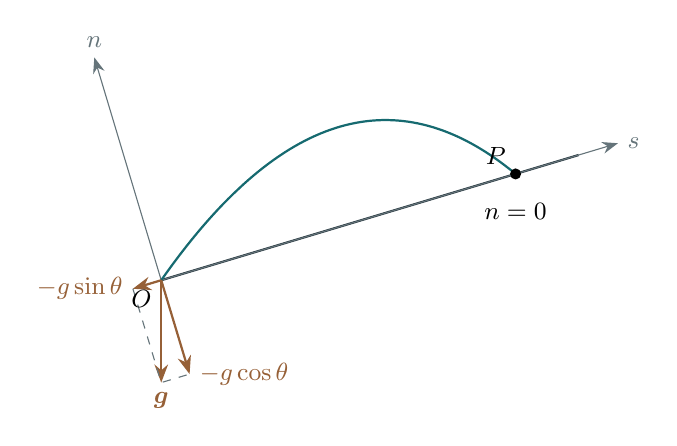
\begin{tikzpicture}

\draw[object] (0,0)--(5.3,1.59);
\draw[axis] (-.3,-.09)--(5.8,1.74) node[right] {$s$};
\draw[axis] (.09,-.3)--(-.85,2.83) node[above] {$n$};
\draw[traj,domain=0:4.5,samples=70] plot(\x,{(10/7)*\x-((10/7)-.3)*\x^2/4.5});
\fill (4.5,1.35) circle(2pt);\node[above left] at (4.5,1.35) {$P$};\node[below] at (4.5,1.10) {$n=0$};
\draw[force] (0,0)--(0,-1.3) node[below] {$\vect g$};
\draw[force] (0,0)--(-.36,-.108) node[left] {$-g\sin\theta$};
\draw[force] (0,0)--(.36,-1.192) node[right] {$-g\cos\theta$};
\draw[guide] (-.36,-.108)--(0,-1.3)--(.36,-1.192);
\node[below left] at (0,0) {$O$};

\end{tikzpicture}
\figcaption{解图 1.4B\quad 沿坡与垂直坡面建立坐标，飞行终点的条件变为 $n=0$。}
\end{minipage}\end{center}
\[
s=v_0\cos\alpha\,t-\frac12g\sin\theta\,t^2,
\qquad n=v_0\sin\alpha\,t-\frac12g\cos\theta\,t^2.
\]
由第二次 $n=0$ 得到同一 $t_f$；将它代入 $s$，展开后为
\[
R=\frac{2v_0^2\sin\alpha}{g\cos^2\theta}
(\cos\alpha\cos\theta-\sin\alpha\sin\theta),
\]
即上面的射程式。
\subsubsection*{求最优角}
用积化和差公式，
\[
2\sin\alpha\cos(\theta+\alpha)
=\sin(\theta+2\alpha)-\sin\theta.
\]
因而
\[
R(\alpha)=\frac{v_0^2}{g\cos^2\theta}
[\sin(\theta+2\alpha)-\sin\theta].
\]
在题设区间内，$\theta+2\alpha$ 可取 $\pi/2$；正弦的最大值为一，故
\[
\boxed{\alpha_*=\frac\pi4-\frac\theta2},\qquad
\boxed{R_{\max}=\frac{v_0^2(1-\sin\theta)}{g\cos^2\theta}
=\frac{v_0^2}{g(1+\sin\theta)}}.
\]
水平仰角则为 $\beta_* =\pi/4+\theta/2$。$\theta=0$ 时恢复水平地面的 $45^\circ$ 与 $v_0^2/g$；$\theta\to\pi/2^-$ 时沿坡最大射程趋于 $v_0^2/(2g)$，水平射程趋于零。
\subsubsection*{对落点横坐标求导的另一方法}
固定坡角时，解图1.4A中的$x_f$与沿坡射程$R$只相差正因子$\cos\theta$，
所以两者在同一发射角处取最大值。将第二交点写为
\[
x_f=\frac{v_0^2}{g}
\left[\sin2\beta-2\tan\theta\cos^2\beta\right],
\qquad \beta=\theta+\alpha,
\]
对$\alpha$求导时$\dd\beta/\dd\alpha=1$，从而
\[
\frac{\dd x_f}{\dd\alpha}
=\frac{2v_0^2}{g}
[\cos2\beta+\tan\theta\sin2\beta]
=\frac{2v_0^2}{g\cos\theta}\cos(2\beta-\theta).
\]
允许区间内的零点为$2\beta-\theta=\pi/2$，即
$\alpha=\pi/4-\theta/2$；从小仰角逐渐抬高炮口时，$x_f$先增加，越过这个角度后减小。
当$\alpha$趋近区间两端时，第二交点都回到炮口，射程趋于零，
这个内部驻点给出最大射程。求导还能说明从小仰角继续抬高时，落点怎样先远离炮口再返回。


\Needspace{18\baselineskip}

\pdfbookmark[3]{第 5 题 等射程抛体的飞行时间乘积}{c1-q5}

\section*{第 5 题\quad 等射程抛体的飞行时间乘积}\label{book-question-1-5}

\tagline{M-01-05}

两质点从同一水平地面上的同一点，以相同速率 $v_0$、不同仰角 $\alpha_1$ 和 $\alpha_2$ 抛出，且 $0<\alpha_1,\alpha_2<\pi/2$。两质点均落回该水平地面，空气阻力忽略。

若两次抛射的射程同为 $R$，证明两次飞行时间满足
\[
T_1T_2=\frac{2R}{g}.
\]

\begin{center}
\begin{tikzpicture}[x=1cm,y=1cm]
\draw[axis] (-.35,0)--(6.5,0) node[right] {$x$};\draw[axis] (0,-.2)--(0,3.5) node[above] {$y$};
\draw[traj,domain=0:6,samples=70] plot (\x,{1.73205*\x*(1-\x/6)});
\draw[traj,dashed,domain=0:6,samples=70] plot (\x,{.57735*\x*(1-\x/6)});
\draw[motion] (0,0)--(.6,1.039);\draw[motion] (0,0)--(1.039,.6);
\draw (.7,0) arc(0:30:.7);\node at (1,.22) {$\alpha_1$};
\draw (1.0,0) arc(0:60:1);\node at (1.05,1.05) {$\alpha_2$};
\node[color=accent] at (4.2,2.7) {高轨迹};\node[color=accent] at (4.5,.95) {低轨迹};
\fill (6,0) circle (1.8pt);\node[below] at (6,-.05) {$R$};\node[below left] at (0,0) {$O$};
\end{tikzpicture}
\figcaption{图 1.5\quad 同初速、同射程的两条不同轨迹。}
\end{center}

\Needspace{5\baselineskip}\subsection*{解答}

题图 1.5 的两条轨迹从同一点出发并落到同一水平地面。低角度轨迹的水平速度较大，高角度轨迹的竖直初速度较大；先由落地条件分别求时间和射程。
\subsubsection*{单次抛射的时间与射程}
对仰角为 $\alpha$ 的一次运动，
\[
x=v_0\cos\alpha\,t,\qquad
y=v_0\sin\alpha\,t-\frac12gt^2.
\]
落回地面时 $y=0$。舍去发射根 $t=0$ 后，
\[
T=\frac{2v_0\sin\alpha}{g},\qquad
R=v_0\cos\alpha\,T=\frac{v_0^2}{g}\sin2\alpha.
\]
\subsubsection*{等射程的两角互余}
初速相同、射程相同，故 $\sin2\alpha_1=\sin2\alpha_2$。将差化为乘积，
\[
2\cos(\alpha_1+\alpha_2)\sin(\alpha_1-\alpha_2)=0.
\]
两角均在 $(0,\pi/2)$ 且不同，所以 $\sin(\alpha_1-\alpha_2)\ne0$，只能有
\[
\boxed{\alpha_1+\alpha_2=\frac\pi2}.
\]
\begin{center}\begin{minipage}{\linewidth}\centering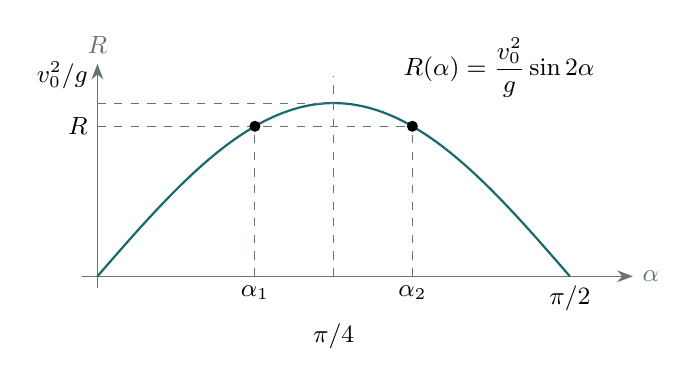
\begin{tikzpicture}

\draw[axis] (-.2,0)--(6.8,0) node[right] {$\alpha$};\draw[axis] (0,-.15)--(0,2.7) node[above] {$R$};
\draw[traj,domain=0:6,samples=90] plot(\x,{2.2*sin(30*\x)});
\draw[guide] (0,{2.2*sin(60)})--(4,{2.2*sin(60)});\node[left] at (0,{2.2*sin(60)}) {$R$};
\draw[guide] (0,2.2)--(3,2.2);\node[above left,yshift=1.5pt] at (0,2.2) {$v_0^2/g$};
\draw[guide] (2,0)--(2,{2.2*sin(60)});\draw[guide] (4,0)--(4,{2.2*sin(60)});
\fill (2,{2.2*sin(60)}) circle(2pt);\fill (4,{2.2*sin(60)}) circle(2pt);
\node[below] at (2,0) {$\alpha_1$};\node[below] at (4,0) {$\alpha_2$};\node[below] at (6,0) {$\pi/2$};
\draw[guide] (3,0)--(3,2.55);\node[below] at (3,-.48) {$\pi/4$};
\node at (5.1,2.65) {$R(\alpha)=\dfrac{v_0^2}{g}\sin2\alpha$};

\end{tikzpicture}
\figcaption{解图 1.5A\quad 射程曲线关于 $\alpha=\pi/4$ 对称；同一射程的两个不同仰角互余。}
\end{minipage}\end{center}
解图 1.5A 中，两条竖虚线从同一射程水平线落到横轴，读得一低一高的两个角。它们到 $45^\circ$ 的距离相同。射程升至 $v_0^2/g$ 时，两交点合为顶点，对应唯一的 $45^\circ$ 发射角。
\subsubsection*{求飞行时间乘积}
分别写出两次飞行时间并相乘，
\[
T_1T_2=\frac{4v_0^2}{g^2}\sin\alpha_1\sin\alpha_2
=\frac{4v_0^2}{g^2}\sin\alpha_1\cos\alpha_1
=\frac{2v_0^2}{g^2}\sin2\alpha_1.
\]
由 $R=v_0^2\sin2\alpha_1/g$，得到
\[
\boxed{T_1T_2=\frac{2R}{g}}.
\]
从时间式看，低角度的竖直初速度较小，所以先回到地面。两次飞行时间的乘积由共同射程确定。$R/g$ 的量纲是时间平方。等高落地使两次时间都等于各自竖直初速度的 $2/g$ 倍，互余角又让这两个竖直分量恰好等于一次发射里的水平、竖直分量。
\subsubsection*{共同对称轴与两个顶点的高度}
消去时间并使用落点 $x=R,y=0$，任一轨迹可改写为
\[
y=x\tan\alpha\left(1-\frac{x}{R}\right).
\]
最高点都在 $x=R/2$，高度为 $H_i=R\tan\alpha_i/4$。因为两角互余，$\tan\alpha_1\tan\alpha_2=1$，所以
\[
H_1H_2=\frac{R^2}{16}.
\]
题图 1.5 中，两个最高点沿 $x=R/2$ 竖直对齐。每个质点从最高点以零竖直速度下落，经过 $T_i/2$ 到达地面，因此 $H_i=gT_i^2/8$。这给出 $T_1T_2=(8/g)\sqrt{H_1H_2}=2R/g$。读出两顶点的高度，还可用 $T_2/T_1=\sqrt{H_2/H_1}$ 比较飞行时间。

\Needspace{18\baselineskip}

\pdfbookmark[3]{第 6 题 水枪越墙的最小初速}{c1-q6}

\section*{第 6 题\quad 水枪越墙的最小初速}\label{book-question-1-6}

\tagline{M-01-06}

地面上的水枪枪口视为质点，与竖直墙的水平距离为 $d=3.0\,\mathrm m$，墙高为 $h=4.0\,\mathrm m$。水流以速率 $v_0$、仰角 $\alpha$ 喷出，忽略空气阻力和水流宽度，取 $g=10\,\mathrm{m/s^2}$。

求使水流恰好通过墙顶的最小初速及相应仰角。

\begin{center}
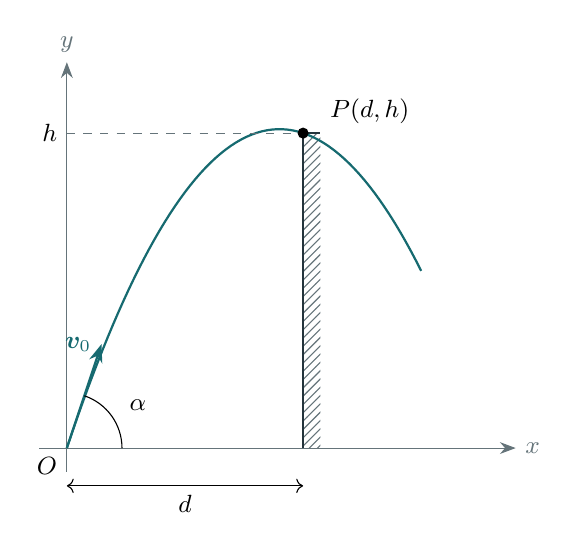
\begin{tikzpicture}[scale=1.0]
\draw[axis] (-.35,0)--(5.7,0) node[right] {$x$};\draw[axis] (0,-.3)--(0,4.9) node[above] {$y$};
\fill[pattern=north east lines,pattern color=muted] (3,0) rectangle (3.22,4);
\draw[object] (3,0)--(3,4)--(3.22,4);
\draw[traj,domain=0:4.5,samples=70] plot(\x,{3*\x-5*\x*\x/9});
\draw[motion] (0,0)--(.44,1.32) node[left] {$\vect v_0$};
\draw (.7,0) arc(0:71.565:.7);\node at (.9,.55) {$\alpha$};
\draw[guide] (0,4)--(3,4);\node[left] at (0,4) {$h$};
\draw[thin,<->] (0,-.48)--(3,-.48) node[midway,below] {$d$};
\fill (3,4) circle (2pt);\node[above right] at (3.22,4) {$P(d,h)$};\node[below left] at (0,0) {$O$};
\end{tikzpicture}
\figcaption{图 1.6\quad 枪口、墙顶与一条通过墙顶的轨迹。}
\end{center}

\Needspace{5\baselineskip}\subsection*{解答}

以枪口为原点，水平向墙为 $x$ 正向，竖直向上为 $y$ 正向。墙顶坐标为 $(d,h)$，解图 1.6A 中从枪口指向墙顶的直线与水平夹角记为 $\theta$，故 $\tan\theta=h/d$。
\begin{center}\begin{minipage}{\linewidth}\centering\begin{tikzpicture}

\draw[axis] (-.2,0)--(4.1,0) node[right] {$x$};\draw[axis] (0,-.2)--(0,4.6) node[above] {$y$};
\draw[object] (3,0)--(3,4);\fill (3,4) circle(2pt);\node[above right] at (3,4) {$P(d,h)$};
\draw[guide] (0,0)--(3,4) node[midway,above left,sloped] {$\sqrt{d^2+h^2}$};
\draw[motion] (0,0)--(.65,1.95) node[left] {$v_0$};
\draw (.68,0) arc(0:71.565:.68);\node at (.88,.7) {$\alpha$};
\draw (1.35,0) arc(0:53.13:1.35);\node at (1.55,.45) {$\theta$};
\draw[thin,<->] (0,-.55)--(3,-.55) node[midway,below] {$d$};
\draw[thin,<->] (3.45,0)--(3.45,4) node[midway,right] {$h$};
\node[align=left] at (6.45,2.8) {$\theta=\arctan(h/d)$\\$\alpha$：枪口仰角\\$\alpha>\theta$};

\end{tikzpicture}
\figcaption{解图 1.6A\quad $\theta$ 是墙顶的视线角，$\alpha$ 是发射角，$\alpha$沿枪口初速箭头量取。}
\end{minipage}\end{center}
\subsubsection*{通过墙顶的条件}
水流质点的轨迹为
\[
y=x\tan\alpha-\frac{gx^2}{2v_0^2\cos^2\alpha}.
\]
令 $x=d,y=h$，得
\[
v_0^2=\frac{gd^2}{2\cos^2\alpha(d\tan\alpha-h)}.
\]
式中 $v_0^2>0$ 给出 $\tan\alpha>h/d$。解图1.6A上，枪口切线在墙处的高度是 $d\tan\alpha$，抛物线比该高度低 $gd^2/(2v_0^2\cos^2\alpha)$。重力使轨迹低于枪口切线，所以切线在墙处的高度 $d\tan\alpha$ 高于 $h$，即 $\alpha>\theta$。
\subsubsection*{对发射角求最小初速}
记 $p=\tan\alpha>h/d$，则
\[
v_0^2(p)=\frac{gd^2}{2}\frac{1+p^2}{dp-h}.
\]
对 $p$ 求导，
\[
\frac{\dd v_0^2}{\dd p}
=\frac{gd^2}{2}\frac{2p(dp-h)-d(1+p^2)}{(dp-h)^2}
=\frac{gd^2}{2}\frac{dp^2-2hp-d}{(dp-h)^2}.
\]
驻点满足 $dp^2-2hp-d=0$。令 $s=\sqrt{d^2+h^2}$，两根为 $(h\pm s)/d$，只有正根符合发射角区间：
\[
p_* =\frac{h+s}{d}.
\]
$p\to h/d^+$ 或 $p\to\infty$ 时所需 $v_0^2$ 都趋于无穷；在允许区间仅有这个驻点，且导数由负变正，因此它给出全局最小值。代入后
\[
\boxed{v_{0,\min}^2=g(s+h)},\qquad
\boxed{\alpha_* =\arctan\frac{s+h}{d}
=\frac\pi4+\frac12\arctan\frac hd}.
\]
也可直接用视线角求极值。令 $\theta=\arctan(h/d)$，则 $d=s\cos\theta$、$h=s\sin\theta$。初速式的分母逐步变为
\[
\begin{aligned}
2\cos\alpha(d\sin\alpha-h\cos\alpha)
&=2s\cos\alpha\sin(\alpha-\theta)\\
&=s[\sin(2\alpha-\theta)-\sin\theta]\\
&=s\sin(2\alpha-\theta)-h.
\end{aligned}
\]
第二行来自积化和差，其中 $s\sin\theta=h$。整个分母随发射角变化，最大值为 $s-h$，因此
\[
v_0^2=\frac{gd^2}{s\sin(2\alpha-\theta)-h},
\]
分母在 $2\alpha-\theta=\pi/2$ 时最大，得到同一最优角。
\Needspace{0.46\textheight}
\subsubsection*{数值与墙顶处的运动状态}
本题 $s=5.0\,\mathrm m$，所以
\[
\boxed{v_{0,\min}=\sqrt{90}\approx9.49\,\mathrm{m/s},
\quad\alpha_* =\arctan3\approx71.57^\circ}.
\]
对应水平、竖直初速度分别为 $3.0$ 和 $9.0\,\mathrm{m/s}$。到墙时间 $t_d=d/v_{0x}=1.0\,\mathrm s$，此时
\[
y(t_d)=9.0\times1.0-5.0\times1.0^2=4.0\,\mathrm m,
\qquad v_y(t_d)=9.0-10\times1.0=-1.0\,\mathrm{m/s}.
\]
\begin{center}\begin{minipage}{\linewidth}\centering\begin{tikzpicture}

\draw[axis] (-.2,0)--(3.8,0) node[right] {$x/\mathrm m$};\draw[axis] (0,-.2)--(0,3.3) node[above] {$y/\mathrm m$};
\draw[traj,domain=2.2:3.3,samples=70] plot({3*(\x-2.2)},{9*(3*\x-5*\x*\x/9-3.8)});
\draw[object] (2.4,0)--(2.4,1.8);
\fill (1.5,2.25) circle(2pt);\node[above] at (1.5,2.25) {最高点 $Q$};
\fill (2.4,1.8) circle(2pt);\node[right] at (2.4,1.8) {墙顶 $P$};
\draw[guide] (1.5,0)--(1.5,2.25)--(0,2.25);\draw[guide] (0,1.8)--(2.4,1.8);
\node[below] at (1.5,0) {$2.7$};\node[below] at (2.4,0) {$3.0$};\node[left] at (0,2.25) {$4.05$};\node[left] at (0,1.8) {$4.00$};
\node[align=left] at (6.4,1.9) {最优轨迹到达墙顶时\\已经略向下运动。};

\end{tikzpicture}
\figcaption{解图 1.6B\quad 最小初速对应轨迹的局部放大图；横、纵方向使用不同显示比例。}
\end{minipage}\end{center}
因此水流经过墙顶时已经下降。最高点在 $t=0.90\,\mathrm s$，位置为 $(2.70,4.05)\,\mathrm m$，与解图 1.6B 的先后位置一致。一般最优轨迹在墙顶的斜率为 $-d/(s+h)<0$；墙顶的切线向右下方。解图1.6B中，从最高点到墙顶的水平距离是 $0.30\,\mathrm m$，高度下降 $0.05\,\mathrm m$，正对应这段飞行的 $0.10\,\mathrm s$。

\Needspace{18\baselineskip}

\pdfbookmark[3]{第 7 题 反弹平抛与公共越杆点}{c1-q7}

\section*{第 7 题\quad 反弹平抛与公共越杆点}\label{book-question-1-7}

\tagline{M-01-07}

两个小球从同一点 $S$ 水平抛出，$S$ 距水平地面高 $H$。水平初速分别为 $v_1>v_2>0$。球 1 恰好越过一根竖直杆的顶端，随后第一次落地于 $R$ 点，$OR=R$，其中 $O$ 为 $S$ 在地面的投影。

球 2 第一次落地后，与\textbf{光滑水平地面作完全弹性碰撞}，反弹后恰好越过同一杆顶，并在第二次落地时到达同一 $R$ 点。忽略空气阻力和小球大小。
\begin{enumerate}
\item 求 $v_1/v_2$；\item 求杆的位置 $x_P$；\item 求杆高 $h$。
\end{enumerate}

\begin{center}
\begin{tikzpicture}[x=1cm,y=1.25cm]
\draw[axis] (-.3,0)--(6.6,0) node[right] {$x$};\draw[axis] (0,-.2)--(0,2.75) node[above] {$y$};
\draw[traj,domain=0:6,samples=70] plot(\x,{2.4*(1-\x*\x/36)});
\draw[traj,dashed,domain=0:2,samples=45] plot(\x,{2.4*(1-\x*\x/4)});
\draw[traj,dashed,domain=2:6,samples=70] plot(\x,{2.4*(1-(\x-4)*(\x-4)/4)});
\draw[object,line width=1.3pt] (3,0)--(3,1.8);\fill (3,1.8) circle (1.8pt);
\node[above left] at (0,2.4) {$S$};\node[below left] at (0,0) {$O$};
\node[above left] at (3,1.8) {$P$};\node[below] at (3,0) {$x_P$};
\node[below] at (2,0) {$B$};\node[below] at (6,0) {$R$};
\node[color=accent] at (4.8,1.30) {球 1};\node[color=accent] at (4.4,2.6) {球 2};
\draw[thin,<->] (-.6,0)--(-.6,2.4) node[midway,left] {$H$};
\draw[thin,<->] (3.35,0)--(3.35,1.8) node[midway,right] {$h$};
\end{tikzpicture}
\figcaption{图 1.7\quad 实线为球 1；虚线为球 2；$B$ 为球 2 第一次落地点。}
\end{center}

\Needspace{5\baselineskip}\subsection*{解答}

记从高度 $H$ 自由下落到地面的时间为 $T_0=\sqrt{2H/g}$。两球都作平抛，第一次落地所需时间相同；光滑地面完全弹性反弹只使竖直速度反向，水平速度保持不变。
\begin{center}\begin{minipage}{\linewidth}\centering\begin{tikzpicture}

\begin{scope}
\draw[axis] (-.2,0)--(6.7,0) node[right] {$x$};
\draw[traj,domain=0:2,samples=35] plot(\x,{1.8*(1-\x*\x/4)});
\draw[traj,domain=2:6,samples=70] plot(\x,{1.8*(1-(\x-4)*(\x-4)/4)});
\fill (0,1.8) circle(2pt);\node[above] at (0,1.8) {$S$};\node[below] at (2,0) {$B$};\node[above] at (4,1.8) {$Q$};\node[below] at (6,0) {$R$};
\draw[guide] (0,1.8)--(4,1.8);\node[left] at (0,.9) {$H$};
\node at (1.0,.35) {$T_0$};\node at (3.0,.35) {$T_0$};\node at (5,.35) {$T_0$};
\draw[motion] (2,.15)--(2,.95) node[left] {$gT_0$};
\end{scope}
\begin{scope}[yshift=-1.4cm]
\draw[axis] (-.2,0)--(6.7,0) node[right] {$t$};
\foreach \x/\lab in {0/0,2/T_0,4/2T_0,6/3T_0}{\draw (\x,.08)--(\x,-.08);\node[below] at (\x,-.08) {$\lab$};}
\draw[thin,<->] (0,.4)--(2,.4) node[midway,above] {首次下落};
\draw[thin,<->] (2,.4)--(6,.4) node[midway,above] {反弹后的完整飞行};
\end{scope}

\end{tikzpicture}
\figcaption{解图 1.7A\quad 球 2 的竖直运动分成三段等长时间 $T_0$；光滑地面碰撞不改变水平速度。}
\end{minipage}\end{center}
\subsubsection*{先由时间轴求速度比}
按解图1.7A的时间轴，球 1 第一次落地于 $R$，所以 $R=v_1T_0$。球 2 第一次落地时的竖直速度为 $-gT_0$，反弹后变为 $+gT_0$。若反弹后时间记为 $s$，其高度为
\[
y_2(s)=gT_0 s-\frac12gs^2.
\]
除去 $s=0$，再次落地时间为 $s=2T_0$，因此球 2 从发射到第二次落地共用时 $3T_0$。由共同落点，
\[
R=3v_2T_0=v_1T_0,
\qquad\boxed{\frac{v_1}{v_2}=3}.
\]
这也给出第一次反弹位置 $B$ 为 $x_B=v_2T_0=R/3$。反弹后上升到最高点需 $T_0$，故最高点 $Q$ 的横坐标为 $2R/3$、高度为 $H$。
\subsubsection*{写出两段经过杆顶的轨迹}
球 1 的轨迹为
\[
y_1=H-\frac{gx^2}{2v_1^2}
=H\left(1-\frac{x^2}{R^2}\right),\quad0\leq x\leq R.
\]
球 2 的反弹前轨迹为 $H-gx^2/(2v_2^2)$；反弹后以 $(2R/3,H)$ 为顶点，所以
\[
y_2=H-\frac{g}{2v_2^2}\left(x-\frac{2R}{3}\right)^2
=H\left[1-9\left(\frac{x}{R}-\frac23\right)^2\right],
\quad\frac R3\leq x\leq R.
\]
解图 1.7B 中杆顶是球 1 的下落段与球 2 的反弹段的共同点。
\begin{center}\begin{minipage}{\linewidth}\centering\begin{tikzpicture}

\draw[axis] (-.25,0)--(6.6,0) node[right] {$x$};
\draw[axis] (0,-.25)--(0,3.1) node[above] {$y$};
\draw[traj,domain=0:6,samples=70] plot(\x,{2.4*(1-\x*\x/36)});
\draw[traj,dashed,domain=2:6,samples=70] plot(\x,{2.4*(1-(\x-4)*(\x-4)/4)});
\draw[object] (3,0)--(3,1.8);\fill (3,1.8) circle(2pt);\fill (6,0) circle(2pt);
\draw[guide] (0,1.8)--(3,1.8);\draw[guide] (0,2.4)--(4,2.4);
\node[left] at (0,2.4) {$H$};\node[left] at (0,1.8) {$h$};
\node[above left] at (3,1.8) {$P$};\node[below] at (3,0) {$x_P$};
\node[below] at (2,0) {$R/3$};\node[below] at (4,0) {$2R/3$};\node[below] at (6,0) {$R$};
\node at (1.3,2.72) {球 1};\node[above right] at (4.7,2.1) {球 2 反弹后};

\end{tikzpicture}
\figcaption{解图 1.7B\quad 两条轨迹在杆顶 $P$ 和公共落地点相交。地面交点的高度为零，正高度交点给出杆顶。}
\end{minipage}\end{center}
\subsubsection*{解交点并排除共同落地点}
令两高度相等，
\[
x^2=9\left(x-\frac{2R}{3}\right)^2
\quad\Longrightarrow\quad
\left[x-3\left(x-\frac{2R}{3}\right)\right]
\left[x+3\left(x-\frac{2R}{3}\right)\right]=0.
\]
解得 $x=R$ 或 $x=R/2$。解图1.7B 中，$x=R$ 对应两条轨迹在地面上的共同终点，$x=R/2$ 位于反弹点 $B$ 与反弹最高点 $Q$ 之间，交点高度为正，正是杆顶。因此
\[
\boxed{x_P=\frac R2},\qquad
h=y_1(R/2)=\boxed{\frac34H}.
\]
解图1.7B 的杆位于$x=R/2$。把这个横坐标分别除以两球的水平速度，可求出经过杆顶的时刻。球1在 $T_0/2$ 经过杆顶，竖直速度向下。球2在 $3T_0/2$ 经过同一位置，反弹已经持续 $T_0/2$，代入 $y_2(s)$ 也得 $3H/4$，此时竖直速度向上。因此同一杆顶在图上连着两条轨迹，在时间轴上对应两个时刻。

沿解图1.7A从 $S$ 读到 $B,Q,R$，每过 $T_0$ 就前进 $v_2T_0=R/3$。先在时间轴上定出三等分，再把它们投到两条轨迹共用的 $x$ 轴。
\subsubsection*{从反弹点直接建立第二条轨迹}
解图1.7A中$B=(R/3,0)$。反弹后的时间$s$从到达$B$时重新计起，
水平运动为$x=R/3+v_2s$，竖直运动为
$y=gT_0s-gs^2/2$。消去$s$得
\[
y= \frac{gT_0}{v_2}\left(x-\frac R3\right)
-\frac{g}{2v_2^2}\left(x-\frac R3\right)^2.
\]
由$v_2T_0=R/3$及$gT_0^2/2=H$，配方后正是
$y=H-g(x-2R/3)^2/(2v_2^2)$。
从反弹初值完成配方后，平方项中的 $2R/3$ 正是解图1.7B 的反弹对称轴。球2到达该轴时，反弹时间恰为 $T_0$。

球1与球2的首次落点分别为 $R$ 与 $R/3$，将它们代入各自的平抛方程，也可直接得到两水平速度：
\[
v_1^2=\frac{gR^2}{2H},\qquad
v_2^2=\frac{g(R/3)^2}{2H},\qquad
\frac{v_1}{v_2}=3.
\]
两个速度取正根是因为都沿$x$正向抛出。
求得$x_P=R/2$后，杆顶高度的代入为
$h=H-[g/(2v_1^2)](R/2)^2=H-H/4$。
球2的反弹轨迹定义在 $R/3\leq x\leq R$，两端分别对应碰撞后的 $s=0$ 与 $s=2T_0$。从发射点到 $R/3$ 的部分由最初的平抛方程给出。
杆顶位于$B,Q$之间，所以球2上升过杆，球1则在下降中经过杆顶。


\Needspace{18\baselineskip}

\pdfbookmark[3]{第 8 题 导弹追踪匀速上升飞行物}{c1-q8}

\section*{第 8 题\quad 导弹追踪匀速上升飞行物}\label{book-question-1-8}

\tagline{M-01-08}

飞行物从地面以速率 $v_f>0$ 匀速竖直上升。导弹从距其起飞点水平距离 $L$ 的地面点同时发射。导弹速率 $v$ 恒定，且 $v>v_f$；其瞬时速度方向始终指向飞行物的当前位置。

取导弹发射点为原点，水平朝向目标起飞点为 $x$ 轴，竖直向上为 $y$ 轴，记 $\gamma=v_f/v$。
\begin{enumerate}
\item 求导弹的轨迹 $y(x)$；\item 求击中时间及击中高度。
\end{enumerate}

\begin{center}
\begin{tikzpicture}[x=1cm,y=1cm]
\draw[axis] (-.3,0)--(6.1,0) node[right] {$x$};\draw[axis] (0,-.3)--(0,4.4) node[above] {$y$};
\draw[guide] (5,0)--(5,4.1);\node[below] at (5,0) {$L$};
\draw[traj,domain=0:.998,samples=120] plot({5*\x},{2.5*((1-pow(1-\x,.5))/.5-(1-pow(1-\x,1.5))/1.5)});
\coordinate (M) at (3,.592);\coordinate (F) at (5,1.541);
\draw[guide] (M)--(F);\draw[motion] (M)--(4,1.066) node[midway,above left] {$\vect v$};
\draw[motion] (F)--(5,2.34) node[right] {$v_f$};
\fill (M) circle(2pt);\fill (F) circle(2pt);
\node[below right] at (M) {$M(x,y)$};\node[right] at (F) {$F(L,v_ft)$};
\draw[guide] (3,0)--(M);\node[below] at (3,0) {$x$};
\node[below left] at (0,0) {$O$};\node[right,color=muted] at (5,3.7) {目标航线};
\end{tikzpicture}
\figcaption{图 1.8\quad 导弹轨迹的切线始终沿 $MF$；图中位置对应同一时刻。}
\end{center}

\Needspace{5\baselineskip}\subsection*{解答}

设导弹当前位置为 $(x,y)$，目标位于 $(L,y_f)$，其中 $y_f=v_ft$。导弹速度方向始终沿当前视线，故其轨迹切线也通过当前目标。用 $u=\dd y/\dd x$ 表示切线斜率，解图 1.8A 给出
\[
y_f-y=(L-x)u.
\]
\begin{center}\begin{minipage}{\linewidth}\centering\begin{tikzpicture}

\draw[axis] (-.2,0)--(5.8,0) node[right] {$x$};\draw[axis] (0,-.2)--(0,2.9) node[above] {$y$};
\draw[traj,domain=0:4.6,samples=100] plot(\x,{2.5*((1-pow(1-\x/5,.5))/.5-(1-pow(1-\x/5,1.5))/1.5)});
\coordinate (M) at (2.5,.387);\coordinate (Mp) at (3,.593);\coordinate (F) at (5,1.271);\coordinate (Fp) at (5,1.541);
\draw[guide] (M)--(F);\draw[guide] (Mp)--(Fp);\draw[guide] (5,0)--(5,2.7);
\fill (0,0) circle(1.5pt) node[below left] {$O$};
\fill (5,0) circle(1.5pt) node[below right] {$F_0$};
\fill (M) circle(1.6pt);\fill (Mp) circle(1.6pt);\fill (F) circle(1.6pt);\fill (Fp) circle(1.6pt);
\node[below left] at (M) {$M$};\node[above left] at (Mp) {$M'$};\node[below left] at (F) {$F$};\node[above left] at (Fp) {$F'$};
\draw[thin] (M)--(3,.387)--(Mp);\node[below] at (2.75,.387) {$\Delta x$};\node[right] at (3,.49) {$\Delta y$};
\draw[thin,<->] (5.45,1.271)--(5.45,1.541) node[right] {$v_f\Delta t$};
\draw[thin,<->] (2.5,-.55)--(5,-.55) node[midway,below] {$L-x$};
\node[align=left] at (8.0,2.55) {$u=\dd y/\dd x$\\$\dd s^2=\dd x^2+\dd y^2$\\切线沿目标连线};

\end{tikzpicture}
\figcaption{解图 1.8A\quad $M,F$ 对应时刻 $t$，$M^{\prime},F^{\prime}$ 对应 $t+\Delta t$。两条虚线分别给出各自时刻的速度方向。}
\end{minipage}\end{center}
\subsubsection*{由切线几何建立微分方程}
在 $x<L$ 时导弹速度的水平分量为正，可以用 $x$ 作自变量。对上式求导，其中 $y'=u$ 与乘积求导产生的 $-u$ 抵消：
\[
\frac{\dd y_f}{\dd x}=u-u+(L-x)\frac{\dd u}{\dd x}
=(L-x)\frac{\dd u}{\dd x}.
\]
解图 1.8A 中让 $\Delta t$ 趋于零，位移三角形给出路程微元 $\dd s=\sqrt{1+u^2}\dd x$。速率恒为 $v$，所以 $\dd s=v\dd t$。目标上升位移为 $\dd y_f=v_f\dd t$，所以
\[
\frac{\dd y_f}{\dd x}=\frac{v_f}{v}\sqrt{1+u^2}
=\gamma\sqrt{1+u^2}.
\]
由此得到
\[
(L-x)\frac{\dd u}{\dd x}=\gamma\sqrt{1+u^2},
\qquad0<\gamma<1.
\]
\subsubsection*{积分求斜率，再求轨迹}
初始视线水平，故 $u(0)=0$。分离变量并取定积分，
\[
\int_0^u\frac{\dd q}{\sqrt{1+q^2}}
=\gamma\int_0^x\frac{\dd\xi}{L-\xi},
\]
\[
\ln(u+\sqrt{1+u^2})=-\gamma\ln\left(1-\frac xL\right).
\]
令 $z=1-x/L$，并记 $A=z^{-\gamma}$。因为
\[
(\sqrt{1+u^2}+u)(\sqrt{1+u^2}-u)=1,
\]
有 $2u=A-A^{-1}$，所以
\[
u=\frac12(z^{-\gamma}-z^\gamma).
\]
再由 $y(0)=0$ 积分，使用 $\dd x=-L\dd z$，
\[
y(x)=\frac L2\int_z^1(q^{-\gamma}-q^\gamma)\dd q
=\frac L2\left[\frac{1-z^{1-\gamma}}{1-\gamma}
-\frac{1-z^{1+\gamma}}{1+\gamma}\right].
\]
也即
\[
\boxed{y(x)=\frac L2\left[
\frac{(1-x/L)^{1+\gamma}}{1+\gamma}
-\frac{(1-x/L)^{1-\gamma}}{1-\gamma}\right]
+\frac{\gamma L}{1-\gamma^2}},\quad0\leq x<L.
\]
\subsubsection*{相遇时刻与高度}
当 $x\to L^-$ 时，$z\to0^+$。两幂次均为正，故导弹高度趋于
\[
y_* =\frac{\gamma L}{1-\gamma^2}.
\]
在图1.8A 中，横向间隔为 $L-x$，纵向间隔由切线斜率 $u$ 乘这段横距得到。把刚求出的斜率代入，目标与导弹的竖直间隔为
\[
y_f-y=(L-x)u=\frac L2(z^{1-\gamma}-z^{1+\gamma})
\longrightarrow0.
\]
两坐标差都趋于零。再由 $\sqrt{1+u^2}=(z^{-\gamma}+z^\gamma)/2$，时间积分为
\[
t(x)=\frac L{2v}\left[
\frac{1-z^{1-\gamma}}{1-\gamma}
+\frac{1-z^{1+\gamma}}{1+\gamma}\right].
\]
$\gamma<1$ 保证该积分在 $z=0$ 收敛，因此
\[
\boxed{t_* =\frac L{v(1-\gamma^2)}
=\frac{Lv}{v^2-v_f^2}},\qquad
\boxed{y_* =v_ft_* =\frac{Lvv_f}{v^2-v_f^2}}.
\]
导弹总路程为 $vt_*=L/(1-\gamma^2)$。$v_f\to0$ 时轨迹退化为水平直线，$t_*\to L/v$；$v\to v_f^+$ 时击中时间和高度均无界增大。终点的斜率趋于无穷，表示导弹在命中前接近竖直上行，与图中的切线变化一致。
\subsubsection*{初始视线与积分常数}
解图1.8A中初始的$O,F_0$在同一水平线上，因此同时有$x=0,y=0,u=0$；
这三个条件分别确定水平起点、轨迹的平移常数和初始切线。
斜率积分也可写为
\[
\ln(u+\sqrt{1+u^2})=-\gamma\ln z+C_1,\qquad z=1-x/L.
\]
由初始$z=1,u=0$得$C_1=0$。
取指数后$u+\sqrt{1+u^2}=A=z^{-\gamma}>0$，
将根式移项再平方，得
\[
1+u^2=(A-u)^2=A^2-2Au+u^2,\qquad
u=\frac{A^2-1}{2A}.
\]
因为$0<z\leq1$，所得$u\geq0$，且$A-u=(A+A^{-1})/2>0$，
这个正值正是移项后的根式 $\sqrt{1+u^2}$，所以所得斜率与取指数前的方程相符。
轨迹若写成不定积分形式，常数由$y(0)=0$确定为
\[
C_2=-\frac L2\left(\frac1{1+\gamma}-\frac1{1-\gamma}\right)
=\frac{\gamma L}{1-\gamma^2}.
\]
将 $z=1$ 代入轨迹时，两个幂次项与 $C_2$ 抵消，正好得到发射点高度 $y(0)=0$。

\subsubsection*{用相对距离独立求命中时间}
仍按解图1.8A，记导弹到目标的水平、竖直间隔为
$X=L-x$、$Y=y_f-y$，实际间距为$\rho=\sqrt{X^2+Y^2}$。
设当前视线与$x$轴夹角为$\psi$，则
$X=\rho\cos\psi$、$Y=\rho\sin\psi$。
导弹沿视线以速率$v$运动，目标竖直向上运动，所以
\[
\dot X=-v\cos\psi,\qquad
\dot Y=v_f-v\sin\psi,\qquad
\dot\rho=\frac{X\dot X+Y\dot Y}{\rho}
=-v+v_f\sin\psi.
\]
目标的竖直速度在视线上作投影，才产生最后一式的$v_f\sin\psi$。
将最后两式按$\gamma=v_f/v$组合，视线角消去：
\[
\frac{\dd}{\dd t}(\rho+\gamma Y)
=-v(1-\gamma^2),\qquad
\rho+\gamma Y=L-v(1-\gamma^2)t.
\]
开始时 $\rho=L,Y=0$；当 $Y=0$ 且 $X>0$ 时，$\dot Y=v_f>0$，因此命中前 $Y\geq0$。又有 $Y\leq\rho$，所以
\[
\frac{L-v(1-\gamma^2)t}{1+\gamma}\leq\rho\leq L-v(1-\gamma^2)t.
\]
两条直线随时间减小，在 $t_*=L/[v(1-\gamma^2)]$ 同时达到零。图1.8A 中的视线长度 $\rho$ 随之降至零，说明导弹与目标在该时刻到达同一位置。此法直接给命中时间，前面的切线积分还给出沿途的轨迹。


\Needspace{18\baselineskip}

\pdfbookmark[3]{第 9 题 圆柱解线与渐开线轨迹}{c1-q9}

\section*{第 9 题\quad 圆柱解线与渐开线轨迹}\label{book-question-1-9}

\tagline{M-01-09}

半径为 $r$ 的圆柱固定不动，轴线竖直。一条很轻、柔软、不可伸长的细线在同一水平面内缠绕于圆柱，线末端系一个可视为质点的小球。初始时小球位于圆柱表面的 $A$ 点，外露直线段长度为零。

给小球一个沿水平方向、垂直于圆柱表面并向外的瞬时冲量，使其初速为 $v$。此后细线无滑动地解开，保持绷紧；忽略重力及其他作用力，并假设缠绕线长足够。
\begin{enumerate}
\item 求 $t>0$ 时小球的加速度大小与方向；
\item 以圆心为原点、$OA$ 为 $x$ 轴正方向，求小球的参数轨迹方程。
\end{enumerate}

\begin{center}
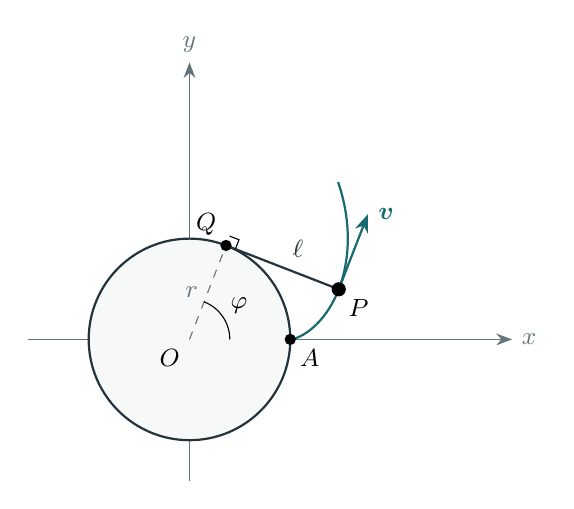
\begin{tikzpicture}[scale=1.28]
\draw[axis] (-1.6,0)--(3.2,0) node[right] {$x$};\draw[axis] (0,-1.4)--(0,2.75) node[above] {$y$};
\draw[object,fill=rulegray!18] (0,0) circle (1);
\draw[traj,domain=0:1.9,samples=90] plot({cos(\x r)+\x*sin(\x r)},{sin(\x r)-\x*cos(\x r)});
\coordinate (Q) at ({cos(1.2 r)},{sin(1.2 r)});
\coordinate (P) at ({cos(1.2 r)+1.2*sin(1.2 r)},{sin(1.2 r)-1.2*cos(1.2 r)});
\draw[object] (Q)--(P) node[midway,above right] {$\ell$};
\draw[guide] (0,0)--(Q) node[midway,left] {$r$};
\draw[motion] (P)--($(P)+(.29,.746)$) node[right] {$\vect v$};
\fill (Q) circle(1.6pt);\fill (P) circle(2pt);\fill (1,0) circle(1.6pt);
\node[above left] at (Q) {$Q$};\node[below right] at (P) {$P$};\node[below right] at (1,0) {$A$};\node[below left] at (0,0) {$O$};
\draw (.4,0) arc(0:68.755:.4);\node at (.49,.34) {$\varphi$};
\draw[thin] ($(Q)+(.093,-.036)$)--($(Q)+(.129,.057)$)--($(Q)+(.036,.093)$);
\end{tikzpicture}
\figcaption{图 1.9\quad $Q$ 为瞬时切点，$QP$ 为解开的直线段；图中选取逆时针展开支。}
\end{center}

\Needspace{5\baselineskip}\subsection*{解答}

设当前切点为 $Q$，小球为 $P$，外露绷直线段长度为 $\ell$。以圆心为原点，初始接触半径为 $x$ 轴正向；选取解线方向使切点沿圆周逆时针移动，转角记为 $\varphi$。另一侧解线得到镜像轨迹。
\begin{center}\begin{minipage}{\linewidth}\centering\begin{tikzpicture}

\draw[object] (0,0) circle(1);\node[below left] at (0,0) {$O$};
\coordinate (Q) at ({cos(1 r)},{sin(1 r)});\coordinate (P) at ({cos(1 r)+sin(1 r)},{sin(1 r)-cos(1 r)});
\draw[guide] (0,0)--(Q) node[midway,left] {$r$};\draw[object] (Q)--(P) node[midway,below] {$\ell$};
\draw[motion] (P)--($(P)+(.54,.84)$) node[right] {$\vect v$};
\draw[force] (P)--($(P)+(-.67,.43)$) node[midway,above] {$\vect a$};
\fill (Q) circle(1.8pt);\fill (P) circle(2pt);\node[above left] at (Q) {$Q$};\node[below right] at (P) {$P$};
\draw (.35,0) arc(0:57.296:.35);\node at (.57,.29) {$\varphi$};
\node[align=left] at (5.2,1.0) {$\vect v\perp QP$，张力不做功\\曲率半径为 $\ell$\\$a=v^2/\ell$，指向 $Q$};

\end{tikzpicture}
\figcaption{解图 1.9A\quad 张力改变速度方向；图中绳段长度 $\ell$ 决定法向加速度。}
\end{minipage}\end{center}
\subsubsection*{无滑动约束与速率不变}
解图 1.9A 中，圆柱上少缠绕的弧长等于新增外露线长，故
\[
\ell=r\varphi,\qquad\dd\ell=r\dd\varphi.
\]
令 $\vect e_r=(\cos\varphi,\sin\varphi)$、$\vect e_\varphi=(-\sin\varphi,\cos\varphi)$，则
\[
\vect{OQ}=r\vect e_r,\qquad
\vect{QP}=-\ell\vect e_\varphi,
\quad\vect{OP}=r\vect e_r-r\varphi\vect e_\varphi.
\]
利用 $\dd\vect e_r/\dd\varphi=\vect e_\varphi$、$\dd\vect e_\varphi/\dd\varphi=-\vect e_r$，对位置求导，
\[
\frac{\dd\vect{OP}}{\dd\varphi}
=r\vect e_\varphi-r\vect e_\varphi+r\varphi\vect e_r
=\ell\vect e_r.
\]
所以小球速度垂直于直线段 $QP$。张力沿 $PQ$，始终与速度垂直，不做功，因而小球速率恒为初速 $v$。$Q$ 是当前小球位置的曲率中心，随后沿圆柱移动。
\subsubsection*{线长、转角与时间}
由位置微分的长度，$\dd s=\ell\dd\varphi$。又 $\dd s=v\dd t$，因此
\[
v\dd t=\ell\dd\varphi=\frac{\ell}{r}\dd\ell.
\]
从 $\ell=0,t=0$ 积分，
\[
\frac{\ell^2}{2}=rvt,
\qquad\boxed{\ell(t)=\sqrt{2rvt}},\qquad
\boxed{\varphi(t)=\sqrt{\frac{2vt}{r}}}.
\]
\subsubsection*{加速度大小、方向与曲率}
速度矢量为 $\vect v=v\vect e_r$。对时间求导，
\[
\vect a=v\dot\varphi\vect e_\varphi
=\frac{v^2}{\ell}\vect e_\varphi.
\]
而 $\vect{PQ}=\ell\vect e_\varphi$，所以加速度由小球指向当前切点。其大小为
\[
\boxed{a(t)=\frac{v^2}{\sqrt{2rvt}}
=\frac{v^{3/2}}{\sqrt{2rt}}},\qquad t>0.
\]
轨迹切线方向转过 $\dd\varphi$ 时走过弧长 $\dd s=\ell\dd\varphi$，故曲率半径 $\rho_c=\dd s/\dd\varphi=\ell$，与 $a=v^2/\rho_c$ 一致。
\begin{center}\begin{minipage}{\linewidth}\centering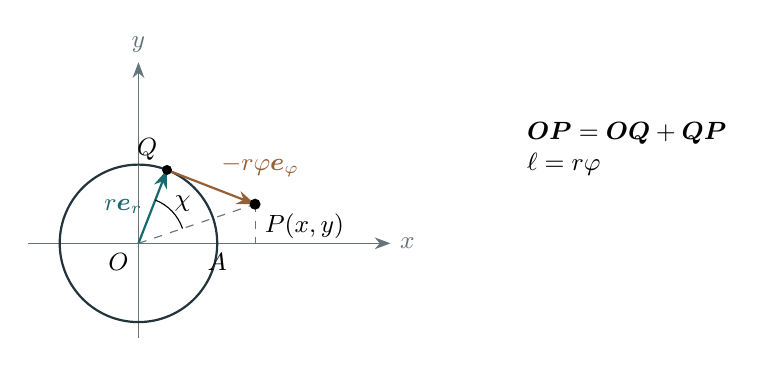
\begin{tikzpicture}

\draw[axis] (-1.4,0)--(3.2,0) node[right] {$x$};\draw[axis] (0,-1.2)--(0,2.3) node[above] {$y$};
\draw[object] (0,0) circle(1);
\coordinate (Q) at ({cos(1.2 r)},{sin(1.2 r)});\coordinate (P) at ({cos(1.2 r)+1.2*sin(1.2 r)},{sin(1.2 r)-1.2*cos(1.2 r)});
\draw[motion] (0,0)--(Q) node[midway,left] {$r\vect e_r$};
\draw[force] (Q)--(P) node[midway,above right] {$-r\varphi\vect e_\varphi$};
\draw[guide] (0,0)--(P);\draw[guide] (P)--({cos(1.2 r)+1.2*sin(1.2 r)},0);
\draw[thin] ({.59*cos(18.560)},{.59*sin(18.560)}) arc[start angle=18.560,end angle=68.755,radius=.59];
\node at (.56,.51) {$\chi$};
\fill (Q) circle(1.8pt);\fill (P) circle(2pt);\node[above left] at (Q) {$Q$};\node[below right] at (P) {$P(x,y)$};
\node[below left] at (0,0) {$O$};\node[below] at (1,0) {$A$};
\node[align=left] at (6.2,1.2) {$\vect{OP}=\vect{OQ}+\vect{QP}$\\$\ell=r\varphi$};

\end{tikzpicture}
\figcaption{解图 1.9B\quad 小球位置由半径矢量与展开绳段矢量相加得到；两矢量互相垂直。}
\end{minipage}\end{center}
\subsubsection*{展开位置得到参数轨迹}
将两基矢分量代入 $\vect{OP}$，
\[
\boxed{\begin{aligned}
x&=r(\cos\varphi+\varphi\sin\varphi),\\
y&=r(\sin\varphi-\varphi\cos\varphi),
\end{aligned}\qquad\varphi=\sqrt{\frac{2vt}{r}}}.
\]
解图 1.9B 中，切点到小球的连线沿圆柱切线，随切点移动形成圆的渐开线。斜边 $|\vect{OP}|=r\sqrt{1+\varphi^2}$ 给小球到圆心的距离，直角边 $QP=\ell$ 则是该点的曲率半径。

当 $t\to0^+$ 时 $\ell\to0$、$a\to\infty$；初始零外露线长使理想约束在起点产生奇点，所以加速度公式只在 $t>0$ 使用。位置与速度有有限的右极限：$P\to(r,0)$、$\vect v\to(v,0)$，符合题设的向外初速度。若可解开的总长为$\ell_{\max}$，这段运动在$\ell(t)=\ell_{\max}$时结束。
\subsubsection*{用直角三角形展开轨迹的另一方法}
解图1.9B中$OQ\perp QP$。设$\rho=OP$，
并以$\chi$表示$OQ$与$OP$的夹角，则直角三角形给出
\[
\rho=\sqrt{r^2+\ell^2}=r\sqrt{1+\varphi^2},\qquad
\cos\chi=\frac r\rho,\quad \sin\chi=\frac{\ell}{\rho}.
\]
当前$OP$相对于$x$轴的角度为$\varphi-\chi$，故
\[
\begin{aligned}
x&=\rho\cos(\varphi-\chi)
=r\cos\varphi+\ell\sin\varphi,\\
y&=\rho\sin(\varphi-\chi)
=r\sin\varphi-\ell\cos\varphi.
\end{aligned}
\]
将$\ell=r\varphi$代入两个投影式，所得$x$、$y$就是解图1.9B所示的渐开线坐标。
这里$\rho=OP$用于投影求坐标，$\ell=QP$由$\dd s/\dd\varphi$进入法向加速度。
速率恒定还意味着$\dd\vect v$只表示方向变化：
$|\dd\vect v|=v\,\dd\varphi$，因而
$a=v\dot\varphi=v\dot\ell/r$；
由$\dot\ell=\sqrt{rv/(2t)}$同样得到前面的法向加速度。


\Needspace{18\baselineskip}

\pdfbookmark[3]{第 10 题 旋转杆上小环的阿基米德螺线}{c1-q10}

\section*{第 10 题\quad 旋转杆上小环的阿基米德螺线}\label{book-question-1-10}

\tagline{M-01-10}

一根足够长的细杆在固定平面内绕端点 $O$ 以恒定角速度 $\omega>0$ 逆时针旋转。小环可看作质点，沿杆向外的相对速率恒为 $v>0$。设 $t=0$ 时小环位于 $O$，杆沿 $x$ 轴正方向。
\begin{enumerate}
\item 证明小环轨迹为阿基米德螺线；
\item 求任意时刻的速度、加速度向量及其大小；
\item 定性画出加速度在轨迹切向与法向的分量，并说明各自作用。
\end{enumerate}

\begin{center}
\begin{minipage}{\linewidth}\centering
\begin{tikzpicture}[scale=1.1]
\draw[axis] (-2.1,0)--(3.3,0) node[right] {$x$};\draw[axis] (0,-1.9)--(0,3.3) node[above] {$y$};
\draw[traj,domain=0:5.4,samples=120] plot({.45*\x*cos(\x r)},{.45*\x*sin(\x r)});
\coordinate (P) at ({.45*1.1*cos(1.1 r)},{.45*1.1*sin(1.1 r)});
\draw[object,line width=1.2pt] (0,0)--({2.9*cos(1.1 r)},{2.9*sin(1.1 r)});
\filldraw[fill=white,draw=ink,thick] (P) circle(2.4pt);\node[right] at (P) {$P$};
\draw[motion] (.48,.94)--(.94,1.85) node[right] {$v\vect e_r$};
\draw (.34,0) arc(0:63.025:.34);\node at (.65,.2) {$\varphi$};
\draw[motion] (.8,-.45) arc(-29:22:.92);\node[right] at (.98,-.3) {$\omega$};
\node[below left] at (0,0) {$O$};\node[color=muted] at (2.35,2.5) {转动杆};
\end{tikzpicture}
\figcaption{图 1.10\quad 小环沿杆向外运动，同时随杆转动；箭头 $v\vect e_r$ 表示相对速度。}
\end{minipage}
\end{center}

\Needspace{5\baselineskip}\subsection*{解答}

取逆时针角度为正。小环沿杆向外的相对速率为 $v$，故 $r=vt$；杆匀角速转动，故 $\varphi=\omega t$。题图 1.10 中每转过相同角度，小环的半径增加相同量。
\subsubsection*{轨迹与极坐标基矢}
消去时间，
\[
\boxed{r=\frac v\omega\varphi},\qquad \varphi\geq0,
\]
这是阿基米德螺线。直角坐标参数式为
\[
x=vt\cos\omega t,\qquad y=vt\sin\omega t.
\]
令 $\vect e_r=(\cos\varphi,\sin\varphi)$、$\vect e_\varphi=(-\sin\varphi,\cos\varphi)$。这些基矢随杆转动，满足
\[
\dot{\vect e}_r=\omega\vect e_\varphi,\qquad
\dot{\vect e}_\varphi=-\omega\vect e_r.
\]
\subsubsection*{速度与加速度矢量}
对位置 $\vect r=r\vect e_r$ 求导，
\[
\vect V=\dot r\vect e_r+r\omega\vect e_\varphi
=\boxed{v\vect e_r+v\omega t\vect e_\varphi}.
\]
前一项是沿杆相对速度，后一项是随杆转动的牵连速度。再求导，
\[
\vect a=v\omega\vect e_\varphi
+v\omega\vect e_\varphi-v\omega^2t\vect e_r
=\boxed{-v\omega^2t\vect e_r+2v\omega\vect e_\varphi}.
\]
径向速度 $v\vect e_r$ 的方向随杆转动，求导给出第一个 $v\omega\vect e_\varphi$。牵连速度的大小 $r\omega$ 随半径增加，求导给出第二个同向分量；其方向转动则给出 $-r\omega^2\vect e_r$。解图1.10A 左图画速度的两个箭头，右图画由这三项合成的加速度。
\begin{center}\begin{minipage}{\linewidth}\centering\begin{tikzpicture}

\begin{scope}
\draw[axis] (-.3,0)--(3,0) node[right] {$\vect e_r$};\draw[axis] (0,-.2)--(0,3) node[above] {$\vect e_\varphi$};
\draw[motion] (0,0)--(1.7,0) node[midway,below] {$v$};\draw[motion] (0,0)--(0,1.7) node[midway,left] {$r\omega$};
\draw[force] (0,0)--(1.7,1.7) node[above right] {$\vect V$};\draw[guide] (1.7,0)--(1.7,1.7)--(0,1.7);
\node[below left] at (0,0) {$P$};\node at (1.2,3.35) {绝对速度};
\end{scope}
\begin{scope}[xshift=6.5cm]
\draw[axis] (-2.1,0)--(2,0) node[right] {$\vect e_r$};\draw[axis] (0,-.2)--(0,3) node[above] {$\vect e_\varphi$};
\draw[motion] (0,0)--(-1.1,0) node[midway,below] {$-r\omega^2$};\draw[motion] (0,0)--(0,2.2) node[midway,right] {$2v\omega$};
\draw[force] (0,0)--(-1.1,2.2) node[above left] {$\vect a$};\draw[guide] (-1.1,0)--(-1.1,2.2)--(0,2.2);
\node[below left] at (0,0) {$P$};\node at (-.3,3.35) {极坐标加速度};
\end{scope}

\end{tikzpicture}
\figcaption{解图 1.10A\quad 在 $\omega t=1$ 时示意矢量分解。左图沿轨迹切线的总速度包含径向与横向分量。}
\end{minipage}\end{center}
两正交分量平方相加得
\[
\boxed{V=v\sqrt{1+\omega^2t^2}},\qquad
\boxed{a=v\omega\sqrt{4+\omega^2t^2}}.
\]
直角坐标中的矢量可写为
\[
\begin{aligned}
\vect V={}&v(\cos\omega t-\omega t\sin\omega t)\vect e_x
+v(\sin\omega t+\omega t\cos\omega t)\vect e_y,\\
\vect a={}&(-v\omega^2t\cos\omega t-2v\omega\sin\omega t)\vect e_x\\
&+(-v\omega^2t\sin\omega t+2v\omega\cos\omega t)\vect e_y.
\end{aligned}
\]
在直角坐标中，$v t$ 和三角函数分别求导。一次求导得到速度，再求导时两次出现 $v\omega$，它们与解图1.10A 中的两个横向贡献一一对应。
\subsubsection*{自然坐标中的切向与法向分量}
记 $s=\omega t$。轨迹切向单位矢量和朝曲率中心的法向单位矢量为
\[
\vect e_\tau=\frac{\vect e_r+s\vect e_\varphi}{\sqrt{1+s^2}},\qquad
\vect e_n=\frac{-s\vect e_r+\vect e_\varphi}{\sqrt{1+s^2}}.
\]
\begin{center}\begin{minipage}{\linewidth}\centering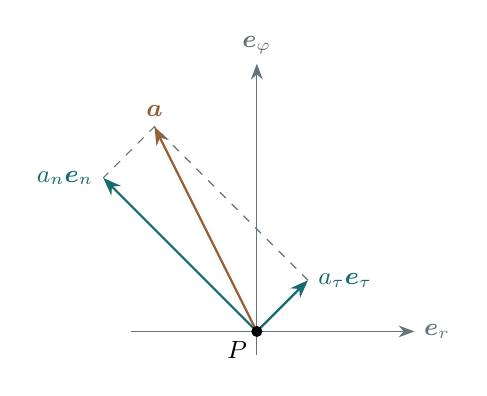
\begin{tikzpicture}

\coordinate (P) at (0,0);\coordinate (T) at (.65,.65);\coordinate (N) at (-1.95,1.95);
\draw[axis] (-1.6,0)--(2,0) node[right] {$\vect e_r$};\draw[axis] (0,-.3)--(0,3.4) node[above] {$\vect e_\varphi$};
\draw[motion] (P)--(T) node[right] {$a_\tau\vect e_\tau$};\draw[motion] (P)--(N) node[left] {$a_n\vect e_n$};
\draw[force] (P)--(-1.3,2.6) node[above] {$\vect a$};\draw[guide] (T)--(-1.3,2.6)--(N);
\fill (P) circle(2pt);\node[below left] at (P) {$P$};

\end{tikzpicture}
\figcaption{解图 1.10B\quad 在 $\omega t=1$ 时，把同一加速度改按轨迹切向、法向分解。切向改变速率，法向改变速度方向。}
\end{minipage}\end{center}
解图 1.10B 将同一加速度按轨迹切向、法向分解。投影到这两方向，或对速率求导，得到
\[
\boxed{a_\tau=\frac{\dd V}{\dd t}
=\frac{v\omega^2t}{\sqrt{1+\omega^2t^2}}},\qquad
\boxed{a_n=\frac{v\omega(2+\omega^2t^2)}{\sqrt{1+\omega^2t^2}}}.
\]
切向分量改变速率，法向分量使速度转向曲率中心。解图1.10B 的切线沿总速度，与杆有夹角。径向加速度沿杆向内，横向加速度沿转动方向；把两者投到切线上相加，所得 $a_\tau$ 在 $t>0$ 时为正，因而地面系速率增加。

在 $t=0$，$V=v$、$a_\tau=0$、$a_n=2v\omega$，加速度完全法向；此后速率增大，$a_\tau>0$。曲率半径为
\[
\rho_c=\frac{V^2}{a_n}
=\frac v\omega\frac{(1+\omega^2t^2)^{3/2}}{2+\omega^2t^2}.
\]
当 $\omega\to0$ 而 $t$ 固定时，速度趋于沿杆的 $v$，加速度趋于零，恢复直线匀速运动。
\subsubsection*{螺线的切线与曲率圆}
解图1.10A中的径向沿杆，而小环对地速度一般斜向杆的前侧。
解图1.10C把这两种方向放回轨迹，虚线圆在$P$处与螺线相切，
其圆心位于$P+\rho_c\vect e_n$。
切向单位矢量沿$\vect V$，法向单位矢量指向该圆心；
径向单位矢量则沿 $OP$，它与切向单位矢量的夹角满足 $\tan\angle(\vect e_r,\vect e_\tau)=s$。
\begin{center}\begin{minipage}{\linewidth}\centering
\begin{tikzpicture}
\coordinate (P) at (.5403,.8415);
\coordinate (K) at (-.3809,.6407);
\draw[axis] (-1.65,0)--(2.05,0) node[right] {$x$};
\draw[axis] (0,-.5)--(0,2.5) node[above] {$y$};
\draw[traj,domain=0:2,samples=100] plot({\x*cos(\x r)},{\x*sin(\x r)});
\draw[guide] (K) circle(.9428);
\draw[thin] (0,0)--(P);
\draw[force] (P)--(.8645,1.3464) node[right] {$\vect e_r$};
\draw[motion] (P)--(.391,1.526) node[above right] {$\vect e_\tau$};
\draw[motion] (P)--(-.144,.692) node[below left] {$\vect e_n$};
\fill (P) circle(1.8pt); \fill (K) circle(1.5pt);
\node[above right] at (P) {$P$}; \node[left] at (K) {$K$};
\node[below right] at (0,0) {$O$};
\node[align=left] at (5.4,1.25)
{$\omega t=1$，长度以$v/\omega$为单位\\
$PK=\rho_c=2\sqrt2/3$\\
虚线圆与轨迹在$P$处相切};
\end{tikzpicture}
\figcaption{解图1.10C\quad 螺线上的运动点与瞬时曲率圆；$K$是当前曲率中心。}
\end{minipage}\end{center}
例如$\omega t=1$时，
$\vect e_\tau=(\vect e_r+\vect e_\varphi)/\sqrt2$，
$\vect e_n=(-\vect e_r+\vect e_\varphi)/\sqrt2$。
将$\vect a=-v\omega\vect e_r+2v\omega\vect e_\varphi$分别点乘，
得到$a_\tau=v\omega/\sqrt2$、$a_n=3v\omega/\sqrt2$；
平方和仍为$5v^2\omega^2$，对应极坐标计算的同一个加速度大小。


\Needspace{18\baselineskip}

\pdfbookmark[3]{第 11 题 相对运动中的最短距离}{c1-q11}

\section*{第 11 题\quad 相对运动中的最短距离}\label{book-question-1-11}

\tagline{M-01-11}

质点甲、乙同时从 $A,B$ 出发，初始距离 $AB=\ell$。甲以速率 $v_1>0$ 沿 $AB$ 向右运动；乙以速率 $v_2>0$ 沿射线 $BC$ 运动。定义 $\alpha=\angle ABC$，即 $BA$ 与 $BC$ 的夹角，$0<\alpha<\pi$。两质点均作匀速直线运动，求出发以后（$t\geq0$）的最短距离。

\begin{center}\begin{minipage}{\linewidth}\centering\begin{tikzpicture}

\coordinate (A) at (0,0);\coordinate (B) at (5,0);\coordinate (C) at (2,2.25);
\draw[object] (A)--(B);\draw[guide] (B)--(C);
\fill (A) circle(2pt);\fill (B) circle(2pt);
\node[below] at (A) {$A$（甲）};\node[below right] at (B) {$B$（乙）};\node[above left] at (C) {$C$};
\draw[motion] (A)--(1.6,0) node[midway,above] {$v_1$};
\draw[motion] (B)--(3.4,1.2) node[midway,above right] {$v_2$};
\draw (4.2,0) arc(180:143.13:.8);\node at (4.05,.32) {$\alpha$};
\draw[thin,<->] (0,-.7)--(5,-.7) node[midway,below] {$\ell$};

\end{tikzpicture}
\figcaption{图 1.11\quad 角 $\alpha$ 从向左的射线 $BA$ 量起。图示为锐角情形。}
\end{minipage}\end{center}

\Needspace{5\baselineskip}\subsection*{解答}

取 $A$ 为初始原点，$AB$ 为 $x$ 轴正向，向上为 $y$ 正向。题图1.11 中 $\alpha$ 从向左的 $BA$ 量起。乙的速度与$x$正向夹角为$\pi-\alpha$，投影到$x,y$轴后得到
\[
\vect v_1=(v_1,0),\qquad
\vect v_2=(-v_2\cos\alpha,v_2\sin\alpha).
\]
\subsubsection*{转到随甲平移的参考系}
乙相对甲的速度为
\[
\vect w=\vect v_2-\vect v_1=(-p,q),\qquad
p=v_1+v_2\cos\alpha,\quad q=v_2\sin\alpha>0.
\]
在随甲平移的系中，甲固定于原点，乙的相对位置为
\[
\vect r(t)=(\ell-pt,qt),\qquad t\geq0.
\]
解图 1.11A 中乙沿相对速度确定的射线运动，求距离等价于求这条射线到原点的最近距离。
\begin{center}\begin{minipage}{\linewidth}\centering\begin{tikzpicture}

\coordinate (O) at (0,0);\coordinate (B) at (4,0);\coordinate (Q) at (.721,1.537);
\draw[axis] (-.4,0)--(4.7,0) node[right] {$x$};
\draw[traj] (B)--(-1.12,2.4);\draw[motion] (3.36,.3)--(2.08,.9) node[midway,above right] {$\vect w$};
\draw[object] (O)--(Q);\draw[guide] (O)--(B);
\pic[draw,angle radius=2.5mm] {right angle=O--Q--B};
\fill (O) circle(2pt);\fill (B) circle(2pt);\fill (Q) circle(2pt);
\node[below left] at (O) {甲};\node[below] at (B) {$B_0$};\node[above right] at (Q) {$Q$};
\node[left] at (.35,.8) {$r_{\min}$};
\node[align=left] at (7,1.7) {$\vect r(t)= (\ell-pt,qt)$\\垂足只有在未来的运动射线上\\才对应 $t\geq0$ 的最短距离。};

\end{tikzpicture}
\figcaption{解图 1.11A\quad 相对轨迹与最短距离。图中 $p>0$，垂足位于出发后的射线上。}
\end{minipage}\end{center}
\subsubsection*{在出发后的时段求距离最小值}
两质点距离平方为
\[
r^2(t)=(\ell-pt)^2+q^2t^2
=(p^2+q^2)t^2-2\ell pt+\ell^2.
\]
由于 $p^2+q^2>0$，配方得到
\[
r^2(t)=(p^2+q^2)\left(t-\frac{\ell p}{p^2+q^2}\right)^2
+\frac{\ell^2q^2}{p^2+q^2}.
\]
二次式顶点的横坐标为 $t_0=\ell p/(p^2+q^2)$，它对应直线上的垂足。实际运动从 $t=0$ 开始，须在半轴 $t\geq0$ 上选出使平方项最小的时间。

若 $p>0$，顶点在未来，距离先减小后增大，故
\[
t_* =\frac{\ell p}{p^2+q^2},\qquad
r_{\min}=\frac{\ell q}{\sqrt{p^2+q^2}}.
\]
若 $p\leq0$，则对 $t\geq0$ 有
\[
\frac{\dd r^2}{\dd t}=2(p^2+q^2)t-2\ell p\geq0,
\]
最近时刻就是出发时刻 $t_*=0$，最短距离为 $\ell$。因而完整结果为
\[
\boxed{t_* =\max\left(0,\frac{\ell(v_1+v_2\cos\alpha)}
{v_1^2+v_2^2+2v_1v_2\cos\alpha}\right)},
\]
\[
\boxed{r_{\min}=\begin{cases}
\dfrac{\ell v_2\sin\alpha}{\sqrt{v_1^2+v_2^2+2v_1v_2\cos\alpha}},
&v_1+v_2\cos\alpha>0,\\[5pt]
\ell,&v_1+v_2\cos\alpha\leq0.
\end{cases}}
\]
锐角时两物体的水平速度分量方向相反，故 $p>0$。钝角时乙的水平分量向右。当它达到或超过 $v_1$，就有 $p\leq0$，相对轨迹自 $B_0$ 起便朝远离原点的方向延伸。
\begin{center}\begin{minipage}{\linewidth}\centering\begin{tikzpicture}

\coordinate (O) at (0,0);\coordinate (B) at (3,0);\coordinate (Q) at (1.5,-1.5);
\draw[axis] (-.3,0)--(5.5,0) node[right] {$x$};
\draw[traj] (B)--(5,2);\draw[motion] (3.5,.5)--(4.3,1.3) node[midway,above left] {$\vect w$};
\draw[guide] (Q)--(B);\draw[object] (O)--(Q);\pic[draw,angle radius=3mm] {right angle=O--Q--B};
\fill (O) circle(2pt);\fill (B) circle(2pt);\fill (Q) circle(2pt);
\node[above left] at (O) {甲};\node[below right] at (B) {$B_0$};\node[below left] at (Q) {$Q$（过去）};
\draw[thin,<->] (0,.55)--(3,.55) node[midway,above] {$\ell=r_{\min}$};
\node[align=left] at (7.1,-1.2) {$p<0$，乙从开始就远离甲\\垂足对应 $t_0<0$\\未来射线的最近点为 $B_0$};

\end{tikzpicture}\figcaption{解图 1.11B\quad 垂足在过去的延长线上时，实际最短距离由初始端点给出。}
\end{minipage}\end{center}
解图 1.11B 的垂足落在相对射线的反向延长线上，对应负时间，实际最近点是出发位置 $B_0$。
\subsubsection*{用垂足和矢量公式解释}
当 $t_*>0$ 时，极值条件为
\[
\vect r(t_*)\cdot\vect w=0,
\]
即图中的相对位置垂直相对速度。整条直线到原点的距离还可写为
\[
\frac{|\vect r(0)\times\vect w|}{|\vect w|}
=\frac{\ell q}{\sqrt{p^2+q^2}}.
\]
这条叉乘式给的是点到\emph{直线}的垂距，只有垂足位于未来射线上时才是运动开始后的最短距离。题设 $q>0$，所以未来的最近距离仍大于零，两质点不会相遇。
\subsubsection*{从地面坐标到速度三角形}
在地面系中两位置分别为
\[
\vect r_1=(v_1t,0),\qquad
\vect r_2=(\ell-v_2t\cos\alpha,\ v_2t\sin\alpha).
\]
相减后得到随甲系中的 $\vect r(t)$，两地面速度也相减为相对速度 $\vect w$。从地面同时量得的两点间距离，正好等于这条相对位置矢量的长度。
若直接对距离$r(t)$求导，由题设$q>0$，距离始终为正，故
\[
\dot r=\frac{(p^2+q^2)t-\ell p}
{\sqrt{(\ell-pt)^2+q^2t^2}}.
\]
令分子为零得到同一 $t_0$。分母恒正，所以导数的符号由 $t-t_0$ 给出。在 $t_0\leq0$ 时，距离从出发起递增；在 $t_0>0$ 时，距离先减小，过 $t_0$ 后增大。
使用$r^2$配方只是省去了分母，保留了这套地面坐标求极值的全部条件。

若取$p>0$，把相对速度$\vect w=(-p,q)$与向左的初始连线方向之间的夹角记为$\alpha'$。
速度三角形给出
\[
w=\sqrt{v_1^2+v_2^2+2v_1v_2\cos\alpha},\qquad
\sin\alpha'=\frac{v_2\sin\alpha}{w}=\frac q w,\quad
\cos\alpha'=\frac p w>0.
\]
解图1.11A中，初始连线长为$\ell$，
垂线长为$\ell\sin\alpha'$，沿相对轨迹到垂足的距离为$\ell\cos\alpha'$。
因此$r_{\min}=\ell\sin\alpha'$，
$t_*=\ell\cos\alpha'/w=\ell p/w^2$。
这把三角函数法中的辅助角、速度三角形与实际垂足联系起来；
若 $p\leq0$，沿相对速度方向的有向投影为$\ell p/w\leq0$。图1.11B 中实际射线的最近点因而是 $B_0$，距离为 $\ell$。


\Needspace{18\baselineskip}

\pdfbookmark[3]{第 12 题 非均匀河流中的往返轨迹}{c1-q12}

\section*{第 12 题\quad 非均匀河流中的往返轨迹}\label{book-question-1-12}

\tagline{M-01-12}

宽为 $L$ 的河流沿 $x$ 轴正方向流动。以出发岸为 $y=0$、对岸为 $y=L$，流速大小与到较近河岸的距离成正比：两岸流速为零，河中心流速为 $v_0$。小船从原点出发，相对水以速率 $v_r$ 垂直水流驶向对岸；到 $y=L/4$ 时立即掉头，相对水以速率 $v_r/2$ 垂直水流返回出发岸。忽略掉头所需时间，求两段轨迹及返回点离出发点的距离。

\begin{center}\begin{minipage}{\linewidth}\centering\begin{tikzpicture}

\draw[object] (0,0)--(6,0);\draw[object] (0,3)--(6,3);
\draw[axis] (0,-.2)--(0,3.5) node[above] {$y$};\draw[axis] (0,0)--(6.5,0) node[right] {$x$};
\foreach \y/\a in {.3/.4,.75/1,1.5/2,2.25/1,2.7/.4}{\draw[motion] (3.4,\y)--({3.4+\a},\y);}
\node[right] at (5.4,1.5) {$v_0$};
\draw[guide] (0,.75)--(2.8,.75);\node[left] at (0,.75) {$L/4$};\node[left] at (0,3) {$L$};
\draw[motion] (.4,.12)--(.4,.65) node[left] {$v_r$};
\node[below left] at (0,0) {$O$};

\end{tikzpicture}
\figcaption{图 1.12\quad 流速沿河宽呈三角形分布；小船只在靠近出发岸的四分之一河宽内往返。}
\end{minipage}\end{center}

\Needspace{5\baselineskip}\subsection*{解答}

以沿岸方向为 $x$、横河方向为 $y$。由两岸流速为零、中心流速为 $v_0$，水流速度函数为
\[
u(y)=\begin{cases}
2v_0y/L,&0\leq y\leq L/2,\\
2v_0(L-y)/L,&L/2\leq y\leq L.
\end{cases}
\]
本题只到 $L/4$ 后返回，整个运动都使用第一段流速。船对地速度是水流速度与相对水速度的矢量和。
\subsubsection*{去程轨迹与掉头点}
去程相对水速度为 $v_r\vect e_y$，因此
\[
\dot x=\frac{2v_0}{L}y,\qquad\dot y=v_r.
\]
用 $y$ 作自变量，
\[
\frac{\dd x}{\dd y}=\frac{\dot x}{\dot y}
=\frac{2v_0y}{Lv_r},\qquad
x(y)=\int_0^y\frac{2v_0\eta}{Lv_r}\dd\eta.
\]
于是
\[
\boxed{x_{\text{去}}(y)=\frac{v_0y^2}{Lv_r}},
\quad0\leq y\leq\frac L4.
\]
掉头点 $P$ 的坐标为
\[
(x_P,y_P)=\left(\frac{v_0L}{16v_r},\frac L4\right),
\qquad t_P=\frac{L}{4v_r}.
\]
\subsubsection*{从掉头点写返程轨迹}
返程相对水速度是 $-v_r\vect e_y/2$。水流仍向下游，故
\[
\dot x=\frac{2v_0}{L}y,\qquad\dot y=-\frac{v_r}{2},
\qquad\frac{\dd x}{\dd y}=-\frac{4v_0y}{Lv_r}.
\]
以 $P$ 为返程初始点，积分为
\[
x(y)-x_P=\int_{L/4}^{y}-\frac{4v_0\eta}{Lv_r}\dd\eta
=-\frac{2v_0}{Lv_r}\left(y^2-\frac{L^2}{16}\right).
\]
所以
\[
\boxed{x_{\text{回}}(y)=\frac{3v_0L}{16v_r}
-\frac{2v_0y^2}{Lv_r}},\quad0\leq y\leq\frac L4.
\]
\begin{center}\begin{minipage}{\linewidth}\centering\begin{tikzpicture}

\draw[object] (-.3,0)--(4,0);\draw[axis] (0,-.2)--(0,2.65) node[above] {$y/L$};
\draw[axis] (-.2,0)--(4.3,0) node[right] {$16v_rx/(v_0L)$};
\draw[traj,domain=0:.25,samples=60] plot({16*\x*\x},{8*\x});
\draw[traj,domain=0:.25,samples=60] plot({3-32*\x*\x},{8*\x});
\draw[motion] (.16,.8)--(.36,1.2);\draw[motion] (1.72,1.6)--(2.28,1.2);
\fill (0,0) circle(2pt);\fill (1,2) circle(2pt);\fill (3,0) circle(2pt);
\node[below left] at (0,0) {$O$};\node[above] at (1,2) {$P$};\node[below] at (3,0) {$Q\,(3)$};
\draw[guide] (0,2)--(1,2);\node[left] at (0,2) {$1/4$};
\node[left] at (.36,1.35) {去程};\node[right] at (2.4,1.3) {返程};
\node[align=left] at (6.7,1.7) {返程横河速度减半，\\同一河宽内漂移更多。\\两段在 $P$ 连续相接。};

\end{tikzpicture}
\figcaption{解图 1.12A\quad 横坐标以 $v_0L/(16v_r)$ 为单位，图中箭头表示运动先后；返程继续向下游漂移。}
\end{minipage}\end{center}
解图1.12A 中两段曲线共用掉头点 $P$。沿返程箭头读图，$y$ 减小，$x$ 继续增大。积分上限从 $L/4$ 降到 $y$ 时，负的 $\dd x/\dd y$ 给出正的下游位移。到岸边后 $u(0)=0$，返回点为曲线与 $y=0$ 的交点。
\subsubsection*{返回点和两段漂移}
回到本岸时 $y=0$，故
\[
Q=\left(\frac{3v_0L}{16v_r},0\right),\qquad
\boxed{OQ=\frac{3v_0L}{16v_r}}.
\]
返程需时 $t_{\text{回}}=L/(2v_r)=2t_P$。两段都在 $0$ 与 $L/4$ 之间以恒定横河速率运动，时间平均流速均为端点流速的平均值 $v_0/4$。因此去程、返程漂移分别为
\[
\Delta x_{\text{去}}=\frac{v_0L}{16v_r},\qquad
\Delta x_{\text{回}}=\frac{v_0L}{8v_r},
\]
相加得到同一返回点距离。返程起点是 $P$，相对水速度反向且减半，水流速度保持向下游。
\subsubsection*{由掉头点确定积分常数和时间参数}
去程不定积分给$x=v_0y^2/(Lv_r)+C_1$。
出发时$(x,y)=(0,0)$，所以$C_1=0$；
返程则是$x=-2v_0y^2/(Lv_r)+C_2$，初始点已经移到解图1.12A中的$P$。
代入$P$的两坐标得
\[
C_2=x_P+\frac{2v_0}{Lv_r}y_P^2
=\frac{v_0L}{16v_r}+\frac{v_0L}{8v_r}
=\frac{3v_0L}{16v_r}.
\]
图1.12A 中，$C_2$ 是返程曲线在 $y=0$ 处的横坐标。两段共用点 $P$ 的条件确定了这个横坐标。

去程还有时间参数式
$y=v_rt$、$x=v_0v_rt^2/L$，$0\leq t\leq t_P$。
返程改用$s=t-t_P$，则
\[
y=\frac L4-\frac{v_r}{2}s,\qquad
x=x_P+\frac{v_0}{2}s-\frac{v_0v_r}{2L}s^2,
\qquad 0\leq s\leq\frac{L}{2v_r}.
\]
在$s=0$两段位置连续；横向速度从$v_r$变为$-v_r/2$，
顺水速度在掉头前后却同为$v_0/2$。
返回岸边时$y=0$、顺水速度也减为零，返回位置仍是$Q$。
返程的 $\dot y$ 为负，而 $\dot x$ 从 $v_0/2$ 均匀减到零。图1.12A 中两条箭头都指向下游，返程用时加倍，在同一流速区间内积累的下游位移也加倍。返程的横河加速度为零，顺水加速度为 $-v_0v_r/L$。这是把 $\dot y=-v_r/2$ 代入 $\dot u=(2v_0/L)\dot y$ 所得，表明越靠近岸边顺水速度越小。


\Needspace{18\baselineskip}

\pdfbookmark[3]{第 13 题 小船始终指向目标的河流轨迹}{c1-q13}

\section*{第 13 题\quad 小船始终指向目标的河流轨迹}\label{book-question-1-13}

\tagline{M-01-13}

笔直河流宽 $d$，水沿 $x$ 轴正方向以恒定速率 $v_0>0$ 流动。取对岸目标 $O$ 为极点，过 $O$ 顺水方向为极轴；出发岸位于 $y=d$。小船从 $A$ 出发，相对水的速率恒为 $v'>v_0$，且相对水的速度方向始终指向 $O$。已知 $OA=r_0$、$\angle AOP=\varphi_0$，其中 $OP$ 顺水，$0<\varphi_0<\pi$，$r_0\sin\varphi_0=d$。求轨迹；另求 $A$ 恰在 $O$ 正对岸时的结果。

\begin{center}\begin{minipage}{\linewidth}\centering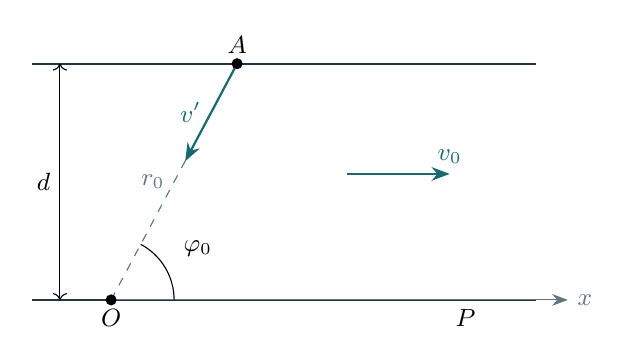
\begin{tikzpicture}

\draw[object] (-1,0)--(5.4,0);\draw[object] (-1,3)--(5.4,3);
\coordinate (O) at (0,0);\coordinate (A) at (1.6,3);
\draw[axis] (O)--(5.8,0) node[right] {$x$};\draw[guide] (O)--(A) node[midway,left] {$r_0$};
\draw[motion] (A)--(.94,1.76) node[midway,left] {$v'$};\draw[motion] (3,1.6)--(4.3,1.6) node[above] {$v_0$};
\draw (.8,0) arc(0:61.93:.8);\node at (1.1,.65) {$\varphi_0$};
\fill (O) circle(2pt);\fill (A) circle(2pt);\node[below] at (O) {$O$};\node[above] at (A) {$A$};\node[below] at (4.5,0) {$P$};
\draw[thin,<->] (-.65,0)--(-.65,3) node[midway,left] {$d$};

\end{tikzpicture}
\figcaption{图 1.13\quad 指向 $O$ 的是相对水速度；对地速度还要加上水流速度。}
\end{minipage}\end{center}

\Needspace{5\baselineskip}\subsection*{解答}

以固定目标 $O$ 为极点，顺水方向为极轴。船的位置为 $\vect r=r\vect e_r$，其中
\[
\vect e_r=(\cos\varphi,\sin\varphi),\qquad
\vect e_\varphi=(-\sin\varphi,\cos\varphi).
\]
相对水的速度始终指向目标，所以它等于 $-v'\vect e_r$。解图 1.13A 中水流的固定方向在这组随位置转动的基矢上有两个分量。
\begin{center}\begin{minipage}{\linewidth}\centering\begin{tikzpicture}

\coordinate (O) at (0,0);\coordinate (B) at (2.4,1.8);
\draw[axis] (0,0)--(4.6,0) node[right] {$x$};\draw[guide] (O)--(B) node[midway,above left] {$r$};
\draw[axis] (B)--(3.36,2.52) node[above right] {$\vect e_r$};\draw[axis] (B)--(1.68,2.76) node[above left] {$\vect e_\varphi$};
\draw[force] (B)--(1.12,.84) node[below left] {$-v'\vect e_r$};
\draw[motion] (B)--(3.5,1.8) node[right] {$v_0\vect e_x$};
\draw (.7,0) arc(0:36.87:.7);\node at (.95,.3) {$\varphi$};\fill (B) circle(2pt);
\node[align=left] at (7.2,2.1) {$\vect e_x=\cos\varphi\,\vect e_r-\sin\varphi\,\vect e_\varphi$\\径向：$\dot r=-v'+v_0\cos\varphi$\\横向：$r\dot\varphi=-v_0\sin\varphi$};

\end{tikzpicture}
\figcaption{解图 1.13A\quad 船向目标划行，水流在径向和横向都有投影。}
\end{minipage}\end{center}
\subsubsection*{合成速度并求轨迹微分方程}
水流速度为
\[
v_0\vect e_x=v_0\cos\varphi\vect e_r-v_0\sin\varphi\vect e_\varphi.
\]
因此船对地的径向、横向速度满足
\[
\boxed{\dot r=-v'+v_0\cos\varphi},\qquad
\boxed{r\dot\varphi=-v_0\sin\varphi}.
\]
因为 $v'>v_0$ 且 $0<\varphi<\pi$，$\dot r<0$、$\dot\varphi<0$：船逐渐接近目标，同时极角减小。用两方程相除消去时间，
\[
\frac{\dd r}{r}
=\frac{\dot r}{r\dot\varphi}\dd\varphi
=\left(\frac{v'}{v_0\sin\varphi}-\cot\varphi\right)\dd\varphi.
\]
\subsubsection*{用半角积分并代入初始条件}
记 $q=v'/v_0>1$，使用
\[
\int\frac{\dd\varphi}{\sin\varphi}=\ln\tan\frac\varphi2,
\qquad\int\cot\varphi\dd\varphi=\ln\sin\varphi.
\]
从 $(r_0,\varphi_0)$ 积分到 $(r,\varphi)$，得到
\[
\ln\frac r{r_0}
=q\ln\frac{\tan(\varphi/2)}{\tan(\varphi_0/2)}
-\ln\frac{\sin\varphi}{\sin\varphi_0}.
\]
两边取指数，轨迹为
\[
\boxed{\frac r{r_0}
=\left[\frac{\tan(\varphi/2)}{\tan(\varphi_0/2)}\right]^q
\frac{\sin\varphi_0}{\sin\varphi}},\qquad
0<\varphi\leq\varphi_0.
\]
轨迹的直角坐标由 $x=r\cos\varphi$、$y=r\sin\varphi$ 给出。初始时 $r=r_0$，且 $r_0\sin\varphi_0=d$，确在出发岸。
\subsubsection*{正对岸出发的轨迹与到达时刻}
目标恰在正对岸时，$r_0=d$、$\varphi_0=\pi/2$，所以
\[
\boxed{r(\varphi)=\frac d{\sin\varphi}
\left(\tan\frac\varphi2\right)^q}.
\]
\begin{center}\begin{minipage}{\linewidth}\centering\begin{tikzpicture}

\draw[object] (-.3,0)--(3.3,0);\draw[object] (-.3,3)--(3.3,3);
\draw[axis] (0,-.15)--(0,3.4) node[above] {$y$};\draw[axis] (0,0)--(3.6,0) node[right] {$x$};
\draw[traj,domain=0:1,samples=100] plot({1.5*(\x-\x*\x*\x)},{3*\x*\x});
\coordinate (P) at ({1/sqrt(3)},1);
\fill (0,0) circle(2pt);\fill (0,3) circle(2pt);\fill (P) circle(2pt);
\node[below left] at (0,0) {$O$};\node[above left] at (0,3) {$A$};\node[right] at (P) {$P$};
\draw[motion] (.432,1.92)--(.53,1.62);\draw[motion] (.4095,.27)--(.26,.1);
\draw[guide] (P)--({1/sqrt(3)},0);\draw[thin,<->] (-.5,0)--(-.5,3) node[midway,left] {$d$};
\draw[motion] (2.0,1.8)--(3.0,1.8) node[midway,above] {$v_0$};
\node[align=left] at (6.4,2.6) {$q=2$，$w=\tan(\varphi/2)$\\$x/d=(w-w^3)/2$\\$y/d=w^2$，$w:1\to0$};
\node[align=left] at (6.4,.8) {$P$ 为最远下游位置\\$x_P=d/(3\sqrt3)$，$y_P=d/3$};

\end{tikzpicture}\figcaption{解图 1.13B\quad 正对岸出发、相对水速率为水流速率两倍时的对地轨迹；箭头表示运动顺序。}
\end{minipage}\end{center}
解图 1.13B 绘出 $q=2$、正对岸出发的轨迹。船先向下游偏移，随后转向目标；图中的指向约束始终是相对水速度。

当 $\varphi\to0^+$，$\tan(\varphi/2)\sim\varphi/2$、$\sin\varphi\sim\varphi$，因此一般轨迹满足
\[
r\sim\frac{r_0\sin\varphi_0}{2^q[\tan(\varphi_0/2)]^q}
\varphi^{q-1}\longrightarrow0.
\]
因此船到目标的距离趋于零。再用解图1.13A的径向速度估计到达时间：
\[
v'-v_0\leq-\dot r\leq v'+v_0,
\qquad\frac{r_0}{v'+v_0}\leq t_*\leq\frac{r_0}{v'-v_0},
\]
因此在题设 $v'>v_0$ 下到达时间有限。终点坐标由$r\to0$与$\varphi\to0^+$的极限给出。沿解图1.13B的末段，船在下游一侧逐渐接近$O$，到达时位置为$(0,0)$。
\subsubsection*{半角积分和一般出发位置的到达时间}
半角积分可直接令$w=\tan(\varphi/2)$验证：
$\sin\varphi=2w/(1+w^2)$、
$\dd\varphi=2\dd w/(1+w^2)$，故
$\dd\varphi/\sin\varphi=\dd w/w$。
再与$\int\cot\varphi\,\dd\varphi=\ln\sin\varphi$合并，
并用初值作比，便得到上面的轨迹式。
在$0<\varphi\leq\varphi_0<\pi$内，$w$和$\sin\varphi$均为正，积分式使用正实数的对数。

还可按解图1.13A，记船的顺水坐标为$x=r\cos\varphi$。
对地速度的$x$分量为$\dot x=v_0-v'\cos\varphi$，
将它与径向速度组合得
\[
\frac{\dd}{\dd t}\left(r+\frac{v_0}{v'}x\right)
=-\frac{v'^2-v_0^2}{v'}.
\]
初始$x_0=r_0\cos\varphi_0$，到达$O$时$r=x=0$，因此
\[
\boxed{t_*=\frac{r_0(v'+v_0\cos\varphi_0)}{v'^2-v_0^2}}.
\]
它落在前面给出的上下时间界内。
正对岸时$\cos\varphi_0=0$、$r_0=d$，
简化为$t_*=dv'/(v'^2-v_0^2)$。
距离$r$始终缩短。对于正对岸出发的轨迹，顺水坐标$x$先增后减。解图1.13B的最远下游点$P$处$\dot x=0$，所以$\cos\varphi=1/q$。当$q=2$时，$\tan(\varphi/2)=1/\sqrt3$，代入图中的参数式得到$x_P=d/(3\sqrt3)$与$y_P=d/3$。


\Needspace{18\baselineskip}

\pdfbookmark[3]{第 14 题 纯滚动轮缘点速度}{c1-q14}

\section*{第 14 题\quad 纯滚动轮缘点速度}\label{book-question-1-14}

\tagline{M-01-14}

半径为 $r$ 的轮子在水平面上向右纯滚动。轮心速度为 $v_c$，轮的角速度大小为 $\omega$，转向为顺时针。设接触点为 $M$，轮缘点 $A$ 的位置角 $\theta$ 从 $CM$ 向逆时针量起，$0\leq\theta<2\pi$。求 $A$ 点对地的速度矢量、速率和方向。

\begin{center}\begin{minipage}{\linewidth}\centering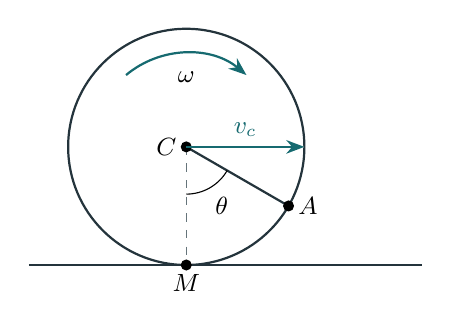
\begin{tikzpicture}

\coordinate (C) at (0,1.5);\coordinate (M) at (0,0);\coordinate (A) at (1.299,.75);
\draw[object] (-2,0)--(3,0);\draw[object] (C) circle(1.5);\draw[guide] (C)--(M);\draw[object] (C)--(A);
\fill (C) circle(2pt);\fill (A) circle(2pt);\fill (M) circle(2pt);
\node[left] at (C) {$C$};\node[below] at (M) {$M$};\node[right] at (A) {$A$};
\draw (0,.9) arc(-90:-30:.6);\node at (.45,.75) {$\theta$};
\draw[motion] (C)--(1.5,1.5) node[midway,above] {$v_c$};
\draw[motion] (-.765,2.412) arc(130:50:1.19);\node at (0,2.38) {$\omega$};

\end{tikzpicture}
\figcaption{图 1.14\quad 轮心平动与绕轮心顺时针转动同时存在。图中 $\theta=60^\circ$。}
\end{minipage}\end{center}

\Needspace{5\baselineskip}\subsection*{解答}

取水平向右为 $x$ 正向，竖直向上为 $y$ 正向，$\vect e_z$ 指向纸外。轮向右滚动，角速度矢量为 $\vect\omega=-\omega\vect e_z$。$\theta$ 从向下的半径 $CM$ 逆时针量起，所以
\[
\vect{CA}=r\sin\theta\vect e_x-r\cos\theta\vect e_y.
\]
\subsubsection*{由无滑动求平动与转动的关系}
接触材料点 $M$ 相对轮心的速度为 $-\omega r\vect e_x$。纯滚动要求它对地瞬时速度为零，因此
\[
\vect v_M=(v_c-\omega r)\vect e_x=0,
\qquad v_c=\omega r.
\]
\subsubsection*{速度叠加得到矢量与速率}
对任意轮缘点，刚体速度关系为
\[
\vect v_A=\vect v_C+\vect\omega\times\vect{CA}.
\]
把转动速度展开，
\[
\vect\omega\times\vect{CA}
=-\omega r\cos\theta\vect e_x-\omega r\sin\theta\vect e_y.
\]
利用纯滚动关系，得到
\[
\boxed{\vect v_A=v_c(1-\cos\theta)\vect e_x-v_c\sin\theta\vect e_y}.
\]
\begin{center}\begin{minipage}{\linewidth}\centering\begin{tikzpicture}

\coordinate (C) at (0,1.5);\coordinate (M) at (0,0);\coordinate (A) at (1.299,.75);
\draw[object] (-1.8,0)--(3,0);\draw[object] (C) circle(1.5);\draw[guide] (C)--(A);\draw[object] (M)--(A);
\draw[motion] (A)--(2.599,.75) node[above right] {$\vect v_C$};
\draw[force] (A)--(.649,-.376) node[below] {$\vect v_{A/C}$};
\draw[guide] (2.599,.75)--(1.949,-.376)--(.649,-.376);
\draw[motion] (A)--(1.949,-.376) node[below right] {$\vect v_A$};
\node[below left] at (M) {$M$};\node[above left] at (C) {$C$};\node[above] at (A) {$A$};
\node[align=left] at (6.1,1.8) {$\vect v_A\perp\vect{MA}$\\接地点可作速度的瞬时转动中心。\\顶部速率为 $2v_c$，底部为零。};

\end{tikzpicture}
\figcaption{解图 1.14A\quad 两等长速度矢量合成；合速度垂直于 $MA$。}
\end{minipage}\end{center}
解图 1.14A 将轮心平动速度与绕心转动速度相加。两矢量都长 $v_c$，合速度长度依位置而变：
\[
v_A^2=v_c^2[(1-\cos\theta)^2+\sin^2\theta]
=2v_c^2(1-\cos\theta).
\]
因此
\[
\boxed{v_A=2v_c\left|\sin\frac\theta2\right|}.
\]
在题图所用的 $0\leq\theta<2\pi$ 内，半角正弦非负。若把同一位置角写成负值，绝对值仍给出正确的弦长和速率。
\subsubsection*{瞬时转动中心给出方向}
由 $M$ 到 $A$ 的位置矢量为
\[
\vect{MA}=r\sin\theta\vect e_x+r(1-\cos\theta)\vect e_y.
\]
与 $\vect v_A$ 点乘得零，所以非接触点的速度垂直于 $MA$。其方向对应绕 $M$ 的瞬时顺时针转动，也可写为
\[
\vect v_A=\vect\omega\times\vect{MA},\qquad
MA=2r\left|\sin\frac\theta2\right|.
\]
因此瞬时中心法同样给出 $v_A=\omega MA$。更具体地，在 $0<\theta<2\pi$ 时，
\[
\frac{\vect v_A}{v_A}
=\sin\frac\theta2\vect e_x-\cos\frac\theta2\vect e_y.
\]
接地点 $\theta=0$ 速度为零，没有速度方向；最高点 $\theta=\pi$ 水平向右，速率 $2v_c$；右侧点 $\theta=\pi/2$ 向右下方，速率 $\sqrt2v_c$；左侧点 $\theta=3\pi/2$ 向右上方，速率同样为 $\sqrt2v_c$。

图1.14B 从同一个轮缘材料点出发，画出它随着轮子前进所描出的曲线。设轮心匀速前进，该点在$t=0$恰接地，令$\psi=\omega t$，则其摆线轨迹为
\[x_A=r(\psi-\sin\psi),\qquad y_A=r(1-\cos\psi).\]
求导得$\dot x_A=v_c(1-\cos\psi)$、$\dot y_A=v_c\sin\psi$，这里材料点随轮子顺时针转动，故 $\theta\equiv-\psi\pmod{2\pi}$，两个速度分量与前式一致。在$t=0$的接地瞬间，该材料点速度为零，加速度为$r\omega^2\boldsymbol e_y$。摆线起点的向上箭头画的正是这一加速度。
\begin{center}\begin{minipage}{0.94\linewidth}\centering
\begin{tikzpicture}[x=1cm,y=1cm]
\draw[->,color=muted] (-.25,0)--(4.9,0) node[right] {$x$};
\draw[->,color=muted] (0,-.1)--(0,1.9) node[above] {$y$};
\draw[thick,color=accent,domain=0:360,samples=100,variable=\t]
plot ({.65*(\t*pi/180-sin(\t))},{.65*(1-cos(\t))});
\fill (0,0) circle(1.5pt);\fill (4.084,0) circle(1.5pt);
\draw[->,thick,color=warm] (0,.08)--(0,.85) node[left] {$\boldsymbol a$};
\node[below] at (0,0) {$t=0$};\node[below] at (4.084,0) {$t=2\pi/\omega$};
\node at (2.1,1.65) {同一轮缘点的轨迹};
\end{tikzpicture}
\figcaption{解图1.14B\quad 两次接地之间的一拱摆线；尖点速度为零而加速度非零。}
\end{minipage}\end{center}
解图1.14A 比较同一时刻轮缘各点的速度，接地点 $M$ 随轮子前进，由不同材料点依次占据。解图1.14B 跟踪同一材料点的摆线，沿这条曲线对该点的速度随时间求导，便得到它的加速度。

\Needspace{18\baselineskip}

\pdfbookmark[3]{第 15 题 内滚圆盘接触点加速度}{c1-q15}

\section*{第 15 题\quad 内滚圆盘接触点加速度}\label{book-question-1-15}

\tagline{M-01-15}

半径 $R$ 的圆环固定，半径 $r<R$ 的圆盘沿圆环内侧无滑动滚动。圆盘中心 $C$ 绕环心 $O$ 以恒定角速度大小 $\Omega$ 运动。求圆盘上在当前时刻与圆环接触的材料点 $A$ 相对圆环的加速度大小和方向。

\begin{center}\begin{minipage}{\linewidth}\centering\begin{tikzpicture}

\coordinate (O) at (0,0);\coordinate (C) at (2,0);\coordinate (A) at (3,0);
\draw[object] (O) circle(3);\draw[guide] (O) circle(2);\draw[object] (C) circle(1);
\draw[object] (O)--(A);\node[below] at (1,0) {$R-r$};\node[below] at (2.5,0) {$r$};
\fill (O) circle(2pt);\fill (C) circle(2pt);\fill (A) circle(2pt);
\node[below left] at (O) {$O$};\node[above] at (C) {$C$};\node[right] at (A) {$A$};
\draw[motion] (1.1,0) arc(0:85:1.1) node[left] {$\Omega$};
\draw[motion] (2.24,.66) arc(70:-40:.7);\node at (2.6,-.8) {$\omega$};
\node[align=left] at (5.9,2) {圆环固定\\圆盘内滚\\当前接触材料点速度为零};

\end{tikzpicture}
\figcaption{图 1.15\quad 盘心逆时针绕 $O$ 运动时，圆盘绕自身中心顺时针转动。}
\end{minipage}\end{center}

\Needspace{5\baselineskip}\subsection*{解答}

设盘心轨道半径为 $\rho=R-r$。取 $\vect e_r$ 从环心 $O$ 指向盘心 $C$，$\vect e_\varphi$ 沿盘心逆时针运动方向；先取公转角速度为 $+\Omega\vect e_z$。相反转向给出相同的加速度大小与径向方向。
\subsubsection*{无滑动确定自转的方向与大小}
盘心速度为 $\vect v_C=\rho\Omega\vect e_\varphi$。当前接触材料点 $A$ 位于盘心外侧，故 $\vect{CA}=r\vect e_r$。若圆盘自身的角速度为 $\omega_s\vect e_z$，其对地速度满足
\[
\vect v_A=\rho\Omega\vect e_\varphi
+\omega_s\vect e_z\times r\vect e_r
=(\rho\Omega+r\omega_s)\vect e_\varphi.
\]
固定圆环的接触处速度为零，无滑动要求 $\vect v_A=0$，于是
\[
\boxed{\omega_s=-\frac{\rho}{r}\Omega}.
\]
负号说明圆盘对地自转与盘心公转反向，自转角速度大小为 $\omega=\rho\Omega/r$。式中的 $\omega_s$ 描述圆盘上的固定方向在地面系中的转动，代入刚体公式时直接使用这一角速度。
\subsubsection*{跟踪当前接触的同一个材料点}
盘心作匀速圆周运动，其加速度为
\[
\vect a_C=-\rho\Omega^2\vect e_r.
\]
$\Omega$ 恒定时 $\omega_s$ 也恒定，所以圆盘材料点的刚体加速度关系为
\[
\vect a_A=\vect a_C
+\vect\omega_s\times(\vect\omega_s\times\vect{CA}).
\]
自转贡献指向盘心，大小为 $r\omega_s^2$，与盘心的向心加速度同向。解图 1.15A 将两箭头平移画出，便于比较：
\begin{center}\begin{minipage}{\linewidth}\centering\begin{tikzpicture}

\coordinate (O) at (0,0);\coordinate (C) at (2.4,0);\coordinate (A) at (3.6,0);
\draw[object] (C) circle(1.2);\draw[guide] (O)--(A);\fill (O) circle(2pt);\fill (C) circle(2pt);\fill (A) circle(2pt);
\node[below] at (O) {$O$};\node[below] at (C) {$C$};\node[right] at (A) {$A$};
\draw[guide] (A)--(3.6,1.85);
\draw[force] (3.6,1.85)--(2.4,1.85) node[midway,above] {$\vect a_C$};
\draw[motion] (2.4,1.85)--(0,1.85) node[midway,above] {$\vect a_{A/C}$};
\draw[axis] (3.8,1.55)--(4.8,1.55) node[right] {$\vect e_r$};
\node[align=left] at (7,0) {两分量均朝向 $O$\\$\vect a_A=\vect a_C+\vect a_{A/C}$\\当前接触材料点沿 $AO$ 加速};

\end{tikzpicture}
\figcaption{解图 1.15A\quad 两支向内的加速度首尾相接。图取$\rho=2r$，绕心贡献是盘心贡献的两倍。}
\end{minipage}\end{center}
\[
\vect a_A=-\left[\rho\Omega^2+r\left(\frac\rho r\Omega\right)^2\right]\vect e_r
=-\frac{\rho(r+\rho)}r\Omega^2\vect e_r.
\]
由 $r+\rho=R$，最终
\[
\boxed{a_A=\frac{R(R-r)}r\Omega^2},\qquad
\boxed{\text{方向由接触点 }A\text{ 指向环心 }O}.
\]
式中 $R(R-r)/r$ 是长度，乘 $\Omega^2$ 得加速度量纲。
\subsubsection*{材料点和几何接触位置各自怎样运动}
无滑动使当前接触的材料点 $A$ 瞬时静止。圆盘继续滚动时，下一处接触由轮缘上的另一材料点承担。给当前的 $A$ 画一个标记，随后它沿图1.15A 的加速度方向起动并离开圆环。

圆环上几何接触位置为 $\vect{OA}_{\mathrm{geom}}=R\vect e_r$。当盘心方向改变时，该位置沿圆环以速率 $R\Omega$ 移动。被标记的材料点则在接触瞬间速度为零，它的加速度由盘心和绕心转动的两项给出。被标记的 $A$ 到了下一时刻已离开圆环，圆环上的接触位置由另一点占据。只看被跟踪点的速度，接触瞬间为零，随后向环内增大，正如抛体过最高点前后，竖直速度经过零而重力加速度始终向下。

当 $r=R/2$ 时，$\omega=\Omega$，两项加速度各为 $R\Omega^2/2$，相加得 $a_A=R\Omega^2$；当 $r\to R^-$ 时盘心轨道半径趋零，所求加速度也趋零。

\clearpage\endgroup


\clearpage
\begingroup
\definecolor{ink}{HTML}{24343C}
\definecolor{accent}{HTML}{166A70}
\definecolor{muted}{HTML}{65747A}
\definecolor{rulegray}{HTML}{D4DDE0}
\definecolor{warm}{HTML}{966037}
\color{ink}
\setlength{\parindent}{2em}
\setlength{\parskip}{4pt}
\linespread{1.12}
\setlength{\abovedisplayskip}{6pt plus 2pt minus 1pt}
\setlength{\belowdisplayskip}{6pt plus 2pt minus 1pt}
\setlength{\abovedisplayshortskip}{0pt plus 1pt}
\setlength{\belowdisplayshortskip}{4pt plus 1pt}
\setlist[enumerate]{label=(\arabic*),leftmargin=2.3em,itemsep=3pt,topsep=4pt}
\setlist[itemize]{leftmargin=2em,itemsep=2pt,topsep=4pt}
\allowdisplaybreaks[1]
\setlength{\emergencystretch}{2em}
\setcounter{secnumdepth}{0}
\providecommand{\tightlist}{\setlength{\itemsep}{0pt}\setlength{\parskip}{0pt}}
\ctexset{section={format=\Large\bfseries\color{accent},beforeskip=10pt,afterskip=9pt},
subsection={format=\normalsize\bfseries\color{accent},beforeskip=10pt,afterskip=4pt},
subsubsection={format=\normalsize\bfseries,beforeskip=8pt,afterskip=3pt}}
\pagestyle{fancy}
\fancyhf{}
\fancyhead[L]{\small\color{muted}物理学难题集萃}
% 页眉仅保留书名；版本名称只在封面显示。
\fancyfoot[L]{\small\color{muted}\chapterlabel}
\fancyfoot[R]{\small\thepage}
\renewcommand{\headrulewidth}{0.4pt}
\renewcommand{\footrulewidth}{0pt}
\renewcommand{\dd}{\mathop{}\!\mathrm{d}}
\renewcommand{\vect}[1]{\bm{#1}}
\renewcommand{\tagline}[1]{\noindent{\small\color{muted}#1}\par}
\renewcommand{\result}[1]{\begin{equation*}\boxed{#1}\end{equation*}}
\renewcommand{\figcaption}[1]{\par\vspace{2pt}{\small\color{muted}#1}\par}
\renewcommand{\teach}[2]{\Needspace{4\baselineskip}\subsection*{讲解要点与追问}#1\par\smallskip\noindent\textbf{追问：}#2\par}
\renewcommand{\workarea}{\par\vspace{7mm}\noindent{\small\color{muted}作答区}\par\vspace{4mm}
\noindent\textcolor{rulegray}{\rule{\linewidth}{0.3pt}}\par\vspace{16mm}
\noindent\textcolor{rulegray}{\rule{\linewidth}{0.3pt}}\par\vspace{16mm}
\noindent\textcolor{rulegray}{\rule{\linewidth}{0.3pt}}\par\vspace{16mm}
\noindent\textcolor{rulegray}{\rule{\linewidth}{0.3pt}}}
\tikzset{axis/.style={-{Stealth[length=2mm]},thin,color=muted},
motion/.style={-{Stealth[length=2.3mm]},thick,color=accent},
force/.style={-{Stealth[length=2.3mm]},thick,color=warm},
traj/.style={thick,color=accent},guide/.style={dashed,thin,color=muted},
object/.style={thick,color=ink},every node/.style={font=\small}}

\renewcommand{\edition}{学生解答版}
\renewcommand{\chapterlabel}{第二章\quad 牛顿运动定律}


\phantomsection\label{book-unit-2}

\pdfbookmark[1]{第二章 牛顿运动定律}{c2-cover}
\thispagestyle{empty}
\vspace*{20mm}
\noindent{\Huge\bfseries 物理学难题集萃}\par\vspace{8mm}
\noindent{\LARGE 第二章\quad 牛顿运动定律}\par\vspace{10mm}
\noindent{\Large\color{accent}学生解答版}\par\vspace{8mm}
\noindent\textcolor{accent}{\rule{\linewidth}{1pt}}\par\vspace{8mm}
\noindent 第 1--20 题\par\vspace{5mm}
\noindent 完整推导、图示分析与条件讨论。\par
\vfill\clearpage
\pdfbookmark[2]{题目目录}{c2-contents}
\section*{题目目录}
\begin{longtable}{@{}r p{113mm} r@{}}
\toprule 题号 & 题目 & 页码\\\midrule\endfirsthead
\toprule 题号 & 题目 & 页码\\\midrule\endhead
\bottomrule\endfoot
\hyperref[book-question-2-1]{1} & \hyperref[book-question-2-1]{圆柱绕绳与欧拉摩擦公式} & \pageref{book-question-2-1}\\
\hyperref[book-question-2-2]{2} & \hyperref[book-question-2-2]{旋转斜杆上小环的稳定位置} & \pageref{book-question-2-2}\\
\hyperref[book-question-2-3]{3} & \hyperref[book-question-2-3]{球壳内壁水平圆周运动的速度范围} & \pageref{book-question-2-3}\\
\hyperref[book-question-2-4]{4} & \hyperref[book-question-2-4]{光滑斜面体与滑块的约束加速度} & \pageref{book-question-2-4}\\
\hyperref[book-question-2-5]{5} & \hyperref[book-question-2-5]{旋转球壳中木块的摩擦条件与稳定性} & \pageref{book-question-2-5}\\
\hyperref[book-question-2-6]{6} & \hyperref[book-question-2-6]{反向滚轴上的钢件匀速推动} & \pageref{book-question-2-6}\\
\hyperref[book-question-2-7]{7} & \hyperref[book-question-2-7]{粗糙地面上斜面接触木块的共同加速} & \pageref{book-question-2-7}\\
\hyperref[book-question-2-8]{8} & \hyperref[book-question-2-8]{滑块、绳和悬挂重物的相对静止条件} & \pageref{book-question-2-8}\\
\hyperref[book-question-2-9]{9} & \hyperref[book-question-2-9]{旋转平台沟槽中双球的稳定位置} & \pageref{book-question-2-9}\\
\hyperref[book-question-2-10]{10} & \hyperref[book-question-2-10]{平方阻力竖直上抛的高度与返回速度} & \pageref{book-question-2-10}\\
\hyperref[book-question-2-11]{11} & \hyperref[book-question-2-11]{线性阻力下两竖直质点的相遇} & \pageref{book-question-2-11}\\
\hyperref[book-question-2-12]{12} & \hyperref[book-question-2-12]{线性阻力抛体的轨迹方程} & \pageref{book-question-2-12}\\
\hyperref[book-question-2-13]{13} & \hyperref[book-question-2-13]{飞机着陆滑行距离} & \pageref{book-question-2-13}\\
\hyperref[book-question-2-14]{14} & \hyperref[book-question-2-14]{两根弹簧同时拉断的条件} & \pageref{book-question-2-14}\\
\hyperref[book-question-2-15]{15} & \hyperref[book-question-2-15]{加速斜面上木块相对静止的推力范围} & \pageref{book-question-2-15}\\
\hyperref[book-question-2-16]{16} & \hyperref[book-question-2-16]{双斜面体上两木块相对加速度} & \pageref{book-question-2-16}\\
\hyperref[book-question-2-17]{17} & \hyperref[book-question-2-17]{航天飞机伸杆卫星的潮汐稳定位置} & \pageref{book-question-2-17}\\
\hyperref[book-question-2-18]{18} & \hyperref[book-question-2-18]{旋转圆盘上射手的科里奥利瞄准} & \pageref{book-question-2-18}\\
\hyperref[book-question-2-19]{19} & \hyperref[book-question-2-19]{自由落体的科里奥利偏离} & \pageref{book-question-2-19}\\
\hyperref[book-question-2-20]{20} & \hyperref[book-question-2-20]{傅科摆摆动平面的旋转周期} & \pageref{book-question-2-20}\\
\end{longtable}


\clearpage

\pdfbookmark[3]{第 1 题 圆柱绕绳与欧拉摩擦公式}{c2-q1}

\section*{第 1 题\quad 圆柱绕绳与欧拉摩擦公式}\label{book-question-2-1}

\tagline{M-02-01}

一根质量可忽略的绳绕在固定圆柱上，两端悬挂质量分别为 $M=1000\,\mathrm{kg}$、$m=10\,\mathrm{kg}$ 的桶。绳与圆柱的静摩擦系数为 $\mu=0.050$。按绕线模型，总接触角取 $2\pi n$，$n$ 为完整圈数。要使两桶保持静止，至少需要多少圈？

\begin{center}\begin{minipage}{\linewidth}\centering\begin{tikzpicture}

\draw[object,fill=rulegray!30] (0,.5) rectangle (5,1.9);
\draw[object] (0,1.2) ellipse(.25 and .7);\draw[object] (5,1.2) ellipse(.25 and .7);
\draw[traj,domain=0:5,samples=150] plot(\x,{1.2+.66*sin(216*\x)});
\draw[object] (0,1.2)--(0,-.8);\draw[object] (5,1.2)--(5,-.8);
\draw[object,fill=accent!10] (-.45,-.8) rectangle (.45,-1.45);\node at (0,-1.12) {$m$};
\draw[object,fill=accent!10] (4.3,-.8) rectangle (5.7,-1.8);\node at (5,-1.3) {$M$};
\node[above] at (2.5,2.2) {固定圆柱，绳绕 $n$ 圈};

\end{tikzpicture}
\figcaption{图 2.1\quad 绳绕圆筒连接两端悬桶；所求圈数由绳、筒间的摩擦条件确定。}
\end{minipage}\end{center}

\Needspace{5\baselineskip}\subsection*{解答}

两桶静止时，各自的加速度为零，故轻绳两端的张力分别为 $T_{\mathrm s}=mg$、$T_{\mathrm b}=Mg$。两段离开圆柱的轻绳沿线没有分布切向力，因此各段的张力等于所连桶的重力。接触圆柱的部分由分布静摩擦承担两端的张力差。沿圆弧的临界分布从 $T_{\mathrm s}$ 单调增至 $T_{\mathrm b}$。

从小桶端向大桶端量接触角 $\theta$。解图 2.1A 中取一段张角 $\dd\theta$ 的绳元，两端张力为 $T$ 与 $T+\dd T$。图中张角已放大，实际计算取 $\dd\theta\to0$。
\begin{center}\begin{minipage}{\linewidth}\centering\begin{tikzpicture}

\draw[guide] (0,0) circle(1.6);\draw[traj,line width=1.8pt] (110:1.6) arc(110:70:1.6);
\draw[guide] (0,0)--(110:1.6);\draw[guide] (0,0)--(70:1.6);
\draw[force] (110:1.6)--(-1.68,1.09) node[left] {$T$};
\draw[force] (70:1.6)--(1.81,1.04) node[right] {$T+\dd T$};
\draw[force] (0,1.6)--(0,2.7) node[above] {$\dd N$};
\draw[force] (0,1.36)--(-.9,1.36) node[below left] {$\dd f$};
\draw (70:.6) arc(70:110:.6);\node at (0,.9) {$\dd\theta$};
\node[align=left] at (5.5,1.2) {两端张力的法向合力向内，\\圆柱支持力向外；\\摩擦阻止绳向高张力端滑动。};

\end{tikzpicture}
\figcaption{解图 2.1A\quad 绳元受力图；小角度作放大示意。}
\end{minipage}\end{center}
\subsubsection*{绳元平衡与静摩擦限制}
两端张力的法向合力指向圆柱，大小为
\[
(2T+\dd T)\sin\frac{\dd\theta}{2}
=T\dd\theta+O((\dd\theta)^2).
\]
所以圆柱的向外支持力为 $\dd N=T\dd\theta$。切向上，两端张力差由静摩擦承担。沿从小桶端到大桶端张力单调增加的分布，$\dd f=\dd T$，摩擦朝小桶端。大桶将向下滑动的临界分布正是这样，且
\[
0\leq\dd T\leq\mu\dd N=\mu T\dd\theta.
\]
一般静止分布满足 $|\dd T|\leq\mu T\dd\theta$，因而每个微元仍有 $\dd T/T\leq\mu\dd\theta$。在图2.1A 的接触弧上从小桶端积分到大桶端，得到
\[
\int_{mg}^{Mg}\frac{\dd T}{T}
\leq\mu\int_0^\Theta\dd\theta,
\qquad \ln\frac Mm\leq\mu\Theta.
\]
于是总接触角必须满足 $\Theta\geq\ln(M/m)/\mu$。在恰将滑动的临界状态，各绳元均达到摩擦极限，积分取等号，张力分布为
\[
T(\theta)=mg\,e^{\mu\theta}.
\]
\subsubsection*{接触角换算为圈数}
每个完整绕圈提供接触角 $2\pi$，故 $\Theta=2\pi n$，并有
\[
n\geq\frac{\ln(M/m)}{2\pi\mu}
=\frac{\ln100}{2\pi\times0.050}=14.6587\cdots.
\]
圈数须取整数，因此 $\boxed{n_{\min}=15\text{ 圈}}$。14 圈时可维持的最大张力比为 $e^{1.4\pi}\approx81.3<100$，15 圈时为 $e^{1.5\pi}\approx111.3>100$。

结果与 $g$ 和圆柱半径无关：前者在两端张力比中消去，后者在绳元法向关系中消去。若实际接触还有入绳、出绳的额外圆弧，应先计入总接触角，再换算完整圈数。
\subsubsection*{取整后的圈数为何仍有摩擦余量}
绳元的切向平衡在取极限前为
$\dd T\cos(\dd\theta/2)=\dd f$；
因为$\cos(\dd\theta/2)=1+O(\dd\theta^2)$，
取一阶微量才得到$\dd f=\dd T$。
连续角度的最小值$\Theta_*=\ln100/\mu$对应处处临界，
整数圈数却将接触角增加到$30\pi>\Theta_*$。
在15圈时，可取下列满足两端桶重的张力分布：
\[
T(\theta)=mg\,e^{\kappa\theta},\qquad
\kappa=\frac{\ln100}{30\pi}=0.04886\cdots<\mu,
\quad0\leq\theta\leq30\pi.
\]
沿解图2.1A的每个绳元都有
$\dd f/\dd N=\dd T/(T\dd\theta)=\kappa<\mu$。
这给出15圈时的一条实际可行分布。绳的张力由小桶端连续增至大桶端，每一段所需摩擦都小于该段所能提供的最大静摩擦。把15圈的总接触角与连续临界角相比，多出的接触弧分担了张力的增长。


\Needspace{18\baselineskip}

\pdfbookmark[3]{第 2 题 旋转斜杆上小环的稳定位置}{c2-q2}

\section*{第 2 题\quad 旋转斜杆上小环的稳定位置}\label{book-question-2-2}

\tagline{M-02-02}

细杆的一端支于地面，以恒定角速度 $\omega>0$ 绕过支点的竖直轴旋转。杆与水平地面的夹角为 $\alpha$，$0<\alpha<\pi/2$。质量 $m$ 的小环套在杆上，静摩擦系数为 $\mu\geq0$。求小环能相对杆保持静止、随杆转动的位置范围，位置以距支点的长度 $L\geq0$ 表示。杆长若有限，取所得范围与实际杆长的交集。

\begin{center}\begin{minipage}{\linewidth}\centering\begin{tikzpicture}

\draw[object] (-.5,0)--(5,0);\draw[axis] (0,-.2)--(0,3.6) node[above] {转轴};
\draw[object,line width=1.2pt] (0,0)--(4,3);\draw[object,fill=accent!15] (2.4,1.8) circle(.15);
\draw[guide] (0,1.8)--(2.4,1.8) node[midway,above] {$L\cos\alpha$};
\draw[thin,<->] (.27,-.36)--(2.67,1.44) node[midway,below right] {$L$};
\draw (.8,0) arc(0:36.87:.8);\node at (1.03,.32) {$\alpha$};
\node[above right] at (2.4,1.8) {$m$};\node[below] at (0,0) {$O$};
\draw[motion] (-.45,3.1) arc(150:-120:.5 and .18) node[left] {$\omega$};

\end{tikzpicture}
\figcaption{图 2.2\quad 小环相对杆静止时，对地作半径 $L\cos\alpha$ 的水平圆周运动。}
\end{minipage}\end{center}

\Needspace{5\baselineskip}\subsection*{解答}

设小环距支点为 $L$，其水平圆周半径为 $r=L\cos\alpha$。小环保持 $L$ 不变时，随杆沿半径 $r$ 作水平圆周运动，地面系中的加速度为 $\omega^2r$，指向转轴。取水平向外为 $x$ 正向，竖直向上为 $z$ 正向，摩擦 $f$ 沿杆向上为正。
\begin{center}\begin{minipage}{\linewidth}\centering\begin{tikzpicture}

\draw[guide] (-1,-.75)--(1.6,1.2);\fill (0,0) circle(2pt);
\draw[force] (0,0)--(-.9,1.2) node[above left] {$N$};
\draw[force] (0,0)--(.4,.3) node[above right] {$f$};
\draw[force] (0,0)--(0,-1.5) node[below] {$mg$};
\draw[motion] (0,-.35)--(-1.4,-.35) node[below left] {$\vect a$};
\node[align=left] at (4.8,.9) {水平向左的$\vect a$指向转轴\\摩擦的正方向沿杆向上\\$f<0$对应摩擦沿杆向下};

\end{tikzpicture}
\figcaption{解图 2.2A\quad 小环的重力、支持力、摩擦与向心加速度。}
\end{minipage}\end{center}
解图 2.2A 画出重力、支持力与摩擦力。支持力垂直杆、朝斜上方，两个方向的运动方程为
\[
-N\sin\alpha+f\cos\alpha=-m\omega^2L\cos\alpha,
\qquad N\cos\alpha+f\sin\alpha=mg.
\]
将第一式乘 $\cos\alpha$、第二式乘 $\sin\alpha$ 后相加，消去 $N$；用另一组投影消去 $f$，得到
\[
f=m(g\sin\alpha-\omega^2L\cos^2\alpha),\qquad
N=m\cos\alpha(g+\omega^2L\sin\alpha)>0.
\]
\subsubsection*{摩擦方向随位置改变}
令
\[
L_0=\frac{g\sin\alpha}{\omega^2\cos^2\alpha},
\qquad f=m\omega^2\cos^2\alpha(L_0-L).
\]
$L<L_0$ 时，重力沿杆的下滑作用较强，摩擦向上；$L>L_0$ 时，维持圆周运动所需的接触合力要求摩擦向下；$L=L_0$ 时无须摩擦。图2.2A 的摩擦箭头沿杆向上，用来规定 $f$ 的正方向；若求得 $f<0$，实际摩擦沿杆向下。

\subsubsection*{分别求两端限制}
记 $s=\sin\alpha$、$c=\cos\alpha$。由 $f\leq\mu N$，整理得
\[
g(s-\mu c)\leq\omega^2Lc(c+\mu s).
\]
右边的系数严格为正，再结合 $L\geq0$，下限为
\[
\boxed{L_-=\max\left(0,\frac{g(s-\mu c)}{\omega^2c(c+\mu s)}\right)}.
\]
因此 $\mu\geq\tan\alpha$ 时，小环可以一直放到支点附近。
另一侧 $f\geq-\mu N$ 给出
\[
\omega^2Lc(c-\mu s)\leq g(s+\mu c).
\]
若 $c-\mu s>0$，可除以正系数，得到有限上限；若 $c-\mu s\leq0$，对任何 $L\geq0$ 左边都不大于零，该条件自动满足。因此
\[
\boxed{L\in\begin{cases}
[L_-,L_+],&\mu<\cot\alpha,\\
[L_-,\infty),&\mu\geq\cot\alpha,
\end{cases}\quad
L_+=\frac{g(s+\mu c)}{\omega^2c(c-\mu s)}}.
\]
若杆的实际长度为 $\ell$，还要与 $[0,\ell]$ 取交集。两个代数端点均为正且有限时，即 $\mu<\min(\tan\alpha,\cot\alpha)$，区间宽度为
\[
L_+-L_-=\frac{2\mu g}{\omega^2c^3(1-\mu^2\tan^2\alpha)}.
\]
\subsubsection*{可维持位置与动力学稳定性}
$\mu=0$ 时区间缩为 $L_0$。若环离开该点，沿杆的净驱动力为 $m\omega^2c^2(L-L_0)$，与偏离同向，故该无摩擦平衡不稳定。有静摩擦时，允许区间中的每个位置各有一个所需的 $f$。若小环在区间内的另一位置以相对杆静止的状态释放，静摩擦可在该位置维持共转。回到某一固定位置的动力学问题则要由运动后的受力决定。
\subsubsection*{受力消元、区间宽度与摩擦曲线}
为看清支持力和摩擦怎样分工，将水平运动方程乘$\cos\alpha$、
竖直方程乘$\sin\alpha$相加，得到
\[
f(\cos^2\alpha+\sin^2\alpha)
=mg\sin\alpha-m\omega^2L\cos^2\alpha.
\]
改将水平式乘$-\sin\alpha$、竖直式乘$\cos\alpha$相加，
则$N=mg\cos\alpha+m\omega^2L\sin\alpha\cos\alpha$。
竖直方向的加速度为零，所以图2.2A 中支持力与摩擦力的竖直分量之和等于重力。当 $f$ 变号时，摩擦的竖直分量也随之改变。

在两个端点均正且有限的情形，通分可把宽度展开为
\[
\begin{aligned}
L_+-L_-&=\frac g{\omega^2c}
\frac{(s+\mu c)(c+\mu s)-(s-\mu c)(c-\mu s)}
{c^2-\mu^2s^2}\\
&=\frac g{\omega^2c}
\frac{2\mu(s^2+c^2)}{c^2-\mu^2s^2}
=\frac{2\mu g}{\omega^2c^3(1-\mu^2\tan^2\alpha)}.
\end{aligned}
\]
这条宽度式适用于两端都由摩擦等式确定的有限区间。若下限取 $0$，宽度改为 $L_+$；若上限不限，则还要按实际杆长决定可用区间。

解图2.2B取$\alpha=45^\circ,\mu=0.20$作例子。
实线是维持共转所需的$f$，两虚线是材料可提供的$\pm\mu N$。
在实线位于两虚线之间的区段，静摩擦能维持小环共转。
\begin{center}\begin{minipage}{\linewidth}\centering
\begin{tikzpicture}[x=1.6cm,y=2cm]
\fill[accent!8] (.94281,-.78) rectangle (2.12132,.83);
\draw[axis] (-.12,0)--(3.05,0) node[right] {$\lambda=\omega^2L/g$};
\draw[axis] (0,-.82)--(0,.92) node[above] {$f/(mg)$};
\draw[guide,domain=0:2.8] plot(\x,{.141421+.1*\x});
\draw[guide,domain=0:2.8] plot(\x,{-.141421-.1*\x});
\draw[thin,domain=0:2.8] plot(\x,{.707107-.5*\x});
\draw[traj,line width=1.3pt,domain=.94281:2.12132] plot(\x,{.707107-.5*\x});
\draw[guide] (.94281,0)--(.94281,.2357);
\draw[guide] (2.12132,0)--(2.12132,-.35355);
\fill (.94281,.2357) circle(1pt); \fill (2.12132,-.35355) circle(1pt);
\node[below] at (.94281,0) {$L_-$};
\node[above] at (1.41421,0) {$L_0$};
\node[above] at (2.12132,0) {$L_+$};
\node[right] at (2.8,.42142) {$+\mu N/(mg)$};
\node[right] at (2.8,-.42142) {$-\mu N/(mg)$};
\node[above right] at (.1,.6571) {所需摩擦};
\end{tikzpicture}
\figcaption{解图2.2B\quad 接触力可实现的区间；三个标记表示相应$L$在无量纲横轴上的位置。}
\end{minipage}\end{center}
$L$减小到$L_-$以下，所需向上摩擦超出上界，小环出现下滑趋势；
$L$增大到有限的$L_+$以上，所需向下摩擦超出下界，小环出现上滑趋势。
在$L_0$处支持力独自平衡竖直重力并提供向心力，摩擦恰为零。
图2.2B 的交点给出允许共转的端点。区间内实线到两条虚线都有余量，各处可分别以所需的静摩擦保持位置。


\Needspace{18\baselineskip}

\pdfbookmark[3]{第 3 题 球壳内壁水平圆周运动的速度范围}{c2-q3}

\section*{第 3 题\quad 球壳内壁水平圆周运动的速度范围}\label{book-question-2-3}

\tagline{M-02-03}

半径 $R$ 的空心球壳绕竖直直径匀速转动，内壁上一可视为质点的小球相对球壳静止，随球壳沿水平纬度圈以速率 $v$ 运动。小球位于下半球，球心至小球的连线与竖直向下方向的夹角为 $\theta$，$0<\theta<\pi/2$。静摩擦系数为 $\mu\geq0$。求在该纬度能维持共转的速率范围。
\par\smallskip\begin{center}\begin{minipage}{\linewidth}\centering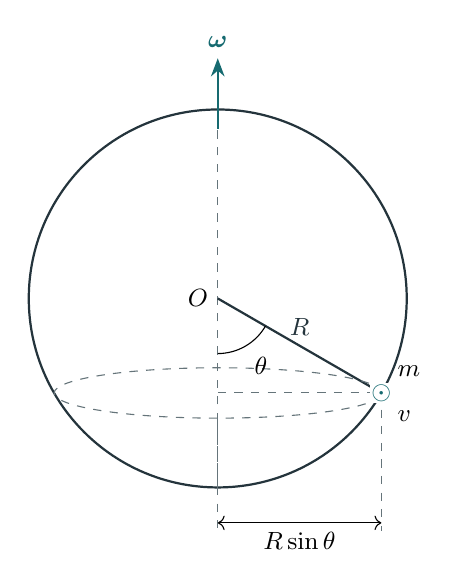
\begin{tikzpicture}
\draw[object] (0,0) circle(2.4);
\draw[guide] (0,-2.4)--(0,2.35);
\coordinate (B) at (2.078,-1.2);
\draw[object] (0,0)--(B) node[midway,above] {$R$};
\draw[guide] (0,-1.2) ellipse(2.078 and .32);
\draw[guide] (0,-1.2)--(B);
\draw[guide] (0,-1.55)--(0,-2.95);
\draw[guide] (B)--(2.078,-2.95);
\draw[<->] (0,-2.85)--(2.078,-2.85) node[midway,below] {$R\sin\theta$};
\node[fill=white,inner sep=.4pt,text=accent] at (B) {$\odot$};
\node[above right] at (2.16,-1.12) {$m$};
\node[below right] at (2.16,-1.3) {$v$};
\node[left] at (0,0) {$O$};
\draw (0,-.7) arc(-90:-30:.7);
\node at (.55,-.85) {$\theta$};
\draw[motion] (0,2.15)--(0,3.05) node[above] {$\boldsymbol\omega$};
\end{tikzpicture}
\figcaption{图 2.3\quad 纬度圈半径为$R\sin\theta$；$\odot$表示周向速度垂直子午面朝向观察者。}
\end{minipage}\end{center}

\Needspace{5\baselineskip}\subsection*{解答}

匀速共转时，小球沿纬圈的切向加速度为零。重力与支持力都在子午面内，故摩擦的周向分量为零，只有沿经线的分量。取过球心和小球的竖直截面，$\theta$ 从竖直向下的半径量起；图2.3 中，从小球到转轴的水平距离是纬圈半径 $\rho=R\sin\theta$。规定切线沿经线上行为摩擦力的正方向。
\begin{center}\begin{minipage}{\linewidth}\centering\begin{tikzpicture}

\fill (0,0) circle(2pt);\draw[guide] (-.75,-1.3)--(.9,1.56);
\draw[force] (0,0)--(-1.3,.75) node[above left] {$N$};
\draw[force] (0,0)--(.43301,.75) node[above right] {$f>0$};
\draw[force] (0,0)--(0,-1.5) node[below] {$mg$};
\draw[motion] (0,-.35)--(-1.4,-.35) node[below left] {$v^2/\rho$};
\draw[axis] (3.6,-.5)--(2.6,-.5) node[midway,below] {向轴为正};
\node[align=left] at (5.7,1.1) {$N\sin\theta-f\cos\theta=mv^2/\rho$\\$N\cos\theta+f\sin\theta=mg$};

\end{tikzpicture}
\figcaption{解图 2.3A\quad 共转小球的重力、支持力、摩擦及向轴加速度。}
\end{minipage}\end{center}
解图 2.3A 中，支持力 $N$ 沿球面法线指向球心；$f>0$ 朝斜上方。小球的加速度水平指向转轴，竖直加速度为零，所以
\[
N\sin\theta-f\cos\theta=\frac{mv^2}{\rho},
\qquad N\cos\theta+f\sin\theta=mg.
\]
记 $a=v^2/\rho$。两式分别作切向与法向的线性组合，得到
\[
f=m(g\sin\theta-a\cos\theta),\qquad
N=m(g\cos\theta+a\sin\theta)>0.
\]
这样先得到任一速率下维持共转所需的 $f$ 和 $N$。材料允许的范围是 $-\mu N\leq f\leq\mu N$，其中等号给出摩擦达到极限的端点。

\subsubsection*{无摩擦速度与两个临界趋势}
令 $f=0$，得 $a=g\tan\theta$，即
\[
\boxed{v_0=\sin\theta\sqrt{\frac{gR}{\cos\theta}}}.
\]
当 $v<v_0$ 时需要向上的摩擦，阻止下滑；当 $v>v_0$ 时需要向下的摩擦，阻止上滑。记 $s=\sin\theta$、$c=\cos\theta$，由 $f\leq\mu N$ 得
\[
g(s-\mu c)\leq a(c+\mu s).
\]
因为 $c+\mu s>0$，再用 $a\geq0$，得到
\[
a\geq g\max\left(0,\frac{s-\mu c}{c+\mu s}\right).
\]
乘以 $\rho=Rs$，速率下限为
\[
\boxed{v_{\min}=\sqrt{gRs\max\left(0,\frac{s-\mu c}{c+\mu s}\right)}}.
\]
下限为零对应 $\mu\geq\tan\theta$。在 $v=0$ 时，沿经线向上的摩擦大小为 $mg\sin\theta$，法向力为 $mg\cos\theta$，这个条件恰好允许两者与重力平衡。

另一侧 $f\geq-\mu N$ 整理为
\[
a(c-\mu s)\leq g(s+\mu c).
\]
当 $c-\mu s>0$ 时有有限上限，反之没有有限上限。因此
\[
\boxed{v_{\max}=\begin{cases}
\sqrt{gRs(s+\mu c)/(c-\mu s)},&\mu<\cot\theta,\\
\infty,&\mu\geq\cot\theta,
\end{cases}\qquad v_{\min}\leq v\leq v_{\max}}.
\]
高速时 $f<0$，其绝对值与 $N$ 的比趋于 $\cot\theta$。当 $\mu\geq\cot\theta$，任何有限高速所需的向下摩擦都在材料范围内。

\subsubsection*{无摩擦与接触条件}
$\mu=0$ 时两端重合于 $v_0$。在题定的下半球，$g\cos\theta>0$，而 $a\sin\theta\geq0$，两项相加使 $N$ 始终为正。这里求的是随壳共转所需的静摩擦。若球壳固定而小球沿壁滑动，摩擦沿相对速度的反向，应按滑动时的切向运动列式。
\subsubsection*{两个临界端点的受力代入}
低速端由上行摩擦达到极限确定时，解图2.3A中的切向方程给出
\[
g\sin\theta-a_{\min}\cos\theta
=\mu(g\cos\theta+a_{\min}\sin\theta).
\]
若存在有限的高速端，该端的下行摩擦达到极限，得到
\[
g\sin\theta-a_{\max}\cos\theta
=-\mu(g\cos\theta+a_{\max}\sin\theta).
\]
两式的正负号对应图中同一条经线的相反方向。
第一式移项后，$a$ 的系数总为正。当解出的代数下限为负时，所有非负 $a$ 都满足这一侧条件，速率从零起算。第二式移项后，若 $c-\mu s\leq0$，左侧对一切 $a\geq0$ 都小于或等于零，而右侧为正，于是这一侧给出的范围延伸到任意大速率。


\Needspace{18\baselineskip}

\pdfbookmark[3]{第 4 题 光滑斜面体与滑块的约束加速度}{c2-q4}

\section*{第 4 题\quad 光滑斜面体与滑块的约束加速度}\label{book-question-2-4}

\tagline{M-02-04}

倾角为 $\theta$、质量为 $M$ 的斜面体放在光滑水平地面上，质量为 $m$ 的木块放在斜面上，接触面也光滑。斜面从左下向右上倾斜，$0<\theta<\pi/2$。求斜面体与木块相对地面的加速度，以及木块所受支持力。

\begin{center}\begin{minipage}{\linewidth}\centering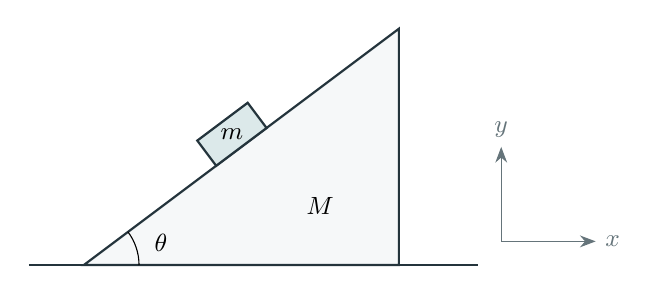
\begin{tikzpicture}

\draw[object] (-.7,0)--(5,0);\draw[object,fill=rulegray!20] (0,0)--(4,3)--(4,0)--cycle;
\begin{scope}[shift={(1.88,1.66)},rotate=36.87]\draw[object,fill=accent!15] (-.4,-.2) rectangle (.4,.2);\node at (0,0) {$m$};\end{scope}
\node at (3,.75) {$M$};\draw (.7,0) arc(0:36.87:.7);\node at (.98,.28) {$\theta$};
\draw[axis] (5.3,.3)--(6.5,.3) node[right] {$x$};\draw[axis] (5.3,.3)--(5.3,1.5) node[above] {$y$};

\end{tikzpicture}
\figcaption{图 2.4\quad 木块下滑时，斜面体向右运动；两者加速度均按地面坐标描述。}
\end{minipage}\end{center}

\Needspace{5\baselineskip}\subsection*{解答}

取地面为惯性系，$x$ 向右、$y$ 向上。设斜面体加速度为 $a_M$，木块加速度分量为 $a_x,a_y$。解图2.4A 分别画出木块和斜面体的受力。木块受重力和斜面的法向支持力，斜面体受反向接触力、重力和地面支持力。
\begin{center}\begin{minipage}{\linewidth}\centering\begin{tikzpicture}

\fill (0,1) circle(2pt);\node[above right] at (0,1) {$m$};
\draw[force] (0,1)--(-.6,1.8) node[above left] {$N$};\draw[force] (0,1)--(0,-.7) node[below] {$mg$};
\draw[guide] (-.8,.4)--(1.2,1.9);
\draw[object] (4.3,.5) rectangle (5.7,1.5);\node at (5,1) {$M$};
\draw[force] (5,1.5)--(5.6,.7) node[right] {$-\vect N$};
\draw[force] (4.65,.5)--(4.65,-1.2) node[below] {$Mg$};
\draw[force] (5.35,.5)--(5.35,3) node[above] {$N_g$};
\draw[motion] (5,1)--(6.6,1) node[above] {$a_M$};

\end{tikzpicture}
\figcaption{解图 2.4A\quad 木块与斜面体分别受力；光滑地面对斜面体没有水平力。}
\end{minipage}\end{center}
因此三个运动方程为
\[
ma_x=-N\sin\theta,\qquad ma_y=N\cos\theta-mg,
\qquad Ma_M=N\sin\theta. \tag{1}
\]
这三式含有 $a_x,a_y,a_M,N$ 四个未知量。接触面光滑给出力的法向方向，木块贴在坡面上又给出一条相对运动关系。

\subsubsection*{由相对运动写接触约束}
解图 2.4B 中，加速度矢量满足 $\vect a_m=\vect a_M+\vect a_{m/M}$。规定木块沿坡向下的相对加速度大小为 $b$，则
\[
\vect a_{m/M}=(-b\cos\theta,-b\sin\theta),
\quad a_x=a_M-b\cos\theta,\quad a_y=-b\sin\theta.
\]
\begin{center}\begin{minipage}{\linewidth}\centering\begin{tikzpicture}

\coordinate (O) at (0,1.8);\coordinate (P) at (1.7,1.8);\coordinate (Q) at (-.7,0);
\draw[motion] (O)--(P) node[midway,above] {$\vect a_M$};
\draw[force] (P)--(Q) node[midway,below right] {$\vect a_{m/M}$};
\draw[motion] (O)--(Q) node[midway,left] {$\vect a_m$};
\draw[guide] (-1.1,-.3)--(2.1,2.1);\fill (O) circle(1.5pt) node[above left]{$O$};\fill (P) circle(1.5pt) node[above right]{$P$};\fill (Q) circle(1.5pt) node[below left]{$Q$};
\node[align=left] at (5.4,1.8) {$\vect a_m=\vect a_M+\vect a_{m/M}$\\相对加速度沿坡向下\\两箭头相加得到对地加速度};

\end{tikzpicture}
\figcaption{解图 2.4B\quad 加速度矢量首尾相接。虚线与斜面平行。}
\end{minipage}\end{center}
消去 $b$，等价的接触约束是
\[
(a_x-a_M)\sin\theta-a_y\cos\theta=0. \tag{2}
\]
坡面方向固定，木块到坡面的有符号法向距离恒为零，连续求两次导数便得到式 (2)。解图2.4B 中的 $PQ$ 与坡面平行，$OQ$ 是加上斜面水平平动后的地面系加速度。

将式 (1) 代入 (2)，有
\[
\left(-\frac{N\sin\theta}{m}-\frac{N\sin\theta}{M}\right)\sin\theta
-\left(\frac{N\cos\theta}{m}-g\right)\cos\theta=0.
\]
整理得到
\[
N\left(\frac1m+\frac{\sin^2\theta}{M}\right)=g\cos\theta.
\]
记 $D=M+m\sin^2\theta$，支持力与斜面体加速度为
\[
\boxed{N=\frac{mMg\cos\theta}{D}},\qquad
\boxed{a_M=\frac{mg\sin\theta\cos\theta}{D}}.
\]
再逐项代回木块方程，得
\[
\boxed{a_x=-\frac{Mg\sin\theta\cos\theta}{D}},\qquad
\boxed{a_y=-\frac{(M+m)g\sin^2\theta}{D}}.
\]
两负号分别表示向左、向下。相对加速度及地面系加速度大小分别为
\[
\boxed{b=\frac{(M+m)g\sin\theta}{D}},\qquad
|\vect a_m|=\frac{g\sin\theta}{D}
\sqrt{M^2\cos^2\theta+(M+m)^2\sin^2\theta}.
\]
\subsubsection*{整体水平运动与斜面系的写法}
把两物体看作整体，地面对它们的外力都沿竖直方向，于是 $ma_x+Ma_M=0$。这说明图2.4B 的地面系加速度向左，斜面体向右，水平加速度大小之比为 $M:m$。

也可在斜面体的平动参考系中列式。图2.4B 的 $OP$ 表示斜面向右加速，此时木块的惯性力为 $-ma_M\hat i$。它沿坡向下的分量为 $ma_M\cos\theta$，与重力的下坡分量同向，所以 $b=g\sin\theta+a_M\cos\theta$。法向加速度为零，故 $N+ma_M\sin\theta=mg\cos\theta$。再由斜面体的水平运动 $Ma_M=N\sin\theta$ 消去 $a_M$，得到同一支持力。

当 $M\to\infty$，斜面体的加速度趋于零，支持力趋于 $mg\cos\theta$，木块沿固定坡面下滑，$b\to g\sin\theta$。当 $\theta\to0$，重力沿坡分量与接触力的水平分量都趋于零，两个物体的加速度随之趋零。

\Needspace{18\baselineskip}

\pdfbookmark[3]{第 5 题 旋转球壳中木块的摩擦条件与稳定性}{c2-q5}

\section*{第 5 题\quad 旋转球壳中木块的摩擦条件与稳定性}\label{book-question-2-5}

\tagline{M-02-05}

半径 $R=0.5\,\mathrm m$ 的空心球壳绕竖直直径匀速转动。内壁上的小木块可看作质点，位于距球壳最低点 $h=R/2$ 的高度，随壳共转。取 $g=9.8\,\mathrm{m/s^2}$。
\begin{enumerate}
\item 当 $\omega=5\,\mathrm{s^{-1}}$ 时，至少需要多大的静摩擦系数？
\item 当 $\omega=8\,\mathrm{s^{-1}}$ 时，维持共转的条件是什么？
\item 分别讨论木块位置、角速度发生微小改变后能否继续共转。区分静摩擦有余量和恰好临界的情形，说明仅由这些条件能否断言木块必定返回原位置。
\end{enumerate}

\begin{center}\begin{minipage}{\linewidth}\centering\begin{tikzpicture}

\draw[object] (0,0) circle(2.4);\draw[guide] (0,-2.4)--(0,2.4);
\coordinate (B) at (2.078,-1.2);\draw[object] (0,0)--(B);\draw[guide] (0,-1.2)--(B);
\fill (B) circle(2.5pt);\node[right] at (B) {木块};\node[left] at (0,0) {$O$};
\draw (0,-.7) arc(-90:-30:.7);\node at (.55,-.85) {$\theta$};
\draw[thin,<->] (2.75,-2.4)--(2.75,-1.2) node[midway,right] {$h=R/2$};
\draw[guide] (0,-2.4)--(2.75,-2.4);\draw[guide] (B)--(2.75,-1.2);
\draw[motion] (-.45,2.05) arc(150:-120:.5 and .18) node[left] {$\omega$};

\end{tikzpicture}
\figcaption{图 2.5\quad 高度从球壳最低点量起，$h=R(1-\cos\theta)$，本题 $\theta=60^\circ$。}
\end{minipage}\end{center}

\Needspace{5\baselineskip}\subsection*{解答}

图 2.5 中高度从最低点量起，$h=R(1-\cos\theta)$。由 $h=R/2$ 得 $\theta=60^\circ$，水平圆周半径为 $R\sin\theta$。小木块做水平圆周运动，加速度朝向转轴，大小为 $R\omega^2\sin\theta$。解图2.5A 在两幅受力图下方分别画出向轴的加速度。

规定摩擦 $f$ 沿经线上行为正。按解图 2.5A 的两幅受力图，地面系的水平与竖直方程是
\[
N\sin\theta-f\cos\theta=mR\omega^2\sin\theta,
\qquad N\cos\theta+f\sin\theta=mg.
\]
\begin{center}\begin{minipage}{\linewidth}\centering\begin{tikzpicture}

\begin{scope}
\fill (0,0) circle(2pt);\draw[force] (0,0)--(-1.76607,1.01964) node[above left] {$N$};
\draw[force] (0,0)--(0.21960,0.38036) node[above right] {$f>0$};\draw[force] (0,0)--(0,-1.4) node[below] {$mg$};
\draw[motion] (0,-2)--(-0.92015,-2) node[left] {$\vect a$};\node at (0,2.55) {$\omega=5\,\mathrm{s^{-1}}$};
\end{scope}
\begin{scope}[xshift=5.8cm]
\fill (0,0) circle(2pt);\draw[force] (0,0)--(-3.57545,2.06429) node[above left] {$N$};
\draw[force] (0,0)--(-0.38353,-0.66429) node[below left] {$f<0$};\draw[force] (0,0)--(0,-1.4) node[below] {$mg$};
\draw[motion] (0,-2)--(-2.35559,-2) node[left] {$\vect a$};\node at (0,2.55) {$\omega=8\,\mathrm{s^{-1}}$};
\end{scope}

\end{tikzpicture}
\figcaption{解图 2.5A\quad 两种转速下的受力和向轴加速度。两幅图的重力箭头等长，支持力与摩擦力按各自大小绘出。}
\end{minipage}\end{center}
消元得到
\[
f=m(g-R\omega^2\cos\theta)\sin\theta,
\qquad N=m(g\cos\theta+R\omega^2\sin^2\theta).
\]
用有符号比值 $\eta=f/N$ 记录方向，材料静摩擦系数记为非负的 $\mu_s$，则
\[
\boxed{\eta=\frac{(g-R\omega^2\cos\theta)\sin\theta}
{g\cos\theta+R\omega^2\sin^2\theta}},\qquad \mu_s\geq|\eta|.
\]
\subsubsection*{两种转速的数值与方向}
$R=0.5\,\mathrm m$、$g=9.8\,\mathrm{m/s^2}$、$\theta=60^\circ$。当 $\omega=5\,\mathrm{s^{-1}}$ 时，
\[
\frac Nm=4.9+12.5\times\frac34=14.275\,\mathrm{m/s^2},
\quad \frac fm=(9.8-6.25)\frac{\sqrt3}{2}=3.0744\,\mathrm{m/s^2}.
\]
故 $\boxed{\mu_s\geq0.2154}$，摩擦向上。$\omega=8\,\mathrm{s^{-1}}$ 时，
\[
\frac Nm=4.9+32\times\frac34=28.9\,\mathrm{m/s^2},
\quad \frac fm=(9.8-16)\frac{\sqrt3}{2}=-5.3694\,\mathrm{m/s^2}.
\]
故 $\boxed{\mu_s\geq0.1858}$，摩擦向下。$f/N<0$ 对应经线向下的摩擦，所需的最小材料系数取 $|f/N|$。零摩擦的分界转速为 $\sqrt{g/(R\cos\theta)}\approx6.261\,\mathrm{s^{-1}}$。

\subsubsection*{位置与转速改变后的静摩擦条件}
如果 $\mu_s>|\eta|$，摩擦有严格余量，连续性保证足够小的角度或转速改变后仍可共转。这里比较的是新共转状态所需的摩擦，扰动后的木块可以保持在新位置。

材料恰在临界时，新的 $|\eta|$ 增大便会超过上限，减小则留下余量。令 $u=R\omega^2/g$、$D=\cos\theta+u\sin^2\theta$，则 $\eta=(1-u\cos\theta)\sin\theta/D$。记 $A=(1-u\cos\theta)\sin\theta$。对角度求导，有 $A_\theta=\cos\theta-u(\cos^2\theta-\sin^2\theta)$、$D_\theta=-\sin\theta+2u\sin\theta\cos\theta$，商法则的分子为 $A_\theta D-AD_\theta$。对 $u$ 求导，分子是 $-\cos\theta\sin\theta\,D-A\sin^2\theta=-\sin\theta$。再乘 $du/d\omega=2R\omega/g$，整理得
\[
\frac{\partial\eta}{\partial\theta}
=\frac{1-u\cos\theta+u^2\sin^2\theta}{D^2},
\qquad \frac{\partial\eta}{\partial\omega}
=-\frac{2R\omega\sin\theta}{gD^2}.
\]
在本题两个状态处，第一导数为正、第二导数为负。沿球面经线上移时，$\theta$ 增大，在解图2.5B中向右读。第一种状态 $\eta>0$，第二种状态 $\eta<0$，因此两条 $|\eta|$ 曲线在该处的斜率一正一负。
\begin{center}\begin{minipage}{\linewidth}\centering\begin{tikzpicture}

\begin{scope}
\draw[axis] (-.1,0)--(3.6,0) node[right] {$\theta$};\draw[axis] (0,-.1)--(0,2.3) node[above] {$|\eta|$};
\draw[traj,domain=45:75,samples=80] plot({(\x-45)/10},{4*abs((1-1.2755102*cos(\x))*sin(\x)/(cos(\x)+1.2755102*sin(\x)*sin(\x)))});
\draw[guide] (1.5,0)--(1.5,2);\draw[guide] (0,.8616)--(3.2,.8616);
\fill (1.5,.8616) circle(2pt);\node[below] at (1.5,0) {$60^\circ$};\node[left] at (0,.8616) {$\mu_s$};
\node at (1.6,2.6) {$\omega=5\,\mathrm{s^{-1}}$};
\end{scope}
\begin{scope}[xshift=6.1cm]
\draw[axis] (-.1,0)--(3.6,0) node[right] {$\theta$};\draw[axis] (0,-.1)--(0,2.3) node[above] {$|\eta|$};
\draw[traj,domain=45:75,samples=80] plot({(\x-45)/10},{4*abs((1-3.2653061*cos(\x))*sin(\x)/(cos(\x)+3.2653061*sin(\x)*sin(\x)))});
\draw[guide] (1.5,0)--(1.5,2);\draw[guide] (0,.7432)--(3.2,.7432);
\fill (1.5,.7432) circle(2pt);\node[below] at (1.5,0) {$60^\circ$};\node[left] at (0,.7432) {$\mu_s$};
\node at (1.6,2.6) {$\omega=8\,\mathrm{s^{-1}}$};
\end{scope}

\end{tikzpicture}
\figcaption{解图 2.5B\quad 固定转速的位置扰动。水平虚线取 $60^\circ$ 位置的临界系数，虚线下方的曲线对应可继续共转的位置。}
\end{minipage}\end{center}
\begin{center}
\begin{tabular}{@{}lll@{}}\toprule
微小改变 & $\omega=5\,\mathrm{s^{-1}}$ & $\omega=8\,\mathrm{s^{-1}}$\\\midrule
位置上移 & 需求增大，开始下滑 & 需求减小，可在新位置共转\\
位置下移 & 需求减小，可在新位置共转 & 需求增大，开始上滑\\
转速升高 & 需求减小，可继续共转 & 需求增大，开始上滑\\
转速降低 & 需求增大，开始下滑 & 需求减小，可继续共转\\\bottomrule
\end{tabular}\end{center}
表中“开始滑动”的方向，由超出最大静摩擦后仍未平衡的经线分力确定。例如第一种状态上移后，所需向上摩擦超过材料上限，剩余合力向下。

表中的共转情形是把木块在新位置无相对速度地放开。材料有余量时，木块可以停留在该处。若放开时已有相对速度，或静摩擦达到上限后开始滑动，后续轨迹由扰动速度、动摩擦规律和周向运动共同决定。
\subsubsection*{经线上的摩擦方向与大小}
局部斜率给出 $60^\circ$ 附近的增减。沿经线从底部移向赤道，$\sin\theta$ 增大，$\cos\theta$ 减小，分子中的 $1-u\cos\theta$ 可以由负转正。两种转速的过零位置因此不同。
把表中每个角度代入 $\eta(\theta,\omega)$。正值指向经线上方，负值指向经线下方，相应材料系数取该数的绝对值。
\begin{center}
\begin{tabular}{@{}rrrrrrrr@{}}\toprule
$\theta$ & $0^\circ$ & $15^\circ$ & $30^\circ$ & $45^\circ$ & $60^\circ$ & $75^\circ$ & $90^\circ$\\\midrule
$\eta(\theta,5)$ & 0 & $-0.0571$ & $-0.0441$ & $0.0516$ & $0.2154$ & $0.4466$ & $0.7840$\\
$\eta(\theta,8)$ & 0 & $-0.4706$ & $-0.5432$ & $-0.3956$ & $-0.1858$ & $0.0453$ & $0.3063$\\\bottomrule
\end{tabular}
\end{center}
在 $\theta=0$ 的最低点，重力与向轴加速度的切向投影都为零，$\eta=0$。当 $\theta\to90^\circ$，重力全在切向，支持力全用于向心加速，于是 $\eta\to g/(R\omega^2)$。
因此这两行末值分别是$9.8/12.5$和$9.8/32$。
有符号需求在$\cos\theta=1/u$处过零，过零前后摩擦方向互换。
在$60^\circ$附近，第一行的$\eta$为正且随角度增加，
第二行的$\eta$为负且随角度增加；转为绝对值以后，两条需求曲线的升降方向相反，
与解图2.5B相符。

以图2.5B 左图为例，上移使向上摩擦需求超过临界线，静摩擦取到上限后，剩余分力沿经线向下。下移让需求落到临界线下方，木块可以静止在新位置。右图的临界曲线在 $60^\circ$ 处斜率反号，下移使所需向下摩擦超过上限，剩余分力向上。图中每一点的纵坐标都除以该位置的支持力 $N$，它与摩擦力一起随位置改变。

\subsubsection*{实际调速过程还需要周向摩擦}
前面的转速比较针对调整前、后两个匀速共转状态。
若在有限时间内改变球壳角速度，同时要求木块始终留在同一纬度并随壳转动，
还需要周向摩擦$f_\varphi=mR\sin\theta\,\dot\omega$，
它负责角速度变化引起的周向加速度。
经线所需摩擦仍为$f_\theta=m(g-R\omega^2\cos\theta)\sin\theta$，
经线和周向两分量正交，合成的静摩擦条件为
\[
\sqrt{f_\theta^2+f_\varphi^2}\leq\mu_sN,
\qquad N=m(g\cos\theta+R\omega^2\sin^2\theta).
\]
等价地，令$D=\cos\theta+u\sin^2\theta$，
\[
\eta^2+
\left(\frac{R\sin\theta\,\dot\omega}{gD}\right)^2
\leq\mu_s^2.
\]
在 $\dot\omega=0$ 的匀速阶段，条件化为 $|\eta|\leq\mu_s$。调速时可供周向分量使用的余量为 $N\sqrt{\mu_s^2-\eta^2}$。在经线摩擦恰达上限的时刻，这一余量为零。由合摩擦式可为两个匀速状态之间的调速过程选取允许的角加速度。


\Needspace{18\baselineskip}

\pdfbookmark[3]{第 6 题 反向滚轴上的钢件匀速推动}{c2-q6}

\section*{第 6 题\quad 反向滚轴上的钢件匀速推动}\label{book-question-2-6}

\tagline{M-02-06}

质量 $m=20\,\mathrm{kg}$ 的对称钢件架在两个相同的平行长直滚轴上。滚轴轴线水平，半径 $r=0.025\,\mathrm m$，以角速度 $\omega=40\,\mathrm{rad/s}$ 反向转动，接触处的表面速度大小均为 $\omega r$，方向水平且相反。钢件与滚轴间的滑动摩擦系数 $\mu=0.20$。要使钢件沿滚轴轴线以 $v_0=0.050\,\mathrm{m/s}$ 匀速运动，需施加多大的轴向水平力 $F$？取 $g=10\,\mathrm{m/s^2}$。

\begin{center}\begin{minipage}{\linewidth}\centering\begin{tikzpicture}

\draw[object] (0,0) ellipse(.45 and .22);\draw[object] (0,0)--(0,3);\draw[object] (.45,0)--(.45,3);\draw[object] (-.45,0)--(-.45,3);\draw[object] (0,3) ellipse(.45 and .22);
\draw[object] (3,0) ellipse(.45 and .22);\draw[object] (3,0)--(3,3);\draw[object] (3.45,0)--(3.45,3);\draw[object] (2.55,0)--(2.55,3);\draw[object] (3,3) ellipse(.45 and .22);
\filldraw[object,fill=white] (-.7,.9) rectangle (3.7,2);\node at (1.5,1.45) {钢件};
\draw[motion] (0,2.6)--(-1.2,2.6) node[left] {$\omega r$};\draw[motion] (3,2.6)--(4.2,2.6) node[right] {$\omega r$};
\draw[motion] (1.5,2)--(1.5,3.6) node[above] {$v_0,F$};\node at (1.5,-.6) {俯视图：图中上下方向沿滚轴轴线};

\end{tikzpicture}
\figcaption{图 2.6\quad 两接触处的横向表面速度相反。}
\end{minipage}\end{center}

\Needspace{5\baselineskip}\subsection*{解答}

取滚轴轴向为 $y$，钢件运动方向为 $+y$，横跨两轴的方向为 $x$。两轴顶部表面速度大小均为 $w=\omega r$，方向分别为 $+x$、$-x$。接触摩擦反向于钢件相对各滚轴表面的速度。
\begin{center}\begin{minipage}{\linewidth}\centering\begin{tikzpicture}

\begin{scope}
\draw[axis] (-1.6,0)--(1.8,0) node[right] {$x$};\draw[axis] (0,-1.6)--(0,1.6) node[above] {$y$};
\draw[motion] (0,0)--(1.3,.6) node[right] {$\vect v_{\mathrm{rel},2}$};\draw[force] (0,0)--(-1.3,-.6) node[left] {$\vect f_2$};
\draw[guide] (1.3,0)--(1.3,.6);\node[below] at (.65,0) {$\omega r$};\node[right] at (1.3,.25) {$v_0$};
\node[below] at (0,-1.7) {左滚轴（2）};
\end{scope}
\begin{scope}[xshift=6cm]
\draw[axis] (-1.6,0)--(1.8,0) node[right] {$x$};\draw[axis] (0,-1.6)--(0,1.6) node[above] {$y$};
\draw[motion] (0,0)--(-1.3,.6) node[left] {$\vect v_{\mathrm{rel},1}$};\draw[force] (0,0)--(1.3,-.6) node[right] {$\vect f_1$};
\node[below] at (0,-1.7) {右滚轴（1）};
\end{scope}

\end{tikzpicture}
\figcaption{解图 2.6A\quad 摩擦方向由相对滑动决定；沿轴的速度分量在图中画长，便于读出两次投影。}
\end{minipage}\end{center}
解图 2.6A 的速度三角形给出
\[
\vect v_{\mathrm{rel},1}=(-w,v_0),\qquad
\vect v_{\mathrm{rel},2}=(w,v_0),\qquad
V=\sqrt{w^2+v_0^2}.
\]
钢件对称放置、没有竖直加速度，两接触处支持力均为 $N_1=N_2=mg/2$。两摩擦力的大小是 $\mu mg/2$，方向分别沿相对速度的反向，因而
\[
\vect f_1=\frac{\mu mg}{2V}(w,-v_0),\qquad
\vect f_2=\frac{\mu mg}{2V}(-w,-v_0).
\]
解图2.6A中每个摩擦力都与本处的相对速度反向。沿轴的阻力只取各自箭头在$-y$方向的投影。

两式相加，横向分量抵消，轴向阻力相加：
\[
\vect f_1+\vect f_2=\left(0,-\frac{\mu mgv_0}{V}\right).
\]
匀速要求轴向合力为零，外力向 $+y$，大小为
\[
\boxed{F=\frac{\mu mgv_0}{\sqrt{(\omega r)^2+v_0^2}}
=\frac{\mu mg}{\sqrt{1+(\omega r/v_0)^2}}}.
\]
代入 $\omega r=40\times0.025=1.00\,\mathrm{m/s}$、$v_0=0.050\,\mathrm{m/s}$、$g=10\,\mathrm{m/s^2}$，得到
\[
F=\frac{0.20\times20\times10}{\sqrt{401}}
=1.9975\,\mathrm N\approx\boxed{2.0\,\mathrm N}.
\]
\subsubsection*{为何远小于普通水平面上的摩擦}
每处摩擦的大小为$\mu N_i$，沿轴向的分量取决于箭头与轴线的夹角。本题$w/v_0=20$，相对速度接近横向，摩擦也几乎横向，其轴向比例只有 $v_0/V\approx0.05$。当 $v_0\ll\omega r$ 时，$F\approx\mu mgv_0/(\omega r)$；若滚轴停止，$F\to\mu mg$。

能量分配也可逐项算出。钢件匀速，外推力功率为
\[P_{\rm push}=Fv_0=\frac{\mu mgv_0^2}{V}.\]
每个滚轴表面速度沿$x$向，所受摩擦的$x$分量大小为$\mu mgw/(2V)$，维持两滚轴转速的驱动功率因此为
\[P_{\rm motor}=2\frac{\mu mgw}{2V}w=\frac{\mu mgw^2}{V}.\]
相加得$P_{\rm push}+P_{\rm motor}=\mu mgV$，恰等于两个滑动接触的总耗散率。图2.6A中互相抵消的只是作用于钢件的横向合力，各滚轴处的摩擦功并未相消。

\subsubsection*{把相对速度方向换成投影角}
按图2.6的表面速度方向，右滚轴表面沿$x$正向运动，左滚轴沿$x$负向运动。
解图2.6A中，右滚轴编号1，左滚轴编号2。两处滑动速度分别由钢件速度减去相应的滚轴表面速度得到。
设每个相对速度与$y$正向夹角的大小为$\beta$，则
\[
\tan\beta=\frac{w}{v_0},\qquad
\cos\beta=\frac{v_0}{\sqrt{w^2+v_0^2}}.
\]
每处摩擦大小为$\mu mg/2$，其沿$y$负向的投影为
$(\mu mg/2)\cos\beta$，因此$F=2(\mu mg/2)\cos\beta$。
这个几何投影法与前面的两个力矢量相加完全一致。

当$v_0\to0$而滚轴仍转动，轴向投影趋于零，钢件可以不沿轴移动；
两接触处仍有横向相对滑动，摩擦耗散率趋于$\mu mgw$，
所需能量由滚轴驱动装置提供。当钢件和滚轴都静止时，接触处的摩擦由静摩擦平衡确定。


\Needspace{18\baselineskip}

\pdfbookmark[3]{第 7 题 粗糙地面上斜面接触木块的共同加速}{c2-q7}

\section*{第 7 题\quad 粗糙地面上斜面接触木块的共同加速}\label{book-question-2-7}

\tagline{M-02-07}

质量为 $m_A,m_B$ 的木块 $A,B$ 放在粗糙水平地面上，与地面的摩擦系数均为 $\mu$。两木块接触面光滑，倾角 $0<\theta<\pi/2$，其方向如图：$A$ 对 $B$ 的压力向右下方。水平推力 $F$ 作用于 $A$，使两木块向右加速且无相对滑动。以下讨论两块已经向右滑动、地面采用滑动摩擦的平动阶段。求 $\mu$ 和 $F$ 的条件。允许 $A$ 的地面支持力恰好为零。

\begin{center}\begin{minipage}{\linewidth}\centering\begin{tikzpicture}

\draw[object] (-.4,0)--(5,0);\fill[pattern=north east lines,pattern color=rulegray] (-.4,-.16) rectangle (5,0);
\filldraw[object,fill=accent!5] (0,0)--(1.4,0)--(3.3,1.5)--(0,1.5)--cycle;
\filldraw[object,fill=warm!5] (1.4,0)--(4.5,0)--(4.5,1.5)--(3.3,1.5)--cycle;
\node at (.8,1) {$A$};\node at (3.8,.7) {$B$};
\draw[force] (-1.3,.7)--(0,.7) node[midway,above] {$F$};
\draw (2,0) arc(0:38.29:.6);\node at (2.14,.24) {$\theta$};\draw[motion] (3,2.1)--(4.5,2.1) node[right] {$a$};

\end{tikzpicture}
\figcaption{图 2.7\quad 接触斜面向右升高；两木块都与地面保持接触。}
\end{minipage}\end{center}

\Needspace{5\baselineskip}\subsection*{解答}

两个木块已在地面上向右滑动，解图2.7A 中的两支地面摩擦箭头都指向左方。记共同加速度为 $a>0$，斜面间的法向力大小为 $N$。斜面向右升高，它对 $B$ 的法向力指向右下方，对 $A$ 的法向力指向左上方，竖直分量的大小均为 $N\cos\theta$。
\begin{center}\begin{minipage}{\linewidth}\centering\begin{tikzpicture}

\begin{scope}
\fill (0,0) circle(2pt);\node at (0,2.9) {$A$};
\draw[force] (0,0)--(1.28,0) node[right] {$F$};
\draw[force] (0,0)--(-.16,0);\node[left] at (-.17,0) {$\mu R_A$};
\draw[force] (0,0)--(-.8,.8) node[above left] {$N$};
\draw[force] (0,0)--(0,.8) node[above] {$R_A$};
\draw[force] (0,0)--(0,-1.6) node[below] {$m_Ag$};
\end{scope}
\begin{scope}[xshift=5.6cm]
\fill (0,0) circle(2pt);\node at (0,2.9) {$B$};
\draw[force] (0,0)--(.8,-.8) node[below right] {$N$};
\draw[force] (0,0)--(-.48,0) node[left] {$\mu R_B$};
\draw[force] (0,0)--(0,2.4) node[above] {$R_B$};
\draw[force] (0,0)--(0,-1.6) node[below] {$m_Bg$};
\end{scope}

\end{tikzpicture}
\figcaption{解图 2.7A\quad 图取$m_A=m_B$、$\theta=45^\circ$、$\mu=0.2$及$a=0.2g$。$A$的地面支持力较小，$B$的地面支持力较大。}
\end{minipage}\end{center}
竖直方向无加速度，故两块的地面支持力为
\[
R_A=m_Ag-N\cos\theta,\qquad
R_B=m_Bg+N\cos\theta.
\]
随 $N$ 增加，$A$ 的支持力减少 $N\cos\theta$，$B$ 的支持力增加同样多，地面承担的总力仍为 $R_A+R_B=(m_A+m_B)g$。$B$ 的支持力始终为正，$A$ 保持接触的条件为 $R_A\geq0$，即
\[
N\leq\frac{m_Ag}{\cos\theta}. \tag{1}
\]
对 $B$ 水平方向列式，有
\[
N\sin\theta-\mu(m_Bg+N\cos\theta)=m_Ba>0.
\]
$B$ 的向右净力随 $N$ 的斜率为 $\sin\theta-\mu\cos\theta$，而在 $N=0$ 时其值为 $-\mu m_Bg$。要使净力为正，斜率须为正，因而
\[
N>\frac{\mu m_Bg}{\sin\theta-\mu\cos\theta}. \tag{2}
\]
斜率来自两个分量的差。每增加一单位压力，$B$ 得到 $\sin\theta$ 的向右力，地面摩擦同时增加 $\mu\cos\theta$。

\subsubsection*{压力区间存在的条件}
由 $R_A=0$ 定出的上端须大于由 $a=0$ 定出的下端，因此
\[
\frac{\mu m_Bg}{\sin\theta-\mu\cos\theta}
<\frac{m_Ag}{\cos\theta}.
\]
在正分母条件下交叉相乘，得到
\[
\mu m_B\cos\theta<m_A\sin\theta-\mu m_A\cos\theta,
\quad\boxed{0\leq\mu<\frac{m_A}{m_A+m_B}\tan\theta}.
\]
这个更强的条件已经保证 $\mu<\tan\theta$。

\subsubsection*{由压力换成推力}
整个系统的水平外力为 $F-\mu(R_A+R_B)$，因此
\[
a=\frac{F}{m_A+m_B}-\mu g.
\]
再代入 $B$ 的方程，公共的重力摩擦项抵消，得到
\[
N(\sin\theta-\mu\cos\theta)
=\frac{m_B}{m_A+m_B}F.
\]
于是 (2) 给出 $F>\mu(m_A+m_B)g$，(1) 给出有限上限，合并为
\[
\boxed{\mu(m_A+m_B)g<F
\leq\frac{m_A}{m_B}(m_A+m_B)(\tan\theta-\mu)g}.
\]
$F$ 取下端时 $a=0$，题设取 $a>0$，故范围从开端点开始。$F$ 取上端时 $R_A=0$，题设把这一临界接触状态计入。若另取 $R_A>0$，相应的推力范围在上端也为开区间。

令 $\mu=0$，地面水平摩擦消失，上限仍由 $N\cos\theta=m_Ag$ 决定。此时 $F$ 增大只会使 $N$ 继续增大，恰在这个等式成立时 $A$ 的地面支持力降到零。
\subsubsection*{两块木块的加速度与接触力}
解图2.7A 中，$A$ 的水平力有向右的推力，以及向左的摩擦和斜面压力分量，因此
\[
F-\mu(m_Ag-N\cos\theta)-N\sin\theta=m_Aa.
\]
将 $A,B$ 各自的净力除以相应质量，并令两块的加速度相同，得到
\[
\frac{F-\mu m_Ag-N(\sin\theta-\mu\cos\theta)}{m_A}
=\frac{N(\sin\theta-\mu\cos\theta)-\mu m_Bg}{m_B}.
\]
将质量交叉相乘，重力摩擦项相消，得到
\[
m_BF=(m_A+m_B)N(\sin\theta-\mu\cos\theta).
\]
消元时，两块的地面摩擦各随支持力变化，合计仍为 $\mu(m_A+m_B)g$，所以只留下 $F$ 和接触力。

给定区间内的 $F$，用整体式求得 $a>0$，再由上式求 $N$。由于 $\sin\theta-\mu\cos\theta>0$ 且 $F>0$，接触压力为正。推力上限保证 $R_A\geq0$，而 $R_B=m_Bg+N\cos\theta>0$。这组接触力代入两个单体方程后，两块的竖直加速度均为零，水平方向得到同一个 $a$，正是图2.7A 所画的共同滑动状态。推力达到上限时，$A$ 的地面支持力降到零。超过上限后，需按允许 $A$ 离地的接触条件求运动。


\Needspace{18\baselineskip}

\pdfbookmark[3]{第 8 题 滑块、绳和悬挂重物的相对静止条件}{c2-q8}

\section*{第 8 题\quad 滑块、绳和悬挂重物的相对静止条件}\label{book-question-2-8}

\tagline{M-02-08}

质量为 $M$ 的滑块 $C$ 位于光滑水平桌面上，滑轮固定在滑块右端。质量均为 $m$ 的物体 $A,B$ 用轻绳连接：$A$ 放在滑块上，绳的这一段水平；$B$ 悬在滑轮外侧。$A$ 与滑块的静摩擦系数为 $\mu$，绳和滑轮质量忽略，转轴光滑。用水平力 $F\geq0$ 向右推动滑块。求使 $A,B$ 与滑块保持相对静止的最小推力。讨论已建立的共同加速状态，悬绳允许倾斜，且 $B$ 不接触滑块。

\begin{center}\begin{minipage}{\linewidth}\centering\begin{tikzpicture}

\draw[object] (-.4,0)--(5.4,0);\draw[object] (0,0) rectangle (3,1.4);\node at (1.8,.6) {$C\ (M)$};
\filldraw[object,fill=accent!6] (.8,1.4) rectangle (1.8,2);\node at (1.3,1.7) {$A$};
\draw[object] (4.1,1.65) circle(.22);\draw[object] (3,1.4)--(4.1,1.65);\draw[object] (1.8,1.87)--(4.1,1.87);
\draw[object] (4.3067,1.5748)--(3.8963,.4471);\filldraw[object,fill=warm!6] (3.6963,.0471) rectangle (4.0963,.4471);\node[right] at (4.0963,.2471) {$B$};
\draw[guide] (4.3067,1.5748)--(4.3067,.45);\draw (4.3067,1.1248) arc(270:250:.45);\node[right] at (4.34,1.10) {$\beta$};
\draw[force] (-1.4,.6)--(0,.6) node[midway,above] {$F$};\draw[motion] (2.5,2.5)--(4,2.5) node[right] {$a$};

\end{tikzpicture}
\figcaption{图 2.8\quad 共同向右加速时，悬绳向左倾斜。图中的侧面留有间隙，表示 $B$ 不与滑块接触。}
\end{minipage}\end{center}

\Needspace{5\baselineskip}\subsection*{解答}

在题设的共同运动状态中，$A,B,C$ 都以同一个水平加速度 $a$ 运动，竖直加速度为零。图2.8 的悬绳下端在滑轮左下方，因此张力在平衡 $B$ 重力的同时，还能给出向右的水平分量。当 $a=0$ 时，绳沿竖直方向。
\begin{center}\begin{minipage}{\linewidth}\centering\begin{tikzpicture}

\begin{scope}
\fill (0,0) circle(2pt);\node at (0,2) {$A$};
\draw[force] (0,0)--(1.3834,0) node[right] {$T$};\draw[force] (0,0)--(-.9102,0) node[left] {$f$};
\draw[force] (0,0)--(0,1.3) node[above] {$N$};\draw[force] (0,0)--(0,-1.3) node[below] {$mg$};
\end{scope}
\begin{scope}[xshift=6cm]
\fill (0,0) circle(2pt);\node at (0,2) {$B$};
\draw[force] (0,0)--(.4732,1.3) node[above right] {$T$};\draw[force] (0,0)--(0,-1.3) node[below] {$mg$};
\draw[guide] (0,0)--(0,1.3);\draw (0,.5) arc(90:70:.5);\node at (.22,.74) {$\beta$};
\draw[motion] (.4,-.5)--(1.6,-.5) node[right] {$a$};
\end{scope}

\end{tikzpicture}
\figcaption{解图 2.8A\quad $B$的张力竖直分量平衡重力，水平分量使它向右加速。$A$的静摩擦向左。}
\end{minipage}\end{center}
解图 2.8A 中绳与竖直的夹角为 $\beta$，张力对 $B$ 朝右上方。由两个分量方程，
\[
T\sin\beta=ma,\qquad T\cos\beta=mg,
\]
因此
\[
\tan\beta=\frac ag,\qquad T=m\sqrt{a^2+g^2}.
\]
$A$ 所在绳段水平，张力向右。规定作用于 $A$ 的摩擦向左时大小为 $f$，则
\[
T-f=ma,\qquad N_A=mg,
\quad f=m(\sqrt{a^2+g^2}-a)>0.
\]
$g>0$ 使 $T>ma$，所以在任何有限 $a$ 下，$A$ 所受静摩擦都指向左方。解图2.8A 中，这支箭头的大小正好补足张力与所需水平净力的差。

\subsubsection*{静摩擦不等式与推力下限}
相对静止要求
\[
\sqrt{a^2+g^2}-a\leq\mu g.
\]
对 $\mu>0$，将 $a$ 移到右侧，得到 $\sqrt{a^2+g^2}\leq a+\mu g$。两边均非负，平方保持不等号方向：
\[
a^2+g^2\leq a^2+2\mu ag+\mu^2g^2,
\qquad a\geq\frac{1-\mu^2}{2\mu}g.
\]
整体水平外力只有 $F$，桌面光滑，故 $F=(M+2m)a$。结合 $a\geq0$，有
\[
\boxed{F_{\min}=\begin{cases}
(M+2m)g(1-\mu^2)/(2\mu),&0<\mu<1,\\
0,&\mu\geq1.
\end{cases}}
\]
$\mu=0$ 时，任何有限 $a$ 下所需摩擦都大于零，因而不存在有限推力使三物体按题设共同运动。$\mu\geq1$ 时，$a=0$ 已能承受 $T=mg$，所以没有正的推力下限。

\subsubsection*{推力增大为何反而更容易维持}
将所需摩擦有理化：
\[
f=\frac{mg^2}{\sqrt{a^2+g^2}+a},\qquad
\frac{\dd f}{\dd a}=m\left(\frac a{\sqrt{a^2+g^2}}-1\right)<0.
\]
随 $a$ 增大，作用在 $A$ 上的水平张力 $T$ 增大，但 $T-ma$ 逐渐趋近于零。只要 $B$ 仍悬空且与滑块无接触，一旦所需摩擦降到 $\mu mg$，继续增大推力留下的摩擦余量更大。在滑块参考系里，$B$ 受到向左的惯性力 $ma$ 和向下的重力 $mg$，解图2.8A 的斜向张力正好平衡这两个分量。

若悬绳最初竖直，从静止突然施加推力时，$B$ 会相对滑块摆动。题中所求的状态对应悬绳处在倾角 $\beta$，且 $B$ 相对滑块的速度为零。
\subsubsection*{滑轮传给滑块的力}
题图2.8中，轻绳在滑轮两侧张力大小相同，方向分别沿水平绳段和斜绳段。
绳对滑轮的水平合力向左，大小为$T+T\sin\beta$，
竖直合力向下，大小为$T\cos\beta=mg$。
这些力通过固定滑轮的支架传给滑块$C$。
解图2.8A中滑块对$A$的摩擦向左，所以$A$对滑块的摩擦向右，大小仍为$f$。
因此滑块自身的水平方程为
\[
F+f-T-T\sin\beta=Ma.
\]
由$T-f=ma$、$T\sin\beta=ma$逐项代入，得
$F-ma-ma=Ma$。两项 $ma$ 分别由桌上物体的张力与摩擦之差、斜绳段的张力水平分量给出，合在一起便是整体方程 $F=(M+2m)a$。竖直方向上，滑块承担自身重量、$A$ 的压力和滑轮传下的 $T\cos\beta=mg$，故桌面对滑块的支持力为 $(M+2m)g$。

在$0<\mu<1$的临界推力处，
\[
a_{\min}=\frac{1-\mu^2}{2\mu}g,\qquad
T_{\min}=\frac{1+\mu^2}{2\mu}mg,\qquad f=\mu mg.
\]
所以最小推力确对应桌上物体的静摩擦恰达上限。
当 $\mu=1$ 时，$a_{\min}=0$ 恰使 $f=\mu mg$。当 $\mu>1$ 时，$a=0$ 已满足 $f=mg<\mu mg$，所以最小推力仍取零。


\Needspace{18\baselineskip}

\pdfbookmark[3]{第 9 题 旋转平台沟槽中双球的稳定位置}{c2-q9}

\section*{第 9 题\quad 旋转平台沟槽中双球的稳定位置}\label{book-question-2-9}

\tagline{M-02-09}

水平平台以角速度 $\omega>0$ 绕中心竖直轴转动。两个径向沟槽内分别放小球 $A,B$，质量为 $m_A,m_B$。$A$ 与槽底的静摩擦系数为 $\mu$，$B$ 所在槽光滑。长为 $\ell$ 的轻绳绕过光滑中心轴，连接两球；轴半径可忽略。求两球可以与平台保持相对静止时，$A$ 到中心的距离 $x$ 的范围。忽略球和轴的尺寸，槽长至少为 $\ell$。

\begin{center}\begin{minipage}{\linewidth}\centering\begin{tikzpicture}

\draw[object] (0,0) circle(2.4);\draw[object] (-2.2,.17)--(2.2,.17);\draw[object] (-2.2,-.17)--(2.2,-.17);
\draw[object] (-1.55,0)--(1.2,0);\filldraw[object,fill=accent!12] (-1.55,0) circle(.15);\filldraw[object,fill=warm!12] (1.2,0) circle(.15);\fill (0,0) circle(2pt);
\node[above] at (-1.55,.2) {$A$（粗糙）};\node[above] at (1.2,.2) {$B$（光滑）};\node[below] at (0,0) {$O$};
\draw[thin,<->] (-1.55,-.6)--(0,-.6) node[midway,below] {$x$};\draw[thin,<->] (0,-.6)--(1.2,-.6) node[midway,below] {$\ell-x$};
\draw[motion] (2.75,-.7) arc(-15:55:2.85);\node[right] at (2.7,.8) {$\omega$};

\end{tikzpicture}
\figcaption{图 2.9\quad 绳长把两个向心运动联系起来，槽沿半径方向。}
\end{minipage}\end{center}

\Needspace{5\baselineskip}\subsection*{解答}

设 $A$ 距中心 $x$，绳长约束给出 $B$ 距中心 $\ell-x$。两球位于中心两侧的径向槽中，绳张力均指向中心。槽底支持力平衡重力，$N_A=m_Ag$。共转时两球的加速度都指向转轴，中心处取零。所需向心力由张力和槽底摩擦合成。
\begin{center}\begin{minipage}{\linewidth}\centering\begin{tikzpicture}

\begin{scope}
\draw[guide] (-2,0)--(2,0);\fill (0,0) circle(2pt);\node[above] at (0,.6) {$A$};
\draw[force] (0,0)--(1.7,0) node[right] {$T$，向心};\draw[force] (0,0)--(-1.4,0) node[left] {$f>0$，向外};
\node[align=center] at (0,-1.1) {$x<x_0:\ f>0$\\$x>x_0:\ f<0$};
\end{scope}
\begin{scope}[xshift=6.4cm]
\draw[axis] (-.2,0)--(4,0) node[right] {$x$};\draw[traj,line width=2pt] (.9,0)--(2.7,0);
\draw[guide] (1.8,-.5)--(1.8,.6);\node[above] at (1.8,.6) {$x_0$};
\node[below] at (.9,-.05) {$x_0-\Delta x$};\node[below] at (2.7,-.05) {$x_0+\Delta x$};
\node[above] at (0,0) {$0$};\node[above] at (3.6,0) {$\ell$};
\end{scope}

\end{tikzpicture}
\figcaption{解图 2.9A\quad 摩擦可向内也可向外；代数区间还要与几何区间相交。}
\end{minipage}\end{center}
先看光滑槽中的 $B$，向心力仅由张力提供：
\[
T=m_B\omega^2(\ell-x).
\]
对 $A$ 规定静摩擦向外为正，地面系径向方程为
\[
-T+f=-m_A\omega^2x.
\]
消去 $T$，得到
\[
f=\omega^2\{m_B\ell-(m_A+m_B)x\}.
\]
无须摩擦的位置为
\[
x_0=\frac{m_B\ell}{m_A+m_B}.
\]
解图2.9A 规定左侧小球 $A$ 向外为正。$x<x_0$ 时，内向张力超过所需向心力，摩擦沿图示向外。$x>x_0$ 时，张力偏小，摩擦改向中心。

静摩擦限制给出
\[
\omega^2(m_A+m_B)|x-x_0|\leq\mu m_Ag,
\quad |x-x_0|\leq\Delta x,
\quad \Delta x=\frac{\mu m_Ag}{(m_A+m_B)\omega^2}.
\]
再与实际绳长允许的 $0\leq x\leq\ell$ 取交集，故
\[
\boxed{x_{\min}\leq x\leq x_{\max}},\qquad
x_{\min}=\max(0,x_0-\Delta x),\quad
x_{\max}=\min(\ell,x_0+\Delta x).
\]
当 $\omega^2>\mu m_Ag/(m_B\ell)$ 时，左端 $x_0-\Delta x$ 对应的最小半径大于零；等号时左端恰为零。类似地，$\omega^2>\mu g/\ell$ 使右端 $x_0+\Delta x$ 小于 $\ell$，等号时右端正好为 $\ell$。角速度达到两项阈值中较大的一项时，整段宽度为 $2\Delta x$。在较低转速下，伸出 $[0,\ell]$ 的部分由几何范围截去。

\subsubsection*{端点及无摩擦时的径向扰动}
$x=\ell$ 时，$B$ 位于中心，由它的向心方程得到 $T=0$，这是题设点状轴的极限位置。若要求 $B$ 位于中心之外且绳有正张力，取 $x<\ell$。$\mu=0$ 时只剩 $x_0$。判断这个位置受扰后怎样运动，需要让两球沿槽移动。

当两槽都光滑，绳长给出 $x_B=\ell-x$，相应的两球径向加速度符号相反。消去两球沿槽方程中的共同张力，得到
\[
\ddot x=\omega^2(x-x_0).
\]
偏离会被放大，$x_0$ 是不稳定平衡。有静摩擦时得到的区间是可保持共转的位置集合；转速提高使该集合缩窄，是所需摩擦对位置更敏感的结果。
\subsubsection*{把两侧摩擦限制分别展开}
解图2.9A规定$f>0$向外。$x<x_0$时，张力大于$A$所需向心力，
向外的摩擦抵消多余的内向拉力。它的最大值给出
\[
\omega^2[m_B\ell-(m_A+m_B)x]\leq\mu m_Ag
\quad\Longrightarrow\quad x\geq x_0-\Delta x.
\]
$x>x_0$时张力不足，需要向内摩擦补充，因$f<0$，限制应是
\[
\omega^2[m_B\ell-(m_A+m_B)x]\geq-\mu m_Ag
\quad\Longrightarrow\quad x\leq x_0+\Delta x.
\]
向外摩擦达到上限时对应 $x_0-\Delta x$，向内摩擦达到上限时对应 $x_0+\Delta x$。若摩擦不等式的某个端点超出 $[0,\ell]$，允许位置到沟槽的几何端点为止。

写出无摩擦时两球各自向外为正的沿槽方程，绳长使第二式的加速度为 $-\ddot x$：
\[
m_A\ddot x=m_A\omega^2x-T,\qquad
-m_B\ddot x=m_B\omega^2(\ell-x)-T.
\]
消去$T$后，
$(m_A+m_B)\ddot x=\omega^2[(m_A+m_B)x-m_B\ell]$。
令$\xi=x-x_0$，则$\ddot\xi=\omega^2\xi$，
含随时间增长的$e^{\omega t}$分量，因而唯一的无摩擦平衡不稳定。
径向运动产生的科里奥利力由槽侧壁的横向约束承担，不改变这两个径向方程。
若初始偏移为$\xi_0$、径向相对速度为$u_0$，
则$\xi(t)=\xi_0\cosh\omega t+(u_0/\omega)\sinh\omega t$；
增长项的系数为 $(\xi_0+u_0/\omega)/2$，一般初态下这个系数非零。例如令 $u_0=0$，初始偏移就会按 $\cosh\omega t$ 增大。


\Needspace{18\baselineskip}

\pdfbookmark[3]{第 10 题 平方阻力竖直上抛的高度与返回速度}{c2-q10}

\section*{第 10 题\quad 平方阻力竖直上抛的高度与返回速度}\label{book-question-2-10}

\tagline{M-02-10}

质量 $m$ 的物体从地面以速率 $v_0$ 竖直上抛。空气阻力大小为 $\mu v^2$，方向与速度相反，$\mu>0$ 为常数，重力加速度为 $g$。求最大高度，并证明返回地面时的速率为 $v_0\sqrt{mg/(mg+\mu v_0^2)}$。

\begin{center}\begin{minipage}{\linewidth}\centering\begin{tikzpicture}

\draw[object] (-.7,0)--(4.5,0);\draw[axis] (-.3,0)--(-.3,3.5) node[above] {$y$};
\draw[motion] (.7,.2)--(.7,2.9) node[midway,left] {上升};\draw[motion] (2.8,2.9)--(2.8,.2) node[midway,right] {下降};
\draw[guide] (.3,3.1)--(3.3,3.1);\node[right] at (3.3,3.1) {$H$};\node[below] at (.7,0) {$v_0$};\node[below] at (2.8,0) {$u_f$};

\end{tikzpicture}
\figcaption{图 2.10\quad 最高点前后阻力反向，需分别列方程。}
\end{minipage}\end{center}

\Needspace{5\baselineskip}\subsection*{解答}

向上为位置坐标 $y$ 的正向。阻力反向于瞬时速度，上升时与重力同向，下降时与重力反向。解图2.10A 的上升图中阻力箭头向下，下降图中阻力箭头向上。用向上的速度写成一个式子时，阻力是 $-\mu|\dot y|\dot y$；下文分别用两个阶段的正速率计算。
\begin{center}\begin{minipage}{\linewidth}\centering\begin{tikzpicture}

\begin{scope}
\fill (0,0) circle(2pt);\node at (0,1.8) {上升};\draw[motion] (-.8,-.4)--(-.8,1) node[above] {$v$};
\draw[force] (-.55,0)--(-.55,-1.2) node[below] {$mg$};\draw[force] (.55,0)--(.55,-.9) node[below] {$\mu v^2$};
\end{scope}
\begin{scope}[xshift=5.3cm]
\fill (0,0) circle(2pt);\node at (0,1.8) {下降};\draw[motion] (-.8,.4)--(-.8,-1) node[below] {$u$};
\draw[force] (0,0)--(0,-1.2) node[below] {$mg$};\draw[force] (0,0)--(0,1.1) node[above] {$\mu u^2$};
\end{scope}

\end{tikzpicture}
\figcaption{解图 2.10A\quad 两个速率 $v,u$ 均取正值；下降的位移 $s$ 从最高点向下量。}
\end{minipage}\end{center}
\subsubsection*{上升段的速度与高度}
上升速率 $v=\dot y>0$，运动方程为 $m\dot v=-mg-\mu v^2$。因题目求高度，使用链式法则 $\dot v=v\,\dd v/\dd y$：
\[
\frac{mv\,\dd v}{mg+\mu v^2}=-\dd y.
\]
从 $(y,v)=(0,v_0)$ 积到 $(y,v)$，有
\[
\frac m{2\mu}\ln\frac{mg+\mu v^2}{mg+\mu v_0^2}=-y,
\quad y=\frac m{2\mu}\ln\frac{mg+\mu v_0^2}{mg+\mu v^2}.
\]
到最高点 $v=0$，故
\[
\boxed{H=\frac m{2\mu}\ln\left(1+\frac{\mu v_0^2}{mg}\right)}.
\]
令 $q=\mu v_0^2/(mg)>0$，有 $\ln(1+q)=\int_0^q(1+z)^{-1}\dd z<q$。所以 $H<v_0^2/(2g)$，阻力使物体在比真空情形更低的位置停升。

\subsubsection*{下降段与返回速率}
从最高点向下量位移 $s=H-y$，下降速率为 $u=\dot s=-\dot y\geq0$。此时
\[
m\dot u=mg-\mu u^2,\qquad
\frac{mu\,\dd u}{mg-\mu u^2}=\dd s.
\]
以 $s=0,u=0$ 为起点积分，得到
\[
s=\frac m{2\mu}\ln\frac{mg}{mg-\mu u^2},
\quad u^2(s)=\frac{mg}{\mu}(1-e^{-2\mu s/m}).
\]
下降方程在 $u=\sqrt{mg/\mu}$ 处的加速度为零。指数式给出 $u^2/(mg/\mu)=1-e^{-2\mu s/m}$，有限 $s$ 时该比值小于1，故积分中的分母为正。继续下落时，速率逐渐趋向终端值 $\sqrt{mg/\mu}$。返回地面时 $s=H$，而上升段结果给出
\[
e^{-2\mu H/m}=\frac{mg}{mg+\mu v_0^2}.
\]
因此
\[
u_f^2=\frac{mg}{\mu}\left(1-\frac{mg}{mg+\mu v_0^2}\right)
=\frac{mgv_0^2}{mg+\mu v_0^2},
\quad\boxed{u_f=v_0\sqrt{\frac{mg}{mg+\mu v_0^2}}}.
\]
若问向上为正的\emph{速度}，答案为 $-u_f$。

\subsubsection*{能量与小阻力极限}
完整往返的机械能损失为 $m(v_0^2-u_f^2)/2>0$。上升和下降各走过距离$H$。取$v_t=\sqrt{mg/\mu}$、$q=v_0^2/v_t^2$，将两段速率平方写到同一个高度坐标上。由上升积分得$v^2/v_t^2=(1+q)^{1-y/H}-1$，下降式给$u^2/v_t^2=1-(1+q)^{y/H-1}$。解图2.10B取$q=3$。沿上升曲线从地面读到$P$，再沿下降曲线从$P$返回地面，可以看见同一高度的两段速率一般不同。

\begin{center}\begin{minipage}{.98\linewidth}\centering
\begin{tikzpicture}
\draw[axis] (0,0)--(6.8,0) node[right] {$y/H$};
\draw[axis] (0,0)--(0,3.1) node[above] {速率平方比};
\draw[traj,domain=0:1,samples=80] plot({6*\x},{.85*(4*exp(-ln(4)*\x)-1)});
\draw[thick,dashed,warm,domain=0:1,samples=80] plot({6*\x},{.85*(1-exp(ln(4)*(\x-1)))});
\fill[accent] (0,2.55) circle(1.55pt) node[left] {$3$};
\fill[warm] (0,.6375) circle(1.55pt) node[left] {$3/4$};
\fill (6,0) circle(1.55pt) node[above right] {$P$};
\node[below] at (6,0) {$1$};\node[below left] at (0,0) {$0$};
\node[above right,accent] at (.9,1.98) {上升 $v^2/v_t^2$};
\node[below right,warm] at (1.1,.43) {下降 $u^2/v_t^2$};
\end{tikzpicture}
\figcaption{解图2.10B\quad 同一高度坐标上的上升与下降速率平方。$P$为最高点。}
\end{minipage}\end{center}

图中两条曲线下的面积相加，乘 $\mu H v_t^2$ 后给阻力耗散。取 $z=y/H$，两条曲线的常数项相消，面积之和为
\[
\int_0^1\!\big[(1+q)^{1-z}-(1+q)^{z-1}\big]\,\dd z
=\frac{(1+q)+(1+q)^{-1}-2}{\ln(1+q)}
=\frac{q^2}{(1+q)\ln(1+q)}.
\]
由于 $\mu H=(m/2)\ln(1+q)$，耗散能量为 $(m/2)v_t^2q^2/(1+q)$，正好等于上、下经过地面时的动能差。
当 $\mu\to0$，用 $\ln(1+q)=q-q^2/2+\cdots$，有
\[
H=\frac{v_0^2}{2g}-\frac{\mu v_0^4}{4mg^2}+O(\mu^2),
\qquad u_f=v_0\left(1-\frac{\mu v_0^2}{2mg}+O(\mu^2)\right).
\]
当$\mu\to0$，高度趋于真空高度$v_0^2/(2g)$，返回速率趋于初速。两式中的一阶修正均为负。
\subsubsection*{始终用向上坐标计算下降段}
若不另设向下位移，可继续用$y$和有符号竖直速度$w_y=\dot y<0$。
解图2.10A的下降力图此时给出
\[
mw_y\frac{\dd w_y}{\dd y}=-mg+\mu w_y^2.
\]
从最高点$(H,0)$积分到$(y,w_y)$，应使用
\[
y-H=\int_0^{w_y}\frac{mq\,\dd q}{-mg+\mu q^2}
=\frac m{2\mu}\ln\frac{mg-\mu w_y^2}{mg}.
\]
在有限下降路程内$|w_y|<\sqrt{mg/\mu}$，对数中的比值为正且不大于一，
因此右边非正，与$y\leq H$一致。
积分原函数含 $\ln|-mg+\mu w_y^2|$。取上下限之差后，绝对值化为 $mg-\mu w_y^2$，与最高点处的 $mg$ 组成无量纲比值。
代入$y=0$、$w_y=-u_f$后，
\[
\left(1-\frac{\mu u_f^2}{mg}\right)
\left(1+\frac{\mu v_0^2}{mg}\right)=1,
\]
仍得到同一返回速率。在向上坐标中，下降的速度和位移增量均为负。改用向下距离后，两者同时变号，积分仍沿解图2.10A 中的同一段下降轨迹。


\Needspace{18\baselineskip}

\pdfbookmark[3]{第 11 题 线性阻力下两竖直质点的相遇}{c2-q11}

\section*{第 11 题\quad 线性阻力下两竖直质点的相遇}\label{book-question-2-11}

\tagline{M-02-11}

两个质量均为 $m$ 的质点同时开始运动：质点 1 从离地高度 $h$ 处由静止下落；质点 2 从它正下方的地面以初速 $v_0>0$ 竖直上抛。空气阻力为 $\vect f=-\mu\vect v$，$\mu>0$。求相遇时间、高度和两者相遇时的速度，并判断相遇是否发生在落地以前。不讨论质点接触地面后的运动。

\begin{center}\begin{minipage}{\linewidth}\centering\begin{tikzpicture}

\draw[object] (-.6,0)--(3.5,0);\draw[axis] (-.4,0)--(-.4,3.6) node[above] {$y$};
\filldraw[object,fill=accent!10] (1,3) circle(.12);\filldraw[object,fill=warm!10] (1,.12) circle(.12);
\node[right] at (1.15,3) {1：初速为零};\node[right] at (1.15,.12) {2};\draw[motion] (1,.4)--(1,1.5) node[right] {$v_0$};
\draw[thin,<->] (2.8,0)--(2.8,3) node[midway,right] {$h$};

\end{tikzpicture}
\figcaption{图 2.11\quad 速度统一以向上为正，阻力表达式适用于上升和下降。}
\end{minipage}\end{center}

\Needspace{5\baselineskip}\subsection*{解答}

统一取向上为正，令 $\beta=\mu/m$。线性阻力写成 $-\mu v$ 后，上升与下降都可用同一个有符号方程：
\[
\dot v+\beta v=-g.
\]
乘积分因子 $e^{\beta t}$ 并积分，初速度为 $u_0$、初位置为 $y_0$ 时，通解为
\[
v=(u_0+g/\beta)e^{-\beta t}-g/\beta,
\quad y=y_0+\frac{u_0+g/\beta}{\beta}(1-e^{-\beta t})-\frac g\beta t.
\]
其中 $-g/\beta$ 为向下的终端速度。

\subsubsection*{先求相对间距，确定候选相遇时间}
令 $d=y_1-y_2$，两运动方程相减，重力项消去：
\[
\ddot d+\beta\dot d=0,\qquad d(0)=h,\quad\dot d(0)=-v_0.
\]
逐次积分得
\[
\dot d=-v_0e^{-\beta t},\qquad d=h-\frac{v_0}{\beta}(1-e^{-\beta t}).
\]
初始间距是 $h$，累计闭合量为 $(v_0/\beta)(1-e^{-\beta t})$。它从零单调增到极限 $v_0/\beta$，因此在 $v_0>\beta h$ 时才有一个有限的候选相遇时间。
\begin{center}\begin{minipage}{\linewidth}\centering\begin{tikzpicture}

\draw[axis] (0,0)--(4.5,0) node[right] {$\beta t$};\draw[axis] (0,0)--(0,3.6) node[above] {$y/h$};
\draw[traj,domain=0:1.2,samples=80] plot({3*\x},{1.4*(2+4*(1-exp(-.5*\x))-2*\x)});
\draw[thick,color=warm,domain=0:1.2,samples=80] plot({3*\x},{1.4*(10*(1-exp(-.5*\x))-2*\x)});
\draw[guide] (2.4328,0)--(2.4328,2.396);\draw[guide] (0,2.396)--(2.4328,2.396);\fill (2.4328,2.396) circle(2pt);
\node[below] at (2.4328,0) {$\beta t_*$};\node[left] at (0,2.396) {$y_*/h$};\node[left] at (0,2.8) {$1$};
\node[right,color=accent] at (3.6,1.967) {$y_1$};\node[right,color=warm] at (3.6,2.957) {$y_2$};

\end{tikzpicture}
\figcaption{解图 2.11A\quad 取$v_0/(\beta h)=3$、$g/(\beta^2h)=2$，两条位置曲线在地面线上方相交。}
\end{minipage}\end{center}
解图 2.11A 中，交点表示两位置相等。令 $q=1-\beta h/v_0$，在 $0<q<1$ 时，
\[
e^{-\beta t_*}=q,\qquad
\boxed{t_*=-\frac1\beta\ln q=-\frac m\mu\ln\left(1-\frac{\mu h}{mv_0}\right)}.
\]
当$v_0=\beta h$，形式间距随$t\to\infty$趋零。当$v_0<\beta h$，累计闭合量的上限小于$h$，位置方程始终保留正间距。

\subsubsection*{相遇高度与两个速度}
质点 1 的初速度为零，故
\[
v_1=-\frac g\beta(1-e^{-\beta t}),\qquad
y_1=h+\frac g{\beta^2}(1-e^{-\beta t})-\frac g\beta t.
\]
质点 2 的初速度为 $v_0$，故
\[
v_2=(v_0+g/\beta)e^{-\beta t}-g/\beta,
\quad y_2=\frac{v_0+g/\beta}{\beta}(1-e^{-\beta t})-\frac g\beta t.
\]
将 $1-q=\beta h/v_0$ 代回，得到
\[
\boxed{y_*=h+\frac{gh}{\beta v_0}+\frac g{\beta^2}\ln q},
\quad\boxed{v_1(t_*)=-\frac{gh}{v_0}},
\quad\boxed{v_2(t_*)=v_0-\beta h-\frac{gh}{v_0}}.
\]
质点 1 始终下降；质点 2 在相遇时可能上升、恰在最高点或下降，应由最后一式的符号判断。相遇时相对速度为 $v_1-v_2=-v_0q<0$，与间距方程一致。

\subsubsection*{在首次触地前取相遇点}
两条位置曲线的物理区间分别止于各自的首次触地。质点1单调下降，质点2先升后降。两者在 $t_*>0$ 的同一高度满足 $\boxed{y_*\geq0}$ 时，交点就在这两个区间内。严格的 $y_*>0$ 对应空中相遇，等号对应两者同时到达地面。

令 $T$ 为质点 1 首次落地的时间，它由
\[
h=\frac g\beta T-\frac g{\beta^2}(1-e^{-\beta T})
\]
唯一确定。因为 $d(t)$ 单调减少，在落地前或恰好触地时相遇的条件也可写成 $v_0\geq\beta h/(1-e^{-\beta T})$，比 $v_0>\beta h$ 更强。
取无阻力极限时，相遇高度式有两个分别发散、相加有限的项。令
$\varepsilon=\beta h/v_0$，保留对数的二阶项才能求高度：
\[
\ln(1-\varepsilon)=-\varepsilon-\frac{\varepsilon^2}{2}
-\frac{\varepsilon^3}{3}+\cdots,
\qquad
y_*=h+\frac g{\beta^2}
[\varepsilon+\ln(1-\varepsilon)].
\]
一次项相消后，$y_*=h-gh^2/(2v_0^2)+O(\beta)$；同时
$t_*=(h/v_0)[1+\varepsilon/2+O(\varepsilon^2)]$。
这一极限中，相遇时间由初始间距除以闭合速率给出，下降量就是同一时间内的自由落体位移。只保留对数的一次项，会漏掉有限的重力下降量。

在 $\beta\to0$ 时，$t_*\to h/v_0$、$y_*\to h-gh^2/(2v_0^2)$，条件退化为 $v_0^2\geq gh/2$。
\subsubsection*{统一通解中的两个积分常数}
把共同方程写为
$\dd[e^{\beta t}(v+g/\beta)]/\dd t=0$，先积分得到
$v=C_1e^{-\beta t}-g/\beta$，再积分得到
\[
y=-\frac{C_1}{\beta}e^{-\beta t}-\frac g\beta t+C_2.
\]
初始速度决定$C_1=u_0+g/\beta$；
初始位置则决定 $C_2=y_0+C_1/\beta$。速度初值和位置初值依次确定这两个常数。
因此质点1取$C_1=g/\beta,\ C_2=h+g/\beta^2$；
质点2取$C_1=v_0+g/\beta,\ C_2=v_0/\beta+g/\beta^2$。
代回后逐项整理，便得到前面的四条速度和位置函数。
解图2.11A中两位置曲线采用各自的位置常数，速度衰减因子却相同。

相遇速度的代入也可写全：
\[
v_1=-\frac g\beta(1-q)=-\frac{gh}{v_0},\qquad
v_2-v_1=v_0q=v_0-\beta h.
\]
第二式给的是质点2相对质点1的向上速度，正好等于间距每秒减少的长度 $-\dot d$。
质点1在候选交点的速度虽然不显含$\beta$，交点能否在触地前出现仍依赖阻力。

例如取$h=1\,\mathrm m$、$g=1\,\mathrm{m/s^2}$、
$\beta=1\,\mathrm{s^{-1}}$、$v_0=1.1\,\mathrm{m/s}$，
有$v_0>\beta h$，但
$t_*=\ln11\approx2.398\,\mathrm s$、
$y_*=1+1/1.1-\ln11\approx-0.489\,\mathrm m$。
这组参数给出地面以下的交点。解图2.11A 的交点在地面以上，对应另一组初速和重力参数。按题意，质点首次触地后就结束这段运动，因此实际运动区间没有交点。


\Needspace{18\baselineskip}

\pdfbookmark[3]{第 12 题 线性阻力抛体的轨迹方程}{c2-q12}

\section*{第 12 题\quad 线性阻力抛体的轨迹方程}\label{book-question-2-12}

\tagline{M-02-12}

质量 $m$ 的抛射体从原点以初速 $v_0$、仰角 $0<\alpha<\pi/2$ 发射。空气阻力为 $\vect f=-k\vect v$，$k>0$，重力加速度为 $g$。求轨迹方程 $y(x)$，说明其适用的 $x$ 范围，并验证 $k\to0$ 时得到通常的抛物线方程。

\begin{center}\begin{minipage}{\linewidth}\centering\begin{tikzpicture}

\draw[axis] (0,0)--(5,0) node[right] {$x$};\draw[axis] (0,0)--(0,3) node[above] {$y$};
\draw[motion] (0,0)--(1.2,1.2) node[above] {$v_0$};\draw (.65,0) arc(0:45:.65);\node at (.8,.35) {$\alpha$};
\draw[traj,domain=0:2.656,samples=80] plot({5*(1-exp(-.6*\x))},{10*(1-exp(-.6*\x))-3*\x});
\draw[force] (2.6,1.53)--(1.6,1.613) node[above left] {$-k\vect v$};\draw[force] (2.6,1.53)--(2.6,.63) node[right] {$mg$};

\end{tikzpicture}
\figcaption{图 2.12\quad 阻力与瞬时速度反向，水平分量使 $v_x$ 持续衰减。}
\end{minipage}\end{center}

\Needspace{5\baselineskip}\subsection*{解答}

取发射点为原点，$x$ 水平向前、$y$ 竖直向上。令 $\beta=k/m$、$u=v_0\cos\alpha$、$w=v_0\sin\alpha$。阻力与速度反向，分量方程是
\[
\dot v_x+\beta v_x=0,\qquad\dot v_y+\beta v_y=-g,
\quad v_x(0)=u,\quad v_y(0)=w.
\]
用指数积分因子求解，再用 $x(0)=y(0)=0$ 积分，得到
\[
v_x=ue^{-\beta t},\qquad v_y=(w+g/\beta)e^{-\beta t}-g/\beta,
\]
\[
x=\frac u\beta(1-e^{-\beta t}),\qquad
y=\frac{w+g/\beta}{\beta}(1-e^{-\beta t})-\frac g\beta t.
\]
经过最高点时，$v_y$ 从正变负，阻力的竖直分量 $-kv_y$ 从向下变为向上，同一个分量方程贯穿两段。
\begin{center}\begin{minipage}{\linewidth}\centering\begin{tikzpicture}

\draw[axis] (0,0)--(4.8,0) node[right] {$\beta t$};\draw[axis] (0,0)--(0,3) node[above] {$x/x_\infty$};
\draw[traj,domain=0:4.2,samples=80] plot(\x,{2.4*(1-exp(-\x))});\draw[guide] (0,2.4)--(4.4,2.4);
\node[left] at (0,2.4) {$1$};\node[align=left] at (7.1,1.5) {$t=-\beta^{-1}\ln(1-x/x_\infty)$\\有限时间内 $0\leq x<x_\infty$};

\end{tikzpicture}
\figcaption{解图 2.12A\quad 水平位置随$\beta t$单调增加，延拓曲线趋于$x/x_\infty=1$。}
\end{minipage}\end{center}
\subsubsection*{用水平位置消去时间}
解图 2.12A 中，$x(t)$ 单调增加并趋于 $x_\infty=u/\beta$，有限时间满足 $0\leq x<x_\infty$。因此
\[
e^{-\beta t}=1-\frac{\beta x}{u},\qquad
t=-\frac1\beta\ln\left(1-\frac{\beta x}{u}\right).
\]
把这两式代入 $y(t)$，并用 $w/u=\tan\alpha$，得到
\[
\boxed{y=\left(\tan\alpha+\frac g{\beta u}\right)x
+\frac g{\beta^2}\ln\left(1-\frac{\beta x}{u}\right)}.
\]
换回题中符号为
\[
y=\left(\tan\alpha+\frac{mg}{kv_0\cos\alpha}\right)x
+\frac{m^2g}{k^2}\ln\left(1-\frac{kx}{mv_0\cos\alpha}\right).
\]
有限时刻的水平坐标满足 $0\leq x<mv_0\cos\alpha/k$，此时对数真数为正。若运动以回到发射高度为止，取 $y(x_R)=0$ 的正根。发射切线斜率 $\tan\alpha>0$，而 $x\to x_\infty$ 时 $y\to-\infty$。轨迹严格向下凹，故正根唯一，实际区间为 $0\leq x\leq x_R<x_\infty$。

\subsubsection*{小阻力极限要保留到二阶}
直接令 $k=0$ 会使两个项分别发散，应固定 $x$ 并令 $\varepsilon=\beta x/u$。展开
\[
\ln(1-\varepsilon)=-\varepsilon-\frac{\varepsilon^2}{2}
-\frac{\varepsilon^3}{3}+O(\varepsilon^4).
\]
乘以 $g/\beta^2$ 后，一次项为 $-gx/(\beta u)$，恰好抵消轨迹式中的正发散项；二次项留下 $-gx^2/(2u^2)$。故
\[
y=x\tan\alpha-\frac{gx^2}{2u^2}-\frac{g\beta x^3}{3u^3}+O(\beta^2),
\]
\[
\boxed{\lim_{k\to0}y=x\tan\alpha-\frac{gx^2}{2v_0^2\cos^2\alpha}}.
\]
这是通常的抛物线。还可从轨迹式求出
\[
y'(0)=\tan\alpha,\qquad
y''(x)=-\frac g{u^2}(1-\beta x/u)^{-2}<0,
\]
第一个式子给题图中的发射切线，第二个式子表明切线斜率随 $x$ 递减，轨迹始终向下凹。
\subsubsection*{分量积分和位置初值的完整代入}
题图2.12中阻力的两个分量分别为$-kv_x$与$-kv_y$。
采用正的初始水平速度$u$与初始竖直速度$w$，分离变量的积分为
\[
\int_u^{v_x}\frac{\dd q}{q}=-\beta t,\qquad
\int_w^{v_y}\frac{\beta\,\dd q}{g+\beta q}=-\beta t.
\]
因此$\ln(v_x/u)=-\beta t$，
$\ln[(g+\beta v_y)/(g+\beta w)]=-\beta t$。
这些对数均为无量纲比值；竖直速度虽会变负，
$g+\beta v_y=(g+\beta w)e^{-\beta t}$在有限时刻仍为正。

速度再积分的位置通式为
\[
x=-\frac u\beta e^{-\beta t}+C_x,\qquad
y=-\frac{w+g/\beta}{\beta}e^{-\beta t}-\frac g\beta t+C_y.
\]
由$x(0)=y(0)=0$分别确定
$C_x=u/\beta$、$C_y=(w+g/\beta)/\beta$，
才得到过发射点的参数轨迹。
水平位置常数 $u/\beta$ 是长度。将 $t=0$ 代入时，它恰好抵消指数项，使轨迹从发射点出发。

还可由$y'(x)=0$求最高点横坐标。整理得
\[
\frac wu=\frac g{\beta u}
\left[\frac1{1-\beta x/u}-1\right],
\qquad x_a=\frac{uw}{g+\beta w}<x_\infty.
\]
对应$t_a=\beta^{-1}\ln(1+\beta w/g)$；
轨迹在$x_a$前上升、之后下降，与题图的速度切线和解图的水平单调运动相容。


\Needspace{18\baselineskip}

\pdfbookmark[3]{第 13 题 飞机着陆滑行距离}{c2-q13}

\section*{第 13 题\quad 飞机着陆滑行距离}\label{book-question-2-13}

\tagline{M-02-13}

飞机以水平速度 $v_0=90\,\mathrm{km/h}$ 触地滑行。空气阻力为 $c_xv^2$，机翼升力为 $c_yv^2$，$c_y/c_x=k=5$；轮胎与跑道间的有效摩擦系数为 $\mu=0.10$。假设刚触地时升力恰等于重力，随后 $c_x,c_y$ 不变，忽略发动机推力。求停止前的滑行距离，取 $g=9.8\,\mathrm{m/s^2}$。

\begin{center}\begin{minipage}{\linewidth}\centering\begin{tikzpicture}

\draw[object] (-.6,0)--(5.3,0);\draw[object] (.2,.6)--(3.4,.6)--(3.8,.9)--(3.5,1.15)--(.9,1.15)--(.2,.6);\draw[object] (.7,.9)--(.2,1.7)--(.65,1.7)--(1.1,1.15);
\draw[object] (1.1,.25) circle(.25);\draw[object] (2.9,.25) circle(.25);\draw[object] (1.1,.50)--(1.1,.8);\draw[object] (2.9,.50)--(2.9,.8);
\draw[motion] (4,.9)--(5.3,.9) node[right] {$v$};\node at (2.2,-.55) {升力随速度降低，轮胎压力增大};

\end{tikzpicture}
\figcaption{图 2.13\quad 滑行减速时，空气阻力减小，地面摩擦增大。}
\end{minipage}\end{center}

\Needspace{5\baselineskip}\subsection*{解答}

设飞机质量为 $m$。触地后的竖直加速度为零，解图 2.13A 中支持力、升力和重力满足
\[
N+c_yv^2=mg,\qquad N=mg-c_yv^2.
\]
所以地面摩擦为 $\mu N$。触地假设 $c_yv_0^2=mg$ 给出 $N(t=0)=0$。滑行中升力随速度下降，跑道承担的重量份额随之增加。
\begin{center}\begin{minipage}{\linewidth}\centering\begin{tikzpicture}

\fill (0,0) circle(2pt);\draw[force] (0,0)--(0,-2) node[below] {$mg$};
\draw[force] (-.35,0)--(-.35,1) node[above left] {$N$};\draw[force] (.35,0)--(.35,1) node[above right] {$c_yv^2$};
\draw[force] (0,.27)--(-1.6,.27) node[left] {$c_xv^2$};\draw[force] (0,-.27)--(-.8,-.27) node[left] {$\mu N$};\draw[motion] (.6,0)--(1.8,0) node[right] {$v$};
\node[align=left] at (5,0) {$c_yv_0^2=mg$ 时刚触地\\滑行中 $0\leq v\leq v_0$\\跑道承担 $N=mg-c_yv^2$};

\end{tikzpicture}
\figcaption{解图 2.13A\quad 取$v=v_0/\sqrt2$时，升力和支持力各平衡一半重力。竖直力与水平阻力分别使用各自的比例尺。}
\end{minipage}\end{center}
水平运动方程为
\[
m\dot v=-c_xv^2-\mu(mg-c_yv^2)
=-\mu mg-(c_x-\mu c_y)v^2.
\]
记 $q=c_x-\mu c_y$。$q$ 是空气阻力的二次项与摩擦中减去的升力项合并后的系数。若 $\mu c_y>c_x$，摩擦增加得更快，$q$ 为负。

\subsubsection*{直接对距离积分}
由 $\dot v=v\,\dd v/\dd x$，将速度从 $v_0$ 降到零，滑行距离为
\[
S=\int_0^{v_0}\frac{mv\,\dd v}{\mu mg+qv^2}.
\]
当 $q\ne0$，用 $\dd(\mu mg+qv^2)=2qv\dd v$，积分得
\[
S=\frac m{2q}\ln\frac{\mu mg+qv_0^2}{\mu mg}.
\]
触地条件与升阻比给出
\[
c_y=\frac{mg}{v_0^2},\qquad c_x=\frac{c_y}{k},\qquad
q=\frac{mg}{v_0^2}(1/k-\mu).
\]
因此
\[
\mu mg+qv_0^2=\frac{mg}{k},\qquad
\boxed{S=\frac{v_0^2}{2g(1/k-\mu)}\ln\frac1{\mu k}}.
\]
先把 $90\,\mathrm{km/h}$ 换算为 $25\,\mathrm{m/s}$。代入 $k=5,\mu=0.10,g=9.8\,\mathrm{m/s^2}$，有
\[
S=\frac{625}{2\times9.8\times0.10}\ln2
=221.03\,\mathrm m\approx\boxed{221\,\mathrm m}.
\]
\subsubsection*{系数为零或为负的情形}
若 $1/k=\mu$，两项阻力随速度变化的部分相消，减速率恒为 $\mu g$。直接积分给 $S=v_0^2/(2\mu g)$。把对数的自变量写成 $1+(1/k-\mu)/\mu$，用 $\ln(1+z)/z\to1$ 也得到这一极限。
若 $1/k<\mu$，对数与分母同时为负，$S$ 仍为正。整个滑行区间的阻力分母为
\[
\mu mg+qv^2
=mg\left[\mu(1-v^2/v_0^2)+\frac1k\frac{v^2}{v_0^2}\right]>0.
\]
括号内两项是 $\mu$ 和 $1/k$ 按 $v^2/v_0^2$ 加权的平均值，所以减速在全程持续。触地条件给 $c_y/m=g/v_0^2$，升阻比再给 $c_x/m$。若仅给两系数的比，仍要给一个系数的大小或相应的触地升力，才能定出距离。
\subsubsection*{保留滑行中任意速度对应的位置}
由解图2.13A 的竖直平衡，跑道支持力补足重力与升力之差。
利用触地条件，可以分别写出
\[
N=mg(1-v^2/v_0^2),\quad
f=\mu mg(1-v^2/v_0^2),\quad
F_{\rm air}=\frac{mg}{k}\frac{v^2}{v_0^2}.
\]
令 $u=v^2/v_0^2$，解图2.13B 把两种水平阻力和它们的和画在同一纵轴上。飞机从图右端向左滑行，气动阻力逐渐减小，地面摩擦由零开始增大。按本题参数，气动阻力减少得更快，总阻力从 $0.20mg$ 降到 $0.10mg$。
\begin{center}\begin{minipage}{.98\linewidth}\centering
\begin{tikzpicture}[scale=.88,transform shape]
\draw[axis] (0,0)--(6.5,0) node[right] {$u=v^2/v_0^2$};
\draw[axis] (0,0)--(0,3.15) node[above] {阻力除以 $mg$};
\draw[guide] (0,1.35)--(6,1.35);
\draw[guide] (0,2.7)--(6,2.7);
\draw[guide] (6,0)--(6,2.7);
\draw[traj] (0,1.35)--(6,2.7) node[above right] {总阻力};
\draw[object] (0,0)--(6,2.7) node[below right] {空气阻力};
\draw[guide,thick,color=warm] (0,1.35)--(6,0) node[below left] {地面摩擦};
\node[left] at (0,1.35) {$0.10$};
\node[left] at (0,2.7) {$0.20$};
\node[below] at (0,0) {$0$};
\node[below] at (6,0) {$1$};
\draw[motion] (4.7,-.76)--(1.4,-.76) node[midway,below] {滑行中速度降低};
\end{tikzpicture}
\figcaption{解图2.13B\quad 随速度下降，气动阻力与轮胎摩擦的变化方向相反。}
\end{minipage}\end{center}
在 $q\ne0$ 时，从触地点 $(x,v)=(0,v_0)$ 积分到任意中间速度 $v$，得到
\[
x(v)=\frac m{2q}\ln\frac{\mu mg+qv_0^2}{\mu mg+qv^2}
=-\frac{v_0^2}{2g(1/k-\mu)}
\ln\left[\mu k+(1-\mu k)\frac{v^2}{v_0^2}\right].
\]
代入$v=v_0$时对数为零，确有$x=0$；代入$v=0$才得到停止距离$S$。
对该式求导还原为
$\dd x/\dd v=-mv/(\mu mg+qv^2)$，
与前面的运动方程一致。速度减小意味着$\dd v<0$，
因而飞机继续向前积累正的距离。
在 $k\mu=1$ 的恒减速情形，中间速度与位置由 $v^2=v_0^2-2\mu gx$ 联系，所以
$x(v)=(v_0^2-v^2)/(2\mu g)$。


\Needspace{18\baselineskip}

\pdfbookmark[3]{第 14 题 两根弹簧同时拉断的条件}{c2-q14}

\section*{第 14 题\quad 两根弹簧同时拉断的条件}\label{book-question-2-14}

\tagline{M-02-14}

质量 $m$ 的小球用轻弹簧 1 竖直悬挂，劲度系数为 $k$。小球下方再接相同的轻弹簧 2，在其下端施加向下的拉力 $F(t)=\alpha t$，$\alpha>0$。两弹簧伸长达到 $\ell_C$ 时断裂，且 $\ell_C>mg/k$。$t=0$ 时小球静止于原平衡位置、下弹簧无伸长。求两弹簧同时首次达到断裂伸长时 $\alpha$ 应满足的关系式。

\begin{center}\begin{minipage}{\linewidth}\centering\begin{tikzpicture}

\draw[object] (-.8,3.6)--(.8,3.6);\draw[object] (0,3.6)--(0,3.4)--(-.15,3.25)--(.15,3.05)--(-.15,2.85)--(.15,2.65)--(-.15,2.45)--(0,2.3)--(0,2.15);
\filldraw[object,fill=accent!10] (0,1.9) circle(.25);\node[right] at (.3,1.9) {$m$};\node[left] at (-.35,2.9) {弹簧 1};
\draw[object] (0,1.65)--(0,1.5)--(-.15,1.35)--(.15,1.15)--(-.15,.95)--(.15,.75)--(-.15,.55)--(0,.4)--(0,.2);
\node[left] at (-.35,1) {弹簧 2};\draw[force] (0,.2)--(0,-.7) node[below] {$F=\alpha t$};
\draw[axis] (2,3.2)--(2,.3) node[below] {向下为正};

\end{tikzpicture}
\figcaption{图 2.14\quad 两根弹簧相同，伸长的时间变化却不同。}
\end{minipage}\end{center}

\Needspace{5\baselineskip}\subsection*{解答}

分别记两根弹簧的伸长为 $x_1,x_2$，均从自然长度量起。弹簧 2 无质量，其两端张力相同，故 $kx_2=F(t)=\alpha t$。小球的位置变化与 $x_1$ 的变化相同，向下为正时
\[
m\ddot x_1=mg+\alpha t-kx_1.
\]
图2.14 中，下弹簧的下端由外力拉动。它的伸长由拉力确定，上端随小球一起运动。上弹簧顶端固定，它的伸长变化量才等于小球的位移。

\subsubsection*{求上弹簧的受迫运动}
令 $\omega_0=\sqrt{k/m}$，则
\[
\ddot x_1+\omega_0^2x_1=g+\frac\alpha m t.
\]
固定任一时刻的拉力，小球的平衡位置对应 $x_1=(mg+\alpha t)/k$。这个随时间线性移动的平衡位置的二阶导数为零，因此也给微分方程的特解。再加上同频率的两个齐次项，得到通解
\[
x_1=\frac{mg}{k}+\frac\alpha k t+C\cos\omega_0t+D\sin\omega_0t.
\]
初态 $x_1(0)=mg/k$ 给出 $C=0$，初速 $\dot x_1(0)=0$ 给出 $D=-\alpha/(k\omega_0)$，因而
\[
\boxed{x_1=\frac{mg}{k}+\frac\alpha k\left(t-\frac{\sin\omega_0t}{\omega_0}\right)},
\qquad\boxed{x_2=\frac\alpha k t}.
\]
\begin{center}\begin{minipage}{\linewidth}\centering\begin{tikzpicture}

\draw[axis] (0,0)--(4.6,0) node[right] {$t$};\draw[axis] (0,0)--(0,3.5) node[above] {伸长};
\draw[guide] (0,3)--(4.1,3);\node[left] at (0,3) {$\ell_C$};\draw[guide] (3.6,0)--(3.6,3);\node[below] at (3.6,0) {$t_0$};
\draw[thick,color=warm] (0,0)--(3.6,3);\draw[traj,domain=0:1,samples=100] plot({3.6*\x},{3*(.4+\x-sin(121.7733095*\x)/2.12534519)});
\node[above,color=accent] at (1.4,1.4) {$x_1$};\node[below right,color=warm] at (2.4,2) {$x_2$};\fill (3.6,3) circle(2pt);

\end{tikzpicture}
\figcaption{解图 2.14A\quad 取 $mg/(k\ell_C)=0.4$，两根弹簧的伸长同时到达临界线。}
\end{minipage}\end{center}
解图 2.14A 中，下弹簧伸长是过原点的直线，上弹簧在初始静伸长上增加“直线减正弦”的量。起始时小球速度为零，上弹簧的伸长曲线从水平切线起步。

\subsubsection*{同时达到断裂伸长}
设同时断裂时刻为 $t_0$。由 $x_2(t_0)=\ell_C$ 先得 $t_0=k\ell_C/\alpha$。再令 $x_1(t_0)=\ell_C$，有
\[
\frac{mg}{k}-\frac\alpha{k\omega_0}\sin\omega_0t_0=0.
\]
因此参量应满足
\[
\boxed{\sin\left(\frac{k\ell_C\omega_0}{\alpha}\right)
=\frac{mg\omega_0}{\alpha}},\qquad\alpha>0.
\]
令 $z=\omega_0t_0=k\ell_C\omega_0/\alpha$、$\rho=mg/(k\ell_C)\in(0,1)$，等价形式为
\[
\boxed{\frac{\sin z}{z}=\rho,\qquad
\alpha=\frac{k\ell_C\omega_0}{z},\quad z>0}.
\]
在 $(0,\pi)$ 上，$\sin z/z$ 的导数为 $(z\cos z-\sin z)/z^2$。分子在零处的极限为零，导数 $-z\sin z$ 在这一段为负，故比值从1严格降到0，与水平线 $\rho$ 恰好相交一次。$\rho$ 较小时，后续正半波也可能与这条线相交。又因 $|\sin z|\leq1$，每个交点所对应的拉力斜率都满足 $\alpha\geq mg\omega_0$。具体取值由完整的交点方程给出。

\subsubsection*{伸长的单调性与首次断裂}
图2.14A 从初态向右读，两条曲线都向上。对伸长表达式求导，得到
\[
\dot x_1=\frac\alpha k(1-\cos\omega_0t)\geq0,
\qquad\dot x_2=\frac\alpha k>0.
\]
$\dot x_1$ 只在孤立时刻为零，故 $x_1$ 也严格递增。初态两伸长均小于 $\ell_C$，任何满足关系式的正解都不会在 $t_0$ 前已有某根达到阈值。因此这些解均满足题设的“同时首次”条件。
\subsubsection*{快拉、慢拉与先断顺序}
比较先断顺序时，可以用两条伸长曲线的单调性。它们从各自初值上升，第一次到达临界线的位置给出实际断裂时刻。
设下弹簧若一直完整将于$t_2=k\ell_C/\alpha$达到阈值，
令$z_2=\omega_0t_2$。此刻上弹簧相对阈值的差为
\[
x_1(t_2)-\ell_C
=\frac{mg}{k}-\frac{\alpha}{k\omega_0}\sin z_2
=\ell_C\left(\rho-\frac{\sin z_2}{z_2}\right).
\]
若该差为正，把上弹簧的伸长曲线从初值向右读，较早就会达到 $\ell_C$，上弹簧先断。若差为负，走到 $t_2$ 时上弹簧仍低于临界线，下弹簧先断。差为零时，两条严格上升的曲线同时首次到达临界线。用未断方程计算 $t_2$ 处的差值，可以确定应在图上的哪一个交点结束真实过程。

当$\alpha<mg\omega_0$时，对所有时刻都有
$x_1-x_2\geq(mg-\alpha/\omega_0)/k>0$，
所以充分慢拉时上弹簧先断。
充分快拉时$z_2\ll1$，由
$\sin z_2/z_2=1-z_2^2/6+O(z_2^4)$，
有$x_1(t_2)/\ell_C=\rho+z_2^2/6+O(z_2^4)<1$，
故下弹簧先断。两种极限中的先后顺序与小球惯性的作用相符，
中间的临界斜率由 $\sin z/z=\rho$ 的各正根换算。

\begin{center}\begin{minipage}{\linewidth}\centering
\begin{tikzpicture}
\begin{scope}[x=.7cm,y=2.2cm]
\draw[axis] (0,0)--(6,0) node[right] {$q=\omega_0t$};
\draw[axis] (0,0)--(0,1.32) node[above] {$x_i/\ell_C$};
\draw[guide] (0,1)--(5.6,1);
\draw[traj,domain=0:5.0597131,samples=100]
plot(\x,{.4+.1*(\x-sin(\x r))});
\draw[thick,color=warm] (0,0)--(5.0597131,.5059713);
\fill (5.0597131,1) circle(1.1pt);
\node[left] at (0,1) {$1$};
\node[above] at (3,1.4) {慢拉时上弹簧先断};
\node[above left] at (3.5,.7851) {$x_1$};
\node[below right] at (3,.3) {$x_2$};
\end{scope}
\begin{scope}[xshift=6.5cm,x=6cm,y=2.2cm]
\draw[axis] (0,0)--(.72,0) node[right] {$q$};
\draw[axis] (0,0)--(0,1.32) node[above] {$x_i/\ell_C$};
\draw[guide] (0,1)--(.64,1);
\draw[traj,domain=0:.5,samples=70]
plot(\x,{.4+2*(\x-sin(\x r))});
\draw[thick,color=warm] (0,0)--(.5,1);
\fill (.5,1) circle(1.1pt);
\node[left] at (0,1) {$1$};\node[below] at (.5,0) {$1/2$};
\node[above] at (.32,1.4) {快拉时下弹簧先断};
\node[above right] at (.4,.4212) {$x_1$};
\node[above left] at (.3,.6) {$x_2$};
\end{scope}
\end{tikzpicture}
\figcaption{解图2.14B\quad 取$\rho=0.4$；两图的$\alpha/(k\ell_C\omega_0)$分别为$0.1$与$2$，曲线只画到首次断裂。}
\end{minipage}\end{center}
解图2.14B的慢拉状态中，上弹簧达到阈值时下弹簧还只伸长约$0.506\ell_C$；
快拉状态中，下弹簧达到阈值时上弹簧只伸长约$0.441\ell_C$。
这两幅过程图与解图2.14A的同时断裂图一起，分别显示三种不同的首次事件。


\Needspace{18\baselineskip}

\pdfbookmark[3]{第 15 题 加速斜面上木块相对静止的推力范围}{c2-q15}

\section*{第 15 题\quad 加速斜面上木块相对静止的推力范围}\label{book-question-2-15}

\tagline{M-02-15}

质量 $M$ 的斜面体位于光滑水平桌面上，斜面向右下降，倾角为 $0<\theta<\pi/2$。质量 $m$ 的木块置于斜面上，静摩擦系数 $0\leq\mu<\tan\theta$。水平力 $F\geq0$ 向右推斜面体。求木块可以相对斜面静止的推力范围；忽略斜面边缘对运动的限制。

\begin{center}\begin{minipage}{\linewidth}\centering\begin{tikzpicture}

\draw[object] (-.5,0)--(5,0);\filldraw[object,fill=accent!5] (0,0)--(4,0)--(0,2.2)--cycle;\node at (1.4,.55) {$M$};
\begin{scope}[shift={(1.65,1.2925)},rotate=-28.81]\filldraw[object,fill=white] (-.45,0) rectangle (.45,.55);\node at (0,.28) {$m$};\end{scope}
\draw[force] (-1.3,.6)--(0,.6) node[midway,above] {$F$};\draw (3.2,0) arc(180:151.19:.8);\node at (3,.22) {$\theta$};\draw[motion] (3,2)--(4.5,2) node[right] {$a$};

\end{tikzpicture}
\figcaption{图 2.15\quad 方向约定：推力向右，斜面向右下降。}
\end{minipage}\end{center}

\Needspace{5\baselineskip}\subsection*{解答}

木块与斜面体相对静止时，两者的地面系加速度均水平向右，整体有 $a=F/(M+m)$。斜面向右下降，规定摩擦沿斜面上行为正。解图 2.15A 画在地面系，只有重力、支持力和摩擦力。
\begin{center}\begin{minipage}{\linewidth}\centering\begin{tikzpicture}

\draw[guide] (-1.7,.98150)--(1.7,-.98150);\fill (0,0) circle(2pt);
\draw[force] (0,0)--(.95942,1.66177) node[above right] {$N$};
\draw[force] (0,0)--(-.23942,.13823) node[above left] {$f>0$};
\draw[force] (0,0)--(0,-1.8) node[below] {$mg$};
\draw[motion] (1.1,.1)--(2.4,.1) node[right] {$a$};\node[align=left] at (5.5,.3) {$f=m(g\sin\theta-a\cos\theta)$\\$N=m(g\cos\theta+a\sin\theta)$};

\end{tikzpicture}
\figcaption{解图 2.15A\quad 地面系中的受力和水平加速度。图取$\theta=30^\circ$、$a=0.4g$，摩擦沿坡向上。}
\end{minipage}\end{center}
向上坡与法向投影，水平向右的加速度分量分别为 $-a\cos\theta$、$a\sin\theta$，所以
\[
f-mg\sin\theta=-ma\cos\theta,
\qquad N-mg\cos\theta=ma\sin\theta.
\]
得到
\[
f=m(g\sin\theta-a\cos\theta),\qquad
N=m(g\cos\theta+a\sin\theta)>0.
\]
在斜面体参考系中，木块相对斜面静止，向左的惯性力在坡面上投影为向上的 $ma\cos\theta$，在法向上投影为压向斜面的 $ma\sin\theta$。因此两轴的平衡式为 $f+ma\cos\theta-mg\sin\theta=0$ 与 $N-ma\sin\theta-mg\cos\theta=0$，整理后得到上面同一组 $f,N$。

\subsubsection*{下滑趋势给出下限}
由 $f\leq\mu N$，整理为
\[
g(\sin\theta-\mu\cos\theta)
\leq a(\cos\theta+\mu\sin\theta).
\]
分母恒正，而题定 $\mu<\tan\theta$ 保证分子为正，因此
\[
\boxed{a\geq a_-=g\frac{\tan\theta-\mu}{1+\mu\tan\theta}>0}.
\]
在 $a=a_-$ 时，摩擦沿坡向上达到极限，木块恰将下滑。

\subsubsection*{上滑趋势与推力上限}
由 $f\geq-\mu N$，有
\[
a(\cos\theta-\mu\sin\theta)
\leq g(\sin\theta+\mu\cos\theta).
\]
若 $\mu\tan\theta<1$，左侧系数为正，得到
\[
a\leq a_+=g\frac{\tan\theta+\mu}{1-\mu\tan\theta}.
\]
若 $\mu\tan\theta\geq1$，左侧对所有 $a\geq0$ 非正，右侧为正，该条件自动成立，没有有限上限。故
\[
\boxed{F\in\begin{cases}
[(M+m)a_-,(M+m)a_+],&\mu\tan\theta<1,\\
[(M+m)a_-,\infty),&\mu\tan\theta\geq1.
\end{cases}}
\]
下限对应沿坡向上的极限摩擦，有限上限对应沿坡向下的极限摩擦，这两个端点都可取。若 $\mu>0$，区间内部的推力使 $|f|<\mu N$。

\subsubsection*{摩擦变号与静止条件}
在 $a_0=g\tan\theta$ 处 $f=0$。$a<a_0$ 时摩擦向上，$a>a_0$ 时向下。加速度很大时，摩擦向下，大小与支持力的比值趋于 $\cot\theta$。对有符号比求导可得 $\mathrm d(f/N)/\mathrm da=-g/(g\cos\theta+a\sin\theta)^2$。所以 $f/N$ 从 $\tan\theta$ 单调降到 $-\cot\theta$，材料满足 $\mu\geq\cot\theta$ 时，这个极限仍在允许范围内。
$\mu=0$ 时两端合为 $F=(M+m)g\tan\theta$。把材料条件放宽到 $\mu\geq\tan\theta$ 时，$a=0$ 的摩擦需求已经满足材料上限，非负推力的允许范围从零起算。
\subsubsection*{用摩擦曲线看推力的作用}
将$a=F/(M+m)$代入所需摩擦，得到
\[
f(F)=mg\sin\theta-\frac{m\cos\theta}{M+m}F,\qquad
\mu N(F)=\mu mg\cos\theta+
\frac{\mu m\sin\theta}{M+m}F.
\]
前者随推力线性减小，后者随推力线性增大。
解图2.15B把$f$与$\pm\mu N$放在同一图中，
实线被两条材料限制夹住的部分就是允许推力。
\begin{center}\begin{minipage}{\linewidth}\centering
\begin{tikzpicture}[x=2.3cm,y=2.1cm]
\fill[accent!8] (.666667,-.8) rectangle (1.5,.85);
\draw[axis] (-.1,0)--(2.2,0) node[right] {$F/[(M+m)g]$};
\draw[axis] (0,-.83)--(0,.94) node[above] {$f/(mg)$};
\draw[guide,domain=0:2] plot(\x,{.141421*(1+\x)});
\draw[guide,domain=0:2] plot(\x,{-.141421*(1+\x)});
\draw[thin,domain=0:2] plot(\x,{.707107*(1-\x)});
\draw[traj,line width=1.3pt,domain=.666667:1.5] plot(\x,{.707107*(1-\x)});
\node[below] at (.666667,0) {$F_-$};
\node[above] at (1,0) {$F_0$};
\node[above] at (1.5,0) {$F_+$};
\node[right] at (2,.424263) {$+\mu N/(mg)$};
\node[right] at (2,-.424263) {$-\mu N/(mg)$};
\end{tikzpicture}
\figcaption{解图2.15B\quad 取$\theta=45^\circ,\mu=0.20$；三个推力标记对应无量纲横轴上的位置。}
\end{minipage}\end{center}
例如 $\theta=60^\circ,\mu=1$ 时，材料满足题设的 $\mu<\sqrt3$，又有 $\mu\tan\theta>1$。当 $a>g\sqrt3$，木块有沿坡上滑的趋势，实际静摩擦朝向坡下。随着 $a$ 增加，支持力也增加，所需向下摩擦与支持力之比从零增至极限 $1/\sqrt3$，始终低于材料系数1。因此这个例子有摩擦方向反转，且所有超过下限的推力都允许相对静止。


\Needspace{18\baselineskip}

\pdfbookmark[3]{第 16 题 双斜面体上两木块相对加速度}{c2-q16}

\section*{第 16 题\quad 双斜面体上两木块相对加速度}\label{book-question-2-16}

\tagline{M-02-16}

质量 $M$ 的双斜面体位于光滑水平地面上，左右坡面的倾角分别为 $\alpha_1,\alpha_2\in(0,\pi/2)$。质量为 $m_1,m_2$ 的两木块分别放在左右坡面，用轻绳经过固定在斜面体顶部的轻滑轮连接。接触面和滑轮均光滑，绳不可伸长。在两块都沿各自坡面运动的阶段，求它们相对斜面体的加速度、斜面体相对地面的加速度，以及两块保持接触的条件。

\begin{center}\begin{minipage}{\linewidth}\centering\begin{tikzpicture}

\draw[object] (-.5,0)--(6.7,0);\filldraw[object,fill=accent!5] (0,0)--(6,0)--(2.7,2.2)--cycle;\node at (3,.6) {$M$};
\draw[object] (2.682164,2.572446) circle(.2);\draw[object] (2.7,2.2)--(2.682164,2.572446);
\begin{scope}[shift={(1.05,.8556)},rotate=39.17366]\filldraw[object,fill=white] (-.4,0) rectangle (.4,.5);\node at (0,.25) {$m_1$};\end{scope}
\begin{scope}[shift={(4.55,.9667)},rotate=-33.69007]\filldraw[object,fill=white] (-.4,0) rectangle (.4,.5);\node at (0,.25) {$m_2$};\end{scope}
\draw[object] (.734164,1.243173)--(2.555829,2.727493);\draw[object] (2.793104,2.738856)--(4.827350,1.382692);
\draw (.7,0) arc(0:39.17:.7);\node at (.88,.26) {$\alpha_1$};\draw (5.3,0) arc(180:146.31:.7);\node at (5.1,.24) {$\alpha_2$};

\end{tikzpicture}
\figcaption{图 2.16\quad 两木块相对斜面体沿绳方向运动，一边下滑时另一边上滑。}
\end{minipage}\end{center}

\Needspace{5\baselineskip}\subsection*{解答}

规定斜面体向右的加速度为 $a_M$；规定 $m_1$ 沿左坡向下、$m_2$ 沿右坡向上的相对加速度为 $a'$。滑轮固定在斜面体上。左边绳段随 $m_1$ 下滑而增长，右边随 $m_2$ 上滑而缩短，两段位移大小相等。两边以这两个方向为正，共用一个有符号的相对加速度 $a'$；若 $a'<0$，两支相对加速度都沿各自正向的反方向。
\begin{center}\begin{minipage}{\linewidth}\centering\begin{tikzpicture}
\foreach \i/\xx/\sgn in {1/0/-1,2/5.1/1}{
\begin{scope}[xshift=\xx cm]
\coordinate (O) at (0,0);
\coordinate (P) at (.96,0);
\coordinate (Q) at (-.64,{1.2*\sgn});
\draw[motion] (O)--(P) node[right] {$a_M$};
\draw[force] (P)--(Q) node[midway,above right] {$a'$};
\draw[traj,-{Stealth}] (O)--(Q) node[left] {$\vect a_{\i}$};
\fill (O) circle(1.5pt);
\node[below right] at (1.1,-1.36) {$m_{\i}$};
\end{scope}}
\end{tikzpicture}
\figcaption{解图 2.16A\quad 图取两坡的余弦均为$4/5$，$m_1=2m_2$、$M=2m_2$，此时$a_M=0.48a'$。各图将沿坡加速度接在平移加速度之后。}
\end{minipage}\end{center}
解图 2.16A 将每个地面系加速度拆成斜面体平移与沿坡相对运动：
\[
\vect a_1=(a_M-a'\cos\alpha_1,-a'\sin\alpha_1),
\quad\vect a_2=(a_M-a'\cos\alpha_2,a'\sin\alpha_2).
\]
两块相对斜面体的加速度大小同为 $|a'|$。解图2.16A 的两条坡方向不同，平移加速度投到坡上的分量也随坡角而变，所以两个对地加速度要分别合成。

\subsubsection*{整体水平方程与两个沿坡方程}
整个系统无水平外力，因此
\[
Ma_M+m_1(a_M-a'\cos\alpha_1)
+m_2(a_M-a'\cos\alpha_2)=0.
\]
记
\[
S=M+m_1+m_2,\quad C=m_1\cos\alpha_1+m_2\cos\alpha_2,
\quad\Delta=m_1\sin\alpha_1-m_2\sin\alpha_2,
\]
则第一条关系为 $Sa_M-Ca'=0$。再沿 $m_1$ 下坡方向、$m_2$ 上坡方向分别投影：
\[
m_1(a'-a_M\cos\alpha_1)=m_1g\sin\alpha_1-T,
\]
\[
m_2(a'-a_M\cos\alpha_2)=T-m_2g\sin\alpha_2.
\]
相加消去同一轻绳张力，得到第二条关系
\[
(m_1+m_2)a'-Ca_M=g\Delta.
\]
\subsubsection*{加速度、支持力与张力}
用 $a_M=Ca'/S$ 代入第二式，令 $D=(m_1+m_2)S-C^2$，有
\[
\boxed{a'=\frac{S\Delta}{D}g},\qquad
\boxed{a_M=\frac{C\Delta}{D}g}.
\]
即
\[
a_M=\frac{(m_1\cos\alpha_1+m_2\cos\alpha_2)
(m_1\sin\alpha_1-m_2\sin\alpha_2)g}
{(m_1+m_2)(M+m_1+m_2)-(m_1\cos\alpha_1+m_2\cos\alpha_2)^2}.
\]
由于 $C<m_1+m_2$ 且 $S>m_1+m_2$，$D>0$。两加速度方向均由 $\Delta$ 的符号决定；$\Delta=0$ 时重力驱动恰抵消。

法向投影还给出
\[
N_1=m_1(g\cos\alpha_1-a_M\sin\alpha_1),\qquad
N_2=m_2(g\cos\alpha_2+a_M\sin\alpha_2).
\]
两块都保持接触的条件由 $N_1,N_2\geq0$ 给出，即
\[
-g\cot\alpha_2\leq a_M\leq g\cot\alpha_1 .
\]
右端对应左块的支持力降为零，左端对应右块的支持力降为零。两块都贴坡时，由左块沿坡方程求张力：
\[
T=m_1(g\sin\alpha_1+a_M\cos\alpha_1-a')
=\frac{m_1m_2g}{D}
\left[S(\sin\alpha_1+\sin\alpha_2)-C\sin(\alpha_1+\alpha_2)\right].
\]
由于 $S>C>0$，且 $\sin(\alpha_1+\alpha_2)=\sin\alpha_1\cos\alpha_2+\cos\alpha_1\sin\alpha_2<\sin\alpha_1+\sin\alpha_2$，此接触解中 $T>0$。
当 $M\to\infty$，有 $a_M\to0$、$a'\to g\Delta/(m_1+m_2)$，得到固定双斜面的结果。两边质量和坡角分别相等时，$\Delta=0$，两个加速度都为零。分母中 $(m_1+m_2)S$ 和 $C^2$ 均为质量的平方。
\subsubsection*{单独隔离斜面体的另一条水平方程}
解图2.16B中，两个木块对斜面体的支持力反作用分别向右下、左下。
固定在斜面体上的滑轮还承受两段绳力，方向分别沿左坡向下、右坡向下；
两者虽大小相同，水平方向不一定抵消。因此
\[
N_1\sin\alpha_1-N_2\sin\alpha_2
+T\cos\alpha_2-T\cos\alpha_1=Ma_M.
\]
这条式子可以和两个木块的沿坡、法向方程一起求出 $a_M,a'$。解图2.16B 上，滑轮所受的左下绳力给 $-T\cos\alpha_1$，右下绳力给 $T\cos\alpha_2$；坡角相等时，这两个水平分量恰好抵消。
\begin{center}\begin{minipage}{\linewidth}\centering
\begin{tikzpicture}
\draw[object] (0,0)--(5,0)--(2.3,1.8)--cycle;
\coordinate (P) at (2.3,2.15);
\draw[object] (P) circle(.17);\draw[object] (2.3,1.8)--(P);
\draw[force] (1.1,.86)--(1.85,-.11) node[below] {$-\vect N_1$};
\draw[force] (3.7,.87)--(3.06,-.10) node[below] {$-\vect N_2$};
\draw[force] (P)--(1.36,1.41) node[above left] {$T$};
\draw[force] (P)--(3.30,1.48) node[above right] {$T$};
\draw[motion] (4.5,1.6)--(5.65,1.6) node[right] {$a_M$};
\node at (2.4,.55) {$M$};
\node[align=left] at (8.2,.75) {仅画影响水平运动的力\\
两段绳力都作用于滑轮支架\\
重力与地面支持力另列竖直平衡};
\end{tikzpicture}
\figcaption{解图2.16B\quad 斜面体及其固定滑轮整体的受力；箭头作平移以便辨认。}
\end{minipage}\end{center}
把两个木块的地面系水平方程加到这一式中，每对支持力和绳力的水平分量都按作用力与反作用力逐项抵消，剩下整体关系 $Sa_M-Ca'=0$。在竖直方向上，两块经斜面和滑轮支架传给斜面体的力，也由地面支持力承担。由整体的竖直加速度分量可直接写成 $R_g-Sg=-m_1a'\sin\alpha_1+m_2a'\sin\alpha_2=-\Delta a'$。


\Needspace{18\baselineskip}

\pdfbookmark[3]{第 17 题 航天飞机伸杆卫星的潮汐稳定位置}{c2-q17}

\section*{第 17 题\quad 航天飞机伸杆卫星的潮汐稳定位置}\label{book-question-2-17}

\tagline{M-02-17}

质量 $m_1$ 的航天飞机 $A$ 绕地球作半径 $R$ 的圆轨道运动。它通过一根长 $L$ 的轻刚杆连接质量 $m_2$ 的卫星 $S$，$L\ll R$、$m_2\ll m_1$。将 $A,S$ 看作质点，杆可在轨道平面内自由转动，不施加姿态控制力矩。定义 $\alpha$ 为杆 $AS$ 从指向地心的方向量起的角度，方向见图。求相对轨道转动系的平衡方位并讨论小扰动稳定性。

\begin{center}\begin{minipage}{\linewidth}\centering\begin{tikzpicture}

\coordinate (E) at (0,0);\coordinate (A) at (4,0);\coordinate (S) at (2.75,1.1);
\draw[object] (E) circle(.45);\node[below] at (0,-.45) {地球};\draw[guide] (E)--(A);\draw[object] (A)--(S);
\fill (A) circle(2pt);\fill (S) circle(2pt);\node[right] at (A) {$A$};\node[above left] at (S) {$S$};\node[above right] at (3.4,.6) {$L$};\node[below] at (2,0) {$R$};
\draw (3.4,0) arc(180:138.65:.6);\node at (3.2,.32) {$\alpha$};\draw[motion] (4,-.8)--(4,.85) node[above] {轨道速度};

\end{tikzpicture}
\figcaption{图 2.17\quad $\alpha=0$ 表示卫星位于航天飞机朝地心的一侧。}
\end{minipage}\end{center}

\Needspace{5\baselineskip}\subsection*{解答}

在图2.17 中，以航天飞机 $A$ 为原点，取 $x$ 沿背离地心的方向、$y$ 沿轨道速度。两轴随圆轨道一起转动，角速度满足 $\Omega^2=GM_{\mathrm E}/R^3$。当 $m_2\ll m_1$，以 $A$ 的圆轨道作为已知运动。轻杆绕 $A$ 转动，杆力作用在 $AS$ 方向。

题中 $\alpha$ 从指向地心的方向量起，故卫星相对位置为
\[
\vect r=(-L\cos\alpha,L\sin\alpha)=(x,y).
\]
\subsubsection*{局部引力差与离心力差}
卫星地心位置为 $(R+x,y)$。将引力
\[
\vect F_G=-\frac{GM_{\mathrm E}m_2}{[(R+x)^2+y^2]^{3/2}}(R+x,y)
\]
按 $L/R\ll1$ 展开：分母倒数为 $R^{-3}(1-3x/R)+O(L^2/R^5)$，所以
\[
\vect F_G=(-m_2\Omega^2R+2m_2\Omega^2x,-m_2\Omega^2y)
+O(m_2\Omega^2L^2/R).
\]
卫星引力式中的零阶项就是在 $A$ 处单位质量引力乘 $m_2$，它和参考系原点平移所给的惯性力抵消。余下的一阶引力差为 $m_2\Omega^2(2x,-y)$。相对原点的离心惯性力为 $m_2\Omega^2(x,y)$，将两个矢量逐分量相加，得到
\[
\vect F_{\mathrm{eff}}=3m_2\Omega^2x\vect e_x.
\]
\begin{center}\begin{minipage}{\linewidth}\centering\begin{tikzpicture}

\draw[axis] (-2.2,0)--(1.2,0) node[right] {$x$，向外};\draw[axis] (0,-.4)--(0,2.1) node[above] {$y$};
\coordinate (S) at (-1.25,1.1);\draw[object] (0,0)--(S);\fill (0,0) circle(2pt);\node[below right] at (0,0) {$A$};\fill (S) circle(2pt);\node[above] at (S) {$S$};
\draw[force] (S)--(-2.5,1.1) node[left] {$3m_2\Omega^2x\vect e_x$};\draw[motion] (S)--(-.59,1.85) node[right] {$\vect e_\alpha$};
\begin{scope}[xshift=5cm]
\draw[axis] (0,0)--(4.5,0) node[right] {$\alpha$};\draw[axis] (0,-1.5)--(0,.5) node[above] {$U_{\mathrm{eff}}$};
\draw[traj,domain=0:360,samples=100] plot({\x/90},{-1.2*cos(\x)*cos(\x)});
\node[below] at (0,-1.25) {$0$};\node[above] at (1,0) {$\pi/2$};\node[below] at (2,-1.25) {$\pi$};\node[above] at (3,0) {$3\pi/2$};
\end{scope}

\end{tikzpicture}
\figcaption{解图 2.17A\quad 径向的有效力产生转矩；势能谷对应径向方位，势能峰对应切向方位。}
\end{minipage}\end{center}
解图2.17A 的水平箭头表示有效力。引力差的横向分量 $-m_2\Omega^2y$ 由引力方向转动产生，离心力的同分量恰好抵消它。两项的径向分量同号相加，因此只留下图中的径向力。

\subsubsection*{角运动与平衡方位}
$\alpha$ 增大的切向单位矢量为 $\vect e_\alpha=(\sin\alpha,\cos\alpha)$，故
\[
F_\alpha=-3m_2\Omega^2L\sin\alpha\cos\alpha.
\]
杆力沿 $AS$。相对速度为 $L\dot\alpha\vect e_\alpha$，科里奥利力同时垂直于轨道轴和这支速度，方向也沿 $AS$。因此角方程只取有效力在 $\vect e_\alpha$ 上的投影：
\[
m_2L\ddot\alpha=F_\alpha,\qquad
\ddot\alpha=-\frac32\Omega^2\sin2\alpha.
\]
平衡角为 $\boxed{\alpha=0,\pi/2,\pi,3\pi/2\pmod{2\pi}}$。

在 $0$ 或 $\pi$ 附近令小偏角为 $\delta$，线性化得到
\[
\ddot\delta+3\Omega^2\delta=0,
\qquad \delta=A\cos(\sqrt3\Omega t)+B\sin(\sqrt3\Omega t).
\]
扰动有界，径向方位稳定；小振动周期为轨道周期的 $1/\sqrt3$。在 $\pi/2$ 或 $3\pi/2$ 附近则
\[
\ddot\delta-3\Omega^2\delta=0,
\qquad\delta=Ae^{\sqrt3\Omega t}+Be^{-\sqrt3\Omega t},
\]
一般扰动指数增长，切向方位不稳定。

\subsubsection*{势能曲线与力矩方向}
将角力矩 $LF_\alpha$ 写为势能的负导数，积分得到 $U_{\mathrm{eff}}=-3m_2\Omega^2L^2\cos^2\alpha/2$。解图2.17A 右图的势能谷位于径向方位，势能峰位于切向方位。径向小扰动在势阱内往复运动，系统无耗散，振幅由初始偏角和角速度决定。若把杆换成轻绳，绳能维持的方位还要满足张力条件。

解图2.17A 左图以 $\vect e_\alpha$ 为角度增大的方向。$F_\alpha<0$ 时，力矩使角度减小。
在$\alpha=0$附近，若$\delta>0$，
则$\sin2\delta>0$、$F_\alpha<0$；
若$\delta<0$，则$F_\alpha>0$，两侧都把杆推回径向附近。
在$\alpha=\pi$附近，$\sin[2(\pi+\delta)]=\sin2\delta$，
所以回复方向相同。

在$\alpha=\pi/2$附近，
$\sin[2(\pi/2+\delta)]=-\sin2\delta$；
正偏角受到正切向力，负偏角受到负切向力，偏离随之增大，
$3\pi/2$附近也一样。
等价地，有效势能的二阶导数为
\[
\frac{\dd^2U_{\rm eff}}{\dd\alpha^2}
=3m_2\Omega^2L^2\cos2\alpha.
\]
径向两处的势能曲率为正，产生指向势阱底部的力矩；切向两处的曲率为负，力矩把杆从势能峰推开。这两种符号分别给出前面的简谐方程和指数增长方程。


\Needspace{18\baselineskip}

\pdfbookmark[3]{第 18 题 旋转圆盘上射手的科里奥利瞄准}{c2-q18}

\section*{第 18 题\quad 旋转圆盘上射手的科里奥利瞄准}\label{book-question-2-18}

\tagline{M-02-18}

半径 $R$ 的水平圆盘以角速度 $\omega>0$ 逆时针转动。发射瞬间，盘边缘射手 $A=(-R,0)$ 的目标位于直径另一端 $B=(R,0)$。子弹相对圆盘的初速大小为 $v_0$，且 $\varepsilon=\omega R/v_0\ll1$。忽略空气阻力，只讨论水平运动，飞行很短而略去竖直下落。射手应朝哪个方向瞄准？求盘上观察到的轨迹，保留 $\varepsilon$ 的一阶项，并说明圆弧近似的适用性。

\begin{center}\begin{minipage}{\linewidth}\centering\begin{tikzpicture}

\draw[object] (0,0) circle(2);\draw[guide] (-2,0)--(2,0);\fill (-2,0) circle(2pt);\fill (2,0) circle(2pt);\fill (0,0) circle(2pt);
\node[left] at (-2,0) {$A$};\node[right] at (2,0) {$B$};\node[below] at (0,0) {$O$};
\draw[motion] (-2,0)--(-.2,.7) node[above] {$v_0$};\draw (-1.4,0) arc(0:21.25:.6);\node at (-1.25,.16) {$\theta$};
\draw[motion] (2,0)--(2,.9) node[right] {$B$ 的速度};\draw[motion] (-2,0)--(-2,-.9) node[left] {$A$ 的速度};\draw[motion] (2.4,-.4) arc(-9.5:45:2.43);\node[above right] at (2,2.05) {$\omega$};

\end{tikzpicture}
\figcaption{图 2.18\quad 逆时针转动时，目标向上走，射手所在处的牵连速度向下。偏角作放大示意。}
\end{minipage}\end{center}

\Needspace{5\baselineskip}\subsection*{解答}

在地面系中子弹走水平直线，目标随盘转动。这样求命中条件，可以同时包含目标运动和射手自身的牵连速度。取初始 $A=(-R,0)$、$B=(R,0)$，圆盘从上看逆时针转动，射手初始牵连速度为 $(0,-\omega R)$。

规定相对发射方向从 $+x$ 朝 $+y$ 偏转 $\theta$，则子弹地面系速度为
\[
\vect V=(v_0\cos\theta,v_0\sin\theta-\omega R).
\]
子弹与目标的位置分别为
\[
\vect r_b=(-R+v_0t\cos\theta,(v_0\sin\theta-\omega R)t),
\quad\vect r_B=(R\cos\omega t,R\sin\omega t).
\]
\begin{center}\begin{minipage}{\linewidth}\centering\begin{tikzpicture}
\begin{scope}
\coordinate (A0) at (-2,0);\coordinate (B0) at (2,0);
\coordinate (H) at (1.8631739,0.7270371);
\draw[guide] (A0)--(B0);\draw[object] (0,0) circle(2);
\draw[traj] (A0)--(H);
\draw[motion] ($(A0)!.2!(H)$)--($(A0)!.4!(H)$);
\draw[motion] (B0) arc(0:21.3164415:2);
\draw[motion] (A0)--(-2,-.58) node[left] {$\omega R$};
\fill (A0) circle(1.6pt) node[above left] {$A_0$};
\fill (B0) circle(1.6pt) node[right] {$B_0$};
\fill (H) circle(1.6pt) node[above right] {$B_t$};
\node at (0,-2.5) {地面系：直线命中移动目标};
\end{scope}
\begin{scope}[xshift=6cm]
\draw[axis] (-2.3,0)--(2.6,0) node[right] {$x$};
\draw[axis] (0,-.6)--(0,1.6) node[above] {$y$};
\draw[traj,domain=-2:2,samples=80] plot(\x,{.09*(4-\x*\x)});
\fill (-2,0) circle(1.6pt) node[below] {$A$};
\fill (2,0) circle(1.6pt) node[below] {$B$};
\draw[motion] (-1.8,.0684)--(-1.2,.2304);
\node at (0,-2.5) {圆盘系：一阶轨迹向下弯};
\end{scope}
\end{tikzpicture}
\figcaption{解图 2.18A\quad 取$\varepsilon=0.18$。左图按精确命中条件绘出，右图保留同一运动的一阶轨迹。}
\end{minipage}\end{center}
解图 2.18A 左图的直线与目标外缘轨迹交于 $B_t$，右图给这段运动转到圆盘坐标后的一阶曲线。精确的平面命中条件为
\[
v_0t_f\cos\theta=R(1+\cos\omega t_f),
\quad v_0t_f\sin\theta=R\sin\omega t_f+\omega Rt_f.
\]
\subsubsection*{一阶瞄准角}
令 $\varepsilon=\omega R/v_0\ll1$。零阶飞行时间 $t_f=2R/v_0$；在小角度展开中，余弦修正从二阶开始。第二式的一阶项为
\[
(v_0\theta-\omega R)t_f=R\omega t_f,
\quad\boxed{\theta=\frac{2\omega R}{v_0}+O(\varepsilon^3)}.
\]
应瞄向直径上方，即目标将要移动的一侧。解图2.18A 左图中，发射速度的竖直分量分成两份 $\omega R$。一份与射手初始的向下牵连速度相抵，余下的一份让子弹以与靶初速相同的竖直分量向上。反转圆盘转向，偏角也反号。

\subsubsection*{盘上轨迹的坐标变换}
将子弹地面坐标绕原点转过 $-\omega t$，得到精确参数式
\[
x=(-R+v_0t\cos\theta)\cos\omega t
+(v_0\sin\theta-\omega R)t\sin\omega t,
\]
\[
y=(R-v_0t\cos\theta)\sin\omega t
+(v_0\sin\theta-\omega R)t\cos\omega t.
\]
保留一阶时，牵连速度项与原点旋转项中的 $\omega Rt$ 抵消：
\[
x=-R+v_0t+O(\varepsilon^2R),\qquad
y=v_0\theta t-\omega v_0t^2+O(\varepsilon^3R).
\]
用 $t=(x+R)/v_0$ 消参，代入瞄准角，得到
\[
\boxed{y=\frac\omega{v_0}(R^2-x^2)+O(\varepsilon^3R),\quad -R\leq x\leq R}.
\]
曲线开口向下，在圆盘中心横截面 $x=0$ 达到最大偏离 $\omega R^2/v_0$，两端均为零。

\subsubsection*{圆弧近似的适用精度}
若只保留科里奥利力，略掉离心项，方程为 $\ddot{\vect r}=-2\vect\omega\times\dot{\vect r}$，速度大小恒定，轨迹是半径 $\rho=v_0/(2\omega)$ 的圆弧。它通过 $A,B$ 时，弦切角满足 $\sin\theta=R/\rho=2\omega R/v_0$。
飞行时间约为 $2R/v_0$，因此 $|\omega t_f|=O(\varepsilon)$。离心加速度量级为 $\omega^2 R$，科里奥利加速度量级为 $2\omega v_0$；前者在这段飞行中的位移为 $O(\varepsilon^2R)$。圆弧与浅抛物线在一阶相同。若需高阶修正，使用前面的地面系命中条件和旋转坐标变换。
\subsubsection*{科里奥利近似中的完整圆弧推导}
只保留科里奥利项时，盘系方程为
$\ddot x=2\omega\dot y$、$\ddot y=-2\omega\dot x$。
由发射初值$x=-R,y=0$、
$\dot x=v_0\cos\theta,\dot y=v_0\sin\theta$，
分别积分得到
\[
\dot x=2\omega y+v_0\cos\theta,\qquad
\dot y=-2\omega(x+R)+v_0\sin\theta.
\]
消去时间并从发射点积分，得
\[
\omega y^2+v_0\cos\theta\,y
=-\omega(x+R)^2+v_0\sin\theta\,(x+R).
\]
令$\rho=v_0/(2\omega)$并配方，轨迹为
\[
(x+R-\rho\sin\theta)^2+(y+\rho\cos\theta)^2=\rho^2.
\]
将目标$(R,0)$代入，得到
$4R^2-4R\rho\sin\theta=0$，故$\sin\theta=R/\rho=2\varepsilon$。
选发射时水平分量为正、转角很小的一支，便是所用的浅圆弧。

解图2.18B还给出另一种不积分的几何法：
科里奥利力始终垂直相对速度且大小为$2m\omega v_0$，
所以速率不变，曲率半径为$\rho=v_0/(2\omega)$。
圆心在弦$AB$的垂直平分线上，半弦长为$R$，
半径与竖直方向的夹角也为$\theta$，因此同样有$R=\rho\sin\theta$。
\begin{center}\begin{minipage}{\linewidth}\centering
\begin{tikzpicture}
\coordinate (A) at (-1,0);\coordinate (B) at (1,0);
\coordinate (K) at (0,-2.291288);
\draw[axis] (-1.6,0)--(1.8,0) node[right] {$x$};
\draw[traj] (A) arc[start angle=113.578,end angle=66.422,radius=2.5];
\draw[object] (K)--(A);\draw[object] (K)--(B) node[midway,right] {$\rho$};
\draw[guide] (K)--(0,.45);
\draw[motion] (A)--(-.1,.39279) node[above] {$v_0$};
\draw (0,-1.791288) arc[start angle=90,end angle=66.422,radius=.5];
\node at (.31,-1.55) {$\theta$};
\fill (A) circle(1.8pt);\fill (B) circle(1.8pt);\fill (K) circle(1.8pt);
\node[above left] at (A) {$A$};\node[above right] at (B) {$B$};
\node[below] at (K) {$K$};
\node[below left] at (0,0) {$O$};\node[above] at (.55,0) {$R$};
\node[align=left] at (5.4,-.9) {只保留科里奥利项的圆弧\\
$KO=\sqrt{\rho^2-R^2}$\\
$\sin\theta=R/\rho$};
\end{tikzpicture}
\figcaption{解图2.18B\quad 圆弧几何给出同一阶瞄准角；图取$R/\rho=2/5$，$K$为科里奥利近似轨迹的圆心。}
\end{minipage}\end{center}
选圆的上支可写成
\[
y=\sqrt{\rho^2-x^2}-\sqrt{\rho^2-R^2}
=\frac{R^2-x^2}{2\rho}
+O(R^4/\rho^3).
\]
因为$R/\rho=2\varepsilon\ll1$，首项正是
$y=(\omega/v_0)(R^2-x^2)$。
解图2.18B 的圆弧由保留科里奥利项的方程确定。增大转速时，可先在地面系求直线与移动靶的相遇，再将这条直线的每个时刻转入盘系。


\Needspace{18\baselineskip}

\pdfbookmark[3]{第 19 题 自由落体的科里奥利偏离}{c2-q19}

\section*{第 19 题\quad 自由落体的科里奥利偏离}\label{book-question-2-19}

\tagline{M-02-19}

地球以角速度 $\omega$ 自转。纬度为 $\varphi$ 的地点上空，高度 $h$ 处一质点相对地面由静止释放。忽略空气阻力和离心惯性力，取局部重力加速度 $g$ 为常量，落下高度远小于地球半径。求科里奥利力引起的落地点偏离，先求 $\omega$ 一阶的主要偏移，再给出该局部模型中二阶的南北偏移。

\begin{center}\begin{minipage}{\linewidth}\centering\begin{tikzpicture}

\draw[axis] (0,0)--(3,0) node[right] {$x$，东};\draw[axis] (0,0)--(-1.2,-1.1) node[below left] {$y$，北};\draw[axis] (0,0)--(0,3.3) node[above] {$z$，上};
\fill (0,2.7) circle(2pt);\draw[motion] (0,2.4)--(0,1.4) node[left] {下落};\draw[guide] (.45,2.7)--(.45,0);\node[right] at (.45,1.7) {$h$};
\draw[motion] (-2.4,1)--(-3.1,2.2) node[above] {$\vect\omega$};\node[align=left] at (4,2) {$\omega_y=\omega\cos\varphi$\\$\omega_z=\omega\sin\varphi$};

\end{tikzpicture}
\figcaption{图 2.19\quad 局部坐标依次为东、北、上，组成右手系。自转矢量以北半球为例绘出。}
\end{minipage}\end{center}

\Needspace{5\baselineskip}\subsection*{解答}

取局地坐标 $x$ 向东、$y$ 向北、$z$ 竖直向上。纬度为 $\varphi$ 时，地球自转角速度为
\[
\vect\omega=(0,\omega\cos\varphi,\omega\sin\varphi).
\]
初始质点相对地面静止，$\vect r(0)=(0,0,h)$，$\dot{\vect r}(0)=0$。按题设的常重力、略去离心项的局部模型，
\[
\ddot{\vect r}=-g\vect e_z-2\vect\omega\times\dot{\vect r}.
\]
将自转矢量在北、上两轴的分量分别代入叉乘，得到
\[
\ddot x=2\omega\sin\varphi\,\dot y-2\omega\cos\varphi\,\dot z,
\quad\ddot y=-2\omega\sin\varphi\,\dot x,
\quad\ddot z=-g+2\omega\cos\varphi\,\dot x.
\]
\begin{center}\begin{minipage}{\linewidth}\centering\begin{tikzpicture}

\begin{scope}
\draw[axis] (-.4,0)--(2.2,0) node[right] {东};\draw[axis] (0,0)--(0,3.2) node[above] {上};
\draw[guide] (0,0)--(0,2.7);\draw[traj,domain=0:1,samples=60] plot({.65*\x^3},{2.7*(1-\x^2)});\draw[motion] (.08125,2.025)--(.22295,1.377);\fill (.65,0) circle(2pt);
\draw[thin,<->] (0,-.4)--(.65,-.4) node[midway,below] {$x_f>0$};\node at (.8,-1.1) {侧视：向东偏};
\end{scope}
\begin{scope}[xshift=6cm]
\draw[axis] (-1,0)--(2.3,0) node[right] {东};\draw[axis] (0,-1.3)--(0,1.5) node[above] {北};
\fill (0,0) circle(2pt);\fill (1.5,-.45) circle(2pt);\draw[guide] (0,0)--(1.5,0)--(1.5,-.45);\draw[traj,-{Stealth}] (0,0)--(1.5,-.45);
\node[below right] at (1.5,-.45) {落点};\node at (.6,-1.9) {北半球俯视：还略向南};
\end{scope}

\end{tikzpicture}
\figcaption{解图 2.19A\quad 偏移作放大示意。东偏是一阶效应，南北偏移是二阶效应。}
\end{minipage}\end{center}
解图 2.19A 左侧的下落速度主要沿 $-z$，产生东向加速度。右侧俯视图同时画出已有的东向速度引起的南北二阶偏移。

\subsubsection*{一阶东偏}
零阶为普通自由落体，$z_0=h-gt^2/2$、$\dot z_0=-gt$，$x_0=y_0=0$。代入科里奥利项，只保留一阶 $\omega$：
\[
\ddot x_1=2\omega g t\cos\varphi.
\]
由零初速、零初始横向位移连续积分，得到
\[
\dot x_1=\omega g\cos\varphi\,t^2,
\qquad x_1=\frac13\omega g\cos\varphi\,t^3.
\]
零阶落地时间为 $t_0=\sqrt{2h/g}$，因此
\[
\boxed{x_f=\frac13\omega g\cos\varphi\left(\frac{2h}{g}\right)^{3/2}
=\frac13\omega\cos\varphi\sqrt{\frac{8h^3}{g}}}.
\]
南北半球都有 $\cos\varphi\geq0$，均向东偏；赤道最大，两极的一阶东偏为零。量纲为长度，偏移随高度按 $h^{3/2}$ 增加。

\subsubsection*{同一局部模型内的二阶项}
将已有的一阶东向速度代入北向方程：
\[
\ddot y_2=-2\omega^2g\sin\varphi\cos\varphi\,t^2,
\quad y_2=-\frac16\omega^2g\sin\varphi\cos\varphi\,t^4.
\]
故落地南北偏移为
\[
\boxed{y_f=-\frac{2\omega^2h^2}{3g}\sin\varphi\cos\varphi}.
\]
北半球为负，略向南；南半球为正，略向北，均朝赤道。
竖直二阶项也由同一个东向速度产生：
\[
\ddot z_2=2\omega^2g\cos^2\varphi\,t^2,
\quad z_2=\frac16\omega^2g\cos^2\varphi\,t^4.
\]
令落地时间为 $t_0+\delta t$，有 $\delta t=z_2(t_0)/(gt_0)=\omega^2\cos^2\varphi\,t_0^3/6$。将这个二阶时间修正代回一阶 $x$，只改变三阶项；代回二阶 $y$，只改变四阶项，所以以上保留阶数自洽。

在常重力的局部方程中，南北二阶项由东向速度再次进入科里奥利项给出。
\subsubsection*{先对速度积分，再控制近似阶数}
由三个分量方程直接积分，并分别代入释放点的位置和零初速，可得到
\[
\dot x=-2\omega[(z-h)\cos\varphi-y\sin\varphi],\qquad
\dot y=-2\omega x\sin\varphi,\qquad
\dot z=-gt+2\omega x\cos\varphi.
\]
释放点的高度为 $h$，所以第一式的积分常数为 $2\omega h\cos\varphi$；后两式的初始位置项为零，积分常数也为零。
将后两式代入$x$方向加速度，化为
\[
\ddot x+4\omega^2x=2\omega gt\cos\varphi,\qquad
x(0)=\dot x(0)=0.
\]
这条常系数方程把两种二阶反馈一起包含在 $4\omega^2x$ 中。解出后按 $\omega t$ 展开，可直接读取各阶东偏。
在题设常重力、只含科里奥利项的模型内，它的解为
\[
x(t)=\frac{g\cos\varphi}{2\omega}
\left(t-\frac{\sin2\omega t}{2\omega}\right).
\]
前一项是线性特解，正弦项由初速度为零确定；
当 $\omega t$ 很小时，正弦项首项为 $t$，与线性项相消。保留正弦的下一项，才得到首个非零东偏。
展开括号后，
\[
x=\frac13\omega g\cos\varphi\,t^3
-\frac1{15}\omega^3g\cos\varphi\,t^5+O(g\omega^5t^7).
\]
首项就是前面的一阶东偏。

再将$x(t)$代回已积分的$\dot y,\dot z$，从初始位置积分，得到
\[
y=-g\sin\varphi\cos\varphi
\left[\frac{t^2}{2}-\frac{1-\cos2\omega t}{4\omega^2}\right],
\]
\[
z=h-\frac12gt^2+
g\cos^2\varphi
\left[\frac{t^2}{2}-\frac{1-\cos2\omega t}{4\omega^2}\right].
\]
方括号展开为$\omega^2t^4/6+O(\omega^4t^6)$，
因此两式分别还原前面的二阶南北偏移和竖直修正。
这套积分法保留全部初值，也明确显示为何北向运动要到二阶才出现。

\subsubsection*{百米落体的东偏和南偏}
例如取$\varphi=40^\circ$、$h=100\,\mathrm m$、$g=9.8\,\mathrm{m/s^2}$，
并以$\omega=2\pi/(24\times3600)\,\mathrm{s^{-1}}$估算。
零阶落地时间为$t_0\approx4.518\,\mathrm s$，
$\omega t_0\approx3.29\times10^{-4}\ll1$。
代入两条落点公式，得到
\[
x_f\approx1.678\times10^{-2}\,\mathrm m=16.78\,\mathrm{mm},
\qquad
y_f\approx-1.771\times10^{-6}\,\mathrm m=-0.001771\,\mathrm{mm}.
\]
主要偏移向东，局部模型的南向二阶偏移小得多。
把两偏移相除，有 $|y_f|/x_f=(\omega t_0/2)|\sin\varphi|$。这里比值约为 $1.06\times10^{-4}$，因此东偏为厘米量级，南偏为微米量级。


\Needspace{18\baselineskip}

\pdfbookmark[3]{第 20 题 傅科摆摆动平面的旋转周期}{c2-q20}

\section*{第 20 题\quad 傅科摆摆动平面的旋转周期}\label{book-question-2-20}

\tagline{M-02-20}

傅科摆在纬度 $\varphi$ 的地点作小角度摆动，地球自转角速度为 $\omega$，自转周期为 $T_0=2\pi/\omega$。忽略阻尼和离心项，且 $\omega$ 远小于摆的固有频率。证明摆动方向相对地面的进动角速度为 $-\omega\sin\varphi$，并求完整进动一周的周期。说明南北半球和赤道的情形。

\begin{center}\begin{minipage}{\linewidth}\centering\begin{tikzpicture}

\draw[object] (-.7,3.2)--(.7,3.2);\draw[object] (0,3.2)--(.6,.4);\filldraw[object,fill=accent!10] (.6,.4) circle(.15);\draw[guide] (0,3.2)--(0,.2);
\draw[object] (0,0) ellipse(1.6 and .45);\draw[traj] (-1.4,-.15)--(1.4,.15);\draw[guide] (-1.1,.31)--(1.1,-.31);\node at (0,-.8) {摆动方向随时间缓慢改变};
\node[align=left] at (4.6,2) {$\Omega=\omega\sin\varphi$\\自转的竖直分量};

\end{tikzpicture}
\figcaption{图 2.20\quad 摆的快振动与摆动方向的慢进动同时发生。}
\end{minipage}\end{center}

\Needspace{5\baselineskip}\subsection*{解答}

取 $x$ 向东、$y$ 向北，摆长为 $\ell$，固有角频率为 $\omega_0=\sqrt{g/\ell}$。小摆幅时，水平回复加速度分别为 $-\omega_0^2x$、$-\omega_0^2y$。地球自转的竖直分量记为 $\Omega=\omega\sin\varphi$，其科里奥利作用使两个水平速度耦合：
\[
\ddot x+\omega_0^2x=2\Omega\dot y,
\qquad\ddot y+\omega_0^2y=-2\Omega\dot x.
\]
水平自转分量与竖直速度的耦合属于摆幅的高阶项，在这里的小振动水平模型中略去。

\subsubsection*{把耦合方程化为普通振动}
令 $Z=x+iy$，将第二式乘 $i$ 后与第一式相加：
\[
\ddot Z+2i\Omega\dot Z+\omega_0^2Z=0.
\]
作代换 $Z=e^{-i\Omega t}W$。逐项求导，
\[
\dot Z=e^{-i\Omega t}(\dot W-i\Omega W),
\quad\ddot Z=e^{-i\Omega t}(\ddot W-2i\Omega\dot W-\Omega^2W).
\]
代回后 $\dot W$ 项抵消，得到
\[
\ddot W+(\omega_0^2+\Omega^2)W=0.
\]
所以在线性水平模型内
\[
Z=e^{-i\Omega t}(Ae^{i\nu t}+Be^{-i\nu t}),
\qquad\nu=\sqrt{\omega_0^2+\Omega^2}\approx\omega_0.
\]
\begin{center}\begin{minipage}{\linewidth}\centering\begin{tikzpicture}

\draw[axis] (-2,0)--(2.1,0) node[right] {东};\draw[axis] (0,-1.8)--(0,2) node[above] {北};
\draw[guide] (-1.6,0)--(1.6,0);\draw[traj] (-1.386,.8)--(1.386,-.8);
\draw[motion] (1.2,0) arc(0:-30:1.2);\node[right] at (1.3,-.35) {$-\Omega t$};
\node[above] at (1.5,.1) {$t=0$};\node[below right] at (1.386,-.8) {$t>0$};
\node[align=left] at (5.8,.6) {北半球：俯视顺时针\\南半球：俯视逆时针\\赤道：无此进动};

\end{tikzpicture}
\figcaption{解图 2.20A\quad 图示为北半球。快振动的方向以角速度 $-\Omega$ 相对地面转动。}
\end{minipage}\end{center}
解图 2.20A 的慢旋转因子是 $e^{-i\Omega t}$，表示水平振动图形相对地面以角速度 $-\Omega$ 转动；括号内则描述快得多的摆振动。

\subsubsection*{由静止释放时，方向如何读取}
例如 $Z(0)=a$、$\dot Z(0)=0$，则 $W(0)=a$、$\dot W(0)=i\Omega a$，具体解为
\[
Z=a e^{-i\Omega t}\left(\cos\nu t+i\frac\Omega\nu\sin\nu t\right).
\]
括号是一条短长轴比约为 $|\Omega|/\omega_0$ 的窄椭圆。由于 $|\Omega|\ll\omega_0$，椭圆很窄，通常把其长轴所在的竖直面称为摆动平面。图2.20A 用慢因子表示长轴方向，快振动在随该方向转动的窄椭圆上进行。

按长轴方向完整进动 $2\pi$ 定义周期，
\[
\boxed{T'=\frac{2\pi}{|\Omega|}=\frac{T_0}{|\sin\varphi|}},
\qquad\varphi\ne0.
\]
北半球 $\varphi>0$ 时为 $T_0/\sin\varphi$，从上看顺时针；南半球的周期仍取正值，方向改为逆时针。赤道 $\Omega=0$，没有这类水平进动；两极 $|\sin\varphi|=1$，进动周期等于地球自转周期。

摆长改变会改变快振动频率 $\omega_0$，不改变慢进动角速度的一阶结果。若只把摆动平面当成无方向的直线，转过 $\pi$ 已与原平面重合，重合时间为 $T'/2$；这里的 $T'$ 采用完整转过一周的约定。
\subsubsection*{由三维受力说明水平近似的依据}
取摆球平衡位置为$O$，悬点坐标为$(0,0,\ell)$，
竖直位移仍记为小写$z$，复坐标用大写$Z$。
摆线张力大小记为$T$，其矢量为
\[
\vect T=T\left(-\frac x\ell,-\frac y\ell,\frac{\ell-z}{\ell}\right).
\]
重力为$(0,0,-mg)$，加上科里奥利力后，三个分量方程是
\[
\begin{aligned}
\ddot x&=-\frac{T}{m\ell}x
-2\omega(\cos\varphi\,\dot z-\sin\varphi\,\dot y),\\
\ddot y&=-\frac{T}{m\ell}y-2\omega\sin\varphi\,\dot x,\\
\ddot z&=-g+\frac Tm\left(1-\frac z\ell\right)
+2\omega\cos\varphi\,\dot x.
\end{aligned}
\]
摆球的高度随水平位置改变。由不可伸长约束，
\[
z=\ell-\sqrt{\ell^2-x^2-y^2}
=\frac{x^2+y^2}{2\ell}+O((x^2+y^2)^2/\ell^3).
\]
若水平振幅为$a\ll\ell$，$z$及$\dot z$均是摆幅的二阶量；
张力相对$mg$的修正进入水平回复项时还要再乘$x/\ell$或$y/\ell$。
所以在水平位移的一阶方程中，可用$T=mg$并略去
$-2\omega\cos\varphi\,\dot z$，留下的耦合只含
$\Omega=\omega\sin\varphi$。这些项按摆幅的阶数排列后，前面的水平小振动模型便由三维方程逐项得到。

\subsubsection*{转动坐标中的椭圆及其相位}
令随慢进动转动的水平坐标为$x',y'$，
$W=x'+iy'$，则$Z=e^{-i\Omega t}W$表示
\[
\begin{pmatrix}x\\y\end{pmatrix}
=\begin{pmatrix}
\cos\Omega t&\sin\Omega t\\-\sin\Omega t&\cos\Omega t
\end{pmatrix}
\begin{pmatrix}x'\\y'\end{pmatrix}.
\]
在适当选择轴向和快振动相位后，$W$可写为
$a\cos\nu t+i b\sin\nu t$，因此
\[
x'=a\cos\nu t,\qquad y'=b\sin\nu t,\qquad
\frac{x'^2}{a^2}+\frac{y'^2}{b^2}=1.
\]
非零 $a,b$ 给固定椭圆，$b=0$ 时退化为直线。若 $|a|=|b|$，轨迹为圆，等长的半径不区分长轴和短轴。
由静止释放的初值给 $b/a=\Omega/\nu$，在 $|\Omega|\ll\omega_0$ 下形成窄椭圆。其他初始速度则通过 $A,B$ 决定相应的长短轴。
解图2.20B把转动坐标、快椭圆和地面方向放在同一图中，
椭圆长轴随$x'$轴缓慢转动。
\begin{center}\begin{minipage}{\linewidth}\centering
\begin{tikzpicture}
\draw[axis] (-2.3,0)--(2.5,0) node[right] {$x$，东};
\draw[axis] (0,-1.6)--(0,1.8) node[above] {$y$，北};
\begin{scope}[rotate=-25]
\draw[axis] (-2.1,0)--(2.25,0) node[right] {$x'$};
\draw[axis] (0,-.6)--(0,1.05) node[above] {$y'$};
\draw[traj] (0,0) ellipse(1.8 and .3);
\draw[thin,<->] (0,-.16)--(1.8,-.16) node[midway,below] {$a$};
\draw[thin,<->] (-.25,0)--(-.25,.3);
\node[fill=white,inner sep=1pt] at (-.6,.48) {$|b|$};
\draw[thin] (-.5,.35)--(-.25,.15);
\end{scope}
\draw[motion] (1.4,0) arc[start angle=0,end angle=-25,radius=1.4];
\node[right] at (1.5,-.42) {$-\Omega t$};
\node[align=left] at (5.6,.85) {快运动在转动坐标中为固定椭圆\\
地面系中的长轴以$-\Omega$进动\\
短轴在图中放大};
\end{tikzpicture}
\figcaption{解图2.20B\quad 北半球的地面坐标与慢转动坐标；摆球沿椭圆快振动，椭圆长轴随$x'$轴缓慢转动。}
\end{minipage}\end{center}
也可把解分解为两个相反方向的圆周分量：
$Z=Ae^{i(\nu-\Omega)t}+Be^{-i(\nu+\Omega)t}$。
两个快角频率之差的大小为$2|\Omega|$，共同的慢旋转因子仍是
$e^{-i\Omega t}$。这个因子的模长为一，不使振幅随时间衰减。
若按$T_0=24$小时、$\varphi=40^\circ$估算，
$T'=24/\sin40^\circ\approx37.34$小时，约为37小时20分；
更换所取的地球自转周期时，应在同一公式中一致代入。
\subsubsection*{两个圆周分量的系数由初值确定}
把$Z=C e^{i\sigma t}$代入复方程，约去非零公因子，得到
\[
-\sigma^2-2\Omega\sigma+\omega_0^2=0,
\qquad \sigma=-\Omega\pm\sqrt{\omega_0^2+\Omega^2}
=-\Omega\pm\nu.
\]
这里$\sigma$有正负号，表示图2.20B平面内的两种旋转方向；
两个正的快角频率分别为$\nu-\Omega$与$\nu+\Omega$。
从东侧静止释放，初值给出
\[
A+B=a,\qquad (\nu-\Omega)A-(\nu+\Omega)B=0.
\]
解得
\[
A=\frac a2\left(1+\frac\Omega\nu\right),\qquad
B=\frac a2\left(1-\frac\Omega\nu\right).
\]
因此$A+B=a$给出椭圆长半轴，$A-B=a\Omega/\nu$给出带方向的短半轴。
两圆周分量的幅值略不相等，正是静止释放后出现窄椭圆的原因。
$\nu=\omega_0+\Omega^2/(2\omega_0)+O(\Omega^4/\omega_0^3)$
中的频率修正是自转角速度的二阶量，
而慢进动$-\Omega$是一阶量。本题取自转角速度的一阶精度，
用$\omega_0$描述快振动，用$-\Omega$描述长轴相对地面的慢进动。



\clearpage\endgroup


\clearpage
\begingroup
\definecolor{ink}{HTML}{24343C}
\definecolor{accent}{HTML}{166A70}
\definecolor{muted}{HTML}{65747A}
\definecolor{rulegray}{HTML}{D4DDE0}
\definecolor{warm}{HTML}{966037}
\color{ink}
\setlength{\parindent}{2em}
\setlength{\parskip}{4pt}
\linespread{1.12}
\setlength{\abovedisplayskip}{6pt plus 2pt minus 1pt}
\setlength{\belowdisplayskip}{6pt plus 2pt minus 1pt}
\setlength{\abovedisplayshortskip}{0pt plus 1pt}
\setlength{\belowdisplayshortskip}{4pt plus 1pt}
\setlist[enumerate]{label=(\arabic*),leftmargin=2.3em,itemsep=3pt,topsep=4pt}
\setlist[itemize]{leftmargin=2em,itemsep=2pt,topsep=4pt}
\allowdisplaybreaks[1]
\setlength{\emergencystretch}{2em}
\setcounter{secnumdepth}{0}
\providecommand{\tightlist}{\setlength{\itemsep}{0pt}\setlength{\parskip}{0pt}}
\ctexset{section={format=\Large\bfseries\color{accent},beforeskip=10pt,afterskip=9pt},
subsection={format=\normalsize\bfseries\color{accent},beforeskip=10pt,afterskip=4pt},
subsubsection={format=\normalsize\bfseries,beforeskip=8pt,afterskip=3pt}}
\pagestyle{fancy}
\fancyhf{}
\fancyhead[L]{\small\color{muted}物理学难题集萃}
% 页眉仅保留书名；版本名称只在封面显示。
\fancyfoot[L]{\small\color{muted}\chapterlabel}
\fancyfoot[R]{\small\thepage}
\renewcommand{\headrulewidth}{0.4pt}
\renewcommand{\footrulewidth}{0pt}
\renewcommand{\dd}{\mathop{}\!\mathrm{d}}
\renewcommand{\vect}[1]{\bm{#1}}
\renewcommand{\tagline}[1]{\noindent{\small\color{muted}#1}\par}
\renewcommand{\result}[1]{\begin{equation*}\boxed{#1}\end{equation*}}
\renewcommand{\figcaption}[1]{\par\vspace{2pt}{\small\color{muted}#1}\par}
\renewcommand{\teach}[2]{\Needspace{4\baselineskip}\subsection*{讲解要点与追问}#1\par\smallskip\noindent\textbf{追问：}#2\par}
\renewcommand{\workarea}{\par\vspace{7mm}\noindent{\small\color{muted}作答区}\par\vspace{4mm}
\noindent\textcolor{rulegray}{\rule{\linewidth}{0.3pt}}\par\vspace{16mm}
\noindent\textcolor{rulegray}{\rule{\linewidth}{0.3pt}}\par\vspace{16mm}
\noindent\textcolor{rulegray}{\rule{\linewidth}{0.3pt}}\par\vspace{16mm}
\noindent\textcolor{rulegray}{\rule{\linewidth}{0.3pt}}}
\tikzset{axis/.style={-{Stealth[length=2mm]},thin,color=muted},
motion/.style={-{Stealth[length=2.3mm]},thick,color=accent},
force/.style={-{Stealth[length=2.3mm]},thick,color=warm},
traj/.style={thick,color=accent},guide/.style={dashed,thin,color=muted},
object/.style={thick,color=ink},every node/.style={font=\small}}

\renewcommand{\edition}{学生解答版}
\renewcommand{\chapterlabel}{第三章\quad 功、能和动量}


\phantomsection\label{book-unit-3}

\pdfbookmark[1]{第三章 功、能和动量}{c3-cover}
\thispagestyle{empty}
\vspace*{20mm}
\noindent{\Huge\bfseries 物理学难题集萃}\par\vspace{8mm}
\noindent{\LARGE 第三章\quad 功、能和动量}\par\vspace{10mm}
\noindent{\Large\color{accent}学生解答版}\par\vspace{8mm}
\noindent\textcolor{accent}{\rule{\linewidth}{1pt}}\par\vspace{8mm}
\noindent 第 1--39 题\par\vspace{5mm}
\noindent 完整推导、图示分析与条件讨论。\par
\vfill
\clearpage
\pdfbookmark[2]{题目目录}{c3-contents}
\section*{题目目录}
\begin{longtable}{@{}r p{113mm} r@{}}
\toprule 题号 & 题目 & 页码\\\midrule\endfirsthead
\toprule 题号 & 题目 & 页码\\\midrule\endhead
\bottomrule\endfoot
\hyperref[book-question-3-1]{1} & \hyperref[book-question-3-1]{撤去下挂物后的弹簧最大速度} & \pageref{book-question-3-1}\\
\hyperref[book-question-3-2]{2} & \hyperref[book-question-3-2]{带摩擦水平弹簧振子的过原点条件} & \pageref{book-question-3-2}\\
\hyperref[book-question-3-3]{3} & \hyperref[book-question-3-3]{斜面摩擦中动能等于势能的位置} & \pageref{book-question-3-3}\\
\hyperref[book-question-3-4]{4} & \hyperref[book-question-3-4]{桌孔下落绳的速度与位置} & \pageref{book-question-3-4}\\
\hyperref[book-question-3-5]{5} & \hyperref[book-question-3-5]{单摆碰钉后的完整圆周与撞钉条件} & \pageref{book-question-3-5}\\
\hyperref[book-question-3-6]{6} & \hyperref[book-question-3-6]{圆环双球下滑与悬线张力} & \pageref{book-question-3-6}\\
\hyperref[book-question-3-7]{7} & \hyperref[book-question-3-7]{滑杆脱离约束后的落点} & \pageref{book-question-3-7}\\
\hyperref[book-question-3-8]{8} & \hyperref[book-question-3-8]{轻杆小球跌落与触地速度} & \pageref{book-question-3-8}\\
\hyperref[book-question-3-9]{9} & \hyperref[book-question-3-9]{绳绕钉运动与碰钉条件} & \pageref{book-question-3-9}\\
\hyperref[book-question-3-10]{10} & \hyperref[book-question-3-10]{引力追及中的最大间距} & \pageref{book-question-3-10}\\
\hyperref[book-question-3-11]{11} & \hyperref[book-question-3-11]{地球直通隧道中的运动} & \pageref{book-question-3-11}\\
\hyperref[book-question-3-12]{12} & \hyperref[book-question-3-12]{旋转杆上双弹簧小球} & \pageref{book-question-3-12}\\
\hyperref[book-question-3-13]{13} & \hyperref[book-question-3-13]{旋转圆环中的平衡稳定性} & \pageref{book-question-3-13}\\
\hyperref[book-question-3-14]{14} & \hyperref[book-question-3-14]{弹性小球与移动墙壁} & \pageref{book-question-3-14}\\
\hyperref[book-question-3-15]{15} & \hyperref[book-question-3-15]{三质点绳系冲量} & \pageref{book-question-3-15}\\
\hyperref[book-question-3-16]{16} & \hyperref[book-question-3-16]{炮弹最高点爆炸} & \pageref{book-question-3-16}\\
\hyperref[book-question-3-17]{17} & \hyperref[book-question-3-17]{平板车上多人跳离} & \pageref{book-question-3-17}\\
\hyperref[book-question-3-18]{18} & \hyperref[book-question-3-18]{下滑木块中支持力做功} & \pageref{book-question-3-18}\\
\hyperref[book-question-3-19]{19} & \hyperref[book-question-3-19]{半圆槽中小球与木块} & \pageref{book-question-3-19}\\
\hyperref[book-question-3-20]{20} & \hyperref[book-question-3-20]{非弹性碰撞后弹簧带起木块} & \pageref{book-question-3-20}\\
\hyperref[book-question-3-21]{21} & \hyperref[book-question-3-21]{滑块弹簧与断绳条件} & \pageref{book-question-3-21}\\
\hyperref[book-question-3-22]{22} & \hyperref[book-question-3-22]{两球与墙的碰撞次数} & \pageref{book-question-3-22}\\
\hyperref[book-question-3-23]{23} & \hyperref[book-question-3-23]{三球铰链杆释放} & \pageref{book-question-3-23}\\
\hyperref[book-question-3-24]{24} & \hyperref[book-question-3-24]{小球反复弹跳总时间} & \pageref{book-question-3-24}\\
\hyperref[book-question-3-25]{25} & \hyperref[book-question-3-25]{台阶逐级弹跳} & \pageref{book-question-3-25}\\
\hyperref[book-question-3-26]{26} & \hyperref[book-question-3-26]{固定斜面碰撞反弹} & \pageref{book-question-3-26}\\
\hyperref[book-question-3-27]{27} & \hyperref[book-question-3-27]{可动斜面上的斜碰} & \pageref{book-question-3-27}\\
\hyperref[book-question-3-28]{28} & \hyperref[book-question-3-28]{相对平板的反射定律} & \pageref{book-question-3-28}\\
\hyperref[book-question-3-29]{29} & \hyperref[book-question-3-29]{小球在可动圆环内反射} & \pageref{book-question-3-29}\\
\hyperref[book-question-3-30]{30} & \hyperref[book-question-3-30]{三质点万有引力相对平衡} & \pageref{book-question-3-30}\\
\hyperref[book-question-3-31]{31} & \hyperref[book-question-3-31]{等功跳车的动能比较} & \pageref{book-question-3-31}\\
\hyperref[book-question-3-32]{32} & \hyperref[book-question-3-32]{子弹射入弹簧连接木块} & \pageref{book-question-3-32}\\
\hyperref[book-question-3-33]{33} & \hyperref[book-question-3-33]{箱中滑块多次碰撞} & \pageref{book-question-3-33}\\
\hyperref[book-question-3-34]{34} & \hyperref[book-question-3-34]{核反应阈能} & \pageref{book-question-3-34}\\
\hyperref[book-question-3-35]{35} & \hyperref[book-question-3-35]{变质量物体方程} & \pageref{book-question-3-35}\\
\hyperref[book-question-3-36]{36} & \hyperref[book-question-3-36]{下落绳子的变质量分析} & \pageref{book-question-3-36}\\
\hyperref[book-question-3-37]{37} & \hyperref[book-question-3-37]{火箭竖直发射} & \pageref{book-question-3-37}\\
\hyperref[book-question-3-38]{38} & \hyperref[book-question-3-38]{小球带绳竖直上抛} & \pageref{book-question-3-38}\\
\hyperref[book-question-3-39]{39} & \hyperref[book-question-3-39]{雾中水滴变质量下落} & \pageref{book-question-3-39}\\
\end{longtable}


\clearpage

\pdfbookmark[3]{第 1 题 撤去下挂物后的弹簧最大速度}{c3-q1}

\section*{第 1 题\quad 撤去下挂物后的弹簧最大速度}\label{book-question-3-1}

\tagline{M-03-01}

劲度系数为 $k$ 的轻弹簧下端竖直悬挂质量分别为 $m_1,m_2$ 的两物体。平衡后突然撤去下方的 $m_2$，撤去过程不给 $m_1$ 冲量。求 $m_1$ 随后运动的最大速率。

\begin{center}\begin{minipage}{\linewidth}\centering\begin{tikzpicture}
\draw[object] (-.5,3)--(.5,3);\draw[object] (0,3)--(0,2.8);
\draw[object] (0,2.8)--(-.18,2.65)--(.18,2.45)--(-.18,2.25)--(.18,2.05)--(-.18,1.85)--(0,1.7);
\filldraw[object,fill=white] (-.35,1.15) rectangle (.35,1.7);\node at (0,1.42) {$m_1$};\draw[object] (0,1.15)--(0,.8);\filldraw[object,fill=white] (-.35,.25) rectangle (.35,.8);\node at (0,.52) {$m_2$};\node[right] at (.65,2.25) {$k$};
\end{tikzpicture}
\figcaption{图 3.1\quad 撤去下挂物前的平衡状态。}
\end{minipage}\end{center}

\Needspace{5\baselineskip}\subsection*{解答}

以弹簧原长时 $m_1$ 的位置为原点，竖直向下为 $x$ 正方向。解图3.1A 上方的虚线是撤去下挂物后的平衡位置 $x_e$，下方的虚线是释放位置 $x_i$。物体从静止出发，两条线的距离就是这次振动的振幅。
\begin{center}\begin{minipage}{\linewidth}\centering\begin{tikzpicture}
\draw[object] (-.5,3)--(.5,3);\draw[object] (0,3)--(0,2.8);
\draw[object] (0,2.8)--(-.18,2.65)--(.18,2.45)--(-.18,2.25)--(.18,2.05)--(-.18,1.85)--(0,1.7);
\filldraw[object,fill=white] (-.35,1.15) rectangle (.35,1.7);\node at (0,1.42) {$m_1$};\draw[axis] (2,3)--(2,.1) node[below] {$x$};\draw[guide] (.4,1.7)--(2.6,1.7);\draw[guide] (.4,.7)--(2.6,.7);
\node[right] at (2.6,1.7) {$x_e=m_1g/k$};\node[right] at (2.6,.7) {$x_i=(m_1+m_2)g/k$};\draw[<->] (1.1,.7)--(1.1,1.7) node[midway,left] {$A$};
\end{tikzpicture}
\figcaption{解图 3.1A\quad 从 $x_i$ 静止释放后，首次到 $x_e$ 时向上速率最大。}
\end{minipage}\end{center}

\subsubsection*{平衡位置与释放状态}
撤去下挂物之前，弹簧所承受的总重力为 $(m_1+m_2)g$，故伸长量
\[
x_i=\frac{(m_1+m_2)g}{k}.
\]
撤去过程不给冲量，所以撤去后的瞬间位置仍为 $x_i$，速度仍为零。此后参加运动的物体只有 $m_1$，新的平衡条件是 $kx_e=m_1g$，因而
\[
x_e=\frac{m_1g}{k},\qquad x_i-x_e=\frac{m_2g}{k}.
\]
解图 3.1A 中两条水平虚线之间的距离是相对新平衡位置的初位移。弹簧刚开始收缩时，弹力比 $m_1g$ 大 $m_2g$，所以 $m_1$ 先向上运动。

\subsubsection*{速度最大的位置}
撤去后的运动方程是 $m_1\ddot x=m_1g-kx$。令 $\xi=x-x_e$，便有
\[
\ddot\xi+\frac{k}{m_1}\xi=0.
\]
从 $x_i$ 上行到 $x_e$ 时，$\xi>0$，加速度向上，上行速率增加。越过 $x_e$ 后，$\xi<0$，加速度向下，上行速率减小。因而首次经过 $x_e$ 时速率最大。振动的最上端为 $x_e-A=(m_1-m_2)g/k$。$m_2\ge m_1$ 时物体能到弹簧原长处，那里弹力为零，加速度为向下的 $g$。

取物体、弹簧和地球为系统，势能可配方为
\[
U(x)=\frac12kx^2-m_1gx
=\frac12k(x-x_e)^2-\frac12kx_e^2.
\]
把释放位置代入同一势能式，可以把振动能量中的各项展开。初始速度为零，故释放瞬间的机械能为
\[
E=\frac12kx_i^2-m_1gx_i
=\frac{(m_1+m_2)^2g^2}{2k}
-\frac{m_1(m_1+m_2)g^2}{k}
=\frac{m_2^2-m_1^2}{2k}g^2,
\]
最小势能为 $U_{\min}=-m_1^2g^2/(2k)$。相减后留下 $m_2^2g^2/(2k)$，与配方中相对平衡位置的振动能量相同。
从释放点到新平衡位置，势能差全部转成动能：
\[
\frac12m_1v_{\max}^2
 =\frac12k(x_i-x_e)^2
 =\frac{m_2^2g^2}{2k}.
\]
所以
\[
\boxed{v_{\max}=\frac{m_2g}{\sqrt{m_1k}}}.
\]
简谐运动的角频率为 $\omega=\sqrt{k/m_1}$，速度幅值为 $\omega A$。从图3.1A 的 $x_i$ 到 $x_e$ 对应四分之一周期。当 $m_2\to0$ 时，两条平衡线靠拢，振幅和最大速率均趋零。
图3.1A 中实线方块在 $x_e$。第一次经过时速度为 $-v_{\max}$。由 $U'(x_e)=kx_e-m_1g=0$、$U''(x_e)=k>0$，也可看出这里是总势能唯一的最低点。撤去操作给出了 $x(0)=x_i,\dot x(0)=0$；此后的能量方程用留下的物体、弹簧和地球组成系统。


\Needspace{18\baselineskip}

\pdfbookmark[3]{第 2 题 带摩擦水平弹簧振子的过原点条件}{c3-q2}

\section*{第 2 题\quad 带摩擦水平弹簧振子的过原点条件}\label{book-question-3-2}

\tagline{M-03-02}

水平轻弹簧一端固定，另一端连接质量为 $m$ 的小球，劲度系数为 $k$。小球在粗糙水平面上运动，静、动摩擦系数均为 $\mu$。弹簧原长位置为 $O$。从右侧 $OA=l_0$ 的 $A$ 点静止释放。
\begin{enumerate}\item 为使小球穿过 $O$ 且只穿过一次，$\mu$ 应取什么范围？以速度不为零并越到另一侧为“穿过”。\item 若还要求小球在左侧第一个转折点 $B$ 永久停住，$OB=l_1$ 的最大值是多少？\end{enumerate}

\begin{center}\begin{minipage}{\linewidth}\centering\begin{tikzpicture}
\draw[object] (-.4,0)--(5.1,0);\draw[object] (0,0)--(0,1.1);\draw[object] (0,.55)--(.4,.55)--(.6,.7)--(.85,.4)--(1.1,.7)--(1.35,.4)--(1.6,.7)--(1.85,.4)--(2.1,.55)--(3.5,.55);\filldraw[object,fill=white] (3.5,.2) rectangle (4.1,.9);\node at (3.8,.55) {$m$};\node[below] at (2.3,0) {$O$};\node[below] at (3.8,0) {$A$};
\end{tikzpicture}
\figcaption{图 3.2\quad 小球从伸长位置释放，摩擦始终反向于运动。}
\end{minipage}\end{center}

\Needspace{5\baselineskip}\subsection*{解答}

记 $d=\mu mg/k$，它是最大静摩擦能够平衡的弹簧伸长或压缩量。解图3.2A 中，球首次向左越过 $O$ 后在 $B$ 点停下。弹力若大于最大静摩擦，球便向右返回；若返回时动能先耗尽，它会在 $O$ 左侧再次停下。
\begin{center}\begin{minipage}{\linewidth}\centering\begin{tikzpicture}
\draw[axis] (-2.3,0)--(2.6,0) node[right] {$x$};\foreach \x/\lab in {-1.2/B,0/O,2/A}{\fill (\x,0) circle(2pt);\node[below] at (\x,0) {$\lab$};}
\draw[motion] (1.8,.5)--(-1,.5) node[midway,above] {第一次向左};\draw[motion] (-1,-.7)--(-.2,-.7) node[midway,below] {可能返回};\node at (-1.2,1.2) {$-l_1$};\node at (2,1.2) {$l_0$};
\end{tikzpicture}
\figcaption{解图 3.2A\quad 穿过原点与在首个转折点永久停住是两个条件。}
\end{minipage}\end{center}

\subsubsection*{首次穿过与左侧转折点}
设 $x$ 向右为正，并记 $d=\mu mg/k$。当 $kl_0\leq\mu mg$ 时，$A$ 点的弹力可以由静摩擦平衡，球保持静止。要从 $A$ 启动，需有 $l_0>d$，随后再根据到 $O$ 的动能判断是否穿过。
从 $A$ 向左到 $O$，摩擦力向右，所做的功为 $-\mu mgl_0$。到达 $O$ 的动能为
\[
K_O=\frac12kl_0^2-\mu mgl_0
 =\frac{k l_0}{2}(l_0-2d).
\]
“穿过”要求 $K_O>0$，即 $d<l_0/2$。这个条件也自动保证球能从 $A$ 开始运动。

设首次在左侧停下的位置为 $x=-l_1$，如解图 3.2A。此段总路程为 $l_0+l_1$，两端速度都为零，因此
\[
\frac12kl_0^2-\mu mg(l_0+l_1)=\frac12kl_1^2.
\]
分解平方差并约去正数 $l_0+l_1$，得到
\[
\boxed{l_1=l_0-2d}.
\]

\subsubsection*{转折后会不会再穿过}
在 $B$ 点，弹簧力向右，大小为 $kl_1$。若 $l_1\leq d$，静摩擦足以平衡弹力，小球永久留在 $B$。若 $l_1>d$，球向右运动，摩擦随之改向左。
后一种情况下，由 $B$ 返回 $O$ 的动能为
\[
K'_O=\frac12kl_1^2-\mu mgl_1
=\frac{k l_1}{2}(l_1-2d).
\]
只有 $l_1>2d$ 才能第二次穿过；$l_1=2d$ 时恰好停在 $O$；$d<l_1<2d$ 时在 $O$ 左侧停下。此时剩余压缩量 $2d-l_1<d$，静摩擦能将球留住，不会再开始新的往返。

所以“不再穿过”的统一条件是 $l_1\leq2d$，与首次穿过的条件联立：
\[
l_0-2d\leq2d,\qquad d<l_0/2.
\]
得
\[
\boxed{\frac{kl_0}{4mg}\leq\mu<\frac{kl_0}{2mg}}.
\]
取下界时，球返回到 $O$ 恰好速度为零，故只计第一次穿过。取上界时，首次到达 $O$ 就停下，穿过次数为零，因此上界是开端点。

\subsubsection*{首个转折点永久停住}
第二问要求第一次在 $B$ 停下后就保持静止，对应弹力 $kl_1$ 由最大为 $kd$ 的静摩擦平衡，即 $l_1\leq d$。代入 $d=(l_0-l_1)/2$，得 $3l_1\leq l_0$。于是
\[
\boxed{l_{1,\max}=\frac{l_0}{3}},\qquad
\boxed{\mu=\frac{kl_0}{3mg}}.
\]
整个一次穿过区间可以进一步分成两段：$l_0/4\leq d<l_0/3$ 时球会返回，但不再穿过；$l_0/3\leq d<l_0/2$ 时球留在第一个左侧转折点。
\subsubsection*{用往返路程计算摩擦耗能}
图3.2A 给出从 $A$ 到 $B$ 再返回的路线。能从 $B$ 启动时，沿这一路线累加摩擦功。
若小球从$B$启动返回，累计走到$O$的路程是$l_0+2l_1$，
这一路程所需的摩擦耗能为$\mu mg(l_0+2l_1)$。
不再穿过$O$要求候选返回动能不大于零，即
\[
\frac12kl_0^2-\mu mg(l_0+2l_1)\leq0.
\]
在已经确认返回会启动的分支中，这个不等式的等号表示恰好到$O$停住。
若球已留在$B$，这段返回路程并未发生，应使用前面的静摩擦判断；
它与上述分支最后给出同一个一次穿过区间。
代入$l_1=l_0-2\mu mg/k$，逐项整理为
\[
\begin{aligned}
&\frac{4m^2g^2}{k}\mu^2-3mgl_0\mu+\frac12kl_0^2\leq0,\\
&\frac{4m^2g^2}{k}
\left(\mu-\frac{kl_0}{4mg}\right)
\left(\mu-\frac{kl_0}{2mg}\right)\leq0.
\end{aligned}
\]
首项系数为正，故二次式在两根之间非正。
再与首次穿过所需的 $\mu<kl_0/(2mg)$ 相交，得到前面的左闭右开区间。左端对应返回到 $O$ 时动能为零，右端对应第一次到 $O$ 时动能为零，两个端点的运动不同。

返回却未过$O$时，还能求出最终位置。
记最终压缩量为$l_2\geq0$，从$B$到此处的路程是$l_1-l_2$，于是
\[
\frac12kl_1^2-\mu mg(l_1-l_2)=\frac12kl_2^2,
\qquad l_2=2d-l_1=4d-l_0.
\]
在$l_0/4\leq d<l_0/3$内，$0\leq l_2<d$，静摩擦能维持最后的停止。
球第二次停下的位置为 $x=-l_2$。由于 $l_2<l_1$，它已从第一次停下的位置 $x=-l_1$ 向右移动了一段。
解图3.2B用同一条$d/l_0$轴归纳各段过程：
能否启动、能否首次穿过、是否返回、返回后能否再穿过，需要按这个顺序判断。
\begin{center}\begin{minipage}{\linewidth}\centering
\begin{tikzpicture}[x=7.6cm]
\draw[axis] (0,0)--(1.12,0) node[right] {$d/l_0$};
\draw[traj,line width=2pt] (.25,0)--(.5,0);
\foreach \x/\lab in {.25/{1/4},.5/{1/2},1/{1}}{
 \draw (\x,-.06)--(\x,.06);\node[below] at (\x,-.06) {$\lab$};}
\draw (.333333,-.06)--(.333333,.06);\node[above] at (.333333,.09) {$1/3$};
\fill (.25,0) circle(1.8pt);\draw[fill=white] (.5,0) circle(1.8pt);
\node at (.125,.5) {I};\node at (.416667,.5) {III};
\node at (.75,.5) {IV};\node at (1.06,.5) {V};
\draw[guide] (.291667,-.1)--(.291667,-.65);\node[below] at (.291667,-.65) {II};
\end{tikzpicture}

\smallskip
\begin{tabular}{@{}cll@{}}
I & $0<d/l_0<1/4$ & 至少再次穿过\\
II & $1/4\leq d/l_0<1/3$ & 返回，但不再穿过\\
III & $1/3\leq d/l_0<1/2$ & 留在首个左转折点\\
IV & $1/2\leq d/l_0<1$ & 到不了左侧\\
V & $d/l_0\geq1$ & 可由静摩擦留在释放点
\end{tabular}
\figcaption{解图3.2B\quad 加粗区间为一次穿过；$d=0$时无摩擦，会持续往复穿过。}
\end{minipage}\end{center}


\Needspace{18\baselineskip}

\pdfbookmark[3]{第 3 题 斜面摩擦中动能等于势能的位置}{c3-q3}

\section*{第 3 题\quad 斜面摩擦中动能等于势能的位置}\label{book-question-3-3}

\tagline{M-03-03}

木块沿倾角 $\theta=30^\circ$ 的足够长斜面，以 $v_0=4.5\,\mathrm{m/s}$ 的初速度上滑。静、动摩擦系数均为 $\mu=0.35$。以初始位置为重力势能零点，求动能等于重力势能时相对初始位置的高度。取 $g=10\,\mathrm{m/s^2}$。

\begin{center}\begin{minipage}{\linewidth}\centering\begin{tikzpicture}
\draw[object] (0,0)--(4,2.309401)--(4,0)--cycle;
\filldraw[object,fill=white,rotate around={30:(1,.57735)}] (.7,.57735) rectangle (1.3,1.02735);
\node at (.8875,.772206) {$m$};\node[below right] at (1,.57735) {$O$};
\draw[motion] (1.1,1.25)--(2.13923,1.85) node[above] {$v_0$};
\draw (.8,0) arc(0:30:.8);\node at (.6,.16) {$\theta$};
\fill (3,1.732051) circle(1.6pt);\node[above left] at (3,1.732051) {$P$};
\draw[guide] (1,.57735)--(4.55,.57735);\draw[guide] (3,1.732051)--(4.55,1.732051);
\draw[<->] (4.4,.57735)--(4.4,1.732051) node[midway,right] {$h$};
\end{tikzpicture}
\figcaption{图 3.3\quad 从初始位置$O$量取竖直高度$h$，$P$表示上滑途中的位置。}
\end{minipage}\end{center}

\Needspace{5\baselineskip}\subsection*{解答}

解图3.3A 以初始点 $O$ 为高度零点。上滑从 $O$ 到 $h$，路程为 $h/\sin\theta$；下滑从最高点 $H$ 到 $h$，这段路程为 $(H-h)/\sin\theta$。两段中摩擦始终反向于运动，所做的功均为负。
\begin{center}\begin{minipage}{\linewidth}\centering\begin{tikzpicture}
\draw[axis] (0,-.2)--(0,3.2) node[above] {$h$};\foreach \y/\lab in {0/0,.8/h_2,1.7/h_1,2.7/H}{\draw (-.1,\y)--(.1,\y);\node[left] at (0,\y) {$\lab$};}\draw[motion] (1,.1)--(1,2.6) node[midway,right] {上滑};\draw[motion] (2.6,2.6)--(2.6,.1) node[midway,right] {下滑};\node[anchor=west,align=left] at (3.65,1.4) {$K_{\uparrow}=K_0-mg(1+\mu\cot\theta)h$\\$K_{\downarrow}=mg(1-\mu\cot\theta)(H-h)$};
\end{tikzpicture}
\figcaption{解图 3.3A\quad 同一高度处，上滑和下滑的动能不同。}
\end{minipage}\end{center}

\subsubsection*{上滑段}
设相对初始位置的竖直高度为 $h$，斜面路程为 $h/\sin\theta$。支持力为 $mg\cos\theta$，摩擦做功为
\[
W_f=-\mu mg\cos\theta\,\frac{h}{\sin\theta}
=-\mu mgh\cot\theta.
\]
记 $q=\mu\cot\theta$、$K_0=mv_0^2/2$。由动能定理，
\[
K_{\uparrow}(h)=K_0-mg(1+q)h.
\]
重力势能为 $U_g=mgh$，令两者相等，得到
\[
\boxed{h_1=\frac{v_0^2}{2g(2+q)}}.
\]
最高点由 $K_{\uparrow}(H)=0$ 确定，
\[
H=\frac{v_0^2}{2g(1+q)}.
\]
由于 $2+q>1+q$，可知 $0<h_1<H$，上滑过程中确实经过这一高度。

\subsubsection*{最高点能否返回}
木块停在最高点时，沿斜面向下的重力分量为 $mg\sin\theta$，最大静摩擦为 $\mu mg\cos\theta$。本题 $\mu=0.35<\tan30^\circ$，静摩擦不足以留住木块，所以还应计算下滑段。

从最高点下降至高度 $h$，路程为 $(H-h)/\sin\theta$。重力做正功、摩擦做负功，因而
\[
K_{\downarrow}(h)=mg(H-h)-\mu mg(H-h)\cot\theta
=mg(1-q)(H-h).
\]
令 $K_{\downarrow}(h_2)=mgh_2$，逐项移项：
\[
(1-q)H-(1-q)h_2=h_2,\qquad
\boxed{h_2=\frac{1-q}{2-q}H}.
\]

\subsubsection*{两个高度及其顺序}
$q=0.35\sqrt3\approx0.6062$，所以
\[
H\approx0.630\,\mathrm m,\quad
\boxed{h_1\approx0.388\,\mathrm m,\quad h_2\approx0.178\,\mathrm m}.
\]
解图3.3A 按 $0<h_2<h_1<H$ 标出两个位置。两次经过同一高度时，重力势能相同。下滑经过这一高度前，还走完了到最高点再返回的额外路程，因而动能较小；它与 $U_g=mgh$ 的交点也位于更低处。若改变摩擦系数，使木块在最高点由静摩擦保持静止，实际运动就结束在最高点，上滑时经过一次相等位置。
\subsubsection*{两段机械能的变化}
上滑段的功能关系可逐项写为
\[
-\mu mg\cos\theta\,\frac h{\sin\theta}
=\left(\frac12mv^2+mgh\right)-\frac12mv_0^2.
\]
代入$\frac12mv^2=mgh_1$后，
$\mu mgh_1\cot\theta=\frac12mv_0^2-2mgh_1$；
移项所得$2+q$中的$2$，分别对应相等的动能与重力势能，
$q$则对应这段上滑已经耗散的能量。
最高点的动能为零，同一关系给出
$\mu mgH\cot\theta=\frac12mv_0^2-mgH$。

下滑时以最高点为该段的初态，仍用初始位置$O$作重力势能零点，故
\[
\mu mg\cos\theta\frac{H-h_2}{\sin\theta}
=mgH-\left(mgh_2+\frac12mv_2^2\right).
\]
代入 $\frac12mv_2^2=mgh_2$，得到 $q(H-h_2)=H-2h_2$。下降释放的重力势能为 $mg(H-h_2)$，其中 $q\,mg(H-h_2)$ 被摩擦耗散，剩下 $(1-q)mg(H-h_2)$ 成为动能。
解图3.3B把这三个能量函数画在同一坐标中，两个交点分别落在上滑和下滑支上。
\begin{center}\begin{minipage}{\linewidth}\centering
\begin{tikzpicture}[x=4.8cm,y=2cm]
\draw[axis] (-.05,0)--(1.3,0) node[right] {$h/H$};
\draw[axis] (0,-.05)--(0,1.85) node[above] {$E/(mgH)$};
\draw[traj,domain=0:1] plot(\x,{1.606218*(1-\x)});
\draw[motion,domain=0:1] plot(\x,{.393782*(1-\x)});
\draw[thin,domain=0:1.05] plot(\x,\x);
\node[above] at (.17,1.33) {$K_{\uparrow}$};
\node[above] at (.18,.34) {$K_{\downarrow}$};
\node[right] at (1.05,1.05) {$U_g$};
\fill (.616303,.616303) circle(1.7pt);\fill (.282528,.282528) circle(1.7pt);
\draw[guide] (.616303,0)--(.616303,.616303);
\draw[guide] (.282528,0)--(.282528,.282528);
\node[below] at (.616303,0) {$h_1/H$};\node[below] at (.282528,0) {$h_2/H$};
\node[below] at (1,0) {$1$};
\end{tikzpicture}
\figcaption{解图3.3B\quad 取$q=0.35\sqrt3$；两动能曲线在最高点归零，在不同位置与$U_g$相交。}
\end{minipage}\end{center}
两段都经过同一高度$h$时，两次动能相差
$K_{\uparrow}-K_{\downarrow}=2\mu mg(H-h)\cot\theta$。
这正是往返最高点所增加的两段路程的摩擦耗能；
当$\mu\to0$时差值消失，两次相等出现在同一高度$H/2$，但发生在不同的时刻。


\Needspace{18\baselineskip}

\pdfbookmark[3]{第 4 题 桌孔下落绳的速度与位置}{c3-q4}

\section*{第 4 题\quad 桌孔下落绳的速度与位置}\label{book-question-3-4}

\tagline{M-03-04}

均匀柔软、不可伸长的绳全长为 $l$，一部分平放在光滑水平桌面上，另一部分经过光滑小孔竖直下垂。初始下垂长度 $0<x_0<l$，整绳从静止下落。设桌上绳已经理顺，各段速率相同，小孔只改变运动方向。求绳速 $v(x)$ 及下端位置 $x(t)$，并说明适用时间。

\begin{center}\begin{minipage}{\linewidth}\centering\begin{tikzpicture}
\draw[object] (-2,1.6)--(-.12,1.6);\draw[object] (.12,1.6)--(1.7,1.6);\draw[traj] (-1.8,1.6)--(0,1.6)--(0,-.8);\node[above right] at (.15,1.6) {$O$};\draw[<->] (.7,-.8)--(.7,1.6) node[midway,right] {$x$};
\end{tikzpicture}
\figcaption{图 3.4\quad 向下量取下垂长度。}
\end{minipage}\end{center}

\Needspace{5\baselineskip}\subsection*{解答}

解图3.4A 中，绳从桌面经过小孔转向下落。整根绳是同一批物质，各段速率相同，以下把全长 $l$、线密度 $\lambda$ 的绳作为系统。桌上部分与下垂部分都计入动能。
\begin{center}\begin{minipage}{\linewidth}\centering\begin{tikzpicture}
\draw[object] (-2,1.6)--(-.12,1.6);\draw[object] (.12,1.6)--(1.7,1.6);\draw[traj] (-1.8,1.6)--(0,1.6)--(0,-.8);\node[above right] at (.15,1.6) {$O$};\draw[<->] (.7,-.8)--(.7,1.6) node[midway,right] {$x$};\fill (0,.4) circle(2pt);\node[left] at (0,.4) {下垂段重心};\node[align=left] at (4,.7) {$K=\tfrac12\lambda l v^2$\\$U=-\tfrac12\lambda gx^2$};
\end{tikzpicture}
\figcaption{解图 3.4A\quad 下垂部分的重心深度为 $x/2$，动能按全绳质量计算。}
\end{minipage}\end{center}

\subsubsection*{整绳的动能和势能}
线密度记为 $\lambda$。绳不可伸长，且桌上部分已经理顺，各段速率同为 $v$，故整绳动能是
\[
K=\frac12\lambda l v^2.
\]
其中 $\lambda x$ 的下垂段沿竖直方向运动，$\lambda(l-x)$ 的桌上段沿水平方向运动，两部分速率相同，动能相加的质量系数为 $\lambda l$。

以下垂方向为正，从桌面向下取微元坐标 $y$。每个微元的重力势能为 $-g y\,\lambda\dd y$，故
\[
U=\int_0^x-\lambda gy\,\dd y=-\frac12\lambda gx^2.
\]
解图 3.4A 的下垂段重心深度为 $x/2$，用 $U=-(\lambda x)g(x/2)$ 也得到同一式子。桌上部分高度为零，无重力势能。

\subsubsection*{速率随位置的变化}
桌面与小孔光滑，只改变绳的方向，约束力不做功。整绳质量固定，能量守恒给出
\[
\frac12\lambda l v^2-\frac12\lambda gx^2
=-\frac12\lambda gx_0^2.
\]
约去 $\lambda/2$ 后，
\[
\boxed{v(x)=\sqrt{\frac gl(x^2-x_0^2)}}.
\]
取正根，因为这一阶段下垂长度单调增加。$x=x_0$ 时速率为零，符合初始条件；$x$ 越大，下垂重力越大，速率也越大。

\subsubsection*{时间积分与接续}
利用 $v=\dot x$，分离变量：
\[
\int_{x_0}^{x}\frac{\dd\xi}{\sqrt{\xi^2-x_0^2}}
=\sqrt{\frac gl}\,t.
\]
令 $\xi=x_0\cosh u$，积分左端等于 $\operatorname{arcosh}(x/x_0)$，得到
\[
\boxed{x(t)=x_0\cosh\!\left(\sqrt{\frac gl}\,t\right)}.
\]
对位置式求导，得到 $\dot x=x_0\sqrt{g/l}\sinh(\sqrt{g/l}\,t)$、$\ddot x=gx/l$。初始速度为零，初始加速度为 $gx_0/l$，它等于下垂段重力 $\lambda gx_0$ 除以全绳质量 $\lambda l$。

绳全部离桌时 $x=l$，对应
\[
t_*=\sqrt{\frac lg}\operatorname{arcosh}\frac l{x_0},\qquad
v_*=\sqrt{\frac gl(l^2-x_0^2)}.
\]
双曲余弦公式只适用于 $0\leq t\leq t_*$。之后整绳自由下落，下端位置应接为
\[
x=l+v_*(t-t_*)+\frac12g(t-t_*)^2.
\]
位置与速度在接续点连续；加速度也由 $gx/l$ 在 $x=l$ 时达到 $g$。
\subsubsection*{沿绳的切向动力学与积分常数}
将整绳分成小段，对每段沿运动方向写切向方程，可以求出牵动全绳的力。
各段的切向加速度都等于$\dot v$；相邻小段的张力在求和时抵消，
光滑孔口的法向约束力不进入切向方程。
于是质量系数为整绳质量$m=\lambda l$，驱动项为下垂段重力$\lambda gx$，即
\[
\lambda l\,\dot v=\lambda gx.
\]
各小段的投影方向随绳走向而变，这条标量式把它们的切向分量相加。桌上段水平运动，下垂段竖直运动；小孔对经过孔口的绳提供法向作用，使速度矢量转向，同时保持速率连续。
由$\dot v=v\,\dd v/\dd x$，有
\[
v\,\dd v=\frac glx\,\dd x,
\qquad v^2=\frac glx^2+C.
\]
初值$x=x_0,v=0$确定$C=-gx_0^2/l$，再选下落的正根，得到前面的$v(x)$。

时间积分中的代换也可展开。令$\xi=x_0\cosh u$，
则$\dd\xi=x_0\sinh u\,\dd u$且$\sqrt{\xi^2-x_0^2}=x_0\sinh u$，
两者约去后积分等于$u$。不定积分的完整形式为
\[
\operatorname{arcosh}(x/x_0)=\sqrt{g/l}\,t+C_t.
\]
$t=0$时$x=x_0$，左端为零，所以$C_t=0$。
解图3.4A 的 $x$ 从孔口量到绳下端，故全绳各段的速率为 $\dot x$。下垂段一面运动，一面纳入从桌面转来的绳元，所以 $x/2$ 表示每一时刻下垂部分的重心深度。它用于求当时的重力势能，全绳动能则按每段的速率 $\dot x$ 相加。


\Needspace{18\baselineskip}

\pdfbookmark[3]{第 5 题 单摆碰钉后的完整圆周与撞钉条件}{c3-q5}

\section*{第 5 题\quad 单摆碰钉后的完整圆周与撞钉条件}\label{book-question-3-5}

\tagline{M-03-05}

摆长为 $L$ 的单摆，从悬点 $O$ 左侧、与向下竖直方向夹角 $\alpha$ 处静止释放。右侧钉子 $P$ 满足 $OP=r<L$，$OP$ 与向下竖直方向夹角为 $\beta$，其中 $0<\beta<\alpha\leq90^\circ$。绳转到 $OP$ 方向后绕钉运动，绳与钉均理想光滑。求：\begin{enumerate}\item 完成绕钉圆周运动的最小释放角；\item 绳松弛后，小球沿抛物线直接击中钉子 $P$ 所需的释放角。若条件不能实现，应说明。\end{enumerate}

\begin{center}\begin{minipage}{\linewidth}\centering\begin{tikzpicture}
\coordinate(O)at(0,3);\coordinate(P)at(.8,1.4);\coordinate(A)at(-2,1.6);\draw[object] (A)--(O)--(.8,1.4);\fill(O)circle(2pt);\fill(P)circle(2pt);\filldraw[object,fill=white](A)circle(.12);\draw[guide](O)--(0,0);\node[above]at(O){$O$};\node[right]at(P){$P$};\node[left]at(A){$m$};\node[left]at(-1,2.35){$L$};\node[right]at(.45,2.3){$r$};\draw (0,2.35) arc(-90:-145:.65);\node at(-.48,2.12){$\alpha$};\draw (0,2) arc(-90:-63.435:1);\node at(.25,1.85){$\beta$};
\end{tikzpicture}
\figcaption{图 3.5\quad 绳碰钉后，运动半径变为 $a=L-r$。}
\end{minipage}\end{center}

\Needspace{5\baselineskip}\subsection*{解答}

令 $a=L-r$，以钉子为圆心，$\theta$ 从向下竖直方向量起，如解图 3.5A。球的高度为 $-r\cos\beta-a\cos\theta$（相对 $O$）。
\begin{center}\begin{minipage}{\linewidth}\centering\begin{tikzpicture}
\coordinate(P)at(0,0);\draw[guide](P)circle(1.5);\draw[guide](P)--(0,-1.8);\draw[object](P)--(1.15, .96);\fill(P)circle(2pt);\filldraw[object,fill=white](1.15,.96)circle(.1);\draw[motion](1.15,.96)--(.55,1.68)node[above]{$v$};\draw[force](1.15,.96)--(1.15,.2)node[right]{$mg$};
\draw[force](1.15,.96)--(.575,.48)node[below left]{$T$};\node[left]at(P){$P$};\node[right]at(.65,.4){$a$};\draw (0,-.55) arc(-90:40:.55);\node at(.7,-.3){$\theta$};\node[align=left]at(4,0){$T=mv^2/a+mg\cos\theta$\\松绳处：$T=0$};
\end{tikzpicture}
\figcaption{解图 3.5A\quad 完整圆周的临界状态在最高点确定；撞钉轨道由松绳点接续抛体运动。}
\end{minipage}\end{center}

\subsubsection*{碰钉后的能量与张力}
球绕钉后的半径为 $a=L-r$。相对悬点 $O$，释放点高度为 $-L\cos\alpha$；绕钉位置的高度为 $-r\cos\beta-a\cos\theta$，如解图 3.5A。理想光滑钉不耗能，故
\[
\frac12mv^2=mg(r\cos\beta+a\cos\theta-L\cos\alpha).
\]
取指向 $P$ 为径向正向，张力与重力分量满足
\[
T-mg\cos\theta=\frac{mv^2}{a}.
\]
因此
\[
v^2=2g(r\cos\beta+a\cos\theta-L\cos\alpha),
\]
\[
T=3mg\cos\theta+\frac{2mg}{a}(r\cos\beta-L\cos\alpha).
\]
圆周上的每个位置都需有实速率 $v^2\geq0$；绳力沿半径向内，张紧状态还需 $T\geq0$。在 $\pi/2<\theta<\pi$ 的上行段，$\mathrm dT/\mathrm d\theta=-3mg\sin\theta<0$。若这一段上 $T$ 降到零，沿圆弧继续上行将要求绳沿半径向外推，小球便从该点沿切线进入自由飞行。完整圆周的临界情形在最高点取到张力的零最小值，过最高点后张力重新增大。

\subsubsection*{完整圆周的临界释放角}
在绕钉的上行段，$\cos\theta$ 逐渐减小，张力最低的位置是最高点 $\theta=\pi$。临界时 $T_{\mathrm{top}}=0$。最高点的重力全部用于圆周向心加速度，故 $v_{\mathrm{top}}^2=ga$，速度水平，方向沿圆的切线。
代入张力式，
\[
-3mg+\frac{2mg}{a}(r\cos\beta-L\cos\alpha)=0.
\]
记
\[
C_1=\frac rL\cos\beta-\frac{3a}{2L},
\]
则完整圆周要求 $\cos\alpha\leq C_1$。在 $0<\alpha\leq90^\circ$ 内，余弦随释放角增大而减小，所以
\[
\boxed{\alpha_{\min}=\arccos C_1}.
\]
题设 $\beta<\alpha\leq90^\circ$，即 $0\leq\cos\alpha<\cos\beta$。因此可实现条件是 $C_1\geq0$；当它等于零时，恰从水平位置 $\alpha=90^\circ$ 释放。又因 $C_1<\cos\beta$，可实现时自动有 $\alpha_{\min}>\beta$。

\subsubsection*{松绳后直接击中钉子}
\begin{center}\begin{minipage}{\linewidth}\centering\begin{tikzpicture}
\draw[guide](0,0)circle(2);
\coordinate(P)at(0,0);\coordinate(D)at(1.633,1.155);
\fill(P)circle(2pt);\filldraw[object,fill=white](D)circle(.09);
\draw[guide](P)--(D);\draw[axis](-.5,0)--(2.7,0)node[right]{$x$};
\draw[axis](0,-.5)--(0,2.6)node[above]{$y$};
\draw[traj,domain=0:1,samples=60]plot({1.633*(1-\x)},{1.155+2.309*\x-3.464*\x^2});
\draw[motion](D)--(1.04,1.995)node[above]{$\vect v_0$};
\node[below left]at(P){$P$};\node[right]at(D){$D$};
\node[align=left]at(5.1,.8){$D=(a\sin\theta_0,-a\cos\theta_0)$\\
$\vect v_0=(v\cos\theta_0,v\sin\theta_0)$\\$\cos\theta_0=-1/\sqrt3$};
\end{tikzpicture}
\figcaption{解图 3.5B\quad 松绳后的抛物线直接经过钉子；虚圆是此前的圆周轨道。}
\end{minipage}\end{center}
如解图 3.5B，设松绳点的角度为 $\theta_0\in(\pi/2,\pi)$。由 $T=0$，
\[
v^2=-ag\cos\theta_0.
\]
以 $P$ 为原点，水平向右、竖直向上，松绳位置和速度为
\[
(x_0,y_0)=(a\sin\theta_0,-a\cos\theta_0),\quad
(v_x,v_y)=(v\cos\theta_0,v\sin\theta_0).
\]
飞行时间记为 $\tau$。命中原点要求
\[
0=a\sin\theta_0+v\cos\theta_0\,\tau,\qquad
0=-a\cos\theta_0+v\sin\theta_0\,\tau-\frac12g\tau^2.
\]
第一式给出 $\tau=-a\sin\theta_0/(v\cos\theta_0)>0$。代入第二式并利用 $\sin^2\theta_0+\cos^2\theta_0=1$，得
\[
v^2=-\frac{ag\sin^2\theta_0}{2\cos\theta_0}.
\]
与松绳条件联立，得到 $2\cos^2\theta_0=\sin^2\theta_0$。根据所在象限取
\[
\cos\theta_0=-\frac1{\sqrt3},\qquad
\theta_0\approx125.26^\circ.
\]
再由张力式求释放角：
\[
\boxed{\alpha=\arccos\!\left(\frac rL\cos\beta-
\frac{\sqrt3a}{2L}\right)}.
\]
括号内须非负，才能使 $\alpha\leq90^\circ$；它也小于 $\cos\beta$，故 $\alpha>\beta$ 自动成立。这一释放角确定球在 $\theta_0$ 第一次松绳，速度方向由图3.5B 的圆弧切线给出，之后的抛物线通过 $P$。
\subsubsection*{松绳后的抛体是否会被绳再次拉住}
命中条件还要与绳长相容。以解图3.5B中的$D$为起点，
记从$D$飞到$P$的时间为$\tau_P$。
水平命中式与$\cos\theta_0=-1/\sqrt3$给出
\[
\tau_P=\frac{\sqrt2a}{v},\qquad
v^2=\frac{ag}{\sqrt3},\qquad
\tau_P^2=\frac{2\sqrt3a}{g}.
\]
令$u=\tau/\tau_P$，把速度、时间代入抛体坐标，得到
\[
\frac xa=\sqrt{\frac23}(1-u),\qquad
\frac ya=\frac{1+2u-3u^2}{\sqrt3},\qquad 0\leq u\leq1.
\]
图3.5B 中 $D$ 是固定的松绳点。飞行中的小球到钉子的距离记为 $d_P(\tau)$，满足
\[
\frac{d_P^2(\tau)}{a^2}
=\frac23(1-u)^2+\frac13(1+2u-3u^2)^2
=1-4u^3+3u^4\leq1.
\]
在$0<u<1$内，$u^3(3u-4)<0$，小球始终处在半径$a$的圆内，
绳不会在命中前再次张紧。即使松绳后与钉子的接触方式改变，
由三角不等式，悬点到球的直线距离也不超过$r+d_P<L$，同样不会提前拉紧。
解图3.5B中圆弧之后的实线抛物线因此是可以实际经过的自由飞行段。

碰钉前后的张力随运动位置有如下变化。在碰钉前的长摆段，若位置角为$\psi$，
则$T_O=mg(3\cos\psi-2\cos\alpha)\geq mg\cos\alpha\geq0$。
碰钉后，从$\theta=\beta$到$\theta_0$，
$T(\theta)$随$\cos\theta$减少而下降，第一次到零正是上面求出的松绳点，
不会在到达$D$前就失去圆周约束。
完整圆周的临界条件还给出$v_{\mathrm{top}}^2=ga>0$，
其余位置的高度更低、速率更大，张力也更大，故最高点达到临界时整圈均满足张紧条件。


\Needspace{18\baselineskip}

\pdfbookmark[3]{第 6 题 圆环双球下滑与悬线张力}{c3-q6}

\section*{第 6 题\quad 圆环双球下滑与悬线张力}\label{book-question-3-6}

\tagline{M-03-06}

质量 $M$、半径 $R$ 的竖直圆环，用轻细线悬挂。环上串着两个质量均为 $m$ 的光滑小球，从顶端以无限小扰动同时向两侧滑下。$\theta$ 从向上竖直半径量起。\begin{enumerate}\item 假设圆环不动，画出悬线张力 $T$ 随 $x=\cos\theta$ 的曲线，求最小值及对应角度。\item 求圆环可能上升的质量比阈值，画出阈值情形的曲线，并区分“张力为零”与“实际上升”。\end{enumerate}

\begin{center}\begin{minipage}{\linewidth}\centering\begin{tikzpicture}
\draw[object](0,0)circle(1.7);\draw[object](0,1.7)--(0,2.7);\draw[object](-.5,2.7)--(.5,2.7);\filldraw[object,fill=white](1.3,1.1)circle(.12);\filldraw[object,fill=white](-1.3,1.1)circle(.12);\draw[guide](0,0)--(0,1.7);\draw[guide](0,0)--(1.3,1.1);\node at(.4,1){$\theta$};\node[right]at(1.5,1.15){$m$};\node[left]at(-1.5,1.15){$m$};\node at(.6,-.7){$M,R$};
\end{tikzpicture}
\figcaption{图 3.6\quad 小球串在环上，可承受环沿径向的推、拉作用。}
\end{minipage}\end{center}

\Needspace{5\baselineskip}\subsection*{解答}

小球的速度满足 $v^2=2gR(1-\cos\theta)$。取小球所受环力 $N$ 以沿半径向外为正，径向方程给出 $N=mg(3\cos\theta-2)$。解图 3.6A 的曲线采用阈值质量比。
\begin{center}\begin{minipage}{\linewidth}\centering\begin{tikzpicture}
\draw[axis](-2.2,0)--(2.2,0)node[right]{$x$};\draw[axis](0,-.2)--(0,3.4)node[above]{$T/(Mg)$};\draw[traj,domain=-1:1,samples=80]plot({2*\x},{.18*(3*\x-1)^2});\draw[guide](.6667,0)--(.6667,.6);\node[below]at(.6667,0){$1/3$};\node[below]at(-2,0){$-1$};\node[below]at(2,0){$1$};\node[left]at(0,.18){$1$};\node[align=left]at(5,1.8){阈值 $m/M=3/2$\\$T/(Mg)=(3x-1)^2$\\曲线在 $x=1/3$ 与横轴相切};
\end{tikzpicture}
\figcaption{解图 3.6A\quad 阈值时只触及零张力，没有一段需要负张力的区域。}
\end{minipage}\end{center}

\subsubsection*{先按圆环固定计算反力}
每球从环顶下降的高度为 $R(1-\cos\theta)$，由能量守恒，
\[
v^2=2gR(1-\cos\theta).
\]
小球串在环上，环既能将它向外推，也能向内拉。设环对球的径向作用力 $N$ 以向外为正。向外方向的重力分量为 $-mg\cos\theta$，向外加速度为 $-v^2/R$，故
\[
N-mg\cos\theta=-\frac{mv^2}{R},\qquad
N=mg(3\cos\theta-2).
\]
当 $N<0$，环对串珠的作用力沿半径向内。串珠套在环上，仍沿圆弧运动，图3.6B 中对环的反作用力随之改向。

\begin{center}\begin{minipage}{\linewidth}\centering\begin{tikzpicture}
\draw[guide](0,0)circle(1.65);
\filldraw[object,fill=white](1,1.312)circle(.09);
\draw[guide](0,0)--(1,1.312);\draw[force](1,1.312)--(1.48,1.94)node[right]{$N$};
\draw[force](1,1.312)--(1,.35)node[right]{$mg$};
\node at(0,-2){单球受力};
\draw[object](5,0)circle(1.65);\draw[object](5,1.65)--(5,2.2);
\draw[force](5,2.2)--(5,3.1)node[right]{$T$};
\draw[force](5,0)--(5,-.9)node[right]{$Mg$};
\draw[force](4,1.312)--(4.45,.72)node[left]{$-N$};
\draw[force](6,1.312)--(5.55,.72)node[right]{$-N$};
\node at(5,-2){圆环受力};
\end{tikzpicture}
\figcaption{解图 3.6B\quad 球与环的作用力、反作用力分开画；$N$ 按外径正向取有符号值。}
\end{minipage}\end{center}
解图 3.6B 中，球对环的反作用力为 $-N$ 沿半径，其竖直分量为 $-N\cos\theta$。两球的水平分量相互抵消。圆环不动时，竖直平衡为
\[
T-Mg-2N\cos\theta=0.
\]
令 $x=\cos\theta$，得
\[
\boxed{T(x)=Mg+2mg(3x^2-2x)},\quad -1\leq x\leq1.
\]

\subsubsection*{抛物线的顶点与阈值}
以抛物线的顶点配方：
\[
T(x)=6mg\left(x-\frac13\right)^2+Mg-\frac23mg.
\]
所以
\[
\boxed{T_{\min}=Mg-\frac23mg},\quad
\boxed{\theta_{\min}=\arccos(1/3)\approx70.53^\circ}.
\]
运动时 $x$ 从 $1$ 向 $-1$ 变化，曲线先降后升。若 $m/M<3/2$，最低值仍为正，悬线可始终维持环不动。

当 $m/M=3/2$ 时，解图 3.6A 给出
\[
\boxed{\frac{T}{Mg}=(3x-1)^2}.
\]
曲线只在 $x=1/3$ 与零线相切。在这一瞬间，悬线张力为零。顶点两侧的所需张力均为正，因此曲线在整个运动区间仍能由向上的悬线力实现。阈值质量比对应的是一瞬间的零张力。

\subsubsection*{实际开始上升的位置}
若 $m/M>3/2$，假设固定的计算会出现 $T<0$。此时保持环固定需要向下的力，悬线所能给出的拉力却只能向上，所以圆环转入悬线松弛后的运动。求 $T=0$ 的两根：
\[
x_\pm=\frac{1\pm\sqrt{1-3M/(2m)}}3.
\]
因为小球运动时 $x$ 从 $1$ 下降，先遇到较大根，故
\[
\boxed{\theta_{\mathrm{lift}}=\arccos x_+},\qquad
\boxed{\frac mM>\frac32\text{ 时可实际上升}}.
\]
环开始运动后，球与环之间有能量、动量交换，以上“环固定”的速度和张力函数只用到约束失效的一刻。顶端的静止状态本身为不稳定平衡，本题释放理解为给无限小扰动再取极限。
\subsubsection*{函数取值、判别式与可实现的曲线段}
若用求导法，
\[
\frac{\dd T}{\dd x}=12mgx-4mg=0
\quad\Longrightarrow\quad x=\frac13,
\qquad\frac{\dd^2T}{\dd x^2}=12mg>0.
\]
顶点在实际范围$[-1,1]$内，所以给出的确是整个固定环模型的最小张力。
从环顶、水平侧点到环底，分别代入 $x=1,0,-1$，可读出
\begin{center}
\begin{tabular}{@{}rrrrrr@{}}\toprule
$x=\cos\theta$ & $-1$ & $0$ & $1/3$ & $2/3$ & $1$\\\midrule
$T$ & $Mg+10mg$ & $Mg$ & $Mg-2mg/3$ & $Mg$ & $Mg+2mg$\\
$m/M=3/2$时$T/(Mg)$ & 16 & 1 & 0 & 1 & 4\\\bottomrule
\end{tabular}
\end{center}
从环顶到环底，读表方向是$x=1$到$x=-1$，与横轴数值增加的方向相反。
解图3.6C在同一坐标中比较三种质量比，便于区分最低张力为正、相切与出现负值三种情形。
\begin{center}\begin{minipage}{\linewidth}\centering
\begin{tikzpicture}
\draw[axis] (-2.25,0)--(2.3,0) node[right] {$x$};
\draw[axis] (0,-.32)--(0,3.2) node[above] {$T/(Mg)$};
\foreach \x/\lab in {-2/{-1},.666667/{1/3},2/{1}}{\draw (\x,-.04)--(\x,.04);\node[below] at (\x,-.04) {$\lab$};}
\foreach \y/\lab in {.14/1,1.4/10,2.8/20}{\draw (-.04,\y)--(.04,\y);\node[left] at (-.04,\y) {$\lab$};}
\draw[thin,domain=-1:1,samples=100] plot({2*\x},{.14*(1+2*(3*(\x)^2-2*\x))});
\draw[traj,domain=-1:1,samples=100] plot({2*\x},{.14*(3*\x-1)^2});
\draw[force,dashed,domain=-1:.5,samples=100] plot({2*\x},{.14*(1+4*(3*(\x)^2-2*\x))});
\draw[force,domain=.5:1,samples=50] plot({2*\x},{.14*(1+4*(3*\x^2-2*\x))});
\fill (1,0) circle(1.8pt);\draw[guide] (1,.04)--(1,.7);\node[above] at (1.2,.8) {$x_+=1/2$};
\draw[thin] (3,2.8)--(3.65,2.8) node[right] {$m/M=1$};
\draw[traj] (3,2.25)--(3.65,2.25) node[right] {$m/M=3/2$};
\draw[force] (3,1.7)--(3.65,1.7) node[right] {$m/M=2$};
\node[align=left,anchor=north west] at (3,1.35) {曲线均按环固定求得\\$m/M=2$时仅$x\geq1/2$\\属于实际固定环阶段\\虚线为失效后的形式延拓};
\end{tikzpicture}
\figcaption{解图3.6C\quad 不同质量比下保持圆环固定所需的张力；质量比超过阈值时，实线止于首次松弛点，虚线给出固定环的形式延拓。}
\end{minipage}\end{center}

从圆环受力也能推出相同阈值。悬线松弛时，
小球作用于环的向上合力必须至少抵消$Mg$，故
\[
-2N\cos\theta\geq Mg,
\qquad 3x^2-2x+\frac{M}{2m}\leq0.
\]
这个开口向上的二次式要存在非正值，必须有
\[
\Delta=4-4\cdot3\cdot\frac{M}{2m}
=4-\frac{6M}{m}\geq0,
\qquad\frac mM\geq\frac32.
\]
等号只给一个零点，严格大于才给两个不同零点及其间的负张力需求。
圆环刚离开固定位置时，记环心的向上位移为 $Y$，球相对圆环的切向速率为 $v$。球的向外径向加速度是 $\ddot Yx-v^2/R$，所以环对每球的作用为 $N=m(g+\ddot Y)x-mv^2/R$。与圆环的竖直方程联立，
\[
(M+2mx^2)\ddot Y=T-Mg-2m(gx-v^2/R)x.
\]
在图3.6C 的首次零点，$T=0$，右侧等于零，$\ddot Y=0$。紧接着 $x$ 继续减小，右侧从零开始增大：在离位瞬间 $v$ 的变化率仍与固定环时相同，因而右侧的时间导数等于图中有符号固定环张力的负时间导数。分母 $M+2mx^2>0$，所以环开始向上。曲线虚线段只给出保持圆环固定所需的外力；环抬起时悬线张力取零。


\Needspace{18\baselineskip}

\pdfbookmark[3]{第 7 题 滑杆脱离约束后的落点}{c3-q7}

\section*{第 7 题\quad 滑杆脱离约束后的落点}\label{book-question-3-7}

\tagline{M-03-07}

长 $2r=20\,\mathrm{cm}$ 的理想轻杆，在中心 $C$ 固定质量为 $m$ 的质点。端点 $A$ 靠在光滑竖直墙上，端点 $B$ 支在光滑水平地面上。杆从近似竖直的位置由静止下滑，运动始终在同一竖直平面。按集中质量轻杆模型，求中心 $C$ 第一次触地时距墙角 $O$ 的水平距离。

\begin{center}\begin{minipage}{\linewidth}\centering\begin{tikzpicture}
\draw[object](0,3.5)--(0,0)--(4.5,0);\draw[object](0,2.7)--(3.4,0);\filldraw[object,fill=white](1.7,1.35)circle(.12);\node[left]at(0,2.7){$A$};\node[below]at(3.4,0){$B$};\node[above right]at(1.7,1.35){$C,m$};\node[below left]at(0,0){$O$};\node[above]at(2.8,.7){$2r$};
\end{tikzpicture}
\figcaption{图 3.7\quad 两端保持接触时，杆中心沿半径 $r$ 的四分之一圆运动。}
\end{minipage}\end{center}

\Needspace{5\baselineskip}\subsection*{解答}

两端均接触时，$C=(r\sin\theta,r\cos\theta)$，其中 $\theta$ 从竖直方向量起。轻杆对 $C$ 的转动惯量为零，端点支持力的合力沿 $OC$，故中心运动等效于从圆弧外侧滑落。
\begin{center}\begin{minipage}{\linewidth}\centering\begin{tikzpicture}
\draw[axis](0,0)--(4,0)node[right]{$x$};\draw[axis](0,0)--(0,3)node[above]{$y$};\draw[guide](0,2.4)arc(90:0:2.4);\coordinate(D)at(1.789,1.6);\fill(D)circle(2pt);\draw[object](0,0)--(D);\draw[motion](D)--(2.4,.917)node[right]{$v_d$};\draw[traj,domain=0:1,samples=40]plot({1.789+.910*\x},{1.6-1.018*\x-.582*\x^2});\node[above right]at(D){$D$};\node[below]at(2.699,0){落点};\node[align=left]at(5.8,1.8){$\cos\theta_d=2/3$\\先圆周，后抛体};
\end{tikzpicture}
\figcaption{解图 3.7A\quad 离开圆轨迹时，速度沿切线向右下方。}
\end{minipage}\end{center}

\subsubsection*{接触阶段的轨迹与合力方向}
令杆与竖直方向夹角为 $\theta$。两端接触墙、地面时，杆长关系给出
\[
A=(0,2r\cos\theta),\quad B=(2r\sin\theta,0),\quad
C=(r\sin\theta,r\cos\theta).
\]
所以 $OC=r$，中心沿圆弧运动。设墙的水平支持力为 $N_A$，地面的竖直支持力为 $N_B$。轻杆质量忽略不计，对 $C$ 的合力矩必须为零：
\[
N_B\,r\sin\theta=N_A\,r\cos\theta.
\]
因而 $N_A/N_B=\tan\theta$，两支持力合力沿 $OC$ 向外。它始终与中心速度垂直，接触阶段不做功。

取起始倾角趋于零的极限，中心起始高度趋于 $r$。它下降到 $r\cos\theta$ 时，由能量守恒有
\[
v^2=2gr(1-\cos\theta).
\]
向外的径向运动方程为
\[
N-mg\cos\theta=-\frac{mv^2}{r},
\quad N=mg(3\cos\theta-2).
\]
随 $\cos\theta$ 减小，合支持力 $N$ 降低。$N_A=N\sin\theta$、$N_B=N\cos\theta$，所以当 $N=0$，两端支持力同时为零。

\subsubsection*{离位位置和切线速度}
由 $N=0$ 得 $\cos\theta_d=2/3$、$\sin\theta_d=\sqrt5/3$，
\[
x_d=\frac{\sqrt5}{3}r,\quad y_d=\frac23r,\quad
v_d=\sqrt{\frac{2gr}{3}}.
\]
解图 3.7A 中切线向右下方，分量为
\[
v_{dx}=v_d\cos\theta_d=\frac23v_d,\qquad
v_{dy}=-v_d\sin\theta_d=-\frac{\sqrt5}{3}v_d.
\]
集中质量轻杆模型中，两端反力消失后，$C$ 从这一位置和切线速度开始只受重力的抛体运动。

\subsubsection*{取落地时间的正根}
以离位时刻为 $\tau=0$，
\[
x=x_d+v_{dx}\tau,\qquad
y=y_d+v_{dy}\tau-\frac12g\tau^2.
\]
令 $y=0$，得到
\[
\tau=\frac{v_{dy}+\sqrt{v_{dy}^2+2gy_d}}{g}.
\]
根号内 $v_{dy}^2+2gy_d=46gr/27$。代入水平位移并整理：
\[
v_{dx}\tau
=\frac{4r}{27}(\sqrt{23}-\sqrt5),
\]
\[
\boxed{x_{\mathrm{land}}
=\frac{5\sqrt5+4\sqrt{23}}{27}\,r}.
\]
本题 $r=0.10\,\mathrm m$，所以
\[
\boxed{x_{\mathrm{land}}\approx0.11246\,\mathrm m=11.25\,\mathrm{cm}}.
\]
离位时中心已距墙 $7.45\,\mathrm{cm}$；随后水平前进约 $3.79\,\mathrm{cm}$，两段相加与结果一致。
\subsubsection*{用辅助矩形证明中心圆轨迹}
解图3.7B中，过$C$分别向墙面、地面作垂线，垂足为$D,E$。
因为$C$是$AB$的中点，$CD\parallel OB$，三角形中位线关系给出
$OD=OA/2$、$OE=OB/2$，所以$D,E$又是两直角边的中点。
$DE$平行于$AB$且长为$AB/2=r$；矩形$ODCE$的两条对角线相等，
故$OC=DE=r$。因此中心 $C$ 沿圆弧运动，墙端 $A$ 沿竖直线，地面端 $B$ 沿水平线。动能中的速度取中心集中质量的 $\dot C$。
\begin{center}\begin{minipage}{\linewidth}\centering
\begin{tikzpicture}
\coordinate(O)at(0,0);\coordinate(A)at(0,3.2);\coordinate(B)at(2.4,0);
\coordinate(C)at(1.2,1.6);\coordinate(D)at(0,1.6);\coordinate(E)at(1.2,0);
\draw[object] (0,3.7)--(O)--(3,0);\draw[object] (A)--(B);
\draw[guide] (D)--(C)--(E);\draw[guide] (D)--(E);\draw[guide] (O)--(C);
\filldraw[object,fill=white] (C) circle(.09);
\foreach \p/\pos in {O/below left,A/left,B/below,C/above right,D/left,E/below}{\node[\pos] at (\p) {$\p$};}
\draw[force] (A)--(.9,3.2) node[right] {$N_A$};
\draw[force] (B)--(2.4,1.2) node[right] {$N_B$};
\draw[force] (C)--(1.2,.6) node[left] {$mg$};
\draw[force,dashed] (C)--(1.8,2.4) node[right] {$N$};
\draw[motion] (C)--(2,1) node[right] {$v$};
\node[align=left,anchor=west] at (4,2.3) {$OD=OA/2,\quad OE=OB/2$\\
$OC=DE=AB/2=r$\\
$N_A=N\sin\theta$\\$N_B=N\cos\theta$};
\end{tikzpicture}
\figcaption{解图3.7B\quad 中点几何决定$C$的轨迹；两支持力的合力可等效移至$C$，并沿$OC$向外。}
\end{minipage}\end{center}

两个支持力的合力方向还可从力矩和分量直接求出。$C$上方的$A$到$C$竖直距离为$r\cos\theta$，
右侧的$B$到$C$水平距离为$r\sin\theta$。
两力的力矩相反，零转动惯量模型要求
$N_A r\cos\theta-N_B r\sin\theta=0$。
因此只要两端仍接触，便有
\[
N_A=N\sin\theta=mg(3\cos\theta-2)\sin\theta,
\quad N_B=N\cos\theta=mg(3\cos\theta-2)\cos\theta.
\]
$0<\theta<\theta_d$内两者非负，在$\theta_d$同时降至零。
若继续强制中心沿圆弧，随后的$3\cos\theta-2<0$就要求墙、地面拉杆，
这与两处只能提供压力的条件不相容。因此圆弧阶段在两支持力共同降为零时结束。脱离瞬间两端仍在接触位置，此后中心沿当时的切线速度进入抛体运动。

图3.7C 说明离位后两端能同时离开接触面。令 $s=OC$，把抛体坐标代入 $s^2=x^2+y^2$。在离位点有 $x_dv_{dx}+y_dv_{dy}=0$ 和 $v_d^2=gy_d$，因此
\[
s^2-r^2=-g v_{dy}\tau^3+\tfrac14g^2\tau^4>0\qquad(\tau>0).
\]
这里 $v_{dy}<0$。在中心触地以前，$x,y$ 均为正，零惯量轻杆可取 $\sin\theta=x/s,\ \cos\theta=y/s$。此时墙端的水平坐标为 $x(1-r/s)>0$，地面端的高度为 $y(1-r/s)>0$，与抛体过程的两个零反力相容。这个取向在离位瞬间接续双接触姿态，因为 $s=r$、$\dot s=0$。有质量的杆还要满足转动方程，其后续姿态和接触力需另求。

\begin{center}\begin{minipage}{.97\linewidth}\centering
\begin{tikzpicture}[scale=.94,transform shape]
\coordinate (O) at (0,0);
\coordinate (C) at (2.07,1.19);
\pgfmathsetmacro{\sC}{sqrt(2.07^2+1.19^2)}
\coordinate (A) at ({2.07*(1-1.56/\sC)},{1.19*(1+1.56/\sC)});
\coordinate (B) at ({2.07*(1+1.56/\sC)},{1.19*(1-1.56/\sC)});
\draw[object](0,2.6)--(O)--(4.45,0);
\draw[guide](0,1.56) arc(90:0:1.56);
\draw[guide](O)--(C) node[pos=.4,below right]{$s$};
\draw[object](A)--(B);
\fill(A)circle(1.6pt)node[above]{$A$};
\fill[accent](C)circle(1.7pt)node[above right]{$C$};
\fill(B)circle(1.6pt)node[above right]{$B$};
\node[below left]at(O){$O$};
\draw[<->] (A)--(0,{1.19*(1+1.56/\sC)});
\draw[<->] (B)--({2.07*(1+1.56/\sC)},0);
\node[align=left,right]at(4.1,1.6){墙端间隙 $x(1-r/s)$\\地面端间隙 $y(1-r/s)$};
\end{tikzpicture}
\figcaption{解图3.7C\quad 离位阶段 $s>r$。图中将两端与墙、地面的间隙放大。}
\end{minipage}\end{center}

\subsubsection*{把落地根式逐步整理}
代入离位竖直速度，有
\[
\begin{aligned}
\tau_{\rm land}
&=\frac{-\sqrt{10gr/27}+\sqrt{46gr/27}}g\\
&=\sqrt{\frac r{27g}}(\sqrt{46}-\sqrt{10})>0.
\end{aligned}
\]
另一根的分子是两个负数之和，对应把抛物线倒推到离位前的数学交点，应舍去。
水平位移中的根式乘法为
\[
\begin{aligned}
v_{dx}\tau_{\rm land}
&=\sqrt{\frac{8gr}{27}}\sqrt{\frac r{27g}}
(\sqrt{46}-\sqrt{10})\\
&=\frac r{27}(\sqrt{368}-\sqrt{80})
=\frac{4r}{27}(\sqrt{23}-\sqrt5).
\end{aligned}
\]
再加上已经走过的$x_d=\sqrt5r/3=9\sqrt5r/27$，
才得到$[5\sqrt5+4\sqrt{23}]r/27$。
最终落点大于离位点的横坐标，却不等于仅有抛体段的水平射程。
全过程中心下降$r$，故碰地前速率平方应为$2gr$；
抛体计算所得$v_x^2=8gr/27$、$v_y^2=46gr/27$的和也为$2gr$，
这与中心从高度 $r$ 降到地面所减少的势能 $mgr$ 一致。


\Needspace{18\baselineskip}

\pdfbookmark[3]{第 8 题 轻杆小球跌落与触地速度}{c3-q8}

\section*{第 8 题\quad 轻杆小球跌落与触地速度}\label{book-question-3-8}

\tagline{M-03-08}

长 $L$ 的理想轻杆，上端固定一质量为 $m$ 的小球，下端支在粗糙水平地面。由近似竖直位置静止释放，球向右下落。设下端在失去地面支持前不滑动（静摩擦系数足够大），杆的质量可忽略。求球第一次碰地前速度的水平、竖直分量；竖直向上取正。

\begin{center}\begin{minipage}{\linewidth}\centering\begin{tikzpicture}
\draw[object](-.7,0)--(3,0);\draw[object](0,0)--(0,2.7);\filldraw[object,fill=white](0,2.7)circle(.14);\node[left]at(0,1.4){$L$};\node[below]at(0,0){$O$};\draw[motion](.3,2.5)--(1,2.3);\node[right]at(.2,2.7){$m$};
\end{tikzpicture}
\figcaption{图 3.8\quad 初始直立状态取无限小扰动的极限。}
\end{minipage}\end{center}

\Needspace{5\baselineskip}\subsection*{解答}

球在支点固定的阶段沿半径$L$的圆弧下落。解图 3.8A 中，失去支持后水平速度保持不变，竖直速度由重力继续改变。
\begin{center}\begin{minipage}{\linewidth}\centering\begin{tikzpicture}
\draw[object](-.4,0)--(4,0);\draw[guide](0,2.4)arc(90:0:2.4);\draw[object](0,0)--(1.789,1.6);\filldraw[object,fill=white](1.789,1.6)circle(.1);\draw[motion](1.789,1.6)--(2.5,1.6)node[above]{$v_{dx}$};\draw[motion](1.789,1.6)--(1.789,.8)node[left]{$v_{dy}$};\draw[traj,domain=0:1,samples=60]plot({1.789+.910*\x},{1.6-1.018*\x-.582*\x^2});
\draw[motion] (2.699,0)--(3.019,-.7673) node[right] {$\vect v_{\mathrm{land}}$};\node[above]at(.9,1){$L$};
\end{tikzpicture}
\figcaption{解图 3.8A\quad 离位时 $\cos\theta_d=2/3$，速度沿切线。}
\end{minipage}\end{center}

\subsubsection*{支点不滑时的圆弧运动}
令杆与竖直方向的夹角为 $\theta$，球位置为 $(L\sin\theta,L\cos\theta)$。支点固定时，杆力沿杆，与球的切线速度垂直，因此不做功。球从高度 $L$ 下降，
\[
v^2=2gL(1-\cos\theta).
\]
设杆对球的作用力 $N$ 沿杆向外为正。径向方程给出
\[
N-mg\cos\theta=-\frac{mv^2}{L},
\qquad N=mg(3\cos\theta-2).
\]
当 $N$ 降为零，地面支持力也降为零。继续沿原圆弧下落会要求地面向下拉杆，故固定支点阶段在这一刻结束，
\[
\cos\theta_d=\frac23,\quad
\sin\theta_d=\frac{\sqrt5}{3},\quad
v_d=\sqrt{\frac{2gL}{3}}.
\]

\subsubsection*{切线分量与自由飞行}
解图 3.8A 中速度指向右下，故
\[
v_{dx}=v_d\cos\theta_d
=\sqrt{\frac{8gL}{27}},\qquad
v_{dy}=-v_d\sin\theta_d
=-\sqrt{\frac{10gL}{27}}.
\]
离位后球仅受重力，水平分量不再变化；竖直方向继续下降 $y_d=2L/3$，所以
\[
v_y^2=v_{dy}^2+2gy_d
=\frac{10gL}{27}+\frac{4gL}{3}
=\frac{46gL}{27}.
\]
碰地前方向向下，应取负根。结果为
\[
\boxed{v_x=\sqrt{\frac8{27}gL},\qquad
v_y=-\sqrt{\frac{46}{27}gL}}.
\]
两分量平方相加得 $v_x^2+v_y^2=2gL$。全过程下降高度 $L$，重力势能减少 $mgL$，正好转为这些动能。

\subsubsection*{不滑动条件}
接触阶段地面所承受的杆力水平、竖直分量分别为 $N\sin\theta,N\cos\theta$，所需静摩擦与支持力之比为 $\tan\theta$。它在这一阶段单调增大，最大值为
\[
\tan\theta_d=\frac{\sqrt5}{2}.
\]
因此题设不滑动可由 $\mu_s\geq\sqrt5/2$ 保证。接触失效时两力同时趋零，以上比值指其左极限。若摩擦不足，支点先滑动，球的圆弧轨迹、离位角和水平速度都需重新求解。
\subsubsection*{把球与支点的受力分别画出}
解图3.8B规定杆力$N$沿杆向外为正。
杆对球的作用力沿右上方；球对杆的反作用力则沿左下方。
无质量杆在接触阶段没有有限的合力与合力矩，
因此地面对杆的向右静摩擦$f_s$与向上支持力$R$分别为
\[
f_s=N\sin\theta,
\qquad R=N\cos\theta.
\]
图3.8B 中，球对杆的水平作用向左，地面对杆的静摩擦因而向右，与该水平分量相抵。
对小球，杆力与切线速度垂直；对杆，地面接触点暂时不动，
所以这两种约束力都不引入额外机械能损失。
\begin{center}\begin{minipage}{\linewidth}\centering
\begin{tikzpicture}
\draw[guide] (0,0)--(1.2,1.2);\filldraw[object,fill=white] (1.2,1.2) circle(.09);
\draw[force] (1.2,1.2)--(1.85,1.85) node[right] {$N$};
\draw[force] (1.2,1.2)--(1.2,-.1) node[right] {$mg$};
\draw[motion] (1.2,1.2)--(1.8,.6) node[right] {$v$};
\node[below] at (.9,-.5) {小球受力};
\draw[object] (4.4,0)--(7,0);\draw[object] (5,0)--(6.2,1.2);
\draw[force] (6.2,1.2)--(5.55,.55) node[above left] {$-N$};
\draw[force] (5,0)--(5,.9) node[left] {$R$};
\draw[force] (5,0)--(5.9,0) node[below] {$f_s$};
\node[below] at (5,-.17) {$O$};\node[below] at (5.7,-.5) {轻杆与地面接触};
\end{tikzpicture}
\figcaption{解图3.8B\quad 作用力与反作用力属于不同物体；支点静摩擦维持的是接触阶段的不滑动。}
\end{minipage}\end{center}

当$N$降到零，$R$与$f_s$同时趋零；继续保持固定支点将需要负的地面支持，因而不再可行。
按理想集中质量轻杆模型，随后小球不受有限的杆力，进入抛体运动。
下端从此随杆移动，$O$ 保留为原支点。理想轻杆采用集中质量极限；若给杆有限质量，杆的转动惯量、动能和接触反力都随之加入运动方程。

\subsubsection*{全程动能与自由飞行中的速度变化}
从初始高度$L$到首次触地，小球的重力势能降低$mgL$，所以
\[
mgL=\frac12m(v_x^2+v_y^2),\qquad v^2=2gL.
\]
离位后没有水平力，故$v_x^2=8gL/27$保持不变；
用全程能量扣除水平动能，直接得到
\[
|v_y|=\sqrt{2gL-\frac{8gL}{27}}
=\sqrt{\frac{46gL}{27}}.
\]
落地时竖直分量向下，按题设正向取$v_y<0$。
全程能量给碰地前的总速率。水平方向的速度由离位前的圆弧速率和切线投影求出；保留这一分量后，剩余的动能才给竖直速度大小。

从离位时的高度和竖直初速度，也可求自由飞行时间：
\[
\tau=\frac{v_{dy}+\sqrt{v_{dy}^2+2g(2L/3)}}g
=\sqrt{\frac L{27g}}(\sqrt{46}-\sqrt{10}).
\]
代入$v_y=v_{dy}-g\tau$，$\sqrt{10gL/27}$两项抵消，
仍得到负的$\sqrt{46gL/27}$。解图3.8A中起点箭头为离位速度分量，
落点的斜箭头为碰地前速度；水平分量相同，竖直分量的绝对值已经增加。


\Needspace{18\baselineskip}

\pdfbookmark[3]{第 9 题 绳绕钉运动与碰钉条件}{c3-q9}

\section*{第 9 题\quad 绳绕钉运动与碰钉条件}\label{book-question-3-9}

\tagline{M-03-09}

长 $2l$ 的理想细绳，一端固定在钉子 $A$，另一端系小球。小球初始位于 $A$ 右侧同一水平线上，以竖直向下初速度 $v_0$ 运动。钉子 $B$ 位于 $A$ 左侧，$AB=l$。绳转到 $B$ 后，小球绕 $B$ 上行。求小球直接碰到 $A$ 所需的最小初速，允许松绳后以抛体轨迹命中。

\begin{center}\begin{minipage}{\linewidth}\centering\begin{tikzpicture}
\fill(0,0)circle(2pt);\fill(-1.5,0)circle(2pt);\draw[object](0,0)--(3,0);\filldraw[object,fill=white](3,0)circle(.1);\node[above]at(0,0){$A$};\node[above]at(-1.5,0){$B$};\draw[motion](3,0)--(3,-1)node[right]{$v_0$};\draw[guide](3,0)arc(0:-180:3);\draw[<->](-1.5,.65)--(0,.65)node[midway,above]{$l$};
\end{tikzpicture}
\figcaption{图 3.9\quad 先绕 $A$ 经过下半圆，再绕 $B$ 向上运动。}
\end{minipage}\end{center}

\Needspace{5\baselineskip}\subsection*{解答}

小球到 $A$ 左侧 $2l$ 处时速度仍为 $v_0$。改绕 $B$ 后，令松绳点 $D=(-l\cos\theta,l\sin\theta)$（以 $B$ 为原点），如解图 3.9A。
\begin{center}\begin{minipage}{\linewidth}\centering\begin{tikzpicture}
\draw[guide](-1.5,0)arc(180:0:1.5);\fill(0,0)circle(2pt);\fill(1.5,0)circle(2pt);\node[below]at(0,0){$B$};\node[below]at(1.5,0){$A$};\coordinate(D)at(-.75,1.299);\draw[object](0,0)--(D);\fill(D)circle(2pt);\node[above left]at(D){$D$};\draw[motion](D)--(-.1,1.674)node[above]{$v$};\draw[traj,domain=0:2.25,samples=40]plot({-.75+\x},{1.299+.57735*\x-.5132*\x^2});\draw(-.5,0)arc(180:120:.5);\node at(-.6,.35){$\theta$};
\end{tikzpicture}
\figcaption{解图 3.9A\quad 最小初速对应 $\theta=60^\circ$ 时松绳，随后命中 $A$。}
\end{minipage}\end{center}

\subsubsection*{绕钉前后的能量}
小球先绕 $A$ 走下半圆，到达 $A$ 左侧同高位置时，速率又为 $v_0$；这一阶段绳张力为正。绳接触 $B$ 后，有效半径变为 $l$。
以 $B$ 为原点，令球在上行段的位置为
\[
(x,y)=(-l\cos\theta,l\sin\theta),\quad 0<\theta<\pi.
\]
在从左端上升到松绳点的阶段，
\[
v^2=v_0^2-2gl\sin\theta.
\]
指向 $B$ 的重力分量为 $mg\sin\theta$，径向方程是
\[
T+mg\sin\theta=\frac{mv^2}{l}.
\]
因此 $T=0$ 时有 $v^2=gl\sin\theta$，与能量式联立：
\[
v_0^2=3gl\sin\theta.
\]

\subsubsection*{抛体经过目标的条件}
若在上升到最高点之前松绳，$0<\theta<\pi/2$，其切线速度为 $(v\sin\theta,v\cos\theta)$。如解图 3.9A，目标 $A=(l,0)$，故
\[
l=-l\cos\theta+v\sin\theta\,\tau,
\]
\[
0=l\sin\theta+v\cos\theta\,\tau-\frac12g\tau^2.
\]
第一式给出 $\tau=l(1+\cos\theta)/(v\sin\theta)>0$。代入第二式，再代入 $v^2=gl\sin\theta$，约去非零因子后得到
\[
1-3\cos^2\theta-2\cos^3\theta=0.
\]
等价地，
\[
(2\cos\theta-1)(\cos\theta+1)^2=0.
\]
符合上行松绳范围的根只有 $\cos\theta=1/2$，即 $\theta=60^\circ$。于是
\[
\boxed{v_{0,\min}=\sqrt{\frac{3\sqrt3}{2}\,gl}}.
\]

\subsubsection*{两条命中路径与绳长条件}
若全程张紧经过绕 $B$ 的上半圆，最高点要求 $v_{\mathrm{top}}^2\geq gl$，所以 $v_0^2\geq3gl$，所需初速更大。小于抛体命中值的初速又不能满足上述唯一的命中根，因此所得初速是最小值。

松绳后，球到 $B$ 的距离至多为 $l$，因此还要沿这段抛体轨道计算到 $B$ 的距离。令 $z=v\tau/l$，在 $\theta=60^\circ$ 的轨道上，
\[
\frac{x}{l}=-\frac12+\frac{\sqrt3}{2}z,\qquad
\frac{y}{l}=\frac{\sqrt3}{2}+\frac12z-\frac{z^2}{\sqrt3}.
\]
从松绳到命中，$0\leq z\leq\sqrt3$，直接计算
\[
\frac{x^2+y^2}{l^2}-1=\frac{z^3(z-\sqrt3)}3\leq0.
\]
球始终位于以 $B$ 为圆心、半径 $l$ 的圆内，直到目标处才再次达到绳长。因此这段抛体轨道与松绳约束相容。
\subsubsection*{绕钉前后的张力及首次松绳位置}
先写绕$A$下半圆时的速率和张力。以初始水平线为势能零点，
令该段位置角$\gamma$从右端沿顺时针量起，$0\leq\gamma\leq\pi$。
球的高度为$-2l\sin\gamma$，能量与径向方程分别给出
\[
v_A^2=v_0^2+4gl\sin\gamma,
\qquad T_A-mg\sin\gamma=\frac{mv_A^2}{2l},
\]
所以$T_A=mv_0^2/(2l)+3mg\sin\gamma>0$。
该段不会先松绳，到左端时$\sin\gamma=0$，速率确实回到$v_0$，方向竖直向上。
绳的中点在这一刻碰到$B$，速度与新半径仍然垂直，因此不需要切向冲量，也没有动能突失。

绕$B$上行后，张力随位置变化的完整函数是
\[
T_B=\frac m l(v_0^2-2gl\sin\theta)-mg\sin\theta
=\frac{mv_0^2}{l}-3mg\sin\theta.
\]
若$0<v_0^2<3gl$，从$\theta=0$开始张力为正，随上升不断减小，
第一次到零满足$\sin\theta=v_0^2/(3gl)$。
同一圆周公式的速度零点由能量式给出，应有$\sin\theta=v_0^2/(2gl)$，
其值更大，所以球先到张力零点，再转入自由飞行。图B 的圆周公式在张力零点后改用虚线表示延长的数值。
解图3.9B将速度平方与张力同时画出，松绳处的速率仍不为零。
\begin{center}\begin{minipage}{\linewidth}\centering
\begin{tikzpicture}[x=4cm,y=1.05cm]
\draw[axis] (-.05,0)--(1.22,0) node[right] {$u=\sin\theta$};
\draw[axis] (0,-.5)--(0,2.95) node[above] {归一化量};
\draw[traj,domain=0:.866025] plot(\x,{2.598076-2*\x});
\draw[force,domain=0:.866025] plot(\x,{2.598076-3*\x});
\draw[traj,dashed,domain=.866025:1] plot(\x,{2.598076-2*\x});
\draw[force,dashed,domain=.866025:1] plot(\x,{2.598076-3*\x});
\draw[guide] (.866025,0)--(.866025,.866025);
\fill (.866025,0) circle(1.7pt);\fill (.866025,.866025) circle(1.7pt);
\node[above] at (.5,1.598076) {$v^2/(gl)$};
\node[below left] at (.5,1.098076) {$T_B/(mg)$};
\node[below] at (.866025,-.05) {$\sqrt3/2$};
\node[align=left] at (1.8,1.8) {$v_0^2/(gl)=3\sqrt3/2$\\
实线：张紧阶段\\虚线：同一圆周公式的延拓\\松绳时$v^2/(gl)=\sqrt3/2$};
\end{tikzpicture}
\figcaption{解图3.9B\quad 张力为零时转入抛体，实线给出张紧阶段，虚线是圆周公式的延长值。}
\end{minipage}\end{center}

\subsubsection*{以松绳点为原点的目标位移与命中方程}
也可把坐标原点移至松绳点$D$。此时目标位移为
\[
X_A=l(1+\cos\theta),\qquad Y_A=-l\sin\theta.
\]
发射速度与水平正向的夹角为$\alpha=\pi/2-\theta$，
故$\tan\alpha=\cot\theta$、$v\cos\alpha=v\sin\theta$。
从参数式消去时间，得到
\[
Y=X\cot\theta-\frac{gX^2}{2v^2\sin^2\theta}.
\]
将目标坐标和$v^2=gl\sin\theta$全部代入，逐项除以$l$，有
\[
-\sin\theta=\frac{(1+\cos\theta)\cos\theta}{\sin\theta}
-\frac{(1+\cos\theta)^2}{2\sin^3\theta}.
\]
以 $D$ 为原点时，目标在 $D$ 下方，$Y_A=-l\sin\theta$。以 $B$ 为原点时目标高度为零，两者相差的量就是 $D$ 的高度。
令$c=\cos\theta$，乘以$2\sin^3\theta$后整理：
\[
2(1-c^2)^2+2c(1+c)(1-c^2)-(1+c)^2
=1-3c^2-2c^3=0.
\]
等价多项式为$2c^3+3c^2-1$，
把 $(2c-1)(c+1)^2$ 乘开，三次、二次和常数项分别为 $2c^3,3c^2,-1$。
上行段在最高点前松绳，对应 $0<c<1$。其中唯一的根是 $c=1/2$，另一个代数根 $c=-1$ 位于该区间之外，且使消元所除的 $\sin\theta$ 为零。
有效根$c=1/2$使飞行时间为正，与前面以$B$为原点的计算相同。

最后比较两条直接命中路径。全程张紧时，
$T_B$在上半圆最高点最小，要求$v_0^2\geq3gl$；
先松绳再直接命中只需$v_0^2=(3\sqrt3/2)gl$，
二者的初动能比为$\sqrt3/2<1$。
在低于完整半圆阈值的首次上行过程中，松绳点由初速唯一确定，
命中方程又只允许$60^\circ$这一有效角度，故更小的初速不能沿这段自由飞行直接命中$A$。
距离不等式给出整段自由飞行都在可用绳长内，所以这条命中路径实际可达。
在最小初速轨道上，飞行参数还可具体写成
$v=v_0/\sqrt3$、$\tau=\sqrt3l/v=3l/v_0$。
抛体最高点由竖直速度降为零确定，其坐标为
$(-l/8,9\sqrt3l/16)$，最大高度仍小于绕$B$圆周的最高点$l$。
小球保留向右的水平速度，因此不必先升到圆周顶部也能越到目标$A$。
这条轨道保留向右的水平运动，所需初动能较小。图中$D$位于$B$的左上方，对应从左端上行过程中张力第一次降为零的位置。



\Needspace{18\baselineskip}

\pdfbookmark[3]{第 10 题 引力追及中的最大间距}{c3-q10}

\section*{第 10 题\quad 引力追及中的最大间距}\label{book-question-3-10}

\tagline{M-03-10}

惯性系 $S$ 中，质量分别为 $m_1,m_2$ 的质点 $A,B$ 以万有引力相互吸引。起初 $A$ 静止，间距 $l_0$；$B$ 沿连线远离 $A$，速度 $v_0<\sqrt{2Gm_2/l_0}$。外力 $F$ 始终作用于 $B$，使其速度保持 $v_0$。求两点最大间距及达到该间距前外力在 $S$ 中所做的功。

\begin{center}\begin{minipage}{\linewidth}\centering\begin{tikzpicture}
\fill(0,0)circle(3pt);\fill(3,0)circle(3pt);\node[below]at(0,0){$A,m_1$};\node[below]at(3,0){$B,m_2$};\draw[motion](3,.4)--(4.2,.4)node[right]{$v_0$};\draw[force](3,-.4)--(4.2,-.4)node[right]{$F$};\draw[<->](0,.9)--(3,.9)node[midway,above]{$l_0$};
\end{tikzpicture}
\figcaption{图 3.10\quad $F$ 抵消 $B$ 所受引力，$A$ 则不断加速。}
\end{minipage}\end{center}

\Needspace{5\baselineskip}\subsection*{解答}

以匀速运动的 $B$ 为参考系，它仍是惯性系。解图 3.10A 中，$A$ 初速为 $-v_0$；两点最远时 $A$ 的相对速度降到零。
\begin{center}\begin{minipage}{\linewidth}\centering\begin{tikzpicture}
\fill(0,0)circle(3pt);\fill(3,0)circle(3pt);\node[below]at(0,0){$A$};\node[below]at(3,0){$B$（静止）};\draw[motion](0,.4)--(-1.2,.4)node[left]{$-v_0$};\draw[force](0,-.4)--(1.2,-.4)node[right]{引力};\node[align=left]at(5,1){$B$ 系：外力功为零\\$S$ 系：外力功非零};
\end{tikzpicture}
\figcaption{解图 3.10A\quad 能量守恒可在 $B$ 系使用，外力功须回到指定参考系计算。}
\end{minipage}\end{center}

\subsubsection*{最大间距对应相对速度为零}
取 $S$ 系中从 $A$ 指向 $B$ 的方向为正。$B$ 始终以速度 $v_0$ 匀速运动，故可选择随 $B$ 平移的惯性系。在该系中，$B$ 固定，$A$ 的初速为 $-v_0$，先远离 $B$，再在引力下减速。
间距的变化率为 $\dot l=v_0-v_A$。最远时 $\dot l=0$，即 $S$ 系中 $v_A=v_0$；解图 3.10A 对应的 $B$ 系速度则为零。

\subsubsection*{在随动惯性系求距离}
维持 $B$ 匀速的外力作用点在 $B$ 系不移动，因此不做功。两点引力势能为 $-Gm_1m_2/l$，能量守恒为
\[
\frac12m_1v_0^2-\frac{Gm_1m_2}{l_0}
=-\frac{Gm_1m_2}{l_{\max}}.
\]
约去 $m_1$ 后，
\[
\frac1{l_{\max}}=\frac1{l_0}-\frac{v_0^2}{2Gm_2},
\]
\[
\boxed{l_{\max}=\frac{2Gm_2l_0}{2Gm_2-l_0v_0^2}}.
\]
题设的速度上限保证分母为正。它不含 $m_1$，因为在给定 $B$ 运动的条件下，$A$ 的引力加速度与自身质量无关。

\subsubsection*{回到指定参考系求功}
在 $S$ 系中，$B$ 的动能不变，$A$ 的动能从零增至 $m_1v_0^2/2$；势能增加量为
\[
\Delta U=Gm_1m_2\left(\frac1{l_0}-\frac1{l_{\max}}\right)
=\frac12m_1v_0^2.
\]
由系统功能关系，
\[
W=\Delta K+\Delta U
=\frac12m_1v_0^2+\frac12m_1v_0^2,
\qquad \boxed{W=m_1v_0^2}.
\]
作用于 $B$ 的外力与作用于 $A$ 的引力大小相等、方向相同。因而外力冲量也等于 $A$ 的动量增量 $m_1v_0$。其作用点速度恒为 $v_0$，所以 $W=v_0\int F\,\dd t=m_1v_0^2$。

$v_0\to0$ 时 $l_{\max}\to l_0$、功趋零；$v_0$ 趋近给定临界值时，最大间距趋于无穷。外力作用点在 $B$ 系的位移为零，在 $S$ 系随 $B$ 向右运动。力与作用点位移的乘积因此在两系分别给零功和正功。
\subsubsection*{先在指定参考系把两端能量写全}
取解图3.10A中从$A$指向$B$的方向为正。
在$S$系，初态与最大间距状态的机械能分别为
\[
E_i=\frac12m_2v_0^2-\frac{Gm_1m_2}{l_0},\qquad
E_f=\frac12(m_1+m_2)v_0^2-\frac{Gm_1m_2}{l_{\max}}.
\]
外力只作用在$B$上，系统功能关系仍须同时计算两个质点的动能与它们的相互作用势能，故
\[
W=E_f-E_i
=\frac12m_1v_0^2+Gm_1m_2\left(\frac1{l_0}-\frac1{l_{\max}}\right).
\]
$B$ 的动能在两端相同，而 $A$ 的动能和引力势能分别增加。它们的改变量组成这个 $W$。
换到$B$系后，初始只有$A$有动能，最远处二者瞬时均静止；
外力作用点固定，所以才可以用零外力功把这一距离求出，再回到$S$系代入。

\subsubsection*{用相对运动方程证明最大间距唯一}
维持$B$匀速所需的力为$F=Gm_1m_2/l^2$，始终向右。
$A$在$S$系满足$\dot v_A=Gm_2/l^2$，因此
\[
\dot l=v_0-v_A,\qquad
\ddot l=-\frac{Gm_2}{l^2}<0.
\]
间距的变化率严格减小，初始为$v_0>0$，故若有有限零点，它只可能是唯一的最大值点。
将相对方程乘以$\dot l$，积分并代入$l=l_0,\dot l=v_0$，得到
\[
\frac12\dot l^{\,2}-\frac{Gm_2}{l}
=\frac12v_0^2-\frac{Gm_2}{l_0},
\qquad
\dot l^{\,2}=2Gm_2\left(\frac1l-\frac1{l_{\max}}\right).
\]
在向外分离阶段应取$\dot l>0$的根。
题设相对能量为负，故存在有限$l_{\max}>l_0$；
若$v_0^2=2Gm_2/l_0$，零点只能在无穷远达到；再增大初速，间距将一直增长。
解图3.10B显示最大距离时两条位置曲线切线平行，两质点在$S$系仍以同一非零速度前进。
\begin{center}\begin{minipage}{\linewidth}\centering
\begin{tikzpicture}
\draw[axis] (-.2,0)--(4.25,0) node[right] {$x/l_0$};
\draw[axis] (0,-.2)--(0,3.35) node[above] {$v_0t/l_0$};
\draw[traj,domain=0:1,samples=100] plot({1+pi/2*\x-cos(90*\x)-sin(90*\x)},{1+pi/2*\x-cos(90*\x)});
\draw[object] (1,0)--(3.570796,2.570796);
\draw[guide] (0,2.570796)--(3.570796,2.570796);
\fill (1.570796,2.570796) circle(1.7pt);\fill (3.570796,2.570796) circle(1.7pt);
\draw[motion] (1.17,2.17)--(1.97,2.97);
\draw[motion] (3.17,2.17)--(3.97,2.97);
\draw[<->] (1.570796,3.1)--(3.570796,3.1) node[midway,above] {$l_{\max}/l_0=2$};
\node[above left] at (.1,1.1) {$A$};\node[right] at (2.3,1.2) {$B$};
\node[below] at (1,0) {$1$};
\node[align=left,anchor=west] at (4.8,1.6) {示例：$v_0^2=Gm_2/l_0$\\
$B$的位置—时间线为直线\\$A$从静止加速\\最远时两切线平行\\两者在 $S$ 系以同速前进};
\end{tikzpicture}
\figcaption{解图3.10B\quad 位置—时间图中的间距；图中最大距离是同一时刻两点横坐标之差。}
\end{minipage}\end{center}

从相对速度对间距积分，可以求出到达最远处的时刻。
令$\kappa=Gm_2$、$q=l_0/l_{\max}\in(0,1)$，则
\[
t_{\max}=\int_{l_0}^{l_{\max}}
\frac{\dd l}{\sqrt{2\kappa(1/l-1/l_{\max})}}.
\]
作$l=l_{\max}\sin^2\psi$的代换，积分化为
$2\sqrt{l_{\max}^3/(2\kappa)}\int\sin^2\psi\,\dd\psi$，
上下限为$\arcsin\sqrt q$和$\pi/2$，所以
\[
t_{\max}=\sqrt{\frac{l_{\max}^3}{2\kappa}}
\left(\arccos\sqrt q+\sqrt{q(1-q)}\right).
\]
有限距离处虽有$\dot l=0$，积分端点只呈反平方根奇性，所需时间仍有限。

最后，恒速参考系变换中的功也可直接对应。
系统总动量为$P$，伽利略变换给
$E'=E-v_0P+\frac12(m_1+m_2)v_0^2$。
初、终态质量不变，故
\[
\Delta E'=\Delta E-v_0\Delta P,
\qquad 0=W-v_0(m_1v_0).
\]
$B$的动量前后相同，增加的总动量全是$A$的$m_1v_0$。
两参考系的能量改变量不同，恰好相差平移速度乘外力冲量，与所求外力功一致。


\Needspace{18\baselineskip}

\pdfbookmark[3]{第 11 题 地球直通隧道中的运动}{c3-q11}

\section*{第 11 题\quad 地球直通隧道中的运动}\label{book-question-3-11}

\tagline{M-03-11}

将地球看作半径 $R$、密度均匀且不自转的球体，地表重力加速度为 $g$。在地表两点 $A,B$ 间开一直通光滑隧道，长度为 $L$。小球从 $A$ 静止释放，忽略空气及其他阻力。求最大速率和首次从 $A$ 到 $B$ 的时间。

\begin{center}\begin{minipage}{\linewidth}\centering\begin{tikzpicture}
\draw[object](0,0)circle(2);\draw[object](-1.6,1.2)--(1.6,1.2);\fill(0,0)circle(2pt);\node[below]at(0,0){$O$};\node[left]at(-1.6,1.2){$A$};\node[right]at(1.6,1.2){$B$};\draw[guide](0,0)--(0,1.2);\draw[object](0,0)--(1.6,1.2)node[midway,below right]{$R$};\node[above]at(0,1.2){$L$};
\end{tikzpicture}
\figcaption{图 3.11\quad 隧道方向的引力分量指向隧道中点。}
\end{minipage}\end{center}

\Needspace{5\baselineskip}\subsection*{解答}

均匀球内部的引力为 $\vect F=-(mg/R)\vect r$。以隧道中点 $C$ 为原点，沿隧道取坐标 $s$，解图 3.11A 表明只有沿隧道的分量参与运动。
\begin{center}\begin{minipage}{\linewidth}\centering\begin{tikzpicture}
\draw[axis](-2.5,0)--(2.5,0)node[right]{$s$};\fill(-2,0)circle(2pt);\fill(0,0)circle(2pt);\fill(2,0)circle(2pt);\node[below]at(-2,0){$A,-L/2$};\node[below]at(0,0){$C$};\node[below]at(2,0){$B,L/2$};\fill(.9,0)circle(2pt);\draw[force](.9,.5)--(.1,.5)node[midway,above]{$F_s=-mgs/R$};\node at(0,1.5){$\ddot s+(g/R)s=0$};
\end{tikzpicture}
\figcaption{解图 3.11A\quad 幅度为 $L/2$ 的简谐运动，$A$ 到 $B$ 恰为半周期。}
\end{minipage}\end{center}

\subsubsection*{薄球壳对内部点的引力相消}
先证明球壳结论。取面密度为 $\sigma$ 的均匀薄球壳和壳内一点 $P$。如解图 3.11B，从 $P$ 发出一对方向相反、立体角同为 $\dd\Omega$ 的微小锥束，与球面截出面元 $\dd S_1,\dd S_2$。记距离为 $s_1,s_2$，面元外法线与相应视线的锐夹角为 $\beta_1,\beta_2$。
\begin{center}\begin{minipage}{\linewidth}\centering\begin{tikzpicture}
\draw[object] (0,0) circle(2);
\coordinate (P) at (.65,.45);
\fill[accent!13] (P)--(1.9132121,0.5827689)--(1.9757252,0.3106607)--cycle;
\fill[accent!13] (P)--(-1.8679608,0.7146483)--(-1.9925683,0.1722549)--cycle;
\draw[guide] (1.9132121,0.5827689)--(-1.9925683,0.1722549);
\draw[guide] (1.9757252,0.3106607)--(-1.8679608,0.7146483);
\coordinate (S1) at (1.9487175,0.4500000);
\coordinate (S2) at (-1.9487175,0.4500000);
\draw[object] (S2)--(S1);\draw[guide] (0,0)--(S1);\draw[guide] (0,0)--(S2);
\draw[force] (P)--(1.4,.45) node[midway,above] {$\mathrm dF_1$};
\draw[force] (P)--(-.1,.45) node[midway,above] {$\mathrm dF_2$};
\fill (P) circle(2pt) node[below] {$P$};\fill (0,0) circle(1.5pt) node[below] {$O$};
\draw[force] (S1)--(2.5333328,0.5850000) node[right] {$\vect n_1$};
\draw[force] (S2)--(-2.5333328,0.5850000) node[left] {$\vect n_2$};
\draw[very thick,accent] (1.9757252,0.3106607) arc(8.9359551:16.9408603:2);
\draw[very thick,accent] (-1.8679608,0.7146483) arc(159.0640449:175.0591397:2);
\node[above right] at (1.8,1) {$\mathrm dS_1$};\node[above left] at (-1.75,1.2) {$\mathrm dS_2$};
\draw[<->] (.65,-.25)--(1.948717,-.25) node[midway,below] {$s_1$};
\draw[<->] (-1.948717,-.85)--(.65,-.85) node[midway,below] {$s_2$};
\node at (0,2.55) {两锥束的边缘射线均通过 $P$};
\node at (0,-2.5) {$\beta_1=\beta_2$，对应面元的投影与距离平方相消};
\end{tikzpicture}
\figcaption{解图3.11B\quad 反向等立体角锥束截出的两个面元，距离较远的一端截面较大。}
\end{minipage}\end{center}
两面元处在同一条过 $P$ 的弦两端。两条球半径与弦构成等腰三角形，故 $\beta_1=\beta_2=\beta$。面元在视线垂直面上的投影给出
\[
\dd\Omega=\frac{\dd S_1\cos\beta}{s_1^2}
=\frac{\dd S_2\cos\beta}{s_2^2},\qquad
\frac{\dd S_1}{s_1^2}=\frac{\dd S_2}{s_2^2}.
\]
两面元对 $m$ 的引力大小分别为
\[
\dd F_1=\frac{Gm\sigma\dd S_1}{s_1^2},\qquad
\dd F_2=\frac{Gm\sigma\dd S_2}{s_2^2}.
\]
它们大小相等、方向相反。把所有锥束对应的面元配对积分，便得壳内合引力为零。均匀实心球可分解成同心薄壳，因此位于小球半径以外的各壳都不贡献合引力。

\subsubsection*{球内引力为何正比于距离}
设地球总质量为 $M_E$。均匀密度下，半径 $r$ 以内的质量为 $M_Er^3/R^3$；在这一半径以外的球壳对内部点的合引力为零。小球所受引力因而为
\[
F(r)=Gm\frac{M_Er^3/R^3}{r^2}
=\frac{GM_Em}{R^3}r=\frac{mg}{R}r,
\]
方向指向地心，其中使用了地表关系 $g=GM_E/R^2$。球内引力随 $r$ 线性变化，其中的等效质量是半径 $r$ 内包围的 $M_Er^3/R^3$。

\subsubsection*{以无穷远为零点的完整势能}
沿地心径向向外为正，引力分量在球内为 $F_r=-GM_Emr/R^3$，球外为 $F_r=-GM_Em/r^2$。由 $U(\infty)=0$ 和 $F_r=-\dd U/\dd r$，到球内一点的势能由球内、球外两段积分相加，
\[
\begin{aligned}
U(r)&=\int_r^R\left(-\frac{GM_Em}{R^3}\xi\right)\dd\xi
 +\int_R^\infty\left(-\frac{GM_Em}{\xi^2}\right)\dd\xi\\
&=-\frac{GM_Em}{2R^3}(R^2-r^2)-\frac{GM_Em}{R}\\
&=\frac{GM_Em}{2R^3}(r^2-3R^2).
\end{aligned}
\]
在地表 $U(R)=-GM_Em/R$，与外部势能连续。从隧道端点静止释放，到距地心 $r$ 处时，
\[
\frac12mv^2=U(R)-U(r)
=\frac{GM_Em}{2R^3}(R^2-r^2),\qquad
v^2=\frac gR(R^2-r^2).
\]
球外部分的积分确定了常量 $-GM_Em/R$。于是球内和球外势能在地表接上，并共同采用无穷远的零点。

\subsubsection*{投影到任意直隧道}
以隧道中点 $C$ 为原点，$s$ 沿隧道指向 $B$，地心到隧道的垂线向量记为 $\vect d$。任意位置的地心位矢为 $\vect r=\vect d+s\vect e_s$。
引力向量为 $-(mg/R)\vect r$；其中垂直隧道的分量由隧道支持力平衡，沿隧道的分量为
\[
F_s=-\frac{mg}{R}s.
\]
解图3.11A 中，地心在隧道上的垂足是中点 $C$，沿程回复力始终指向 $C$。因此
\[
\ddot s+\omega^2s=0,\qquad \omega=\sqrt{\frac gR}.
\]
初始 $s(0)=-L/2,\dot s(0)=0$，解为
\[
s(t)=-\frac L2\cos\omega t,\qquad
\dot s(t)=\frac{L\omega}{2}\sin\omega t.
\]
到中点时速率最大，到另一端时第一次再静止，故
\[
\boxed{v_{\max}=\frac L2\sqrt{\frac gR}},\qquad
\boxed{t_{AB}=\frac{\pi}{\omega}=\pi\sqrt{\frac Rg}}.
\]

\subsubsection*{沿程势能与通行时间积分}
由解图 3.11A，$r^2=d^2+s^2$、$R^2=d^2+(L/2)^2$，代入完整势能式，固定的 $d^2$ 项在能量差中抵消。略去与位置无关的常量后，有效的一维势能为 $U_s=mgs^2/(2R)$。由两端初态与一般状态的能量关系，
\[
v^2=\frac gR\left[\left(\frac L2\right)^2-s^2\right].
\]
若从 $A$ 起量路程 $x=s+L/2$，则 $v^2=(g/R)x(L-x)$，通行时间为
\[
t_{AB}=\sqrt{\frac Rg}\int_0^L\frac{\dd x}{\sqrt{x(L-x)}}.
\]
令 $x=(L/2)(1-\cos\varphi)$，积分范围变为 $0\leq\varphi\leq\pi$，被积式化为 $\dd\varphi$，仍得到 $\pi\sqrt{R/g}$。
长度 $L$ 改变振幅和最大速率，却不改变半周期；直径隧道和任意弦隧道的通行时间相同，前提是均匀、不自转且无阻力的模型。
\subsubsection*{用端点坐标把几何与积分展开}
记地心到隧道的距离为$d$。题图3.11的直角三角形给出
$d^2=R^2-L^2/4$，故在距$A$为$x$的地方，
\[
r^2=d^2+\left(\frac L2-x\right)^2
=R^2-\frac{L^2}{4}+\frac{L^2}{4}-Lx+x^2
=R^2-Lx+x^2.
\]
代入$v^2=(g/R)(R^2-r^2)$，才得到$v^2=(g/R)x(L-x)$。
$0<x<L$内，
\[
\frac{\dd v}{\dd x}
=\sqrt{\frac gR}\frac{L-2x}{2\sqrt{x(L-x)}}.
\]
它在$x<L/2$为正、$x>L/2$为负，因而中点给出最大速率，
这两个导数符号分别对应前半程加速和后半程减速。

用 $x=L\sin^2\psi$ 作时间积分的代换时，
此时$\dd x=2L\sin\psi\cos\psi\,\dd\psi$，
$\sqrt{x(L-x)}=L\sin\psi\cos\psi$，上下限对应$0$和$\pi/2$，所以
\[
t_{AB}=\sqrt{\frac Rg}\int_0^{\pi/2}2\,\dd\psi
=\pi\sqrt{\frac Rg}.
\]
两端速率虽然为零，被积式只呈$1/\sqrt{x}$或$1/\sqrt{L-x}$型奇性，
积分有限。$
\sqrt{R/g}$具有时间量纲，与$\omega=\sqrt{g/R}$互为倒数，周期中的 $\sqrt{R/g}$ 由这个倒数关系确定。
几何上要求$0<L\leq2R$；短弦极限中振幅、初始沿程加速度和最大速率一起减小，
较短的路程同时对应较小的回复加速度，从静止出发的通行时间保持同一半周期。


\Needspace{18\baselineskip}

\pdfbookmark[3]{第 12 题 旋转杆上双弹簧小球}{c3-q12}

\section*{第 12 题\quad 旋转杆上双弹簧小球}\label{book-question-3-12}

\tagline{M-03-12}

两个质量均为 $m$ 的小球串在理想光滑轻杆上，杆绕固定点 $O$ 在水平面内转动。两根相同轻弹簧依次连接 $O$、内球、外球，劲度系数均为 $k$，原长均为 $l_0$。角速度由零无限缓慢增加到 $\omega$，径向瞬态振动可忽略。求外力所做的功、两弹簧长度之比，以及这一准静态分支允许的 $\omega$ 范围。

\begin{center}\begin{minipage}{\linewidth}\centering\begin{tikzpicture}
\draw[object](-.4,.2)--(4.7,.2);\fill(0,.2)circle(2pt);\node[below]at(0,.2){$O$};\draw[object](0,.2)--(.3,.2)--(.5,.35)--(.7,.05)--(.9,.35)--(1.1,.05)--(1.3,.2)--(2,.2);\draw[object](2,.2)--(2.3,.2)--(2.5,.35)--(2.7,.05)--(2.9,.35)--(3.1,.05)--(3.3,.2)--(3.6,.2);\filldraw[object,fill=white](2,.2)circle(.14);\filldraw[object,fill=white](3.6,.2)circle(.14);\node[above]at(2,.4){$m$};\node[above]at(3.6,.4){$m$};\node[below]at(1,-.2){$l_1$};\node[below]at(2.8,-.2){$l_2$};
\end{tikzpicture}
\figcaption{图 3.12\quad 外球到转轴的距离为 $l_1+l_2$。}
\end{minipage}\end{center}

\Needspace{5\baselineskip}\subsection*{解答}

令 $q=m\omega^2/k$。解图 3.12A 将两球的径向受力分开；$T_1,T_2$ 分别是内、外弹簧的弹力。
\begin{center}\begin{minipage}{\linewidth}\centering\begin{tikzpicture}
\begin{scope}
\draw[guide](-1.8,0)--(2,0);\filldraw[object,fill=white](0,0)circle(.12);
\draw[force](0,0)--(-1.35,0)node[above,midway]{$T_1$};
\draw[force](0,0)--(1.35,0)node[above,midway]{$T_2$};
\node[below]at(0,-.35){内球 $m$，半径 $l_1$};
\node at(0,-1.1){$T_1-T_2=m\omega^2l_1$};
\end{scope}
\begin{scope}[xshift=5.2cm]
\draw[guide](-1.8,0)--(2,0);\filldraw[object,fill=white](0,0)circle(.12);
\draw[force](0,0)--(-1.35,0)node[above,midway]{$T_2$};
\node[below]at(0,-.35){外球 $m$，半径 $l_1+l_2$};
\node at(0,-1.1){$T_2=m\omega^2(l_1+l_2)$};
\end{scope}
\node at(2.6,1.15){$T_1=k(l_1-l_0),\qquad T_2=k(l_2-l_0)$};
\draw[motion](-2,1.15)--(-3.2,1.15)node[left]{向 $O$};
\end{tikzpicture}
\figcaption{解图 3.12A\quad 分别取内球、外球为对象；力箭头从各自球心出发，向内为径向正向。}
\end{minipage}\end{center}

\subsubsection*{分别列两球的径向方程}
两弹簧长度记为 $l_1,l_2$，内球和外球到轴的距离分别是 $l_1$、$l_1+l_2$。如解图 3.12A，内球受内弹簧向内的力和外弹簧向外的力，外球只受外弹簧向内的力。准静态条件使两球相对杆的径向速度可忽略，故
\[
k(l_1-l_0)-k(l_2-l_0)=m\omega^2l_1,
\]
\[
k(l_2-l_0)=m\omega^2(l_1+l_2).
\]
运动在水平面内，重力由竖直支持力平衡，两条径向方程分别计入沿杆的弹簧力。

令 $q=m\omega^2/k$。第一式给出 $l_2=(1-q)l_1$；代入第二式，
\[
(1-q)l_1-l_0=q(2-q)l_1.
\]
整理得 $D l_1=l_0$，其中 $D=q^2-3q+1$，所以
\[
\boxed{l_1=\frac{l_0}{D},\quad l_2=\frac{(1-q)l_0}{D},
\quad \frac{l_2}{l_1}=1-q}.
\]

\subsubsection*{外力功包括动能与弹性势能}
初态两弹簧都为原长，两球静止，机械能取零。末态实验室系的动能为
\[
K=\frac12m\omega^2\bigl[l_1^2+(l_1+l_2)^2\bigr],
\]
弹性势能为
\[
U=\frac12k(l_1-l_0)^2+\frac12k(l_2-l_0)^2.
\]
径向调速足够缓慢时，两球的径向动能趋于零。转动驱动输入的功积累为实验室系的转动动能与两根弹簧的弹性势能，因而
\[
W=\frac{k}{2}\{q[l_1^2+(l_1+l_2)^2]
+(l_1-l_0)^2+(l_2-l_0)^2\}.
\]
代入长度，完全写成 $\omega$ 的函数为
\[
\boxed{W=\frac{kl_0^2}{2D^2}
\left[q(1+(2-q)^2)+(1-D)^2+(1-q-D)^2\right]}.
\]
若需要多项式形式，展开分子可得
\[
W=\frac{kl_0^2}{2(q^2-3q+1)^2}
\left(2q^4-9q^3+9q^2+5q\right).
\]
小角速度下 $D=1+O(q)$，最低阶 $W=(5/2)kl_0^2q+O(q^2)
=(5/2)m\omega^2l_0^2+O(\omega^4)$，正是近似原长时两球的转动动能。

\subsubsection*{准静态分支的范围}
用 $r_1=l_1,r_2=l_1+l_2$ 表示径向位置，旋转系有效势能为
\[
U_{\mathrm{eff}}=\frac{k}{2}(r_1-l_0)^2
+\frac{k}{2}(r_2-r_1-l_0)^2
-\frac{m\omega^2}{2}(r_1^2+r_2^2).
\]
其二阶矩阵为 $k\begin{pmatrix}2-q&-1\\-1&1-q\end{pmatrix}$。局部极小要求 $2-q>0$ 且行列式 $D>0$。从 $q=0$ 连续增加时，先到达的零点是 $(3-\sqrt5)/2$，故
\[
\boxed{0\leq\omega<
\sqrt{\frac{k}{m}\frac{3-\sqrt5}{2}}}.
\]
在这一范围内两长度均为正。上界处的 $D$ 趋于零，两根平衡长度一起发散。从静止连续增加角速度的准静态过程在这里结束。
\subsubsection*{长度之比、实际伸长与稳定模态}
在允许的分支上$D>0$且$0\leq q<(3-\sqrt5)/2$，
两个弹簧的伸长分别为
\[
l_1-l_0=\frac{q(3-q)}D l_0,
\qquad l_2-l_0=\frac{q(2-q)}D l_0.
\]
$q>0$时两者都为正，内弹簧伸长更多。
因此 $l_2/l_1<1$ 时，两根弹簧都处于拉伸状态，外弹簧的长度和伸长均小于内弹簧。
解图3.12A中$T_1-T_2=m\omega^2l_1>0$也直接给出$T_1>T_2$，
与两伸长之差一致；角速度趋于零时，两伸长都从零连续开始。

对固定角速度下的小径向扰动，二阶矩阵的两个本征值为
\[
\lambda_\pm=\frac k2(3-2q\pm\sqrt5).
\]
由于两球质量相同，扰动方程的两个频率平方为$\lambda_\pm/m$。
最先软化的是负号分支，它在$q=(3-\sqrt5)/2$处降至零。
这与平衡长度分母第一次变零的位置相同，
在同一转速上，径向软模频率归零，平衡长度发散。缓慢调速的物理解支从 $q=0$ 起，到这个首个临界值为止。


\Needspace{18\baselineskip}

\pdfbookmark[3]{第 13 题 旋转圆环中的平衡稳定性}{c3-q13}

\section*{第 13 题\quad 旋转圆环中的平衡稳定性}\label{book-question-3-13}

\tagline{M-03-13}

半径为 $R$ 的光滑竖直圆环，绕其竖直直径以恒定角速度 $\omega$ 转动。质量为 $m$ 的小球串在环上。用从最低点向右量起的有符号角 $\theta$ 表示位置。求相对圆环的平衡位置并讨论稳定性，包含临界角速度的情形。

\begin{center}\begin{minipage}{\linewidth}\centering\begin{tikzpicture}
\draw[object](0,0)circle(1.7);\draw[axis](0,-2.1)--(0,2.4);\draw[guide](0,0)--(1.4,-.96);\filldraw[object,fill=white](1.4,-.96)circle(.12);\node[right]at(1.6,-1){$m$};\node at(.5,-.8){$\theta$};\draw[motion](-.6,2)..controls(-.2,2.4)and(.5,2.4)..(.7,2)node[right]{$\omega$};
\end{tikzpicture}
\figcaption{图 3.13\quad 左右对称的非最低点平衡须成对出现。}
\end{minipage}\end{center}

\Needspace{5\baselineskip}\subsection*{解答}

圆环系中，沿环的运动可由有效势能
$U(\theta)=mgR(1-\cos\theta)-m\omega^2R^2\sin^2\theta/2$ 描述。解图 3.13A 示出快转时最低点由势阱变为势垒。
\begin{center}\begin{minipage}{\linewidth}\centering\begin{tikzpicture}
\draw[axis](-2,0)--(2,0)node[right]{$\theta$};\draw[axis](0,-1.2)--(0,1.8)node[above]{$U/(mgR)$};\draw[traj,domain=-1.7:1.7,samples=80]plot(\x,{1-cos(\x r)-.9*sin(\x r)^2});\node[below]at(-.97,-.23){$-\theta_e$};\node[below]at(.97,-.23){$\theta_e$};\node[above left]at(0,0){$0$};\node[align=left]at(4.7,.8){$\omega>\sqrt{g/R}$\\左右出现两个稳定平衡};
\end{tikzpicture}
\figcaption{解图 3.13A\quad 取 $\omega^2R/g=1.8$，有效势能以 $mgR$ 为单位，零点取在环的最低点。}
\end{minipage}\end{center}

\subsubsection*{沿环运动的有效势能}
相对转动圆环，球沿环的速度为 $R\dot\theta$。取环面向右的有符号水平坐标 $\varrho=R\sin\theta$，到转轴的距离为 $|\varrho|$。在随环转动的参考系中，离心力的水平分量为 $m\omega^2\varrho$，随小球处于转轴哪一侧而改变符号。沿环移动 $\dd\theta$ 时，水平位移为 $\dd\varrho=R\cos\theta\dd\theta$。从底点到角度 $\theta$，离心力做功
\[
W_{\rm cf}=\int_0^\theta m\omega^2R^2\sin\xi\cos\xi\,\dd\xi
=\frac12m\omega^2R^2\sin^2\theta.
\]
故取底点为零，离心势能为 $U_{\rm cf}=-W_{\rm cf}$，重力势能为 $U_g=mgR(1-\cos\theta)$。两者相加，
\[
U(\theta)=mgR(1-\cos\theta)
-\frac12m\omega^2R^2\sin^2\theta.
\]
圆环系的沿环运动满足 $mR^2\ddot\theta=-U'(\theta)$，因而 $E_{\rm rot}=mR^2\dot\theta^2/2+U(\theta)$ 为常量。科里奥利力在本题沿环方向没有分量，不进入该一维方程。$E_{\rm rot}$ 是在恒角速度圆环系中得到的守恒量。地面系中，维持圆环匀速转动的装置可以通过环对球做功，因而改变球的机械能。
平衡条件为
\[
U'=mR\sin\theta(g-\omega^2R\cos\theta)=0.
\]
因此底点 $\theta=0$ 和顶点 $\theta=\pi$ 总是平衡；当 $\omega^2R\geq g$ 时，还可能有
\[
\cos\theta_e=\frac{g}{\omega^2R}.
\]
用有符号角表示左右位置，非零平衡须写为 $\theta=\pm\theta_e$。

\subsubsection*{顶点、底点与侧平衡的势能曲率}
二阶导数为
\[
U''=mgR\cos\theta-m\omega^2R^2\cos2\theta.
\]
在顶点，
$U''(\pi)=-mgR-m\omega^2R^2<0$，始终不稳定。
在底点，
\[
U''(0)=mR(g-\omega^2R).
\]
故 $\omega<\sqrt{g/R}$ 时底点稳定，$\omega>\sqrt{g/R}$ 时底点不稳定。
在两个非零平衡处代入 $g=\omega^2R\cos\theta_e$，得到
\[
U''(\pm\theta_e)=m\omega^2R^2\sin^2\theta_e>0,
\]
两处曲率均为正，所以左右侧点都稳定。解图3.13A 中两处势能谷关于 $\theta=0$ 对称，对应这两个位置。

\subsubsection*{临界转速下的四次势阱}
当 $\omega=\sqrt{g/R}$，二阶项恰好相消，底点附近的势能由下一阶决定。展开
\[
1-\cos\theta=\frac{\theta^2}{2}-\frac{\theta^4}{24}+O(\theta^6),
\quad
\sin^2\theta=\theta^2-\frac{\theta^4}{3}+O(\theta^6).
\]
于是
\[
U(\theta)=\frac{mgR}{8}\theta^4+O(\theta^6).
\]
小角度偏离使势能增加，所以底点仍稳定。此时线性恢复项为零，最低阶恢复力矩与 $\theta^3$ 成正比，振动周期随振幅变化。

稳定平衡附近的小振动频率随转速改变。慢转底点的频率为
$\Omega^2=g/R-\omega^2$；快转非零平衡附近为
$\Omega^2=\omega^2\sin^2\theta_e$。无阻尼时，平衡位置附近的微小扰动引起持续的往复运动，振幅由初始位移和速度确定。
\subsubsection*{侧平衡的曲率与临界底点的周期}
平衡位置应按$2\pi$周期理解。慢转时只有底点与顶点两类位置；
当$\omega^2R>g$时，$\cos\theta_e=g/(\omega^2R)$才给出两个不同的侧平衡。
等号时两个侧点并入底点，底部只有一个平衡位置。
将这一余弦逐项代入二阶导数，得到
\[
\begin{aligned}
U''(\theta_e)
&=mR^2\left[\frac gR\frac g{\omega^2R}
-\omega^2\left(\frac{2g^2}{\omega^4R^2}-1\right)\right]\\
&=mR^2\left(\omega^2-\frac{g^2}{\omega^2R^2}\right)
=\frac m{\omega^2}(R^2\omega^4-g^2)>0.
\end{aligned}
\]
侧点存在时 $\omega^2R>g$，故上式为正，局部势能谷的曲率由 $\omega$ 确定。
设$q=\omega^2R/g$、$\widetilde U=U/(mgR)$，解图3.13B将三个转速下的完整势能画在同一角度范围中。
\begin{center}\begin{minipage}{\linewidth}\centering
\begin{tikzpicture}
\foreach \q/\xx in {.5/0,1/4,1.8/8}{
\begin{scope}[xshift=\xx cm,x=.45cm,y=.8cm]
\draw[axis] (-3.6,0)--(3.6,0) node[right] {$\theta$};
\draw[axis] (0,-.4)--(0,2.6) node[above] {$\widetilde U$};
\draw[traj,domain=-pi:pi,samples=120] plot(\x,{1-cos(\x r)-\q/2*sin(\x r)^2});
\node[above] at (0,3.2) {$q=\q$};
\node[below] at (-pi,-.08) {$-\pi$};\node[below] at (pi,-.08) {$\pi$};
\draw[fill=white] (-pi,2) circle(1.6pt);\draw[fill=white] (pi,2) circle(1.6pt);
\ifdim\q pt>1pt
 \draw[fill=white] (0,0) circle(1.6pt);
 \pgfmathsetmacro{\te}{acos(1/\q)/180*pi}
 \pgfmathsetmacro{\ue}{1-1/\q-\q/2*(1-1/(\q*\q))}
 \fill (-\te,\ue) circle(1.6pt);\fill (\te,\ue) circle(1.6pt);
\else
 \fill (0,0) circle(1.6pt);
\fi
\end{scope}}
\end{tikzpicture}
\figcaption{解图3.13B\quad 实心点为稳定位置，空心点为不稳定位置；左右端的顶点属于同一周期位置。}
\end{minipage}\end{center}

临界转速下还可以不用截断级数，直接将有效势能化为
\[
U=mgR\left(1-\cos\theta-\frac12\sin^2\theta\right)
=\frac{mgR}{2}(1-\cos\theta)^2\geq0.
\]
底点仍是严格的势能极小点，附近的小扰动局限在这个势阱内。此时势能从四次项开始，回复力矩从三次项开始，线性振动频率为零。

若小摆幅为$A\ll1$，保留四次势能，回复方程为
$\ddot\theta\simeq-g\theta^3/(2R)$。
从$\theta=A$静止出发，用能量积分，
\[
\frac12mR^2\dot\theta^2
=\frac{mgR}{8}(A^4-\theta^4),\qquad
\dot\theta^2=\frac g{4R}(A^4-\theta^4).
\]
四分之一周期是从底点到最大偏角的积分，故最低阶周期为
\[
T(A)\simeq\frac{8}{A}\sqrt{\frac Rg}
\int_0^1\frac{\dd u}{\sqrt{1-u^4}}.
\]
最低阶周期与振幅 $A$ 成反比，振幅趋于零时周期趋于无穷。
这一结论与势能曲线在底点更平坦、线性频率为零相符。


\Needspace{18\baselineskip}

\pdfbookmark[3]{第 14 题 弹性小球与移动墙壁}{c3-q14}

\section*{第 14 题\quad 弹性小球与移动墙壁}\label{book-question-3-14}

\tagline{M-03-14}

质量为 $m$ 的小球在相距 $l$ 的两平行墙壁间，以垂直于墙壁的初速 $v_0$ 往返。墙质量远大于球，碰撞完全弹性，忽略其他作用。\begin{enumerate}\item 两墙固定时，求每壁所受平均力。\item 左壁以 $V\ll v_0$ 缓慢右移，证明在准静态极限中，外力对左壁所做的功等于小球动能增加量。\end{enumerate}

\begin{center}\begin{minipage}{\linewidth}\centering\begin{tikzpicture}
\draw[object](0,-.5)--(0,1.4);\draw[object](4,-.5)--(4,1.4);\filldraw[object,fill=white](2,.4)circle(.12);\draw[motion](2,.4)--(3.1,.4)node[above]{$v$};\draw[<->](0,-.8)--(4,-.8)node[midway,below]{$x$};
\end{tikzpicture}
\figcaption{图 3.14\quad 第二问中，壁距从 $l$ 缩短到 $x$。}
\end{minipage}\end{center}

\Needspace{5\baselineskip}\subsection*{解答}

固定壁每隔 $2l/v_0$ 受到一次大小为 $2mv_0$ 的冲量。移动左壁的碰撞在壁系中反向，解图 3.14A 给出地面系的速度变化。
\begin{center}\begin{minipage}{\linewidth}\centering\begin{tikzpicture}
\draw[object](0,-.5)--(0,1.4);\draw[object](4,-.5)--(4,1.4);\filldraw[object,fill=white](2,.4)circle(.12);\draw[motion](2,.4)--(3.1,.4)node[above]{$v$};\draw[<->](0,-.8)--(4,-.8)node[midway,below]{$x$};\draw[motion](0,1)--(.8,1)node[above]{$V$};\node[align=left]at(6,.6){撞左壁前：$-v$\\撞左壁后：$v+2V$\\一周速度增量：$2V$};
\end{tikzpicture}
\figcaption{解图 3.14A\quad 慢压缩极限中，球速与壁距的乘积保持不变。}
\end{minipage}\end{center}

\subsubsection*{固定墙所受平均力}
一次完全弹性碰撞中，球的动量由 $mv_0$ 变为 $-mv_0$，墙所受冲量大小为 $2mv_0$。
同一面墙的两次碰撞之间，球要去对面再返回，间隔为 $2l/v_0$，故
\[
\boxed{\overline F=\frac{2mv_0}{2l/v_0}=\frac{mv_0^2}{l}}.
\]
这里求完整往返周期内的冲量平均力。单次接触期间的瞬时力还取决于接触持续时间。

\subsubsection*{移动墙的单次速度变化}
左壁向右速度为 $V$，球撞它前向左的地面速度为 $-v$。进入墙系，球速度是 $-v-V$；完全弹性反弹后为 $v+V$；再加上墙速，地面速度变为
\[
v'=v+2V.
\]
解图3.14A 的碰前、碰后速度以墙速 $V$ 为中点。球到达固定的右壁时，反弹速度与入射速度大小相等、方向相反。

\subsubsection*{慢压缩的微分关系}
设这次往返开始时的壁距和球速分别为 $x,v$。在 $V/v\to0$ 的极限，往返中壁距和球速的相对改变量都趋于零，因此可用这两个起始值估计往返时间 $\Delta t\simeq2x/v$。相邻两次碰左壁之间，
\[
\Delta v=2V,\qquad \Delta x=-V\Delta t\simeq-\frac{2Vx}{v}.
\]
因此 $\dd v/\dd x=-v/x$，积分并使用初态，
\[
\ln(v/v_0)=-\ln(x/l),\qquad
\boxed{vx=v_0l}.
\]
每轮传给墙的冲量大小在慢变化极限中为 $2mv$，除以当时的往返时间 $2x/v$，得到慢压缩极限中的平均力，
\[
\overline F(x)=\frac{mv^2}{x}
=\frac{mv_0^2l^2}{x^3}.
\]
球对左壁平均作用向左，维持右移的外力向右；左壁向右的位移为 $-\dd x$，所以
\[
W=-\int_l^x\overline F(\xi)\,\dd\xi
=\frac12mv_0^2\left(\frac{l^2}{x^2}-1\right).
\]
再用 $v=v_0l/x$，
\[
\boxed{W=\frac12mv^2-\frac12mv_0^2}.
\]
两墙固定时，球的速率保持 $v_0$。左壁向右运动时，维持壁速的外力通过每次碰撞向球输送能量。壁距减半时，$vx=v_0l$ 给出球速加倍，动能增至初值的四倍，所需功等于三份初动能。$vx$ 和平均力关系适用于慢变化极限。单次碰撞的速度关系 $v'=v+2V$ 直接来自墙系的弹性反弹。
\subsubsection*{运动墙壁单次碰撞的冲量与能量传递}
在解图3.14A中，球碰左壁前的有符号速度为$-v$，碰后为$v+2V$。
对地面系的球应用冲量关系，动量增加为
\[
J=m[(v+2V)-(-v)]=2m(v+V).
\]
球对墙的冲量为$-J$。若外驱动维持墙速$V$不变，
外驱动在碰撞期间补偿的冲量就是$J$，其功为
\[
W_{\rm drive}=VJ=2mV(v+V)
=\frac12m(v+2V)^2-\frac12mv^2=\Delta K.
\]
固定右壁的作用点位移为零，它对球所做的功为零，碰撞冲量则改变球的动量方向。
将所有碰撞的动能增量相加，中间状态逐项抵消，外驱动总功等于球最终与初始动能之差。
每次碰撞的能量增量均由墙壁位移和冲量给出。采用慢压缩近似后，离散碰撞中的能量增加可进一步写成$v(x)$和平均力的连续函数。

解图3.14B把三个有符号速度放到同一数轴：
碰前、碰后速度相对墙速的距离相等，方向相反。
速度数轴上以墙速$V$为反射中心，两端点分别给出球碰前与碰后的地面速度。
\begin{center}\begin{minipage}{\linewidth}\centering
\begin{tikzpicture}
\draw[axis] (-3,0)--(4.1,0) node[right] {地面系速度};
\foreach \x/\lab in {-2/{-v},.5/{V},3/{v+2V}}{
 \fill (\x,0) circle(1.8pt);\node[below] at (\x,-.05) {$\lab$};}
\draw[guide] (.5,-.5)--(.5,1.4);
\draw[<->] (-2,.8)--(.5,.8) node[midway,above] {$v+V$};
\draw[<->] (.5,.8)--(3,.8) node[midway,above] {$v+V$};
\node[below] at (.5,-.62) {墙速为反射中心};
\end{tikzpicture}
\figcaption{解图3.14B\quad 先减墙速，再把相对速度反号，最后加回墙速；图上两段等长。}
\end{minipage}\end{center}


\Needspace{18\baselineskip}

\pdfbookmark[3]{第 15 题 三质点绳系冲量}{c3-q15}

\section*{第 15 题\quad 三质点绳系冲量}\label{book-question-3-15}

\tagline{M-03-15}

光滑水平面上，静止质点 $A,B,C$ 的质量分别为 $m_1,m_2,m_3$，用两段拉直的理想细绳相连。$\alpha$ 是 $A\to B$ 与 $B\to C$ 两方向的夹角，$0\leq\alpha<90^\circ$。沿 $B\to C$ 方向对 $C$ 施加冲量 $I$。求 $A$ 刚开始运动的速率。

\begin{center}\begin{minipage}{\linewidth}\centering\begin{tikzpicture}
\coordinate(A)at(-1.6,-1.3);\coordinate(B)at(0,0);\coordinate(C)at(2.4,0);\draw[object](A)--(B)--(C);\fill(A)circle(3pt);\fill(B)circle(3pt);\fill(C)circle(3pt);\node[below]at(A){$A,m_1$};\node[above]at(B){$B,m_2$};\node[below]at(C){$C,m_3$};\draw[motion](C)--(3.6,0)node[right]{$I$};\draw[guide](-1,0)--(B);\node at(-.8,-.3){$\alpha$};
\end{tikzpicture}
\figcaption{图 3.15\quad 俯视图；夹角按两条有向绳段的方向定义。}
\end{minipage}\end{center}

\Needspace{5\baselineskip}\subsection*{解答}

解图 3.15A 以 $\vect e$ 沿 $A\to B$、$\vect f$ 沿 $B\to C$，令两绳张力冲量为 $P,Q$。瞬间几何位置不变，绳长约束作用在速度沿绳的投影上。
\begin{center}\begin{minipage}{\linewidth}\centering\begin{tikzpicture}
\draw[axis](0,0)--(3,0)node[right]{$\vect f$};\draw[axis](0,0)--(1.8,1.4625)node[above]{$\vect e$};\draw (1,0)arc(0:39.0939:1);\node at(1.3,.45){$\alpha$};\node[align=left]at(5.5,1.1){$m_1\vect v_A=P\vect e$\\$m_2\vect v_B=Q\vect f-P\vect e$\\$m_3\vect v_C=(I-Q)\vect f$};
\end{tikzpicture}
\figcaption{解图 3.15A\quad 两段绳各传递一个张力冲量。}
\end{minipage}\end{center}

\subsubsection*{冲量方程与方向}
定义 $\vect e$ 沿 $A\to B$，$\vect f$ 沿 $B\to C$，有 $\vect e\cdot\vect f=\cos\alpha$。两段绳的张力冲量分别记为 $P,Q$。位置在短冲量过程中来不及改变，故这两个单位方向可视为固定。
解图 3.15A 的三个动量定理为
\[
m_1\vect v_A=P\vect e,\quad
m_2\vect v_B=Q\vect f-P\vect e,\quad
m_3\vect v_C=(I-Q)\vect f.
\]
三式相加时，绳的内冲量成对抵消，系统总动量因而增加 $I\vect f$。

\subsubsection*{绳长约束与速度投影}
对 $AB$ 长度平方求导，得
$(\vect v_B-\vect v_A)\cdot\vect e=0$；对 $BC$ 同理。每条约束给出相邻两球沿这一绳段的速度分量。$B$ 同时受两绳的冲量，完整速度由两条方向的分量共同确定。将冲量式代入，得到
\[
\frac{Q\cos\alpha-P}{m_2}=\frac{P}{m_1},
\qquad
\frac{Q-P\cos\alpha}{m_2}=\frac{I-Q}{m_3}.
\]
由第一式，
\[
P=\frac{m_1Q\cos\alpha}{m_1+m_2}.
\]
代入第二式，乘以 $m_2m_3(m_1+m_2)$ 并整理，
\[
Q\left[m_2(m_1+m_2+m_3)+m_1m_3\sin^2\alpha\right]
=I m_2(m_1+m_2).
\]
因此 $v_A=P/m_1$ 为
\[
\boxed{v_A=
\frac{I m_2\cos\alpha}
{m_2(m_1+m_2+m_3)+m_1m_3\sin^2\alpha}}.
\]

\subsubsection*{两绳绷紧时的拉力冲量及夹角的极限}
题设 $0\leq\alpha<90^\circ$ 内，$Q>0,P>0$，两绳传递的确是拉力冲量。直线排列 $\alpha=0$ 时，式子化为三球同速 $I/(m_1+m_2+m_3)$；夹角趋于直角时，$P$ 趋于零，$A$ 在冲量结束时的速率也趋于零。

两绳绷紧的分支由拉力冲量$P,Q\ge0$确定。夹角扩展到钝角时，形式解的$P<0$对应第一段受压；细绳在这一阶段松弛，第一段拉力冲量取零后另列冲量方程。若第一段改成可受压的轻杆，该形式解对应杆的推力冲量。本题给定外冲量，各球的末速度由冲量方程与绳长约束共同确定，动能的变化则由这些末速度计算。
\subsubsection*{三球速度及沿绳的投影}
记解图3.15A联立式中的公共分母为
$D=m_2(m_1+m_2+m_3)+m_1m_3\sin^2\alpha>0$。
先由消元式求出两绳冲量，
\[
Q=\frac{I m_2(m_1+m_2)}D,
\qquad P=\frac{I m_1m_2\cos\alpha}D.
\]
因此三个速度矢量分别是
\[
\begin{aligned}
\vect v_A&=\frac{I m_2\cos\alpha}D\vect e,\\
\vect v_B&=\frac I D[(m_1+m_2)\vect f-m_1\cos\alpha\,\vect e],\\
\vect v_C&=\frac{I(m_2+m_1\sin^2\alpha)}D\vect f.
\end{aligned}
\]
$\vect v_B\cdot\vect f=I(m_2+m_1\sin^2\alpha)/D$
与$\vect v_C\cdot\vect f$相同；
$\vect v_B\cdot\vect e=I m_2\cos\alpha/D$
也与$\vect v_A\cdot\vect e$相同。
两项投影分别给出 $BC$ 和 $AB$ 两段绳的长度变化率均为零。$B$ 的完整速度由两个非平行的冲量相加得到。
三质量相等、$\alpha=60^\circ$时$D=15m^2/4$，
代入得$v_A=2I/(15m)$。分母 $D$ 的各项都有质量平方的量纲，分子 $I m_2$ 与它相除所得量纲为速度。


\Needspace{18\baselineskip}

\pdfbookmark[3]{第 16 题 炮弹最高点爆炸}{c3-q16}

\section*{第 16 题\quad 炮弹最高点爆炸}\label{book-question-3-16}

\tagline{M-03-16}

炮弹从地面发射，在最高点炸成质量相等的两块。最高点高 $h=19.6\,\mathrm m$，其正下方距发射点 $S_1=1000\,\mathrm m$。第一块在爆炸后 $1.00\,\mathrm s$ 落到该正下方点。忽略空气阻力，取 $g=9.8\,\mathrm{m/s^2}$，求第二块落地点距发射点的水平距离。

\begin{center}\begin{minipage}{\linewidth}\centering\begin{tikzpicture}
\draw[object](-.3,0)--(6,0);\draw[traj](0,0)..controls(.5,1.8)and(1.5,2.4)..(2.2,2.4);\draw[guide](2.2,2.4)--(2.2,0);\fill(2.2,2.4)circle(3pt);\node[above]at(2.2,2.4){爆炸点};\node[below]at(0,0){$O$};\node[below]at(2.2,0){$S_1$};\draw[<->](3,0)--(3,2.4)node[midway,right]{$h$};
\end{tikzpicture}
\figcaption{图 3.16\quad 图示不按水平与竖直距离的实际比例。}
\end{minipage}\end{center}

\Needspace{5\baselineskip}\subsection*{解答}

上升时间为 $t_a=\sqrt{2h/g}=2\,\mathrm s$，故最高点爆炸前水平速度为 $v=S_1/t_a=500\,\mathrm{m/s}$。解图 3.16A 对两块速度分别列水平、竖直动量。
\begin{center}\begin{minipage}{\linewidth}\centering\begin{tikzpicture}
\fill(0,1)circle(3pt);\draw[motion](0,1)--(1.2,1)node[above]{$v$};\draw[motion](0,1)--(0,-.4)node[below]{$v_{1y}=-14.7$};\draw[motion](0,1)--(2,2)node[right]{$\vect v_2=(1000,14.7)$};\node[align=left]at(5,1){两块质量相等\\$v_{1x}+v_{2x}=2v$\\$v_{1y}+v_{2y}=0$};
\end{tikzpicture}
\figcaption{解图 3.16A\quad 速度数字的单位为 $\mathrm{m/s}$。箭头示意各速度分量的方向。}
\end{minipage}\end{center}

\subsubsection*{最高点的速度}
炮弹到最高点时竖直速度为零。由上升高度，
\[
h=\frac12g t_a^2,\quad
t_a=\sqrt{\frac{2h}{g}}=2.00\,\mathrm s.
\]
水平速度一直不变，最高点水平位置为 $S_1$，所以
\[
v_x=\frac{S_1}{t_a}=500\,\mathrm{m/s}.
\]
爆炸前速度是 $(500,0)\,\mathrm{m/s}$。

\subsubsection*{第一块的落地条件}
以爆炸点正下方为水平坐标原点，竖直向上为正。第一块落在同一竖线上且无水平加速度，因此爆炸后 $v_{1x}=0$。它在 $\tau=1.00\,\mathrm s$ 后从高 $h$ 到达地面，
\[
0=h+v_{1y}\tau-\frac12g\tau^2.
\]
代入数值，得
\[
v_{1y}=\frac{-19.6+4.9}{1.00}
=-14.7\,\mathrm{m/s}.
\]
负号表示第一块在分离瞬间已有向下速度。这一初速度与重力加速度共同决定一秒内的竖直位移。

\subsubsection*{瞬时动量与第二块轨迹}
设炮弹总质量为 $M_p$。爆炸时间很短，外部重力冲量可忽略，两个方向都可用动量守恒。两块质量均为 $M_p/2$，故
\[
M_p(500)=\frac{M_p}{2}(0+v_{2x}),\qquad
0=\frac{M_p}{2}(v_{1y}+v_{2y}).
\]
得到
\[
v_{2x}=1000\,\mathrm{m/s},\qquad v_{2y}=+14.7\,\mathrm{m/s}.
\]
这与解图 3.16A 中向右上的速度箭头一致。第二块先继续上升，再下落，它的落地时间需单独求：
\[
0=19.6+14.7t_2-4.9t_2^2,\qquad
t_2^2-3t_2-4=0.
\]
两个代数根为 $4\,\mathrm s$ 和 $-1\,\mathrm s$。分离后的飞行取 $t_2>0$，故第二块飞行 $4\,\mathrm s$，其间的水平速度恒为 $v_{2x}$。落点距发射点为
\[
\boxed{S_2=1000+1000\times4=5000\,\mathrm m}.
\]
分离过程中，释放的内能使两块的总动能增加。分离后两块分别按各自的初速度运动。第一块触地前，系统合外力是总重力，质心延续未分离时的抛体运动。第一块触地后，地面的作用进入质心方程，后续质心轨迹由新的外力决定。
\subsubsection*{两块的位置与触地前的质心轨迹}
以爆炸瞬间为$\tau=0$，坐标原点仍放在发射点$O$，
解图3.16B中两块自由飞行时的坐标分别为
\[
\begin{aligned}
x_1&=1000,& y_1&=19.6-14.7\tau-4.9\tau^2,\\
x_2&=1000+1000\tau,& y_2&=19.6+14.7\tau-4.9\tau^2.
\end{aligned}
\]
这里长度用米、时间用秒。第一行描述第一块碎片在$0\leq\tau\leq1$的自由飞行，$\tau=1$时它首次触地，这一段抛物线到此结束。
由于质量相等，两块仍在空中时，质心坐标为
\[
x_{\rm cm}=1000+500\tau,
\qquad y_{\rm cm}=19.6-4.9\tau^2,
\quad 0\leq\tau\leq1.
\]
例如$\tau=0.5\,\mathrm s$时，质心位于$(1250,18.375)\,\mathrm m$，
与最高点以水平速度$500\,\mathrm{m/s}$继续飞行的未爆炸炮弹一致。
\begin{center}\begin{minipage}{\linewidth}\centering
\begin{tikzpicture}[x=1.3cm,y=1.5cm]
\draw[axis] (-1.5,0)--(4.65,0) node[right] {$(x-S_1)/(1000\,\mathrm m)$};
\draw[axis] (-1.3,-.1)--(-1.3,1.95) node[above] {$y/h$};
\draw[guide] (-1.3,1)--(0,1);\node[left] at (-1.3,1) {$1$};
\draw[thin,domain=-2:0,samples=50] plot({.5*\x},{1-.25*(\x)^2});
\draw[force,->] (0,1)--(0,0);
\draw[traj,domain=0:4,samples=100] plot(\x,{1+.75*\x-.25*\x^2});
\fill (0,1) circle(1.8pt);\node[above left] at (0,1) {爆炸点};
\fill (4,0) circle(1.8pt);\node[right] at (4.08,.34) {第二块：$\tau=4$};
\node[below] at (.18,-.18) {第一块：$\tau=1$};
\node[below] at (-1,-.05) {$O$};\node[above] at (2,1.5) {第二块先上升再下降};
\end{tikzpicture}
\figcaption{解图3.16B\quad 两碎片的实际飞行段；横、纵轴分别归一化，第一块的曲线在触地处停止。}
\end{minipage}\end{center}
从爆炸前的上升段还可反求发射竖直速度$v_{0y}=gt_a=19.6\,\mathrm{m/s}$。
若物体未分离，从最高点到地面经过 $2$ 秒，落在 $2000$ 米处。两个碎片的最终落点分别是 $1000$ 米和 $5000$ 米，平均值为 $3000$ 米。第一块与第二块分别在分离后 $1$ 秒和 $4$ 秒到达各自落点，质心坐标则须用同一时刻的两个位置求得。


\Needspace{18\baselineskip}

\pdfbookmark[3]{第 17 题 平板车上多人跳离}{c3-q17}

\section*{第 17 题\quad 平板车上多人跳离}\label{book-question-3-17}

\tagline{M-03-17}

光滑水平地面上，静止平板车质量为 $M$，载有 $N$ 人，每人质量为 $m$。每人向车后跳离，相对于该次跳离后车的速度大小均为 $u$。比较 $N$ 人同时跳离与逐个跳离后，车所得动能的大小。

\begin{center}\begin{minipage}{\linewidth}\centering\begin{tikzpicture}
\draw[object](0,.3)rectangle(4,.6);\draw[object](.6,.15)circle(.15);\draw[object](3.4,.15)circle(.15);\draw[object](-.5,0)--(5,0);\foreach\x in {.8,2,3.2}{\filldraw[object,fill=white](\x,1.1)circle(.15);\draw[object](\x,.95)--(\x,.6);}\node at(2,.43){$M$};\node[above]at(2,1.45){$N$ 人，每人 $m$};
\end{tikzpicture}
\figcaption{图 3.17\quad 向右取车前进的正方向。}
\end{minipage}\end{center}

\Needspace{5\baselineskip}\subsection*{解答}

解图 3.17A 中，向后相对速度为 $-u$，因此人的地面速度是跳后车速减 $u$。两种跳法都以同一个相对速率 $u$ 离开该次跳后的车。人体做功由各次跳前、跳后的总动能之差确定。
\begin{center}\begin{minipage}{\linewidth}\centering\begin{tikzpicture}
\draw[object](0,.3)rectangle(4,.6);\draw[object](.6,.15)circle(.15);\draw[object](3.4,.15)circle(.15);\draw[object](-.5,0)--(5,0);\foreach\x in {.8,2,3.2}{\filldraw[object,fill=white](\x,1.1)circle(.15);\draw[object](\x,.95)--(\x,.6);}\node at(2,.43){$M$};\node[above]at(2,1.45){$N$ 人，每人 $m$};\draw[motion](4,.7)--(5.3,.7)node[right]{$V$};\draw[motion](-.3,1.2)--(-1.6,1.2)node[left]{$u$（相对车）};\node at(2,2.55){人：$V-u$，车：$V$};
\end{tikzpicture}
\figcaption{解图 3.17A\quad 人向后跳离时，地面速度为$V-u$；$u$相对于该次跳离后的车定义。}
\end{minipage}\end{center}

\subsubsection*{同时跳离}
向右取正，车最终速度为 $V_{\mathrm{sim}}$。人相对跳后车向左的速率为 $u$，因此人的地面速度是 $V_{\mathrm{sim}}-u$，由车速与向后的相对速度相加得到。水平无外力，
\[
0=MV_{\mathrm{sim}}+Nm(V_{\mathrm{sim}}-u).
\]
所以
\[
\boxed{V_{\mathrm{sim}}=\frac{Nmu}{M+Nm}},\qquad
K_{\mathrm{sim}}=\frac12M V_{\mathrm{sim}}^2.
\]
解图 3.17A 的速度标注须按这一相对关系读取。

\subsubsection*{逐个跳离的递推}
令第 $j$ 人跳离后车速为 $V_j$，$V_0=0$。该次跳前仍在车上的人数为 $N-j+1$，全都以 $V_{j-1}$ 运动。跳后剩余车人总质量为 $M+(N-j)m$，跳离者地面速度为 $V_j-u$。
只对本次参加相互作用的人和剩余车人系统列动量守恒：
\[
[M+(N-j+1)m]V_{j-1}
=[M+(N-j)m]V_j+m(V_j-u).
\]
合并右侧，
\[
\boxed{V_j-V_{j-1}
=\frac{mu}{M+(N-j+1)m}}.
\]
把 $N$ 次增量相加，再以 $k=N-j+1$ 换指标，得到
\[
\boxed{V_{\mathrm{seq}}=mu\sum_{k=1}^{N}\frac1{M+km}}.
\]
已经离车的人保持各自的地面速度。递推式的两边都只计这一次相互作用的跳离者与剩余车人。

\subsubsection*{比较速度与动能}
和式的每项分母都不大于 $M+Nm$，故
\[
\sum_{k=1}^{N}\frac1{M+km}
\geq\frac{N}{M+Nm}.
\]
$N>1$ 时至少有一个分母严格较小，速度与动能均有严格不等式：
\[
\boxed{V_{\mathrm{seq}}>V_{\mathrm{sim}},\qquad
K_{\mathrm{seq}}>K_{\mathrm{sim}}}.
\]
$N=1$ 时两者相同。以 $N=2$ 为例，两次增量分别为 $mu/(M+2m)$、$mu/(M+m)$；第二个人推动的剩余质量较少，车的速度增量较大。
上述比较以每次相对跳速相同为条件。两种跳法的人和车最终速度不同，总机械功可由各自末态的总动能另算。
\subsubsection*{先把前两次跳离的计算展开}
第一人跳离前总动量为零，故
\[
0=[M+(N-1)m]V_1+m(V_1-u),
\qquad V_1=\frac{mu}{M+Nm}.
\]
第二次只选剩余车人作为本次相互作用系统，其跳前总动量为
$[M+(N-1)m]V_1$，因此
\[
[M+(N-1)m]V_1=[M+(N-2)m]V_2+m(V_2-u).
\]
合并$V_2$的系数，解得
\[
V_2=\frac{mu}{M+Nm}+\frac{mu}{M+(N-1)m}.
\]
从第一步到第二步，参与动量分配的总质量少了 $m$。以后每步再少一个人的质量，把这些速度增量相加即为前面的有限和。

例如$N=2,M=m$，同时跳离给$V_{\rm sim}=2u/3$，
逐个跳离给$V_{\rm seq}=u/3+u/2=5u/6$，车动能之比为$25/16$。
逐个跳时两人的最终地速分别为$-2u/3$、$-u/6$；
连同车速$5u/6$加权相加，总动量仍为零。
三者最终总动能为$7mu^2/12$，同时跳的总动能为$mu^2/3$，
在这个例子中，逐个跳离使车获得的动能增加，同时也需要较大的输入机械功。


\Needspace{18\baselineskip}

\pdfbookmark[3]{第 18 题 下滑木块中支持力做功}{c3-q18}

\section*{第 18 题\quad 下滑木块中支持力做功}\label{book-question-3-18}

\tagline{M-03-18}

质量 $M$、倾角 $\theta$ 的斜面体放在光滑水平地面上，质量 $m$ 的木块从斜面顶端高 $h$ 处静止滑至底端。块与斜面之间也光滑。以地面为参考系，求斜面支持力对木块做的功。

\begin{center}\begin{minipage}{\linewidth}\centering\begin{tikzpicture}
\draw[object](0,0)--(4,0)--(0,2.2)--cycle;\filldraw[object,fill=white,rotate around={-28.81:(.4,1.98)}](.1,1.98)rectangle(.7,2.4);\node at(1.4,.55){$M$};\node[above]at(.45,2.4){$m$};\draw[<->](-.5,0)--(-.5,2.2)node[midway,left]{$h$};\draw[object](-1,0)--(5,0);\node at(3.15,.25){$\theta$};
\end{tikzpicture}
\figcaption{图 3.18\quad 木块相对斜面向右下滑，斜面向左移动。}
\end{minipage}\end{center}

\Needspace{5\baselineskip}\subsection*{解答}

设木块相对斜面的速率为 $w$，斜面向左速率为 $U$。解图 3.18A 分解木块的地面速度；斜面向左的速度分量使木块的实际位移在支持力方向上出现负投影。
\begin{center}\begin{minipage}{\linewidth}\centering\begin{tikzpicture}
\draw[motion](0,0)--(2,-1.1)node[right]{$\vect w$};\draw[motion](0,0)--(-1,0)node[left]{$-U\vect e_x$};\draw[motion](0,0)--(1,-1.1)node[below]{$\vect v$};\draw[guide](-1,0)--(1,-1.1)--(2,-1.1);\draw[force](0,0)--(.7,1.272727)node[above]{$N$};\node[align=left]at(5,0){$v_x=w\cos\theta-U$\\$v_y=-w\sin\theta$};
\end{tikzpicture}
\figcaption{解图 3.18A\quad 木块速度为相对滑动速度与斜面平动速度之和。}
\end{minipage}\end{center}

\subsubsection*{木块的地面速度}
设木块相对斜面向右下的速率为 $w$，斜面向左的速率为 $U>0$。解图 3.18A 的速度三角形给出
\[
v_x=w\cos\theta-U,\qquad v_y=-w\sin\theta.
\]
地面对斜面的支持力竖直，系统水平无外力，因此
\[
mv_x-MU=0,\qquad
\boxed{U=\frac{m}{M+m}w\cos\theta}.
\]
把该式代回，可得 $v_x=Mw\cos\theta/(M+m)$。

\subsubsection*{由整体能量确定速率}
木块下降 $h$，重力势能减小 $mgh$。接触无摩擦，地面的竖直支持力不做功，系统总能量守恒：
\[
mgh=\frac12m\left[(w\cos\theta-U)^2+w^2\sin^2\theta\right]
+\frac12MU^2.
\]
代入动量关系并合并平方项，
\[
mgh=\frac12m w^2
\left[\sin^2\theta+\frac{M}{M+m}\cos^2\theta\right].
\]
括号为 $(M+m\sin^2\theta)/(M+m)$，所以
\[
w^2=\frac{2gh(M+m)}{M+m\sin^2\theta}.
\]

\subsubsection*{支持力对谁做功}
对木块单独用动能定理，$K_m=mgh+W_N$。再与整体能量 $mgh=K_m+MU^2/2$ 比较，立即得到
\[
W_N=-\frac12MU^2.
\]
代入 $U$、$w$，
\[
\boxed{W_N=
-\frac{Mm^2gh\cos^2\theta}
{(M+m)(M+m\sin^2\theta)}}.
\]
负功大小等于斜面所得动能。支持力把一部分重力势能从木块传给斜面。两接触力的功大小相等、符号相反。

也可从瞬时功率解释符号。支持力方向为
$\vect n=(\sin\theta,\cos\theta)$，相对下滑速度垂直于它，所以
\[
N\vect n\cdot\vect v
=N\vect n\cdot(-U\vect e_x)=-NU\sin\theta<0.
\]
\subsubsection*{由支持力和实际位移直接积分}
同一结论还可从牛顿方程与位移求出。设斜面向左的加速度大小为 $a_M$，木块相对斜面的沿坡加速度为 $a_w$。分别投影，
\[
Ma_M=N\sin\theta,\qquad
a_w=g\sin\theta+a_M\cos\theta,
\]
\[
N-mg\cos\theta=-ma_M\sin\theta.
\]
消去 $N$，得到恒定的
\[
a_M=\frac{mg\sin\theta\cos\theta}{M+m\sin^2\theta},\qquad
N=\frac{mMg\cos\theta}{M+m\sin^2\theta}.
\]
木块相对斜面的水平位移为 $h\cot\theta$。设斜面左移距离为 $X>0$，系统水平质心不移动，故
\[
m(h\cot\theta-X)-MX=0,\qquad
X=\frac{mh\cot\theta}{M+m}.
\]
木块的地面位移是 $\Delta\vect r=(h\cot\theta-X,-h)$，于是
\[
\begin{aligned}
W_N&=N\vect n\cdot\Delta\vect r
=N[(h\cot\theta-X)\sin\theta-h\cos\theta]\\
&=-NX\sin\theta=-Ma_MX=-\frac12MU^2,
\end{aligned}
\]
其中最后一步使用从静止开始的 $U^2=2a_MX$。相对位移与支持力垂直，而地面位移多出斜面的平移，使支持力对滑块做负功。斜面固定的极限 $M\to\infty$ 中 $U\to0$，支持力功也趋零。
\subsubsection*{在位移图上直接看支持力负功}
解图3.18B用$AB$表示把斜面固定时的相对下滑路径，
用$AB'$表示木块在地面系中的实际路径。
末态斜面向左移$X$，因此$B'$在$B$左侧，
实际位移少了向右的$X\vect e_x$。
由于本题初态静止，且加速度的两个分量恒定，木块的地面轨迹也是直线。相比 $AB$，$AB^{\prime}$ 在相同下降高度下的水平跨度较小，向下的倾角较大。
\begin{center}\begin{minipage}{\linewidth}\centering
\begin{tikzpicture}
\coordinate(A)at(0,2.2);\coordinate(B)at(4,0);\coordinate(Ap)at(-.8,2.2);\coordinate(Bp)at(3.2,0);
\draw[object] (-1.2,0)--(4.6,0);
\draw[guide] (A)--(B)--(0,0)--cycle;
\draw[object] (Ap)--(Bp)--(-.8,0)--cycle;
\draw[traj] (A)--(B);
\draw[motion,line width=1.1pt] (A)--(Bp);
\draw[force] (1,1.5125)--(1.5,2.4216) node[above] {$N$};
\fill (A) circle(1.6pt);\fill (Bp) circle(1.6pt);
\node[above left] at (A) {$A$};\node[above left] at (Ap) {$A'$};
\node[below] at (B) {$B$};\node[below] at (Bp) {$B'$};
\draw[<->] (3.2,-.5)--(4,-.5) node[midway,below] {$X$};
\node[align=left,anchor=west] at (5,1.8) {$AB$：相对下滑位移\\$AB'$：地面位移\\
$\Delta\vect r=h(\cot\theta,-1)-X\vect e_x$\\
$\vect n\cdot\Delta\vect r=-X\sin\theta$};
\end{tikzpicture}
\figcaption{解图3.18B\quad 两末端相差斜面的平移；支持力垂直$AB$，却对$AB'$有负的位移投影。}
\end{minipage}\end{center}
两接触力的功相抵，还可逐时刻证明。
令斜面速度为$\vect V_M=-U\vect e_x$，木块对斜面的力为$-N\vect n$。
两力总功率为
\[
P_m+P_M=N\vect n\cdot\vect v-N\vect n\cdot\vect V_M
=N\vect n\cdot(\vect v-\vect V_M)
=N\vect n\cdot\vect w=0.
\]
接触双方沿法线的速度相同，所以相对速度只沿坡面。地面系中，两接触力分别对木块做负功、对斜面做等量正功，合起来没有能量耗散。若改用随斜面加速的参考系，木块位移沿坡面，支持力的功为零。该参考系的动能定理同时包含水平惯性力的功。


\Needspace{18\baselineskip}

\pdfbookmark[3]{第 19 题 半圆槽中小球与木块}{c3-q19}

\section*{第 19 题\quad 半圆槽中小球与木块}\label{book-question-3-19}

\tagline{M-03-19}

质量 $M$ 的木块放在光滑水平地面上，其上部有半径 $R$ 的光滑半圆凹槽。质量 $m$ 的小球从凹槽右侧最高边缘静止下滑。$\theta$ 为槽心到球的半径与向下竖直方向的夹角，$0\leq\theta\leq\pi/2$。求球的地面速率 $v$、木块向右速率 $V$、球相对槽速率 $w$ 的位置函数；再求球在最低点对槽的压力。

\begin{center}\begin{minipage}{\linewidth}\centering\begin{tikzpicture}
\draw[object](-2,1.7)--(-2,-.35)--(2,-.35)--(2,1.7);\draw[object](-1.7,1.7)arc(180:360:1.7);\draw[object](-2,1.7)--(-1.7,1.7);\draw[object](1.7,1.7)--(2,1.7);\filldraw[object,fill=white](1.7,1.7)circle(.1);\node[right]at(1.9,1.8){$m$};\node at(0,-.2){$M$};\draw[guide](0,1.7)--(0,0);\node[left]at(0,.9){$R$};
\end{tikzpicture}
\figcaption{图 3.19\quad 球从右缘沿凹槽向左下滑。}
\end{minipage}\end{center}

\Needspace{5\baselineskip}\subsection*{解答}

如解图 3.19A，球的相对速度向左下方，分量为 $(-w\cos\theta,-w\sin\theta)$；槽以速度 $V$ 向右。
\begin{center}\begin{minipage}{\linewidth}\centering\begin{tikzpicture}
\draw[object](-2,1.7)--(-2,-.35)--(2,-.35)--(2,1.7);\draw[object](-1.7,1.7)arc(180:360:1.7);\draw[object](-2,1.7)--(-1.7,1.7);\draw[object](1.7,1.7)--(2,1.7);\draw[guide](1.7,1.7)circle(.1);\node[above right]at(1.8,1.8){初态};\node at(0,-.2){$M$};\draw[guide](0,1.7)--(0,0);\node[left]at(0,.9){$R$};\draw[guide](0,1.7)--(1.2,.5);\filldraw[object,fill=white](1.2,.5)circle(.1);\node[above right] at(1.3,.6){$m$};\draw[motion](1.2,.5)--(.6,-.1)node[midway,above left]{$w$};\draw[motion](1.2,.5)--(2.1,.5)node[right]{$V$};\node at(.38,1){$\theta$};
\end{tikzpicture}
\figcaption{解图 3.19A\quad 小球的相对速度$\boldsymbol w$沿槽切线，车速$\boldsymbol V$沿水平，地面速度由两者相加。}
\end{minipage}\end{center}

\subsubsection*{分量关系和水平动量}
球从右缘向左下滑，球心相对槽心的位置是
$(R\sin\theta,-R\cos\theta)$。上图中的 $\theta$ 从 $\pi/2$ 减至零，相对速率 $w=-R\dot\theta>0$，其分量为
\[
v_{x,\mathrm{rel}}=-w\cos\theta,\quad
v_{y,\mathrm{rel}}=-w\sin\theta.
\]
木块向右速度为 $V$，故地面分量为
$v_x=V-w\cos\theta,v_y=-w\sin\theta$。系统初始水平动量为零，
\[
m(V-w\cos\theta)+MV=0,
\qquad \boxed{V=\frac{m\cos\theta}{M+m}w}.
\]
因此 $v_x=-Mw\cos\theta/(M+m)$，球在地面系也向左运动。

\subsubsection*{势能如何分给两物体}
球从边缘下降 $R\cos\theta$，故
\[
mgR\cos\theta=\frac12m(v_x^2+v_y^2)+\frac12MV^2.
\]
消去 $V$ 后，
\[
mgR\cos\theta
=\frac12m w^2\left(1-\frac{m}{M+m}\cos^2\theta\right).
\]
记 $D=1-m\cos^2\theta/(M+m)>0$，得到
\[
\boxed{w=\sqrt{\frac{2gR\cos\theta}{D}}},\qquad
\boxed{V=\frac{m\cos\theta}{M+m}w},
\]
\[
\boxed{v=w\sqrt{\sin^2\theta+
\left(\frac{M}{M+m}\right)^2\cos^2\theta}}.
\]
能量式中，两项平动动能分别取球和槽的地面速率。相对速率 $w$ 通过解图3.19A 的速度分解进入两项。

\subsubsection*{最低点压力使用相对曲率速度}
最低点 $\theta=0$ 时，
\[
w_b^2=\frac{2gR(M+m)}{M},\quad
V_b=\frac{m}{M+m}w_b,\quad
v_b=\frac{M}{M+m}w_b.
\]
槽只作水平平移，不具有竖直加速度；球在最低点的相对切向速度水平，竖直曲率加速度向上，大小为 $w_b^2/R$。
由球的竖直坐标 $y=-R\cos\theta$ 连续求两次时间导数，得到
$\ddot y=R\cos\theta\,\dot\theta^2+R\sin\theta\,\ddot\theta$，在最低点恰为 $w_b^2/R$。
于是
\[
N-mg=\frac{mw_b^2}{R},\qquad
\boxed{N=mg\left(3+\frac{2m}{M}\right)}.
\]
按第三定律，这也是球对槽的向下压力大小。槽分得一部分动能，所以球在地面系的速率小于固定槽时的值。到最低点时球与槽水平反向运动，球的相对速率因而较大，压力也大于固定槽的 $3mg$。令 $M\to\infty$，三个速度式与压力均退化为固定槽结果。
\subsubsection*{把三个速度写成独立的显式函数}
令$c=\cos\theta$，用有质量量纲的分母
$D_0=M+m-mc^2=M+m\sin^2\theta>0$。
从前面的速度与动量关系可依次写成
\[
\begin{aligned}
w^2&=\frac{2gRc(M+m)}{D_0},\\
V^2&=\frac{m^2c^2}{(M+m)^2}w^2
=\frac{2gRm^2c^3}{(M+m)D_0},\\
v^2&=\left[1-\frac{m(2M+m)}{(M+m)^2}c^2\right]w^2\\
&=\frac{2gRc[(M+m)^2-m(2M+m)c^2]}{(M+m)D_0}.
\end{aligned}
\]
题目所求三个速率取以上非负平方根。
由于$0\leq c\leq1$，第三式的方括号分子不小于$M^2>0$，
分母又不小于$M(M+m)>0$，所以整个下滑区间没有速度表达式的奇点。
在初始边缘$c=0$，三个速率都为零；到最低点$c=1$，
所得式子分别退回前面的$w_b,V_b,v_b$。

\subsubsection*{一般位置的径向方程与最低点的特殊性}
令槽向右加速度为$A_M$。解图3.19B采用随槽平移的参考系，
球除重力与支持力外还要计入水平向左的惯性力$-mA_M\vect e_x$。
指向槽心的单位向量为$(-\sin\theta,\cos\theta)$，故
\[
N-mg\cos\theta+mA_M\sin\theta=\frac{mw^2}{R}.
\]
槽受球的水平反作用力向右，$MA_M=N\sin\theta$。
消去加速度，得到
\[
N=\frac{mM(g\cos\theta+w^2/R)}{M+m\sin^2\theta}\geq0.
\]
释放处 $\theta=\pi/2$ 时支持力为零，随后 $\cos\theta>0$，支持力为正，小球沿槽面下滑。
最低点时$\sin\theta=0$，所以槽的水平加速度为零，
惯性力也为零，径向式便化为$N-mg=mw_b^2/R$。槽此时仍以 $V_b$ 向右运动，因接触力在这一瞬间竖直，水平速度的瞬时变化率为零。
\begin{center}\begin{minipage}{\linewidth}\centering
\begin{tikzpicture}
\filldraw[object,fill=white] (0,0) circle(.09);
\draw[force] (0,0)--(-.9,.9) node[above] {$N$};
\draw[force] (0,0)--(0,-1.2) node[right] {$mg$};
\draw[force,dashed] (0,0)--(-1.5,0) node[left] {$-mA_M\vect e_x$};
\draw[motion] (0,0)--(-.7,-.7) node[below left] {$w$};
\node at (-.3,1.6) {一般位置，随槽系};
\filldraw[object,fill=white] (5,0) circle(.09);
\draw[force] (5,0)--(5,1.2) node[right] {$N$};
\draw[force] (5,0)--(5,-1.2) node[right] {$mg$};
\draw[motion] (5,0)--(3.7,0) node[left] {$w_b$};
\node at (5,1.6) {最低点：$A_M=0$};
\node at (2.2,-1.8) {随槽系的径向加速度用$w^2/R$，不是地面速率$v^2/R$};
\end{tikzpicture}
\figcaption{解图3.19B\quad 一般位置须保留槽加速带来的惯性力；最低点该项恰好消失。}
\end{minipage}\end{center}


\Needspace{18\baselineskip}

\pdfbookmark[3]{第 20 题 非弹性碰撞后弹簧带起木块}{c3-q20}

\section*{第 20 题\quad 非弹性碰撞后弹簧带起木块}\label{book-question-3-20}

\tagline{M-03-20}

地面上的木块 $m_3$ 通过劲度系数 $k$ 的竖直轻弹簧连接上方木块 $m_2$，初始静止平衡。小球 $m_1$ 从距 $m_2$ 高 $h$ 处静止落下，与 $m_2$ 完全非弹性碰撞并粘住。求使反弹过程中弹簧拉力恰好达到 $m_3g$（离地临界）的最小 $h$。

\begin{center}\begin{minipage}{\linewidth}\centering\begin{tikzpicture}
\draw[object](-1,0)--(1,0);\filldraw[object,fill=white](-.5,0)rectangle(.5,.5);\node at(0,.25){$m_3$};\draw[object](0,.5)--(0,.7)--(-.2,.85)--(.2,1.05)--(-.2,1.25)--(.2,1.45)--(0,1.6);\filldraw[object,fill=white](-.5,1.6)rectangle(.5,2.1);\node at(0,1.85){$m_2$};\filldraw[object,fill=white](0,3.2)circle(.12);\node[right]at(.2,3.2){$m_1$};\draw[<->](1,2.1)--(1,3.2)node[midway,right]{$h$};
\end{tikzpicture}
\figcaption{图 3.20\quad 初始弹簧压缩量为 $m_2g/k$。}
\end{minipage}\end{center}

\Needspace{5\baselineskip}\subsection*{解答}

碰撞很短，只对 $m_1,m_2$ 用动量守恒。反弹阶段，在到达离地临界之前 $m_3$ 不动；解图 3.20A 用弹簧原长位置统一描述压缩和伸长。
\begin{center}\begin{minipage}{\linewidth}\centering\begin{tikzpicture}
\draw[axis](0,-1.6)--(0,2)node[above]{$y$};\draw[guide](-.8,0)--(3,0);\draw[guide](-.8,-1)--(3,-1);\draw[guide](-.8,1.3)--(3,1.3);\node[right]at(3,0){原长};\node[right]at(3,-1){$y_i=-m_2g/k$};\node[right]at(3,1.3){$y_c=m_3g/k$};\draw[motion](1,-.8)--(1,1.1)node[midway,left]{反弹};
\end{tikzpicture}
\figcaption{解图 3.20A\quad 临界状态在上方转折点，粘连体的速度为零。}
\end{minipage}\end{center}

\subsubsection*{碰撞前速率与碰后共同速率}
初始上木块的重力由弹簧支持，因此压缩量为
$x_0=m_2g/k$。小球自由下落至碰撞前，速率为 $u=\sqrt{2gh}$。
碰撞时间很短，弹簧长度尚未改变，有限的弹簧力与重力的冲量可忽略。只对小球与上木块列竖直动量守恒：
\[
m_1u=(m_1+m_2)v.
\]
记 $s=m_1+m_2$，碰后向下共同速率为
\[
v=\frac{m_1}{s}\sqrt{2gh}.
\]
完全非弹性碰撞使小球和上木块的一部分动能转化为内能。后续弹簧运动从刚求出的共同速度开始。

\subsubsection*{下木块离地的条件}
在下木块还静止时，若弹簧伸长 $y>0$，它对下木块向上拉力为 $ky$。地面支持力为 $N_g=m_3g-ky$，所以离地阈值伸长
\[
y_c=\frac{m_3g}{k}=x_c.
\]
解图 3.20A 中，粘连体从碰后位置 $y_i=-x_0$ 到临界位置 $y_c=x_c$，实际上升高度为 $x_0+x_c$。这段高度从弹簧压缩时的位置量到伸长 $x_c$ 的位置。

\subsubsection*{最小落高对应上转折点}
在 $y\geq0$ 区间，粘连体势能
$U(y)=ky^2/2+sgy$ 单调增加。恰能到达 $x_c$ 的最小能量，对应到达时速率为零；在达到阈值之前，下木块不动，约束力不做功。因此碰后机械能守恒给出
\[
\frac12sv^2+\frac12kx_0^2
=\frac12kx_c^2+sg(x_0+x_c).
\]
代入 $v,x_0,x_c$，
\[
\frac{m_1^2gh}{s}
=\frac{(m_3^2-m_2^2)g^2}{2k}
+\frac{s(m_2+m_3)g^2}{k}.
\]
右边提取 $(m_2+m_3)g^2/(2k)$，剩余因子为
$m_3-m_2+2s=2m_1+m_2+m_3$。故
\[
\boxed{h_c=
\frac{(m_1+m_2)(m_2+m_3)(2m_1+m_2+m_3)g}
{2km_1^2}}.
\]
等号时，零地面支持力只在上转折点出现，系统随即回落；它给出离地临界。当 $h>h_c$ 时，上部粘连体以正的向上速度到达这一伸长，弹簧拉力继续增大，下木块随之离地。到达阈值前，地面为下木块提供竖直支持。
\subsubsection*{新平衡位置、振幅与临界上转折点}
碰后粘连质量为$s=m_1+m_2$，下木块尚未移动。
仍用解图3.20A的向上坐标$y$，粘连体的新平衡位置为
$y_e=-sg/k$，角频率$\omega=\sqrt{k/s}$。
碰撞瞬间位置没有改变，所以
\[
\xi_i=y_i-y_e=-\frac{m_2g}{k}+\frac{sg}{k}
=\frac{m_1g}{k},\qquad \dot\xi_i=-v.
\]
碰撞发生在新平衡点上方。小球下落带来的动量使粘连体从这个位置向下运动。
振动能量给出
\[
A^2=\xi_i^2+\frac{v^2}{\omega^2}
=\frac{m_1^2g^2}{k^2}+\frac{2m_1^2gh}{sk}.
\]
上转折点为$y_{\max}=y_e+A$。
恰到离地阈值$y_c=m_3g/k$时，所需振幅为
$A_c=(s+m_3)g/k$，于是
\[
h_c=\frac{sg}{2km_1^2}[(s+m_3)^2-m_1^2].
\]
将平方差分解，
$(s+m_3-m_1)(s+m_3+m_1)
=(m_2+m_3)(2m_1+m_2+m_3)$，
便恢复前面的临界落高。振幅法和直接比较两个位置的能量使用了同一碰后初态。

碰撞时弹簧长度来不及改变。碰前小球的动能与碰后粘连体的动能之差，就是碰撞损失。
碰前小球动能为$m_1gh$，碰后可用动能为$m_1^2gh/s$，差值
\[
\Delta E_{\rm loss}=m_1gh-\frac{m_1^2gh}{s}
=\frac{m_1m_2}{m_1+m_2}gh>0.
\]
碰撞期间弹簧位置不变，所以它的势能没有参与这一步损失。
随后弹簧阶段以剩余的碰后动能为初值，才能同时保留碰撞的动量条件与振动的机械能守恒。


\Needspace{18\baselineskip}

\pdfbookmark[3]{第 21 题 滑块弹簧与断绳条件}{c3-q21}

\section*{第 21 题\quad 滑块弹簧与断绳条件}\label{book-question-3-21}

\tagline{M-03-21}

质量 $M$ 的长滑块静置于光滑水平面，右端用最大承受拉力为 $T_0$ 的理想绳系在墙上，左端固定劲度系数 $k$ 的轻弹簧。质量 $m$ 的小物以向左初速 $v_0$ 在滑块上无摩擦运动，压缩弹簧。约定绳张力达到 $T_0$ 即断裂，断裂本身不消耗能量。求：\begin{enumerate}\item 断绳的最小 $v_0$；\item 断绳后滑块的最大加速度；\item 小物脱离弹簧后，相对桌面的速度为零的条件。\end{enumerate}

\begin{center}\begin{minipage}{\linewidth}\centering\begin{tikzpicture}
\draw[object](0,0)rectangle(4,.35);\draw[object](0,.35)--(0,1.1);\draw[object](0,.7)--(.3,.7)--(.5,.85)--(.7,.55)--(.9,.85)--(1.1,.55)--(1.3,.7)--(1.8,.7);\filldraw[object,fill=white](2.8,.35)rectangle(3.4,.9);\node at(3.1,.62){$m$};\node at(2,.17){$M$};\draw[object](4,.17)--(5.2,.17);\draw[object](5.2,-.2)--(5.2,1.2);\node[above]at(4.6,.17){$T_0$};\draw[motion](3.4,1.3)--(2.3,1.3)node[left]{$v_0$};
\end{tikzpicture}
\figcaption{图 3.21\quad 弹簧接触只在压缩阶段存在，小物反弹到原长后离开。}
\end{minipage}\end{center}

\Needspace{5\baselineskip}\subsection*{解答}

断绳前滑块固定；断绳后水平动量才守恒。解图 3.21A 将这两个阶段分开，取向左为正方向。
\begin{center}\begin{minipage}{\linewidth}\centering\begin{tikzpicture}
\node[draw,rounded corners,align=left,text width=4.1cm]at(0,0){断绳瞬间\\$x_0=T_0/k$\\滑块速度 $0$\\小物速度 $v_1$};\draw[motion](2.3,0)--(3.4,0);\node[draw,rounded corners,align=left,text width=4.4cm]at(5.9,0){最大压缩\\两物体同速 $V$\\$m v_1=(M+m)V$\\最大力 $kx_{\max}$};
\end{tikzpicture}
\figcaption{解图 3.21A\quad 最大弹簧力出现在相对速度为零时。}
\end{minipage}\end{center}

\subsubsection*{断绳前：滑块固定}
取小物向左运动为正，弹簧压缩量为 $x$。绳把长滑块固定，故绳张力等于弹簧对滑块的力 $kx$。断绳条件是 $kx_0=T_0$，即 $x_0=T_0/k$。
断绳前，小物与弹簧的机械能守恒：
\[
\frac12mv_0^2=\frac12mv_1^2+\frac12kx_0^2.
\]
达到 $x_0$ 时，小物的动能为初动能减去 $kx_0^2/2$；取这份动能恰为零给出临界初速：
\[
\boxed{v_{0,\min}=\frac{T_0}{\sqrt{mk}}},\qquad
v_1=\sqrt{v_0^2-\frac{T_0^2}{mk}}.
\]
固定绳在这一阶段改变系统的水平动量。绳在滑块上的系点静止，绳力的功为零。

\subsubsection*{断绳后：最大压缩和最大加速度}
断绳后，系统水平无外力，总动量固定为 $mv_1$。最大压缩对应相对速度零，即两物体同速
\[
V=\frac{mv_1}{M+m}.
\]
如解图 3.21A，弹簧力随压缩增加，故滑块最大加速度出现在这一时刻。断裂不损失能量，全程可用
\[
\frac12mv_0^2=\frac12(M+m)V^2+\frac12kx_{\max}^2.
\]
代入 $V,v_1$，
\[
kx_{\max}^2
=mv_0^2-\frac{m^2}{M+m}
\left(v_0^2-\frac{T_0^2}{mk}\right)
=\frac{mM}{M+m}v_0^2+\frac{mT_0^2}{k(M+m)}.
\]
于是
\[
\boxed{a_{M,\max}=\frac{kx_{\max}}M
=\frac1M\sqrt{\frac{m}{M+m}(kMv_0^2+T_0^2)}}.
\]
初速恰为断绳阈值时，小物在断绳瞬间也静止，但弹簧仍压缩，之后仍会反弹；此时最大力就是 $T_0$，上式给 $a_{M,\max}=T_0/M$。

\subsubsection*{原长脱离时小物恰好静止}
小物反弹到弹簧原长后脱离，此时弹性势能为零。若小物地面速度为零、滑块速度为 $V_f$，则
\[
mv_1=MV_f,\qquad
\frac12mv_0^2=\frac12MV_f^2.
\]
第一式给 $V_f=mv_1/M$，代入第二式并使用 $v_1^2$，
\[
Mv_0^2=m\left(v_0^2-\frac{T_0^2}{mk}\right),
\quad (m-M)v_0^2=\frac{T_0^2}{k}.
\]
因此
\[
\boxed{m>M,\qquad v_0=\frac{T_0}{\sqrt{(m-M)k}}}.
\]
质量条件保证初速实数，且高于断绳阈值。此时滑块继续向左，小物在地面系静止、相对滑块向右离开，符合反弹脱离的过程。
\subsubsection*{断绳后的完整相对运动}
解图3.21B分别标出弹簧对两物体的力。
仍取向左为正，断绳后滑块加速度为$kx/M$，
小物加速度为$-kx/m$。
弹簧压缩量的变化率是两物体的速度差，故
\[
\ddot x=-k\left(\frac1m+\frac1M\right)x
=-\Omega^2x,
\qquad \Omega=\sqrt{\frac{k(M+m)}{mM}}.
\]
两体都可运动，相对加速度含两项；断绳前滑块固定，频率由小物的单项加速度给出，为$\sqrt{k/m}$。
以断绳为$t=0$，初值为$x(0)=x_0=T_0/k$、$\dot x(0)=v_1$，因此
\[
x(t)=x_0\cos\Omega t+\frac{v_1}{\Omega}\sin\Omega t
=A\cos(\Omega t-\phi),
\]
\[
A=\sqrt{x_0^2+\frac{v_1^2}{\Omega^2}},\qquad
\phi=\arctan\frac{v_1}{\Omega x_0}\in[0,\pi/2).
\]
$x$先从$x_0$增到$A$，再减到零；$v_1=0$时一开始就从最大压缩量反弹。
最大压缩时$\dot x=0$，两物体在地面系以同一速度$V$运动。
将初值代入$A^2$，可独立得到
\[
A^2=\frac{T_0^2}{k^2}
+\frac{mM}{k(M+m)}\left(v_0^2-\frac{T_0^2}{mk}\right),
\]
与前面总能量法的$x_{\max}^2$完全相同。
\begin{center}\begin{minipage}{\linewidth}\centering
\begin{tikzpicture}
\draw[object] (0,0) rectangle (3,.35);\draw[object] (0,.35)--(0,1);
\draw[object] (0,.7)--(.2,.7)--(.4,.85)--(.6,.55)--(.8,.85)--(1,.55)--(1.2,.7)--(1.5,.7);
\filldraw[object,fill=white] (1.5,.35) rectangle (2.1,1);
\node at (1.8,.675) {$m$};\node at (1.5,.15) {$M$};
\draw[force] (2.1,.7)--(3.25,.7) node[right] {$-kx$};
\draw[force] (0,.15)--(-1.1,.15) node[left] {$+kx$};
\draw[axis] (2.5,1.6)--(-.4,1.6) node[left] {向左为正};
\begin{scope}[xshift=5.8cm,x=1.4cm,y=1.4cm]
\draw[axis] (-.1,0)--(2.65,0) node[right] {$\Omega t$};
\draw[axis] (0,-.1)--(0,1.35) node[above] {$x/A$};
\draw[traj,domain=0:2.094395,samples=80] plot(\x,{cos((\x-pi/6) r)});
\draw[guide] (.523599,0)--(.523599,1);
\fill (.523599,1) circle(1.6pt);\fill (2.094395,0) circle(1.6pt);
\node[above right] at (.523599,1) {$1$};
\node[below] at (.523599,-.08) {$\Omega t_{\max}$};
\node[below] at (2.094395,-.08) {$\Omega t_{\rm sep}$};
\end{scope}
\end{tikzpicture}
\figcaption{解图3.21B\quad 左：两物体受力；右：示例相位$\phi=\pi/6$的压缩量，实线截止首次脱离。}
\end{minipage}\end{center}

\subsubsection*{首次脱离时间与一般末速度}
第一次最大压缩发生在$t_{\max}=\phi/\Omega$。
接触只在弹簧受压时存在，首次$x=0$且$\dot x<0$的时刻为
\[
t_{\rm sep}=\frac{\pi/2+\phi}{\Omega},\qquad
\dot x(t_{\rm sep})=-\Omega A=-w_f.
\]
所以原长脱离时两物体的相对分离速率满足
\[
w_f^2=\Omega^2x_0^2+v_1^2
=v_0^2+\frac{T_0^2}{Mk}.
\]
$w_f$由原长处两物体相对速度给出，$v_0$则是断绳前小物在地面系的速率。
用动量和相对速度两式，
\[
mv_{m,f}+MV_{M,f}=mv_1,
\qquad v_{m,f}-V_{M,f}=-w_f,
\]
解出
\[
v_{m,f}=\frac{mv_1-Mw_f}{M+m},\qquad
V_{M,f}=\frac{m(v_1+w_f)}{M+m}.
\]
令第一式为零，要求$mv_1=Mw_f$；两边均非负，可以平方。
将$v_1^2,w_f^2$代入并约去正的$M+m$，仍得
$(m-M)v_0^2=T_0^2/k$。
此解取解图3.21B中压缩曲线第一次下降到零的时刻，此时小物已经离开弹簧。
在这个末态之后小物不再受弹簧作用，滑块继续向左，
小物即使在地面系静止，也会相对滑块向右离开。
在$T_0\to0$的极限下，绳的断裂阈值趋于零，滑块几乎从初始时刻即开始运动。
此时断前约束的动量交换趋零，$v_1\to v_0$、$w_f\to v_0$，
两末速度分别退为$(m-M)v_0/(m+M)$和$2mv_0/(m+M)$，
正是两物体借理想弹簧完成一维弹性相互作用的结果。
小物末速度为负表示它向右反弹，仍与接触结束时相对速度向右一致。



\Needspace{18\baselineskip}

\pdfbookmark[3]{第 22 题 两球与墙的碰撞次数}{c3-q22}

\section*{第 22 题\quad 两球与墙的碰撞次数}\label{book-question-3-22}

\tagline{M-03-22}

两小球在光滑水平面上沿同一直线运动，质量为 $m_1,m_2$。球 1 以初速 $u>0$ 向右，球 2 起初静止，球 2 右侧有固定弹性墙。球间、球墙的碰撞均完全弹性。求使两球彼此恰好碰撞两次的质量比范围；球墙碰撞不计入“两次”。

\begin{center}\begin{minipage}{\linewidth}\centering\begin{tikzpicture}
\draw[object](4,-.5)--(4,1.4);\filldraw[object,fill=white](0,.3)circle(.2);\filldraw[object,fill=white](2,.3)circle(.28);\node[below]at(0,0){$1,m_1$};\node[below]at(2,-.1){$2,m_2$};\draw[motion](0,.8)--(1.2,.8)node[above]{$u$};
\end{tikzpicture}
\figcaption{图 3.22\quad 球 2 始终位于球 1 与右墙之间。}
\end{minipage}\end{center}

\Needspace{5\baselineskip}\subsection*{解答}

令 $r=m_1/m_2$，向右为正。解图 3.22A 按事件顺序列出两次球间碰撞后的有符号速度，用追及条件判断次数。
\begin{center}\begin{minipage}{\linewidth}\centering\begin{tikzpicture}
\node[draw,align=left,text width=4.3cm]at(0,0){第一次球间碰撞\\$a=(r-1)u/(r+1)$\\$b=2ru/(r+1)$};\draw[motion](2.4,0)--(3.4,0);\node[above]at(2.9,.75){球 2 撞墙};\node[draw,align=left,text width=4.8cm]at(6,0){第二次球间碰撞\\$a_2=(r^2-6r+1)u/(r+1)^2$\\$b_2=4r(r-1)u/(r+1)^2$};
\end{tikzpicture}
\figcaption{解图 3.22A\quad 球 2 撞墙后速度由 $b$ 变为 $-b$。}
\end{minipage}\end{center}

\subsubsection*{先由两个守恒式推出弹性碰撞通式}
沿同一数轴，碰前速度记为 $u_1,u_2$，碰后为 $v_1,v_2$。两球碰撞的短时间内，系统沿水平方向的外力冲量为零。完全弹性碰撞给出
\[
m_1(u_1-v_1)=m_2(v_2-u_2),\qquad
m_1(u_1^2-v_1^2)=m_2(v_2^2-u_2^2).
\]
第二式分解平方差，再除以非零的碰撞动量交换量，得到 $u_1+v_1=u_2+v_2$，即相对速度反向：$v_2-v_1=u_1-u_2$。两球间距缩小至接触时，由接触冲量使相对速度反向。与动量式联立，
\[
v_1=\frac{(m_1-m_2)u_1+2m_2u_2}{m_1+m_2},\qquad
v_2=\frac{2m_1u_1+(m_2-m_1)u_2}{m_1+m_2}.
\]
下面每次球间碰撞都代入这两式，撞固定墙则只将相应速度反号。

\subsubsection*{第一次碰撞及再次追及}
令 $r=m_1/m_2$，向右为正。第一次球间碰撞前速度为 $(u,0)$；完全弹性碰撞满足动量守恒与相对速度反向：
\[
r u=r a+b,\qquad b-a=u.
\]
解得
\[
a=\frac{r-1}{r+1}u,\qquad b=\frac{2r}{r+1}u>0.
\]
球 2 向右撞墙后速度变为 $-b$。若 $r\geq1$，球 1 向右或静止，必有第二次碰撞；若 $r<1$，球 1 也向左，球 2 必须追上它，要求 $-b<a$，即
\[
b>-a,\quad \frac{2r}{r+1}>\frac{1-r}{r+1},\quad r>\frac13.
\]
等号时两球向左同速但保持间距，第二次碰撞不发生。

\subsubsection*{第二次碰撞后的有符号速度}
第二次碰前速度为 $(a,-b)$。再次联立动量与恢复条件，或代入一维弹性碰撞式：
\[
a_2=\frac{r-1}{r+1}a-\frac{2}{r+1}b,\qquad
b_2=\frac{2r}{r+1}a+\frac{r-1}{r+1}b.
\]
代入 $a,b$，合并分子分别得到 $(r-1)^2-4r=r^2-6r+1$ 和 $2r(r-1)+2r(r-1)=4r(r-1)$，所以解图 3.22A 的结果为
\[
a_2=\frac{r^2-6r+1}{(r+1)^2}u,\qquad
b_2=\frac{4r(r-1)}{(r+1)^2}u.
\]
碰后两球当即分离，所以 $b_2-a_2>0$；是否还有第三次，取决于球 2 会不会再撞墙。

\subsubsection*{第二次碰撞后的分离与追及}
若 $1/3<r\leq1$，$b_2\leq0$，球 2 不再去右墙。且
\[
b_2-a_2=\frac{3r-1}{r+1}u>0,
\]
右边球的速度大于左边球，间距继续增大，不再相撞。

若 $r>1$，球 2 又向右去墙，随后速度变为 $-b_2$。要使两球此后不再相撞，球 1 必须向左且球 2 不能追上它：
\[
a_2<0,\qquad -b_2\geq a_2.
\]
第二个条件等价于 $a_2+b_2\leq0$，即
\[
5r^2-10r+1\leq0.
\]
在 $r>1$ 中，得到 $r\leq1+2/\sqrt5$。这一范围也有
$r^2-6r+1<0$，所以第一个条件自动满足。综合两段，
\[
\boxed{\frac13<\frac{m_1}{m_2}\leq1+\frac2{\sqrt5}}.
\]
上界等号时最后两球向左同速，不发生第三次；下界等号时第一次撞墙后同速，连第二次都没有。因此两个端点必须分别判断。计数对象始终是球间碰撞，墙的反弹只负责改变球 2 的方向。
\subsubsection*{不同质量比下的第二次碰撞}
先看$1/3<r<1$。在这个区间内
$r^2-6r+1<0$，所以第二次后$a_2<0$；
又因$r-1<0$而有$b_2<0$。两球都向左，但
$b_2-a_2=(3r-1)u/(r+1)>0$，
说明左球1向左更快，右球2不能再追上它。
由于球2已经向左，后面也没有再次墙反弹来改变这个比较。

$r=1$须单独读出过程：第一次碰后速度为$(0,u)$，
球2碰墙后变为$(0,-u)$，第二次碰后为$(-u,0)$。
球1向左离开，球2停在第二次相撞的位置；墙碰不计入球间的两次。
因此质量相等时恰有两次球间碰撞，对应最终区间中的$r=1$。

再看$r>1$。第二次后$b_2>0$，球2必去右墙。
先要求球1已经向左，代入$a_2<0$，得到
\[
r^2-6r+1<0,
\qquad 3-2\sqrt2<r<3+2\sqrt2.
\]
墙反弹后球2向左的速率还不能大于球1向左的速率，
即$b_2\leq-a_2$，展开为
\[
4r(r-1)\leq4r-(r-1)^2,
\qquad5r^2-10r+1\leq0.
\]
后一不等式的两根为$1\pm2/\sqrt5$，故范围为
$1-2/\sqrt5\leq r\leq1+2/\sqrt5$。
与前一范围及$r>1$相交，才得到
$1<r\leq1+2/\sqrt5$。
在这个交集内，$a_2+b_2\leq0$且$b_2>0$，所以$a_2<0$，球1已经向左。

\subsubsection*{从墙面反弹后的相对运动确定第三次碰撞}
对于$r>1$，令第二次球间碰撞的位置为$x_c$，右墙在$x_w>x_c$。
球2此后去墙的时间为$\tau_w=(x_w-x_c)/b_2>0$。
当它刚从墙反弹时，两球已经拉开间距
\[
d_0=(b_2-a_2)\tau_w>0.
\]
从这次墙反弹起重新计时为$\tau$，两球间距是
\[
d(\tau)=d_0+(-b_2-a_2)\tau
=d_0-(a_2+b_2)\tau.
\]
若$a_2+b_2>0$，存在正时间$\tau_3=d_0/(a_2+b_2)$使间距变零，
第三次碰撞一定发生；等于零时保持正间距；小于零时则继续分开。
第二次球间碰撞后，球2先向右墙运动，再反弹向左；第三次碰撞由这次墙反弹后的间距和相对速度共同决定。
\begin{center}\begin{minipage}{\linewidth}\centering
\begin{tikzpicture}[x=.55cm,y=.65cm]
\draw[axis] (-.2,0)--(11,0) node[right] {$u\tau/d_0$};
\draw[axis] (0,-.2)--(0,5.9) node[above] {$d/d_0$};
\foreach \y in {1,3,5}{\draw (-.1,\y)--(.1,\y);\node[left] at (-.1,\y) {$\y$};}
\draw[traj,domain=0:10] plot(\x,{1+.44*\x});
\draw[guide] (0,1)--(10,1);
\draw[force,domain=0:9] plot(\x,{1-\x/9});
\fill (9,0) circle(1.7pt);\node[below] at (9,-.05) {$9$};
\node[align=left,anchor=west] at (12.5,4.5) {$r=1.5$：间距增大\\
$r=1+2/\sqrt5$：间距不变\\
$r=2$：间距在正时间归零};
\end{tikzpicture}
\figcaption{解图3.22B\quad 从第二次球间碰撞后的再次墙反弹起算；三条线分别对应不追上、临界等速和第三次相撞。}
\end{minipage}\end{center}

在下端点$r=1/3$，第一次球间碰撞后球1速度为$-u/2$，球2向右速度为$u/2$。球2撞墙后也以$-u/2$向左运动，两球间距保持，球间碰撞次数停留在一次。上端点对应第二次球间碰撞之后出现同速，故上端点计入恰好两次的范围。


\Needspace{18\baselineskip}

\pdfbookmark[3]{第 23 题 三球铰链杆释放}{c3-q23}

\section*{第 23 题\quad 三球铰链杆释放}\label{book-question-3-23}

\tagline{M-03-23}

两根长度均为 $l$ 的理想轻杆，在一端用质量 $m$ 的球形铰链连接，另一端分别装质量 $m$ 和 $2m$ 的小球。两端球在光滑水平桌面上，初始两杆近似并拢且竖直，铰链在上，从静止释放后两端球向两侧分开。三球和两杆始终在同一竖直平面。求铰链球碰桌前的速率，以及两杆夹角为 $90^\circ$ 时 $2m$ 球的速率。

\begin{center}\begin{minipage}{\linewidth}\centering\begin{tikzpicture}
\coordinate(A)at(-1.7,0);\coordinate(B)at(1.7,0);\coordinate(C)at(0,1.7);\draw[object](A)--(C)--(B);\foreach\p in {A,B,C}{\filldraw[object,fill=white](\p)circle(.12);}\draw[object](-2.5,0)--(2.5,0);\node[below]at(A){$m$};\node[below]at(B){$2m$};\node[above]at(C){$m$};\node[left]at(-.9,.9){$l$};\node[right]at(.9,.9){$l$};
\end{tikzpicture}
\figcaption{图 3.23\quad 图示中间状态；两端等高，两杆始终关于铰链所在竖直线几何对称。}
\end{minipage}\end{center}

\Needspace{5\baselineskip}\subsection*{解答}

解图 3.23A 用 $s$ 表示杆相对竖直方向的倾角，$q$ 为两下球间距的一半，铰链高度 $y=\sqrt{l^2-q^2}$。以 $U$ 为铰链有符号水平速度，$u_y>0$ 为其下降速率。
\begin{center}\begin{minipage}{\linewidth}\centering\begin{tikzpicture}
\coordinate(A)at(-1.7,0);\coordinate(B)at(1.7,0);\coordinate(C)at(0,1.7);\draw[object](A)--(C)--(B);\foreach\p in {A,B,C}{\filldraw[object,fill=white](\p)circle(.12);}\draw[object](-2.5,0)--(2.5,0);\node[below]at(A){$m$};\node[below]at(B){$2m$};\node[above]at(C){$m$};\node[left]at(-.9,.9){$l$};\node[right]at(.9,.9){$l$};\draw[motion](-1.7,.5)--(-2.6,.5)node[left]{$v_1$};\draw[motion](1.7,.5)--(2.6,.5)node[right]{$v_2$};\draw[motion](0,1.7)--(-.7,1.7)node[left]{$U$};\draw[motion](0,1.7)--(0,.9)node[left]{$u_y$};
\end{tikzpicture}
\figcaption{解图 3.23A\quad $90^\circ$ 夹角时两杆各与竖直方向成 $45^\circ$。}
\end{minipage}\end{center}

\subsubsection*{用一个开合变量描述几何}
设铰链的水平坐标为 $X$，两下球的水平坐标为 $X-q$、$X+q$，铰链高度为
\[
y=\sqrt{l^2-q^2}.
\]
令 $w=\dot q>0$，铰链水平速度为 $U=\dot X$，下降速率为 $u_y=-\dot y=qw/y$。两端球的有符号水平速度分别为 $U-w$、$U+w$。
全系统水平无外力，初始动量为零，故
\[
m(U-w)+mU+2m(U+w)=0,
\qquad \boxed{U=-\frac w4}.
\]
铰链向左移动，即向质量较轻的端球一侧移动。两端向外的速率为
\[
v_1=w-U=\frac54w,\qquad
v_2=w+U=\frac34w.
\]

\subsubsection*{碰桌前的极限状态}
两杆趋于水平时 $q\to l,y\to0$。由 $w=(y/q)u_y$，若动能有限，$u_y$ 有限，从而 $w\to0$；于是 $U,v_1,v_2$ 都趋零。
全系统只有铰链球降低重力势能，最初高度取近似 $l$。能量守恒为
\[
m g(l-y)=\frac12m\bigl[v_1^2+U^2+u_y^2+2v_2^2\bigr].
\]
在 $y\to0$ 时全部水平动能趋零，只留下铰链的竖直动能，
\[
mgl=\frac12mu_y^2,\qquad
\boxed{u_{\mathrm{hinge}}=\sqrt{2gl}}.
\]
碰桌前，两端球与铰链的水平动能都趋于零，铰链竖直动能恰等于势能降幅，因此得到与同高度自由落体相同的末速。

\subsubsection*{两杆夹角为直角时}
解图 3.23A 中两杆各偏离竖直方向 $45^\circ$，故 $q=y=l/\sqrt2$，$u_y=w$。以 $v_2=3w/4$ 表示其余速度：
\[
v_1=\frac53v_2,\qquad U=-\frac13v_2,\qquad
u_y=\frac43v_2.
\]
代入完整动能，
\[
\frac12m\left[\frac{25}{9}+\frac19+\frac{16}{9}+2\right]v_2^2
=mgl\left(1-\frac1{\sqrt2}\right).
\]
括号内为 $20/3$，于是
\[
\boxed{v_2=\sqrt{\frac3{10}
\left(1-\frac1{\sqrt2}\right)gl}}.
\]
两端的几何位置对称，质量则不同。较轻端球的速率较大，铰链随之水平移动，使系统质心的水平位置保持不变；总动能包含铰链的水平动能。
\subsubsection*{一般位置的速度与末态极限}
解图3.23A的半间距$q$与高度$y$满足$q^2+y^2=l^2$。
将$v_1=5w/4$、$U=-w/4$、$v_2=3w/4$逐项代入动能，
所有水平项合并为
\[
\frac12m\left(\frac{25}{16}+\frac1{16}+\frac{18}{16}\right)w^2
=\frac12m\frac{11}{4}w^2.
\]
铰链竖直动能还须另加$mu_y^2/2=mq^2w^2/(2y^2)$，故
\[
mg(l-y)=\frac m2\left(\frac{11}{4}+\frac{q^2}{y^2}\right)w^2.
\]
解出完整位置函数，
\[
w^2=\frac{8g(l-y)y^2}{4l^2+7y^2},\qquad
u_y^2=\frac{q^2}{y^2}w^2
=\frac{8g(l-y)(l^2-y^2)}{4l^2+7y^2}.
\]
当$y\to0$时，$w^2$与$y^2$同阶趋零，
$u_y^2$却趋于$2gl$。从$y>0$沿运动趋向桌面时，$w$按$y$的一次量降到零，$qw/y$趋向有限的竖直速率。

在直角状态$y=q=l/\sqrt2$，上式给出
\[
u_y^2=w^2=\frac8{15}gl\left(1-\frac1{\sqrt2}\right),
\quad v_2^2=\frac9{16}w^2
=\frac3{10}gl\left(1-\frac1{\sqrt2}\right).
\]
若铰链从静止自由下降到同一高度，其竖直速度平方应为
$2gl(1-1/\sqrt2)$，实际仅为它的$4/15$。
所以中途杆力对铰链有作用，并将部分势能转给两端球的动能。
两端球在中途获得水平动能。继续下落时，这些动能和铰链的水平动能逐渐回落到零，到碰桌前只剩铰链的竖直动能。

同样可以在直角瞬间直接从杆长投影重建约束。
左杆两端速度沿杆方向相同，给$v_1=u_y-U$；
右杆给$v_2=u_y+U$。
把它们与$-mv_1+mU+2mv_2=0$的等价水平动量关系联立，
仍得到$U=-u_y/4$、$v_1=5u_y/4$、$v_2=3u_y/4$。
从位置对时间求导也得到同一速度关系。左右端的质量不同，水平动量约束因而使两端球具有不同速率。


\Needspace{18\baselineskip}

\pdfbookmark[3]{第 24 题 小球反复弹跳总时间}{c3-q24}

\section*{第 24 题\quad 小球反复弹跳总时间}\label{book-question-3-24}

\tagline{M-03-24}

小球从高 $h$ 处静止下落，与水平地面的恢复系数为 $e$。忽略空气阻力及每次碰撞的持续时间。求从释放到无限次弹跳时间累积终点的总时间，并讨论 $0\leq e\leq1$。

\begin{center}\begin{minipage}{\linewidth}\centering\begin{tikzpicture}
\draw[object](-.5,0)--(5,0);\filldraw[object,fill=white](0,2.6)circle(.1);\draw[motion](0,2.4)--(0,1.5);\draw[<->](-.6,0)--(-.6,2.6)node[midway,left]{$h$};\draw[traj](0,0)..controls(.4,2.3)and(.9,2.3)..(1.3,0)..controls(1.6,1.3)and(2,1.3)..(2.4,0)..controls(2.6,.65)and(2.9,.65)..(3.2,0);
\end{tikzpicture}
\figcaption{图 3.24\quad 弹跳次数以展开示意表示，小球实际始终竖直运动。}
\end{minipage}\end{center}

\Needspace{5\baselineskip}\subsection*{解答}

首次落地用时 $t_0=\sqrt{2h/g}$。解图 3.24A 按次序列出碰后速率和下一段飞行时间，它们都以 $e$ 为公比递减。
\begin{center}\begin{minipage}{\linewidth}\centering\begin{tikzpicture}
\draw[axis](0,0)--(5,0)node[right]{$n$};\draw[axis](0,0)--(0,2.5)node[above]{$t_n/t_0$};\foreach\x/\y in {1/1.4,2/.98,3/.686,4/.4802}{\draw[traj](\x,0)--(\x,\y);\fill(\x,\y)circle(2pt);\node[below]at(\x,0){$\x$};}\node[align=left]at(7,1.3){第 $n$ 次碰后速率 $e^n\sqrt{2gh}$\\下一次往返用时 $t_n=2e^n t_0$};
\end{tikzpicture}
\figcaption{解图 3.24A\quad 柱图用 $e=0.7$ 举例，首次下落另计。}
\end{minipage}\end{center}

\subsubsection*{区分首次下落和后续弹跳}
首次从静止下落 $h$，
\[
t_0=\sqrt{\frac{2h}{g}},\qquad u_0=\sqrt{2gh}=gt_0.
\]
第一次碰后向上速率为 $eu_0$。球上升到最高点再回到同一高度，回到地面前速率大小仍为 $eu_0$；第二次碰后为 $e^2u_0$。由此，第 $n$ 次碰后向上速率为 $e^nu_0$。

一次完整弹跳的上升、下降时间各为 $e^nu_0/g$，所以解图 3.24A 中第 $n$ 段的时间
\[
t_n=2e^nt_0,\qquad n\geq1.
\]
首次下落只有下降段，用时$t_0$；从第一次反弹起，每段飞行都有上升和下降。

\subsubsection*{有限次数后再取极限}
从释放到第 $N+1$ 次碰地前的累计飞行时间为
\[
T_N=t_0+2t_0\sum_{n=1}^{N}e^n.
\]
当 $0\leq e<1$ 时，有限几何和为 $e(1-e^N)/(1-e)$，故
\[
T_N=t_0\left[1+\frac{2e(1-e^N)}{1-e}\right].
\]
取 $N\to\infty$，得到
\[
\boxed{T=\frac{1+e}{1-e}\sqrt{\frac{2h}{g}}}.
\]
每次飞行时间正比于反弹速度，所以时间公比为$e$。最大高度正比于速度的平方，公比为$e^2$。

若只保留有限次弹跳，剩余时间也可定量估计：
\[T-T_N=\frac{2t_0e^{N+1}}{1-e}.\]
解图3.24A中，从第$N+1$段完整弹跳起，所有未计入的飞行时间相加得到这一余量。要求截断误差不超过$\varepsilon$时，需
\[e^{N+1}\le\frac{\varepsilon(1-e)}{2t_0},\qquad0<e<1.\]
取对数时$\ln e<0$，故解不等式要反向。随着$N$增加，时间余量按$e$缩小并趋于零。任意有限编号$n$的反弹仍以正速率$e^nu_0$起跳。

\subsubsection*{端点和模型含义}
$e=0$ 时首次碰地后不反弹，$T=t_0$。$e=1$ 时所有弹跳时间相同，级数不收敛，$T=\infty$。对 $0<e<1$，任意有限次碰撞后反弹速率仍大于零，但无限序列的时间可以收敛。
瞬时碰撞模型的各次落地时刻趋于同一个累积时刻。若每次接触另占相同的正时长，接触时间的总和发散；飞行时间仍可按原来的级数计算。

\Needspace{18\baselineskip}

\pdfbookmark[3]{第 25 题 台阶逐级弹跳}{c3-q25}

\section*{第 25 题\quad 台阶逐级弹跳}\label{book-question-3-25}

\tagline{M-03-25}

台阶每级宽、高均为 $l$，水平踏面光滑。小球逐级向下弹跳，每次反弹后相对本级踏面的最大高度均为 $H$，落点在各级踏面的相同相对位置。小球与踏面的恢复系数为 $0<e<1$，不碰立面。求小球的水平速率及 $H$。

\begin{center}\begin{minipage}{\linewidth}\centering\begin{tikzpicture}
\draw[object] (-.3,3.6)--(1.2,3.6)--(1.2,2.4)--(2.4,2.4)--(2.4,1.2)--(3.6,1.2)--(3.6,0)--(4.8,0);
\foreach \xA/\yA in {.5/3.6,1.7/2.4,2.9/1.2}{
 \draw[traj,domain=0:1,samples=60] plot({\xA+1.2*\x},{\yA+1.2*(2*\x-3*\x^2)});
 \fill (\xA,\yA) circle(1.6pt);}
\draw[<->] (-.65,2.4)--(-.65,3.6) node[midway,left] {$l$};
\draw[<->] (1.2,2.12)--(2.4,2.12) node[midway,below] {$l$};
\end{tikzpicture}
\figcaption{图3.25\quad 等宽等高台阶；示意取$e=1/2$，相邻落点水平、竖直距离均为$l$。}
\end{minipage}\end{center}

\Needspace{5\baselineskip}\subsection*{解答}

如解图 3.25A，记碰前竖直向下速率为 $b$、碰后向上速率为 $a$。恒定弹跳形态要求每级使用相同的 $a,b$。
\begin{center}\begin{minipage}{\linewidth}\centering\begin{tikzpicture}
\draw[object] (-.8,0)--(1.2,0)--(1.2,-2)--(3.2,-2);
\draw[traj,domain=0:2,samples=70] plot(\x,{2*\x-1.5*\x^2});
\draw[motion] (0,0)--(.5,1) node[above] {$(v_x,a)$};
\draw[motion] (2,-2)--(2.4,-3.6) node[right] {$(v_x,-b)$};
\draw[<->] (-.65,0)--(-.65,.666667) node[midway,left] {$H$};
\fill (0,0) circle(1.6pt);\node[below left] at (0,0) {$O$};
\fill (2,-2) circle(1.6pt);\node[above right] at (2,-2) {$P$};
\draw[guide] (0,0)--(2,0);\draw[guide] (2,0)--(2,-2);
\node[align=left,anchor=west] at (4,.35) {$a=eb,\quad b^2-a^2=2gl$\\
$\Delta x=l,\quad\Delta y=-l$\\例：$e=1/2,\ H=l/3$};
\end{tikzpicture}
\figcaption{解图3.25A\quad 法向反弹、水平速度不变；图中两个速度箭头分别与出射及入射切线一致。}
\end{minipage}\end{center}

\subsubsection*{定常形态给出相同的碰前、碰后速率}
踏面光滑，碰撞冲量只在竖直方向，故水平速率 $v_x$ 逐次不变。每次反弹的最高点相对本级踏面都是 $H$，因此碰后竖直向上速率 $a=\sqrt{2gH}$ 相同。
恢复系数令 $a=eb$，其中 $b$ 为碰前竖直向下速率，所以每级的 $b$ 也相同。
在相邻碰撞之间，球竖直下降 $l$，竖直运动满足
\[
b^2=a^2+2gl.
\]
联立两式，
\[
\boxed{b=\sqrt{\frac{2gl}{1-e^2}},\quad
a=e\sqrt{\frac{2gl}{1-e^2}}}.
\]

\subsubsection*{跨一级需要多长时间}
两次碰撞之间，竖直速度从 $+a$ 变到 $-b$，故
\[
-b=a-gt,\qquad t=\frac{a+b}{g}.
\]
解图 3.25A 中相邻落点竖直降低 $l$，也可用
$-l=at-gt^2/2$ 求得同一段飞行时间。
两次落点在踏面上的相对位置相同，水平位移正好为一级宽 $l$，所以
\[
v_x=\frac{l}{t}=\frac{gl}{(1+e)b},
\]
\[
\boxed{v_x=\sqrt{\frac{(1-e)gl}{2(1+e)}}},\qquad
\boxed{H=\frac{a^2}{2g}=\frac{e^2l}{1-e^2}}.
\]

\subsubsection*{每级能量损失与恢复系数的两个极限}
每次碰撞损失的动能是
\[
\Delta K=\frac12m(b^2-a^2)=mgl.
\]
这恰好由下一段下降一级所释放的势能补偿，所以每级重复相同的碰前、碰后状态，尽管每次碰撞都有耗散。

$e\to0^+$ 时 $H\to0$，水平速率趋于 $\sqrt{gl/2}$。此时回到本级踏面高度的水平距离也趋于零，落点要向前缘靠近才能跨级。$e\to1^-$ 时，每次碰撞保留的竖直动能比例趋于 $1$，定常射高 $H$ 趋于无穷大。
\subsubsection*{相邻两级最高点的能量与同位落点的条件}
解图3.25A的碰撞点取作该次势能零点。
碰前下落过程从上一级的最高点到本级，下降高度为$H+l$，
而碰后到本级最高点只上升$H$，因此
\[
\frac12m(v_x^2+b^2)=\frac12mv_x^2+mg(H+l),\qquad
\frac12m(v_x^2+a^2)=\frac12mv_x^2+mgH.
\]
两式中的水平动能逐项相消，得到$b^2-a^2=2gl$。
它与恢复关系$a=eb$共同决定竖直状态，
水平速度由相邻同位落点的距离$l$除以两次反弹之间的飞行时间确定。

逐级反弹还要求球在下降回本级踏面高度之前飞过台阶前缘。设从某次落点到本级前方边缘的水平距离为$\delta$，
$0<\delta<l$。以落点为原点，飞行轨迹是
\[
y(x)=\frac{a}{v_x}x-\frac{g}{2v_x^2}x^2,
\qquad y(l)=-l.
\]
回到本级踏面高度$y=0$的非零位置为
\[
x_r=\frac{2av_x}{g}=\frac{2e}{1+e}l.
\]
当$\delta<x_r$时，球从前缘上方越过。当$\delta>x_r$时，球先落回本级。等号对应撞到前缘棱角，碰撞位置在踏面与立面的交线上。
只要选同一相对落点并使$0<\delta<2el/(1+e)$，
球经过边缘时还在旧踏面上方，而到下一落点前始终在下一踏面上方，
因而可以实现所求轨迹。解图3.25A用$e=1/2$、$\delta/l=0.6$举例，
满足$0.6<2/3$，所以球飞过前缘时仍在旧踏面上方，随后到达下一级的同位落点。


\Needspace{18\baselineskip}

\pdfbookmark[3]{第 26 题 固定斜面碰撞反弹}{c3-q26}

\section*{第 26 题\quad 固定斜面碰撞反弹}\label{book-question-3-26}

\tagline{M-03-26}

小球在固定光滑斜面上 $O$ 点正上方 $h=1.60\,\mathrm m$ 处静止释放。斜面向右下方倾斜，倾角 $\theta=15^\circ$，恢复系数 $e=0.60$。忽略空气阻力。求碰后最大上升高度（相对 $O$）、再次撞到斜面的点 $P$ 与 $O$ 的沿面距离，以及碰撞造成的机械能损失百分数。取 $g=9.8\,\mathrm{m/s^2}$。

\begin{center}\begin{minipage}{\linewidth}\centering\begin{tikzpicture}
\draw[object](-1,.267949)--(4,-1.071797);\coordinate(O)at(0,0);\filldraw[object,fill=white](0,2.4)circle(.1);\draw[motion](0,2.2)--(0,1.3)node[right]{$u$};\node[below left]at(O){$O$};\draw[guide](-.5,0)--(1.6,0);\draw (.8,0) arc(0:-15:.8);\node at(.95,-.12){$\theta$};\draw[<->](-.6,0)--(-.6,2.4)node[midway,left]{$h$};
\end{tikzpicture}
\figcaption{图 3.26\quad 碰撞瞬间法向反弹、切向速度不变。}
\end{minipage}\end{center}

\Needspace{5\baselineskip}\subsection*{解答}

解图 3.26A 取沿斜面向下的单位矢量 $\vect t=(\cos\theta,-\sin\theta)$，法向 $\vect n=(\sin\theta,\cos\theta)$。碰前速率 $u=\sqrt{2gh}$。
\begin{center}\begin{minipage}{\linewidth}\centering\begin{tikzpicture}
\draw[object](-1,.267949)--(4,-1.071797);\draw[axis](0,0)--(2.028444,-.543519)node[right]{$\vect t$};\draw[axis](0,0)--(.543519,2.028444)node[above]{$\vect n$};\draw[motion](0,0)--(1,1.232051)node[right]{$\vect v$};\node[align=left]at(5,1){$v_t=u\sin\theta$\\$v_n=eu\cos\theta$};
\end{tikzpicture}
\figcaption{解图 3.26A\quad 应先在切、法方向应用碰撞规律，再回到水平、竖直坐标。}
\end{minipage}\end{center}

\subsubsection*{碰撞前后的切向与法向速度}
碰前速率为 $u=\sqrt{2gh}=5.60\,\mathrm{m/s}$，速度向量为 $(0,-u)$。
取解图 3.26A 的切向、外法向单位矢量
\[
\vect t=(\cos\theta,-\sin\theta),\qquad
\vect n=(\sin\theta,\cos\theta).
\]
碰前分量为 $u_t=u\sin\theta$、$u_n=-u\cos\theta$。光滑面没有切向冲量，故碰后
\[
v_t=u\sin\theta,\qquad v_n=eu\cos\theta.
\]
切向分量保持入射值，法向分量反号且大小变为入射时的 $e$ 倍。

碰后速率与方向也可直接从这两个分量求出：
\[
v=u\sqrt{\sin^2\theta+e^2\cos^2\theta}\approx3.55\,\mathrm{m/s},\qquad
\theta'=\arctan\frac{v_t}{v_n}=\arctan\frac{\tan\theta}{e}\approx24.06^\circ.
\]
图中外法线相对水平线的角度为 $90^\circ-\theta$，故碰后速度仰角为 $\alpha=90^\circ-\theta-\theta'\approx50.94^\circ$。下面合成地面分量与这个几何判断一致。

\subsubsection*{最高点用竖直分量}
由 $\vect v=v_t\vect t+v_n\vect n$，
\[
v_x=(1+e)u\sin\theta\cos\theta,\qquad
v_y=u(e\cos^2\theta-\sin^2\theta).
\]
代入 $\theta=15^\circ,e=0.60$，得 $v_x=2.24\,\mathrm{m/s}$、
$v_y\approx2.760\,\mathrm{m/s}>0$。相对碰撞点的最大上升高度为
\[
\boxed{h_{\max}=\frac{v_y^2}{2g}
=h(e\cos^2\theta-\sin^2\theta)^2
\approx0.389\,\mathrm m}.
\]
球碰后先上升的条件为 $v_y>0$，即 $e>\tan^2\theta$。本题的 $e=0.60$ 大于 $\tan^2 15^\circ$。

\subsubsection*{下一次斜面交点}
从 $O$ 起取沿面坐标 $s$、法向坐标 $n$，碰后初位移均为零。重力分量为 $g\sin\theta$ 沿面向下、$-g\cos\theta$ 沿法线，故
\[
n(t)=eu\cos\theta\,t-\frac12g\cos\theta\,t^2.
\]
下一次碰面由 $n=0$ 的非零根确定，
\[
t_c=\frac{2eu}{g}.
\]
再代入沿面运动，
\[
S=u\sin\theta\,t_c+\frac12g\sin\theta\,t_c^2
=\frac{2e(1+e)u^2}{g}\sin\theta.
\]
使用 $u^2=2gh$，
\[
\boxed{S=4e(1+e)h\sin\theta\approx1.59\,\mathrm m}.
\]
在水平、竖直坐标中，把抛体轨迹与斜面直线联立，也得到同一接触时刻和交点。轨迹为 $x=v_xt$、$y=v_yt-gt^2/2$，坡线为 $y=-x\tan\theta$。除去 $t=0$，有
\[
t_c=\frac{2(v_y+v_x\tan\theta)}g
=\frac{2eu}g,\qquad
S=\frac{x(t_c)}{\cos\theta}
=\frac{2e(1+e)u^2\sin\theta}g.
\]
这里 $x(t_c)$ 是水平距离，需除以 $\cos\theta$ 才是题问的沿面距离。

\subsubsection*{碰撞中的机械能损失}
取碰撞点 $O$ 为重力势能零点，碰撞前后的机械能就是各自动能。切向动能保持，法向动能由
$mu^2\cos^2\theta/2$ 变为其 $e^2$ 倍。因此
\[
\boxed{\frac{\Delta E}{E_{\mathrm{before}}}
=(1-e^2)\cos^2\theta\approx59.7\%}.
\]
$e=1$ 时碰撞无能量损失；$\theta=0$ 时回到竖直地面弹跳，$h_{\max}=e^2h$，两个极限均与公式一致。
\subsubsection*{在真实斜面方向上读出最高点和落点}
解图3.26B按题设$15^\circ$画出坡线，碰后轨迹在最高点处水平相切，
落点$P$在$O$的右下方。
沿面距离 $OP=S$ 的水平投影为 $S\cos\theta$，落点比 $O$ 低 $S\sin\theta$。最高点比 $O$ 高的距离沿竖直方向量取。
\begin{center}\begin{minipage}{\linewidth}\centering
\begin{tikzpicture}[x=3cm,y=3cm]
\draw[axis] (-.3,0)--(1.95,0) node[right] {$x$};
\draw[axis] (0,-.7)--(0,.7) node[above] {$y$};
\draw[object] (-.3,.080385)--(1.8,-.482309);
\draw[traj,domain=0:.685714286,samples=100] plot({2.24*\x},{2.759793808*\x-4.9*\x^2});
\fill (0,0) circle(1.6pt);\node[below left] at (0,0) {$O$};
\fill (1.536,-.41157) circle(1.6pt);\node[above right] at (1.536,-.41157) {$P$};
\fill (.63081,.388595) circle(1.6pt);\node[above] at (.63081,.388595) {最高点};
\draw[guide] (-.15,.388595)--(.63081,.388595)--(.63081,0);
\draw[<->] (-.15,0)--(-.15,.388595) node[midway,left] {$h_{\max}$};
\draw[<->] (-.038823,-.144889)--(1.497177,-.556459) node[midway,below] {$S$};
\node[align=left,anchor=west] at (2.3,.35) {$v_x=2.24\,\mathrm{m/s}$\\
$v_y\approx2.760\,\mathrm{m/s}$\\
$P$满足$y=-x\tan15^\circ$};
\end{tikzpicture}
\figcaption{解图3.26B\quad 相同坐标比例下的反弹抛物线；最高点高度与沿面距离分别标出。}
\end{minipage}\end{center}
一般参数下，若$v_y\leq0$，球碰后立即下降，最大高度就在$O$，相对上升高度为零。
完整的写法为
\[
h_{\max}=h\left[\max\{0,e\cos^2\theta-\sin^2\theta\}\right]^2.
\]
当 $v_y<0$ 时，令竖直速度为零得到的时刻 $v_y/g$ 位于 $t=0$ 之前。因此求碰后最高点只取 $t\geq0$ 的轨迹。


\Needspace{18\baselineskip}

\pdfbookmark[3]{第 27 题 可动斜面上的斜碰}{c3-q27}

\section*{第 27 题\quad 可动斜面上的斜碰}\label{book-question-3-27}

\tagline{M-03-27}

质量 $M=2m$ 的斜面体静止在光滑水平桌面上，斜面向右下倾 $\theta=15^\circ$。小球质量为 $m$，从原碰撞点正上方 $h=1.60\,\mathrm m$ 处静止落下，碰撞点距桌面 $H=1.00\,\mathrm m$。斜面光滑，法向相对速度的恢复系数 $e=0.60$，斜面从该点向右延伸至桌面。求碰后两物体的地面速度、小球最高点相对原碰撞点的高度，并判断下一次落在斜面还是桌面。取 $g=9.8\,\mathrm{m/s^2}$。

\begin{center}\begin{minipage}{\linewidth}\centering\begin{tikzpicture}[scale=1.3]
\draw[object](-.8,0)--(3.732051,0)--(-.8,1.214359)--cycle;
\draw[object](-1.5,0)--(4.3,0);\node at(1,.3){$M=2m$};
\filldraw[object,fill=white](0,2.6)circle(.09);\node[left]at(-.13,2.6){$m$};
\draw[motion](0,2.35)--(0,1.6)node[right]{$u$};
\fill(0,1)circle(2pt);\node[above left]at(0,1){$O$};
\draw[guide](0,1)--(1,1);\draw[guide](0,2.6)--(.6,2.6);
\draw[<->](-1.25,0)--(-1.25,1)node[midway,left]{$H$};
\draw[<->](.55,1)--(.55,2.6)node[midway,right]{$h$};
\draw (3.032051,0) arc(180:165:.7);\node at(2.9,.12){$\theta$};
\end{tikzpicture}
\figcaption{图3.27\quad 按$15^\circ$绘制斜面；$O$距桌面$H$，球从$O$上方$h$处释放。}
\end{minipage}\end{center}

\Needspace{5\baselineskip}\subsection*{解答}

令法向冲量为 $J$，$u=\sqrt{2gh}$，仍取 $\vect n=(\sin\theta,\cos\theta)$。解图 3.27A 中，球获得 $J\vect n$，斜面获得反向的水平冲量。
\begin{center}\begin{minipage}{\linewidth}\centering\begin{tikzpicture}
\draw[object](-1,.267949)--(3,-.803848);\fill(0,0)circle(3pt);
\draw[force](0,0)--(.5,1.866025)node[above]{$J\vect n$};
\draw[motion](0,0)--(.9,1.03324)node[right]{$\vect v$};
\draw[axis](0,0)--(1.931852,-.517638)node[right]{$\vect t$};
\draw[motion](1,-1.25)--(-.2,-1.25)node[left]{$U$};
\node[align=left,anchor=west]at(3.7,.6){球：$(v_x,v_y)$\\斜面：$(U,0)$，$U<0$\\相对速度：$\vect v-U\vect e_x$};
\end{tikzpicture}
\figcaption{解图3.27A\quad 法向冲量与沿面投影；斜面受桌面竖直冲量，系统只在水平方向守恒动量。}
\end{minipage}\end{center}

\subsubsection*{一个法向冲量表示三个速度}
球碰前速度为 $(0,-u)$，$u=\sqrt{2gh}=5.60\,\mathrm{m/s}$。令球受到斜面的法向冲量为 $J\vect n$，$\vect n=(\sin\theta,\cos\theta)$。
斜面可水平平移，竖直运动被桌面限制，解图 3.27A 对应
\[
v_x=\frac{J}{m}\sin\theta,\quad
v_y=-u+\frac{J}{m}\cos\theta,\quad
U=-\frac{J}{M}\sin\theta.
\]
三式满足 $mv_x+MU=0$，因为桌面只提供竖直外冲量。该外冲量同时使球与斜面系统的竖直动量改变。

\subsubsection*{恢复系数作用于相对法向速度}
碰前斜面静止，相对法向速度为 $-u\cos\theta$；碰后球相对斜面的速度为 $(v_x-U,v_y)$。因此
\[
(v_x-U)\sin\theta+v_y\cos\theta=eu\cos\theta.
\]
代入冲量表示，
\[
-u\cos\theta+\frac{J}{m}
\left[1+\frac mM\sin^2\theta\right]=eu\cos\theta,
\]
\[
\boxed{\frac{J}{m}
=\frac{(1+e)u\cos\theta}{1+(m/M)\sin^2\theta}}.
\]
代入 $M=2m,\theta=15^\circ,e=0.60$，
\[
\boxed{v_x\approx2.17,\quad v_y\approx2.49,\quad
U\approx-1.08\quad(\mathrm{m/s})}.
\]
球地面速率约 $3.30\,\mathrm{m/s}$，斜面向左。因 $v_y>0$，
\[
\boxed{h_{\max}=\frac{v_y^2}{2g}\approx0.316\,\mathrm m}.
\]
斜面向左退让，恢复条件中有一部分相对速度来自 $-U$。在相同的恢复系数下，球受到的冲量 $J$ 比固定斜面时小，竖直初速与射高也随之减小。

\subsubsection*{随斜面观察下一次接触}
碰后球在空中飞行，斜面匀速平移。以随斜面匀速移动的坐标描述，球相对初碰点的水平位移为
$x_{\mathrm{rel}}=(v_x-U)t$，竖直位移为 $y=v_yt-gt^2/2$。
斜面直线是 $y=-x_{\mathrm{rel}}\tan\theta$，所以
\[
0=[v_y+(v_x-U)\tan\theta]t-\frac12gt^2.
\]
恢复关系恰给 $v_y+(v_x-U)\tan\theta=eu$，于是正根
\[
t_c=\frac{2eu}{g}\approx0.686\,\mathrm s.
\]
此时
\[
x_{\mathrm{rel}}\approx2.23\,\mathrm m,\qquad
H\cot\theta\approx3.73\,\mathrm m.
\]
前者小于从初碰点到斜面底端的水平距离，故交点还在斜面上。交点距桌面高
\[
H-x_{\mathrm{rel}}\tan\theta\approx0.403\,\mathrm m>0.
\]
因此下一次碰撞先发生在斜面。斜面作水平平移，坡底与碰点的横坐标都要在随斜面移动的坐标中比较。
\subsubsection*{再用沿面分量求反弹方向}
解图3.27A取沿坡向右下的单位矢量
$\vect t=(\cos\theta,-\sin\theta)$，法向仍为$\vect n$。
光滑接触使球所受冲量在$\vect t$方向投影为零，所以球的地面切向分量
\[
v_t=u\sin\theta.
\]
球在地面系的切向投影保持入射值。要得到相对切向分量，再减去斜面速度的切向投影 $U\cos\theta$。
令$r=m/M$，用前述冲量结果计算另一投影，得
\[
v_n=\vect v\cdot\vect n=-u\cos\theta+\frac Jm
=u\cos\theta\frac{e-r\sin^2\theta}{1+r\sin^2\theta}.
\]
将沿坡与法向的两个速度分量投影到水平、竖直方向：
\[
v_x=v_t\cos\theta+v_n\sin\theta,\qquad
v_y=-v_t\sin\theta+v_n\cos\theta.
\]
本题$v_t\approx1.449\,\mathrm{m/s}$、$v_n\approx2.965\,\mathrm{m/s}$，
故速度与外法线的夹角
\[
\beta=\arctan\frac{v_t}{v_n}\approx26.1^\circ,
\qquad \alpha=90^\circ-\theta-\beta\approx48.9^\circ.
\]
$\alpha$ 从水平线量起。计算射高和落点时，用沿水平、竖直方向重新投影得到的 $v_x,v_y$。

\subsubsection*{相对抛物线与坡面、桌面的接触先后}
解图3.27B在随斜面匀速移动的坐标中作图，坡线与抛物线的第二个交点为$P$。
在$0<t<t_c$内，球高于坡线的竖直距离为
\[
F(t)=eu\,t-\frac12gt^2=\frac g2t(t_c-t)>0.
\]
因此球先离开坡面，再在$P$接触，中途没有遗漏的接触。
\begin{center}\begin{minipage}{\linewidth}\centering
\begin{tikzpicture}[scale=1.35]
\draw[object](-.3,.080385)--(3.732051,-1);
\draw[object](-.7,-1)--(4.1,-1) node[right]{桌面};
\draw[traj,domain=0:.685714286,samples=80]
 plot({3.251108512*\x},{2.488868100*\x-4.9*\x^2});
\fill (0,0) circle(1.6pt);\node[above left]at(0,0){$O$};
\fill (2.22933155,-.59734759) circle(1.6pt);\node[above right]at(2.22933155,-.59734759){$P$};
\fill (3.732051,-1) circle(1.6pt);\node[below]at(3.732051,-1){底端};
\draw[<->](-.45,0)--(-.45,-1)node[midway,left]{$H$};
\node[align=left,anchor=west]at(4.4,.15){$x_{\rm rel}=(v_x-U)t$\\$F(t)>0\quad(0<t<t_c)$\\$P$距桌面约$0.403\,\mathrm m$};
\end{tikzpicture}
\figcaption{解图3.27B\quad 球与移动坡面的相对轨迹；实线只画到实际发生的下一次接触。}
\end{minipage}\end{center}
若暂时忽略坡面的阻挡，球飞到桌面的候选时间为
\[
t_T=\frac{v_y+\sqrt{v_y^2+2gH}}g\approx0.772\,\mathrm s.
\]
相应球的地面横移约$1.67\,\mathrm m$，斜面向左横移约$0.837\,\mathrm m$，
相对横移约$2.51\,\mathrm m$，仍小于底端的相对横坐标$3.73\,\mathrm m$。
候选桌面点位于斜面实体下方。第一次自由飞行在较早的 $t_c$ 已结束，此后应从第二次碰撞的速度开始求运动。
坡面在$t_c$时先截住小球，因此下一次碰撞发生于坡面上的$P$点，第一次自由飞行的持续时间为$t_c$。


\Needspace{18\baselineskip}

\pdfbookmark[3]{第 28 题 相对平板的反射定律}{c3-q28}

\section*{第 28 题\quad 相对平板的反射定律}\label{book-question-3-28}

\tagline{M-03-28}

光滑水平桌面上，小球与光滑平板作完全弹性碰撞。平板允许自由平移，不发生转动；碰前可处于任意匀速平移状态。证明：分别用碰前、碰后小球相对平板的速度定义入射角和反射角时，两角相等。角度均从接触面法线量起。

\begin{center}\begin{minipage}{\linewidth}\centering\begin{tikzpicture}
\draw[object](-2,0)--(2,0);\draw[guide](0,-1.6)--(0,1.8);\draw[motion](-1.3,1.3)--(0,0)node[midway,left]{$\vect w_{\mathrm{in}}$};\draw[motion](0,0)--(1.3,1.3)node[midway,right]{$\vect w_{\mathrm{out}}$};\node[below]at(1.7,0){平板};
\end{tikzpicture}
\figcaption{图 3.28\quad 俯视图；两箭头代表相对平板的速度。}
\end{minipage}\end{center}

\Needspace{5\baselineskip}\subsection*{解答}

在解图 3.28A 中取平板切向 $\vect t$、法向 $\vect n$。记球和平板速度为 $\vect v,\vect V$，相对速度 $\vect w=\vect v-\vect V$。
\begin{center}\begin{minipage}{\linewidth}\centering\begin{tikzpicture}
\draw[object](-2,0)--(2,0);\draw[guide](0,-1.6)--(0,1.8);\draw[motion](-1.3,1.3)--(0,0)node[midway,left]{$\vect w_{\mathrm{in}}$};\draw[motion](0,0)--(1.3,1.3)node[midway,right]{$\vect w_{\mathrm{out}}$};\node[below]at(1.7,0){平板};\draw[axis](0,0)--(2.5,0)node[right]{$\vect t$};\draw[axis](0,0)--(0,2.1)node[above]{$\vect n$};\node[align=left]at(4.7,1){$w_{t,\mathrm{out}}=w_{t,\mathrm{in}}$\\$w_{n,\mathrm{out}}=-w_{n,\mathrm{in}}$};
\end{tikzpicture}
\figcaption{解图 3.28A\quad 相对切向速度不变、相对法向速度反向，构成镜面反射。}
\end{minipage}\end{center}

\subsubsection*{切向速度分别不变}
记球质量为 $m$、板质量为 $M$，碰前速度为 $\vect v,\vect V$，碰后为 $\vect v',\vect V'$。平板不转动，所以整个接触面有同一平动速度。
取固定切、法单位矢量 $\vect t,\vect n$。光滑接触的冲量 $J\vect n$ 没有切向分量，
\[
m(\vect v'-\vect v)=J\vect n,\qquad
M(\vect V'-\vect V)=-J\vect n.
\]
分别点乘 $\vect t$，得 $v'_t=v_t,V'_t=V_t$。因此相对速度
$\vect w=\vect v-\vect V$ 的切向分量满足 $w'_t=w_t$。

\subsubsection*{由能量和动量推出相对法向反向}
法向系统总动量守恒。将法向动能分成质心平动与相对动能：
\[
K_n=\frac12(m+M)V_{c,n}^2
+\frac12\frac{mM}{m+M}(v_n-V_n)^2.
\]
完全弹性碰撞使总动能不变，切向动能也不变，质心法向速度固定，故 $w_n'^2=w_n^2$。
碰撞前两物体沿法向接近，碰后沿法向分离。由法向速度平方相等和符号相反，得到
\[
w'_n=-w_n.
\]
解图 3.28A中，入射和出射路径关于法线对称；相对速度的切向分量相同、法向分量相反。

\subsubsection*{角度相等与参考系含义}
入射角 $i$、反射角 $r$ 都从法线量起，在 $0\leq i,r<\pi/2$ 内，
\[
\tan i=\frac{|w_t|}{|w_n|},\qquad
\tan r=\frac{|w'_t|}{|w'_n|}.
\]
代入刚才的两分量关系，
\[
\tan r=\tan i,\qquad\boxed{r=i}.
\]
板的碰前平动速度可以有任意切向、法向分量。两支相对速度分别取碰前差 $\vect v-\vect V$ 与碰后差 $\vect v'-\vect V'$，其中碰后板速包含反冲。

\subsubsection*{初始静止平板的反冲示例}
为具体比较地面角与相对角，令板初始静止，并把法向正方向取为入射球朝向板的方向。球的碰前分量记为 $u_t,u_n$，其中 $u_n>0$。由法向动量与弹性碰撞关系，
\[
v'_t=u_t,\quad V'_t=0,\qquad
v'_n=\frac{m-M}{m+M}u_n,\quad
V'_n=\frac{2m}{m+M}u_n.
\]
相减得到 $v'_n-V'_n=-u_n$，相对法向速度反向。若改取球相对地面的速度，所得角度的正切为
\[
\frac{|v'_t|}{|v'_n|}
=\frac{m+M}{|m-M|}\frac{|u_t|}{u_n},\qquad m\ne M,
\]
通常不等于入射角正切。若 $m=M$，球碰后法向分量为零；当 $u_t\ne0$ 时地面速度沿板切线，而相对板仍在分离。$M\to\infty$ 时板的反冲趋零，地面等角才作为固定壁极限恢复。

若法向恢复系数改为 $0<e<1$，同样有 $w'_t=w_t,w'_n=-ew_n$，于是 $\tan r=\tan i/e$。完全弹性条件决定等角，光滑条件决定切向不变。若板允许转动，应使用接触点速度并另列角动量方程。
\subsubsection*{任意初板速下的碰后速度与相对反射方向}
仍用解图3.28A指向球所在一侧的外法线$\vect n$。
碰前接近要求$w_n=(\vect v-\vect V)\cdot\vect n<0$。
由两条冲量方程相减，记约化质量$\mu=mM/(m+M)$，有
\[
\vect w'=\vect w+\frac J\mu\vect n,\qquad
J=-2\mu w_n>0,
\]
\[
\boxed{\vect v'=\vect v-\frac{2M}{m+M}w_n\vect n},\qquad
\boxed{\vect V'=\vect V+\frac{2m}{m+M}w_n\vect n}.
\]
于是$\vect w'=\vect w-2w_n\vect n$，切向保留、法向反号。
若把两支速度都移到同一矢量起点，它们关于切向轴对称；
图上入射路径从球的一侧指向接触点，出射路径从接触点向外，两条路径则关于法线对称。
将速度移到同一起点时，其切向分量同向且等长；沿实际路径画入射段时，线段的几何位置随入射箭头的起点而改变。

例如取$m=M$，用$(\vect t,\vect n)$分量表示，单位均为$\mathrm{m/s}$，
令球碰前速度为$(2,-1)$，板碰前速度为$(0.5,0.4)$。
两者初始相对速度为$(1.5,-1.4)$，实际处于接近状态。
由上式，碰后球速为$(2,0.4)$，板速为$(0.5,-1)$，
相对速度恰为$(1.5,1.4)$，所以两个相对角均为
$\arctan(1.5/1.4)\approx47.0^\circ$。
地面入射角却为$\arctan2\approx63.4^\circ$，
地面出射角为$\arctan5\approx78.7^\circ$。
两物体法向速度在等质量弹性碰撞中交换，球的地面速度方向也随之改变，
相对板的入射角与出射角仍均为$47.0^\circ$，地面系中的两个角则随板速而改变。

也可以先选取以碰前板速$\vect V$匀速运动的惯性系，在该系中板碰前静止。
碰后板在这个系中以 $\vect V'-\vect V$ 运动，从球速减去这支反冲速度，便得到用于求出射角的相对速度。
若碰后再选以$\vect V'$匀速运动的惯性系，这已是另一个参考系，
两个坐标变换分别对应碰前板速$\vect V$与碰后板速$\vect V'$，将各状态的地面速度减去相应板速，即得该状态的相对速度。
这说明证明既可用同一地面系的冲量和能量完成，也可用前后两次明确的速度变换完成。


\Needspace{18\baselineskip}

\pdfbookmark[3]{第 29 题 小球在可动圆环内反射}{c3-q29}

\section*{第 29 题\quad 小球在可动圆环内反射}\label{book-question-3-29}

\tagline{M-03-29}

质量 $M$、半径 $R$ 的均匀光滑圆环静止放在光滑水平桌面上。质点小球质量为 $m$，以地面速度 $v$ 从环上小孔 $H$ 入内，与环内壁完全弹性碰撞 $N\geq1$ 次后，在相对圆环的轨迹上绕一周，再恰好经 $H$ 离开。求入射方向及球、环的出射后地面速度。

\begin{center}\begin{minipage}{\linewidth}\centering\begin{tikzpicture}
\draw[object](0,0)circle(1.8);
\coordinate(H)at(1.8,0);\fill(H)circle(2pt)node[above right]{$H$};
\draw[guide](0,0)--(H);\node[below]at(0,0){$O$};
\draw[motion](2.8,-.5)--(H)node[midway,below]{$v$};
\draw[guide](H)--(.7,.55);
\draw(1.2,0)arc[start angle=180,end angle=153.43495,radius=.6];
\node at(.95,.20){$\theta$};\node at(-.4,2.2){俯视图};
\end{tikzpicture}
\figcaption{图 3.29\quad 入射角 $\theta$ 从 $H\to O$ 的内法线量起。}
\end{minipage}\end{center}

\Needspace{5\baselineskip}\subsection*{解答}

环壁冲量沿半径，关于环心的力矩为零，均匀环保持不转动。因而可用第 28 题的相对反射规律；解图 3.29A 中的相对轨迹为正多边形。
\begin{center}\begin{minipage}{\linewidth}\centering\begin{tikzpicture}
\draw[object](0,0)circle(1.8);\draw[traj](1.8,0)--(.556,1.712)--(-1.456,1.058)--(-1.456,-1.058)--(.556,-1.712)--cycle;\fill(1.8,0)circle(2pt);\node[right]at(1.8,0){$H$};\draw[guide](0,0)--(1.8,0);\draw[guide](0,0)--(.556,1.712);\node at(.6,.45){$\varphi$};\node[align=left]at(4.6,.4){示例：$N=4$，正五边形\\$\varphi=2\pi/(N+1)$};
\end{tikzpicture}
\figcaption{解图 3.29A\quad 连续 $N+1$ 条相对弦段完成一周。}
\end{minipage}\end{center}

\subsubsection*{为什么可在相对圆环的图上反射}
圆环均匀，壁对球的碰撞冲量沿接触点半径，其对环心的力矩为零；环从不转动，只作平移。每次光滑弹性碰撞满足相对切向不变、相对法向反号，故相对速度大小不变。
碰撞之间球与环都匀速，相对轨迹是一条直弦。因此解图 3.29A 可按圆内镜面反射的几何求轨迹，即使环心在地面系并不固定。

\subsubsection*{弦段数、圆心角与入射方向}
入射角 $\theta$ 从 $H$ 处的内法线量起，邻接反射点的圆心角为
\[
\varphi=\pi-2\theta.
\]
在 $H$ 出发后碰壁 $N$ 次，再返回 $H$，共走 $N+1$ 条弦。相对轨迹首次绕一周，故
\[
(N+1)\varphi=2\pi,\qquad
\boxed{\theta=\frac\pi2-\frac\pi{N+1}}.
\]
相对轨迹为正 $N+1$ 边形；$N=1$ 时退化为沿直径去返，$\theta=0$。孔处的出入不额外计为撞壁。

\subsubsection*{用入出相对速度恢复地面速度}
在孔处取内法线 $\vect n$ 指向 $H\to O$，切向 $\vect t$ 与入射的切向分量同向。初始环静止，球地面速度为
\[
\vect v_{\mathrm{in}}=v\cos\theta\,\vect n+
v\sin\theta\,\vect t.
\]
完成一周回到孔处时，相对环的速度法向反向、切向相同：
\[
\vect w_{\mathrm{out}}=-v\cos\theta\,\vect n+
v\sin\theta\,\vect t.
\]
设最终环速度为 $\vect V$，球地面速度为
$\vect v_{\mathrm{out}}=\vect V+\vect w_{\mathrm{out}}$。全过程水平面内无外力，总动量守恒，
\[
m\vect v_{\mathrm{in}}=m(\vect V+\vect w_{\mathrm{out}})+M\vect V.
\]
相减后切向项消失，故
\[
\boxed{\vect V=\frac{2mv\cos\theta}{M+m}\,\vect n},
\]
\[
\boxed{\vect v_{\mathrm{out}}=
\frac{m-M}{M+m}v\cos\theta\,\vect n
+v\sin\theta\,\vect t}.
\]
环最终沿孔的内法线运动。球的地面速度投影在内法线上，投影的正负由 $m-M$ 决定，等质量时投影为零。

用 $\cos\theta=\sin[\pi/(N+1)]$，相应速率为
\[
\boxed{V=\frac{2mv}{M+m}\sin\frac\pi{N+1}},
\]
\[
\boxed{v_{\mathrm{out}}=
v\sqrt{1-\frac{4mM}{(M+m)^2}\sin^2\frac\pi{N+1}}}.
\]
$M\to\infty$ 时环速趋零、球速仍为 $v$；$m=M,N=1$ 时球最终静止、环以 $v$ 运动，动量和能量均与结果相符。
\subsubsection*{相邻反射点为何保持相同的圆心角}
在解图3.29A中，从任一接触点连到环心，取这一段弦为等腰三角形的底边。
相对弦速与两端半径的锐夹角相同；到达下一接触点后，光滑弹性碰撞使法向反号、切向保留，
故下一条弦与当地内法线的夹角仍为$\theta$。
逐次重复，每条弦都对应圆心角$\varphi=\pi-2\theta$。沿环的一次次角度推进由这同一个圆心角确定。
相同的角度关系也可从相对位矢$\vect r$与相对速度$\vect w$的叉积得到：
自由段中$\vect r\times\vect w$不变，碰撞的相对速度增量沿半径，其叉积也不变。
所以$R|\vect w|\sin\theta$逐段相同，而$|\vect w|=v$，入射角必逐次相同。

每条弦长均为$2R\cos\theta$，因此从进孔到出孔的总时间为
\[
T=\frac{2(N+1)R\cos\theta}{v}
=\frac{2(N+1)R}{v}\sin\frac\pi{N+1}.
\]
圆环每次受到冲量就更新一次平移速度。求它的地面位移时，要把各段的环速分别乘该段飞行时间再相加。求球在地面系中的各段位移，同样先将该段环速加到相对弦速上。两物体在每个自由段都匀速，弦长除以相对速率就给出这一段的飞行时间。

\subsubsection*{环和球的末态速度合成及法向、切向分量}
解图3.29B以$N=2$、$m=M$为例，$\theta=30^\circ$。
左图把两支速度移到同一起点，可以直接读出
$\vect v_{\rm in}-\vect w_{\rm out}=2v\cos\theta\,\vect n$；
右图按首尾相接合成$\vect v_{\rm out}=\vect V+\vect w_{\rm out}$。
\begin{center}\begin{minipage}{\linewidth}\centering
\begin{tikzpicture}
\draw[axis](2.1,0)--(-2.2,0)node[left]{$\vect n$};
\draw[motion](0,0)--(-1.732051,1)node[above left]{$\vect v_{\rm in}$};
\draw[motion](0,0)--(1.732051,1)node[above right]{$\vect w_{\rm out}$};
\node[below]at(0,-.25){同起点比较};
\begin{scope}[xshift=6cm]
\draw[motion](0,0)--(-1.732051,0)node[midway,below]{$\vect V$};
\draw[motion](-1.732051,0)--(0,1)node[midway,above left]{$\vect w_{\rm out}$};
\draw[force](0,0)--(0,1)node[right]{$\vect v_{\rm out}$};
\node[below]at(-.8,-.65){$m=M,\quad N=2$};
\end{scope}
\end{tikzpicture}
\figcaption{解图3.29B\quad 内法线向左；等质量三角形轨道的速度差与末态速度合成。}
\end{minipage}\end{center}
本例环速为$\sqrt3v/2$，球末速为$v/2$且沿孔处切线，
球相对环沿弦方向穿出，地面系中的末速度则由这支相对速度与环的平动速度合成。
一般情形把两末态代回总动能，可逐项得到
\[
\begin{aligned}
\frac12MV^2+\frac12m v_{\rm out}^2
&=\frac12mv^2\left[
\frac{4mM}{(m+M)^2}\cos^2\theta
+1-\frac{4mM}{(m+M)^2}\cos^2\theta\right]\\
&=\frac12mv^2.
\end{aligned}
\]
环的平动动能与球的末态动能中，含$\cos^2\theta$的两项相消，合计保留球最初的全部动能。


\Needspace{18\baselineskip}

\pdfbookmark[3]{第 30 题 三质点万有引力相对平衡}{c3-q30}

\section*{第 30 题\quad 三质点万有引力相对平衡}\label{book-question-3-30}

\tagline{M-03-30}

质量分别为 $m_1,m_2,m_3$ 的三质点，只通过万有引力相互作用，以共同角速度 $\omega$ 绕通过质心、垂直于它们所在平面的轴转动。求保持相对位置不变的条件。先讨论三点不共线的情形，再说明共线情形是否可能。

\begin{center}\begin{minipage}{\linewidth}\centering\begin{tikzpicture}
\coordinate(A)at(0,0);\coordinate(B)at(3,0);\coordinate(D)at(1.5,2.598);\draw[object](A)--(B)--(D)--cycle;\foreach\p/\lab in {A/1,B/2,D/3}{\fill(\p)circle(3pt);\node[above right]at(\p){$m_\lab$};}\fill(1.2,.8)circle(2pt);\node[right]at(1.2,.8){$C$};\node[below]at(1.5,0){$a$};
\end{tikzpicture}
\figcaption{图 3.30\quad 质心一般不在几何中心；等边图示对应非共线解。}
\end{minipage}\end{center}

\Needspace{5\baselineskip}\subsection*{解答}

以质心为原点，位矢为 $\vect r_i$，$\sum_i m_i\vect r_i=0$。解图 3.30A 分别画出非共线和共线的形状。前者有两支独立的边向量，后者沿同一条直线列动力学方程。
\begin{center}\begin{minipage}{\linewidth}\centering\begin{tikzpicture}
\draw[object](0,0)--(2,0)--(1,1.732)--cycle;\node at(1,-.6){非共线：等边};\draw[object](4,0)--(8,0);\foreach\x/\lab in {4/1,5.5/2,8/3}{\fill(\x,0)circle(3pt);\node[above]at(\x,0){$m_\lab$};}\node[below]at(4.75,0){$a$};\node[below]at(6.75,0){$b$};\node at(6,-.7){共线：间距比须满足方程};
\end{tikzpicture}
\figcaption{解图 3.30A\quad 共同角速度要求各质点加速度都等于 $-\omega^2\vect r_i$。}
\end{minipage}\end{center}

\subsubsection*{共同角速度的动力学条件}
以质心为原点，位矢为 $\vect r_i$，总质量为 $M_T=m_1+m_2+m_3$。保持构形意味着所有距离不变，初速度为 $\vect v_i=\vect\omega\times\vect r_i$，加速度为 $-\omega^2\vect r_i$。将引力合加速度与它相等，得
\[
G\sum_{j\ne i}m_j
\frac{\vect r_j-\vect r_i}{a_{ij}^3}
=-\omega^2\vect r_i,\quad i=1,2,3.
\]
解图 3.30A 把非共线与共线形状分开，是因为以下独立矢量比较只适用于非共线三点。

\subsubsection*{非共线构形的边长和角速度}
设 $\vect a=\vect r_2-\vect r_1$、
$\vect b=\vect r_3-\vect r_1$。质心关系给出
\[
\vect r_1=-\frac{m_2\vect a+m_3\vect b}{M_T}.
\]
第一个质点的动力学方程于是为
\[
G\frac{m_2}{a_{12}^3}\vect a+
G\frac{m_3}{a_{13}^3}\vect b
=\frac{\omega^2}{M_T}(m_2\vect a+m_3\vect b).
\]
非共线时 $\vect a,\vect b$ 独立，各自系数相等，得到
$G/a_{12}^3=G/a_{13}^3=\omega^2/M_T$。再对第二个质点作同样比较，得 $a_{23}=a_{12}$。所以必要条件是
\[
\boxed{a_{12}=a_{23}=a_{31}=a,\qquad
\omega^2=\frac{GM_T}{a^3}}.
\]
它也充分：若三边均为 $a$，引力加速度为
\[
\frac G{a^3}\sum_{j\ne i}m_j(\vect r_j-\vect r_i)
=-\frac{GM_T}{a^3}\vect r_i,
\]
恰为所需向心加速度。这些等式适用于任意正质量。质心按各质量加权确定，每个质点的线速度大小为 $\omega|\vect r_i|$。

\subsubsection*{共线：使用相邻加速度之差}
取顺序 $1,2,3$，相邻距离 $a,b=qa$，$q>0$。向右为正，三点引力加速度分别为
\[
A_1=\frac G{a^2}\left(m_2+\frac{m_3}{(1+q)^2}\right),
\quad
A_2=\frac G{a^2}\left(-m_1+\frac{m_3}{q^2}\right),
\]
\[
A_3=-\frac G{a^2}\left(\frac{m_1}{(1+q)^2}
+\frac{m_2}{q^2}\right).
\]
刚性旋转要求 $A_2-A_1=-\omega^2a$、
$A_3-A_2=-\omega^2qa$。消去 $\omega^2$，
\[
q\left[m_1+m_2+\frac{m_3}{(1+q)^2}
-\frac{m_3}{q^2}\right]
=-m_1+\frac{m_1}{(1+q)^2}+\frac{m_2+m_3}{q^2}.
\]
取满足方程的正根，并使
\[
\omega^2=\frac G{a^3}\left[m_1+m_2+
\frac{m_3}{(1+q)^2}-\frac{m_3}{q^2}\right]>0,
\]
便得到对应共线构形。三质量相等时 $q=1$，中球位于质心静止，两外球半径均为 $a$，外球的向心加速度为 $Gm/a^2+Gm/(2a)^2$，所以
$\omega^2=5Gm/(4a^3)$，直接证明共线解确实存在。


\subsubsection*{匀速共转与初速度的要求}
构形不变使所有相互引力势能不变，质心作匀速直线运动。
在质心系内，转动惯量$I=\sum m_i|\vect r_i|^2$固定，
由能量守恒，$I\omega^2/2$也固定，因而连续的旋转运动有恒定角速度。
给定三点初始位置后，令质心系初速度为 $\vect\omega\times\vect r_i$，它沿各自绕质心圆周的切线，三者具有同一角速度。若质心还作匀速平移，再给三个质点同时加上质心速度。

解图3.30B用质量比$1:2:3$说明，等边三角形的质心虽不在几何中心，
各顶点的引力合力仍沿指向质心的方向。
对左下顶点，两支沿边的引力之比为 $2:3$，矢量和沿该顶点指向 $C$。取 $C$ 为原点，该顶点的位矢指向外侧，与合力反向。
\begin{center}\begin{minipage}{\linewidth}\centering
\begin{tikzpicture}
\draw[object](0,0)--(3,0)--(1.5,2.598076)--cycle;
\fill(0,0)circle(2pt);\node[below left]at(0,0){$m_1=m$};
\fill(3,0)circle(2pt);\node[below right]at(3,0){$m_2=2m$};
\fill(1.5,2.598076)circle(2pt);\node[above]at(1.5,2.598076){$m_3=3m$};
\fill(1.75,1.299038)circle(2pt);\node[right]at(1.75,1.299038){$C$};
\draw[guide](0,0)--(1.75,1.299038);
\draw[force](0,0)--(.72,0)node[midway,below]{$F_{21}$};
\draw[force](0,0)--(.54,.935307)node[midway,left]{$F_{31}$};
\draw[motion](0,0)--(1.26,.935307)node[right]{$\vect F_1$};
\node[align=left,anchor=west]at(4,1.6){边长为$a$\\$C=(7a/12,\sqrt3a/4)$\\$\vect F_1\parallel-\vect r_1$};
\end{tikzpicture}
\figcaption{解图3.30B\quad 不等质量的等边构形；坐标以左下顶点为原点、下边向右为横轴。}
\end{minipage}\end{center}

\subsubsection*{共线方程的正根与充分性}
将前面的间距比方程乘以$q^2(1+q)^2$，展开得
\[
\begin{aligned}
0={}&(m_1+m_2)q^5+(3m_1+2m_2)q^4+(3m_1+m_2)q^3\\
&-(m_2+3m_3)q^2-(2m_2+3m_3)q-(m_2+m_3).
\end{aligned}
\]
三质量为正时，多项式系数按降幂排列只有一次符号变化，故至多有一个正实根；
其在$q=0$处为负，$q\to+\infty$时趋正无穷，故又至少有一个正实根。
因此对已指定的左右顺序，存在唯一的正间距比，不必要求相邻两段等长。

由相邻加速度之差恢复各质点的向心条件时，用质心位置和引力的质量加权关系确定共同的加速度常数。
取该正根后，两条相邻关系使$A_i+\omega^2x_i$三者相同；
以质心为坐标原点，有$\sum m_ix_i=0$，内部引力又使$\sum m_iA_i=0$，
所以这个共同值只能为零，得到每个质点都满足$A_i=-\omega^2x_i$。
并且
\[
\omega^2=\frac{A_1-A_3}{(1+q)a}>0,
\]
因为左端球只受向右的引力，右端球只受向左的引力。
由这个正的 $\omega^2$ 取共同角速度，并按 $\vect\omega\times\vect r_i$ 赋予各质点初速度，即得到共线匀速转动。


\Needspace{18\baselineskip}

\pdfbookmark[3]{第 31 题 等功跳车的动能比较}{c3-q31}

\section*{第 31 题\quad 等功跳车的动能比较}\label{book-question-3-31}

\tagline{M-03-31}

静止平板车质量为 $M$，光滑地面上的车载 $N$ 人，每人质量为 $m$。每人以相同的功 $w$ 向车后跳离，假设这些功都转化为车和人的平动动能，不计耗散及转动。怎样安排跳法能使车最终动能最大？求该最大值。

\begin{center}\begin{minipage}{\linewidth}\centering\begin{tikzpicture}
\draw[object](0,.3)rectangle(4,.6);\draw[object](.6,.15)circle(.15);\draw[object](3.4,.15)circle(.15);\draw[object](-.5,0)--(5,0);\foreach\x in {.8,2,3.2}{\filldraw[object,fill=white](\x,1.1)circle(.15);\draw[object](\x,.95)--(\x,.6);}\node at(2,.43){$M$};\node[above]at(2,1.45){$N$ 人，每人 $m$};
\end{tikzpicture}
\figcaption{图 3.31\quad 本题固定每人的功，区别于第 17 题固定相对跳速。}
\end{minipage}\end{center}

\Needspace{5\baselineskip}\subsection*{解答}

总输入机械能为 $W=Nw$。将跳离后的全部人看作质量 $Nm$ 的系统，解图 3.31A 将人的动能分成其质心动能和相对质心的动能。
\begin{center}\begin{minipage}{\linewidth}\centering\begin{tikzpicture}
\node[draw,align=center,text width=3cm]at(0,0){车\\$K_M=MV^2/2$};\node[draw,align=center,text width=5cm]at(5,0){全部人\\$K_{\mathrm{people}}=NmV_c^2/2+K_{\mathrm{rel}}$};\node at(2.5,1.5){$MV+NmV_c=0,\quad K_{\mathrm{rel}}\geq0$};
\end{tikzpicture}
\figcaption{解图 3.31A\quad 人之间最终速度越不一致，越多能量留在相对运动中。}
\end{minipage}\end{center}

\subsubsection*{先固定总功和总动量}
各人作功 $w$，没有耗散和转动，系统初始静止，最终总平动动能为
$W=Nw$。向车前进方向取正，设车最终速度为 $V$，各人地面速度为 $u_i$。水平动量守恒：
\[
MV+m\sum_{i=1}^N u_i=0.
\]
定义全部人的质心速度 $\bar u=N^{-1}\sum_i u_i$，便有
\[
\bar u=-\frac{MV}{Nm}.
\]
这一关系只规定人的平均速度，尚未规定各人是否同速。

\subsubsection*{人的相对运动占用能量}
将人的动能配方：
\[
\frac12m\sum_i u_i^2
=\frac12Nm\bar u^2+\frac12m\sum_i(u_i-\bar u)^2.
\]
交叉项消失，因为 $\sum_i(u_i-\bar u)=0$。记后一项为 $K_{\mathrm{rel}}\geq0$。解图 3.31A 正是这种分解：质心平动是携带反向动量所必需的能量，彼此速度有差异时，输入功还有一部分成为相对动能。
于是
\[
W=\frac12MV^2+\frac12Nm\bar u^2+K_{\mathrm{rel}}
=\left(1+\frac{M}{Nm}\right)K_M+K_{\mathrm{rel}}.
\]
因为 $W$ 固定，
\[
\boxed{K_M\leq\frac{Nm}{M+Nm}W
=\frac{Nm}{M+Nm}Nw}.
\]

\subsubsection*{等号条件和可实现跳法}
等号要求 $K_{\mathrm{rel}}=0$，即所有人最终地面速度相同。让所有人同时以相同方式向后跳，质量、作功相同，能实现这一对称终态。所以
\[
\boxed{K_{M,\max}=\frac{Nm}{M+Nm}\,Nw}.
\]
对应车速与人的共同速度为
\[
V_*=\sqrt{\frac{2N^2mw}{M(M+Nm)}},\qquad
u_*=-\frac{M}{Nm}V_*.
\]
人的共同速度为负，沿车的后方离开。这组速度同时满足总动量为零和总动能等于输入功$Nw$。

每人做正功 $w$ 且逐个跳离时，后跳者的地面末速度比刚刚离车的人更大。设一次跳离后，仍在车上的总质量为 $R$，车组在本次跳离前的地速为 $V$。在该次小系统的质心系，新增相对动能恰为 $w$。由动量和能量可得这次车组增速
\[
b(R)=\sqrt{\frac{2wm}{R(R+m)}},
\]
离车者的地速为 $u=V-Rb(R)/m$。下一次的跳前地速是 $V+b(R)$，跳后剩余质量为 $R-m$。两个离车速度之差为
\[
u_{\rm next}-u
=\sqrt{\frac{2w}{m}}\left(\sqrt{\frac{R+m}{R}}-\sqrt{\frac{R-m}{R}}\right)>0 .
\]
所以当 $N\ge2$ 时，逐个跳离会出现图3.31A 中的相对动能，车所得动能严格小于上界。若给定的是相对跳速，每步车速增量改由该步的固定相对速率和剩余质量共同决定，本题的等功条件随之改变。
\subsubsection*{由离车者的速度差求车的动能差额}
由平均速度的定义，还可把相对动能写成
\[
K_{\rm rel}=\frac{m}{2N}\sum_{i<j}(u_i-u_j)^2,
\]
因为$\sum_{i<j}(u_i-u_j)^2=N\sum_i u_i^2-(\sum_i u_i)^2$。
于是任一可行跳法与最优终态的车动能差为
\[
K_{M,\max}-K_M=\frac{Nm}{M+Nm}K_{\rm rel}.
\]
解图3.31A右框的相对动能来自各人的末速度差。输入的功都变为平动动能；图中的比例因子给出这份相对动能使车少分得的能量。

以$N=2$为例，真正按每人作功$w$逐个跳。
第一人离开时，另一人与车仍一起运动，剩余质量为$M+m$。
该次内力做功等于两部分相对运动动能的增加，
结合该小系统初始动量为零，剩余车人的共同速度为
\[
a=\sqrt{\frac{2wm}{(M+m)(M+2m)}}.
\]
第二人跳离前，车与该人均有速度$a$。
他们的共同平动动能在这次内部相互作用中不变，新增相对动能仍为$w$，
所以车在原速度基础上再增加
\[
b=\sqrt{\frac{2wm}{M(M+m)}},\qquad V_{\rm seq}=a+b.
\]
两个离车者的地面末速度则分别为
\[
u_1=-\frac{M+m}{m}a,\qquad
u_2=a-\frac Mm b.
\]
第二人跳离前，人车组合以$a$整体平动。第二次做功$w$等于这对物体的总动能增加，分别包含人的动能变化与车的动能变化；共同平动项不变，增加的是相对动能。

再取$M=m$，令$s=\sqrt{w/m}$，便有
\[
a=\frac{s}{\sqrt3},\quad b=s,\quad
u_1=-\frac{2s}{\sqrt3},\quad
u_2=\left(\frac1{\sqrt3}-1\right)s,
\]
\[
K_{M,\rm seq}=\left(\frac23+\frac1{\sqrt3}\right)w
\approx1.244w
<\frac43w=K_{M,\max}.
\]
由$u_2-u_1=(\sqrt3-1)s$算出的相对动能，再代回上面的差额式，
恰好得到$K_{M,\max}-K_{M,\rm seq}=(2/3-1/\sqrt3)w$。
这一具体逐次跳法把一部分动能留在离车者之间的相对运动中；前面的整体上界则由末态总动量和总动能直接确定。


\Needspace{18\baselineskip}

\pdfbookmark[3]{第 32 题 子弹射入弹簧连接木块}{c3-q32}

\section*{第 32 题\quad 子弹射入弹簧连接木块}\label{book-question-3-32}

\tagline{M-03-32}

光滑水平面上，质量 $m_1,m_2$ 的木块用劲度系数 $k$ 的轻弹簧相连，起初静止且弹簧为原长。子弹质量 $m$，以水平向右初速 $v_0$ 射入 $m_1$ 并嵌住，射入时间极短。求随后弹簧的最大压缩量，以及 $m_2$ 相对地面的最大、最小速度。

\begin{center}\begin{minipage}{\linewidth}\centering\begin{tikzpicture}
\filldraw[object,fill=white](0,0)rectangle(.8,.7);\filldraw[object,fill=white](3,0)rectangle(3.8,.7);\node at(.4,.35){$m_1$};\node at(3.4,.35){$m_2$};\draw[object](.8,.35)--(1.2,.35)--(1.4,.5)--(1.6,.2)--(1.8,.5)--(2,.2)--(2.2,.5)--(2.4,.2)--(2.6,.35)--(3,.35);\fill(-1.4,.35)circle(2pt);\draw[motion](-1.4,.35)--(-.3,.35)node[midway,above]{$m,v_0$};
\end{tikzpicture}
\figcaption{图 3.32\quad 碰撞瞬间弹簧长度来不及改变，第二块尚无速度。}
\end{minipage}\end{center}

\Needspace{5\baselineskip}\subsection*{解答}

令 $A=m+m_1$、$B=m_2$。碰后左块速度 $u=mv_0/A$，系统质心速度 $V_c=mv_0/(A+B)$。解图 3.32A 将质心平动与相对振动分开。
\begin{center}\begin{minipage}{\linewidth}\centering\begin{tikzpicture}
\draw[axis](0,0)--(4,0)node[right]{$t$};\draw[axis](0,-.2)--(0,2.5)node[above]{$v_2$};\draw[traj,domain=0:3.6,samples=80]plot(\x,{1-cos(180*\x/1.8)});\draw[guide](0,1)--(3.8,1);\node[left]at(0,1){$V_c$};\node[left]at(0,2){$2V_c$};\node[below]at(1.8,0){$\pi/\Omega$};\node[below left]at(.9,0){$\pi/(2\Omega)$};\fill(.9,1)circle(1.8pt);\fill(1.8,2)circle(1.8pt);\draw[guide](.9,0)--(.9,1);\draw[guide](1.8,0)--(1.8,2);\node[align=left]at(6,1.5){$\Omega=\sqrt{k(1/A+1/B)}$\\$v_2=V_c(1-\cos\Omega t)$};
\end{tikzpicture}
\figcaption{解图 3.32A\quad 右块速度在 $0$ 与 $2V_c$ 之间振动。}
\end{minipage}\end{center}

\subsubsection*{极短嵌入碰撞}
设粘连后左侧质量 $A=m+m_1$，右块质量 $B=m_2$。射入时间极短，弹簧长度尚为原长，对两木块的弹簧冲量可忽略，右块仍静止。只对子弹与左块列动量：
\[
mv_0=A u,\qquad u=\frac{mv_0}{A}.
\]
碰后动能为 $Au^2/2$，小于子弹初动能，差值在嵌入过程中耗散。此后才进入机械能守恒的弹簧运动。

\subsubsection*{最大压缩只消去相对速度}
碰后整个二体系统的质心速度为
\[
V_c=\frac{Au}{A+B}=\frac{mv_0}{A+B}.
\]
最大压缩时两块速度同为 $V_c$，总动能只剩恒定的质心平动项；其余碰后动能成为弹性势能。因此
\[
\frac12kx_{\max}^2
=\frac12Au^2-\frac12(A+B)V_c^2
=\frac12\frac{AB}{A+B}u^2.
\]
约化质量为 $\mu_r=AB/(A+B)$，所以
\[
\boxed{x_{\max}=mv_0
\sqrt{\frac{m_2}{k(m+m_1)(m+m_1+m_2)}}}.
\]

\subsubsection*{右木块的速度范围}
设弹簧压缩为 $x$，有 $\dot x=v_1-v_2$。两块动力学相减给出
\[
\ddot x+k\left(\frac1A+\frac1B\right)x=0.
\]
令 $\Omega=\sqrt{k(1/A+1/B)}$，初始 $x(0)=0,\dot x(0)=u$，所以
\[
x=\frac u\Omega\sin\Omega t,\qquad
v_1-v_2=u\cos\Omega t.
\]
再与 $Av_1+Bv_2=(A+B)V_c$ 联立，
\[
v_2=V_c-\frac{A}{A+B}u\cos\Omega t
=V_c(1-\cos\Omega t).
\]
解图 3.32A 中速度围绕 $V_c$ 变化，因此
\[
\boxed{v_{2,\min}=0,\qquad
v_{2,\max}=2V_c=\frac{2mv_0}{m+m_1+m_2}}.
\]
首次最大压缩在 $\Omega t=\pi/2$，此时右块以 $V_c$ 向右运动并继续加速。再经过四分之一周期，弹簧恢复原长，右块在 $\Omega t=\pi$ 首次达到最大速度。

\subsubsection*{在地面系直接求速度端点}
右块的加速度由弹簧形变量决定，因此速度极值在弹簧恢复原长、弹力过零时取得。此时动量与机械能分别为
\[
Au=Av_1+Bv_2,\qquad Au^2=Av_1^2+Bv_2^2.
\]
由第一式 $v_1=u-(B/A)v_2$，代入第二式并展开：
\[
0=-2Buv_2+\left(\frac{B^2}{A}+B\right)v_2^2,
\qquad v_2[(A+B)v_2-2Au]=0.
\]
两根为 $0$ 和 $2Au/(A+B)=2V_c$。第一次最大压缩时，两块速度同为 $V_c$；图3.32A中右块在弹簧再次达到原长时才取上限。

\subsubsection*{在质心系逐项分解能量}
碰撞结束后，两块的初始质心系速度为
\[
u'_1=u-V_c=\frac{B}{A+B}u,\qquad
u'_2=-V_c=-\frac{A}{A+B}u.
\]
对应动能
\[
\frac12A{u'_1}^2+\frac12B{u'_2}^2
=\frac12\frac{AB}{A+B}u^2
=\frac12kx_{\max}^2.
\]
原长处这份动能又全部恢复，右块质心系速度为 $\pm Au/(A+B)=\pm V_c$；加回 $V_c$，地面速度便是 $0$ 或 $2V_c$。质心系中的动能在嵌入结束后开始计算，在一个振动周期内与弹性势能交替转换。
\subsubsection*{将两个阶段的能量逐项分开}
子弹嵌入时损失的动能为
\[
Q=\frac12mv_0^2-\frac12(m+m_1)u^2
=\frac{mm_1}{2(m+m_1)}v_0^2.
\]
碰撞之后，剩余能量再分成不会改变的质心平动能和能够转化为弹性势能的相对运动能：
\[
\frac12Au^2=\frac12(A+B)V_c^2+\frac12\mu_r u^2.
\]
从子弹的初动能减去嵌入时耗散的$Q$和碰后保持的质心动能，余下的相对动能才是最大弹性势能。
在质心系中直接把初始速度写回质量与子弹速度，得到
\[
u'_1=\frac{mm_2}{(m+m_1)(m+m_1+m_2)}v_0,
\qquad u'_2=-\frac{m}{m+m_1+m_2}v_0.
\]
两式分子中的$m$是子弹质量，乘$v_0$给出系统的输入动量。
两式满足$Au'_1+Bu'_2=0$，对应质心系中的总动量为零；各速度的质量系数由这一关系联系。

解图3.32A标出的两个相位应与实际弹力方向对应。
从$t=0$开始，弹簧先压缩，右块所受弹力向右，速度从零增大；
达到最大压缩时弹力最大、相对速度为零，但右块仍有正加速度。
再到$t=\pi/\Omega$时，弹簧第一次恢复原长，右块弹力才为零，速度达到$2V_c$。
此后弹簧伸长，右块受力向左、开始减速；到$t=2\pi/\Omega$时速度回到零。
所求最小值零包含碰撞刚结束和以后每一完整周期的原长状态，
右块在这套理想模型中始终不向左运动，左块却可能在部分相位向左运动。


\Needspace{18\baselineskip}

\pdfbookmark[3]{第 33 题 箱中滑块多次碰撞}{c3-q33}

\section*{第 33 题\quad 箱中滑块多次碰撞}\label{book-question-3-33}

\tagline{M-03-33}

质量为 $m$ 的箱子起初静止于光滑水平地面，箱内底面光滑，有质量同为 $m$ 的质点滑块。滑块以水平初速 $v_0$ 向右运动，与两内壁反复碰撞，恢复系数 $e=2^{-1/4}$，碰撞时间可略。\begin{enumerate}\item 最多碰撞几次，系统总动能损失仍不大于初始动能的 $40\%$？\item 箱内宽度为 $L$，滑块初始距左壁 $x_0$，求从开始到完成上述次数的碰撞时箱子的平均速度，并给出 $x_0=0$ 的结果。\end{enumerate}

\begin{center}\begin{minipage}{\linewidth}\centering\begin{tikzpicture}
\draw[object](0,0)rectangle(4,1.3);\filldraw[object,fill=white](.1,.1)rectangle(.7,.7);\node at(.4,.4){$m$};\node[above]at(2,1.3){箱子质量 $m$};\draw[motion](.8,.6)--(1.9,.6)node[above]{$v_0$};\draw[<->](0,-.4)--(4,-.4)node[midway,below]{$L$};
\end{tikzpicture}
\figcaption{图 3.33\quad 图示滑块从左壁附近向右；第二问保留一般初始位置。}
\end{minipage}\end{center}

\Needspace{5\baselineskip}\subsection*{解答}

系统质心速度始终为 $V_c=v_0/2$。解图 3.33A 中，相对速率每撞一次乘 $e$；质心平动动能不参与碰撞耗散。
\begin{center}\begin{minipage}{\linewidth}\centering\begin{tikzpicture}
\draw[axis](0,0)--(5.8,0)node[right]{$n$};\draw[axis](0,0)--(0,2.5)node[above]{$K_n/K_0$};
\foreach\x/\y in {0/2,1/1.7071,2/1.5,3/1.3536,4/1.25,5/1.176777}{\fill(\x,\y)circle(2pt);}
\draw[guide](0,1)--(5.4,1);\node[left]at(0,1){$0.5$};\node[left]at(0,2){$1$};
\draw[guide](0,1.2)--(5.4,1.2);\node[right]at(5.4,1.2){$0.6$};
\node[align=left,anchor=west]at(6.7,2){$K_n/K_0=(1+e^{2n})/2$\\$n=4$：损失$37.5\%$\\$n=5$：损失约$41.16\%$};
\end{tikzpicture}
\figcaption{解图3.33A\quad 离散碰撞后的动能；$0.6$为允许的动能下限，$0.5$为无限次极限。}
\end{minipage}\end{center}

\subsubsection*{固定的质心动能与衰减的相对动能}
箱子和滑块质量相等，总动量为 $mv_0$，故质心速度
$V_c=v_0/2$ 恒定。系统初动能为 $K_0=mv_0^2/2$，质心平动动能为
\[
K_c=\frac12(2m)V_c^2=\frac14mv_0^2.
\]
相对速度在每次碰撞后反号并乘 $e$，第 $n$ 次后其大小为 $e^nv_0$。约化质量为 $m/2$，相对动能为
\[
K_{\mathrm{rel},n}=\frac12\frac m2(e^nv_0)^2.
\]
所以
\[
K_n=\frac14mv_0^2(1+e^{2n}),\qquad
\frac{K_0-K_n}{K_0}=\frac{1-e^{2n}}2.
\]
解图 3.33A 的水平线是始终保留的质心平动动能，占初动能的 $1/2$。

\subsubsection*{取允许碰撞次数的整数}
损失不大于 $40\%$ 要求 $e^{2n}\geq0.2$。代入
$e=2^{-1/4}$，有 $2^{-n/2}\geq1/5$，故
\[
n\leq2\log_2 5\approx4.644,\qquad
\boxed{n_{\max}=4}.
\]
第四次后损失 $(1-1/4)/2=37.5\%$，第五次后约为 $41.16\%$。允许的最后一次碰撞是图中高于 $0.6K_0$ 的第四个碰撞点。

\subsubsection*{相对路程给时间，质心关系给箱子位移}
设箱左壁地面坐标为 $X$，滑块相对左壁坐标为 $\xi$，初始 $\xi=x_0$。第一次去右壁的相对路程为 $L-x_0$，以后每一段均为 $L$。前四段时间为
\[
\frac{L-x_0}{v_0},\quad\frac{L}{ev_0},\quad
\frac{L}{e^2v_0},\quad\frac{L}{e^3v_0},
\]
\[
t_4=\frac{L-x_0+L(e^{-1}+e^{-2}+e^{-3})}{v_0}.
\]
设箱子的质心与左壁相差固定常量 $d_B$；左右对称时才有 $d_B=L/2$。系统质心坐标为
$X_c=X+d_B/2+\xi/2$。因此
\[
\Delta X_c=\Delta X+\frac{\xi_4-x_0}{2}.
\]
第四次碰撞发生在左壁，$\xi_4=0$，且 $\Delta X_c=V_ct_4$，所以
\[
\Delta X=\frac{v_0}{2}t_4+\frac{x_0}{2},
\]
\[
\boxed{\overline V_{\mathrm{box}}=
\frac{v_0}{2}+\frac{x_0}{2t_4}}.
\]
$x_0=0$ 时初末相对位置相同，箱子位移恰等于质心位移，
$\overline V_{\mathrm{box}}=v_0/2$。一般初始位置下，质心位置关系额外给出$x_0/2$的位移；用这段总位移除以$t_4$，得到全程平均速度。
\subsubsection*{逐次碰撞后的速度与箱子位移的分段直线}
令$w_n$表示第$n$次碰撞后的“滑块速度减箱速”，保留方向而非只取大小。
向右为正，恢复关系给$w_n=(-e)^nv_0$，由总动量得
\[
v_{{\rm block},n}=\frac{v_0}{2}[1+(-e)^n],\qquad
V_{{\rm box},n}=\frac{v_0}{2}[1-(-e)^n].
\]
奇数次碰后箱速高于$V_c$，偶数次碰后低于$V_c$；
第四次后的瞬时箱速为$3v_0/8$。全程平均箱速则按各段持续时间加权；相邻飞行时间分别含$e^{-j}$，后段持续得更久。

解图3.33B取$x_0=0$，箱子的地面位移由各段恒速运动依次接成：
第一段箱子不动，之后各段斜率就是相应的$V_{{\rm box},n}$。
到第四次碰撞时滑块重新回到左壁，初末内部相对坐标相同，
折线端点落在斜率$v_0/2$的虚线末端。
\begin{center}\begin{minipage}{\linewidth}\centering
\begin{tikzpicture}[x=.9cm,y=1.2cm]
\draw[axis](0,0)--(6,0)node[right]{$v_0t/L$};
\draw[axis](0,0)--(0,3.2)node[above]{$\Delta X/L$};
\draw[traj](0,0)--(1,0)--(2.189207,1.094604)--(3.603421,1.301710)--(5.285214,2.642607);
\draw[guide](0,0)--(5.285214,2.642607);
\foreach \x/\y/\lab in {1/0/1,2.189207/1.094604/2,3.603421/1.301710/3,5.285214/2.642607/4}{
 \fill(\x,\y)circle(1.8pt);\draw[guide](\x,0)--(\x,\y);\node[below]at(\x,0){$t_{\lab}$};}
\node[above left]at(4,2){均速对应端点割线};
\node[align=left,anchor=west]at(6.5,2.2){$x_0=0$\\$\Delta X(t_4)=v_0t_4/2$\\各段时间不等};
\end{tikzpicture}
\figcaption{解图3.33B\quad 箱子地面位移的分段直线；点号表示碰撞时刻，碰撞本身不产生位置跳变。}
\end{minipage}\end{center}
若$x_0>0$，初末滑块相对位置差为$-x_0$，
箱体比质心多前进$x_0/2$；这个修正来自质心位置约束，与箱体是否左右对称无关。
在整个过程中，相对速率虽趋于零，相邻碰撞所需时间却越来越长，
因此这里的无限次碰撞没有有限的时间累积点，与重力下逐次弹跳的模型不同。


\Needspace{18\baselineskip}

\pdfbookmark[3]{第 34 题 核反应阈能}{c3-q34}

\section*{第 34 题\quad 核反应阈能}\label{book-question-3-34}

\tagline{M-03-34}

动能为 $E_0$ 的 $^{4}\mathrm{He}$ 核轰击静止的 $^{7}\mathrm{Li}$ 核，先形成复合核，再分裂为 $^{10}\mathrm B$ 和中子 $^{1}\mathrm n$。反应吸收能量 $Q=2.8\,\mathrm{MeV}$。采用非相对论近似，各核惯性质量按质量数之比 $4:7:10:1$ 取值，忽略质量亏损对平动质量的修正。求反应所需最小 $E_0$，及阈值处中子的实验室动能。

\begin{center}\begin{minipage}{\linewidth}\centering\begin{tikzpicture}
\node[draw,circle]at(0,0){$^4\mathrm{He}$};\node[draw,circle]at(3,0){$^7\mathrm{Li}$};\draw[motion](.6,0)--(2.3,0)node[midway,above]{$E_0$};\node at(3,-1){靶核静止};\node[align=left]at(6,0){$^{10}\mathrm B+{}^1\mathrm n$\\吸收 $Q$};
\end{tikzpicture}
\figcaption{图 3.34\quad 阈值由可用于相对运动的动能决定。}
\end{minipage}\end{center}

\Needspace{5\baselineskip}\subsection*{解答}

静止靶接受入射核后，初动量由所有产物共同携带，给出它们在实验室系中的质心速度。解图 3.34A 将初始能量分成质心平动和可供反应的质心系动能。
\begin{center}\begin{minipage}{\linewidth}\centering\begin{tikzpicture}
\node[draw,align=center,text width=3.4cm]at(0,0){初始实验室动能\\$E_0$};\draw[motion](2,0)--(3,0);\node[draw,align=left,text width=5.3cm]at(6,0){质心平动：$4E_0/11$\\质心系动能：$7E_0/11$\\阈值：$7E_0/11=Q$};
\end{tikzpicture}
\figcaption{解图 3.34A\quad 阈值时产物在质心系中的相对动能恰为零。}
\end{minipage}\end{center}

\subsubsection*{把实验室能量分解为两部分}
以质量单位 $\mu$ 表示四种质量：$m_\alpha=4\mu$、$m_{\mathrm{Li}}=7\mu$，产物总质量近似为 $11\mu$。入射速度为 $v_\alpha$，
\[
E_0=\frac12(4\mu)v_\alpha^2,\qquad
P=4\mu v_\alpha.
\]
系统质心速度为 $V_c=P/(11\mu)=4v_\alpha/11$，质心平动动能为
\[
K_c=\frac{P^2}{2(11\mu)}
=\frac4{11}E_0.
\]
因此解图 3.34A 中能用于反应及终态相对运动的动能只有
\[
K_{\mathrm{rel},i}=E_0-K_c=\frac7{11}E_0.
\]
直接换到质心系也可逐项算出这部分动能。初始速度为
\[
v'_\alpha=v_\alpha-V_c=\frac7{11}v_\alpha,\qquad
v'_{\mathrm{Li}}=-V_c=-\frac4{11}v_\alpha,
\]
所以
\[
K_{\mathrm{rel},i}
=\frac12(4\mu)\left(\frac7{11}v_\alpha\right)^2
 +\frac12(7\mu)\left(\frac4{11}v_\alpha\right)^2
=\frac7{11}E_0.
\]
解图3.34A的质心平动能由初动量决定，反应前后保持同一数值。把初、末态都换到质心系，能量等式两边同时减去这部分。

\subsubsection*{阈值是产物相对动能刚好为零}
产物仍携带同一总动量，质心平动能保持不变。用初相对动能支付反应吸收的 $Q$ 后，余量成为末态相对动能。
\[
\frac7{11}E_0=Q+K_{\mathrm{rel},f},\qquad
K_{\mathrm{rel},f}\geq0.
\]
最低入射能由 $K_{\mathrm{rel},f}=0$ 取得，于是
\[
\boxed{E_{0,\min}=\frac{11}{7}Q
=\frac{11}{7}\times2.8=4.4\,\mathrm{MeV}}.
\]
阈值时两产物在质心系中均静止，实验室系速度同为 $V_c$。阈能由吸收的 $Q$ 和由初动量确定的质心平动能组成。

\subsubsection*{中子的实验室动能}
中子质量为 $\mu=m_\alpha/4$，阈值速度为 $V_c$，因此
\[
\frac{E_n}{E_{0,\min}}
=\frac{\mu}{4\mu}
\left(\frac{V_c}{v_\alpha}\right)^2
=\frac14\left(\frac4{11}\right)^2=\frac4{121}.
\]
故
\[
\boxed{E_n=\frac4{121}\times4.4
\approx0.14545\,\mathrm{MeV}}.
\]
硼核质量是中子的十倍、速度相同，其动能为 $10E_n$。两者相加为
$11E_n=1.6\,\mathrm{MeV}$，再加反应吸收的 $2.8\,\mathrm{MeV}$，正好等于入射 $4.4\,\mathrm{MeV}$。
这些数值采用题设的质量数近似与非相对论动能。若采用实际核质量，初、末核质量同时进入动量与能量关系，反应能按相应的质量差确定。
\subsubsection*{在速度图上识别阈值终态}
解图3.34B将两种参考系并排表示。
碰前质心系两速度相反、动量相抵；阈值处这份相对动能恰用于吸能，
两产物相对质心都没有剩余速度。
换回实验室系，两个产物都加上质心速度$V_c$。中子的实验室动能便由它的质量和这份共同速度给出。
\begin{center}\begin{minipage}{\linewidth}\centering
\begin{tikzpicture}
\node at(1.4,1.7){质心系碰前};
\fill(0,1)circle(2pt);\node[below]at(0,1){$\alpha$};
\draw[motion](0,1)--(1.5,1)node[midway,above]{$7v_\alpha/11$};
\fill(3.3,1)circle(2pt);\node[below]at(3.3,1){$\mathrm{Li}$};
\draw[motion](3.3,1)--(2.442857,1)node[midway,above]{$-4v_\alpha/11$};
\node[align=center]at(1.6,-.1){阈值处：$v'_{\rm B}=v'_n=0$};
\begin{scope}[xshift=6cm]
\node at(1,1.7){实验室系阈值终态};
\fill(0,1)circle(2pt);\node[left]at(0,1){$\mathrm B$};
\fill(0,0)circle(2pt);\node[left]at(0,0){$n$};
\draw[motion](0,1)--(1.5,1)node[right]{$V_c$};
\draw[motion](0,0)--(1.5,0)node[right]{$V_c$};
\node[below]at(.75,-.5){$E_{\rm B}:E_n=10:1$};
\end{scope}
\end{tikzpicture}
\figcaption{解图3.34B\quad 阈值时两产物同速；图中上下位置只为区分粒子与速度箭头。}
\end{minipage}\end{center}

若稍高于阈值，记质心系剩余动能为
$\varepsilon=7E_0/11-Q>0$。
质心系中两产物动量大小相等、方向相反，所以动能与质量成反比：
\[
E'_n=\frac{10}{11}\varepsilon,\qquad
E'_{\rm B}=\frac1{11}\varepsilon.
\]
质心系按等动量分配反冲能，质量较小的中子得到较大一份；实验室系的阈值终态同速，动能则按质量成正比。
设中子在质心系的出射方向与$\vect V_c$夹角为$\chi$，
令$E_{c,n}=\mu V_c^2/2=4E_0/121$，则速度相加给出
\[
E_n=E_{c,n}+E'_n+2\sqrt{E_{c,n}E'_n}\cos\chi.
\]
当$\varepsilon\to0$时，方向项也趋零，全部方向均回到本题唯一的阈值中子动能。
复合核处于反应中间阶段；$Q$由初、末核态的能量差确定，整个反应的能量式计入这一份净吸能。


\Needspace{18\baselineskip}

\pdfbookmark[3]{第 35 题 变质量物体方程}{c3-q35}

\section*{第 35 题\quad 变质量物体方程}\label{book-question-3-35}

\tagline{M-03-35}

一主体作直线运动，质量 $M(t)$、地面速度 $v(t)$ 随时间变化。以 $u$ 表示加入质量进入前，或流出质量离开后的地面速度，$F$ 为主体所受合外力。用短时间内质量固定的扩展系统证明
\[
M\frac{\dd v}{\dd t}=(u-v)\frac{\dd M}{\dd t}+F.
\]
质量流只在边界处交换动量，外力场有限。

\begin{center}\begin{minipage}{\linewidth}\centering\begin{tikzpicture}
\node[draw,minimum width=2.3cm,minimum height=1.2cm]at(1,0){$M,v$};\node[draw]at(-2,0){$\dd M,u$};\draw[motion](-1.4,0)--(-.3,0);\draw[force](2.2,0)--(3.5,0)node[right]{$F$};
\end{tikzpicture}
\figcaption{图 3.35\quad 图示流入情形；扩展系统包含主体与即将流入的质量。}
\end{minipage}\end{center}

\Needspace{5\baselineskip}\subsection*{解答}

先令 $\dd M>0$。解图 3.35A 表示同一批物质在 $t$ 与 $t+\dd t$ 的两种分组。对这批质量固定的物质写动量定理。
\begin{center}\begin{minipage}{\linewidth}\centering\begin{tikzpicture}
\node[draw,align=center,text width=3.8cm]at(0,0){$t$ 时刻\\$p_i=Mv+u\dd M$};\draw[motion](2.2,0)--(3.5,0)node[midway,above]{$F\dd t$};\node[draw,align=center,text width=4.3cm]at(6,0){$t+\dd t$ 时刻\\$p_f=(M+\dd M)(v+\dd v)$};
\end{tikzpicture}
\figcaption{解图 3.35A\quad 动量通量来自进入主体前的速度 $u$。}
\end{minipage}\end{center}

\subsubsection*{流入情形：比较同一批物质}
先设 $\dd M>0$。在 $t$ 时刻，选主体与即将流入的微团为固定物质系统。其动量是
\[
p_i=Mv+u\,\dd M.
\]
到 $t+\dd t$，微团已并入主体，同一批物质的质量为 $M+\dd M$，速度为 $v+\dd v$，所以解图 3.35A 的末动量
\[
p_f=(M+\dd M)(v+\dd v).
\]
相减展开，
\[
p_f-p_i=M\,\dd v+(v-u)\dd M+\dd M\,\dd v.
\]
若质量率和加速度有限，$\dd M=O(\dd t)$、$\dd v=O(\dd t)$，最后一项为二阶小量。有限外力场对这微小质量的冲量也为 $O(\dd t^2)$；主体合外力在这段时间的主要冲量为 $F\dd t$。保留一阶项：
\[
F\dd t=M\,\dd v+(v-u)\dd M.
\]
除以 $\dd t$ 并取极限，得
\[
\boxed{M\dot v=(u-v)\dot M+F}.
\]

\subsubsection*{流出情形：质量率带负号}
\begin{center}\begin{minipage}{\linewidth}\centering\begin{tikzpicture}
\node[draw,align=center,text width=3.1cm]at(0,0)
{$t$ 时刻\\同一批物质：$M,v$};
\draw[motion](1.8,0)--(2.8,0);
\node[draw,align=center,text width=3.3cm]at(4.7,.5)
{剩余主体\\$M-\dd m,\ v+\dd v$};
\node[draw,align=center,text width=2.3cm]at(4.7,-1.1)
{流出微团\\$\dd m,\ u$};
\node at(2.5,1.4){$\dd M=-\dd m<0$};
\end{tikzpicture}
\figcaption{解图 3.35B\quad 流出后，同一批物质分为剩余主体和离开的微团。}
\end{minipage}\end{center}
如解图 3.35B，设离开的小团质量为 $\dd m>0$，主体质量变化 $\dd M=-\dd m$。仍选主体和这批将流出的物质为固定系统。初动量为 $Mv$，末动量为
\[
(M-\dd m)(v+\dd v)+u\,\dd m.
\]
展开并略去二阶项，
\[
F\dd t=M\,\dd v+(u-v)\dd m
=M\,\dd v+(v-u)\dd M.
\]
所以流出也得到同一方程，只需正确使用 $\dot M<0$，并把 $u$ 理解为离开后的地面速度。

\subsubsection*{吸收静止物质与向后喷气时的动量通量}
将公式改写为
\[
\frac{\dd(Mv)}{\dd t}=F+u\dot M,
\]
变质量主体的动量变化由外力冲量和流入、流出物质携带的动量共同决定。对固定的一组物质，$F=\dd p/\dd t$；对这里不断交换物质的主体，额外的$u\dot M$给出单位时间转移的动量。

若吸收地面静止质量，$u=0,\dot M>0$，则额外项 $-v\dot M$ 阻碍原运动；无外力时 $Mv$ 为常量。若向后喷出气体，相对速度 $u-v=-c$ 且 $\dot M<0$，乘积为正，主体获得向前推力。
\subsubsection*{外力小量与参考系的一致性}
解图3.35A中的微团质量为$O(\dd t)$。
若外力场对单位质量的作用有限，微团所受重力等体力为$O(\dd t)$，
其在这段时间的冲量才是$O(\dd t^2)$。
取一阶极限时只留下$F\dd t$。这个极限也适用于$F=0$，此时一阶外冲量为零。主体与微团互相施加的接触冲量在扩展系统内成对抵消。

若换到相对地面以恒速$V_0$运动的惯性系，
$\tilde v=v-V_0$、$\tilde u=u-V_0$，
则$\tilde u-\tilde v=u-v$、$\dot{\tilde v}=\dot v$，所以
\[
M\dot{\tilde v}=(\tilde u-\tilde v)\dot M+F
\]
与地面系完全同形。
在加速度形式中，动量交换项用相对速度$u-v$，在不同惯性系中数值相同。写主体总动量变化率时，左边比$M\dot v$多了$v\dot M$，于是右边的通量对应改为$u\dot M$。

\subsubsection*{完全吸收微团时的动能变化}
设只有流入且$\dot M>0$，微团进入前速度为$u$，被主体完全吸收。
主体动能的变化率由已证方程推出：
\[
\frac{\dd}{\dd t}\left(\frac12Mv^2\right)
=Fv+\left(uv-\frac12v^2\right)\dot M.
\]
进入的微团携带动能的速率为 $u^2\dot M/2$，外力做功的功率为 $Fv$。完全吸收时，这两项之和减去主体动能的增加率，给出耗散功率
\[
\dot Q=\frac12(u-v)^2\dot M\geq0.
\]
它对应微团吸收时相对运动的耗散。
完全吸收时，即使$F=0$，相对动能也以$\dot Q$的速率耗散。图3.35B的喷气过程则可由内能供给喷出气体与主体的动能；能量关系要按该过程的初、末状态另列。


\Needspace{18\baselineskip}

\pdfbookmark[3]{第 36 题 下落绳子的变质量分析}{c3-q36}

\section*{第 36 题\quad 下落绳子的变质量分析}\label{book-question-3-36}

\tagline{M-03-36}

均匀柔软绳全长 $l$，初始竖直静止，下端刚接触地面，释放后下落。采用理想沉积模型：未落地部分自由落体；落地微段立即停止且不反弹，堆积不向未落地部分传递附加拉力，堆积高度可忽略。证明下落过程中地面压力为已落地绳重的三倍，并说明最后完全落地后的变化。

\begin{center}\begin{minipage}{\linewidth}\centering\begin{tikzpicture}
\draw[object](-1.5,0)--(2,0);\draw[traj](0,0)--(0,2.8);\draw[traj](0,0)..controls(-.5,.3)and(-.8,.2)..(-.5,.05)..controls(.2,.25)and(.8,.1)..(.6,.03);\draw[motion](.7,2.4)--(.7,1.4)node[right]{$v$};\draw[<->](-.65,0)--(-.65,2.8)node[midway,left]{$x$};
\end{tikzpicture}
\figcaption{图 3.36\quad 剩余悬空长度 $x$，落地长度 $s=l-x$。}
\end{minipage}\end{center}

\Needspace{5\baselineskip}\subsection*{解答}

设线密度 $\lambda$，已有长度 $s$ 落地。解图 3.36A 把压力分成静置绳重和不断制止入射动量所需的两部分。
\begin{center}\begin{minipage}{\linewidth}\centering\begin{tikzpicture}
\draw[object](-1.5,0)--(2,0);\draw[traj](0,0)--(0,2.8);\draw[traj](0,0)..controls(-.5,.3)and(-.8,.2)..(-.5,.05)..controls(.2,.25)and(.8,.1)..(.6,.03);\draw[motion](.7,2.4)--(.7,1.4)node[right]{$v$};\draw[<->](-.65,0)--(-.65,2.8)node[midway,left]{$x$};\draw[force](0,.3)--(0,1.1)node[left]{$N$};\node[align=left]at(4,1.6){静置绳重：$\lambda sg$\\动量流：$\lambda v^2$};
\end{tikzpicture}
\figcaption{解图 3.36A\quad 每秒落地质量为 $\lambda v$，每单位质量要消去向下速度 $v$。}
\end{minipage}\end{center}

\subsubsection*{速度和流入质量率}
线密度为 $\lambda$，落地长度为 $s$，剩余长度为 $x=l-s$。按题设，未落地部分自由落体，速度相同，从静止下降距离 $s$，故
\[
v^2=2gs,\qquad \dot s=v.
\]
短时间 $\dd t$ 内落地的绳长为 $v\dd t$，质量为 $\lambda v\dd t$，因此流入地面堆积部分的质量率是 $\dot M=\lambda v$。

\subsubsection*{静置绳重与制动动量流}
已有静置绳段的重量为 $\lambda sg$。新绳段以向下速度 $v$ 到达，立即停止；每秒需要消去的向下动量为
\[
\dot M v=\lambda v^2.
\]
这一项是制动所需额外向上支持力，地面同时承受相同大小的向下压力。解图 3.36A 分别标出静载项和制动附加项，故
\[
N=\lambda sg+\lambda v^2
=\lambda sg+2\lambda gs,
\]
\[
\boxed{N=3\lambda sg}.
\]
地面压力为已落地绳重三倍，其中一倍托住静止绳，两倍来自持续制动下落绳。

\subsubsection*{堆积段的动量通量与整绳的动量变化}
先以静止堆积段为变质量主体，向上为正。其速度和加速度均为零，$M=\lambda s$、$u=-v$、$\dot M=\lambda v$，合外力为 $F=N-\lambda sg$。代入变质量方程：
\[
0=(-v)\lambda v+N-\lambda sg,
\]
仍得 $N=\lambda sg+\lambda v^2$。

再选整根绳这一批固定物质，向下为正。总动量只有悬空段贡献，
$p=\lambda(l-s)v$。用 $\dot v=g,\dot s=v$，
\[
\dot p=\lambda(l-s)g-\lambda v^2.
\]
整绳合外力为 $\lambda lg-N$，由动量定理相等，也得到同一压力式。每段绳进入静止堆积区时耗散动能，整绳机械能随落地长度增加而减小。

\subsubsection*{由整绳质心高度求加速度与地面压力}
以地面为高度零点，悬空段长度为 $x=l-s$，均匀分布于 $0$ 到 $x$；堆积段高度为零。因此整绳质心高度为
\[
z_c=\frac{(\lambda x)(x/2)}{\lambda l}=\frac{x^2}{2l}.
\]
向上为正，有 $\dot x=-v$、$\ddot x=-g$。逐次求导，
\[
\dot z_c=-\frac{xv}{l},\qquad
\ddot z_c=\frac{\dot x^2+x\ddot x}{l}
=\frac{v^2-gx}{l}.
\]
整绳质量固定，质心运动定理为
\[
\lambda l\ddot z_c=N-\lambda lg.
\]
代入得到 $N=\lambda lg+\lambda(v^2-gx)=\lambda sg+\lambda v^2=3\lambda sg$。质心的加速度由两项合成：悬空段按自由落体加速，贡献 $-gx/l$；不断有绳段停在地面，悬空质量减小，贡献 $v^2/l$。

\subsubsection*{沉积结束后}
在最后一段落地前的极限 $s\to l^-$，压力趋 $3\lambda lg$；全部静止后质量流率为零，压力回到整绳重 $\lambda lg$。理想模型令各微段一着地就停下，最后一段停下时，制动项也随入射质量流一同消失。
\subsubsection*{压力随时间及结束时刻的左右极限}
自由落体给出$s=gt^2/2$，设完全落地时刻为
$t_f=\sqrt{2l/g}$，则沉积阶段
\[
N(t)=\frac32\lambda g^2t^2,\qquad 0\leq t<t_f.
\]
解图3.36B以整绳重为力的单位，曲线为$N/(\lambda lg)=3(t/t_f)^2$。
在$t=t_f/\sqrt3$时，地面压力第一次等于整绳重；
在此之前虽已是沉积段重量的三倍，却还小于整绳重。
\begin{center}\begin{minipage}{\linewidth}\centering
\begin{tikzpicture}[x=3.5cm,y=1cm]
\draw[axis](0,0)--(1.6,0)node[right]{$t/t_f$};
\draw[axis](0,0)--(0,3.6)node[above]{$N/(\lambda lg)$};
\draw[traj,domain=0:1,samples=70]plot(\x,{3*\x^2});
\draw[traj](1,1)--(1.5,1);\draw[guide](0,1)--(1,1);
\draw[guide](1,0)--(1,3);\draw[guide](0,3)--(1,3);
\filldraw[fill=white](1,3)circle(2pt);\fill(1,1)circle(2pt);
\node[left]at(0,1){$1$};\node[left]at(0,3){$3$};\node[below]at(1,0){$1$};
\fill(.577350269,1)circle(1.8pt);\draw[guide](.577350269,0)--(.577350269,1);
\node[below]at(.577350269,0){$1/\sqrt3$};
\node[align=left,anchor=west]at(1.85,2.6){沉积中：$N=3\lambda sg$\\结束前：$N\to3\lambda lg$\\全部静止：$N=\lambda lg$};
\end{tikzpicture}
\figcaption{解图3.36B\quad 压力随时间的变化；空心点取沉积阶段结束前的左极限，竖直虚线连接沉积结束前后两个不同的压力极限。}
\end{minipage}\end{center}

\subsubsection*{绳段停止时的动能耗散与全程地面冲量}
悬空部分仍长$l-s$且速率为$v$，其动能与势能为
\[
K=\frac12\lambda(l-s)v^2=\lambda gs(l-s),\qquad
U=\frac12\lambda g(l-s)^2.
\]
堆积部分已静止且高度取零，因此
\[
E(s)=K+U=\frac12\lambda g(l^2-s^2),\qquad
Q(s)=E(0)-E(s)=\frac12\lambda gs^2.
\]
每秒被制止的微团原有动能为
$\dot Q=\lambda v\cdot v^2/2=\lambda v^3/2$，
与$Q(s)$求导后用$v^2=2gs$所得结果相同。
地面接触处的位移为零，支持力做功为零。刚到地面的绳段停下，原有动能在堆积过程中耗散。

再从释放积分到刚好完全落地，两端整绳动量均为零，应有支持力总冲量等于重力总冲量。
由压力曲线直接算得
\[
\int_0^{t_f}N\,\dd t=\frac12\lambda g^2t_f^3
=\lambda lg\,t_f.
\]
这一积分已经给出从释放到完全静止的全部支持力冲量。解图3.36B中，结束时刻两侧的压力各自有限，单独一个时刻的面积为零。


\Needspace{18\baselineskip}

\pdfbookmark[3]{第 37 题 火箭竖直发射}{c3-q37}

\section*{第 37 题\quad 火箭竖直发射}\label{book-question-3-37}

\tagline{M-03-37}

火箭从地面静止竖直发射，干质量为 $M_s$，初始燃料质量 $M_f$。燃气相对火箭向下喷出，速率恒为 $c>0$，质量消耗率恒为 $b>0$。重力加速度 $g$ 恒定，无空气阻力，且 $bc>(M_s+M_f)g$，点火即可离地。求推力、加速度、燃烧期任意时刻的速度和高度，燃尽瞬间各量，以及最大高度和从发射到最高点的时间。

\begin{center}\begin{minipage}{\linewidth}\centering\begin{tikzpicture}
\draw[object](-.5,0)--(1.5,0);\draw[object](0,.5)--(0,2.2)--(.4,2.8)--(.8,2.2)--(.8,.5)--cycle;\draw[motion](.4,.4)--(.4,-.8)node[right]{$c$（相对）};\draw[motion](1.5,1)--(1.5,2.2)node[right]{$v$};\node[right]at(1, .6){$M_s+M_f-bt$};
\end{tikzpicture}
\figcaption{图 3.37\quad 燃气相对喷速用正的速率 $c$ 表示，方向另行指定。}
\end{minipage}\end{center}

\Needspace{5\baselineskip}\subsection*{解答}

向上为正。主体质量 $M=M_0-bt$，$M_0=M_s+M_f$；燃气地面速度 $u=v-c$。解图 3.37A 将燃烧加速和燃尽后的上抛接续。
\begin{center}\begin{minipage}{\linewidth}\centering
\begin{tikzpicture}[x=2.1cm,y=4.2cm]
\draw[axis](0,0)--(3.15,0)node[right]{$t/t_b$};
\draw[axis](0,0)--(0,.64)node[above]{$v/c$};
\draw[traj,domain=0:1,samples=70]plot(\x,{-ln(1-\x/2)-\x/4});
\draw[traj](1,.443147181)--(2.772588722,0);
\draw[guide](1,0)--(1,.443147181);\fill(1,.443147181)circle(1.8pt);
\node[below]at(1,0){$1$（燃尽）};\node[below]at(2.772588722,0){$t_{\max}/t_b$};
\node[above left]at(.75,.3){燃烧期};\node[above right]at(1.7,.268147){燃尽后};
\node[align=left,anchor=west]at(3.55,.47){示例：$M_0=2M_s$\\$gt_b/c=1/4$\\燃尽点速度连续\\之后斜率为$-gt_b/c$};
\end{tikzpicture}
\figcaption{解图3.37A\quad 对数速度曲线与燃尽后的直线接续；图中面积乘$ct_b$即相应上升高度。}
\end{minipage}\end{center}

\subsubsection*{推力、质量与加速度}
向上为正，初总质量为 $M_0=M_s+M_f$，燃烧期 $M(t)=M_0-bt$，$\dot M=-b$。燃气的地面速度为 $u=v-c$，故 $u-v=-c$。
变质量方程给
\[
M\dot v=(-c)(-b)-Mg,\qquad
\boxed{F_{\mathrm{thrust}}=bc}.
\]
燃尽时刻为 $t_b=M_f/b$，在 $0\leq t<t_b$，
\[
\boxed{a(t)=\frac{bc}{M_0-bt}-g}.
\]
题设 $bc>M_0g$ 保证初始即可离地；质量减少后推力不变、重力减小，所以加速度一直增大。

\subsubsection*{速度与高度的积分}
由 $v(0)=0$，
\[
v(t)=\int_0^t\left[\frac{bc}{M_0-b\tau}-g\right]\dd\tau
=\boxed{c\ln\frac{M_0}{M_0-bt}-gt}.
\]
加速度随剩余质量改变。把解图3.37A中从点火到 $t$ 的速度曲线积分，便得到这段上升高度。设 $M=M_0-bt$，将对数项的积分变量从时间换成质量，得
\[
\int_0^t\ln\frac{M_0}{M_0-b\tau}\,\dd\tau
=\frac1b\int_M^{M_0}\ln\frac{M_0}{\mu}\,\dd\mu
=t-\frac{M}{b}\ln\frac{M_0}{M}.
\]
于是
\[
\boxed{y(t)=c\left[t-\frac{M_0-bt}{b}
\ln\frac{M_0}{M_0-bt}\right]-\frac12gt^2}.
\]
对该式求一次导数可得速度，再求一次导数可得加速度；$t=0$ 时两个初始条件也都满足。

\subsubsection*{燃尽状态与后续上抛}
令 $t=t_b$、$M=M_s$，得到
\[
a_b^-=\frac{bc}{M_s}-g,\qquad
v_b=c\ln\frac{M_0}{M_s}-\frac{gM_f}{b},
\]
\[
y_b=\frac cb\left[M_f-M_s\ln\frac{M_0}{M_s}\right]
-\frac g2\left(\frac{M_f}{b}\right)^2.
\]
解图 3.37A 中燃尽后的速度曲线为直线，实际 $v$ 对 $t$ 的斜率是 $-g$。因燃烧期一直加速，$v_b>0$，后续上升时间为 $v_b/g$、额外高度为 $v_b^2/(2g)$，故
\[
\boxed{t_{\max}=\frac{M_f}{b}+\frac{v_b}{g}},\qquad
\boxed{y_{\max}=y_b+\frac{v_b^2}{2g}}.
\]
燃尽时推力从 $bc$ 降为零，加速度从 $a_b^-$ 跳到 $a_b^+=-g$。这个瞬间速度连续，位置也连续。解图3.37A中，两段速度曲线在同一点接上，折点右侧的三角形面积给出燃尽后增加的高度。
\subsubsection*{从点火到最高点的时间与燃烧率对高度的影响}
将$v_b$代入最高点时间，燃烧时间项恰好抵消：
\[
t_{\max}=t_b+\frac{c\ln(M_0/M_s)-gt_b}{g}
=\boxed{\frac cg\ln\frac{M_0}{M_s}}.
\]
在本题点火即离地、燃尽时仍上升的条件下，
保持质量比与喷速不变时，从点火至最高点的总时间与恒定燃烧率$b$无关。
燃烧时间改变时，燃尽高度与燃尽速度随之改变。从点火到最高点，喷气贡献的速度增量$c\ln(M_0/M_s)$恰与全程重力造成的速度减少$gt_{\max}$相等，因而总上升时间保持上述数值。

同样将$y_b,v_b$展开，记$R_M=M_0/M_s$，有
\[
\begin{aligned}
y_{\max}
={}&\frac cb(M_f-M_s\ln R_M)-\frac{gM_f^2}{2b^2}\\
&+\frac{c^2\ln^2R_M}{2g}-\frac{cM_f}{b}\ln R_M
+\frac{gM_f^2}{2b^2}\\
={}&\boxed{\frac{c^2}{2g}\ln^2R_M
+\frac cb(M_f-M_0\ln R_M)}.
\end{aligned}
\]
由于$\ln R_M>1-1/R_M=M_f/M_0$，第二项为负，
有限燃烧时间下的最高高度小于瞬时获得同样喷气速度增量的上抛高度。
在点火即离地且燃尽时仍向上的范围内，增大恒定燃烧率$b$会缩短燃烧时间，从而减小这项高度差。
解图3.37A的燃烧段按实际对数函数绘制；燃尽后推力消失，加速度变为$-g$，速度曲线在折点连续，斜率发生改变。


\Needspace{18\baselineskip}

\pdfbookmark[3]{第 38 题 小球带绳竖直上抛}{c3-q38}

\section*{第 38 题\quad 小球带绳竖直上抛}\label{book-question-3-38}

\tagline{M-03-38}

质量为 $m$ 的小球下系足够长、线密度为 $\lambda$ 的均匀柔绳，绳初始松放在地面。小球以初速度 $v_0$ 从地面竖直上抛，依次将静止绳段带起。理想化为已离地绳竖直且各段与球同速，新进入绳段在被带起前静止，拾取时无反弹，忽略阻力。求上升速率随高度 $x$ 的规律及最大高度。

\begin{center}\begin{minipage}{\linewidth}\centering\begin{tikzpicture}
\draw[object](-1.5,0)--(2,0);\draw[traj](0,0)--(0,2.6);\filldraw[object,fill=white](0,2.6)circle(.14);\node[right]at(.2,2.6){$m$};\draw[traj](0,0)..controls(-.7,.4)and(-1.2,.2)..(-.8,.03)..controls(.1,.2)and(1,.15)..(1.3,0);\draw[<->](.8,0)--(.8,2.6)node[midway,right]{$x$};
\end{tikzpicture}
\figcaption{图 3.38\quad 运动主体质量为 $m+\lambda x$。}
\end{minipage}\end{center}

\Needspace{5\baselineskip}\subsection*{解答}

解图 3.38A 将已离地绳与球作为主体。地面的新绳段由静止变为随小球上升，运动主体的质量因而增加，同时把一部分动量交给新加入的绳段。
\begin{center}\begin{minipage}{\linewidth}\centering\begin{tikzpicture}
\node[draw,align=center,text width=4.3cm]at(0,1){运动主体\\$M=m+\lambda x,\quad v$};\draw[motion](0,-.5)--(0,.2)node[midway,right]{$\dot M=\lambda v$};\node[draw,align=center]at(0,-1){静止绳段：$u=0$};\draw[force](3,1)--(3,-.2)node[right]{$Mg$};
\end{tikzpicture}
\figcaption{解图 3.38A\quad 向上取正，动量流项为 $-v\dot M=-\lambda v^2$。}
\end{minipage}\end{center}

\subsubsection*{主体随高度增加}
取球与已经离地、随球同速的绳为主体，上升高度为 $x$，质量
$M=m+\lambda x$。新加入的绳原本静止，所以地面速度 $u=0$；质量率为 $\dot M=\lambda\dot x=\lambda v$。
主体合外力为 $-Mg$，变质量方程给
\[
(m+\lambda x)\dot v=-\lambda v^2-(m+\lambda x)g.
\]
解图 3.38A 下方每秒进入的质量是 $\lambda v$，每单位质量加入后获得向上速度 $v$，所以动量流项为 $-\lambda v^2$；右侧向下的箭头代表球与已拾起绳所受的总重力。

\subsubsection*{以高度代替时间}
在上升段 $v>0$，$\dot v=v\,\dd v/\dd x$。令 $z=v^2$，有 $\dot v=(1/2)\dd z/\dd x$，方程化为
\[
\frac{\dd z}{\dd x}+\frac{2\lambda}{m+\lambda x}z=-2g.
\]
积分因子由
$\exp[\int2\lambda\,\dd x/(m+\lambda x)]=(m+\lambda x)^2$
得到，因此
\[
\frac{\dd}{\dd x}\left[(m+\lambda x)^2z\right]
=-2g(m+\lambda x)^2.
\]
令$\xi=(m+\lambda x)^2v^2$，直接求导为
\[
\frac{\dd\xi}{\dd x}
=2\lambda(m+\lambda x)v^2
+2(m+\lambda x)^2v\frac{\dd v}{\dd x}.
\]
将动力学式乘以$2(m+\lambda x)$，右侧的动量流项恰与第一项抵消，
因此$\xi'=-2g(m+\lambda x)^2$。

从 $x=0,z=v_0^2$ 积分到一般高度，
\[
(m+\lambda x)^2v^2-m^2v_0^2
=-\frac{2g}{3\lambda}\left[(m+\lambda x)^3-m^3\right].
\]
故
\[
\boxed{v(x)=
\frac{\sqrt{m^2v_0^2-\frac{2g}{3\lambda}
[(m+\lambda x)^3-m^3]}}{m+\lambda x}}.
\]
从$x=0$积分后，将立方差展开，也可把结果写成
\[
v^2=\frac{3m^2v_0^2
-2gx(3m^2+3m\lambda x+\lambda^2x^2)}{3(m+\lambda x)^2}.
\]
分子在 $x\geq0$ 随高度严格减小，因而只有一个正零点。上升时取平方根的正支，到根号内的量第一次为零时结束。

\subsubsection*{最大高度与极限}
最高点 $v=0$，从上式得到
\[
(m+\lambda x_{\max})^3
=m^3+\frac{3\lambda m^2v_0^2}{2g},
\]
\[
\boxed{x_{\max}=\frac m\lambda
\left[\left(1+\frac{3\lambda v_0^2}{2mg}\right)^{1/3}-1\right]}.
\]
利用 $(1+\varepsilon)^{1/3}=1+\varepsilon/3+O(\varepsilon^2)$，
在 $\lambda\to0$ 时恢复 $x_{\max}=v_0^2/(2g)$；对有限 $\lambda$，凹函数不等式
$(1+\varepsilon)^{1/3}<1+\varepsilon/3$ 给出最大高度严格小于普通上抛高度。

运动主体的机械能随新绳段加入而变化，其损失率可由动能与势能分别求导得到。运动主体动能 $K=Mv^2/2$，球和离地绳势能
$U=mgx+\lambda gx^2/2$。两项分别求导，得到
\[
\dot K=\frac12\lambda v^3+(m+\lambda x)v\dot v,\qquad
\dot U=(m+\lambda x)gv.
\]
将动力学方程代入 $\dot K$，重力对应的功率项和 $\dot U$ 相消，余下
\[
\frac{\dd(K+U)}{\dd t}=-\frac12\lambda v^3<0.
\]
能量减少来自拾取处：每秒有质量 $\lambda v$ 从静止加入同速主体，每单位质量耗散 $v^2/2$。
\subsubsection*{上升小球所受的绳力}
单独取质量固定的小球为对象，可由其加速度求出绳对球的拉力。
解图3.38B中重力$mg$、绳对球的拉力$T$都向下，
由已求主体加速度$\dot v=-g-\lambda v^2/(m+\lambda x)$，
\[
m\dot v=-mg-T,\qquad
\boxed{T=\frac{m\lambda v^2}{m+\lambda x}\geq0}.
\]
\begin{center}\begin{minipage}{\linewidth}\centering
\begin{tikzpicture}
\draw[object](0,0)--(0,1.65);\filldraw[object,fill=white](0,1.8)circle(.15);
\draw[force](-.12,1.8)--(-.12,.55)node[left]{$mg$};
\draw[force](.12,1.8)--(.12,.85)node[right]{$T$};
\draw[motion](1,1.4)--(1,2.5)node[right]{$v>0$};
\node[above]at(0,2.1){$m$};
\node[align=left,anchor=west]at(2.3,1.7){$\dot v=-g-\lambda v^2/(m+\lambda x)$\\
$T\geq0$，绳对球向下拉\\到最高点时$T\to0$};
\end{tikzpicture}
\figcaption{解图3.38B\quad 小球向上运动，重力与绳的拉力都向下，共同给出球的向下加速度。}
\end{minipage}\end{center}
上升过程中$T\ge0$，绳对小球保持向下的拉力。到最高点，新增质量率与绳力同时趋零。


\Needspace{18\baselineskip}

\pdfbookmark[3]{第 39 题 雾中水滴变质量下落}{c3-q39}

\section*{第 39 题\quad 雾中水滴变质量下落}\label{book-question-3-39}

\tagline{M-03-39}

球形水滴在静止、密度均匀的雾中下落，吸收其扫过截面内全部雾水。水滴始终球形，水的密度为常量 $\rho_w$，雾中可被收集的水质量密度为 $\rho_f>0$。初始半径有限且为正，初始向下速度有限且非负。忽略空气黏滞阻力，$g$ 恒定。证明长时间后加速度趋于常量，并求该常量。

\begin{center}\begin{minipage}{\linewidth}\centering\begin{tikzpicture}
\filldraw[object,fill=accent!8](0,1.5)circle(.55);\draw[guide](-.55,-.8)--(-.55,1.5);\draw[guide](.55,-.8)--(.55,1.5);\draw[motion](0,.7)--(0,-.5)node[right]{$v$};\draw[<->](0,1.5)--(.55,1.5)node[midway,above]{$r$};\foreach\p in {(-1,0),(1,.4),(-.8,2.5),(1,2.2),(.3,-.9)}{\fill[color=muted]\p circle(1pt);}\node at(2,1.2){静止雾水};
\end{tikzpicture}
\figcaption{图 3.39\quad 吸收率由迎面截面积 $\pi r^2$ 决定。}
\end{minipage}\end{center}

\Needspace{5\baselineskip}\subsection*{解答}

向下为正。解图 3.39A 把吸收的零动量质量计入主体；令 $\beta=\rho_f/(4\rho_w)$，增长率与速度满足 $\dot r=\beta v$。
\begin{center}\begin{minipage}{\linewidth}\centering\begin{tikzpicture}
\node[draw,align=left,text width=4.6cm]at(0,0){质量 $M=4\pi\rho_wr^3/3$\\流入率 $\dot M=\pi r^2\rho_f v$\\流入速度 $u=0$};\draw[motion](2.6,0)--(3.6,0);\node[draw,align=left,text width=4.6cm]at(6,0){$\dot r=\beta v$\\$\ddot r+3\dot r^2/r=\beta g$\\积分：$\dot r^2=2\beta gr/7+C/r^6$};
\end{tikzpicture}
\figcaption{解图 3.39A\quad 收集率先给出半径的增长率，和动量方程合用后得到含初始条件的一阶积分。}
\end{minipage}\end{center}

\subsubsection*{从扫过体积建立质量增长率}
水滴质量为 $M=4\pi\rho_wr^3/3$。短时间内向下走 $v\dd t$，扫过雾的体积为 $\pi r^2v\dd t$，全部吸收可收集的水，故
\[
\dot M=\pi r^2\rho_f v.
\]
另一方面，对球体质量求导，
$\dot M=4\pi\rho_wr^2\dot r$。两式比较，令 $\beta=\rho_f/(4\rho_w)>0$，得到
\[
\boxed{\dot r=\beta v}.
\]
图3.39中水滴沿箭头扫出的雾柱，迎面截面是半径为 $r$ 的圆，面积为 $\pi r^2$。解图3.39B标出即将进入的雾水在地面系中的速度 $u=0$。

\subsubsection*{消去速度得到非线性增长方程}
\begin{center}\begin{minipage}{\linewidth}\centering\begin{tikzpicture}
\node at(0,1.3){$t$：即将吸收};
\draw[guide](-1.15,.9)rectangle(1.15,-1.85);
\filldraw[object,fill=accent!10](0,.2)circle(.5);\node at(0,.2){$M$};
\draw[motion](0,-.35)--(0,-1)node[right]{$v$};
\foreach\x in {-.28,0,.28}{\fill[muted](\x,-1.35)circle(1.2pt);}
\node[left]at(-1.2,-1.35){$\dd M,\ u=0$};
\draw[motion](1.6,-.2)--(3.2,-.2)node[midway,above]{吸收后};
\node at(4.8,1.3){$t+\dd t$：共同运动};
\draw[guide](3.6,.9)rectangle(6.35,-1.85);
\filldraw[object,fill=accent!10](4.8,-.15)circle(.72);
\node at(4.8,-.15){$M+\dd M$};
\draw[motion](4.8,-.95)--(4.8,-1.5)node[right]{$v+\dd v$};
\node[align=center]at(2.4,-2.35){虚线内前后为同一批物质\\$Mv+Mg\dd t=(M+\dd M)(v+\dd v)$};
\end{tikzpicture}
\figcaption{解图 3.39B\quad 同一批物质在吸收前后比较动量；雾水初速为零，向下为正。}
\end{minipage}\end{center}
如解图 3.39B，选原水滴和即将吸收的雾水为同一批物质，向下为正。短时间内的动量式为
\[
Mv+Mg\dd t=(M+\dd M)(v+\dd v).
\]
展开并略去 $\dd M\dd v$ 后，主体方程为
\[
M\dot v=Mg-v\dot M,\qquad
\dot v+\frac{3\dot r}{r}v=g.
\]
代入 $v=\dot r/\beta$，
\[
\ddot r+\frac{3}{r}\dot r^2=\beta g.
\]
方程含 $\dot r^2$，而在半径增大的阶段，$r$ 可用作自变量。令 $z(r)=\dot r^2$，由链式法则
$\ddot r=(1/2)\dd z/\dd r$，故
\[
\frac{\dd z}{\dd r}+\frac6r z=2\beta g.
\]
积分因子是 $r^6$，
\[
\frac{\dd(r^6z)}{\dd r}=2\beta g r^6,
\quad r^6z=\frac{2\beta g}{7}r^7+C.
\]
所以精确一阶积分为
\[
\boxed{\dot r^2=\frac{2\beta g}{7}r+\frac{C}{r^6}},
\qquad
C=r_0^6\left(\beta^2v_0^2-\frac{2\beta g}{7}r_0\right).
\]

\subsubsection*{初始条件项如何消失}
再对 $r$ 求导并使用 $\ddot r=z'/2$，
\[
\ddot r=\frac{\beta g}{7}-\frac{3C}{r^7},\qquad
\boxed{\dot v=\frac g7-\frac{3C}{\beta r^7}}.
\]
若从静止释放，$C=-2\beta g r_0^7/7$，代入 $r=r_0$ 得初始加速度 $g$，与尚未产生动量流阻项一致；随后加速度逐渐减小，趋近 $g/7$。若初速较大，$C$ 可以为正，早期甚至减速，但半径增长后同一初始条件项仍衰减。

一阶积分还决定半径增长的时间尺度：在大半径处 $\dot r\sim\sqrt{2\beta gr/7}$，而 $\int^{\infty}\dd r/\sqrt r$ 发散，所以水滴只能在无限长的时间内长到无限大。由动量式 $\dd(Mv)/\dd t=Mg>0$，且 $M\geq M(0)>0$，得到 $Mv\geq M(0)(v_0+gt)$。如果质量有上界 $M_*$，则 $v$ 至少按 $M(0)(v_0+gt)/M_*$ 增长；再用 $\dot r=\beta v$ 积分，半径至少按时间平方增长，与质量有上界矛盾。因此 $r\to\infty$。

于是
\[
\boxed{a_\infty=\lim_{t\to\infty}\dot v=\frac g7}.
\]
由主项再积分可得 $r\sim\beta gt^2/14$、$v\sim gt/7$。加速度趋于正值 $g/7$，水滴的速度随时间继续增加。
\subsubsection*{加速度怎样接近极限}
定义无量纲初速参数$\eta=\beta v_0^2/(gr_0)$，并记$R_r=r/r_0\geq1$。
精确加速度可写成
\[
\frac ag=\frac17-3\left(\eta-\frac27\right)R_r^{-7}.
\]
解图3.39C分别画出静止释放、临界初速和较大初速。
若$\eta<2/7$，加速度从$g(1-3\eta)$向下接近$g/7$；
若$\eta>2/7$，则从下方向上接近，初期甚至可为负。
在 $\eta=2/7$ 时，修正项从初始时刻就为零，对应图中的水平线。
\begin{center}\begin{minipage}{\linewidth}\centering
\begin{tikzpicture}[x=3cm,y=2cm]
\draw[axis](.9,0)--(2.65,0)node[right]{$r/r_0$};
\draw[axis](1,-.65)--(1,1.25)node[above]{$a/g$};
\draw[traj,domain=1:2.5,samples=80]plot(\x,{1/7+6/(7*\x^7)});
\draw[object,domain=1:2.5,samples=80]plot(\x,{1/7});
\draw[motion,domain=1:2.5,samples=80]plot(\x,{1/7-9/(14*\x^7)});
\node[left]at(1,1){$1$};\node[left]at(1,-.5){$-1/2$};
\node[above]at(2.35,.142857){$1/7$};\node[below]at(1,0){$1$};
\end{tikzpicture}
\par\smallskip
\begin{tabular}{ll}
上支：$\eta=0$ & 静止释放，初加速度$g$；\\
水平支：$\eta=2/7$ & 初始状态已满足恒加速度条件；\\
下支：$\eta=1/2$ & 初期减速，随后转为加速。
\end{tabular}
\figcaption{解图3.39C\quad 初始条件项按$r^{-7}$衰减；横轴是半径与初始半径之比。}
\end{minipage}\end{center}

临界初速的情形$C=0$还给出一个有有限初始半径的精确解：
\[
r(t)=\left(\sqrt{r_0}+\sqrt{\frac{\beta g}{14}}\,t\right)^2,
\qquad
v(t)=\sqrt{\frac{2gr_0}{7\beta}}+\frac g7t.
\]
它满足非线性运动方程，对应初始速度与半径按$C=0$联系的特殊初态。一般初态的速度与半径独立给定，积分常数$C$由这两个初值共同确定。
在 $v=0$ 时动量流项为零，$\dot v=g>0$。从静止开始的水滴立即向下运动，速度已有向下分量时也保持向下，因此半径随时间增长。

若以向下位移$x$为自变量，$r=r_0+\beta x$，
令$L_r=r_0/\beta$、$q=x/L_r$，一阶积分又可写成
\[
v^2=\frac{v_0^2+\frac{2gL_r}{7}[(1+q)^7-1]}{(1+q)^6}.
\]
在 $x=0$ 时，上式给出初速平方。将分子第一项与展开后的常数项合在一起，$v^2$ 是 $2gL_r(1+q)/7$ 与一个按 $(1+q)^{-6}$ 衰减的项之和。远处 $v^2$ 的主项为 $2gx/7$；用 $a=\tfrac12\dd(v^2)/\dd x$，衰减项的导数也趋零，得到加速度极限 $g/7$。


\clearpage\endgroup


\clearpage
\begingroup
\definecolor{ink}{HTML}{24343C}
\definecolor{accent}{HTML}{166A70}
\definecolor{muted}{HTML}{65747A}
\definecolor{rulegray}{HTML}{D4DDE0}
\definecolor{warm}{HTML}{966037}
\color{ink}
\setlength{\parindent}{2em}
\setlength{\parskip}{4pt}
\linespread{1.12}
\setlength{\abovedisplayskip}{6pt plus 2pt minus 1pt}
\setlength{\belowdisplayskip}{6pt plus 2pt minus 1pt}
\setlength{\abovedisplayshortskip}{0pt plus 1pt}
\setlength{\belowdisplayshortskip}{4pt plus 1pt}
\setlist[enumerate]{label=(\arabic*),leftmargin=2.3em,itemsep=3pt,topsep=4pt}
\setlist[itemize]{leftmargin=2em,itemsep=2pt,topsep=4pt}
\allowdisplaybreaks[1]
\setlength{\emergencystretch}{2em}
\setcounter{secnumdepth}{0}
\providecommand{\tightlist}{\setlength{\itemsep}{0pt}\setlength{\parskip}{0pt}}
\ctexset{section={format=\Large\bfseries\color{accent},beforeskip=10pt,afterskip=9pt},
subsection={format=\normalsize\bfseries\color{accent},beforeskip=10pt,afterskip=4pt},
subsubsection={format=\normalsize\bfseries,beforeskip=8pt,afterskip=3pt}}
\pagestyle{fancy}
\fancyhf{}
\fancyhead[L]{\small\color{muted}物理学难题集萃}
% 页眉仅保留书名；版本名称只在封面显示。
\fancyfoot[L]{\small\color{muted}\chapterlabel}
\fancyfoot[R]{\small\thepage}
\renewcommand{\headrulewidth}{0.4pt}
\renewcommand{\footrulewidth}{0pt}
\renewcommand{\dd}{\mathop{}\!\mathrm{d}}
\renewcommand{\vect}[1]{\bm{#1}}
\renewcommand{\tagline}[1]{\noindent{\small\color{muted}#1}\par}
\renewcommand{\result}[1]{\begin{equation*}\boxed{#1}\end{equation*}}
\renewcommand{\figcaption}[1]{\par\vspace{2pt}{\small\color{muted}#1}\par}
\renewcommand{\teach}[2]{\Needspace{4\baselineskip}\subsection*{讲解要点与追问}#1\par\smallskip\noindent\textbf{追问：}#2\par}
\renewcommand{\workarea}{\par\vspace{7mm}\noindent{\small\color{muted}作答区}\par\vspace{4mm}
\noindent\textcolor{rulegray}{\rule{\linewidth}{0.3pt}}\par\vspace{16mm}
\noindent\textcolor{rulegray}{\rule{\linewidth}{0.3pt}}\par\vspace{16mm}
\noindent\textcolor{rulegray}{\rule{\linewidth}{0.3pt}}\par\vspace{16mm}
\noindent\textcolor{rulegray}{\rule{\linewidth}{0.3pt}}}
\tikzset{axis/.style={-{Stealth[length=2mm]},thin,color=muted},
motion/.style={-{Stealth[length=2.3mm]},thick,color=accent},
force/.style={-{Stealth[length=2.3mm]},thick,color=warm},
traj/.style={thick,color=accent},guide/.style={dashed,thin,color=muted},
object/.style={thick,color=ink},every node/.style={font=\small}}\widowpenalty=10000\clubpenalty=10000\displaywidowpenalty=10000

\renewcommand{\chapterlabel}{第四章\quad 角动量与有心运动}


\phantomsection\label{book-unit-4}

\pdfbookmark[1]{第四章 角动量与有心运动}{c4-cover}
\thispagestyle{empty}
\vspace*{20mm}
\noindent{\Huge\bfseries 物理学难题集萃}\par\vspace{8mm}
\noindent{\LARGE 第四章\quad 角动量与有心运动}\par\vspace{10mm}
\noindent{\Large\color{accent}学生解答版}\par\vspace{8mm}
\noindent\textcolor{accent}{\rule{\linewidth}{1pt}}\par\vspace{8mm}
\noindent 第 1--14 题\par\vspace{5mm}
\noindent 完整推导、图示分析与条件讨论。\par
\vfill\clearpage
\pdfbookmark[2]{题目目录}{c4-contents}
\section*{题目目录}
\begin{longtable}{@{}r p{113mm} r@{}}
\toprule 题号 & 题目 & 页码\\\midrule\endfirsthead
\toprule 题号 & 题目 & 页码\\\midrule\endhead
\bottomrule\endfoot
\hyperref[book-question-4-1]{1} & \hyperref[book-question-4-1]{万有引力推出开普勒三定律} & \pageref{book-question-4-1}\\
\hyperref[book-question-4-2]{2} & \hyperref[book-question-4-2]{椭圆轨道反推平方反比引力} & \pageref{book-question-4-2}\\
\hyperref[book-question-4-3]{3} & \hyperref[book-question-4-3]{初速度决定有心轨道类型} & \pageref{book-question-4-3}\\
\hyperref[book-question-4-4]{4} & \hyperref[book-question-4-4]{两质点万有引力相碰时间} & \pageref{book-question-4-4}\\
\hyperref[book-question-4-5]{5} & \hyperref[book-question-4-5]{绕月飞船两种登月喷气方案} & \pageref{book-question-4-5}\\
\hyperref[book-question-4-6]{6} & \hyperref[book-question-4-6]{圆轨道径向脉冲后的近远地点} & \pageref{book-question-4-6}\\
\hyperref[book-question-4-7]{7} & \hyperref[book-question-4-7]{椭圆轨道发射探测器后的轨道} & \pageref{book-question-4-7}\\
\hyperref[book-question-4-8]{8} & \hyperref[book-question-4-8]{彗星抛物线轨道与地球轨道交点} & \pageref{book-question-4-8}\\
\hyperref[book-question-4-9]{9} & \hyperref[book-question-4-9]{宇航站发射飞船后的再次相遇} & \pageref{book-question-4-9}\\
\hyperref[book-question-4-10]{10} & \hyperref[book-question-4-10]{地火霍曼转移轨道} & \pageref{book-question-4-10}\\
\hyperref[book-question-4-11]{11} & \hyperref[book-question-4-11]{火星圆轨道径向微扰后的椭圆轨道} & \pageref{book-question-4-11}\\
\hyperref[book-question-4-12]{12} & \hyperref[book-question-4-12]{借助火星引力弹弓逃离太阳系} & \pageref{book-question-4-12}\\
\hyperref[book-question-4-13]{13} & \hyperref[book-question-4-13]{弹簧有心力场中的有效势能曲线} & \pageref{book-question-4-13}\\
\hyperref[book-question-4-14]{14} & \hyperref[book-question-4-14]{均匀宇宙尘埃中的圆形行星轨道} & \pageref{book-question-4-14}\\
\end{longtable}


\clearpage

\pdfbookmark[3]{第 1 题 万有引力推出开普勒三定律}{c4-q1}

\section*{第 1 题\quad 万有引力推出开普勒三定律}\label{book-question-4-1}

\tagline{M-04-01}

设太阳质量为 $M$，行星质量为 $m\ll M$，忽略其他天体的作用，将太阳视为固定。行星所受引力为
\[
\vect F=-\frac{GMm}{r^2}\vect e_r.
\]
根据牛顿万有引力定律证明开普勒行星运动三定律：束缚的非径向轨道为椭圆，太阳位于一个焦点；径矢的面积速度恒定；绕同一太阳运动的行星满足 $T^2/a^3$ 为常量。这里 $a$ 为半长轴，$T$ 为周期。说明束缚条件与非束缚轨道的区别。

\par\medskip\noindent\begin{minipage}{\linewidth}\centering
\begin{tikzpicture}[scale=1]
\draw[traj] (0.0000,0.0000) ellipse (3.0000 and 2.5981);

\coordinate (O) at (1.5,0);\coordinate (C) at (0,0);
\coordinate (P) at (1.05,2.434);\coordinate (A) at (3,0);\coordinate (B) at (-3,0);
\draw[axis] (-3.4,0)--(3.7,0);\draw[guide] (0,-2.8)--(0,3.0);
\draw[object] (O)--(P) node[midway,right] {$r$};
\draw[motion] (P)--++(-1.0,.324) node[above] {$\vect v$};
\fill (O) circle (2pt) node[below] {$O\;(M)$};\fill (C) circle (1.5pt) node[below left] {$C$};
\fill (P) circle (2pt) node[above right] {$P\;(m)$};
\node[below right] at (A) {$A$};\node[below left] at (B) {$B$};

\end{tikzpicture}
\figcaption{图 4.1　太阳位于焦点 $O$，椭圆中心为 $C$。}
\end{minipage}\par\medskip

\Needspace{5\baselineskip}\subsection*{解答}

\subsubsection*{平面运动与守恒量}
取太阳为原点，记 $\mu=GM$。引力的力矩为零：
\[
\frac{\dd\vect L}{\dd t}=\vect r\times\vect F=0,
\qquad \vect L=m\vect r\times\vect v.
\]
当 $L\ne0$ 时，$\vect r$ 始终垂直于固定的 $\vect L$，因此运动在一个固定平面内。$L=0$ 时，行星沿经过太阳的直线运动，时间演化直接由径向能量式求出。后面的极角变量取 $L\ne0$ 的平面运动。

\par\medskip\noindent\begin{minipage}{\linewidth}\centering
\begin{tikzpicture}[scale=1]

\coordinate (O) at (0,0);\coordinate (P) at (3,1.6);
\draw[axis] (-.3,0)--(4.8,0) node[right] {极轴};
\draw[object] (O)--(P) node[midway,above] {$r$};
\draw[guide] (P)--(4.4,2.347);
\draw[motion] (P)--(3.9,2.08) node[above right] {$\dot r\,\vect e_r$};
\draw[motion] (3.9,2.08)--(3.33,3.15) node[right] {$r\dot\varphi\,\vect e_\varphi$};
\draw[motion] (P)--(3.33,3.15) node[left] {$\vect v$};
\draw[force] (P)--(1.9,1.013) node[below right] {$\vect F$};
\draw[muted] (.65,0) arc (0:28.072:.65) node[midway,right] {$\varphi$};
\fill (O) circle (2pt) node[below] {$O$};\fill (P) circle (2pt) node[below right] {$P$};

\end{tikzpicture}
\figcaption{解图 4.1A　同一点的径向、横向速度与引力。}
\end{minipage}\par\medskip

解图 4.1A 的两个基矢随极角转动，满足
\[
\dot{\vect e}_r=\dot\varphi\vect e_\varphi,
\qquad \dot{\vect e}_\varphi=-\dot\varphi\vect e_r.
\]
对 $\vect r=r\vect e_r$ 求导，得到
\[
\begin{aligned}
\vect v&=\dot r\vect e_r+r\dot\varphi\vect e_\varphi,\\
\vect a&=(\ddot r-r\dot\varphi^2)\vect e_r
 +(r\ddot\varphi+2\dot r\dot\varphi)\vect e_\varphi.
\end{aligned}
\]
于是角动量和机械能可写为
\[
h\equiv\frac Lm=r^2\dot\varphi,\qquad
\varepsilon\equiv\frac Em
=\frac12\dot r^2+\frac{h^2}{2r^2}-\frac\mu r.
\]
这里 $h$ 为比角动量，$\varepsilon$ 为比能量；无穷远处引力势能取零。

\subsubsection*{轨道方程与第一定律}
令 $u=1/r$，以撇号表示对 $\varphi$ 求导。利用 $\dot\varphi=hu^2$，有
\[
\dot r=\frac{\dd r}{\dd\varphi}\dot\varphi=-hu',
\qquad \ddot r=-h^2u^2u''.
\]
径向动力学方程是
\[
\ddot r-r\dot\varphi^2=-\frac\mu{r^2}.
\]
将上式代入，并注意 $r\dot\varphi^2=h^2u^3$，得到
\[
-h^2u^2(u''+u)=-\mu u^2,
\qquad u''+u=\frac\mu{h^2}.
\]
特解为 $\mu/h^2$，齐次解为 $A\cos\varphi+B\sin\varphi$。将极轴选在近点方向，可使 $B=0$、$A\geq0$。令
\[
p=\frac{h^2}\mu,\qquad A=\frac ep,
\]
得到
\[
u=\frac{1+e\cos\varphi}p,
\qquad \boxed{r=\frac p{1+e\cos\varphi}}.
\]
这是以 $O$ 为焦点的圆锥曲线。$p$ 为半通径：$\varphi=\pi/2$ 时 $r=p$；$e$ 为离心率。按焦点、准线定义，$e$ 等于点到焦点的距离与点到准线距离之比。

也可直接从能量推导。将 $\dot r=-hu'$ 代入能量式，得到
\[
(u')^2+u^2-\frac{2\mu}{h^2}u=\frac{2\varepsilon}{h^2}.
\]
对 $\varphi$ 求导得 $2u'(u''+u-\mu/h^2)=0$。在 $u'\ne0$ 的区间约去 $u'$，再以连续性延伸到孤立拱点。圆轨道有 $u'\equiv0$，直接由径向力等于圆周运动向心需求求半径。

把轨道解代回能量式，$u'=-(e/p)\sin\varphi$，所以
\[
\begin{aligned}
\frac{2\varepsilon}{h^2}
&=\frac{e^2\sin^2\varphi+(1+e\cos\varphi)^2
 -2(1+e\cos\varphi)}{p^2}\\
&=\frac{e^2-1}{p^2}.
\end{aligned}
\]
因 $p=h^2/\mu$，故
\[
\boxed{e^2=1+\frac{2\varepsilon h^2}{\mu^2}
=1+\frac{2EL^2}{G^2M^2m^3}}.
\]
对物理上允许且 $h\ne0$ 的初始状态，$\varepsilon<0$ 对应 $0\leq e<1$ 的椭圆，$e=0$ 为圆；$\varepsilon=0$ 对应抛物线，$\varepsilon>0$ 对应双曲线。行星束缚于太阳，故第一定律适用于负能量轨道。抛物线在 $\varphi\to\pi$ 时半径趋于无穷；双曲线的无穷远方向在 $\varphi=\arccos(-1/e)$。因此两者都没有有限远日点。

\subsubsection*{面积速度与第二定律}
\par\medskip\noindent\begin{minipage}{\linewidth}\centering
\begin{tikzpicture}[scale=1]

\coordinate (O) at (0,0);\coordinate (P) at (3,.8);\coordinate (Q) at (3.15,1.6);
\fill[accent!14] (O)--(P)--(Q)--cycle;
\draw[object] (P)--(O)--(Q);\draw[motion] (P)--(Q) node[midway,right] {$\vect v\,\dd t$};
\node at (1.7,.65) {$\dd S$};\node[above left] at (Q) {$P'$};
\fill (O) circle (2pt) node[below] {$O$};\fill (P) circle (2pt) node[below] {$P$};
\draw[traj] (2.85,.2) .. controls (3,.65) and (3.18,1.6) .. (3.13,2.2);
\draw[muted] (.8,.213) arc (14.931:26.926:.828) node[midway,right] {$\dd\varphi$};

\end{tikzpicture}
\figcaption{解图 4.1B　径矢扫过的微元面积。}
\end{minipage}\par\medskip

解图 4.1B 中 $P\to P'$ 的位移为 $\vect v\,\dd t$，扫面积矢量为
\[
\dd\vect S=\frac12\vect r\times\dd\vect r,
\qquad \frac{\dd\vect S}{\dd t}=\frac12\vect r\times\vect v
=\frac{\vect L}{2m}.
\]
方向固定且大小恒定，因此
\[
\boxed{\frac{\dd S}{\dd t}=\frac h2
=\frac12r^2\dot\varphi=\text{常量}}.
\]
一般位置只有横向速度 $v_\varphi$ 贡献面积速度：$rv\sin\gamma=h$，$\gamma$ 为径矢与速度的夹角。近、远日点速度垂直于径矢，因而 $r_Av_A=r_Bv_B=h$。面积速度恒定，行星速率随轨道位置变化。

\subsubsection*{椭圆几何与第三定律}
\par\medskip\noindent\begin{minipage}{\linewidth}\centering
\begin{tikzpicture}[scale=0.86]
\draw[traj] (0.0000,0.0000) ellipse (3.0000 and 2.5981);

\coordinate (O) at (1.5,0);\coordinate (C) at (0,0);
\coordinate (P) at (1.05,2.434);\coordinate (A) at (3,0);\coordinate (B) at (-3,0);
\draw[axis] (-3.4,0)--(3.7,0);\draw[guide] (0,-2.8)--(0,3.0);
\draw[object] (O)--(P) node[midway,right] {$r$};
\draw[motion] (P)--++(-1.0,.324) node[above] {$\vect v$};
\fill (O) circle (2pt) node[below] {$O\;(M)$};\fill (C) circle (1.5pt) node[below left] {$C$};
\fill (P) circle (2pt) node[above right] {$P\;(m)$};
\node[below right] at (A) {$A$};\node[below left] at (B) {$B$};
\draw[<->,muted] (-3,-3.15)--(3,-3.15) node[midway,fill=white] {$2a=r_A+r_B$};
\draw[<->,muted] (-3.45,0)--(-3.45,2.598) node[midway,left] {$b$};
\draw[motion] (A)--++(0,1) node[right] {$v_A$};\draw[motion] (B)--++(0,-.333333) node[left] {$v_B$};
\end{tikzpicture}
\figcaption{解图 4.1C　近、远日点与椭圆的几何参数。}
\end{minipage}\par\medskip

解图 4.1C 中 $C$ 是椭圆中心，$O$ 是焦点。令焦距 $CO=c=ae$，有
\[
r_A=a-c,\quad r_B=a+c,\quad
r_A+r_B=2a,\quad r_Ar_B=a^2-c^2=b^2.
\]
\Needspace{17\baselineskip}
在两个拱点列能量与角动量关系：
\[
\frac12v_A^2-\frac\mu{r_A}
=\frac12v_B^2-\frac\mu{r_B},\qquad
v_B=\frac{r_A}{r_B}v_A.
\]
非圆椭圆 $r_A\ne r_B$ 时，代入、约去 $r_B-r_A$，得到
\[
v_A^2\left(1-\frac{r_A^2}{r_B^2}\right)
=2\mu\left(\frac1{r_A}-\frac1{r_B}\right),
\qquad v_A^2=\frac{2\mu r_B}{r_A(r_A+r_B)}
=\frac\mu a\frac{r_B}{r_A}.
\]
因此 $h=r_Av_A=b\sqrt{\mu/a}$，代回拱点能量还可得到 $\varepsilon=-\mu/(2a)$。对于圆轨道，直接用 $v^2=\mu/a$ 可得到相同关系。

一周扫过整个椭圆，面积为 $\pi ab$。由第二定律，
\[
T=\frac{\pi ab}{h/2}
=\frac{2\pi a^{3/2}}{\sqrt\mu},
\qquad \boxed{\frac{T^2}{a^3}=\frac{4\pi^2}{GM}}.
\]
同一太阳的 $M$ 相同，右端不依赖行星的 $m$ 或偏心率。若不忽略行星质量，两体相对轨道的引力参数应为 $G(M+m)$；本题的共同常量建立在 $m\ll M$ 的近似下。
\subsubsection*{从极坐标方程逐项识别椭圆参数}
以下直角坐标$(X,Y)$以焦点$O$为原点，正$X$方向指向近点$A$。
轨道方程$r(1+e\cos\varphi)=p$给出
\[
\sqrt{X^2+Y^2}+eX=p.
\]
对椭圆$0\leq e<1$，移项平方并整理：
\[
(1-e^2)X^2+Y^2+2peX-p^2=0,
\]
\[
\frac{[X+pe/(1-e^2)]^2}{p^2/(1-e^2)^2}
+\frac{Y^2}{p^2/(1-e^2)}=1.
\]
因此半长轴与半短轴分别是
\[
a=\frac p{1-e^2},\qquad b=\frac p{\sqrt{1-e^2}},\qquad
c=\sqrt{a^2-b^2}=ae.
\]
中心在$X=-ae$，而$O$恰距中心$ae$，所以$O$确实是焦点。
解图4.1C把中心画在纸面坐标原点、焦点画在其右侧，与这里以焦点为原点的坐标只相差平移。
半长轴、半通径和焦点到近点的距离分别为$a,p,p/(1+e)$，一般并不相同。
当$e=0$时三者才都等于圆半径。

对于$e>0$，由$r=p-eX=e(p/e-X)$还可直接读出准线$X=p/e$，
即点到焦点的距离等于到准线距离的$e$倍。
这个几何定义中的 $e$ 正是动力学积分给出的离心率。椭圆中心在 $X=-ae$，引力中心仍在焦点 $O$，两者间距为 $ae$。
对非束缚轨道，$r>0$还限制$1+e\cos\varphi>0$：
抛物线的无穷远方向为$\varphi\to\pm\pi$，
双曲线的实际分支为 $|\varphi|<\arccos(-1/e)$，在这个区间内径矢长度为正。到区间端点时半径趋于无穷，$\varphi=\pi$ 在该分支之外。

\subsubsection*{固定角动量时的能量允许范围}
把能量式写成径向的一维形式，定义单位质量有效势能
\[
\varepsilon=\frac12\dot r^2+V_{\rm eff}(r),\qquad
V_{\rm eff}(r)=\frac{h^2}{2r^2}-\frac\mu r.
\]
第一项是固定角动量下的横向动能。消去横向速度以后，它与引力势能一起进入径向能量方程。
对$r$求导，
\[
V'_{\rm eff}=-\frac{h^2}{r^3}+\frac\mu{r^2},\qquad
r_c=\frac{h^2}\mu=p,
\]
\[
V''_{\rm eff}(p)=\frac\mu{p^3}>0,\qquad
V_{{\rm eff},\min}=-\frac\mu{2p}=-\frac{\mu^2}{2h^2}.
\]
径向动能非负，所以比能量位于有效势的最低值以上，满足 $\varepsilon\geq-\mu^2/(2h^2)$。
等号时只能停在有效势阱底，径向速度为零，轨道为圆；
高于此下限而仍为负能量时，存在两个径向转折点，对应椭圆的近点和远点。
解图4.1D的负能量水平线只在两个交点之间允许运动。
零能量及正能量只保留内侧转折点，向外没有有限远点，可以到达无穷远。
\begin{center}\begin{minipage}{\linewidth}\centering
\begin{tikzpicture}[x=1.6cm,y=1.6cm]
\draw[axis](.3,0)--(4.4,0)node[right]{$r/p$};
\draw[axis](.38,-.7)--(.38,1.4)node[above]{$V_{\rm eff}/(\mu/p)$};
\draw[traj,domain=.36:4.1,samples=120]plot(\x,{.5/\x^2-1/\x});
\draw[guide](.45,-.45)--(3.8,-.45);\draw[guide](.45,.25)--(3.8,.25);
\fill(.759746927,-.45)circle(1.7pt);\fill(1.462475296,-.45)circle(1.7pt);
\fill(1,-.5)circle(1.7pt);\node[below]at(1,-.5){圆轨道};
\node[right]at(3.8,-.45){$\varepsilon<0$};\node[right]at(3.8,.25){$\varepsilon>0$};
\node[above]at(3.1,0){$\varepsilon=0$};
\end{tikzpicture}
\figcaption{解图4.1D\quad 固定非零角动量的有效势阱；圆轨道是最低允许能量状态。}
\end{minipage}\end{center}
这也补足$e^2=1+2\varepsilon h^2/\mu^2$中的实数条件。
固定 $h$ 后，径向动能非负把比能量限制在势阱底以上。属于同一允许初态的负能量和非零角动量共同给出束缚椭圆。

由$p=a(1-e^2)$和上述能量关系，进一步得到
\[
\varepsilon=-\frac\mu{2a},\qquad
\boxed{v^2=\mu\left(\frac2r-\frac1a\right)}.
\]
在解图4.1C的两拱点代入$r_A=a(1-e)$、$r_B=a(1+e)$，
\[
v_A^2=\frac\mu a\frac{1+e}{1-e},\qquad
v_B^2=\frac\mu a\frac{1-e}{1+e},\qquad
\frac{v_A}{v_B}=\frac{1+e}{1-e}.
\]
图示$e=1/2$时近点速率为远点的3倍；
此时 $r_B=3r_A$，与角动量关系 $r_Av_A=r_Bv_B$ 给出的反比速率相同。行星从近点向远点运动时速率减小。

\subsubsection*{把面积定律还原为沿椭圆的时间关系}
以近点为计时起点，用恒定的面积速度把行星扫过的面积换成经过各点的时间。
用偏近点角$\psi$参数化同一条椭圆：
\[
X=a(\cos\psi-e),\qquad Y=b\sin\psi,
\qquad r=a(1-e\cos\psi).
\]
$\psi$ 是椭圆的参数角，真近点角 $\varphi$ 则是焦点径矢与近点方向的夹角。后面的时间积分以 $\psi$ 为变量。
由扫面积微元，
\[
\frac{\dd S}{\dd\psi}
=\frac12\left(X\frac{\dd Y}{\dd\psi}-Y\frac{\dd X}{\dd\psi}\right)
=\frac{ab}{2}(1-e\cos\psi).
\]
再除以恒定面积速度$h/2$，利用$h=b\sqrt{\mu/a}$，得到
\[
\frac{\dd t}{\dd\psi}=\sqrt{\frac{a^3}\mu}(1-e\cos\psi).
\]
取经过近点时$t=t_p,\psi=0$，逐项积分为
\[
\boxed{\sqrt{\frac\mu{a^3}}(t-t_p)=\psi-e\sin\psi}.
\]
当$\psi$增加$2\pi$，右端增加$2\pi$，再次得到$T=2\pi\sqrt{a^3/\mu}$。
从 $\psi_1$ 走到 $\psi_2$，时间差由 $\Delta\psi-e\Delta\sin\psi$ 乘以 $\sqrt{a^3/\mu}$ 给出。
非圆椭圆上，同样长的偏近点角区间所扫过的面积取决于区间的位置。例如分别选取近点、远点两侧等宽的角区间，靠近近点时 $1-e\cos\psi$ 较小，扫过这段区间的时间更短。


\Needspace{18\baselineskip}

\pdfbookmark[3]{第 2 题 椭圆轨道反推平方反比引力}{c4-q2}

\section*{第 2 题\quad 椭圆轨道反推平方反比引力}\label{book-question-4-2}

\tagline{M-04-02}

已知行星沿椭圆轨道运动，太阳位于一个焦点，且径矢在相等时间内扫过相等面积。轨道的焦点极坐标方程为
\[
r=\frac{p}{1+e\cos\varphi},\qquad 0\leq e<1.
\]
试证明行星所受的力指向太阳，且大小与距离平方成反比。说明面积定律在证明中的作用，以及仅有轨道形状是否足够。

\par\medskip\noindent\begin{minipage}{\linewidth}\centering
\begin{tikzpicture}[scale=1]
\draw[traj] (0.0000,0.0000) ellipse (3.0000 and 2.5981);

\coordinate (O) at (1.5,0);\coordinate (C) at (0,0);
\coordinate (P) at (1.05,2.434);\coordinate (A) at (3,0);\coordinate (B) at (-3,0);
\draw[axis] (-3.4,0)--(3.7,0);\draw[guide] (0,-2.8)--(0,3.0);
\draw[object] (O)--(P) node[midway,right] {$r$};
\draw[motion] (P)--++(-1.0,.324) node[above] {$\vect v$};
\fill (O) circle (2pt) node[below] {$O\;(M)$};\fill (C) circle (1.5pt) node[below left] {$C$};
\fill (P) circle (2pt) node[above right] {$P\;(m)$};
\node[below right] at (A) {$A$};\node[below left] at (B) {$B$};

\end{tikzpicture}
\figcaption{图 4.2　给定焦点椭圆及等面积时间规律。}
\end{minipage}\par\medskip

\Needspace{5\baselineskip}\subsection*{解答}

\subsubsection*{由面积定律确定时间参数}
令面积速度为 $\dot S=h/2$，其中 $h$ 为常量。于是
\[
r^2\dot\varphi=h,\qquad L=mh.
\]
求导得 $r\ddot\varphi+2\dot r\dot\varphi=0$，所以横向加速度为零，合力沿径向。还需计算径向加速度，才能判断其方向与距离依赖。

\par\medskip\noindent\begin{minipage}{\linewidth}\centering
\begin{tikzpicture}[scale=1]

\coordinate (O) at (0,0);\coordinate (P) at (3,1.6);
\draw[axis] (-.3,0)--(4.8,0) node[right] {极轴};
\draw[object] (O)--(P) node[midway,above] {$r$};
\draw[guide] (P)--(4.4,2.347);
\draw[motion] (P)--(3.9,2.08) node[above right] {$\dot r\,\vect e_r$};
\draw[motion] (3.9,2.08)--(3.33,3.15) node[right] {$r\dot\varphi\,\vect e_\varphi$};
\draw[motion] (P)--(3.33,3.15) node[left] {$\vect v$};
\draw[force] (P)--(1.9,1.013) node[below right] {$\vect F$};
\draw[muted] (.65,0) arc (0:28.072:.65) node[midway,right] {$\varphi$};
\fill (O) circle (2pt) node[below] {$O$};\fill (P) circle (2pt) node[below right] {$P$};

\end{tikzpicture}
\figcaption{解图 4.2A　径向加速度包含 $\ddot r$ 和 $-r\dot\varphi^2$ 两项。}
\end{minipage}\par\medskip

解图 4.2A 中，$\ddot r$ 表示径向坐标的二阶导数，$-r\dot\varphi^2$ 则来自基矢转动，两者相加才是 $a_r$。对轨道方程按时间求导：
\[
\dot r=\frac{pe\sin\varphi}{(1+e\cos\varphi)^2}\dot\varphi
=\frac{e\sin\varphi}{p}\,r^2\dot\varphi
=\frac{eh}{p}\sin\varphi.
\]
再求一次导数，得到
\[
\ddot r=\frac{eh}{p}\cos\varphi\,\dot\varphi
=\frac{eh^2}{pr^2}\cos\varphi.
\]
因此
\[
\begin{aligned}
a_r&=\ddot r-r\dot\varphi^2
=\frac{h^2}{r^2}\left(\frac{e\cos\varphi}p-\frac1r\right)\\
&=\frac{h^2}{r^2}\left[\frac{e\cos\varphi}p
 -\frac{1+e\cos\varphi}p\right]
=-\frac{h^2}{pr^2}.
\end{aligned}
\]
故
\[
\boxed{\vect F=-\frac{mh^2}{p}\frac1{r^2}\vect e_r
=-\frac{L^2}{mp}\frac1{r^2}\vect e_r}.
\]
负号表明力指向焦点，$mh^2/p$ 对此条轨道为常量。若把引力写作 $-GMm/r^2$，可识别 $GM=h^2/p$。

\subsubsection*{倒数半径与径向加速度}
令 $u=(1+e\cos\varphi)/p$，则 $u''+u=1/p$。由 $\dot r=-hu'$ 可得
\[
a_r=-h^2u^2(u''+u)=-\frac{h^2}{pr^2},
\]
与直接求导相同。

椭圆给出 $r$ 随极角的关系，面积定律再给出极角随时间的变化。两条条件合在一起，使 $r^2\dot\varphi$ 为常量，力沿径向且随半径的平方反比变化。$e=0$ 时半径固定，运动方程给出该半径处的向心力值。
\subsubsection*{偏近点角匀速时的受力与面积速度}
取非圆椭圆$0<e<1$，令焦点仍为$O$，以恒定角速率$\Omega$改变偏近点角，
人为规定
\[
X=a(\cos\Omega t-e),\qquad Y=b\sin\Omega t.
\]
这一运动沿同一条几何椭圆，时间参数改为匀速的偏近点角。对两坐标分别求两次时间导数，得到
\[
\ddot X=-\Omega^2(X+ae),\qquad
\ddot Y=-\Omega^2Y.
\]
因此合力指向椭圆中心$C=(-ae,0)$，为
$\vect F=-m\Omega^2(\vect r-\vect r_C)$，一般不指向焦点$O$。
解图4.2B 标出同一个轨道点指向 $C$ 和指向 $O$ 的方向。沿同一条椭圆改变运动的时间分配，便得到指向不同点的力。
\begin{center}\begin{minipage}{\linewidth}\centering
\begin{tikzpicture}[scale=.8]
\draw[traj](0,0)ellipse(3 and 2.598076);
\fill(0,0)circle(2pt);\node[below]at(0,0){$C$};
\fill(1.5,0)circle(2pt);\node[below]at(1.5,0){$O$};
\fill(1.05,2.43375)circle(2pt);\node[above]at(1.05,2.43375){$P$};
\draw[guide](1.05,2.43375)--(0,0);\draw[guide](1.05,2.43375)--(1.5,0);
\draw[force](1.05,2.43375)--(.525,1.216875)node[left]{$\vect F_C$};
\node[align=left,anchor=west]at(3.6,1.4){恒定偏近点角速率\\力指向中心$C$\\不满足对$O$的面积定律};
\end{tikzpicture}
\figcaption{解图4.2B\quad 相同几何椭圆、不同时间分配可以对应不同的力。}
\end{minipage}\end{center}
对这个反例，直接求焦点面积速度也得
\[
X\dot Y-Y\dot X=ab\Omega(1-e\cos\Omega t),
\]
因此在这种时间分配下，焦点面积速度随时间改变。题设的面积定律使 $r^2\dot\varphi$ 恒定，对应前面指向焦点的力。该轨道给出的力常量为 $mh^2/p$。若比较多颗行星，则由各自的 $h^2/p$ 或周期数据判断它们是否对应同一个 $GM$。非圆椭圆的半径在近、远点之间连续变化，平方反比关系在这一段半径范围内得到。单条圆轨道则给出固定半径处的一个向心力值。


\Needspace{18\baselineskip}

\pdfbookmark[3]{第 3 题 初速度决定有心轨道类型}{c4-q3}

\section*{第 3 题\quad 初速度决定有心轨道类型}\label{book-question-4-3}

\tagline{M-04-03}

质量为 $M$ 的恒星固定不动，质量为 $m$ 的行星仅受其引力。行星位于距离 $r_0$ 处，初速 $v_0>0$ 与径矢垂直。讨论轨道为椭圆、圆、抛物线、双曲线时 $v_0$ 的取值，并指出椭圆情形下初始点是近点还是远点。另说明 $v_0=0$ 的退化情形。

\par\medskip\noindent\begin{minipage}{\linewidth}\centering
\begin{tikzpicture}[scale=1]

\draw[guide] (0,0) circle (2);\fill (0,0) circle (2pt) node[below] {$O\;(M)$};
\fill (2,0) circle (2pt) node[below right] {$P\;(m)$};
\draw[object] (0,0)--(2,0) node[midway,below] {$r_0$};
\draw[motion] (2,0)--(2,1.65) node[right] {$v_0$};
\draw[force] (2,0)--(1.15,0) node[above] {$\vect F$};

\end{tikzpicture}
\figcaption{图 4.3　初速度垂直于径矢；虚线圆用于比较轨道。}
\end{minipage}\par\medskip

\Needspace{5\baselineskip}\subsection*{解答}

\subsubsection*{能量决定束缚与逃逸}
记 $\mu=GM$。初态的比能量与比角动量为
\[
\varepsilon=\frac12v_0^2-\frac\mu{r_0},\qquad h=r_0v_0.
\]
令 $\varepsilon=0$，得到逃逸速度
\[
v_e=\sqrt{\frac{2\mu}{r_0}}.
\]
$v_0=v_e$ 时为抛物线，速率在无穷远处趋零；$v_0>v_e$ 时为双曲线，远处仍有 $v_\infty=\sqrt{v_0^2-v_e^2}>0$；$0<v_0<v_e$ 时为束缚椭圆，圆轨道包括在内。

\subsubsection*{圆轨道与初始拱点}
圆轨道要求引力提供向心加速度：
\[
\frac\mu{r_0^2}=\frac{v_c^2}{r_0},\qquad
v_c=\sqrt{\frac\mu{r_0}}=\frac{v_e}{\sqrt2}.
\]
从椭圆能量也可得到同一结果。若近、远点半径为 $r_A,r_B$，能量与角动量联立给出
\[
\frac1{r_A}+\frac1{r_B}=\frac{2\mu}{h^2},\qquad
\frac1{r_Ar_B}=-\frac{2\varepsilon}{h^2}.
\]
两式相除，使用 $r_A+r_B=2a$，得
\[
2a=-\frac\mu\varepsilon,\qquad
\frac1a=\frac2{r_0}-\frac{v_0^2}\mu.
\]
圆轨道取 $a=r_0$，仍得 $v_c^2=\mu/r_0$。在这一区间中，负能量给出束缚轨道。再取初速纯切向且 $v_0=v_c$，半径保持为 $r_0$，才得到圆。

\par\medskip\noindent\begin{minipage}{\linewidth}\centering
\begin{tikzpicture}[scale=0.94]

\draw[axis] (0,0)--(10,0) node[right] {$v_0$};
\foreach \x/\lab in {0/0,4/{v_c},5.656854/{v_e=\sqrt2v_c}} {\draw[ink] (\x,-.12)--(\x,.12);\node[below] at (\x,-.12) {$\lab$};}
\node[above,align=center] at (2,.4) {椭圆\\$P$ 为远点};
\node[above,align=center] at (4.828427,.4) {椭圆\\$P$ 为近点};
\node[above] at (4,1.8) {圆};\draw[guide] (4,.2)--(4,1.7);
\node[above] at (5.656854,1.8) {抛物线};\draw[guide] (5.656854,.2)--(5.656854,1.7);
\node[above] at (8.7,.4) {双曲线};
\node[below] at (2,-.9) {$E<0$};\node[below] at (8.7,-.9) {$E>0$};

\end{tikzpicture}
\figcaption{解图 4.3A　圆轨道速度与逃逸速度给出两个不同的分类界限。}
\end{minipage}\par\medskip

初速为纯切向，所以 $\dot r(0)=0$。径向方程给出
\[
\ddot r(0)=\frac{v_0^2-v_c^2}{r_0}.
\]
若 $v_0<v_c$，半径随后减小，初始点 $P$ 是远点；若 $v_c<v_0<v_e$，半径随后增加，$P$ 是近点。解图 4.3A 因而把椭圆区间分成两段。完整分类为
\[
\begin{array}{c|c|c}
\text{初速}&\text{轨道}&\text{初始点}\\\hline
0<v_0<v_c&\text{非圆椭圆}&\text{远点}\\
v_0=v_c&\text{圆}&\text{任一点}\\
v_c<v_0<v_e&\text{非圆椭圆}&\text{近点}\\
v_0=v_e&\text{抛物线}&\text{近点}\\
v_0>v_e&\text{双曲线}&\text{近点}
\end{array}
\]
设 $s=v_0/v_c$，把初速代入比能量与角动量，离心率可写为
\[
e^2=1+\frac{2\varepsilon h^2}{\mu^2}
=1+(s^2-2)s^2=(s^2-1)^2.
\]
即 $e=|s^2-1|$。若 $v_0=0$，角动量 $h=0$，比能量为 $-\mu/r_0$，行星沿径向坠落。这是 $e=1$ 的退化直线轨道。非退化抛物线对应 $e=1$ 且比能量为零。
\subsubsection*{同一初始点对应的另一拱点}
令$q=v_0^2/v_c^2$，则$h^2=q\mu r_0$，$\varepsilon=(q/2-1)\mu/r_0$。
对$0<q<2$，半长轴、离心率和半通径分别为
\[
a=\frac{r_0}{2-q},\qquad e=|q-1|,\qquad p=qr_0.
\]
初始点本就是一个拱点，另一拱点的半径可由两者之和$2a$求得：
\[
r_{\rm other}=2a-r_0=\frac{q}{2-q}r_0,
\qquad v_{\rm other}=\frac{r_0}{r_{\rm other}}v_0
=\frac{2-q}{q}v_0.
\]
解图4.3A 的两个非圆椭圆区间以 $q=1$ 分开。$0<q<1$ 时，另一拱点比 $r_0$ 更靠近恒星，初态是远点；$1<q<2$ 时，另一拱点离恒星更远，初态是近点。用同一式比较 $r_{\rm other}$ 与 $r_0$，也就确定了初态径向距离随后是减小还是增大。
当$q\to2^-$，远点与半长轴都趋于无穷，而近点仍为$r_0$，
椭圆连续趋向以初始点为近点的抛物线。

\subsubsection*{引力向内，为什么半径还可能增大}
图4.3的引力箭头始终指向$O$，它给出的初始矢量加速度是
$-\mu\vect e_r/r_0^2$，与$v_0$是否超过圆速无关。
半径坐标的二阶导数却为
\[
\ddot r(0)=-\frac\mu{r_0^2}+r_0\dot\varphi(0)^2
=\frac{v_0^2}{r_0}-\frac\mu{r_0^2}.
\]
正的 $r_0\dot\varphi(0)^2$ 项来自切向位移对半径的几何贡献。真实的矢量加速度仍只有向内的引力加速度。
在初始点附近取直角坐标，$P=(r_0,0)$，初速度沿正$y$，则
\[
x(t)=r_0-\frac{\mu}{2r_0^2}t^2+O(t^3),\qquad
y(t)=v_0t+O(t^3),
\]
\[
r(t)=r_0+\frac12\left(\frac{v_0^2}{r_0}-\frac\mu{r_0^2}\right)t^2+O(t^3).
\]
因此尽管$x$坐标正在向恒星一侧弯曲，足够大的切向位移仍可使总距离$r$增大。
这就是近点之后向外运动与引力始终向内能够同时成立的原因。
比较 $v_0^2/r_0$ 与 $\mu/r_0^2$ 就能确定半径的初始变化。二者相等且初速纯切向时，向心加速度与保持该圆所需的值一致。

若进一步给恒星半径$R<r_0$，低于圆速的形式椭圆还可能穿过星体。
其近点为$r_{min}=qr_0/(2-q)$，要避免接触须
\[
q>\frac{2R}{r_0+R},\qquad
v_0>v_c\sqrt{\frac{2R}{r_0+R}}.
\]
等号对应轨道与表面相切。题设的理想点引力中心对应半径取零。


\Needspace{18\baselineskip}

\pdfbookmark[3]{第 4 题 两质点万有引力相碰时间}{c4-q4}

\section*{第 4 题\quad 两质点万有引力相碰时间}\label{book-question-4-4}

\tagline{M-04-04}

空间中两质点质量分别为 $m_1,m_2$，仅以万有引力相互作用。开始时均静止，相距 $r_0$，随后相互靠近。求从释放到相碰所需的时间。按理想质点模型计算，相碰对应两者间距趋于零。

\par\medskip\noindent\begin{minipage}{\linewidth}\centering
\begin{tikzpicture}[scale=1]

\draw[guide] (-3,0)--(3,0);\fill (-3,0) circle (4pt) node[above] {$m_1$};
\fill (3,0) circle (5pt) node[above] {$m_2$};\fill (.6,0) circle (2pt) node[above] {$C$};
\draw[motion] (-2.75,0)--(-1.6,0);\draw[motion] (2.7,0)--(1.6,0);
\draw[<->,muted] (-3,-.8)--(3,-.8) node[midway,fill=white] {$r_0$};
\draw[<->,muted] (-3,.8)--(.6,.8) node[midway,fill=white] {$r_{10}$};
\draw[<->,muted] (.6,.8)--(3,.8) node[midway,fill=white] {$r_{20}$};

\end{tikzpicture}
\figcaption{图 4.4　两质点同时向固定的质心 $C$ 运动。}
\end{minipage}\par\medskip

\Needspace{5\baselineskip}\subsection*{解答}

\subsubsection*{质心与相对运动}
系统不受外力，质心 $C$ 静止。设 $r=r_1+r_2$ 为相对距离，质心定义给出
\[
m_1r_1=m_2r_2,\qquad
r_1=\frac{m_2}{m_1+m_2}r,\quad
r_2=\frac{m_1}{m_1+m_2}r.
\]
\par\medskip\noindent\begin{minipage}{\linewidth}\centering
\begin{tikzpicture}[scale=1]

\draw[guide] (-3,0)--(3,0);\fill (-3,0) circle (4pt) node[above] {$m_1$};
\fill (3,0) circle (5pt) node[above] {$m_2$};\fill (.6,0) circle (2pt) node[above] {$C$};
\draw[motion] (-2.75,0)--(-1.6,0);\draw[motion] (2.7,0)--(1.6,0);
\draw[<->,muted] (-3,-.8)--(3,-.8) node[midway,fill=white] {$r_0$};
\draw[<->,muted] (-3,.8)--(.6,.8) node[midway,fill=white] {$r_{10}$};
\draw[<->,muted] (.6,.8)--(3,.8) node[midway,fill=white] {$r_{20}$};
\node[below] at (0,-1.6) {$r_1=m_2r/(m_1+m_2),\quad r_2=m_1r/(m_1+m_2)$};
\end{tikzpicture}
\figcaption{解图 4.4A　质心距离与相对距离。}
\end{minipage}\par\medskip

解图4.4A 中两段坠落距离按质量的反比分配。两质量相等时，质心在中点，两段距离各为 $r_0/2$。两加速度相减，得到相对距离的方程
\[
\ddot r=-\frac{Gm_2}{r^2}-\frac{Gm_1}{r^2}
=-\frac{\mu}{r^2},\qquad \mu=G(m_1+m_2).
\]
初态 $\dot r=0,r=r_0$，相对比能量为 $\varepsilon=-\mu/r_0$。与椭圆能量 $\varepsilon=-\mu/(2a)$ 比较，得 $a=r_0/2$。

\par\medskip\noindent\begin{minipage}{\linewidth}\centering
\begin{tikzpicture}[scale=1]
\draw[traj] (2.5,0) ellipse (2.5 and .55);\draw[guide] (0,0)--(5,0);
\fill (0,0) circle (2pt);\fill (5,0) circle (2pt);
\draw[guide] (0,0)--(0,-.85);\draw[guide] (5,0)--(5,-.85);
\node[below] at (0,-.85) {相碰端 $r=0$};\node[below] at (5,-.85) {释放端 $r=r_0$};
\draw[motion] (4.65,.28067)--(3.9,.55873);\node at (2.5,1.05) {$a=r_0/2,\quad t_c=T/2$};

\end{tikzpicture}
\figcaption{解图 4.4B　相对运动的椭圆取角动量趋零的极限。}
\end{minipage}\par\medskip

解图 4.4B 的椭圆在角动量趋零时退化为直线。释放端是远点，相碰端是近点极限，从远点到近点需要半周期：
\[
\boxed{t_c=\frac T2=\pi\sqrt{\frac{(r_0/2)^3}{G(m_1+m_2)}}
=\frac{\pi r_0^{3/2}}{2\sqrt{2G(m_1+m_2)}}}.
\]
也可跟踪 $m_1$ 本身。它到质心的初始距离 $r_{10}=m_2r_0/(m_1+m_2)$，受到的引力可改写为
\[
F_1=\frac{Gm_1m_2^3}{(m_1+m_2)^2r_1^2}
=\frac{Gm_1m^*}{r_1^2},\qquad
m^*=\frac{m_2^3}{(m_1+m_2)^2}.
\]
取这条退化轨道 $a_1=r_{10}/2$，由 $t_c=\pi\sqrt{a_1^3/(Gm^*)}$ 仍得相同答案。$m^*$ 是把两体运动改用单个质点的质心坐标描述时得到的等效参数。

\subsubsection*{由相对能量积分求相碰时间}
沿相对距离积分时，时间微元等于距离微元除以相对速率。由相对能量得到
\[
\frac12\dot r^2=\mu\left(\frac1r-\frac1{r_0}\right),
\qquad \dot r=-\sqrt{2\mu(1/r-1/r_0)}.
\]
故
\[
t_c=\int_0^{r_0}\frac{\dd r}{\sqrt{2\mu(1/r-1/r_0)}}.
\]
令 $r=r_0\sin^2\theta$，$0\leq\theta\leq\pi/2$，得到
\[
t_c=\frac{2r_0^{3/2}}{\sqrt{2\mu}}
 \int_0^{\pi/2}\sin^2\theta\,\dd\theta
=\frac{\pi r_0^{3/2}}{2\sqrt{2\mu}}.
\]
在 $r\to0$ 时瞬时速率和加速度发散，而倒数速率正比于 $\sqrt r$，所以时间积分收敛。若天体有有限尺寸，碰撞在两表面接触时发生，积分下限取该时刻的质心间距。
\subsubsection*{从释放到任意间距的完整时间关系}
为把解图4.4B的半周期与真实径向落体逐点对应，
令$r=r_0\cos^2\eta$，$\eta$从释放时的0增加到相碰时的$\pi/2$。
能量式给
\[
\dot r=-\sqrt{\frac{2\mu}{r_0}}\tan\eta,\qquad
\frac{\dd r}{\dd\eta}=-2r_0\sin\eta\cos\eta.
\]
二者相除，
\[
\frac{\dd t}{\dd\eta}
=\sqrt{\frac{2r_0^3}{\mu}}\cos^2\eta,
\]
\[
\boxed{t=\sqrt{\frac{r_0^3}{2\mu}}
(\eta+\sin\eta\cos\eta)},\qquad r=r_0\cos^2\eta.
\]
因此已落到间距$d$时，取$\eta=\arccos\sqrt{d/r_0}$，得到
\[
t(d)=\sqrt{\frac{r_0^3}{2\mu}}
\left[\arccos\sqrt{\frac d{r_0}}
+\sqrt{\frac d{r_0}\left(1-\frac d{r_0}\right)}\right].
\]
代$d=r_0$为零，代$d=0$为$t_c$；有限尺寸物体只须在实际接触间距停止积分。
解图4.4C按这个参数式画出全程，初端切线水平，末端切线趋于竖直，
初端速度为零，随后加速度随间距减小而增大，末端的竖直切线对应速率发散。用相对能量式积分得到这条非匀加速曲线。
\begin{center}\begin{minipage}{\linewidth}\centering
\begin{tikzpicture}[x=4cm,y=3cm]
\draw[axis](0,0)--(1.2,0)node[right]{$t/t_c$};
\draw[axis](0,0)--(0,1.2)node[above]{$r/r_0$};
\draw[traj,domain=0:90,samples=120]
 plot({2/pi*(rad(\x)+sin(\x)*cos(\x))},{cos(\x)^2});
\fill(0,1)circle(1.7pt);\fill(1,0)circle(1.7pt);
\node[left]at(0,1){$1$};\node[below]at(1,0){$1$};
\node[above right]at(.02,1){从静止释放};
\node[align=left,anchor=west]at(1.5,.75){$r=r_0\cos^2\eta$\\$\eta:0\to\pi/2$\\末段时间有限};
\end{tikzpicture}
\figcaption{解图4.4C\quad 两质点间距随时间收缩；曲线末端在有限时刻到达零，切线趋于竖直。}
\end{minipage}\end{center}

\subsubsection*{释放端和相碰端的积分阶数}
释放点$r\to r_0^-$时，
\[
\frac1r-\frac1{r_0}\sim\frac{r_0-r}{r_0^2},
\qquad \frac{\dd t}{|\dd r|}
\sim\frac{r_0}{\sqrt{2\mu}}(r_0-r)^{-1/2}.
\]
尽管初速为零，倒数速率在释放点发散，这一平方根奇点仍可积。
相碰点$r\to0^+$时，倒数速率正比于$\sqrt r$，也可积。
两个端点分别按 $(r_0-r)^{-1/2}$ 与 $r^{1/2}$ 积分，剩余时间都为有限值。

在最后一小段，积分剩余时间还给出
\[
t_c-t\sim\int_0^r\sqrt{\frac{s}{2\mu}}\,\dd s
=\frac{2r^{3/2}}{3\sqrt{2\mu}},
\]
\[
r\sim\left[\frac32\sqrt{2\mu}(t_c-t)\right]^{2/3}.
\]
所以速率按$(t_c-t)^{-1/3}$增长，而最后的间距按$(t_c-t)^{2/3}$缩短，
正好对应解图4.4C末端越来越陡的切线。
两质点各自的位置和速度始终按质心关系分配，在同一时刻到达质心 $C$。描述任一个质点时，路程和等效引力参数都由质心关系确定。令 $\alpha=m_2/(m_1+m_2)$，
则$r_1=\alpha r$、$r_{10}=\alpha r_0$，
等效引力参数为$Gm^*=\alpha^3\mu$，故
\[
\frac{r_{10}^3}{Gm^*}=\frac{\alpha^3r_0^3}{\alpha^3\mu}
=\frac{r_0^3}{\mu}.
\]
距离与等效参数中的质量比例恰好抵消，两个坐标描述的时间完全相同。
质心坐标把间距缩小为原来的 $\alpha$ 倍，同时把引力参数缩小为原来的 $\alpha^3$ 倍。这两项缩放在时间尺度中相消，因而每个质点的质心坐标与相对坐标都给出同一个相碰时刻。



\Needspace{18\baselineskip}

\pdfbookmark[3]{第 5 题 绕月飞船两种登月喷气方案}{c4-q5}

\section*{第 5 题\quad 绕月飞船两种登月喷气方案}\label{book-question-4-5}

\tagline{M-04-05}

质量 $m=1.20\times10^4\,\mathrm{kg}$ 的飞船在月面上方 $h=100\,\mathrm{km}$ 的圆轨道运动。采用以下两种方式使轨道与月面相切：
\begin{enumerate}
\item 在 $A$ 向运动前方短时喷气，使飞船在 $B$ 与月面相切，$A,O,B$ 共线，$O$ 为月心。
\item 在 $A$ 沿径向向外短时喷气，使飞船在 $C$ 与月面相切，$OC\perp OA$。
\end{enumerate}
喷气相对飞船的速率恒为 $u=1.00\times10^4\,\mathrm{m/s}$；忽略喷气期间引力的冲量。月球半径 $R=1700\,\mathrm{km}$，月面重力加速度 $g=1.700\,\mathrm{m/s^2}$，月外引力遵从平方反比律。求两方案的速度改变量与燃料质量。月面相切只表示轨道到达条件，不包含软着陆制动。

\par\medskip\noindent\begin{minipage}{\linewidth}\centering
\begin{tikzpicture}[scale=.86]
\draw[object,fill=rulegray!25](0,0)circle(2.55);\draw[guide](0,0)circle(2.7);
\fill(0,0)circle(2pt);\node[below]at(0,0){$O$};
\fill(2.7,0)circle(2pt);\node[below right]at(2.7,0){$A$};
\draw[object](0,0)--(2.7,0)node[midway,below]{$R+h$};
\draw[motion](2.7,0)--(2.7,1.2)node[right]{$v_0$};
\fill(-2.55,0)circle(1.8pt);\node[left]at(-2.55,0){$B$};
\fill(0,2.55)circle(1.8pt);\node[above left]at(0,2.55){$C$};
\draw[guide](-2.55,0)--(0,0)--(0,2.55);\node at(-1,-1){月球};
\end{tikzpicture}
\figcaption{图4.5\quad 按$R:h=17:1$绘图；$B$、$C$分别是两种方案要求的月面相切点。}
\end{minipage}\par\medskip

\Needspace{5\baselineskip}\subsection*{解答}

\subsubsection*{原圆轨道}
月面 $g$ 只用于确定引力参数；飞船所在高度的引力加速度仍随 $r^{-2}$ 变化：
\[
\mu=GM=gR^2,\qquad r_A=R+h,\qquad
v_0=\sqrt{\frac\mu{R+h}}=1652.10\,\mathrm{m/s}.
\]
求燃料之前，先分别求轨道所需的速度矢量改变量。

\subsubsection*{方案一：切向减速}
\par\medskip\noindent\begin{minipage}{\linewidth}\centering
\begin{tikzpicture}[scale=.86]
\draw[object,fill=rulegray!25](0,0)circle(2.55);\draw[guide](0,0)circle(2.7);
\draw[traj](.075,0)ellipse(2.625 and 2.623928353);
\fill(0,0)circle(2pt);\node[below]at(0,0){$O$};
\fill(2.7,0)circle(2pt);\node[below right]at(2.7,0){$A$};
\fill(-2.55,0)circle(2pt);\node[left]at(-2.55,0){$B$};
\draw[motion](2.7,0)--(2.7,1)node[right]{$v_0$};
\draw[motion](3.45,0)--(3.45,.98561)node[right]{$v_A$};
\draw[motion](-2.55,0)--(-2.55,-1.04365)node[left]{$v_B$};
\draw[force](2.7,1.5)--(2.7,2.2)node[right]{向前排气};
\draw[object](0,0)--(2.7,0)node[midway,below]{$R+h$};
\end{tikzpicture}
\figcaption{解图4.5A\quad 轨道按实际高度比例绘制，$O$是椭圆焦点；$A$为远月点、$B$为近月点。}
\end{minipage}\par\medskip

解图 4.5A 中，向前排气使飞船反冲减速，$A$ 成为远月点，$B$ 为近月点。燃烧后飞船质量虽已减少，在轨道方程两边可以约去。设两点速度为 $v_A,v_B$，有
\[
(R+h)v_A=Rv_B,\qquad
\frac12v_A^2-\frac\mu{R+h}
=\frac12v_B^2-\frac\mu R.
\]
代入 $v_B=(R+h)v_A/R$，整理为
\[
v_A^2\left[\frac{(R+h)^2}{R^2}-1\right]
=2\mu\left(\frac1R-\frac1{R+h}\right).
\]
从而
\[
v_A=\sqrt{\frac{2gR^3}{(R+h)(2R+h)}}=1628.33\,\mathrm{m/s},
\quad v_B=\frac{R+h}{R}v_A=1724.11\,\mathrm{m/s}.
\]
所需反向切向速度改变量大小为
\[
\Delta v_1=v_0-v_A=23.77\,\mathrm{m/s}.
\]

\subsubsection*{方案二：向内径向脉冲}
\par\medskip\noindent\begin{minipage}{\linewidth}\centering
\begin{tikzpicture}[scale=.86]
\draw[object,fill=rulegray!25](0,0)circle(2.55);\draw[guide](0,0)circle(2.7);
\draw[traj](0,-.159375)ellipse(2.704683438 and 2.709375);
\fill(0,0)circle(2pt);\node[below]at(0,0){$O$};
\fill(2.7,0)circle(2pt);\node[below right]at(2.7,0){$A$};
\fill(0,2.55)circle(2pt);\node[above left]at(0,2.55){$C$};
\draw[object](0,0)--(2.7,0)node[midway,below]{$R+h$};
\draw[motion](2.7,0)--(2.629411765,1.2)node[above right]{$\vect v_A$};
\draw[force](2.7,0)--(3.7,0)node[above]{向外排气};
\node[align=left,anchor=west]at(4.6,1.3){$v_{A,r}=-\Delta v_2$\\$v_{A,\varphi}=v_0$\\$e=h/R=1/17$};
\end{tikzpicture}
\figcaption{解图4.5B\quad 向内径向脉冲后的真实比例椭圆，$O$为上焦点，速度箭头沿$A$处切线。}
\end{minipage}\par\medskip

解图 4.5B 中排气向外，飞船获得向内速度 $-\Delta v_2\vect e_r$，切向分量仍为 $v_0$，故
\[
v_A^2=v_0^2+\Delta v_2^2,\qquad
h_{\rm orb}=(R+h)v_0=Rv_C.
\]
脉冲只增加径向分量，飞船的比角动量保持为 $h_{\rm orb}$，比能量增加 $\Delta v_2^2/2$。在脉冲后的轨道上，由比能量守恒，
\[
\frac12(v_0^2+\Delta v_2^2)-\frac\mu{R+h}
=\frac12v_C^2-\frac\mu R,
\quad v_C=\frac{R+h}R v_0.
\]
用 $\mu=(R+h)v_0^2$ 消去引力参数，得到
\[
\begin{aligned}
\Delta v_2^2
&=\left[\frac{(R+h)^2}{R^2}-1\right]v_0^2
 -2\mu\left(\frac1R-\frac1{R+h}\right)\\
&=\left(\frac hR\right)^2v_0^2.
\end{aligned}
\]
因此
\[
\Delta v_2=\frac hR v_0=97.18\,\mathrm{m/s},\qquad
v_C=1749.29\,\mathrm{m/s},\quad v_A=1654.96\,\mathrm{m/s}.
\]
月面相切点 $C$ 满足 $OC\perp OA$。此轨道半通径为 $p=h_{\rm orb}^2/\mu=R+h$，近点为 $r_C=R=p/(1+e)$，故 $e=h/R$。$A$ 的距离为 $p$，对应近点极角 $\varphi=-\pi/2$，并因径向速度向内沿轨道到达 $C$；几何条件与速度符号一致。

\subsubsection*{燃料质量与喷气模型}
对题设恒定相对排气速率，令飞船当前质量为 $m_s$，喷出少量燃料 $\dd m_{\rm e}=-\dd m_s>0$。忽略外力冲量，沿推力方向的微元动量关系为
\[
m_s\,\dd v=u\,\dd m_{\rm e}=-u\,\dd m_s.
\]
积分得 $\Delta v=u\ln(m/m_f)$，这里 $m_f$ 表示燃烧结束的飞船质量。因此两方案燃料量为
\[
\boxed{\Delta m_i=m\left(1-e^{-\Delta v_i/u}\right)},
\qquad \Delta m_1=28.49\,\mathrm{kg},\quad
\Delta m_2=116.05\,\mathrm{kg}.
\]
由于 $\Delta v_i/u\ll1$，一阶近似 $\Delta m_i\simeq m\Delta v_i/u$ 分别给出 $28.53\,\mathrm{kg}$ 和 $116.62\,\mathrm{kg}$。

若另采用“全部燃料一次抛出”的集中模型，并把排气速度 $u$ 定义为相对\emph{喷气前}飞船的速度，则动量关系分别是
\[
mv_0=(m-\Delta m)v_A+\Delta m(v_0+u),\qquad
0=\Delta m u-(m-\Delta m)\Delta v_2.
\]
它们给出 $\Delta m=m\Delta v/(u+\Delta v)$，数值为 $28.46\,\mathrm{kg}$、$115.50\,\mathrm{kg}$。这一集中排气模型将 $u$ 约定为相对燃烧前的飞船速度。题设的连续模型则逐微元以当时飞船为参照，积分给出指数形式的燃料量。两种估算都表明切向减速所需燃料明显较少。飞船到月面仍有约 $1.7\,\mathrm{km/s}$ 的切向速度，后续软着陆需另行制动。
\subsubsection*{两种脉冲的速度矢量改变量}
解图4.5A中切向减速，$\Delta\vect v_1$与初速度反向；
解图4.5B中径向脉冲则与初速度垂直。
因此两次喷气对比机械能的改变分别是
\[
\Delta\varepsilon_1=-v_0\Delta v_1+\frac12\Delta v_1^2,
\qquad
\Delta\varepsilon_2=\frac12\Delta v_2^2.
\]
第二种方案的脉冲方向垂直于原速度。两支速度矢量之差的大小为 $97.18\,\mathrm{m/s}$，这个量进入燃料方程。喷气前后两速率相减只得到约 $2.86\,\mathrm{m/s}$，它描述的是速率增加了多少。

两幅新椭圆均以$O$为焦点，最小半径为$R$，所以从$A$到指定接触点之前不会先穿入月面。
在 $B$、$C$ 的到达速度分别为 $v_B$、$v_C$，沿各自的月面切线。若还要求着陆时的速度为零，应在相切点另加与到达速度反向的制动脉冲。
在解图4.5B 将径向脉冲改为向外，能量和比角动量的数值保持，近、远月点的距离也保持。径向速度反号使近点方向关于 $OA$ 镜像，新的相切点位于 $OC$ 朝下的延长线上。


\Needspace{18\baselineskip}

\pdfbookmark[3]{第 6 题 圆轨道径向脉冲后的近远地点}{c4-q6}

\section*{第 6 题\quad 圆轨道径向脉冲后的近远地点}\label{book-question-4-6}

\tagline{M-04-06}

飞船绕地球沿圆轨道运动，地面以上高度 $h=800\,\mathrm{km}$，地球半径 $R=6.40\times10^3\,\mathrm{km}$，圆轨道半径 $r_0=R+h$，速率 $v_0=3.00\times10^4\,\mathrm{km/h}$。短时沿径向向外喷气后，获得指向地心的径向速度 $v_r=800\,\mathrm{km/h}$，切向速度保持不变。忽略质量变化，求新椭圆轨道近地点、远地点距地面的高度。用题设圆轨道数据确定引力参数。

\par\medskip\noindent\begin{minipage}{\linewidth}\centering
\begin{tikzpicture}[scale=.84]
\draw[object,fill=rulegray!25](0,0)circle(2.666666667);
\draw[guide](0,0)circle(3);\draw[traj](0,-.080056929)ellipse(3.001067236 and 3.002134851);
\fill(0,0)circle(2pt);\node[below right]at(0,0){$O$};
\fill(3,0)circle(2pt);\node[below right]at(3,0){$P$};
\draw[object](0,0)--(3,0)node[midway,below]{$r_0$};
\draw[guide](3,0)--(3,1.4)node[right]{$v_0$};
\draw[motion](3,0)--(2.962666667,1.4)node[above left]{$\vect v_P$};
\draw[force](3,0)--(2.962666667,0);
\node[align=left,anchor=west]at(4,1.9){$v_r/v_0=2/75$\\向内径向分量很小};
\node at(-1,-1){地球};
\end{tikzpicture}
\figcaption{图4.6\quad 实际比例的轨道与速度分量；外虚圆是喷气前轨道，内圆是地表。}
\end{minipage}\par\medskip

\Needspace{5\baselineskip}\subsection*{解答}

\subsubsection*{脉冲后的守恒量}
记 $\mu=GM$，用原圆轨道条件消去它：
\[
\mu=v_0^2r_0,\qquad r_0=R+h=7200\,\mathrm{km}.
\]
喷气后比角动量和比能量为
\[
\ell=r_0v_0,\qquad
\varepsilon=\frac12(v_0^2+v_r^2)-\frac\mu{r_0}
=-\frac12(v_0^2-v_r^2).
\]
径向脉冲的速度增量与位置矢量平行，角动量保持。新增的径向动能使比能量增加 $v_r^2/2$，此后在无动力飞行中保持。

\par\medskip\noindent\begin{minipage}{\linewidth}\centering
\begin{tikzpicture}[scale=.84]
\draw[object,fill=rulegray!25](0,0)circle(2.666666667);
\draw[guide](0,0)circle(3);\draw[traj](0,-.080056929)ellipse(3.001067236 and 3.002134851);
\fill(0,0)circle(2pt);\node[below right]at(0,0){$O$};
\fill(3,0)circle(2pt);\node[below right]at(3,0){$P$};
\draw[object](0,0)--(3,0)node[midway,below]{$r_0$};
\draw[guide](3,0)--(3,1.4)node[right]{$v_0$};
\draw[motion](3,0)--(2.962666667,1.4)node[above left]{$\vect v_P$};
\draw[force](3,0)--(2.962666667,0);
\node[align=left,anchor=west]at(4,1.9){$v_r/v_0=2/75$\\向内径向分量很小};
\node at(-1,-1){地球};
\fill(0,2.922077922)circle(2pt);\node[above left]at(0,2.922077922){$A\;(r_{\min})$};
\fill(0,-3.082191781)circle(2pt);\node[below]at(0,-3.082191781){$B\;(r_{\max})$};
\end{tikzpicture}
\figcaption{解图4.6A\quad 按题设偏心率绘制，近点在地表外；$P$有向内径向速度，尚未到达近点。}
\end{minipage}\par\medskip

解图 4.6A 中 $P$ 有向内径向速度，故不是拱点。近点 $A$、远点 $B$ 的 $\dot r=0$，速度纯切向，满足 $v=\ell/r=v_0r_0/r$。将其代入能量守恒：
\[
\frac12\frac{v_0^2r_0^2}{r^2}-\frac{v_0^2r_0}{r}
=-\frac12(v_0^2-v_r^2).
\]
化为关于 $1/r$ 的二次方程，
\[
\frac{v_0^2r_0^2}{r^2}-\frac{2v_0^2r_0}r+v_0^2-v_r^2=0,
\]
即
\[
\left[\frac{v_0r_0}r-(v_0+v_r)\right]
\left[\frac{v_0r_0}r-(v_0-v_r)\right]=0.
\]
本题 $v_r<v_0$，两正根为
\[
r_{\min}=\frac{v_0r_0}{v_0+v_r}=7012.99\,\mathrm{km},\qquad
r_{\max}=\frac{v_0r_0}{v_0-v_r}=7397.26\,\mathrm{km}.
\]
所以
\[
\boxed{h_{\min}=r_{\min}-R=613\,\mathrm{km},\qquad
h_{\max}=r_{\max}-R=997\,\mathrm{km}}.
\]
两速度都取 $\mathrm{km/h}$，所以比值 $v_r/v_0=2/75$ 无量纲，半径由 $r_0$ 的千米单位给出。由所给圆轨道半径与速率确定 $\mu=v_0^2r_0$，所得两个高度使用同一个引力参数。

令 $\beta=v_r/v_0$，把脉冲后的比能量与角动量代入离心率式，得到
\[
p=\frac{\ell^2}\mu=r_0,\quad e=\beta,\quad
a=\frac{r_0}{1-\beta^2}.
\]
$\beta\to0$ 时两个拱点均回到原圆。若径向速度反向，近远点距离不变，但拱线方位关于$OP$镜像，先到达的拱点也改变；$\beta=1$ 时是抛物线，$\beta>1$ 时是双曲线，二者都没有有限远地点；径向转折只保留近点的正根。
\subsubsection*{偏心率矢量与近远地点方位}
在解图4.6A中取$OP$为正$x$轴，原切向速度沿正$y$。
记$\beta=v_r/v_0>0$，向内脉冲后
\[
\vect r_P=r_0\vect e_x,\qquad
\vect v_P=v_0(-\beta\vect e_x+\vect e_y),\qquad
\vect h=r_0v_0\vect e_z.
\]
偏心率矢量指向近点，其表达式为
\[
\vect e=\frac{\vect v_P\times\vect h}{\mu}
-\frac{\vect r_P}{r_0}
=(\vect e_x+\beta\vect e_y)-\vect e_x
=\beta\vect e_y.
\]
故近点在图中$+y$方向，远点在$-y$方向，喷气点相对近点的真近点角为$-\pi/2$。
本题 $\beta=2/75$，对应接近圆的椭圆。解图4.6A 中近点和远点分别位于 $+y$ 与 $-y$ 轴上，二者的实际距离由前面的两个半径根给出。

若改为向外脉冲，$\vect v_P=v_0(\beta\vect e_x+\vect e_y)$，
同样计算给$\vect e=-\beta\vect e_y$。
两根$r_{\min},r_{\max}$保持不变，但近点、远点的方位反转，
两条椭圆关于$OP$镜像；向外先去远点，向内先去近点。
能量与角动量决定轨道大小和形状，偏心率矢量另给近点在平面中的方位。

完成整条椭圆运动要求近点在地表之外，即
$r_{\min}=r_0/(1+\beta)>R$，即$\beta<h/R$。
本题$2/75<1/8$，近点确在地表外，整条理想椭圆可维持；
若加大径向脉冲使近点落入地表，虽仍可算出形式椭圆，飞船会在达到近点前先与地表接触。


\Needspace{18\baselineskip}

\pdfbookmark[3]{第 7 题 椭圆轨道发射探测器后的轨道}{c4-q7}

\section*{第 7 题\quad 椭圆轨道发射探测器后的轨道}\label{book-question-4-7}

\tagline{M-04-07}

飞船总质量为 $m$，其中探测器质量为 $m_0$。飞船绕质量 $M$ 的地球沿非圆椭圆运行，近地点距离为 $r_1$，速度为
\[
v_1=\sqrt{\frac{2\alpha GM}{r_1}}.
\]
\begin{enumerate}
\item 证明 $1/2<\alpha<1$，并求远地点距离 $r_2$ 与速度 $v_2$。
\item 在近地点沿运动方向发射探测器，使探测器进入抛物线轨道、剩余母船进入圆轨道。求 $m_0/m$ 及发射后探测器相对母船的速度 $u$。
\item 改在远地点，以同一质量比和同一相对速度 $u$ 向前发射，求探测器的新轨道，讨论其类型及发射点的性质。
\end{enumerate}
发射时间极短，忽略地球引力冲量及分离后二者间的引力。

\par\medskip\noindent\begin{minipage}{\linewidth}\centering
\begin{tikzpicture}[scale=0.86]
\draw[traj] (0.0000,0.0000) ellipse (2.5000 and 2.1651);
\draw[guide] (1.25,0) circle (1.25);
\fill (1.25,0) circle (2pt) node[below] {$O$};\fill (2.5,0) circle (2pt) node[below right] {$P_1$};
\fill (-2.5,0) circle (2pt) node[above left] {$P_2$};
\draw[motion] (2.5,0)--++(0,1.15) node[right] {$v_1$};
\draw[motion] (-2.5,0)--++(0,-.383333333) node[left] {$v_2$};
\draw[object] (1.25,0)--(2.5,0) node[midway,below] {$r_1$};
\draw[object] (1.25,0)--(-2.5,0) node[midway,above] {$r_2$};

\end{tikzpicture}
\figcaption{图 4.7　分别考虑在近地点 $P_1$、远地点 $P_2$ 向前发射。}
\end{minipage}\par\medskip

\Needspace{5\baselineskip}\subsection*{解答}

\subsubsection*{原椭圆与参数范围}
记 $\mu=GM$。近、远地点速度均与径矢垂直，故
\[
r_1v_1=r_2v_2,\qquad
\frac12v_1^2-\frac\mu{r_1}
=\frac12v_2^2-\frac\mu{r_2}.
\]
令 $x=r_1/r_2$，代入 $v_2=xv_1$ 与 $v_1^2=2\alpha\mu/r_1$，得到
\[
\alpha-1=\alpha x^2-x,
\quad (x-1)[\alpha x-(1-\alpha)]=0.
\]
$x=1$ 是圆轨道，不合非圆题设。另一根满足 $0<x<1$，所以
\[
\boxed{\frac12<\alpha<1},\qquad
\boxed{r_2=\frac\alpha{1-\alpha}r_1,\quad
v_2=\frac{1-\alpha}\alpha v_1}.
\]
等价地，$\alpha<1$ 保证比能量 $\varepsilon=(\alpha-1)\mu/r_1<0$；$\alpha>1/2$ 保证 $v_1$ 大于当地圆轨道速度，使该点确为近点。原椭圆的参数为
\[
a=\frac{r_1}{2(1-\alpha)},\qquad e=2\alpha-1.
\]

\subsubsection*{近地点发射：动量分配}
\par\medskip\noindent\begin{minipage}{\linewidth}\centering
\begin{tikzpicture}[scale=0.8]

\draw[guide] (0,0)--(7.8,0);\fill (0,0) circle (2pt) node[below] {发射点};
\draw[motion] (0,1.6)--(4.898979486,1.6) node[right] {$v_1=\sqrt{2\alpha}\,v_c$};
\draw[motion] (0,.7)--(4,.7) node[right] {$v'_1=v_c$};
\draw[motion] (0,-.4)--(5.656854249,-.4) node[right] {$V_1=\sqrt2\,v_c$};
\draw[<->,warm] (4,-1.2)--(5.656854249,-1.2) node[midway,below] {$u=(\sqrt2-1)v_c$};

\end{tikzpicture}
\figcaption{解图 4.7A　近地点发射前后的三个地心速度与相对速度。}
\end{minipage}\par\medskip

取向前为正，令 $f=m_0/m$。解图 4.7A 中，母船发射后圆轨道速度为
\[
v'_1=v_c=\sqrt{\frac\mu{r_1}},
\]
探测器抛物线速度为 $V_1=\sqrt2\,v_c$。相对速度按分离后的两者定义，故
\[
u=V_1-v'_1=(\sqrt2-1)v_c.
\]
忽略发射期间的外力冲量，整体动量守恒：
\[
mv_1=(m-m_0)v'_1+m_0(v'_1+u)
=mv'_1+m_0u.
\]
因 $v_1=\sqrt{2\alpha}\,v_c$，得到
\[
\boxed{\frac{m_0}m=\frac{\sqrt{2\alpha}-1}{\sqrt2-1}},
\qquad
\boxed{u=(\sqrt2-1)\sqrt{\frac\mu{r_1}}
=\frac{\sqrt2-1}{\sqrt{2\alpha}}v_1}.
\]
也可从探测器零能量条件 $(u+v'_1)^2=2v_1'^2$ 解得 $u=(\sqrt2-1)v'_1$，负根对应探测器相对母船向后的另一种发射方向。本题取向前的正根。$1/2<\alpha<1$ 给出 $0<f<1$，因此剩余母船与探测器质量均为正。

\subsubsection*{远地点发射：重新计算地心速度}
仍用同一 $f,u$，但初始速度换为 $v_2$。设母船速度为 $v'_2$，探测器速度为 $V_2$。动量守恒与相对速度定义分别给出
\[
v_2=v'_2+fu,\qquad V_2=v'_2+u,
\]
所以
\[
V_2=v_2+(1-f)u.
\]
将近地点求得的 $f,u$ 代入，保留中间化简：
\[
\begin{aligned}
\frac{V_2}{v_2}
&=1+\left(1-\frac{\sqrt{2\alpha}-1}{\sqrt2-1}\right)
 \frac{\sqrt2-1}{\sqrt{2\alpha}}\frac\alpha{1-\alpha}\\
&=1+\frac{\sqrt\alpha-\alpha}{1-\alpha}
=\frac{1-2\alpha+\sqrt\alpha}{1-\alpha}.
\end{aligned}
\]
又由 $v_2=(1-\alpha)v_1/\alpha$ 和 $r_2=\alpha r_1/(1-\alpha)$，得到
\[
v_2=\sqrt{1-\alpha}\sqrt{\frac{2\mu}{r_2}}.
\]
故可定义
\[
V_2=\sqrt{\frac{2\alpha^*\mu}{r_2}},\qquad
\alpha^*=\frac{(1-2\alpha+\sqrt\alpha)^2}{1-\alpha}.
\]
探测器比能量为 $\varepsilon_p=(\alpha^*-1)\mu/r_2$。判别其符号，计算
\[
\begin{aligned}
(1-\alpha)(\alpha^*-1)
&=(1-2\alpha+\sqrt\alpha)^2-(1-\alpha)\\
&=2\sqrt\alpha(\sqrt\alpha-1)(2\alpha-1)<0.
\end{aligned}
\]
因 $1/2<\alpha<1$，$\alpha^*$ 严格在 $0$ 与 $1$ 之间，轨道始终束缚；不会成为抛物线或双曲线。

\par\medskip\noindent\begin{minipage}{\linewidth}\centering
\begin{tikzpicture}[scale=0.95]

\draw[axis] (0,0)--(9,0) node[right] {$\alpha^*$};
\foreach \x/\lab in {0/0,4/{1/2},8/1} {\draw (\x,-.1)--(\x,.1);\node[below] at (\x,-.1) {$\lab$};}
\node[above,align=center] at (2,.35) {椭圆\\$P_2$ 为远点};
\node[above,align=center] at (6,.35) {椭圆\\$P_2$ 为近点};
\node[above] at (4,1.65) {圆};\draw[guide] (4,.2)--(4,1.55);
\node[below] at (4,-1) {$\alpha:\;1/2\longrightarrow1,\qquad\alpha^*:\;1\longrightarrow0$};

\end{tikzpicture}
\figcaption{解图 4.7B　远地点发射后的轨道还包含一个圆轨道特例。}
\end{minipage}\par\medskip

还需区分非圆椭圆与圆。发射点速度纯切向，探测器的参数为
\[
\boxed{a_p=\frac{r_2}{2(1-\alpha^*)},\quad
p_p=2\alpha^*r_2,\quad e_p=|2\alpha^*-1|}.
\]
若 $\alpha^*>1/2$，$r_2$ 是新椭圆近点；若 $\alpha^*<1/2$，它是新椭圆远点；$\alpha^*=1/2$ 时轨道为半径 $r_2$ 的圆。另一拱点距离为
\[
r_{\rm other}=\frac{\alpha^*}{1-\alpha^*}r_2.
\]
以新近点方向为极轴，轨道为 $r=p_p/(1+e_p\cos\psi)$；若发射点是远点，其初始极角为 $\psi=\pi$。

令 $x=\sqrt\alpha$，$\alpha^*=(1-x)(2x+1)^2/(1+x)$；圆轨道特例由
\[
8x^3-5x-1=0,\qquad \frac1{\sqrt2}<x<1
\]
给出，数值 $\alpha\simeq0.768$。该区间内 $\alpha^*$ 单调下降；低于这个临界值时发射点为近点，高于时为远点。解图 4.7B 保留了这个圆轨道特例，避免仅凭负能量把所有情况称为非圆椭圆。
\subsubsection*{分类临界值为何只有一个}
解图4.7B 上，$\alpha^*$ 从 $1$ 连续降到 $0$。可把临界量写成关于 $\sqrt\alpha$ 的函数，由导数确定经过圆轨道值的次数。
令$x=\sqrt\alpha$，则$1/\sqrt2<x<1$，
\[
\alpha^*=\frac{(1-x)(2x+1)^2}{1+x}
=\frac{-4x^3+3x+1}{1+x},
\]
\[
\frac{\dd\alpha^*}{\dd x}
=\frac{2-12x^2-8x^3}{(1+x)^2}<0.
\]
最后一步用$x^2>1/2$，分子已小于$2-6-8x^3<0$。
两端极限分别是1和0，故仅有一次$\alpha^*=1/2$。
圆轨道方程$8x^3-5x-1=0$的左端导数$24x^2-5>7$，
也能独立排除区间内的第二个根。数值求得
\[
\alpha_c=0.7676670145\ldots.
\]
因此$1/2<\alpha<\alpha_c$时$P_2$成为新近点；
$\alpha_c<\alpha<1$时$P_2$成为新远点。
发射后，$P_2$ 在新轨道上是近点还是远点，由新轨道的另一个拱点半径决定。

\begin{center}\begin{minipage}{\linewidth}\centering
\begin{tikzpicture}[scale=1.16]
\foreach \shift/\q/\al/\kind in {0/1.0717967697/{3/4}/{新近点},3/1/{\alpha_c}/{圆},6/.4421344624/{0.9}/{新远点}}{
 \begin{scope}[shift={(\shift,0)}]
 \draw[guide] (0,0)circle(1);
 \draw[traj,domain=0:360,samples=160]
 plot({\q*cos(\x)/(1+(\q-1)*cos(\x))},{\q*sin(\x)/(1+(\q-1)*cos(\x))});
 \fill(0,0)circle(1.4pt)node[below left]{$O$};
 \fill(1,0)circle(1.5pt)node[right]{$P_2$};
 \draw[motion](1,0)--(1,.6);
 \node at(0,1.55){$\alpha=\al$};
 \node at(0,-1.55){$P_2$：\kind};
 \end{scope}
}
\end{tikzpicture}
\figcaption{解图4.7C\quad 各图以本次发射半径$r_2$为单位；实线为探测器轨道，虚圆表示当地圆轨道。}
\end{minipage}\end{center}
解图4.7C中三次发射都有纯切向初速度，区别在于它与当地圆速的比较。
左图$\alpha^*=0.535898\ldots$，探测器略快于圆速，所以向更远处弯出；
右图$\alpha^*=0.221067\ldots$，探测器低于圆速，所以先向地心一侧降低半径。
所有实线均以$O$为焦点或圆心，$P_2$处箭头均为该点切线方向。
在地球问题中这里的$O$是地心；图示只比较归一化后的形状，三幅$r_2$的实际数值并不相同。

\subsubsection*{发射瞬间哪些量守恒}
把发射前的共同速度记为$v$，分离后母船和探测器的速度分别为
$v-fu$、$v+(1-f)u$。代回总动能，交叉项相消：
\[
\begin{aligned}
\Delta K
&=\frac m2\left[(1-f)(v-fu)^2
+f\{v+(1-f)u\}^2-v^2\right]\\
&=\frac m2 f(1-f)u^2>0.
\end{aligned}
\]
分离瞬间位置未变，两者对地球的引力势能之和也未变。
发射装置提供这部分机械能。发射瞬间整体动量守恒，新的轨道能量则从各自的分离后速度求出。
同一$f,u$在近点和远点所需的这部分能量相同，
但它在两物体之间的分配、各自的地心速度和新轨道均不同。

母船在远点的速度由反冲动量给出，
\[
\frac{v'_2}{v_c}
=1+\frac{\sqrt2(1-2\alpha)}{\sqrt\alpha}.
\]
当$\alpha=(9+\sqrt{17})/16=0.820194\ldots$时该速度为零；
再增大$\alpha$，母船会反向运动。题目要求分类的是探测器，
探测器则仍有 $V_2>0$，按它自己的比能量判断，仍属于束缚轨道。
母船速度为零时，角动量为零，母船沿径向坠落，并在到达地球半径处接触地面。
\begin{center}\begin{minipage}{\linewidth}\centering
\begin{tikzpicture}[scale=.8]
\draw[guide](-1,0)ellipse(2 and 1.732050808);
\draw[object](0,0)circle(1);
\draw[traj,domain=0:125,samples=110]
plot({2*cos(\x)/(1+cos(\x))},{2*sin(\x)/(1+cos(\x))});
\fill(0,0)circle(2pt)node[below left]{$O$};
\fill(1,0)circle(2pt)node[below right]{$P_1$};
\draw[motion](1,0)--(1,.85)node[right]{向前发射};
\node[align=left,anchor=west]at(1.7,-1){实圆：母船\\虚椭圆：分离前\\开口实线：探测器};
\node at(-1.4,4.25){$\alpha=3/4$示例};
\end{tikzpicture}
\figcaption{解图4.7D\quad 近点分离后的圆与抛物线共用$P_1$，但分别以各自的能量、角动量运动。}
\end{minipage}\end{center}
解图4.7D补出近点发射的空间轨道：母船留在$r=r_1$的圆上，
探测器以$P_1$为抛物线近点向外飞行；
分离前的椭圆只描述发射以前的共同运动。
三条轨道在发射点的速度方向相同，速率依次为$v_c$、$\sqrt{2\alpha}v_c$、$\sqrt2v_c$，
对应解图4.7A 的三支箭头。分离以后，母船按圆轨道运动，探测器按抛物线运动。



\Needspace{18\baselineskip}

\pdfbookmark[3]{第 8 题 彗星抛物线轨道与地球轨道交点}{c4-q8}

\section*{第 8 题\quad 彗星抛物线轨道与地球轨道交点}\label{book-question-4-8}

\tagline{M-04-08}

地球绕太阳沿半径 $R_0$ 的圆轨道运动，公转周期为 $T_E=1$ 地球年。彗星沿以太阳为焦点的抛物线运动，抛物线与地球轨道相交于一直径的两端。忽略地球与彗星间的引力。
\begin{enumerate}
\item 取太阳为原点、抛物线轴为 $y$ 轴，求极坐标和直角坐标轨道方程。
\item 求彗星最大速率与地球公转速率之比。
\item 求彗星在地球轨道内部运行的时间，以地球年表示。
\end{enumerate}

\par\medskip\noindent\begin{minipage}{\linewidth}\centering
\begin{tikzpicture}[scale=1]
\draw[guide] (0,0) circle (2);\draw[axis] (-2.6,0)--(2.8,0) node[right] {$x$};
\draw[axis] (0,-2)--(0,2.55) node[above] {$y$};
\draw[traj] plot[domain=-3:3,samples=70] (\x,{1-\x*\x/4});
\fill (0,0) circle (2pt) node[below left] {$O$};\fill (-2,0) circle (2pt) node[below left] {$A$};
\fill (2,0) circle (2pt) node[below right] {$B$};\fill (0,1) circle (2pt) node[above right] {$P$};
\node[above left] at (-1.4,1.6) {地球轨道};
\node[below] at (0,-2.45) {$OA=OB=R_0$};
\end{tikzpicture}
\figcaption{图 4.8　太阳在抛物线焦点 $O$，两交点为直径端点 $A,B$。}
\end{minipage}\par\medskip

\Needspace{5\baselineskip}\subsection*{解答}

\subsubsection*{交点几何确定抛物线}
以太阳 $O$ 为原点，极轴取 $+y$，选择近日点在 $+y$ 一侧。抛物线 $e=1$，方程为 $r=p/(1+\cos\varphi)$。两个直径端点的极角为 $\pm\pi/2$，距离都是 $R_0$，所以 $p=R_0$：
\[
\boxed{r=\frac{R_0}{1+\cos\varphi}}.
\]
取 $x=r\sin\varphi,y=r\cos\varphi$；极角反向定义只改变 $x$ 的符号，不改变轨道。由 $r+y=R_0$，平方得到
\[
x^2+y^2=(R_0-y)^2,
\qquad \boxed{x^2=-2R_0\left(y-\frac{R_0}2\right)}.
\]
近日点即顶点 $P=(0,R_0/2)$。太阳所在的焦点 $O$ 位于 $P$ 正下方，相距 $R_0/2$。

\par\medskip\noindent\begin{minipage}{\linewidth}\centering
\begin{tikzpicture}[scale=1]
\draw[guide] (0,0) circle (2);\draw[axis] (-2.6,0)--(2.8,0) node[right] {$x$};
\draw[axis] (0,-2)--(0,2.55) node[above] {$y$};
\fill[accent!14] (0,0)--(-2,0) plot[domain=-2:2,samples=70] (\x,{1-\x*\x/4})--cycle;\draw[traj] plot[domain=-3:3,samples=70] (\x,{1-\x*\x/4});
\fill (0,0) circle (2pt) node[below left] {$O$};\fill (-2,0) circle (2pt) node[below left] {$A$};
\fill (2,0) circle (2pt) node[below right] {$B$};\fill (0,1) circle (2pt) node[above right] {$P$};
\node[above left] at (-1.4,1.6) {地球轨道};
\node at (0,.4) {$S$};\draw[motion] (0,1)--(1.1,1) node[above right] {$v_{\max}$};
\node[right] at (0,-1.5) {$OP=R_0/2$};
\end{tikzpicture}
\figcaption{解图 4.8A　计时所用面积由 $OA$、$OB$ 和圆内抛物线弧围成。}
\end{minipage}\par\medskip

\subsubsection*{最大速率}
设 $\mu=GM_S$。抛物线比能量为零，故 $v^2=2\mu/r$。最小距离 $r_{\min}=R_0/2$，相应
\[
v_{\max}^2=\frac{4\mu}{R_0}.
\]
地球圆轨道速度 $v_E^2=\mu/R_0$，所以
\[
\boxed{v_{\max}/v_E=2}.
\]
解图 4.8A 中近日点速度水平，与 $OP$ 垂直。其比角动量 $h=r_{\min}v_{\max}=R_0v_E$，面积速度为 $\dot S=R_0v_E/2$。

\subsubsection*{扫面积计时与中间积分}
圆内弧段对应 $-\pi/2\leq\varphi\leq\pi/2$。图中阴影以两条交点径矢和圆内彗星弧为界。沿极角积分微小扇形面积，得到
\[
S=\frac12\int_{-\pi/2}^{\pi/2}r^2\,\dd\varphi
=\frac{R_0^2}2\int_{-\pi/2}^{\pi/2}\frac{\dd\varphi}{(1+\cos\varphi)^2}.
\]
令 $z=\tan(\varphi/2)$，则 $1+\cos\varphi=2/(1+z^2)$、$\dd\varphi=2\dd z/(1+z^2)$，上下限为 $-1,1$。因此
\[
S=\frac{R_0^2}4\int_{-1}^1(1+z^2)\dd z
=\frac{R_0^2}4\left[z+\frac{z^3}3\right]_{-1}^1
=\frac23R_0^2.
\]
用解图4.8A 的直角坐标表示同一阴影，它是 $x$ 轴和上方抛物线之间的面积，
\[
S=\int_{-R_0}^{R_0}\left(\frac{R_0}2-\frac{x^2}{2R_0}\right)\dd x
=\frac23R_0^2.
\]
扫面积除以恒定面积速度，得到
\[
\Delta t=\frac S{\dot S}=\frac{4R_0}{3v_E},\qquad
T_E=\frac{2\pi R_0}{v_E},
\]
所以
\[
\boxed{\Delta t=\frac{2}{3\pi}T_E\simeq0.2122\text{ 地球年}}.
\]
这里计时的面积速度由彗星的比角动量 $h=R_0v_E$ 决定，扫过的区域是两径矢之间的抛物线弓形。地球周期用来把这一时间换算为地球年。
\subsubsection*{把面积积分写成任意位置的时刻}
用半角参数 $z=\tan(\varphi/2)$ 表示各点的位置，再由面积微元求每一点的经过时刻。
由上述极坐标方程直接得到
\[
x=R_0z,\qquad y=\frac{R_0}2(1-z^2),\qquad
r=\frac{R_0}2(1+z^2).
\]
于是图中$A,P,B$依次对应$z=-1,0,1$。
以下取从$A$经$P$到$B$的方向，令近日点时刻为$t_P$；
极角从正$y$朝正$x$增加，其方向为顺时针。
$h$始终表示比角动量的大小，实际角动量矢量指向纸内。
用$\dd t=r^2\dd\varphi/h$及$h=R_0v_E$，逐项代入得
\[
\frac{\dd t}{\dd z}
=\frac{R_0}{2v_E}(1+z^2),\qquad
t-t_P=\frac{R_0}{2v_E}\left(z+\frac{z^3}3\right).
\]
该式给出从近日点到参数为 $z$ 的位置所经过的时间。
两端时刻为$t_A-t_P=-2R_0/(3v_E)$、
$t_B-t_P=2R_0/(3v_E)$，相减恢复$4R_0/(3v_E)$。
两段扫面积关于 $y$ 轴对称，因此用时相等。各段内的速率仍随彗星到太阳的距离而改变。

\begin{center}\begin{minipage}{\linewidth}\centering
\begin{tikzpicture}[scale=1.1]
\draw[axis](-2.6,0)--(3,0)node[right]{$x$};
\draw[axis](0,-.7)--(0,2.4)node[above]{$y$};
\draw[traj,domain=-2.35:2.35,samples=90]plot(\x,{1-\x*\x/4});
\fill(0,0)circle(1.5pt)node[below left]{$O$};
\fill(-2,0)circle(1.6pt)node[below]{$A,\ z=-1$};
\fill(0,1)circle(1.6pt)node[below right]{$P,\ z=0$};
\fill(2,0)circle(1.6pt)node[below left]{$B,\ z=1$};
\draw[motion](-2,0)--(-1.4,.6)node[above left]{$(v_E,v_E)$};
\draw[motion](0,1)--(1.2,1)node[above]{$(2v_E,0)$};
\draw[motion](2,0)--(2.6,-.6)node[right]{$(v_E,-v_E)$};
\node[align=left,anchor=west]at(-2.25,2){$t_A-t_P=-2R_0/(3v_E)$\\$t_B-t_P= 2R_0/(3v_E)$};
\end{tikzpicture}
\figcaption{解图4.8B\quad 同一速度比例的三支切向箭头；标注依次为$x,y$分量，近日点箭头最长。}
\end{minipage}\end{center}

解图4.8B 的速度箭头可由参数方程逐点求导得到，
\[
v_x=\frac{\dd x/\dd z}{\dd t/\dd z}
=\frac{2v_E}{1+z^2},\qquad
v_y=\frac{\dd y/\dd z}{\dd t/\dd z}
=-\frac{2v_Ez}{1+z^2}.
\]
在$A$，两分量均为$v_E$；在$P$，仅有$2v_E$的水平分量；
在$B$，竖直分量反向、水平分量保持$v_E$。
于是图中各点的速度分量满足
\[
v_x^2+v_y^2=\frac{4v_E^2}{1+z^2}
=\frac{2\mu}{r},\qquad
|xv_y-yv_x|=R_0v_E.
\]
速度平方乘以 $r$ 等于 $2\mu$，对应零比能量；速度与位置的叉积大小为 $R_0v_E$，所以面积速度恒为其一半。
两个交点的速率都是$\sqrt2v_E$，虽小于近日点的$2v_E$，仍大于地球圆速。
若将运行方向反转，三支速度箭头同时反向，任意两位置间的用时大小保持不变。


\Needspace{18\baselineskip}

\pdfbookmark[3]{第 9 题 宇航站发射飞船后的再次相遇}{c4-q9}

\section*{第 9 题\quad 宇航站发射飞船后的再次相遇}\label{book-question-4-9}

\tagline{M-04-09}

质量为 $M$ 的宇航站与质量为 $m$ 的对接飞船一起绕地球沿半径 $nR$ 的圆轨道运动，$n=1.25$，$R$ 为地球半径。宇航站在 $A$ 将飞船沿原运动方向瞬时发射。发射后双方同向沿各自的椭圆轨道运行，飞船远地点距离为 $8nR$；宇航站质量仍为 $M$，忽略推进剂损失。

求质量比 $m/M$，使飞船运行一整周回到 $A$ 时恰与宇航站重新相遇。要求宇航站的整个轨道在地球表面之外，分离后忽略双方相互作用。

\par\medskip\noindent\begin{minipage}{\linewidth}\centering
\begin{tikzpicture}[scale=.96]
\draw[object,fill=rulegray!25](0,0)circle(.56);
\draw[guide](0,0)circle(.7);
\draw[traj](-2.45,0)ellipse(3.15 and 1.979898987);
\draw[object](.02135307264,0)ellipse(.67864692736 and .678310915660);
\fill(0,0)circle(1.7pt)node[below]{$O$};
\fill(.7,0)circle(2pt)node[below right]{$A$};
\fill(-5.6,0)circle(2pt)node[below]{$B$};
\fill(-.657293855,0)circle(1.7pt)node[above left]{$P_s$};
\node at(-2.5,2.4){飞船轨道};
\node[anchor=west]at(1.65,-1.05){宇航站轨道};
\draw[guide](1.65,-.95)--(.35,-.57);
\draw[motion](.7,0)--(.7,1.4)node[above]{$v$};
\draw[motion](1.35,0)--(1.35,1.033349281)node[above right]{$v'$};
\draw[guide](.7,0)--(1.35,0);
\node[anchor=west,align=left]at(1.8,.2){$k=10$\\地球半径$R$};
\end{tikzpicture}
\figcaption{图4.9\quad 以$k=10$的可行轨道示意；$A$是飞船近点、宇航站远点。}\end{minipage}\par\medskip

\Needspace{5\baselineskip}\subsection*{解答}

\subsubsection*{发射后的两条轨道}
令 $r_0=nR$，$\mu=GM_E$，共同初速 $v_0=\sqrt{\mu/r_0}$。飞船向前发射、宇航站反冲减速。解图 4.9A 中 $A$ 为飞船近点与宇航站远点，设宇航站近点距离为 $r$。

\par\medskip\noindent\begin{minipage}{\linewidth}\centering
\begin{tikzpicture}[scale=.96]
\draw[object,fill=rulegray!25](0,0)circle(.56);
\draw[guide](0,0)circle(.7);
\draw[traj](-2.45,0)ellipse(3.15 and 1.979898987);
\draw[object](.02135307264,0)ellipse(.67864692736 and .678310915660);
\fill(0,0)circle(1.7pt)node[below]{$O$};
\fill(.7,0)circle(2pt)node[below right]{$A$};
\fill(-5.6,0)circle(2pt)node[below]{$B$};
\fill(-.657293855,0)circle(1.7pt)node[above left]{$P_s$};
\node at(-2.5,2.4){飞船轨道};
\node[anchor=west]at(1.65,-1.05){宇航站轨道};
\draw[guide](1.65,-.95)--(.35,-.57);
\draw[motion](.7,0)--(.7,1.4)node[above]{$v$};
\draw[motion](1.35,0)--(1.35,1.033349281)node[above right]{$v'$};
\draw[guide](.7,0)--(1.35,0);
\node[anchor=west,align=left]at(1.8,.2){$k=10$\\地球半径$R$};
\end{tikzpicture}
\figcaption{解图4.9A\quad 实际比例的$k=10$轨道；$P_s$在地表外，速度箭头平移并列比较。}\end{minipage}\par\medskip

两条轨道的半长轴为
\[
a_f=\frac{r_0+8r_0}2=\frac92r_0,\qquad
a_s=\frac{r_0+r}2.
\]
分别在近、远点用能量与角动量：
\[
\begin{aligned}
r_0v&=8r_0v_{fa},&
\frac12v^2-\frac\mu{r_0}&=\frac12v_{fa}^2-\frac\mu{8r_0},\\
r_0v'&=rv_{sp},&
\frac12v'^2-\frac\mu{r_0}&=\frac12v_{sp}^2-\frac\mu r.
\end{aligned}
\]
先对飞船代入 $v_{fa}=v/8$：
\[
\frac12v^2\left(1-\frac1{64}\right)
=\frac\mu{r_0}\left(1-\frac18\right),
\qquad v=\frac43v_0.
\]
对宇航站同样消去 $v_{sp}$，得到
\[
v'=v_0\sqrt{\frac{2r}{r+r_0}}.
\]
发射瞬间整体动量守恒，故
\[
(M+m)v_0=Mv'+mv,\qquad
\frac mM=\frac{v_0-v'}{v-v_0}
=3\left(1-\sqrt{\frac{2r}{r+r_0}}\right).
\]
质量比由站的减速量和飞船的加速量之比确定。宇航站因反冲进入内侧椭圆，其发射后速度为 $v'<v_0$。

\subsubsection*{共同点与整数周期}
飞船所有位置的 $r\geq r_0$，宇航站所有位置的 $r\leq r_0$，等号都只在 $A$ 取到。因此两轨道只有 $A$ 是共同点，飞船一周后的相遇发生在双方同时返回 $A$ 的时刻。

\par\medskip\noindent\begin{minipage}{\linewidth}\centering
\begin{tikzpicture}[scale=0.92]
\draw[axis] (0,0)--(9,0) node[right] {$t$};
\foreach \x in {0,.8,1.6,2.4,3.2,4,4.8,5.6,6.4,7.2,8} {\draw (\x,-.1)--(\x,.1);}
\node[below] at (0,-.1) {$0$};\node[below] at (.8,-.1) {$T_s$};\node[below] at (8,-.1) {$T_f=kT_s$};
\draw[<->,accent] (0,.65)--(8,.65) node[midway,above] {飞船一周};
\node at (4,-.95) {宇航站每隔 $T_s$ 回到 $A$；图示 $k=10$};

\end{tikzpicture}
\figcaption{解图 4.9B　空间共同点还需满足整数周期条件。}
\end{minipage}\par\medskip

设飞船、宇航站周期为 $T_f,T_s$。解图 4.9B 给出
\[
T_f=kT_s,\qquad k\in\mathbb N^+.
\]
开普勒第三定律给出
\[
k=\left(\frac{a_f}{a_s}\right)^{3/2}
=\left(\frac{9r_0}{r+r_0}\right)^{3/2}.
\]
于是
\[
r=\left(\frac9{k^{2/3}}-1\right)r_0,
\qquad \boxed{\frac mM=3-\sqrt{18-2k^{2/3}}}.
\]
再用两项物理条件确定整数范围。质量为正给出
\[
3>\sqrt{18-2k^{2/3}}
\quad\Longrightarrow\quad k>(9/2)^{3/2}=9.546.
\]
宇航站整条轨道处于地表之外的条件为近点满足 $r>R$，要求
\[
\left(\frac9{k^{2/3}}-1\right)n>1
\quad\Longrightarrow\quad
k<\left(\frac{9n}{n+1}\right)^{3/2}=11.180.
\]
故仅 $k=10,11$ 可行，分别给出
\[
\boxed{\frac mM=0.04757\;(k=10),\qquad
\frac mM=0.15258\;(k=11)}.
\]
对应宇航站近点距离为 $1.17374R$、$1.02453R$，均满足离地约束。两个严格不等式之间只有 $k=10,11$，它们给出正质量比和地表外的宇航站轨道。
\subsubsection*{把两项轨道约束逐步代回}
宇航站的两拱点方程消元也可完整展开。
由$r_0v'=rv_{sp}$，代入能量式：
\[
\frac{v'^2}2\left(1-\frac{r_0^2}{r^2}\right)
=\mu\left(\frac1{r_0}-\frac1r\right).
\]
由于$r<r_0$，两端均为负；约去共同的$r-r_0$之后得到
\[
v'^2=\frac{2\mu r}{r_0(r+r_0)}
=v_0^2\frac{2r}{r+r_0}.
\]
飞船速度大于圆速，宇航站速度小于圆速，动量式两边因此都是正量。
再将$r+r_0=9r_0/k^{2/3}$代回，
\[
\frac{2r}{r+r_0}
=2-\frac{2}{9}k^{2/3},\qquad
\frac{v'}{v_0}=\frac13\sqrt{18-2k^{2/3}}.
\]
乘回动量式的系数3，才得到$3-\sqrt{18-2k^{2/3}}$；
根号中的$k$始终为$2/3$次幂，因为先由周期比反求了半长轴比。

在两个可行整数的两侧，质量比或近点半径首先越过各自的限制。相邻整数对应
\[
\begin{array}{c|c|c|l}
k&r/R&m/M&\text{判断}\\ \hline
9&1.350105&-0.057205&\text{质量比为负}\\
10&1.173739&0.047573&\text{可行}\\
11&1.024525&0.152576&\text{可行}\\
12&0.896339&0.258279&\text{轨道穿入地球}
\end{array}
\]
这些值说明两个不等式筛去的是不同分支。
$k=9$的站虽未触地，却需要它在$A$比共同圆速更快，
违背向前发射飞船时宇航站应反冲减速的条件；
$k=12$的动量分配可以给正质量，却无法沿完整椭圆绕行。
该形式椭圆先穿过地表，实际运动在接触地球时结束。

\subsubsection*{轨道交点与首次相遇时刻}
解图4.9A中的飞船椭圆最小半径为$r_0$，站椭圆最大半径为$r_0$。
除 $A$ 以外，飞船在 $r_0$ 的外侧，宇航站在 $r_0$ 的内侧。所以 $A$ 是两条轨道唯一的交点。
分离后，宇航站只在 $T_s,2T_s,\ldots$ 时刻经过 $A$，飞船在 $T_f$ 才第一次回到 $A$。由于 $A$ 是唯一的交点，只要 $T_f=kT_s$，这就是分离后的首次相遇。

对应两个可行整数，站在$A$的速率分别为
$0.984142v_0$、$0.949141v_0$，均与发射前同向且小于$v_0$；
飞船则固定为$4v_0/3$。将它们代回
$M(v_0-v')=m(v-v_0)$，分别得到前面两个正的质量比。
解图4.9A采用$k=10$的参数，地球表面、站近点和共同发射点使用同一长度比例；
两支速度箭头平移并列，长度按实际速度比绘制，以免一支盖住另一支。
若把$n$改小，可行整数区间随之变窄，甚至不含整数。
因此 $n$ 决定允许周期比的区间，区间内有整数时才存在飞船首次一周返回的相遇方案。


\Needspace{18\baselineskip}

\pdfbookmark[3]{第 10 题 地火霍曼转移轨道}{c4-q10}

\section*{第 10 题\quad 地火霍曼转移轨道}\label{book-question-4-10}

\tagline{M-04-10}

地球、火星同向沿半径分别为 $r_E,r_M$ 的圆轨道绕太阳运动，$r_M>r_E$。火箭离地后进入日心转移椭圆，近日点在地球轨道，远日点在火星轨道；发射速度方向与地球公转速度方向相同，并选择发射时机使火箭到达远日点时遇到火星。只计太阳引力，太阳质量为 $M_S$。
\begin{enumerate}
\item 火箭进入日心转移轨道时，相对地球需有多大速度？
\item 从出发到到达火星需多久？用地球公转周期 $T_E=1$ 年表示。
\end{enumerate}
这里的相对速度在忽略地球引力的模型中定义；若从地面实际发射，还需另外处理脱离地球引力的过程。

\par\medskip\noindent\begin{minipage}{\linewidth}\centering
\begin{tikzpicture}[scale=.82]
\draw[guide](0,0)circle(1.75);\draw[guide](0,0)circle(3);
\draw[traj](-.625,0)ellipse(2.375 and 2.291287847);
\fill(0,0)circle(2pt)node[below]{$O$};
\fill(1.75,0)circle(2pt)node[below right]{$E_0$};
\fill(-3,0)circle(2pt)node[left]{$M_1$};
\draw[motion](1.75,0)--(1.75,1.05)node[right]{$v_p$};
\draw[motion](-3,0)--(-3,-.6125)node[left]{$v_a$};
\draw[object](0,0)--(1.75,0)node[midway,below]{$r_E$};
\draw[object](0,0)--(-3,0)node[midway,above]{$r_M$};
\end{tikzpicture}
\figcaption{图4.10\quad 转移椭圆在$E_0$、$M_1$处与两圆轨道相切；速度箭头符合角动量守恒。}\end{minipage}\par\medskip

\Needspace{5\baselineskip}\subsection*{解答}

\subsubsection*{转移轨道与出发速度}
设 $\mu=GM_S$，近日点、远日点速度为 $v_p,v_a$，转移半长轴为 $a=(r_E+r_M)/2$。用能量和角动量，
\[
\frac12v_p^2-\frac\mu{r_E}
=\frac12v_a^2-\frac\mu{r_M},\qquad
r_Ev_p=r_Mv_a.
\]
代入 $v_a=(r_E/r_M)v_p$：
\[
v_p^2\left[1-\left(\frac{r_E}{r_M}\right)^2\right]
=2\mu\frac{r_M-r_E}{r_Er_M}.
\]
约去非零的 $r_M-r_E$，得到
\[
v_p=\sqrt{\frac{2\mu r_M}{r_E(r_E+r_M)}}.
\]
日心速度与地球公转速度同向，地球 $v_E=\sqrt{\mu/r_E}$，故相对地球速度为
\[
\boxed{v_{\rm rel}=v_p-v_E
=\sqrt{\frac\mu{r_E}}\left[\sqrt{\frac{2r_M}{r_E+r_M}}-1\right]}.
\]
这是离开地球近区后的地心余速。若再用无阻力的地心二体模型描述离地段，地面处相对地心的速率 $v_{\rm launch}$ 与远处余速满足 $v_{\rm launch}^2=v_{\rm rel}^2+2GM_E/R_E$。其中 $R_E$ 是地球半径，$2GM_E/R_E$ 对应爬出地球势阱所需的能量。

\par\medskip\noindent\begin{minipage}{\linewidth}\centering
\begin{tikzpicture}[scale=.82]
\draw[guide](0,0)circle(1.75);\draw[guide](0,0)circle(3);
\draw[traj](-.625,0)ellipse(2.375 and 2.291287847);
\fill(0,0)circle(2pt)node[below]{$O$};
\fill(1.75,0)circle(2pt)node[below right]{$E_0$};
\fill(-3,0)circle(2pt)node[left]{$M_1$};
\draw[motion](1.75,0)--(1.75,1.05)node[right]{$v_p$};
\draw[motion](-3,0)--(-3,-.6125)node[left]{$v_a$};
\draw[object](0,0)--(1.75,0)node[midway,below]{$r_E$};
\draw[object](0,0)--(-3,0)node[midway,above]{$r_M$};
\fill(1.796664264,2.402498184)circle(2pt)node[above right]{$M_0$};
\draw[object](0,0)--(1.796664264,2.402498184);
\draw[motion](1.796664264,2.402498184)arc(53.209695757:180:3);
\draw[muted](.65,0)arc(0:53.209695757:.65)node[midway,right]{$\Phi_0$};
\node[align=center]at(-.4,3.7){$\Phi_0+\omega_Mt=\pi$\\火星沿圆弧走到$M_1$};
\end{tikzpicture}
\figcaption{解图4.10A\quad 示例半径比$r_M/r_E=12/7$；$M_0$的位置与火星所走圆弧按窗口公式绘制。}\end{minipage}\par\medskip

\subsubsection*{半周期飞行时间与窗口}
解图 4.10A 中火箭从 $E_0$ 沿半个椭圆到 $M_1$，因此
\[
t=\pi\sqrt{\frac{a^3}\mu},\qquad
\boxed{t=\frac{T_E}{2}\left(\frac{r_E+r_M}{2r_E}\right)^{3/2}}.
\]
火星必须在同一时刻到达 $M_1$。以出发径矢为零角，逆时针公转为正，发射时火星领先角为
\[
\Phi_0=\pi-\omega_Mt,
\qquad \omega_M=\sqrt{\frac\mu{r_M^3}}.
\]
故
\[
\boxed{\Phi_0=\pi\left[1-\left(\frac{r_E+r_M}{2r_M}\right)^{3/2}\right]}
\pmod{2\pi}.
\]
$r_M>r_E$ 时，火星在发射时位于 $M_0$，领先地球 $\Phi_0$；飞行期间再转过 $\omega_Mt$ 到达终点 $M_1$。到达时火箭速度
\[
v_a=\sqrt{\frac{2\mu r_E}{r_M(r_E+r_M)}}
<v_M=\sqrt{\frac\mu{r_M}}.
\]
用半径比 $\lambda=r_M/r_E>1$ 表示，出发和到达的速率分别满足
\[\frac{v_p}{v_E}=\sqrt{\frac{2\lambda}{1+\lambda}}>1,
\qquad\frac{v_a}{v_M}=\sqrt{\frac{2}{1+\lambda}}<1.\]
因此出发需沿地球公转方向加速，到达火星圆轨道时若要同向同速，还需再次加速。图4.10A 的两处相切点，火箭和对应行星的速度方向相同，大小分别由上式比较。若 $\lambda\to1$，两速度差都趋零，转移轨道退化为同一圆轨道上的半周飞行。交会还由出发时的相对相位决定。

若需与火星同速，尚需相对速度差 $v_M-v_a$ 的后续处置。几何上到达火星轨道半径、时间上与火星交会、到达后速度匹配，是三个不同条件。
\subsubsection*{飞行时间、发射相位与等待时间}
令$\lambda=r_M/r_E>1$，则火星在飞行时间内实际转过
\[
\omega_Mt=\pi\left(\frac{1+\lambda}{2\lambda}\right)^{3/2}.
\]
当$\lambda>1$，括号内的数在$1/2$与1之间，所以
\[
0<\Phi_0<\pi\left(1-\frac1{2\sqrt2}\right).
\]
火星应在$E_0$前方，且应从$M_0$继续沿逆时针圆弧走到$M_1$。
火星的初始位置和整段运动圆弧都由这个角度与终点$M_1$确定。
解图4.10A以示意半径比$\lambda=12/7$绘制，所需$\Phi_0=53.2097^\circ$；
火星弧线的终点就是左侧$M_1$，而火箭走的是上半条转移椭圆。

若当前火星领先角为$\Phi_{\rm now}$，以逆时针为正，
地球比火星角速度大，因此等待时领先角满足
\[
\Phi(\tau)=\Phi_{\rm now}-(\omega_E-\omega_M)\tau
\pmod{2\pi}.
\]
下一窗口的最小非负等待时间为
\[
\tau=\frac{(\Phi_{\rm now}-\Phi_0)\bmod2\pi}
{\omega_E-\omega_M}.
\]
因为等待时 $\Phi$ 递减，分子取 $\Phi_{\rm now}-\Phi_0$ 在 $[0,2\pi)$ 内的代表值。
若当前相位已满足窗口，$\tau=0$；相邻窗口相隔
$2\pi/(\omega_E-\omega_M)$。

在相切点 $E_0$，火箭与地球的速度都沿正 $y$，
只须比较两支同向箭头的长度；在$M_1$，它们都沿负$y$，
但火箭比火星慢，所以在那里匹配圆轨道还需沿负$y$加速。
两次日心速度增量的大小分别是
\[
\Delta v_E=v_E\left(\sqrt{\frac{2\lambda}{1+\lambda}}-1\right),
\qquad
\Delta v_M=v_M\left(1-\sqrt{\frac{2}{1+\lambda}}\right).
\]
它们都为正，$\lambda\to1^+$时同时趋零。
这两个速度增量针对日心轨道。若要进入绕火星的目标轨道，应由火星的引力参数和目标轨道，在火星参考系中求捕获所需的速度改变量。


\Needspace{18\baselineskip}

\pdfbookmark[3]{第 11 题 火星圆轨道径向微扰后的椭圆轨道}{c4-q11}

\section*{第 11 题\quad 火星圆轨道径向微扰后的椭圆轨道}\label{book-question-4-11}

\tagline{M-04-11}

飞船以速率 $v_0$ 绕火星沿圆轨道运动。火星半径 $R$，原轨道高度 $H$，$r_0=R+H$。飞船短时沿径向向外喷气，获得指向火星的速度 $\alpha v_0$，其中 $0<\alpha\ll1$；切向速度不变，质量变化可忽略。
\begin{enumerate}
\item 求新椭圆近火点、远火点距火星表面的高度 $h_A,h_B$。
\item 求新轨道周期，并讨论与原周期相比从哪一阶开始改变。
\end{enumerate}
同时检查新轨道是否触及火星表面。

\par\medskip\noindent\begin{minipage}{\linewidth}\centering
\begin{tikzpicture}[scale=.85]
\draw[object,fill=rulegray!25](0,0)circle(1.9);
\draw[guide](0,0)circle(2.35);
\draw[traj](0,-.117794486)ellipse(2.352943019 and 2.355889724);
\coordinate(O)at(0,0);\coordinate(P)at(2.35,0);
\draw[object](O)--(P)node[midway,below]{$r_0$};
\draw[guide](P)--++(0,1.2)node[right]{$v_0$};
\draw[force](P)--++(-.06,0);
\draw[motion](P)--++(-.06,1.2)node[above left]{$\vect v_P$};
\fill(O)circle(2pt)node[below right]{$O$};
\fill(P)circle(2pt)node[below right]{$P$};
\node[align=left,anchor=west]at(3,1.8){示例$\alpha=0.05$\\径向分量$-\alpha v_0$\\图中$H/R=9/38$};
\end{tikzpicture}
\figcaption{图4.11\quad 圆轨道、脉冲及新椭圆使用同一参数；虚圆为喷气前轨道。}\end{minipage}\par\medskip

\Needspace{5\baselineskip}\subsection*{解答}

\subsubsection*{速度分解与能量阶数}
令 $\mu=GM$，原圆轨道有 $\mu=r_0v_0^2$。喷气后的速度为
\[
\vect v_P=-\alpha v_0\vect e_r+v_0\vect e_\varphi,
\qquad v_P^2=(1+\alpha^2)v_0^2.
\]
比角动量不变，$\ell=r_0v_0$；比能量为
\[
\varepsilon=\frac12(1+\alpha^2)v_0^2-\frac\mu{r_0}
=-\frac12(1-\alpha^2)v_0^2.
\]
能量增加是 $\alpha^2$ 阶，因为新增径向速度与原切向速度正交，没有一阶交叉项。

\par\medskip\noindent\begin{minipage}{\linewidth}\centering
\begin{tikzpicture}[scale=.85]
\draw[object,fill=rulegray!25](0,0)circle(1.9);
\draw[guide](0,0)circle(2.35);
\draw[traj](0,-.117794486)ellipse(2.352943019 and 2.355889724);
\coordinate(O)at(0,0);\coordinate(P)at(2.35,0);
\draw[object](O)--(P)node[midway,below]{$r_0$};
\draw[guide](P)--++(0,1.2)node[right]{$v_0$};
\draw[force](P)--++(-.06,0);
\draw[motion](P)--++(-.06,1.2)node[above left]{$\vect v_P$};
\fill(O)circle(2pt)node[below right]{$O$};
\fill(P)circle(2pt)node[below right]{$P$};
\node[align=left,anchor=west]at(3,1.8){示例$\alpha=0.05$\\径向分量$-\alpha v_0$\\图中$H/R=9/38$};
\fill(0,2.238095238)circle(2pt)node[above left]{$A\;(r_A)$};
\fill(0,-2.473684211)circle(2pt)node[below]{$B\;(r_B)$};
\end{tikzpicture}
\figcaption{解图4.11A\quad $\alpha=0.05$ 时，$P$ 正向内运动，近点 $A$ 与远点 $B$ 均在火星表面外。}\end{minipage}\par\medskip

\subsubsection*{近、远火点}
解图 4.11A 中 $A,B$ 的径向速度为零，而 $P$ 的不为零。在两拱点，$v=\ell/r$。代入能量式，得到
\[
\frac12\frac{r_0^2v_0^2}{r^2}-\frac{r_0v_0^2}{r}
=-\frac12(1-\alpha^2)v_0^2,
\]
即
\[
(1-\alpha^2)r^2-2r_0r+r_0^2=0.
\]
解得
\[
r_A=\frac{r_0}{1+\alpha},\qquad
r_B=\frac{r_0}{1-\alpha}.
\]
因此高度为
\[
\boxed{h_A=\frac{H-\alpha R}{1+\alpha},\qquad
h_B=\frac{H+\alpha R}{1-\alpha}}.
\]
一阶展开为
\[
h_A=H-\alpha(R+H)+O(\alpha^2 r_0),\qquad
h_B=H+\alpha(R+H)+O(\alpha^2 r_0).
\]
精确高度差 $h_B-h_A=2\alpha r_0/(1-\alpha^2)$，一阶为 $2\alpha r_0$。这些式子只需 $0<\alpha<1$ 就能描述数学椭圆；飞船的整条轨道位于表面之外时，近火点高度满足 $h_A>0$，即
\[
\boxed{\alpha<H/R}.
\]
等号为轨道与火星表面相切；若大于该界，实际飞行在触及表面时中止。

\subsubsection*{轨道周期及其二阶变化}
由两拱点求半长轴与偏心率：
\[
a=\frac{r_A+r_B}2=\frac{r_0}{1-\alpha^2},\qquad
e=\frac{r_B-r_A}{r_B+r_A}=\alpha.
\]
原周期 $T_0=2\pi r_0/v_0$，故
\[
\boxed{T=\frac{2\pi(R+H)}{v_0}(1-\alpha^2)^{-3/2}}.
\]
按 $\alpha\ll1$ 展开，
\[
a=r_0[1+\alpha^2+O(\alpha^4)],\qquad
T=T_0[1+\tfrac32\alpha^2+O(\alpha^4)].
\]
近远点分裂和偏心率从一阶改变，半长轴与周期从二阶改变。$\alpha\to0$ 时 $h_A,h_B\to H$、$T\to T_0$；脉冲改为向外时两拱点距离及周期不变，但拱线关于$OP$镜像，空间方位与先到达的拱点改变。
\subsubsection*{判别式与两个拱点的一阶分裂}
拱点二次方程的判别式为
\[
D=(-2r_0)^2-4(1-\alpha^2)r_0^2=4\alpha^2r_0^2.
\]
因$\alpha>0$，$\sqrt D=2\alpha r_0$，于是求根过程实际为
\[
r_{A,B}
=\frac{2r_0\mp2\alpha r_0}{2(1-\alpha^2)}
=\frac{r_0(1\mp\alpha)}{(1-\alpha)(1+\alpha)}.
\]
小根约去$1-\alpha$，大根约去$1+\alpha$，分别恢复$r_0/(1+\alpha)$和$r_0/(1-\alpha)$。
若在求根前删去系数中的$\alpha^2$，方程会变成$(r-r_0)^2=0$，
直接把一对分裂的根压回圆轨道的重根。
二阶的能量修正进入判别式，开平方后使两个拱点产生一阶分裂。圆轨道对应二次式的重根，因此从精确根展开，才能得到两个拱点分别向内、向外移动的距离。

图中$P$取正$x$方向，偏心率矢量为$\alpha\vect e_y$，故近点在上、远点在下。
令$\varphi$自$OP$逆时针增加，轨道可直接写成
\[
r=\frac{r_0}{1+\alpha\sin\varphi},\qquad
\dot\varphi=\frac{r_0v_0}{r^2}.
\]
初态$\varphi=0$时，$\dot r=-\alpha v_0$，与向内脉冲一致；
到$\varphi=\pi/2$时达到$A$，到$3\pi/2$时达到$B$。
若脉冲向外，偏心率矢量改为$-\alpha\vect e_y$，
两条椭圆关于$OP$镜像，近远点的距离相同，但空间方位互换。
脉冲方向因此决定先到达哪个拱点。

\subsubsection*{径向位移的一阶时间关系}
记$n_0=v_0/r_0=2\pi/T_0$。在有限个轨道周期内，
$\dot\varphi=n_0+O(\alpha)$，所以把$\varphi=n_0t+O(\alpha)$代入半径即可得
\[
\frac{r(t)-r_0}{r_0}=-\alpha\sin(n_0t)+O(\alpha^2),
\qquad
\dot r=-\alpha v_0\cos(n_0t)+O(\alpha^2v_0).
\]
解图4.11B显示半径先减后增；这一阶曲线给径向振动的首项，其零阶周期为 $T_0$。精确周期相对 $T_0$ 的二阶差别由前面的半长轴表达式求得。
\begin{center}\begin{minipage}{\linewidth}\centering
\begin{tikzpicture}[x=5.6cm,y=1cm]
\draw[axis](0,0)--(1.16,0)node[right]{$t/T_0$};
\draw[axis](0,-1.4)--(0,1.4)node[above]{$(r-r_0)/(\alpha r_0)$};
\draw[traj,domain=0:1,samples=100]plot(\x,{-sin(360*\x)});
\foreach \x/\lab in {.25/{1/4},.5/{1/2},.75/{3/4},1/1}
{\draw(\x,-.08)--(\x,.08);\node[below]at(\x,-.12){$\lab$};}
\node[below]at(.25,-1.05){近点附近};\node[above]at(.75,1.05){远点附近};
\end{tikzpicture}
\figcaption{解图4.11B\quad 一阶径向位移随时间的变化；拱点时刻仅保留到零阶，精确周期另由半长轴求出。}
\end{minipage}\end{center}
低轨飞船的表面接触由 $\alpha$ 与 $H/R$ 的大小决定。
例如 $\alpha=0.01$ 而 $H/R<0.01$ 时，形式近点位于火星表面以内。
近火点相对火星表面的高度由精确式 $h_A=(H-\alpha R)/(1+\alpha)$ 给出。
接近相切位置时，以精确式的分子 $H-\alpha R$ 判断近火点处于表面上方还是下方。展开式给出高度变化的阶数。


\Needspace{18\baselineskip}

\pdfbookmark[3]{第 12 题 借助火星引力弹弓逃离太阳系}{c4-q12}

\section*{第 12 题\quad 借助火星引力弹弓逃离太阳系}\label{book-question-4-12}

\tagline{M-04-12}

从地面发射飞船逃离太阳系，考虑两种方案：一是直接获得足够的日心能量；二是先到火星附近，借助其引力偏转后逃离。地球、火星在同一平面同向作日心圆周运动，忽略空气阻力和地球自转。
\begin{enumerate}
\item 直接逃逸时，求最小地面发射速率 $v_a$ 及离地余速的最有利方向。
\item 沿该方向发射，地面速率为 $v_b$。在火星尚远、可忽略其引力时，求飞船穿过火星轨道的日心切向分量 $v_\parallel$ 和向外径向分量 $v_\perp$。
\item 若借火星引力使飞船离开火星时沿火星公转方向运动，求能逃离太阳的最小地面发射速率。
\item 比较两方案的地面发射动能，求理想情况下最多节约的百分比。
\end{enumerate}
数据：地球公转速率 $v_E=30\,\mathrm{km/s}$，$r_E:r_M=2:3$，地球半径 $R_E=6400\,\mathrm{km}$，地面 $g=9.80\,\mathrm{m/s^2}$。采用分段二体近似：地球附近用地心系、两行星间用日心系、火星附近用火星系。本题理想偏转模型不限制火星的半径及最大可实现偏转角；须说明这个条件对节能上限的意义。

\par\medskip\noindent\begin{minipage}{\linewidth}\centering
\begin{tikzpicture}[scale=.93]
\pgfmathsetmacro{\velx}{1.1851728543457754}
\pgfmathsetmacro{\pin}{\velx*\velx}
\pgfmathsetmacro{\ein}{\pin-1}
\pgfmathsetmacro{\fm}{acos((2*\pin/3-1)/\ein)}
\draw[guide](0,0)circle(1.7);\draw[guide](0,0)circle(2.55);
\draw[traj,domain=0:\fm,samples=90]
plot({1.7*\pin*cos(\x)/(1+\ein*cos(\x))},{1.7*\pin*sin(\x)/(1+\ein*cos(\x))});
\draw[motion,domain=\fm:155,samples=70]
plot({5.1*cos(\x)/(1+cos(\x-\fm))},{5.1*sin(\x)/(1+cos(\x-\fm))});
\fill(0,0)circle(2pt)node[below]{太阳$O$};
\fill(1.7,0)circle(2pt)node[below right]{地球（出发时）};
\fill({2.55*cos(\fm)},{2.55*sin(\fm)})circle(2pt)node[above right]{火星（遭遇时）};
\draw[motion](1.7,0)--++(0,1.1)node[right]{$\vect V$};
\draw[object](0,0)--({2.55*cos(\fm)},{2.55*sin(\fm)});
\node[anchor=west]at(1.9,-1.5){$r_E:r_M=2:3$};
\end{tikzpicture}
\figcaption{图4.12\quad 辅助方案按临界速度的日心入射椭圆及出射抛物线绘制，火星近区以短程拼接表示。}
\end{minipage}\par\medskip

\Needspace{5\baselineskip}\subsection*{解答}

\subsubsection*{一、从地面到直接逃逸}
分段二体模型先在地球附近扣除地球势阱，再在日心系判断太阳逃逸。设地面速率 $v_a$，离地余速为 $w_E$，则
\[
\frac12v_a^2-\frac{GM_E}{R_E}=\frac12w_E^2,
\qquad v_a^2=w_E^2+2gR_E.
\]
在脱离地球引力但日心距离仍约为 $r_E$ 的区域，日心速度是
\[
\vect V=\vect v_E+\vect w_E,
\qquad V^2=v_E^2+w_E^2+2v_Ew_E\cos\theta.
\]
\par\medskip\noindent\begin{minipage}{\linewidth}\centering
\begin{tikzpicture}[scale=1]
\draw[motion] (0,0)--(3,0) node[midway,below] {$v_E$};
\draw[motion] (3,0)--(4.242640687,0) node[midway,below] {$w_E$};
\draw[<->,warm] (0,.9)--(4.242640687,.9) node[midway,above] {$V=v_E+w_E$};
\node at (2.4,-1.0) {$v_{\rm launch}^2=w_E^2+2gR_E$};
\end{tikzpicture}
\figcaption{解图 4.12A　离开地球后的余速与地球公转速度同向时，日心速度最大。}
\end{minipage}\par\medskip

解图 4.12A 中 $\theta=0$ 时 $V$ 最大，所以固定目标日心速率所需的 $w_E$ 最小。太阳引力参数 $\mu=GM_S=v_E^2r_E$，直接逃逸要求
\[
\frac12V^2-\frac\mu{r_E}\geq0
\quad\Longrightarrow\quad V\geq\sqrt2\,v_E.
\]
临界时 $w_E=(\sqrt2-1)v_E$，因此
\[
\boxed{v_a=\sqrt{(\sqrt2-1)^2v_E^2+2gR_E}}.
\]
数值计算须统一单位。$g=0.00980\,\mathrm{km/s^2}$，故
\[
2gR_E=125.44\,\mathrm{km^2/s^2},\qquad
w_E=12.4264\,\mathrm{km/s},
\]
\[
\boxed{v_a=16.7289\,\mathrm{km/s}\simeq16.73\,\mathrm{km/s}}.
\]
最有利方向指离地\emph{余速}顺地球公转方向。地面局部速度沿地心双曲线偏转到该余速方向，其具体朝向还由发射地点和地心轨道确定。临界逃逸轨道的无穷远速率为零；若要求那里有正速率，应比此下限略大。

\subsubsection*{二、到火星轨道的日心速度分量}
对地面发射速率 $v_b$，记
\[
w_E=\sqrt{v_b^2-2gR_E},\qquad V=v_E+w_E,
\quad q=\frac{r_E}{r_M}=\frac23.
\]
先要 $v_b^2\geq2gR_E$，才能有实数余速。两行星之间取日心系，角动量守恒给出
\[
r_EV=r_Mv_\parallel,\qquad
\boxed{v_\parallel=qV}.
\]
能量守恒给出
\[
\frac12V^2-\frac\mu{r_E}
=\frac12(v_\parallel^2+v_\perp^2)-\frac\mu{r_M},
\]
所以
\[
v_\parallel^2+v_\perp^2=V^2-2(1-q)v_E^2,
\]
\[
\boxed{v_\perp=\sqrt{(1-q^2)V^2-2(1-q)v_E^2}}.
\]
选正根表示向外穿过火星轨道，返回支应取负根。到达火星轨道还要求根号内非负：
\[
V^2\geq\frac{2}{1+q}v_E^2.
\]
等号是恰好到达远日点的切触情形，严格穿越需大于。这里 $v_\perp$ 沿日心径向向外，位于公转平面内；它垂直于当地公转切线。

\par\medskip\noindent\begin{minipage}{\linewidth}\centering
\begin{tikzpicture}[scale=1]
\coordinate (O) at (0,0);\coordinate (T) at (2.370345709,0);\coordinate (P) at (2.370345709,1.011520377);
\draw[motion] (O)--(T) node[midway,below] {$v_\parallel=qV$};
\draw[motion] (T)--(P) node[midway,right] {$v_\perp$};
\draw[motion] (O)--(P) node[midway,above] {$\vect v_{\rm in}$};
\draw[force] (O)--(2.449489743,0) node[right] {$v_M$};
\draw[motion] (2.449489743,0)--(P) node[above right] {$\vect w_{\rm in}$};
\node at (1.8,-1.1) {$\vect w_{\rm in}=\vect v_{\rm in}-\vect v_M$};
\end{tikzpicture}
\figcaption{解图 4.12B　到达火星轨道时先求日心分量，再减去火星速度。}
\end{minipage}\par\medskip

\subsubsection*{三、火星参考系中的偏转}
火星圆轨道速率为
\[
v_M=\sqrt{\frac\mu{r_M}}=\sqrt q\,v_E.
\]
解图 4.12B 的矢量相减得到飞船入射余速
\[
\vect w_{\rm in}=\vect v_{\rm in}-\vect v_M,
\qquad w^2=(v_\parallel-v_M)^2+v_\perp^2.
\]
对一次无动力火星飞越，远前、远后火星势能相同，火星系中余速大小不变：$w_{\rm out}=w_{\rm in}=w$。代入前一阶段的两个分量，
\[
\begin{aligned}
w^2
&=q^2V^2-2q^{3/2}Vv_E+qv_E^2
 +(1-q^2)V^2-2(1-q)v_E^2\\
&=V^2-2q^{3/2}Vv_E+(3q-2)v_E^2.
\end{aligned}
\]
\par\medskip\noindent\begin{minipage}{\linewidth}\centering
\begin{tikzpicture}[scale=1]
\draw[guide] (0,0) circle (2);\fill (0,0) circle (2pt) node[below] {$O_v$};
\draw[force] (-4.828427125,0)--(0,0) node[midway,below] {$\vect v_M$};
\draw[motion] (0,0)--(-.156008492,1.993906054) node[above] {$\vect w_{\rm in}$};
\draw[motion] (0,0)--(2,0) node[below right] {$\vect w_{\rm out}$};
\draw[<->,accent] (-4.828427125,-1.1)--(2,-1.1) node[midway,below] {$v_{\rm out}=v_M+w$};
\draw[muted] (.65,0) arc (0:94.473858913:.65) node[midway,above right] {$\delta$};

\end{tikzpicture}
\figcaption{解图 4.12C　火星系中余速端点在同一圆上；同向出射给出最大的日心速率。}
\end{minipage}\par\medskip

解图 4.12C 中，余速端点可位于半径 $w$ 的圆上。若能安排余速顺火星公转方向，日心出射速率最大，为 $v_{\rm out}=v_M+w$。火星轨道处的太阳逃逸条件为
\[
v_{\rm out}\geq\sqrt{\frac{2\mu}{r_M}}=\sqrt2\,v_M,
\]
临界时 $w=(\sqrt2-1)v_M$。令 $x=V/v_E$，两式联立：
\[
x^2-2q^{3/2}x+3q-2=(\sqrt2-1)^2q.
\]
因 $(\sqrt2-1)^2=3-2\sqrt2$，整理为
\[
x^2-2q^{3/2}x+2\sqrt2q-2=0.
\]
正向离地要求 $x\geq1$，且须满足到达火星轨道的根号条件。可行根为
\[
\boxed{x=q^{3/2}+\sqrt{q^3-2\sqrt2q+2}}.
\]
本题另一根为负，可达的正向出发区间只包含上面这个根。代入 $q=2/3$，
\[
x=1.18517285,\quad V=35.5552\,\mathrm{km/s},\quad
w_E=V-v_E=5.55519\,\mathrm{km/s}.
\]
所需地面速率为
\[
\boxed{v_{\rm assist}=\sqrt{[v_E(x-1)]^2+2gR_E}
=12.5020\,\mathrm{km/s}}.
\]
到火星轨道时 $v_\parallel=23.7035\,\mathrm{km/s}$、$v_\perp=10.1152\,\mathrm{km/s}$，均为实数，说明该根能先到达火星。火星速率为 $24.4949\,\mathrm{km/s}$，相对余速大小约 $10.146\,\mathrm{km/s}$；它偏转后与火星公转速度同向相加，恰好满足太阳逃逸。

\subsubsection*{四、节能上限及物理条件}
在相同飞船质量、以地面发射动能为比较口径时，
\[
\eta=\frac{\frac12mv_a^2-\frac12mv_{\rm assist}^2}{\frac12mv_a^2}
=1-\frac{v_{\rm assist}^2}{v_a^2},
\]
\[
\boxed{\eta=1-\frac{12.5020^2}{16.7289^2}=0.4415\simeq44.1\%}.
\]
节能比例使用两地面速度的平方，计算时保留前面两速率的有效数字，在最终百分比处舍入。

这一数值是题设\emph{理想可偏转模型}下的上限。所需偏转角满足
\[
\cos\delta=\frac{v_\parallel-v_M}{w},
\]
本题约为 $94.5^\circ$。真实飞越给定火星质量、允许最近距离 $r_p$ 后，偏转能力受到双曲线几何约束：
\[
e_h=1+\frac{r_pw^2}{GM_M},\qquad
\delta_{\max}=2\arcsin\frac1{e_h}.
\]
理想节能率 $44.1\%$ 对应火星与飞船同时到达遭遇点，且双曲线偏转可达到所需角度的情形。火星系的余速大小保持不变，方向改变后，日心比能量的变化为
\[
\Delta\varepsilon=\vect v_M\cdot(\vect w_{\rm out}-\vect w_{\rm in}),
\]
增益来自与火星公转运动的能量交换；行星有相反的微小能量、动量变化。
\subsubsection*{四个阶段的近似范围与速度含义}
这段运动依次使用地心、日心、火星心和日心的二体近似，各段以相应中心天体的引力势能写能量。
地球附近的飞船先从地面半径$R_E$爬出地球势阱：
在地心近似下，飞船单位质量的能量由地面处
$v_{\rm launch}^2/2-gR_E$变成远处的$w_E^2/2$。
这两个速度都在地心系定义。先扣除飞船爬出地球势阱所需的比能量，再用远处余速和地球公转速度合成日心速度。

拼接区域应比行星半径大得多，同时比日地距离小得多。
前一条件使行星势能可近似取零，后一条件使日心位置仍近似为$r_E$。
地球附近，地球和飞船的太阳引力加速度包含近似共同的部分。相减后，对短程地心运动的影响主要是较小的潮汐差，因此在这一局部范围采用地心二体近似。

随后在日心系，$\vect V=\vect v_E+\vect w_E$，
从地球轨道至火星轨道用同一太阳引力参数守恒能量和角动量。
在火星引力可略的拼接处，$v_\parallel,v_\perp$ 是飞船在火星轨道半径处的两个日心速度分量。火星双曲线段的最近点速度由该段的火星系能量另行确定。
在火星近区用火星系描述短时二体散射。入射和出射余速分别在远前、远后定义，这两处的火星势能取同一值，因此 $w_{\rm out}=w_{\rm in}$。
火星双曲线最近点的速率由火星势阱增大至 $\sqrt{w^2+2GM_M/r_p}$。换回日心系时，使用远离火星后恢复到的余速 $w$。

最后离开火星近区，换回日心系重新判断逃逸。
飞越期间火星公转速度近似不变，才可在入射、出射两次换系时加同一个$\vect v_M$。
解图4.12B、C 中，$v_\perp$ 指日心轨道平面内的向外径向分量，它与当地公转切线垂直。入射和出射余速则分别以火星为参照。
两行星间、火星散射内、火星散射后是不同的能量守恒区间，
各段的起末状态先对应清楚，再进行代数消元。

\subsubsection*{可达范围内的最小发射速率}
最小发射速率由可达区间内最先满足逃逸条件的根给出。对 $q=2/3$，到达火星轨道要求
\[
x\geq x_{\rm reach}=\sqrt{\frac{2}{1+q}}
=1.095445\ldots.
\]
达到这一界时，飞船恰在火星轨道的转移椭圆远点，径向分量为零；
对应地面速率约 $11.5602\,\mathrm{km/s}$。在这一可达下限，最大出射日心能量仍为负，需继续提高出发速率到后面的临界根。
把最有利出射后的逃逸条件移到一边，定义
\[
F(x)=x^2-2q^{3/2}x+2\sqrt2q-2.
\]
余速大小是实数且非负，所以$w\geq(\sqrt2-1)v_M$与$F(x)\geq0$等价。
在允许区间内
\[
F'(x)=2(x-q^{3/2})>0,
\quad
F(x_{\rm reach})=-0.1069515\ldots<0.
\]
故$F$从负值严格增大，第一次到零的可行根就是最小所需$x$。
另一根为负，而可达区间从正的 $x_{\rm reach}$ 开始，所以在该区间只有前一个根。
又因
\[
v_{\rm launch}^2=v_E^2(x-1)^2+2gR_E,\qquad x>1,
\]
地面发射速率也随$x$严格增加，临界根同时给出地面速率的最小值。
所取根同时满足到达火星的实数速度条件，并是能在最优偏转后逃逸的最小地面发射速率。

\subsubsection*{飞越火星前后的日心能量}
在最小辅助方案中，飞船出发时的日心比能量为
\[
\varepsilon_{\rm in}
=\frac12V^2-v_E^2
 =-267.9143874\,\mathrm{km^2/s^2}.
\]
到火星轨道处，在尚未发生火星散射时它仍为这个负值，
在太阳引力下，这个负比能量对应束缚轨道，飞船将沿椭圆返回。
理想同向偏转后，
\[
\varepsilon_{\rm out}
=\frac12(v_M+w)^2-v_M^2=0.
\]
两种日心动能之差可从速度矢量展开独立计算：
\[
\begin{aligned}
\Delta\varepsilon
&=\tfrac12|\vect v_M+\vect w_{\rm out}|^2
-\tfrac12|\vect v_M+\vect w_{\rm in}|^2\\
&=\vect v_M\cdot(\vect w_{\rm out}-\vect w_{\rm in})\\
&=v_M\{w-(v_\parallel-v_M)\}\\
&=267.9143874\,\mathrm{km^2/s^2}.
\end{aligned}
\]
两端太阳势能在短程拼接中近似相同，所以这正是补足负日心能量所需的增益。
火星系中的 $w^2/2$ 保持不变。转到日心系后，公转速度与余速的交叉项随余速方向改变，使日心动能增加。
飞船的增益伴随火星相反的微小轨道能量变化。

以相同质量的地面动能比较，两方案每单位质量分别为
$139.927794$和$78.150044\,\mathrm{km^2/s^2}$；
二者相除给出$\eta=0.441497\ldots$。
若改比较离地余速平方，地球势阱的固定需求就被扣除了，所得百分比会不同；
题目要求的是地面发射动能，分母应保留$2gR_E$。

\subsubsection*{图中遭遇点与有限偏转能力}
图4.12的入射日心椭圆由$V=xv_E$确定：
\[
a_{\rm in}=\frac{r_E}{2-x^2},\quad
e_{\rm in}=x^2-1,\quad
p_{\rm in}=x^2r_E.
\]
以离地径矢为极轴，向外支在$r_M$处的真近点角为
\[
\cos f_M=\frac{qx^2-1}{x^2-1},\qquad
f_M=99.0399^\circ.
\]
图中按此弧段绘制；出射达到零日心能量、又沿切线运动，
故出射抛物线以遭遇点为近日点，日心焦点仍为太阳，切线方向沿火星公转方向。
实际遭遇还需把火星放在同一时刻的同一位置。
令
\[
\cos E_M=\frac{e_{\rm in}+\cos f_M}{1+e_{\rm in}\cos f_M},
\quad
t_M=\sqrt{\frac{a_{\rm in}^3}{\mu}}
(E_M-e_{\rm in}\sin E_M),
\]
取$0<E_M<\pi$的向外支，得到$t_M/T_E=0.316331\ldots$。
发射时火星应领先的角为
$f_M-\sqrt{\mu/r_M^3}\,t_M=37.0518^\circ$，模$2\pi$理解。
将火星放在这一初始领先角，才使它与飞船在同一时刻到达所画遭遇点。

余速圆上的最优出射方向还只是运动学上限。
要产生所需$\delta=94.4739^\circ$，由双曲线公式反解最近距离：
\[
r_p=\frac{GM_M}{w^2}
\left(\frac1{\sin(\delta/2)}-1\right)
=0.362087\ldots\frac{GM_M}{w^2}.
\]
若所需 $r_p$ 小于允许的最近距离，实际出射方向按较小的最大偏转角确定。此时 $12.5020\,\mathrm{km/s}$ 与 $44.1\%$ 分别给出理想模型的发射速率下限和节能上限。
若给定行星半径、质量与最低飞越高度，允许的最近距离下限是半径与最低高度之和。出射方向由这一限制所允许的偏转角确定。
题设采用理想可偏转模型。若给定上述火星尺寸和飞越高度数据，则用这些数据进一步确定可实现的出射方向。


\Needspace{18\baselineskip}

\pdfbookmark[3]{第 13 题 弹簧有心力场中的有效势能曲线}{c4-q13}

\section*{第 13 题\quad 弹簧有心力场中的有效势能曲线}\label{book-question-4-13}

\tagline{M-04-13}

劲度系数 $k=3.0\,\mathrm{N/m}$ 的弹簧一端固定于 $O$，另一端连接质量 $m=2.0\,\mathrm{kg}$ 的质点。质点在光滑水平面内绕 $O$ 作匀速圆周运动，总机械能 $E_0=12\,\mathrm J$。忽略弹簧原长。突然给质点径向一击，使其获得向外速度 $v_{r0}=1.0\,\mathrm{m/s}$。
\begin{enumerate}
\item 用有效势能曲线描述打击前、后的运动，画出真实势能、角动量项及两条总能量线。
\item 求打击后的半径范围，并说明转折点的速度是否为零。
\end{enumerate}

\par\medskip\noindent\begin{minipage}{\linewidth}\centering
\begin{tikzpicture}[scale=1]

\draw[guide] (0,0) circle (2);\fill (0,0) circle (2pt) node[below] {$O$};
\draw[decorate,decoration={zigzag,segment length=4mm,amplitude=1.4mm}] (0,0)--(2,0);
\fill (2,0) circle (3pt) node[below right] {$P\;(m)$};
\draw[motion] (2,0)--(2,1.15) node[right] {$v_0$};
\draw[force] (2,0)--(2.469485534,0) node[right=3pt] {$v_{r0}$};
\node at (-1.4,2.45) {光滑水平面};

\end{tikzpicture}
\figcaption{图 4.13　原长忽略的弹簧与新增向外径向速度。}
\end{minipage}\par\medskip

\Needspace{5\baselineskip}\subsection*{解答}

\subsubsection*{圆轨道与打击后的能量}
弹簧原长为零，真实势能取 $U(r)=kr^2/2$。原圆轨道满足
\[
kr_0=\frac{mv_0^2}{r_0},\qquad
E_0=\frac12mv_0^2+\frac12kr_0^2=kr_0^2.
\]
由 $E_0=12\,\mathrm J,k=3\,\mathrm{N/m}$，得到
\[
r_0=2.00\,\mathrm m,\quad
v_0=\sqrt{\frac km}r_0=\sqrt6\,\mathrm{m/s},\quad
L=mr_0v_0=4\sqrt6\,\mathrm{kg\,m^2/s}.
\]
后续方程直接用 $L^2=96$ 的精确值，能量和转折半径由这一值计算。

\par\medskip\noindent\begin{minipage}{\linewidth}\centering
\begin{tikzpicture}[scale=1]

\draw[guide] (0,0) circle (2);\fill (0,0) circle (2pt) node[below] {$O$};
\draw[decorate,decoration={zigzag,segment length=4mm,amplitude=1.4mm}] (0,0)--(2,0);
\fill (2,0) circle (3pt) node[below right] {$P\;(m)$};
\draw[motion] (2,0)--(2,1.15) node[right] {$v_0$};
\draw[force] (2,0)--(2.469485534,0) node[right=3pt] {$v_{r0}$};
\node at (-1.4,2.45) {光滑水平面};

\end{tikzpicture}
\figcaption{解图 4.13A　径向一击不改角动量，增加的能量为径向动能。}
\end{minipage}\par\medskip

解图 4.13A 中冲量沿 $OP$，关于 $O$ 的力矩为零，故角动量不变。径向速度与原速度垂直，增加的动能为 $mv_{r0}^2/2=1.00\,\mathrm J$，总能量升为
\[
E=13.0\,\mathrm J.
\]

\subsubsection*{有效势能曲线}
一般位置的能量与角动量是
\[
E=\frac12m\dot r^2+\frac12mr^2\dot\varphi^2+\frac12kr^2,
\qquad L=mr^2\dot\varphi.
\]
消去角速度，得到径向的一维能量形式：
\[
E=\frac12m\dot r^2+U_{\rm eff}(r),\qquad
\boxed{U_{\rm eff}(r)=\frac{L^2}{2mr^2}+\frac12kr^2
=\frac{24}{r^2}+\frac32r^2}.
\]
末式采用 $r$ 的米制数值，能量单位为焦耳。$L^2/(2mr^2)$ 是横向动能写成的角动量项；在径向方程中表现为离心势能。相应的径向方程为
\[
m\ddot r=-\frac{\dd U_{\rm eff}}{\dd r}
=\frac{L^2}{mr^3}-kr.
\]
在固定 $L$ 下，离心项从 $r_1$ 到 $r_2$ 的径向功为
\[
\int_{r_1}^{r_2}\frac{L^2}{mr^3}\dd r
=\frac{L^2}{2mr_1^2}-\frac{L^2}{2mr_2^2},
\]
与势能差一致。这一项已代表固定角动量下的全部横向动能。径向能量式由径向动能与有效势相加构成。

\par\medskip\noindent\begin{minipage}{\linewidth}\centering
\begin{tikzpicture}[x=1.5cm,y=1cm,scale=1.08]
\draw[axis](0,0)--(4.3,0)node[right]{$r/\mathrm m$};
\draw[axis](0,0)--(0,4.65)node[above]{$U/\mathrm J$};
\foreach \x in {1,2,3,4}{\draw(\x,-.07)--(\x,.07);\node[below]at(\x,-.08){$\x$};}
\foreach \y/\v in {1/5,2/10,3/15,4/20}{\draw(-.05,\y)--(.05,\y);\node[left]at(-.05,\y){$\v$};}
\node[below left]at(0,0){$0$};
\draw[warm,dashed,domain=1.18:3.5,samples=100]plot(\x,{24/(\x*\x)/5});
\draw[muted,dashed,domain=.5:3.55,samples=100]plot(\x,{1.5*\x*\x/5});
\draw[traj,domain=1.18:3.5,samples=100]plot(\x,{(24/(\x*\x)+1.5*\x*\x)/5});
\draw[warm](.5,2.6)--(3.85,2.6)--(4.05,2.95)node[right]{$E=13$};
\draw[muted](.5,2.4)--(3.85,2.4)--(4.05,2.05)node[right]{$E_0=12$};
\draw[guide](1.632993162,2.6)--(1.632993162,.5);
\draw[guide](2.449489743,2.6)--(2.449489743,.5);
\fill(1.632993162,2.6)circle(1.7pt);\fill(2.449489743,2.6)circle(1.7pt);
\fill(2,2.4)circle(1.7pt)node[below]{$r_0$};
\node[below]at(1.55,.5){$r_{\min}$};\node[below]at(2.57,.5){$r_{\max}$};
\node[above left]at(1.23,3.5){$24/r^2$};
\node[above]at(3.45,4.1){$U_{\rm eff}$};
\node[above right,fill=white,inner sep=1pt]at(3.12,2.95){$3r^2/2$};
\draw[<->,accent](1.632993162,.95)--(2.449489743,.95)node[midway,above]{允许区间};
\end{tikzpicture}
\figcaption{解图4.13B\quad 能量轴每格$5\,\mathrm J$；谷底对应圆轨道，$E=13\,\mathrm J$的交点对应转折半径。}
\end{minipage}\par\medskip

解图 4.13B 中两条虚线分别为角动量项与弹性势能，实线为它们的和。曲线两端均上升。谷底由
\[
U'_{\rm eff}=-\frac{48}{r^3}+3r=0
\quad\Longrightarrow\quad r=2\,\mathrm m
\]
确定，且
\[
U''_{\rm eff}(2)=\frac{144}{2^4}+3=12\,\mathrm{N/m}>0,
\quad U_{\rm eff}(2)=12\,\mathrm J.
\]
打击前能量线 $E_0=12$ 只在谷底与曲线相接，径向速度恒为零；打击后 $E=13$ 与曲线交于两点。竖直差 $E-U_{\rm eff}$ 是径向动能，允许区间要求这个差非负。径向打击不改变 $L$，所以曲线不变，只抬高总能量线。

\subsubsection*{转折半径与运动}
转折处 $\dot r=0$，因此
\[
\frac{24}{r^2}+\frac32r^2=13.
\]
令 $s=r^2$，得到 $3s^2-26s+48=0$，两根为
\[
s=\frac{26\pm\sqrt{26^2-4\times3\times48}}6
=\frac{26\pm10}6.
\]
故
\[
\boxed{\sqrt{\frac83}\,\mathrm m\leq r\leq\sqrt6\,\mathrm m}
\quad\Longleftrightarrow\quad
\boxed{1.633\,\mathrm m\leq r\leq2.449\,\mathrm m}.
\]
打击后先向外，到 $r_{\max}$ 后转向内，到 $r_{\min}$ 后再转向外。转折点只有径向速度为零，横向速度 $v_\varphi=L/(mr)$ 仍非零，质点并未停下。

此有心力下的完整轨道是以 $O$ 为中心的椭圆。取打击点为 $(2,0)$、$\omega=\sqrt{k/m}$，把两个直角分量分别按简谐运动求得
\[
x=2\cos\omega t+\frac{v_{r0}}\omega\sin\omega t,
\qquad y=\frac{v_0}\omega\sin\omega t=2\sin\omega t.
\]
将两个直角坐标平方相加，得到解图4.13B 中的半径及其两个转折值，
\[
r^2=r_0^2+\frac{v_{r0}^2}{2\omega^2}(1-\cos2\omega t)
+\frac{r_0v_{r0}}{\omega}\sin2\omega t.
\]
本题$r_0=2\,\mathrm m$、$v_{r0}=1\,\mathrm{m/s}$，故常量项为
$13/3\,\mathrm{m^2}$，余弦、正弦项的系数分别为
$-1/3\,\mathrm{m^2}$、$\sqrt{8/3}\,\mathrm{m^2}$；
合振幅为$\sqrt{1/9+8/3}=5/3\,\mathrm{m^2}$。
于是$r^2$在$13/3\pm5/3$之间变化，恰为$8/3$和$6\,\mathrm{m^2}$。
这里 $2\omega$ 是 $r^2$ 的振动角频率，周期为 $\pi/\omega$。质点的方位角速度按 $L/(mr^2)$ 随半径改变。

这是中心椭圆的参数式。其 $r^2$ 在每个完整轨道周期内振荡两次，与平方反比力下焦点椭圆的径向振动规律不同。
\subsubsection*{把转折半径放回平面轨道}
解图4.13C按直角坐标参数式画出实际中心椭圆。
长半轴为$\sqrt6\,\mathrm m$，短半轴为$\sqrt{8/3}\,\mathrm m$，
两者乘积为$4\,\mathrm{m^2}$，与固定角动量给出的结果一致。
力心 $O$ 是这个椭圆的中心。打击点 $P=(2,0)$ 位于两主轴端点之间，带着向外的径向速度。
\begin{center}\begin{minipage}{\linewidth}\centering
\begin{tikzpicture}[scale=.94]
\draw[axis](-2.8,0)--(3,0)node[right]{$x/\mathrm m$};
\draw[axis](0,-2.6)--(0,2.8)node[above]{$y/\mathrm m$};
\draw[guide](0,0)circle(2);
\draw[traj,domain=0:360,samples=160]
plot({2*cos(\x)+sqrt(2/3)*sin(\x)},{2*sin(\x)});
\draw[guide]({-sqrt(6)*cos(39.231520484)},{-sqrt(6)*sin(39.231520484)})
--({sqrt(6)*cos(39.231520484)},{sqrt(6)*sin(39.231520484)});
\draw[guide]({-sqrt(8/3)*cos(129.231520484)},{-sqrt(8/3)*sin(129.231520484)})
--({sqrt(8/3)*cos(129.231520484)},{sqrt(8/3)*sin(129.231520484)});
\fill(0,0)circle(1.8pt)node[below left]{$O$};
\fill(2,0)circle(2pt)node[below right]{$P$};
\draw[motion](2,0)--(2.4,.979795897)node[right]{$(v_{r0},v_0)$};
\fill({sqrt(6)*cos(39.231520484)},{sqrt(6)*sin(39.231520484)})circle(2pt)node[above right]{$Q_{\max}$};
\fill({sqrt(8/3)*cos(129.231520484)},{sqrt(8/3)*sin(129.231520484)})circle(2pt)node[above left]{$Q_{\min}$};
\end{tikzpicture}
\figcaption{解图4.13C\quad 实线为打击后的中心椭圆，虚圆为打击前圆；主轴端点对应半径极值。}
\end{minipage}\end{center}
在$Q_{\max}$、$Q_{\min}$，速度分别为
\[
v(Q_{\max})=\frac{L}{m\sqrt6}=2\,\mathrm{m/s},\qquad
v(Q_{\min})=\frac{L}{m\sqrt{8/3}}=3\,\mathrm{m/s}.
\]
这两处都在继续沿椭圆运动，没有静止。
径向坐标加速度分别为
\[
\ddot r(Q_{\max})=-\frac5{\sqrt6}\,\mathrm{m/s^2}<0,\qquad
\ddot r(Q_{\min})=\frac5{\sqrt{8/3}}\,\mathrm{m/s^2}>0.
\]
小半径转折处 $\ddot r>0$，半径开始增加；实际加速度矢量仍由弹簧给出并指向 $O$。径向坐标方程含有基矢旋转引起的几何项，因而与矢量加速度的径向分量不同。
由$x,y$同频还可知完整轨道周期$T=2\pi\sqrt{m/k}$，
而半径重复的周期为$T_r=\pi\sqrt{m/k}$。
两次远点位于$O$的相反两侧，因此一周中半径确有两次极大、两次极小。


\Needspace{18\baselineskip}

\pdfbookmark[3]{第 14 题 均匀宇宙尘埃中的圆形行星轨道}{c4-q14}

\section*{第 14 题\quad 均匀宇宙尘埃中的圆形行星轨道}\label{book-question-4-14}

\tagline{M-04-14}

质量 $m$ 的行星绕固定质量 $M$ 的恒星运动。恒星周围球对称地分布着均匀、稀薄尘埃，密度为 $\rho$。尘埃分布覆盖所研究轨道及其小扰动范围，直接碰撞可忽略；行星只受恒星与尘埃的引力。
\begin{enumerate}
\item 角动量为 $L>0$ 的圆轨道半径 $r_0$ 满足什么方程？列出即可。
\item 研究该圆轨道的小径向偏离，解释轨道可近似看作缓慢进动的近圆椭圆；证明进动方向与公转方向相反，并求进动角速度。
\end{enumerate}
取公转方向为正。要求区分小径向偏离的一阶近似与尘埃密度很小时的进一步展开。

\par\medskip\noindent\begin{minipage}{\linewidth}\centering
\begin{tikzpicture}[scale=1]
\draw[object] (0,0) circle (2.5);\fill[accent!10] (0,0) circle (2.5);
\draw[guide] (0,0) circle (1.6);\fill (0,0) circle (3pt) node[below] {$M$};
\fill (1.6,0) circle (2pt) node[below right] {$m$};\draw[motion] (1.6,0)--(1.6,1.0) node[right] {$v_0$};
\draw[object] (0,0)--(1.6,0) node[midway,below] {$r_0$};\node at (-1.3,1.7) {$\rho$ 均匀};

\end{tikzpicture}
\figcaption{图 4.14　尘埃球对称分布，外层球壳对行星的合引力为零。}
\end{minipage}\par\medskip

\Needspace{5\baselineskip}\subsection*{解答}

\subsubsection*{尘埃引力与圆轨道方程}
球对称分布的外层球壳对行星合引力为零。半径 $r$ 内的尘埃质量为
\[
M_d(r)=\frac43\pi\rho r^3.
\]
故附加引力为
\[
F_d=-\frac{GmM_d(r)}{r^2}=-mkr,
\qquad k=\frac43\pi G\rho.
\]
这里 $k$ 的量纲为 $\mathrm{s^{-2}}$。记 $\mu=GM$，总力为 $-m\mu/r^2-mkr$。它仍是有心力，因此 $L=mr^2\dot\varphi$ 守恒。径向方程为
\[
\ddot r-r\dot\varphi^2=-\frac\mu{r^2}-kr,
\qquad
\ddot r=-\frac\mu{r^2}-kr+\frac{L^2}{m^2r^3}.
\]
圆轨道 $r=r_0$ 要求 $\ddot r=0$，于是
\[
\boxed{\frac{L^2}{m^2r_0^3}-\frac\mu{r_0^2}-kr_0=0}
\quad\Longleftrightarrow\quad
\boxed{kr_0^4+\mu r_0-\frac{L^2}{m^2}=0}.
\]
$k\geq0$ 时，左端在 $r_0>0$ 上严格单调，有且仅有一个正根。圆轨道角速度为
\[
\omega_0=\frac L{mr_0^2},\qquad
\omega_0^2=\frac\mu{r_0^3}+k.
\]

\subsubsection*{小径向偏离的线性化}
设 $r=r_0+\delta(t)$，$|\delta|\ll r_0$，同时保持同一角动量。展开
\[
\begin{aligned}
\ddot\delta={}&-\frac\mu{r_0^2}\left(1-\frac{2\delta}{r_0}\right)
 -k(r_0+\delta)\\
&+\frac{L^2}{m^2r_0^3}\left(1-\frac{3\delta}{r_0}\right)
 +\text{二阶及以上项}.
\end{aligned}
\]
零阶项因圆轨道条件相消；一阶系数为
\[
\frac{2\mu}{r_0^3}-k-\frac{3L^2}{m^2r_0^4}
=-(\omega_0^2+3k).
\]
因此线性化后
\[
\ddot\delta+\omega_r^2\delta=0,\qquad
\boxed{\omega_r=\sqrt{\omega_0^2+3k}
=\sqrt{\frac\mu{r_0^3}+4k}}.
\]
线性方程给出角频率为 $\omega_r$ 的有界径向振动，所以小偏离保持在圆半径附近。解图4.14A 的每两个近点之间恰隔一次径向振动，这段时间累积的极角取决于径向角频率和公转角速度。

\par\medskip\noindent\begin{minipage}{\linewidth}\centering
\begin{tikzpicture}[scale=1]
\draw[guide](0,0)circle(2.5);
\draw[traj,domain=0:720,samples=440]
plot({2.5*(1-.08*cos(\x))*cos((\x+.16*180/pi*sin(\x))*17/18)},
{2.5*(1-.08*cos(\x))*sin((\x+.16*180/pi*sin(\x))*17/18)});
\fill(0,0)circle(2pt)node[below]{$O$};
\draw[object](0,0)--(2.3,0);
\draw[object,dashed](0,0)--({2.3*cos(20)},{-2.3*sin(20)});
\fill(2.3,0)circle(2pt)node[right]{$P_0$};
\fill({2.3*cos(20)},{-2.3*sin(20)})circle(2pt)node[below right]{$P_1$};
\fill({2.3*cos(40)},{-2.3*sin(40)})circle(2pt)node[below right]{$P_2$};
\draw[motion](2.3,0)--(2.3,.7)node[right]{公转};
\draw[force](1.2,0)arc(0:-20:1.2);
\node at(.7,-.95){$\Delta\varpi<0$};
\end{tikzpicture}
\figcaption{解图4.14A\quad 线性近圆模型的连续轨迹；示例$A/r_0=0.08$、$\omega_r/\omega_0=18/17$，每径向周期近点逆行$20^\circ$。}
\end{minipage}\par\medskip

\subsubsection*{进动方向与角速度}
固定角动量还给出
\[
\dot\varphi=\frac L{m(r_0+\delta)^2}
=\omega_0\left(1-\frac{2\delta}{r_0}\right)+O(\delta^2).
\]
径向振动在一个周期内均值为零，故连续两个近点之间的角增量在一阶近似下为
\[
\Delta\varphi=\omega_0T_r=\frac{2\pi\omega_0}{\omega_r},
\qquad T_r=\frac{2\pi}{\omega_r}.
\]
$k>0$ 时 $\omega_r>\omega_0$，径向振动先完成一周期，$\Delta\varphi<2\pi$。解图 4.14A 的下一个近点 $P_1$ 因而在 $P_0$ 的顺时针侧，逆公转方向进动。

\par\medskip\noindent\begin{minipage}{\linewidth}\centering
\begin{tikzpicture}[scale=1]
\draw[axis](0,0)--(7,0)node[right]{$t$};
\draw[traj,domain=0:6.4,samples=120]plot(\x,{-.55*cos(120*\x)});
\node[left]at(0,.65){$\delta$};
\draw[guide](3,-.65)--(3,1);\draw[guide](6,-.65)--(6,1);
\node[above]at(3,1){$T_r$};\node[above]at(6,1){$2T_r$};
\draw[guide](3.176470588,-.7)--(3.176470588,-1.9);
\node[below]at(3.176470588,-1.9){$T_\varphi=2\pi/\omega_0$};
\draw[<->,warm](0,-1.25)--(3,-1.25)node[midway,below]{$\omega_0T_r<2\pi$};
\node at(3.5,1.7){$\omega_r>\omega_0$：先回到近点，再完成角向一周};
\end{tikzpicture}
\figcaption{解图4.14B\quad 与解图4.14A同一频率比；$t=0,T_r,2T_r$都是近点时刻。}
\end{minipage}\par\medskip

解图4.14B对比径向与角向周期；每个径向周期的近点进动角及平均进动角速度为
\[
\Delta\varpi=2\pi\left(\frac{\omega_0}{\omega_r}-1\right)<0,
\]
\[
\boxed{\Omega_p=\frac{\Delta\varpi}{T_r}
=\omega_0-\omega_r
=\frac L{mr_0^2}-\sqrt{\frac{L^2}{m^2r_0^4}+3k}}.
\]
此处取公转方向为正；若只问进动速率大小，则为 $\omega_r-\omega_0$。无尘埃时 $\omega_r=\omega_0$，一周径向振动只有一次极大和一次极小，近点回到原方向，形成闭合焦点椭圆。

\subsubsection*{稀薄尘埃的进一步近似}
题设稀薄应量化为 $k\ll\mu/r_0^3$。在小径向偏离之外，再按尘埃强度展开，
\[
\Omega_p=-\omega_0\left(\sqrt{1+\frac{3k}{\omega_0^2}}-1\right)
\simeq-\frac{3k}{2\omega_0}.
\]
在已经含 $k$ 的一阶项中，可用零阶 $\omega_0\simeq\sqrt{\mu/r_0^3}$，得到
\[
\boxed{\Omega_p\simeq-2\pi G\rho\sqrt{\frac{r_0^3}{GM}}
=-2\pi\rho\sqrt{\frac{Gr_0^3}{M}}}.
\]
进动周期 $T_p=2\pi/|\Omega_p|$。若保留尘埃的精确圆轨道条件，应使用 $L=mr_0^2\sqrt{\mu/r_0^3+k}$；$L=m\sqrt{\mu r_0}$ 只可作为无尘埃的零阶近似。小密度、小偏离时，线性轨迹可用缓慢转动的近圆椭圆表示。更高阶的真实轨迹由包含尘埃引力的完整运动方程确定。
\subsubsection*{从线性解直接看见近点逆行}
在小偏离条件下取$t=0$为近点，令$\delta=-A\cos\omega_rt$，$A/r_0\ll1$。
将其代入角速度的一阶式并积分，得到
\[
r=r_0-A\cos\omega_rt,\qquad
\varphi=\varphi_0+\omega_0t+
\frac{2\omega_0A}{r_0\omega_r}\sin\omega_rt
+O(A^2/r_0^2).
\]
解图4.14A 将这同一组 $r(t),\varphi(t)$ 连续参数化，画出两个径向周期内质点实际经过的近似轨迹。
每当$t=jT_r$，正弦项回到零，半径都为$r_0-A$；
近点方位为$\varphi_0+2\pi j\omega_0/\omega_r$，
故近点方向每次减少$2\pi(1-\omega_0/\omega_r)$。
行星沿轨迹逆时针运动；标在相邻近点径矢之间的顺时针箭头描述近点方位的改变。

令$\vartheta=\varphi-\varphi_0-\Omega_pt$。
由于$\Omega_p=\omega_0-\omega_r$，上式给出
$\vartheta=\omega_rt+O(A/r_0)$。代入半径，
\[
r=r_0-A\cos\vartheta+O(A^2/r_0)
\simeq\frac{r_0}{1+(A/r_0)\cos\vartheta}.
\]
这才是近圆轨道可解释为缓慢转动的焦点椭圆的依据。
该解释同时要求$A/r_0$小、$|\Omega_p|/\omega_0$小；
线性振动频率适用于小径向振幅，缓慢进动的近似还要求尘埃引力远小于恒星引力。
一个径向周期中取一次近点、一次远点。比较相邻近点时，使用从恒星指向该近点的有向径矢，逐次记录其方位变化。

\subsubsection*{尘埃质量比与圆轨道稳定性}
令$\zeta=k r_0^3/\mu$，则
\[
\zeta=\frac{(4\pi/3)\rho r_0^3}{M}
=\frac{M_d(r_0)}M.
\]
因此稀薄近似的条件是轨道内尘埃质量远小于恒星质量，即 $\zeta\ll1$。密度固定时，$\zeta$ 随轨道半径的三次方增长。圆轨道的径向稳定性由有效势在该半径处的曲率给出。
\[
U_{\rm eff}/m=\frac{L^2}{2m^2r^2}-\frac{\mu}r+\frac12kr^2,
\]
\[
\frac1mU_{\rm eff}''(r_0)
=\frac{3L^2}{m^2r_0^4}-\frac{2\mu}{r_0^3}+k
=\frac\mu{r_0^3}+4k=\omega_r^2>0.
\]
它与径向方程线性化完全一致；曲线在圆轨道处为谷底，
小扰动有回复趋势，近点进动并未破坏这项稳定性。

若比较时固定$L$，可再令无尘埃圆半径$r_K=L^2/(m^2\mu)$、
$\zeta_K=kr_K^3/\mu$。圆条件给
\[
r_0=r_K[1-\zeta_K+O(\zeta_K^2)].
\]
额外向内引力使同角动量的圆半径减小。
随后$\omega_0=\sqrt{\mu/r_K^3}[1+2\zeta_K+O(\zeta_K^2)]$，
并有$\Omega_p=-\tfrac32\zeta_K\sqrt{\mu/r_K^3}+O(\zeta_K^2\sqrt{\mu/r_K^3})$。
这与前面的 $-3k/(2\omega_0)$ 在一阶一致。在已含一阶尘埃因子的项中，可以用零阶圆关系代入。精确圆轨道的条件则同时含恒星项和尘埃项。


\clearpage\endgroup


\clearpage
\begingroup
\definecolor{ink}{HTML}{24343C}
\definecolor{accent}{HTML}{166A70}
\definecolor{muted}{HTML}{65747A}
\definecolor{rulegray}{HTML}{D4DDE0}
\definecolor{warm}{HTML}{966037}
\color{ink}
\setlength{\parindent}{2em}
\setlength{\parskip}{4pt}
\linespread{1.12}
\setlength{\abovedisplayskip}{6pt plus 2pt minus 1pt}
\setlength{\belowdisplayskip}{6pt plus 2pt minus 1pt}
\setlength{\abovedisplayshortskip}{0pt plus 1pt}
\setlength{\belowdisplayshortskip}{4pt plus 1pt}
\setlist[enumerate]{label=(\arabic*),leftmargin=2.3em,itemsep=3pt,topsep=4pt}
\setlist[itemize]{leftmargin=2em,itemsep=2pt,topsep=4pt}
\allowdisplaybreaks[1]
\setlength{\emergencystretch}{2em}
\setcounter{secnumdepth}{0}
\providecommand{\tightlist}{\setlength{\itemsep}{0pt}\setlength{\parskip}{0pt}}
\ctexset{section={format=\Large\bfseries\color{accent},beforeskip=10pt,afterskip=9pt},
subsection={format=\normalsize\bfseries\color{accent},beforeskip=10pt,afterskip=4pt},
subsubsection={format=\normalsize\bfseries,beforeskip=8pt,afterskip=3pt}}
\pagestyle{fancy}
\fancyhf{}
\fancyhead[L]{\small\color{muted}物理学难题集萃}
% 页眉仅保留书名；版本名称只在封面显示。
\fancyfoot[L]{\small\color{muted}\chapterlabel}
\fancyfoot[R]{\small\thepage}
\renewcommand{\headrulewidth}{0.4pt}
\renewcommand{\footrulewidth}{0pt}
\renewcommand{\dd}{\mathop{}\!\mathrm{d}}
\renewcommand{\vect}[1]{\bm{#1}}
\renewcommand{\tagline}[1]{\noindent{\small\color{muted}#1}\par}
\renewcommand{\result}[1]{\begin{equation*}\boxed{#1}\end{equation*}}
\renewcommand{\figcaption}[1]{\par\vspace{2pt}{\small\color{muted}#1}\par}
\renewcommand{\teach}[2]{\Needspace{4\baselineskip}\subsection*{讲解要点与追问}#1\par\smallskip\noindent\textbf{追问：}#2\par}
\renewcommand{\workarea}{\par\vspace{7mm}\noindent{\small\color{muted}作答区}\par\vspace{4mm}
\noindent\textcolor{rulegray}{\rule{\linewidth}{0.3pt}}\par\vspace{16mm}
\noindent\textcolor{rulegray}{\rule{\linewidth}{0.3pt}}\par\vspace{16mm}
\noindent\textcolor{rulegray}{\rule{\linewidth}{0.3pt}}\par\vspace{16mm}
\noindent\textcolor{rulegray}{\rule{\linewidth}{0.3pt}}}
\tikzset{axis/.style={-{Stealth[length=2mm]},thin,color=muted},
motion/.style={-{Stealth[length=2.3mm]},thick,color=accent},
force/.style={-{Stealth[length=2.3mm]},thick,color=warm},
traj/.style={thick,color=accent},guide/.style={dashed,thin,color=muted},
object/.style={thick,color=ink},every node/.style={font=\small}}\widowpenalty=10000\clubpenalty=10000\displaywidowpenalty=10000

\renewcommand{\chapterlabel}{第五章\quad 静力平衡}


\phantomsection\label{book-unit-5}

\pdfbookmark[1]{第五章 静力平衡}{c5-cover}
\thispagestyle{empty}
\vspace*{20mm}
\noindent{\Huge\bfseries 物理学难题集萃}\par\vspace{8mm}
\noindent{\LARGE 第五章\quad 静力平衡}\par\vspace{10mm}
\noindent{\Large\color{accent}学生解答版}\par\vspace{8mm}
\noindent\textcolor{accent}{\rule{\linewidth}{1pt}}\par\vspace{8mm}
\noindent 第 1--12 题\par\vspace{5mm}
\noindent 完整推导、图示分析与条件讨论。\par
\vfill\clearpage
\pdfbookmark[2]{题目目录}{c5-contents}
\section*{题目目录}
\begin{longtable}{@{}r p{113mm} r@{}}
\toprule 题号 & 题目 & 页码\\\midrule\endfirsthead
\toprule 题号 & 题目 & 页码\\\midrule\endhead
\bottomrule\endfoot
\hyperref[book-question-5-1]{1} & \hyperref[book-question-5-1]{圆锥面上链环的张力} & \pageref{book-question-5-1}\\
\hyperref[book-question-5-2]{2} & \hyperref[book-question-5-2]{水平杆靠墙的摩擦条件} & \pageref{book-question-5-2}\\
\hyperref[book-question-5-3]{3} & \hyperref[book-question-5-3]{竖杆受水平力的防滑条件} & \pageref{book-question-5-3}\\
\hyperref[book-question-5-4]{4} & \hyperref[book-question-5-4]{半球凹面内的均匀细杆} & \pageref{book-question-5-4}\\
\hyperref[book-question-5-5]{5} & \hyperref[book-question-5-5]{三圆柱堆放的摩擦下限} & \pageref{book-question-5-5}\\
\hyperref[book-question-5-6]{6} & \hyperref[book-question-5-6]{斜木板上三球的支承} & \pageref{book-question-5-6}\\
\hyperref[book-question-5-7]{7} & \hyperref[book-question-5-7]{分段悬线的平衡与提升功} & \pageref{book-question-5-7}\\
\hyperref[book-question-5-8]{8} & \hyperref[book-question-5-8]{浮子与插杆的稳定性} & \pageref{book-question-5-8}\\
\hyperref[book-question-5-9]{9} & \hyperref[book-question-5-9]{五杆悬挂的平衡形状} & \pageref{book-question-5-9}\\
\hyperref[book-question-5-10]{10} & \hyperref[book-question-5-10]{厚木板在圆柱上的稳定性} & \pageref{book-question-5-10}\\
\hyperref[book-question-5-11]{11} & \hyperref[book-question-5-11]{菱形木条与圆盘的平衡} & \pageref{book-question-5-11}\\
\hyperref[book-question-5-12]{12} & \hyperref[book-question-5-12]{细绳张力与悬链线} & \pageref{book-question-5-12}\\
\end{longtable}


\clearpage

\pdfbookmark[3]{第 1 题 圆锥面上链环的张力}{c5-q1}

\section*{第 1 题\quad 圆锥面上链环的张力}\label{book-question-5-1}

\tagline{M-05-01}

顶角为 $\alpha$ 的圆锥体竖直固定，顶点在上。质量为 $m$、质量分布均匀的链环水平套在圆锥面上，处于静止状态。忽略链环与圆锥面之间的摩擦，$0<\alpha<\pi$。求链环中的张力。

\begin{center}\begin{minipage}{\linewidth}\centering
\begin{tikzpicture}
\draw[object] (-2,0)--(0,4)--(2,0);\draw[guide] (0,0)--(0,4);\draw[object] (0,1.6) ellipse (1.2 and .32);\draw (0,3.3) arc(-90:-116.57:.7);\node at (-.45,3.15) {$\alpha/2$};\node[right] at (1.3,1.6) {$m$};\node[below] at (0,-.1) {链环水平};
\end{tikzpicture}
\figcaption{图 5.1\quad 水平链环套在圆锥外侧，锥面母线与竖直轴夹角为 $\alpha/2$。}
\end{minipage}\end{center}

\Needspace{5\baselineskip}\subsection*{解答}

\textbf{链元的质量与支持力。}整环的水平支持力相互抵消。截取链弧后，切口处的张力成为该段外力，才能由受力求得。取对应圆心角 $\dd\varphi$ 的短链元。设链环半径为 $r$，质量均匀，故
\[
 \dd s=r\dd\varphi,\qquad
 \dd m=\frac{m}{2\pi r}\dd s=\frac{m}{2\pi}\dd\varphi.
\]
记圆锥半顶角为 $\beta=\alpha/2$。解图5.1A中，支持力 $N$ 垂直于锥面，方向朝外且向上。其竖直分量承受链元重力：
\[
 N\sin\beta=\dd m\,g,
 \qquad N=\frac{mg}{2\pi\sin\beta}\dd\varphi.
\]
\begin{center}\begin{minipage}{\linewidth}\centering
\begin{tikzpicture}
\draw[object](-1.5,0)--(0,3)--(1.5,0);
\coordinate(P)at(.85,1.3);\fill(P)circle(2pt)node[below left]{$P$};
\draw[force](P)--(2.4,2.075)node[above]{$N$};
\draw[guide](P)--(2.4,1.3)--(2.4,2.075);
\node[below]at(1.7,1.3){$N_r$};\node[right]at(2.4,1.7){$N_z$};
\draw[force](P)--(.85,.525)node[below]{$\dd m\,g$};
\draw[force](P)--(-.7,1.3)node[midway,above]{$T\,\dd\varphi$};
\node[align=left,anchor=west]at(3.3,2){$N_r=T\,\dd\varphi$\\$N_z=\dd m\,g$\\法向力垂直锥面};
\end{tikzpicture}
\figcaption{解图5.1A\quad 子午截面的微元受力；各方向合力分别平衡，支持力朝外且向上。}
\end{minipage}\end{center}
\textbf{张力合力来自方向的变化。}解图5.1B的两端张力大小相等，沿链环切线。若先取一个小而有限的圆心角 $\Delta\varphi$，两张力的合力大小为 $2T\sin(\Delta\varphi/2)$，方向指向圆心。分布支持力也须沿弧积分；在 $\Delta\varphi\to0$ 的一阶近似下，其水平合力为 $N\cos\beta$。因此微元径向平衡为
\[
 T\dd\varphi=N\cos\beta.
\]
\begin{center}\begin{minipage}{\linewidth}\centering
\begin{tikzpicture}
\draw[guide](0,0)circle(2);\fill(0,0)circle(1.5pt)node[below left]{$O$};
\draw[traj,line width=2pt](-15:2)arc(-15:15:2);
\draw[guide](0,0)--(-15:2);\draw[guide](0,0)--(15:2);
\draw[force](15:2)--++(-.388228568,1.448888739)node[above]{$T$};
\draw[force](-15:2)--++(-.388228568,-1.448888739)node[below]{$T$};
\draw[force](2,0)--(2.776457135,0)node[above right]{$F_{N,r}$};
\draw[force](2,0)--(1.223542865,0);
\draw[guide](1.6,-.06)--(1.1,-.52);
\node at(.8,-.85){$2T\sin(\Delta\varphi/2)$};
\draw(.6,0)arc(0:15:.6);\draw(.6,0)arc(0:-15:.6);
\node at(.9,.55){$\Delta\varphi/2$};
\end{tikzpicture}
\figcaption{解图5.1B\quad 有限链弧的俯视图；两端张力沿切线，分布支持力的水平合力须逐段投影。}
\end{minipage}\end{center}
消去 $N$ 和 $\dd\varphi$，得到
\[
 T=\frac{mg}{2\pi}\frac{\cos\beta}{\sin\beta},
\qquad
 \boxed{T=\frac{mg}{2\pi\tan(\alpha/2)}}.
\]
两端张力沿不同切线，其径向分量相加，留下与弧长同阶的向内合力。

\textbf{环半径与锥顶角对张力的影响。}半径 $r$ 约去，是因为同一质量的环越大，单位弧长越轻，同时曲率越小，两者在微元方程中抵消。$\alpha\to0$ 时，锥面接近竖直，支持力的竖直分量很小，所需张力趋于无穷；$\alpha\to\pi$ 时，锥面接近水平，张力趋于零。这些是 $0<\alpha<\pi$ 的锥面接触构型分别趋近两端时的极限。
\subsubsection*{有限弧的张力和支持力}
解图5.1B把短弧画成以正径向为对称轴、两端极角为$\pm\Delta\varphi/2$的有限弧。
令$\lambda=m/(2\pi r)$。在极角$\psi$处，
小段重力为$\lambda gr\,\dd\psi$，竖直平衡给
\[
\dd N\sin\beta=\lambda gr\,\dd\psi.
\]
各段支持力的水平分量沿各处的径向。取有限弧的对称轴为基准，沿轴分量由 $\dd N\cos\beta$ 再乘 $\cos\psi$ 得到。垂直于轴的分量关于对称轴相消：
\[
\begin{aligned}
F_{N,r}
&=\int_{-\Delta\varphi/2}^{\Delta\varphi/2}
\cos\beta\cos\psi\,\dd N\\
&=\lambda gr\cot\beta
\int_{-\Delta\varphi/2}^{\Delta\varphi/2}\cos\psi\,\dd\psi\\
&=2\lambda gr\cot\beta\sin\frac{\Delta\varphi}2.
\end{aligned}
\]
两端张力沿各自切线，其沿对称轴的合力为
$2T\sin(\Delta\varphi/2)$，方向与$F_{N,r}$相反。
取$0<\Delta\varphi<2\pi$，约去非零的正弦因子，仍得
\[
T=\lambda gr\cot\beta=\frac{mg}{2\pi}\cot\beta.
\]
有限弧积分与微元平衡给出同一个张力。取整环时 $\Delta\varphi=2\pi$，两种水平合力都为零，径向合力式成为 $0=0$，张力要由截取的弧段确定。

单位弧长的曲率平衡还可写为
\[
\frac Tr=\lambda g\cot\beta,\qquad
\frac{\dd N}{\dd s}=\frac{\lambda g}{\sin\beta}.
\]
左式中 $T/r$ 是张力方向沿弧改变时产生的向内合力密度。右式是沿锥面外法线的支持力密度，其径向分量为 $(\dd N/\dd s)\cos\beta$。
把$\lambda=m/(2\pi r)$代入才会约去$r$；
若已知的是固定线密度，张力便随环半径增加。
重力加速度$g$没有约去，重力越强、同一几何所需张力越大。
在$0<\beta<\pi/2$时$N,T$均为正，分别符合单侧支持与链条只能受拉的条件。


\Needspace{18\baselineskip}

\pdfbookmark[3]{第 2 题 水平杆靠墙的摩擦条件}{c5-q2}

\section*{第 2 题\quad 水平杆靠墙的摩擦条件}\label{book-question-5-2}

\tagline{M-05-02}

均匀杆 $AB$ 长为 $l$，重量为 $w_0$。$A$ 端接触粗糙竖直墙，$B$ 端用不可伸长的轻绳悬于墙上的 $C$ 点。杆水平，绳与杆的夹角为 $\theta$，$0<\theta<\pi/2$。
\begin{enumerate}\item 杆与墙的静摩擦系数 $\mu$ 满足什么条件时可以平衡？\item 在距 $A$ 为 $d$ 的位置悬挂重量 $w=w_0/2$ 的重物，$0\le d\le l$。求所需静摩擦系数的最小值与 $d$ 的关系。\end{enumerate}

\begin{center}\begin{minipage}{\linewidth}\centering
\begin{tikzpicture}
\coordinate(A)at(0,0);\coordinate(B)at(4,0);\coordinate(C)at(0,2.6);\draw[object] (0,-.5)--(C)--(B)--(A);\draw[object] (A)--(B);\draw (3.3,0) arc(180:147:.7);\node at (3.0,.3){$\theta$};\foreach \p/\pos in {A/below left,B/below right,C/above}{\node[\pos]at(\p){$\p$};}\draw[force] (2,0)--(2,-1)node[below]{$w_0$};\draw[force] (3,0)--(3,-1)node[below]{$w$};\draw[<->] (0,-1.5)--(3,-1.5)node[midway,below]{$d$};
\end{tikzpicture}
\figcaption{图 5.2\quad 杆端 $A$ 接触墙，$B$ 端用绳悬于 $C$，挂点距 $A$ 为 $d$。}
\end{minipage}\end{center}

\Needspace{5\baselineskip}\subsection*{解答}

\textbf{墙面摩擦与杆的平衡。}解图5.2A中，墙对杆的法向力 $N$ 水平向右，摩擦力 $f$ 竖直向上，绳张力 $T$ 沿 $BC$ 指向 $C$。静摩擦条件是 $f\le\mu N$，只有临界状态才取等号。
\begin{center}\begin{minipage}{\linewidth}\centering
\begin{tikzpicture}
\coordinate(A)at(0,0);\coordinate(B)at(4,0);\coordinate(C)at(0,2.6);\draw[object] (0,-.5)--(C)--(B)--(A);\draw[object] (A)--(B);\draw (3.3,0) arc(180:147:.7);\node at (3.0,.3){$\theta$};\foreach \p/\pos in {A/below left,B/below right,C/above}{\node[\pos]at(\p){$\p$};}\draw[force] (2,0)--(2,-1)node[below]{$w_0$};\draw[force] (3,0)--(3,-1)node[below]{$w$};\draw[<->] (0,-1.5)--(3,-1.5)node[midway,below]{$d$};\draw[force] (0,0)--(0,1.2)node[left]{$f$};\draw[force] (0,0)--(1.3,0)node[midway,above]{$N$};\draw[force] (4,0)--(3, .65)node[above right]{$T$};
\end{tikzpicture}
\figcaption{解图 5.2A\quad 选 $B$ 为力矩中心可消去绳张力；重物在杆内时，墙上摩擦向上。}
\end{minipage}\end{center}
水平、竖直平衡分别为
\begin{align*}
 N&=T\cos\theta,\\
 f+T\sin\theta&=w_0+w.
\end{align*}
对 $B$ 取矩，绳张力的力矩为零。$N$ 的作用线沿杆，也没有力矩。摩擦力与两个重力的力矩相抵：
\[
 fl=\frac{w_0l}{2}+w(l-d).
\]
因而
\[
 f=\frac{w_0}{2}+w\left(1-\frac dl\right),
 \qquad T\sin\theta=\frac{w_0}{2}+\frac{wd}{l},
 \qquad N=\left(\frac{w_0}{2}+\frac{wd}{l}\right)\cot\theta.
\]
当 $0\le d\le l$、$w\ge0$ 时，$f>0,N>0$，与图中的方向一致。

\textbf{第一问：不挂附加重物。}令 $w=0$，则 $f=w_0/2$，$N=(w_0/2)\cot\theta$，故
\[
 \boxed{\mu\ge\tan\theta}.
\]
所需摩擦力由平衡方程给出，在最小系数处恰达到最大静摩擦力 $f=\mu N$。

\textbf{第二问：附加重物为杆重的一半。}令 $w=w_0/2$，得到
\[
 f=\frac{w_0}{2}\left(2-\frac dl\right),
 \qquad N=\frac{w_0}{2}\left(1+\frac dl\right)\cot\theta.
\]
于是
\[
 \boxed{\mu_{\min}(d)=\frac{2l-d}{l+d}\tan\theta},
 \qquad 0\le d\le l.
\]
其导数为
\[
 \frac{\dd\mu_{\min}}{\dd d}
 =-\frac{3l\tan\theta}{(l+d)^2}<0.
\]
把重物从 $A$ 移向 $B$，所需摩擦力减小而法向力增大，所以所需摩擦系数单调减小。三个位置为
\[
 d=0:\ 2\tan\theta;\qquad
 d=l/2:\ \tan\theta;\qquad
 d=l:\ \tfrac12\tan\theta.
\]
给定墙面材料的$\mu$后，还可直接从结果读允许的挂重位置。记$c=\mu/\tan\theta$，静止条件为
\[c\ge\frac{2-d/l}{1+d/l}
\quad\Longrightarrow\quad \frac dl\ge\frac{2-c}{1+c}.\]
若 $c<1/2$，杆上没有可用挂点。若 $1/2\le c<2$，从 $d=l(2-c)/(1+c)$ 到右端点 $B$ 都可挂重物。若 $c\ge2$，整段 $0\le d\le l$ 都允许。解图5.2A中把重物向绳连接端移动，同时减小墙所需向上摩擦、增加绳张力的水平压紧分量，所以这两个作用共同降低摩擦系数要求。

对$A$取矩时，墙端两力作用于矩心，力矩为零。方程$Tl\sin\theta=w_0l/2+wd$先给出$T$，再由竖直平衡得到相同的$f$。
\subsubsection*{用图读挂点范围与摩擦余量}
令$x=d/l$、$c=\mu/\tan\theta$，解图5.2B画出所需系数
$c_{\min}(x)=(2-x)/(1+x)$。给定材料时$c$是水平线；
曲线给出各挂点所需的最小系数。给定挂点 $x$，材料线在该点的纵坐标满足 $c\ge c_{\min}(x)$ 时，杆能保持静止。
\begin{center}\begin{minipage}{\linewidth}\centering
\begin{tikzpicture}[x=5cm,y=1.6cm]
\draw[axis](0,0)--(1.18,0)node[right]{$x=d/l$};
\draw[axis](0,0)--(0,2.35)node[above]{$c=\mu/\tan\theta$};
\fill[accent!12](2/3,.8)--(1,.8)--(1,.5)
plot[domain=1:2/3,samples=40](\x,{(2-\x)/(1+\x)})--cycle;
\draw[traj,domain=0:1,samples=90]plot(\x,{(2-\x)/(1+\x)});
\draw[warm](0,.8)--(1.05,.8)node[right]{$c=0.8$};
\draw[guide](2/3,0)--(2/3,.8);
\foreach \x/\y/\lab in {0/2/{2},.5/1/{1},1/.5/{1/2}}
{\fill(\x,\y)circle(1.6pt);\node[above right]at(\x,\y){$\lab$};}
\node[below]at(.5,0){$1/2$};\node[below]at(2/3,0){$2/3$};\node[below]at(1,0){$1$};
\draw[<->,accent](2/3,.18)--(1,.18)node[midway,above]{允许挂点};
\end{tikzpicture}
\figcaption{解图5.2B\quad 材料示例$\mu=0.8\tan\theta$；阴影是供给上限与所需系数之差，须有$d/l\geq2/3$。}
\end{minipage}\end{center}
图中$x=1/2$给$c_{\min}=1$。
附加重物挂在杆中点时，它与杆重有同一作用线，
两者合起来相当于重量增大而作用点不动；
所需$f,N$都成为无附加重物时的$3/2$倍，所以比值仍是$\tan\theta$。


\subsubsection*{附加重量越大，摩擦条件一定越苛刻吗}
保留任意$w\geq0$，两平衡力给
\[
\mu_{\min}(x,w)
=\frac{w_0/2+w(1-x)}{w_0/2+wx}\tan\theta.
\]
固定挂点$x$，对$w$求导：
\[
\frac{\partial\mu_{\min}}{\partial w}
=\frac{(w_0/2)(1-2x)}{(w_0/2+wx)^2}\tan\theta.
\]
因此挂点在左半杆时，加重使所需系数增大；
在右半杆时，加重反而使所需系数减小；
恰在中点时系数与$w$无关。
挂点在右半杆时，增加重物使墙压增大得比所需摩擦快，因而比值下降。挂在最右端时，摩擦大小保持不变，墙压仍随重物增加。
这一区分需要同时保留$f$与$N$，只比较总重量或一个力矩看不出结果。

摩擦系数的下限由 $f/N$ 决定。绳和墙各自的负荷仍要由张力 $T$ 和墙压 $N$ 表示，绳张力为
\[
T=\frac{w_0/2+wx}{\sin\theta}.
\]
当$\theta$变小时，所需摩擦系数随$\tan\theta$减小，
但$T$及墙压$N=T\cos\theta$反而增大。
减小绳角会使防滑更容易，同时增大绳和墙承担的力。


\Needspace{18\baselineskip}

\pdfbookmark[3]{第 3 题 竖杆受水平力的防滑条件}{c5-q3}

\section*{第 3 题\quad 竖杆受水平力的防滑条件}\label{book-question-5-3}

\tagline{M-05-03}

质量为 $m$、长为 $L$ 的均匀细杆竖直放置，下端接触水平地面，静摩擦系数为 $\mu$。上端由轻绳拉住，绳的另一端固定在左下方，绳与竖杆的夹角为 $\theta$，$0<\theta<\pi/2$。在离地高度 $h$ 处向右施加水平力 $F$，$0\le h\le L$。求保持杆不滑倒所允许的 $F$ 的最大值，并讨论何时仅凭摩擦条件不能给出有限上限。

\begin{center}\begin{minipage}{\linewidth}\centering
\begin{tikzpicture}
\draw[object](-2,0)--(3.1,0);
\draw[object](0,0)--(0,3.4);\draw[object](-1.7,0)--(0,3.4);
\draw(0,2.7)arc(-90:-116.565051177:.7);\node at(-.45,2.5){$\theta$};
\draw[force](0,1.3)--(1.7,1.3)node[right]{$F$};
\draw[<->](2.2,0)--(2.2,1.3)node[midway,right]{$h$};
\draw[<->](2.8,0)--(2.8,3.4)node[midway,right]{$L$};
\node[below]at(0,0){$O$};
\end{tikzpicture}
\figcaption{图5.3\quad 绳固定在左下方，推力高度$h$与杆长$L$分别标出。}\end{minipage}\end{center}

\Needspace{5\baselineskip}\subsection*{解答}

\textbf{力的方向。}解图5.3A中，绳张力的水平分量向左、竖直分量向下；地面摩擦 $f$ 向左，支持力 $N$ 向上。由于杆保持竖直，重力通过下端 $O$，对 $O$ 不产生力矩。
\begin{center}\begin{minipage}{\linewidth}\centering
\begin{tikzpicture}
\draw[object](-2,0)--(3.1,0);
\draw[object](0,0)--(0,3.4);\draw[object](-1.7,0)--(0,3.4);
\draw(0,2.7)arc(-90:-116.565051177:.7);\node at(-.45,2.5){$\theta$};
\draw[force](0,1.3)--(1.7,1.3)node[right]{$F$};
\draw[<->](2.2,0)--(2.2,1.3)node[midway,right]{$h$};
\draw[<->](2.8,0)--(2.8,3.4)node[midway,right]{$L$};
\node[below]at(0,0){$O$};
\draw[force](0,3.4)--(-.65,2.1)node[left]{$T$};
\draw[force](0,0)--(-1.05,0)node[below]{$f$};
\draw[force](0,0)--(0,.65)node[midway,left]{$N$};
\draw[force](0,1.7)--(0,.85)node[right]{$mg$};
\end{tikzpicture}
\figcaption{解图5.3A\quad 地面摩擦向左，绳向下压紧；箭头标各力实际作用点和方向，大小由平衡方程确定。}\end{minipage}\end{center}
对 $O$ 取矩，并列水平、竖直平衡：
\begin{align*}
 TL\sin\theta&=Fh,\\
 T\sin\theta+f&=F,\\
 N&=mg+T\cos\theta.
\end{align*}
故
\[
 T=\frac{Fh}{L\sin\theta},\qquad
 f=F\left(1-\frac hL\right),\qquad
 N=mg+\frac{Fh}{L}\cot\theta.
\]
$0\le h\le L$ 时 $f\ge0$，所假定的向左方向成立。若改对杆上端取矩，直接得到 $fL=F(L-h)$，也得到相同的摩擦力。

\textbf{地面摩擦与推力范围。}不滑动要求
\[
 F\left(1-\frac hL\right)
 \le\mu\left(mg+\frac{Fh}{L}\cot\theta\right),
\]
即
\[
 DF\le\mu mgL,\qquad
 D=L-h-\mu h\cot\theta.
\]
\begin{enumerate}
\item 若 $D>0$，才可除以 $D$ 而不改变不等号方向，得到有限上限
\[
 \boxed{F_{\max}=\frac{\mu mgL}{L-h-\mu h\cot\theta}
 =\frac{\mu mgL\tan\theta}{(L-h)\tan\theta-\mu h}}.
\]
此时 $h<L\tan\theta/(\mu+\tan\theta)$。
\item 若 $D\le0$，左端对任意 $F\ge0$ 均不为正，而右端不为负，摩擦条件始终满足。在理想刚杆、无限强度绳的模型中，$F$ 没有有限上限。绳的强度若有给定上限，再用张力式与该上限联立。
\end{enumerate}
\begin{center}\begin{minipage}{\linewidth}\centering
\begin{tikzpicture}[x=5.5cm,y=.9cm]
\fill[accent!8](.5,0)rectangle(1,4.35);
\draw[axis](0,0)--(1.14,0)node[right]{$h/L$};
\draw[axis](0,0)--(0,4.8)node[above]{$F_{\max}/mg$};
\draw[guide](.5,0)--(.5,4.4);
\draw[traj,domain=0:.44,samples=90]plot(\x,{.5/(1-2*\x)});
\foreach \x/\lab in {0/0,.25/{1/4},.5/{1/2},.75/{3/4},1/1}
{\draw(\x,-.06)--(\x,.06);\node[below]at(\x,-.1){$\lab$};}
\foreach \y in {1,2,3,4}{\draw(-.01,\y)--(.01,\y);\node[left]at(-.01,\y){$\y$};}
\node[left]at(0,.5){$\mu=1/2$};
\node[align=center]at(.77,2.7){摩擦条件\\不设有限上限};
\end{tikzpicture}
\figcaption{解图5.3B\quad 参数示例$\mu=1/2,\cot\theta=2$；$h/L<1/2$有有限上限，从 $h/L=1/2$ 起，摩擦条件对任意非负推力都成立。}
\end{minipage}\end{center}
\textbf{施力高度与两端情形。}解图5.3B中，在有限上限区，$D$ 随 $h$ 减小，因而 $F_{\max}$ 随 $h$ 增大。施力越高，绳承担的水平分力越多，地面所需摩擦越少；绳的向下分量同时增大 $N$。

$h=0$ 时绳不需张力，$F_{\max}=\mu mg$；$h=L$ 时 $f=0$，绳承担全部水平力，摩擦不限制 $F$。若 $\mu=0$，则除 $h=L$ 外只能有 $F=0$。这些结论也由未经除法的原始不等式直接得到。
\subsubsection*{从摩擦比的增长率解释无有限上限}
令$x=h/L$。在给定作用高度下，所需摩擦与地面支持力之比为
\[
\frac fN=\frac{(1-x)F}{mg+xF\cot\theta}.
\]
对$0\leq x<1$，它随$F$增加而增加：
\[
\frac{\partial(f/N)}{\partial F}
=\frac{(1-x)mg}{(mg+xF\cot\theta)^2}>0.
\]
$x=0$时这个比值没有上界，恢复$F\leq\mu mg$。
对$0<x<1$，其极限却是有限的
\[
\lim_{F\to\infty}\frac fN
=\frac{1-x}{x}\tan\theta.
\]
若材料的$\mu$不小于这个极限，就不会与增长中的$f/N$发生交叉，
所以理想静摩擦条件不能给有限最大推力。
将该条件整理，正是$x\geq\tan\theta/(\mu+\tan\theta)$。
当 $\mu>0$、$D=0$ 时，法向力仍含正的常量 $mg$，因而每个有限的 $F$ 都有 $f<\mu N$。只有在 $F\to\infty$ 的极限，所需的摩擦比才趋于 $\mu$。

有限上限区中还可直接求导：
\[
\frac{\dd F_{\max}}{\dd h}
=\frac{\mu mgL(1+\mu\cot\theta)}
{(L-h-\mu h\cot\theta)^2}>0\quad(\mu>0).
\]
解图5.3B采用$\mu=1/2,\cot\theta=2$的一组参数，
渐近线确在$h/L=1/2$，曲线为$F_{\max}/mg=(1/2)/(1-2h/L)$。
图中横坐标使用实际无量纲高度，渐近线右侧仍属于$0\leq h/L\leq1$的允许几何，
表示任意非负推力都满足静摩擦条件。

若固定$F>0$反求高度，未经除法的不等式给
\[
\frac hL\geq
\frac{1-\mu mg/F}{1+\mu\cot\theta}.
\]
当$F\leq\mu mg$，右端非正，任意高度均可；
当$F>\mu mg$，须把施力点提高到所给下界。
这一结论与$F_{\max}$随高度增大的曲线相符。


\Needspace{18\baselineskip}

\pdfbookmark[3]{第 4 题 半球凹面内的均匀细杆}{c5-q4}

\section*{第 4 题\quad 半球凹面内的均匀细杆}\label{book-question-5-4}

\tagline{M-05-04}

半径为 $R$ 的光滑半球形凹面内，一根刚性均匀细杆处于平衡。杆的一端接触内壁，杆身经过凹面边缘并伸出，如图所示。已知杆在凹面内的部分长为 $l$，求露出部分的长度，并给出该接触构型的适用范围。

\begin{center}\begin{minipage}{\linewidth}\centering
\begin{tikzpicture}
\coordinate(O)at(0,0);\coordinate(A)at(-1,-1.732050808);
\coordinate(B)at(2,0);\coordinate(D)at(3,.577350269);
\draw[object](-2,0)arc(180:360:2);\draw[guide](-2,0)--(2,0);
\draw[object](A)--(D);\draw[guide](O)--(B)node[midway,above]{$R$};
\node[above]at(O){$O$};\node[below left]at(A){$A$};
\node[above right]at(B){$B$};\node[above right]at(D){$D$};
\node[below right]at(.3,-.98){$l$};
\end{tikzpicture}
\figcaption{图5.4\quad 杆内端$A$接触凹面，杆身在边缘$B$处支承并伸出至$D$。}\end{minipage}\end{center}

\Needspace{5\baselineskip}\subsection*{解答}

\textbf{利用三力共点确定整杆重心。}设杆内端为 $A$，凹面边缘的接触点为 $B$，外端为 $D$，球心为 $O$，整杆重心为 $C$。光滑球面对 $A$ 的支持力沿 $AO$；边缘对细杆的支持力垂直杆。两条作用线交于 $E$。三个非平行力平衡，重力作用线也经过 $E$，因此 $EC$ 竖直。
\begin{center}\begin{minipage}{\linewidth}\centering
\begin{tikzpicture}
\coordinate(O)at(0,0);\coordinate(A)at(-1,-1.732050808);
\coordinate(B)at(2,0);\coordinate(D)at(3,.577350269);
\draw[object](-2,0)arc(180:360:2);\draw[guide](-2,0)--(2,0);
\draw[object](A)--(D);\draw[guide](O)--(B)node[midway,above]{$R$};
\node[above]at(O){$O$};\node[below left]at(A){$A$};
\node[above right]at(B){$B$};\node[above right]at(D){$D$};
\node[below right]at(.3,-.98){$l$};
\draw[guide](2,0)arc(0:180:2);
\coordinate(E)at(1,1.732050808);\coordinate(C)at(1,-.577350269);
\draw[guide](A)--(E)--(B);\draw[guide](E)--(C);
\fill(E)circle(2pt)node[above]{$E$};\fill(C)circle(2pt)node[below left]{$C$};
\draw[force](A)--(-.538119785,-.932050808)node[left]{$N_A$};
\draw[force](B)--(1.538119785,.8)node[right]{$N_B$};
\draw[force](C)--(1,-2.177350269)node[right]{$mg$};
\end{tikzpicture}
\figcaption{解图5.4A\quad 上半虚圆为辅助圆，$AE$为直径；$C$是整杆中点，三力作用线共点。}\end{minipage}\end{center}
在解图5.4A中，延长 $AO$ 到球面的另一交点 $E$。因 $AE$ 为直径、$B$ 在球面上，圆周角给出 $\angle ABE=90^\circ$，正好满足边缘法向力垂直杆。因此
\[
 AE=2R,\qquad AB=l,\qquad BE^2=4R^2-l^2.
\]
令杆与水平面的夹角为 $\gamma$。直角三角形 $ABE$ 中 $BE/l=\tan\gamma$，而 $EC$ 竖直，在三角形 $BCE$ 中 $CB/BE=\tan\gamma$。所以
\[
 CB=BE\tan\gamma=\frac{BE^2}{AB}
 =\frac{4R^2-l^2}{l}.
\]
\textbf{重心在整根杆的中点。}图中 $C$ 位于 $A,B$ 之间，$AC=l-CB$，均匀杆满足 $CD=AC$。于是露出长度
\begin{align*}
 BD&=CD-CB=AC-CB=l-2CB\\
 &=l-2\frac{4R^2-l^2}{l}
 =\boxed{\frac{3l^2-8R^2}{l}}.
\end{align*}
\begin{center}\begin{minipage}{\linewidth}\centering
\begin{tikzpicture}
\coordinate(A)at(0,0);\coordinate(B)at(4,0);
\coordinate(D)at(5.333333333,0);\coordinate(C)at(2.666666667,0);
\draw[object](A)--(D);
\draw[<->](0,.6)--(4,.6)node[midway,above]{$AB=l$};
\draw[<->](2.666666667,-.6)--(4,-.6)node[midway,below]{$CB=(4R^2-l^2)/l$};
\draw[<->](0,-1.2)--(2.666666667,-1.2)node[midway,below]{$AC=AD/2$};
\foreach \p in {A,B,C,D}{\fill(\p)circle(2pt);\node[above]at(\p){$\p$};}
\end{tikzpicture}
\figcaption{解图5.4B\quad 与解图5.4A同一长度比例的展平图；$C$分的是整杆$AD$。}
\end{minipage}\end{center}
重力作用于整根杆$AD$的中点$C$。解图5.4B把$AC=AD/2$和$AB=l$分别标出。

\textbf{接触构型的范围。}弦长给出 $l\le2R$，且 $BD\ge0$ 要求
\[
 l\ge\sqrt{\frac83}\,R.
\]
若有实际露出部分并保持两个非退化接触，则
\[
 \boxed{\sqrt{8/3}\,R<l<2R}.
\]
长度取下限时 $BD=0$，外端恰在口缘。长度接近上限时，杆趋于水平，内端支持力趋于零。

几何关系 $l=2R\cos\gamma$ 给出 $0<\gamma\le35.264^\circ$。设整杆质量为 $m$，在这一角度范围内，将两个支持力分别沿水平和竖直方向投影，得到
\[
 N_A=mg\tan\gamma,\qquad
 N_B=mg\frac{\cos2\gamma}{\cos\gamma}.
\]
此范围两者均非负，故几何与单向接触条件一致。
\subsubsection*{由坐标求重心线和露出长度}
为明确两次倾角关系，在三角形$AOB$中$OA=OB=R$，
$\angle ABO=\gamma$，所以$\angle OAB=\gamma$；
$A,O,E$共线，故直角三角形$ABE$中的$\angle BAE$也为$\gamma$。
由直角三角形 $ABE$ 得 $BE/AB=\tan\gamma$。解图5.4A 的上半圆是延长后的辅助截面圆，$E$ 是两条支持力作用线的交点，实际接触点为 $A,B$。

也可令$B=(R,0)$，杆沿外伸方向的单位向量为
$\vect t=(\cos\gamma,\sin\gamma)$，整杆长为$s=AD$。
于是
\[
A=B-l\vect t,\qquad |OA|=R
\quad\Longrightarrow\quad l=2R\cos\gamma.
\]
支持力交点为$E=-A$，整杆中点$C=A+(s/2)\vect t$。
由重心线竖直，$C_x=E_x$：
\[
R-l\cos\gamma+\frac s2\cos\gamma
=-R+l\cos\gamma,
\]
\[
s=4l-\frac{4R}{\cos\gamma}
=4l-\frac{8R^2}{l},\qquad
BD=s-l=\frac{3l^2-8R^2}{l}.
\]
坐标式把弦长、整杆中点和三力共点连在一起。解图5.4A 中的 $C$ 与解图5.4B 的展开图对应，都是整个 $AD$ 的中点。两图取 $\gamma=30^\circ$、$l=2\sqrt3$、$R=2$，代入露出长度式得 $BD=2/\sqrt3$。

\subsubsection*{露出段消失和内端支持力消失}
在$A$，法向力方向与水平线夹角为$2\gamma$；
在$B$，法向力方向为$(-\sin\gamma,\cos\gamma)$。
水平和竖直分量方程为
\[
N_A\cos2\gamma-N_B\sin\gamma=0,\qquad
N_A\sin2\gamma+N_B\cos\gamma=mg.
\]
消元恢复$N_A=mg\tan\gamma$、$N_B=mg\cos2\gamma/\cos\gamma$，
因而不仅作用线共点，两支持力也都能以非负大小实现平衡。
在露出段刚为零的下界，$\cos\gamma=\sqrt{2/3}$，
\[
N_A=\frac{mg}{\sqrt2},\qquad N_B=\frac{mg}{\sqrt6},
\]
两者都没有消失，退化的是$BD$的长度。
在$l\to2R$的上界，$\gamma\to0$，才有$N_A\to0$、$N_B\to mg$；
此时$C$趋向边缘$B$，三力非平行的普通构型也随之退化。
下端先使露出段消失，上端则使内端支持力消失，分别对应上述两组极限。


\Needspace{18\baselineskip}

\pdfbookmark[3]{第 5 题 三圆柱堆放的摩擦下限}{c5-q5}

\section*{第 5 题\quad 三圆柱堆放的摩擦下限}\label{book-question-5-5}

\tagline{M-05-05}

三个半径和质量均相同的圆柱体互相接触，在水平地面上堆成两下、上一的对称构型。圆柱之间的静摩擦系数为 $\mu_1$，圆柱与地面之间为 $\mu_2$。求使三个圆柱静止所需的 $\mu_1$ 和 $\mu_2$ 的下限。

\begin{center}\begin{minipage}{\linewidth}\centering
\begin{tikzpicture}
\draw[object] (-2.4,0)--(2.4,0);\foreach \x/\y/\s in {-1/1/B,1/1/C,0/2.732/A}{\draw[object] (\x,\y)circle(1);\fill(\x,\y)circle(1.5pt);\node at(\x,\y+.25){$\s$};}\draw[guide] (-1,1)--(1,1)--(0,2.732)--cycle;\node[right]at(2,1.7){$r,m$ 相同};
\end{tikzpicture}
\figcaption{图 5.5\quad 三圆柱两两相切，圆心围成等边三角形。}
\end{minipage}\end{center}

\Needspace{5\baselineskip}\subsection*{解答}

\textbf{上柱与下柱的隔离受力。}设每柱质量为 $m$。上柱与每个下柱之间的法向力为 $N$、摩擦力为 $f$；每个下柱受地面支持力 $N_2$、向内的摩擦力 $f_2$。保留下层两柱之间的法向力 $Q$。镜面对称使这个竖直接触面的切向力为零，但法向力仍可以存在。
\begin{center}\begin{minipage}{\linewidth}\centering
\begin{tikzpicture}
\draw[object](0,0)circle(1);
\draw[force](-.5,-.866025404)--(.05,.086602540)node[above right]{$N$};
\draw[force](.5,-.866025404)--(-.05,.086602540)node[above left]{$N$};
\draw[force](-.5,-.866025404)--(-.755255888,-.718653348)node[above left]{$f$};
\draw[force](.5,-.866025404)--(.755255888,-.718653348)node[above right]{$f$};
\draw[force](0,0)--(0,-2.2)node[below]{$mg$};
\node at(0,1.45){上圆柱};
\end{tikzpicture}
\figcaption{解图5.5A\quad 以最低摩擦状态的大小比例绘受力；两侧法向力和摩擦的水平分量分别相消。}
\end{minipage}\end{center}
解图5.5A把上柱单独隔离，两个接触点的法线均沿圆心连线；解图5.5B再隔离一个下柱，保留它与另一根下柱之间的水平推力$Q$。这两张图使用同一对作用与反作用，因而柱间摩擦$f$在两柱上的方向相反；下柱绕自身圆心取矩时，法向力不贡献力矩，才能把地面摩擦$f_2$与$f$联系起来。

圆心连线与水平成 $60^\circ$，上柱两侧法向力均斜向内、向上，摩擦力斜向外、向上。上柱竖直平衡为
\[
 2N\sin60^\circ+2f\cos60^\circ=mg,
 \qquad \sqrt3N+f=mg.\tag{1}
\]
两侧水平分量和力矩因对称抵消。
\begin{center}\begin{minipage}{\linewidth}\centering
\begin{tikzpicture}
\draw[object](0,1)circle(1);\draw[object](-1.5,0)--(1.6,0);
\draw[force](-.5,1.866025404)--(.05,.913397460)node[below right]{$N$};
\draw[force](-.5,1.866025404)--(-.755255888,1.718653348)node[above left]{$f$};
\fill(-1,1)circle(1.5pt);\draw[guide](-1,1)--(-1.65,1.45);
\node[above left]at(-1.65,1.45){$Q=0$（临界）};
\draw[force](0,0)--(-.294744112,0)node[below left]{$f_2$};
\draw[force](0,0)--(0,3.3)node[above right]{$N_2$};
\draw[force](0,1)--(0,-1.2)node[below]{$mg$};
\node at(2.6,1.5){右下圆柱};
\end{tikzpicture}
\figcaption{解图5.5B\quad 最低摩擦临界状态取$Q=0$；一般平衡仍保留$Q\geq0$，各实际作用点用于圆心矩。}
\end{minipage}\end{center}
\textbf{下柱还须满足转动平衡。}取右下柱。地面法向力、重力、圆柱间法向力都通过圆心，不产生力矩；上接触摩擦与地面摩擦有相等力臂 $r$，转向相反，故
\[
 rf-rf_2=0,\qquad f_2=f.\tag{2}
\]
竖直、水平平衡分别是
\begin{align*}
 N_2&=mg+N\sin60^\circ+f\cos60^\circ=\frac32mg,\tag{3}\\
 \frac N2-\frac{\sqrt3}2f+Q-f_2&=0.\tag{4}
\end{align*}
从(1)、(2)、(4)得到
\[
 N=\frac{mg-f}{\sqrt3},\qquad
 Q=\frac{(4+2\sqrt3)f-mg}{2\sqrt3}.
\]
下层两柱之间是单侧接触，法向力取$Q\ge0$，因此
\[
 f\ge f_*:=\frac{mg}{4+2\sqrt3}
 =\frac{2-\sqrt3}{2}mg.
\]
$f$的最小值使$Q$恰为零，两下柱此时保持几何相切。

\textbf{两个摩擦下限同时取到。}在 $0\le f<mg$ 内，$N>0$，所需比值
\[
 \frac fN=\frac{\sqrt3 f}{mg-f},\qquad
 \frac{f_2}{N_2}=\frac{2f}{3mg}
\]
都随 $f$ 增大。因此使两个摩擦系数最小的构型是 $f=f_*$、$Q=0$。由(1)得 $N=mg/2$，从而
\[
 \boxed{\mu_1\ge2-\sqrt3},\qquad
 \boxed{\mu_2\ge\frac{2-\sqrt3}{3}}.
\]
数值约为 $0.26795$ 和 $0.08932$。这两个条件不仅必要，而且充分：取上述 $N,f,N_2,f_2,Q$，所有平衡方程都成立，且各接触力均非负、各摩擦力均不超限。地面摩擦大小虽与柱间摩擦相同，支持力却是三倍，所以两种摩擦系数下限不能相等。
\subsubsection*{为什么可以在对称受力中求下限}
若已有一组可行接触力，将它关于竖直中线镜像，就得到另一组可行解。
两组的平均也满足每根圆柱的合力、力矩方程。
对同一接触，库仑约束$|f|\leq\mu N$及$N\geq0$构成凸集合，
所以平均后的接触力仍满足各摩擦上限与单侧接触。
这组平均解左右对称，下层两柱接触处的竖直切向力与其镜像相反，平均为零，
水平法向力$Q$则保留。
因此使用对称方程没有排除任何“存在平衡”的材料参数，所求下限仍是完整下限。

\subsubsection*{给定两种材料时的对称接触力}
前面以$f$参数化平衡力，两个摩擦不等式分别给
\[
\frac{\sqrt3 f}{mg-f}\leq\mu_1
\quad\Longrightarrow\quad
f\leq\frac{\mu_1mg}{\sqrt3+\mu_1},
\]
\[
\frac{2f}{3mg}\leq\mu_2
\quad\Longrightarrow\quad
f\leq\frac32\mu_2mg.
\]
结合$Q\geq0$，可行区间为
\[
\boxed{\frac{mg}{4+2\sqrt3}\leq f\leq
\min\left(\frac{\mu_1mg}{\sqrt3+\mu_1},\frac32\mu_2mg\right)}.
\]
只要此区间非空，代回$N=(mg-f)/\sqrt3$、$N_2=3mg/2$、
$f_2=f$和$Q$的表达式，就能构造完整静力解。
区间非空的条件恰为两个系数分别不小于前述下限。
提高地面摩擦系数不能补偿不足的柱间系数，反之亦然；
两个约束限制的是同一$f$的不同上界。

在最低系数的临界状态，
\[
N=\frac{mg}{2},\quad f=f_2=\frac{2-\sqrt3}{2}mg,\quad
N_2=\frac{3mg}{2},\quad Q=0.
\]
在摩擦系数取下限时，下层两柱刚好相切，接触法向力 $Q=0$。
当材料系数更大时，静摩擦只需落在可行区间，不必把每个接触都取成$f=\mu N$。


\Needspace{18\baselineskip}

\pdfbookmark[3]{第 6 题 斜木板上三球的支承}{c5-q6}

\section*{第 6 题\quad 斜木板上三球的支承}\label{book-question-5-6}

\tagline{M-05-06}

均匀木板 $AB$ 长 $L=100\,\mathrm{cm}$，重 $2G$。$A$ 端铰接在竖直墙上，$B$ 端由水平轻绳拉住，木板与墙的夹角为 $60^\circ$。三个相同小球沿木板排列，彼此接触且都接触木板；最左球还接触墙。每球半径 $R=10\,\mathrm{cm}$，重 $G$。球与墙、木板以及球之间均光滑。求水平绳的张力 $T$。

\begin{center}\begin{minipage}{\linewidth}\centering
\begin{tikzpicture}
\coordinate(A)at(0,0);\coordinate(B)at(5.196152423,3);
\coordinate(E)at(.9,.519615242);\coordinate(F)at(1.939230485,1.119615242);
\coordinate(K)at(2.978460969,1.719615242);\coordinate(D)at(1.679422863,.969615242);
\draw[object](0,-.3)--(0,3.5);\draw[object](A)--(B)--(0,3);
\foreach \x/\y in {.6/1.039230485,1.639230485/1.639230485,2.678460969/2.239230485}
{\draw[object](\x,\y)circle(.6);}
\draw(0,.7)arc(90:30:.7);\node at(.45,.78){$60^\circ$};
\node[below]at(A){$A$};\node[right]at(B){$B$};
\node[above]at(3.7,3){水平绳};\node[below right]at(3.7,1.9){$L=10R$};
\end{tikzpicture}
\figcaption{图5.6\quad 三球与板、墙接触；木板长度及球半径按$L:R=10:1$绘制。}
\end{minipage}\end{center}

\Needspace{5\baselineskip}\subsection*{解答}

\textbf{先研究三个球组成的整体。}板与水平成 $\beta=30^\circ$。整体重力 $3G$ 通过中球中心 $C$；墙对左球的支持力 $N_1$ 水平向右；木板对三球的法向力合为 $N_2$，垂直木板。球间接触力都是内力。
\begin{center}\begin{minipage}{\linewidth}\centering
\begin{tikzpicture}
\coordinate(A)at(0,0);\coordinate(B)at(5.196152423,3);
\coordinate(E)at(.9,.519615242);\coordinate(F)at(1.939230485,1.119615242);
\coordinate(K)at(2.978460969,1.719615242);\coordinate(D)at(1.679422863,.969615242);
\foreach \x/\y in {.6/1.039230485,1.639230485/1.639230485,2.678460969/2.239230485}
{\draw[object](\x,\y)circle(.6);}
\draw[guide](.6,1.039230485)--(2.678460969,2.239230485);
\draw[force](0,1.039230485)--(.866025404,1.039230485)node[below]{$N_1$};
\draw[force](D)--(.813397459,2.469615242)node[left]{$N_2$};
\draw[force](1.639230485,1.639230485)--(1.639230485,.139230485)node[right]{$3G$};
\node[above]at(1.639230485,1.639230485){$C$};\node[below]at(D){$D$};
\end{tikzpicture}
\figcaption{解图5.6A\quad 墙力对$C$逆时针，板合力对$C$顺时针；$D$在中球垂足左侧。}
\end{minipage}\end{center}
解图5.6A将三球作为整体，其竖直、水平平衡给出
\[
 N_2\cos30^\circ=3G,\qquad
 N_1=N_2\sin30^\circ,
\]
所以 $N_2=2\sqrt3G$，$N_1=\sqrt3G$。

\textbf{求板上合力的作用点。}设左球中心在板上的垂足为 $E$，中球中心的垂足为 $F$，合力作用点为 $D$。由于三球都接触板，相邻圆心距为 $2R$，$EF=2R$。墙与板夹角为 $60^\circ$，左球中心在该夹角的角平分线上，故
\[
 AE=R\cot30^\circ=\sqrt3R.
\]
墙力的作用线通过左球中心；它到 $C$ 的竖直距离为 $2R\sin30^\circ=R$。对整体关于$C$取矩，$N_1$向右且作用线在$C$下方，产生逆时针力矩；板合力作用点在$F$左侧时产生顺时针力矩，二者相抵。令 $FD=x$，则
\[
 N_2x=N_1R,\qquad x=\frac R2.
\]
因此
\[
 AD=AE+EF-FD=\left(\sqrt3+\frac32\right)R.
\]
\textbf{再研究木板。}解图5.6B中，球给木板的压力大小为 $N_2$、方向垂直板向下右，作用于 $D$。板重 $2G$ 作用于中点。铰链可同时提供 $A_x,A_y$，对 $A$ 取矩可一并消去。
\begin{center}\begin{minipage}{\linewidth}\centering
\begin{tikzpicture}
\coordinate(A)at(0,0);\coordinate(B)at(5.196152423,3);
\coordinate(E)at(.9,.519615242);\coordinate(F)at(1.939230485,1.119615242);
\coordinate(K)at(2.978460969,1.719615242);\coordinate(D)at(1.679422863,.969615242);
\draw[object](A)--(B);
\draw[force](B)--(3.210511777,3)node[midway,above]{$T$};
\draw[force](D)--(2.545448267,-.530384758)node[right]{$N_2$};
\draw[force](2.598076211,1.5)--(2.598076211,.5)node[right]{$2G$};
\draw[force](A)--(0,2.5)node[left]{$A_y$};
\draw[force](A)--(1.119615242,0)node[right]{$A_x$};
\draw[guide](E)--(.6,1.039230485);\node[above left]at(E){$E$};
\node[above left]at(D){$D$};\node[above left]at(A){$A$};\node[right]at(B){$B$};
\draw[guide](A)--(0,-1.4);\draw[guide](D)--(1.679422863,-.430384758);
\draw[<->](0,-1.3)--(1.679422863,-.330384758)node[midway,below]{$AD$};
\end{tikzpicture}
\figcaption{解图5.6B\quad 球对板的压力沿同一作用线反向；铰链两反力均保留，力矩臂按实际$L:R$绘制。}
\end{minipage}\end{center}
张力的力臂是 $L\sin30^\circ$，板重的力臂为 $(L/2)\cos30^\circ$，而球压力垂直板，力臂直接为 $AD$。故
\[
 TL\sin30^\circ=N_2AD+2G\frac L2\cos30^\circ.
\]
代入 $R/L=1/10$，逐项化简：
\begin{align*}
 \frac{TL}{2}
 &=2\sqrt3G\left(\sqrt3+\frac32\right)R
   +\frac{\sqrt3}{2}GL\\
 &=(6+3\sqrt3)GR+\frac{\sqrt3}{2}GL,\\
 T&=\left[2(6+3\sqrt3)\frac RL+\sqrt3\right]G
 =\boxed{\frac{6+8\sqrt3}{5}G}\approx3.97128G.
\end{align*}
\textbf{三个板支持力的合力位置。}从右球向左球依次列沿板方向平衡，球间压力依次为 $G/2,G$；三个球所受板支持力，从左到右为 $\sqrt3G,\sqrt3G/2,\sqrt3G/2$。它们作用于 $E,E+2R,E+4R$，加权平均位置为
\[
 AD=AE+\frac{(\sqrt3G/2)2R+(\sqrt3G/2)4R}{2\sqrt3G}
 =AE+\frac32R.
\]
\begin{center}\begin{minipage}{\linewidth}\centering
\begin{tikzpicture}
\coordinate(A)at(0,0);\coordinate(B)at(5.196152423,3);
\coordinate(E)at(.9,.519615242);\coordinate(F)at(1.939230485,1.119615242);
\coordinate(K)at(2.978460969,1.719615242);\coordinate(D)at(1.679422863,.969615242);
\draw[object](-.2,-.115470054)--(4,2.309401077);
\draw[object](0,-.1)--(0,2.8);
\foreach \x/\y in {.6/1.039230485,1.639230485/1.639230485,2.678460969/2.239230485}
{\draw[object](\x,\y)circle(.6);}
\draw[force](E)--(.1,1.905255888)node[left]{$\sqrt3G$};
\draw[force](F)--(1.539230485,1.812435565)node[above left]{$\sqrt3G/2$};
\draw[force](K)--(2.578460969,2.412435565)node[above right]{$\sqrt3G/2$};
\node[below]at(E){$E$};\node[below right]at(F){$F$};\node[below right]at(K){$K$};
\draw[guide](E)--(K);
\end{tikzpicture}
\figcaption{解图5.6C\quad 仅画待合成的三个法向力，作用点沿板相隔$2R$；逐球其他力由对应分量方程列出。}
\end{minipage}\end{center}
解图5.6C 把三个法向支持力按各自作用点合成，得到与整体取矩相同的作用点。木板的平移平衡给出铰链的竖直分力 $A_y=5G$ 和水平分力 $A_x=T-\sqrt3G$。
\subsubsection*{各球的法向力和切向平衡}
以$\vect t$沿板向右上、$\vect n$垂直板向左上，
三个球从左到右记为1、2、3，球间压力记为$P_{12},P_{23}$。
球间连心线与板平行，所以它们只在切向方程中出现。
先从最右球开始：
\[
P_{23}=G\sin30^\circ=\frac G2,\qquad
N_K=G\cos30^\circ=\frac{\sqrt3}2G.
\]
中球受到左球向右上的推力与右球向左下的推力，故
\[
P_{12}-P_{23}=G\sin30^\circ,\qquad
N_F=G\cos30^\circ,
\]
得到$P_{12}=G$、$N_F=\sqrt3G/2$。
左球另受水平墙力$N_1$，它的切向分量向板上，法向分量向板内：
\[
N_1\cos30^\circ-P_{12}-G\sin30^\circ=0,
\]
\[
N_E-N_1\sin30^\circ-G\cos30^\circ=0.
\]
逐式代入，恢复$N_1=\sqrt3G$、$N_E=\sqrt3G$。
所有球间压力与板支持力都为正，因此整体合成所使用的接触构型可以实现。
各球所受的接触法向力和重力都通过各自的圆心，对圆心的总力矩为零。

解图5.6C中，从左至右各垂足沿板的距离为
$AE,AE+2R,AE+4R$。三个法向力大小不同，合力位置用它们的大小作权重。三球质量相同，所以总重心位于中球的球心。
最右接触点距铰链为$(\sqrt3+4)R<10R=L$，
三个板接触点都在有限木板内，合力点$D$也在最左、最右接触点之间。

\subsubsection*{木板和三球整体的力矩}
这一选取会消去全部球板内力，外力中仍须保留墙对最左球的水平支持力。
令铰链$A$为坐标原点，三球中心的横坐标依次为
\[
R,\quad R+2R\cos30^\circ,\quad R+4R\cos30^\circ,
\]
墙力作用线的高度为$\sqrt3R$。
以逆时针为正，水平向右的墙力对$A$产生顺时针力矩，
球重和板重也产生顺时针力矩，只有$B$处向左的绳拉力产生逆时针力矩。
因此
\[
\begin{aligned}
TL\sin30^\circ
&=2G\frac L2\cos30^\circ+G(3R+6R\cos30^\circ)+N_1\sqrt3R\\
&=\frac{\sqrt3}{2}GL+(6+3\sqrt3)GR.
\end{aligned}
\]
与木板单独取矩中的$N_2AD$完全相同，故仍得$T=(6+8\sqrt3)G/5$。
墙力是板球整体的外力，它关于$A$的力矩为$3GR$，保留在整体矩方程中。

再回到三球重心$C$取矩：墙力作用线在$C$下方，水平向右，
所以它对$C$是逆时针；$D$在中球垂足$F$的左侧，
向左上的板合力对$C$是顺时针。
两力矩相抵才有$N_2FD=N_1R$。
同一墙力关于$A$和$C$的转向不同，因为两矩心分处其作用线两侧；
力矩方向由选定矩心与力的作用线共同决定。


\Needspace{18\baselineskip}

\pdfbookmark[3]{第 7 题 分段悬线的平衡与提升功}{c5-q7}

\section*{第 7 题\quad 分段悬线的平衡与提升功}\label{book-question-5-7}

\tagline{M-05-07}

四段质量可忽略的细线 $AB,BC,CD,DE$ 长度均为 $5\,\mathrm m$，$A,E$ 固定于同一水平天花板，$AE=14\,\mathrm m$。$B,D$ 各挂质量 $m_0=7\,\mathrm{kg}$ 的小球，$C$ 挂质量 $m$ 的重物。平衡构型关于 $C$ 的竖直线对称，$C$ 距天花板 $7\,\mathrm m$。
\begin{enumerate}\item 求 $m$。\item 用外力缓慢提升 $C$，直到 $B,C,D$ 在同一水平线上，求外力做的功。取 $g=9.8\,\mathrm{m/s^2}$。\end{enumerate}

\begin{center}\begin{minipage}{\linewidth}\centering
\begin{tikzpicture}
\draw[object] (-3.5,0)--(3.5,0);\draw[object] (-3.5,0)--(-2,-2)--(0,-3.5)--(2,-2)--(3.5,0);\foreach \x/\y/\s in {-3.5/0/A,3.5/0/E,-2/-2/B,2/-2/D,0/-3.5/C}{\fill(\x,\y)circle(2pt);\node[above right]at(\x,\y){$\s$};}\node[left]at(-2,-2.3){$m_0$};\node[right]at(2,-2.3){$m_0$};\node[below]at(0,-3.6){$m$};\draw[<->] (-3.5,.4)--(3.5,.4)node[midway,above]{$14\,\mathrm m$};\draw[<->] (4,0)--(4,-3.5)node[midway,right]{$7\,\mathrm m$};\node at(1.65,-3.1){各段 $5\,\mathrm m$};
\end{tikzpicture}
\figcaption{图 5.7\quad $A,E$ 固定在天花板，四段线均长 $5\,\mathrm m$，三个重物在节点 $B,C,D$。}
\end{minipage}\end{center}

\Needspace{5\baselineskip}\subsection*{解答}

\textbf{先由线长恢复节点位置。}以 $C$ 的竖直投影为水平原点，向右为正；以天花板为高度零，向上为正。于是 $A=(-7,0)$、$E=(7,0)$、$C=(0,-7)$。对称地设 $D=(u,-v)$，$B=(-u,-v)$。两段线长均为 $5\,\mathrm m$，给出
\[
 u^2+(7-v)^2=25,\qquad (7-u)^2+v^2=25.
\]
相减得 $u=v$。代回得
\[
 u^2+(7-u)^2=25,\qquad (u-3)(u-4)=0.
\]
几何有两支：$(u,v)=(3,3)$ 或 $(4,4)$。前一支的内段水平、竖直投影为 $3,4$，外段为 $4,3$，$D$ 点水平平衡给出 $T_2=3T_1/4$，竖直平衡却要求 $m_0g=3T_2/5-4T_1/5=-7T_1/20<0$，使节点所挂重量为负，因此取另一支。物理解为 $u=v=4$，所以 $B,D$ 离天花板 $4\,\mathrm m$。内段水平、竖直投影为 $4,3$，外段为 $3,4$。
\begin{center}\begin{minipage}{\linewidth}\centering
\begin{tikzpicture}
\draw[object] (-3.5,0)--(3.5,0);\draw[object] (-3.5,0)--(-2,-2)--(0,-3.5)--(2,-2)--(3.5,0);\foreach \x/\y/\s in {-3.5/0/A,3.5/0/E,-2/-2/B,2/-2/D,0/-3.5/C}{\fill(\x,\y)circle(2pt);\node[above right]at(\x,\y){$\s$};}\node[left]at(-2,-2.3){$m_0$};\node[right]at(2,-2.3){$m_0$};\node[below]at(0,-3.6){$m$};\draw[<->] (-3.5,.4)--(3.5,.4)node[midway,above]{$14\,\mathrm m$};\draw[<->] (4,0)--(4,-3.5)node[midway,right]{$7\,\mathrm m$};\node at(1.65,-3.1){各段 $5\,\mathrm m$};\draw[guide] (-3.5,0)--(-2.5,-2.291287847)--(2.5,-2.291287847)--(3.5,0);\node[below left]at(-2.5,-2.291287847){$B'$};\node[below right]at(2.5,-2.291287847){$D'$};\node[above]at(0,-2.291287847){$C'$};\draw[motion] (.15,-3.4)--(.15,-2.4);
\end{tikzpicture}
\figcaption{解图 5.7A\quad 实线为初态，虚线为终态；$C$ 上升，而 $B,D$ 下降。图上长度单位为 $2\,\mathrm m$。}
\end{minipage}\end{center}
\textbf{用两个节点确定质量。}解图5.7A区分初、末位置，计算提升功时各点高度须按各自位移取值。内段 $BC,CD$ 的张力为 $T_1$，外段 $AB,DE$ 为 $T_2$。解图5.7B中，$C$ 点竖直平衡、$D$ 点水平和竖直平衡分别为
\begin{align*}
 2T_1\frac35&=mg,\\
 T_1\frac45&=T_2\frac35,\\
 T_2\frac45-T_1\frac35&=m_0g.
\end{align*}
由第二式 $T_2=4T_1/3$，代入第三式：
\[
 \left(\frac{16}{15}-\frac35\right)T_1
 =\frac7{15}T_1=m_0g.
\]
故 $T_1=15m_0g/7$，$T_2=20m_0g/7$，再代入 $C$ 点方程：
\[
 m=\frac{2}{g}\frac35\frac{15m_0g}{7}
 =\frac{18}{7}m_0=\boxed{18\,\mathrm{kg}}.
\]
取 $g=9.8$，两种初态张力为 $147\,\mathrm N$ 和 $196\,\mathrm N$。
\begin{center}\begin{minipage}{\linewidth}\centering
\begin{tikzpicture}
\coordinate(C)at(0,0);\draw[force] (C)--(-1.2,.9)node[above left]{$T_1$};\draw[force] (C)--(1.2,.9)node[above right]{$T_1$};\draw[force] (C)--(0,-1.8)node[below]{$mg$};\node at(0,1.8){$C$ 节点};\begin{scope}[xshift=5cm]\draw[force] (0,0)--(-1.2,-.9)node[left]{$T_1$};\draw[force] (0,0)--(1.2,1.6)node[above]{$T_2$};\draw[force] (0,0)--(0,-.7)node[below]{$m_0g$};\node at(0,1.8){$D$ 节点};\end{scope}
\end{tikzpicture}
\figcaption{解图 5.7B\quad 初态内段的水平、竖直投影为 $4,3$；外段的投影为 $3,4$。}
\end{minipage}\end{center}
\textbf{终态三个节点一起移动。}当 $B',C',D'$ 水平时，内侧两段各长 $5\,\mathrm m$，所以 $B',D'$ 的横坐标为 $\mp5$。外侧线的水平投影为 $7-5=2$，故终态离天花板的深度为
\[
 v'=\sqrt{5^2-2^2}=\sqrt{21}\,\mathrm m.
\]
$C$ 上升 $7-\sqrt{21}$，$B,D$ 各下降 $\sqrt{21}-4$。中央重物的势能增加，两侧重物的势能减少。

\textbf{缓慢提升的外力功。}固定端不位移，约束力对整体无净功；缓慢过程的动能变化可忽略。因此外力功等于三个重物总重力势能的增加：
\begin{align*}
 W&=mg(7-\sqrt{21})+2m_0g(4-\sqrt{21})\\
 &=g\bigl[18(7-\sqrt{21})+14(4-\sqrt{21})\bigr]\\
 &=\boxed{g(182-32\sqrt{21})\,\mathrm{kg\,m}}
 \approx\boxed{346.504\,\mathrm J}.
\end{align*}
括号内的数值以 $\mathrm{kg\,m}$ 为单位。终态内段水平，张力的竖直分量为零，所以此时提升力为 $mg$。提升过程中内段方向持续变化，外力功等于各重物势能改变量之和。
\subsubsection*{提升途中是否仍能保持四段绷紧}
以天花板下方的中央深度为$H$，提升区间为
$\sqrt{21}\leq H\leq7$，所有长度以下按米取数值。
右节点为$D=(u,-v)$，仍有
\[
u^2+(H-v)^2=25,\qquad (7-u)^2+v^2=25.
\]
取与初态$(u,v)=(4,4)$连续的交点分支，令
\[
b(H)=\sqrt{\frac{51-H^2}{49+H^2}},
\qquad u=\frac{7+Hb}{2},\quad v=\frac{H+7b}{2}.
\]
代$H=7$给$u=v=4$，代$H=\sqrt{21}$给$u=5,v=\sqrt{21}$，
与解图5.7A初末构型一致。提升沿这一连续分支进行，另一交点在初态要求负张力。
对右节点重新列水平、竖直分量：
\[
T_1u=T_2(7-u),\qquad
T_2v-T_1(H-v)=5m_0g.
\]
因此
\[
T_1=\frac{5m_0g(7-u)}{7v-H(7-u)},\qquad
T_2=\frac{5m_0g\,u}{7v-H(7-u)}.
\]
这段提升中$4\leq u\leq5<7$，共同分母为
$(49+H^2)b/2>0$，所以两种张力始终为正，四段线都可保持绷紧。
在终态，内线虽水平，仍有
\[
T_{1f}=\frac{2m_0g}{\sqrt{21}},\qquad
T_{2f}=\frac{5m_0g}{\sqrt{21}}.
\]
终态的内线仍有张力，方向沿水平，其竖直分量为零。

\subsubsection*{变力做功与势能法的对应}
提升量为$s=7-H$。由势能函数的导数求准静态外力，
\[
F_\uparrow=\frac{\dd W}{\dd s}
=mg+2m_0g\,\frac{\dd v}{\dd H},
\]
\[
\frac{\dd v}{\dd H}
=\frac12-\frac{350H}{(49+H^2)^{3/2}\sqrt{51-H^2}}.
\]
在初态该导数为$-9/7$，因$m/m_0=18/7$，$F_\uparrow=0$；
在终态导数为零，$F_\uparrow=mg$。
两者之间外力逐渐增大，解图5.7C给出完整曲线。
\begin{center}\begin{minipage}{\linewidth}\centering
\begin{tikzpicture}[x=2cm,y=1cm]
\draw[axis](0,0)--(2.85,0)node[right]{$s/\mathrm m$};
\draw[axis](0,0)--(0,3.3)node[above]{$F_\uparrow/(m_0g)$};
\draw[traj,domain=0:2.417424305,samples=120]
plot(\x,{25/7-700*(7-\x)/((49+(7-\x)^2)^1.5*sqrt(51-(7-\x)^2))});
\draw[guide](0,18/7)--(2.417424305,18/7)--(2.417424305,0);
\node[left]at(0,18/7){$18/7$};\node[below]at(2.417424305,0){$7-\sqrt{21}$};
\node[above left]at(2.417424305,18/7){$F_\uparrow=mg$};
\end{tikzpicture}
\figcaption{解图5.7C\quad 准静态提升力从零增到$mg$；以 $s/\mathrm m$ 为横坐标时，曲线下面积乘 $m_0g\cdot 1\,\mathrm m$ 给出外力功。}
\end{minipage}\end{center}
直接积分也有
\[
\begin{aligned}
\int_0^{7-\sqrt{21}}F_\uparrow\,\dd s
&=\int_{\sqrt{21}}^7
\left(mg+2m_0g\frac{\dd v}{\dd H}\right)\dd H\\
&=mg(7-\sqrt{21})+2m_0g(4-\sqrt{21}).
\end{aligned}
\]
恢复与势能法相同的功，侧球下降贡献的负项没有消失。
理想轻绳每段的两端速度在绳方向上的投影相同，
该段张力在两个节点处所做的功相消；固定端又无位移，
所以把三个质量一起计算时无需再加绳张力的功。



\Needspace{18\baselineskip}

\pdfbookmark[3]{第 8 题 浮子与插杆的稳定性}{c5-q8}

\section*{第 8 题\quad 浮子与插杆的稳定性}\label{book-question-5-8}

\tagline{M-05-08}

浮子由两个相同的均匀球冠合成，两个球冠密度相同、曲率半径均为 $R$。浮子质量为 $m_1$，中心厚度为 $h<2R$。一根长为 $l$、质量为 $m_2$ 的均匀细杆沿浮子轴线插入，下端恰到下球冠的最低点。杆竖直时系统平衡。按图中的浸没构型，浸水表面在下球冠内，小偏转时液面不越过两球冠接缝。分析竖直平衡的稳定性。

\begin{center}\begin{minipage}{\linewidth}\centering
\begin{tikzpicture}
\draw[object](-1.428285686,.6)arc(224.427004001:315.572995999:2);
\draw[object](-1.428285686,.6)arc(135.572995999:44.427004001:2);
\draw[object,line width=1.3pt](0,0)--(0,4.5);
\draw[accent](-2.2,.2)--(2,.2)node[right]{液面};
\fill(0,0)circle(1.7pt)node[below]{$S$};
\fill(0,2)circle(1.7pt)node[left]{$O$};
\draw[<->](.65,0)--(.65,2)node[midway,right]{$R$};
\node[left]at(0,3.5){$l,m_2$};\node[left]at(-1.2,.6){$m_1$};
\draw[<->](-1.9,0)--(-1.9,1.2)node[midway,left]{$h$};
\end{tikzpicture}
\figcaption{图5.8\quad $SO=R$为下球冠曲率半径，浮子中心厚度为$h$；液面处于下球冠内。}
\end{minipage}\end{center}

\Needspace{5\baselineskip}\subsection*{解答}

\textbf{先确定浮力作用线。}设下球冠最低点为 $S$，其曲率中心为 $O$，$SO=R$。浮子重心 $C_1$ 距 $S$ 为 $h/2$，均匀杆重心 $C_2$ 距 $S$ 为 $l/2$，三个点都在系统轴线上。

在题给浸没范围内，浸水表面属于同一球面。每个液体压力沿球面法线，作用线都经过 $O$，故浮力合力的作用线也经过 $O$。静止时浮力大小为 $(m_1+m_2)g$；判断小偏转时的力矩，只需比较组合重心 $C$ 与 $O$ 的位置。
\begin{center}\begin{minipage}{\linewidth}\centering
\begin{tikzpicture}
\coordinate(O)at(0,1.9);\draw[guide] (0,-.4)--(0,4);\begin{scope}[shift={(0,1.9)},rotate=-13]\coordinate(S)at(0,-2);\coordinate(C)at(0,-.6);\draw[object] (-1.428285686,-1.4)arc(224.427004001:315.572995999:2);\draw[object] (-1.428285686,-1.4)arc(135.572995999:44.427004001:2);\draw[object,line width=1.3pt] (0,-2)--(0,2.5);\draw[<->] (.5,-.6)--(.5,0)node[midway,right]{$x$};\end{scope}\fill(O)circle(2pt);\fill(C)circle(2pt);\node[left]at(O){$O$};\node[left]at(C){$C$};\node[below]at(S){$S$};\draw[force] (O)--(0,3.2)node[right]{$F_b$};\draw[force] (C)--++(0,-1)node[right]{$(m_1+m_2)g$};\draw (0,2.6)arc(90:77:.7);\node at(.26,2.85){$\alpha$};\draw[accent] (-2.2,.1)--(1.8,.1)node[right]{液面};\node[align=left]at(3.8,1.7){图示 $x>0$\\重心低于曲率中心\\小偏转产生恢复力矩};
\end{tikzpicture}
\figcaption{解图 5.8A\quad $O$ 是下球冠的曲率中心，$C$ 是组合重心；浮力作用线经过 $O$，$x=R-SC$。}
\end{minipage}\end{center}
解图5.8A中，先沿倾斜轴由最低点$S$量出组合重心$C$，再与曲率中心$O$比较。浮力经过$O$，对$O$取矩只需保留作用在$C$的重力；图中$x=R-SC$是有符号距离，$x>0$表示$C$在$O$下方。解图5.8B中同向偏转的三个构型，正好对应恢复、失稳和中性三种力矩。

\textbf{组合重心。}以 $S$ 为轴向坐标零点，向杆上端为正，得到
\[
 SC=\frac{m_1(h/2)+m_2(l/2)}{m_1+m_2}
 =\frac{m_1h+m_2l}{2(m_1+m_2)}.
\]
定义有符号距离
\[
 x=R-SC
 =R-\frac{m_1h+m_2l}{2(m_1+m_2)}.
\]
$x>0$ 表示重心低于曲率中心，$x<0$ 表示高于曲率中心。

\textbf{偏转时浮子与杆的重力矩。}让轴线顺时针偏离竖直一个小角 $\alpha>0$，取增加 $\alpha$ 的转向为正。浮力对 $O$ 的力矩为零。先分别写浮子和杆的重力矩，保留力臂的符号：
\[
 \tau_1=-m_1g\left(R-\frac h2\right)\sin\alpha,
 \qquad
 \tau_2=-m_2g\left(R-\frac l2\right)\sin\alpha.
\]
若 $l/2>R$，杆的力矩使偏角增大；若 $l/2<R$，杆也有恢复作用。两者相加，得到组合重力的力矩
\[
 \tau=-(m_1+m_2)g\,x\sin\alpha
 \simeq-(m_1+m_2)g\,x\alpha.
\]
当 $x>0$，重力使 $\alpha$ 减小，是恢复力矩；当 $x<0$，重力使偏角增大，是偏离力矩。于是
\[
 \boxed{\begin{aligned}
 m_1h+m_2l&<2R(m_1+m_2)&&\text{稳定},\\
 m_1h+m_2l&>2R(m_1+m_2)&&\text{不稳定},\\
 m_1h+m_2l&=2R(m_1+m_2)&&\text{随遇平衡}.
 \end{aligned}}
\]
\begin{center}\begin{minipage}{\linewidth}\centering
\begin{tikzpicture}
\foreach \j/\yy/\ss in {0/-.8/{稳定},1/0/{随遇},2/.8/{不稳定}}{\begin{scope}[xshift={4*\j cm}]\draw[guide] (0,-1.3)--(0,1.6);\draw[object] (-.28,-1.2)--(.28,1.2);\fill(0,0)circle(2pt);\coordinate(C)at({.233*\yy},\yy);\fill(C)circle(2pt);\draw[force] (C)--++(0,-.7);\ifnum\j=1\node[left]at(0,0){$O=C$};\else\node[left]at(0,0){$O$};\node[right]at(C){$C$};\fi\node at(0,2){\ss};\end{scope}}\node at(0,-1.9){$x>0,\ \tau\alpha<0$};\node at(4,-1.9){$x=0,\ \tau=0$};\node at(8,-1.9){$x<0,\ \tau\alpha>0$};
\end{tikzpicture}
\figcaption{解图 5.8B\quad 统一取顺时针偏角为正，组合重心的位置决定小偏转后力矩的符号。}
\end{minipage}\end{center}
等号时 $C=O$。在这一浸没构型内，重力和浮力在有限小偏转时仍沿同一条竖直线，对 $O$ 的力矩恒为零，因而是随遇平衡。

\textbf{偏转势能与临界杆长。}球面浸水体积不变时，$O$ 的平衡高度不随小偏角改变。有效势能的变化可写为
\[
 U(\alpha)-U(0)=(m_1+m_2)gx(1-\cos\alpha),
\]
其极小、极大或常值与上面的力矩结论相同。临界杆长为
\[
 \boxed{l_c=2R+\frac{m_1}{m_2}(2R-h)}.
\]
因 $h<2R$，临界杆长 $l_c>2R$。若 $l\le2R$，浮子的重心低于 $O$，杆的重心在 $O$ 或更低，组合重心在 $O$ 下方，因而稳定。这个判据对应液面始终截在球冠内的情形。若液面越过接缝，浮力作用线由新浸没形状的浮心或稳心确定。
\subsubsection*{把两个重心与各自力矩画在同一图中}
解图5.8C另画浮子重心$C_1$和杆重心$C_2$。
在这个示例中，$C_1$位于$O$下方，$C_2$略高于$O$；
两支重力都向下，各自的作用线分处 $O$ 的左右两侧，因此力矩转向相反。
\begin{center}\begin{minipage}{\linewidth}\centering
\begin{tikzpicture}
\coordinate(O)at(0,0);\draw[guide](0,-2.25)--(0,2.8);
\begin{scope}[rotate=-13]
\coordinate(S)at(0,-2);\coordinate(Cone)at(0,-1.4);
\coordinate(Ctwo)at(0,.25);\coordinate(C)at(0,-.6);
\draw[object](-1.428285686,-1.4)arc(224.427004001:315.572995999:2);
\draw[object](-1.428285686,-1.4)arc(135.572995999:44.427004001:2);
\draw[object,line width=1.3pt](0,-2)--(0,2.5);
\end{scope}
\foreach \p/\lab in {O/O,S/S,Cone/C_1,C/C}
{\fill(\p)circle(1.6pt);\node[left]at(\p){$\lab$};}
\fill(Ctwo)circle(1.6pt);\draw[guide](Ctwo)--(.6,.55);
\node[right]at(.6,.55){$C_2$};
\draw[force](Cone)--++(0,-.68)node[right]{$m_1g$};
\draw[force](Ctwo)--++(0,-.64)node[right]{$m_2g$};
\draw[accent](-2.1,-1.8)--(1.8,-1.8)node[right]{液面};
\draw[force](O)--(0,1.3)node[left]{$F_b$};
\node[align=left,anchor=west]at(2.3,.6){$C_1$的重力恢复\\$C_2$的重力倾覆\\比较质量与力臂的乘积};
\end{tikzpicture}
\figcaption{解图5.8C\quad 示例$R=2,h=1.2,l=4.5,m_1:m_2=17:16$；合重心仍低于$O$，两个重力矩按质量乘各自力臂计算。}
\end{minipage}\end{center}
该示例从$S$算出的两重心高度为$h/2=0.6$、$l/2=2.25$，
所以$SC=(17\times0.6+16\times2.25)/33=1.4<R=2$。
尽管杆重心已超过曲率中心，组合体仍有$x=0.6>0$的恢复力臂。
在这个构型中，浮子重力的恢复力矩大于杆重力的倾覆力矩，两力矩相加仍指向竖直位置。

\subsubsection*{排水体积与球冠浸没范围}
稳定判据建立在题给浸没构型已存在的前提下。
若另给液体密度$\rho_\ell$，令竖直状态液面距下球面最低点的高度为$d$，
在下球冠内须$0<d<h/2$。
球缺排水体积与漂浮条件为
\[
V(d)=\pi d^2\left(R-\frac d3\right),\qquad
m_1+m_2=\rho_\ell V(d).
\]
因此要使液面严格低于接缝，应有
\[
0<m_1+m_2<
\rho_\ell\pi\left(\frac h2\right)^2
\left(R-\frac h6\right).
\]
若总质量超过这个范围，物体仍可能在更深浸没下漂浮，
但浸水表面不再全属于下球冠，就需要另一套浮力线分析。
当液面仍截在下球冠内时，组合重心相对 $O$ 的位置决定恢复力矩。

小倾角后，排水体积仍由同一球面截出的球缺给出，
保持排水体积使$d$不变，也使$O$到水平液面的距离不变。
因此在势能式中，$O$ 的平衡高度与小偏角无关。
令$c=R-h/2$、接缝圆半径$a=\sqrt{R^2-c^2}$，
倾斜$\alpha$后接缝最低点相对$O$的竖直坐标为
$-c\cos\alpha-a|\sin\alpha|$。
在足够小的偏角内，液面不跨缝可由
\[
d<R-c\cos\alpha-a|\sin\alpha|
\]
保证。$\alpha=0$时恢复$d<h/2$；
只要初态保留严格余量，就存在一段非零的小偏转范围可沿用球面模型。
等号稳定情形中所说的随遇，也限于这个构型保持不变的范围。


\Needspace{18\baselineskip}

\pdfbookmark[3]{第 9 题 五杆悬挂的平衡形状}{c5-q9}

\section*{第 9 题\quad 五杆悬挂的平衡形状}\label{book-question-5-9}

\tagline{M-05-09}

五根质量均匀、质量和长度完全相同的细杆，用光滑铰链首尾相连成五边形，从一个顶点悬挂。求图示对称平衡构型的五个内角。铰链只传递力，不传递力矩。

\begin{center}\begin{minipage}{\linewidth}\centering
\begin{tikzpicture}
\coordinate(O)at(0,0);
\coordinate(A)at(.514173628485,-2.955609155448);
\coordinate(B)at(1.5,-5.789007532879);
\coordinate(C)at(-1.5,-5.789007532879);
\coordinate(D)at(-.514173628485,-2.955609155448);
\draw[object](O)--(A)--(B)--(C)--(D)--cycle;
\draw[guide](0,.25)--(0,-6.1);
\foreach \p/\pos in {O/above,A/right,B/below right,C/below left,D/left}
{\fill(\p)circle(1.6pt);\node[\pos]at(\p){$\p$};}
\node[right]at(2.4,-3.4){各杆$l,m$相同};
\end{tikzpicture}
\figcaption{图5.9\quad 悬点$O$固定，五根等长等重杆按左右对称构型闭合。}\end{minipage}\end{center}

\Needspace{5\baselineskip}\subsection*{解答}

\textbf{变量与闭合条件。}设每杆长 $l$、质量 $m$。顶悬点为 $O$，右侧两杆依次为 $OA,AB$，底杆为 $BC$。令上、下侧杆与向下竖直线的夹角为 $\varphi_1,\varphi_2$，两杆都向右下方延伸。底杆水平，右半宽等于 $l/2$，所以
\[
 l\sin\varphi_1+l\sin\varphi_2=\frac l2,
 \qquad \sin\varphi_1+\sin\varphi_2=\frac12.\tag{1}
\]
\begin{center}\begin{minipage}{\linewidth}\centering
\begin{tikzpicture}
\coordinate(O)at(0,0);
\coordinate(A)at(.514173628485,-2.955609155448);
\coordinate(B)at(1.5,-5.789007532879);
\coordinate(C)at(-1.5,-5.789007532879);
\coordinate(D)at(-.514173628485,-2.955609155448);
\draw[object](O)--(A)--(B)--(C)--(D)--cycle;
\draw[guide](0,.25)--(0,-6.1);
\foreach \p/\pos in {O/above,A/right,B/below right,C/below left,D/left}
{\fill(\p)circle(1.6pt);\node[\pos]at(\p){$\p$};}
\draw[guide](A)--(.514173628485,-4);
\draw(0,-.8)arc(-90:-80.131283233:.8);\node[right]at(.15,-1.03){$\varphi_1$};
\draw(.514173628485,-3.6)arc(-90:-70.815643521:.644390845);
\node[right]at(.77,-3.83){$\varphi_2$};
\draw[<->](-1.5,-6.3)--(1.5,-6.3)node[midway,below]{$l$};
\end{tikzpicture}
\figcaption{解图5.9A\quad 依未平方方程的数值解绘制，每边等长；两侧顶点是凹角。}\end{minipage}\end{center}
\textbf{逐杆取矩。}按解图5.9A的凹形构型从底杆往上分析。底杆两端各受向上的 $mg/2$；它的水平端力大小记为 $T$。各杆没有其他水平外力，因此这个水平分力沿右半链保持不变。竖直分力由下向上逐杆增加：下侧杆下端为 $mg/2$、上端为 $3mg/2$；上侧杆下端为 $3mg/2$、上端为 $5mg/2$。解图5.9B画的是每根杆所受的端力，相邻两杆在共同铰链处的作用力反向。
\begin{center}\begin{minipage}{\linewidth}\centering
\begin{tikzpicture}
\coordinate(A)at(.514173628485,-2.955609155448);
\draw[object](0,0)--(A);
\draw[force](0,0)--(-.208758439,0)node[left]{$T$};
\draw[force](0,0)--(0,1.5)node[right]{$5mg/2$};
\draw[force](A)--(.722932068,-2.955609155448)node[right]{$T$};
\draw[force](A)--(.514173628485,-3.855609155448)node[right]{$3mg/2$};
\draw[force](.257086814242,-1.477804577724)--(.257086814242,-2.077804577724)node[left]{$mg$};
\node at(1.6,-1){上侧杆};
\begin{scope}[xshift=4.5cm]
\coordinate(B)at(.985826371515,-2.833398377431);
\draw[object](0,0)--(B);
\draw[force](0,0)--(-.208758439,0)node[left]{$T$};
\draw[force](0,0)--(0,.9)node[right]{$3mg/2$};
\draw[force](B)--(1.194584811,-2.833398377431)node[right]{$T$};
\draw[force](B)--(.985826371515,-3.133398377431)node[right]{$mg/2$};
\draw[force](.492913185758,-1.416699188716)--(.492913185758,-2.016699188716)node[left]{$mg$};
\node at(2,-1){下侧杆};
\end{scope}
\end{tikzpicture}
\figcaption{解图5.9B\quad 杆方向及各端力依平衡解绘制；同一铰链在相邻两杆上按作用反作用反向。}
\end{minipage}\end{center}
对上侧杆的上端 $O$ 取矩，得
\[
 Tl\cos\varphi_1
 =\frac32mg\,l\sin\varphi_1
  +mg\frac l2\sin\varphi_1,
 \quad T=2mg\tan\varphi_1.
\]
对下侧杆的上端 $A$ 取矩，得
\[
 Tl\cos\varphi_2
 =\frac12mg\,l\sin\varphi_2
  +mg\frac l2\sin\varphi_2,
 \quad T=mg\tan\varphi_2.
\]
消去 $T$：
\[
 \tan\varphi_2=2\tan\varphi_1.\tag{2}
\]
\textbf{数值求解与物理解。}令 $x=\sin\varphi_1$。由(2)，在 $0<\varphi_i<\pi/2$ 内
\[
 \sin\varphi_2=\frac{2x}{\sqrt{1+3x^2}}.
\]
代入(1)，得
\[
 q(x):=x+\frac{2x}{\sqrt{1+3x^2}}-\frac12=0,
 \qquad 0<x<\frac12.
\]
因 $q'(x)=1+2/(1+3x^2)^{3/2}>0$，且 $q(0)<0,q(1/2)>0$，物理解唯一。平方展开也可得到
\[
 12x^4-12x^3-9x^2-4x+1=0,
\]
但须代回未平方的方程筛根。采用二分或牛顿迭代
\[
 x_{k+1}=x_k-
 \frac{x_k+2x_k/\sqrt{1+3x_k^2}-1/2}
 {1+2/(1+3x_k^2)^{3/2}},
\]
从 $x_0=0.17$ 出发，迭代值依次为
\[
 x_0=0.17000000,\qquad x_1=0.17139034,\qquad x_2=0.17139121.
\]
代回未平方方程得到 $q(x_2)$ 接近零，进而
\[
 \varphi_1\simeq9.869^\circ,\qquad
 \varphi_2\simeq19.184^\circ.
\]
五个内角依次为
\[
 \boxed{\begin{aligned}
 \angle O&=2\varphi_1\simeq19.737^\circ,\\
 \angle A=\angle D&=180^\circ+\varphi_2-\varphi_1
 \simeq189.316^\circ,\\
 \angle B=\angle C&=90^\circ-\varphi_2\simeq70.816^\circ.
 \end{aligned}}
\]
侧角大于 $180^\circ$，表示凹顶点；取五边形内部的凹角，五角和仍为$540^\circ$。

\Needspace{12\baselineskip}\textbf{另解：按闭合约束求势能极小。}以 $O$ 为高度零点。两根上侧杆重心深度各为 $l\cos\varphi_1/2$；两根下侧杆各为 $l\cos\varphi_1+l\cos\varphi_2/2$；底杆重心深度为 $l(\cos\varphi_1+\cos\varphi_2)$。相加得
\[
 U=-2mgl(2\cos\varphi_1+\cos\varphi_2).
\]
由(1)微分：$\dd\varphi_2/\dd\varphi_1=-\cos\varphi_1/\cos\varphi_2$，故
\[
 \frac{\dd U}{\dd\varphi_1}
 =2mgl\cos\varphi_1(2\tan\varphi_1-\tan\varphi_2).
\]
令其为零仍得(2)。在约束下增大 $\varphi_1$ 会减小 $\varphi_2$，括号内表达式严格增大，所以导数由负转正，这个构型在所用的对称变形路径上是势能极小。
\subsubsection*{四次方程的逐步消元}
若用多项式求根，须把平方前后的条件都保留。
由$\tan\varphi_2=2\tan\varphi_1$，平方后有
\[
\frac{\sin^2\varphi_2}{1-\sin^2\varphi_2}
=\frac{4x^2}{1-x^2},
\quad
\sin^2\varphi_2(1+3x^2)=4x^2.
\]
宽度闭合又给$\sin\varphi_2=1/2-x$，所以
\[
\left(\frac12-x\right)^2(1+3x^2)=4x^2,
\]
\[
(1-4x+4x^2)(1+3x^2)=16x^2.
\]
展开左端并移项，才得到
\[
f(x)=12x^4-12x^3-9x^2-4x+1=0.
\]
$0<x<1/2$同时保证两个倾角都在第一象限、$1/2-x>0$，
因而这个区间内平方不会改变所取正根的符号。
从四次式求得候选根后，取 $0<x<1/2$ 内同时满足未平方方程 $q(x)=0$ 和闭合式的根，由此恢复 $\varphi_1,\varphi_2$。两杆的方向和宽度闭合共同确定这个区间，它比 $0\leq\sin\varphi_1\leq1$ 更窄。

二分定位用到的多项式值为
\[
\begin{array}{c|r|r}
x&f(x)&q(x)\\ \hline
0.10&0.499200&-0.202934\\
0.15&0.163075&-0.059640\\
0.17&0.010967&-0.003845\\
0.17139000&0.000009556&-0.000003341\\
0.17139121&-0.000000004&0.0000000014\\
0.20&-0.236800&0.077964
\end{array}
\]
二分先把根夹在$0.1$与$0.2$之间，再缩到$0.17139$附近；
牛顿法利用同一初始区间加快收敛，两种算法趋向同一个物理解。
因为$q'(x)>1$，在包含根的区间内由中值定理有
$|x-x_*|\leq|q(x)|$，可用未平方残差直接控制根的误差。
保留足够位数以后再换算角度，避免先把$x$取到四位就报告毫度精度。

\subsubsection*{把数值形状代回逐杆受力}
求根得$x_*=0.17139120949494\ldots$，
$\sin\varphi_2=0.32860879050506\ldots$。两条力矩式分别给
\[
\frac{T}{mg}=2\tan\varphi_1
=\tan\varphi_2=0.3479307320\ldots.
\]
两式求得的是同一水平铰链分力，两根杆端的竖直分力各自由受力方程确定。
下侧杆上端竖直分力$3mg/2$、下端$mg/2$相差恰为自身重量，
上侧杆的$5mg/2$、$3mg/2$也相差$mg$。
底杆两端向上的$mg/2$恰好承担本杆重量，
两侧向内的水平力使底杆受压，刚杆通过两端的铰链传递这一压力。

解图5.9B按这组解画出杆方向与铰链作用点。
在右上杆上，下端力为$(T,-3mg/2)$；
在右下杆上，同一铰链处的力为$(-T,3mg/2)$。
两个力作用于不同杆，合并成整体时才相消。
悬点的两份向上分力各$5mg/2$相加为$5mg$，
左右水平分力相消，符合全系统悬挂平衡。
因此各杆的局部平衡、底杆承压和整体承重均由同一组力满足。

按每杆长$l$重画时，
$OA=AB=BC=CD=DO=l$，横向闭合仍是$OB_x=l/2$。
侧顶点比从$O$到$B$的直线更靠近对称轴，所以这里确是凹五边形。
五角之和的精确关系为
\[
2\varphi_1+
2(180^\circ+\varphi_2-\varphi_1)+
2(90^\circ-\varphi_2)=540^\circ.
\]


\subsubsection*{对称变形下的势能曲率}
在驻点处，$2\tan\varphi_1-\tan\varphi_2=0$，
故前面势能一阶导数再微分时，乘$\sin\varphi_1$的一项消失，得到
\[
\left.\frac{\dd^2U}{\dd\varphi_1^2}\right|_{\rm eq}
=2mgl\cos\varphi_1
\left(\frac{2}{\cos^2\varphi_1}
+\frac{\cos\varphi_1}{\cos^3\varphi_2}\right)>0.
\]
正的二阶导数表明，在对称闭合路径上该驻点是势能极小。
每杆都具有同一$m,l$，两者只成为势能的公共比例和铰链力的量纲因子，
所以共同放大质量或长度不会改变求出的五角。
若只改变某杆质量，竖直分力分配改变，便不能继续保留同一角度。
这里的二阶计算仍只涉及所选对称路径；若要讨论任意非对称扰动，须另保留那些独立自由度。


\Needspace{18\baselineskip}

\pdfbookmark[3]{第 10 题 厚木板在圆柱上的稳定性}{c5-q10}

\section*{第 10 题\quad 厚木板在圆柱上的稳定性}\label{book-question-5-10}

\tagline{M-05-10}

半径为 $R$ 的圆柱固定在水平地面上。厚度为 $t$ 的均匀木板水平放置在圆柱顶部，木板长度方向垂直于圆柱轴线，木板中线位于圆柱正上方。接触处有静摩擦，使微小偏转中木板与圆柱不滑动。求水平平衡稳定的厚度条件，并判别临界厚度。

\begin{center}\begin{minipage}{\linewidth}\centering
\begin{tikzpicture}
\draw[object](0,0)circle(2);\draw[object,fill=rulegray!35](-2.5,2)rectangle(2.5,3.2);
\draw[object](-2.6,-2)--(2.6,-2);
\draw[guide](0,0)--(0,2)node[midway,right]{$R$};
\draw[<->](2.8,2)--(2.8,3.2)node[midway,right]{$t$};
\fill(0,0)circle(2pt)node[left]{$O$};
\fill(0,2.6)circle(2pt)node[above left]{$C$};
\end{tikzpicture}
\figcaption{图5.10\quad 均匀板水平放在圆柱上，$C$在板截面中点，微小偏转遵守无滑动约束。}
\end{minipage}\end{center}

\Needspace{5\baselineskip}\subsection*{解答}

\textbf{随偏转移动的接触点。}设圆柱中心为 $O$，木板中线与下表面的交点为材料点 $P$，木板重心为 $C$，$PC=t/2$。水平时 $P$ 正好是接触点。木板向右偏转 $\theta$ 后，新接触点为 $M$，半径 $OM$ 也偏离竖直 $\theta$。

无滑动约束使圆柱上经过的弧长等于板下表面经过的长度，所以
\[
 MP=R\theta.
\]
解图5.10A中，从 $O$ 到 $M$ 的竖直投影为 $R\cos\theta$；沿板由 $M$ 到 $P$ 的投影为 $R\theta\sin\theta$；由 $P$ 到 $C$ 的投影为 $(t/2)\cos\theta$。重心高度因此为
\[
 z_C(\theta)=\left(R+\frac t2\right)\cos\theta
              +R\theta\sin\theta.
\]
\begin{center}\begin{minipage}{\linewidth}\centering
\begin{tikzpicture}
\pgfmathsetmacro{\th}{20}\pgfmathsetmacro{\radth}{rad(\th)}
\coordinate(O)at(0,0);\coordinate(M)at({2*sin(\th)},{2*cos(\th)});
\coordinate(P)at({2*sin(\th)-2*\radth*cos(\th)},{2*cos(\th)+2*\radth*sin(\th)});
\coordinate(C)at({2.6*sin(\th)-2*\radth*cos(\th)},{2.6*cos(\th)+2*\radth*sin(\th)});
\draw[object](O)circle(2);
\draw[object]
({2*sin(\th)-(2*\radth+2.5)*cos(\th)},{2*cos(\th)+(2*\radth+2.5)*sin(\th)})
--({2*sin(\th)-(2*\radth-2.5)*cos(\th)},{2*cos(\th)+(2*\radth-2.5)*sin(\th)})
--({3.2*sin(\th)-(2*\radth-2.5)*cos(\th)},{3.2*cos(\th)+(2*\radth-2.5)*sin(\th)})
--({3.2*sin(\th)-(2*\radth+2.5)*cos(\th)},{3.2*cos(\th)+(2*\radth+2.5)*sin(\th)})--cycle;
\draw[guide](O)--(M);\draw[guide](M)--(P)--(C);
\foreach \p in {M,P,C}{\fill(\p)circle(1.7pt);}
\node[right]at(M){$M$};\node[below left]at(P){$P$};\node[above]at(C){$C$};
\node[below]at(O){$O$};\node[below]at(-.05,1.75){$MP=R\theta$};
\node[right]at(.43,2.43){$PC=t/2$};
\draw(0,.8)arc(90:70:.8);\node at(.28,1.02){$\theta$};
\end{tikzpicture}
\figcaption{解图5.10A\quad 按无滑动坐标画出整块板，材料点$P$在下表面中点，$C$在实际截面中心。}
\end{minipage}\end{center}
\textbf{势能的二阶项和四阶项。}木板质量记为 $m$。势能 $U=mgz_C$，而
\begin{align*}
 \cos\theta&=1-\frac{\theta^2}{2}+\frac{\theta^4}{24}
              +O(\theta^6),\\
 \theta\sin\theta&=\theta^2-\frac{\theta^4}{6}
              +O(\theta^6).
\end{align*}
代入得
\[
 U(\theta)-U(0)
 =mg\left[\frac12\left(R-\frac t2\right)\theta^2
       +\left(\frac t{48}-\frac R8\right)\theta^4
       +O(\theta^6)\right].
\]
若 $t<2R$，最低非零项为正的二阶项，重心在偏转后升高，水平状态为势能极小，稳定。若 $t>2R$，二阶项为负，偏转降低重心，不稳定。
\begin{center}\begin{minipage}{\linewidth}\centering
\begin{tikzpicture}[x=3.4cm,y=14cm]
\draw[axis](-.72,0)--(.91,0)node[right]{$\theta/\mathrm{rad}$};
\draw[axis](0,-.14)--(0,.13)node[above]{$\Delta U/(mgR)$};
\draw[traj,domain=-.65:.65,samples=120]plot(\x,{1.5*(cos(deg(\x))-1)+\x*sin(deg(\x))});
\draw[object,color=warm,domain=-.65:.65,samples=120]plot(\x,{2.5*(cos(deg(\x))-1)+\x*sin(deg(\x))});
\draw[muted,dashed,domain=-.65:.65,samples=120]plot(\x,{2*(cos(deg(\x))-1)+\x*sin(deg(\x))});
\draw[guide](.65,{1.5*(cos(deg(.65))-1)+.65*sin(deg(.65))})--(.77,.10)node[right]{$t/R=1$};
\draw[guide](.65,{2*(cos(deg(.65))-1)+.65*sin(deg(.65))})--(.77,-.032)node[right]{$t/R=2$};
\draw[guide](.65,{2.5*(cos(deg(.65))-1)+.65*sin(deg(.65))})--(.77,-.12)node[right]{$t/R=3$};
\node[below left]at(0,0){$0$};
\end{tikzpicture}
\figcaption{解图5.10B\quad 三组厚度的精确归一化势能；$t/R=2$的虚曲线仍低于零点，临界为失稳。}
\end{minipage}\end{center}
解图5.10B 中，$t=2R$ 的曲线在水平位置附近由四阶项决定。此时
\[
 U(\theta)-U(0)=-\frac{mgR}{12}\theta^4+O(\theta^6)<0
\]
对足够小的非零偏角成立，因此临界厚度仍不稳定。所求条件是
\[
 \boxed{t<2R}.
\]
\textbf{重力对接触点的力矩。}重心相对接触点的水平坐标为
\[
 MC_x=\frac t2\sin\theta-R\theta\cos\theta.
\]
取使 $\theta$ 增大的转向为正，重力广义力矩为
\[
 \tau=mg\left(\frac t2\sin\theta-R\theta\cos\theta\right)
 =-\frac{\dd U}{\dd\theta}.
\]
一阶项为 $mg(t/2-R)\theta$，在 $t<2R$ 时恢复；$t=2R$ 时下一项为 $mgR\theta^3/3$，使偏角继续增大，与势能判别一致。

静摩擦使接触处保持无滑动，接触点瞬时静止，静摩擦不做功。若接触完全光滑，木板还可相对圆柱滑动，此时势能要在包含滑动的构型中讨论。
\subsubsection*{接触点、板面中点和重心的坐标}
令$d=t/2$，取沿板向右下的单位向量
$\vect t=(\cos\theta,-\sin\theta)$，
板面法向为$\vect n=(\sin\theta,\cos\theta)$。
圆柱接触点$M=R\vect n$，无滑动给
\[
\vect{MP}=-R\theta\vect t,\qquad
\vect{PC}=d\vect n.
\]
因此
\[
C_x=(R+d)\sin\theta-R\theta\cos\theta,\quad
C_z=(R+d)\cos\theta+R\theta\sin\theta.
\]
解图5.10A的板下表面以$P$为中点，
两个端点为$P\pm a\vect t$，上表面再整体加$t\vect n$；
由同一个矩形的几何中心确定$C$，它与下表面中点$P$的距离才是$t/2$。
图中取$R=2,t=1.2,a=2.5,\theta=20^\circ$，
$MP=0.698132$、$PC=0.6$，两者与实际板面方向一致。

有限长板还要求接触点没有越过端点，即
\[
|R\theta|<a.
\]
厚度判据描述的是满足接触、无滑动的微小偏转；
板长虽未进入局部二阶系数，却会限制能沿同一约束继续偏转的范围。

\subsubsection*{临界附近的稳定范围为何会变窄}
解图5.10B改用精确的无量纲势能
\[
\frac{\Delta U}{mgR}
=\left(1+\frac dR\right)(\cos\theta-1)+\theta\sin\theta,
\]
分别绘制$t/R=1,2,3$，三条曲线与标注一一对应。
临界厚度$t=2R$的曲线在零点附近很平，却仍向下，
这与$-\theta^4/12$的最低非零项相符。
临界时势能降低从四次偏角量开始，仍产生偏离水平位置的力矩。

对$0<d/R<1$，精确势能导数为
\[
\frac1{mgR}\frac{\dd U}{\dd\theta}
=\theta\cos\theta-\frac dR\sin\theta.
\]
除$\theta=0$外，在$0<\theta<\pi/2$中还有满足
$\theta_b\cot\theta_b=d/R$的势能极大点。
函数$\theta\cot\theta$从1严格下降到0，所以该点唯一；
在$\theta_b$以内重心随偏转升高，越过它则不再由这一势能坡度恢复。
因此 $t<2R$ 时，零角附近的势能谷延至两侧的势垒 $\theta=\pm\theta_b$。在保持无滑接触的阶段，从谷内出发且总机械能低于两侧势垒时，木板留在这一势能谷内。
当$d/R\to1^-$，利用
$\theta\cot\theta=1-\theta^2/3+\cdots$，
\[
\theta_b\simeq\sqrt{3(1-d/R)}.
\]
接近临界厚度时，局部稳定区缩小，还须与$|\theta|<a/R$及无滑接触共同判断。
若只问无限小扰动，仍由$t<2R$给出完整厚度条件，有限偏角的接触与无滑条件另决定演化范围。


\Needspace{18\baselineskip}

\pdfbookmark[3]{第 11 题 菱形木条与圆盘的平衡}{c5-q11}

\section*{第 11 题\quad 菱形木条与圆盘的平衡}\label{book-question-5-11}

\tagline{M-05-11}

四根均匀木条的长度、质量分别相等，用光滑铰链连接成菱形，从顶点 $O$ 竖直悬挂。一均匀圆盘夹在下方两木条之间，接触光滑。每根木条长 $l=50\,\mathrm{cm}$、质量 $m=50\,\mathrm g$；圆盘半径 $r=8\,\mathrm{cm}$、质量 $M=200\,\mathrm g$。求图中木条与竖直线的夹角 $\theta$，并确定圆盘与木条的接触位置。

\begin{center}\begin{minipage}{\linewidth}\centering
\begin{tikzpicture}
\coordinate(O)at(0,0);\coordinate(P)at(0,-5.580318676994);
\coordinate(U)at(1.102275313068,-2.790159338497);
\coordinate(V)at(-1.102275313068,-2.790159338497);
\coordinate(Cone)at(0,-2.790159338497);\coordinate(Ctwo)at(0,-4.273929989042);
\draw[object](O)--(U)--(P)--(V)--cycle;\draw[object](Ctwo)circle(.48);
\draw[guide](O)--(P);\node[above]at(O){$O$};\node[below]at(P){$P$};
\draw(0,-.75)arc(-90:-68.443095814:.75);\node[right]at(.28,-.95){$\theta$};
\node[right]at(.6,-4.273929989042){$M,r$};\node[right]at(1.3,-2){$l,m$};
\end{tikzpicture}
\figcaption{图5.11\quad 四边均长$l$，圆盘与下方两杆相切，角$\theta$相对竖直方向量起。}\end{minipage}\end{center}

\Needspace{5\baselineskip}\subsection*{解答}

\textbf{用一个角表示两个重心。}以悬点 $O$ 为原点，高度向上为正。由左右对称，四杆的合重心 $C_1$ 在菱形的水平对角线上，距 $O$ 的深度为 $l\cos\theta$；下顶点 $P$ 的深度为 $2l\cos\theta$。
\begin{center}\begin{minipage}{\linewidth}\centering
\begin{tikzpicture}
\coordinate(O)at(0,0);\coordinate(P)at(0,-5.580318676994);
\coordinate(U)at(1.102275313068,-2.790159338497);
\coordinate(V)at(-1.102275313068,-2.790159338497);
\coordinate(Cone)at(0,-2.790159338497);\coordinate(Ctwo)at(0,-4.273929989042);
\draw[object](O)--(U)--(P)--(V)--cycle;\draw[object](Ctwo)circle(.48);
\draw[guide](O)--(P);\node[above]at(O){$O$};\node[below]at(P){$P$};
\draw(0,-.75)arc(-90:-68.443095814:.75);\node[right]at(.28,-.95){$\theta$};
\coordinate(K)at(.446425494160,-4.450294039133);
\draw[guide](Ctwo)--(K);\draw[guide](Ctwo)--(-.446425494160,-4.450294039133);
\fill(Cone)circle(1.6pt)node[left]{$C_1$};\fill(Ctwo)circle(1.6pt);
\node[fill=white,inner sep=.7pt]at(.015,-4.52){$C_2$};
\draw[guide](U)--(1.66,-4.201979);
\draw[guide](Ctwo)--(1.460508136,-3.696944281);
\node[anchor=west]at(1.68,-3.69){$d_{\rm up}$};
\draw[<->](1.9,0)--(1.9,-2.790159338497)node[midway,right]{$l\cos\theta$};
\draw[<->](-1.8,-5.580318676994)--(-1.8,-4.273929989042)node[midway,left]{$r/\sin\theta$};
\end{tikzpicture}
\figcaption{解图5.11A\quad 同一数值解的等长菱形与相切圆盘；四杆合重心$C_1$、盘心$C_2$分别标明。}\end{minipage}\end{center}
解图5.11A中，圆盘中心 $C_2$ 在竖直对角线上。它到每根下方木条的垂直距离为 $r$，所以
\[
 PC_2\sin\theta=r,\qquad PC_2=\frac r{\sin\theta}.
\]
两重心的高度为
\[
 y_1=-l\cos\theta,\qquad
 y_2=-2l\cos\theta+\frac r{\sin\theta}.
\]
整体包含四根杆和圆盘；接触力、铰链力为内力，光滑约束允许用重力势能的驻值求平衡。

\textbf{写出势能并求导。}
\begin{align*}
 U&=4mg y_1+Mg y_2\\
  &=-g(4m+2M)l\cos\theta+Mgr\csc\theta,\\
 \frac{\dd U}{\dd\theta}
  &=g(4m+2M)l\sin\theta
    -Mgr\frac{\cos\theta}{\sin^2\theta}.
\end{align*}
故平衡条件为
\[
 (4m+2M)l\sin^3\theta=Mr\cos\theta.\tag{1}
\]
记 $A=(4m+2M)l$、$B=Mr$。$0<\theta<\pi/2$ 时
\[
 \frac1g\frac{\dd^2U}{\dd\theta^2}
 =A\cos\theta+\frac{B}{\sin\theta}
    +\frac{2B\cos^2\theta}{\sin^3\theta}>0.
\]
势能严格凸，驻值是唯一极小，因而在接触模型内稳定。

\textbf{单位换算与数值。}代入国际单位：
\[
 l=0.50\,\mathrm m,\quad m=0.050\,\mathrm{kg},\quad
 r=0.080\,\mathrm m,\quad M=0.200\,\mathrm{kg},
\]
得到 $A=0.300\,\mathrm{kg\,m}$、$B=0.0160\,\mathrm{kg\,m}$。令 $u=\tan\theta>0$，(1)变为
\[
 Au^3=B(1+u^2),\qquad 18.75u^3-u^2-1=0.
\]
可用迭代
\[
 u_{k+1}=u_k-\frac{18.75u_k^3-u_k^2-1}{56.25u_k^2-2u_k}
\]
从 $u_0=0.40$ 出发，迭代值依次为
\[
 u_0=0.400000,\qquad u_1=0.395122,\qquad u_2=0.395058.
\]
第三次迭代已在所列六位小数内不变，于是
\[
 \boxed{\theta\simeq21.557^\circ}.
\]
\begin{center}\begin{minipage}{\linewidth}\centering
\begin{tikzpicture}
\coordinate(P)at(0,0);\coordinate(C)at(0,1.306388687952);
\coordinate(K)at(.446425494160,1.130024637861);
\coordinate(J)at(-.446425494160,1.130024637861);
\draw[object](P)--(1.102275313068,2.790159338497);
\draw[object](P)--(-1.102275313068,2.790159338497);
\draw[object](C)circle(.48);\draw[guide](P)--(C)--(K);\draw[guide](C)--(J);
\draw[force](K)--(-.819204883,1.630024637861)node[left]{$N$};
\draw[force](J)--(.819204883,1.630024637861)node[right]{$N$};
\draw[force](C)--(0,.306388687952)node[below right]{$Mg$};
\fill(K)circle(1.7pt)node[right]{$K$};\fill(C)circle(1.4pt);
\draw[guide](C)--(0,1.9);\node[above]at(0,1.9){$C_2$};
\node[below]at(P){$P$};\node[below]at(.22,1.2){$r$};
\node[align=left,anchor=west]at(1.5,.65){$PK=r\cot\theta<l$\\接触点位于杆内};
\end{tikzpicture}
\figcaption{解图5.11B\quad 两条法向力作用线均通过盘心，竖直分量合成盘重；半径$C_2K$与木条垂直。}
\end{minipage}\end{center}
\textbf{圆盘切点与木条的间隙。}解图5.11B的切点 $K$ 到下顶点的距离为 $PK=r\cot\theta$，代入得约 $0.2025\,\mathrm m<l$，切点在杆内。

解图5.11A中，圆盘与上方木条留有间隙时，盘心到上方木条所在直线的距离 $d_{\rm up}=2l\sin\theta\cos\theta-r$ 大于半径 $r$，等于 $r$ 时恰好相切。两种情形合写为
\[
 r\le l\sin\theta\cos\theta.
\]
计算右端约为 $0.1709\,\mathrm m>0.080\,\mathrm m$，满足要求。两侧法向力的竖直分量平衡圆盘重力：
\[
 2N\sin\theta=Mg,\qquad N=\frac{Mg}{2\sin\theta}>0.
\]
因此圆盘由两根下杆支承，两切点均在杆内，圆盘与上杆之间有间隙。
\subsubsection*{系统质心、平衡角和接触力}
把四杆合重心与盘心合并，系统质心高度明确写为
\[
y_C=\frac{4my_1+My_2}{4m+M}
=-\frac{(4m+2M)l\cos\theta-Mr\csc\theta}{4m+M}.
\]
乘以总质量和 $g$ 得到前面的势能。菱形张开时，圆盘的高度同时随下顶点的位置和盘心到下顶点的相切距离变化，两项都进入势能。

将质量和长度换成统一单位后，数值方程的系数为
\[
\frac{(4m+2M)l}{Mr}=\frac{0.300}{0.0160}=18.75,
\]
\[
u_*=0.395058195372\ldots,\qquad
\theta=21.55690419^\circ.
\]
因此$PK=r/u_*=0.20250181\,\mathrm m$，
盘心到上杆直线的距离为
$2l\sin\theta\cos\theta-r=0.26172486\,\mathrm m>r$。
以上两段距离都用平衡角 $\theta$ 求得。解图5.11A、B 取相同的 $l:r$ 和同一个平衡角。
每一接触法向力的大小为$N=1.36082155\,Mg$，为正，
其两竖直分量之和恰为$Mg$，水平分量相消。

平衡方程也可写为
\[
\frac{\sin^3\theta}{\cos\theta}
=\frac{Mr}{(4m+2M)l}.
\]
左侧在$0<\theta<\pi/2$中导数为
$3\sin^2\theta+\sin^4\theta/\cos^2\theta>0$，
从零增加到无穷，因此只有一个数学驻值。
驻值是否对应两根下杆支承圆盘，由切点是否落在杆上以及圆盘与上杆的间隙确定。

\subsubsection*{整体摆动自由度的判稳}
前面得到的正曲率对应机构张角$\theta$的变化。
若还允许整个菱形在平面内偏离竖直角$\psi$，
组合重心仍在其对称轴上，故重力势能为
\[
U(\theta,\psi)=U_0(\theta)\cos\psi,
\qquad
U_0(\theta)=-g[(4m+2M)l\cos\theta-Mr\csc\theta].
\]
在求得的构型中$U_0<0$，即组合重心位于悬点下方。
在$\psi=0,U_0'(\theta_*)=0$处，
\[
U_{\theta\theta}=U_0''(\theta_*)>0,\qquad
U_{\psi\psi}=-U_0(\theta_*)>0,\qquad
U_{\theta\psi}=0.
\]
所以机构张合与整体摆动两种小偏离均有恢复趋势，
张角与整体转角这两个平面自由度的势能曲率均为正。
这个判断仍建立在圆盘继续由下方两杆光滑接触的构型内。


\Needspace{18\baselineskip}

\pdfbookmark[3]{第 12 题 细绳张力与悬链线}{c5-q12}

\section*{第 12 题\quad 细绳张力与悬链线}\label{book-question-5-12}

\tagline{M-05-12}

质量分布均匀的柔软细绳长 $L$，线密度为 $\lambda$，静止悬于两个竖直支杆。两端向上的切线与竖直方向的夹角分别为 $\theta_1,\theta_2$，$0<\theta_1,\theta_2<\pi/2$。取左支杆为 $y$ 轴，水平向右为 $x$ 轴，左悬点为 $(0,H)$。
\begin{enumerate}\item 求两端张力。\item 推导悬链线方程，确定全部积分常量，并由所得方程求两端斜率和整段弧长。\end{enumerate}

\begin{center}\begin{minipage}{\linewidth}\centering
\begin{tikzpicture}
\draw[axis](0,-.2)--(0,3.9)node[above]{$y$};
\draw[axis](-.2,0)--(5.65,0)node[right]{$x$};\draw[object](5,0)--(5,3.3);
\draw[traj,domain=0:5,samples=110]plot(\x,{.5+2.2*(cosh((\x-2.2)/2.2)-1)});
\coordinate(A)at(0,1.694777396594);\coordinate(B)at(5,2.535708393558);
\fill(A)circle(1.7pt);\fill(B)circle(1.7pt);\node[left]at(A){$(0,H)$};
\draw[guide](A)--(-.65,2.458658172462);
\draw[guide](B)--(5.6,3.522861535308);
\draw(0,2.201777396594)arc(90:130.395062579:.507);
\node at(-.43,2.47){$\theta_1$};
\draw(5,3.042708393558)arc(90:58.708413156:.507);
\node at(5.27,3.3){$\theta_2$};
\node at(2.5,.15){全长$L$，线密度$\lambda$};
\end{tikzpicture}
\figcaption{图5.12\quad 两端均向上悬挂，$\theta_1,\theta_2$分别在端点切线与竖直线之间量取。}\end{minipage}\end{center}

\Needspace{5\baselineskip}\subsection*{解答}

\textbf{整绳平衡确定端点张力。}解图5.12A的 $\theta_1,\theta_2$ 都相对竖直量起。两端水平分量相等，竖直分量共同承受绳重：
\[
 T_1\sin\theta_1=T_2\sin\theta_2=:K,\qquad
 T_1\cos\theta_1+T_2\cos\theta_2=\lambda gL.
\]
所以 $K(\cot\theta_1+\cot\theta_2)=\lambda gL$。化简得
\[
 \boxed{T_1=\frac{\lambda gL\sin\theta_2}{\sin(\theta_1+\theta_2)}},
 \qquad
 \boxed{T_2=\frac{\lambda gL\sin\theta_1}{\sin(\theta_1+\theta_2)}}.
\]
\begin{center}\begin{minipage}{\linewidth}\centering
\begin{tikzpicture}
\draw[axis](0,-.2)--(0,3.9)node[above]{$y$};
\draw[axis](-.2,0)--(5.65,0)node[right]{$x$};\draw[object](5,0)--(5,3.3);
\draw[traj,domain=0:5,samples=110]plot(\x,{.5+2.2*(cosh((\x-2.2)/2.2)-1)});
\coordinate(A)at(0,1.694777396594);\coordinate(B)at(5,2.535708393558);
\fill(A)circle(1.7pt);\fill(B)circle(1.7pt);\node[left]at(A){$(0,H)$};
\draw[guide](A)--(-.65,2.458658172462);
\draw[guide](B)--(5.6,3.522861535308);
\draw(0,2.201777396594)arc(90:130.395062579:.507);
\node at(-.43,2.47){$\theta_1$};
\draw(5,3.042708393558)arc(90:58.708413156:.507);
\node at(5.27,3.3){$\theta_2$};
\draw[force](A)--(-.7,2.517418232144)node[left]{$T_1$};
\draw[force](B)--(5.7,3.687387058933)node[right]{$T_2$};
\fill(2.618492916965,1.129039954884)circle(1.6pt)node[above left]{$C_G$};
\draw[force](2.618492916965,1.129039954884)--(2.618492916965,-.845279546042)node[right]{$\lambda gL$};
\node at(2.5,-1.5){全长$L$，线密度$\lambda$};
\end{tikzpicture}
\figcaption{解图5.12A\quad 端张力沿实际切线，两个水平分量同为$K$；绳重铅垂线通过同一曲线的重心。}\end{minipage}\end{center}
\textbf{定义局部角并建立微元方程。}沿绳从左向右取弧长 $s$，将横坐标 $x$ 处切线与 $x$ 轴正向的夹角记为 $\varphi(x)$，$-\pi/2<\varphi<\pi/2$。左端切线向右下方，因此
\[
 \varphi(0)=\theta_1-\frac\pi2;
\]
右端切线向右上方，因此 $\varphi(b)=\pi/2-\theta_2$。局部$\varphi$从水平量且保留正负，两端$\theta_i$从向上竖直方向量，按上述互余关系换算。
\begin{center}\begin{minipage}{\linewidth}\centering
\begin{tikzpicture}
\coordinate(P)at(0,0);\coordinate(Q)at(2,.610056162194);
\draw[traj,domain=0:2,samples=80]plot(\x,{10*(cosh((\x+2)/10)-cosh(.2))});
\draw[force](P)--(-1.2,-.241603203049)node[left]{$-T\vect e_\tau$};
\draw[force](Q)--(3.2,1.102958953157)node[right]{$(T+\dd T)\vect e_\tau'$};
\draw[force](1.009703952961,.273129838393)--(1.009703952961,.021830250479)node[below]{$\lambda g\dd s$};
\draw[axis](P)--(1.078361262411,.217112852248)node[above]{$\vect e_\tau$};
\draw[axis](P)--(-.217112852248,1.078361262411)node[above]{$\vect e_n$};
\draw[guide](P)--(1.4,0);\draw(.6,0)arc(0:11.383516663:.6);
\node at(.8,.075){$\varphi$};\node[above]at(1,.7){$\dd s$};
\fill(P)circle(1.4pt)node[below left]{$P$};\fill(Q)circle(1.4pt)node[above left]{$Q$};
\end{tikzpicture}
\figcaption{解图5.12B\quad 右支绳元从$P$到$Q$，局部角从水平量起；两端张力分别沿各自切线。}
\end{minipage}\end{center}
按解图5.12B中有符号的切线角，对长度 $\dd s$ 的绳元取切向、法向平衡。切向单位矢量为 $(\cos\varphi,\sin\varphi)$，法向为 $(-\sin\varphi,\cos\varphi)$，重力为 $(0,-\lambda g\dd s)$，故
\[
 \frac{\dd T}{\dd s}=\lambda g\sin\varphi,\qquad
 T\frac{\dd\varphi}{\dd s}=\lambda g\cos\varphi.\tag{1}
\]
将两式相除：$\dd T/T=\tan\varphi\dd\varphi$，积分得
\[
 T\cos\varphi=K.\tag{2}
\]
$K$ 正是整绳平衡中的恒定水平张力，由各端张力的水平分量共同确定。设
\[
 a=\frac K{\lambda g}
 =\frac{L}{\cot\theta_1+\cot\theta_2}>0.\tag{3}
\]
\textbf{先积分高度关系。}因 $\dd y/\dd s=\sin\varphi$，(1)第一式给出
\[
 \dd T=\lambda g\dd y,\qquad T=\lambda gy+C_2.
\]
用左端 $y=H,T=T_1$ 确定 $C_2=T_1-\lambda gH$，因此
\[
 y=H+\frac{T-T_1}{\lambda g}.\tag{4}
\]
\textbf{再积分水平位置。}由 $\dd x/\dd s=\cos\varphi$，(1)第二式成为 $T\dd\varphi=\lambda g\dd x$。代入(2)：
\[
 \dd x=a\sec\varphi\dd\varphi,
 \quad x=a\ln(\sec\varphi+\tan\varphi)+x_0
 =a\operatorname{arsinh}(\tan\varphi)+x_0.
\]
反双曲正弦是奇函数。左支的 $\tan\varphi<0$ 给 $x<x_0$，右支的 $\tan\varphi>0$ 给 $x>x_0$。

左端 $x=0$、$\tan\varphi=-\cot\theta_1$，故
\[
 x_0=a\operatorname{arsinh}(\cot\theta_1)>0.
\]
反解得 $\tan\varphi=\sinh((x-x_0)/a)$，于是
\[
 T=K\sec\varphi=K\cosh\frac{x-x_0}{a}.
\]
又 $T_1=K\csc\theta_1$，代入(4)得到完整方程
\[
 \boxed{y(x)=H+a\left[\cosh\frac{x-x_0}{a}-\csc\theta_1\right]},
 \qquad \boxed{x_0=a\operatorname{arsinh}(\cot\theta_1)}.
\]
\begin{center}\begin{minipage}{\linewidth}\centering
\begin{tikzpicture}
\draw[axis](-.4,0)--(5.9,0)node[right]{$x$};
\draw[axis](0,-.2)--(0,3.5)node[above]{$y$};
\draw[traj,domain=0:5,samples=110]plot(\x,{.5+2.2*(cosh((\x-2.2)/2.2)-1)});
\draw[guide](2.2,0)--(2.2,3);\fill(2.2,.5)circle(1.7pt);
\node[below]at(2.2,0){$x_0$};\node[above]at(2.2,.5){最低点};
\node[left]at(0,1.694777396594){$H$};
\draw[guide](0,.5)--(2.2,.5);\node[left]at(0,.5){$y_0$};
\fill(5,2.535708393558)circle(1.7pt)node[right]{$x=b$};
\draw[<->](0,-.65)--(2.2,-.65)node[midway,below]{$a\operatorname{arsinh}(\cot\theta_1)$};
\end{tikzpicture}
\figcaption{解图5.12C\quad 与解图5.12A同一组曲线参数；最低点、端点、跨度及高度统一标注。}
\end{minipage}\end{center}
\textbf{最低点、端点斜率与弧长。}解图5.12C中，最低点在 $x=x_0$，高度为 $y_0=H-a(\csc\theta_1-1)$。求导：
\[
 y'=\sinh\frac{x-x_0}{a}.
\]
左端 $y'(0)=-\cot\theta_1$，方向为向右下方；右端 $y'(b)=\cot\theta_2$，因此跨度和右端高度为
\[
 b=a\bigl[\operatorname{arsinh}(\cot\theta_1)
          +\operatorname{arsinh}(\cot\theta_2)\bigr],
\]
\[
 y(b)=H+a(\csc\theta_2-\csc\theta_1).
\]
从左端到右端沿曲线积分，得到整根绳的弧长，
\begin{align*}
 \int_0^b\sqrt{1+y'^2}\dd x
 &=\int_0^b\cosh\frac{x-x_0}{a}\dd x\\
 &=a\left[\sinh\frac{b-x_0}{a}-\sinh\frac{-x_0}{a}\right]\\
 &=a(\cot\theta_2+\cot\theta_1)=L.
\end{align*}
代回张力 $T=K\sqrt{1+y'^2}$，两端也恢复 $T_1,T_2$。

\textbf{另解：直角坐标微元。}绳的张力向量可写为 $(K,Ky')$，长度微元 $\dd s=\sqrt{1+y'^2}\dd x$。竖直平衡给出
\[
 K y''\dd x=\lambda g\sqrt{1+y'^2}\dd x,
 \quad \frac{y''}{\sqrt{1+y'^2}}=\frac1a.
\]
第一次积分：$\operatorname{arsinh}y'=(x-x_0)/a$；第二次积分：$y=y_0+a[\cosh((x-x_0)/a)-1]$。由左端高度和斜率确定同样的 $x_0,y_0$。
\subsubsection*{自然坐标微元式中的一阶项}
解图5.12B取右支局部放大图，$\varphi>0$；沿$P$到$Q$张力增加。
在左支同一有符号方程仍成立，只是$\varphi<0$时$\dd T<0$。
投影中的$\varphi$取微元中点；在微元极限下，它与图示$P$处切线角的差只影响已舍去的高阶项。
为看清张力方向改变的贡献，可先把两端张力投到弧元中点的切、法线：
\[
\dd T\cos\frac{\dd\varphi}{2}
=\lambda g\dd s\sin\varphi,
\]
\[
(2T+\dd T)\sin\frac{\dd\varphi}{2}
=\lambda g\dd s\cos\varphi.
\]
利用$\cos(\dd\varphi/2)=1+O(\dd\varphi^2)$、
$\sin(\dd\varphi/2)=\dd\varphi/2+O(\dd\varphi^3)$，
并舍去$\dd T\,\dd\varphi$这类二阶微量，
恰恢复式(1)的两条微分方程。
法向式中的张力合力来自切线方向改变；两端大小接近时，法向分量仍以$T\dd\varphi$的一阶量相加。

相除后积分的中间计算为
\[
\int\frac{\dd T}{T}
=\int\tan\varphi\,\dd\varphi
=-\ln(\cos\varphi)+\ln K.
\]
因局部切线始终朝右，$\cos\varphi>0$，故$T\cos\varphi=K>0$。
左端切线角 $\varphi_A$ 为负，右端 $\varphi_B$ 为正。各端水平倾角的绝对值与相应竖直夹角互余，所以 $\cos\varphi_A=\sin\theta_1$、$\cos\varphi_B=\sin\theta_2$。
反双曲正弦为奇函数，左支给负值、右支给正值，
因此两个有符号分支在最低点平滑接合，积分常量的平移方向由左端条件确定。

\subsubsection*{从最低点弧长重建张力与端点}
令$\sigma$为从最低点起算、向右为正的有符号弧长。
积分$\dd\sigma=\cosh[(x-x_0)/a]\dd x$得
\[
\sigma=a\sinh\frac{x-x_0}{a},\qquad
T_y=Ky'=\lambda g\sigma,
\]
\[
T=\sqrt{K^2+(\lambda g\sigma)^2}.
\]
这表示局部张力的竖直分量等于最低点至该位置一段绳的有符号重量，
左侧负、右侧正。两端到最低点的弧长大小分别为
\[
L_1=a\cot\theta_1,\qquad L_2=a\cot\theta_2,\qquad
L_1+L_2=L.
\]
式(3)于是也可从弧长分配直接恢复。
最低点 $\sigma=0$ 给 $T_{\min}=K$。从最低点向任一端走，$|\sigma|$ 和张力都增大，
并且$T-T_{\min}=\lambda g(y-y_0)$与高度积分式一致。

曲率可用悬链线的两个导数表示，
\[
\kappa=\frac{y''}{(1+y'^2)^{3/2}}
=\frac1{a\cosh^2[(x-x_0)/a]}.
\]
最低点的曲率半径为$a$，两侧曲率减小。
二阶导数$y''=\cosh[(x-x_0)/a]/a$却向两侧增加，
曲率还含斜率因子$(1+y^{\prime2})^{-3/2}$，两种量因而有不同的变化趋势。

题中$L,\theta_1,\theta_2,H$已确定$a,x_0,y_0$，
也就确定了跨度$b$与右端高度。
额外给出的跨度或右端高度，取值应满足由这四个已知量推得的关系。
解图5.12A、C统一用同一组$a=2.2,x_0=2.2,b=5,y_0=0.5$的示例，
相应$L=6.20500415$，两个竖直端角约为$40.3951^\circ$和$31.2916^\circ$；
曲线端点、切线方向和整绳重心$C_G$的铅垂线都依同一参数计算。


\clearpage\endgroup


\clearpage
\begingroup
\definecolor{ink}{HTML}{24343C}
\definecolor{accent}{HTML}{166A70}
\definecolor{muted}{HTML}{65747A}
\definecolor{rulegray}{HTML}{D4DDE0}
\definecolor{warm}{HTML}{966037}
\color{ink}
\setlength{\parindent}{2em}
\setlength{\parskip}{4pt}
\linespread{1.12}
\setlength{\abovedisplayskip}{6pt plus 2pt minus 1pt}
\setlength{\belowdisplayskip}{6pt plus 2pt minus 1pt}
\setlength{\abovedisplayshortskip}{0pt plus 1pt}
\setlength{\belowdisplayshortskip}{4pt plus 1pt}
\setlist[enumerate]{label=(\arabic*),leftmargin=2.3em,itemsep=3pt,topsep=4pt}
\setlist[itemize]{leftmargin=2em,itemsep=2pt,topsep=4pt}
\allowdisplaybreaks[1]
\setlength{\emergencystretch}{2em}
\setcounter{secnumdepth}{0}
\providecommand{\tightlist}{\setlength{\itemsep}{0pt}\setlength{\parskip}{0pt}}
\ctexset{section={format=\Large\bfseries\color{accent},beforeskip=10pt,afterskip=9pt},
subsection={format=\normalsize\bfseries\color{accent},beforeskip=10pt,afterskip=4pt},
subsubsection={format=\normalsize\bfseries,beforeskip=8pt,afterskip=3pt}}
\pagestyle{fancy}
\fancyhf{}
\fancyhead[L]{\small\color{muted}物理学难题集萃}
% 页眉仅保留书名；版本名称只在封面显示。
\fancyfoot[L]{\small\color{muted}\chapterlabel}
\fancyfoot[R]{\small\thepage}
\renewcommand{\headrulewidth}{0.4pt}
\renewcommand{\footrulewidth}{0pt}
\renewcommand{\dd}{\mathop{}\!\mathrm{d}}
\renewcommand{\vect}[1]{\bm{#1}}
\renewcommand{\tagline}[1]{\noindent{\small\color{muted}#1}\par}
\renewcommand{\result}[1]{\begin{equation*}\boxed{#1}\end{equation*}}
\renewcommand{\figcaption}[1]{\par\vspace{2pt}{\small\color{muted}#1}\par}
\renewcommand{\teach}[2]{\Needspace{4\baselineskip}\subsection*{讲解要点与追问}#1\par\smallskip\noindent\textbf{追问：}#2\par}
\renewcommand{\workarea}{\par\vspace{7mm}\noindent{\small\color{muted}作答区}\par\vspace{4mm}
\noindent\textcolor{rulegray}{\rule{\linewidth}{0.3pt}}\par\vspace{16mm}
\noindent\textcolor{rulegray}{\rule{\linewidth}{0.3pt}}\par\vspace{16mm}
\noindent\textcolor{rulegray}{\rule{\linewidth}{0.3pt}}\par\vspace{16mm}
\noindent\textcolor{rulegray}{\rule{\linewidth}{0.3pt}}}
\tikzset{axis/.style={-{Stealth[length=2mm]},thin,color=muted},
motion/.style={-{Stealth[length=2.3mm]},thick,color=accent},
force/.style={-{Stealth[length=2.3mm]},thick,color=warm},
traj/.style={thick,color=accent},guide/.style={dashed,thin,color=muted},
object/.style={thick,color=ink},every node/.style={font=\small}}\renewcommand{\result}[1]{\boxed{#1}}\widowpenalty=10000\clubpenalty=10000\displaywidowpenalty=10000

\renewcommand{\chapterlabel}{第六章\quad 刚体动力学}


\phantomsection\label{book-unit-6}

\pdfbookmark[1]{第六章 刚体动力学}{c6-cover}
\thispagestyle{empty}
\vspace*{20mm}
\noindent{\Huge\bfseries 物理学难题集萃}\par\vspace{8mm}
\noindent{\LARGE 第六章\quad 刚体动力学}\par\vspace{10mm}
\noindent{\Large\color{accent}学生解答版}\par\vspace{8mm}
\noindent\textcolor{accent}{\rule{\linewidth}{1pt}}\par\vspace{8mm}
\noindent 第 1--27 题\par\vspace{5mm}
\noindent 完整推导、图示分析与条件讨论。\par
\vfill\clearpage
\pdfbookmark[2]{题目目录}{c6-contents}
\section*{题目目录}
\begin{longtable}{@{}r p{113mm} r@{}}
\toprule 题号 & 题目 & 页码\\\midrule\endfirsthead
\toprule 题号 & 题目 & 页码\\\midrule\endhead
\bottomrule\endfoot
\hyperref[book-question-6-1]{1} & \hyperref[book-question-6-1]{汽车后轮驱动不打滑的摩擦条件} & \pageref{book-question-6-1}\\
\hyperref[book-question-6-2]{2} & \hyperref[book-question-6-2]{均匀圆柱体绕斜向质心轴的转动惯量} & \pageref{book-question-6-2}\\
\hyperref[book-question-6-3]{3} & \hyperref[book-question-6-3]{桌边细杆开始滑动的临界角} & \pageref{book-question-6-3}\\
\hyperref[book-question-6-4]{4} & \hyperref[book-question-6-4]{实心圆柱体绕桌边下滚与开始滑动} & \pageref{book-question-6-4}\\
\hyperref[book-question-6-5]{5} & \hyperref[book-question-6-5]{甲虫落到可转动麦杆后的运动} & \pageref{book-question-6-5}\\
\hyperref[book-question-6-6]{6} & \hyperref[book-question-6-6]{圆柱滚上台阶的速度范围} & \pageref{book-question-6-6}\\
\hyperref[book-question-6-7]{7} & \hyperref[book-question-6-7]{地月系统角动量与月球退行} & \pageref{book-question-6-7}\\
\hyperref[book-question-6-8]{8} & \hyperref[book-question-6-8]{行星自转与卫星圆轨道的角动量转移} & \pageref{book-question-6-8}\\
\hyperref[book-question-6-9]{9} & \hyperref[book-question-6-9]{线轴受拉时的滚动方向与加速度} & \pageref{book-question-6-9}\\
\hyperref[book-question-6-10]{10} & \hyperref[book-question-6-10]{斜面木块牵引实心圆柱体的滚动动力学} & \pageref{book-question-6-10}\\
\hyperref[book-question-6-11]{11} & \hyperref[book-question-6-11]{逆向自旋乒乓球由滚滑转为纯滚} & \pageref{book-question-6-11}\\
\hyperref[book-question-6-12]{12} & \hyperref[book-question-6-12]{圆柱体滚下斜坡撞墙后的回升高度} & \pageref{book-question-6-12}\\
\hyperref[book-question-6-13]{13} & \hyperref[book-question-6-13]{小球沿圆柱面滚下的无滑条件} & \pageref{book-question-6-13}\\
\hyperref[book-question-6-14]{14} & \hyperref[book-question-6-14]{两相同实心球弹性碰撞后的滚动} & \pageref{book-question-6-14}\\
\hyperref[book-question-6-15]{15} & \hyperref[book-question-6-15]{两圆柱轮与轻杆连接系统的运动} & \pageref{book-question-6-15}\\
\hyperref[book-question-6-16]{16} & \hyperref[book-question-6-16]{带初始自旋实心球碰地后的反弹} & \pageref{book-question-6-16}\\
\hyperref[book-question-6-17]{17} & \hyperref[book-question-6-17]{圆柱体在可动斜面上无滑滚动} & \pageref{book-question-6-17}\\
\hyperref[book-question-6-18]{18} & \hyperref[book-question-6-18]{实心球在水平面内的滚滑运动} & \pageref{book-question-6-18}\\
\hyperref[book-question-6-19]{19} & \hyperref[book-question-6-19]{两均匀圆盘偏心碰撞后的速度与转动} & \pageref{book-question-6-19}\\
\hyperref[book-question-6-20]{20} & \hyperref[book-question-6-20]{细圆环在粗糙桌面上的滑动与转动衰减} & \pageref{book-question-6-20}\\
\hyperref[book-question-6-21]{21} & \hyperref[book-question-6-21]{竖直均匀细杆在光滑地面上倒下} & \pageref{book-question-6-21}\\
\hyperref[book-question-6-22]{22} & \hyperref[book-question-6-22]{质点撞击光滑地面上均匀细杆} & \pageref{book-question-6-22}\\
\hyperref[book-question-6-23]{23} & \hyperref[book-question-6-23]{细杆靠墙下滑的运动与离墙} & \pageref{book-question-6-23}\\
\hyperref[book-question-6-24]{24} & \hyperref[book-question-6-24]{单杆与铰接双段杆受相同冲量的动能比较} & \pageref{book-question-6-24}\\
\hyperref[book-question-6-25]{25} & \hyperref[book-question-6-25]{旋转圆环中滑动细杆的平衡与稳定性} & \pageref{book-question-6-25}\\
\hyperref[book-question-6-26]{26} & \hyperref[book-question-6-26]{旋转支架上细杆的有效势能与平衡} & \pageref{book-question-6-26}\\
\hyperref[book-question-6-27]{27} & \hyperref[book-question-6-27]{陀螺进动与翻转陀螺的摩擦力矩机制} & \pageref{book-question-6-27}\\
\end{longtable}


\clearpage

\pdfbookmark[3]{第 1 题 汽车后轮驱动不打滑的摩擦条件}{c6-q1}

\section*{第 1 题\quad 汽车后轮驱动不打滑的摩擦条件}\label{book-question-6-1}

\tagline{M-06-01}

汽车在后轮的推动下,以加速度 \(a\)
在地面上沿直线前进.已知汽车前轮与后轮的间距为
\(2l\),质心位于前后轮的中央,离地高度为 \(h\),后轮与地面之间的摩擦系数为
\(\mu\),前轮为非驱动轮,与地面的摩擦可略.试问:\(\mu\)
至少为多大时,后轮不致打滑?

\begin{center}\begin{minipage}{\linewidth}\centering
\begin{tikzpicture}[font=\small]
\draw[object](-.4,0)--(5,0);\draw[object](.2,.5)rectangle(4.5,1.8);\foreach \x in {.8,3.9}{\draw[object](\x,.5)circle(.5);}\fill(2.35,1.15)circle(2pt)node[above]{$C$};\draw[guide](2.35,0)--(2.35,1.15);\node[right]at(2.35,.5){$h$};\draw[<->](.8,-.5)--(3.9,-.5)node[midway,below]{$2l$};\draw[motion](4.9,1)--(6.1,1)node[right]{$a$};\node[above]at(.8,2){后轮};\node[above]at(3.9,2){前轮};
\end{tikzpicture}
\figcaption{图 6.1\quad 后轮驱动；质心在轮距中点上方。}
\end{minipage}\end{center}

\Needspace{5\baselineskip}\subsection*{解答}

\begin{center}\begin{minipage}{\linewidth}\centering
\begin{tikzpicture}[font=\small]
\draw[object](-.4,0)--(5,0);\draw[object](.2,.5)rectangle(4.5,1.8);\foreach \x in {.8,3.9}{\draw[object](\x,.5)circle(.5);}\fill(2.35,1.15)circle(2pt)node[above]{$C$};\draw[guide](2.35,0)--(2.35,1.15);\node[right]at(2.35,.5){$h$};\draw[<->](.8,-1.25)--(3.9,-1.25)node[midway,below]{$2l$};\draw[motion](4.9,1)--(6.1,1)node[right]{$a$};\node[above]at(.8,2){后轮};\node[above]at(3.9,2){前轮};\draw[force](.8,0)--(.8,1.122580645)node[left]{$N_2$};\draw[force](3.9,0)--(3.9,.677419355)node[right]{$N_1$};\draw[force](.8,0)--(1.4,0)node[below]{$f$};\draw[force](2.35,1.15)--(2.35,-.65)node[right]{$mg$};
\end{tikzpicture}
\figcaption{解图 6.1A\quad 后轮摩擦与两轴支持力的质心矩相抵；示例$a/g=1/3,h/l=23/31$，各力按同一比例绘制。}
\end{minipage}\end{center}
解图6.1A中，后轮支持力为 $N_2$，前轮支持力为 $N_1$。忽略轮自身转动惯量造成的附加效应，整车保持平动。沿水平、竖直方向及绕质心分别列式：
\[
 f=ma,\qquad N_1+N_2=mg,\qquad fh+lN_1-lN_2=0.
\]
三式中，$f=ma$给出当前加速度所要求的驱动力；它的大小再与静摩擦上限比较。解图6.1A的后轮在质心左下方，向右的$f$对质心产生逆时针矩$fh$；前轮向上的$N_1$也产生逆时针矩，后轮$N_2$则产生顺时针矩，因此第三式的符号不同。消去$f$后可将载荷写成静止时的均分载荷加、减同一个转移量：
\[N_1=\frac{mg}{2}-\Delta N,\qquad N_2=\frac{mg}{2}+\Delta N,
\qquad\Delta N=\frac{mah}{2l}.\]
\begin{center}\begin{minipage}{0.94\linewidth}\centering
\begin{tikzpicture}[x=1cm,y=1cm]
\draw[->,color=muted] (0,0)--(5.7,0) node[right] {$a$};
\draw[->,color=muted] (0,0)--(0,2.8) node[above] {$N/(mg)$};
\draw[dashed,color=muted] (0,1.25)--(5,1.25);
\draw[thick,color=accent] (0,1.25)--(5,2.5) node[right] {$N_2/(mg)$};
\draw[thick,color=warm] (0,1.25)--(5,0) node[below] {$a=gl/h$};
\node[left] at (0,1.25) {$1/2$};\node[color=warm] at (3.5,.7) {$N_1/(mg)$};
\draw[dashed] (5,0)--(5,2.5);\node[left] at (0,2.5) {$1$};
\end{tikzpicture}
\figcaption{解图6.1B\quad 支持力随加速度作线性转移；右端是前轮刚离地的状态。}
\end{minipage}\end{center}
解图6.1B中两条斜线的和始终为1，说明竖直总支持力等于重力。后轮摩擦上限取上升载荷线对应的 $\mu N_2$，随加速度增加。

由后两式得 $N_2-N_1=mah/l$，与支持力之和联立：
\[
 N_1=\frac m2\left(g-\frac{ha}{l}\right),\qquad
 N_2=\frac m2\left(g+\frac{ha}{l}\right).
\]
后轮需要的驱动力为 $ma$，不滑动要求 $ma\le\mu N_2$，所以
\[\result{\mu\ge\frac{2la}{gl+ha}.}\]
这一结果以两轮都接地为前提，故还需 $a\le gl/h$（$h>0$）。当 $a=gl/h$ 时前轮支持力为零。再增大加速度，车身开始以前轮离地的姿态运动。负加速度使前轮增载、后轮减载；刹车时需按实际制动轮重新列摩擦条件。$h=0$ 时两轮各承担 $mg/2$，得到 $\mu\ge2a/g$。
\subsubsection*{路面给定时，先打滑还是先抬轮}
仍按解图6.1A的两轴接地模型，设$h>0$，把不打滑条件保持为未除式：
\[
(2l-\mu h)a\leq\mu gl,\qquad 0\leq a\leq\frac{gl}{h}.
\]
若$2l-\mu h>0$，才可直接除得摩擦给出的加速度上限
$a_f=\mu gl/(2l-\mu h)$。
比较$a_f$与解图6.1B前轮载荷降到零时的$a_w=gl/h$，有
\[
a_f\leq a_w\quad\Longleftrightarrow\quad\mu h\leq l.
\]
因此同时满足摩擦与接地的范围为
\[
0\leq a\leq a_{\max},\qquad
a_{\max}=\begin{cases}
\displaystyle\frac{\mu gl}{2l-\mu h},&0\leq\mu\leq l/h,\\[5pt]
\displaystyle\frac{gl}{h},&\mu\geq l/h.
\end{cases}
\]
在$\mu=l/h$时，两种临界状态同时到达：$N_1=0,N_2=mg$，
且$ma=\mu mg$。路面更粗糙时，前轮载荷首先降为零，两轮接地的平动过程在这里结束。
特别当$2l-\mu h\leq0$，摩擦不等式本身对非负$a$不再设上限，
此时两轮接地的加速度范围仍由 $a\leq gl/h$ 确定。

也可令$u=ah/(gl)$、$\kappa=\mu h/l$，
把两项条件化成$2u\leq\kappa(1+u)$与$0\leq u\leq1$。
两个无量纲条件在 $\kappa=1,u=1$ 处同时取等号。
当$h=0$时不使用含$1/h$的式子，而回到$N_1=N_2=mg/2$，
得到$a\leq\mu g/2$；此时加速度改变时，两个支持力始终各为 $mg/2$。


\Needspace{18\baselineskip}

\pdfbookmark[3]{第 2 题 均匀圆柱体绕斜向质心轴的转动惯量}{c6-q2}

\section*{第 2 题\quad 均匀圆柱体绕斜向质心轴的转动惯量}\label{book-question-6-2}

\tagline{M-06-02}

如图6.2,质量为\(m\)的均匀圆柱体,截面半径为\(R\),长为\(2R\).试求:圆柱体绕通过质心及两底面边缘的转轴(图6.2中的\(\sigma_{1}\)或\(\sigma_{2}\))的转动惯量.

\begin{center}\begin{minipage}{\linewidth}\centering
\begin{tikzpicture}[font=\small]
\draw[object](-1.5,-1.5)rectangle(1.5,1.5);
\draw[axis](-2.4,0)--(2.5,0)node[right]{$\sigma_3$};
\draw[axis](0,-2.15)--(0,2.15)node[above]{$\sigma_4$};
\draw[axis](-2,-2)--(2,2)node[above right]{$\sigma_1$};
\draw[axis](-2,2)--(2,-2)node[below right]{$\sigma_2$};
\fill(0,0)circle(1.7pt);\node at(.35,-.65){$O$};
\draw[<->](-1.5,-2.65)--(1.5,-2.65)node[midway,below]{$2R$};
\draw[<->](-2.55,0)--(-2.55,1.5)node[midway,left]{$R$};
\node at(0,-3.5){中轴所在截面；$\sigma_5$垂直图面};
\end{tikzpicture}
\figcaption{图 6.2\quad 长与直径相等；对角轴穿过质心及两底面边缘。}
\end{minipage}\end{center}

\Needspace{5\baselineskip}\subsection*{解答}

\begin{center}\begin{minipage}{\linewidth}\centering
\begin{tikzpicture}[font=\small]
\draw[object](-1.5,-1.5)rectangle(1.5,1.5);
\draw[axis](-2.4,0)--(2.5,0)node[right]{$\sigma_3$};
\draw[axis](0,-2.15)--(0,2.15)node[above]{$\sigma_4$};
\draw[axis](-2,-2)--(2,2)node[above right]{$\sigma_1$};
\draw[axis](-2,2)--(2,-2)node[below right]{$\sigma_2$};
\fill(0,0)circle(1.7pt);\node at(.35,-.65){$O$};
\draw[<->](-1.5,-2.65)--(1.5,-2.65)node[midway,below]{$2R$};
\draw[<->](-2.55,0)--(-2.55,1.5)node[midway,left]{$R$};
\node at(0,-3.5){中轴所在截面；$\sigma_5$垂直图面};
\end{tikzpicture}
\figcaption{解图 6.2A\quad 两组过同一原点的正交轴有相同惯量和。}
\end{minipage}\end{center}
圆柱长为 $2R$，故解图6.2A中的两条对角轴 $\sigma_1,\sigma_2$ 相互垂直，与中轴均成 $45^\circ$；$\sigma_5$ 垂直这个轴平面。先证明适用于三维物体的正交轴和关系。质元坐标为 $(x_i,y_i,z_i)$ 时，
\[
\begin{aligned}
 I_x&=\sum_i\Delta m_i(y_i^2+z_i^2),\\
 I_y&=\sum_i\Delta m_i(z_i^2+x_i^2),\\
 I_z&=\sum_i\Delta m_i(x_i^2+y_i^2).
\end{aligned}
\]
相加得到 $I_x+I_y+I_z=2\sum_i\Delta m_i r_i^2$。同一原点下，该和与正交轴组的朝向无关。因此
\[
 I_1+I_2+I_5=I_3+I_4+I_5,\qquad
 2I=I_3+I_4=\frac12mR^2+I_4.
\]
上式中的$I_1=I_2$还用了圆柱的镜面对称性：将圆柱关于横向中面反射，
解图6.2A的$\sigma_1,\sigma_2$互换，而质量分布不变。
也可从中轴、横向轴这两条主轴直接投影：
\[
I(\alpha)=I_3\cos^2\alpha+I_4\sin^2\alpha.
\]
混合惯量积分因镜面对称为零；本题$\alpha=45^\circ$，两项权重各为$1/2$，
所以才可把$I_1+I_2$写成$2I$。
本题的两条斜轴相互垂直，可以与 $\sigma_5$ 组成一组正交轴。若改变柱长，可直接用投影式分别求两条斜轴的惯量。

圆柱的三维轴和使用三个坐标的平方；圆片的垂直轴关系在下面单独用于每一薄片。

\begin{center}\begin{minipage}{\linewidth}\centering
\begin{tikzpicture}[font=\small]
\draw[object](-1.5,-1.5)rectangle(1.5,1.5);
\draw[guide](-2.2,0)--(2.3,0)node[right]{$x$};
\draw[object,fill=rulegray!40](.75,-1.5)rectangle(.95,1.5);
\draw[axis](0,-2)--(0,2)node[above]{$\sigma_4$};
\draw[axis](.85,-2)--(.85,2)node[above]{$\sigma_A$};
\draw[<->](0,-2.3)--(.85,-2.3)node[midway,below]{$x$};
\node[right]at(1.05,-.55){$\dd x$};
\node[below left]at(-1.5,-1.5){$-R$};\node[below right]at(1.5,-1.5){$R$};
\end{tikzpicture}
\figcaption{解图 6.2B\quad 薄圆片先求直径轴惯量，再平移 $|x|$ 到圆柱横向质心轴。}
\end{minipage}\end{center}
解图6.2B在中轴坐标 $x$ 处切出厚度 $\dd x$ 的薄圆片，其质量 $\dd m=m\dd x/(2R)$。薄片轴向惯量为 $\dd I_C=\dd mR^2/2$；薄片的两条直径轴等价，且垂直轴定理给 $\dd I_C=2\dd I_A$，故
\[
 \dd I_A=\frac14R^2\dd m=\frac{mR}{8}\dd x.
\]
将薄片直径轴平移至整个圆柱的横向质心轴，距离为 $|x|$：
\[
 \dd I_4=\dd I_A+x^2\dd m
 =\frac{mR}{8}\dd x+\frac{m}{2R}x^2\dd x.
\]
积分并代回轴和关系：
\[
\begin{aligned}
 I_4&=\frac{mR}{8}\int_{-R}^{R}\dd x+
 \frac{m}{2R}\int_{-R}^{R}x^2\dd x
 =\frac14mR^2+\frac13mR^2=\frac7{12}mR^2,\\
 I&=\frac12\left(\frac12+\frac7{12}\right)mR^2
 =\result{\frac{13}{24}mR^2}.
\end{aligned}
\]
从主惯量投影看，轴向主惯量为 $mR^2/2$，横向为 $7mR^2/12$，斜轴惯量是二者按 $\cos^245^\circ$、$\sin^245^\circ$ 加权之和。
\subsubsection*{三维轴和与薄圆片的径向积分}
三维轴和关系中，$r_i^2=x_i^2+y_i^2+z_i^2$ 是质元到公共原点 $O$ 的距离平方。每条转轴的惯量由垂直于该轴的两个坐标平方组成，将三个定义式逐项相加，得到
\[
\begin{aligned}
I_x+I_y+I_z
&=\sum_i\Delta m_i[(y_i^2+z_i^2)+(z_i^2+x_i^2)+(x_i^2+y_i^2)]\\
&=2\sum_i\Delta m_i(x_i^2+y_i^2+z_i^2)
=2\sum_i\Delta m_i r_i^2.
\end{aligned}
\]
转动坐标轴不改变$r_i$，故对解图6.2A的两组轴分别有
\[
I_1+I_2=2\sum_i\Delta m_i r_i^2-I_5,
\qquad
I_3+I_4=2\sum_i\Delta m_i r_i^2-I_5.
\]
两边相减才得到$I_1+I_2=I_3+I_4$。
各轴通过同一点、每组三轴两两正交时，这一证明对三维物体和薄片、均匀与非均匀质量分布都成立。

薄圆片的垂直轴定理则用在解图6.2C所示的局部圆面上。
该片内两条直径轴为$\sigma_A,\sigma_B$，
面法线轴为$\sigma_C$；忽略$\dd x$厚度的高阶效应，
质元到面法线的距离平方恰为到两条面内轴的距离平方之和，因而
\[
\dd I_C=\dd I_A+\dd I_B,
\qquad \dd I_A=\dd I_B.
\]
\begin{center}\begin{minipage}{\linewidth}\centering
\begin{tikzpicture}
\draw[object](0,0)circle(1.3);
\draw[axis](-1.8,0)--(1.9,0)node[right]{$\sigma_B$};
\draw[axis](0,-1.8)--(0,1.9)node[above]{$\sigma_A$};
\node[fill=white,inner sep=1pt]at(0,0){$\odot$};
\node[above left]at(-.12,.12){$O_A$};
\fill(.8,.45)circle(1.6pt)node[above right]{$\delta m$};
\draw[guide](.8,0)--(.8,.45)--(0,.45);
\draw[<->](0,0)--(-.919238816,-.919238816)node[midway,below left]{$R$};
\node[align=left,anchor=west]at(2.8,.7){$\sigma_C$垂直圆面\\$\dd I_C=\dd I_A+\dd I_B$\\两条直径轴因对称而等价};
\end{tikzpicture}
\figcaption{解图6.2C\quad 薄圆片的三条局部轴；圆面上的$\delta m$用于解释垂直轴关系。}
\end{minipage}\end{center}
圆片的面密度为$\dd m/(\pi R^2)$。
把圆片再分成半径$s$、宽$\dd s$的圆环，
圆环质量为$2\dd m\,s\dd s/R^2$，所以
\[
\dd I_C=\int_0^R s^2\frac{2\dd m}{R^2}s\dd s
=\frac12R^2\dd m.
\]
由解图6.2B中均匀圆柱的轴向质量分配$\dd m=m\dd x/(2R)$，
逐步代入可得
\[
\dd I_C=\frac12\frac{m}{2R}\dd x\,R^2
=\frac{mR}{4}\dd x,
\qquad
\dd I_A=\frac12\dd I_C=\frac{mR}{8}\dd x.
\]
薄片绕自身直径轴已有惯量 $\dd I_A$，平移后再加 $x^2\dd m$，两项共同组成薄片对 $\sigma_4$ 的惯量。
两项积分的边界和数值分别是
\[
\begin{aligned}
\int_{-R}^{R}\frac{mR}{8}\dd x
&=\frac{mR}{8}[x]_{-R}^{R}=\frac14mR^2,\\
\int_{-R}^{R}\frac{m}{2R}x^2\dd x
&=\frac{m}{2R}\left[\frac{x^3}{3}\right]_{-R}^{R}
=\frac13mR^2.
\end{aligned}
\]
于是$I_4=7mR^2/12$，再由$2I=mR^2/2+I_4$还原
\[
I=\frac14mR^2+\frac12I_4
=\left(\frac14+\frac7{24}\right)mR^2
=\frac{13}{24}mR^2.
\]
所求值介于中轴惯量$12mR^2/24$与横轴惯量$14mR^2/24$之间，
符合$45^\circ$主轴投影的等权结果。
解图6.2A、B的轴向截面均按边长$2R$的正方形绘制，
薄片坐标$x$与轴间平移距离$|x|$在同一几何比例下对应。


\Needspace{18\baselineskip}

\pdfbookmark[3]{第 3 题 桌边细杆开始滑动的临界角}{c6-q3}

\section*{第 3 题\quad 桌边细杆开始滑动的临界角}\label{book-question-6-3}

\tagline{M-06-03}

如图,长为\(l\)的均匀细杆水平地放置在桌面上,质心离桌边缘的距离为\(b\),从静止下落.

已知杆与桌边缘之间的摩擦系数为 \(\mu\). 试求杆开始滑动时 的角度
\(\theta_{C}\).

\begin{center}\begin{minipage}{\linewidth}\centering
\begin{tikzpicture}[font=\small]
\draw[object](-2,0)--(0,0)--(0,-2);\draw[object,line width=2pt](-1.3,0)--(3.5,0);\fill(0,0)circle(2pt)node[below left]{$A$};\fill(1.1,0)circle(2pt)node[above]{$C$};\draw[<->](0,.6)--(1.1,.6)node[midway,above]{$b$};\node[below]at(2.8,-.2){杆长 $l$};
\end{tikzpicture}
\figcaption{图 6.3\quad 质心在桌边外侧；初态水平静止。}
\end{minipage}\end{center}

\Needspace{5\baselineskip}\subsection*{解答}

\begin{center}\begin{minipage}{\linewidth}\centering
\begin{tikzpicture}[font=\small]
\draw[object](-2,0)--(0,0)--(0,-2.4);
\draw[object,line width=2pt](-1.125833025,.65)--(3.031088913,-1.75);
\coordinate(C)at(.952627944,-.55);
\node[below left]at(0,0){$A$};\fill(C)circle(1.7pt)node[right]{$C$};
\draw[force](0,0)--(-.921362490,.531948882)node[left]{$f$};
\draw[force](0,0)--(.318741618,.552076677)node[above]{$N$};
\draw[force](C)--++(0,-1.2)node[below]{$mg$};
\draw[guide](0,0)--(2,0);\draw(.7,0)arc(0:-30:.7);
\node at(.8,-.25){$\theta$};\node[below left]at(.45,-.26){$b$};
\end{tikzpicture}
\figcaption{解图 6.3A\quad 桌角摩擦沿杆，支持力垂直杆；质心同时有切向和向心加速度。}
\end{minipage}\end{center}
杆的质心 $C$ 在桌边 $A$ 外侧，$AC=b>0$。解图6.3A取转下角 $\theta$ 为正，摩擦 $f$ 沿杆指向 $A$，支持力 $N$ 垂直杆；不滑动时 $A$ 固定。令
\[
 I_C=\frac1{12}ml^2,\quad I_A=I_C+mb^2,\quad \beta=\dot\omega.
\]
绕 $A$ 的重力矩给 $I_A\beta=mgb\cos\theta$。质心法向、切向方程为
\[
 f-mg\sin\theta=mb\omega^2,\qquad
 mg\cos\theta-N=mb\beta.
\]
这里“法向”指向质心圆周轨迹的圆心$A$，沿杆指回桌角；“切向”则垂直杆。重力沿杆向外的投影为$mg\sin\theta$，摩擦一部分抵消这一分量，另一部分提供 $mb\omega^2$ 的向心需求。垂杆方向上，重力的一部分用于产生$mb\beta$，剩余部分才是支持力$N$。两种分量分别进入沿杆与垂杆方程，接触力须由动力学计算。

因此 $N=mg\cos\theta(1-mb^2/I_A)=mgI_C\cos\theta/I_A$。为求 $f$，用
\[
 \dot\omega=\omega\frac{\dd\omega}{\dd\theta}
 =\frac{mgb}{I_A}\cos\theta.
\]
从 $(\theta,\omega)=(0,0)$ 积分，
\[
 \int_0^\omega\omega\dd\omega
 =\frac{mgb}{I_A}\int_0^\theta\cos\theta\dd\theta,
 \qquad \omega^2=\frac{2mgb}{I_A}\sin\theta.
\]
同一结果也由 $mgb\sin\theta=I_A\omega^2/2$ 得到。代入法向方程，
\[
 f=mg\sin\theta\left(1+\frac{2mb^2}{I_A}\right)
 =mg\frac{I_C+3mb^2}{I_A}\sin\theta.
\]
将两个接触力相除可把判断写得更直接：
\[\frac fN=\frac{I_C+3mb^2}{I_C}\tan\theta
=\left(1+\frac{36b^2}{l^2}\right)\tan\theta.\]
从水平静止释放后，$0\le\theta<\pi/2$内这个比值从零严格增加，故与$\mu$的第一次相等就是首次滑动，不会在此前已有别的临界角。与此同时$N$仍为正，因此这里先失去的是不滑动约束。

达到 $f=\mu N$ 时开始滑动：
\[
 (I_C+3mb^2)\sin\theta_C=\mu I_C\cos\theta_C,
 \qquad\result{\tan\theta_C=\frac{\mu l^2}{l^2+36b^2}.}
\]
有限 $\mu$ 给 $0\le\theta_C<\pi/2$，临界时 $N>0$；$\mu=0$ 时刚偏转即滑动。当 $b=0$ 时，重力对桌角的力矩为零，水平静止的杆保持平衡；题设由重力启动的过程取 $b>0$。
\subsubsection*{质心加速度、桌角支持力与起滑条件}
解图6.3B把质心轨道另画为圆弧。
令$\vect e_r$从$A$指向$C$，$\vect e_\theta$沿转下方向，
不滑动阶段的质心加速度为
\[
\vect a_C=-b\omega^2\vect e_r+b\beta\vect e_\theta.
\]
图中的$a_n$指向$A$，$a_\tau$垂直$AC$且朝转下方向。
桌角支持力垂直于杆，沿质心圆轨迹的切线方向。质心的向心加速度沿杆指向桌角，所以两个分量方程分别沿杆和垂直杆写。
\begin{center}\begin{minipage}{\linewidth}\centering
\begin{tikzpicture}
\coordinate(A)at(0,0);\coordinate(C)at(1.732050808,-1);
\draw[guide](2,0)arc(0:-58:2);\draw[object](A)--(C);
\fill(A)circle(1.6pt)node[above left]{$A$};
\fill(C)circle(1.6pt)node[above right]{$C$};
\draw[motion](C)--(.866025404,-.5)node[above left]{$a_n=b\omega^2$};
\draw[motion](C)--(1.299038106,-1.75)node[below]{$a_\tau=b\beta$};
\node at(.72,-.12){$b$};
\draw[guide](A)--(2.3,0);\draw(.5,0)arc(0:-30:.5);
\node at(.85,-.25){$\theta$};
\node[align=left,anchor=west]at(3,-.6){$\vect e_r$沿$A\to C$\\$\vect e_\theta$沿转下方向};
\end{tikzpicture}
\figcaption{解图6.3B\quad 向心与切向加速度分别列入两个投影方程；示例倾角为$30^\circ$。}
\end{minipage}\end{center}
由重力矩先得
\[
\beta=\frac{mgb}{I_C+mb^2}\cos\theta,
\qquad
mb\beta=\frac{mb^2}{I_C+mb^2}mg\cos\theta.
\]
于是支持力的每一步消元为
\[
N=mg\cos\theta-mb\beta
=\left(1-\frac{mb^2}{I_C+mb^2}\right)mg\cos\theta
=\frac{I_C}{I_C+mb^2}mg\cos\theta.
\]
求角速度时也可先保留积分常量$C_0$：
\[
\omega\dd\omega=\frac{mgb}{I_C+mb^2}\cos\theta\dd\theta,
\qquad
\frac12\omega^2=\frac{mgb}{I_C+mb^2}\sin\theta+C_0.
\]
水平静止初值同时给出$\theta=0,\omega=0$，故$C_0=0$。
正弦的自变量是倾角$\theta$，角加速度$\beta$只通过转动方程进入积分。
代回沿杆方程就恢复前面$f$的两个贡献：抵消重力沿杆分量，另提供向心加速度。

对跨在桌边的均匀杆通常有$0<b<l/2$；$b=l/2$可作为桌角恰在端点的极限。
在$0<\theta<\pi/2$中，
\[
\frac{\dd}{\dd\theta}\left(\frac fN\right)
=\frac{I_C+3mb^2}{I_C}\sec^2\theta>0.
\]
正导数表明所需摩擦比随倾角增大，从零逐渐升到静摩擦上限。
有限$\mu$的交点处$\cos\theta_C>0$，所以桌角仍对杆施加正的支持力。当 $0<b<l/2$，杆超过这个倾角后，沿杆向外的滑动使接触位置逐渐移向杆的内端。当 $b=l/2$，桌角起初就在内端，滑动一开始，杆即离开桌角。


\Needspace{18\baselineskip}

\pdfbookmark[3]{第 4 题 实心圆柱体绕桌边下滚与开始滑动}{c6-q4}

\section*{第 4 题\quad 实心圆柱体绕桌边下滚与开始滑动}\label{book-question-6-4}

\tagline{M-06-04}

如图6.4,实心圆柱体从桌边由静止下滚,圆柱体与桌边之间的摩擦系数为\(\mu\).圆

柱体下滚过程中所转过的角度用 \(\theta\) 表示(如图6.4
所示).试求圆柱体开始相对桌边滑动时相应角度 \(\theta\)
所满足的关系式,并用图解法在图上标出这个角度以及不滑动的转角范围.

初态从静止作无穷小偏离后开始运动。

\begin{center}\begin{minipage}{\linewidth}\centering
\begin{tikzpicture}[font=\small]
\draw[object](-2,0)--(0,0)--(0,-2);\draw[object](0,1.3)circle(1.3);\draw[guide](0,0)--(0,1.3)node[midway,left]{$R$};\node[left]at(0,0){$A$};\node[above]at(0,1.3){$C$};\draw[guide](0,0)--(1.125833025,.65);\draw[object,dashed](1.125833025,.65)circle(1.3);\draw(0,.5)arc(90:30:.5);\node at(.5,.8){$\theta$};
\end{tikzpicture}
\figcaption{图 6.4\quad 圆心绕固定桌角向右下方移动。}
\end{minipage}\end{center}

\Needspace{5\baselineskip}\subsection*{解答}

\begin{center}\begin{minipage}{\linewidth}\centering
\begin{tikzpicture}[font=\small]
\draw[object](-2,0)--(0,0)--(0,-1.8);
\coordinate(C)at(1.060599556,1.263973331);\draw[object](C)circle(1.65);
\draw[guide](0,0)--(C);
\draw[force](0,0)--(.700541357,.834872679)node[above left]{$N$};
\draw[force](0,0)--(-.393923101,.330540729)node[left]{$f$};
\draw[force](C)--++(0,-2.4)node[right]{$mg$};
\draw[guide](0,0)--(0,2.3);\draw(0,.7)arc(90:50:.7);
\node at(.43,.83){$\theta$};\node[above right]at(C){$C$};
\node[below left]at(0,0){$A$};
\end{tikzpicture}
\figcaption{解图 6.4A\quad 支持力沿桌角至圆心，摩擦沿接触切线；角度从竖直向上量起。}
\end{minipage}\end{center}
解图6.4A中 $\theta$ 是 $AC$ 相对初始竖直方向的转角。不滑动阶段圆柱绕桌角 $A$ 转动，$I_A=I_C+mR^2=3mR^2/2$。径向、切向及绕 $A$ 的方程为
\[
 mg\cos\theta-N=mR\dot\theta^2,\quad
 mg\sin\theta-f=mR\ddot\theta,\quad
 mgR\sin\theta=I_A\ddot\theta.
\]
故 $\ddot\theta=2g\sin\theta/(3R)$、$f=mg\sin\theta/3$。利用 $\ddot\theta=\dot\theta\,\dd\dot\theta/\dd\theta$，积分得到
\[
 \frac12\dot\theta^2=-\frac{2g}{3R}\cos\theta+C_0,
 \quad C_0=\frac{2g}{3R},\quad
 \dot\theta^2=\frac{4g}{3R}(1-\cos\theta).
\]
能量法保留同样的初态与约束：$mgR(1-\cos\theta)=I_A\dot\theta^2/2$，也给出上式。代回径向方程：
\[
 N=mg\left[\cos\theta-\frac43(1-\cos\theta)\right]
 =\frac{mg}{3}(7\cos\theta-4).
\]
不滑动要求 $N\ge0$ 且 $f\le\mu N$，临界角满足
\[\result{\sin\theta_C=\mu(7\cos\theta_C-4).}\]
\begin{center}\begin{minipage}{\linewidth}\centering
\begin{tikzpicture}[font=\small,x=4.4cm,y=2.8cm]
\fill[accent!7](0,0)rectangle(.584295501,1.05);
\draw[axis](0,0)--(1.1,0)node[right]{$\theta/\mathrm{rad}$};
\draw[axis](0,0)--(0,1.25)node[above]{$y$};
\draw[traj,domain=0:.584295501,samples=70]plot(\x,{sin(deg(\x))});
\draw[thick,color=warm,domain=0:.584295501,samples=70]plot(\x,{.3*(7*cos(deg(\x))-4)});
\draw[traj,dashed,domain=.584295501:.962550748,samples=60]plot(\x,{sin(deg(\x))});
\draw[thick,color=warm,dashed,domain=.584295501:.962550748,samples=60]plot(\x,{.3*(7*cos(deg(\x))-4)});
\draw[guide](.584295501,0)--(.584295501,.551611896);
\fill(.584295501,.551611896)circle(.8pt);
\node[below]at(.584295501,0){$\theta_C$};
\node[below]at(.962550748,0){$\theta_0$};
\node[left]at(0,.9){$3\mu$};
\node[above]at(.8,.85){$\sin\theta$};
\draw[guide](.25,.834716)--(.36,1.06);
\node[above]at(.39,1.06){$\mu(7\cos\theta-4)$};
\draw[line width=2pt,accent](0,-.27)--(.584295501,-.27)node[midway,below]{不滑};
\end{tikzpicture}
\figcaption{解图 6.4B\quad 取$\mu=0.3$，交点与零点按计算定位；交点后的虚线只延拓纯滚表达式。}
\end{minipage}\end{center}
解图6.4B画的是无量纲的 $3f/(mg)=\sin\theta$ 与 $3\mu N/(mg)=\mu(7\cos\theta-4)$，交点给 $\theta_C$。前者递增，后者递减，在 $0\le\theta\le\arccos(4/7)$ 内只有一交点。不滑范围为 $0\le\theta\le\theta_C$。

若要在解图6.4B中准确定位交点，可令$z=\tan(\theta_C/2)$。
临界方程变为
\[
2z=\mu(3-11z^2),\qquad
z=\frac{\sqrt{1+33\mu^2}-1}{11\mu}
=\frac{3\mu}{1+\sqrt{1+33\mu^2}},
\]
\[
\theta_C=2\arctan\frac{3\mu}{1+\sqrt{1+33\mu^2}}\quad(\mu>0).
\]
只取正根；另一根对应负角，不属于由顶端向右下滚的过程。
图示$\mu=0.3$时，$\theta_C$约为$33.5^\circ$。
小$\mu$时$\theta_C\simeq3\mu$（弧度）；$\mu$增大时它趋近
$\arccos(4/7)$但始终小于该角，和图中滑动先于纯滚延拓的零压力点相符。

对有限正 $\mu$，$7\cos\theta_C-4=\sin\theta_C/\mu>0$，因此滑动先于脱离。图中 $\theta_0=\arccos(4/7)$ 是纯滚表达式的零支持力角。实际圆柱先在 $\theta_C$ 滑动，随后由滑动方程求支持力降到零的位置。严格位于顶端且完全静止是非稳定平衡，本题下滚理解为无穷小扰动后的过程。
\subsubsection*{积分步骤与曲线有效区间}
由转动方程消去$I_A$得到$\ddot\theta=2g\sin\theta/(3R)$。
这里对角速度使用链式法则，导数的分母应为角度：
\[
\ddot\theta=\frac{\dd\dot\theta}{\dd t}
=\frac{\dd\dot\theta}{\dd\theta}\frac{\dd\theta}{\dd t}
=\dot\theta\frac{\dd\dot\theta}{\dd\theta}.
\]
所以积分的两端可直接写为
\[
\int_0^{\dot\theta}u\dd u
=\frac{2g}{3R}\int_0^\theta\sin v\dd v
=\frac{2g}{3R}(1-\cos\theta).
\]
若用不定积分，初值$\theta=0,\dot\theta=0$给
$0=-2g/(3R)+C_0$，即$C_0=2g/(3R)$。
无滑接触点$A$的速度为零，支持力和静摩擦均不对圆柱做功；
因此能量式中的动能既可写成$I_A\dot\theta^2/2$，
也可分成质心平动与自转两项：
\[
\frac12mR^2\dot\theta^2+\frac12I_C\dot\theta^2
=\frac34mR^2\dot\theta^2.
\]
两种写法都包含质心平动与圆柱自转，纯滚时它们的速度通过同一个角速度联系起来。

解图6.4B的上升曲线表示所需摩擦，下弯曲线表示可供上限，
纵坐标分别乘同一个$3/(mg)$，才可以直接比较。
在压力为正的纯滚区间中，令$q= f/N$，有
\[
q(\theta)=\frac{\sin\theta}{7\cos\theta-4},
\qquad
q'(\theta)=\frac{7-4\cos\theta}{(7\cos\theta-4)^2}>0.
\]
从顶点的$q=0$到$\theta_0=\arccos(4/7)$前的$q\to+\infty$，
任何有限正$\mu$都只有一个交点。
因此实线区间$0\leq\theta\leq\theta_C$满足无滑条件；
交点之后的虚线延续纯滚表达式，实际受力从交点起按动摩擦和独立的自转速度计算。
图示$\mu=0.3$时，计算给
\[
\theta_C=0.5842955010\,\mathrm{rad}=33.4776662^\circ,
\qquad
\theta_0=0.9625507479\,\mathrm{rad}=55.1500954^\circ.
\]
在临界处$N_C=mg\sin\theta_C/(3\mu)>0$，
所以应先换成滑动方程；“先滑动”与“已经离边”对应不同的接触状态。
当$\mu\to0^+$时临界角趋零；当$\mu\to\infty$时，
$\theta_0-\theta_C\sim1/(7\mu)$，
有限摩擦的交点始终在零压力延拓角之前。

严格位于最高点并完全静止时，重力矩为零，数学解会一直停在顶点。
可先从一个任意小的正角$\theta_i$静止释放，得到
\[
\dot\theta^2=\frac{4g}{3R}(\cos\theta_i-\cos\theta),
\qquad
N=\frac{mg}{3}(7\cos\theta-4\cos\theta_i),
\]
再取$\theta_i\to0^+$恢复本题关系。
这个有限初角模型也须先满足$\tan\theta_i\leq3\mu$，
若这一条件不满足，释放瞬间即开始滑动。


\Needspace{18\baselineskip}

\pdfbookmark[3]{第 5 题 甲虫落到可转动麦杆后的运动}{c6-q5}

\section*{第 5 题\quad 甲虫落到可转动麦杆后的运动}\label{book-question-6-5}

\tagline{M-06-05}

如图,均匀细麦杆长\(l\),可绕通过中心\(O\)的固定水平轴在铅垂面内自由转动.开始时麦杆静止于水平位置.一质量与麦杆相同的甲虫以速度\(v_{0}\)垂直落到麦杆的\(\frac{1}{4}\)长度处,落下后立即向端点爬行.

试问:1. 为使麦杆以均匀的角速度转动,甲虫沿麦杆爬行的速度应是多少? 2.
甲虫轨迹的参变方程是什么? 3.
为了使甲虫在麦杆转到铅直位置前能爬到端点,甲虫下落速度 \(v_{0}\)
的最高值是多少?

\begin{center}\begin{minipage}{\linewidth}\centering
\begin{tikzpicture}[font=\small]
\draw[object,line width=2pt](-2,0)--(2,0);\fill(0,0)circle(2pt)node[below]{$O$};\draw[object](1,.12)circle(.12);\draw[motion](1,1.4)--(1,.35)node[midway,right]{$v_0$};\draw[<->](0,-.5)--(1,-.5)node[midway,below]{$l/4$};\draw[<->](-2,-1.1)--(2,-1.1)node[midway,below]{$l$};
\end{tikzpicture}
\figcaption{图 6.5\quad 甲虫落点离中心 $l/4$，随后沿杆向右端爬行。}
\end{minipage}\end{center}

\Needspace{5\baselineskip}\subsection*{解答}

\begin{center}\begin{minipage}{\linewidth}\centering
\begin{tikzpicture}[font=\small]
\draw[object,line width=2pt](-1.732050808,1)--(1.732050808,-1);
\fill(0,0)circle(1.7pt)node[above]{$O$};\coordinate(P)at(1.342339376,-.775);
\draw[object](P)circle(.1);\draw[force](P)--++(0,-.9)node[right]{$mg$};
\draw[motion](P)--++(.7,-.404145188)node[right]{$\dot r$};
\draw[guide](0,0)--(2.5,0);\draw(.7,0)arc(0:-30:.7);
\node at(.9,-.25){$\varphi$};\node[above left]at(.6,-.4){$r$};
\end{tikzpicture}
\figcaption{解图 6.5A\quad $r$ 为甲虫到支轴距离，$\dot r$ 为相对杆的径向爬速。}
\end{minipage}\end{center}
甲虫落点到杆中心的距离 $r_0=l/4$；杆与甲虫的质量均为 $m$。碰撞期间支轴冲量关于 $O$ 的矩为零，重力冲量矩可忽略。系统关于 $O$ 的角动量守恒：
\[
 mv_0\frac l4=\left(\frac1{12}ml^2+m\frac{l^2}{16}\right)\omega,
 \qquad\result{\omega=\frac{12v_0}{7l}.}
\]
碰后麦杆自身的重力通过 $O$，只有甲虫产生重力矩。解图6.5A以向下转角 $\varphi=\omega t$ 为正，$I(t)=ml^2/12+mr^2$。恒角速度要求
\[
 mgr\cos\varphi=\frac{\dd(I\omega)}{\dd t}
 =\omega(2mr\dot r),
 \qquad\result{\dot r=\frac g{2\omega}\cos(\omega t).}
\]
这是相对杆的爬行速度；甲虫在空间的速度还含切向分量 $r\omega$。积分时先保留上下限和初始位置：
\[
 \int_{l/4}^{r(t)}\dd r=\frac g{2\omega}\int_0^t\cos(\omega t')\dd t'
 =\frac g{2\omega^2}\sin(\omega t).
\]
积分起点取落点半径 $r(0)=l/4$，于是
\[
 r(t)=\frac l4+\frac g{2\omega^2}\sin(\omega t),\qquad
 \varphi(t)=\omega t.
\]
\Needspace{19\baselineskip}
\begin{center}\begin{minipage}{\linewidth}\centering
\begin{tikzpicture}[font=\small]
\draw[axis](-.2,0)--(2.4,0)node[right]{$x$};\draw[axis](0,-3)--(0,.3)node[above]{$y$};\draw[traj,domain=0:65.380022671,samples=70]plot({(1+1.1*sin(\x))*cos(\x)},{-(1+1.1*sin(\x))*sin(\x)});\foreach \t in {0,30,60,65.380022671}{\draw[guide](0,0)--({(1+1.1*sin(\t))*cos(\t)},{-(1+1.1*sin(\t))*sin(\t)});}\node[above]at(1,0){$r_0$};\fill(.833195581,-1.818181818)circle(2pt)node[right]{$r=l/2$};\node[right]at(.2,-2.2){$r=r_0+g\sin\varphi/(2\omega^2)$};
\end{tikzpicture}
\figcaption{解图 6.5B\quad 甲虫空间轨迹为极径随转角增长的曲线；在到端时截断。}
\end{minipage}\end{center}
解图6.5B按 $x=r\cos\varphi$、$y=-r\sin\varphi$ 将极坐标轨迹转成直角坐标。图中甲虫在杆转到铅直前到端，所以曲线在 $r=l/2$ 处结束。如果转到铅直仍未到端，匀速向外爬行这一段止于 $\varphi=\pi/2$，此时 $\dot r=0$。

杆转到铅直时 $t_v=\pi/(2\omega)$。甲虫要在此前或同时到端，需
\[
 \frac l4+\frac g{2\omega^2}\ge\frac l2
 \Longrightarrow \omega^2\le\frac{2g}{l}
 \Longrightarrow\result{v_0\le\frac7{\sqrt{72}}\sqrt{gl}.}
\]
若“之前”取严格含义，则改为严格小于；等号意味着恰在铅直时到端。到端后若甲虫留在杆端，惯量固定，随后的角速度由重力矩决定。
\subsubsection*{角动量变化、积分常量与到端时刻}
落杆瞬间的惯量可分项算清：
\[
I_0=\left(\frac1{12}+\frac1{16}\right)ml^2
=\frac7{48}ml^2,
\qquad
\omega=\frac{mv_0l/4}{7ml^2/48}=\frac{12v_0}{7l}.
\]
径向爬速不贡献关于$O$的角动量，因为径向速度与矢径平行。
但它会改变$r$及转动惯量；碰后系统的外力矩为$mgr\cos\varphi$，并不为零。
完整角动量方程展开为
\[
mgr\cos\varphi
=\left(\frac1{12}ml^2+mr^2\right)\dot\omega
+2mr\dot r\,\omega.
\]
只有代入题设$\dot\omega=0$以后，才得到所需爬速。
其中$r>0,\omega>0$；从$\varphi=0$转到$\pi/2$的过程中，
$\cos\varphi\geq0$，所以甲虫始终向外爬，爬速逐渐减小。
若甲虫不爬，第二项消失，重力矩便使角速度增大。

积分也可写成$r=g\sin(\omega t)/(2\omega^2)+C_0$。
将$t=0,r=l/4$同时代入得$C_0=l/4$，
再与$\varphi=\omega t$组成极坐标参变方程。
解图6.5B的坐标约定是右方为$x$正向、上方为$y$正向，
而$\varphi$向下为正，故
\[
x(t)=\left[\frac l4+\frac g{2\omega^2}\sin(\omega t)\right]\cos(\omega t),
\]
\[
y(t)=-\left[\frac l4+\frac g{2\omega^2}\sin(\omega t)\right]\sin(\omega t).
\]
这里$\dot r$与$r\omega$互相垂直，空间速率由这两个正交分量合成，为 $v=\sqrt{\dot r^2+r^2\omega^2}$。

到端条件可进一步求成时刻，令$\zeta=\omega^2l/(2g)$。
由$r(t_e)=l/2$得到
\[
\sin\varphi_e=\zeta,
\qquad \varphi_e=\arcsin\zeta,
\qquad t_e=\frac{\arcsin\zeta}{\omega}.
\]
因此 $0<\zeta\leq1$ 才会在 $0<\varphi\leq\pi/2$ 到端。当 $\zeta>1$，铅直时 $r=l/4+g/(2\omega^2)<l/2$，继续保持同一角速度将要求 $\dot r<0$。
$t_e\leq\pi/(2\omega)$恰与前面的$\omega^2\leq2g/l$相同。
等号给$\varphi_e=\pi/2$，严格小于给提前到端。
若“前”严格排除同时到达，$7\sqrt{gl/72}$是允许速度的上确界，
允许速度严格小于这个上确界。

解图6.5A、B采用同一示例$g/(2\omega^2)=1.1r_0$。
图中取$r_0$为长度单位，则$l/2=2$，
$30^\circ$时$r=1.55$，到端角为$\arcsin(1/1.1)=65.3800227^\circ$，
终点坐标为$(0.8331956,-1.8181818)$。
曲线和终点均由这些参数计算，到端时曲线截断。

\subsubsection*{碰撞与主动爬行的能量条件}
若先看甲虫被麦杆接住、尚未建立径向爬速的瞬间，
碰后的转动动能与碰前动能之比为
\[
\frac{K_+}{K_-}
=\frac{(mv_0r_0)^2/(2I_0)}{mv_0^2/2}
=\frac{mr_0^2}{I_0}=\frac37.
\]
这个捕获过程损失了碰前动能的$4/7$。
规定的爬行函数在$t=0^+$却要求$\dot r=g/(2\omega)$，
建立这部分径向速度需要甲虫主动作用；它不改变上述轴角动量，
建立径向速度所需的能量由甲虫的主动爬行动作提供。爬行阶段的运动由外重力矩与变化中的惯量联系起来。

若严格提前到端，甲虫停在$r=l/2$以后，
在 $\varphi<\pi/2$ 时外重力矩仍为正，惯量已经固定，角速度随之增加。
因此匀角速度公式与解图6.5B的轨迹均止于到端时刻；
恰在铅直时到端的情形可让这段匀速过程一直延续到铅直位置。


\Needspace{18\baselineskip}

\pdfbookmark[3]{第 6 题 圆柱滚上台阶的速度范围}{c6-q6}

\section*{第 6 题\quad 圆柱滚上台阶的速度范围}\label{book-question-6-6}

\tagline{M-06-06}

如图6.6,半径为\(R\)的均匀实心圆柱体在水平地面上作纯滚动,其中心\(C\)点的速

度为 \(v_{0}\), 它向前滚动时遇到一个高为 \(h\) 的台阶,
并发出完全非弹性碰撞. 设圆柱和台阶前缘之间的摩擦系数足够大.

试问：1.\(v_{0}\) 为何值时圆柱体能不脱离 A 点而滚上台阶继续前进？2.
对台阶高度 h 有什么限制？

\begin{center}\begin{minipage}{\linewidth}\centering
\begin{tikzpicture}[font=\small]
\draw[object](-3.7,0)--(1,0)--(1,.6)--(3.4,.6);\coordinate(A)at(1,.6);\coordinate(C)at(-.2,1.5);\draw[object](C)circle(1.5);\draw[guide](C)--(A);\node[above]at(C){$C$};\node[right]at(A){$A$};\draw[motion](C)--++(.85,0)node[above]{$v_0$};\draw[<->](3,0)--(3,.6)node[midway,right]{$h$};\node[left]at(-1.6,1.1){$R$};
\end{tikzpicture}
\figcaption{图 6.6\quad 碰前仍接地，台阶前缘 $A$ 是碰后上翻的接触点。}
\end{minipage}\end{center}

\Needspace{5\baselineskip}\subsection*{解答}

\begin{center}\begin{minipage}{\linewidth}\centering
\begin{tikzpicture}[font=\small]
\draw[object](-3,0)--(0,0)--(0,.6)--(3.3,.6);
\coordinate(A)at(0,.6);\coordinate(C)at(-1.2,1.5);
\draw[object](C)circle(1.5);\draw[object,dashed](0,2.1)circle(1.5);
\draw[guide](A)--(C);\draw[guide](A)--(0,2.1);
\node[right]at(A){$A$};\node[above left]at(C){$C$};
\node[right]at(.1,2.2){过顶};\node[above]at(-.6,1.05){$R$};
\draw[<->](2.7,0)--(2.7,.6)node[midway,right]{$h$};
\end{tikzpicture}
\figcaption{解图 6.6A\quad 圆心从碰后位置升到过顶位置，接触上翻须同时满足能量与压力条件。}
\end{minipage}\end{center}
先处理撞角，再处理绕角上翻。设 $I_C=mR^2/2$，碰前 $\omega_0=v_0/R$，碰后绕 $A$ 的初角速度为 $\omega$。采用桌角冲量占主导、原地面没有额外冲量的碰撞模型，关于 $A$ 有
\[
 mv_0(R-h)+I_C\omega_0=I_A\omega,
 \quad I_A=\frac32mR^2,
 \quad\omega=\frac{v_0}{R}\left(1-\frac{2h}{3R}\right).
\]
上述角动量等式使用了一个碰撞近似。解图6.6A中的台阶法向、切向冲量都作用于 $A$，对 $A$ 无冲量矩；重力在极短碰撞时间内的冲量矩可略。原地面的作用还须另作判断：这里设它不产生与台阶冲量同阶的额外冲量。若圆柱仍受到显著地面冲量，关于 $A$ 的角动量便未必守恒，须将地面冲量对 $A$ 的矩计入角动量变化方程。

完全非弹性撞角时损失一部分动能。上翻时 $A$ 接触不滑且不位移，支持力和静摩擦不作功，可以使用机械能守恒。解图6.6A定义 $AC$ 与水平向左方向的夹角为 $\theta$，沿上翻方向增大，初值 $\sin\theta_i=1-h/R$。取 $A$ 高度为势能零点，
\[
 mg(R-h)+\frac12I_A\omega^2
 =mgR\sin\theta+\frac12I_A\omega_\theta^2.
\]
令 $k=1-2h/(3R)$，得
\[
 \omega_\theta^2=\frac{k^2v_0^2}{R^2}
 +\frac{4g}{3R}\left(1-\frac hR-\sin\theta\right).
\]
越过顶部继续前进的运动在 $\theta=\pi/2$ 处仍有正角速度，所以
\[
 k^2v_0^2>\frac43gh,
 \qquad v_0^2>\frac{12gR^2h}{(3R-2h)^2}.
\]
\begin{center}\begin{minipage}{\linewidth}\centering
\begin{tikzpicture}[font=\small]
\coordinate(A)at(0,0);\coordinate(C)at(-.75,1.299038106);
\draw[object](C)circle(1.5);\draw[guide](A)--(C);
\draw[force](A)--(-.594653348,1.029969812)node[above right]{$N$};
\draw[force](A)--(.259807621,.15)node[right]{$f$};
\draw[force](C)--++(0,-1.8)node[right]{$mg$};
\draw[guide](A)--(-2,0);\draw(-.65,0)arc(180:120:.65);
\node at(-1.15,.42){$\theta$};\fill(A)circle(1.5pt)node[below]{$A$};
\node[above]at(C){$C$};
\end{tikzpicture}
\figcaption{解图6.6B\quad 径向支持力朝外，摩擦沿上翻切线向右上；示例$\theta=60^\circ,q=0.56$。}
\end{minipage}\end{center}
解图6.6B的径向方程为 $mg\sin\theta-N=mR\omega_\theta^2$。代入能量结果：
\[
 N=\frac73mg\sin\theta-\frac43mg\left(1-\frac hR\right)
 -\frac{mk^2v_0^2}{R}.
\]
上翻过程中 $\sin\theta$ 增加，故 $N$ 在初态最小：
\[
 N_{\min}=mg\left(1-\frac hR\right)-\frac{mk^2v_0^2}{R}>0.
\]
与过顶条件合并，
\[
 \result{\frac{12gR^2h}{(3R-2h)^2}<v_0^2<
 \frac{9gR^2(R-h)}{(3R-2h)^2}.}
\]
区间非空要求 $12h<9(R-h)$，即
\[\result{0<h<\frac37R.}\]
下界等号只到顶而不能继续，严格正接触取上界也为严格不等号。摩擦足够大还须足以提供切向需求 $|f|=mg|\cos\theta|/3$，即 $|f|\le\mu N$；若逼近零支持力的上界，所需摩擦系数会很大。

上述速度范围对应圆柱全程接触角点 $A$、无滑上翻并越过顶部的路径。
\subsubsection*{台阶碰撞的冲量与地面接触点的离地速度}
解图6.6C另画出碰撞瞬间的几何。记初始地面接触点为$B$，
令$d=\sqrt{2Rh-h^2}$，则相对角点$A$有
$\overrightarrow{AC}=(-d,R-h)$，且$d^2+(R-h)^2=R^2$。
碰前质心速度水平向右，自转顺时针；二者关于$A$的角动量同向，
平动项 $mv_0(R-h)$ 与自转项 $I_Cv_0/R$ 均取同一正号。
逐项代入得到
\[
mv_0(R-h)+\frac12mR^2\frac{v_0}{R}
=mv_0\left(\frac32R-h\right)
=\frac32mR^2\omega,
\]
\[
\omega=\frac{v_0(3R-2h)}{3R^2}.
\]
台阶处的法向和切向冲量都通过$A$；重力冲量矩可略。
地面接触点的作用也可能达到冲量量级。先按地面冲量为零求碰后运动，再由接触材料点的竖直速度判断地面是否需要施加冲量。
\begin{center}\begin{minipage}{\linewidth}\centering
\begin{tikzpicture}
\coordinate(A)at(0,0);\coordinate(C)at(-1.2,.9);\coordinate(B)at(-1.2,-.6);
\draw[object](-3.3,-.6)--(0,-.6)--(A)--(3,0);
\draw[object](C)circle(1.5);\draw[guide](C)--(A);\draw[guide](C)--(B);
\draw[force](A)--(-.96,.72)node[above left]{$J_n$};
\draw[force](A)--(.12,.16);\draw[guide](.14,.16)--(.5,.45);
\node[right]at(.5,.45){$J_t$};
\draw[motion](C)--++(.8,0)node[above]{$v_0$};
\draw[motion](B)--++(0,.65)node[left]{$v_{B,y}^+>0$};
\fill(A)circle(1.5pt)node[below right]{$A$};
\fill(B)circle(1.5pt)node[below]{$B$};\node[above left]at(C){$C$};
\node[align=left,anchor=west]at(1.2,1.8){$J_B=0$的候选解\\$B$点碰后向上离地};
\end{tikzpicture}
\figcaption{解图6.6C\quad 示例$h/R=0.4$；台阶两冲量在$A$作用，$B$点碰后的竖直速度给出离地方向。}
\end{minipage}\end{center}
若碰后绕$A$转动，质心速度为
\[
\vect v_C^+=\omega(R-h,d).
\]
初始位于最下方的材料点$B$，相对质心的位置为$(0,-R)$。
加上顺时针自转的速度后，
\[
\vect v_B^+=(-\omega h,\omega d).
\]
在本题最终得到的$0<h<3R/7$范围内，$d>0,\omega>0$，
所以$B$点竖直速度为正，立即向上离开地面，零地面冲量与单侧接触相容。
若题设改为地面在碰撞中也施加冲量，关于角点的角动量变化应计入该冲量的力矩。

台阶冲量的大小和方向由质心动量变化确定。
记$\eta=h/R$、$s=d/R=\sqrt{2\eta-\eta^2}$，
接触法线向外为$\vect n=(-s,1-\eta)$，上翻切线为
$\vect t=(1-\eta,s)$。投影可得
\[
J_n=mv_0s>0,\qquad J_t=\frac13mv_0\eta>0.
\]
因而碰撞所需的切向冲量沿上翻切线，
无滑捕获至少需$\mu\geq J_t/J_n=\eta/(3s)$。
这个冲量比描述碰撞瞬间的无滑捕获。随后绕角点运动时，静摩擦条件由各位置的切向力和支持力之比给出。

\subsubsection*{上翻受力的方向与完整速度窗口}
解图6.6B取$\theta$从左向水平线转向$AC$，
$\vect n=(-\cos\theta,\sin\theta)$沿$A\to C$，
$\vect t=(\sin\theta,\cos\theta)$沿质心上翻方向。
角速度为正，重力却使上翻减速。绕$A$及沿切线的方程是
\[
I_A\ddot\theta=-mgR\cos\theta,
\qquad f-mg\cos\theta=mR\ddot\theta.
\]
由此$\ddot\theta=-2g\cos\theta/(3R)$，
\[
f=\frac13mg\cos\theta>0\qquad(\theta_i\leq\theta<\pi/2).
\]
摩擦沿上翻切线向右上方，
它对圆柱质心产生使顺时针自转减速的力矩。
法向方程仍为$mg\sin\theta-N=mR\dot\theta^2$，
其中重力向内分量的一部分提供向心加速度，余下才由正压力平衡。

将能量式展开成不含缩写的形式，有
\[
\dot\theta^2=\frac{4g(R-h)}{3R^2}
-\frac{4g\sin\theta}{3R}
+\left(1-\frac{2h}{3R}\right)^2\frac{v_0^2}{R^2}.
\]
初态$\sin\theta_i=1-h/R$，过顶为$\sin\theta=1$。
角速度平方沿上翻减小，顶部速度为正给出整个过程的能量下限；法向压力随 $\sin\theta$ 增大，最小压力位于碰后起点。
过顶条件用顶部的速度，接触条件用起点的压力，分别取两项在上翻途中的最小值。

仍用$k=1-2\eta/3$，并定义
$q=k^2v_0^2/(gR)$，两项严格条件可写成
\[
\frac43\eta<q<1-\eta.
\]
解图6.6D直接画出这两条临界线；竖直截线在阴影内有长度，才存在允许速度。
\begin{center}\begin{minipage}{\linewidth}\centering
\begin{tikzpicture}[x=7cm,y=3.2cm]
\fill[accent!12](0,0)--(0,1)--(.428571429,.571428571)--cycle;
\draw[axis](0,0)--(.59,0)node[right]{$\eta=h/R$};
\draw[axis](0,0)--(0,1.2)node[above]{$q=k^2v_0^2/(gR)$};
\draw[thick,color=warm](0,1)--(.55,.45)node[right]{$1-\eta$};
\draw[traj](0,0)--(.55,.733333333)node[right]{$4\eta/3$};
\draw[guide](.428571429,0)--(.428571429,.571428571);
\node[below]at(.428571429,0){$3/7$};\node[left]at(0,1){$1$};
\draw[<->](.2,.266666667)--(.2,.8)node[midway,right]{允许速度};
\fill(.428571429,.571428571)circle(1.2pt);
\end{tikzpicture}
\figcaption{解图6.6D\quad 阴影内部同时满足过顶能量与正压力；两条临界线相交时速度窗口消失。}
\end{minipage}\end{center}
窗口非空等价于$4\eta/3<1-\eta$，即$7\eta<3$。
再把$q$换回$v_0^2$就得到前面的两个速度界限，
质量约去，每个速度平方的量纲均为$gR$。
下界等号对应顶部速度趋零，严格理想运动不能穿过最高位置继续前进；
上界等号使起点压力为零而切向需求仍为正，有限摩擦无法维持无滑接触。

题设的摩擦足够大也可化为具体条件。
上翻时$\cos\theta$减小、$N$增加，所以$f/N$在起点最大，
\[
\mu\geq\frac{f_i}{N_i}
=\frac{s}{3(1-\eta-q)}.
\]
若$\mu$给定且有限，速度上界应相应收紧为
\[
\frac43\eta<q\leq1-\eta-\frac{s}{3\mu},
\]
且右端大于左端时，允许区间非空。
这说明题设“足够大”是对所选速度而言；越靠近零压力上界，所需系数越大。
解图6.6A—C的几何统一为$R=1.5,h=0.6$；
受力示例取$q=0.56$，处于$0.533333\ldots<q<0.6$内，
相应全过程摩擦需$\mu\geq20/3$。
速度落在这个窗口且所需静摩擦可由接触提供时，圆柱沿角点的圆弧越过顶部。


\Needspace{18\baselineskip}

\pdfbookmark[3]{第 7 题 地月系统角动量与月球退行}{c6-q7}

\section*{第 7 题\quad 地月系统角动量与月球退行}\label{book-question-6-7}

\tagline{M-06-07}

如图,地球和月球的质量分别为\(M_{\mathrm{E}}\)和\(M_{\mathrm{m}}\),两者中心的距离用\(r\)表示,月球可看作质点．设地球的自转轴和月球绕地球作圆周运动的转轴重合，都通过地球中心，地球和月球的角速度分别为
\(\omega_{E}\) 和 \(\omega_{m}\)
．由于潮汐运动，地球自转角速度会发生微小变化，从而地球和月球的间距以及地球和月球系统的总能量也将发生变化．

1.试证明,地球和月球间距的时间变化率 \(\dot{r}\)
与地球自转角速度的时间变化率 \(\dot{\omega}_{\mathrm{E}}\) 的关系为

\[
\dot{ r } = - \frac{ 2 \sqrt{ r } \; I_{ E } } { M_{ \mathrm{m} } \sqrt{ G M_{ E } } } \dot{ \omega }_{ E }
\]

式中 \(I_{\mathrm{E}}\) 是地球对自转轴的转动惯量, \(G\) 是引力常量.

试导出地球和月球系统机械能时间变化率的表达式.

设现在的地球与月球间距为 \(r(0)\), 地球的自转角速度为
\(\omega_{\mathrm{E}}(0)\), 受扰动后相应的量变为 \(r(t)\) 和
\(\omega_{\mathrm{E}}(t)\), 因扰动很小, 月球仍作圆周运动. 试证明

\[
\omega_{ \mathrm{E} } ( t ) = \omega_{ \mathrm{E} } ( 0 ) - \frac{ M_{ \mathrm{m} } \sqrt{ G M_{ \mathrm{E} } } } { I_{ \mathrm{E} } } [ \sqrt{ r ( t ) } - \sqrt{ r ( 0 ) } ]
\]

已知
\(G=6.672 \times 10^{-11} \mathrm{N} \cdot \mathrm{m}^{2} / \mathrm{kg}^{2}, M_{\mathrm{E}}=5.89 \times 10^{24} \mathrm{kg}, M_{\mathrm{m}}=7.34 \times 10^{22} \mathrm{kg}, r=3.84 \times 10^{8} \mathrm{m}\),
\(R_{\mathrm{E}}=6.37 \times 10^{6} \mathrm{m}\) (地球半径).
试计算地球和月球间距增加 2\% 时, 地球日将变成多少小时.

数值计算将地球视为均匀实心球，初始自转周期取 \(24\,\mathrm h\)。

\begin{center}\begin{minipage}{\linewidth}\centering
\begin{tikzpicture}[font=\small]
\draw[guide](0,0)circle(2.5);\draw[object](0,0)circle(.55);
\draw[object](2.5,0)circle(.15);\fill(0,0)circle(1.4pt);\fill(2.5,0)circle(1.4pt);
\draw[<->](0,0)--(2.5,0)node[midway,below]{$r$};
\draw[motion](.551543289,-.551543289)arc(-45:220:.78);
\draw[motion](2.265769467,1.056545654)arc(25:60:2.5);
\node[below]at(0,-.9){$M_E,I_E$};
\node[above right]at(2.65,.18){$M_m$};
\node at(0,1.05){$\omega_E$};
\node[above left]at(1.25,2.165063509){$\omega_m$};
\end{tikzpicture}
\figcaption{图 6.7\quad 示意自转与同向圆轨道；图的比例不用于数值计算。}
\end{minipage}\end{center}

\Needspace{5\baselineskip}\subsection*{解答}

\begin{center}\begin{minipage}{\linewidth}\centering
\begin{tikzpicture}[font=\small]
\draw[guide](0,0)circle(2.5);\draw[object](0,0)circle(.55);
\draw[object](2.5,0)circle(.15);\fill(0,0)circle(1.4pt);\fill(2.5,0)circle(1.4pt);
\draw[<->](0,0)--(2.5,0)node[midway,below]{$r$};
\draw[motion](.551543289,-.551543289)arc(-45:220:.78);
\draw[motion](2.265769467,1.056545654)arc(25:60:2.5);
\node[below]at(0,-.9){$M_E,I_E$};
\node[above right]at(2.65,.18){$M_m$};
\node at(0,1.05){$\omega_E$};
\node[above left]at(1.25,2.165063509){$\omega_m$};
\draw[motion](2.5,0)--(3.4,0)node[below]{$\dot r>0$};
\node at(0,-3){$\dot L_E=-\tau,\quad\dot L_m=\tau$};
\end{tikzpicture}
\figcaption{解图 6.7A\quad 轨道外移时公转角动量增加，自转角动量相应减少。}
\end{minipage}\end{center}
本题采用地球中心近似固定、月球为质点且始终沿近圆轨道变化的模型。解图6.7A中自转与公转轴重合、方向一致；外力矩忽略，所以
\[
 L=I_E\omega_E+M_mr^2\omega_m=\text{常量},\qquad
 \frac{GM_EM_m}{r^2}=M_mr\omega_m^2.
\]
因此 $\omega_m=\sqrt{GM_E/r^3}$、$L_m=M_m\sqrt{GM_Er}$。对总角动量求导，
\[
 I_E\dot\omega_E+\frac{M_m\sqrt{GM_E}}{2\sqrt r}\dot r=0,
 \qquad\result{\dot r=-\frac{2\sqrt r I_E}{M_m\sqrt{GM_E}}\dot\omega_E.}
\]
地球自转减慢时月球轨道半径增大。系统机械能包含自转、月球平动和引力势能，
\[
\begin{aligned}
 E&=\frac12I_E\omega_E^2+\frac12M_mr^2\omega_m^2-\frac{GM_EM_m}{r}\\
 &=\frac12I_E\omega_E^2-\frac{GM_EM_m}{2r},\\
 \dot E&=I_E\omega_E\dot\omega_E+\frac{GM_EM_m}{2r^2}\dot r\\
 &=-\frac{M_m}{2}\left(\omega_E\sqrt{\frac{GM_E}{r}}-\frac{GM_E}{r^2}\right)\dot r\\
 &=\result{I_E(\omega_E-\omega_m)\dot\omega_E}.
\end{aligned}
\]
在 $\omega_E>\omega_m$ 的退行情形，$\dot\omega_E<0$，所以机械能减少，差额转化为热。角动量在自转和轨道间转移，产生的热来自总机械能的减少。

将微分关系写成 $\dd\omega_E=-[M_m\sqrt{GM_E}/I_E]\dd\sqrt r$，从初态积分到时刻 $t$，
\[
 \result{\omega_E(t)=\omega_E(0)-\frac{M_m\sqrt{GM_E}}{I_E}
 [\sqrt{r(t)}-\sqrt{r(0)}].}
\]
数值部分使用题给均匀球近似 $I_E=2M_ER_E^2/5$，$T_0=24\,\mathrm h$，$\omega_E(0)=2\pi/T_0$。把半径增幅代入前，先保留无量纲系数：
\[
 \frac{\omega_E(t)}{\omega_E(0)}
 =1-\frac{M_m\sqrt{GM_Er(0)}}{I_E\omega_E(0)}(\sqrt{1.02}-1).
\]
按所给常量，系数约为 $4.10135$，角速度比约为 $0.9591895$，故
\[\result{T=\frac{24}{0.9591895}\,\mathrm h\approx25.021\,\mathrm h.}\]
计算中的 $r(0)=3.84\times10^8\,\mathrm m$ 是地月中心距离；模型忽略地球的绕共同质心公转、月球自转和地球内部密度差异。
\subsubsection*{月球轨道外移与潮汐耗散功率}
在本题地心近似、缓慢圆轨道演化的模型内，$I_E$取常量。
先用圆轨道关系消去$\omega_m$，再对角动量求导：
\[
\begin{aligned}
0&=I_E\dot\omega_E+M_m\frac{\dd}{\dd t}(r^2\omega_m)\\
&=I_E\dot\omega_E+M_m\sqrt{GM_E}\frac{\dd\sqrt r}{\dd t}\\
&=I_E\dot\omega_E+\frac{M_m\sqrt{GM_E}}{2\sqrt r}\dot r.
\end{aligned}
\]
将第一项移到右侧并解出半径变化率，分母为$\sqrt{GM_E}$。其中链式法则给$\dd\sqrt r/\dd t=\dot r/(2\sqrt r)$。在同一时间区间积分时，地球自转的端点取$\omega_E(0),\omega_E(t)$，月球轨道端点取$\sqrt{r(0)},\sqrt{r(t)}$，由此连接两项的有限改变量。

把流入月球轨道的角动量率记为$\tau=\dot L_m=-I_E\dot\omega_E$。
解图6.7A的轨道外移箭头对应$\tau>0$。
轨道能量$E_m=-GM_EM_m/(2r)$与轨道角动量满足
\[
\frac{\dd E_m}{\dd r}=\frac{GM_EM_m}{2r^2},
\quad
\frac{\dd L_m}{\dd r}=\frac{M_m\sqrt{GM_E}}{2\sqrt r},
\quad
\frac{\dd E_m}{\dd L_m}=\omega_m.
\]
所以地球自转损失能量的速率是$\omega_E\tau$，
月球轨道增加能量的速率是$\omega_m\tau$，两者的差转为热：
\[
\dot E_E=-\omega_E\tau,\qquad
\dot E_m=\omega_m\tau,\qquad
\dot Q=\tau(\omega_E-\omega_m)=-\dot E.
\]
本题中轨道获得的能量小于地球自转失去的能量，其差为热。若行星自转慢于公转，耗散仍要求热产生率为正，转矩方向随角速度差反转，轨道半径的变化率$\dot r$也随之反号。

\subsubsection*{日长计算的单位与有限比值}
按题给常量逐项代入，初始量为
\[
I_E=\frac25(5.89\times10^{24})(6.37\times10^6)^2
=9.55991764\times10^{37}\,\mathrm{kg\,m^2},
\]
\[
T_0=24\times3600\,\mathrm s=86400\,\mathrm s,
\quad \omega_E(0)=7.27220522\times10^{-5}\,\mathrm{s^{-1}},
\]
\[
\omega_m(0)=2.63444314\times10^{-6}\,\mathrm{s^{-1}}.
\]
自转确比公转快，符合前面的耗散符号判断。
将公转角动量与初始自转角动量之比记为
\[
C=\frac{M_m\sqrt{GM_Er(0)}}{I_E\omega_E(0)}=4.101352163\ldots.
\]
因为月球轨道半径增加$2\%$，公转角动量只增加
$\sqrt{1.02}-1$倍；转移量占地球初始自转角动量的比例则为
\[
\frac{\Delta L_m}{I_E\omega_E(0)}
=C(\sqrt{1.02}-1)=0.04081047942\ldots.
\]
地球角速度剩余$0.9591895206$倍，因此应取它的倒数求周期，
相应周期比为 $1/0.9591895206$。
解图6.7B按同一有限比值绘制，标出$2\%$处的日长。
\begin{center}\begin{minipage}{\linewidth}\centering
\begin{tikzpicture}[x=1.8cm,y=1.5cm]
\draw[axis](0,0)--(2.55,0)node[right]{$\Delta r/r_0\ (\%)$};
\draw[axis](0,0)--(0,1.5)node[above]{$T/\mathrm h$};
\draw[traj,domain=0:2.2,samples=80]plot(\x,{24/(1-4.101352163*(sqrt(1+\x/100)-1))-24});
\draw[guide](2,0)--(2,1.021124069)--(0,1.021124069);
\fill(2,1.021124069)circle(1.2pt);
\node[below]at(2,0){$2$};\node[left]at(0,0){$24$};
\node[left]at(0,.5){$24.5$};\node[left]at(0,1.021124069){$25.021$};
\end{tikzpicture}
\figcaption{解图6.7B\quad 横坐标为半径增幅的百分数，纵坐标按日长标数；曲线使用精确周期比。}
\end{minipage}\end{center}
小增幅$\delta=\Delta r/r_0$时，$\sqrt{1+\delta}-1\simeq\delta/2$，
故$\Delta T/T_0\simeq C\delta/2$，给出周期增加约百分之四的量级。
最终数值仍用有限比值，得到$25.0211241\,\mathrm h$。
此计算只由半径增幅和角动量守恒确定新日长，
达到该增幅所需的时间由潮汐耗散或转矩随状态变化的规律决定。


\Needspace{18\baselineskip}

\pdfbookmark[3]{第 8 题 行星自转与卫星圆轨道的角动量转移}{c6-q8}

\section*{第 8 题\quad 行星自转与卫星圆轨道的角动量转移}\label{book-question-6-8}

\tagline{M-06-08}

某行星相对其质心轴的转动惯量为 \(I\), 自转角速度为 \(\Omega\). 质量为
\(m\) 的卫星(可看作质点)绕该行星沿圆轨道运动, 轨道半径为 \(r\), 角速度为
\(\omega\), 假定两种角速度的方向一致.

一般情形下 \(\Omega\) 与 \(\omega\) 并不相等, 由于行星上的潮汐摩擦,
行星自转角速度将发生变化, 卫星的圆运动角速度也将相应地改变,
试求两种角速度的改变量之间的关系.

2.潮汐摩擦将引起行星与卫星系统机械能的损耗,试问在什么情形下系统机械能可达稳定值.

\begin{center}\begin{minipage}{\linewidth}\centering
\begin{tikzpicture}[font=\small]
\draw[guide](0,0)circle(2.5);\draw[object](0,0)circle(.55);
\draw[object](2.5,0)circle(.15);\fill(0,0)circle(1.4pt);\fill(2.5,0)circle(1.4pt);
\draw[<->](0,0)--(2.5,0)node[midway,below]{$r$};
\draw[motion](.551543289,-.551543289)arc(-45:220:.78);
\draw[motion](2.265769467,1.056545654)arc(25:60:2.5);
\node[below]at(0,-.9){$M,I$};
\node[above right]at(2.65,.18){$m$};
\node at(0,1.05){$\Omega$};
\node[above left]at(1.25,2.165063509){$\omega$};
\end{tikzpicture}
\figcaption{图 6.8\quad 行星自转与卫星圆轨道之间转移角动量。}
\end{minipage}\end{center}

\Needspace{5\baselineskip}\subsection*{解答}

\begin{center}\begin{minipage}{\linewidth}\centering
\begin{tikzpicture}[font=\small]
\draw[guide](0,0)circle(2.5);\draw[object](0,0)circle(.55);
\draw[object](2.5,0)circle(.15);\fill(0,0)circle(1.4pt);\fill(2.5,0)circle(1.4pt);
\draw[<->](0,0)--(2.5,0)node[midway,below]{$r$};
\draw[motion](.551543289,-.551543289)arc(-45:220:.78);
\draw[motion](2.265769467,1.056545654)arc(25:60:2.5);
\node[below]at(0,-.9){$M,I$};
\node[above right]at(2.65,.18){$m$};
\node at(0,1.05){$\Omega$};
\node[above left]at(1.25,2.165063509){$\omega$};
\node at(0,-3){$\dd r/r=-2\dd\omega/(3\omega)$};
\end{tikzpicture}
\figcaption{解图 6.8A\quad 圆轨道角速度与半径满足 $r\propto\omega^{-2/3}$。}
\end{minipage}\end{center}
解图6.8A中，轨道半径随公转角速度一同演化，角动量 $L=I\Omega+mr^2\omega$ 的微分包含 $r$ 和两个角速度的变化。圆轨道条件给 $\omega^2=GM/r^3$，微分得
\[
 2\omega\dd\omega=-3GM r^{-4}\dd r,
 \quad \frac{\dd r}{\dd\omega}=-\frac{2r}{3\omega}.
\]
再由角动量守恒：
\[
\begin{aligned}
 0=\dd L&=I\dd\Omega+mr^2\dd\omega+2mr\omega\dd r\\
 &=I\dd\Omega-\frac13mr^2\dd\omega,
 \qquad\result{\frac{\dd\Omega}{\dd\omega}=\frac{mr^2}{3I}.}
\end{aligned}
\]
总机械能为 $E=I\Omega^2/2+mr^2\omega^2/2-GMm/r$。各变量都微分，并用圆轨道关系将最后一项改写成 $mr\omega^2\dd r$：
\[
\begin{aligned}
 \dd E&=I\Omega\dd\Omega+2mr\omega^2\dd r+mr^2\omega\dd\omega\\
 &=\left[\frac13mr^2\Omega-\frac43mr^2\omega+mr^2\omega\right]\dd\omega\\
 &=\frac13mr^2(\Omega-\omega)\dd\omega.
\end{aligned}
\]
耗散可停止的同步条件为 $\Omega=\omega$。此时相对于行星表面的潮汐形状不再周期移动，在本题理想化模型下没有持续潮汐耗散。

固定总角动量下，能量在同步状态附近的变化由二阶导数给出：
\[
 \left.\frac{\dd^2E}{\dd\omega^2}\right|_{\Omega=\omega}
 =\frac{mr^2}{3}\left(\frac{mr^2}{3I}-1\right).
\]
求这个二阶导数时，沿固定 $L$ 的路径将
$\dd E/\dd\omega=(mr^2/3)(\Omega-\omega)$ 再求导：
\[
 \frac{\dd^2E}{\dd\omega^2}
 =\frac{2mr}{3}\frac{\dd r}{\dd\omega}(\Omega-\omega)
 +\frac{mr^2}{3}\left(\frac{\dd\Omega}{\dd\omega}-1\right).
\]
同步点使第一项消失，第二项中再代入 $\dd\Omega/\dd\omega=mr^2/(3I)$，才得到前式。求导中同时使用 $r(\omega)$ 和 $\Omega(\omega)$ 的关系。

所以稳定同步支还须 $mr^2>3I$；$mr^2<3I$ 的同步点是极大值。等号处两支合并，二阶导数为零；该点的高阶变化在下面由同一个能量函数求出。
\subsubsection*{全部变量微分与固定角动量路径}
设行星质量为$M$，在行星中心近似固定、卫星近圆演化的模型内，
$r$随$\omega$变化，$\Omega$也由守恒角动量决定。
从圆轨道关系微分后保留尚未约去的$r$次方，可得
\[
\frac{\dd r}{\dd\omega}
=-\frac{2\omega r^4}{3GM}
=-\frac{2r}{3\omega}.
\]
角动量微分中的两项公转贡献分别为
$mr^2\dd\omega$和$2mr\omega\dd r$，代入后后者为
$-4mr^2\dd\omega/3$，故它们的总和是
$-mr^2\dd\omega/3$。
因此行星自转与卫星公转的角速度改变量同号，
而轨道半径改变量与它们反号；系数$mr^2/(3I)$无量纲。

能量在使用圆轨道条件以前的完整微分是
\[
\dd E=I\Omega\dd\Omega
+mr\omega^2\dd r+mr^2\omega\dd\omega
+\frac{GMm}{r^2}\dd r.
\]
引力势能的微分项与平动动能的半径项同号，
用$GM/r^2=r\omega^2$合并后才成为$2mr\omega^2\dd r$。
沿固定$L$的路径可写成
\[
\frac{\dd E}{\dd\omega}
=I\Omega\frac{\dd\Omega}{\dd\omega}
+2mr\omega^2\frac{\dd r}{\dd\omega}+mr^2\omega
=\frac{mr^2}{3}(\Omega-\omega).
\]
若$\Omega>\omega$，耗散方向应有$\dd\omega<0$，
于是$\dd\Omega<0,\dd r>0$；若$\Omega<\omega$，方向相反。
两种情形均使$\dd E<0$。
同步使这一阶变化为零，只说明潮汐形状相对行星表面静止，
是否有能量极小仍由二阶及退化时的高阶变化决定。

\subsubsection*{两条同步支何时存在}
消去$\Omega$，固定总角动量下的能量函数为
\[
\Omega(r)=\frac{L-m\sqrt{GMr}}{I},\qquad
E(r)=\frac{[L-m\sqrt{GMr}]^2}{2I}-\frac{GMm}{2r}.
\]
同步时$\Omega=\sqrt{GM/r^3}$，相应所需总角动量为
\[
L_s(r)=\sqrt{GM}\left(Ir^{-3/2}+mr^{1/2}\right),
\]
\[
L_s'(r)=\frac{\sqrt{GM}}{2r^{5/2}}(mr^2-3I).
\]
所以$r_c=\sqrt{3I/m}$处有唯一最小值
\[
L_c=L_s(r_c)=\frac43m\sqrt{GM r_c}.
\]
当$L>L_c$时有内外两个同步半径；
内支$mr^2<3I$对应能量极大，外支$mr^2>3I$对应能量极小。
当$L<L_c$时没有同步圆轨道候选。
作为卫星轨道，所得半径还取行星表面以外的值。

为把稳定性画成真实能量曲线，令$x=r/r_c$、
$\ell=L/[m\sqrt{GM r_c}]$、$e=E/[GMm/(2r_c)]$，则
\[
e(x)=3(\ell-\sqrt x)^2-\frac1x.
\]
解图6.8B取$\ell=1.5>4/3$，
两个驻值在$x\simeq0.593018,1.878302$，分别是极大与极小。
\begin{center}\begin{minipage}{\linewidth}\centering
\begin{tikzpicture}[x=2.5cm,y=3cm]
\draw[axis](0,0)--(2.4,0)node[right]{$x=r/r_c$};
\draw[axis](0,-.8)--(0,.16)node[above]{$e$};
\draw[traj,domain=.3:2.2,samples=130]plot(\x,{3*(1.5-sqrt(\x))^2-1/\x});
\fill(.593017518,-.087925031)circle(1.2pt);
\fill(1.878302350,-.482093999)circle(1.2pt);
\draw[guide](.593017518,0)--(.593017518,-.087925031);
\draw[guide](1.878302350,0)--(1.878302350,-.482093999);
\node[above]at(.593017518,-.045){内支：极大};
\node[below]at(1.878302350,-.56){外支：极小};
\node[left]at(0,-.5){$-0.5$};
\end{tikzpicture}
\figcaption{解图6.8B\quad 固定$\ell=1.5$的精确能量曲线；耗散能停留在外侧极小附近，内侧极大不稳定。}
\end{minipage}\end{center}
当$L=L_c$，两个同步点合并于$r_c$。
二阶导数为零还不够判断，此处沿同一固定$L$的能量函数有
\[
E'(r_c)=E''(r_c)=0,\qquad
E^{\prime\prime\prime}(r_c)=\frac{3GMm}{2r_c^4}>0.
\]
因此首个非零变化是立方项，在$r_c$两侧异号，
能量在临界点的一侧降低、另一侧升高，该点为水平拐点。稳定同步取严格的 $mr^2>3I$。


\Needspace{18\baselineskip}

\pdfbookmark[3]{第 9 题 线轴受拉时的滚动方向与加速度}{c6-q9}

\section*{第 9 题\quad 线轴受拉时的滚动方向与加速度}\label{book-question-6-9}

\tagline{M-06-09}

如图,一线轴质量为\(m\),绕质心轴的转动惯量为\(I\),大小半径分别为\(R\)和\(r\),轴上绕线,

以力 \(F\) 拉线,拉力方向与水平面的夹角用 \(\theta\) 表示.
线轴放置在水平桌面上,与桌面之间的摩擦系数为
\(\mu\),试讨论线轴的运动情况.

\begin{center}\begin{minipage}{\linewidth}\centering
\begin{tikzpicture}[font=\small]
\draw[object](-2,-1.5)--(4,-1.5);\draw[object](0,0)circle(1.5);\draw[object](0,0)circle(.75);\coordinate(P)at(.375,-.649519053);\draw[object](0,0)--(P);\draw[force](P)--++(2.3,1.327905619)node[right]{$F$};\draw[guide](P)--++(1.5,0);\draw (.925,-.649519053)arc(0:30:.55);\node at(1.05,-.43){$\theta$};\node[above]at(0,0){$C$};\node[left]at(-1.1,.8){$R$};\node[left]at(-.5,-.3){$r$};\node[below]at(0,-1.5){$Q$};
\end{tikzpicture}
\figcaption{图 6.9\quad 拉线与内轴下侧相切；$Q$ 为桌面接触点。}
\end{minipage}\end{center}

\Needspace{5\baselineskip}\subsection*{解答}

\begin{center}\begin{minipage}{\linewidth}\centering
\begin{tikzpicture}[font=\small]
\draw[object](-2,-1.5)--(4,-1.5);\draw[object](0,0)circle(1.5);\draw[object](0,0)circle(.75);\coordinate(P)at(.375,-.649519053);\draw[object](0,0)--(P);\draw[force](P)--++(2.3,1.327905619)node[right]{$F$};\draw[guide](P)--++(1.5,0);\draw (.925,-.649519053)arc(0:30:.55);\node at(1.05,-.43){$\theta$};\node[above]at(0,0){$C$};\node[left]at(-1.1,.8){$R$};\node[left]at(-.5,-.3){$r$};\node[below]at(0,-1.5){$Q$};\draw[force](0,-1.5)--(-1.2,-1.5)node[left]{$f$};\draw[force](0,-1.5)--(0,-.95)node[left]{$N$};\draw[force](0,0)--(0,-.6)node[right]{$mg$};
\end{tikzpicture}
\figcaption{解图 6.9A\quad $N$由接触点$Q$竖直向上，$mg$从质心向下；两根箭头分段画开。}
\end{minipage}\end{center}
线从内轴下方切向引出，解图6.9A的拉力对质心产生逆时针力矩 $Fr$。取向右平移和顺时针转动为正，$f$ 表示向左摩擦力的大小，且 $0\le\theta\le\pi/2$。

先假设静止起动后纯滚。竖直、水平、绕质心与无滑条件为
\[
 N=mg-F\sin\theta,\quad ma=F\cos\theta-f,\quad
 I\beta=fR-Fr,\quad a=R\beta.
\]
消去 $f,\beta$，
\[
\begin{aligned}
 a&=\frac{FR(R\cos\theta-r)}{I+mR^2},&
 \beta&=\frac{F(R\cos\theta-r)}{I+mR^2},\\
 f&=\frac{F(mRr+I\cos\theta)}{I+mR^2},&
 N&=mg-F\sin\theta.
\end{aligned}
\]
$f>0$，摩擦始终向左。$\cos\theta>r/R$ 时向右滚；小于时向左滚；等于时 $a=\beta=0$，从静止保持不动。接地和不滑动条件分别是
\[
 N>0,\qquad\mu\ge\mu_{\min}
 =\frac{F(mRr+I\cos\theta)}{(I+mR^2)(mg-F\sin\theta)}.
\]

\Needspace{14\baselineskip}
当 $\mu<\mu_{\min}$，静止起动后的接触点向右滑，取动摩擦与题给系数相同，$f=\mu N$。独立列平移、转动方程，得到
\[
\begin{aligned}
 a&=\frac{F\cos\theta-\mu(mg-F\sin\theta)}m,\\
 \beta&=\frac{\mu R(mg-F\sin\theta)-Fr}{I}.
\end{aligned}
\]
从静止起动时，接触点加速度 $a_s=a-R\beta$ 决定随后滑速的方向：
\[
 a_s=F\left(\frac{\cos\theta}{m}+\frac{Rr}{I}\right)
 -\mu N\left(\frac1m+\frac{R^2}{I}\right)>0.
\]
底点右滑时质心加速度仍须独立判断。平移方向由 $F\cos\theta-\mu N$ 的符号决定，转动方向由 $\mu NR-Fr$ 的符号决定；在大拉线角时，质心仍可能向左加速而接触点向右滑。已有初速度时，先算接触点当时的滑速，再按其反向取动摩擦。
\subsubsection*{接触点力矩与纯滚方向}
在解图6.9A的几何中，$CP=r$且$CP\perp F$，
拉线从内轴下侧引出；$Q$在质心正下方，$CQ=R$。
拉力关于$Q$的顺时针力矩为
\[
M_Q=F(R\cos\theta-r).
\]
纯滚从静止起动时，$I_Q=I+mR^2$，故
$\beta=M_Q/(I+mR^2)$，再由$a=R\beta$还原前面的结果。
拉力作用线经过 $Q$ 的哪一侧，决定力矩的转动方向及纯滚起动方向。
在$\theta_* =\arccos(r/R)$处，拉力作用线通过$Q$，
解图6.9B将这条直线延长到接触点；它对$Q$的力矩为零。
\begin{center}\begin{minipage}{\linewidth}\centering
\begin{tikzpicture}
\draw[object](-2,-1.5)--(3,-1.5);\draw[object](0,0)circle(1.5);
\draw[object](0,0)circle(.75);\coordinate(P)at(.649519053,-.375);
\coordinate(Q)at(0,-1.5);\draw[guide](Q)--(P);
\draw[force](P)--(1.399519053,.924038106)node[right]{$F$};
\draw[guide](0,0)--(P);\fill(P)circle(1.4pt)node[right]{$P$};
\fill(Q)circle(1.4pt)node[below]{$Q$};\node[above]at(0,0){$C$};
\node[align=left,anchor=west]at(2,.7){$r/R=1/2$\\$\theta_*=60^\circ$\\拉力作用线通过$Q$};
\end{tikzpicture}
\figcaption{解图6.9B\quad 纯滚临界方向由接触点矩决定；静止平衡所需摩擦取 $f=F\cos\theta_*$。}
\end{minipage}\end{center}
此时从静止保持平衡所需$f=F\cos\theta_*$，
摩擦仍向左并与拉力的水平分量平衡。由$f\leq\mu N$可进一步得
\[
F\leq\frac{\mu mg}{r/R+\mu\sqrt{1-r^2/R^2}}.
\]
这个条件同时保证压力为正。
对一般角度还须保留$N=mg-F\sin\theta>0$；
$\theta=0$时没有由拉力竖直分量导致的离地上限，
此时 $N=mg$，支持力与拉力大小无关。

\subsubsection*{线轴质心、自旋与接触点的三个运动方向}
以$\mu$同时表示题设采用的静、动摩擦系数，
在从静止起动、静摩擦不足的分支中，令
\[
\rho=\frac rR,\quad \kappa=\frac{I}{mR^2},\quad
c=\cos\theta,\quad q=\frac{\mu N}{F}.
\]
纯滚所需的$f/F$为$q_s=(\rho+\kappa c)/(1+\kappa)$。
摩擦不足即$q<q_s$，代入两条独立动力学方程可写成
\[
a=\frac Fm(c-q),\qquad
R\beta=\frac{F}{m\kappa}(q-\rho),
\]
\[
a_s=a-R\beta
=\frac{F(1+\kappa)}{m\kappa}(q_s-q)>0.
\]
从零滑速出发，正的接触点加速度使接触点向右滑，动摩擦因而向左。
但质心向右或向左分别由$q<c$或$q>c$决定，
自旋顺时针或逆时针分别由$q>\rho$或$q<\rho$决定。
在前一等式处质心加速度为零，在后一等式处角加速度为零，两种运动各由对应的比较式决定。
若起初已有接触滑速$u_0$，动摩擦方向由当前的$u=v-R\omega$决定。从$u_0=0$起动时，接触点水平加速度$a_s$决定随后滑速的正负。

取$\theta=75^\circ,\rho=1/2,\kappa=1/2,F=0.4mg,\mu=0.2$，
有$N=0.61362967mg>0$、$\mu_{\min}=0.27352416>\mu$。
两加速度及接触点加速度分别为
\[
\frac ag=-0.01919832,\qquad
\frac{R\beta}{g}=-0.15454813,\qquad
\frac{a_s}{g}=0.13534982.
\]
解图6.9C同时标出三种方向：质心向左加速、线轴逆时针加速自旋，
接触点却向右滑。摩擦只与最后这个相对滑动方向相反。
\begin{center}\begin{minipage}{\linewidth}\centering
\begin{tikzpicture}
\draw[object](-2.3,-1.5)--(3,-1.5);\draw[object](0,0)circle(1.5);
\draw[object](0,0)circle(.75);\coordinate(P)at(.724444370,-.194114284);
\draw[force](P)--(1.242082460,1.737737369)node[right]{$F$};
\draw[guide](0,0)--(P);\draw[motion](0,0)--(-1,0)node[above]{$a<0$};
\draw[motion](1.1,0)arc(0:120:1.1);
\node[above left]at(-.55,.952627944){$\beta<0$};
\draw[motion](0,-1.5)--(1.2,-1.5)node[below]{$a_s>0$};
\fill(0,-1.5)circle(1.5pt)node[below left]{$Q$};
\node[below]at(0,-.15){$C$};\node[right]at(2,.5){$\theta=75^\circ$};
\end{tikzpicture}
\figcaption{解图6.9C\quad 同一滚滑分支的三个运动方向；逆时针角加速度按所取顺时针正向记为负。}
\end{minipage}\end{center}


\Needspace{18\baselineskip}

\pdfbookmark[3]{第 10 题 斜面木块牵引实心圆柱体的滚动动力学}{c6-q10}

\section*{第 10 题\quad 斜面木块牵引实心圆柱体的滚动动力学}\label{book-question-6-10}

\tagline{M-06-10}

如图6.10,在\(\alpha=30^{\circ}\)的斜面上,质量\(m_{2}=4\ \mathrm{kg}\)的木块经轻绳与质量\(m_{1}=8\ \mathrm{kg}\)、半径\(r=5\ \mathrm{cm}\)的实圆柱体的转轴相连.已知斜面的摩擦系数\(\mu=0.2\),圆柱体轴承中的摩擦可以忽略.试求物体的加速度\(a\),并讨论加速度\(a\)、张力\(T\)、圆柱体所受摩擦力\(f_{1}\)随斜面倾角\(\alpha\)的变化.

讨论各倾角时，均取两物体从静止释放，静、动摩擦系数均取题给值。

\begin{center}\begin{minipage}{\linewidth}\centering
\begin{tikzpicture}[font=\small]
\draw[object](-3.6,2.08)--(3.6,-2.08);\begin{scope}[rotate=-30]\draw[object,fill=rulegray!30](-2.8,0)rectangle(-1.7,2);\draw[object](1.2,1)circle(1);\draw[object](-1.7,1)--(1.2,1);\node at(-2.25,1.2){$m_2$};\node at(1.2,1.2){$m_1$};\draw[motion](2.5,.7)--(3.2,.7)node[right]{$a$};\end{scope}\draw(2.6,-2.08)arc(180:150:1);\node at(2.34,-1.73){$\alpha$};\draw[guide](-3.6,-2.08)--(3.6,-2.08);
\end{tikzpicture}
\figcaption{图 6.10\quad 圆柱在下坡一侧，绳在轴心处牵引。}
\end{minipage}\end{center}

\Needspace{5\baselineskip}\subsection*{解答}

\begin{center}\begin{minipage}{\linewidth}\centering
\begin{tikzpicture}[font=\small]
\begin{scope}[rotate=-30]\draw[guide](-3.5,0)--(3.5,0);\draw[object](-2.7,0)rectangle(-1.7,2);\draw[object](1,1)circle(1);\draw[force](-2.2,1)--++(1,0)node[above]{$T$};\draw[force](-2.2,0)--++(-1,0)node[above]{$f_2$};\draw[force](-2.2,0)--++(0,1.3)node[left]{$N_2$};\draw[force](1,1)--++(-1.2,0)node[above]{$T$};\draw[force](1,0)--++(-1,0)node[below]{$f_1$};\draw[force](1,0)--++(0,1)node[right]{$N_1$};\end{scope}\draw[force](-1.405,1.966)--++(0,-1.1)node[left]{$m_2g$};\draw[force](1.366,.366)--++(0,-1.1)node[right]{$m_1g$};
\end{tikzpicture}
\figcaption{解图 6.10A\quad 张力在两个物体上反向；两接触摩擦在下滚阶段均向上坡。}
\end{minipage}\end{center}
解图6.10A中圆柱在木块的下坡一侧，轻绳连两者的轴或质心。木块受到向下坡张力，圆柱受到向上坡张力。设 $g=9.8\,\mathrm{m/s^2}$，向下坡为正。

先假设绳拉紧、木块下滑、圆柱纯滚。$I_1=m_1r^2/2$，方程为
\[
\begin{aligned}
 m_2a&=m_2g\sin\alpha+T-\mu m_2g\cos\alpha,\\
 m_1a&=m_1g\sin\alpha-T-f_1,\\
 I_1\beta&=f_1r,\qquad a=r\beta.
\end{aligned}
\]
由转动与约束得 $f_1=m_1a/2$。两平移式相加：
\[
 a=\frac{(m_1+m_2)g\sin\alpha-\mu m_2g\cos\alpha}{3m_1/2+m_2}.
\]
代回木块或圆柱式，
\[
 T=\frac{m_1m_2g(3\mu\cos\alpha-\sin\alpha)}{3m_1+2m_2},
 \qquad f_1=\frac12m_1a.
\]
对 $m_1=8\,\mathrm{kg},m_2=4\,\mathrm{kg}$，
\[
 a=\frac g4(3\sin\alpha-\mu\cos\alpha),\quad
 T=(1\,\mathrm{kg})g(3\mu\cos\alpha-\sin\alpha),\quad
 f_1=(1\,\mathrm{kg})g(3\sin\alpha-\mu\cos\alpha).
\]
在 $30^\circ$，得到 $a\approx3.251\,\mathrm{m/s^2}$、$T\approx0.192\,\mathrm N$、$f_1\approx13.003\,\mathrm N$。

\begin{center}\begin{minipage}{\linewidth}\centering
\begin{tikzpicture}[font=\small,x=.065cm]
\begin{scope}[yshift=5.1cm,y=1.8cm]
\draw[axis](0,0)--(95,0);\draw[axis](0,0)--(0,1.22)node[above]{$a/g$};
\draw[traj](0,0)--(3.814074834,0);
\draw[traj,domain=3.814074834:30.963756532,samples=60]plot(\x,{(3*sin(\x)-.2*cos(\x))/4});
\draw[traj,domain=30.963756532:90,samples=80]plot(\x,{sin(\x)-.2*cos(\x)});
\draw[guide](3.814074834,0)--(3.814074834,1.08);\draw[guide](30.963756532,0)--(30.963756532,1.08);
\node[left]at(0,1){$1$};
\end{scope}
\begin{scope}[yshift=2.7cm,y=2.7cm]
\draw[axis](0,0)--(95,0);\draw[axis](0,0)--(0,.72)node[above]{$T/[(1\,\mathrm{kg})g]$};
\draw[thick,color=warm,domain=0:3.814074834,samples=25]plot(\x,{8*sin(\x)});
\draw[thick,color=warm,domain=3.814074834:30.963756532,samples=60]plot(\x,{.6*cos(\x)-sin(\x)});
\draw[thick,color=warm](30.963756532,0)--(90,0);
\draw[guide](3.814074834,0)--(3.814074834,.6);\draw[guide](30.963756532,0)--(30.963756532,.6);
\node[left]at(0,.5){$0.5$};
\end{scope}
\begin{scope}[y=1.25cm]
\draw[axis](0,0)--(95,0)node[right]{$\alpha$};
\draw[axis](0,0)--(0,1.65)node[above]{$f_1/[(1\,\mathrm{kg})g]$};
\draw[thick](0,0)--(3.814074834,0);
\draw[thick,domain=3.814074834:30.963756532,samples=60]plot(\x,{3*sin(\x)-.2*cos(\x)});
\draw[thick,domain=30.963756532:90,samples=80]plot(\x,{1.6*cos(\x)});
\draw[guide](3.814074834,0)--(3.814074834,1.45);\draw[guide](30.963756532,0)--(30.963756532,1.45);
\draw[guide](3.814074834,-.04)--(8,-.25);\node[below]at(8,-.25){$\alpha_1$};
\node[below]at(30.963756532,0){$\alpha_2$};\node[below]at(90,0){$90^\circ$};
\node[left]at(0,1){$1$};
\end{scope}
\end{tikzpicture}
\figcaption{解图 6.10B\quad 三个分区中的加速度、张力与圆柱摩擦分别绘制；竖虚线标出共同分界。}
\end{minipage}\end{center}
拉紧纯滚分支同时取以下三个条件。下滑 $a>0$ 要求 $\tan\alpha>\mu/3$；张力 $T\ge0$ 要求 $\tan\alpha\le3\mu$；纯滚 $f_1\le\mu m_1g\cos\alpha$ 也给 $\tan\alpha\le3\mu$。令
\[
 \alpha_1=\arctan(\mu/3)\approx3.814^\circ,\qquad
 \alpha_2=\arctan(3\mu)\approx30.964^\circ.
\]
当 $0\le\alpha\le\alpha_1$，两者静止。圆柱绕心力矩要求 $f_1=0$，故 $T=m_1g\sin\alpha$；木块静摩擦要承担 $(m_1+m_2)g\sin\alpha$，其上限给上述 $\alpha_1$。

当 $\alpha_1<\alpha\le\alpha_2$，绳拉紧、木块滑动、圆柱纯滚，使用已求通式。$30^\circ$ 位于此区间，先前假设成立。

当 $\alpha>\alpha_2$ 时，按绳只传递拉力的性质取 $T=0$。两物体的平移加速度相同，但圆柱滚滑：
\[
 a=g(\sin\alpha-\mu\cos\alpha),\quad
 f_1=\mu m_1g\cos\alpha,\quad
 r\beta=2\mu g\cos\alpha<a.
\]
$\alpha=90^\circ$ 时 $a=g$，摩擦与张力为零。解图6.10B和下表使用无量纲量 $a/g,r\beta/g$，力另以 $mg$ 的明确质量基准表示。
\begin{center}\small
\begin{tabular}{r|rrrr}
\toprule $\alpha$ & $a/g$ & $f_1/[(1\,\mathrm{kg})g]$ & $T/[(1\,\mathrm{kg})g]$ & $r\beta/g$\\\midrule
$\alpha_1$ &0&0&0.532&0\\
$10^\circ$ &0.081&0.324&0.417&0.081\\
$20^\circ$ &0.210&0.838&0.222&0.210\\
$30^\circ$ &0.332&1.327&0.020&0.332\\
$\alpha_2$ &0.343&1.372&0&0.343\\
$45^\circ$ &0.566&1.131&0&0.283\\
$60^\circ$ &0.766&0.800&0&0.200\\
$75^\circ$ &0.914&0.414&0&0.104\\
$90^\circ$ &1&0&0&0\\\bottomrule
\end{tabular}\end{center}
静止区间的 $T$ 随角度增加；进入滚动区间后 $T$ 逐渐减小到零。$f_1$ 在 $\alpha_2$ 达到峰值，进入滚滑后随 $\cos\alpha$ 减小。
\subsubsection*{下滑时的加速度、张力、摩擦与静止区间}
在解图6.10A的拉紧纯滚分支中，
先由圆柱转动方程和$a=r\beta$得到
$f_1=I_1a/r^2=m_1a/2$。
令$D=3m_1/2+m_2$，两物体平动方程相加，逐项整理为
\[
(m_1+m_2)a=(m_1+m_2)g\sin\alpha
-\mu m_2g\cos\alpha-\frac12m_1a,
\]
\[
a=\frac{[(m_1+m_2)\sin\alpha-\mu m_2\cos\alpha]g}{D}.
\]
再从木块方程取$T=m_2(a-g\sin\alpha+\mu g\cos\alpha)$，
得到
\[
\begin{aligned}
T&=\frac{m_2g}{D}\left[-\frac12m_1\sin\alpha
+\frac32\mu m_1\cos\alpha\right]\\
&=\frac{m_1m_2g(3\mu\cos\alpha-\sin\alpha)}{3m_1+2m_2},
\end{aligned}
\]
\[
f_1=\frac{m_1g[(m_1+m_2)\sin\alpha-\mu m_2\cos\alpha]}{3m_1+2m_2}.
\]
当$a$取沿坡向下为正时，从静止向下起动有$a>0$。绳保持拉紧需要$T\geq0$，圆柱纯滚需要$f_1\leq\mu m_1g\cos\alpha$。静止状态由平衡方程确定，其中木块摩擦取维持平衡所需的静摩擦值。

静止分支中，轴心张力与圆柱重力均不产生绕心力矩，
所以$f_1=0$，圆柱沿坡平衡给$T=m_1g\sin\alpha$。
木块所需静摩擦为
\[
f_2=m_2g\sin\alpha+T=(m_1+m_2)g\sin\alpha,
\]
\[
f_2\leq\mu m_2g\cos\alpha
\quad\Longleftrightarrow\quad
\tan\alpha\leq\frac{\mu m_2}{m_1+m_2}.
\]
等号给出静止区的最大坡角$\alpha_1$。
在拉紧纯滚分支，将$f_1$的通式与上限比较，得到
\[
(m_1+m_2)\sin\alpha
\leq\mu(3m_1+3m_2)\cos\alpha,
\]
故纯滚上限为$\tan\alpha\leq3\mu$。
张力非负也给同一条件。两接触处采用同一摩擦系数且圆柱惯量为$m_1r^2/2$时，张力与静摩擦的临界坡角都由$\mu$决定，质量在比较式中消去。

\subsubsection*{分界连续性、摩擦峰值与零张力}
在$\alpha=\alpha_1$处，纯滚通式给$a=0,f_1=0$，
张力恰等于静止分支的$m_1g\sin\alpha_1$。
在$\alpha=\alpha_2$处，$\sin\alpha_2=3\mu\cos\alpha_2$，
三式给
\[
T=0,\qquad a=2\mu g\cos\alpha_2,\qquad
f_1=\mu m_1g\cos\alpha_2.
\]
这与滚滑分支的极限相同，所以$a,T,f_1$都在分界连续。
解图6.10B分别画三条曲线，静止区的圆柱摩擦保持零，
中段$f_1=m_1a/2$增加，后段$f_1=\mu m_1g\cos\alpha$减小，
故摩擦峰值出现在$\alpha_2$。

对$\alpha>\alpha_2$，零张力解中圆柱与木块的平动方程分别为
\[
m_1a_1=m_1g\sin\alpha-\mu m_1g\cos\alpha,
\qquad
m_2a_2=m_2g\sin\alpha-\mu m_2g\cos\alpha.
\]
所以$a_1=a_2$，而圆柱自旋由
\[
\beta=\frac{f_1r}{I_1}=\frac{2\mu g\cos\alpha}{r},
\qquad a-r\beta=g(\sin\alpha-3\mu\cos\alpha)>0
\]
确定。接触点向下坡滑，取向上坡的动摩擦自洽。
零张力时绳不传递力，几何间距由两物体的相对运动决定：
在本题同系数条件下，两物体若初始速度相同、间距等于绳长，
相同的平动加速度也允许它们保持该间距而绳不受力。
若两处摩擦系数不同，平动加速度不再自动相同，就须重查绳的张紧或松弛状态。

在 $30^\circ$，用两个转变角确定所处运动区间。
$\tan30^\circ=0.577350<0.6=3\mu$且大于$\mu/3$，
所以拉紧纯滚解成立。此时
\[
a=3.25064755\,\mathrm{m/s^2},\quad
\beta=\frac a{0.050\,\mathrm m}=65.0129510\,\mathrm{s^{-2}},
\]
\[
T=0.19222937\,\mathrm N,\quad f_1=13.0025902\,\mathrm N,
\quad \mu N_1=13.5792783\,\mathrm N>f_1.
\]
半径在$a,T,f_1$中约去，但角加速度仍含$1/r$。
下表与解图6.10B的各纵坐标使用明确单位，
加速度除以 $g$，力除以 $(1\,\mathrm{kg})g$，两类量各用自己的单位基准。


\Needspace{18\baselineskip}

\pdfbookmark[3]{第 11 题 逆向自旋乒乓球由滚滑转为纯滚}{c6-q11}

\section*{第 11 题\quad 逆向自旋乒乓球由滚滑转为纯滚}\label{book-question-6-11}

\tagline{M-06-11}

如图,半径为\(R\)的乒乓球,绕质心轴的转动惯量\(I=\frac{2}{3}mR^{2}\),\(m\)为乒乓球的质量,以一定的初始条件在粗糙的水平面上运动．开始时球的质心速度为
\(v_{\mathrm{C}0}>0\)，向右；初角速度为
\(\omega_0>0\)，逆时针．已知乒乓球与地面之间的摩擦系数为 \(\mu\) .
试求乒乓球开始作纯滚运动所需的时间及纯滚时的质心速度．

\begin{center}\begin{minipage}{\linewidth}\centering
\begin{tikzpicture}[font=\small]
\draw[object](-2,-1)--(3,-1);\draw[object](0,0)circle(1);\draw[motion](0,0)--(1.8,0)node[right]{$v_0$};\draw[motion](.650538239,.650538239)arc(45:250:.92);\node[left]at(-1.2,.5){$\omega_0$ 逆时针};\node[below]at(0,-1){$P$};\node at(.5,-1.9){$I=2mR^2/3$};
\end{tikzpicture}
\figcaption{图 6.11\quad 质心向右、自旋逆时针，最低点起初向右滑。}
\end{minipage}\end{center}

\Needspace{5\baselineskip}\subsection*{解答}

\begin{center}\begin{minipage}{\linewidth}\centering
\begin{tikzpicture}[font=\small]
\draw[object](-2,-1)--(3,-1);\draw[object](0,0)circle(1);\draw[motion](0,0)--(1.8,0)node[right]{$v_0$};\draw[motion](.650538239,.650538239)arc(45:250:.92);\node[left]at(-1.2,.5){$\omega_0$ 逆时针};\node[below]at(0,-1){$P$};\node at(.5,-1.9){$I=2mR^2/3$};\draw[force](0,-1)--(-1.2,-1)node[left]{$f$};\draw[motion](.15,-1.4)--(1.4,-1.4)node[right]{$u=v+R\omega$};
\end{tikzpicture}
\figcaption{解图 6.11A\quad 最低点滑速向右，摩擦向左；逆时针角速度取有符号量。}
\end{minipage}\end{center}
下文简记$v_0=v_{\mathrm C0}$，取向右为平移正向、逆时针为角速度正向。解图6.11A中球的最低接触点 $P$ 的滑速为 $u=v+R\omega$，初值 $u_0=v_0+R\omega_0>0$，摩擦向左。$I=2mR^2/3$，滚滑阶段
\[
 m\dot v=-\mu mg,\qquad I\dot\omega=-\mu mgR.
\]
分别积分并代入初值：
\[
 v=v_0-\mu gt,\qquad \omega=\omega_0-\frac{3\mu g}{2R}t,
 \qquad u=u_0-\frac52\mu gt.
\]
达到 $u=0$ 即为纯滚，注意本题符号约定下是 $v=-R\omega$。于是
\[
 \result{t_1=\frac{2(v_0+R\omega_0)}{5\mu g},\quad
 v_1=\frac35v_0-\frac25R\omega_0,\quad\omega_1=-v_1/R.}
\]
$v_0>2R\omega_0/3$ 时最终向右、顺时针；小于时向左、逆时针；等于时平移与自旋同时停下。平移速度或角速度先过零时，只要接触点的滑速仍满足 $u>0$，滑动摩擦便继续向左。

另一方法取地面固定点 $O$，以顺时针角动量为正。重力与支持力的合力矩相消，摩擦作用线通过地面，外力矩为零，故
\[
 mRv_0-I\omega_0=mRv_1-I\omega_1
 =\left(mR+\frac IR\right)v_1.
\]
这里 $O$ 固定在地面上，当前接触点沿地面移动；摩擦作用线始终通过 $O$，重力和支持力关于 $O$ 的力矩相互抵消。代入惯量得到同一 $v_1$，再由 $t_1=(v_0-v_1)/(\mu g)$ 得时间。$\mu=0$ 且初态不纯滚时，不会达到这终态。
\subsubsection*{两次独立积分与三种到达次序}
初值给$v(0)=v_0>0,\omega(0)=\omega_0>0$。
先把平动与转动方程各自积分，保留积分边界：
\[
\int_{v_0}^{v(t)}\dd v=-\mu g\int_0^t\dd t',
\qquad
\int_{\omega_0}^{\omega(t)}\dd\omega
=-\frac{\mu mgR}{I}\int_0^t\dd t'.
\]
因此$v=v_0-\mu gt$、$\omega=\omega_0-\mu mgRt/I$。
将它们代入有符号纯滚条件$v=-R\omega$，得到
\[
v_0-\mu gt_1=-R\omega_0+\frac{\mu mgR^2}{I}t_1,
\]
\[
t_1=\frac{v_0+R\omega_0}{\mu g(1+mR^2/I)}
=\frac{2(v_0+R\omega_0)}{5\mu g}.
\]
再逐步代回平动速度，
\[
v_1=v_0-\frac25(v_0+R\omega_0)
=\frac35v_0-\frac25R\omega_0.
\]
到达之前$u(t)=v_0+R\omega_0-5\mu gt/2>0$，
故摩擦一直为向左的滑动摩擦；质心反向后，底点仍向右滑到 $t_1$ 才停止。

为明确运动中间发生什么，分别记平移过零时刻和自旋过零时刻为
\[
t_v=\frac{v_0}{\mu g},\qquad
t_\omega=\frac{2R\omega_0}{3\mu g}.
\]
若$v_0>2R\omega_0/3$，则$t_\omega<t_1<t_v$：
自旋先停止后反为顺时针，质心一直向右，最终形成向右的纯滚。
若$v_0<2R\omega_0/3$，则$t_v<t_1<t_\omega$：
质心先停止后向左运动，逆时针自旋尚未停止，最终形成向左的纯滚。
若两者相等，三个时刻相同，平移、自旋、接触滑动同时停止。
这三种情况由同一个滑速函数覆盖，不需要在$v=0$或$\omega=0$处另换摩擦方程。

\subsubsection*{关于固定地面点的角动量与纯滚终速}
解图6.11B把初始地面接触点$O$保留为固定参考点，
而当前接触点记为$P_t$，球心为$C_t$。
球心始终在距地面$R$处，平动角动量的力臂始终为$R$，
与球心水平离开$O$多远无关。
\begin{center}\begin{minipage}{\linewidth}\centering
\begin{tikzpicture}
\draw[object](-1.2,0)--(4.3,0);
\draw[object,dashed](0,1)circle(1);\draw[object](2,1)circle(1);
\fill(0,0)circle(1.6pt)node[below]{$O$};
\fill(2,0)circle(1.6pt)node[below right]{$P_t$};
\node[above]at(0,2.1){$C_0$};\node[above]at(2,2.1){$C_t$};
\draw[force](2,0)--(2,.45)node[left]{$N$};
\draw[force](2,1)--(2,.55)node[right]{$mg$};
\draw[force](2,0)--(1.2,0)node[above left]{$f$};
\draw[guide](0,-.55)--(2,-.55)node[midway,below]{$x_C-x_O$};
\end{tikzpicture}
\figcaption{解图6.11B\quad 固定点$O$与当前接触点不同；$N=mg$的两力矩相抵，摩擦作用线通过$O$。}
\end{minipage}\end{center}
关于$O$，重力矩与支持力矩大小均为$(x_C-x_O)mg$、方向相反，
摩擦作用线位于地面，故合外力矩为零。
取顺时针角动量为正，初态与纯滚终态满足
\[
mRv_0-I\omega_0=mRv_1-I\omega_1,
\qquad \omega_1=-v_1/R.
\]
因此
\[
\left(mR+\frac IR\right)v_1=mRv_0-I\omega_0,
\qquad
\left(1+\frac{I}{mR^2}\right)v_1
=v_0-\frac{I}{mR^2}R\omega_0.
\]
代入$I/(mR^2)=2/3$，得$5v_1/3=v_0-2R\omega_0/3$，
得到滑动结束时的纯滚终速。再以$v_1=v_0-\mu gt_1$求时间，便把初、末态的角动量关系接到滑动段的动力学上。
选点后，重力和支持力大小相等、作用线竖直，分别对固定 $O$ 取矩，两项相消。

\subsubsection*{速度图、耗散与转入纯滚}
解图6.11C取$v_0/(R\omega_0)=1/2$，
以$\tau=\mu gt/(R\omega_0)$为横坐标。
质心速度在$\tau=1/2$先过零，
到$\tau_1=3/5$时才有$u=0$，此时$v_1=-R\omega_0/10$，
而$\omega_1=\omega_0/10>0$。
\begin{center}\begin{minipage}{\linewidth}\centering
\begin{tikzpicture}[x=6cm,y=1.6cm]
\draw[axis](0,0)--(.85,0)node[right]{$\tau$};
\draw[axis](0,-.35)--(0,1.8)node[above]{速度$/\,(R\omega_0)$};
\draw[traj](0,.5)--(.6,-.1);\draw[thick,color=warm](0,1)--(.6,.1);
\draw[thick,dashed](0,1.5)--(.6,0);
\draw[guide](.5,-.26)--(.5,.5);\draw[guide](.6,-.26)--(.6,1.35);
\node[below]at(.5,-.26){$1/2$};\node[below]at(.6,-.26){$3/5$};
\node[above]at(.15,1.125){$u$};\node[above left]at(.24,.26){$v$};
\node[above right]at(.48,.28){$R\omega$};
\draw[traj,dashed](.6,-.1)--(.8,-.1);
\draw[thick,color=warm,dashed](.6,.1)--(.8,.1);
\fill(.6,0)circle(.9pt);\node[right]at(.65,.6){$u=0$后不再沿斜率外推};
\end{tikzpicture}
\figcaption{解图6.11C\quad 质心先反向的算例；只有接触滑速过零才结束滚滑，随后无水平外力而匀速纯滚。}
\end{minipage}\end{center}
水平地面无其他阻力时，达到纯滚后不再需要摩擦来改变速度，
可取$f=0$，以$v_1,\omega_1$匀速纯滚；
在 $t_1$ 处，把原来的动摩擦方程接到零摩擦的匀速纯滚方程。
耗散也可用滑速直接积分：
\[
Q=\mu mg\int_0^{t_1}\left(u_0-\frac52\mu gt\right)\dd t
=\frac15m u_0^2>0.
\]
终速不含$\mu$，只是说明达到无滑终态所需总冲量由初态决定；
摩擦仍耗散能量，且时间随$1/\mu$变化。
$\mu=0$ 时滑速始终保持初值 $u_0$，非零初滑速持续存在。


\Needspace{18\baselineskip}

\pdfbookmark[3]{第 12 题 圆柱体滚下斜坡撞墙后的回升高度}{c6-q12}

\section*{第 12 题\quad 圆柱体滚下斜坡撞墙后的回升高度}\label{book-question-6-12}

\tagline{M-06-12}

如图,实心圆柱体从高度为\(h\)的斜坡上从静止纯滚动地到达水平地面上,继续纯滚动,与光滑竖直墙作完全弹性碰撞后返回,经足够长的水平距离后重新作纯滚动,并纯滚动地爬上斜坡.设地面与圆柱体之间的摩擦系数为\(\mu\),试求圆柱体爬坡所能达到的高度\(h'\).

\begin{center}\begin{minipage}{\linewidth}\centering
\begin{tikzpicture}[font=\small]
\draw[object](-4,3.4)--(-4,0)--(1,0)--(3.55,2.55);
\coordinate(Ci)at(2.730761185,2.65);\coordinate(Cb)at(-1,.65);
\draw[object](Ci)circle(.65);\draw[object](Cb)circle(.65);
\draw[motion](Cb)--(-2.2,.65)node[above]{$v_0$};
\node[above]at(Ci){$v=0$};\node[left]at(-4,2.3){光滑墙};
\draw[guide](Ci)--(4.3,2.65);\draw[guide](1,.65)--(4.3,.65);
\draw[<->](4.05,.65)--(4.05,2.65)node[midway,right]{$h$};
\end{tikzpicture}
\figcaption{图 6.12\quad 高度按质心相对水平段质心的位置量取；光滑墙弹性反弹后返回。}
\end{minipage}\end{center}

\Needspace{5\baselineskip}\subsection*{解答}

\begin{center}\begin{minipage}{\linewidth}\centering
\begin{tikzpicture}[font=\small]
\draw[object](-4,0)--(4,0);
\foreach \x/\ss in {-2.5/{碰前},0/{碰后},2.5/{纯滚}}
{\draw[object](\x,.7)circle(.7);\node at(\x,2){\ss};}
\draw[motion](-2.5,.7)--(-3.7,.7)node[left]{$v_0$};
\draw[motion](0,.7)--(1.2,.7)node[above]{$v_0$};
\draw[motion](2.5,.7)--(2.9,.7)node[right]{$v_0/3$};
\draw[motion](-2.05,1.15)arc(45:250:.636396103);
\draw[motion](.45,1.15)arc(45:250:.636396103);
\draw[motion](2.075735931,1.124264069)arc(135:-70:.6);
\node at(0,-.7){$\omega(0)=v_0/R$逆时针；终态$\omega_1=-v_0/(3R)$};
\end{tikzpicture}
\figcaption{解图 6.12A\quad 解图取离墙为向右；弹性墙碰只反转平移，自旋随后由地面摩擦调整。}
\end{minipage}\end{center}
解图6.12A将过程分成下坡纯滚、光滑墙弹性碰撞、水平滚滑、回坡纯滚。下坡无能量损失，令碰前速率为 $v_0$，有
\[
 mgh=\frac12mv_0^2+\frac12\left(\frac12mR^2\right)\frac{v_0^2}{R^2}
 =\frac34mv_0^2,\qquad v_0=\sqrt{\frac{4gh}{3}}.
\]
墙面冲量通过质心，改变平移方向而不改变角速度。取离墙方向向右为正，碰后 $v(0)=v_0$，逆时针 $\omega(0)=v_0/R$。接触点滑速 $v+R\omega>0$，摩擦向左。滚滑阶段
\[
 v=v_0-\mu gt,\qquad R\omega=v_0-2\mu gt.
\]
纯滚要求 $v=-R\omega$，所以
\[
 t_1=\frac{2v_0}{3\mu g},\qquad v_1=\frac{v_0}{3},\qquad
 \omega_1=-\frac{v_0}{3R}.
\]
随后爬坡纯滚，机械能又守恒：
\[
 mgh'=\frac34mv_1^2=\frac1{12}mv_0^2
 =\frac19mgh,\qquad\result{h'=h/9.}
\]
\begin{center}\begin{minipage}{\linewidth}\centering
\begin{tikzpicture}[font=\small,x=5cm,y=1.8cm]
\draw[axis](0,0)--(.92,0)node[right]{$\tau=\mu gt/v_0$};
\draw[axis](0,-.65)--(0,2.25)node[above]{速度$/v_0$};
\draw[traj](0,1)--(.666666667,.333333333);
\draw[thick,color=warm](0,1)--(.666666667,-.333333333);
\draw[thick,dashed](0,2)--(.666666667,0);
\draw[guide](.5,-.5)--(.5,1.5);\draw[guide](.666666667,-.5)--(.666666667,1.9);
\node[below]at(.5,-.5){$1/2$};\node[below]at(.666666667,-.5){$2/3$};
\node[left]at(0,1){$1$};\node[left]at(0,2){$2$};
\draw[guide](.4,.6)--(.85,.85);\node[right]at(.85,.85){$v/v_0=1-\tau$};
\draw[guide](.4,.2)--(.85,.4);\node[right]at(.85,.4){$R\omega/v_0=1-2\tau$};
\node[above right]at(.18,1.46){$u/v_0=2-3\tau$};
\end{tikzpicture}
\figcaption{解图 6.12B\quad 逆时针角速度先过零，纯滚在有符号速度互为相反数时开始。}
\end{minipage}\end{center}
也可保留摩擦功方法。解图6.12B显示平移速度一直向右，自旋却在 $t=v_0/(2\mu g)$ 反向。摩擦在平移部分的功为
\[
\begin{aligned}
 W_1&=-\mu mg\int_0^{t_1}(v_0-\mu gt)\dd t\\
 &=-\mu mgv_0t_1+\frac12m\mu^2g^2t_1^2
 =-\frac49mv_0^2.
\end{aligned}
\]
对转动的功采用逆时针力矩 $M_C=-\mu mgR$：
\[
\begin{aligned}
 W_2&=-\mu mg\int_0^{t_1}(v_0-2\mu gt)\dd t\\
 &=-\mu mgv_0t_1+m\mu^2g^2t_1^2=-\frac29mv_0^2.
\end{aligned}
\]
转动反向后摩擦矩对转动做正功，但总功仍为负。$W=W_1+W_2=-2mv_0^2/3$，与动能变化
\[
 \frac34m(v_1^2-v_0^2)=-\frac23mv_0^2
\]
一致。因此 $mg(h'-h)=W=-8mgh/9$，再次得到 $h'=h/9$。滚滑距离为 $v_0t_1-\mu gt_1^2/2=4v_0^2/(9\mu g)$；题设的足够长水平段，对应可用质心行程至少达到这个值。
\subsubsection*{墙碰保留动能，水平滑动改变自旋}
图6.12中的$h$与回升的$h'$均按质心相对水平段滚动时质心的高度计。
坡面连接按题设视为无额外碰撞耗能，且坡上静摩擦足以维持纯滚。
对斜角$\alpha$的直坡，实心圆柱的纯滚条件为
$\mu_s\geq\tan\alpha/3$。在这个条件下，坡上静摩擦维持纯滚，两个坡段均可用机械能守恒连接初、末状态。

设$I=mR^2/2$，下坡得到的平动、自转能量分别为
$mv_0^2/2$与$mv_0^2/4$，合为$3mv_0^2/4=mgh$。
墙面光滑，水平冲量通过圆心，关于质心无冲量矩；
完全弹性碰撞将向墙的质心速度反向，大小不变，
逆时针自旋保留原值。因此碰后动能仍为$mgh$，回升高度减少对应随后水平滑动段的能量损失。

碰后$u(0)=2v_0$，而滚滑阶段
\[
\dot u=\dot v+R\dot\omega=-\mu g-2\mu g=-3\mu g.
\]
所以$u=2v_0-3\mu gt$一直为正直至$t_1=2v_0/(3\mu g)$。
自旋在$t_\omega=v_0/(2\mu g)$先过零，
此时质心速度仍为$v_0/2$、接触点仍右滑；
继续受左向动摩擦，才能形成$v_1=v_0/3$、$\omega_1=-v_0/(3R)$。
解图6.12B按实际无量纲纵坐标绘出这三个速度量。
从$t_1$起的能量为
\[
\begin{aligned}
K_1&=\frac12m\left(\frac{v_0}{3}\right)^2
+\frac12\left(\frac12mR^2\right)\left(\frac{v_0}{3R}\right)^2\\
&=\frac1{18}mv_0^2+\frac1{36}mv_0^2
=\frac1{12}mv_0^2=\frac19mgh.
\end{aligned}
\]
随后上坡纯滚，平动、自转一同降到零，故$mgh'=K_1$。

\subsubsection*{摩擦的平动功、转动功及完成纯滚的距离}
把$t_1=2v_0/(3\mu g)$代入平动功的两项，有
\[
W_1=-\frac23mv_0^2+\frac29mv_0^2
=-\frac49mv_0^2.
\]
转动功的两项则给
\[
W_2=-\frac23mv_0^2+\frac49mv_0^2
=-\frac29mv_0^2.
\]
自旋反向后，摩擦矩与角速度同向，转动功率变正。
若以$\tau=\mu gt/v_0$分开积分，便可看清这部分正功：
\[
W_{2,0\to1/2}=-mv_0^2\int_0^{1/2}(1-2\tau)\dd\tau
=-\frac14mv_0^2,
\]
\[
W_{2,1/2\to2/3}=-mv_0^2\int_{1/2}^{2/3}(1-2\tau)\dd\tau
=\frac1{36}mv_0^2.
\]
两段相加仍为$-2mv_0^2/9$，与有符号积分相同。
总摩擦功率则始终满足
\[
P_f=-\mu mg\,v-\mu mgR\omega=-\mu mg\,u\leq0.
\]
因此$W=W_1+W_2=-2mv_0^2/3$，
初、末总动能的差正好等于这段摩擦损失：
\[
K_0-K_1=\frac34m\left(v_0^2-\frac{v_0^2}{9}\right)
=\frac23mv_0^2=-W.
\]
再由$mg(h'-h)=W$，逐步得到
\[
h'-h=-\frac{2v_0^2}{3g}
=-\frac{2}{3g}\frac{4gh}{3}
=-\frac89h,
\qquad h'=\frac19h.
\]
能量法与分功法均把损耗限制在墙碰后的水平滚滑段，前后两段纯滚保留机械能。

要在进入斜坡前恢复纯滚，需要留出下面这段质心水平行程。
从碰后位置到进入坡面前，完成滚滑所需距离为
\[
D_* =\int_0^{t_1}(v_0-\mu gt)\dd t
=\frac{4v_0^2}{9\mu g}=\frac{16h}{27\mu}.
\]
题设足够长就是可用质心水平行程不少于$D_*$。
正$\mu$越小，时间和距离越大；只要仍满足这项长度条件，
终态高度比保持$1/9$。若水平段较短，应把进入坡面时尚未纯滚的
$v,\omega$作为新初值，重新判断摩擦与后续运动。


\Needspace{18\baselineskip}

\pdfbookmark[3]{第 13 题 小球沿圆柱面滚下的无滑条件}{c6-q13}

\section*{第 13 题\quad 小球沿圆柱面滚下的无滑条件}\label{book-question-6-13}

\tagline{M-06-13}

半径为$r$、质量为$m$的均匀实心小球，从半径为$R$的固定圆柱面顶端自静止滚下。
球心位置角$\varphi$从竖直向上方向量起，静、动摩擦系数均取$\mu$。
\begin{enumerate}
\item 为保证$0\leq\varphi\leq45^\circ$内小球纯滚，求$\mu$的最小值。
\item 取$\mu=0.7$，求纯滚结束时的质心速度$v_1$。
\item 求离开圆柱面的位置角$\varphi_2$满足的方程，不必求解。
\end{enumerate}
运动理解为顶端静止经无穷小偏离后的过程。

\begin{center}\begin{minipage}{\linewidth}\centering
\begin{tikzpicture}[font=\small]
\draw[object](-2,0)arc(180:0:2);
\coordinate(C)at(1.626345597,1.626345597);\coordinate(P)at(1.414213562,1.414213562);
\draw[object](C)circle(.3);\draw[guide](0,0)--(C);
\draw[guide](0,0)--(0,2.7);\draw(0,.6)arc(90:45:.6);
\node at(.4,.9){$\varphi$};\node[below]at(0,0){$O$};
\node[left]at(-1.5,1){$R$};\fill(C)circle(1.3pt);
\node[above left]at(C){$C$};\node[right]at(2,1.8){$r$};
\end{tikzpicture}
\figcaption{图 6.13\quad 小球质心沿半径 $R+r$ 的外侧圆周运动。}
\end{minipage}\end{center}

\Needspace{5\baselineskip}\subsection*{解答}

\begin{center}\begin{minipage}{\linewidth}\centering
\begin{tikzpicture}[font=\small]
\draw[object](-2,0)arc(180:0:2);
\coordinate(C)at(1.626345597,1.626345597);\coordinate(P)at(1.414213562,1.414213562);
\draw[object](C)circle(.3);\draw[guide](0,0)--(C);
\draw[guide](0,0)--(0,2.7);\draw(0,.6)arc(90:45:.6);
\node at(.4,.9){$\varphi$};\node[below]at(0,0){$O$};
\node[left]at(-1.5,1){$R$};\fill(C)circle(1.3pt);
\draw[force](P)--(1.985786438,1.985786438)node[right]{$N$};
\draw[force](P)--(1.014213562,1.814213562)node[left]{$f$};
\draw[force](C)--++(0,-2.8)node[right]{$mg$};
\draw[motion](C)--++(.6,-.6)node[right]{$v$};
\draw[guide](C)--(.9,2.3);\node[above left]at(.9,2.3){$C$};
\draw[guide](1.626345597,1.926345597)--(2.35,2.7);\node[right]at(2.35,2.7){$r$};
\end{tikzpicture}
\figcaption{解图 6.13A\quad 压力沿外法线，摩擦沿上坡切线；圆心的公转与球的自旋分别计算。}
\end{minipage}\end{center}
设圆柱面半径 $R$、球半径 $r$，质心轨道半径为 $a=R+r$。解图6.13A用 $\varphi$ 表示 $OC$ 相对向上竖直的角；自旋角速度记 $\omega$，轨道角速度为 $\dot\varphi$，二者不同。

纯滚阶段，$v=r\omega=a\dot\varphi$。切向、径向与自旋方程为
\[
 m\dot v=mg\sin\varphi-f,\qquad
 N=mg\cos\varphi-\frac{mv^2}{a},\qquad
 I\dot\omega=fr,\quad I=\frac25mr^2.
\]
消去 $f$ 并用 $v=r\omega$：
\[
 \left(\frac Ir+mr\right)\dot\omega=mg\sin\varphi,
 \quad \dot\omega=\frac{r\omega}{a}\frac{\dd\omega}{\dd\varphi}.
\]
因此 $\omega\dd\omega=[mga/(I+mr^2)]\sin\varphi\dd\varphi$。从零初值积分：
\[
 \frac12\omega^2=\frac{mga}{I+mr^2}(1-\cos\varphi),\qquad
 \omega^2=\frac{10ga}{7r^2}(1-\cos\varphi).
\]
另一方法是能量守恒：$mga(1-\cos\varphi)=(mr^2+I)\omega^2/2$。两个方法得到同一结果。再对角度求导并用 $\dot\varphi=r\omega/a$，有
\[
 \dot\omega=\frac{5g}{7r}\sin\varphi,\quad
 f=\frac27mg\sin\varphi,\quad
 N=\frac{mg}{7}(17\cos\varphi-10).
\]
所以纯滚所需系数为 $q(\varphi)=2\sin\varphi/(17\cos\varphi-10)$。在 $N>0$ 的范围，
\[
 q'(\varphi)=\frac{2(17-10\cos\varphi)}{(17\cos\varphi-10)^2}>0.
\]
要在 $\varphi\le45^\circ$ 内纯滚，最大需求在端点，
\[\result{\mu_{\min}=\frac{2\sin45^\circ}{17\cos45^\circ-10}\approx0.699823.}\]

对题给精确 $\mu=0.7$，纯滚结束角由
\[
 2\sin\varphi_1=0.7(17\cos\varphi_1-10)
\]
确定，数值 $\varphi_1\approx45.00208^\circ$。于是
\[
 \result{v_1=\sqrt{\frac{10}{7}ga(1-\cos\varphi_1)}.}
\]
若近似取 $\varphi_1=45^\circ$，则 $v_1\approx\sqrt{[5(2-\sqrt2)/7]ga}$，它把结束角近似到 $45^\circ$，相应速度也取近似值。

\begin{center}\begin{minipage}{\linewidth}\centering
\begin{tikzpicture}[font=\small,x=4.5cm,y=3cm]
\draw[axis](0,0)--(1.1,0)node[right]{$\varphi/\mathrm{rad}$};
\draw[axis](0,0)--(0,.9)node[above]{力$/\,(mg)$};
\draw[traj,domain=0:.785434498,samples=70]plot(\x,{2*sin(deg(\x))/7});
\draw[thick,color=warm,domain=0:.785434498,samples=70]plot(\x,{.7*(17*cos(deg(\x))-10)/7});
\draw[traj,dashed,domain=.785434498:.941921402,samples=40]plot(\x,{2*sin(deg(\x))/7});
\draw[thick,color=warm,dashed,domain=.785434498:.941921402,samples=40]plot(\x,{.7*(17*cos(deg(\x))-10)/7});
\draw[guide](.785434498,0)--(.785434498,.202037849);
\node[below]at(.785434498,0){$\varphi_1$};
\node[right]at(.35,.63){$\mu N_{\rm roll}/(mg)$};
\node[above]at(.4,.12){$f_{\rm req}/(mg)$};
\end{tikzpicture}
\figcaption{解图 6.13B\quad 所需静摩擦与可供上限在同倍率纵坐标下相交；虚线仅作纯滚延拓。}
\end{minipage}\end{center}
越过解图6.13B的摩擦交点后 $v-r\omega>0$，动摩擦仍向上坡，大小 $\mu N$。改列
\[
 \dot v=g\sin\varphi-\mu N/m,\qquad
 N=mg\cos\varphi-mv^2/a.
\]
设 $y=v^2$，利用 $\dot v=(1/2a)\dd y/\dd\varphi$，消去 $N$ 得
\[
 y'-2\mu y=2ag(\sin\varphi-\mu\cos\varphi).
\]
齐次解为 $Ae^{2\mu\varphi}$；设特解 $B\cos\varphi+C\sin\varphi$，代入并分别比较余弦、正弦系数：
\[
 C-2\mu B=-2\mu ag,\quad -B-2\mu C=2ag,
\]
\[
 B=\frac{2ag(2\mu^2-1)}{1+4\mu^2},\qquad
 C=-\frac{6\mu ag}{1+4\mu^2}.
\]
将速度平方用$ag$归一化，记三角部分为
\[
 D(\varphi)=\frac{2(2\mu^2-1)\cos\varphi-6\mu\sin\varphi}{1+4\mu^2}.
\]
通解 $y=agD(\varphi)+Ae^{2\mu\varphi}$ 用初值 $y(\varphi_1)=v_1^2$ 确定：
\[
 A=[v_1^2-agD(\varphi_1)]e^{-2\mu\varphi_1},
\]
\[
 \frac{v^2}{ag}=D(\varphi)+
 \left[\frac{10}{7}(1-\cos\varphi_1)-D(\varphi_1)\right]
 e^{2\mu(\varphi-\varphi_1)}.
\]
脱离时 $N=0$，即 $v_2^2=ag\cos\varphi_2$。所求方程为
\[
 \result{\cos\varphi_2=D(\varphi_2)+
 \left[\frac{10}{7}(1-\cos\varphi_1)-D(\varphi_1)\right]
 e^{2\mu(\varphi_2-\varphi_1)}.}
\]
应取 $\varphi_2>\varphi_1$ 且途中 $N>0$ 的第一根。滑速在转变处为零；向后增大 $\varphi$，径向压紧减弱，使维持纯滚所需摩擦超出上限，进入该滑动分支。有限摩擦下的脱离角由这段滑动速度与零压力条件共同确定。$\mu=0$ 时 $\varphi_1=0,D=-2\cos\varphi$，方程化为 $\cos\varphi_2=-2\cos\varphi_2+2$，得到光滑极限 $\cos\varphi_2=2/3$。
\subsubsection*{纯滚积分、压力消元及结束速度的全步计算}
球心公转与球的自旋由两条不同的几何长度联系：
$v=a\dot\varphi$使用$a=R+r$，$v=r\omega$使用球半径$r$。
从转动与切向方程消元后，
\[
\left(\frac Ir+mr\right)\dot\omega=mg\sin\varphi,
\qquad
\dot\omega=\frac{r\omega}{a}\frac{\dd\omega}{\dd\varphi},
\]
两式联立，逐项约去$r$给
\[
\omega\dd\omega=\frac{mga}{I+mr^2}\sin\varphi\dd\varphi.
\]
保留积分常量后有
\[
\frac12\omega^2=-\frac{mga}{I+mr^2}\cos\varphi+C_0,
\qquad C_0=\frac{mga}{I+mr^2}.
\]
这里用的是$\varphi=0,\omega=0$的极限初值，
顶点严格静止的解本身不会自行启动，运动理解为任意小偏离后的极限。
代入实心球惯量再乘$r^2$，得到
\[
\omega^2=\frac{10ga}{7r^2}(1-\cos\varphi),
\qquad v^2=\frac{10ga}{7}(1-\cos\varphi).
\]
压力的每一步代入为
\[
\begin{aligned}
N&=mg\cos\varphi-\frac{mr^2}{a}\omega^2\\
&=mg\cos\varphi-\frac{mr^2}{a}\frac{10ga}{7r^2}(1-\cos\varphi)\\
&=mg\left[\cos\varphi-\frac{10}{7}(1-\cos\varphi)\right]
=\frac{mg}{7}(17\cos\varphi-10).
\end{aligned}
\]
求摩擦还可从角速度平方逐级微分，避免把公转角加速度代入自旋转动方程：
\[
2\omega\frac{\dd\omega}{\dd\varphi}
=\frac{10ga}{7r^2}\sin\varphi,
\quad
\frac{\dd\omega}{\dd\varphi}=\frac{5ga}{7r^2\omega}\sin\varphi,
\]
\[
\dot\omega=\frac{r\omega}{a}\frac{5ga}{7r^2\omega}\sin\varphi
=\frac{5g}{7r}\sin\varphi,
\qquad f=\frac Ir\dot\omega=\frac27mg\sin\varphi.
\]
能量法则明确保留平动与自转两项：
\[
mga(1-\cos\varphi)=\frac12mv^2+\frac12I\omega^2
=\frac12(mr^2+I)\omega^2.
\]
能量式给出与动力学积分相同的速度。静摩擦对球心有力矩，提供自转角加速度。纯滚时受力点相对圆柱瞬时静止，摩擦功率为零。

在 $\varphi_1$ 处，压力与结束速度通过径向方程联系：
\[
N_1=\frac{mg}{7}(17\cos\varphi_1-10),
\]
\[
\frac{v_1^2}{a}=g\cos\varphi_1-\frac{N_1}{m}
=g\cos\varphi_1-\frac g7(17\cos\varphi_1-10)
=\frac{10g}{7}(1-\cos\varphi_1).
\]
精确$\mu=0.7$给$\varphi_1=0.7854344984\,\mathrm{rad}$，
$v_1/\sqrt{ga}=0.6468814332$。
解图6.13B比较的是同倍率的$f$与$\mu N$，交点才对应摩擦刚取满；
交点后的虚线延续纯滚表达式，实际受力从此按滑动分支求出。

\subsubsection*{滚滑一阶方程的系数、常量与初值}
令$y=v^2$。沿球心轨道的链式法则逐步给出
\[
\dot v=\frac{\dd v}{\dd\varphi}\dot\varphi
=\frac va\frac{\dd v}{\dd\varphi}
=\frac1{2a}\frac{\dd y}{\dd\varphi}.
\]
将$f=\mu N$代入切向方程，再用径向方程消元：
\[
mg\sin\varphi-\mu N=\frac{m}{2a}y',
\qquad N=mg\cos\varphi-\frac{my}{a},
\]
\[
\frac1{2a}y'=g\sin\varphi-\mu g\cos\varphi+\frac\mu a y.
\]
乘$2a$并移项才得到$y'-2\mu y=2ag(\sin\varphi-\mu\cos\varphi)$。
方程的系数在 $\mu=0$ 处仍有限，可以连续取光滑极限。

齐次部分满足$y_h'-2\mu y_h=0$，积分为$y_h=Ae^{2\mu\varphi}$。
非齐次特解取$y_p=B\cos\varphi+C\sin\varphi$，逐项代入：
\[
-B\sin\varphi+C\cos\varphi-2\mu(B\cos\varphi+C\sin\varphi)
=2ag\sin\varphi-2\mu ag\cos\varphi.
\]
由于该式应对区间内所有角度成立，须分别比较两种三角函数的系数：
\[
-B-2\mu C=2ag,\qquad C-2\mu B=-2\mu ag.
\]
先用$B=-2\mu C-2ag$消元，得到
$C(1+4\mu^2)=-6\mu ag$，再代回即恢复前面的$B,C$。
指数项保留初态影响，三角特解给出重力和动摩擦持续作用的部分。

将$y(\varphi_1)=v_1^2$代入，积分常量的展开式为
\[
\begin{aligned}
A=\frac{ag}{1+4\mu^2}\Bigl[&\frac{10}{7}(1+4\mu^2)(1-\cos\varphi_1)\\
&-2(2\mu^2-1)\cos\varphi_1+6\mu\sin\varphi_1\Bigr]
e^{-2\mu\varphi_1}.
\end{aligned}
\]
分母$1+4\mu^2$作用于整个中括号，
再乘 $e^{2\mu\varphi}$，指数因子合成 $e^{2\mu(\varphi-\varphi_1)}$。
在$\varphi=\varphi_1$代回通解，三角项抵消后应恰剩$v_1^2$，
从而接上滑动开始时的同一个速度。

记中括号为$K$，则脱离条件也可把前面的方程整理为
\[
3\cos\varphi_2+6\mu\sin\varphi_2
=K e^{2\mu(\varphi_2-\varphi_1)},
\]
\[
K=\frac{10}{7}(1+4\mu^2)(1-\cos\varphi_1)
-2(2\mu^2-1)\cos\varphi_1+6\mu\sin\varphi_1.
\]
这里$\varphi_1$由纯滚结束条件确定，$\mu=0.7$用于整个滚滑方程。
解图6.13C把$z=v^2/(ag)$与$\cos\varphi$作比较；
两者的第一次相交使$N/(mg)=\cos\varphi-z$归零。
\begin{center}\begin{minipage}{\linewidth}\centering
\begin{tikzpicture}[x=20cm,y=3cm,font=\small]
\draw[axis](.74,0)--(1.02,0)node[right]{$\varphi/\mathrm{rad}$};
\draw[axis](.74,0)--(.74,.9)node[above]{$z$};
\draw[thick,color=warm,domain=.76:.97,samples=70]plot(\x,{cos(deg(\x))});
\draw[traj,domain=.785434498:.926210503,samples=90]plot(\x,{-.013513513514*cos(deg(\x))-1.418918918919*sin(deg(\x))+1.431374383220*exp(1.4*(\x-.785434498423))});
\draw[guide](.785434498,0)--(.785434498,.707081088);
\draw[guide](.926210503,0)--(.926210503,.600867419);
\node[below]at(.785434498,0){$\varphi_1$};\node[below]at(.926210503,0){$\varphi_2$};
\node[above]at(.82,.72){$\cos\varphi$};\node[below]at(.84,.48){$v^2/(ag)$};
\fill(.926210503,.600867419)circle(.8pt);
\end{tikzpicture}
\figcaption{解图6.13C\quad $\mu=0.7$的滑动分支；从$\varphi_1$起找首次零压力，不延用纯滚速度。}
\end{minipage}\end{center}

\subsubsection*{向上坡动摩擦是否始终自洽}
设$u=v-r\omega$为接触滑速，$n=N/(mg)=\cos\varphi-z$。
滑动分支的平动、自旋分别给
\[
\frac{\dot u}{g}=\sin\varphi-\frac72\mu n=:H(\varphi),
\qquad n'=-3\sin\varphi+2\mu n.
\]
在转变点$f=\mu N$，有$H(\varphi_1)=0,u(\varphi_1)=0$。
消去$n$后，
\[
H'-2\mu H=\cos\varphi+\frac{17}{2}\mu\sin\varphi>0
\qquad(\varphi_1<\varphi<\pi/2).
\]
乘积分因子$e^{-2\mu\varphi}$并从$\varphi_1$积分，得$H>0$，
于是$\dot u>0,u>0$，向上坡的动摩擦方向在这一段始终自洽。
同时
\[
n'=-\frac{17}{7}\sin\varphi-\frac47H<0,
\]
压力持续减小，在第一个零点结束接触。
这一段采用滑动速度求压力，离面角取滑动压力的零点。
$\mu=0$时初态无自旋加速，方程退为质点在半径$a$轨道上的滑动，
给$\cos\varphi_2=2/3$，与直接使用能量和零压力条件一致。
\subsubsection*{用积分因子求下滑速度}
同一线性方程乘以$e^{-2\mu\varphi}$，有
\[
\frac{\dd}{\dd\varphi}\left(ye^{-2\mu\varphi}\right)
=2ag e^{-2\mu\varphi}(\sin\varphi-\mu\cos\varphi).
\]
在结束角$\varphi_1$处取$y(\varphi_1)=v_1^2$，积分得到
\[
y(\varphi)=v_1^2 e^{2\mu(\varphi-\varphi_1)}
+2ag e^{2\mu\varphi}\int_{\varphi_1}^{\varphi}
e^{-2\mu\psi}(\sin\psi-\mu\cos\psi)\dd\psi.
\]
积分中的一个原函数为
\[
\frac{e^{-2\mu\psi}}{1+4\mu^2}
[(2\mu^2-1)\cos\psi-3\mu\sin\psi].
\]
原函数的分母为$1+4\mu^2$。上限给出三角特解，下限连同初值项给出随角差变化的指数项；当$\varphi=\varphi_1$时，积分为零，速度连续接上$v_1$。式中各项在$\mu=0$处连续，光滑轨道的结果可直接取$\mu\to0$得到。



\Needspace{18\baselineskip}

\pdfbookmark[3]{第 14 题 两相同实心球弹性碰撞后的滚动}{c6-q14}

\section*{第 14 题\quad 两相同实心球弹性碰撞后的滚动}\label{book-question-6-14}

\tagline{M-06-14}

在水平地面上有两个完全相同的均匀实心球,其一作纯滚动,质心速度为\(v\),另一静止不动.两球作完全弹性碰撞,因碰撞时间很短,碰撞过程中摩擦力的影响可以忽略不计.

试求:1. 碰后两球达到纯滚时的质心速度. 2. 全部过程中损失的机械能的百分数.

两球沿连心线正碰，球间无切向冲量；地面粗糙，碰后有充分时间达到纯滚。

\begin{center}\begin{minipage}{\linewidth}\centering
\begin{tikzpicture}[font=\small]
\draw[object](-2,-.7)--(4,-.7);\foreach \x/\s in {0/1,2.4/2}{\draw[object](\x,0)circle(.7);\node at(\x,.1){球\s};}\draw[motion](0,.95)--(1.5,.95)node[right]{$v$};\draw[motion](-.494974747,.494974747)arc(135:-100:.7);\node[below]at(2.4,-1){静止};
\end{tikzpicture}
\figcaption{图 6.14\quad 球1纯滚，沿连心线正碰静止球2。}
\end{minipage}\end{center}

\Needspace{5\baselineskip}\subsection*{解答}

\begin{center}\begin{minipage}{\linewidth}\centering
\begin{tikzpicture}[font=\small]
\foreach \y/\lab in {2/{碰前},0/{刚碰后},-2/{滚滑}}{\draw[object](-1,\y-.6)--(4,\y-.6);\foreach \x/\i in {0/1,2.5/2}{\draw[object](\x,\y)circle(.6);\node at(\x,\y){\i};}\node[left]at(-1,\y){\lab};}\draw[motion](0,2.9)--(1.1,2.9)node[right]{$v$};\draw[motion](2.5,.9)--(3.6,.9)node[right]{$v$};\draw[force](0,-2.6)--(1,-2.6)node[below]{$f_1$};\draw[force](2.5,-2.6)--(1.5,-2.6)node[below]{$f_2$};\node[right]at(4,0){$R\omega_1'=v,\ \omega_2'=0$};
\end{tikzpicture}
\figcaption{解图 6.14A\quad 刚碰后球1有自旋、球2有平移，底点滑速相反。}
\end{minipage}\end{center}
解图6.14A列出碰前、刚碰后与滚滑三阶段。取向右、顺时针为正。碰撞为沿连心线的正碰，两球质量相同、法向完全弹性，球间无切向冲量，故质心速度交换，自旋不变：
\[
 v_1'=0,\quad R\omega_1'=v,\qquad
 v_2'=v,\quad R\omega_2'=0.
\]
球1接触点滑速 $v_1'-R\omega_1'=-v$，摩擦向右；球2滑速为 $v$，摩擦向左。

先用地面固定点的角动量守恒。重力与支持力矩相消，摩擦力矩为零。令 $I=2mR^2/5$，各球纯滚时 $\omega_i''=v_i''/R$，
\[
 \left(mR+\frac IR\right)v_1''=I\frac vR,
 \qquad
 \left(mR+\frac IR\right)v_2''=mRv.
\]
所以 $v_1''=2v/7$、$v_2''=5v/7$。

\begin{center}\begin{minipage}{\linewidth}\centering
\begin{tikzpicture}[font=\small,x=14cm,y=3cm]
\draw[axis](0,0)--(.36,0)node[right]{$\tau=\mu gt/v$};
\draw[axis](0,0)--(0,1.15)node[above]{速度$/v$};
\draw[traj](0,0)--(.285714286,.285714286);
\draw[thick,color=warm](0,1)--(.285714286,.714285714);
\draw[guide](.285714286,0)--(.285714286,1.03);
\node[below]at(.285714286,0){$2/7$};\node[left]at(0,1){$1$};
\node[right]at(.3,.285714286){$v_1/v=2/7$};
\node[right]at(.3,.714285714){$v_2/v=5/7$};
\end{tikzpicture}
\figcaption{解图 6.14B\quad 两球同一时刻达到纯滚，前球始终更快而继续分离。}
\end{minipage}\end{center}
动力学方法保留每球的摩擦阶段。解图6.14B中球1满足
\[
 v_1(t)=\mu gt,\qquad R\omega_1(t)=v-\frac52\mu gt;
\]
球2满足
\[
 v_2(t)=v-\mu gt,\qquad R\omega_2(t)=\frac52\mu gt.
\]
分别令 $v_i=R\omega_i$，两者恰在同一时刻 $t_*=2v/(7\mu g)$ 达到纯滚，代回得到
\[\result{v_1''=\frac27v,\qquad v_2''=\frac57v.}\]
两球碰后分离，球2始终比球1快，不发生再次相撞。初始总动能和最终总动能分别为
\[
 E_0=\frac12mv^2+\frac12I(v/R)^2=\frac7{10}mv^2,
\]
\[
 E_f=\frac7{10}m\left[\left(\frac{2v}{7}\right)^2+
 \left(\frac{5v}{7}\right)^2\right]=\frac{29}{49}E_0.
\]
因此损失比例为
\[\result{\frac{E_0-E_f}{E_0}=\frac{20}{49}\approx40.816\%.}\]
能量在碰撞瞬间守恒，损失发生在两球随后与地面的滑动摩擦过程。
\subsubsection*{两球的角动量分别列式}
仍取顺时针为角速度正向。
关于地面固定点，重力与支持力的矩相抵、地面摩擦的矩为零，
所以每个球在碰后滚滑段各自守恒$mRv+I\omega$。
球1刚碰后只有自旋，球2刚碰后只有平移，故
\[
L_1'=I\frac vR,\qquad L_2'=mRv.
\]
纯滚终态分别有
\[
L_1''=\left(\frac IR+mR\right)v_1'',
\qquad
L_2''=\left(\frac IR+mR\right)v_2''.
\]
分别将每个球的初末角动量相等，得到两球各自的纯滚终速：
\[
v_1''=\frac{I}{I+mR^2}v=\frac{2/5}{1+2/5}v=\frac27v,
\]
\[
v_2''=\frac{mR^2}{I+mR^2}v=\frac{1}{1+2/5}v=\frac57v.
\]
碰撞使平移速度交换，自旋仍分别留在碰前的球上。

\subsubsection*{动力学积分、相同结束时间与分离条件}
球1的底点起初向左滑，地面动摩擦向右；
其平动、自旋方程与初值为
\[
\dot v_1=\mu g,\quad \dot\omega_1=-\frac{\mu mgR}{I},
\qquad v_1(0)=0,\quad\omega_1(0)=v/R.
\]
积分后$v_1=\mu gt$、$\omega_1=v/R-\mu mgRt/I$，
纯滚给
\[
\mu gt_1=v-\frac{\mu mgR^2}{I}t_1,
\qquad t_1=\frac{v}{\mu g(1+mR^2/I)}=\frac{2v}{7\mu g}.
\]
球2的底点起初向右滑，摩擦向左；独立列出
\[
\dot v_2=-\mu g,\quad \dot\omega_2=\frac{\mu mgR}{I},
\qquad v_2(0)=v,\quad\omega_2(0)=0,
\]
得到$v_2=v-\mu gt$、$\omega_2=\mu mgRt/I$，从而
\[
v-\mu gt_2=\frac{\mu mgR^2}{I}t_2,
\qquad t_2=\frac{2v}{7\mu g}=t_1.
\]
两球同时结束滚滑，是因为初始底点滑速大小相同，
而同一惯量和摩擦系数使其变化率大小也相同。
在$0\leq t\leq t_*$内，前球与后球的质心速度差为
\[
v_2-v_1=v-2\mu gt\geq\frac37v>0.
\]
若从刚分离的接触位置计，间隙增长量为
\[
\Delta d(t)=\int_0^t(v-2\mu gt')\dd t'=vt-\mu gt^2>0.
\]
所以两个独立的地面滚滑过程相容，没有在到达纯滚前再次碰撞。
之后前球仍以$5v/7$快于后球的$2v/7$，继续分离。

\subsubsection*{碰撞守恒与地面耗散的能量分项}
初始能量只有球1贡献，平动、自转分别为$mv^2/2,mv^2/5$。
刚碰后平动能转到球2，自转能仍在球1，总能量仍是$7mv^2/10$。
最终四项动能应分别平方后相加：
\[
\begin{aligned}
K_{1f}&=\frac12m\left(\frac{2v}{7}\right)^2
+\frac15m\left(\frac{2v}{7}\right)^2=\frac2{35}mv^2,\\
K_{2f}&=\frac12m\left(\frac{5v}{7}\right)^2
+\frac15m\left(\frac{5v}{7}\right)^2=\frac5{14}mv^2,\\
K_f&=\frac{29}{70}mv^2.
\end{aligned}
\]
球1从自转能$mv^2/5$变到$2mv^2/35$，损失$mv^2/7$；
球2从平动能$mv^2/2$变到$5mv^2/14$，也损失$mv^2/7$。
因此
\[
\Delta E=\frac27mv^2,\qquad
\frac{\Delta E}{E_0}
=\frac{(2/7)mv^2}{(7/10)mv^2}=\frac{20}{49}
=40.8163265\ldots\%.
\]
每球底点的相对滑程还给出同一耗散量：
$u_1=-v+7\mu gt/2$、$u_2=v-7\mu gt/2$，
其绝对值相等，所以
\[
Q_1=Q_2=\mu mg\int_0^{t_*}\left(v-\frac72\mu gt\right)\dd t
=\frac17mv^2.
\]
两地面摩擦冲量大小相等、方向相反，故总平移动量仍为$mv$；
但两接触处均有相对滑动，总机械能并不守恒。
碰撞瞬间守恒能量；之后到$t_*$为止，两处滑动共产生$2mv^2/7$的热量。
解图6.14C补画最后的纯滚状态。球2仍在前且速度较大，
两球均顺时针转动；无其他水平外力时不再需要静摩擦来改变运动，
从此各自以零摩擦匀速纯滚。
\begin{center}\begin{minipage}{\linewidth}\centering
\begin{tikzpicture}
\draw[object](-1,0)--(5,0);
\foreach \xx/\ii in {0/1,3/2}{\draw[object](\xx,.6)circle(.6);\node at(\xx,.6){\ii};}
\draw[motion](0,.6)--(.571428571,.6)node[above right]{$2v/7$};
\draw[motion](3,.6)--(4.428571429,.6)node[above right]{$5v/7$};
\draw[motion](.353553391,.953553391)arc(45:-200:.5);
\draw[motion](3.353553391,.953553391)arc(45:-200:.5);
\node at(0,-.65){$\omega_1''=2v/(7R)$};
\node at(3.3,-.65){$\omega_2''=5v/(7R)$};
\end{tikzpicture}
\figcaption{解图6.14C\quad 两球最终均向右纯滚，前球较快而继续分离；箭头按同一平动速度比例绘制。}
\end{minipage}\end{center}



\Needspace{18\baselineskip}

\pdfbookmark[3]{第 15 题 两圆柱轮与轻杆连接系统的运动}{c6-q15}

\section*{第 15 题\quad 两圆柱轮与轻杆连接系统的运动}\label{book-question-6-15}

\tagline{M-06-15}

如图,两个质量和半径均相同的实心圆柱轮,它们的质心轴互相平行,并用一轻杆相

连,轴与轴承间的摩擦忽略不计. 两轮先以共同的初速 \(v_{0}\)
沿水平方向运动,两轮的初角速度为零(如上图).
然后同时轻轻与地面相接触(如下图). 设两轮与地面之间的摩擦系数分别为
\(\mu_{1}\) 和 \(\mu_{2}(\mu_{1}>\mu_{2})\).
试求两轮均变为纯滚动所需的时间及纯滚后的平动速度.

\begin{center}\begin{minipage}{\linewidth}\centering
\begin{tikzpicture}[font=\small]
\draw[object](-1.5,-.8)--(4.8,-.8);\foreach \x/\i in {0/1,3.2/2}{\draw[object](\x,0)circle(.8);\node[above]at(\x,.1){\i};\node[below]at(\x,-1){$\mu_\i$};}\draw[object](0,0)--(3.2,0);\draw[motion](1,1.3)--(2.4,1.3)node[right]{$v_0$};\node at(1.6,2){$\omega_1(0)=\omega_2(0)=0$};
\end{tikzpicture}
\figcaption{图 6.15\quad 轻杆连接轴心；两轮角速度可以不同。}
\end{minipage}\end{center}

\Needspace{5\baselineskip}\subsection*{解答}

\begin{center}\begin{minipage}{\linewidth}\centering
\begin{tikzpicture}[font=\small]
\draw[object](-2,0)--(5,0);
\foreach \xx/\ii in {0/1,3.2/2}{\draw[object](\xx,.8)circle(.8);\node[above]at(\xx,1){\ii};}
\draw[object](0,.8)--(3.2,.8);
\draw[force](0,0)--(-1.5,0)node[midway,below]{$\mu_1mg$};
\draw[force](3.2,0)--(2.7,0)node[midway,below]{$\mu_2mg$};
\draw[force](0,.8)--(.5,.8)node[above]{$H$};
\draw[force](3.2,.8)--(2.7,.8)node[above]{$H$};
\draw[motion](1,2.1)--(2.2,2.1)node[right]{$v$};
\node at(1.6,2.7){两轮均滑；示例$\mu_1=3\mu_2$，杆受拉};
\end{tikzpicture}
\figcaption{解图 6.15A\quad 第一阶段两轮都滑，摩擦均向后；轻杆只约束轴心间距。}
\end{minipage}\end{center}
两轮各质量 $m$、惯量 $I=mR^2/2$，轻杆只传递轴心处水平力，不限制两轮自旋角速度相等。解图6.15A取向右、顺时针为正，$\mu_1>\mu_2>0$。

第一阶段两轮都向前滑，摩擦均向左。整体平移与分别绕心转动给
\[
 2ma=-(\mu_1+\mu_2)mg,\qquad I\beta_i=\mu_i mgR.
\]
积分得
\[
 v=v_0-\frac12(\mu_1+\mu_2)gt,\qquad
 R\omega_i=2\mu_i gt.
\]
轮1先达到 $v=R\omega_1$，因此
\[
 t_1=\frac{2v_0}{(5\mu_1+\mu_2)g},\qquad
 v(t_1)=\frac{4\mu_1}{5\mu_1+\mu_2}v_0.
\]

\begin{center}\begin{minipage}{\linewidth}\centering
\begin{tikzpicture}[font=\small]
\draw[object](-2,0)--(5,0);
\foreach \xx/\ii in {0/1,3.2/2}{\draw[object](\xx,.8)circle(.8);\node[above]at(\xx,1){\ii};}
\draw[object](0,.8)--(3.2,.8);
\draw[force](0,0)--(.3,0)node[midway,below]{$\mu_2mg/5$};
\draw[force](3.2,0)--(1.7,0)node[midway,below]{$\mu_2mg$};
\draw[force](0,.8)--(-.9,.8)node[above]{$-H$};
\draw[force](3.2,.8)--(4.1,.8)node[above]{$-H$};
\node at(1.6,2.2){轮1纯滚，轮2仍滑；杆受压};
\end{tikzpicture}
\figcaption{解图 6.15B\quad 轮1静摩擦反向为向右，保证共同减速时角速度同步降低。}
\end{minipage}\end{center}
第二阶段轮1纯滚、轮2仍滑。解图6.15B的轮1静摩擦实际向右。先仍把向左摩擦记为有符号的 $f_1$，有
\[
 2ma=-f_1-\mu_2mg,\quad I\beta_1=f_1R,\quad a=R\beta_1.
\]
由 $f_1=ma/2$ 得 $a=-2\mu_2g/5$、$f_1=-\mu_2mg/5$。所需向右静摩擦小于轮1上限 $\mu_1mg$，因此该阶段成立。

令 $v=-2\mu_2gt/5+C_0$，在 $t_1$ 连续接上初值，
\[
 C_0=v(t_1)+\frac25\mu_2gt_1
 =\frac{4\mu_1+4\mu_2/5}{5\mu_1+\mu_2}v_0=\frac45v_0.
\]
轮2仍有 $R\omega_2=2\mu_2gt$。在 $t_2$ 两轮全纯滚，
\[
 \frac45v_0-\frac25\mu_2gt_2=2\mu_2gt_2,
 \quad\result{t_2=\frac{v_0}{3\mu_2g},\qquad v_f=\frac23v_0.}
\]
第三阶段无外部水平力，二轮匀速纯滚，$\omega_1=\omega_2=2v_0/(3R)$。

另一方法取地面固定点，整体角动量守恒，
\[
 2mRv_0=2mRv_f+2I\omega_f,
 \qquad v_f=R\omega_f.
\]
由此直接得到 $v_f=2v_0/3$。轮2一直滑至终态，角加速度 $2\mu_2g/R$ 恒定，所以 $t_2=\omega_f/\beta_2=v_0/(3\mu_2g)$。$\mu_1=\mu_2$ 时 $t_1=t_2$，中间阶段消失；$\mu_2=0$ 时轮2始终保持零自旋，只有轮1在后续进入纯滚。
\subsubsection*{共同平移、不同自旋与第一转变时刻}
轻杆连接的是轴心，两个轮半径相同且都接地，
轴心等高使杆保持水平，只传递水平轴力，因此各轮$N_i=mg$。
无摩擦轴承允许轮子自由自旋。水平轻杆通过轴承传递轴向力，作用线通过轮心。
令$H$表示杆对轮1向右的有符号作用力，杆对轮2为$-H$。
在两轮都滑的第一阶段，分别列出两轮平动方程：
\[
ma=H-\mu_1mg,\qquad ma=-H-\mu_2mg.
\]
相加得到共同加速度，相减得到杆力，
\[
a=-\frac{\mu_1+\mu_2}{2}g,
\qquad H=\frac{\mu_1-\mu_2}{2}mg>0.
\]
此时杆受拉，轮1受到向前牵引、轮2受到向后牵引。
两轮的摩擦矩分别给
\[
\beta_1=\frac{\mu_1mgR}{mR^2/2}=\frac{2\mu_1g}{R},
\qquad
\beta_2=\frac{2\mu_2g}{R}.
\]
两轮的自旋积分均取初值 $\omega_i(0)=0$。
底点滑速分别为
\[
u_1=v-R\omega_1=v_0-\frac{5\mu_1+\mu_2}{2}gt,
\quad
u_2=v-R\omega_2=v_0-\frac{\mu_1+5\mu_2}{2}gt.
\]
$\mu_1>\mu_2$使$u_1$下降得更快。
在$t_1$第一次归零时，轮2仍有
\[
u_2(t_1)=\frac{4(\mu_1-\mu_2)}{5\mu_1+\mu_2}v_0>0.
\]
第一轮在此刻纯滚，第二轮的正滑速仍对应向后的动摩擦。

\subsubsection*{第二阶段的静摩擦、杆力及连续初值}
轮1纯滚以后，$f_1$ 由无滑约束与动力学方程共同确定。
以向左为正记$f_1$，从$2ma=-f_1-\mu_2mg$及
$f_1R=I\beta_1,\ a=R\beta_1$联立，逐步得到
\[
f_1=\frac{I}{R^2}a=\frac12ma,
\qquad \frac52ma=-\mu_2mg,
\]
\[
a=-\frac25\mu_2g,\qquad f_1=-\frac15\mu_2mg.
\]
负号表示轮1静摩擦实际向右，以使减速的轮1同步减小顺时针自旋。
其大小$\mu_2mg/5<\mu_1mg$，满足静摩擦约束。
解图6.15B的两箭头大小比为$1:5$。
再从轮1的平动方程求杆力，有
\[
ma=H+\frac15\mu_2mg,
\qquad H=-\frac35\mu_2mg<0.
\]
杆由受拉变为受压，对轮1向后推、对轮2向前推。
这项转换依赖轻杆可承压；若改成只能拉的轻绳，第二阶段须重新分析。

以同一个触地时刻为$t=0$，第二阶段速度先写为
$v=-2\mu_2gt/5+C_0$。
利用$t=t_1$时速度连续，积分常量的逐项代入为
\[
\begin{aligned}
C_0&=v(t_1)+\frac25\mu_2gt_1\\
&=\frac{4\mu_1}{5\mu_1+\mu_2}v_0
+\frac25\mu_2g\frac{2v_0}{(5\mu_1+\mu_2)g}\\
&=\frac{4\mu_1+4\mu_2/5}{5\mu_1+\mu_2}v_0=\frac45v_0.
\end{aligned}
\]
若改用从$t_1$起算的新时间，速度初值须改写为$v(t_1)$，
积分常量随时间原点一同转换。
轮2直到结束仍按同一恒角加速度增加自旋，
故$v=4v_0/5-2\mu_2gt/5$与$R\omega_2=2\mu_2gt$相交给$t_2$。
第二阶段持续时间为
\[
t_2-t_1=\frac{5(\mu_1-\mu_2)v_0}{3\mu_2(5\mu_1+\mu_2)g}>0,
\]
\[
u_2(t)=\frac45v_0-\frac{12}{5}\mu_2gt
=\frac{12}{5}\mu_2g(t_2-t)>0\quad(t_1\leq t<t_2).
\]
所以轮2在该阶段持续向前滑，不需中途再次改变摩擦方向。

\begin{center}\begin{minipage}{\linewidth}\centering
\begin{tikzpicture}[x=10cm,y=3cm,font=\small]
\draw[axis](0,0)--(.43,0)node[right]{$\tau=\mu_2gt/v_0$};
\draw[axis](0,0)--(0,1.2)node[above]{速度$/v_0$};
\draw[traj](0,1)--(.125,.75)--(.333333333,.666666667);
\draw[thick,color=warm,dashed](0,0)--(.125,.75)--(.333333333,.666666667);
\draw[thick,dash dot](0,0)--(.333333333,.666666667);
\draw[guide](.125,0)--(.125,1.08);\draw[guide](.333333333,0)--(.333333333,1.08);
\node[below]at(.125,0){$t_1$};\node[below]at(.333333333,0){$t_2$};
\node[left]at(0,1){$1$};\node[above]at(.24,.704){$v=R\omega_1$};
\node[above left]at(.07,.42){$R\omega_1$};\node[below right]at(.18,.36){$R\omega_2$};
\draw[traj](.333333333,.666666667)--(.41,.666666667);
\end{tikzpicture}
\figcaption{解图6.15C\quad 取$\mu_1=3\mu_2$；共同速度先后与两条自旋速度相遇，第二阶段轮1始终纯滚。}
\end{minipage}\end{center}

\subsubsection*{共同纯滚后的终速、耗散与零摩擦情形}
两轮都纯滚后，令各自向左摩擦为$f_i$。
由$\beta_i=a/R$及$I\beta_i=f_iR$，有$f_1=f_2=ma/2$。
整体方程$2ma=-f_1-f_2=-ma$给$a=0$，
所以两摩擦与杆力都归零，此后保持匀速纯滚。

在运动平面内选地面上的固定点，两个摩擦的作用线均过该点，力矩为零；
各轮重力与支持力的矩相消，杆的内部力矩在系统内相消。
因此系统角动量守恒，初态与终态逐项为
\[
L_0=2mRv_0,
\qquad
L_f=2mRv_f+I\omega_{1f}+I\omega_{2f}
=2mRv_f+2I\frac{v_f}{R}.
\]
代入实心轮惯量得$2mRv_0=3mRv_f$，
所以$v_f=2v_0/3$、$\omega_f=2v_0/(3R)$。
轮2角速度从零以$2\mu_2g/R$增加到此值，
故$t_2=\omega_f/(2\mu_2g/R)=v_0/(3\mu_2g)$。
轮2从初态持续滑到两轮共同纯滚，所以积分角加速度所用的动摩擦持续到终态。

初动能为$mv_0^2$，终态总动能为
\[
K_f=2\left(\frac12mv_f^2+\frac12I\frac{v_f^2}{R^2}\right)
=\frac32mv_f^2=\frac23mv_0^2,
\]
因此总热量为$mv_0^2/3$，由两轮初末动能的差确定。摩擦系数影响达到终态的时间。
轮1第二阶段纯滚不做摩擦功，耗散只发生在仍有滑速的接触处。

若$\mu_1=\mu_2>0$，$t_1=t_2$，两轮同时纯滚，中间阶段长度为零。
若$\mu_2=0$，轮2始终无自旋。轮1在$t_1=2v_0/(5\mu_1g)$后纯滚，共同速度保持$4v_0/5$，轮2继续无摩擦地滑动。$2v_0/3$是两轮都达到纯滚时的共同速度。


\Needspace{18\baselineskip}

\pdfbookmark[3]{第 16 题 带初始自旋实心球碰地后的反弹}{c6-q16}

\section*{第 16 题\quad 带初始自旋实心球碰地后的反弹}\label{book-question-6-16}

\tagline{M-06-16}

如图6.16,一半径为\(R\)的实心均匀球,开始时质心静止,但绕通过质心的水平轴以角速度
\(\omega_{0}\) 旋转,在重力作用下垂直下落到地面,球上最低点离地面的高度为
\(h\). 球与地面碰撞的恢复系数为 \(e\),球与地面之间的摩擦系数为
\(\mu\),忽略空气阻力及碰撞时产生的形变.

试求碰地后球的质心速度和自转角速度.

试求第一次落地点与第二次落地点之间的水平距离.

试画出碰后球的质心速度与地面夹角 \(\theta\) 的正切与初始角速度
\(\omega_{0}\) 的关系曲线.

\begin{center}\begin{minipage}{\linewidth}\centering
\begin{tikzpicture}[font=\small]
\draw[object](-2,0)--(2,0);\draw[object](0,2.5)circle(.7);\draw[motion](-.494974747,2.994974747)arc(135:-80:.7);\node[right]at(1,2.5){$\omega_0$};\draw[<->](-1.3,0)--(-1.3,1.8)node[midway,left]{$h$};\draw[motion](0,1.8)--(0,.8);\node[right]at(.2,1.1){自由下落};
\end{tikzpicture}
\figcaption{图 6.16\quad 初态无质心平移，底部自旋方向为向左。}
\end{minipage}\end{center}

\Needspace{5\baselineskip}\subsection*{解答}

\begin{center}\begin{minipage}{\linewidth}\centering
\begin{tikzpicture}[font=\small]
\draw[object](-2,0)--(2.5,0);\coordinate(C)at(0,.9);\draw[object](C)circle(.9);
\draw[force](0,0)--(0,1.6)node[left]{$J_N$};
\draw[force](0,0)--(.32,0)node[below right]{$J$};
\draw[motion](C)--(.64,2.1)node[above right]{$\vect v$};
\draw[guide](C)--(.64,.9)--(.64,2.1);
\node[below]at(.32,.9){$v_x$};\node[right]at(.64,1.5){$v_y=eu$};
\draw(.6,.9)arc(0:61.927513064:.6);\node at(.38,1.1){$\theta$};
\node[above left]at(-.05,.9){$C$};
\node[align=left,anchor=west]at(1.4,2.7){示例$\mu=0.2,e=0.6$\\$v_x/u=0.32,\ v_y/u=0.6$};
\end{tikzpicture}
\figcaption{解图 6.16A\quad 向上的法向冲量与向右的切向冲量分别决定反弹两速度分量。}
\end{minipage}\end{center}
按解图6.16A的冲量方向，以自旋使底部向左滑的方向为正，摩擦冲量使质心向右。球碰前竖直速率 $u=\sqrt{2gh}$。恢复系数只决定竖直分量：$v_y=eu$。忽略碰撞时间内重力冲量，法向总冲量
\[
 J_N=m(u+v_y)=m(1+e)u.
\]
令向右切向冲量为 $J$，$I=2mR^2/5$。平移和转动的冲量方程是
\[
 mv_x=J,\qquad I(\omega_0-\omega)=RJ.
\]
接触点横向滑动停止要求 $v_x=R\omega$，对应的冲量为
\[
 J_*=\frac{mIR\omega_0}{I+mR^2}=\frac27mR\omega_0.
\]
因此 $J=\min(\mu J_N,J_*)$，临界初旋为
\[\omega_c=\frac{7\mu(1+e)u}{2R}.\]

若 $\omega_0\ge\omega_c$，接触全过程滑动，
\[
 v_x=\mu(1+e)u,\quad v_y=eu,\quad
 \omega=\omega_0-\frac{5\mu(1+e)u}{2R},
\]
\[
 v=u\sqrt{e^2+\mu^2(1+e)^2},\qquad
 \tan\theta=\frac{e}{\mu(1+e)}.
\]
若 $0\le\omega_0<\omega_c$，切向滑动在接触结束前停止。之后法向冲量仍可继续，切向无继续滑动的驱动，故 $J=J_*$：
\[
 v_x=\frac27R\omega_0,\quad v_y=eu,\quad\omega=\frac27\omega_0,
\]
\[
 v=\sqrt{(2R\omega_0/7)^2+e^2u^2},\qquad
 \tan\theta=\frac{7eu}{2R\omega_0}.
\]
切向无滑在碰撞接触阶段满足 $v_x=R\omega$；离地后质心做抛体运动，球绕质心继续自转。

\begin{center}\begin{minipage}{\linewidth}\centering
\begin{tikzpicture}[font=\small,x=7cm,y=5cm]
\draw[axis](-.02,0)--(.9,0)node[right]{$X=x/h$};
\draw[axis](0,0)--(0,.52)node[above]{$Y=(y-R)/h$};
\draw[traj,domain=0:.768,samples=90]plot(\x,{1.875*\x-2.44140625*\x^2});
\draw[guide](.384,0)--(.384,.36)--(0,.36);
\node[left]at(0,.36){$e^2=0.36$};
\draw[<->](0,-.15)--(.768,-.15)node[midway,below]{$s/h=0.768$};
\node[below left]at(0,0){首次};\node[below right]at(.768,0){第二次};
\end{tikzpicture}
\figcaption{解图 6.16B\quad 两个接触瞬间质心等高；示例$\mu=0.2,e=0.6$的高旋支按真实无量纲轨迹绘制。}
\end{minipage}\end{center}
解图6.16B从首次离地点起，质心上下高度相同，飞行时间 $t_f=2v_y/g=2eu/g$。射程既可用 $v^2\sin2\theta/g$，也可直接写 $s=v_xt_f$。分两支得到
\[
 \result{s=\begin{cases}
 4\mu e(1+e)h,&\omega_0\ge\omega_c,\\
 \dfrac47eR\omega_0\sqrt{\dfrac{2h}{g}},&0\le\omega_0<\omega_c.
 \end{cases}}
\]
\begin{center}\begin{minipage}{\linewidth}\centering
\begin{tikzpicture}[font=\small,x=2.2cm,y=1.3cm]
\draw[axis](0,0)--(2.6,0)node[right]{$X=\omega_0/\omega_c$};
\draw[axis](0,0)--(0,3.9)node[above]{$\tan\theta/\tan\theta_c$};
\draw[traj,domain=.28:1,samples=90]plot(\x,{1/\x});
\draw[traj](1,1)--(2.4,1);\draw[guide](1,0)--(1,2.2);
\node[below]at(1,0){$1$};\node[left]at(0,1){$1$};
\fill(1,1)circle(1.1pt);\node[above]at(1.9,1){高旋支};
\end{tikzpicture}
\figcaption{解图 6.16C\quad 纵轴以高旋支的常值归一化；两段在临界初旋处连续。}
\end{minipage}\end{center}
解图6.16C在 $\omega_0/\omega_c=1$ 处连续接上：低旋支为反比例曲线，高旋支为水平直线。$\omega_0=0$ 时 $v_x=0$，抛射竖直、角度为 $90^\circ$；$e=0$ 时没有离地飞行，射程取零，此时竖直速度为零，飞行时间也取零。
\subsubsection*{用累计法向冲量判断切向滑动何时停止}
以下先取$h>0,\mu>0,0<e\leq1,\omega_0\geq0$。
自旋正向为顺时针，初始最低点向左滑；地面对球的切向冲量向右。
球心自由下落的高度与最低点离地高度同为$h$，
所以碰前竖直速率$u=\sqrt{2gh}$，球心下落的距离也为 $h$。
恢复系数作用于法向，给$v_y=eu$，法向总冲量逐项为
\[
J_N=mv_y-m(-u)=m(1+e)u.
\]
设碰撞过程中已经积累的法向冲量为$j$、切向冲量为$J(j)$。
只要底点仍向左滑，便有$J(j)=\mu j$，
且瞬时水平速度、自旋满足
\[
v_x(j)=\frac{J(j)}m,
\qquad \omega(j)=\omega_0-\frac{R J(j)}I.
\]
接触点有符号切向速度为
\[
u_s(j)=v_x(j)-R\omega(j)
=-R\omega_0+\left(\frac1m+\frac{R^2}{I}\right)J(j).
\]
令其第一次归零，所需切向冲量为
\[
J_* =\frac{R\omega_0}{1/m+R^2/I}
=\frac{mIR\omega_0}{I+mR^2}=\frac27mR\omega_0.
\]
若$J_*<\mu J_N$，累计法向冲量达到$j_*=J_*/\mu$时切向滑动已停止，
之后法向压缩、回弹仍可继续，但没有使切向再次滑动的驱动，
故可取后续切向摩擦为零，$v_x,\omega$保持这一时刻的值。
若$J_*\geq\mu J_N$，法向接触结束时累积的切向冲量为 $\mu J_N$，
因此取$J=\mu J_N$。这说明两种情形比较的是累计冲量，
接触时间与压力随时间的变化均已包含在累计法向冲量中。

将两冲量相等写成
\[
\frac27mR\omega_c=\mu m(1+e)u,
\qquad \omega_c=\frac{7\mu(1+e)u}{2R}.
\]
高旋支碰后的剩余滑速满足：
\[
R\omega-v_x=R\omega_0-\frac72\mu(1+e)u\geq0.
\]
严格大于时直到分离仍有左向滑动，等号则在分离瞬间才达到切向无滑。
低旋支在碰撞结束前就达到切向无滑，
停止切向滑动后，球继续在法向回弹，离地后保留这一时刻的自旋与水平速度。

\subsubsection*{两支速度大小、角度与连续性}
高旋支把$J=\mu m(1+e)u$分别代入平动和自旋方程，得
\[
v_x=\mu(1+e)u,\quad v_y=eu,\quad
\omega=\omega_0-\frac{5\mu(1+e)u}{2R}.
\]
因此速度大小与方向的三角函数可完整写成
\[
v^2=u^2[\mu^2(1+e)^2+e^2],
\]
\[
\sin\theta=\frac{e}{\sqrt{e^2+\mu^2(1+e)^2}},\qquad
\cos\theta=\frac{\mu(1+e)}{\sqrt{e^2+\mu^2(1+e)^2}}.
\]
两者平方和为1，且其比值恢复$\tan\theta=e/[\mu(1+e)]$。
在这一支中，继续增加初旋只会使球离地时保留更多自旋，
法向总冲量已限定了切向冲量，水平反弹速度不再随初旋增加。

低旋支则把$J=J_*$代回，有
\[
\left(mR+\frac IR\right)v_x=I\omega_0,
\quad v_x=\frac{IR}{mR^2+I}\omega_0=\frac27R\omega_0,
\quad \omega=\frac{v_x}{R}=\frac27\omega_0.
\]
速度大小、方向对应
\[
v=\sqrt{(2R\omega_0/7)^2+e^2u^2},
\qquad
\sin\theta=\frac{eu}{v},\quad
\cos\theta=\frac{2R\omega_0/7}{v}.
\]
在$\omega_0=\omega_c$处，两支的$v_x,\omega$分别都给
$\mu(1+e)u$与$\mu(1+e)u/R$，
速度大小、方向和后面的射程也全部连续。
两个分支在同一切向冲量处衔接，因此水平速度、自旋和反弹方向一同连续。

\subsubsection*{从两个速度分量完整计算射程}
离地时球心高度为$R$，第二次接地时也为$R$。
以首次离地为$t=0$，质心轨迹为
\[
x=v_xt,\qquad y-R=v_yt-\frac12gt^2.
\]
除$t=0$外，再令$y-R=0$得$t_f=2v_y/g=2eu/g$。
既可使用$s=v_xt_f$，也可把前面两支的正弦、余弦代入射程式：
\[
s=\frac{2v^2\sin\theta\cos\theta}{g}
=\frac{2v^2}{g}\frac{v_y}{v}\frac{v_x}{v}
=\frac{2euv_x}{g}.
\]
高旋支进一步给
\[
s=\frac{2\mu e(1+e)u^2}{g}
=\frac{2\mu e(1+e)}g(2gh)=4\mu e(1+e)h.
\]
这里$1+e$来自法向总冲量，另一个$e$来自飞行时间，二者相乘给出 $e(1+e)$。
低旋支给
\[
s=\frac{2eu}{g}\frac27R\omega_0
=\frac{4eR\omega_0}{7g}\sqrt{2gh}
=\frac47eR\omega_0\sqrt{\frac{2h}{g}}.
\]
它与初旋成正比，高旋支则达到恒定射程。
两支的最大反弹高度均为
$y_{\max}-R=v_y^2/(2g)=e^2h$，
切向冲量改变水平尺度，却不改变这个法向高度。
解图6.16B取$\mu=0.2,e=0.6$的高旋支，
在$X=x/h,Y=(y-R)/h$坐标中为
$Y=1.875X-2.44140625X^2$，
顶点$Y=0.36$，落点$X=0.768$，与上述高度及射程逐项相符。

\subsubsection*{低旋、高旋与竖直反弹}
设$X=\omega_0/\omega_c$、
$\tan\theta_c=e/[\mu(1+e)]$。
解图6.16C的精确分段式是
\[
\frac{\tan\theta}{\tan\theta_c}
=\begin{cases}1/X,&0<X<1,\\1,&X\geq1.\end{cases}
\]
低旋曲线在$X\to0^+$时发散，对应$v_x\to0$的竖直反弹；
两支在$X=1$连续，但斜率由$-1$变为0，反映切向冲量由无滑需求转为摩擦上限控制。
图6.16C以无量纲自旋率为横轴，切向冲量到达摩擦上限时，角度曲线从下降段接到水平段。

若$\omega_0=0,e>0$，$J_*=0$，球直接竖直反弹，$s=0$；
角度为$90^\circ$，$\tan\theta$的表达式在这一竖直方向以极限读取。
若$\mu=0$，没有切向冲量，$v_x=0$、自旋不变，仍是竖直反弹；
此时$\omega_c$与角度归一化不再适用。
若$e=0$，碰撞结束瞬间可讨论相应切向速度，
但球没有正的离地竖直速度，不形成两次分离落地的抛射过程。
射程按零处理，后续仍接地时的水平摩擦需另作运动分析。

\subsubsection*{法向与切向碰撞的机械能损失}
法向机械能损失为$m(1-e^2)u^2/2$。
切向平动与自旋的初末差由同一个$J$计算，
\[
\begin{aligned}
Q_t&=\frac12I\omega_0^2-
\left[\frac{J^2}{2m}+\frac12I\left(\omega_0-\frac{RJ}{I}\right)^2\right]\\
&=R\omega_0J-\frac12\left(\frac1m+\frac{R^2}{I}\right)J^2.
\end{aligned}
\]
由于$0\leq J\leq J_*$，这项为非负；
低旋支$J=J_*$时为$Q_t=mR^2\omega_0^2/7$。
切向冲量将部分自旋能转成水平平动能，其余部分成为切向机械能损失。
法向和切向的总损失为$m(1-e^2)u^2/2+Q_t$，与分量冲量式给出的初末动能差相同。


\Needspace{18\baselineskip}

\pdfbookmark[3]{第 17 题 圆柱体在可动斜面上无滑滚动}{c6-q17}

\section*{第 17 题\quad 圆柱体在可动斜面上无滑滚动}\label{book-question-6-17}

\tagline{M-06-17}

如图,斜面体放置在光滑水平面上,斜面倾角为\(\theta\),一半径为\(R\)的均匀实心圆柱体在斜面上无滑动地下滚.设斜面体和圆柱体具有相同的质量\(m\),试求斜面体的加速度.

\begin{center}\begin{minipage}{\linewidth}\centering
\begin{tikzpicture}[font=\small]
\draw[object](-3,0)--(3,0);\draw[object](-2,2.309401077)--(2,0)--(-2,0)--cycle;
\coordinate(C)at(.3,1.674315780);\draw[object](C)circle(.6);
\node at(-1.6,.6){$m$};\node[above]at(.3,2.45){$m,R$};
\draw[motion](.6,2.193931022)--(1.466025404,1.693931022)node[right]{$s$};
\draw[motion](-2.8,-.6)--(-1.6,-.6)node[right]{$X$};
\draw(1.4,0)arc(180:150:.6);\node at(1.15,.22){$\theta$};
\end{tikzpicture}
\figcaption{图 6.17\quad $s$的正向沿斜面向右下，$X$的正向沿地面向右；圆柱相对斜面无滑动。}
\end{minipage}\end{center}

\Needspace{5\baselineskip}\subsection*{解答}

\begin{center}\begin{minipage}{\linewidth}\centering
\begin{tikzpicture}[font=\small]
\draw[object](-3,0)--(3,0);\draw[object](-2,2.309401077)--(2,0)--(-2,0)--cycle;
\coordinate(C)at(.3,1.674315780);\draw[object](C)circle(.6);
\node at(-1.6,.6){$m$};\node[above]at(.3,2.45){$m,R$};
\draw[motion](.6,2.193931022)--(1.466025404,1.693931022)node[right]{$s$};
\draw[motion](-2.8,-.6)--(-1.6,-.6)node[right]{$X$};
\draw(1.4,0)arc(180:150:.6);\node at(1.15,.22){$\theta$};
\end{tikzpicture}
\figcaption{解图 6.17A\quad 圆柱沿$s$正向下滚，斜面实际向左而$X$加速度为负；水平动量相抵。}
\end{minipage}\end{center}
解图6.17A取下坡向右，斜面向右的水平位移为 $X$，圆柱相对斜面的下坡位移为 $s$。绝对坐标可写
\[
 x_C=X+s\cos\theta,\quad y_C=y_0-s\sin\theta,
 \qquad R\dot\varphi=\dot s.
\]
无滑是相对斜面而言，接触点在地面系的速度等于 $\dot X$，通常不为零。系统无水平外力，等质量且初态静止时
\[
 2\dot X+\dot s\cos\theta=0,
 \quad\ddot X=-\frac12\ddot s\cos\theta.
\]
系统机械能包含两物体平移及圆柱自旋：
\[
\begin{aligned}
 T&=\frac12m\dot X^2+\frac12m[(\dot X+\dot s\cos\theta)^2
 +\dot s^2\sin^2\theta]+\frac14m\dot s^2\\
 &=m\dot X^2+m\dot X\dot s\cos\theta+\frac34m\dot s^2\\
 &=\frac m4(3-\cos^2\theta)\dot s^2.
\end{aligned}
\]
势能变化为 $-mgs\sin\theta$，所以
\[
 \frac m4(3-\cos^2\theta)\dot s^2-mgs\sin\theta=\text{常量}.
\]
求导并在运动中约去 $\dot s$（初始静止用连续极限或动力学方程），得
\[
 \ddot s=\frac{2g\sin\theta}{3-\cos^2\theta},\quad
 \result{\ddot X=-\frac{g\sin\theta\cos\theta}{3-\cos^2\theta}
 =-\frac{g\tan\theta}{2+3\tan^2\theta}.}
\]
负号表示向左。

\begin{center}\begin{minipage}{\linewidth}\centering
\begin{tikzpicture}[font=\small]
\draw[axis](-2.1,0)--(3.2,0)node[right]{$x$};
\draw[axis](0,-2.3)--(0,1)node[above]{$y$};
\draw[motion](0,0)--(-1.299038106,0)node[above]{$\dot X$};
\draw[motion](-1.299038106,0)--(1.299038106,-1.5)node[right]{$\dot s\vect t$};
\draw[motion](0,0)--(1.299038106,-1.5)node[below]{$\vect v_C$};
\node at(.5,-2.6){等质量、零初始水平动量：$v_{C,x}=-\dot X$};
\end{tikzpicture}
\figcaption{解图 6.17B\quad 圆柱绝对速度为斜面平移与沿坡相对速度之和。}
\end{minipage}\end{center}
按解图6.17B的速度分量也能保留坐标法：水平动量给 $\ddot x_1+\ddot x_2=0$；接触约束给
\[
 \dot x_1-\dot x_2=-R\cos\theta\dot\varphi,
 \qquad\dot y_2=-R\sin\theta\dot\varphi.
\]
对能量逐项求导，
\[
 0=(\dot x_1-\dot x_2)\ddot x_1+
 R^2(\sin^2\theta+1/2)\dot\varphi\ddot\varphi
 -gR\sin\theta\dot\varphi.
\]
用 $2\ddot x_1=-R\cos\theta\ddot\varphi$ 消去角加速度，得到
\[
 0=(2+3\tan^2\theta)\ddot x_1+g\tan\theta,
\]
其中消元的中间式为
\[
 0=-R\cos\theta\,\ddot x_1
 -\frac{2R(\sin^2\theta+1/2)}{\cos\theta}\ddot x_1-gR\sin\theta.
\]
对 $0<\theta<\pi/2$ 约去 $-R$ 并乘 $\cos\theta$，得到
$(\cos^2\theta+2\sin^2\theta+1)\ddot x_1+g\sin\theta\cos\theta=0$。
用 $\cos^2\theta+2\sin^2\theta+1=3-\cos^2\theta$，即与前法一致；水平、竖直极限用前法中无除零的式子取极限。

接触点随斜面移动，静摩擦可以在圆柱与斜面之间传递能量；两接触材料点的速度相同，系统内的接触力功率相消。
\subsubsection*{固定坐标分量的逐项展开}
解图6.17A统一以向右为$X$正向，下坡为$s$正向，
实际从静止下滚时$\dot X<0,\ddot X<0$。
将斜面质心记为$C_1$、圆柱质心记为$C_2$，
接触点$T$相对圆柱质心的位置为
\[
\vect r_{C_2T}=(-R\sin\theta,-R\cos\theta,0),
\quad \vect\omega=(0,0,-\dot\varphi).
\]
无滑要求地面系中$\vect v_T=\dot X\vect e_x$，所以
\[
\vect v_{C_2}+\vect\omega\times\vect r_{C_2T}
=\dot X\vect e_x.
\]
分量相等给
\[
\dot x_1-\dot x_2=-R\cos\theta\dot\varphi,
\qquad \dot y_2=-R\sin\theta\dot\varphi.
\]
它们与解图6.17B的牵连、相对、绝对速度三角形一致。
等质量零初始水平动量时，$\dot x_1+\dot x_2=0$，
两水平速度等大反向；速度图须同时满足矢量闭合与水平动量约束。

势能中斜面质心高度$y_1$保持不变，
完整能量分量写成
\[
E=\frac m2\dot x_1^2+\frac m2\dot x_2^2
+\frac m2\dot y_2^2+\frac{mR^2}{4}\dot\varphi^2
+mgy_1+mgy_2.
\]
对时间求导并除$m$，各项分别保留为
\[
0=\dot x_1\ddot x_1+\dot x_2\ddot x_2+\dot y_2\ddot y_2
+\frac{R^2}{2}\dot\varphi\ddot\varphi+g\dot y_2.
\]
由水平动量有$\ddot x_2=-\ddot x_1$，
而接触约束求导给
\[
2\ddot x_1=-R\cos\theta\ddot\varphi,
\qquad \ddot y_2=-R\sin\theta\ddot\varphi.
\]
将这些关系逐项代回即可得到前面坐标法的能量导数，
再约去非零运动阶段的$\dot\varphi$。
初始静止瞬间的加速度由下面不含速度除法的力方程给出。

\subsubsection*{独立力法与接触条件}
解图6.17C以$\vect t=(\cos\theta,-\sin\theta)$沿下坡，
$\vect n=(\sin\theta,\cos\theta)$沿斜面外法线。
支持力为$N\vect n$，圆柱静摩擦为$-f\vect t$。
圆柱的绝对加速度是
$\vect a_C=\ddot X\vect e_x+\ddot s\vect t$，
它的切、法向分量都包含斜面水平加速度的投影。
\begin{center}\begin{minipage}{\linewidth}\centering
\begin{tikzpicture}
\draw[object](-3,0)--(3,0);\draw[object](-2,2.309401077)--(2,0)--(-2,0)--cycle;
\coordinate(T)at(0,1.154700538);\coordinate(C)at(.3,1.674315780);
\draw[object](C)circle(.6);\draw[guide](T)--(C);
\draw[force](T)--(.923760431,2.754700538)node[above right]{$N$};
\draw[force](T)--(-.461880215,1.421367205)node[above left]{$f$};
\draw[force](C)--(.3,-.725684220)node[right]{$mg$};
\fill(T)circle(1.5pt)node[left]{$T$};\node[above left]at(C){$C$};
\node at(-1.55,.5){$m$};
\end{tikzpicture}
\figcaption{解图6.17C\quad 圆柱所受三力；取$\theta=30^\circ$按同一力尺度画，斜面承受反向的接触力。}
\end{minipage}\end{center}
分别投影、列自旋和斜面水平动力学，有
\[
\begin{aligned}
m(\ddot X\cos\theta+\ddot s)&=mg\sin\theta-f,\\
m\ddot X\sin\theta&=N-mg\cos\theta,\\
fR&=I\frac{\ddot s}{R},\\
m\ddot X&=f\cos\theta-N\sin\theta.
\end{aligned}
\]
这些方程不需要除以速度，直接联立得到
\[
\ddot s=\frac{2g\sin\theta}{3-\cos^2\theta},
\quad f=\frac{mg\sin\theta}{3-\cos^2\theta},
\quad N=\frac{2mg\cos\theta}{3-\cos^2\theta}.
\]
再代入斜面方程，恢复同一$\ddot X$。
圆柱保持$0<\theta<\pi/2$范围的正压力，
但要由有限静摩擦实现题设无滑，还须
\[
\mu_s\geq\frac fN=\frac12\tan\theta.
\]
地面对整体的支持力为
$N_0=2mg-m\ddot s\sin\theta=4mg/(3-\cos^2\theta)>0$，
所以斜面保持接地。$\theta\to0$时两加速度归零；
当 $\theta\to\pi/2$ 时，所需 $f/N$ 趋于无穷；有限摩擦下可实现的纯滚角度取 $\tan\theta\leq2\mu_s$。

\subsubsection*{接触力做功与斜面的反冲加速度}
接触点的地面系速度是$\dot X\vect e_x$。
静摩擦对圆柱的功率为$-f\cos\theta\dot X$，
法向力功率为$N\sin\theta\dot X$；
在从静止下滚的$\dot X<0$阶段，前者为正，后者为负。
总接触功率为
\[
P_C=(N\sin\theta-f\cos\theta)\dot X
=-m\ddot X\dot X,
\]
恰与斜面平动动能的增长率相反，接触两物体的内力总功率相消。
接触力在圆柱和斜面之间传递能量。把两物体合在一起，接触力的功率相消，重力势能转化为两物体的动能。

斜面反冲加速度随倾角先增大、后减小，可用导数找到转折处。
令$q=\tan\theta$，则
\[
\frac{|\ddot X|}{g}=\frac{q}{2+3q^2},
\qquad \frac{\dd}{\dd q}\frac{q}{2+3q^2}
=\frac{2-3q^2}{(2+3q^2)^2}.
\]
最大值在$q=\sqrt{2/3}$，为$g/(2\sqrt6)$。
解图6.17D画出无滑模型中加速度随倾角的变化。给定静摩擦系数$\mu_s$后，前面得到的无滑条件给出可实现的倾角区间。
\begin{center}\begin{minipage}{\linewidth}\centering
\begin{tikzpicture}[font=\small,x=3.5cm,y=8cm]
\draw[axis](0,0)--(1.72,0)node[right]{$\theta/\mathrm{rad}$};
\draw[axis](0,0)--(0,.28)node[above]{$|\ddot X|/g$};
\draw[traj,domain=0:1.570796327,samples=120]plot(\x,{sin(deg(\x))*cos(deg(\x))/(3-cos(deg(\x))^2)});
\draw[guide](.684719203,0)--(.684719203,.204124145);
\fill(.684719203,.204124145)circle(.7pt);
\node[below]at(.684719203,0){$\arctan\sqrt{2/3}$};
\node[below]at(1.570796327,0){$\pi/2$};
\node[above]at(.684719203,.204124145){$1/(2\sqrt6)$};
\end{tikzpicture}
\figcaption{解图6.17D\quad 无滑滚动时斜面反冲加速度随倾角的变化}
\end{minipage}\end{center}


\Needspace{18\baselineskip}

\pdfbookmark[3]{第 18 题 实心球在水平面内的滚滑运动}{c6-q18}

\section*{第 18 题\quad 实心球在水平面内的滚滑运动}\label{book-question-6-18}

\tagline{M-06-18}

质量为$m$、半径为$r$的均匀实心球在粗糙水平面上运动，
球心$C$的初始水平速度为$\boldsymbol v_0$，
绕球心的初始角速度为任意方向的$\boldsymbol\omega_0$。
球与水平面间摩擦系数为$\mu$，按最低点的库仑滑动摩擦处理。
试分析滚滑过程、转入无滑的时刻与终态，以及质心轨迹。

\begin{center}\begin{minipage}{\linewidth}\centering
\begin{tikzpicture}[font=\small]
\draw[object](-1.7,-1.2)--(2,-1.2)--(3,.7)--(-.7,.7)--cycle;\draw[object](.4,.15)circle(.8);\draw[motion](.4,.15)--(2,.15)node[right]{$\boldsymbol v_0$};\draw[motion](.4,.15)--(-.5,1.4)node[left]{$\boldsymbol\omega_0$};\draw[guide](.4,.15)--(.4,-.65);\node[below]at(.4,-.65){$M$};
\end{tikzpicture}
\figcaption{图 6.18\quad 球可同时具有任意方向自旋与水平质心速度。}
\end{minipage}\end{center}

\Needspace{5\baselineskip}\subsection*{解答}

\begin{center}\begin{minipage}{\linewidth}\centering
\begin{tikzpicture}[font=\small]
\draw[motion](0,0)--(.5,.95)node[below right]{$\boldsymbol v_0$};
\draw[motion](.5,.95)--(0,3.92)node[above right]{$\boldsymbol\omega_0\times\boldsymbol a$};
\draw[motion](0,0)--(0,3.92)node[midway,left]{$\boldsymbol u_0$};
\draw[force](0,0)--(0,-1.1)node[left]{$\boldsymbol f$};
\draw[axis](-1.5,1)--(-.7,1)node[right]{$\perp$};
\draw[axis](-1.5,1)--(-1.5,1.8)node[above]{$\parallel$};
\fill(0,0)circle(1.5pt);
\end{tikzpicture}
\figcaption{解图 6.18A\quad 同一数值例的水平速度合成；速度箭头共用比例，摩擦箭头标出反向。}
\end{minipage}\end{center}
令地面向上的单位矢量为 $\boldsymbol k$，球半径 $r$，几何接触位置相对质心的矢量 $\boldsymbol a=-r\boldsymbol k$。接触点滑速
\[
 \boldsymbol u=\boldsymbol v_C+\boldsymbol\omega\times\boldsymbol a,
 \qquad\boldsymbol u_0=\boldsymbol v_0+\boldsymbol\omega_0\times\boldsymbol a.
\]
解图6.18A在水平面中把这两个贡献相加。若 $\boldsymbol u_0\ne0$，摩擦为 $\boldsymbol f=-\mu mg\boldsymbol u/|\boldsymbol u|$。质心和自旋方程是
\[
 \dot{\boldsymbol v}_C=\boldsymbol f/m,\quad
 I\dot{\boldsymbol\omega}=\boldsymbol a\times\boldsymbol f,
 \quad I=\frac25mr^2.
\]
$\boldsymbol a$ 表示几何最低点相对质心的位置，方向在地面坐标中恒定，球面材料依次经过这一位置。因此
\[
\begin{aligned}
 \dot{\boldsymbol u}&=\frac{\boldsymbol f}m+
 \frac{(\boldsymbol a\times\boldsymbol f)\times\boldsymbol a}{I}\\
 &=\frac{\boldsymbol f}m+\frac{r^2\boldsymbol f}{I}
 =\frac7{2m}\boldsymbol f.
\end{aligned}
\]
三重积使用 $\boldsymbol a\cdot\boldsymbol f=0$。滑速只沿自身方向减小，方向不变，所以摩擦方向也恒定。令 $\boldsymbol e=\boldsymbol u_0/|\boldsymbol u_0|$，积分得
\[
\begin{aligned}
 \boldsymbol u(t)&=\left(|\boldsymbol u_0|-\frac72\mu gt\right)\boldsymbol e,\\
 \boldsymbol v_C(t)&=\boldsymbol v_0-\mu gt\boldsymbol e,\\
 \boldsymbol\omega(t)&=\boldsymbol\omega_0-
 \frac{5\mu g}{2r^2}t(\boldsymbol a\times\boldsymbol e).
\end{aligned}
\]
因此停止滑动的时刻与终态为
\[
 t_*=\frac{2|\boldsymbol u_0|}{7\mu g},\quad
 \boldsymbol v_f=\boldsymbol v_0-\frac27\boldsymbol u_0,
\]
\[
 \boldsymbol\omega_f=\boldsymbol\omega_0-
 \frac5{7r^2}(\boldsymbol a\times\boldsymbol u_0).
\]
\begin{center}\begin{minipage}{\linewidth}\centering
\begin{tikzpicture}[font=\small]
\draw[axis](0,0)--(4.8,0)node[right]{$x_\perp/\mathrm m$};
\draw[axis](0,0)--(0,3.5)node[above]{$x_\parallel/\mathrm m$};
\draw[traj,domain=0:3.2,samples=100]plot(\x,{1.9*\x-.35*\x*\x});
\draw[traj](3.2,2.496)--(4.3,2.122);
\fill(3.2,2.496)circle(1.6pt)node[above]{$t_*=3.2\,\mathrm s$};
\draw[guide](3.2,0)--(3.2,2.496);\node[below]at(3.2,0){$3.2$};
\draw[force](1.2,2.2)--(1.2,1.2)node[left]{$\boldsymbol f$};
\node[below right]at(3.7,2.326){$\boldsymbol v_f\parallel(1,-.34)$};
\end{tikzpicture}
\figcaption{解图 6.18B\quad 与解图6.18A同参，按实际末点和切线接匀速段；坐标单位为米。}
\end{minipage}\end{center}
解图6.18B的质心位置满足
\[
 \boldsymbol x_C(t)=\boldsymbol x_0+\boldsymbol v_0t
 -\frac12\mu gt^2\boldsymbol e,\qquad0\le t\le t_*.
\]
当初速度有垂直于摩擦方向的分量，消去时间得到平面抛物线；若初速度与摩擦共线，则退化为直线。之后 $\boldsymbol u=0$，摩擦取零，质心沿 $\boldsymbol v_f$ 匀速直线运动。竖直自旋分量不改变最低点滑速，也不受此点接触摩擦矩改变，可与无滑滚动同时存在。初态 $\boldsymbol u_0=0$ 时直接处于无滑状态，无须使用单位矢量的除法。
\subsubsection*{几何最低点与材料点的导数区别}
设$\boldsymbol a=-r\boldsymbol k$，它从球心指向每一时刻的几何最低点。
在地面坐标中$\boldsymbol a$方向与长度均恒定，
但最低点对应的球上材料不断改变。
所以 $\dot{\boldsymbol u}$ 描述这一几何位置处滑速场随时间的变化。
若追踪同一材料点，其加速度还含
$\boldsymbol\omega\times(\boldsymbol\omega\times\boldsymbol a)$，
这项属于固定材料点的运动，滑速场则对恒定的几何矢量 $\boldsymbol a$ 求导。

均匀实心球的质心惯量张量各向同性，
因此任意方向角动量均为$\boldsymbol L_C=I\boldsymbol\omega$，
转动方程可用同一个$I=2mr^2/5$。
将力矩方程代回滑速导数，完整三重积为
\[
\begin{aligned}
\dot{\boldsymbol u}
&=\frac{\boldsymbol f}{m}
+\frac{(\boldsymbol a\times\boldsymbol f)\times\boldsymbol a}{I},\\
(\boldsymbol a\times\boldsymbol f)\times\boldsymbol a
&=\boldsymbol f(\boldsymbol a\cdot\boldsymbol a)
-\boldsymbol a(\boldsymbol f\cdot\boldsymbol a)
=r^2\boldsymbol f.
\end{aligned}
\]
最后一步用摩擦水平、$\boldsymbol a$竖直，故内积为零。
于是$\dot{\boldsymbol u}=7\boldsymbol f/(2m)$，
这里使用球的各向同性惯量，将角速度各分量与同一个标量 $I$ 联系。

\subsubsection*{先证明方向固定，再积分运动}
在$\boldsymbol u\ne0$时令$U=|\boldsymbol u|$、$\boldsymbol e=\boldsymbol u/U$，
代入库仑摩擦可得
\[
\dot{\boldsymbol u}=-\frac72\mu g\boldsymbol e,
\qquad \dot U=\boldsymbol e\cdot\dot{\boldsymbol u}=-\frac72\mu g,
\]
\[
\dot{\boldsymbol e}
=\frac{\dot{\boldsymbol u}-\dot U\boldsymbol e}{U}=0.
\]
初滑速方向由此保持固定，摩擦也沿这个固定方向反向作用。
方向证明以后才可把摩擦当作恒矢量，
并以$U(0)=U_0$积分到$U(t_*)=0$。
相应的总摩擦冲量为
\[
\boldsymbol J=\int_0^{t_*}\boldsymbol f\dd t
=-\mu mg t_*\boldsymbol e=-\frac27m\boldsymbol u_0.
\]
将这一冲量分别用于平动和转动，独立恢复终态：
\[
m(\boldsymbol v_f-\boldsymbol v_0)=\boldsymbol J,
\qquad
I(\boldsymbol\omega_f-\boldsymbol\omega_0)
=\boldsymbol a\times\boldsymbol J.
\]
代回终态滑速有
\[
\boldsymbol v_f+\boldsymbol\omega_f\times\boldsymbol a
=\boldsymbol u_0-\frac27\boldsymbol u_0-\frac57\boldsymbol u_0=0.
\]
角速度改变量通过同一三重积给出底点速度改变量 $-5\boldsymbol u_0/7$。

\subsubsection*{轨迹的分量式与同一数值示例}
在水平面中取$x_\parallel$沿$\boldsymbol e$，
$x_\perp$与它垂直。
记初速分量为$v_{\parallel0},v_{\perp0}$，
则滚滑阶段逐项为
\[
x_\parallel-x_{\parallel0}=v_{\parallel0}t-\frac12\mu gt^2,
\qquad
x_\perp-x_{\perp0}=v_{\perp0}t.
\]
若$v_{\perp0}\ne0$，消去时间得到
\[
x_\parallel-x_{\parallel0}
=\frac{v_{\parallel0}}{v_{\perp0}}(x_\perp-x_{\perp0})
-\frac{\mu g}{2v_{\perp0}^2}(x_\perp-x_{\perp0})^2.
\]
所以抛物线轴平行于初滑速，曲线开口朝摩擦方向。
若$v_{\perp0}=0$，质心轨迹退化为沿同一直线的运动，
并可在停止滑动以前先发生质心速度反向。

解图6.18A、B统一采用一组数值：
\[
\mu g=0.7\,\mathrm{m/s^2},\quad
\boldsymbol v_0=(1,1.9)\,\mathrm{m/s},
\quad\boldsymbol u_0=(0,7.84)\,\mathrm{m/s}.
\]
此处水平分量依次按$(\perp,\parallel)$排列，
自旋最低点速度贡献为$(-1,5.94)\,\mathrm{m/s}$。
例如$r=1\,\mathrm m$时，可取角速度分量
$(\omega_{\perp0},\omega_{\parallel0})=(5.94,1)\,\mathrm{s^{-1}}$，
竖直分量任意。
由此$t_*=3.2\,\mathrm s$，
\[
\boldsymbol v_f=(1,-0.34)\,\mathrm{m/s},
\qquad (x_\perp,x_\parallel)_{t_*}=(3.2,2.496)\,\mathrm m.
\]
图中抛物线为$x_\parallel=1.9x_\perp-0.35x_\perp^2$，
末端切线斜率$1.9-0.7\times3.2=-0.34$，
与终速两分量之比一致。
曲线末点与该切线共同确定后续匀速直线段。

\subsubsection*{功率、耗散与竖直自旋}
摩擦对质心平动与自旋的总功率满足
\[
\begin{aligned}
P&=\boldsymbol f\cdot\boldsymbol v_C
+(\boldsymbol a\times\boldsymbol f)\cdot\boldsymbol\omega\\
&=\boldsymbol f\cdot(\boldsymbol v_C+\boldsymbol\omega\times\boldsymbol a)
=\boldsymbol f\cdot\boldsymbol u=-\mu mg U.
\end{aligned}
\]
因此热量为
\[
Q=\mu mg\int_0^{t_*}\left(U_0-\frac72\mu gt\right)\dd t
=\frac17mU_0^2.
\]
这个积分中的 $U$ 是接触处的相对滑速，积分给出相对滑程。
单独的平动能可能增加，但总机械能减少量始终等于$Q$。
上述示例给$Q/m=8.7808\,\mathrm{m^2/s^2}$，
也等于初末平动及自旋总动能之差。

由于$\boldsymbol a\times\boldsymbol f$水平，
$\dot\omega_z=0$，竖直自旋不贡献最低点的平移滑速，也不在这个点接触模型中被耗散。
这里仅考虑最低点滑动的库仑摩擦，不包括有限接触斑的扭转阻力。
达到$\boldsymbol u=0$后，摩擦可取零，质心沿$\boldsymbol v_f$匀速运动，
水平滚动自旋与竖直自旋可以同时存在。
若$\mu=0$且$\boldsymbol u_0\ne0$，则速度和自旋均不改变，
接触滑速也保持为非零初值。


\Needspace{18\baselineskip}

\pdfbookmark[3]{第 19 题 两均匀圆盘偏心碰撞后的速度与转动}{c6-q19}

\section*{第 19 题\quad 两均匀圆盘偏心碰撞后的速度与转动}\label{book-question-6-19}

\tagline{M-06-19}

如图6.19,一个质量为\(m\),半径为\(R_A\)的均匀圆盘\(A\)在光滑水平面Oxy内以速度\(V\)沿\(x\)方向平动,圆盘中心至\(x\)轴的垂直距离为\(b\).圆盘\(A\)与另一静止的、其中心位于坐标原点\(O\)的均匀圆盘\(B\)相碰.圆盘\(B\)的质量与\(A\)相同,半径为\(R_B\).假定碰撞后两圆盘接触处的切向速度分量(垂直于连心线方向的速度)相等,并假定碰撞前、后两盘沿连心线方向的相对速度大小不变.在发生碰撞的情况下,试求:

碰后两圆盘质心速度的 \(x\) 分量和 \(y\) 分量 \(V'_{Ax}\), \(V'_{Ay}\),
\(V'_{Bx}\), \(V'_{By}\). 结果要以给定的参数 \(m\), \(R_A\), \(R_B\),
\(V\) 和 \(b\) 表示.

碰后两圆盘的动能 \(E'_A\) 和 \(E'_B\), 结果要以给定的参数 \(m\),
\(R_A\), \(R_B\), \(V\) 和 \(b\) 表示.

\begin{center}\begin{minipage}{\linewidth}\centering
\begin{tikzpicture}[font=\small]
\draw[axis](-4.1,0)--(2,0)node[right]{$x$};\draw[axis](0,-1.5)--(0,2.5)node[above]{$y$};
\draw[object](0,0)circle(1.2);\draw[object](-3,1.2)circle(.8);
\draw[motion](-3,1.2)--(-1.8,1.2)node[above]{$V$};
\draw[<->](-4,0)--(-4,1.2)node[midway,left]{$b$};
\node at(0,.2){$B=O$};\node at(-3,1.4){$A$};
\node[below]at(0,-1.2){$R_B$};\node[above]at(-3,2.1){$R_A$};
\end{tikzpicture}
\figcaption{图 6.19\quad 水平面俯视图；盘A初始无自旋。}
\end{minipage}\end{center}

\Needspace{5\baselineskip}\subsection*{解答}

\begin{center}\begin{minipage}{\linewidth}\centering
\begin{tikzpicture}[font=\small]
\coordinate(A)at(-1.6,1.2);\coordinate(B)at(0,0);\coordinate(P)at(-.96,.72);
\draw[object](A)circle(.8);\draw[object](B)circle(1.2);\draw[guide](A)--(B);
\draw[axis](P)--(.48,-.36)node[below right]{$\boldsymbol n$};
\draw[axis](P)--(.12,2.16)node[above right]{$\boldsymbol t$};
\node[left]at(-2.2,1.65){$A$};\node[below]at(0,-1.3){$B=O$};
\draw[motion](A)--(-.8,1.2)node[above]{$V$};
\fill(P)circle(1.4pt)node[below left]{$P$};
\end{tikzpicture}
\figcaption{解图 6.19A\quad 连心线法向与公切线切向构成碰撞坐标。}
\end{minipage}\end{center}
令 $D=R_A+R_B$，$s=b/D$、$c=\sqrt{1-s^2}$，实际相撞要求 $|b|<D$。解图6.19A中从 $A$ 指向 $B$ 的单位法向为 $\boldsymbol n=(c,-s)$，切向为 $\boldsymbol t=(s,c)$，碰前 $A$ 的分量为 $(V_n,V_t)=(Vc,Vs)$。

两盘惯量 $I_A=mR_A^2/2,I_B=mR_B^2/2$。用碰后速度分量 $A_n,A_t,B_n,B_t$；法向动量守恒与恢复系数为1给
\[
 A_n+B_n=Vc,\quad B_n-A_n=Vc,
 \quad A_n=0,\quad B_n=Vc.
\]
切向动量守恒 $A_t+B_t=Vs$。以顺时针自旋为正，切向接触速度条件为
\[
 A_t-R_A\omega_A=B_t+R_B\omega_B.
\]
若对 $B$ 的切向冲量为 $J_t$，对 $A$ 为 $-J_t$，则
\[
 mB_t=J_t,\quad I_B\omega_B=R_BJ_t,\quad
 I_A\omega_A=R_AJ_t.
\]
因此 $R_A\omega_A=R_B\omega_B=2B_t$，接触条件给 $A_t-B_t=4B_t$，和式给
\[
 B_t=\frac16Vs,\quad A_t=\frac56Vs,\qquad
 \omega_A=\frac{Vs}{3R_A},\quad\omega_B=\frac{Vs}{3R_B}.
\]
\begin{center}\begin{minipage}{\linewidth}\centering
\begin{tikzpicture}[font=\small]
\draw[axis](0,0)--(3,0)node[right]{$n$};\draw[axis](0,0)--(0,2.7)node[above]{$t$};\draw[motion](0,0)--(0,1.25)node[left]{$A_t=5Vs/6$};\draw[motion](0,0)--(2,.25)node[right]{$\boldsymbol V_B'$};\draw[guide](2,0)--(2,.25)--(0,.25);\node[below]at(1.1,0){$B_n=Vc$};\node[left]at(0,.25){$B_t=Vs/6$};
\end{tikzpicture}
\figcaption{解图 6.19B\quad 法向速度交换，切向冲量同时产生两盘自旋。}
\end{minipage}\end{center}
也可用解图6.19B中关于原点 $O$ 的角动量守恒列角动量消元：
\[
 mVb=mDA_t+I_A\omega_A+I_B\omega_B,
 \qquad B_t=R_B\omega_B/2.
\]
代入切向和式及接触条件后，得到
\[
\begin{aligned}
 (2R_A^2+R_AR_B)\omega_A+(2R_B^2+R_AR_B)\omega_B&=DVs,\\
 R_A\omega_A+2R_B\omega_B&=Vs.
\end{aligned}
\]
解得两盘轮缘自旋速率相等，恢复前面的角速度。

转换为 $x,y$：$\boldsymbol V_A'=A_n\boldsymbol n+A_t\boldsymbol t$、$\boldsymbol V_B'=B_n\boldsymbol n+B_t\boldsymbol t$，所以
\[
\begin{aligned}
 V_{Ax}'&=\frac{5Vb^2}{6D^2},&V_{Ay}'&=\frac{5Vb\sqrt{D^2-b^2}}{6D^2},\\
 V_{Bx}'&=V\left(1-\frac{5b^2}{6D^2}\right),&V_{By}'&=-V_{Ay}'.
\end{aligned}
\]
两盘动能包含平移与自旋。逐项代入：
\[
\begin{aligned}
 E_A'&=\frac12m\frac{25}{36}V^2s^2+
 \frac14mR_A^2\frac{V^2s^2}{9R_A^2}
 =\frac38mV^2s^2,\\
 E_B'&=\frac12mV^2(c^2+s^2/36)+\frac1{36}mV^2s^2
 =\frac12mV^2\left(1-\frac{11}{12}s^2\right).
\end{aligned}
\]
故
\[
 \result{E_A'=\frac{3mV^2b^2}{8D^2},\quad
 E_B'=\frac12mV^2\left(1-\frac{11b^2}{12D^2}\right).}
\]
$E_A'+E_B'=mV^2(1-s^2/6)/2$，损失 $mV^2s^2/12$。法向碰撞保留对应的相对运动能量，切向冲量调整滑速并产生耗散。$b=0$ 时无切向冲量，退化为速度交换；$|b|=D$ 为擦边极限，法向冲量趋零，精确擦边时法向冲量为零，有限库仑摩擦相应给零切向冲量。
\subsubsection*{法、切向冲量与接触材料点速度}
解图6.19A中$D=R_A+R_B$、$s=b/D$、$c=\sqrt{1-s^2}>0$，
从$A$指向$B$为$\boldsymbol n=(c,-s)$，
$\boldsymbol t=(s,c)$与它正交。
盘$A$初始无自旋，盘$B$初始静止，
所以碰前相对法向、切向速度分别为$Vc,Vs$。
法向恢复系数为1，碰后的相对法向速度与碰前等大反向：
\[
A_n+B_n=Vc,\qquad B_n-A_n=Vc,
\qquad A_n=0,\quad B_n=Vc.
\]
由此对$B$的法向冲量为$J_n=mVc>0$。

设对$B$的切向冲量为$J_t\boldsymbol t$。
它同时改变两盘的平动和自旋：
\[
A_t=Vs-J_t/m,\quad B_t=J_t/m,
\quad \omega_A=R_AJ_t/I_A,\quad\omega_B=R_BJ_t/I_B.
\]
两接触材料点位于$A$的$+R_A\boldsymbol n$处和$B$的$-R_B\boldsymbol n$处。
以顺时针自旋为正，它们的切向速度分别是
$A_t-R_A\omega_A$与$B_t+R_B\omega_B$。
因此接触无切向滑动给出
\[
Vs=\left(\frac2m+\frac{R_A^2}{I_A}+\frac{R_B^2}{I_B}\right)J_t
=\frac6mJ_t,
\qquad J_t=\frac16mVs.
\]
法向和切向两个条件作用在不同的相对速度上，
切向接触速度被调整到相等，切向相对运动因而损失能量。

\subsubsection*{地面原点角动量方法的消元全步}
取固定的$B$盘初始中心$O$，以顺时针角动量为正。
碰撞时间内两盘位置视为不变，系统无外部冲量矩，故
\[
mVb=mDA_t+\frac12mR_A^2\omega_A+\frac12mR_B^2\omega_B.
\]
切向动量和接触条件先给
\[
A_t+B_t=Vs,\qquad A_t-B_t=R_A\omega_A+R_B\omega_B,
\]
\[
A_t=\frac12(Vs+R_A\omega_A+R_B\omega_B).
\]
用$b=Ds$代入角动量式，再乘$2/m$并移去共同的$DVs$项，得到
\[
(2R_A^2+R_AR_B)\omega_A
+(2R_B^2+R_AR_B)\omega_B=DVs.
\]
另由盘$B$的平动、转动冲量关系，
$B_t=R_B\omega_B/2$，与接触条件及和式结合得
\[
R_A\omega_A+2R_B\omega_B=Vs.
\]
从前一式减去$D$倍后一式，得
\[
R_A^2\omega_A-R_AR_B\omega_B=0,
\qquad R_A\omega_A=R_B\omega_B.
\]
于是第二式成为$3R_A\omega_A=Vs$，
逐步恢复两角速度以及$B_t=Vs/6,A_t=5Vs/6$。
这里两盘的轮缘自旋速率相等，角速度本身只在半径相等时才相等。

\subsubsection*{坐标转换与平动、自旋的能量分项}
从解图6.19B的碰撞坐标回到图6.19的$x,y$，逐分量为
\[
\begin{aligned}
V_{Ax}'&=cA_n+sA_t=\frac56Vs^2,\\
V_{Ay}'&=-sA_n+cA_t=\frac56Vsc,\\
V_{Bx}'&=cB_n+sB_t=Vc^2+\frac16Vs^2,\\
V_{By}'&=-sB_n+cB_t=-Vsc+\frac16Vsc=-\frac56Vsc.
\end{aligned}
\]
所以两盘$x$动量之和为$mV$、$y$动量之和为零。
再代$s=b/D,c=\sqrt{D^2-b^2}/D$，即得到题目所需全部给定参数形式。
\begin{center}\begin{minipage}{\linewidth}\centering
\begin{tikzpicture}
\coordinate(A)at(-1.6,1.2);\coordinate(B)at(0,0);
\draw[object](A)circle(.8);\draw[object](B)circle(1.2);
\node at(A){$A$};\node at(B){$B$};
\draw[motion](A)--(-1,2)node[above right]{$\boldsymbol V_A'$};
\draw[motion](B)--(1.4,-.8)node[right]{$\boldsymbol V_B'$};
\draw[motion](-1.140380592,1.659619408)arc(45:-200:.65);
\draw[motion](.671751442,.671751442)arc(45:-200:.95);
\node[left]at(-2.5,1.9){$\omega_A$};\node[left]at(-1.3,-.4){$\omega_B$};
\end{tikzpicture}
\figcaption{解图6.19C\quad $s=3/5,c=4/5$的出射方向；两速度箭头用同一比例，两盘均获得顺时针自旋。}
\end{minipage}\end{center}
盘$A$的平动能与自旋能分别为
\[
K_{A,\rm tr}=\frac{25}{72}mV^2s^2,
\qquad K_{A,\rm rot}=\frac1{36}mV^2s^2,
\]
相加得到$E_A'=27mV^2s^2/72=3mV^2s^2/8$。
盘$B$的两项分别是
\[
K_{B,\rm tr}=\frac12mV^2c^2+\frac1{72}mV^2s^2,
\qquad K_{B,\rm rot}=\frac1{36}mV^2s^2.
\]
合为$mV^2c^2/2+mV^2s^2/24$，再用$c^2=1-s^2$得到所求$E_B'$。
初末系统动能差可写成
\[
Q=\frac12mV^2-(E_A'+E_B')
=\frac1{12}mV^2s^2\geq0.
\]
将切向冲量代入初末动能差，耗散还可写成：
\[
Q=VsJ_t-\frac12\left(\frac2m+\frac{R_A^2}{I_A}+\frac{R_B^2}{I_B}\right)J_t^2
=VsJ_t-\frac{3J_t^2}{m},
\]
代$J_t=mVs/6$恢复同一结果。

\subsubsection*{碰撞是否发生与切向条件的可实现性}
严格相交的入射几何要求$|b|<D$；$b=0$时$J_t=0$，
无自旋和切向失能，退化为相同质量的法向速度交换。
偏心距反号时$s$反号，$y$速度和自旋反向，$x$速度及能量不变，
与构型关于$x$轴镜像一致。

若还用有限库仑冲量上限$|J_t|\leq\mu J_n$，
题设的切向无滑分支需满足
\[
\frac{|s|}{6c}\leq\mu,
\qquad \frac{|b|}{D}\leq\frac{6\mu}{\sqrt{1+36\mu^2}}.
\]
接近擦边时$J_n\to0$，这个条件比单独的几何相交更严格。
若上限不足，就须使用仍有切向滑动的冲量分支，实际接触仍有切向滑速，改用饱和切向冲量求碰后运动。
图示$R_A=0.8,R_B=1.2,b=1.2$给$s=0.6,c=0.8$，
所需最低冲量摩擦系数为$0.125$。


\Needspace{18\baselineskip}

\pdfbookmark[3]{第 20 题 细圆环在粗糙桌面上的滑动与转动衰减}{c6-q20}

\section*{第 20 题\quad 细圆环在粗糙桌面上的滑动与转动衰减}\label{book-question-6-20}

\tagline{M-06-20}

如图6.20,均匀细圆环半径为\(R\),质量为\(m\),平放在水平桌面上,与桌面之间的摩擦系数为\(\mu\).圆环质心\(O\)沿\(x\)轴以初速\(v_{\mathrm{C}0}\)运动,同时圆环绕质心以初角速度\(\omega_{0}\)顺时针转动,\(v_{\mathrm{C}0}\)与\(\omega_{0}\)满足\(v_{\mathrm{C}0}=R\omega_{0}\).

试求:1. 圆环所受摩擦力及摩擦力对质心的力矩. 2.
从开始到圆环停止运动所需时间.

\begin{center}\begin{minipage}{\linewidth}\centering
\begin{tikzpicture}[font=\small]
\draw[axis](-2,0)--(3,0)node[right]{$x$};\draw[axis](0,-1.8)--(0,2)node[above]{$y$};\draw[object](0,0)circle(1.5);\draw[motion](0,0)--(2.2,0)node[above]{$v_{C0}$};\draw[motion](-1.251579003,1.251579003)arc(135:-15:1.77);\node[above left]at(-1.5,1.4){$\omega_0$};\node[below left]at(0,0){$O$};
\end{tikzpicture}
\figcaption{图 6.20\quad 圆环平放桌面，题给 $v_{C0}=R\omega_0$。}
\end{minipage}\end{center}

\Needspace{5\baselineskip}\subsection*{解答}

\begin{center}\begin{minipage}{\linewidth}\centering
\begin{tikzpicture}[font=\small]
\draw[axis](-2,0)--(3,0)node[right]{$x$};\draw[axis](0,-1.8)--(0,2)node[above]{$y$};
\draw[object](0,0)circle(1.5);\draw[motion](0,0)--(1.5,0)node[above]{$v_C$};
\draw[motion](-1.251579003,1.251579003)arc(135:-15:1.77);\node[above left]at(-1.5,1.4){$\omega$};
\node[below left]at(0,0){$O$};\coordinate(P)at(1.299038106,.75);
\draw[guide](0,0)--(P);\draw(0,.6)arc(90:30:.6);\node at(.45,.85){$\theta$};
\fill(P)circle(1.5pt);\draw[motion](P)--++(.75,-1.299038106)node[right]{$\boldsymbol v_\theta$};
\draw[motion](P)--++(1.5,0)node[above]{$\boldsymbol v_C$};
\draw[motion](P)--++(2.25,-1.299038106)node[right]{$\boldsymbol v$};
\draw[force](P)--++(-1.1,.635085296);
\draw[guide](.199038106,1.385085296)--(-1.6,.85);
\node[text=warm,left]at(-1.7,.85){$\dd\boldsymbol f$};
\node[below]at(P){$\dd m$};
\end{tikzpicture}
\figcaption{解图 6.20A\quad 质元平移、自旋速度的合矢量决定摩擦方向。}
\end{minipage}\end{center}
圆环平放，各质元都与桌面接触。$v_C=R\omega$给质心速率和边缘自旋速率的关系，各质元的滑速随其方位而变。解图6.20A取顺时针为正，将质元位置参数化为 $\boldsymbol r=(R\sin\theta,R\cos\theta)$，则
\[
 \boldsymbol v=(v_C+R\omega\cos\theta,-R\omega\sin\theta),\quad
 \dd m=\lambda R\dd\theta,\quad\lambda=\frac{m}{2\pi R}.
\]
每个质元摩擦反向于其速度，大小 $\mu g\dd m$。令 $q=R\omega/v_C$，速度大小为 $v_C\sqrt{1+q^2+2q\cos\theta}$，故
\[
\begin{aligned}
 \dd f_x&=-\mu\lambda Rg\frac{1+q\cos\theta}{\sqrt{1+q^2+2q\cos\theta}}\dd\theta,\\
 \dd f_y&=\mu\lambda Rg\frac{q\sin\theta}{\sqrt{1+q^2+2q\cos\theta}}\dd\theta,\\
 \dd M&=-\mu\lambda R^2g\frac{q+\cos\theta}{\sqrt{1+q^2+2q\cos\theta}}\dd\theta.
\end{aligned}
\]
$\dd M$ 为顺时针的有符号力矩。关于 $y$ 轴对称的两个质元 $f_y$ 相消，总 $f_y=0$。

\begin{center}\begin{minipage}{\linewidth}\centering
\begin{tikzpicture}[font=\small]
\draw[force](0,0)--(-1.2,0)node[midway,below]{$\dd f_2$};
\draw[force](-1.2,0)--(-1.8,1.039230485)node[midway,above left]{$\dd f_1$};
\draw[force](0,0)--(-1.8,1.039230485)node[above]{$\dd\boldsymbol f$};
\draw[guide](0,0)--(-.75,1.299038106)node[above right]{$-\boldsymbol v_\theta$};
\draw(-.45,0)arc(180:150:.45);\node at(-.48,.12){$\alpha$};
\draw(150:.7)arc(150:120:.7);\node at(-.48,.48){$\beta$};
\draw(-1,0)arc(180:120:1);\node at(-1.15,.27){$\theta$};
\node[align=left,anchor=west]at(.7,.7){$\alpha+\beta=\theta$\\$\dd f_1/\dd f_2=q$\\示例$q=1,\theta=60^\circ$};
\end{tikzpicture}
\figcaption{解图 6.20B\quad 摩擦斜分量的三角形；两角和为$\theta$，按正弦定理求分量。}
\end{minipage}\end{center}
解图6.20B也可沿 $-\boldsymbol v_C$ 与 $-\boldsymbol v_\theta$ 作斜分解。令两分量大小为 $\dd f_2,\dd f_1$，因 $\dd\boldsymbol f$ 与 $\boldsymbol v$ 反向，$\dd f_1/\dd f_2=q$。斜分解三角形给
\[
 \cot\beta=\frac{q+\cos\theta}{\sin\theta},\qquad
 \sin\beta=\frac{\sin\theta}{\sqrt{(q+\cos\theta)^2+\sin^2\theta}}.
\]
正弦定理给 $\dd f_2=\dd f\sin\beta/\sin\theta$，进而
\[
 \dd f_x=-\dd f_2(1+q\cos\theta),\qquad
 \dd f_\theta=-\dd f_2(q+\cos\theta),\quad\dd M=R\dd f_\theta,
\]
恢复前述分量式。这两个斜分量的夹角由局部速度方向决定。

题给初值 $q=1$。此时分量中的因子都化为
\[
 \frac{1+\cos\theta}{\sqrt{2(1+\cos\theta)}}=|\cos(\theta/2)|.
\]
在 $0\leq\theta\leq2\pi$ 上保留这个绝对值，两半环各自给出同号贡献。利用两半环对称性，
\[
\begin{aligned}
 f_x&=-2\mu\lambda Rg\int_0^\pi\cos(\theta/2)\dd\theta
 =-4\mu\lambda Rg=-\frac2\pi\mu mg,\\
 M&=-2\mu\lambda R^2g\int_0^\pi\cos(\theta/2)\dd\theta
 =-\frac2\pi\mu mgR.
\end{aligned}
\]
圆环 $I_C=mR^2$，因此在 $q=1$ 上 $\dot v_C=-2\mu g/\pi$、$R\dot\omega=-2\mu g/\pi$，两减速率相同，因此初始关系 $v_C=R\omega$ 一直保持到停止。于是
\[
 v_C=v_{C0}-\frac{2\mu g}{\pi}t,\qquad
 \omega=\omega_0-\frac{2\mu g}{\pi R}t,
 \qquad\result{t_*=\frac{\pi v_{C0}}{2\mu g}.}
\]
两种运动同时停止。对 $q=1$ 唯一瞬时零速的质元，在积分中是测度为零的点，不影响结果；整个圆环停止后取零摩擦，速度和自旋保持为零。
\subsubsection*{局部载荷、速度与两种摩擦分解}
采用均匀载荷分布$\dd N=g\dd m$，
环的线密度和质量元为$\lambda=m/(2\pi R)$、$\dd m=\lambda R\dd\theta$。
解图6.20A的$\theta$从正$y$轴顺时针量起，
质元位置为$(R\sin\theta,R\cos\theta)$，
其顺时针切向单位矢量为$(\cos\theta,-\sin\theta)$。
所以局部速度的两个贡献分别是$(v_C,0)$与
$R\omega(\cos\theta,-\sin\theta)$，并不都沿平动方向。
摩擦元大小为$\mu g\dd m$，方向与这个合速度相反。

解图6.20B沿$-\boldsymbol v_C$和$-\boldsymbol v_\theta$作斜分解，
相应正大小为$\dd f_2,\dd f_1$。
设合速度与平动速度之间的夹角为$\alpha$，
合速度与局部自旋速度之间的夹角为$\beta$，
则在上半参数区间$0<\theta<\pi$有$\alpha+\beta=\theta$。
斜分量与速度大小成比例，$\dd f_1/\dd f_2=q=R\omega/v_C$。
由正弦定理逐项写成
\[
\frac{\dd f_1}{\sin\alpha}
=\frac{\dd f_2}{\sin\beta}
=\frac{\dd f}{\sin\theta},
\qquad \sin\alpha=q\sin\beta.
\]
再展开$\alpha=\theta-\beta$，
\[
q\sin\beta=\sin\theta\cos\beta-\cos\theta\sin\beta,
\]
\[
\cot\beta=\frac{q+\cos\theta}{\sin\theta},
\qquad
\sin\beta=\frac{\sin\theta}{\sqrt{(q+\cos\theta)^2+\sin^2\theta}}.
\]
因此$\dd f_2=\dd f/\sqrt{1+q^2+2q\cos\theta}$，
$\dd f_1=q\dd f_2$。
将斜分量投到$x,y$及顺时针切线，得到
\[
\begin{aligned}
\dd f_x&=-\dd f_2-\dd f_1\cos\theta
=-\dd f_2(1+q\cos\theta),\\
\dd f_y&=\dd f_1\sin\theta=q\dd f_2\sin\theta,\\
\dd f_\theta&=-\dd f_1-\dd f_2\cos\theta
=-\dd f_2(q+\cos\theta),\\
\dd M&=R\dd f_\theta.
\end{aligned}
\]
这与直接将$\dd\boldsymbol f=-\mu g\dd m\,\boldsymbol v/|\boldsymbol v|$分量化相同。
两个斜分量按它们的实际夹角作矢量合成，给出摩擦元大小。

\subsubsection*{正确对称轴与全环积分}
参数$\theta$和$2\pi-\theta$对应关于$y$轴镜像的两个质元：
它们有相同$\cos\theta$、相反$\sin\theta$。
所以$\dd f_x,\dd M$相同，$\dd f_y$反号，
积分后$F_y=0$。关于$x$轴镜像则会改变$\cos\theta$，
不具有这里用于横向摩擦抵消的对应关系。
解图6.20C列出环上四个方位的局部速度与摩擦。
\begin{center}\begin{minipage}{\linewidth}\centering
\begin{tikzpicture}
\draw[object](0,0)circle(1.5);\draw[guide](0,-1.4)--(0,1.4);
\draw[motion](0,1.5)--(1.2,1.5)node[midway,above]{$2v_C$};
\draw[force](0,1.5)--(-.6,1.5)node[midway,above]{$\dd f$};
\draw[motion](1.5,0)--(2.1,-.6)node[right]{$\boldsymbol v$};
\draw[force](1.5,0)--(1.075735931,.424264069)node[above left]{$\dd\boldsymbol f$};
\draw[motion](-1.5,0)--(-.9,.6)node[above]{$\boldsymbol v$};
\draw[force](-1.5,0)--(-1.924264069,-.424264069)node[below left]{$\dd\boldsymbol f$};
\fill(0,-1.5)circle(1.5pt)node[below]{单点$\boldsymbol v=0$};
\node at(0,0){$y$轴对称};
\end{tikzpicture}
\figcaption{解图6.20C\quad $q=1$时顶部最快、底部瞬时静止；左右质元关于$y$轴对称，横向摩擦相消。}
\end{minipage}\end{center}
当$q=1$时，合力与力矩的共同积分核为
\[
\frac{1+\cos\theta}{\sqrt{2(1+\cos\theta)}}
=\sqrt{\frac{1+\cos\theta}{2}}=|\cos(\theta/2)|.
\]
在$\theta=\pi$处虽出现零速点，前后极限的摩擦方向不同，
但单点质量为零，不改变积分。
在 $0\leq\theta\leq\pi$ 时 $\cos(\theta/2)\geq0$，另一半环取它的相反数，故两半环的 $x$ 摩擦贡献相加。
分别积两半环，
\[
\int_0^{2\pi}|\cos(\theta/2)|\dd\theta
=2\int_0^\pi\cos(\theta/2)\dd\theta
=2[2\sin(\theta/2)]_0^\pi=4.
\]
于是全环的结果可逐项恢复为
\[
F_x=-4\mu\lambda Rg=-4\mu\frac{m}{2\pi R}Rg=-\frac2\pi\mu mg,
\]
\[
M=-4\mu\lambda R^2g=-\frac2\pi\mu mgR,
\qquad F_y=0.
\]
顺时针为正，所以负力矩使顺时针角速度减小。
合力大小小于$\mu mg$，是因为各质元摩擦方向不同，矢量相加后部分抵消。

\subsubsection*{为何可以在运动全过程使用$q=1$}
细环的质心转动惯量为$I=mR^2$。
由两个独立动力学方程，
\[
m\dot v_C=F_x,\qquad I\dot\omega=M,
\]
\[
\dot v_C=-\frac2\pi\mu g,
\qquad R\dot\omega=\frac{RM}{mR^2}=-\frac2\pi\mu g.
\]
因此在$v_C-R\omega=0$上，其时间导数也为零，
初始比例被动力学保持；这才允许将一般积分核持续取$q=1$。
因此在停止前的每一时刻都可使用 $q=1$ 的合力与力矩。
保持到停止前，分别积分且保留初值：
\[
v_C(t)=v_{C0}-\frac{2\mu g}{\pi}t,
\qquad
\omega(t)=\omega_0-\frac{2\mu g}{\pi R}t.
\]
由$v_{C0}=R\omega_0$，两者在同一个
$t_* =\pi v_{C0}/(2\mu g)$归零。
环上除一个瞬时点外始终有滑动，摩擦持续耗散机械能。
停止后摩擦取零，圆环保持静止。

\subsubsection*{圆环停止前的摩擦功率、位移和自转角}
每个质元的摩擦功率为$-\mu g\dd m\,|\boldsymbol v|$。
在$q=1$上$|\boldsymbol v|=2v_C|\cos(\theta/2)|$，
故全环功率为
\[
P=-\frac{\mu mg}{2\pi}\int_0^{2\pi}2v_C|\cos(\theta/2)|\dd\theta
=-\frac4\pi\mu mgv_C.
\]
它也等于$F_xv_C+M\omega$。
两部分动能的和为$K=mv_C^2$，
所以$\dot K=2mv_C\dot v_C=-4\mu mgv_C/\pi$，与局部摩擦功率一致。
初态到完全停止的热量为$Q=mv_{C0}^2$。

质心总位移与自转总角度还可各自积分：
\[
x_* =\int_0^{t_*}v_C\dd t=\frac{\pi v_{C0}^2}{4\mu g},
\qquad
\Phi_* =\int_0^{t_*}\omega\dd t=\frac{\pi v_{C0}^2}{4\mu gR}.
\]
两者满足$x_*=R\Phi_*$，来自全过程保持的平动与自旋速度比例。各质元的滑速仍随位置而变，摩擦功率由前面沿环周的速度积分给出。
$\mu=0$时合力和力矩均为零，速度、自旋保持，不存在有限停止时间。


\Needspace{18\baselineskip}

\pdfbookmark[3]{第 21 题 竖直均匀细杆在光滑地面上倒下}{c6-q21}

\section*{第 21 题\quad 竖直均匀细杆在光滑地面上倒下}\label{book-question-6-21}

\tagline{M-06-21}

长为\(l\)的均匀细杆竖直地放置在光滑地面上,从静止倒下．试求落到地面时的质心速度．

初态从静止作无穷小偏离后开始运动。

\begin{center}\begin{minipage}{\linewidth}\centering
\begin{tikzpicture}[font=\small]
\draw[object](-2.2,0)--(2.2,0);
\draw[object,line width=2pt](0,0)--(0,3.6);
\draw[object,dashed,line width=1.3pt](-1.157017697,0)--(1.157017697,2.757759995);
\draw[guide](0,0)--(0,3.9);
\fill(0,1.378879998)circle(1.5pt)node[left]{$C$};
\node[right]at(.15,3.25){$l$};\node[below]at(-1.157017697,0){$B$};
\node[right]at(1.157017697,2.757759995){$A$};
\draw[motion](-.3,-.45)--(-1.3,-.45)node[midway,below]{下端左移};
\end{tikzpicture}
\figcaption{图 6.21\quad 倒下时质心水平位置不变，下端向左滑动。}
\end{minipage}\end{center}

\Needspace{5\baselineskip}\subsection*{解答}

\begin{center}\begin{minipage}{\linewidth}\centering
\begin{tikzpicture}[font=\small]
\draw[object](-2.2,0)--(2.2,0);
\coordinate(B)at(-1.157017697,0);\coordinate(C)at(0,1.378879998);\coordinate(A)at(1.157017697,2.757759995);
\draw[object,line width=2pt](B)--(A);\draw[guide](0,0)--(0,3.8);
\fill(C)circle(1.5pt)node[left]{$C$};\node[below]at(B){$B$};\node[right]at(A){$A$};
\draw[force](C)--++(0,-1.5)node[below right]{$mg$};
\draw[force](B)--++(0,.348183395)node[above left]{$N$};
\draw[motion](.6,1.3)--(.6,.4)node[right]{$\boldsymbol v_C$};
\draw(0,1.978879998)arc(90:50:.6);\node at(.27,2.13){$\theta$};
\node[align=left,anchor=west]at(1.75,2){示例$\theta=40^\circ$\\$N/(mg)=0.2321$};
\end{tikzpicture}
\figcaption{解图 6.21A\quad 下端水平滑动而质心竖直下降，支持力不做功。}
\end{minipage}\end{center}
解图6.21A中地面光滑，杆只受重力和向上支持力，没有水平外力，故 $v_{Cx}=0$，质心沿竖直直线下降。以杆偏离竖直的角为 $\theta$，
\[
 x_C=0,\quad y_C=\frac l2\cos\theta,\qquad
 v_{Cy}=-\frac l2\sin\theta\dot\theta.
\]
若下端为$B$、上端为$A$，取下端向左滑动的构型，则几何关系还给
\[x_B=-\frac l2\sin\theta,\qquad x_A=\frac l2\sin\theta.\]
两端向相反水平方向运动，保持质心$x_C=(x_A+x_B)/2=0$。解图6.21A中的 $B$ 沿地面滑动，两端的水平位置变化相抵，质心保持在原来的竖直线上。

杆下端沿水平地面滑动，支持力垂直其速度，不做功。质心平动与绕心转动都应计入能量：
\[
 \frac12mv_C^2+\frac12\left(\frac1{12}ml^2\right)\dot\theta^2
 =mg\frac l2(1-\cos\theta).
\]
把速度约束代入，
\[
 \frac{ml^2}{24}(1+3\sin^2\theta)\dot\theta^2
 =\frac{mgl}{2}(1-\cos\theta),
\]
\[
 \dot\theta^2=\frac{12g(1-\cos\theta)}{l(1+3\sin^2\theta)},
 \quad v_{Cy}=-\sqrt{\frac{3gl(1-\cos\theta)\sin^2\theta}{1+3\sin^2\theta}}.
\]
两种动能分别为：
\[K_{\rm tr}=\frac{ml^2}{8}\sin^2\theta\,\dot\theta^2,
\qquad K_{\rm rot}=\frac{ml^2}{24}\dot\theta^2.\]
两项在临落地时的比为$3:1$，失去的势能 $mgl/2$ 按这两个比例分到平动和自转。此时质心动能为$3mgl/8$，由 $mv_C^2/2=3mgl/8$ 可得到同一质心终速。

临落地 $\theta=\pi/2$，
\[\result{\boldsymbol v_C=-\frac12\sqrt{3gl}\,\boldsymbol e_y.}\]
这一速度取在整杆碰地以前，下端沿地面滑动，质心沿竖直线下降。完全竖直、严格无扰动的初态不会自行倒下，结果取无穷小偏离的极限。
\subsubsection*{由坐标约束恢复每一项动能}
图6.21和解图6.21A统一取下端$B$向左滑、上端$A$向右倒，
$\theta$从竖直向右量起。下端沿地面滑动，其速度为
\[
v_{Bx}=-\frac l2\cos\theta\,\dot\theta,\qquad v_{By}=0.
\]
上端则有$v_{Ax}=l\cos\theta\dot\theta/2$、
$v_{Ay}=-l\sin\theta\dot\theta$，两端平均恰为质心速度。
支持力在$B$处的功率$N v_{By}=0$，
由此才可将重力势能减少量全部列为两种动能。
把质心约束代入并逐项合并系数，
\[
\begin{aligned}
K&=\frac12m\frac{l^2}{4}\sin^2\theta\,\dot\theta^2
 +\frac12\frac{ml^2}{12}\dot\theta^2\\
 &=\frac{ml^2}{24}(3\sin^2\theta+1)\dot\theta^2,\\
\dot\theta^2&=\frac{24}{ml^2(1+3\sin^2\theta)}
 \frac{mgl}{2}(1-\cos\theta).
\end{aligned}
\]
质心向下的速率由$l\sin\theta\dot\theta/2$求出，
向下运动的 $y$ 分量取这个速率的负值。

\subsubsection*{地面是否始终托住下端}
能量计算还以$B$与地面持续接触为前提。
记$c=\cos\theta$、$D=4-3c^2=1+3\sin^2\theta$，
由$\ddot\theta=\tfrac12\dd(\dot\theta^2)/\dd\theta$得
\[
\ddot\theta=\frac{6g}{l}
\frac{\sin\theta(4-6c+3c^2)}{D^2}.
\]
链式法则用于运动段；静止起点取连续极限。
再对$y_C=l\cos\theta/2$求二阶导数，
\[
\ddot y_C=-\frac l2\left(c\dot\theta^2+
\sin\theta\ddot\theta\right),\qquad N-mg=m\ddot y_C.
\]
把上述两项代入，分母通分后为
\[
\begin{aligned}
\frac{N}{mg}
&=1-\frac{6c(1-c)}{D}
 -\frac{3(1-c^2)(4-6c+3c^2)}{D^2}\\
&=\frac{3c^2-6c+4}{(4-3c^2)^2}
 =\frac{3(c-1)^2+1}{(4-3c^2)^2}>0.
\end{aligned}
\]
在$0\leq\theta\leq\pi/2$内$D\geq1$，支持力始终为正，
所以运动中不会先离地。
支持力对质心的顺时针力矩为$Nl\sin\theta/2$，
代$I_C\ddot\theta=Nl\sin\theta/2$也恢复同一角加速度，
与能量求导得到的角加速度相同。

\begin{center}\begin{minipage}{\linewidth}\centering
\begin{tikzpicture}[font=\small]
\draw[object](-2.3,0)--(2.3,0);
\draw[object,line width=2pt](-1.8,.03)--(1.8,.03);
\fill(-1.8,.03)circle(1.5pt)node[above]{$B$};
\fill(0,.03)circle(1.5pt)node[above]{$C$};
\fill(1.8,.03)circle(1.5pt)node[above]{$A$};
\draw[motion](0,.03)--(0,-.9)node[below]{$v_C=l\omega/2$};
\draw[motion](1.8,.03)--(1.8,-1.83)node[below]{$v_A=l\omega$};
\node[below left]at(-1.8,0){$v_B\to0$};
\node[align=left,anchor=west]at(-2.1,1){$\theta\to\pi/2^-$\\碰地前，尚未计算冲击};
\end{tikzpicture}
\figcaption{解图6.21B\quad 临落地的端点速度。下端沿地面滑动，在这一刻速率趋零。}
\end{minipage}\end{center}
临水平时$N\to mg/4$、$\omega\to\sqrt{3g/l}$，
所以解图6.21B的$A,C$速度大小比为$2:1$。
两种动能之和$3mgl/8+mgl/8=mgl/2$恢复全段势能减少量。
随后整杆触地发生冲击，须另给碰撞模型才能求碰后速度。


\Needspace{18\baselineskip}

\pdfbookmark[3]{第 22 题 质点撞击光滑地面上均匀细杆}{c6-q22}

\section*{第 22 题\quad 质点撞击光滑地面上均匀细杆}\label{book-question-6-22}

\tagline{M-06-22}

如图6.22,光滑水平地面上静止地放着质量为 \(M\) 、长为 \(l\) 的均匀细杆.
质量为 \(m\) 的质点以垂直于杆的水平初速 \(v_0\) 与杆的一端作完

全非弹性碰撞.

试求:1. 碰后系统质心的速度及绕质心的角速度. 2.
实际的转轴(即静止点)位于何处.

\begin{center}\begin{minipage}{\linewidth}\centering
\begin{tikzpicture}[font=\small]
\draw[object,line width=2pt](-2,0)--(2,0);\fill(0,0)circle(2pt)node[above]{$O$};\fill(2,-1.4)circle(3pt)node[right]{$m$};\draw[motion](2,-1.3)--(2,-.25)node[midway,right]{$v_0$};\node[above]at(2,0){$A$};\draw[<->](-2,.7)--(2,.7)node[midway,above]{$M,l$};
\end{tikzpicture}
\figcaption{图 6.22\quad 光滑水平面俯视图；质点撞杆端并粘住。}
\end{minipage}\end{center}

\Needspace{5\baselineskip}\subsection*{解答}

\begin{center}\begin{minipage}{\linewidth}\centering
\begin{tikzpicture}[font=\small]
\draw[object,line width=2pt](-2,0)--(2,0);
\fill(0,0)circle(1.5pt)node[above]{$O$};
\fill(1,0)circle(1.5pt)node[above]{$C$};
\fill(2,0)circle(2.5pt)node[above]{$A,m$};
\draw[motion](2,-1.4)--(2,-.1)node[midway,right]{$v_0$};
\draw[<->](-2,.8)--(2,.8)node[midway,above]{$M,l$};
\draw[<->](0,-.5)--(1,-.5)node[midway,below]{$c$};
\draw[<->](1,-.5)--(2,-.5)node[midway,below]{$d$};
\end{tikzpicture}
\figcaption{解图 6.22A\quad 示例$m=M$，复合质心$C$偏向撞击端，$c=OC$，$d=CA$；推导适用于一般质量比。}
\end{minipage}\end{center}
杆沿 $x$ 轴，质点撞在右端 $A$，入射向 $+y$。解图6.22A中复合质心 $C$ 相对原杆中心 $O$ 偏向质点：
\[
 OC=c=\frac{ml}{2(M+m)},\qquad CA=d=\frac{Ml}{2(M+m)}.
\]
碰撞前后水平面内无外冲量，
\[\result{v_C=\frac{m}{M+m}v_0.}\]
分别算质点与杆关于 $C$ 的惯量，
\[
 I_m=md^2,\qquad I_M=\frac1{12}Ml^2+Mc^2,
\]
\[
 I_C=\frac1{12}Ml^2+\frac{mMl^2}{4(M+m)}
 =\frac{Ml^2(M+4m)}{12(M+m)}.
\]
在系统质心系中，碰前质点与杆平移速度分别为 $Mv_0/(M+m)$ 和 $-mv_0/(M+m)$。两者关于 $C$ 的角动量方向相同，
\[
\begin{aligned}
 L_m&=m\frac{Mv_0}{M+m}\frac{Ml}{2(M+m)},\\
 L_M&=M\frac{mv_0}{M+m}\frac{ml}{2(M+m)},\\
 L_C&=L_m+L_M=\frac{mMv_0l}{2(M+m)}.
\end{aligned}
\]
角动量守恒给 $I_C\omega=L_C$，因此
\[\result{\omega=\frac{6mv_0}{(M+4m)l}.}\]
质点黏住杆端时损失一部分动能，角速度由轴角动量给出。

\begin{center}\begin{minipage}{\linewidth}\centering
\begin{tikzpicture}[font=\small]
\draw[object,line width=2pt](-2,0)--(2,0);
\fill(-.666666667,0)circle(1.5pt)node[below right]{$P$};
\fill(0,0)circle(1.5pt)node[below]{$O$};
\fill(1,0)circle(1.5pt)node[below right]{$C$};
\draw[motion](1,0)--(1,1.2)node[above]{$v_C$};
\draw[motion](-.666666667,0)--(-.666666667,-1.2)node[below]{$\omega CP$};
\draw[motion,dashed](-.85,0)--(-.85,1.2)node[above left]{$v_C$平移};
\draw[<->](-.666666667,.45)--(0,.45)node[midway,above]{$l/6$};
\node[right]at(2,0){$A,m$};
\end{tikzpicture}
\figcaption{解图 6.22B\quad 图示 $m=M$；瞬心位置在杆中点背离撞击端的一侧，与质量比无关。}
\end{minipage}\end{center}
解图6.22B中，碰后瞬时静止点 $P$ 在 $C$ 的左方，距 $C$ 为 $d_0$。该处由转动造成的速度向下，抵消整体向上的平移，故
\[
 d_0=\frac{v_C}{\omega}=\frac{(M+4m)l}{6(M+m)}.
\]
$OP=d_0-c=l/6$，所以静止点始终在杆中点左方 $l/6$，与质量比无关。它是\emph{这一瞬间}的速度中心；随后质心向上平移、杆转动，速度中心随质心平移。
\subsubsection*{复合质心系中的速度与惯量全步}
解图6.22A中将质点放在碰前瞬间的$A$处，
系统总质心的速度在碰撞前后都是$mv_0/(M+m)$。
因此质心系中，质点、杆中心的碰前速度分别为
\[
v_m^{(C)}=v_0-v_C=\frac{M}{M+m}v_0,\qquad
v_O^{(C)}=-v_C=-\frac{m}{M+m}v_0.
\]
质点在$C$右侧向上，杆中心在$C$左侧向下，
两项的矢径与速度同时反向，叉积都沿逆时针，故角动量相加。
它们的和逐项为
\[
\begin{aligned}
L_C&=\frac{v_0l}{2}
 \left[m\frac{M^2}{(M+m)^2}+M\frac{m^2}{(M+m)^2}\right]\\
&=\frac{v_0l}{2}\frac{mM(M+m)}{(M+m)^2}
 =\frac{mMv_0l}{2(M+m)}.
\end{aligned}
\]
杆的平行轴项与质点惯量之和也要先通分：
\[
\begin{aligned}
Mc^2+md^2
&=\frac{l^2}{4}\frac{Mm^2+mM^2}{(M+m)^2}
 =\frac{mMl^2}{4(M+m)},\\
I_C&=\frac{Ml^2}{12}+\frac{mMl^2}{4(M+m)}
 =\frac{Ml^2(M+4m)}{12(M+m)}.
\end{aligned}
\]
故$L_C/I_C$中的$M,l,M+m$分别约去后，
\[
\omega=\frac{mMv_0l}{2(M+m)}
\frac{12(M+m)}{Ml^2(M+4m)}
=\frac{6mv_0}{(M+4m)l}.
\]
也可在实验室系对碰撞时刻的固定空间点$C_0$取矩，
碰前杆静止而质点给$mv_0d$，与上述$L_C$相同。
取矩点 $C_0$ 是碰撞瞬间与系统质心重合的固定空间点。

\subsubsection*{碰后能量、材料点和瞬时速度中心}
由已求的平移与角速度分别计算动能，
\[
\begin{aligned}
K_{\rm tr}&=\frac{m^2v_0^2}{2(M+m)},\\
K_{\rm rot}&=\frac{3m^2Mv_0^2}{2(M+m)(M+4m)},\\
K_f&=\frac{m^2v_0^2}{2(M+m)}
 \left(1+\frac{3M}{M+4m}\right)
 =\frac{2m^2v_0^2}{M+4m},\\
Q&=\frac12mv_0^2-K_f
 =\frac{mMv_0^2}{2(M+4m)}>0.
\end{aligned}
\]
质点与杆黏成一体，末能包含质心平动和绕质心转动。
沿杆任一点相对$C$的横坐标为$x'$时，
其碰后速度为$(v_C+\omega x')\boldsymbol e_y$，
所以$x'=-v_C/\omega=-d_0$才是零速点。
将两距离相减的分子逐项写开，
\[
OP=d_0-c=\frac{l[(M+4m)-3m]}{6(M+m)}=\frac l6.
\]

碰后无外水平力矩，$v_C,\omega$恒定。
以碰后瞬间为$t=0$，记当时零速的杆材料点为$P_0$，
它的初始相对位置为$-d_0\boldsymbol e_x$。
其后的坐标为
\[
x_{P_0}=c-d_0\cos\omega t,\qquad
y_{P_0}=v_Ct-d_0\sin\omega t.
\]
在$t=0$有$\boldsymbol v_{P_0}=0$，但
$\boldsymbol a_{P_0}=d_0\omega^2\boldsymbol e_x\ne0$，
该材料点随即运动。
每一时刻的速度中心则位于$C$左侧的固定空间方向，
$\boldsymbol r_{P}=\boldsymbol r_C-d_0\boldsymbol e_x$，
其几何位置沿平行于质心轨迹的直线移动，通常不再位于杆上。
初始零速材料点与之后的几何速度中心沿各自轨迹运动。


\Needspace{18\baselineskip}

\pdfbookmark[3]{第 23 题 细杆靠墙下滑的运动与离墙}{c6-q23}

\section*{第 23 题\quad 细杆靠墙下滑的运动与离墙}\label{book-question-6-23}

\tagline{M-06-23}

如图,长为 \(2l\)
的均匀细杆,下端支在地面上,上端靠在竖直墙上,从静止下滑,开始时

杆与地面的夹角为 \(\theta_{0}\) . 设杆与地和墙之间的摩擦可略 .
试问质心下降到初始高度的几分之几时,杆的上端与墙脱离 .

\begin{center}\begin{minipage}{\linewidth}\centering
\begin{tikzpicture}[font=\small]
\draw[object](0,3.7)--(0,0)--(4.7,0);\coordinate(A)at(0,3.213938048);\coordinate(B)at(3.830222216,0);\coordinate(C)at(1.915111108,1.606969024);\draw[object,line width=2pt](A)--(B);\fill(C)circle(2pt)node[above]{$C$};\node[left]at(A){$A$};\node[below]at(B){$B$};\draw(3.130222216,0)arc(180:140:.7);\node at(2.9,.4){$\theta_0$};\node[above right]at(.7,2.7){$2l$};
\end{tikzpicture}
\figcaption{图 6.23\quad 两端接触均光滑，初始角为 $\theta_0$。}
\end{minipage}\end{center}

\Needspace{5\baselineskip}\subsection*{解答}

\begin{center}\begin{minipage}{\linewidth}\centering
\begin{tikzpicture}[font=\small]
\draw[object](0,3.8)--(0,0)--(4.6,0);
\coordinate(A)at(0,3.213938048);\coordinate(B)at(3.830222216,0);\coordinate(C)at(1.915111108,1.606969024);
\draw[object,line width=2pt](A)--(B);\fill(C)circle(1.5pt)node[above]{$C$};
\node[left]at(A){$A$};\node[below]at(B){$B$};
\draw(3.130222216,0)arc(180:140:.7);\node at(2.9,.4){$\theta$};
\draw[force](A)--++(.225575600,0);\node[above right]at(.3,3.25){$N_1$};
\draw[force](B)--++(0,.689280403)node[right]{$N_2$};
\draw[force](C)--++(0,-2)node[below]{$mg$};
\draw[guide](0,1.606969024)--(C)--(1.915111108,0);
\node[align=left,anchor=west]at(4,2.8){例$\theta_0=60^\circ$\\$\theta=40^\circ$};
\end{tikzpicture}
\figcaption{解图 6.23A\quad 墙压向右、地面支持力向上；质心沿双端接触约束的圆弧运动。}
\end{minipage}\end{center}
解图6.23A中杆长 $2l$，下端 $B$ 沿地面滑，上端 $A$ 沿墙滑，未离墙前 $C=(l\cos\theta,l\sin\theta)$。墙给向右 $N_1$，地给向上 $N_2$，力矩以顺时针为正，与几何角$\theta$的变化同号；实际$\dot\theta<0$，杆逆时针转动。
\[
 m\ddot x_C=N_1,\quad m\ddot y_C=N_2-mg,\quad
 I_C\ddot\theta=lN_1\sin\theta-lN_2\cos\theta,
 \quad I_C=ml^2/3.
\]
将位置约束两次求导：
\[
\begin{aligned}
 \ddot x_C&=-l\cos\theta\dot\theta^2-l\sin\theta\ddot\theta,\\
 \ddot y_C&=-l\sin\theta\dot\theta^2+l\cos\theta\ddot\theta.
\end{aligned}
\]
代入力矩式，含 $\dot\theta^2$ 的两项相消：
\[
 I_C\ddot\theta=-ml^2\ddot\theta-mgl\cos\theta,
 \quad\ddot\theta=-\frac{3g}{4l}\cos\theta.
\]
用 $\ddot\theta=\dot\theta\,\dd\dot\theta/\dd\theta$ 并从 $(\theta_0,0)$ 积分：
\[
 \frac12\dot\theta^2=-\frac{3g}{4l}(\sin\theta-\sin\theta_0),
 \quad\dot\theta^2=\frac{3g}{2l}(\sin\theta_0-\sin\theta).
\]
代回水平加速度，
\[
 N_1=m\ddot x_C=\frac{3mg}{4}\cos\theta(3\sin\theta-2\sin\theta_0).
\]
在解图6.23A中，墙压只能向右，即$N_1\ge0$。角度从$\theta_0$减小时，$\cos\theta>0$，故压力符号全由$3\sin\theta-2\sin\theta_0$决定。初态该量为$\sin\theta_0>0$，随后单调减小；它第一次为零时，上端离开墙，随后只保留地面接触。

离墙的单向接触条件 $N_1=0$ 在 $0<\theta<\theta_0<\pi/2$ 给
\[
 \sin\theta_d=\frac23\sin\theta_0,
 \qquad\result{y_C(\theta_d)=\frac23y_{C0}.}
\]
这里问剩余高度，下降的高度为初值的 $1/3$。地面仍保持接触：令 $s=\sin\theta,s_0=\sin\theta_0$，
\[
 N_2=mg\left(\frac14+\frac94s^2-\frac32ss_0\right).
\]
在 $2s_0/3\le s\le s_0$ 上该式至少为 $mg/4>0$，故上端离墙时，下端仍受地面支持。

另一方法使用机械能。两端接触力均不做功，$v_C^2=l^2\dot\theta^2$，所以
\[
 mgl(\sin\theta_0-\sin\theta)
 =\frac12ml^2\dot\theta^2+\frac12\frac{ml^2}{3}\dot\theta^2
 =\frac23ml^2\dot\theta^2.
\]
得到上述 $\dot\theta^2$，对时间求导又恢复角加速度，随后用 $N_1=m\ddot x_C$ 判离墙。离墙后质心的水平速度保持离墙时的值，水平位置由此继续积分。
\subsubsection*{力矩消元、链式积分与另一条能量路线}
解图6.23A中$A$在$C$左上方、$B$在$C$右下方。
墙压向右使杆顺时针转，地面支持力使杆逆时针转。
因此以顺时针物理转角为正列出的力矩，
正好与几何锐角$\theta$的二阶导数同号。
实际下滑时$\dot\theta<0$，杆在空间的转动是逆时针。
把$N_1=m\ddot x_C$、$N_2=mg+m\ddot y_C$逐项代入，
\[
\begin{aligned}
I_C\ddot\theta
&=ml\sin\theta(-l\cos\theta\dot\theta^2-l\sin\theta\ddot\theta)\\
&\quad-l\cos\theta[mg+m(-l\sin\theta\dot\theta^2+l\cos\theta\ddot\theta)]\\
&=ml^2(-\sin\theta\cos\theta+\cos\theta\sin\theta)\dot\theta^2\\
&\quad-ml^2(\sin^2\theta+\cos^2\theta)\ddot\theta-mgl\cos\theta.
\end{aligned}
\]
两项含$\dot\theta^2$的力矩相消，移项后
$(I_C+ml^2)\ddot\theta=-mgl\cos\theta$。
再代$I_C=ml^2/3$得到前述角加速度。
积分时保留两个初始限，
\[
\int_0^{\dot\theta}\nu\dd\nu
=-\frac{3g}{4l}\int_{\theta_0}^{\theta}\cos u\dd u,
\qquad \dot\theta=-\sqrt{\frac{3g}{2l}(\sin\theta_0-\sin\theta)}.
\]
这里负平方根才符合角度下降，正平方根对应另一运动方向。
初始严格竖直且无扰动时仍是静止平衡，须取小扰动极限。

机械能路线中，接触点$A$速度竖直、$B$速度水平，
分别与墙压、地面支持力垂直，所以两个接触力的功率均为零。
质心速度的平方是
\[
v_C^2=l^2(\sin^2\theta+\cos^2\theta)\dot\theta^2=l^2\dot\theta^2.
\]
因此两项动能分别为$ml^2\dot\theta^2/2$与$ml^2\dot\theta^2/6$，
系数之和为$2ml^2/3$。
能量所得的$\dot\theta^2$再对时间求导，
在运动段消去$\dot\theta$恢复力法的角加速度；静止起点取连续极限。

\subsubsection*{两处单边约束与墙压是否单调}
墙压中的两个加速度贡献分别为
\[
-l\cos\theta\dot\theta^2
=-\frac{3g}{2}\cos\theta(\sin\theta_0-\sin\theta),
\]
\[
-l\sin\theta\ddot\theta=\frac{3g}{4}\sin\theta\cos\theta.
\]
两项合成质心水平加速度，乘质量即为 $N_1$。
令$s=\sin\theta,s_0=\sin\theta_0$，离墙前$s$从$s_0$降至$2s_0/3$。
地面支持力满足
\[
\frac{\dd}{\dd s}\left(\frac{N_2}{mg}\right)
=\frac92s-\frac32s_0\geq\frac32s_0>0,
\]
故沿实际运动$N_2$下降，在末端仍为$mg/4$，没有先行离地。
离墙时的速度连续，角速度不为零：
\[
\dot\theta_d=-\sqrt{\frac{g\sin\theta_0}{2l}},
\qquad N_1=0,\quad N_2=\frac14mg.
\]
墙压在全程却未必单调。对其关于角度求导，
\[
\frac{\dd N_1}{\dd\theta}
=\frac{3mg}{4}(3\cos2\theta+2s_0\sin\theta),
\]
初态括号为$3-4s_0^2$。
当$\theta_0>60^\circ$时它为负，而实际$\dot\theta<0$，
所以墙压初期反而增大，随后才降为零。
\begin{center}\begin{minipage}{\linewidth}\centering
\begin{tikzpicture}[x=11cm,y=3.6cm,font=\small]
\draw[axis](0,0)--(.42,0)node[right]{$\xi$};
\draw[axis](0,-.15)--(0,1.08)node[above]{$N/(mg)$};
\draw[thick,domain=0:.333333333,samples=91]plot(\x,{.75*sin(75)*(1-3*\x)*sqrt(1-sin(75)^2*(1-\x)^2)});
\draw[thick,dashed,domain=0:.333333333,samples=71]plot(\x,{.25+2.25*sin(75)^2*(1-\x)^2-1.5*sin(75)^2*(1-\x)});
\draw[guide](.333333333,-.03)--(.333333333,.7);
\node[below]at(.333333333,0){$1/3$};\node[left]at(0,0){$0$};
\node[left]at(0,.25){$1/4$};
\node[above]at(.11,.25){$N_1$};\node[above]at(.12,.66){$N_2$};
\fill(.333333333,.25)circle(.65pt);
\node[align=left,anchor=west]at(.36,.7){$\theta_0=75^\circ$\\$\xi=1-y_C/y_{C0}$};
\end{tikzpicture}
\figcaption{解图6.23B\quad 以已下降高度比例为横轴；本例墙压先升后降，地面支持力始终为正。}
\end{minipage}\end{center}
图中$\xi=1/3$对应剩余高度$2/3$。
从这一点开始，墙力为零，$A$ 的横坐标由单地面接触下的杆运动求出。


\Needspace{18\baselineskip}

\pdfbookmark[3]{第 24 题 单杆与铰接双段杆受相同冲量的动能比较}{c6-q24}

\section*{第 24 题\quad 单杆与铰接双段杆受相同冲量的动能比较}\label{book-question-6-24}

\tagline{M-06-24}

如图6.24,在光滑地面上静止地放置着两根质量均为 \(m\),长度均为 \(l\)
的均匀细杆.其中一杆由相等的两段构成,中间用光滑的铰链连接起来(意即两段在连接点可以弯折但不能分离).在两杆的一端,各施以相同的垂直于杆的水平冲量
\(J\).试求两杆所获动能之比.

\begin{center}\begin{minipage}{\linewidth}\centering
\begin{tikzpicture}[font=\small]
\draw[object,line width=2pt](-2,1)--(2,1);\draw[object,line width=2pt](-2,-1)--(2,-1);\draw[object,fill=white](0,-1)circle(.12);\foreach \y in {1,-1}{\draw[force](-2,\y-1)--(-2,\y-.1)node[midway,left]{$J$};}\node[right]at(2,1){单杆};\node[right]at(2,-1){两段铰接};
\end{tikzpicture}
\figcaption{图 6.24\quad 两杆总质量、总长度与端部冲量相同。}
\end{minipage}\end{center}

\Needspace{5\baselineskip}\subsection*{解答}

\begin{center}\begin{minipage}{\linewidth}\centering
\begin{tikzpicture}[font=\small]
\draw[object,line width=2pt](-3,0)--(0,0)--(3,0);\draw[object,fill=white](0,0)circle(.1);\draw[force](-3,-1.3)--(-3,-.1)node[midway,left]{$J$};\draw[force](0,-.1)--(0,-1)node[right]{$J'$ 左段};\draw[force](.25,.1)--(.25,1)node[right]{$J'$ 右段};\fill(-1.5,0)circle(2pt)node[above]{$C_1$};\fill(1.5,0)circle(2pt)node[above]{$C_2$};\node at(0,-1.8){先设 $J'>0$，求解后改变箭头方向};
\end{tikzpicture}
\figcaption{解图 6.24A\quad 先假设右段铰链冲量向上；求解所得负号决定实际方向。}
\end{minipage}\end{center}
解图6.24A中冲量沿 $+y$ 施于左端。整体杆质量 $m$、长 $l$，有 $mv_C=J$、$I_C\omega=Jl/2$，$I_C=ml^2/12$。因此
\[
 v_C=J/m,\quad |\omega|=6J/(ml),\quad
 E_1=\frac12m(J/m)^2+\frac12\frac{ml^2}{12}(6J/ml)^2
 =\frac{2J^2}{m}.
\]
两段杆各质量 $m/2$、长 $l/2$，惯量 $I_h=ml^2/96$。设铰链给左段的冲量向下，大小为有符号量 $J'$，右段相反；把两段顺时针方向均取为正，角速度分别记为 $\omega_1,\omega_2$。各段冲量方程：
\[
\begin{aligned}
 \frac m2v_1&=J-J',& I_h\omega_1&=(J+J')l/4,\\
 \frac m2v_2&=J',&I_h\omega_2&=J'l/4.
\end{aligned}
\]
铰链两侧的端点速度相同，故
\[
 v_1-\frac l4\omega_1=v_2+\frac l4\omega_2.
\]
将上面的四个式子代入，左侧为 $(-4J-8J')/m$，右侧为 $8J'/m$，得到 $J'=-J/4$。负号表示实际铰链冲量与先假设反向。

\begin{center}\begin{minipage}{\linewidth}\centering
\begin{tikzpicture}[font=\small]
\draw[object,line width=2pt](-3,0)--(3,0);\draw[object,fill=white](0,0)circle(.1);
\fill(-1.5,0)circle(1.5pt)node[below]{$C_1$};\fill(1.5,0)circle(1.5pt)node[above]{$C_2$};
\draw[motion](-1.5,0)--(-1.5,1.5)node[above]{$5J/(2m)$};
\draw[motion](1.5,0)--(1.5,-.3);
\draw[guide](1.55,-.32)--(2.4,-.75);
\node[right]at(2.4,-.75){$v_2=-J/(2m)$};
\draw[force](0,0)--(0,.8)node[above]{$J/4$左段};
\draw[force](.3,0)--(.3,-.8)node[below]{$J/4$右段};
\draw[motion](-1.110288568,.225)arc(30:-220:.45);
\draw[motion](1.889711432,.225)arc(30:280:.45);
\node[below]at(-1.9,-.7){顺时针$18J/(ml)$};\node[above]at(2,1.1){逆时针$6J/(ml)$};
\end{tikzpicture}
\figcaption{解图 6.24B\quad 实际铰链冲量与初设反向，两段角速度不同但铰链速度相同。}
\end{minipage}\end{center}
解图6.24B画实际方向。各段结果为
\[
 v_1=\frac{5J}{2m},\quad v_2=-\frac J{2m},\quad
 \omega_1=\frac{18J}{ml},\quad\omega_2=-\frac{6J}{ml}.
\]
左段实际顺时针、右段实际逆时针转动；铰链速度为 $-2J/m$，左右一致。总动能需逐段计入：
\[
\begin{aligned}
 E_2&=\frac m4(v_1^2+v_2^2)+\frac{ml^2}{192}(\omega_1^2+\omega_2^2)\\
 &=\frac{26}{16}\frac{J^2}{m}+\frac{360}{192}\frac{J^2}{m}
 =\frac{7J^2}{2m}.
\end{aligned}
\]
故 $\result{E_1/E_2=4/7}$。同一冲量给相同总动量，但铰接杆可以弯折，受冲端的速度响应不同，所以获得动能不同。
\subsubsection*{连接条件的代入与四个速度的消元}
解图6.24A中的$J'$是有符号量，不预先要求它为正。
将四个冲量方程分别解为
\[
v_1=\frac{2(J-J')}{m},\quad v_2=\frac{2J'}m,
\quad\omega_1=\frac{24(J+J')}{ml},\quad\omega_2=\frac{24J'}{ml}.
\]
铰链速度左右两式的代入全过程为
\[
\begin{aligned}
v_{H,1}&=\frac{2(J-J')}{m}-\frac l4\frac{24(J+J')}{ml}
 =\frac{-4J-8J'}m,\\
v_{H,2}&=\frac{2J'}m+\frac l4\frac{24J'}{ml}
 =\frac{8J'}m.
\end{aligned}
\]
相等条件给$-4J=16J'$，故$J'=-J/4$。
此时四个速度逐个恢复为
\[
v_1=\frac{2(5J/4)}m=\frac{5J}{2m},\qquad
v_2=\frac{2(-J/4)}m=-\frac J{2m},
\]
\[
\omega_1=\frac{24(3J/4)}{ml}=\frac{18J}{ml},\qquad
\omega_2=\frac{24(-J/4)}{ml}=-\frac{6J}{ml}.
\]
顺时针为正，所以右段实际逆时针。
各段铰链端点速度继续代回，
\[
v_{H,1}=\frac{5J}{2m}-\frac{9J}{2m}=-\frac{2J}m,
\qquad
v_{H,2}=-\frac{J}{2m}-\frac{3J}{2m}=-\frac{2J}m.
\]
铰链只要求连接端同速，两个质心仍按各自的冲量方程运动。

\subsubsection*{铰接双杆的平动、自旋与总动量}
两段的平动与自旋动能分别是
\[
K_{1,\rm tr}=\frac{25}{16}\frac{J^2}m,\quad
K_{2,\rm tr}=\frac1{16}\frac{J^2}m,
\quad K_{1,\rm rot}=\frac{27}{16}\frac{J^2}m,\quad
K_{2,\rm rot}=\frac3{16}\frac{J^2}m.
\]
相加为$56J^2/(16m)=7J^2/(2m)$。右段的平动方向由速度符号给出，动能取速度的平方。
总线动量为
\[
\frac m2(v_1+v_2)=\frac m2\frac{2J}m=J,
\]
所以两种结构的共同质心速度都是$J/m$。
对初始中点取顺时针角动量，两段公转与自旋各给
\[
L_{\rm orb}=\frac{ml}{8}(v_1-v_2)=\frac{3Jl}{8},
\qquad
L_{\rm spin}=I_h(\omega_1+\omega_2)=\frac{Jl}{8}.
\]
总和$Jl/2$等于外冲量矩。
总线动量由外冲量确定，总角动量由外冲量矩确定。铰链只让两段在连接点具有相同速度，两段仍可绕各自质心以不同角速度转动。

\subsubsection*{相同冲量为何输入不同能量}
冲量作用于整杆左端时，该端碰后速度为
\[
v_A=\frac Jm+\frac l2\frac{6J}{ml}=\frac{4J}m.
\]
双段杆左端的速度则为
\[
v_A'=v_1+\frac l4\omega_1
=\frac{5J}{2m}+\frac{9J}{2m}=\frac{7J}m.
\]
在姿态变化可忽略的短冲量极限，
把已施加的冲量记为$j$，各速度与$j$成正比。
受力点功积分因此分别为
\[
W_1=\int_0^J\frac{4j}m\dd j=\frac{2J^2}m,
\qquad
W_2=\int_0^J\frac{7j}m\dd j=\frac{7J^2}{2m}.
\]
受力点的速度响应之比给出输入功之比 $4/7$。
铰链两侧的内力作用于相同速度的连接点，
一对内力的总功率相消，额外动能来自外冲量作用点更大的速度响应。
有限加载时间内若杆姿态变化，按各时刻实际力臂和受力点速度积分动量与功。


\Needspace{18\baselineskip}

\pdfbookmark[3]{第 25 题 旋转圆环中滑动细杆的平衡与稳定性}{c6-q25}

\section*{第 25 题\quad 旋转圆环中滑动细杆的平衡与稳定性}\label{book-question-6-25}

\tagline{M-06-25}

如图6.25,半径为\(R\)的圆环绕铅垂的直径轴以角速度\(\omega\)匀角速旋转.一细杆长\(L=\sqrt{2}R\),其两端约束在圆环上可作无摩擦滑动,细杆的位置用\(OC\)与铅垂轴的夹角\(\theta\)表示,\(C\)为细杆的质心.试求细杆在圆环上的平衡位置,并讨论平衡的稳定性.

\begin{center}\begin{minipage}{\linewidth}\centering
\begin{tikzpicture}[font=\small]
\draw[object](0,0)circle(2);\draw[axis](0,-2.5)--(0,2.5)node[above]{铅垂轴};\coordinate(C)at(.707106781,-1.224744871);\coordinate(A)at(-.517638090,-1.931851653);\coordinate(B)at(1.931851653,-.517638090);\draw[object,line width=2pt](A)--(B);\draw[guide](0,0)--(C);\fill(C)circle(2pt)node[right]{$C$};\node[above left]at(0,0){$O$};\draw(0,-.7)arc(-90:-60:.7);\node at(.35,-.65){$\theta$};\node[left]at(A){$A$};\node[right]at(B){$B$};
\end{tikzpicture}
\figcaption{图 6.25\quad 杆为圆环的一条弦，$OC$ 垂直杆，角度从向下竖直量起。}
\end{minipage}\end{center}

\Needspace{5\baselineskip}\subsection*{解答}

\begin{center}\begin{minipage}{\linewidth}\centering
\begin{tikzpicture}[font=\small]
\draw[object](0,0)circle(2);\draw[axis](0,-2.5)--(0,2.5)node[above]{铅垂轴};\coordinate(C)at(.707106781,-1.224744871);\coordinate(A)at(-.517638090,-1.931851653);\coordinate(B)at(1.931851653,-.517638090);\draw[object,line width=2pt](A)--(B);\draw[guide](0,0)--(C);\fill(C)circle(2pt)node[right]{$C$};\node[above left]at(0,0){$O$};\draw(0,-.7)arc(-90:-60:.7);\node at(.35,-.65){$\theta$};\node[left]at(A){$A$};\node[right]at(B){$B$};\draw[guide](A)--(-.21763809,-2.45146690);\draw[guide](B)--(2.23185165,-1.03725333);\draw[<->](-.21763809,-2.45146690)--(2.23185165,-1.03725333)node[midway,below right]{$L$};\draw[motion](C)--++(.65,.375)node[above]{$s>0$};
\end{tikzpicture}
\figcaption{解图 6.25A\quad 弦中点为质心，沿杆坐标参与计算各质元到竖直轴的距离。}
\end{minipage}\end{center}
在随圆环匀速旋转的参考系中考察。解图6.25A取 $\theta$ 从向下竖直到 $OC$ 的偏角，杆长 $L=\sqrt2R$，弦中点距圆心
\[
 a=OC=\sqrt{R^2-L^2/4}=R/\sqrt2.
\]
重力势能以 $\theta=0$ 为零，$U_g=mga(1-\cos\theta)$。离心势能由各质元到转轴的距离平方沿杆积分。用杆上坐标 $s\in[-L/2,L/2]$，质元距转轴的水平位置为
\[
 x=a\sin\theta+s\cos\theta,\qquad \dd m=(m/L)\dd s.
\]
每质元离心力的势能为 $-\omega^2x^2\dd m/2$。线性项积分为零，故
\[
\begin{aligned}
 I_y&=\frac mL\int_{-L/2}^{L/2}(a\sin\theta+s\cos\theta)^2\dd s\\
 &=ma^2\sin^2\theta+\frac{mL^2}{12}\cos^2\theta
 =\frac{mR^2}{2}\left(1-\frac23\cos^2\theta\right),\\
 U_{\rm cf}&=-\frac12I_y\omega^2
 =-\frac14mR^2\omega^2\left(1-\frac23\cos^2\theta\right).
\end{aligned}
\]
也可从端点量距离 $u\in[0,L]$：$x=b+u\cos\theta$，$b=R(\sin\theta-\cos\theta)/\sqrt2$，则
\[
 I_y=\frac mL\left(b^2L+bL^2\cos\theta+\frac13L^3\cos^2\theta\right),
\]
代入 $b,L$ 得同一惯量。离心势能相当于将质元从轴移到 $x$ 时的离心力功取负号。

有效势能及其导数为
\[
 U=\frac{mgR}{\sqrt2}(1-\cos\theta)
 -\frac14mR^2\omega^2(1-\tfrac23\cos^2\theta),
\]
\[
 U'=mR\sin\theta\left(\frac g{\sqrt2}-\frac{R\omega^2}{3}\cos\theta\right),
\]
\[
 U''=\frac{mgR}{\sqrt2}\cos\theta-
 \frac{mR^2\omega^2}{3}(\cos^2\theta-\sin^2\theta).
\]
\begin{center}\begin{minipage}{\linewidth}\centering
\begin{tikzpicture}[x=1.15cm,y=1.4cm,font=\small]
\draw[axis](-3.3,0)--(3.4,0)node[right]{$\theta$};
\draw[axis](0,-.22)--(0,2.25)node[above]{$[U-U(0)]/(mga)$};
\draw[traj,domain=-3.141592654:3.141592654,samples=121]plot(\x,{1-cos(\x*180/pi)-.35*sin(\x*180/pi)^2});
\draw[force,-,domain=-3.141592654:3.141592654,samples=121]plot(\x,{1-cos(\x*180/pi)-.65*sin(\x*180/pi)^2});
\draw[guide,domain=-3.141592654:3.141592654,samples=121]plot(\x,{.5*(1-cos(\x*180/pi))^2});
\node[below]at(-3.141592654,0){$-\pi$};\node[below]at(3.141592654,0){$\pi$};
\node[align=left,anchor=west]at(.35,1.8){蓝：$\omega^2/\omega_c^2=0.7$\\灰虚线：$1$\\红：$1.3$};
\end{tikzpicture}
\figcaption{解图 6.25B\quad 临界支为四阶极小；超过临界出现两侧镜像稳定位置。}
\end{minipage}\end{center}
令 $\omega_c^2=3g/(\sqrt2R)$。解图6.25B显示：
\begin{itemize}
\item $\theta=0$ 始终是平衡。$\omega<\omega_c$ 时 $U''>0$，稳定；$\omega>\omega_c$ 时 $U''<0$，不稳定。
\item $\theta=\pi$ 时 $U''=-mgR/\sqrt2-mR^2\omega^2/3<0$，始终不稳定。
\item $\omega>\omega_c$ 时出现 $\cos\theta_*=\omega_c^2/\omega^2$ 的倾斜平衡，且
\[
 U''(\theta_*)=\frac{mR^2\omega^2}{3}\sin^2\theta_*>0.
\]
在完整圆环上，两侧镜像位置 $\pm\theta_*$ 都稳定；若只画一侧则只列正角。
\end{itemize}
临界 $\omega=\omega_c$ 时，倾斜支与零角合并，$U''(0)=0$。这时
\[
 U(\theta)-U(0)=\frac{mgR}{2\sqrt2}(1-\cos\theta)^2
 =\frac{mgR}{8\sqrt2}\theta^4+O(\theta^6)>0,
\]
所以零角仍是稳定的四阶极小。理想约束及科里奥利力在旋转系不做功，因此有效势能可用于这一个滑动自由度的判稳。
\subsubsection*{弦的几何与离心势能积分的全部项}
解图6.25A中半弦长$L/2=R/\sqrt2$，
由直角三角形$OCA$得$OC^2+(L/2)^2=R^2$，
所以$a=L/2=R/\sqrt2$。
取向上为$z$正向，$C=(a\sin\theta,-a\cos\theta)$，
沿弦向右的单位矢量为$(\cos\theta,\sin\theta)$。
任一质元的完整位置为
\[
x=a\sin\theta+s\cos\theta,\qquad
z=-a\cos\theta+s\sin\theta,\qquad -L/2\leq s\leq L/2.
\]
对称分布使$\int s\dd m=0$，故重力势只取决于$z_C$。
离心势含 $x^2$，展开后保留质元的二阶分布：
\[
\begin{aligned}
I_y&=\frac mL\left[
a^2\sin^2\theta\int_{-L/2}^{L/2}\dd s
+2a\sin\theta\cos\theta\int_{-L/2}^{L/2}s\dd s
+\cos^2\theta\int_{-L/2}^{L/2}s^2\dd s\right]\\
&=\frac mL\left[a^2L\sin^2\theta+0+
\frac{L^3}{12}\cos^2\theta\right].
\end{aligned}
\]
中间积分因对称为零，最后一项保留了质元分布在质心两侧的贡献。
质元从轴线移至有符号位置$x$时，离心力的功为
\[
\dd W=\omega^2\dd m\int_0^x X\dd X
=\frac12\omega^2x^2\dd m,
\qquad \dd U_{\rm cf}=-\dd W.
\]
即使$x<0$，结果也仍是$x^2$，势能随远离轴线而降低。

端点坐标法取$u=s+L/2$，于是
$b=a\sin\theta-(L/2)\cos\theta$。
为明确两种积分的相同之处，逐项代$b,L$：
\[
\begin{aligned}
b^2&=\frac{R^2}{2}(1-2\sin\theta\cos\theta),\\
bL\cos\theta&=R^2(\sin\theta\cos\theta-\cos^2\theta),\\
\frac{L^2}{3}\cos^2\theta&=\frac{2R^2}{3}\cos^2\theta.
\end{aligned}
\]
三项之和为$R^2/2-R^2\cos^2\theta/3$，
再乘$m$即为$I_y$，交叉项的消去与中点法的奇函数积分对应。

\subsubsection*{平衡支的存在、曲率与临界合并}
写$A=mgR/\sqrt2$、$B=mR^2\omega^2/3$，
有效势只差一个常数可写成$-A\cos\theta+(B/2)\cos^2\theta$。
求导时分别用$\dd\cos\theta/\dd\theta=-\sin\theta$，得到
\[
U'=(A-B\cos\theta)\sin\theta,
\quad U''=A\cos\theta-B(\cos^2\theta-\sin^2\theta).
\]
驻点由两个因子分开产生。$\sin\theta=0$给下方$0$和上方$\pi$；
另一因子给$\cos\theta_*=A/B=\omega_c^2/\omega^2$，
它要求$\omega\geq\omega_c$，且等号时只与零角重合，并无额外独立位置。
由于构型按$2\pi$周期，$\pi$与$-\pi$表示同一个上方位置。
在$\omega>\omega_c$时才有两条不同的镜像倾斜支。

下方曲率为$A-B$，上方为$-A-B<0$。
倾斜支用$A=B\cos\theta_*$代入，逐项相消后为
\[
U''(\theta_*)=B\cos^2\theta_*
-B\cos^2\theta_*+B\sin^2\theta_*=B\sin^2\theta_*>0.
\]
也可写成全给定参数形式
\[
U''(\theta_*)=\frac{mR^2\omega^2}{3}
\left[1-\frac{9g^2}{2R^2\omega^4}\right]
=\frac m{\omega^2}\left(\frac{R^2\omega^4}{3}-\frac{3g^2}{2}\right).
\]
倾斜支存在时，方括号严格为正。
临界$A=B$时，将势能差配成完整平方，
\[
U-U(0)=A(1-\cos\theta)-\frac A2\sin^2\theta
=\frac A2(1-\cos\theta)^2.
\]
只有零角使该式为零；附近其值为正，因此是四阶稳定极小。
二阶导数为零时，首个恢复项来自四阶势能。

\subsubsection*{相对惯量与判稳的动力学依据}
在环面内滑动时，质心速率$a|\dot\theta|$，杆相对自转速率$|\dot\theta|$，
所以
\[
T_{\rm rel}=\frac12\left(ma^2+\frac{mL^2}{12}\right)\dot\theta^2
=\frac{mR^2}{3}\dot\theta^2=\frac12\mathcal M\dot\theta^2,
\quad\mathcal M=\frac23mR^2>0.
\]
科里奥利力垂直于相对速度，在这个自由度上没有功，
故$\mathcal M\ddot\theta=-U'$。
稳定倾斜支的小振动满足
\[
\nu_*^2=\frac{U''(\theta_*)}{\mathcal M}
=\frac12\omega^2\sin^2\theta_*,
\qquad \nu_0^2=\frac12(\omega_c^2-\omega^2)
\quad(\omega<\omega_c).
\]
这里 $\nu$ 描述杆相对圆环的振动，$\omega$ 是圆环的恒定转速。
临界时线性频率趋零，非线性四阶势垒仍限制小扰动。


\Needspace{18\baselineskip}

\pdfbookmark[3]{第 26 题 旋转支架上细杆的有效势能与平衡}{c6-q26}

\section*{第 26 题\quad 旋转支架上细杆的有效势能与平衡}\label{book-question-6-26}

\tagline{M-06-26}

如图, \(Ox\) 和 \(Oy\) 分别是支架的水平臂和铅垂臂, \(Ox\)
臂绕铅垂臂作匀角速转动, 角速度

为 \(\omega\)
.一均匀细杆的两端A和B被分别约束在两臂上运动.假定约束是理想的(即不计摩擦力),细杆的质量为\(m\),长为2L,细杆位置用图中\(\theta\)角表示,\(\theta\)角是OC与Oy之间的夹角,\(C\)为细杆质心.以支架为参考系考察细杆的运动.1.试写出细杆的能量表达式.2.试求细杆的平衡位置,并讨论平衡的稳定性.

\begin{center}\begin{minipage}{\linewidth}\centering
\begin{tikzpicture}[font=\small]
\draw[axis](0,0)--(4.2,0)node[right]{$x$};\draw[axis](0,.8)--(0,-3.8)node[below]{铅垂臂};\coordinate(A)at(0,-2.828427125);\coordinate(B)at(2.828427125,0);\coordinate(C)at(1.414213562,-1.414213562);\draw[object,line width=2pt](A)--(B);\draw[guide](0,0)--(C);\fill(C)circle(2pt)node[right]{$C$};\node[above left]at(0,0){$O$};\node[left]at(A){$A$};\node[above]at(B){$B$};\draw(0,-.7)arc(-90:-45:.7);\node at(.45,-.75){$\theta$};\node[right]at(2,-1.2){$2L$};
\end{tikzpicture}
\figcaption{图 6.26\quad 铅垂臂向下，水平臂绕它转动；$O$ 不在杆上。}
\end{minipage}\end{center}

\Needspace{5\baselineskip}\subsection*{解答}

\begin{center}\begin{minipage}{\linewidth}\centering
\begin{tikzpicture}[font=\small]
\draw[axis](0,0)--(4.2,0)node[right]{$x$};\draw[axis](0,.8)--(0,-3.8)node[below]{铅垂臂};\coordinate(A)at(0,-2.828427125);\coordinate(B)at(2.828427125,0);\coordinate(C)at(1.414213562,-1.414213562);\draw[object,line width=2pt](A)--(B);\draw[guide](0,0)--(C);\fill(C)circle(2pt)node[right]{$C$};\node[above left]at(0,0){$O$};\node[left]at(A){$A$};\node[above]at(B){$B$};\draw(0,-.7)arc(-90:-45:.7);\node at(.45,-.75){$\theta$};\node[right]at(2,-1.2){$2L$};\coordinate(P)at(.848528137,-1.979898987);\fill(P)circle(2pt)node[above left]{$\dd m$};\draw[guide](0,-1.979898987)--(P)node[midway,below]{$u\sin\theta$};\draw[force](P)--++(1,0)node[right]{$\omega^2u\sin\theta\dd m$};
\end{tikzpicture}
\figcaption{解图 6.26A\quad 各质元到铅垂轴的距离决定其离心力。}
\end{minipage}\end{center}
解图6.26A取铅垂臂从 $O$ 向下，$A$ 在该臂，$B$ 在水平臂；$\theta$ 为 $OC$ 与向下竖直的夹角，$0\le\theta\le\pi/2$。几何给
\[
 A=(0,-2L\cos\theta),\quad B=(2L\sin\theta,0),\quad
 C=(L\sin\theta,-L\cos\theta).
\]
旋转系中质心速率 $v_C=L|\dot\theta|$，绕质心的杆转速为 $|\dot\theta|$，$I_C=mL^2/3$，故
\[
 T_{\rm rel}=\frac12mL^2\dot\theta^2+\frac12\frac{mL^2}{3}\dot\theta^2
 =\frac23mL^2\dot\theta^2.
\]
两端沿各自的臂滑动，杆的动能由质心平动与绕心转动组成。重力势能 $U_g=-mgL\cos\theta$。从 $A$ 量杆上坐标 $u$，距铅垂轴为 $u\sin\theta$，离心势能
\[
\begin{aligned}
 U_{\rm cf}&=-\frac12\omega^2\int_0^{2L}u^2\sin^2\theta\frac{m}{2L}\dd u\\
 &=-\frac{m\omega^2\sin^2\theta}{4L}\frac{(2L)^3}{3}
 =-\frac23m\omega^2L^2\sin^2\theta.
\end{aligned}
\]
理想约束不做相对功，科里奥利力与每个质元的相对速度垂直，不做功。因此旋转系中守恒的能量为
\[\result{E_{\rm rot}=\frac23mL^2\dot\theta^2-mgL\cos\theta
 -\frac23m\omega^2L^2\sin^2\theta.}\]
这个守恒量用支架系的相对速度计算；恒速驱动装置可在地面系向杆传递能量。

\begin{center}\begin{minipage}{\linewidth}\centering
\begin{tikzpicture}[x=3.7cm,y=3cm,font=\small]
\draw[axis](0,0)--(1.8,0)node[right]{$\theta$};
\draw[axis](0,-.12)--(0,1)node[above]{$[U-U(0)]/(mgL)$};
\draw[traj,domain=0:1.570796327,samples=81]plot(\x,{1-cos(\x*180/pi)-.35*sin(\x*180/pi)^2});
\draw[force,-,domain=0:1.570796327,samples=81]plot(\x,{1-cos(\x*180/pi)-.65*sin(\x*180/pi)^2});
\draw[guide,domain=0:1.570796327,samples=81]plot(\x,{.5*(1-cos(\x*180/pi))^2});
\node[below]at(1.570796327,0){$\pi/2$};
\node[align=left,anchor=west]at(.18,.83){蓝：$\omega^2/\omega_c^2=0.7$\\灰虚线：$1$\\红：$1.3$};
\end{tikzpicture}
\figcaption{解图 6.26B\quad 只取题设允许的 $\theta\ge0$ 一侧；临界时仍有四阶恢复势能。}
\end{minipage}\end{center}
令有效势能为上述后两项，其导数为
\[
 U'=mL\sin\theta\left(g-\frac43\omega^2L\cos\theta\right),
\]
\[
 U''=mL\left[g\cos\theta-
 \frac43\omega^2L(\cos^2\theta-\sin^2\theta)\right].
\]
令 $\omega_c^2=3g/(4L)$。在两臂允许的角度范围内，$\theta=0$ 始终平衡：低于临界时稳定，高于临界时不稳定；高于临界还有
\[
 \theta_* =\arccos\frac{3g}{4\omega^2L},\quad
 U''(\theta_*)=\frac43m\omega^2L^2\sin^2\theta_*>0,
\]
所以倾斜支稳定。$\theta=\pi$ 不属于所给向下铅垂臂与单侧水平臂的构型。

在临界角速度处，
\[
 U(\theta)-U(0)=\frac12mgL(1-\cos\theta)^2
 =\frac18mgL\theta^4+O(\theta^6),
\]
零角仍稳定，只是恢复项从一次变为三次。解图6.26B给出低、临界、高角速度的有效势能局部形状。
\subsubsection*{端点运动与相对动能的逐项计算}
解图6.26A中两端分别沿不同的臂运动。
向上为竖直坐标正向，由$A,B,C$的坐标求导，
\[
\boldsymbol v_A=(0,2L\sin\theta\dot\theta),\qquad
\boldsymbol v_B=(2L\cos\theta\dot\theta,0),
\]
\[
\boldsymbol v_C=(L\cos\theta\dot\theta,L\sin\theta\dot\theta),
\qquad v_C^2=L^2\dot\theta^2.
\]
质心到$O$的距离恒为$L$，但杆上没有被固定在$O$的材料点。
因此应使用质心平动与绕心自转分解，
\[
T_{\rm tr}=\frac12mL^2\dot\theta^2,\qquad
T_{\rm spin}=\frac12\frac{m(2L)^2}{12}\dot\theta^2
=\frac16mL^2\dot\theta^2.
\]
两项相加给$2mL^2\dot\theta^2/3$。
两端分别沿直臂运动，质心圆弧与绕质心自转由同一个角度参数联系。

\subsubsection*{从质元离心力功到全杆有效势}
从$A$量取$u\in[0,2L]$，杆上质元坐标为
\[
x=u\sin\theta,\qquad z=-(2L-u)\cos\theta,
\qquad\dd m=\frac m{2L}\dd u.
\]
其离轴距离为$r=u\sin\theta$，离心力大小为$\omega^2r\dd m$。
先对径向位移积分，再对杆长积分：
\[
\dd W_{\rm cf}=\omega^2\dd m\int_0^r\rho\dd\rho
=\frac12\omega^2r^2\dd m,
\qquad \dd U_{\rm cf}=-\dd W_{\rm cf},
\]
\[
\begin{aligned}
U_{\rm cf}&=-\frac12\omega^2\frac m{2L}\sin^2\theta
 \left[\frac{u^3}{3}\right]_0^{2L}\\
&=-\frac{m\omega^2}{4L}\sin^2\theta\frac{8L^3}{3}
=-\frac23m\omega^2L^2\sin^2\theta.
\end{aligned}
\]
重力势由均匀杆质心高度给$U_g=mgz_C=-mgL\cos\theta$。
在支架系中，两端约束力分别垂直于各自允许速度，
每个质元的科里奥利力$-2\dd m\,\boldsymbol\omega\times\boldsymbol v_{\rm rel}$
也与该质元相对速度垂直，故均无相对功。
于是$T_{\rm rel}+U_g+U_{\rm cf}$守恒。

地面系中的方位转动动能为$\omega^2I_y/2$，
$I_y=\int x^2\dd m=4mL^2\sin^2\theta/3$。
相对速度在支架平面内，方位速度垂直这个平面，二者无交叉动能项。
这里 $I_y$ 是绕题图铅垂臂 $Oy$ 的惯量，$H_z$ 是同一铅垂方向的角动量分量。因此两个能量表达式满足
\[
E_{\rm lab}=T_{\rm rel}+U_g+\frac12\omega^2I_y,
\quad H_z=\omega I_y,\quad E_{\rm rot}=E_{\rm lab}-\omega H_z.
\]
恒速驱动时$\dot E_{\rm lab}=\omega\dot H_z$，
地面系机械能的变化率就是支架以角速度 $\omega$ 传递轴角动量的功率。

\subsubsection*{分支存在条件和三种转速的判稳全步}
有效势的两个导数可先逐项算为
\[
U'=mgL\sin\theta-\frac43m\omega^2L^2\sin\theta\cos\theta,
\]
\[
U''=mgL\cos\theta-\frac43m\omega^2L^2(\cos^2\theta-\sin^2\theta).
\]
驻点要么$\sin\theta=0$，要么$g-4\omega^2L\cos\theta/3=0$。
在$0\leq\theta\leq\pi/2$内，前者只有零角；后者要求
$3g/(4\omega^2L)\leq1$。
等号时倾斜角也是零，两个代数解只代表同一构型。
超过临界才有$0<\theta_*<\pi/2$的独立倾斜支。
水平端点$\theta=\pi/2$处$U'=mgL\ne0$，
此时广义力指向减小倾角的允许方向，杆向内转动。

零角曲率$mgL-4m\omega^2L^2/3$随转速过临界而变号。
倾斜支代入$g=4\omega^2L\cos\theta_*/3$，
\[
\begin{aligned}
U''(\theta_*)&=\frac43m\omega^2L^2\cos^2\theta_*
-\frac43m\omega^2L^2(\cos^2\theta_*-\sin^2\theta_*)\\
&=\frac43m\omega^2L^2\left[1-
\left(\frac{3g}{4\omega^2L}\right)^2\right]>0.
\end{aligned}
\]
临界时再配方为
\[
U-U(0)=mgL(1-\cos\theta)-\frac12mgL\sin^2\theta
=\frac12mgL(1-\cos\theta)^2.
\]
其最低非零项$mgL\theta^4/8$为正，故零角仍稳定。
小能量扰动的可达角度被限制在零角附近；题设无耗散，支架系的能量保持。

\subsubsection*{运动方程和小振动的适用范围}
相对动能的等效惯性系数为$\mathcal M=4mL^2/3$，
由$\mathcal M\ddot\theta=-U'$得到
\[
\ddot\theta=-\frac{3g}{4L}\sin\theta
+\omega^2\sin\theta\cos\theta.
\]
在内部稳定倾斜支附近作线性展开，
\[
\nu_*^2=\frac{U''(\theta_*)}{\mathcal M}
=\omega^2\sin^2\theta_*.
\]
零角低旋支的线性恢复系数为$\omega_c^2-\omega^2$。
单侧水平臂的运动取非负角度。到达零角时，端部结构决定返回或碰撞，线性系数描述到达前的恢复运动。
临界展开给$\ddot\theta\simeq-3g\theta^3/(8L)$，
说明线性频率虽为零，仍有三次恢复项。


\Needspace{18\baselineskip}

\pdfbookmark[3]{第 27 题 陀螺进动与翻转陀螺的摩擦力矩机制}{c6-q27}

\section*{第 27 题\quad 陀螺进动与翻转陀螺的摩擦力矩机制}\label{book-question-6-27}

\tagline{M-06-27}

\begin{enumerate}
\def\labelenumi{\arabic{enumi}.}
\tightlist
\item
  如图6.27, 质量为 \(m\) 的陀螺绕对称轴高速旋转, 角速度为 \(\omega\),
  绕对称轴的转动惯量为 \(I\), 质心到转轴下端的距离为 \(l_{\mathrm{C}}\),
  在重力矩的作用下, 陀螺将绕竖直轴作缓慢进动. 试求进动角速度的近似值.
\end{enumerate}

2.若转轴下端与桌面是面接触,并受摩擦力的作用.试解释在摩擦的作用下,转轴将产生趋向于竖直轴的附加运动,并计算从倾斜\(\theta\)角到竖直位置所需的时间.

第二问采用近似模型：接触摩擦的合力 \(f=\mu mg\)，关于质心的有效力臂取
\(l_{\mathrm C}\)，自旋角动量 \(I\omega\) 在扶正过程中近似不变。

\begin{center}\begin{minipage}{\linewidth}\centering
\begin{tikzpicture}[font=\small]
\draw[object](-2,0)--(2,0);\draw[axis](0,0)--(0,3.6)node[above]{竖直};\draw[object,line width=1.7pt](0,0)--(1.3,3);\begin{scope}[shift={(.78,1.8)},rotate=-23.428692809]\draw[object,fill=rulegray!30](-.7,-.25)rectangle(.7,.25);\end{scope}\fill(.78,1.8)circle(2pt)node[right]{$C$};\node[below left]at(0,0){$O$};\draw(0,.7)arc(90:66.571307191:.7);\node at(.35,.9){$\theta$};\draw[motion](.78,1.8)--(1.43,3.3)node[right]{$\boldsymbol L$};
\end{tikzpicture}
\figcaption{图 6.27\quad 高速自旋陀螺；轴向角动量近似占主导。}
\end{minipage}\end{center}

\Needspace{5\baselineskip}\subsection*{解答}

\begin{center}\begin{minipage}{\linewidth}\centering
\begin{tikzpicture}[font=\small]
\draw[object](-2,0)--(2,0);\draw[axis](0,0)--(0,3.6)node[above]{竖直};\draw[object,line width=1.7pt](0,0)--(1.3,3);\begin{scope}[shift={(.78,1.8)},rotate=-23.428692809]\draw[object,fill=rulegray!30](-.7,-.25)rectangle(.7,.25);\end{scope}\fill(.78,1.8)circle(2pt)node[right]{$C$};\node[below left]at(0,0){$O$};\draw(0,.7)arc(90:66.571307191:.7);\node at(.35,.9){$\theta$};\draw[motion](.78,1.8)--(1.43,3.3)node[right]{$\boldsymbol L$};\draw[force](.78,1.8)--(.78,.7)node[right]{$mg$};\draw[guide](0,3)--(1.3,3);\node[left]at(-1.4,1.5){$\boldsymbol M_g$ 沿图内};
\end{tikzpicture}
\figcaption{解图 6.27A\quad 重力矩朝图内，使主导自旋角动量绕竖直轴转向。}
\end{minipage}\end{center}
解图6.27A以接触支点 $O$ 为矩心，轴向单位矢量 $\boldsymbol e$ 从 $O$ 指向质心 $C$。高速自旋时角动量近似 $\boldsymbol L=I\omega\boldsymbol e$，远大于进动和章动的贡献。重力矩大小
\[
 M_g=mgl_C\sin\theta.
\]
保持倾角的缓慢进动使 $\boldsymbol L$ 的端点在水平圆周上移动；在 $\dd t$ 内进动角变化 $\dd\varphi$，则
\[
 |\dd\boldsymbol L|=L\sin\theta\dd\varphi=M_g\dd t.
\]
消去 $\sin\theta$，得到
\[\result{\Omega_p=\frac{\dd\varphi}{\dd t}=\frac{mgl_C}{I\omega}.}\]
方向由 $\boldsymbol M_g=\boldsymbol\Omega_p\times\boldsymbol L$ 确定。在轴向自旋角动量占主导的区间内，自旋越快，进动越慢。$\theta=0$ 时重力矩和倾斜投影同时为零，式子理解为小倾角进动的极限，直立时自旋轴与进动轴重合。

\begin{center}\begin{minipage}{\linewidth}\centering
\begin{tikzpicture}[font=\small]
\draw[guide](0,0)--(0,3);\draw[object,line width=1.5pt](0,0)--(1.2,2.8);\coordinate(C)at(.72,1.68);\fill(C)circle(2pt)node[right]{$C$};\node[below]at(0,0){接触区};\node[left]at(0,.2){$f\ \odot$};\draw[motion](C)--++(.5,1.166666667)node[right]{$\boldsymbol L$};\draw[force](C)--++(-1.166666667,.5)node[left]{$\boldsymbol M_f$};\node at(2,1){$\theta\downarrow$};\node at(.2,-.9){关于 $C$：摩擦矩朝向轴扶正的方向};
\end{tikzpicture}
\figcaption{解图 6.27B\quad 右倾且接触区向图内滑时，图外摩擦产生左上方的扶正力矩。}
\end{minipage}\end{center}
第二问采用题干明确的有效接触模型。转轴右倾、接触区偏在轴端右侧，旋转使接触区横向滑动，摩擦向图外。解图6.27B中摩擦关于质心的力矩指向减小轴倾角的方向；支点不必始终固定，所以用质心角动量方程解释这项扶正运动。

假设摩擦合力 $f=\mu mg$、有效力臂近似 $l_C$，且这段时间 $L=I\omega$ 的大小近似不变，则
\[
 M_f\simeq\mu mgl_C,\qquad L(-\dd\theta)=M_f\dd t,
 \qquad \dot\theta\simeq-\frac{\mu mgl_C}{I\omega}.
\]
从初角 $\theta_i$ 积分到零，
\[
 t\simeq-\frac{I\omega}{\mu mgl_C}\int_{\theta_i}^0\dd\theta
 =\result{\frac{I\omega\theta_i}{\mu mgl_C}}.
\]
该时间是上述恒力矩、恒自旋近似的结果。接触区形状、压力与滑速分布及自旋衰减共同决定有限接触面产生的扶正力矩；若 $M_f$ 或 $L$ 随角度变化，应改为 $t=\int_0^{\theta_i}L(\theta)/M_f(\theta)\dd\theta$。

翻转陀螺同样依靠摩擦改变角动量方向，但其接触点迁移、质心升高与自旋能量下降相互关联。摩擦耗散部分机械能，也将部分自旋动能转入质心上升和轴倾角变化；相应的力臂和各力矩分量随接触位置与轴姿态变化。
\subsubsection*{由向量角动量确定进动大小和转向}
解图6.27A取屏幕向右为$\boldsymbol e_x$、向上为$\boldsymbol e_z$，
图外为$\boldsymbol e_y$的反向，以保持右手坐标。
在图示方位，轴向$\boldsymbol e=\sin\theta\boldsymbol e_x+\cos\theta\boldsymbol e_z$。
重力矩的向量形式是
\[
\boldsymbol M_g=l_C\boldsymbol e\times(-mg\boldsymbol e_z)
=mgl_C\sin\theta\boldsymbol e_y,
\]
即图内方向。
若进动角速度沿向上竖直，
\[
\boldsymbol\Omega_p\times\boldsymbol L
=\Omega_p\boldsymbol e_z\times I\omega\boldsymbol e
=I\omega\Omega_p\sin\theta\boldsymbol e_y.
\]
两个式子的方向和大小均相同，故$\Omega_p=mgl_C/(I\omega)$。
反转自旋使$\boldsymbol L$反向，要保持同一重力矩，进动也反向。

几何式$|\dd\boldsymbol L|=L\sin\theta\dd\varphi$来自角动量球面上
半径为 $L\sin\theta$ 的水平小圆。
因此重力矩的$\sin\theta$与方向改变的同一因子相消。
量纲$[mgl_C/(I\omega)]=1/\mathrm s$，符合角速度。
高速近似至少要求进动、章动的角动量远小于轴向自旋角动量；
若横向惯量为$I_\perp$，可用
$I_\perp|\Omega_p|\ll I|\omega|$估计进动贡献相对主自旋角动量的量级。
判定高速近似时，应同时比较惯量和进动贡献。

\subsubsection*{摩擦为何改变倾角：从叉积到时间积分}
在解图6.27B中，先忽略接触区相对轴端的小偏移，
从$C$到接触区的矢量近似$-l_C\boldsymbol e$。
摩擦向图外，即$\boldsymbol f=-f\boldsymbol e_y$，所以
\[
\boldsymbol M_{f,C}=(-l_C\boldsymbol e)\times(-f\boldsymbol e_y)
=fl_C(-\cos\theta\boldsymbol e_x+\sin\theta\boldsymbol e_z).
\]
定义倾角增大方向的单位矢量
$\boldsymbol e_\theta=\cos\theta\boldsymbol e_x-\sin\theta\boldsymbol e_z$，
则$\boldsymbol M_{f,C}=-fl_C\boldsymbol e_\theta$，
既与$\boldsymbol L$垂直，也正好朝倾角减小方向。
第一问绕支点取矩，重力矩沿方位方向。第二问绕质心取矩，重力通过质心，竖直支持力在图示接触几何下的力矩沿方位方向；使倾角减小的分量由摩擦产生。

主导自旋角动量的导数分成
\[
\frac{\dd\boldsymbol L}{\dd t}
=\dot L\boldsymbol e+L\dot\theta\boldsymbol e_\theta
+L\sin\theta\dot\varphi\boldsymbol e_\varphi.
\]
沿$\boldsymbol e_\theta$投影，在给定有效力矩模型下为
$L\dot\theta=-M_f$。
代入$f=\mu mg$、$M_f\simeq fl_C$并把$L\simeq I\omega$视为常数，
积分时的负号与上下限分别为
\[
\int_0^t\dd t'
=-\frac{I\omega}{\mu mgl_C}\int_{\theta_i}^0\dd\theta
=\frac{I\omega\theta_i}{\mu mgl_C}.
\]
这里$\theta_i$须用弧度。分母$\mu mgl_C$是力矩，
所以 $I\omega/(\mu mgl_C)$ 具有时间量纲。
角动量越大，同一力矩使其方向改变同一角度所需时间越长，
与第一问的慢进动关系相符。

\begin{center}\begin{minipage}{\linewidth}\centering
\begin{tikzpicture}[font=\small]
\draw[axis](0,0)--(0,2.5)node[above]{竖直};
\draw[motion](0,0)--(1,1.732050808)node[right]{$\boldsymbol L_i$};
\draw[motion](0,0)--(.684040287,1.879385242)node[above right]{$\boldsymbol L_f$};
\draw[force](1,1.732050808)--(.684040287,1.879385242)node[midway,above left]{$\Delta\boldsymbol L$};
\draw(0,1)arc(90:60:1);\node at(.23,1.35){$\theta_i$};
\node[align=left,anchor=west]at(1.8,1){示意$30^\circ\to20^\circ$\\$|\boldsymbol L_i|=|\boldsymbol L_f|$\\小角增量朝左上};
\end{tikzpicture}
\figcaption{解图6.27C\quad 恒自旋近似中，扶正主要改变角动量方向；力矩沿角动量端点的局部切线。}
\end{minipage}\end{center}

\subsubsection*{有限接触区、慢衰减与翻转的能量条件}
接触区若在轴端右侧偏移$\delta$，
则$\boldsymbol r_{CP}=-l_C\boldsymbol e+\delta\boldsymbol e_x$。
同一图外摩擦的矩多出一个向下分量，
\[
\boldsymbol M_{f,C}= -fl_C\boldsymbol e_\theta-f\delta\boldsymbol e_z,
\]
\[
M_\theta=-f(l_C-\delta\sin\theta),\qquad
M_\parallel=-f\delta\cos\theta.
\]
前者扶正，后者使轴向自旋角动量减小。
偏移还使接触处产生图内滑速，故图外摩擦方向与自旋几何相符。
当$\delta\ll l_C$且自旋衰减缓慢时，
倾角力矩可近似$-fl_C$，轴向力矩则只作为高阶修正。
在恒矩估计的扶正时段内，分数变化的量级为
\[
\frac{|\Delta L|}{L}\ \lesssim\
\frac{f\delta}{L}\frac{L\theta_i}{fl_C}
=\frac{\delta\theta_i}{l_C}\ll1.
\]
这个分数变化较小，因而倾角估算中取 $I\omega$ 为常数。
实际接触区的法向压力矩与分布摩擦矩按压力、滑速和接触位置求出。

若倾角力矩是$M_0\sin\theta$，恒$L$下的有限终角时间为
\[
t=\frac L{M_0}\int_{\theta_f}^{\theta_i}\frac{\dd\theta}{\sin\theta}
=\frac L{M_0}\ln\frac{\tan(\theta_i/2)}{\tan(\theta_f/2)}.
\]
当$\theta_f\to0$它发散，说明“达到竖直”的时间与接触模型有关。
对于翻转玩具，还须同时满足能量关系
\[
\Delta K_{\rm spin}+\Delta K_{\rm other}+mg\Delta z_C=-Q,\qquad Q\geq0.
\]
质心升高时，轴向自旋能的减少既补偿势能增加，又供给耗散与其他运动变化。
恒$L$只是主导方向运动的近似；若计算这些较小的能量差，
能量计算保留自旋衰减及各项运动能的变化。


\clearpage\endgroup


\clearpage
\begingroup
\definecolor{ink}{HTML}{24343C}
\definecolor{accent}{HTML}{166A70}
\definecolor{muted}{HTML}{65747A}
\definecolor{rulegray}{HTML}{D4DDE0}
\definecolor{warm}{HTML}{966037}
\color{ink}
\setlength{\parindent}{2em}
\setlength{\parskip}{4pt}
\linespread{1.12}
\setlength{\abovedisplayskip}{6pt plus 2pt minus 1pt}
\setlength{\belowdisplayskip}{6pt plus 2pt minus 1pt}
\setlength{\abovedisplayshortskip}{0pt plus 1pt}
\setlength{\belowdisplayshortskip}{4pt plus 1pt}
\setlist[enumerate]{label=(\arabic*),leftmargin=2.3em,itemsep=3pt,topsep=4pt}
\setlist[itemize]{leftmargin=2em,itemsep=2pt,topsep=4pt}
\allowdisplaybreaks[1]
\setlength{\emergencystretch}{2em}
\setcounter{secnumdepth}{0}
\providecommand{\tightlist}{\setlength{\itemsep}{0pt}\setlength{\parskip}{0pt}}
\ctexset{section={format=\Large\bfseries\color{accent},beforeskip=10pt,afterskip=9pt},
subsection={format=\normalsize\bfseries\color{accent},beforeskip=10pt,afterskip=4pt},
subsubsection={format=\normalsize\bfseries,beforeskip=8pt,afterskip=3pt}}
\pagestyle{fancy}
\fancyhf{}
\fancyhead[L]{\small\color{muted}物理学难题集萃}
% 页眉仅保留书名；版本名称只在封面显示。
\fancyfoot[L]{\small\color{muted}\chapterlabel}
\fancyfoot[R]{\small\thepage}
\renewcommand{\headrulewidth}{0.4pt}
\renewcommand{\footrulewidth}{0pt}
\renewcommand{\dd}{\mathop{}\!\mathrm{d}}
\renewcommand{\vect}[1]{\bm{#1}}
\renewcommand{\tagline}[1]{\noindent{\small\color{muted}#1}\par}
\renewcommand{\result}[1]{\begin{equation*}\boxed{#1}\end{equation*}}
\renewcommand{\figcaption}[1]{\par\vspace{2pt}{\small\color{muted}#1}\par}
\renewcommand{\teach}[2]{\Needspace{4\baselineskip}\subsection*{讲解要点与追问}#1\par\smallskip\noindent\textbf{追问：}#2\par}
\renewcommand{\workarea}{\par\vspace{7mm}\noindent{\small\color{muted}作答区}\par\vspace{4mm}
\noindent\textcolor{rulegray}{\rule{\linewidth}{0.3pt}}\par\vspace{16mm}
\noindent\textcolor{rulegray}{\rule{\linewidth}{0.3pt}}\par\vspace{16mm}
\noindent\textcolor{rulegray}{\rule{\linewidth}{0.3pt}}\par\vspace{16mm}
\noindent\textcolor{rulegray}{\rule{\linewidth}{0.3pt}}}
\tikzset{axis/.style={-{Stealth[length=2mm]},thin,color=muted},
motion/.style={-{Stealth[length=2.3mm]},thick,color=accent},
force/.style={-{Stealth[length=2.3mm]},thick,color=warm},
traj/.style={thick,color=accent},guide/.style={dashed,thin,color=muted},
object/.style={thick,color=ink},every node/.style={font=\small}}\renewcommand{\result}[1]{\boxed{#1}}\widowpenalty=10000\clubpenalty=10000\displaywidowpenalty=10000

\renewcommand{\chapterlabel}{第七章\quad 振动与波动}


\phantomsection\label{book-unit-7}

\pdfbookmark[1]{第七章 振动与波动}{c7-cover}
\thispagestyle{empty}
\vspace*{20mm}
\noindent{\Huge\bfseries 物理学难题集萃}\par\vspace{8mm}
\noindent{\LARGE 第七章\quad 振动与波动}\par\vspace{10mm}
\noindent{\Large\color{accent}学生解答版}\par\vspace{8mm}
\noindent\textcolor{accent}{\rule{\linewidth}{1pt}}\par\vspace{8mm}
\noindent 第 1--43 题\par\vspace{5mm}
\noindent 完整推导、图示分析与条件讨论。\par
\vfill\clearpage
\pdfbookmark[2]{题目目录}{c7-contents}
\section*{题目目录}
\begin{longtable}{@{}r p{113mm} r@{}}
\toprule 题号 & 题目 & 页码\\\midrule\endfirsthead
\toprule 题号 & 题目 & 页码\\\midrule\endhead
\bottomrule\endfoot
\hyperref[book-question-7-1]{1} & \hyperref[book-question-7-1]{弹簧振子与滑块非弹性碰撞后的振动} & \pageref{book-question-7-1}\\
\hyperref[book-question-7-2]{2} & \hyperref[book-question-7-2]{密度线性分层液体中的浮力振动} & \pageref{book-question-7-2}\\
\hyperref[book-question-7-3]{3} & \hyperref[book-question-7-3]{两滚轮支承木板的微小振动} & \pageref{book-question-7-3}\\
\hyperref[book-question-7-4]{4} & \hyperref[book-question-7-4]{地球贯通隧道中的简谐运动} & \pageref{book-question-7-4}\\
\hyperref[book-question-7-5]{5} & \hyperref[book-question-7-5]{斜面上弹簧连接滚动圆柱的振动周期} & \pageref{book-question-7-5}\\
\hyperref[book-question-7-6]{6} & \hyperref[book-question-7-6]{直角均匀杆连弹簧的微小摆动} & \pageref{book-question-7-6}\\
\hyperref[book-question-7-7]{7} & \hyperref[book-question-7-7]{有质量弹簧振子的等效质量修正} & \pageref{book-question-7-7}\\
\hyperref[book-question-7-8]{8} & \hyperref[book-question-7-8]{小孔圆周运动与悬挂重物的耦合振动} & \pageref{book-question-7-8}\\
\hyperref[book-question-7-9]{9} & \hyperref[book-question-7-9]{旋转平板上弹簧质点的相对运动} & \pageref{book-question-7-9}\\
\hyperref[book-question-7-10]{10} & \hyperref[book-question-7-10]{狭长湖泊湖震的整体振荡模型} & \pageref{book-question-7-10}\\
\hyperref[book-question-7-11]{11} & \hyperref[book-question-7-11]{滑块摆系统的轨迹与小角振动} & \pageref{book-question-7-11}\\
\hyperref[book-question-7-12]{12} & \hyperref[book-question-7-12]{实心球在球形碗底纯滚动的小振动} & \pageref{book-question-7-12}\\
\hyperref[book-question-7-13]{13} & \hyperref[book-question-7-13]{物体在两薄壁圆筒上纯滚的振动} & \pageref{book-question-7-13}\\
\hyperref[book-question-7-14]{14} & \hyperref[book-question-7-14]{旋转圆盘导轨中弹簧小球的振动} & \pageref{book-question-7-14}\\
\hyperref[book-question-7-15]{15} & \hyperref[book-question-7-15]{圆周弹簧质点受径向轻击后的径向频率} & \pageref{book-question-7-15}\\
\hyperref[book-question-7-16]{16} & \hyperref[book-question-7-16]{有限振幅单摆周期的二级近似} & \pageref{book-question-7-16}\\
\hyperref[book-question-7-17]{17} & \hyperref[book-question-7-17]{谐振子的相积分与能量频率关系} & \pageref{book-question-7-17}\\
\hyperref[book-question-7-18]{18} & \hyperref[book-question-7-18]{T形导轨约束细杆的小振动与碰撞} & \pageref{book-question-7-18}\\
\hyperref[book-question-7-19]{19} & \hyperref[book-question-7-19]{两质量弹簧系统的相对振动} & \pageref{book-question-7-19}\\
\hyperref[book-question-7-20]{20} & \hyperref[book-question-7-20]{缓慢缩短摆长时的振幅变化} & \pageref{book-question-7-20}\\
\hyperref[book-question-7-21]{21} & \hyperref[book-question-7-21]{小虫沿刚性摆杆爬行时的频率与振幅} & \pageref{book-question-7-21}\\
\hyperref[book-question-7-22]{22} & \hyperref[book-question-7-22]{旋转圆盘支架上摆球的平衡与小振动} & \pageref{book-question-7-22}\\
\hyperref[book-question-7-23]{23} & \hyperref[book-question-7-23]{弹性碰撞激发弹簧连接双质点振动} & \pageref{book-question-7-23}\\
\hyperref[book-question-7-24]{24} & \hyperref[book-question-7-24]{三球双弹簧系统的特征频率和振型} & \pageref{book-question-7-24}\\
\hyperref[book-question-7-25]{25} & \hyperref[book-question-7-25]{两端弹簧支承木板的小振动特征频率} & \pageref{book-question-7-25}\\
\hyperref[book-question-7-26]{26} & \hyperref[book-question-7-26]{两个弹簧耦合单摆的简正模式} & \pageref{book-question-7-26}\\
\hyperref[book-question-7-27]{27} & \hyperref[book-question-7-27]{六球环形弹簧链的特征频率} & \pageref{book-question-7-27}\\
\hyperref[book-question-7-28]{28} & \hyperref[book-question-7-28]{圆周弹簧质点链的简正模式与频带} & \pageref{book-question-7-28}\\
\hyperref[book-question-7-29]{29} & \hyperref[book-question-7-29]{带阻尼器摆的等效阻尼振动} & \pageref{book-question-7-29}\\
\hyperref[book-question-7-30]{30} & \hyperref[book-question-7-30]{临界阻尼是否最快回到平衡位置} & \pageref{book-question-7-30}\\
\hyperref[book-question-7-31]{31} & \hyperref[book-question-7-31]{容器振动驱动下的阻尼受迫振子} & \pageref{book-question-7-31}\\
\hyperref[book-question-7-32]{32} & \hyperref[book-question-7-32]{受周期外力三滑块弹簧链的响应} & \pageref{book-question-7-32}\\
\hyperref[book-question-7-33]{33} & \hyperref[book-question-7-33]{地震波在地幔地芯模型中的传播} & \pageref{book-question-7-33}\\
\hyperref[book-question-7-34]{34} & \hyperref[book-question-7-34]{夜间声速梯度导致的声线弯曲} & \pageref{book-question-7-34}\\
\hyperref[book-question-7-35]{35} & \hyperref[book-question-7-35]{海洋声道中的声波传播路径} & \pageref{book-question-7-35}\\
\hyperref[book-question-7-36]{36} & \hyperref[book-question-7-36]{有质量弹簧中的纵向弹性波} & \pageref{book-question-7-36}\\
\hyperref[book-question-7-37]{37} & \hyperref[book-question-7-37]{拉紧弦中简谐波的平均能流} & \pageref{book-question-7-37}\\
\hyperref[book-question-7-38]{38} & \hyperref[book-question-7-38]{弦线上附加质点对波的反射} & \pageref{book-question-7-38}\\
\hyperref[book-question-7-39]{39} & \hyperref[book-question-7-39]{拍频与空气柱共振测声速} & \pageref{book-question-7-39}\\
\hyperref[book-question-7-40]{40} & \hyperref[book-question-7-40]{小提琴弦按点与变线密度的驻波} & \pageref{book-question-7-40}\\
\hyperref[book-question-7-41]{41} & \hyperref[book-question-7-41]{两列反向横波叠加的驻波能量} & \pageref{book-question-7-41}\\
\hyperref[book-question-7-42]{42} & \hyperref[book-question-7-42]{飞机越顶飞行的多普勒频移测高} & \pageref{book-question-7-42}\\
\hyperref[book-question-7-43]{43} & \hyperref[book-question-7-43]{圆周运动音叉的多普勒频率极值} & \pageref{book-question-7-43}\\
\end{longtable}


\clearpage
% STUDY_GUIDE_BEGIN
\section*{本章学习安排}
先备知识是受力与力矩方程、机械能、质心和转动惯量。第1--15题先练习选取独立位移，在平衡位置展开到二阶能量；第16--22题再处理有限振幅、缓慢变参和旋转参考系，区分精确式与小量近似。第23--28题进入耦合振动，先求正常模态，再由初始条件定振幅；第29--32题讨论阻尼与受迫响应，第33--43题转入波动、传播与边界。

每题先在题图上标出正方向、平衡位置与约束，再写运动方程；查阅解答时核对有效质量、恢复系数及舍去项的阶数。湖震题须比较模型与数据，声道题须在数值候选角之后检查上下边界，不能只核对最后一个数值。涉及本征值或连续介质时，可先用能量与量纲估计量级，再读完整推导。
% STUDY_GUIDE_END
\clearpage

\pdfbookmark[3]{第 1 题 弹簧振子与滑块非弹性碰撞后的振动}{c7-q1}

\section*{第 1 题\quad 弹簧振子与滑块非弹性碰撞后的振动}\label{book-question-7-1}

\tagline{M-07-01}

如图7.1,质量为\(m\)、劲度系数为\(k\)的弹簧振子放在光滑的水平面上,其平衡位置在\(O\)点,其圆频率\(\omega=0.5\pi\ \mathrm{rad}\cdot\mathrm{s}^{-1}\).另一质量亦为\(m\)的质点放在光滑曲面的\(A\)点,\(AB\)间高度差\(h=0.20\ \mathrm{m}\),质点由\(A\)点滑到\(B\)点所需时间\(t_{\mathrm{AB}}=1.5\ \mathrm{s}\),\(OB\)之间的距离\(l=6.0\ \mathrm{m}\).现将弹簧振子向左压缩到\(x_{0}=2.0\ \mathrm{m}\)处自由释放,同时释放\(A\)处的质点\(m\),两个质点相遇作完全非弹性碰撞后粘在一起,发生碰撞时弹簧作用力可略.若从碰撞开始计时,试求系统振动的数学表达式.(取\(g=10\ \mathrm{m/s}^{2}\)).

\begin{center}\begin{minipage}{\linewidth}\centering\begin{tikzpicture}[font=\small,spring/.style={decorate,decoration={coil,aspect=.45,segment length=4pt,amplitude=3pt},thick}]
\draw[object](-1,0)--(7.2,0);\draw[object](-1,0)--(-1,1);
\draw[spring](-1,.35)--(1,.35);\fill[accent](1,.35)circle(.16);\node[above]at(1,.6){$a,m$};
\draw[guide](2,-.3)--(2,.8);\node[below]at(2,-.3){$O$};
\draw[object](5,0)..controls(5.5,0)and(6,1)..(6.8,2);
\fill[accent](6.8,2)circle(.12)node[above right]{$A:b,m$};\node[below]at(5,0){$B$};
\draw[<->](1,1)--(2,1)node[midway,above]{$x_0$};
\draw[<->](2,-1.15)--(5,-1.15)node[midway,below]{$l=6.0\,\mathrm m$};
\draw[axis](2,-.65)--(5,-.65)node[right]{$x$};
\draw[<->](7.5,0)--(7.5,2)node[midway,right]{$h$};
\end{tikzpicture}\figcaption{图 7.1}\end{minipage}\end{center}

\Needspace{18\baselineskip}\subsection*{解答}

\begin{center}\begin{minipage}{\linewidth}\centering\begin{tikzpicture}[font=\small,x=1.6cm,y=.45cm]
\draw[axis](0,-2.6)--(3.9,-2.6)node[right]{$s/\mathrm s$};
\draw[axis](0,-2.6)--(0,6.7)node[above]{$x/\mathrm m$};
\draw[traj,domain=0:3.5,samples=121]plot(\x,{2*cos(90*\x+315)});
\draw[object](0,6)--(3.5,-1);
\fill[accent](3.303613612,-.607227224)circle(1.3pt);
\draw[guide](3.303613612,-2.6)--(3.303613612,-.607227224);
\node[below]at(3.303613612,-2.6){$s_c$};
\foreach \x in {0,1,2,3}{\node[below]at(\x,-2.6){$\x$};}
\foreach \y in {-2,0,2,6}{\node[left]at(0,\y){$\y$};}
\node[above]at(1,4.2){$x_b=6-2s$};\node[above]at(.8,2.2){$x_a$};
\end{tikzpicture}\figcaption{解图 7.1A}\end{minipage}\end{center}
以平衡点 $O$ 为原点，向右为正；释放时刻记为 $t=0$，碰后另用 $\tau$ 计时。曲面上质点到 $B$ 时由机械能守恒有
\[v_B=\sqrt{2gh}=2.00\,\mathrm{m/s}.\]
它在 $B$ 后向左匀速运动。令 $s=t-t_{AB}\ge0$，两质点的坐标分别为
\[x_b(s)=6-2s,\qquad x_a(s)=-2\cos\left[\frac\pi2(1.5+s)\right]
=2\cos\left(\frac\pi2s+\frac{7\pi}4\right).\]
解图7.1A中直线与正弦曲线的第一次交点才是实际碰撞。方程为
\[6-2s=2\cos\left(\frac\pi2s+\frac{7\pi}4\right).\]
按相同时间步长列表，可先夹住交点：
\begin{center}\begin{tabular}{c|rrrrrrrr}
$s/\mathrm s$&0&0.5&1&1.5&2&2.5&3&3.5\\\hline
$x_b/\mathrm m$&6&5&4&3&2&1&0&$-1$\\
$x_a/\mathrm m$&1.414&2&1.414&0&$-1.414$&$-2$&$-1.414$&0
\end{tabular}\end{center}
$s<2$ 时来球尚在振子右侧；$2\le s\le3$ 时来球非负而振子非正。第一次相遇在 $(3,3.5)$。这段内 $x_b-x_a$ 严格递减，故根唯一。用二分或牛顿迭代求出 $s_c$，再计算
\[t_c=1.5+s_c,\quad x_c=6-2s_c,\quad
v_a=\pi\sin\left[\frac\pi2(1.5+s_c)\right].\]
碰撞期间弹簧冲量可忽略，水平方向动量守恒：
\[2m v_c=m v_a-m v_B,\qquad v_c=\frac{v_a-v_B}{2}.\]
质量变为 $2m$ 后圆频率为 $\omega'=\omega/\sqrt2=\pi/(2\sqrt2)$。因此取碰撞为 $\tau=0$，最直接的表达式为
\[\boxed{x(\tau)=x_c\cos(\omega'\tau)+\frac{v_c}{\omega'}\sin(\omega'\tau).}\]
它在零时刻同时满足 $x(0)=x_c$、$\dot x(0)=v_c$。若改写为 $A\cos(\omega'\tau+\phi)$，则
\[A=\sqrt{x_c^2+(v_c/\omega')^2},\qquad
\phi=\operatorname{atan2}(-v_c/\omega',x_c)\pmod{2\pi}.\]
\begin{center}\begin{minipage}{\linewidth}\centering\begin{tikzpicture}[font=\small,x=3cm,y=3cm]
\draw[axis](-1,0)--(1.05,0)node[right]{$x/\mathrm m$};
\draw[axis](0,-1)--(0,1.05)node[above]{$(v/\omega')/\mathrm m$};
\draw[traj](0,0)circle(.754094661);
\fill[accent](-.607227224,.447139638)circle(1.4pt);
\draw[guide](0,0)--(-.607227224,.447139638);
\node[above left]at(-.607227224,.447139638){$x_c<0,\ v_c>0$};
\draw[motion](.32,0)arc(0:-216.3666:.32);
\node at(-.25,-.35){$\phi$};
\node[below]at(0,-1.1){$x=A\cos\phi,\quad v/\omega'=-A\sin\phi$};
\end{tikzpicture}\figcaption{解图 7.1B}\end{minipage}\end{center}
解图7.1B中的初始相点位于 $x<0,v>0$ 区域，满足 $\cos\phi<0,\sin\phi<0$，因此余弦相位在第三象限。下面用交点的未舍入数值计算振幅与相位。
\[\begin{aligned}s_c&=3.303614\,\mathrm s,&t_c&=4.803614\,\mathrm s,\\x_c&=-0.607227\,\mathrm m,&v_a&=2.993295\,\mathrm{m/s},\\v_c&=0.496647\,\mathrm{m/s},&A&=0.754095\,\mathrm m,\\\phi&=3.776309\,\mathrm{rad}& &=216.3666^\circ.\end{aligned}\]
碰撞损失的机械能为 $m(v_a+v_B)^2/4$；它只发生在粘合过程，碰后振动本身守恒机械能。
\subsubsection*{释放、到达曲面底部和碰撞三个时刻}
图7.1以平衡点$O$为零点，压缩量$x_0$是正的长度，
振子的初始坐标却为$-x_0$。
先由释放位置和速度确定碰前振动的两个积分常数，得
\[
x_a(t)=x_0\cos(\omega t+\phi_0),\qquad
x_a(0)=-x_0,\quad\dot x_a(0)=0,
\]
\[
\cos\phi_0=-1,\quad\sin\phi_0=0,
\quad\phi_0=\pi\pmod{2\pi},\qquad
x_a(t)=-2\cos(\pi t/2).
\]
另一质点沿光滑曲面下滑时，支持力不做功，
$mgh=mv_B^2/2$给$v_B=2\,\mathrm{m/s}$。
下滑高度决定到达 $B$ 时的速率，曲面的形状还影响滑行历时。本题直接给出这段历时为 $t_{AB}=1.5\,\mathrm s$。
到达$B$后才作向左匀速运动，因此其位置和速度初值应在$t_{AB}=1.5\,\mathrm s$处接续。
令$s=t-t_{AB}$，代入振子方程的相位应逐项为
\[
\omega(t_{AB}+s)+\pi
=\frac\pi2s+\frac34\pi+\pi
=\frac\pi2s+\frac74\pi.
\]
这样在 $s=0$ 时，振子已经运动 $t_{AB}$，位置和速度从释放状态接续而来。

\subsubsection*{第一次相遇的筛选和数值迭代}
解图7.1A的两条曲线按同一时间、位置刻度绘制。
设$F(s)=x_b(s)-x_a(s)$。
对$0\leq s<2$，$x_b>2\,\mathrm m$而$x_a\leq2\,\mathrm m$，没有相遇；
$s=2$时$x_b=2$、$x_a=-\sqrt2$，也不相等。
在$2\leq s\leq3$上，$x_b\geq0$而$x_a<0$，仍不相遇。
接着计算
\[
F(3)=\sqrt2>0,\qquad F(3.5)=-1<0.
\]
该区间内$\pi s/2+7\pi/4$按$2\pi$约去后位于$[5\pi/4,3\pi/2]$，
所以其正弦为负，
\[
F'(s)=-2+\pi\sin\left(\frac\pi2s+\frac{7\pi}4\right)<-2<0.
\]
因而这里有且仅有一个根，并且就是实际发生的第一次碰撞。
二分法保持$F$异号的两端；若用牛顿法，则迭代式为
\[
s_{n+1}=s_n-
\frac{6-2s_n-2\cos(\pi s_n/2+7\pi/4)}
{-2+\pi\sin(\pi s_n/2+7\pi/4)}.
\]
以$s_0=3.3$起算，可收敛到$s_c=3.303613612\cdots$。
在求根和随后计算中保留这些有效位，最后才按所需精度取值。
将根代回两条轨迹，分别得到同一$x_c$，
而碰前速度须分别求斜率：
\[
\dot x_b=-2,\qquad
\dot x_a=-\pi\sin\left(\frac\pi2s+\frac{7\pi}4\right).
\]
这与$\dot x_a=\pi\sin[\pi(1.5+s)/2]$完全相同，
振子的速度为正，来球速度为负，二者迎面碰撞。动量式中的两个有向速度分别是 $v_a$ 和 $-v_B$。

\subsubsection*{碰后初值、振幅及相位的完整恢复}
碰撞历时远小于振动周期，弹簧在这段时间内可以取碰撞位置处的伸长量。弹簧的冲量可略，两物体以碰前速度的质量加权平均值一同运动。
动量守恒计算的中间数值为
\[
v_c=\frac{2.993294535-2}{2}
=0.496647267\cdots\,\mathrm{m/s},
\qquad \omega'=\frac{\pi}{2\sqrt2}=1.110720735\cdots\,\mathrm{s}^{-1}.
\]
将碰后时间记为$\tau$，线性组合中两项系数由初值分别确定：
\[
x=C_1\cos\omega'\tau+C_2\sin\omega'\tau,
\quad C_1=x_c,
\quad \dot x(0)=\omega'C_2=v_c,
\quad C_2=v_c/\omega'.
\]
因此可直接给出带数值的振动式
\[
x(\tau)=
(-0.607227224\cdots)\cos(1.110720735\cdots\tau)
+(0.447139638\cdots)\sin(1.110720735\cdots\tau)
\quad\mathrm m.
\]
展开幅相式$A\cos(\omega'\tau+\phi)$并逐项比较，
\[
A\cos\phi=x_c<0,\qquad
-A\sin\phi=v_c/\omega'>0.
\]
所以$\cos\phi<0$且$\sin\phi<0$，$\phi$在第三象限，
而解图7.1B中的相点$(x,v/\omega')$在第二象限；
由 $v/\omega^{\prime}=-A\sin\phi$，相点从正横轴量起的极角为 $-\phi$。
\[
\phi=\pi+\arctan\frac{v_c}{\omega'|x_c|}
=3.776308779\cdots\,\mathrm{rad},
\quad A=0.754094661\cdots\,\mathrm m.
\]
据此也可写成$x=A\cos(1.110720735\cdots\tau+3.776308779\cdots)$。
$\cos\phi$ 的符号由左侧位置给出，$\sin\phi$ 的符号由向右的初速度给出。这两个符号将正切相同而相差 $\pi$ 的候选相位区分开。

\subsubsection*{碰撞损失与后续振动能量}
碰撞前后弹簧势能相同，故失能只由两质点动能差计算：
\[
\begin{aligned}
Q&=\frac m2(v_a^2+v_B^2)
-\frac12(2m)\left(\frac{v_a-v_B}{2}\right)^2\\
&=\frac m4(v_a^2+2v_av_B+v_B^2)
=\frac m4(v_a+v_B)^2>0.
\end{aligned}
\]
碰后则是质量$2m$的单一振子，
\[
E_f=mv_c^2+\frac12kx_c^2
=\frac12k\left(x_c^2+\frac{v_c^2}{\omega'^2}\right)
=\frac12kA^2.
\]
第一式用$2m$计平动能，第二式代入 $k=2m\omega^{\prime 2}$ 将速度项改写为位移平方。
碰撞中的动能损失与碰后振动的机械能守恒属于不同时间段。


\Needspace{18\baselineskip}

\pdfbookmark[3]{第 2 题 密度线性分层液体中的浮力振动}{c7-q2}

\section*{第 2 题\quad 密度线性分层液体中的浮力振动}\label{book-question-7-2}

\tagline{M-07-02}

如图,某液体的密度随深度线性地增加,液体表面的密度为\(\rho_{0}\),深度为\(D\)处的密度为\(2\rho_{0}\),一密度为\(2\rho_{0}\)的小球在深度为\(\frac{D}{2}\)处从静止释放.忽略液体的阻力.试求小球的振动表达式.

小球尺度远小于密度变化长度；密度规律在运动所达深度内成立，忽略液体附加质量。

\begin{center}\begin{minipage}{\linewidth}\centering\begin{tikzpicture}[line cap=round,line join=round,spring/.style={decorate,decoration={coil,aspect=.45,segment length=4pt,amplitude=3pt},thick}]\draw[object] (0,3)--(0,-.3)--(4,-.3)--(4,3);\draw[traj] (0,2.7)--(4,2.7);\node[above] at (2,2.7) {$z=0,\rho_0$};\draw[axis] (4.6,2.7)--(4.6,-.1) node[below] {$z$};\draw[guide](0,1.2)--(4,1.2);\node[left]at(0,1.2){$D$};\fill[accent] (2,1.95) circle (.2);\node[right] at (2.3,1.95) {$2\rho_0$};\node[left] at (0,1.95) {$D/2$};\node at (2,.1) {$\rho(z)=\rho_0(1+z/D)$};\end{tikzpicture}\figcaption{图 7.2}\end{minipage}\end{center}

\Needspace{18\baselineskip}\subsection*{解答}

\begin{center}\begin{minipage}{\linewidth}\centering\begin{tikzpicture}[line cap=round,line join=round,spring/.style={decorate,decoration={coil,aspect=.45,segment length=4pt,amplitude=3pt},thick}]\draw[object] (0,3)--(0,-.3)--(4,-.3)--(4,3);\draw[traj] (0,2.7)--(4,2.7);\node[above] at (2,2.7) {$z=0,\rho_0$};\draw[axis] (4.6,2.7)--(4.6,-.1) node[below] {$z$};\draw[guide] (0,1.2)--(4,1.2);\node[left]at(0,1.2){$D$};\fill[accent] (2,1.95) circle (.2);\node[right] at (2.3,1.95) {$2\rho_0$};\node[left] at (0,1.95) {$D/2$};\node at (2,.1) {$\rho(z)=\rho_0(1+z/D)$};\draw[force](2,1.95)--(2,1.15)node[midway,right]{$mg$};\draw[force](2,1.95)--(2,2.55)node[midway,right]{$\rho Vg$};\draw[guide] (0,.45)--(4,.45);\node[left]at(0,.45){$3D/2$};\end{tikzpicture}\figcaption{解图 7.2A}\end{minipage}\end{center}
解图7.2A以液面为零深度，$z$ 向下为正。线性密度规律由两个给定值确定：
\[\rho(z)=\rho_0+\frac{\rho_0}{D}z=\rho_0(1+z/D).\]
设球体积为 $V$，质量为 $m=2\rho_0V$。重力向下，浮力向上，故
\[m\ddot z=mg-\rho(z)Vg
=\rho_0Vg(1-z/D),\qquad
\ddot z+\frac g{2D}(z-D)=0.\]
浮力所用的密度是小球所在深度的液体密度。若球从$z$向下再移$\Delta z$，重力不变，浮力增加$\rho_0Vg\Delta z/D$，因而合力变化为
\[\Delta F_z=-\frac{\rho_0Vg}{D}\Delta z.\]
这个负斜率给回复系数$K=\rho_0Vg/D$；除以球自身质量$2\rho_0V$才得到$\omega^2$。给定密度在所用液层中为线性函数，所以回复合力在整个运动范围内都与 $x$ 成正比。

平衡深度为 $z_e=D$。令 $x=z-D$，才有齐次的简谐方程
\[\ddot x+\omega^2x=0,\qquad\omega=\sqrt{g/(2D)}.\]
从深度 $D/2$ 静止释放，初值是 $x(0)=-D/2$、$\dot x(0)=0$，因此
\[x(t)=-\frac D2\cos(\omega t),\qquad
\boxed{z(t)=D-\frac D2\cos\left(\sqrt{\frac g{2D}}t\right).}\]
解图7.2A的初始位置在平衡点上方，故$z(0)<D$时向下合力为正，初始加速度应向下。由解得
\[\dot z=\frac D2\omega\sin\omega t,
\qquad \dot z(T/4)=\frac D2\omega=\sqrt{gD/8}.\]
四分之一周期到达平衡点时速率最大，半周期到图中的深端并瞬时停下。余弦项在初始时取负值，表示从上方浅端释放。

解图中的两个转折深度为 $D/2$ 与 $3D/2$，相应平衡位移为 $-D/2$ 与 $D/2$。液面深度由平衡位移加上 $D$ 得到。本题按小球自身质量计惯性，线性密度规律覆盖它经过的整个液层。
也可定义相对于平衡的有效势能 $U=\rho_0Vg x^2/(2D)$；由 $m\dot x^2/2+U$ 守恒得到同一频率。
\subsubsection*{合力、平衡位移和释放初值的逐步代入}
解图7.2A的$z$从液面向下量，$x=z-D$从平衡深度量。
在同一初态，两种坐标分别是$z_0=D/2$和$x_0=-D/2$。
先代质量和密度，再约去共同的$\rho_0V$，
\[
2\rho_0V\ddot z=2\rho_0Vg-
\rho_0\left(1+\frac zD\right)Vg,
\]
\[
\ddot z=\frac g2-\frac g{2D}z
=-\frac g{2D}(z-D).
\]
因此在液面下深度 $D$ 处浮力与重力相等。
令$x=A\cos(\omega t+\phi)$，
释放条件给
\[
A\cos\phi=-D/2,\qquad -A\omega\sin\phi=0,
\quad A=D/2,\quad\phi=\pi.
\]
这恢复$x=-(D/2)\cos\omega t$，加回$D$才是题目所问的液面下深度。
周期为$T=2\pi\sqrt{2D/g}$；频率量纲为$1/\mathrm s$，与球体积无关。

\subsubsection*{浅端、平衡点与深端的浮力和速率}
初态$z=D/2$处液体密度为$3\rho_0/2$，
浮力与重力之比是$3/4$，故初始向下加速度为$g/4$。
在$z=D$，两力相等、加速度为零，但速率最大；
在$z=3D/2$，浮力与重力之比为$5/4$，加速度为向上的$g/4$，
速度则在转折瞬间为零。
在解图7.2B中，曲线从浅端以零斜率出发，深度随向下加速而增加。过平衡深度时斜率绝对值最大，到深端时斜率降为零，随后开始上浮。
\begin{center}\begin{minipage}{\linewidth}\centering
\begin{tikzpicture}[x=.95cm,y=1.65cm,font=\small]
\draw[axis](0,.25)--(6.7,.25)node[right]{$\omega t$};
\draw[axis](0,.25)--(0,1.85)node[above]{$z/D$};
\draw[traj,domain=0:6.283185307,samples=101]plot(\x,{1-.5*cos(\x*180/pi)});
\draw[guide](0,1)--(6.283185307,1);
\foreach \x/\lab in {1.570796327/{\pi/2},3.141592654/{\pi},4.712388980/{3\pi/2},6.283185307/{2\pi}}
 {\draw(\x,.25)--(\x,.2);\node[below]at(\x,.2){$\lab$};}
\foreach \y/\lab in {.5/{1/2},1/{1},1.5/{3/2}}{\node[left]at(0,\y){$\lab$};}
\fill(0,.5)circle(1.1pt);\fill(3.141592654,1.5)circle(1.1pt);
\node[above]at(3.141592654,1.5){最深，$v=0$};
\end{tikzpicture}
\figcaption{解图7.2B\quad 深度先增后减，过平衡位置时曲线的斜率绝对值最大。}
\end{minipage}\end{center}
回复合力$F_z=-Kx$对应
\[
K=\frac{\rho_0Vg}{D},\qquad
U(x)=\int_0^x K\xi\dd\xi=\frac12Kx^2.
\]
从静止释放，能量常数为
\[
E=\frac12K(D/2)^2=\frac{\rho_0VgD}{8}
=\frac{mgD}{16}.
\]
到平衡点时$U=0$，$mv_{\max}^2/2=mgD/16$给
$v_{\max}=\sqrt{gD/8}$，与对振动式求导相同。
另一转折点满足同一$U$而位移反号，故$x=D/2$、$z=3D/2$。

\subsubsection*{液面、底部和密度模型的范围}
小球的中心运动范围为$D/2\leq z\leq3D/2$。
若球的半径为 $r$，浅端的球顶深度为 $D/2-r$，深端的球底深度为 $3D/2+r$。前者为正、后者小于容器深度，给出完全浸没且无底面接触的范围。题设用无阻力、无附加质量的小球模型，因而回复系数除以球自身质量得到频率。


\Needspace{18\baselineskip}

\pdfbookmark[3]{第 3 题 两滚轮支承木板的微小振动}{c7-q3}

\section*{第 3 题\quad 两滚轮支承木板的微小振动}\label{book-question-7-3}

\tagline{M-07-03}

如图7.3,两个完全相同的圆柱状滚轮在水平面内平行放置,各绕自身的轴线按图示方向等角速转动,两轴线之间的距离为\(2l\).在两滚轮上平放一块重量为\(G\)的均匀木板,木板与滚轮之间的摩擦系数为\(\mu\).若木板重心偏离两轴中心位置一个微小的距离,试描述木板的运动.

左轮顶面向右、右轮顶面向左。木板视为薄板，微小振动时两接触始终滑动且摩擦方向保持不变。

\begin{center}\begin{minipage}{\linewidth}\centering\begin{tikzpicture}[font=\small]
\draw[object,fill=white](0,0)circle(.55);\draw[object,fill=white](4,0)circle(.55);
\draw[object,line width=2.5pt](-.55,.55)--(5.45,.55);
\fill(2.45,.55)circle(1.5pt)node[above]{$C$};\fill(2,.55)circle(1pt)node[below]{$O$};
\draw[motion](-.3,2.1)--(.5,2.1)node[above]{$U$};
\draw[motion](4.3,2.1)--(3.5,2.1)node[above]{$U$};
\draw[axis](2,2.7)--(3.2,2.7)node[right]{$x$};
\draw[<->](0,-1.9)--(4,-1.9)node[midway,below]{$2l$};
\draw[<->](2,1.1)--(2.45,1.1)node[midway,above]{$x$};
\end{tikzpicture}\figcaption{图 7.3}\end{minipage}\end{center}

\Needspace{18\baselineskip}\subsection*{解答}

\begin{center}\begin{minipage}{\linewidth}\centering\begin{tikzpicture}[font=\small]
\draw[object,fill=white](0,0)circle(.55);\draw[object,fill=white](4,0)circle(.55);
\draw[object,line width=2.5pt](-.55,.55)--(5.45,.55);
\fill(2.45,.55)circle(1.5pt)node[above]{$C$};\fill(2,.55)circle(1pt)node[below]{$O$};
\draw[motion](-.3,2.1)--(.5,2.1)node[above]{$U$};
\draw[motion](4.3,2.1)--(3.5,2.1)node[above]{$U$};
\draw[axis](2,2.7)--(3.2,2.7)node[right]{$x$};
\draw[<->](0,-1.9)--(4,-1.9)node[midway,below]{$2l$};
\draw[<->](2,1.1)--(2.45,1.1)node[midway,above]{$x$};
\draw[force](0,.55)--(0,1.325)node[left]{$N_1$};
\draw[force](4,.55)--(4,1.775)node[right]{$N_2$};
\draw[force](2.45,.55)--(2.45,-1.45)node[right]{$mg$};
\draw[force](0,.55)--(.465,.55)node[above]{$f_1$};
\draw[force](4,.55)--(3.265,.55)node[above]{$f_2$};
\end{tikzpicture}\figcaption{解图 7.3A}\end{minipage}\end{center}
取两轮中点为 $O$，质心偏移 $x$ 向右为正。左轮顶面向右、右轮顶面向左，故木板受 $f_1=\mu N_1$ 向右、$f_2=\mu N_2$ 向左。薄板竖直方向平衡且不俯仰：
\[N_1+N_2=mg,\qquad N_1(l+x)=N_2(l-x).\]
取木板质心为力矩中心时，左支持点在它左侧$l+x$处，右支持点在它右侧$l-x$处。重力通过质心不贡献力矩，故两支持力的力矩大小相等。将$N_2=mg-N_1$代入，
\[N_1(l+x)=(mg-N_1)(l-x)
\ \Longrightarrow\ 2lN_1=mg(l-x).\]
载荷随质心位置重新分配，中心位置 $x=0$ 对应两轮各承担一半重量。

解得
\[N_1=\frac{mg}{2}(1-x/l),\qquad
N_2=\frac{mg}{2}(1+x/l).\]
解图7.3A显示向右偏移后右轮承重增大；其向左摩擦也增大。于是
\[m\ddot x=f_1-f_2=\mu(N_1-N_2)=-\frac{\mu mg}{l}x.\]
从 $x(0)=a$ 静止释放时
\[\boxed{x(t)=a\cos\left(\sqrt{\frac{\mu g}{l}}t\right),\quad
T=2\pi\sqrt{\frac l{\mu g}}.}\]
解图7.3A中的两个摩擦力始终分别由轮面相对木板的滑动决定。当$x>0$时，$N_2>N_1$，合力向左；当$x<0$时则反向，故合力总与位移反向。将运动方程写成$\ddot x+\Omega^2x=0$，再以初值确定余弦项，所得周期与木板质量无关，是因为载荷产生的摩擦和木板惯性都正比于$m$。驱动装置持续维持两轮转速，两接触持续滑动。装置输入的功率分配给木板动能的变化和接触发热。

取振幅为 $|a|$，两轮都保持正压力时 $|a|<l$。最大板速 $|a|\sqrt{\mu g/l}$ 小于轮顶速率时，两接触的滑动方向在整个周期内均保持图示方向，两支摩擦分别向右和向左。
\subsubsection*{力臂、压力和回复力的全步消元}
图7.3和解图7.3A均以两轮中点为$O$，$C$向右偏$x>0$。
均匀板的几何中心与质心重合，$x$ 同时描述整块木板相对于两轮的水平移动。
左、右支点相对$C$的坐标是$-(l+x)$与$l-x$。
薄板近似把水平摩擦的竖直力臂忽略，支持力矩平衡给
\[
N_1(l+x)=N_2(l-x),\qquad N_2=mg-N_1.
\]
展开右端并把两项$N_1$合并，
\[
N_1[(l+x)+(l-x)]=mg(l-x),\quad
N_1=\frac{mg(l-x)}{2l},
\]
\[
N_2=mg-\frac{mg(l-x)}{2l}
=\frac{mg(l+x)}{2l},\qquad N_1-N_2=-\frac{mg}{l}x.
\]
左轮顶面相对板向右滑，右轮顶面相对板向左滑，
所以取向右为正时，合力为$\mu N_1-\mu N_2$。
两处的相对滑动方向给出水平方向合力的正负号。
\begin{center}\begin{minipage}{\linewidth}\centering
\begin{tikzpicture}[font=\small]
\draw[axis](-2.1,0)--(2.2,0)node[right]{$x/l$};
\draw[axis](0,-1.4)--(0,1.5)node[above]{$F_x/(\mu mg)$};
\draw[traj](-1,1)--(1,-1);
\draw[guide](-1,0)--(-1,1)--(0,1);
\draw[guide](1,0)--(1,-1)--(0,-1);
\node[below]at(-1,0){$-1$};\node[above]at(1,0){$1$};
\node[left]at(0,1){$1$};\node[right]at(0,-1){$-1$};
\node[above right]at(.35,.6){$F_x=-\mu mgx/l$};
\end{tikzpicture}
\figcaption{解图7.3B\quad 固定滑动方向下的回复合力；端点对应左轮或右轮支持力为零。}
\end{minipage}\end{center}
于是$\Omega^2=\mu g/l$，一般初值$x_i,v_i$给
\[
x=x_i\cos\Omega t+\frac{v_i}{\Omega}\sin\Omega t,
\quad A=\sqrt{x_i^2+(v_i/\Omega)^2},\quad v_{\max}=A\Omega.
\]
静止偏移释放只是$v_i=0$的特例。

\subsubsection*{振幅、轮速及有限板长的共同限制}
两接触的相对滑速分别为$U-\dot x$和$-U-\dot x$，
$U>0$是两轮顶面速率。
两接触的滑速分别保持一正一负，给出 $-U<\dot x<U$。用全程最大速率与振幅表示，得到
\[
A\Omega<U,\qquad A<l.
\]
前一条件防止相对滑动反向，后一条件保证两个支持力都严格为正。
若均匀板总长为$L_b$，还需两个滚轮始终落在板的范围内：
\[
L_b/2>l+A.
\]
严格大于时，两个支点在每个转折位置仍位于板内；板的几何范围、两处正压力和相对滑速共同确定这段振动所适用的振幅。

\subsubsection*{驱动功、木板动能和接触发热}
解图7.3A两轮由装置维持$+U,-U$的顶面速度。
木板所受功率为
\[
P_{\rm board}=(f_1-f_2)\dot x
=-\frac{\mu mg}{l}x\dot x=\frac{\dd K_{\rm board}}{\dd t}.
\]
它随位置、速度的乘积变号，摩擦可使板加速也可使板减速。
两轮受到相反的接触反力，维持轮速所需的驱动功率为
\[
P_{\rm drive}=U(f_1+f_2)=\mu mgU.
\]
滑动发热率逐接触相加为
\[
\dot Q=f_1(U-\dot x)+f_2(U+\dot x)
=\mu mgU-(f_1-f_2)\dot x.
\]
故$P_{\rm drive}=\dot Q+\dot K_{\rm board}$，
在所给速度范围内每一接触的发热都非负。
板的方程还可积分成
$K_{\rm board}+\mu mgx^2/(2l)=\text{常量}$，
其中第二项由净回复力对位置积分而定义，它将木板的运动方程写成能量积分的形式。
一完整周期内板动能回到初值，驱动做功$\mu mgUT$全部成为接触热量。


\Needspace{18\baselineskip}

\pdfbookmark[3]{第 4 题 地球贯通隧道中的简谐运动}{c7-q4}

\section*{第 4 题\quad 地球贯通隧道中的简谐运动}\label{book-question-7-4}

\tagline{M-07-04}

牛顿曾证明:一个均匀球壳,对球壳内物质的万有引力为零,而对球壳外物质的万有引

力不为零,并且其作用就相当于球壳的质量都集中到球心那样(参看力学第三章题11).如图所示,设想沿地球直径开凿一条贯通地球的隧道,将一小球从洞口由静止释放,试求小球到达隧道另一洞口所用的时间.已知地球的半径为\(R\),质量为\(M\),设地球的质量均匀分布.

忽略地球自转、空气阻力及开凿对质量分布的影响。

\begin{center}\begin{minipage}{\linewidth}\centering\begin{tikzpicture}[line cap=round,line join=round,spring/.style={decorate,decoration={coil,aspect=.45,segment length=4pt,amplitude=3pt},thick}]\draw[object] (0,0) circle (2);\draw[object] (-2,0)--(2,0);\fill[accent] (.8,0) circle (.12);\fill (0,0) circle (.05);\draw[axis] (0,.55)--(1.5,.55) node[right] {$x$};\node[below] at (0,0) {$O$};\node[above left] at (-2,0) {$A$};\node[above right] at (2,0) {$B$};\draw[guide] (0,0)--(-1.414213562,-1.414213562) node[midway,below right] {$R$};\end{tikzpicture}\figcaption{图 7.4}\end{minipage}\end{center}

\Needspace{18\baselineskip}\subsection*{解答}

\begin{center}\begin{minipage}{\linewidth}\centering\begin{tikzpicture}[line cap=round,line join=round,spring/.style={decorate,decoration={coil,aspect=.45,segment length=4pt,amplitude=3pt},thick}]\draw[object] (0,0) circle (2);\draw[object] (-2,0)--(2,0);\fill[accent] (.8,0) circle (.12);\fill (0,0) circle (.05);\draw[axis] (0,.55)--(1.5,.55) node[right] {$x$};\node[below] at (0,0) {$O$};\node[above left] at (-2,0) {$A$};\node[above right] at (2,0) {$B$};\draw[guide] (0,0)--(-1.414213562,-1.414213562) node[midway,below right] {$R$};\draw[force] (.8,0)--(.1,0) node[above] {$F_x$};\end{tikzpicture}\figcaption{解图 7.4A}\end{minipage}\end{center}
在地球内部，半径 $r$ 以内的质量为
\[M(r)=\frac{M}{4\pi R^3/3}\frac{4\pi r^3}{3}=M\frac{r^3}{R^3}.\]
外侧球壳的合引力为零。以球心为原点，隧道坐标 $x$ 为有符号量，球受力为
\[F_x=-\frac{GMm}{R^3}x,\qquad
\ddot x+\frac{GM}{R^3}x=0.\]
解图7.4A的力箭头始终指向球心，力的大小与偏心距离成正比；取右洞口$B$为释放处。由 $x(0)=R$、$\dot x(0)=0$，
\[x(t)=R\cos(\omega t),\quad\omega=\sqrt{GM/R^3},\quad
T=2\pi\sqrt{R^3/(GM)}.\]
到另一洞口 $x=-R$ 是第一次达到另一端点，耗时半周期：
\[\boxed{t_{\text{穿越}}=\pi\sqrt{\frac{R^3}{GM}}=\pi\sqrt{\frac R{g_s}},\qquad g_s=GM/R^2.}\]
由能量求得球心速率为 $v_{\max}=\omega R=\sqrt{GM/R}$。地表圆轨道速度也是该值，走半圆的时间 $\pi R/v_{\max}$ 与穿越时间相同；圆周运动投影到直径即为此简谐轨迹。这一等时关系由均匀密度下的线性引力和非旋转模型给出。
若把隧道改为距地心 $b<R$ 的任意弦，以弦中点为坐标原点，则 $\mathbf r=x\hat{\mathbf e}_x+b\hat{\mathbf e}_b$。球内引力的向量式为 $\mathbf F=-m\omega^2\mathbf r$，沿弦仍有 $F_x=-m\omega^2x$；壁的支持力抵消横向分量，大小 $m\omega^2b$，不做功。两洞口坐标为 $x=\pm\sqrt{R^2-b^2}$，振幅改为 $\sqrt{R^2-b^2}$，频率与端到端的半周期不变，最大速度却随弦长减小。解图7.4B把沿弦分量与横向分量分别画出。
\subsubsection*{半径与有符号隧道坐标的区别}
解图7.4A取右洞口$B$为释放处，$x(0)=R$。
半径$r=|x|\geq0$用于计算球内包围质量，
而运动方程用可正可负的$x$，过球心后无需重设正方向。
先由均匀密度逐项消去体积因子，
\[
\rho=\frac{M}{4\pi R^3/3},\qquad
M(r)=\rho\frac{4\pi r^3}{3}=M\frac{r^3}{R^3}.
\]
外侧每一完整球壳对内部小球的合引力都为零，
内侧球体的作用等效于其质量集中在球心。
在$r>0$处，
\[
\boldsymbol F=-\frac{GmM(r)}{r^3}\boldsymbol r
=-\frac{Gm}{r^3}\frac{Mr^3}{R^3}\boldsymbol r
=-\frac{GMm}{R^3}\boldsymbol r.
\]
约去 $r^3$ 后，引力与位矢成正比，在 $r=0$ 连续取零。
沿直径投影再除以$m$，得到$\ddot x+\omega^2x=0$。
这里均匀密度使 $M(r)/r^3=M/R^3$ 成为常量，从而产生线性回复力。

\subsubsection*{从一侧洞口到地心和另一侧洞口的时间}
齐次方程的一般解为$C_1\cos\omega t+C_2\sin\omega t$。
释放条件分别给$C_1=R$、$\omega C_2=0$，故$x=R\cos\omega t$。
第一次到达另一洞口要求$\cos\omega t=-1$，
最小正解为$\omega t=\pi$。地心在两个洞口之间，第一次到地心的时刻为$\pi/(2\omega)$，再经过同样长的时间到另一侧洞口。
在两端，速度为零而加速度朝地心；在地心，速度最大而加速度为零。

引力在直径上的势能差为
\[
U(x)-U(0)=\int_0^x m\omega^2\xi\dd\xi
=\frac12m\omega^2x^2.
\]
以洞口初态作能量常数，
\[
\frac12m\dot x^2+\frac12m\omega^2x^2
=\frac12m\omega^2R^2,
\qquad \dot x=-\omega\sqrt{R^2-x^2}.
\]
负号对应从右洞口向左运动。
用上面的速度将时间写成位移积分，从右侧洞口$R$积到左侧洞口$-R$：
\[
t=\int_R^{-R}\frac{-\dd x}{\omega\sqrt{R^2-x^2}}
=\frac1\omega\left[\arcsin\frac xR\right]_{-R}^{R}
=\frac\pi\omega.
\]
在两端附近，速度按到端点距离的平方根减小。因此时间被积函数虽在端点发散，积分仍收敛。
球心速率$\omega R$与地表圆轨道速率相同，
圆轨道的半圈时间因此也为$\pi/\omega$。
两种运动在直径上的坐标满足同一方程和同一初值，因此投影轨迹相同。

\subsubsection*{任意弦的力分解及模型范围}
解图7.4B取弦中点为$H$，$OH=b$，
沿弦坐标为$x$；相对球心的距离满足$r^2=x^2+b^2$。
\begin{center}\begin{minipage}{\linewidth}\centering
\begin{tikzpicture}[font=\small]
\draw[object](0,0)circle(2);
\draw[object](-1.833030278,.8)--(1.833030278,.8);
\fill(0,0)circle(1.3pt)node[below]{$O$};
\fill(0,.8)circle(1.3pt)node[above left]{$H$};
\fill[accent](.9,.8)circle(1.8pt)node[above right]{$P$};
\draw[force](.9,.8)--(0,0)node[midway,below right]{$\boldsymbol F_g$};
\draw[force](.9,.8)--(0,.8)node[midway,above]{$F_x$};
\draw[force,dashed](0,.8)--(0,0)node[midway,left]{$F_\perp$};
\draw[force](.9,.8)--(.9,1.6)node[right]{$N$};
\draw[<->](-2.3,0)--(-2.3,.8)node[midway,left]{$b$};
\node[left]at(-1.833030278,.8){$A$};\node[right]at(1.833030278,.8){$B$};
\end{tikzpicture}
\figcaption{解图7.4B\quad 弦隧道变式；沿弦回复力指向$H$，横向引力由光滑壁的支持力抵消。}
\end{minipage}\end{center}
球内引力为$-m\omega^2\boldsymbol r$，
两个分量分别是$F_x=-m\omega^2x$与$F_\perp=-m\omega^2b$。
光滑壁给$N=m\omega^2b$，其方向与沿弦速度垂直，不做功。
所以弦的半长虽变为$A=\sqrt{R^2-b^2}$，
时间积分仍是$\int_{-A}^{A}\dd x/[\omega\sqrt{A^2-x^2}]=\pi/\omega$。
行程 $2A$ 与最大速率 $\omega A$ 均按半弦长缩放，所以比值与 $A$ 无关。

均匀密度、忽略自转与阻力、隧道足够窄而不改变球体质量分布，
是上述理想模型的条件。
进入球面时取 $t=0$，令入球位置的有向隧道坐标为 $x_i$、沿隧道的有向速度为 $u_i$。回到球面的这段球内运动可写成 $x=x_i\cos\omega t+(u_i/\omega)\sin\omega t$，其中随时有 $r\leq R$。


\Needspace{18\baselineskip}

\pdfbookmark[3]{第 5 题 斜面上弹簧连接滚动圆柱的振动周期}{c7-q5}

\section*{第 5 题\quad 斜面上弹簧连接滚动圆柱的振动周期}\label{book-question-7-5}

\tagline{M-07-05}

如图7.5,在倾角为\(\theta\)的斜面上有一劲度系数为\(k\)的弹簧,一端固定,另一端与质量为\(m\)的实心圆柱体的轴连接,圆柱体在斜面上作纯滚动.忽略轴承的摩擦.试求振动周期.

\begin{center}\begin{minipage}{\linewidth}\centering\begin{tikzpicture}[font=\small,spring/.style={decorate,decoration={coil,aspect=.45,segment length=4pt,amplitude=3pt},thick}]
\coordinate(P)at(.5,-.288675135);\coordinate(C)at(.8,.230940108);\coordinate(S)at(-1.624871131,1.630940108);\coordinate(E)at(.193782217,.580940108);
\draw[object](-2,1.154700538)--(3,-1.732050808);\draw[guide](2,-1.732050808)--(3.3,-1.732050808);
\draw[object,fill=white](C)circle(.6);\draw[spring](S)--(E);\draw[object](E)--(C);
\draw[object](-1.799871131,1.327831217)--(-1.449871131,1.934048999);
\fill(C)circle(1.4pt);\node[above right]at(C){$C;m,R$};\node[above]at(-.8,1.3){$k$};
\draw[motion](1.6,.1)--(2.6,-.477350269)node[right]{$x$};
\draw(2.3,-1.732050808)arc(180:150:.7);\node at(2.2,-1.45){$\theta$};
\end{tikzpicture}\figcaption{图 7.5}\end{minipage}\end{center}

\Needspace{18\baselineskip}\subsection*{解答}

\begin{center}\begin{minipage}{\linewidth}\centering\begin{tikzpicture}[font=\small]
\coordinate(P)at(.5,-.288675135);\coordinate(C)at(.8,.230940108);
\draw[object](-2,1.154700538)--(3,-1.732050808);\draw[object](C)circle(.6);
\fill(C)circle(1.4pt)node[below left]{$C$};\node[below left]at(P){$P$};
\draw[force](C)--(-1.278460969,1.430940108)node[above left]{$k(x_0+x)$};
\draw[force](C)--(1.579422863,1.580940108)node[right]{$N$};
\draw[force](C)--(.8,-1.569059892)node[below right]{$mg$};
\draw[force](P)--(.933012702,-.538675135)node[right]{$f$};
\node[align=left,anchor=west]at(2,1.4){$x>0$\\$f>0$向下坡};
\end{tikzpicture}\figcaption{解图 7.5A}\end{minipage}\end{center}
取下坡方向为正，$x$ 从圆柱平衡位置量起，弹簧平衡伸长为 $x_0$。静态时摩擦不需提供转矩，故
\[kx_0=mg\sin\theta.\]
任意位移时，解图7.5A中的 $f$ 先按向下坡的有符号量定义。平移、绕心转动和无滑约束分别为
\[m\ddot x=mg\sin\theta-k(x_0+x)+f,
\quad I\beta=fR,\quad\beta=-\ddot x/R.\]
绕心转动与滚动约束联立给
\[f=\frac{I\beta}{R}=-\frac I{R^2}\ddot x.\]
把它代入平动式，相当于同一个质心加速度还须带动转动自由度，故有效惯性增加$I/R^2$。静态的$mg\sin\theta$与$kx_0$相消，剩下的弹簧增量$kx$才提供回复力。解图7.5A中$x>0$时圆柱向上坡加速，所需摩擦却向下坡，以产生相应自旋加速度。

消去 $f,\beta$ 并减掉平衡式：
\[\left(m+\frac I{R^2}\right)\ddot x=-kx.\]
均匀实心圆柱 $I=mR^2/2$，于是
\[\boxed{\omega=\sqrt{\frac{2k}{3m}},\qquad
T=2\pi\sqrt{\frac{3m}{2k}}.}\]
重力只改变平衡伸长，没有改变线性回复系数。摩擦实际为
\[f=-\frac I{R^2}\ddot x=\frac{kx}{3},\]
随 $x$ 改变方向，$x>0$时向下坡，$x<0$时向上坡。振幅 $A$ 需满足 $kA/3\le\mu_smg\cos\theta$ 才能保持纯滚。
能量另解保留转动能：
\[E=\frac12m\dot x^2+\frac12I(\dot x/R)^2+\frac12kx^2
=\frac34m\dot x^2+\frac12kx^2.\]
对时间求导，仍得 $(3m/2)\ddot x+kx=0$。
\subsubsection*{扣除静态平衡后的完整动力学消元}
图7.5中弹簧通过轴承作用于圆柱中心，方向平行于斜面，
所以它不直接产生绕心力矩，也不改变法向支持力$N=mg\cos\theta$。
取下坡平移为正、逆时针自转为正，无滑约束的有符号式为
$\dot\varphi=-\dot x/R$、$\beta=-\ddot x/R$。
静止平衡时$\beta=0$，由$fR=I\beta$得$f=0$，
再从平动平衡求$x_0=mg\sin\theta/k$。

动态的三个方程逐个代入，
\[
f=\frac I R\beta=-\frac I{R^2}\ddot x,
\]
\[
m\ddot x=mg\sin\theta-kx_0-kx-\frac I{R^2}\ddot x,
\]
\[
\left(m+\frac I{R^2}\right)\ddot x
=\underbrace{mg\sin\theta-kx_0}_{0}-kx.
\]
代$I=mR^2/2$，有$\ddot x=-2kx/(3m)$、
$f=-m\ddot x/2=kx/3$。
解图7.5A画$x>0$时的力：弹簧实际力为$k(x_0+x)$，
扣除重力后的增量才是$kx$；受力图应分别标明实际弹力与回复增量。
当$x<0$时$f<0$，摩擦向上坡。

\subsubsection*{两项动能、重力与弹簧势的展开}
质心从平衡点下移$x$，重力势能变化为$-mgx\sin\theta$，
弹簧势能变化为
\[
\frac k2[(x_0+x)^2-x_0^2]=kx_0x+\frac12kx^2.
\]
用$kx_0=mg\sin\theta$，两项线性势能相消，
总有效势只剩$kx^2/2$。
动能则为
\[
\frac12m\dot x^2+\frac12\frac{mR^2}{2}
\frac{\dot x^2}{R^2}=\frac34m\dot x^2.
\]
所以能量求导的完整形式是
\[
0=\frac{\dd E}{\dd t}
=\dot x\left(\frac32m\ddot x+kx\right).
\]
在速度非零的运动段消去$\dot x$得到动力学方程，
转折点处则由方程连续延伸，不在零因子上作除法。

静摩擦对质心平移的功率是$f\dot x$，
对绕心自转的功率为$(fR)\dot\varphi=-f\dot x$，
两者相消，等价于接触材料点相对静止斜面的速度为零。
接触点静止使摩擦总功为零；相加的平动和自转动能共同给出有效惯性。

\subsubsection*{振动初值与纯滚动的可实现范围}
一般初值$x_i,v_i$须同时满足初始无滑自转$\dot\varphi_i=-v_i/R$，
随后
\[
x=x_i\cos\omega t+\frac{v_i}{\omega}\sin\omega t,
\qquad A=\sqrt{x_i^2+(v_i/\omega)^2}.
\]
最大所需静摩擦发生在位移端点，而非速度最大处，
\[
|f|_{\max}=\frac{kA}{3},\qquad
A\leq\frac{3\mu_smg\cos\theta}{k}.
\]
在平衡点$x=0$，质心速率最大，但瞬时角加速度与所需摩擦都为零。
若弹簧可受拉也可受压，$x_0+x$取有符号伸长；
若连接只能拉而会松弛，还须$A\leq x_0$，否则需另分松弛运动段。
增大斜角会增大$x_0$、减小法向载荷及纯滚幅值上限，
却不改变当前模型中的周期。


\Needspace{18\baselineskip}

\pdfbookmark[3]{第 6 题 直角均匀杆连弹簧的微小摆动}{c7-q6}

\section*{第 6 题\quad 直角均匀杆连弹簧的微小摆动}\label{book-question-7-6}

\tagline{M-07-06}

如图,直角形均匀细杆的水平杆长为\(l\)、质量为\(m\),竖直杆长为\(2l\)、质量为\(2m\),细杆可绕拐角处的固定轴\(O\)无摩擦地转动.水平杆的一端与劲度系数为\(k\)的弹簧相连,平衡时水平杆呈

水平状态,竖直杆竖直下垂．试求微小摆动的周期．

弹簧上端固定在水平杆端点的正上方；只计算微小摆动的一阶回复力矩。

\begin{center}\begin{minipage}{\linewidth}\centering\begin{tikzpicture}[line cap=round,line join=round,spring/.style={decorate,decoration={coil,aspect=.45,segment length=4pt,amplitude=3pt},thick}]\fill (0,0) circle (.08);\node[left] at (0,0) {$O$};\draw[object,line width=1.5pt] (0,0)--(1.5,0);\draw[object,line width=1.5pt] (0,0)--(0,-3);\draw[spring] (1.5,0)--(1.5,1.5);\draw[object] (1,1.5)--(2,1.5);\node[right] at (1.5,.8) {$k$};\node[above] at (.75,0) {$l,m$};\node[left] at (0,-1.5) {$2l,2m$};\draw[guide] (0,0)--(-.623735073,-2.934442802);\draw[motion] (0,-1) arc[start angle=-90,end angle=-102,radius=1] node[left] {$\theta$};\end{tikzpicture}\figcaption{图 7.6}\end{minipage}\end{center}

\Needspace{18\baselineskip}\subsection*{解答}

\begin{center}\begin{minipage}{\linewidth}\centering\begin{tikzpicture}[line cap=round,line join=round,spring/.style={decorate,decoration={coil,aspect=.45,segment length=4pt,amplitude=3pt},thick}]\fill (0,0) circle (.08);\node[left] at (0,0) {$O$};\draw[object,line width=1.5pt] (0,0)--(1.5,0);\draw[object,line width=1.5pt] (0,0)--(0,-3);\draw[spring] (1.5,0)--(1.5,1.5);\draw[object] (1,1.5)--(2,1.5);\node[right] at (1.5,.8) {$k$};\node[above] at (.75,0) {$l,m$};\node[left] at (0,-1.5) {$2l,2m$};\draw[guide] (0,0)--(-.623735073,-2.934442802);\draw[motion] (0,-1) arc[start angle=-90,end angle=-102,radius=1] node[left] {$\theta$};\draw[force] (1.5,0)--(1.5,.3)node[right]{$F_s$};\draw[force] (.75,0)--(.75,-.6) node[right] {$mg$};\draw[force] (0,-1.5)--(0,-2.7) node[left] {$2mg$};\draw[force](0,0)--(0,1.5)node[left]{$R_O$};\end{tikzpicture}\figcaption{解图 7.6A}\end{minipage}\end{center}
以顺时针微转角 $\theta$ 为正。平衡时水平杆端点受弹簧向上的力，抵消该臂重力矩：
\[kx_0l=mg\frac l2,\qquad x_0=\frac{mg}{2k}.\]
转动后，水平臂端点向下位移 $x=l\sin\theta=l\theta+O(\theta^3)$；水平位移为二阶，弹簧方向偏离竖直也只产生二阶及更高修正。到一阶时，合矩为
\[\begin{aligned}
\tau&=mg\frac l2\cos\theta-k(x_0+x)l\cos\theta-2mgl\sin\theta+O(\theta^3)\\
&=-(kl^2+2mgl)\theta+O(\theta^3).
\end{aligned}\]
\Needspace{11\baselineskip}解图7.6A中竖直长臂的质心距 $O$ 为 $l$，故其重力回复矩为 $-2mgl\theta$，其力臂从轴量至长臂中点。两臂的转动惯量相加：
\[I_O=\frac13ml^2+\frac13(2m)(2l)^2=3ml^2.\]
于是
\[\ddot\theta+\frac{kl+2mg}{3ml}\theta=0,\qquad
\boxed{T=2\pi\sqrt{\frac{3ml}{kl+2mg}}.}\]
在同一平衡附近展开势能，也能求出角度刚度。令平衡时势能为零，短臂质心向下移动$(l/2)\sin\theta$，长臂质心升高$l(1-\cos\theta)$，弹簧额外伸长在所保留阶次为$l\sin\theta$。因此
\[\begin{aligned}
\Delta U={}&\frac k2[(x_0+l\sin\theta)^2-x_0^2]
-\frac{mgl}{2}\sin\theta+2mgl(1-\cos\theta)+O(\theta^4)\\
={}&\frac12kl^2\sin^2\theta+2mgl(1-\cos\theta)+O(\theta^4)
\simeq\frac12(kl^2+2mgl)\theta^2.
\end{aligned}\]
第二行使用了$kx_0=mg/2$，显式显示预拉力的一次势能项与短臂重力项相消。再除以转动惯量$3ml^2$，得到与力矩法相同的$\omega^2$。

小角近似应取 $\sin\theta\simeq\theta$；若直接令它为零，会删去竖直臂的有效回复矩。弹簧静态预拉力与短臂重力的常数矩相抵，额外伸长和长臂重力共同决定频率。
\subsubsection*{固定弹簧的实际几何及近似阶次}
解图7.6B以$O$为原点，向右、向上为坐标正向，
顺时针$\theta>0$。短臂端点和弹簧固定点分别为
\[
A=(l\cos\theta,-l\sin\theta),\qquad S=(l,H),
\]
其中$H>0$是平衡时的实际弹簧长度。
端点向下位移$x=l\sin\theta$，水平位移$l(\cos\theta-1)$从二阶开始。
真实弹簧长度由两点距离确定：
\[
\ell_s=\sqrt{l^2(1-\cos\theta)^2+(H+l\sin\theta)^2}
=\sqrt{H^2+2Hl\sin\theta+2l^2(1-\cos\theta)}.
\]
其相对平衡长度的变化为
\[
\delta\ell=\ell_s-H
=l\sin\theta+\frac{l^2}{8H}\theta^4+O(\theta^5).
\]
因此求一阶力矩或二阶势能时，可用$l\sin\theta$替代真实伸长变化；
计算有限角度运动或高阶频率修正时，须恢复完整长度。
弹簧方向偏转从$\theta^2$开始，配合端点高度的一阶变化，
对力矩的修正从三阶开始，不改变本题的线性周期。

\begin{center}\begin{minipage}{\linewidth}\centering
\begin{tikzpicture}[font=\small]
\coordinate(O)at(0,0);\coordinate(A)at(1.467221401,-.311867536);\coordinate(B)at(-.623735073,-2.934442802);\coordinate(S)at(1.5,1.5);
\draw[guide](0,-3)--(O)--(1.5,0);\draw[object,line width=1.5pt](A)--(O)--(B);
\draw[guide](A)--(S);\draw[object](1.1,1.5)--(1.9,1.5);
\fill(O)circle(1.5pt)node[left]{$O$};\node[right]at(A){$A$};\node[above]at(S){$S$};
\fill(.733610700,-.155933768)circle(1.3pt)node[above]{$C_1$};
\fill(-.311867536,-1.467221401)circle(1.3pt)node[left]{$C_2$};
\draw[force](.733610700,-.155933768)--++(0,-.6)node[right]{$mg$};
\draw[force](-.311867536,-1.467221401)--++(0,-1.2)node[right]{$2mg$};
\draw[force](A)--++(.012661668,.699885478)node[right]{$F_s$};
\draw[<->](2.1,0)--(2.1,-.311867536)node[right]{$x$};
\draw(0,-.7)arc(-90:-102:.7);\node[left]at(-.2,-.75){$\theta$};
\end{tikzpicture}
\figcaption{解图7.6B\quad 示例$\theta=12^\circ$；两臂长度不变，弹簧方向由固定点$S$与活动端$A$确定。}
\end{minipage}\end{center}

\subsubsection*{由真实势能求二阶回复系数}
两臂质心分别在$A/2$和长臂中点，
短臂重力势变化为$-mgl\sin\theta/2$，
长臂重力势变化为$2mgl(1-\cos\theta)$。
把真实伸长$\delta\ell$代入弹簧势能，
\[
\Delta U=\frac k2[(x_0+\delta\ell)^2-x_0^2]
-\frac{mgl}{2}\sin\theta+2mgl(1-\cos\theta).
\]
到足够确定二次项的精度，先展开平方：
\[
\Delta U=
\left(kx_0-\frac{mg}{2}\right)l\sin\theta
+\frac12kl^2\sin^2\theta+2mgl(1-\cos\theta)+O(\theta^4).
\]
括号由静态平衡为零，余下
\[
\Delta U=\frac12(kl^2+2mgl)\theta^2+O(\theta^4),
\qquad \tau=-\frac{\dd U}{\dd\theta}
=-(kl^2+2mgl)\theta+O(\theta^3).
\]
短臂重力的低阶项被预载抵消，长臂重力的二阶势能仍为$mgl\theta^2$，
所以它对角度刚度的贡献是$2mgl$。

惯量可按两个独立杆端积分，
\[
I_1=\frac ml\int_0^l r^2\dd r=\frac13ml^2,
\qquad I_2=\frac{2m}{2l}\int_0^{2l}r^2\dd r=\frac83ml^2.
\]
相加为$3ml^2$，再与角度刚度相除，
\[
\omega^2=\frac{kl^2+2mgl}{3ml^2}
=\frac{k}{3m}+\frac{2g}{3l}.
\]
两项量纲均为$1/\mathrm s^2$；质量、惯量或刚度任一处漏长臂，都会破坏这一分解。
若改变$k$或杆质量后仍使用此式，须同时保持题设的水平、下垂平衡构型，
相应调整预伸长；固定自然长和固定点而任意改参数时，平衡位置一般会改变。


\Needspace{18\baselineskip}

\pdfbookmark[3]{第 7 题 有质量弹簧振子的等效质量修正}{c7-q7}

\section*{第 7 题\quad 有质量弹簧振子的等效质量修正}\label{book-question-7-7}

\tagline{M-07-07}

如图7.7,弹簧振子中的小球质量为\(M\),弹簧的劲度系数为\(k\),弹簧的质量不可忽略,设为
\(m\),假定弹簧的质量分布均匀,忽略摩擦力.试求振动周期.

先采用长波、同相的近似运动形状，说明等效质量结果的适用条件。

\begin{center}\begin{minipage}{\linewidth}\centering\begin{tikzpicture}[font=\small,line cap=round,spring/.style={decorate,decoration={coil,aspect=.45,segment length=4pt,amplitude=3pt},thick}]
\draw[object](0,-.5)--(0,2.4);\draw[spring](0,2)--(4,2);\draw[object,dashed](4,1.7)rectangle(4.7,2.3);\node at(4.35,2){$M$};
\draw[spring](0,0)--(4.7,0);\draw[object,fill=white](4.7,-.3)rectangle(5.4,.3);\node at(5.05,0){$M$};
\draw[guide](4,-.8)--(4,2.3);\draw[<->](0,2.75)--(4,2.75)node[midway,above]{$L$};
\draw[motion](4,-.8)--(4.7,-.8)node[midway,below]{$u(L,t)$};
\draw[axis](0,1.1)--(4.35,1.1)node[right]{材料坐标$x$};\node[below]at(0,1.1){$0$};\node[below]at(4,1.1){$L$};
\node[right]at(5,2){未形变参考};\node[right]at(5.6,0){瞬时位置};\node[above]at(2,.3){$m,\ k$};
\end{tikzpicture}\figcaption{图 7.7}\end{minipage}\end{center}

\Needspace{18\baselineskip}\subsection*{解答}

\begin{center}\begin{minipage}{\linewidth}\centering\begin{tikzpicture}[font=\small,spring/.style={decorate,decoration={coil,aspect=.45,segment length=4pt,amplitude=3pt},thick}]
\draw[object](0,-.4)--(0,2.3);\draw[spring](0,1.8)--(4,1.8);
\draw[object,dashed](4,1.5)rectangle(4.7,2.1);\node at(4.35,1.8){$M$};
\draw[spring](0,0)--(5,0);\draw[object,fill=white](5,-.3)rectangle(5.7,.3);\node at(5.35,0){$M$};
\draw[guide](4,-.8)--(4,2.2);
\draw[<->](0,2.65)--(4,2.65)node[midway,above]{$l_0$};
\draw[<->](4,-.8)--(5,-.8)node[midway,below]{$x$};
\node[right]at(5,1.8){平衡};\node[left]at(0,0){$m,k$};
\foreach \p/\v in {1.25/.3,2.5/.6,3.75/.9,5/1.2}{\draw[guide](\p,.1)--(\p,.55);\draw[motion](\p,.55)--++(\v,0);}
\node at(2.7,1.05){$v(\xi)=\xi\dot x/l_0$};
\node[below]at(2,-.8){示意$x=l_0/4,\ \dot x>0$};
\end{tikzpicture}\figcaption{解图 7.7A\quad 固定端速度为零，材料坐标$\xi$的质元速度按$\xi/l_0$递增；细虚线从质元引出速度箭头。}\end{minipage}\end{center}
设弹簧原长 $l_0$，从固定端沿原长坐标 $\xi$ 量取质元。均匀线密度给 $\dd m=(m/l_0)\dd\xi$。采用长波近似的线性位移形状，
\[u(\xi,t)=\frac{\xi}{l_0}x(t),\qquad
\dot u=\frac{\xi}{l_0}\dot x.\]
解图7.7A的速度从固定端零值线性增到末端 $\dot x$。弹簧动能需沿全长积分：
\[\begin{aligned}
K_s&=\int_0^{l_0}\frac12\dot u^2\dd m
=\frac{m\dot x^2}{2l_0^3}\int_0^{l_0}\xi^2\dd\xi
=\frac16m\dot x^2,\\
K&=\frac12\left(M+\frac m3\right)\dot x^2.
\end{aligned}\]
线性位移形状意味着各段具有相同应变$\partial u/\partial\xi=x/l_0$。以整根弹簧静态刚度$k$写其等效轴向弹性系数为$kl_0$，则
\[U_s=\frac12kl_0\int_0^{l_0}
\left(\frac{\partial u}{\partial\xi}\right)^2\dd\xi
=\frac12kx^2.\]
动能与应变能都采用这一线性位移形状，分别由其时间导数和空间导数积分。

弹性势能仍为 $kx^2/2$，总能量为
\[E=\frac12\left(M+\frac m3\right)\dot x^2+\frac12kx^2.\]
求导并连续延伸到 $\dot x=0$ 的转折点，得
\[\left(M+\frac m3\right)\ddot x+kx=0,\qquad
\boxed{T\simeq2\pi\sqrt{\frac{M+m/3}{k}}.}\]
等效质量 $m/3$ 来自速度平方积分，其中各质元均参与运动。用平均速度会给$m/4$，相差的部分是相对质心动能。该线性振型式适用于低频长波近似，质量比可比时由连续本征方程确定频率。
\Needspace{12\baselineskip}若保留连续弹簧波动，波速 $c=l_0\sqrt{k/m}$；取 $u\propto\sin(\alpha\xi/l_0)$，固定端和末端质量条件给
\[\alpha\tan\alpha=\frac mM,\quad 0<\alpha<\frac\pi2,
\qquad\omega=\alpha\sqrt{k/m}.\]
当 $m/M\ll1$，$\tan\alpha=\alpha+\alpha^3/3+\cdots$，故
\[\alpha^2=\frac mM-\frac13\left(\frac mM\right)^2+\cdots,
\quad\omega^2=\frac kM\left(1-\frac m{3M}+\cdots\right),\]
与等效质量公式的一阶修正一致。
\subsubsection*{材料坐标、位移形状与三分之一的积分}
解图7.7A中$\xi$从固定端沿未伸长弹簧量起，
$l_0$是原长，$x(t)$只是活动端相对平衡的位移。
示意取$x=l_0/4$时，原坐标$\xi$的质元位于
$\xi+u=\xi(1+x/l_0)$，$\xi$标记未伸长时的材料位置，当前空间位置还加上该质元的位移。
线性形状满足$u(0,t)=0,u(l_0,t)=x(t)$，
对时间求导给每一质元的实际轴向速度。
把质元质量和速度同时代入，完整的动能微元为
\[
\dd K_s=\frac12\frac m{l_0}\dd\xi
\left(\frac\xi{l_0}\dot x\right)^2
=\frac{m\dot x^2}{2l_0^3}\xi^2\dd\xi.
\]
沿全长积分，
\[
K_s=\frac{m\dot x^2}{2l_0^3}
\left[\frac{\xi^3}{3}\right]_0^{l_0}
=\frac16m\dot x^2=\frac12\frac m3\dot x^2.
\]
与末端质量动能$M\dot x^2/2$相加，才得到$M+m/3$。
全弹簧的平均速度虽为$\dot x/2$，
但动能由速度平方的平均决定：
\[
\langle v\rangle=\frac{\dot x}{l_0^2}\int_0^{l_0}\xi\dd\xi=\frac{\dot x}{2},
\qquad
\langle v^2\rangle=\frac{\dot x^2}{l_0^3}\int_0^{l_0}\xi^2\dd\xi=\frac{\dot x^2}{3}.
\]
方差$\langle v^2\rangle-\langle v\rangle^2=\dot x^2/12$对应弹簧相对自身质心的运动动能。

由同一线性形状算出的应变能为$kx^2/2$，
能量导数逐项为
\[
\dot E=(M+m/3)\dot x\ddot x+kx\dot x
=\dot x[(M+m/3)\ddot x+kx]=0.
\]
在运动段得到方程，转折点取连续极限。
因采用近似运动形状，求得的周期须保留近似号。

\subsubsection*{连续模型中的固定端与活动端条件}
在连续弹簧模型中，取均匀线密度$\lambda=m/l_0$，
轴向弹性系数为$kl_0$。
小段两端的弹力差给
\[
\lambda\dd\xi\,u_{tt}=kl_0 u_{\xi\xi}\dd\xi,
\quad u_{tt}=c^2u_{\xi\xi},\quad
c=l_0\sqrt{k/m}.
\]
固定端要求$u(0,t)=0$。
另一端连接质量$M$，以该端质量的牛顿方程给端条件：
\[
M u_{tt}(l_0,t)=-kl_0 u_\xi(l_0,t).
\]
取同相基频$u=C\sin(\alpha\xi/l_0)\cos\omega t$，
波动方程先给$\omega=\alpha c/l_0$。
再代端质量条件，逐项消去公共振幅，
\[
M\omega^2\sin\alpha=k\alpha\cos\alpha,
\quad \frac{M\alpha^2}{m}\sin\alpha=\alpha\cos\alpha,
\quad \alpha\tan\alpha=\frac mM.
\]
基频根在$0<\alpha<\pi/2$内，此处$\alpha\tan\alpha$严格递增，
所以正根唯一。更高的根给出不同的振型和相应频率，动能与应变能按各振型分别积分。

\subsubsection*{基频随质量比的变化与试探振型的刚度}
令$\varepsilon=m/M$、$y=\alpha^2$，
把正切展开代入边界式，
\[
\varepsilon=y+\frac{y^2}{3}+\frac{2y^3}{15}+O(y^4).
\]
设$y=\varepsilon+a\varepsilon^2+b\varepsilon^3+\cdots$，
比较同次幂得到
\[
a+\frac13=0,\qquad b+\frac{2a}{3}+\frac{2}{15}=0,
\quad y=\varepsilon-\frac{\varepsilon^2}{3}+\frac{4\varepsilon^3}{45}+\cdots.
\]
因此精确基频的展开为
\[
\omega^2=\frac kM\left(1-\frac\varepsilon3+\frac{4\varepsilon^2}{45}+\cdots\right),
\]
而$k/(M+m/3)$给二阶系数$1/9$，只在一阶修正上相同。
当$m=M$时，数值根$\alpha=0.860333589\cdots$，
线性形状估计$\omega/\sqrt{k/m}=\sqrt{3/4}=0.866025404\cdots$，
频率约高$0.662\%$、周期约低$0.657\%$。
当$M\to0$时，连续模型为自由端$\alpha\to\pi/2$，
等效质量公式却给$\sqrt3$，说明此时线性形状失去依据。

若改用试探形状$u=x(\xi/l_0)^p$，$p>1/2$，
分别用该形状的速度和轴向应变积分，得到
\[
m_{\rm eff}=\frac m{2p+1},\qquad
k_{\rm eff}=\frac{kp^2}{2p-1},\qquad
\omega_{\rm trial}^2=
\frac{kp^2}{(2p-1)[M+m/(2p+1)]}.
\]
形状指数同时改变质元的速度分布和应变分布，因此等效质量与刚度都随指数变化。


\Needspace{18\baselineskip}

\pdfbookmark[3]{第 8 题 小孔圆周运动与悬挂重物的耦合振动}{c7-q8}

\section*{第 8 题\quad 小孔圆周运动与悬挂重物的耦合振动}\label{book-question-7-8}

\tagline{M-07-08}

如图,一不可伸长的细线穿过光滑桌面上的小孔,一端系质量为\(m\)的小球,另一端系质

量为 \(M\) 的重物．小球在桌面上以角速度 \(\omega_{0}\)
作匀速圆周运动，重物静止不动．若重物受到竖直向上或向下的扰动．试证明，重物将作上、下的简谐振动，并求振动圆频率．

扰动位移远小于原圆轨道半径，细线始终绷紧。

\begin{center}\begin{minipage}{\linewidth}\centering\begin{tikzpicture}[font=\small]
\begin{scope}[shift={(-2,0)}]
\draw[guide](0,0)circle(1.4);\fill(0,0)circle(1.2pt)node[below left]{$O$};
\draw[object](0,0)--(1.4,0);\fill[accent](1.4,0)circle(1.8pt)node[right]{$m$};
\draw[motion](1.315569670,.478828201)arc(20:85:1.4);\node[above]at(1.5,1){$\omega_0$};
\node[below]at(.7,0){$r_0$};\node at(0,2.1){俯视：未扰动圆轨道};
\end{scope}
\begin{scope}[shift={(3,0)}]
\draw[object](-1.6,0)--(1.9,0);\draw[object](0,0)--(0,-1.8);\draw[object](0,0)--(1.4,0);
\fill[accent](1.4,0)circle(1.8pt)node[above right]{$m$};\fill(0,0)circle(1pt)node[above left]{$O$};
\fill[accent](0,-1.8)circle(2.3pt)node[left]{$M$};
\draw[<->](0,.65)--(1.4,.65)node[midway,above]{$r$};
\draw[<->](-.55,0)--(-.55,-1.8)node[midway,left]{$l-r$};
\node at(.4,2.1){侧视：绳长约束};
\end{scope}
\end{tikzpicture}\figcaption{图 7.8}\end{minipage}\end{center}

\Needspace{18\baselineskip}\subsection*{解答}

\begin{center}\begin{minipage}{\linewidth}\centering\begin{tikzpicture}[font=\small]
\begin{scope}[shift={(-2,0)}]
\draw[guide](0,0)circle(1.6);\fill(0,0)circle(1.2pt)node[below left]{$O$};
\draw[object](0,0)--(1.4,0);\fill[accent](1.4,0)circle(1.8pt)node[right]{$m$};
\draw[force](1.4,0)--(.402915452,0);\draw[motion](1.4,0)--(1.4,.85);\node[above]at(1.5,1){$r\dot\varphi$};
\node[below]at(.7,0){$r$};\node at(0,2.1){俯视：虚线为平衡圆};
\end{scope}
\begin{scope}[shift={(3,0)}]
\draw[object](-1.6,0)--(1.9,0);\draw[object](0,0)--(0,-1.8);\draw[object](0,0)--(1.4,0);
\fill[accent](1.4,0)circle(1.8pt)node[above right]{$m$};\fill(0,0)circle(1pt)node[above left]{$O$};
\fill[accent](0,-1.8)circle(2.3pt)node[left]{$M$};
\draw[<->](0,1.15)--(1.4,1.15)node[midway,above]{$r$};
\draw[<->](-.55,0)--(-.55,-1.8)node[midway,left]{$l-r$};
\draw[force](1.4,0)--(.402915452,0)node[midway,below]{$T$};
\draw[force](0,-1.8)--(0,-.802915452)node[right]{$T$};
\draw[force](0,-1.8)--(0,-2.6)node[right]{$Mg$};
\draw[force](1.4,0)--(1.4,.8)node[right]{$N$};
\draw[force](1.4,0)--(1.4,-.8)node[right]{$mg$};
\node at(.4,2.1){侧视：张力随运动变化};
\end{scope}
\end{tikzpicture}\figcaption{解图 7.8A\quad 受力示例取$M=m,r=7r_0/8$，此时$T>Mg$；俯视的上箭头为切向速度。}\end{minipage}\end{center}
令桌面小球径向距离为 $r$，细线全长为 $l$；悬重距桌面向下的长度为 $z=l-r$。未扰动时
\[T_0=Mg=mr_0\omega_0^2,\qquad r_0=\frac{Mg}{m\omega_0^2}.\]
扰动不对小球施加绕孔的力矩，角动量 $L=mr^2\dot\varphi=mr_0^2\omega_0$ 保持不变。两个运动方程为
\[Mg-T=M\ddot z=-M\ddot r,
\qquad m(\ddot r-r\dot\varphi^2)=-T.\]
先由悬重方程求$T=Mg+M\ddot r$，再代入桌面小球式，得到
\[(M+m)\ddot r=mr\dot\varphi^2-Mg.\]
半径改变时两物体都在加速，故径向惯性是$M+m$；切向速度则由角动量守恒变为$\dot\varphi=L/(mr^2)$，所以离心项随$r^{-3}$变化。解图7.8A中的两段运动正是通过不可伸长绳约束连接起来。

消去张力和角速度：
\[(M+m)\ddot r-\frac{L^2}{mr^3}+Mg=0.\]
解图7.8A中半径增加对应悬重上升，$\delta=r-r_0$ 与悬重向下位移符号相反。对 $|\delta|\ll r_0$ 展开，
\[\frac1{r^3}=\frac1{r_0^3}\left(1-\frac{3\delta}{r_0}
+O(\delta^2/r_0^2)\right).\]
\Needspace{13\baselineskip}平衡项 $L^2/(mr_0^3)=Mg$ 相消，剩下
\[(M+m)\ddot\delta+\frac{3Mg}{r_0}\delta=0,\qquad
\boxed{\Omega=\sqrt{\frac{3Mg}{(M+m)r_0}}
=\omega_0\sqrt{\frac{3m}{M+m}}.}\]
给定初位移与速度时 $\delta(t)=\delta_0\cos\Omega t+
\dot\delta_0\sin\Omega t/\Omega$；悬重位移为其负值。此处是小振动，并非任意大扰动都严格简谐。
能量另一求法：
\[E=\frac12(M+m)\dot r^2+\frac{L^2}{2mr^2}-Mg(l-r).\]
第一项包括两物体的径向、竖直动能，第二项是小球切向动能。用有效势对$r$求梯度，或将总能量对时间求导，均还原上面的非线性方程；有效势能二阶导数为 $3Mg/r_0$。
\subsubsection*{两种位移的反号和张力消元全步}
解图7.8A分别给俯视和侧视。
桌面小球沿径向向外为$r$正向，悬重向下的坐标为$z=l-r$，
因此$\dot z=-\dot r$、$\ddot z=-\ddot r$。
圆运动初态的两条平衡式是$T_0=Mg$与$T_0=mr_0\omega_0^2$，
所以先有$r_0=Mg/(m\omega_0^2)$，还须$0<r_0<l$使两段绳长都为正。

扰动后悬重的方程给
\[
Mg-T=-M\ddot r,\qquad T=Mg+M\ddot r.
\]
桌面小球的极坐标径向加速度是$\ddot r-r\dot\varphi^2$，
并非单独的$-r\omega_0^2$，故
\[
m\ddot r-mr\dot\varphi^2=-T=-Mg-M\ddot r.
\]
把两个含$\ddot r$项移到一起，
$(M+m)\ddot r=mr\dot\varphi^2-Mg$。
张力沿孔到小球的连线，对孔的竖直轴力矩为零；
竖直重力和支持力也不给这根轴力矩。
所以绕孔角动量守恒，
\[
L=mr^2\dot\varphi=mr_0^2\omega_0,
\quad mr\dot\varphi^2=\frac{L^2}{mr^3}.
\]
将角动量表达式代入径向方程，得到只含$r$的非线性方程。
悬重不再静止时张力一般不等于$Mg$；半径改变时角速度也不等于$\omega_0$。

\subsubsection*{负三次幂展开、回复项与两个初值}
令$r=r_0+\delta$，将倒数的负三次幂完整写成
\[
\frac1{r^3}=\frac1{r_0^3}
\left(1+\frac\delta{r_0}\right)^{-3}
=\frac1{r_0^3}\left[1-\frac{3\delta}{r_0}
+\frac{6\delta^2}{r_0^2}+O(\delta^3/r_0^3)\right].
\]
保留一阶并代回，
\[
(M+m)\ddot\delta-
\frac{L^2}{mr_0^3}
+\frac{3L^2}{mr_0^4}\delta+Mg=0.
\]
用$L^2/(mr_0^3)=Mg$消去常数项，
剩下的刚度为$3Mg/r_0$，除以参与运动的总惯性$M+m$才得到$\Omega^2$。
再用$r_0=Mg/(m\omega_0^2)$逐项替换，
\[
\Omega^2=\frac{3Mg}{(M+m)r_0}
=\frac{3m\omega_0^2}{M+m},
\qquad \Omega=\omega_0\sqrt{\frac{3m}{M+m}}.
\]
$\Omega^2$含$\omega_0^2$，开方后$\Omega$与$\omega_0$同为角频率。
初始给悬重向下位移$\eta_0$和向下速度$w_0$时，
对应$\delta_0=-\eta_0$、$\dot\delta_0=-w_0$，
所以悬重位移直接为
\[
\eta(t)=\eta_0\cos\Omega t+\frac{w_0}{\Omega}\sin\Omega t.
\]
向上扰动只改变这两个有符号初值，不改变线性频率。

\subsubsection*{机械能各项与有效势能曲率}
悬重竖直动能为$M\dot r^2/2$，
桌面小球的径向、切向动能分别为$m\dot r^2/2$与$mr^2\dot\varphi^2/2$。
用角动量守恒消去切向速度，再以桌面为重力势能零点，
\[
E=\frac12M\dot r^2+\frac12m\dot r^2
+\frac{L^2}{2mr^2}-Mg(l-r).
\]
对时间逐项求导，
\[
0=\dot E=(M+m)\dot r\ddot r
-\frac{L^2}{mr^3}\dot r+Mg\dot r.
\]
在运动段约去$\dot r$并延伸到转折点，恢复同一非线性方程。
忽略常数$-Mgl$的有效势为
\[
U(r)=\frac{L^2}{2mr^2}+Mgr,\quad
U'=-\frac{L^2}{mr^3}+Mg,\quad
U''=\frac{3L^2}{mr^4}>0.
\]
平衡是唯一极小，$U''(r_0)=3Mg/r_0$。
令$q=r/r_0$，势能可归一化为$U/(Mgr_0)=1/(2q^2)+q$。
\begin{center}\begin{minipage}{\linewidth}\centering
\begin{tikzpicture}[font=\small,x=3cm,y=1.6cm]
\draw[axis](.4,1.3)--(2.25,1.3)node[right]{$q=r/r_0$};
\draw[axis](.4,1.3)--(.4,3.2)node[above]{$U/(Mgr_0)$};
\draw[traj,domain=.45:2.1,samples=101]plot(\x,{1/(2*\x^2)+\x});
\draw[guide,domain=.7:1.3,samples=51]plot(\x,{1.5+1.5*(\x-1)^2});
\draw[guide](1,1.3)--(1,1.5);\fill(1,1.5)circle(1.2pt);
\node[below]at(1,1.3){$1$};\node[left]at(.4,1.5){$3/2$};
\node[above]at(1.45,2.4){实线：完整势能};\node[above]at(1.45,2.1){虚线：局部二次项};
\end{tikzpicture}
\figcaption{解图7.8B\quad 固定角动量的有效势；局部曲率给小振动频率，远离极小后不再是抛物线。}
\end{minipage}\end{center}
进一步展开有
\[
U-U(r_0)=\frac{3Mg}{2r_0}\delta^2
-\frac{2Mg}{r_0^2}\delta^3
+\frac{5Mg}{2r_0^3}\delta^4+\cdots.
\]
三次及更高项解释了有限幅运动一般不严格简谐；
题设的上下简谐结论限于小扰动。

\subsubsection*{绳长、张力及改变质量时固定的参数}
小振动振幅为$A=\sqrt{\delta_0^2+(\dot\delta_0/\Omega)^2}$，
须$A\ll r_0$，且$A<\min(r_0,l-r_0)$，
使桌面半径和孔下长度在全段都为正。
用完整非线性方程反代张力，
\[
T=Mg+\frac M{M+m}\left(\frac{L^2}{mr^3}-Mg\right)
=\frac{Mm}{M+m}g+\frac{ML^2}{m(M+m)r^3}>0
\quad(r>0).
\]
绳长约束要求 $0<r<l$，完整张力式的两项都为正，所以绳保持绷紧。小扰动区间 $|\delta|\ll r_0$ 内，将张力保留到一阶得 $T\simeq Mg-M\Omega^2\delta$，能直接读出张力随半径增大而减小。计算幅度较大的运动时，使用上面的完整张力式。

改变质量时，频率的变化取决于同时保持的圆运动参数。
固定$r_0$而改变$M$，需同时改变平衡圆角速度，
$\Omega^2=3Mg/[(M+m)r_0]$随$M$增大并趋于$3g/r_0$。
若固定$\omega_0$，则$r_0$随$M$增加，
$\Omega=\omega_0\sqrt{3m/(M+m)}$反而减小，
还须检查增长的$r_0$没有超过绳长$l$。


\Needspace{18\baselineskip}

\pdfbookmark[3]{第 9 题 旋转平板上弹簧质点的相对运动}{c7-q9}

\section*{第 9 题\quad 旋转平板上弹簧质点的相对运动}\label{book-question-7-9}

\tagline{M-07-09}

如图7.9,光滑的水平平板绕铅垂轴Oz逆时针作匀角速转动,角速度为\(\omega\).在板面上,一质量可略、原长为\(l\)、劲度系数为\(k\)的弹簧一端固定在O点,另一端系一质量为\(m\)的小球.开始时小球位于\((x_0,0)\),初速度为\((v_0,0)\).试求小球相对平板的运动方程\(x=x(t)\),\(y=y(t)\).

给出的初速度为相对地面的速度；平板坐标轴在初始时与地面轴重合。小球运动限于弹簧长度保持正值的区间。

\begin{center}\begin{minipage}{\linewidth}\centering\begin{tikzpicture}[font=\small,spring/.style={decorate,decoration={coil,aspect=.45,segment length=4pt,amplitude=3pt},thick}]
\draw[guide](0,0)circle(2.2);\draw[axis](-.3,0)--(2.9,0)node[right]{$X=x$};
\draw[axis](0,-.3)--(0,2.8)node[above]{$Y=y$（初始）};
\draw[spring](0,0)--(1.7,0);\fill(0,0)circle(1pt)node[below left]{$O$};
\fill[accent](1.7,0)circle(2pt)node[above]{$m$};
\draw[motion](1.230224387,1.82388266)arc(56:105:2.2)node[left]{$\omega$};
\draw[motion](1.7,-.4)--(2.5,-.4)node[right]{$v_0$（地面）};
\draw[<->](0,-.85)--(1.7,-.85)node[midway,below]{$x_0$};
\end{tikzpicture}\figcaption{图 7.9}\end{minipage}\end{center}

\Needspace{18\baselineskip}\subsection*{解答}

\begin{center}\begin{minipage}{\linewidth}\centering\begin{tikzpicture}[font=\small]
\fill(0,0)circle(1pt)node[below left]{$O$};\draw[object](0,0)--(2,0);
\fill[accent](2,0)circle(2pt)node[below left]{$P$};
\draw[axis](2,0)--(3.4,0)node[right]{$\hat{\boldsymbol r}$};
\draw[axis](2,0)--(2,1.5)node[above]{$\hat{\boldsymbol\theta}$};
\draw[motion](2,0)--(2.8,0)node[above]{$\boldsymbol v_{\text{地}}$};
\draw[motion](2,0)--(2.8,-1.1)node[midway,below left]{$\boldsymbol v'$};
\draw[motion](2.8,-1.1)--(2.8,0)node[midway,right]{$\boldsymbol\omega\times\boldsymbol r$};
\draw[force](2,0)--(.9,0)node[midway,below]{$-k(r-l)\hat{\boldsymbol r}$};
\node at(1.9,-1.8){初始：$\boldsymbol v_{\text{地}}=\boldsymbol v'+\boldsymbol\omega\times\boldsymbol r,\quad L_z=0$};
\end{tikzpicture}\figcaption{解图 7.9A}\end{minipage}\end{center}
用地面惯性系先确定运动，再变换到逆时针转动的平板坐标。题给初速度是地面速度，初始位置和速度共线，弹簧力也沿半径，所以关于 $O$ 的角动量为零且保持零值。小球沿初始地面 $X$ 轴往复运动，限于 $r>0$ 的区间：
\[m\ddot r=-k(r-l),\qquad\Omega_0=\sqrt{k/m}.\]
由 $r(0)=x_0$、$\dot r(0)=v_0$，直接解得
\[r(t)=l+(x_0-l)\cos\Omega_0t+\frac{v_0}{\Omega_0}\sin\Omega_0t.\]
平板轴转过 $\omega t$，同一地面方向在板面坐标中的角度为 $-\omega t$，故
\[\boxed{\begin{aligned}
x(t)&=r(t)\cos\omega t,\\
y(t)&=-r(t)\sin\omega t.
\end{aligned}}\]
若用振幅相位形式，$A=\sqrt{(x_0-l)^2+(v_0/\Omega_0)^2}$，$\phi=\operatorname{atan2}(-v_0/\Omega_0,x_0-l)$，则 $r=l+A\cos(\Omega_0t+\phi)$。要求 $l>A$ 可以保证整个周期中弹簧长度为正；若触及 $O$，中心力方向和弹簧几何须重新处理。
将同一运动写入转动系的分量方程。解图7.9A标出 $\hat{\boldsymbol r}$、$\hat{\boldsymbol\theta}$，相对速度为
\[\boldsymbol v'=\dot r\hat{\boldsymbol r}-\omega r\hat{\boldsymbol\theta},\quad
\boldsymbol\omega\times\boldsymbol v'
=\omega\dot r\hat{\boldsymbol\theta}+\omega^2r\hat{\boldsymbol r}.\]
转动系方程
\[m\boldsymbol a'=-k(r-l)\hat{\boldsymbol r}
+m\omega^2r\hat{\boldsymbol r}-2m\boldsymbol\omega\times\boldsymbol v'\]
的径向分量为 $m(\ddot r-\omega^2r)=-k(r-l)-m\omega^2r$，相消后仍为上述径向方程；切向分量两端都是 $-2m\omega\dot r$。
因此初始相对板的横向速度为 $\dot y(0)=-\omega x_0$，与平板转动方向相反。若把初速 $(v_0,0)$ 改为相对平板给定，换回地面后便有 $L=m\omega x_0^2$，相应的径向方程为
\[m\ddot r=\frac{L^2}{mr^3}-k(r-l),\qquad
\dot\theta'=\frac{L}{mr^2}-\omega.\]
此时从 $r(0)=x_0,\dot r(0)=v_0,\theta'(0)=0$ 积分，相对角速度由前一式确定，区别于 $\theta'=-\omega t$。
\subsubsection*{先变换初速度，再判断角动量}
图7.9中地面轴记为$X,Y$，板面轴记为$x,y$，初始两套轴重合。
板面以$\boldsymbol\omega=\omega\hat{\boldsymbol z}$逆时针转动，
任意时刻的速度变换为
\[
\boldsymbol v_{\text{地}}=\boldsymbol v'
+\boldsymbol\omega\times\boldsymbol r.
\]
初始位置$(x_0,0)$处的牵连速度为$(0,\omega x_0)$。
题给地面初速度$(v_0,0)$，所以解图7.9A的相对初速度须为
\[
(\dot x(0),\dot y(0))=(v_0,-\omega x_0).
\]
地面角动量的初值是$m(x_0v_Y-0v_X)=0$，
而弹力为$-k(r-l)\boldsymbol r/r$，对$O$无力矩，
故$mr^2\dot\Theta=0$。
只要$r>0$，有$\dot\Theta=0$；取初始方向$\Theta=0$，
才得到板系方位角$\theta=\Theta-\omega t=-\omega t$。
这里角度关系由零地面角动量的初值确定；平板光滑只说明没有板面摩擦。

\subsubsection*{径向初值、相位象限与坐标投影}
令$q=r-l$，由$m\ddot r=-k(r-l)$得
$\ddot q+\Omega_0^2q=0$。
写$q=C\cos\Omega_0t+D\sin\Omega_0t$，逐项代初值，
\[
C=x_0-l,\qquad \Omega_0D=v_0.
\]
与$A\cos(\Omega_0t+\phi)$比较，
\[
A\cos\phi=x_0-l,\quad -A\sin\phi=v_0/\Omega_0,
\quad A^2=(x_0-l)^2+(v_0/\Omega_0)^2.
\]
应同时由正弦、余弦定象限。
仅用一个反正切比值会漏掉相差$\pi$的相位；
$A=0$时径向运动恒定，初相位没有唯一值。

\begin{center}\begin{minipage}{\linewidth}\centering
\begin{tikzpicture}[font=\small]
\draw[axis](-.3,0)--(2.7,0)node[right]{$X$};
\draw[axis](0,-.4)--(0,2.7)node[above]{$Y$};
\draw[axis](0,0)--(2.25166605,1.3)node[right]{$x$};
\draw[axis](0,0)--(-1.3,2.25166605)node[above]{$y$};
\fill(0,0)circle(1.2pt)node[below left]{$O$};
\fill[accent](1.7,0)circle(2pt)node[below]{$P$};
\draw[object](0,0)--(1.7,0)node[midway,below]{$r$};
\draw[guide](1.7,0)--(1.275,.736121593);\fill(1.275,.736121593)circle(1pt);
\draw[motion](.606217783,.35)arc(30:0:.7);
\node[right]at(.78,.25){$\theta=-\omega t$};
\node[above,rotate=30]at(.65,.375){$x=r\cos\omega t$};
\node[right]at(1.6,.72){$y=-r\sin\omega t$};
\end{tikzpicture}
\figcaption{解图7.9B\quad 地面方向$OP$不转，板面轴逆时针转；负的板面$y$坐标由垂线投影确定。}
\end{minipage}\end{center}
解图7.9B对应旋转矩阵
\[
\begin{pmatrix}x\\y\end{pmatrix}
=\begin{pmatrix}\cos\omega t&\sin\omega t\\-\sin\omega t&\cos\omega t\end{pmatrix}
\begin{pmatrix}r\\0\end{pmatrix}.
\]
分别求导，两个初速度由下式读出：
\[
\dot x=\dot r\cos\omega t-\omega r\sin\omega t,
\quad\dot y=-\dot r\sin\omega t-\omega r\cos\omega t.
\]
若$\omega/\Omega_0$为有理数，正长度运动的两个相位有公共周期，
相对轨迹可闭合；比值无理且径向振幅非零时，一般没有这样的公共周期。
$A=0$时仅余坐标旋转，相对轨迹只按坐标旋转的频率重复。

\subsubsection*{转动系的径向方程与非零角动量的初值}
取$\hat{\boldsymbol r}\times\hat{\boldsymbol\theta}=\hat{\boldsymbol z}$，
则$\hat{\boldsymbol z}\times\hat{\boldsymbol r}=\hat{\boldsymbol\theta}$、
$\hat{\boldsymbol z}\times\hat{\boldsymbol\theta}=-\hat{\boldsymbol r}$。
代$\dot\theta=-\omega$后，
\[
\boldsymbol a'=(\ddot r-\omega^2r)\hat{\boldsymbol r}
-2\omega\dot r\hat{\boldsymbol\theta},
\quad
\boldsymbol F_{\rm Cor}=-2m\omega^2r\hat{\boldsymbol r}
-2m\omega\dot r\hat{\boldsymbol\theta}.
\]
科里奥利力的径向项与离心力$m\omega^2r\hat{\boldsymbol r}$相加后，
径向净惯性力为$-m\omega^2r$。
径向方程两侧各有一项$-\omega^2r$乘质量，相消后剩下弹簧回复方程。切向两端同为$-2m\omega\dot r$。惯性项与相对加速度中的对应项相消，所得径向自然频率与$\omega$无关。

若改给板面径向初速度，地面初速度变成$(v_0,\omega x_0)$，
角动量为$m\omega x_0^2$。
其有效势为
\[
U_{\rm eff}=\frac{L^2}{2mr^2}+\frac12k(r-l)^2,
\quad E=\frac12m\dot r^2+U_{\rm eff}.
\]
在相邻转折点之间由能量取与运动方向相符的根，
\[
\dot r=\pm\sqrt{\frac2m[E-U_{\rm eff}(r)]},\qquad
\theta(t)=\int_0^t\frac{L}{mr(s)^2}\dd s-\omega t.
\]
能量式先给径向位置随时间的变化，再沿该径向运动积分角速度，得到板上的方位角。
长度正值只保证径向几何有定义；若连接只可拉不可压，
还须$r(t)\ge l$。要在$l$两侧往复使用线性弹力，需能承受拉压的理想弹簧。


\Needspace{18\baselineskip}

\pdfbookmark[3]{第 10 题 狭长湖泊湖震的整体振荡模型}{c7-q10}

\section*{第 10 题\quad 狭长湖泊湖震的整体振荡模型}\label{book-question-7-10}

\tagline{M-07-10}

狭长、较浅的湖泊可出现湖震，即水体的长周期整体振荡。这里采用矩形容器和平面液面的近似模型，描述水体的长波整体振荡。

我们用一只矩形容器作模型．容器的长度为\(L\)，水高为\(h\)．假定水面开始时与水平面成一小角度．水面开始振荡，振荡时水面仍保持平面，只是绕位于容器长度一半处的水平轴作振荡．

试建立水运动的模型,并求出振荡周期 \(T\) 的表达式.
初始右端液面升高\(\xi\)、左端降低\(\xi\)，从静止开始振荡。 假定
\(\xi \ll h\).

2.下面两个表显示在两种不同长度的容器中,不同深度的水

的振荡时间．以适当的方法检查你得出的公式，看它是否与实验数据很好吻合，并说明你对这种
物理模型的适用性的意见．

表 1 \(L=479 \mathrm{mm}\)

{\def\LTcaptype{none} % do not increment counter
\begin{longtable}[]{@{}ll@{}}
\toprule\noalign{}
h /mm & T /s \\
\midrule\noalign{}
\endhead
\bottomrule\noalign{}
\endlastfoot
30 & 1.78 \\
50 & 1.40 \\
69 & 1.18 \\
88 & 1.08 \\
107 & 1.00 \\
124 & 0.91 \\
142 & 0.82 \\
\end{longtable}
}

表 2 \(L=143 \mathrm{mm}\)

{\def\LTcaptype{none} % do not increment counter
\begin{longtable}[]{@{}ll@{}}
\toprule\noalign{}
$h/\mathrm{mm}$ & \(T/s\) \\
\midrule\noalign{}
\endhead
\bottomrule\noalign{}
\endlastfoot
31 & 0.52 \\
38 & 0.48 \\
58 & 0.43 \\
67 & 0.35 \\
124 & 0.28 \\
\end{longtable}
}

瑞典 Vattern 湖的北端 Bastedalen 与南端 Jonköping
分别测量了湖震时的液面变化。 该湖长度为 123 km,平均深度为 50 m.
在此情况下,时间标度应是什么?

\begin{center}\begin{minipage}{\linewidth}\centering\begin{tikzpicture}[font=\small]
\draw[object](-3,1.7)--(-3,-1)--(3,-1)--(3,1.7);
\draw[guide](-3,.6)--(3,.6);\draw[traj](-3,.1)--(3,1.1);
\draw[<->](3.5,.6)--(3.5,1.1)node[midway,right]{$\xi$};
\draw[<->](-3.5,-1)--(-3.5,.6)node[midway,left]{$h$};
\draw[<->](-3,-1.5)--(3,-1.5)node[midway,below]{$L$};
\draw[axis](0,-.2)--(0,1.9)node[above]{$y$};
\draw[axis](0,-.2)--(3.9,-.2)node[right]{$x$};\node[below left]at(0,-.2){$O$};
\end{tikzpicture}\figcaption{图 7.10}\end{minipage}\end{center}
\begin{center}\begin{minipage}{.97\linewidth}\centering
\begin{tikzpicture}[x=.75cm,y=.75cm,font=\small]
\begin{scope}[yshift=4.4cm]
\draw[axis] (0,-.45)--(0,4.1) node[above]{记录读数};
\draw[axis] (0,0)--(10.6,0) node[right]{时间};
\foreach \v in {0,10,20}{\draw (0,{\v/5})--(-.1,{\v/5}) node[left]{$\v$};}
\node at (5.2,3.55){Bastedalen};
\draw[traj] plot coordinates{(0.069,3.6667) (0.1034,3.3158) (0.1379,2.693) (0.1724,2.3333) (0.2069,1.7193) (0.2414,1.1579) (0.2759,0.4561) (0.3103,0.6842) (0.3448,0.9123) (0.3793,1.1404) (0.4138,1.3684) (0.4483,1.5965) (0.4828,1.8246) (0.5172,1.6667) (0.5517,1.5789) (0.5862,1.4912) (0.6207,1.2281) (0.6552,1.0702) (0.6897,0.9474) (0.7241,0.807) (0.7586,0.6667) (0.7931,0.5439) (0.8276,0.4035) (0.8621,0.5088) (0.8966,0.5965) (0.931,0.7018) (0.9655,0.7895) (1.0,0.8947) (1.0345,1.0526) (1.069,1.2105) (1.1034,1.386) (1.1379,1.5789) (1.1724,1.7018) (1.2069,1.8596) (1.2414,1.8246) (1.2759,1.7895) (1.3103,1.5439) (1.3448,1.0702) (1.3793,0.5965) (1.4138,0.5965) (1.4483,0.614) (1.4828,0.614) (1.5172,0.7018) (1.5517,0.8772) (1.5862,1.0526) (1.6207,1.2281) (1.6552,1.4035) (1.6897,1.4737) (1.7241,1.5614) (1.7586,1.6316) (1.7931,1.7018) (1.8276,1.7895) (1.8621,1.8596) (1.8966,1.8947) (1.931,1.8772) (1.9655,1.8596) (2.0,1.8421) (2.0345,1.6667) (2.069,1.3684) (2.1034,1.0702) (2.1379,0.7719) (2.1724,0.7018) (2.2069,0.6491) (2.2414,0.5789) (2.2759,0.5789) (2.3103,0.6316) (2.3448,0.7018) (2.3793,0.7544) (2.4138,0.8246) (2.4483,0.8772) (2.4828,0.9474) (2.5172,1.0) (2.5517,1.1053) (2.5862,1.193) (2.6207,1.2982) (2.6552,1.4035) (2.6897,1.5088) (2.7241,1.5965) (2.7586,1.7018) (2.7931,1.7368) (2.8276,1.7719) (2.8621,1.807) (2.8966,1.5965) (2.931,0.9825) (2.9655,0.8596) (3.0,0.7544) (3.0345,0.6842) (3.069,0.5965) (3.1034,0.6667) (3.1379,0.7368) (3.1724,0.7895) (3.2069,0.8596) (3.2414,0.9298) (3.2759,1.0) (3.3103,1.0877) (3.3448,1.1754) (3.3793,1.2632) (3.4138,1.3333) (3.4483,1.4211) (3.4828,1.5088) (3.5172,1.614) (3.5517,1.6667) (3.5862,1.7544) (3.6207,1.8246) (3.6552,1.4737) (3.6897,1.1053) (3.7241,0.7719) (3.7586,0.614) (3.7931,0.4211) (3.8276,0.0877) (3.8621,-0.193) (3.8966,-0.0877) (3.931,-0.0877) (3.9655,0.1579) (4.0,0.2632) (4.0345,0.4386) (4.069,0.6316) (4.1034,0.8421) (4.1379,1.0351) (4.1724,1.0526) (4.2069,0.8596) (4.2414,0.6667) (4.2759,0.4737) (4.3103,0.3158) (4.3448,0.1579) (4.3793,0.0877) (4.4138,-0.1579) (4.4483,-0.0877) (4.4828,0.0877) (4.5172,0.2105) (4.5517,0.3333) (4.5862,0.4211) (4.6207,0.4912) (4.6552,0.5614) (4.6897,0.6316) (4.7241,0.7368) (4.7586,0.7719) (4.7931,0.8421) (4.8276,0.8772) (4.8621,0.8947) (4.8966,0.9123) (4.931,0.9298) (4.9655,0.9474) (5.0,0.9649) (5.0345,0.9825) (5.069,1.0351) (5.1034,0.9474) (5.1379,0.5965) (5.1724,0.4912) (5.2069,0.386) (5.2414,0.2807) (5.2759,0.1754) (5.3103,0.0877) (5.3448,0.1228) (5.3793,0.193) (5.4138,0.2456) (5.4483,0.3158) (5.4828,0.3684) (5.5172,0.4561) (5.5517,0.5789) (5.5862,0.7018) (5.6207,0.8246) (5.6552,0.9474) (5.6897,1.0) (5.7241,0.9825) (5.7586,0.9649) (5.7931,0.9474) (5.8276,0.7895) (5.8621,0.6316) (5.8966,0.4737) (5.931,0.3158) (5.9655,0.2105) (6.0,0.1579) (6.0345,0.1053) (6.069,0.0877) (6.1034,0.1228) (6.1379,0.1754) (6.1724,0.2456) (6.2069,0.3158) (6.2414,0.3684) (6.2759,0.4737) (6.3103,0.5965) (6.3448,0.7193) (6.3793,0.8596) (6.4138,0.9825) (6.4483,0.8772) (6.4828,0.7719) (6.5172,0.6667) (6.5517,0.5614) (6.5862,0.4737) (6.6207,0.3684) (6.6552,0.2807) (6.6897,0.1754) (6.7241,0.0877) (6.7586,0.1404) (6.7931,0.1053) (6.8276,0.2695) (6.8621,0.3301) (6.8966,0.2982) (6.931,0.3333) (6.9655,0.4035) (7.0,0.4561) (7.0345,0.5614) (7.069,0.614) (7.1034,0.6316) (7.1379,0.6842) (7.1724,0.7368) (7.2069,0.7544) (7.2414,0.7544) (7.2759,0.7544) (7.3103,0.7368) (7.3448,0.7018) (7.3793,0.6491) (7.4138,0.5965) (7.4483,0.5263) (7.4828,0.4386) (7.5172,0.3509) (7.5517,0.2632)};
\draw[traj] plot coordinates{(7.8621,-0.0175) (7.8966,0.0205) (7.931,0.0585) (7.9655,0.1053) (8.0,0.1404) (8.0345,0.1754) (8.069,0.2105) (8.1034,0.2456) (8.1379,0.2632) (8.1724,0.2982) (8.2069,0.3333) (8.2414,0.3684) (8.2759,0.386) (8.3103,0.4211)};
\end{scope}
\draw[axis] (0,-.25)--(0,4.15) node[above]{记录读数};
\draw[axis] (0,0)--(10.6,0) node[right]{时间};
\foreach \v in {0,10,20}{\draw (0,{\v/5})--(-.1,{\v/5}) node[left]{$\v$};}
\node at (5.3,3.95){J\"onk\"oping};
\draw[traj] plot coordinates{(0.0517,1.1228) (0.0862,1.4486) (0.1207,1.7744) (0.1552,2.1003) (0.1897,2.3225) (0.2241,2.4413) (0.2586,2.5601) (0.2931,2.6788) (0.3276,2.7976) (0.3621,2.9163) (0.3966,3.1754) (0.431,3.2456) (0.4655,3.3684) (0.5,3.5263) (0.5345,3.1404) (0.569,2.7368) (0.6034,2.5088) (0.6379,2.4211) (0.6724,2.3333) (0.7069,2.2456) (0.7414,2.1579) (0.7759,2.0702) (0.8103,2.2632) (0.8448,2.4737) (0.8793,2.6667) (0.9138,2.8596) (0.9483,2.9825) (0.9828,3.0175) (1.0172,3.0877) (1.0517,3.0702) (1.0862,3.0526) (1.1207,2.9825) (1.1552,2.8947) (1.1897,2.807) (1.2241,2.5789) (1.2586,2.3509) (1.2931,2.1228) (1.3276,1.9825) (1.3621,1.9649) (1.3966,1.9298) (1.431,1.9123) (1.4655,2.0351) (1.5,2.1579) (1.5345,2.2807) (1.569,2.4035) (1.6034,2.4912) (1.6379,2.5965) (1.6724,2.7193) (1.7069,2.7895) (1.7414,2.807) (1.7759,2.8246) (1.8103,2.7719) (1.8448,2.7193) (1.8793,2.4912) (1.9138,2.0526) (1.9483,2.193) (1.9828,2.3509) (2.0172,2.4912) (2.0517,2.5789) (2.0862,2.614) (2.1207,2.6491) (2.1552,2.6667) (2.1897,2.7018) (2.2241,2.7368) (2.2586,2.7544) (2.2931,2.7719) (2.3276,2.7719) (2.3621,2.5614) (2.3966,2.3333) (2.431,2.1228) (2.4655,2.0351) (2.5,1.9474) (2.5345,1.8596) (2.569,1.9474) (2.6034,2.0526) (2.6379,2.1404) (2.6724,2.2281) (2.7069,2.3509) (2.7414,2.4737) (2.7759,2.5965) (2.8103,2.7193) (2.8448,2.7719) (2.8793,2.7544) (2.9138,2.7193) (2.9483,2.6842) (2.9828,2.6316) (3.0172,2.5789) (3.0517,2.5263) (3.0862,2.4737) (3.1207,2.2281) (3.1552,2.0175) (3.1897,2.0351) (3.2241,2.0702) (3.2586,2.0877) (3.2931,2.1228) (3.3276,2.2105) (3.3621,2.2982) (3.3966,2.386) (3.431,2.4737) (3.4655,2.5614) (3.5,2.6316) (3.5345,2.7018) (3.569,2.7544) (3.6034,2.8246) (3.6379,2.8947) (3.6724,2.7368) (3.7069,2.5614) (3.7414,2.4737) (3.7759,2.3684) (3.8103,2.2807) (3.8448,2.1754) (3.8793,2.0877) (3.9138,2.1754) (3.9483,2.2632) (3.9828,2.3509) (4.0172,2.4386) (4.0517,2.5614) (4.0862,2.6842) (4.1207,2.807) (4.1552,2.9298) (4.1897,2.9474) (4.2241,2.9649) (4.2586,3.0) (4.2931,3.0175) (4.3276,3.0351) (4.3621,2.9825) (4.3966,2.7895) (4.431,2.6667) (4.4655,2.5614) (4.5,2.4561) (4.5345,2.3684) (4.569,2.2632) (4.6034,2.2456) (4.6379,2.2807) (4.6724,2.3509) (4.7069,2.4386) (4.7414,2.5088) (4.7759,2.5439) (4.8103,2.5789) (4.8448,2.5789) (4.8793,2.614) (4.9138,2.6667) (4.9483,2.7368) (4.9828,2.7719) (5.0172,2.8596) (5.0517,2.9298) (5.0862,3.0) (5.1207,3.0702) (5.1552,3.1404) (5.1897,3.1228) (5.2241,3.0351) (5.2586,2.9298) (5.2931,2.8421) (5.3276,2.5088) (5.3621,2.1579) (5.3966,2.2105) (5.431,2.2807) (5.4655,2.386) (5.5,2.4561) (5.5345,2.5439) (5.569,2.6316) (5.6034,2.7018) (5.6379,2.7895) (5.6724,2.8772) (5.7069,2.8596) (5.7414,2.8596) (5.7759,2.8421) (5.8103,2.8246) (5.8448,2.7719) (5.8793,2.6667) (5.9138,2.5614) (5.9483,2.4561) (5.9828,2.386) (6.0172,2.3333) (6.0517,2.2982) (6.0862,2.2456) (6.1207,2.2105) (6.1552,2.2456) (6.1897,2.2807) (6.2241,2.3333) (6.2586,2.3684) (6.2931,2.4211) (6.3276,2.4912) (6.3621,2.5614) (6.3966,2.6491) (6.431,2.7193) (6.4655,2.7895) (6.5,2.8596) (6.5345,2.8596) (6.569,2.8772) (6.6034,2.8772) (6.6379,2.7368) (6.6724,2.5789) (6.7069,2.4386) (6.7414,2.3509) (6.7759,2.3333) (6.8103,2.2982) (6.8448,2.2632) (6.8793,2.2456) (6.9138,2.2281) (6.9483,2.2456) (6.9828,2.2632) (7.0172,2.2632) (7.0517,2.2807) (7.0862,2.3333) (7.1207,2.386) (7.1552,2.4211) (7.1897,2.4737) (7.2241,2.5263) (7.2586,2.5789) (7.2931,2.6316) (7.3276,2.7018) (7.3621,2.7719) (7.3966,2.8421) (7.431,2.9123) (7.4655,2.9825) (7.5,2.9825) (7.5345,2.8947) (7.569,2.8246) (7.6034,2.7368) (7.6379,2.6316) (7.6724,2.5263) (7.7069,2.4386) (7.7414,2.3333) (7.7759,2.2281) (7.8103,2.1579) (7.8448,2.1053) (7.8793,2.0702) (7.9138,2.0) (7.9483,1.9474) (7.9828,1.8772) (8.0172,1.8246) (8.0517,1.7895) (8.0862,1.7544) (8.1207,1.7193) (8.1552,1.6842) (8.1897,1.6491) (8.2241,1.614) (8.2586,1.5789) (8.2931,1.5439)};
\end{tikzpicture}\figcaption{图 7.10B　湖泊两端的液面记录。图上可辨认各自的起伏和上幅曲线的间断，若要换算振幅和周期，需给出纵向单位和时间刻度。}\end{minipage}\end{center}

\Needspace{18\baselineskip}\subsection*{解答}

\begin{center}\begin{minipage}{\linewidth}\centering\begin{tikzpicture}[font=\small]
\fill[accent!14](0,.6)--(3,.6)--(3,1.1)--cycle;\draw[guide](-3,.6)--(-3,.1)--(0,.6)--cycle;
\draw[object](-3,1.7)--(-3,-1)--(3,-1)--(3,1.7);
\draw[guide](-3,.6)--(3,.6);\draw[traj](-3,.1)--(3,1.1);
\draw[<->](3.5,.6)--(3.5,1.1)node[midway,right]{$\xi$};
\draw[<->](-3.5,-1)--(-3.5,.6)node[midway,left]{$h$};
\draw[<->](-3,-1.5)--(3,-1.5)node[midway,below]{$L$};
\draw[axis](0,-.2)--(0,1.9)node[above]{$y$};
\draw[axis](0,-.2)--(3.9,-.2)node[right]{$x$};\node[below left]at(0,-.2){$O$};

\fill[accent](2,.766666667)circle(1.2pt)node[above left]{$C_1$};
\fill(-2,.433333333)circle(1.2pt)node[below]{$C_2$};
\draw[object](1.15,.6)--(1.35,.6)--(1.35,.825)--(1.15,.791666667)--cycle;\node[above]at(1.25,1.15){$\dd m$};
\fill[accent](.3125,-.173958333)circle(1.6pt)node[above right]{$C$};
\draw[force](.3125,-.173958333)--(.3125,-.773958333)node[right]{$Mg$};
\end{tikzpicture}\figcaption{解图 7.10A}\end{minipage}\end{center}
取容器宽度为 $b$，液体质量 $M=\rho bLh$。解图7.10A中原点在矩形液体中央，水平为 $x$、竖直为 $y$；右端比静水面升高 $\xi$，左端降低 $\xi$。倾斜面为
\[y_s(x)=h/2+2\xi x/L.\]
将液体看成原矩形加右侧三角块、减左侧三角块。右块微元质量与微元自身中点高度为
\[\dd m=\rho b\frac{2\xi x}{L}\dd x,\qquad y'=h/2+\xi x/L.\]
积分上下限为 $0,L/2$，因此
\[m_1=\rho bL\xi/4,\quad
x_1=\frac{\int_0^{L/2}x^2\dd x}{\int_0^{L/2}x\dd x}=L/3,\quad
y_1=h/2+\xi/3.\]
左侧被减去的三角块有 $m_2=m_1,x_2=-L/3,y_2=h/2-\xi/3$。矩形块质心在原点，故总质心为
\[x_C=\frac{m_1x_1-m_2x_2}{M}=\frac{L\xi}{6h},\qquad
y_C=\frac{m_1y_1-m_2y_2}{M}=\frac{\xi^2}{6h}.\]
其速度分别是 $\dot x_C=L\dot\xi/(6h)$、$\dot y_C=\xi\dot\xi/(3h)$。$\xi\ll h$ 且湖泊狭长时横向质心运动占主导；重力势能增量为 $U=Mg\xi^2/(6h)$。
先采用整体质心运动的近似模型，将内部相对运动动能略去：
\[K_C\simeq\frac M2\dot x_C^2=\frac{ML^2}{72h^2}\dot\xi^2,\qquad
E_C=\frac{ML^2}{72h^2}\dot\xi^2+\frac{Mg}{6h}\xi^2.\]
令此近似能量守恒并求导，得
\[\ddot\xi+\frac{12gh}{L^2}\xi=0,\qquad
\boxed{T_C=\frac{\pi L}{\sqrt{3gh}}.}\]
它预测 $T\propto Lh^{-1/2}$。液面倾角、整体质心的周期相同，但 $K_C$ 不等于液体真实总动能，周期系数的精度由下表中的数据比较确定。
\begin{center}\begin{minipage}{\linewidth}\centering\begin{tikzpicture}[font=\small]
\draw[object](-3,1.7)--(-3,-1)--(3,-1)--(3,1.7);
\draw[guide](-3,.6)--(3,.6);\draw[traj](-3,.1)--(3,1.1);
\draw[<->](3.5,.6)--(3.5,1.1)node[midway,right]{$\xi$};
\draw[<->](-3.5,-1)--(-3.5,.6)node[midway,left]{$h$};
\draw[<->](-3,-1.5)--(3,-1.5)node[midway,below]{$L$};
\draw[axis](0,-.2)--(0,1.9)node[above]{$y$};
\draw[axis](0,-.2)--(3.9,-.2)node[right]{$x$};\node[below left]at(0,-.2){$O$};

\draw[motion](-2,-.45)--(-1.222222222,-.45);
\draw[motion](0,-.45)--(1.4,-.45);
\draw[motion](2,-.45)--(2.777777778,-.45);
\node at(0,-2.2){$u(x)=\dot\xi(L^2/4-x^2)/(Lh),\quad\dot\xi>0$};
\end{tikzpicture}\figcaption{解图 7.10B}\end{minipage}\end{center}
取 $g=9.8\,\mathrm{m/s^2}$，在解图7.10B的同一几何模型下，周期与实测数据比较如下，没有用提前舍入的周期算比值。
\begin{center}\begin{tabular}{r|rrr}\multicolumn{4}{c}{$L=0.479\,\mathrm m$}\\$h/\mathrm{mm}$&$T_{\text{测}}/\mathrm s$&$T_{\rm CM}/\mathrm s$&$T_{\text{测}}/T_{\rm CM}$\\\hline
30&1.78&1.6023&1.1109\\
50&1.40&1.2412&1.1280\\
69&1.18&1.0565&1.1168\\
88&1.08&0.9356&1.1544\\
107&1.00&0.8484&1.1786\\
124&0.91&0.7881&1.1546\\
142&0.82&0.7365&1.1134\\
\end{tabular}\end{center}
\begin{center}\begin{tabular}{r|rrr}\multicolumn{4}{c}{$L=0.143\,\mathrm m$}\\$h/\mathrm{mm}$&$T_{\text{测}}/\mathrm s$&$T_{\rm CM}/\mathrm s$&$T_{\text{测}}/T_{\rm CM}$\\\hline
31&0.52&0.4706&1.1050\\
38&0.48&0.4250&1.1293\\
58&0.43&0.3440&1.2499\\
67&0.35&0.3201&1.0934\\
124&0.28&0.2353&1.1900\\
\end{tabular}\end{center}
两组数据总体随 $h^{-1/2}$ 下降，实测周期大于 $T_C$，全体比值的算术平均约$1.144$；个别点偏离更多。以 $1.15T_C$ 作这组数据的经验修正可以估算量级，却不是新的普适常数。$L=123\,\mathrm{km},h=50\,\mathrm m$ 时，
\[T_C\simeq2.80\,\mathrm h,\qquad 1.15T_C\simeq3.22\,\mathrm h.\]
进一步用速度场计算质心近似之外的内部动能。以底面为 $z=0$，浅水连续性要求
\[\partial_xu=-\frac{\dot\eta}{h}=-\frac{2x\dot\xi}{Lh},\qquad
u(\pm L/2)=0,\]
于是 $u(x)=\dot\xi(L^2/4-x^2)/(Lh)$。速度随截面位置变化，取每一截面的局部速度平方乘对应的水质量元，再求和得到水平动能，
\[K_x=\frac12\rho bh\int_{-L/2}^{L/2}u^2\dd x
=\frac{ML^2}{60h^2}\dot\xi^2>K_C.\]
用该平面液面试探流场得到 $T_{\text{试探}}=2\pi L/\sqrt{10gh}$；它比 $T_C$ 大，说明漏计内部动能会低估周期。更完整的浅水方程为
\[\eta_t+hu_x=0,\quad u_t+g\eta_x=0
\quad\Longrightarrow\quad\eta_{tt}=gh\eta_{xx}.\]
闭合两端的基模 $\eta\propto\cos(\pi x/L)$（此处 $0\le x\le L$）给
\[T_{\text{浅水}}=\frac{2L}{\sqrt{gh}},\qquad
T_{\text{浅水}}/T_C=2\sqrt3/\pi\simeq1.103.\]
湖震是水体的长波驻荡，这个空间基模将整体振荡与浅水波动方程联系起来。平面液面、均匀深度、忽略黏性和复杂岸形都是估算条件；第二组较深容器尤其不满足长浅几何。真实湖泊的周期还随岸形和深度分布变化，这里用平均深度估计时间量级。

\textbf{湖泊记录的相位与时间标度。}
\begin{center}\begin{minipage}{.97\linewidth}\centering
\begin{tikzpicture}[x=.75cm,y=.75cm,font=\small]
\begin{scope}[yshift=4.4cm]
\draw[axis] (0,-.45)--(0,4.1) node[above]{记录读数};
\draw[axis] (0,0)--(10.6,0) node[right]{时间};
\foreach \v in {0,10,20}{\draw (0,{\v/5})--(-.1,{\v/5}) node[left]{$\v$};}
\node at (5.2,3.55){Bastedalen};
\draw[traj] plot coordinates{(0.069,3.6667) (0.1034,3.3158) (0.1379,2.693) (0.1724,2.3333) (0.2069,1.7193) (0.2414,1.1579) (0.2759,0.4561) (0.3103,0.6842) (0.3448,0.9123) (0.3793,1.1404) (0.4138,1.3684) (0.4483,1.5965) (0.4828,1.8246) (0.5172,1.6667) (0.5517,1.5789) (0.5862,1.4912) (0.6207,1.2281) (0.6552,1.0702) (0.6897,0.9474) (0.7241,0.807) (0.7586,0.6667) (0.7931,0.5439) (0.8276,0.4035) (0.8621,0.5088) (0.8966,0.5965) (0.931,0.7018) (0.9655,0.7895) (1.0,0.8947) (1.0345,1.0526) (1.069,1.2105) (1.1034,1.386) (1.1379,1.5789) (1.1724,1.7018) (1.2069,1.8596) (1.2414,1.8246) (1.2759,1.7895) (1.3103,1.5439) (1.3448,1.0702) (1.3793,0.5965) (1.4138,0.5965) (1.4483,0.614) (1.4828,0.614) (1.5172,0.7018) (1.5517,0.8772) (1.5862,1.0526) (1.6207,1.2281) (1.6552,1.4035) (1.6897,1.4737) (1.7241,1.5614) (1.7586,1.6316) (1.7931,1.7018) (1.8276,1.7895) (1.8621,1.8596) (1.8966,1.8947) (1.931,1.8772) (1.9655,1.8596) (2.0,1.8421) (2.0345,1.6667) (2.069,1.3684) (2.1034,1.0702) (2.1379,0.7719) (2.1724,0.7018) (2.2069,0.6491) (2.2414,0.5789) (2.2759,0.5789) (2.3103,0.6316) (2.3448,0.7018) (2.3793,0.7544) (2.4138,0.8246) (2.4483,0.8772) (2.4828,0.9474) (2.5172,1.0) (2.5517,1.1053) (2.5862,1.193) (2.6207,1.2982) (2.6552,1.4035) (2.6897,1.5088) (2.7241,1.5965) (2.7586,1.7018) (2.7931,1.7368) (2.8276,1.7719) (2.8621,1.807) (2.8966,1.5965) (2.931,0.9825) (2.9655,0.8596) (3.0,0.7544) (3.0345,0.6842) (3.069,0.5965) (3.1034,0.6667) (3.1379,0.7368) (3.1724,0.7895) (3.2069,0.8596) (3.2414,0.9298) (3.2759,1.0) (3.3103,1.0877) (3.3448,1.1754) (3.3793,1.2632) (3.4138,1.3333) (3.4483,1.4211) (3.4828,1.5088) (3.5172,1.614) (3.5517,1.6667) (3.5862,1.7544) (3.6207,1.8246) (3.6552,1.4737) (3.6897,1.1053) (3.7241,0.7719) (3.7586,0.614) (3.7931,0.4211) (3.8276,0.0877) (3.8621,-0.193) (3.8966,-0.0877) (3.931,-0.0877) (3.9655,0.1579) (4.0,0.2632) (4.0345,0.4386) (4.069,0.6316) (4.1034,0.8421) (4.1379,1.0351) (4.1724,1.0526) (4.2069,0.8596) (4.2414,0.6667) (4.2759,0.4737) (4.3103,0.3158) (4.3448,0.1579) (4.3793,0.0877) (4.4138,-0.1579) (4.4483,-0.0877) (4.4828,0.0877) (4.5172,0.2105) (4.5517,0.3333) (4.5862,0.4211) (4.6207,0.4912) (4.6552,0.5614) (4.6897,0.6316) (4.7241,0.7368) (4.7586,0.7719) (4.7931,0.8421) (4.8276,0.8772) (4.8621,0.8947) (4.8966,0.9123) (4.931,0.9298) (4.9655,0.9474) (5.0,0.9649) (5.0345,0.9825) (5.069,1.0351) (5.1034,0.9474) (5.1379,0.5965) (5.1724,0.4912) (5.2069,0.386) (5.2414,0.2807) (5.2759,0.1754) (5.3103,0.0877) (5.3448,0.1228) (5.3793,0.193) (5.4138,0.2456) (5.4483,0.3158) (5.4828,0.3684) (5.5172,0.4561) (5.5517,0.5789) (5.5862,0.7018) (5.6207,0.8246) (5.6552,0.9474) (5.6897,1.0) (5.7241,0.9825) (5.7586,0.9649) (5.7931,0.9474) (5.8276,0.7895) (5.8621,0.6316) (5.8966,0.4737) (5.931,0.3158) (5.9655,0.2105) (6.0,0.1579) (6.0345,0.1053) (6.069,0.0877) (6.1034,0.1228) (6.1379,0.1754) (6.1724,0.2456) (6.2069,0.3158) (6.2414,0.3684) (6.2759,0.4737) (6.3103,0.5965) (6.3448,0.7193) (6.3793,0.8596) (6.4138,0.9825) (6.4483,0.8772) (6.4828,0.7719) (6.5172,0.6667) (6.5517,0.5614) (6.5862,0.4737) (6.6207,0.3684) (6.6552,0.2807) (6.6897,0.1754) (6.7241,0.0877) (6.7586,0.1404) (6.7931,0.1053) (6.8276,0.2695) (6.8621,0.3301) (6.8966,0.2982) (6.931,0.3333) (6.9655,0.4035) (7.0,0.4561) (7.0345,0.5614) (7.069,0.614) (7.1034,0.6316) (7.1379,0.6842) (7.1724,0.7368) (7.2069,0.7544) (7.2414,0.7544) (7.2759,0.7544) (7.3103,0.7368) (7.3448,0.7018) (7.3793,0.6491) (7.4138,0.5965) (7.4483,0.5263) (7.4828,0.4386) (7.5172,0.3509) (7.5517,0.2632)};
\draw[traj] plot coordinates{(7.8621,-0.0175) (7.8966,0.0205) (7.931,0.0585) (7.9655,0.1053) (8.0,0.1404) (8.0345,0.1754) (8.069,0.2105) (8.1034,0.2456) (8.1379,0.2632) (8.1724,0.2982) (8.2069,0.3333) (8.2414,0.3684) (8.2759,0.386) (8.3103,0.4211)};
\draw[guide] (1.88,-.25)--(1.88,2.3) (2.88,-.25)--(2.88,2.3);
\draw[<->] (1.88,2.55)--(2.88,2.55) node[midway,above]{$T$};
\node[below] at (1.88,-.2){$P_1$};\node[below] at (2.88,-.2){$P_2$};
\end{scope}
\draw[axis] (0,-.25)--(0,4.15) node[above]{记录读数};
\draw[axis] (0,0)--(10.6,0) node[right]{时间};
\foreach \v in {0,10,20}{\draw (0,{\v/5})--(-.1,{\v/5}) node[left]{$\v$};}
\node at (5.3,3.95){J\"onk\"oping};
\draw[traj] plot coordinates{(0.0517,1.1228) (0.0862,1.4486) (0.1207,1.7744) (0.1552,2.1003) (0.1897,2.3225) (0.2241,2.4413) (0.2586,2.5601) (0.2931,2.6788) (0.3276,2.7976) (0.3621,2.9163) (0.3966,3.1754) (0.431,3.2456) (0.4655,3.3684) (0.5,3.5263) (0.5345,3.1404) (0.569,2.7368) (0.6034,2.5088) (0.6379,2.4211) (0.6724,2.3333) (0.7069,2.2456) (0.7414,2.1579) (0.7759,2.0702) (0.8103,2.2632) (0.8448,2.4737) (0.8793,2.6667) (0.9138,2.8596) (0.9483,2.9825) (0.9828,3.0175) (1.0172,3.0877) (1.0517,3.0702) (1.0862,3.0526) (1.1207,2.9825) (1.1552,2.8947) (1.1897,2.807) (1.2241,2.5789) (1.2586,2.3509) (1.2931,2.1228) (1.3276,1.9825) (1.3621,1.9649) (1.3966,1.9298) (1.431,1.9123) (1.4655,2.0351) (1.5,2.1579) (1.5345,2.2807) (1.569,2.4035) (1.6034,2.4912) (1.6379,2.5965) (1.6724,2.7193) (1.7069,2.7895) (1.7414,2.807) (1.7759,2.8246) (1.8103,2.7719) (1.8448,2.7193) (1.8793,2.4912) (1.9138,2.0526) (1.9483,2.193) (1.9828,2.3509) (2.0172,2.4912) (2.0517,2.5789) (2.0862,2.614) (2.1207,2.6491) (2.1552,2.6667) (2.1897,2.7018) (2.2241,2.7368) (2.2586,2.7544) (2.2931,2.7719) (2.3276,2.7719) (2.3621,2.5614) (2.3966,2.3333) (2.431,2.1228) (2.4655,2.0351) (2.5,1.9474) (2.5345,1.8596) (2.569,1.9474) (2.6034,2.0526) (2.6379,2.1404) (2.6724,2.2281) (2.7069,2.3509) (2.7414,2.4737) (2.7759,2.5965) (2.8103,2.7193) (2.8448,2.7719) (2.8793,2.7544) (2.9138,2.7193) (2.9483,2.6842) (2.9828,2.6316) (3.0172,2.5789) (3.0517,2.5263) (3.0862,2.4737) (3.1207,2.2281) (3.1552,2.0175) (3.1897,2.0351) (3.2241,2.0702) (3.2586,2.0877) (3.2931,2.1228) (3.3276,2.2105) (3.3621,2.2982) (3.3966,2.386) (3.431,2.4737) (3.4655,2.5614) (3.5,2.6316) (3.5345,2.7018) (3.569,2.7544) (3.6034,2.8246) (3.6379,2.8947) (3.6724,2.7368) (3.7069,2.5614) (3.7414,2.4737) (3.7759,2.3684) (3.8103,2.2807) (3.8448,2.1754) (3.8793,2.0877) (3.9138,2.1754) (3.9483,2.2632) (3.9828,2.3509) (4.0172,2.4386) (4.0517,2.5614) (4.0862,2.6842) (4.1207,2.807) (4.1552,2.9298) (4.1897,2.9474) (4.2241,2.9649) (4.2586,3.0) (4.2931,3.0175) (4.3276,3.0351) (4.3621,2.9825) (4.3966,2.7895) (4.431,2.6667) (4.4655,2.5614) (4.5,2.4561) (4.5345,2.3684) (4.569,2.2632) (4.6034,2.2456) (4.6379,2.2807) (4.6724,2.3509) (4.7069,2.4386) (4.7414,2.5088) (4.7759,2.5439) (4.8103,2.5789) (4.8448,2.5789) (4.8793,2.614) (4.9138,2.6667) (4.9483,2.7368) (4.9828,2.7719) (5.0172,2.8596) (5.0517,2.9298) (5.0862,3.0) (5.1207,3.0702) (5.1552,3.1404) (5.1897,3.1228) (5.2241,3.0351) (5.2586,2.9298) (5.2931,2.8421) (5.3276,2.5088) (5.3621,2.1579) (5.3966,2.2105) (5.431,2.2807) (5.4655,2.386) (5.5,2.4561) (5.5345,2.5439) (5.569,2.6316) (5.6034,2.7018) (5.6379,2.7895) (5.6724,2.8772) (5.7069,2.8596) (5.7414,2.8596) (5.7759,2.8421) (5.8103,2.8246) (5.8448,2.7719) (5.8793,2.6667) (5.9138,2.5614) (5.9483,2.4561) (5.9828,2.386) (6.0172,2.3333) (6.0517,2.2982) (6.0862,2.2456) (6.1207,2.2105) (6.1552,2.2456) (6.1897,2.2807) (6.2241,2.3333) (6.2586,2.3684) (6.2931,2.4211) (6.3276,2.4912) (6.3621,2.5614) (6.3966,2.6491) (6.431,2.7193) (6.4655,2.7895) (6.5,2.8596) (6.5345,2.8596) (6.569,2.8772) (6.6034,2.8772) (6.6379,2.7368) (6.6724,2.5789) (6.7069,2.4386) (6.7414,2.3509) (6.7759,2.3333) (6.8103,2.2982) (6.8448,2.2632) (6.8793,2.2456) (6.9138,2.2281) (6.9483,2.2456) (6.9828,2.2632) (7.0172,2.2632) (7.0517,2.2807) (7.0862,2.3333) (7.1207,2.386) (7.1552,2.4211) (7.1897,2.4737) (7.2241,2.5263) (7.2586,2.5789) (7.2931,2.6316) (7.3276,2.7018) (7.3621,2.7719) (7.3966,2.8421) (7.431,2.9123) (7.4655,2.9825) (7.5,2.9825) (7.5345,2.8947) (7.569,2.8246) (7.6034,2.7368) (7.6379,2.6316) (7.6724,2.5263) (7.7069,2.4386) (7.7414,2.3333) (7.7759,2.2281) (7.8103,2.1579) (7.8448,2.1053) (7.8793,2.0702) (7.9138,2.0) (7.9483,1.9474) (7.9828,1.8772) (8.0172,1.8246) (8.0517,1.7895) (8.0862,1.7544) (8.1207,1.7193) (8.1552,1.6842) (8.1897,1.6491) (8.2241,1.614) (8.2586,1.5789) (8.2931,1.5439)};
\node[align=left] at (7.9,1.0){各记录保留自己的读数零点\\横轴没有数值时间刻度};
\end{tikzpicture}\figcaption{解图 7.10C　上图相邻较清楚的峰$P_1,P_2$之间约为一次振荡；两记录的纵轴零点分别保留。}\end{minipage}\end{center}
解图7.10C中，上端记录起初下降、下端记录起初上升，两处都有数次往复，但振幅、基线和局部波形不同。模型的长波基模预期两端相反，$\eta(0,t)=-\eta(L,t)$；比较两端相位时，将两条记录按同一时间标记对齐，并各自减去平均液面。图中两记录保留各自的读数零点，且未标共同绝对起点；当前记录给出多次往复的形状，可能含多个模态，进一步的峰谷配对和水量分析需要同步、统一基准的位移。

记录横轴保留了相邻峰的相对间距，绝对秒数另需时间标记。模型给出的约3小时是单次主要振荡的时间标度：质心近似$2.80\,\mathrm h$，容器数据经验修正约$3.22\,\mathrm h$，浅水基模则为$2L/\sqrt{gh}\simeq3.09\,\mathrm h$。因此$P_1P_2$所示的一次较完整往复应以数小时标定；三种估算给出不同模型的时间标度，图上一次峰间距对应单次振荡的数小时量级。
\subsubsection*{三角水块与总质心的积分全步}
解图7.10A用右侧实三角块表示增加的水，左侧虚三角块表示扣去的水。
宽度$b$保持在每个质量微元中，最后才约去。
对$\xi>0$，右块质量为
\[
m_1=\frac{2\rho b\xi}{L}\int_0^{L/2}x\dd x
=\frac{2\rho b\xi}{L}\left[\frac{x^2}{2}\right]_0^{L/2}
=\frac{\rho bL\xi}{4}.
\]
右块的两个一次矩为
\[
\begin{aligned}
m_1x_1&=\frac{2\rho b\xi}{L}\left[\frac{x^3}{3}\right]_0^{L/2}
=\frac{\rho b\xi L^2}{12},\\
m_1y_1&=\frac h2m_1+
\frac{2\rho b\xi^2}{L^2}\left[\frac{x^3}{3}\right]_0^{L/2}
=m_1\left(\frac h2+\frac\xi3\right).
\end{aligned}
\]
左块是被减去的体积，故其质量用正数$m_2=m_1$表示，
但在总一次矩中带负号。
它的横坐标为$-L/3$，于是减去左块的负横矩会使总横矩增加；
右增块的正横矩与减去左块的负横矩同向相加，使$x_C$向右。
逐项合并得
\[
\begin{aligned}
M&=\rho bLh+m_1-m_2=\rho bLh,\\
Mx_C&=m_1(L/3)-m_1(-L/3)=\rho b\xi L^2/6,\\
My_C&=m_1(h/2+\xi/3)-m_1(h/2-\xi/3)
=\rho bL\xi^2/6.
\end{aligned}
\]
当$\xi$改变符号时两端角色互换，$x_C$为奇函数、$y_C$为偶函数，
所以这两个质心表达式连续适用于整个小振动。
静水面时$y_C=0$，倾斜后$y_C>0$，重力势能有极小，回复方向正确。

\subsubsection*{质心近似的阶数与能量求导}
由质心坐标分别得到
\[
\left|\frac{y_C}{x_C}\right|=\frac{|\xi|}{L},\qquad
\left|\frac{\dot y_C}{\dot x_C}\right|=\frac{2|\xi|}{L},\qquad
\frac{K_{Cy}}{K_{Cx}}=\frac{4\xi^2}{L^2}.
\]
因此忽略质心竖直动能要求$|\xi|\ll L$；
题给$|\xi|\ll h$配合$h\ll L$足以保证它。
全水体动能还含水元相对质心的运动，其二阶贡献在小振幅下与质心动能同阶。

在明确采用质心动能模型后，对其能量完整求导，
\[
0=\dot E_C=\frac{ML^2}{36h^2}\dot\xi\ddot\xi
+\frac{Mg}{3h}\xi\dot\xi
=\frac{ML^2}{36h^2}\dot\xi
\left(\ddot\xi+\frac{12gh}{L^2}\xi\right).
\]
先在$\dot\xi\ne0$段得到方程，再连续延伸到两端。
若初态右端升高$\xi_0$、全水静止，则
\[
\xi(t)=\xi_0\cos(\sqrt{12gh}\,t/L),\quad
x_C(t)=\frac{L\xi_0}{6h}\cos(\sqrt{12gh}\,t/L).
\]
液面端点与横向质心同周期；
$y_C\propto\cos^2(\sqrt{12gh}\,t/L)$则含二倍频，
竖直质心在一个液面周期内有两次极小，液面端点的一次完整往复仍取基频周期。

\subsubsection*{连续性、内部动能与平面液面的限制}
解图7.10B把水深方向平均流速记为$u(x,t)$。
从$\eta=2\xi x/L$和两端不透水条件积分，
\[
u_x=-\frac{2x\dot\xi}{Lh},\quad
u=-\frac{x^2\dot\xi}{Lh}+C(t),\quad
C=\frac{L\dot\xi}{4h}.
\]
两端同为零，中部流速最大，与图中箭头一致。
横向速度的空间平均是
\[
\bar u=\frac1L\int_{-L/2}^{L/2}u\dd x
=\frac{L\dot\xi}{6h}=\dot x_C,
\]
而平方积分须展开四次多项式，
\[
\int_{-L/2}^{L/2}(L^2/4-x^2)^2\dd x
=\frac{L^5}{16}-\frac{L^5}{24}+\frac{L^5}{80}
=\frac{L^5}{30}.
\]
于是$K_x/K_{Cx}=6/5$，
\[
K_x-K_{Cx}=\frac{ML^2}{360h^2}\dot\xi^2>0.
\]
这部分就是相对质心的内部水平动能，和振幅同为二阶，
在振幅趋零时仍占固定比例。
相同势能下，试探周期比为$\sqrt{6/5}$，约增$9.54\%$，
给出漏计内部动能时周期偏小的定量修正，实验的其余差异还涉及水深、激发模态和容器条件。

以底面$z=0$，由不可压缩和底面不透水，
\[
w_z=-u_x,\quad w(x,0)=0
\quad\Longrightarrow\quad w=\frac{2xz\dot\xi}{Lh}.
\]
它在$z=h$满足线性自由面运动条件$w=\eta_t$，
对应竖直动能$K_z=M\dot\xi^2/18$，
与$K_x$之比为$10h^2/(3L^2)$。
小幅条件由$\xi/h$控制，竖直动能相对水平动能的量级则由$h/L$控制。
该流场只满足所取液面形状的连续性；
其$u_t$随$x$呈抛物线，而平面液面的$-g\eta_x$与$x$无关，
两者在$x$上的形状不同，因而这一平面液面流场满足连续性，却是水平动量方程的试探近似。自由面本征解的空间形状由完整方程和壁面条件确定。

\subsubsection*{逐行周期比与有限水深基模}
表中毫米先换算成米再计算。两组$T/T_C$的平均值分别为
$1.13668$和$1.15354$；全部12点的算术平均为$1.14370$。
用$1.15$作便于估算的经验因子可以描述总体偏差，
这个取值与数据平均略有区别，适用范围限于这里的经验估计。
第一组比值约在$1.111$至$1.179$间，
第二组约在$1.093$至$1.250$间；数据离散程度不应被一个修正系数掩盖。

两组的水深与长度比分别为：第一组$h/L$从$0.063$到$0.296$，
第二组从$0.217$到$0.867$，后一组较深端的$h/L$已为一阶量，应使用保留有限水深的公式。
在不可压缩、无旋、小振幅、矩形自由液面的模型中，
取$0\le X\le L$、底面$z=0$，基模波数$\kappa=\pi/L$。
底面条件使速度势的竖直形状为$\cosh(\kappa z)$；
令
\[
\begin{aligned}
\eta&=a\cos(\kappa X)\cos\omega t,\\
\Phi&=-\frac{ga}{\omega}\cos(\kappa X)
\frac{\cosh(\kappa z)}{\cosh(\kappa h)}\sin\omega t.
\end{aligned}
\]
它在两端满足$\Phi_X=0$，在底面满足$\Phi_z=0$，
自由面动态条件$\Phi_t+g\eta=0$也成立。
再用$\eta_t=\Phi_z$得到
\[
\omega_1^2=g\kappa\tanh(\kappa h),\qquad
T_1=\frac{2\pi}{\sqrt{g\kappa\tanh(\kappa h)}}.
\]
当$\kappa h\ll1$，$\tanh(\kappa h)\simeq\kappa h$，
恢复$2L/\sqrt{gh}$。在深水极限，
$T_1\to2\sqrt{\pi L/g}$，周期不会随深度无限下降。
例如$L=0.143\,\mathrm m$时此下限约$0.4282\,\mathrm s$，
而给定深端的$0.35\,\mathrm s$、$0.28\,\mathrm s$均低于该下限。
这两个深端数据已超出同一自由面基模的周期范围。它们的解释需要实际激发模态、有效长度和容器条件；当前给定数据支持的是模型量级与比例的比较。

最后将$123\,\mathrm{km}=123000\,\mathrm m$代入，
质心模型给$10078.5\,\mathrm s=2.7996\,\mathrm h$，
乘$1.15$得$3.2195\,\mathrm h$，浅水基模给$3.0870\,\mathrm h$。
解图7.10C的相邻峰距应以单次约三小时标定，
整段记录则覆盖多次这样的往复。
真实湖泊的深度和岸线不均匀，以上数字用于时间量级估计。



\Needspace{18\baselineskip}

\pdfbookmark[3]{第 11 题 滑块摆系统的轨迹与小角振动}{c7-q11}

\section*{第 11 题\quad 滑块摆系统的轨迹与小角振动}\label{book-question-7-11}

\tagline{M-07-11}

如图,质量为\(m_{1}\)的滑块可在光滑水平直导轨上滑动.滑块经长为\(l\)质量可略的细杆

与质量为 \(m_{2}\) 的重锤相连,细杆与重锤可绕滑块无摩擦地自由转动.设
\(t=0\) 时,细杆与导轨构成铅垂面,细杆与铅锤线夹角
\(\theta_{0}\),从静止释放开始摆动.试求:1.重锤 \(m_{2}\)
的运动轨迹.2.系统作小角摆动时,滑块位置随时间的变化.

\begin{center}\begin{minipage}{\linewidth}\centering\begin{tikzpicture}[font=\small]
\draw[object](-2.6,0)--(2.6,0);\draw[object,fill=white](-.697618262,-.15)rectangle(-.147618262,.15);
\node[above]at(-.422618262,.25){$m_1$};
\draw[object](-.422618262,0)--(.845236523,-2.718923361);
\fill[accent](.845236523,-2.718923361)circle(2.5pt)node[right]{$m_2$};
\draw[guide](-.422618262,0)--(-.422618262,-1.25);
\draw[motion](-.422618262,-.65)arc(-90:-65:.65);\node at(-.13,-.95){$\theta$};
\node[right]at(.35,-1.55){$l$};
\draw[axis](-2.3,.8)--(-1.2,.8)node[right]{$x$};
\end{tikzpicture}\figcaption{图 7.11}\end{minipage}\end{center}

\Needspace{18\baselineskip}\subsection*{解答}

\begin{center}\begin{minipage}{\linewidth}\centering\begin{tikzpicture}[font=\small]
\draw[object](-2.6,0)--(2.6,0);\draw[object,fill=white](-.697618262,-.15)rectangle(-.147618262,.15);
\node[above]at(-.422618262,.25){$m_1$};
\draw[object](-.422618262,0)--(.845236523,-2.718923361);
\fill[accent](.845236523,-2.718923361)circle(2.5pt)node[right]{$m_2$};
\draw[guide](-.422618262,0)--(-.422618262,-1.25);
\draw[motion](-.422618262,-.65)arc(-90:-65:.65);\node at(-.13,-.95){$\theta$};
\node[right]at(.35,-1.55){$l$};

\draw[axis](0,0)--(2.6,0)node[right]{$x$};\draw[axis](0,0)--(0,-3.5)node[below]{$y$};
\node[above right]at(0,0){$O$};
\draw[traj,domain=-25:25,samples=65]plot({2*sin(\x)},{-3*cos(\x)});
\fill[accent](0,-.906307787)circle(1.5pt)node[right]{$C$};
\node[above]at(.4,.75){示意$m_1=2m_2$，质心只沿竖线移动};
\draw[force](.845236523,-2.718923361)--(.845236523,-3.35)node[right]{$m_2g$};
\end{tikzpicture}\figcaption{解图 7.11A}\end{minipage}\end{center}
设 $l_1$ 为滑块到系统质心的距离，$l_2$ 为重锤到质心的距离。由 $m_1l_1=m_2l_2$、$l_1+l_2=l$，
\[l_1=\frac{m_2l}{m_1+m_2},\qquad l_2=\frac{m_1l}{m_1+m_2}.\]
水平外力为零且初始总动量为零，系统质心水平坐标固定。以该垂线与导轨交点为原点，$y$ 向下，几何约束给
\[x_1=-l_1\sin\theta,\qquad x_2=l_2\sin\theta,\qquad y_2=l\cos\theta.\]
消去 $\theta$ 得重锤轨迹
\[\boxed{\frac{x_2^2}{l_2^2}+\frac{y_2^2}{l^2}=1.}\]
解图7.11A画的是椭圆下半部上由实际摆幅截取的一段；质心的高度仍可变化，只有水平位置固定。
\par\textbf{能量法。} 对几何式求导，
\[\dot x_1=-l_1\cos\theta\dot\theta,\quad
\dot x_2=l_2\cos\theta\dot\theta,\quad
\dot y_2=-l\sin\theta\dot\theta.\]
令 $A=m_1l_1^2+m_2l_2^2=m_1m_2l^2/(m_1+m_2)$，则完整机械能为
\[E=\frac12[A\cos^2\theta+m_2l^2\sin^2\theta]\dot\theta^2
-m_2gl\cos\theta.\]
用 $D(\theta)=A\cos^2\theta+m_2l^2\sin^2\theta$，对时间求导得到
\[D\ddot\theta+\frac12D'\dot\theta^2+m_2gl\sin\theta=0.\]
微小振动时 $D=A+O(\theta^2)$，$D'\dot\theta^2$ 为高阶，故
\[\ddot\theta+\frac{(m_1+m_2)g}{m_1l}\theta=0,\qquad
\Omega=\sqrt{\frac{(m_1+m_2)g}{m_1l}}.\]
由从 $\theta_0$ 静止释放，$\theta=\theta_0\cos\Omega t$，滑块的位置为
\[\boxed{x_1(t)\simeq-\frac{m_2l}{m_1+m_2}\theta_0\cos\Omega t.}\]
若以滑块初始位置为坐标原点，则右端再加 $l_1\theta_0$；原点选择同时确定了这一常量位移。
\par\textbf{滑块系另解。} 滑块的加速度为 $a_1$，重锤切向方程含惯性力：
\[m_2l\ddot\theta=-m_2g\sin\theta-m_2a_1\cos\theta.\]
水平动量和相对运动给一阶 $a_1=-m_2l\ddot\theta/(m_1+m_2)$，代回并取 $\cos\theta\simeq1,\sin\theta\simeq\theta$，得到同一 $\Omega$。
\par\Needspace{9\baselineskip}\textbf{质心附近另解。} 质心竖直位移是二阶，小振动中可暂视其固定。杆张力一阶近似为 $T\simeq m_2g$，滑块方程
\[m_1\ddot x_1=T\sin\theta\simeq m_2g\theta
=-\frac{m_2g}{l_1}x_1\]
仍给 $\ddot x_1+[(m_1+m_2)g/(m_1l)]x_1=0$。第三法取一阶运动，有限角则按前面的完整能量及质心坐标求解。
\subsubsection*{质心垂线、椭圆弧与初始原点}
解图7.11A以水平质心垂线为$y$轴，向下为正。
图示取$m_1=2m_2$，故$l_1=l/3,l_2=2l/3$；
一般质量比时仍由前述质心关系确定两段长度。
初始总水平动量为零，任何时刻均有
\[
m_1\dot x_1+m_2\dot x_2=0,\quad
m_1x_1+m_2x_2=0,\quad x_2-x_1=l\sin\theta.
\]
把$x_2=x_1+l\sin\theta$代入第二式，
\[
(m_1+m_2)x_1=-m_2l\sin\theta,
\quad x_2=\frac{m_1l}{m_1+m_2}\sin\theta.
\]
再以杆的竖直投影给$y_2=l\cos\theta$，
两坐标平方相加才消去摆角得到椭圆。
从静止释放且$|\theta_0|<\pi$时，能量只允许两端$\pm\theta_0$之间的摆弧；
运动范围由释放能量给定，时间规律由下面的能量方程求出。
固定的是质心横坐标，质心纵坐标为$y_C=l_1\cos\theta$，
相对最低构型的变化为$l_1(\cos\theta-1)$，小角时从二阶开始。

若采用滑块初位置为原点，则精确相对位移为
\[
\Delta x_1=-l_1(\sin\theta-\sin\theta_0).
\]
小角代入后为$l_1\theta_0(1-\cos\Omega t)$，
在$t=0$确为零；横向质心原点下的$x_1(0)$却为负。
横向质心原点下，正振幅对应初相位$\pi$；换到初位置原点，再加入上述常量位移。

\subsubsection*{能量法中惯量与导数的全展开}
先将各方向动能逐项相加，水平部分的系数为
\[
m_1l_1^2+m_2l_2^2
=\frac{m_1m_2^2l^2+m_2m_1^2l^2}{(m_1+m_2)^2}
=\frac{m_1m_2l^2}{m_1+m_2}=A.
\]
竖直部分只由重锤贡献，系数为$m_2l^2\sin^2\theta$。
由此
\[
D'=2(m_2l^2-A)\sin\theta\cos\theta,
\quad m_2l^2-A=\frac{m_2^2l^2}{m_1+m_2}.
\]
对能量完整求导，
\[
\dot E=\dot\theta\left[D\ddot\theta+
(m_2l^2-A)\sin\theta\cos\theta\dot\theta^2
+m_2gl\sin\theta\right]=0.
\]
在非转折点约去$\dot\theta$，转折点由连续性恢复。
小角下保留一阶项，
$A\ddot\theta+m_2gl\theta=0$；
代$A$后分别约去$m_2l$，得到
$\Omega^2=(m_1+m_2)g/(m_1l)$。
由$\theta(0)=\theta_0,\dot\theta(0)=0$，
角度的初相位为零，而$x_1=-l_1\theta$的初相位相差$\pi$。

\subsubsection*{滑块参考系的加速度消元全步}
在随滑块平移而不转动的系中，重锤除重力、杆力外，
还受$-m_2a_1$的水平惯性力。
切向正向取增大$\theta$，杆力没有切向分量，故
\[
m_2l\ddot\theta=-m_2g\sin\theta-m_2a_1\cos\theta.
\]
同时，地面系水平加速度关系为
\[
m_1a_1+m_2a_2=0,\qquad
a_2-a_1=l(\cos\theta\ddot\theta-\sin\theta\dot\theta^2).
\]
第一式给$a_2=-m_1a_1/m_2$，代第二式才得
\[
a_1=-\frac{m_2l}{m_1+m_2}
(\cos\theta\ddot\theta-\sin\theta\dot\theta^2).
\]
有限角时相对水平加速度同时含切向投影和向心投影。
把完整$a_1$代切向式，
\[
\left[l-\frac{m_2l}{m_1+m_2}\cos^2\theta\right]\ddot\theta
+\frac{m_2l}{m_1+m_2}\sin\theta\cos\theta\dot\theta^2
+g\sin\theta=0.
\]
全式乘$m_2l$后，第一项系数恰为$D$，
第二项系数恰为$D'/2$，与能量法逐项一致。
最后才令$\cos\theta\simeq1,\sin\theta\simeq\theta$，
\[
\frac{m_1l}{m_1+m_2}\ddot\theta+g\theta=0,
\]
恢复同一频率。这样保留了移动悬点的惯性作用，
支点加速度通过惯性力进入重锤的切向方程。

\subsubsection*{质心附近方法与小质量滑块的限制}
第三种方法只保留一阶运动。
$y_C-l_1=-l_1\theta^2/2+\cdots$为二阶，
所以质心系的竖直惯性修正暂不进入线性式。
杆力的零阶值为$T=m_2g$，滑块的水平式给
\[
m_1\ddot x_1=T\sin\theta\simeq m_2g\theta,
\quad\theta\simeq-x_1/l_1.
\]
合并得
\[
\ddot x_1+\frac{m_2g}{m_1l_1}x_1=0,
\quad\frac{m_2g}{m_1l_1}=\frac{(m_1+m_2)g}{m_1l}.
\]
用$x_1(0)=-l_1\theta_0,\dot x_1(0)=0$定常数，
正振幅为$l_1\theta_0$，相位为$\pi$。
有限角质心纵坐标仍为$l_1\cos\theta$，重锤轨迹保持前面求出的椭圆弧。

质量比极端时，角度惯性的近似还含一个控制参数。令$q=m_2/m_1$，
\[
D=A(1+q\sin^2\theta).
\]
当 $|\theta_0|\ll1$ 且 $q\theta_0^2\ll1$ 时，角度惯性可取常量 $A$。滑块越轻，$q=m_2/m_1$ 越大，这个近似允许的摆角就越小。有限摆幅下保留 $D(\theta)$，用完整能量式求周期。
由完整能量可保留周期积分，
\[
T=4\int_0^{\theta_0}
\sqrt{\frac{D(\theta)}{2m_2gl(\cos\theta-\cos\theta_0)}}\,\dd\theta.
\]
在上述两个小量条件下作展开，
$T/T_0=1+(1/16+q/4)\theta_0^2+\cdots$，
显示自由悬点的有限幅修正还受质量比控制。


\Needspace{18\baselineskip}

\pdfbookmark[3]{第 12 题 实心球在球形碗底纯滚动的小振动}{c7-q12}

\section*{第 12 题\quad 实心球在球形碗底纯滚动的小振动}\label{book-question-7-12}

\tagline{M-07-12}

如图,质量为 \(m\),半径为 \(r\) 的均匀实心小球在半径为 \(R\)
的球形碗底作纯滚动.试求微小振动的周期.

\begin{center}\begin{minipage}{\linewidth}\centering\begin{tikzpicture}[font=\small]
\draw[object](-2,0)arc(180:360:2);\fill(0,0)circle(1.2pt)node[above]{$O$};
\draw[guide](0,0)--(.813473286,-1.827090915);\draw[guide](0,0)--(0,-2);
\draw[object,fill=white](.683317561,-1.534756369)circle(.32);
\fill(.683317561,-1.534756369)circle(.8pt)node[above right]{$C$};
\fill(.813473286,-1.827090915)circle(1pt)node[below right]{$P$};
\draw[motion](0,-.7)arc(-90:-66:.7);\node at(.2,-.92){$\theta$};
\draw[<->](-2.5,0)--(-2.5,-2)node[midway,left]{$R$};
\node[left]at(.2,-1.05){$R-r$};\node[right]at(1.13,-1.4){$m,r$};
\end{tikzpicture}\figcaption{图 7.12}\end{minipage}\end{center}

\Needspace{18\baselineskip}\subsection*{解答}

\begin{center}\begin{minipage}{\linewidth}\centering\begin{tikzpicture}[font=\small]
\draw[object](-2,0)arc(180:360:2);\fill(0,0)circle(1.2pt)node[above]{$O$};
\draw[guide](0,0)--(.813473286,-1.827090915);\draw[guide](0,0)--(0,-2);
\draw[object,fill=white](.683317561,-1.534756369)circle(.32);
\fill(.683317561,-1.534756369)circle(.8pt)node[above right]{$C$};
\fill(.813473286,-1.827090915)circle(1pt)node[below right]{$P$};
\draw[motion](0,-.7)arc(-90:-66:.7);\node at(.2,-.92){$\theta$};
\draw[<->](-2.5,0)--(-2.5,-2)node[midway,left]{$R$};
\node[left]at(.2,-1.05){$R-r$};\node[right]at(1.05,-.45){$m,r$};\draw[guide](.86,-1.27)--(1.15,-.6);

\draw[force](.683317561,-1.534756369)--(.683317561,-3.334756369)node[right]{$mg$};
\draw[force](.813473286,-1.827090915)--(.144642943,-.324873369)node[left]{$N$};
\draw[force](.813473286,-1.827090915)--(1.004567670,-1.742010214)node[above right]{$f$};
\node at(.1,-3.9){示意右端静止释放：$\theta=24^\circ,\quad f>0$沿上坡};
\end{tikzpicture}\figcaption{解图 7.12A}\end{minipage}\end{center}
小球质心绕碗心运动的半径为 $a=R-r$，由两球面的内切几何确定。以偏离碗底的轨道角 $\theta$ 为变量，切向朝增大 $\theta$ 的方向为正，摩擦 $f$ 也按该方向记符号。切向平移、绕心转动与无滑条件给
\[ma\ddot\theta=-mg\sin\theta+f,\qquad
f=-\frac{I}{r^2}a\ddot\theta,\qquad I=\frac25mr^2.\]
消去摩擦：
\[\frac75ma\ddot\theta=-mg\sin\theta,\qquad
\ddot\theta+\frac{5g}{7(R-r)}\sin\theta=0.\]
在线性近似 $\sin\theta\simeq\theta$ 下，
\[\boxed{\Omega=\sqrt{\frac{5g}{7(R-r)}},\qquad
T=2\pi\sqrt{\frac{7(R-r)}{5g}}.}\]
解图7.12A中的轨道角与小球顺时针自旋角$\varphi$是不同变量；$r|\dot\varphi|=a|\dot\theta|$。
能量另解为
\[E=\frac12m a^2\dot\theta^2+\frac12I\left(\frac ar\dot\theta\right)^2
+mga(1-\cos\theta)
=\frac7{10}ma^2\dot\theta^2+mga(1-\cos\theta).\]
小角时势能为 $mga\theta^2/2$，求导给 $(7/5)ma^2\ddot\theta+mga\theta=0$，与动力学一致。
从动力学式还能把摩擦的作用解释清楚。消元后$a\ddot\theta=-(5/7)g\sin\theta$，代回转动约束得
\[f=-\frac25ma\ddot\theta=\frac27mg\sin\theta.\]
在右侧$\theta>0$时，重力使球向碗底加速，摩擦向上坡以增加自旋。摩擦减小质心加速度，同时增大自转角速度：固定碗面上的接触点瞬时不滑动，摩擦的平动功与转动功相互抵消。解图7.12A中的球心轨道运动与球面自旋分别对应这两项动能。

所需摩擦大小为 $|f|=2mg|\sin\theta|/7$；法向压力为 $N=mg\cos\theta+ma\dot\theta^2$。纯滚需 $|f|\le\mu_sN$，对足够小的振幅可以满足。$R>r$ 给出正的球心轨道半径；角幅远小于一弧度，接触斑尺寸远小于轨道半径，采用小角、刚性点接触模型。
\subsubsection*{接触几何与两种转角的符号}
图7.12与解图7.12A标出碗心$O$、球心$C$和接触点$P$。
三点共线，$OP=R,CP=r$，因此$OC=a=R-r$。
质心沿$OC$的圆弧移动，而接触点位于半径$R$的碗面，
两条弧的半径分别为$a$与$R$，滚动条件使用球心速度和球面自旋的接触点速度。
取$\theta$从碗底竖直方向向右增加，
球心速度沿$\hat{\boldsymbol t}$，大小为$a\dot\theta$。
自旋角$\varphi$取顺时针为正，实际矢量自旋角速度为
$\boldsymbol\omega_s=-\dot\varphi\hat{\boldsymbol z}$。
接触点的速度为
\[
\boldsymbol v_P=\boldsymbol v_C+\boldsymbol\omega_s\times\boldsymbol r_{CP}
=(a\dot\theta-r\dot\varphi)\hat{\boldsymbol t}=0.
\]
所以$r\dot\varphi=a\dot\theta$。
若改把自旋逆时针记正，这一标量式须带负号；
动能使用角速度平方，转矩与角加速度则沿选定的同一正向取分量。

\subsubsection*{摩擦力矩消元与能量逐项相消}
以切向增大$\theta$为摩擦正向，接触点摩擦对$C$的力矩逆时针，
故其对顺时针角的方程为
\[
-fr=I\ddot\varphi,\quad
\ddot\varphi=\frac ar\ddot\theta,\quad
f=-\frac{Ia}{r^2}\ddot\theta=-\frac25ma\ddot\theta.
\]
代入平移式，先把两项惯性移到同侧，
\[
ma\ddot\theta+\frac25ma\ddot\theta=-mg\sin\theta,
\quad\frac75ma\ddot\theta=-mg\sin\theta.
\]
除以$7ma/5$后得到完整摆角方程，再小角化。
转动惯量中的$r^2$约去，但$a=R-r$保留，
轨道半径仍为$a$，而$I/r^2=2m/5$使自旋动能始终占平动动能的$2/5$。

能量法的两项动能分别为
\[
K_{\text{平}}=\frac12ma^2\dot\theta^2,
\quad K_{\text{转}}=\frac12\frac25mr^2
\frac{a^2}{r^2}\dot\theta^2=\frac15ma^2\dot\theta^2.
\]
相加为$7ma^2\dot\theta^2/10$。
用完整势能求导，
\[
\dot E=\dot\theta\left(\frac75ma^2\ddot\theta+mga\sin\theta\right)=0,
\]
与动力学逐项相同。摩擦的两项功率为
\[
P_{\text{平}}=fa\dot\theta,\quad
P_{\text{转}}=(-fr)\dot\varphi=-fa\dot\theta,
\quad P_f=0.
\]
右侧向下滚时$\dot\theta<0$、$f>0$，摩擦对平动做负功、对转动做正功；
返程时两项符号反转，总和仍为零。

\subsubsection*{两端的最小支持力与纯滚所需静摩擦}
设两端角幅为$\theta_0$，从一端静止释放。
由能量先求任意角速度，
\[
\dot\theta^2=\frac{10g}{7a}(\cos\theta-\cos\theta_0).
\]
沿指向$O$的法向列式为$N-mg\cos\theta=ma\dot\theta^2$，
代入后
\[
N=\frac{mg}{7}(17\cos\theta-10\cos\theta_0),
\quad |f|=\frac27mg|\sin\theta|.
\]
若$0<\theta_0<\pi/2$，全段$N>0$，
最小值出现在两端，为$mg\cos\theta_0$。
在$0\le|\theta|\le\theta_0$上，$|\sin\theta|$随$|\theta|$增加，
而$N$下降，故摩擦比在两端最大，
\[
\max\frac{|f|}{N}=\frac27\tan\theta_0,
\qquad\boxed{\mu_s\ge\frac27\tan\theta_0}.
\]
从静止释放时，两端的摩擦比最大，静摩擦系数按这个最大值确定。球经过碗底时$f=0$，这里的静摩擦比反而最小。
小角时条件为$\theta_0\lesssim7\mu_s/2$，还要与$\theta_0\ll1$同时满足。

\subsubsection*{有限角周期、底部初速度与模型范围}
若底部给定满足纯滚的速率$u$，能量给
\[
\frac7{10}mu^2=mga(1-\cos\theta_0),
\quad 1-\cos\theta_0=\frac{7u^2}{10ga}.
\]
小角才可化为$\theta_0\simeq u/(a\Omega)$，
相应角幅还满足$\mu_s\ge2\tan\theta_0/7$和$\theta_0<\pi/2$，以维持全段纯滚与接触。
有限角方程虽与单摆同形，周期仍随角幅变化：
\[
T(\theta_0)=4\sqrt{\frac{7a}{5g}}
\int_0^{\pi/2}\frac{\dd\psi}{\sqrt{1-\sin^2(\theta_0/2)\sin^2\psi}}.
\]
令$\theta_0\to0$恢复题求周期；展开有
$T/T_0=1+\theta_0^2/16+\cdots$。
这里取同一铅垂平面内往复、碗面固定、刚性点接触且无滑动的模型，
初始自旋沿该平面的法线，大小由纯滚条件确定。
底部速率与角幅满足$u^2=10ga(1-\cos\theta_0)/7$；减小$a$而保持小角时，$u$也随$\sqrt a$减小。点接触近似还取接触斑尺寸远小于$a$。


\Needspace{18\baselineskip}

\pdfbookmark[3]{第 13 题 物体在两薄壁圆筒上纯滚的振动}{c7-q13}

\section*{第 13 题\quad 物体在两薄壁圆筒上纯滚的振动}\label{book-question-7-13}

\tagline{M-07-13}

如图7.13,质量为\(M\)的物体放置在两个完全相同的质量均为\(m\)的薄壁中空圆筒上.物体两侧系着两个完全相同的劲度系数均为\(k\)的弹簧,两弹簧的另一端固定,开始时两弹簧均为原长.设物体在两薄圆筒上作纯滚动.试求振动圆频率.
两筒与地面、上方物体接触处均不滑动；上方物体不转动，两处接触保持。

\begin{center}\begin{minipage}{\linewidth}\centering\begin{tikzpicture}[line cap=round,line join=round,spring/.style={decorate,decoration={coil,aspect=.45,segment length=4pt,amplitude=3pt},thick}]\draw[object] (-2,-.5)--(5,-.5);\draw[object] (0,0) circle (.5);\draw[object] (3,0) circle (.5);\draw[object,fill=rulegray] (-.8,.5) rectangle (3.8,.7);\node[above] at (1.5,.7) {$M$};\draw[object](-2.1,.1)--(-2.1,1.1);\draw[spring](-2.1,.6)--(-.8,.6);\draw[spring](3.8,.6)--(5.1,.6);\draw[object](5.1,.1)--(5.1,1.1);\node[above] at (-1.4,.6) {$k$};\node[above] at (4.5,.6) {$k$};\node at (0,0) {$m$};\node at (3,0) {$m$};\draw[motion] (1.3,1.3)--(2.3,1.3) node[right] {$x$};\end{tikzpicture}\figcaption{图 7.13}\end{minipage}\end{center}

\Needspace{18\baselineskip}\subsection*{解答}

\begin{center}\begin{minipage}{\linewidth}\centering\begin{tikzpicture}[font=\small]
\draw[object](-1.2,-.6)--(2,-.6);\draw[object](0,0)circle(.6);
\draw[object,fill=rulegray](-1.2,.6)rectangle(2,.8);
\fill(0,-.6)circle(1pt)node[below]{$P:v_P=0$};
\fill(0,.6)circle(1pt)node[above left]{$Q$};\node at(-.25,.22){$m$};
\draw[motion](0,0)--(.7,0)node[midway,below]{$v_C$};
\draw[motion](0,1.1)--(1.4,1.1)node[midway,above]{$v_Q=2v_C$};
\draw[guide](0,.6)--(0,1.1);\node at(.4,-1.35){$M_{\rm eff}=M+m,\quad H=0$（薄壁筒）};
\end{tikzpicture}\figcaption{解图 7.13A\quad 一个代表圆筒的接触点速度；另一个圆筒具有相同运动。}\end{minipage}\end{center}
令上方物体平衡位移为 $x$，速度 $v=\dot x$；两个圆筒各有质心速度 $v_C$ 和自旋角速度大小 $\omega_r$。底面不滑给 $v_C=r\omega_r$，顶面也不滑给
\[v=v_C+r\omega_r=2v_C,\qquad a_C=\ddot x/2.\]
解图7.13A中的顶点速度是筒心速度的两倍。令物体给每筒的顶面摩擦为 $F$ 向右，地面摩擦为 $H$ 向右记号，取顺时针角加速度为正：
\[ma_C=F+H,\qquad I\beta=(F-H)r,\qquad a_C=r\beta.\]
将转动式除以$r$，并用$a_C=r\beta$，得$F-H=Ia_C/r^2$。它与平动式组成两个关于$F,H$的方程：
\[F=\frac12\left(m+\frac I{r^2}\right)a_C,
\qquad H=\frac12\left(m-\frac I{r^2}\right)a_C.\]
解图7.13A中底摩擦为零，由薄壁筒的$I=mr^2$与这两条动力学方程共同给出。顶点速度为质心速度两倍，则来自上下两处分别不滑动的速度叠加，与这个特殊惯量条件无关。

薄壁筒 $I=mr^2$，于是 $F-H=ma_C$，与平移式相减得 $H=0$、$F=ma_C=m\ddot x/2$。物体受反作用 $-2F$，两弹簧合力为 $-2kx$，因此
\[M\ddot x=-2kx-m\ddot x,\qquad
\boxed{\Omega=\sqrt{\frac{2k}{M+m}}.}\]
摩擦是有符号的约束力；$x>0$ 时 $\ddot x<0$，顶面实际摩擦方向与预设箭头相反。
能量另解需区分质心惯量与接触点惯量。用绕心的 $I_C=mr^2$，两筒总动能为
\[K_{
\text{筒}}=2\left[\frac12m(v/2)^2+\frac12mr^2(v/(2r))^2\right]
=\frac12mv^2.\]
物体动能 $Mv^2/2$，两个弹簧总势能 $kx^2$，故
\[E=\frac12(M+m)\dot x^2+kx^2.\]
求导还原同一方程。若改用底点瞬轴惯量 $2mr^2$，其动能项已经同时包含该筒的质心平移和绕心自转。
\subsubsection*{两处不滑动如何给出二倍速度}
解图7.13A单独放大一个代表圆筒，底接触点记为$P$，顶接触点记为$Q$。
质心向右速度为$v_C$，顺时针自旋角速度为$\omega_r$，
两接触点的水平速度分别为
\[
v_P=v_C-r\omega_r=0,\qquad
v_Q=v_C+r\omega_r=\dot x.
\]
相减、相加才得到$r\omega_r=v_C$与$\dot x=2v_C$。
在半径固定且两处约束持续成立时求导，
$a_C=r\beta=\ddot x/2$。
从某一平衡状态量位移，筒心位移为$x/2$，
所以物体相对每个圆筒有$x/2$的位移，接触位置随之改变。

由平移与转动方程相加、相减，
\[
2F=(m+I_C/r^2)a_C,\qquad
2H=(m-I_C/r^2)a_C.
\]
薄壁筒$I_C=mr^2$时，$F=ma_C,H=0$。
这里$F$是物体作用在圆筒上的摩擦，物体所受力为$-F$。
故两个圆筒对物体的合力为$-2F=-m\ddot x$，
代$M\ddot x=-2kx-2F$后，将惯性项移到同侧，
\[
(M+m)\ddot x+2kx=0.
\]
$-m\ddot x$表示圆筒的惯性反作用，与速度耗散无关。

也可对每个圆筒在该瞬间取地面接触点为取矩点。
顶摩擦力臂为$2r$，底摩擦力臂为零，
平行轴定理给$I_P=I_C+mr^2=2mr^2$，因此
\[
2Fr=2mr^2\beta,\quad F=mr\beta=ma_C.
\]
这是同一动力学的另一写法。
瞬轴惯量包含筒心平移的惯性贡献，用它计算的动能就是该筒的完整动能。

\subsubsection*{动能全项与上接触的能量传递}
一个筒的两项动能分别为
\[
K_{C}=\frac12m(\dot x/2)^2=\frac18m\dot x^2,
\quad K_{s}=\frac12mr^2(\dot x/(2r))^2=\frac18m\dot x^2.
\]
相加后再乘两个筒，得到总筒动能$m\dot x^2/2$。
两弹簧一伸一缩，均提供回复，势能是
$kx^2/2+kx^2/2=kx^2$。
所以
\[
\dot E=(M+m)\dot x\ddot x+2kx\dot x
=\dot x[(M+m)\ddot x+2kx]=0.
\]
在转折点由连续性恢复方程。
给定初始位移$x_0$和匹配纯滚的初始速度$u$，
\[
x(t)=x_0\cos\Omega t+\frac u\Omega\sin\Omega t,
\quad A=\sqrt{x_0^2+(u/\Omega)^2}.
\]
每筒初始质心速度取$u/2$，自旋取$u/(2r)$，使两处接触速度匹配。

底点相对地面静止，底摩擦的功率为零。
顶点却随物体移动，作用在单个筒上的顶摩擦功率为
$F\dot x=2Fv_C$，一般不为零；
物体在同一接触处的功率为$-F\dot x$，二者相消。
接触处两个材料点速度相同，两摩擦力的功率大小相等、方向相反，因此摩擦在两个物体之间传递机械能，接触处没有滑动耗散。

\subsubsection*{一般惯量、静摩擦与接触范围}
令$I_C=\kappa mr^2$，则
\[
F=\frac{m(1+\kappa)}4\ddot x,\quad
H=\frac{m(1-\kappa)}4\ddot x,
\quad M_{\rm eff}=M+\frac{m(1+\kappa)}2.
\]
两筒总动能为$m(1+\kappa)\dot x^2/4$，
所以$\Omega^2=2k/M_{\rm eff}$。
薄壁筒与实心筒分别取$\kappa=1,1/2$；
实心筒的底摩擦随加速度变化，由静摩擦维持底点相对地面静止。

若第$j$个上接触法向力为$N_j$，它的地面法向力为$mg+N_j$，
则每处接触满足
\[
N_j>0,\quad |F|\le\mu_{\text{上}}N_j,
\qquad |H|\le\mu_{\text{地}}(mg+N_j).
\]
$N_1+N_2=Mg$给总支持力；各处的分担还由板的转动平衡确定。
例如上方取不转动的均匀薄板，两筒初始对称、间距为$d$，
薄板质心移动$x$而两筒只移$x/2$，竖直力矩给
\[
N_{1,2}=\frac{Mg}{2}(1\mp x/d).
\]
接触要求$A<d$；薄壁筒所需顶摩擦为$mk|x|/(M+m)$，
在最小支持力的一端还满足
\[
\frac{mkA}{M+m}\le\mu_{\text{上}}\frac{Mg}{2}(1-A/d).
\]
若薄板长为$B$，两接触始终位于板底还要求$B>d+A$。
这些条件给出持续纯滚的振幅范围；滑动阶段则将板位移、筒心位移与转角分别列入动力学方程。


\Needspace{18\baselineskip}

\pdfbookmark[3]{第 14 题 旋转圆盘导轨中弹簧小球的振动}{c7-q14}

\section*{第 14 题\quad 旋转圆盘导轨中弹簧小球的振动}\label{book-question-7-14}

\tagline{M-07-14}

如图,圆盘绕通过中心O点的竖直轴在水平面内匀速转动,角速度为\(\omega\),质量为\(m\)的小球被约束在圆盘上的光滑导轨AB内运动.小球与劲度系数为\(k\)的弹簧相连(\(k>m\omega^{2}\)),弹簧另一端固定在圆盘A点.弹簧为原长时,小球位于\(P\)点,\(OP=r_{0}\),且\(OP\perp AB\),将小球从\(P\)点沿导轨拉开距离\(a\)后从静止释放.在圆盘参考系中考察小球的运动.

试求小球的平衡位置. 2. 试证明小球作简谐振动, 并求圆频率. 3.
试求导轨施于小球的水平力随时间的变化规律. 4. 试问当 \(k<m \omega^{2}\)
时小球怎样运动.

\begin{center}\begin{minipage}{\linewidth}\centering\begin{tikzpicture}[font=\small,spring/.style={decorate,decoration={coil,aspect=.45,segment length=4pt,amplitude=3pt},thick}]
\draw[guide](0,0)circle(2.3);\fill(0,0)circle(1pt)node[below left]{$O$};
\draw[axis](0,0)--(3,0)node[right]{$x$};\draw[axis](0,0)--(0,3)node[above]{$y$};
\draw[object](1,-2)--(1,2);\draw[spring](1,-2)--(1,1.5);
\node[left]at(1,-2){$A$};\fill(1,0)circle(1pt)node[below right]{$P$};\node[right]at(1,2){$B$};
\fill[accent](1,1.5)circle(2pt)node[right]{$m$};\node[left]at(.85,-1){$k$};
\draw[<->](0,-.5)--(1,-.5)node[midway,below]{$r_0$};
\draw[<->](1.7,0)--(1.7,1.5)node[midway,right]{$y$};
\draw[motion](-1.319225804,1.884049702)arc(125:155:2.3)node[left]{$\omega$};
\end{tikzpicture}\figcaption{图 7.14}\end{minipage}\end{center}

\Needspace{18\baselineskip}\subsection*{解答}

\begin{center}\begin{minipage}{\linewidth}\centering\begin{tikzpicture}[font=\small,spring/.style={decorate,decoration={coil,aspect=.45,segment length=4pt,amplitude=3pt},thick}]
\draw[guide](0,0)circle(2.3);\fill(0,0)circle(1pt)node[below left]{$O$};
\draw[axis](0,0)--(3,0)node[right]{$x$};\draw[axis](0,0)--(0,3)node[above]{$y$};
\draw[object](1,-2)--(1,2);\draw[spring](1,-2)--(1,1.5);
\node[left]at(1,-2){$A$};\fill(1,0)circle(1pt)node[below right]{$P$};\node[left]at(1,2){$B$};
\fill[accent](1,1.5)circle(2pt)node[right]{$m$};\node[left]at(.85,-1){$k$};
\draw[<->](0,-.5)--(1,-.5)node[midway,below]{$r_0$};
\draw[<->](1.7,0)--(1.7,1.5)node[midway,right]{$y$};
\draw[motion](-1.319225804,1.884049702)arc(125:155:2.3)node[left]{$\omega$};

\draw[force](1,1.5)--(1,-.3)node[midway,left]{$-ky$};
\draw[force](1,1.5)--(.4,1.5)node[above left]{$N_x$};
\draw[force](1,1.5)--(1.6,2.4)node[right]{$m\omega^2\boldsymbol r$};
\node at(.4,-2.8){释放瞬间：$\dot y=0$，图示$k=2m\omega^2$};
\end{tikzpicture}\figcaption{解图 7.14A}\end{minipage}\end{center}
在盘面坐标中取 $x$ 沿 $OP$、$y$ 沿导轨，$\boldsymbol\omega=\omega\hat{\boldsymbol z}$。小球位置为 $(r_0,y)$，相对速度为 $\dot y\hat{\boldsymbol y}$。离心力为 $m\omega^2(r_0\hat{\boldsymbol x}+y\hat{\boldsymbol y})$；科里奥利力为 $2m\omega\dot y\hat{\boldsymbol x}$。导轨水平力记为有符号的 $N_x$，分量式为
\[N_x+m\omega^2r_0+2m\omega\dot y=0,
\quad N_z=mg,\quad m\ddot y=-(k-m\omega^2)y.\]
科里奥利方向可直接由叉乘给出：$\hat{\boldsymbol z}\times\hat{\boldsymbol y}=-\hat{\boldsymbol x}$，所以$-2m\boldsymbol\omega\times\boldsymbol v_{\rm rel}$的有符号分量为$2m\omega\dot y$；$\dot y>0$时指向$+x$，$\dot y<0$时指向$-x$。它沿导轨的投影为零，导轨的侧向力抵消它与离心力的横向分量之和。离心力的$y$分量却为$m\omega^2y$，与偏离同向，会抵消一部分弹簧回复；这就是解图7.14A中沿轨稳定性由$k-m\omega^2$决定的原因。

当 $k>m\omega^2$，平衡位于 $P$，即 $y=0$，回复系数为 $k-m\omega^2>0$。由 $y(0)=a,\dot y(0)=0$，
\[\boxed{y=a\cos\Omega t,\quad\Omega=\sqrt{k/m-\omega^2},\quad
N_x=2am\omega\Omega\sin\Omega t-m\omega^2r_0.}\]
双侧槽中，侧向力由正变负时，施力面从一侧转到另一侧。
当 $k=m\omega^2$ 时回复系数为零，$\ddot y=0$。所给零初速使 $y=a$ 保持不变；一般初速则匀速漂移，并无振动周期。
当 $k<m\omega^2$，令 $\lambda=\sqrt{\omega^2-k/m}$，运动方程为 $\ddot y=\lambda^2y$。乘 $\dot y$ 积分：
\[\dot y^2=\lambda^2y^2+C,\quad C=-\lambda^2a^2,
\quad\int_a^y\frac{\dd Y}{\sqrt{Y^2-a^2}}=\lambda t.\]
对 $a>0,t\ge0$ 取外移支，积分为 $\operatorname{arcosh}(y/a)=\lambda t$，故
\[\boxed{y=a\cosh\lambda t,\quad
N_x=-m\omega^2r_0-2m\omega a\lambda\sinh\lambda t.}\]
若 $a<0$，同一个双曲余弦解向负方向离开平衡；有限导轨只允许该解用到碰到端点之前。科里奥利力垂直导轨运动，不改变沿轨频率，却决定侧向压力。
\subsubsection*{盘系横坐标与地面横向加速度}
解图7.14A取释放瞬间$\dot y=0$，科里奥利力暂为零。
图中$N_x$向$O$一侧，抵消离心力的$x$分量，
沿轨弹力和离心力之差决定释放加速度。
对一般时刻先逐项写出
\[
\boldsymbol F_{\text{离}}=m\omega^2(r_0\hat{\boldsymbol x}+y\hat{\boldsymbol y}),
\quad\boldsymbol F_{\rm Cor}=2m\omega\dot y\hat{\boldsymbol x}.
\]
盘系的$x$不变，所以相对$x$加速度为零，才有
$N_x=-m\omega^2r_0-2m\omega\dot y$。
这里为零的是相对加速度的横向分量，地面加速度还须计入坐标轴转动。

地面系写法直接给出真实水平力。将盘系位置$(r_0,y)$旋转$\omega t$后求两次导数，
再把加速度投回盘系，得到
\[
a_{{\text{地}},x}=-\omega^2r_0-2\omega\dot y,
\qquad a_{{\text{地}},y}=\ddot y-\omega^2y.
\]
真实水平力只有$N_x\hat{\boldsymbol x}-ky\hat{\boldsymbol y}$，
因此$N_x=ma_{{\text{地}},x}$、$-ky=ma_{{\text{地}},y}$，
恢复同一侧向力和沿轨方程。

\subsubsection*{平衡、初值与三种有效刚度}
沿轨平衡条件是$(k-m\omega^2)y=0$。
若$k\ne m\omega^2$，唯一平衡在$P$；
正刚度时稳定，负刚度时仍是平衡位置但不稳定。
临界值$k=m\omega^2$时，每个允许的$y$都可相对圆盘静止，
只是没有回复作用，给定非零速度便沿轨漂移。

稳定情形取$\Omega^2=k/m-\omega^2>0$。
通解$y=C\cos\Omega t+D\sin\Omega t$中，
$C=a,\Omega D=0$，故$y=a\cos\Omega t$。
求导再代侧向式，
\[
\dot y=-a\Omega\sin\Omega t,
\quad N_x=-m\omega^2r_0+2ma\omega\Omega\sin\Omega t.
\]
释放端点处速度项为零；过$P$的两次速率同大，
速度方向相反，所以侧向力也分别取两个不同极值。

失稳情形取$\lambda^2=\omega^2-k/m>0$。
从静止释放的第一次积分为
\[
\frac12\dot y^2-\frac12\lambda^2y^2=-\frac12\lambda^2a^2.
\]
对$a>0,t>0$，初始加速度$\lambda^2a>0$，
故应选正的外移支$\dot y=\lambda\sqrt{y^2-a^2}$。
令$Y=a\cosh s$，则$\dd Y=a\sinh s\dd s$、
$\sqrt{Y^2-a^2}=a\sinh s$，积分直接给$s=\lambda t$。
于是$y=a\cosh\lambda t$；$a<0$时向负侧离开。
若$a=0$且初速度也零，这组初值给恒定解$y=0$，对应不稳定平衡。

\begin{center}\begin{minipage}{\linewidth}\centering
\begin{tikzpicture}[font=\small,x=3cm,y=.9cm]
\draw[axis](0,0)--(2.2,0)node[right]{$\tau=\nu t$};
\draw[axis](0,-.5)--(0,3.6)node[above]{$y/a$};
\draw[traj,domain=0:1.8,samples=81]plot(\x,{cos(deg(\x))});
\draw[guide](0,1)--(1.8,1);
\draw[object,domain=0:1.8,samples=81]plot(\x,{(exp(\x)+exp(-\x))/2});
\node[left]at(0,1){$1$};\node[right]at(1.8,-.227202095){稳定};
\node[right]at(1.8,1){临界，零初速};\node[right]at(1.8,3.107473176){失稳};
\node[below left]at(0,0){$0$};
\end{tikzpicture}
\figcaption{解图7.14B\quad 取$0<\nu<\omega$，分别令$k/m-\omega^2=\nu^2,0,-\nu^2$，三种零初速运动由同一$y(0)=a>0$开始。}
\end{minipage}\end{center}
若另给初速度$u$，三类解分别为
\[
\begin{aligned}
y&=a\cos\Omega t+(u/\Omega)\sin\Omega t,&&k>m\omega^2,\\
y&=a+ut,&&k=m\omega^2,\\
y&=a\cosh\lambda t+(u/\lambda)\sinh\lambda t,&&k<m\omega^2.
\end{aligned}
\]
失稳方程含增长、衰减两个指数分量；
特选$u=-\lambda a$会消去增长分量，只留下沿衰减方向的运动。
极小的增长分量仍会随时间放大。

\subsubsection*{侧向力极值、单侧导轨与可用时间}
在$\omega>0,r_0\ge0$的稳定情形，
\[
N_{x,\min}=-m\omega^2r_0-2m\omega|a|\Omega,
\quad N_{x,\max}=-m\omega^2r_0+2m\omega|a|\Omega.
\]
真正变号要求$2|a|\Omega>\omega r_0$；
等号时最大值触零，整个周期的反力仍为非正。
双侧光滑槽可承担两种符号。
若仅允许向$-x$施压，整周期可行的条件为
$2|a|\Omega\le\omega r_0$；
仅允许向$+x$施压且$r_0>0$时，负的平均值已排除整周期运动。

有限导轨上的完整振动取振幅小于$PA$和$PB$，使球留在两端之间、弹簧保持正长度。
若失稳向正侧、$PB=b>a>0$，模型只适用到
\[
t_{\text{端}}=\lambda^{-1}\operatorname{arcosh}(b/a).
\]
到端点的时刻给出这段双曲余弦运动的终点。

\subsubsection*{有效能量与维持匀速转盘的功}
将沿轨方程乘$\dot y$，得
\[
\mathcal E=\frac12m\dot y^2+\frac12(k-m\omega^2)y^2=\text{常量}.
\]
它的势能曲率直接区分稳定、临界和失稳。
地面系机械能还包含转盘带来的运动：
真实地面速度在盘面方向的分量为$(-\omega y,\dot y+\omega r_0)$，故
\[
E_{\text{地}}=\frac m2[\omega^2y^2+(\dot y+\omega r_0)^2]+\frac12ky^2.
\]
地面角动量为$L_z=m[r_0\dot y+\omega(r_0^2+y^2)]$，
相减给
\[
E_{\text{地}}-\omega L_z=\mathcal E-\frac12m\omega^2r_0^2.
\]
因此$\dot E_{\text{地}}=\omega\dot L_z$，
维持圆盘匀速的装置与小球、弹簧交换机械能。
科里奥利力垂直相对速度，故相对运动有上式的有效能量常量；地面机械能的变化率由转动力矩给定。


\Needspace{18\baselineskip}

\pdfbookmark[3]{第 15 题 圆周弹簧质点受径向轻击后的径向频率}{c7-q15}

\section*{第 15 题\quad 圆周弹簧质点受径向轻击后的径向频率}\label{book-question-7-15}

\tagline{M-07-15}

如图,质量为\(m\)的小球在光滑水平桌面上以角速度\(\omega\)作匀速圆周运动.所需的向心力由与小球相连的弹簧提供,弹簧的劲度系数为\(k\),另一端固定.今沿径向轻击小球.试求小球径向振动的频率.

\begin{center}\begin{minipage}{\linewidth}\centering\begin{tikzpicture}[font=\small,spring/.style={decorate,decoration={coil,aspect=.45,segment length=4pt,amplitude=3pt},thick}]
\draw[guide](0,0)circle(2);\fill(0,0)circle(1.2pt)node[below left]{$O$};
\draw[spring](0,0)--(2,0);\fill[accent](2,0)circle(2pt)node[below right]{$m$};
\draw[motion](2,0)--(2,.85)node[right]{$R\omega$};
\draw[force](2,0)--(2.9,0)node[right]{$J_r$（径向）};
\draw[<->](0,-.65)--(1.2,-.65)node[midway,below]{$r_0$};
\draw[<->](0,-1.25)--(2,-1.25)node[midway,below]{$R$};
\end{tikzpicture}\figcaption{图 7.15}\end{minipage}\end{center}

\Needspace{18\baselineskip}\subsection*{解答}

\begin{center}\begin{minipage}{\linewidth}\centering\begin{tikzpicture}[font=\small,spring/.style={decorate,decoration={coil,aspect=.45,segment length=4pt,amplitude=3pt},thick}]
\draw[guide](0,0)circle(2);\fill(0,0)circle(1.2pt)node[above left]{$O$};
\draw[spring](0,0)--(2.3,0);\fill[accent](2.3,0)circle(2pt)node[below right]{$m$};
\draw[motion](2.3,0)--(2.3,.739130435)node[right]{$r\dot\varphi$};
\draw[motion](2.3,0)--(3,0)node[right]{$\dot r$};
\draw[guide](2,-.3)--(2,.25);\draw[<->](2,-.35)--(2.3,-.35)node[midway,below]{$\delta$};
\draw[<->](0,-.85)--(1.2,-.85)node[midway,below]{$r_0$};
\draw[<->](0,-1.45)--(2.3,-1.45)node[midway,below]{$r=R+\delta$};
\node at(.5,-2.6){$L=mr^2\dot\varphi=mR^2\omega$；虚圆为未扰动半径$R$};
\end{tikzpicture}\figcaption{解图 7.15A}\end{minipage}\end{center}
分别以 $r_0$、$R$、$r$ 表示弹簧原长、未扰动圆轨道半径、扰动后的距离。圆轨道平衡满足
\[k(R-r_0)=mR\omega^2.\]
径向轻击不改变绕 $O$ 的角动量，$L=mr^2\dot\varphi=mR^2\omega$。径向运动方程为
\[m\ddot r=\frac{L^2}{mr^3}-k(r-r_0).\]
令 $\delta=r-R$，利用 $(1+\delta/R)^{-3}=1-3\delta/R+O(\delta^2/R^2)$，则
\[m\ddot\delta=mR\omega^2\left(1-3\delta/R\right)-k(R-r_0)-k\delta
=-(k+3m\omega^2)\delta.\]
平衡常数项相消，得
\[\boxed{\Omega_r=\sqrt{k/m+3\omega^2},\qquad
\nu_r=\frac{\Omega_r}{2\pi}.}\]
解图7.15A显示半径增大时角速度降为 $R^2\omega/r^2$；沿径向往复的每一时刻均用$r^2\dot\varphi=R^2\omega$确定角速度。若初始纯径向小冲量给径向速度 $u$，则 $\delta(0)=0$、$\dot\delta(0)=u$，所以 $\delta=(u/\Omega_r)\sin\Omega_rt$。
径向冲量只给径向速度，故碰后瞬间角动量不变。线性解的振幅为$|u|/\Omega_r$，取$|u|/(R\Omega_r)\ll1$，并使弹簧在整个径向振幅内保持线性伸缩。将角速度按同一小量展开
\[\dot\varphi=\omega\frac{R^2}{(R+\delta)^2}
\simeq\omega\left(1-\frac{2\delta}{R}\right).\]
半径变大时切向角速度下降，角动量约束因此使径向回复中多出$3m\omega^2$；这项回复来自切向运动随半径重新分配。

有效势能 $U_{
\rm eff}=L^2/(2mr^2)+k(r-r_0)^2/2$ 在 $R$ 处的二阶导数为 $k+3m\omega^2$，给相同判据。圆轨道的存在还要求 $k>m\omega^2$（$r_0>0$ 时）；这与扰动后的正回复曲率是两个条件。
\subsubsection*{三个半径和圆轨道存在条件}
图7.15把弹簧自然长标为$r_0$，未扰动圆半径标为$R$；
切向速度由圆轨道半径给出，为$R\omega$。
弹簧力提供向心力时，$R-r_0>0$，平衡式可整理为
\[
(k-m\omega^2)R=kr_0,\qquad
R=\frac{kr_0}{k-m\omega^2}.
\]
若$r_0>0$，有限正圆轨道对应$k>m\omega^2$。
当转速接近$\sqrt{k/m}$，这个半径趋于无穷；
在这一极限中，$R$随转速一起增大。
若$r_0=0$，平衡式化为$(k-m\omega^2)R=0$；取$R>0$得$\omega^2=k/m$，
此时任何正的$R$都满足力学平衡。

径向冲量$J_r$与位置矢量共线，其冲量矩为零，
故轻击前后角动量相同，径向速度增加$u=J_r/m$。
轻击瞬间切向速度仍是$R\omega$；新增的径向速度使机械能增加$mu^2/2$。
解图7.15A画的是轻击后$r=R+\delta$的时刻，
虚圆为未扰动轨道，球与虚圆之间的径向距离由$\delta$标出。

\subsubsection*{负三次幂及平衡消项的全计算}
将$L=mR^2\omega$代入径向式，
\[
\ddot\delta=\frac{R^4\omega^2}{(R+\delta)^3}
-\frac{k}{m}(R+\delta-r_0)
=R\omega^2(1+\delta/R)^{-3}
-\frac{k}{m}(R-r_0)-\frac{k}{m}\delta.
\]
这里固定的是$L$，因而外向项的分母为三次幂。
展开到所需阶，
\[
\ddot\delta=
\underbrace{R\omega^2-\frac{k}{m}(R-r_0)}_{=0}
-\left(3\omega^2+\frac{k}{m}\right)\delta
+\frac{6\omega^2}{R}\delta^2+O(\delta^3/R^2).
\]
二次项说明有限幅运动不再严格简谐，
线性角频率才是$\Omega_r=\sqrt{k/m+3\omega^2}$。
普通频率为$\nu_r=\Omega_r/(2\pi)$。
由冲量初值，径向振幅$A_r=|J_r|/(m\Omega_r)$，
要求$A_r/R\ll1$；若弹簧只能受拉，还须$A_r<R-r_0$，
使线性估计的整个运动不进入压缩或松弛区。

\subsubsection*{有效势、能量与角度变化}
真实机械能可写成
\[
E=\frac12m\dot r^2+U_{\rm eff}(r),\quad
U_{\rm eff}=\frac{L^2}{2mr^2}+\frac12k(r-r_0)^2.
\]
有效势的第一项就是按角动量改写的切向动能。
对半径分别求导，
\[
U'=-\frac{L^2}{mr^3}+k(r-r_0),\quad
U''=\frac{3L^2}{mr^4}+k>0.
\]
圆轨道先由$U'(R)=0$确定，
再由$U''(R)=k+3m\omega^2>0$得稳定圆轨道，
曲率除以$m$恢复同一$\Omega_r^2$。
轻击后能量为$U_{\rm eff}(R)+mu^2/2$，
两个径向转折点由$U_{\rm eff}(r)=E$求得；
它们只在线性近似下关于$R$等距。
对于只受拉的连接，$E<U_{\rm eff}(r_0)$使内端转折点位于自然长外侧。

角速度的一阶变化须与径向解同步。
当$\delta=(u/\Omega_r)\sin\Omega_rt$、$\varphi(0)=0$时，
\[
\dot\varphi\simeq\omega\left(1-\frac{2\delta}{R}\right),\qquad
\varphi(t)\simeq\omega t+
\frac{2\omega u}{R\Omega_r^2}(\cos\Omega_rt-1).
\]
每次径向往复期间，小球仍绕$O$转动。
在线性阶，每个径向周期内的方位增量为
$2\pi\omega/\Omega_r$。
若$r_0>0$且$\omega>0$，存在条件还给$\Omega_r>2\omega$；
自然长为零时才取等号。

自然长为零时，地面直角坐标给出完整轨迹。
取$\omega^2=k/m$，轻击后的地面坐标精确为
\[
X=R\cos\omega t+(u/\omega)\sin\omega t,\qquad
Y=R\sin\omega t.
\]
两坐标都满足同一线性谐振方程。
非零径向冲量使$r^2=X^2+Y^2$出现角频率$2\omega$的变化，因此径向周期为$\pi/\omega$；
实际半径为 $r=\sqrt{X^2+Y^2}$，对有限冲量应保留这个平方根。小冲量时将它展开到一阶，才得到角频率 $2\omega$ 的正弦变化。


\Needspace{18\baselineskip}

\pdfbookmark[3]{第 16 题 有限振幅单摆周期的二级近似}{c7-q16}

\section*{第 16 题\quad 有限振幅单摆周期的二级近似}\label{book-question-7-16}

\tagline{M-07-16}

计算单摆周期时,若摆幅 \(\theta_{0}\) 较小,可采用一级近似
\(\sin \theta \approx \theta\),算出的周期为
\(T_{0}=2 \pi \sqrt{\frac{l}{g}}\),其中 \(l\) 为摆长.若 \(\theta_{0}\)
不算小,就应取二级近似.试导出单摆周期 \(T\) 与摆幅 \(\theta_{0}\) 的关系.

\begin{center}\begin{minipage}{\linewidth}\centering\begin{tikzpicture}[font=\small]
\fill(0,0)circle(1.2pt)node[above]{$O$};
\draw[object](0,0)--(1.5,-2.598076211);\fill[accent](1.5,-2.598076211)circle(2pt);
\draw[guide](0,0)--(0,-3);\draw[guide](0,0)--(-1.5,-2.598076211);
\draw[traj](-1.5,-2.598076211)arc(-120:-60:3);
\draw[motion](0,-.8)arc(-90:-60:.8);\node at(.4,-1.05){$\theta_0$};
\node[right]at(.8,-1.3){$l$};
\end{tikzpicture}\figcaption{图 7.16}\end{minipage}\end{center}

\Needspace{18\baselineskip}\subsection*{解答}

\begin{center}\begin{minipage}{\linewidth}\centering\begin{tikzpicture}[font=\small]
\fill(0,0)circle(1.2pt)node[above]{$O$};
\draw[object](0,0)--(1.5,-2.598076211);\fill[accent](1.5,-2.598076211)circle(2pt);
\draw[guide](0,0)--(0,-3);\draw[guide](0,0)--(-1.5,-2.598076211);
\draw[traj](-1.5,-2.598076211)arc(-120:-60:3);
\draw[motion](0,-.8)arc(-90:-60:.8);\node at(.4,-1.05){$\theta_0$};
\node[right]at(.8,-1.3){$l$};

\fill(0,-3)circle(1pt)node[below left]{$D$};\node[right]at(1.5,-2.598076211){$E$};
\draw[motion](0,-3)arc(-90:-60:3);\node[right]at(1.2,-3.15){$D\to E:T/4$};
\draw[guide](0,0)--(.776457135,-2.897777479);\fill(.776457135,-2.897777479)circle(1pt);
\node[left]at(.15,-1.5){$\theta$};
\node at(0,-3.9){$K=mgl(\cos\theta-\cos\theta_0)$};
\end{tikzpicture}\figcaption{解图 7.16A}\end{minipage}\end{center}
先采用固定摆长的理想模型，设$0<\theta_0<\pi$，最大摆角处速度为零。由机械能守恒，
\[\frac12ml^2\dot\theta^2+mgl(1-\cos\theta)
=mgl(1-\cos\theta_0),\]
故 $|\dot\theta|=\sqrt{2g/l}\sqrt{\cos\theta-\cos\theta_0}$。从零角走到端点是四分之一周期，取速率作积分：
\[\frac T4=\sqrt{\frac l{2g}}\int_0^{\theta_0}
\frac{\dd\theta}{\sqrt{\cos\theta-\cos\theta_0}}.\]
解图7.16A标出积分的一段，四段由对称性补全。令 $s=\sin(\theta_0/2)$、$\sin(\theta/2)=s\sin\phi$，则
\[\dd\theta=\frac{2s\cos\phi}{\sqrt{1-s^2\sin^2\phi}}\dd\phi,
\quad\cos\theta-\cos\theta_0=2s^2\cos^2\phi.\]
将端点从 $\theta=0,\theta_0$ 变成 $\phi=0,\pi/2$，得到无端点奇异性的形式
\[T=4\sqrt{l/g}\int_0^{\pi/2}\frac{\dd\phi}{\sqrt{1-s^2\sin^2\phi}}.\]
\Needspace{13\baselineskip}当摆幅适度，保留 $\theta_0^2$ 项：
\[(1-s^2\sin^2\phi)^{-1/2}=1+\frac{s^2}{2}\sin^2\phi+O(s^4),
\quad s^2=\theta_0^2/4+O(\theta_0^4).\]
利用 $\int_0^{\pi/2}\sin^2\phi\dd\phi=\pi/4$，可得
\[\boxed{T=T_0\left[1+\frac{\theta_0^2}{16}+O(\theta_0^4)\right],
\qquad T_0=2\pi\sqrt{l/g}.}\]
上述二级系数可直接从积分逐步看出：
\[\frac{T}{T_0}=\frac2\pi\left(\frac\pi2+
\frac{s^2}{2}\frac\pi4+O(s^4)\right)
=1+\frac{s^2}{4}+O(s^4)
=1+\frac{\theta_0^2}{16}+O(\theta_0^4).\]
它必为正修正：$\sin\theta<\theta$意味着真实回复力弱于同角度的线性模型，摆走完整条弧所需时间更长。求四阶项时，保留被积式的$3s^4\sin^4\phi/8$，并用
\[\int_0^{\pi/2}\sin^4\phi\dd\phi=\frac{3\pi}{16},
\qquad s^2=\frac{\theta_0^2}{4}-\frac{\theta_0^4}{48}+O(\theta_0^6),\]
便有$T/T_0=1+s^2/4+9s^4/64+\cdots$，四次项为$-1/192+9/1024=11/3072$。解图7.16A的端点虽速度为零，原时间积分仍收敛；新变量把这个可积奇点消去了。

级数中的角度用弧度。$2.5^\circ=0.043633\,\mathrm{rad}$ 时，相对增加约 $1.19\times10^{-4}$。接近竖直向上的分离轨道时，使用完整周期积分；当$\theta_0\to\pi$，周期呈对数增长。
\subsubsection*{四分之一周期与换元中的正负号}
解图7.16A以最低点$D$到右端点$E$为积分弧。
从$D$向$E$的角速度为正，从$E$返回$D$则为负，
两段所需时间相同。能量先给角速度的平方，
取出程的正速率积分，回程按相同的弧长和速率计时。
由$\cos\theta-\cos\theta_0=
2[\sin^2(\theta_0/2)-\sin^2(\theta/2)]$，
四分之一周期可写成
\[
\frac T4=\frac12\sqrt{\frac lg}
\int_0^{\theta_0}\frac{\dd\theta}{\sqrt{s^2-\sin^2(\theta/2)}},
\quad s=\sin(\theta_0/2).
\]
换元$\sin(\theta/2)=s\sin\phi$时，$s$是常数，
\[
\frac12\cos(\theta/2)\dd\theta=s\cos\phi\dd\phi,
\quad \cos(\theta/2)=\sqrt{1-s^2\sin^2\phi}>0.
\]
在$0\le\phi\le\pi/2$有$\cos\phi\ge0$，
所以分母的$\sqrt{s^2\cos^2\phi}=s\cos\phi$，
与微分中的同因子相消，没有额外负号。
这里的$1/2$与微分中的2相消，最后乘四个等时段，
才得到$T=4\sqrt{l/g}\int_0^{\pi/2}(1-s^2\sin^2\phi)^{-1/2}\dd\phi$。

\subsubsection*{按同一小参数计阶和定量误差}
二阶近似指周期保留到幅值的平方阶。运动方程中的$\sin\theta$为奇函数，其首个非线性项为$-\theta^3/6$。
在固定积分区间内，取
\[
(1-q)^{-1/2}=1+\frac q2+\frac{3q^2}{8}+\cdots,
\qquad q=s^2\sin^2\phi.
\]
因$s=\theta_0/2+O(\theta_0^3)$，
$q$是幅值二阶，而$q^2$是幅值四阶。
只求二阶时，$s^2$用$\theta_0^2/4$已足够；
四阶系数由$s^2/4$的$-\theta_0^4/192$与$9s^4/64$的$9\theta_0^4/1024$相加得到。

以精确的积分数值作比较，定义
$T_2/T_0=1+\theta_0^2/16$、
$T_4/T_0=1+\theta_0^2/16+11\theta_0^4/3072$，有
\begin{center}\begin{tabular}{r|rrr}
$\theta_0$&精确积分$T/T_0$&$T_2/T_0$&$T_4/T_0$\\\hline
$2.5^\circ$&1.000119004&1.000118991&1.000119004\\
$5^\circ$&1.000476172&1.000475965&1.000476172\\
$30^\circ$&1.017408798&1.017134730&1.017403862\\
$60^\circ$&1.073182007&1.068538919&1.072845038\\
$90^\circ$&1.180340599&1.154212569&1.176012292\\
\end{tabular}\end{center}
表中区分了两种误差：小角式$T_0$遗漏的有限幅修正，
与二阶式$T_2$相对于精确周期的截断误差。
$2.5^\circ$时前者约$1.19\times10^{-4}$，
后者只有约$1.30\times10^{-8}$；报告误差时应注明采用哪个周期作比较。
$60^\circ$时二阶式对精确周期的相对误差已约$0.433\%$，
$90^\circ$时约$2.21\%$，可按所需精度选二阶、四阶或完整周期积分。

若只用$T_0$而要求相对修正小于$\varepsilon$，
平方阶估计给$\theta_0\lesssim4\sqrt\varepsilon$。
例如$\varepsilon=10^{-3}$，阈值约$7.25^\circ$。
这是二阶角幅估计；给定严格误差上限时，将完整周期积分与该上限联立求角幅。
摆长只乘在共同时间因子上，不改变相对修正；
绝对时间差$T-T_0$仍随$\sqrt l$变化。

\subsubsection*{普通端点、近顶端和细线的拉力条件}
固定$0<\theta_0<\pi$，令$\epsilon=\theta_0-\theta$，
\[
\cos\theta-\cos\theta_0=\sin\theta_0\,\epsilon+O(\epsilon^2).
\]
所以端点附近$\dd t$正比$\dd\epsilon/\sqrt\epsilon$，
这个端点积分收敛，所以摆球在有限时间到达普通转折点，速率在那里降为零。
但当$\theta_0\to\pi$，半角积分中的
$\sqrt{1-s^2\sin^2\phi}$在$\phi\to\pi/2$变小。
令$q=\pi/2-\phi$，局部分母近似
$\sqrt{\cos^2(\theta_0/2)+q^2}$，
其积分呈对数增长，故周期发散。
二阶或四阶多项式在$\theta_0=\pi$仍有限，正说明它们在该极限已经失效。

上述接近顶端的讨论采用固定摆长、可维持圆弧的数学模型。
若用只能受拉的细线，并从端点静止释放，张力满足
\[
\mathcal T-mg\cos\theta=ml\dot\theta^2,
\quad\mathcal T(\theta_0)=mg\cos\theta_0.
\]
由能量再代入可得$\mathcal T=mg(3\cos\theta-2\cos\theta_0)$，在往复段的最小值出现在端点。
因此$\theta_0\le\pi/2$既是初始绷紧条件，也保证这段圆弧运动的张力始终非负。
从大于直角的位置静止释放时，细线先松弛；摆球按抛体运动，细线再次绷紧后再转入圆弧运动。
要保持大于直角乃至近$\pi$的固定摆长往复，可采用能承受拉压的轻杆。
所以数学周期积分的角度范围与具体摆线装置的接触约束要分别说明。


\Needspace{18\baselineskip}

\pdfbookmark[3]{第 17 题 谐振子的相积分与能量频率关系}{c7-q17}

\section*{第 17 题\quad 谐振子的相积分与能量频率关系}\label{book-question-7-17}

\tagline{M-07-17}

对于谐振子,若广义动量为\(p\),广义坐标为\(q\),则有\(\oint p\mathrm{d}q=\frac{E}{\nu}\),其中\(E\)为谐振子的能量,\(\nu\)为振动频率.积分在振动的一个周期内进行.试就弹簧振子和单摆的情况证明此式.

\begin{center}\begin{minipage}{\linewidth}\centering\begin{tikzpicture}[line cap=round,line join=round,spring/.style={decorate,decoration={coil,aspect=.45,segment length=4pt,amplitude=3pt},thick}]\draw[axis] (-2.4,0)--(2.5,0) node[right] {$x$};\draw[axis] (0,-1.7)--(0,1.8) node[above] {$p_x$};\draw[traj] (0,0) ellipse (2 and 1.3);\node at (0,-2.1) {弹簧振子};\begin{scope}[xshift=6cm]\draw[axis] (-2.4,0)--(2.5,0) node[right] {$\theta$};\draw[axis] (0,-1.7)--(0,1.8) node[above] {$p_\theta$};\draw[traj] (0,0) ellipse (2 and 1.3);\node at (0,-2.1) {小角单摆};\end{scope}\end{tikzpicture}\figcaption{图 7.17}\end{minipage}\end{center}

\Needspace{18\baselineskip}\subsection*{解答}

\begin{center}\begin{minipage}{\linewidth}\centering\begin{tikzpicture}[font=\small]
\foreach \sh/\xx/\pp/\aa/\bb in {0/x/p_x/a_x/b_x,6/\theta/p_\theta/a_\theta/b_\theta}{
\begin{scope}[xshift=\sh cm]
\fill[accent!10](0,0)ellipse(1.8 and 1.2);
\draw[axis](-2.2,0)--(2.3,0)node[right]{$\xx$};\draw[axis](0,-1.5)--(0,1.6)node[above]{$\pp$};
\draw[traj](0,0)ellipse(1.8 and 1.2);
\draw[motion,domain=80:35,samples=21]plot({1.8*cos(\x)},{1.2*sin(\x)});
\draw[motion,domain=260:215,samples=21]plot({1.8*cos(\x)},{1.2*sin(\x)});
\node[below right]at(1.8,0){$\aa$};\node[above left]at(0,1.2){$\bb$};
\node at(0,-1.9){$J=\oint\pp\,\dd\xx>0$};
\end{scope}}
\end{tikzpicture}\figcaption{解图 7.17A}\end{minipage}\end{center}
对弹簧振子，$p=m\dot x$，以平衡势能为零，
\[E=\frac{p^2}{2m}+\frac12kx^2,
\qquad\frac{x^2}{2E/k}+\frac{p^2}{2mE}=1.\]
相平面是解图7.17A中的椭圆，半轴为 $a=\sqrt{2E/k}$、$b=\sqrt{2mE}$。沿实际运动一周，$p\dd x$ 的积分等于椭圆正面积：
\[\oint p\dd x=\pi ab=2\pi E\sqrt{m/k}
=\frac{2\pi E}{\Omega}=\frac E\nu,\quad\nu=\frac\Omega{2\pi}.\]
也可显式参数化 $x=A\cos\Omega t$、$p=-mA\Omega\sin\Omega t$，于是
\[\oint p\dd x=mA^2\Omega^2\int_0^T\sin^2\Omega t\dd t
=mA^2\Omega^2T/2=ET.\]
\Needspace{14\baselineskip}单摆在线性近似下，广义坐标为 $\theta$，对应的广义动量为角动量
\[p_\theta=ml^2\dot\theta,\quad
E=\frac{p_\theta^2}{2ml^2}+\frac12mgl\theta^2.\]
它也给椭圆
\[\frac{\theta^2}{2E/(mgl)}+\frac{p_\theta^2}{2ml^2E}=1.\]
两半轴相乘并乘 $\pi$，得到
\[\boxed{\oint p_\theta\dd\theta=2\pi E\sqrt{l/g}=\frac E\nu.}\]
相图中的积分符号由上下两支的运动方向确定。上支$p>0$时质点向右，$\dd x>0$；下支$p<0$时向左，$\dd x<0$，两支的$p\dd x$均为正。故
\[J=2\int_{-A}^{A}\sqrt{2m(E-kx^2/2)}\dd x>0.\]
对$H=p^2/(2m)+U(x)$、质量为常量的一维束缚系统，若转折点为$x_\pm(E)$，求导时端点处$p=0$，移动积分限的端点项为零，于是
\[\frac{\dd J}{\dd E}=2\int_{x_-}^{x_+}\frac{m\,\dd x}{p(x,E)}=T(E).\]
最后一个积分的被积式正是$\dd t= m\dd x/p$。谐振子周期不依赖能量，积分并用$J(0)=0$才得到$J=ET$；有限摆幅时，周期随能量变化，保留对$T(E)$的积分。

摆的角动量$p_\theta$由转动惯量$ml^2$乘角速度得到。有限摆幅的相曲线由完整重力势能确定，面积随能量的增长率仍是周期$\dd J/\dd E=T(E)$。
\subsubsection*{相椭圆的方向、半轴与正面积}
解图7.17A横轴为坐标，纵轴为它的共轭动量。
弹簧振子能量式除以$E$后，分别在$p=0$、$x=0$处读出半轴，
\[
a_x=\sqrt{2E/k},\qquad b_x=\sqrt{2mE}.
\]
两轴单位不同，图上厘米长度的比较没有长短半轴的物理意义；
这里的$a_x,b_x$只表示两个方向的物理半轴。
上支$p>0$时$\dot x>0$，相点向右走；
右端点处$\dot p=-kx<0$，相点向下走，所以实际绕行方向为顺时针。
沿顺时针轨道积$p\dd x$时，上、下半周各积出正值，总和为闭合面积。
逐支写出积分可看清符号，
\[
\begin{aligned}
J&=\int_{-a_x}^{a_x}p_+(x)\dd x+
\int_{a_x}^{-a_x}p_-(x)\dd x\\
&=2\int_{-a_x}^{a_x}\sqrt{2mE}\sqrt{1-x^2/a_x^2}\dd x.
\end{aligned}
\]
令$x=a_x\sin u$，$u\in[-\pi/2,\pi/2]$，
\[
J=2a_xb_x\int_{-\pi/2}^{\pi/2}\cos^2u\dd u
=\pi a_xb_x=2\pi E\sqrt{m/k}.
\]
积分覆盖上下两支，对应一个完整周期。

\subsubsection*{摆的共轭动量与两半轴全计算}
以$\theta$为坐标，拉格朗日量的动能部分为$ml^2\dot\theta^2/2$，
按定义$p_\theta=\partial\mathcal L/\partial\dot\theta=ml^2\dot\theta$。
它等于质点切向动量$ml\dot\theta$乘力臂$l$。
小角能量式给半轴
\[
a_\theta=\sqrt{\frac{2E}{mgl}},\qquad
b_\theta=\sqrt{2ml^2E}.
\]
相乘时逐项约去质量，
\[
\pi a_\theta b_\theta
=\pi\sqrt{\frac{2E}{mgl}\,2ml^2E}
=2\pi E\sqrt{l/g}=ET=E/\nu.
\]
两种坐标的相面积有相同单位：$p_x\dd x$是动量乘长度，
$p_\theta\dd\theta$是角动量乘无量纲角度，均为焦耳秒。
若把普通频率$\nu$改为角频率$\Omega$，关系须写$2\pi E/\Omega$。

\subsubsection*{坐标改变与能量零点}
改用弧长$s=l\theta$时，$p_s=p_\theta/l=m\dot s$，
所以$p_s\dd s=p_\theta\dd\theta$，即作用积分不因这种坐标改变而变。
若用真正的水平投影$x=l\sin\theta$，则在$\cos\theta>0$的单一坐标支上，
\[
p_x=\frac{p_\theta}{l\cos\theta}
=\frac{m\dot x}{\cos^2\theta},\qquad p_x\dd x=p_\theta\dd\theta.
\]
只有小角时才可进一步用$p_x\simeq m\dot x$。
水平投影在极值两侧对应不同的摆角支；大幅轨道可直接使用$\theta$，或分别在单值支上作坐标变换。

$J=E/\nu$还默认将稳定平衡的能量取为零。
若改能量标记$E'=E+C$，轨道和面积都不变，正确式应为
$J=(E'-C)/\nu$；作用量由高出势阱底部的能量决定。
在零振幅处相椭圆收缩，$J=0$，但线性频率仍是有限值。

\subsubsection*{一般周期轨道的面积与能量}
对$H=p^2/(2m)+U(x)$、质量$m$为常量的束缚运动，
上支$p=\sqrt{2m[E-U(x)]}$，故$\partial p/\partial E=m/p$。
转折点$p=0$，移动积分限的端点项为零；
积分内出现的$1/p$虽在普通端点发散，却是可积的时间因子。
两支合起来得$\dd J/\dd E=T(E)$。
更一般的正则哈密顿形式可写成
\[
\frac{\dd J}{\dd E}=\oint\frac{\dd q}{\partial H/\partial p}
=\oint\dd t=T(E).
\]
若势阱底为零，积分后才是$J(E)=\int_0^E T(E_1)\dd E_1$。
谐振子$T$不随能量变化，才可把周期提到积分号外。
例如$U=cx^{2n}/(2n)$，尺度变换$x=A u$给
$J\propto E^{(n+1)/(2n)}$，于是
\[
J=\frac{2n}{n+1}ET.
\]
四次势阱$n=2$便为$J=4ET/3$，此时$T\propto E^{-1/4}$，故面积累积式给末端矩形$ET$的$4/3$。


\Needspace{18\baselineskip}

\pdfbookmark[3]{第 18 题 T形导轨约束细杆的小振动与碰撞}{c7-q18}

\section*{第 18 题\quad T形导轨约束细杆的小振动与碰撞}\label{book-question-7-18}

\tagline{M-07-18}

如图7.18,T形导轨固定在铅垂面内,质量为\(m\)、全长为\(l\)的刚性均匀细杆两端约束在T形导轨中,可沿导轨作无摩擦的滑动.1.试求细杆作小振幅摆动时的振动周期.2.当细杆摆至右方适当角度刚好达到静止时(如图7.18中虚线所示),一质量也为\(m\)的小球以速度\(v_{0}\)沿水平方向经导轨与细杆上端相碰.设碰撞无机械能损失,碰后小球速度变为零,细杆则回摆到左方与水平导轨平行时刚好静止.试问\(v_{0}\)应为多大?

\begin{center}\begin{minipage}{\linewidth}\centering\begin{tikzpicture}[font=\small]
\draw[object](-2,0)--(3.7,0);\draw[object](0,.8)--(0,-3.3);
\draw[object,very thick](1.5,0)--(0,-2.598076211);
\fill[accent](1.5,0)circle(1.3pt)node[above]{$A$};
\fill[accent](0,-2.598076211)circle(1.3pt)node[below]{$B$};
\node[above left]at(0,0){$O$};\node[right]at(.9,-1.5){$l,m$};
\draw[motion](0,-1.998076211)arc(90:60:.6);\node at(.3,-1.78){$\theta$};

\draw[object,dashed](2.298133329,0)--(0,-1.928362829);
\node[above]at(2.298133329,0){$A_0$};\node[left]at(0,-1.928362829){$B_0$};
\fill[accent](3.4,0)circle(2pt)node[above]{$m$};\draw[motion](3.2,.35)--(2.55,.35)node[midway,above]{$v_0$};
\end{tikzpicture}\figcaption{图 7.18}\end{minipage}\end{center}

\Needspace{18\baselineskip}\subsection*{解答}

\begin{center}\begin{minipage}{\linewidth}\centering\begin{tikzpicture}[font=\small]
\draw[object](-2,0)--(3.7,0);\draw[object](0,.8)--(0,-3.3);
\draw[object,very thick](1.5,0)--(0,-2.598076211);
\fill[accent](1.5,0)circle(1.3pt)node[above]{$A$};
\fill[accent](0,-2.598076211)circle(1.3pt)node[below]{$B$};
\node[above left]at(0,0){$O$};\node[right]at(.9,-1.5){$l,m$};
\draw[motion](0,-1.998076211)arc(90:60:.6);\node at(.3,-1.78){$\theta$};

\fill[accent](.75,-1.299038106)circle(1pt)node[right]{$C$};
\draw[force](.75,-1.299038106)--(.75,-2.899038106)node[right]{$mg$};
\draw[force](1.5,0)--(1.5,1.3)node[right]{$N_A$};
\draw[force](0,-2.598076211)--(-.519615242,-2.598076211)node[left]{$N_B$};
\node at(.7,-3.9){受力示例：$\theta=30^\circ$，端点静止释放};
\end{tikzpicture}\figcaption{解图 7.18A\quad 杆的中点$C$是质心，重力从$C$向下；$A,B$分别沿两条直导轨运动。}\end{minipage}\end{center}
按解图7.18A，以导轨交点为原点，$x$ 向右、$y$ 向下。杆上端 $A=(l\sin\theta,0)$、下端 $B=(0,l\cos\theta)$，质心坐标为
\[x_C=\frac l2\sin\theta,\qquad y_C=\frac l2\cos\theta,\qquad
v_C^2=\frac{l^2}{4}\dot\theta^2.\]
质心惯量 $I_C=ml^2/12$，因此完整能量为
\[E=\frac12m v_C^2+\frac12I_C\dot\theta^2-mg\frac l2\cos\theta
=\frac{ml^2}{6}\dot\theta^2-\frac{mgl}{2}\cos\theta.\]
求导给 $\ddot\theta+(3g/2l)\sin\theta=0$，小角时
\[\boxed{T=2\pi\sqrt{\frac{2l}{3g}}.}\]
动力学另一解法保留约束力。令上端竖直支持为 $N_A$ 向上，下端水平力为 $N_B$ 向左记号：
\[m\ddot x_C=-N_B,\quad m\ddot y_C=mg-N_A,
\quad I_C\ddot\theta=\frac l2(N_B\cos\theta-N_A\sin\theta).\]
坐标二次求导为
\[\ddot x_C=\frac l2(\cos\theta\ddot\theta-\sin\theta\dot\theta^2),\quad
\ddot y_C=-\frac l2(\sin\theta\ddot\theta+\cos\theta\dot\theta^2).\]
代回转动式，$\dot\theta^2$ 项相消，得到 $(I_C+ml^2/4)\ddot\theta=-(mgl/2)\sin\theta$，与能量法一致。
\begin{center}\begin{minipage}{\linewidth}\centering\begin{tikzpicture}[font=\small]
\draw[object](-1,0)--(4,0);\draw[object](0,.5)--(0,-2.3);
\coordinate(A)at(2.449489743,0);\coordinate(B)at(0,-1.732050808);\coordinate(P)at(2.449489743,-1.732050808);
\draw[object,very thick](A)--(B);\draw[guide](A)--(P)--(B);
\node[above]at(A){$A$};\node[left]at(B){$B$};\node[right]at(P){$P$};
\fill[accent](1.224744872,-.866025404)circle(1pt)node[above left]{$C$};\draw[guide](1.224744872,-.866025404)--(P);
\fill[accent](3.55,0)circle(2pt)node[above]{$m$};\draw[motion](3.35,.4)--(2.65,.4)node[midway,above]{$v_0$};
\draw[force](A)--(1.600961606,0)node[midway,above]{$J$};
\draw[force](A)--(2.449489743,-.600000000)node[right]{$J_A$};
\draw[force](B)--(.424264069,-1.732050808)node[below]{$J_B$};
\node at(1.6,-2.8){$PC=l/2,\quad \cos\theta_0=1/\sqrt3$};
\end{tikzpicture}\figcaption{解图 7.18B}\end{minipage}\end{center}
碰撞前杆在 $\theta_0$ 静止。解图7.18B的瞬心 $P=(l\sin\theta_0,l\cos\theta_0)$ 是两端速度垂线的交点，$PC=l/2$，杆关于它的惯量为
\[I_P=I_C+m(l/2)^2=ml^2/3.\]
碰撞瞬间两个导轨冲量关于 $P$ 均无矩，重力冲量矩可忽略。球碰后静止且不失能，因此
\[mv_0l\cos\theta_0=I_P|\omega_+|,\qquad
\frac12mv_0^2=\frac12I_P\omega_+^2.\]
消去 $\omega_+$，得 $I_P=ml^2\cos^2\theta_0$，所以右侧构型取 $\cos\theta_0=1/\sqrt3$。这也可看作杆端等效质量 $I_P/(l^2\cos^2\theta_0)$ 恰等于球质量，弹性碰撞才使球停下。
碰后杆回摆到左侧水平时质心升到导轨高度，所需势能为 $(mgl/2)\cos\theta_0$。再用能量：
\[\frac12mv_0^2=\frac{mgl}{2}\cos\theta_0,\qquad
\boxed{v_0=\sqrt{\frac{gl}{\sqrt3}}\simeq0.760\sqrt{gl}.}\]
瞬心随杆移动，可逐时用于计算动能；关于它的角动量导数还含下面的参考点速度项。
\subsubsection*{质心速度和两约束力的消元全步}
解图7.18A以向下的$y$为正，$A$沿水平轨、$B$沿竖直轨。
两端满足$OA=l\sin\theta,OB=l\cos\theta$，
质心是杆中点，因此
\[
\dot x_C=\frac l2\cos\theta\dot\theta,
\quad\dot y_C=-\frac l2\sin\theta\dot\theta,
\quad v_C^2=\frac{l^2}{4}(\cos^2\theta+\sin^2\theta)\dot\theta^2.
\]
水平、竖直动能与绕心动能相加，
\[
K=\frac{ml^2}{8}\dot\theta^2+\frac{ml^2}{24}\dot\theta^2
=\frac{ml^2}{6}\dot\theta^2.
\]
从端点角$\theta_m$静止释放的能量式还可写成
\[
\frac{ml^2}{6}\dot\theta^2=\frac{mgl}{2}(\cos\theta-\cos\theta_m),
\quad l\dot\theta^2=3g(\cos\theta-\cos\theta_m).
\]
求导得到完整角度方程，非转折段先约去$\dot\theta$，
转折点再由连续性恢复，小角才将$\sin\theta$换为$\theta$。

动力学法先由两平移式求两约束力。
将质心加速度分别代入两平移式，
\[
\begin{aligned}
N_A&=m\left[g+\frac l2(\sin\theta\ddot\theta+\cos\theta\dot\theta^2)\right],\\
N_B&=\frac{ml}{2}(\sin\theta\dot\theta^2-\cos\theta\ddot\theta).
\end{aligned}
\]
再代$C$点转矩，
\[
\begin{aligned}
I_C\ddot\theta
={}&\frac{ml^2}{4}\sin\theta\cos\theta\dot\theta^2
-\frac{ml^2}{4}\cos^2\theta\ddot\theta
-\frac{mgl}{2}\sin\theta\\
&-\frac{ml^2}{4}\sin^2\theta\ddot\theta
-\frac{ml^2}{4}\sin\theta\cos\theta\dot\theta^2\\
={}&-\frac{ml^2}{4}\ddot\theta-\frac{mgl}{2}\sin\theta.
\end{aligned}
\]
两个含$\dot\theta^2$的项恰好相消，
这一消元在有限角下也成立。
用$I_C=ml^2/12$合并惯性项，得到
$\ddot\theta+3g\sin\theta/(2l)=0$，与能量法完全一致。

\subsubsection*{瞬心的转动动能与移动参考点的力矩}
解图7.18B中的$P$是$A$竖线与$B$横线交点，
在每个构型都有$P=(l\sin\theta,l\cos\theta)$，
$C=P/2$，所以$PC=l/2$。
瞬时刚体速度可写成绕该位置的转动，
\[
I_P=I_C+mPC^2=ml^2/3,\qquad K=\frac12I_P\dot\theta^2.
\]
本题的$I_P$为常数，上式给出每个构型的动能。$P$随杆的位置移动，用各质点的地面速度定义关于$P$的角动量时，其导数为
\[
\frac{\dd\boldsymbol L_P}{\dd t}
=\boldsymbol\tau_P-\boldsymbol v_P\times(m\boldsymbol v_C).
\]
本题由于$\boldsymbol v_P=2\boldsymbol v_C$，叉积项恰为零；
因此关于$P$的角动量变化率等于所受合力矩。重力矩随构型改变，角动量随相应的力矩演化。

\subsubsection*{弹性碰撞中的两条守恒与构型匹配}
碰撞前杆已在右侧转折点静止，小球沿水平向左入射。
取碰撞瞬间的空间点$P$为取矩点，在极短时间内视几何构型不变。
上端导轨冲量沿$AP$、下端导轨冲量沿$BP$，都对$P$无矩；
重力的冲量矩相对碰撞冲量矩可忽略。
所以球杆系统关于这个点的碰撞前后角动量相等，
入射冲量臂为竖直距离$PA=l\cos\theta_0$。
记杆碰后角速度大小为$\omega_+$，两条关系为
\[
mv_0l\cos\theta_0=I_P\omega_+,\qquad
mv_0^2=I_P\omega_+^2.
\]
用第一式给$\omega_+=mv_0l\cos\theta_0/I_P$，代入第二式，
\[
mv_0^2=\frac{m^2v_0^2l^2\cos^2\theta_0}{I_P},
\quad I_P=ml^2\cos^2\theta_0.
\]
正入射速度可约去，代$I_P=ml^2/3$得
$\cos^2\theta_0=1/3$。
右侧杆仍在水平导轨以下，故取$0<\theta_0<\pi/2$、
$\cos\theta_0=1/\sqrt3$；另一符号不符合该构型。

杆端沿碰撞方向的速度为$v_A=l\cos\theta_0\omega_+$，
因此它的等效质量为$I_P/(l^2\cos^2\theta_0)$。
在该构型恰为$m$，弹性碰撞使小球停下并使$A$接过入射速度。
由两端速度关系得$|v_A|=v_0$、$|v_B|=\sqrt2v_0$及$\omega_+=\sqrt3v_0/l$。

\subsubsection*{约束冲量、碰后上升与模型条件}
水平总动量一般不守恒，因为竖直导轨对$B$可施加水平冲量。
题设等质量匹配构型中，杆碰后质心水平速度为$-v_0/2$，
而碰前球的水平动量为$-mv_0$，
故导轨给系统的水平冲量为$+mv_0/2$。
杆质心向下速度为$v_0/\sqrt2$，
所以上端导轨还给向下冲量$mv_0/\sqrt2$。
上端用双侧导轨承担这一向下冲量，下端由竖直导轨承担水平冲量。

题设为弹性碰撞，球的入射动能全部转为杆的动能。
碰撞后小球静止，杆的初动能为$mv_0^2/2$；
之后无摩擦摆动再单独使用杆的机械能守恒。
当杆摆到左侧水平，$y_C$从$l\cos\theta_0/2$降为0，
其实际高度上升$l\cos\theta_0/2$，因此
\[
\frac12mv_0^2=\frac12mgl\cos\theta_0,
\quad v_0^2=\frac{gl}{\sqrt3},\quad
v_0=3^{-1/4}\sqrt{gl}.
\]
击速由精确的$\cos\theta_0=1/\sqrt3$开方求得。
碰后从右侧出发的角速度使$\theta$减小，
杆先过竖直位置，再到左侧水平。
两个导轨约束力在各自端点的允许速度方向上均不做功，
但它们仍可改变系统动量，零功与零冲量要分开判断。


\Needspace{18\baselineskip}

\pdfbookmark[3]{第 19 题 两质量弹簧系统的相对振动}{c7-q19}

\section*{第 19 题\quad 两质量弹簧系统的相对振动}\label{book-question-7-19}

\tagline{M-07-19}

如图,在光滑水平面上,质量为\(m_{1}\)和\(m_{2}\)的两物体用劲度系数为\(k\)的弹簧相连.当弹簧为原长时,\(m_{1}\)与\(m_{2}\)相距\(l_{0}\),把弹簧压缩距离\(a\)后从静止释放.试求\(m_{1}\)和\(m_{2}\)的振动表达式.

\begin{center}\begin{minipage}{\linewidth}\centering\begin{tikzpicture}[font=\small,spring/.style={decorate,decoration={coil,aspect=.45,segment length=4pt,amplitude=3pt},thick}]
\draw[object,fill=white](-2.55,-.25)rectangle(-1.95,.25);\node at(-2.25,0){$m_1$};
\draw[object,fill=white](.45,-.25)rectangle(1.05,.25);\node at(.75,0){$m_2$};
\draw[spring](-1.95,0)--(.45,0);\node[above]at(-.75,.3){$k,l_0$};
\draw[guide](-3.5,-.3)--(1.6,-.3);\draw[guide](0,.25)--(0,.85);\node[above]at(0,.85){$C$};
\draw[<->](-2.25,-.65)--(.75,-.65)node[midway,below]{$l_0-a$};
\draw[axis](-3.5,-1.3)--(1.6,-1.3)node[right]{$x$};\node[below]at(0,-1.3){$0$};
\node at(-.6,-1.95){初始压缩状态，图示位置取$m_2=3m_1$};
\end{tikzpicture}\figcaption{图 7.19}\end{minipage}\end{center}

\Needspace{18\baselineskip}\subsection*{解答}

\begin{center}\begin{minipage}{\linewidth}\centering\begin{tikzpicture}[font=\small,spring/.style={decorate,decoration={coil,aspect=.45,segment length=4pt,amplitude=3pt},thick}]
\draw[object,dashed](-3.3,-.25)rectangle(-2.7,.25);\draw[object,dashed](.7,-.25)rectangle(1.3,.25);
\draw[object,fill=white](-2.925,-.25)rectangle(-2.325,.25);\node at(-2.625,0){$m_1$};
\draw[object,fill=white](.575,-.25)rectangle(1.175,.25);\node at(.875,0){$m_2$};
\draw[spring](-2.325,0)--(.575,0);\node[above]at(-1,.3){$k,l_0$};
\draw[guide](0,.25)--(0,.85);\node[above]at(0,.85){$C$};
\draw[motion](-2.625,-.65)--(-3.675,-.65)node[midway,below]{$\dot x_1$};
\draw[motion](.875,-.65)--(1.225,-.65)node[midway,below]{$\dot x_2$};
\draw[axis](-3.8,-1.4)--(1.7,-1.4)node[right]{$x$};\node[below]at(0,-1.4){$0$};
\node at(-1,-2.15){$q=-l_0/8,\quad\dot q>0,\quad m_2=3m_1$（位置与速度示意）};
\end{tikzpicture}\figcaption{解图 7.19A\quad 质心系中的速度分配；虚框为各自平衡位置，图示压缩后的回弹阶段。}\end{minipage}\end{center}
取两物体质心为原点，向右为正，$m_1$ 在左、$m_2$ 在右。水平外力为零且从静止释放，故
\[m_1x_1+m_2x_2=0.\]
令弹簧伸长量为 $q=x_2-x_1-l_0$，两物体的平移方程是
\[m_1\ddot x_1=kq,\qquad m_2\ddot x_2=-kq.\]
相减得到相对振动方程
\[\ddot q+k\left(\frac1{m_1}+\frac1{m_2}\right)q=0,\qquad
\mu=\frac{m_1m_2}{m_1+m_2},\quad\Omega=\sqrt{k/\mu}.\]
由压缩 $a$ 后静止释放，$q(0)=-a$、$\dot q(0)=0$，所以 $q=-a\cos\Omega t$。将 $x_2-x_1=l_0+q$ 与质心式联立：
\[\boxed{\begin{aligned}
x_1(t)&=-\frac{m_2}{m_1+m_2}(l_0-a\cos\Omega t),\\
x_2(t)&=\frac{m_1}{m_1+m_2}(l_0-a\cos\Omega t).
\end{aligned}}\]
解图7.19A的静态位置分别为 $x_{1e}=-m_2l_0/(m_1+m_2)$、$x_{2e}=m_1l_0/(m_1+m_2)$。位移 $X_1=x_1-x_{1e}$、$X_2=x_2-x_{2e}$ 分别是正、负的余弦，故
\[A_1=\frac{m_2a}{m_1+m_2},\quad A_2=\frac{m_1a}{m_1+m_2},
\quad A_1/A_2=m_2/m_1,\quad\phi_2-\phi_1=\pi.\]
分别解两端的方程时，也应保留平衡坐标。由质心关系得
\[
 x_2=-\frac{m_1}{m_2}x_1,\qquad
 q=-\frac{m_1+m_2}{m_2}x_1-l_0
   =-\frac{m_1+m_2}{m_2}X_1.
\]
于是 $m_1\ddot X_1=-k(m_1+m_2)X_1/m_2$。同理，
$q=(m_1+m_2)X_2/m_1$，故 $m_2\ddot X_2=-k(m_1+m_2)X_2/m_1$。
两式都含同一个约化质量 $\mu$。
\[
 X_1=C_1\cos\Omega t+D_1\sin\Omega t,\quad
 X_2=C_2\cos\Omega t+D_2\sin\Omega t.
\]
零初速度使 $D_1=D_2=0$；压缩初态给
$C_1=m_2a/(m_1+m_2)$、$C_2=-m_1a/(m_1+m_2)$，所以两端相位相反。
约化质量也可从动能的完整分解得到。设一般质心坐标为$X$，两球间距为$l_0+q$，则
\[x_1=X-\frac{m_2}{m_1+m_2}(l_0+q),
\qquad x_2=X+\frac{m_1}{m_1+m_2}(l_0+q).\]
代入$m_1\dot x_1^2/2+m_2\dot x_2^2/2$，交叉项相消，剩下
\[K=\frac12(m_1+m_2)\dot X^2+\frac12\mu\dot q^2.\]
图7.19A中两端反向运动只改变$q$，并未使$X$振动。求相对频率用$\mu$，求共同漂移则用总质量，两种“质量”对应不同运动变量。

相对位移法与逐球消元给出同一频率和幅相。总能量在质心系为 $E=\mu\dot q^2/2+kq^2/2=ka^2/2$。非零总初动量时，还须为两个坐标共同加上质心匀速漂移项。
\subsubsection*{分别求解两端的平衡偏置与相位}
令$M=m_1+m_2$，质心原点给$m_1x_1+m_2x_2=0$。
从初始间距$l_0-a$与这个条件联立，
\[
x_1(0)=-\frac{m_2}{M}(l_0-a),\qquad
x_2(0)=\frac{m_1}{M}(l_0-a).
\]
第一物体的牛顿式使用间距减自然长作为形变量，
\[
m_1\ddot x_1=k[(x_2-x_1)-l_0]
=-k\left(\frac{M}{m_2}x_1+l_0\right).
\]
乘$m_2/M$后，将平衡坐标从未知量中减去，
\[
\mu\ddot x_1=-k\left(x_1+\frac{m_2l_0}{M}\right),
\quad X_1=x_1+\frac{m_2l_0}{M},\quad
\ddot X_1+\Omega^2X_1=0.
\]
取正振幅$A_1$，$X_1=A_1\cos(\Omega t+\phi_1)$，
两个初值分别给
\[
A_1\cos\phi_1=\frac{m_2a}{M}>0,\qquad
-A_1\Omega\sin\phi_1=0.
\]
由正余弦符号一起确定$\phi_1=0\pmod{2\pi}$，
所以$A_1=m_2a/M$；正的初位移选定初相位为0。

对第二物体同样从它自己的受力式开始，
\[
m_2\ddot x_2=-k[(x_2-x_1)-l_0]
=-k\left(\frac{M}{m_1}x_2-l_0\right).
\]
乘$m_1/M$，令$X_2=x_2-m_1l_0/M$，得到
\[
\mu\ddot X_2=-kX_2,\quad
A_2\cos\phi_2=-\frac{m_1a}{M}<0,\quad
-A_2\Omega\sin\phi_2=0.
\]
故$\phi_2=\pi\pmod{2\pi}$、$A_2=m_1a/M$。
解图7.19A的虚框表示各自平衡位置，
初始压缩使左物体在自身平衡点右侧、右物体在自身平衡点左侧，
这正是两个初相位相差$\pi$的几何意义。
最后恢复绝对坐标，平衡间距仍为$l_0$，
两端振幅之和$A_1+A_2=a$才是弹簧的相对振幅。

\subsubsection*{动能交叉项、动量与能量分配}
一般地面初值下，质心坐标为$X$，速度为$V$，
相对伸长速度为$\dot q$。
两个绝对速度代入动能后逐项展开，
\[
\begin{aligned}
2K={}&m_1\left(V^2-2\frac{m_2}{M}V\dot q+\frac{m_2^2}{M^2}\dot q^2\right)\\
&+m_2\left(V^2+2\frac{m_1}{M}V\dot q+\frac{m_1^2}{M^2}\dot q^2\right)\\
={}&MV^2+\frac{m_1m_2(m_1+m_2)}{M^2}\dot q^2
=MV^2+\mu\dot q^2.
\end{aligned}
\]
两个交叉项相消，剩下的相对速度平方系数给约化质量。
总能量分成互不耦合的质心平动与内部振动，
\[
E=\frac12MV^2+\frac12\mu\dot q^2+\frac12kq^2.
\]
本题$V=0$，从压缩端静止释放得$E=ka^2/2$。
在质心系，$m_1\dot x_1=-m_2\dot x_2$，
两端动量等大反向，分别把同一个动量大小的平方除以各自两倍质量，得到动能比例，
\[
\frac{K_1}{K_2}=\frac{m_2}{m_1},\qquad
K_{1,\max}=\frac{m_2}{M}\frac{ka^2}{2},\quad
K_{2,\max}=\frac{m_1}{M}\frac{ka^2}{2}.
\]
较轻一端速度与动能更大，弹簧势能是系统共有的一项，在压缩端为$ka^2/2$。
若初始质心速度为$V_0$、相对初速度为$u$，
先取$X=X(0)+V_0t$、
$q=-a\cos\Omega t+(u/\Omega)\sin\Omega t$，
再按质量分数恢复两个地面坐标。
共同平移不改变内部频率，却会改变地面轨迹的极值时刻。

\subsubsection*{零频平移与无碰撞范围}
用两端相对平衡的位移写矩阵方程，特征式为
\[
\det\begin{pmatrix}k-m_1\omega^2&-k\\-k&k-m_2\omega^2\end{pmatrix}
=\omega^2[m_1m_2\omega^2-kM]=0.
\]
零根对应两端同位移的整体平移，
非零根$\Omega^2=kM/(m_1m_2)$对应$m_1X_1+m_2X_2=0$的内部模式。
质心用总质量描述匀速平移，相对坐标用约化质量描述有限频率的振动。
点质量模型要求压缩量$a<l_0$，使两端始终保持左右次序；
实际物体还须给彼此尺寸和弹簧压缩极限留出距离。
本题采用可拉压的线性弹簧，使压缩端和伸长端都遵循同一回复规律。


\Needspace{18\baselineskip}

\pdfbookmark[3]{第 20 题 缓慢缩短摆长时的振幅变化}{c7-q20}

\section*{第 20 题\quad 缓慢缩短摆长时的振幅变化}\label{book-question-7-20}

\tagline{M-07-20}

如图,单摆的原长为\(l_{0}\),在摆动过程中缓慢上拉,悬点位置不变而摆长逐渐缩短.试求当摆长缩短为原长之半,即\(l=\frac{l_{0}}{2}\)时的振幅与原振幅之比.

采用小角、缓慢变化的近似；分别说明角振幅与弧长振幅的变化。

\begin{center}\begin{minipage}{\linewidth}\centering\begin{tikzpicture}[font=\small]
\fill(0,0)circle(1.2pt)node[above]{$O$};\draw[object](0,0)--(1.026060430,-2.819077862);
\fill[accent](1.026060430,-2.819077862)circle(2pt);\draw[guide](0,0)--(0,-3.2);
\draw[guide](0,0)--(-1.026060430,-2.819077862);
\draw[motion](.7,-1.923234838)--(.35,-.961617419);\node[right]at(1.25,-1.1){缓慢上拉};
\draw[motion](0,-.75)arc(-90:-70:.75);\node at(.2,-1.0){$\theta$};
\node[right]at(.8,-2){$l$};
\end{tikzpicture}\figcaption{图 7.20\quad $l$为当前摆长，$\theta$为瞬时摆角；箭头表示缓慢上拉。}\end{minipage}\end{center}

\Needspace{18\baselineskip}\subsection*{解答}

\begin{center}\begin{minipage}{\linewidth}\centering\begin{tikzpicture}[font=\small]
\fill(0,0)circle(1.2pt)node[above]{$O$};\draw[object](0,0)--(1.026060430,-2.819077862);
\fill[accent](1.026060430,-2.819077862)circle(2pt);\draw[guide](0,0)--(0,-3.2);
\draw[guide](0,0)--(-1.026060430,-2.819077862);
\draw[motion](.7,-1.923234838)--(.35,-.961617419);\node[right]at(1.25,-1.1){缓慢上拉};
\draw[motion](0,-.75)arc(-90:-70:.75);\node at(.2,-1.0){$\theta$};
\node[right]at(.8,-2){$l$};
\node at(0,-3.9){$a(l)l^{3/4}=\mathrm{const}$};
\end{tikzpicture}\figcaption{解图 7.20A\quad $\theta$为瞬时摆角，$a$表示角振幅。}\end{minipage}\end{center}
用 $a(l)$ 表示角振幅，$P$ 表示振动周期，避免张力与周期都用 $T$。缓慢缩短要求 $|\dot l|/(l\Omega)\ll1$，且角振幅始终很小。每个局部周期内近似
\[\theta=a\cos(\Omega t+\phi),\quad\Omega=\sqrt{g/l},\quad
\langle\theta^2\rangle=a^2/2,\quad
\langle\dot\theta^2\rangle=a^2\Omega^2/2.\]
以悬点为重力势能零点，在局部定长近似中，角度转折处的能量为
\[E_{
\text{总}}=-mgl\cos a\simeq-mgl+\frac12mgla^2.\]
解图7.20A中径向张力满足局部准定长式 $F-mg\cos\theta=ml\dot\theta^2$，因此周期平均为
\[\langle F\rangle\simeq mg\left(1-\frac{a^2}{4}\right)
+ml\frac{a^2\Omega^2}{2}=mg(1+a^2/4).\]
\Needspace{17\baselineskip}$\dd l<0$ 时上拉力做正功 $-\langle F\rangle\dd l$。由功能关系，
\[-mg(1+a^2/4)\dd l
=\dd(-mgl+mgla^2/2)
=-mg\dd l+\frac12mga^2\dd l+mgla\dd a.\]
约去静态提升能量后，
\[\frac34a^2\dd l+la\dd a=0,
\quad\frac{\dd a}{a}=-\frac34\frac{\dd l}{l},
\quad a(l)l^{3/4}=a(l_0)l_0^{3/4}.\]
于是
\[\boxed{\frac{a(l_0/2)}{a(l_0)}=2^{3/4}\simeq1.682.}\]
这是角振幅的增加；线性弧长振幅 $A=la$ 的比值则为 $2^{-1/4}\simeq0.841$，两种振幅用各自的长度或角度单位表示。
从振幅关系可同时写出三种量随摆长的变化：
\[a\propto l^{-3/4},\qquad A=la\propto l^{1/4},
\qquad E_{\rm osc}=\frac12mgla^2\propto l^{-1/2}.\]
因此摆长减半时，角幅增大而弧长幅减小，振动能却增为$\sqrt2$倍。解图7.20A中小球的平均位置随绳收短而上升，拉力做功还包括静态势能增加$mg(l_0-l)$。平均张力的$mg$项贡献静态提升，$mga^2/4$项使振动能随收绳而增大。

用相椭圆的面积也可得到振幅关系。小角摆的振动能量 $E_{
\text{振}}=mgla^2/2$，慢变的作用量 $J=2\pi E_{
\text{振}}/\Omega\propto l^{3/2}a^2$ 保持，仍得 $al^{3/4}$ 恒定。慢变上拉使振动能随频率升高；给定变化较快的$l(t)$时，可直接按线性方程$\ddot\theta+2(\dot l/l)\dot\theta+(g/l)\theta=0$求瞬时摆角。
\subsubsection*{先从变摆长运动方程说明慢变的含义}
以$\theta$为角坐标，角动量为$p_\theta=ml^2\dot\theta$。
张力沿悬点连线，对悬点无矩，因此
\[
\frac{\dd}{\dd t}(ml^2\dot\theta)=-mgl\sin\theta,
\quad\ddot\theta+2\frac{\dot l}{l}\dot\theta+\frac gl\sin\theta=0.
\]
小角下将$\sin\theta$换为$\theta$，收绳引起的$2\dot l\dot\theta/l$保留。
该项在一个周期里较小，但在漫长的缩短过程中持续改变振幅。
局部频率$\Omega=\sqrt{g/l}$随长度变化，
相位应理解为$\int\Omega(t)\dd t+\phi_0$，
$\Omega t$只用于一个参数近似固定的短时间段。

缓慢且平滑的收绳满足
\[
\frac{|\dot l|}{l\Omega}\ll1,\qquad
\frac{|\ddot l|}{l\Omega^2}\ll1.
\]
起止时平滑改变收绳速度；缩短过程中的最大角幅也取远小于一弧度。

\subsubsection*{平方平均与功能关系的逐项计算}
在局部周期$P=2\pi/\Omega$内，$a,l$近似不变，
\[
\begin{aligned}
\langle\theta^2\rangle
&=\frac{a^2}{P}\int_0^P\cos^2(\Omega t+\phi)\dd t
=\frac{a^2}{2},\\
\langle\dot\theta^2\rangle
&=\frac{a^2\Omega^2}{P}\int_0^P\sin^2(\Omega t+\phi)\dd t
=\frac{a^2\Omega^2}{2}.
\end{aligned}
\]
平均张力中的重力投影为$mg(1-a^2/4)$，
向心项为$mla^2\Omega^2/2=mga^2/2$，
相加得到$mg(1+a^2/4)$，平方阶给振动部分的平均做功。
由于$\dd l<0$，张力方向向内，故它的功$-\langle F\rangle\dd l$为正。
用总能量微分，静态项$-mg\dd l$在两边相消后，
\[
-\frac14mga^2\dd l
=\frac12mga^2\dd l+mgla\dd a,
\quad\frac{\dd a}{a}=-\frac34\frac{\dd l}{l}.
\]
在$l_0$至$l$之间作定积分，
\[
\ln\frac{a(l)}{a(l_0)}=-\frac34\ln\frac l{l_0},
\quad\frac{a(l)}{a(l_0)}=(l/l_0)^{-3/4}.
\]
角振幅由上式给出，乘当前摆长$l$得到弧长振幅。

\subsubsection*{径向基线动能与径向加速度的功}
严格的径向方程和地面机械能为
\[
F=mg\cos\theta+ml\dot\theta^2-m\ddot l,
\quad E_{\text{地}}=\frac12m\dot l^2+\frac12ml^2\dot\theta^2-mgl\cos\theta.
\]
角度达到转折点时 $\dot\theta=0$，切向速度为零。若仍在收绳，摆球在这一刻沿径向以速度 $\dot l$ 向内移动。
将总能量分成基线
$E_b=m\dot l^2/2-mgl$与小角振动能$E_{\rm osc}$，
周期平均张力为$mg(1+a^2/4)-m\ddot l$。
由$\dot E_{\text{地}}=-F\dot l$并减去
$\dot E_b=m\dot l\ddot l-mg\dot l$，
径向加速度所做的功与径向基线动能变化恰好相消，剩下
\[
\langle\dot E_{\rm osc}\rangle=-\frac14mga^2\dot l.
\]
这与$E_{\rm osc}=mgla^2/2$的微分再次给出$3/4$指数。
局部定长的计算等效于先扣除径向基线。角度转折点的切向速度为零，径向速度仍是收绳速度。

\subsubsection*{相椭圆面积、角幅与弧长幅}
小角摆的共轭动量为$ml^2\dot\theta$，相椭圆面积
\[
J=\pi ml^2\Omega a^2=\pi m\sqrt g\,l^{3/2}a^2.
\]
参数缓变时$J$近似守恒，开平方仍得$al^{3/4}$恒定。
相平面取角度和角动量，惯量为$ml^2$。若改用弧长，质点的质量$m$进入相应的动能。

也可令弧长变量$s=l\theta$。
将线性角度方程完整变换后，
\[
\ddot s+\left(\frac gl-\frac{\ddot l}{l}\right)s=0.
\]
慢变时后项远小于$g/l$，局部谐振的弧长包络满足
$A\propto\Omega^{-1/2}\propto l^{1/4}$，
角幅$a=A/l$因而为$l^{-3/4}$。
从角度换成弧长时，保留角度方程中的一阶慢变项，弧长方程由此化为上式。先由局部频率求弧长幅，再除以摆长得到角幅。

\begin{center}\begin{minipage}{\linewidth}\centering
\begin{tikzpicture}[font=\small,x=7cm,y=4cm]
\draw[axis](.43,.72)--(1.13,.72)node[right]{$\lambda=l/l_0$};
\draw[axis](.43,.72)--(.43,1.82)node[above]{相对初值};
\draw[traj,domain=.5:1,samples=61]plot(\x,{\x^(-.75)});
\draw[object,domain=.5:1,samples=61]plot(\x,{\x^(-.5)});
\draw[guide,domain=.5:1,samples=61]plot(\x,{\x^(.25)});
\draw[guide](.5,.72)--(.5,1.681792831);\node[below]at(.5,.72){$1/2$};\node[below]at(1,.72){$1$};
\foreach \yy in {1,1.4,1.8}{\draw(.42,\yy)--(.44,\yy);\node[left]at(.42,\yy){$\yy$};}
\draw[traj](1.02,1.68)--(1.08,1.68)node[right]{角幅$a/a_0$};
\draw[object](1.02,1.42)--(1.08,1.42)node[right]{振动能$E_{\rm osc}/E_{{\rm osc},0}$};
\draw[guide](1.02,.9)--(1.08,.9)node[right]{弧长幅$A/A_0$};
\end{tikzpicture}
\figcaption{解图7.20B\quad 随摆长缓慢缩短，角幅、振动能与弧长幅分别按$\lambda^{-3/4},\lambda^{-1/2},\lambda^{1/4}$变化。}
\end{minipage}\end{center}
解图7.20B在$\lambda=1/2$给角幅$1.68179$、振动能$1.41421$、弧长幅$0.84090$。
拉绳总功还包括静态势能增加$mg(l_0-l)$；
若起止径向速度均为零，平均总功为这项提升能量加上振动能增量。
大角幅下，摆长缓变时仍可用作用量描述振幅演化，计算面积时取完整摆的非线性势能。


\Needspace{18\baselineskip}

\pdfbookmark[3]{第 21 题 小虫沿刚性摆杆爬行时的频率与振幅}{c7-q21}

\section*{第 21 题\quad 小虫沿刚性摆杆爬行时的频率与振幅}\label{book-question-7-21}

\tagline{M-07-21}

如图,质量为\(M\)、长为\(L\)的均匀刚性细杆的一端悬挂,可在铅垂面内绕悬点无摩擦地

摆动．质量为 \(m=\frac{M}{3}\) 的小虫相对杆以速度 \(v_{\mathrm{L}}\)
缓慢地沿杆向下爬行．开始时,杆静止并与竖直线夹 \(\theta_{0}\) 角(设
\(\theta_{0}\)
很小)；小虫位于杆上端的悬点．放开后,杆开始摆动,小虫开始爬行．

试求:1. 小虫沿杆爬行 \(l\) 距离时,杆摆动的圆频率.2.
小虫爬到杆下端时,杆摆动的幅度.

\begin{center}\begin{minipage}{\linewidth}\centering\begin{tikzpicture}[font=\small]
\fill(0,0)circle(1.2pt)node[above]{$O$};\draw[object,very thick](0,0)--(2,-3.464101615);
\fill[accent](1,-1.732050808)circle(2pt)node[right]{$m=M/3$};\draw[guide](0,0)--(0,-4.1);
\draw[<->](-.476313972,-.275)--(1.523686028,-3.739101615)node[midway,left]{$L,M$};
\draw[<->](.476313972,.275)--(1.476313972,-1.457050808)node[midway,right]{$s=l$};
\draw[motion](1.4,-2.2)--(1.7,-2.719615242)node[right]{$v_{\rm L}$};
\draw[motion](0,-.7)arc(-90:-60:.7);\node at(.3,-.9){$\theta$};
\end{tikzpicture}\figcaption{图 7.21}\end{minipage}\end{center}

\Needspace{18\baselineskip}\subsection*{解答}

\begin{center}\begin{minipage}{\linewidth}\centering\begin{tikzpicture}[font=\small]
\fill(0,0)circle(1.2pt)node[above]{$O$};\draw[object,very thick](0,0)--(2,-3.464101615);
\fill[accent](1,-1.732050808)circle(2pt)node[right]{$m=M/3$};\draw[guide](0,0)--(0,-4.1);
\draw[<->](-.476313972,-.275)--(1.523686028,-3.739101615)node[midway,left]{$L,M$};
\draw[<->](.476313972,.275)--(1.476313972,-1.457050808)node[midway,right]{$s=l$};
\draw[motion](1.4,-2.2)--(1.7,-2.719615242)node[right]{$v_{\rm L}$};
\draw[motion](0,-.7)arc(-90:-60:.7);\node at(.3,-.9){$\theta$};

\draw[force](1,-1.732050808)--(.350480947,-.607050808)node[left]{$f$};
\draw[force](1,-1.732050808)--(1,-3.232050808)node[below left]{$mg$};
\draw[force](1,-1.732050808)--(1.129903811,-1.657050808);
\draw[guide](1.129903811,-1.657050808)--(2,-1.2)node[right]{$Q$（切向约束）};
\node at(.7,-4.7){受力示例取$s=L/2$，角速度瞬时为零；摆角示意放大};
\end{tikzpicture}\figcaption{解图 7.21A}\end{minipage}\end{center}
用 $s$ 表示虫离悬点的距离，以 $\theta$ 为小摆角。杆、虫系统惯量与重力回复系数分别为
\[I(s)=\frac13ML^2+ms^2=\frac M3(L^2+s^2),\qquad
K(s)=g(ML/2+ms)=\frac{Mg}{6}(3L+2s).\]
关于悬点的角动量方程应写成
\[\frac{\dd}{\dd t}(I\dot\theta)=-K\sin\theta,
\quad I\ddot\theta+\dot I\dot\theta+K\theta\simeq0.\]
在一个局部周期内可将 $s$ 暂视不变，用它求瞬时频率：
\[\boxed{\Omega(s)=\sqrt{\frac{K(s)}{I(s)}}
=\sqrt{\frac{g(3L/2+s)}{L^2+s^2}}.}\]
振幅随整个爬行过程变化，需保留$\dot I\dot\theta$的累计作用。
解图7.21A中虫以小恒速向下爬，沿杆的摩擦向上。径向准平衡给 $f=mg\cos\theta+ms\dot\theta^2$。设局部振幅为 $a$、振动能量为 $E=Ia^2\Omega^2/2=Ka^2/2$，则
\[\langle\theta^2\rangle=E/K,\quad
\langle\dot\theta^2\rangle=E/I,\quad
\langle f\rangle=mg-\frac{mg}{2}\langle\theta^2\rangle
+ms\langle\dot\theta^2\rangle.\]
沿杆作用在系统中的机械功 $-\langle f\rangle\dd s$ 包括虫静态下降的 $-mg\dd s$；扣除此静态势能项后，振动能量变化为
\[\dd E=\left(\frac{mg}{2}\langle\theta^2\rangle
-ms\langle\dot\theta^2\rangle\right)\dd s.\]
代入 $m=M/3$、$I,K$，得
\[\frac{\dd E}{E}=\left[\frac1{3L+2s}-\frac{s}{L^2+s^2}\right]\dd s.\]
从 $0$ 积分到 $L$，
\[\ln\frac{E_L}{E_0}=\left[\frac12\ln(3L+2s)
-\frac12\ln(L^2+s^2)\right]_0^L
=\frac12\ln\frac56,\quad\frac{E_L}{E_0}=\sqrt{5/6}.\]
开始 $E_0=MgLa_0^2/4$，到端点时 $E_L=5MgLa_L^2/12$，因此
\[\boxed{\frac{a_L}{a_0}=\left(\frac3{10}\right)^{1/4}\simeq0.740.}\]
也可用慢变作用量 $E/\Omega$ 保持：$\Omega_L/\Omega_0=\sqrt{5/6}$，振幅 $a\propto(IK)^{-1/4}$，得到相同结果。这里把虫视为与杆共角速度、仅沿杆缓慢迁移的质点，沿杆作用与切向约束均计入相应方程，系统没有另加外力矩。
\subsubsection*{变惯量角动量与径向、切向作用的区分}
题中小虫爬行距离$l$在此记为$s$，即$s=l$，范围$0\le s\le L$。
解图7.21A的虫与杆具有共同的角速度，
虫相对杆的速度为沿杆的$v_{\rm L}$，地面速度还含切向分量$s\dot\theta$。
惯量与回复系数代入角动量方程，完整展开为
\[
\frac M3(L^2+s^2)\ddot\theta
+\frac{2M}{3}s\dot s\dot\theta
+\frac{Mg}{6}(3L+2s)\sin\theta=0.
\]
小角后，除以$M(L^2+s^2)/3$，
\[
\ddot\theta+\frac{2s\dot s}{L^2+s^2}\dot\theta
+\frac{g(3L/2+s)}{L^2+s^2}\theta=0.
\]
局部频率按当前$s$求出，振幅的演化由中间的缓变项给出。
可用$|\dot I|/(I\Omega)\ll1$和$|\dot K|/(K\Omega)\ll1$
表明局部周期内惯量与刚度的相对变化都很小，并使全过程角幅保持小。

解图7.21A将虫受杆的作用分为沿杆向上的$f$与切向的$Q$。
在杆系中，离心项沿杆，科里奥利和角加速度惯性项沿切向。
它们在径向式中的投影为零，切向和整体角动量方程仍须保留相应作用。
一般径向方程给
\[
f=mg\cos\theta+ms\dot\theta^2-m\ddot s.
\]
题设相对匀速爬行使$\ddot s=0$，才回到所用的$f$。
切向约束作用保证虫随杆摆动；对杆、虫系统列角动量时，
这些内部作用成对抵消，外力矩仍只有重力矩。

\subsubsection*{平均功与振动能微分的全步骤}
从局部谐振的动能、势能平均值分别等于$E/2$，
\[
\frac12I\langle\dot\theta^2\rangle=\frac E2,
\quad\frac12K\langle\theta^2\rangle=\frac E2,
\]
故$\langle\dot\theta^2\rangle=E/I$、$\langle\theta^2\rangle=E/K$。
用$\cos\theta\simeq1-\theta^2/2$平均沿杆作用，
\[
\langle f\rangle=mg-\frac{mgE}{2K}+\frac{msE}{I}.
\]
虫沿杆向下移动$\dd s>0$，相对滑移的机械功为$-\langle f\rangle\dd s$。
其中$-mg\dd s$同时改变静态重力势能；
扣除它后才是振动能的变化，
\[
\frac{\dd E}{E}=\left(\frac{mg}{2K}-\frac{ms}{I}\right)\dd s
=\left(\frac1{3L+2s}-\frac{s}{L^2+s^2}\right)\dd s.
\]
积分到任意位置$s$得
\[
\ln\frac{E(s)}{E(0)}
=\frac12\ln\frac{3L+2s}{3L}
-\frac12\ln\frac{L^2+s^2}{L^2}.
\]
因此
\[
\frac{E(s)}{E(0)}=
\sqrt{\frac{L(3L+2s)}{3(L^2+s^2)}}
=\frac{\Omega(s)}{\Omega(0)}.
\]
到$s=L$才取$\sqrt{5/6}$。
两端的回复系数分别为$MgL/2$、$5MgL/6$，
能量比等于角幅比的平方再乘刚度比：
\[
\frac{E_L}{E_0}=\frac{5MgLa_L^2/12}{MgLa_0^2/4}
=\frac53\frac{a_L^2}{a_0^2}.
\]
解出$a_L/a_0=(3/10)^{1/4}$。

\subsubsection*{直接对变参数振动能求导}
令$E_{\rm osc}=I\dot\theta^2/2+K\theta^2/2$。
由完整线性方程$I\ddot\theta+\dot I\dot\theta+K\theta=0$，
\[
\dot E_{\rm osc}
=-\frac12\dot I\dot\theta^2+\frac12\dot K\theta^2.
\]
用$\dot I=2ms\dot s$、$\dot K=mg\dot s$并作周期平均，
再次得到$\dot E/E=\dot K/(2K)-\dot I/(2I)$。
于是$E/\Omega$近似保持，而
\[
a(s)=a_0\left[\frac{I(0)K(0)}{I(s)K(s)}\right]^{1/4}.
\]
这条推导把缓变惯量的累计作用保留在能量导数中，
与平均沿杆作用的功逐项一致。

\subsubsection*{频率和振动能先升后降，角幅始终下降}
令$x=s/L$，局部频率和角幅可写成
\[
\frac{\Omega^2}{g/L}=\frac{3/2+x}{1+x^2},\qquad
\frac{a(s)}{a_0}=\left[\frac3{(1+x^2)(3+2x)}\right]^{1/4}.
\]
前一式对$x$求导，分子为
\[
1+x^2-2x(3/2+x)=1-3x-x^2.
\]
所以频率在$x_*=(\sqrt{13}-3)/2\simeq0.302776$达到最大，
$\Omega(x_*)/\Omega(0)\simeq1.04925$；
到杆端才下降到$\sqrt{5/6}\simeq0.91287$。
由于$E/\Omega$近似保持，振动能也先增后减。
而$I,K$均随$s$增加，它们的乘积单调增，故角幅一直减小。

\begin{center}\begin{minipage}{\linewidth}\centering
\begin{tikzpicture}[font=\small,x=6cm,y=8cm]
\draw[axis](0,.69)--(1.15,.69)node[right]{$x=s/L$};
\draw[axis](0,.69)--(0,1.13)node[above]{相对初值};
\draw[traj,domain=0:1,samples=101]plot(\x,{sqrt((3+2*\x)/(3*(1+\x^2)))});
\draw[object,domain=0:1,samples=101]plot(\x,{(3/((1+\x^2)*(3+2*\x)))^(.25)});
\fill[accent](.302775638,1.049249833)circle(1pt);\draw[guide](.302775638,.69)--(.302775638,1.049249833);
\node[above]at(.48,1.067){$\Omega/\Omega_0=E/E_0$};\node[right]at(.64,.80){$a/a_0$};
\foreach \yy in {.7,.8,.9,1,1.1}{\draw(-.01,\yy)--(.01,\yy);\node[left]at(-.01,\yy){$\yy$};}
\node[below]at(1,.69){$1$};\node[below]at(.302775638,.69){$x_*$};
\end{tikzpicture}
\figcaption{解图7.21B\quad 频率与振动能先升后降；角幅随虫离悬点的距离增加而单调下降。}
\end{minipage}\end{center}
解图7.21B的能量曲线指偏离竖直构型的振动能。小虫向杆端爬行时，沿杆作用对总机械能做负功。起步一段，竖直构型的重力势能下降得更快，两者之差进入图中的振动能，故振动能先上升。


\Needspace{18\baselineskip}

\pdfbookmark[3]{第 22 题 旋转圆盘支架上摆球的平衡与小振动}{c7-q22}

\section*{第 22 题\quad 旋转圆盘支架上摆球的平衡与小振动}\label{book-question-7-22}

\tagline{M-07-22}

如图7.22,圆盘在水平面内以匀角速\(\Omega\)绕竖直轴OO'旋转,盘上固连着两根同样高度的竖直支架.质量为\(m\)的小球与质量可忽略不计的\(T\)字形细杆相连,水平杆由支架支承,与小球相连的杆长为\(l\),悬点\(O'\)在转轴上,整个系统可在支架上无摩擦地摆动.

试求:1. 小球的平衡位置 .2. 小球作小幅摆动时的圆频率.

\begin{center}\begin{minipage}{\linewidth}\centering\begin{tikzpicture}[font=\small,x={(1cm,0cm)},y={(.6cm,.3cm)},z={(0cm,1cm)}]
\draw[object,variable=\u,domain=0:360,samples=101]plot({1.8*cos(\u)},{1.8*sin(\u)},0);
\draw[object](0,-1.5,0)--(0,-1.5,2.8);\draw[guide](0,0,-.35)--(0,0,3.4);
\draw[object,very thick](0,0,2.8)--(1.1,0,.894744112);\fill[accent](1.1,0,.894744112)circle(2pt)node[right]{$m$};
\draw[white,line width=3pt](0,1.5,0)--(0,1.5,2.8);\draw[object](0,1.5,0)--(0,1.5,2.8);
\draw[object,very thick](0,-1.5,2.8)--(0,1.5,2.8);
\fill(0,0,2.8)circle(1.2pt)node[above left]{$O'$};\node[below left]at(0,0,0){$O$};
\draw[motion,variable=\u,domain=0:30,samples=31]plot({.7*sin(\u)},0,{2.8-.7*cos(\u)});
\node[left]at(.22,0,1.85){$\theta$};\node[right]at(.65,0,1.65){$l$};
\draw[motion,variable=\u,domain=210:320,samples=31]plot({2*cos(\u)},{2*sin(\u)},0)node[right]{$\Omega$};
\end{tikzpicture}\figcaption{图 7.22}\end{minipage}\end{center}

\Needspace{18\baselineskip}\subsection*{解答}

\begin{center}\begin{minipage}{\linewidth}\centering\begin{tikzpicture}[font=\small]
\fill(0,0)circle(1.2pt)node[above]{$O'$};\draw[guide](0,0)--(0,-2.7);
\draw[object](0,0)--(2.165063509,-1.25);\fill[accent](2.165063509,-1.25)circle(2pt)node[above right]{$m$};
\draw[motion](0,-.65)arc(-90:-30:.65);\node at(.45,-.85){$\theta_*$};\node[above]at(1.2,-.7){$l$};
\draw[<->](0,-1.8)--(2.165063509,-1.8)node[midway,below]{$r=l\sin\theta_*$};
\draw[force](2.165063509,-1.25)--(2.165063509,-2.45)node[right]{$mg$};
\draw[force](2.165063509,-1.25)--(4.243524478,-1.25)node[right]{$m\Omega^2r$};
\draw[force](2.165063509,-1.25)--(.086602540,-.05)node[above left]{$T$};
\node at(1.8,-3.1){平衡示例：$\beta=2,\quad\theta_*=60^\circ$，相对速度为零};
\end{tikzpicture}\figcaption{解图 7.22A}\end{minipage}\end{center}
盘面参考系中，摆球相对转轴的有符号水平坐标为 $r=l\sin\theta$，离轴距离为 $|r|$。重力势能为 $-mgl\cos\theta$。离心力的水平分量为 $m\Omega^2r$，从轴到 $r$ 的功为
\[W_{
\rm cf}=\int_0^r m\Omega^2R\dd R=\frac12m\Omega^2r^2,\]
故离心势能为其负值。杆力不做相对功，科里奥利力垂直摆动速度，有效势能为
\[U(\theta)=-mgl\cos\theta-\frac12m\Omega^2l^2\sin^2\theta.\]
驻值条件与曲率为
\[U'=ml^2\sin\theta(g/l-\Omega^2\cos\theta)=0,\]
\[U''=ml^2[(g/l)\cos\theta-\Omega^2\cos^2\theta+\Omega^2\sin^2\theta].\]
因此有以下分支：$\theta=0$ 始终是平衡；$\theta=\pi$ 也是平衡但 $U''=-ml^2(g/l+\Omega^2)<0$，始终不稳。倾斜分支只在 $\Omega^2\ge g/l$ 时存在，满足
\[\cos\theta_*=\frac{g}{l\Omega^2},\qquad
\theta=\pm\theta_*\pmod{2\pi}.\]
解图7.22A中的有符号摆角允许两侧镜像构型。对低于临界的转速，$U''(0)>0$，零角稳定；高于临界，零角不稳，倾斜分支的曲率
\[U''(\theta_*)=ml^2\Omega^2\sin^2\theta_*>0\]
给两个稳定位置。
\begin{center}\begin{minipage}{\linewidth}\centering\begin{tikzpicture}[font=\small,x=2cm,y=1.8cm]
\draw[axis](-2.4,0)--(2.5,0)node[right]{$\theta$};
\draw[axis](0,-.5)--(0,1.65)node[above]{$[U-U(0)]/(mgl)$};
\draw[object,domain=-2.2:2.2,samples=121]plot(\x,{1-cos(deg(\x))-.2*sin(deg(\x))^2});
\draw[guide,domain=-2.2:2.2,samples=121]plot(\x,{1-cos(deg(\x))-.5*sin(deg(\x))^2});
\draw[traj,domain=-2.2:2.2,samples=121]plot(\x,{1-cos(deg(\x))-1.1*sin(deg(\x))^2});
\node at(-1.6,1.85){黑实线$\beta=.4$};\node at(1.6,1.85){蓝实线$\beta=2.2$};\node at(0,2.25){虚线$\beta=1$};
\end{tikzpicture}\figcaption{解图 7.22B}\end{minipage}\end{center}
解图7.22B中的势阱曲率决定稳定点附近的回复强弱。运动方程是 $ml^2\ddot\theta=-U'(\theta)$。在稳定点 $\theta_e$ 附近令 $\theta=\theta_e+\delta$，驻值常数项为零，一阶方程为
\[\ddot\delta+\frac{U''(\theta_e)}{ml^2}\delta=0.\]
所以两个转速区域的小振动圆频率分别为
\[\boxed{\omega_{
\text{低}}=\sqrt{g/l-\Omega^2},\qquad
\omega_{
\text{倾斜}}=\Omega|\sin\theta_*|
=\Omega\sqrt{1-\frac{g^2}{l^2\Omega^4}}.}\]
临界 $\Omega^2=g/l$ 时，二阶曲率为零。对非零小角，
\[U(\theta)-U(0)=\frac12mgl(1-\cos\theta)^2
=\frac18mgl\theta^4+O(\theta^6)>0.\]
零角是非线性稳定极小，线性频率为零。临界处的实际小幅运动由四次势能决定，周期见下面的能量积分。
\subsubsection*{支架约束、离心功与广义惯量}
图7.22的水平横杆是摆动的铰轴，球的相对轨迹位于随圆盘转动的竖直平面。
在该平面取水平$\hat{\boldsymbol x}$、竖直向上$\hat{\boldsymbol z}$，
悬杆位置相对$O'$为$l\sin\theta\hat{\boldsymbol x}-l\cos\theta\hat{\boldsymbol z}$。
相对速度为
\[
\boldsymbol v_{\rm rel}=l\dot\theta
(\cos\theta\hat{\boldsymbol x}+\sin\theta\hat{\boldsymbol z}).
\]
因圆盘角速度沿$\hat{\boldsymbol z}$，科里奥利力为
$-2m\Omega l\dot\theta\cos\theta\hat{\boldsymbol y}$，
垂直摆动平面，由支架约束承担，对$\theta$的广义力为零。
横铰杆限制了方位自由度，所以这里按一个摆角求运动。

离心力的切向投影为$m\Omega^2r\cos\theta$，
从$\theta$到$\theta+\dd\theta$的功为
\[
\dd W=m\Omega^2r\cos\theta\,l\dd\theta
=m\Omega^2r\dd r.
\]
从转轴积分至$r=l\sin\theta$，得$W=m\Omega^2r^2/2$，
故有效势的这一项为 $-m\Omega^2r^2/2$。
角动能为 $ml^2\dot\theta^2/2$，所以势阱曲率除以广义惯量 $ml^2$ 得角频率平方。

\subsubsection*{平衡分支逐项代入与存在条件}
定义无量纲转速$\beta=\Omega^2l/g\ge0$，
\[
\frac{U-U(0)}{mgl}=1-\cos\theta-\frac\beta2\sin^2\theta,
\quad U'=mgl\sin\theta(1-\beta\cos\theta).
\]
驻值有两种因子为零：$\sin\theta=0$给$0,\pi\pmod{2\pi}$，
另一因子给$\cos\theta=1/\beta$。
在实角范围 $\beta\ge1$ 取 $\theta=\pm\arccos(1/\beta)$。同时保留由 $\sin\theta=0$ 得到的两条竖直分支。

在$\theta=0$代入曲率，得$U''=mgl(1-\beta)$，
所以$\beta<1$稳定、$\beta>1$不稳。
在倒置位置$\theta=\pi$代入，
$U''=-mgl(1+\beta)<0$，任何转速下均不稳。
在倾斜点代$g/l=\Omega^2\cos\theta_*$，
\[
\frac{U''(\theta_*)}{ml^2}
=\Omega^2\cos^2\theta_*
-\Omega^2\cos^2\theta_*+\Omega^2\sin^2\theta_*
=\Omega^2\sin^2\theta_*>0.
\]
该曲率在 $\beta>1$ 时严格为正，$\beta=1$ 时倾斜分支与零角合并，稳定性由四次项确定。

\subsubsection*{倾斜点的一阶展开与局部幅度限制}
令$S=\sin\theta_*,C=\cos\theta_*$，写$\theta=\theta_*+\delta$。
一阶展开为$\sin\theta=S+C\delta$、$\cos\theta=C-S\delta$，
则回复函数
\[
\begin{aligned}
\left(\frac gl-\Omega^2\cos\theta\right)\sin\theta
={}&\left(\frac gl-\Omega^2 C\right)S\\
&+\left[\left(\frac gl-\Omega^2 C\right)C+\Omega^2S^2\right]\delta
+O(\delta^2).
\end{aligned}
\]
平衡条件使第一项及方括号中的前项相消，
剩下$\ddot\delta+\Omega^2S^2\delta=0$，
与势能曲率法一致。两个镜像位置的$S$符号相反，
回复系数均为 $\Omega^2 S^2$，圆频率同为 $\Omega|S|$。

在临界附近令$\beta=1+\varepsilon$、$0<\varepsilon\ll1$。
由$\cos\theta_*=1/(1+\varepsilon)$得
\[
\theta_*\simeq\sqrt{2\varepsilon},\qquad
\omega_{\text{倾斜}}\simeq\sqrt{2g\varepsilon/l}.
\]
在临界附近，将局部角幅取为 $A\ll|\theta_*|$，运动留在同一势阱的近底部。
势垒高度可直接算为
\[
U(0)-U(\theta_*)=\frac{mgl}{2\beta}(\beta-1)^2.
\]
势垒随 $(\beta-1)^2$ 降低，单阱内运动的能量范围也随之缩小。
从临界下侧逼近时，幅值平方与 $1-\beta$ 同阶便会使四次项与二次项同阶。

\begin{center}\begin{minipage}{\linewidth}\centering
\begin{tikzpicture}[font=\small,x=2cm,y=1.3cm]
\draw[axis](0,-1.5)--(3.2,-1.5)node[right]{$\beta=\Omega^2l/g$};
\draw[axis](0,-1.5)--(0,1.55)node[above]{$\theta_e$};
\draw[traj](0,0)--(1,0);\draw[guide](1,0)--(3,0);
\draw[traj,domain=1:3,samples=101]plot(\x,{rad(acos(1/\x))});
\draw[traj,domain=1:3,samples=101]plot(\x,{-rad(acos(1/\x))});
\fill(1,0)circle(1.2pt);\draw[guide](1,-1.5)--(1,-.1);
\node[below]at(1,-1.5){$1$};\node[left]at(0,0){$0$};
\node[right]at(2.6,1.18){稳定};\node[right]at(2.6,-1.18){稳定};\node[above]at(2.2,0){不稳定};
\end{tikzpicture}
\figcaption{解图7.22C\quad 下垂附近的平衡分支。实线为稳定支，零角的虚线支不稳定；临界点仍非线性稳定。}
\end{minipage}\end{center}
解图7.22C中，$\beta=1$处的零角平衡由高阶势能项维持稳定。
此时有效势相对零角的精确增量为
$mgl(1-\cos\theta)^2/2$，对非零小角严格为正，
零角仍是稳定极小，回复力矩的首项为三次项。

\subsubsection*{临界点的非线性周期}
临界势能首项为$mgl\theta^4/8$，
运动方程首项为$\ddot\theta+g\theta^3/(2l)=0$。
若小角幅为$A$，从端点静止释放，能量给
\[
\dot\theta^2\simeq\frac{g}{4l}(A^4-\theta^4).
\]
用$u=\theta/A$换元，四分之一周期再乘四，
\[
T(A)\simeq\frac8A\sqrt{\frac lg}
\int_0^1\frac{\dd u}{\sqrt{1-u^4}}.
\]
积分为有限的纯数，故$T\propto A^{-1}$。
每个非零小角幅对应周期运动。幅值趋零时，周期按 $A^{-1}$ 发散，对应于临界点的零线性频率。


\Needspace{18\baselineskip}

\pdfbookmark[3]{第 23 题 弹性碰撞激发弹簧连接双质点振动}{c7-q23}

\section*{第 23 题\quad 弹性碰撞激发弹簧连接双质点振动}\label{book-question-7-23}

\tagline{M-07-23}

如图,在光滑水平面上有三质点A、B、C,质量分别为\(m_{1}\)、\(m_{2}\)和\(m_{3}\),三质点位于同一直线上,开始时B和C静止,用劲度系数为k的弹簧(质量忽略)相连.开始时弹簧无形变。质点A以初速\(v_{0}\)沿连线方向与B作完全弹性碰撞.

以 \(A\) 和 \(B\) 的碰撞点为坐标原点, 连线为 \(x\) 轴, 试求碰后质点
\(B\) 的运动规律. 2. 设 \(m_{2}=m_{3}=m\), 为使质点 \(A\) 和 \(B\)
在碰后重新相遇, 但不相碰(即相遇时速度相同), 试问比值 \(\frac{m_{1}}{m}\)
应为多少?

\begin{center}\begin{minipage}{\linewidth}\centering\begin{tikzpicture}[line cap=round,line join=round,spring/.style={decorate,decoration={coil,aspect=.45,segment length=4pt,amplitude=3pt},thick}]\fill[accent] (-1.7,0) circle (.17);\node[above] at (-1.7,.2) {$A,m_1$};\draw[motion] (-1.4,0)--(-.65,0) node[above] {$v_0$};\draw[object,fill=white] (-0.3,-.3) rectangle (0.3,.3);\node at (0,0) {$m_2$};\draw[object,fill=white] (1.7,-.3) rectangle (2.3,.3);\node at (2,0) {$m_3$};\draw[spring] (0.30000000000000004,0)--(1.7,0);\draw[guide] (-.6,-.4)--(2.6,-.4);\node[above] at (0,.35) {$B$};\node[above] at (2,.35) {$C$};\node[above] at (1,.1) {$k,l_0$};\end{tikzpicture}\figcaption{图 7.23}\end{minipage}\end{center}

\Needspace{18\baselineskip}\subsection*{解答}

\begin{center}\begin{minipage}{\linewidth}\centering\begin{tikzpicture}[font=\small,spring/.style={decorate,decoration={coil,aspect=.45,segment length=4pt,amplitude=3pt},thick}]
\fill[accent] (-1.7,0) circle (.17);\node[above] at (-1.7,.2) {$A,m_1$};\draw[motion] (-1.4,0)--(-.65,0) node[above] {$v_0$};\draw[object,fill=white] (-0.3,-.3) rectangle (0.3,.3);\node at (0,0) {$m_2$};\draw[object,fill=white] (1.7,-.3) rectangle (2.3,.3);\node at (2,0) {$m_3$};\draw[spring] (0.30000000000000004,0)--(1.7,0);\draw[guide] (-.6,-.4)--(2.6,-.4);\node[above] at (0,.35) {$B$};\node[above] at (2,.35) {$C$};\node[above] at (1,.1) {$k,l_0$};
\node at(.3,1.15){碰前构型};
\begin{scope}[yshift=-2.4cm]
\node at(-1.7,.2){$A$};\node at(0,.2){$B$};\node at(2,.2){$C$};
\draw[motion](-1.7,-.35)--(-1.121237043,-.35)node[midway,below]{$v_A$};
\draw[motion](0,-.35)--(1.478762957,-.35)node[midway,below]{$v_B$};

\node at(2,-.35){$0$};\node at(.3,-1.1){碰后速度示例：$m_2=m_3=m,\ m_1/m=r_*$};
\end{scope}
\end{tikzpicture}\figcaption{解图 7.23A\quad 上行给出碰前的位置，下行的箭头给出碰后速度。}\end{minipage}\end{center}
解图7.23A把第一次碰撞与随后两物体的质心运动分开；解图7.23B中的间隙曲线用于判断以后是否再次接触。

碰撞远短于弹簧振动时间，弹簧来不及传递有限冲量。以第一次碰撞后为 $t=0$，一维弹性碰撞的动量和能量关系给
\[v_A=\frac{m_1-m_2}{m_1+m_2}v_0,\qquad
v_B=\frac{2m_1}{m_1+m_2}v_0,\quad v_C=0.\]
求碰后速度的中间步骤是
\[
 m_1v_0=m_1v_A+m_2v_B,\qquad
 m_1v_0^2=m_1v_A^2+m_2v_B^2.
\]
将第二式整理为 $m_1(v_0-v_A)(v_0+v_A)=m_2v_B^2$，
再用第一式的 $m_1(v_0-v_A)=m_2v_B$，非零碰撞支给
$v_0+v_A=v_B$。与动量式联立，便得到前面的两个速度。
弹簧在碰撞前为原长，碰撞极短，$C$ 的速度仍为零。

此后 $B,C$ 的质心匀速运动，速度及初始位置为
\[V=\frac{m_2v_B}{m_2+m_3},\qquad
X(0)=\frac{m_3l_0}{m_2+m_3},\quad X(t)=X(0)+Vt.\]
取弹簧伸长 $q=x_C-x_B-l_0$，相减两质点运动式得
\[\ddot q+\Omega^2q=0,\qquad
\Omega^2=k\left(\frac1{m_2}+\frac1{m_3}\right).\]
初值为 $q(0)=0,\dot q(0)=-v_B$，故 $q=-(v_B/\Omega)\sin\Omega t$。再由质心位置和间距消元，
\[\boxed{x_B(t)=Vt+\frac{m_3}{m_2+m_3}\frac{v_B}{\Omega}\sin\Omega t.}\]
常量 $X(0)$ 正好抵消 $B$ 在质心系中的静态负坐标。在质心系中令 $X_B'=x_B'-x_B'(0)$，则
\[x_B'(0)=-\frac{m_3l_0}{m_2+m_3},\quad
\dot X_B'(0)=v_B-V=\frac{m_3v_B}{m_2+m_3},\quad
\ddot X_B'+\Omega^2X_B'=0.\]
由此仍得上述正弦项，再加质心漂移就是实验室位置。$A$ 则有 $x_A=v_At$。
\begin{center}\begin{minipage}{\linewidth}\centering\begin{tikzpicture}[font=\small,x=1cm,y=1cm]
\draw[axis](0,0)--(6.8,0)node[right]{$u=\Omega t$};
\draw[axis](0,-.7)--(0,3)node[above]{$g(u)/3$};
\draw[traj,domain=0:6.5,samples=181]plot(\x,{(\x+4.603338849*sin(deg(\x)))/3});
\fill[accent](4.493409458,0)circle(1.2pt);\node[below]at(4.493409458,-.3){$u_*$};
\draw[guide](3.141592654,0)--(3.141592654,2.4);\node[below]at(3.141592654,-.1){$\pi$};
\node[below]at(6.283185307,-.1){$2\pi$};\node at(3,2.8){$g(u)=u+r_*\sin u\ge0$};
\end{tikzpicture}\figcaption{解图 7.23B}\end{minipage}\end{center}
当 $m_2=m_3=m$，令 $r=m_1/m$、$u=\Omega t$、$\Omega=\sqrt{2k/m}$。两轨迹为
\[x_B=\frac{rv_0}{r+1}\left(t+\frac{\sin u}{\Omega}\right),
\qquad x_A=\frac{(r-1)v_0}{r+1}t.\]
再次接触但没有相对碰撞速度，需同时满足 $x_B=x_A$、$\dot x_B=\dot x_A$，即
\[u+r\sin u=0,\qquad 1+r\cos u=0.\]
因此 $\sin u=-u/r$、$\cos u=-1/r$，两者均负，最早相切在第三象限。相除及平方相加分别给
\[\tan u=u,\qquad r=\sqrt{1+u^2}.\]
对 $(\pi,3\pi/2)$ 内的根迭代，得
\[u_*=4.493409458,\qquad
\boxed{m_1/m=4.603338849,\quad t_*=u_*/\Omega.}\]
图中间隙 $x_B-x_A\propto u+r\sin u$ 在 $t_*$ 之前始终非负、在这里触零后再增大。后续负波瓣的切触候选对应更大的 $r$。此时首个负波瓣已出现有限相对速度的接触，之后从该次碰撞所得的速度继续计算。
\subsubsection*{初碰、质心系初值与两种动量}
第一次碰撞很短，弹簧力在这段时间内没有有限冲量，
所以只对$A,B$联立动量及弹性能量式。
$C$没有受到碰撞冲量，速度仍为零。
解图7.23A的上行对应碰前构型，下行单列各物体的碰后速度。碰撞点为 $A,B$ 在 $t=0$ 的共同位置。
记 $B,C$ 的总质量为 $N=m_2+m_3$，其质心位置和速度分别为 $X_G,V_G$。
\[
X_G(0)=\frac{m_3l_0}{N},\quad
V_G=\frac{m_2v_B}{N}
=\frac{2m_1m_2v_0}{(m_1+m_2)N}.
\]
两点在质心系的初始坐标与速度分别为
\[
\begin{aligned}
x_B'(0)&=-m_3l_0/N,&v_B'(0)&=v_B-V_G=m_3v_B/N,\\
x_C'(0)&=m_2l_0/N,&v_C'(0)&=-V_G=-m_2v_B/N.
\end{aligned}
\]
两质点在质心系中的动量等大反向，地面系的总动量则为 $NV_G=m_2v_B$。

\subsubsection*{质心系牛顿方程、正振幅和初相位}
用$U_B=x_B'-x_B'(0)$、$U_C=x_C'-x_C'(0)$表示各自偏离平衡的量。
质心条件给$m_2U_B+m_3U_C=0$，
弹簧伸长为$q=U_C-U_B$，故
\[
q=-\frac{m_2+m_3}{m_3}U_B,
\quad m_2\ddot U_B=kq=-\frac{kN}{m_3}U_B.
\]
约化质量与角频率分别为
\[
\mu=\frac{m_2m_3}{N},\qquad
\Omega=\sqrt{k/\mu}=\sqrt{\frac{kN}{m_2m_3}}.
\]
取$U_B=A_B\cos(\Omega t+\phi_B)$、$A_B>0$，
两个初值给
\[
A_B\cos\phi_B=0,\qquad
-A_B\Omega\sin\phi_B=\frac{m_3v_B}{N}>0.
\]
所以$\phi_B=-\pi/2\pmod{2\pi}$，
$A_B=m_3v_B/(N\Omega)$。
先得到完整质心系位置
\[
x_B'(t)=-\frac{m_3l_0}{N}
+\frac{m_3v_B}{N\Omega}\sin\Omega t,
\]
再加回$X_G(0)+V_Gt$，两个静态常数相消，
\[
\begin{aligned}
x_B(t)&=V_Gt+\frac{m_3v_B}{N\Omega}\sin\Omega t\\
&=\frac{2m_1v_0}{(m_1+m_2)(m_2+m_3)}
\left[m_2t+\frac{m_3}{\Omega}\sin\Omega t\right].
\end{aligned}
\]
这给出全部质量和刚度参数；
$x_A=(m_1-m_2)v_0t/(m_1+m_2)$则为自由来球的直线。
在 $t=0$ 正弦位移和漂移位移都为零。对正弦项求导并与漂移速度相加，得 $\dot x_B(0)=m_3v_B/N+V_G=v_B$。

\subsubsection*{弹簧振幅、内部能量与轨迹的适用段}
由$q(0)=0,\dot q(0)=-v_B$，
\[
q=-\frac{v_B}{\Omega}\sin\Omega t,
\qquad E_{\text{内}}=\frac12\mu v_B^2.
\]
$B,C$在碰后的总动能还包含质心平动，
\[
\frac12m_2v_B^2=\frac12NV_G^2+\frac12\mu v_B^2.
\]
上式右端依次为质心平动能与内部振动能。自由振动段取 $v_B/\Omega<l_0$ 以保持 $B,C$ 的左右次序。若考虑弹簧压并或物体尺寸，将允许压缩量代入 $q(t)$ 求自由轨迹的终点。

\subsubsection*{接触的双根与初始分离}
当$m_2=m_3=m$，定义$r=m_1/m$、$u=\Omega t$。
实际间隙可写为
\[
G(t)=x_B-x_A=\frac{v_0}{(r+1)\Omega}g(u),
\quad g(u)=u+r\sin u.
\]
其初始导数为$\dot G(0)=v_0>0$，
表示第一次弹性碰撞后两点立即分开，再次相遇考察 $u>0$。
切触要求$g=0,g'=0$，所以
\[
\sin u_*=-u_*/r,\qquad\cos u_*=-1/r.
\]
由平方相加得$r^2=1+u_*^2$，
因$u_*>0$、$r>0$，正弦余弦同负，首个允许区间是第三象限。
两式相除得到 $\tan u_*=u_*$，并以两式的符号选取第三象限。
对$F(u)=\tan u-u$，在$(\pi,3\pi/2)$有$F'=\tan^2u>0$，
且两端函数异号，因此根唯一。
例如从$u_0=4.5$作牛顿迭代，
\[
u_{n+1}=u_n-\frac{\tan u_n-u_n}{\tan^2u_n},
\]
给出$u_*=4.493409458\cdots$、$r_*=4.603338849\cdots$。
时间也可直接用质量写成
\[
t_*^2=\frac{r_*^2-1}{\Omega^2}
=\frac{m_1^2-m^2}{2km},\qquad m_1>m.
\]

\subsubsection*{切触前后的间隙}
在$0<u\le\pi$，$g(u)>0$。
首个负正弦波瓣$(\pi,2\pi)$内，$g\ge0$等价于
\[
r\le h(u)=-\frac u{\sin u}.
\]
这个函数在两端趋于正无穷，导数的分子为
$Q(u)=-\sin u+u\cos u$，且$Q'=-u\sin u>0$。
由于$Q(\pi)=-\pi<0$、$Q(3\pi/2)=1>0$，
它只有一个零点，正是$u_*$，所以$h$的唯一最小值就是$r_*$。
临界质量比下，首负波瓣内只有这里触零，其他时刻间隙均正。
在 $u=2\pi$ 处直接得 $g(2\pi)=2\pi$。此后对 $u>2\pi$，有
\[
g(u)\ge u-r_*>2\pi-r_*>0.
\]
于是从首次分离到任意以后时刻，临界自由轨迹均不穿过零线。
切点的二阶导数$g''(u_*)=-r_*\sin u_*=u_*>0$，
切触瞬间两点速度相等，$g''(u_*)>0$ 使 $B$ 随即相对 $A$ 加速离开，二者的速度沿自由解连续接续。

若$r<r_*$，两点不再次接触；
若$r>r_*$，首个负波瓣内已有间隙过零，并以非零相对速度碰撞。
较晚第三象限的根所需的 $r$ 更大。这个范围先发生有限速的再碰，随后用新的速度重建轨迹。解图7.23B恰处于有无有限速再碰的临界。


\Needspace{18\baselineskip}

\pdfbookmark[3]{第 24 题 三球双弹簧系统的特征频率和振型}{c7-q24}

\section*{第 24 题\quad 三球双弹簧系统的特征频率和振型}\label{book-question-7-24}

\tagline{M-07-24}

如图7.24,质量为\(M\)的小球两侧分别用劲度系数均为\(k\)的弹簧与两个质量均为\(m\)的小球连成一直线,水平放置,忽略一切阻力和摩擦力.试求特征频率和振动模式.

\begin{center}\begin{minipage}{\linewidth}\centering\begin{tikzpicture}[line cap=round,line join=round,spring/.style={decorate,decoration={coil,aspect=.45,segment length=4pt,amplitude=3pt},thick}]\draw[object,fill=white] (-0.3,-.3) rectangle (0.3,.3);\node at (0,0) {$m$};\draw[object,fill=white] (1.7,-.3) rectangle (2.3,.3);\node at (2,0) {$M$};\draw[spring] (0.30000000000000004,0)--(1.7,0);\draw[object,fill=white] (3.7,-.3) rectangle (4.3,.3);\node at (4,0) {$m$};\draw[spring] (2.3,0)--(3.7,0);\draw[guide] (-.6,-.4)--(4.6,-.4);\node[above] at (1,.15) {$k$};\node[above] at (3,.15) {$k$};\end{tikzpicture}\figcaption{图 7.24}\end{minipage}\end{center}

\Needspace{18\baselineskip}\subsection*{解答}

\begin{center}\begin{minipage}{\linewidth}\centering\begin{tikzpicture}[line cap=round,line join=round,spring/.style={decorate,decoration={coil,aspect=.45,segment length=4pt,amplitude=3pt},thick}]\draw[object,fill=white] (-0.3,-.3) rectangle (0.3,.3);\node at (0,0) {$m$};\draw[object,fill=white] (1.7,-.3) rectangle (2.3,.3);\node at (2,0) {$M$};\draw[spring] (0.30000000000000004,0)--(1.7,0);\draw[object,fill=white] (3.7,-.3) rectangle (4.3,.3);\node at (4,0) {$m$};\draw[spring] (2.3,0)--(3.7,0);\draw[guide] (-.6,-.4)--(4.6,-.4);\node[above] at (1,.15) {$k$};\node[above] at (3,.15) {$k$};\begin{scope}[yshift=1.4cm]\foreach \x in {0,2,4}{\draw[motion] (\x,0)--(\x+.55,0);}\node[right] at (4.7,0) {$\omega=0$};\end{scope}\begin{scope}[yshift=2.4cm]\draw[motion] (0,0)--(.6,0);\draw[motion] (4,0)--(3.4,0);\node at (2,0) {静止};\node[right] at (4.7,0) {$\sqrt{k/m}$};\end{scope}\begin{scope}[yshift=3.4cm]\draw[motion] (0,0)--(.6,0);\draw[motion] (4,0)--(4.6,0);\draw[motion] (2,0)--(.8,0);\node[above] at (2,0) {$-2$};\node[right] at (4.7,0) {$\sqrt{3k/m}$};\end{scope}\node at(2,4.35){位移比例示例：$M=m$};
\end{tikzpicture}\figcaption{解图 7.24A\quad $M=m$时的三个模式；一般质量比的幅向量见下表。}\end{minipage}\end{center}
令三个质点从各自平衡位置的位移为 $x_1,x_2,x_3$，两端质量为 $m$，中间质量为 $M$。方程为
\[\begin{cases}
m\ddot x_1=k(x_2-x_1),\\
M\ddot x_2=k(x_1-2x_2+x_3),\\
m\ddot x_3=k(x_2-x_3).
\end{cases}\]
试探 $x_i=A_i\cos\omega t$，振幅满足 $(K-\omega^2\mathcal M)\boldsymbol A=0$，其中
\[K=k\begin{pmatrix}1&-1&0\\-1&2&-1\\0&-1&1\end{pmatrix},\quad
\mathcal M=\operatorname{diag}(m,M,m).\]
令 $z=\omega^2$，完整的三阶行列式为
\[
 \begin{vmatrix}k-mz&-k&0\\-k&2k-Mz&-k\\0&-k&k-mz\end{vmatrix}
 =(k-mz)[(2k-Mz)(k-mz)-2k^2].
\]
括号展开为 $mMz^2-k(M+2m)z$，故行列式等于
\[
 -m^2M z\left(z-\frac km\right)
 \left(z-\frac km-\frac{2k}{M}\right).
\]
约去非零的质量因子，特征因子为
\[\omega^2(\omega^2-k/m)(\omega^2-k/m-2k/M)=0.\]
三个自由度对应三个模式，解图7.24A分别画其振幅：
\[\boxed{\begin{array}{c|c}
\omega& (A_1,A_2,A_3)\\\hline
0&(1,1,1)\\
\sqrt{k/m}&(1,0,-1)\\
\sqrt{k/m+2k/M}&(1,-2m/M,1)
\end{array}}\]
零频模式描述整体自由平移，通解包含共同的初位移和质心匀速项。反对称模式中间球不动，两端反相；对称振动模式两端同相，中间球反相且振幅按 $2m/M$ 放大或缩小。
这些模式还能用来构造给定初态的运动。以$M=m$、初位移$(a,0,0)$、三球初速全零为例，
\[\begin{pmatrix}a\\0\\0\end{pmatrix}
=\frac a3\begin{pmatrix}1\\1\\1\end{pmatrix}
+\frac a2\begin{pmatrix}1\\0\\-1\end{pmatrix}
+\frac a6\begin{pmatrix}1\\-2\\1\end{pmatrix}.\]
三个系数分别乘各自的时间因子，得到
\[\begin{aligned}
x_1&=\frac a3+\frac a2\cos(\sqrt{k/m}\,t)+\frac a6\cos(\sqrt{3k/m}\,t),\\
x_2&=\frac a3-\frac a3\cos(\sqrt{3k/m}\,t),\\
x_3&=\frac a3-\frac a2\cos(\sqrt{k/m}\,t)+\frac a6\cos(\sqrt{3k/m}\,t).
\end{aligned}\]
在 $t=0$ 两个余弦都取1，恢复初态。任意时刻三坐标之和为 $a$，所以质心停在 $a/3$，即解图7.24A零模带来的共同位移。

另一求法取 $a=x_1-x_3$，相减两端式得 $\ddot a+(k/m)a=0$。非零频对称模满足 $x_1=x_3=q$，总质心固定给 $2mq+Mx_2=0$，代回端点式得 $\ddot q+(k/m+2k/M)q=0$。用这种分法可以直接看到，中球的惯性只进入同相端球子空间。
\subsubsection*{三条振幅方程与行列式的展开}
位移$x_i$从各自的无形变平衡位置量起，
两弹簧的伸长增量分别为$x_2-x_1$与$x_3-x_2$，
所以中球两侧弹力相加为$k(x_1-2x_2+x_3)$。
代$x_i=A_i\cos\omega t$，逐项得到
\[
\begin{cases}
(k-m\omega^2)A_1-kA_2=0,\\
-kA_1+(2k-M\omega^2)A_2-kA_3=0,\\
-kA_2+(k-m\omega^2)A_3=0.
\end{cases}
\]
振幅非全零要求系数行列式为零。
以$z=\omega^2$记，先展开括号，
\[
\begin{aligned}
(2k-Mz)(k-mz)-2k^2
&=2k^2-2kmz-Mkz+mMz^2-2k^2\\
&=z[mMz-k(M+2m)].
\end{aligned}
\]
因此三根分别为$z=0,k/m,k(M+2m)/(mM)$，
各非负根的平方根给出角频率。

\subsubsection*{每个根代回振幅方程}
零根使$A_1=A_2=A_3$，两弹簧均无伸缩，是整体平移。
对应的时间方程为 $\ddot Q_0=0$，积分得 $Q_0=C_0+D_0t$。

对$\omega_a^2=k/m$，第一、三式给$A_2=0$，
第二式再给$A_1=-A_3$。
中球两侧的弹力恰好抵消，故无论$M$多大，它在这个模式中都静止。
对$\omega_s^2=k/m+2k/M$，第一式给
\[
\left[k-m\left(\frac km+\frac{2k}{M}\right)\right]A_1-kA_2=0
\quad\Longrightarrow\quad A_2=-\frac{2m}{M}A_1.
\]
第三式同样给$A_2=-2mA_3/M$，所以$A_1=A_3$。
第一、三式确定振幅比例后，中球式为
\[
-kA_1+\left[k\left(2-\frac M m-2\right)\right]
\left(-\frac{2m}{M}A_1\right)-kA_1=0.
\]
上式左端的中间项为 $2kA_1$，与两端各 $-kA_1$ 相消。解图7.24A画 $M=m$ 的箭头。一般质量比下，中球反向运动，其幅值在 $M<2m$、$M=2m$、$M>2m$ 时分别大于、等于、小于端球幅值。

\subsubsection*{质量加权正交与模态坐标}
记三个幅向量为
$e_0=(1,1,1)$、$e_a=(1,0,-1)$、$e_s=(1,-2m/M,1)$。
以动能中的质量矩阵定义内积，下列三个交叉项均为零
\[
e_0^{\mathsf T}\mathcal M e_a=m-m=0,
\quad e_0^{\mathsf T}\mathcal M e_s=m-2m+m=0,
\quad e_a^{\mathsf T}\mathcal M e_s=m-m=0.
\]
相应范数为
\[
N_0=M+2m,\quad N_a=2m,\quad
N_s=2m+4m^2/M=\frac{2m(M+2m)}M.
\]
将一般位移写成$\boldsymbol x=Q_0e_0+Q_ae_a+Q_se_s$，
用质量内积投影即可直接求系数，
\[
Q_0=\frac{mx_1+Mx_2+mx_3}{M+2m},\quad
Q_a=\frac{x_1-x_3}{2},\quad
Q_s=\frac{M(x_1-2x_2+x_3)}{2(M+2m)}.
\]
反解是
\[
x_1=Q_0+Q_a+Q_s,\quad
x_2=Q_0-\frac{2m}{M}Q_s,\quad
x_3=Q_0-Q_a+Q_s.
\]
这些坐标分别满足
\[
\ddot Q_0=0,\qquad
\ddot Q_a+\frac kmQ_a=0,\qquad
\ddot Q_s+\left(\frac km+\frac{2k}{M}\right)Q_s=0.
\]
初始位移和初始速度都用同样的投影式，
所以$Q_0=C_0+D_0t$，其余两项各由一个余弦系数和一个正弦系数决定。
有总动量 $P$ 的初态给 $D_0=P/(M+2m)$。
已有$M=m$、初位移$(a,0,0)$的例子正对应
$Q_0=a/3,Q_a=a/2,Q_s=a/6$，这些系数由同一质量投影确定。

\subsubsection*{模态能量与两个质量极限}
质量正交使动能中的交叉项消失，
\[
K=\frac12N_0\dot Q_0^2+\frac12N_a\dot Q_a^2+\frac12N_s\dot Q_s^2.
\]
将相邻位移差代回两弹簧势能，
\[
U=\frac k2(x_2-x_1)^2+\frac k2(x_3-x_2)^2
=kQ_a^2+k(1+2m/M)^2Q_s^2.
\]
该势能可写成 $N_a\omega_a^2Q_a^2/2+N_s\omega_s^2Q_s^2/2$，各项分别与同一模态的动能组成独立的振动能。

当$M\to\infty$，去掉共同漂移后中球反冲趋零，
两个非零频率都趋$\sqrt{k/m}$。
退化的对称、反对称向量可再线性组合，表示左右端各自绕近似固定的中心球振动。
当$M\to0$，对称高频模的频率发散。
若只保留有限频率的低频运动，无质量中心满足
$x_2=(x_1+x_3)/2$，两串联弹簧等效为$k/2$；
两端相对运动的约化质量为$m/2$，所以留下的内部频率仍为$\sqrt{k/m}$。
含对称高频分量的初态仍需保留有限 $M$ 的中球惯性。无质量连接点模型适用于有限频率分量。


\Needspace{18\baselineskip}

\pdfbookmark[3]{第 25 题 两端弹簧支承木板的小振动特征频率}{c7-q25}

\section*{第 25 题\quad 两端弹簧支承木板的小振动特征频率}\label{book-question-7-25}

\tagline{M-07-25}

如图,质量为 \(m\) 、长为 \(l\) 的均匀长方形木板由劲度系数分别为
\(k_{1}\) 和 \(k_{2}\)
的两竖直弹簧在两端支撑,平衡时木板位于水平面.试求木板作小幅振动时的特征频率.

\begin{center}\begin{minipage}{\linewidth}\centering\begin{tikzpicture}[font=\small,spring/.style={decorate,decoration={coil,aspect=.45,segment length=4pt,amplitude=3pt},thick}]
\draw[object](-2,2.2)--(2,2.2);\draw[spring](-1.5,2.2)--(-1.5,0);\draw[spring](1.5,2.2)--(1.5,0);
\draw[object,very thick](-1.5,0)--(1.5,0);\fill(0,0)circle(1pt)node[below]{$C$};
\node[left]at(-1.5,1.1){$k_1$};\node[right]at(1.5,1.1){$k_2$};
\draw[<->](-1.5,-.65)--(1.5,-.65)node[midway,below]{$l,m$};
\draw[axis](-2.5,-.2)--(-2.5,.9)node[above]{$x$};
\end{tikzpicture}\figcaption{图 7.25}\end{minipage}\end{center}

\Needspace{18\baselineskip}\subsection*{解答}

\begin{center}\begin{minipage}{\linewidth}\centering\begin{tikzpicture}[font=\small,spring/.style={decorate,decoration={coil,aspect=.45,segment length=4pt,amplitude=3pt},thick}]
\draw[object](-2,2.2)--(2,2.2);\draw[guide](-1.8,0)--(1.8,0);
\draw[spring](-1.5,2.2)--(-1.448888739,-.138228568);\draw[spring](1.5,2.2)--(1.448888739,.638228568);
\draw[object,very thick](-1.448888739,-.138228568)--(1.448888739,.638228568);
\fill(0,.25)circle(1pt)node[above left]{$C$};
\node[left]at(-1.5,1.3){$k_1$};\node[right]at(1.5,1.5){$k_2$};
\draw[|-|](-2.1,0)--(-2.1,-.138228568)node[left]{$y_1$};
\draw[|-|](2.1,0)--(2.1,.638228568)node[midway,right]{$y_2$};
\draw[|-|](.45,0)--(.45,.25)node[midway,right]{$x$};
\draw[guide](0,.25)--(.85,.25);\draw[motion](.6,.25)arc(0:15:.6);\node at(.96,.28){$\theta$};
\draw[force](-1.448888739,-.138228568)--(-1.448888739,.461771432)node[right]{$\delta F_1$};
\draw[force](1.448888739,.638228568)--(1.448888739,.038228568)node[right]{$\delta F_2$};
\node at(0,-.95){端点高度：$x\mp(l/2)\sin\theta\simeq x\mp l\theta/2$};
\end{tikzpicture}\figcaption{解图 7.25A\quad 端点位移与增量力方向；静态重力、预载已相消，力的大小由$k_i y_i$确定。}\end{minipage}\end{center}
令质心向上位移为 $x$、右端抬高的微角为 $\theta$。解图7.25A中两端相对于各自静态位置的位移为
\[y_1=x-l\theta/2,\qquad y_2=x+l\theta/2.\]
扣去平衡弹力和重力后，增量弹力为 $-k_1y_1,-k_2y_2$。令 $S=k_1+k_2$、$D=k_2-k_1$，平移和转动式为
\[m\ddot x=-Sx-\frac{lD}{2}\theta,
\qquad I\ddot\theta=-\frac{lD}{2}x-\frac{l^2S}{4}\theta,
\quad I=ml^2/12.\]
代入 $(x,\theta)=(A,B)\cos\omega t$，非零振幅条件为
\[\left(\frac Sm-\omega^2\right)\left(\frac{3S}m-\omega^2\right)
-\frac{3D^2}{m^2}=0.\]
乘回 $m^2$ 并展开，得到
\[
 (S-m\omega^2)(3S-m\omega^2)-3D^2
 =m^2\omega^4-4mS\omega^2+3(S^2-D^2)=0.
\]
由 $(k_1+k_2)^2-(k_2-k_1)^2=4k_1k_2$，才有
$\omega^4-(4S/m)\omega^2+12k_1k_2/m^2=0$，所以
\[\boxed{\omega_\pm^2=\frac2m\left[k_1+k_2
\pm\sqrt{k_1^2-k_1k_2+k_2^2}\right].}\]
当 $D\ne0$，相应倾转与平移的振幅比可由第一行求出：
\[\frac BA=\frac{2(m\omega^2-S)}{lD}.\]
两端刚度不等时，每种模式同时包含平移和倾转，两分量以本征幅比共同振动。若 $k_1=k_2=k$，$D=0$，两个方程直接解耦：
\[\omega_{
\text{平移}}=\sqrt{2k/m},\quad B=0;
\qquad\omega_{
\text{倾转}}=\sqrt{6k/m},\quad A=0.\]
矩阵中的耦合项可从两弹簧储能逐项看出：
\[U=\frac12Sx^2+\frac{lD}{2}x\theta+\frac{l^2S}{8}\theta^2.\]
对$x$的负导数给总竖直增量力，对$\theta$的负导数给增量力矩，两个交叉系数都来自势能中的 $x\theta$ 项，数值相同。由此也可理解图7.25A的模式：等刚度时$D=0$，纯平移中两端弹力同向、力矩相消；纯倾转中两端增量弹力反向、合力相消。刚度不等时两种抵消都不再成立，每个本征模式因而同时包含平移和倾转。

动能 $K=m\dot x^2/2+I\dot\theta^2/2$ 与势能 $U=k_1y_1^2/2+k_2y_2^2/2$ 组成系统能量。两交叉刚度相等。正的两端刚度给两个正频率；保持静态平衡而将一端增量刚度趋于零时，低频趋零。
\subsubsection*{水平平衡的预载与端点几何}
图7.25的弹簧接在木板两端，力臂才是$l/2$。
平衡时竖直合力与绕板心力矩分别为零，
\[
F_{1e}+F_{2e}=mg,\qquad
\frac l2(F_{2e}-F_{1e})=0,
\quad F_{1e}=F_{2e}=mg/2.
\]
两弹簧的静变形量分别为$mg/(2k_1)$与$mg/(2k_2)$。
刚度不等时，要满足题给的水平平衡，自然长或预载应相应匹配，
不同的静变形配合相应自然长或预载，使 $k_1\ne k_2$ 的两弹簧仍提供相同的平衡力。

解图7.25A中$C$相对水平平衡线向上移动$x$，右端抬高取$\theta>0$。
刚性板的精确端点高度是$x\mp(l/2)\sin\theta$，
端点水平坐标为$\mp(l/2)\cos\theta$。
小角时横向改变为二阶，竖向一阶位移才是$y_1=x-l\theta/2$、$y_2=x+l\theta/2$。
图中的板保持真实长度，两个弹簧端点随板端移动；
一阶动力学可使用近似竖直的弹力增量。

\subsubsection*{合力、合矩与两个振幅方程}
在真实平衡处扣去预载和重力，只剩
\[
\delta F_1=-k_1(x-l\theta/2),\quad
\delta F_2=-k_2(x+l\theta/2).
\]
平移式为两力相加，角度式为右力矩减左力矩，
\[
\begin{aligned}
m\ddot x&=-k_1x+k_1l\theta/2-k_2x-k_2l\theta/2,\\
I\ddot\theta&=k_1l(x-l\theta/2)/2-k_2l(x+l\theta/2)/2.
\end{aligned}
\]
整理得相同的两个交叉系数$l(k_2-k_1)/2$。
取薄板$I=ml^2/12$、$(x,\theta)=(A,B)\cos\omega t$，
\[
\begin{pmatrix}
S-m\omega^2&lD/2\\
lD/2&l^2S/4-I\omega^2
\end{pmatrix}\begin{pmatrix}A\\B\end{pmatrix}=0.
\]
同一个模式的两个振幅同时满足矩阵的两行。非零振幅向量要求行列式为零，得到前述关于频率平方的二次方程。
其两根均正，因为
\[
S^2-(k_1^2-k_1k_2+k_2^2)=3k_1k_2>0,
\]
所以平方根严格小于$S$，低频根也不为负。
这个二次方程的两根之和为 $4S/m$、之积为 $12k_1k_2/m^2$，两者由系数直接读出。

\subsubsection*{同单位坐标与端点振型}
令$h=l\theta/2$，使$h$与$x$都具有长度单位。
动能和势能变为
\[
K=\frac12m\dot x^2+\frac12\frac m3\dot h^2,
\quad U=\frac12Sx^2+Dxh+\frac12Sh^2.
\]
因此质量矩阵为$\operatorname{diag}(m,m/3)$，
刚度矩阵为$\left(\begin{smallmatrix}S&D\\D&S\end{smallmatrix}\right)$。
即使两个坐标同单位，质量系数仍不同，应使用各自的惯性系数求模态。
当$D\ne0$，一个模式中的幅比为
\[
\rho=\frac{h}{x}=\frac{lB}{2A}=\frac{m\omega^2-S}{D},
\quad Y_1=A(1-\rho),\quad Y_2=A(1+\rho).
\]
端点高度幅值$Y_1,Y_2$比单独报告$B/A$更便于判断板怎样运动。
板上距质心$s$处的一阶位移为$x+s\theta$，
其零点为$s_*=-A/B=-l/(2\rho)$。

若$k_2>k_1$，低模有$-1<\rho_-<0$，
节点在板外，两端同向，左侧较软端位移更大；
高模有$\rho_+>1$，节点在板内，两端反向。
互换两个刚度时图像左右镜像，频率不变。
等刚度时低模为纯平移，节点退到无穷远；
高模为绕板心的纯倾转，$A=0$、$B$ 可非零，幅值由初态确定。

\begin{center}\begin{minipage}{\linewidth}\centering
\begin{tikzpicture}[font=\small,x=.8cm,y=1cm]
\draw[object,very thick](-1.5,0)--(1.5,0);\draw[guide](1.5,0)--(3.55,0);
\draw[motion](-1.5,0)--(-1.5,.8);\draw[motion](1.5,0)--(1.5,.292820323);
\draw[traj](-1.5,.8)--(1.5,.292820323);\draw[guide](1.5,.292820323)--(3.232050808,0);
\fill(3.232050808,0)circle(1pt)node[below]{$P_-$};\node at(.3,1.35){低模：节点在板外};
\begin{scope}[xshift=6.8cm]
\draw[object,very thick](-1.5,0)--(1.5,0);
\draw[motion](-1.5,0)--(-1.5,-.585640646);\draw[motion](1.5,0)--(1.5,.8);
\draw[traj](-1.5,-.585640646)--(1.5,.8);\fill(-.232050808,0)circle(1pt)node[below]{$P_+$};
\node at(0,1.35){高模：节点在板内};
\end{scope}
\end{tikzpicture}
\figcaption{解图7.25B\quad 位移分布示例取$k_2=2k_1$；黑横线为平衡板的位置，蓝线表示一阶位移幅值的分布。}
\end{minipage}\end{center}
解图7.25B中$\rho_-=3-2\sqrt3$、$\rho_+=3+2\sqrt3$。
它们表示两个不同频率的本征运动；一般初态叠加两模后，
两模的频率不同，叠加后的转角与平移幅比随时间变化。

\subsubsection*{长度抵消与一端刚度趋零的物理条件}
在本题薄板模型中，转动惯量和端点转动刚度都含$l^2$，
所以频率不含$l$；但$B/A$仍随$1/l$变化。
有限板厚时使用包含厚度的转动惯量，转动频率也随该惯量改变。

形式上令$k_2\to0$，特征根为$0,4k_1/m$，
零增量模式满足$y_1=0$，即绕左端转动。
在水平平衡处，左、右端各提供 $mg/2$。右端若仍用弹簧，$k_2$ 越小，提供该静态力所需的伸长 $mg/(2k_2)$ 越大。
直接拆去右弹簧时，只剩左端支持力和重力，两者无法同时满足水平板的合力与合矩平衡。这样的单端支承需先求其新的平衡与运动。
这个零刚度极限只有在另有适当恒力维持原平衡、或明确讨论增量模型时才成立。


\Needspace{18\baselineskip}

\pdfbookmark[3]{第 26 题 两个弹簧耦合单摆的简正模式}{c7-q26}

\section*{第 26 题\quad 两个弹簧耦合单摆的简正模式}\label{book-question-7-26}

\tagline{M-07-26}

如图7.26,两个完全相同的单摆并排悬挂,摆球质量均为\(m\),摆长均为\(l\),两摆球用劲度系数为\(k\)的轻质弹簧连接,弹簧原长等于两悬点之间的距离.忽略空气阻力.上述振

动系统称为耦合摆．在小角摆动的条件下，1.
试求耦合摆的特征频率，并写出两摆球运动方程的一般表达式. 2.
试讨论耦合摆在不同初始条件下的几种典型运动情况．

\begin{center}\begin{minipage}{\linewidth}\centering\begin{tikzpicture}[line cap=round,line join=round,spring/.style={decorate,decoration={coil,aspect=.45,segment length=4pt,amplitude=3pt},thick}]\draw[object] (-.7,2)--(3.7,2);\draw[object] (0,2)--(0,0);\draw[object] (3,2)--(3,0);\draw[spring] (.16,0)--(2.84,0);\fill[accent] (0,0) circle (.16);\fill[accent] (3,0) circle (.16);\node[below] at (0,0) {$m,x_1$};\node[below] at (3,0) {$m,x_2$};\node[above] at (1.5,.1) {$k$};\node[left] at (0,1) {$l$};\node[right] at (3,1) {$l$};\end{tikzpicture}\figcaption{图 7.26}\end{minipage}\end{center}

\Needspace{18\baselineskip}\subsection*{解答}

\begin{center}\begin{minipage}{\linewidth}\centering\begin{tikzpicture}[font=\small,spring/.style={decorate,decoration={coil,aspect=.45,segment length=4pt,amplitude=3pt},thick}]
\foreach \sh/\case/\xxone/\xxtwo/\yyone/\yytwo in {0/同相释放/.362346663/2.162346663/.147703843/.147703843,4.8/反相释放/-.362346663/2.162346663/.147703843/.147703843,9.6/只拉球1/.362346663/1.8/.147703843/.1}{
\begin{scope}[xshift=\sh cm]
\draw[object](-.4,1.5)--(2.5,1.5);\fill(0,1.5)circle(.7pt);\fill(1.8,1.5)circle(.7pt);
\draw[guide](0,1.5)--(0,.1);\draw[guide](1.8,1.5)--(1.8,.1);
\draw[object](0,1.5)--(\xxone,\yyone);\draw[object](1.8,1.5)--(\xxtwo,\yytwo);
\draw[spring](\xxone,\yyone)--(\xxtwo,\yytwo);
\fill[accent](\xxone,\yyone)circle(1.5pt)node[below]{$1$};\fill[accent](\xxtwo,\yytwo)circle(1.5pt)node[below]{$2$};
\node at(.9,2.25){\case};\node at(.9,.4){$k$};\node[left]at(.12,.85){$l$};
\draw[<->](0,1.85)--(1.8,1.85)node[midway,above]{$d$};
\end{scope}}
\node at(.9,-.65){$x_1(0)=x_2(0)=a$};
\node at(5.7,-.65){$x_1(0)=-a,\ x_2(0)=a$};
\node at(10.5,-.65){$x_1(0)=a,\ x_2(0)=0$};
\end{tikzpicture}\figcaption{解图 7.26A\quad 三种零初速初态，两摆长均相同；单球初态的弹簧略斜，高度差只影响更高阶项。}\end{minipage}\end{center}
小角时摆球水平位移为 $x_i\simeq l\theta_i$，单摆重力回复力为 $-m(g/l)x_i$，弹簧伸长为 $x_2-x_1$。令 $\omega_0^2=g/l$，则
\[m\ddot x_1=-m\omega_0^2x_1+k(x_2-x_1),\qquad
m\ddot x_2=-m\omega_0^2x_2-k(x_2-x_1).\]
将两式相加、相减，定义 $q_+=x_1+x_2$、$q_-=x_1-x_2$，有
\[\ddot q_++\omega_+^2q_+=0,\quad
\ddot q_-+\omega_-^2q_-=0,\qquad
\boxed{\omega_+=\omega_0,\quad\omega_-^2=\omega_0^2+2k/m.}\]
通解及任意初值可直接写为
\[q_\pm(t)=q_\pm(0)\cos\omega_\pm t+
\frac{\dot q_\pm(0)}{\omega_\pm}\sin\omega_\pm t,
\quad x_1=(q_++q_-)/2,\quad x_2=(q_+-q_-)/2.\]
若用振幅相位表示，也即
\[x_1=A_+\cos(\omega_+t+\phi_+)+A_-\cos(\omega_-t+\phi_-),\]
\[x_2=A_+\cos(\omega_+t+\phi_+)-A_-\cos(\omega_-t+\phi_-).\]
其中 $A_\pm\cos\phi_\pm=q_\pm(0)/2$，$-A_\pm\omega_\pm\sin\phi_\pm=\dot q_\pm(0)/2$，零振幅模式的相位没有意义。
\begin{center}\begin{minipage}{\linewidth}\centering\begin{tikzpicture}[font=\small,x=.6cm,y=.85cm]
\begin{scope}[yshift=3.6cm]
\draw[axis](0,0)--(12.7,0);\draw[axis](0,-1.3)--(0,1.45)node[above]{$x_1/a$};
\draw[guide](6,-1.2)--(6,1.2);
\draw[traj,domain=0:12,samples=1201]plot(\x,{cos(15*\x)*cos(360*\x)});
\draw[guide,domain=0:12,samples=121]plot(\x,{cos(15*\x)});\draw[guide,domain=0:12,samples=121]plot(\x,{-cos(15*\x)});
\foreach \xx in {0,6,12}{\node[below]at(\xx,-1.25){$\xx$};}
\end{scope}
\draw[axis](0,0)--(12.7,0)node[right]{$\tau=t/t_0$};\draw[axis](0,-1.3)--(0,1.45)node[above]{$x_2/a$};
\draw[guide](6,-1.2)--(6,1.2);
\draw[traj,domain=0:12,samples=1201]plot(\x,{sin(15*\x)*sin(360*\x)});
\draw[guide,domain=0:12,samples=121]plot(\x,{sin(15*\x)});\draw[guide,domain=0:12,samples=121]plot(\x,{-sin(15*\x)});
\foreach \xx in {0,6,12}{\node[below]at(\xx,-1.25){$\xx$};}
\node at(6,-1.95){$\tau=6$：首次名义交换；第一球位置为零，速度一般不为零};
\end{tikzpicture}\figcaption{解图 7.26B\quad 示例取$\bar\omega=2\pi/t_0,\Delta\omega=\pi/(6t_0)$。实线为精确双频运动，虚线为包络。}\end{minipage}\end{center}
先按解图7.26A的两个简正坐标讨论三种初值：两球同向等位移 $a$、均零速时，$q_-=0$，有 $x_1=x_2=a\cos\omega_+t$，弹簧不伸缩。两球反向等位移时 $q_+=0$，有 $x_1=-x_2=a\cos\omega_-t$，弹簧提供附加回复力。
只把球1拉开 $a$、球2在原位且均零速时，两模振幅相等：
\[x_1=\frac a2(\cos\omega_+t+\cos\omega_-t),\qquad
x_2=\frac a2(\cos\omega_+t-\cos\omega_-t).\]
用和差化积，令 $\bar\omega=(\omega_-+\omega_+)/2$、$\Delta\omega=\omega_--\omega_+$，
\[x_1=a\cos(\Delta\omega t/2)\cos\bar\omega t,
\qquad x_2=a\sin(\Delta\omega t/2)\sin\bar\omega t.\]
解图7.26B展示单球释放的慢包络。弱耦合 $\Delta\omega\ll\bar\omega$ 时，快摆动被慢包络调制，能量近似交替集中在两个摆上，第一次交换时间为 $\pi/\Delta\omega$。一般运动由两个本征频率叠加。乘积式中的 $\bar\omega$ 表示快时间尺度；若将包络幅值取正，包络过零后的符号改变由快因子相位增加 $\pi$ 表示。
\subsubsection*{弹簧几何与相加相减的完整方程}
记两悬点间距为$d$，它等于弹簧在竖直平衡时的自然长。
小角下$x_i=l\sin\theta_i\simeq l\theta_i$，
两摆球的高度变化为二阶，弹簧伸长的一阶量为$x_2-x_1$。
所以弹力对球1为$+k(x_2-x_1)$，对球2为相反数。
两式相加时弹力消去，相减时弹力加倍，
\[
\begin{aligned}
m(\ddot x_1+\ddot x_2)&=-m\omega_0^2(x_1+x_2),\\
m(\ddot x_1-\ddot x_2)&=-m\omega_0^2(x_1-x_2)-2k(x_1-x_2).
\end{aligned}
\]
由此得到同相频率$\omega_+=\omega_0$与反相频率
$\omega_-=\sqrt{\omega_0^2+2k/m}$。
反相运动中两球同时偏移，弹簧的相对伸缩是单球位移的两倍，因此附加回复刚度为 $2k$。

\subsubsection*{四个任意初值如何确定四个常数}
设初位移为$b_1,b_2$，初速度为$u_1,u_2$。
简正坐标的初值分别为
\[
q_\pm(0)=b_1\pm b_2,\qquad
\dot q_\pm(0)=u_1\pm u_2.
\]
若使用单球贡献的正振幅$A_\pm$，四个条件为
\[
\begin{aligned}
A_+\cos\phi_+&=(b_1+b_2)/2,&
-A_+\omega_+\sin\phi_+&=(u_1+u_2)/2,\\
A_-\cos\phi_-&=(b_1-b_2)/2,&
-A_-\omega_-\sin\phi_-&=(u_1-u_2)/2.
\end{aligned}
\]
因此
\[
A_\pm=\frac12\sqrt{(b_1\pm b_2)^2+
\left(\frac{u_1\pm u_2}{\omega_\pm}\right)^2},
\quad
\phi_\pm=\operatorname{atan2}\left(-\frac{u_1\pm u_2}{\omega_\pm},b_1\pm b_2\right).
\]
单球坐标中的模态幅值为 $A_\pm$，简正坐标 $q_\pm$ 的幅值为 $2A_\pm$。
角度由正余弦一起定象限，某模态振幅为零时其初相位无需指定。

\subsubsection*{三种初态逐一代入}
解图7.26A的三幅小图均取零初速度。
同向等偏移$b_1=b_2=a>0$时，$q_+(0)=2a,q_-(0)=0$，
于是$A_+=a,\phi_+=0,A_-=0$，有
\[
x_1=x_2=a\cos\omega_+t.
\]
两球以相同角度运动，高度也相同，弹簧不伸缩。
反向初态取左球向左、右球向右，即$b_1=-a,b_2=a$，
则$q_+=0,q_-(0)=-2a$，$A_-=a,\phi_-=\pi$，故
\[
x_1=-a\cos\omega_-t,\qquad x_2=a\cos\omega_-t.
\]
若选相反的初始方向，只将这个模式的初相位改为零。

只拉开球1时，$b_1=a,b_2=0$，位置初值给
$2A_+\cos\phi_+=a$、$2A_-\cos\phi_-=a$；
两个零初速条件相加、相减后，
$A_+\omega_+\sin\phi_+=A_-\omega_-\sin\phi_-=0$。
结合余弦为正，得到$A_+=A_-=a/2$、$\phi_+=\phi_-=0$，
才有两种余弦相加、相减的单球解。
这组等模态幅值来自单球位移和两球零初速这四个给定初值。

\subsubsection*{拍频、带符号包络与首次名义交换}
令$\Delta\omega=\omega_--\omega_+>0$、
$\bar\omega=(\omega_-+\omega_+)/2$。
和差化积是精确恒等式；
只有$\Delta\omega\ll\bar\omega$时，才有清楚分开的快运动与慢包络。
应区分三个时间：
\[
T_{\text{有符号包络}}=\frac{4\pi}{\Delta\omega},\qquad
T_{\text{强弱复现}}=\frac{2\pi}{\Delta\omega},\qquad
t_{\text{首次名义交换}}=\frac{\pi}{\Delta\omega}.
\]
普通拍频按强弱复现定义，为$\Delta\omega/(2\pi)$。
两有符号包络分别为$a\cos(\Delta\omega t/2)$和$a\sin(\Delta\omega t/2)$，
采用正振幅表述时，包络变号由相位增加 $\pi$ 表示。两个原坐标的快因子因此随各自包络符号改变相位关系。
解图7.26B同时画两球的精确双频叠加及包络，便于分开读取这些时间。

\subsubsection*{名义交换时刻的速度与各部分能量}
两摆各自的单摆能与耦合弹簧势能分别为
\[
E_1=\frac m2(\dot x_1^2+\omega_0^2x_1^2),\quad
E_2=\frac m2(\dot x_2^2+\omega_0^2x_2^2),\quad
U_c=\frac k2(x_2-x_1)^2.
\]
振动中 $E_1,E_2$ 与连接弹簧能 $U_c$ 随时交换，三项之和 $E_1+E_2+U_c$ 保持恒定。
对单球初态，总能量为
\[
E_{\text{总}}=\frac12m\omega_0^2a^2+\frac12ka^2
=\frac14ma^2(\omega_+^2+\omega_-^2).
\]
简正坐标的两个模态能量为
\[
\mathcal E_\pm=\frac m4(\dot q_\pm^2+\omega_\pm^2q_\pm^2),
\]
它们各自保持不变。两个已解耦的模态各有恒定能量，局部摆能 $E_1,E_2$ 与连接弹簧势能则随干涉在三部分间重新分配。

在$t_e=\pi/\Delta\omega$，第一球位置恰为零，
对精确乘积式求导却给
\[
\dot x_1(t_e)=-\frac{a\Delta\omega}{2}\cos(\bar\omega t_e),
\quad E_1(t_e)=\frac{ma^2\Delta\omega^2}{8}\cos^2(\bar\omega t_e).
\]
它一般不为零，另有$U_c$尚需计入。
弱耦合使这项残余相对初始单摆能很小，才可以说能量近似转到另一摆上。
第一球在 $x_1=0$ 时的能量由当时速度决定，其动能就是上面的 $E_1(t_e)$。

\subsubsection*{特定频率比下可以精确交换状态}
若同时有$\cos(\bar\omega t_e)=0$，上述残余也消失。
这一相位条件等价于
\[
\frac{\omega_-}{\omega_+}=\frac{n+1}{n},\qquad n=1,2,\ldots.
\]
此时$\omega_+t_e=n\pi$、$\omega_-t_e=(n+1)\pi$，
所以$x_1(t_e)=0,x_2(t_e)=(-1)^n a$，两球速度都为零。
例如$k=3m\omega_0^2/2$给$\omega_-=2\omega_+$，
虽不属于弱耦合，仍在$t_e=\pi/\omega_0$精确交换两摆的状态。
状态交换后，连接弹簧的伸缩量与初态大小相同，所以其势能也与初态相同。
弱耦合使两频率接近，并使单球释放等适当初态出现清楚的慢拍和近似交换，
精确状态交换由给定的频率比和初相位匹配产生；弱耦合则给出清楚的慢包络和近似交换。

各式还要求摆角小、弹簧在线性范围内且两球不接触。
同一反相模单端幅值为$a$时，最小间距约为$d-2a$；
单球释放时相对位移幅值为 $a$，一阶最小球心距离为 $d-a$，取 $a<d$ 并保持弹簧在线性伸缩范围内。


\Needspace{18\baselineskip}

\pdfbookmark[3]{第 27 题 六球环形弹簧链的特征频率}{c7-q27}

\section*{第 27 题\quad 六球环形弹簧链的特征频率}\label{book-question-7-27}

\tagline{M-07-27}

如图,6个质量均为\(m\)的小球串在光滑圆环上,彼此间用劲度系数均为\(k\)的6个弹簧相连,整个系统在水平面内.当各小球处在平衡位置时,弹簧均为原长.试求特征频率.

沿环的切向弧长量取位移；弹簧按沿环导向的模型处理，伸长增量为相邻位移之差。

\begin{center}\begin{minipage}{\linewidth}\centering\begin{tikzpicture}[font=\small,line cap=round,spring/.style={decorate,decoration={coil,aspect=.45,segment length=4pt,amplitude=2.5pt},thick,accent}]
\draw[guide](0,0)circle(2);
\foreach \j in {0,...,5}{\pgfmathsetmacro{\aa}{60*\j}\pgfmathsetmacro{\bb}{60*(\j+1)}\draw[spring](\aa:2)arc[start angle=\aa,end angle=\bb,radius=2];}
\foreach \j in {0,...,5}{\pgfmathsetmacro{\aa}{60*\j}\pgfmathtruncatemacro{\nn}{\j+1}\fill[accent](\aa:2)circle(.13);\node at(\aa:2.5){$\nn$};}
\node at(0,.25){沿环导向};\node at(0,-.25){$m,\ k$};
\draw[motion](15:2.85)arc[start angle=15,end angle=45,radius=2.85]node[above right]{位移正向};
\end{tikzpicture}\figcaption{图 7.27}\end{minipage}\end{center}

\Needspace{18\baselineskip}\subsection*{解答}

\begin{center}\begin{minipage}{\linewidth}\centering\begin{tikzpicture}[font=\small,line cap=round,spring/.style={decorate,decoration={coil,aspect=.45,segment length=4pt,amplitude=2.5pt},thick,accent}]
\draw[guide](0,0)circle(2);
\foreach \j in {0,...,5}{\pgfmathsetmacro{\aa}{60*\j}\pgfmathsetmacro{\bb}{60*(\j+1)}\draw[spring](\aa:2)arc[start angle=\aa,end angle=\bb,radius=2];}
\foreach \j in {0,...,5}{\pgfmathsetmacro{\aa}{60*\j}\pgfmathtruncatemacro{\nn}{\j+1}\fill[accent](\aa:2)circle(.13);\node at(\aa:2.5){$\nn$};}
\node at(0,.25){沿环导向};\node at(0,-.25){$m,\ k$};
\draw[motion](15:2.85)arc[start angle=15,end angle=45,radius=2.85]node[above right]{位移正向};
\end{tikzpicture}\figcaption{解图 7.27A}\end{minipage}\end{center}
按解图7.27A的环形导向模型，以同一绕行方向量取切向位移 $u_n$，下标周期相接：$u_0=u_6,u_7=u_1$。每球受左右两弹簧增量力，
\[m\ddot u_n=k(u_{n+1}-u_n)-k(u_n-u_{n-1})
=k(u_{n-1}+u_{n+1}-2u_n).\]
试探 $u_n=A_n\cos\omega t$，得到
\[A_{n-1}+\varepsilon A_n+A_{n+1}=0,
\qquad\varepsilon=m\omega^2/k-2.\]
周期连接使第一球与第六球也相邻，完整系数行列式为
\[
 \begin{vmatrix}
 \varepsilon&1&0&0&0&1\\
 1&\varepsilon&1&0&0&0\\
 0&1&\varepsilon&1&0&0\\
 0&0&1&\varepsilon&1&0\\
 0&0&0&1&\varepsilon&1\\
 1&0&0&0&1&\varepsilon
 \end{vmatrix}=0.
\]
矩阵角上的两个 $1$ 对应第一球与第六球之间的同一根弹簧，使两端编号按圆环接续。
将周期向量 $A_n=e^{iqn}$ 代入矩阵，各行给出同一个因子
$\varepsilon+2\cos q$，允许 $q=2\pi s/6$。因此行列式是
\[
 (\varepsilon+2)(\varepsilon+1)^2(\varepsilon-1)^2(\varepsilon-2),
\]
展开为
\[\varepsilon^6-6\varepsilon^4+9\varepsilon^2-4
=(\varepsilon+1)^2(\varepsilon-1)^2(\varepsilon+2)(\varepsilon-2)=0.\]
故六个模式按重数列为
\[\boxed{\omega=0,\ \sqrt{k/m},\ \sqrt{k/m},\
\sqrt{3k/m},\ \sqrt{3k/m},\ 2\sqrt{k/m}.}\]
从运动方程也可直接代入离散傅里叶振型 $A_n=e^{iqn}$，周期性要求 $q=2\pi s/6$。代入运动方程得
\[\omega_s^2=\frac{4k}{m}\sin^2\frac{\pi s}{6},\qquad s=0,\ldots,5.\]
\begin{center}\begin{minipage}{\linewidth}\centering\begin{tikzpicture}[line cap=round,line join=round,spring/.style={decorate,decoration={coil,aspect=.45,segment length=4pt,amplitude=3pt},thick}]\draw[axis] (0,0)--(6.8,0) node[right] {$n$};\foreach \j in {1,...,6}{\pgfmathsetmacro{\yy}{cos(180*(\j-1))}\draw[traj] (\j,0)--(\j,\yy);\fill[accent] (\j,\yy) circle (.06);\node[below] at (\j,-1.25) {\j};}\node at (3.5,1.7) {$q=\pi:\quad(1,-1,1,-1,1,-1)$};\end{tikzpicture}\figcaption{解图 7.27B\quad 节点从$n=1$起依次取$+,-,+,-,+,-$，与上方模态列向量逐项对应。}\end{minipage}\end{center}
解图7.27B画最高频交错振型。其余实基底可直接构造：零模 $(1,1,1,1,1,1)$ 是整体沿环转动；最高频模式为 $(1,-1,1,-1,1,-1)$。两个二重简并频率各有独立的 $\cos(qn)$ 与 $\sin(qn)$ 振型。每个简并频率对应一个二维振型空间。任意初始位移与速度可在这六个实基底上展开。
此推导以相邻切向位移之差为弹簧伸长。若换成没有导向的直弦弹簧，原长未受力的情况下线性切向刚度还要乘 $\cos^2(\pi/6)$；这一投影因子相应改变了该直弦装置的非零频率。
\subsubsection*{沿环的正方向、受力与零频运动}
图7.27及解图7.27A的六条弹簧均沿圆环导向，编号按逆时针递增。
令环半径为$R$，平衡弧间距为$\ell_0=2\pi R/6$。
第$n$与第$n+1$球之间的当前弧间距为
$\ell_0+u_{n+1}-u_n$，故该弹簧的伸长增量为$u_{n+1}-u_n$。
在第$n$球上，这条弹簧的切向力为$k(u_{n+1}-u_n)$；
另一条弹簧给$-k(u_n-u_{n-1})$，两力相加即前面的差分方程。
对第六与第一球同样如此，跨过编号起点时按周期下标计算，第六条弹簧以 $u_1-u_6$ 表示伸长。

六式相加给$m\sum_n\ddot u_n=0$。
因此平均弧位移$\bar u=\sum_nu_n/6$满足
\[
\bar u(t)=\bar u(0)+\dot{\bar u}(0)t.
\]
六球同移时伸长增量为零。共同非零切向初速度使系统沿环匀速转动，角速度为 $\dot{\bar u}/R$，径向约束提供各球所需的向心力。
这里守恒的是绕环心的总角动量$L_z=mR\sum_n\dot u_n$；
各球沿环转动时，速度和笛卡尔线动量的方向随各自位置改变。

\subsubsection*{把两组简并频率还原为六个实方向}
为使第一分量对应球1，取$j=n-1$，相位因子写成$e^{iqj}$。
这与前面的$e^{iqn}$只差统一相位，不改变频率。
把$q=0,\pi/3,2\pi/3,\pi$逐一代入，可取以下不含根号的实基：
\[
\begin{array}{c|c|c}
\text{模式}&\text{六球的带符号振幅向量}&\omega^2\rule{0pt}{13pt}\\ \hline
v_0&(1,1,1,1,1,1)&0\\
c_1&(2,1,-1,-2,-1,1)&k/m\\
s_1&(0,1,1,0,-1,-1)&k/m\\
c_2&(2,-1,-1,2,-1,-1)&3k/m\\
s_2&(0,1,-1,0,1,-1)&3k/m\\
v_3&(1,-1,1,-1,1,-1)&4k/m
\end{array}
\]
其中$c_r$是$2\cos(r\pi j/3)$，$s_r$是
$2\sin(r\pi j/3)/\sqrt3$，$r=1,2$。
例如对$c_1$的第一球，相邻分量为$1,1$，
回复力为$k(1+1-2\times2)=-2k$，
恰等于$-m(k/m)\times2$；对第二球相邻分量为$2,-1$，
回复力为$-k$，也与该球振幅1相符。
对$v_3$，任一球的两个邻球都与它反号，回复力为$-4ku_n$，
直接得到最高频$2\sqrt{k/m}$，这就是解图7.27B的交错杆状图。

两个同频向量可以任意线性组合，但组合仍在同一个二维空间内。
余弦与正弦的相位连续可调，不会产生第三个独立方向。
上述六向量彼此正交，平方范数依次为$6,12,4,12,4,6$，
六个非零正交向量因此张成全部六个位移自由度。

\subsubsection*{任意初位移、初速度的投影}
记初位移向量为$\boldsymbol b$、初速度为$\boldsymbol w$。
对表中任一非零频率向量$v_\alpha$，令
\[
B_\alpha=\frac{\boldsymbol b\cdot v_\alpha}{v_\alpha\cdot v_\alpha},
\qquad W_\alpha=\frac{\boldsymbol w\cdot v_\alpha}{v_\alpha\cdot v_\alpha}.
\]
该模式的时间系数为
$Q_\alpha=B_\alpha\cos\omega_\alpha t+
(W_\alpha/\omega_\alpha)\sin\omega_\alpha t$。
零模另取$Q_0=B_0+W_0t$，再令
$\boldsymbol u=\sum_\alpha Q_\alpha v_\alpha$，
即同时满足十二个位置、速度初值。
零频率对应的时间系数为 $B_0+W_0t$，由整体初位移和初速度确定。

例如仅把球1沿正向移开$a$，六球均由静止释放。
由六向量的首分量及范数可得
\[
\boldsymbol u(t)=\frac a6\left[
v_0+c_1\cos\sqrt{k/m}\,t+
c_2\cos\sqrt{3k/m}\,t+
v_3\cos\bigl(2\sqrt{k/m}\,t\bigr)\right].
\]
代$t=0$时，第一分量为$a(1+2+2+1)/6=a$，
其余五分量均为零；各项导数也同时为零。
在这组以球1为相位起点的实基中，两个正弦模式的系数恰为零。
因此该初态的时间变化包含全部四组不同频率，在这组实基中由四个非零投影表示。
若换一组旋转过的简并基，同一物理运动的两个投影系数可以重新分配，
实际参与的频率和运动本身不变。

\subsubsection*{能量与直弦装置的区别}
沿环导向模型的能量为
\[
T=\frac m2\sum_{n=1}^6\dot u_n^2,\qquad
U=\frac k2\sum_{n=1}^6(u_{n+1}-u_n)^2.
\]
由此可见$U\ge0$，只有整体同移方向的势能为零。
对任一表中向量，$k\sum(v_{n+1}-v_n)^2
=m\omega^2\sum v_n^2$，这将每个模式的弹性势能系数与惯性系数直接联系起来。

若改为球间直接连接、未预拉伸的直弦弹簧，
平衡弦长为$2R\sin(\pi/6)$。
两端相对转角使弦长的一阶变化为
$\delta\ell=\cos(\pi/6)(u_{n+1}-u_n)$。
由$k(\delta\ell)^2/2$对切向位移求力，又出现一个余弦因子，
故线性切向刚度为$k\cos^2(\pi/6)=3k/4$，所有非零频率乘$\sqrt3/2$。
有预张力时，弦长的二阶变化与平衡张力一起贡献几何刚度。该装置的频率再由完整二阶势能和真实平衡求得。


\Needspace{18\baselineskip}

\pdfbookmark[3]{第 28 题 圆周弹簧质点链的简正模式与频带}{c7-q28}

\section*{第 28 题\quad 圆周弹簧质点链的简正模式与频带}\label{book-question-7-28}

\tagline{M-07-28}

三个质量各为\(m\)的质点由未伸长的无质量弹簧连接在一起达到平衡．每个弹簧的劲度系数为\(k\)，它们被限制在圆周上运动，如图7.28所示．

若每一质点 \(m\) 分别有偏离平衡位置的小位移 \(u_{1}, u_{2}\) 和
\(u_{3}\), 试写出每一质点的运动方程

试验证此系统有下列简谐式解

\[
u_{ n } = a_{ n } \cos \omega t
\]

其加速度为\(-\omega^{2}u_{n}\),此处\(a_{n}(n=1,2,3)\)是恒振幅,角频率\(\omega\)有下列三个可能的取值,即

\[
\sqrt{ 3 } \omega_{ 0 } , \sqrt{ 3 } \omega_{ 0 } , 0
\]

其中\(\omega_{0}^{2}=\frac{k}{m}\).

将这由弹簧与质点交替连接的系统扩充到 \(N\) 个质点, 每一质点 \(m\)
由弹簧与相邻质点连接. 起初弹簧未伸长, 处于平衡, 当质点偏离平衡时, 用第
\(n\) 个质点的位移和相邻质点的位移表示出第 \(n\) 个质点
\((n=1,2, \cdots, N)\) 的运动方程. 试验证

\[
u_{ n } ( t ) = a_{ s } \sin \left( \frac{ 2 n s \pi } { N } + \phi \right) \cos \omega_{ s } t
\]

是振荡解,式中 \(s=1,2,\cdots,N,n=1,2,\cdots,N,\varphi\)
为一任意相位,角频率 \(\omega\), 由下式给出

\[
\omega_{ s } = 2 \omega_{ 0 } \sin \bigg ( \frac{ s \pi } { N } \bigg )
\]

而 \(a_{s}(s=1,2,\cdots,N)\) 是与 \(n\) 无关的恒振幅.

试叙述对于一个含有无穷多个质点的链条,频率的可能范围.

试确定\(\frac{u_{n}}{u_{n+1}}\)的比值.

当 \(N\) 很大时,对于下列 \((a),(b)\) 两种情况,试画出说明时刻 \(t\)
质点的位移与该质点在链上编号之间关系的草图.

(a)低频解.

\((b)\omega_{\mathrm{s}}=\omega_{\mathrm{max}}\) ,其中
\(\omega_{\mathrm{max}}\) 是最大的频率解 .

5.若质点之一用质量 \(m^{\prime} \ll m\)
的质点代替,试估计角频率分布将发生怎样的主要变化.

试在上面结果的基础上定性地描述,由质量为 \(m\) 和 \(m'\)
交替联接的双原子链会有怎样形式的频谱.

提示：

\[
\begin{array}{r} { \sin ( A + B ) = \sin A \, \cos B + \cos A \, \sin B } \\{ \sin A + \sin B = 2 \sin \frac{ A + B } { 2 } \, \cos \frac{ A - B } { 2 } } \\{ 2 \sin^{2} A = 1 - \cos 2 A } \end{array}
\]

沿环的切向弧长量取位移；弹簧按沿环导向的模型处理，伸长增量为相邻位移之差。

\begin{center}\begin{minipage}{\linewidth}\centering\begin{tikzpicture}[font=\small,line cap=round,spring/.style={decorate,decoration={coil,aspect=.45,segment length=4pt,amplitude=2pt},thick,accent}]
\foreach \sh/\NN/\tit in {0/3/三质点,6/10/$N$质点示例}{
\begin{scope}[xshift=\sh cm]
\draw[guide](0,0)circle(1.45);
\pgfmathtruncatemacro{\last}{\NN-1}
\foreach \j in {0,...,\last}{\pgfmathsetmacro{\aa}{360*\j/\NN}\pgfmathsetmacro{\bb}{360*(\j+1)/\NN}\draw[spring](\aa:1.45)arc[start angle=\aa,end angle=\bb,radius=1.45];}
\foreach \j in {0,...,\last}{\pgfmathsetmacro{\aa}{360*\j/\NN}\pgfmathtruncatemacro{\nn}{\j+1}\fill[accent](\aa:1.45)circle(.10);\node at(\aa:1.84){$\nn$};}
\node at(0,0){\tit};\node at(0,-2.25){沿环导向，位移按逆时针为正};
\end{scope}}
\end{tikzpicture}\figcaption{图 7.28}\end{minipage}\end{center}

\Needspace{18\baselineskip}\subsection*{解答}

\begin{center}\begin{minipage}{\linewidth}\centering\begin{tikzpicture}[font=\small,line cap=round,spring/.style={decorate,decoration={coil,aspect=.45,segment length=4pt,amplitude=2pt},thick,accent}]
\foreach \sh/\NN/\tit in {0/3/三质点,6/10/$N$质点示例}{
\begin{scope}[xshift=\sh cm]
\draw[guide](0,0)circle(1.45);
\pgfmathtruncatemacro{\last}{\NN-1}
\foreach \j in {0,...,\last}{\pgfmathsetmacro{\aa}{360*\j/\NN}\pgfmathsetmacro{\bb}{360*(\j+1)/\NN}\draw[spring](\aa:1.45)arc[start angle=\aa,end angle=\bb,radius=1.45];}
\foreach \j in {0,...,\last}{\pgfmathsetmacro{\aa}{360*\j/\NN}\pgfmathtruncatemacro{\nn}{\j+1}\fill[accent](\aa:1.45)circle(.10);\node at(\aa:1.84){$\nn$};}
\node at(0,0){\tit};\node at(0,-2.25){沿环导向，位移按逆时针为正};
\end{scope}}
\end{tikzpicture}\figcaption{解图 7.28A}\end{minipage}\end{center}
\par\textbf{三质点与一般环链。} 解图7.28A左图中每个质点都与另外两个相邻，三质点的运动式为
\[\ddot u_1=\omega_0^2(u_2+u_3-2u_1),\quad
\ddot u_2=\omega_0^2(u_3+u_1-2u_2),\quad
\ddot u_3=\omega_0^2(u_1+u_2-2u_3),\quad\omega_0^2=k/m.\]
试探 $u_n=a_n\cos\omega t$，令 $z=\omega^2/\omega_0^2$，振幅方程为
\[
 \begin{pmatrix}2-z&-1&-1\\-1&2-z&-1\\-1&-1&2-z\end{pmatrix}
 \begin{pmatrix}a_1\\a_2\\a_3\end{pmatrix}=0.
\]
令 $d=2-z$，行列式展开为 $d^3-3d-2=(d-2)(d+1)^2=-z(3-z)^2$。
因此它正比于 $\omega^2(3\omega_0^2-\omega^2)^2$，故频率为 $0,\sqrt3\omega_0,\sqrt3\omega_0$。零模是 $(1,1,1)$；另两模可取 $(1,-1,0)$、$(1,1,-2)$，均满足 $a_1+a_2+a_3=0$。

\subsubsection*{三质点矩阵中两个独立的非零频模式}
解图7.28A左图有三条弹簧，右图才是推广的多质点环。
三质点系统中，球1右侧弹簧给$k(u_2-u_1)$，
左侧弹簧给$k(u_3-u_1)$，两者按同一绕行正方向相加。
令$S=a_1+a_2+a_3$，三条振幅方程也可分别写成
\[
(3\omega_0^2-\omega^2)a_n=\omega_0^2S,\qquad n=1,2,3.
\]
三式相加给$-\omega^2S=0$。
若$\omega=0$，逐式又要求$3a_n=S$，所以三球同移。
若$\omega\ne0$，三式之和给$S=0$，取至少一个$a_n$非零的振型，
从而$\omega^2=3\omega_0^2$。
条件$a_1+a_2+a_3=0$在三维振幅空间中定义一个二维平面，
这个二维平面给出非零频率的两个独立实振型。

取$c=(1,-1,0)$、$s=(1,1,-2)$时，二者点积为零，平方范数为2和6。
给任意初位移$\boldsymbol b$及初速度$\boldsymbol v$，
在这两个向量及$v_0=(1,1,1)$上投影，可写
\[
\begin{aligned}
\boldsymbol u(t)={}&(B_0+V_0t)v_0\\
&+\left[B_c\cos\Omega t+\frac{V_c}{\Omega}\sin\Omega t\right]c
+\left[B_s\cos\Omega t+\frac{V_s}{\Omega}\sin\Omega t\right]s,
\quad\Omega=\sqrt3\omega_0,\\
B_0={}&(b_1+b_2+b_3)/3,\quad B_c=(b_1-b_2)/2,\quad
B_s=(b_1+b_2-2b_3)/6.
\end{aligned}
\]
$V_0,V_c,V_s$由上式将$b_n$换成$v_n$得到。
上述投影把六个位置、速度初值分别带入零模与两个振荡方向；单个$a_n\cos\omega t$对应静止释放时选定的一个简正模式。

对 $N$ 质点，周期连接条件 $u_{n+N}=u_n$，方程为
\[\ddot u_n=\omega_0^2(u_{n+1}+u_{n-1}-2u_n).\]
令 $q_s=2\pi s/N$，代入题给驻波 $u_n=a_s\sin(q_sn+\phi)\cos\omega_st$，利用
\[\sin(q_s(n+1)+\phi)+\sin(q_s(n-1)+\phi)
=2\cos q_s\sin(q_sn+\phi),\]
便得到
\[\boxed{\omega_s^2=2\omega_0^2(1-\cos q_s)
=4\omega_0^2\sin^2(q_s/2),\qquad s=0,\ldots,N-1.}\]
非负频率为 $2\omega_0|\sin(\pi s/N)|$，与将零模编号为 $s=N$ 的记法相同。模式 $s$ 与 $N-s$ 等频，实空间用正弦、余弦分别组成两个独立模式；零模及偶数 $N$ 的交错模各只有一个。题给正弦形式若在这些特殊模取到零振型，应换一个非零相位。

\subsubsection*{一般环链的周期条件与模态计数}
在解图7.28A右图中，以逆时针弧长为正。
第$n$条弹簧的伸长为$u_{n+1}-u_n$，相邻的另一条为$u_n-u_{n-1}$。
对一般$N\ge3$，这两个弹力分别为$k(u_{n+1}-u_n)$、$-k(u_n-u_{n-1})$。
为看清驻波的代入步骤，记$\alpha_n=q_sn+\phi$，则
\[
\begin{aligned}
\sin(\alpha_n+q_s)+\sin(\alpha_n-q_s)
&=2\sin\alpha_n\cos q_s,\\
\ddot u_n&=-a_s\omega_s^2\sin\alpha_n\cos\omega_st,\\
\omega_0^2(u_{n+1}+u_{n-1}-2u_n)
&=2a_s\omega_0^2(\cos q_s-1)\sin\alpha_n\cos\omega_st.
\end{aligned}
\]
对非零振型比较系数，得到前面的频率平方。
频率由整组方程的非零振幅向量确定；节点处的分量为零，该球的方程仍以左右弹力相消的形式满足。
环上闭合要求$e^{iq_sN}=1$，所以$q_s=2\pi s/N$。
对于有限环，频率离散；只有令环的质点数及长度一起趋大、保持局部间距和$k,m$不变，
才得到无限链的连续波数和频带。

以$j=n-1$编号，令复振型$f_s(j)=e^{2\pi isj/N}$。
其正交性来自有限等比数列：
\[
\sum_{j=0}^{N-1}e^{2\pi i(s-r)j/N}
=\begin{cases}N,&s=r\pmod N,\\0,&s\ne r\pmod N.\end{cases}
\]
因此任意实初位移与速度均可离散傅里叶展开。
记$B_s=N^{-1}\sum_j b_j e^{-iq_sj}$、
$V_s=N^{-1}\sum_j v_j e^{-iq_sj}$，非零频率部分为
\[
u_j(t)=\sum_{s:\omega_s>0}
\left[B_s\cos\omega_st+\frac{V_s}{\omega_s}\sin\omega_st\right]e^{iq_sj}
+B_0+V_0t.
\]
实初值使$B_{N-s}=B_s^*$、$V_{N-s}=V_s^*$，最终位移为实数。
每对$s,N-s$的共轭系数合成两个实空间振型，各有独立的位置与速度初值。
偶数环有$1+2(N/2-1)+1=N$个实模，
奇数环有$1+2(N-1)/2=N$个实模。
零模包含整体匀速转动；偶数环的$q=\pi$模只有交错余弦方向，
其正弦向量在所有整数点都为零。题设的任意空间相位只能在已有实空间内选方向。

\par\textbf{频带与位移分布。} 当 $N\to\infty$，频率在 $[0,2\omega_0]$ 内稠密，形成单原子链频带。当 $u_{n+1}\ne0$ 时，约去共同的时间因子，邻点位移比为
\[\frac{u_n}{u_{n+1}}=
\frac{\sin(q_sn+\phi)}{\sin(q_s(n+1)+\phi)}.\]
若第 $n$ 点也在振动，则分子非零，可把上式写成 $1/[\cos q_s+\cot(q_sn+\phi)\sin q_s]$。第 $n$ 点是节点而第 $n+1$ 点在振动时，直接由正弦式得到比值为零。若公共时间因子为零，两点的瞬时位移都为零；空间振幅比例仍取两个空间因子之比，前提是第 $n+1$ 点的空间因子非零。
\begin{center}\begin{minipage}{\linewidth}\centering\begin{tikzpicture}[font=\small,line cap=round]
\begin{scope}[yshift=8.6cm]
\draw[axis](0,0)--(10.1,0)node[right]{$j$};\draw[axis](0,-1.3)--(0,1.35)node[above]{$u_j/A$};
\foreach \j in {0,...,47}{\pgfmathsetmacro{\xx}{\j/5}\pgfmathsetmacro{\yy}{cos(7.5*\j)}\draw[guide](\xx,0)--(\xx,\yy);\fill[accent](\xx,\yy)circle(.035);}
\foreach \j in {0,12,24,36,47}{\node[below]at({\j/5},-1.25){$\j$};}\node at(4.7,1.95){低频：$N=48,\ q=2\pi/48$};
\end{scope}
\begin{scope}[yshift=4.3cm]
\draw[axis](0,0)--(10.1,0)node[right]{$j$};\draw[axis](0,-1.3)--(0,1.35)node[above]{$u_j/A$};
\foreach \j in {0,...,7}{\pgfmathsetmacro{\xx}{1.2*\j}\pgfmathsetmacro{\yy}{cos(180*\j)}\draw[traj](\xx,0)--(\xx,\yy);\fill[accent](\xx,\yy)circle(.05);\node[below]at(\xx,-1.25){$\j$};}
\node at(4.7,1.95){偶数环最高频：$N=8,\ q=\pi$，严格等幅交错};
\end{scope}
\draw[axis](0,0)--(10.1,0)node[right]{$j$};\draw[axis](0,-1.3)--(0,1.35)node[above]{$u_j/A$};
\foreach \j in {0,...,6}{\pgfmathsetmacro{\xx}{1.4*\j}\pgfmathsetmacro{\yy}{cos(1080*\j/7)}\draw[traj](\xx,0)--(\xx,\yy);\fill[accent](\xx,\yy)circle(.05);\node[below]at(\xx,-1.25){$\j$};}
\node at(4.7,1.95){奇数环最高频：$N=7,\ q=6\pi/7$，中间邻点同号};
\end{tikzpicture}\figcaption{解图 7.28B\quad 三种离散位移分布均取公共时间因子为1，编号$j=n-1$；端点按环的周期条件连接。}\end{minipage}\end{center}
对照解图7.28B的位移分布，将波数取在$[-\pi,\pi]$内，低频 $|q_s|\ll1$ 时，远离节点的邻点位移近似相同，整体空间分布为缓慢变化的正弦，随位置依然有峰、谷与节点。偶数 $N$ 的最高频 $q=\pi$ 给
\[u_n=(-1)^nA\cos(2\omega_0t),\quad u_n/u_{n+1}=-1.\]
奇数 $N$ 的最大频率为
\[\omega_{
\max}=2\omega_0\cos\frac\pi{2N}<2\omega_0.\]
例如取 $q=\pi-\pi/N$，位移 $u_n=(-1)^nA\sin(\phi-n\pi/N)\cos\omega_{
\max}t$：远离包络节点的邻点近似反向，慢包络使整圈的位移满足奇数点周期条件。

\subsubsection*{相邻位移比的适用范围与奇偶环的离散图}
解图7.28B的每个点代表一个实际质点，横坐标是编号$j=n-1$，连线仅辅助辨认空间分布。
低频图取$N=48,q=2\pi/48$，从$j=0$到47取样，首尾还须由周期条件连接。
相邻差的精确式为
\[
u_{n+1}-u_n=2a_s\sin(q_s/2)
\cos(q_sn+\phi+q_s/2)\cos\omega_st.
\]
当$|q_s|\ll1$，相邻位移的\emph{绝对差}是$O(|q_s|a_s)$，
但相对差还要除以局部位移：
\[
\frac{u_{n+1}}{u_n}=\cos q_s+\cot(q_sn+\phi)\sin q_s
=1+q_s\cot(q_sn+\phi)+O(q_s^2).
\]
远离空间节点且 $|q_s\cot(q_sn+\phi)|\ll1$ 时，相邻位移比近于1。跨节点的邻点可反号，绝对差仍由上式控制在长波的小量尺度。公共时间因子为零时，图中空间因子继续给出振幅比例。

偶数$N$可取$s=N/2$，$q_s=\pi$。
此时$\sin(n\pi+\phi)=(-1)^n\sin\phi$，
选择$\sin\phi\ne0$即得到严格等幅交错的非零振型。
其频率恰为$2\omega_0$，每条弹簧的伸长量幅值均为单球位移幅值的两倍。
奇数$N$离$\pi$最近的两个波数是$\pi\pm\pi/N$，
代入频率式，得
\[
\sin\frac{q_{\max}}2=\cos\frac\pi{2N},\qquad
2\omega_0-\omega_{\max}=\frac{\pi^2\omega_0}{4N^2}+O(N^{-4}).
\]
最高频与连续带顶的差为 $O(N^{-2})$；对应空间振型还带有周期闭合所需的缓慢包络。
例如解图7.28B最下行取$N=7$、$u_j/A=\cos(6\pi j/7)$，
其七个分量约为
\[
\begin{gathered}
(1,-0.900969,0.623490,-0.222521,\\
-0.222521,0.623490,-0.900969).
\end{gathered}
\]
中间两个邻点同号，七点序列在这段通过包络的零点区，整圈由此闭合。
七点的有向序列可写成
\[
(-1)^j\cos\frac{\pi j}{7}.
\]
交错因子外还有慢包络，
包络过零附近的振幅比随位置显著改变。随 $N$ 增大，远离包络节点的较大区段接近交错分布，包络变化仍分布在整圈之中。

\par\textbf{单个轻质量缺陷。} 将一粒质量改成 $m'\ll m$，其两侧较重质点在高频模中近似不动，轻质点方程 $m'\ddot u=-2ku$ 给
\[\omega_{
\rm loc}\simeq\sqrt{2k/m'}\gg2\sqrt{k/m}.\]
这是带外高频局域模式，振幅主要集中于轻质点，附近重质点反向、小幅响应。有限链其余频率可能移动、简并可能分裂，某些在缺陷处为节点的模式还可保持不变；自由度数目仍为$N$。
对无限链可求出精确的衰减尾部。设轻质量位于 $n=0$，尾部 $a_n=A\lambda^{|n|}$、$|\lambda|<1$。重质点与缺陷方程分别给
\[m\omega^2=k(2-\lambda-\lambda^{-1}),\qquad
m'\omega^2=2k(1-\lambda).\]
令 $\varepsilon=m'/m<1$，排除非局域的 $\lambda=1$，得
\[\lambda=-\frac{\varepsilon}{2-\varepsilon},\qquad
\omega_{
\rm loc}^2=\frac{4k}{m'(2-\varepsilon)}.\]
负 $\lambda$ 表示邻点反相，$\varepsilon\ll1$ 时回到前面的固定邻点估算。

\subsubsection*{轻质量局域模的匹配与频谱计数}
将解图7.28C中的轻质点放在$j=0$。
高频时它周围的重质点运动较小，先固定两邻点可得
$m'\ddot u_0=-k u_0-k u_0=-2ku_0$，
所以估算的惯性系数是轻球质量 $m'$，两侧弹簧合成回复刚度 $2k$。
当$m'\ll m$时，它远高于均匀链的带顶$2\sqrt{k/m}$。
该模式中所有质点共用同一本征频率；重球的振幅较小，且随离轻球的距离增加而衰减。

精确求无限链时，取对称局域尾部$a_j=A\lambda^{|j|}$。
对$j\ge1$，邻点和为$(\lambda+\lambda^{-1})a_j$，
代牛顿式得到前面的体内频率关系。
在$j=0$，两个邻点的振幅都为$\lambda A$，
故$-m'\omega^2 A=2k(\lambda-1)A$。
两式消去$\omega^2$并乘$\lambda$后成为
\[
\varepsilon(2\lambda-\lambda^2-1)=2\lambda(1-\lambda),
\qquad(\lambda-1)[(2-\varepsilon)\lambda+\varepsilon]=0.
\]
$\lambda=1$给全链同移；局域解取绝对值小于1的另一根。
对$0<\varepsilon<1$，$-1<\lambda<0$，邻点反号并随距离指数衰减。
局域频率与带顶平方之比为
\[
\frac{\omega_{\rm loc}^2}{4k/m}
=\frac1{\varepsilon(2-\varepsilon)}>1,
\quad\varepsilon(2-\varepsilon)=1-(1-\varepsilon)^2<1.
\]
当$\varepsilon\to1^-$，$\lambda\to-1$，衰减长度趋于无穷，
局域模接入带端，振动延展到越来越远的重球。
小质量比展开为
\[
\lambda=-\frac\varepsilon2+O(\varepsilon^2),\qquad
\omega_{\rm loc}=\sqrt{\frac{2k}{m'}}
\left[1+\frac\varepsilon4+O(\varepsilon^2)\right].
\]
解图7.28C取$\varepsilon=1/4$，此时$\lambda=-1/7$，
邻重球幅值为轻球的$1/7$且反号，次邻为$1/49$，
$\omega_{\rm loc}^2=64k/(7m)$，确在均匀带外。

有限环仍有$N$个自由度，替换一粒质量只改变广义特征值问题
$K\boldsymbol a=\omega^2M\boldsymbol a$，其矩阵维数及模式总数保持为 $N$。
其余频率的移动及简并的分裂由改变后的质量矩阵决定。
若某个均匀链模式在该粒处恰为节点，$a_0=0$，
则改变该处质量不影响$M\boldsymbol a$，该模式的频率和振型可以完全保持。
无限链的远处仍为相同重质点，延展态连续带与一个带外局域态并存；
有限环的衰减尾部则会绕环相遇，环长应远大于局域长度，才能用上述无限链结果近似。

\begin{center}\begin{minipage}{\linewidth}\centering
\begin{tikzpicture}[font=\small,line cap=round,spring/.style={decorate,decoration={coil,aspect=.45,segment length=4pt,amplitude=2.5pt},thick}]
\begin{scope}[yshift=3.2cm]
\foreach \j in {-2,...,1}{\draw[spring](\j,0)--({\j+1},0);}
\foreach \j in {-2,-1,1,2}{\fill[accent](\j,0)circle(.13);\node[above]at(\j,.2){$m$};}
\draw[fill=white,thick](0,0)circle(.1);\node[above]at(0,.2){$m'$};
\node at(0,-.65){$m'/m=1/4,\quad a_j/A=(-1/7)^{|j|}$};
\end{scope}
\draw[axis](-4.6,0)--(4.8,0)node[right]{$j$};\draw[axis](0,-.65)--(0,1.65)node[above]{$a_j/A$};
\foreach \j in {-4,...,4}{\pgfmathsetmacro{\yy}{pow(-1/7,abs(\j))}\draw[traj](\j,0)--(\j,\yy);\fill[accent](\j,\yy)circle(.045);\node[below]at(\j,-.35){$\j$};}
\node[left]at(0,1){$1$};\node[right]at(1,-.14){$-1/7$};
\end{tikzpicture}
\figcaption{解图 7.28C\quad 单个轻质量的局域振型；杆高有正负，重球的幅值依次衰减。}
\end{minipage}\end{center}

\begin{center}\begin{minipage}{\linewidth}\centering\begin{tikzpicture}[line cap=round,line join=round,spring/.style={decorate,decoration={coil,aspect=.45,segment length=4pt,amplitude=3pt},thick}]\draw[axis] (0,0)--(5.6,0) node[right] {$qd$};\draw[axis] (0,0)--(0,3.2) node[above] {$\omega/\sqrt{k/m^\prime}$};\draw[traj,domain=0:90,samples=100] plot ({\x/18},{sqrt(1.25-sqrt(1.5625-sin(\x)^2))});\draw[traj,domain=0:90,samples=100] plot ({\x/18},{sqrt(1.25+sqrt(1.5625-sin(\x)^2))});\draw[guide] (0,.7071)--(5,.7071);\draw[guide] (0,1.4142)--(5,1.4142);\node[right] at (5,.7) {声学支上端};\node[right] at (5,1.42) {光学支下端};\node at (2.5,1.05) {禁带};\node[below] at (5,0) {$\pi/2$};\node at (2.5,2.3) {$m^\prime/m=1/4$};\end{tikzpicture}\figcaption{解图 7.28D}\end{minipage}\end{center}
\par\textbf{双原子链的完整频谱。} 令重、轻质点交替，邻点间距为 $d$，一个原胞长 $2d$。采用布洛赫振型，偶数点 $u_{2j}=A e^{i(2jqd-\omega t)}$，奇数点 $u_{2j+1}=B e^{i((2j+1)qd-\omega t)}$。代回各自质量的运动式：
\[\begin{pmatrix}2k-m\omega^2&-2k\cos(qd)\\
-2k\cos(qd)&2k-m'\omega^2\end{pmatrix}\binom AB=0.\]
非零振型的条件为
\[(2k-m\omega^2)(2k-m'\omega^2)-4k^2\cos^2(qd)=0,\]
\[\boxed{\omega_\pm^2=k\left(\frac1m+\frac1{m'}\right)
\pm k\sqrt{\left(\frac1m+\frac1{m'}\right)^2
-\frac4{mm'}\sin^2(qd)}.}\]
在第一布里渊区 $|qd|\le\pi/2$，$m'<m$ 时两带边缘为
\[0\le\omega_-\le\sqrt{2k/m},\qquad
\sqrt{2k/m'}\le\omega_+\le\sqrt{2k(1/m+1/m')}.\]
图7.28D中这两段间的空白是带隙；等质量时两带在边缘相接，恢复单原子链折叠的频谱。有限周期链每带有半数的允许波数，总模式数仍等于总质点数。
进一步按轻重质量比展开，令 $\varepsilon=m'/m\ll1$、$X=(\omega/\sqrt{k/m'})^2$，则
\[X^2-2(1+\varepsilon)X+4\varepsilon\sin^2(qd)=0.\]
展开两根时先说明各保留哪一阶。高频根令
$X_+=2+\varepsilon c_1+O(\varepsilon^2)$，代回上面的二次式，
一阶系数给 $2c_1-4+4\sin^2(qd)=0$，所以 $c_1=2\cos^2(qd)$。
低频根令 $X_-=\varepsilon c_2+O(\varepsilon^2)$，一阶给
$-2c_2+4\sin^2(qd)=0$，所以 $c_2=2\sin^2(qd)$。于是两根为
\[X_+\simeq2+2\varepsilon\cos^2(qd),\qquad
X_-\simeq2\varepsilon\sin^2(qd),\]
\[\omega_+\simeq\sqrt{2k/m'}[1+\varepsilon\cos^2(qd)/2],
\quad\omega_-\simeq\sqrt{2k/m}|\sin(qd)|.\]
振幅比从第一行得到 $B/A=(2k-m\omega^2)/(2k\cos qd)$。在区内提出各自的空间相位后，低频支的幅系数$A,B$同号，$B/A$约为$\cos(qd)$；高频支的系数异号，约为$B/A\simeq-1/[\varepsilon\cos(qd)]$，轻质点的幅系数远大于重质点。在区端 $\cos qd=0$，两行矩阵方程分别确定本征向量：低带仅重质点运动，高带仅轻质点运动，归一化选取各支的非零分量。

实际相邻点的相位还含两位置之间的布洛赫因子。对上述复布洛赫模式，
\[
\frac{\widetilde u_{2j+1}}{\widetilde u_{2j}}=\frac BA e^{iqd}.
\]
低支正幅系数之比与空间相位 $qd$ 共同决定相邻运动；长波时这项相位很小，低支近似同相，高支近似反相。
组成实驻波后，还要结合各位置三角因子的符号判断节点两侧的运动方向。

\subsubsection*{两球晶胞怎样给出两条频带}
单个缺陷破坏平移对称性，而轻、重质量交替后每隔$2d$又重复。
若总质点数为偶数$N$，有$N/2$个原胞，每个胞含两个位移自由度。
对第$j$胞，重球左右轻球分别位于$(2j-1)d$及$(2j+1)d$，
各自以对应质量为惯性系数，动力学方程为
\[
\begin{aligned}
m\ddot u_{2j}&=k(u_{2j-1}+u_{2j+1}-2u_{2j}),\\
m'\ddot u_{2j+1}&=k(u_{2j}+u_{2j+2}-2u_{2j+1}).
\end{aligned}
\]
代入前面的布洛赫形式，重球两邻点的相位因子相加为
$e^{-iqd}+e^{iqd}=2\cos(qd)$；轻球两邻点也相同。
相位和给两个相同的耦合元 $-2k\cos(qd)$，对角元分别含重球与轻球的质量，形成前面的 $2\times2$ 矩阵。
将行列式逐项展开，有
\[
mm'\omega^4-2k(m+m')\omega^2+4k^2\sin^2(qd)=0.
\]
除以$mm'$并用二次公式，就得到前面的$\omega_\pm^2$。
同一允许波数下有两根，表示胞内两个自由度的两种协调运动，
两种质量在同一简正模式内仍有相同的$\omega$。

对总周长$Nd$的周期链，$e^{iqNd}=1$，
第一布里渊区只取长度为$\pi/d$的一段，恰有$N/2$个不同波数。
每个波数对应两支，共 $N$ 个模式。第一布里渊区选一端包含、另一端不含的区间，以同一个周期点表示左右端。
有限链只在这些波数上取样，图7.28D连续曲线表示长链的频带，
某一短链未必恰有区边的波数。

在$q=0$，两条振幅式相加给
$-\omega^2(mA+m'B)=0$。
低支$\omega=0$，矩阵要求$A=B$，是两种质量共同平移的声学零模；
高支$\omega_+^2=2k(1/m+1/m')$，有$B/A=-m/m'$，
胞内两质量反相且质心静止。
在$|qd|=\pi/2$，耦合项消失：
低支$\omega_-^2=2k/m$使第二行要求$B=0$，
高支$\omega_+^2=2k/m'$使第一行要求$A=0$。
静止质点的两邻点相位相反，其所受左右弹力恰相消；运动的一类仍受两侧弹簧回复力。

两根之和与积可直接从四次方程读出：
\[
\omega_+^2+\omega_-^2=2k(1/m+1/m'),\qquad
\omega_+^2\omega_-^2=\frac{4k^2}{mm'}\sin^2(qd).
\]
在$0\le qd\le\pi/2$，根号内量随$\sin^2(qd)$增大而减小，
故低支单调上升、高支单调下降。
它们的带端因此正是前面列出的两个区间，
带隙宽度为$\sqrt{2k/m'}-\sqrt{2k/m}>0$。
等质量时$
\omega_-^2=(2k/m)(1-\cos qd)$、
$\omega_+^2=(2k/m)(1+\cos qd)$，
在区边相接。这给出同一单原子谱在半大波数区中的折叠表示，两支在区端相接。

\subsubsection*{轻重质量比展开、振幅关系与长波速度}
记$y=\sin^2(qd)$，$\varepsilon=m'/m$。
无量纲两根还可逐项展开为
\[
\begin{aligned}
X_+&=2+2\varepsilon(1-y)+2\varepsilon^2y(1-y)+O(\varepsilon^3),\\
X_-&=2\varepsilon y-2\varepsilon^2y(1-y)+O(\varepsilon^3).
\end{aligned}
\]
二者相加恰为$2(1+\varepsilon)$；相乘的一阶项为$4\varepsilon y$，
与无量纲二次方程吻合。
对高支开平方保留相对一阶项，得到前面的
$\sqrt{2k/m'}[1+\varepsilon\cos^2(qd)/2]$。
低支 $X_-$ 本身为质量比的一阶量，取非负平方根后得到 $\sqrt{2k/m}|\sin(qd)|$，正比于 $|\sin(qd)|$。

矩阵第一行给出幅系数之比。
在区内$\cos(qd)>0$，有
\[
\frac BA=\frac{2k-m\omega^2}{2k\cos(qd)}
=\frac{2\varepsilon-X}{2\varepsilon\cos(qd)}.
\]
低支代$X_-=2\varepsilon\sin^2(qd)+O(\varepsilon^2)$，
得$B/A=\cos(qd)+O(\varepsilon)$；
高支代$X_+=2+O(\varepsilon)$，得
$B/A=-1/[\varepsilon\cos(qd)]+O(1)$。
低频时轻球近似位于左右重球位移的平均值，
高频时重球的小运动把各轻球耦合起来，因而固定重球所估的单一高频展宽为带。
上述比例近似适用于区内 $\cos(qd)>0$；区端两行方程给出一类质点静止的振型。

长波速度取固定两质量时的 $q\to0$ 斜率。
在声学支$\omega^2$很小时，行列式中的四次项高于二次项，
$\sin(qd)\simeq qd$，因此
\[
-2k(m+m')\omega^2+4k^2(qd)^2\simeq0,
\quad\omega_-\simeq\sqrt{\frac{2k}{m+m'}}|qd|,
\quad c=d\sqrt{\frac{2k}{m+m'}}.
\]
这里 $d$ 为邻球间距，波数 $q$ 与实际位置 $2jd$ 配对，因而速度中的长度因子取 $d$。高支在 $q=0$ 有非零频率，胞内两种质量反相运动，这一类分支称为光学支。
无论单缺陷还是双原子链，实际参与哪些模式都由初位移、初速度的投影决定，
允许频率的分布与一次具体运动中出现的频率应分别回答。


\Needspace{18\baselineskip}

\pdfbookmark[3]{第 29 题 带阻尼器摆的等效阻尼振动}{c7-q29}

\section*{第 29 题\quad 带阻尼器摆的等效阻尼振动}\label{book-question-7-29}

\tagline{M-07-29}

如图,细杆长 \(l\),上端 \(O\) 悬挂,下端与质量为 \(m\) 的摆球相连,摆球可绕
\(O\) 轴无摩擦地摆动. 今在细杆的 \(A\) 点经连杆接一阻尼器,阻尼力 \(f\)
沿水平方向,其大小

与阻尼板的速度 \(v\) 成正比,即 \(f=\gamma v\), \(\gamma\) 为阻力系数. 设
\(OA=a\), 细杆、连杆、阻尼板等的质量均远小于 \(m\), 可忽略不计,
阻尼较弱. 试求小幅阻尼振动的对数减缩, 以及一周期内损失能量的百分比.

\begin{center}\begin{minipage}{\linewidth}\centering\begin{tikzpicture}[font=\small,line cap=round]
\coordinate(O)at(0,0);\coordinate(A)at(.410424172,-1.127631145);\coordinate(B)at(1.026060430,-2.819077862);
\draw[guide](0,0)--(0,-3.15);\draw[object](O)--(B);\fill(O)circle(.06);\node[above]at(O){$O$};
\fill[accent](B)circle(.14);\node[right]at(1.18,-2.82){$m$};\fill(A)circle(.055);\node[above right]at(A){$A$};
\draw[object](A)--(2.2,-1.127631145);\draw[object](2.2,-1.5)rectangle(3.4,-.75);
\draw[object](2.7,-1.43)--(2.7,-.82);\draw[object](3.4,-1.127631145)--(3.85,-1.127631145);
\draw[object](3.85,-1.65)--(3.85,-.6);\node[above]at(2.8,-.65){$\gamma$};
\draw[motion](-90:.65)arc[start angle=-90,end angle=-70,radius=.65];\node at(.17,-.85){$\theta$};
\draw[guide](-.3,-.1)--(.110424172,-1.227631145);\node[left]at(-.1,-.65){$a$};
\draw[guide](.25,.1)--(1.276060430,-2.719077862);\node[right]at(.99,-1.8){$l$};

\end{tikzpicture}\figcaption{图 7.29}\end{minipage}\end{center}

\Needspace{18\baselineskip}\subsection*{解答}

\begin{center}\begin{minipage}{\linewidth}\centering\begin{tikzpicture}[font=\small,line cap=round]
\coordinate(O)at(0,0);\coordinate(A)at(.410424172,-1.127631145);\coordinate(B)at(1.026060430,-2.819077862);
\draw[guide](0,0)--(0,-3.15);\draw[object](O)--(B);\fill(O)circle(.06);\node[above]at(O){$O$};
\fill[accent](B)circle(.14);\node[right]at(1.18,-2.82){$m$};\fill(A)circle(.055);\node[above right]at(A){$A$};
\draw[object](A)--(2.2,-1.127631145);\draw[object](2.2,-1.5)rectangle(3.4,-.75);
\draw[object](2.7,-1.43)--(2.7,-.82);\draw[object](3.4,-1.127631145)--(3.85,-1.127631145);
\draw[object](3.85,-1.65)--(3.85,-.6);\node[above]at(2.8,-.65){$\gamma$};
\draw[motion](-90:.65)arc[start angle=-90,end angle=-70,radius=.65];\node at(.17,-.85){$\theta$};
\draw[guide](-.3,-.1)--(.110424172,-1.227631145);\node[left]at(-.1,-.65){$a$};
\draw[guide](.25,.1)--(1.276060430,-2.719077862);\node[right]at(.99,-1.8){$l$};
\draw[motion](.410424172,-.9)--(1.1,-.9)node[above]{$v_A>0$};
\draw[force](A)--(-.6,-1.127631145)node[left]{$f_x=-\gamma v_A$};
\draw[force](B)--(1.026060430,-3.65)node[right]{$mg$};
\node at(1.5,-4.15){$x_A=a\sin\theta,\quad v_A=a\cos\theta\,\dot\theta$};
\end{tikzpicture}\figcaption{解图 7.29A}\end{minipage}\end{center}
\begin{center}\begin{minipage}{\linewidth}\centering
\begin{tikzpicture}[font=\small,line cap=round]
\begin{scope}[x=3cm,y=1.6cm,yshift=6.8cm]
\draw[axis](0,0)--(3.35,0)node[right]{$\tau=t/T_d$};\draw[axis](0,-1.1)--(0,1.35)node[above]{$\theta/\theta_i$};
\draw[traj,domain=0:3,samples=601]plot(\x,{exp(-.2*\x)*(cos(360*\x)+(.2/(2*pi))*sin(360*\x))});
\draw[guide,domain=0:3,samples=101]plot(\x,{sqrt(1+(.2/(2*pi))^2)*exp(-.2*\x)});
\draw[guide,domain=0:3,samples=101]plot(\x,{-sqrt(1+(.2/(2*pi))^2)*exp(-.2*\x)});
\foreach \j in {0,...,3}{\fill[accent](\j,{exp(-.2*\j)})circle(.8pt);\node[below]at(\j,-1.15){$\j$};}
\node[left]at(0,1){$1$};\node at(1.6,1.8){静止释放，$\delta=0.2$；虚线为余弦包络，圆点为同向峰};
\end{scope}
\begin{scope}[x=3cm,y=2.5cm]
\draw[axis](0,0)--(3.35,0)node[right]{$\tau=t/T_d$};\draw[axis](0,0)--(0,1.3)node[above]{$E/E(0)$};
\draw[traj,domain=0:3,samples=601]plot(\x,{exp(-.4*\x)*(1+(.2/pi)*sin(360*\x)*cos(360*\x)+2*(.2/(2*pi))^2*sin(360*\x)^2)});
\draw[guide,domain=0:3,samples=101]plot(\x,{exp(-.4*\x)});
\foreach \j in {0,...,3}{\fill[accent](\j,{exp(-.4*\j)})circle(.8pt);\node[below]at(\j,-.1){$\j$};}
\node[left]at(0,1){$1$};\node at(1.6,1.65){实线为瞬时能量，虚线为$e^{-2\delta\tau}$；整数周期处严格相等};
\end{scope}
\end{tikzpicture}\figcaption{解图 7.29B\quad 角位移与机械能的衰减；图中的一周期损失按指数准确式计算。}
\end{minipage}\end{center}
解图7.29A中摆角 $\theta$ 向右为正。阻尼器连接点的水平坐标为 $x_A=a\sin\theta$，因此 $v_A=a\cos\theta\,\dot\theta$。水平阻尼力为 $-\gamma v_A$，水平力的垂直力臂为 $a\cos\theta$，所以对 $O$ 的力矩为
\[\tau_d=-\gamma a^2\cos^2\theta\,\dot\theta.\]
由 $I=ml^2$ 得精确的角运动方程，再按小角保留一阶项：
\[ml^2\ddot\theta=-mgl\sin\theta-\gamma a^2\cos^2\theta\dot\theta,
\qquad \ddot\theta+2\beta\dot\theta+\omega_0^2\theta=0,\]
\[2\beta=\frac{\gamma a^2}{ml^2},\qquad\omega_0^2=\frac gl.
\]
小角展开保留 $\sin\theta$ 的一阶项 $\theta$，重力给线性回复力矩。欠阻尼条件是 $\beta<\omega_0$；弱阻尼进一步要求 $\beta\ll\omega_0$。解为
\[\theta(t)=A e^{-\beta t}\cos(\omega_d t+\phi),\qquad
\omega_d=\sqrt{\omega_0^2-\beta^2},\quad T_d=\frac{2\pi}{\omega_d}.\]
若从角度 $\theta_i$ 静止释放，余弦系数为 $\theta_i$，正弦项的导数抵消指数因子在初始时刻的导数。满足两个初值的解为
\[\theta(t)=\theta_i e^{-\beta t}
\left(\cos\omega_dt+\frac\beta{\omega_d}\sin\omega_dt\right),\]
\[\dot\theta=-\theta_i\frac{\omega_0^2}{\omega_d}e^{-\beta t}\sin\omega_dt.\]
所以同向极值相隔$2\pi/\omega_d$，各峰值按$e^{-\beta T_d}$递减；极值时刻须由角速度为零确定。解图7.29B的虚线给余弦振幅范围与衰减率，实线角位移在特定相位与它接触；圆点由角速度为零确定。

相隔一个周期的同向峰值之比为 $e^{\beta T_d}$。解图7.29B的同向峰值比给出对数减缩
\[\boxed{\delta=\beta T_d=\frac{2\pi\beta}{\sqrt{\omega_0^2-\beta^2}}
=\frac{2\pi\gamma a^2}{\sqrt{4m^2l^3g-\gamma^2a^4}}.}\]
为计算能量，令 $\psi=\omega_dt+\phi$，则
\[\dot\theta=-Ae^{-\beta t}(\beta\cos\psi+\omega_d\sin\psi),\]
\[E=\frac{ml^2}{2}(\dot\theta^2+\omega_0^2\theta^2)
=\frac{ml^2A^2}{2}e^{-2\beta t}
[\omega_d^2+2\beta^2\cos^2\psi+\beta\omega_d\sin2\psi].\]
瞬时能量由指数衰减因子乘一个周期变化的括号组成。经过完整周期，括号恢复同值，所以在线性模型中有
\[\frac{E(t+T_d)}{E(t)}=e^{-2\delta},\qquad
\boxed{\text{一周期损失百分比}=100(1-e^{-2\delta})\%.}\]
弱阻尼且 $\delta\ll1$ 时才可写为 $200\delta\%$，即 $100\times 2\beta T_d\%$。另由方程直接得 $\dot E=-\gamma a^2\dot\theta^2\le0$，与能量损耗方向一致。
\subsubsection*{水平传动的两次几何投影}
解图7.29A画的是$\dot\theta>0$的一瞬间，连接点向右运动，阻尼力向左。
在阻尼板的水平位移等于$A$点水平位移的理想传动模型中，
$x_A=a\sin\theta$给$v_A=a\cos\theta\dot\theta$，
水平力的垂直力臂又为$a\cos\theta$。
速度和力臂各投影一次，才得到$-\gamma a^2\cos^2\theta\dot\theta$。
若实际连杆有有限长度且其另一端仅沿固定水平线滑动，
$A$点的竖直位移还会改变传动比；小角时竖直变化为二阶，
本题保留一阶的$-\gamma a^2\dot\theta$仍成立。
前面未作小角化的方程，是在上述单位水平传动的理想化下成立的。

阻尼器的瞬时耗散功率为
\[
P_d=-\gamma v_A^2=-\gamma a^2\cos^2\theta\dot\theta^2.
\]
与角速度相乘的阻尼力矩给出相同结果。
这也可以由瑞利耗散函数
$\mathcal R=\gamma a^2\cos^2\theta\dot\theta^2/2$
及 $Q_d=-\partial\mathcal R/\partial\dot\theta$ 得到。
小角模型以$I=ml^2$、角阻尼系数$c_\theta=\gamma a^2$、
角刚度$K_\theta=mgl$组成，量纲分别为
$\mathrm{kg\,m^2}$、$\mathrm{kg\,m^2/s}$与$\mathrm{kg\,m^2/s^2}$。

\subsubsection*{完整初值、包络与真实峰值}
特征方程为$\lambda^2+2\beta\lambda+\omega_0^2=0$。
欠阻尼的两根是$-\beta\pm i\omega_d$，
任意初角$\theta_0$、初角速度$u_0$对应
\[
\theta=e^{-\beta t}\left[
\theta_0\cos\omega_dt+\frac{u_0+\beta\theta_0}{\omega_d}\sin\omega_dt\right].
\]
若写成前面的$Ae^{-\beta t}\cos(\omega_dt+\phi)$，则
\[
A=\sqrt{\theta_0^2+\left(\frac{u_0+\beta\theta_0}{\omega_d}\right)^2},
\quad\phi=\operatorname{atan2}\left(-\frac{u_0+\beta\theta_0}{\omega_d},\theta_0\right).
\]
因此 $A$ 由两个初值共同决定。上下包络 $\pm Ae^{-\beta t}$给余弦振幅范围，接触时余弦取 $\pm1$，
这些接触点的角速度为$-\beta\theta$，通常不为零。
真实极值满足
\[
\tan(\omega_dt_p+\phi)=-\frac\beta{\omega_d},\qquad
|\theta(t_p)|=A\frac{\omega_d}{\omega_0}e^{-\beta t_p}.
\]
同向峰相隔$T_d$，相邻异向极值相隔$T_d/2$；
若实验只记录相邻极值的绝对值，其对数比为 $\delta/2$，对应半个振动周期。
解图7.29B中静止释放的正峰在$t/T_d=0,1,2,3$，
连接这些正峰的指数线与严格的余弦包络略有区别。

\subsubsection*{耗能的准确式与一周期近似}
将线性运动方程乘$I\dot\theta$，得到
\[
\frac{d}{dt}\left(\frac I2\dot\theta^2+\frac{I\omega_0^2}2\theta^2\right)
=-\gamma a^2\dot\theta^2.
\]
所以机械能单调不增，在转折点处耗散功率瞬时为零；周期因子与指数因子共同满足这条瞬时功率关系。
相隔$T_d$的角位移和角速度同时乘$e^{-\delta}$，
两项二次能量因而同时乘$e^{-2\delta}$。
解图7.29B 下行实线给出瞬时能量。沿曲线每隔一周期读一次，位移和速度同时恢复到同一振动相位，能量相邻读数恰好按 $e^{-2\delta}$ 缩减。

在一周期内幅值变化很小时，可以近似冻结幅值$A_t$，
用$\dot\theta\simeq-A_t\omega_0\sin(\omega_0t+\phi)$估算：
\[
|\Delta E|\simeq\gamma a^2 A_t^2\omega_0^2\frac{T_d}{2},\quad
E\simeq\frac{I\omega_0^2A_t^2}{2},\quad
\frac{|\Delta E|}{E}\simeq\frac{\gamma a^2T_d}{I}=2\delta.
\]
准确式的展开为$1-e^{-2\delta}=2\delta-2\delta^2+O(\delta^3)$，
所以$2\delta$高估损失，近似的相对误差为$O(\delta)$。
近似损失的误差由 $\delta$ 控制，欠阻尼区内继续取 $\delta\ll1$ 时，首阶百分数达到相应精度。

若测得同向峰相隔时间$T_d$及减缩$\delta$，还可反求
\[
\beta=\frac\delta{T_d},\qquad
\omega_0=\frac{\sqrt{4\pi^2+\delta^2}}{T_d},\qquad
\gamma=\frac{2ml^2\delta}{a^2T_d}.
\]
这些关系直接使用测得的阻尼周期 $T_d$，保留了它与无阻尼周期之间的频率修正。
若定义$Q=\omega_0/(2\beta)$，则
$\delta=2\pi/\sqrt{4Q^2-1}$，大$Q$时才有$\delta\simeq\pi/Q$。


\Needspace{18\baselineskip}

\pdfbookmark[3]{第 30 题 临界阻尼是否最快回到平衡位置}{c7-q30}

\section*{第 30 题\quad 临界阻尼是否最快回到平衡位置}\label{book-question-7-30}

\tagline{M-07-30}

质量为\(m\)的质点在弹性力和阻尼力的作用下沿\(x\)轴运动．取平衡位置为坐标原点，弹性力为\(-kx\)，阻尼力为\(-\gamma\dot{x}\)．试问，是否在临界阻尼情况下，质点回到平衡位置一定最快？

\begin{center}\begin{minipage}{\linewidth}\centering\begin{tikzpicture}[line cap=round,line join=round,spring/.style={decorate,decoration={coil,aspect=.45,segment length=4pt,amplitude=3pt},thick}]\draw[object] (0,-.6)--(0,.6);\draw[spring] (0,.3)--(2,.3);\draw[object,fill=white] (2,-.2) rectangle (2.7,.7);\node at (2.35,.25) {$m$};\draw[object] (0,-.4)--(.9,-.4);\draw[object] (.9,-.65) rectangle (1.4,-.15);\draw[object] (1.4,-.4)--(2.35,-.4)--(2.35,-.2);\node[below] at (1.1,-.7) {$\gamma$};\draw[axis] (0,-1.1)--(3.5,-1.1) node[right] {$x$};\node[above] at (1,.5) {$k$};\end{tikzpicture}\figcaption{图 7.30}\end{minipage}\end{center}

\Needspace{18\baselineskip}\subsection*{解答}

\begin{center}\begin{minipage}{\linewidth}\centering\begin{tikzpicture}[font=\small,line cap=round,x=1.8cm,y=2.5cm]
\draw[axis](0,0)--(5.4,0)node[right]{$\tau=\omega_0t$};\draw[axis](0,-.3)--(0,1.3)node[above]{$x/x_0$};
\draw[traj,domain=0:5,samples=301]plot(\x,{(1-\x)*exp(-\x)});
\draw[object,domain=0:5,samples=301]plot(\x,{exp(-2*\x)});
\draw[guide](1,-.25)--(1,.5);\foreach \j in {0,...,5}{\node[below]at(\j,-.25){$\j$};}\node[left]at(0,1){$1$};
\node[right,text=accent]at(2.4,.8){$x_c/x_0=(1-\tau)e^{-\tau}$};\node[right]at(2.4,.55){$x_o/x_0=e^{-2\tau}$};
\fill[accent](2,{-exp(-2)})circle(.8pt);\node[below]at(2,-.33){临界解的反向残余峰};
\end{tikzpicture}\figcaption{解图 7.30A}\end{minipage}\end{center}
\begin{center}\begin{minipage}{\linewidth}\centering
\begin{tikzpicture}[font=\small,line cap=round,x=1.8cm,y=3cm]
\draw[axis](0,0)--(5.4,0)node[right]{$\tau=\omega_0t$};\draw[axis](0,0)--(0,1.3)node[above]{$|x|/x_0$};
\draw[traj,domain=0:5,samples=501]plot(\x,{abs(1-\x)*exp(-\x)});
\draw[object,domain=0:5,samples=301]plot(\x,{exp(-2*\x)});
\foreach \j in {0,...,5}{\node[below]at(\j,-.06){$\j$};}\node[left]at(0,1){$1$};
\fill[accent](1.278464543,{exp(-2*1.278464543)})circle(.9pt);
\draw[guide](1.278464543,{exp(-2*1.278464543)})--(2,.4);\node[right]at(2,.4){绝对残余交点$\tau_*=1.27846\ldots$};
\node[right,text=accent]at(2.4,.95){临界：$|1-\tau|e^{-\tau}$};\node[right]at(2.4,.7){特选过阻尼：$e^{-2\tau}$};
\end{tikzpicture}
\figcaption{解图 7.30B\quad 相同初值下的绝对残余，晚期交点与A中的带符号位移应分别判断。}
\end{minipage}\end{center}
固定 $m,k,x_0,v_0$，改变阻尼后分别比较首次过零、进入并留在容差带的时间、长期绝对残余的衰减。临界与过阻尼都可有一次过零，取决于指向平衡点的初速度大小。
令 $\beta=\gamma/(2m)$、$\omega_0=\sqrt{k/m}$。方程为
\[\ddot x+2\beta\dot x+\omega_0^2x=0.\]
过阻尼时令 $s=\sqrt{\beta^2-\omega_0^2}$、$r_-=\beta-s$、$r_+=\beta+s$，则
\[x=C_-e^{-r_-t}+C_+e^{-r_+t},\]
\[C_-+C_+=x_0,\quad-r_-C_--r_+C_+=v_0,
\quad C_-=\frac{v_0+r_+x_0}{2s},\quad
C_+=\frac{-v_0-r_-x_0}{2s}.\]
一般初值使 $C_-\ne0$，长期由较慢的 $e^{-r_-t}$ 决定。因 $r_-<\omega_0$，这时长期衰减慢于临界阻尼。临界阻尼的解由重根得到
\[x_c(t)=[x_0+(v_0+\omega_0x_0)t]e^{-\omega_0t}.\]
但若专门选择 $v_0=-r_+x_0$，慢模态完全消失，过阻尼解成为
\[\boxed{x_o(t)=x_0e^{-r_+t},\qquad r_+>\omega_0.}\]
该快模态的长期衰减率较临界解大；若初位移为正，它在每个有限时刻保持正值。下面取同一初态比较两条曲线的过零和晚期绝对残余。
解图7.30A采用相同初值 $x_0>0$、$v_0=-2\omega_0x_0$，取过阻尼 $\beta=5\omega_0/4$，于是 $r_+=2\omega_0$。以 $\tau=\omega_0t$ 表示，两种解分别为
\[x_o/x_0=e^{-2\tau},\qquad x_c/x_0=(1-\tau)e^{-\tau}.\]
\Needspace{14\baselineskip}临界解在 $\tau=1$ 已经过零，过阻尼快模态从正侧渐近趋零。在足够晚的时刻，过阻尼绝对残余较小。解图7.30B中的绝对残余交点满足$\tau-1=e^{-\tau}$，约为$\tau=1.27846$。
若从静止释放，临界解为 $x_0(1+\omega_0t)e^{-\omega_0t}$，过阻尼含非零慢模态。这是“以不越过平衡点的方式迅速趋近”这一常见结论的适用情形。欠阻尼从静止出发有
\[x=x_0e^{-\beta t}\left(\cos\omega_dt+\frac\beta{\omega_d}\sin\omega_dt\right),\quad
 t_{\rm zero}=\frac{\pi-\arctan(\omega_d/\beta)}{\omega_d},\]
其第一次过零是有限的，但后续还会振荡。因此题目的回答是：\textbf{不一定；需同时限定初值和所比较的回归指标。}
\subsubsection*{过阻尼两系数与过零条件}
不失一般性取$x_0>0$；$x_0<0$可将$x,v$同时变号。
若$x_0=0$，第一次位于平衡点已是初始时刻；
若$v_0\ne0$还会先离开，仍应另定义最终留住或长期残余指标。
$x_0=v_0=0$则恒在平衡点，不需比较回归快慢。

过阻尼的两个速率满足
\[
r_-r_+=\omega_0^2,\quad r_-+r_+=2\beta,\quad
0<r_-<\omega_0<r_+.
\]
令$C_-+C_+=x_0$、$-r_-C_--r_+C_+=v_0$，
第二式加上$r_+$倍第一式，便得
$(r_+-r_-)C_-=v_0+r_+x_0$，
故前面的慢模态系数及其消失条件由两个相同初值直接确定。
回到平衡点的情况还可完整分类。
把解写为
\[
x(t)=e^{-r_-t}\bigl[C_-+C_+e^{-2st}\bigr],\qquad s>0.
\]
方括号从正数$x_0$出发，只含一个单调指数。
若$C_-<0$，即$v_0<-r_+x_0$，它恰好穿零一次，
\[
t_{\rm zero}=\frac1{2s}\ln\left(-\frac{C_+}{C_-}\right)>0.
\]
若 $C_-=0$，只有正的快指数，位移渐近趋零。若 $C_->0$，方括号由正的初值单调趋向正的 $C_-$，全程在正侧。过阻尼两实根的解由初值分成一次过零与始终同侧两类。

对于$-r_+x_0\le v_0\le0$，位移始终非负且单调下降。
若$v_0>0$，质点起初还会远离平衡点，随后才转向；
若$v_0<-r_+x_0$，过零后要从负侧回归，整个过程也不单调。
临界解相应由$B=v_0+\omega_0x_0$决定：
$B<0$时有一次有限过零，$B\ge0$时无有限过零。
只有$-\omega_0x_0\le v_0\le0$才是从正侧单调回归。

\subsubsection*{固定初值时怎样选择只含快根的阻尼}
设已有初速度$v_0=-Vx_0$，其中$V>0$。
要求$r_+=V$，再用$r_-r_+=\omega_0^2$可反求
\[
\beta=\frac12\left(V+\frac{\omega_0^2}{V}\right),\qquad
V>\omega_0.
\]
在 $V>\omega_0$ 时，另一根 $\omega_0^2/V<\omega_0$，所以 $V$是快根，且 $\beta>\omega_0$。
例如$V=2\omega_0$给$\beta=5\omega_0/4$，
正是解图7.30A、B使用的同一初态。
静止释放时 $V=0$，慢模态系数为 $r_+x_0/(2s)>0$。

快模态反例对初速度有选择性。
若$v_0=-r_+x_0+\eta$，则$C_-=\eta/(2s)$，
任意非零误差最终都会留下慢指数尾部。
两指数的幅值约相等的时间由
\[
|C_-|e^{-r_-t_*}=|C_+|e^{-r_+t_*},\qquad
t_*\simeq\frac{1}{2s}\ln\frac{|C_+|}{|C_-|}
\]
估计，适用于$|C_-|\ll|C_+|$。
初速度误差越小，慢尾部在越晚时才成为主导项；精确快模态对应零误差。

\subsubsection*{从静止释放时的点态比较}
从同一正初位移静止释放时，可直接比较临界和过阻尼的正位移。
过阻尼从$x_0>0,v_0=0$出发，有
\[
x_o=x_0e^{-\beta t}\left(\cosh st+\frac\beta s\sinh st\right),\qquad
\dot x_o=-\frac{x_0\omega_0^2}{s}e^{-\beta t}\sinh st\le0.
\]
所以$x_o>0$且单调下降。
临界解$x_c=x_0(1+\omega_0t)e^{-\omega_0t}$也正且单调下降。
令$w=x_o-x_c$，把过阻尼方程改写成临界算子的形式，得到
\[
\ddot w+2\omega_0\dot w+\omega_0^2w
=-2(\beta-\omega_0)\dot x_o\ge0,\quad w(0)=\dot w(0)=0.
\]
该重根算子的单位冲量响应为$t e^{-\omega_0t}\ge0$，故
\[
w(t)=2(\beta-\omega_0)\int_0^t(t-\xi)e^{-\omega_0(t-\xi)}
[-\dot x_o(\xi)]\,d\xi\ge0.
\]
由此严格得到静止释放时$x_c(t)\le x_o(t)$。
两解都从正侧单调趋零，因而对同一正容差，临界解达到阈值的时间不晚于过阻尼。这个点态关系适用于共同静止释放且 $\beta\ge\omega_0$ 的比较。

\subsubsection*{图中的交点与容差带要分别读}
解图7.30A画带符号位移，$x_o>0$而$x_c$在$\tau=1$后为负，
在 $0<\tau<1$，由 $e^{-\tau}>1-\tau$ 有 $x_o>x_c$；$\tau\ge1$ 后 $x_o>0\ge x_c$，所以带符号位移只在初始点相等。
解图7.30B另画绝对残余：$e^{-2\tau}$与$|1-\tau|e^{-\tau}$。
其非零交点满足$\tau>1$及
\[
\tau-1=e^{-\tau},\quad
\tau_*=1.278464542\ldots.
\]
左端随$\tau$严格上升、右端严格下降，故该根唯一。
在$0<\tau<\tau_*$，临界绝对残余更小；
在$\tau>\tau_*$，特选过阻尼绝对残余更小。
临界解在 $\tau=1$ 已过零；以 $|x|$ 衡量离平衡点的距离时，$\tau>\tau_*$ 后特选的过阻尼解离平衡点更近。

若回归要求是进入并永久留在$|x|\le\varepsilon x_0$，
过阻尼反例单调下降，所需时间为
$\tau_o=\tfrac12\ln(1/\varepsilon)$。
临界解的负侧绝对残余在$\tau=2$达到$e^{-2}$后再下降。
当$0<\varepsilon<e^{-2}$时，$\tau=1$附近虽然进入过容差带，
随后随负侧残余增大再次离开，最终留住时间取峰值后 $\tau>2$ 的唯一根
\[
(\tau_c-1)e^{-\tau_c}=\varepsilon.
\]
例如$\varepsilon=0.05$时，$\tau_o=1.497866137$，
$\tau_c=4.139934079$。
当$e^{-2}\le\varepsilon<1$时，反向残余峰不再超过容差，
最终留住时间就是$0<\tau_c<1$内$(1-\tau_c)e^{-\tau_c}=\varepsilon$的根。
容差线与两条绝对残余曲线的最后交点决定各自留住时间，因此改变容差可改变回归排序。


\Needspace{18\baselineskip}

\pdfbookmark[3]{第 31 题 容器振动驱动下的阻尼受迫振子}{c7-q31}

\section*{第 31 题\quad 容器振动驱动下的阻尼受迫振子}\label{book-question-7-31}

\tagline{M-07-31}

如图7.31,充满液体的容器在竖直方向上下振动,质量为\(m\)的重物由劲度系数为\(k\)的弹簧悬挂,浸没在液体之中.设悬点随容器振动的规律为\(x_{H}=A\cos\omega t\),设液体的阻尼系数为\(\gamma\)(弱阻尼),并假定液体的浮力恒定.

若 \(\omega=\omega_{0}\), 试求稳定后重物的振动表达式, 其中
\(\omega_{0}=\sqrt{\frac{k}{m}}\) 为弹簧振子的固有圆频率.

若 \(\omega \gg \omega_{0}\), 试求稳定后重物的振动表达式.

若 \(\omega \gg \omega_{0}\), 且当容器达到最高点时突然停止不动,
试求此后重物的振动表达式.

试画出容器突然停止以前和以后的振动曲线.

\begin{center}\begin{minipage}{\linewidth}\centering\begin{tikzpicture}[font=\small,line cap=round,spring/.style={decorate,decoration={coil,aspect=.45,segment length=4pt,amplitude=3pt},thick}]
\fill[rulegray](-1.1,-1.9)rectangle(1.1,1.85);
\draw[object](-1.2,2.2)--(-1.2,-2)--(1.2,-2)--(1.2,2.2);\draw[object](-1.2,2)--(1.2,2);
\draw[spring](.3,2)--(.3,-.2);\draw[object,fill=white](-.1,-.8)rectangle(.7,-.2);\node at(.3,-.5){$m$};\node[right]at(.5,.8){$k$};
\draw[guide](-1.5,1.4)--(1.7,1.4);\node[right]at(1.7,1.4){$H_0$};
\draw[guide](-1.5,-.9)--(2.5,-.9);\node[right]at(2.5,-.9){$O:\ x=0$};
\draw[motion](-1.7,1.4)--(-1.7,2)node[midway,left]{$x_H$};
\draw[motion](1.6,-.9)--(1.6,-.5)node[midway,right]{$x$};
\draw[axis](2.7,-.5)--(2.7,1.1)node[above]{向上};\node at(.1,-1.55){液体随容器平动};

\end{tikzpicture}\figcaption{图 7.31}\end{minipage}\end{center}

\Needspace{18\baselineskip}\subsection*{解答}

\begin{center}\begin{minipage}{\linewidth}\centering\begin{tikzpicture}[font=\small,line cap=round,spring/.style={decorate,decoration={coil,aspect=.45,segment length=4pt,amplitude=3pt},thick}]
\fill[rulegray](-1.1,-1.9)rectangle(1.1,1.85);
\draw[object](-1.2,2.2)--(-1.2,-2)--(1.2,-2)--(1.2,2.2);\draw[object](-1.2,2)--(1.2,2);
\draw[spring](.3,2)--(.3,-.2);\draw[object,fill=white](-.1,-.8)rectangle(.7,-.2);\node at(.3,-.5){$m$};\node[right]at(.5,.8){$k$};
\draw[guide](-1.5,1.4)--(1.7,1.4);\node[right]at(1.7,1.4){$H_0$};
\draw[guide](-1.5,-.9)--(2.5,-.9);\node[right]at(2.5,-.9){$O:\ x=0$};
\draw[motion](-1.7,1.4)--(-1.7,2)node[midway,left]{$x_H$};
\draw[motion](1.6,-.9)--(1.6,-.5)node[midway,right]{$x$};
\draw[axis](2.7,-.5)--(2.7,1.1)node[above]{向上};\node at(.1,-1.55){液体随容器平动};
\draw[force](.65,-.5)--(.65,.35)node[right]{$-k(x-x_H)$};
\draw[force](0,-.5)--(0,-1.2)node[left]{$-\gamma(\dot x-\dot x_H)$};
\node at(.3,-2.6){示例取$x<x_H,\ \dot x>\dot x_H$；只画增量力};
\end{tikzpicture}\figcaption{解图 7.31A}\end{minipage}\end{center}
以容器平均位置对应的重物平衡点为 $x=0$，竖直向上为正。解图7.31A中弹簧的伸长增量取决于 $x-x_H$，液体阻力取决于相对速度 $\dot x-\dot x_H$。恒定重力、浮力与静态弹力已相消，故
\[m\ddot x=-k(x-x_H)-\gamma(\dot x-\dot x_H),\]
\[\ddot x+2\beta\dot x+\omega_0^2x
=A\omega_0^2\cos\omega t-2\beta\omega A\sin\omega t,
\quad 2\beta=\gamma/m.\]
在容器坐标系令 $y=x-x_H$，同一方程写为 $\ddot y+2\beta\dot y+\omega_0^2y=-\ddot x_H$，在这个坐标中，基座的位移与速度项合并为它的反向加速度。
取 $x_s=\Re(AH e^{i\omega t})$，代入得到传递函数
\[H(\omega)=\frac{\omega_0^2+i2\beta\omega}{\omega_0^2-\omega^2+i2\beta\omega},\quad
B=A\frac{\sqrt{\omega_0^4+4\beta^2\omega^2}}
{\sqrt{(\omega_0^2-\omega^2)^2+4\beta^2\omega^2}}.\]
稳态相位为
\[\phi=\operatorname{atan2}(2\beta\omega,\omega_0^2)
-\operatorname{atan2}(2\beta\omega,\omega_0^2-\omega^2),\quad x_s=B\cos(\omega t+\phi).\]
第二项以 $\omega_0^2-\omega^2$ 和 $2\beta\omega$ 为直角坐标取辐角，驱动越过 $\omega_0$ 后进入第二象限。也可令外力幅 $h=A\sqrt{\omega_0^4+4\beta^2\omega^2}$，先求外力相位再减去振子响应的滞后角，得到同一结果。
\textbf{固有频率处。} 当 $\omega=\omega_0$ 时，$H=1-i\omega_0/(2\beta)$，故
\[\boxed{x_s=A\cos\omega_0t+\frac{A\omega_0}{2\beta}\sin\omega_0t.}\]
它的幅值为 $A\sqrt{1+km/\gamma^2}$，相位为 $-\arctan[\omega_0/(2\beta)]$，与 $\arctan(2\beta/\omega_0)-\pi/2$ 等价。
\textbf{高频响应。} 用传递函数的实、虚部分别表示与容器同相和正交的位移分量。设
\[D=(\omega_0^2-\omega^2)^2+4\beta^2\omega^2,\quad
h_r=\frac{\omega_0^2(\omega_0^2-\omega^2)+4\beta^2\omega^2}{D},\quad
h_i=-\frac{2\beta\omega^3}{D},\]
则 $x_s=A(h_r\cos\omega t-h_i\sin\omega t)$。当 $\omega\gg\omega_0,\beta$ 时，
\[x_s\simeq A\left[-\frac{\omega_0^2}{\omega^2}\cos\omega t+
\frac{2\beta}{\omega}\sin\omega t\right],\]
其中余弦系数还略去了$4\beta^2/\omega^2$；它相对余弦主项较小，使用的是弱阻尼条件。若再有 $2\beta\omega\gg\omega_0^2$，阻尼驱动占优，才得到
\[x_s\simeq\frac{\gamma A}{m\omega}\sin\omega t.\]
当 $\beta$ 很小时，仍可有 $\omega_0\ll\omega\ll\omega_0^2/(2\beta)$ 的高频区间，此时反相的弹簧驱动项占优。
\textbf{最高点停下后的运动。} 把停下时刻设为 $t=0$，容器留在 $x_H=A$；重物的新平衡点也上移 $A$。位置和速度连续，精确初值为 $x(0)=Ah_r$、$\dot x(0)=-A\omega h_i$。令 $\omega_d=\sqrt{\omega_0^2-\beta^2}$，由齐次阻尼方程得到
\[\boxed{x(t)=A+e^{-\beta t}\left[(Ah_r-A)\cos\omega_dt+
\frac{-A\omega h_i+\beta(Ah_r-A)}{\omega_d}\sin\omega_dt\right].}\]
停下时容器本来已在速度为零的最高点；所用理想化不向重物施加额外冲量。在阻尼驱动占优的高频极限，$x(0)\simeq0$、$\dot x(0)\simeq2\beta A$，于是
\[x(t)\simeq A+Ae^{-\beta t}\left[-\cos\omega_dt+\frac\beta{\omega_d}\sin\omega_dt\right].\]
正弦项与指数因子的导数在 $t=0$ 各给 $\beta A$，合成所取高频近似的初速度 $2\beta A$。
\begin{center}\begin{minipage}{\linewidth}\centering\begin{tikzpicture}[font=\small,line cap=round]
\begin{scope}[x=2.1cm,y=1.3cm,xshift=7.8cm,yshift=7.3cm]
\draw[axis](-4.2,0)--(.3,0)node[right]{$\sigma=\omega t/\pi$};\draw[axis](-4,-1.2)--(-4,1.3);
\draw[guide,domain=-4:0,samples=301]plot(\x,{cos(180*\x)});
\draw[traj,domain=-4:0,samples=301]plot(\x,{(-.0011011989458185373*cos(180*\x)+.0033407159030450005*sin(180*\x))/.003517530648498977});
\foreach \j in {-4,-2,0}{\node[below]at(\j,-1.25){$\j$};}
\node at(-2,1.85){停下前相位：实线$x_s/B$，虚线$x_H/A$，各自按幅值归一化};
\end{scope}
\begin{scope}[x=1cm,y=1.6cm]
\draw[axis](-1.4,0)--(8.6,0)node[right]{$\tau=\omega_0t$};\draw[axis](0,-.3)--(0,2.6)node[above]{$x/A$};
\draw[guide,domain=-1.2:0,samples=601]plot(\x,{cos(30*180/pi*\x)});\draw[guide](0,1)--(8.2,1);
\draw[traj,domain=-1.2:0,samples=601]plot(\x,{-.0011011989458185373*cos(30*180/pi*\x)+.0033407159030450005*sin(30*180/pi*\x)});
\draw[traj,domain=0:8.2,samples=601]plot(\x,{1+exp(-.05*\x)*(-1.0011011989458185*cos(.998749217771909*180/pi*\x)+.05022924298851959*sin(.998749217771909*180/pi*\x))});
\fill[accent](0,-.0011011989458185373)circle(1pt);\node[right]at(4.7,1.15){新平衡$x=A$};
\foreach \j in {0,2,4,6,8}{\node[below]at(\j,-.3){$\j$};}\node[left]at(0,1){$1$};\node[left]at(0,2){$2$};
\node at(4,2.45){同一物理尺度：实线为重物，虚线为容器位移；$t=0$在最高点停止};
\end{scope}
\end{tikzpicture}\figcaption{解图 7.31B\quad 准确示例取$\beta/\omega_0=0.05,\omega/\omega_0=30$。上行仅比较相位，下行保留实际幅度比及停止前后的位置、速度和加速度接续。}\end{minipage}\end{center}
解图7.31B上行单独比较停下前的相位，下行按共同物理尺度画微幅高频响应和停后的阻尼运动。虚线在停止后固定于$x_H=A$，也对应重物的新静态平衡；实线在$t=0$接续，最终趋于$A$。
\subsubsection*{弹簧伸长、液体阻力与容器坐标中的驱动}
图7.31及解图7.31A分别标出悬点的平均位置$H_0$和重物的静态平衡点$O$。
$x_H$是悬点相对$H_0$的位移，$x$是重物相对$O$的位移，
两位移的竖直正方向相同，分别以各自的平均位置和平衡位置为零点。
设静态弹簧伸长为$\Delta\ell_0$、恒定浮力为$F_b$，有
\[
k\Delta\ell_0+F_b-mg=0,\qquad
\Delta\ell=\Delta\ell_0+x_H-x.
\]
当前向上弹力$k\Delta\ell$减去静态弹力后只剩$k(x_H-x)$。
把液体视为随容器整体平动，液体速度是$\dot x_H$，
相对液体的黏性阻力才是$-\gamma(\dot x-\dot x_H)$。
图A画的是重物偏离平衡时的弹力增量和液体阻力。重力、浮力和静态弹力的常量部分由平衡式相消。

令$y=x-x_H$，则$\ddot x=\ddot y+\ddot x_H$，代回受力式逐项得到
\[
\ddot y+2\beta\dot y+\omega_0^2y=-\ddot x_H
=A\omega^2\cos\omega t.
\]
所以相对位移的传递函数为$H-1=\omega^2/(\omega_0^2-\omega^2+i2\beta\omega)$。
实验室坐标用悬点位移和液体速度表示驱动。改用容器坐标后，驱动合并为悬点加速度的反向项。

\subsubsection*{同相和正交分量的系数方程}
设稳态$x_s=C\cos\omega t+S\sin\omega t$，比较两种时间函数的系数：
\[
\begin{aligned}
(\omega_0^2-\omega^2)C+2\beta\omega S&=A\omega_0^2,\\
-2\beta\omega C+(\omega_0^2-\omega^2)S&=-2\beta\omega A.
\end{aligned}
\]
系数行列式是$D$，解得$C=Ah_r$、$S=-Ah_i$，
与复数传递函数的实部、虚部一致。
若将右端合成$h\cos(\omega t+\phi_1)$，
$h\cos\phi_1=A\omega_0^2$、$h\sin\phi_1=2\beta\omega A$，
外力相位本身也随频率变化。
输出相位等于外力相位减去振子响应滞后角，两个辐角分别由驱动向量与响应分母的两个分量确定。

在$\omega=\omega_0$，上述两代数式直接给
$S=A\omega_0/(2\beta)$、$C=A$。
同相分量为 $A$，正交分量为 $A\omega_0/(2\beta)$；随阻尼减小，正交分量相对增大。
幅值 $B=A\sqrt{1+\omega_0^2/(4\beta^2)}$ 随阻尼减小而增大。题中线性弹簧、恒定浮力模型适用于重物持续浸没、行程留在容器内且弹簧在线性区的振动。
所谓稳定后，已等待齐次项衰减，时间尺度约为$1/\beta$。
取 $\beta=0$ 时，自由项保持初值确定的幅值；若同时共振，受迫项的振幅随时间增长。

\subsubsection*{两个高频区间与极限次序}
从精确实虚部按$1/\omega$展开，有
\[
h_r=\frac{4\beta^2-\omega_0^2}{\omega^2}+O(\omega^{-4}),\qquad
h_i=-\frac{2\beta}{\omega}
+\frac{8\beta^3-4\beta\omega_0^2}{\omega^3}+O(\omega^{-5}).
\]
在弱阻尼$\beta\ll\omega_0$下，$4\beta^2/\omega^2$相对余弦主项的比值
为$4\beta^2/\omega_0^2$，这才允许进一步略去它。
比较余弦与正弦两驱动的量级，分界为
$\omega\sim\omega_0^2/(2\beta)$：
\[
\begin{array}{ll}
\omega_0\ll\omega\ll\omega_0^2/(2\beta):&
x_s\simeq-A\omega_0^2\cos\omega t/\omega^2,\\
\omega\gg\omega_0^2/(2\beta):&
x_s\simeq(2\beta A/\omega)\sin\omega t.
\end{array}
\]
第一段近乎与容器反相，第二段近乎滞后四分之一周期；
两段之间，两项共同决定幅值和连续变化的相位。
对应的统一领先幅值及相位近似为
\[
B\simeq\frac{A}{\omega^2}\sqrt{\omega_0^4+4\beta^2\omega^2},\qquad
\phi\simeq-\pi+\arctan\frac{2\beta\omega}{\omega_0^2}.
\]
固定非零$\beta$而使$\omega\to\infty$，最终进入第二段；
先令$\beta\to0$则没有阻尼驱动项，只余第一段。
两种极限的领先项取决于驱动比 $2\beta\omega/\omega_0^2$。

\subsubsection*{停止时三项接续与自由振动幅相}
最高点停下时$x_H=A$、$\dot x_H=0$，
停下时弹簧力和黏性力保持有限，因此重物的位移和速度以停前的值接续。
先算重物的$x_0=Ah_r$、$v_0=-A\omega h_i$，
再相对新平衡点令$z=x-A$。
齐次解$z=e^{-\beta t}(P\cos\omega_dt+Q\sin\omega_dt)$在$t=0$给
\[
P=x_0-A,\qquad -\beta P+\omega_dQ=v_0,
\qquad Q=\frac{v_0+\beta(x_0-A)}{\omega_d}.
\]
这就是前面准确接续式的两个系数。
若希望改为幅相形式，取
$R=\sqrt{P^2+Q^2}$、$\phi_f=\operatorname{atan2}(-Q,P)$，
有$z=Re^{-\beta t}\cos(\omega_dt+\phi_f)$。
在阻尼驱动占优的领先近似中，$P\simeq-A$、$Q\simeq\beta A/\omega_d$，
故$R\simeq A\sqrt{1+\beta^2/\omega_d^2}$，
$\phi_f\simeq\pi+\arctan(\beta/\omega_d)$（模$2\pi$）。
相位在 $\pi$ 上的修正保留 $Q$ 对初速度的贡献。

最高点停止时 $x_H$ 与 $\dot x_H$ 均连续，弹簧、阻尼增量力也连续。因此重物加速度在停止两侧取同一个值：
\[
\ddot x(0^-)=-A\omega^2h_r
=-2\beta v_0-\omega_0^2(x_0-A)=\ddot x(0^+).
\]
容器停止时加速度改变，实验室坐标中的重物合力仍由弹簧伸长与相对速度确定。解图7.31B用同一组参数计算停前稳态和停后初值解，实线在停止处的位置、切线和曲率连续。


\Needspace{18\baselineskip}

\pdfbookmark[3]{第 32 题 受周期外力三滑块弹簧链的响应}{c7-q32}

\section*{第 32 题\quad 受周期外力三滑块弹簧链的响应}\label{book-question-7-32}

\tagline{M-07-32}

如图,质量均为\(m\)的三个滑块放置在光滑水平桌面上,彼此以原长为\(x_{0}\)、劲度系数为

k 的二个相同弹簧连接起来. 开始时三滑块静止, 滑块 A 位于原点 O,
两弹簧均为原长. 对滑块 A 施以周期性外力 F, 已知
\(F=F_{0} \cos \omega t\), 在水平方向并沿三滑块连线.
试求振动系统的特征频率, 并写出滑块 C 的运动方程.

\begin{center}\begin{minipage}{\linewidth}\centering\begin{tikzpicture}[font=\small,line cap=round,spring/.style={decorate,decoration={coil,aspect=.45,segment length=4pt,amplitude=3pt},thick}]
\draw[spring](.3,0)--(1.7,0);\draw[spring](2.3,0)--(3.7,0);
\foreach \xx/\name in {0/A,2/B,4/C}{\draw[object,fill=white](\xx-.3,-.3)rectangle(\xx+.3,.3);\node at(\xx,0){$m$};\node[above]at(\xx,.4){$\name$};}
\draw[guide](-.6,-.4)--(4.8,-.4);\draw[force](-1.6,0)--(-.3,0)node[midway,above]{$F(t)>0$};
\node[above]at(1,.25){$k$};\node[above]at(3,.25){$k$};
\draw[axis](-.6,-1)--(5,-1)node[right]{$x$};
\foreach \xx/\lab in {0/0,2/x_0,4/2x_0}{\draw(\xx,-.95)--(\xx,-1.05);\node[below]at(\xx,-1.05){$\lab$};}
\node[left]at(0,-1.5){$O$};\node at(2,-1.95){初始平衡位置，滑块按质点处理};
\end{tikzpicture}\figcaption{图 7.32}\end{minipage}\end{center}

\Needspace{18\baselineskip}\subsection*{解答}

\begin{center}\begin{minipage}{\linewidth}\centering\begin{tikzpicture}[font=\small,line cap=round,spring/.style={decorate,decoration={coil,aspect=.45,segment length=4pt,amplitude=3pt},thick}]
\foreach \xx in {0,2,4}{\draw[guide](\xx,-1.25)--(\xx,.65);}
\draw[spring](.8,0)--(1.3,0);\draw[spring](1.9,0)--(4.3,0);
\foreach \xx/\name in {.5/A,1.6/B,4.6/C}{\draw[object,fill=white](\xx-.3,-.3)rectangle(\xx+.3,.3);\node at(\xx,0){$m$};\node[above]at(\xx,.4){$\name$};}
\draw[force](-1,0)--(.2,0)node[midway,above]{$F(t)>0$};
\draw[motion,-{Stealth[length=3pt]}](0,-.75)--(.5,-.75)node[midway,below]{$u_A$};
\draw[motion,-{Stealth[length=3pt]}](2,-.75)--(1.6,-.75)node[midway,below]{$u_B$};
\draw[motion,-{Stealth[length=3pt]}](4,-.75)--(4.6,-.75)node[midway,below]{$u_C$};
\node at(2,-1.6){相对静态基点的位移定义示意：伸长为$u_B-u_A$与$u_C-u_B$};
\end{tikzpicture}\figcaption{解图 7.32A}\end{minipage}\end{center}
\begin{center}\begin{minipage}{\linewidth}\centering
\begin{tikzpicture}[font=\small,line cap=round]
\foreach \yy/\tit/\va/\vb/\vc/\vec in {6/零模/.6/.6/.6/{(1,1,1)},3/反对称内部模/.6/0/-.6/{(1,0,-1)},0/对称内部模/.6/-1.2/.6/{(1,-2,1)}}{
\begin{scope}[yshift=\yy cm]
\node[left]at(-.8,0){\tit};
\foreach \xx/\name/\vv in {0/A/\va,2/B/\vb,4/C/\vc}{\fill[accent](\xx,0)circle(.10);\node[below]at(\xx,-.1){$\name$};\ifdim\vv pt=0pt\node[above]at(\xx,.5){$0$};\else\draw[motion](\xx,.5)--({\xx+\vv},.5);\fi}
\node[right]at(5,0){$\vec$};
\end{scope}}
\end{tikzpicture}\figcaption{解图 7.32B\quad 三个实振型各自的代表瞬间，箭头长短与带符号振幅成比例。}
\end{minipage}\end{center}
\begin{center}\begin{minipage}{\linewidth}\centering
\begin{tikzpicture}[font=\small,line cap=round,x=.7cm,y=.4cm]
\draw[axis](0,0)--(13.2,0)node[right]{$\tau=\Omega_1t$};\draw[axis](0,-7)--(0,7)node[above]{$q_1\Omega_1^2/f$};
\draw[traj,domain=0:12.566370614,samples=701]plot(\x,{.5*\x*sin(180/pi*\x)});
\draw[guide](0,0)--(12.566370614,6.283185307);\draw[guide](0,0)--(12.566370614,-6.283185307);
\foreach \xx/\lab in {3.141592654/\pi,6.283185307/2\pi,9.424777961/3\pi,12.566370614/4\pi}{\node[below]at(\xx,-7){$\lab$};}
\node[right]at(7,5.7){包络$\pm\tau/2$};
\end{tikzpicture}\figcaption{解图 7.32C\quad $\omega=\Omega_1$时的单独共振模式；$C$中贡献为$-q_1/2$，仍需叠加其他模式。}
\end{minipage}\end{center}
解图7.32A把静态间距保留在坐标基点中：令 $u_A=x_A$、$u_B=x_B-x_0$、$u_C=x_C-2x_0$，三者初始位移、速度均为零。牛顿方程为
\[\begin{aligned}m\ddot u_A&=F_0\cos\omega t+k(u_B-u_A),\\
m\ddot u_B&=k(u_A-2u_B+u_C),\\
m\ddot u_C&=k(u_B-u_C).\end{aligned}\]
作三种线性组合
\[q_0=u_A+u_B+u_C,\quad q_1=u_A-u_C,\quad
q_2=u_A-2u_B+u_C,\]
相加、第一式减第三式、第一式减两倍第二式再加第三式分别得到
\[\ddot q_0=F_0\cos\omega t/m,\quad
\ddot q_1+\Omega_1^2q_1=F_0\cos\omega t/m,\quad
\ddot q_2+\Omega_2^2q_2=F_0\cos\omega t/m,\]
\[\boxed{\Omega_0=0,\qquad\Omega_1=\sqrt{k/m},\qquad
\Omega_2=\sqrt{3k/m}.}\]
对应振型为$(1,1,1)$、$(1,0,-1)$、$(1,-2,1)$，解图7.32B的箭头给出各单独振型的方向与比例；第三种模式的中心位移是端点的反向两倍。零频率对应无弹簧形变的整体平移；$\omega$为外加驱动的频率，$\Omega_j$由质量和刚度确定。
零初值下，两次积分给出
\[q_0=\frac{F_0}{m\omega^2}(1-\cos\omega t).\]
对非共振的另两式，先取特解 $F_0\cos\omega t/[m(\Omega_j^2-\omega^2)]$，再用自由解抵消初位移，得到
\[q_j=\frac{F_0}{m}\frac{\cos\omega t-\cos\Omega_jt}{\Omega_j^2-\omega^2},\quad j=1,2.\]
具体定积分常量时，$q_0$ 的两次积分先给
\[
 \dot q_0=\frac{F_0}{m\omega}\sin\omega t+C_0,\quad
 q_0=-\frac{F_0}{m\omega^2}\cos\omega t+C_0t+D_0.
\]
由 $q_0(0)=\dot q_0(0)=0$，得 $C_0=0$、$D_0=F_0/(m\omega^2)$。
对 $j=1,2$，令 $a_j=F_0/[m(\Omega_j^2-\omega^2)]$，未定常量的解为
\[
 q_j=a_j\cos\omega t+C_j\cos\Omega_jt+D_j\sin\Omega_jt.
\]
同样的两个初值分别给 $C_j=-a_j$、$D_j=0$，这才得到前式中的余弦之差。
正弦系数由零初速度确定为零，初始间距 $x_0$ 保留在坐标基点中。反解坐标为 $u_C=q_0/3-q_1/2+q_2/6$，因此
\[\begin{aligned}\boxed{x_C(t)}={}&2x_0+\frac{F_0}{3m\omega^2}(1-\cos\omega t)\\
&-\frac{F_0}{2m}\frac{\cos\omega t-\cos\Omega_1t}{\Omega_1^2-\omega^2}
+\frac{F_0}{6m}\frac{\cos\omega t-\cos\Omega_2t}{\Omega_2^2-\omega^2}.
\end{aligned}\]
若使用绝对坐标组合 $Q_0=x_A+x_B+x_C$、$Q_1=x_A-x_C$，则 $Q_0=q_0+3x_0$、$Q_1=q_1-2x_0$；两个常量给绝对坐标组合的初位移，时间导数仍从零开始。
在 $\omega=\Omega_j$ 时，余弦差与频率平方差同时趋零，取其商的极限：
\[\lim_{\omega\to\Omega_j}\frac{\cos\omega t-\cos\Omega_jt}{\Omega_j^2-\omega^2}
=\frac{t\sin\Omega_jt}{2\Omega_j}.\]
相应模式出现线性增长的共振包络。若 $\omega=0$，$q_0=F_0t^2/(2m)$、$q_j=F_0(1-\cos\Omega_jt)/(m\Omega_j^2)$。两种极限均保留零初位移和零初速度。光滑桌面上的自由项以固定幅值持续振动。
\subsubsection*{由三条受力式求简正坐标}
图7.32以初始平衡位置标出$0,x_0,2x_0$，解图7.32A另画相对这些基点的位移。
两个弹簧的伸长增量分别为$u_B-u_A$和$u_C-u_B$。
三条牛顿式相加时内力两两抵消，故$m\ddot q_0=F$。
第一式减第三式时，得到
\[
m(\ddot u_A-\ddot u_C)
=F+k(u_B-u_A)-k(u_B-u_C)=F-kq_1.
\]
第一式减两倍第二式再加第三式，则弹簧项为
\[
k[(u_B-u_A)-2(u_A-2u_B+u_C)+(u_B-u_C)]
=-3k(u_A-2u_B+u_C)=-3kq_2.
\]
两条组合方程的回复项分别为 $-kq_1$ 与 $-3kq_2$，除以同一个 $m$ 后给频率平方比 $1:3$。
若直接使用绝对坐标，三个组合为
\[
Q_0=x_A+x_B+x_C=q_0+3x_0,\quad
Q_1=x_A-x_C=q_1-2x_0,\quad
Q_2=x_A-2x_B+x_C=q_2.
\]
于是$Q_0(0)=3x_0,Q_1(0)=-2x_0,Q_2(0)=0$，
但三个速度初值仍全为零。
将 $Q_1+2x_0$ 作为新变量，位置初值归零；它的导数与 $Q_1$ 相同，初速度仍为零。

\subsubsection*{振型、逆变换与模态能量}
解图7.32B分别取三个纯振型的代表瞬间，箭头给各分量的符号和比例；实际运动由三种振型叠加。
由$q_0,q_1,q_2$的定义解出
\[
u_A=\frac{q_0}{3}+\frac{q_1}{2}+\frac{q_2}{6},\quad
u_B=\frac{q_0}{3}-\frac{q_2}{3},\quad
u_C=\frac{q_0}{3}-\frac{q_1}{2}+\frac{q_2}{6}.
\]
三个实向量的平方范数依次为3、2、6，互相正交。
将逆变换代入总动能和弹性势能，交叉项消去：
\[
T=\frac m2\left(\frac{\dot q_0^2}{3}
+\frac{\dot q_1^2}{2}+\frac{\dot q_2^2}{6}\right),\qquad
U=\frac k4(q_1^2+q_2^2).
\]
因此三个模态的有效质量为$m/3,m/2,m/6$，
内部两模的刚度均为$k/2$，频率平方分别为$k/m,3k/m$。
两模的刚度相同，有效质量不同，因此刚度与质量的比值给出两个频率。
外力的功率为$F\dot u_A$，广义驱动分别为$F/3,F/2,F/6$；
各除以相应有效质量后，三个$q$方程的右端才都成为$F/m$。

\subsubsection*{两个初值确定自由振动项}
记$f=F_0/m$。对任一内部模，先有特解
$q_p=f\cos\omega t/(\Omega^2-\omega^2)$，
再加$C\cos\Omega t+D\sin\Omega t$。
$q(0)=0$要求$C=-f/(\Omega^2-\omega^2)$，
$\dot q(0)=0$要求$D=0$，两者分别确定不同常数。
自由余弦项的初值与特解初值相消，正弦系数由零初速度取零。无阻尼时，自由余弦项以定幅与外驱余弦项叠加。
初始总机械能为零，之后
\[
\frac{d}{dt}(T+U)=F_0\cos\omega t\,\dot u_A.
\]
外力可输入也可取走能量，系统内没有耗散。
零模对应质心$X_{\rm cm}=x_0+q_0/3$，
有$3m\ddot X_{\rm cm}=F$，给出质心项在每个滑块上共有的位移 $q_0/3$。

\subsubsection*{两个共振频率的实际滑块解}
在$\omega=\Omega_1$，只有$q_1$出现共振项，
$q_0,q_2$仍按各自方程响应。把极限代入逆变换，得到
\[
\begin{aligned}
x_C={}&2x_0+\frac f{3\Omega_1^2}(1-\cos\Omega_1t)
-\frac f{4\Omega_1}t\sin\Omega_1t\\
&+\frac f{6(\Omega_2^2-\Omega_1^2)}
(\cos\Omega_1t-\cos\Omega_2t).
\end{aligned}
\]
在$\omega=\Omega_2$，对应
\[
\begin{aligned}
x_C={}&2x_0+\frac f{3\Omega_2^2}(1-\cos\Omega_2t)
-\frac f{2(\Omega_1^2-\Omega_2^2)}
(\cos\Omega_2t-\cos\Omega_1t)\\
&+\frac f{12\Omega_2}t\sin\Omega_2t.
\end{aligned}
\]
在理想无阻尼、持续驱动下，共振项$t\sin\Omega t$的包络随时间线性增长。任一有限时刻的位移由这一包络和当时的相位共同确定。
该线性振动模型的运动区间由弹簧线性行程和滑块间距确定。
解图7.32C画 $q_1$ 的共振项；它在 $C$ 的位移中取权重 $-1/2$，与 $q_0/3,q_2/6$ 一起组成实际位移。

恒力$\omega=0$时，完整坐标则为
\[
x_C=2x_0+\frac{ft^2}{6}
-\frac f{2\Omega_1^2}(1-\cos\Omega_1t)
+\frac f{6\Omega_2^2}(1-\cos\Omega_2t).
\]
项 $ft^2/6$ 是总质量 $3m$ 的质心位移，内部两模在恒力确定的偏置位置附近振动。三项相加给滑块 $C$ 的运动。

\subsubsection*{短时间内三个滑块怎样依次开始移动}
由三条牛顿式，$\ddot u_A(0)=f$、$\ddot u_B(0)=\ddot u_C(0)=0$。
再连续求导，可得力依次经两条弹簧传到$C$的首个非零位移项：
\[
u_A=\frac f2t^2+O(t^4),\qquad
u_B=\frac{fk}{24m}t^4+O(t^6),\qquad
u_C=\frac{fk^2}{720m^2}t^6+O(t^8).
\]
例如从矩阵式$\ddot{\boldsymbol u}+\kappa L\boldsymbol u
=f\cos\omega t\,(1,0,0)^T$看，$\kappa=k/m$，
$L$为对角元$1,2,1$、相邻非对角元$-1$的链矩阵。
幂级数的$t^2$项沿$(1,0,0)$，$t^4$项含$-L(1,0,0)$，
到$t^6$项的$L^2(1,0,0)=(2,-3,1)$才在第三分量留下非零值。
在三个模式的合成式中，$C$的 $t^2,t^4$ 项恰好相消，留下 $t^6$ 作为首个非零位移项。这正对应驱动通过两条弹簧进入第三个分量。


\Needspace{18\baselineskip}

\pdfbookmark[3]{第 33 题 地震波在地幔地芯模型中的传播}{c7-q33}

\section*{第 33 题\quad 地震波在地幔地芯模型中的传播}\label{book-question-7-33}

\tagline{M-07-33}

考虑一种理想化地球模型，设它是一个半径为 \(R\) 的球体,半径 \(R_{C}\)
以外为均匀各向同性的固态地幔, \(R_{C}\) 以内的地芯为液态,如图7.33 所示.

在地幔内,地震纵波 \(p\) 和横波 \(s\) 的速度分别为常量 \(v_{p}\) 和
\(v_{s}\);在地芯内,纵波的速度为常量 \(v_{Cp}\),且
\(v_{Cp} < v_{p}\),而横波不传播.

在地球表面 E 处发生了一次地震,产生的地震波在地球内传播,且被地球表面 X
处设置有地震仪的观察者观察到。E 点和 X 点的角间隔
\(2\theta=\angle E O X\),其中 O 为地球中心.

1.试证明,对于 \(\theta \leqslant \arccos \frac{R_{C}}{R}\)
的那些X点,从E点发出的地震波沿直线穿过地幔传播到X点的时间为
\(t=\frac{2 R \sin \theta}{v}\),对于p波,\(v=v_{p}\),对于s波\(v=v_{s}\).

对于 \(\theta>\arccos \frac{R_{C}}{R}\)
的那些X点，考察地震$p$波可能经地幔和地芯界面两次折射到达的路径；是否存在此路径由后续角度曲线判断。
画出这种地震p波的传播路径,并求出对于p波, \(\theta\)
和i之间的关系式,这里i是p波在地幔和地芯界面上的入射角.

利用下列数据和第 2 问中所得结果, 画出 \(\theta \sim i\) 图形.
\(R=6370 \mathrm{km}, R_{C}=3470 \mathrm{km}, v_{p}=10.85 \mathrm{km} / \mathrm{s}, v_{s}=6.31 \mathrm{km} / \mathrm{s}, v_{C p}=9.02 \mathrm{km} / \mathrm{s}\).
试评论, 对于地球表面不同地点的观察者, 从上述 \(\theta \sim i\)
图形可得出什么物理结论.

在一次地震后, 某观察者测出 \(s\) 波相对 \(p\) 波的时间延迟为 2 分 11 秒,
试用第 3 问中给出的数据确定地震地点与观察者之间的角间隔.

5.在上述测量中,观察者注意到某次\(p\)波和\(s\)波到达后,地震仪上还有两个相间6分37秒的记录.试解释这一结果,并验证这与第4间所得的角间隔确实相符.

\begin{center}\begin{minipage}{\linewidth}\centering\begin{tikzpicture}[font=\small,line cap=round]
\draw[object](0,0)circle(2.5);\draw[object,fill=rulegray!30](0,0)circle(1.361852433281);
\coordinate(O)at(0,0);\coordinate(E)at(-1.915111108,1.606969024);\coordinate(X)at(1.915111108,1.606969024);\coordinate(M)at(0,1.606969024);
\draw[traj](E)--(X);\draw[guide](E)--(O)--(X);\draw[guide](O)--(M);
\fill(O)circle(.04);\node[below]at(O){$O$};\node[above left]at(E){$E$};\node[above right]at(X){$X$};\node[above]at(M){$M$};
\draw[motion](40:.6)arc[start angle=40,end angle=140,radius=.6];\node at(0,.85){$2\theta$};
\node at(0,-.6){液芯};\node at(0,-1.95){固态地幔};
\draw[guide](0,0)--(-135:1.361852433281)node[midway,left]{$R_C$};\draw[guide](0,0)--(-45:2.5)node[midway,right]{$R$};

\end{tikzpicture}\figcaption{图 7.33}\end{minipage}\end{center}

\Needspace{18\baselineskip}\subsection*{解答}

\begin{center}\begin{minipage}{\linewidth}\centering\begin{tikzpicture}[font=\small,line cap=round]
\draw[object](0,0)circle(2.5);\draw[object,fill=rulegray!30](0,0)circle(1.361852433281);
\coordinate(O)at(0,0);\coordinate(E)at(-1.915111108,1.606969024);\coordinate(X)at(1.915111108,1.606969024);\coordinate(M)at(0,1.606969024);
\draw[traj](E)--(X);\draw[guide](E)--(O)--(X);\draw[guide](O)--(M);
\fill(O)circle(.04);\node[below]at(O){$O$};\node[above left]at(E){$E$};\node[above right]at(X){$X$};\node[above]at(M){$M$};
\draw[motion](40:.6)arc[start angle=40,end angle=140,radius=.6];\node at(0,.85){$2\theta$};
\node at(0,-.6){液芯};\node at(0,-1.95){固态地幔};
\draw[guide](0,0)--(-135:1.361852433281)node[midway,left]{$R_C$};\draw[guide](0,0)--(-45:2.5)node[midway,right]{$R$};
\draw[guide](-2.096510899081,1.361852433281)--(2.096510899081,1.361852433281);\node[right]at(2.15,1.361852433281){切触极限};
\end{tikzpicture}\figcaption{解图 7.33A}\end{minipage}\end{center}
记 $a=R_C/R$、$b=v_{Cp}/v_p$；本题是给定的均匀两层射线模型。解图7.33A中直达弦的长度为 $2R\sin\theta$，距球心的最近距离为 $R\cos\theta$。因而
\[\theta\le\arccos a\quad\Longrightarrow\quad
\boxed{t_p=2R\sin\theta/v_p,\quad t_s=2R\sin\theta/v_s.}\]
临界直达弦与芯表面相切。代入数值，$\theta_{\rm dir}=56.9930^\circ$ 左右，地表角间隔的上限约 $113.986^\circ$。
\textbf{穿芯纵波。} 解图7.33B将两次折射路径按对称轴分成两半。设界面入射角为 $i$，芯中折射角为 $r$，地表射线与半径夹角为 $\alpha$。折射定律和三角形正弦定理分别给出
\[\sin r=b\sin i,\qquad\sin\alpha=a\sin i.\]
半条路径扫过的中心角为 $(i-\alpha)+(\pi/2-r)$，所以
\[\boxed{\Theta(i)=\frac\pi2+i-\arcsin(b\sin i)-\arcsin(a\sin i).}\]
每个地幔段的长度为
\[s_m=\sqrt{R^2-R_C^2\sin^2i}-R_C\cos i,\]
芯内总路长为 $2R_C\cos r$，分别用芯、幔波速除各段路长后相加：
\[t_{\rm core}(i)=\frac{2s_m}{v_p}+\frac{2R_C\cos r}{v_{Cp}}.\]
\begin{center}\begin{minipage}{\linewidth}\centering\begin{tikzpicture}[font=\small,line cap=round]
\draw[object](0,0)circle(2.5);\draw[object](0,0)circle(1.361852433281);
\coordinate(O)at(0,0);\coordinate(E)at(-2.421209086945,-0.622692987991);\coordinate(A)at(-0.997092314252,-0.927603884690);\coordinate(B)at(0.997092314252,-0.927603884690);\coordinate(X)at(2.421209086945,-0.622692987991);
\draw[traj](E)--(A)--(B)--(X);\draw[guide](E)--(O)--(A);\draw[guide](O)--(B);\draw[guide](O)--(0,-1.6);
\draw[guide](A)--++(222.932315126596:.65);
\draw[guide](A)++(167.915128453120:.35)arc[start angle=167.915128453120,end angle=222.932315126596,radius=.35];\node at(-1.52,-1.08){$i$};
\draw[guide](A)++(0:.30)arc[start angle=0,end angle=42.932315126596,radius=.30];\node at(-.59,-.78){$r$};
\draw[guide](E)++(-12.084871546880:.42)arc[start angle=-12.084871546880,end angle=14.422912080604,radius=.42];\node at(-1.86,-.56){$\alpha$};
\node[above]at(O){$O$};\node[left]at(E){$E$};\node[below left]at(A){$A$};\node[below right]at(B){$B$};\node[right]at(X){$X$};
\node at(0,.7){芯内纵波};\node at(0,-3.1){$i=55.01719^\circ,\quad r=42.93232^\circ,\quad\alpha=26.50778^\circ$};
\end{tikzpicture}\figcaption{解图 7.33B}\end{minipage}\end{center}
\textbf{角度曲线与盲区。} 使用弧度求导，再把结果转为角度显示：
\[\Theta'(i)=1-\frac{b\cos i}{\sqrt{1-b^2\sin^2i}}
-\frac{a\cos i}{\sqrt{1-a^2\sin^2i}}.\]
为求角度曲线的极小值，对任意 $0<c<1$ 定义
$f_c(i)=c\cos i/\sqrt{1-c^2\sin^2i}$，直接求导得
\[
 f_c'(i)=-\frac{c(1-c^2)\sin i}{(1-c^2\sin^2i)^{3/2}}<0.
\]
本题 $a,b$ 都在 $(0,1)$ 内，两个分式随 $i\in(0,\pi/2)$ 严格减小，所以导数从 $1-a-b<0$ 增至 $1$，极小值唯一。计算 $a=0.544741$、$b=0.831336$ 后，解 $\Theta'=0$ 得 $i\simeq55.0172^\circ$、$\Theta_{\min}\simeq75.58^\circ$；端点为 $\Theta(0)=90^\circ$、$\Theta(90^\circ)\simeq90.76^\circ$。
\begin{center}\begin{minipage}{\linewidth}\centering\begin{tikzpicture}[font=\small,line cap=round]
\begin{scope}[x=.1cm,y=.12cm,yshift=7cm]
\draw[axis](0,0)--(96,0)node[right]{$i/(^\circ)$};\draw[axis](0,0)--(0,25)node[above]{$\Theta/(^\circ)$};
\foreach \yy/\ll in {0/70,5/75,10/80,20/90}{\node[left]at(0,\yy){$\ll$};}
\foreach \xx in {0,30,60,90}{\node[below]at(\xx,0){$\xx$};}
\draw[traj,domain=0:90,samples=401]plot(\x,{90+\x-asin(0.831336405530*sin(\x))-asin(0.544740973312*sin(\x))-70});
\draw[guide](55.017186673,0)--(55.017186673,5.577087919);\fill[accent](55.017186673,5.577087919)circle(1pt);
\node[above]at(55.017186673,5.8){$(55.01719,75.57709)$};
\end{scope}
\begin{scope}[x=.055cm,y=.0025cm]
\fill[warm,opacity=.09](113.986071135,0)rectangle(151.154175839,2000);
\draw[axis](0,0)--(190,0)node[right]{$2\theta_{\rm obs}/(^\circ)$};\draw[axis](0,0)--(0,2100)node[above]{$t/\mathrm s$};
\foreach \xx in {0,60,120,180}{\node[below]at(\xx,0){$\xx$};}\foreach \yy in {500,1000,1500,2000}{\node[left]at(0,\yy){$\yy$};}
\draw[traj,domain=0:113.986071135,samples=301]plot(\x,{12740*sin(\x/2)/10.85});
\draw[object,domain=0:113.986071135,samples=301]plot(\x,{12740*sin(\x/2)/6.31});
\draw[warm,thick,domain=0:90,samples=601]plot({2*min(90+\x-asin(0.831336405530*sin(\x))-asin(0.544740973312*sin(\x)),180-(90+\x-asin(0.831336405530*sin(\x))-asin(0.544740973312*sin(\x))))},{12740/10.85*(sqrt(1-(0.544740973312*sin(\x))^2)-0.544740973312*cos(\x))+6940/9.02*sqrt(1-(0.831336405530*sin(\x))^2)});
\draw[guide](113.986071135,0)--(113.986071135,2000);\draw[guide](151.154175839,0)--(151.154175839,2000);
\node at(92,850){直达$p$};\node at(90,1740){直达$s$};\node[warm]at(169,1110){穿芯$p$};\node[rotate=90]at(133,900){直达及穿芯$p$缺段};
\end{scope}
\end{tikzpicture}\figcaption{解图 7.33C\quad 上行给出未折回扫角的极小值；下行比较直达与穿芯时间，芯路径按实际较小地表角折回；阴影只标所列两类纵波路径的缺段。}\end{minipage}\end{center}
解图7.33C给出 $\Theta(i)$ 及分段传播时间。$113.986^\circ<2\theta<151.154^\circ$ 是直达与穿芯纵波两类路径的几何盲区。直达横波也只到芯面相切对应的 $2\theta=113.986^\circ$，对称芯面反射的角度范围见图D下方。这里研究均匀两层中的几何射线。扫角超过半周时，同一对端点的较小角间隔为 $360^\circ-2\Theta$，图C下排按这一关系折回。
\textbf{根据直达时间差定位。} 将 $\Delta t=131\,\mathrm s$ 代入
\[\Delta t=2R\sin\theta(1/v_s-1/v_p),\quad
\sin\theta=\frac{131}{2(6370)(1/6.31-1/10.85)},\]
得到 $\theta\simeq8.9204^\circ$，故
\[\boxed{\angle EOX\simeq17.84^\circ.}\]
该值在直达条件内。由于 $0\le\theta\le90^\circ$，本问的反正弦分支唯一。
\Needspace{24\baselineskip}\textbf{后续记录。} 解图7.33D中反射点 $D$ 位于两地半径夹角的平分线上，$ED=DX$；到达界面的入射角与反射角相等。由余弦定理，
\[ED=\sqrt{R^2+R_C^2-2RR_C\cos\theta}.\]
因此反射纵、横波之间的时间差为
\[\boxed{\Delta t'=2\sqrt{R^2+R_C^2-2RR_C\cos\theta}
(1/v_s-1/v_p)\simeq396.7\,\mathrm s.}\]
这与 $397\,\mathrm s$ 相符。也可消去速度差写成
\[\Delta t'=\frac{\Delta t}{R\sin\theta}
\sqrt{R^2+R_C^2-2RR_C\cos\theta}.\]
两条反射记录沿同一路径走过 $2ED$，路径较直达弦长，纵横波的传播时间差也随路长成比例增大。
\begin{center}\begin{minipage}{\linewidth}\centering\begin{tikzpicture}[font=\small,line cap=round]
\draw[object](0,0)circle(2.5);\draw[object](0,0)circle(1.361852433281);
\coordinate(O)at(0,0);\coordinate(E)at(-0.387654759888,2.469761888753);\coordinate(X)at(0.387654759888,2.469761888753);\coordinate(D)at(0,1.361852433281);
\draw[traj](E)--(D)--(X);\draw[guide](E)--(O)--(X);\draw[guide](O)--(D)--(0,2.8);
\node[left]at(E){$E$};\node[right]at(X){$X$};\node[below right]at(D){$D$};\node[below]at(O){$O$};\node at(1.7,1.8){$ED=DX$};
\node at(0,-3.1){$\theta=8.92039^\circ,\quad ED=2990.770\,\mathrm{km}$};
\end{tikzpicture}\figcaption{解图 7.33D}\end{minipage}\end{center}
\subsubsection*{相切条件与直达到时差的范围}
解图7.33A中，$M$是直达弦中点，$OM\perp EX$。
在直角三角形$OME$中，$EM=R\sin\theta$、$OM=R\cos\theta$，
故整条直达路长为$2EM$，不进入芯的条件为$OM\ge R_C$。
相切时 $OM=R_C$，由余弦关系得半角 $\arccos(R_C/R)$，两地中心角为它的两倍。
以千米与千米每秒计算，传播时间直接以秒计。

纵、横波沿同一条直达弦时，到时差消去发震时刻：
\[
\sin\theta=\frac{\Delta t}{2R(1/v_s-1/v_p)},\qquad
0\le\Delta t\le2\sqrt{R^2-R_C^2}(1/v_s-1/v_p).
\]
后一不等式比仅要求反正弦自变量不大于1更严格，
它保证算得的路径确实不穿过液芯。
本题$\Delta t=131\,\mathrm s$给直达$p,s$的传播时间分别为
$182.073\,\mathrm s$与$313.073\,\mathrm s$，时间差符合记录，
且$\theta=8.9203865^\circ<56.9930356^\circ$，所以可使用该路径定位。

\subsubsection*{折射几何中的法线与链式求导}
在解图7.33B的入芯点$A$，法线就是半径$OA$的延长线。
$i$量入射线与法线的锐角，$r$量芯内线与法线的锐角；
由于$v_{Cp}<v_p$，有$r<i$，入芯后向法线偏折。
地表点$E$处的$\alpha$由射线与半径夹出。
三角形$EOA$的正弦定理给$\sin\alpha/R_C=\sin i/R$，
所以$\sin\alpha=a\sin i$，两个半径的转角为$i-\alpha$。
芯内弦的半中心角为$\pi/2-r$，两段相加才得到前面的$\theta(i)$。
图B按给定速度及$i=55.0171867^\circ$逐点构造，
其$r=42.9323151^\circ$、$\alpha=26.5077836^\circ$均满足这两项关系。

对$y=\arcsin(c\sin i)$，先写$\sin y=c\sin i$，
求导得$\cos y\,y'=c\cos i$。
因$0\le y<\pi/2$，$\cos y=\sqrt{1-c^2\sin^2i}$，故
\[
\frac{d}{di}\arcsin(c\sin i)
=\frac{c\cos i}{\sqrt{1-c^2\sin^2i}}.
\]
分子中的 $\cos i$ 来自对 $\sin i$ 求导。
进一步对前面的$\theta'$求导，得到
\[
\theta''(i)=\frac{b(1-b^2)\sin i}{(1-b^2\sin^2i)^{3/2}}
+\frac{a(1-a^2)\sin i}{(1-a^2\sin^2i)^{3/2}}>0.
\]
因此导数严格增加；本题$\theta'(0)=1-a-b<0$、
$\theta'(\pi/2)=1>0$，存在且仅存在一个极小值。
用 $\theta'(0)<0$ 与 $\theta'(\pi/2)>0$ 夹定求根区间，根处的纵坐标给图C的最小半扫角。

\subsubsection*{扫角折回与多条穿芯路径}
为区分形式上的扫角和两地较小夹角，把前面的函数暂记为$\Theta(i)$。
其最大端点为$\Theta(\pi/2)=90.7567707^\circ$，
所以实际较小地表半角应为
\[
\theta_{\rm obs}(i)=\min\{\Theta(i),\pi-\Theta(i)\}.
\]
解图7.33C上行保留未折回的$\Theta$，下行时间曲线则按$2\theta_{\rm obs}$画出全部路径。
在非对径、非切触的普通位置，
$75.5770879^\circ<\theta_{\rm obs}<89.2432293^\circ$有两组入射角；
$89.2432293^\circ<\theta_{\rm obs}<90^\circ$还可出现一组$\Theta>90^\circ$的折回分支。
在这两个开区间内分别有两条和三条穿芯路径，各按自己的入射角计算到时。极小值处两支合并；区间端点对应切触或对径几何，从参数曲线的端点直接读出。

各段路长可由射线到球心的垂足表示。
入射地幔直线距球心为$R_C\sin i$，
由外球面至最近点的长度为$\sqrt{R^2-R_C^2\sin^2i}$，
芯面至同一最近点的有向投影为$R_C\cos i$，相减即$s_m$。
芯内弦长为 $2R_C\cos r$；两幔段共用 $v_p$，芯段用 $v_{Cp}$，三段传播时间相加。
在$i=0$，该式还原为$2(R-R_C)/v_p+2R_C/v_{Cp}$，
对应先后通过近侧地幔、液芯直径和远侧地幔。

\subsubsection*{一次芯面反射的可见性与记录先后}
解图7.33D中$D$在$EOX$的角平分线上，$ED=DX$，
两条射线对径向法线对称，所以满足入射角等于反射角。
从 $D$ 向两端观察，反射线段位于地幔侧时，它们沿外法线的投影均非负：
\[
(E-D)\cdot\frac{OD}{R_C}=R\cos\theta-R_C\ge0.
\]
若投影为负，从 $D$ 向端点的线段起初进入液芯，$E$ 向 $D$ 的射线先在另一处碰到芯面。因此对称一次反射的可见范围为 $\theta\le\arccos(R_C/R)$，与直达路径的角度上限相同。第5问的 $\theta=8.9204^\circ$ 在这一范围内。

在直角三角形$EMD$中，横向投影为$R\sin\theta$，
纵向投影为$R\cos\theta-R_C$，所以
\[
ED^2=(R\sin\theta)^2+(R\cos\theta-R_C)^2
=R^2+R_C^2-2RR_C\cos\theta.
\]
本题$ED=2990.770\,\mathrm{km}$，反射$p,s$的传播时间分别为
$551.294\,\mathrm s$、$947.946\,\mathrm s$，均晚于前述两条直达记录。
先后次序为直达 $p$、直达 $s$、芯面反射 $p$、芯面反射 $s$。后两条记录相隔 $396.652\,\mathrm s$，按秒取整为 $397\,\mathrm s$。


\Needspace{18\baselineskip}

\pdfbookmark[3]{第 34 题 夜间声速梯度导致的声线弯曲}{c7-q34}

\section*{第 34 题\quad 夜间声速梯度导致的声线弯曲}\label{book-question-7-34}

\tagline{M-07-34}

到晚上,地面辐射降温使空气层产生温度梯度,温度随高度递增,这导致声速\(v\)随高度\(y\)变化.假定变化规律为

\[
v = v_{ 0 } ( 1 + \alpha^{2} y^{2} )
\]

式中 \(v_{0}\) 是地面 \((y=0)\) 处的声速, \(\alpha\) 为比例系数.
今远方地面上某声源发出一束声波, 发射方向与竖直方向成 \(\theta_{0}\) 角.
假定在声波传播范围内 \(\alpha y \ll 1\).
试导出该束声波在空间传播所循的轨迹,
并求地面上听得最清晰的地点与声源的距离.

\begin{center}\begin{minipage}{\linewidth}\centering\begin{tikzpicture}[font=\small,line cap=round,x=4cm,y=4cm]
\draw[axis](0,0)--(3.4,0)node[right]{$X=\sqrt2\alpha x$};\draw[axis](0,0)--(0,.6)node[above]{$Y=\sqrt2\alpha y$};
\draw[traj,domain=0:3.093864802061,samples=301]plot(\x,{0.173648177667*sin(180/pi*\x/0.984807753012)});
\draw[motion](0,0)--(.75,.132245235531);\draw[guide](0,0)--(0,.5);
\draw[guide](10:.22)arc[start angle=10,end angle=90,radius=.22];\node at(.27,.32){$\theta_0$};
\fill(0,0)circle(.7pt);\node[below]at(0,0){$S$};\node[below]at(3.093864802061,0){$R_a$};
\node at(1.9,.62){$\theta_0=80^\circ,\quad v=v_0(1+\alpha^2y^2)$；横纵刻度相同};

\end{tikzpicture}\figcaption{图 7.34}\end{minipage}\end{center}

\Needspace{18\baselineskip}\subsection*{解答}

\begin{center}\begin{minipage}{\linewidth}\centering\begin{tikzpicture}[font=\small,line cap=round,x=4cm,y=4cm]
\draw[axis](0,0)--(3.4,0)node[right]{$X=\sqrt2\alpha x$};\draw[axis](0,0)--(0,.6)node[above]{$Y=\sqrt2\alpha y$};
\draw[traj,domain=0:3.093864802061,samples=301]plot(\x,{0.173648177667*sin(180/pi*\x/0.984807753012)});
\draw[motion](0,0)--(.75,.132245235531);\draw[guide](0,0)--(0,.5);
\draw[guide](10:.22)arc[start angle=10,end angle=90,radius=.22];\node at(.27,.32){$\theta_0$};
\fill(0,0)circle(.7pt);\node[below]at(0,0){$S$};\node[below]at(3.093864802061,0){$R_a$};
\node at(1.9,.62){$\theta_0=80^\circ,\quad v=v_0(1+\alpha^2y^2)$；横纵刻度相同};
\draw[guide](1.546932401031,0)--(1.546932401031,0.173648177667);\fill[accent](1.546932401031,0.173648177667)circle(.7pt);\node[above]at(1.546932401031,0.173648177667){$Y_{\max}\simeq\cos\theta_0$};
\node at(1.8,-.28){$X_{\rm return}\simeq\pi\sin\theta_0$；返回后需另给地面边界条件};
\end{tikzpicture}\figcaption{解图 7.34A}\end{minipage}\end{center}
解图7.34A令 $\theta$ 始终是射线切线与竖直方向的夹角。水平分层中的折射不变量为
\[\frac{\sin\theta(y)}{v(y)}=\frac{\sin\theta_0}{v_0}.\]
由 $dx=ds\sin\theta$、$dy=ds\cos\theta$ 得
\[1+(y')^2=\frac1{\sin^2\theta}
=\frac1{\sin^2\theta_0(1+\alpha^2y^2)^2}.\]
在 $\alpha y\ll1$ 下展开 $(1+\alpha^2y^2)^{-2}=1-2\alpha^2y^2+O(\alpha^4y^4)$，于是
\[(y')^2\simeq\frac{\cos^2\theta_0-2\alpha^2y^2}{\sin^2\theta_0}.\]
上升段取正根。变量分离并用 $y(0)=0$：
\[\frac1{\sqrt2\alpha}\arcsin\frac{\sqrt2\alpha y}{\cos\theta_0}
=\frac{x}{\sin\theta_0}.\]
在转向点后斜率换为负；把两段光滑接续，第一段完整的上升、下降轨迹为
\[\boxed{y(x)\simeq\frac{\cos\theta_0}{\sqrt2\alpha}
\sin\left(\frac{\sqrt2\alpha x}{\sin\theta_0}\right),\quad
0\le x\le\frac{\pi\sin\theta_0}{\sqrt2\alpha}.}\]
也可对平方斜率式求导，得到 $y''+2\alpha^2y/\sin^2\theta_0=0$，再用初斜率 $y'(0)=\cot\theta_0$ 得到同一正弦弧。解图7.34A的近似轨迹在水平返回距离的中点达到最高处，
\[y_{\max}\simeq\frac{\cos\theta_0}{\sqrt2\alpha},\qquad
\boxed{x_{\rm return}\simeq\frac{\pi\sin\theta_0}{\sqrt2\alpha}.}\]
返回点给这束理想窄声束在地面的几何落点。实际声强分布由声源指向、束宽和吸收共同决定。
轨迹上 $\alpha y$ 的最大值在转向点，因而 $\alpha y_{\max}\simeq\cos\theta_0/\sqrt2\ll1$，主要适用于接近水平发射的声束。精确转向条件 $\sin\theta=1$ 给出 $\alpha y_{\max}=\sqrt{1/\sin\theta_0-1}$，与近水平展开相符。两种端点发射方向可直接由几何读出：$\theta_0=0$ 时水平慢度为零，声线沿竖直方向；$\theta_0=\pi/2$ 时声线沿地面。
\subsubsection*{分层折射不变量与角度定义}
解图7.34A的竖直方向是每个水平薄层界面的法线。
把空气分成足够薄、层内声速近似恒定的水平层，
相邻两层满足$\sin\theta_1/v_1=\sin\theta_2/v_2$，逐层相接就得到所用不变量。
$\theta$是射线方向与向上竖直方向的夹角；上升时$0<\theta<\pi/2$，
转向时$\theta=\pi/2$，下降时$\pi/2<\theta<\pi$。
下降段的不变量保持，$\cos\theta<0$，故 $dy/dx$ 取负根。
$dx=ds\sin\theta$ 是弧长在水平方向的准确投影。

初切线相对水平的仰角为 $\pi/2-\theta_0$，斜率为 $\cot\theta_0$。
声速随高度增加时，不变量要求$\sin\theta$逐步增大，
声线趋于水平而后返回低速层。图A的正弦曲线以水平位置为横坐标，给出射线在空间中的高度。
参数 $\alpha$ 的量纲为长度的倒数，因此最高高度和返回距离都带长度尺度 $1/\alpha$。
总体声速尺度$v_0$在空间路径中消去，但仍影响沿路径的传播时间。

\subsubsection*{转向点的光滑延拓与全程小参数}
只对平方斜率求导时，在$y'\ne0$处可约去$2y'$。
转向点的曲率取上升段与下降段的光滑极限。
由$v(y)^2[1+y'^2]=v_0^2/\sin^2\theta_0$求导，得到
\[
y''=-\frac{v'(y)}{v(y)}(1+y'^2)
=-\frac{2\alpha^2y}{\sin^2\theta_0(1+\alpha^2y^2)^3}.
\]
曲率在转向点有限且为负，射线切线水平的瞬间随后接入下降段。
按$\alpha y\ll1$保留主项，才得到前面的
$y''+2\alpha^2y/\sin^2\theta_0=0$。
结合$y(0)=0,y'(0)=\cot\theta_0$，唯一确定正弦弧的振幅和初相位。
这条空气中的声线取到第一次回到 $y=0$ 为止；地面处的传播由反射和吸收性质决定。

精确转向条件为$\sin\theta_0(1+\alpha^2y_t^2)=1$，
全程小参数的最大值是 $\alpha y_t$，由初角的 $\sin\theta_0$ 决定。小量条件对应近水平发射。
解图7.34A取$\theta_0=80^\circ$并使横、纵归一化坐标刻度相同，
初切线与正弦轨迹真正相切，最高点的$\alpha y$约为0.123。
图中声线较平，正是近水平条件的几何表现。

\subsubsection*{精确返回积分与端点奇性的消除}
令$s=\sin\theta_0$、$z=\alpha y$，由准确斜率式在上升段反解
\[
\frac{dx}{dy}=\frac{s(1+z^2)}{\sqrt{1-s^2(1+z^2)^2}},\qquad
z_t=\sqrt{1/s-1}.
\]
上升与下降关于最高点对称，准确返回距离为
\[
\alpha x_{\rm exact}
=2\int_0^{z_t}\frac{s(1+z^2)}{\sqrt{1-s^2(1+z^2)^2}}\,dz.
\]
在积分上端，被积函数按到转向点距离的负半次幂增长。该奇性可积，给出有限的水平距离。
令$z=z_t\sin u$、$C(u)=s+(1-s)\sin^2u$，有
$1-C(u)=(1-s)\cos^2u$。
代入后消去端点的$\cos u$，得到便于数值计算的光滑积分
\[
X_{\rm exact}=\sqrt2\alpha x_{\rm exact}
=2\sqrt{\frac2s}\int_0^{\pi/2}\frac{C(u)}{\sqrt{1+C(u)}}\,du.
\]
相应上升段的参数轨迹为
\[
X(u)=\sqrt{\frac2s}\int_0^u\frac{C(w)}{\sqrt{1+C(w)}}\,dw,
\qquad Y(u)=\sqrt2 z_t\sin u,
\quad X=\sqrt2\alpha x,\ Y=\sqrt2\alpha y.
\]
下降段由$X\mapsto X_{\rm exact}-X$镜像得到，
解图7.34B据此绘制准确曲线，两坐标采用相同的长度刻度。

\begin{center}\begin{minipage}{\linewidth}\centering
\begin{tikzpicture}[font=\small,line cap=round,x=4cm,y=4cm]
\draw[axis](0,0)--(3.4,0)node[right]{$X$};\draw[axis](0,0)--(0,.5)node[above]{$Y$};
\draw[traj,domain=0:3.093864802061,samples=301]plot(\x,{0.173648177667*sin(180/pi*\x/0.984807753012)});
\draw[object]plot coordinates {(0.000000000000,0.000000000000) (0.013039784741,0.002299198688) (0.026079621306,0.004598003419) (0.039119561486,0.006896020307) (0.052159656999,0.009192855597) (0.065199959453,0.011488115738) (0.078240520317,0.013781407450) (0.091281390878,0.016072337789) (0.104322622211,0.018360514215) (0.117364265139,0.020645544662) (0.130406370202,0.022927037601) (0.143448987621,0.025204602110) (0.156492167260,0.027477847941) (0.169535958597,0.029746385583) (0.182580410685,0.032009826336) (0.195625572120,0.034267782369) (0.208671491010,0.036519866795) (0.221718214936,0.038765693729) (0.234765790924,0.041004878361) (0.247814265412,0.043237037019) (0.260863684215,0.045461787232) (0.273914092497,0.047678747803) (0.286965534736,0.049887538865) (0.300018054699,0.052087781955) (0.313071695405,0.054279100071) (0.326126499101,0.056461117743) (0.339182507230,0.058633461093) (0.352239760404,0.060795757902) (0.365298298374,0.062947637670) (0.378358160006,0.065088731684) (0.391419383250,0.067218673080) (0.404482005119,0.069337096902) (0.417546061658,0.071443640169) (0.430611587925,0.073537941936) (0.443678617963,0.075619643356) (0.456747184778,0.077688387739) (0.469817320317,0.079743820616) (0.482889055445,0.081785589801) (0.495962419924,0.083813345445) (0.509037442396,0.085826740105) (0.522114150357,0.087825428794) (0.535192570145,0.089809069048) (0.548272726918,0.091777320981) (0.561354644639,0.093729847342) (0.574438346057,0.095666313576) (0.587523852697,0.097586387880) (0.600611184837,0.099489741259) (0.613700361504,0.101376047583) (0.626791400455,0.103244983643) (0.639884318166,0.105096229206) (0.652979129821,0.106929467072) (0.666075849305,0.108744383124) (0.679174489190,0.110540666386) (0.692275060730,0.112318009073) (0.705377573852,0.114076106648) (0.718482037151,0.115814657870) (0.731588457882,0.117533364845) (0.744696841958,0.119231933084) (0.757807193945,0.120910071545) (0.770919517058,0.122567492688) (0.784033813163,0.124203912522) (0.797150082772,0.125819050655) (0.810268325043,0.127412630341) (0.823388537785,0.128984378529) (0.836510717457,0.130534025907) (0.849634859168,0.132061306953) (0.862760956688,0.133565959973) (0.875889002445,0.135047727153) (0.889018987535,0.136506354601) (0.902150901728,0.137941592388) (0.915284733474,0.139353194593) (0.928420469909,0.140740919345) (0.941558096872,0.142104528865) (0.954697598907,0.143443789506) (0.967838959275,0.144758471792) (0.980982159971,0.146048350460) (0.994127181731,0.147313204494) (1.007274004049,0.148552817169) (1.020422605187,0.149766976083) (1.033572962196,0.150955473197) (1.046725050927,0.152118104868) (1.059878846050,0.153254671885) (1.073034321072,0.154364979502) (1.086191448353,0.155448837475) (1.099350199127,0.156506060090) (1.112510543521,0.157536466198) (1.125672450578,0.158539879243) (1.138835888274,0.159516127295) (1.152000823542,0.160465043081) (1.165167222297,0.161386464007) (1.178335049457,0.162280232194) (1.191504268965,0.163146194498) (1.204674843818,0.163984202542) (1.217846736093,0.164794112737) (1.231019906965,0.165575786309) (1.244194316744,0.166329089322) (1.257369924894,0.167053892702) (1.270546690066,0.167750072258) (1.283724570124,0.168417508702) (1.296903522171,0.169056087673) (1.310083502585,0.169665699754) (1.323264467042,0.170246240491) (1.336446370552,0.170797610411) (1.349629167484,0.171319715039) (1.362812811602,0.171812464917) (1.375997256093,0.172275775613) (1.389182453600,0.172709567741) (1.402368356256,0.173113766975) (1.415554915714,0.173488304055) (1.428742083180,0.173833114808) (1.441929809450,0.174148140152) (1.455118044936,0.174433326108) (1.468306739710,0.174688623812) (1.481495843526,0.174913989519) (1.494685305865,0.175109384615) (1.507875075962,0.175274775619) (1.521065102844,0.175410134193) (1.534255335363,0.175515437143) (1.547445722233,0.175590666426) (1.560636212061,0.175635809153) (1.573826753386,0.175650857588) (1.587017294712,0.175635809153) (1.600207784540,0.175590666426) (1.613398171410,0.175515437143) (1.626588403929,0.175410134193) (1.639778430811,0.175274775619) (1.652968200908,0.175109384615) (1.666157663247,0.174913989519) (1.679346767063,0.174688623812) (1.692535461836,0.174433326108) (1.705723697323,0.174148140152) (1.718911423593,0.173833114808) (1.732098591059,0.173488304055) (1.745285150517,0.173113766975) (1.758471053173,0.172709567741) (1.771656250680,0.172275775613) (1.784840695171,0.171812464917) (1.798024339288,0.171319715039) (1.811207136221,0.170797610411) (1.824389039730,0.170246240491) (1.837570004188,0.169665699754) (1.850749984602,0.169056087673) (1.863928936649,0.168417508702) (1.877106816706,0.167750072258) (1.890283581879,0.167053892702) (1.903459190029,0.166329089322) (1.916633599808,0.165575786309) (1.929806770680,0.164794112737) (1.942978662954,0.163984202542) (1.956149237808,0.163146194498) (1.969318457316,0.162280232194) (1.982486284475,0.161386464007) (1.995652683230,0.160465043081) (2.008817618499,0.159516127295) (2.021981056195,0.158539879243) (2.035142963251,0.157536466198) (2.048303307646,0.156506060090) (2.061462058420,0.155448837475) (2.074619185701,0.154364979502) (2.087774660722,0.153254671885) (2.100928455846,0.152118104868) (2.114080544577,0.150955473197) (2.127230901586,0.149766976083) (2.140379502724,0.148552817169) (2.153526325041,0.147313204494) (2.166671346802,0.146048350460) (2.179814547498,0.144758471792) (2.192955907866,0.143443789506) (2.206095409900,0.142104528865) (2.219233036863,0.140740919345) (2.232368773299,0.139353194593) (2.245502605044,0.137941592388) (2.258634519237,0.136506354601) (2.271764504328,0.135047727153) (2.284892550085,0.133565959973) (2.298018647605,0.132061306953) (2.311142789316,0.130534025907) (2.324264968988,0.128984378529) (2.337385181730,0.127412630341) (2.350503424001,0.125819050655) (2.363619693610,0.124203912522) (2.376733989715,0.122567492688) (2.389846312828,0.120910071545) (2.402956664815,0.119231933084) (2.416065048891,0.117533364845) (2.429171469622,0.115814657870) (2.442275932921,0.114076106648) (2.455378446043,0.112318009073) (2.468479017583,0.110540666386) (2.481577657468,0.108744383124) (2.494674376952,0.106929467072) (2.507769188607,0.105096229206) (2.520862106318,0.103244983643) (2.533953145268,0.101376047583) (2.547042321936,0.099489741259) (2.560129654076,0.097586387880) (2.573215160715,0.095666313576) (2.586298862134,0.093729847342) (2.599380779854,0.091777320981) (2.612460936628,0.089809069048) (2.625539356416,0.087825428794) (2.638616064377,0.085826740105) (2.651691086848,0.083813345445) (2.664764451328,0.081785589801) (2.677836186456,0.079743820616) (2.690906321994,0.077688387739) (2.703974888810,0.075619643356) (2.717041918848,0.073537941936) (2.730107445115,0.071443640169) (2.743171501654,0.069337096902) (2.756234123523,0.067218673080) (2.769295346767,0.065088731684) (2.782355208399,0.062947637670) (2.795413746369,0.060795757902) (2.808470999543,0.058633461093) (2.821527007672,0.056461117743) (2.834581811368,0.054279100071) (2.847635452074,0.052087781955) (2.860687972037,0.049887538865) (2.873739414276,0.047678747803) (2.886789822558,0.045461787232) (2.899839241361,0.043237037019) (2.912887715848,0.041004878361) (2.925935291837,0.038765693729) (2.938982015763,0.036519866795) (2.952027934652,0.034267782369) (2.965073096088,0.032009826336) (2.978117548176,0.029746385583) (2.991161339513,0.027477847941) (3.004204519152,0.025204602110) (3.017247136570,0.022927037601) (3.030289241634,0.020645544662) (3.043330884562,0.018360514215) (3.056372115895,0.016072337789) (3.069412986456,0.013781407450) (3.082453547319,0.011488115738) (3.095493849774,0.009192855597) (3.108533945286,0.006896020307) (3.121573885467,0.004598003419) (3.134613722032,0.002299198688) (3.147653506773,0.000000000000)};
\node[below left]at(3.093864802061,0){$R_a$};\node[below right]at(3.147653506773,0){$R_e$};
\node at(1.9,.5){$\theta_0=80^\circ$；黑线为精确积分，蓝线为截断正弦};
\end{tikzpicture}
\figcaption{解图 7.34B\quad 两条曲线使用相同坐标刻度；落点差虽小，仍属于截断方程未控制的角度高阶修正。}
\end{minipage}\end{center}
\subsubsection*{返回距离的主项与角度修正的精度}
设发射仰角$\varepsilon=\pi/2-\theta_0\ll1$。
截断方程给出主阶空间正弦及 $x_{\rm return}=\pi/(\sqrt2\alpha)+O(\varepsilon^2/\alpha)$。返回距离的二阶系数同时受到 $\sin\theta_0$ 的展开和高阶曲率项影响，下面由准确积分一并求出。

先展开积分的分子、分母及外部系数。
记$\delta_s=1-s=\varepsilon^2/2+O(\varepsilon^4)$，
$C(u)=1-\delta_s\cos^2u$，则
\[
\frac{C}{\sqrt{1+C}}=\frac1{\sqrt2}
\left[1-\frac34\delta_s\cos^2u+O(\delta_s^2)\right],
\qquad s^{-1/2}=1+\frac12\delta_s+O(\delta_s^2).
\]
用$\int_0^{\pi/2}\cos^2u\,du=\pi/4$，得到
\[
X_{\rm exact}=\pi\left[1+\frac18\delta_s+O(\delta_s^2)\right]
=\pi\left[1+\frac{\varepsilon^2}{16}+O(\varepsilon^4)\right].
\]
主阶返回距离为 $\pi/(\sqrt2\alpha)$，准确积分给出一个正的二阶修正。用同一长度单位 $1/(\sqrt2\alpha)$ 表示两种距离，发射方向越接近水平，正弦弧与精确落点越接近。
\[
\begin{array}{c|c|c|c}
\theta_0&X_{\rm exact}&X_{\rm sine}=\pi\sin\theta_0
&X_{\rm sine}/X_{\rm exact}-1\\ \hline
80^\circ&3.147653507&3.093864802&-1.70885\%\\
85^\circ&3.143092878&3.129637945&-0.428079\%\\
89^\circ&3.141652473&3.141114174&-0.0171343\%
\end{array}
\]
取正仰角后令其趋零，返回距离趋于上述有限主项；严格水平的射线本身则是整条 $y=0$ 的退化解。严格竖直时水平慢度为零，由 $x=0$ 描述。题中的“最清晰”取指定窄声束在地面重新到达的位置。


\Needspace{18\baselineskip}

\pdfbookmark[3]{第 35 题 海洋声道中的声波传播路径}{c7-q35}

\section*{第 35 题\quad 海洋声道中的声波传播路径}\label{book-question-7-35}

\tagline{M-07-35}

在海洋中,声波的速度随深度、温度和含盐量变化.
已知声速随深度变化的规律如图7.35 所示. 最小声速 \(v_{0}\)
出现在海洋表面和海底之间,以最小声速处作为坐标原点, \(z_{a}\) 和
\(z_{b}\) 分别表示海洋表面和海底的坐标. 则声速 \(v\) 与 \(z\) 的关系为

\[v(z)=v_0+b|z|,\quad z_b\le z\le z_a,\]

其中 \(b\) 为正的常量.

如图7.35, 今在 \(x=0, z=0\) 处放置一声源 S. 在 \(zx\) 平面内, 从 S
发出的声波的传播方向用初始发射角 \(\theta_0\) 表示.
声速的不均匀将导致波射线的弯曲.

试证明在 \(zx\) 平面内声波的初始轨迹是半径为 \(R\) 的圆弧, 且

\[
R=\frac{v_{0}}{b\sin\theta_{0}}\left(0\leqslant\theta_{0}<\frac{\pi}{2}\right)
\]

在不被海洋表面反射的声波中,最小的 \(\theta_{0}\) 是什么?

设在 \(Ox\) 轴上 \(x=X\) 处设置接收器 \(H\),
试导出能直接到达接收器的各声波所对应的 \(\theta_{0}\) 的公式.
(排除经海洋表面和海底而到达接收器的情形.)

已知
\(X=10\,000\, \mathrm{m}, v_0=1\,500\, \mathrm{m/s}, b=0.020\, \mathrm{s}^{-1}\).
先用这些数据计算$n=1,2,3,4$对应的四个候选角度，再分别列出它们不触及海面、海底所需的深度条件。给定$z_a,z_b$后，应怎样筛选实际允许的角度，并按角度由小到大排列？

若$n=1$的候选路径满足边界条件，试导出该路径从S到H所需时间，并用上述数据计算；若它被边界排除，说明时间表达式如何改用实际允许的最小$n$。 再计算当
\(\theta_{0}=\frac{\pi}{2}\) 时, 即声波沿 x 传播到 H 所需的时间.
比较上述两个时间的大小.

取\(z\)向上，海面\(z_a>0\)、海底\(z_b<0\)。数值角度先列为候选值，再说明不触及边界所需条件。

\begin{center}\begin{minipage}{\linewidth}\centering\begin{tikzpicture}[font=\small,line cap=round]
\begin{scope}[xshift=-4cm,x=1.4cm]
\draw[axis](0,0)--(2.1,0)node[right]{$v/v_0$};\draw[axis](0,-1.6)--(0,2.1)node[above]{$z$};
\draw[traj](1.65,-1.3)--(1,0)--(1.9,1.8);\node[below]at(1,0){$1$};
\draw[guide](0,1.8)--(2,1.8);\draw[guide](0,-1.3)--(2,-1.3);\node[left]at(0,1.8){$z_a$};\node[left]at(0,-1.3){$z_b$};
\end{scope}
\draw[axis](0,0)--(6.5,0)node[right]{$x$};\draw[axis](0,-1.6)--(0,2.1)node[above]{$z$};
\draw[guide](0,1.8)--(6,1.8)node[right]{$z_a$};\draw[guide](0,-1.3)--(6,-1.3)node[right]{$z_b$};
\draw[traj,domain=0:3,samples=151]plot(\x,{-2+sqrt(6.25-(\x-1.5)^2)});
\draw[traj,domain=3:6,samples=151]plot(\x,{2-sqrt(6.25-(\x-4.5)^2)});
\draw[motion](0,0)--(.8,.6);\draw[guide](36.869897646:.4)arc[start angle=36.869897646,end angle=90,radius=.4];\node at(.3,.65){$\theta_0$};
\fill(0,0)circle(.7pt);\fill(6,0)circle(.7pt);\node[below left]at(0,0){$S$};\node[above]at(6,0){$H$};
\node at(3,2.5){$v=v_0+b|z|$；几何示意取$L_c=v_0/b=2,\ X=6$};

\end{tikzpicture}\figcaption{图 7.35}\end{minipage}\end{center}

\Needspace{18\baselineskip}\subsection*{解答}

\begin{center}\begin{minipage}{\linewidth}\centering\begin{tikzpicture}[font=\small,line cap=round]
\begin{scope}[xshift=-4cm,x=1.4cm]
\draw[axis](0,0)--(2.1,0)node[right]{$v/v_0$};\draw[axis](0,-1.6)--(0,2.1)node[above]{$z$};
\draw[traj](1.65,-1.3)--(1,0)--(1.9,1.8);\node[below]at(1,0){$1$};
\draw[guide](0,1.8)--(2,1.8);\draw[guide](0,-1.3)--(2,-1.3);\node[left]at(0,1.8){$z_a$};\node[left]at(0,-1.3){$z_b$};
\end{scope}
\draw[axis](0,0)--(6.5,0)node[right]{$x$};\draw[axis](0,-1.6)--(0,2.1)node[above]{$z$};
\draw[guide](0,1.8)--(6,1.8)node[right]{$z_a$};\draw[guide](0,-1.3)--(6,-1.3)node[right]{$z_b$};
\draw[traj,domain=0:3,samples=151]plot(\x,{-2+sqrt(6.25-(\x-1.5)^2)});
\draw[traj,domain=3:6,samples=151]plot(\x,{2-sqrt(6.25-(\x-4.5)^2)});
\draw[motion](0,0)--(.8,.6);\draw[guide](36.869897646:.4)arc[start angle=36.869897646,end angle=90,radius=.4];\node at(.3,.65){$\theta_0$};
\fill(0,0)circle(.7pt);\fill(6,0)circle(.7pt);\node[below left]at(0,0){$S$};\node[above]at(6,0){$H$};
\node at(3,2.5){$v=v_0+b|z|$；几何示意取$L_c=v_0/b=2,\ X=6$};
\fill[accent](1.5,.5)circle(.7pt);\node[above]at(1.5,.5){$P$};\fill(1.5,-2)circle(.6pt);\node[below]at(1.5,-2){$C_+:z=-L_c$};
\draw[guide](1.5,-2)--(0,0);\draw[guide](1.5,-2)--(1.5,.5)node[midway,left]{$R$};
\end{tikzpicture}\figcaption{解图 7.35A}\end{minipage}\end{center}
以声速最小层为 $z=0$，$z$ 向上，海面 $z_a>0$、海底 $z_b<0$，声速为 $v=v_0+b|z|$。$\theta$ 是射线与竖直方向的夹角；$0<\theta_0<\pi/2$ 表示向右上发射。分层折射不变量为 $p=\sin\theta/v=\sin\theta_0/v_0$。
在 $z>0$，微分 $\sin\theta=p(v_0+bz)$ 得
\[\cos\theta\,d\theta=pb\,dz,
\quad dz=\cos\theta\,ds,\quad
\boxed{\frac{ds}{d\theta}=\frac1{pb}=R=\frac{v_0}{b\sin\theta_0}.}\]
曲率半径处处相同，因此是圆弧。积分 $dx=R\sin\theta\,d\theta$、$dz=R\cos\theta\,d\theta$，并用初点 $S$：
\[x=R(\cos\theta_0-\cos\theta),\quad
z=R(\sin\theta-\sin\theta_0),\]
\[(x-R\cos\theta_0)^2+(z+R\sin\theta_0)^2=R^2.\]
由圆弧方程可见，圆心在最小声速层下方；解图7.35A中的射线向较低声速层弯曲。最高点 $P$ 满足 $\theta=\pi/2$，
\[z_{\max}=R(1-\sin\theta_0)=\frac{v_0}{b}(\csc\theta_0-1).\]
整段上弧在海面以下时 $z_{\max}<z_a$；海面相切给出极限角
\[\boxed{\theta_{a,\min}=\arcsin\frac{v_0}{v_0+bz_a}.}\]
若把相切也归入“不发生反射”，不等号可取等号。经过下半声道时同样比较最低点 $-z_{\max}$ 与海底 $z_b$；严格不触取 $z_{\max}<-z_b$，允许切触取 $z_{\max}\le -z_b$。
\begin{center}\begin{minipage}{\linewidth}\centering\begin{tikzpicture}[font=\small,line cap=round]
\draw[axis](0,0)--(6.5,0)node[right]{$x$};\draw[axis](0,-1.2)--(0,2.2)node[above]{$z$};
\draw[object,domain=0:6,samples=251]plot(\x,{-2+sqrt(13-(\x-3)^2)});
\draw[traj,domain=0:3,samples=151]plot(\x,{-2+sqrt(6.25-(\x-1.5)^2)});\draw[traj,domain=3:6,samples=151]plot(\x,{2-sqrt(6.25-(\x-4.5)^2)});
\node at(3,1.9){$n=1:\ R_1=\sqrt{13}$};\node at(4.5,-.9){$n=2:\ R_2=2.5$};
\node[below left]at(0,0){$S$};\node[above right]at(6,0){$H$};\node at(3,2.6){同一$L_c=2$；圆心高度为$\mp L_c$，发射角随$n$改变};
\end{tikzpicture}\figcaption{解图 7.35B}\end{minipage}\end{center}
上半声道的一段圆弧在回到 $z=0$ 时水平推进 $2R\cos\theta_0$。进入下半区后曲率符号改变，连续接上镜像圆弧。解图7.35B中的接收点经过 $n$ 个半声道弧段而到达，故
\[X=2nR\cos\theta_0=\frac{2nv_0}{b}\cot\theta_0,
\qquad\boxed{\theta_{0,n}=\arctan\frac{2nv_0}{bX},\quad n=1,2,\ldots.}\]
每个整数给出一种弯曲路径，另有 $\theta_0=\pi/2$ 的水平直达路径。$n=1$ 只经过上区，取 $h_1<z_a$ 的候选；$n\ge2$ 依次经过上下区，取 $h_n<\min(z_a,-z_b)$ 的候选。
用 $X=10000\,\mathrm m,v_0=1500\,\mathrm{m/s},b=0.020\,\mathrm{s^{-1}}$ 计算前四个候选值：
\[\begin{array}{c|rrrr}n&1&2&3&4\\\hline
\theta_{0,n}/(^\circ)&86.1859&88.0908&88.7269&89.0452\\
z_{\max,n}/\mathrm m&166.48&41.66&18.52&10.42\end{array}\]
表中每一高度给相应候选需要的半声道深度。把它与该弧访问的海面、海底距离比较，保留能完整容纳的路径，按 $n$ 增序排列。
\textbf{最小候选角的传播时间。} 对 $n=1$，利用上弧的上升段与下降段关于过 $P$ 竖线的对称性，以及 $v=\sin\theta/p$，
\[t_1=2\int_{\theta_0}^{\pi/2}\frac{R\,d\theta}{v}
=\frac2b\int_{\theta_0}^{\pi/2}\frac{d\theta}{\sin\theta}
=-\frac2b\ln\tan\frac{\theta_0}{2}.\]
令 $q=bX/(2v_0)=\cot\theta_0$，则 $-\ln\tan(\theta_0/2)=\operatorname{arsinh}q$，从而
\[\boxed{t_1=\frac2b\operatorname{arsinh}\frac{bX}{2v_0}\simeq6.66174\,\mathrm s.}\]
水平路径的时间为 $t_h=X/v_0=6.66667\,\mathrm s$。因 $\operatorname{arsinh}q<q$，弯曲路径虽然较长，却部分经过较高速层，仍稍早到达。准确的反双曲函数值给两者相差约 $4.93$ 毫秒。
任意 $n$ 的候选路径有 $t_n=2n\operatorname{arsinh}[bX/(2nv_0)]/b$；它随 $n$ 增大趋近 $t_h$。若第一条上弧超出海面，传播时间取实际满足深度条件的最小 $n$ 所对应的值。$\theta_0=0$ 是竖直传播的退化情形，$R$ 的表达式以极限理解。
\subsubsection*{上下声道的圆心位置}
图7.35左侧将声速剖面与右侧射线放在同一竖直坐标中。
以 $L_c=v_0/b$ 记声速梯度的长度尺度，圆弧半径随发射角变化。
上半声道中$\sin\theta=p(v_0+bz)$，微分后在$\cos\theta\ne0$处有
$d\theta/ds=pb$。转向点的曲率由连续性延拓，仍为同一常量。
下半声道的梯度为$-b$，所以$d\theta/ds=-pb$，
穿过 $z=0$ 时声速和切线方向连续，曲率随速度梯度换号。

由前面的圆方程，第一上弧的圆心为
\[
C_+=(R\cos\theta_0,-R\sin\theta_0)
=(R\cos\theta_0,-L_c).
\]
后续下弧的圆心在$z=+L_c$，再上弧又在$z=-L_c$。
不同发射角的$R$虽不同，所有上弧圆心的高度均为 $-L_c$。解图7.35B的 $n=1,2$ 分别取不同的 $R,\theta_0$，两条弧都满足 $R\sin\theta_0=L_c$。

\subsubsection*{一个半声道弧段的推进量与整数计数}
第一上弧从$\theta_0$走到$\pi-\theta_0$，
在$\pi/2$达到最高点，回到最慢层时的水平推进为
\[
\ell_x=R[\cos\theta_0-\cos(\pi-\theta_0)]
=2R\cos\theta_0.
\]
随后的下弧因速度剖面关于$z=0$对称，水平推进和最大偏离高度与上弧相同。
向右上发射的射线，第1弧在上区、第2弧在下区，依次交替。
接收器在最慢层，对应射线第 $n$ 次回到 $z=0$ 的位置，
有$X=n\ell_x$，从而得到前面的候选角公式。
这里每个半声道弧段计一次，两个相邻的上下弧合成一个空间周期。

令$q=bX/(2v_0)=X/(2L_c)$，同一候选还可写成
\[
\cot\theta_{0,n}=\frac qn,\quad
R_n=\sqrt{L_c^2+\left(\frac X{2n}\right)^2},\quad
h_n=R_n-L_c=L_c\left[\sqrt{1+\frac{q^2}{n^2}}-1\right].
\]
$\theta_{0,n}$随$n$增加而增大，$h_n$减小。
解图7.35C采用题给参数，横、纵轴分别以米标注；
为分辨只有十几至百余米的转向高度，纵向图示刻度放大10倍，
该图用于比较容纳条件，发射角和圆弧几何应参看等刻度的A、B图。

\begin{center}\begin{minipage}{\linewidth}\centering
\begin{tikzpicture}[font=\small,line cap=round,x=.0009cm,y=.009cm]
\draw[axis](0,0)--(10800,0)node[right]{$x/\mathrm m$};\draw[axis](0,-90)--(0,220)node[above]{$z/\mathrm m$};
\foreach \xx in {0,5000,10000}{\node[below]at(\xx,-80){$\xx$};}\foreach \yy in {-50,50,100,150,200}{\node[left]at(0,\yy){$\yy$};}
\draw[traj]plot coordinates {(0.000000000,0.000000000) (250.000000000,16.248239965) (500.000000000,31.659984303) (750.000000000,46.235748370) (1000.000000000,59.976019181) (1250.000000000,72.881255484) (1500.000000000,84.951887845) (1750.000000000,96.188318716) (2000.000000000,106.590922502) (2250.000000000,116.160045625) (2500.000000000,124.896006584) (2750.000000000,132.799096001) (3000.000000000,139.869576677) (3250.000000000,146.107683632) (3500.000000000,151.513624145) (3750.000000000,156.087577787) (4000.000000000,159.829696454) (4250.000000000,162.740104389) (4500.000000000,164.818898205) (4750.000000000,166.066146899) (5000.000000000,166.481891865) (5250.000000000,166.066146899) (5500.000000000,164.818898205) (5750.000000000,162.740104389) (6000.000000000,159.829696454) (6250.000000000,156.087577787) (6500.000000000,151.513624145) (6750.000000000,146.107683632) (7000.000000000,139.869576677) (7250.000000000,132.799096001) (7500.000000000,124.896006584) (7750.000000000,116.160045625) (8000.000000000,106.590922502) (8250.000000000,96.188318716) (8500.000000000,84.951887845) (8750.000000000,72.881255484) (9000.000000000,59.976019181) (9250.000000000,46.235748370) (9500.000000000,31.659984303) (9750.000000000,16.248239965) (10000.000000000,0.000000000)};
\draw[object]plot coordinates {(0.000000000,0.000000000) (125.000000000,4.062389980) (250.000000000,7.916248887) (375.000000000,11.561608861) (500.000000000,14.998500300) (625.000000000,18.226951855) (750.000000000,21.246990436) (875.000000000,24.058641212) (1000.000000000,26.661927611) (1125.000000000,29.056871322) (1250.000000000,31.243492295) (1375.000000000,33.221808743) (1500.000000000,34.991837142) (1625.000000000,36.553592233) (1750.000000000,37.907087018) (1875.000000000,39.052332769) (2000.000000000,39.989339018) (2125.000000000,40.718113568) (2250.000000000,41.238662485) (2375.000000000,41.550990101) (2500.000000000,41.655099018) (2625.000000000,41.550990101) (2750.000000000,41.238662485) (2875.000000000,40.718113568) (3000.000000000,39.989339018) (3125.000000000,39.052332769) (3250.000000000,37.907087018) (3375.000000000,36.553592233) (3500.000000000,34.991837142) (3625.000000000,33.221808743) (3750.000000000,31.243492295) (3875.000000000,29.056871322) (4000.000000000,26.661927611) (4125.000000000,24.058641212) (4250.000000000,21.246990436) (4375.000000000,18.226951855) (4500.000000000,14.998500300) (4625.000000000,11.561608861) (4750.000000000,7.916248887) (4875.000000000,4.062389980) (5000.000000000,0.000000000) (5125.000000000,-4.062389980) (5250.000000000,-7.916248887) (5375.000000000,-11.561608861) (5500.000000000,-14.998500300) (5625.000000000,-18.226951855) (5750.000000000,-21.246990436) (5875.000000000,-24.058641212) (6000.000000000,-26.661927611) (6125.000000000,-29.056871322) (6250.000000000,-31.243492295) (6375.000000000,-33.221808743) (6500.000000000,-34.991837142) (6625.000000000,-36.553592233) (6750.000000000,-37.907087018) (6875.000000000,-39.052332769) (7000.000000000,-39.989339018) (7125.000000000,-40.718113568) (7250.000000000,-41.238662485) (7375.000000000,-41.550990101) (7500.000000000,-41.655099018) (7625.000000000,-41.550990101) (7750.000000000,-41.238662485) (7875.000000000,-40.718113568) (8000.000000000,-39.989339018) (8125.000000000,-39.052332769) (8250.000000000,-37.907087018) (8375.000000000,-36.553592233) (8500.000000000,-34.991837142) (8625.000000000,-33.221808743) (8750.000000000,-31.243492295) (8875.000000000,-29.056871322) (9000.000000000,-26.661927611) (9125.000000000,-24.058641212) (9250.000000000,-21.246990436) (9375.000000000,-18.226951855) (9500.000000000,-14.998500300) (9625.000000000,-11.561608861) (9750.000000000,-7.916248887) (9875.000000000,-4.062389980) (10000.000000000,-0.000000000)};
\draw[warm,thick]plot coordinates {(0.000000000,0.000000000) (83.333333333,1.805533823) (166.666666667,3.518435989) (250.000000000,5.138712846) (333.333333333,6.666370397) (416.666666667,8.101414299) (500.000000000,9.443849869) (583.333333333,10.693682079) (666.666666667,11.850915557) (750.000000000,12.915554590) (833.333333333,13.887603119) (916.666666667,14.767064744) (1000.000000000,15.553942721) (1083.333333333,16.248239965) (1166.666666667,16.849959044) (1250.000000000,17.359102188) (1333.333333333,17.775671281) (1416.666666667,18.099667865) (1500.000000000,18.331093140) (1583.333333333,18.469947962) (1666.666666667,18.516232846) (1750.000000000,18.469947962) (1833.333333333,18.331093140) (1916.666666667,18.099667865) (2000.000000000,17.775671281) (2083.333333333,17.359102188) (2166.666666667,16.849959044) (2250.000000000,16.248239965) (2333.333333333,15.553942721) (2416.666666667,14.767064744) (2500.000000000,13.887603119) (2583.333333333,12.915554590) (2666.666666667,11.850915557) (2750.000000000,10.693682079) (2833.333333333,9.443849869) (2916.666666667,8.101414299) (3000.000000000,6.666370397) (3083.333333333,5.138712846) (3166.666666667,3.518435989) (3250.000000000,1.805533823) (3333.333333333,0.000000000) (3416.666666667,-1.805533823) (3500.000000000,-3.518435989) (3583.333333333,-5.138712846) (3666.666666667,-6.666370397) (3750.000000000,-8.101414299) (3833.333333333,-9.443849869) (3916.666666667,-10.693682079) (4000.000000000,-11.850915557) (4083.333333333,-12.915554590) (4166.666666667,-13.887603119) (4250.000000000,-14.767064744) (4333.333333333,-15.553942721) (4416.666666667,-16.248239965) (4500.000000000,-16.849959044) (4583.333333333,-17.359102188) (4666.666666667,-17.775671281) (4750.000000000,-18.099667865) (4833.333333333,-18.331093140) (4916.666666667,-18.469947962) (5000.000000000,-18.516232846) (5083.333333333,-18.469947962) (5166.666666667,-18.331093140) (5250.000000000,-18.099667865) (5333.333333333,-17.775671281) (5416.666666667,-17.359102188) (5500.000000000,-16.849959044) (5583.333333333,-16.248239965) (5666.666666667,-15.553942721) (5750.000000000,-14.767064744) (5833.333333333,-13.887603119) (5916.666666667,-12.915554590) (6000.000000000,-11.850915557) (6083.333333333,-10.693682079) (6166.666666667,-9.443849869) (6250.000000000,-8.101414299) (6333.333333333,-6.666370397) (6416.666666667,-5.138712846) (6500.000000000,-3.518435989) (6583.333333333,-1.805533823) (6666.666666667,0.000000000) (6750.000000000,1.805533823) (6833.333333333,3.518435989) (6916.666666667,5.138712846) (7000.000000000,6.666370397) (7083.333333333,8.101414299) (7166.666666667,9.443849869) (7250.000000000,10.693682079) (7333.333333333,11.850915557) (7416.666666667,12.915554590) (7500.000000000,13.887603119) (7583.333333333,14.767064744) (7666.666666667,15.553942721) (7750.000000000,16.248239965) (7833.333333333,16.849959044) (7916.666666667,17.359102188) (8000.000000000,17.775671281) (8083.333333333,18.099667865) (8166.666666667,18.331093140) (8250.000000000,18.469947962) (8333.333333333,18.516232846) (8416.666666667,18.469947962) (8500.000000000,18.331093140) (8583.333333333,18.099667865) (8666.666666667,17.775671281) (8750.000000000,17.359102188) (8833.333333333,16.849959044) (8916.666666667,16.248239965) (9000.000000000,15.553942721) (9083.333333333,14.767064744) (9166.666666667,13.887603119) (9250.000000000,12.915554590) (9333.333333333,11.850915557) (9416.666666667,10.693682079) (9500.000000000,9.443849869) (9583.333333333,8.101414299) (9666.666666667,6.666370397) (9750.000000000,5.138712846) (9833.333333333,3.518435989) (9916.666666667,1.805533823) (10000.000000000,0.000000000)};
\draw[accent!65!black,dashed,thick]plot coordinates {(0.000000000,0.000000000) (62.500000000,1.015618123) (125.000000000,1.979140553) (187.500000000,2.890569297) (250.000000000,3.749906255) (312.500000000,4.557153216) (375.000000000,5.312311862) (437.500000000,6.015383768) (500.000000000,6.666370397) (562.500000000,7.265273105) (625.000000000,7.812093141) (687.500000000,8.306831644) (750.000000000,8.749489643) (812.500000000,9.140068061) (875.000000000,9.478567712) (937.500000000,9.764989300) (1000.000000000,9.999333422) (1062.500000000,10.181600567) (1125.000000000,10.311791113) (1187.500000000,10.389905332) (1250.000000000,10.415943387) (1312.500000000,10.389905332) (1375.000000000,10.311791113) (1437.500000000,10.181600567) (1500.000000000,9.999333422) (1562.500000000,9.764989300) (1625.000000000,9.478567712) (1687.500000000,9.140068061) (1750.000000000,8.749489643) (1812.500000000,8.306831644) (1875.000000000,7.812093141) (1937.500000000,7.265273105) (2000.000000000,6.666370397) (2062.500000000,6.015383768) (2125.000000000,5.312311862) (2187.500000000,4.557153216) (2250.000000000,3.749906255) (2312.500000000,2.890569297) (2375.000000000,1.979140553) (2437.500000000,1.015618123) (2500.000000000,0.000000000) (2562.500000000,-1.015618123) (2625.000000000,-1.979140553) (2687.500000000,-2.890569297) (2750.000000000,-3.749906255) (2812.500000000,-4.557153216) (2875.000000000,-5.312311862) (2937.500000000,-6.015383768) (3000.000000000,-6.666370397) (3062.500000000,-7.265273105) (3125.000000000,-7.812093141) (3187.500000000,-8.306831644) (3250.000000000,-8.749489643) (3312.500000000,-9.140068061) (3375.000000000,-9.478567712) (3437.500000000,-9.764989300) (3500.000000000,-9.999333422) (3562.500000000,-10.181600567) (3625.000000000,-10.311791113) (3687.500000000,-10.389905332) (3750.000000000,-10.415943387) (3812.500000000,-10.389905332) (3875.000000000,-10.311791113) (3937.500000000,-10.181600567) (4000.000000000,-9.999333422) (4062.500000000,-9.764989300) (4125.000000000,-9.478567712) (4187.500000000,-9.140068061) (4250.000000000,-8.749489643) (4312.500000000,-8.306831644) (4375.000000000,-7.812093141) (4437.500000000,-7.265273105) (4500.000000000,-6.666370397) (4562.500000000,-6.015383768) (4625.000000000,-5.312311862) (4687.500000000,-4.557153216) (4750.000000000,-3.749906255) (4812.500000000,-2.890569297) (4875.000000000,-1.979140553) (4937.500000000,-1.015618123) (5000.000000000,-0.000000000) (5062.500000000,1.015618123) (5125.000000000,1.979140553) (5187.500000000,2.890569297) (5250.000000000,3.749906255) (5312.500000000,4.557153216) (5375.000000000,5.312311862) (5437.500000000,6.015383768) (5500.000000000,6.666370397) (5562.500000000,7.265273105) (5625.000000000,7.812093141) (5687.500000000,8.306831644) (5750.000000000,8.749489643) (5812.500000000,9.140068061) (5875.000000000,9.478567712) (5937.500000000,9.764989300) (6000.000000000,9.999333422) (6062.500000000,10.181600567) (6125.000000000,10.311791113) (6187.500000000,10.389905332) (6250.000000000,10.415943387) (6312.500000000,10.389905332) (6375.000000000,10.311791113) (6437.500000000,10.181600567) (6500.000000000,9.999333422) (6562.500000000,9.764989300) (6625.000000000,9.478567712) (6687.500000000,9.140068061) (6750.000000000,8.749489643) (6812.500000000,8.306831644) (6875.000000000,7.812093141) (6937.500000000,7.265273105) (7000.000000000,6.666370397) (7062.500000000,6.015383768) (7125.000000000,5.312311862) (7187.500000000,4.557153216) (7250.000000000,3.749906255) (7312.500000000,2.890569297) (7375.000000000,1.979140553) (7437.500000000,1.015618123) (7500.000000000,0.000000000) (7562.500000000,-1.015618123) (7625.000000000,-1.979140553) (7687.500000000,-2.890569297) (7750.000000000,-3.749906255) (7812.500000000,-4.557153216) (7875.000000000,-5.312311862) (7937.500000000,-6.015383768) (8000.000000000,-6.666370397) (8062.500000000,-7.265273105) (8125.000000000,-7.812093141) (8187.500000000,-8.306831644) (8250.000000000,-8.749489643) (8312.500000000,-9.140068061) (8375.000000000,-9.478567712) (8437.500000000,-9.764989300) (8500.000000000,-9.999333422) (8562.500000000,-10.181600567) (8625.000000000,-10.311791113) (8687.500000000,-10.389905332) (8750.000000000,-10.415943387) (8812.500000000,-10.389905332) (8875.000000000,-10.311791113) (8937.500000000,-10.181600567) (9000.000000000,-9.999333422) (9062.500000000,-9.764989300) (9125.000000000,-9.478567712) (9187.500000000,-9.140068061) (9250.000000000,-8.749489643) (9312.500000000,-8.306831644) (9375.000000000,-7.812093141) (9437.500000000,-7.265273105) (9500.000000000,-6.666370397) (9562.500000000,-6.015383768) (9625.000000000,-5.312311862) (9687.500000000,-4.557153216) (9750.000000000,-3.749906255) (9812.500000000,-2.890569297) (9875.000000000,-1.979140553) (9937.500000000,-1.015618123) (10000.000000000,-0.000000000)};
\node[above]at(5000,175){$n=1$};\node[below]at(7000,-50){$n=2$};\node at(5000,235){四个数值候选；纵向图示刻度放大10倍，不在此图读取物理角度};
\end{tikzpicture}\figcaption{解图 7.35C\quad 候选路径的上下最大偏离给所需海面、海底距离；各条弧按同一 $v_0/b$ 求半径。}
\end{minipage}\end{center}
\subsubsection*{表面极限角与实际允许的最小整数}
严格不触及海面时，$h<z_a$等价于
$\sin\theta_0>v_0/(v_0+bz_a)$。
在 $\theta_0=\theta_{a,\min}$ 时，最上方的点恰在海面。严格不触海面时取 $\theta_0>\theta_{a,\min}$，相切角是可以逼近的下限；将相切也计为不反射时，这个角就是可取的最小值。

给定接收器后，角度还受整数条件限制。
第一上弧的 $n=1$ 候选只经过上区，允许条件为 $h_1<z_a$。
若$n=1$被排除，再对$n\ge2$令$D=\min(z_a,-z_b)>0$，
需要同时满足$h_n<D$。
用上面的高度式反解，可写成
\[
n>\frac{q}{\sqrt{(1+D/L_c)^2-1}},\qquad n\ge2.
\]
取满足严格不等式的最小整数即可；若允许切触，应一致地改用非严格条件。
例如$z_a=100\,\mathrm m,-z_b=30\,\mathrm m$，
$h_1=166.482\,\mathrm m$超海面，$h_2=41.655\,\mathrm m$超海底，
$h_3=18.516\,\mathrm m$才同时容纳。
实际最小角由 $n=3$ 给出，为 $88.726970^\circ$。

\subsubsection*{沿弧积分、准确时间与最早到达}
在上弧任一点，$R=v/(b\sin\theta)$，故
$ds/v=d\theta/(b\sin\theta)$。
关于最高点将弧分成两半，
\[
\int\frac{d\theta}{\sin\theta}=\ln\tan\frac\theta2,
\quad\tau_{\text{弧}}=\frac2b
\left[\ln\tan\frac\theta2\right]_{\theta_0}^{\pi/2}.
\]
下弧用相反的角变化方向积分，所得正的传播时间相同。
半角恒等式还给
\[
\cot\frac{\theta_0}{2}
=\csc\theta_0+\cot\theta_0
=\sqrt{1+q^2}+q,\qquad
-\ln\tan\frac{\theta_0}{2}=\operatorname{arsinh}q.
\]
对$n$弧候选将$q$换成$q/n$，再乘$n$，即得$t_n$，
每一段按局部声速积分，所得弧段传播时间随候选角而变。

要证明允许的最小$n$也最早到达，可将$n$暂作连续变量。
令$u=q/n>0$，则
\[
\frac{dt_n}{dn}=\frac2b\left[
\operatorname{arsinh}u-\frac{u}{\sqrt{1+u^2}}\right]>0.
\]
括号内在$u=0$为零，其对$u$的导数为$u^2/(1+u^2)^{3/2}>0$，
所以$t_n$严格随$n$增加。
同时$\operatorname{arsinh}u<u$，故每条有限$n$弯曲候选都满足$t_n<X/v_0$。
大$n$时
\[
t_n=\frac X{v_0}-\frac{b^2X^3}{24n^2v_0^3}+O(n^{-4}),
\]
由下方趋于水平路径时间。
这解释了“路更长却稍早”的结果：它部分经过高速层，沿路径的 $ds/v$ 积分小于水平路径的传播时间。

题给参数的准确$t_1=6.661738246\,\mathrm s$，
$t_h=6.666666667\,\mathrm s$，差为$0.004928421\,\mathrm s$。
若实际最小允许$n=3$，应改取$t_3=6.666118092\,\mathrm s$。
用反双曲函数式直接计算，保留了这些毫秒级到时差。


\Needspace{18\baselineskip}

\pdfbookmark[3]{第 36 题 有质量弹簧中的纵向弹性波}{c7-q36}

\section*{第 36 题\quad 有质量弹簧中的纵向弹性波}\label{book-question-7-36}

\tagline{M-07-36}

如图7.36,质量为 \(m\) 、劲度系数为 \(k\) 的弹簧原长为
\(L\),一端固定,另一端与一质量为 \(M\) 的物体相连,整个系统水平放置,物体
\(M\) 可在光滑水平面上滑动.1. 试导出纵向弹性波的波动方程并求波速.2. 假定
\(L\) 远小于弹性波的波长,\(M\) 的振幅为
\(A_{0}\),试求弹簧上各点的振幅分布.3. 在 \(m \ll M\)
的条件下,试分别求零级近似和一级近似的频率.

\begin{center}\begin{minipage}{\linewidth}\centering\begin{tikzpicture}[font=\small,spring/.style={decorate,decoration={coil,aspect=.45,segment length=4pt,amplitude=3pt},thick}]
\draw[object](0,-.4)--(0,2.3);\draw[spring](0,1.8)--(4,1.8);
\draw[object,dashed](4,1.5)rectangle(4.7,2.1);\node at(4.35,1.8){$M$};
\draw[spring](0,0)--(5,0);\draw[object,fill=white](5,-.3)rectangle(5.7,.3);\node at(5.35,0){$M$};
\draw[guide](4,-.8)--(4,2.2);
\draw[<->](0,2.65)--(4,2.65)node[midway,above]{$L$};
\draw[<->](4,-.8)--(5,-.8)node[midway,below]{$u(L,t)$};
\node[right]at(5,1.8){平衡};\node[left]at(0,0){$m,k$};
\end{tikzpicture}\figcaption{图 7.36}\end{minipage}\end{center}

\Needspace{18\baselineskip}\subsection*{解答}

\begin{center}\begin{minipage}{\linewidth}\centering\begin{tikzpicture}[font=\small,line cap=round,spring/.style={decorate,decoration={coil,aspect=.45,segment length=4pt,amplitude=3pt},thick}]
\draw[object](1,1.5)--(2.6,1.5);\node[above]at(1,1.55){$x$};\node[above]at(2.6,1.55){$x+dx$};\draw[<->](1,2.15)--(2.6,2.15)node[midway,above]{$dx$};
\draw[guide](1,-.7)--(1,1.7);\draw[guide](2.6,-.7)--(2.6,1.7);
\draw[object](1.35,0)--(3.15,0);\fill(1.35,0)circle(.05);\fill(3.15,0)circle(.05);
\draw[force](1.35,0)--(.4,0)node[below]{$F(x)$};\draw[force](3.15,0)--(4.2,0)node[below]{$F(x+dx)$};
\draw[motion,-{Stealth[length=3pt]}](1,-.65)--(1.35,-.65);\node[below]at(1.15,-.7){$u(x,t)$};
\draw[motion,-{Stealth[length=3pt]}](2.6,-.65)--(3.15,-.65);\node[below]at(3.05,-.7){$u(x+dx,t)$};
\node at(2.1,-1.45){材料质量$\mu dx$，瞬时长度$dX=dx+du$};
\begin{scope}[xshift=6cm]
\draw[object](0,-.1)--(0,1.2);\draw[spring](0,.5)--(3.5,.5);\draw[object,fill=white](3.5,.2)rectangle(4.2,.8);\node[right]at(4.3,.5){$M$};
\draw[guide](3.1,-.8)--(3.1,1.2);\node[below]at(3.1,-.8){$x=L$};\draw[motion,-{Stealth[length=3pt]}](3.1,-.4)--(3.5,-.4)node[midway,below]{$u(L,t)$};
\draw[force](3.85,.5)--(2.75,.5);\node[above]at(3.1,1.45){$F_M=-Yu_x(L,t)$};
\node at(2.1,-1.45){$Mu_{tt}(L,t)=-Yu_x(L,t)$};
\end{scope}
\end{tikzpicture}\figcaption{解图 7.36A}\end{minipage}\end{center}
令 $x$ 为弹簧未形变时的材料坐标，$u(x,t)$ 为纵向位移，线密度 $\mu=m/L$。记弹簧的等效轴向刚度为 $Y=kL$，其量纲为力；弹簧张力为 $F=Y u_x$。整个弹簧均匀伸长 $\Delta L$ 时，$F=Y\Delta L/L=k\Delta L$，所以这个关系与题给劲度一致。
解图7.36A左侧的材料小段$dx$受右端张力减左端张力；按参考质量列牛顿方程为
\[F(x+dx)-F(x)=Yu_{xx}dx=\mu dx\,u_{tt}.\]
因此
\[\boxed{u_{tt}=c^2u_{xx},\qquad
c=\sqrt{Y/\mu}=L\sqrt{k/m}.}\]
$c$ 由弹簧的参考线密度和轴向刚度确定。端质量 $M$ 进入后面的振动频率。
\textbf{驻波振型。} 设 $u=A(x)\cos(\omega t+\phi)$，代入波动方程得 $A''+(\omega/c)^2A=0$，通解为 $a\sin(\omega x/c)+b\cos(\omega x/c)$。由固定端 $A(0)=0$ 得 $b=0$，再由端点振幅 $A(L)=A_0$ 得
\[\boxed{A(x)=A_0\frac{\sin(\omega x/c)}{\sin(\omega L/c)}.}\]
正弦比给出驻波振型。长波条件 $\alpha=\omega L/c\ll1$ 下，$A(x)\simeq A_0x/L$，各活动材料点近似同相。高阶振型相邻两波瓣的 $A(x)$ 异号，表示相位差 $\pi$。
\begin{center}\begin{minipage}{\linewidth}\centering\begin{tikzpicture}[font=\small,line cap=round]
\begin{scope}[x=5cm,y=3cm,yshift=4.2cm]
\draw[axis](0,0)--(1.1,0)node[right]{$\rho=x/L$};\draw[axis](0,0)--(0,1.3)node[above]{$A/A_0$};
\draw[guide](0,0)--(1,1);\draw[traj,domain=0:1,samples=201]plot(\x,{sin(.3110528481998694*180/pi*\x)/sin(.3110528481998694*180/pi)});
\draw[object,domain=0:1,samples=201]plot(\x,{sin(.8603335890193798*180/pi*\x)/sin(.8603335890193798*180/pi)});
\node[left]at(0,1){$1$};\node[below]at(1,0){$1$};\node at(.55,1.6){蓝线$m/M=0.1$；黑线$m/M=1$；虚线为$\rho$};
\end{scope}
\begin{scope}[x=5cm,y=20cm]
\draw[axis](0,0)--(1.1,0)node[right]{$\rho$};\draw[axis](0,0)--(0,.075)node[above]{$\Delta=A/A_0-\rho$};
\draw[traj,domain=0:1,samples=201]plot(\x,{sin(.3110528481998694*180/pi*\x)/sin(.3110528481998694*180/pi)-\x});
\draw[object,domain=0:1,samples=201]plot(\x,{sin(.8603335890193798*180/pi*\x)/sin(.8603335890193798*180/pi)-\x});
\foreach \yy in {.02,.04,.06}{\node[left]at(0,\yy){$\yy$};}\node[below]at(1,0){$1$};
\end{scope}
\end{tikzpicture}\figcaption{解图 7.36B}\end{minipage}\end{center}
端点质量的动态边界为
\[M u_{tt}(L,t)=-Y u_x(L,t),\]
即 $M\omega^2 a\sin\alpha=Y(\omega/c)a\cos\alpha$。约去非零公共因子并用 $Y=kL,c^2=kL^2/m$，得到
\[\boxed{\alpha\tan\alpha=m/M,\qquad \omega=\alpha\sqrt{k/m}.}\]
基频根位于 $(0,\pi/2)$；更高的根对应更高阶的驻波。解图7.36B同时标出近似直线与两个明确质量比的精确基频分布，以区别长波近似与精确边界解。
\textbf{零级和一级近似。} 令 $\varepsilon=m/M\ll1$。展开 $\tan\alpha=\alpha+\alpha^3/3+\cdots$，所以
\[\alpha^2+\alpha^4/3+\cdots=\varepsilon.
\]
一级的系数可用待定展开求出。设
$z=\alpha^2=\varepsilon+c_2\varepsilon^2+O(\varepsilon^3)$，代回
$z+z^2/3=\varepsilon+O(\varepsilon^3)$，得
\[
 (c_2+1/3)\varepsilon^2=0,\qquad c_2=-1/3.
\]
从频率平方转为频率时，对 $\sqrt z$ 作平方根展开，因此一级相对修正由 $-\varepsilon/3$ 变为 $-\varepsilon/6$。
零级取 $\alpha^2=\varepsilon$，得到 $\omega^{(0)}=\sqrt{k/M}$。一级令 $z=\alpha^2=\varepsilon-\varepsilon^2/3+O(\varepsilon^3)$，则
\[\boxed{\omega=\sqrt{k/M}\,[1-\varepsilon/6+O(\varepsilon^2)]
\simeq\sqrt{\frac{k}{M+m/3}}.}\]
最后一个写法给相同的一级修正。保留正切展开到三次项时，可写成 $\omega^2\simeq(k/M)/[1+\omega^2L^2/(3c^2)]$，右侧用零级频率迭代，得到同一 $M+m/3$。一般质量比由正切方程求根。
按线性速度分布积分弹簧动能，$K_s=\int_0^L(\mu/2)(x/L)^2\dot u(L)^2dx=m\dot u(L)^2/6$，于是低频等效质量为 $M+m/3$，与动态边界展开一致。
\subsubsection*{材料小段的形变与受力差}
图7.36用 $L$ 标参考长度，用 $u(L,t)$ 标端点位移。
材料坐标 $x$ 标记同一块弹簧材料。它的瞬时位置是 $X=x+u(x,t)$，其中 $u$ 取该小段自己的纵向位移。
解图7.36A左侧，上行是材料参考小段，下行是瞬时小段。
两端的实际位置分别为$x+u(x,t)$及$x+dx+u(x+dx,t)$，
因此
\[
dX=dx+du,\qquad du=u(x+dx,t)-u(x,t)\simeq u_xdx.
\]
线密度 $\mu$ 按参考长度定义，因此材料质量恒为 $\mu dx$。
参考长度为$dx$的短弹簧刚度为$kL/dx$，
由胡克定律$F=(kL/dx)du=Yu_x$，与均匀伸长的推导相符。
$Y$的量纲为力，$\mu$的量纲为质量除长度，故$Y/\mu$确为速度平方。

对于该小段，左端力向左、右端力向右，
\[
F(x+dx,t)-F(x,t)
=Y[u_x(x+dx,t)-u_x(x,t)]\simeq Yu_{xx}dx.
\]
合力等于$\mu dx\,u_{tt}$，约去参考长度后得到波动方程。
若忽略弹簧质量，才可在低频近似中把各处张力当作近乎相同；
在当前连续模型里，张力梯度正是加速弹簧材料所需的力。

\subsubsection*{固定端、端振幅与末端受力}
固定端要求$A(0)=0$，从通解中消去余弦空间项。
给定端幅 $A(L)=A_0$ 用来归一化形状，频率由端质量的受力决定。
解图7.36A右侧的质量$M$还受到弹簧向左的端力，
$M\ddot u(L)=-Yu_x(L)$才是决定频率的动态边界。
代入正弦形状，先保留未除以三角函数的形式：
\[
M\omega^2a\sin\alpha=Y\frac\omega c a\cos\alpha,
\qquad m\cos\alpha-M\alpha\sin\alpha=0.
\]
有限 $m,M>0$ 时，未除式两项需同时非零并相等，因而可得到 $\alpha\tan\alpha=m/M$。取 $M=0$ 时，未除式直接给 $\cos\alpha=0$。

$\omega=0$ 时，静态波动方程给 $A(x)=ax+b$。由固定端得 $b=0$，由末端静态张力为零得 $Ya=0$，因此 $A(x)$ 恒等于零。系统的非平凡驻波从正频率开始。
对$j=0,1,2,\ldots$，正根各位于
\[
j\pi<\alpha_j<j\pi+\frac\pi2.
\]
每个区间内$\alpha\tan\alpha$从0增至无穷且严格上升，故各有且仅有一个根。
第$j$个模式除固定端外还有$j$个内部节点，
跨过任一内部节点，振动相位翻转 $\pi$。

\subsubsection*{基频的长波振型和一级频率修正}
弹性波波长$\lambda=2\pi c/\omega$，因此
$\alpha=2\pi L/\lambda\ll1$才是这里使用的长波小参数。
令$\rho=x/L$，对正弦比展开可得
\[
\frac{A(x)}{A_0}=\rho\left[1+\frac{\alpha^2}{6}(1-\rho^2)
+O(\alpha^4)\right].
\]
基频的内部振幅略大于线性分布，两个端点的归一化值仍严格为0和1。
解图7.36B明确比较$m/M=0.1$与1的精确根，
前者接近长波，后者的正弦形状弯曲更明显。
图中下行另画相对直线的偏差，纵轴按实际差值标注。

保留 $\tan\alpha$ 的五次项，把 $z=\alpha^2$ 展开到三阶，得
\[
z+\frac{z^2}{3}+\frac{2z^3}{15}+\cdots=\varepsilon,
\quad z=\varepsilon-\frac{\varepsilon^2}{3}
+\frac{4\varepsilon^3}{45}+O(\varepsilon^4).
\]
平方根展开给
\[
\frac\omega{\sqrt{k/M}}=1-\frac\varepsilon6
+\frac{11\varepsilon^2}{360}+O(\varepsilon^3).
\]
而$\sqrt{k/(M+m/3)}/\sqrt{k/M}$的二阶系数为$1/24$，
与精确系数相差$1/90$。
两者的首次差异出现在二阶。保留二阶精度时采用前式的系数 $11/360$。

\subsubsection*{正弦振型的等效质量与弹性刚度}
记端位移为$q(t)=u(L,t)$，归一化形状$f(\rho)=\sin(\alpha\rho)/\sin\alpha$。
弹簧的动能及弹性势能分别为
\[
T_s=\frac{m\dot q^2}{2}\int_0^1f(\rho)^2\,d\rho,
\qquad U_s=\frac{kq^2}{2}\int_0^1f'(\rho)^2\,d\rho.
\]
用$\int\sin^2u\,du=u/2-\sin2u/4$与相应余弦平方积分，得到
\[
\frac{m_s}{m}=\frac{1/2-\sin(2\alpha)/(4\alpha)}{\sin^2\alpha},\qquad
\frac{k_{\rm eff}}{k}=\frac{\alpha^2[1/2+\sin(2\alpha)/(4\alpha)]}{\sin^2\alpha}.
\]
加上端质量动能后，$\omega^2=k_{\rm eff}/(M+m_s)$。
用端质量的运动条件$m\cos\alpha=M\alpha\sin\alpha$消去端质量，所得频率与连续弹簧的驻波频率相同。
小$\alpha$时
\[
\frac{m_s}{m}=\frac13+\frac{2\alpha^2}{45}+O(\alpha^4),\qquad
\frac{k_{\rm eff}}k=1+\frac{\alpha^4}{45}+O(\alpha^6).
\]
在线性形状$f=\rho$下，两个积分分别为$1/3$及1，
才同时得到弹簧质量贡献$m/3$和刚度$k$。
采用另一振型时，用新的速度分布和轴向应变分别积分动能、弹性势能。

\subsubsection*{自由端、重端质量及弹簧末端的能量交换}
$M\to0$时，动态边界成为$u_x(L)=0$，
固定--自由端根为$\alpha_j=(j+1/2)\pi$。
$M\to\infty$时，基频软化为$\omega\sim\sqrt{k/M}\to0$，
而其余根趋于$j\pi$（$j\ge1$）。
有限端质量保留了端位移自由度，大质量时这一低频模式趋于零。右端严格固定时，端位移为零，频谱从两端固定的第一个非零频率开始。

内部能量密度为$e=\mu u_t^2/2+Yu_x^2/2$。
用波动方程可得
\[
\partial_t e=Y\partial_x(u_tu_x),\qquad
J=-Yu_tu_x,\qquad\partial_t e+\partial_xJ=0.
\]
固定端$u_t(0)=0$，积分后弹簧能量变化率为$Yu_t(L)u_x(L)$；
端质量动能变化率则为$Mu_t(L)u_{tt}(L)=-Yu_t(L)u_x(L)$，二者相消。
末端传出的功率恰为端质量获得的功率，所以两者的总能量保持。线性弹性近似要求最大应变幅值
$A_0\alpha/(L|\sin\alpha|)$落在线性范围内。


\Needspace{18\baselineskip}

\pdfbookmark[3]{第 37 题 拉紧弦中简谐波的平均能流}{c7-q37}

\section*{第 37 题\quad 拉紧弦中简谐波的平均能流}\label{book-question-7-37}

\tagline{M-07-37}

无穷长弦线,拉紧,质量线密度为 \(\rho=0.01 \mathrm{kg} / \mathrm{m}\).
今在线一端施以横向简谐力,峰值为
\(F_{\max }=0.3 \mathrm{N}\),使弦线中产生简谐振动,波速为
\(v=\frac{30}{\pi} \mathrm{m} / \mathrm{s}\).
试求单位时间内通过弦线某一截面传输的平均能量 \(S\).

按半无限弦的端点驱动、单侧向外传播且无反射的线性模型计算。

\begin{center}\begin{minipage}{\linewidth}\centering\begin{tikzpicture}[font=\small,line cap=round,x=1.2cm,y=2.4cm]
\draw[axis](0,0)--(6.4,0)node[right]{$x/\mathrm m$};\draw[axis](0,-.4)--(0,1.05)node[above]{$u/\mathrm m$};
\draw[traj,domain=0:6,samples=401]plot(\x,{(pi/10)*cos(60*\x+45)});
\draw[force](0,.222144146908)--(0,.75)node[left]{$F(t_0)>0$};
\draw[motion](3,.8)--(4.3,.8)node[right]{$v$};\draw[guide](1.5,-.5)--(1.5,.75);\node[below]at(1.5,-.5){截面$x=1.5$};
\node at(3,-.8){快照$u=(\pi/10)\cos(\pi x/3+\pi/4)$；纵向图示刻度放大2倍};

\end{tikzpicture}\figcaption{图 7.37\quad 曲线为固定时刻的弦形，左端箭头表示外加横向力。}\end{minipage}\end{center}

\Needspace{18\baselineskip}\subsection*{解答}

\begin{center}\begin{minipage}{\linewidth}\centering\begin{tikzpicture}[font=\small,line cap=round,x=1.2cm,y=2.4cm]
\draw[axis](0,0)--(6.4,0)node[right]{$x/\mathrm m$};\draw[axis](0,-.4)--(0,1.05)node[above]{$u/\mathrm m$};
\draw[traj,domain=0:6,samples=401]plot(\x,{(pi/10)*cos(60*\x+45)});
\draw[force](0,.222144146908)--(0,.75)node[left]{$F(t_0)>0$};
\draw[motion](3,.8)--(4.3,.8)node[right]{$v$};\draw[guide](1.5,-.5)--(1.5,.75);\node[below]at(1.5,-.5){截面$x=1.5$};
\node at(3,-.8){快照$u=(\pi/10)\cos(\pi x/3+\pi/4)$；纵向图示刻度放大2倍};
\fill[accent](1.5,-.222144146908)circle(.7pt);
\draw[force](1.5,-.222144146908)--(1.5,.45);\node[above left]at(1.45,.55){$F=-Tu_x>0$};
\draw[guide](1.5,-.222144146908)--(1.9,-.222144146908);\draw[motion](1.9,-.222144146908)--(1.9,.3)node[right]{$u_t>0$};
\end{tikzpicture}\figcaption{解图 7.37A\quad 截面处位移斜率为负，截面力与横向速度同向。}\end{minipage}\end{center}
把弦看成从驱动端向右延伸的半无限弦，只存在向右传播的波。解图7.37A中截面左侧对右侧的横向力为 $F=-Tu_x$。取 $u=A\cos(\omega t-qx)$，其中 $q=\omega/v$，则
\[u_x=Aq\sin(\omega t-qx),\quad u_t=-A\omega\sin(\omega t-qx).\]
所以端点力与横向速度同相，幅值满足
\[F_{\max}=TAq=\frac{T}{v}\omega A
=\rho v\omega A,\qquad T=\rho v^2.\]
平均能流是截面力所做功的平均速率，
\[S=\langle Fu_t\rangle=T\omega q A^2\langle\sin^2(\omega t-qx)\rangle
=\frac12\rho v\omega^2A^2.\]
对一个周期取平均，时间因子给出
\[\frac1{T_w}\int_0^{T_w}\sin^2(\omega t-qx)\dd t=\frac12,
\qquad T_w=\frac{2\pi}{\omega}.\]
两个峰值的乘积给峰值功率，乘平均因子 $1/2$ 得 $S=F_{\max}u_{t,\max}/2$。解图7.37A中，截面力与横向速度同相，功率沿弦向右传递，弦元则在原横坐标附近上下振动。

消去未给定的频率与振幅，得到
\[\boxed{S=\frac{F_{\max}^2}{2\rho v}
=\frac{0.3^2}{2(0.01)(30/\pi)}=\frac{3\pi}{20}\,\mathrm W
\simeq0.4712\,\mathrm W.}\]
也可先求单位长度的动能和势能：$e_k=\rho u_t^2/2$、$e_p=Tu_x^2/2$。行波中两者相等，平均总能量密度为 $\rho\omega^2A^2/2$，乘波速 $v$ 得同一 $S$。$\rho v$ 是弦的机械波阻抗，单位为 $\mathrm{kg/s}$；$S$ 表示通过整个弦截面的功率，单位为 W。
本题是小斜率、单侧向外传播的端点驱动。无限弦内部点驱动时，两侧的横向力都作用在驱动点上，见下文的双侧阻抗。
\subsubsection*{截面的力与当地横向速度}
解图7.37A在$x=1.5\,\mathrm m$处选取截面，所画快照的物理斜率$u_x<0$。
右侧弦受左侧弦的张力指向左方，横向分量为$-Tu_x>0$；
向右行波满足$u_t=-v u_x>0$，所以左侧对右侧做正功。
同一点、同一时刻的截面功率为
\[
P(x,t)=-Tu_xu_t=\frac Tv u_t^2=Zu_t^2\ge0,\qquad Z=\frac Tv=\rho v.
\]
式中的力作用在横向运动的弦元上，所以与当地横向速度 $u_t$ 相乘。波速 $v$ 决定不同位置间的传播延迟。
在端点$x=0$，外力为抵消弦对驱动器的反作用力，
同样满足$F_{\rm ext}=Zu_t$。
在每个时刻，外力和横向速度都满足这个阻抗关系。

\subsubsection*{平均因子来自力与速度的时间关系}
对所选$u=A\cos\psi$、$\psi=\omega t-qx$，
$F=-TAq\sin\psi$、$u_t=-A\omega\sin\psi$，两者同相。
解图7.37B上行画出归一化的共同曲线，下行画它们的乘积。
功率在每周期内两次达到最大，而周期平均为峰值的一半：
\[
P_{\max}=F_{\max}V_{\max},\qquad
S=\frac{F_{\max}V_{\max}}2,
\qquad V_{\max}=\omega A=\frac{F_{\max}}Z.
\]
力随时间改变。一个周期内虽回到同一位移，功仍由$\int F\,du=\int Fu_tdt$沿时间轨迹积分，取决于每一时刻力和速度的配合。
同相的力与速度使每个时刻的$Fu_t$非负，端点可持续输入能量。
令有效值为 $F_{\rm rms}=F_{\max}/\sqrt2$，可把周期平均功率写成 $S=F_{\rm rms}^2/Z$。

\begin{center}\begin{minipage}{\linewidth}\centering
\begin{tikzpicture}[font=\small,line cap=round,x=4cm,y=1.5cm]
\begin{scope}[yshift=5cm]
\draw[axis](0,0)--(2.2,0)node[right]{$\psi/\pi$};\draw[axis](0,-1.2)--(0,1.3);
\draw[traj,domain=0:2,samples=401]plot(\x,{-sin(180*\x)});\node at(1,1.7){共同曲线$F/F_{\max}=u_t/V_{\max}=-\sin\psi$};
\fill[accent](1.25,.707106781187)circle(.9pt);\draw[guide](1.25,.707106781187)--(1.45,1.16);\node at(1.55,1.3){A图截面快照的相位};
\foreach \xx in {0,1,2}{\node[below]at(\xx,-1.25){$\xx$};}
\end{scope}
\draw[axis](0,0)--(2.2,0)node[right]{$\psi/\pi$};\draw[axis](0,0)--(0,1.4)node[above]{$P/P_{\max}$};
\draw[traj,domain=0:2,samples=401]plot(\x,{sin(180*\x)^2});\draw[guide](0,.5)--(2,.5);\node[right]at(2,.5){平均$1/2$};\node[left]at(0,1){$1$};
\foreach \xx in {0,1,2}{\node[below]at(\xx,-.1){$\xx$};}
\end{tikzpicture}\figcaption{解图 7.37B\quad 力与当地速度同相，功率为它们的乘积；归一化曲线的平均面积给出$1/2$。}
\end{minipage}\end{center}
\subsubsection*{由形变能推到局部能量守恒}
小斜率时弦段实际长度为
$ds=\sqrt{1+u_x^2}\,dx\simeq(1+u_x^2/2)dx$。
恒张力所需的伸长功为$T(ds-dx)$，所以
\[
e_k=\frac\rho2u_t^2,\qquad e_p=\frac T2u_x^2,
\quad e=e_k+e_p.
\]
用弦波方程$\rho u_{tt}=Tu_{xx}$求导，有
\[
\partial_t e=T\partial_x(u_tu_x),\qquad
\partial_t e+\partial_xP=0,\quad P=-Tu_xu_t.
\]
对任意弦段积分，段内能量的变化率等于两端功率之差。
单向行波中$Tu_x^2=\rho u_t^2$，动、势能密度逐点相等，
总密度$e=\rho u_t^2$，故$P=ve$。
周期平均给$\langle e\rangle=\rho\omega^2A^2/2$，
乘 $v$ 得截面平均功率 $S$。

\subsubsection*{数值、量纲与小斜率条件}
题给参数还决定了
\[
T=\rho v^2=\frac9{\pi^2}\,\mathrm N\simeq0.911891\,\mathrm N,
\quad Z=\rho v=\frac{0.3}{\pi}\,\mathrm{kg/s},
\quad V_{\max}=\pi\,\mathrm{m/s}.
\]
因而$S=F_{\max}V_{\max}/2=3\pi/20\,\mathrm W$。
$F^2/Z$的单位为$\mathrm{N^2s/kg}=\mathrm{kg\,m^2/s^3}$，确为功率。
频率虽未给出，但力幅和实波阻抗已经确定速度幅；
换一个频率会使位移幅按$A=V_{\max}/\omega$变化，平均功率保持不变。

线性弦的条件是$\max|u_x|=qA=F_{\max}/T\ll1$。
本题线性结果对应的峰值斜率为 $qA=\pi^2/30\simeq0.329$，下文用这个数比较小角几何量。
图7.37采用与力幅一致的$\omega=10\,\mathrm{s^{-1}}$、$A=\pi/10\,\mathrm m$作代表快照，
绘图时纵向单位长度为横向的两倍。物理斜率取快照函数对实际坐标 $x$ 的导数。
结果$0.4712389\ldots\,\mathrm W$是所设线性模型的算术值，
通常报告约$0.47\,\mathrm W$并保留小角模型的适用条件。
此斜率下 $\sin(\arctan(qA))/(qA)\simeq0.950$，这是精确张力分量与小角替代值的几何比。更高精度的功率还取决于非线性模型给出的整段速度和斜率。固定力幅和张力时，提高频率会按 $1/\omega$ 减小位移幅，但波数同倍增大，峰值斜率仍为 $F_{\max}/T$。

\subsubsection*{双侧驱动与反射时的阻抗}
若总外力作用在无限弦内部一个可忽略质量的点，两侧均向外传播。
驱动点位移为$y(t)$时，右、左弦分别为$y(t-x/v)$及$y(t+x/v)$，
两侧斜率为$-\dot y/v$与$+\dot y/v$。
弦对该点的横向合力为$-2Z\dot y$，故
\[
F_{\rm ext}=2Z\dot y,\qquad
S_{\text{总}}=\frac{F_{\max}^2}{4Z},\qquad
S_{\text{每侧}}=\frac{F_{\max}^2}{8Z}.
\]
固定总力幅，双侧驱动所见阻抗为 $2Z$，驱动点的速度幅为单侧情形的一半，故总平均功率也减半。

若还存在反射，采用$e^{-i\omega t}$，令复位移
$U=A_+e^{iqx}+A_-e^{-iqx}$。
端点的复力与复速度为
\[
\widetilde F=-iqT(A_+-A_-),\qquad
\widetilde V=-i\omega(A_++A_-),\qquad
Z_{\rm in}=Z\frac{1-r}{1+r},\quad r=A_-/A_+.
\]
平均净功率应取$\tfrac12\operatorname{Re}(\widetilde F\widetilde V^*)$，即
\[
S_{\rm net}=\frac{Z\omega^2}{2}(|A_+|^2-|A_-|^2).
\]
反射使输入阻抗一般为复数，按力、速度的复乘积求平均功率。若 $r=-1$，驱动点位于速度节点，直接代入 $\widetilde V=0$ 可得平均功率为零。


\Needspace{18\baselineskip}

\pdfbookmark[3]{第 38 题 弦线上附加质点对波的反射}{c7-q38}

\section*{第 38 题\quad 弦线上附加质点对波的反射}\label{book-question-7-38}

\tagline{M-07-38}

拉紧的弦线,张力为T,质量线密度为\(\rho\),质量为\(m\)的质点附在弦上某点.
圆频率为\(\omega\)的波沿弦线传播. 试求波在质点\(m\)反射时的能量反射系数.

\begin{center}\begin{minipage}{\linewidth}\centering\begin{tikzpicture}[line cap=round,line join=round,spring/.style={decorate,decoration={coil,aspect=.45,segment length=4pt,amplitude=3pt},thick}]\draw[object] (-3,0)--(3,0);\fill[accent] (0,0) circle (.18);\node[above] at (0,.3) {$m$};\draw[motion] (-2.5,1)--(-1.2,1) node[midway,above] {入射};\draw[motion] (-1.2,-.8)--(-2.5,-.8) node[midway,below] {反射};\draw[motion] (1,1)--(2.4,1) node[midway,above] {透射};\node[below] at (0,-.3) {$x=0$};\node at (-1.8,.4) {I};\node at (1.8,.4) {II};\end{tikzpicture}\figcaption{图 7.38}\end{minipage}\end{center}

\Needspace{18\baselineskip}\subsection*{解答}

\begin{center}\begin{minipage}{\linewidth}\centering\begin{tikzpicture}[font=\small,line cap=round]
\draw[object](-3,0)--(3,0);\fill[accent](0,0)circle(.16);\node[above]at(0,.25){$m$};\node[below]at(0,-.2){$x=0$};
\draw[motion](-2.7,1)--(-1.2,1)node[midway,above]{入射$1$};\draw[motion](-1.2,-.8)--(-2.7,-.8)node[midway,below]{反射$r$};
\draw[motion](1,1)--(2.7,1)node[midway,above]{透射$t_a$};\node at(-1.8,.3){I：$T,\rho$};\node at(1.8,.3){II：$T,\rho$};
\node at(0,-1.8){$1+r=t_a,\quad T(u_x^+-u_x^-)=mu_{tt}$};
\end{tikzpicture}\figcaption{解图 7.38A}\end{minipage}\end{center}
令质点位置为 $x=0$，波数 $q=\omega\sqrt{\rho/T}$，采用统一时间因子 $e^{-i\omega t}$。解图7.38A中两个区域的三种波分别为
\[u_<(x,t)=(e^{iqx}+r e^{-iqx})e^{-i\omega t},\qquad
u_>(x,t)=t_a e^{iqx}e^{-i\omega t}.\]
取实部才是实际位移。入射振幅已归一，$r,t_a$ 为复振幅系数。位移连续给出 $1+r=t_a$。质点左右弦的横向力之和为
\[T[u_x(0^+)-u_x(0^-)]=m u_{tt}(0),\]
因此
\[-m\omega^2t_a=iqT(t_a-1+r)=2iqTr.\]
参与受力式的两个斜率分别为
\[u_x(0^-)=iq(1-r)e^{-i\omega t},\qquad
u_x(0^+)=iqt_a e^{-i\omega t}.\]
两者之差为$iq(t_a-1+r)$；利用位移连续$t_a=1+r$才化成$2iqr$。解图7.38A用斜率差产生的横向合力加速质点。取 $m=0$，条件随之变为斜率连续。

联立两式得到
\[\boxed{r=-\frac{m\omega^2}{m\omega^2+2iqT},\qquad
 t_a=\frac{2iqT}{m\omega^2+2iqT}.}\]
正负号来自左右两根弦对质点施力的方向；若改变复时间约定，系数会共轭，而能量系数不变。
两侧波阻抗相同，平均功率均与振幅平方成正比，所以
\[\boxed{\mathcal R=|r|^2=\frac{m^2\omega^2}{m^2\omega^2+4\rho T},\qquad
\mathcal T=|t_a|^2=\frac{4\rho T}{m^2\omega^2+4\rho T}.}\]
它们相加为1。附加质点在一周期内没有净储能变化，也没有耗散；图中的三个箭头分别指向入射、反射和透射的传播方向。连接条件 $1+r=t_a$ 描述质点的复位移，功率守恒用三个方向的平均功率表达。
令 $Z=\sqrt{\rho T}$，无量纲参数 $\eta=m\omega/(2Z)$ 决定反射强弱。$m\omega\to0$ 时 $r\to0$、$t_a\to1$；$m\omega\to\infty$ 时 $r\to-1$，趋于固定端的反相反射。半反射条件为 $m\omega=2Z$。
\subsubsection*{复振幅归一化与质点处的连接条件}
前面各波以入射位移幅$A_i$为单位；恢复有量纲位移时，应对复表达式的实部再乘$A_i$。
入射与反射共处左区，透射单独位于右区。
统一采用$e^{-i\omega t}$，向右与向左的空间因子分别为$e^{iqx}$、$e^{-iqx}$。
若改用相反的时间因子，空间指数也应相应调整，才能保持同一传播方向。

在质点处只有一个位移，所以$t_a=1+r$。
两侧横向张力分别为$-Tu_x(0^-)$与$+Tu_x(0^+)$，
它们的一阶水平分量相消，横向和为$T(u_x^+-u_x^-)$。
代入各空间指数的导数，得到
\[
-m\omega^2(1+r)=2iqTr,\qquad
(m\omega^2+2iqT)r=-m\omega^2.
\]
$r$ 的符号由这两个条件同时确定。对有限 $m$ 的非零频运动，斜率差随质点加速度变化。

\subsubsection*{幅值、相位与能量分别计算}
令$Z=\sqrt{\rho T}$、$\eta=m\omega/(2Z)$，则
\[
r=-\frac\eta{\eta+i}
=-\frac{\eta^2}{1+\eta^2}+i\frac\eta{1+\eta^2},\qquad
t_a=\frac i{\eta+i}
=\frac1{1+\eta^2}+i\frac\eta{1+\eta^2}.
\]
对$\eta>0$，$\arg t_a=\arctan\eta$、
$\arg r=\pi/2+\arctan\eta$。
由于所用时间因子为$e^{-i\omega t}$，
系数 $|t_a|e^{i\phi}$ 对应实时间函数 $|t_a|\cos(\omega t-\phi)$。这个时间约定下，正的 $\phi$ 对应该点达到同一相位的时刻晚 $\phi/\omega$。

解图7.38B左图取$\eta=1$，
$r=-1/2+i/2$、$t_a=1/2+i/2$。
从入射向量1的终点接上$r$，终点才是$t_a$，说明$1+r=t_a$是复位移的相加。
两个向量的模平方均为 $1/2$，分别作为反射与透射的功率比。
右图另画$\mathcal R,\mathcal T$，两曲线在$\eta=1$相交且总和为1。

对有量纲入射幅$A_i$，三个单向平均功率分别为
\[
S_i=\frac12Z\omega^2A_i^2,\quad
S_r=\frac12Z\omega^2A_i^2|r|^2,\quad
S_t=\frac12Z\omega^2A_i^2|t_a|^2.
\]
两侧相同的$Z$使能量系数正好等于复振幅的模平方。
守恒结果 $S_i=S_r+S_t$ 来自周期平均。瞬时关系还含下面的质点动能变化率。

\begin{center}\begin{minipage}{\linewidth}\centering
\begin{tikzpicture}[font=\small,line cap=round]
\begin{scope}[x=3cm,y=3cm]
\draw[axis](-.1,0)--(1.4,0)node[right]{实部};\draw[axis](0,-.1)--(0,1)node[above]{虚部};
\draw[object,->](0,0)--(1,0)node[midway,below]{入射$1$};
\draw[force](1,0)--(.5,.5)node[midway,right]{$r$};\draw[traj,->](0,0)--(.5,.5)node[midway,left]{$t_a$};
\draw[guide](.5,0)--(.5,.5)--(0,.5);\node[below]at(.5,0){$1/2$};\node[left]at(0,.5){$1/2$};\node at(.6,1.35){$\eta=1:\quad1+r=t_a$};
\end{scope}
\begin{scope}[xshift=6.5cm,x=1.3cm,y=3cm]
\draw[axis](0,0)--(4.4,0)node[right]{$\eta$};\draw[axis](0,0)--(0,1.15);
\draw[traj,domain=0:4,samples=201]plot(\x,{\x^2/(1+\x^2)});\draw[object,domain=0:4,samples=201]plot(\x,{1/(1+\x^2)});
\draw[guide](1,0)--(1,.5)--(0,.5);\node[below]at(1,0){$1$};\node[left]at(0,.5){$1/2$};\node[left]at(0,1){$1$};
\node at(3.1,1.12){$\mathcal R$};\node at(3.1,.2){$\mathcal T$};\node at(2,1.35){功率比：$\mathcal R+\mathcal T=1$};
\end{scope}
\end{tikzpicture}\figcaption{解图 7.38B\quad 左图给复位移相加，右图给反射和透射的平均功率比。}
\end{minipage}\end{center}
\subsubsection*{与复系数对应的真实斜率和质点储能}
解图7.38C取$T=1\,\mathrm N$、$\rho=1\,\mathrm{kg/m}$、$m=2\,\mathrm{kg}$、
$\omega=1\,\mathrm{s^{-1}}$、$A_i=0.2\,\mathrm m$；
于是$v=1\,\mathrm{m/s}$、$q=1\,\mathrm{m^{-1}}$，并有$\eta=1$。
在$t=0$取实部，左右实际形状为
\[
u_<(x,0)=0.1(\cos x+\sin x),\qquad
u_>(x,0)=0.1(\cos x-\sin x).
\]
两侧在质点处都给$u(0,0)=0.1$，
但$u_x(0^-)=0.1$、$u_x(0^+)=-0.1$。
横向力左、右分量各为$-0.1$，总和$-0.2$，
正等于$m u_{tt}=2(-0.1)$。
同时$u_t=0.1>0$，质点向上运动却向下加速，
图中向上的速度箭头与向下的合力箭头对应动能减少。

质点只存动能$K_m=m u_t(0)^2/2$，
由动力学边界与局部能流$P=-Tu_xu_t$可得
\[
P(0^-)-P(0^+)=m u_tu_{tt}=\frac{dK_m}{dt}.
\]
左侧入射与反射交叉项在净能流中相消，
故还可写成$P_i-P_r-P_t=dK_m/dt$。
上述快照恰有$P_i=0$、$P_r=P_t=0.01$、$dK_m/dt=-0.02$。
此刻质点动能下降，下降速率等于两侧流出的总功率。一个周期后 $K_m$ 恢复到初值，平均储能变化为零。

\begin{center}\begin{minipage}{\linewidth}\centering
\begin{tikzpicture}[font=\small,line cap=round]
\begin{scope}[x=1.2cm,y=3.6cm]
\draw[axis](-2.6,-.25)--(2.8,-.25)node[right]{$x$};\draw[axis](0,-.25)--(0,.45)node[above]{$u$};
\draw[traj,domain=-2.5:0,samples=151]plot(\x,{.1*(cos(180/pi*\x)+sin(180/pi*\x))});
\draw[traj,domain=0:2.5,samples=151]plot(\x,{.1*(cos(180/pi*\x)-sin(180/pi*\x))});
\fill[accent](0,.1)circle(1.3pt);\node[above right]at(.05,.16){$m$};
\node at(-1.6,.33){$u_x^-=0.1$};\node at(1.5,.33){$u_x^+=-0.1$};\node at(0,-.45){空间快照，纵向刻度放大3倍};
\end{scope}
\begin{scope}[xshift=8.4cm]
\fill[accent](0,0)circle(.12);\node[left]at(-.15,.1){$m$};
\draw[force](-.35,0)--(-.35,-1)node[left]{$F_{L,y}=-0.1$};\draw[force](.35,0)--(.35,-1)node[right]{$F_{R,y}=-0.1$};
\draw[force](0,0)--(0,-2)node[below]{$m u_{tt}=-0.2$};\draw[motion](0,0)--(0,1)node[above]{$u_t=0.1>0$};
\node at(0,1.65){横向力分量与速度方向};
\end{scope}
\end{tikzpicture}\figcaption{解图 7.38C\quad $\eta=1$的同一快照；力箭头长度按各力比例，速度箭头表示运动方向。}
\end{minipage}\end{center}
\subsubsection*{强反射里的功率比与绝对功率}
$m\omega/(2Z)$大时，$r\to-1$、$|t_a|\to0$，
质点位移与入射幅之比趋零，散射系数接近固定端反相反射。
这首先是相对系数的结论。
若固定入射功率，透射功率随$\mathcal T\to0$而趋零。
若形式上固定$m,A_i$，仅在线性表达式中令$\omega\to\infty$，入射功率项按$\omega^2$增加，
\[
S_t=\frac{2Z^3\omega^2A_i^2}{m^2\omega^2+4Z^2}
\longrightarrow\frac{2Z^3A_i^2}{m^2}.
\]
固定振幅升频时，入射斜率幅 $qA_i$ 随频率上升。上式的无限频率值是线性表达式的形式极限。物理比较取满足 $qA_i\ll1$ 的入射数据，并据此确定入射功率。
相同极限中质点位移虽小，速度幅仍可有限；
若以增大 $m$ 达到强反射并固定 $\omega,A_i$，质点的位移幅、速度幅和透射功率都趋零。

\subsubsection*{附加阻尼与两侧阻抗改变时的重算}
若质点另受$-c u_t$、$c\ge0$，动力学边界改为
\[
-m\omega^2t_a=2iqTr+ic\omega t_a.
\]
仍用$t_a=1+r$，可解出
\[
r_c=-\frac{m\omega+ic}{m\omega+i(c+2Z)},\qquad
t_c=\frac{2iZ}{m\omega+i(c+2Z)}.
\]
令$D_c=(m\omega)^2+(c+2Z)^2$，则
\[
\mathcal R_c=\frac{(m\omega)^2+c^2}{D_c},\quad
\mathcal T_c=\frac{4Z^2}{D_c},\quad
\mathcal A_c=1-\mathcal R_c-\mathcal T_c=\frac{4cZ}{D_c}.
\]
吸收项正是平均耗散$c\omega^2A_i^2|t_c|^2/2$除以$S_i$，
质点惯性只在一个周期内存取动能，黏性阻力持续耗散能量。

若两侧张力相同、密度不同，阻抗为$Z_1,Z_2$，
同一受力条件中应用$Tq_j=Z_j\omega$，得到
\[
r_{12}=\frac{Z_1-Z_2+im\omega}{Z_1+Z_2-im\omega},\qquad
t_{12}=\frac{2Z_1}{Z_1+Z_2-im\omega}.
\]
能量系数为
\[
\mathcal R_{12}=\frac{(Z_1-Z_2)^2+(m\omega)^2}{(Z_1+Z_2)^2+(m\omega)^2},\quad
\mathcal T_{12}=\frac{Z_2}{Z_1}|t_{12}|^2
=\frac{4Z_1Z_2}{(Z_1+Z_2)^2+(m\omega)^2}.
\]
两功率系数相加为1。透射位移幅可因阻抗差而大于入射幅，将位移幅比的平方乘阻抗比才得到透射功率比。


\Needspace{18\baselineskip}

\pdfbookmark[3]{第 39 题 拍频与空气柱共振测声速}{c7-q39}

\section*{第 39 题\quad 拍频与空气柱共振测声速}\label{book-question-7-39}

\tagline{M-07-39}

音叉与频率为250.0 Hz的标准声源同时发音时,产生1.5
Hz的拍音,当音叉粘上一小块橡皮泥时,拍频增加了.如图7.39,将该音叉放在盛水的细管口,连续调节水面的高度,当空气柱高度相继为0.34
m和1.03 m时发生共振.

试求:1. 声波在空气中的声速 .2. 画出空气柱中的驻波图.

橡皮泥只作微小加重试验，不使频率跨过标准频率；共振测量使用未加重音叉。

\begin{center}\begin{minipage}{\linewidth}\centering\begin{tikzpicture}[line cap=round,line join=round,spring/.style={decorate,decoration={coil,aspect=.45,segment length=4pt,amplitude=3pt},thick}]\draw[object] (0,2.8)--(0,0)--(1,0)--(1,2.8);\fill[rulegray] (0,0) rectangle (1,1);\draw[traj] (0,1)--(1,1);\node at (.5,.45) {水};\draw[object] (.25,3)--(.25,3.6)--(.65,3.6)--(.65,3);\node[right] at (1.4,3.3) {音叉};\draw[<->] (1.3,1)--(1.3,2.8) node[midway,right] {$L$};\end{tikzpicture}\figcaption{图 7.39}\end{minipage}\end{center}

\Needspace{18\baselineskip}\subsection*{解答}

\begin{center}\begin{minipage}{\linewidth}\centering\begin{tikzpicture}[font=\small,line cap=round]
\draw[object](0,2.8)--(0,0)--(1,0)--(1,2.8);\fill[rulegray](0,0)rectangle(1,1);\draw[object](0,1)--(1,1);\node at(.5,.45){水};
\draw[object](.25,3)--(.25,3.6)--(.65,3.6)--(.65,3);\draw[<->](1.3,1)--(1.3,2.8)node[midway,right]{$L$};
\begin{scope}[xshift=3.3cm,x=.7cm]
\draw[axis](0,-1.3)--(9.5,-1.3)node[right]{$f/\mathrm{Hz}$};\foreach \xx/\lab in {0/245,3.5/248.5,5/250,6.5/251.5,9/254}{\node[below]at(\xx,-1.4){$\lab$};}
\draw[guide](5,-1.3)--(5,2.5)node[above]{标准源250};
\fill[accent](3.5,1.3)circle(1pt);\fill(6.5,1.3)circle(1pt);\node[above]at(3.2,1.4){候选248.5};\node[above]at(7,1.4){候选251.5};
\draw[motion](3.5,1.3)--(3,.2);\draw[object,->](6.5,1.3)--(6,.2);
\node[below]at(3,.1){248.0};\node[below]at(6,.1){251.0};\node at(2.7,-.65){拍增至2.0};\node at(6.8,-.65){拍减至1.0};
\node at(4.5,3.3){微扰示例：频率均降低$0.5\,\mathrm{Hz}$};
\end{scope}
\end{tikzpicture}\figcaption{解图 7.39A}\end{minipage}\end{center}
橡皮泥只作微小加重试验，用来判断未加重音叉频率位于 $250.0\,\mathrm{Hz}$ 的哪一侧；共振实验使用未加重音叉。加重使频率降低，拍频反而增加，故在不跨越标准频率的微扰条件下，音叉原频率较低：
\[\boxed{f=250.0-1.5=248.5\,\mathrm{Hz}.}\]
这里的 $1.5\,\mathrm{Hz}$ 是加重前的测量值。如果加重后的频率可能跨过标准源，则对两个候选分别代入绝对值公式。高频候选跨越后，拍频会重新增大。
解图7.39A中，空气柱的水面是位移波节，开口是近似位移波腹；压力的节、腹恰好相反。相邻共振长度满足
\[L_1+e=(2n+1)\lambda/4,\quad
L_2+e=(2n+3)\lambda/4,\]
其中 $e$ 为相同管口的端部修正，作差后消去：
\[\lambda=2(L_2-L_1)=2(1.03-0.34)=1.38\,\mathrm m,\]
\[\boxed{v=f\lambda=248.5(1.38)=342.93\,\mathrm{m/s}\simeq343\,\mathrm{m/s}.}\]
由 $L_1\simeq\lambda/4$ 可判定两次为基模和下一共振模。把显示值直接代入，得 $e=0.345-0.340=0.005\,\mathrm m$。下文用两组可给出相同显示值的长度说明这一估计对读数舍入的敏感性。
\begin{center}\begin{minipage}{\linewidth}\centering\begin{tikzpicture}[font=\small,line cap=round]
\begin{scope}[xshift=0cm]
\draw[object](0,0)--(0,1) (1.4,0)--(1.4,1);
\fill[rulegray](0,-.25)rectangle(1.4,0);\draw[object](0,0)--(1.4,0);
\draw[traj,domain=0:1,samples=151]plot({.7+.45*(sin(90*\x))},\x);
\draw[guide,domain=0:1,samples=151]plot({.7+.45*(-sin(90*\x))},\x);
\node[above]at(.7,1.3){$L_1+e=\lambda/4$};
\node[below]at(.7,-.35){水面：$z=0$};
\fill[accent](.7,0)circle(.7pt);
\end{scope}
\begin{scope}[xshift=4.5cm]
\draw[object](0,0)--(0,3) (1.4,0)--(1.4,3);
\fill[rulegray](0,-.25)rectangle(1.4,0);\draw[object](0,0)--(1.4,0);
\draw[traj,domain=0:3,samples=151]plot({.7+.45*(sin(90*\x))},\x);
\draw[guide,domain=0:3,samples=151]plot({.7+.45*(-sin(90*\x))},\x);
\node[above]at(.7,3.3){$L_2+e=3\lambda/4$};
\node[below]at(.7,-.35){水面：$z=0$};
\fill[accent](.7,0)circle(.7pt);
\fill[accent](.7,2)circle(.7pt);\node[right]at(1.55,2){位移节$z=\lambda/2$};
\end{scope}
\end{tikzpicture}\figcaption{解图 7.39B\quad 按有效长度画纵向位移幅值；两个管的纵坐标刻度相同，蓝色与虚线为相隔半周期的极值形状。}\end{minipage}\end{center}
解图7.39B把两柱的水面分别取局部坐标 $z=0$。位移振型为 $U(z)\propto\sin(2\pi z/\lambda)$：短柱在水面有一个波节，近管口有一个波腹；长柱另有位移波节 $z=\lambda/2$，两个波腹在 $z=\lambda/4,3\lambda/4$。图中实、虚曲线表示同一驻波相隔半周期的极值形状；横向偏移仅用于显示纵向位移幅值，竖直坐标才表示沿管位置。
\subsubsection*{微小加重如何区分高、低两个候选频率}
初始拍频满足$|f-250.0|=1.5$，所以先有两个候选
$248.5\,\mathrm{Hz}$与$251.5\,\mathrm{Hz}$。
设微小加重使频率降低$\delta f>0$，且$\delta f<1.5\,\mathrm{Hz}$。
解图7.39A右侧以$\delta f=0.5\,\mathrm{Hz}$举例，两个分支分别给
\[
\begin{array}{c|c|c}
\text{加重前}&\text{加重后与标准源的拍频}&\text{变化}\\ \hline
248.5&250.0-(248.5-\delta f)=1.5+\delta f&\text{增大}\\
251.5&(251.5-\delta f)-250.0=1.5-\delta f&\text{减小}
\end{array}
\]
所以观测拍频增大才选低频分支，$1.5\,\mathrm{Hz}$始终是加重前测得的拍频。
若加重到足以跨过标准源，完整表达式应保留绝对值。
例如$251.5$降到$247.5\,\mathrm{Hz}$也会使拍频由1.5变成2.5，
因此本题选低频支用到了小加重且留在标准频率同一侧的条件。若连续加重，可观察拍频是否先降到零；若已知频率下降量，则可由加重后的频率直接回推。

两音的合成式给出拍频：
\[
\cos2\pi f_0t+\cos2\pi ft
=2\cos[\pi(f_0-f)t]\cos[\pi(f_0+f)t].
\]
带符号包络的周期为$2/|f_0-f|$，
听到的强弱按包络绝对值或强度重复，周期是其一半，
所以每秒强弱重复的次数，即拍频，为$|f_0-f|$。

\subsubsection*{从纵向位移推导开闭边界}
解图7.39B、C都从水面取局部坐标$z=0$，竖直向上。
令空气纵向位移为$\xi$，水面按近似刚性闭端处理，故$\xi(0,t)=0$。
同一驻波可写成
\[
\xi(z,t)=U_0\sin(kz)\cos\omega t,\qquad
p'(z,t)=-K_{\rm air}\frac{\partial\xi}{\partial z}
=-K_{\rm air}kU_0\cos(kz)\cos\omega t,
\]
其中$K_{\rm air}$是空气的体积弹性模量。
在水面，位移为节而压力为腹；有效开口处压力扰动近于零，故
\[
\cos[k(L+e)]=0,\quad
k(L+e)=\frac{(2n+1)\pi}{2},\quad n=0,1,2,\ldots.
\]
闭端的位移条件与有效开口的压力条件共同给出奇数四分之一波长。位移空间因子为 $\sin kz$，压力空间因子为 $-\cos kz$，所以节、腹互换。在非节点处两者同乘 $\cos\omega t$，时间上同相或反相由空间因子的符号决定；粒子速度则由 $\xi_t$ 得到 $-\omega\sin\omega t$ 的时间因子。

\subsubsection*{相邻长度作差与共振阶次}
同一音叉频率、同一管口几何下，端部修正$e$相同。
连续扫描给相邻两次共振，阶次只增1，故
\[
(L_2+e)-(L_1+e)
=[(2n+3)-(2n+1)]\lambda/4=\lambda/2.
\]
长度扫描始终用同一音叉频率，长柱比短柱多容纳半个波长。
若中间漏掉若干次共振，相邻阶差应记为整数$r\ge1$，
\[
L_2-L_1=r\lambda/2,\qquad
\lambda=\frac{2(L_2-L_1)}r.
\]
因此连续性和是否漏模本身就是确定声速所需的信息。
本题$r=1$，再用未加重音叉的$f=248.5\,\mathrm{Hz}$得到前面的$342.93\,\mathrm{m/s}$。

波长由间距给定，阶次再用最短共振长度与端修正比较。
在细管的小端修正模型下，$e\ll\lambda$，
$L_1\simeq\lambda/4$才可识别为$n=0$，$L_2\simeq3\lambda/4$为下一长度。
两条长度方程随 $n$ 递增还可形式上得到每次相差 $\lambda/2$ 的端修正值。细管的小修正与图中的节点数共同选定基模。

\subsubsection*{两种驻波图怎样对应具体位置}
解图7.39B按有效管长画纵向位移振型。图的横向坐标表示纵向位移的有符号振幅，沿管的位置由$z$给出，节点按$z$坐标读取。
短柱有效长$\lambda/4=0.345\,\mathrm m$，
只有水面位移节和有效开口位移腹；
长柱有效长$3\lambda/4=1.035\,\mathrm m$，
还含一个内部位移节$z=\lambda/2=0.690\,\mathrm m$，
两腹分别在$z=0.345\,\mathrm m$与$1.035\,\mathrm m$。

解图7.39C按同一时相画压力，蓝色极值与B图的蓝色位移由同一$
\cos\omega t=1$相位确定。
压力腹在水面及长柱$z=0.690\,\mathrm m$处，
压力节在$z=0.345\,\mathrm m$及有效开口$1.035\,\mathrm m$处。
水面同时是位移节点和压力波腹。两图的实、虚曲线给出同一振型相隔半周期的两种形状。

\begin{center}\begin{minipage}{\linewidth}\centering\begin{tikzpicture}[font=\small,line cap=round]
\begin{scope}[xshift=0cm]
\draw[object](0,0)--(0,1) (1.4,0)--(1.4,1);
\fill[rulegray](0,-.25)rectangle(1.4,0);\draw[object](0,0)--(1.4,0);
\draw[traj,domain=0:1,samples=151]plot({.7+.45*(-cos(90*\x))},\x);
\draw[guide,domain=0:1,samples=151]plot({.7+.45*(cos(90*\x))},\x);
\node[above]at(.7,1.3){$L_1+e=\lambda/4$};
\node[below]at(.7,-.35){水面：$z=0$};
\fill[accent](.7,1)circle(.7pt);
\end{scope}
\begin{scope}[xshift=4.5cm]
\draw[object](0,0)--(0,3) (1.4,0)--(1.4,3);
\fill[rulegray](0,-.25)rectangle(1.4,0);\draw[object](0,0)--(1.4,0);
\draw[traj,domain=0:3,samples=151]plot({.7+.45*(-cos(90*\x))},\x);
\draw[guide,domain=0:3,samples=151]plot({.7+.45*(cos(90*\x))},\x);
\node[above]at(.7,3.3){$L_2+e=3\lambda/4$};
\node[below]at(.7,-.35){水面：$z=0$};
\fill[accent](.7,1)circle(.7pt);
\fill[accent](.7,3)circle(.7pt);\node[right]at(1.55,1){压力节$z=\lambda/4$};\node[right]at(1.55,2){压力腹$z=\lambda/2$};
\end{scope}
\end{tikzpicture}\figcaption{解图 7.39C\quad 压力空间形状按有效开口取节；与B图蓝线为同一时相，虚线为半周期后的反向极值。}\end{minipage}\end{center}
\subsubsection*{显示小数与端修正的可辨认程度}
若暂把显示值都当精确数，
\[
e=\frac{L_2-3L_1}{2}=0.005\,\mathrm m.
\]
该数的量级与厘米位读数的舍入相近。
例如两组长度
\[
\begin{aligned}
(L_1,L_2)&=(0.344,1.034)\,\mathrm m,\\
(L_1,L_2)&=(0.336,1.026)\,\mathrm m
\end{aligned}
\]
都会显示为$(0.34,1.03)\,\mathrm m$。
两组长度差都为0.690米，却分别给$e=0.001$与$0.009\,\mathrm m$。
把两读数相减，共同偏移恰好抵消，所以这两组读数给出相同的波长。改用 $e=(L_2-3L_1)/2$ 求端修正时，同一偏移在该组合中留下一个与偏移量等大、反号的修正。
声速按给定数据报告约$343\,\mathrm{m/s}$，
更细的不确定度由长度仪器的读数误差及重复测量的离散程度给出。


\Needspace{18\baselineskip}

\pdfbookmark[3]{第 40 题 小提琴弦按点与变线密度的驻波}{c7-q40}

\section*{第 40 题\quad 小提琴弦按点与变线密度的驻波}\label{book-question-7-40}

\tagline{M-07-40}

小提琴弦长为\(L\),质量线密度为\(\rho\),张力为\(T\)。1.
用手指轻按弦的中点,试求基频和一次谐波的频率,并写出弦上各点的振动方程式。2.
在弦的一端\(\frac{L}{3}\)长度上均匀包缠细线,使其线密度增加为\(4\rho\),放开手指,试求基频,并写出弦上各点的振动表达式。

第一问把手指等效为可提供横向约束力的固定节点，按位移波节处理；第二问的材料接口无额外固定约束。第一问的``一次谐波''指第一泛音，即第二谐波。

\begin{center}\begin{minipage}{\linewidth}\centering\begin{tikzpicture}[font=\small,line cap=round]
\begin{scope}[yshift=4cm]
\draw[object](0,0)--(6,0);\foreach \xx in {0,6}{\draw[object](\xx,-.3)--(\xx,.3);}
\fill[accent](2.85,.3)--(3.15,.3)--(3,0)--cycle;\node[above]at(3,.65){第一问：手指约束$x=L/2$};
\node[above]at(1.3,.2){$\rho$};\node[above]at(4.7,.2){$\rho$};\node[right]at(6.1,0){$T$};
\draw[<->](0,-.65)--(3,-.65)node[midway,below]{$L/2$};\draw[<->](3,-.65)--(6,-.65)node[midway,below]{$L/2$};

\end{scope}
\draw[object](0,0)--(6,0);\draw[object,line width=2pt](0,0)--(2,0);\foreach \xx in {0,6}{\draw[object](\xx,-.3)--(\xx,.3);}
\draw[guide](2,-.4)--(2,.7);\node[above]at(1,.2){$4\rho$};\node[above]at(4,.2){$\rho$};\node[right]at(6.1,0){$T$};
\node at(3,1.25){第二问：材料接口$x=L/3$，无额外横向支撑};
\draw[<->](0,-.65)--(2,-.65)node[midway,below]{$L/3$};\draw[<->](2,-.65)--(6,-.65)node[midway,below]{$2L/3$};

\end{tikzpicture}\figcaption{图 7.40}\end{minipage}\end{center}

\Needspace{18\baselineskip}\subsection*{解答}

\begin{center}\begin{minipage}{\linewidth}\centering\begin{tikzpicture}[font=\small,line cap=round]
\begin{scope}[yshift=4cm]
\draw[object](0,0)--(6,0);\foreach \xx in {0,6}{\draw[object](\xx,-.3)--(\xx,.3);}
\fill[accent](2.85,.3)--(3.15,.3)--(3,0)--cycle;\node[above]at(3,.65){第一问：手指约束$x=L/2$};
\node[above]at(1.3,.2){$\rho$};\node[above]at(4.7,.2){$\rho$};\node[right]at(6.1,0){$T$};
\draw[<->](0,-.65)--(3,-.65)node[midway,below]{$L/2$};\draw[<->](3,-.65)--(6,-.65)node[midway,below]{$L/2$};
\node at(3,-1.45){$u(0,t)=u(L/2,t)=u(L,t)=0$，手指可承受横向反力};
\end{scope}
\draw[object](0,0)--(6,0);\draw[object,line width=2pt](0,0)--(2,0);\foreach \xx in {0,6}{\draw[object](\xx,-.3)--(\xx,.3);}
\draw[guide](2,-.4)--(2,.7);\node[above]at(1,.2){$4\rho$};\node[above]at(4,.2){$\rho$};\node[right]at(6.1,0){$T$};
\node at(3,1.25){第二问：材料接口$x=L/3$，无额外横向支撑};
\draw[<->](0,-.65)--(2,-.65)node[midway,below]{$L/3$};\draw[<->](2,-.65)--(6,-.65)node[midway,below]{$2L/3$};
\node at(3,-1.45){$U_1=U_2,\quad TU_1^\prime=TU_2^\prime$};
\end{tikzpicture}\figcaption{解图 7.40A}\end{minipage}\end{center}
设均匀弦波速为 $c=\sqrt{T/\rho}$。中点被约束为位移波节时，每个半弦的有效长为 $L/2$。对其中被激起的一个半弦，令局部坐标 $s\in[0,L/2]$，有
\[u_n(s,t)=A_n\sin(2n\pi s/L)\cos(\omega_nt+\phi_n),\quad
\omega_n=\frac{2n\pi c}{L}.\]
因此基频 $f_1=c/L$，第一泛音（第二谐波）$f_2=2c/L$；相应振型分别是一腹、两腹。若两半弦都被激发，它们各自的振幅、相位由初值决定，中点处的反力承担两半斜率差，左右的幅相可以独立。
\begin{center}\begin{minipage}{\linewidth}\centering
\begin{tikzpicture}[font=\small,line cap=round]
\begin{scope}[yshift=3.6cm]
\draw[axis](0,0)--(3.4,0)node[right]{$s$};\draw[traj,domain=0:3,samples=151]plot(\x,{sin(60*\x)});
\foreach \xx in {0,3}{\draw[object](\xx,-.2)--(\xx,.2);}\node[below]at(3,0){$L/2$};\node at(1.6,1.6){半弦基模：$f_1=c/L$};
\end{scope}
\draw[axis](0,0)--(3.4,0)node[right]{$s$};\draw[traj,domain=0:3,samples=201]plot(\x,{sin(120*\x)});
\foreach \xx in {0,3}{\draw[object](\xx,-.2)--(\xx,.2);}\fill[accent](1.5,0)circle(.7pt);\node[below]at(1.5,-.2){$L/4$};\node[below]at(3,0){$L/2$};
\node at(1.6,1.6){第一泛音：$f_2=2c/L$};
\end{tikzpicture}\figcaption{解图 7.40B\quad 第一问取其中一个半弦，分别画两个单独模式的代表形状。}
\end{minipage}\end{center}
\textbf{放开中点后的分段弦。} 解图7.40A中左段长 $L/3$、线密度 $4\rho$，波速 $c/2$；右段长 $2L/3$、波速 $c$。材料接口自由运动，位移和横向张力连续。接口的位移由振型方程求出。
以 $q=\omega/c$，写满足两个固定端的振型
\[U_1(x)=A\sin(2qx),\quad 0\le x\le L/3,
\qquad U_2(x)=B\sin[q(L-x)],\quad L/3\le x\le L.\]
令 $\psi=2qL/3$。接口条件为
\[A\sin\psi=B\sin\psi,\qquad
2qA\cos\psi=-qB\cos\psi.\]
其系数行列式为 $3\sin\psi\cos\psi$，故非零频率由 $\psi=n\pi/2$ 给出；$n=0$ 不产生非零固定端振型。于是
\[\boxed{\omega_n=\frac{3n\pi c}{4L},\qquad
f_1=\frac{3}{8L}\sqrt{T/\rho}.}\]
\textbf{基模。} $n=1$ 时 $\cos\psi=0$、$\sin\psi\ne0$，所以 $B=A$，连接处恰是波腹。完整振动表达式为
\[\boxed{u(x,t)=
\begin{cases}A\sin(3\pi x/2L)\cos(\omega_1t+\phi),&0\le x\le L/3,\\
A\sin[3\pi(L-x)/4L]\cos(\omega_1t+\phi),&L/3\le x\le L.
\end{cases}}\]
接口左右位移相同，斜率均为零。基模从两个固定外端到同一波腹，内部处处同号。
\begin{center}\begin{minipage}{\linewidth}\centering\begin{tikzpicture}[font=\small,line cap=round,x=6cm,y=1cm]
\begin{scope}[yshift=5cm]
\draw[axis](0,0)--(1.1,0)node[right]{$x/L$};\draw[traj,domain=0:.333333333333,samples=101]plot(\x,{sin(270*\x)});
\draw[traj,domain=.333333333333:1,samples=151]plot(\x,{sin(135*(1-\x))});\draw[guide](.333333333333,-.5)--(.333333333333,1.3);
\fill[accent](.333333333333,1)circle(.8pt);\node[above]at(.333333333333,1.05){接口腹};\node at(.6,2){基模：$\omega_1=3\pi c/(4L)$};
\node[below]at(.333333333333,-.5){$1/3$};\node[below]at(1,0){$1$};
\end{scope}
\draw[axis](0,0)--(1.1,0)node[right]{$x/L$};\draw[object,domain=0:.333333333333,samples=151]plot(\x,{sin(540*\x)});
\draw[object,domain=.333333333333:1,samples=201]plot(\x,{-2*sin(270*(1-\x))});\draw[guide](.333333333333,-2.3)--(.333333333333,1.3);
\fill[accent](.333333333333,0)circle(.8pt);\node[above right]at(.333333333333,.1){接口节};\node at(.6,1.8){第二阶：$\omega_2=3\pi c/(2L)$};
\node[below]at(.333333333333,-2.3){$1/3$};\node[below]at(1,0){$1$};\node at(.55,-3){各行按左段系数$A$归一，第二阶右段正幅为$2A$};
\end{tikzpicture}\figcaption{解图 7.40C\quad 第二问的自由接口模式；上、下两行分别画基模与第二阶的单独振型。}\end{minipage}\end{center}
\textbf{连接点为波节的振型。} 解图7.40C另画出 $n=2$：此时 $\psi=\pi$，$B=-2A$，频率是基频的2倍，
\[\omega_2=\frac{3\pi c}{2L},\quad
U_1=A\sin(3\pi x/L),\quad
U_2=-2A\sin[3\pi(L-x)/2L].\]
第二阶中左右两段反相，右段振幅为左段的2倍，接口位移为零。该模式中左、右段各占本段半个波长，分别对应$2L/3$与$4L/3$。
一般奇数 $n$ 有 $B=A$、接口为波腹；偶数 $n$ 有 $B=-2A$、接口为波节。两段传播时间相等给出这两组模式。改变长度或密度后，接口可同时具有非零位移及非零斜率。
\subsubsection*{第一问的手指约束与两半弦表达式}
图7.40及解图7.40A上行是线密度处处为$\rho$的均匀弦。
第一问手指约束位于 $x=L/2$，第二问材料接口位于 $x=L/3$。
本问把手指等效为可提供横向约束力的固定节点，
两半均以$L/2$为有效长，解图7.40B画其中一半的一腹、两腹模式。
若两半都运动，可分别写成
\[
\begin{aligned}
u_L(x,t)&=A_{L,n}\sin\frac{2n\pi x}{L}
\cos\left(\frac{2n\pi c}{L}t+\phi_{L,n}\right),
&&0\le x\le L/2,\\
u_R(x,t)&=A_{R,n}\sin\frac{2n\pi(x-L/2)}{L}
\cos\left(\frac{2n\pi c}{L}t+\phi_{R,n}\right),
&&L/2\le x\le L.
\end{aligned}
\]
手指对弦施加的横向反力为$R_y=T[u_x(L/2^-)-u_x(L/2^+)]$，
所以固定点模型允许两半的幅相由各自初值决定。
若讨论不提供横向反力的理想轻触、只保留原整弦模式，
还须斜率连续，届时
\[
A_{R,n}\cos(\omega_nt+\phi_{R,n})
=(-1)^nA_{L,n}\cos(\omega_nt+\phi_{L,n}).
\]
固定节点允许这项反力，取消反力时由上式确定两段的幅相关系。

\subsubsection*{第二问的传播时间与接口矩阵}
解图7.40A下行放开手指，只在左$L/3$增密，接口没有额外点质量或横向支撑。
两段方程为
\[
U_1''+\frac{4\rho\omega^2}{T}U_1=0,\qquad
U_2''+\frac{\rho\omega^2}{T}U_2=0.
\]
因此$c_1=c/2,c_2=c$，波数$k_1=2q,k_2=q$。
两段的单程传播时间恰相等：
\[
\tau_1=\frac{L/3}{c/2}=\frac{2L}{3c},\qquad
\tau_2=\frac{2L/3}{c}=\frac{2L}{3c}.
\]
这才允许共同使用$\psi=2qL/3$。
两个固定外端先给$U_1=A\sin(2qx)$与$U_2=B\sin[q(L-x)]$，
再在接口联立位移、横向力连续：
\[
\begin{pmatrix}\sin\psi&-\sin\psi\\2\cos\psi&\cos\psi\end{pmatrix}
\binom AB=0.
\]
行列式为$3\sin\psi\cos\psi$，
正弦为零给出接口节点组，余弦为零给出接口波腹组。两组的根共同组成频谱。
第二问的$\omega_n$在全弦谱中重新编号，应与第一问半弦编号分开理解。

\subsubsection*{零频静态形状与没有内节点的基模}
$\psi=0$时正弦基函数退化，零频直接由静态方程确定。令$\omega=0$，两段形状都是直线。位移、斜率连续使它们成为同一条全长直线，两端固定后只剩零位移，故有效编号从$n=1$开始。

最小正根$\psi=\pi/2$给$B=A$，两端向接口平滑增至同一正腹幅，
左右斜率均为零，整个形状没有内部节点。
两侧线密度不同，形状在接口两边的曲率不同，接口处仍按位移和斜率连续连接。
解图7.40C上行的频率是$3\pi c/(4L)$；
下一根$\psi=\pi$才有内部节点，频率是它的两倍。
两个正根按频率排列，接口为腹的无内节点形状对应最低频率。

\subsubsection*{接口节点模式的波长与正幅相位}
第二阶的两段各占本段波长的一半：
\[
\lambda_L=2L/3,\quad\lambda_R=4L/3,\qquad
\frac{c/2}{\lambda_L}=\frac{c}{\lambda_R}=\frac{3c}{4L}.
\]
这组同频与波长关系有效，但对应第二阶。
在接口求导得
\[
U_1'(L/3)=-\frac{3\pi}{L}A,\qquad
U_2'(L/3)=\frac{3\pi}{2L}B.
\]
横向张力连续要求$B=-2A$。
若均使用正幅并从各段左端量坐标，令$\xi=x-L/3$，则等价地写为
\[
\begin{aligned}
u_L&=A\sin(3\pi x/L)\cos(\omega_2t+\phi),\\
u_R&=2A\sin(3\pi\xi/2L)\cos(\omega_2t+\phi+\pi).
\end{aligned}
\]
右侧正幅为左侧两倍、时间相位反向，与共用时间因子而把空间系数写成$-2A$等价。
图C下行同时保留该幅值比和两侧相同斜率。

\subsubsection*{一般参数、节点数与另加固定条件}
若左段长$a$、波数$k_1$，右段长$L-a$、波数$k_2$，
用相同的外端条件和接口条件得到
\[
k_1\cos(k_1a)\sin[k_2(L-a)]
+k_2\sin(k_1a)\cos[k_2(L-a)]=0.
\]
一般两段传播时间不同，由特征式求得的根可使接口的位移与斜率同时非零。
本题等传播时间才使谱简洁：奇数$n=2j+1$时，两段各有$j$个内部节点，共$n-1$个；
偶数$n=2j$时，两段各有$j-1$个，再加接口一个，也为$n-1$个。
两组的内部节点数都按频率顺序逐阶增加。

若在 $x=L/3$ 加一个固定支点，两侧弦的横向力之和由支点反力抵消，接口处可以有斜率差。两段各自最低频率同为 $3c/(4L)$，幅相按各自初值选取。这个频率与自由接口的第二阶相同。若要求固定点反力为零，幅相关系恢复为 $B=-2A$。


\Needspace{18\baselineskip}

\pdfbookmark[3]{第 41 题 两列反向横波叠加的驻波能量}{c7-q41}

\section*{第 41 题\quad 两列反向横波叠加的驻波能量}\label{book-question-7-41}

\tagline{M-07-41}

一列振幅为A,频率为\(\nu\),波长为\(\lambda\)的横波沿一拉紧的水平细线传播.细线单位长度的质量为\(\rho\).任一点位移的表达式为

\[
y_{ 1 } = A \, \sin 2 \pi \biggl ( \nu t - \frac{ x } { \lambda } \biggr )
\]

式中 \(t\) 为时间, \(x\) 为细线上各点的水平坐标.

另一列具有相同振幅、频率、波长的波同时在细线中沿相反方向传播．两列波
\(t=0\) 时在 \(x=0\) 处的相位差为 \(\varphi\)．今在 \(x=0\) 和 \(x=L\)
两处将细线固定．

试导出细线中的驻波方程,并求细线中所有可能存在的波长.

试求任意时刻的总动能和总势能.
规定细线上各点均处于平衡位置时的总势能为零.

设 \(L=2.50 \mathrm{m}\), 长为 \(L\) 的细线的质量为
\(m=0.0100 \mathrm{kg}\), 细线中的张力 \(T=10.0 \mathrm{N}\),
驻波的最大振幅为 \(0.02 \mathrm{m} .(a)\) 试求基模的频率和对应的总能量.
(b) 用手拨动细线, 在其中激起所有可能的驻波模式, 然后在距端点
\(0.50 \mathrm{m}\) 处抓住细线. 试问哪些频率的驻波可在细线中继续存留.

\begin{center}\begin{minipage}{\linewidth}\centering\begin{tikzpicture}[font=\small,line cap=round]
\draw[object](0,0)--(6,0);\foreach \xx in {0,6}{\draw[object](\xx,-.3)--(\xx,.3);}
\node[below]at(0,-.3){$0$};\node[below]at(6,-.3){$L$};
\draw[motion](.6,.8)--(2,.8)node[midway,above]{$y_1,\ A,\nu,\lambda$};
\draw[motion](5.4,.8)--(4,.8)node[midway,above]{$y_2,\ A,\nu,\lambda$};
\node at(3,-1){两端固定，$y(0,t)=y(L,t)=0$};
\end{tikzpicture}\figcaption{图 7.41}\end{minipage}\end{center}

\Needspace{18\baselineskip}\subsection*{解答}

\begin{center}\begin{minipage}{\linewidth}\centering\begin{tikzpicture}[font=\small,line cap=round,x=6cm,y=1cm]
\begin{scope}[yshift=4.5cm]
\draw[axis](0,0)--(1.12,0)node[right]{$x/L$};
\draw[axis](0,-1.3)--(0,1.5)node[above]{$y/B$};
\draw[traj,domain=0:1,samples=151]plot(\x,{sin(180*\x)});
\draw[guide,domain=0:1,samples=151]plot(\x,{-sin(180*\x)});
\foreach \xx in {0,1}{\draw[object](\xx,-.2)--(\xx,.2);}
\node[below]at(1,-.2){$1$};\node[left]at(0,1){$1$};\node[left]at(0,-1){$-1$};
\draw[motion](.18,1.8)--(.35,1.8);\draw[motion](.82,1.8)--(.65,1.8);
\node at(.5,2.35){反向行波叠加；曲线为同一驻波的相反极端形状};
\end{scope}
\draw[axis](0,0)--(1.12,0)node[right]{$t/\mathcal T_n$};
\draw[axis](0,0)--(0,1.5)node[above]{能量$/E$};
\draw[traj,domain=0:1,samples=201]plot(\x,{sin(360*\x)^2});
\draw[object,dashed,domain=0:1,samples=201]plot(\x,{cos(360*\x)^2});
\draw[guide](0,1)--(1,1);\node[above]at(.5,1.05){$K+U=E$};
\node at(.24,.48){$K/E$};\node at(.49,.48){$U/E$};
\foreach \xx in {0,.25,.5,.75,1}{\node[below]at(\xx,0){$\xx$};}
\end{tikzpicture}\figcaption{解图 7.41A\quad 上行以基模示意空间形状，下行为任意单模的总动能与势能。}\end{minipage}\end{center}
记第$n$阶的振动周期为$\mathcal T_n=2\pi/\omega_n$，以区别张力$T$。令 $\omega=2\pi\nu$、$q=2\pi/\lambda$。按解图7.41A所示两端固定的边界，两反向行波相加，利用正弦和公式，
\[y=A\sin(\omega t-qx)+A\sin(\omega t+qx+\phi)
=2A\cos(qx+\phi/2)\sin(\omega t+\phi/2).\]
固定端 $x=0$ 要求 $\cos(\phi/2)=0$，即 $\phi=\pi\pmod{2\pi}$；$x=L$ 再要求 $\sin qL=0$。因此
\[\boxed{\lambda_n=2L/n,\quad n=1,2,\ldots,\qquad
 y_n=-2A\sin(n\pi x/L)\cos\omega_nt.}\]
$\omega_n=n\pi\sqrt{T/\rho}/L$。图中各点的振动幅值是 $2A|\sin(n\pi x/L)|$，波腹处 $|\sin(n\pi x/L)|=1$，故两个行波合成的最大振幅为 $B=2A$。
\textbf{能量。} 任一线元的动能为 $dK=\rho y_t^2dx/2$。积分并用 $\int_0^L\sin^2(n\pi x/L)dx=L/2$，得到
\[K(t)=\frac{\rho L B^2\omega_n^2}{4}\sin^2\omega_nt.\]
小斜率弦的势能密度为 $Ty_x^2/2$，由 $Tq_n^2=\rho\omega_n^2$ 得
\[U(t)=\frac{TB^2q_n^2}{2}\cos^2\omega_nt
\int_0^L\cos^2(q_nx)dx
=\frac{\rho LB^2\omega_n^2}{4}\cos^2\omega_nt.\]
所以
\[\boxed{E=K+U=\frac{\rho LB^2\omega_n^2}{4}
=4\pi^2\rho L\nu_n^2A^2.}\]
当整弦通过平衡形状，弹性势能为零，总动能达到 $E$。图C及后面的局部守恒式给出弦元之间的瞬时能量传递。
\textbf{数值及新增节点。} $\rho=m/L=0.00400\,\mathrm{kg/m}$，$c=\sqrt{T/\rho}=50.0\,\mathrm{m/s}$，所以
\[\boxed{\nu_1=c/(2L)=10.0\,\mathrm{Hz},\qquad
E_1=mB^2(2\pi\nu_1)^2/4=3.94784\times10^{-3}\,\mathrm J.}\]
\begin{center}\begin{minipage}{\linewidth}\centering\begin{tikzpicture}[font=\small,line cap=round,x=6cm,y=.8cm]
\begin{scope}[yshift=3cm]
\draw[axis](0,0)--(1.12,0)node[right]{$x/L$};\draw[traj,domain=0:1,samples=151]plot(\x,{sin(180*\x)});
\draw[guide](.2,-.7)--(.2,1.3);\fill[accent](.2,.5877852523)circle(1pt);
\node[below right]at(.2,-.75){抓点位移非零};\node at(.6,1.75){$n=1$，$\nu=10\ {\rm Hz}$};
\end{scope}
\draw[axis](0,0)--(1.12,0)node[right]{$x/L$};\draw[traj,domain=0:1,samples=251]plot(\x,{sin(900*\x)});
\draw[guide](.2,-1.5)--(.2,1.3);
\foreach \xx in {0,.2,.4,.6,.8,1}{\fill[accent](\xx,0)circle(.8pt);}
\node[below]at(.2,-1.5){$a/L=1/5$，$a=0.50\ {\rm m}$};
\node at(.6,1.75){$n=5$，$\nu=50\ {\rm Hz}$；抓点已有节点};
\end{tikzpicture}\figcaption{解图 7.41B\quad 两行分别按各自腹幅归一；竖线是同一个抓点。}\end{minipage}\end{center}
若抓住的位置为 $a=0.50\,\mathrm m=L/5$，原来模态要继续满足新节点条件，须 $\sin(n\pi/5)=0$，即 $n=5j$。能保持原有整弦振型的频率为
\[\boxed{\nu=50j\,\mathrm{Hz},\quad j=1,2,\ldots.}\]
解图7.41B中 $n=5$ 的第一个内部节点正在抓点，而 $n=1$ 在那里并非节点。加入支撑后，用两个分段谱描述一般初值。右段长 $2.0\,\mathrm m$，允许 $12.5j\,\mathrm{Hz}$，左段允许 $50j\,\mathrm{Hz}$。上框给的是抓点本已为节点、可保持整弦形状的旧模态。
\subsubsection*{驻波的相位、能量交换与等效振子}
解图7.41A上行的实线与虚线是同一基模相隔半周期的极端形状，
纵轴除以腹幅$B$。上方箭头标记构成驻波的两列行波的传播方向。
对任意阶模取$q_n=n\pi/L$，零频$n=0$只给两端固定的零位移，
负$n$又只改变形状的整体符号，所以有效编号为正整数。
由$\phi=(2\ell+1)\pi$，两列波在左端相消，时间相位化为余弦；
改变整数$\ell$不会增加新的物理频率。

为看清能量中的空间平均因子，对$y_n=-B\sin(q_nx)\cos\omega_nt$逐项求导：
\[
y_t=B\omega_n\sin(q_nx)\sin\omega_nt,\qquad
y_x=-Bq_n\cos(q_nx)\cos\omega_nt.
\]
将局部动能和弹性势能密度分别沿全弦$[0,L]$积分：
\[
\begin{aligned}
\int_0^L\sin^2(q_nx)\dd x
&=\left[\frac{x}{2}-\frac{\sin(2q_nx)}{4q_n}\right]_0^L=\frac L2,\\
\int_0^L\cos^2(q_nx)\dd x
&=\left[\frac{x}{2}+\frac{\sin(2q_nx)}{4q_n}\right]_0^L=\frac L2.
\end{aligned}
\]
因此$K=(\rho/2)B^2\omega_n^2(L/2)\sin^2\omega_nt$，
$U=(T/2)B^2q_n^2(L/2)\cos^2\omega_nt$。
波动关系$\omega_n^2=(T/\rho)q_n^2$才使两者具有相同系数$E$。
解图7.41A下行在同一时间轴画出$K/E$与$U/E$：
极端形状处$K=0,U=E$，过平衡形状处$K=E,U=0$，
两条曲线的和处处为1，二者各以振动周期的一半重复。

还可把整个模式写成$y=Q(t)\sin(q_nx)$，
其中$Q=-B\cos\omega_nt$。空间积分给
\[
m_{\rm eff}=\rho\int_0^L\sin^2(q_nx)\dd x=\frac m2,\qquad
k_{\rm eff}=T\int_0^Lq_n^2\cos^2(q_nx)\dd x=\frac{TLq_n^2}{2}.
\]
于是$K=m_{\rm eff}\dot Q^2/2$、$U=k_{\rm eff}Q^2/2$，
$k_{\rm eff}/m_{\rm eff}=\omega_n^2$。
坐标取波腹的位移，全弦各质元速度按振型分布，因此这一坐标的等效质量为整弦质量$m$的一半。
若改从两列行波计算，每列在长$L$区间的总能量为
$\rho LA^2\omega_n^2/2$，两列之和为$\rho LA^2\omega_n^2=E$；
把驻波腹幅$B=2A$代入单模能量式，得到相同的总能量。

\subsubsection*{局部能量通过张力怎样流动}
在全弦的动能和势能交换过程中，相邻弦元也通过张力传递能量。
局部能量密度和向$x$正方向的能流为
\[
\begin{aligned}
e(x,t)&=\frac{\rho B^2\omega_n^2}{2}
\bigl[\sin^2(q_nx)\sin^2\omega_nt+
\cos^2(q_nx)\cos^2\omega_nt\bigr],\\
\mathcal P(x,t)&=-Ty_ty_x
=\frac{TB^2q_n\omega_n}{4}\sin(2q_nx)\sin(2\omega_nt).
\end{aligned}
\]
对两项分别求导并利用 $Tq_n^2=\rho\omega_n^2$，得到局部能量式 $\partial_te+\partial_x\mathcal P=0$。
两端$\mathcal P(0,t)=\mathcal P(L,t)=0$，所以总能量守恒；
固定位置一周期的平均值为 $\langle\mathcal P\rangle=0$；瞬时能流按 $\sin(2\omega_n t)$ 周期性换向。
基模在$t=\mathcal T_1/8$时，左半$\mathcal P>0$、右半$\mathcal P<0$，
能量从两端附近流向中间；半个能量交换周期后流向反转。

\begin{center}\begin{minipage}{\linewidth}\centering
\begin{tikzpicture}[font=\small,x=6cm,y=1.4cm]
\draw[axis](0,0)--(1.13,0)node[right]{$x/L$};
\draw[axis](0,0)--(0,1.35)node[above]{密度$/(E/L)$};
\draw[traj,domain=0:1,samples=151]plot(\x,{sin(180*\x)^2});
\draw[object,dashed,domain=0:1,samples=151]plot(\x,{cos(180*\x)^2});
\draw[guide](0,1)--(1,1);
\node[above]at(.5,1.05){$e/(E/L)=1$};
\node at(.5,.55){$e_K$};\node at(.12,.8){$e_U$};
\foreach \xx in {0,.5,1}{\node[below]at(\xx,0){$\xx$};}
\draw[motion](.12,-.65)--(.37,-.65);
\draw[motion](.88,-.65)--(.63,-.65);
\node at(.5,-1.05){基模$t=\mathcal T_1/8$：能流指向中部};
\end{tikzpicture}
\figcaption{解图 7.41C\quad 实线为动能密度，虚线为势能密度；此刻总密度均匀，但能流仍非零。}
\end{minipage}\end{center}
图C中$e_K/(E/L)=\sin^2(\pi x/L)$、$e_U/(E/L)=\cos^2(\pi x/L)$，
只是这一时刻的空间分布。弦端的速度和能流为零。图中端点附近的势能密度最大，因为此时那里斜率绝对值最大。

\subsubsection*{数值精度、小斜率与抓点后的两个频率集合}
数值代入保留全部因子为
\[
\begin{aligned}
\omega_1&=2\pi(10)=20\pi\ {\rm s^{-1}},\qquad
A=B/2=0.0100\ {\rm m},\\
E_1&=\frac{0.0100(0.0200)^2(20\pi)^2}{4}
=0.0004\pi^2\ {\rm J},\\
\max|y_x|&=B\pi/L=0.02513\ll1.
\end{aligned}
\]
最后一式说明此基模的线性小斜率近似自洽。
同一腹幅下，峰值斜率为 $nB\pi/L$，随阶数增加。

抓点$a=L/5$增加边界$y(a,t)=0$。
旧整弦单模同时满足它的条件是$n\pi/5=j\pi$，即$n=5j$；
其在抓点的速度也始终为零，理想地加上约束无需改变该单模状态。
解图7.41B上行$n=1$在抓点非零，下行$n=5$在该处已有节点，
所以图B比较的是能否保留原来的整弦形状。

抓住后左、右段自身的允许频率则分别为
\[
\nu_{L,j}=\frac{jc}{2a}=50j\ {\rm Hz},\qquad
\nu_{R,\ell}=\frac{\ell c}{2(L-a)}=12.5\ell\ {\rm Hz}.
\]
旧整弦频率$50j$只对应右段编号$\ell=4j$，两段原来的幅相也仍须相容。
新增支撑允许两段独立运动。若要拼回旧整弦振型，同频的两段还需匹配抓点两侧斜率。抓取前若有成分在此处速度或位移非零，抓取过程可做功或耗散。随后将抓取后的位移、速度分别投影到两段的新振型上。

一般$a/L=p/q$且$p,q$互素时，$np/q$为整数要求$n=qj$。
若 $a/L$ 为无理数，则对任意正整数 $n$，$na/L$ 都非整数，每个旧单模在抓点都有非零的空间振幅。新增支撑后的两段则分别以 $c/(2a)$ 和 $c/[2(L-a)]$ 为基频。


\Needspace{18\baselineskip}

\pdfbookmark[3]{第 42 题 飞机越顶飞行的多普勒频移测高}{c7-q42}

\section*{第 42 题\quad 飞机越顶飞行的多普勒频移测高}\label{book-question-7-42}

\tagline{M-07-42}

飞机在上空以速度 \(u=200 \mathrm{m} / \mathrm{s}\) 作水平飞行,
发出频率为 \(\nu_{0}=2000 \mathrm{Hz}\) 的声波.
静止在地面上的观察者测定飞机发出的声波的频率, 当飞机越过观察者上空时,
观察者在 4 s 钟内测出的频率从 \(\nu_{1}=2400 \mathrm{Hz}\) 降为
\(\nu_{2}=1600 \mathrm{Hz}\). 已知声波在空气中的速度为
\(v=330 \mathrm{m} / \mathrm{s}\). 试求飞机的飞行高度 \(h\).

4秒按两次频率信号的接收时间间隔解释；声传播时间须计入。也说明若按发声位置间的飞行时间解释会得到什么结果。

\begin{center}\begin{minipage}{\linewidth}\centering\begin{tikzpicture}[font=\small,line cap=round]
\coordinate(M)at(0,0);\coordinate(H)at(0,3.4);
\coordinate(A)at(-.9724953092,3.4);\coordinate(B)at(1.5395886693,3.4);
\draw[object](-2,3.4)--(2.6,3.4);
\draw[traj](A)--(M)--(B);\draw[guide](M)--(H);
\draw[motion](-.6,4.05)--(.6,4.05)node[right]{$u$};
\draw[guide](A)--++(1,0);\draw[guide](B)--++(-1,0);
\draw[object](-.3724953092,3.4)arc[start angle=0,end angle=-74.0379858372,radius=.6];
\draw[object](.9395886693,3.4)arc[start angle=180,end angle=245.63802206,radius=.6];
\node at(-.27,3.04){$\alpha$};\node at(.82,3.02){$\beta$};
\fill[accent](A)circle(.8pt);\fill[accent](B)circle(.8pt);\fill(M)circle(.8pt);
\node[above left]at(A){$A$};\node[above right]at(B){$B$};\node[below]at(M){$M$};
\node[right]at(0,1.6){$h$};\node[above]at(H){$H$};
\node at(.2,-.65){$A,B$为发声位置，$\beta$从向左水平线量取};
\end{tikzpicture}\figcaption{图 7.42}\end{minipage}\end{center}

\Needspace{18\baselineskip}\subsection*{解答}

\begin{center}\begin{minipage}{\linewidth}\centering\begin{tikzpicture}[font=\small,line cap=round]
\coordinate(M)at(0,0);\coordinate(H)at(0,3.4);
\coordinate(A)at(-.9724953092,3.4);\coordinate(B)at(1.5395886693,3.4);
\draw[object](-2,3.4)--(2.6,3.4);
\draw[traj](A)--(M)--(B);\draw[guide](M)--(H);
\draw[motion](-.6,4.05)--(.6,4.05)node[right]{$u$};
\draw[guide](A)--++(1,0);\draw[guide](B)--++(-1,0);
\draw[object](-.3724953092,3.4)arc[start angle=0,end angle=-74.0379858372,radius=.6];
\draw[object](.9395886693,3.4)arc[start angle=180,end angle=245.63802206,radius=.6];
\node at(-.27,3.04){$\alpha$};\node at(.82,3.02){$\beta$};
\fill[accent](A)circle(.8pt);\fill[accent](B)circle(.8pt);\fill(M)circle(.8pt);
\node[above left]at(A){$A$};\node[above right]at(B){$B$};\node[below]at(M){$M$};
\node[right]at(0,1.6){$h$};\node[above]at(H){$H$};
\node at(.2,-.65){$A,B$为发声位置，$\beta$从向左水平线量取};
\node at(.2,-1.25){$R_A=AM,\ R_B=BM,\quad \Delta t_r=\Delta t_e+(R_B-R_A)/v$};\end{tikzpicture}\figcaption{解图 7.42A\quad 高度和水平距离按频移反算的角度绘制；正向速度始终向右。}\end{minipage}\end{center}
观察到的频率对应于更早的发声位置。解图7.42A把发声时刻 $t_e$ 与接收时刻 $t_r=t_e+R(t_e)/v$ 分开。以飞机速度在指向观察者方向的投影为 $u_r$，有
\[\frac{dt_r}{dt_e}=1-\frac{u_r}{v},\qquad
\nu=\frac{\nu_0}{1-u_r/v}.\]
在靠近位置 $A$ 与远离位置 $B$，定义图中的锐角 $\alpha,\beta$，分别得到
\[c_\alpha=\cos\alpha=\frac v u\left(1-\frac{\nu_0}{\nu_1}\right)=0.275,
\quad c_\beta=\cos\beta=\frac v u\left(\frac{\nu_0}{\nu_2}-1\right)=0.4125.\]
几何上，$AB=h(\cot\alpha+\cot\beta)$，而传播距离分别为 $R_A=h/\sin\alpha$、$R_B=h/\sin\beta$。题给4秒是\emph{观察者测频的时间间隔}，因此
\[4=\frac{AB}{u}+\frac{R_B-R_A}{v}
=h\left[\frac{\cot\alpha+\cot\beta}{u}
+\frac{\csc\beta-\csc\alpha}{v}\right].\]
\Needspace{13\baselineskip}所以
\[\boxed{h=\frac4{(\cot\alpha+\cot\beta)/u
+(\csc\beta-\csc\alpha)/v}\simeq1.03\times10^3\,\mathrm m.}\]
其中 $\sin\alpha=\sqrt{1-0.275^2}$、$\sin\beta=\sqrt{1-0.4125^2}$。$B$ 比 $A$ 离观察者更远，故接收间隔大于飞机从 $A$ 到 $B$ 的飞行时间；把4秒直接乘 $u$ 会高估高度。
若另把“4秒”定义为两个发声位置间的飞行时间，则另一个约定下得到 $h=4u/(\cot\alpha+\cot\beta)\simeq1.08\times10^3\,\mathrm m$。本题按观测时间给出前一答案；后面的时间轴分别标出两种间隔。飞机在正上方发出的 $\nu_0$ 信号在可见越顶后 $h/v$ 到达。
\subsubsection*{由波峰到达时间推出投影的符号}
解图7.42A中$A,B$均是发声位置。取地面观察者$M$为水平坐标原点，
飞机正向速度为$u$，发声越顶时刻为$t_e=0$。
于是发声位置为$(ut_e,h)$，声传播距离和到达时刻为
\[
R(t_e)=\sqrt{h^2+u^2t_e^2},\qquad
t_r=t_e+\frac{\sqrt{h^2+u^2t_e^2}}v.
\]
波源到观察者方向的单位向量为$(-ut_e,-h)/R$，
与飞机速度$(u,0)$点乘，得
\[
u_r=-\frac{u^2t_e}{R},\qquad
\frac{\dd t_r}{\dd t_e}
=1+\frac{u^2t_e}{vR}=1-\frac{u_r}{v}.
\]
相邻波峰数不变，$\nu\,\dd t_r=\nu_0\,\dd t_e$，
给出前述多普勒式。越顶前$t_e<0$、$u_r>0$，接收间隔缩短、频率升高；
越顶后符号相反。因$|u_r|\le u<v$，时间映射始终单调，不会交换波峰的先后次序。
这里的声速相对于静止空气，飞机和观察者的速度也以同一空气参考系计。

图A中$\alpha$是$A$处正向水平线与$AM$的锐角；
在 $B$ 处从向左水平线量 $\beta$，它与正向速度对 $BM$ 的夹角互补。
故$u_{r,A}=u\cos\alpha$，而$u_{r,B}=-u\cos\beta$。
两次频率分别确定接近、远离时的有符号投影。
两频率依次给
\[
\begin{aligned}
u_{r,A}&=330(1-2000/2400)=55.0\ {\rm m/s},\\
u_{r,B}&=330(1-2000/1600)=-82.5\ {\rm m/s},\\
\alpha&=\arccos0.275=74.03799^\circ,\qquad
\beta=\arccos0.4125=65.63802^\circ,\\
\cot\alpha&=0.2860280321,\qquad
\cot\beta=0.4528201968.
\end{aligned}
\]
解图7.42A按这两个不同的方向余弦绘制，$B$ 的横向距离大于 $A$。

\subsubsection*{两个时间间隔的数值拆分}
发声位置的横坐标为$x_A=-h\cot\alpha$、$x_B=h\cot\beta$，因此
\[
\Delta t_e=\frac{h(\cot\alpha+\cot\beta)}u,\qquad
\Delta t_{\rm prop}=\frac hv(\csc\beta-\csc\alpha).
\]
代入高度，两个传播距离及时间差分别为
\[
\begin{aligned}
h&=1033.8802766\ {\rm m},\\
R_A&=1075.3408762\ {\rm m},\qquad
R_B=1134.9378675\ {\rm m},\\
\Delta t_e&=3.819403057\ {\rm s},\qquad
\Delta t_{\rm prop}=0.180596943\ {\rm s},\\
\Delta t_r&=\Delta t_e+\Delta t_{\rm prop}=4.000000000\ {\rm s}.
\end{aligned}
\]
第二个信号多传播约 $0.181$ 秒。接收间隔是该差值与飞机飞行间隔之和。
若题给的4秒改为发声间隔，飞机从 $A$ 到 $B$ 飞行 $4u$，直接由两角的几何关系求得高度 $1082.7663499$ 米。该值比按接收间隔求得的高度高约 $4.73\%$。
给定接收间隔与给定发声间隔时，分别使用各自的时间等式。

\begin{center}\begin{minipage}{\linewidth}\centering
\begin{tikzpicture}[font=\small,line cap=round,x=4cm,y=1cm]
\draw[axis](-.45,2)--(1.33,2)node[right]{$\tau_e$};
\draw[axis](-.45,0)--(1.33,0)node[right]{$\tau_r$};
\coordinate(Ae)at(-.2860280321,2);\coordinate(Be)at(.4528201968,2);
\coordinate(Ar)at(.344336777,0);\coordinate(Br)at(1.1181207615,0);
\draw[motion](Ae)--(Ar);\draw[motion](Be)--(Br);
\fill[accent](Ae)circle(1pt);\fill[accent](Be)circle(1pt);
\fill[accent](Ar)circle(1pt);\fill[accent](Br)circle(1pt);
\node[above left]at(Ae){$A$发声};\node[above right]at(Be){$B$发声};
\node[below left]at(Ar){$2400\ {\rm Hz}$};\node[below right]at(Br){$1600\ {\rm Hz}$};
\draw[guide](0,2)--(.6060606061,0);
\node[above]at(0,2.55){越顶发声$\tau_e=0$};
\node[above right]at(.6060606061,.12){收到$\nu_0$};
\draw[<->](.344336777,-.9)--(1.1181207615,-.9)node[midway,below]{$\Delta t_r=4\ {\rm s}$};
\node at(.45,-1.8){两轴均用$\tau=ut/h$，声传播使事件向右延迟};
\end{tikzpicture}
\figcaption{解图 7.42B\quad 两轴采用相同时间单位；箭头连接同一个信号的发声和接收事件。}
\end{minipage}\end{center}
按越顶发声为零时刻，两次发声在$t_{e,A}=-1.47859$秒、$t_{e,B}=2.34081$秒，
两次接收却在$t_{r,A}=1.78002$秒、$t_{r,B}=5.78002$秒。
解图7.42B中，第一次接收在零时刻右侧。这个升频信号由越顶前的飞机发出，到达时飞机已过头顶。
越顶所发的无频移信号在$h/v=3.13297$秒后才到达，
此刻飞机已水平前进$uh/v=626.594$米。

\subsubsection*{接收频率范围与两次观测所需的飞行速度}
令$\tau_e=ut_e/h$，则
\[
\tau_r=\tau_e+\frac uv\sqrt{1+\tau_e^2},\qquad
\frac{\nu}{\nu_0}=
\frac1{1+(u/v)\tau_e/\sqrt{1+\tau_e^2}}.
\]
这组式子直接把接收频率与较早的发声位置连接起来。
频率随发声时间从远处靠近的极限逐渐降到远离极限，满足
\[
\frac{v\nu_0}{v+u}\le\nu\le\frac{v\nu_0}{v-u}.
\]
本题范围约$1245.28$至$5076.92$赫兹，两观测值均在其中。
若保持给定的$2400,1600$赫兹，仅把$u$连续减小，
正高度、有限发声位置要求$u>82.5\ {\rm m/s}$，
因为有限发声位置给出的$\cos\beta=82.5/u$须小于1。保持这组观测频率时，速度有这一正的下限。要讨论$u\to0$时的灵敏度，需让观测频移也随$u$趋零。


\Needspace{18\baselineskip}

\pdfbookmark[3]{第 43 题 圆周运动音叉的多普勒频率极值}{c7-q43}

\section*{第 43 题\quad 圆周运动音叉的多普勒频率极值}\label{book-question-7-43}

\tagline{M-07-43}

如图,音叉P沿着半径\(r=8\ \mathrm{m}\)的圆以角速度\(\omega=4\ \mathrm{rad/s}\)作匀速圆周运动.音叉发出频率为\(\nu_0=500\ \mathrm{Hz}\)的声波,声波的速度为\(v=330\ \mathrm{m/s}\).观测者M与圆周共面,与圆心O的距离为\(d=2r\).试问当\(\theta\)角为多大时,观测到的频率为最高或最低,并求其数值.\(\theta\)是OP和OM的夹角.

音叉按逆时针运动，\(\theta\)从\(OM\)到\(OP\)逆时针计；所求角度对应发声位置。

\begin{center}\begin{minipage}{\linewidth}\centering\begin{tikzpicture}[font=\small,line cap=round]
\coordinate(O)at(0,0);\coordinate(P)at(45:1.8);\coordinate(M)at(3.6,0);
\draw[object](O)circle(1.8);\draw[guide](P)--(O)--(M);\draw[traj](P)--(M);
\draw[object](.6,0)arc[start angle=0,end angle=45,radius=.6];\node at(.85,.32){$\theta$};
\draw[motion](P)--(.6363961031,1.9091883092)node[above left]{$r\omega$};
\fill[accent](P)circle(1pt);\fill(M)circle(.8pt);
\node[left]at(O){$O$};\node[above right]at(P){$P$};\node[right]at(M){$M$};
\node[below]at(2.3,0){$d=2r$};\node[above left]at(.55,.65){$r$};
\draw[motion](-1.8,0)arc[start angle=180,end angle=220,radius=1.8];
\node[left]at(-1.8,-.5){逆时针};
\end{tikzpicture}\figcaption{图 7.43}\end{minipage}\end{center}

\Needspace{18\baselineskip}\subsection*{解答}

\begin{center}\begin{minipage}{\linewidth}\centering\begin{tikzpicture}[font=\small,line cap=round]
\coordinate(O)at(0,0);\coordinate(P)at(60:1.8);\coordinate(Q)at(-60:1.8);\coordinate(M)at(3.6,0);
\draw[object](O)circle(1.8);\draw[guide](P)--(O)--(Q);\draw[object](O)--(M);
\draw[traj](P)--(M)--(Q);
\draw[motion](P)--(.1205771366,2.0088457268)node[above left]{$\mathbf u_P$};
\draw[motion](Q)--(1.6794228634,-1.1088457268)node[below right]{$\mathbf u_Q$};
\draw[object](.83,1.4376021703)--(.9512435565,1.3676021703)--(1.0212435565,1.4888457268);
\draw[object](.83,-1.4376021703)--(.9512435565,-1.3676021703)--(1.0212435565,-1.4888457268);
\draw[object](.6,0)arc[start angle=0,end angle=60,radius=.6];
\draw[object](.75,0)arc[start angle=0,end angle=-60,radius=.75];
\node at(.9,.4){$+60^\circ$};\node at(1,-.5){$-60^\circ$};
\fill[accent](P)circle(1pt);\fill[accent](Q)circle(1pt);\fill(M)circle(.8pt);
\node[left]at(O){$O$};\node[above right]at(P){$P$};\node[below]at(Q){$Q$};\node[right]at(M){$M$};
\node[above]at(2.4,0){$d=2r$};\node[above left]at(.4,.8){$r$};
\node at(1,-2.7){$P$：远离，最低频；$Q$：靠近，最高频};
\end{tikzpicture}\figcaption{解图 7.43A\quad 两切点的半径、视线及切向速度严格对应；图中角度均属于发声位置。}\end{minipage}\end{center}
取 $O=(0,0)$、$M=(d,0)$，规定声源逆时针运动，$\theta$ 从 $OM$ 到 $OP$ 逆时针计；$P=(r\cos\theta,r\sin\theta)$。声源速度为 $\mathbf u=r\omega(-\sin\theta,\cos\theta)$，声源到观察者的距离
\[s=\sqrt{d^2+r^2-2dr\cos\theta}.\]
沿 $PM$ 的速度投影为
\[u_r=\mathbf u\cdot\frac{\overrightarrow{PM}}s
=-\frac{dr\omega\sin\theta}{\sqrt{d^2+r^2-2dr\cos\theta}}.\]
用移动声源、静止观察者的多普勒式，得到
\[\boxed{\nu(\theta)=\frac{v\nu_0}{v+dr\omega\sin\theta/
\sqrt{d^2+r^2-2dr\cos\theta}}.}\]
代入 $d=2r$，分母中的速度项变成 $2r\omega\sin\theta/\sqrt{5-4\cos\theta}$。全程 $r\omega=32\,\mathrm{m/s}<v$，分母始终正。
对速度投影求导，极值条件为
\[\frac{d}{d\theta}\frac{\sin\theta}{\sqrt{5-4\cos\theta}}
=\frac{\cos\theta(5-4\cos\theta)-2\sin^2\theta}
{(5-4\cos\theta)^{3/2}}=0,\]
\[2\cos^2\theta-5\cos\theta+2=0.\]
舍去 $\cos\theta=2$，留下 $\cos\theta=1/2$，即 $\theta=\pm60^\circ$。
解图7.43A也给出切线构型的几何解释。当 $PM$ 与圆相切，圆周速度正好平行或反平行于视线，投影大小才能达到全部速度 $r\omega$；直角三角形有 $\cos\theta=r/d=1/2$。因此
\[\boxed{\nu_{\min}=\frac{330(500)}{330+32}=455.801\,\mathrm{Hz}
\quad(\theta=+60^\circ),}\]
\[\boxed{\nu_{\max}=\frac{330(500)}{330-32}=553.691\,\mathrm{Hz}
\quad(\theta=-60^\circ).}\]
在 $\theta=0,\pi$ 时投影为零，频率回到 $500\,\mathrm{Hz}$。若改成顺时针运动，两个位置的最高、最低互换；若只用无向的夹角，两处都应记为 $60^\circ$，并说明位于 $OM$ 的哪一侧。
多普勒分母可从相邻两个波峰的到达时间推导。设两个发声时刻相隔$\dd t_e$，声源到观察者距离变化$\dd s=-u_r\dd t_e$，则
\[\dd t_r=\dd t_e+\frac{\dd s}{v}
=\left(1-\frac{u_r}{v}\right)\dd t_e.\]
波峰数守恒给$\nu\dd t_r=\nu_0\dd t_e$，所以$\nu=v\nu_0/(v-u_r)$。图7.43A上半圆切点处声源速度沿视线远离$M$，$u_r=-r\omega$，故是最低频；下半圆切点则相反。两个频率分别对应画出的有向角 $+60^\circ$ 和 $-60^\circ$。

这里的$\theta$按题设指发声位置；接收即时位置的转角在后面由同一传播时间映射计算。
\subsubsection*{把求导中的分支完整保留}
解图7.43A的$P,Q$是上、下两个切点。
先对一般外部观察者$d>r$求导，可以看清为何另一个代数根不允许。
记$g(\theta)=\sin\theta/s(\theta)$，
由$s'(\theta)=dr\sin\theta/s$逐项得到
\[
\begin{aligned}
g'(\theta)
&=\frac{\cos\theta}{s}-\frac{dr\sin^2\theta}{s^3}\\
&=\frac{(d^2+r^2-2dr\cos\theta)\cos\theta-dr\sin^2\theta}{s^3}\\
&=\frac{(d^2+r^2)\cos\theta-dr(1+\cos^2\theta)}{s^3}.
\end{aligned}
\]
多普勒分母的可变部分是$dr\omega g$，故
\[
\frac{\dd\nu}{\dd\theta}
=-\frac{v\nu_0\,dr\omega\,g'(\theta)}
{[v+dr\omega g(\theta)]^2}.
\]
本题$s>0$且$v>r\omega$，分母不会为零，极值只须令$g'=0$。
若$c_\theta=\cos\theta$，方程及两个根为
\[
dr c_\theta^2-(d^2+r^2)c_\theta+dr=0,\qquad
c_\theta=\frac{d^2+r^2\pm(d^2-r^2)}{2dr}
=\frac dr\quad\hbox{或}\quad\frac rd.
\]
$d/r>1$不是允许的余弦，只保留$r/d$。
代$d=2r$可恢复前面的$2\cos^2\theta-5\cos\theta+2=0$及两个有向角。
同一个余弦值给两个有向角，速度投影要由各自的 $\sin\theta$ 符号确定。

\subsubsection*{三角形关系与不丢象限的写法}
只讨论上半圆$0<\theta<\pi$时，令$\varphi=\angle OPM$为三角形内角。
由正弦定理和余弦点积分别有
\[
\sin\varphi=\frac{d\sin\theta}{s},\qquad
\cos\varphi=\frac{r-d\cos\theta}{s}.
\]
所以$d=2r$时
\[
\sin\varphi=\frac{2\sin\theta}{\sqrt{5-4\cos\theta}},\qquad
\tan\varphi=\frac{2\sin\theta}{1-2\cos\theta}.
\]
这给出以三角形求速度投影的另一条完整路线：
$u_r=-r\omega\sin\varphi$，代入多普勒式与向量点积的结果一致。
在切点以前内角$\varphi$可以是钝角，正弦仍正而正切可以为负；
若已知正切，则 $|\tan\varphi|/\sqrt{1+\tan^2\varphi}$ 给内角的正弦。取到 $1-2\cos\theta=0$ 时可直接用正弦定理，得 $\sin\varphi=1$ 及有限频率。下半圆的投影符号由有向角 $\theta$ 计算，三角形内角仍取 $0$ 至 $\pi$。

\subsubsection*{切点处的最高和最低频率}
对任意位置，速度在单位视线上的投影满足$|u_r|\le|\mathbf u|=r\omega$。
外部点$M$可以向圆作两条切线；
切线分别与声源速度同向或反向，所以上下界都确实达到。
图A直角标记表示$OP\perp PM$和$OQ\perp QM$，
三角形给$OP/OM=r/d=\cos\theta$。
逆时针上切点$P$的速度沿视线反向，$u_r=-32$米每秒，
下切点$Q$速度朝$M$，$u_r=+32$米每秒。
由于$\nu=v\nu_0/(v-u_r)$随$u_r$单调增加，前者必是全局最低频，后者必是全局最高频。

\begin{center}\begin{minipage}{\linewidth}\centering
\begin{tikzpicture}[font=\small,line cap=round,x=.018cm,y=.03cm]
\draw[axis](-195,0)--(205,0)node[right]{$\theta$};
\draw[axis](-180,0)--(-180,150)node[above]{$\nu/{\rm Hz}$};
\foreach \yy/\lab in {20/450,70/500,120/550}{
\draw[guide](-180,\yy)--(180,\yy);\node[left]at(-180,\yy){$\lab$};}
\foreach \xx in {-180,-120,-60,0,60,120,180}{\node[below]at(\xx,0){$\xx^\circ$};}
\draw[traj,domain=-180:180,samples=361]plot(\x,{500/(1+(64/330)*sin(\x)/sqrt(5-4*cos(\x)))-430});
\fill[accent](-60,123.6912751678)circle(1pt);\fill[accent](60,25.8011049724)circle(1pt);
\draw[guide](-60,0)--(-60,123.6912751678);\draw[guide](60,0)--(60,25.8011049724);
\node[above]at(-60,125){最高频};\node[below]at(60,24){最低频};
\node at(10,150){横轴为发声位置的有向角};
\end{tikzpicture}
\figcaption{解图 7.43B\quad 一整周的接收频率，横轴用产生该声音时的声源角；纵轴标实际频率。}
\end{minipage}\end{center}
图B中$\theta=0,\pm180^\circ$均为$500$赫兹，
两条切线对应图中的峰和谷。最近、最远点处的视线均垂直速度，因此$\dot s=0$，接收频率回到音叉频率。
本题两个极值计算保留小数为
$\nu_{\min}=455.80110497$赫兹、$\nu_{\max}=553.69127517$赫兹；
适当取有效数字可写456赫兹和554赫兹。

\subsubsection*{极值信号到达时，声源已经转到哪里}
令$\theta_e=\omega t_e+\theta_{\rm init}$。
因$\dd t_r/\dd t_e=1-u_r/v>0$，
\[
\frac{\dd\nu}{\dd t_r}
=\frac{\omega}{1-u_r/v}\frac{\dd\nu}{\dd\theta_e}.
\]
前因子始终为正，因而沿发声角或接收时间找峰谷，得到同一组频率极值。
但接收瞬间的声源角为
\[
\theta_{\rm now}=\theta_e+\frac{\omega s(\theta_e)}v
\pmod{2\pi}.
\]
在两切点$s_{\rm tan}=\sqrt{d^2-r^2}=8\sqrt3$米，
传播时间$s_{\rm tan}/v=0.04198911$秒，期间转过
\[
\delta\theta=\frac{4(8\sqrt3)}{330}
=0.16795644\ {\rm rad}=9.623195^\circ.
\]
所以听到最低频时，声源即时角约为 $69.6232^\circ$，听到最高频时约为 $-50.3768^\circ$。这两个角在解图7.43A的发声角 $\pm60^\circ$ 上分别加了同一转角。

外部点$d>r$是切线法达到全速投影的必要几何条件。
若另改为$0<d<r$，导数方程保留的根改成$\cos\theta=d/r$，
此时从投影式得 $|u_r|_{\max}=d\omega$。在 $d=0$ 时，距离恒为 $r$、投影恒为零，观测频率始终为 $\nu_0$。当 $d=r$ 时，$\theta=0$ 对应音叉经过观察点。对其他角度，$s=2r|\sin(\theta/2)|$，所以 $|u_r|=r\omega|\cos(\theta/2)|$。音叉快到达或刚离开观察点时，投影大小从两侧趋于 $r\omega$；重合瞬间两点的连线退化，接近和远离的频率分别取各自的单侧极限。


\clearpage\endgroup


\clearpage
\pdfbookmark[0]{热学}{subject-8}
\begingroup
\definecolor{ink}{HTML}{24343C}
\definecolor{accent}{HTML}{166A70}
\definecolor{muted}{HTML}{65747A}
\definecolor{rulegray}{HTML}{D4DDE0}
\definecolor{warm}{HTML}{966037}
\color{ink}
\setlength{\parindent}{2em}
\setlength{\parskip}{4pt}
\linespread{1.12}
\setlength{\abovedisplayskip}{6pt plus 2pt minus 1pt}
\setlength{\belowdisplayskip}{6pt plus 2pt minus 1pt}
\setlength{\abovedisplayshortskip}{0pt plus 1pt}
\setlength{\belowdisplayshortskip}{4pt plus 1pt}
\setlist[enumerate]{label=(\arabic*),leftmargin=2.3em,itemsep=3pt,topsep=4pt}
\setlist[itemize]{leftmargin=2em,itemsep=2pt,topsep=4pt}
\allowdisplaybreaks[1]
\setlength{\emergencystretch}{2em}
\setcounter{secnumdepth}{0}
\providecommand{\tightlist}{\setlength{\itemsep}{0pt}\setlength{\parskip}{0pt}}
\ctexset{section={format=\Large\bfseries\color{accent},beforeskip=10pt,afterskip=9pt},
subsection={format=\normalsize\bfseries\color{accent},beforeskip=10pt,afterskip=4pt},
subsubsection={format=\normalsize\bfseries,beforeskip=8pt,afterskip=3pt}}
\pagestyle{fancy}
\fancyhf{}
\fancyhead[L]{\small\color{muted}物理学难题集萃}
% 页眉仅保留书名；版本名称只在封面显示。
\fancyfoot[L]{\small\color{muted}\chapterlabel}
\fancyfoot[R]{\small\thepage}
\renewcommand{\headrulewidth}{0.4pt}
\renewcommand{\footrulewidth}{0pt}
\renewcommand{\dd}{\mathop{}\!\mathrm{d}}
\renewcommand{\vect}[1]{\bm{#1}}
\renewcommand{\tagline}[1]{\noindent{\small\color{muted}#1}\par}
\renewcommand{\result}[1]{\begin{equation*}\boxed{#1}\end{equation*}}
\renewcommand{\figcaption}[1]{\par\vspace{2pt}{\small\color{muted}#1}\par}
\renewcommand{\teach}[2]{\Needspace{4\baselineskip}\subsection*{讲解要点与追问}#1\par\smallskip\noindent\textbf{追问：}#2\par}
\renewcommand{\workarea}{\par\vspace{7mm}\noindent{\small\color{muted}作答区}\par\vspace{4mm}
\noindent\textcolor{rulegray}{\rule{\linewidth}{0.3pt}}\par\vspace{16mm}
\noindent\textcolor{rulegray}{\rule{\linewidth}{0.3pt}}\par\vspace{16mm}
\noindent\textcolor{rulegray}{\rule{\linewidth}{0.3pt}}\par\vspace{16mm}
\noindent\textcolor{rulegray}{\rule{\linewidth}{0.3pt}}}
\tikzset{axis/.style={-{Stealth[length=2mm]},thin,color=muted},
motion/.style={-{Stealth[length=2.3mm]},thick,color=accent},
force/.style={-{Stealth[length=2.3mm]},thick,color=warm},
traj/.style={thick,color=accent},guide/.style={dashed,thin,color=muted},
object/.style={thick,color=ink},every node/.style={font=\small}}\widowpenalty=10000\clubpenalty=10000\displaywidowpenalty=10000

\renewcommand{\chapterlabel}{热学第一章\quad 平衡态与理想气体状态方程}


\phantomsection\label{book-unit-8}

\pdfbookmark[1]{热学第一章 平衡态与理想气体状态方程}{c8-cover}
\thispagestyle{empty}\vspace*{20mm}
\noindent{\Huge\bfseries 物理学难题集萃}\par\vspace{8mm}
\noindent{\LARGE 热学第一章}\par\vspace{5mm}
\noindent{\LARGE 平衡态与理想气体状态方程}\par\vspace{10mm}
\noindent{\Large\color{accent}学生解答版}\par\vspace{8mm}
\noindent\textcolor{accent}{\rule{\linewidth}{1pt}}\par\vspace{8mm}
\noindent 第1--16题\par\vspace{5mm}
\noindent 完整演算、图示分析与条件讨论。\par\vfill\clearpage
\pdfbookmark[2]{题目目录}{c8-contents}\section*{题目目录}
\begin{longtable}{@{}r p{113mm} r@{}}
\toprule 题号 & 题目 & 页码\\\midrule\endfirsthead
\toprule 题号 & 题目 & 页码\\\midrule\endhead
\bottomrule\endfoot
\hyperref[book-question-8-1]{1} & \hyperref[book-question-8-1]{道尔顿定压温标与摄氏温度换算} & \pageref{book-question-8-1}\\
\hyperref[book-question-8-2]{2} & \hyperref[book-question-8-2]{热电偶非线性电动势与自定温标} & \pageref{book-question-8-2}\\
\hyperref[book-question-8-3]{3} & \hyperref[book-question-8-3]{多只贮气罐给真空室逐次充气} & \pageref{book-question-8-3}\\
\hyperref[book-question-8-4]{4} & \hyperref[book-question-8-4]{U形管注入水银后的封闭气体压强} & \pageref{book-question-8-4}\\
\hyperref[book-question-8-5]{5} & \hyperref[book-question-8-5]{玻璃管倒置插入水银槽的双气柱变化} & \pageref{book-question-8-5}\\
\hyperref[book-question-8-6]{6} & \hyperref[book-question-8-6]{升温推动水银柱外溢的分阶段判断} & \pageref{book-question-8-6}\\
\hyperref[book-question-8-7]{7} & \hyperref[book-question-8-7]{试管倒置时两端封气长度的比较} & \pageref{book-question-8-7}\\
\hyperref[book-question-8-8]{8} & \hyperref[book-question-8-8]{湖底水箱充气上浮所需空气量} & \pageref{book-question-8-8}\\
\hyperref[book-question-8-9]{9} & \hyperref[book-question-8-9]{热气球刚好升空的内部温度} & \pageref{book-question-8-9}\\
\hyperref[book-question-8-10]{10} & \hyperref[book-question-8-10]{浮沉子受压下沉的速度关系} & \pageref{book-question-8-10}\\
\hyperref[book-question-8-11]{11} & \hyperref[book-question-8-11]{由行星大气压强曲线求探测器速度} & \pageref{book-question-8-11}\\
\hyperref[book-question-8-12]{12} & \hyperref[book-question-8-12]{用体积百分比求标准状态空气密度} & \pageref{book-question-8-12}\\
\hyperref[book-question-8-13]{13} & \hyperref[book-question-8-13]{干湿空气浮力差导致的称量差异} & \pageref{book-question-8-13}\\
\hyperref[book-question-8-14]{14} & \hyperref[book-question-8-14]{干空气与湿空气隔板平衡及混合压强} & \pageref{book-question-8-14}\\
\hyperref[book-question-8-15]{15} & \hyperref[book-question-8-15]{潮湿空气压缩凝结与降温后的压强} & \pageref{book-question-8-15}\\
\hyperref[book-question-8-16]{16} & \hyperref[book-question-8-16]{可分解双原子气体升温后的水银柱移动} & \pageref{book-question-8-16}\\
\end{longtable}

\clearpage

\pdfbookmark[3]{第 1 题 道尔顿定压温标与摄氏温度换算}{c8-q1}

\section*{第 1 题\quad 道尔顿定压温标与摄氏温度换算}\label{book-question-8-1}

道尔顿定压温标以一定量理想气体的体积为测温属性：在压强恒定时，体积的相对微小增量正比于温度读数$\tau$的增量，即$\dd V/V=A\dd\tau$，$A$为常量。冰点规定为$\tau=0^\circ$，汽点规定为$\tau=100^\circ$。试用摄氏温度$t$表示$\tau$。

\begin{center}\begin{minipage}{0.96\linewidth}\centering
\begin{tikzpicture}[x=1cm,y=1cm]\fill[accent!8] (0, 0) rectangle (2,2.2);
\node[align=center,font=\footnotesize] at (1.0,1.1) {气体 $V$\\$p$恒定};
\fill[warm!30] (0, 2.2) rectangle (2,2.3200000000000003);
\node[align=center,font=\footnotesize] at (1.0,2.2600000000000002) {};
\draw[object] (0,0)--(0,2.3200000000000003);\draw[object] (2,0)--(2,2.3200000000000003);
\draw[object] (0,0)--(2,0);
\node[align=center] at (1.0,-.55) {气体温度计};

\draw[motion] (1,2.5)--(1,2.9);
\node at (4.6,2.3) {冰点：$V_0,\ \tau=0$};
\node at (4.6,1.2) {汽点：$V_{100},\ \tau=100$};
\node at (4.6,.2) {$\dd V/V=A\dd\tau$};
\end{tikzpicture}\figcaption{图 热1.1　定压条件下用体积读数建立温标。}\end{minipage}\end{center}

\Needspace{8\baselineskip}\subsection*{解答}

\textbf{从温标定义积分。}图热1.1中的气体始终保持定压、定量。温标按体积的\emph{相对}增量分刻度；比例常量 $A$ 由后面的汽点条件确定。以冰点体积$V_0$为积分下限：
\[\int_{V_0}^{V}\frac{\dd V'}{V'}=A\int_0^\tau\dd\tau',\qquad
\ln\frac{V}{V_0}=A\tau.\]
若把一个总温标增量分成许多相同小格$\Delta\tau$，每一格令体积乘约$1+A\Delta\tau$。经过$N$格后，
\[V/V_0\simeq(1+A\Delta\tau)^N
\longrightarrow e^{A\tau},\qquad N\Delta\tau=\tau.\]
解图热1.1B中相等的读数间隔对应相同体积比，积分得到对数换算。该式只涉及温标的定义，实际气体的绝对温度关系随后另由状态方程代入。

对同一份理想气体，$pV=nRT$给出
\[\frac{V}{V_0}=\frac{T}{T_0}=1+\frac{t}{273.15},\qquad T_0=273.15\,\mathrm K.\]
其中$t$按摄氏度的数值代入。于是
\[\tau=\frac1A\ln\left(1+\frac{t}{273.15}\right).\]
\textbf{用汽点定标。}把$t=100$、$\tau=100$代入，得到
\[A=\frac1{100}\ln\frac{373.15}{273.15}
=0.00311959\ (\text{道尔顿度})^{-1}.\]
\result{\tau=\frac{100\ln(1+t/273.15)}{\ln(373.15/273.15)}
\approx320.6\ln(1+t/273.15).}
\Needspace{26\baselineskip}
\begin{center}\begin{minipage}{0.96\linewidth}\centering
\begin{tikzpicture}[x=1cm,y=1cm]
\draw[axis] (0,0)--(6,0) node[right] {$t/{}^\circ\mathrm C$};
\draw[axis] (0,0)--(0,4.6) node[above] {$\tau/{}^\circ$};
\draw[traj,domain=0:5.3,samples=90] plot (\x,{2*ln(1+50*\x/273.15)/ln(373.15/273.15)});
\draw[guide] (0,0)--(4.35,4.35) node[above right] {$\tau=t$};
\foreach \x/\y/\lab in {.9221679/1/{46.1},2/2/{100},4/3.522198004/{200}}{
 \draw[guide] (\x,0) node[below] {$\lab$}--(\x,\y)--(0,\y);
}
\node[left] at (0,1) {50};\node[left] at (0,2) {100};
\fill[accent] (2,2) circle(1.5pt);\node[above left] at (2,2) {汽点};
\node[below left] at (0,0) {冰点};
\end{tikzpicture}\figcaption{解图 热1.1A　对数曲线与直线交于冰点、汽点，纵向距离给出两温标的读数差。}\end{minipage}\end{center}
解图热1.1A经过冰点和汽点，但曲线向下凹。确实，若记$C=100/\ln(373.15/273.15)>0$，则
\[\frac{\dd\tau}{\dd t}=\frac{C}{273.15+t}>0,\qquad
\frac{\dd^2\tau}{\dd t^2}=-\frac{C}{(273.15+t)^2}<0.\]
因而在理想气体模型的$t>-273.15$范围内可唯一反解：
\[t=273.15\bigl(e^{A\tau}-1\bigr).\]
当$|t|\ll273.15$时，$\tau\approx(C/273.15)t\approx1.174t$。两温标在固定点处读数相同，在点间则各自按测温属性的变化规律取值，因此读数差随温度而改变。
\subsubsection*{定标点之间的具体读数与体积}
在两个定标点之间，道尔顿温标以体积的相对变化分刻度。由于同一份气体的等压体积正比于绝对温度，体积比也就是两状态的开尔文温度比。

把定义写成有限区间的积分，有
\[
\ln\frac{V_2}{V_1}=A(\tau_2-\tau_1),\qquad
\frac{V_2}{V_1}=e^{A(\tau_2-\tau_1)}.
\]
所以相等的道尔顿读数间隔给出相同的体积比。解图热1.1B取三个读数0、50、100。

令$q=\sqrt{373.15/273.15}$，三次体积依次为$V_0,qV_0,q^2V_0$；
相邻体积差为$(q-1)V_0$与$q(q-1)V_0$，后一段更大。
\begin{center}\begin{minipage}{0.96\linewidth}\centering
\begin{tikzpicture}[x=1cm,y=1cm]
\foreach \x/\h/\lab/\temp in {0/1.6/{V_0}/0,2.9/1.870083951/{qV_0}/50,5.8/2.18576/{q^2V_0}/100}{
 \fill[accent!8] (\x,0) rectangle ++(1.4,\h);
 \draw[object] (\x,\h)--(\x,0)--++(1.4,0)--++(0,\h);
 \draw[object] (\x,\h)--++(1.4,0);
 \node[above] at (\x+.7,\h) {$\lab$};
 \node[below] at (\x+.7,0) {$\tau=\temp$};
}
\draw[motion] (1.5,1.15)--(2.7,1.15) node[midway,above] {$\times q$};
\draw[motion] (4.4,1.15)--(5.6,1.15) node[midway,above] {$\times q$};
\node at (3.6,-.85) {$p,n$相同，截面积相同；柱高正比于$V$};
\end{tikzpicture}
\figcaption{解图 热1.1B　两段50度的读数间隔对应相同体积比，后一段体积增量较大。}
\end{minipage}\end{center}
图中间那一柱的绝对温度是几何平均值：
\[
T_{50}=\sqrt{273.15\times373.15}\,\mathrm K,\qquad
t_{50}=46.1084^\circ\mathrm C.
\]
反过来，摄氏中点$t=50^\circ\mathrm C$给$\tau=53.8838^\circ$。
解图热1.1A 中，从纵轴的 $\tau=50$ 水平移到曲线，再向下读横坐标。已知摄氏温度时，则从横轴竖直到曲线，再移到纵轴读取 $\tau$。

对任意两个状态，定义还给出
\[
\Delta\tau=\frac1A\ln\frac{T_2}{T_1}
=\frac1A\ln\left(1+\frac{\Delta t}{273.15+t_1}\right).
\]
同样的摄氏温差在较高起始温度处给出较小的道尔顿读数差。
当$|\Delta t|\ll273.15+t_1$时，局部斜率为$1/[A(273.15+t_1)]$；
在冰点约为1.17355，在汽点约为0.859050。
解图热1.1A中随温度升高而减小的斜率正对应这一变化。
两端定标还要求$\tau(0)=0$、$\tau(100)=100$，
且$t\to-273.15^+$时$\tau\to-\infty$；这些是所给理想气体温标的数学极限。
这里的极限沿理想气体方程取；使用实际气体定标时，体积比由该气体的等压状态关系给出。


\Needspace{18\baselineskip}

\pdfbookmark[3]{第 2 题 热电偶非线性电动势与自定温标}{c8-q2}

\section*{第 2 题\quad 热电偶非线性电动势与自定温标}\label{book-question-8-2}

热电偶的一个触点始终保持在$0^\circ\mathrm C$，另一个触点接触待测物体。待测温度为$t\,{}^\circ\mathrm C$时，热电动势为
\[\mathcal E=\alpha t+\beta t^2,\qquad
\alpha=0.20\,\mathrm{mV}/{}^\circ\mathrm C,\quad
\beta=-5.0\times10^{-4}\,\mathrm{mV}/({}^\circ\mathrm C)^2.\]
以$\mathcal E$为测温属性，定义$t^*=a\mathcal E+b$，并规定冰点$t^*=0^\circ$、汽点$t^*=100^\circ$。求$t^*(t)$，画出曲线，并讨论这一温标能否在整个温区唯一确定温度。

\begin{center}\begin{minipage}{0.96\linewidth}\centering
\begin{tikzpicture}[x=1cm,y=1cm]
\fill[warm!7] (-.35,.65) rectangle (.35,1.35);
\fill[accent!7] (2.05,.65) rectangle (2.75,1.35);
\draw[object] (0,1)--(0,2.2)--(4,2.2)--(4,1.4);
\draw[object] (4,.6)--(4,0)--(2.4,0)--(2.4,1);
\draw[very thick,warm] (0,1)--(2.4,1);
\fill (0,1) circle(2pt);\fill (2.4,1) circle(2pt);
\draw[object] (4,1) circle(.4);\node at (4,1) {$\mathcal E$};
\node[above] at (1.7,2.2) {金属$A$};
\node[above] at (1.2,1) {金属$B$};
\node[left,align=right] at (-.4,1) {$H$热端\\$t\,{}^\circ\mathrm C$};
\node[above,align=center] at (2.4,1.35) {$C$冷端\\$0^\circ\mathrm C$};
\node[below] at (2,-.35) {$\mathcal E=\alpha t+\beta t^2,\quad t^*=a\mathcal E+b$};
\end{tikzpicture}\figcaption{图 热1.2　热电动势与温标读数之间规定线性对应。}\end{minipage}\end{center}

\Needspace{8\baselineskip}\subsection*{解答}

\textbf{固定点决定$a,b$。}冷端保持0℃，故冰点$\mathcal E(0)=0$，由$t^*(0)=0$得$b=0$。汽点的电动势为
\[\mathcal E(100)=0.20\times100-5.0\times10^{-4}\times100^2
=15.0\,\mathrm{mV}.\]
因此$100=a\times15.0$，即$a=20/3\,{}^\circ/\mathrm{mV}$。代回电动势关系，
\result{t^*=\frac43t-\frac{t^2}{300}
=\frac{400}{3}-\frac{(t-200)^2}{300}.}
\begin{center}\begin{minipage}{0.96\linewidth}\centering
\begin{tikzpicture}[x=1cm,y=1cm]
\draw[axis] (0,0)--(5.1,0) node[right] {$t/{}^\circ\mathrm C$};
\draw[axis] (0,-.25)--(0,3.2) node[above] {$t^*/{}^\circ$};
\draw[traj,domain=0:4,samples=90] plot (\x,{8*\x/3-2*\x*\x/3});
\draw[guide] (1,0) node[below]{100}--(1,2)--(0,2) node[left]{100};
\draw[guide] (2,0) node[below]{200}--(2,{8/3})--(0,{8/3}) node[left]{$400/3$};
\draw[guide] (3,0) node[below]{300}--(3,2)--(1,2);
\node[below] at (4,0) {400};\fill[accent] (2,{8/3}) circle(1.5pt);
\node[above right] at (2,{8/3}) {极大值};
\fill[accent] (1,2) circle(1.3pt);\fill[accent] (3,2) circle(1.3pt);
\end{tikzpicture}\figcaption{解图 热1.2A　200℃两侧各有一条单调支；相同读数可能对应两个温度。}\end{minipage}\end{center}
\textbf{曲线与测温区间。}解图热1.2A的抛物线开口向下，过$(0,0)$、$(100,100)$、$(400,0)$，顶点为$(200,400/3)$。导数
\[\frac{\dd t^*}{\dd t}=\frac43-\frac{t}{150}\]
在$t<200$时为正，在$t>200$时为负。单独使用一条单调支才能由$t^*$确定$t$。由配方式，
\[t=200\pm\sqrt{40000-300t^*}.\]
两个代数根具有明确的测温含义。例如$t^*=100$时，
\[t=200\pm\sqrt{40000-30000}=100\quad\hbox{或}\quad300.\]
两种实际温度给同一电动势读数；若已知只在0至100℃内测温，应选$t=100$。解图热1.2A中顶点两侧各是一条单调支，而在顶点$t=200$附近，实际温度变化引起的读数变化只从二阶开始，反求温度会非常敏感。

反函数的正负号由指定温区决定；顶点处一阶灵敏度为零。在冰点至汽点范围，$t^*$略大于$t$，其偏差为
\[t^*-t=\frac{t(100-t)}{300},\]
在$t=50^\circ\mathrm C$达到最大$25/3\approx8.33$度。两端偏差为零；中间各点的偏差来自二次项。
\subsubsection*{电动势、读数与反求温度的三步关系}
图热1.2中热端为接点$H$，冷端为接点$C$；电动势表接入回路，
接点 $C$ 保持 $0^\circ\mathrm C$ 时，表上的电势差由 $H$ 的温度 $t$ 决定。
先由两个固定点定出线性映射，再将电动势的二次规律代入：
\[
t^*=a(\alpha t+\beta t^2)+b,\qquad
0=a\mathcal E(0)+b,\qquad
100=a\mathcal E(100)+b.
\]
其中$a,b$由定标条件确定，$\alpha,\beta$则由热电偶的测量规律给出，
两组系数的作用不同。解图热1.2A的顶点还可直接从电动势求得：
\[
\frac{\dd\mathcal E}{\dd t}=\alpha+2\beta t=0
\ \Longrightarrow\ t_{\rm m}=200^\circ\mathrm C,\qquad
\mathcal E_{\max}=20.0\,\mathrm{mV}.
\]
乘以$a=20/3$得到$t^*_{\max}=400/3$，与配方结果一致。
抛物线的两零点是0℃与400℃，同一读数的两温度之和恒为400℃。
例如$t=100^\circ\mathrm C$和$300^\circ\mathrm C$都有$\mathcal E=15\,\mathrm{mV}$；
同一个15毫伏信号经过表盘的仿射映射，得到同一个读数。

在指定的$0\le t\le100$工作区，$0\le t^*\le100$且函数严格递增，
由此取顶点左侧的根
\[
t=200-\sqrt{40000-300t^*}.
\]
在 $t\ge200$ 的递减支上取正号。工作区若向顶点两侧延伸，从图上用一条略低于顶点的水平线便能截到两支。
在二次关系适用的温区内，抛物线的最大值为 $400/3$，更高读数对应的水平线位于曲线之上。

在任一单调支上，读数扰动远小于该点到峰值的读数差 $(t-200)^2/300$ 时，一阶误差传播给出
\[
\left|\frac{\dd t}{\dd t^*}\right|
=\frac{150}{|200-t|},\qquad
|\delta t|\simeq\frac{150|\delta t^*|}{|200-t|}.
\]
例如$t=100^\circ\mathrm C$附近，0.1度的读数小误差约对应0.15℃；
温度为 $199^\circ\mathrm C$ 时，读数离最大值只有 $1/300$ 度。若读数降低 $0.1$ 度，精确的峰值差为 $31/300$ 度，沿左支反解得 $t=200-\sqrt{31}\simeq194.43^\circ\mathrm C$，比原温度低约 $4.57^\circ\mathrm C$。
图中顶点切线水平，正是失去一阶灵敏度的几何表示。


\Needspace{18\baselineskip}

\pdfbookmark[3]{第 3 题 多只贮气罐给真空室逐次充气}{c8-q3}

\section*{第 3 题\quad 多只贮气罐给真空室逐次充气}\label{book-question-8-3}

每个贮气罐体积为$V$，初始压强为$p$。将一罐接到体积为$V_0$的真空室，开阀达到平衡后关阀，再换一只新的同样的罐继续充气，如此反复。全程温度不变。要使室内压强达到或超过$p_0$（$0<p_0<p$），至少需要多少罐？若最后一次允许提前关阀，说明怎样恰好达到$p_0$。

\begin{center}\begin{minipage}{0.96\linewidth}\centering
\begin{tikzpicture}[x=1cm,y=1cm]
\draw[object,fill=accent!7] (0,0) rectangle (2,2);\node[align=center] at (1,1) {新罐\\$V,p$};
\draw[object] (2,1)--(3,1);\draw[object] (2.45,.8)--(2.55,1.2);\node[above] at (2.5,1.25) {阀};
\draw[object,fill=accent!7] (3,0) rectangle (6,2);\node[align=center] at (4.5,1) {气室\\$V_0,p_{k-1}$};
\draw[motion] (2.1,.5)--(2.9,.5);
\end{tikzpicture}\figcaption{图 热1.3　每次接入新罐，关阀后保留气室中的气体。}\end{minipage}\end{center}

\Needspace{8\baselineskip}\subsection*{解答}

\textbf{每次平衡时气体如何分配。}图热1.3中每次接入的是新罐；旧罐剩余气体随罐移走。令
\[n=\frac{pV}{RT},\qquad r=\frac{V_0}{V_0+V},\qquad 0<r<1.\]
相同温度和压强下，两容器内摩尔数之比就是体积比。第一次平衡后
\[p_1=\frac{nRT}{V_0+V}=(1-r)p,\qquad n_1=rn.\]
第二次接入总摩尔数$n+n_1$，因此
\[p_2=\frac{(n+n_1)RT}{V_0+V}=(1+r)(1-r)p,\quad
n_2=r(n+n_1)=r(1+r)n.\]
第三次同理，
\[p_3=(1+r+r^2)(1-r)p,\qquad n_3=r(1+r+r^2)n.\]
从这三次分配可以看出，一般有
\begin{align*}
p_k&=(1+r+\cdots+r^{k-1})(1-r)p=(1-r^k)p,\\
n_k&=r(1+r+\cdots+r^{k-1})n
=\frac{r(1-r^k)}{1-r}n=\frac{V_0p_k}{RT}.
\end{align*}
\Needspace{26\baselineskip}\textbf{每次开阀后的压强递推。}第 $k$ 次开阀前，两容器的总摩尔数为 $(pV+V_0p_{k-1})/(RT)$。平衡后气体充满总体积 $V+V_0$，因此
\[p_k=\frac{pV+V_0p_{k-1}}{V+V_0},\qquad
p-p_k=r(p-p_{k-1}).\]
\begin{center}\begin{minipage}{0.96\linewidth}\centering
\begin{tikzpicture}[x=1cm,y=1cm]\draw[axis] (0,0)--(6,0) node[right] {$k$};\draw[axis] (0,0)--(0,2.7) node[above] {$p_k/p$};

\draw[guide] (0,2.2) node[left]{1}--(5.6,2.2);
\foreach \k in {0,...,8}{\fill[accent] ({.65*\k},{2.2*(1-pow(.65,\k))}) circle(1.6pt);}
\foreach \k in {0,2,4,6,8}{\node[below] at ({.65*\k},0) {$\k$};}
\node[align=left] at (3.7,.6) {$p-p_k=r^k p$\\示意取$r=0.65$};
\end{tikzpicture}\figcaption{解图 热1.3A　达到平衡后的压强呈离散增长，压强差按等比数列衰减。}\end{minipage}\end{center}
解图热1.3A中压强一直增加，但每个有限次的点与供气压强仍差 $r^kp>0$。要求$p_k\ge p_0$等价于
\[r^k\le1-\frac{p_0}{p}.
\]
$0<r<1$，故除以负数 $\ln r$ 后取满足下界的最小整数。
\result{K_{\min}=\left\lceil\frac{\ln(1-p_0/p)}{\ln[V_0/(V_0+V)]}\right\rceil.}
阈值为整数时，末罐完全平衡恰达目标。阈值有小数时，末罐完全平衡后超过目标。允许提前关阀时，第$K$罐充气过程中室压由低于$p_0$升至不低于$p_0$，在达到$p_0$时关阀即可。目标 $p_0=0$ 对应初态；有限次充气所得压强均低于 $p$。
\subsubsection*{守恒式、最少罐数与末罐余气}
图热1.3中每轮开阀时，系统只包括新罐和气室；关阀移走旧罐后，下一轮只保留气室内的气体。
令第$k$次平衡后移走的罐中摩尔数为$m_k$，则
\[
n+n_{k-1}=n_k+m_k,\qquad
n_k=\frac{V_0p_k}{RT},\qquad m_k=\frac{Vp_k}{RT}.
\]
两容器温度及平衡压强相同，所以$n_k/m_k=V_0/V$。
把这一分配关系代入守恒式，得$n_k=r(n+n_{k-1})$；
初值$n_0=0$逐次产生$n_1=rn,n_2=r(1+r)n,n_3=r(1+r+r^2)n$，
再由等比和得到已经写出的通项。每轮实际进入气室的摩尔数因而逐次减小。

从压强差式还可求每轮增量：
\[
p_k-p_{k-1}=(1-r)r^{k-1}p>0,\qquad
n_k-n_{k-1}=\frac{V_0}{RT}(1-r)r^{k-1}p.
\]
解图热1.3A中相邻离散点的高度差越来越小，正对应这里的$r^{k-1}$。
图中用 $r=0.65$ 作示例；由具体容积求得的 $r$ 决定各点的高度。

记实数阈值
\[
K_*=\frac{\ln(1-p_0/p)}{\ln r}.
\]
若$K_*$恰为整数，完全平衡后可恰得$p_0$。
否则$K=\lceil K_*\rceil$满足
\[
p_{K-1}<p_0<p_K.
\]
因此$K$罐足够，$K-1$罐不足。数值计算中遇到接近整数的阈值，可把相邻的整数代回 $1-r^k$，直接比较室压和目标。

在末罐允许提前关阀时，令气室达到$p_0$的一刻新罐压强为$p_s$。
这次连接前气室压强为$p_{K-1}$，等温物质量守恒给出
\[
pV+p_{K-1}V_0=p_sV+p_0V_0,\qquad
p_s=p-\frac{V_0}{V}(p_0-p_{K-1}).
\]
由$p_K\ge p_0$等价得到$p_s\ge p_0$；
严格超出时$p_s>p_0$，关阀前仍有从罐流向气室的压差。
恰好平衡时才有 $p_s=p_0$。

各次余气量相加，得到移走的总摩尔数。$K$次均完全平衡时，移走的罐共带走
\[
\sum_{j=1}^K m_j
=n\left[K-\frac{r(1-r^K)}{1-r}\right],
\qquad
n_K=n\frac{r(1-r^K)}{1-r}.
\]
两式相加为$Kn$，与投入的总摩尔数一致。目标越接近$p$，
新增气室压强越小，每罐移走时的压强更接近初压 $p$，因而带走更大比例的气体。


\Needspace{18\baselineskip}

\pdfbookmark[3]{第 4 题 U形管注入水银后的封闭气体压强}{c8-q4}

\section*{第 4 题\quad U形管注入水银后的封闭气体压强}\label{book-question-8-4}

截面均匀、两端等高的U形管竖直放置，内盛水。左端封闭，右端开口；初始左、右水面到管顶的距离分别为$h_1=30\,\mathrm{cm}$、$h_2=20\,\mathrm{cm}$。右水面上有质量可忽略、无摩擦且不漏气的薄活塞。在活塞上缓慢加入高$H=7.5\,\mathrm{cm}$的水银柱，其上表面恰与左水面等高。温度和外界压强$p_0$不变，水银密度为水的13.6倍。求$p_0$。

\begin{center}\begin{minipage}{0.96\linewidth}\centering
\begin{tikzpicture}[x=1cm,y=1cm]
\fill[accent!16] (0,0) rectangle(.7,1.2);\fill[accent!16] (2,0) rectangle(2.7,2.2);
\fill[accent!16] (0,0) rectangle(2.7,.4);
\draw[object] (0,4.2)--(0,0)--(2.7,0)--(2.7,4.2);
\draw[object] (.7,4.2)--(.7,.4)--(2,.4)--(2,4.2);\draw[object] (0,4.2)--(.7,4.2);
\draw[object,line width=2pt] (2,2.2)--(2.7,2.2);
\draw[guide] (0,4.2)--(3.1,4.2);
\draw[<->] (-.35,1.2)--(-.35,4.2) node[midway,left]{$h_1$};
\draw[<->] (3.1,2.2)--(3.1,4.2) node[midway,right]{$h_2$};
\node at (.35,2.7) {气};\node at (1.4,.15) {水};\node at (2.35,3.1) {$p_0$};
\node[below,align=center] at (1.35,-.25) {同一长度比例：$h_1:h_2=30:20$};
\end{tikzpicture}\figcaption{图 热1.4　初始两水面的高度差决定封闭气体的初压。}\end{minipage}\end{center}

\Needspace{8\baselineskip}\subsection*{解答}

\textbf{先求两状态的压强。}图热1.4中右水面比左水面高$h_1-h_2$。沿同一种水向下到左水面的水平高度，压强增加，故初态
\[p_i=p_0+\rho_wg(h_1-h_2).\]
\begin{center}\begin{minipage}{0.96\linewidth}\centering
\begin{tikzpicture}[x=1cm,y=1cm]
\fill[accent!16] (0,0) rectangle(.7,2.075);\fill[accent!16] (2,0) rectangle(2.7,1.325);
\fill[accent!16] (0,0) rectangle(2.7,.4);
\fill[warm!35] (2,1.325) rectangle(2.7,2.075);
\draw[object] (0,4.2)--(0,0)--(2.7,0)--(2.7,4.2);
\draw[object] (.7,4.2)--(.7,.4)--(2,.4)--(2,4.2);\draw[object] (0,4.2)--(.7,4.2);
\draw[object,line width=2pt] (2,1.325)--(2.7,1.325);
\draw[guide] (0,2.075)--(3.2,2.075);\draw[guide] (0,1.325)--(3.2,1.325);
\draw[<->] (-.55,2.075)--(-.55,4.2) node[midway,left]{$L_f$};
\draw[<->] (3.2,1.325)--(3.2,2.075) node[midway,right]{$H$};
\fill (.35,1.325) circle(1.5pt);\node[below] at (.35,1.325) {$A$};
\node[below right] at (2.7,1.325) {$B$};
\node[left] at (0,2.075) {$L$};\node[right] at (2.7,2.075) {$R$};
\node at (2.35,1.7) {汞};\node at (.35,3.1) {$p_f$};\node at (1.4,.15) {水};
\node at (2.35,2.85) {$p_0$};
\node[below,align=center] at (1.35,-.25) {左水面升$u$，右活塞降$u$；$u=8.75\,\mathrm{cm}$};
\end{tikzpicture}\figcaption{解图 热1.4A　虚线分别经过左水面与右活塞；在活塞高度向左比较水压。}\end{minipage}\end{center}
在解图热1.4A中，从右水银上面向下到活塞，压强增加$\rho_{\rm Hg}gH$；再沿水回到左水面高度，压强减少$\rho_wgH$。活塞无重量，所以
\[p_f=p_0+(\rho_{\rm Hg}-\rho_w)gH.\]
\textbf{几何与体积守恒。}设左水面上升$u$。管截面相同，右水面及活塞下降$u$；右水银上面到管顶的距离为$h_2+u-H$。等高条件给出
\[h_1-u=h_2+u-H,\quad
u=\frac{H+h_1-h_2}{2}=8.75\,\mathrm{cm}.\]
故气柱末长
\[L_f=h_1-u=\frac{h_1+h_2-H}{2}=21.25\,\mathrm{cm}.\]
两侧的位移只由水量和管的等截面条件确定；密度比进入前面的液柱压强式。等温、封闭气体满足
\[[p_0+\rho_wg(h_1-h_2)]h_1
=[p_0+(\rho_{\rm Hg}-\rho_w)gH]L_f.\]
移项后
\[p_0=\rho_wg\,
\frac{12.6HL_f-(h_1-h_2)h_1}{h_1-L_f}.\]
\Needspace{16\baselineskip}\textbf{统一单位计算。}把全部几何长度改为毫米，设$p_0$的数值单位为mmHg，原式变为
\[\left(p_0+\frac{100}{13.6}\right)300
=\left(p_0+\frac{12.6\times75}{13.6}\right)212.5.\]
\result{p_0=143.54\,\mathrm{mmHg}\approx144\,\mathrm{mmHg}
\approx1.91\times10^4\,\mathrm{Pa}.}
按 $1\,\mathrm{atm}=101325\,\mathrm{Pa}=760\,\mathrm{mmHg}$ 换算，题中的大气压约为标准大气压的 $0.189$ 倍。
\subsubsection*{沿连通液体求静压与两侧气柱长度}
解图热1.4A以管顶为同一参考高度，初态左气柱30厘米、右水面深20厘米。
左水面升高8.75厘米后，末气柱长21.25厘米；
右活塞从深20厘米降到28.75厘米，水银上表面深度为$28.75-7.50=21.25$厘米。
图中的上方虚线经过左水面$L$和汞上表面$R$，下方虚线经过水内点$A$与活塞处$B$，
两线距离为$H$。两侧位移与两表面深度分别满足水量守恒和题设等高条件。

在右汞上表面$R$处为$p_0$，向下到$B$加$\rho_{\rm Hg}gH$；
左侧从$L$向下到$A$加$\rho_wgH$。$A,B$处于同一连通水体的同一高度，
且轻薄活塞两侧压强相同，故
\[
p_A=p_f+\rho_wgH,\qquad
p_B=p_0+\rho_{\rm Hg}gH,\qquad p_A=p_B.
\]
消去$p_A,p_B$便得$p_f=p_0+(\rho_{\rm Hg}-\rho_w)gH$。
从等高的 $L,R$ 各下行距离 $H$，压强增量分别为$\rho_wgH$和$\rho_{\rm Hg}gH$。水银密度较大，因此左侧气体压强$p_f$比$p_0$高出两液柱压强增量之差。

初末绝对压强约为
\[
p_i=150.892857\,\mathrm{mmHg},\qquad
p_f=213.025210\,\mathrm{mmHg},\qquad
\frac{p_f}{p_i}=\frac{30}{21.25}=\frac{24}{17}.
\]
该比值与气柱缩短的反比一致。若静压式先算出了表压，初、末两态都加上同一个 $p_0$，就得到上式所用的绝对压强。

为求出大气压强并确定其正值范围，记$\Delta=h_1-h_2$、$\sigma=\rho_{\rm Hg}/\rho_w$。
将$L_f=(h_1+h_2-H)/2$代入移项式，有
\[
\frac{p_0}{\rho_wg}
=\frac{(\sigma-1)H(h_1+h_2-H)-2h_1\Delta}{\Delta+H}.
\]
本题$\Delta+H>0$，分子也为正，给出压缩气体及正的大气压强。
代厘米长度得到水柱高度$p_0/(\rho_wg)=195.214286\,\mathrm{cm}$；
除13.6成为14.353992厘米汞柱，再乘10成为143.539916毫米汞柱。
密度比用于压强换算，厘米到毫米的十倍因子属于长度单位换算，两步的换算因子分别为13.6和10。


\Needspace{18\baselineskip}

\pdfbookmark[3]{第 5 题 玻璃管倒置插入水银槽的双气柱变化}{c8-q5}

\section*{第 5 题\quad 玻璃管倒置插入水银槽的双气柱变化}\label{book-question-8-5}

均匀直玻璃管一端A封闭、另一端B开口，中间有长$60\,\mathrm{mm}$的水银柱。水平放置时，A、B两侧空气柱均长$140\,\mathrm{mm}$。将管轻轻转为开口向下，再竖直插入水银槽；平衡后A端空气柱长$133\,\mathrm{mm}$。大气压强为$760\,\mathrm{mmHg}$，温度不变。求槽中水银进入管中的高度$H$，即从管口到管内槽水银面的距离。

\begin{center}\begin{minipage}{0.96\linewidth}\centering
\begin{tikzpicture}[x=1cm,y=1cm]
\draw[object] (0,0)--(0,.9)--(6.8,.9);\draw[object] (0,0)--(6.8,0);
\fill[warm!35] (2.8,0) rectangle(4,.9);
\draw[object] (2.8,0)--(2.8,.9);\draw[object] (4,0)--(4,.9);
\node at (1.4,.45) {A：140 mm};\node at (3.4,.45) {60 mm};\node at (5.4,.45) {B：140 mm};
\node[above] at (6.8,1) {开口};
\end{tikzpicture}\figcaption{图 热1.5　水平管中的两段气体均与760 mmHg相平衡。}\end{minipage}\end{center}

\Needspace{8\baselineskip}\subsection*{解答}

\textbf{阶段一：水平转为开口向下。}水银柱长度固定60 mm。B通大气，$p_B'=760\,\mathrm{mmHg}$；A在水银上方，故
\[p_A'=760-60=700\,\mathrm{mmHg}.\]
A气体一直封闭，等温关系给出
\[L_A'=\frac{760\times140}{700}=152\,\mathrm{mm}.\]
总管长$140+60+140=340\,\mathrm{mm}$，因此
\[L_B'=340-60-152=128\,\mathrm{mm}.\]
B从140 mm变为128 mm时压强仍为760 mmHg，有相当于12 mm初始气柱的气体外泄。插槽后的定量过程从倒置后的128毫米起算。
\begin{center}\begin{minipage}{0.96\linewidth}\centering
\begin{tikzpicture}[x=1cm,y=1cm]
\fill[accent!8] (0,0) rectangle(2,1.28);
\fill[warm!35] (0,1.28) rectangle(2,1.88);
\fill[accent!8] (0,1.88) rectangle(2,3.4);
\draw[object] (0,0)--(0,3.4)--(2,3.4)--(2,0);
\node[align=center,font=\footnotesize] at (1,.64) {B\\128 mm\\760 mmHg};
\node[font=\footnotesize] at (1,1.58) {汞：60 mm};
\node[align=center,font=\footnotesize] at (1,2.64) {A\\152 mm\\700 mmHg};
\node[below] at (1,-.3) {倒置，B开口};
\draw[motion] (2.4,.6)--(2.4,-.15) node[right,midway] {外泄};
\fill[warm!18] (4.2,-.15) rectangle(8.2,1.33883721);
\draw[object] (4.2,1.45)--(4.2,-.15)--(8.2,-.15)--(8.2,1.45);
\fill[white] (5,0) rectangle(7,3.4);
\fill[warm!35] (5,0) rectangle(7,.33883721);
\fill[accent!8] (5,.33883721) rectangle(7,1.47);
\fill[warm!35] (5,1.47) rectangle(7,2.07);
\fill[accent!8] (5,2.07) rectangle(7,3.4);
\draw[object] (5,0)--(5,3.4)--(7,3.4)--(7,0);
\draw[guide] (4.2,1.33883721)--(5,1.33883721);
\draw[guide] (7,1.33883721)--(8.2,1.33883721);
\node[align=center,font=\footnotesize] at (6,.91) {B\\113.116 mm\\860 mmHg};
\node[font=\footnotesize] at (6,1.77) {汞：60 mm};
\node[align=center,font=\footnotesize] at (6,2.735) {A\\133 mm\\800 mmHg};
\node[below] at (6,-.3) {插槽后};
\node[above left,font=\footnotesize] at (4.6,1.42) {$p_0=760$ mmHg};
\draw[<->] (7.4,0)--(7.4,.33883721) node[right,midway] {$H$};
\draw[<->] (7.4,.33883721)--(7.4,1.33883721) node[right,midway,font=\footnotesize] {100 mm};
\draw[<->] (9.2,0)--(9.2,1.33883721) node[right,midway] {$d$};
\end{tikzpicture}\figcaption{解图 热1.5A　管内槽汞面比槽外液面低100 mm。$H$ 从管口量到管内槽汞面，$d$ 从管口量到槽外液面。}\end{minipage}\end{center}
\textbf{阶段二：插入水银槽，B也被封闭。}解图热1.5A右侧给定$L_A''=133\,\mathrm{mm}$，于是
\[p_A''=\frac{760\times140}{133}=800\,\mathrm{mmHg},\qquad
p_B''=p_A''+60=860\,\mathrm{mmHg}.\]
解图热1.5A中，上下两份气体各沿自己的等温曲线变化。A的守恒量始终是$760\times140$，B只有在管口被槽水银封住之后才有固定的$760\times128$。两组长度的先后关系可列为
\[\begin{array}{c|cc}
&A&B\\\hline
\text{最初水平}&140&140\\
\text{倒置且B开口}&152&128\\
\text{插槽后}&133&L_B''
\end{array}\qquad(\text{长度单位：mm}).\]
最后一行中，60毫米水银柱隔开两份气体，并使下侧的压强比上侧高60毫米汞柱。

对\emph{倒置后留下的}B气体列式：
\[760\times128=860L_B'',\qquad L_B''=113.116\,\mathrm{mm}.\]
管内空间还包括原有60 mm水银柱和槽中进入的水银$H$，故
\result{H=340-60-133-113.116=33.884\,\mathrm{mm}\approx34\,\mathrm{mm}.}
右图中 $p_B''>p_0$，管内槽水银面低于槽外液面；两面相差$860-760=100\,\mathrm{mm}$。所以管口浸入深度为$H+100=133.884\,\mathrm{mm}$。
\subsubsection*{气体外泄量与插槽后各段高度}
图热1.5中原有水银柱隔开A、B两段气体。倒置时A始终封闭，
B仍与大气相通，所以水平状态到倒置状态只有A可直接用$pL$守恒。
若管截面积为$S$，倒置时B外泄的摩尔数及其占初量的比例为
\[
\Delta n_B=\frac{p_0S(140-128)}{RT},\qquad
\frac{\Delta n_B}{n_{B,0}}=\frac{12}{140}=\frac3{35}.
\]
这里的12毫米是将外泄气量按初温、初压折算成的等效气柱长度。
A和B始终由原有汞柱隔离，B外泄也不改变A的气量。

解图热1.5A的右管口与槽水银接触后，B的气量固定为
$p_0S\times128/(RT)$；右侧气柱下方新进入的汞与槽内汞连通，
上方60毫米汞柱则仍与它隔着B气体。应分别比较这两段汞：
上汞柱给$p_B''-p_A''=60\,\mathrm{mmHg}$，
下段槽汞给$p_B''-p_0=\rho_{\rm Hg}g(d-H)$。
用毫米汞柱为压强数值单位，后一式为
\[
d-H=p_B''-760=100\,\mathrm{mm},\qquad
d=133.883721\,\mathrm{mm}.
\]
图中$H$从管口量到管内槽汞面，$d-H$是内外自由液面的高差，
$d$才是管口在槽面下的深度。三个高度有各自的端点，解图热1.5A右侧的三个标注分别从这些端点量起。

插槽过程进入的汞正好填满两气柱缩短所腾出的空间：
\[
H=(152-133)+(128-113.116279)
=19+14.883721=33.883721\,\mathrm{mm}.
\]
左式以倒置并刚封住B的状态为起点；
若以最初水平状态计算，则A只净缩短7毫米，而B长度的变化还包含12毫米的外泄，
先从B的总缩短量扣掉外泄对应的12毫米，所得才是插槽阶段的缩短量。

固定这两份已封闭的气体，设末态A压强的数值为$q$，仍用mmHg。
两气长、管内入汞高度及口的浸入深度可写为
\[
L_A(q)=\frac{760\times140}{q},\qquad
L_B(q)=\frac{760\times128}{q+60},\qquad
H(q)=280-L_A(q)-L_B(q),
\]
\[
d(q)=H(q)+q+60-760.
\]
$q=700$对应$H=d=0$的刚封口状态，之后$d$随$q$严格增大，
因为
\[
\frac{\dd d}{\dd q}
=1+\frac{760\times140}{q^2}
+\frac{760\times128}{(q+60)^2}>0.
\]
这一关系可用于“给定浸入深度，反求两气柱”的变式，并保证在气柱均保持正长的区间内解唯一。
本题$q=800$代回同时得到$L_A=133$毫米和已经求得的$H,d$。


\Needspace{18\baselineskip}

\pdfbookmark[3]{第 6 题 升温推动水银柱外溢的分阶段判断}{c8-q6}

\section*{第 6 题\quad 升温推动水银柱外溢的分阶段判断}\label{book-question-8-6}

均匀玻璃管长$96\,\mathrm{cm}$，下端封闭，上端开口。管内有长$20\,\mathrm{cm}$的水银柱；$27^\circ\mathrm C$时，其下封闭空气柱长$60\,\mathrm{cm}$。外界压强为$76\,\mathrm{cmHg}$。缓慢升温，求导致水银全部溢出的临界温度。忽略管和水银的热膨胀，空气视为理想气体。须区分水银刚到管口、稳定部分外溢和失稳后迅速排出的阶段。

\begin{center}\begin{minipage}{0.96\linewidth}\centering
\begin{tikzpicture}[x=1cm,y=1cm]\fill[accent!8] (0, 0) rectangle (1.7,2.4);
\node[align=center,font=\footnotesize] at (0.85,1.2) {空气\\60 cm};
\fill[warm!35] (0, 2.4) rectangle (1.7,3.2);
\node[align=center,font=\footnotesize] at (0.85,2.8) {汞\\20 cm};
\node[align=center,font=\footnotesize] at (0.85,3.52) {空隙\\16 cm};
\draw[object] (0,0)--(0,3.8400000000000003);\draw[object] (1.7,0)--(1.7,3.8400000000000003);
\draw[object] (0,0)--(1.7,0);
\node[align=center] at (0.85,-.55) {27℃};
\node at (4,3.6) {$p_a=76\,\mathrm{cmHg}$};\draw[motion] (3,.7)--(3,2) node[right,midway]{升温};
\end{tikzpicture}\figcaption{图 热1.6　水银尚未到管口，完整水银柱使封闭空气压强保持96 cmHg。}\end{minipage}\end{center}

\Needspace{8\baselineskip}\subsection*{解答}

\textbf{完整水银柱阶段。}初温$T_0=300.15\,\mathrm K$，初压$p_i=76+20=96\,\mathrm{cmHg}$。完整汞柱上方尚有16 cm空隙，加热时气体等压膨胀。汞柱上端刚到管口时气长$96-20=76\,\mathrm{cm}$，因此
\[\frac{96\times60}{T_0}=\frac{96\times76}{T_1},\qquad
T_1=T_0\frac{76}{60}=380.19\,\mathrm K.\]
\begin{center}\begin{minipage}{0.96\linewidth}\centering
\begin{tikzpicture}[x=1cm,y=1cm]\fill[accent!8] (0, 0) rectangle (1.6,3.04);
\node[align=center,font=\footnotesize] at (0.8,1.52) {气：76 cm};
\fill[warm!35] (0, 3.04) rectangle (1.6,3.84);
\node[align=center,font=\footnotesize] at (0.8,3.44) {汞：20 cm};
\draw[object] (0,0)--(0,3.84);\draw[object] (1.6,0)--(1.6,3.84);
\draw[object] (0,0)--(1.6,0);
\node[align=center] at (0.8,-.55) {刚到管口};
\fill[accent!8] (3.8, 0) rectangle (5.4,3.24);
\node[align=center,font=\footnotesize] at (4.6,1.62) {气：$96-x$};
\fill[warm!35] (3.8, 3.24) rectangle (5.4,3.84);
\node[align=center,font=\footnotesize] at (4.6,3.54) {汞：$x$};
\draw[object] (3.8,0)--(3.8,3.84);\draw[object] (5.4,0)--(5.4,3.84);
\draw[object] (3.8,0)--(5.4,0);
\node[align=center] at (4.6,-.55) {部分外溢};
\draw[motion] (5.6,3.7)--(6.5,3.7) node[right]{溢出};
\end{tikzpicture}\figcaption{解图 热1.6A　右图取余汞长 $x=15\,\mathrm{cm}$ 的部分外溢状态。气柱同时变长，水银的附加压强减小。}\end{minipage}\end{center}
\textbf{部分外溢阶段。}解图热1.6A右侧设剩余汞长$x$，则气长$96-x$、气压$76+x$。封闭空气摩尔数仍不变，
\[\frac{96\times60}{T_0}=\frac{(76+x)(96-x)}{T}.\]
将乘积展开并配方：
\[(76+x)(96-x)=7296+20x-x^2=7396-(x-10)^2,\]
于是
\[T(x)=\frac{T_0}{5760}\bigl[7396-(x-10)^2\bigr],\quad
x_\pm=10\pm\sqrt{7396-\frac{5760T}{T_0}}.\]
实根条件为$T\le T_c$，其中
\result{T_c=\frac{7396}{5760}T_0=385.40\,\mathrm K
\approx112.25^\circ\mathrm C.}
若用$T_0\approx300\,\mathrm K$，则$T_c\approx385.21\,\mathrm K$，通常粗略记为385 K。
\begin{center}\begin{minipage}{0.96\linewidth}\centering
\begin{tikzpicture}[x=1cm,y=1cm]
\draw[axis] (0,0)--(5.5,0) node[right] {$x/\mathrm{cm}$};
\draw[axis] (0,0)--(0,3.1) node[above] {$(T-T_1)/(T_c-T_1)$};
\draw[traj,domain=0:5,samples=90] plot (\x,{2.4*(1-pow((4*\x-10)/10,2))});
\draw[guide] (2.5,0) node[below]{10}--(2.5,2.4)--(0,2.4) node[left]{1};
\node[below left] at (0,0) {0};\node[below] at (5,0) {20};
\fill[accent] (5,0) circle(1.5pt);\fill[accent] (2.5,2.4) circle(1.5pt);
\draw[motion,domain=4.5:3.7,samples=25] plot (\x,{2.4*(1-pow((4*\x-10)/10,2))});
\node[align=center,font=\footnotesize] at (4.3,2.9) {加热所循\\$x_+$支};
\node at (1.15,1.05) {$x_-$支};
\end{tikzpicture}\figcaption{解图 热1.6B　纵轴为到口后的归一化温升；加热过程从20 cm沿右支到10 cm临界点。}\end{minipage}\end{center}
\textbf{从到口态选择加热分支。}在到口温度 $T_1$，解图热1.6B 的两根为 $x_+=20$、$x_-=0$。已知到口时管内仍有20厘米汞，因此从 $x_+=20$ 出发，随加热沿右支减到10厘米。

定温时，少量外溢后的压差决定流失能否停止。固定温度下，气体在某个$x$产生的压强（单位cmHg）为$P_g=5760T/[T_0(96-x)]$；需平衡的外压为$P_e=76+x$。令$D=P_g-P_e$，在平衡点
\[\frac{\dd D}{\dd x}=\frac{76+x}{96-x}-1
=\frac{2x-20}{96-x}.\]
少量水银溢出使$x$减小。$x>10$时$D$随之变负，气压不足以继续推出水银，因而能停在部分外溢状态；$x<10$时$D$变正，进一步推动外溢。到$x=10$时两根合并，再升温就没有平衡解。

所以全部溢出由超过$T_c$后的失稳触发，所求是这一临界温度。在 $T=T_c$ 的无扰动状态下，尚有10厘米水银留在管内。在缓慢加热、忽略快速排出中的温变和耗散细节的模型中，稍超过385.4 K，余汞迅速排出。
\subsubsection*{判别式、连续分支与临界点的单向扰动}
图热1.6中封闭气体的初始状态满足
\[
\frac{p_iL_0}{T_0}=\frac{96\times60}{300.15},
\]
这是两个阶段共同保留的气量条件；初始封闭气体在汞柱下方，其气长是60厘米；16厘米的开口空隙在汞柱上方。
汞尚未到口时，压强固定为$96\,\mathrm{cmHg}$；
汞到口后，剩余长度$x$同时决定气压$76+x$和气长$96-x$，相应的两个量沿同一平衡曲线变化。

把部分外溢状态的方程整理为二次式：
\[
x^2-20x+\frac{5760T}{T_0}-7296=0,\qquad
\Delta=4\left(7396-\frac{5760T}{T_0}\right).
\]
除$\Delta\ge0$外，实际根还须满足$0\le x\le20$，并与到口状态$x=20$连续相接。
在$T=T_1$，两根恰为20与0；加热初期应取从20厘米开始的$x_+$。
当温度从$T_1$增至$T_c$，$x_+$从20厘米减至10厘米，
左支 $x_-$ 从0增至10厘米，随加热反而要求管内汞增多。

解图热1.6B的纵轴用$(T-T_1)/(T_c-T_1)$归一化，
两个端点$x=0,20$都在零线，峰值$x=10$在1线上。
因此沿右支加热时，图上是向左、向上运动；临界点仍有半根汞柱留在管内。
临界温度与到口温度相差
\[
T_c-T_1=\frac{100}{5760}T_0
=5.2109375\,\mathrm K,
\]
这5.21开尔文对应刚到口与失稳之间的部分外溢阶段。

这里的“稳定”指少量汞已流出后能否停止继续外溢；
负的压差会使管内余汞退回口内，流出的汞留在管外。
固定$T$时，气压与所需外压之差可精确写成
\[
D(x;T)=\frac{5760T/T_0-(76+x)(96-x)}{96-x}.
\]
在平衡点$x_e>10$，微小外溢给$\delta x<0$，
$D\simeq[(2x_e-20)/(96-x_e)]\delta x<0$，气压不足以继续推出汞，
汞上面退到口内后，外溢可在该温度下停止。
在$x_e<10$处，相同外溢扰动给$D>0$，推动进一步流失。

恰在临界温度，一阶项消失，直接代入精确式得
\[
D(x;T_c)=\frac{(x-10)^2}{96-x}\ge0.
\]
无扰动时 $x=10$ 可保持瞬时平衡。若再流出少量汞，$x<10$ 时的正二阶压差继续推动外溢。
在温度保持或继续超过$T_c$的热学模型下，有限剩余汞已没有可持续的平衡终态。
排出阶段的温度和流速随时间变化；若要计算，需另列气体能量方程与液体运动方程。这里求的临界温度是定温平衡分支的终点。


\Needspace{18\baselineskip}

\pdfbookmark[3]{第 7 题 试管倒置时两端封气长度的比较}{c8-q7}

\section*{第 7 题\quad 试管倒置时两端封气长度的比较}\label{book-question-8-7}

均匀细长试管AB初始竖直放置，下端A封闭，上端B开口。A、B内空气柱各长$L_0$，中间水银柱长$L=4L_0$，大气压强$p_0=2\rho gL$，$\rho$为水银密度。温度保持不变。
\begin{enumerate}
\item 先封闭B端，再缓慢倒转$180^\circ$。求$L_A$、$L_B$。
\item B端始终开口，先缓慢倒转$180^\circ$，再回转$180^\circ$复原。求最后的$L_A'$、$L_B'$。
\end{enumerate}

\begin{center}\begin{minipage}{0.96\linewidth}\centering
\begin{tikzpicture}[x=1cm,y=1cm]\fill[accent!8] (0, 0) rectangle (1.8,0.7);
\node[align=center,font=\footnotesize] at (0.9,0.35) {A：$L_0$};
\fill[warm!35] (0, 0.7) rectangle (1.8,3.5);
\node[align=center,font=\footnotesize] at (0.9,2.0999999999999996) {汞：$4L_0$};
\fill[accent!8] (0, 3.5) rectangle (1.8,4.2);
\node[align=center,font=\footnotesize] at (0.9,3.85) {B：$L_0$};
\draw[object] (0,0)--(0,4.2);\draw[object] (1.8,0)--(1.8,4.2);
\draw[object] (0,0)--(1.8,0);
\node[align=center] at (0.9,-.55) {初始};
\node at (4.5,3.8) {$p_0=8\rho gL_0$};\draw[motion] (3.5,1.7) arc(200:20:.8);\node at (5,1.7) {倒转180°};
\end{tikzpicture}\figcaption{图 热1.7　A、B 是固定在管上的端点标号。倒转后 A 在上、B 在下。}\end{minipage}\end{center}

\Needspace{8\baselineskip}\subsection*{解答}

记$q=\rho gL_0$。初态$p_0=8q$，A在汞柱下方，故$p_{Ai}=12q$；B初压$8q$。管长始终为$6L_0$，A、B是随管转动的端点标号。

\textbf{（1）先封B再倒置。}解图热1.7A左侧的A在上方、B在下方。设$L_A=aL_0$、$L_B=bL_0$，有
\[a+b=2,\qquad p_A=\frac{12q}{a},\quad p_B=\frac{8q}{b},\quad p_B-p_A=4q.\]
将$b=2-a$代入，
\[\frac8{2-a}-\frac{12}{a}=4,
\quad 8a-12(2-a)=4a(2-a),\quad a^2+3a-6=0.\]
正根位于 $0<a<2$，两端均留下气柱：
\result{L_A=\frac{\sqrt{33}-3}{2}L_0\approx1.3723L_0,\quad
L_B=\frac{7-\sqrt{33}}2L_0\approx0.6277L_0.}
\begin{center}\begin{minipage}{0.96\linewidth}\centering
\begin{tikzpicture}[x=1cm,y=1cm]\fill[accent!8] (0, 0) rectangle (1.5,0.44);
\node[align=center,font=\footnotesize] at (0.75,0.22) {B};
\fill[warm!35] (0, 0.44) rectangle (1.5,3.2399999999999998);
\node[align=center,font=\footnotesize] at (0.75,1.8399999999999999) {汞：$4L_0$};
\fill[accent!8] (0, 3.2399999999999998) rectangle (1.5,4.199999999999999);
\node[align=center,font=\footnotesize] at (0.75,3.7199999999999998) {A};
\draw[object] (0,0)--(0,4.199999999999999);\draw[object] (1.5,0)--(1.5,4.199999999999999);
\draw[object] (0,0)--(1.5,0);
\draw[object] (0,4.199999999999999)--(1.5,4.199999999999999);
\node[align=center] at (0.75,-.55) {B先封闭};
\fill[warm!35] (3.2, 0) rectangle (4.7,2.376);
\node[align=center,font=\footnotesize] at (3.95,1.188) {汞};
\fill[accent!8] (3.2, 2.376) rectangle (4.7,4.2);
\node[align=center,font=\footnotesize] at (3.95,3.288) {A};
\draw[object] (3.2,0)--(3.2,4.2);\draw[object] (4.7,0)--(4.7,4.2);
\draw[object] (3.2,4.2)--(4.7,4.2);
\node[align=center] at (3.95,-.55) {B开口倒置};
\fill[accent!8] (6.4, 0) rectangle (7.9,0.737);
\node[align=center,font=\footnotesize] at (7.15,0.3685) {A};
\fill[warm!35] (6.4, 0.737) rectangle (7.9,3.113);
\node[align=center,font=\footnotesize] at (7.15,1.9249999999999998) {汞};
\fill[accent!8] (6.4, 3.113) rectangle (7.9,4.2);
\node[align=center,font=\footnotesize] at (7.15,3.6565) {B};
\draw[object] (6.4,0)--(6.4,4.2);\draw[object] (7.9,0)--(7.9,4.2);
\draw[object] (6.4,0)--(7.9,0);
\node[align=center] at (7.15,-.55) {再复原};
\draw[motion] (4.9,.4)--(5.65,.1) node[right]{溢汞};
\end{tikzpicture}\figcaption{解图 热1.7A　封闭情形水银量保持；开口情形倒置时失去部分水银，复原后须用剩余长度。}\end{minipage}\end{center}
\textbf{（2）B一直开口，先倒置。}若原4$L_0$汞柱全部保留，A压强须为$8q-4q=4q$；等温膨胀要求$L_A=12qL_0/(4q)=3L_0$。但汞柱保留时总空气空间只有$2L_0$，A伸到整个空气空间的长度时，汞的下端到达管口，继续倒转使一部分汞流出。

倒置后，气体B被挤尽，汞柱下端到达开口；设A气长$zL_0$、剩余汞长$yL_0$，则
\[z+y=6,\qquad p_A=(8-y)q,\qquad(8-y)z=12.\]
用$y=6-z$消去，
\[z(z+2)=12,\quad z^2+2z-12=0,\quad z=\sqrt{13}-1.\]
因此剩余汞长
\[y=7-\sqrt{13}\approx3.3944<4.\]
\textbf{再回转复原。}汞柱留在管内，B上方重新通大气。A位于下方，其压强为$(8+y)q=(15-\sqrt{13})q$，所以
\[L_A'=\frac{12}{15-\sqrt{13}}L_0\approx1.0531L_0.\]
剩余空气空间为$(6-y)L_0=(\sqrt{13}-1)L_0$，故
\result{L_B'=\left(\sqrt{13}-1-\frac{12}{15-\sqrt{13}}\right)L_0
\approx1.5524L_0.}
两问的汞量不同：第一问始终$4L_0$，第二问最终只有$(7-\sqrt{13})L_0$。回转时的压强差由留在管内的汞柱给出。
\subsubsection*{缓慢转动中的实际路径}
图热1.7的A、B是试管两端的固定标号；A侧气体始终封闭，
B侧在开口方案中可以与外界交换，开放阶段的B气量随位置改变。
令转角$\theta$从初始A在下的竖直姿态量起，$\theta=0$为初态、$\theta=\pi$为倒置。
汞柱沿管长为$h$时，A、B端的静压差为
\[
p_A-p_B=\rho gh\cos\theta.
\]
它由竖直投影决定；水平时压差为零，倒置后符号反转。

先封B的方案中，$h=4L_0$保持，两气长之和始终$2L_0$。
任意角度设$L_A=aL_0,L_B=bL_0$，有
\[
\frac{12}{a}-\frac8b=4\cos\theta,\qquad a+b=2.
\]
左侧作为$a$的函数，在$0<a<2$上导数为
$-12/a^2-8/(2-a)^2<0$，且两端分别趋于正、负无穷，因此每个角度恰有一个正气长解。
水平时$a=6/5,b=4/5$；倒置时才得到前述$\sqrt{33}$的两端长度。
即使水平时两端等压，汞柱仍隔开两份气体，各自的摩尔数都保持。

若B一直开口且4$L_0$汞尚未流失，$p_B=8q$，则
\[
p_A=(8+4\cos\theta)q,\qquad
\frac{L_A}{L_0}=\frac{12}{8+4\cos\theta}
=\frac3{2+\cos\theta}.
\]
当$L_A=2L_0$，B气体恰被挤尽，汞下端到达管口。
这给$\cos\theta=-1/2$，即转至 $120^\circ$ 时开始溢汞。
之后令剩余汞长为$yL_0$，上部A长为$zL_0$，因汞直达开口，
\[
z+y=6,\qquad(8+y\cos\theta)z=12.
\]
在$\theta=\pi$时退回$(8-y)(6-y)=12$，
对应$y=7-\sqrt{13}$；另一代数根在管的总长度之外。

再从完全倒置回转，先假定剩余汞长$yL_0$保持。
同一份A气体给
\[
\frac{L_A(\theta)}{L_0}=\frac{12}{8+y\cos\theta},\qquad
\frac{L_B(\theta)}{L_0}=6-y-\frac{12}{8+y\cos\theta}.
\]
回转中$\cos\theta$由$-1$升至1，分母增大，A气长从$6-y$持续缩短，
B气长从零增大。汞下端退离开口，B吸入空气，管内汞长保持为 $yL_0$。

末态B长还可整理成另一种精确形式：
\[
\sqrt{13}-1-\frac{12}{15-\sqrt{13}}
=\frac{4(4\sqrt{13}-10)}{15-\sqrt{13}}.
\]
两式都给约$1.5524L_0$。倒置时B气体已被挤尽，回转后这里是重新进入的空气；
只对始终封闭的A保留最初$12qL_0$的等温常量。


\Needspace{18\baselineskip}

\pdfbookmark[3]{第 8 题 湖底水箱充气上浮所需空气量}{c8-q8}

\section*{第 8 题\quad 湖底水箱充气上浮所需空气量}\label{book-question-8-8}

铁制水箱质量$840\,\mathrm{kg}$、容积$1\,\mathrm{m^3}$，有进水孔a和排水孔b。箱子沉入湖底并充满水，排水孔b距湖面$10\,\mathrm m$。将压气管接到a，注入空气并从b排水。需要送入多少按$1\,\mathrm{atm}$、$27^\circ\mathrm C$计量的空气，箱子才开始上浮？湖底水温$7^\circ\mathrm C$，水密度$1000\,\mathrm{kg/m^3}$；忽略空气重量和铁壳体积，水箱高度相对于水深很小，箱内气压按b处水压计算。

\begin{center}\begin{minipage}{0.96\linewidth}\centering
\begin{tikzpicture}[x=1cm,y=1cm]
\fill[accent!7] (-.7,-.4) rectangle(6,4);\draw[object] (-.7,3.7)--(6,3.7) node[right]{湖面};
\draw[object,fill=white] (1,0) rectangle(4,1.9);\fill[accent!22] (1,.05) rectangle(4,.7);\node at (2.5,1.3) {空气};\node at (2.5,.35) {水};
\draw[object] (1.6,1.9)--(1.6,4.3) node[above]{a，进气};\draw[motion] (1.6,3.1)--(1.6,2.3);
\draw[motion] (4,.2)--(4.9,.2) node[right]{b};\draw[<->] (.2,.2)--(.2,3.7) node[left,midway]{10 m};
\end{tikzpicture}\figcaption{图 热1.8　空气占据上部，水从b排出；气压按b处水压近似。}\end{minipage}\end{center}

\Needspace{8\baselineskip}\subsection*{解答}

\textbf{先用浮力确定箱内空气体积。}铁壳体积和空气重量均忽略，箱内水与湖水连通；对水箱及其内含物列力学平衡，内水的重力与对应外水压力贡献相消，净浮力由气体占据的体积$V$决定：
\[\rho_wgV=mg,\qquad V=\frac{840}{1000}=0.84\,\mathrm{m^3}.\]
也可把尚未排出的水一并计入受力对象。记箱容积为$V_b=1\,\mathrm{m^3}$，
箱内剩余水质量为$\rho_w(V_b-V)$。刚离底时，底部支持力为零，平衡式为
\[
\rho_wgV_b=mg+\rho_wg(V_b-V).
\]
消去两边相同的$\rho_wgV_b$，即得$\rho_wgV=mg$。
解图热1.8A左图的 $V$ 是排水后箱内气体所占的体积；右图的 $V_0$ 由同一份气体的计量状态决定。

该体积小于箱容积，达到起浮条件时还留下 $0.16\,\mathrm{m^3}$ 的水。
\begin{center}\begin{minipage}{0.96\linewidth}\centering
\begin{tikzpicture}[x=1cm,y=1cm]
\fill[accent!8] (0,.32) rectangle(3,2);\fill[accent!22] (0,0) rectangle(3,.32);
\draw[object] (0,0) rectangle(3,2);
\node at (1.5,1.1) {$V=0.84\,\mathrm{m^3}$};
\node[below left,font=\footnotesize] at (0,.25) {存水$0.16\,\mathrm{m^3}$};
\draw[force] (1.5,2)--(1.5,3.64) node[above] {$\rho_wgV_b$};
\draw[force] (.8,0)--(.8,-1.3776) node[below] {$mg$};
\draw[force] (2.2,0)--(2.2,-.2624) node[below] {$\rho_wg(V_b-V)$};
\node[align=center] at (6.1,2.5) {湖面计量\\$p_0,T_0,V_0$};
\draw[motion] (6.1,1.9)--(6.1,.8) node[right,midway,font=\footnotesize] {同一份空气};
\node[align=center] at (6.1,.25) {箱内终态\\$p,T,V$};
\end{tikzpicture}\figcaption{解图 热1.8A　左图的浮力、箱重、存水重量之比为 $100:84:16$。右图换算同一份空气的两个状态。}\end{minipage}\end{center}
\Needspace{22\baselineskip}\textbf{再换算湖面计量体积。}解图热1.8A中所换算的是\emph{同一份}空气。按排水孔b的深度近似，湖底压强为
\[p=p_0+\rho_wgh,\quad h=10\,\mathrm m.\]
令湖面计量体积$V_0$，湖面温度$T_0=300.15\,\mathrm K$，箱内最终温度$T=280.15\,\mathrm K$，则
\[\frac{p_0V_0}{T_0}=\frac{pV}{T},\]
\result{V_0=\left(1+\frac{\rho_wgh}{p_0}\right)\frac{T_0}{T}\frac m{\rho_w}.}
用$p_0=101325\,\mathrm{Pa}$、$g=9.8\,\mathrm{m/s^2}$算得
\[V_0=\frac{199325}{101325}\frac{300.15}{280.15}\times0.84
=1.7704\,\mathrm{m^3}\approx1.8\,\mathrm{m^3}.\]
若粗略取$p_0=10^5\,\mathrm{Pa}$、$g=10\,\mathrm{m/s^2}$，湖底压强约为$2p_0$，得$V_0\approx1.80\,\mathrm{m^3}$。注入空气在湖底受压且温度较低，因此其湖面体积大于箱内体积；这里用各自的平衡温度比较两个状态。
\subsubsection*{受力对象、可行性与送达气量}
图热1.8中铁箱完全浸没，箱壳的外部几何体积没有随充气而增大。
若把箱壳、其中的水与空气作为整体，外部水压合力按箱体积$V_b$计算，
但内部存水重量随排水而减小。解图热1.8A左图明确画出三个力：
向上的$\rho_wgV_b$、向下的$mg$与$\rho_wg(V_b-V)$。
将存水重量移到上方水压合力中抵消后，才得到对箱壳重量有效的净支持$\rho_wgV$。
整体的受力式在 $\rho_wgV_b$ 对面列箱重和箱内存水的重量。

箱内尚有$1-0.84=0.16\,\mathrm{m^3}$水，质量为160千克。
刚起浮时整体平衡也可写成
\[
1000g=(840+160)g.
\]
底部支持力从沉底时的正值降到零；只有再多排出一点水，才有使箱体向上的净力。
这里按题设忽略铁壳体积和空气重量，可行性条件为
\[
0<V_{\rm req}=\frac m{\rho_w}\le V_b.
\]
若严格小于箱容积，可在水尚未排尽时起浮；若等于箱容积，理想模型只在全排空时中性，
没有继续靠排水产生正浮力的余量。

解图热1.8A右侧两个状态代表相同的空气摩尔数：
\[
n=\frac{pV}{RT}=\frac{p_0V_0}{RT_0}.
\]
气体在输送途中可以变温、变压；这里通过两端状态换算的是最终留在水箱中的气量。
若有漏气，吸入计量体积还要按送达比例修正；本题的$V_0$是有效送入量。

再说明题中“箱高相对水深可忽略”的用途。
严格说，气压应等于箱内气液界面的水压；设该界面比排水孔b高$z$，
忽略水流速度和压损时
\[
p=p_0+\rho_wg(h-z).
\]
题设用b处深度$h$近似，相当于略去$\rho_wgz$，故略微高估所需的计量体积。
相对于按b处算出的$V_0^{(b)}$，修正为
\[
\frac{V_0^{(b)}-V_0}{V_0^{(b)}}
=\frac{\rho_wgz}{p_0+\rho_wgh}.
\]
若箱体为竖直等截面的长方体，高为$H_b$且b在底部，
$z=H_b(1-V/V_b)=0.16H_b$。
该修正与箱高成正比，按题设小箱高近似取 $z=0$。


\Needspace{18\baselineskip}

\pdfbookmark[3]{第 9 题 热气球刚好升空的内部温度}{c8-q9}

\section*{第 9 题\quad 热气球刚好升空的内部温度}\label{book-question-8-9}

球形热气球的球皮、吊篮和装载总质量为 $300\,\mathrm{kg}$（不含球内空气）。受热膨胀至最大直径$18\,\mathrm m$。球内外空气成分相同；内部压强稍高于大气压，计算时忽略该微小差值。大气温度为$27^\circ\mathrm C$，压强$1\,\mathrm{atm}$；标准状态（$0^\circ\mathrm C$、$1\,\mathrm{atm}$）空气密度为$1.3\,\mathrm{kg/m^3}$。求刚好升空时球内温度。

\begin{center}\begin{minipage}{0.96\linewidth}\centering
\begin{tikzpicture}[x=1cm,y=1cm]\draw[object,fill=accent!8] (2,2.2) circle(1.4);\draw[object] (1.1,1.1)--(1.6,0);\draw[object] (2.9,1.1)--(2.4,0);\draw[object] (1.6,0) rectangle(2.4,.4);\node at (2,2.4) {$\rho_{\rm in},T_{\rm in}$};\node at (4.6,2.3) {$\rho_{\rm out},T_{\rm out}$};\draw[<->] (.6,4)--(3.4,4) node[midway,above]{18 m};\node at (2,-.4) {球皮及载荷300 kg};
\end{tikzpicture}\figcaption{图 热1.9　最大直径决定排开空气的体积；300 kg不包含内气质量。}\end{minipage}\end{center}

\Needspace{8\baselineskip}\subsection*{解答}

\textbf{外空气密度与最大体积。}由同压理想气体$\rho T=\text{常量}$，
\[\rho_{\rm out}=1.3\frac{273.15}{300.15}
=1.18306\,\mathrm{kg/m^3},\quad
V=\frac43\pi9^3=3053.63\,\mathrm{m^3}.\]
排开空气的质量为
\[M_1=\rho_{\rm out}V=3612.62\,\mathrm{kg}.\]
\begin{center}\begin{minipage}{0.96\linewidth}\centering
\begin{tikzpicture}[x=1cm,y=1cm]\draw[object,fill=accent!8] (2,2.2) circle(1.4);\draw[object] (1.1,1.1)--(1.6,0);\draw[object] (2.9,1.1)--(2.4,0);\draw[object] (1.6,0) rectangle(2.4,.4);\node at (2,2.4) {$\rho_{\rm in},T_{\rm in}$};\node at (4.6,2.3) {$\rho_{\rm out},T_{\rm out}$};\draw[force] (.3,2.2)--(.3,3.8) node[above]{$\rho_{\rm out}Vg$};\draw[force] (3.2,1.2)--(3.2,-.4) node[below]{$(m+\rho_{\rm in}V)g$};
\end{tikzpicture}\figcaption{解图 热1.9A　外部空气提供浮力，球内热空气与球皮、载荷共同贡献重力。}\end{minipage}\end{center}
\textbf{由临界受力求内气质量。}解图热1.9A的向下力为$(m+\rho_{\rm in}V)g$。升空临界条件
\[\rho_{\rm out}Vg=(300+\rho_{\rm in}V)g\]
给出球内空气质量$M_2=M_1-300=3312.62\,\mathrm{kg}$，约为3.31吨。球内、外成分相同且同压，
\[\frac{T_{\rm in}}{T_{\rm out}}
=\frac{\rho_{\rm out}}{\rho_{\rm in}}
=\frac{M_1}{M_1-m}.\]
\result{T_{\rm in}=300.15\frac{3612.62}{3312.62}
=327.33\,\mathrm K\approx54.2^\circ\mathrm C.}
把临界平衡整理成无量纲形式，更能看清升温承担的作用：
\[\frac m{\rho_{\rm out}V}=1-\frac{\rho_{\rm in}}{\rho_{\rm out}}
=1-\frac{T_{\rm out}}{T_{\rm in}}.\]
本题左边约为0.0830，表示外界空气与球内热空气的密度差约为环境密度的 $8.30\%$。解图热1.9A的浮力仍等于排开外界空气的重量；升温降低的是同体积内部气体的重量。由$T_{\rm in}/T_{\rm out}=1/(1-0.0830)$，温度上升比例约9.06\%，与直接计算一致。

计算成立的条件是$m<\rho_{\rm out}V$，否则即使把内气密度降至趋零，也无法承载。若保留内部压强$p_{\rm in}$略高这一效应，则温度还应乘以$p_{\rm in}/p_{\rm out}$；这里按题意采用同压近似。
\subsubsection*{同成分气体的质量关系与载荷条件}
图热1.9的300千克只包括球皮、吊篮和装载；最大直径给定的是排开外界空气的总体积。
以$\mu$表示空气摩尔质量，两个同体积状态各自满足
\[
p_{\rm in}V=\frac{M_2}{\mu}RT_{\rm in},\qquad
p_{\rm out}V=\frac{M_1}{\mu}RT_{\rm out}.
\]
两式相除，再用解图热1.9A的$M_2=M_1-m$，得
\[
T_{\rm in}=\frac{p_{\rm in}}{p_{\rm out}}
\frac{M_1}{M_1-m}T_{\rm out}.
\]
内、外空气成分相同，摩尔质量 $\mu$ 在比值中约去；质量差由上面的受力平衡给出。
排开的外界空气和球内热空气是不同气体对象，质量之差恰为需要承载的$m$。

按题设忽略微小压差，内气密度为
\[
\rho_{\rm in}=\rho_{\rm out}-\frac mV
\simeq1.08481\,\mathrm{kg/m^3}.
\]
排开外气质量约 3612.62 千克，内气质量约 3312.62 千克。因此 $V(\rho_{\rm out}-\rho_{\rm in})=300$ 千克，正是浮力扣除内气重量后可托起的质量。
小载荷比$\beta=m/(\rho_{\rm out}V)$时，所需温升可展开为
\[
T_{\rm in}-T_{\rm out}
=T_{\rm out}\frac{\beta}{1-\beta}
=T_{\rm out}[\beta+\beta^2+O(\beta^3)].
\]
本题$\beta\simeq0.08304$，一阶估计的温升约24.93开尔文，完整值约27.18开尔文；
载荷相对排开空气质量虽小，二阶及更高修正仍会使温升增加。

这一同压、定体积的密度降低需要气体可由开口或排气装置逸出，
或在准备状态时装入相应较少的气量。
定容密封时，气体质量和体积均保持，升温增加的是内压。近似等压达到所需密度则由前述排气或准备装气实现。

若保留微小超压$p_{\rm in}=(1+\varepsilon)p_{\rm out}$，
在同一载荷、同一体积下，所需温度为同压结果的$1+\varepsilon$倍。
它提高内气的给定温度密度，故为了获得同一密度差需要稍高温度。
按题设的小超压近似取 $\varepsilon=0$。


\Needspace{18\baselineskip}

\pdfbookmark[3]{第 10 题 浮沉子受压下沉的速度关系}{c8-q10}

\section*{第 10 题\quad 浮沉子受压下沉的速度关系}\label{book-question-8-10}

薄壁圆柱形浮沉子一端封闭、一端开口，开口向下插入密度为$\rho$的液体。液面上方压强为$p_0$时，闭端刚与液面齐平，装置静止。突然将液面上方压强增为$2p_0$。证明下沉深度$x$与速度$v$满足
\[v^2=2gx-\frac{2p_0}{\rho}\ln\left(1+\frac{\rho gx}{2p_0}\right).\]
空气为理想气体，重量可忽略；液体温度均匀，气体压缩按等温过程处理。采用短气柱近似，忽略气柱高度引起的静水压修正，以$\rho gx$表示附加液压；忽略粘滞阻力及液体附加惯性。压强突变后的体积调整很快，取下沉运动开始时$x=0$、$v=0$。

\begin{center}\begin{minipage}{0.96\linewidth}\centering
\begin{tikzpicture}[x=1cm,y=1cm]\fill[accent!7] (-.7,-.4) rectangle(6,3.6);\draw[object] (-.7,3.2)--(6,3.2) node[right]{液面};\draw[object] (1.5,1.4000000000000001)--(1.5,3.2)--(3,3.2)--(3,1.4000000000000001);\fill[white] (1.52,2.3000000000000003) rectangle(2.98,3.18);\node at (2.25,2.75) {$V$};
\node at (4.5,3.8) {$p_0$};\node at (4.3,1.9) {初始悬浮};
\end{tikzpicture}\figcaption{图 热1.10　闭端初始与液面齐平；短气柱近似中取初压为$p_0$。}\end{minipage}\end{center}

\Needspace{8\baselineskip}\subsection*{解答}

\textbf{状态方程给出随深度变化的浮力。}设浮沉子自身质量$M$，初始气体体积$V_0$。按薄壁、短气柱近似，初始静力条件为
\[Mg=\rho gV_0,\qquad M=\rho V_0.\]
加压后的$x=0$处，气体已快速压缩到$V_0/2$，而浮沉子尚无下沉速度。以后闭端下沉$x$，以题目模型中的液压表示气体压强：
\[p(x)=2p_0+\rho gx,\qquad
p_0V_0=(2p_0+\rho gx)V(x).\]
\begin{center}\begin{minipage}{0.96\linewidth}\centering
\begin{tikzpicture}[x=1cm,y=1cm]
\fill[accent!7] (-.35,-.15) rectangle(8.3,3.6);
\draw[guide] (-.35,3.6)--(8.3,3.6);
\foreach \x/\top/\bottom/\ell/\lab in {0/3.6/1.8/.9/{初始$p_0$},2.9/3.6/1.8/.45/{刚加压$2p_0$},5.8/2.3/.5/.3/{下沉后$2p_0$}}{
 \fill[white] (\x+.02,\top-\ell) rectangle(\x+1.48,\top-.02);
 \draw[object] (\x,\bottom)--(\x,\top)--(\x+1.5,\top)--(\x+1.5,\bottom);
 \draw[accent] (\x,\top-\ell)--(\x+1.5,\top-\ell);
 \node[below,align=center,font=\footnotesize] at (\x+.75,-1.1) {\lab};
}
\node at (.75,3.15) {$V_0$};
\node[above,font=\footnotesize] at (3.65,3.67) {$V_0/2$};
\draw[guide] (3.65,3.65)--(3.65,3.4);
\node[right,font=\footnotesize] at (7.4,2.16) {$V(x)<V_0/2$};
\draw[guide] (7.3,2.16)--(7.4,2.16);
\draw[<->] (5.35,2.3)--(5.35,3.6) node[left,midway] {$x$};
\draw[force] (6.55,2.3)--(6.55,2.65) node[above left,font=\footnotesize] {$\rho gV$};
\draw[force] (6.55,.5)--(6.55,-.55) node[below] {$Mg$};
\end{tikzpicture}\figcaption{解图 热1.10A　三状态依次示出气柱缩短；下沉后气压增大，浮力继续减小。}\end{minipage}\end{center}
解图热1.10A的两竖直力给出
\[Mg-\rho gV(x)=Ma,\qquad
a=g\left(1-\frac{V(x)}{V_0}\right)
=g\left(1-\frac{p_0}{2p_0+\rho gx}\right).\]
\textbf{用位置积分求速度。}将加速度写成位置导数，得
\[a=\frac{\dd v}{\dd t}=\frac{\dd v}{\dd x}\frac{\dd x}{\dd t}
=v\frac{\dd v}{\dd x}.\]
两端积分，保留初值$x=0,v=0$：
\begin{align*}
\int_0^v u\dd u
&=g\int_0^x\left(1-\frac{p_0}{2p_0+\rho gs}\right)\dd s\\
\frac{v^2}{2}&=gx-\frac{p_0}{\rho}
\left[\ln\left(1+\frac{\rho gs}{2p_0}\right)\right]_0^x\\
&=gx-\frac{p_0}{\rho}\ln\frac{2p_0+\rho gx}{2p_0}.
\end{align*}
\result{v^2=2gx-\frac{2p_0}{\rho}\ln\left(1+\frac{\rho gx}{2p_0}\right).}
\begin{center}\begin{minipage}{0.96\linewidth}\centering
\begin{tikzpicture}[x=1cm,y=1cm]\draw[axis] (0,0)--(5.8,0) node[right] {$\rho gx/p_0$};\draw[axis] (0,0)--(0,3) node[above] {$a/g$};
\draw[guide] (0,2.5) node[left]{1}--(5.3,2.5);\draw[traj,domain=0:5.2,samples=50] plot (\x,{2.5*(1-1/(2+\x))});\node[left] at (0,1.25) {$1/2$};
\end{tikzpicture}\figcaption{解图 热1.10B　外压突变后初加速度为 $g/2$，随后随下沉深度增大并趋近 $g$。}\end{minipage}\end{center}
\textbf{加速度、速率范围与短气柱近似。}解图热1.10B显示$a(0)=g/2$，对$x>0$有$g/2<a<g$，所以$gx<v^2<2gx$。小深度展开给出
\[v^2=gx+\frac{\rho g^2x^2}{4p_0}+O(x^3),\]
首项与初始加速度$g/2$一致。

有限气柱的气液界面在闭端下方，沿这段高度继续向下，气压式还需加上 $\rho g\ell$。该近似要求气柱高度对应的液压相对于所用绝对压强很小，气体压缩近似等温，且不计液体附加惯性。
\subsubsection*{闭端压差、浮力功与有限气柱的等温压缩}
图热1.10闭端在液面处，而气液界面在闭端下方；
短气柱近似省去的是两点之间的$\rho g\ell$。
按此近似，压强突变后的快速气体调整先使$V_0$变为$V_0/2$，
装置尚来不及产生可计的位移和速度。
解图热1.10A依次画出初始悬浮、刚加压和已经下沉三个状态，
压强增加与下沉都使气体受到进一步压缩，三个状态的气柱长度依次缩短。

以向下为正，运动方程也可写成变力功形式：
\[
\frac{Mv^2}{2}
=\int_0^x[Mg-\rho gV(s)]\,\dd s
=Mgx-\rho g\int_0^x V(s)\,\dd s.
\]
代$M=\rho V_0$及$V(s)=p_0V_0/(2p_0+\rho gs)$，
第二项给出与标准积分相同的对数。
该积分取浮沉子为运动对象，把重力功和随体积改变的浮力功相加。内部气体按等温关系压缩，并通过与周围的热交换维持温度。

对数项在小深度和大深度下分别具有以下极限。令$y=\rho gx/(2p_0)>0$，
由于$0<\ln(1+y)<y$，有$gx<v^2<2gx$。
当$y\to0$，$\ln(1+y)=y-y^2/2+O(y^3)$，
得到已经列出的$v^2=gx+\rho g^2x^2/(4p_0)+O(x^3)$。
当$y\to\infty$，$\ln(1+y)/y\to0$，
所以 $v^2/(2gx)\to1$，从下方趋近自由落体的数值。
在该理想模型中，加速度趋于正的常量$g$，速度随时间继续增大。

有限气柱时，压强应由实际气液界面深度$x+\ell$确定。
设圆柱截面积$S$，初气长$\ell_0$，则
\[
p_{i,\rm gas}=p_0+\rho g\ell_0,\qquad
M=\rho S\ell_0.
\]
后一个关系可由闭端内、外压力差$\rho g\ell_0$乘$S$得到。
压强增加后，令$Q=2p_0+\rho gx$，
等温气体满足
\[
(Q+\rho g\ell)\ell=(p_0+\rho g\ell_0)\ell_0.
\]
先解有限气柱的二次方程求$\ell$，再由$a=g(1-\ell/\ell_0)$积分。
只有$\rho g\ell_0\ll p_0$且运动中$\rho g\ell\ll Q$时，
才退回$p_0V_0=QV$及本题所证的简式。
气柱高度修正进入状态方程；气体按题给等温模型压缩。运动方程中的惯性质量按题意只取浮沉子质量。


\Needspace{18\baselineskip}

\pdfbookmark[3]{第 11 题 由行星大气压强曲线求探测器速度}{c8-q11}

\section*{第 11 题\quad 由行星大气压强曲线求探测器速度}\label{book-question-8-11}

仪器以恒定速度竖直下降，接近并到达某行星表面，记录压强$p$随时间$t$的曲线（图中压强采用同一约定单位）。到达表面A点时，测得温度$700\,\mathrm K$，重力加速度$10\,\mathrm{m/s^2}$。大气由二氧化碳组成，可视为静止的理想气体，摩尔质量$44\times10^{-3}\,\mathrm{kg/mol}$。由曲线求下降速度。请在图中作A点切线，自行读取所需的压强与时间关系，并说明作图读数对结果精度的限制。

\begin{center}\begin{minipage}{0.96\linewidth}\centering
\begin{tikzpicture}[x=1cm,y=1cm]\draw[axis] (0,0)--(6.2,0) node[right] {$t/\mathrm s$};\draw[axis] (0,0)--(0,3.9) node[above] {$p$/约定单位};

\foreach \x/\v in {1.35/1000,2.7/2000,4.05/3000,5.4/4000}{\draw (\x,0)--(\x,-.07) node[below]{\v};}
\foreach \y/\v in {1.15/20,2.3/40,3.45/60}{\draw (0,\y)--(-.07,\y) node[left]{\v};}
\draw[traj] plot[smooth] coordinates{(0,.015)(1.35,.05)(2.025,.12)(2.7,.32)(3.375,.87)};
\draw[traj] (3.375,.87) .. controls (4,1.45) and (4.35,1.83503) .. (4.86,3.1625);
\fill[accent] (4.86,3.1625) circle(1.5pt);\node[above] at (4.86,3.1625){A};
\end{tikzpicture}\figcaption{图 热1.11　端点 A 对应行星表面。由 A 点的切线读取当地压强变化率。}\end{minipage}\end{center}

\Needspace{8\baselineskip}\subsection*{解答}

\textbf{由静力平衡连接$p,h,t$。}取下降距离$h$向下为正，探测器在$\dd t$内下降$\dd h=v\dd t$。静止大气中的压强增量满足
\[\dd p=\rho g\dd h.\]
\begin{center}\begin{minipage}{0.96\linewidth}\centering
\begin{tikzpicture}[x=1cm,y=1cm]\draw[object] (0,0)--(5.4,0) node[right]{地面};\draw[guide] (0,2.5)--(5.4,2.5);\draw[guide] (0,1.7)--(5.4,1.7);\node[left] at (0,2.5){$p$};\node[left] at (0,1.7){$p+\dd p$};\draw[motion] (2.7,2.5)--(2.7,1.7) node[right,midway]{$\dd h=v\dd t$};\node at (2.7,.7) {$\dd p=\rho g\dd h$};
\end{tikzpicture}\figcaption{解图 热1.11B　$h$取向下的下降距离，因而$\dd p$与$\dd h$同号。}\end{minipage}\end{center}
解图热1.11B把下降距离取为正，因此压强的增量与下降距离的增量同号。由理想气体状态方程$pV=(M/\mu)RT$，得到局部密度
\[\rho=\frac MV=\frac{\mu p}{RT}.\]
代入并使用链式法则：
\[\frac{\dd p}{\dd t}=\rho gv=\frac{\mu pg}{RT}v,\qquad
v=\frac{RT}{\mu g}\frac1p\frac{\dd p}{\dd t}.\]
公式中的 $p,T,g$ 都取仪器当时所在位置的数值。
\begin{center}\begin{minipage}{0.96\linewidth}\centering
\begin{tikzpicture}[x=1cm,y=1cm]\draw[axis] (0,0)--(6.2,0) node[right] {$t/\mathrm s$};\draw[axis] (0,0)--(0,3.9) node[above] {$p$/约定单位};

\foreach \x/\v in {1.35/1000,2.7/2000,4.05/3000,5.4/4000}{\draw (\x,0)--(\x,-.07) node[below]{\v};}
\foreach \y/\v in {1.15/20,2.3/40,3.45/60}{\draw (0,\y)--(-.07,\y) node[left]{\v};}
\draw[traj] plot[smooth] coordinates{(0,.015)(1.35,.05)(2.025,.12)(2.7,.32)(3.375,.87)};
\draw[traj] (3.375,.87) .. controls (4,1.45) and (4.35,1.83503) .. (4.86,3.1625);
\fill[accent] (4.86,3.1625) circle(1.5pt);\node[above] at (4.86,3.1625){A};\draw[guide] (3.645,0)--(4.86,3.1625);\draw[guide] (4.86,0)--(4.86,3.1625);\draw[<->] (3.645,-.65)--(4.86,-.65) node[midway,below]{约900 s};\draw[guide] (0,3.1625) node[left]{55}--(4.86,3.1625);
\end{tikzpicture}\figcaption{解图 热1.11A　切线从零压水平线升至 A 点，升高约55个压强单位，横跨约900 s。}\end{minipage}\end{center}
\textbf{读端点切线。}解图热1.11A中，A点的$p_A\approx55$约定单位；切线从时间轴升到A点，水平跨度约900 s。因此
\[\left(\frac{\dd p}{\dd t}\right)_A\approx\frac{55}{900}
\quad(\text{约定单位}/\mathrm s),\qquad
\frac1{p_A}\left(\frac{\dd p}{\dd t}\right)_A\approx\frac1{900\,\mathrm s}.\]
图中纵轴按绝对压强统一缩放，比例因子在比值中约去。代入$R=8.314\,\mathrm{J/(mol\,K)}$，
\result{v\approx\frac{8.314\times700}{(44\times10^{-3})\times10\times900}
=14.7\,\mathrm{m/s}\approx15\,\mathrm{m/s}.}
约15米每秒的精度取决于可从图上确定的切线方向。整段割线给的是压强关于时间的平均变化率。若改用向上的高度$z$，则$\dd p/\dd z=-\rho g$，$\dd z/\dd t=-v$，两个负号相消，速度大小不变。
\subsubsection*{切线截距为何直接给出局部变化时间}
解图热1.11B中的薄层受力给出的是局部静力关系，
将$\rho=\mu p/(RT)$代入后可写成
\[
\frac{\dd\ln p}{\dd h}=\frac{\mu g}{RT},\qquad
\frac{\dd\ln p}{\dd t}=\frac{\mu g}{RT}v.
\]
取局部极限时，温度与重力加速度按该薄层的数值代入。
若改用向上的几何高度，两式的空间导数符号改变，下降速度的方向也改变，
速度大小仍为正。

令端点坐标为$(t_A,p_A)$，在解图热1.11A中切线与时间轴交于$(t_I,0)$。
切线方程为
\[
p_{\rm tan}(t)=p_A+\dot p_A(t-t_A).
\]
取$p_{\rm tan}(t_I)=0$，便有
\[
\Delta t=t_A-t_I=\frac{p_A}{\dot p_A},\qquad
v_A=\frac{RT_A}{\mu g_A\,\Delta t}.
\]
图上的900秒是把A处压强除以A处变化率得到的局部时间尺度。落地历时由探测器的出发时刻与到达时刻的差给出。

给定端点温度和成分，局部压强标高为
\[
H_p=\frac{RT_A}{\mu g_A}
=\frac{8.314\times700}{0.044\times10}
\,\mathrm m\simeq1.32268\times10^4\,\mathrm m.
\]
于是$v_A=H_p/\Delta t\simeq14.6965\,\mathrm{m/s}$。
切线跨度由图读取，因此结果取约15米每秒。
若近地点一小段还可取$T,g,v$均近似常量，
则$p(t)\simeq p_A\exp[(t-t_A)/\Delta t]$，
这一局部指数函数在A点与观测曲线有同一个函数值和切线斜率。

若压强读数为$u=ap$，同一比例$a$在$\dot u/u$中约去。
若仪表还有零点偏移$u=ap+b$，应改用$\dot u/(u-b)$；
图上读截距时，绝对零压对应 $u=b$；切线与该水平线的交点给出校正后的时间跨度。

读图误差也宜与截距法保持一致。其他量固定时，
\[
\frac{\delta v}{v}\simeq-\frac{\delta(\Delta t)}{\Delta t}.
\]
例如读得$\Delta t=900\pm100$秒，仅由这一读数给出的速度范围约为13.2至16.5米每秒。
同一切线上的压强和斜率读数相关，直接读横向跨度便可一并处理两者的变化。


\Needspace{18\baselineskip}

\pdfbookmark[3]{第 12 题 用体积百分比求标准状态空气密度}{c8-q12}

\section*{第 12 题\quad 用体积百分比求标准状态空气密度}\label{book-question-8-12}

混合理想气体中某组分的体积百分比，指将该组分单独置于与混合气体相同的温度、压强时，其体积与混合气体总体积之比。空气中氮气、氧气、氩气的体积百分比分别为78\%、21\%、1\%，相对分子质量分别为28.0、32.0、39.9。求标准状态（$1\,\mathrm{atm}$、$0^\circ\mathrm C$）的空气密度。

\begin{center}\begin{minipage}{0.96\linewidth}\centering
\begin{tikzpicture}[x=1cm,y=1cm]\draw[object] (0,0) rectangle(6,1.2);\fill[accent!15] (0,0) rectangle(4.68,1.2);\fill[warm!15] (4.68,0) rectangle(5.94,1.2);\node at (2.34,.6){氮78\%};\node[font=\footnotesize] at (5.28,.6){氧21\%};\draw[guide] (5.97,1.2)--(6.5,1.8) node[right]{氩1\%};\node at (3,-.5){各组分单独置于相同$p,T$时的等效体积};
\end{tikzpicture}\figcaption{图 热1.12　各组分在共同压强和温度下的等效体积给出气体组成，混合后各组分均充满容器。}\end{minipage}\end{center}

\Needspace{8\baselineskip}\subsection*{解答}

\textbf{由定义转成摩尔分数与分压。}取混合气体状态为$p,T,V$。将组分单独置于相同$p,T$时，
\[V_{N_2}=0.78V,\quad V_{O_2}=0.21V,\quad V_{Ar}=0.01V.\]
各组分的$n_i=pV_i/(RT)$，总摩尔数$n=pV/(RT)$，因此$n_i/n=V_i/V=x_i$。故这三项百分数可以直接作为摩尔分数，质量份额另由各组分的摩尔质量得到。
\begin{center}\begin{minipage}{0.96\linewidth}\centering
\begin{tikzpicture}[x=1cm,y=1cm]\draw[object] (0,0) rectangle(2.2,2);\node[align=center] at (1.1,1){组分$i$\\$V_i=x_iV$\\压强$p$};\draw[motion] (2.5,1)--(3.6,1);\draw[object] (4,0) rectangle(7,2);\node[align=center] at (5.5,1){同一组分扩展到$V$\\分压$p_i=x_ip$};\node at (3.5,-.5){温度$T$、摩尔数$n_i$均不变};
\end{tikzpicture}\figcaption{解图 热1.12A　混合后每种气体都占据总体积$V$，其分压与摩尔分数成正比。}\end{minipage}\end{center}
按解图热1.12A，将某组分等温扩展到总体积$V$，摩尔数不变，
\[p_iV=pV_i,\qquad p_i=x_ip.\]
各组分共同占据$V$，并各自贡献分压。故
\[p_{N_2}=0.78p,\quad p_{O_2}=0.21p,\quad p_{Ar}=0.01p.\]
\textbf{方法一：分密度相加。}对于组分$i$，
\[\rho_i=\frac{M_i}{V}=\frac{p_i\mu_i}{RT},\qquad
\rho=\sum_i\rho_i.\]
取$p=101325\,\mathrm{Pa}$、$T=273.15\,\mathrm K$、$R=8.314$，并将摩尔质量换成kg/mol：
\begin{align*}
\rho_{N_2}&=\frac{0.78\times101325\times0.0280}{8.314\times273.15}
\approx0.9744\,\mathrm{kg/m^3},\\
\rho_{O_2}&=\frac{0.21\times101325\times0.0320}{8.314\times273.15}
\approx0.2998\,\mathrm{kg/m^3},\\
\rho_{Ar}&=\frac{0.01\times101325\times0.0399}{8.314\times273.15}
\approx0.01780\,\mathrm{kg/m^3}.
\end{align*}
\Needspace{13\baselineskip}\textbf{方法二：平均摩尔质量。}总质量为$M=\sum n_i\mu_i=n\sum x_i\mu_i$，于是
\[\bar\mu=0.78\times28.0+0.21\times32.0+0.01\times39.9
=28.959\,\mathrm{g/mol}.\]
\result{\rho=\frac{p\bar\mu}{RT}=1.2921\,\mathrm{kg/m^3}\approx1.29\,\mathrm{kg/m^3}.}
把分密度求和时提出公共因子 $p/(RT)$，剩下的正好是平均摩尔质量。总密度用未舍入的各项计算，再按输入的精度报告。
\subsubsection*{分密度与纯气体密度的区别}
图热1.12给出的78、21、1份体积，是各组分分别在共同$p,T$下的等效体积，
混合态中所有组分共同占据总体积 $V$，
其摩尔数$n_i$不变，按解图热1.12A有$p_i=x_ip$。
各组分的摩尔份额满足 $\sum x_i=1$，把分压 $p_i=x_ip$ 相加即得 $\sum p_i=p$。

纯气体密度和分密度用的是两个体积。
设$\rho_i^{(p)}$为组分单独处在总压$p$、温度$T$时的纯气体密度，
而$\rho_i$为该组分在混合气体中的分密度，则
\[
\rho_i^{(p)}=\frac{M_i}{V_i}=\frac{p\mu_i}{RT},\qquad
\rho_i=\frac{M_i}{V}=\frac{p_i\mu_i}{RT}
=x_i\rho_i^{(p)}.
\]
所以总密度既可写成$\sum\rho_i$，也可写成$\sum x_i\rho_i^{(p)}$，
换用总压下的纯气体密度时，每项要乘该组分的体积比例 $x_i$，这一步把分母从 $V_i$ 换成 $V$。

质量份额还需要摩尔质量加权：
\[
w_i=\frac{M_i}{M}=\frac{x_i\mu_i}{\bar\mu},\qquad
\bar\mu=\sum_i x_i\mu_i.
\]
本题得到$w_{N_2}\simeq0.75417$、$w_{O_2}\simeq0.23205$、
$w_{Ar}\simeq0.01378$。氮的78\%体积分数只对应约75.42\%质量；
氩的质量份额约1.38\%，高于其1\%体积份额。
\begin{center}\begin{minipage}{0.96\linewidth}\centering
\begin{tikzpicture}[x=1cm,y=1cm]
\fill[accent!15] (0,1.3) rectangle(4.68,2.2);
\fill[warm!15] (4.68,1.3) rectangle(5.94,2.2);
\fill[gray!25] (5.94,1.3) rectangle(6,2.2);
\draw[object] (0,1.3) rectangle(6,2.2);
\node[left] at (0,1.75) {体积/摩尔};
\node at (2.34,1.75) {氮78\%};\node[font=\footnotesize] at (5.31,1.75) {氧21\%};
\fill[accent!15] (0,0) rectangle(4.52501813,.9);
\fill[warm!15] (4.52501813,0) rectangle(5.9173314,.9);
\fill[gray!25] (5.9173314,0) rectangle(6,.9);
\draw[object] (0,0) rectangle(6,.9);
\node[left] at (0,.45) {质量};
\node at (2.26,.45) {氮75.42\%};\draw[guide] (5.25,0)--(5.25,-.16);
\node[font=\footnotesize,below] at (5.15,-.22) {氧23.21\%};
\draw[guide] (5.97,2.2)--(6.6,2.55) node[right,font=\footnotesize] {氩1\%};
\draw[guide] (5.96,.15)--(6.6,-.3) node[right,font=\footnotesize] {氩1.38\%};
\end{tikzpicture}
\figcaption{解图 热1.12B　同一组成的两种份额；质量条按$x_i\mu_i$重新归一化。}
\end{minipage}\end{center}
图中的两条分别以总摩尔数和总质量为1归一化。同一组分的摩尔数与质量保持，条宽的变化来自归一化所用总量和组分摩尔质量的差别。
若反过来给质量分数，应先求$n_i=Mw_i/\mu_i$，故
\[
x_i=\frac{w_i/\mu_i}{\sum_j w_j/\mu_j},\qquad
\bar\mu=\left(\sum_i\frac{w_i}{\mu_i}\right)^{-1}.
\]
质量分数由总质量归一化，因此得到倒数加权。

最后按未舍入数值相加，三项密度之和约为$1.29208\,\mathrm{kg/m^3}$，
与$101325\times0.028959/(8.314\times273.15)$完全一致。
输入组成和摩尔质量的有效数字有限，报告约$1.29\,\mathrm{kg/m^3}$即可；
上面的分密度小数用于展示各项贡献，总和由未舍入值计算。


\Needspace{18\baselineskip}

\pdfbookmark[3]{第 13 题 干湿空气浮力差导致的称量差异}{c8-q13}

\section*{第 13 题\quad 干湿空气浮力差导致的称量差异}\label{book-question-8-13}

同一铝片分别在干空气和湿空气中用铜砝码称量。总压均为$760\,\mathrm{mmHg}$、温度均为$20^\circ\mathrm C$，湿空气的水蒸气分压为$15.2\,\mathrm{mmHg}$。天平能察觉的最小称量差为$0.1\,\mathrm{mg}$。求铝片至少应有的质量。铝、铜密度分别为$2.7$、$8.5\,\mathrm{g/cm^3}$；同温下、压强$760\,\mathrm{mmHg}$的干空气和纯水蒸气密度分别为$0.0012$、$0.00075\,\mathrm{g/cm^3}$。

\begin{center}\begin{minipage}{0.96\linewidth}\centering
\begin{tikzpicture}[x=1cm,y=1cm]\draw[object] (0,2.2)--(6,2.2);\draw[object] (3,2.2)--(3,.3);\draw[object] (2.4,.3)--(3,1.3)--(3.6,.3);\draw[object] (.5,2.2)--(.5,.8)--(1.8,.8)--(1.8,2.2);\draw[object] (4.2,2.2)--(4.2,.8)--(5.5,.8)--(5.5,2.2);\draw[object,fill=accent!10] (.65,.8) rectangle(1.65,1.2);\draw[object,fill=warm!25] (4.6,.8) rectangle(5.1,1.45);\node at (1.15,.1){铝片};\node at (4.85,.1){铜砝码};\node at (3,3){同温同总压，改变水汽分压};
\end{tikzpicture}\figcaption{图 热1.13　两盘都受空气浮力；天平比较的是物体的有效重力。}\end{minipage}\end{center}

\Needspace{8\baselineskip}\subsection*{解答}

\textbf{先求干、湿空气的密度差。}同温、同总压下，水汽摩尔分数为$15.2/760=0.02$。所给纯水蒸气密度对应760 mmHg，其在湿空气中的分密度只有$0.02\rho_v$；干气占$0.98$。因此
\[\rho_w=0.98\times0.0012+0.02\times0.00075
=0.001191\,\mathrm{g/cm^3},\]
\[\Delta\rho=\rho_d-\rho_w=0.000009\,\mathrm{g/cm^3}.\]
湿空气比干空气轻。直接用水汽份额与两纯气密度之差求 $\Delta\rho$，保留 $9\times10^{-6}$ 的差值。若先把湿空气密度舍入成0.00119，差值会增大约 $11\%$。
\begin{center}\begin{minipage}{0.96\linewidth}\centering
\begin{tikzpicture}[x=1cm,y=1cm]
\draw[object,fill=accent!10] (0,0) rectangle(2,1);
\draw[object,fill=warm!25] (4,0) rectangle(5.4,1);
\node at (1,.5) {铝};\node at (4.7,.5) {铜};
\draw[force] (.45,1)--(.45,2.2) node[above] {$\rho V_{\rm Al}g$};
\draw[force] (.45,-1)--(.45,0) node[left,midway] {$N_{\rm Al}$};
\draw[force] (1.55,0)--(1.55,-1.15) node[right,midway] {$mg$};
\draw[force] (4.3,1)--(4.3,1.38) node[above] {$\rho V_cg$};
\draw[force] (4.3,-1)--(4.3,0) node[left,midway] {$N_{\rm Cu}$};
\draw[force] (5.1,0)--(5.1,-1.15) node[right,midway] {$m_cg$};
\node at (2.7,-1.75) {等臂天平平衡：$N_{\rm Al}=N_{\rm Cu}$};
\end{tikzpicture}\figcaption{解图 热1.13A　等臂天平平衡时，两盘的支持力相等。图中浮力箭头放大，铝片的浮力较大。}\end{minipage}\end{center}
\textbf{对天平两盘分别修正。}令铝片真实质量为$m$，所需铜砝码质量为$m_c$。解图热1.13A中有效重力相等：
\[mg-\rho\frac m{\rho_{Al}}g
=m_cg-\rho\frac{m_c}{\rho_{Cu}}g.\]
因此在空气密度$\rho$中，天平读数为
\[m_c(\rho)=m\frac{1-\rho/\rho_{Al}}{1-\rho/\rho_{Cu}}.\]
湿空气中所需铜砝码较多。两次读数差精确为
\[\Delta m_c=m_c(\rho_w)-m_c(\rho_d)
=\frac{m\Delta\rho(1/\rho_{Al}-1/\rho_{Cu})}
{(1-\rho_d/\rho_{Cu})(1-\rho_w/\rho_{Cu})}.\]
\Needspace{17\baselineskip}\textbf{由灵敏度求最小质量。}阈值$0.1\,\mathrm{mg}=10^{-4}\,\mathrm g$，令$\Delta m_c$达到它，
\result{m_{\min}=
\frac{10^{-4}(1-0.0012/8.5)(1-0.001191/8.5)}
{9\times10^{-6}(1/2.7-1/8.5)}\,\mathrm g
=43.95\,\mathrm g\approx44\,\mathrm g.}
也可用体积差作一阶估算：1 g铝与约1 g铜的体积差为
\[\frac1{2.7}-\frac1{8.5}=0.25272\,\mathrm{cm^3},\]
由此每克样品的称量差约$9\times10^{-6}\times0.25272=2.2745\times10^{-6}$ g；阈值除以该数得到43.97 g，与精确式一致。这个估算使用的是铝与铜的体积差。
\subsubsection*{两盘支持力与读数变化方向}
图热1.13的理想等臂天平比较两盘传来的支持力。
解图热1.13A在铝和铜上各画出重力、浮力及盘的支持力，
静止时分别为
\[
N_{\rm Al}=mg-\rho V_{\rm Al}g,\qquad
N_{\rm Cu}=m_cg-\rho V_cg.
\]
两盘平衡要求$N_{\rm Al}=N_{\rm Cu}$，这才得到正文的砝码读数函数。

这里把对称盘架的自重和浮力视为已调平且两侧相消，比较的是样品与砝码增加的部分。

由精确函数求导，可直接判断符号：
\[
\frac{\dd m_c}{\dd\rho}
=m\frac{1/\rho_{Cu}-1/\rho_{Al}}
{(1-\rho/\rho_{Cu})^2}<0.
\]
空气变湿时$\rho$减小，所需$m_c$反而增加。
因为铝的单位质量体积较大，铝侧损失的浮力比铜侧更多，需增加砝码来重新平衡。
若样品与砝码密度相同，上式恒为零，气体密度变化不产生这种差别。

湿度带来的密度差由分压线性叠加决定：
\[
\Delta\rho=\frac{p_v}{p}(\rho_d-\rho_v)
=0.02(0.0012-0.00075)
=9.0\times10^{-6}\,\mathrm{g/cm^3}.
\]
给定的$\rho_v$是在总压$p$下的纯组分理想气体密度，
实际湿空气中水汽只贡献$(p_v/p)\rho_v$。
按第12题的分密度定义，分别用0.02与0.98乘纯水汽和干气密度，再相加。

精确两次读数差中的分母约为0.999719，若只忽略这个近1的修正，
所得最小质量43.97克与精确43.95克仅差约0.03\%。
若把 $\Delta\rho$ 先舍入为 $10^{-5}\,\mathrm{g/cm^3}$，代入公式的密度差就会增大约 $11.1\%$，
算出的阈值会降至约39.6克；这项舍入影响远大于是否保留砝码浮力分母。
因此小差值应先由未舍入数据求出，再决定哪些高阶修正可忽略。


\Needspace{18\baselineskip}

\pdfbookmark[3]{第 14 题 干空气与湿空气隔板平衡及混合压强}{c8-q14}

\section*{第 14 题\quad 干空气与湿空气隔板平衡及混合压强}\label{book-question-8-14}

导热长方体容器用不漏气隔板分成两室，分别装有相等质量的干空气和湿空气；湿空气中水蒸气质量占2\%。取干空气、水蒸气摩尔质量分别为$28.8$、$18.0\,\mathrm{g/mol}$。两室与环境等温，不发生凝结。
\begin{enumerate}
\item 隔板可沿器壁自由无摩擦地滑动，求平衡后干空气、湿空气体积比。
\item 另从两室初始体积相等的状态开始，抽出隔板而不漏气，求最终压强与初始干空气压强、湿空气压强三者之比。
\end{enumerate}

\begin{center}\begin{minipage}{0.96\linewidth}\centering
\begin{tikzpicture}[x=1cm,y=1cm]\draw[object] (0,0) rectangle(6,2);\draw[object,line width=1.2pt] (3,0)--(3,2);\node[align=center,text width=2.7cm,font=\footnotesize] at (1.5,1){干空气\quad$M$};\node[align=center,text width=2.7cm,font=\footnotesize] at (4.5,1){湿空气\quad$M$\\干气$0.98M$\\水汽$0.02M$};
\end{tikzpicture}\figcaption{图 热1.14　同质量不等于同摩尔数；两问分别采用可动隔板和初始等体积抽板条件。}\end{minipage}\end{center}

\Needspace{8\baselineskip}\subsection*{解答}

\textbf{先建立摩尔数表。}两室总质量均为$M$；湿空气中的干气、水汽质量为$0.98M$、$0.02M$，因此
\[n_d=\frac M{\mu_a},\qquad
n_w=\frac{0.98M}{\mu_a}+\frac{0.02M}{\mu_v}.\]
由$\mu_a/\mu_v=28.8/18=1.6$得
\[\frac{n_w}{n_d}=0.98+0.02\times1.6=1.012.\]
水汽分子较轻，相等质量的湿空气含更多粒子。

\textbf{（1）可动隔板。}解图热1.14A中平衡时同温、同压：
\[pV_d=n_dRT,\qquad
pV_w=(p_{a,w}+p_{v,w})V_w=n_wRT.\]
将摩尔数代入也可直接写成
\[pV_w=\left(\frac{0.98}{\mu_a}+\frac{0.02}{\mu_v}\right)MRT.\]
\result{V_d:V_w=n_d:n_w=1:1.012,\qquad V_d/V_w\approx0.98814.}
\begin{center}\begin{minipage}{0.96\linewidth}\centering
\begin{tikzpicture}[x=1cm,y=1cm]\draw[object] (0,0) rectangle(6,2);\draw[object,line width=1.2pt] (2.982,0)--(2.982,2);\node[align=center,text width=2.7cm,font=\footnotesize] at (1.5,1){干空气\quad$M$};\node[align=center,text width=2.7cm,font=\footnotesize] at (4.5,1){湿空气\quad$M$\\干气$0.98M$\\水汽$0.02M$};\draw[<->] (2.6,2.5)--(3.4,2.5);\node at (1.5,-.45){$V_d\propto n_d$};\node at (4.5,-.45){$V_w\propto n_w$};\node at (3,3.15){可动平衡：同$p$、同$T$};
\end{tikzpicture}\figcaption{解图 热1.14A　湿空气摩尔数稍多，平衡体积稍大；差异仅1.2\%，图中隔板位移很小。}\end{minipage}\end{center}
\textbf{（2）初始等体积，抽板混合。}解图热1.14B从两室各占 $V_0$ 的初态开始，抽板前两侧各有自己的压强。初始
\[p_dV_0=\frac M{\mu_a}RT,\quad
p_wV_0=\left(\frac{0.98M}{\mu_a}+\frac{0.02M}{\mu_v}\right)RT.\]
混合后，干气总质量为$1.98M$、水汽总质量为$0.02M$，总体积$2V_0$。因此
\[p_f(2V_0)=\left(\frac{1.98M}{\mu_a}+\frac{0.02M}{\mu_v}\right)RT
=(p_d+p_w)V_0.\]
\begin{center}\begin{minipage}{0.96\linewidth}\centering
\begin{tikzpicture}[x=1cm,y=1cm]\draw[object] (0,0) rectangle(6,2);\draw[guide] (3,0)--(3,2);\draw[motion] (3,2.1)--(3,2.8) node[above]{抽板};\node at (1.5,1){初始$V_0$};\node at (4.5,1){初始$V_0$};\node at (3,-.55){混合后共占$2V_0$，$p_f=(p_d+p_w)/2$};
\end{tikzpicture}\figcaption{解图 热1.14B　第二问从初始等体积状态开始，混合后所有组分共享总体积。}\end{minipage}\end{center}
\result{p_f:p_d:p_w=\frac{1+1.012}{2}:1:1.012
=1.006:1:1.012.}
一般初体积 $V_d,V_w$ 下，终压是按初体积加权的平均压强 $p_f=(p_dV_d+p_wV_w)/(V_d+V_w)$，各项按全程气相摩尔数保持计算。若有凝结，则按剩余气相气量列式。
\subsubsection*{质量分数、分压与混合后的组成}
图热1.14的 $2\%$ 是水汽质量占湿气总质量的份额，先按各自摩尔质量换算为摩尔数。
以干气摩尔数$n_d=M/\mu_a$为单位，湿室的干气、水汽分别有
\[
n_{a,w}=0.98n_d,\qquad
n_{v,w}=0.02\frac{\mu_a}{\mu_v}n_d=0.032n_d.
\]
总摩尔数为$1.012n_d$，水汽在湿气中的摩尔分数及分压比是
\[
x_{v,w}=\frac{0.032}{1.012}\simeq0.03162,
\qquad p_{v,w}=x_{v,w}p_w.
\]
湿气平均摩尔质量为$\mu_w=\mu_a/1.012\simeq28.4585$克每摩尔。
相等质量的湿气摩尔数较多，因此温度和压强相同时，湿室体积较大。

解图热1.14A的隔板只略向干室移动。
若初始等分总体积$2V_0$，平衡体积为
\[
V_d=\frac{2V_0}{2.012},\qquad
V_w=\frac{2\times1.012V_0}{2.012}.
\]
湿室体积比干室大1.2\%，但隔板相对于中线的位移只占容器全长的
\[
\frac12-\frac1{2.012}\simeq0.002982.
\]
因此图中把全长画为6厘米时，干室宽约2.98211厘米，位移约0.01789厘米。
体积比的1.2\%与全长位移百分数使用不同的分母。

第二问重新从等体积初态抽板。设初始干室压强为$p_d$，
湿室的两个分压为$0.98p_d$和$0.032p_d$。
解图热1.14B中每种组分最后都占$2V_0$，所以最终
\[
p_{a,f}=\frac{1+0.98}{2}p_d=0.99p_d,\qquad
p_{v,f}=\frac{0.032}{2}p_d=0.016p_d.
\]
相加即得$p_f=1.006p_d$。最终水汽质量只占总质量的1\%，
其摩尔分数为
\[
x_{v,f}=\frac{0.032}{2.012}\simeq0.01590.
\]
质量份额与摩尔份额都应以混合后的新总量归一化。
若初始水汽未饱和且全程同温、没有另加水，第二问水汽分压降低一半，
因而不会仅由这次等温扩展新产生凝结。

若从第一问已经同温同压的可动平衡状态抽板，
两室原有$pV_d=n_dRT$、$pV_w=n_wRT$，
相加后仍是$p(V_d+V_w)=(n_d+n_w)RT$，
故混合后压强仍为$p$。
解图热1.14A给出可动隔板的同压状态。解图热1.14B的抽板则从两室等体积时开始。


\Needspace{18\baselineskip}

\pdfbookmark[3]{第 15 题 潮湿空气压缩凝结与降温后的压强}{c8-q15}

\section*{第 15 题\quad 潮湿空气压缩凝结与降温后的压强}\label{book-question-8-15}

均匀导热长圆管下端封闭、上端开口，竖直放置。初始$27^\circ\mathrm C$、$760\,\mathrm{mmHg}$、相对湿度75\%的空气充满全管，管口用无摩擦、质量可忽略的薄活塞封住。$27^\circ\mathrm C$、$0^\circ\mathrm C$的饱和水蒸气压分别为$26.7$、$4.58\,\mathrm{mmHg}$。
\begin{enumerate}
\item 等温地向活塞上方注入水银，使管内开始出现水珠，管至少须多长？
\item 水蒸气刚开始凝结时固定活塞，再降温至$0^\circ\mathrm C$，求管内总压强。
\end{enumerate}
忽略凝结水所占体积、活塞厚度及热膨胀；相对湿度为实际水汽分压与同温饱和压之比。

\begin{center}\begin{minipage}{0.96\linewidth}\centering
\begin{tikzpicture}[x=1cm,y=1cm]
\fill[accent!8] (0,0) rectangle(2,3);
\draw[object] (0,3)--(0,0)--(2,0)--(2,3);
\draw[object,line width=2pt] (0,3)--(2,3);
\node[align=center] at (1,1.5) {湿空气\\$L_0$};
\node[above] at (1,3.15) {$p_0$};
\node[align=left] at (4.4,2.4) {$\varphi=75\%$\\$T=27^\circ\mathrm C$};
\draw[motion] (3.3,.8)--(3.3,1.8) node[right,midway] {加汞增压};
\end{tikzpicture}\figcaption{图 热1.15　等温压缩前两种气体分压都按固定摩尔数变化。}\end{minipage}\end{center}

\Needspace{8\baselineskip}\subsection*{解答}

\textbf{（1）压缩到刚饱和。}初始水汽分压由相对湿度定义给出
\[p_{v0}=0.75\times26.7=20.025\,\mathrm{mmHg}.\]
在出现凝结前，水汽与干气摩尔数各自不变。设饱和时气长为$L$，水汽的等温关系为
\[p_{v0}L_0=p_s(27^\circ\mathrm C)L,\qquad L=0.75L_0.\]
全部气体也在这段压缩中守恒，因此总压
\[p_1=p_0\frac{L_0}{L}=\frac{760}{0.75}
=1013.333\,\mathrm{mmHg}.\]
\begin{center}\begin{minipage}{0.96\linewidth}\centering
\begin{tikzpicture}[x=1cm,y=1cm]
\fill[accent!8] (0,0) rectangle(2,2.25);
\fill[warm!35] (0,2.25) rectangle(2,3);
\draw[object] (0,3)--(0,0)--(2,0)--(2,3);
\draw[object,line width=2pt] (0,2.25)--(2,2.25);
\node[align=center] at (1,1.1) {气体\\$L=.75L_0$};
\node at (1,2.625) {汞：$h$};
\draw[<->] (2.5,2.25)--(2.5,3) node[right,midway] {$h\le.25L_0$};
\node[align=center] at (6.1,2.6) {$p_v=p_s(27^\circ\mathrm C)$\\固定活塞，再降温};
\draw[motion] (6.1,1.9)--(6.1,1);
\node[align=center] at (6.1,.45) {干气气量固定\\水在气液间重新分配};
\end{tikzpicture}\figcaption{解图 热1.15A\quad 刚饱和时气柱长$0.75L_0$，活塞上方只剩$0.25L_0$容纳水银。}\end{minipage}\end{center}
解图热1.15A显示，活塞上方的空隙只有$L_0-L=0.25L_0$。质量可忽略的活塞需由水银提供附加压强：所需汞高
\[h=p_1-p_0=253.333\,\mathrm{mm},\]
压强差用毫米汞柱表示，汞柱的几何高度用毫米表示，两者数值相同。能容下此水银的条件为
\[0.25L_0\ge253.333\,\mathrm{mm}.\]
\result{L_0\ge1013.333\,\mathrm{mm}\approx1.013\,\mathrm m.}
管长恰取临界值时，管内刚好饱和，汞面也恰到管口。若要继续靠等温加汞压出水珠，管长应稍大于这个值，为附加的汞柱留出空间。
\begin{center}\begin{minipage}{0.96\linewidth}\centering
\begin{tikzpicture}[x=1cm,y=1cm]\draw[axis] (0,0)--(5.4,0) node[right] {$V_0/V$};\draw[axis] (0,0)--(0,3.5) node[above] {$p_v/\mathrm{mmHg}$};
\draw[guide] (0,2.67) node[left]{26.7}--(5,2.67);\draw[traj] (2,2.0025)--(2.6667,2.67)--(5,2.67);\draw[guide] (2,0) node[below]{1}--(2,2.0025)--(0,2.0025) node[left]{20.025};\draw[guide] (2.6667,0) node[below]{$4/3$}--(2.6667,2.67);\node at (4.3,1.2){凝结区};
\end{tikzpicture}\figcaption{解图 热1.15B　等温压缩先使水汽分压升高。达到饱和后继续压缩，部分水汽凝结，分压保持饱和值。}\end{minipage}\end{center}
\textbf{（2）固定活塞后降温。}刚饱和时干气分压为
\[p_{a1}=p_1-26.7=986.6333\,\mathrm{mmHg}.\]
干气摩尔数、体积保持不变，由$p_a/T=\text{常量}$，
\[p_{af}=986.6333\frac{273.15}{300.15}
=897.8807\,\mathrm{mmHg}.\]
水汽若不凝结，本来会达到$26.7\times273.15/300.15=24.30\,\mathrm{mmHg}$，高于0℃的饱和压4.58 mmHg，气相减少到与液滴平衡时的饱和分压。
\result{p_f=p_{af}+p_{vf}=897.8807+4.58
=902.4607\,\mathrm{mmHg}\approx902.5\,\mathrm{mmHg}.}
气相水汽的摩尔数比例为
\[\frac{n_{vf}}{n_{v1}}=\frac{p_{vf}/T_f}{p_{v1}/T_1}
=\frac{4.58\times300.15}{26.7\times273.15}\approx0.1885.\]
其余约81.2\%已经凝结。解图热1.15B的水平段说明饱和后的水汽压强由温度决定；凝结量由总水量减去饱和水汽量得到。
\subsubsection*{临界长度的容量限制与固定活塞的作用}
图热1.15的初始活塞在管口，气体占据全长$L_0$。
解图热1.15A将活塞厚度作为零厚度粗线，气柱长与活塞上方空隙的交界就是该粗线的位置。
达到刚饱和时，气柱和可用汞柱空间分别为$0.75L_0$、$0.25L_0$；
最短容器恰能在这两个空间内同时满足饱和条件和活塞受力。
水汽分压26.7毫米汞柱只是总压的一部分，提供活塞负载的汞高须由总压差253.333毫米汞柱确定。

对一般初相对湿度$0<\varphi<1$，同样的步骤给
\[
L=\varphi L_0,\qquad
p_1=\frac{p_0}{\varphi},\qquad
h=P_0\left(\frac1\varphi-1\right),
\]
其中$P_0$是将大气压强表示成汞柱几何高度的数值。
容量要求$(1-\varphi)L_0\ge h$，因$1-\varphi>0$才可约去，得
\[
L_{0,\min}=\frac{P_0}{\varphi}.
\]
$\varphi=1$ 时初态已饱和；若再靠加汞压缩相对体积 $\delta>0$，饱和水汽压保持，气体总压的增量仅来自干气。以 $P_{a0}$ 表示初始干气分压对应的汞高，所需汞高为 $P_{a0}\delta/(1-\delta)$，而空隙为 $\delta L_0$，故 $L_0\ge P_{a0}/(1-\delta)$。$\varphi=0$ 时初始水量为零，等温压缩只改变干气压强。
本题$\varphi=0.75$，才可使用已经求得的1.013米临界长度。

解图热1.15B的水平支是固定温度下水汽的相平衡关系。
要沿这一相平衡支继续压缩，还要用该状态的总压求所需汞高，并与活塞上方的余量比较。
等号给出刚饱和的管长下限。容汞空间允许继续压缩时，形成的液态水量由新体积中饱和水汽的摩尔数决定。

固定活塞后，解图热1.15C中的气柱体积保持$0.75V_0$，
干气摩尔数不变，但水在气相与液相间重新分配。
总水量守恒应写成
\[
n_{v1}=n_{vf}+n_{\ell f},\qquad
n_{vf}=\frac{p_s(T_f)V}{RT_f}.
\]
用同体积下两温度的 $p_v/T$ 求气相份额，其余水量计为液相。
若液体体积可略，任意终温时水汽压的一般选择为
\[
p_{vf}=\min\left[p_{v1}\frac{T_f}{T_1},p_s(T_f)\right].
\]
取其中较小的分压，与定量、定容的干气压相加。

若活塞上方的汞负载保持，外侧压力仍为$p_1$；
降温后内部总压约902.4607毫米汞柱，低于该外压。
活塞锁定装置需提供向上的支持，大小为
\[
\frac{F_{\rm lock}}S=p_1-p_f
\simeq110.8726\,\mathrm{mmHg}.
\]
解图热1.15C 中，锁定装置提供向上的支持，气体降温时体积保持不变。若活塞可以自由移动，降温后应由外压与气体状态方程重新确定气柱体积。
\begin{center}\begin{minipage}{0.96\linewidth}\centering
\begin{tikzpicture}[x=1cm,y=1cm]
\foreach \x/\temp/\pa/\pv in {0/{27^\circ\mathrm C}/{986.6333}/{26.7},4.3/{0^\circ\mathrm C}/{897.8807}/{4.58}}{
 \fill[accent!8] (\x,0) rectangle(\x+2.5,2.1);
 \draw[object] (\x,2.1)--(\x,0)--(\x+2.5,0)--(\x+2.5,2.1);
 \draw[object,line width=2pt] (\x,2.1)--(\x+2.5,2.1);
 \draw[object] (\x-.2,2.1)--(\x+.15,2.1);
 \draw[object] (\x+2.35,2.1)--(\x+2.7,2.1);
 \node[above] at (\x+1.25,2.25) {$\temp$};
 \node[align=center,font=\footnotesize] at (\x+1.25,1.25) {$p_a=\pa$\\$p_v=\pv$\\单位：mmHg};
 \node[below] at (\x+1.25,0) {活塞固定，$V=.75V_0$};
}
\foreach \x in {4.6,5.05,5.5,5.95,6.4}{\fill[accent!65] (\x,.12) circle(1.7pt);}
\draw[motion] (2.9,1.1)--(3.9,1.1) node[midway,above,font=\footnotesize] {降温};
\draw[force] (7.3,1.1)--(7.3,2.1) node[right,midway] {$F_{\rm lock}$};
\end{tikzpicture}
\figcaption{解图 热1.15C　干气分压按温度降低，水汽凝结；锁定支持维持相同气体体积。}
\end{minipage}\end{center}


\Needspace{18\baselineskip}

\pdfbookmark[3]{第 16 题 可分解双原子气体升温后的水银柱移动}{c8-q16}



\section*{第 16 题\quad 可分解双原子气体升温后的水银柱移动}\label{book-question-8-16}

两端封闭的均匀石英管竖直放置，中间水银柱将下方空气和上方可分解双原子气体隔开。初始温度$T_0$，下、上气柱长分别为$2l_0$、$l_0$。水银柱重力对应的压强为下方初始压强$p_0$的$\alpha$倍（$0<\alpha<1$）。温度超过$T_0$后，上方有$\Delta n$个双原子分子分解为$2\Delta n$个单原子粒子；小温升满足
\[\frac{\Delta n}{n_0}=\frac{\Delta T}{T_0}=\varepsilon\ll1,\]
其中$n_0$为初始双原子分子数。上下气体温升相同，忽略管和水银热膨胀。判断水银柱上升还是下降，并说明临界情形。

\begin{center}\begin{minipage}{0.96\linewidth}\centering
\begin{tikzpicture}[x=1cm,y=1cm]\fill[accent!8] (0, 0) rectangle (2,2);
\node[align=center,font=\footnotesize] at (1.0,1.0) {空气\\$2l_0,p_0$};
\fill[warm!35] (0, 2) rectangle (2,2.5);
\node[align=center,font=\footnotesize] at (1.0,2.25) {汞};
\fill[accent!8] (0, 2.5) rectangle (2,3.5);
\node[align=center,font=\footnotesize] at (1.0,3.0) {双原子气\\$l_0$};
\draw[object] (0,0)--(0,3.5);\draw[object] (2,0)--(2,3.5);
\draw[object] (0,0)--(2,0);
\draw[object] (0,3.5)--(2,3.5);
\node[align=center] at (1.0,-.55) {初始$T_0$};
\node[align=center] at (5,2.2){水银重力/截面积\\$=\alpha p_0$};
\end{tikzpicture}\figcaption{图 热1.16　初始上方压强为$(1-\alpha)p_0$；上方分解会改变粒子总数。}\end{minipage}\end{center}

\Needspace{8\baselineskip}\subsection*{解答}

\textbf{固定水银位置作虚拟比较。}初态下方压强为$p_0$，上方为$(1-\alpha)p_0$，压强差平衡汞柱重力。先暂设体积不变，则下方空气升温后
\[p_1=p_0(1+\varepsilon).\]
上方原有摩尔数$\nu_0$。分解后未分解双原子气和新生单原子气分别为
\[\nu_{\text{双}}=\nu_0(1-\varepsilon),\qquad
\nu_{\text{单}}=2\nu_0\varepsilon,\]
总摩尔数为$\nu_0(1+\varepsilon)$，每分解一个旧粒子得到两个新粒子，因此净增加 $\nu_0\varepsilon$。
\begin{center}\begin{minipage}{0.96\linewidth}\centering
\begin{tikzpicture}[x=1cm,y=1cm]
\fill[accent!8] (0,0) rectangle(1.6,2);
\fill[warm!35] (0,2) rectangle(1.6,2.5);
\fill[accent!8] (0,2.5) rectangle(1.6,3.5);
\draw[object] (0,0) rectangle(1.6,3.5);
\node at (.8,1) {下：$p_1$};\node at (.8,2.25) {汞};\node at (.8,3) {上：$p_2$};
\node[below] at (.8,-.2) {虚设汞不动};
\draw[object,fill=warm!35] (3.2,2) rectangle(4.8,2.5);
\draw[force] (3.55,1)--(3.55,2) node[left,midway] {$p_1S$};
\draw[force] (3.55,3.5)--(3.55,2.5) node[left,midway] {$p_2S$};
\draw[force] (4.4,2.25)--(4.4,1.1) node[right,midway] {$\alpha p_0S$};
\node[align=left,font=\footnotesize] at (6.7,2.8) {$n_0-\Delta n$个双原子\\$2\Delta n$个单原子\\总数$n_0+\Delta n$};
\end{tikzpicture}\figcaption{解图 热1.16A　在初始位置分别画向上的下气压力、向下的上气压力与汞重。箭头表示各力的方向。}\end{minipage}\end{center}
\textbf{分压相加得到上方总压。}截面积记为$S$，虚设不动时上方体积仍为$l_0S$：
\begin{align*}
p_{\text{双}}l_0S&=\nu_0(1-\varepsilon)R T_0(1+\varepsilon),\\
p_{\text{单}}l_0S&=2\nu_0\varepsilon R T_0(1+\varepsilon),\\
(1-\alpha)p_0l_0S&=\nu_0RT_0.
\end{align*}
把前两式相加并除以初态式，
\[p_2=(1-\alpha)p_0(1+\varepsilon)^2.\]
解图热1.16A的向下压力为$(p_2+\alpha p_0)S$，向上为$p_1S$。令向下净压差
\begin{align*}
\Delta p&=p_2+\alpha p_0-p_1\\
&=p_0\bigl[(1-2\alpha)\varepsilon+(1-\alpha)\varepsilon^2\bigr]\\
&=p_0\varepsilon\bigl[1+\varepsilon-(2+\varepsilon)\alpha\bigr].
\end{align*}
在题给分解律作为模型等式时，临界值为
\result{\alpha_c=\frac{1+\varepsilon}{2+\varepsilon};\quad
\alpha<\alpha_c:\text{下降},\quad
\alpha>\alpha_c:\text{上升}.}
等于$\alpha_c$时在原位置平衡。对于固定$\alpha$、充分小的正温升，一阶判据为$\alpha<1/2$下降、$\alpha>1/2$上升。$\alpha=1/2$时一阶项为零，按模型等式保留二阶得$\Delta p=p_0\varepsilon^2/2>0$，故微量下降。若分解律是仅到一阶的近似，$\alpha=1/2$ 时应按实际分解律的二阶系数判断，计算见下文。

\textbf{由水银位移求两侧气体压强的变化。}取水银上移$\delta$为正，空气体积变为$S(2l_0+\delta)$，上气体积为$S(l_0-\delta)$。平衡式为
\[\frac{p_0(1+\varepsilon)}{1+\delta/(2l_0)}
-\frac{(1-\alpha)p_0(1+\varepsilon)^2}{1-\delta/l_0}
=\alpha p_0.\]
一阶展开后，
\[(2\alpha-1)\varepsilon-(3/2-\alpha)\frac{\delta}{l_0}=0,
\quad \frac{\delta}{l_0}=\frac{2\alpha-1}{3/2-\alpha}\varepsilon+O(\varepsilon^2).\]
分母始终为正，位移的符号由$2\alpha-1$决定。这个式子同时给出水银移动的方向和一阶位移量；两侧体积的变化又分别决定相应的压强变化。
\subsubsection*{平衡位置的唯一性与小温升展开}
图热1.16与解图热1.16A中的上下两份气体始终由汞隔离；
上方的粒子数由上方气体自身的解离改变。
虚设汞不动只用于计算初始净压力，随后用解图热1.16B中的两段气长表示实际位置的净压力。

以解图热1.16B的$s=\delta/l_0$记向上位移，
正气长要求$-2<s<1$。将向上净压力除$p_0S$，记为
\[
F(s)=\frac{1+\varepsilon}{1+s/2}
-\frac{(1-\alpha)(1+\varepsilon)^2}{1-s}-\alpha.
\]
在题给分解率只随温度规定的模型中，
\[
F'(s)=-\frac{1+\varepsilon}{2(1+s/2)^2}
-\frac{(1-\alpha)(1+\varepsilon)^2}{(1-s)^2}<0.
\]
且$s\to-2^+$时$F\to+\infty$，$s\to1^-$时$F\to-\infty$，
所以每个允许的小温升有唯一的正气长平衡。
$F(0)=-\Delta p/p_0$，因$F$递减，虚设位置的向下净压差为正时，
平衡根必为负位移。相反的初始净压差则给出正位移。净压差随位移减小，偏离新平衡点时，净力指回平衡点。

还可完整展开位移方程而不先丢掉二阶项：
\[
\alpha s^2+B_\delta s+C_\delta=0,
\]
\[
B_\delta=(2\alpha-3)+(2\alpha-4)\varepsilon
+(\alpha-1)\varepsilon^2,\qquad
C_\delta=2\varepsilon[(2\alpha-1)+(\alpha-1)\varepsilon].
\]
与$s=0$初态连续相连的根可写为
\[
s=\frac{2C_\delta}
{-B_\delta+\sqrt{B_\delta^2-4\alpha C_\delta}}.
\]
这一写法由求根式有理化得到，减小了两个相近正数相减时的相消误差。由上下气柱长度均为正，位移范围为 $-2<s<1$。
取一阶即回到正文的$s=(2\alpha-1)\varepsilon/(3/2-\alpha)$；
取$\alpha=1/2$再展开则得
\[
\frac{\delta}{l_0}=-\frac12\varepsilon^2+O(\varepsilon^3),
\]
由负的二阶项得汞柱微量下降。

将临界值按温升展开，得
\[
\alpha_c=\frac{1+\varepsilon}{2+\varepsilon}
=\frac12+\frac14\varepsilon-\frac18\varepsilon^2+O(\varepsilon^3).
\]
当 $\alpha-1/2$ 为 $O(\varepsilon)$ 时，一阶与二阶贡献同阶，直接把 $\alpha$ 与 $\alpha_c$ 比较。
例如$\varepsilon=0.02$时$\alpha_c\simeq0.5049505$，
取$\alpha=0.502$虽然大于1/2，模型仍给下降。

若给出的分解关系只准确到一阶，写成
$f=\Delta n/n_0=\varepsilon+c\varepsilon^2+O(\varepsilon^3)$，
在$\alpha=1/2$时净向下压差改为
\[
\frac{\Delta p}{p_0}
=\frac{1+c}{2}\varepsilon^2+O(\varepsilon^3).
\]
$c>-1$ 时给二阶下降，$c<-1$ 时给二阶上升；$c=-1$ 时再由下一阶系数决定。
固定$\alpha\ne1/2$且温升充分小时，一阶方向判据仍成立。
\begin{center}\begin{minipage}{0.96\linewidth}\centering
\begin{tikzpicture}[x=1cm,y=1cm]
\fill[accent!8] (0,0) rectangle(2,2.25);
\fill[warm!35] (0,2.25) rectangle(2,2.75);
\fill[accent!8] (0,2.75) rectangle(2,3.5);
\draw[object] (0,0) rectangle(2,3.5);
\draw[guide] (-.2,2)--(2.9,2);\draw[guide] (-.2,2.5)--(2.2,2.5);
\node at (1,1) {$2l_0+\delta$};
\node[font=\footnotesize] at (1,3.1) {$l_0-\delta$};
\draw[<->] (2.5,2)--(2.5,2.25) node[right,midway] {$\delta$};
\node[align=left] at (5.5,2.65) {取向上位移为正\\两段气柱总长为 $3l_0$};
\node[align=left] at (5.5,1.25) {$-2<\delta/l_0<1$\\实际正负由压力平衡求出};
\end{tikzpicture}
\figcaption{解图 热1.16B　正位移的几何定义；下气柱加长，上气柱缩短，汞长保持。}
\end{minipage}\end{center}



\clearpage\endgroup


\clearpage
\begingroup
\definecolor{ink}{HTML}{24343C}
\definecolor{accent}{HTML}{166A70}
\definecolor{muted}{HTML}{65747A}
\definecolor{rulegray}{HTML}{D4DDE0}
\definecolor{warm}{HTML}{966037}
\color{ink}
\setlength{\parindent}{2em}
\setlength{\parskip}{4pt}
\linespread{1.12}
\setlength{\abovedisplayskip}{6pt plus 2pt minus 1pt}
\setlength{\belowdisplayskip}{6pt plus 2pt minus 1pt}
\setlength{\abovedisplayshortskip}{0pt plus 1pt}
\setlength{\belowdisplayshortskip}{4pt plus 1pt}
\setlist[enumerate]{label=(\arabic*),leftmargin=2.3em,itemsep=3pt,topsep=4pt}
\setlist[itemize]{leftmargin=2em,itemsep=2pt,topsep=4pt}
\allowdisplaybreaks[1]
\setlength{\emergencystretch}{2em}
\setcounter{secnumdepth}{0}
\providecommand{\tightlist}{\setlength{\itemsep}{0pt}\setlength{\parskip}{0pt}}
\ctexset{section={format=\Large\bfseries\color{accent},beforeskip=10pt,afterskip=9pt},
subsection={format=\normalsize\bfseries\color{accent},beforeskip=10pt,afterskip=4pt},
subsubsection={format=\normalsize\bfseries,beforeskip=8pt,afterskip=3pt}}
\pagestyle{fancy}
\fancyhf{}
\fancyhead[L]{\small\color{muted}物理学难题集萃}
% 页眉仅保留书名；版本名称只在封面显示。
\fancyfoot[L]{\small\color{muted}\chapterlabel}
\fancyfoot[R]{\small\thepage}
\renewcommand{\headrulewidth}{0.4pt}
\renewcommand{\footrulewidth}{0pt}
\renewcommand{\dd}{\mathop{}\!\mathrm{d}}
\renewcommand{\vect}[1]{\bm{#1}}
\renewcommand{\tagline}[1]{\noindent{\small\color{muted}#1}\par}
\renewcommand{\result}[1]{\begin{equation*}\boxed{#1}\end{equation*}}
\renewcommand{\figcaption}[1]{\par\vspace{2pt}{\small\color{muted}#1}\par}
\renewcommand{\teach}[2]{\Needspace{4\baselineskip}\subsection*{讲解要点与追问}#1\par\smallskip\noindent\textbf{追问：}#2\par}
\renewcommand{\workarea}{\par\vspace{7mm}\noindent{\small\color{muted}作答区}\par\vspace{4mm}
\noindent\textcolor{rulegray}{\rule{\linewidth}{0.3pt}}\par\vspace{16mm}
\noindent\textcolor{rulegray}{\rule{\linewidth}{0.3pt}}\par\vspace{16mm}
\noindent\textcolor{rulegray}{\rule{\linewidth}{0.3pt}}\par\vspace{16mm}
\noindent\textcolor{rulegray}{\rule{\linewidth}{0.3pt}}}
\tikzset{axis/.style={-{Stealth[length=2mm]},thin,color=muted},
motion/.style={-{Stealth[length=2.3mm]},thick,color=accent},
force/.style={-{Stealth[length=2.3mm]},thick,color=warm},
traj/.style={thick,color=accent},guide/.style={dashed,thin,color=muted},
object/.style={thick,color=ink},every node/.style={font=\small}}\widowpenalty=10000\clubpenalty=10000\displaywidowpenalty=10000

\renewcommand{\chapterlabel}{热学第二章\quad 热力学第一、第二定律}


\phantomsection\label{book-unit-9}

\pdfbookmark[1]{热学第二章 热力学第一、第二定律}{c9-cover}
\thispagestyle{empty}\vspace*{20mm}
\noindent{\Huge\bfseries 物理学难题集萃}\par\vspace{8mm}
\noindent{\LARGE 热学第二章}\par\vspace{5mm}
\noindent{\LARGE 热力学第一、第二定律}\par\vspace{10mm}
\noindent{\Large\color{accent}学生解答版}\par\vspace{8mm}
\noindent\textcolor{accent}{\rule{\linewidth}{1pt}}\par\vspace{8mm}
\noindent 第1--25题\par\vspace{5mm}
\noindent 完整演算、图示分析与条件讨论。\par\vfill\clearpage
\pdfbookmark[2]{题目目录}{c9-contents}\section*{题目目录}
\begin{longtable}{@{}r p{113mm} r@{}}
\toprule 题号 & 题目 & 页码\\\midrule\endfirsthead
\toprule 题号 & 题目 & 页码\\\midrule\endhead
\bottomrule\endfoot
\hyperref[book-question-9-1]{1} & \hyperref[book-question-9-1]{循环过程证明比热不可能恒定} & \pageref{book-question-9-1}\\
\hyperref[book-question-9-2]{2} & \hyperref[book-question-9-2]{平移等温线确定过程比热曲线} & \pageref{book-question-9-2}\\
\hyperref[book-question-9-3]{3} & \hyperref[book-question-9-3]{直线过程的温度图像与比热正负} & \pageref{book-question-9-3}\\
\hyperref[book-question-9-4]{4} & \hyperref[book-question-9-4]{单原子双原子混合理想气体的绝热指数} & \pageref{book-question-9-4}\\
\hyperref[book-question-9-5]{5} & \hyperref[book-question-9-5]{热功效率恒定过程中的总功} & \pageref{book-question-9-5}\\
\hyperref[book-question-9-6]{6} & \hyperref[book-question-9-6]{变热容量过程的内能增量与作功} & \pageref{book-question-9-6}\\
\hyperref[book-question-9-7]{7} & \hyperref[book-question-9-7]{钢丝棉氧化反应中的热量与内能变化} & \pageref{book-question-9-7}\\
\hyperref[book-question-9-8]{8} & \hyperref[book-question-9-8]{双活塞气缸加热的分段末温} & \pageref{book-question-9-8}\\
\hyperref[book-question-9-9]{9} & \hyperref[book-question-9-9]{绝热压缩后缓慢扩散的终温} & \pageref{book-question-9-9}\\
\hyperref[book-question-9-10]{10} & \hyperref[book-question-9-10]{带阀绝热活塞与电热器的能量分配} & \pageref{book-question-9-10}\\
\hyperref[book-question-9-11]{11} & \hyperref[book-question-9-11]{绝热左筒与等温右筒的活塞平衡} & \pageref{book-question-9-11}\\
\hyperref[book-question-9-12]{12} & \hyperref[book-question-9-12]{带阀隔板气缸的分段绝热压缩功} & \pageref{book-question-9-12}\\
\hyperref[book-question-9-13]{13} & \hyperref[book-question-9-13]{绝热容器中推活塞后混合的终压} & \pageref{book-question-9-13}\\
\hyperref[book-question-9-14]{14} & \hyperref[book-question-9-14]{潮湿空气越山降雨的热力学估算} & \pageref{book-question-9-14}\\
\hyperref[book-question-9-15]{15} & \hyperref[book-question-9-15]{U形管水银振动与封闭空气绝热弹性} & \pageref{book-question-9-15}\\
\hyperref[book-question-9-16]{16} & \hyperref[book-question-9-16]{由声速驻波判断碘蒸气分子类型} & \pageref{book-question-9-16}\\
\hyperref[book-question-9-17]{17} & \hyperref[book-question-9-17]{两个三角循环效率的比较} & \pageref{book-question-9-17}\\
\hyperref[book-question-9-18]{18} & \hyperref[book-question-9-18]{多条过程线构成循环的效率比较} & \pageref{book-question-9-18}\\
\hyperref[book-question-9-19]{19} & \hyperref[book-question-9-19]{氦气三直线循环效率} & \pageref{book-question-9-19}\\
\hyperref[book-question-9-20]{20} & \hyperref[book-question-9-20]{直线加绝热线循环的效率与极值温度} & \pageref{book-question-9-20}\\
\hyperref[book-question-9-21]{21} & \hyperref[book-question-9-21]{圆形准静态循环的功、热量和转折点} & \pageref{book-question-9-21}\\
\hyperref[book-question-9-22]{22} & \hyperref[book-question-9-22]{可逆卡诺空调的维持室温与最高外温} & \pageref{book-question-9-22}\\
\hyperref[book-question-9-23]{23} & \hyperref[book-question-9-23]{绝热细棒热平衡过程的熵增} & \pageref{book-question-9-23}\\
\hyperref[book-question-9-24]{24} & \hyperref[book-question-9-24]{氧气复合循环效率与 S-T 图像} & \pageref{book-question-9-24}\\
\hyperref[book-question-9-25]{25} & \hyperref[book-question-9-25]{由 T-S 直线导出理想气体过程方程} & \pageref{book-question-9-25}\\
\end{longtable}

\clearpage

\pdfbookmark[3]{第 1 题 循环过程证明比热不可能恒定}{c9-q1}

\section*{第 1 题\quad 循环过程证明比热不可能恒定}\label{book-question-9-1}

一定量理想气体经历图示顺时针准静态循环，$p-V$图中闭合曲线围成的面积不为零。以$\delta Q=M c\dd T$定义沿过程的质量比热，$M$为气体质量。证明该循环的过程比热$c$不可能处处为同一个有限常量，并讨论循环反向时的结论。

\begin{center}\begin{minipage}{0.96\linewidth}\centering
\begin{tikzpicture}[x=1cm,y=1cm,font=\small]
\draw[axis] (0,0)--(5.5,0) node[right] {$V$};
\draw[axis] (0,0)--(0,3.5) node[above] {$p$};
\draw[traj] (1,1) .. controls (1,3.5) and (4.5,3.5) .. (4.5,1)
 .. controls (3.4,.5) and (2,.5) .. (1,1);
\draw[motion] (1.986125,2.70625) .. controls (2.225,2.82) and (2.49,2.875) .. (2.75,2.875);
\draw[motion] (2.705,.625) .. controls (2.48,.625) and (2.23,.645) .. (2.006,.67);
\fill (1,1) circle(1.5pt) node[left] {$A$};
\fill (2.75,2.875) circle(1.5pt) node[above] {$B$};
\fill (4.5,1) circle(1.5pt) node[right] {$C$};
\end{tikzpicture}\figcaption{图 热2.1　闭合路径包围非零面积；箭头给出循环方向。}\end{minipage}\end{center}

\Needspace{8\baselineskip}\subsection*{解答}

\textbf{沿闭合路径列第一定律。}气体一周后回到同一状态，内能是状态函数，因此$\Delta U=0$。解图热2.1A沿$A\to B\to C\to A$运行，有向面积为正，气体对外功
\[W=\oint p\dd V>0.\]
取气体对外功为正，一周的\emph{净}吸热$Q=W>0$。这里各微元吸热取正、放热取负，求和得到净吸热。
\begin{center}\begin{minipage}{0.96\linewidth}\centering
\begin{tikzpicture}[x=1cm,y=1cm,font=\small]
\draw[axis] (0,0)--(5.5,0) node[right] {$V$};
\draw[axis] (0,0)--(0,3.5) node[above] {$p$};
\draw[traj] (1,1) .. controls (1,3.5) and (4.5,3.5) .. (4.5,1)
 .. controls (3.4,.5) and (2,.5) .. (1,1);
\draw[motion] (1.986125,2.70625) .. controls (2.225,2.82) and (2.49,2.875) .. (2.75,2.875);
\draw[motion] (2.705,.625) .. controls (2.48,.625) and (2.23,.645) .. (2.006,.67);
\fill (1,1) circle(1.5pt) node[left] {$A$};
\fill (2.75,2.875) circle(1.5pt) node[above] {$B$};
\fill (4.5,1) circle(1.5pt) node[right] {$C$};
\end{tikzpicture}\figcaption{解图 热2.1A　循环面积给净功，闭合状态给内能增量；净热量由两者确定。}\end{minipage}\end{center}
反设每一微小过程的比热均为同一个有限常量$c$，则
\[\delta Q=Mc\dd T,\qquad Q=\oint\delta Q=Mc\oint\dd T.\]
温度也为状态量，闭合路径满足$\oint\dd T=0$，遂有$Q=0$，与$Q=W>0$矛盾。因此$c$不可能沿全循环保持同一有限值。

\textbf{反向循环与自交路径。}反向循环时$W<0$、$Q<0$，仍与反设的$Q=0$矛盾。若路径自交，只需总有向面积非零，即$W\ne0$，证明仍成立；面积相消为零时，整体积分给 $Q=W=0$，对非零面积的闭合子回路可分别使用同一论证。温度瞬时不变而热量微元不为零处，比热还可能无定义或发散。论证所用的状态函数、固定系统和第一定律也适用于具有这些条件的其他热力学系统。
\subsubsection*{把每一微元与闭路积分对应起来}
把解图热2.1A的循环依次分成足够短的过程段，以$T_i$表示分点温度。
各段温度变化满足
\[
\sum_i(T_{i+1}-T_i)=T_{\rm f}-T_{\rm i}=0.
\]
温差逐项相消，只使用了初、末状态相同。实际热量应为
$Q_{\rm net}=\sum_i\delta Q_i$；只有在反设$c_i=c_0$处处为同一有限值后，才能写成
\[
Q_{\rm net}=\lim\sum_i Mc_i(T_{i+1}-T_i)
=Mc_0(T_{\rm f}-T_{\rm i})=0.
\]
一般过程中各段的 $c_i$ 随状态及路径变化，热量相加时各自与对应温差相乘。
顺时针非零面积$\mathcal A$给$Q_{\rm net}=W_{\rm cyc}=\mathcal A>0$，
反向则给$-\mathcal A$；两种方向都与恒定有限比热的积分结果矛盾。

还可从局部第一定律看出图中各点的过程比热怎样产生。
对准静态理想气体，$c_V$按单位质量计，有
\[
\delta Q=Mc_V\dd T+p\dd V,\qquad
c=c_V+\frac pM\frac{\dd V}{\dd T}\quad(\dd T\ne0).
\]
同一种气体的$c_V$可以是常量，沿路径的$c$仍因$\dd V/\dd T$变化。
等温段若有$p\dd V\ne0$，则$\dd T=0$而$\delta Q\ne0$，此处无法定义有限$c$；
绝热且$\dd T\ne0$的段则有$c=0$。

\begin{center}\begin{minipage}{0.96\linewidth}\centering
\begin{tikzpicture}[x=1cm,y=1cm]
\draw[axis] (0,0)--(6,0) node[right] {$V$};
\draw[axis] (0,0)--(0,3.7) node[above] {$p$};
\coordinate (C) at (3,2);
\draw[traj] (C)--(1,3)--(1,1)--cycle;
\draw[traj] (C)--(5,3)--(5,1)--cycle;
\draw[motion] (1,2.6)--(1,1.7);
\draw[motion] (5,2.6)--(5,1.7);
\fill (C) circle(1.7pt) node[above] {$C$};
\node at (1.7,2) {$W_L<0$};
\node at (4.3,2) {$W_R>0$};
\node[below,align=center] at (3,.65) {两瓣面积相等，$W_L+W_R=0$};
\end{tikzpicture}
\figcaption{解图 热2.1B　同一交点$C$把自交路径分成两个非零净功的闭合子回路。}
\end{minipage}\end{center}
解图热2.1B的两个叶瓣各自围成非零面积，分别对应净功非零的闭合过程。
对全路径积分得到$0=0$时，前面的整体反证没有矛盾；
但左瓣从$C$出发又回到$C$，本身已满足$\Delta U_L=\Delta T_L=0$、
$Q_L=W_L\ne0$。单独对左瓣使用同一反证，便能排除全路径处处同一有限$c$。
整体积分由两瓣的有向面积相消给出 $0=0$，单瓣积分则分别给出非零净热量，提供了更细的路径信息。
相反，等压线上往返的每一闭合段都没有净面积，理想气体可始终取$c=c_p$。
推广到其他物质时，所需条件仍是明确的温度、内能状态和第一定律；
每次积分均跟随同一固定质量和组成的系统，初、末状态由该系统的一组状态量确定。


\Needspace{18\baselineskip}

\pdfbookmark[3]{第 2 题 平移等温线确定过程比热曲线}{c9-q2}

\section*{第 2 题\quad 平移等温线确定过程比热曲线}\label{book-question-9-2}

质量为$M$、摩尔质量为$\mu$的理想气体，定容比热$c_V$为常量。其准静态过程$x$在$p-V$平面上向下平移$p_0>0$后，恰成为温度$T_0$的等温线。求过程$x$的温度下限及其在曲线上的位置；导出$c$与$p$的关系，画出$c-p$曲线。

\begin{center}\begin{minipage}{0.96\linewidth}\centering
\begin{tikzpicture}[x=1cm,y=1cm,font=\small]\draw[axis] (0,0)--(5.5,0) node[right] {$V$};\draw[axis] (0,0)--(0,3.5) node[above] {$p$};
\draw[traj,domain=.65:5,samples=60] plot (\x,{1+1.6/\x});\draw[guide,domain=.65:5,samples=60] plot (\x,{1.6/\x});\draw[<->] (3,.533)--(3,1.533) node[right,midway]{$p_0$};\node[right] at (4.7,1.5) {$x$};\node[right] at (3.7,.25) {$T=T_0$};
\end{tikzpicture}\figcaption{图 热2.2　实线向下平移$p_0$成为等温虚线，同一体积处比较压强。}\end{minipage}\end{center}

\Needspace{8\baselineskip}\subsection*{解答}

\textbf{由同体积两点写方程。}设$\nu=M/\mu$。解图热2.2A中同一体积V上的两点压差为$p_0$，较低点在$T_0$等温线上：
\[(p-p_0)V=\nu RT_0,\qquad pV=\nu RT.\]
两式相减，或消去V，分别得到
\[T=T_0+\frac{p_0V}{\nu R},\qquad
V=\frac{\nu R}{p_0}(T-T_0),\qquad p=\frac{p_0T}{T-T_0}.\]
\begin{center}\begin{minipage}{0.96\linewidth}\centering
\begin{tikzpicture}[x=1cm,y=1cm,font=\small]
\draw[axis] (0,0)--(5.5,0) node[right] {$V$};
\draw[axis] (0,0)--(0,3.8) node[above] {$p$};
\draw[traj,domain=.65:5,samples=70] plot (\x,{1+1.6/\x});
\draw[guide,domain=.65:5,samples=70] plot (\x,{1.6/\x});
\draw[guide] (0,1) node[left] {$p_0$}--(5.1,1);
\node[below] at (4.1,.39) {$T_0$等温线};
\draw[guide] (2,0) node[below] {$V$}--(2,1.8);
\fill (2,.8) circle(1.5pt) node[below left] {$P_0$};
\fill (2,1.8) circle(1.5pt) node[above left] {$P$};
\draw[<->] (2.18,.8)--(2.18,1.8) node[midway,right] {$p_0$};
\fill (1,2.6) circle(1.5pt) node[above right] {$A$};
\fill (4,1.4) circle(1.5pt) node[above right] {$B$};
\draw[motion] (2.9,{1+1.6/2.9})--(3.4,{1+1.6/3.4});
\node[align=center] at (3.6,3.1) {$T=T_0+p_0V/(\nu R)$\\$V\to0^+:T\to T_0^+$};
\end{tikzpicture}\figcaption{解图 热2.2A\quad 同一$V$处，实线状态与$T_0$等温线状态的压强差为$p_0$；有限体积时$T>T_0$。}\end{minipage}\end{center}
物理区域为$V>0$、$p>p_0$，故$T>T_0$。随V增加，T单调增加；整条曲线的温度下限为$T_0$，只在左上方$V\to0^+$、$p\to\infty$时趋近，该端点为不取到的极限。若只取图上的有限曲线段，最低温度在其左上端，且大于$T_0$。

\textbf{由温度微元求比热。}这里$c_V,c$按单位质量计，故
\[\dd V=\frac{MR}{\mu p_0}\dd T,\qquad
\delta Q=Mc_V\dd T+p\dd V
=M\left(c_V+\frac{Rp}{\mu p_0}\right)\dd T.\]
可把所得热容量看成两项的和：单位质量升温$\dd T$使内能增加$c_V\dd T$，同时沿图热2.2A的平移曲线膨胀，对外功为
\[\frac{p\dd V}{M}=\frac{Rp}{\mu p_0}\dd T.\]
这条路径的单位质量体积变化率为 $R/(\mu p_0)$，相应作功项随当前压强 $p$ 增加。当$p$很大时，同样的温升仍对应相同的体积增量，却要克服更大的压强，所需热量便更多。

于是
\result{c(p)=c_V+\frac{R}{\mu p_0}p,\qquad p>p_0.}
\begin{center}\begin{minipage}{0.96\linewidth}\centering
\begin{tikzpicture}[x=1cm,y=1cm,font=\small]\draw[axis] (0,0)--(5.5,0) node[right] {$p$};\draw[axis] (0,0)--(0,3.5) node[above] {$c$};
\draw[traj] (1,1.3)--(4.8,3.2);\draw[guide] (1,0) node[below]{$p_0$}--(1,1.3)--(0,1.3) node[left]{$c_p$};\draw[ink,fill=white] (1,1.3) circle(2pt);\node[align=left] at (3.45,.75) {$p>p_0$\\斜率 $R/(\mu p_0)$};
\end{tikzpicture}\figcaption{解图 热2.2B　只取$p>p_0$的直线部分；端点$c_p$不属于有限体积过程。}\end{minipage}\end{center}
解图热2.2B的$c-p$图为斜率$R/(\mu p_0)$的直线，其实际定义域只取$p>p_0$。当$p\to p_0^+$时$c\to c_V+R/\mu=c_p$；这对应$V\to\infty,T\to\infty$。沿V增大的方向，温度上升、气体作正功且吸热，$c>c_p>0$，与公式相符。
\subsubsection*{两种温度表示及有限过程的热量}
解图热2.2A的竖线连接相同体积的两个状态，设上端为$P$、下端为$P_0$。
$P_0$在$T_0$等温线上，故$(p-p_0)V=\nu RT_0$；
上端$P$的温度为$T$，有$pV=\nu RT$。分别作差和取比，给出
\[
p_0V=\nu R(T-T_0),\qquad
\frac T{T_0}=\frac p{p-p_0}.
\]
因此当$V$由小变大时，$T$按直线规律升高，$p$却沿双曲线下降。
每一条温度高于$T_0$的等温线与过程$x$只交于一个状态；
对应的体积$V=\nu R(T-T_0)/p_0$随温度增加。
若实际过程从有限的$V_a$开始，其最低温度为$T_a$；
只有把整条正体积曲线都作为定义域时，才以$T_0$为不取到的下确界。

将比热写成温度的函数，再分别取低温和高温极限。
由$p/p_0=T/(T-T_0)$，有
\[
c(T)=c_V+\frac R\mu\frac T{T-T_0}
=c_p+\frac{RT_0}{\mu(T-T_0)},\qquad T>T_0.
\]
求导得到
\[
\frac{\dd c}{\dd T}=-\frac{RT_0}{\mu(T-T_0)^2}<0,\qquad
\frac{\dd c}{\dd V}=-\frac{\nu R^2T_0}{\mu p_0V^2}<0.
\]
所以$c$随$p$增加而增加，随$V$和$T$增加却减小。
解图热2.2B的左端$c_p$对应很大的体积和温度；左上方的低温极限反而有$c\to+\infty$。
在图中标出两个状态$A,B$，令$0<V_a<V_b$，则
$p_a>p_b>p_0$、$T_b>T_a>T_0$、$c_a>c_b>c_p$。

有限膨胀段的比热随温度变化，将 $c(T)$ 沿全段积分求热量。先由体积功求得
\[
\begin{aligned}
W_{a\to b}
&=\int_{V_a}^{V_b}\left(p_0+\frac{\nu RT_0}{V}\right)\dd V\\
&=p_0(V_b-V_a)+\nu RT_0\ln\frac{V_b}{V_a}\\
&=\nu R(T_b-T_a)+\nu RT_0
 \ln\frac{T_b-T_0}{T_a-T_0},\\
\Delta U&=Mc_V(T_b-T_a),\\
Q_{a\to b}&=Mc_p(T_b-T_a)+\nu RT_0
 \ln\frac{T_b-T_0}{T_a-T_0}.
\end{aligned}
\]
也可直接由$M\int_{T_a}^{T_b}c(T)\dd T$得到最后一式。
前一算法用图中$A\to B$曲线下的功面积，后一算法用$c(T)$积分，两者给同一热量。
对膨胀段，上述对数和温差均为正，所以吸热且作正功；反向压缩时二者同时反号，
但局部$c=\delta Q/(M\dd T)$仍为同一正值函数。
例如取$V_b=2V_a$且$V_a=\nu RT_0/p_0$，
则$T_a=2T_0,T_b=3T_0,p_a=2p_0,p_b=3p_0/2$，
\[
W=\nu RT_0(1+\ln2),\qquad
Q=Mc_pT_0+\nu RT_0\ln2.
\]
两端的局部比热分别为 $c_a=c_V+2R/\mu$ 与 $c_b=c_V+3R/(2\mu)$。全段平均比热为 $Q/[M(T_b-T_a)]$，由上式中的对数项确定。
比热的单位是$\mathrm{J/(kg\cdot K)}$，$R/\mu$与$c_V$同量纲；
对数的自变量 $V_b/V_a$ 为同种量的比值，量纲约去。


\Needspace{18\baselineskip}

\pdfbookmark[3]{第 3 题 直线过程的温度图像与比热正负}{c9-q3}

\section*{第 3 题\quad 直线过程的温度图像与比热正负}\label{book-question-9-3}

质量为$M$、摩尔质量为$\mu$的理想气体，定容比热$c_V=3R/(2\mu)$。气体沿直线由$A(V_0,2p_0)$到$B(2V_0,p_0)$。求$T(V)$并作图；求过程比热$c(V)$并作图，结合$\delta Q/(M\dd T)$解释各段$c$的正负。

\begin{center}\begin{minipage}{0.96\linewidth}\centering
\begin{tikzpicture}[x=1cm,y=1cm,font=\small]\draw[axis] (0,0)--(5.5,0) node[right] {$V/V_0$};\draw[axis] (0,0)--(0,3.5) node[above] {$p/p_0$};
\draw[traj] (1,2)--(2,1);\draw[motion] (1.25,1.75)--(1.65,1.35);\fill[ink] (1,2) circle(1.4pt);\node[above right] at (1,2) {A};
\fill[ink] (2,1) circle(1.4pt);\node[above right] at (2,1) {B};
\draw[guide] (1,0) node[below]{1}--(1,2)--(0,2) node[left]{2};\draw[guide] (2,0) node[below]{2}--(2,1)--(0,1) node[left]{1};
\end{tikzpicture}\figcaption{图 热2.3　直线连接两端状态；坐标按$V_0,p_0$归一化。}\end{minipage}\end{center}

\Needspace{8\baselineskip}\subsection*{解答}

\textbf{温度曲线。}由题图两端点，令$x=V/V_0$，$T_*=\mu p_0V_0/(MR)$，则
\[p=p_0(3-x),\qquad T=T_*x(3-x),\qquad 1\le x\le2.\]
这是开口向下的抛物线。$\dd T/\dd x=T_*(3-2x)$，故
\[T_{\max}=\frac94T_*\quad(x=3/2),\qquad T_A=T_B=T_{\min}=2T_*.\]
\begin{center}\begin{minipage}{0.96\linewidth}\centering
\begin{tikzpicture}[x=2.8cm,y=1cm]
\draw[axis] (.8,0)--(2.3,0) node[right] {$x=V/V_0$};
\draw[axis] (.8,0)--(.8,3.1) node[above] {$T/T_*$};
\draw[traj,domain=1:2,samples=70] plot (\x,{\x*(3-\x)});
\draw[guide] (1.5,0) node[below] {$3/2$}--(1.5,2.25)--(.8,2.25) node[left] {$9/4$};
\draw[guide] (.8,2) node[left] {$2$}--(2,2);
\fill (1,2) circle(1.5pt) node[above left] {$A$};
\fill (2,2) circle(1.5pt) node[above right] {$B$};
\draw (1,.04)--(1,-.04) node[below] {$1$};
\draw (2,.04)--(2,-.04) node[below] {$2$};
\fill[accent] (1.5,2.25) circle(1.5pt) node[above] {$T_{\max}$};
\end{tikzpicture}\figcaption{解图 热2.3A\quad 纵轴按温度尺度$T_*=\mu p_0V_0/(MR)$归一化；$x=3/2$处温度最高。}\end{minipage}\end{center}
\textbf{热量微元与转折。}气体沿A到B膨胀，$\dd V>0$。从状态方程和内能式分别有
\[M c_V\dd T=\frac32p_0(3-2x)\dd V,\qquad
p\dd V=p_0(3-x)\dd V.\]
相加得
\[\delta Q=p_0\left(\frac{15}{2}-4x\right)\dd V.\]
题图热2.3上某点的压强决定单位体积增量的功，温度曲线的斜率决定单位体积增量的内能变化。具体写成
\[\frac{\dd U}{\dd V}=\frac32p_0(3-2x),\qquad
\frac{\delta W}{\dd V}=p_0(3-x).\]
从$x=3/2$到$x=15/8$，第一项已为负，第二项仍为正且绝对值更大，因此$\delta Q=\dd U+\delta W>0$。这段过程中内能随温度下降，膨胀功大于吸热量，内能的减少补足两者之差。

因此吸放热转折在$x=15/8$，而温度极大在$x=3/2$，两点不同。用比热定义相除：
\result{c=\frac{R}{\mu}\frac{15-8x}{2(3-2x)}.}
\begin{center}\begin{minipage}{0.96\linewidth}\centering
\begin{tikzpicture}[x=5cm,y=.38cm]
\draw[axis] (.88,0)--(2.18,0) node[right] {$x=V/V_0$};
\draw[axis] (.88,-8)--(.88,9) node[above] {$c/(R/\mu)$};
\node[left] at (.88,0) {$0$};
\draw[guide] (1.5,-8)--(1.5,8.7) node[above] {$3/2$};
\draw[traj,domain=1:1.37,samples=75] plot (\x,{(15-8*\x)/(2*(3-2*\x))});
\draw[traj,domain=1.59:2,samples=90] plot (\x,{(15-8*\x)/(2*(3-2*\x))});
\draw[motion] (1.35,7)--(1.37,7.77);
\draw[motion] (1.62,-4.25)--(1.59,-6.333333);
\fill (1,3.5) circle(1.4pt) node[above left] {$A$};
\fill (2,.5) circle(1.4pt) node[above right] {$B$};
\draw (1,.12)--(1,-.12) node[below] {$1$};
\draw (2,.12)--(2,-.12) node[below] {$2$};
\fill[accent] (1.875,0) circle(1.5pt);
\draw[guide] (1.875,0)--(1.875,-1.6) node[below] {$15/8$};
\node at (1.12,6.4) {$c>0$};
\node at (1.72,-4.5) {$c<0$};
\node at (2.04,3.5) {$c>0$};
\end{tikzpicture}\figcaption{解图 热2.3B　横向实轴为$c=0$，两支在$x=3/2$处不连接；箭头指向被截去的发散部分。}\end{minipage}\end{center}
沿解图热2.3B的两条分支，将温差和热量的符号分别列为
\begin{center}\begin{tabular}{cccc}\toprule
体积区间 & $\dd T$ & $\delta Q$ & $c$\\\midrule
$1<x<3/2$ & $+$ & $+$ & $+$\\
$3/2<x<15/8$ & $-$ & $+$ & $-$\\
$15/8<x<2$ & $-$ & $-$ & $+$\\\bottomrule\end{tabular}\end{center}
在$x\to(3/2)^-$时$c\to+\infty$，从右侧趋近时$c\to-\infty$；极大温度点$\dd T=0$而热量一阶不为零，比热无有限值。在 $x=15/8$ 处 $c=0$，热量微元过零，该点左侧吸热、右侧放热。当地绝热线与直线过程相切。负比热段中气体吸热却降温，是因为对外作功超过吸热量，内能仍减少。在两端代入各自的体积，得 $c_A=7R/(2\mu)$、$c_B=R/(2\mu)$。
\subsubsection*{直线过程中的温度极大点与热量零点}
题图热2.3中，压强随体积线性变化，温度则由沿途各状态的压强与体积之积决定。
直线斜率为$(p_B-p_A)/(V_B-V_A)=-p_0/V_0$，因此
\[
p=2p_0-\frac{p_0}{V_0}(V-V_0)=3p_0-\frac{p_0}{V_0}V.
\]
代入$pV=(M/\mu)RT$，展开为
\[
T=-\frac{\mu p_0}{MRV_0}V^2+\frac{3\mu p_0}{MR}V.
\]
这与前面的$T_*x(3-x)$完全相同，并给出
\[
\dd T=\frac{\mu p_0}{MR}(3-2x)\dd V.
\]
解图热2.3A的抛物线关于$x=3/2$对称，所以两个端点虽温度相等，
中间仍先升温后降温，形成图中的抛物线温度曲线。

在负比热区间，内能变化和膨胀功分别进入热力学第一定律。
取$x=7/4$、$\dd V>0$，有
\[
\dd U=-\frac34p_0\dd V,\qquad
\delta W=\frac54p_0\dd V,\qquad
\delta Q=\frac12p_0\dd V>0.
\]
气体吸入的热量不足以补偿对外作功，故仍降温。
在温度顶点$x=3/2$，$\dd T=0$，但
$\delta Q=(3/2)p_0\dd V$不为零，过程比热无有限值。
在$x_D=15/8$，则
\[
p_D=\frac98p_0,\qquad
\dd U=-\frac98p_0\dd V,\qquad
\delta W=\frac98p_0\dd V,\qquad\delta Q=0.
\]
此点的温度仍在下降，比热恰为零；两种特殊点由不同的微分量决定。

若另画经过$D$的单原子气体可逆绝热线，其局部斜率为
\[
\left.\frac{\dd p}{\dd V}\right|_{\rm ad,D}
=-\gamma\frac{p_D}{V_D}
=-\frac53\frac{(9/8)p_0}{(15/8)V_0}
=-\frac{p_0}{V_0}.
\]
它与题给直线在$D$相切。绝热线在邻近状态满足$pV^{5/3}=\mathrm{const}$，题给过程满足直线关系；两条曲线在$D$处有相同斜率，曲率则不同。

\subsubsection*{各子段的吸热、放热与全程能量变化}
由$\dd V=V_0\dd x$，任意子段的热量为
\[
Q_{a\to b}=p_0V_0
 \left[\frac{15}{2}x-2x^2\right]_{x_a}^{x_b}.
\]
正吸热累计到$D$，放热只发生在$D$之后，故
\[
Q_{\rm in}=\frac{49}{32}p_0V_0,\qquad
Q_{\rm out}=\frac1{32}p_0V_0,\qquad
Q_{\rm net}=\frac32p_0V_0.
\]
这里$Q_{\rm out}$表示放热量的正的绝对值。
另一方面，直线下方梯形面积给
\[
W_{A\to B}=\frac{p_A+p_B}{2}(V_B-V_A)=\frac32p_0V_0,
\]
初、末温度相同给$\Delta U=0$，所以$Q_{\rm net}=W$，与微元积分一致。
末段放热的$1/32$已计入积分，故净热量小于累计吸热量。
比热图上$3/2$处两支分开，$15/8$处平滑穿过零线，端点分别为$7R/(2\mu)$与$R/(2\mu)$；
温度转折、热量变号和两段有限热量因而在图上分别对应不同的位置与面积。


\Needspace{18\baselineskip}

\pdfbookmark[3]{第 4 题 单原子双原子混合理想气体的绝热指数}{c9-q4}

\section*{第 4 题\quad 单原子双原子混合理想气体的绝热指数}\label{book-question-9-4}

由$\nu_1$ mol单原子气体和$\nu_2$ mol双原子气体组成的理想混合气体，在常温下的准静态绝热方程为$pV^{11/7}=\text{常量}$。忽略双原子分子的振动自由度，求摩尔数比$\alpha=\nu_1/\nu_2$。

\begin{center}\begin{minipage}{0.96\linewidth}\centering
\begin{tikzpicture}[x=1cm,y=1cm,font=\small]\draw[object,fill=accent!6] (0,0) rectangle (6,1.8);\draw[guide] (3,0)--(3,1.8);\node[align=center] at (1.5,.9) {$\nu_1$ mol\\单原子};\node[align=center] at (4.5,.9) {$\nu_2$ mol\\双原子};\node[above] at (3,2.1){两组分混合，温度共同为$T$};
\end{tikzpicture}\figcaption{图 热2.4　图中虚线区分两组分的名称；两种分子均分布在总容积中。}\end{minipage}\end{center}

\Needspace{8\baselineskip}\subsection*{解答}

\textbf{两组分内能与热容量。}总摩尔数$\nu=\nu_1+\nu_2$；常温下单、双原子定容摩尔热容量分别为$3R/2$、$5R/2$。解图热2.4A中两份内能相加：
\[U=\frac32\nu_1RT+\frac52\nu_2RT=\nu C_VT,\qquad
C_V=\frac{(3\nu_1+5\nu_2)R}{2(\nu_1+\nu_2)}.\]
\begin{center}\begin{minipage}{0.96\linewidth}\centering
\begin{tikzpicture}[x=1cm,y=1cm,font=\small]\node[draw,rounded corners,align=center] (a) at (0,1.5){$U_1=\frac32\nu_1RT$};\node[draw,rounded corners,align=center] (b) at (0,0){$U_2=\frac52\nu_2RT$};\node[draw,rounded corners,align=center] (c) at (4,.75){$U=U_1+U_2$\\$C_V=(3\nu_1+5\nu_2)R/[2(\nu_1+\nu_2)]$};\draw[motion] (a.east)--(c.west);\draw[motion] (b.east)--(c.west);
\end{tikzpicture}\figcaption{解图 热2.4A　先把两组分总内能相加，再除以总摩尔数求混合气体摩尔热容量。}\end{minipage}\end{center}
定压过程由$p\dd V=\nu R\dd T$与第一定律得到
\[\delta Q=\nu C_V\dd T+p\dd V=\nu(C_V+R)\dd T,\qquad C_p=C_V+R.\]
\textbf{混合气体的绝热方程。}准静态绝热时$\nu C_V\dd T+p\dd V=0$。微分$pV=\nu RT$，消去$\dd T$：
\[(C_V+R)p\dd V+C_VV\dd p=0.\]
除以$C_VpV$，在组分和热容量不变时积分，得
\[\frac{\dd p}{p}+\gamma\frac{\dd V}{V}=0,\qquad
pV^\gamma=\text{常量},\quad\gamma=\frac{C_p}{C_V}.\]
将$\alpha=\nu_1/\nu_2$代入热容量，可直接写出组成与指数的关系：
\[\gamma=1+\frac R{C_V}
=\frac{5\alpha+7}{3\alpha+5}.\]
若$\alpha=0$，只有双原子气体，得$7/5$；若$\alpha\to\infty$，得$5/3$。题给$11/7$位于二者之间，故应有正的有限组成比。解图热2.4A中，各份内能相加得到总热容量，再求两个总热容量之比。这使 $\gamma$ 的组成权重由 $C_V$ 和 $C_p$ 共同决定。

由$\gamma=11/7$反求$C_V=R/(\gamma-1)=7R/4$，再与加权式联立：
\[\frac74=\frac{3\alpha+5}{2(\alpha+1)},\qquad
7(\alpha+1)=2(3\alpha+5).\]
\result{\alpha=3.}
取3 mol单原子与1 mol双原子，$C_V=(9/2+5/2)R/4=7R/4$，$C_p=11R/4$，指数确为11/7。加权依据是摩尔数；若振动自由度激发，$5R/2$不再适用，指数也可能随温度变化。
\subsubsection*{从总热容量逐步得到绝热指数}
解图热2.4A先相加的是两种分子在共同温度下的内能。
用$\mathcal C_V$表示这整份混合气体的定容热容量，用$C_V$表示每摩尔的量，则
\[
\mathcal C_V=\frac{\dd U}{\dd T}
=\nu_1C_{V1}+\nu_2C_{V2},\qquad
C_V=\frac{\mathcal C_V}{\nu_1+\nu_2}.
\]
单原子平动自由度为3，常温双原子取3个平动与2个转动自由度，
所以$C_{V1}=3R/2$、$C_{V2}=5R/2$；题设忽略振动，且混合后组分不反应、不解离。
两种气体均匀分布在同一容积 $V$ 内，各组分的内能按其分子数和共同温度相加。

在定压、组成不变的小过程中，状态方程给
$p\dd V=\nu R\dd T$。按定压摩尔热容量的定义，
\[
C_p=\frac{\delta Q_p}{\nu\dd T}
=\frac{\nu C_V\dd T+p\dd V}{\nu\dd T}
=C_V+R.
\]
若使用整份气体的总热容量，相应关系应是
$\mathcal C_p-\mathcal C_V=\nu R$，对应各摩尔的 $R$ 贡献在整份气体中相加。

再将绝热第一定律和微分状态方程并列：
\[
\nu C_V\dd T=-p\dd V,\qquad
\nu R\dd T=p\dd V+V\dd p.
\]
消去$\nu\dd T$后有
\[
(C_V+R)p\dd V+C_VV\dd p=0,\qquad
C_pp\dd V+C_VV\dd p=0.
\]
除以$C_VpV$，并在组分和有效自由度不变的温区积分：
\[
\ln\frac p{p_a}+\gamma\ln\frac V{V_a}=0,\qquad
pV^\gamma=p_aV_a^\gamma.
\]
因此这里的$\gamma=C_p/C_V$是从同一混合物的两种热容量得到的，
推导中的体积功取 $p\dd V$，对应准静态机械平衡的绝热过程。

\begin{center}\begin{minipage}{0.96\linewidth}\centering
\begin{tikzpicture}[x=1cm,y=1cm]
\fill[accent!16] (0,2) rectangle (2.7,2.5);
\draw[object] (0,2) rectangle (2.7,2.5);
\node[left,align=right] at (-.15,2.25) {单原子3 mol};
\node[right] at (2.8,2.25) {$3\times3R/2=9R/2$};
\fill[warm!16] (0,1) rectangle (1.5,1.5);
\draw[object] (0,1) rectangle (1.5,1.5);
\node[left,align=right] at (-.15,1.25) {双原子1 mol};
\node[right] at (1.6,1.25) {$1\times5R/2=5R/2$};
\fill[accent!16] (0,0) rectangle (2.7,.5);
\fill[warm!16] (2.7,0) rectangle (4.2,.5);
\draw[object] (0,0) rectangle (4.2,.5);
\node[left] at (-.15,.25) {总计4 mol};
\node[right] at (4.3,.25) {$\mathcal C_V=7R$};
\end{tikzpicture}
\figcaption{解图 热2.4B　$3:1$ 组成的两项定容热容量相加为 $7R$，总物质的量为 4 mol，故 $C_V=7R/4$。}
\end{minipage}\end{center}
由$\gamma=11/7$得目标$C_V=7R/4$，由解图热2.4A的加权式得
\[
\frac{3\alpha+5}{2(\alpha+1)}=\frac74
\ \Longrightarrow\ 6\alpha+10=7\alpha+7
\ \Longrightarrow\ \alpha=3.
\]
解图热2.4B 中两条长度相加，得到 $\mathcal C_V=7R$、
$\mathcal C_p=11R$，每摩尔分别为$7R/4$、$11R/4$，两种计量所得指数均为$11/7$。

若将题给指数保留为一般$\gamma$，可得
\[
\alpha=\frac{5\gamma-7}{5-3\gamma},\qquad
\frac{\dd\gamma}{\dd\alpha}=\frac4{(3\alpha+5)^2}>0.
\]
故只有$7/5<\gamma<5/3$对应两组分都存在的正有限摩尔数比。
端点分别对应纯双原子与纯单原子气体，两者之间对应两种正摩尔数的混合。
若转动冻结或振动激发，须先更换各组分的热容量，再讨论幂律能否用同一常指数表示。


\Needspace{18\baselineskip}

\pdfbookmark[3]{第 5 题 热功效率恒定过程中的总功}{c9-q5}

\section*{第 5 题\quad 热功效率恒定过程中的总功}\label{book-question-9-5}

1 mol单原子理想气体经历准静态过程，初态$(4p_0,V_0)$，终态$(p_0/4,8V_0)$。每一微小过程的热功比$\delta W/\delta Q$均相同。求全过程气体对外所作的功$W$。

\begin{center}\begin{minipage}{0.96\linewidth}\centering
\begin{tikzpicture}[x=1cm,y=1cm,font=\small]\draw[axis] (0,0)--(5.5,0) node[right] {$V/V_0$};\draw[axis] (0,0)--(0,3.5) node[above] {$p/p_0$};
\draw[traj,domain=1:8,samples=70] plot ({.6*\x},{.75*4/pow(\x,4/3)});\fill[ink] (0.6,3) circle(1.4pt);\node[above right] at (0.6,3) {初态 $(1,4)$};
\fill[ink] (4.8,0.1875) circle(1.4pt);\node[above right] at (4.8,0.1875) {末态 $(8,1/4)$};

\end{tikzpicture}\figcaption{图 热2.5　曲线满足微元热功比恒定；图中横纵比例不同。}\end{minipage}\end{center}

\Needspace{8\baselineskip}\subsection*{解答}

\textbf{恒定热功比给出的约束。}记$\eta=\delta W/\delta Q$，$C_V=3R/2$。第一定律为$\delta Q=C_V\dd T+\delta W$，因此
\[(1-\eta)\delta Q=C_V\dd T,\qquad C=\frac{\delta Q}{\dd T}=\frac{C_V}{1-\eta}.\]
本题初末温度不同，所取分支为 $\eta\ne1$，故 $C$ 为有限常量。由$(C-C_V)\dd T=p\dd V=RT\dd V/V$，积分得到
\[\dd\ln T=\frac{R}{C-C_V}\dd\ln V,\quad
TV^{n-1}=\text{常量},\quad pV^n=\text{常量},\]
其中$n=1-R/(C-C_V)$。代初末点：
\[4p_0V_0^n=\frac{p_0}{4}(8V_0)^n,\quad 8^n=16,\quad n=4/3.\]
\begin{center}\begin{minipage}{0.96\linewidth}\centering
\begin{tikzpicture}[x=.62cm,y=.75cm,font=\small]
\fill[accent!12,domain=1:8,samples=70] (1,0)--plot (\x,{4/pow(\x,4/3)})--(8,0)--cycle;
\draw[axis] (0,0)--(9,0) node[right] {$V/V_0$};
\draw[axis] (0,0)--(0,4.55) node[above] {$p/p_0$};
\draw[guide] (0,4) node[left] {$4$}--(1,4)--(1,0) node[below] {$1$};
\draw[guide] (0,.25) node[left] {$1/4$}--(8,.25)--(8,0) node[below] {$8$};
\draw[traj,domain=1:8,samples=70] plot (\x,{4/pow(\x,4/3)});
\fill[accent] (1,4) circle(1.5pt) (8,.25) circle(1.5pt);
\node[align=center] at (5.5,2.8) {$pV^{4/3}=\text{常量}$};
\end{tikzpicture}\figcaption{解图 热2.5A　阴影面积乘 $p_0V_0$ 得对外功。}\end{minipage}\end{center}
解图热2.5A 的坐标分别为 $V/V_0$ 和 $p/p_0$。阴影面积乘 $p_0V_0$ 给出对外功 $W=\int p\dd V$。两端的 $pV$ 给出温差和内能变化，再由 $Q=\Delta U+W$ 求吸热量。这段膨胀中，气体一面吸热，一面降温，吸收的热量和减少的内能共同提供了对外功。

据此
\[C=C_V+\frac{R}{1-n}=-\frac32R,\qquad \eta=1-\frac{C_V}{C}=2.\]
初末温度$T_i=4p_0V_0/R$、$T_f=2p_0V_0/R$，所以
\[\Delta U=-3p_0V_0,\qquad Q=C(T_f-T_i)=3p_0V_0.\]
\result{W=Q-\Delta U=6p_0V_0.}
以$p_0V_0$为能量单位，解图热2.5B左箭头给输入热量，右箭头给输出功；框内同时标出气体自身内能的减少。
\begin{center}\begin{minipage}{0.94\linewidth}\centering
\begin{tikzpicture}[x=1cm,y=1cm]
\node[draw,rounded corners,minimum width=3.7cm,minimum height=1.9cm,align=center] (G) at (0,0)
 {气体\\$\Delta U=-3p_0V_0$};
\draw[force] (-4.8,0)--(G.west) node[midway,above] {$Q=3p_0V_0$};
\draw[motion] (G.east)--(5,0) node[midway,above] {$W=6p_0V_0$};
\node[below,align=center] at (0,-1.15) {$Q-W=\Delta U$；内能减少补足作功所需能量};
\end{tikzpicture}
\figcaption{解图热2.5B\quad 一次降温膨胀的热、功与内能变化；输出功包含释放的内能。}
\end{minipage}\end{center}
解图热2.5B明确了$W/Q=2$的含义。这里气体最终内能较低，若另取回程构成循环，回程的热量和功也计入全周期。

用过程曲线下的面积求对外功，
\[W=\int_{V_0}^{8V_0}4p_0(V_0/V)^{4/3}\dd V
=12p_0V_0(1-8^{-1/3})=6p_0V_0.\]
面积积分同时给出整个过程的正功，数值与吸热量及内能减少量相加相符。
\subsubsection*{恒定微元比值怎样限定整条路径}
设比值$\eta$为同一个有限常数，逐微元写$\delta W=\eta\delta Q$。
若$\eta=0$，准静态正压气体须有$p\dd V=0$，只能等体，
与本题体积增大到8倍不符；若$\eta=1$，第一定律给$\dd U=0$，
理想气体温度恒定，也与端点$pV$减半不符。
因此本题可在$\eta\ne0,1$的分支上定义有限常量
$C=C_V/(1-\eta)$，且$C-C_V\ne0$，前面的除法、积分均有效。

把多方热容量与指数的关系完整展开：
\[
(C-C_V)\dd T=RT\frac{\dd V}{V},\qquad
\frac{\dd T}{T}=\frac{R}{C-C_V}\frac{\dd V}{V}.
\]
记$1-n=R/(C-C_V)$，于是
\[
\ln\frac T{T_i}=(1-n)\ln\frac V{V_i},\qquad
TV^{n-1}=T_iV_i^{n-1}.
\]
将$T=pV/R$代入，便得$pV^n=p_iV_i^n$。反过来，
\[
C=C_V+\frac{R}{1-n}
=\frac{\gamma-n}{1-n}C_V,\qquad
\eta=1-\frac{C_V}{C}
=\frac{\gamma-1}{\gamma-n}.
\]
本题$n=4/3$、$\gamma=5/3$，所以$C=-C_V$、$\eta=2$。
这条路径上 $C=-3R/2$，表示吸热时降温；同一单原子气体的定容热容量为 $C_V=3R/2$。

用$x=V/V_0$把各量写成整条路径上的函数：
\[
p=4p_0x^{-4/3},\qquad
T=\frac{4p_0V_0}{R}x^{-1/3},\qquad
\dd U=-2p_0V_0x^{-4/3}\dd x.
\]
膨胀时$\dd x>0$，而
\[
\delta W=4p_0V_0x^{-4/3}\dd x,\qquad
\delta Q=\dd U+\delta W
=2p_0V_0x^{-4/3}\dd x>0.
\]
两种微元具有相同的 $x^{-4/3}\dd x$ 因子，因此每一位置都有 $\delta W/\delta Q=2$。
由积分得到$Q=3p_0V_0$、$W=6p_0V_0$、$\Delta U=-3p_0V_0$，
也与解图热2.5B标出的能量传递和内能变化相符。

只给端点和总比值 $W/Q=2$ 时，端点仍给 $\Delta U=-3p_0V_0$，第一定律足以求出 $W,Q$。本题用局部条件 $\delta W=2\delta Q$ 确定沿程压强变化；只给总比值时，功和热的积分值保持相同，沿程函数还可以变化。
若加上回程组成循环，整周内能增量为零，净功等于各段有符号热量之和。计算总吸热时，沿循环只积分 $\delta Q>0$ 的部分。


\Needspace{18\baselineskip}

\pdfbookmark[3]{第 6 题 变热容量过程的内能增量与作功}{c9-q6}

\section*{第 6 题\quad 变热容量过程的内能增量与作功}\label{book-question-9-6}

2 mol单原子理想气体经历总过程热容量$C(T)=2R(1+bT)$的准静态过程，$b=0.01\,\mathrm{K^{-1}}$。终温为初温的2倍，终体积为初体积的$\sqrt2$倍。求内能增量$\Delta U$及气体对外作功$W$。

\begin{center}\begin{minipage}{0.96\linewidth}\centering
\begin{tikzpicture}[x=3.5cm,y=.7cm]
\draw[axis] (0,0)--(1.75,0) node[right] {$u=bT$};
\draw[axis] (0,0)--(0,5.7) node[above] {$C/R$};
\draw[traj,domain=0:1.55,samples=60] plot (\x,{2*(1+\x)});
\draw[guide] (0,3) node[left] {$3$}--(1.6,3) node[right] {$C_V^{\rm total}/R=3$};
\node[left] at (0,2) {$2$};
\draw[guide] (.6931471806,0) node[below] {$\ln2$}--(.6931471806,3.3862943611);
\draw[guide] (1.3862943611,0) node[below] {$2\ln2$}--(1.3862943611,4.7725887222);
\fill (.6931471806,3.3862943611) circle(1.5pt) node[above left] {$A$};
\fill (1.3862943611,4.7725887222) circle(1.5pt) node[above left] {$B$};
\end{tikzpicture}\figcaption{图 热2.6　按$u=bT$和$C/R$标定；实线有非零截距，虚线给整份气体的定容热容量。}\end{minipage}\end{center}

\Needspace{8\baselineskip}\subsection*{解答}

\textbf{先反求初温。}题给C是2 mol气体的总热容量，总定容热容量为$3R$。第一定律与状态方程给出
\[2R(1+bT)\dd T=3R\dd T+p\dd V,\qquad p=2RT/V.\]
整理成
\[b\dd T=\frac{\dd T}{2T}+\frac{\dd V}{V}.\]
由第一定律直接写出气体所做的微元功，
\[p\dd V=[2R(1+bT)-3R]\dd T
=R(2bT-1)\dd T.\]
再用$p=2RT/V$约去$R$与正温度$T$，
\[\frac{\dd V}{V}=\left(b-\frac1{2T}\right)\dd T.\]
左边积分为体积比的对数，右边的常量项积分为温差，$1/T$ 项积分为温度比的对数。解图热2.6A中的阴影面积乘$R/b$给热量，温度区间本身还要先由体积条件确定。

从$(T_0,V_0)$积分到$(T,V)$，得到
\[b(T-T_0)=\frac12\ln\frac{T}{T_0}+\ln\frac{V}{V_0}.\]
代$T_f=2T_0,V_f=\sqrt2V_0$，右侧为$\ln2$，故
\[T_0=\frac{\ln2}{b}=69.3147\,\mathrm K,\qquad T_f=138.6294\,\mathrm K.\]
\begin{center}\begin{minipage}{0.96\linewidth}\centering
\begin{tikzpicture}[x=3.5cm,y=.7cm]
\draw[axis] (0,0)--(1.75,0) node[right] {$u=bT$};
\draw[axis] (0,0)--(0,5.7) node[above] {$C/R$};
\fill[accent!14] (.6931471806,0)--(.6931471806,3.3862943611)
--(1.3862943611,4.7725887222)--(1.3862943611,0)--cycle;
\node at (1.05,1.3) {$bQ/R$};
\draw[traj,domain=0:1.55,samples=60] plot (\x,{2*(1+\x)});
\draw[guide] (0,3) node[left] {$3$}--(1.6,3) node[right] {$C_V^{\rm total}/R=3$};
\node[left] at (0,2) {$2$};
\draw[guide] (.6931471806,0) node[below] {$\ln2$}--(.6931471806,3.3862943611);
\draw[guide] (1.3862943611,0) node[below] {$2\ln2$}--(1.3862943611,4.7725887222);
\fill (.6931471806,3.3862943611) circle(1.5pt) node[above left] {$A$};
\fill (1.3862943611,4.7725887222) circle(1.5pt) node[above left] {$B$};
\end{tikzpicture}\figcaption{解图 热2.6A　无量纲阴影面积为$bQ/R$；乘$R/b$给热量，内能增量以总定容热容量$3R$另算。}\end{minipage}\end{center}
\textbf{积分热量再作能量差。}图中梯形的无量纲面积为$bQ/R$；以物理温度为横坐标时，面积才直接等于$Q$。
\[\begin{aligned}
\Delta U&=3R(T_f-T_0)=3RT_0,\\
Q&=\int_{T_0}^{2T_0}2R(1+bT)\dd T
=2RT_0+3bRT_0^2,\\
W&=Q-\Delta U=RT_0(3bT_0-1).
\end{aligned}\]
取$R=8.314\,\mathrm{J/(mol\cdot K)}$，有
\result{\Delta U\approx1.729\times10^3\,\mathrm J,\qquad W\approx6.22\times10^2\,\mathrm J.}
由过程式$V/V_0=\exp[b(T-T_0)]\sqrt{T_0/T}$，可另求
\[\delta W=2RT\frac{\dd V}{V}=(2bRT-R)\dd T.\]
积分同得W。整个温区$T>1/(2b)=50\,\mathrm K$，所以体积随温度增加、功为正，满足给定终体积。
\subsubsection*{定量图上的截距、面积与体积分支}
图热2.6及解图热2.6A采用$u=bT$与$C/R$为坐标。
直线方程为$C/R=2(1+u)$，纵轴截距为2，而非零。
本题$u_0=\ln2$、$u_f=2\ln2$，端点热容量分别为
\[
\frac{C(T_0)}R=2+2\ln2\simeq3.38629,\qquad
\frac{C(2T_0)}R=2+4\ln2\simeq4.77259.
\]
温度翻倍不使热容量翻倍。总定容热容量为$3R$，在同一图中以水平虚线表示；
过程直线在整个题给温区都高于这条虚线，所以每次升温均有正的作功项。

阴影面积在所用无量纲坐标下等于
\[
\int_{u_0}^{2u_0}\frac CR\dd u
=2u_0+3u_0^2=\frac{bQ}{R}.
\]
乘上$R/b$后才是以焦耳计的热量。
因为$C(T)$确为一次函数，也可用梯形公式准确求出
\[
Q=\frac{C(T_0)+C(2T_0)}2(T_f-T_0)
=RT_0(2+3bT_0).
\]
梯形可分成以左端热容量为高的矩形和上方三角形。若把任一端点的热容量当成全程常量，矩形估算与精确热量的差的绝对值就是三角形面积 $bRT_0^2$。内能增加仍是$3RT_0$，与过程热容量的图形面积分开计算。

\begin{center}\begin{minipage}{0.96\linewidth}\centering
\begin{tikzpicture}[x=3.5cm,y=2cm]
\draw[axis] (0,0)--(1.7,0) node[right] {$u=bT$};
\draw[axis] (0,0)--(0,1.75) node[above] {$V/V_0$};
\draw[guide,domain=.3:.6931471806,samples=60]
 plot (\x,{exp(\x-.6931471806)*sqrt(.6931471806/\x)});
\draw[traj,domain=.6931471806:1.3862943611,samples=80]
 plot (\x,{exp(\x-.6931471806)*sqrt(.6931471806/\x)});
\draw[guide] (0,1) node[left] {$1$}--(.6931471806,1)--(.6931471806,0) node[below] {$\ln2$};
\draw[guide] (0,1.4142135624) node[left] {$\sqrt2$}--(1.3862943611,1.4142135624)--(1.3862943611,0) node[below] {$2\ln2$};
\fill[accent] (.6931471806,1) circle(1.5pt) node[above left] {$A$};
\fill[accent] (1.3862943611,1.4142135624) circle(1.5pt) node[above left] {$B$};
\fill (.5,.97061047422839) circle(1.4pt);
\draw[guide] (.5,.97061047422839)--(.5,.55) node[below] {$u=1/2$};
\draw[motion,domain=.95:1.1,samples=20] plot (\x,{exp(\x-.6931471806)*sqrt(.6931471806/\x)});
\end{tikzpicture}
\figcaption{解图 热2.6B　实线是本题$A\to B$的升温膨胀段；虚线是同一数学过程线在题给温区之外的延伸。}
\end{minipage}\end{center}
从过程式求得
\[
\frac{V}{V_0}=e^{b(T-T_0)}\sqrt{\frac{T_0}{T}},\qquad
\frac1V\frac{\dd V}{\dd T}=b-\frac1{2T}.
\]
解图热2.6B的极小体积出现在$u=1/2$，即50 K，
低于本题初温69.3147 K，故实际从$A$到$B$始终沿膨胀分支。
沿这段过程，$V$ 随 $T$ 增大，$\dd V>0$，因此气体对外做正功。

若保持同一路径而将端点温度比记作$r=T_f/T_0$、体积比记作$\lambda=V_f/V_0$，
则
\[
bT_0(r-1)=\ln\lambda+\frac12\ln r.
\]
在$r\ne1$时，
\[
T_0=\frac{\ln\lambda+\tfrac12\ln r}{b(r-1)}.
\]
给定的两个比例须对应 $T_0>0$。过程在各温度处膨胀或收缩，由 $b-1/(2T)$ 的符号确定。
本题$r=2,\lambda=\sqrt2$给$bT_0=\ln2$，两项对数各贡献一半。


\Needspace{18\baselineskip}

\pdfbookmark[3]{第 7 题 钢丝棉氧化反应中的热量与内能变化}{c9-q7}

\section*{第 7 题\quad 钢丝棉氧化反应中的热量与内能变化}\label{book-question-9-7}

空气中氮气、氧气的质量分数分别为76.9\%、23.1\%，其余成分忽略。气缸内装有空气和钢丝棉，活塞无摩擦地移动，使气压保持$1\,\mathrm{atm}$。在$300\,\mathrm K$下缓慢反应，生成1 mol $\mathrm{Fe_2O_3}$后，氧气恰耗尽；全过程向外释放$8.24\times10^5\,\mathrm J$热量。求系统内能变化、缸内气体内能变化和氮气密度变化。系统包括全部气体、铁及氧化物；固体体积忽略，氧气和氮气每摩尔内能均为$5RT/2$。

\begin{center}\begin{minipage}{0.96\linewidth}\centering
\begin{tikzpicture}[x=1cm,y=1cm]
\foreach \x/\h in {0/2.5256827048,5/2}{
 \fill[accent!7] (\x,0) rectangle ++(2.2,\h);
 \draw[object] (\x,3.15)--(\x,0)--++(2.2,0)--++(0,3.15);
 \draw[object,line width=2pt] (\x,\h)--++(2.2,0);
}
\node[align=center] at (1.1,1.3) {$\mathrm{N_2,O_2}$\\$V_i$};
\node[align=center] at (6.1,1.3) {$\mathrm{N_2}$\\$V_f\simeq0.792V_i$};
\node at (1.1,.25) {钢丝棉};
\node[align=center] at (6.1,.5) {$\mathrm{Fe_2O_3}$\\可有剩余铁};
\draw[guide] (5,2.5256827048)--(7.2,2.5256827048);
\draw[motion] (2.55,1.3)--(4.65,1.3);
\node[above,align=center] at (3.6,1.6) {恒温恒压\\反应};
\node[above] at (1.1,3.2) {初态};
\node[above] at (6.1,3.2) {末态};
\end{tikzpicture}\figcaption{图 热2.7　同一气缸的初、末状态分别画出；气相体积减小，钢丝棉只作符号示意。}\end{minipage}\end{center}

\Needspace{8\baselineskip}\subsection*{解答}

\textbf{总系统与气相分别求内能差。}解图热2.7A中氧气进入固体，氮气摩尔数不变。反应式为
\[2\mathrm{Fe}+\tfrac32\mathrm{O_2}\longrightarrow\mathrm{Fe_2O_3}.\]
生成1 mol氧化物恰消耗1.5 mol氧气，气相总摩尔数改变$\Delta\nu=-1.5\,\mathrm{mol}$。等温等压下
\[\Delta V=\Delta\nu RT/p_0,\qquad W=p_0\Delta V=-1.5RT=-3741.3\,\mathrm J.\]
\begin{center}\begin{minipage}{0.96\linewidth}\centering
\begin{tikzpicture}[x=1cm,y=1cm]
\foreach \x/\h in {0/2.5256827048,5/2}{
 \fill[accent!7] (\x,0) rectangle ++(2.2,\h);
 \draw[object] (\x,3.15)--(\x,0)--++(2.2,0)--++(0,3.15);
 \draw[object,line width=2pt] (\x,\h)--++(2.2,0);
}
\node[align=center] at (1.1,1.3) {$\mathrm{N_2,O_2}$\\$V_i$};
\node[align=center] at (6.1,1.3) {$\mathrm{N_2}$\\$V_f\simeq0.792V_i$};
\node at (1.1,.25) {钢丝棉};
\node[align=center] at (6.1,.5) {$\mathrm{Fe_2O_3}$\\可有剩余铁};
\draw[guide] (5,2.5256827048)--(7.2,2.5256827048);
\draw[motion] (2.55,1.3)--(4.65,1.3);
\node[above,align=center] at (3.6,1.6) {恒温恒压\\反应};
\node[above] at (1.1,3.2) {初态};
\node[above] at (6.1,3.2) {末态};
\draw[force] (6.1,-.1)--(6.1,-.95) node[below] {$Q=-8.24\times10^5\,\mathrm J$};
\node[below,align=center] at (1.1,-.2) {$\Delta\nu_{\rm gas}=-1.5\,\mathrm{mol}$\\$W=p_0\Delta V<0$};
\end{tikzpicture}\figcaption{解图 热2.7A　右筒的实线为末态、虚线为初始活塞高度；氧气进入固相，热向外传出。}\end{minipage}\end{center}
外界压缩系统，故对外功为负。总系统吸热$Q=-8.24\times10^5\,\mathrm J$，于是
\result{\Delta U_{\mathrm{tot}}=Q-W=-8.2026\times10^5\,\mathrm J.}
两种内能变化对应不同的对象。把气体与固体一起取为系统，反应释放的化学内能全部包含在$\Delta U_{\rm tot}$中；若只清点气相，按题给热运动内能模型，减少1.5 mol氧气便使气相内能减少。两者相减还能求固相的净变化：
\[\Delta U_{\rm solid}=\Delta U_{\rm tot}-\Delta U_{\rm gas}
\simeq-8.1091\times10^5\,\mathrm J.\]
解图热2.7A中温度保持不变，气相物质的量减少，固相中铁转为氧化物。这两种变化分别进入对应对象的内能差。

再求气相内能差。氮气量和温度不变，其内能不变；氧气量减少。按题给每摩尔内能，
\result{\Delta U_{\mathrm{gas}}=\tfrac52RT\Delta\nu=-9353.25\,\mathrm J.}
这里求的是气相初末内能差；题给$Q$对应全部反应物质。

\textbf{氮气密度。}初始氧气质量$M_O=1.5\times32=48\,\mathrm g$，氮气质量与摩尔数为
\[M_N=48\frac{76.9}{23.1}=159.7922\,\mathrm g,\qquad
\nu_N=\frac{159.7922}{28}=5.70686\,\mathrm{mol}.\]
初末体积
\[V_i=\frac{(\nu_N+1.5)RT}{p_0},\qquad V_f=\frac{\nu_NRT}{p_0}.\]
氮气初始分压$p_{N,i}=p_0\nu_N/(\nu_N+1.5)$，终态分压为$p_0$。用$\mu_N=0.028\,\mathrm{kg/mol}$，
\[\begin{aligned}
\Delta\rho_N&=\frac{M_N}{V_f}-\frac{M_N}{V_i}\\
&=\frac{\mu_Np_0}{RT}\frac{1.5}{\nu_N+1.5}
\approx0.2367\,\mathrm{kg/m^3}.
\end{aligned}\]
取$p_0=101325\,\mathrm{Pa}$。氮气的固定质量除以缩小后的气相总体积，得到较大的密度。初末两次计算的分子都取同一份氮气质量 $M_N$。
\subsubsection*{固定总系统、气相和氮气分别比较初末状态}
题中给出的放热量对应全部反应物质组成的封闭系统，
即氮气、氧气、铁和氧化物都放在活塞边界以内。
氧从气相进入固相时没有离开这一总系统，但离开了单独选取的气相。
所以总系统可以直接用$\Delta U_{\rm tot}=Q-W$，
气相内能则按两态的各组分摩尔数和题给的摩尔内能求差。

化学计量式表示每生成1 mol氧化物消耗2 mol铁和1.5 mol氧气。
氧气初量由产物数量确定；若初始铁多于反应所需量，剩余铁在相同温度下的内能贡献前后抵消。
解图热2.7A将气缸前后状态分开画出，末态气相只剩氮气，固相可同时含氧化物和剩余铁。
温度、总压强不变，但气相总摩尔数减少，因此
\[
\frac{V_f}{V_i}=\frac{\nu_N}{\nu_N+1.5}\simeq0.791865,\qquad
V_i-V_f=\frac{1.5RT}{p_0}\simeq0.0369238\,\mathrm{m^3}.
\]
活塞向内，系统对外功$W<0$，外界对总系统输入的机械功为$-W>0$。
外界的正压缩功补回一部分向外传出的热量，因此总内能下降的绝对值小于放热绝对值。

将三个研究对象并列，初、末内能变化分别为
\[
\begin{aligned}
\Delta U_{\rm tot}&=-824000+1.5RT=-820258.7\,\mathrm J,\\
\Delta U_{\rm gas}&=-\frac{15}{4}RT=-9353.25\,\mathrm J,\\
\Delta U_N&=0.
\end{aligned}
\]
差值给固相净变化$\Delta U_{\rm solid}=-810905.45\,\mathrm J$。
这些数值都取$R=8.314\,\mathrm{J/(mol\cdot K)}$与300 K。
总系统的变化还包含化学内能，气相的变化来自粒子数减少，氮气本身的内能不变；
三式分别跟随总系统、气相和氮气，使用各自初末状态求差。

\subsubsection*{氮气分压、共同体积与反应前后的密度}
初态两种气体均充满整个体积$V_i$，各自的分压满足该组分的理想气体状态方程。
初态分压关系完整写成
\[
p_{N,i}V_i=\nu_NRT,\qquad
(p_0-p_{N,i})V_i=1.5RT.
\]
相加求初始总容积；末态纯氮满足$p_0V_f=\nu_NRT$。
密度也可直接由分压写成
\[
\rho_{N,i}=\frac{\mu_Np_{N,i}}{RT},\qquad
\rho_{N,f}=\frac{\mu_Np_0}{RT}.
\]
用题给质量分数先换摩尔数，所得初态氧摩尔分数约为0.208135，由氧和氮各自的质量除摩尔质量后求比得到。由此
\[
p_{N,i}\simeq80235.7\,\mathrm{Pa},\quad
\rho_{N,i}\simeq0.900730\,\mathrm{kg/m^3},\quad
\rho_{N,f}\simeq1.137479\,\mathrm{kg/m^3}.
\]
二者相减给$0.236749\,\mathrm{kg/m^3}$，与同一氮气质量除初、末体积所得结果一致。
氮气的质量和摩尔数在反应前后保持；其分压由混合气体总压与摩尔分数确定，密度则由这份固定质量除以各状态的体积得到。


\Needspace{18\baselineskip}

\pdfbookmark[3]{第 8 题 双活塞气缸加热的分段末温}{c9-q8}

\section*{第 8 题\quad 双活塞气缸加热的分段末温}\label{book-question-9-8}

固定直立气缸由相连通的上下圆筒构成。上筒容积$V_m$，其中薄活塞A质量$2m$、面积$2S$；足够长的下筒有活塞B，质量$m$、面积$S$。A上方有1 mol理想气体，A、B之间有另一气体，B下方与压强$p_0$的大气连通。两活塞无摩擦、不漏气；筒壁、短连接管和活塞均绝热。初态平衡，A上方温度$T_0$，每摩尔内能$U=CT$，$C$为常量。通过顶部电热丝向A上方气体缓慢输入热量$Q_0\ge0$，求终态温度$T_f$，讨论A是否到达上筒底端的各种情况。取$p_0>2mg/S$。

\begin{center}\begin{minipage}{0.96\linewidth}\centering
\begin{tikzpicture}[x=1cm,y=1cm,font=\small]\draw[object] (0,4)--(0,1.8)--(.6,1.8)--(.6,0);\draw[object] (2,4)--(2,1.8)--(1.6,1.8)--(1.6,0);\draw[object] (0,4)--(2,4);\fill[accent!8] (0,2.6) rectangle(2,4);\draw[object,line width=2pt] (0,2.6)--(2,2.6);\draw[object,line width=2pt] (.6,.7)--(1.6,.7);\node at (1,3.3){$T,V$};\node[right] at (2.15,2.6){A：$2m,2S$};\node[right] at (2.15,.7){B：$m,S$};\node[below] at (1,0){大气$p_0$};\draw[force] (1,4.6)--(1,3.8) node[pos=0,left]{$Q_0$};
\end{tikzpicture}\figcaption{图 热2.8　A向下移动使其上方气体膨胀，A到上筒底端后体积固定。}\end{minipage}\end{center}

\Needspace{8\baselineskip}\subsection*{解答}

\textbf{先由两活塞平衡确定移动段压强。}解图热2.8A中B下受大气向上作用，上受中间气体和自重向下作用；A下受中间气体向上作用，上受待加热气体和自重向下作用。未碰底时
\[p_2S+mg=p_0S,\qquad 2Sp_1+2mg=2Sp_2.\]
因此
\[p_2=p_0-mg/S,\qquad p_1=p_*=p_0-2mg/S>0.\]
A向下移动使上方气体膨胀，直到其体积达到$V_m$。定义
\[T_*=\frac{p_*V_m}{R}.\]
\begin{center}\begin{minipage}{0.96\linewidth}\centering
\begin{tikzpicture}[x=1cm,y=1cm,font=\small]\draw[object] (0,4)--(0,1.8)--(.6,1.8)--(.6,0);\draw[object] (2,4)--(2,1.8)--(1.6,1.8)--(1.6,0);\draw[object] (0,4)--(2,4);\fill[accent!8] (0,2.6) rectangle(2,4);\draw[object,line width=2pt] (0,2.6)--(2,2.6);\draw[object,line width=2pt] (.6,.7)--(1.6,.7);\node at (1,3.3){$T,V$};\node[right] at (2.15,2.6){A：$2m,2S$};\node[right] at (2.15,.7){B：$m,S$};\node[below] at (1,0){大气$p_0$};\draw[force] (1,4.6)--(1,3.8) node[pos=0,left]{$Q_0$};\node[left] at (-.2,3){$p_*=p_0-2mg/S$};\node[left] at (-.2,1.5){$p_2=p_0-mg/S$};\draw[force] (3.5,2.3)--(3.5,1.6) node[right,midway]{$2mg$};
\end{tikzpicture}\figcaption{解图 热2.8A　分别对A、B列力平衡；各支压力按相应活塞面积计算。}\end{minipage}\end{center}
\textbf{初态已碰底。}若$T_0\ge T_*$，A已在底端，接触反力承担多余压差。加热全程等容，$W=0$，
\[Q_0=C(T_f-T_0),\qquad T_f=T_0+Q_0/C.\]
\textbf{初态可移动。}若$T_0<T_*$，初始$V_0=RT_0/p_*<V_m$。碰底前等压，有
\[W=p_*(V-V_0)=R(T-T_0),\qquad
Q=(C+R)(T-T_0).\]
刚碰底时$T=T_*$，所需热量
\[Q_*=(C+R)(T_*-T_0).\]
若$0\le Q_0\le Q_*$，全程等压（等号时恰碰底），$T_f=T_0+Q_0/(C+R)$。

若$Q_0>Q_*$，先等压到$T_*$，再等容加热：
\[Q_0=Q_*+C(T_f-T_*),\qquad
T_f=T_*+\frac{Q_0-Q_*}{C}.\]
将临界量代回，也可写为$[Q_0-p_*V_m+(C+R)T_0]/C$。
\begin{center}\begin{minipage}{0.96\linewidth}\centering
\begin{tikzpicture}[x=2cm,y=.9cm]
\draw[axis] (0,0)--(3.3,0) node[right] {$q=Q/Q_*$};
\draw[axis] (0,0)--(0,4.2) node[above] {$\theta=(T-T_0)/(T_*-T_0)$};
\draw[traj] (0,0)--(1,1)--(2.5,3.5);
\draw[traj,warm] (1,1)--(2.5,3.1);
\draw[guide] (1,0) node[below] {$1$}--(1,1)--(0,1) node[left] {$1$};
\fill[accent] (1,1) circle(1.7pt);
\node at (.35,1.55) {$\theta=q$};
\node[right] at (2.55,3.5) {$C/R=3/2$};
\node[right] at (2.55,3.05) {$C/R=5/2$};
\end{tikzpicture}\figcaption{解图 热2.8B　未碰底初态的归一化加热曲线；两种热容量示例都在$(1,1)$转折，碰底后斜率增大。}\end{minipage}\end{center}
\result{T_f=\begin{cases}
T_0+Q_0/C,&T_0\ge T_*,\\
T_0+Q_0/(C+R),&T_0<T_*,\ Q_0\le Q_*,\\
T_*+(Q_0-Q_*)/C,&T_0<T_*,\ Q_0>Q_*.
\end{cases}}
解图热2.8B中的温度曲线在碰底处连续，之后的斜率变大，对应等压段转为等容段。第三式与第二式在$Q_0=Q_*$时均给出$T_*$，且$Q_0\to0$均回到初温。底端限制使等压段结束、等容段开始，热容量相应由$C+R$变为$C$。
\subsubsection*{自由移动时的受力平衡与碰底后的支承力}
对活塞$B$，向上的压力为$p_0S$，向下为$p_2S$与$mg$；
对自由活塞$A$，向上为$2Sp_2$，向下为$2Sp_1$与$2mg$。
先由 $B$ 的平衡求 $p_2=p_0-mg/S$，再将此压强代入 $A$ 的平衡，得到待加热气体的压强 $p_1=p_*$。
题设$p_0>2mg/S$保证自由段的$p_*>0$。

\begin{center}\begin{minipage}{0.96\linewidth}\centering
\begin{tikzpicture}[x=1cm,y=1cm]
\draw[object,line width=2pt] (0,1)--(2,1);
\node at (1,1.4) {$A$};
\draw[force] (.35,1)--(.35,3.4) node[above] {$2Sp_2$};
\draw[force] (1.05,1)--(1.05,-.8) node[below] {$2Sp_1$};
\draw[force] (1.75,1)--(1.75,.4) node[right] {$2mg$};
\draw[object,line width=2pt] (4.4,1)--(5.8,1);
\node at (5.1,1.4) {$B$};
\draw[force] (4.6,1)--(4.6,2.5) node[above] {$Sp_0$};
\draw[force] (5.15,1)--(5.15,-.2) node[below] {$Sp_2$};
\draw[force] (5.7,1)--(5.7,.7) node[right] {$mg$};
\end{tikzpicture}
\figcaption{解图 热2.8C　自由移动时的受力。按 $p_0=5mg/S$ 画箭头，两个活塞各自的向上力与两项向下力平衡。}
\end{minipage}\end{center}
当 $A$ 碰底时，上方体积达到几何上限 $V_m$。令支承反力为$N\ge0$，平衡式变为
\[
2Sp_2+N=2Sp_1+2mg,\qquad N=2S(p_1-p_*).
\]
自由时$N=0$给$p_1=p_*$；碰底后可有$p_1>p_*$，多出的压力由支承力平衡。
初态若$T_0\ge T_*$，在$V_m$内的压强为$RT_0/V_m\ge p_*$，
故支承力非负，初始状态就在底端，几何约束由这支反力维持。
若$T_0<T_*$，初始自由体积$RT_0/p_*$小于$V_m$，存在实际的等压移动段。

\subsubsection*{碰底所需的临界热量与分段能量关系}
初态未碰底时，对任一未接触状态有
\[
p_*V=RT,\qquad p_*V_0=RT_0,\qquad
p_*(V-V_0)=R(T-T_0).
\]
第一定律逐项给
\[
Q=C(T-T_0)+p_*(V-V_0)=(C+R)(T-T_0).
\]
将$V$解出来，更便于判定是否达到限位：
\[
V=\frac R{p_*}\left(T_0+\frac Q{C+R}\right).
\]
$V\le V_m$等价于$Q\le(C+R)(p_*V_m/R-T_0)=Q_*$；
这一步把几何条件转成题给输入热量可直接比较的条件。

若越过临界，整个过程的功在碰底后不再增加，其总值为
\[
W_{\rm tot}=p_*(V_m-V_0)=R(T_*-T_0).
\]
把碰底前的总功代入全程热力学第一定律，
\[
\begin{aligned}
Q_0&=C(T_f-T_0)+R(T_*-T_0),\\
T_f&=\frac{Q_0-RT_*+(C+R)T_0}{C}
=T_*+\frac{Q_0-Q_*}{C}.
\end{aligned}
\]
该式把碰底前的膨胀功与全程内能变化相加，直接给出越过临界热量后的末温。
若初态已碰底，则$W_{\rm tot}=0$，同一第一定律给$T_f=T_0+Q_0/C$。

解图热2.8B只适用于$T_0<T_*$的起点。用
$q=Q/Q_*$、$\theta=(T-T_0)/(T_*-T_0)$表示，曲线为
\[
\theta=q\quad(0\le q\le1),\qquad
\theta=1+\frac{C+R}{C}(q-1)\quad(q>1).
\]
图中分别以$C=3R/2$与$5R/2$展示后段斜率，转折点都在$(1,1)$；
一般$C>0$时，前段实际导数为$1/(C+R)$，后段为$1/C$。
温度连续，但导数跳变，表示加热时膨胀功的支出停止。
$Q_0=0$时末温保持初温；$Q_0=Q_*$时恰到限位温度$T_*$；$T_0=T_*$时初态已位于底端，随后沿等容段升温。
\subsubsection*{三类初态和热量条件怎样实际选用}
给定参数$T_0,Q_0,V_m,p_0,m/S$共同决定初始位置和最终接触状态，各分支按这些参数的大小关系选取。
先求$T_*$，是把初态位置判定转成已知温度的比较；
再求$Q_*$，才把加热后的接触判定转成已知热量的比较。
先按$T_0$与$T_*$比较初态位置。$T_0\ge T_*$时活塞从底端开始，加热沿等容段进行；$T_0<T_*$时存在等压移动段，再按$Q_0$与正的$Q_*$比较末态位置。
两种气体之间不导热，取上方气体为热力学系统，输入热量为题给$Q_0$，内能变化为$C(T_f-T_0)$，对外传递的能量通过膨胀功计入。

以下选解图热2.8B中的单原子示例，令$C=3R/2$、$R=8.314$，
并取装置参数使$T_*=300\,\mathrm K$。
以下三个初温、热量组合分别对应初态已碰底、加热中保持自由移动以及加热后碰底的过程。
先取$T_0=400\,\mathrm K$，输入$Q_0=1247.1\,\mathrm J$。
初温已经大于临界温度，活塞从受支承状态开始，
\[
T_f=400+\frac{1247.1}{12.471}=500\,\mathrm K,\qquad
W=0,\quad \Delta U=1247.1\,\mathrm J.
\]
没有等压段，末压比初压提高到$500/400$，
支承力随温度和压强一同增加，所输入的热量全部用于内能增加。

再取自由初态$T_0=150\,\mathrm K$。
到限位的温差为150 K，故
\[
Q_*=(C+R)(300-150)=3117.75\,\mathrm J.
\]
若只输入$2078.5\,\mathrm J<Q_*$，则
\[
T_f=150+\frac{2078.5}{20.785}=250\,\mathrm K,\qquad
\frac{V_f}{V_m}=\frac{T_f}{T_*}=\frac56<1.
\]
活塞尚未碰底，$N=0$；
内能增加$1247.1\,\mathrm J$，作功$831.4\,\mathrm J$，两者相加等于输入热量。
末体积仍小于挡块所限定的体积，活塞在整段中保持自由移动。

保持同一自由初态，将热量增至$4988.4\,\mathrm J>Q_*$。
先到300 K，再以剩余热量$1870.65\,\mathrm J$等容升温，
\[
T_f=300+\frac{1870.65}{12.471}=450\,\mathrm K.
\]
全程功仍只有碰底前的$R(300-150)=1247.1\,\mathrm J$，
内能增加$C(450-150)=3741.3\,\mathrm J$，
和为$4988.4\,\mathrm J$。末体积等于$V_m$、末压为$1.5p_*$，
因此解图热2.8C中的 $A$ 受到正的向上支承力。
三个算例分别对应不同的初态位置与输入热量。自由移动时，一部分热量用于膨胀功，温度变化按$C+R$计算；碰底后膨胀停止，温度变化按$C$计算。



\Needspace{18\baselineskip}

\pdfbookmark[3]{第 9 题 绝热压缩后缓慢扩散的终温}{c9-q9}

\section*{第 9 题\quad 绝热压缩后缓慢扩散的终温}\label{book-question-9-9}

两个对外绝热容器A、B经短细管相连，阀门K导热良好，活塞F绝热、无摩擦、不漏气；装置热容量忽略。初始K关，A内有$n$ mol理想气体，温度$T_0$，B为真空。推F将A中气体压缩到与B容积相等，外界作功$W$，温度升为$T_1$。再稍开K，使气体缓慢流入B，同时缓慢推F，保持F附近气压近似不变。直到两容器达到共同平衡，求终温。气体定容摩尔热容量为常量。

\begin{center}\begin{minipage}{0.96\linewidth}\centering
\begin{tikzpicture}[x=1cm,y=1cm]
\fill[accent!7] (.4,0) rectangle (3.4,1.8);
\draw[object] (-.6,1.8)--(3.4,1.8)--(3.4,1.05);
\draw[object] (-.6,0)--(3.4,0)--(3.4,.75);
\draw[object] (4.4,1.05)--(4.4,1.8)--(7.4,1.8)--(7.4,0)--(4.4,0)--(4.4,.75);
\draw[object] (3.4,.75)--(4.4,.75) (3.4,1.05)--(4.4,1.05);
\draw[object,line width=2pt] (.4,0)--(.4,1.8);
\draw[object] (-1.2,.9)--(.4,.9);
\node[above] at (-.8,.9) {$F$};
\draw[object] (3.9,.75)--(3.9,1.05);
\node[above] at (3.9,1.15) {$K$};
\node[align=center] at (1.9,.9) {$A$\\$n,T_1,V_1$};
\node[align=center] at (5.9,.9) {$B$\\真空，$V_1$};
\end{tikzpicture}\figcaption{图 热2.9　第一阶段结束后，A、B几何容积相等，B仍为真空。}\end{minipage}\end{center}

\Needspace{8\baselineskip}\subsection*{解答}

\textbf{第一阶段确定热容量。}整体对外绝热，第一阶段外界对气体作功W，故
\[W=nC_V(T_1-T_0),\qquad C_V=\frac{W}{n(T_1-T_0)}.\]
记B容积为$V_1$，第二阶段开始时A也为$V_1$，A内气压$p=nRT_1/V_1$。解图热2.9A中阀门小开，活塞附近气压保持p，外界功按$p$乘活塞扫过体积计算；流入初始真空区的气体同时经历不可逆扩散。
\begin{center}\begin{minipage}{0.96\linewidth}\centering
\begin{tikzpicture}[x=1cm,y=1cm]
\fill[accent!7] (2.2,0) rectangle (3.4,1.8);
\draw[object] (-.6,1.8)--(3.4,1.8)--(3.4,1.05);
\draw[object] (-.6,0)--(3.4,0)--(3.4,.75);
\fill[accent!7] (4.4,0) rectangle (7.4,1.8);
\draw[object] (4.4,1.05)--(4.4,1.8)--(7.4,1.8)--(7.4,0)--(4.4,0)--(4.4,.75);
\draw[object] (3.4,.75)--(4.4,.75) (3.4,1.05)--(4.4,1.05);
\draw[object,line width=2pt] (2.2,0)--(2.2,1.8);
\draw[object] (-.6,.9)--(2.2,.9);
\node[above] at (-.8,.9) {$F$};
\draw[object] (3.8,.73)--(4,1.07);
\node[above] at (3.9,1.15) {$K$};
\node[align=center] at (2.8,.9) {$A$\\$T_2,V^\prime$};
\node[align=center] at (5.9,.9) {$B$\\$T_2,V_1$};
\draw[guide] (.4,0)--(.4,1.8);
\draw[motion] (.7,2.2)--(1.9,2.2) node[midway,above] {外活塞右移};
\node[below] at (3.9,-.4) {初始气体占据$V_1$；末态占据$V_1+V^\prime$};
\end{tikzpicture}\figcaption{解图 热2.9A　末态两室同温同压。图取单原子气体，A 室末体积为 $2V_1/5$。虚线和实线分别是活塞 $F$ 的初位和末位。}\end{minipage}\end{center}
\textbf{末态还留有A中气体。}设终态A内体积$V'$、共同温度$T_2$。平衡时B的气压等于A的p，总状态方程为
\[p(V_1+V')=nRT_2.\]
与初态$pV_1=nRT_1$相减，得
\[pV'=nR(T_2-T_1).\]
活塞从$V_1$压到$V'$，外界作功$W'=p(V_1-V')$。对两室全部气体列第一定律：
\[p(V_1-V')=nC_V(T_2-T_1).\]
将$pV_1=nRT_1$及$pV'$代入，
\[nRT_1=n(C_V+R)(T_2-T_1),\qquad
T_2=\frac{C_V+2R}{C_V+R}T_1.\]
\Needspace{10\baselineskip}
\result{T_2=\frac{W+2nR(T_1-T_0)}{W+nR(T_1-T_0)}T_1.}
由前式还得
\[\frac{V'}{V_1}=\frac{R}{C_V+R},\qquad
W'=nRT_1\frac{C_V}{C_V+R}.\]
$V^{\prime}>0$ 且 $T_1<T_2<2T_1$，末态两室均有气体。活塞输入的正功使总内能增加，终温高于开阀前温度。
\subsubsection*{三个体积与两个独立方程}
第二阶段开始时，气体实际只占$A$的$V_1$，
而装置中可以被气体占据的总空间为$2V_1$，其中$B$还是空的。
末态$A$剩余$V'$，$B$几何容积始终为$V_1$，
气体占据的总体积和装置剩余可用体积都为$V_1+V'$。
因此气体占据体积从$V_1$增大到$V_1+V'$，
外活塞同时向内扫去体积 $V_1-V^{\prime}>0$，提供压缩功。
解图热2.9A的$F$是外部活动边界，阀$K$是两室之间的内部通路，
外界通过 $F$ 输入的功按它扫过的体积 $V_1-V^{\prime}$ 计算。

由第一阶段得$C_V=W/[n(T_1-T_0)]$，要求$W>0,T_1>T_0$。
记第二阶段初压为$p$，逐步比较初、末平衡态：
\[
pV_1=nRT_1,\qquad p(V_1+V')=nRT_2,
\]
所以
\[
pV'=nR(T_2-T_1).
\]
另一方面，两室全部气体组成的固定系统对外绝热，
活塞受压为$p$，故
\[
W'_{\rm in}=\int_{V'}^{V_1}p\dd V_A=p(V_1-V'),
\qquad nC_V(T_2-T_1)=W'_{\rm in}.
\]
从后一式也得到
$pV'=nRT_1-nC_V(T_2-T_1)$。
将这两个 $pV^{\prime}$ 相等，整体的能量与末态状态方程给出温升
\[
(C_V+R)(T_2-T_1)=RT_1,\qquad
T_2-T_1=\frac{R}{C_V+R}T_1.
\]
阀门导热良好、等待充分平衡使两室最终同温，但没有外界热量输入。

由 $C_V>0$，剩余体积比例 $R/(C_V+R)$ 介于0和1之间。末态同压同温，摩尔数按两室体积配分，因此有
\[
\frac{V'}{V_1}=\frac{R}{C_V+R},\qquad
\frac{n_{A,f}}n=\frac{R}{C_V+2R},\qquad
\frac{n_{B,f}}n=\frac{C_V+R}{C_V+2R}.
\]


例如单原子气体$C_V=3R/2$时，
$T_2=7T_1/5,V'=2V_1/5$，两室分别留有$2n/7$与$5n/7$，
输入功为$3nRT_1/5$。此时总占气体积为 $7V_1/5$，温度同样变为 $7T_1/5$，压强保持；输入的 $3nRT_1/5$ 全部成为内能增加。
整个过程含向初始真空区的不可逆扩散，其总熵增为
\[
\Delta S=nC_V\ln\frac{T_2}{T_1}
+nR\ln\frac{V_1+V'}{V_1}
=n(C_V+R)\ln\frac{C_V+2R}{C_V+R}>0.
\]
装置整体对外绝热，能量由外界推动活塞输入。气体向初始真空区扩散产生正熵增，两个平衡态由总能量和状态方程联系。


\Needspace{18\baselineskip}

\pdfbookmark[3]{第 10 题 带阀绝热活塞与电热器的能量分配}{c9-q10}

\section*{第 10 题\quad 带阀绝热活塞与电热器的能量分配}\label{book-question-9-10}

刚性封闭绝热圆筒内装有带阀门L的绝热活塞，左端A装电热器H。初始活塞紧贴右端B内壁，L关，气体温度$T_0$。将活塞推到中央并固定，外界对气体作功$W$，温度升为$T$；右半为真空。开L，充分平衡后关L，再解除固定，活塞无摩擦地自由移动。加热后，左室压强为加热前的1.5倍，右室体积为加热前的0.75倍。求电热器输入的能量$Q$。气体内能正比于温度；初末活塞均静止。

\begin{center}\begin{minipage}{0.96\linewidth}\centering
\begin{tikzpicture}[x=1cm,y=1cm,font=\small]\draw[object,fill=accent!6] (0,0) rectangle (6,1.8);\draw[object,line width=2pt] (6,0)--(6,1.8);\node[align=center] at (2.9,.9) {气体\\$T_0$};\node[align=center] at (5.9,.9) {};\node[above] at (6,2.1){活塞L关};\draw[force] (.4,-.7)--(.4,.1) node[pos=0,below]{H};
\end{tikzpicture}\figcaption{图 热2.10　起始气体占据整个圆筒，电热器位于左端。}\end{minipage}\end{center}

\Needspace{8\baselineskip}\subsection*{解答}

\textbf{三个阶段开始时的状态。}设全部气体内能$U=kT$。从初态到活塞被固定在中央，装置绝热，故
\[W=k(T-T_0),\qquad k=\frac{W}{T-T_0}.\]
开阀时外边界刚性、活塞固定，气体向右半真空自由膨胀，$Q=W_{\mathrm{out}}=0$。理想气体内能和温度不变；足够久后两半同温T、同压p、同体积V，因此各有一半摩尔数。
\begin{center}\begin{minipage}{0.96\linewidth}\centering
\begin{tikzpicture}[x=1cm,y=1cm]
\foreach \y/\xp/\state in {5.8/3/{压缩后：$L$关，活塞固定},2.9/3/{开阀平衡后再关阀},0/3.75/{加热末态：$L$关}}{
 \draw[object] (0,\y) rectangle ++(6,1.8);
 \draw[object,line width=2pt] (\xp,\y)--++(0,1.8);
 \node[right,align=left] at (6.2,\y+.9) {\state};
}
\fill[accent!7] (0,5.8) rectangle (3,7.6);
\draw[object] (0,5.8) rectangle (6,7.6);
\draw[object,line width=2pt] (3,5.8)--(3,7.6);
\node[align=center] at (1.5,6.7) {$A:T,V$\\$p_A=2p$};
\node[align=center] at (4.5,6.7) {$B$真空\\$V$};
\fill[accent!7] (0,2.9) rectangle (6,4.7);
\draw[object] (0,2.9) rectangle (6,4.7);
\draw[object,line width=2pt] (3,2.9)--(3,4.7);
\node[align=center] at (1.5,3.8) {$A:T,V,p$\\$n/2$};
\node[align=center] at (4.5,3.8) {$B:T,V,p$\\$n/2$};
\fill[warm!7] (0,0) rectangle (3.75,1.8);
\fill[accent!7] (3.75,0) rectangle (6,1.8);
\draw[object] (0,0) rectangle (6,1.8);
\draw[object,line width=2pt] (3.75,0)--(3.75,1.8);
\node[align=center] at (1.875,.9) {$T_A,5V/4$\\$p_A=3p/2$};
\node[align=center] at (4.875,.9) {$T_B,3V/4$\\$p_B=3p/2$};
\draw[force] (-1,.9)--(.2,.9) node[pos=0,left] {$Q$};
\end{tikzpicture}\figcaption{解图 热2.10A　三阶段分别对应外界压缩作功、自由膨胀和电热输入。}\end{minipage}\end{center}
解图热2.10A中，压缩时活塞向气体输入功，开阀时刚性外壳及固定活塞保持，最后由电热丝输入能量。图中末态A、B两室容积分别为$5V/4$和$3V/4$，相加仍是$2V$；末态的共同压强与各自的末体积相乘，分别给两份固定摩尔数气体的温度。

\textbf{关阀后两室量分别守恒。}最终右室为$3V/4$，总容积$2V$固定，左室为$5V/4$。活塞末态平衡，两室压强均$3p/2$。分别列状态方程：
\[\frac{T_A}{T}=\frac{(3p/2)(5V/4)}{pV}=\frac{15}{8},\qquad
\frac{T_B}{T}=\frac{(3p/2)(3V/4)}{pV}=\frac98.\]
每室内能系数为$k/2$，故
\[\Delta U_A=\frac{k}{2}\frac{7T}{8}=\frac{7kT}{16},\qquad
\Delta U_B=\frac{k}{2}\frac{T}{8}=\frac{kT}{16}.\]
右室虽没电热器，仍因被压缩而升温。左室对右室的功属于内部交换；整个刚性装置无外边界功，初末活塞动能均零。因此输入电能等于总内能增加：
\result{Q=\Delta U_A+\Delta U_B=\frac{kT}{2}=\frac{WT}{2(T-T_0)}.}
由初末静止状态与整体能量即可求出输入能量。右室的初末态还满足封闭绝热系统的熵不减条件，下面由此确定热容量的范围。
\subsubsection*{三次操作中各守恒什么}
第一次在阀关闭时推活塞，固定的是总气体量，外界功使总内能由$kT_0$增至$kT$。
第二次将活塞固定、打开阀门，外壳不变形且没有外热交换，
因此总内能仍为$kT$，理想气体温度仍为$T$。
充分平衡后两室同压、同温、同体积，状态方程才保证各含一半摩尔数。
第三次先关阀再解除固定，从这一刻起左右摩尔数分别守恒；
关阀后每室气体量固定，内能系数各为 $k/2$。

解图热2.10A的末态，右室体积减少$V/4$，
刚性外筒的总体积固定，左室增加同样的量，故 $V_A=5V/4,V_B=3V/4$。
两份固定量的气体分别满足各自的状态比例式，得
\[
\frac{pV}{T}=\frac{(3p/2)(5V/4)}{T_A},\qquad
\frac{pV}{T}=\frac{(3p/2)(3V/4)}{T_B}.
\]
于是$T_A=15T/8,T_B=9T/8$，两室末温不同，
这与绝热活塞允许机械平衡而不传热相容。
总内能为
\[
U_f=\frac k2T_A+\frac k2T_B=\frac32kT,\qquad
Q=U_f-U_{\rm heat,i}=\frac12kT.
\]
加热阶段从开阀平衡后的状态开始，初态内能为 $U_{\rm heat,i}=kT$；
计算电热输入时应从开阀平衡后的状态开始。

\begin{center}\begin{minipage}{0.96\linewidth}\centering
\begin{tikzpicture}[x=1cm,y=1cm]
\node[draw,minimum width=2.6cm,minimum height=1.5cm,align=center] (A) at (0,0)
 {左室$A$\\$\Delta U_A=7kT/16$};
\node[draw,minimum width=2.6cm,minimum height=1.5cm,align=center] (B) at (5,0)
 {右室$B$\\$\Delta U_B=kT/16$};
\draw[force] (-4.6,0)--(A.west) node[midway,above] {$Q=8kT/16$};
\draw[motion] (A.east)--(B.west);
\draw[guide] (2.5,.05)--(2.5,.85);
\node[above] at (2.5,.85) {$W_{A\to B}=kT/16$};
\node[below] at (2.5,-1.1) {活塞的功在两室整体中相消};
\end{tikzpicture}
\figcaption{解图 热2.10B　加热阶段的电能输入、两室内能增加与内部传功。}
\end{minipage}\end{center}
右室没有加热器，也不经壁或活塞受热，它的内能增加来自活塞的输入功，
所以$W_{\rm in,B}=\Delta U_B=kT/16$。
活塞初末静止，其对左右气体传递的功在整体方程中相消，
左室有$Q=\Delta U_A+W_{\rm out,A}=8kT/16$。
解图热2.10B的两个局部方程相加，内部传功相消，留下输入能量和两室内能增加之和。

\subsubsection*{右室熵变与热容量的范围}
右室是封闭绝热子系统，给定初、末状态的熵变化应满足绝热过程的熵增条件。
设全部气体共有$n$ mol，定容摩尔热容量为常量$C_V=k/n$。
关阀后的右室是封闭绝热子系统，故应有
\[
\Delta S_B=\frac n2\left[
C_V\ln\frac98+R\ln\frac34\right]\ge0.
\]
因此必要条件为
\[
\frac{C_V}{R}\ge
\frac{\ln(4/3)}{\ln(9/8)}
\simeq2.442475.
\]
常温双原子模型$C_V/R=5/2$可满足这个不等式，
单原子模型 $C_V/R=3/2$ 代入该式得到负熵变，给定的这组末态对应于上述允许热容量范围。
等号对应右室可逆绝热，所需指数为
\[
\gamma_{\rm eq}=
\frac{\ln(3/2)}{\ln(4/3)}
\simeq1.409421.
\]
若实际$C_V$更大，右室可有正熵产生；该必要条件本身不指定沿途的具体活塞运动。
给定末态在能量上确定 $Q$，熵变条件则进一步限定可采用的气体热容量；具体的活塞运动由加热和力学过程决定。


\Needspace{18\baselineskip}

\pdfbookmark[3]{第 11 题 绝热左筒与等温右筒的活塞平衡}{c9-q11}

\section*{第 11 题\quad 绝热左筒与等温右筒的活塞平衡}\label{book-question-9-11}

两个圆筒截面积均为$S=100\,\mathrm{cm^2}$，活塞用轻杆相连，外部为真空。左筒绝热，内有同种理想气体$4\,\mathrm g$，初始$22.4\,\mathrm L$、$1\,\mathrm{atm}$、$273\,\mathrm K$；右筒有$7.44\,\mathrm g$，初始$22.4\,\mathrm L$、$273\,\mathrm K$，靠大热库保持$273\,\mathrm K$。放开活塞后，移动$50\,\mathrm{cm}$并最终静止。摩擦忽略，气体定容比热$c_V=3.14\,\mathrm{J/(g\cdot K)}$。求右筒从热库吸收的热量。

\begin{center}\begin{minipage}{0.96\linewidth}\centering
\begin{tikzpicture}[x=1cm,y=1cm]
\fill[accent!8] (0,0) rectangle (2.24,1.8);
\fill[warm!7] (4.96,0) rectangle (7.2,1.8);
\draw[object] (3.1,1.8)--(0,1.8)--(0,0)--(3.1,0);
\draw[object] (4.1,1.8)--(7.2,1.8)--(7.2,0)--(4.1,0);
\draw[object,line width=2pt] (2.24,0)--(2.24,1.8) (4.96,0)--(4.96,1.8);
\draw[object] (2.24,.9)--(4.96,.9);
\node[align=center] at (1.12,.9) {左：绝热\\4 g，273 K};
\node[align=center] at (6.08,.9) {右：等温\\7.44 g，273 K};
\node[above] at (1.12,1.95) {$V_0=22.4\,\mathrm L$};
\node[above] at (6.08,1.95) {$V_0=22.4\,\mathrm L$};
\draw[motion] (3.85,1.3)--(3.35,1.3) node[midway,above] {$0.50\,\mathrm m$};
\node[below] at (3.6,-.2) {相连活塞同时左移，杆长不变};
\end{tikzpicture}\figcaption{图 热2.11　杆连活塞一起向左移动：左气体压缩，右气体膨胀。}\end{minipage}\end{center}

\Needspace{8\baselineskip}\subsection*{解答}

\textbf{方向与几何。}两室同种气体、初温和初体积相等，所以
\[p_{R,i}/p_{L,i}=M_R/M_L=7.44/4=1.86.\]
右筒推动相连活塞向左，左气体被压缩。解图热2.11A中位移使体积改变
\[Sl=100\times10^{-4}\times0.50=0.0050\,\mathrm{m^3}=5.0\,\mathrm L.\]
\begin{center}\begin{minipage}{0.96\linewidth}\centering
\begin{tikzpicture}[x=1cm,y=1cm]
\fill[accent!8] (0,0) rectangle (1.74,1.8);
\fill[warm!7] (4.46,0) rectangle (7.2,1.8);
\draw[object] (3.1,1.8)--(0,1.8)--(0,0)--(3.1,0);
\draw[object] (4.1,1.8)--(7.2,1.8)--(7.2,0)--(4.1,0);
\draw[object,line width=2pt] (1.74,0)--(1.74,1.8) (4.46,0)--(4.46,1.8);
\draw[object] (1.74,.9)--(4.46,.9);
\node[align=center] at (.87,.9) {左：绝热\\$T_{L,f}$};
\node[align=center] at (5.83,.9) {右：等温\\7.44 g，273 K};
\node[above] at (1.12,1.95) {$V_{L,f}=17.4\,\mathrm L$};
\node[above] at (6.08,1.95) {$V_{R,f}=27.4\,\mathrm L$};
\draw[motion] (3.85,1.3)--(3.35,1.3) node[midway,above] {$0.50\,\mathrm m$};
\node[below] at (3.6,-.2) {相连活塞同时左移，杆长不变};
\draw[guide] (2.24,0)--(2.24,1.8) (4.96,0)--(4.96,1.8);
\draw[force] (6.1,-1)--(6.1,-.05) node[pos=0,below] {热库$Q_R$};
\end{tikzpicture}\figcaption{解图 热2.11A　外部真空，轻杆和活塞初末静止；右筒热量由两筒整体能量守恒求。}\end{minipage}\end{center}
末态体积$V_{L,f}=17.4\,\mathrm L$、$V_{R,f}=27.4\,\mathrm L$。右室等温，故
\[p_f=p_{R,f}=p_{L,f}=1.86\frac{22.4}{27.4}=1.52058\,\mathrm{atm}.\]
左室气体量不变，用初末状态方程求温度：
\[T_{L,f}=273\frac{p_fV_{L,f}}{1\times22.4}
=322.4588\,\mathrm K.\]
\textbf{整体能量与热库供热。}系统在真空中，轻杆和活塞无摩擦，初末静止；整体无对外边界功。左筒绝热，右筒保持同温且定量，$\Delta U_R=0$。唯一输入热量来自右筒热库：
\[Q_R=\Delta U_L=M_Lc_V(T_{L,f}-273)
=4\times3.14\times49.4588\,\mathrm J.\]
\result{Q_R\approx6.21\times10^2\,\mathrm J.}
左室绝热，$Q_L=0$。题给释放后的终态位移，结合两室状态方程和整体初末能量求上述热量。封闭绝热的左气体同时满足熵不减条件，下面给出它对位移和热容量的限制。
\subsubsection*{终态压强、温度与热库供热}
两筒气体种类相同，初温和初体积也相同，状态方程相除可逐项约去摩尔质量：
\[
\frac{p_{R,i}}{p_{L,i}}
=\frac{M_RT_{R,i}V_{L,i}}{M_LT_{L,i}V_{R,i}}
=\frac{7.44}{4}=1.86.
\]
解图热2.11A的右气体位于右活塞的右侧，它推动活塞向左，
因此左侧体积减$Sl$，右侧体积加$Sl$。
在图中同一截面尺度下，初始气柱长度均为$V_0/S=2.24$ m，
末态分别为1.74 m和2.74 m，连杆长度保持不变。
左侧压缩与右侧膨胀的体积改变量大小相等、符号相反，体积之和保持44.8 L。

右侧恒温且质量不变，所以$p_{R,i}V_0=p_f(V_0+Sl)$。
相连的两活塞初末静止，真空外界不提供压强作用，轻杆受力平衡给左右末压相同。
把这两个条件依次代入左侧状态方程，有
\[
p_f=\frac{1.86p_{L,i}V_0}{V_0+Sl},\qquad
T_{L,f}=T_0\frac{p_f(V_0-Sl)}{p_{L,i}V_0}
=1.86T_0\frac{V_0-Sl}{V_0+Sl}.
\]
给定位置确定两体积，右侧恒温确定末压，末态力平衡将该压强联系到左室，由此确定左室末温。

取两室气体、活塞和连杆为整体，外界真空的体积功为零；
活动件初末动能也为零。唯一从外界进入的热量为右筒热库的$Q_R$，
而右侧理想气体始终同温，$\Delta U_R=0$，
于是
\[
Q_R=\Delta U_L=M_Lc_V(T_{L,f}-T_0).
\]
右室分开看，虽内能不变，仍可一面吸热、一面向连杆传功；
右室吸收的热量经连杆传给左室，成为左室的内能增加。
若直接积分右侧可逆等温功，则得到约850.58 J，
该值是同一右室端点和同温热库下的可逆吸热上限，实际释放过程的供热由整体能量式给出。

\subsubsection*{左室熵变与临界位移}
上述热量由给定的50 cm位移和其他数值直接计算。左气体为封闭绝热系统，其初末态同时满足熵不减条件。
由左侧初态可反求比气体常量
\[
r_{\rm g}=\frac{p_{L,i}V_0}{M_LT_0}
\simeq2.078462\,\mathrm{J/(g\cdot K)},
\]
其中取$1\,\mathrm{atm}=101325\,\mathrm{Pa}$。
若把全部给定小数都当成完全精确，则
\[
\Delta S_L=M_L\left[
c_V\ln\frac{T_{L,f}}{T_0}
+r_{\rm g}\ln\frac{V_0-Sl}{V_0}\right]
\simeq-0.00871\,\mathrm{J/K}.
\]
封闭绝热过程要求$\Delta S_L\ge0$，故将这组读数全取为精确量时，所得末态与绝热过程条件有微小偏离。

将位移保留为参数 $l$，其他数值保持，左室熵变是由初末状态确定的函数。令 $\Delta S_L=0$，求得临界位移 $l_c\simeq49.9474\,\mathrm{cm}$。例如改取 $l=49.9\,\mathrm{cm}$ 的比较过程，熵变约为 $0.00786\,\mathrm{J/K}$，热量约为 $625.01\,\mathrm J$。

因此若50 cm等输入表示近似数值，热量可报告为约 $6.2\times10^2\,\mathrm J$。若给定数值全部取精确值，负的熵变使这一末态无法由题设的封闭绝热过程实现。上面的温度、热量是由给定端点算出的数值。令 $\Delta V=Sl$。在比较不同的末位置时，右室体积增大使末压下降，左室末体积也减小，因此 $T_{L,f}=1.86T_0(V_0-\Delta V)/(V_0+\Delta V)$ 随 $\Delta V$ 下降。左室熵变对该参数的导数为
\[
\frac{1}{M_L}\frac{\dd\Delta S_L}{\dd\Delta V}
=-\frac{c_V+r_{\rm g}}{V_0-\Delta V}
-\frac{c_V}{V_0+\Delta V}<0 .
\]
因此熵不减要求位移 $l\le l_c$。
\subsubsection*{右侧热库给出的吸热上限}
右侧气体与温度 $T_0$ 的热库交换热量。右气体与热库的合熵不减，由此得到吸热上限。
右气体在相同温度下从$V_0$膨胀到$V_0+Sl$，
其熵变为$M_Rr_{\rm g}\ln[(V_0+Sl)/V_0]$，热库熵变为$-Q_R/T_0$。
因此
\[
Q_R\le M_Rr_{\rm g}T_0\ln\frac{V_0+Sl}{V_0}
\simeq850.58\,\mathrm J.
\]
可逆等温过程取该上限，给定释放末态的热量按前述整体能量求得。
621.20 J低于上限，右室与热库的合熵增约$0.8402\,\mathrm{J/K}$，符合这一条件。

固定这组初末温度和体积，改变 $c_V$ 时，所需热量按 $Q_R=M_Lc_V(T_{L,f}-T_0)$ 变化，右侧热库同时给出上述上限。
按上述中心值，要求
\[
c_V\le
\frac{850.58}{4(322.4588-273)}
\simeq4.29942\,\mathrm{J/(g\cdot K)}.
\]
例如将3.14加倍为6.28后会算出1242.41 J，已经超过可逆上限，
这组初末状态的供热要求超过上限，改变物性后的装置终态应由新的能量和熵条件确定。
左侧封闭绝热，约束的是左气体自身的熵变。右侧有热交换，约束的是右气体与热库的合熵变。给定端点须同时满足这两个条件。



\Needspace{18\baselineskip}

\pdfbookmark[3]{第 12 题 带阀隔板气缸的分段绝热压缩功}{c9-q12}

\section*{第 12 题\quad 带阀隔板气缸的分段绝热压缩功}\label{book-question-9-12}

截面积$100\,\mathrm{cm^2}$的圆筒、活塞和固定隔板均绝热。隔板上的阀门在右侧压强大于左侧时打开。初始左侧12 g氦气、右侧2 g氦气，两侧长度均为112 cm，温度均$273\,\mathrm K$，外界压强$10^5\,\mathrm{Pa}$。氦气视为理想气体，$c_V=3.15$、$c_p=5.25\,\mathrm{J/(g\cdot K)}$。从右侧缓慢推活塞，达到阀门开启阈值时固定活塞。阀门开启后保持连通，待两室达到共同平衡，再继续缓慢推到隔板。忽略摩擦，压缩阶段按准静态处理；用给定比热之差作为比气体常量。求推动者所作总功，并列出包括大气功的总输入功。

\begin{center}\begin{minipage}{0.96\linewidth}\centering
\begin{tikzpicture}[x=1cm,y=1cm,font=\small]\draw[object,fill=accent!6] (0,0) rectangle (6,1.8);\draw[object,line width=2pt] (3,0)--(3,1.8);\node[align=center] at (1.5,.9) {12 g He\\112 cm};\node[align=center] at (4.5,.9) {2 g He\\112 cm};\draw[object] (3,.5)--(3.5,1.2);\node[above] at (3,2.1){固定隔板与阀};\draw[object,line width=2pt] (6,0)--(6,1.8);\draw[motion] (7,.9)--(6.1,.9);\node[right] at (6.3,1.6){$p_a$};
\end{tikzpicture}\figcaption{图 热2.12　右活塞向左压缩，固定隔板阀由左右压差触发。}\end{minipage}\end{center}

\Needspace{8\baselineskip}\subsection*{解答}

\textbf{先列四个状态。}令每室初体积$V_0=S\ell_0=0.0112\,\mathrm{m^3}$，$T_0=273\,\mathrm K$。给定比热满足
\[r=c_p-c_V=2.10\,\mathrm{J/(g\cdot K)},\qquad \gamma=c_p/c_V=5/3.\]
用质量以g计的状态方程$pV=MrT$。初压$p_{L,i}=6p_{R,i}$，故阀门关闭，左室初期不变。
\begin{center}\begin{minipage}{0.96\linewidth}\centering
\begin{tikzpicture}[x=1cm,y=1cm,font=\small]\node[draw,align=center] (a) at (0,0){I\\左11.2 L\\右11.2 L\\273 K};\node[draw,align=center] (b) at (3,0){II\\右3.822 L\\右559.0 K\\阀刚开};\node[draw,align=center] (c) at (6,0){III\\总15.022 L\\313.86 K\\充分混合};\node[draw,align=center] (d) at (9,0){IV\\总11.2 L\\381.72 K\\活塞到隔板};\draw[motion] (a)--(b);\draw[motion] (b)--(c);\draw[motion] (c)--(d);
\end{tikzpicture}\figcaption{解图 热2.12A　II到III固定活塞，只有内部流动；推动者与大气在两段压缩时作功。}\end{minipage}\end{center}
解图热2.12A中，II到III的变化发生在固定外壁内部；混合和内部能量交换不产生外界体积功。只有图中活塞对外移动的阶段，才把外界压力$p_{\rm ext}$乘以相应排开体积计入总功。II、III的内能可由初末状态比较，固定活塞时外界功为零，气体只在内部通过阀孔交换。

\textbf{I到II：右室绝热压缩到同压。}阀门刚开启的极限为$p_{R,2}=p_{L,i}$。由准静态绝热关系
\[V_{R,2}=V_0\,6^{-1/\gamma}=3.82232\,\mathrm L,\]
\[T_{R,2}=T_0\,6^{(\gamma-1)/\gamma}=559.0146\,\mathrm K.\]
右侧长度$\ell_{R,2}=V_{R,2}/S=38.2232\,\mathrm{cm}$。总外界输入功
\[A_{12}=2c_V(T_{R,2}-T_0)=1801.89\,\mathrm J.\]
\textbf{II到III：固定活塞、开阀混合。}整体绝热且外容积固定，功和外热均为零。内能守恒给出
\[T_3=\frac{12T_0+2T_{R,2}}{14}=313.8592\,\mathrm K,\qquad
V_3=V_0+V_{R,2}=15.02232\,\mathrm L.\]
由于混合前两侧已同压，混合后共同压强仍等于该压强；这是总内能与总容积的结果。两侧温差引起内部能量交换和正熵增，活塞固定使本步 $A_{23}=0$。

\textbf{III到IV：缓慢压缩全部气体。}阀门保持连通，压缩至右侧体积零，总末体积$V_4=V_0$。采用题给慢压缩模型：
\[T_4=T_3(V_3/V_0)^{2/3}=381.7224\,\mathrm K,\]
\[A_{34}=14c_V(T_4-T_3)=2992.76\,\mathrm J.\]
因此包括大气功的输入为
\[A_{\mathrm{all}}=A_{12}+A_{23}+A_{34}=4794.66\,\mathrm J.\]
对全体气体用绝热能量关系，同一总功等于 $A_{\mathrm{all}}=14c_V(T_4-T_0)$。大气在活塞内移 $\ell_0$ 时做正功
\[A_{\mathrm{atm}}=p_{\mathrm{ext}}S\ell_0=1120\,\mathrm J.\]
推动者需提供剩余功，故
\result{A_{\mathrm{push}}=A_{\mathrm{all}}-A_{\mathrm{atm}}
\approx3.675\times10^3\,\mathrm J.}
状态方程全程使用题给 $r=c_p-c_V$。总输入功等于大气功与推动者功的和，其中外界大气压按题设取 $10^5\,\mathrm{Pa}$。
\subsubsection*{气体常量、阀门触发与混合状态}
题给$c_V=3.15,c_p=5.25$均按每克计，
因此$r=c_p-c_V=2.10\,\mathrm{J/(g\cdot K)}$，
质量以g计，与比气体常量的单位配套代入 $pV=MrT$。
$\gamma=c_p/c_V=5/3$与本题单原子气体模型相符。
初始每室容积$V_0=0.0112\,\mathrm{m^3}$，故
\[
p_{R,1}=\frac{2rT_0}{V_0}=102375\,\mathrm{Pa},\qquad
p_{L,1}=6p_{R,1}=614250\,\mathrm{Pa}.
\]
两室初温与初体积相等，初压比正好等于质量比6，状态方程给出上述帕斯卡数值。
全程沿用同一组$r,c_V,c_p$，才能使状态方程、绝热指数和内能变化相容。

初态左压较高，阀门保持关闭；右压升至左压时达到开启阈值。
右侧可逆准静态绝热压缩到状态II的临界点时，
\[
\frac{p_{R,2}}{p_{R,1}}=6,\qquad
\frac{V_{R,2}}{V_0}=6^{-3/5},\qquad
\frac{T_{R,2}}{T_0}=6^{2/5}.
\]
左侧体积、温度、压强均保持初态，右侧已升到约559 K，
阀刚开时两室压强相同，左、右温度分别保持273K和约559K。
固定活塞后等待两侧充分交换并达到状态III，
外界功为零，内能守恒给
\[
12c_VT_0+2c_VT_{R,2}=14c_VT_3.
\]
两侧同一种气体且$c_V$相同，才可约去$c_V$，按质量加权求共同温度。

状态II两侧已经同压$p_2$，还可把各侧状态方程相加：
\[
p_2(V_0+V_{R,2})=r(12T_0+2T_{R,2})
=14rT_3.
\]
因此在相同总体积下，状态III仍有$p_3=p_2$；
在这一固定总体积阶段，能量守恒使混合前后的共同压强保持。
由固定总体积、内能守恒与状态方程，混合前后的平衡态具有相同总压；混合沿途的温度分布则随热量和气体交换逐步趋于均匀。

\subsubsection*{两段压缩的输入功、大气功与混合熵增}
从III到IV才把全部14 g气体作为共同温度的单一准静态系统，
使用$T_3V_3^{\gamma-1}=T_4V_0^{\gamma-1}$。
三段外界总输入分别为
\[
\begin{aligned}
A_{12}&=2c_V(T_{R,2}-T_0),\\
A_{23}&=0,\\
A_{34}&=14c_V(T_4-T_3).
\end{aligned}
\]
由混合守恒式$14T_3=12T_0+2T_{R,2}$，
相加后中间温度恰消去：
\[
A_{\rm all}=14c_V(T_4-T_0).
\]
全部外界输入最终表现为14 g气体的内能增加，其中已经包含第一段右室2 g气体的升温和最后一段的整体压缩。

大气在右活塞从初位推到隔板时始终作正功。
右活塞从右室初始位置一直移到隔板，扫过右室的整个初体积$V_0$。
所以
\[
A_{\rm atm}=p_aV_0=1120\,\mathrm J,\qquad
A_{\rm push}=A_{\rm all}-1120\,\mathrm J.
\]
准静态时亦可由外活塞受力写
$\dd A_{\rm push}=(p_{\rm in}-p_a)(-\dd V)$，
相加大气功$p_a(-\dd V)$后，才是内气体获得的总边界功。

混合阶段对外绝热，内部温差使总熵增加。因两侧是同一种理想气体，可用共同平衡态的总熵与II的两个状态相减。
利用$p_2$在II、III初末相同，化简为
\[
\Delta S_{23}
=(12\,\mathrm g)c_p\ln\frac{T_3}{T_0}
+(2\,\mathrm g)c_p\ln\frac{T_3}{T_{R,2}}>0.
\]
第一项为正，第二项为负。由于 $\ln T$ 严格凹，混合终温 $T_3=(12T_0+2T_{R,2})/14$ 的对数大于两初温对数的加权平均。
正熵增来自不同温度气体的交换和混合；I到IV的总熵变化由这段不可逆过程给出。


\Needspace{18\baselineskip}

\pdfbookmark[3]{第 13 题 绝热容器中推活塞后混合的终压}{c9-q13}

\section*{第 13 题\quad 绝热容器中推活塞后混合的终压}\label{book-question-9-13}

长$2L$的刚性绝热长方形容器，中央无摩擦绝热活塞将其分为等容的A、B两室，各有相同摩尔数的单原子理想气体，初温$T_0$、初压$p_0=1\,\mathrm{atm}$。关闭活塞阀门，缓慢将活塞向左移动$L/2$，固定后打开阀门，使两室气体混合达到平衡。求最终压强$p_f$。

\begin{center}\begin{minipage}{0.96\linewidth}\centering
\begin{tikzpicture}[x=1cm,y=1cm,font=\small]\draw[object,fill=accent!6] (0,0) rectangle (6,1.8);\draw[object,line width=2pt] (3,0)--(3,1.8);\node[align=center] at (1.5,.9) {A：$L$\\$p_0,T_0$};\node[align=center] at (4.5,.9) {B：$L$\\$p_0,T_0$};\node[above] at (3,2.1){中央活塞};\draw[motion] (3,2.5)--(1.5,2.5) node[midway,above]{$L/2$};
\end{tikzpicture}\figcaption{图 热2.13　中央活塞向左移，A压缩为初体积一半，B膨胀为初体积1.5倍。}\end{minipage}\end{center}

\Needspace{8\baselineskip}\subsection*{解答}

\textbf{关闭阀门时，两份气体各自作绝热过程。}设每室初体积$V_0$、摩尔数$\nu$，$\gamma=5/3$、$C_V=3R/2$。解图热2.13A中左移$L/2$后
\[V_A=V_0/2,\qquad V_B=3V_0/2.\]
分别用$TV^{\gamma-1}=\text{常量}$，得
\[T_A=2^{2/3}T_0,\qquad T_B=(2/3)^{2/3}T_0.\]
\begin{center}\begin{minipage}{0.96\linewidth}\centering
\begin{tikzpicture}[x=1cm,y=1cm]
\fill[warm!7] (0,3.2) rectangle (2,5);
\fill[accent!7] (2,3.2) rectangle (8,5);
\draw[object] (0,3.2) rectangle (8,5);
\draw[object,line width=2pt] (2,3.2)--(2,5);
\draw[guide] (4,3.2)--(4,5);
\node[align=center] at (1,4.1) {$A:\nu$\\$V_0/2,T_A$};
\node[align=center] at (5,4.1) {$B:\nu$\\$3V_0/2,T_B$};
\node[above] at (4,5.1) {开阀前：活塞已固定};
\draw[force] (2,5.8)--(.8,5.8) node[midway,above] {$F_{\rm ext}$};
\draw[motion] (4,2.8)--(4,2.2) node[midway,right] {开阀，整体无外功};
\fill[accent!7] (0,0) rectangle (8,1.8);
\draw[object] (0,0) rectangle (8,1.8);
\draw[object,line width=2pt] (2,0)--(2,1.8);
\draw[object] (1.9,.7)--(2.1,1.1);
\node[align=center] at (1,.9) {$T_f,p_f$\\$\nu_{A,f}=\frac{\nu}{2}$};
\node[align=center] at (5,.9) {$T_f,p_f$\\$\nu_{B,f}=3\nu/2$};
\node[below] at (4,-.2) {共同温度与压强，末态摩尔数按体积$1:3$分配};
\end{tikzpicture}\figcaption{解图 热2.13A　上排为推移后未开阀，下排为开阀平衡；体积不变，气体量由各$\nu$变为$\nu/2,3\nu/2$。}\end{minipage}\end{center}
相应内能变化
\[\Delta U_A=\nu C_V(2^{2/3}-1)T_0>0,\]
\[\Delta U_B=\nu C_V[(2/3)^{2/3}-1]T_0<0.\]
整体增加量为
\[\Delta U=\nu C_V[2^{2/3}+(2/3)^{2/3}-2]T_0>0.\]
这就是推动者的输入功；A增加量大于B减少量。

\textbf{固定活塞后混合。}开阀时整体绝热、刚性、无外功，混合不改变总内能。因此
\[2\nu C_VT_f=\nu C_VT_A+\nu C_VT_B,\qquad
T_f=\frac12[2^{2/3}+(2/3)^{2/3}]T_0.\]
最终总摩尔数、总容积与初态相同，故
\result{p_f=p_0T_f/T_0
=\frac12[2^{2/3}+(2/3)^{2/3}]p_0\approx1.17527\,p_0.}
由输入功的符号也可说明末压为何提高。设活塞位移占初始室长的比例为$\epsilon$，两室体积为$V_0(1\mp\epsilon)$。相同热容量下，混合后的温度比为
\[\frac{T_f}{T_0}=\frac12\left[(1-\epsilon)^{-2/3}
+(1+\epsilon)^{-2/3}\right]
=1+\frac59\epsilon^2+O(\epsilon^4).\]
一阶变化相消，二阶项为正，说明两室总内能增加来自推动者做功。题中 $\epsilon=1/2$ 的数值由完整幂式给出，小位移展开则显示靠近 $\epsilon=0$ 时的二次变化。解图热2.13A中的混合阶段只重新分配已有内能，不会把这份输入功消去。

即约$1.18\,\mathrm{atm}$。开阀前两份气体具有相同的热容量，内能相加使共同温度取两初温的算术平均。固定开阀后的温度和压强差驱动不可逆混合。
\subsubsection*{外壳固定，推动内部活塞仍有外界功}
令向左位移为$\ell=\epsilon L$，截面积为$S$，初始每室$V_0=SL$。
关阀缓慢推移时，两份固定量的气体分别沿可逆绝热路径，
\[
p_A=p_0(1-\epsilon)^{-\gamma},\qquad
p_B=p_0(1+\epsilon)^{-\gamma}.
\]
$\epsilon>0$后左压大于右压，外界要向左推，克服两侧压力差，
所以作用在活塞上的外推力大小为
\[
F_{\rm ext}=S(p_A-p_B)>0.
\]
刚性外壳保持总体积，外界仍通过推动装置在内部活塞上施力，力沿活塞位移所做的功进入气体。
以位移积分可独立得到
\[
\begin{aligned}
W_{\rm in}
&=p_0V_0\int_0^\epsilon
[(1-u)^{-\gamma}-(1+u)^{-\gamma}]\dd u\\
&=\frac{p_0V_0}{\gamma-1}
[(1-\epsilon)^{1-\gamma}+(1+\epsilon)^{1-\gamma}-2].
\end{aligned}
\]
因$p_0V_0=\nu RT_0$、$C_V=R/(\gamma-1)$，
这与两室内能增量之和一致。

在$\epsilon=1/2,\gamma=5/3$时，
\[
\frac{T_A}{T_0}\simeq1.587401,\qquad
\frac{T_B}{T_0}\simeq0.763143,\qquad
\frac{p_A-p_B}{p_0}\simeq2.666040.
\]
左侧升温超过右侧降温，因而净输入功为正。
这里内能温度幂次始终为$\gamma-1$，压强体积幂次才是$\gamma$；
用压强的幂式积分推力，用温度的幂式求内能增加量，两种方法得到同一输入功。

\subsubsection*{固定开阀后的摩尔分配和熵增}
解图热2.13A上排是开阀之前：两侧仍各有$\nu$ mol，但温度、压强不同。
下排是固定活塞开阀后的共同平衡，温度为$T_f$、压强为$p_f$。
由于总摩尔数为$2\nu$，末态同温同压，气体按$V_0/2:3V_0/2=1:3$分配，
\[
\nu_{A,f}=\nu/2,\qquad \nu_{B,f}=3\nu/2.
\]
所以算$T_f=(T_A+T_B)/2$时用的是开阀前两份气体相同的热容量，
开阀后新的物质量则由末态同温同压与体积比确定。

关阀推移时两侧分别可逆绝热，总熵保持初始值；
固定开阀包含压强与温度差驱动的不可逆流动。
取同一种理想气体的总初态和共同终态比较，
总容积、总摩尔数不变，有
\[
\Delta S_{\rm all}=2\nu C_V\ln(T_f/T_0)>0.
\]
两室是同一种气体，熵式直接用同一气体的初末总状态。开阀阶段的能量在装置内重新分配，压力与温度的均衡带来上述正熵增。

对任意$0<|\epsilon|<1$，$f(x)=x^{1-\gamma}$满足
$f''(x)=\gamma(\gamma-1)x^{-\gamma-1}>0$。
由严格凸性，两个自变量$1-\epsilon,1+\epsilon$的平均为1，
其函数平均大于1，故$T_f>T_0,p_f>p_0$。
当 $\epsilon\to0$，末态回到初态，推动者净功趋于零。反向推动只交换两室，末态共同温压不变。非零位移时 $T_f>T_0$，推动者的净功为正。


\Needspace{18\baselineskip}

\pdfbookmark[3]{第 14 题 潮湿空气越山降雨的热力学估算}{c9-q14}

\section*{第 14 题\quad 潮湿空气越山降雨的热力学估算}\label{book-question-9-14}

潮湿空气持续流过山脉，对外绝热。迎风站$M_0$和背风站$M_3$的压强均100 kPa，山顶$M_2$为70 kPa；$M_0$处温度20℃。上升到压强84.5 kPa的$M_1$处开始成云，之后1500 s到达$M_2$，其间水汽凝结降雨。每平方米上空空气质量2000 kg，每千克空气凝结出2.45 g雨水，降雨均匀。求：云底温度$T_1$；假定密度随高度线性下降时的云底高度$h_1$；山顶温度$T_2$；持续3小时的降雨量；背风站温度$T_3$及空气状态。

将空气视为理想气体，忽略水汽对密度、热容量的影响及凝结造成的微小气体质量变化。$c_p=1005\,\mathrm{J/(kg\cdot K)}$，$\gamma=1.4$，$\rho_0=1.189\,\mathrm{kg/m^3}$，汽化热$L_v=2.50\times10^6\,\mathrm{J/kg}$，$g=9.81\,\mathrm{m/s^2}$。采用凝结潜热等效增温的估算；温度取整至1 K，高度至10 m，雨量至1 mm。

\begin{center}\begin{minipage}{0.96\linewidth}\centering
\begin{tikzpicture}[x=1cm,y=1cm]
\draw[object] (0,0)--(1.6,1.5)--(3.5,3)--(7,0);
\draw[motion] (.15,.4)--(1.25,1.45);
\draw[motion] (1.95,1.98)--(3,2.8);
\draw[motion] (4,2.9)--(6.8,.6);
\fill (0,0) circle(1.5pt) (1.6,1.5) circle(1.5pt) (3.5,3) circle(1.5pt) (7,0) circle(1.5pt);
\node[below,align=center] at (0,0) {$M_0$\\100 kPa};
\node[below right,align=center] at (1.6,1.5) {$M_1$\\84.5 kPa};
\node[above,align=center] at (3.5,3.15) {$M_2$\\70 kPa};
\node[below,align=center] at (7,0) {$M_3$\\100 kPa};
\draw[guide] (-.65,0)--(0,0) (-.65,1.5)--(1.6,1.5);
\draw[<->] (-.65,0)--(-.65,1.5) node[midway,left] {$h_1$};
\foreach \x in {2.1,2.5,2.9,3.3}{\draw[accent] (\x,2.65)--(\x-.15,2.38);}
\end{tikzpicture}\figcaption{图 热2.14　迎风侧成云降雨，背风侧按干绝热下沉估算。}\end{minipage}\end{center}

\Needspace{8\baselineskip}\subsection*{解答}

\textbf{按三段跟踪一份空气。}解图热2.14A把成云之前、凝结降雨、背风下降分别标出。比气体常量及压强指数为
\[r=c_p-c_V=c_p(1-1/\gamma),\qquad \kappa=(\gamma-1)/\gamma=2/7.\]
取$T_0=293.15\,\mathrm K$，将水汽对热容量和密度的影响忽略。
\begin{center}\begin{minipage}{0.96\linewidth}\centering
\begin{tikzpicture}[x=1cm,y=1cm]
\draw[object] (0,0)--(1.6,1.5)--(3.5,3)--(7,0);
\draw[motion] (.15,.4)--(1.25,1.45);
\draw[motion] (1.95,1.98)--(3,2.8);
\draw[motion] (4,2.9)--(6.8,.6);
\fill (0,0) circle(1.5pt) (1.6,1.5) circle(1.5pt) (3.5,3) circle(1.5pt) (7,0) circle(1.5pt);
\node[below,align=center] at (0,0) {$M_0$\\100 kPa};
\node[below right,align=center] at (1.6,1.5) {$M_1$\\84.5 kPa};
\node[above,align=center] at (3.5,3.15) {$M_2$\\70 kPa};
\node[below,align=center] at (7,0) {$M_3$\\100 kPa};
\draw[guide] (-.65,0)--(0,0) (-.65,1.5)--(1.6,1.5);
\draw[<->] (-.65,0)--(-.65,1.5) node[midway,left] {$h_1\simeq1410\,\mathrm m$};
\foreach \x in {2.1,2.5,2.9,3.3}{\draw[accent] (\x,2.65)--(\x-.15,2.38);}
\end{tikzpicture}\figcaption{解图 热2.14A　云底高度由迎风站到成云点的压强差和平均密度估算。}\end{minipage}\end{center}
\textbf{(1) 云底温度。}未凝结段采用干绝热关系$T/p^\kappa=\text{常量}$，故
\[T_1=T_0(p_1/p_0)^\kappa=293.15(84.5/100)^{2/7}
=279.3777\,\mathrm K\approx279\,\mathrm K.\]
\textbf{(2) 云底高度。}理想气体密度关系给出
\[\rho_1=\rho_0\frac{p_1T_0}{p_0T_1}=1.05423\,\mathrm{kg/m^3}.\]
密度线性下降时，空气柱平均密度$\bar\rho=(\rho_0+\rho_1)/2$。静压积分为
\[p_0-p_1=g\int_0^{h_1}\rho(h)\dd h
=\frac12g(\rho_0+\rho_1)h_1.\]
于是$h_1=1408.70\,\mathrm m$，按题给精度取$1410\,\mathrm m$。

\textbf{(3) 山顶温度的潜热估算。}先计算同样降压但不凝结时的温度
\[T_x=T_1(p_2/p_1)^\kappa=T_0(70/100)^{2/7}=264.7477\,\mathrm K.\]
每千克空气释放潜热$L_v m_c$，其中$m_c=0.00245\,\mathrm{kg/kg}$，相应等效增温
\[\Delta T=L_vm_c/c_p=6.09453\,\mathrm K.\]
所以估计$T_2=T_x+\Delta T=270.8422\,\mathrm K\approx271\,\mathrm K$。
\begin{center}\begin{minipage}{0.96\linewidth}\centering
\begin{tikzpicture}[x=1cm,y=1cm,font=\small]\node[draw,align=center] (a) at (0,0){$M_0$\\293 K};\node[draw,align=center] (b) at (2.8,0){$M_1$\\279 K};\node[draw,align=center] (c) at (5.8,0){$M_2$\\干绝热265 K\\潜热增温约6 K};\node[draw,align=center] (d) at (9,0){$M_3$\\300 K};\draw[motion] (a)--(b);\draw[motion] (b)--(c);\draw[motion] (c)--(d);
\end{tikzpicture}\figcaption{解图 热2.14B　潜热补偿部分绝热冷却；带着较高山顶温度下沉，使背风站更暖、更干。}\end{minipage}\end{center}
这里先求干绝热的降温，再把凝结放出的潜热折算为山顶处的温度补偿。凝结质量为原空气质量的0.245\%，质量变化按题设忽略。若逐步考虑潜热在后续上升中也被绝热冷却，其贡献为
\[\Delta T_2=\frac{L_v}{c_p}\int_{M_1}^{M_2}(p_2/p)^\kappa\,\dd m_c.\]
这里$\dd m_c$沿上升过程取正的凝结量。总凝结量固定时，$\Delta T_2$在$6.09453(70/84.5)^{2/7}$与$6.09453$之间，两端相差约0.32 K，小于题目1 K的分辨要求；具体温度轨迹随凝结量在各压强处的分配而改变。

\textbf{(4) 降雨量。}1500 s内每平方米的雨水质量为$2000\times0.00245=4.9\,\mathrm{kg/m^2}$。均匀持续3小时，
\[m_{\mathrm{rain}}=4.9\frac{3\times3600}{1500}=35.28\,\mathrm{kg/m^2}.\]
除以水密度$1000\,\mathrm{kg/m^3}$，得水深0.03528 m，取$35\,\mathrm{mm}$。

\textbf{(5) 背风温度。}降雨后下降段不再凝结，用干绝热压缩：
\[T_3=T_2(p_3/p_2)^\kappa=299.8984\,\mathrm K\approx300\,\mathrm K.\]
解图热2.14B沿空气越山路径比较温度：背风侧与迎风侧压强相同，温度较高、水汽含量较少。背风侧的下降增温提高了饱和水汽压，使相对湿度降低；经过凝结后剩余的水汽仍随气流到达背风侧。
\subsubsection*{研究对象、各段条件和近似的作用}
先取随气流越山的一份空气，按每千克初始空气计量，
把水汽凝结量$m_c$写成$\mathrm{kg/kg}$。
成云前$M_0\to M_1$尚无凝结，物质量在近似模型内固定，
可用干绝热的温压关系；云中$M_1\to M_2$仍对外绝热，
但水汽与空气之间因凝结发生内部能量传递，
潜热从凝结的水汽传给空气，属于气团内部的能量交换。
背风$M_2\to M_3$不再发生题设中的凝结降雨，
按相同的干绝热指数下降。下降时压强增加而温度升高，
下降段以实际山顶温度 $T_2$ 为起点。

题给每千克2.45 g对应$0.00245\,\mathrm{kg/kg}=0.245\%$，
这给出参与凝结的质量比例。水汽的热容量、密度贡献及少量质量流失已在题给模型中忽略，
汽化热也在相应温区内取常数。这样可把温度、状态与潜热关系保持为同一套常系数模型。
在上述常系数模型内，下一步用不同释放位置的权重给出山顶温度区间。

云底高度另使用了空气密度随高度线性变化的假设。
由成云前的温压关系，端点密度还可写成
\[
\rho_1=\rho_0(p_1/p_0)^{1/\gamma}.
\]
静力关系$\dd p=-\rho g\dd h$由$M_0$积分到$M_1$，
线性密度使积分恰等于梯形面积，
\[
\int_0^{h_1}\rho(h)\dd h
=\frac{\rho_0+\rho_1}{2}h_1.
\]
指定的线性密度使梯形面积精确给出这一模型的静压积分。
解图热2.14A的$h_1$竖标尺两端分别对齐山脚和云底，
标尺读出的是这两站之间的竖直高度差。

\subsubsection*{为什么潜热用定压热容量，以及释放时机的界限}
在每千克的理想气体模型内，设比容为$v$、比气体常量为$r$，
把凝结对空气部分的等效输入记为$\delta q=L_v\dd m_c$。
由第一定律及微分状态方程，
\[
c_V\dd T=\delta q-p\dd v,\qquad
p\dd v=r\dd T-rT\frac{\dd p}{p}.
\]
消去比容，得到
\[
c_p\dd T-rT\frac{\dd p}{p}=L_v\dd m_c,\qquad
\dd T-\kappa T\frac{\dd p}{p}=\frac{L_v}{c_p}\dd m_c.
\]
因此潜热项的温度系数为$L_v/c_p$，
其中的 $c_p=c_V+r$ 由内能项与膨胀功中的温度项相加得到。
$\dd m_c>0$沿上升过程表示已凝结的水增加，故潜热项为正，
它补偿降压造成的冷却。

对这一线性微分式乘积分因子$p^{-\kappa}$，在云底到山顶积分，
便得到前面的加权潜热式。越早放出的潜热，还会在随后降压中被冷却，
所以同样总凝结量在云底全部释放给最小贡献，山顶全部释放给最大贡献。
用本题数据，两个界限为
\[
5.775378\ \mathrm K\le\Delta T_2\le6.094527\ \mathrm K,
\]
\[
270.523078\ \mathrm K\le T_2\le270.842227\ \mathrm K.
\]
两端相差约0.31915 K，并且按本题取整都为271 K。
下降到100 kPa后，这个范围变成
\[
299.544964\ \mathrm K\le T_3\le299.898352\ \mathrm K,
\]
按1 K取整都为300 K。
两个端点都给出相同的整数温度，因此终态等效增温可用于本题要求的取整结果。
均匀雨强决定累计水深；求逐时温度时，还要给出沿途的压强和凝结量函数。

\subsubsection*{持续降雨的质量、面积与时间逐项换算}
降雨量是水平单位面积上累积雨水的水深。
一份处在降雨层的空气每平方米质量为2000 kg，
经历1500 s后相应凝结水为4.9 kg，所以均匀雨强为
\[
\dot m_{\rm rain}=\frac{4.9}{1500}
\,\mathrm{kg/(m^2\cdot s)}.
\]
将单位面积雨强乘3h对应的10800s，即得累计雨水质量。
累计35.28 $\mathrm{kg/m^2}$除以水密度，
\[
H=\frac{35.28\,\mathrm{kg/m^2}}{1000\,\mathrm{kg/m^3}}
=0.03528\,\mathrm m=35.28\,\mathrm{mm}.
\]
每平方米增加1 kg水就增加1 mm水深，取整后为35 mm。
水深由单位面积水质量除水密度得到，凝结比例和观测时长都线性进入这一结果。

$M_0$与$M_3$压强相同而温度不同：途中凝结释放潜热，随后下降继续压缩增温。
凝结降雨降低了空气的含水量，背风下降又降低相对湿度，
两种作用都使空气显得较干。
若另知剩余水汽分压和当地饱和水汽压，可用两者之比得到背风侧的相对湿度。
在采用同一比气体常量的近似内，同压较暖还意味着背风密度较低；
这一趋势与干暖的定性结论一致。


\Needspace{18\baselineskip}

\pdfbookmark[3]{第 15 题 U形管水银振动与封闭空气绝热弹性}{c9-q15}

\section*{第 15 题\quad U形管水银振动与封闭空气绝热弹性}\label{book-question-9-15}

等截面竖直U形管两端开口，管内水银全长$h$。压低一侧水银面，静止后撤去外压，忽略摩擦。证明振动周期$T_1=2\pi\sqrt{h/(2g)}$。再在两液面等高、气压等于大气压时封闭右端，封闭空气柱长$L$。气体作准静态绝热过程，水银作微小振动，证明
\[T_2=2\pi\sqrt{\frac{h}{g(2+\gamma h_0/L)}},\qquad \gamma=\frac{2L}{h_0}\left(\frac{T_1^2}{T_2^2}-1\right).\]
其中$h_0$为大气压对应的水银柱高度。

\begin{center}\begin{minipage}{0.96\linewidth}\centering
\begin{tikzpicture}[x=.9cm,y=.8cm]
\begin{scope}
\fill[accent!20] (0,0) rectangle (.7,1.8);
\fill[accent!20] (2.3,0) rectangle (3,1.2);
\fill[accent!20] (0,0) rectangle (3,.4);
\draw[object] (0,3.5)--(0,0)--(3,0)--(3,3.5);
\draw[object] (.7,3.5)--(.7,.4)--(2.3,.4)--(2.3,3.5);
\draw[guide] (-.4,1.5)--(3.4,1.5);
\draw[<->] (-.3,1.5)--(-.3,1.8) node[left,midway] {$y$};
\draw[<->] (3.35,1.2)--(3.35,1.5) node[right,midway] {$y$};
\node at (1.5,.2) {汞};
\node[above] at (.35,3.5) {$p_0$};
\node[above] at (2.65,3.5) {$p_0$};
\node[below] at (1.5,-.55) {两端开口};
\end{scope}
\begin{scope}[xshift=6.2cm]
\fill[accent!20] (0,0) rectangle (.7,1.8);
\fill[accent!20] (2.3,0) rectangle (3,1.2);
\fill[accent!20] (0,0) rectangle (3,.4);
\draw[object] (0,3.5)--(0,0)--(3,0)--(3,3.5);
\draw[object] (.7,3.5)--(.7,.4)--(2.3,.4)--(2.3,3.5);
\draw[guide] (-.4,1.5)--(3.4,1.5);
\draw[<->] (-.3,1.5)--(-.3,1.8) node[left,midway] {$y$};
\draw[<->] (3.35,1.2)--(3.35,1.5) node[right,midway] {$y$};
\node at (1.5,.2) {汞};
\draw[object] (2.3,3.5)--(3,3.5);
\draw[guide] (3,2.6)--(3.55,2.6);
\node[anchor=west,align=left] at (3.7,2.6) {封闭空气\\$L+y,\ p(y)$};
\node[above] at (.35,3.5) {$p_0$};
\node[below] at (1.5,-.55) {右端封闭};
\end{scope}
\end{tikzpicture}\figcaption{图 热2.15　以两液面等高的位置为$y=0$；左面升$y$时右面降$y$。}\end{minipage}\end{center}

\Needspace{8\baselineskip}\subsection*{解答}

\textbf{两端开口：整柱为惯性质量。}取左液面相对平衡面向上位移y，右面向下位移y，液面差$2y$；水银密度$\rho$，截面S。质量$m=\rho Sh$，全部水银的流速为$\dot y$。
\begin{center}\begin{minipage}{0.96\linewidth}\centering
\begin{tikzpicture}[x=.9cm,y=.8cm]
\begin{scope}
\fill[accent!20] (0,0) rectangle (.7,1.8);
\fill[accent!20] (2.3,0) rectangle (3,1.2);
\fill[accent!20] (0,0) rectangle (3,.4);
\draw[object] (0,3.5)--(0,0)--(3,0)--(3,3.5);
\draw[object] (.7,3.5)--(.7,.4)--(2.3,.4)--(2.3,3.5);
\draw[guide] (-.4,1.5)--(3.4,1.5);
\draw[<->] (-.3,1.5)--(-.3,1.8) node[left,midway] {$y$};
\draw[<->] (3.35,1.2)--(3.35,1.5) node[right,midway] {$y$};
\node at (1.5,.2) {汞};
\node[above] at (.35,3.5) {$p_0$};
\node[above] at (2.65,3.5) {$p_0$};
\node[below] at (1.5,-.55) {两端开口};
\end{scope}
\begin{scope}[xshift=6.2cm]
\fill[accent!20] (0,0) rectangle (.7,1.8);
\fill[accent!20] (2.3,0) rectangle (3,1.2);
\fill[accent!20] (0,0) rectangle (3,.4);
\draw[object] (0,3.5)--(0,0)--(3,0)--(3,3.5);
\draw[object] (.7,3.5)--(.7,.4)--(2.3,.4)--(2.3,3.5);
\draw[guide] (-.4,1.5)--(3.4,1.5);
\draw[<->] (-.3,1.5)--(-.3,1.8) node[left,midway] {$y$};
\draw[<->] (3.35,1.2)--(3.35,1.5) node[right,midway] {$y$};
\node at (1.5,.2) {汞};
\draw[object] (2.3,3.5)--(3,3.5);
\draw[guide] (3,2.6)--(3.55,2.6);
\node[anchor=west,align=left] at (3.7,2.6) {封闭空气\\$L+y,\ p(y)$};
\node[above] at (.35,3.5) {$p_0$};
\node[below] at (1.5,-.55) {右端封闭};
\end{scope}
\end{tikzpicture}\figcaption{解图 热2.15A　左图两端开口，右图封闭空气增加回复作用；同一坐标$y$决定液面差$2y$。}\end{minipage}\end{center}
解图热2.15A右图取左液面上移$y$、右液面下移$y$，封闭气柱长度便由$L$变成$L+y$，两液面的高度差改变$2y$。前一项进入气体压强的变化，后一项进入重力恢复压差。解图热2.15B中封闭气体对应的势能曲线更陡，正是附加气体刚度使周期缩短的图像。

高度转移的水银质量$\rho Sy$，其重心平均提升y，故势能增加$\rho Sgy^2$。由初始静止振幅$a$时的机械能守恒
\[\tfrac12\rho Sh\dot y^2+\rho Sgy^2=\rho Sga^2.\]
微分或直接写回复力$-2\rho Sgy$，均得
\[\ddot y+\frac{2g}{h}y=0,\qquad
T_1=2\pi\sqrt{\frac{h}{2g}}.\]
\textbf{封闭右端：空气再提供回复力。}封闭前两面等高，故平衡气压$p_0=\rho gh_0$。左面上升y时右面下降，气柱长$L+y$，绝热关系为
\[p(y)[S(L+y)]^\gamma=p_0(SL)^\gamma.\]
在$|y|\ll L$下
\[p(y)-p_0=p_0[(1+y/L)^{-\gamma}-1]
=-\gamma p_0y/L+p_0O(y^2/L^2).\]
左侧大气作用的广义力为$-p_0S$，右侧气体为$p(y)S$，故合压力为$[p(y)-p_0]S$。加上重力回复项，
\[\rho Sh\ddot y=-2\rho Sgy+[p(y)-p_0]S.\]
线性化即
\[\ddot y+\frac{g}{h}(2+\gamma h_0/L)y=0.\]
\begin{center}\begin{minipage}{0.96\linewidth}\centering
\begin{tikzpicture}[x=1cm,y=1cm]
\draw[axis] (-2.5,0)--(2.8,0) node[right] {$y$};
\draw[axis] (0,0)--(0,4.5) node[above] {$E_{\rm pot}$};
\draw[traj,domain=-2:2,samples=70] plot (\x,{.6*\x*\x});
\draw[warm,thick,domain=-2:2,samples=70] plot (\x,{.95*\x*\x});
\node[below left] at (0,0) {$0$};
\node[right] at (2.1,2.4) {两端开口};
\node[right] at (2.1,3.8) {右端封闭};
\end{tikzpicture}\figcaption{解图 热2.15B　以平衡位置势能为零；封闭空气增加弹性系数，使周期减小。}\end{minipage}\end{center}
\result{T_2=2\pi\sqrt{\frac{h}{g(2+\gamma h_0/L)}}.}
水银的机械能变化也可由两侧压强所作的功给出，$\dd E_{\mathrm{Hg}}=[p(y)-p_0]S\dd y$。从释放点 $a$ 算起，积分下限为 $a$。在线性近似下，将空气回复作用移入势能，得到
\[\tfrac12\rho Sh\dot y^2+
\tfrac12\rho Sg(2+\gamma h_0/L)y^2=\text{常量},\]
与动力学式相符。单独水银的机械能不守恒，气体与恒压大气作用合成的有效势能加入后，才有上述守恒量。

两周期相除，
\[T_1^2/T_2^2=1+\gamma h_0/(2L),\]
\result{\gamma=\frac{2L}{h_0}(T_1^2/T_2^2-1).}
$T_2<T_1$、$L\to\infty$时$T_2\to T_1$。若封闭后的平衡液面有高度差，记实际平衡压强、气柱长度为 $p_e,L_e$，由局部绝热压强斜率得气体刚度 $\gamma p_eS/L_e$。
\subsubsection*{重力势能与整柱惯性的两个系数}
解图热2.15A左图取两液面初始共同高度为零。
左面升$y$、右面降$y$时，相当于把右臂$[-y,0]$的一段水银移到左臂$[0,y]$。
转移质量为$\Delta m=\rho Sy$，两段重心分别在$-y/2$与$y/2$，
所以重心升高为$y$，重力势能增加为$\rho Sgy^2$。
转移水银的重心抬升 $y$，液面高度差 $2y$ 则进入静压差。
全部水银沿等截面管流动，各截面流速大小相同，
各处共同的流速使整柱质量 $\rho Sh$ 都进入动能。

开口情形能量写成
\[
gy^2+\frac h2\dot y^2=ga^2.
\]
对时间求导得到
\[
2gy\dot y+h\dot y\ddot y=0.
\]
在$\dot y\ne0$区间约去$\dot y$得到简谐方程，
转折点的加速度可由连续性延拓，也可直接用
$\rho Sh\ddot y=-2\rho Sgy$，该运动方程也给出转折点的加速度。
两端均为$p_0$时压力功相互抵消，水银与地球的机械能确实守恒。
只要两液面仍在等截面竖直臂内，这一开口模型的重力项就是线性的；
封闭气体那一部分才另要求$|y|/L$很小。

\subsubsection*{封闭气体的压力功与有效位移势能}
解图热2.15A右图中，$y>0$使气柱增长、气压降低。
右气体对水银的功微元为$p(y)S\dd y$，
左大气作用为$-p_0S\dd y$，合为$[p(y)-p_0]S\dd y$。
若水银从静止释放点$a$运动到$y$，
正确的功能关系为
\[
E_{\rm Hg}(y,\dot y)-E_{\rm Hg}(a,0)
=S\int_a^y[p(u)-p_0]\dd u.
\]
从释放点积分时，常数取释放点的机械能；从平衡点积分则以平衡点为势能零点。

也可将气体和恒压大气的作用一起写成有效位移势能。
对$\gamma\ne1$，令其在$y=0$为零，得
\[
\Phi_p(y)=-S\int_0^y[p(u)-p_0]\dd u
=p_0Sy+\frac{p_0SL}{\gamma-1}
[(1+y/L)^{1-\gamma}-1].
\]
其中第二项是绝热气体的内能变化，第一项是恒压大气作用对应的势能。取 $\gamma=1$ 的对数积分时，$\Phi_p=p_0S[y-L\ln(1+y/L)]$。
因此完整的守恒式为
\[
\frac12\rho Sh\dot y^2+\rho Sgy^2+\Phi_p(y)=E.
\]
其中 $p_0Sy$ 是左端恒定大气压力对应的势能项。

在$|y|\ll L$时，
\[
\Phi_p(y)=\frac{\gamma p_0S}{2L}y^2
-\frac{\gamma(\gamma+1)p_0S}{6L^2}y^3+O(y^4).
\]
保留二次势能后，重力刚度$k_g=2\rho Sg$，
气体刚度$k_{\rm gas}=\gamma p_0S/L$，
所以$\omega_2^2=(k_g+k_{\rm gas})/(\rho Sh)$，
与前述动力学线性化一致。解图热2.15B的两条抛物线只表示这一小振动范围；
大振幅时三次等高阶项会使势能不再关于$y=0$对称，周期也可能依赖振幅。

将 $p_0=\rho gh_0$ 代入，得
$g(2+\gamma h_0/L)/h$，括号里的两项均无量纲。
反求式同样只含长度比与周期比，量纲为纯数。
当气柱极长时附加刚度趋零，$T_2\to T_1$；
理想封闭气柱的附加刚度为正，因而 $T_2<T_1$。实测若得到 $T_2\ge T_1$，可分别测定封口漏气、振幅衰减与周期读数误差，再按对应的振动模型求 $\gamma$。


\Needspace{18\baselineskip}

\pdfbookmark[3]{第 16 题 由声速驻波判断碘蒸气分子类型}{c9-q16}

\section*{第 16 题\quad 由声速驻波判断碘蒸气分子类型}\label{book-question-9-16}

在$400\,\mathrm K$的碘蒸气管中，用$1000\,\mathrm{Hz}$声波形成驻波，相邻波节间距6.77 cm。碘原子相对原子质量127。按理想气体模型判断蒸气分子是单原子还是双原子。给定声速$v=1/\sqrt{\rho K_s}$，其中$K_s=-V^{-1}(\dd V/\dd p)_{\mathrm{ad}}$为绝热压缩系数。

\begin{center}\begin{minipage}{0.96\linewidth}\centering
\begin{tikzpicture}[x=1.2cm,y=.65cm]
\draw[axis] (0,0)--(4.6,0) node[right] {$x/d$};
\draw[axis] (0,-1.25)--(0,1.7) node[above] {$u(x,t_0)/U$};
\draw[traj,domain=0:4,samples=130] plot (\x,{sin(180*\x)});
\foreach \x in {0,1,2,3,4}{\fill[ink] (\x,0) circle(1.4pt);}
\draw[<->] (1,1.4)--(2,1.4) node[midway,above] {$d=6.77\,\mathrm{cm}$};
\draw[<->] (0,-1.55)--(2,-1.55) node[midway,below] {$\lambda=2d$};
\end{tikzpicture}\figcaption{图 热2.16　相邻波节间距为半波长；曲线表示固定时刻的位移。}\end{minipage}\end{center}

\Needspace{8\baselineskip}\subsection*{解答}

\textbf{从绝热压缩系数导出声速。}理想气体准静态绝热满足$pV^\gamma=\text{常量}$，微分得到
\[V^\gamma\dd p+\gamma pV^{\gamma-1}\dd V=0,\qquad
(\dd V/\dd p)_{\mathrm{ad}}=-V/(\gamma p).\]
所以$K_s=1/(\gamma p)$。又由$pV=MRT/\mu$，$\rho=M/V=p\mu/(RT)$。代入题给声速式：
\[v^2=\frac{1}{\rho K_s}=\frac{\gamma RT}{\mu},\qquad
\gamma=\frac{\mu v^2}{RT}.\]
\begin{center}\begin{minipage}{0.96\linewidth}\centering
\begin{tikzpicture}[x=1.2cm,y=.65cm]
\draw[axis] (0,0)--(4.6,0) node[right] {$x/d$};
\draw[axis] (0,-1.25)--(0,1.7) node[above] {$u(x,t_0)/U$};
\draw[traj,domain=0:4,samples=130] plot (\x,{sin(180*\x)});
\foreach \x in {0,1,2,3,4}{\fill[ink] (\x,0) circle(1.4pt);}
\draw[<->] (1,1.4)--(2,1.4) node[midway,above] {$d=6.77\,\mathrm{cm}$};
\draw[<->] (0,-1.55)--(2,-1.55) node[midway,below] {$\lambda=2d$};
\node[below,align=center] at (2,-2.6)
 {$\lambda=0.1354\,\mathrm m,\quad v=f\lambda=135.4\,\mathrm{m/s}$};
\end{tikzpicture}\figcaption{解图 热2.16A　由波节间距求波长和声速，再用两种候选摩尔质量分别求绝热指数。}\end{minipage}\end{center}
解图热2.16A中相邻驻波节点间距$d$对应半个波长，故先用$\lambda=2d$求声速，再由$v^2=\gamma RT/\mu$反推$\gamma$。把碘原子和双原子分子各自的摩尔质量代入声速式，得到两组 $\gamma$，再分别与该分子模型的热容量比比较。

\textbf{驻波读数给波长。}相邻两节的空间相位差为 $\pi$，故 $d=\lambda/2$，于是
\[\lambda=2d=0.1354\,\mathrm m,\qquad
v=f\lambda=135.4\,\mathrm{m/s}.\]
两种候选分别代入$T=400\,\mathrm K$、$R=8.314$：
\[\begin{array}{c|c|c|c}
\text{候选} & \mu/(\mathrm{kg/mol}) & \gamma\text{的实验值} & \text{模型值}\\\hline
\mathrm I & 0.127 & 0.70012 & 5/3\\
\mathrm I_2 & 0.254 & 1.40024 & 7/5
\end{array}\]
在题设理想气体、双原子转动充分激发且振动贡献忽略的模型下，双原子候选与观测相符：
\result{\text{碘蒸气分子为}\ \mathrm I_2.}
单原子候选给出小于1的指数，与理想气体模型不相容；双原子判断以本题给定的温区与自由度近似为条件。
\subsubsection*{由压缩性到声速的完整量纲链}
气体中的小幅纵向声波需要体积弹性，给定的$K_s$是绝热压缩系数，
其量纲为$\mathrm{Pa^{-1}}$。
从$pV^\gamma$不变得
\[
\frac{\dd p}{p}+\gamma\frac{\dd V}{V}=0,\qquad
K_s=-\frac1V\left(-\frac V{\gamma p}\right)=\frac1{\gamma p}>0.
\]
再用$\rho=p\mu/(RT)$，有
\[
\rho K_s=\frac{\mu}{\gamma RT},
\qquad
\frac1{\rho K_s}=\frac{\gamma RT}{\mu}.
\]
压强消去，因此在理想气体、相同$T,\mu,\gamma$的模型内，
改变压强本身不改变声速。
摩尔质量与 SI 制的 $R$ 配套，I 的 $127\,\mathrm{g/mol}$ 换成 $0.127\,\mathrm{kg/mol}$。

解图热2.16A以$x/d$为横坐标，相邻位移波节相距一个$d$，
相邻两个波腹振动反相，隔一个波腹才同相。两个同相波腹之间的距离是一个完整波长 $2d$。
因此用$6.77$ cm得到13.54 cm的波长，再换成0.1354 m，
与1000 Hz相乘给135.4 m/s。
相邻同类节点给出同一个半波长。两种候选都使用由这个节距求得的声速，只改变所代入的摩尔质量。

\begin{center}\begin{minipage}{0.96\linewidth}\centering
\begin{tikzpicture}[x=1.2cm,y=1cm]
\draw[axis] (0,2)--(4.6,2) node[right] {$x/d$};
\draw[axis] (0,0)--(4.6,0) node[right] {$x/d$};
\draw[traj,domain=0:4,samples=120] plot (\x,{2+.45*sin(180*\x)});
\draw[warm,thick,domain=0:4,samples=120] plot (\x,{-.45*cos(180*\x)});
\foreach \x in {0,1,2,3,4}{
 \draw[guide] (\x,-.6)--(\x,2.6);
 \fill[accent] (\x,2) circle(1.4pt);
}
\foreach \x in {.5,1.5,2.5,3.5}{\fill[warm] (\x,0) circle(1.4pt);}
\node[left] at (-.15,2) {$u/U$};
\node[left] at (-.15,0) {$\delta p/P$};
\draw[<->] (1,2.9)--(2,2.9) node[midway,above] {$d=\lambda/2$};
\end{tikzpicture}
\figcaption{解图 热2.16B　同一时刻的位移与压强扰动；位移节对应压强腹，同类相邻节距均为$\lambda/2$。}
\end{minipage}\end{center}
图中$U$为位移振幅，$P=\gamma pkU$为压强扰动振幅，$k=2\pi/\lambda$；所选时刻满足$\cos\omega t_0=1$。
若取位移$u=U\sin(kx)\cos\omega t$，
压强扰动为
\[
\delta p=-\frac1{K_s}\frac{\partial u}{\partial x}
=-\gamma p\,kU\cos(kx)\cos\omega t.
\]
所以位移的节与压强的节相差四分之一波长，
两列节点分开读数，各取相邻两个同类节点量半波长。

\subsubsection*{由两种候选分子的声速与节距确定分子类型}
将两种候选分子的摩尔质量和绝热指数分别代入声速式，可直接求出各自的驻波节距。
单原子I若取$\mu=0.127$、$\gamma=5/3$，
\[
v_{\rm I}\simeq208.909\,\mathrm{m/s},\qquad
d_{\rm I}=v_{\rm I}/(2f)\simeq10.4455\,\mathrm{cm},
\]
明显偏离实测6.77 cm。
双原子I$_2$若取$\mu=0.254$、$\gamma=7/5$，
\[
v_{\rm I_2}\simeq135.389\,\mathrm{m/s},\qquad
d_{\rm I_2}\simeq6.76943\,\mathrm{cm},
\]
与实测相符。这里由候选分子的摩尔质量与热容量预测声速，再用相邻波节相距半个波长的关系得到节距。

理想气体有$C_p-C_V=R$和正的$C_V$，
因此$\gamma=1+R/C_V>1$。单原子候选用本模型算出的约0.70既低于1，
也不等于单原子自由度所需的$5/3$。
本题按理想气体声速关系比较I与I$_2$两种候选。在实验温度下，I$_2$采用平动和转动自由度对应的热容量，$C_V=5R/2$、$C_p=7R/2$，给出$\gamma=7/5$。这一候选的摩尔质量、热容量与观测节距共同确定了上述判断。


\Needspace{18\baselineskip}

\pdfbookmark[3]{第 17 题 两个三角循环效率的比较}{c9-q17}

\section*{第 17 题\quad 两个三角循环效率的比较}\label{book-question-9-17}

定容摩尔热容量$C_V$恒定的理想气体经历图示两个顺时针三角循环$A_iB_iC_iA_i$（$i=1,2$）。两循环共用体积端点$V_1,V_2$；$A_iB_i$为过原点的直线$p=k_iV$，$B_iC_i$等容降压，$C_iA_i$等压压缩。比较效率$\eta_1,\eta_2$。

\begin{center}\begin{minipage}{0.96\linewidth}\centering
\begin{tikzpicture}[x=1cm,y=1cm,font=\small]\draw[axis] (0,0)--(5.5,0) node[right] {$V$};\draw[axis] (0,0)--(0,3.5) node[above] {$p$};
\draw[traj] (1,.8)--(4,3.2)--(4,.8)--cycle;\draw[warm,thick] (1,.4)--(4,1.6)--(4,.4)--cycle;\draw[guide] (0,0)--(1,.8);\draw[guide] (0,0)--(1,.4);\node[below] at (1,0){$V_1$};\node[below] at (4,0){$V_2$};\node[above left] at (1,.8){$A_1$};\node[above right] at (4,3.2){$B_1$};\node[right] at (4,.8){$C_1$};\node[left] at (1,.4){$A_2$};\node[right] at (4,1.6){$B_2$};\node[right] at (4,.4){$C_2$};
\draw[motion] (1.7,1.36)--(2.8,2.24);
\draw[motion] (4,2.8)--(4,2.15);
\draw[motion] (3.2,.8)--(2.3,.8);
\draw[motion,color=warm] (1.6,.64)--(2.5,1);
\draw[motion,color=warm] (4,1.4)--(4,1);
\draw[motion,color=warm] (3.2,.4)--(2.3,.4);
\end{tikzpicture}\figcaption{图 热2.17　同一体积端点下，两循环的压力尺度不同。}\end{minipage}\end{center}

\Needspace{8\baselineskip}\subsection*{解答}

\textbf{先确定吸热所在的边。}对任意一个循环，记射线斜率k。AB膨胀且$p=kV$，温度从$kV_1^2/(\nu R)$升至$kV_2^2/(\nu R)$。BC等容降温，$Q_{BC}<0$；CA等压压缩降温，$Q_{CA}<0$。所以效率的分母只取 AB 的正热量，循环的净热量等于有向面积表示的净功。
\begin{center}\begin{minipage}{0.96\linewidth}\centering
\begin{tikzpicture}[x=1cm,y=1cm,font=\small]\draw[axis] (0,0)--(5.5,0) node[right] {$V$};\draw[axis] (0,0)--(0,3.5) node[above] {$p$};
\draw[traj] (1,.8)--(4,3.2)--(4,.8)--cycle;\draw[warm,thick] (1,.4)--(4,1.6)--(4,.4)--cycle;\draw[guide] (0,0)--(1,.8);\draw[guide] (0,0)--(1,.4);\node[below] at (1,0){$V_1$};\node[below] at (4,0){$V_2$};\node[above left] at (1,.8){$A_1$};\node[above right] at (4,3.2){$B_1$};\node[right] at (4,.8){$C_1$};\node[left] at (1,.4){$A_2$};\node[right] at (4,1.6){$B_2$};\node[right] at (4,.4){$C_2$};\draw[motion] (1.7,1.36)--(2.8,2.24);\draw[motion] (4,2.8)--(4,2.15);\draw[motion] (3.2,.8)--(2.3,.8);
\draw[motion,color=warm] (1.6,.64)--(2.5,1);
\draw[motion,color=warm] (4,1.4)--(4,1);
\draw[motion,color=warm] (3.2,.4)--(2.3,.4);
\end{tikzpicture}\figcaption{解图 热2.17A　每个循环只有$A_iB_i$吸热；压力尺度$k_i$在功与吸热量中同比出现。}\end{minipage}\end{center}
解图热2.17A中，同体积端点的每个三角循环只有$A_iB_i$段吸热，$B_iC_i$及$C_iA_i$段均放热。把吸热积分限制在$A_iB_i$上，分母才是正吸热总量；分子则取图中整个三角形的有向面积。压强按同一倍数改变，使功与吸热按同一比例变化，所以相应效率相同。

AB上$\nu R\dd T=\dd(pV)=2kV\dd V$，第一定律给出
\[\delta Q=\nu C_V\dd T+kV\dd V
=\nu(C_V+R/2)\dd T.\]
其过程摩尔热容量为
\[C=C_V+R/2=\frac{\gamma+1}{2}C_V,\]
等价于多方指数$n=-1$。因此
\[Q_{\mathrm{in}}=\frac{kC}{R}(V_2^2-V_1^2).\]
三角形有向面积是净功：
\[W=\tfrac12[kV_2-kV_1](V_2-V_1)=\tfrac12k(V_2-V_1)^2.\]
\Needspace{11\baselineskip}
相除得
\[\eta=\frac{R(V_2-V_1)}{2C(V_2+V_1)}
=\frac{\gamma-1}{\gamma+1}\frac{V_2-V_1}{V_2+V_1}.\]
k同时乘在功和吸热中，完全消去。两个循环同一气体且体积端点相同，故
\result{\eta_1=\eta_2.}
较陡射线可有更大的功和更大的工作温区，效率仍相同；若改体积比或热容量，这个结论不再自动成立。
\subsubsection*{三角循环各段的温度、热量和净功}
以解图热2.17A中的任一循环为对象，
\[
T_A=\frac{kV_1^2}{\nu R},\qquad
T_B=\frac{kV_2^2}{\nu R},\qquad
T_C=\frac{kV_1V_2}{\nu R}.
\]
由$0<V_1<V_2$，有$T_A<T_C<T_B$。
沿$A\to B$升温膨胀，功和热均为正；
$B\to C$定容降温只放热，$C\to A$定压压缩也放热。
将每一项都写出来，令$\Delta V=V_2-V_1>0$：
\[
\begin{aligned}
Q_{AB}&=\frac{k(C_V+R/2)}R\Delta V(V_2+V_1)>0,\\
Q_{BC}&=-\frac{kC_V}R\,V_2\Delta V<0,\\
Q_{CA}&=-\frac{kC_p}R\,V_1\Delta V<0.
\end{aligned}
\]
其中第二项用了$T_C-T_B=-kV_2\Delta V/(\nu R)$，
第三项用了$T_A-T_C=-kV_1\Delta V/(\nu R)$。
因此正吸热总量为$Q_{\rm in}=Q_{AB}$，
放热绝对值为
\[
Q_{\rm out}=\frac{k\Delta V}R(C_VV_2+C_pV_1).
\]
用$C_p=C_V+R$相减得到
\[
Q_{\rm in}-Q_{\rm out}=\frac{k}{2}(\Delta V)^2=W,
\]
这就是图中三角形的有向面积。效率的分母为$A\to B$段从热源吸收的热量，分子为整个循环输出的净功。

射线$p=kV$还可按多方过程写成$pV^{-1}=k$，
沿射线直接对状态方程求微分，
$\nu R\dd T=2kV\dd V$直接给$\delta Q/\dd T=\nu(C_V+R/2)$。
于是$C=(\gamma+1)C_V/2$，它由气体热容量决定，与射线斜率$k$无关。

\subsubsection*{压力成比例变化时的效率}
若$k_1=a k_2$，两循环相同体积处的压力、所有端点温度、
各边热量及净功都乘$a$，所以效率保持不变。
在图上，每个体积处的压强同比变化，两个三角形沿纵轴成比例伸缩。
温度范围也随压力伸缩。若热容量随温度而变，分别沿两条吸热边对 $C_V(T)+R/2$ 积分。

令$q=V_2/V_1>1$，结果写成
\[
\eta=\frac{\gamma-1}{\gamma+1}\frac{q-1}{q+1},
\qquad
\frac{\dd\eta}{\dd q}
=\frac{2(\gamma-1)}{(\gamma+1)(q+1)^2}>0.
\]
$q\to1$时，净功为体积差的二阶量，吸热为一阶量，
故效率趋零；$q\to\infty$时，趋向$(\gamma-1)/(\gamma+1)$。
同一种气体采用不同体积比时，体积比大的循环效率较高。
取单原子气体与体积比 $q=2$，有 $C=2R$，
$W=kV_1^2/2,Q_{\rm in}=6kV_1^2$，效率为$1/12$；
双原子相同几何则为$1/18$。


\Needspace{18\baselineskip}

\pdfbookmark[3]{第 18 题 多条过程线构成循环的效率比较}{c9-q18}

\section*{第 18 题\quad 多条过程线构成循环的效率比较}\label{book-question-9-18}

理想气体的$C_V$为常量。图中两曲线为不同绝热线，三条直线的延长线过原点：12在$p=k_3V$上，34在$p=k_2V$上，56在$p=k_1V$上，$k_3>k_2>k_1>0$。1、3、5在同一绝热线上，2、4、6在另一线上。比较$\eta_{12431}$与$\eta_{12651}$；当三射线在同一参考体积处的压强比$p_1^*:p_2^*:p_3^*=1:2:3$时，再比较$\eta_{12431}$与$\eta_{34653}$。

\begin{center}\begin{minipage}{0.96\linewidth}\centering
\begin{tikzpicture}[x=1cm,y=1cm,font=\small]\draw[axis] (0,0)--(6,0) node[right] {$V$};\draw[axis] (0,0)--(0,4) node[above] {$p$};
\draw[ink,thick,domain=1.3:4.1,samples=65] plot (\x,{4/pow(\x,5/3)});
\draw[ink,thick,domain=1.8:4.1,samples=65] plot (\x,{10/pow(\x,5/3)});
\draw[guide] (0,0)--(1.5706504008343012,1.8847804810011612);\draw[traj] (1.5706504008343012,1.8847804810011612)--(2.2146598521303114,2.6575918225563737);\fill[ink] (1.5706504008343012,1.8847804810011612) circle(1.4pt);\node[above left] at (1.5706504008343012,1.8847804810011612) {1};
\fill[ink] (2.2146598521303114,2.6575918225563737) circle(1.4pt);\node[below right] at (2.2146598521303114,2.6575918225563737) {2};
\draw[guide] (0,0)--(1.8285790999795744,1.4628632799836596);\draw[traj] (1.8285790999795744,1.4628632799836596)--(2.5783463443031147,2.0626770754424917);\fill[ink] (1.8285790999795744,1.4628632799836596) circle(1.4pt);\node[above left] at (1.8285790999795744,1.4628632799836596) {3};
\fill[ink] (2.5783463443031147,2.0626770754424917) circle(1.4pt);\node[below right] at (2.5783463443031147,2.0626770754424917) {4};
\draw[guide] (0,0)--(2.371373705661655,0.9485494822646621);\draw[traj] (2.371373705661655,0.9485494822646621)--(3.34370152488211,1.337480609952844);\fill[ink] (2.371373705661655,0.9485494822646621) circle(1.4pt);\node[above left] at (2.371373705661655,0.9485494822646621) {5};
\fill[ink] (3.34370152488211,1.337480609952844) circle(1.4pt);\node[below right] at (3.34370152488211,1.337480609952844) {6};

\end{tikzpicture}\figcaption{图 热2.18　两条绝热线与三条过原点射线相交；点号按循环路径排列。}\end{minipage}\end{center}

\Needspace{8\baselineskip}\subsection*{解答}

\textbf{把三段射线的吸热独立记号。}沿12、34、56由内绝热线到外绝热线都是膨胀升温；其多方指数均$n=-1$，过程摩尔热容量同为$C=C_V+R/2$。分别记正吸热$Q_h,Q_m,Q_l$，其反向过程各放出同量热。两条绝热边不交换热量。
\begin{center}\begin{minipage}{0.96\linewidth}\centering
\begin{tikzpicture}[x=1cm,y=1cm,font=\small]\draw[axis] (0,0)--(6,0) node[right] {$V$};\draw[axis] (0,0)--(0,4) node[above] {$p$};
\draw[ink,thick,domain=1.3:4.1,samples=65] plot (\x,{4/pow(\x,5/3)});
\draw[ink,thick,domain=1.8:4.1,samples=65] plot (\x,{10/pow(\x,5/3)});
\draw[guide] (0,0)--(1.5706504008343012,1.8847804810011612);\draw[traj] (1.5706504008343012,1.8847804810011612)--(2.2146598521303114,2.6575918225563737);\fill[ink] (1.5706504008343012,1.8847804810011612) circle(1.4pt);\node[above left] at (1.5706504008343012,1.8847804810011612) {1};
\fill[ink] (2.2146598521303114,2.6575918225563737) circle(1.4pt);\node[below right] at (2.2146598521303114,2.6575918225563737) {2};
\draw[guide] (0,0)--(1.8285790999795744,1.4628632799836596);\draw[traj] (1.8285790999795744,1.4628632799836596)--(2.5783463443031147,2.0626770754424917);\fill[ink] (1.8285790999795744,1.4628632799836596) circle(1.4pt);\node[above left] at (1.8285790999795744,1.4628632799836596) {3};
\fill[ink] (2.5783463443031147,2.0626770754424917) circle(1.4pt);\node[below right] at (2.5783463443031147,2.0626770754424917) {4};
\draw[guide] (0,0)--(2.371373705661655,0.9485494822646621);\draw[traj] (2.371373705661655,0.9485494822646621)--(3.34370152488211,1.337480609952844);\fill[ink] (2.371373705661655,0.9485494822646621) circle(1.4pt);\node[above left] at (2.371373705661655,0.9485494822646621) {5};
\fill[ink] (3.34370152488211,1.337480609952844) circle(1.4pt);\node[below right] at (3.34370152488211,1.337480609952844) {6};
\node[align=left] at (5,3.1){$12:Q_h$\\$43: -Q_m$\\$65: -Q_l$};
\end{tikzpicture}\figcaption{解图 热2.18A　两循环共用吸热段12，较低射线提供较少的放热。}\end{minipage}\end{center}
解图热2.18A的三条斜射线分别对应$p=kV$，两条边界曲线是绝热支。把相邻两个小循环拼合时，中间射线上的热量以相反方向出现并相消，外圈留下最高射线吸热、最低射线放热。这一图中路径的拼合关系决定后面的热量比例，效率合并须按中间热量占比加权。

三个顺时针循环的效率于是为
\[\eta_{12431}=1-Q_m/Q_h,\qquad
\eta_{12651}=1-Q_l/Q_h,\qquad
\eta_{34653}=1-Q_l/Q_m.\]
\textbf{确定热量怎样随射线斜率变。}设两绝热线常量为$a<b$，射线$p=kV$的两个交点满足
\[kV_a^{\gamma+1}=a,\qquad kV_b^{\gamma+1}=b.\]
故体积比$V_b/V_a=(b/a)^{1/(\gamma+1)}=\alpha$，与k无关。该射线的吸热
\[Q(k)=\frac{kC}{R}(V_b^2-V_a^2)
=\frac{C}{R}(\alpha^2-1)a^{2/(\gamma+1)}k^{(\gamma-1)/(\gamma+1)}.\]
令$\beta=(\gamma-1)/(\gamma+1)>0$，则
\[Q_h:Q_m:Q_l=k_3^\beta:k_2^\beta:k_1^\beta.\]
由$k_3>k_2>k_1$直接知$Q_h>Q_m>Q_l$，所以
\result{\eta_{12431}<\eta_{12651}.}
\Needspace{11\baselineskip}
此比较不需要具体压强比。第二问在同一参考体积读压强，故$k_1:k_2:k_3=1:2:3$，从而
\[\eta_{12431}=1-(2/3)^\beta,\qquad
\eta_{34653}=1-(1/2)^\beta.\]
因$(2/3)^\beta>(1/2)^\beta$，
\result{\eta_{12431}<\eta_{34653}.}
两个相邻循环各自用高射线的吸热作分母，因此比较的是吸、放热之比。
\subsubsection*{六个交点的温度差逐步写出}
解图热2.18A中，内绝热线为$pV^\gamma=a$，外线为$pV^\gamma=b$，
且$b>a>0$。射线$p=kV$与二者交于
\[
V_a(k)=a^{1/(\gamma+1)}k^{-1/(\gamma+1)},\qquad
V_b(k)=b^{1/(\gamma+1)}k^{-1/(\gamma+1)}.
\]
所以三个体积比分别满足
\[
\frac{V_2}{V_1}=\frac{V_4}{V_3}=\frac{V_6}{V_5}
=(b/a)^{1/(\gamma+1)}=\alpha>1.
\]
在同一射线上，温度为$T=kV^2/(\nu R)$，进一步得
\[
T_a(k)=\frac{a^{2/(\gamma+1)}}{\nu R}k^\beta,\qquad
T_b(k)=\frac{b^{2/(\gamma+1)}}{\nu R}k^\beta,
\quad \beta=\frac{\gamma-1}{\gamma+1}.
\]
于是六点温差完整对应为
\[
\begin{aligned}
T_2-T_1&=\frac{b^{2/(\gamma+1)}-a^{2/(\gamma+1)}}{\nu R}k_3^\beta,\\
T_4-T_3&=\frac{b^{2/(\gamma+1)}-a^{2/(\gamma+1)}}{\nu R}k_2^\beta,\\
T_6-T_5&=\frac{b^{2/(\gamma+1)}-a^{2/(\gamma+1)}}{\nu R}k_1^\beta.
\end{aligned}
\]
三段的过程摩尔热容量$C=C_V+R/2$相同，乘以$\nu C$后，
共同系数抵消，便得到$Q_h:Q_m:Q_l=k_3^\beta:k_2^\beta:k_1^\beta$。
这里$\beta>0$由$C_V>0,C_p-C_V=R$保证，
故随着射线斜率增加，吸热量按 $Q_l<Q_m<Q_h$ 排列。

若只做第一问，也可在图中看较低的闭合循环$3\to4\to6\to5\to3$。
它顺时针，有正净功$W_{ml}=Q_m-Q_l>0$，
因此相同输入$Q_h$下，外圈放出的$Q_l$小于中圈的$Q_m$，
立刻给$\eta_{12651}>\eta_{12431}$。
这个几何推法用顺时针面积先得到 $W_{ml}>0$，然后用第一定律得热量顺序。

\begin{center}\begin{minipage}{0.96\linewidth}\centering
\begin{tikzpicture}[x=1cm,y=1cm]
\node[draw,minimum width=2.8cm,minimum height=1.4cm,align=center] (H) at (0,0)
 {循环$12431$};
\node[draw,minimum width=2.8cm,minimum height=1.4cm,align=center] (L) at (5,0)
 {循环$34653$};
\draw[force] (-4.5,0)--(H.west) node[midway,above] {$Q_h$};
\draw[motion] (H.east)--(L.west) node[midway,above] {$Q_m$};
\draw[motion] (L.east)--(9.2,0) node[midway,above] {$Q_l$};
\draw[motion] (H.south)--(0,-1.6) node[below] {$W_{hm}=Q_h-Q_m$};
\draw[motion] (L.south)--(5,-1.6) node[below] {$W_{ml}=Q_m-Q_l$};
\end{tikzpicture}
\figcaption{解图 热2.18B　两个相邻循环的热量合并：中间射线项抵消，外圈以$Q_h$吸热、以$Q_l$放热。}
\end{minipage}\end{center}
按解图热2.18B合并路径，中间射线在两循环中反向走过，
所以总净功为$W_{hl}=W_{hm}+W_{ml}=Q_h-Q_l$。
相除时分母仍为外圈正吸热$Q_h$，于是
\[
\eta_{hl}=\eta_{hm}+(1-\eta_{hm})\eta_{ml},\qquad
1-\eta_{hl}=(1-\eta_{hm})(1-\eta_{ml}).
\]
组合式中，第二个小循环的输入占总输入的比例为$Q_m/Q_h=1-\eta_{hm}$。
两个小循环都为热机时，外圈效率大于任一小循环，但仍小于1。

\subsubsection*{参考压强比怎样变成第二个不等式}
题给$p_i^*$是在相同参考体积$V^*$上的压力，故$p_i^*=k_iV^*$，
从而对应$k_1:k_2:k_3=1:2:3$。
图中节点 1、3、5 的体积各不相同；各自压强可用 $p=kV$ 按对应节点体积求出。
比较两个相邻循环要分别保留各自分母：
\[
\frac{Q_m}{Q_h}=(k_2/k_3)^\beta,\qquad
\frac{Q_l}{Q_m}=(k_1/k_2)^\beta.
\]
因为$2/3>1/2$且$\beta>0$，
前者较大，所以中间相邻循环的效率较小。
更一般地，两个相邻效率相等要求$k_2^2=k_1k_3$；
$k_2^2>k_1k_3$时$\eta_{hm}<\eta_{ml}$，反向不等式则反向排序。
相邻效率由斜率的倍率决定。等间距的 $1,2,3$ 给出倍率 $2,3/2$，所以两个效率不同。


\Needspace{18\baselineskip}

\pdfbookmark[3]{第 19 题 氦气三直线循环效率}{c9-q19}

\section*{第 19 题\quad 氦气三直线循环效率}\label{book-question-9-19}

1 mol氦气视为单原子理想气体，经历三直线组成的顺时针循环$ABCA$：$A(2V_1,p_1)$、$B(V_1,p_1)$、$C(V_1,2p_1)$。求循环效率，并确定CA上的吸放热转折点；说明该转折点与绝热线相切的关系。

\begin{center}\begin{minipage}{0.96\linewidth}\centering
\begin{tikzpicture}[x=3cm,y=1.7cm]
\draw[axis] (0,0)--(2.8,0) node[right] {$V/V_1$};
\draw[axis] (0,0)--(0,2.9) node[above] {$p/p_1$};
\draw[traj] (2,1)--(1,1)--(1,2)--cycle;
\draw[motion] (1.8,1)--(1.3,1);
\draw[motion] (1,1.2)--(1,1.7);
\draw[motion] (1.2,1.8)--(1.55,1.45);
\fill (2,1) circle(1.5pt) node[below right] {$A$};
\fill (1,1) circle(1.5pt) node[below left] {$B$};
\fill (1,2) circle(1.5pt) node[above left] {$C$};
\foreach \u in {1,2}{\draw (\u,.03)--(\u,-.03) node[below] {$\u$};}
\foreach \u in {1,2}{\draw (.02,\u)--(-.02,\u) node[left] {$\u$};}
\end{tikzpicture}\figcaption{图 热2.19　AB等压压缩，BC等容升温，CA沿负斜率直线膨胀。}\end{minipage}\end{center}

\Needspace{8\baselineskip}\subsection*{解答}

\textbf{先找CA上的热量转折。}氦气$C_V=3R/2$；三状态如题图。令$x=V/V_1$，CA直线为$p=p_1(3-x)$。由状态方程
\[RT=p_1V_1x(3-x),\quad R\dd T=p_1(3-2x)\dd V.\]
用第一定律
\[\delta Q=\tfrac32R\dd T+p\dd V
=\frac{p_1}{2}(15-8x)\dd V.\]
从C到A，V增大。因此$x_D=15/8$前吸热，之后放热，
\[V_D=\frac{15}{8}V_1,\qquad p_D=\frac98p_1,\qquad RT_D=\frac{135}{64}p_1V_1.\]
温度在 $x=3/2$ 的 E 点达到极大，热量在更靠右的 D 点变号。解图热2.19A显示CE吸热升温、ED吸热降温、DA放热降温。
\begin{center}\begin{minipage}{0.96\linewidth}\centering
\begin{tikzpicture}[x=3cm,y=1.7cm]
\draw[axis] (0,0)--(2.8,0) node[right] {$V/V_1$};
\draw[axis] (0,0)--(0,2.9) node[above] {$p/p_1$};
\draw[traj] (2,1)--(1,1)--(1,2)--cycle;
\draw[motion] (1.8,1)--(1.3,1);
\draw[motion] (1,1.2)--(1,1.7);
\draw[motion] (1.2,1.8)--(1.55,1.45);
\fill (2,1) circle(1.5pt) node[below right] {$A$};
\fill (1,1) circle(1.5pt) node[below left] {$B$};
\fill (1,2) circle(1.5pt) node[above left] {$C$};
\foreach \u in {1,2}{\draw (\u,.03)--(\u,-.03) node[below] {$\u$};}
\foreach \u in {1,2}{\draw (.02,\u)--(-.02,\u) node[left] {$\u$};}
\draw[warm,thick,domain=1.1:2.3,samples=95]
 plot (\x,{1.125*pow(1.875/\x,5/3)});
\draw[guide,domain=1.05:2.4,samples=85] plot (\x,{2.25/\x});
\fill (1.5,1.5) circle(1.6pt) node[below left] {$E$};
\fill (1.875,1.125) circle(1.6pt);
\draw[guide] (1.875,1.125)--(2.25,1.5) node[right] {$D$};
\node[right,warm] at (2.25,2.6) {过D绝热线};
\node[right,muted] at (2.25,2.25) {过E等温线};
\end{tikzpicture}\figcaption{解图 热2.19A　绝热线在D与CA相切；温度顶点E在D之前，两点用途不同。}\end{minipage}\end{center}
\textbf{把正吸热相加。}AB等压压缩，放热；BC等容升温，吸热：
\[Q_{BC}=\tfrac32R(T_C-T_B)=\tfrac32p_1V_1.\]
CD的功为梯形面积，内能由端点求：
\[\Delta U_{CD}=\tfrac32(RT_D-RT_C)=\frac{21}{128}p_1V_1,\]
\[W_{CD}=\tfrac12(2p_1+\tfrac98p_1)(\tfrac{15}{8}V_1-V_1)
=\frac{175}{128}p_1V_1.\]
于是$Q_{CD}=49p_1V_1/32$。也可直接积分$\int_1^{15/8}(15/2-4x)p_1V_1\dd x$，结果相同。循环净功为三角面积$W=p_1V_1/2$，正吸热总量
\[Q_{\mathrm{in}}=Q_{BC}+Q_{CD}=\frac{97}{32}p_1V_1.\]
\result{\eta=W/Q_{\mathrm{in}}=16/97\approx16.49\%.}
\textbf{转折点相切的证明与局部区域。}任意光滑准静态路径可写
\[\delta Q=\frac{C_V}{R}\big(V\dd p+\gamma p\dd V\big),\qquad \gamma=1+R/C_V.\]
在$\dd V\ne0$的吸放热转折处，$\delta Q=0$，故$\dd p/\dd V=-\gamma p/V$，正是该状态的绝热线斜率；对CA即$-p_1/V_1=-\gamma p_D/V_D$。相切给出一阶热量的零点；沿路径追踪其两侧符号即可判断是不是转折。
\begin{center}\begin{minipage}{0.96\linewidth}\centering
\begin{tikzpicture}[x=1.3cm,y=1.3cm]
\draw[axis] (0,0)--(4.8,0) node[right] {$V$};
\draw[axis] (0,0)--(0,4.4) node[above] {$p$};
\draw[guide] (2,.1)--(2,4.1) node[above] {$V=V_P$};
\draw[guide] (.2,2)--(4.2,2) node[right] {$p=p_P$};
\draw[accent,dashed] (.35,3.65)--(3.65,.35);
\draw[warm,dashed] (.85,{47/12})--(3,{1/3});
\fill (2,2) circle(1.8pt) node[below left] {$P$};
\node at (3.1,3.1) {$\mathrm I$};
\node at (3.2,1.6) {$\mathrm {II}$};
\node at (3,.7) {$\mathrm {III}$};
\node at (2.4,.5) {$\mathrm {IV}$};
\node at (.9,.9) {$\mathrm V$};
\node at (.8,2.4) {$\mathrm {VI}$};
\node at (.8,3.55) {$\mathrm {VII}$};
\node at (1.55,3.7) {$\mathrm {VIII}$};
\node[right,accent] at (4.6,3.3) {等温切线};
\node[right,warm] at (4.6,2.7) {绝热切线};
\end{tikzpicture}\figcaption{解图 热2.19B　以P为局部参照，等容、等压、等温和绝热切线划分方向；各区符号见解答表。}\end{minipage}\end{center}
局部多方指数$n=-V\dd p/(p\dd V)$给出
\[\dd T/T=(1-n)\dd V/V,\quad
C=C_V\frac{n-\gamma}{n-1}\quad(n\ne1).\]
解图热2.19B在同一状态处画出各类过程的切线；八个局部方向归成下面四对，反向时温度和热量微元均变号：
\begin{center}\begin{tabular}{c|cc|cc}\toprule
 & \multicolumn{2}{c|}{膨胀} & \multicolumn{2}{c}{压缩}\\
$n$区间 & $\dd T$ & $\delta Q$ & $\dd T$ & $\delta Q$\\\midrule
$n<0$ & $+$ & $+$ & $-$ & $-$\\
$0<n<1$ & $+$ & $+$ & $-$ & $-$\\
$1<n<\gamma$ & $-$ & $+$ & $+$ & $-$\\
$n>\gamma$ & $-$ & $-$ & $+$ & $+$\\\bottomrule\end{tabular}\end{center}
四类切线分别是等压 $n=0$、等温 $n=1$、绝热 $n=\gamma$，以及 $\dd V=0$ 的等容切线。沿等温切线膨胀时，内能保持，吸热为 $p\dd V$；沿等容切线升温时，功为零，热量为 $\nu C_V\dd T$。
\subsubsection*{循环中四段热量的正负与吸热总量}
解图热2.19A中，AB是定压压缩，BC是定容升温，
CA再在D处分成CD吸热与DA放热。
已求$Q_{BC}=3p_1V_1/2,Q_{CD}=49p_1V_1/32$，
还须保留两项放热：
\[
Q_{AB}=C_p(T_B-T_A)=-\frac52p_1V_1,\qquad
Q_{DA}=\int_{15/8}^{2}(15/2-4x)p_1V_1\dd x
=-\frac1{32}p_1V_1.
\]
因此
\[
Q_{\rm out}=\frac{81}{32}p_1V_1,\qquad
Q_{\rm in}-Q_{\rm out}
=\left(\frac{97}{32}-\frac{81}{32}\right)p_1V_1
=\frac12p_1V_1.
\]
代数和与三角形的有向面积完全一致，
效率分母采用BC与CD两段正热量之和$97p_1V_1/32$。CA上的热量在D处变号，CD的吸热与DA的放热分别计入$Q_{\rm in}$和$Q_{\rm out}$。

CD热量由这段的内能增加与膨胀功相加得到。D的$p_DV_D=135p_1V_1/64$，
C的$p_CV_C=2p_1V_1$，所以
\[
\Delta U_{CD}=\frac32\left(\frac{135}{64}-2\right)p_1V_1
=\frac{21}{128}p_1V_1.
\]
CD梯形功为$175p_1V_1/128$，二者相加才得$49p_1V_1/32$；
即使CD后半已经降温，累计内能从C到D仍略有增加。
E是温度最大点，$T_E=9p_1V_1/(4R)$，
温度在E处由升转降，热量则在D处由吸收转为放出；两处的位置分别由$\dd T=0$与$\delta Q=0$确定。

\subsubsection*{四条局部切线划分八个方向}
解图热2.19B以同一状态P为参照，
只画等容、等压、等温和绝热四条切线。
右上扇区起顺时针标I至VIII，I—IV为$\dd V>0$膨胀，
V—VIII为相反方向的压缩。
I与V对应$n<0$，II与VI对应$0<n<1$，
III与VII对应$1<n<\gamma$，IV与VIII对应$n>\gamma$。
它们与前面符号表四行的左右两列分别对应；
沿相反方向走时，$\dd V,\dd p,\dd T,\delta Q$都反号，
局部斜率与$n$却不变。

从状态方程与第一定律直接得
\[
\delta Q=\frac{C_V}{R}(V\dd p+\gamma p\dd V),\qquad
\frac{\dd T}{T}=\frac{\dd p}{p}+\frac{\dd V}{V}.
\]
在$\dd V\ne0$时定义局部$n=-V\dd p/(p\dd V)$，
便有$\dd T/T=(1-n)\dd V/V$及
\[
\delta Q=\frac{C_V}{R}(\gamma-n)p\dd V.
\]
用这一点的 $n$ 和 $\dd V$ 确定元过程的热量。温度变化非零时，以 $\dd T$ 除热量得到上面的过程热容量；沿各条特殊方向直接由第一定律写
\[
\delta Q_{\rm isoT}=p\dd V,\qquad
\delta Q_{\rm isoV}=(C_V/R)V\dd p,\qquad
\delta Q_{\rm ad}=0.
\]
等压升温也可单独由$C_p\dd T$判断。

在任一光滑路径与绝热线同切线处，
上述线性形式的一阶热量为零。
但热量转折还要沿给定行进方向确实变号。
本题直线上的$\delta Q/\dd V=(p_1/2)(15-8V/V_1)$
是严格下降的一次函数，在D有简单零点，所以D确实是吸放热转折。
另一条路径与绝热线相切时，该点的一阶热量同样为零。如果沿路径经过切点前后的 $\delta Q/\dd V$ 都为正，并且行进方向相同，则仍在吸热。沿实际行进方向，只有热量微元从正变负或从负变正时，吸、放热才发生转换。
局部图中的等温切线划分升温与降温方向，绝热切线划分吸热与放热方向。
两条切线之间的膨胀方向属于III区，温度虽然降低，热量却为正；
相反的VII区是压缩升温放热。
等容线分隔体积增加和减少的方向；等压线同样分隔压力增加和减少的方向。四条切线合在一起，给出图中八个方向。
图中画的是同一状态处的切线方向，判据只用于足够小的元过程；
有限过程经过不同状态时，应逐点更新切线和热量符号。



\Needspace{18\baselineskip}

\pdfbookmark[3]{第 20 题 直线加绝热线循环的效率与极值温度}{c9-q20}

\section*{第 20 题\quad 直线加绝热线循环的效率与极值温度}\label{book-question-9-20}

0.1 mol单原子理想气体从$I(V_0=8.00\,\mathrm{m^3},p_0=32.0\,\mathrm{Pa})$沿直线到$F(V_1=64.0\,\mathrm{m^3},p_1=1.0\,\mathrm{Pa})$，再沿准静态绝热线回到I。求循环效率及全过程的最高、最低温度。

\begin{center}\begin{minipage}{0.96\linewidth}\centering
\begin{tikzpicture}[x=1cm,y=1cm,font=\small]\draw[axis] (0,0)--(6,0) node[right] {$V/\mathrm{m^3}$};\draw[axis] (0,0)--(0,4) node[above] {$p/\mathrm{Pa}$};
\draw[traj] (.64,3.2)--(5.12,.1);\draw[warm,thick,domain=.64:5.12,samples=90] plot (\x,{3.2*pow(.64/\x,5/3)});\fill[ink] (0.64,3.2) circle(1.4pt);\node[above right] at (0.64,3.2) {I};
\fill[ink] (5.12,0.1) circle(1.4pt);\node[above right] at (5.12,0.1) {F};

\draw[motion] (1.4,2.6741071429)--(2.1,2.1897321429);
\draw[motion,color=warm,domain=3.8:3.1,samples=25]
 plot (\x,{3.2*pow(.64/\x,5/3)});
\end{tikzpicture}\figcaption{图 热2.20　直线膨胀后沿绝热线压缩回I；图中体积按0.08 cm/m$^3$缩放。}\end{minipage}\end{center}

\Needspace{8\baselineskip}\subsection*{解答}

\textbf{过程方程与闭合条件。}两端点确定$p=a-bV$，
\[a=\frac{p_0V_1-p_1V_0}{V_1-V_0}=\frac{255}{7}\,\mathrm{Pa},\qquad
b=\frac{p_0-p_1}{V_1-V_0}=\frac{31}{56}\,\mathrm{Pa/m^3}.\]
单原子气体的 $\gamma=5/3$。两端体积比为 8，压强比为 $8^{5/3}=32$，所以 $p_0V_0^{5/3}=p_1V_1^{5/3}$，两端由同一绝热线连接。

直线膨胀功与绝热回程功分别为
\[W_{IF}=\tfrac12(32+1)(64-8)=924\,\mathrm J,\]
\[W_{FI}=\frac{p_1V_1-p_0V_0}{\gamma-1}
=\frac{64-256}{2/3}=-288\,\mathrm J.\]
于是循环净功$W=636\,\mathrm J$。
\begin{center}\begin{minipage}{0.96\linewidth}\centering
\begin{tikzpicture}[x=1cm,y=1cm,font=\small]\draw[axis] (0,0)--(6,0) node[right] {$V/\mathrm{m^3}$};\draw[axis] (0,0)--(0,4) node[above] {$p/\mathrm{Pa}$};
\draw[traj] (.64,3.2)--(5.12,.1);\draw[warm,thick,domain=.64:5.12,samples=90] plot (\x,{3.2*pow(.64/\x,5/3)});\fill[ink] (0.64,3.2) circle(1.4pt);\node[above right] at (0.64,3.2) {I};
\fill[ink] (5.12,0.1) circle(1.4pt);\node[above right] at (5.12,0.1) {F};
\fill[ink] (3.29032,1.36607) circle(1.4pt);\node[above right] at (3.29032,1.36607) {A：热量转折};
\fill[ink] (2.63226,1.82143) circle(1.4pt);\node[above right] at (2.63226,1.82143) {B：温度极大};
\node[below] at (.64,0){8};\node[below] at (5.12,0){64};
\draw[motion] (1.4,2.6741071429)--(2.1,2.1897321429);
\draw[motion,color=warm,domain=3.8:3.1,samples=25]
 plot (\x,{3.2*pow(.64/\x,5/3)});
\end{tikzpicture}\figcaption{解图 热2.20A　先到温度顶点B，再到吸放热转折A；回程不交换热量。}\end{minipage}\end{center}
解图热2.20A中，I到F沿直线$p=a-bV$膨胀，F到I沿绝热线闭合。直线上的B是$pV$的极大点，A是$\delta Q$变号点，两点含义不同：B以前升温，B以后仍可继续吸热，直到A才开始放热。正吸热的积分从 I 一直取到 A，包含 B 到 A 的降温吸热。

\textbf{吸热只积分到转折A。}直线上
\[\nu R\dd T=(a-2bV)\dd V,\]
\[\delta Q=\left[\frac32(a-2bV)+(a-bV)\right]\dd V
=(5a/2-4bV)\dd V.\]
所以$V_A=5a/(8b)=41.1290\,\mathrm{m^3}$，$p_A=3a/8=13.6607\,\mathrm{Pa}$。IA吸热，AF放热；回程绝热。正吸热为
\[\begin{aligned}
Q_{\mathrm{in}}&=\int_{V_0}^{V_A}(5a/2-4bV)\dd V\\
&=\left[\frac{5a}{2}V-2bV^2\right]_{8}^{V_A}
=1215.1256\,\mathrm J.
\end{aligned}\]
或分别计算$W_{IA}=(p_0+p_A)(V_A-V_0)/2$与$\Delta U_{IA}=3(p_AV_A-p_0V_0)/2$相加。故
\result{\eta=636/1215.1256\approx52.34\%.}
\textbf{温度极值与转折分开。}直线温度函数
\[T(V)=\frac{aV-bV^2}{\nu R},\quad \nu=0.1.\]
其最大点B满足$V_B=a/(2b)=32.9032\,\mathrm{m^3}$、$p_B=a/2$，
\[T_{\max}=\frac{a^2}{4b\nu R}=720.843\,\mathrm K\approx721\,\mathrm K.\]
也可由等温线斜率$-p/V$与直线斜率$-b$相等求B；热量转折A则与绝热线斜率$-\gamma p/V$相等。二者分别给$V_B=a/(2b)$和 $V_A=\gamma a/[(\gamma+1)b]$。
\begin{center}\begin{minipage}{0.96\linewidth}\centering
\begin{tikzpicture}[x=1cm,y=1cm,font=\small]\draw[axis] (0,0)--(6,0) node[right] {$V/\mathrm{m^3}$};\draw[axis] (0,0)--(0,3.8) node[above] {$T/\mathrm K$};
\draw[traj,domain=8:64,samples=80] plot ({.08*\x},{.0045*(255/7-31*\x/56)*\x/.8314});\draw[warm,thick,domain=8:64,samples=80] plot ({.08*\x},{.0045*(256/.8314)*pow(8/\x,2/3)});\draw[guide] (2.63226,0) node[below]{$32.90$}--(2.63226,3.24379);\node[above] at (2.63226,3.24379){$T_{\max}\simeq721$};\node[right] at (5.12,.3464){$T_{\min}\simeq77$};
\end{tikzpicture}\figcaption{解图 热2.20B　蓝线为直线过程的温度抛物线，橙线为绝热回程的温度。}\end{minipage}\end{center}
解图热2.20B将直线去程与绝热回程都换成温度曲线。直线段两端温度$T_I=256/(\nu R)$、$T_F=64/(\nu R)$，较低为F；绝热压缩回程温度随V减小而升高。故
\result{T_{\min}=T_F=64/(0.1R)\approx76.98\,\mathrm K.}
循环净热量636 J是正吸热1215.1256 J减去放热大小后所得。效率量的是输出功在正吸热中所占比例。
\subsubsection*{直线端点、回程绝热线与循环能量关系}
将直线系数代入初、末两状态的体积，压强分别为
\[
a-bV_0=\frac{255}{7}-\frac{31}{56}\,8=32,\qquad
a-bV_1=\frac{255}{7}-\frac{31}{56}\,64=1.
\]
回程沿同一条可逆绝热线，两个端点满足$p_0V_0^{5/3}=p_1V_1^{5/3}$。
这里$(V_1/V_0)^{5/3}=8^{5/3}=32=p_0/p_1$，
故条件相容，回程的外功为负。
直线段$\Delta U_{IF}=3(64-256)/2=-288$ J，
所以它全段的代数热量为$924-288=636$ J；
回程$\Delta U_{FI}=288$ J、$W_{FI}=-288$ J、$Q_{FI}=0$。
两段合起来回到初始状态，内能总变化为零，循环净热量等于输出净功。

\subsubsection*{热量与温度在实际体积区间的变化}
对一般直线$p=a-bV$，
\[
\frac{\delta Q}{\dd V}
=\frac{C_V}{R}[\gamma a-(\gamma+1)bV],\qquad
\frac{\dd T}{\dd V}=\frac{a-2bV}{\nu R}.
\]
由此分别求出$V_A=\gamma a/[(\gamma+1)b]$、
$V_B=a/(2b)$；在区间 $[V_0,V_1]$ 内的零点才分开两段实际过程。
本题顺序为
\[
8<V_B\simeq32.9032<V_A\simeq41.1290<64.
\]
所以I到B升温吸热、B到A降温吸热、A到F降温放热；
若改变端点，可用这两个线性导数在实际区间内的符号重新分段。

解图热2.20C左图在B作等温切线，
$-b=-p_B/V_B$联立$p_B=a-bV_B$给$p_B=a/2$。
右图在A作局部绝热线，
$-b=-\gamma p_A/V_A$给$p_A=a/(\gamma+1)$。
过 A 的辅助绝热线给出局部相切斜率。实际回程从 F 沿另一条绝热线到 I，其下有向面积给回程功。

\begin{center}\begin{minipage}{0.96\linewidth}\centering
\begin{tikzpicture}[x=3.8cm,y=3cm]
\begin{scope}
\draw[axis] (0,0)--(1.1,0) node[right] {$bV/a$};
\draw[axis] (0,0)--(0,1.15) node[above] {$p/a$};
\draw[traj,domain=.2:.95,samples=60] plot (\x,{1-\x});
\draw[guide,domain=.25:.95,samples=80] plot (\x,{.25/\x});
\fill (.5,.5) circle(1.5pt) node[below left] {$B$};
\node[above] at (.55,1.4) {等温相切};
\end{scope}
\begin{scope}[xshift=6.6cm]
\draw[axis] (0,0)--(1.1,0) node[right] {$bV/a$};
\draw[axis] (0,0)--(0,1.15) node[above] {$p/a$};
\draw[traj,domain=.2:.95,samples=60] plot (\x,{1-\x});
\draw[warm,dashed,thick,domain=.35:.95,samples=90]
 plot (\x,{.375*pow(.625/\x,5/3)});
\fill (.625,.375) circle(1.5pt) node[below left] {$A$};
\node[above] at (.55,1.4) {绝热相切};
\end{scope}
\end{tikzpicture}
\figcaption{解图 热2.20C　同一条直线在B与等温线相切，在A与另一条局部绝热线相切。}
\end{minipage}\end{center}
IA正吸热也可不用直接积分，而用端点内能与梯形功：
\[
W_{IA}=756.347638\,\mathrm J,\qquad
\Delta U_{IA}=458.777938\,\mathrm J,\qquad
Q_{IA}=1215.125576\,\mathrm J.
\]
AF放热为$Q_{AF}=636-Q_{IA}=-579.125576$ J，
把负热量与正吸热相加得到636 J。
全过程最高温需比较直线温度顶点与回程的最高温。
回程$T\propto V^{-2/3}$单调升温，其范围仅在约77 K至308 K，
低于直线顶点约721 K，所以全过程最高在B、最低在F。


\Needspace{18\baselineskip}

\pdfbookmark[3]{第 21 题 圆形准静态循环的功、热量和转折点}{c9-q21}

\section*{第 21 题\quad 圆形准静态循环的功、热量和转折点}\label{book-question-9-21}

1 mol单原子理想气体沿图示顺时针圆形循环ABCDA运行。归一化坐标$x=V/V_0$、$y=p/p_0$满足$(x-2)^2+(y-2)^2=1$，$p_0=10^5\,\mathrm{Pa}$、$V_0=10^{-3}\,\mathrm{m^3}$，A、B、C、D为左、上、右、下四端点。求：一周对外功；ABC的内能增量；ABC的代数吸热量；吸放热转折点坐标应满足的代数方程（不必求解）。

\begin{center}\begin{minipage}{0.96\linewidth}\centering
\begin{tikzpicture}[x=1cm,y=1cm,font=\small]\draw[axis] (0,0)--(4,0) node[right] {$x=V/V_0$};\draw[axis] (0,0)--(0,3.8) node[above] {$y=p/p_0$};
\draw[traj] (2,2) circle(1);\draw[guide] (1,0) node[below]{1}--(1,2);\draw[guide] (3,0) node[below]{3}--(3,2);\draw[guide] (0,1) node[left]{1}--(2,1);\draw[guide] (0,3) node[left]{3}--(2,3);\fill[ink] (1,2) circle(1.4pt);\node[left] at (1,2) {A};
\fill[ink] (2,3) circle(1.4pt);\node[above] at (2,3) {B};
\fill[ink] (3,2) circle(1.4pt);\node[right] at (3,2) {C};
\fill[ink] (2,1) circle(1.4pt);\node[below] at (2,1) {D};
\draw[motion] ({2+cos(130)},{2+sin(130)}) arc(130:110:1);
\end{tikzpicture}\figcaption{图 热2.21　归一化坐标内为半径1的圆，箭头沿A、B、C、D依次运行。}\end{minipage}\end{center}

\Needspace{8\baselineskip}\subsection*{解答}

\textbf{从归一化面积得到物理功。}解图热2.21A中，归一化坐标的圆半径为1；物理$p,V$坐标上对应椭圆，半轴为$p_0,V_0$。顺时针一周对外功
\result{W=\pi p_0V_0=314.159\,\mathrm J.}
将图中面积乘 $p_0V_0$，就把归一化读数转换成焦耳。
\begin{center}\begin{minipage}{0.96\linewidth}\centering
\begin{tikzpicture}[x=1cm,y=1cm,font=\small]
\fill[accent!10] (1,0) rectangle(3,2);
\fill[accent!16] (1,2) arc(180:0:1)--cycle;
\draw[axis] (0,0)--(4,0) node[right] {$x=V/V_0$};
\draw[axis] (0,0)--(0,3.8) node[above] {$y=p/p_0$};
\draw[guide] (1,0) node[below]{1}--(1,2);
\draw[guide] (3,0) node[below]{3}--(3,2);
\draw[guide] (0,1) node[left]{1}--(2,1);
\draw[guide] (0,3) node[left]{3}--(2,3);
\draw[traj] (2,2) circle(1);
\fill[ink] (1,2) circle(1.4pt) node[left] {A};
\fill[ink] (2,3) circle(1.4pt) node[above] {B};
\fill[ink] (3,2) circle(1.4pt) node[right] {C};
\fill[ink] (2,1) circle(1.4pt) node[below] {D};
\draw[motion] ({2+cos(130)},{2+sin(130)}) arc(130:110:1);
\end{tikzpicture}\figcaption{解图 热2.21A　沿 $A\to B\to C$ 的膨胀功由矩形和上半圆面积给出。一周净功由整圆面积给出。}\end{minipage}\end{center}
A的$pV=2p_0V_0$，C的$pV=6p_0V_0$。单原子1 mol气体$U=3RT/2=3pV/2$，所以
\[\Delta U_{ABC}=\tfrac32(6-2)p_0V_0=600\,\mathrm J.\]
ABC为上半圆，由A的$V_0$膨胀到C的$3V_0$。曲线下方包括底部矩形和上半圆面积：
\[W_{ABC}=2p_0(3V_0-V_0)+\tfrac12\pi p_0V_0
=(4+\pi/2)p_0V_0.\]
第一定律给代数热量
\result{Q_{ABC}=(10+\pi/2)p_0V_0=1157.080\,\mathrm J.}
ABC整段代数热量为正，包含从 N 到 C 的放热；求循环的全部正吸热时按 M 经 A、B 到 N 积分。

\textbf{由圆的切线求热量零点。}圆微分为
\[(x-2)\dd x+(y-2)\dd y=0,\qquad
\frac{\dd y}{\dd x}=-\frac{x-2}{y-2}.\]
解图热2.21B在M、N处比较圆的切线与绝热线。任一绝热线$yx^\gamma=\text{常量}$的斜率为$-\gamma y/x$。相切条件因此为
\[-\frac{x-2}{y-2}=-\gamma\frac yx,
\qquad x(x-2)-\gamma y(y-2)=0.\]
代$\gamma=5/3$，两转折点坐标满足
\result{\begin{cases}
3x(x-2)-5y(y-2)=0,\\
(x-2)^2+(y-2)^2=1.
\end{cases}}
\begin{center}\begin{minipage}{0.96\linewidth}\centering
\begin{tikzpicture}[x=1cm,y=1cm,font=\small]\draw[axis] (0,0)--(4,0) node[right] {$x=V/V_0$};\draw[axis] (0,0)--(0,3.8) node[above] {$y=p/p_0$};
\draw[traj] (2,2) circle(1);\draw[guide] (1,0) node[below]{1}--(1,2);\draw[guide] (3,0) node[below]{3}--(3,2);\draw[guide] (0,1) node[left]{1}--(2,1);\draw[guide] (0,3) node[left]{3}--(2,3);\fill[ink] (1,2) circle(1.4pt);\node[left] at (1,2) {A};
\fill[ink] (2,3) circle(1.4pt);\node[above] at (2,3) {B};
\fill[ink] (3,2) circle(1.4pt);\node[right] at (3,2) {C};
\fill[ink] (2,1) circle(1.4pt);\node[below] at (2,1) {D};
\draw[motion] ({2+cos(130)},{2+sin(130)}) arc(130:110:1);\fill[ink] (2.8325233044909974,2.5539900247110863) circle(1.4pt);\node[above right] at (2.8325233044909974,2.5539900247110863) {N};
\draw[warm,thick,domain=2.4825233044909973:3.1825233044909975,samples=35] plot (\x,{2.5539900247110863*pow(2.8325233044909974/\x,5/3)});\fill[ink] (1.0691036298870145,1.6347166194439344) circle(1.4pt);\node[below left] at (1.0691036298870145,1.6347166194439344) {M};
\draw[warm,thick,domain=0.8:1.4191036298870143,samples=35] plot (\x,{1.6347166194439344*pow(1.0691036298870145/\x,5/3)});\node[align=left] at (5.4,2.5){$M\to A\to B\to N$：吸热\\$N\to C\to D\to M$：放热};
\end{tikzpicture}\figcaption{解图 热2.21B　M、N处圆的切线与当地绝热线相同；区间方向按顺时针循环判定。}\end{minipage}\end{center}
也可不用斜率，直接写$\delta Q/(p_0V_0)=\tfrac32x\dd y+\tfrac52y\dd x=0$，联立圆微分即得同一方程；它避开了圆左右端点的竖切线。题目无需解根。沿顺时针方向，M 经 A、B 到 N 为吸热弧，N 经 C、D 回 M 为放热弧。两段均跨过图中的水平直径。
\subsubsection*{弧下积分、闭合面积和端点内能分别计算}
解图热2.21A以$x,y$表示归一化体积、压强，
物理功应写成$p_0V_0\int y\dd x$，其中$p_0V_0=100$ J。
ABC的上半圆为$y=2+\sqrt{1-(x-2)^2}$，故
\[
W_{ABC}=p_0V_0\int_1^3[2+\sqrt{1-(x-2)^2}]\dd x
=(4+\pi/2)p_0V_0=557.080\,\mathrm J.
\]
下半圆回程CDA沿$x$减小方向，
\[
W_{CDA}=p_0V_0\int_3^1[2-\sqrt{1-(x-2)^2}]\dd x
=(-4+\pi/2)p_0V_0=-242.920\,\mathrm J.
\]
相加时两项矩形面积相消，留下$\pi p_0V_0$。
开放弧的功包含直径下方的矩形面积，一周的净功则留下闭合圆面积。
由$RT_A=2p_0V_0,RT_C=6p_0V_0$，又有
\[
R(T_C-T_A)=4p_0V_0,\qquad
\Delta U_{ABC}=\frac32R(T_C-T_A)=6p_0V_0.
\]
回程内能变化为$-6p_0V_0$，
$Q_{CDA}=(-10+\pi/2)p_0V_0$，
与$Q_{ABC}$相加仍为$\pi p_0V_0$。
这里两段的 $Q$ 都包含沿弧实际发生的正、负热量；正吸热按热量微元的符号另行选段。

\subsubsection*{零热量的切向条件与两个转折点的唯一性}
圆微分与零热量条件可不除以$\dd x$，直接联立
\[
(x-2)\dd x+(y-2)\dd y=0,\qquad
5y\dd x+3x\dd y=0.
\]
一个非零切向量同时满足这两个线性条件，故系数行列式为零：
\[
3x(x-2)-5y(y-2)=0.
\]
这样左右端点的竖切线不会引入分母无定义的问题。
A、C处$\dd x=0$而$\dd y\ne0$，热量由$3x\dd y/2$给出且非零；
B、D处$\dd y=0$而$\dd x\ne0$，热量由$5y\dd x/2$给出且非零。
四个端点的热量符号由各自的行进方向给出；热量零点在四分之一圆弧的内部。

整个圆均有$x,y>0$。转折方程要求$x-2$与$y-2$同号，
候选点只可能在右上BC弧和左下DA弧，端点另按微分条件排除。
更直接地，在右上四分之一圆上$x$从2增到3，
$x(x-2)$严格增加，$\gamma y(y-2)$随$y$从3降到2严格减少，
两者由前者小于后者变为大于，恰有一个交点N。
在左下四分之一圆上$x$从1增到2，$y$从2降到1，
$x(x-2)$从$-1$增加到0，$\gamma y(y-2)$从0减少到$-\gamma$，
也恰有一个交点M。其余两象限两边异号，无交点。
两弧上各有一个简单转折点，其位置分别由该弧上的单调方程唯一确定。

沿顺时针用$x=2-\cos\theta,y=2+\sin\theta$参数化，
A、B、C、D分别对应$0,\pi/2,\pi,3\pi/2$，并有
\[
\frac{1}{p_0V_0}\frac{\delta Q}{\dd\theta}
=\frac32x\cos\theta+\frac52y\sin\theta.
\]
在A取正，在C取负，结合只有M、N两个零点，
便得到解图热2.21B所示M经A、B到N吸热，N经C、D到M放热。
这也解释了为何ABC末段NC已经放热，
ABC弧的正吸热部分从A经B到N，NC段则放热；效率中的吸热总量按M经A、B到N的整段计算。


\Needspace{18\baselineskip}

\pdfbookmark[3]{第 22 题 可逆卡诺空调的维持室温与最高外温}{c9-q22}

\section*{第 22 题\quad 可逆卡诺空调的维持室温与最高外温}\label{book-question-9-22}

一台理想空调按可逆卡诺循环运行，连续工作时输入功率$P_0$。夏季室外恒温$T_1$，连续工作可维持室温$T_2$；室外向室内的漏热功率为$A(T_1-T_2)$。求$T_2$关于$T_1,P_0,A$的表达式。已知室外30℃时，空调只有30\%时间工作即可维持室内20℃；求连续工作仍能维持20℃的最高室外温度。冬季反向运行作为热泵，求仍可维持20℃的最低室外温度。绝对零度取$-273^\circ\mathrm C$。

\begin{center}\begin{minipage}{0.96\linewidth}\centering
\begin{tikzpicture}[x=1cm,y=1cm,font=\small]\node[draw,align=center] (room) at (0,0){室内\\$T_2$};\node[draw,align=center] (ac) at (3,0){空调\\可逆循环};\node[draw,align=center] (out) at (6,0){室外\\$T_1$};\draw[force] (3,-1.5)--(ac) node[pos=0,below]{$P_0$};\draw[motion] (room)--(ac) node[midway,above]{$\dot Q_c$};\draw[motion] (ac)--(out) node[midway,above]{$\dot Q_h$};\draw[force] (6,1.2)--(0,1.2) node[midway,above]{漏热$A(T_1-T_2)$};
\end{tikzpicture}\figcaption{图 热2.22　夏季空调从室内吸热，房屋传热则从室外流向室内。}\end{minipage}\end{center}

\Needspace{8\baselineskip}\subsection*{解答}

\textbf{夏季制冷：先列功率关系。}使用绝对温度。令制冷功率$\dot Q_c$来自室内，放热功率$\dot Q_h$进入室外，输入平均功率为P。可逆卡诺装置满足
\[\dot Q_h=\dot Q_c+P,\qquad
\dot Q_h/T_1=\dot Q_c/T_2.\]
消去$\dot Q_h$，得$\dot Q_c=PT_2/(T_1-T_2)$。解图热2.22A中室内漏入与移出的热流平衡：
\[A(T_1-T_2)=\frac{PT_2}{T_1-T_2},\quad
A(T_1-T_2)^2=PT_2.\]
\begin{center}\begin{minipage}{0.96\linewidth}\centering
\begin{tikzpicture}[x=1cm,y=1cm,font=\small]\node[draw,align=center] (room) at (0,0){室内\\$T_2$};\node[draw,align=center] (ac) at (3,0){空调\\可逆循环};\node[draw,align=center] (out) at (6,0){室外\\$T_1$};\draw[force] (3,-1.5)--(ac) node[pos=0,below]{$P_0$};\draw[motion] (room)--(ac) node[midway,above]{$\dot Q_c$};\draw[motion] (ac)--(out) node[midway,above]{$\dot Q_h$};\draw[force] (6,1.2)--(0,1.2) node[midway,above]{漏热$A(T_1-T_2)$};\node[below] at (3,-2.1){夏：$\dot Q_c=P_0T_2/(T_1-T_2)$};
\end{tikzpicture}\figcaption{解图 热2.22A　维持室温要求制冷功率等于漏热功率。}\end{minipage}\end{center}
解二次方程，舍去$T_2>T_1$的根。连续工作P取$P_0$：
\result{T_2=T_1+\frac12\left[\frac{P_0}{A}-
\sqrt{(P_0/A)^2+4(P_0/A)T_1}\right].}
\textbf{最高室外温度。}开机占总时间的30\%，所以平均输入功率为 $P=0.3P_0$。用标定状态$T_1=303$ K、$T_2=293$ K，
\[A\times10^2=0.3P_0\times293,\qquad P_0/A=100/(0.3\times293).\]
同样室温连续运行，最大温差
\[T_{h,\max}-293=\sqrt{(P_0/A)293}=10/\sqrt{0.3}=18.2574\,\mathrm K.\]
故最高室外温度为$38.2574^\circ\mathrm C$。

\textbf{冬季供暖仍需输入功。}解图热2.22B所示装置是逆卡诺\emph{热泵}，从低温室外取热，再加输入功向室内放热。设室外$T_o$，室内仍293 K，
\[\dot Q_h=\dot Q_c+P_0,\quad \dot Q_c/T_o=\dot Q_h/293,\quad
\dot Q_h=P_0\frac{293}{293-T_o}.\]
室内向外漏热$A(293-T_o)$，故
\[A(293-T_o)^2=P_0\times293,\qquad
T_{o,\min}=293-18.2574=274.7426\,\mathrm K.\]
\result{t_{h,\max}\approx38.26^\circ\mathrm C,\qquad
 t_{o,\min}\approx1.74^\circ\mathrm C.}
\begin{center}\begin{minipage}{0.96\linewidth}\centering
\begin{tikzpicture}[x=1cm,y=1cm,font=\small]\node[draw,align=center] (r) at (0,0){室内\\293 K};\node[draw,align=center] (a) at (3,0){热泵};\node[draw,align=center] (o) at (6,0){室外\\$T_o<293$ K};\draw[motion] (o)--(a) node[midway,above]{$\dot Q_c$};\draw[motion] (a)--(r) node[midway,above]{$\dot Q_h$};\draw[force] (3,-1.3)--(a) node[pos=0,below]{$P_0$};\draw[force] (0,1.2)--(6,1.2) node[midway,above]{漏热$A(293-T_o)$};\node[below] at (3,-2){冬：$\dot Q_h=P_0\,293/(293-T_o)$};
\end{tikzpicture}\figcaption{解图 热2.22B　冬季向高温室内供热；供热量包括输入功，仍是逆向热循环。}\end{minipage}\end{center}
两极限围绕20℃对称，是因为夏季从低温室内吸热，冬季向高温室内供热，两式的分子都取同一室内温度，且采用同一漏热模型。
\subsubsection*{二次方程的两个根及物理范围}
解图热2.22A中$\dot Q_c$取自室内，
由$\dot Q_h/T_1=\dot Q_c/T_2$及$\dot Q_h-\dot Q_c=P$，
得到$P=\dot Q_c(T_1-T_2)/T_2$。
室外温度由题设给定；稳态方程对室内写，墙体漏入的热量由空调移走。
令$r=P/A>0$，因$A$单位为W/K，$r$单位为K，
稳态关系可展开为
\[
(T_1-T_2)^2=rT_2,\qquad
T_2^2-(2T_1+r)T_2+T_1^2=0.
\]
两根为
\[
T_{2,\pm}=\frac{2T_1+r\pm\sqrt{r^2+4rT_1}}2.
\]
正号根大于$T_1$，不满足夏季$T_2<T_1$。
负号根既小于$T_1$又大于0；
后一项可由$(2T_1+r)^2-(r^2+4rT_1)=4T_1^2>0$判断。
因此有效根唯一。若需要避免大数相减，可等价写成
\[
T_2=\frac{2T_1^2}{2T_1+r+\sqrt{r^2+4rT_1}}.
\]
当$r\to0^+$，室温趋向外温；当$r\to\infty$，理想模型给$T_2\to0^+$。
任意正的有限 $r$ 对应正的室温根。

\subsubsection*{先用标定工况消去设备参数，再求夏冬极限}
设工作时间占比为$f$，开机时功率$P_0$，长期平均输入才是$fP_0$。
题设将室温作为恒定值使用，故平均制冷功率也按该室温的卡诺关系计算，
墙体在开机和关机时都传热，所以漏热项按整个周期计为 $A(T_o-T_r)$。
在303 K与293 K的标定状态，
\[
A(303-293)=\frac{0.3P_0\,293}{303-293},\qquad
\frac{P_0}{A}=\frac{100}{0.3\times293}
\simeq1.137656\,\mathrm K.
\]
固定室温$T_r=293$ K、外温为$T_o$时，
夏季所需输入功率为$A(T_o-T_r)^2/T_r$。
外温在室温以上越高，所需功率越大；当它达到额定功率时，室外温度到达允许的上限。
夏季极限温差满足
\[
\Delta T_{\max}^2=\frac{P_0T_r}{A}
=\frac{10^2}{0.3},\qquad
\Delta T_{\max}=\frac{10}{\sqrt{0.3}}.
\]
标定到连续运转，平均功率乘 $1/0.3$，而温差只乘这一倍率的平方根。由此从室温20℃起向上量18.2574K。

冬季按解图热2.22B取进入室内的高温侧热流，
\[
\dot Q_h=\dot Q_c+P_0,\qquad
\frac{\dot Q_c}{T_o}=\frac{\dot Q_h}{T_r},\qquad
\dot Q_h=\frac{P_0T_r}{T_r-T_o}.
\]
令它补偿持续向外的漏热$A(T_r-T_o)$，
便得到$(T_r-T_o)^2=P_0T_r/A$，
两季允许的极限温差因而相同。
因此$T_{h,\max}=311.257419$ K，
$T_{o,\min}=274.742581$ K，按题设摄氏换算分别为38.257419℃与1.742581℃。
冬季从室外吸取的热流小于室内得到的供热流，差值就是输入功；
输入功箭头也始终指向机器，向房内送热是低温侧取热与输入功之和。
当两季的目标室温、漏热系数和额定功率都相同时，两条极限式的右端相同，因此两侧温差相等。


\Needspace{18\baselineskip}

\pdfbookmark[3]{第 23 题 绝热细棒热平衡过程的熵增}{c9-q23}

\section*{第 23 题\quad 绝热细棒热平衡过程的熵增}\label{book-question-9-23}

均匀细棒长$l$，线密度$\lambda$，比热$c$恒定；初始两端温度$T_1$、$2T_1$，中间温度线性分布。棒对外绝热，最终达到热平衡，不作外功。求棒的总熵增量，并判断过程是否可逆。

\begin{center}\begin{minipage}{0.96\linewidth}\centering
\begin{tikzpicture}[x=1cm,y=1cm,font=\small]\draw[axis] (0,0)--(5.6,0) node[right] {$x$};\draw[axis] (0,0)--(0,3) node[above] {$T$};
\draw[traj] (0,1)--(5,2);\node[left] at (0,1){$T_1$};\node[left] at (0,2){$2T_1$};\draw[guide] (0,2)--(5,2);\node[below] at (5,0){$l$};
\end{tikzpicture}\figcaption{图 热2.23　初始温度沿棒长线性增加，棒整体对外绝热。}\end{minipage}\end{center}

\Needspace{8\baselineskip}\subsection*{解答}

\textbf{先由能量守恒求终温。}取坐标$0\le x\le l$，初始
\[T_i(x)=T_1(1+x/l),\qquad \dd m=\lambda\dd x.\]
对外绝热、无外功，只在棒内传热。总体内能不变，因c恒定，
\[0=\int_0^l c\lambda[T_e-T_i(x)]\dd x.\]
所以
\[lT_e=T_1\int_0^l(1+x/l)\dd x=\tfrac32lT_1,
\qquad T_e=\tfrac32T_1.\]
\begin{center}\begin{minipage}{0.96\linewidth}\centering
\begin{tikzpicture}[x=1cm,y=1cm,font=\small]
\fill[accent!10] (0,1)--(0,1.5)--(2.5,1.5)--cycle;
\fill[warm!15] (2.5,1.5)--(5,1.5)--(5,2)--cycle;
\draw[axis] (0,0)--(5.6,0) node[right] {$x$};
\draw[axis] (0,0)--(0,3) node[above] {$T$};
\draw[guide] (2.5,0) node[below] {$l/2$}--(2.5,1.5);
\draw[traj] (0,1) node[left] {$T_1$}--(5,2) node[right] {$2T_1$};
\draw[warm,thick] (0,1.5)--(5,1.5) node[right] {$T_e=3T_1/2$};
\node at (1.25,2.3) {冷半棒吸热};
\node at (4,2.6) {热半棒放热};
\node[below] at (5,0) {$l$};
\end{tikzpicture}\figcaption{解图 热2.23A　阴影面积乘 $c\lambda$ 给出两半棒分别吸收和放出的热量。}\end{minipage}\end{center}
\textbf{熵为状态函数，用辅助可逆路径算每段变化。}每个质量元的熵变取决于两端温度。对质量 $\lambda\dd x$ 的小段，选从 $T_i(x)$ 到 $T_e$ 的辅助可逆加热或冷却路径，积分 $\delta Q_{\rm rev}/T$：
\[\dd(\Delta S)=c\lambda\dd x\int_{T_i(x)}^{T_e}\frac{\dd T}{T}
=c\lambda\ln\frac{T_e}{T_i(x)}\dd x.\]
\Needspace{15\baselineskip}
空间积分，令$u=x/l$，得
\[\Delta S=c\lambda l\int_0^1\ln\frac{3/2}{1+u}\dd u.\]
计算$\int_0^1\ln(1+u)\dd u=[(1+u)\ln(1+u)-(1+u)]_0^1=2\ln2-1$，故
\result{\Delta S=c\lambda l\left[1+\ln\frac38\right]
=0.01917075\,c\lambda l>0.}
终温是初温的空间平均。由于 $\ln T$ 为严格凹函数，平均温度的对数大于各处初温对数的平均，因而
\[\ln T_e\ge\frac1l\int_0^l\ln T_i(x)\dd x.\]
乘$c\lambda l$即为总熵变非负的条件；初温不均匀，所以本题严格大于零。解图热2.23A中分界$x=l/2$左侧小段升温、右侧小段降温，两侧的熵变分别带正、负号计入全棒积分。

棒外没有熵交换，总正熵变来自内部热传导的熵产生，因此过程不可逆。左侧初温低于终温，小段熵增为正；右侧初温高，小段为负，但总和为正。导热让热段的状态熵减少，但冷段增加的熵更多。
\subsubsection*{冷、热两半棒的熵变与内能变化}
解图热2.23A中初温曲线与终温水平线相交于$x=l/2$。
以$u=x/l$积分时，所有对数均为温度比的对数，
\[
\frac{\Delta S}{c\lambda l}
=\ln\frac32-\int_0^1\ln(1+u)\dd u
=\ln\frac32-[z\ln z-z]_1^2.
\]
因此
\[
\frac{\Delta S}{c\lambda l}
=\ln\frac32-(2\ln2-1)
=1+\ln\frac38.
\]
每个小段在辅助可逆路径上都有
$\delta Q_{\rm rev}=c\lambda\dd x\,\dd T$，
先对温度积分$\dd T/T$，再对棒长积分；
前者是同一质量元从初态到末态，后者才是不同质量元相加。



\begin{center}\begin{minipage}{.98\linewidth}\centering
\begin{tikzpicture}[scale=.86,transform shape]
\begin{scope}[x=5.7cm,y=4cm]
\fill[accent!23](0,0)--(0,{ln(1.5)}) plot[domain=0:.5,samples=47](\x,{ln(1.5/(1+\x))})--cycle;
\fill[warm!20](.5,0)plot[domain=.5:1,samples=47](\x,{ln(1.5/(1+\x))})--(1,0)--cycle;
\draw[axis](0,0)--(1.1,0)node[right]{$u=x/l$};
\draw[axis](0,-.35)--(0,.525)node[above]{$\ln(T_e/T_i)$};
\draw[traj,domain=0:1,samples=80]plot(\x,{ln(1.5/(1+\x))});
\fill(.5,0)circle(1.4pt)node[above right]{$1/2$};
\node[below]at(1,0){$1$};
\node[above]at(.16,.15){冷半棒};
\node[below]at(.77,-.22){热半棒};
\end{scope}
\end{tikzpicture}
\figcaption{解图 热2.23B\quad 状态熵变密度在棒中点变号；相对于横轴的有向面积给熵变}
\end{minipage}\end{center}

解图热2.23B的横坐标为 $u=x/l$，纵坐标为 $\ln(T_e/T_i)$。将对应的有向面积分别乘 $c\lambda l$，得到左右半棒的熵变。
积分得
\[
\Delta S_L=c\lambda l\int_0^{1/2}
\ln\frac{3/2}{1+u}\dd u
=c\lambda l\left(\frac12-\ln\frac32\right)
\simeq0.09453489\,c\lambda l,
\]
\[
\Delta S_R=c\lambda l\int_{1/2}^{1}
\ln\frac{3/2}{1+u}\dd u
=c\lambda l\left(\frac12+\ln\frac9{16}\right)
\simeq-0.07536414\,c\lambda l.
\]
相加回到正的$0.01917075\,c\lambda l$。
而冷半棒增加的内能为
\[
\Delta U_L=c\lambda lT_1\int_0^{1/2}(1/2-u)\dd u
=\frac18c\lambda lT_1=-\Delta U_R.
\]
解图热2.23A中，两块相等的三角形给冷段和热段交换的同一份能量。熵积分多了 $1/T$ 权重，故解图热2.23B中正面积的大小超过负面积。

若用相邻冷热部分间传递的正热量$\delta Q$说明不可逆性，
该次传热使两者总熵增加
\[
\delta S_{\rm pair}
=\delta Q\left(\frac1{T_c}-\frac1{T_h}\right)>0
\quad(T_h>T_c).
\]
棒外无热交换，也无质量交换，因此没有外界熵流来解释这项总增加；
它是内部有限温差导热的熵产生。
热端状态熵的减少包含它向冷端传出的熵；全棒对外无熵流，所以总熵变等于内部产生量。
$c\lambda l$单位为J/K，括号中为无量纲数，结果的量纲与正号均相符。


\Needspace{18\baselineskip}

\pdfbookmark[3]{第 24 题 氧气复合循环效率与 S-T 图像}{c9-q24}

\section*{第 24 题\quad 氧气复合循环效率与 S-T 图像}\label{book-question-9-24}

3.2 g氧气，$\gamma=7/5$，从状态1（$p_1=1.0\,\mathrm{atm},V_1=1.0\,\mathrm L$）等压膨胀到2（$V_2=2.0\,\mathrm L$），再等容升压到3（$p_3=2.0\,\mathrm{atm}$），再准静态绝热膨胀到4（$T_4=T_1$），最后等温压缩回1。求循环效率。取熵S为纵轴、温度T为横轴，画出形状正确的$S-T$图，标各特征点坐标，以$S_1$表示初态熵。各传热段按内部可逆过程计算。

\begin{center}\begin{minipage}{0.96\linewidth}\centering
\begin{tikzpicture}[x=1.45cm,y=1.65cm,font=\small]
\draw[axis] (-.25,0)--(4.8,0) node[right] {$u=\ln(V/V_1)$};
\draw[axis] (0,0)--(0,2.6) node[above] {$p/\mathrm{atm}$};
\draw[traj] (0,1)--({ln(2)},1)--({ln(2)},2);
\draw[warm,thick,domain=ln(2):ln(64),samples=100]
 plot (\x,{2*exp(-1.4*(\x-ln(2)))});
\draw[traj,domain=0:ln(64),samples=100] plot (\x,{exp(-\x)});
\fill (0,1) circle(1.5pt) node[left] {1};
\fill ({ln(2)},1) circle(1.5pt) node[below right] {2};
\fill ({ln(2)},2) circle(1.5pt) node[above right] {3};
\fill ({ln(64)},.015625) circle(1.5pt) node[above right] {4};
\draw[guide] ({ln(2)},0) node[below] {$\ln2$}--({ln(2)},.85);
\node[below] at ({ln(64)},0) {$\ln64$};
\draw[motion] (.12,1)--(.48,1);
\draw[motion] ({ln(2)},1.2)--({ln(2)},1.7);
\draw[motion,warm,domain=1:1.5,samples=30]
 plot (\x,{2*exp(-1.4*(\x-ln(2)))});
\draw[motion,domain=3.1:2.5,samples=30] plot (\x,{exp(-\x)});

\end{tikzpicture}\figcaption{图 热2.24　体积坐标为 $u=\ln(V/V_A)$，沿曲线的功按 $W=\int pV\dd u$ 计算。}\end{minipage}\end{center}

\Needspace{8\baselineskip}\subsection*{解答}

\textbf{由三段状态关系求四个端点。}氧气摩尔数$\nu=3.2/32=0.1$，$C_V=5R/2$、$C_p=7R/2$。取$1\,\mathrm{atm}=101325\,\mathrm{Pa}$，
\[T_1=p_1V_1/(\nu R)=121.8764\,\mathrm K.\]
等压段$V_2=2V_1$给$T_2=2T_1$；等容段$p_3=2p_1,V_3=2V_1$给$T_3=4T_1$。绝热段满足
\[T_3V_3^{\gamma-1}=T_4V_4^{\gamma-1},\quad T_4=T_1,\]
\[V_4=V_3(T_3/T_4)^{1/(\gamma-1)}
=2V_1\,4^{5/2}=64V_1.\]
末态p由状态方程求$p_4=p_1/64$。
\begin{center}\begin{minipage}{0.96\linewidth}\centering
\begin{tikzpicture}[x=1.45cm,y=1.65cm,font=\small]
\draw[axis] (-.25,0)--(4.8,0) node[right] {$u=\ln(V/V_1)$};
\draw[axis] (0,0)--(0,2.6) node[above] {$p/\mathrm{atm}$};
\draw[traj] (0,1)--({ln(2)},1)--({ln(2)},2);
\draw[warm,thick,domain=ln(2):ln(64),samples=100]
 plot (\x,{2*exp(-1.4*(\x-ln(2)))});
\draw[traj,domain=0:ln(64),samples=100] plot (\x,{exp(-\x)});
\fill (0,1) circle(1.5pt) node[left] {1};
\fill ({ln(2)},1) circle(1.5pt) node[below right] {2};
\fill ({ln(2)},2) circle(1.5pt) node[above right] {3};
\fill ({ln(64)},.015625) circle(1.5pt) node[above right] {4};
\draw[guide] ({ln(2)},0) node[below] {$\ln2$}--({ln(2)},.85);
\node[below] at ({ln(64)},0) {$\ln64$};
\draw[motion] (.12,1)--(.48,1);
\draw[motion] ({ln(2)},1.2)--({ln(2)},1.7);
\draw[motion,warm,domain=1:1.5,samples=30]
 plot (\x,{2*exp(-1.4*(\x-ln(2)))});
\draw[motion,domain=3.1:2.5,samples=30] plot (\x,{exp(-\x)});
\node[align=left] at (2.85,1.5)
 {$12$等压，$23$等容\\$34$绝热，$41$等温};
\end{tikzpicture}\figcaption{解图 热2.24A　状态4的体积为64 L，压强仅1/64 atm；使用对数体积避免挤压状态1—3。}\end{minipage}\end{center}
\begin{center}\begin{tabular}{c|ccc}\toprule
状态 & $V/\mathrm L$ & $p/\mathrm{atm}$ & $T/\mathrm K$\\\midrule
1 & 1 & 1 & 121.876\\
2 & 2 & 1 & 243.753\\
3 & 2 & 2 & 487.505\\
4 & 64 & 0.015625 & 121.876\\\bottomrule\end{tabular}\end{center}
\textbf{吸热、放热分开。}按解图热2.24A的过程次序，12、23吸热，34无热，41等温压缩放热：
\[Q_{12}=\nu C_p(T_2-T_1)=\tfrac72\nu RT_1,\]
\[Q_{23}=\nu C_V(T_3-T_2)=5\nu RT_1,\qquad Q_{34}=0,\]
\[Q_{41}=\nu RT_1\ln(V_1/V_4)=-\nu RT_1\ln64.\]
故$Q_{\mathrm{in}}=8.5\nu RT_1$、$Q_{\mathrm{out}}=\nu RT_1\ln64$，
\result{\eta=1-\frac{\ln64}{8.5}=0.51072\approx51.07\%.}
四段功分别为 $W_{12}=\nu RT_1$、$W_{23}=0$、$W_{34}=7.5\nu RT_1$、$W_{41}=-\nu RT_1\ln64$。把四项按符号相加，得到与净热量相等的循环净功。

\textbf{S作纵轴，T作横轴。}理想气体熵差可写
\[S-S_1=\nu C_V\ln(T/T_1)+\nu R\ln(V/V_1),\]
或消去V得到$\nu C_p\ln(T/T_1)-\nu R\ln(p/p_1)$。于是12段
\[S=S_1+\nu C_p\ln(T/T_1),\quad T_1\le T\le2T_1,\]
$S_2-S_1=0.35R\ln2=2.0170\,\mathrm{J/K}$。23段
\[S=S_2+\nu C_V\ln[T/(2T_1)],\quad 2T_1\le T\le4T_1,\]
$S_3-S_1=(0.35+0.25)R\ln2=3.4577\,\mathrm{J/K}$。
\begin{center}\begin{minipage}{0.96\linewidth}\centering
\begin{tikzpicture}[x=1.3cm,y=1.04cm,font=\small]
\draw[axis] (0,0)--(4.9,0) node[right] {$T/T_1$};
\draw[axis] (0,0)--(0,4.3) node[above] {$(S-S_1)/(\mathrm{J/K})$};
\draw[traj,domain=1:2,samples=65] plot (\x,{.35*8.314*ln(\x)});
\draw[traj,domain=2:4,samples=65]
 plot (\x,{.35*8.314*ln(2)+.25*8.314*ln(\x/2)});
\draw[warm,thick] (4,3.4576953955)--(1,3.4576953955);
\draw[traj] (1,3.4576953955)--(1,0);
\fill (1,0) circle(1.5pt) node[below left] {1};
\fill (2,2.0169889807) circle(1.5pt) node[above left] {2};
\fill (4,3.4576953955) circle(1.5pt) node[above right] {3};
\fill (1,3.4576953955) circle(1.5pt) node[above left] {4};
\node[below] at (2,0) {2};\node[below] at (4,0) {4};
\draw[guide] (0,2.0169889807) node[left] {2.0170}--(2,2.0169889807);
\draw[guide] (0,3.4576953955) node[left] {3.4577}--(1,3.4576953955);
\draw[motion,domain=1.25:1.65,samples=25] plot (\x,{.35*8.314*ln(\x)});
\draw[motion,domain=2.5:3.2,samples=25]
 plot (\x,{.35*8.314*ln(2)+.25*8.314*ln(\x/2)});
\draw[motion,warm] (3.3,3.4576953955)--(2.3,3.4576953955);
\draw[motion] (1,2.6)--(1,1.6);
\end{tikzpicture}\figcaption{解图 热2.24B　熵作纵轴：等压、等容两段均为凹向下的对数曲线，绝热水平，等温竖直。}\end{minipage}\end{center}
两条对数曲线均向下弯，$\dd S/\dd T$分别为$\nu C_p/T$、$\nu C_V/T$；在2点切换时斜率减小。34段可逆绝热，$S_4=S_3$，在图上为向左的水平线；41等温，$T=T_1$，为向下的竖线。四点坐标为
\[\begin{aligned}
1&:(T_1,S_1),&2&:(2T_1,S_1+2.0170),\\
3&:(4T_1,S_1+3.4577),&4&:(T_1,S_1+3.4577).
\end{aligned}\]
在本题交换了通常坐标轴位置的S—T图中，面积关系也要随之改变。沿闭合可逆循环，
\[W=\oint T\dd S=-\oint S\dd T,\]
因为$\oint\dd(TS)=0$。所以按横轴$T$、纵轴$S$计算的有向面积$\oint S\dd T$，等于净功的相反数。求单段热量仍沿路径对 $\dd S$ 积分，如解图热2.24B中的等温竖线给 $T_1\Delta S$。

熵数值单位为J/K；$\Delta S_{12}+\Delta S_{23}=0.6R\ln2$，等温回程$\Delta S_{41}=-0.1R\ln64=-0.6R\ln2$，循环总熵变为零。沿各段对 $T\dd S$ 积分，可得到工质一周吸收的代数净热量。
\subsubsection*{四段过程的功、内能变化与热量}
解图热2.24A中，按$1\,\mathrm{L}=10^{-3}\,\mathrm{m^3}$与$1\,\mathrm{atm}=101325\,\mathrm{Pa}$换算，$p_1V_1=101.325$ J。
四段内能变化依次为
\[
\Delta U_{12}=\frac52p_1V_1,\quad
\Delta U_{23}=5p_1V_1,\quad
\Delta U_{34}=-\frac{15}{2}p_1V_1,\quad
\Delta U_{41}=0.
\]
12的等压功为$p_1(V_2-V_1)=p_1V_1$；
23定容功为零；
34绝热膨胀功为$-\Delta U_{34}=15p_1V_1/2$；
41等温压缩功为$p_1V_1\ln(V_1/V_4)$。
因此
\[
Q_{\rm in}=\frac{17}{2}p_1V_1=861.2625\,\mathrm J,\qquad
Q_{\rm out}=p_1V_1\ln64=421.3988\,\mathrm J,
\]
\[
W=(17/2-\ln64)p_1V_1=439.8637\,\mathrm J.
\]
内能四项之和为零，功的代数和与正吸热减放热相同，
两种途径得到的效率均为$0.5107196$。
对数体积坐标中，功积分写成$W=\int pV\,\dd\ln(V/V_1)$，其中
$\dd V=V\dd\ln(V/V_1)$给出体积权重。状态路径上的每一点均按此权重进入功的计算。

\subsubsection*{由熵微分到两种状态公式及四段曲线}
对内部可逆的简单可压缩理想气体，
\[
\dd S=\frac{\delta Q_{\rm rev}}T
=\nu C_V\frac{\dd T}{T}+\nu R\frac{\dd V}{V}.
\]
常量热容量下，从状态1积分得前述温度—体积比公式。
再用状态方程
$V/V_1=(T/T_1)(p_1/p)$，逐项代入，
\[
S-S_1=\nu(C_V+R)\ln\frac T{T_1}-\nu R\ln\frac p{p_1}
=\nu C_p\ln\frac T{T_1}-\nu R\ln\frac p{p_1}.
\]
在12定压段，第二项消失；在23定容段，体积比项不变，
从状态2积分才得到$S_2+\nu C_V\ln(T/T_2)$。
两段熵增分别为$0.35R\ln2$与$0.25R\ln2$，
因此状态3相对初态的熵坐标为两段之和 $S_3-S_1=0.60R\ln2$。

解图热2.24B按横轴$T/T_1$、纵轴$S-S_1$作图，
初态熵的绝对零点只使整图竖直平移，不改变路径与热量。
两条对数曲线的二阶导数分别为
\[
\left.\frac{\dd^2S}{\dd T^2}\right|_{12}
=-\frac{\nu C_p}{T^2}<0,\qquad
\left.\frac{\dd^2S}{\dd T^2}\right|_{23}
=-\frac{\nu C_V}{T^2}<0.
\]
所以二者都凹向下，且在同一温度$T_2$处，
左、右斜率比为$C_p/C_V=7/5$，连续曲线有折角而没有熵的跳跃。
34的等熵条件使它水平向左，41的等温条件使它竖直向下，
两条直线按前表的温度和熵坐标接回起点。循环总熵变为零来自工质回到初态；本题用各段内部可逆关系计算热量。


\Needspace{18\baselineskip}

\pdfbookmark[3]{第 25 题 由 T-S 直线导出理想气体过程方程}{c9-q25}

\section*{第 25 题\quad 由 T-S 直线导出理想气体过程方程}\label{book-question-9-25}

$\nu$ mol理想气体，$\gamma$恒定，经历图示准静态过程：$T-S$图中两点$(S_1,T_1)$、$(S_2,T_2)$之间为直线，$T_2>T_1>0$、$S_2>S_1$。导出过程方程。在可逆情形下，可由 $\delta Q=T\dd S$ 求过程热容量。状态轨迹也可直接由理想气体的熵微分确定。

\begin{center}\begin{minipage}{0.96\linewidth}\centering
\begin{tikzpicture}[x=1cm,y=1cm,font=\small]\draw[axis] (0,0)--(5,0) node[right] {$S$};\draw[axis] (0,0)--(0,3.8) node[above] {$T$};
\draw[traj] (1,1)--(4,3);\fill[ink] (1,1) circle(1.4pt);\node[above left] at (1,1) {$(S_1,T_1)$};
\fill[ink] (4,3) circle(1.4pt);\node[above right] at (4,3) {$(S_2,T_2)$};
\draw[motion] (2,1.667)--(3,2.333);
\end{tikzpicture}\figcaption{图 热2.25　熵作横轴、温度作纵轴；直线斜率为$1/m$。}\end{minipage}\end{center}

\Needspace{8\baselineskip}\subsection*{解答}

\textbf{先读熵与温度的斜率。}题图横轴为S、纵轴为T；直线意味着
\[\dd S/\dd T=m=\frac{S_2-S_1}{T_2-T_1}.\]
总熵以J/K计，m的单位为J/K$^2$。若按可逆过程定义摩尔热容量C，则
\[\delta Q=T\dd S=\nu C\dd T,\qquad C(T)=\frac{mT}{\nu}.\]
令$C_V=R/(\gamma-1)$，并定义
\[\alpha=\frac{m}{\nu C_V}
=\frac{(\gamma-1)(S_2-S_1)}{\nu R(T_2-T_1)}.\]
于是$C=\alpha C_VT$，$\alpha$单位为K$^{-1}$。
\begin{center}\begin{minipage}{0.96\linewidth}\centering
\begin{tikzpicture}[x=2.25cm,y=2cm,font=\small]
\draw[axis] (0,0)--(3.6,0) node[right] {$\theta=T/T_1$};
\draw[axis] (0,0)--(0,2) node[above] {$V/V_1$};
\draw[traj,domain=1:3,samples=120]
 plot (\x,{exp(.9*(\x-1))*pow(\x,-1.5)});
\fill (1,1) circle(1.6pt) node[above left] {1};
\fill (3,{exp(1.8)*pow(3,-1.5)}) circle(1.6pt) node[above right] {2};
\draw[guide] ({5/3},0) node[below] {$5/3$}--
 ({5/3},{exp(.6)*pow(5/3,-1.5)});
\fill ({5/3},{exp(.6)*pow(5/3,-1.5)}) circle(1.6pt) node[below right] {$V_{\min}$};
\draw[motion,domain=1.08:1.4,samples=25]
 plot (\x,{exp(.9*(\x-1))*pow(\x,-1.5)});
\draw[motion,domain=2.1:2.6,samples=25]
 plot (\x,{exp(.9*(\x-1))*pow(\x,-1.5)});
\node[below] at (1,0) {1};\node[below] at (3,0) {3};
\draw (.03,1)--(-.03,1) node[left] {1};
\end{tikzpicture}\figcaption{解图 热2.25A　状态轨迹的体积可先减后增；只有实际温区跨过$T=1/\alpha$时才出现转折。}\end{minipage}\end{center}
\textbf{第一定律导出体积轨迹。}对可逆准静态过程
\[p\dd V=\nu(C-C_V)\dd T
=\nu C_V(\alpha T-1)\dd T.\]
用$p=\nu RT/V$消去p，得到
\[\frac{\dd V}{V}=\frac1{\gamma-1}\left(\alpha-\frac1T\right)\dd T.\]
从状态1积分，
\[(\gamma-1)\ln\frac{V}{V_1}
=\alpha(T-T_1)-\ln\frac{T}{T_1}.\]
整理为无量纲的对数，
\result{\ln\left[\frac{T}{T_1}\left(\frac{V}{V_1}\right)^{\gamma-1}\right]
=\alpha(T-T_1).}
等价于$TV^{\gamma-1}e^{-\alpha T}=T_1V_1^{\gamma-1}e^{-\alpha T_1}$。此时C随T线性变化，通常不是固定多方指数过程。

\textbf{由理想气体的熵微分求状态轨迹。}理想气体状态之间有
\[\dd S=\nu C_V\frac{\dd T}{T}+\nu R\frac{\dd V}{V}.\]
代$\dd S=m\dd T$，直接得到相同的$\dd V/V$式。这一推导采用熵的状态函数关系，由给定$S(T)$求出$V(T)$。过程可逆时，$\delta Q=T\dd S$进一步给出热容量$C=\delta Q/(\nu\dd T)$；状态轨迹本身由前面的熵微分与状态方程确定。

由状态方程$V/V_1=(T/T_1)(p_1/p)$还可写
\result{\gamma\ln(T/T_1)- (\gamma-1)\ln(p/p_1)=\alpha(T-T_1).}
解图热2.25A画出由熵微分积分得到的体积轨迹。沿升温方向，$\dd V/\dd T$ 在 $T=1/\alpha$ 处过零，轨迹在这一状态的体积坐标瞬时保持。若 $m=0$，状态熵保持，方程退回 $TV^{\gamma-1}=\text{常量}$；水平的等温线则直接满足 $pV=\nu RT$。
\subsubsection*{从热容量到积分常量的每一步}
题图的斜率是$\dd T/\dd S=1/m$，读成$m$会把比例倒置。
可逆的摩尔过程热容量由$C=T(\dd S/\dd T)/\nu$求出，
故$C=mT/\nu=\alpha C_VT$。
$m=\dd S/\dd T$ 保持，所以每升高单位温度对应的熵增量相同；热量微元还乘当时的 $T$，于是 $C$ 随温度增加。
除$m=0$等特例外，它不属于固定热容量的常指数多方过程。

第一定律中$\nu C\dd T=\nu C_V\dd T+p\dd V$，
先把内能项移到左侧，再代状态方程，
\[
\nu C_V(\alpha T-1)\dd T
=\frac{\nu RT}{V}\dd V,\qquad
(\gamma-1)\frac{\dd V}{V}
=\alpha\dd T-\frac{\dd T}{T}.
\]
从$(T_1,V_1)$到$(T,V)$逐项积分得
\[
(\gamma-1)\int_{V_1}^{V}\frac{\dd v}{v}
=\alpha\int_{T_1}^{T}\dd t-\int_{T_1}^{T}\frac{\dd t}{t}.
\]
温度、体积均为正，所得对数只涉及同量纲状态比；
初态代入时两边都为零，积分常量已由初态确定。
对积分式求导，恢复 $(\gamma-1)\dd V/V=\alpha\dd T-\dd T/T$，其中 $-\dd T/T$ 来自移到左侧的内能项。
显式体积和压强可写为
\[
\frac V{V_1}
=\exp\!\left[\frac{\alpha(T-T_1)}{\gamma-1}\right]
\left(\frac T{T_1}\right)^{-1/(\gamma-1)},\qquad
\frac p{p_1}
=\left(\frac T{T_1}\right)^{\gamma/(\gamma-1)}
\exp\!\left[-\frac{\alpha(T-T_1)}{\gamma-1}\right].
\]
两式的指数均无量纲。相乘时指数项抵消，温度比的幂相加为 1，得到 $(p/p_1)(V/V_1)=T/T_1$。

\subsubsection*{体积转折、压力转折和过程热量各有条件}
沿给定的升温方向，$m>0,\alpha>0$，
\[
\frac{\dd\ln V}{\dd T}=\frac{\alpha-1/T}{\gamma-1},\qquad
\frac{\dd\ln p}{\dd T}=\frac{\gamma/T-\alpha}{\gamma-1}.
\]
所以体积极小点在$T=1/\alpha$，压力极大点在$T=\gamma/\alpha$；
两者不是同一个状态，且只有落在实际$[T_1,T_2]$中才参与该段过程。
解图热2.25A、B仅取$\gamma=5/3,\alpha T_1=0.6,T_2=3T_1$作示例，
此示例的温区包含两个极值点，初态归一值为 $V/V_1=p/p_1=1$。给定新的端点时，在对应温区画出显式轨迹的一段即可。
在体积变化率非零的位置，局部多方指数为
\[
n(T)=-\frac{\dd\ln p}{\dd\ln V}
=1-\frac{\gamma-1}{\alpha T-1}.
\]
它随温度变化，且在体积极小点分母为零；
该点的状态方向可直接由 $V(T)$ 的零导数读出。

对可逆实现，整个升温段的热量和功为
\[
Q=\int_{T_1}^{T_2}mT\dd T
=\frac m2(T_2^2-T_1^2)>0,\qquad
\Delta U=\nu C_V(T_2-T_1),
\]
\[
W=\nu C_V(T_2-T_1)
\left[\frac{\alpha(T_1+T_2)}2-1\right].
\]
可逆升温段吸热为正，净功仍随端点的平均温度改变符号：
净功正、零、负分别对应$\alpha(T_1+T_2)$大于、等于、小于2。
这与途中可先压缩再膨胀的体积图相容。

熵微分给的是气体的状态轨迹。计算实际热量时，对气体写第一定律：若唯一功为准静态 $p\dd V$，则平衡态关系 $\dd U+p\dd V=T\dd S$ 给出 $\delta Q=T\dd S$。气体与热源以有限温差传热时，熵产生可发生在传热接触处，气体侧的这一能量关系仍成立。若另有功项，把它与体积功一并计入第一定律，从同一轨迹求相应热量。
\begin{center}\begin{minipage}{0.96\linewidth}\centering
\begin{tikzpicture}[x=2.25cm,y=1.7cm,font=\small]
\draw[axis] (0,0)--(3.6,0) node[right] {$\theta=T/T_1$};
\draw[axis] (0,0)--(0,3.3) node[above] {$p/p_1$};
\draw[traj,domain=1:3,samples=120]
 plot (\x,{pow(\x,2.5)*exp(-.9*(\x-1))});
\fill (1,1) circle(1.6pt) node[below right] {1};
\fill (3,{pow(3,2.5)*exp(-1.8)}) circle(1.6pt) node[below right] {2};
\fill ({25/9},{pow(25/9,2.5)*exp(-1.6)}) circle(1.6pt) node[above] {$p_{\max}$};
\draw[guide] ({25/9},0) node[below] {$25/9$}--
 ({25/9},{pow(25/9,2.5)*exp(-1.6)});
\draw[motion,domain=1.3:1.75,samples=30]
 plot (\x,{pow(\x,2.5)*exp(-.9*(\x-1))});
\node[below] at (1,0) {1};\node[below] at (3,0) {3};
\draw (.03,1)--(-.03,1) node[left] {1};
\end{tikzpicture}
\figcaption{解图 热2.25B　同一示例的压强先升后降；压力极大温度高于体积极小温度。}
\end{minipage}\end{center}



\clearpage\endgroup


\clearpage
\begingroup
\definecolor{ink}{HTML}{24343C}
\definecolor{accent}{HTML}{166A70}
\definecolor{muted}{HTML}{65747A}
\definecolor{rulegray}{HTML}{D4DDE0}
\definecolor{warm}{HTML}{966037}
\color{ink}
\setlength{\parindent}{2em}
\setlength{\parskip}{4pt}
\linespread{1.12}
\setlength{\abovedisplayskip}{6pt plus 2pt minus 1pt}
\setlength{\belowdisplayskip}{6pt plus 2pt minus 1pt}
\setlength{\abovedisplayshortskip}{0pt plus 1pt}
\setlength{\belowdisplayshortskip}{4pt plus 1pt}
\setlist[enumerate]{label=(\arabic*),leftmargin=2.3em,itemsep=3pt,topsep=4pt}
\setlist[itemize]{leftmargin=2em,itemsep=2pt,topsep=4pt}
\allowdisplaybreaks[1]
\setlength{\emergencystretch}{2em}
\setcounter{secnumdepth}{0}
\providecommand{\tightlist}{\setlength{\itemsep}{0pt}\setlength{\parskip}{0pt}}
\ctexset{section={format=\Large\bfseries\color{accent},beforeskip=10pt,afterskip=9pt},
subsection={format=\normalsize\bfseries\color{accent},beforeskip=10pt,afterskip=4pt},
subsubsection={format=\normalsize\bfseries,beforeskip=8pt,afterskip=3pt}}
\pagestyle{fancy}
\fancyhf{}
\fancyhead[L]{\small\color{muted}物理学难题集萃}
% 页眉仅保留书名；版本名称只在封面显示。
\fancyfoot[L]{\small\color{muted}\chapterlabel}
\fancyfoot[R]{\small\thepage}
\renewcommand{\headrulewidth}{0.4pt}
\renewcommand{\footrulewidth}{0pt}
\renewcommand{\dd}{\mathop{}\!\mathrm{d}}
\renewcommand{\vect}[1]{\bm{#1}}
\renewcommand{\tagline}[1]{\noindent{\small\color{muted}#1}\par}
\renewcommand{\result}[1]{\begin{equation*}\boxed{#1}\end{equation*}}
\renewcommand{\figcaption}[1]{\par\vspace{2pt}{\small\color{muted}#1}\par}
\renewcommand{\teach}[2]{\Needspace{4\baselineskip}\subsection*{讲解要点与追问}#1\par\smallskip\noindent\textbf{追问：}#2\par}
\renewcommand{\workarea}{\par\vspace{7mm}\noindent{\small\color{muted}作答区}\par\vspace{4mm}
\noindent\textcolor{rulegray}{\rule{\linewidth}{0.3pt}}\par\vspace{16mm}
\noindent\textcolor{rulegray}{\rule{\linewidth}{0.3pt}}\par\vspace{16mm}
\noindent\textcolor{rulegray}{\rule{\linewidth}{0.3pt}}\par\vspace{16mm}
\noindent\textcolor{rulegray}{\rule{\linewidth}{0.3pt}}}
\tikzset{axis/.style={-{Stealth[length=2mm]},thin,color=muted},
motion/.style={-{Stealth[length=2.3mm]},thick,color=accent},
force/.style={-{Stealth[length=2.3mm]},thick,color=warm},
traj/.style={thick,color=accent},guide/.style={dashed,thin,color=muted},
object/.style={thick,color=ink},every node/.style={font=\small}}\widowpenalty=10000\clubpenalty=10000\displaywidowpenalty=10000

\renewcommand{\chapterlabel}{热学第三章\quad 气体动理论}


\phantomsection\label{book-unit-10}

\pdfbookmark[1]{热学第三章 气体动理论}{c10-cover}
\thispagestyle{empty}\vspace*{20mm}
\noindent{\Huge\bfseries 物理学难题集萃}\par\vspace{8mm}
\noindent{\LARGE 热学第三章}\par\vspace{5mm}
\noindent{\LARGE 气体动理论}\par\vspace{10mm}
\noindent{\Large\color{accent}学生解答版}\par\vspace{8mm}
\noindent\textcolor{accent}{\rule{\linewidth}{1pt}}\par\vspace{8mm}
\noindent 第1--30题\par\vspace{5mm}
\noindent 完整演算、图示分析与条件讨论。\par\vfill\clearpage
\pdfbookmark[2]{题目目录}{c10-contents}\section*{题目目录}
\begin{longtable}{@{}r p{113mm} r@{}}
\toprule 题号 & 题目 & 页码\\\midrule\endfirsthead
\toprule 题号 & 题目 & 页码\\\midrule\endhead
\bottomrule\endfoot
\hyperref[book-question-10-1]{1} & \hyperref[book-question-10-1]{饱和蒸汽分子通量与蒸发速率比} & \pageref{book-question-10-1}\\
\hyperref[book-question-10-2]{2} & \hyperref[book-question-10-2]{氯气分子反应冲量导致玻璃板偏转} & \pageref{book-question-10-2}\\
\hyperref[book-question-10-3]{3} & \hyperref[book-question-10-3]{隔板推动试管后的最终速度} & \pageref{book-question-10-3}\\
\hyperref[book-question-10-4]{4} & \hyperref[book-question-10-4]{一维小球气体的绝热压缩规律} & \pageref{book-question-10-4}\\
\hyperref[book-question-10-5]{5} & \hyperref[book-question-10-5]{光子气压强、能量密度与绝热方程} & \pageref{book-question-10-5}\\
\hyperref[book-question-10-6]{6} & \hyperref[book-question-10-6]{混合理想气体分子相对速率} & \pageref{book-question-10-6}\\
\hyperref[book-question-10-7]{7} & \hyperref[book-question-10-7]{最概然平动能与最概然速率比较} & \pageref{book-question-10-7}\\
\hyperref[book-question-10-8]{8} & \hyperref[book-question-10-8]{定容热气球升空后的振动与上升高度} & \pageref{book-question-10-8}\\
\hyperref[book-question-10-9]{9} & \hyperref[book-question-10-9]{等温大气重力势能与热运动能量比} & \pageref{book-question-10-9}\\
\hyperref[book-question-10-10]{10} & \hyperref[book-question-10-10]{大气压强随高度变化与半数分子高度} & \pageref{book-question-10-10}\\
\hyperref[book-question-10-11]{11} & \hyperref[book-question-10-11]{等温大气分子的逃逸通量估算} & \pageref{book-question-10-11}\\
\hyperref[book-question-10-12]{12} & \hyperref[book-question-10-12]{旋转封闭空气柱引起的液面上升} & \pageref{book-question-10-12}\\
\hyperref[book-question-10-13]{13} & \hyperref[book-question-10-13]{等离子体在引力场中的电场平衡} & \pageref{book-question-10-13}\\
\hyperref[book-question-10-14]{14} & \hyperref[book-question-10-14]{自由程分布函数与平均自由程} & \pageref{book-question-10-14}\\
\hyperref[book-question-10-15]{15} & \hyperref[book-question-10-15]{分子随机游走位移与扩散时间} & \pageref{book-question-10-15}\\
\hyperref[book-question-10-16]{16} & \hyperref[book-question-10-16]{混合气体中两类分子的平均自由程} & \pageref{book-question-10-16}\\
\hyperref[book-question-10-17]{17} & \hyperref[book-question-10-17]{阴极射线管真空度与电子无碰撞概率} & \pageref{book-question-10-17}\\
\hyperref[book-question-10-18]{18} & \hyperref[book-question-10-18]{球对称速度分布下的壁碰撞通量} & \pageref{book-question-10-18}\\
\hyperref[book-question-10-19]{19} & \hyperref[book-question-10-19]{小孔逸出原子束的速率分布与衰减} & \pageref{book-question-10-19}\\
\hyperref[book-question-10-20]{20} & \hyperref[book-question-10-20]{雨滴下落与飞虫平均自由程} & \pageref{book-question-10-20}\\
\hyperref[book-question-10-21]{21} & \hyperref[book-question-10-21]{由细管流出测量气体粘滞系数} & \pageref{book-question-10-21}\\
\hyperref[book-question-10-22]{22} & \hyperref[book-question-10-22]{线性热膨胀液体绝热混合体积不变} & \pageref{book-question-10-22}\\
\hyperref[book-question-10-23]{23} & \hyperref[book-question-10-23]{湖冰增长估算冰的热传导率} & \pageref{book-question-10-23}\\
\hyperref[book-question-10-24]{24} & \hyperref[book-question-10-24]{实心球与立方体冷却过程比较} & \pageref{book-question-10-24}\\
\hyperref[book-question-10-25]{25} & \hyperref[book-question-10-25]{球壳稳态导热的温度分布与供能功率} & \pageref{book-question-10-25}\\
\hyperref[book-question-10-26]{26} & \hyperref[book-question-10-26]{通电保险丝稳态温度分布} & \pageref{book-question-10-26}\\
\hyperref[book-question-10-27]{27} & \hyperref[book-question-10-27]{绝热柱体非稳态热传导积分解} & \pageref{book-question-10-27}\\
\hyperref[book-question-10-28]{28} & \hyperref[book-question-10-28]{小孔扩散导致左右气体密度随时间变化} & \pageref{book-question-10-28}\\
\hyperref[book-question-10-29]{29} & \hyperref[book-question-10-29]{布朗粒子高度分布测阿伏伽德罗常数} & \pageref{book-question-10-29}\\
\hyperref[book-question-10-30]{30} & \hyperref[book-question-10-30]{一维布朗运动位移方均量} & \pageref{book-question-10-30}\\
\end{longtable}

\clearpage
% STUDY_GUIDE_BEGIN
\section*{本章学习安排}
本章把宏观热学与分子统计相连。先复习理想气体状态方程、动量冲量、立体角积分和常微分方程。第1--7题处理分子计数、辐射压及分布函数；第8--13题把玻尔兹曼权重用于高度分布与场中平衡；第14--21题讨论自由程、壁碰撞与束流；第22--30题转入导热和布朗运动。

读统计题时，先写清抽样对象：在空间内数分子、在孔口数出射事件、或在某一时间间隔数位移，权重各不相同。处理导热题先画控制微元并列流入、流出和储热，再选定温或绝热边界。第27题的反射热核与模态展开可在熟悉一维热方程后细读；积分式、边界条件、能量守恒和长时极限仍须相互核对。
% STUDY_GUIDE_END
\clearpage

\pdfbookmark[3]{第 1 题 饱和蒸汽分子通量与蒸发速率比}{c10-q1}

\section*{第 1 题\quad 饱和蒸汽分子通量与蒸发速率比}\label{book-question-10-1}

密闭容器中盛有未满的水，达到水与饱和水蒸气的平衡。14℃时饱和蒸气压为$12.0\,\mathrm{mmHg}$，100℃时为$760\,\mathrm{mmHg}$。水蒸气视为理想气体，分子碰到水面后均进入水内。求两温度下单位时间、单位水面面积蒸发的分子数之比$J_{100}:J_{14}$，取两位有效数字。

\begin{center}\begin{minipage}{0.96\linewidth}\centering\begin{tikzpicture}[x=1cm,y=1cm,font=\small,every node/.append style={align=center}]\fill[accent!15] (0,0) rectangle(5,1);\draw[object] (0,1)--(5,1);\node at (2.5,.4){水};\node at (2.5,2.6){饱和蒸气};\draw[motion] (1,1.1)--(1,2.1);\draw[force] (4,2.1)--(4,1.1);\end{tikzpicture}\figcaption{图 热3.1　水面上同时存在蒸发与凝结。}\end{minipage}\end{center}

\Needspace{8\baselineskip}\subsection*{解答}

平衡时蒸发与凝结的分子通量相等，分别记为$J_{\rm ev},J_{\rm co}$。水面上的蒸气数密度$n=p/(kT)$，各向同性分布给出
\[J_{\rm ev}=J_{\rm co}=\frac14 n\bar v,\qquad \bar v=\sqrt{\frac{8kT}{\pi m_w}}.\]
\begin{center}\begin{minipage}{0.96\linewidth}\centering\begin{tikzpicture}[x=1cm,y=1cm,font=\small,every node/.append style={align=center}]\fill[accent!15] (0,0) rectangle(5,1);\draw[object] (0,1)--(5,1);\node at (2.5,.4){水};\node at (2.5,2.6){饱和蒸气};\draw[motion] (1,1.1)--(1,2.1);\draw[force] (4,2.1)--(4,1.1);\node[left] at (1,1.7){$J_{\rm ev}$};\node[right] at (4,1.7){$J_{\rm co}$};\node at (2.5,1.65){$J_{\rm ev}=J_{\rm co}$};\end{tikzpicture}\figcaption{解图 热3.1A　平衡时两向分子通量相等；从凝结通量计算蒸发通量。}\end{minipage}\end{center}
解图热3.1A中向下箭头代表凝结通量，向上箭头代表蒸发通量；两支箭头都对应持续发生的过程，每单位面积、每单位时间离开与进入液面的分子数相等。
通量中的$1/4$来自方向投影。设速率概率密度为$f(v)$，与朝向水面的法线夹角为$\theta$。
时间$\dd t$内能到达面积$S$的分子，起点位于厚度$v\cos\theta\dd t$的斜柱中。
各向同性时方向概率为$\dd\Omega/(4\pi)$，所以
\[
\dd N=nf(v)\dd v\,\frac{\sin\theta\dd\theta\dd\phi}{4\pi}
Sv\cos\theta\dd t.
\]
对入射半球积分，
\[
J_{\rm co}=n\int_0^\infty vf(v)\dd v\,
\frac1{4\pi}\int_0^{2\pi}\dd\phi\int_0^{\pi/2}\cos\theta\sin\theta\dd\theta
=\frac{n\bar v}{4}.
\]
这里采用到达液面的分子均凝结的模型。因分子种类相同，$m_w$不变，故
\[J=\frac{p}{\sqrt{2\pi m_w kT}}\propto\frac p{\sqrt{T}}.\]
用$T_{100}=373.15\,\mathrm K,T_{14}=287.15\,\mathrm K$代入，压强可统一用mmHg：
\[\frac{J_{100}}{J_{14}}=\frac{760}{12.0}\sqrt{\frac{287.15}{373.15}}=55.56\ldots.\]
\result{J_{100}:J_{14}=56:1.}
蒸气压比约为63.3。升温使给定压强下的数密度下降、平均速率上升，合起来给压强比乘上 $\sqrt{T_{14}/T_{100}}$。若入水概率为相同的常数 $s<1$，两凝结通量同乘 $s$，比值保持。概率随温度变动时，比值再乘 $s_{100}/s_{14}$。
\subsubsection*{斜柱的法向厚度与两种温度效应}
解图热3.1B将方向投影单独画出。
在$\dd t$内碰到面积$S$的同一方向分子，初始位置属于沿速度方向回溯的斜柱；
斜柱在法线上的厚度为 $v\cos\theta\,\dd t$，于是体积为 $Sv\cos\theta\,\dd t$。垂直入射时 $\theta=0$，厚度为 $v\dd t$。
方向因子要同时包含入射半球限制和$\cos\theta$投影。

\begin{center}\begin{minipage}{0.96\linewidth}\centering
\begin{tikzpicture}[x=1cm,y=1cm,font=\small]
\fill[accent!10] (2.7,0)--(5.7,0)--(3.7,2)--(.7,2)--cycle;
\draw[object] (0,0)--(6.8,0);
\draw[guide] (2.7,0)--(.7,2)--(3.7,2);
\draw[motion] (3.7,2)--(5.7,0) node[midway,right] {$\vec v$};
\draw[guide] (3.7,2)--(3.7,.35);
\draw (3.7,1.4) arc(-90:-45:.6);
\node at (3.98,1.25) {$\theta$};
\draw[<->] (6.2,0)--(6.2,2) node[midway,right] {$v\cos\theta\,\dd t$};
\draw[<->] (2.7,-.4)--(5.7,-.4) node[midway,below] {$S$};
\node[above] at (2.2,2.15) {同方向分子的到达斜柱};
\node[left] at (0,0) {水面};
\end{tikzpicture}
\figcaption{解图 热3.1B　斜柱截面示意；计算到达数时用法向厚度，并对整个入射半球积分。}
\end{minipage}\end{center}
对速率的积分给$\bar v$，方向的积分给$1/4$，两者分开后才得到$n\bar v/4$。
这个结论只要求方向各向同性且速率与方向的统计分布可分离；
采用给定温度下的热平衡速率分布，进一步给$\bar v=\sqrt{8kT/(\pi m_w)}$。
比例系数与面积、容器体积无关，因此所求单位面积通量不会再乘容器总体积。

两温度间数密度和平均速率的比应分别列出：
\[
\frac{n_{100}}{n_{14}}=\frac{760}{12.0}\frac{287.15}{373.15}
\simeq48.74,\qquad
\frac{\bar v_{100}}{\bar v_{14}}=\sqrt{\frac{373.15}{287.15}}
\simeq1.140.
\]
速率比乘数密度比给通量比约55.56，压强比63.33进入了前面的数密度比。
若温度只按373 K和287 K取整，结果仍取两位有效数字为56。
压强在比值中采用同一单位即可约去；若要算绝对通量，则须将mmHg换成与$k$一致的SI压强。
$n$单位为$\mathrm{m^{-3}}$，$\bar v$单位为$\mathrm{m/s}$，
所以$J$单位为$\mathrm{m^{-2}s^{-1}}$，是分子数通量。

平衡时两向通量均为正，互相抵消而使 $J_{\rm ev}-J_{\rm co}=0$。题目比较的是向上的 $J_{\rm ev}$。同种液体在给定温度下的平衡蒸气压为 $p_s(T)$。若蒸气压低于这个值，而水面温度保持，实际凝结通量下降，出现净蒸发。


\Needspace{18\baselineskip}

\pdfbookmark[3]{第 2 题 氯气分子反应冲量导致玻璃板偏转}{c10-q2}

\section*{第 2 题\quad 氯气分子反应冲量导致玻璃板偏转}\label{book-question-10-2}

质量$m$的均匀薄玻璃板宽$2b$、高$c$，由两根等长细线悬挂；每根线长$2a$，上、下悬点的水平间距均为$2a$，两下悬点关于板的竖直中心轴对称。两表面的半面分别对称涂活泼金属：正面左半、背面右半。装置处在压强$p$的氯气中，每个氯气分子遇涂层发生反应的概率为$q<1$，反应分子被吸收，其余分子与表面完全弹性碰撞。两侧密度相同，反应引起的气压下降忽略。求玻璃板绕竖直中心轴的小平衡转角$\alpha$。细线质量及扭转弹性忽略。

\begin{center}\begin{minipage}{0.96\linewidth}\centering\begin{tikzpicture}[x=1cm,y=1cm,font=\small,every node/.append style={align=center}]\draw[object] (-1.8,3.6)--(1.8,3.6);\draw[object] (-1.8,3.6)--(-1.8,0);\draw[object] (1.8,3.6)--(1.8,0);\fill[accent!25] (-2.5,-1.4) rectangle(0,0);\draw[object] (-2.5,-1.4) rectangle(2.5,0);\draw[guide] (0,3.9)--(0,-1.7);\draw[<->] (-1.8,4.1)--(1.8,4.1) node[midway,above]{$2a$};\node[left] at (-1.8,1.8){$2a$};\draw[<->] (-2.5,-1.8)--(2.5,-1.8) node[midway,below]{$2b$};\node[right] at (2.5,-.7){$c$};\node at (-1.2,-.7){正面涂层};\node at (1.25,-.7){背面涂层};\end{tikzpicture}\figcaption{图 热3.2　正面左半、背面右半涂层；两下悬点距中心轴均为$a$。}\end{minipage}\end{center}

\Needspace{8\baselineskip}\subsection*{解答}

先算涂层改变了多少法向冲量。入射分子的法向速率为$|v_n|$，弹性反射传给板的冲量为$2m_c|v_n|$，吸收为$m_c|v_n|$。反应概率$q$与速度无关，碰撞通量相同，故
\[p'=(1-q)p+\frac q2p=\left(1-\frac q2\right)p,\qquad\Delta p=p-p'=\frac{qp}{2}.\]
\begin{center}\begin{minipage}{0.96\linewidth}\centering\begin{tikzpicture}[x=1cm,y=1cm,font=\small,every node/.append style={align=center}]\draw[object] (-2.5,0)--(2.5,0);\draw[accent,line width=3pt] (-2.5,.07)--(0,.07);\draw[warm,line width=3pt] (0,-.07)--(2.5,-.07);\draw[guide] (0,-1.5)--(0,1.5);\draw[force] (-1.25,-1.2)--(-1.25,-.1) node[pos=0,below]{$\Delta pbc$};\draw[force] (1.25,1.2)--(1.25,.1) node[pos=0,above]{$\Delta pbc$};\draw[<->] (0,.6)--(1.25,.6) node[midway,above]{$b/2$};\node[above] at (-2.8,1.2){俯视};\end{tikzpicture}\figcaption{解图 热3.2A　两个压强差作用在半面中心，形成同向转矩的力偶。}\end{minipage}\end{center}
解图热3.2A的俯视图中，正面左半和背面右半的压强差方向相反，形成力偶。每个半面面积$bc$，合力作用线过半面中心，离中心轴$b/2$。两力矩相加：
\[\tau_{\rm gas}=2(\Delta p\,bc)\frac b2=\frac12qp b^2c.\]
\textbf{细线的几何恢复力矩。} 两下悬点距轴均为$a$，转角$\alpha$后相对上悬点的水平偏移
\[d=2a\sin(\alpha/2)\simeq a\alpha.\]
每根线长$2a$，倾角$\beta$满足$\sin\beta=d/(2a)=\sin(\alpha/2)$，所以小角下$\beta\simeq\alpha/2$。竖直平衡给$2N\cos\beta=mg$。
\begin{center}\begin{minipage}{0.96\linewidth}\centering\begin{tikzpicture}[x=1cm,y=1cm,font=\small]
\draw[guide] (-2.5,0)--(2.6,0);
\draw[object] ({-2*cos(30)},{2*sin(30)})--({2*cos(30)},{-2*sin(30)});
\fill (0,0) circle(1.5pt) node[below left] {$O$};
\coordinate (C) at ({2*cos(30)},{-2*sin(30)});
\coordinate (S) at (2,0);
\draw[motion] (C)--(S) node[midway,right] {$N\sin\beta$};
\draw[motion] ({-2*cos(30)},{2*sin(30)})--(-2,0)
 node[midway,left] {$N\sin\beta$};
\fill (C) circle(1.5pt) node[below] {$C$};
\fill (S) circle(1.5pt) node[above right] {$S$};
\draw[<->] (0,.5)--(2,.5) node[midway,above] {$a$};
\draw (.85,0) arc(0:-30:.85);
\node at (1.04,-.23) {$\alpha$};
\node[align=left] at (-2.6,-.85) {$SC=d$\\顺时针偏转\\逆时针恢复};
\node[below] at (0,-1.6) {俯视；虚线为未偏转位置，示意角度放大};
\end{tikzpicture}\figcaption{解图 热3.2B　小角下$d\simeq a\alpha$、$\beta\simeq\alpha/2$；张力提供恢复转矩。}\end{minipage}\end{center}
解图热3.2B标出下悬点的水平偏移，悬线倾角另见解图热3.2C；水平张力的力臂为$a\cos(\alpha/2)$，两根线的恢复力矩为
\[\tau_{\rm res}=2Na\sin\beta\cos(\alpha/2)\simeq Na\alpha\simeq\frac12mga\alpha.\]
令两力矩大小相等，得
\result{\alpha=\frac{qpb^2c}{mga},\qquad\alpha\ll1.}
偏转也使玻璃板抬高。细线竖直投影为 $\sqrt{4a^2-d^2}$，板升高 $\Delta z\simeq d^2/(4a)=a\alpha^2/4$，于是 $\dd(mg\Delta z)/\dd\alpha=mga\alpha/2$。两式都把恢复系数联系到下悬点的横移距离。改变涂层位置时，按各半面的差压重新求合力和力矩。
\subsubsection*{用法向动量通量展开涂层压强}
设氯气单分子质量为$m_c$，入射法向速率$u>0$的一维概率密度为$g(u)$。
单位面积、单位时间到达的相应分子数为$nu g(u)\dd u$；
再乘单次法向冲量，弹性反射与吸收两种压强分别为
\[
p_{\rm el}=2nm_c\int_0^\infty u^2g(u)\dd u=p,\qquad
p_{\rm abs}=nm_c\int_0^\infty u^2g(u)\dd u=\frac p2.
\]
题设$q$与速度无关，所以吸收反应和未反应反射的贡献可分别写为
\[
p'_{\rm react}=\frac q2p,\qquad
p'_{\rm refl}=(1-q)p.
\]
二者相加得到$p'=(1-q/2)p$。
容器中的气体状态压强为 $p$。在涂层上，有些分子被吸收，每次只传递弹性反射时一半的冲量。因此，气体传给涂层的法向动量通量为 $p'$。

解图热3.2A中，左半面差压力向上、右半面向下，净力相消，转矩同为顺时针。
每个半面的力是$\Delta pbc$，两作用线相距$b$，
两支差压力等大反向，直接用其中一支力乘两力作用线之间的距离 $b$，得到 $\tau_{\rm gas}=(\Delta pbc)b$。
解图热3.2B按同一俯视方向画成顺时针偏转，
两根张力的水平分量均提供逆时针恢复转矩；两图采用同一俯视方向，恢复转矩与气体力矩相反。

\subsubsection*{悬线的竖直几何和小角近似的精度}
解图热3.2C单独画一根悬线所在的竖直平面。
U为固定上悬点，$C_0$为未转动时下悬点，C为转后的下悬点，
S是U在C所在水平面上的垂直投影。
$SC=d$是俯视图中同一弦长，而US为悬线的竖直投影。

\begin{center}\begin{minipage}{0.96\linewidth}\centering
\begin{tikzpicture}[x=1.3cm,y=1.3cm,font=\small]
\coordinate (U) at (0,3);
\coordinate (C) at (1.2,{3-sqrt(9-1.44)});
\coordinate (S) at (0,{3-sqrt(9-1.44)});
\draw[guide] (U)--(0,0);
\draw[object] (U)--(C) node[midway,right] {$2a$};
\draw[guide] (S)--(C);
\draw[<->] (-.75,{3-sqrt(9-1.44)})--(-.75,3)
 node[midway,left] {$2a\cos\beta$};
\draw[<->] (0,-.45)--(1.2,-.45) node[midway,below] {$d=SC$};
\draw (0,2.25) arc(-90:-66.4218:.75);
\node at (.18,2.12) {$\beta$};
\fill (U) circle(1.5pt) node[above] {$U$};
\fill (0,0) circle(1.5pt) node[left] {$C_0$};
\fill (C) circle(1.5pt) node[right] {$C$};
\fill (S) circle(1.5pt) node[left] {$S$};
\node[align=left] at (3,1.6) {$d=2a\sin(\alpha/2)$\\$\sin\beta=d/(2a)$\\$\Delta z=2a(1-\cos\beta)$};
\end{tikzpicture}
\figcaption{解图 热3.2C　一根悬线的竖直截面；偏转使玻璃板升高，重力势能给恢复转矩。}
\end{minipage}\end{center}
在$0\le\alpha<\pi$的几何支上，$\beta=\alpha/2$。
不先作小角近似，由竖直平衡$N=mg/[2\cos(\alpha/2)]$代回，
\[
\tau_{\rm res}
=2Na\sin(\alpha/2)\cos(\alpha/2)
=mga\sin(\alpha/2)
=\frac12mga\alpha+O(\alpha^3).
\]
势能法同样给
\[
\Delta z=2a[1-\cos(\alpha/2)],\qquad
\frac{\dd(mg\Delta z)}{\dd\alpha}=mga\sin(\alpha/2).
\]
小角恢复力矩的系数由线长 $2a$ 和悬点半间距 $a$ 共同确定。其中 $1/2$ 来自悬线倾角与玻璃板转角的对应关系。
若仍采用各向同性气体、恒定$q,p$及相同涂层面积的模型，
气体力偶大小与板的水平转角无关，可进一步写
\[
\sin\frac\alpha2=\frac{qpb^2c}{2mga},\qquad
\alpha=2\arcsin\!\left(\frac{qpb^2c}{2mga}\right).
\]
小角近似要求$qpb^2c/(mga)\ll1$，
在这一范围内展开正弦式可得线性转角。若角度较大，按给定气体模型使用正弦关系，并在悬线有正竖直投影的几何支上求解。


\Needspace{18\baselineskip}

\pdfbookmark[3]{第 3 题 隔板推动试管后的最终速度}{c10-q3}

\section*{第 3 题\quad 隔板推动试管后的最终速度}\label{book-question-10-3}

真空中质量$M$的试管由质量$m$的隔板等分，封闭的下半管内装有$n$ mol、温度$T$、摩尔质量$\mu$的单原子理想气体。初始三者均静止。放开隔板后，它无摩擦地向管口移动，离开管口后气体才逸出。忽略重力及三者间热交换，隔板离管前的气体过程按准静态绝热处理。估算全部气体逸出后试管的最终速度，说明逸出阶段所用的分子冲量近似。

\begin{center}\begin{minipage}{0.96\linewidth}\centering\begin{tikzpicture}[x=1cm,y=1cm,font=\small,every node/.append style={align=center}]\draw[object] (0,3)--(0,0)--(2,0)--(2,3);\fill[accent!12] (0,0) rectangle(2,1.5);\draw[object,line width=2pt] (0,1.5)--(2,1.5);\node at (1,.7){$n,T,V$};\node[right] at (2.2,1.5){隔板$m$};\node[right] at (2.2,.2){试管$M$};\end{tikzpicture}\figcaption{图 热3.3　隔板初位于管长的一半；封闭气体在下半管。}\end{minipage}\end{center}

\Needspace{8\baselineskip}\subsection*{解答}

\textbf{隔板尚未离管。} 初始封闭气体体积记为$V$，隔板到管口时体积$2V$。按所给准静态绝热模型，$\gamma=5/3$，
\[TV^{2/3}=T_f(2V)^{2/3},\qquad T_f=2^{-2/3}T.\]
在共同后退的估算中，把试管及气体合并为质量$B=M+n\mu$的部分，后退速度大小$u_1$，隔板向前速度$v_p$。系统无外力，初始总动量零：
\[mv_p=Bu_1.\]
气体内能减少转为上述两部分的定向动能，
\[\frac32nR(T-T_f)=\frac12mv_p^2+\frac12Bu_1^2
=\frac{B(B+m)}{2m}u_1^2.\]
\begin{center}\begin{minipage}{0.96\linewidth}\centering\begin{tikzpicture}[x=1cm,y=1cm,font=\small,every node/.append style={align=center}]
\draw[object] (0,3)--(0,0)--(2.8,0)--(2.8,3);
\fill[accent!12] (0,0) rectangle (2.8,2.94);
\draw[guide] (0,1.5)--(2.8,1.5);
\node[left] at (-.1,1.5) {初始隔板位置};
\draw[object,line width=2pt] (0,3)--(2.8,3);
\node at (1.4,1) {$n,T_f,2V$\\$T_f=2^{-2/3}T$};
\node[right] at (3,3) {隔板$m$：到达管口};
\node[right] at (3,.2) {试管$M$};
\draw[motion] (4.5,1.8)--(4.5,2.8) node[right,midway] {$v_p$};
\draw[motion] (-2,1.2)--(-2,.2) node[left,midway] {$u_1$};
\node[above] at (1.4,3.7) {离管前：$V\longrightarrow 2V$};
\end{tikzpicture}\figcaption{解图 热3.3A\quad 隔板到达管口前，气体体积为$2V$、温度为$T_f$；$v_p$向上，$u_1$向下。}\end{minipage}\end{center}
解图热3.3A中，隔板的速度$v_p$向上，试管与尚未逸出气体的速度$u_1$向下。两部分总动量为零，故$mv_p=Bu_1$；能量式中的$B$也包括气体质量。隔板离管后转入解图热3.3B的开口逸出过程，气体质量开始减少。

消去$v_p$得
\[u_1=\sqrt{\frac{3mnR(T-T_f)}{(M+n\mu)(M+n\mu+m)}}.\]
\textbf{离管后的代表速率估算。} 从离管瞬间的状态出发，取以 $-u_1$ 匀速运动的惯性系。图中散开前朝底运动的半数分子各碰底一次，以一维方均根热速代表各分子的法向速率：
\[m_0=\frac{\mu}{N_A},\qquad v_{x,\rm rms}=\sqrt{\frac{kT_f}{m_0}}=\sqrt{\frac{RT_f}{\mu}}.\]
单次弹性碰撞冲量$2m_0v_{x,\rm rms}$，半数分子总冲量
\[P_{\rm rms}=\frac{nN_A}{2}\,2\frac\mu{N_A}\sqrt{\frac{RT_f}{\mu}}
=n\sqrt{\mu RT_f}.\]
\begin{center}\begin{minipage}{0.96\linewidth}\centering\begin{tikzpicture}[x=1cm,y=1cm,font=\small,every node/.append style={align=center}]\draw[object] (0,3)--(0,0)--(2,0)--(2,3);\draw[motion] (.5,1.7)--(.5,.15);\draw[motion] (.8,.2)--(.8,3.6);\draw[motion] (1.5,1.5)--(1.5,3.6);\node[left] at (0,.7){撞底};\node[right] at (2,2){向上者直接出管};\draw[force] (3,.8)--(3,-.1) node[right]{$P$};\end{tikzpicture}\figcaption{解图 热3.3B　一次碰底的代表速率模型：向下分子反射，给管底向后的冲量。}\end{minipage}\end{center}
于是该代表速率模型给出$u_2=P_{\rm rms}/M$，试管沿背离管口的方向运动：
\result{u\simeq\sqrt{\frac{3mnRT(1-2^{-2/3})}{(M+n\mu)(M+n\mu+m)}}
+\frac{n}{2^{1/3}M}\sqrt{\mu RT}.}
\textbf{统计平均及适用条件。} 第二项用了代表速率。改用初始麦克斯韦一维分布$g(v_x)$用于一次碰底模型，得
\[P=2nN_A m_0\int_{-\infty}^{0}|v_x|g(v_x)\dd v_x
=n\mu\langle|v_x|\rangle
=n\sqrt{\frac{2\mu RT_f}{\pi}}.\]
因此固定底面的一次碰撞平均会把第二项乘以$\sqrt{2/\pi}$。在 $n\mu\ll M$ 且一次碰底模型适用时，底面速度的变化相对热速很小，分子间后续碰撞也在本估算中略去。封闭阶段采用题设的准静态绝热假定。
\subsubsection*{先交代系统、参考系和两段的近似层次}
解图热3.3A以管口方向为正，离管前试管与隔板均可运动。
外界为真空，整个系统所受的外界压力功为零。气体在系统内部对隔板和管底做功。
封闭阶段的气体内能减少，可转为系统各部分的宏观定向动能；
把气体整体后退的动能与气体分子的无规则热运动内能分开计算。

第一段采用的估算还把气体整体后退速度视作与试管相同。
因此共同后退的质量写为 $B=M+n\mu$。准静态绝热式给出热运动的温度变化，共同后退是假定的宏观运动。若气体内部各处有不同的宏观速度，气体的整体动量和动能分别按局部速度和局部速度平方积分。

第二段改用一个以离管瞬间速度$-u_1$匀速运动的惯性系。
试管相对该系从静止开始，受到向后的分子冲量后速度变成 $-u_2$。参考系一直以 $-u_1$ 匀速移动。
变回初始实验室系，试管速度为$-(u_1+u_2)$，
所以最后所加的是两个同方向后退速率。
逸出期间还忽略分子间再碰撞、出管分子与隔板的后续碰撞，
以及管底反冲对碰底数目和相对入射速率的改变。
这些近似决定一次冲量模型所保留的过程。

\subsubsection*{封闭膨胀的温度、动量与能量全部展开}
隔板从管长一半移动到管口，气体体积从$V$变为$2V$。
单原子气体的$C_V=3R/2,\gamma=5/3$，
因此$T_f/T=2^{-2/3}$，剩余内能为$3nRT_f/2$，
释放到定向运动中的能量为
\[
\Delta U_{\rm released}
=\frac32nRT(1-2^{-2/3}).
\]
共同后退模型中，动量式给$v_p=Bu_1/m$。
代入动能式时逐项为
\[
\frac12mv_p^2+\frac12Bu_1^2
=\frac{B^2}{2m}u_1^2+\frac B2u_1^2
=\frac{B(B+m)}{2m}u_1^2.
\]
所以
\[
u_1^2=\frac{3mnRT(1-2^{-2/3})}
{(M+n\mu)(M+n\mu+m)}
=\frac{3(2^{2/3}-1)mnRT}
{2^{2/3}(M+n\mu)(M+n\mu+m)}.
\]
两种写法等价。动量 $Bu_1$ 和宏观动能 $Bu_1^2/2$ 中的后退质量均包括试管和气体。由 $v_p=Bu_1/m$ 求得隔板速度，两者动量大小相等，定向动能之和等于内能减少量。

\subsubsection*{逐个分子冲量的计数与统计平均}
离管前的热运动近似各向同性，
\[
\langle v_x^2\rangle=\langle v_y^2\rangle
=\langle v_z^2\rangle=\frac13\langle v^2\rangle,\qquad
\langle v^2\rangle=\frac{3RT_f}{\mu}.
\]
法向是三个等价分量之一，方均根为 $\sqrt{RT_f/\mu}$，即三维方均根的一份 $1/\sqrt3$。
解图热3.3B的代表速率模型把初始向下的半数分子视为各碰底一次，
向上的半数直接出管。单分子质量为$\mu/N_A$，
反射给管底冲量$2(\mu/N_A)\sqrt{RT_f/\mu}$，
总数$nN_A/2$相乘时阿伏伽德罗常量恰好约去，
得到$n\sqrt{\mu RT_f}$。
这项反冲只改变试管速度，用 $P_{\rm rms}/M$ 得该模型的速度增量 $u_2$。

如果使用同一初始热运动的完整一维分布，
令$\sigma=\sqrt{RT_f/\mu}$、$w=v_x/\sigma$，
\[
g(v_x)=\frac{1}{\sqrt{2\pi}\sigma}
\exp\!\left(-\frac{v_x^2}{2\sigma^2}\right),\qquad
\int_{-\infty}^{0}g(v_x)\dd v_x=\frac12.
\]
解图热3.3C中只有负速率分量对应初始朝底运动的分子，
对这半边取 $|v_x|$ 积分，反映各次入射冲量同向叠加。

\begin{center}\begin{minipage}{0.96\linewidth}\centering
\begin{tikzpicture}[x=1.15cm,y=4cm,font=\small]
\draw[axis] (-3.3,0)--(3.5,0) node[right] {$w=v_x/\sigma$};
\draw[axis] (0,0)--(0,.55) node[above] {$h(w)$};
\fill[accent!15,domain=-3:0,samples=80]
 (-3,0)--plot (\x,{exp(-.5*\x*\x)/sqrt(2*pi)})--(0,0)--cycle;
\draw[traj,domain=-3:3,samples=110]
 plot (\x,{exp(-.5*\x*\x)/sqrt(2*pi)});
\node at (-1.45,.26) {朝底，概率$1/2$};
\node at (1.6,.26) {朝管口};
\node[below] at (0,0) {0};
\end{tikzpicture}
\figcaption{解图 热3.3C　初始法向速度分布；一次碰底总冲量对负半轴按$|v_x|$加权。}
\end{minipage}\end{center}
在固定底面、忽略后续碰撞的近似内，
\[
P_{\rm mean}
=2n\mu\int_{-\infty}^{0}|v_x|g(v_x)\dd v_x
=2n\mu\frac{\sigma}{\sqrt{2\pi}}
=n\sqrt{\frac{2\mu RT_f}{\pi}}.
\]
因此
\[
u_{2,\rm mean}
=\frac n{2^{1/3}M}\sqrt{\frac{2\mu RT}{\pi}},
\qquad
\frac{P_{\rm mean}}{P_{\rm rms}}=\sqrt{\frac2\pi}\simeq0.7979.
\]
这里统计的是有限一批分子各碰一次的总冲量，
故用单侧速度的一阶矩；稳态气压还要按单位时间到达次数加权，
才出现速度的二阶矩。这里的有限批次由各分子的单次冲量直接求和。

\subsubsection*{管底反冲与末态动能}
固定底面反射保留每个分子的速率。有限质量的试管受到反冲后获得动能，这部分能量由气体转移。若管底速度显著，分子的相对入射速度随时间改变，部分较慢的分子会追不上后退的底面。$n\mu/M\ll1$ 时，底面的速度改变量相对热速小，单次固定底面冲量可作首阶估算。

末态动量确定后，可用质心动能求最低所需能量。
在第二段所取惯性系，若管底获得后退动量P，气体最终总动量为$+P$，
则两者末态的总动能至少为
\[
K_{\rm min}=\frac{P^2}{2M}+\frac{P^2}{2n\mu}.
\]
在一次碰底模型中，忽略气体与离管隔板的后续交换，第二段可用的初始气体内能为 $3nRT_f/2$，故要求 $K_{\rm min}\leq3nRT_f/2$。代代表速率冲量 $P_{\rm rms}=n\sqrt{\mu RT_f}$，得到必要条件 $1+n\mu/M\le3$。实际剩余的热运动会继续占用这笔能量。代表速率与分布平均的估算均给出同一后退方向，速度增量的尺度为 $n\sqrt{\mu RT_f}/M$，区别在法向速率的选取。


\Needspace{18\baselineskip}

\pdfbookmark[3]{第 4 题 一维小球气体的绝热压缩规律}{c10-q4}

\section*{第 4 题\quad 一维小球气体的绝热压缩规律}\label{book-question-10-4}

截面积$S$的柱形容器内有大量相同质点小球，只沿长度方向随机往返运动。球间和球与端面均作弹性正碰撞。以平均动能$\overline\varepsilon=kT/2$定义温度。容器一端的弹性活塞以远小于典型球速的速度缓慢内推。忽略其他相互作用和摩擦，导出温度$T$与体积$V$的关系，并从一维气体的热容量出发推导同一关系。

\begin{center}\begin{minipage}{0.96\linewidth}\centering\begin{tikzpicture}[x=1cm,y=1cm,font=\small,every node/.append style={align=center}]\draw[object] (0,0) rectangle(6,1.7);\draw[object,line width=3pt] (5,0)--(5,1.7);\foreach \x/\d in {1/1,2/-1,3/1,4/-1}{\fill[accent] (\x,.8) circle(2pt);\draw[motion] (\x,.8)--(\x+.5*\d,.8);}\draw[motion] (5.8,2.2)--(5,2.2) node[midway,above]{$u$};\draw[<->] (0,-.4)--(5,-.4) node[midway,below]{$L$};\end{tikzpicture}\figcaption{图 热3.4　小球只作一维运动，右活塞缓慢内推。}\end{minipage}\end{center}

\Needspace{8\baselineskip}\subsection*{解答}

取管长$L$，活塞内推速率$u>0$，故$\dot L=-u$。相同球的弹性正碰只交换速度，可以追踪某一速率的“携带者”。
\begin{center}\begin{minipage}{0.96\linewidth}\centering\begin{tikzpicture}[x=1cm,y=1cm,font=\small,every node/.append style={align=center}]\draw[object] (0,0) rectangle(6,1.7);\draw[object,line width=3pt] (5,0)--(5,1.7);\foreach \x/\d in {1/1,2/-1,3/1,4/-1}{\fill[accent] (\x,.8) circle(2pt);\draw[motion] (\x,.8)--(\x+.5*\d,.8);}\draw[motion] (5.8,2.2)--(5,2.2) node[midway,above]{$u$};\draw[<->] (0,-.4)--(5,-.4) node[midway,below]{$L$};\node[above] at (2.5,2.2){$v\to v+2u$，两次碰壁间隔$2L/v$};\end{tikzpicture}\figcaption{解图 热3.4A　追踪速率携带者；单次增速与碰撞频率共同决定平均增能。}\end{minipage}\end{center}
取解图热3.4A向右为正，右端活塞速度为$-u$，迎面入射小球速度为$+v$。
转到活塞参考系，入射速度为$v-(-u)=v+u$。弹性反射使相对速度反号，回到实验室系后
\[
v_{\rm out}=-(v+u)+(-u)=-v-2u.
\]
出射方向向左，速度分量为 $-v-2u$，速率从 $v$ 增至 $v+2u$。
单次碰撞增加的动能为
\[
\Delta\varepsilon=\frac m2[(v+2u)^2-v^2]=2muv+2mu^2\simeq2muv.
\]
最后一步保留$u/v$的一阶项。小球到左壁反射后再回到活塞，在$u\ll v$下往返时间约为$2L/v$；
这一周期中活塞的位移与$L$之比为$2u/v\ll1$，可把碰撞序列视为慢变过程。于是
\[\dot v\simeq\frac{2u}{2L/v}=\frac{uv}{L},\qquad L\dd v+v\dd L=0.\]
对单球动能$\varepsilon=mv^2/2$，乘以$mv$得
\[L\dd\varepsilon+2\varepsilon\dd L=0.\]
各速度携带者遵循同一缩放，平均后
\[L\dd\langle\varepsilon\rangle+2\langle\varepsilon\rangle\dd L=0.\]
以$\langle\varepsilon\rangle=kT/2$定义温度，且$V=SL$，所以
\[\frac{\dd T}{T}+2\frac{\dd V}{V}=0,
\quad\ln\frac{T}{T_0}+2\ln\frac{V}{V_0}=0.\]
\result{TV^2=T_0V_0^2.}
\textbf{一维气体的内能与绝热关系。} 一维只有一个平动自由度，$U=NkT/2$。端面压力由碰撞频率与冲量相乘，$p=Nm\langle v^2\rangle/V=NkT/V$。绝热时
\[\dd U=-p\dd V\ \Rightarrow\ \frac12Nk\dd T=-\frac{NkT}{V}\dd V,\]
分离变量积分得到上面的$TV^2=T_0V_0^2$。一维$C_V=R/2,C_p=C_V+R=3R/2$，故$\gamma=3$。慢压缩时，活塞速率远小于小球的典型速率，相邻两次碰撞之间的容器长度只改变一小段，因而可以用上面的连续微分式描述平均能量变化。
\subsubsection*{把单次反射、碰撞间隔与连续压缩连起来}
解图热3.4B分别在实验室系和活塞系标出速度，
向右为同一正方向。实验室系活塞速度是$-u$，
入射速度$+v$；活塞系入射为$+(v+u)$，反射后为$-(v+u)$。
加回活塞的$-u$，才得到实验室系的$-(v+2u)$。
所增的是速率$2u$，速度分量本身则从正变负。

\begin{center}\begin{minipage}{0.96\linewidth}\centering
\begin{tikzpicture}[x=1cm,y=1cm,font=\small]
\begin{scope}
\draw[object,line width=2pt] (3,0)--(3,2);
\draw[motion] (.3,1.4)--(2.4,1.4) node[midway,above] {$+v$};
\draw[motion] (2.4,.5)--(.3,.5) node[midway,below] {$-v-2u$};
\draw[motion] (3.4,2.3)--(2.6,2.3) node[midway,above] {$-u$};
\node[above] at (1.4,3) {实验室系};
\end{scope}
\begin{scope}[xshift=6cm]
\draw[object,line width=2pt] (3,0)--(3,2);
\draw[motion] (.3,1.4)--(2.4,1.4) node[midway,above] {$+(v+u)$};
\draw[motion] (2.4,.5)--(.3,.5) node[midway,below] {$-(v+u)$};
\node[above] at (3,2.3) {活塞静止};
\node[above] at (1.4,3) {活塞系};
\end{scope}
\end{tikzpicture}
\figcaption{解图 热3.4B　两参考系使用同一正方向；在活塞系作弹性反射，再变回实验室系。}
\end{minipage}\end{center}
单次增能$2muv+2mu^2$中的二次项与一次项之比为$u/v$。
往返时间$2L/v$内，活塞相对位移约$2uL/v$，
与 $L$ 之比为 $2u/v$。慢推使同一次往返的容器长度改变量和速率改变量都很小，分别控制碰撞间隔与增能的近似。

相同小球的弹性正碰只交换速度；
将速度标签跟随碰撞继续传递，等效于标签轨迹穿过彼此。
连续追踪这个速率时，球间每发生一次交换，就转到携带同一速率的另一球。
慢变极限给
\[
L\dd v+v\dd L=0,\qquad
\dd(Lv)=0,\qquad
v=v_0\frac{L_0}{L}.
\]
平方后逐个携带者都有
\[
\varepsilon L^2=\varepsilon_0L_0^2,\qquad
L\dd\varepsilon+2\varepsilon\dd L=0.
\]
容器长度L对所有标签相同，因此对这条关系平均可得到
$\langle\varepsilon\rangle L^2$恒定，
再由温度定义得到$TL^2$恒定。
截面积保持S不变，$V/V_0=L/L_0$，才转为$TV^2$恒定。

\subsubsection*{从端面冲量独立求压强和热容量}
在同一慢变、随机相位的近似下，
一个速率v的球撞固定端面的频率为$v/(2L)$，
每次法向冲量$2mv$，因此平均力为$mv^2/L$。
对N个球求和并除截面积S，
\[
p=\frac{Nm\langle v^2\rangle}{SL}
=\frac{2N\langle\varepsilon\rangle}{V}
=\frac{NkT}{V}.
\]
系统总能量$U=N\langle\varepsilon\rangle=NkT/2$，
绝热内推的外界功使$\dd U=-p\dd V$，故
\[
V\dd T+2T\dd V=0,\qquad
\ln(T/T_0)+2\ln(V/V_0)=0.
\]
由$pV=NkT$还可得
\[
pV^3=p_0V_0^3,\qquad
T/T_0=(V_0/V)^2,\qquad p/p_0=(V_0/V)^3.
\]
体积减半时，上式给温度为4倍、压强为8倍。

一般能量均分模型中，设有效二次项数$i=t+r+2s$，
t为平动项数，r为转动项数，s个已激发振动模式各含动能与势能两项。
有
\[
C_V=\frac i2R,\qquad C_p=\frac{i+2}{2}R,\qquad
\gamma=\frac{i+2}{i}.
\]
本题为只作一维平动的质点，$t=1,r=s=0$，
所以$i=1,\gamma=3$，代$TV^{\gamma-1}$仍给$TV^2$。
三维单原子气体有三个平动项，$t=3$，由同一热容量关系得到 $\gamma=5/3$。

温度由平均动能定义。相同质点的一维弹性碰撞交换已有的速度，保留速率分布。慢推时，各速度标签按同一因子缩放，因而任一给定初始分布都可用该缩放关系求平均能量。$u/v\ll1$ 适用于贡献主要动能的典型速率。若活塞速度可与球速相比，改用实际的相遇时刻和反射速度逐次计算。


\Needspace{18\baselineskip}

\pdfbookmark[3]{第 5 题 光子气压强、能量密度与绝热方程}{c10-q5}

\section*{第 5 题\quad 光子气压强、能量密度与绝热方程}\label{book-question-10-5}

空腔中已经建立热平衡的热辐射可作为光子气处理，壁面对光子的反射用于计算动量通量。设辐射能量密度为$u$，求压强$p$；论证宏观热平衡辐射的$u$只由温度$T$决定；证明$p\propto T^4$，并导出准静态绝热过程的$p-V$关系。这里讨论热平衡辐射，光子数无独立守恒约束。

\begin{center}\begin{minipage}{0.96\linewidth}\centering\begin{tikzpicture}[x=1cm,y=1cm,font=\small]
\draw[object] (0,0) rectangle (5,4.2);
\node at (1.7,2.6) {热平衡辐射：$u,T$};
\draw[motion] (2,.2)--(5,2) node[pos=.28,below right] {入射};
\draw[motion] (5,2)--(2,3.8) node[pos=.35,above right] {反射};
\draw[guide] (3.5,2)--(5,2);
\draw (4.3,2) arc[start angle=180,end angle=149.036,radius=.7];
\node at (4.05,2.22) {$\theta$};
\draw[force] (5,2)--(6.2,2);
\node[above,align=center] at (6.15,2.45) {壁所受冲量\\$2\epsilon\cos\theta/c$};
\node[below right] at (5.03,1.94) {R};
\end{tikzpicture}\figcaption{图 热3.5　光子在壁面反射，法向动量发生改变。}\end{minipage}\end{center}

\Needspace{8\baselineskip}\subsection*{解答}

\textbf{辐射压。} 光子能量$\epsilon=h\nu$、动量大小$\epsilon/c$。取壁面法向$x$，入射方向余弦$\cos\theta>0$；反射传递$2(\epsilon/c)\cos\theta$。各向同性时方向的能量密度为$u\dd\Omega/(4\pi)$，入射能流再乘$c\cos\theta$。故
\[p=\frac{2u}{4\pi}\int_{\rm hemisphere}\cos^2\theta\dd\Omega
=\frac{u}{2\pi}\,2\pi\int_0^{\pi/2}\cos^2\theta\sin\theta\dd\theta=\frac u3.\]
\begin{center}\begin{minipage}{0.96\linewidth}\centering\begin{tikzpicture}[x=1cm,y=1cm,font=\small]
\draw[object] (0,0) rectangle (5,4.2);
\node at (1.7,2.6) {热平衡辐射：$u,T$};
\draw[motion] (2,.2)--(5,2) node[pos=.28,below right] {入射};
\draw[motion] (5,2)--(2,3.8) node[pos=.35,above right] {反射};
\draw[guide] (3.5,2)--(5,2);
\draw (4.3,2) arc[start angle=180,end angle=149.036,radius=.7];
\node at (4.05,2.22) {$\theta$};
\draw[force] (5,2)--(6.2,2);
\node[above,align=center] at (6.15,2.45) {壁所受冲量\\$2\epsilon\cos\theta/c$};
\node[below right] at (5.03,1.94) {R};
\end{tikzpicture}\figcaption{解图 热3.5A　入射能流与反射冲量分别带一个方向余弦，角积分给$1/3$。}\end{minipage}\end{center}
解图热3.5A的反射几何中，一个$\cos\theta$来自每次碰壁的法向动量变化，另一个来自单位时间能撞到壁面的入射能流；两者相乘才得到压强积分中的$\cos^2\theta$。解图热3.5B则比较同温两腔穿过小孔的双向通量，两腔各自已热化，同温使两向能流相等，从而确定共同的 $u(T)$。

各频率的压强贡献为$p_\nu=u_\nu/3$，再求和得到总压强；光子的动量关系不需要静止质量。

\textbf{能量密度与温度。} 让两个同温的宏观空腔经很小的孔交换热平衡辐射。按解图热3.5B的箭头，两边射入对侧的能量通量分别是 $cu_1/4$ 和 $cu_2/4$。热平衡时它们相等，故 $u_1=u_2$；在这个各向同性的空腔模型中，平衡能量密度只由共同温度确定，记作 $u(T)$。
\begin{center}\begin{minipage}{0.96\linewidth}\centering\begin{tikzpicture}[x=1cm,y=1cm,font=\small]
\draw[object,fill=accent!5] (0,0) rectangle (6,2.5);
\draw[object] (3,0)--(3,1.05) (3,1.45)--(3,2.5);
\node[align=center] at (1.15,1.25) {空腔A\\$T,u_A$};
\node[align=center] at (4.85,1.25) {空腔B\\$T,u_B$};
\draw[motion] (2.1,1.35)--(3.9,1.35);
\draw[force] (3.9,1.15)--(2.1,1.15);
\node[text=accent] at (1.5,2.05) {$cu_A/4$};
\node[text=warm] at (4.5,.4) {$cu_B/4$};
\node[above] at (3,2.75) {同温辐射交换};
\end{tikzpicture}\figcaption{解图 热3.5B　热平衡要求穿孔的两向能量通量相等，宏观辐射能量密度一致。}\end{minipage}\end{center}
同温论证用的是已热化的两腔。若用带活塞的循环表述这一论证，循环末应恢复两腔及活塞状态。理想镜壁只改变光线方向，镜面腔内的未热化光束可以保留由初态决定的能量密度。

\textbf{求温度律。} $U=u(T)V$，可逆微分$\dd U=T\dd S-p\dd V$。令$F=U-TS$，则$\dd F=-S\dd T-p\dd V$，混合偏导相等给
\[\left(\frac{\partial S}{\partial V}\right)_T=\left(\frac{\partial p}{\partial T}\right)_V,\quad
\left(\frac{\partial U}{\partial V}\right)_T=T\left(\frac{\partial p}{\partial T}\right)_V-p.\]
代入$p=u/3$与$U=uV$：
\[u=\frac T3\frac{\dd u}{\dd T}-\frac u3,
\quad\frac{\dd u}{u}=4\frac{\dd T}{T}.
\]
因此 $u=a_rT^4$，$p=a_rT^4/3$。比例常数 $a_r$ 由辐射的微观统计确定，或由一个参考态的 $u/T^4$ 得到。

\textbf{准静态绝热。} $\dd U=-p\dd V$，而$U=3pV$，
\[3V\dd p+3p\dd V=-p\dd V,
\quad\frac{\dd p}{p}=-\frac43\frac{\dd V}{V}.\]
\result{pV^{4/3}=\text{常量},\qquad TV^{1/3}=\text{常量}.}
同一曲线也由 $S=4a_rVT^3/3$ 恒定给出。$4/3$ 是绝热压强曲线的指数。热平衡光子气的压强由温度确定，定压过程也等温，通常用升温定义的 $C_p$ 在这里没有独立定义。
\subsubsection*{把半球通量、频率分量与总能量密度分清}
解图热3.5A的入射点就在反射壁上，反射前后切向动量相同，
法向动量反号。以指向壁外为正，壁所受冲量为正，
而光子所受法向冲量为负，两者大小相等。
频率落在一个小区间内的光子，能量密度记为$u_\nu\dd\nu$；
单光子能量为$h\nu$，动量大小为$h\nu/c$，
故同一角积分给
\[
p_\nu\dd\nu=\frac13u_\nu\dd\nu,\qquad
p=\int_0^\infty p_\nu\dd\nu
=\frac13\int_0^\infty u_\nu\dd\nu=\frac u3.
\]
反射计算直接用光子动量 $h\nu/c$。这里的 $u$ 合计腔内所有传播方向和频率。讨论定向光束时，可分别记入射能量密度、反射能量密度和两者之和。

解图热3.5B中两支箭头都穿过隔板的小孔。
一次穿孔的能量没有反射冲量因子，其单位面积单向能流为
\[
J_E=\frac{cu}{4\pi}\int_{\rm hemisphere}\cos\theta\dd\Omega
=\frac{cu}{4\pi}\,2\pi\int_0^{\pi/2}\cos\theta\sin\theta\dd\theta
=\frac{cu}{4}.
\]
因此同温两腔的净能流密度为$c(u_A-u_B)/4$。
本题已给出热平衡辐射，且光子数没有独立守恒约束；
宏观热平衡的同温两腔，穿孔净交换为零，所以两腔的能量密度相同。壁与辐射交换能量并参与热化时，腔内能量密度可由平衡温度确定。

\subsubsection*{从自由能逐项推出温度四次方律}
在平衡状态空间以T、V为独立变量，写
\[
S=-\left(\frac{\partial F}{\partial T}\right)_V,\qquad
p=-\left(\frac{\partial F}{\partial V}\right)_T.
\]
对第一式求V偏导，对第二式求T偏导，
利用F的混合偏导交换，便得到前面的麦克斯韦关系。
另一方面，在$\dd T=0$时由$\dd U=T\dd S-p\dd V$得
\[
\left(\frac{\partial U}{\partial V}\right)_T
=T\left(\frac{\partial S}{\partial V}\right)_T-p
=T\left(\frac{\partial p}{\partial T}\right)_V-p.
\]
等温偏导比较的是温度相同而体积略有不同的相邻平衡态。
左边对$U=u(T)V$求导为u，右边的压强导数为$u'(T)/3$，
所以$3u=Tu'-u$，即$Tu'=4u$。取一个非零温度参考态，
\[
\ln\frac{u}{u_0}=4\ln\frac{T}{T_0},\qquad
\frac{u}{u_0}=\left(\frac{T}{T_0}\right)^4,\qquad
\frac{p}{p_0}=\left(\frac{T}{T_0}\right)^4.
\]
常数$a_r=u_0/T_0^4$的单位为$\mathrm{J\,m^{-3}\,K^{-4}}$。
其具体数值需要辐射的微观统计，现有热力学关系只确定幂次。

\subsubsection*{光子气的熵、绝热线和等温供热}
代$U=a_rVT^4$和$p=a_rT^4/3$，有
\[
\dd U=4a_rVT^3\dd T+a_rT^4\dd V,
\qquad
\dd S=\frac{\dd U+p\dd V}{T}
=4a_rVT^2\dd T+\frac43a_rT^3\dd V.
\]
右边正是$\dd(4a_rVT^3/3)$，故
\[
S=\frac43a_rVT^3+S_0.
\]
在零温辐射熵取零的宏观模型中，$S_0=0$。
可逆绝热保持S不变，遂有$VT^3$不变，
从而$TV^{1/3}$、$pV^{4/3}$都不变；
总能量$U=a_rVT^4$则满足$UV^{1/3}$不变。
体积增加时温度降低，内能减少量转为壁面对外作功，符号与$\dd U=-p\dd V$一致。
若改为等温膨胀，辐射能量密度不变但总能量随体积增加：
\[
\Delta U=u\Delta V,\qquad W=\frac u3\Delta V,\qquad
Q=\Delta U+W=\frac43u\Delta V.
\]
定容时总热容量为$4a_rVT^3$。
光子气的压强由温度唯一决定，定压过程同时是等温过程。此时供热可以随体积变化，温升恒为零。通常以非零温升定义的定压热容量在这里没有定义，绝热指数$4/3$由熵随$V,T$的变化确定。


\Needspace{18\baselineskip}

\pdfbookmark[3]{第 6 题 混合理想气体分子相对速率}{c10-q6}

\section*{第 6 题\quad 混合理想气体分子相对速率}\label{book-question-10-6}

混合理想气体处于温度$T$的平衡态，任取两个质量$m_1,m_2$的分子，其速度相互独立，$\bm u=\bm v_1-\bm v_2$。求相对速率的方均根值$\sqrt{\langle u^2\rangle}$和平均值$\langle u\rangle$。要求给出相对速度分布的推导，并讨论$m_1=m_2$及$m_2\gg m_1$。

\begin{center}\begin{minipage}{0.96\linewidth}\centering\begin{tikzpicture}[x=1cm,y=1cm,font=\small,every node/.append style={align=center}]\draw[motion] (0,0)--(3,1) node[right]{$\bm v_1$};\draw[force] (0,0)--(1,2) node[above]{$\bm v_2$};\draw[motion] (1,2)--(3,1) node[midway,above]{$\bm u$};\node[left] at (0,0){O};\end{tikzpicture}\figcaption{图 热3.6　相对速度为两个速度矢量之差。}\end{minipage}\end{center}

\Needspace{8\baselineskip}\subsection*{解答}

解图热3.6A把两分子的速度分成质心速度与相对速度。解图热3.6B用同质量情形比较速率分布，下面的变量变换说明曲线宽度怎样改变。

设$s=m_1+m_2$，约化质量$\mu_r=m_1m_2/s$，质心速度$\bm V=(m_1\bm v_1+m_2\bm v_2)/s$。逆变换为
\[\bm v_1=\bm V+\frac{m_2}{s}\bm u,\qquad\bm v_2=\bm V-\frac{m_1}{s}\bm u.\]
\begin{center}\begin{minipage}{0.96\linewidth}\centering\begin{tikzpicture}[x=1.3cm,y=1.3cm,font=\small]
\draw[motion] (0,0)--(3,1) node[right] {$\bm v_1$};
\draw[force] (0,0)--(1,2) node[above] {$\bm v_2$};
\draw[motion] (1,2)--(3,1) node[pos=.7,above right] {$\bm u$};
\draw[object,->] (0,0)--(1.66667,1.66667)
 node[pos=.6,below right] {$\bm V$};
\fill (1.66667,1.66667) circle (1.2pt);
\node[left] at (0,0) {O};
\node[below,align=center] at (1.5,-.5)
 {$m_1:m_2=1:2$（几何示例）\\
 $\bm V=(m_1\bm v_1+m_2\bm v_2)/(m_1+m_2)$};
\end{tikzpicture}\figcaption{解图 热3.6A　相对运动与质心运动分开，联合分布中的动能可分解为两项。}\end{minipage}\end{center}
\textbf{先求方均根。} 两分子速度独立、均值为零，故
\[\langle\bm v_1\cdot\bm v_2\rangle=0,\qquad
\langle u^2\rangle=\langle v_1^2\rangle+\langle v_2^2\rangle
=3kT\left(\frac1{m_1}+\frac1{m_2}\right)=\frac{3kT}{\mu_r}.\]
\textbf{完整分布变换。} 将逆变换代入动能，先分别保留三类项：
\[\begin{aligned}
\frac12m_1v_1^2+\frac12m_2v_2^2
&=\frac{m_1+m_2}{2}V^2
+\left(\frac{m_1m_2}{s}-\frac{m_2m_1}{s}\right)\bm V\cdot\bm u\\
&\quad+\frac12\left(\frac{m_1m_2^2+m_2m_1^2}{s^2}\right)u^2\\
&=\frac12sV^2+\frac12\mu_ru^2.
\end{aligned}\]
图中的质心运动与相对运动由此分开，交叉项恰好消去；相对运动的系数是约化质量。
为说明六维体积元，按$u_x,u_y,u_z,V_x,V_y,V_z$排列，其正变换矩阵为
\[J'=\frac{\partial(\bm u,\bm V)}{\partial(\bm v_1,\bm v_2)}=
\begin{pmatrix}
1&0&0&-1&0&0\\0&1&0&0&-1&0\\0&0&1&0&0&-1\\
 m_1/s&0&0&m_2/s&0&0\\0&m_1/s&0&0&m_2/s&0\\0&0&m_1/s&0&0&m_2/s
\end{pmatrix}.\]
后面三行分别减去$m_1/s$倍的前面对应行，右下块变为单位矩阵，上三角块行列式为1。因此$|\det J'|=1$，逆变换的绝对行列式也为1，$\dd^3v_1\dd^3v_2=\dd^3u\dd^3V$。

两个麦克斯韦速度密度的乘积为
\[\left(\frac{m_1m_2}{(2\pi kT)^2}\right)^{3/2}
\exp\left[-\frac{m_1v_1^2+m_2v_2^2}{2kT}\right].\]
利用$m_1m_2=s\mu_r$和动能分解，联合概率密度分解成
\[\left(\frac{s}{2\pi kT}\right)^{3/2}e^{-sV^2/(2kT)}
\left(\frac{\mu_r}{2\pi kT}\right)^{3/2}e^{-\mu_ru^2/(2kT)}.\]
对所有$\bm V$积分，第一因子积分为1；相对速度密度及相对速率密度分别为
\[g_u(\bm u)=\left(\frac{\mu_r}{2\pi kT}\right)^{3/2}e^{-\mu_ru^2/(2kT)},\]
\[f_u(u)=4\pi u^2\left(\frac{\mu_r}{2\pi kT}\right)^{3/2}e^{-\mu_ru^2/(2kT)},\qquad u\ge0.\]
\begin{center}\begin{minipage}{0.96\linewidth}\centering\begin{tikzpicture}[x=1.1cm,y=4cm,font=\small]
\draw[axis] (0,0)--(6.5,0) node[right] {$w$};
\draw[axis] (0,0)--(0,.85) node[above] {无量纲速率密度};
\draw[traj,domain=0:6,samples=120]
 plot (\x,{sqrt(2/pi)*\x*\x*exp(-\x*\x/2)});
\draw[warm,thick,domain=0:6,samples=120]
 plot (\x,{\x*\x*exp(-\x*\x/4)/(2*sqrt(pi))});
\draw[guide] (1.41421,0)--(1.41421,.58705);
\draw[guide] (2,0)--(2,.41511);
\node[below] at (1.41421,0) {$\sqrt2$};
\node[below] at (2,0) {$2$};
\node[below] at (5,-.12) {$w=u/\sqrt{kT/m}$};
\draw[traj] (3.2,.72)--(3.8,.72);
\node[right] at (3.9,.72) {单分子};
\draw[warm,thick] (3.2,.61)--(3.8,.61);
\node[right] at (3.9,.61) {相对速率};
\end{tikzpicture}\figcaption{解图 热3.6B　同质量分子的示例：相对速率分布更宽，三个代表速率均增为$\sqrt2$倍。}\end{minipage}\end{center}
设$a=\mu_r/(2kT)$，用$\int_0^\infty u^3e^{-au^2}\dd u=1/(2a^2)$求平均，得到
\result{\langle u\rangle=\sqrt{\frac{8kT}{\pi\mu_r}},\qquad
\sqrt{\langle u^2\rangle}=\sqrt{\frac{3kT}{\mu_r}}.}
若$m_1=m_2=m$，$\mu_r=m/2$，两量均为单分子对应量的$\sqrt2$倍；若$m_2\gg m_1$，$\mu_r\simeq m_1$，重分子可近似当作静止靶。还可写
\[\langle u\rangle=\sqrt{\bar v_1^2+\bar v_2^2},\qquad
\langle u^2\rangle=\langle v_1^2\rangle+\langle v_2^2\rangle.\]
第一式使用两个组分独立、零漂移且各向同性的麦克斯韦速度分布。$\langle\bm u\rangle=0$来自各方向的矢量平均相消，速率的平均$\langle u\rangle$则按非负的矢量长度计算。
少量杂质粒子与大量背景气体达到热平衡后，杂质也服从由自身质量和共同温度确定的麦克斯韦分布。
这里的平均可由反复制备的平衡样本取得；在满足充分取样条件时，也可沿单个杂质的长时间运动取样。
各组分的样本数可由重复取样积累，每次配对取自平衡分布，且两次抽取相互独立。
\subsubsection*{速度分量的正、逆变换与雅可比}
解图热3.6A中，连接$\bm v_2$与$\bm v_1$的箭头端点，方向从前者指向后者，便得到相对速度。图中取$m_1:m_2=1:2$，质心速度的端点在连线上，离较重分子的速度端点更近。下面的变换把图中的权重写成任意正质量的比。
同一方向的正、逆变换矩阵为
\[
\begin{pmatrix}u_x\\V_x\end{pmatrix}
=\begin{pmatrix}1&-1\\m_1/s&m_2/s\end{pmatrix}
\begin{pmatrix}v_{1x}\\v_{2x}\end{pmatrix},\qquad
\begin{pmatrix}v_{1x}\\v_{2x}\end{pmatrix}
=\begin{pmatrix}m_2/s&1\\-m_1/s&1\end{pmatrix}
\begin{pmatrix}u_x\\V_x\end{pmatrix}.
\]
两行列式都等于$(m_1+m_2)/s=1$。
三个方向各作同样变换，体积元的绝对因子仍为1；
所得体积元因子与六阶矩阵的行变换一致。
若改变变量排列顺序，行列式可能变号，但概率积分使用的是绝对值。

\subsubsection*{用一维卷积独立得到相对速度分布}
两个独立速度分量的差服从卷积所得的分布。先沿$x$方向计算。
令$a_1=m_1/(2kT)$、$a_2=m_2/(2kT)$。
在$x$方向，两个独立速度分量的密度为
$g_i(v)=\sqrt{a_i/\pi}\exp(-a_iv^2)$。
要求差值为$u_x$，可令$v_{1x}=v$、$v_{2x}=v-u_x$，
对所有v相加，得
\[
g_{u_x}(u_x)=\frac{\sqrt{a_1a_2}}{\pi}
\int_{-\infty}^\infty
\exp[-a_1v^2-a_2(v-u_x)^2]\dd v.
\]
配方时保留常数项：
\[
a_1v^2+a_2(v-u_x)^2
=(a_1+a_2)\left(v-\frac{a_2u_x}{a_1+a_2}\right)^2
+\frac{a_1a_2}{a_1+a_2}u_x^2.
\]
其中平移不改变全实轴高斯积分，故
\[
\begin{aligned}
g_{u_x}(u_x)
&=\frac{\sqrt{a_1a_2}}{\pi}
\sqrt{\frac{\pi}{a_1+a_2}}
\exp\left[-\frac{a_1a_2}{a_1+a_2}u_x^2\right]\\
&=\sqrt{\frac{\mu_r}{2\pi kT}}
\exp\left[-\frac{\mu_ru_x^2}{2kT}\right].
\end{aligned}
\]
三个方向的差仍独立，三式相乘就得到$g_u(\bm u)$。
它是每单位速度空间体积的密度；
速率在$u$到$u+\dd u$之间对应半径u的薄球壳，
还须乘球壳体积$4\pi u^2\dd u$。
因此$g_u$在零矢量处最大，但速率密度$f_u$在$u=0$处为零，
两处峰值分别对应三维速度密度和径向速率密度。

\subsubsection*{归一化、平均速率和方均根逐项积分}
记$a=\mu_r/(2kT)$、$A=4\pi(a/\pi)^{3/2}$，则$f_u(u)=Au^2e^{-au^2}$。
变量代换$t=au^2$给
\[
I_j(a)=\int_0^\infty u^je^{-au^2}\dd u
=\frac12a^{-(j+1)/2}
\Gamma\left(\frac{j+1}{2}\right).
\]
分别用$\Gamma(3/2)=\sqrt\pi/2$、
$\Gamma(2)=1$、$\Gamma(5/2)=3\sqrt\pi/4$，有
\[
I_2=\frac{\sqrt\pi}{4a^{3/2}},\qquad
I_3=\frac1{2a^2},\qquad
I_4=\frac{3\sqrt\pi}{8a^{5/2}}.
\]
先算$AI_2=1$，确认球壳密度确已归一化，
再算
\[
\langle u\rangle=AI_3=\frac{2}{\sqrt{\pi a}}
=\sqrt{\frac{8kT}{\pi\mu_r}},\qquad
\langle u^2\rangle=AI_4=\frac3{2a}=\frac{3kT}{\mu_r}.
\]
二阶矩也可直接展开速度差的平方。求一阶矩时，上式使用了薄球壳上的完整概率密度。
由$f_u'(u)=2Au e^{-au^2}(1-au^2)$得非零峰
$u_p=1/\sqrt a=\sqrt{2kT/\mu_r}$，且
\[
u_p<\langle u\rangle<\sqrt{\langle u^2\rangle},\qquad
\frac{\langle u\rangle}{u_p}=\frac2{\sqrt\pi},\quad
\frac{u_{\rm rms}}{u_p}=\sqrt{\frac32}.
\]
解图热3.6B以$w=u/\sqrt{kT/m}$画同质量示例。
单分子无量纲速率密度为$\sqrt{2/\pi}\,w^2e^{-w^2/2}$，
相对速率密度为$w^2e^{-w^2/4}/(2\sqrt\pi)$。
它们各自面积为1，峰分别在$\sqrt2$与2，
较宽的相对速率曲线也相应较低；
三个代表速率同时乘$\sqrt2$。相对速率的横向尺度增为$\sqrt2$倍，纵向密度相应除以$\sqrt2$，以保持总概率为1。

\subsubsection*{同温、独立抽样与碰撞抽样各控制什么}
若两组分各自是无漂移的麦克斯韦速度，但温度分别为$T_1,T_2$，
独立性仍给每个相对分量的方差
\[
\sigma_u^2=\frac{kT_1}{m_1}+\frac{kT_2}{m_2},\qquad
\langle u\rangle=\sqrt{\frac8\pi}\sigma_u,\qquad
u_{\rm rms}=\sqrt3\,\sigma_u.
\]
于是$\langle u\rangle^2=\bar v_1^2+\bar v_2^2$仍成立；
不同温度下仍可把两个独立、零漂移的各向同性高斯分布卷积。同温时方差可以简写为 $kT/\mu_r$，也可由下式看到质心速度与相对速度为何独立：
\[
\operatorname{Cov}(V_x,u_x)
=\frac{k(T_1-T_2)}{m_1+m_2}.
\]
对联合高斯，协方差为零才使这两个变量独立。
共同漂移速度在相减时抵消；不同漂移则留下非零平均相对矢量，
速率分布不再是这里的零中心麦克斯韦形式。

本题取的是随机分子对。
若改成记录单位时间内真正发生碰撞的分子对，
在碰撞截面不随速率变化的稀薄气体模型中，快分子对被抽中的机会还正比于u，
其归一化分布为$f_{\rm coll}(u)=uf_u(u)/\langle u\rangle$。
所以
\[
\langle u\rangle_{\rm coll}
=\frac{\langle u^2\rangle}{\langle u\rangle}
=\frac{3\pi}{8}\langle u\rangle.
\]
碰撞记录的平均速率因抽样权重而增大。若改取速度相关的分子对，二阶矩还包含 $-2\langle\bm v_1\cdot\bm v_2\rangle$，计算完整分布还需指定两速度的联合密度。
\subsubsection*{质心速度积分与两部分平均动能}
先把每个分子的速度减去质心速度，得到两项内部动能所需的速度：
\[
\bm v_1-\bm V=\frac{m_2}{s}(\bm v_1-\bm v_2)
=\frac{m_2}{s}\bm u,\qquad
\bm v_2-\bm V=-\frac{m_1}{s}\bm u.
\]
所以内部动能的两项分别为
\[
K_{\rm int,1}=\frac{m_1m_2^2}{2s^2}u^2,\qquad
K_{\rm int,2}=\frac{m_2m_1^2}{2s^2}u^2,
\]
相加后
\[
K_{\rm int}=\frac{m_1m_2(m_1+m_2)}{2s^2}u^2
=\frac12\mu_ru^2.
\]
两分子在实验室系的总动能等于质心动能$K_{\rm cm}=sV^2/2$与内部动能$K_{\rm int}$之和。分解后，质心速度的贡献全部归入$K_{\rm cm}$。

边缘分布只保留相对速度，因此要在整个质心速度空间积分。记$b=s/(2kT)$、$a=\mu_r/(2kT)$。
由一维高斯积分
\[
\int_{-\infty}^\infty e^{-bV_x^2}\dd V_x=\sqrt{\frac\pi b}
\]
及三分量乘积，质心因子的全空间积分为
\[
\int_{\mathbb R^3}\left(\frac b\pi\right)^{3/2}
e^{-b(V_x^2+V_y^2+V_z^2)}\dd V_x\dd V_y\dd V_z
=\left(\frac b\pi\right)^{3/2}
\left(\sqrt{\frac\pi b}\right)^3=1.
\]
故联合分布的边缘积分具体为
\[
\begin{aligned}
g_u(\bm u)
&=\int_{\mathbb R^3}
\left(\frac b\pi\right)^{3/2}
\left(\frac a\pi\right)^{3/2}
e^{-bV^2-au^2}\dd^3V\\
&=\left(\frac a\pi\right)^{3/2}e^{-au^2}.
\end{aligned}
\]
积分区域是完整的三维质心速度空间，与固定的$\bm u$无关。
积分把每个固定$\bm u$所对应的全部质心速度计入。在质心速率和方向坐标下，同一积分包含整个球面的方向积分和速率的径向积分。两组分同温使联合密度中的质心项和相对项分离。

质心速度与相对速度分别有三个独立的平动分量，平均能量由各自的二阶矩给出：
\[
\langle V^2\rangle=\frac{3kT}{s},\qquad
\langle K_{\rm cm}\rangle=\frac12s\langle V^2\rangle=\frac32kT,
\]
\[
\langle K_{\rm int}\rangle
=\frac12\mu_r\langle u^2\rangle=\frac32kT,\qquad
\left\langle\frac12m_1v_1^2+\frac12m_2v_2^2\right\rangle=3kT.
\]
在质心和相对速度坐标中，每个平动分量贡献$kT/2$，六项合计$3kT$。相对速率的二阶矩使用约化质量$\mu_r$，对速率积分时，球壳因子来自三维速度空间的径向体积元。



\Needspace{18\baselineskip}

\pdfbookmark[3]{第 7 题 最概然平动能与最概然速率比较}{c10-q7}

\section*{第 7 题\quad 最概然平动能与最概然速率比较}\label{book-question-10-7}

平衡态理想气体中，分子平动能$E=mv^2/2$。最概然平动能记为$E_p$，与之对应的速率为$v_0$；最概然速率为$v_p$。导出平动能概率密度，求$v_0/v_p$，并说明从速率换到平动能后，概率密度的峰值位置为何改变。

\begin{center}\begin{minipage}{0.96\linewidth}\centering\begin{tikzpicture}[x=1cm,y=1cm,font=\small,every node/.append style={align=center}]\node[draw,align=center] (v) at (0,0){速率$v$\\等宽$\dd v$};\node[draw,align=center] (e) at (4,0){动能$E=mv^2/2$\\等宽$\dd E$};\draw[motion] (v)--(e);\node[below] at (2,-.8){同一概率：$f_v\dd v=f_E\dd E$};\end{tikzpicture}\figcaption{图 热3.7　变量改变后，相同宽度区间对应的分子数不按固定比例换算。}\end{minipage}\end{center}

\Needspace{8\baselineskip}\subsection*{解答}

麦克斯韦速率密度为
\[f_v(v)=4\pi\left(\frac{m}{2\pi kT}\right)^{3/2}v^2e^{-mv^2/(2kT)},\qquad v\ge0.\]
变量变换$E=mv^2/2$给$\dd E=mv\dd v=\sqrt{2mE}\dd v$。同一批分子的概率应相等，$f_E(E)\dd E=f_v(v)\dd v$，故
\[f_E(E)=\frac{f_v(\sqrt{2E/m})}{\sqrt{2mE}}
=\frac{2}{\sqrt\pi}(kT)^{-3/2}\sqrt{E}\,e^{-E/(kT)},\qquad E\ge0.\]
\begin{center}\begin{minipage}{0.96\linewidth}\centering\begin{tikzpicture}[x=1cm,y=4cm,font=\small]
\draw[axis] (0,0)--(4.7,0) node[right] {$w$};
\draw[axis] (0,0)--(0,.78) node[above] {$h_v(w)$};
\draw[traj,domain=0:4.4,samples=110]
 plot (\x,{sqrt(2/pi)*\x*\x*exp(-\x*\x/2)});
\draw[guide] (1.41421,0)--(1.41421,.58705);
\node[below] at (1.41421,0) {$\sqrt2$};
\begin{scope}[xshift=7cm]
\draw[axis] (0,0)--(4.7,0) node[right] {$\varepsilon$};
\draw[axis] (0,0)--(0,.78) node[above] {$h_E(\varepsilon)$};
\draw[traj,domain=0:4.4,samples=150]
 plot (\x,{2*sqrt(\x)*exp(-\x)/sqrt(pi)});
\draw[guide] (.5,0)--(.5,.48394);
\node[below] at (.5,0) {$1/2$};
\end{scope}
\end{tikzpicture}\figcaption{解图 热3.7A　各图分别表示本变量的密度形状，峰值在$v/\sqrt{kT/m}=\sqrt2$和$E/(kT)=1/2$。}\end{minipage}\end{center}
例如在$v$附近取同一小宽度$\Delta v$，它映到能量轴的宽度约为$mv\Delta v$，高速区的能量条更宽。相同粒子概率摊到更宽能量区间后，柱高就更低，这正是密度须除以$mv$的原因。以 $u=E/(kT)$ 对整条概率密度积分，得到总概率：
\[\int_0^\infty f_E(E)\dd E
=\frac2{\sqrt\pi}\int_0^\infty u^{1/2}e^{-u}\dd u=1.\]
令$u=y^2$并分部积分，可具体求出上式中的积分：
\[\int_0^\infty u^{1/2}e^{-u}\dd u
=2\int_0^\infty y^2e^{-y^2}\dd y
=\left[-ye^{-y^2}\right]_0^\infty+\int_0^\infty e^{-y^2}\dd y
=\frac{\sqrt\pi}{2}.\]
解图热3.7A两条分布的纵轴分别计每单位速率和每单位能量的概率。比较同一批粒子时，取各自小区间下的曲线面积。

两图分别按等宽速率区间、等宽能量区间计数；$\dd v/\dd E$不恒定，柱宽改变会移动密度峰。对$E>0$取对数导数，
\[\frac{\dd\ln f_E}{\dd E}=\frac1{2E}-\frac1{kT}=0
\ \Rightarrow\ E_p=\frac{kT}{2}.\]
因$f_E$两端趋零且只有此一正极值，它是极大值。于是
\[v_0=\sqrt{\frac{2E_p}{m}}=\sqrt{\frac{kT}{m}}.\]
另一方面，$\dd\ln f_v/\dd v=2/v-mv/(kT)=0$给$v_p=\sqrt{2kT/m}$，所以
\result{\frac{v_0}{v_p}=\frac1{\sqrt2}.}
$v_p$对应动能$kT$，与$E_p=kT/2$不同；平均动能则是$3kT/2$。概率本身在变换中保持，概率密度的最大位置通常不保持。
\subsubsection*{速率密度峰与能量密度峰}
记$C=2/[\sqrt\pi(kT)^{3/2}]$，
则能量密度的普通导数为
\[
f_E'(E)=C e^{-E/(kT)}
\left(\frac{1}{2\sqrt E}-\frac{\sqrt E}{kT}\right)
=\frac{C e^{-E/(kT)}}{2\sqrt E}
\left(1-\frac{2E}{kT}\right).
\]
对$E>0$，前一因子为正，所以导数在$E<kT/2$时为正，
在$E>kT/2$时为负，唯一峰确为$E_p=kT/2$。
速率密度若写为$Dv^2e^{-av^2}$、$a=m/(2kT)$，
则
\[
f_v'(v)=2Dv e^{-av^2}(1-av^2),
\]
其非零峰为$v_p=1/\sqrt a$，对应能量为$mv_p^2/2=kT$。
速率密度峰比较的是等宽速率区间，能量密度峰比较的是等宽能量区间。解图热3.7B画出等宽速率区间如何映成不同宽度的能量区间。

用无量纲变量$w=v/\sqrt{kT/m}$、$\varepsilon=E/(kT)=w^2/2$，
各自归一化的密度为
\[
h_v(w)=\sqrt{\frac2\pi}\,w^2e^{-w^2/2},\qquad
h_E(\varepsilon)=\frac2{\sqrt\pi}\sqrt\varepsilon\,e^{-\varepsilon}.
\]
解图热3.7A画的正是这两条密度，纵轴也按无量纲区间定义，
各自总面积为1；物理密度分别还带$1/\sqrt{kT/m}$和$1/(kT)$的单位因子。
在相应区间上满足
$h_E(\varepsilon)\dd\varepsilon=h_v(w)\dd w$，
由于$\dd\varepsilon=w\dd w$，故$h_E=h_v/w$。
换变量后，密度的数值和单位都随之改变。相应区间内的曲线面积保持相等。

\begin{center}\begin{minipage}{.96\linewidth}\centering
\begin{tikzpicture}[x=2.5cm,y=1cm,font=\small]
\draw[axis] (0,1.8)--(2.6,1.8) node[right] {$w$};
\draw[axis] (0,0)--(2.6,0) node[right] {$\varepsilon=w^2/2$};
\draw[accent,line width=4pt] (.5,1.8)--(.9,1.8);
\draw[warm,line width=4pt] (1.8,1.8)--(2.2,1.8);
\draw[accent,line width=4pt] (.125,0)--(.405,0);
\draw[warm,line width=4pt] (1.62,0)--(2.42,0);
\draw[guide] (.5,1.7)--(.125,.1) (.9,1.7)--(.405,.1);
\draw[guide] (1.8,1.7)--(1.62,.1) (2.2,1.7)--(2.42,.1);
\node[above] at (.7,2) {$\Delta w=.4$};
\node[above] at (2,2) {$\Delta w=.4$};
\node[below] at (.265,-.15) {$\Delta\varepsilon=.28$};
\node[below] at (2.02,-.15) {$\Delta\varepsilon=.80$};
\end{tikzpicture}
\figcaption{解图 热3.7B　两个同宽速率区间变为不同宽能量区间；每个区间内的概率分别保留。}
\end{minipage}\end{center}
图中低速条$[.5,.9]$映成能量条$[.125,.405]$，
高速条$[1.8,2.2]$映成$[1.62,2.42]$。
两条速率区间宽都为.4，能量区间宽却为.28和.80。
每种颜色在两条轴上标出的是同一批粒子，概率在换变量时保持相同。蓝、橙区间之间的概率仍分别由各自所占的曲线面积决定。连续分布在任意单点的概率为零，最概然值指的是指定变量的概率密度最大处。


\Needspace{18\baselineskip}

\pdfbookmark[3]{第 8 题 定容热气球升空后的振动与上升高度}{c10-q8}

\section*{第 8 题\quad 定容热气球升空后的振动与上升高度}\label{book-question-10-8}

热气球容积恒为$V_B=1.1\,\mathrm{m^3}$，蒙皮质量$m_H=0.187\,\mathrm{kg}$、体积忽略。地面温度20℃，压强$p_1=1.013\times10^5\,\mathrm{Pa}$，空气密度$\rho_1=1.2\,\mathrm{kg/m^3}$。求：开口气球刚好浮起的内部温度；系在地面将内部加热至110℃后释放的初始加速度；在地面扎紧通气口、保持体积和内部温度不变后，在20℃的等温大气中平衡的高度；将气球从该位置竖直拉开10 m再释放后的运动。$M$表示蒙皮与球内气体的总质量。忽略附加质量，最后一问分别讨论有、无阻力，取$g=9.80\,\mathrm{m/s^2}$。

\begin{center}\begin{minipage}{0.96\linewidth}\centering\begin{tikzpicture}[x=1cm,y=1cm,font=\small,every node/.append style={align=center}]\draw[object,fill=accent!7] (0,1) ellipse(1.1 and 1.4);\node at (0,1){$V_B,T_{\rm in}$};\draw[object] (-.4,-.25)--(0,-.5)--(.4,-.25);\draw[force] (1.8,.5)--(1.8,2) node[right]{$\rho(z)V_Bg$};\draw[force] (-1.8,1.3)--(-1.8,-.2) node[left]{$Mg$};\end{tikzpicture}\figcaption{图 热3.8　气球体积固定，浮力随外界密度改变。}\end{minipage}\end{center}

\Needspace{8\baselineskip}\subsection*{解答}

\textbf{地面刚浮起。} 开口时内外压力相同，理想气体密度与绝对温度成反比。令临界内部密度$\rho_2$，
\[\rho_1V_Bg=(\rho_2V_B+m_H)g,\qquad
\rho_2=1.2-\frac{0.187}{1.1}=1.030\,\mathrm{kg/m^3}.\]
\[T_2=\frac{\rho_1}{\rho_2}T_1
=\frac{1.2}{1.03}\,293.15=341.53398\,\mathrm K.\]
故临界温度$t_2=68.38^\circ\mathrm C$。
\begin{center}\begin{minipage}{0.96\linewidth}\centering\begin{tikzpicture}[x=1cm,y=1cm,font=\small,every node/.append style={align=center}]\draw[object,fill=accent!7] (0,1) ellipse(1.1 and 1.4);\node at (0,1){$V_B,T_{\rm in}$};\draw[object] (-.4,-.25)--(0,-.5)--(.4,-.25);\draw[force] (1.8,.5)--(1.8,2) node[right]{$\rho(z)V_Bg$};\draw[force] (-1.8,1.3)--(-1.8,-.2) node[left]{$Mg$};\node[below] at (0,-1){开口时同压；扎口后$M$固定};\end{tikzpicture}\figcaption{解图 热3.8A　地面浮起条件及加速度先由内部密度求空气质量，再加上蒙皮质量。}\end{minipage}\end{center}
解图热3.8A把浮力和总重力作用在同一气球上：浮力用外部空气密度乘排开体积，总重力同时包括蒙皮和内部空气。解图热3.8B以平衡高度为位移零点，曲线在零点的斜率为$-Mg/H_s$，小振动刚度为其绝对值。从地面释放后的最高点由净力的功确定，到该处时速度第一次降为零。

\textbf{加热至110℃。} $T_3=383.15\,\mathrm K$，扎口前装入的空气密度为
\[\rho_3=\rho_1\frac{T_1}{T_3}=0.9181261\,\mathrm{kg/m^3},\quad
M=m_H+\rho_3V_B=1.1969387\,\mathrm{kg}.\]
初始净力为$(1.2\times1.1-M)g=1.2060\,\mathrm N$，因此
\[a_0=g\left(\frac{\rho_1V_B}{M}-1\right)=1.00757\,\mathrm{m/s^2}\simeq1.01\,\mathrm{m/s^2}.\]
\textbf{扎口后的平衡高度。} 封口后球内质量与容积都固定，球内温度由题设保持在封口时的数值。等温大气尺度高度
\[H_s=\frac{RT_1}{\mu g}=\frac{p_1}{\rho_1g}=8613.9456\,\mathrm m,\qquad
\rho(z)=\rho_1e^{-z/H_s}.\]
平衡时$\rho(h)V_B=M$，于是
\result{h=H_s\ln\frac{\rho_1V_B}{M}=842.9999\,\mathrm m\simeq843\,\mathrm m.}
力学平衡高度是净力过零的位置。若从地面无阻力释放，气球到达这里时仍有向上的速度。
\begin{center}\begin{minipage}{0.96\linewidth}\centering\begin{tikzpicture}[x=6cm,y=5cm,font=\small]
\draw[axis] (-.5,0)--(.62,0) node[right] {$\xi=y/H_s$};
\draw[axis] (0,-.5)--(0,.72) node[above] {$F/(Mg)$};
\draw[traj,domain=-.45:.5,samples=100] plot (\x,{exp(-\x)-1});
\draw[warm,thick,domain=-.45:.5] plot (\x,{-\x});
\node[below left] at (0,0) {O};
\draw[traj] (-.43,.66)--(-.3,.66);
\node[right] at (-.28,.66) {$e^{-\xi}-1$};
\draw[warm,thick] (.2,-.13)--(.33,-.13);
\node[right] at (.35,-.13) {$-\xi$};
\end{tikzpicture}\figcaption{解图 热3.8B　合力在坐标原点过零，蓝色为精确曲线，橙色为小振动切线。}\end{minipage}\end{center}
\textbf{平衡附近。} 令$y=z-h$，合力
\[F(y)=Mg(e^{-y/H_s}-1)=-\frac{Mg}{H_s}y+O(y^2/H_s^2).\]
因$10/H_s\simeq1.16\times10^{-3}$，线性化有效。无阻力时
\[\ddot y+\frac g{H_s}y=0,\quad A=10\,\mathrm m,\quad
\mathcal T=2\pi\sqrt{\frac{H_s}{g}}=186.28\,\mathrm s.\]
加入空气阻力后，机械能随运动减少。小振幅下若采用线性阻力，可按系数与临界值的大小分出衰减振荡和单向回落。
\subsubsection*{系统质量与开口、封口条件分别确定}
解图热3.8A的总重力为$(m_H+m_{\rm gas})g$，
浮力为外界空气密度乘固定排开体积再乘g。
刚浮起时$m_{\rm gas}=\rho_2V_B$，
加热至110℃时则为$\rho_3V_B$，两次装入质量不同。
开口、缓慢加热并已稳定的情况下，近似取球内压力等于同高度外压，
用 $\rho=\mu p/(RT)$ 作密度比，温度取开尔文：
\[
T_1=293.15\,\mathrm K,\qquad T_3=383.15\,\mathrm K,\qquad
\frac{\rho_3}{\rho_1}=\frac{293.15}{383.15}.
\]
临界条件先给$\rho_2=1.030\,\mathrm{kg/m^3}$，
代绝对温度求得 $T_2=341.53398\,\mathrm K$。
若$m_H\ge\rho_1V_B$，连内部气体质量趋零也不足以满足严格向上的净力，
不存在有限正温度使此模型自行升空。
本题$m_H/(\rho_1V_B)=0.14167<1$，临界温度可实现于理想模型中。

加速时一同运动的是蒙皮与球内热空气，故惯性质量是两者之和。排开的外界空气质量用于求向上的浮力。
未先将$\rho_3$截断到三位小数时，
\[
\begin{aligned}
m_{\rm gas}&=1.0099387\,\mathrm{kg},\\
M&=m_H+m_{\rm gas}=1.1969387\,\mathrm{kg},\\
\rho_1V_B-M&=0.1230613\,\mathrm{kg},\\
F_{\rm net}(0)&=1.2060009\,\mathrm N,\qquad
a_0=F_{\rm net}(0)/M=1.00757\,\mathrm{m/s^2}.
\end{aligned}
\]
前面算式保留较多小数是为了避免连续截断，按题给数据宜把加速度报为约$1.0\,\mathrm{m/s^2}$。
模型忽略外界流体附加惯性、释放瞬间流动和喷流反作用；
它把释放后的热气球近似作固定总质量的受浮力系统。

\subsubsection*{由大气静力平衡积分密度分布}
等温外界大气在竖直方向满足
\[
\frac{\dd p}{\dd z}=-\rho g,\qquad
\rho=\frac{\mu p}{RT_1},\qquad
\frac{\dd p}{p}=-\frac{\mu g}{RT_1}\dd z.
\]
用地面压强 $p(0)=p_1$ 定积分常数，得
\[
p(z)=p_1e^{-z/H_s},\qquad
\rho(z)=\rho_1e^{-z/H_s},\qquad
H_s=\frac{RT_1}{\mu g}.
\]
用地面状态关系$p_1/\rho_1=RT_1/\mu$，无需另取空气摩尔质量，
就得到$H_s=p_1/(\rho_1g)$。
也可从单分子玻尔兹曼因子$\exp[-m_{\rm air}gz/(kT_1)]$得到同式：
因$\mu=N_Am_{\rm air}$、$R=N_Ak$，
有$kT_1/(m_{\rm air}g)=RT_1/(\mu g)$。
两种证明分别从大气静力平衡和单分子重力分布出发，尺度高度相同。

封口之后，内部质量、体积及题定温度固定，
其密度保持$\rho_3$，内部压力也保持封口时的地面值。
外压和外界密度继续随 $z$ 降低，定容蒙皮承担逐渐增大的内外压差。
净力在全程可写成
\[
F(z)=[\rho_1V_Be^{-z/H_s}-M]g.
\]
它随高度严格下降，因为
$F'(z)=-\rho_1V_Bg e^{-z/H_s}/H_s<0$。
地面净力为正、高处趋于$-Mg$，故恰有一个地面以上平衡点。
取$\bar\rho=M/V_B=1.0881261\,\mathrm{kg/m^3}$，
平衡要求 $\rho(h)=\bar\rho$。蒙皮称重后分摊到排开体积上，使总平均密度比内部热空气密度多 $m_H/V_B$。

\subsubsection*{平衡附近的恢复力、小振动及阻尼条件}
解图热3.8B的横轴是$\xi=y/H_s$，原点就对应$z=h$；
纵轴是$F/(Mg)=e^{-\xi}-1$，切线为$-\xi$。
它在正位移时为负、负位移时为正，直接给稳定性。
逐项展开有
\[
F(y)=Mg\left(-\frac y{H_s}
+\frac{y^2}{2H_s^2}-\frac{y^3}{6H_s^3}+\cdots\right).
\]
展开变量为 $y/H_s$，用它与1的大小关系判断线性化精度。
本题$10/H_s=1.1609\times10^{-3}$，
二次项相对一次项至多约$5.80\times10^{-4}$，
故10 m的小振动可很好地用简谐近似。
牛顿方程除以总质量M给
\[
\omega_0^2=\frac g{H_s}
=\frac{\rho_1g^2}{p_1},\qquad
\mathcal T=\frac{2\pi}{\omega_0}
=2\pi\sqrt{\frac{p_1}{\rho_1g^2}}.
\]
从$y(0)=10\,\mathrm m,\dot y(0)=0$释放，
有$y(t)=10\cos(\omega_0t)\,\mathrm m$；
若从下方拉开，则初相相差$\pi$。
无阻力的精确运动仍受非线性恢复力，简谐式只保留小振幅首阶。
若线性阻力为$-b\dot y$，
\[
M\ddot y+b\dot y+\frac{Mg}{H_s}y=0,\qquad
b_c=2M\sqrt{\frac g{H_s}}.
\]
$0<b<b_c$时振荡衰减；$b=b_c$为临界阻尼，
$b>b_c$为过阻尼，后二者从静止偏离位置释放可不经往复而回到平衡。

\subsubsection*{从地面释放后的上升和转折}
令z从地面量起，无阻力时将上式净力由0积分至z，得
\[
\frac12M\dot z^2
=\rho_1V_BgH_s(1-e^{-z/H_s})-Mgz.
\]
到$z=h$时，前一段净力一直向上，速度并未减为零；
越过h后合力向下，才开始减速。
最高点应使右边重新等于零，取除地面零根以外的正根。
因此h只由力平衡确定，最高点还取决于初始运动状态和耗散。
最后一问是在平衡位置拉开后从静止释放，
它与从地面直接释放是两组不同初始条件。


\Needspace{18\baselineskip}

\pdfbookmark[3]{第 9 题 等温大气重力势能与热运动能量比}{c10-q9}

\section*{第 9 题\quad 等温大气重力势能与热运动能量比}\label{book-question-10-9}

取地面为重力势能零点，将等温大气视为恒定重力场中的平面气柱。大气以双原子气体为主，平动、转动自由度被激发，振动自由度忽略。估算大气总重力势能与总热运动能量之比，并说明把积分上限取无穷的条件。

\begin{center}\begin{minipage}{0.96\linewidth}\centering\begin{tikzpicture}[x=1.3cm,y=2.8cm,font=\small]
\draw[axis] (0,0)--(5.5,0) node[right] {$x=z/H_i$};
\draw[axis] (0,0)--(0,1.2) node[above] {$n_i/n_{i0}$};
\draw[traj,domain=0:5.1,samples=100] plot (\x,{exp(-\x)});
\node[left] at (0,1) {1};
\draw[guide] (1.5,0)--(1.5,.22313);
\node[below] at (1.5,0) {$z/H_i$};
\end{tikzpicture}\figcaption{图 热3.9　等温大气分子数密度随高度指数衰减。}\end{minipage}\end{center}

\Needspace{8\baselineskip}\subsection*{解答}

对第$i$种分子，定义尺度高度$H_i=kT/(m_ig)$。同温的平面重力场中
\[n_i(z)=n_{i0}e^{-z/H_i},\qquad\dd N_i=n_i(z)S\dd z.\]
\begin{center}\begin{minipage}{0.96\linewidth}\centering\begin{tikzpicture}[x=1.3cm,y=2.8cm,font=\small]
\draw[axis] (0,0)--(5.5,0) node[right] {$x=z/H_i$};
\draw[axis] (0,0)--(0,1.2) node[above] {$n_i/n_{i0}$};
\fill[accent!20,domain=1.4:1.6,samples=20] (1.4,0)--plot (\x,{exp(-\x)})--(1.6,0)--cycle;
\draw[traj,domain=0:5.1,samples=100] plot (\x,{exp(-\x)});
\node[left] at (0,1) {1};
\draw[guide] (1.5,0)--(1.5,.22313);
\node[below] at (1.5,0) {$z/H_i$};
\node[align=center] at (3.6,.68) {窄带：$n_i(z)S\dd z$\\每分子势能$m_igz$};
\end{tikzpicture}\figcaption{解图 热3.9A　分子数与高度权重分别积分；不同组分的尺度高度不同。}\end{minipage}\end{center}
解图热3.9A中沿高度取同样厚度的水平薄层，层内分子数的权重为$e^{-z/H_i}\dd z$；算重力势能时再乘该层的$m_igz$。总分子数用薄层粒子数累加。总势能要在相同的求和中额外乘每层的单分子势能。

以地面势能零点，单分子势能$m_igz$。当$H_i\ll R_\oplus$且高空稀薄尾部可忽略，$g$可近似不变，积分上限可数学上取无穷。则
\[N_i=n_{i0}S\int_0^\infty e^{-z/H_i}\dd z=n_{i0}SH_i,\]
\[E_{g,i}=n_{i0}Sm_ig\int_0^\infty ze^{-z/H_i}\dd z
=n_{i0}Sm_igH_i^2=N_i kT.\]
各组分平均势能同为$kT$，故$E_g=NkT$。以双原子平动、转动的五个自由度估算，$E_{\rm th}=5NkT/2$，
\result{E_g:E_{\rm th}=2:5.}
平面恒重力模型给出指数尾。只要主要积分集中在近地范围内，便可将这个指数积分延伸到无穷。若只取高 $H_c$ 的截断层，
\[\langle E_g\rangle_i=kT\left[1-\frac{H_c/H_i}{e^{H_c/H_i}-1}\right],\]
此式在$H_c\gg H_i$时趋$kT$，在$H_c\ll H_i$时趋$m_igH_c/2$，即薄层近似均匀时的结果。
\subsubsection*{分别计算粒子数与势能积分}
对质量$m_i$的组分，解图热3.9A横轴用$x=z/H_i$，
蓝色曲线为$n_i(z)/n_{i0}=e^{-x}$。
图中窄带表示该高度区间内的分子，取遍各区间再按各自的粒子数加权求平均高度。
先保留有限截断高度$H_c$，记$b=H_c/H_i$，
\[
N_i(H_c)=n_{i0}S\int_0^{H_c}e^{-z/H_i}\dd z
=n_{i0}SH_i(1-e^{-b}).
\]
势能积分多一个z。分部积分得
\[
\begin{aligned}
\int_0^{H_c}ze^{-z/H_i}\dd z
&=[-H_iz e^{-z/H_i}]_0^{H_c}
+H_i\int_0^{H_c}e^{-z/H_i}\dd z\\
&=H_i^2[1-(1+b)e^{-b}].
\end{aligned}
\]
因此
\[
E_{g,i}(H_c)
=n_{i0}Sm_igH_i^2[1-(1+b)e^{-b}],
\]
\[
\frac{E_{g,i}(H_c)}{N_i(H_c)}
=m_igH_i\frac{1-(1+b)e^{-b}}{1-e^{-b}}
=kT\left(1-\frac b{e^b-1}\right).
\]
当b很大时指数尾部消失，分母给总分子数、分子给势能，
相除后m、地面数密度及柱截面积均约去。
质量越大，$H_i$越小；同一高度处势能增加和平均高度降低正好相抵。
当b很小时，$b/(e^b-1)=1-b/2+O(b^2)$，
所以平均势能趋于$m_igH_c/2$，对应近似均匀薄层的平均高度$H_c/2$。

\begin{center}\begin{minipage}{.96\linewidth}\centering
\begin{tikzpicture}[x=1.25cm,y=2.8cm,font=\small]
\draw[axis] (0,0)--(5.7,0) node[right] {$x=z/H_i$};
\draw[axis] (0,0)--(0,1.2) node[above] {归一化贡献};
\draw[traj,domain=0:5.4,samples=100] plot (\x,{exp(-\x)});
\draw[warm,thick,domain=0:5.4,samples=100] plot (\x,{\x*exp(-\x)});
\draw[traj] (2.5,.94)--(3,.94);
\node[right] at (3.1,.94) {粒子数：$e^{-x}$};
\draw[warm,thick] (2.5,.76)--(3,.76);
\node[right] at (3.1,.76) {势能：$xe^{-x}$};
\node[left] at (0,1) {1};
\draw[guide] (1,0)--(1,.36788);
\node[below] at (1,0) {1};
\end{tikzpicture}
\figcaption{解图 热3.9B　高度积分的两种归一化权重各自面积为1；势能贡献还乘高度。}
\end{minipage}\end{center}
解图热3.9B说明：靠近地面的分子最多，但地面势能为零，
每单位高度的势能贡献在$z=H_i$附近最大。
若截去$z>H_c$部分，丢失的粒子数份额为$e^{-b}$，
丢失的势能份额为$(1+b)e^{-b}$。
例如$b=5$时两者约为$0.674\%$与$4.04\%$，
势能的截断误差比粒子数误差多一个因子 $1+b$。
把上限换为无穷时，应能选择覆盖主要贡献的截断尺度，
使各重要组分都有$H_i\ll H_c\ll R_\oplus$；
在所选截断高度处，指数尾的贡献已很小，可把指数式的积分延至无穷远以简化计算。

\subsubsection*{混合气体的能量求和与气柱静力积分}
对所有组分求和时保留各自$N_i$：
\[
E_g=\sum_iN_i kT=NkT,\qquad
E_{\rm th}=\sum_i\frac{f_i}{2}N_i kT,\qquad N=\sum_iN_i.
\]
本题主要双原子分子有三项平动、两项转动，$f_i\simeq5$，
故$E_{\rm th}\simeq5NkT/2$。
$5NkT/2$包括三项平动的$3NkT/2$和两项转动的$NkT$。
若组分的激发自由度不同，比例为
$E_g/E_{\rm th}=2N/\sum_i f_iN_i$，先加总量再作比。

将整个气柱视为一个系统，也可由静力方程把重力势能写成压强积分。
平面气柱满足$\dd p/\dd z=-\rho g$，
在地面取势能零点，有
\[
E_g=S\int_0^\infty z\rho(z)g\dd z
=-S\int_0^\infty z\frac{\dd p}{\dd z}\dd z
=-S[zp(z)]_0^\infty+S\int_0^\infty p(z)\dd z.
\]
指数尾使$zp(z)\to0$，且地面有 $z=0$，
所以$E_g=S\int p\dd z$。
等温理想气体$p(z)=n_{\rm total}(z)kT$，
遂得$E_g=NkT$。
地面为势能零点，指数尾使上端的$zp(z)$趋零，因而式中取的是全气柱的粒子数。如果只积分到有限高度$H$，上端压强非零时还要保留$-SHp(H)$。


\Needspace{18\baselineskip}

\pdfbookmark[3]{第 10 题 大气压强随高度变化与半数分子高度}{c10-q10}

\section*{第 10 题\quad 大气压强随高度变化与半数分子高度}\label{book-question-10-10}

大气视为摩尔质量$\mu=29.0\times10^{-3}\,\mathrm{kg/mol}$的理想气体，重力加速度$g=9.80\,\mathrm{m/s^2}$恒定，海平面温度$T_0=273.15\,\mathrm K$。由薄层受力平衡导出$\dd p/\dd z$与$p,T$的关系；对等温大气求半数分子位于其下的高度$h$；对满足$Tp^{(1-\gamma)/\gamma}=\text{常量}$的绝热分层，取$\gamma=7/5$，求模型大气层顶高度$H$。

\begin{center}\begin{minipage}{0.96\linewidth}\centering\begin{tikzpicture}[x=1cm,y=1cm,font=\small,every node/.append style={align=center}]\fill[accent!12] (0,0) rectangle(4,1.2);\draw[object] (0,0) rectangle(4,1.2);\draw[force] (1,-.7)--(1,.1) node[pos=0,below]{$p(z)S$};\draw[force] (1,1.9)--(1,1.1) node[pos=0,above]{$p(z+\dd z)S$};\draw[force] (3,.7)--(3,-.3) node[right]{$\rho Sg\dd z$};\node[right] at (4,1){$\dd z$};\end{tikzpicture}\figcaption{图 热3.10　压强差支撑一薄层空气的重量。}\end{minipage}\end{center}

\Needspace{8\baselineskip}\subsection*{解答}

\textbf{薄层平衡。} 取面积$S$、厚$\dd z$的气层，下、上压强差向上的力为$-S\dd p$，重力$\rho Sg\dd z$。静力平衡与理想气体式给
\[\frac{\dd p}{\dd z}=-\rho g=-nmg
=-\frac{\mu gp}{RT(z)}.\]
\begin{center}\begin{minipage}{0.96\linewidth}\centering\begin{tikzpicture}[x=1cm,y=1cm,font=\small,every node/.append style={align=center}]\fill[accent!12] (0,0) rectangle(4,1.2);\draw[object] (0,0) rectangle(4,1.2);\draw[force] (1,-.7)--(1,.1) node[pos=0,below]{$p(z)S$};\draw[force] (1,1.9)--(1,1.1) node[pos=0,above]{$p(z+\dd z)S$};\draw[force] (3,.7)--(3,-.3) node[right]{$\rho Sg\dd z$};\node[right] at (4,1){$\dd z$};\node[below] at (2,-1.4){$-S\dd p=\rho Sg\dd z$};\end{tikzpicture}\figcaption{解图 热3.10A　上表面压力向下、下表面向上；压强梯度为负。}\end{minipage}\end{center}
解图热3.10A中的下表面压力向上、上表面压力向下，两者的合力为$-S\dd p$，用来支承薄层重力，故$\dd p/\dd z<0$。解图热3.10B中等温支的指数尾部与绝热支的有限形式顶端不同，后文的中位高度和零温高度须分别从各自曲线计算。

\textbf{等温层的中位高度。} $T=T_0$，积分并取$p(0)=p_0$，
\[p(z)=p_0e^{-z/H_s},\qquad n(z)=n_0e^{-z/H_s},\qquad H_s=\frac{RT_0}{\mu g}.\]
半数分子在$h$下，$\int_0^h n\dd z=\frac12\int_0^\infty n\dd z$，即$1-e^{-h/H_s}=1/2$。
\[h=H_s\ln2=\frac{8.314\times273.15}{0.0290\times9.80}\ln2
=5.539\times10^3\,\mathrm m.\]
\textbf{绝热分层。} 各高度气体满足同一比熵的状态关系
$T/T_0=(p/p_0)^{(\gamma-1)/\gamma}$。先取对数再对$z$求导，
\[
\frac1T\frac{\dd T}{\dd z}
=\frac{\gamma-1}{\gamma}\frac1p\frac{\dd p}{\dd z}
=-\frac{\gamma-1}{\gamma}\frac{\mu g}{RT}.
\]
两边乘$T$，可见温度梯度为常量。用地面条件$T(0)=T_0$积分得到
\[\frac{\dd T}{\dd z}=-\frac{\gamma-1}{\gamma}\frac{\mu g}{R},\qquad
T(z)=T_0\left(1-\frac zH\right),\]
\[H=\frac{\gamma}{\gamma-1}\frac{RT_0}{\mu g}=2.797\times10^4\,\mathrm m.\]
再由状态关系
\[p(z)=p_0(1-z/H)^{\gamma/(\gamma-1)},\quad
n(z)=n_0(1-z/H)^{1/(\gamma-1)},\quad0\le z\le H.\]
直接积分压强方程也可得到压强的幂函数。令$b=(\gamma-1)/\gamma$，有
\[
\frac{\dd p}{\dd z}=-\frac{\mu g}{RT_0}p_0^b p^{1/\gamma},\qquad
\int_{p_0}^{p(z)}p^{-1/\gamma}\dd p
=-\frac{\mu g}{RT_0}p_0^b\int_0^z\dd z.
\]
左边为$[p(z)^b-p_0^b]/b$，所以
\[
\left(\frac{p(z)}{p_0}\right)^b=1-b\frac{\mu g}{RT_0}z=1-\frac zH.
\]
这与先求$T(z)$再代回状态关系的结果相同。除形式顶端的极限外，积分使用$T,p>0$。
\begin{center}\begin{minipage}{0.96\linewidth}\centering\begin{tikzpicture}[x=1.4cm,y=3cm,font=\small]
\draw[axis] (0,0)--(6.1,0) node[right] {$x=z/H_s$};
\draw[axis] (0,0)--(0,1.25) node[above] {$p/p_0$};
\draw[traj,domain=0:5.8,samples=120] plot (\x,{exp(-\x)});
\draw[warm,thick,domain=0:3.5,samples=100] plot (\x,{(1-\x/3.5)^3.5});
\draw[guide] (.693147,0)--(.693147,.5)--(0,.5);
\node[below] at (.693147,0) {$\ln2$};
\node[left] at (0,.5) {$1/2$};
\node[left] at (0,1) {1};
\draw[guide] (3.5,0)--(3.5,.12);
\node[below] at (3.5,0) {$3.5$};
\draw[traj] (2.4,1.08)--(2.9,1.08);
\node[right] at (3,1.08) {等温：指数尾};
\draw[warm,thick] (2.4,.88)--(2.9,.88);
\node[right] at (3,.88) {绝热：$0\le x\le3.5$};
\end{tikzpicture}\figcaption{解图 热3.10B　等温压强指数衰减；绝热模型压强在形式顶端归零。}\end{minipage}\end{center}
\result{h\simeq5.54\,\mathrm{km},\qquad H\simeq28.0\,\mathrm{km}.}
等温气柱在 $h$ 以下容纳半数分子。理想同熵分层的温度和压强在 $H$ 趋零，$H$ 是这一模型的顶端。
\subsubsection*{薄层受力中的面积、符号与局部温度}
解图热3.10A取向上为正，上下压力都作用在同一面积S上，
故静力平衡逐项为
\[
p(z)S-p(z+\dd z)S-\rho(z)Sg\dd z=0.
\]
用$p(z+\dd z)=p(z)+p'(z)\dd z$到一阶，
面积与$\dd z$约去后才得$p'=-\rho g$。
再用$\rho=\mu p/[RT(z)]$，
一般式中的 $T(z)$ 是该高度的局部温度，等温时才可各处取 $T_0$。
单分子写法$m=\mu/N_A$、$k=R/N_A$，
所以$mg/(kT)=\mu g/(RT)$，两种单位口径相同。

等温时$p=nkT_0$，因此
\[
\frac{\dd n}{\dd z}=-\frac{\mu g}{RT_0}n,\qquad
\ln\frac{n(z)}{n_0}=-\frac z{H_s}.
\]
在固定横截面中，累计分子数和总分子数分别为
\[
N(0,h)=Sn_0H_s(1-e^{-h/H_s}),\qquad
N_{\rm all}=Sn_0H_s.
\]
二者之比取1/2，得到$h=H_s\ln2$；
平均高度由 $n$ 加权的一阶矩给出，为 $H_s$。
如果组分摩尔质量保持同一有效值，分子数份额也等于质量份额。

\subsubsection*{压强与上方分子数的关系}
对$p'=-\rho g$从z积到零压顶端，得到
\[
p(z)=g\int_z^{z_{\rm top}}\rho(z')\dd z'
=\frac{\mu g}{N_A}\int_z^{z_{\rm top}}n(z')\dd z'.
\]
等温模型将$z_{\rm top}$取为无穷远，绝热形式模型在有限高度$H$处到达零压端点。
因而在固定组成、恒g的平面柱中，
$p(z)/p_0$恰为z以上剩余的分子数份额。
等温中位处$p(h)=p_0/2$，与密度积分给同一$\ln2$。
上式用固定组成将每个分子的平均质量提出积分号。如果组成随高度改变，压强仍等于上方单位面积气柱的重量，分子数则由数密度另作积分。

\subsubsection*{绝热分层的约束、温度梯度和定义域}
题设绝热关系作用于相邻高度的状态。各高度比熵相同，因而 $p/\rho^\gamma$ 取同一常数。
固定$\gamma$时摩尔热容量$C_p=\gamma R/(\gamma-1)$，
前面的温度梯度也可写成
\[
C_p\frac{\dd T}{\dd z}=-\mu g,\qquad
C_pT(z)+\mu gz=C_pT_0.
\]
等式由静力平衡和同熵状态关系联立给出，两项分别是局部气体的摩尔焓和摩尔重力势能。
地面温度、压强均正，推导定义域为$0\le z<H$；
形式上到$z=H$才有$T,p,n$同时趋零。
把温度为正的区间取到 $H$ 的左极限，便得到这种同熵模型的气柱高度。

本题$\gamma=7/5$，所以
\[
H=\frac72H_s,\qquad
\frac{T}{T_0}=1-\frac zH,\qquad
\frac p{p_0}=\left(1-\frac zH\right)^{7/2},\qquad
\frac n{n_0}=\left(1-\frac zH\right)^{5/2}.
\]
解图热3.10B按$x=z/H_s$画压强，
等温支为$e^{-x}$，绝热支为$(1-x/3.5)^{3.5}$，后者只画到$x=3.5$。
两支在地面都为1、初始斜率都为$-1$；
随后绝热支降温，使压强的局部尺度高度减小，曲线下降得更快。
令 $\gamma\to1^+$ 并保持地面状态，在每个固定的 $z$ 处，
形式层高H趋于无穷、温度梯度趋零，
压强幂函数趋于$e^{-z/H_s}$，才恢复等温极限。


\Needspace{18\baselineskip}

\pdfbookmark[3]{第 11 题 等温大气分子的逃逸通量估算}{c10-q11}

\section*{第 11 题\quad 等温大气分子的逃逸通量估算}\label{book-question-10-11}

地球大气按等温模型处理，温度$T$，地面分子数密度$n_0$，分子质量$m$，地球半径$R$、表面重力加速度$g$。在高度$h$处，按下述估算判据：若沿某允许外向方向的速度分量达到当地圆轨道速度$v_c$，便计入逸出通量。求该方向单位时间通过单位垂直截面的分子数。考虑球对称引力势；另说明圆轨道速度与真正逃逸速度的区别。

\begin{center}\begin{minipage}{0.96\linewidth}\centering\begin{tikzpicture}[x=1cm,y=1cm,font=\small]
\draw[object] (0,0) circle (1.25);
\draw[guide] (0,0) circle (2.2);
\fill (0,0) circle (1pt) node[below] {O};
\node at (0,-.65) {地球};
\draw[object] (-.55,2.2)--(.55,2.2);
\fill (0,2.2) circle (1pt) node[below left,yshift=-3pt] {P};
\draw[motion] (0,2.2)--(0,3.3) node[above] {$v_x>0$};
\draw[force] (.35,2.15)--(.35,1.4);
\node[right] at (.6,1.5) {$F_g$};
\node[right,align=left] at (2.5,1.4) {$F_g=m g_h$\\$g_h=gR^2/(R+h)^2$};
\draw[guide] (-2.6,0)--(-1.4,0) (-2.6,2.2)--(-.6,2.2);
\draw[<->] (-2.6,0)--(-2.6,2.2) node[midway,left] {$R+h$};
\draw[<->] (0,0)--(1.25,0) node[midway,below] {$R$};
\node[right] at (.65,2.8) {局部外向截面};
\end{tikzpicture}\figcaption{图 热3.11　球对称引力场中，局部速度阈值与密度均依高度而变。}\end{minipage}\end{center}

\Needspace{8\baselineskip}\subsection*{解答}

题设以当地圆轨道速率作速度分量阈值，先按这一估算模型求通量。由$GM=gR^2$，
\[v_c^2=\frac{GM}{R+h}=\frac{gR^2}{R+h}.\]
从地面到高度$h$的势能增量为
\[\Delta\Phi=GMm\left(\frac1R-\frac1{R+h}\right)=\frac{mgRh}{R+h}.\]
因此局部等温密度
\[n(h)=n_0\exp\left[-\frac{mgRh}{kT(R+h)}\right].\]
\begin{center}\begin{minipage}{0.96\linewidth}\centering\begin{tikzpicture}[x=1cm,y=1cm,font=\small]
\draw[object] (0,0) circle (1.25);
\draw[guide] (0,0) circle (2.2);
\fill (0,0) circle (1pt) node[below] {O};
\node at (0,-.65) {地球};
\draw[object] (-.55,2.2)--(.55,2.2);
\fill (0,2.2) circle (1pt) node[below left,yshift=-3pt] {P};
\draw[motion] (0,2.2)--(0,3.3) node[above] {$v_x>0$};
\draw[force] (.35,2.15)--(.35,1.4);
\node[right] at (.6,1.5) {$F_g$};
\node[right,align=left] at (2.5,1.4) {$F_g=m g_h$\\$g_h=gR^2/(R+h)^2$};
\draw[guide] (-2.6,0)--(-1.4,0) (-2.6,2.2)--(-.6,2.2);
\draw[<->] (-2.6,0)--(-2.6,2.2) node[midway,left] {$R+h$};
\draw[<->] (0,0)--(1.25,0) node[midway,below] {$R$};
\node[right] at (.65,2.8) {局部外向截面};
\end{tikzpicture}\figcaption{解图 热3.11A　密度使用引力势能差，速度阈值按题给圆轨道判据求。}\end{minipage}\end{center}
解图热3.11A把地面和高度$h$处放在同一引力势能零点下比较，密度指数使用两处的势能差。解图热3.11B中阈值右侧的面积只是概率；穿过截面的事件数还随法向速率 $v_x$ 增加。这也解释了为什么通量积分的下限为$v_c$，而被积式是$v_xg_x(v_x)$。

沿选定外向法向$x$，速度分量概率密度为
\[g_x(v_x)=\sqrt{\frac{m}{2\pi kT}}\exp\left(-\frac{mv_x^2}{2kT}\right).\]
在$\dd t$内能通过面元$\dd S$的分子来自长$v_x\dd t$的柱体，所以通量积分的权重是 $v_x$。故
\[J=n(h)\int_{v_c}^\infty v_xg_x(v_x)\dd v_x.\]
\begin{center}\begin{minipage}{0.96\linewidth}\centering\begin{tikzpicture}[x=1cm,y=5cm,font=\small]
\fill[accent!18,domain=2:4,samples=60]
 (2,0)--plot (\x,{exp(-\x*\x/2)/sqrt(2*pi)})--(4,0)--cycle;
\draw[axis] (-3.6,0)--(4.4,0) node[right] {$w=v_x/\sigma$};
\draw[axis] (0,0)--(0,.55) node[above] {$h(w)$};
\draw[traj,domain=-3.3:4,samples=140]
 plot (\x,{exp(-\x*\x/2)/sqrt(2*pi)});
\draw[guide] (2,0)--(2,.16);
\node[below] at (2,0) {$w_c$};
\node[align=center] at (2.6,.29) {图示$w_c=2$\\阴影为尾部概率};
\node[below] at (0,0) {0};
\end{tikzpicture}\figcaption{解图 热3.11B　越过阈值的概率还要乘法向速度，才能变成通过截面的通量。}\end{minipage}\end{center}
令$a=m/(2kT)$，$\int_{v_c}^\infty v_xe^{-av_x^2}\dd v_x=e^{-av_c^2}/(2a)$，得
\[J=n(h)\sqrt{\frac{kT}{2\pi m}}e^{-mv_c^2/(2kT)}.\]
将密度和阈值合并，
\result{J=n_0\sqrt{\frac{kT}{2\pi m}}\exp\left[-\frac{mgR(R+2h)}{2kT(R+h)}\right].}
这个通量以 $\mathrm{m^{-2}s^{-1}}$ 计，统计所有法向分量超过门槛的分子。无碰撞逃离地球的能量条件为总速率达到 $v_{\rm esc}=\sqrt{2GM/(R+h)}=\sqrt2v_c$，还要根据方向确定分子的轨道。若把这里的法向门槛改成 $v_{\rm esc}$，两个指数相加为 $-mgR/(kT)$。
\subsubsection*{分别计算圆轨道阈值与局部数密度}
解图热3.11A中的P点离地心$r=R+h$，
当地重力加速度为$g_h=GM/r^2=gR^2/(R+h)^2$，
沿半径上升时，当地重力按半径的平方反比减小。
对假想圆轨道上的质量$M_s$，向心力条件为
\[
\frac{M_sv_c^2}{R+h}
=\frac{GMM_s}{(R+h)^2},\qquad
v_c^2=\frac{GM}{R+h}.
\]
$M_s$消去，再用地面$GM=gR^2$才得到题设阈值。
密度用的是同一引力场的势能差：
\[
\Phi(0)=-\frac{GMm}{R},\qquad
\Phi(h)=-\frac{GMm}{R+h},\qquad
\Delta\Phi=\frac{GMmh}{R(R+h)}.
\]
于是$n(h)/n_0=\exp[-\Delta\Phi/(kT)]$。
在$h\ll R$时$\Delta\Phi\simeq mgh$，
在一般高度使用所给的球对称势差。对局部数密度求导，
\[
\frac{\dd\ln n}{\dd h}
=-\frac{mgR^2}{kT(R+h)^2}
=-\frac{mg_h}{kT},
\]
与当地静力平衡一致。

\subsubsection*{分清尾部概率和穿过截面的通量}
选定外向法向x后，三维速度密度可先对两个切向分量积分，
各个完整高斯因子积分为1，留下前面的$g_x(v_x)$。
门槛只筛选法向速度；所有切向速度都已计入边缘密度。
在截面前方长度$v_x\dd t$的柱体中，
速度分量落在$[v_x,v_x+\dd v_x]$内的分子数为
\[
\dd N=n(h)g_x(v_x)\dd v_x\,(v_x\dd t)\dd S.
\]
除以$\dd t\dd S$再对$v_x\ge v_c$积分，才是题目要求的J。
其单位中，数密度为$\mathrm{m^{-3}}$，
$g_x\dd v_x$无量纲，乘$v_x$后得到$\mathrm{m^{-2}s^{-1}}$。

令$\sigma=\sqrt{kT/m}$、$w=v_x/\sigma$，
解图热3.11B画标准分量密度$h(w)=e^{-w^2/2}/\sqrt{2\pi}$，
阈值位置$w_c=v_c/\sigma$，图示取$w_c=2$只为展示积分区域。
阴影面积为无量纲尾部概率
\[
P(v_x\ge v_c)=\int_{w_c}^\infty h(w)\dd w
=\frac12\operatorname{erfc}\left(\frac{w_c}{\sqrt2}\right).
\]
通量还要按w加权：
\[
\begin{aligned}
\frac{J}{n(h)}
&=\frac{\sigma}{\sqrt{2\pi}}
\int_{w_c}^\infty w e^{-w^2/2}\dd w\\
&=\frac{\sigma}{\sqrt{2\pi}}
[-e^{-w^2/2}]_{w_c}^{\infty}
=\frac{\sigma}{\sqrt{2\pi}}e^{-w_c^2/2}.
\end{aligned}
\]
若门槛降为零，便回到单向入射通量$n(h)\sqrt{kT/(2\pi m)}$，
正半轴已由积分区间选定。

\subsubsection*{高度对密度和速度门槛的共同影响}
把密度稀薄因子和速度尾部因子分开保留：
\[
\begin{aligned}
\ln\frac{J}{n_0\sqrt{kT/(2\pi m)}}
&=-\frac{mgRh}{kT(R+h)}
-\frac{mgR^2}{2kT(R+h)}\\
&=-\frac{mgR(R+2h)}{2kT(R+h)}.
\end{aligned}
\]
前项是从地面到高度$h$的势能增加对数密度的影响，后项是当地速度分量超过阈值所带来的通量因子。两个因子相乘，取对数后相加。
小高度展开为
\[
\ln\frac{J}{n_0\sqrt{kT/(2\pi m)}}
=-\frac{mgR}{2kT}-\frac{mgh}{2kT}
+O\left(\frac{mgh^2}{kTR}\right).
\]
当地密度降低，而圆轨道门槛也降低。正因为尾部越来越容易通过，$h$ 的一阶指数衰减率是单纯密度衰减率的一半。
完整表达式满足
$\dd\ln J/\dd h=-mgR^2/[2kT(R+h)^2]<0$。

圆轨道运动的机械能为
$mv_c^2/2-GMm/(R+h)=-GMm/[2(R+h)]<0$。
要从半径 $R+h$ 处向外无碰撞地飞至无穷远，总速率至少为
$v_{\rm esc}=\sqrt{2GM/(R+h)}$。在解图热3.11C中，横坐标为正且位于四分之一圆外的速度均满足这一条件；只取 $v_x\ge v_{\rm esc}$ 会舍去其中一部分带有较大切向速度的分子。

\begin{center}\begin{minipage}{.96\linewidth}\centering
\begin{tikzpicture}[x=2.8cm,y=2.8cm,font=\small]
\fill[accent!17] (0,1) arc[start angle=90,end angle=0,radius=1] -- (1.75,0) -- (1.75,1.45) -- (0,1.45) -- cycle;
\fill[warm!24] (1,0) rectangle (1.75,1.45);
\draw[object] (1,0) arc[start angle=0,end angle=90,radius=1];
\draw[guide] (1,0)--(1,1.45);
\draw[axis] (0,0)--(1.88,0) node[right] {$v_x/v_{\rm esc}$};
\draw[axis] (0,0)--(0,1.60) node[above] {$v_\perp/v_{\rm esc}$};
\node[below left] at (0,0) {$0$};
\node[below] at (1,0) {$1$};
\node[left] at (0,1) {$1$};
\node[align=center] at (.48,1.25) {由总速率\\选中的速度};
\node[align=center] at (1.38,.79) {法向分量\\达到门槛};
\node[align=center] at (.38,.34) {能量不足};
\end{tikzpicture}
\figcaption{解图 热3.11C\quad 向外逃逸按总速率取圆外区域；只按法向速度取右侧暖色条带。}
\end{minipage}\end{center}

若在局部保留麦克斯韦分布，并把 $R+h$ 以外视为无碰撞区，可在速度空间以外法线为极轴。圆外区域对应 $v\ge v_{\rm esc}$、$0\le\theta\le\pi/2$。令 $a=m/(2kT)$；速度体积元含 $v^2\dd v$，通量再乘 $v\cos\theta$。积分得
\[
\begin{aligned}
J_{\rm esc}
&=n(h)\left(\frac a\pi\right)^{3/2}
\,2\pi\int_0^{\pi/2}\sin\theta\cos\theta\,\dd\theta
\int_{v_{\rm esc}}^\infty v^3e^{-av^2}\dd v\\
&=n(h)\sqrt{\frac{kT}{2\pi m}}\,
    (1+a v_{\rm esc}^2)e^{-a v_{\rm esc}^2}.
\end{aligned}
\]
第二行令 $y=av^2$，用
$\int_{av_{\rm esc}^2}^\infty ye^{-y}\dd y=(1+av_{\rm esc}^2)e^{-av_{\rm esc}^2}$。
若改成解图右侧条带，即仅取 $v_x\ge v_{\rm esc}$，结果没有因子 $(1+a v_{\rm esc}^2)$。两种积分的指数因子与 $n(h)$ 合并后都为 $e^{-mgR/(kT)}$。题设的答案仍取 $v_x\ge v_c$，对应前面求出的 $J$。

从地面到无穷远的引力势能差只有有限的$mgR$，
上述等温玻尔兹曼式形式上给$n(\infty)=n_0e^{-mgR/(kT)}>0$。
将这一非零密度对无限空间积分会得到发散的总粒子数。局部等温式用于给定高度附近的通量估算。若要描述全球大气的外层及其逃逸过程，还需给出外层的气体条件和非平衡分布。


\Needspace{18\baselineskip}

\pdfbookmark[3]{第 12 题 旋转封闭空气柱引起的液面上升}{c10-q12}

\section*{第 12 题\quad 旋转封闭空气柱引起的液面上升}\label{book-question-10-12}

长$L$、截面积$S$的水平粗管，一端封闭，另一端连接竖直细管；细管下端插入密度$\rho_f$的液体。初始粗管空气密度$\rho_a$、压强$p_0$。使粗管绕竖直细管以恒定的小角速度$\omega$旋转，温度恒定。细管气体体积及气柱重力效应忽略，毛细现象忽略。求液面上升高度$h$，写明小角速度近似的无量纲条件。

\begin{center}\begin{minipage}{0.96\linewidth}\centering\begin{tikzpicture}[x=1cm,y=1cm,font=\small,every node/.append style={align=center}]\fill[accent!18] (-1,-1.6) rectangle(1,-.7);\draw[object] (-1,-.7)--(-1,-1.6)--(1,-1.6)--(1,-.7);\draw[object] (-.2,-1.4)--(-.2,1.5)--(5,1.5)--(5,.9)--(.2,.9)--(.2,-1.4);\draw[guide] (0,-1.8)--(0,2);\draw[<->] (0,1.9)--(5,1.9) node[midway,above]{$L$};\node at (3,1.2){封闭空气};\node[right] at (1,-1.3){$\rho_f$};\draw[motion] (-.7,1.8) arc(180:30:.7 and .3) node[right]{$\omega$};\end{tikzpicture}\figcaption{图 热3.12　粗管绕细管轴旋转；细管中的液体与液槽相通。}\end{minipage}\end{center}

\Needspace{8\baselineskip}\subsection*{解答}

在随管旋转的参考系中，$x$从转轴沿粗管向外，单分子离心势能为$\Phi(x)=-m\omega^2x^2/2$。等温平衡给
\[n(x)=n_c\exp(ax^2),\qquad a=\frac{m\omega^2}{2kT},\quad n_c=n(0).\]
旋转不改变粗管内分子总数。细管体积忽略，故
\[n_0SL=n_cS\int_0^L e^{ax^2}\dd x,\qquad
\frac{n_c}{n_0}=\frac{L}{\int_0^L e^{ax^2}\dd x}.\]
\begin{center}\begin{minipage}{0.96\linewidth}\centering\begin{tikzpicture}[x=6cm,y=3cm,font=\small]
\draw[axis] (0,0)--(1.15,0) node[right] {$s=x/L$};
\draw[axis] (0,0)--(0,1.3) node[above] {$n/n_0$};
\draw[guide] (0,1)--(1.05,1);
\draw[traj,domain=0:1,samples=80]
 plot (\x,{exp(.15*\x*\x)/1.05233276});
\node[left] at (0,1) {1};
\node[below] at (1,0) {1};
\node[align=center] at (.55,.5)
 {$\epsilon=.15$，$\mathcal F=1.05233276$\\空间平均为1};
\draw[guide] (1,0)--(1,1.10406);
\end{tikzpicture}\figcaption{解图 热3.12A　转轴处密度降低，远端升高；示意取小有限参数，实际计算用二阶小量展开。}\end{minipage}\end{center}
图中靠转轴的密度下降、远端密度上升，积分总数保持。细管接在转轴处，液面响应的是轴端气压。定义小参数$\epsilon=aL^2=m\omega^2L^2/(2kT)\ll1$，
\[\int_0^L e^{ax^2}\dd x=L+\frac{aL^3}{3}+O(a^2L^5),\]
\[n_c=n_0\left(1-\frac{aL^2}{3}+O(\epsilon^2)\right).\]
接细管处压力$p_c=n_ckT$，因此
\[p_0-p_c=p_0\frac{m\omega^2L^2}{6kT}+O(\omega^4).
\]
轴端压强降低也可从完整分布的一阶近似看出来：
\[n(x)\simeq n_0\left[1+a\left(x^2-\frac{L^2}{3}\right)\right].\]
它在$x<L/\sqrt3$处低于原密度、在外端较高，并满足
\[\int_0^L[n(x)-n_0]\dd x
=n_0a\left(\frac{L^3}{3}-\frac{L^3}{3}\right)=0.\]
图热3.12A中分子由内段转移到外段，轴端$n_c=n_0(1-aL^2/3)$的降低量才进入细管压差。轴端密度由全管分子总数确定。积分曲线内外两侧的面积相抵。

外界大气压把液体压入细管，液柱静力平衡为$\rho_fgh=p_0-p_c$。用$p_0=n_0kT$、$\rho_a=n_0m$，得
\result{h=\frac{\rho_a\omega^2L^2}{6\rho_fg}+O(\omega^4).}
同一模型不作小量展开时，可写
\[h=\frac{p_0}{\rho_fg}\left[1-\frac{L}{\int_0^L e^{m\omega^2x^2/(2kT)}\dd x}\right].\]
积分大于$L$保证$h>0$。若细管气体体积或竖直气柱静压不可忽略，要相应重写分子数守恒与液柱压差。
\subsubsection*{离心势能的符号与旋转平衡}
在解图热3.12A中从轴端沿粗管向外取$x\in[0,L]$。
旋转参考系中的离心力为$+m\omega^2x$，
故势能满足$-\dd\Phi/\dd x=m\omega^2x$，
以轴端为零积分得$\Phi=-m\omega^2x^2/2$。
向外势能降低，玻尔兹曼密度因子才是正指数$e^{ax^2}$。
这里所求的是转动已经稳定、气体与粗管共同旋转的状态。

写$s=x/L$、$\epsilon=aL^2$，并定义
\[
\mathcal F(\epsilon)=\int_0^1e^{\epsilon s^2}\dd s.
\]
分子数守恒便为$n_cL\mathcal F=n_0L$，
即$n_c/n_0=1/\mathcal F$，完整分布为
\[
\frac{n(x)}{n_0}
=\frac{e^{\epsilon(x/L)^2}}{\mathcal F(\epsilon)}.
\]
其空间平均严格为1。图中取$\epsilon=0.15$，
轴端约为$0.9503n_0$、远端约为$1.1041n_0$，
这两个数只用于图形展示，最终二阶结果不依赖这个示例参数。
曲线与水平$n/n_0=1$线之间，内段减少的面积等于外段增加的面积，
表示分子在同一封闭管内重新分配。

\subsubsection*{归一化积分及倒数的逐阶展开}
将指数逐项积分，算出下一阶改变量：
\[
\mathcal F(\epsilon)
=1+\frac{\epsilon}{3}+\frac{\epsilon^2}{10}
+O(\epsilon^3),\qquad
\frac1{\mathcal F(\epsilon)}
=1-\frac{\epsilon}{3}+\frac{\epsilon^2}{90}
+O(\epsilon^3).
\]
指数积分的一阶项为 $+\epsilon/3$，所以倒数的一阶项为 $-\epsilon/3$。
所以
\[
p_c=p_0\left(1-\frac{\epsilon}{3}
+\frac{\epsilon^2}{90}+O(\epsilon^3)\right),
\]
\[
p_0-p_c=p_0\left(\frac{\epsilon}{3}
-\frac{\epsilon^2}{90}+O(\epsilon^3)\right).
\]
领先项是$\omega^2$阶，下一项是$\omega^4$阶。
相对领先项的首个修正为$-\epsilon/30$，
所以“小角速度”应理解为$\epsilon=m\omega^2L^2/(2kT)\ll1$。

\subsubsection*{液面高度由轴端压强进入静力平衡}
\begin{center}\begin{minipage}{.96\linewidth}\centering
\begin{tikzpicture}[x=1.2cm,y=1.2cm,font=\small]
\fill[accent!15] (-2,-1.1) rectangle (2,0);
\draw[object] (-2,.2)--(-2,-1.1)--(2,-1.1)--(2,.2);
\fill[white] (-.22,0) rectangle (.22,2.1);
\fill[accent!20] (-.22,-.9) rectangle (.22,1.2);
\draw[object] (-.25,-.9)--(-.25,2.1) (.25,-.9)--(.25,2.1);
\draw[accent,thick] (-.22,1.2)--(.22,1.2);
\draw[guide] (-1.8,0)--(1.8,0);
\draw[<->] (.8,0)--(.8,1.2) node[midway,right] {$h$};
\node at (-1.25,.45) {$p_0$};
\node at (0,1.75) {$p_c$};
\node[right] at (1.1,-.65) {$\rho_f$};
\node[left] at (-2.15,0) {$z=0$};
\node[right] at (.3,1.35) {$z=h$};
\end{tikzpicture}
\figcaption{解图 热3.12B　外液面为高度零点；细管上方气压为轴端$p_c$，同一水平液体相通。}
\end{minipage}\end{center}
解图热3.12B的外液面气压为$p_0$，
细管内上升液面的气压为$p_c$。
沿细管液柱由$z=h$下降到$z=0$，压强增加$\rho_fgh$；
在同一相通液体的同一高度应与外侧$p_0$相等：
\[
p_c+\rho_fgh=p_0.
\]
式中用外界压强和轴端压强的差支撑液柱。
代$p_0=n_0kT$及$\rho_a=n_0m$，
\[
h=\frac{p_0}{\rho_fg}\frac{m\omega^2L^2}{6kT}
=\frac{\rho_a\omega^2L^2}{6\rho_fg}.
\]
向上为正，归一化积分$\mathcal F>1$使$p_c<p_0$，
所以h为正，方向与图中的液面上升一致。

\subsubsection*{离心压强梯度与轴端液柱高度}
旋转平衡也满足$\dd p/\dd x=\rho\omega^2x$，
等温时$\rho=mp/(kT)$，积分重得$p(x)=p_c e^{ax^2}$。
在领先阶中可把右边的密度取为未旋转的$\rho_a$，于是
\[
p(x)=p_c+\frac12\rho_a\omega^2x^2+O(\omega^4).
\]
由于温度、体积和气体总量固定，平均压强为$p_0$，
\[
p_0=\frac1L\int_0^Lp(x)\dd x
=p_c+\frac{\rho_a\omega^2L^2}{6}+O(\omega^4).
\]
轴端下降量因此是$\rho_a\omega^2L^2/6$，
远端则比$p_0$高$\rho_a\omega^2L^2/3$。
粗管两端压差为$\rho_a\omega^2L^2/2$。液柱连接的是轴端与外界，实际驱动压差为$p_0-p_c=\rho_a\omega^2L^2/6$，是粗管两端压差的三分之一。
各项单位中$\rho_a\omega^2L^2$为压强，
再除$\rho_fg$得到长度。
积分式按粗管内固定气体体积建立，适用于液面仍在细管中、细管气体体积、气柱重力及毛细效应可忽略的情形。如果液面位移明显改变封闭气体的体积，就把新的体积写入粒子总数方程，再与液柱平衡式联立。


\Needspace{18\baselineskip}

\pdfbookmark[3]{第 13 题 等离子体在引力场中的电场平衡}{c10-q13}

\section*{第 13 题\quad 等离子体在引力场中的电场平衡}\label{book-question-10-13}

原子序数$Z$、原子量$A$的单质完全电离，正离子质量取$Am_p$、电荷$Ze$，电子质量$m_e$、电荷$-e$。稀薄等离子体在均匀引力场$\bm g$中平衡，局域相互作用忽略。等温时，为使$n_e/n_i=Z$不随位置改变，证明需有均匀电场$\bm E=-(Am_p-m_e)\bm g/[(Z+1)e]$；不等温时若两类粒子每粒子的平均热力相同，也证明此式。太阳表面附近层厚远小于半径，设太阳带均匀表面电荷，求两种条件下的总电荷$Q$。对氢等离子体，取太阳质量$M=2.0\times10^{30}\,\mathrm{kg}$，计算$Q$。

\begin{center}\begin{minipage}{0.96\linewidth}\centering\begin{tikzpicture}[x=1cm,y=1cm,font=\small]
\draw[object,fill=accent!10] (0,1.7) circle (.23);
\node[above left] at (-.2,1.95) {$+Ze,M_i=Am_p$};
\draw[object,fill=warm!10] (4,1.7) circle (.16);
\node[above] at (4,2) {$-e,m_e$};
\draw[force] (0,1.4)--(0,.1) node[left] {$M_ig$};
\draw[motion] (.55,1.7)--(.55,2.8) node[right] {$ZeE$};
\draw[force] (4,1.4)--(4,1) node[left] {$m_eg$};
\draw[motion] (4.55,1.7)--(4.55,.3) node[right] {$eE$};
\draw[axis] (2.1,2)--(2.1,3) node[above] {$\bm E$};
\draw[force] (2.8,2.8)--(2.8,1.9) node[right] {$\bm g$};
\node[below] at (2,-.4) {箭头表示方向，不按大小比例};
\end{tikzpicture}\figcaption{图 热3.13　电场方向向上，使重离子的沉降减弱、电子的沉降增强。}\end{minipage}\end{center}

\Needspace{8\baselineskip}\subsection*{解答}

取$z$竖直向上，重力大小$g$向下，设电场向上且大小$E$。正离子与电子的势能分别为
\[\Phi_i(z)=(Am_pg-ZeE)z,\qquad \Phi_e(z)=(m_eg+eE)z.\]
等温分布$n_i=n_{i0}e^{-\Phi_i/(kT)}$、$n_e=n_{e0}e^{-\Phi_e/(kT)}$。局部准中性使电子数密度为离子的 $Z$ 倍。参考面上 $n_{e0}/n_{i0}=Z$，这个比值沿高度保持时，两种密度的指数斜率相同：
\[Am_pg-ZeE=m_eg+eE.\]
\begin{center}\begin{minipage}{0.96\linewidth}\centering\begin{tikzpicture}[x=1cm,y=1cm,font=\small]
\draw[object,fill=accent!10] (0,1.7) circle (.23);
\node[above left] at (-.2,1.95) {$+Ze,M_i=Am_p$};
\draw[object,fill=warm!10] (4,1.7) circle (.16);
\node[above] at (4,2) {$-e,m_e$};
\draw[force] (0,1.4)--(0,.1) node[left] {$M_ig$};
\draw[motion] (.55,1.7)--(.55,2.8) node[right] {$ZeE$};
\draw[force] (4,1.4)--(4,1) node[left] {$m_eg$};
\draw[motion] (4.55,1.7)--(4.55,.3) node[right] {$eE$};
\draw[axis] (2.1,2)--(2.1,3) node[above] {$\bm E$};
\draw[force] (2.8,2.8)--(2.8,1.9) node[right] {$\bm g$};
\node[below] at (2,-.4) {箭头表示方向，不按大小比例};
\end{tikzpicture}\figcaption{解图 热3.13A　分别列两类粒子的势能梯度或每粒子的力平衡，保持$n_e=Zn_i$。}\end{minipage}\end{center}
解图热3.13A中，向上的电场给正离子向上的电力，却给电子向下的电力。分别沿同一个$z$轴列势能梯度，才有$Am_pg-ZeE$和$m_eg+eE$这两个不同符号。准中性要求两种密度具有相同的衰减指数，因此比较各自的重力与电力合成后所得的势能梯度。

于是
\[E=\frac{Am_p-m_e}{(Z+1)e}g>0,\]
即电场与引力反向，矢量式为
\result{\bm E=-\frac{Am_p-m_e}{(Z+1)e}\bm g.}
电场向上减弱重离子的沉降，同时使电子所受电力向下，令两者具有相同的有效势能梯度。

\textbf{给定的不等温条件。} 设每粒子的平均热力向上且同为$F_{\rm th}$，分别列平衡：
\[F_{\rm th}=Am_pg-ZeE=m_eg+eE.\]
消去它即得相同$E$。消去的是两种粒子共有的平均热力，所以给定的不等温条件下电场也取同一表达式。

\textbf{太阳表面电荷。} 表面外侧的电场向外，说明$Q>0$。太阳半径记为$R_s$，
\[E=\frac{Q}{4\pi\varepsilon_0R_s^2},\qquad g=\frac{GM}{R_s^2}.\]
半径相消，等温和给定不等温条件下均有
\[Q=\frac{4\pi\varepsilon_0G M(Am_p-m_e)}{(Z+1)e}.\]
氢取$A=Z=1$，$\varepsilon_0=8.85419\times10^{-12}\,\mathrm{F/m}$、$G=6.67430\times10^{-11}\,\mathrm{m^3/(kg\cdot s^2)}$、$m_p=1.67262\times10^{-27}\,\mathrm{kg}$、$m_e=9.10938\times10^{-31}\,\mathrm{kg}$、$e=1.60218\times10^{-19}\,\mathrm C$，
\result{Q\simeq77.5\,\mathrm C.}
忽略$m_e$只造成约$5.4\times10^{-4}$的相对修正；有限的表面正电荷提供了此层所需的电场，薄层内仍按局部准中性处理。
\subsubsection*{密度比恒定要求的是指数斜率相同}
令$M_i=Am_p$，仍以向上为z正方向。
解图热3.13A的电场向上，电子电荷为负，故电场力向下；
两类粒子的有效向下力分别为$M_ig-ZeE$与$m_eg+eE$。
图中箭头只标方向，不按不同质量及电荷力的大小比例绘制。
它们对应的密度比为
\[
\frac{n_e(z)}{n_i(z)}
=\frac{n_{e0}}{n_{i0}}
\exp\left\{-\frac{[(m_e-M_i)g+(Z+1)eE]z}{kT}\right\}.
\]
在参考面取$n_{e0}=Zn_{i0}$，
要使所有高度仍有$n_e/n_i=Z$，指数中的 $z$ 系数因此为零。
离子和电子的合成势能沿高度以同一斜率增加，向上的热压力负责支撑这项共同的向下力。
解得E后分别代回，得到共同系数
\[
K=M_ig-ZeE=m_eg+eE
=\frac{M_i+Zm_e}{Z+1}g>0.
\]
于是共同的尺度高度为
\[
H_*=\frac{kT}{K}
=\frac{(Z+1)kT}{(M_i+Zm_e)g},\qquad
\frac{n_i}{n_{i0}}=\frac{n_e}{n_{e0}}=e^{-z/H_*}.
\]

\begin{center}\begin{minipage}{.96\linewidth}\centering
\begin{tikzpicture}[x=1.3cm,y=2.8cm,font=\small]
\draw[axis] (0,0)--(5.6,0) node[right] {$z/H_*$};
\draw[axis] (0,0)--(0,1.22) node[above] {相对参考面密度};
\draw[traj,domain=0:5.2,samples=100] plot (\x,{exp(-\x)});
\draw[warm,thick,dashed,domain=0:5.2,samples=100] plot (\x,{exp(-\x)});
\node[left] at (0,1) {1};
\node[align=center] at (3,.78)
 {$n_i/n_{i0}=n_e/n_{e0}$\\$n_e=Zn_i$};
\end{tikzpicture}
\figcaption{解图 热3.13B　归一化后的两密度曲线重合；一般Z下实际电子数密度是离子的Z倍。}
\end{minipage}\end{center}
用总压强和总质量密度可以直接求 $H_*$。
共同温度下$p=(n_i+n_e)kT=(Z+1)n_i kT$，
质量密度为$\rho=(M_i+Zm_e)n_i$，
所以$p'=-\rho g$给
\[
(Z+1)kT\frac{\dd n_i}{\dd z}
=-(M_i+Zm_e)n_i g,
\]
正好得到同一尺度高度。
求和时离子电荷密度$Zen_i$与电子电荷密度$-en_e$相消，
两组分各自的平衡式仍含方向相反的电场力。

\subsubsection*{不等温时的每粒子平均压强力}
若以连续介质压强描述，向上的每粒子热压力可写成
\[
F_{{\rm th},i}=-\frac1{n_i}\frac{\dd p_i}{\dd z},
\qquad
F_{{\rm th},e}=-\frac1{n_e}\frac{\dd p_e}{\dd z}.
\]
这里的热压力由该组分的压强梯度除以其数密度，表示以单粒子计的平均压力作用。
对共同的非均匀温度T(z)，$p_s=n_s kT$给
\[
F_{{\rm th},s}
=-k\left(T\frac{\dd\ln n_s}{\dd z}
+\frac{\dd T}{\dd z}\right).
\]
若$n_e=Zn_i$且Z不随高度变，二者对数密度梯度相同，
因而这两个每粒子压强力相同，符合题给额外条件。
分别平衡重力和电力后相减，热力消去，仍得同一E。
相减时，共同温度梯度产生的压强项消去，所得电场$E$中不再显含温度梯度。各组分的密度分层仍随温度变化。若两组分温度或热压条件不同，应分别写出各自的压力梯度再求平衡。

\subsubsection*{球面电荷的符号、数值及近似量级}
在太阳表面附近把向上改为径向向外，电场仍与引力相反。
均匀正表面电荷在外侧给$E=Q/(4\pi\varepsilon_0R_s^2)$，
引力为$GM/R_s^2$，比值不含半径。
两种所给热平衡条件都得到同一局部电场，因此代入表面场得到同一 $Q$。
氢的数值代入可写为
\[
Q=\frac{2\pi\varepsilon_0GM(m_p-m_e)}e
\simeq77.5\,\mathrm C.
\]
按给定太阳质量两位有效数字，亦可报约$78\,\mathrm C$；
保留77.5便于比较电子质量修正。
忽略$m_e$所给近似值高于完整值，其相对误差为
\[
\frac{Q_{\rm approx}-Q}{Q}
=\frac{m_e}{m_p-m_e}\simeq5.45\times10^{-4}.
\]
近似只作用于质量差中的电子质量，电子对应的压强与电力仍保留。
若以氢粒子总数约$M/m_p$作数量级比较，
净电荷占一个电子电荷乘总粒子数的比例为
\[
\frac{Q}{eM/m_p}
=\frac{2\pi\varepsilon_0Gm_p(m_p-m_e)}{e^2}.
\]
这一电荷份额极小。局部模型采用准中性的粒子数关系，同时保留少量表面电荷产生的平均场。该场使两种带电组分的分层尺度相同。


\Needspace{18\baselineskip}

\pdfbookmark[3]{第 14 题 自由程分布函数与平均自由程}{c10-q14}

\section*{第 14 题\quad 自由程分布函数与平均自由程}\label{book-question-10-14}

均匀稀薄气体的自由程模型规定：在已经无碰撞走过任意路程后，再走$\dd\ell$发生碰撞的条件概率为$\dd\ell/a+o(\dd\ell)$，与先前路程无关。求生存概率$F(\ell)$、自由程概率密度$f(\ell)$及平均自由程$\bar\ell $。若已无碰撞走过$\ell_0$，求剩余自由程的分布及平均值。

\begin{center}\begin{minipage}{0.96\linewidth}\centering\begin{tikzpicture}[x=1cm,y=1cm,font=\small,every node/.append style={align=center}]\draw[axis] (0,0)--(6,0) node[right]{$\ell$};\fill[ink] (0,0) circle(2pt);\node[below] at (0,0){上次碰撞};\draw[motion] (0,.4)--(4,.4);\draw[object] (4,-.2)--(4,.6);\node[above] at (4,.6){首次碰撞};\end{tikzpicture}\figcaption{图 热3.14　自由程从上次碰撞的位置计到下次碰撞。}\end{minipage}\end{center}

\Needspace{8\baselineskip}\subsection*{解答}

生存概率$F(\ell)$是走过$\ell$而尚未碰撞的概率。题设的小段条件概率给
\[F(\ell+\dd\ell)=F(\ell)\left(1-\frac{\dd\ell}{a}\right)+o(\dd\ell),\]
\[F'(\ell)=-\frac{F(\ell)}a,\qquad F(0)=1.\]
因此$F(\ell)=e^{-\ell/a}$。自由程落在$[\ell,\ell+\dd\ell]$，要先存活到$\ell$再发生碰撞，故
\[f(\ell)\dd\ell=F(\ell)\frac{\dd\ell}a,\quad
f(\ell)=-F'(\ell)=\frac1a e^{-\ell/a},\qquad\ell\ge0.\]
\begin{center}\begin{minipage}{0.96\linewidth}\centering\begin{tikzpicture}[x=1.3cm,y=2.8cm,font=\small]
\draw[axis] (0,0)--(5.6,0) node[right] {$x=\ell/a$};
\draw[axis] (0,0)--(0,1.22) node[above] {无量纲函数};
\draw[traj,domain=0:5.2,samples=100] plot (\x,{exp(-\x)});
\draw[warm,thick,dashed,domain=0:5.2,samples=100] plot (\x,{exp(-\x)});
\node[left] at (0,1) {1};
\node[align=center] at (3,.8) {$F(ax)=e^{-x}$\\$a f(ax)=e^{-x}$};
\end{tikzpicture}\figcaption{解图 热3.14A　两曲线在归一化纵轴上重合；原密度$f$与$F$单位不同。}\end{minipage}\end{center}
解图热3.14A把无量纲生存概率 $F$ 与乘过尺度的密度 $af$ 画在同一轴上。密度 $f$ 的单位是逆长度。密度的积分与平均为
\[\int_0^\infty f(\ell)\dd\ell=1,\quad
\bar\ell =\frac1a\int_0^\infty\ell e^{-\ell/a}\dd\ell=a.\]
分部积分的端点项$-\ell e^{-\ell/a}|_0^\infty=0$，余项为$\int_0^\infty e^{-\ell/a}\dd\ell=a$。

\textbf{剩余自由程。} 解图热3.14B从已经走过的位置重新计量剩余路程。已经存活到$\ell_0$后，再走$s$的条件生存概率
\[\Pr(\ell>\ell_0+s\mid\ell>\ell_0)=\frac{F(\ell_0+s)}{F(\ell_0)}=e^{-s/a}.\]
\begin{center}\begin{minipage}{0.96\linewidth}\centering\begin{tikzpicture}[x=1cm,y=1cm,font=\small]
\draw[axis] (0,0)--(6.2,0) node[right] {路径坐标};
\fill (0,0) circle (1.4pt) node[below] {0};
\fill (2,0) circle (1.4pt) node[below] {$\ell_0$};
\draw[object] (5,-.15)--(5,.2);
\node[below] at (5,0) {$\ell_0+s$};
\draw[<->] (0,.55)--(2,.55) node[midway,above] {已无碰撞走过$\ell_0$};
\draw[motion] (2,1.25)--(5,1.25) node[midway,above] {剩余$s$};
\node[above] at (2,.1) {C};
\node[above] at (5,.2) {下次碰撞};
\node[below] at (2.8,-.8) {$F^*(\ell_0,s)=F(\ell_0+s)/F(\ell_0)$};
\end{tikzpicture}\figcaption{解图 热3.14B　剩余路程从新的起点计量；条件总路程的平均则还要加$\ell_0$。}\end{minipage}\end{center}
故剩余自由程密度仍为$a^{-1}e^{-s/a}$，平均剩余长度仍为$a=\bar\ell $；总自由程在此条件下的平均为 $\ell_0+a$。其中 $\ell_0$ 是已经通过的距离。
\result{F(\ell)=e^{-\ell/\bar\ell },\quad f(\ell)=\bar\ell ^{-1}e^{-\ell/\bar\ell },\quad
\langle s\mid\ell>\ell_0\rangle=\bar\ell .}
指数律建立在恒定的单位路程碰撞危险率上。密度随位置变动或碰撞截面随速率变动时，用相应的局部碰撞率求生存函数。
\subsubsection*{小段条件概率与首次碰撞}
设随机总自由程为L，$\ell$为已经走过的距离。
题给无后效应性是
\[
\Pr(\ell<L\le\ell+\dd\ell\mid L>\ell)
=\frac{\dd\ell}{a}+o(\dd\ell),
\]
这个概率只以仍无碰撞的样本为分母。
首次碰撞落在这一段的分子先无碰撞走到 $\ell$，所以
$\Pr(\ell<L\le\ell+\dd\ell)=F(\ell)\dd\ell/a+o(\dd\ell)$。
累计生存函数$F(\ell)=\Pr(L>\ell)$随$\ell$下降，
微分为负；密度$f=-F'$为正，两者单位分别是1和逆长度。

将微分方程分离变量，并使用起点条件，完整积分为
\[
\int_1^{F(\ell)}\frac{\dd F}{F}
=-\frac1a\int_0^\ell\dd x,\qquad
\ln F(\ell)=-\frac{\ell}{a}.
\]
$a>0$时$F(0)=1$、$F(\infty)=0$，
因此$f=a^{-1}e^{-\ell/a}$自动给
\[
\int_0^\infty f(\ell)\dd\ell
=F(0)-F(\infty)=1.
\]
用每个长度乘该处的概率密度积分，得
\[
\begin{aligned}
\langle L\rangle
&=\frac1a\int_0^\infty\ell e^{-\ell/a}\dd\ell\\
&=[-\ell e^{-\ell/a}]_0^\infty
+\int_0^\infty e^{-\ell/a}\dd\ell=a.
\end{aligned}
\]
也可由非负随机变量的尾积分公式
$\langle L\rangle=\int_0^\infty F(\ell)\dd\ell=a$ 得到同一均值。

\subsubsection*{从新起点计算条件密度与均值}
解图热3.14B中已存活到C点$\ell_0$，
新的路程变量为$s=L-\ell_0$。
在已经存活的样本中，条件生存函数与密度分别为
\[
F^*(\ell_0,s)=\frac{F(\ell_0+s)}{F(\ell_0)}
=e^{-s/a},
\]
\[
f^*(\ell_0,s)=\frac{f(\ell_0+s)}{F(\ell_0)}
=\frac1a e^{-s/a},\qquad s\ge0.
\]
后一式既可从条件概率求，也可对前式取负导数。
分母 $F(\ell_0)$ 把概率换成以存活样本为总体的比例。
平均剩余自由程是
\[
\langle s\mid L>\ell_0\rangle
=\int_0^\infty s f^*(\ell_0,s)\dd s=a,
\]
而条件总长度的密度为
\[
f_{L\mid L>\ell_0}(L)
=\frac1a e^{-(L-\ell_0)/a},\qquad L\ge\ell_0,
\]
故$\langle L\mid L>\ell_0\rangle=\ell_0+a$。
平均剩余长度虽不变，总长度仍包括已经走过的$\ell_0$。

\subsubsection*{指数律的尺度、涨落与模型范围}
解图热3.14A以$x=\ell/a$为横轴，
画的是无量纲密度$a f(ax)$与生存概率$F(ax)$；
这两条函数在本模型中恰好都等于$e^{-x}$。
乘尺度 $a$ 将逆长度量纲的 $f$ 换成无量纲的纵轴。
指数自由程不是固定步长：
\[
\Pr(L>a)=e^{-1},\qquad
L_{\rm median}=a\ln2,\qquad
\langle L^2\rangle=2a^2,\qquad
\operatorname{Var}(L)=a^2.
\]
超过平均值的概率约为$36.8\%$，标准差也为a，
说明每次自由程可以显著不同。

若单位路程危险率为位置函数$\kappa(x)$，
则$F'=-\kappa F$给
\[
F(\ell)=\exp\left[-\int_0^\ell\kappa(x)\dd x\right],
\quad
\frac{F(\ell_0+s)}{F(\ell_0)}
=\exp\left[-\int_{\ell_0}^{\ell_0+s}\kappa(x)\dd x\right].
\]
剩余分布一般会依赖起点$\ell_0$。
即使不同子样本各有恒定危险率，混合后也未必无记忆。
例如两个尺度$a_1,a_2$按比例q和$1-q$混合，
生存函数为$q e^{-\ell/a_1}+(1-q)e^{-\ell/a_2}$；
已存活较长距离的样本中，较大尺度的那一组所占比例增加。条件均值用更新后的各组比例计算。
本题的单位路程危险率恒定，因而同一指数模型可用于每个新的观测起点。


\Needspace{18\baselineskip}

\pdfbookmark[3]{第 15 题 分子随机游走位移与扩散时间}{c10-q15}

\section*{第 15 题\quad 分子随机游走位移与扩散时间}\label{book-question-10-15}

理想气体的平均速率$\bar v$、平均自由程$\bar\ell $已知。以某分子初始位置为原点，按方向独立、自由程为指数分布的随机游走模型，估算方均位移等于$R^2$的特征时间。设$R\gg\bar\ell $，容器足够大，讨论期间未撞壁。给定$\bar v=5.0\times10^2\,\mathrm{m/s}$、$\bar\ell =3.0\times10^{-7}\,\mathrm m$、$R=2\,\mathrm m$，求数值；说明它与单次轨迹的首次到达时间有何区别。

\begin{center}\begin{minipage}{0.96\linewidth}\centering\begin{tikzpicture}[x=1cm,y=1cm,font=\small,every node/.append style={align=center}]\draw[traj] (0,0)--(.8,.4)--(.4,1.1)--(1.3,1.5)--(2.1,.9)--(1.7,.2)--(2.5,-.2)--(3.2,.5)--(4,1.1);\draw[force] (0,0)--(4,1.1) node[midway,below]{$\bm R_N$};\fill (0,0) circle(1.5pt);\node[left] at (0,0){O};\node[above] at (1.3,1.5){$\bm\ell_i$};\end{tikzpicture}\figcaption{图 热3.15　实际行程为折线路径，位移是首尾之间的矢量。}\end{minipage}\end{center}

\Needspace{8\baselineskip}\subsection*{解答}

设第$i$段自由程矢量为$\bm\ell_i$，经过$N$段后的位移$\bm R_N=\sum_{i=1}^N\bm\ell_i$。方向独立且各向同性，所以$\langle\bm\ell_i\rangle=0$，$i\ne j$时交叉平均$\langle\bm\ell_i\cdot\bm\ell_j\rangle=0$。
\[\langle R_N^2\rangle=\sum_i\langle\ell_i^2\rangle
+2\sum_{i<j}\langle\bm\ell_i\cdot\bm\ell_j\rangle=N\langle\ell^2\rangle.\]
\begin{center}\begin{minipage}{0.96\linewidth}\centering\begin{tikzpicture}[x=1cm,y=1cm,font=\small,every node/.append style={align=center}]\draw[traj] (0,0)--(.8,.4)--(.4,1.1)--(1.3,1.5)--(2.1,.9)--(1.7,.2)--(2.5,-.2)--(3.2,.5)--(4,1.1);\draw[force] (0,0)--(4,1.1) node[midway,below]{$\bm R_N$};\fill (0,0) circle(1.5pt);\node[left] at (0,0){O};\node[above] at (1.3,1.5){$\bm\ell_i$};\node[below] at (2,-.8){交叉项仅在统计平均后相消};\end{tikzpicture}\figcaption{解图 热3.15A　独立方向的各步对位移二阶矩分别作贡献。}\end{minipage}\end{center}
解图热3.15A的折线是许多自由程矢量的首尾相接，起终点的连线才是$\bm R_N$。平方展开时，每个折线段贡献$\langle\ell^2\rangle$，不同段之间的交叉项在方向平均后消失。解图热3.15B的直线于是表示统计二阶矩随时间增长。横轴给统计记录的经过时间。

对单次轨迹，交叉项由折线段之间的夹角决定。对许多独立方向的轨迹取平均，任意一段在另一段方向上的平均投影为零。由指数自由程分布，
\[\langle\ell^2\rangle=\frac1{\bar\ell }\int_0^\infty\ell^2e^{-\ell/\bar\ell }\dd\ell.\]
令$y=\ell/\bar\ell $，两次分部积分给
\[\int_0^\infty y^2e^{-y}\dd y=2\int_0^\infty ye^{-y}\dd y=2,
\qquad\langle\ell^2\rangle=2\bar\ell ^2.\]
以平均碰撞频率$\bar Z=\bar v/\bar\ell $作长时间估算，$N\simeq\bar Zt$，所以
\[\langle R^2(t)\rangle\simeq2\bar v\bar\ell  t=6Dt,\qquad D\simeq\frac{\bar v\bar\ell }{3}.\]
\begin{center}\begin{minipage}{0.96\linewidth}\centering\begin{tikzpicture}[x=4cm,y=3cm,font=\small]
\draw[axis] (0,0)--(1.6,0) node[right] {$t/t_R$};
\draw[axis] (0,0)--(0,1.6) node[above] {$\langle R^2(t)\rangle/R^2$};
\draw[traj] (0,0)--(1.45,1.45);
\draw[guide] (1,0)--(1,1)--(0,1);
\node[below] at (1,0) {1};
\node[left] at (0,1) {1};
\node[align=center] at (.55,1.35) {长时间扩散近似\\$t_R=R^2/(2\bar v\bar\ell)$};
\end{tikzpicture}\figcaption{解图 热3.15B　线性方均位移给扩散特征时间，不给单条轨迹的确定到达时刻。}\end{minipage}\end{center}
令方均位移等于$R^2$，得到
\result{t\simeq\frac{R^2}{2\bar v\bar\ell }.}
数值为
\[t=\frac{2^2}{2\times5.0\times10^2\times3.0\times10^{-7}}
=1.333\times10^4\,\mathrm s\simeq3.7\,\mathrm h.\]
无碰撞直线飞行所需时间为 $R/\bar v=0.004\,\mathrm s$。在随机游走中，约3.7h对应许多轨迹的方均位移达到 $R^2$。指定目标面后，每条轨迹分别给出其首次到达时间。若改用固定步长为 $\bar\ell$ 的模型，步长二阶矩减为指数模型的一半。
\subsubsection*{先对矢量和作统计平均，再引入典型距离}
解图热3.15A的每个折线段有三个投影，
对一条具体轨迹可写
\[
R_N^2=\left(\sum_i\ell_{ix}\right)^2+
\left(\sum_i\ell_{iy}\right)^2+
\left(\sum_i\ell_{iz}\right)^2.
\]
各向同性给每段平均投影为零，独立方向使不同段交叉平均为零。
对三个方向分别平均再相加，得
\[
\begin{aligned}
\langle R_N^2\rangle
&=\sum_i\bigl(\langle\ell_{ix}^2\rangle+
\langle\ell_{iy}^2\rangle+\langle\ell_{iz}^2\rangle\bigr)\\
&=N\langle\ell^2\rangle,\qquad
\langle X_N^2\rangle=\frac13N\langle\ell^2\rangle.
\end{aligned}
\]
每条轨迹有自己的投影乘积和位移平方。对同一模型的大量轨迹取平均，交叉项的正负贡献才相互抵消。

用自由程分布直接求平方的平均。
记$a=\bar\ell$，其不定积分可显式写成
\[
\int\frac{\ell^2}{a}e^{-\ell/a}\dd\ell
=-(\ell^2+2a\ell+2a^2)e^{-\ell/a}+C.
\]
无穷端指数压过多项式，零端为$-2a^2$，
故$\langle\ell^2\rangle=2a^2$。
指数自由程的均方等于均值平方 $a^2$ 加方差 $a^2$。固定步长时方差为零，因此两模型的二阶矩相差一倍。

\subsubsection*{由同一记录的总量联系步数与时间}
在足够长的统计记录中，记总实际行程为$\mathcal L$、
完成的自由程段数为N、总时间为t。
用同一记录定义
\[
\bar\ell\simeq\frac{\mathcal L}{N},\qquad
\bar v\simeq\frac{\mathcal L}{t},\qquad
\bar Z\simeq\frac Nt.
\]
三式相除给$\bar Z=\bar v/\bar\ell$，
因为三个量都由同一次长期记录的总量定义。
若用每段飞行时间$\tau_i$表示，
应先有$\bar\tau=\langle\tau_i\rangle$、$\bar Z=1/\bar\tau$，
并保持时间平均速率与逐碰撞平均长度的口径一致。
在独立方向、有限步长二阶矩的长时间更新模型中，
\[
\langle R^2(t)\rangle\simeq
\frac{\langle\ell^2\rangle}{\bar\tau}t,\qquad
D=\frac{\langle\ell^2\rangle}{6\bar\tau}.
\]
代指数步长的二阶矩和同一记录的计数关系，才得到前面的$D=\bar v\bar\ell/3$。
最后一段尚未完成的飞行和起始瞬态在长时间主要项中可忽略；
短于碰撞时间时应改用弹道增长$\langle R^2\rangle\simeq\langle v^2\rangle t^2$。
解图热3.15B只表示长时间扩散近似。

本题可依次算出
\[
\bar Z=\frac{500}{3.0\times10^{-7}}
=1.67\times10^9\,\mathrm{s^{-1}},\qquad
\bar\tau=6.0\times10^{-10}\,\mathrm s,
\]
\[
N_R=\frac{R^2}{2\bar\ell^2}=2.22\times10^{13},\qquad
D=5.0\times10^{-5}\,\mathrm{m^2/s}.
\]
于是$N_R/\bar Z=R^2/(6D)=1.333\times10^4\,\mathrm s$，
约为3.7 h；这一时间内累计行程约$N_R\bar\ell=6.7\times10^6\,\mathrm m$，
但净位移尺度只有2 m。
条件$R/\bar\ell\simeq6.7\times10^6\gg1$，
对应很多次碰撞的长时间尺度。

\subsubsection*{方均位移时间与首次碰到球面的时间}
\begin{center}\begin{minipage}{.96\linewidth}\centering
\begin{tikzpicture}[x=1.1cm,y=1.1cm,font=\small]
\draw[object] (0,0) circle (2);
\draw[traj] (0,0)--(-.7,.3)--(-.5,1.1)--(.5,1.3)
 --(1,.4)--(1.6,.6)--(2,0);
\fill (0,0) circle (1.3pt) node[below left] {O};
\fill (2,0) circle (1.3pt) node[right] {首次接触};
\draw[force,<->] (0,0)--(0,-2) node[midway,right] {$R$};
\node[above] at (0,2.2) {球形吸收面的截面};
\end{tikzpicture}
\figcaption{解图 热3.15C　若另规定在半径R的球面停止，首次到达时间仍因轨迹而异。}
\end{minipage}\end{center}
题目所算$t_R$由$\langle R^2(t_R)\rangle=R^2$定义，
它描述所有粒子的位移涨落。
若进一步采用三维连续扩散模型，并指定解图热3.15C的球面为吸收面，
可以另求平均首次到达时间$\tau(r)$。
它满足
\[
D\left(\tau''+\frac2r\tau'\right)=-1,\qquad
\tau(R)=0,\quad \tau(0)\ \text{有限}.
\]
积分$r^2\tau'=-r^3/(3D)$，再用球面条件得
\[
\tau(r)=\frac{R^2-r^2}{6D},\qquad \tau(0)=\frac{R^2}{6D}.
\]
所以在这一特定球形、无漂移扩散模型中，平均首次到达时间的数值恰与方均位移时间相同；
前者用固定时刻的位移平方取平均，后者对各轨迹的随机首次到达时刻取平均。改变目标面形状、起始位置或漂移后，首次到达时间由相应的扩散方程求出。


\Needspace{18\baselineskip}

\pdfbookmark[3]{第 16 题 混合气体中两类分子的平均自由程}{c10-q16}

\section*{第 16 题\quad 混合气体中两类分子的平均自由程}\label{book-question-10-16}

温度$T$下的平衡混合理想气体包含A、B两种硬球分子，质量$m_A,m_B$，有效直径$d_A,d_B$，数密度$n_A,n_B$。求两类分子各自的平均自由程$\bar\ell _A,\bar\ell _B$；碰撞频率须包括同类、异类两部分，并考虑相对速率。

\begin{center}\begin{minipage}{0.96\linewidth}\centering\begin{tikzpicture}[x=1.2cm,y=1.2cm,font=\small]
\draw[guide] (0,0) circle (1.5);
\draw[object,fill=warm!8] (0,0) circle (.9);
\draw[object,fill=accent!8] (0,1.5) circle (.6);
\fill (0,0) circle (1.2pt);
\fill (0,1.5) circle (1.2pt);
\node[above] at (0,2.25) {A，半径$d_A/2$};
\node[below] at (0,-1.05) {B，半径$d_B/2$};
\draw[guide] (-2.1,1.5)--(-.65,1.5);
\draw[motion] (-2,1.5)--(-.8,1.5) node[midway,above] {$\bm u_{AB}$};
\draw[guide] (0,0)--(1.8,0) (0,1.5)--(1.8,1.5);
\draw[<->] (1.8,0)--(1.8,1.5) node[midway,right] {$b_{\max}=(d_A+d_B)/2$};
\end{tikzpicture}\figcaption{图 热3.16　碰撞取决于两球中心距离与两半径之和。}\end{minipage}\end{center}

\Needspace{8\baselineskip}\subsection*{解答}

异类硬球的碰撞截面由两球中心距离小于半径之和决定，
\[\sigma_{AB}=\pi\left(\frac{d_A+d_B}{2}\right)^2,
\quad\sigma_{AA}=\pi d_A^2,\quad\sigma_{BB}=\pi d_B^2.\]
\begin{center}\begin{minipage}{0.96\linewidth}\centering\begin{tikzpicture}[x=1.2cm,y=1.2cm,font=\small]
\draw[guide] (0,0) circle (1.5);
\draw[object,fill=warm!8] (0,0) circle (.9);
\draw[object,fill=accent!8] (0,1.5) circle (.6);
\fill (0,0) circle (1.2pt);
\fill (0,1.5) circle (1.2pt);
\node[above] at (0,2.25) {A，半径$d_A/2$};
\node[below] at (0,-1.05) {B，半径$d_B/2$};
\draw[guide] (-2.1,1.5)--(-.65,1.5);
\draw[motion] (-2,1.5)--(-.8,1.5) node[midway,above] {$\bm u_{AB}$};
\draw[guide] (0,0)--(1.8,0) (0,1.5)--(1.8,1.5);
\draw[<->] (1.8,0)--(1.8,1.5) node[midway,right] {$b_{\max}=(d_A+d_B)/2$};
\end{tikzpicture}\figcaption{解图 热3.16A　固定B中心时，A中心经过等效圆盘就发生碰撞；同类与异类频率分别计算。}\end{minipage}\end{center}
解图热3.16A固定B分子的中心后，A中心只要进入半径$(d_A+d_B)/2$的圆盘就发生接触，所以截面要取这一个半径的平方。A遇到A、B两类靶的事件互不替代，频率应相加；求A自身的平均自由程时，分子取$\bar v_A$，各碰撞项则分别使用相应的相对平均速率。

单分子平均速率和异类相对平均速率为
\[\bar v_A=\sqrt{\frac{8kT}{\pi m_A}},\quad
\bar v_B=\sqrt{\frac{8kT}{\pi m_B}},\quad
\bar u_{AB}=\sqrt{\frac{8kT}{\pi}\left(\frac1{m_A}+\frac1{m_B}\right)}.\]
同类相对平均速率为$\sqrt2\bar v_A$或$\sqrt2\bar v_B$。追踪一个A分子时，两种靶的频率相加：
\[\bar Z_{AA}=n_A\pi d_A^2\sqrt2\bar v_A,\qquad
\bar Z_{AB}=n_B\frac\pi4(d_A+d_B)^2\bar u_{AB},\]
\[\bar Z_A=\bar Z_{AA}+\bar Z_{AB},\qquad
\bar\ell _A=\frac{\bar v_A}{\bar Z_A}.\]
利用$\bar u_{AB}/\bar v_A=\sqrt{1+m_A/m_B}$，得到
\result{\bar\ell _A=\left[\sqrt2\pi d_A^2n_A+
\frac\pi4(d_A+d_B)^2n_B\sqrt{1+\frac{m_A}{m_B}}\right]^{-1}.}
同理
\result{\bar\ell _B=\left[\sqrt2\pi d_B^2n_B+
\frac\pi4(d_A+d_B)^2n_A\sqrt{1+\frac{m_B}{m_A}}\right]^{-1}.}
此平均指总行程除以总碰撞次数，即平均速率除以每粒子平均碰撞频率。全体A—A事件由两个参与者同时记录，所以总参与次数除以2得到事件数。跟踪单个A时，它每参加一次碰撞就结束一个自由程。若两类质量、直径相同，两式都回到$[\sqrt2\pi d^2(n_A+n_B)]^{-1}$，在固定密度的此硬球模型中温度因子相消。
\subsubsection*{接触距离与碰撞截面的几何}
解图热3.16A中两球恰接触时，中心间距为
$b_{\max}=d_A/2+d_B/2$。
在相对运动描述中固定B中心，
A中心的入射轨迹若有横向碰撞参数$b<b_{\max}$便会碰到B；
达到 $b=b_{\max}$ 时两球刚好相切。
接触距离是长度，碰撞截面则是垂直相对速度的平面内全部允许碰撞参数所占面积：
\[
\sigma_{AB}=\pi b_{\max}^2=\frac\pi4(d_A+d_B)^2.
\]

\begin{center}\begin{minipage}{.96\linewidth}\centering
\begin{tikzpicture}[x=1.2cm,y=1.2cm,font=\small]
\fill[accent!15] (0,0) circle (1.5);
\draw[object] (0,0) circle (1.5);
\fill (0,0) circle (1.3pt) node[below left] {O};
\draw[<->] (0,0)--(1.5,0) node[midway,above] {$b_{\max}$};
\node at (-.6,.7) {$\sigma_{AB}$};
\node[above,align=center] at (0,1.8)
 {垂直$\bm u_{AB}$的碰撞参数平面};
\node[below] at (0,-1.9) {$b<b_{\max}$的面积为$\pi b_{\max}^2$};
\end{tikzpicture}
\figcaption{解图 热3.16B　碰撞圆盘的半径已经合计两球的半径。}
\end{minipage}\end{center}
同类时$d_A=d_B$，中心接触距离为$d_A$，
所以截面为 $\sigma_{AA}=\pi d_A^2$，对应两个相同半径之和。
解图热3.16B先完成半径相加，再平方求面积；
把直径相加直接当半径，会使截面大四倍。

\subsubsection*{分别计算各类靶的碰撞频率}
以A为被追踪分子，A靶与B靶的密度分别为$n_A,n_B$，
相对速率分别为$\sqrt2\bar v_A$与$\bar u_{AB}$。
异类相对速率通过约化质量
$\mu_{AB}=m_Am_B/(m_A+m_B)$给出。
因此
\[
\bar Z_A=n_A\sigma_{AA}\sqrt2\bar v_A
+n_B\sigma_{AB}\sqrt{\frac{8kT}{\pi\mu_{AB}}}.
\]
求A的实际平均行程，以被追踪的A分子的平均速率 $\bar v_A$ 作分子。
约去共同速度尺度时，两个异类速率比分别为
\[
\frac{\bar u_{AB}}{\bar v_A}
=\sqrt{\frac{m_A}{\mu_{AB}}}
=\sqrt{\frac{m_A+m_B}{m_B}},\qquad
\frac{\bar u_{AB}}{\bar v_B}
=\sqrt{\frac{m_B}{\mu_{AB}}}
=\sqrt{\frac{m_A+m_B}{m_A}}.
\]
故$\bar\ell_A$与$\bar\ell_B$互换A、B标号，但一般并不相等。
分母中每项都是数密度乘面积再乘无量纲速率比，
单位为逆长度，所以倒数是长度。

\subsubsection*{平均自由程和碰撞计数的统一口径}
在一段长的平稳记录中，设A分子的总实际行程为$\mathcal L_A$，
参与碰撞总次数为$C_A$，记录时间为t，则
\[
\bar\ell_A=\frac{\mathcal L_A}{C_A},\qquad
\bar v_A=\frac{\mathcal L_A}{t},\qquad
\bar Z_A=\frac{C_A}{t}.
\]
所以$\bar\ell_A=\bar v_A/\bar Z_A$是这些平均定义之间的恒等关系，
式中的两个平均都来自同一份记录。
若固定A的瞬时速度$\bm v$，
碰撞频率应先对靶的速度积分：
\[
Z_A(\bm v)=\sum_{j=A,B}n_j\sigma_{Aj}
\int|\bm v-\bm w|f_j(\bm w)\dd^3w.
\]
再按A的平衡速度密度对$\bm v$平均，
才得到$n_j\sigma_{Aj}\langle u_{Aj}\rangle$的各项。
实际参加碰撞的速度样本还按事件发生率加权，
逐次碰撞的速度平均按事件率加权，随机时刻的平均则按时间取样。若还要求全体分子的自由程分布，应把不同速率对应的危险率和各自权重一起计入。

若统计每单位体积每单位时间的所有碰撞事件，
同类事件须消除两次参与计数，而异类每对只计一次：
\[
\mathcal C_{AA}=\frac12n_A\bar Z_{AA},\qquad
\mathcal C_{BB}=\frac12n_B\bar Z_{BB},\qquad
\mathcal C_{AB}=n_A\bar Z_{AB}=n_B\bar Z_{BA}.
\]
但追踪某个A分子时，它每参加一次AA碰撞都确实结束一个自由程，
它的 $\bar Z_{AA}$ 直接按参与次数计。

\subsubsection*{纯组分、相同标号和重靶极限}
当$n_B\to0$时，A式回到
$\bar\ell_A=1/(\sqrt2\pi d_A^2n_A)$。
若两种只是相同质量、相同直径分子的不同标号，
异类相对速率也为$\sqrt2\bar v$，
两式都只含总密度$n_A+n_B$，两种标号合并后得到同一结果。
若$m_B/m_A\to\infty$且$n_A,n_B$保持正，
A对B的速率比趋1，B可在A的碰撞估计中视为静止重靶；
反过来，B仍受运动A的碰撞，其自身平均行程随$\bar v_B$趋零而可变短，
只要 $n_A>0$，运动A造成的每秒碰撞次数仍有有限极限。若先令 $n_A=0$，纯B气体的自由程由其数密度和截面决定，与质量无关。

硬球截面与速率无关，固定$n_A,n_B$时所有平均热速都含相同$\sqrt T$，
故自由程中的温度因子约去。
若实验保持各组分分压，$n_j=p_j/(kT)$随T改变，
自由程便与T成正比。


\Needspace{18\baselineskip}

\pdfbookmark[3]{第 17 题 阴极射线管真空度与电子无碰撞概率}{c10-q17}

\section*{第 17 题\quad 阴极射线管真空度与电子无碰撞概率}\label{book-question-10-17}

阴极射线管长$L=20\,\mathrm{cm}$，残余空气温度27℃，分子有效直径$d=3.0\times10^{-10}\,\mathrm m$。电子尺寸忽略，电子速度远大于分子热速。为使至少90\%的电子不经碰撞到达荧光屏，求残余空气压强上限。用几何遮挡模型说明无碰撞概率的指数形式。

\begin{center}\begin{minipage}{0.96\linewidth}\centering\begin{tikzpicture}[x=1cm,y=1cm,font=\small,every node/.append style={align=center}]\draw[object] (0,0) rectangle(6,2);\draw[object,line width=2pt] (5.8,0)--(5.8,2);\node[left] at (0,1){阴极};\node[right] at (6,1){屏};\draw[motion] (.2,1)--(5.6,1);\foreach \x/\y in {1/.3,2/1.6,3/.7,4/1.4,5/.2}{\draw[object] (\x,\y) circle(.11);}\node[below] at (3,-.4){$L=20$ cm};\end{tikzpicture}\figcaption{图 热3.17　残余空气分子可能截断电子的直达轨迹。}\end{minipage}\end{center}

\Needspace{8\baselineskip}\subsection*{解答}

电子相对空气分子极快，可把靶分子近似看作静止，且电子的几何半径忽略。碰撞中心距离由靶分子半径决定，因此截面为 $\sigma=\pi(d/2)^2$。靶分子近似静止时，相对速率就是电子的速率。
\begin{center}\begin{minipage}{0.96\linewidth}\centering\begin{tikzpicture}[x=1cm,y=1cm,font=\small]
\draw[object] (0,0) rectangle (6,2);
\draw[object,line width=2pt] (5.8,0)--(5.8,2);
\node[left] at (0,1) {阴极};
\node[right] at (6,1) {屏};
\draw[motion] (.2,1)--(5.8,1);
\foreach \x/\y in {1.2/.3,2.1/1.7,3.5/.4,4.4/1.6,5.2/.2}
 {\draw[object] (\x,\y) circle (.22);}
\draw[guide] (.2,.78)--(5.8,.78) (.2,1.22)--(5.8,1.22);
\draw[<->] (.2,-.4)--(5.8,-.4) node[midway,below] {$L=20\,\mathrm{cm}$};
\node[above] at (3,2.3) {候选碰撞管半径$r=d/2$};
\end{tikzpicture}\figcaption{解图 热3.17A　电子视为点粒子，几何截面与空气分子的半径对应。}\end{minipage}\end{center}
解图热3.17A中从阴极到屏的长度为$L$，沿轨迹扫出的碰撞管半径只有空气分子半径$d/2$。将这根管分成许多薄片，每片的存活概率相乘，连续极限才给$P_0=e^{-n\sigma L}$；将这个生存概率与要求的最低透过率比较，可求允许的最高压强。

扫过长$L$、面积$\sigma$的碰撞管，泊松模型给生存概率
\[P_0(L)=e^{-n\sigma L}=e^{-L/\bar\ell _e},\qquad\bar\ell _e=(n\sigma)^{-1}.\]
\textbf{几何遮挡的指数极限。} 以间距$a$、横向位置相互独立随机的稀疏靶层说明，每层未遮住的面积比$1-\sigma/a^2$，穿过$L/a$层的概率
\[\left(1-\frac\sigma{a^2}\right)^{L/a}\simeq
\exp\left(-\frac{\sigma L}{a^3}\right)=e^{-n\sigma L},\qquad n=a^{-3}.\]
这里的层距用于把上一式写成数密度，横向位置仍取彼此独立的随机分布。对生存概率求导得首次碰撞密度$n\sigma e^{-n\sigma x}$，积分期望同为$\bar\ell _e=1/(n\sigma)$。

要求$P_0\ge0.90$，则$\bar\ell _e\ge-L/\ln0.90=1.89824\,\mathrm m$。因$p=nkT$，
\[p\le\frac{-kT\ln0.90}{\sigma L}
=\frac{-1.380649\times10^{-23}\times300.15\ln0.90}
{\pi(1.5\times10^{-10})^2\times0.20}.\]
\result{p\le3.09\times10^{-2}\,\mathrm{Pa}.}
压强决定靶分子的数密度。用题设直径算出的几何截面固定时，压强越低，解图热3.17A的碰撞管内平均包含的分子越少，直达率越高。上式取的是直达率恰为 $90\%$ 的压强。
\subsubsection*{从候选碰撞体积推导指数生存概率}
解图热3.17A中电子按点粒子处理，
若空气分子中心距候选电子直线小于$r=d/2$就会碰撞。
因此围绕这条线作半径r的碰撞管，截面为$\sigma=\pi r^2$。
无碰撞直达的事件是整根候选碰撞管内的靶中心数为零。
电子速度远大于分子热速，使通过期间近似冻结靶的位置；
若截面按题给硬球几何固定，速度在“每秒碰撞次数除以每秒行程”中相消。

\begin{center}\begin{minipage}{.96\linewidth}\centering
\begin{tikzpicture}[x=1cm,y=1cm,font=\small]
\fill[accent!12] (3.4,-.8) rectangle (4,.8);
\draw[object] (0,0) ellipse (.25 and .8);
\draw[object] (4,0) ellipse (.25 and .8);
\draw[guide] (3.4,0) ellipse (.25 and .8);
\draw[object] (0,-.8)--(4,-.8) (0,.8)--(4,.8);
\draw[motion] (-.8,0)--(4.8,0);
\draw[<->] (3.4,-1.15)--(4,-1.15) node[midway,below] {$\Delta x$};
\node[above] at (3.7,1.1) {薄层体积$\sigma\Delta x$};
\node[above] at (1.2,.95) {$\sigma=\pi(d/2)^2$};
\end{tikzpicture}
\figcaption{解图 热3.17B　独立稀薄层中的候选碰撞数与$n\sigma\Delta x$成正比。}
\end{minipage}\end{center}
把长度L分成M个很薄的独立稀薄层，$\Delta x=L/M$。
每层候选体积$\sigma\Delta x$中的靶数平均为$n\sigma\Delta x$，
在泊松位置模型下，至少一个靶的概率到一阶即为该值。
因此
\[
P_0(L)=\lim_{M\to\infty}
\left(1-\frac{n\sigma L}{M}\right)^M
=e^{-n\sigma L}.
\]
这也可由$P_0'(x)=-n\sigma P_0(x)$、$P_0(0)=1$得到。
层间独立是这里的统计条件。
若假设完美对齐的静止立方晶格，电子又严格垂直同向穿层，
不同层的阴影会完全重合，避开第一层也就避开其余同样对齐的靶。这时总存活概率由一层的未遮挡面积比给出。
以层距$a_c$描述的稀薄层模型，应另让横向位置独立随机，
此时每层存活约$1-\sigma/a_c^2$，
穿过$L/a_c$层才给
$\exp[-\sigma L/a_c^3]$，并以$n=a_c^{-3}$联系数密度。
各层独立的横向位置使未遮住的概率相乘。

\subsubsection*{由首次碰撞密度求平均自由程}
记$\kappa=n\sigma$，生存函数为$P_0(x)=e^{-\kappa x}$，
首次碰撞位于$[x,x+\dd x]$的概率为
\[
f_e(x)\dd x=-P_0'(x)\dd x
=\kappa e^{-\kappa x}\dd x,\qquad x\ge0.
\]
其归一化与均值分别为
\[
\int_0^\infty\kappa e^{-\kappa x}\dd x=1,
\]
\[
\begin{aligned}
\bar\ell_e
&=\int_0^\infty x\kappa e^{-\kappa x}\dd x\\
&=[-xe^{-\kappa x}]_0^\infty+
\int_0^\infty e^{-\kappa x}\dd x=\frac1\kappa.
\end{aligned}
\]
平均自由程是首次碰撞距离的期望，积分将所有可能的碰撞距离加权。
事实上到$x=\bar\ell_e$的累计碰撞概率仅为$1-e^{-1}$，
而剩下$e^{-1}$的样本还没有碰撞。
若电子速率为$v_e$，单位时间扫过体积$\sigma v_e$，
故$\bar Z_e=n\sigma v_e$、$\bar\ell_e=v_e/\bar Z_e=1/(n\sigma)$，
与密度积分路线一致。

\subsubsection*{由允许碰撞厚度求压强上限}
定义无量纲碰撞厚度$\Lambda=n\sigma L$。
要求至少90\%无碰撞就是
\[
e^{-\Lambda}\ge0.90,\qquad
\Lambda\le-\ln0.90=0.1053605.
\]
对透过率取负对数可求碰撞厚度。取对数后乘以负数会改变不等号方向，
所以允许密度和压强均是上限，而平均自由程是下限：
\[
n\le\frac{-\ln0.90}{\sigma L},\qquad
\bar\ell_e\ge\frac{L}{-\ln0.90}=9.4912L.
\]
代$L=0.20\,\mathrm m$、$r=1.5\times10^{-10}\,\mathrm m$，
\[
\sigma=7.0686\times10^{-20}\,\mathrm{m^2},\qquad
n_{\max}\simeq7.45\times10^{18}\,\mathrm{m^{-3}},
\]
\[
T=27+273.15=300.15\,\mathrm K,\qquad
p_{\max}=n_{\max}kT\simeq0.0309\,\mathrm{Pa}.
\]
若恰取上限，$\bar\ell_e\simeq1.90\,\mathrm m$；
取更低压强只会提高无碰撞透过率。
若误令$\bar\ell_e=L$，实际透过率只有$e^{-1}\simeq36.8\%$，
远未满足90\%的要求。

本题电子与静止大靶的截面为$\pi d^2/4$。
空气分子彼此碰撞的截面为$\pi d^2$，
还因双方热运动出现$\sqrt2$相对速率因子。
因此同一数密度下
\[
\frac{\bar\ell_e}{\bar\ell_{\rm air}}
=\frac{4/(\pi d^2n)}{1/(\sqrt2\pi d^2n)}
=4\sqrt2.
\]
高速点电子与气体分子自身对应不同的碰撞几何及相对速率。
如果数密度沿管长变化，独立模型应改成
$P_0=\exp[-\int_0^L n(x)\sigma\dd x]$；
温度处处相同时，各小段的压强积分相加，确定全程的厚度。


\Needspace{18\baselineskip}

\pdfbookmark[3]{第 18 题 球对称速度分布下的壁碰撞通量}{c10-q18}

\section*{第 18 题\quad 球对称速度分布下的壁碰撞通量}\label{book-question-10-18}

分子速度分布在速度空间球对称，归一化速率概率密度为$f(v)$，数密度$n$。证明速率在$v$到$v+\dd v$的分子，单位时间与单位面积静止器壁相碰的数目为$n f(v)v\dd v/4$；进而证明总碰壁通量为$n\bar v/4$。要求给出固定速率球面上法向速度分量的分布。

\begin{center}\begin{minipage}{0.96\linewidth}\centering\begin{tikzpicture}[x=1.2cm,y=1.2cm,font=\small]
\draw[object] (0,0) circle (2);
\draw[axis] (-2.2,0)--(2.8,0) node[right] {$v_x$};
\draw[guide] (0,-2.2)--(0,2.25);
\draw[accent,thick] (.6,-1.90788)--(.6,1.90788);
\draw[accent,thick] (1.1,-1.67033)--(1.1,1.67033);
\draw[motion] (0,0)--(.6,1.90788) node[pos=.7,left] {$v$};
\draw (.65,0) arc[start angle=0,end angle=72.5424,radius=.65];
\node at (.34,.29) {$\theta$};
\draw[<->] (.6,-2.35)--(1.1,-2.35) node[midway,below] {$\dd v_x$};
\node[above left] at (-1.5,1.6) {速度球经线截面};
\end{tikzpicture}\figcaption{图 热3.18　固定速率的方向端点均匀分布于速度球面。}\end{minipage}\end{center}

\Needspace{8\baselineskip}\subsection*{解答}

固定速率$v$时，方向各向同性，速度端点均匀落在半径$v$的球面。取器壁法向$x$，球带的两端法向分量为$v_x$和$v_x+\dd v_x$。球带面积$\dd A_v=2\pi v\dd v_x$，总面积$4\pi v^2$，故
\[g(v_x\mid v)\dd v_x=\frac{\dd A_v}{4\pi v^2}=\frac{\dd v_x}{2v},\qquad -v\le v_x\le v.\]
\begin{center}\begin{minipage}{0.96\linewidth}\centering\begin{tikzpicture}[x=1.2cm,y=1.2cm,font=\small]
\draw[object] (0,0) circle (2);
\draw[axis] (-2.2,0)--(2.8,0) node[right] {$v_x$};
\draw[guide] (0,-2.2)--(0,2.25);
\draw[accent,thick] (.6,-1.90788)--(.6,1.90788);
\draw[accent,thick] (1.1,-1.67033)--(1.1,1.67033);
\draw[motion] (0,0)--(.6,1.90788) node[pos=.7,left] {$v$};
\draw (.65,0) arc[start angle=0,end angle=72.5424,radius=.65];
\node at (.34,.29) {$\theta$};
\draw[<->] (.6,-2.35)--(1.1,-2.35) node[midway,below] {$\dd v_x$};
\node[above left] at (-1.5,1.6) {速度球经线截面};
\end{tikzpicture}\figcaption{解图 热3.18A　等宽法向分量对应的球带面积相同，故条件密度为$1/(2v)$。}\end{minipage}\end{center}
解图热3.18A的球带以$v_x$为宽度变量；等宽球带等面积，使条件密度为$1/(2v)$。解图热3.18B再把速度空间的权重换成实际到壁数目：只有面前长度$v_x\dd t$内的分子能在这段时间到壁，所以须乘$v_x$，且只积分$v_x>0$的半球。

也可取$v_x=v\cos\theta$，球带面积$2\pi v^2\sin\theta\dd\theta$，同样得到常密度$1/(2v)$。壁外向、内向的方向各占一半，但到壁的计数还与法向速度有关。

固定速率的一小组，数密度$\dd n=nf(v)\dd v$。在$\dd t$内可撞到面元$\dd S$的正法向速度分子来自体积$v_x\dd t\dd S$，因此此组的通量
\[\dd J=\dd n\int_0^v v_x\frac1{2v}\dd v_x=\dd n\frac v4.\]
\begin{center}\begin{minipage}{0.96\linewidth}\centering\begin{tikzpicture}[x=1cm,y=1cm,font=\small]
\fill[accent!10] (0,-.6)--(0,.9)--(4,1.5)--(4,0)--cycle;
\draw[guide] (0,-.6)--(0,.9)--(4,1.5)--(4,0)--cycle;
\draw[object,line width=1.2pt] (4,-.8)--(4,2.5);
\draw[motion] (0,.1)--(4,.7) node[midway,above] {$\bm v\dd t$};
\draw[<->] (0,-1.1)--(4,-1.1) node[midway,below] {$v_x\dd t$};
\draw[<->] (4.4,0)--(4.4,1.5) node[midway,right] {$\dd S$};
\draw[axis] (4,2.2)--(5.1,2.2) node[right] {$+x$};
\end{tikzpicture}\figcaption{解图 热3.18B　到壁分子来自法向长度$v_x\dd t$的柱体；仅$v_x>0$贡献入射通量。}\end{minipage}\end{center}
\result{\dd J=\frac14nf(v)v\dd v.}
对全部速率积分，
\[J=\frac n4\int_0^\infty vf(v)\dd v=\frac14n\bar v.\]
球对称方向分布及有限平均速率已足够。若改用极角坐标，可直接计算投影积分：$\int_{\rm hemi}\cos\theta\dd\Omega/(4\pi)=1/4$。半数分子朝向器壁的因子$1/2$，还要乘朝向半球中的平均法向投影因子$1/2$，得到$1/4$。
\subsubsection*{速度球的球带面积与法向分量}
解图热3.18A画的是速度球的经线截面，
两条竖线标出对应法向分量区间的两端。
将端点之间的球面弧绕 $v_x$ 轴转一周得到球带，以这一曲面面积计算方向概率。
固定速率$v>0$，以法向$x$为极轴，写$v_x=v\cos\theta$。
极角在$\theta$到$\theta+\dd\theta$的球带，
周长为$2\pi v\sin\theta$，经线宽为$v|\dd\theta|$，
所以
\[
\dd A_v=2\pi v^2\sin\theta|\dd\theta|,
\qquad
|\dd v_x|=v\sin\theta|\dd\theta|,
\]
\[
\dd A_v=2\pi v|\dd v_x|.
\]
等价地，若从赤道量纬角$\varphi$，则$v_x=v\sin\varphi$、
球带周长$2\pi v\cos\varphi$，
也给$\dd A_v=2\pi v\dd v_x$。
除以整个球面面积$4\pi v^2$，完整条件密度为
\[
g(v_x\mid v)=
\begin{cases}
1/(2v),&-v\le v_x\le v,\\
0,&|v_x|>v.
\end{cases}
\]
积分从$-v$到v为1，且正、负法向方向各占1/2。
该密度条件在固定速率 $v$。给定速率在整个气体中的权重由 $f(v)$ 决定。

\subsubsection*{到壁柱体的法向厚度决定计数权重}
解图热3.18B的分子沿$\bm v\dd t$作斜向位移，
候选到达区域是由面元向后沿该方向扫出的斜柱体。
其对壁法向的厚度为$v_x\dd t$，
体积由壁面面积乘法向厚度，为 $\dd S\,v_x\dd t$。图中的斜向长度另为 $v\dd t$。
速率位于$[v,v+\dd v]$的一组分子数密度为
$\dd n=nf(v)\dd v$，
其法向分量在$[v_x,v_x+\dd v_x]$内者，
在$\dd t$内可到壁的数目为
\[
\dd N=(nf(v)\dd v)\,
g(v_x\mid v)\dd v_x\,
\dd S\,v_x\dd t,\qquad v_x>0.
\]
除以$\dd S\dd t$并只对$0<v_x<v$积分，
\[
\dd J=(nf(v)\dd v)
\frac1{2v}\left[\frac{v_x^2}{2}\right]_0^v
=\frac14nf(v)v\dd v.
\]
朝壁半球的概率为1/2，
而该半球内$\langle v_x\mid v_x>0,v\rangle=v/2$，
两者相乘也给$v/4$。
两个相反方向的$v_x$在矢量平均中相消。单向到壁通量只在入射半球对正的法向分量加权，因此为正。

\subsubsection*{任意速率分布下的半球入射通量}
取$f(v)\ge0$、$\int_0^\infty f(v)\dd v=1$，
并要求一阶矩$\bar v=\int vf(v)\dd v$有限，得到
\[
J=\int_0^\infty\dd J
=\frac n4\int_0^\infty vf(v)\dd v=\frac{n\bar v}{4}.
\]
方向平均由球对称决定，速率分布只通过一阶矩进入通量。
若需整个气体的法向分量密度，可将条件密度混合：
\[
g_x(u)=\int_{|u|}^\infty\frac{f(v)}{2v}\dd v.
\]
由非负被积函数交换积分顺序，
\[
\begin{aligned}
J&=n\int_0^\infty u g_x(u)\dd u\\
&=n\int_0^\infty\frac{f(v)}{2v}
\left(\int_0^v u\dd u\right)\dd v
=\frac n4\int_0^\infty vf(v)\dd v.
\end{aligned}
\]
也可在入射半球上直接积分法向投影，方向的归一化概率为$\dd\Omega/(4\pi)$：
\[
\int_{\rm incoming}\frac{\cos\theta}{4\pi}\dd\Omega
=\frac{2\pi}{4\pi}
\int_0^{\pi/2}\cos\theta\sin\theta\dd\theta
=\frac14.
\]
固定速率的一组乘nv，再按$f(v)\dd v$叠加，仍得到同一J。
定向束流的方向分布不同，半球投影积分应改用束流的实际角分布。若壁面运动，通量由相对壁且指向壁面的法向速度分量决定。

\subsubsection*{碰壁样本的速率和方向分布}
单位时间真正碰到壁的事件更偏重快分子，
其归一化速率密度为
\[
f_{\rm hit}(v)=\frac{\dd J/\dd v}{J}
=\frac{vf(v)}{\bar v}.
\]
因此它一般不同于随机时刻从气体中抽一个分子的$f(v)$。
事件的入射极角密度也多一个法向投影，
\[
q_{\rm hit}(\theta)=2\sin\theta\cos\theta,
\qquad 0\le\theta\le\frac\pi2,
\]
而只按朝壁半球抽方向时密度为$\sin\theta$。
平动能通量由每次事件能量$mv^2/2$再加权：
\[
J_E=\frac{nm}{8}\int_0^\infty v^3 f(v)\dd v,\qquad
\langle E\rangle_{\rm hit}
=\frac{m\langle v^3\rangle}{2\bar v}.
\]
麦克斯韦情形给$2kT$，高于体内随机分子的平均平动能$3kT/2$；
通量按速率加权，使尚未撞壁的入射样本已经偏向较快分子。


\Needspace{18\baselineskip}

\pdfbookmark[3]{第 19 题 小孔逸出原子束的速率分布与衰减}{c10-q19}

\section*{第 19 题\quad 小孔逸出原子束的速率分布与衰减}\label{book-question-10-19}

1000℃加热室产生铍原子气（相对原子质量9），经小孔逸出和准直狭缝进入长$L=1\,\mathrm m$的真空容器，右壁垂直于原子束。按单位时间出射的原子数定义速率分布$F(v)$，求其平均速率和方均根速率。束在1 m后强度降为原来的$1/\mathrm e$；残余空气温度300 K，碰撞截面$\sigma=10^{-20}\,\mathrm{m^2}$，忽略束内碰撞及空气分子的运动，求残余压强。求无碰撞直达原子走过1 m的平均飞行时间，并给出用平均速率作估算的值。束刚入容器的瞬时空间数密度$n_0=10^{10}\,\mathrm{cm^{-3}}$，原子在右壁被完全吸收，估算右壁所受束流压强；说明出射事件分布与空间数密度分布的区别。

\begin{center}\begin{minipage}{0.96\linewidth}\centering\begin{tikzpicture}[x=1cm,y=1cm,font=\small,every node/.append style={align=center}]\draw[object,fill=warm!10] (0,0) rectangle(1.7,2);\node[align=center] at (.85,1){加热室\\1000℃};\draw[object] (2.2,-.2)--(2.2,.8);\draw[object] (2.2,1.2)--(2.2,2.2);\draw[object] (3,0)--(7.5,0)--(7.5,2)--(3,2);\draw[motion] (1.7,1)--(7.3,1);\node[above] at (5.2,2.2){300 K真空容器};\node[below] at (5.2,-.3){$L=1$ m};\end{tikzpicture}\figcaption{图 热3.19　小孔逸出后经狭缝准直，原子束入射右壁。}\end{minipage}\end{center}

\Needspace{8\baselineskip}\subsection*{解答}

\textbf{按出射事件计数。} 加热室的麦克斯韦速率密度记为$f(v)$，平均速率$\bar v_{\rm gas}=\sqrt{8kT/(\pi m)}$。通过孔的事件通量为$nf(v)v\dd v/4$，总通量$n\bar v_{\rm gas}/4$，所以
\[F(v)=\frac{vf(v)}{\bar v_{\rm gas}}=2a^2v^3e^{-av^2},\qquad
 a=\frac{m}{2kT},\quad\int_0^\infty F(v)\dd v=1.\]
准直限制方向而不依赖速度时，这一速率权重保持。
\begin{center}\begin{minipage}{0.96\linewidth}\centering\begin{tikzpicture}[x=2cm,y=2.7cm,font=\small]
\draw[axis] (0,0)--(3.9,0) node[right] {$z=v/\sqrt{2kT/m}$};
\draw[axis] (0,0)--(0,1.2) node[above] {无量纲速率密度};
\draw[traj,domain=0:3.6,samples=120] plot (\x,{4*\x*\x*exp(-\x*\x)/sqrt(pi)});
\draw[warm,thick,domain=0:3.6,samples=120] plot (\x,{2*\x*\x*\x*exp(-\x*\x)});
\draw[traj] (1.9,1.08)--(2.2,1.08);
\node[right] at (2.25,1.08) {空间$G=f$};
\draw[warm,thick] (1.9,.9)--(2.2,.9);
\node[right] at (2.25,.9) {事件$F$};
\foreach \x in {1,2,3}{\draw (\x,0)--(\x,-.025) node[below] {$\x$};}
\end{tikzpicture}\figcaption{解图 热3.19A　出射事件偏向高速原子；空间采样须用停留时间$1/v$重新加权。}\end{minipage}\end{center}
解图热3.19A中的出射事件曲线$F(v)$比热源空间分布偏向高速；这是穿孔计数多乘了一个$v$。解图热3.19B继续区分束流通量和管内瞬时密度：取长为$\dd x$的一段管，原子停留时间为$\dd x/v$，所以由事件分布换成空间分布时应除以$v$。求平均飞行时间和壁面压强时，后文分别使用各自的计数方式。

用$\int_0^\infty v^je^{-av^2}\dd v=\tfrac12a^{-(j+1)/2}\Gamma((j+1)/2)$，得到
\[\langle v\rangle_F=\frac{3\sqrt\pi}{4\sqrt{a}}
=\sqrt{\frac{9\pi kT}{8m}},\qquad
\langle v^2\rangle_F=\frac2a=\frac{4kT}{m}.\]
取$T=1273.15\,\mathrm K,\mu=9.0\times10^{-3}\,\mathrm{kg/mol}$，
\[\langle v\rangle_F\simeq2.039\times10^3\,\mathrm{m/s},\quad
v_{F,\rm rms}\simeq2.169\times10^3\,\mathrm{m/s}.\]
\textbf{残余气体。} 题给近似把空气分子当静止靶，恒截面$\sigma$使透过率与原子速率无关。$I(L)=I_0e^{-n_a\sigma L}=I_0/e$，所以$\bar\ell =1/(n_a\sigma)=L$。于是
\result{p_a=n_akT_a=\frac{kT_a}{\sigma L}=0.414\,\mathrm{Pa}.}
\begin{center}\begin{minipage}{0.96\linewidth}\centering\begin{tikzpicture}[x=1cm,y=1cm,font=\small]
\draw[object] (1,0)--(6,0)--(6,2)--(1,2);
\fill[accent!10] (2.4,0) rectangle (3.6,2);
\draw[guide] (2.4,0)--(2.4,2) (3.6,0)--(3.6,2);
\draw[motion] (-.2,1)--(.8,1) node[midway,above] {$J_0$};
\draw[motion] (2.4,.6)--(4.3,.6) node[right] {$v_f$};
\draw[force] (2.4,1.4)--(3.2,1.4) node[midway,above] {$v_s$};
\node[above] at (.9,2.25) {$n_0$};
\node[above] at (5.9,2.25) {$n_0/e$};
\node[above] at (3.3,2.6) {停留时间$\dd x/v$};
\draw[<->] (2.4,-.4)--(3.6,-.4) node[midway,below] {$\dd x$};
\draw[<->] (1,-1)--(6,-1) node[midway,below] {$L=1\,\mathrm m$};
\end{tikzpicture}\figcaption{解图 热3.19B　束流的事件通量和空间密度都衰减，但二者的归一化速率密度不同。}\end{minipage}\end{center}
\textbf{平均飞行时间。} 每个原子的时间$\tau(v)=L/v$；按出射事件平均应为
\[\langle\tau\rangle_F=L\int_0^\infty\frac{F(v)}v\dd v
=\frac{L}{\bar v_{\rm gas}}
=L\sqrt{\frac{\pi m}{8kT}}\simeq5.78\times10^{-4}\,\mathrm s.\]
用单一平均速率估算则$L/\langle v\rangle_F\simeq4.90\times10^{-4}\,\mathrm s$。先对速率取平均再取倒数，少给慢原子相应的时间权重，因此比事件平均小。

\textbf{由空间密度求碰壁压力。} 题给$n_0$是瞬时空间数密度。慢原子在一段管内停留较久，空间采样的密度应按$F(v)/v$重新归一化：
\[G(v)=\frac{F(v)/v}{\int_0^\infty F(w)/w\dd w}=f(v).\]
故壁前数密度$n'=n_0/e$、速率密度仍为$G$。吸收每个原子的冲量为$mv$，碰壁事件通量为$n'G(v)v\dd v$，
\[p_{\rm beam}=n'm\int_0^\infty v^2G(v)\dd v
=\frac{n_0}{e}\,3kT.\]
\result{p_{\rm beam}\simeq1.94\times10^{-4}\,\mathrm{Pa}.}
给定空间数密度后，每一速率小段的粒子数按 $G$ 分配。若另设空间分布本身为 $F$，才会得到 $4n_0kT/e\simeq2.59\times10^{-4}\,\mathrm{Pa}$。若改给总束流通量$J_0$，则可直接写$p_{\rm beam}=(J_0/e)m\langle v\rangle_F$，与上述结果一致。
\subsubsection*{从小孔速率组的通量完整归一化}
加热室的温度为$T=1000+273.15=1273.15\,\mathrm K$，
原子质量$m=\mu/N_A$、摩尔质量$\mu=9.0\times10^{-3}\,\mathrm{kg/mol}$。
令$a=m/(2kT)$，室内空间速率密度为
\[
f(v)=\frac{4a^{3/2}}{\sqrt\pi}v^2e^{-av^2}.
\]
速率组穿孔的事件数每单位时间、单位面积为
$n f(v)v\dd v/4$，总事件通量为$n\bar v_{\rm gas}/4$。
两者相除时n与1/4约去，留下
\[
F(v)=\frac{vf(v)}{\bar v_{\rm gas}}
=2a^2v^3e^{-av^2},\qquad
\bar v_{\rm gas}=\frac{2}{\sqrt{\pi a}}.
\]
解图热3.19A比较同一无量纲横轴上的两种归一化密度：
空间采样对应$v^2$，出射事件对应$v^3$。
高速原子单位时间更容易通过孔，正是额外v权重的原因。
准直狭缝若只选择方向且对速率的接受比例相同，
它不再改变归一化速率分布；以下还把束看成近似平行、截面积不随位置改变的细束。

一般事件矩可统一写为
\[
\begin{aligned}
\langle v^q\rangle_F
&=2a^2\int_0^\infty v^{q+3}e^{-av^2}\dd v\\
&=a^{-q/2}\Gamma\left(\frac{q+4}{2}\right),
\qquad q>-4.
\end{aligned}
\]
取$q=0$，$\Gamma(2)=1$给归一化；
取$q=1$，$\Gamma(5/2)=3\sqrt\pi/4$给平均速率；
取$q=2$，$\Gamma(3)=2$给方均根所需二阶矩。
于是
\[
\bar v_F=\frac{3\sqrt\pi}{4\sqrt a}
=\sqrt{\frac{9\pi RT}{8\mu}},\qquad
v_{F,\rm rms}=\sqrt{\frac2a}
=\sqrt{\frac{4RT}{\mu}}.
\]
它们分别约为$2.04\times10^3$和$2.17\times10^3\,\mathrm{m/s}$。
腔内平均速率$\bar v_{\rm gas}\simeq1.73\times10^3\,\mathrm{m/s}$
，因为腔内空间取样没有再按速率加权。

\subsubsection*{衰减率对速率无关时，哪些分布保持不变}
残余空气在题定近似中为静止靶，且碰撞截面$\sigma$不随v改变。
速率v的原子每秒扫过体积$\sigma v$，
其碰撞率为$\nu(v)=n_a\sigma v$；
走过L所需时间为$L/v$，故无碰撞概率为
\[
P_0(v,L)=e^{-\nu(v)L/v}=e^{-n_a\sigma L}.
\]
速度相消使每个速率组受到同样衰减。
若入口总事件通量为$J_0$，
各组到出口的通量为
\[
\dd J_L(v)=J_0F(v)e^{-n_a\sigma L}\dd v.
\]
积分得$J_L/J_0=e^{-n_a\sigma L}=e^{-1}$，
所以$n_a\sigma L=1$、$n_a=10^{20}\,\mathrm{m^{-3}}$。
残余空气的状态方程取真空容器温度 $T_a=300$\,K，
\[
p_a=n_akT_a
=10^{20}\times1.380649\times10^{-23}\times300
=0.4141947\,\mathrm{Pa}.
\]
衰减后再用总到达事件数归一化，F保持不变，
因此直达原子的飞行时间仍按同一F平均。
若计入空气运动或速率相关截面，
无碰撞概率一般依赖 $v$，各速率组要各乘自己的透过率。

\subsubsection*{分别计算事件平均时间与单速率估算}
对一个直达原子，$\tau=L/v$。
上面的矩公式取$q=-1$，得到
\[
\left\langle\frac1v\right\rangle_F
=\frac{\sqrt{\pi a}}2
=\frac1{\bar v_{\rm gas}}.
\]
故真正的事件平均飞行时间为
$\bar\tau=L\sqrt{\pi\mu/(8RT)}\simeq5.78\times10^{-4}$ s。
先平均速率再取倒数的估算为
$\tau_{\rm estimate}=L\sqrt{8\mu/(9\pi RT)}
\simeq4.90\times10^{-4}$ s。
两者之比由事件分布的两个不同矩决定：
\[
\frac{\bar\tau}{\tau_{\rm estimate}}
=\bar v_F\left\langle\frac1v\right\rangle_F
=\frac{3\pi}{8}\simeq1.1781.
\]
慢原子在时间平均中有较大的$1/v$权重，
所以$\langle1/v\rangle_F>1/\langle v\rangle_F$。
给定衰减使直达样本保持事件分布 $F$。这些原子沿直线走长 $L$，时间为 $L/v$。散射样本沿变化后的路径另计。

\subsubsection*{用一段束流的占据数推导空间分布}
解图热3.19B取束中长$\dd x$的小段。
每单位时间、单位截面进入此段的速率组通量为$J_0F(v)\dd v$，
每个原子在该段停留$\dd x/v$。
以通量乘停留时间再除$\dd x$，空间速率组数密度为
\[
\dd n(v)=J_0\frac{F(v)}v\dd v.
\]
因此
\[
n_0=J_0\int_0^\infty\frac{F(v)}v\dd v
=\frac{J_0}{\bar v_{\rm gas}},\qquad
J_0=n_0\bar v_{\rm gas}.
\]
将$\dd n(v)$除以$n_0$，得到
\[
G(v)=\bar v_{\rm gas}\frac{F(v)}v=f(v),\qquad
\int_0^\infty G(v)\dd v=1.
\]
束内和室内的速率边缘密度相同，均由$G=f$给出。准直后，束流的速度方向集中在指向右壁的法向附近，故到壁计数中法向速度约为$v$。

\subsubsection*{用空间密度与事件通量分别求吸收压力}
速率无关衰减同时使$n_L=n_0/e$和$J_L=J_0/e$，
但这两个总量的归一化速率密度分别为G与F。
吸收单原子给壁的法向冲量为$mv$，
用空间密度计算：
\[
\begin{aligned}
p_{\rm beam}
&=\int_0^\infty (mv)\,[n_LG(v)v\dd v]\\
&=n_Lm\langle v^2\rangle_G
=\frac{n_0}{e}\,m\frac{3kT}{m}
=\frac{3n_0kT}{e}.
\end{aligned}
\]
这里一次v来自每秒到壁数，一次来自单次动量，二者作用不同。
若使用已按到达事件归一化的F，
则直接用每秒事件数乘平均单次冲量：
\[
p_{\rm beam}=J_Lm\langle v\rangle_F
=\frac{n_0\bar v_{\rm gas}}e\,
m\frac{3kT/m}{\bar v_{\rm gas}}
=\frac{3n_0kT}{e}.
\]
两种路线得到相同压力。后一式的 $J_L$ 已按到壁事件计数。
数密度单位先换为
$10^{10}\,\mathrm{cm^{-3}}=10^{16}\,\mathrm{m^{-3}}$，
再得$p_{\rm beam}\simeq1.94\times10^{-4}$ Pa。
若把F当空间密度配给$n_0$，再乘到壁速度v，
便多加了一次偏快权重，得到另一个假设下的$4n_0kT/e$。
本题的事件按 $F$ 取样，空间数密度则按停留时间重分配为 $G$。
实际束流压强只作用在被束照到的壁面区域；
若改求整面壁的平均压力，还须给束斑面积与整壁面积的比例。
\subsubsection*{飞行时间方差与束流能量输运}
事件矩公式还可取$q=-2$，给$\langle v^{-2}\rangle_F=a$。
因此无碰撞直达样本的飞行时间二阶矩与方差为
\[
\langle\tau^2\rangle_F=L^2a,\qquad
\operatorname{Var}(\tau)=L^2a-\bar\tau^2
=L^2a\left(1-\frac\pi4\right)>0.
\]
方差大于零，说明同一路程的直达原子因速率不同而具有一系列飞行时间。平均飞行时间由速率倒数的平均值乘$L$得到。

到壁事件的平均平动能为
$m\langle v^2\rangle_F/2=2kT$，
空间采样的平均平动能则为
$m\langle v^2\rangle_G/2=3kT/2$。
若求右壁每单位面积、每单位时间吸收的动能，
应使用事件通量$J_L$，得到$J_E=2kT J_L$。
若求定向束的局部动能密度，
则为$u_{\rm kin}=n_Lm\langle v^2\rangle_G/2$。
在近似平行的原子束被壁面吸收时，每个原子的法向动量为$mv$，到壁速率也按$v$加权。由空间分布得到$p_{\rm beam}=n_Lm\langle v^2\rangle_G=2u_{\rm kin}$。各向同性气体的压力则要对不同入射方向另作平均。



\Needspace{18\baselineskip}

\pdfbookmark[3]{第 20 题 雨滴下落与飞虫平均自由程}{c10-q20}

\section*{第 20 题\quad 雨滴下落与飞虫平均自由程}\label{book-question-10-20}

稳定降雨量$Q$是单位时间累积的雨水高度。雨滴均为半径$R$的球，质量$m=4\pi R^3\rho/3$；自足够高的薄云层由静止下落，受线性空气阻力$\alpha v$。半径$r$的球形飞虫以速度$u$水平飞行，求雨中平均自由程的上限。给定$Q=10\,\mathrm{cm/h}$、$R=1.00\,\mathrm{mm}$、$r=4.00\,\mathrm{mm}$、$\alpha=3.00\times10^{-3}\,\mathrm{g/s}$、$u=10.0\,\mathrm{m/s}$、$\rho=1000\,\mathrm{kg/m^3}$、$g=9.80\,\mathrm{m/s^2}$，算出数值。再设某区间雨滴速度为恒定$v$，飞虫速度大小也为$v$，方向各向同性；判断各方向自由程是否相同，并求方向平均。

\begin{center}\begin{minipage}{0.96\linewidth}\centering\begin{tikzpicture}[x=1cm,y=1cm,font=\small,every node/.append style={align=center}]\draw[motion] (0,0)--(3,0) node[right]{$\bm u$};\draw[force] (0,0)--(0,-2) node[below]{$\bm v$};\draw[motion] (0,-2)--(3,0) node[midway,right]{$\bm u-\bm v$};\end{tikzpicture}\figcaption{图 热3.20　水平飞虫与垂直雨滴之间的碰撞由相对速度决定。}\end{minipage}\end{center}

\Needspace{8\baselineskip}\subsection*{解答}

\textbf{雨滴终速与稳态密度。} $m\dot v=mg-\alpha v$、$v(0)=0$，所以
\[v(t)=v_\infty(1-e^{-t/\tau_d}),\quad \tau_d=m/\alpha,
\quad v_\infty=mg/\alpha=\frac{4\pi R^3\rho g}{3\alpha}.\]
给定有限下落高度时一般$v<v_\infty$，终速是上限。稳定雨量要求每单位面积的水体积流量不变：
\[Q=\frac43\pi R^3n(y)v(y),\qquad
n(y)=\frac{3Q}{4\pi R^3v(y)}.\]
\textbf{水平飞虫。} 相对速度大小$w=\sqrt{u^2+v^2}$，截面$\sigma_c=\pi(R+r)^2$。相对扫过体积$\sigma_cw\dd t$，平均碰撞频率$Z=n\sigma_cw$，所以
\[\bar\ell (y)=\frac{u}{Z}=\frac{4R^3uv(y)}{3Q(R+r)^2\sqrt{u^2+v^2(y)}}.\]
\begin{center}\begin{minipage}{0.96\linewidth}\centering\begin{tikzpicture}[x=1cm,y=1cm,font=\small,every node/.append style={align=center}]\draw[motion] (0,0)--(3,0) node[right]{$\bm u$};\draw[force] (0,0)--(0,-2) node[below]{$\bm v$};\draw[motion] (0,-2)--(3,0) node[midway,right]{$\bm u-\bm v$};\node[above] at (1.5,.7){$\sigma_c=\pi(R+r)^2$};\node[below] at (1.4,-2.8){$Q=(4\pi R^3/3)nv$};\end{tikzpicture}\figcaption{解图 热3.20A　稳定降雨给数密度，碰撞频率用相对速度，虫的自由程用其地面速率。}\end{minipage}\end{center}
解图热3.20A中，虫在地面系水平前进、雨滴向下，两速度的矢量差给扫过靶的速率$\sqrt{u^2+v^2}$；虫的实际行程却仍是$u\dd t$。解图热3.20B将夹角改为虫速与向下雨速之间的$\theta$，相对速率随之变成$2v\sin(\theta/2)$，方向平均时用立体角权重 $\tfrac12\sin\theta\dd\theta$。

$v/\sqrt{u^2+v^2}$的导数为$u^2/(u^2+v^2)^{3/2}>0$，因此
\result{\bar\ell \le\bar\ell _{\max}=\frac{4R^3uv_\infty}{3Q(R+r)^2\sqrt{u^2+v_\infty^2}}.}
单位换算$Q=0.10/3600\,\mathrm{m/s}$、$\alpha=3.00\times10^{-6}\,\mathrm{kg/s}$，得$v_\infty=13.6834\,\mathrm{m/s}$，$\bar\ell _{\max}=15.50\,\mathrm m$。有限落距给出 $v<v_\infty$，将所在高度的 $v(y)$ 代入上式，就得到当地的自由程。稳态通量模型用于已经下落的雨滴；在释放面上令 $v=0$ 时，$n=3Q/(4\pi R^3v)$ 只给出趋近该面的形式极限。

\textbf{各向同性飞行。} 取$\theta$为虫速度与向下雨滴速度的夹角，速度大小均为$v$，相对速率
\[w(\theta)=2v\sin(\theta/2),\qquad
\bar\ell (\theta)=\frac{v}{n\sigma_cw}=\frac{2R^3v}{3Q(R+r)^2\sin(\theta/2)}.\]
\begin{center}\begin{minipage}{0.96\linewidth}\centering\begin{tikzpicture}[x=1cm,y=1cm,font=\small]
\draw[object] (0,0) circle (1.7);
\draw[force] (0,0)--(0,-1.7) node[below] {$\bm v$};
\draw[motion] (0,0)--(30:1.7) node[right] {$\bm u$};
\draw[motion] (0,-1.7)--(30:1.7) node[pos=.65,right] {$\bm u-\bm v$};
\draw (0,-.8) arc[start angle=-90,end angle=30,radius=.8];
\node at (.4,-.4) {$\theta$};
\node[above] at (0,2.2) {方向球的经线截面；$\dd P=\frac12\sin\theta\dd\theta$};
\end{tikzpicture}\figcaption{解图 热3.20B　夹角取虫速与雨滴向下速度之间的角；相对速率为$2v\sin(\theta/2)$。}\end{minipage}\end{center}
各方向不同：同向时相对速度趋零、此理想模型下自由程趋无穷；反向时最短。球面窄带的面积随 $\sin\theta$ 变化，给 $\dd P=\tfrac12\sin\theta\dd\theta$。令$K=2R^3v/[3Q(R+r)^2]$，
\[\langle\bar\ell \rangle_\Omega=K\int_0^\pi\frac{\sin\theta}{2\sin(\theta/2)}\dd\theta
=K\int_0^\pi\cos(\theta/2)\dd\theta=2K.\]
\result{\langle\bar\ell \rangle_\Omega=\frac{4R^3v}{3Q(R+r)^2}=\frac1{n\pi(R+r)^2}.}
单个方向的发散被立体角权重抵消，方向平均有限。这里先求各方向的自由程再平均。若先平均碰撞频率再取$v/\langle Z\rangle$，一般得到不同的统计量。
\subsubsection*{雨滴速度、下落距离与终速上限}
向下为y正方向，线性阻力向上，
运动方程$m\dot v+\alpha v=mg$的齐次解为$Ce^{-t/\tau_d}$，
用$v(0)=0$确定$C=-v_\infty$。
再对速度积分得
\[
y(t)=v_\infty\left[t-\tau_d(1-e^{-t/\tau_d})\right].
\]
若记$q_v=v/v_\infty\in[0,1)$，
消去时间可写
\[
y=v_\infty\tau_d[-\ln(1-q_v)-q_v].
\]
任意有限下落距离都对应$q_v<1$；
从静止出发的线性阻力模型仅渐近接近终速，
因此将 $v_\infty$ 代入单调函数得到可逼近的自由程上界。

\subsubsection*{从雨量换成雨滴数通量和空间密度}
每滴体积为$V_d=4\pi R^3/3$，
雨量Q是每秒通过单位水平面积的水体积，
故雨滴数通量为$J_d=Q/V_d$。
在速度v处又有$J_d=n(y)v(y)$，
两者相等才得到$n(y)=Q/[V_dv(y)]$。
雨滴越快，在同样长度的竖直段停留越短，
维持相同通量所需的瞬时数密度越小。
式中的 $Q$ 是过面体积通量，雨滴数密度 $n$ 则随局部雨速而变。

以题给数据作完整SI换算，
\[
R=1.00\times10^{-3}\,\mathrm m,\quad
r=4.00\times10^{-3}\,\mathrm m,\quad
Q=2.77778\times10^{-5}\,\mathrm{m/s},
\]
\[
\alpha=3.00\times10^{-6}\,\mathrm{kg/s},\quad
V_d=4.18879\times10^{-9}\,\mathrm{m^3},\quad
m=4.18879\times10^{-6}\,\mathrm{kg}.
\]
这给$\tau_d\simeq1.3963$ s、$v_\infty\simeq13.6834$ m/s。
雨滴数通量约$6.63\times10^3\,\mathrm{m^{-2}s^{-1}}$，
终速区的数密度约$4.85\times10^2\,\mathrm{m^{-3}}$。
云层理想源面取$v=0$时，固定通量模型形式上使n发散；
飞虫公式用于离开源面后速度为正的局部稳定雨区。

\subsubsection*{水平运动的碰撞率与自由程单调性}
解图热3.20A的相对速度$\bm w=\bm u-\bm v$，
水平与竖直两分量正交，故$w=\sqrt{u^2+v^2}$。
碰撞几何的中心间距阈值为$R+r$，
所以截面为$\sigma_c=\pi(R+r)^2$。
单位时间在相对运动中扫过的候选体积为$\sigma_cw$，
碰撞率为$Z=n\sigma_cw$。
但虫在地面系每秒只前进u，
所以每相邻两次碰撞之间的平均实际行程为$u/Z$。相对速率 $w$ 只用于上面的扫靶体积。
代入稳态n，记$C=4R^3/[3Q(R+r)^2]$，可写
\[
\bar\ell(v)=C\frac{uv}{\sqrt{u^2+v^2}},\qquad
\frac{\dd\bar\ell}{\dd v}
=C\frac{u^3}{(u^2+v^2)^{3/2}}>0.
\]
这同时计入雨速增大时相对速率上升和密度下降，
两项合并后，随雨速增加，自由程变长。
终速代入给$\sigma_c=7.85398\times10^{-5}\,\mathrm{m^2}$、
$Z_\infty\simeq0.645\,\mathrm{s^{-1}}$，
再用$u/Z_\infty$得约15.50 m。
雨滴下落高度不足时，自由程严格小于这个从静止模型得到的渐近上界。

\subsubsection*{同速不同方向的几何与立体角权重}
解图热3.20B从向下的雨速量起夹角$\theta$。
余弦定理给
\[
w^2=u^2+v^2-2uv\cos\theta.
\]
当$u=v$时，$w=2v\sin(\theta/2)$。
若另从雨速的反方向量角$\vartheta=\pi-\theta$，
同一关系也可写$w=2v\cos(\vartheta/2)$；
角度从相反基准量起，所以同一弦长可分别用正弦和余弦表示。
同向$\theta=0$时w为零、该理想模型中无新的相遇；
反向$\theta=\pi$时w为2v，自由程最短；
水平$\theta=\pi/2$时w为$\sqrt2v$。

方向各向同性表示每单位立体角等概率。
以虫速度大小v作速度球，极角球带面积为$\dd A$，
整个球面面积为$4\pi v^2$，两者之比给方向概率：
\[
\dd A=2\pi v^2\sin\theta\dd\theta,\qquad
\dd P=\frac{\dd A}{4\pi v^2}=\frac12\sin\theta\dd\theta.
\]
极角越靠近两极，等宽角带对应的立体角越小。
记
\[
K=\frac1{2n\sigma_c}=\frac{2R^3v}{3Q(R+r)^2},
\]
逐方向自由程为$K/\sin(\theta/2)$，平均积分为
\[
\begin{aligned}
\langle\bar\ell\rangle_\Omega
&=\frac K2\int_0^\pi
\frac{\sin\theta}{\sin(\theta/2)}\dd\theta\\
&=K\int_0^\pi\cos(\theta/2)\dd\theta
=2K=\frac1{n\sigma_c}.
\end{aligned}
\]

\begin{center}\begin{minipage}{.96\linewidth}\centering
\begin{tikzpicture}[x=2cm,y=2.5cm,font=\small]
\draw[axis] (0,0)--(3.55,0) node[right] {$\theta$};
\draw[axis] (0,0)--(0,1.2) node[above] {加权自由程$/K$};
\draw[traj,domain=0:pi,samples=100] plot (\x,{cos(deg(\x/2))});
\node[left] at (0,1) {1};
\node[below] at (1.5708,0) {$\pi/2$};
\node[below] at (3.14159,0) {$\pi$};
\node[align=center] at (2.1,1)
 {$[\bar\ell(\theta)/K]\,\sin\theta/2$\\$=\cos(\theta/2)$};
\end{tikzpicture}
\figcaption{解图 热3.20C　方向自由程虽在同向发散，乘立体角权重后的积分函数却有限。}
\end{minipage}\end{center}
当$\theta\to0$时，$\bar\ell\simeq2K/\theta$，
方向权重$\sin\theta/2\simeq\theta/2$，
二者乘积趋K，解释了平均为何收敛。
这不保证更高矩也有限；
同一模型的方向二阶矩在小角度处含$1/\theta$型积分，会对数发散。

\subsubsection*{自由程与碰撞频率的方向平均}
本问先固定一个飞行方向求自由程，再对方向等概率平均。
若改为先平均相对速率，则
\[
\langle w\rangle_\Omega
=\frac12\int_0^\pi 2v\sin(\theta/2)\sin\theta\dd\theta
=\frac43v.
\]
所以$v/\langle Z\rangle_\Omega=3/(4n\sigma_c)$，
小于$\langle\bar\ell\rangle_\Omega=1/(n\sigma_c)$。
同样，水平同速的自由程为$1/(\sqrt2\,n\sigma_c)$，因子 $\sqrt2$ 来自速率比。
以$v=v_\infty$代入方向平均时约为26.27 m，
水平上限15.50m使用的是10m/s的虫速和固定水平方向。


\Needspace{18\baselineskip}

\pdfbookmark[3]{第 21 题 由细管流出测量气体粘滞系数}{c10-q21}

\section*{第 21 题\quad 由细管流出测量气体粘滞系数}\label{book-question-10-21}

容积$V_0$的烧瓶装理想气体，压强$p_b>p_0$；通过阀门连接长$L$、半径$r$的水平细圆管，出口为大气$p_0$。全装置及外界温度$T_0$恒定。开阀$\Delta t$后关阀，测得瓶内$p_e$。假设管中为准稳态层流、无滑移，忽略惯性，导出气体粘滞系数$\eta$的公式。二氧化碳实验：$V_0=1.0\,\mathrm L$，$p_b=(1600/760)\,\mathrm{atm}$，$p_0=(735/760)\,\mathrm{atm}$，$p_e=(1350/760)\,\mathrm{atm}$，$T_0=288.15\,\mathrm K$，$L=10\,\mathrm{cm}$，$r=0.050\,\mathrm{mm}$，$\Delta t=22\,\mathrm{min}$。求$\eta$。

\begin{center}\begin{minipage}{0.96\linewidth}\centering\begin{tikzpicture}[x=1cm,y=1cm,font=\small,every node/.append style={align=center}]\draw[object,fill=accent!6] (0,0) circle(1);\node at (0,0){$V_0,p$};\draw[object] (1,.15)--(6,.15);\draw[object] (1,-.15)--(6,-.15);\draw[object] (2,-.35)--(2,.35);\node[above] at (2,.4){阀};\draw[motion] (3.1,0)--(5.3,0);\node[right] at (6,0){$p_0$};\draw[<->] (1,-.6)--(6,-.6) node[midway,below]{$L$};\end{tikzpicture}\figcaption{图 热3.21　瓶内压力缓慢下降，出口压力保持大气值。}\end{minipage}\end{center}

\Needspace{8\baselineskip}\subsection*{解答}

\textbf{瓶内状态与出口流量。} 瓶内任一时刻压力$p$、质量$M$、密度$\rho_b$，理想气体式给
\[pV_0=\frac M\mu RT_0,\quad \dd M=\frac{\mu V_0}{RT_0}\dd p,
\quad\rho_b=\frac{\mu p}{RT_0}.\]
若瓶口体积流量为$q_b$，流出的质量$-\dd M=\rho_bq_b\dd t$，所以
\[-V_0\frac{\dd p}{\dd t}=pq_b.\]
\begin{center}\begin{minipage}{0.96\linewidth}\centering\begin{tikzpicture}[x=1cm,y=1cm,font=\small,every node/.append style={align=center}]\draw[object,fill=accent!6] (0,0) circle(1);\node at (0,0){$V_0,p$};\draw[object] (1,.15)--(6,.15);\draw[object] (1,-.15)--(6,-.15);\draw[object] (2,-.35)--(2,.35);\node[above] at (2,.4){阀};\draw[motion] (3.1,0)--(5.3,0);\node[right] at (6,0){$p_0$};\draw[<->] (1,-.6)--(6,-.6) node[midway,below]{$L$};\node[above] at (4,1.2){$\rho(x)q(x)=\dot M_{\rm out}$};\end{tikzpicture}\figcaption{解图 热3.21A　质量流量守恒，体积流量沿管因密度变化而增大。}\end{minipage}\end{center}
解图热3.21A中的体积流量在可压缩气体管道中随位置改变，守恒的是质量流量。

\textbf{局部泊肃叶流与可压缩积分。} 解图热3.21B画出平方压强沿管长下降的直线，下面由局部流动方程推导。沿细管取$x$，局部压强$p_x$、密度$\rho_x=\mu p_x/(RT_0)$。对短段使用层流式
\[q(x)=-\frac{\pi r^4}{8\eta}\frac{\dd p_x}{\dd x}.
\]
准稳态要求$\dot M_{\rm out}=\rho_xq(x)$与$x$无关，故
\[p_x\frac{\dd p_x}{\dd x}=-\frac{8\eta RT_0}{\pi r^4\mu}\dot M_{\rm out}=C_1<0.\]
积分并代$p_x(0)=p,p_x(L)=p_0$，
\[\frac12(p_x^2-p^2)=C_1x,\quad C_1=\frac{p_0^2-p^2}{2L},\]
\[p_x^2=p^2-\frac{p^2-p_0^2}{L}x,\quad
q_b=q(0)=\frac{\pi r^4(p^2-p_0^2)}{16\eta Lp}.\]
\begin{center}\begin{minipage}{0.96\linewidth}\centering\begin{tikzpicture}[x=1cm,y=1cm,font=\small,every node/.append style={align=center}]\draw[axis] (0,0)--(5.5,0) node[right] {$x/L$};\draw[axis] (0,0)--(0,3.2) node[above] {$p_x^2$};\draw[traj] (0,3)--(5,.8);\node[left] at (0,3){$p^2$};\node[below] at (5,0){1};\draw[guide] (5,0)--(5,.8)--(0,.8) node[left]{$p_0^2$};\end{tikzpicture}\figcaption{解图 热3.21B　平方压强对管长线性，使可压缩质量通量可由两端压力积分得到。}\end{minipage}\end{center}
将$q_b$代回瓶内方程，
\[\frac{\dd p}{\dd t}=-K(p^2-p_0^2),\qquad K=\frac{\pi r^4}{16\eta LV_0}.\]
从$p_b$到$p_e$积分，使用$1/(p^2-p_0^2)=[1/(p-p_0)-1/(p+p_0)]/(2p_0)$，得到
\[\frac1{2p_0}\ln\frac{(p_e+p_0)(p_b-p_0)}{(p_e-p_0)(p_b+p_0)}=K\Delta t.\]
\result{\eta=\frac{\pi r^4p_0\Delta t}{8LV_0
\ln\!\dfrac{(p_e+p_0)(p_b-p_0)}{(p_e-p_0)(p_b+p_0)}}.}
压力满足$p_b>p_e>p_0$，对数为正。用$1\,\mathrm{atm}=101325\,\mathrm{Pa}$换算，并代$r=5.0\times10^{-5}\,\mathrm m,L=0.10\,\mathrm m,V_0=10^{-3}\,\mathrm{m^3},\Delta t=1320\,\mathrm s$，得
\[\eta=1.39325\times10^{-5}\,\mathrm{Pa\cdot s}\simeq1.4\times10^{-5}\,\mathrm{Pa\cdot s}.\]
还可写时间规律
\[\frac{p(t)-p_0}{p(t)+p_0}=\frac{p_b-p_0}{p_b+p_0}e^{-2Kp_0t};\]
对数压力比的时间斜率可用于求粘滞系数。上述推导忽略管内储气的快速瞬变，要求连续介质、层流、无滑移和近似等温。全管积分保留气体密度沿管的变化。
\subsubsection*{管中短段的粘性流与全管通量}
解图热3.21A中阀门打开后，瓶内压力随时间缓慢改变。
同一时刻的管内压强却随x下降，前者用时间导数，后者用轴向导数。
瓶内压强用$p(t)$，管内用$p_x(x,t)$；
准稳态是先固定t，求一条近似稳定的空间分布，再随瓶压逐渐更新。
连续介质、层流、恒定粘滞系数和无滑移给局部流动模型，
忽略流动惯性及入口效应后，才可将压强梯度与粘滞阻力平衡。
流速、压强及温度决定这些近似的适用程度。

设离管轴的距离为s，轴向流速为$u(s)$。
在长度$\dd x$、半径s的同轴流体柱上，端面压差的合力为
$-\pi s^2(\partial p_x/\partial x)\dd x$，
侧面粘滞力为$2\pi s\eta(\partial u/\partial s)\dd x$。
力平衡给
\[
\frac{\partial u}{\partial s}
=\frac{s}{2\eta}\frac{\partial p_x}{\partial x},\qquad
u(s)=-\frac1{4\eta}\frac{\partial p_x}{\partial x}(r^2-s^2).
\]
积分常数由壁面$u(r)=0$确定，轴上速度最大。
对截面同心圆环$2\pi s\dd s$积分，
\[
\begin{aligned}
q(x)&=\int_0^r u(s)2\pi s\dd s\\
&=-\frac{\pi}{2\eta}\frac{\partial p_x}{\partial x}
\left[\frac{r^2s^2}{2}-\frac{s^4}{4}\right]_0^r
=-\frac{\pi r^4}{8\eta}\frac{\partial p_x}{\partial x}.
\end{aligned}
\]
这里的径向积分给定位置处的体积流量。沿管从入口到出口，需要继续保留气体密度的变化。
等温理想气体在不同x处满足$\rho_x=\mu p_x/(RT_0)$，
质量流率$\dot M_{\rm out}=\rho_xq(x)$守恒，故$p_xq(x)$恒定。
入口到出口密度降低，体积流量增加：
\[
\frac{q(L)}{q(0)}=\frac p{p_0},\qquad
\dot M_{\rm out}
=\frac{\pi r^4\mu}{16\eta LRT_0}(p^2-p_0^2)>0.
\]
瓶内质量变化率则为$\dot M=-\dot M_{\rm out}<0$。
将它与$\dot M=\mu V_0\dot p/(RT_0)$联立，
摩尔质量与温度相消，得到前面的$\dot p=-K(p^2-p_0^2)$。
同温的理想气体关系和准稳态质量守恒使这些因子相消。粘滞系数$\eta$取所测气体在实验温度下的值。

\begin{center}\begin{minipage}{0.96\linewidth}\centering
\begin{tikzpicture}[x=2.1cm,y=1.25cm,font=\small]
\draw[axis] (0,-1.3)--(0,1.45) node[above] {$s/r$};
\draw[axis] (0,0)--(1.6,0) node[right] {$u/u_c$};
\draw[traj,domain=-1:1,samples=90,variable=\s] plot ({1-\s*\s},\s);
\draw[guide] (0,-1)--(1.4,-1) (0,1)--(1.4,1);
\node[left] at (0,1) {$1$};\node[left] at (0,-1) {$-1$};
\node[below right] at (1,0) {$1$};
\node[right] at (1.4,1) {管壁};\node[right] at (1.4,-1) {管壁};
\node[below] at (.7,-1.7) {$u_c=-r^2(\partial p_x/\partial x)/(4\eta)$};
\end{tikzpicture}
\figcaption{解图 热3.21C　同一截面上速度呈抛物线分布，壁面无滑移；两壁之间画的是直径截线。}
\end{minipage}\end{center}
解图热3.21C的横坐标给同一截面上的流速。
径向积分还给截面平均速度$\bar u=q/(\pi r^2)=u_c/2$。
解图热3.21B表示同一时刻沿管的平方压强，其曲线为直线，
压强本身为
\[
p_x=\sqrt{p^2-(p^2-p_0^2)x/L}.
\]
因此普通压强沿管按平方根函数变化。

\subsubsection*{瓶压衰减、粘滞系数与流动条件}
瓶压从$p_b$降到$p_e$，积分应写成正值
\[
K\Delta t=\int_{p_e}^{p_b}\frac{\dd p}{p^2-p_0^2}
=\left[\frac1{2p_0}\ln\frac{p-p_0}{p+p_0}\right]_{p_e}^{p_b}.
\]
函数$(p-p_0)/(p+p_0)$随p增大，故上式为正。
积分中的$p,p_0$均为绝对压强。令表压为$\delta p=p-p_0$时，分母$p^2-p_0^2$应一起换为$\delta p(2p_0+\delta p)$。
本实验三项压力为
\[
p_b=2.13316\times10^5\,\mathrm{Pa},\quad
p_e=1.79985\times10^5\,\mathrm{Pa},\quad
p_0=9.79919\times10^4\,\mathrm{Pa}.
\]
对数内的四个压力因子用同一单位即可约去单位。分子中单独的$p_0$保留压强量纲，代入时用Pa。
其余长度、体积、时间也全部转成SI，粘滞系数的量纲为
\[
\frac{r^4p_0\Delta t}{LV_0}
\sim\frac{\mathrm{m^4\,Pa\,s}}{\mathrm{m\,m^3}}
=\mathrm{Pa\,s}.
\]
粘滞系数为$1.4\times10^{-5}$ Pa\,s，保留两位有效数字。泊肃叶流量中的几何因子是管半径的四次方$r^4$。
若仅半径标定有小误差，其对计算值的相对影响约为$4\delta r/r$。
管内容积$\pi r^2L=7.85\times10^{-10}\,\mathrm{m^3}$，
约为瓶容积的$7.85\times10^{-7}$，
管内储气量按小体积比例忽略。流动惯性和壁面滑移分别取决于流速与平均自由程等尺度。

记$y(t)=\ln[(p(t)-p_0)/(p(t)+p_0)]$，则
\[
y(t)=y(0)-\frac{\pi r^4p_0}{8\eta LV_0}t.
\]
若采用这里的等温连续层流模型，多次测压所得$y(t)$应沿同一直线，斜率可用来求$\eta$。
增大$\eta$使直线斜率绝对值减小，固定时间后瓶压较高，符合粘滞阻力的作用。
小压差$p=p_0+\delta p$时，非线性方程变为
$\dot{\delta p}\simeq-2Kp_0\delta p$，
所以表压只有在这个极限才近似单指数衰减。
当$p_0=0$，压强方程化为$\dot p=-Kp^2$，积分给$1/p(t)=1/p(0)+Kt$。若实际压强很低，分子平均自由程相对管径增大，流动可能进入滑移流或分子流。等径管各截面的雷诺数可由同一质量流率求得。
以管径$2r$、截面平均速度$\bar u$定义
\[
\mathrm{Re}(x)=\frac{2r\rho_x\bar u(x)}\eta
=\frac{2\dot M_{\rm out}}{\pi r\eta}.
\]
质量流率守恒使这个量在等径管的不同截面相同，
虽然流速与密度分别改变。
取二氧化碳摩尔质量$0.044\,\mathrm{kg/mol}$估算流动尺度，
初始质量流率约$5.81\times10^{-7}\,\mathrm{kg/s}$，
入口和出口平均流速约18.9、41.1 m/s，雷诺数约531。
雷诺数给出惯性与粘滞作用的量级比。压缩惯性、壁面滑移及等温近似分别由流速、平均自由程相对管径的大小和热交换时间确定。



\Needspace{18\baselineskip}

\pdfbookmark[3]{第 22 题 线性热膨胀液体绝热混合体积不变}{c10-q22}

\section*{第 22 题\quad 线性热膨胀液体绝热混合体积不变}\label{book-question-10-22}

两杯成分相同、质量分别$m_1,m_2$的液体，初温$t_1,t_2$、体积$V_1,V_2$。同一外压下绝热混合，液体比热在所用温区内取常量，无其他混合效应；体积随摄氏温度线性变化$V=V_0(1+\beta t)$。证明混合后的总体积仍为$V_1+V_2$，并指出线性膨胀与恒定比热各起什么作用。

\begin{center}\begin{minipage}{0.96\linewidth}\centering\begin{tikzpicture}[x=1cm,y=1cm,font=\small,every node/.append style={align=center}]\node[draw,align=center] (a) at (0,0){$m_1,t_1,V_1$};\node[draw,align=center] (b) at (4,0){$m_2,t_2,V_2$};\node[draw,align=center] (c) at (2,-1.8){绝热混合\\$m_1+m_2,t_f,V_f$};\draw[motion] (a)--(c);\draw[motion] (b)--(c);\end{tikzpicture}\figcaption{图 热3.22　同种液体的两份样品以质量权重交换热量。}\end{minipage}\end{center}

\Needspace{8\baselineskip}\subsection*{解答}

以0℃为共同参考，同种液体参考密度$\rho_0$。两份液体的零度体积为$V_{10}=m_1/\rho_0$、$V_{20}=m_2/\rho_0$，初体积
\[V_1=V_{10}(1+\beta t_1),\qquad V_2=V_{20}(1+\beta t_2).\]
在同一外压下、比热$c$恒定的绝热混合，热量平衡
\[m_1c(t_f-t_1)+m_2c(t_f-t_2)=0,
\qquad t_f=\frac{m_1t_1+m_2t_2}{m_1+m_2}.\]
\begin{center}\begin{minipage}{0.96\linewidth}\centering\begin{tikzpicture}[x=1cm,y=1cm,font=\small,every node/.append style={align=center}]\draw[axis] (0,0)--(5.5,0) node[right] {$t$};\draw[axis] (0,0)--(0,3.2) node[above] {$V/m$};\draw[traj] (0,1)--(5,2.8);\draw[guide] (1,0) node[below]{$t_1$}--(1,1.36);\draw[guide] (3,0) node[below]{$t_f$}--(3,2.08);\draw[guide] (4.6,0) node[below]{$t_2$}--(4.6,2.656);\end{tikzpicture}\figcaption{解图 热3.22A　比容对温度线性，恒定比热使末温为质量加权平均，体积相加关系因此保持。}\end{minipage}\end{center}
解图热3.22A用共同的比容直线比较两份液体，焓平衡确定质量权重。因$m_1+m_2=\rho_0(V_{10}+V_{20})$，混合后
\[\begin{aligned}
V_f&=(V_{10}+V_{20})(1+\beta t_f)\\
&=V_{10}+V_{20}+\frac\beta{\rho_0}(m_1t_1+m_2t_2)\\
&=V_{10}(1+\beta t_1)+V_{20}(1+\beta t_2).
\end{aligned}\]
\result{V_f=V_1+V_2.}
将比容记为$v(t)=\rho_0^{-1}(1+\beta t)$，令$w_i=m_i/(m_1+m_2)$，则本题的两个平均关系是
\[t_f=w_1t_1+w_2t_2,\qquad
v(t_f)=w_1v(t_1)+w_2v(t_2).\]
第二式因$v$为直线才成立，乘总质量即得总体积相加。解图热3.22A的混合点位于同一条比容直线上，其横坐标和纵坐标都采用相同质量权重；这给出了体积恰好保持的几何原因。

热平衡按质量加权，两份液体密度不同，体积权重与质量权重一般不同。上述体积结论采用恒定比热与线性比容。若$c(t)$变化，应由$\sum_i m_i\int_{t_i}^{t_f}c(t)\dd t=0$先求终温，再代回比容函数计算总体积变化。绝热使外界换热为零，两份不同温度的液体混合时仍产生熵。
\subsubsection*{体积增减如何逐份抵消}
可以在混合前给两份液体作不影响性质的标记，
混合后仍按各自质量追踪其所占体积。
因为成分、最终温度和外压相同，每份的最终比容都为$v(t_f)$；
体积按各标记组分的质量乘共同末态比容计算。
两份参考体积都用零度密度 $\rho_0$ 定义。各自的初态密度由其温度决定。
设 $t_1<t_2$，末温在两者之间。正膨胀系数时冷份膨胀、热份收缩，体积变化分别为
\[
\begin{aligned}
\Delta V_1&=\frac{\beta m_1}{\rho_0}(t_f-t_1)
=\frac{\beta}{\rho_0}\frac{m_1m_2}{m_1+m_2}(t_2-t_1),\\
\Delta V_2&=\frac{\beta m_2}{\rho_0}(t_f-t_2)
=-\frac{\beta}{\rho_0}\frac{m_1m_2}{m_1+m_2}(t_2-t_1).
\end{aligned}
\]
两项大小相同、符号相反，才推出总体积不变。
若$\beta<0$，两份的膨胀与收缩方向交换，抵消关系仍成立。
例如$m_1:m_2=2:3$、$t_1=20\,^{\circ}\mathrm C$、
$t_2=80\,^{\circ}\mathrm C$时，$t_f=56\,^{\circ}\mathrm C$，
两份温变为36和$-24\,^{\circ}\mathrm C$，
而$2\times36+3\times(-24)=0$。
解图热3.22A中，末态到两个初态的横向距离之比为 $m_2:m_1$。

\subsubsection*{热量平衡的物理条件与更一般的判据}
混合在共同恒定外压下进行，只计体积功，忽略宏观动能、势能、容器热容量和额外做功。
此时对绝热整体使用第一定律，守恒的是总焓；
恒定定压比热给$h(t)=h_0+ct$，因此
\[
(m_1+m_2)h(t_f)=m_1h(t_1)+m_2h(t_2)
\]
正好化为前面的质量加权温度式。
这个焓方程先确定末温，总体积再由材料的比容函数计算。
摄氏温差与开尔文温差相同，所以该线性式可用摄氏温度；
求熵时对数中的温度比用开尔文。

本题的恒定比热和线性比容是一组充分条件。
若研究更宽的材料模型，只要同一外压下$v=A+Bh$，
总焓守恒也会使总体积守恒，即使$v$和h分别都不对温度线性。
反之，在本题给定非零线性膨胀系数、允许任意初温和任意质量比的条件下，
要使质量加权焓同时给质量加权温度，h须对温度仿射，才对应恒定比热。
在两份等温或线性膨胀系数为零的特例中，即使 $c(t)$ 变化，体积仍保持。

若比容出现二次项$v=v_0(1+\beta t+\gamma_2t^2)$而c仍为常量，
令$M=m_1+m_2$，利用
\[
Mt_f^2-m_1t_1^2-m_2t_2^2
=-\frac{m_1m_2}{M}(t_1-t_2)^2
\]
得$\Delta V=-v_0\gamma_2m_1m_2(t_1-t_2)^2/M$。
正曲率使混合后体积较小，负曲率则较大；
差值由温差平方控制，等温极限回到零。
二次项留下的体积差来自比容的曲率。绝热恒压已经使总焓守恒，体积还取决于比容与焓的关系。


\Needspace{18\baselineskip}

\pdfbookmark[3]{第 23 题 湖冰增长估算冰的热传导率}{c10-q23}

\section*{第 23 题\quad 湖冰增长估算冰的热传导率}\label{book-question-10-23}

冬季湖冰两天内由20 mm增厚为40 mm，其底部与顶部的平均温差为8.0 K。冰密度$920\,\mathrm{kg/m^3}$，熔化潜热$L_f=3.20\times10^5\,\mathrm{J/kg}$。忽略冰层储热及其他热阻，以准稳态导热估算热传导率$k$，保留厚度变化的积分。

\begin{center}\begin{minipage}{0.96\linewidth}\centering\begin{tikzpicture}[x=1cm,y=1cm,font=\small,every node/.append style={align=center}]\fill[accent!12] (0,0) rectangle(5,2);\draw[object] (0,2)--(5,2);\draw[object] (0,0)--(5,0);\node at (2.5,1){冰层};\node[above] at (2.5,2){冷端};\node[below] at (2.5,0){冰水界面};\draw[<->] (5.4,0)--(5.4,2) node[right,midway]{$h$};\end{tikzpicture}\figcaption{图 热3.23　热量经逐渐增厚的冰层向上散失。}\end{minipage}\end{center}

\Needspace{8\baselineskip}\subsection*{解答}

取湖面面积$S$，$h$到$h+\dd h$时新增冰质量$\rho S\dd h$，结冰放热
\[\dd Q=\rho L_fS\dd h.\]
在冰层厚度变化较慢、内部储热可忽略的准稳态近似下，此热量经厚$h$的冰层向上导出：
\[\dd Q=k\frac{\Delta T}{h}S\dd t.\]
\begin{center}\begin{minipage}{0.96\linewidth}\centering\begin{tikzpicture}[x=1cm,y=1cm,font=\small]
\fill[accent!12] (0,0) rectangle (5,2);
\fill[accent!25] (0,-.3) rectangle (5,0);
\draw[object] (0,2)--(5,2) (0,0)--(5,0);
\draw[guide] (0,-.3)--(5,-.3);
\node[above] at (2.5,2) {冷端$T_t$};
\node at (1.2,1) {冰层};\node[right] at (5.8,.2) {$T_b>T_t$};
\draw[<->] (5.4,0)--(5.4,2) node[midway,right] {$h$};
\draw[<->] (-.4,-.3)--(-.4,0) node[midway,left] {$\dd h$};
\draw[force] (2.5,.4)--(2.5,1.7);
\node[right] at (2.7,1.1) {$kS\Delta T/h$};
\draw[motion] (4,-.4)--(4,-1) node[right] {界面推进};
\node[below] at (1.4,-.7) {新增冰释放潜热};
\end{tikzpicture}\figcaption{解图 热3.23A　界面释放潜热与向上的导热流平衡，热阻随h增长。}\end{minipage}\end{center}
解图中热流向上，冰水界面向下推进；新冰在界面凝固，释放的潜热通过已有冰层导出。冰层两面的温差决定这一热流。消去$S$及$\dd Q$，
\[h\dd h=\frac{k\Delta T}{\rho L_f}\dd t.\]
以给定时间平均温差代入累计温差积分，得
\[\frac12(h_2^2-h_1^2)=\frac{k\Delta T}{\rho L_f}\Delta t,
\quad k=\frac{\rho L_f(h_2^2-h_1^2)}{2\Delta t\Delta T}.\]
也可先定义从观测初时刻起的$t$，直接写可用于作图的增长律：
\[h^2(t)=h_1^2+\frac{2k\Delta T}{\rho L_f}t.
\]
解图热3.23A中的导热距离随冰层变厚而增加；恒定温差时，厚度的时间图向下弯，平方厚度图才为直线。若同温差下冰厚从2厘米增至4厘米耗时两天，那么从4厘米增至6厘米需
\[2\,\mathrm d\times\frac{6^2-4^2}{4^2-2^2}
=\frac{10}{3}\,\mathrm d.\]
相同的2厘米增厚出现在更厚的冰层上时，用时更长。

代入$h_1=0.020\,\mathrm m,h_2=0.040\,\mathrm m,\Delta t=2\times24\times3600\,\mathrm s$，
\[k=\frac{920\times3.20\times10^5(0.040^2-0.020^2)}{2\times172800\times8.0}
=0.12778\,\mathrm{W/(m\cdot K)}.\]
\result{k\simeq0.13\,\mathrm{W/(m\cdot K)}.}
此为题给数据及当前热阻近似的反推值。恒定温差时，冰越厚，热阻越大，增长速率越小；$h^2$随时间线性，冰厚本身按时间的平方根关系增长。若温差随时间明显变化，应将$\Delta T\Delta t$换成$\int\Delta T(t)\dd t$；若使用冰水界面到远处空气的总温差，雪层或表面对流需作为串联热阻。若温差取自冰的两面，热阻相应只取冰层。
\subsubsection*{移动界面与瞬时温度场}
把冰层顶部作为高度坐标$z=0$，向下取正，冰水界面为$z=h(t)$。
若底面温度为$T_b$、顶面为$T_t$且$T_b>T_t$，
忽略冰内储热的准稳态近似给每一时刻的线性剖面
\[
T(z,t)=T_t(t)+\frac{T_b(t)-T_t(t)}{h(t)}z.
\]
随着界面下移和两端温度变化，这一剖面在每一时刻随之更新。
傅里叶定律的向下分量为
$q_z=-k\partial_zT=-k\Delta T/h<0$，
故热流向上，大小为$k\Delta T/h$。
解图热3.23A的界面向下移动、热流向上，两箭头表示不同物理量。
结冰时水释放潜热，导热把潜热送到冷端。
在本题近似中，液态水送到界面的显热流、冰内储热和其他热量均忽略，
于是每单位面积的界面能量平衡才是
\[
\rho L_f\frac{\dd h}{\dd t}=\frac{k\Delta T(t)}h.
\]
若水侧还有向上的热流$q_w>0$送达界面，
需改成$\rho L_f\dot h=k\Delta T/h-q_w$，
水侧供来的热也要向上导出，因而同样冷端条件下结冰较慢。

积分时先保留时间函数，得到
\[
h_2^2-h_1^2=\frac{2k}{\rho L_f}
\int_{t_1}^{t_2}\Delta T(t)\dd t.
\]
因此若8.0 K确为这两天内冰层两面的时间平均温差，
用$8.0\,\mathrm K\times\Delta t$代替积分，在当前模型中就是平均值定义，
不再要求温差每时刻严格恒定。
但若仅以两次瞬时测温的平均代替时间平均，则还需说明测温如何代表整段过程。
恒定温差时$\dot h\propto1/h$、$\ddot h<0$，
冰厚增长越来越慢；已经存在20 mm冰层，所以厚度积分从20mm起。

\begin{center}\begin{minipage}{0.96\linewidth}\centering
\begin{tikzpicture}[x=1.3cm,y=1.1cm,font=\small]
\draw[axis] (0,0)--(4.3,0) node[right] {$\xi=(t-t_1)/\Delta t$};
\draw[axis] (0,0)--(0,3) node[above] {$h/h_1$};
\draw[traj,domain=0:1,samples=70] plot ({3.5*\x},{sqrt(1+3*\x)});
\draw[guide] (0,1)--(3.5,1);
\draw[guide] (3.5,0)--(3.5,2)--(0,2);
\node[left] at (0,1) {$1$};\node[left] at (0,2) {$2$};
\node[below] at (3.5,0) {$1$};
\node[right] at (1.8,2.6) {$h/h_1=\sqrt{1+3\xi}$};
\end{tikzpicture}
\figcaption{解图 热3.23B　恒定温差下由20 mm长到40 mm的无量纲厚度曲线，斜率随时间减小。}
\end{minipage}\end{center}
解图热3.23B的曲线只用于恒定温差演示；
仅给全程平均温差时，用这段时间的平均温差确定最终冰厚，中途冰厚则由截至当时的温差积分决定。
同时求得每平方米的新冰质量和释放的潜热：
\[
\frac{\Delta m}S=920\times0.020=18.4\,\mathrm{kg/m^2},\qquad
\frac{\Delta Q}S=18.4\times3.20\times10^5
=5.888\times10^6\,\mathrm{J/m^2}.
\]
两天平均向上热流为$34.074\,\mathrm{W/m^2}$。
恒定温差模型的初末热流密度分别为
\[
q_1=51.111\,\mathrm{W/m^2},\qquad
q_2=25.556\,\mathrm{W/m^2},
\]
平均值在二者之间。
瞬时热流随厚度增加而下降，取时间平均得到上述平均热流。
若取端点厚度算术平均$\bar h_{\rm end}=(h_1+h_2)/2$，
总能量式会恰好给相同的k，因为
\[
\bar h_{\rm end}(h_2-h_1)=\frac{h_2^2-h_1^2}{2}.
\]
端点算术平均来自$\int h\dd h$，权重是厚度增量。若要求时间平均厚度，则应按冰层生长规律对$h(t)$作时间积分。

热阻所跨的两个端面给驱动温差。
若$\Delta T=T_b-T_t$已由冰的两面实测，雪层和空气只通过影响$T_t$进入。此时所用的导热阻力为 $h/k$。
若改给冰水界面到远处空气的温差，才应把冰、雪和表面对流热阻串联，
再以同一个总温差驱动总热流。


\Needspace{18\baselineskip}

\pdfbookmark[3]{第 24 题 实心球与立方体冷却过程比较}{c10-q24}

\section*{第 24 题\quad 实心球与立方体冷却过程比较}\label{book-question-10-24}

同种材料铸成质量相等的实心球A和立方体B，均由220℃在20℃环境中冷却。两者热损耗率为$h_c S(\tau-20)$，比例系数$h_c$相同，比热$c$取常量，物体内部温度均匀。用同一时刻球的温度$\tau_A$表示立方体温度$\tau_B$，并说明哪一个冷却较快。

\begin{center}\begin{minipage}{0.96\linewidth}\centering\begin{tikzpicture}[x=1cm,y=1cm,font=\small,every node/.append style={align=center}]
\pgfmathsetmacro{\cubea}{pow(4*pi/3,1/3)}

\draw[object,fill=accent!7] (0,0) circle (1);
\node at (-.15,-.25) {球A};
\draw[<->] (0,0)--(45:1) node[midway,above left] {$R_s$};
\draw[object,fill=warm!7] (3,{-.5*\cubea}) rectangle ({3+\cubea},{.5*\cubea});
\draw[object] ({3+\cubea},{-.5*\cubea})--({3+\cubea+.6},{-.5*\cubea+.5})--({3+\cubea+.6},{.5*\cubea+.5})--(3.6,{.5*\cubea+.5})--(3,{.5*\cubea});
\draw[object] ({3+\cubea},{.5*\cubea})--({3+\cubea+.6},{.5*\cubea+.5});
\node at ({3+.5*\cubea},0) {立方体B};
\draw[<->] (3,-1.1)--({3+\cubea},-1.1) node[midway,below] {$a$};
\node[below] at (2.3,-1.6) {同材料、同体积、同初温};
\end{tikzpicture}\figcaption{图 热3.24　不同形状改变表面积，热容量保持相同。}\end{minipage}\end{center}

\Needspace{8\baselineskip}\subsection*{解答}

同材料等质量的两物体热容量均为$mc$。以环境温度20℃为温差零点，分别写
\[mc\frac{\dd\tau_j}{\dd t}=-h_cS_j(\tau_j-20),\qquad j=A,B.\]
积分并代初温220℃，
\[\frac{\tau_A-20}{200}=e^{-h_cS_At/(mc)},\quad
\frac{\tau_B-20}{200}=e^{-h_cS_Bt/(mc)}.\]
\begin{center}\begin{minipage}{0.96\linewidth}\centering\begin{tikzpicture}[x=1.1cm,y=2.6cm,font=\small]
\draw[axis] (0,0)--(5.5,0) node[right] {$\xi=h_cS_At/(mc)$};
\draw[axis] (0,0)--(0,1.25) node[above] {$w_j=(\tau_j-20)/200$};
\draw[traj,domain=0:5,samples=100] plot (\x,{exp(-\x)});
\draw[warm,thick,domain=0:5,samples=100] plot (\x,{exp(-6*\x/pow(36*pi,1/3))});
\node[left] at (0,1) {$1$};
\draw[traj] (2.5,.9)--(3,.9) node[right] {球A};
\draw[warm,thick] (2.5,.7)--(3,.7) node[right] {立方体B};
\foreach \x in {1,2,3,4,5}{\draw (\x,0)--(\x,-.025) node[below] {$\x$};}
\end{tikzpicture}\figcaption{解图 热3.24A　B表面积较大，温差随同一时间更快衰减。}\end{minipage}\end{center}
解图热3.24A中，两条曲线从相同温度出发，纵坐标均以环境温度20℃为零温差；因此可比较的是$(\tau_j-20)/200$。球A与立方体B热容量相同，B的曲线更快下降来自更大的散热面积，消去同一横坐标$t$后，指数正好是面积比$S_B/S_A$。

消去$t$时，可先对两条指数式取对数：
\[\ln\frac{\tau_B-20}{200}
=\frac{S_B}{S_A}\ln\frac{\tau_A-20}{200}.\]
所以将两者都画成“对数温差—时间”图，会得到从同一零点出发的两条直线，斜率大小之比为面积比。这一步使用两物体相同的$mc$和$h_c$。若物体内部存在显著温差，需用内部温度场和表面散热通量计算。

同一时刻消去$t$，
\[\frac{\tau_B-20}{200}=\left(\frac{\tau_A-20}{200}\right)^{S_B/S_A}.\]
设共同体积$V$，球半径$R_s=(3V/(4\pi))^{1/3}$、立方体边长$a=V^{1/3}$，
\[S_A=4\pi R_s^2=(36\pi)^{1/3}V^{2/3},\quad
S_B=6V^{2/3},\quad s=\frac{S_B}{S_A}=\frac6{(36\pi)^{1/3}}=1.24070\ldots.\]
\result{\tau_B=20+200\left(\frac{\tau_A-20}{200}\right)^{s},\qquad20\le\tau_A\le220.}
约写$s=1.24$也可，但保留温差的无量纲比最清楚。降温中括号在0和1之间，$s>1$使$\tau_B<\tau_A$，立方体较快冷却；到达同一目标温度所需时间比$t_B/t_A=1/s\simeq0.8060$。端点$t=0$及$t\to\infty$两温度分别同为220℃和20℃。
\subsubsection*{散热面积与冷却的时间尺度}
图热3.24中两物体材料相同且质量相等，
密度相同时体积相等，所需的几何比较为
\[
\frac43\pi R_s^3=a^3=V.
\]
球的面积为$4\pi R_s^2$，立方体六个面的总面积为$6a^2$。
代入$R_s=(3V/4\pi)^{1/3}$，
\[
S_A=4\pi\left(\frac3{4\pi}\right)^{2/3}V^{2/3},
\qquad S_B=6V^{2/3}.
\]
球面系数立方后为$36\pi$，所以得到前面的$(36\pi)^{1/3}$，
面积比与物体的共同体积无关。
集中温度模型中两者的瞬时温差分别为$\theta_j=\tau_j-20$，
初值均为$\theta_0=200$ K；摄氏温差也等于200℃。
对某一个物体，散热率为正值$P_j=h_cS_j\theta_j$，
能量下降率为$mc\dot\theta_j=-P_j$。
把散出的热量大小与物体热量变化的负号分开，才能得到向20℃衰减的解。

由初始温差200K开始积分，
\[
\int_{200}^{\theta_j(t)}\frac{\dd\theta}{\theta}
=-\frac{h_cS_j}{mc}\int_0^t\dd t',
\quad
\ln\frac{\theta_j(t)}{200}=-\frac{h_cS_j}{mc}t.
\]
同一时刻的两个温差含相同的时间 $t$，可以由两条指数式消去。
另设$w_j=\theta_j/200$，解图热3.24A的共同横坐标为
$\xi=h_cS_At/(mc)$，两曲线应为
$w_A=e^{-\xi}$、$w_B=e^{-s\xi}$。
因此$0<w_A<1$时，$s>1$给$w_B=w_A^s<w_A$。
两者在初始时刻同为220℃，任何有限的正时刻均有
$20<\tau_B<\tau_A<220$；20℃只在此理想模型的无限时间极限达到。

\begin{center}\begin{minipage}{0.96\linewidth}\centering
\begin{tikzpicture}[x=4.6cm,y=3cm,font=\small]
\draw[axis] (0,0)--(1.2,0) node[right] {$w_A$};
\draw[axis] (0,0)--(0,1.3) node[above] {$w_B$};
\draw[guide] (0,0)--(1,1);
\draw[traj,domain=0:1,samples=90] plot (\x,{pow(\x,6/pow(36*pi,1/3))});
\draw[guide] (1,0)--(1,1)--(0,1);
\node[below] at (1,0) {$1$};\node[left] at (0,1) {$1$};
\node[below right] at (.45,.35) {$w_B=w_A^s$};
\node[above left] at (.6,.65) {$w_B=w_A$};
\end{tikzpicture}
\figcaption{解图 热3.24B　同一时刻的两温差直接作图，冷却过程沿曲线从右上端向左下端移动。}
\end{minipage}\end{center}
解图热3.24B以球的归一化温差作横轴，可从横坐标直接读出同一时刻立方体的温差。
曲线在对角线下方，直接表示立方体在同一时刻更冷。
初始切线斜率为s，接近环境时斜率趋零；
这条切线是 $\dd w_B/\dd w_A$，两物体随时间的斜率分别来自解图热3.24A。
当$\tau_A=120\,^{\circ}\mathrm C$时，$w_A=1/2$，
\[
\tau_B=20+200\,2^{-6/(36\pi)^{1/3}}
\simeq104.63\,^{\circ}\mathrm C.
\]
若改问两物体各自达到同一温度$\tau_*$的时间，
则先分别求
\[
t_j=\frac{mc}{h_cS_j}
\ln\frac{200}{\tau_*-20},\qquad20<\tau_*<220,
\]
比值才为$S_A/S_B$。
同温时两者的冷却速率大小之比为s，
同一时刻则还要乘各自的温差比，两项相乘才是两物体此时的散热功率比。

内部同温需要物体内部导热足够快。
令材料导热率为$\kappa_s$、热扩散率为$\alpha_s=\kappa_s/(\rho c)$，
取特征长度$\ell_c=V/S$，扩散与冷却时间尺度分别约为
$\ell_c^2/\alpha_s$和$\rho c\ell_c/h_c$。
二者之比为$h_c\ell_c/\kappa_s$，应足够小，才支持集中温度的估算。
若内部温差不可忽略，需要求表面到中心的温度场。
“冷却较快”若指达到同一温度更早，立方体始终满足；
若比较同一时刻温度下降率的绝对值，还要保留温差因子。
由解图热3.24A的两条指数曲线，
\[
\frac{|\dot\tau_B|}{|\dot\tau_A|}
=s\frac{\theta_B}{\theta_A}
=s e^{-(s-1)\xi},\qquad
\xi=\frac{h_cS_A}{mc}t.
\]
初时该比值为s，大于1；当$\xi=\ln s/(s-1)\simeq0.896$时等于1，
以后小于1。后期B已更接近环境温度，散热驱动力更小，
所以它在同一时刻的降温速率绝对值可以较小，
而温度仍低于A、达到同一目标温度仍更早。
达到同一目标温度的用时由时间常数定，瞬时降温率同时随自身的温差而变。



\Needspace{18\baselineskip}

\pdfbookmark[3]{第 25 题 球壳稳态导热的温度分布与供能功率}{c10-q25}

\section*{第 25 题\quad 球壳稳态导热的温度分布与供能功率}\label{book-question-10-25}

内半径$R_1$、外半径$R_2$的均匀导热球壳，热传导率$k$恒定，无内部热源。内球供能使内表面温度恒为$T_1$，外表面恒为$T_2<T_1$。稳态下求球壳径向温度$T(r)$及内球所需供能功率。

\begin{center}\begin{minipage}{0.96\linewidth}\centering\begin{tikzpicture}[x=1cm,y=1cm,font=\small,every node/.append style={align=center}]\fill[accent!12] (0,0) circle(2);\fill[white] (0,0) circle(.9);\draw[object] (0,0) circle(.9);\draw[object] (0,0) circle(2);\draw[<->] (0,0)--(.9,0) node[midway,below]{$R_1$};\draw[<->] (0,0)--(0,2) node[midway,left]{$R_2$};\node at (0,-.6){$T_1$};\node[right] at (2,0){$T_2$};\end{tikzpicture}\figcaption{图 热3.25　内部供能、外表面定温；壳内无热源。}\end{minipage}\end{center}

\Needspace{8\baselineskip}\subsection*{解答}

设任意半径$r$球面的向外热流率为$P$。稳态且球壳内无热源，$P$不随$r$变；球面热流密度则为$P/(4\pi r^2)$。傅里叶定律给
\[P=-4\pi kr^2\frac{\dd T}{\dd r}.\]
\begin{center}\begin{minipage}{0.96\linewidth}\centering\begin{tikzpicture}[x=2.3cm,y=2.4cm,font=\small]
\draw[axis] (0,0)--(2.55,0) node[right] {$\xi=r/R_1$};
\draw[axis] (0,0)--(0,1.35) node[above] {$\Theta=(T-T_2)/(T_1-T_2)$};
\draw[traj,domain=1:2,samples=90] plot (\x,{2/\x-1});
\draw[guide] (1,0)--(1,1)--(0,1);
\node[below] at (1,0) {$1$};\node[below] at (2,0) {$2$};\node[left] at (0,1) {$1$};
\node[right] at (1.25,1.1) {$R_2=2R_1$};
\end{tikzpicture}\figcaption{解图 热3.25A　示例$R_2=2R_1$的实际无量纲径向温度，内外边界分别为$(1,1)$、$(2,0)$。}\end{minipage}\end{center}
取半径$r$、厚$\dd r$的一层薄球壳，它的热阻为
\[\dd\mathcal R=\frac{\dd r}{4\pi kr^2}.\]
解图热3.25A中的各薄层是沿热流方向串联，故热阻应对半径相加；外层面积较大，同厚度的热阻较小。内侧同厚薄层温降较大、外侧较小；整个球壳需累计这些热阻，每片的热阻都用自己的球面面积。

积分$\dd T=-P\dd r/(4\pi kr^2)$，由内边界$(R_1,T_1)$到$(r,T)$，
\[T(r)-T_1=\frac P{4\pi k}\left(\frac1r-\frac1{R_1}\right).\]
再代外边界$T(R_2)=T_2$，
\[T_1-T_2=\frac P{4\pi k}\left(\frac1{R_1}-\frac1{R_2}\right).\]
因此供能装置所需功率
\result{P=4\pi k\frac{R_1R_2}{R_2-R_1}(T_1-T_2)>0.}
径向温度可用下列等价形式表示，$R_1\le r\le R_2$：
\[T(r)=T_1+\frac{R_1R_2(T_2-T_1)}{R_2-R_1}
\left(\frac1{R_1}-\frac1r\right),\]
\[T(r)=T_1+\frac{R_2(r-R_1)}{(R_2-R_1)r}(T_2-T_1),\]
\[T(r)=\frac{R_1(R_2-r)T_1+R_2(r-R_1)T_2}{(R_2-R_1)r},\]
\[T(r)=\frac{R_1R_2(T_1-T_2)/r-R_1T_1+R_2T_2}{R_2-R_1}.\]
温度在 $1/r$ 坐标上是直线。回到半径坐标时 $T'(r)<0$ 且 $T''(r)>0$，曲线逐渐变平。热阻
\[\mathcal R_{\rm th}=\frac1{4\pi k}\left(\frac1{R_1}-\frac1{R_2}\right).\]
若壳薄$R_2-R_1=d\ll R_1$，$P\simeq4\pi R_1^2k(T_1-T_2)/d$，回到面积近似恒定的平板导热式。
\subsubsection*{稳态功率和径向热流密度}
内外边界温度均匀，材料各向同性且k为常量，
球对称条件使温度只依赖半径r。
取$[r,r+\dd r]$薄球壳，壳内没有发热也不积累能量，
内球面流入功率等于外球面流出功率，即 $P(r)=P(r+\dd r)$。
功率由同一热流贯穿各层。每平方米的热流还要除以所在球面的面积。
相反，$q_r=P/(4\pi r^2)$随半径平方反比下降，
也使$T'(r)=-P/(4\pi kr^2)$逐渐变缓。
因此$T(r)$满足
\[
\frac{\dd}{\dd r}\left(r^2\frac{\dd T}{\dd r}\right)=0,
\]
展开为$T''+2T'/r=0$，
曲率项 $2T'/r$ 来自面积随半径增长。
解的形式是$A+B/r$，内外两个边界确定A、B。

解图热3.25A改用无量纲横轴$\xi=r/R_1$，
纵轴$\Theta=(T-T_2)/(T_1-T_2)$。
示例$R_2=2R_1$时，真实径向分布就是
\[
\Theta=\frac2\xi-1,\qquad1\le\xi\le2.
\]
内边界为$(1,1)$、外边界为$(2,0)$，
曲线位于两边界温度之间且向外逐渐变平。
改用$1/r$作横轴时才成为直线，而图中用的是实际半径与 $R_1$ 的比。

还可把温度解写成$T=w_1T_1+w_2T_2$，其中
\[
w_1=\frac{R_1(R_2-r)}{(R_2-R_1)r},\qquad
w_2=\frac{R_2(r-R_1)}{(R_2-R_1)r}.
\]
壳内$w_1,w_2\ge0$且$w_1+w_2=1$，
所以$T_2\le T(r)\le T_1$。
每处温度均可理解为内外表面温度的加权平均。
在内外表面，温度梯度绝对值之比为$(R_2/R_1)^2$，因为同一总功率分别穿过两个大小不同的球面。

\subsubsection*{精确等效面积与供能装置}
对整个球壳，积分热阻可整理为
\[
\mathcal R_{\rm th}=\frac{R_2-R_1}{4\pi kR_1R_2},\qquad
P=k\frac{4\pi R_1R_2}{R_2-R_1}(T_1-T_2).
\]
若要形式上写成$kS_{\rm eff}\Delta T/d$，
精确有效面积为$S_{\rm eff}=4\pi R_1R_2$，
恰为内外球面面积的几何平均，厚度为$d=R_2-R_1$。
每一球面的导热面积为$4\pi r^2$，随半径改变。把径向热阻积分写成平板形式时，才出现这个等效面积。
薄壳时$R_2=R_1+d$，
\[
P=\frac{4\pi kR_1^2(T_1-T_2)}d
\left(1+\frac d{R_1}\right).
\]
因此以内表面面积作平板近似的相对修正为$d/R_1$量级。
供能装置每秒补回流出内球的热量 $P$，
在时间$\Delta t$内才提供总能量$P\Delta t$。
内球和球壳处在稳态，供能在固定温度下维持连续的热流。
若外表面并非定温而是向环境对流，应先联立表面换热条件确定$T_2$。此时从内表面到环境的温差分配在球壳和对流各段。


\Needspace{18\baselineskip}

\pdfbookmark[3]{第 26 题 通电保险丝稳态温度分布}{c10-q26}

\section*{第 26 题\quad 通电保险丝稳态温度分布}\label{book-question-10-26}

长$2l$、半径$r$的圆柱保险丝，两端连接保持温度$T_c$的电阻块A、B，通过恒定电流$I$。电阻率$\rho_e$、轴向热传导率$\lambda$均为常量，各截面温度均匀；侧面单位面积散热功率为$C\theta$，其中$\theta(x)=T(x)-T_c$。取左端$x=0$，右端$x=2l$。求稳态温升$\theta(x)$；在$l\gg\sqrt{\lambda r/(2C)}$的长丝极限求熔断电流，熔点为$T_m$。

\begin{center}\begin{minipage}{0.96\linewidth}\centering\begin{tikzpicture}[x=1cm,y=1cm,font=\small,every node/.append style={align=center}]\draw[object,fill=accent!8] (0,0) rectangle(1,1.5);\draw[object,fill=accent!8] (6,0) rectangle(7,1.5);\draw[object] (1,.55) rectangle(6,.95);\node at (.5,.75){A};\node at (6.5,.75){B};\node[above] at (.5,1.5){$T_c$};\node[above] at (6.5,1.5){$T_c$};\draw[motion] (2,1.3)--(4.8,1.3) node[midway,above]{$I$};\draw[<->] (1,.1)--(6,.1) node[midway,below]{$2l$};\end{tikzpicture}\figcaption{图 热3.26　两端固定为环境温度，丝内焦耳热经端面与侧面散失。}\end{minipage}\end{center}

\Needspace{8\baselineskip}\subsection*{解答}

令截面积$A_s=\pi r^2$，侧周长$P_s=2\pi r$；温升$\theta$与绝对温度$T_c+\theta$区分。单位长度焦耳功率$I^2\rho_e/A_s$。对$x$到$x+\dd x$的微元，输入轴向热流$P(x)=-\lambda A_s\theta'(x)$，输出$P(x+\dd x)$，侧散热$P_sC\theta\dd x$。稳态平衡
\[\frac{I^2\rho_e}{A_s}\dd x+P(x)-P(x+\dd x)=P_sC\theta\dd x.\]
\begin{center}\begin{minipage}{0.96\linewidth}\centering\begin{tikzpicture}[x=1cm,y=1cm,font=\small,every node/.append style={align=center}]\draw[object,fill=accent!7] (0,0) rectangle(4,1.6);\draw[force] (-1,.8)--(0,.8) node[pos=0,left]{$P(x)$};\draw[force] (4,.8)--(5,.8) node[right]{$P(x+\dd x)$};\draw[force] (2,1.6)--(2,2.4) node[above]{$2\pi r C\theta\dd x$};\node at (2,.5){$I^2\rho_e\dd x/(\pi r^2)$};\node[below] at (2,0){微元$\dd x$};\end{tikzpicture}\figcaption{解图 热3.26A　轴向箭头按+x定义参考方向，净轴向输入加焦耳热等于侧散热。}\end{minipage}\end{center}
解图热3.26A对$x$到$x+\dd x$微元统一以+x定义轴向热流，左右箭头是有符号通量的参考方向；微元净轴向输入加焦耳功率等于侧散热，由此确定方程各项的符号。解图热3.26B中两端温升为零、中点斜率为零，这两个图中条件分别决定积分常数并定位最先熔断处。

展开到一阶，
\[\lambda A_s\theta''-P_sC\theta+\frac{I^2\rho_e}{A_s}=0,
\quad\theta''=\alpha^2(\theta-\beta),\]
\[\alpha^2=\frac{2C}{\lambda r},\qquad
\beta=\frac{I^2\rho_e}{2C\pi^2r^3}.\]
令$y=\theta-\beta$，$y''=\alpha^2y$，通解$y=Ae^{\alpha x}+Be^{-\alpha x}$。两端$\theta(0)=\theta(2l)=0$，所以
\[A+B=-\beta,\quad Ae^{2\alpha l}+Be^{-2\alpha l}=-\beta,\]
\[A=-\frac{\beta e^{-2\alpha l}}{1+e^{-2\alpha l}},\qquad
B=-\frac\beta{1+e^{-2\alpha l}}.\]
重组指数并用$\cosh z=(e^z+e^{-z})/2$，得到
\result{\theta(x)=\beta\left[1-\frac{\cosh[\alpha(x-l)]}{\cosh(\alpha l)}\right].}
\begin{center}\begin{minipage}{0.96\linewidth}\centering\begin{tikzpicture}[x=2.4cm,y=2.8cm,font=\small]
\draw[axis] (0,0)--(2.4,0) node[right] {$x/l$};
\draw[axis] (0,0)--(0,1.3) node[above] {$\theta/\beta$};
\draw[traj,domain=0:2,samples=100] plot (\x,{1-cosh(2*(\x-1))/cosh(2)});
\draw[warm,thick,dashed,domain=0:2,samples=100] plot (\x,{1-cosh(5*(\x-1))/cosh(5)});
\draw[guide] (1,0)--(1,1);
\node[below] at (1,0) {$1$};\node[below] at (2,0) {$2$};\node[left] at (0,1) {$1$};
\draw[traj] (2.3,1)--(2.6,1) node[right] {$\alpha l=2$};
\draw[warm,thick,dashed] (2.3,.7)--(2.6,.7) node[right] {$\alpha l=5$};
\end{tikzpicture}\figcaption{解图 热3.26B　实线$\alpha l=2$、虚线$\alpha l=5$，两端温升为零；较长丝中央更接近单位温升平台。}\end{minipage}\end{center}
$x=l$左右对称；$\theta'(l)=0$，且内部$\theta''<0$，中点最大，
\[\theta_{\max}=\beta[1-\operatorname{sech}(\alpha l)].\]
熔断要求$\theta_{\max}=T_m-T_c$。有限长度的临界电流为
\[I_m=\sqrt{\frac{2C\pi^2r^3(T_m-T_c)}{\rho_e[1-\operatorname{sech}(\alpha l)]}}.\]
在$\alpha l\gg1$即长丝极限，$\operatorname{sech}(\alpha l)\to0$，
\result{I_m\simeq\sqrt{\frac{2C\pi^2r^3}{\rho_e}(T_m-T_c)}.}
此极限大部分热量由侧面散掉，中段温升接近$\beta$。短丝的端面导热占比较高。在$[0,2l]$上积分，整根导线的焦耳功率分配给两端导热和圆柱侧面散热。
\subsubsection*{有符号热流与两端温度}
解图热3.26A把轴向热流率P的正方向统一取为+x。
当$P(x)<0$时，该截面的热流沿$-x$方向。按两个端面的有符号通量作差，$P(x)-P(x+\dd x)$给微元沿轴的净热输入。
由定义展开
\[
P(x+\dd x)-P(x)
=-\lambda A_s\theta''(x)\dd x,
\]
代回微元平衡，焦耳源项与侧散热项的符号便各自确定。
单位长度焦耳功率$j=I^2\rho_e/A_s$的单位是W/m，
微元电阻为$\rho_e\dd x/A_s$，乘$I^2$后才得到W；
侧面功率由单位面积功率乘侧面积，等于 $2\pi r\dd x\,C\theta$。
这里的 $\rho_e$ 取电阻率，单位为欧姆米。

两端由恒温块维持在 $T_c$，故温升满足$\theta(0)=\theta(2l)=0$。
令$z=x-l$并减去常量特解$\beta$，
对称性使通解中的奇函数项为零，可以另写为
\[
\theta=\beta+D\cosh(\alpha z),\qquad
D=-\frac\beta{\cosh(\alpha l)}.
\]
这与前面逐一解指数常数A、B的路线等价。两种方法都给两个端面零温升。
解图热3.26B中两端温升为零、左右对称，
中点温升为$\beta(1-\operatorname{sech}\alpha l)$。
对表达式求导，
\[
\theta'(x)=-\frac{\alpha\beta\sinh[\alpha(x-l)]}{\cosh(\alpha l)},\qquad
\theta''(x)=-\frac{\alpha^2\beta\cosh[\alpha(x-l)]}{\cosh(\alpha l)}<0.
\]
故左半段温度向右升高、右半段向右降低，
中点唯一最高，最先达到熔点。
对应的有符号热流为
\[
P(x)=\frac{\lambda A_s\alpha\beta\sinh[\alpha(x-l)]}{\cosh(\alpha l)}.
\]
左半段P为负，向左端散热；右半段P为正，向右端散热；
中点截面的$P$为零。以中点为中心的微元仍有焦耳产热并从侧面散热，剩余热量经左右端面传出。

\subsubsection*{端面导热、侧面散热和焦耳功率}
左端向外功率为$-P(0)$，右端向外功率为$P(2l)$，两者相等。
相加得到
\[
P_{\rm end}=2\lambda A_s\alpha\beta\tanh(\alpha l).
\]
侧面散热积分则为
\[
\begin{aligned}
P_{\rm side}
&=2\pi rC\int_0^{2l}\theta(x)\dd x\\
&=2\pi rC\beta\left[2l-\frac{2\tanh(\alpha l)}\alpha\right].
\end{aligned}
\]
利用$\lambda A_s\alpha^2=2\pi rC$和
$2\pi rC\beta=I^2\rho_e/A_s=j$，两项相加恰为
\[
P_{\rm end}+P_{\rm side}=2lj
=\frac{2lI^2\rho_e}{\pi r^2}=I^2R_{\rm wire}.
\]
左、右端面的热流向外，侧面热流按周长$2\pi r$在整段导线上积分。两部分功率之和等于全丝的焦耳功率。
端面散热占比为
\[
\frac{P_{\rm end}}{P_{\rm total}}
=\frac{\tanh(\alpha l)}{\alpha l},\qquad
\frac{P_{\rm side}}{P_{\rm total}}
=1-\frac{\tanh(\alpha l)}{\alpha l}.
\]
短丝极限中，热量主要由两端导出，端面占比趋于1。长丝极限中，中点温升相对$\beta$的偏差约为$2e^{-\alpha l}$，全丝端面散热占比则按$1/(\alpha l)$下降。前者由中点到端块的距离决定，后者还含全丝产生的总热量。

\subsubsection*{有限长度熔断与两个极限}
对任意有限$\alpha l>0$，有$0<1-\operatorname{sech}(\alpha l)<1$，
所以有限丝达到同样熔点温升所需电流大于长丝公式的值。
端块带走一部分热，所以达到同一峰值需要更大的焦耳功率。
热影响长度为$\ell_h=1/\alpha=\sqrt{\lambda r/(2C)}$，
长丝条件比较半长l与$\ell_h$，二者之比是无量纲的 $\alpha l$。
当$\alpha l\ll1$时展开
$\operatorname{sech}z=1-z^2/2+O(z^4)$，
代入有限解，得到
\[
\theta(x)\simeq\frac{I^2\rho_e}{2\lambda\pi^2r^4}x(2l-x),\qquad
I_m\simeq\frac{\pi r^2}{l}
\sqrt{\frac{2\lambda(T_m-T_c)}{\rho_e}}.
\]
这就是忽略侧散热时的轴向抛物线温升。
当 $C$ 趋于零时，热影响长度变大，任一有限丝进入短丝区。用有限解取此极限，端块仍能导热。
若材料参数随温度显著变化，将各处电阻率和导热率写成温度函数，再解微元能量方程。


\Needspace{18\baselineskip}

\pdfbookmark[3]{第 27 题 绝热柱体非稳态热传导积分解}{c10-q27}

\section*{第 27 题\quad 绝热柱体非稳态热传导积分解}\label{book-question-10-27}

均匀柱体长$L$、截面积$S$，侧面与两端均绝热。热传导率$k$、比热$c$、密度$\rho$恒定，膨胀忽略。初温$T(x,0)=T_1-(T_1-T_2)x/L$，$T_1>T_2$，$0\le x\le L$。从微元能量守恒导出热方程，给出满足端面绝热条件的$T(x,t)$积分表达式，并求长时间极限。

\begin{center}\begin{minipage}{0.96\linewidth}\centering\begin{tikzpicture}[x=1cm,y=1cm,font=\small,every node/.append style={align=center}]\draw[object,fill=accent!8] (0,0) rectangle(6,1.2);\foreach \x in {0,.5,...,6}{\draw[guide] (\x,1.3)--(\x+.2,1.5);}\node[above] at (0,1.6){$T_1$};\node[above] at (6,1.6){$T_2$};\node[below] at (3,-.3){侧面、两端均绝热};\end{tikzpicture}\figcaption{图 热3.27　初始线性温度梯度在有限绝热棒内扩散。}\end{minipage}\end{center}

\Needspace{8\baselineskip}\subsection*{解答}

\textbf{热方程与端面条件。} 微元质量$\rho S\dd x$、热容量$\rho cS\dd x$；轴向热流率$P(x,t)=-kS\partial_xT$。流入减流出等于内部储热，
\[\rho cS\dd x\,\partial_tT=P(x,t)-P(x+\dd x,t)
=kS\partial_x^2T\dd x.\]
因此热扩散率$D_T=k/(\rho c)$，
\[\partial_tT=D_T\partial_x^2T,\qquad
\partial_xT(0,t)=\partial_xT(L,t)=0\quad(t>0).\]
\begin{center}\begin{minipage}{0.96\linewidth}\centering\begin{tikzpicture}[x=5cm,y=2.6cm,font=\small]
\draw[axis] (0,0)--(1.15,0) node[right] {$x/L$};
\draw[axis] (0,-.62)--(0,.72) node[above] {$\Theta=(T-\bar T)/(T_1-T_2)$};
\draw[object,domain=0:1] plot (\x,{.5-\x});
\draw[traj,domain=0:1,samples=100] plot (\x,{4/(pi*pi)*(cos(180*\x)*exp(-pi*pi*.03)+cos(540*\x)/9*exp(-9*pi*pi*.03)+cos(900*\x)/25*exp(-25*pi*pi*.03))});
\draw[warm,thick,domain=0:1,samples=100] plot (\x,{4/(pi*pi)*(cos(180*\x)*exp(-pi*pi*.15)+cos(540*\x)/9*exp(-9*pi*pi*.15)+cos(900*\x)/25*exp(-25*pi*pi*.15))});
\node[left] at (0,.5) {$1/2$};\node[left] at (0,-.5) {$-1/2$};
\node[above] at (1,0) {$1$};
\node[right] at (1.18,.5) {$D_Tt/L^2=0$};
\node[right,accent] at (1.18,.25) {$0.03$};
\node[right,warm] at (1.18,-.25) {$0.15$};
\end{tikzpicture}\figcaption{解图 热3.27A　平均温度保持，t>0时端点梯度为零；曲线示例用$D_Tt/L^{2}=0.03$、0.15。}\end{minipage}\end{center}
解图热3.27A的后续温度曲线在两端都变平，表示端点的热流为零。曲线的平均高度保持为$(T_1+T_2)/2$。解图热3.27B把初温在端面作偶反射，使镜像项的端点导数相消；后面的热核与余弦展开在两端都给零热流。

两端绝热给温度的空间导数为零，端点温度则由热方程随时间求出。有限绝热棒上的积分解是
\result{T(x,t)=\int_0^L K_N(x,\xi,t)\left[T_1-\frac{T_1-T_2}{L}\xi\right]\dd\xi.}
\textbf{反射热核。} 令无限长直线高斯核
\[G(y,t)=\frac1{\sqrt{4\pi D_Tt}}e^{-y^2/(4D_Tt)}.\]
将初温在两端作偶反射并以$2L$周期延拓，得到Neumann核
\[K_N(x,\xi,t)=\sum_{j=-\infty}^{\infty}
\{G(x-\xi+2jL,t)+G(x+\xi+2jL,t)\}.\]
\begin{center}\begin{minipage}{0.96\linewidth}\centering\begin{tikzpicture}[x=1cm,y=1cm,font=\small,every node/.append style={align=center}]\draw[axis] (-3,0)--(8,0) node[right]{延拓坐标};\draw[traj] (-2,1)--(0,3)--(2,1)--(4,3)--(6,1);\draw[guide] (0,0)--(0,3.6);\draw[guide] (2,0)--(2,3.6);\node[below] at (0,0){0};\node[below] at (2,0){L};\node[below] at (4,0){2L};\node[above] at (1,3.7){两端偶反射，再作2L周期延拓};\end{tikzpicture}\figcaption{解图 热3.27B　反射热核把邻近镜像的贡献叠加，阻止端面向外流失热量。}\end{minipage}\end{center}
镜像项保证两端的$x$导数相消，同时$\int_0^L K_N(x,\xi,t)\dd\xi=1$。若只在 $[0,L]$ 上积分单个 $G(x-\xi,t)$，漏掉区间外的镜像贡献，核的积分变小。反射项补足各个端面的贡献，因而包括常量在内的初温都按绝热条件演化。

\textbf{本征函数形式与具体初温。} 为说明余弦模态的来由，令一个分离变量解为$X(x)A(t)$，则
\[
\frac{\dot A}{D_TA}=\frac{X''}{X}=-\lambda,\qquad
X'(0)=X'(L)=0.
\]
将$X''+\lambda X=0$乘$X$并积分，得$\lambda\int_0^L X^2\dd x=\int_0^L(X')^2\dd x\ge0$。
$\lambda=0$给常量模态；$\lambda>0$时，$X'(0)=0$去掉正弦项，
$X'(L)=0$又要求$\sin(\sqrt\lambda L)=0$。故
\[
\lambda_n=(n\pi/L)^2,\qquad X_n(x)=\cos(n\pi x/L),\qquad
A_n(t)=A_n(0)e^{-D_T(n\pi/L)^2t}.
\]
利用常量模态的平方积分为$L$、非零余弦模态的平方积分为$L/2$，同一核写成
\[K_N=\frac1L+\frac2L\sum_{n=1}^{\infty}
\cos\frac{n\pi x}{L}\cos\frac{n\pi\xi}{L}e^{-D_T(n\pi/L)^2t}.\]
代入初温，常数项是$\bar T=(T_1+T_2)/2$。记$\Delta=T_1-T_2$，余弦系数
\[a_n=\frac2L\int_0^L\left(T_1-\frac{\Delta\xi}L\right)
\cos\frac{n\pi\xi}L\dd\xi
=\frac{2\Delta[1-(-1)^n]}{(n\pi)^2}.\]
其中常数$T_1$的余弦积分为零；含$\xi$的一项用分部积分：
\[
\int_0^L\xi\cos\frac{n\pi\xi}{L}\dd\xi
=\left[\frac{L\xi}{n\pi}\sin\frac{n\pi\xi}{L}
+\frac{L^2}{(n\pi)^2}\cos\frac{n\pi\xi}{L}\right]_0^L
=\frac{L^2[(-1)^n-1]}{(n\pi)^2}.
\]
乘以$-2\Delta/L^2$便得到上述$a_n$。偶数项零、奇数项$4\Delta/(n\pi)^2$，故
\[T(x,t)=\bar T+\frac{4\Delta}{\pi^2}\sum_{j=0}^{\infty}
\frac{\cos[(2j+1)\pi x/L]}{(2j+1)^2}
 e^{-D_T[(2j+1)\pi/L]^2t}.\]
每个衰减项空间积分零，总热量恒定；长时间各项消失，
\result{T(x,\infty)=\frac{T_1+T_2}{2}.}
初始直线的非零端点梯度与$t>0$的绝热条件在$t=0$角点不相容；上述解以初温函数为初始数据，在任意$t>0$满足零通量。若只在远离两端、热扩散长度$\sqrt{D_Tt}$很小的局部使用直线高斯核，可以作早期近似，全棒温度则由有限区间的反射核给出。
\subsubsection*{初始直线为何仍会变化}
初温直线在棒内的二阶空间导数为零，而端点梯度非零。绝热稳态同时要求棒内二阶导数为零、两端梯度为零，故稳态温度沿棒均匀。解图热3.27B的端面反射对应零梯度条件。
初时棒内相邻截面的热流可以相同，微元净吸热为零；
随后端点的零通量约束向内部扩散，热端区域降温、冷端区域升温。
热端区域失去的热量补给冷端区域，整棒总热量保持。
解图热3.27A的后续曲线两端水平，平均高度固定，正是这两类要求的共同结果。

反射构造还使$K_N(x,\xi,t)\ge0$且积分为1。
因此温度是初温的非负加权平均，不会超出初始最高与最低温度，
\[
T_2\le T(x,t)\le T_1.
\]
常数模态保留初始平均温度。非零模态的空间积分为零，
故每个衰减项只重新分配能量，不改变总能量。
初始偏差关于中点反对称，所有非零项均为奇数余弦模态，
因此任意时刻还有
\[
T(L-x,t)=2\bar T-T(x,t),\qquad T(L/2,t)=\bar T.
\]
中点温度始终等于平均。

温度偏差的平方积分描述趋平的快慢。
令$E_2(t)=\tfrac12\int_0^L(T-\bar T)^2\dd x$，
热方程与端点零梯度给
\[
\begin{aligned}
\frac{\dd E_2}{\dd t}
&=D_T\int_0^L(T-\bar T)T_{xx}\dd x\\
&=D_T[(T-\bar T)T_x]_0^L
-D_T\int_0^L(T_x)^2\dd x\\
&=-D_T\int_0^L(T_x)^2\dd x\le0.
\end{aligned}
\]
平均温度守恒，而空间不均匀度减小，这两项分别说明热量总数和温度沿棒的分配。
长时间以最慢的$n=1$模态为主，
\[
T-\bar T\simeq\frac{4(T_1-T_2)}{\pi^2}
\cos\frac{\pi x}{L}e^{-t/\tau_1},\qquad
\tau_1=\frac{L^2}{\pi^2D_T}.
\]
下一非零模态$n=3$比首项多一个$e^{-8t/\tau_1}/9$的振幅因子，
给出何时可只画一条余弦曲线的定量依据。
早期镜像高斯核适合解释端面附近变化，后期余弦模态则便于算长时尺度；
镜像和余弦两种表达式给同一个有限绝热棒解。


\Needspace{18\baselineskip}

\pdfbookmark[3]{第 28 题 小孔扩散导致左右气体密度随时间变化}{c10-q28}

\section*{第 28 题\quad 小孔扩散导致左右气体密度随时间变化}\label{book-question-10-28}

导热容器被隔板分为体积均为$V$的两室，小孔面积$A$、厚度忽略，孔尺度远小于分子平均自由程，恒温$T$。初始左室装$\nu$ mol、摩尔质量$\mu_1$的理想气体，右室装$\nu$ mol、摩尔质量$\mu_2\ne\mu_1$的另一种气体；每室均充分混匀，可用局部平衡的分子分布计算孔通量。求两室质量密度$\rho_L(t),\rho_R(t)$，并求最终充分混合的熵增。

\begin{center}\begin{minipage}{0.96\linewidth}\centering\begin{tikzpicture}[x=1cm,y=1cm,font=\small,every node/.append style={align=center}]
\draw[object,fill=accent!5] (0,0) rectangle (6,2);
\draw[object] (3,0)--(3,.65) (3,1.35)--(3,2);
\node at (1.1,1) {$\nu,\mu_1,T$\\体积$V$};
\node at (4.9,1) {$\nu,\mu_2,T$\\体积$V$};
\draw[motion] (2.2,1.15)--(3.8,1.15);
\draw[force] (3.8,.85)--(2.2,.85);
\node[above] at (3,2.3) {小孔$A$};
\end{tikzpicture}\figcaption{图 热3.28　两组分分别经孔作双向交换；全装置恒温。}\end{minipage}\end{center}

\Needspace{8\baselineskip}\subsection*{解答}

小孔条件满足分子逸出模型，各组分的双向通量为$An\bar v_i/4$，$\bar v_i=\sqrt{8RT/(\pi\mu_i)}$。初始数密度$n_0=\nu N_A/V$。每个组分总数守恒：
\[n_{1L}+n_{1R}=n_0,\qquad n_{2L}+n_{2R}=n_0.\]
\begin{center}\begin{minipage}{0.96\linewidth}\centering\begin{tikzpicture}[x=1.05cm,y=2.6cm,font=\small]
\draw[axis] (0,0)--(5.8,0) node[right] {$u=b_2t$};
\draw[axis] (0,0)--(0,1.28) node[above] {$n_{iL}/n_0$};
\draw[traj,domain=0:5,samples=100] plot (\x,{(1+exp(-2*\x))/2});
\draw[warm,thick,domain=0:5,samples=100] plot (\x,{(1-exp(-\x))/2});
\draw[guide] (0,.5)--(5,.5);
\node[left] at (0,.5) {$1/2$};\node[left] at (0,1) {$1$};
\node at (3,.9) {组分1，$b_1=2b_2$};
\node at (3,.2) {组分2};
\foreach \x in {1,2,3,4,5}{\draw (\x,0)--(\x,-.025) node[below] {$\x$};}
\end{tikzpicture}\figcaption{解图 热3.28A　示例$\mu_2=4\mu_1$，左室两组分各趋近$n_0/2$，横轴采用共同时间尺度$b_2t$。}\end{minipage}\end{center}
解图热3.28A中，组分1在左室的密度从$n_0$下降，组分2从零上升，两者各自趋向$n_0/2$。对图中左室作分子数平衡，流出减去从右室流入的净量，才产生$n_{iL}-n_{iR}$；再用每个组分独立守恒消去右室密度，指数衰减率中的因子2由此出现。

对组分1在左室的分子数$Vn_{1L}$列守恒式，
\[V\frac{\dd n_{1L}}{\dd t}=-\frac{A\bar v_1}{4}(n_{1L}-n_{1R}).\]
右边为每秒净交换的分子数，左边是密度变化率乘容积V，两侧单位才相同。定义$b_i=A\bar v_i/(2V)$，消去$n_{1R}$，
\[\frac{\dd(n_{1L}-n_0/2)}{\dd t}=-b_1(n_{1L}-n_0/2).\]
初值$n_{1L}(0)=n_0$，并同理处理初始在右的组分2：
\[\begin{aligned}
n_{1L}&=\tfrac12n_0(1+e^{-b_1t}),&n_{1R}&=\tfrac12n_0(1-e^{-b_1t}),\\
n_{2L}&=\tfrac12n_0(1-e^{-b_2t}),&n_{2R}&=\tfrac12n_0(1+e^{-b_2t}).
\end{aligned}\]
以$m_i=\mu_i/N_A$换算质量密度，
\result{\begin{aligned}
\rho_L(t)&=\frac\nu{2V}[\mu_1+\mu_2+\mu_1e^{-b_1t}-\mu_2e^{-b_2t}],\\
\rho_R(t)&=\frac\nu{2V}[\mu_1+\mu_2-\mu_1e^{-b_1t}+\mu_2e^{-b_2t}].
\end{aligned}}
初时分别为$\nu\mu_1/V$、$\nu\mu_2/V$，末时均为$\nu(\mu_1+\mu_2)/(2V)$。轻组分平均速率大、趋匀更快；交换期间每室局部近似平衡，整个系统尚非全局平衡。

若采用把方向仅限于六个正交方向的近似模型，通量因子改为$1/6$，则$b_i=A\bar v_i/(3V)$；上面全部指数解的形式仍成立。球对称速度空间给$1/4$，两种因子分别属于各自的方向模型。

\textbf{最终熵增。} 每个不同组分在相同温度下由有效可用体积$V$扩展为$2V$，沿可逆替代路径计算
\[\Delta S_i=\nu R\ln\frac{2V}{V}=\nu R\ln2.\]
所以
\result{\Delta S=2\nu R\ln2.}
真实交换不可逆，但熵为状态量。最后的密度相等是充分混合的极限。充分混合时各组分分别在两室均匀，熵增按这两个端态计算。
\subsubsection*{由角平均到两室分子数的完整变化率}
孔面积A乘分子通量才是每秒过孔的分子数。
对各向同性速度方向，入射半球的投影平均为
\[
\frac1{4\pi}\int_0^{2\pi}\dd\phi
\int_0^{\pi/2}\cos\theta\sin\theta\dd\theta=\frac14.
\]
故组分i从左向右的单向计数率为$An_{iL}\bar v_i/4$，
从右向左的为$An_{iR}\bar v_i/4$；
真正改变左室数目的，是两支单向交换率相减得到的净量。
孔薄且孔尺度远小于平均自由程，才可将其视为分子自由通过的开口。
每室又需在交换时间内充分混匀并与恒温装置保持同温，
每室内部可分别达到同温的局部平衡，两室之间仍有组分密度差，驱动分子通过小孔交换。

对任一组分，完整方程为
\[
\begin{aligned}
V\dot n_{iL}&=-\frac{A\bar v_i}{4}(n_{iL}-n_{iR}),\\
V\dot n_{iR}&=+\frac{A\bar v_i}{4}(n_{iL}-n_{iR}).
\end{aligned}
\]
相加给总数守恒，相减则给
\[
\frac{\dd(n_{iL}-n_{iR})}{\dd t}
=-\frac{A\bar v_i}{2V}(n_{iL}-n_{iR}).
\]
因子2来自两个室同时改变，分别计入密度差两项的变化。
衰减率$b_i$的量纲为$\mathrm{s^{-1}}$，
$A\bar v_i$是体积每时间，所以除以室体积 $V$ 后得到衰减率。
交换中每种分子的总质量单独保持不变，
将四个数密度分别乘$m_i=\mu_i/N_A$相加，才得到题问的质量密度。

\subsubsection*{同压初态、暂态压差与密度均分}
两种气体初始具有相同数密度$n_0$，故初始总压均为$n_0kT$，
但左右各组分的分压不同，仍会发生双向交换。
加总两组分的数密度，
\[
\begin{aligned}
\frac{p_L}{n_0kT}&=1+\frac12(e^{-b_1t}-e^{-b_2t}),\\
\frac{p_R}{n_0kT}&=1-\frac12(e^{-b_1t}-e^{-b_2t}).
\end{aligned}
\]
若$\mu_1<\mu_2$，则$b_1>b_2$，
轻组分先离开左室，右室较重组分补回得较慢，
所以任意有限$t>0$都有$p_L<p_R$，
而初始和最终的压强又相等。
解图热3.28A以$\mu_2=4\mu_1$为例，横轴$u=b_2t$，
两条曲线分别为$\tfrac12(1+e^{-2u})$与$\tfrac12(1-e^{-u})$，
它们的和一度小于1，正对应左室的暂态低压。
初始总压相等，两种分压仍各自不同，因此两个组分沿相反的方向净迁移。

质量密度之差为
\[
\rho_L-\rho_R
=\frac\nu V(\mu_1e^{-b_1t}-\mu_2e^{-b_2t}).
\]
同样取$\mu_1<\mu_2$，两个因子都使第一项小于第二项，
所以该差在任意有限时间仍为负，只在无限时间极限趋零。
由于$\mu_i b_i$正比$\sqrt{\mu_i}$，
还可判断$\dot\rho_L>0$、$\dot\rho_R<0$，
两室质量密度从两侧单调趋向共同值。
若质量顺序对换，各不等号对换，结论对称。
本题这个初态的质量密度相等因而只在最终极限达到。判断任一组分是否均匀，应比较它自己的两室数密度。

\subsubsection*{熵由端态计算，交换速率不决定末态熵}
两种可分辨理想组分各自从V扩展到2V，
可设想用半透膜的可逆等温路径连接同样端态，
计算每种组分$\nu R\ln2$再相加。
这条路径只用来计算熵变。实际通过小孔的混合产生熵。
孔面积只控制交换所需时间，不进入最终熵增。
在每室都近似均匀的模型内，记某组分留在左室的数目比例为$y_i$，
该组分在右室的比例为$1-y_i$，则中途熵增还可写为
\[
\Delta S_i(t)=-\nu R[y_i\ln y_i+(1-y_i)\ln(1-y_i)],
\]
其中$y_1=(1+e^{-b_1t})/2$、$y_2=(1-e^{-b_2t})/2$。
初时以$0\ln0=0$连续取极限，熵增为零；
末时两者均为1/2，每个组分贡献$\nu R\ln2$。
两种气体在热力学上可分辨，分别有各自的混合熵。若只对同一种气体标记编号，初末的组成、温度和压强相同，热力学熵变为零。


\Needspace{18\baselineskip}

\pdfbookmark[3]{第 29 题 布朗粒子高度分布测阿伏伽德罗常数}{c10-q29}

\section*{第 29 题\quad 布朗粒子高度分布测阿伏伽德罗常数}\label{book-question-10-29}

球形布朗粒子半径$r=2.12\times10^{-7}\,\mathrm m$，密度$\rho=1.194\times10^3\,\mathrm{kg/m^3}$，悬浮于密度$\rho_0=1.0\times10^3\,\mathrm{kg/m^3}$、温度$T=273\,\mathrm K$的液体。达到含浮力修正的沉降平衡。在相距$\Delta h=3.0\times10^{-5}\,\mathrm m$的两水平层，测得数密度$n_1/n_2=2.08$。求阿伏伽德罗常数的实验估计，取$g=9.80\,\mathrm{m/s^2}$、$R=8.314\,\mathrm{J/(mol\cdot K)}$。

\begin{center}\begin{minipage}{0.96\linewidth}\centering\begin{tikzpicture}[x=1cm,y=1cm,font=\small,every node/.append style={align=center}]\draw[object] (0,0) rectangle(5,3);\draw[guide] (0,1)--(5,1);\draw[guide] (0,2.4)--(5,2.4);\foreach \x in {.4,1,1.6,2.2,2.8,3.4,4,4.6}{\fill[accent] (\x,1) circle(2pt);}\foreach \x in {.8,2,3.2,4.4}{\fill[accent] (\x,2.4) circle(2pt);}\node[right] at (5,1){$n_1,z_1$};\node[right] at (5,2.4){$n_2,z_2$};\draw[<->] (-.4,1)--(-.4,2.4) node[left,midway]{$\Delta h$};\end{tikzpicture}\figcaption{图 热3.29　两层粒子数密度不同，计数对象是悬浮粒子。}\end{minipage}\end{center}

\Needspace{8\baselineskip}\subsection*{解答}

粒子体积$V_p=4\pi r^3/3$，质量$\rho V_p$。重力减浮力给有效向下力
\[F_g=(\rho-\rho_0)V_pg=\frac43\pi r^3(\rho-\rho_0)g.\]
取$z$向上，有效势能$\Phi=F_gz$，沉降平衡的布朗粒子数密度
\[n(z)=n(0)e^{-F_gz/(kT)}.\]
\begin{center}\begin{minipage}{0.96\linewidth}\centering\begin{tikzpicture}[x=1cm,y=1cm,font=\small,every node/.append style={align=center}]\draw[axis] (0,0)--(5.5,0) node[right] {$z$};\draw[axis] (0,0)--(0,3.2) node[above] {$\ln(n/n_{\rm ref})$};\draw[traj] (0,3)--(5,.5);\draw[guide] (1,0) node[below]{$z_1$}--(1,2.5);\draw[guide] (3,0) node[below]{$z_2$}--(3,1.5);\node at (3.6,2.8){斜率$-F_g/(kT)$};\end{tikzpicture}\figcaption{解图 热3.29A　对数数密度的斜率给有效重力与kT之比，$F_g$ 取重力与浮力的差。}\end{minipage}\end{center}
解图热3.29A的横坐标是向上的高度，纵坐标是固定参考下的对数数密度比，故直线斜率为$-F_g/(kT)$。取较低层为1、较高层为2，图中负斜率要求$n_1>n_2$；用两点差求斜率时，$\ln(n_1/n_2)$和$\Delta h$便同为正量。

由于$\rho>\rho_0$，较低的层数密度更大；题给$n_1>n_2$，应取$z_2-z_1=\Delta h>0$。因此
\[\ln\frac{n_1}{n_2}=\frac{F_g\Delta h}{kT},\quad
k=\frac{4\pi r^3(\rho-\rho_0)g\Delta h}{3T\ln(n_1/n_2)}.\]
再用$N_A=R/k$，
\result{N_A=\frac{3RT\ln(n_1/n_2)}{4\pi r^3(\rho-\rho_0)g\Delta h}.}
代入$\rho-\rho_0=194\,\mathrm{kg/m^3}$及其余数据，
\[F_g\simeq7.59\times10^{-17}\,\mathrm N,\quad
k\simeq1.139\times10^{-23}\,\mathrm{J/K},\quad
N_A\simeq7.30\times10^{23}\,\mathrm{mol^{-1}}.\]
也可用对数数密度每下降1所需的尺度高度表示：
\[H_p=\frac{kT}{F_g}=\frac{\Delta h}{\ln(n_1/n_2)}.\]
解图热3.29A的对数比下降1所对应的高度就是$H_p$；两点法只用了这条直线的斜率，与未知的$n(0)$无关。由$N_A\propto r^{-3}$，若半径系统性高估1\%，其余数据不变时$N_A$约低估3\%。粒径的测量精度直接影响常数估计的精度。

这是本组实验的估计，半径误差会通过$r^3$放大。漏掉浮力会用$1194$代替$194$，严重改变结果。球体的体积随 $r^3$ 变化。
\subsubsection*{浮力怎样进入平衡势能}
粒子上移$\dd z$时，它自身的重力势能增加$\rho V_pg\dd z$，
置换液体的重力势能相应减少 $\rho_0V_pg\dd z$，这也是浮力所做的功。
控制粒子高度分布的有效势能增量因此是
$(\rho-\rho_0)V_pg\dd z$，它决定平衡高度分布。计算惯性运动时，粒子的质量仍为 $\rho V_p$。
布朗粒子可作缓慢沉降及随机运动，但到达沉降平衡时，
向下漂移与由密度梯度产生的向上扩散抵消，平均净通量为零。

\begin{center}\begin{minipage}{0.96\linewidth}\centering
\begin{tikzpicture}[x=1cm,y=1cm,font=\small]
\draw[object,fill=accent!10] (0,0) circle (.65);
\draw[force] (-.2,0)--(-.2,-1.55) node[left] {$\rho V_pg$};
\draw[motion] (.2,0)--(.2,1.30) node[right] {$\rho_0V_pg$};
\node[left] at (-.75,.4) {粒子};
\draw[axis] (-1.8,-1)--(-1.8,1.4) node[above] {$z$};
\draw[force] (2,0)--(2,-.7) node[right] {$F_g>0$向下};
\end{tikzpicture}
\figcaption{解图 热3.29B　重力与浮力反向，向上高度的有效势能梯度为两力大小之差。}
\end{minipage}\end{center}
解图热3.29B中z向上，而$F_g$表示向下合力的正大小，
所以力的z分量为$-F_g$，势能导数为$+F_g$。
这样写清方向，玻尔兹曼指数前的负号与对数直线的负斜率便一致。
粒子体积和有效力分别为
\[
V_p=\frac43\pi(2.12\times10^{-7})^3
\simeq3.991\times10^{-20}\,\mathrm{m^3},\qquad
F_g=(194)V_p(9.80).
\]
层间势能差约为$2.277\times10^{-21}$ J，
而$\ln2.08\simeq0.73237$，
先除以这个无量纲对数得到$kT$，再除273 K才得到k。
能量除温度后，$k$ 的单位为J/K。

更规范的对数纵坐标是$\ln[n(z)/n_{\rm ref}]$，
其中$n_{\rm ref}$为固定参考数密度；改变参考只移直线截距，不改变斜率。
若以每层粒子数代替数密度，两层的观测体积和计数效率应相同，
体积或计数效率不同，则按各层实际观测体积和效率校正后再求密度比。
图热3.29中的点只示意较低层更密，具体计算仍用题给2.08。

\subsubsection*{测量误差怎样传到常数估计}
记$q=n_1/n_2$、$\Delta\rho=\rho-\rho_0$，对反推式取对数微分，
\[
\begin{aligned}
\frac{\delta N_A}{N_A}\simeq{}&
\frac{\delta T}T-3\frac{\delta r}r
-\frac{\delta(\Delta\rho)}{\Delta\rho}
-\frac{\delta g}g-\frac{\delta(\Delta h)}{\Delta h}
+\frac{\delta q}{q\ln q}.
\end{aligned}
\]
这给小的带符号偏差对结果的影响。若需统计不确定度，还要给出各测量量的协方差。
半径高估1\%的精确倍率为$1/(1.01)^3\simeq0.97059$，
即反推常数低估约2.94\%。
若漏掉浮力，分母的有效密度差由194变1194，
反推值只剩$194/1194\simeq0.1625$倍。
当$\rho$接近$\rho_0$时，密度差小、沉降长度大，
固定层距的密度比更接近1，对数信号也更弱。
多高度拟合用各层计数联合确定斜率。半径和计数体积的定标另行确定。


\Needspace{18\baselineskip}

\pdfbookmark[3]{第 30 题 一维布朗运动位移方均量}{c10-q30}

\section*{第 30 题\quad 一维布朗运动位移方均量}\label{book-question-10-30}

半径$R$、质量$m$的球形布朗粒子在流体中作一维运动，满足$m\ddot x=-\zeta\dot x+F(t)$，$\zeta=6\pi R\eta$。随机力按平衡的白噪声模型处理，均值为零；初始$x(0)=0$，速度按热平衡分布，$m\langle v^2\rangle=kT$。在$t\gg m/\zeta$时证明$\langle x^2\rangle=kTt/(3\pi R\eta)$，并给出包含短时间惯性的表达式。实验用$R=5.0\times10^{-6}\,\mathrm m$的油珠，温度15℃，氮气粘滞系数$\eta=1.73\times10^{-5}\,\mathrm{Pa\cdot s}$，每5 s记录一次水平位移增量，695个增量的分组如下。用全部数据估计$k$。
\begin{center}\small\begin{tabular}{c|rrrrrrrrr}\toprule$\Delta x/(10^{-6}\,\mathrm m)$ & -13 & -12 & -11 & -10 & -9 & -8 & -7 & -6 & -5\\$n$ & 0 & 2 & 4 & 5 & 10 & 14 & 22 & 26 & 29\\\bottomrule\end{tabular}\end{center}
\begin{center}\small\begin{tabular}{c|rrrrrrrrr}\toprule$\Delta x/(10^{-6}\,\mathrm m)$ & -4 & -3 & -2 & -1 & 0 & 1 & 2 & 3 & 4\\$n$ & 35 & 45 & 49 & 63 & 75 & 60 & 54 & 45 & 37\\\bottomrule\end{tabular}\end{center}
\begin{center}\small\begin{tabular}{c|rrrrrrrrr}\toprule$\Delta x/(10^{-6}\,\mathrm m)$ & 5 & 6 & 7 & 8 & 9 & 10 & 11 & 12 & 13\\$n$ & 31 & 27 & 20 & 16 & 9 & 8 & 6 & 3 & 0\\\bottomrule\end{tabular}\end{center}

\begin{center}\begin{minipage}{0.96\linewidth}\centering\begin{tikzpicture}[x=.23cm,y=.04cm,font=\small]
\draw[axis] (-14,0)--(15,0) node[right] {$\Delta x/\mathrm{\mu m}$};
\draw[axis] (-14,0)--(-14,88) node[above] {$n$};
\fill[accent!40] (-13.4,0) rectangle (-12.6,0);
\fill[accent!40] (-12.4,0) rectangle (-11.6,2);
\fill[accent!40] (-11.4,0) rectangle (-10.6,4);
\fill[accent!40] (-10.4,0) rectangle (-9.6,5);
\fill[accent!40] (-9.4,0) rectangle (-8.6,10);
\fill[accent!40] (-8.4,0) rectangle (-7.6,14);
\fill[accent!40] (-7.4,0) rectangle (-6.6,22);
\fill[accent!40] (-6.4,0) rectangle (-5.6,26);
\fill[accent!40] (-5.4,0) rectangle (-4.6,29);
\fill[accent!40] (-4.4,0) rectangle (-3.6,35);
\fill[accent!40] (-3.4,0) rectangle (-2.6,45);
\fill[accent!40] (-2.4,0) rectangle (-1.6,49);
\fill[accent!40] (-1.4,0) rectangle (-0.6,63);
\fill[accent!40] (-0.4,0) rectangle (0.4,75);
\fill[accent!40] (0.6,0) rectangle (1.4,60);
\fill[accent!40] (1.6,0) rectangle (2.4,54);
\fill[accent!40] (2.6,0) rectangle (3.4,45);
\fill[accent!40] (3.6,0) rectangle (4.4,37);
\fill[accent!40] (4.6,0) rectangle (5.4,31);
\fill[accent!40] (5.6,0) rectangle (6.4,27);
\fill[accent!40] (6.6,0) rectangle (7.4,20);
\fill[accent!40] (7.6,0) rectangle (8.4,16);
\fill[accent!40] (8.6,0) rectangle (9.4,9);
\fill[accent!40] (9.6,0) rectangle (10.4,8);
\fill[accent!40] (10.6,0) rectangle (11.4,6);
\fill[accent!40] (11.6,0) rectangle (12.4,3);
\fill[accent!40] (12.6,0) rectangle (13.4,0);
\draw[guide] (0,0)--(0,80);
\foreach \j in {-10,-5,0,5,10}{\draw (\j,0)--(\j,-2) node[below] {$\j$};}
\foreach \n in {25,50,75}{\draw (-14,\n)--(-14.3,\n) node[left] {$\n$};}
\end{tikzpicture}\figcaption{图 热3.30　全部27组位移增量频数；每个增量的时间间隔均为5 s。}\end{minipage}\end{center}

\Needspace{8\baselineskip}\subsection*{解答}

\textbf{由运动方程求二阶矩。} 记$z(t)=\langle x^2(t)\rangle$，$\zeta=6\pi R\eta$。运动方程乘$x$，用
\[x\dot x=\tfrac12\frac{\dd x^2}{\dd t},\qquad
x\ddot x=\tfrac12\frac{\dd^2x^2}{\dd t^2}-\dot x^2,\]
再取统计平均：
\[\frac m2z''-m\langle v^2\rangle=-\frac\zeta2z'+\langle xF(t)\rangle.\]
位置是此前速度的积分。当时刻 $s$ 的随机冲量改变速度，它到时刻 $t$ 的位移贡献带有权重 $[1-e^{-(t-s)/\tau_m}]/\zeta$，在 $s=t$ 为零。白噪声相关集中在同一时刻，所以 $\langle xF(t)\rangle=0$。初始速度处于热平衡，温度保持，$m\langle v^2\rangle=kT$，故
\[mz''+\zeta z'=2kT.\]
$x(0)=0$给$z(0)=0$、$z'(0)=2\langle xv\rangle_{t=0}=0$。令$\tau_m=m/\zeta$、$D=kT/\zeta$，先解一阶导数
\[z'=2D(1-e^{-t/\tau_m}),\]
再积分，
\result{\langle x^2(t)\rangle=2D[t-\tau_m(1-e^{-t/\tau_m})].}
\begin{center}\begin{minipage}{0.96\linewidth}\centering\begin{tikzpicture}[x=1cm,y=.65cm,font=\small]
\draw[axis] (0,0)--(5.8,0) node[right] {$u=t/\tau_m$};
\draw[axis] (0,0)--(0,5.8) node[above] {$z/(2D\tau_m)$};
\draw[traj,domain=0:5,samples=100] plot (\x,{\x-1+exp(-\x)});
\draw[guide] (0,0)--(5,5);
\draw[warm,thick,dash dot] (1,0)--(5,4);
\node[right] at (2.8,5.2) {虚线$u$：扩散近似};
\node[right] at (2.8,4.55) {点划线$u-1$：渐近线};
\foreach \u in {1,2,3,4,5}{\draw (\u,0)--(\u,-.08) node[below] {$\u$};}
\foreach \v in {1,2,3,4,5}{\draw (0,\v)--(-.05,\v) node[left] {$\v$};}
\end{tikzpicture}\figcaption{解图 热3.30A　惯性解为$u-1+e^{-u}$，初始斜率为零；比较扩散近似$u$及长时渐近线$u-1$。}\end{minipage}\end{center}
解图热3.30A中，实线初始切线水平，表示$z(0)=z'(0)=0$；长时间可用扩散直线作相对近似，t接近零时仍须保留惯性项。解图热3.30B的每根频数柱给同一个5秒间隔内的位移计数，二阶矩须以$j^2$乘频数后全部求和。每根柱贡献各自的 $j^2n_j$，单段间隔保持为5秒。

$t\gg\tau_m$时惯性瞬变相对小，
\[\langle x^2\rangle\simeq2Dt=\frac{kT}{3\pi R\eta}t.\]
短时展开$e^{-t/\tau_m}$给$\langle x^2\rangle\simeq(kT/m)t^2$，为弹道区；长时为扩散区。小质量的正确含义是弛豫时间$m/\zeta$远小于观察时间。质量除阻尼系数才给可与观察时间比较的量。

\textbf{全部实验数据。} 设表中整数位移为$j=-13,\ldots,13$，实际增量$j\times10^{-6}\,\mathrm m$。为展示中间累加，将27组分成三段：
\begin{center}\begin{tabular}{c|rrr}\toprule
组别$j$ & $\sum n_j$ & $\sum jn_j$ & $\sum j^2n_j$\\\midrule
$-13$至$-5$ & 112 & $-775$ & 5717\\
$-4$至$4$ & 463 & 15 & 2497\\
$5$至$13$ & 120 & 848 & 6438\\\bottomrule
合计 & 695 & 88 & 14652\\\bottomrule
\end{tabular}\end{center}
\begin{center}\begin{minipage}{0.96\linewidth}\centering\begin{tikzpicture}[x=.23cm,y=.04cm,font=\small]
\draw[axis] (-14,0)--(15,0) node[right] {$\Delta x/\mathrm{\mu m}$};
\draw[axis] (-14,0)--(-14,88) node[above] {$n$};
\fill[accent!40] (-13.4,0) rectangle (-12.6,0);
\fill[accent!40] (-12.4,0) rectangle (-11.6,2);
\fill[accent!40] (-11.4,0) rectangle (-10.6,4);
\fill[accent!40] (-10.4,0) rectangle (-9.6,5);
\fill[accent!40] (-9.4,0) rectangle (-8.6,10);
\fill[accent!40] (-8.4,0) rectangle (-7.6,14);
\fill[accent!40] (-7.4,0) rectangle (-6.6,22);
\fill[accent!40] (-6.4,0) rectangle (-5.6,26);
\fill[accent!40] (-5.4,0) rectangle (-4.6,29);
\fill[accent!40] (-4.4,0) rectangle (-3.6,35);
\fill[accent!40] (-3.4,0) rectangle (-2.6,45);
\fill[accent!40] (-2.4,0) rectangle (-1.6,49);
\fill[accent!40] (-1.4,0) rectangle (-0.6,63);
\fill[accent!40] (-0.4,0) rectangle (0.4,75);
\fill[accent!40] (0.6,0) rectangle (1.4,60);
\fill[accent!40] (1.6,0) rectangle (2.4,54);
\fill[accent!40] (2.6,0) rectangle (3.4,45);
\fill[accent!40] (3.6,0) rectangle (4.4,37);
\fill[accent!40] (4.6,0) rectangle (5.4,31);
\fill[accent!40] (5.6,0) rectangle (6.4,27);
\fill[accent!40] (6.6,0) rectangle (7.4,20);
\fill[accent!40] (7.6,0) rectangle (8.4,16);
\fill[accent!40] (8.6,0) rectangle (9.4,9);
\fill[accent!40] (9.6,0) rectangle (10.4,8);
\fill[accent!40] (10.6,0) rectangle (11.4,6);
\fill[accent!40] (11.6,0) rectangle (12.4,3);
\fill[accent!40] (12.6,0) rectangle (13.4,0);
\draw[guide] (0,0)--(0,80);
\foreach \j in {-10,-5,0,5,10}{\draw (\j,0)--(\j,-2) node[below] {$\j$};}
\foreach \n in {25,50,75}{\draw (-14,\n)--(-14.3,\n) node[left] {$\n$};}
\end{tikzpicture}\figcaption{解图 热3.30B　数据集中在零附近，两端稀少；二阶矩须由全部频数加权相加。}\end{minipage}\end{center}
由全部27组数据计算加权二阶矩，
\[\langle(\Delta x)^2\rangle=\frac{14652}{695}\times10^{-12}
=2.1082014\times10^{-11}\,\mathrm{m^2}.\]
间隔$t=5\,\mathrm s$，$T=288.15\,\mathrm K$，代回扩散关系
\[k=\frac{3\pi R\eta}{Tt}\langle(\Delta x)^2\rangle
=\frac{3\pi(5.0\times10^{-6})(1.73\times10^{-5})}{288.15\times5}
(2.1082014\times10^{-11}).\]
\result{k\simeq1.19\times10^{-23}\,\mathrm{J/K}.}
实际样本均值$\overline{\Delta x}=88/695\times10^{-6}=1.2662\times10^{-7}\,\mathrm m$，接近零。若作为去漂移估计，用样本中心二阶矩$2.1065982\times10^{-11}\,\mathrm{m^2}$替换，所得$k$约变0.076\%。有限样本的均值可以偏离零，理论零均值对应的是所有样本的总体平均。695个5秒增量用于估计同一间隔的统计量，每次位移对应的时间都为5秒。
\subsubsection*{随机力模型还需要热平衡的强度}
白噪声的零均值只说明没有平均驱动力，
要使速度保持给定温度的热平衡涨落，还需相应的相关强度
\[
\langle F(t)F(s)\rangle=2\zeta kT\,\delta(t-s),
\]
并取初始速度与后续噪声不相关。
这是本题所用平衡朗之万模型的组成条件。
速度方程的积分解为
\[
v(t)=v(0)e^{-t/\tau_m}
+\frac1m\int_0^t e^{-(t-s)/\tau_m}F(s)\dd s.
\]
代入初始$\langle v(0)^2\rangle=kT/m$和噪声相关式，
交叉项为零，噪声项的二重积分经$\delta$函数变成单积分，得到
\[
\begin{aligned}
\langle v(t)^2\rangle
&=\frac{kT}{m}e^{-2t/\tau_m}
+\frac{2\zeta kT}{m^2}\int_0^t e^{-2(t-s)/\tau_m}\dd s\\
&=\frac{kT}{m}e^{-2t/\tau_m}
+\frac{kT}{m}(1-e^{-2t/\tau_m})
=\frac{kT}{m}.
\end{aligned}
\]
因此前面二阶矩方程中始终使用能量均分，是由初值和热平衡噪声共同支持的。

同一模型的平稳速度相关函数为
\[
C_v(u)=\langle v(s+u)v(s)\rangle
=\frac{kT}{m}e^{-|u|/\tau_m}.
\]
由$x(t)=\int_0^t v(s)\dd s$，位移的二阶矩可由速度相关函数积分写成
\[
\begin{aligned}
\langle x^2(t)\rangle
&=\int_0^t\!\int_0^t C_v(s-s')\dd s\dd s'\\
&=2\frac{kT}{m}\int_0^t(t-u)e^{-u/\tau_m}\dd u\\
&=2\frac{kT}{m}\left[\tau_mt-\tau_m^2(1-e^{-t/\tau_m})\right].
\end{aligned}
\]
再用$\tau_m=m/\zeta$便回到已求的完整解。
速度相关面积给$D=\int_0^\infty C_v(u)\dd u=kT/\zeta$，
解释了粘滞阻尼越大、长时间扩散越慢的原因。
解图热3.30A以真实无量纲纵坐标画$u-1+e^{-u}$，
其中$u=t/\tau_m$；它在短时为$u^2/2$，长时渐近线为$u-1$。
从原点出发的扩散直线u是长时间的相对近似。带惯性解的渐近直线有截距 $-1$。

\subsubsection*{时间间隔、相邻样本与数据统计}
695个记录是同一个5 s间隔的重复增量，
理论均值对应的是该固定间隔的分布。
初始速度已热平衡，增量统计平稳，
所以连续记录的各个5 s段具有相同的二阶矩，计算每个二阶矩时都使用该段的时间。
相邻段在有限惯性模型中并非严格独立。
由速度相关函数积分，相邻两个长度为$\Delta t$的增量协方差为
\[
\operatorname{Cov}(\Delta x_j,\Delta x_{j+1})
=D\tau_m(1-e^{-\Delta t/\tau_m})^2.
\]
当$\Delta t\gg\tau_m$，相对于单段方差$2D\Delta t$，
相邻相关约为$\tau_m/(2\Delta t)$，才可近似忽略。
反推数值时采用题设的长时间扩散近似。直接估算惯性时间还需粒子的质量或密度。
对球形粒子，$\tau_m=2\rho_pR^2/(9\eta)$，
可据材料密度进一步比较它与5 s。

\Needspace{15\baselineskip}
图热3.30与解图热3.30B每一根柱的中心对应实际整数位移$j\,\mathrm{\mu m}$，
负、零、正刻度明确，频数总和仍为695。
对称位置两柱的频数可成对相加，
因为$j^2=(-j)^2$；求均值却须保留正负号。
原始二阶矩估计$\langle(\Delta x)^2\rangle$，
中心二阶矩估计围绕样本均值的涨落，两者相差样本均值平方。
理论平均已知为零时，直接使用全部数据的原始二阶矩即可。样本均值的偏离可能包含抽样波动，若要估计漂移，需比较它和样本均值的抽样误差。
若确需用未知均值下的无偏样本方差，还要把中心二阶矩乘$695/694$，
其适用前提也包括近似独立同分布。中心矩是以样本数为分母的量。
这些选择对本组数据的两位有效数字结论影响很小，但统计含义不同。


\clearpage\endgroup


\clearpage
\begingroup
\definecolor{ink}{HTML}{24343C}
\definecolor{accent}{HTML}{166A70}
\definecolor{muted}{HTML}{65747A}
\definecolor{rulegray}{HTML}{D4DDE0}
\definecolor{warm}{HTML}{966037}
\color{ink}
\setlength{\parindent}{2em}
\setlength{\parskip}{4pt}
\linespread{1.12}
\setlength{\abovedisplayskip}{6pt plus 2pt minus 1pt}
\setlength{\belowdisplayskip}{6pt plus 2pt minus 1pt}
\setlength{\abovedisplayshortskip}{0pt plus 1pt}
\setlength{\belowdisplayshortskip}{4pt plus 1pt}
\setlist[enumerate]{label=(\arabic*),leftmargin=2.3em,itemsep=3pt,topsep=4pt}
\setlist[itemize]{leftmargin=2em,itemsep=2pt,topsep=4pt}
\allowdisplaybreaks[1]
\setlength{\emergencystretch}{2em}
\setcounter{secnumdepth}{0}
\providecommand{\tightlist}{\setlength{\itemsep}{0pt}\setlength{\parskip}{0pt}}
\ctexset{section={format=\Large\bfseries\color{accent},beforeskip=10pt,afterskip=9pt},
subsection={format=\normalsize\bfseries\color{accent},beforeskip=10pt,afterskip=4pt},
subsubsection={format=\normalsize\bfseries,beforeskip=8pt,afterskip=3pt}}
\pagestyle{fancy}
\fancyhf{}
\fancyhead[L]{\small\color{muted}物理学难题集萃}
% 页眉仅保留书名；版本名称只在封面显示。
\fancyfoot[L]{\small\color{muted}\chapterlabel}
\fancyfoot[R]{\small\thepage}
\renewcommand{\headrulewidth}{0.4pt}
\renewcommand{\footrulewidth}{0pt}
\renewcommand{\dd}{\mathop{}\!\mathrm{d}}
\renewcommand{\vect}[1]{\bm{#1}}
\renewcommand{\tagline}[1]{\noindent{\small\color{muted}#1}\par}
\renewcommand{\result}[1]{\boxed{#1}}
\renewcommand{\figcaption}[1]{\par\vspace{2pt}{\small\color{muted}#1}\par}
\renewcommand{\teach}[2]{\Needspace{4\baselineskip}\subsection*{讲解要点与追问}#1\par\smallskip\noindent\textbf{追问：}#2\par}
\renewcommand{\workarea}{\par\vspace{7mm}\noindent{\small\color{muted}作答区}\par\vspace{4mm}
\noindent\textcolor{rulegray}{\rule{\linewidth}{0.3pt}}\par\vspace{16mm}
\noindent\textcolor{rulegray}{\rule{\linewidth}{0.3pt}}\par\vspace{16mm}
\noindent\textcolor{rulegray}{\rule{\linewidth}{0.3pt}}\par\vspace{16mm}
\noindent\textcolor{rulegray}{\rule{\linewidth}{0.3pt}}}
\tikzset{axis/.style={-{Stealth[length=2mm]},thin,color=muted},
motion/.style={-{Stealth[length=2.3mm]},thick,color=accent},
force/.style={-{Stealth[length=2.3mm]},thick,color=warm},
traj/.style={thick,color=accent},guide/.style={dashed,thin,color=muted},
object/.style={thick,color=ink},every node/.style={font=\small}}\widowpenalty=10000\clubpenalty=10000\displaywidowpenalty=10000

\renewcommand{\chapterlabel}{热学第四章\quad 实际气体、液体、固体与相变}


\phantomsection\label{book-unit-11}

\pdfbookmark[1]{热学第四章 实际气体、液体、固体与相变}{c11-cover}
\thispagestyle{empty}\vspace*{20mm}
\noindent{\Huge\bfseries 物理学难题集萃}\par\vspace{8mm}
\noindent{\LARGE 热学第四章}\par\vspace{5mm}
\noindent{\LARGE 实际气体、液体、固体与相变}\par\vspace{10mm}
\noindent{\Large\color{accent}学生解答版}\par\vspace{8mm}
\noindent\textcolor{accent}{\rule{\linewidth}{1pt}}\par\vspace{8mm}
\noindent 第1--17题\par\vspace{5mm}
\noindent 完整演算、图示分析与条件讨论。\par\vfill\clearpage
\pdfbookmark[2]{题目目录}{c11-contents}\section*{题目目录}
\begin{longtable}{@{}r p{113mm} r@{}}
\toprule 题号 & 题目 & 页码\\\midrule\endfirsthead
\toprule 题号 & 题目 & 页码\\\midrule\endhead
\bottomrule\endfoot
\hyperref[book-question-11-1]{1} & \hyperref[book-question-11-1]{范德瓦耳斯气体自由膨胀的熵增} & \pageref{book-question-11-1}\\
\hyperref[book-question-11-2]{2} & \hyperref[book-question-11-2]{范德瓦耳斯氧气节流过程温度变化} & \pageref{book-question-11-2}\\
\hyperref[book-question-11-3]{3} & \hyperref[book-question-11-3]{乙醚临界现象中气液质量比} & \pageref{book-question-11-3}\\
\hyperref[book-question-11-4]{4} & \hyperref[book-question-11-4]{毛细现象永动机方案的热力学破绽} & \pageref{book-question-11-4}\\
\hyperref[book-question-11-5]{5} & \hyperref[book-question-11-5]{毛细管中不同长度水柱的液面形状} & \pageref{book-question-11-5}\\
\hyperref[book-question-11-6]{6} & \hyperref[book-question-11-6]{双液体U形毛细管表面张力比} & \pageref{book-question-11-6}\\
\hyperref[book-question-11-7]{7} & \hyperref[book-question-11-7]{微小水滴的曲率压强与密度变化} & \pageref{book-question-11-7}\\
\hyperref[book-question-11-8]{8} & \hyperref[book-question-11-8]{相通肥皂泡的稳定与不稳定平衡} & \pageref{book-question-11-8}\\
\hyperref[book-question-11-9]{9} & \hyperref[book-question-11-9]{润湿浮球温度变化时浸入体积不变条件} & \pageref{book-question-11-9}\\
\hyperref[book-question-11-10]{10} & \hyperref[book-question-11-10]{对称连体液膜中环形细线张力} & \pageref{book-question-11-10}\\
\hyperref[book-question-11-11]{11} & \hyperref[book-question-11-11]{润湿竖直平板上的毛细上升高度} & \pageref{book-question-11-11}\\
\hyperref[book-question-11-12]{12} & \hyperref[book-question-11-12]{一维晶体作用势、弹性和断裂形变} & \pageref{book-question-11-12}\\
\hyperref[book-question-11-13]{13} & \hyperref[book-question-11-13]{NaCl晶体结合能的估算} & \pageref{book-question-11-13}\\
\hyperref[book-question-11-14]{14} & \hyperref[book-question-11-14]{等温压缩氟利昂的液化质量} & \pageref{book-question-11-14}\\
\hyperref[book-question-11-15]{15} & \hyperref[book-question-11-15]{互不相溶液体共沸温度与蒸汽组成} & \pageref{book-question-11-15}\\
\hyperref[book-question-11-16]{16} & \hyperref[book-question-11-16]{冰水水蒸气三相定容加热后的质量分配} & \pageref{book-question-11-16}\\
\hyperref[book-question-11-17]{17} & \hyperref[book-question-11-17]{地幔硅酸盐熔点随深度变化} & \pageref{book-question-11-17}\\
\end{longtable}

\clearpage

\pdfbookmark[3]{第 1 题 范德瓦耳斯气体自由膨胀的熵增}{c11-q1}

\section*{第 1 题\quad 范德瓦耳斯气体自由膨胀的熵增}\label{book-question-11-1}

1 mol范德瓦耳斯气体初温$T_1$、初体积$V_1$，在绝热刚性容器内向真空自由膨胀到体积$V_2>V_1$。已知摩尔定体热容量$C_V$及参数$a,b$均为常量，状态方程为$p=RT/(V-b)-a/V^2$。求终温及熵增，并说明实际不可逆过程和计算熵变所用可逆路径的区别。设初、终态均为稳定单相气体，所用温度、体积落在模型适用范围。

\begin{center}\begin{minipage}{0.96\linewidth}\centering\begin{tikzpicture}[x=1cm,y=1cm,font=\small,every node/.append style={align=center}]\draw[object] (0,0) rectangle (6,2);\fill[blue!12] (0,0) rectangle (2.5,2);
\draw[object,dashed] (2.5,0)--(2.5,2);\node at (1.25,1){气体\\$T_1,V_1$};\node at (4.2,1.4){初始真空};
\draw[motion] (2.8,.6)--(5,.6);\node[below] at (3,-.1){刚性绝热外壁；移去隔板，终体积$V_2$};\end{tikzpicture}\figcaption{图 热4.1　向真空自由膨胀，外界没有活塞功。}\end{minipage}\end{center}

\Needspace{8\baselineskip}\subsection*{解答}

图热4.1的外壁刚性且绝热，气体面对真空扩展，外界压强为零。因此 $Q=0,W=0$。第一定律给出$U_2=U_1$，先由它求终温。

\textbf{内能对体积的依赖。} 对稳定平衡态，$\dd U=T\dd S-p\dd V$。结合熵的全微分与麦克斯韦关系，可写成
\[
\dd U=C_V\dd T+\left[T\left(\frac{\partial p}{\partial T}\right)_V-p\right]\dd V.
\]
状态方程给$\left(\partial p/\partial T\right)_V=R/(V-b)$，故括号内为$a/V^2$，即
\[
\dd U=C_V\dd T+\frac{a}{V^2}\dd V,
\qquad U(T,V)=U_*+C_VT-\frac aV.
\]
在初、终态间应用内能守恒，得到
\[
0=C_V(T_2-T_1)-a\left(\frac1{V_2}-\frac1{V_1}\right),
\qquad \result{T_2=T_1+\frac a{C_V}\left(\frac1{V_2}-\frac1{V_1}\right)}.
\]
因$V_2>V_1$，吸引参数$a>0$时终温降低；排斥参数$b$在本模型内能中没有显式贡献。
\begin{center}\begin{minipage}{0.96\linewidth}\centering\begin{tikzpicture}[x=1cm,y=1cm,font=\small,every node/.append style={align=center}]\node[draw] (a) at (0,1){初态$(T_1,V_1)$};\node[draw] (b) at (5,1){终态$(T_2,V_2)$};
\draw[motion,dashed] (a) to[bend left=23] node[above]{实际自由膨胀：$Q=W=0$} (b);
\draw[motion] (a) to[bend right=23] node[below]{可逆替代路径：$\dd U=0$，$\delta Q=p\dd V$} (b);\end{tikzpicture}\figcaption{解图 热4.1A　两条过程连接同一初末态，功和热量却不同。}\end{minipage}\end{center}
\textbf{用可逆路径计算熵。} 解图热4.1A的实线可选为平衡态曲线$U=U_1$，其温度为
\[
T(V)=T_1+\frac a{C_V}\left(\frac1V-\frac1{V_1}\right).
\]
这条替代路径上$\dd U=0$，但可逆外功$p\dd V$不为零，相应吸热$\delta Q_{\rm rev}=p\dd V$。它只要求初、终态与实际过程相同。于是
\begin{align*}
\Delta S&=\int_{V_1}^{V_2}\frac{p}{T}\dd V
=\int_{V_1}^{V_2}\left(\frac R{V-b}-\frac a{TV^2}\right)\dd V\\
&=R\ln\frac{V_2-b}{V_1-b}+C_V\int_{T_1}^{T_2}\frac{\dd T}{T},
\end{align*}
其中第二步用了$C_V\dd T=-a\dd V/V^2$。因此
\[
\result{\Delta S=R\ln\frac{V_2-b}{V_1-b}+C_V\ln\frac{T_2}{T_1}}.
\]
代入终温，亦为
\[
\Delta S=R\ln\frac{V_2-b}{V_1-b}
+C_V\ln\left[1+\frac a{C_VT_1}\left(\frac1{V_2}-\frac1{V_1}\right)\right].
\]
\textbf{另一条路径与条件。} 也可先定容由$T_1$变到$T_2$，再在$T_2$等温改变体积；两步分别给$C_V\ln(T_2/T_1)$与$R\ln[(V_2-b)/(V_1-b)]$，结果相同。这两步适用于各点都在稳定的单相区时。也可把两段定容过程分别从稳定气相端态连到高温一侧：先在 $V_1$ 定容升至 $T_h>\max(T_1,T_2,T_K)$，再在 $T_h$ 等温膨胀到 $V_2$，最后定容降至 $T_2$。这里 $T_K$ 为临界温度。两段定容熵变 $C_V\ln(T_h/T_1)$ 与 $C_V\ln(T_2/T_h)$ 相加，仍为 $C_V\ln(T_2/T_1)$；中间的等温段给相同的体积对数项。对有正压强的可逆等内能支，$\dd S=p\dd V/T>0$，与自由膨胀熵增一致；取$a=b=0$便回到$R\ln(V_2/V_1)$。
\subsubsection*{内能和熵的微分关系从何而来}
使用平衡态的基本关系$\dd U=T\dd S-p\dd V$，
在定容时有$(\partial S/\partial T)_V=C_V/T$。
自由能$F=U-TS$满足$\dd F=-S\dd T-p\dd V$，
混合偏导相等给出
\[
\left(\frac{\partial S}{\partial V}\right)_T
=\left(\frac{\partial p}{\partial T}\right)_V.
\]
因此对任意相邻稳定平衡态，
\[
\dd S=\frac{C_V}{T}\dd T
+\left(\frac{\partial p}{\partial T}\right)_V\dd V.
\]
代入基本关系便得到前面的内能恒等式。
对本题状态方程，熵微分具体为
\[
\dd S=\frac{C_V}{T}\dd T+\frac R{V-b}\dd V,
\]
吸引项在这一个状态函数微分中抵消。
分别积分两项，得到温度对数与有效体积对数。
熵差由两个平衡端点确定。吸引参数通过内能守恒决定 $T_2$，由温度对数项进入熵差。
定体热容量为常量也与状态方程相容：
一致性条件$\partial_VC_V=T\partial_T^2p=0$在此满足。

图热4.1移去隔板以后，气体逐步扩散、混合。式中的均匀温度和压强用于初、终两个平衡态。
解图热4.1A的实线是另行安排的可逆过程：
逐步调节外压和换热，让气体始终接近平衡而内能保持同一值。
实线所示的平衡支压强为正时，膨胀做的功由外界供给的等量热补偿。图中虚线表示实际的自由膨胀，热量和功均为零。两条路径有相同起点、终点及 $\Delta U=0$。
实际整体绝热，熵流为零，正的$\Delta S$来自不可逆熵产生；
可逆替代路径的同一熵差则由各温度下的可逆换热积分计算。

\begin{center}\begin{minipage}{0.96\linewidth}\centering
\begin{tikzpicture}[x=1.7cm,y=2.7cm,font=\small]
\draw[axis] (0,0)--(3.5,0) node[right] {$v=V/V_1$};
\draw[axis] (0,0)--(0,1.3) node[above] {$T/T_1$};
\draw[traj,domain=1:3,samples=80] plot (\x,{1+.2*(1/\x-1)});
\draw[guide] (1,0)--(1,1)--(0,1);
\draw[guide] (3,0)--(3,{13/15})--(0,{13/15});
\node[below] at (1,0) {$1$};\node[below] at (3,0) {$3$};
\node[above left] at (0,1) {$1$};\node[below left] at (0,{13/15}) {$13/15$};
\node at (2.1,.5) {$\varepsilon=a/(C_VT_1V_1)=0.2$};
\end{tikzpicture}
\figcaption{解图 热4.1B　等内能平衡态支的温度示例；实际自由膨胀只使用其共同初末态。}
\end{minipage}\end{center}
解图热4.1B的曲线随体积增大而降温，
曲线斜率是等内能约束下的$\dd T/\dd V=-a/(C_VV^2)$。可逆绝热沿 $\dd S=0$ 的曲线，斜率从 $C_V\dd T/T=-R\dd V/(V-b)$ 求出。

\subsubsection*{有限膨胀、理想极限与可用条件}
令$v_2=V_2/V_1$、$\varepsilon=a/(C_VT_1V_1)$、$\beta_b=b/V_1$，
可将答案统一成
\[
\frac{T_2}{T_1}=1+\varepsilon(v_2^{-1}-1),\qquad
\frac{\Delta S}{R}
=\ln\frac{v_2-\beta_b}{1-\beta_b}
+\frac{C_V}{R}\ln[1+\varepsilon(v_2^{-1}-1)].
\]
它逐项显示温度正值和可用体积的限制。
例如$C_V/R=3/2$、$\beta_b=0.2$、$v_2=3$、$\varepsilon=0.2$，
给$T_2/T_1=13/15$，熵增约为$1.0381R$。
这个示例可选在临界温度以上的单相支，既有降温又有正熵增。
取 $T>0,V>b$ 的稳定单相气体。若等内能路径也处在同一稳定气相且 $p>0$，积分 $\dd S=p\dd V/T$ 时，体积增加的每一步都给正贡献。
只令a为零时温度不变，但熵仍含b的有效体积修正；
只令b为零时仍有吸引势及降温；两者同时为零才恢复完全理想气体结果。


\Needspace{18\baselineskip}

\pdfbookmark[3]{第 2 题 范德瓦耳斯氧气节流过程温度变化}{c11-q2}

\section*{第 2 题\quad 范德瓦耳斯氧气节流过程温度变化}\label{book-question-11-2}

1 mol氧气经绝热多孔塞节流，摩尔体积由高压侧$V_1=4.0\times10^{-3}\,\mathrm{m^3/mol}$增至低压侧$V_2=1.2\times10^{-2}\,\mathrm{m^3/mol}$。范德瓦耳斯参数$a=0.138\,\mathrm{Pa\cdot m^6/mol^2}$、$b=3.2\times10^{-5}\,\mathrm{m^3/mol}$，$C_V=20.8\,\mathrm{J/(mol\cdot K)}$恒定。流动动能和位能变化忽略。求温度变化：先写保留$b$、以初温$T_1$表示的关系，再在可忽略排斥体积对温差影响的近似下计算数值，并判断该近似需要什么条件。

\begin{center}\begin{minipage}{0.96\linewidth}\centering\begin{tikzpicture}[x=1cm,y=1cm,font=\small,every node/.append style={align=center}]\draw[object] (0,0) rectangle (7,1.8);\fill[pattern=north east lines] (3,0) rectangle (3.45,1.8);
\node at (1.4,1.2){高压侧\\$p_1,T_1,V_1$};\node at (5.4,1.2){低压侧\\$p_2,T_2,V_2$};
\draw[motion] (.4,.45)--(2.6,.45);\draw[motion] (3.8,.45)--(6.5,.45);\node[below] at (3.2,-.15){绝热多孔塞};\end{tikzpicture}\figcaption{图 热4.2　气体持续通过多孔塞，两侧流动带有压力功。}\end{minipage}\end{center}

\Needspace{8\baselineskip}\subsection*{解答}

图中的气体流入、流出时，两侧压力分别推动入口气体和克服出口压力。对稳态绝热控制体，忽略动能、位能及轴功，每摩尔能量守恒为
\[
U_1+p_1V_1=U_2+p_2V_2,\qquad H_1=H_2.
\]
进、出口的流动功与相应的摩尔内能组成焓，因此两个端态等焓。
\begin{center}\begin{minipage}{0.96\linewidth}\centering\begin{tikzpicture}[x=1cm,y=1cm,font=\small,every node/.append style={align=center}]\draw[object] (0,0) rectangle (6,2);\fill[pattern=north east lines] (2.85,0) rectangle (3.15,2);
\draw[force] (-1,1)--(.5,1) node[above]{$p_1V_1$};\draw[force] (5.5,1)--(7,1) node[above]{$p_2V_2$};
\node at (1.45,1.1){$U_1$};\node at (4.5,1.1){$U_2$};\node[below] at (3,-.1){1 mol流入、1 mol流出：$U_1+p_1V_1=U_2+p_2V_2$};\end{tikzpicture}\figcaption{解图 热4.2A　进出口以各自的内能和流动功合计能量。}\end{minipage}\end{center}
解图热4.2A中入口、出口的压力功与内能一起构成焓，故两端焓相等。由$\dd U=C_V\dd T+a\dd V/V^2$积分得$U=U_*+C_VT-a/V$。再用状态方程计算
\[
pV=\frac{RTV}{V-b}-\frac aV,
\qquad H=U_*+\left(C_V+\frac{RV}{V-b}\right)T-\frac{2a}{V}.
\]
记$A_i=C_V+RV_i/(V_i-b)$，焓相等给
\[
A_2T_2-A_1T_1=2a\left(\frac1{V_2}-\frac1{V_1}\right),
\]
即保留排斥体积的结果为
\[
\result{\Delta T=T_2-T_1=\frac{(A_1-A_2)T_1+2a(1/V_2-1/V_1)}{A_2}}.
\]
其中
\[
A_1-A_2=Rb\left(\frac1{V_1-b}-\frac1{V_2-b}\right)>0.
\]
吸引作用给负温差，排斥体积项给与 $T_1$ 成正比的正贡献。保留 $b$ 时用上式表示温差随初温的变化。

\textbf{低密度近似。} 因$b/V_1=0.0080$、$b/V_2=0.00267$，可展开$V/(V-b)=1+b/V+O(b^2/V^2)$。当温差也小，保留$1/V$的一阶修正得
\[
\Delta T\simeq\frac{2a-RbT_1}{C_V+R}\left(\frac1{V_2}-\frac1{V_1}\right).
\]
$b/V$ 衡量排斥修正相对总焓的大小。温差由小的焓差决定，此时应比较 $RbT_1$ 与 $2a$ 两个首阶修正。若进一步满足$RbT_1\ll2a$，或明确采用忽略$b$对温差影响的模型，则
\begin{align*}
\Delta T&\simeq\frac{2a}{C_V+R}\left(\frac1{V_2}-\frac1{V_1}\right)\\
&=\frac{0.276}{20.8+8.31446}\left(\frac1{0.012}-\frac1{0.004}\right)\,\mathrm K
=-1.580\,\mathrm K\simeq-1.6\,\mathrm K.
\end{align*}
\begin{center}\begin{minipage}{0.96\linewidth}\centering\begin{tikzpicture}[x=3.4cm,y=1.1cm,font=\small]
\draw[axis] (0,0)--(1.7,0) node[right] {$u=T_1/(1000\,\mathrm K)$};
\draw[axis] (0,-1.5)--(0,1) node[above] {$\Delta T/\mathrm K$};
\draw[traj,domain=.2:1.4,samples=80] plot (\x,{1.538298224467*\x+(-1.578765403436)});
\draw[guide] (1.026306458868,0)--(1.026306458868,-1.4) node[below] {$T_*\simeq1026\,\mathrm K$};

\node[left] at (0,-1) {$-1$};\node[left] at (0,.5) {$0.5$};
\node[above] at (.5,0) {$0.5$};\node[above] at (1.5,0) {$1.5$};
\node at (.4,.55) {冷却};\node at (1.4,.75) {升温};
\end{tikzpicture}\figcaption{解图 热4.2B　给定两体积下的完整等焓温差，零点为有限过程分界$T_*$。}\end{minipage}\end{center}
\textbf{节流的升降温分界。} 一阶模型的冷却、升温分界约为$T_1=2a/(Rb)=1.037\times10^3\,\mathrm K$；解图热4.2B画的是保留b的完整关系，其零点与此首阶估计接近。若另给$T_1=300\,\mathrm K$，保留排斥参数$b$时算得$\Delta T=-1.117\,\mathrm K$。略去排斥项对温差的贡献才得到$-1.6\,\mathrm K$；保留该项时，温差随初温而变。取$a=b=0$，有$H=(C_V+R)T+U_*$，理想气体节流不变温。
\subsubsection*{控制体压力功和内能的两次吸引项}
解图热4.2A中，入口外侧气体把一摩尔气体推入控制体，
对它作压力功$p_1V_1$；出口的一摩尔气体则对出口外侧作功$p_2V_2$。
若通过同样一摩尔的稳态时间段，控制体不积累能量，
流入的内能与入口功之和等于流出的内能与出口功之和。
这里U、H取摩尔内能和摩尔焓，V取摩尔体积，
因此热容量、参数及压力功的单位也按每摩尔配套。
侧壁绝热，能量随进出口的气体与压力功穿过控制面。
入口、出口的压力功使本题守恒焓；刚性封闭容器向真空膨胀时则守恒内能。

由状态方程的热力学恒等式，
\[
\left(\frac{\partial U}{\partial V}\right)_T
=T\frac R{V-b}-\left(\frac{RT}{V-b}-\frac a{V^2}\right)
=\frac a{V^2}.
\]
积分内能时$\int aV^{-2}\dd V=-a/V$，
状态方程的$pV$中又含$-a/V$，
内能和流动功各贡献一次，得到焓的吸引项 $-2a/V$。
取 $b=0$ 比较从 $V_1$ 到 $V_2$ 的两种过程。节流把焓中的吸引项变化 $-2a(1/V_2-1/V_1)$ 用热容量 $C_V+R$ 换成温变；封闭气体向真空膨胀时，$\Delta U=0$，温差为 $a(1/V_2-1/V_1)/C_V$。这两个温降的比值（节流比自由膨胀）为 $2C_V/(C_V+R)$。

\subsubsection*{保留排斥项后的精确分界}
完整等焓式对初温$T_1$是仿射关系，斜率$(A_1-A_2)/A_2>0$。
令温差为零，可得本次给定两个体积的分界温度
\[
\begin{aligned}
T_*&=\frac{2a(1/V_1-1/V_2)}{A_1-A_2}\\
&=\frac{2a}{Rb}
\left(1-\frac b{V_1}\right)
\left(1-\frac b{V_2}\right).
\end{aligned}
\]
因此完整温差也可写成
\[
\Delta T=\frac{A_1-A_2}{A_2}(T_1-T_*).
\]
低于$T_*$冷却、高于它升温，但仍须位于相应稳定单相支并保证真实流动从高压到低压。
本题$T_*\simeq1.026\times10^3$ K，
与低密度首阶的$2a/(Rb)\simeq1.037\times10^3$ K接近而不完全相同。
解图热4.2B的零点给这两个指定体积的等温端态。若要了解相邻端态如何随压强变化，则沿等焓条件求温压导数。

忽略b时的数值分子为
$2a(1/V_2-1/V_1)=0.276(83.3333-250)=-46.0$ J/mol，
分母$C_V+R=29.11446$ J/(mol\,K)，故温差为$-1.580$ K。
两个大体积相对b都很大，只保证状态方程中排斥修正小；
温差由焓的相近量相减得到，保留的一阶修正却可能与吸引项同量级。
首阶忽略排斥贡献的相对判据是$RbT_1/(2a)\ll1$，
在300 K时这一比值约0.289，排斥项使温差绝对值减少约0.46 K。
完整式的$-1.117$ K与$-1.580$ K正体现这种差别。

稳态气体仍处于同一稳定气相时，每摩尔熵差为
\[
\Delta S=C_V\ln\frac{T_2}{T_1}
+R\ln\frac{V_2-b}{V_1-b}.
\]
若补给初温300 K，使用完整终温，得熵增约$9.10$ J/(mol\,K)，为正。
节流时外壁绝热，给定流向上的熵差等于每摩尔流过多孔塞所产生的熵。
若所需的是微分焦耳—汤姆孙系数，则应从$\dd H=0$对相邻状态求导，
在各相邻状态求温压导数的零点，可得到微分反转曲线。


\Needspace{18\baselineskip}

\pdfbookmark[3]{第 3 题 乙醚临界现象中气液质量比}{c11-q3}

\section*{第 3 题\quad 乙醚临界现象中气液质量比}\label{book-question-11-3}

纯乙醚封装在玻璃管内，管容积恰等于所装乙醚的总临界体积。加热时气、液两相共存，达到临界点时界面消失。其摩尔状态方程为$(p+a/V^2)(V-b)=RT$。已知摩尔临界体积$V_K$；温度$T$时，饱和气相与液相的摩尔体积分别为$V_g,V_l$。求两相各占总体积的比例$B_g,B_l$及两相质量比例。在$V_g\gg V_l$时，用$a,b,T$近似表示$V_l$。若20℃封装，取$T_K=466.95\,\mathrm K$、$p_K=34.60\,\mathrm{atm}$，求所需液相体积比例，并核查近似的精度。

\begin{center}\begin{minipage}{0.96\linewidth}\centering\begin{tikzpicture}[x=1cm,y=1cm,font=\small,every node/.append style={align=center}]\draw[object] (0,0) rectangle (1.7,3.4);\fill[blue!20] (0,0) rectangle (1.7,1.05);
\draw[object] (0,1.05)--(1.7,1.05);\node at (.85,.5){液相};\node at (.85,2.2){气相};
\node[right] at (2,2.9){总量$\nu$\\管容积$\nu V_K$};\draw[motion] (3,.5)--(3,1.7) node[above]{缓慢加热};\end{tikzpicture}\figcaption{图 热4.3　两相共存时摩尔数分配与体积分配不同。}\end{minipage}\end{center}

\Needspace{8\baselineskip}\subsection*{解答}

设总量为$\nu$ mol，玻璃管容积为$\nu V_K$。温度$T<T_K$时，气、液摩尔数分别$n_g,n_l$，同一种乙醚的两相摩尔质量相同。守恒约束为
\[
n_g+n_l=\nu,\qquad n_gV_g+n_lV_l=\nu V_K.
\]
相减消元给摩尔分数及质量分数
\[
x_g=\frac{n_g}{\nu}=\frac{V_K-V_l}{V_g-V_l},\qquad
x_l=\frac{n_l}{\nu}=\frac{V_g-V_K}{V_g-V_l},
\qquad \frac{m_g}{m_l}=\frac{V_K-V_l}{V_g-V_K}.
\]
体积比例还要乘各自摩尔体积，故
\[
\result{B_g=\frac{(V_K-V_l)V_g}{(V_g-V_l)V_K},\quad
B_l=\frac{(V_g-V_K)V_l}{(V_g-V_l)V_K}}.
\]
二者和为1；要写百分数时再乘$100\%$。可共存的装填条件为$V_l\le V_K\le V_g$。这些比例与总量$\nu$无关。
\begin{center}\begin{minipage}{0.96\linewidth}\centering\begin{tikzpicture}[x=1.85cm,y=2.8cm,font=\small]
\draw[axis] (.3,0)--(3.65,0) node[right] {$v=V/V_K$};
\draw[axis] (.3,0)--(.3,1.03) node[above] {$p/p_K$};
\fill[blue!15] plot[domain=0.553360458439:1.145305205726,samples=90] (\x,{6.8/(3*\x-1)-3/(\x*\x)})--(1.145305205726,0.504491649791)--(0.553360458439,0.504491649791)--cycle;
\fill[warm!18] plot[domain=1.145305205726:3.127639292398,samples=90] (\x,{6.8/(3*\x-1)-3/(\x*\x)})--(3.127639292398,0.504491649791)--(1.145305205726,0.504491649791)--cycle;

\draw[traj,domain=.525:3.5,samples=190] plot (\x,{6.8/(3*\x-1)-3/(\x*\x)});
\draw[object] (0.553360458439,0.504491649791)--(3.127639292398,0.504491649791);
\draw[guide] (0.553360458439,0) node[below left] {$V_l/V_K$}--(0.553360458439,0.504491649791);
\draw[guide] (3.127639292398,0) node[below] {$V_g/V_K$}--(3.127639292398,0.504491649791);
\node[above right] at (3.15,.55) {$p_s/p_K$};

\draw[guide] (1,0) node[below] {$1$}--(1,.4);
\node at (2,.9) {$T/T_K=0.85$};
\node at (2,.75) {上下阴影面积相等};
\end{tikzpicture}\figcaption{解图 热4.3A　按状态方程绘制的共存线与等面积，两端分别为液相与气相。}\end{minipage}\end{center}
\textbf{求共存摩尔体积。} 解图热4.3A的水平线为饱和压强$p_s$，两端点满足相同温度和压强。等面积条件为
\[
\int_{V_l}^{V_g}p(V,T)\dd V=p_s(V_g-V_l).
\]
代入并逐项积分，得
\[
RT\ln\frac{V_g-b}{V_l-b}-a\left(\frac1{V_l}-\frac1{V_g}\right)
=p_s(V_g-V_l),
\]
另外两个端点条件为
\[
p_s=\frac{RT}{V_l-b}-\frac a{V_l^2}
=\frac{RT}{V_g-b}-\frac a{V_g^2}.
\]
消去$p_s$可写成完整组
\begin{align*}
RT\ln\frac{V_g-b}{V_l-b}
&=a\left(\frac1{V_l}-\frac1{V_g}\right)
\left(\frac{V_g-b}{V_g}+\frac{V_l-b}{V_l}\right),\\
RT\left(\frac1{V_l-b}-\frac1{V_g-b}\right)
&=a\left(\frac1{V_l^2}-\frac1{V_g^2}\right).
\end{align*}
\textbf{气相体积远大于液相时。} 若$V_g\gg V_l$，忽略上述方程中的$1/V_g$小项，第二式简化为$RT/(V_l-b)=a/V_l^2$，即
\[
RTV_l^2-aV_l+ab=0,\qquad
V_l=\frac{a\pm\sqrt{a(a-4bRT)}}{2RT}.
\]
应取液相的高密度稳定根，即负号。除$b<V_l<V_K=3b$之外，还须满足$\left(\partial p/\partial V\right)_T<0$；由近似根满足$RT=a(V_l-b)/V_l^2$，有
\[
\left(\frac{\partial p}{\partial V}\right)_{T,V_l}
=-\frac{RT}{(V_l-b)^2}+\frac{2a}{V_l^3}
=\frac{a(V_l-2b)}{V_l^3(V_l-b)}.
\]
分母为正，负斜率要求$V_l<2b$，因此取较小的根。较大根位于 $V>2b$ 处，等温斜率为正。第一式则给
\[
RT\ln\frac{V_g-b}{V_l-b}\simeq\frac a{V_l}\left(2-\frac b{V_l}\right)
=RT+\frac a{V_l},
\quad V_g\simeq(V_l-b)\exp\left(1+\frac a{RTV_l}\right)+b.
\]
\begin{center}\begin{minipage}{0.96\linewidth}\centering\begin{tikzpicture}[x=1cm,y=1cm,font=\small,every node/.append style={align=center}]\draw[object] (0,1)--(6,1);\foreach \x/\lab in {0/V_l,2/V_K,6/V_g}{\fill (\x,1) circle (1.5pt);\node[below] at (\x,.9){$\lab$};}
\draw[<->] (0,1.7)--(2,1.7) node[midway,above]{$V_K-V_l$};\draw[<->] (2,1.7)--(6,1.7) node[midway,above]{$V_g-V_K$};
\node at (3,0){$x_g(V_g-V_K)=x_l(V_K-V_l)$};\end{tikzpicture}\figcaption{解图 热4.3B　杠杆规则给摩尔分数，乘各相摩尔体积才得体积分数。}\end{minipage}\end{center}
\textbf{20℃装填数值。} 解图热4.3B用两相摩尔体积分配总物质的量，下面再由临界条件确定计算所需的气体常量。临界等温线在临界点有水平拐点，因此
\[
-\frac{RT_K}{(V_K-b)^2}+\frac{2a}{V_K^3}=0,\qquad
\frac{2RT_K}{(V_K-b)^3}-\frac{6a}{V_K^4}=0.
\]
分别改写为$RT_K=2a(V_K-b)^2/V_K^3$与
$RT_K=3a(V_K-b)^3/V_K^4$，相除得$2V_K=3(V_K-b)$。
故$V_K=3b$，回代第一式求$T_K$，再代状态方程求$p_K$，得到
\[
V_K=3b,\qquad p_K=\frac a{27b^2},\qquad T_K=\frac{8a}{27Rb}.
\]
因此，用SI单位$p_K=34.60\times101325\,\mathrm{Pa}$，有
\[
b=\frac{RT_K}{8p_K}=1.38427\times10^{-4}\,\mathrm{m^3/mol},\qquad
a=27p_Kb^2=1.81385\,\mathrm{Pa\cdot m^6/mol^2},
\]
\[
V_K=4.15282\times10^{-4}\,\mathrm{m^3/mol},\qquad T=293.15\,\mathrm K.
\]
按$V_g\gg V_l$近似，
\[
V_l=1.83846\times10^{-4},\qquad V_g=7.20938\times10^{-3}\quad(\mathrm{m^3/mol}),
\]
\[
B_l=\frac{(V_g-V_K)V_l}{(V_g-V_l)V_K}=0.428117,\quad
\result{B_l\simeq42.8\%,\quad B_g\simeq57.2\%\quad\text{（近似）}}.
\]
同一温度下，联立等压与等面积条件数值求解得
\[
V_l=1.83202\times10^{-4},\quad V_g=5.51626\times10^{-3}\,\mathrm{m^3/mol},
\quad p_s=3.93619\times10^5\,\mathrm{Pa},
\]
\[
\result{B_l=42.20\%,\quad B_g=57.80\%\quad\text{（完整范德瓦耳斯模型）}}.
\]
近似液相体积与完整值接近，最终液相体积比例相差约0.62个百分点。气相体积由指数式给出，对指数误差较敏感。接近临界点时 $V_g/V_l$ 趋于1，改用完整共存方程。近似要求比较 $V_g$ 与 $V_l$，而固定的 $V_K=3b$ 和液相摩尔体积 $V_l>b$ 属同一量级。
\subsubsection*{等面积条件与两相平衡的联系}
解图热4.3A的两个共存端点温度、压强和摩尔吉布斯势分别相等。
等温时$\dd g=V\dd p$，把状态方程的均匀流体支作数学延拓，分部积分得
\[
g_g-g_l=\int_{V_l}^{V_g}V\frac{\partial p}{\partial V}\dd V
=p_s(V_g-V_l)-\int_{V_l}^{V_g}p\dd V.
\]
所以两相化学势相等恰给等面积条件。
图中水平线上各点是两相按不同比例混合的状态。回环由均匀流体状态方程延拓得到，其中正斜率段的等温压缩系数为负，属于不稳定的均匀状态。
图A选$T/T_K=0.85$绘制完整状态方程，低于水平线和高于水平线的阴影面积相等。
这张图说明共存条件；20℃的具体端点仍由其自身温度求解。

还可展开上述消元的中间计算。
两端等压式相减并约去$V_g-V_l$，得
\[
RT=\frac{a(V_g+V_l)(V_g-b)(V_l-b)}{V_g^2V_l^2},\qquad
p_s=\frac{a[V_gV_l-b(V_g+V_l)]}{V_g^2V_l^2}.
\]
将第二式乘$V_g-V_l$，
\[
p_s(V_g-V_l)=a\left(\frac1{V_l}-\frac1{V_g}\right)
\left(1-\frac b{V_l}-\frac b{V_g}\right).
\]
与等面积积分式中的吸引项相加，正好得到前面完整方程组的第一个式子。
用两端同压确定同一等温线上的候选端点，再用等面积条件选出饱和压强。

\subsubsection*{液相小根的适用温度与体积误差}
为了避免低温下$a-\sqrt{a(a-4bRT)}$的相近量相减，
液相近似根也可有理化为
\[
V_l=\frac{2ab}{a+\sqrt{a(a-4bRT)}}.
\]
温度趋低时它趋近b，并仍应从大于b的一侧取值。
这个二次方程有实根的条件为
\[
T\le\frac{a}{4Rb}=\frac{27}{32}T_K.
\]
等号处二根合为 $V_l=2b$，等温斜率为零。因而近似式给出严格稳定液相根的必要条件是 $T<27T_K/32$，还要满足 $V_g\gg V_l$。解图热4.3A取 $0.85T_K$，已超过这个近似上限，图中的端点由完整两相平衡方程求出。

20℃完整解给气相摩尔分数约0.04352、液相约0.95648，
气液质量比约0.04550，而气相体积比例却约57.80\%。
解图热4.3B的较短臂$V_K-V_l$决定较少的气相物质的量，
乘上大得多的气相摩尔体积后，它仍能占过半管容积。
用给出的完整数值逐项比较，液相体积近似误差约0.35\%，
气相体积约30.7\%，液相体积比例则相差约0.62个百分点。
三个数分别以液相摩尔体积、气相摩尔体积和液相体积分数为比较对象。完整求解保留了范德瓦耳斯模型中的气相倒数体积项。要进一步比较实际乙醚的相平衡，还需使用实验数据或更精细的状态方程。


\Needspace{18\baselineskip}

\pdfbookmark[3]{第 4 题 毛细现象永动机方案的热力学破绽}{c11-q4}

\section*{第 4 题\quad 毛细现象永动机方案的热力学破绽}\label{book-question-11-4}

图示密闭装置与温度恒定的大气导热。A为完全润湿的毛细区域，B为实心隔挡，其外侧空间C较大；导管D内有可无摩擦移动的活塞E。活门F在一定正压差下打开、压差近零时关闭；G的开闭顺序相反。所有空白空间只含该液体蒸汽，底部及毛细区装同一液体。设计者假定毛细凹液面附近的饱和蒸汽压$p_1$与下方平液面附近的$p_2$相同，又用蒸汽的重力压差，声称能循环地从单一热源取热并全部变为活塞功。先说明这一推证的过程，再否定它并导出$p_1,p_2$的定量关系。设毛细半径$r$，升高$h$，液体与蒸汽密度为$\rho_l,\rho_v$，表面张力系数为$\sigma$；采用密度近似恒定的小高度模型。

\begin{center}\begin{minipage}{.96\linewidth}\centering
\begin{tikzpicture}[x=.85cm,y=.85cm,font=\small]
\draw[object] (0,0) rectangle (8,6);
\fill[blue!12] (0,0) rectangle (8,1.2);
\fill[blue!12] (0,1.2)--(1.8,1.2)--(1.8,3.2) .. controls (1.2,2.94) and (.6,2.94) .. (0,3.2)--cycle;
\fill[pattern=north east lines] (1.8,1.2) rectangle (4.8,3.2);
\draw[object] (1.8,1.2) rectangle (4.8,3.2);
\node[fill=white,inner sep=2pt] at (3.3,2.1){B：实心隔挡};\node at (.85,1.9){A};
\draw[traj] (0,3.2) .. controls (.6,2.94) and (1.2,2.94) .. (1.8,3.2);
\draw[object] (1.8,4)--(1.8,6) (1.8,4)--(3.6,4) (4.2,4)--(4.8,4);
\draw[object,very thick] (4.8,3.2)--(4.8,4);
\draw[object] (4.8,3.6)--(8.7,3.6);
\draw[object] (1.8,4)--(2.15,3.57);\node[left] at (1.75,3.75){F};
\draw[object] (4.2,4)--(3.85,3.62);\node[above] at (3.9,4.08){G};
\node at (2.95,3.6){D};\node[above right] at (4.8,4.03){E};
\node at (5.7,5.0){C：蒸汽空间};
\fill (.7,3.3) circle (1.3pt) node[above]{$p_1$};
\fill (5.8,3.3) circle (1.3pt) node[above]{$p_0$};
\fill (5.8,1.3) circle (1.3pt) node[above]{$p_2$};
\draw[guide] (5.4,3.2)--(7.5,3.2) (5.4,1.2)--(7.5,1.2);
\draw[<->] (7.2,1.2)--(7.2,3.2) node[midway,right]{$h$};
\draw[object] (0,0) rectangle (8,6);
\end{tikzpicture}\figcaption{图 热4.4　F连通A与活塞左腔D，G连通D与C；活塞右侧属于C。阀片位置仅示意通路。}\end{minipage}\end{center}

\Needspace{8\baselineskip}\subsection*{解答}

先按图热4.4的通路追踪设计者假设的循环：F连接A与D，G连接D与C，活塞E右面始终受到C的蒸汽压力。若$p_1=p_2$，而C中蒸汽下部压强$p_2=p_0+\rho_vgh$，便有$p_1>p_0$。于是F打开、G关闭，D中蒸汽把E向右推，输出功约为$\int(p_1-p_0)\dd V>0$。压差消失后F关闭、G打开，解图热4.4C中D经G与C相通，设计者认为等压下E可无功返回，C内部分蒸汽凝结、毛细区部分液体蒸发，使装置完全复原。循环内能变化为零，输出功便来自同一温度的大气所供热量。
\begin{center}\begin{minipage}{.97\linewidth}\centering
\begin{tikzpicture}[x=.72cm,y=.72cm,font=\small]
\foreach \dx in {0,7.4}{\begin{scope}[shift={(\dx,0)}]
\draw[object] (0,0) rectangle (5.7,2.3);
\draw[object] (1.4,0)--(1.4,.65) (1.4,1.45)--(1.4,2.3);
\draw[object] (1.4,1.45)--(2.65,1.45) (3.3,1.45)--(3.7,1.45);
\draw[object,very thick] (3.7,.65)--(3.7,1.45);\draw[object] (3.7,1.05)--(5.9,1.05);
\draw[object] (1.4,.65)--(3.7,.65);
\node at (.6,1.05){A};\node at (2.45,1.03){D};\node at (4.75,1.85){C};
\node[below] at (1.4,-.1){F};\node[above] at (3.5,1.65){G};\node[below] at (3.8,.45){E};
\end{scope}}
\draw[motion] (.9,1.05)--(2.05,1.05);\draw[very thick,warm] (2.65,1.45)--(3.3,1.45);
\draw[motion] (3.9,-.55)--(5.2,-.55) node[midway,below]{推出};
\node[above,align=center] at (2.8,2.5){F开、G闭\\假设$p_1>p_0$};
\draw[very thick,warm] (8.8,.65)--(8.8,1.45);
\draw[<->,accent,thick] (10.35,1.05)--(10.35,2.0);
\draw[motion] (12.5,-.55)--(11.2,-.55) node[midway,below]{设想等压返回};
\node[above,align=center] at (10.2,2.5){F闭、G开\\D、C等压};
\end{tikzpicture}\figcaption{解图 热4.4B、C　设计者设想的做功与复位阶段；左图所需的平衡压差实际不存在。}\end{minipage}\end{center}

解图热4.4B、C所设想的做功及复位若能循环，这相当于只从一个热源取热、把它全部转为功而不留下其他变化，违反第二定律。下面用静力和表面张力求两侧压强，说明即使活塞无摩擦，推出阶段也缺少压差。
\begin{center}\begin{minipage}{0.96\linewidth}\centering\begin{tikzpicture}[x=1cm,y=1cm,font=\small,every node/.append style={align=center}]\draw[object] (0,0)--(6,0);\node[below] at (4.7,-.1){平液面：$p_2$};
\draw[object] (.5,0)--(.5,2.4);\draw[object] (1.1,0)--(1.1,2.4);\draw[traj] (.5,2.15) .. controls (.7,1.85) and (.9,1.85) .. (1.1,2.15);
\node[left] at (.5,2.2){$p_1$};\node[right] at (1.1,1.75){$p_A$};\fill (4.7,2) circle (1.5pt) node[right]{$p_0$};
\draw[guide] (1.2,2)--(5.2,2);\draw[<->] (3.1,0)--(3.1,2) node[midway,right]{$h$};
\node at (3,-.8){$p_1-p_A=2\sigma/r$；液体梯度$\rho_lg$，蒸汽梯度$\rho_vg$};\end{tikzpicture}\figcaption{解图 热4.4A　先在两种介质中分别比较高度，再跨越凹液面。}\end{minipage}\end{center}
\textbf{按图逐层比较压强。} 沿解图热4.4A的高度线比较，在下方平液面处，液体与蒸汽压强均取$p_2$。高度$h$处，毛细液面下方液体压强为$p_A$，其上方蒸汽为$p_1$；C内同高度蒸汽压强为$p_0$。静水关系分别给
\[
p_A=p_2-\rho_lgh,\qquad p_0=p_2-\rho_vgh.
\]
凹液面处蒸汽侧压强高于液体侧，完全润湿时曲率半径为$r$，单界面的拉普拉斯关系是
\[
p_1-p_A=\frac{2\sigma}{r}.
\]
同温且连通的蒸汽在同一高度平衡，应有$p_1=p_0$。四式联立：
\[
\frac{2\sigma}{r}=(\rho_l-\rho_v)gh,
\qquad h=\frac{2\sigma}{(\rho_l-\rho_v)gr}.
\]
因此毛细凹液面上方的饱和蒸汽压与下方平液面附近的值不同：
\[
\result{p_1-p_2=-\rho_vgh
=-\frac{2\sigma\rho_v}{(\rho_l-\rho_v)r}<0}.
\]
活塞两边在同一高度的正确平衡压强其实相同，假想循环的驱动压差不再存在。

\textbf{饱和压强为何还与曲率有关。} 固定温度时，饱和压强还随液面曲率改变。凹液面的液侧压强较低，液相化学势降低，平衡蒸汽压也随之降低。可用两相化学势相等计算这一修正。令同温平液面饱和压强为$p_f$，凹液面处蒸汽压为$p_v$、液压为$p_l$，
摩尔质量仍记为$\mu$，两相摩尔吉布斯势记为$g_v,g_l$。
等温时$\dd g=V_m\dd p$；理想蒸汽有$V_{m,v}=RT/p$，不可压液体有$V_{m,l}=\mu/\rho_l$，故
\[
g_v(T,p_v)-g_v(T,p_f)=RT\ln\frac{p_v}{p_f},\qquad
g_l(T,p_l)-g_l(T,p_f)=\frac{\mu}{\rho_l}(p_l-p_f).
\]
平液面和凹液面处各自满足两相吉布斯势相等，再用$p_l=p_v-2\sigma/r$消去液压：
\[
RT\ln\frac{p_v}{p_f}=\frac{\mu}{\rho_l}
\left(p_v-p_f-\frac{2\sigma}{r}\right).
\]
小曲率修正下，$p_v-p_f\simeq p_f\ln(p_v/p_f)$；右侧这一项相对左侧的系数为
$\mu p_f/(\rho_lRT)=\rho_v/\rho_l\ll1$，可以略去。于是
\[
\ln\frac{p_{\rm concave}}{p_{\rm flat}}
\simeq-\frac{2\sigma\mu}{\rho_lRTr}.
\]
蒸汽静力平衡同时给$p(h)=p(0)\exp[-\mu gh/(RT)]$。在 $\rho_v\ll\rho_l$ 且 $\mu gh/(RT)\ll1$ 时，指数关系的首项给 $-\rho_vgh$，与前面的常密度式一致。
\subsubsection*{闭合压强回路与装置复位}
沿解图热4.4A从下方平液面出发，
先在液体中上升h，再跨越凹液面，最后在蒸汽中下降h回到同一平液面，
回到同一平液面时压强恢复为起点值，所以三段压强改变量相加为零：
\[
-\rho_lgh+\frac{2\sigma}{r}+\rho_vgh=0.
\]
三项沿回路的符号依次为负、正、正。上升和下降两段的合计是 $-(\rho_l-\rho_v)gh$。
由同高度蒸汽平衡$p_1=p_0$及$p_2-p_0=\rho_vgh$，
得到$p_1<p_2$。图B的活塞两侧在同一高度，实际相连的蒸汽压强是$p_1$与$p_0$，二者相等。$p_2$位于更低处，$p_2-p_0$是蒸汽柱重量造成的压差。

在两侧等压时，蒸汽对活塞的合力为零，所设返回段没有蒸汽驱动力。若用重物、弹簧或外力带动复位，循环要计入它们的状态变化和复位功。即使活塞与阀门均无摩擦，正功段两侧的$p_1=p_0$也给零压差。
若假设整个装置真能循环且从唯一温度T的热源吸收Q并输出同量功，
系统熵恢复，热源熵减少Q/T，整体熵变化为$-Q/T<0$。
整体熵减少违反第二定律。如果液量、界面面积或重物高度在末态改变，这些量的变化也属于过程结果，装置尚未完成循环复原。

\subsubsection*{保留蒸汽密度的一阶曲率修正}
前面的化学势方程还可在小压差下保留蒸汽密度项。
令$\delta p=p_v-p_f$，在平液面饱和压强附近线性化，得
\[
\left(\frac{RT}{p_f}-\frac{\mu}{\rho_l}\right)\delta p
=-\frac{2\sigma\mu}{\rho_lr}.
\]
使用平液面蒸汽的理想关系$\rho_v=\mu p_f/(RT)$，整理为
\[
\delta p=-\frac{2\sigma\rho_v}{(\rho_l-\rho_v)r}.
\]
它与液、汽静力及拉普拉斯关系联立的答案一致。
再令$\rho_v/\rho_l\ll1$，才退化为前述常用的凹面Kelvin近似。
这说明忽略液体摩尔体积相对于蒸汽摩尔体积的贡献，与忽略上升高度式中的蒸汽密度，是相配套的近似。
接近临界点时，以同一温度下的两相密度、表面张力和真实蒸汽性质求平衡。

若完全润湿改成接触角$\theta$，圆管静态弯月面的曲率项变为$2\sigma\cos\theta/r$，
毛细高度和相应小压差也同时乘$\cos\theta$。
从液体内部量接触角。$\theta<\pi/2$ 时，凹液面高于平液面，液面上蒸汽压较低。$\theta>\pi/2$ 时，弯月面凸起而整体低于大液面，两处蒸汽压差反号。


\Needspace{18\baselineskip}

\pdfbookmark[3]{第 5 题 毛细管中不同长度水柱的液面形状}{c11-q5}

\section*{第 5 题\quad 毛细管中不同长度水柱的液面形状}\label{book-question-11-5}

两端开口的竖直圆柱毛细管内径为1.0 mm，完全润湿水。管内水柱的高度分别为2.00 cm、4.00 cm和2.98 cm，求各情形下下液面是向液体内凹、向外凸，还是近似平面。取表面张力$\sigma=0.073\,\mathrm{N/m}$、水密度$\rho=10^3\,\mathrm{kg/m^3}$、$g=9.80\,\mathrm{m/s^2}$。上液面按半球处理；下液面允许接触线钉扎或端口约束，以有符号曲率半径描述。

\begin{center}\begin{minipage}{0.96\linewidth}\centering\begin{tikzpicture}[x=1cm,y=1cm,font=\small,every node/.append style={align=center}]\foreach \x/\h/\lab in {0/1.8/2.00,2.6/2.9/4.00,5.2/2.35/2.98}{
\draw[object] (\x,0)--(\x,3.3);\draw[object] (\x+.8,0)--(\x+.8,3.3);
\draw[traj] (\x,3) .. controls (\x+.25,2.7) and (\x+.55,2.7) .. (\x+.8,3);
\draw[guide] (\x,3-\h)--(\x+.8,3-\h);\node[below] at (\x+.4,-.2){$h=\lab\,\mathrm{cm}$};}
\node at (3,4){上液面为凹半球；虚线处下液面形状待求};\end{tikzpicture}\figcaption{图 热4.5　在同一符号约定下比较三个高度。}\end{minipage}\end{center}

\Needspace{8\baselineskip}\subsection*{解答}

取管半径$R_A=0.50\,\mathrm{mm}=5.0\times10^{-4}\,\mathrm m$。上端完全润湿液面近似凹半球，其内侧A点压强为
\[
p_A=p_0-\frac{2\sigma}{R_A}.
\]
下端内侧B点比A低$h$，故$p_B=p_A+\rho gh$。规定下液面曲率半径$R_B>0$表示向液体内部凹，$R_B<0$表示向外凸，平面为$1/R_B=0$。用同一约定写
\[
p_B=p_0-\frac{2\sigma}{R_B}.
\]
两式相减得
\[
\result{\frac1{R_B}=\frac1{R_A}-\frac{\rho gh}{2\sigma}}.
\]
\begin{center}\begin{minipage}{0.96\linewidth}\centering\begin{tikzpicture}[x=1cm,y=.65cm,font=\small]
\foreach \x in {0,3,6}{\draw[object] (\x,0)--(\x,4.7) (\x+1,0)--(\x+1,4.7);
\draw[traj] (\x,4.2)..controls(\x+.3,3.9) and(\x+.7,3.9)..(\x+1,4.2);
\node[left] at (\x,4.2){A};}
\draw[traj] (0,2.2)..controls(.3,2.55) and(.7,2.55)..(1,2.2);
\draw[traj] (3,1.22)--(4,1.22);
\draw[traj] (6,.2)..controls(6.3,-.15) and(6.7,-.15)..(7,.2);
\foreach \x/\y/\lab in {0/2.2/2.00,3/1.22/2.98,6/.2/4.00}{
\node[left] at (\x,\y){B};
\draw[<->] (\x+1.4,\y)--(\x+1.4,4.2) node[midway,right] {$h$};
\node[below] at (\x+.5,-.45){$h=\lab\,\mathrm{cm}$};}
\node[below] at (.5,-1.05){内凹};\node[below] at (3.5,-1.05){近似平面};\node[below] at (6.5,-1.05){外凸};
\end{tikzpicture}\figcaption{解图 热4.5A　上端压强固定；液柱越长，下端压强越高。}\end{minipage}\end{center}
解图热4.5A从左到右比较不同长度液柱：上端液面相同，液体内侧压强$p_A$不变；下端B越低，$p_B=p_A+\rho gh$越大。将图中的短柱、近临界柱和长柱依次代入同一个有符号曲率关系，便得到下端由内凹经平面变为外凸的次序。

令下液面为平面，得到临界高度
\[
h_c=\frac{2\sigma}{\rho gR_A}
=\frac{0.146}{1000\times9.80\times5.0\times10^{-4}}\,\mathrm m
=2.97959\,\mathrm{cm}.
\]
逐项代入，保持高度单位为米：
\begin{center}\begin{tabular}{ccc}\toprule $h/\mathrm{cm}$ & $1/R_B\,(\mathrm{m^{-1}})$ & 下端液面\\\midrule
2.00 & $2000-1342.47=657.53$ & 向液体内凹\\
4.00 & $2000-2684.93=-684.93$ & 向外凸\\
2.98 & $2000-2000.274\simeq0$ & 近似平面\\\bottomrule\end{tabular}\end{center}
前两种曲率半径约为$+1.52\,\mathrm{mm}$、$-1.46\,\mathrm{mm}$。第三种高度与 $h_c$ 的相对差约为 $0.014\%$，按给定精度判为近似平面。

较短水柱的下端压力仍低于大气，表面向液体内凹；较长水柱的下端压力超过大气，表面向外凸。本题让下端的接触线钉在端口或由端口提供约束，曲率便可按液柱重量所需的压差调整。
\subsubsection*{压力方向、球面近似与可支持高度}
解图热4.5A的A点取在上液面液体侧，B点取在下液面液体侧，
高度h比较这两个液内参考点。
上端压降$2\sigma/R_A=292$ Pa固定，液体向下的静水增量分别约196、392和292 Pa。
因此短柱的$p_B-p_0\simeq-96$ Pa，长柱约$+100$ Pa，临界柱接近零；
压强符号与图中下液面凹、凸、平逐一对应。
每个液面各为单个液汽界面，跨该界面的压差大小为 $2\sigma/|R|$。

球面近似还需比较弯月面尺度的重力和表面张力。
以管半径r定义$\mathrm{Bo}=\rho gr^2/\sigma$，本题约0.0336，
说明一个弯月面内部的重力压差相对曲率压差较小。
整柱压强增量为 $\rho gh$。当 $h$ 远大于管径时，该项可与上端的曲率压差同量级。
液面附近的高度定义、端口形状及接触角约束会影响更高精度的曲面解；
这里按题设的球面与柱高模型计算，第三组只作近似平面判断。

\begin{center}\begin{minipage}{.96\linewidth}\centering
\begin{tikzpicture}[x=1.25cm,y=1cm,font=\small]
\draw[axis] (0,0)--(4.8,0) node[right] {$h/\mathrm{cm}$};
\draw[axis] (0,-1.1)--(0,2.5) node[above] {$R_B^{-1}/(10^3\,\mathrm{m^{-1}})$};
\draw[traj,domain=0:4.4] plot (\x,{2-0.671232876712*\x});
\draw[guide] (2,0) node[below] {$2$}--(2,.6575342466);
\draw[guide] (4,0) node[above] {$4$}--(4,-.6849315068);
\fill (2.979591837,0) circle(1.5pt) node[above right] {$h_c\simeq2.98$};
\node[left] at (0,2) {$2$};\node at (1.5,1.7) {内凹};\node at (3.6,-1) {外凸};
\end{tikzpicture}
\figcaption{解图 热4.5B　有符号曲率随高度线性下降，零曲率对应平面。}
\end{minipage}\end{center}
解图热4.5B纵轴画曲率而非半径：通过$h_c$时曲率平滑变号，
半径的绝对值趋向无穷大，对应液面平滑趋近于平面。
圆管中跨越半径r的球面截面必须满足$|R_B|\ge r$。
在上端半径等于r的近似下，代入曲率式给形式上的范围$0\le h\le2h_c$，
最大支持高度约5.96 cm，对应下端最凸的半球。
这个上界按接触线钉扎和球冠跨越管径给出。实际端口的接触角范围、脱钉或滴落条件决定可维持的最大高度。若柱长和管径接近，两端形状要一起求解。


\Needspace{18\baselineskip}

\pdfbookmark[3]{第 6 题 双液体U形毛细管表面张力比}{c11-q6}

\section*{第 6 题\quad 双液体U形毛细管表面张力比}\label{book-question-11-6}

总长$L$、内半径$R$均匀的倒U形毛细管，其两开口竖直向下，略浸入两种液体的等高液面。两液体密度$\rho_1,\rho_2$，与管壁接触角均为零；毛细管中气体不漏出，压缩过程等温，液体上升高度分别为$h_1,h_2$。插入前气体压强为大气压$p_0$，开口浸入深度忽略。求两液体表面张力系数$\sigma_1/\sigma_2$，并说明$h_1+h_2<L$的意义。

\begin{center}\begin{minipage}{0.96\linewidth}\centering\begin{tikzpicture}[x=1cm,y=1cm,font=\small,every node/.append style={align=center}]\fill[blue!15] (-.5,-.7) rectangle (1.8,.8);\fill[brown!15] (3.2,-.7) rectangle (5.5,.8);
\draw[object] (-.5,.8)--(1.8,.8);\draw[object] (3.2,.8)--(5.5,.8);
\draw[object] (.5,0)--(.5,3) .. controls (.5,3.5) and (4.5,3.5) ..(4.5,3)--(4.5,0);
\draw[object] (.8,0)--(.8,2.8) ..controls(.8,3.15) and(4.2,3.15)..(4.2,2.8)--(4.2,0);
\draw[traj] (.5,2.1)..controls(.6,1.95) and(.7,1.95)..(.8,2.1);
\draw[traj] (4.2,1.8)..controls(4.3,1.65) and(4.4,1.65)..(4.5,1.8);
\draw[<->] (1.3,.8)--(1.3,2.1) node[midway,right]{$h_1$};\draw[<->] (3.7,.8)--(3.7,1.8) node[midway,left]{$h_2$};
\node at (2.5,3.8){封闭气体$p$，长度$L-h_1-h_2$};\node at (.3,-.45){液体1};\node at (4.6,-.45){液体2};\end{tikzpicture}\figcaption{图 热4.6　倒U形管中的气体被两液柱共同压缩。}\end{minipage}\end{center}

\Needspace{8\baselineskip}\subsection*{解答}

沿图热4.6的倒 U 形管，管道截面积恒定，两端液柱升起使气柱长度由 $L$ 减为 $L-h_1-h_2$。封闭气体取等温理想气体，管内两端的气体静压差约为 $\rho_{\rm gas}g|h_1-h_2|$，这里忽略这项，取共同气压 $p$，得到
\[
p(L-h_1-h_2)=p_0L,
\quad p=\frac{p_0L}{L-h_1-h_2},
\quad \Delta p=p-p_0=\frac{p_0(h_1+h_2)}{L-h_1-h_2}.
\]
在液体1内，毛细液面下方的压力也可由外界等高液面计算：
\[
p_{l1}=p_0-\rho_1gh_1.
\]
完全润湿的凹半球跨面压力关系为$p-p_{l1}=2\sigma_1/R$。液体2同理。因此
\[
\frac{2\sigma_1}{R}=\Delta p+\rho_1gh_1,\qquad
\frac{2\sigma_2}{R}=\Delta p+\rho_2gh_2.
\]
\begin{center}\begin{minipage}{0.96\linewidth}\centering\begin{tikzpicture}[x=1cm,y=1cm,font=\small,every node/.append style={align=center}]\node[draw] at (2.8,2.5){$p(L-h_1-h_2)=p_0L$};
\draw[object] (0,0)--(0,1.8);\draw[object] (.7,0)--(.7,1.8);\draw[traj] (0,1.5)..controls(.2,1.2) and(.5,1.2)..(.7,1.5);
\node[left] at (0,1.6){气体$p$};\node[right] at (.7,1){$p_{l1}=p_0-\rho_1gh_1$};
\node at (3.1,.1){$2\sigma_1/R=(p-p_0)+\rho_1gh_1$\\$2\sigma_2/R=(p-p_0)+\rho_2gh_2$};\end{tikzpicture}\figcaption{解图 热4.6A　两端共用同一压强增量，而静水项各自计算。}\end{minipage}\end{center}
解图热4.6A中，对任一支液体从槽外水平面走到管内气体，压力变化可按同一路径逐段相加：
\begin{center}\begin{minipage}{0.96\linewidth}\centering
\begin{tikzpicture}[x=1cm,y=1cm]
\node[draw,minimum width=1cm] (A) at (0,0) {$p_0$};
\node[draw,minimum width=1.2cm] (B) at (3.5,0) {$p_{li}$};
\node[draw,minimum width=1cm] (C) at (7,0) {$p$};
\draw[->,thick,color=accent] (A)--(B) node[midway,above] {$-\rho_i gh_i$};
\draw[->,thick,color=accent] (B)--(C) node[midway,above] {$+2\sigma_i/R$};
\node[below] at (1.7,-.15) {沿液体向上};\node[below] at (5.25,-.15) {跨凹液面};
\end{tikzpicture}
\figcaption{解图热4.6B\quad 两支液体各有自己的静水项，但终点为同一封闭气体压强。}
\end{minipage}\end{center}
沿解图热4.6B相加得$p=p_0-\rho_i gh_i+2\sigma_i/R$。因此毛细压差要承担气体增压和液柱重力两项，所以 $p-p_{li}=\Delta p+\rho_i gh_i$。

相除消去共同管半径，并代入封闭气体的增压项，得到
\[
\result{\frac{\sigma_1}{\sigma_2}
=\frac{p_0(h_1+h_2)+\rho_1gh_1(L-h_1-h_2)}
{p_0(h_1+h_2)+\rho_2gh_2(L-h_1-h_2)}}.
\]
气体若与大气连通，取 $p=p_0$，张力比为 $\rho_1h_1/(\rho_2h_2)$。题设给出的是两支通过同一个封闭气体耦合的平衡。

\textbf{封闭气柱长度与张力比的极限。} 等温压缩关系适用于封闭气柱仍有正长度的状态，即$h_1+h_2<L$。若$h_1=h_2$且$\rho_1=\rho_2$，两边静水项相等，张力比为1。固定两液柱高度比较时，增压项远大于两个静水项，张力比趋近1。改变$L$时，则由完整平衡方程联立求新的$h_1,h_2$。
\subsubsection*{共同增压对张力差和张力比的影响}
解图热4.6B的两条路径都从槽外$p_0$出发，以同一封闭气体p结束，
但两段液体的静水压降分别为$\rho_1gh_1$和$\rho_2gh_2$。
共同的$\Delta p$是两条毛细压差中的加数，只有相减才会消去：
\[
\frac{2(\sigma_1-\sigma_2)}R
=g(\rho_1h_1-\rho_2h_2).
\]
两种张力相等时，密度和高度的乘积相等。高度之比为两种密度的反比。
在张力比中，两侧毛细压差均含共同的加数 $\Delta p$。

令$H=h_1+h_2$、$\lambda=H/L$及$G_i=\rho_igh_i/p_0$，
答案可整理为
\[
\frac{\sigma_1}{\sigma_2}
=\frac{\lambda+(1-\lambda)G_1}
{\lambda+(1-\lambda)G_2},\qquad0<\lambda<1.
\]
这个表达式分开表示封闭气体压缩和两侧重力贡献。
开孔后的公式相当于气体增压为零，
要把闭气结果近似成开孔结果，须有$\Delta p\ll\rho_igh_i$对相关两侧都成立，
即使 $H/L$ 较小，也要比较这一压缩量与两侧静水项的实际量级。

\subsubsection*{剩余气体体积与有限张力的约束}
题图给定的是管长和测得高度，气体体积按统一截面积乘剩余长度计算。
这里忽略弯月面的端部体积和极小浸入深度，管子弯曲部分的长度已计入总长L。
若端部体积不可忽略，应直接用实际气体体积写$pV_g=p_0V_{g0}$，
实际气体体积包括弯管部分。两侧静水压仍按各自界面与槽面的竖直高度差计算。

由于两液体都上升，$\rho_igh_i>0$，有限的毛细压差要求
\[
\Delta p<\min\left(\frac{2\sigma_1}R,\frac{2\sigma_2}R\right)=c,
\qquad H<\frac{c}{p_0+c}L<L.
\]
每侧还有$h_i<2\sigma_i/(\rho_i gR)$。
有限表面张力给 $H<[c/(p_0+c)]L$，可达的上升总长早于气柱体积趋零。改变管长、排气状态或温度时，新的高度由气体和两支液柱的方程联立确定。


\Needspace{18\baselineskip}

\pdfbookmark[3]{第 7 题 微小水滴的曲率压强与密度变化}{c11-q7}

\section*{第 7 题\quad 微小水滴的曲率压强与密度变化}\label{book-question-11-7}

4℃、1 atm时水的表面张力$\sigma=7.24\times10^{-2}\,\mathrm{N/m}$，等温压缩系数$\beta=-(1/V)(\partial V/\partial p)_T=4.75\times10^{-5}\,\mathrm{atm^{-1}}$。同温、同外压下，平液面附近水的密度为$\rho_0$。求半径$r=1.0\times10^{-6}\,\mathrm{cm}$的微小水滴密度。计算中取$\sigma,\beta$为常量，并讨论该连续介质估算的条件。

\begin{center}\begin{minipage}{0.96\linewidth}\centering\begin{tikzpicture}[x=1cm,y=1cm,font=\small,every node/.append style={align=center}]\fill[blue!12] (0,0) circle (1.2);\draw[object] (0,0) circle (1.2);\draw[guide] (0,0)--(1.2,0) node[midway,above]{$r$};
\node at (0,-.45){$p,\rho$};\node at (2.2,1.2){外压$p_0$};\draw[force] (1.2,0)--(.84,0);
\draw[force] (-1.2,0)--(-.84,0);\node at (3,-.5){$p-p_0=2\sigma/r$};
\node[below] at (0,-1.22){箭头为张力在小曲面上的合力};\end{tikzpicture}\figcaption{图 热4.7　球形水滴只有一个界面，外压不是滴内压强。}\end{minipage}\end{center}

\Needspace{8\baselineskip}\subsection*{解答}

图中液滴为单界面球面，滴内压强高于外压：$p-p_0=2\sigma/r$。压缩系数描述同一份水随压力的体积变化。在等温、$\beta$取常量时，
\[
\beta\dd p=-\frac{\dd V}{V},\qquad
\beta(p-p_0)=\ln\frac{V_0}{V}.
\]
同质量下$\rho V=\rho_0V_0$，于是
\[
\ln\frac{\rho}{\rho_0}=\beta(p-p_0),\qquad
\result{\rho=\rho_0\exp\left(\frac{2\sigma\beta}{r}\right)}.
\]
\begin{center}\begin{minipage}{0.96\linewidth}\centering\begin{tikzpicture}[x=4.7cm,y=1.35cm,font=\small]
\draw[axis] (0,0)--(1.2,0) node[right] {$z=2\sigma\beta/r$};
\draw[axis] (0,0)--(0,3.1) node[above] {$\rho/\rho_0$};
\draw[traj,domain=0:1,samples=100] plot(\x,{exp(\x)});
\draw[warm,thick,dashed,domain=0:1] plot(\x,{1+\x});
\foreach \x in {.5,1}{\draw (\x,-.04)--(\x,.04) node[below=3pt] {$\x$};}
\foreach \y in {1,2}{\draw (-.015,\y)--(.015,\y) node[left=3pt] {$\y$};}
\node[right] at (.82,2.7) {$e^z$};\node[right] at (.88,1.75) {$1+z$};
\end{tikzpicture}\figcaption{解图 热4.7A　先积分压缩系数，再用小指数作近似。}\end{minipage}\end{center}
指数关系使用的是同质量水的体积变化，而$r$是最终液滴的曲率半径。由质量守恒，
\[\frac{V}{V_0}=\frac{\rho_0}{\rho}=e^{-z},\qquad
\frac{r_0}{r}=\left(\frac{V_0}{V}\right)^{1/3}=e^{z/3},\quad
z=\frac{2\sigma\beta}{r}.\]
其中 $r_0$ 表示同质量水在外压 $p_0$ 下的参考半径。拉普拉斯压差按实际液面的曲率半径 $r$ 计算。题图热4.7的箭头表示液面小面元所受张力的向内合力。张力沿小面元的边缘作切向牵引，曲率使这些牵引有向内的合量；内外压差提供向外的平衡力。内压升高使同质量的水体积减小、密度增大，即 $V<V_0$、$\rho>\rho_0$。

数值计算先统一单位：
\[
r=1.0\times10^{-6}\,\mathrm{cm}=1.0\times10^{-8}\,\mathrm m,
\quad \beta=\frac{4.75\times10^{-5}}{101325}\,\mathrm{Pa^{-1}}
=4.68789\times10^{-10}\,\mathrm{Pa^{-1}}.
\]
曲率压差及无量纲指数为
\[
\Delta p=\frac{0.1448}{10^{-8}}=1.448\times10^7\,\mathrm{Pa},
\quad z=\beta\Delta p=6.78806\times10^{-3}.
\]
所以
\[
\frac{\rho}{\rho_0}=e^z=1.006811,
\quad \rho\simeq\rho_0(1+z)=1.006788\rho_0\simeq1.0068\rho_0.
\]
密度约增加0.68\%。曲率压差约143 atm，仍只造成小相对密度变化，原因是水的压缩系数很小。把指数保留到一次项，相对于总密度的误差约为 $z^2/2=2.3\times10^{-5}$。这里把 $10\,\mathrm{nm}$ 液滴视为连续液体，并在所用压差内取常量 $\beta$ 和 $\sigma$。
\subsubsection*{半球受力、压缩量与线性近似}
将题图热4.7中的液滴沿过球心平面剖成两半，
内外压力差在圆截面上的合力为$\Delta p\,\pi r^2$，
球面张力沿周长$2\pi r$的合力为$2\pi r\sigma$。
平衡给$\Delta p=2\sigma/r$，方向指向滴外的内压与收缩液面的表面张力相抵。
半球圆周和截面都由同一个实际半径决定，所以周长除以面积正比于 $1/r$。

在积分中，$\dd V/V=-\dd\rho/\rho$来自质量不变，
因此压缩系数也可写成$\beta=(1/\rho)(\partial\rho/\partial p)_T$。
积分从外压$p_0$起，到滴内压$p_0+2\sigma/r$止。压强升高使密度增加，固定质量的体积相应减小。
本题数值还给$V/V_0\simeq0.993235$及$r_0/r\simeq1.002265$，
体积缩小约 $0.677\%$。由 $r/r_0=e^{-z/3}$ 得半径缩小约 $0.226\%$，约为体积相对变化量的三分之一。

解图热4.7A同时画$e^z$与$1+z$，两曲线在$z=0$相切，
正指数时指数曲线始终在切线上方，所以一阶式略低估密度。
本题$z\simeq0.006788$，两式差为密度基准的约$2.31\times10^{-5}$，
相对于精确密度的误差约$2.29\times10^{-5}$；
若所求量是密度增量，以 $e^z-1$ 作分母，得到的相对误差约为 $z/2=0.34\%$。
两个相对误差的分母分别是精确总密度和密度增加量，后者较小，因此相对误差较大。
如果题目改为给定同质量在外压下的半径$r_0$，
则用质量关系$\rho/\rho_0=(r_0/r)^3$与曲率压差联立求实际半径$r$，再代入密度指数式。


\Needspace{18\baselineskip}

\pdfbookmark[3]{第 8 题 相通肥皂泡的稳定与不稳定平衡}{c11-q8}

\section*{第 8 题\quad 相通肥皂泡的稳定与不稳定平衡}\label{book-question-11-8}

两相同球冠形肥皂泡A、B固定在半径$r_1$相同的圆管口上；外界压强相同，两泡连通，外部供气阀K关闭，连接泡的阀门保持开启。表面张力系数恒定，忽略液膜厚度和气体密度变化。证明：两泡均小于半球时等形平衡稳定，均大于半球时等形平衡不稳定。后一情形取$r_1=2.00\,\mathrm{cm}$、初始球面曲率半径$r_2=2.50\,\mathrm{cm}$，求一泡变小、另一泡变大后再次平衡的曲率半径与球冠高度。

\begin{center}\begin{minipage}{0.96\linewidth}\centering\begin{tikzpicture}[x=1cm,y=1cm,font=\small,every node/.append style={align=center}]\draw[traj] (-0.7500,0.0000) -- (-0.7389,0.0201) -- (-0.7273,0.0399) -- (-0.7151,0.0594) -- (-0.7025,0.0786) -- (-0.6893,0.0974) -- (-0.6756,0.1158) -- (-0.6614,0.1339) -- (-0.6467,0.1516) -- (-0.6316,0.1688) -- (-0.6160,0.1857) -- (-0.6000,0.2021) -- (-0.5835,0.2181) -- (-0.5666,0.2336) -- (-0.5492,0.2487) -- (-0.5315,0.2633) -- (-0.5134,0.2774) -- (-0.4949,0.2911) -- (-0.4761,0.3042) -- (-0.4569,0.3168) -- (-0.4373,0.3289) -- (-0.4175,0.3404) -- (-0.3973,0.3514) -- (-0.3769,0.3619) -- (-0.3561,0.3718) -- (-0.3352,0.3811) -- (-0.3139,0.3899) -- (-0.2925,0.3981) -- (-0.2708,0.4057) -- (-0.2489,0.4127) -- (-0.2269,0.4192) -- (-0.2047,0.4250) -- (-0.1823,0.4302) -- (-0.1598,0.4348) -- (-0.1372,0.4389) -- (-0.1145,0.4423) -- (-0.0917,0.4450) -- (-0.0688,0.4472) -- (-0.0459,0.4488) -- (-0.0230,0.4497) -- (0.0000,0.4500) -- (0.0230,0.4497) -- (0.0459,0.4488) -- (0.0688,0.4472) -- (0.0917,0.4450) -- (0.1145,0.4423) -- (0.1372,0.4389) -- (0.1598,0.4348) -- (0.1823,0.4302) -- (0.2047,0.4250) -- (0.2269,0.4192) -- (0.2489,0.4127) -- (0.2708,0.4057) -- (0.2925,0.3981) -- (0.3139,0.3899) -- (0.3352,0.3811) -- (0.3561,0.3718) -- (0.3769,0.3619) -- (0.3973,0.3514) -- (0.4175,0.3404) -- (0.4373,0.3289) -- (0.4569,0.3168) -- (0.4761,0.3042) -- (0.4949,0.2911) -- (0.5134,0.2774) -- (0.5315,0.2633) -- (0.5492,0.2487) -- (0.5666,0.2336) -- (0.5835,0.2181) -- (0.6000,0.2021) -- (0.6160,0.1857) -- (0.6316,0.1688) -- (0.6467,0.1516) -- (0.6614,0.1339) -- (0.6756,0.1158) -- (0.6893,0.0974) -- (0.7025,0.0786) -- (0.7151,0.0594) -- (0.7273,0.0399) -- (0.7389,0.0201) -- (0.7500,0.0000);\draw[object] (-0.75,0)--(-.2,0) (.2,0)--(.75,0);\draw[traj] (2.2500,0.0000) -- (2.2611,0.0201) -- (2.2727,0.0399) -- (2.2849,0.0594) -- (2.2975,0.0786) -- (2.3107,0.0974) -- (2.3244,0.1158) -- (2.3386,0.1339) -- (2.3533,0.1516) -- (2.3684,0.1688) -- (2.3840,0.1857) -- (2.4000,0.2021) -- (2.4165,0.2181) -- (2.4334,0.2336) -- (2.4508,0.2487) -- (2.4685,0.2633) -- (2.4866,0.2774) -- (2.5051,0.2911) -- (2.5239,0.3042) -- (2.5431,0.3168) -- (2.5627,0.3289) -- (2.5825,0.3404) -- (2.6027,0.3514) -- (2.6231,0.3619) -- (2.6439,0.3718) -- (2.6648,0.3811) -- (2.6861,0.3899) -- (2.7075,0.3981) -- (2.7292,0.4057) -- (2.7511,0.4127) -- (2.7731,0.4192) -- (2.7953,0.4250) -- (2.8177,0.4302) -- (2.8402,0.4348) -- (2.8628,0.4389) -- (2.8855,0.4423) -- (2.9083,0.4450) -- (2.9312,0.4472) -- (2.9541,0.4488) -- (2.9770,0.4497) -- (3.0000,0.4500) -- (3.0230,0.4497) -- (3.0459,0.4488) -- (3.0688,0.4472) -- (3.0917,0.4450) -- (3.1145,0.4423) -- (3.1372,0.4389) -- (3.1598,0.4348) -- (3.1823,0.4302) -- (3.2047,0.4250) -- (3.2269,0.4192) -- (3.2489,0.4127) -- (3.2708,0.4057) -- (3.2925,0.3981) -- (3.3139,0.3899) -- (3.3352,0.3811) -- (3.3561,0.3718) -- (3.3769,0.3619) -- (3.3973,0.3514) -- (3.4175,0.3404) -- (3.4373,0.3289) -- (3.4569,0.3168) -- (3.4761,0.3042) -- (3.4949,0.2911) -- (3.5134,0.2774) -- (3.5315,0.2633) -- (3.5492,0.2487) -- (3.5666,0.2336) -- (3.5835,0.2181) -- (3.6000,0.2021) -- (3.6160,0.1857) -- (3.6316,0.1688) -- (3.6467,0.1516) -- (3.6614,0.1339) -- (3.6756,0.1158) -- (3.6893,0.0974) -- (3.7025,0.0786) -- (3.7151,0.0594) -- (3.7273,0.0399) -- (3.7389,0.0201) -- (3.7500,0.0000);\draw[object] (2.25,0)--(2.8,0) (3.2,0)--(3.75,0);\draw[traj] (-0.7500,-3.0000) -- (-0.7800,-2.9576) -- (-0.8076,-2.9137) -- (-0.8327,-2.8683) -- (-0.8552,-2.8215) -- (-0.8752,-2.7736) -- (-0.8924,-2.7247) -- (-0.9069,-2.6749) -- (-0.9187,-2.6243) -- (-0.9276,-2.5732) -- (-0.9337,-2.5217) -- (-0.9369,-2.4699) -- (-0.9373,-2.4180) -- (-0.9348,-2.3662) -- (-0.9294,-2.3146) -- (-0.9212,-2.2633) -- (-0.9101,-2.2126) -- (-0.8963,-2.1626) -- (-0.8797,-2.1135) -- (-0.8604,-2.0653) -- (-0.8385,-2.0182) -- (-0.8140,-1.9725) -- (-0.7871,-1.9282) -- (-0.7577,-1.8854) -- (-0.7260,-1.8443) -- (-0.6920,-1.8051) -- (-0.6560,-1.7677) -- (-0.6179,-1.7325) -- (-0.5780,-1.6994) -- (-0.5362,-1.6685) -- (-0.4929,-1.6400) -- (-0.4480,-1.6140) -- (-0.4017,-1.5904) -- (-0.3543,-1.5695) -- (-0.3057,-1.5512) -- (-0.2562,-1.5357) -- (-0.2059,-1.5229) -- (-0.1550,-1.5129) -- (-0.1036,-1.5057) -- (-0.0519,-1.5014) -- (0.0000,-1.5000) -- (0.0519,-1.5014) -- (0.1036,-1.5057) -- (0.1550,-1.5129) -- (0.2059,-1.5229) -- (0.2562,-1.5357) -- (0.3057,-1.5512) -- (0.3543,-1.5695) -- (0.4017,-1.5904) -- (0.4480,-1.6140) -- (0.4929,-1.6400) -- (0.5362,-1.6685) -- (0.5780,-1.6994) -- (0.6179,-1.7325) -- (0.6560,-1.7677) -- (0.6920,-1.8051) -- (0.7260,-1.8443) -- (0.7577,-1.8854) -- (0.7871,-1.9282) -- (0.8140,-1.9725) -- (0.8385,-2.0182) -- (0.8604,-2.0653) -- (0.8797,-2.1135) -- (0.8963,-2.1626) -- (0.9101,-2.2126) -- (0.9212,-2.2633) -- (0.9294,-2.3146) -- (0.9348,-2.3662) -- (0.9373,-2.4180) -- (0.9369,-2.4699) -- (0.9337,-2.5217) -- (0.9276,-2.5732) -- (0.9187,-2.6243) -- (0.9069,-2.6749) -- (0.8924,-2.7247) -- (0.8752,-2.7736) -- (0.8552,-2.8215) -- (0.8327,-2.8683) -- (0.8076,-2.9137) -- (0.7800,-2.9576) -- (0.7500,-3.0000);\draw[object] (-0.75,-3)--(-.2,-3) (.2,-3)--(.75,-3);\draw[traj] (2.2500,-3.0000) -- (2.2200,-2.9576) -- (2.1924,-2.9137) -- (2.1673,-2.8683) -- (2.1448,-2.8215) -- (2.1248,-2.7736) -- (2.1076,-2.7247) -- (2.0931,-2.6749) -- (2.0813,-2.6243) -- (2.0724,-2.5732) -- (2.0663,-2.5217) -- (2.0631,-2.4699) -- (2.0627,-2.4180) -- (2.0652,-2.3662) -- (2.0706,-2.3146) -- (2.0788,-2.2633) -- (2.0899,-2.2126) -- (2.1037,-2.1626) -- (2.1203,-2.1135) -- (2.1396,-2.0653) -- (2.1615,-2.0182) -- (2.1860,-1.9725) -- (2.2129,-1.9282) -- (2.2423,-1.8854) -- (2.2740,-1.8443) -- (2.3080,-1.8051) -- (2.3440,-1.7677) -- (2.3821,-1.7325) -- (2.4220,-1.6994) -- (2.4638,-1.6685) -- (2.5071,-1.6400) -- (2.5520,-1.6140) -- (2.5983,-1.5904) -- (2.6457,-1.5695) -- (2.6943,-1.5512) -- (2.7438,-1.5357) -- (2.7941,-1.5229) -- (2.8450,-1.5129) -- (2.8964,-1.5057) -- (2.9481,-1.5014) -- (3.0000,-1.5000) -- (3.0519,-1.5014) -- (3.1036,-1.5057) -- (3.1550,-1.5129) -- (3.2059,-1.5229) -- (3.2562,-1.5357) -- (3.3057,-1.5512) -- (3.3543,-1.5695) -- (3.4017,-1.5904) -- (3.4480,-1.6140) -- (3.4929,-1.6400) -- (3.5362,-1.6685) -- (3.5780,-1.6994) -- (3.6179,-1.7325) -- (3.6560,-1.7677) -- (3.6920,-1.8051) -- (3.7260,-1.8443) -- (3.7577,-1.8854) -- (3.7871,-1.9282) -- (3.8140,-1.9725) -- (3.8385,-2.0182) -- (3.8604,-2.0653) -- (3.8797,-2.1135) -- (3.8963,-2.1626) -- (3.9101,-2.2126) -- (3.9212,-2.2633) -- (3.9294,-2.3146) -- (3.9348,-2.3662) -- (3.9373,-2.4180) -- (3.9369,-2.4699) -- (3.9337,-2.5217) -- (3.9276,-2.5732) -- (3.9187,-2.6243) -- (3.9069,-2.6749) -- (3.8924,-2.7247) -- (3.8752,-2.7736) -- (3.8552,-2.8215) -- (3.8327,-2.8683) -- (3.8076,-2.9137) -- (3.7800,-2.9576) -- (3.7500,-3.0000);\draw[object] (2.25,-3)--(2.8,-3) (3.2,-3)--(3.75,-3);
\draw[object] (-.2,0)--(-.2,-.62)--(3.2,-.62)--(3.2,0) (.2,0)--(.2,-.30)--(2.8,-.30)--(2.8,0);
\draw[object] (-.2,-3)--(-.2,-3.62)--(3.2,-3.62)--(3.2,-3) (.2,-3)--(.2,-3.30)--(2.8,-3.30)--(2.8,-3);
\node at (1.5,1.2){小于半球};\node at (1.5,-.9){两泡连通};\node at (1.5,-3.9){大于半球};\end{tikzpicture}\figcaption{图 热4.8　同一管口的球冠越高，曲率半径未必越大。}\end{minipage}\end{center}

\Needspace{8\baselineskip}\subsection*{解答}

取固定管口半径$a=r_1$，球冠高度为$h$，曲率半径为$R_c$。轴截面的直角三角形给
\[
a^2+(R_c-h)^2=R_c^2,
\quad R_c=\frac{a^2+h^2}{2h}.
\]
肥皂膜有两个界面，故内外压差及球冠体积为
\[
\Delta p(h)=\frac{4\sigma}{R_c}=\frac{8\sigma h}{a^2+h^2},
\quad V(h)=\frac{\pi h}{6}(3a^2+h^2).
\]
其导数分别为
\[
\frac{\dd\Delta p}{\dd h}=\frac{8\sigma(a^2-h^2)}{(a^2+h^2)^2},
\qquad\frac{\dd V}{\dd h}=\frac\pi2(a^2+h^2)>0.
\]
\begin{center}\begin{minipage}{0.96\linewidth}\centering\begin{tikzpicture}[x=1.7cm,y=2.4cm,font=\small]
\draw[axis] (0,0)--(3.65,0) node[right] {$u=h/a$};
\draw[axis] (0,0)--(0,1.45) node[above] {$\Delta p/(4\sigma/a)$};
\draw[traj,domain=0:3.4,samples=130] plot(\x,{2*\x/(1+\x*\x)});
\draw[guide] (1,0) node[below] {$1$}--(1,1)--(0,1) node[left] {$1$};
\draw[warm,dashed] (.375833,0.658632)--(2.660754,0.658632);
\fill (.375833,.658632) circle(1.4pt);\fill (2.660754,.658632) circle(1.4pt);
\node[above left] at (.85,1.12) {同形稳定支};\node[above] at (2.45,1.12) {同形不稳定支};
\node[below] at (2.4,.46) {虚线连接一小一大新平衡};
\end{tikzpicture}\figcaption{解图 热4.8A　压强对球冠高度先升后降，半球处达到最大。}\end{minipage}\end{center}
\textbf{同形平衡的稳定性。} 对照解图热4.8A的压强曲线，当$h<a$，两泡均小于半球，增加体积会增加压强。若A略缩小，A压强下降，气体从B流回A，体积差随回流减小，平衡稳定。若$h>a$，增加体积反而降低压强。A略缩小时压强升高，气体由A流向B；A更小、B更大，扰动被放大，平衡不稳定。固定管口时，曲率半径按 $R_c=(a^2+h^2)/(2h)$ 变化，浅冠和大冠的 $\dd p/\dd V$ 分别为正和负。恰在$h=a$时一阶导数为零，需用更高阶项判定。

\textbf{再次平衡的几何与守恒。} 气体密度变化忽略，总泡体积守恒。初始两泡都是大球冠，故
\[
h_0=r_2+\sqrt{r_2^2-r_1^2}=2.50+\sqrt{6.25-4.00}=4.00\,\mathrm{cm}.
\]
每泡体积
\[
V_0=\pi h_0^2\left(r_2-\frac{h_0}{3}\right)
=\pi\times16\left(2.50-\frac43\right)
=\frac{56\pi}{3}\,\mathrm{cm^3}.
\]
新平衡两泡压强相等，因外压、$\sigma$相同，它们的曲率半径同为$r$。一泡是小球冠，另一泡是大球冠，管口相同，它们恰是一个球的互补两部分：
\[
h_-=r-\sqrt{r^2-r_1^2},\qquad h_+=r+\sqrt{r^2-r_1^2},
\quad V(h_-)+V(h_+)=\frac{4\pi r^3}{3}.
\]
\begin{center}\begin{minipage}{0.96\linewidth}\centering\begin{tikzpicture}[x=1cm,y=1cm,font=\small,every node/.append style={align=center}]\draw[traj] (-1.0000,0.0000) -- (-0.9793,0.0178) -- (-0.9583,0.0352) -- (-0.9370,0.0522) -- (-0.9153,0.0689) -- (-0.8934,0.0851) -- (-0.8712,0.1010) -- (-0.8487,0.1165) -- (-0.8260,0.1315) -- (-0.8029,0.1461) -- (-0.7796,0.1604) -- (-0.7561,0.1742) -- (-0.7323,0.1875) -- (-0.7083,0.2005) -- (-0.6840,0.2130) -- (-0.6595,0.2251) -- (-0.6349,0.2367) -- (-0.6100,0.2479) -- (-0.5849,0.2586) -- (-0.5596,0.2689) -- (-0.5341,0.2787) -- (-0.5085,0.2881) -- (-0.4827,0.2970) -- (-0.4568,0.3055) -- (-0.4307,0.3134) -- (-0.4044,0.3210) -- (-0.3781,0.3280) -- (-0.3516,0.3345) -- (-0.3250,0.3406) -- (-0.2982,0.3462) -- (-0.2714,0.3513) -- (-0.2445,0.3560) -- (-0.2176,0.3601) -- (-0.1905,0.3638) -- (-0.1634,0.3670) -- (-0.1363,0.3697) -- (-0.1091,0.3719) -- (-0.0818,0.3736) -- (-0.0546,0.3748) -- (-0.0273,0.3756) -- (0.0000,0.3758) -- (0.0273,0.3756) -- (0.0546,0.3748) -- (0.0818,0.3736) -- (0.1091,0.3719) -- (0.1363,0.3697) -- (0.1634,0.3670) -- (0.1905,0.3638) -- (0.2176,0.3601) -- (0.2445,0.3560) -- (0.2714,0.3513) -- (0.2982,0.3462) -- (0.3250,0.3406) -- (0.3516,0.3345) -- (0.3781,0.3280) -- (0.4044,0.3210) -- (0.4307,0.3134) -- (0.4568,0.3055) -- (0.4827,0.2970) -- (0.5085,0.2881) -- (0.5341,0.2787) -- (0.5596,0.2689) -- (0.5849,0.2586) -- (0.6100,0.2479) -- (0.6349,0.2367) -- (0.6595,0.2251) -- (0.6840,0.2130) -- (0.7083,0.2005) -- (0.7323,0.1875) -- (0.7561,0.1742) -- (0.7796,0.1604) -- (0.8029,0.1461) -- (0.8260,0.1315) -- (0.8487,0.1165) -- (0.8712,0.1010) -- (0.8934,0.0851) -- (0.9153,0.0689) -- (0.9370,0.0522) -- (0.9583,0.0352) -- (0.9793,0.0178) -- (1.0000,0.0000);\draw[object] (-1,0)--(1,0);\draw[traj] (3.0000,0.0000) -- (2.9327,0.0626) -- (2.8693,0.1292) -- (2.8100,0.1995) -- (2.7551,0.2733) -- (2.7048,0.3502) -- (2.6592,0.4301) -- (2.6185,0.5125) -- (2.5829,0.5973) -- (2.5525,0.6841) -- (2.5275,0.7725) -- (2.5078,0.8623) -- (2.4935,0.9532) -- (2.4848,1.0447) -- (2.4817,1.1366) -- (2.4841,1.2285) -- (2.4921,1.3201) -- (2.5056,1.4110) -- (2.5246,1.5010) -- (2.5490,1.5896) -- (2.5787,1.6766) -- (2.6137,1.7617) -- (2.6537,1.8445) -- (2.6987,1.9247) -- (2.7484,2.0020) -- (2.8027,2.0762) -- (2.8614,2.1469) -- (2.9243,2.2140) -- (2.9911,2.2771) -- (3.0617,2.3361) -- (3.1356,2.3907) -- (3.2128,2.4408) -- (3.2928,2.4860) -- (3.3754,2.5264) -- (3.4603,2.5616) -- (3.5472,2.5917) -- (3.6358,2.6165) -- (3.7256,2.6358) -- (3.8165,2.6497) -- (3.9081,2.6580) -- (4.0000,2.6608) -- (4.0919,2.6580) -- (4.1835,2.6497) -- (4.2744,2.6358) -- (4.3642,2.6165) -- (4.4528,2.5917) -- (4.5397,2.5616) -- (4.6246,2.5264) -- (4.7072,2.4860) -- (4.7872,2.4408) -- (4.8644,2.3907) -- (4.9383,2.3361) -- (5.0089,2.2771) -- (5.0757,2.2140) -- (5.1386,2.1469) -- (5.1973,2.0762) -- (5.2516,2.0020) -- (5.3013,1.9247) -- (5.3463,1.8445) -- (5.3863,1.7617) -- (5.4213,1.6766) -- (5.4510,1.5896) -- (5.4754,1.5010) -- (5.4944,1.4110) -- (5.5079,1.3201) -- (5.5159,1.2285) -- (5.5183,1.1366) -- (5.5152,1.0447) -- (5.5065,0.9532) -- (5.4922,0.8623) -- (5.4725,0.7725) -- (5.4475,0.6841) -- (5.4171,0.5973) -- (5.3815,0.5125) -- (5.3408,0.4301) -- (5.2952,0.3502) -- (5.2449,0.2733) -- (5.1900,0.1995) -- (5.1307,0.1292) -- (5.0673,0.0626) -- (5.0000,0.0000);\draw[object] (3,0)--(5,0);\draw[guide] (-1,0)--(1,0);\draw[guide] (3,0)--(5,0);
\node[below] at (0,-.2){小球冠$h_-$};\node[below] at (4,-.2){大球冠$h_+$};
\node at (2,3.3){共同曲率半径$r=3.04\,\mathrm{cm}$};\node at (2,-1){$h_-+h_+=2r$；两冠合成完整球};\end{tikzpicture}\figcaption{解图 热4.8B　新平衡由一小一大两个互补球冠组成。}\end{minipage}\end{center}
解图热4.8B中的两个球冠恰好合成同一完整球，体积守恒给$4\pi r^3/3=2V_0$，所以
\[
\result{r=\left(\frac{3V_0}{2\pi}\right)^{1/3}=28^{1/3}\,\mathrm{cm}=3.03659\,\mathrm{cm}}.
\]
进而
\[
\result{h_-=0.751666\,\mathrm{cm},\qquad h_+=5.32151\,\mathrm{cm}}.
\]
A、B均可成为小冠。小冠变大时压强增加，大冠体积相应减少时压强也增加。用两支的斜率比较这两个压强增量。由前面的两个导数相除，
\[
p'(V)=\frac{\dd\Delta p/\dd h}{\dd V/\dd h}
=\frac{16\sigma(a^2-h^2)}{\pi(a^2+h^2)^3}.
\]
在解图的小冠、大冠之间交换体积，设小冠增加$\delta V$而大冠减少$\delta V$，则一阶压差为
$p_--p_+=[p'(V_-)+p'(V_+)]\delta V$。
两互补高度满足$h_-h_+=a^2$，令$q=h_-/a$，则$0<q<1$、$h_+/a=1/q$。代入可得
\begin{align*}
p'(V_-)+p'(V_+)
&=\frac{16\sigma}{\pi a^4}
\left[\frac{1-q^2}{(1+q^2)^3}
+\frac{1-q^{-2}}{(1+q^{-2})^3}\right]\\
&=\frac{16\sigma}{\pi a^4}
\frac{(1-q^2)(1-q^4)}{(1+q^2)^3}>0.
\end{align*}
小冠若多得气体，它的压强便高于大冠，气体流回大冠；反向交换也被抑制。
所以这一新平衡对充分小的体积交换稳定，结论采用题设固定口径及总泡体积不变的近似。
\subsubsection*{球冠体积、表面能和恢复方向}
球冠体积可按截面逐层积分。
令球冠顶点向下的距离为z，球内截面半径平方为$2R_cz-z^2$，则
\[
V=\int_0^h\pi(2R_cz-z^2)\dd z
=\pi h^2\left(R_c-\frac h3\right)
=\frac{\pi h}{6}(3a^2+h^2).
\]
固定a时，$\dd V/\dd h>0$，所以按高度分析扰动与按体积分析扰动方向一致。
解图热4.8A的最大值严格位于$h/a=1$，
左支为浅冠、右支为大冠。曲率半径在半球处最小，体积仍随冠高增加。

单个球冠一个表面的面积为$S_c=2\pi R_ch=\pi(a^2+h^2)$，
肥皂膜有两个表面，故界面能$E_c=2\sigma S_c$。
沿固定管口的球冠族，
\[
\frac{\dd E_c}{\dd V}
=2\sigma\frac{2\pi h}{\pi(a^2+h^2)/2}
=\frac{8\sigma h}{a^2+h^2}=\Delta p.
\]
总泡体积固定时，外界大气压所对应的体积功在两泡间抵消。
若A增加$\delta V$而B减少相同体积，
总界面能的一阶变化为$(p_A-p_B)\delta V$，
在等压平衡处二阶系数正是$p'(V_A)+p'(V_B)$。
因此浅冠同形平衡和解图热4.8B的一小一大平衡都对应局部能量极小，
两大冠同形状态则是体积交换方向上的极大。
这一能量极小值沿两泡体积的交换方向定义。它的二阶系数等于两泡流动时的压差变化率。

在本题数值下，互补两冠总面积为$4\pi r^2$，初始两个冠的总面积为$40\pi\,\mathrm{cm^2}$。
两层膜的总界面能由$80\pi\sigma\,\mathrm{cm^2}$降至
$8\pi\sigma(28^{1/3})^2\,\mathrm{cm^2}$，
少去约$6.23\pi\sigma\,\mathrm{cm^2}$，与初态扰动向新平衡发展的方向相符。
气体在连通管中流动时，部分界面能暂时转为流动动能，等泡形静止后，下降的界面能经黏性耗散转为热。

\subsubsection*{恰为半球时的恢复力与定体积条件}
恰为半球时，一阶恢复系数为零。令两泡交换等量体积，再将压差展开到第一个非零的奇次项。
用 $u=(h-a)/a$ 和 $w=(V-V_{\rm hemi})/(\pi a^3)$。体积式给 $w=u+u^2/2+u^3/6$。将 $u=w+bw^2+cw^3+O(w^4)$ 代入，逐次比较系数得 $b=-1/2$、$c=1/3$。把所得 $u(w)$ 代入 $\Delta p/(4\sigma/a)=2(1+u)/[1+(1+u)^2]=1-u^2/2+u^3/2+O(u^4)$，得到
\[
\Delta p(w)=\frac{4\sigma}{a}
\left[1-\frac{w^2}{2}+w^3+O(w^4)\right].
\]
对两个泡取$+w$与$-w$，二者压差为$8\sigma w^3/a+O(w^5)$。
多得体积的一泡压强较高，气体回流。回流由立方项决定，体积扰动越小，恢复压差与扰动之比也越小。

总泡体积守恒使用题设空气密度变化可略，
常见的充分尺度条件是曲率压差相对绝对大气压很小，即$4\sigma/(p_0a)\ll1$。
如需保留压缩且两泡同温，应守恒气体物质的量，使用绝对压强的
$p_AV_A+p_BV_B+p_tV_t=\mathrm{const}$，
其中不可略的连通管体积$V_t$也要计入。
此时，将初态的泡内绝对压强和体积、末态的共同绝对压强及互补冠体积代入。管内气体也计入时，两端平衡后压强相同，取共同压力乘管体积。


\Needspace{18\baselineskip}

\pdfbookmark[3]{第 9 题 润湿浮球温度变化时浸入体积不变条件}{c11-q9}

\section*{第 9 题\quad 润湿浮球温度变化时浸入体积不变条件}\label{book-question-11-9}

半径$R$、密度$\rho$的均匀球浮在0℃液体表面，球心高出远处液面$h$。球的热膨胀忽略；液体体膨胀系数为$\alpha$，表面张力$\sigma(t)=\sigma_0(1-\beta t)$，$t$为摄氏温度。液体完全润湿球。采用图中的接触圆与液面几何，证明0℃附近温度小幅变化时，浸入体积一阶不变的条件为\[\frac{\beta-\alpha}{\alpha}=\frac{2R^4\rho g}{3\sigma_0(R^2-h^2)}.\]

\begin{center}\begin{minipage}{0.96\linewidth}\centering\begin{tikzpicture}[x=1cm,y=1cm,font=\small,every node/.append style={align=center}]
\pgfmathsetmacro{\rc}{sqrt(1.3*1.3-.6*.6)}\fill[blue!12] (-2,-1.8) rectangle (2,0);\draw[object] (-2,0)--(2,0);\draw[object] (0,.6) circle (1.3);
\draw[guide] (-\rc,0)--(\rc,0);\draw[guide] (0,.6)--(\rc,0);\node at (.85,.65){$R$};
\draw[<->] (-1.6,0)--(-1.6,.6) node[midway,left]{$h$};\draw[guide] (\rc,0)--(2.05,-.1);\node[right] at (2.05,-.1){接触圆半径$r_c$};
\draw[force] (0,.6)--(0,-1.15) node[right]{$mg$};\draw[force] (-2.1,-.9)--(-2.1,.5) node[left]{$\rho_lgV_L$};\end{tikzpicture}\figcaption{图 热4.9　图中浸入体积按远处液面与球的几何截切计算。}\end{minipage}\end{center}

\Needspace{8\baselineskip}\subsection*{解答}

设液体密度为 $\rho_l$。按图热4.9的接触平面近似，接触圆所在平面与远处液面同高，球心在平面上方 $h$ 处。解图热4.9A中接触圆半径为 $r_c=\sqrt{R^2-h^2}$，该面以下的球冠体积为 $V_L$。重力不随温度变，为 $mg=4\pi R^3\rho g/3$，液体压力的向上合力为 $B=\rho_lgV_L$。完全润湿时液面沿球面切向牵引球，方向向下。
\begin{center}\begin{minipage}{0.96\linewidth}\centering\begin{tikzpicture}[x=1cm,y=1cm,font=\small,every node/.append style={align=center}]
\pgfmathsetmacro{\rc}{sqrt(1.3*1.3-.6*.6)}\draw[object] (0,.6) circle (1.3);\draw[guide] (0,.6)--(\rc,0);\draw[guide] (0,0)--(\rc,0) node[midway,below]{$r_c$};
\draw[force] (\rc,0)--(\rc-.6,-\rc);\node[left] at (.5,-.8){$\sigma\dd l$};\draw[force] (\rc,0)--(\rc,-\rc);\node[right] at (\rc,-1.4){$\dd f_y$};
\node[right] at (2.2,1.3){向下分量\\$\dd f_y=(r_c/R)\sigma\dd l$};\node[right] at (2.2,.25){$r_c^2=R^2-h^2$};\end{tikzpicture}\figcaption{解图 热4.9A　沿接触圆相加时水平分量抵消，竖直分量向下。}\end{minipage}\end{center}
接触圆上长度$\dd l$的线元所受表面张力大小为$\sigma\dd l$。图中的切线与竖直方向夹角满足竖直投影因子$r_c/R$，因此向下合力为
\begin{align*}
F_s&=\oint\frac{r_c}{R}\sigma\dd l
=\frac{\sigma r_c}{R}\,2\pi r_c\\
&=\frac{2\pi\sigma}{R}(R^2-h^2).
\end{align*}
平衡方程为
\[
B=mg+F_s,\qquad
\rho_lgV_L=\frac43\pi R^3\rho g+\frac{2\pi\sigma}{R}(R^2-h^2).
\]
\textbf{温度小变化。} 对一份固定质量的液体，$M_l=\rho_lV_l^{\rm mat}$，从$\alpha=(1/V_l^{\rm mat})(\dd V_l^{\rm mat}/\dd t)$得到
\[
\left.\frac{\dd\rho_l}{\dd t}\right|_0=-\alpha\rho_{l0},\qquad
\left.\frac{\dd\sigma}{\dd t}\right|_0=-\beta\sigma_0.
\]
这里固定质量液样的体积 $V_l^{\rm mat}$ 随温度变化。球的浸入体积 $V_L$ 由受力平衡和接触圆位置确定。若$V_L$一阶不变，因球半径固定，$h$也一阶不变。对力平衡求导便有
\[
-\alpha\rho_{l0}gV_L=-\beta\frac{2\pi\sigma_0}{R}(R^2-h^2),
\quad \alpha B_0=\beta F_{s0}.
\]
又$B_0=mg+F_{s0}$，消去$B_0$得
\[
(\beta-\alpha)F_{s0}=\alpha mg,
\quad \result{\frac{\beta-\alpha}{\alpha}
=\frac{2R^4\rho g}{3\sigma_0(R^2-h^2)}}.
\]
当 $\alpha>0$、接触圆存在且球重为正，右边为正，故 $\beta>\alpha$。在 $0\,{}^\circ\mathrm C$ 附近，升温引起的牵引减弱量正好等于浮力减弱量，两力的一阶变化相互抵消。

\textbf{未满足条件时的变化。} 在本几何模型中
\[
V_L=\frac\pi3(R-h)^2(2R+h),\qquad
\frac{\dd V_L}{\dd h}=-\pi(R^2-h^2).
\]
不预设$h'=0$而完整求导，得到
\[
\left[\rho_{l0}g\pi(R^2-h^2)-\frac{4\pi\sigma_0h}{R}\right]h'
=\beta F_{s0}-\alpha B_0.
\]
将方括号记为 $D$。当 $D>0$，球略微升高会受到向下净力。温度改变后的平衡高度，其斜率 $h'$ 由右边的温度响应和恢复系数 $D$ 共同确定。
\subsubsection*{温度求导中的几何项逐项展开}
在给定接触圆几何下，设$C(h)=2\pi(R^2-h^2)/R$，则$F_s=C(h)\sigma$。
平衡式写成$\rho_lgV_L(h)=mg+C(h)\sigma$，
其中球的质量与半径不变，但接触圆、浸入体积及材料系数可能随温度改变。
对温度求导时完整保留链式法则：
\[
gV_L\rho_l'+\rho_lg\frac{\dd V_L}{\dd h}h'
=C(h)\sigma'+\sigma\frac{\dd C}{\dd h}h',
\qquad \frac{\dd C}{\dd h}=-\frac{4\pi h}R.
\]
将$V_L'=-\pi(R^2-h^2)h'$及两个材料温度导数代入，
移项便得到前面的完整$D h'$式。
由于$|h|<R$时$\dd V_L/\dd h$严格不为零，浸入体积的一阶不变才与$h'=0$等价；
球半径固定时，升降改变球冠的高度和体积；液体材料的热膨胀已计入 $\rho_l'$。

定义$\alpha$时固定的是一份液体质量，
$0=\dd(\rho_lV_l^{\rm mat})/\dd t
=V_l^{\rm mat}\rho_l'+\rho_l(V_l^{\rm mat})'$，
所以$\rho_l'/\rho_l=-\alpha$。
在0℃附近也可写成
$\rho_l(t)=\rho_{l0}(1-\alpha t)+O(t^2)$及
$\sigma(t)=\sigma_0(1-\beta t)$，
代入固定h的平衡式比较t的一阶系数，同样给$\alpha B_0=\beta F_{s0}$。
在展开中，$-\alpha B_0$ 来自浮力，$-\beta F_{s0}$ 来自向下牵引的大小。

\begin{center}\begin{minipage}{.96\linewidth}\centering
\begin{tikzpicture}[x=1cm,y=1cm,font=\small]
\node[draw,minimum width=2.7cm,minimum height=.9cm] (P) at (0,0) {保持同一浸入几何};
\draw[force] (-.8,-.45)--(-.8,-1.9) node[below,align=center] {浮力减小\\净力变化$-\alpha B_0\delta t$};
\draw[force] (.8,.45)--(.8,1.9) node[above,align=center] {下拉力减小\\净力变化$+\beta F_{s0}\delta t$};
\node[right,align=left] at (2.1,0) {$\beta F_{s0}=\alpha B_0$\\一阶净力变化抵消};
\end{tikzpicture}
\figcaption{解图 热4.9B　升温时两个力的改变量方向相反；箭头表示净力变化。}
\end{minipage}\end{center}
解图热4.9B用两支箭头画出升温引起的净力变化。浮力减小对应向下的 $-\alpha B_0\,\dd t$，向下牵引减小对应向上的 $\beta F_{s0}\,\dd t$。相加后得到固定在原高度时的初始净力变化。

\subsubsection*{一阶补偿还须处于可持续的平衡支}
令竖直合力$N(h,t)=B-mg-F_s$向上为正，
初态有$N=0$且$\partial N/\partial h=-D$。
球稍升高时若$D>0$，合力向下，才有恢复性；
若 $D=0$，高度的一阶变化对净力的贡献为零。若温度项也为零，则高度的响应由完整平衡中的二阶或更高阶项决定。初态参数先满足 $B_0=mg+F_{s0}$。
最终相除式还用了$\alpha\ne0$与$F_{s0}\ne0$。
遇到$\alpha=0$时应回到$\alpha B_0=\beta F_{s0}$；
通常正热膨胀、正质量及非零接触圆的情形才可从比值直接推出$\beta>\alpha$。
若要计入接触圆相对远处液面的高度 $z_c$，可用面积为 $\pi r_c^2$ 的圆盘闭合浸液球冠。压强以远处液面的气体压强为零点，闭合曲面上的压力合力为 $\rho_lgV_L$，圆盘的向上贡献为 $\rho_lg z_c\pi r_c^2$，因此球面上的压力合力为 $\rho_lg(V_L-z_c\pi r_c^2)$。这里 $V_L$ 量到实际接触横截面；当 $|z_c|\pi r_c^2\ll V_L$ 时，可以采用图热4.9中的近似。进一步求 $z_c$ 及温度响应时，由界面曲率方程和接触角联立确定液面形状。


\Needspace{18\baselineskip}

\pdfbookmark[3]{第 10 题 对称连体液膜中环形细线张力}{c11-q10}

\section*{第 10 题\quad 对称连体液膜中环形细线张力}\label{book-question-11-10}

两个相同球形液膜接触后形成对称连体膜：外侧是两个超过半球的球面，曲率半径均为$R$；中间为半径$r$的圆膜，边缘围一根均匀柔软细线。每个液膜都有两个表面，表面张力系数为$\sigma$，重力忽略。求细线内部张力$T$，并讨论柔软线不能受压所造成的几何限制。

\begin{center}\begin{minipage}{0.96\linewidth}\centering\begin{tikzpicture}[x=1cm,y=1cm,font=\small,every node/.append style={align=center}]\draw[traj] (0.0000,1.2000) -- (-0.0540,1.2387) -- (-0.1097,1.2749) -- (-0.1669,1.3086) -- (-0.2255,1.3398) -- (-0.2855,1.3684) -- (-0.3467,1.3942) -- (-0.4090,1.4174) -- (-0.4722,1.4377) -- (-0.5363,1.4552) -- (-0.6011,1.4699) -- (-0.6664,1.4817) -- (-0.7322,1.4906) -- (-0.7984,1.4966) -- (-0.8648,1.4996) -- (-0.9312,1.4997) -- (-0.9975,1.4968) -- (-1.0637,1.4910) -- (-1.1296,1.4823) -- (-1.1950,1.4707) -- (-1.2598,1.4562) -- (-1.3239,1.4389) -- (-1.3872,1.4187) -- (-1.4495,1.3957) -- (-1.5108,1.3700) -- (-1.5708,1.3416) -- (-1.6296,1.3106) -- (-1.6869,1.2770) -- (-1.7426,1.2410) -- (-1.7967,1.2024) -- (-1.8491,1.1616) -- (-1.8996,1.1184) -- (-1.9481,1.0730) -- (-1.9946,1.0256) -- (-2.0389,0.9761) -- (-2.0810,0.9247) -- (-2.1208,0.8716) -- (-2.1582,0.8167) -- (-2.1931,0.7602) -- (-2.2255,0.7022) -- (-2.2553,0.6428) -- (-2.2824,0.5822) -- (-2.3068,0.5204) -- (-2.3285,0.4576) -- (-2.3474,0.3939) -- (-2.3634,0.3294) -- (-2.3765,0.2643) -- (-2.3868,0.1987) -- (-2.3941,0.1327) -- (-2.3985,0.0664) -- (-2.4000,0.0000) -- (-2.3985,-0.0664) -- (-2.3941,-0.1327) -- (-2.3868,-0.1987) -- (-2.3765,-0.2643) -- (-2.3634,-0.3294) -- (-2.3474,-0.3939) -- (-2.3285,-0.4576) -- (-2.3068,-0.5204) -- (-2.2824,-0.5822) -- (-2.2553,-0.6428) -- (-2.2255,-0.7022) -- (-2.1931,-0.7602) -- (-2.1582,-0.8167) -- (-2.1208,-0.8716) -- (-2.0810,-0.9247) -- (-2.0389,-0.9761) -- (-1.9946,-1.0256) -- (-1.9481,-1.0730) -- (-1.8996,-1.1184) -- (-1.8491,-1.1616) -- (-1.7967,-1.2024) -- (-1.7426,-1.2410) -- (-1.6869,-1.2770) -- (-1.6296,-1.3106) -- (-1.5708,-1.3416) -- (-1.5108,-1.3700) -- (-1.4495,-1.3957) -- (-1.3872,-1.4187) -- (-1.3239,-1.4389) -- (-1.2598,-1.4562) -- (-1.1950,-1.4707) -- (-1.1296,-1.4823) -- (-1.0637,-1.4910) -- (-0.9975,-1.4968) -- (-0.9312,-1.4997) -- (-0.8648,-1.4996) -- (-0.7984,-1.4966) -- (-0.7322,-1.4906) -- (-0.6664,-1.4817) -- (-0.6011,-1.4699) -- (-0.5363,-1.4552) -- (-0.4722,-1.4377) -- (-0.4090,-1.4174) -- (-0.3467,-1.3942) -- (-0.2855,-1.3684) -- (-0.2255,-1.3398) -- (-0.1669,-1.3086) -- (-0.1097,-1.2749) -- (-0.0540,-1.2387) -- (0.0000,-1.2000);
\draw[traj] (-0.0000,1.2000) -- (0.0540,1.2387) -- (0.1097,1.2749) -- (0.1669,1.3086) -- (0.2255,1.3398) -- (0.2855,1.3684) -- (0.3467,1.3942) -- (0.4090,1.4174) -- (0.4722,1.4377) -- (0.5363,1.4552) -- (0.6011,1.4699) -- (0.6664,1.4817) -- (0.7322,1.4906) -- (0.7984,1.4966) -- (0.8648,1.4996) -- (0.9312,1.4997) -- (0.9975,1.4968) -- (1.0637,1.4910) -- (1.1296,1.4823) -- (1.1950,1.4707) -- (1.2598,1.4562) -- (1.3239,1.4389) -- (1.3872,1.4187) -- (1.4495,1.3957) -- (1.5108,1.3700) -- (1.5708,1.3416) -- (1.6296,1.3106) -- (1.6869,1.2770) -- (1.7426,1.2410) -- (1.7967,1.2024) -- (1.8491,1.1616) -- (1.8996,1.1184) -- (1.9481,1.0730) -- (1.9946,1.0256) -- (2.0389,0.9761) -- (2.0810,0.9247) -- (2.1208,0.8716) -- (2.1582,0.8167) -- (2.1931,0.7602) -- (2.2255,0.7022) -- (2.2553,0.6428) -- (2.2824,0.5822) -- (2.3068,0.5204) -- (2.3285,0.4576) -- (2.3474,0.3939) -- (2.3634,0.3294) -- (2.3765,0.2643) -- (2.3868,0.1987) -- (2.3941,0.1327) -- (2.3985,0.0664) -- (2.4000,0.0000) -- (2.3985,-0.0664) -- (2.3941,-0.1327) -- (2.3868,-0.1987) -- (2.3765,-0.2643) -- (2.3634,-0.3294) -- (2.3474,-0.3939) -- (2.3285,-0.4576) -- (2.3068,-0.5204) -- (2.2824,-0.5822) -- (2.2553,-0.6428) -- (2.2255,-0.7022) -- (2.1931,-0.7602) -- (2.1582,-0.8167) -- (2.1208,-0.8716) -- (2.0810,-0.9247) -- (2.0389,-0.9761) -- (1.9946,-1.0256) -- (1.9481,-1.0730) -- (1.8996,-1.1184) -- (1.8491,-1.1616) -- (1.7967,-1.2024) -- (1.7426,-1.2410) -- (1.6869,-1.2770) -- (1.6296,-1.3106) -- (1.5708,-1.3416) -- (1.5108,-1.3700) -- (1.4495,-1.3957) -- (1.3872,-1.4187) -- (1.3239,-1.4389) -- (1.2598,-1.4562) -- (1.1950,-1.4707) -- (1.1296,-1.4823) -- (1.0637,-1.4910) -- (0.9975,-1.4968) -- (0.9312,-1.4997) -- (0.8648,-1.4996) -- (0.7984,-1.4966) -- (0.7322,-1.4906) -- (0.6664,-1.4817) -- (0.6011,-1.4699) -- (0.5363,-1.4552) -- (0.4722,-1.4377) -- (0.4090,-1.4174) -- (0.3467,-1.3942) -- (0.2855,-1.3684) -- (0.2255,-1.3398) -- (0.1669,-1.3086) -- (0.1097,-1.2749) -- (0.0540,-1.2387) -- (-0.0000,-1.2000);
\draw[object,very thick] (0,-1.2)--(0,1.2);\node[right] at (.1,0){圆膜截面};\draw[guide] (-.9,0)--(0,1.2) node[midway,left]{$R$};
\node[above] at (0,1.6){中间圆膜半径$r$};\end{tikzpicture}\figcaption{图 热4.10　截面中两外球冠相同，中间膜为圆形平面。}\end{minipage}\end{center}

\Needspace{8\baselineskip}\subsection*{解答}

沿圆环取很短的线元$\dd l=r\dd\varphi$。它同时连接左球膜、右球膜与中间圆膜，每个膜都有两个表面，所以每个牵引力大小都为$2\sigma\dd l$。
\begin{center}\begin{minipage}{0.96\linewidth}\centering\begin{tikzpicture}[x=1cm,y=1cm,font=\small,every node/.append style={align=center}]\fill (0,0) circle (2pt);\draw[force] (0,0)--(-1.2,1.5) node[above]{$2\sigma\dd l$};
\draw[force] (0,0)--(1.2,1.5) node[above]{$2\sigma\dd l$};\draw[force] (0,0)--(0,-1.4) node[right]{$2\sigma\dd l$};
\draw[motion] (.4,.2)--(.4,2.3) node[above]{$\dd F$向外};\node[anchor=west] at (2.1,.8){$\cos\phi=\sqrt{R^2-r^2}/R$};
\node[anchor=west,align=left] at (2.1,-.5){两段线张力的合力向内\\$2T\sin(\dd\varphi/2)$};\end{tikzpicture}\figcaption{解图 热4.10A　线元受三个双面液膜牵引，圆膜的牵引方向向内。}\end{minipage}\end{center}
解图热4.10A将交界线元单独隔离，左右两个斜箭头的轴向分量相消，径向分量相加；中间圆膜的箭头指向内侧。三个膜力合成后，与解图热4.10B中两端张力的内向合力平衡。

左右球膜的轴向分量互相抵消，两者的径向分量都向外。设其切向牵引与外径向的夹角为$\phi$，轴截面的球面几何给
\[
\cos\phi=\frac{\sqrt{R^2-r^2}}R.
\]
中间圆膜向内牵引，故三个膜合力的外径向分量为
\[
\dd F=2(2\sigma\dd l)\cos\phi-2\sigma\dd l
=2\sigma r(2\cos\phi-1)\dd\varphi.
\]
球膜牵引的径向投影与线张力的径向合力是两次不同的投影。前者先将每一膜的$2\sigma\dd l$乘$\cos\phi$；后者将线两端大小均为$T$的切向力合成为$2T\sin(\dd\varphi/2)$。线元受的膜力 $\dd F$ 和两端张力的径向合力均正比于所取转角。将平衡式除以 $\dd\varphi$，得到与线元大小无关的截面张力。

线元两端的线内张力$T$合成一个向内的力$2T\sin(\dd\varphi/2)$。小线元极限下，它等于$T\dd\varphi$。平衡给
\[
\result{T=2\sigma r\left(2\frac{\sqrt{R^2-r^2}}R-1\right)
=\frac{2\sigma r}{R}\left(2\sqrt{R^2-r^2}-R\right)}.
\]
\textbf{柔软细线的约束。} 张紧时两端张力的合力指向圆心，膜力需指向外侧。因此圆环平衡要求
\[
2\sqrt{R^2-r^2}\ge R,\qquad r\le\frac{\sqrt3}{2}R
\]
成立。等号时 $T=0$。若 $r>\sqrt3R/2$，三膜合力向内，维持圆环所需的截面力改为压力；柔线在膜力下向圆膜内收缩。在线滑入同一平膜、两侧牵引相消后，理想柔线可松弛，线内拉力为零。

\textbf{交界线微元的虚功。} 固定两球膜切向几何，对小线元作向外虚位移$\delta r$，三膜的表面能变化为$\delta E_s=-\dd F\delta r$；线元两端张力的虚功为$-T\dd\varphi\delta r$。平衡时，三膜释放的表面能等于两端张力所做负功的大小，得到$T\dd\varphi=\dd F$。若改用整体能量法，取符合两泡体积和接触几何的位移，并把压强作用随位移所做的功计入。
\subsubsection*{把膜力密度与线内张力分开}
解图热4.10A中每张膜对线元的牵引是力，除以线元长度才得到单位长度牵引
\[
q=\frac{\dd F}{\dd l}
=2\sigma\left(2\frac{\sqrt{R^2-r^2}}R-1\right).
\]
q的单位为N/m，T的单位为N。
对半径r的圆线，曲率为$1/r$，线张力产生的单位长度内向合力为T/r，
因此局部平衡是$T/r=q$。
沿圆周积分时，每一点的径向膜力都有相对点的反向膜力，所以整环合力为零。局部两端的切线方向不同，$T/r$ 依然存在。

\begin{center}\begin{minipage}{.96\linewidth}\centering
\begin{tikzpicture}[x=1.2cm,y=1.2cm,font=\small]
\draw[guide] (0,0)--(-.347296,1.969616) (0,0)--(.347296,1.969616);
\draw[object,very thick] (.347296,1.969616) arc[start angle=80,end angle=100,radius=2];
\draw[force] (-.347296,1.969616)--(-1.332104,1.795968) node[left] {$T$};
\draw[force] (.347296,1.969616)--(1.332104,1.795968) node[right] {$T$};
\draw[force] (0,2)--(0,1) node[right] {$2T\sin(\dd\varphi/2)$};
\draw[motion] (.65,2)--(.65,2.8) node[above] {$\dd F=q\,r\dd\varphi$};
\draw[->] (.14,.7878) arc[start angle=80,end angle=100,radius=.8];
\node[below] at (0,.6) {$\dd\varphi$};\node[below] at (0,0) {圆心};
\end{tikzpicture}
\figcaption{解图 热4.10B　小圆弧两端的张力沿切向，合力指向圆心；转角夸大以便辨认。}
\end{minipage}\end{center}
解图热4.10B把两端T画成不同的切向箭头，
两个箭头的切向分量相消，同向的内向分量各为 $T\sin(\dd\varphi/2)$。取 $\dd\varphi\to0$，两端合力为 $T\dd\varphi$；一张液膜的因子2则来自它的两个表面。

令$x=r/R$，无量纲张力为
\[
\frac{T}{2\sigma R}=x(2\sqrt{1-x^2}-1),
\qquad0<x\le\frac{\sqrt3}{2}.
\]
小x时$T=2\sigma r[1-x^2+O(x^4)]$，
在$x=\sqrt3/2$处膜的外向径向分量恰与中膜内向分量抵消。
若在等号右侧仍用具有抗压刚度的环固定交界形状，膜向内的径向载荷由环向压力或额外支承反力承担。环可变形时，还要根据其弯曲刚度判断圆形是否稳定。


\Needspace{18\baselineskip}

\pdfbookmark[3]{第 11 题 润湿竖直平板上的毛细上升高度}{c11-q11}

\section*{第 11 题\quad 润湿竖直平板上的毛细上升高度}\label{book-question-11-11}

一块竖直无限大平板部分浸入密度$\rho$、表面张力系数$\sigma$的液体，与液体的接触角为$\theta$，$0\le\theta\le\pi/2$。远处液面水平，外界气压均匀。求液体沿板上升的高度$h$。要求从液面曲率与静水压平衡推导，不把平板当作圆毛细管。

\begin{center}\begin{minipage}{0.96\linewidth}\centering\begin{tikzpicture}[x=1cm,y=1cm,font=\small,every node/.append style={align=center}]\fill[blue!12] (0,-.7)--(6,-.7)--(6,0)--(0,0)--cycle;\draw[object,very thick] (0,-.7)--(0,3);
\draw[traj] (0,2.2) .. controls (.2,.6) and (1.8,.02) .. (5.8,0);\draw[guide] (0,0)--(6,0);
\draw[<->] (-.4,0)--(-.4,2.2) node[midway,left]{$h$};\node at (1,2.7){接触角$\theta$};\node at (3,-.4){远处水平液面$y=0$};\end{tikzpicture}\figcaption{图 热4.11　沿板方向平移不改变液面，第二主曲率为零。}\end{minipage}\end{center}

\Needspace{8\baselineskip}\subsection*{解答}

取远处水平液面为$y=0$，平板为$x=0$，液面轴截线为$y(x)$。沿板横向平移不改变形状，故第二主曲率为零；第一曲率来自解图热4.11A中的截线。对于润湿上升，$y>0,y'<0,y''>0$，曲率中心在空气侧，液体压力低于空气。
\begin{center}\begin{minipage}{0.96\linewidth}\centering\begin{tikzpicture}[x=1.65cm,y=1.65cm,font=\small]
\draw[axis] (0,0)--(5.2,0) node[right] {$X=x/\ell_c$};
\draw[axis] (0,0)--(0,1.75) node[above] {$Y=y/\ell_c$};
\draw[traj,domain=1:60,samples=150,variable=\t]
plot ({ln(tan(15)/tan(\t/4))+2*(cos(30)-cos(\t/2))},{2*sin(\t/2)});
\pgfmathsetmacro{\qx}{ln(tan(15)/tan(7.5))+2*(cos(30)-cos(15))}
\pgfmathsetmacro{\qy}{2*sin(15)}
\fill (\qx,\qy) circle(1.4pt) node[below left] {$Q$};
\draw[guide] (\qx-.433013,\qy+.25)--(\qx+.433013,\qy-.25);
\draw[motion] (\qx,\qy)--(\qx+.5,\qy+.866025) node[above] {$\bm n$};
\draw[guide] (\qx,0)--(\qx,\qy);
\node[align=left] at (3,1.12) {$\theta=30^\circ$的曲线\\气体侧法线与切线垂直};
\node[left] at (0,1) {$h/\ell_c=1$};
\end{tikzpicture}\figcaption{解图 热4.11A　曲率中心在空气侧，液体侧压强低于外界。}\end{minipage}\end{center}
液体静水压和曲率压强分别给
\[
p_l=p_0-\rho gy,
\qquad p_l-p_0=-\sigma\frac{y''}{(1+y'^2)^{3/2}}.
\]
因此曲线方程为
\[
\frac{\rho g}{\sigma}y=\frac{y''}{(1+y'^2)^{3/2}}.
\]
令$q=y'$，则$y''=q\dd q/\dd y$，两边乘$\dd y$，得到
\[
\frac{\rho g}{\sigma}y\dd y=\frac{q\dd q}{(1+q^2)^{3/2}}.
\]
从远处$y=0,q=0$积分到一般点，右边的一个反导数为$-1/\sqrt{1+q^2}$，故
\[
\frac{\rho g}{2\sigma}y^2=1-\frac1{\sqrt{1+y'^2}}.
\]
板面处$y=h$，接触角从液体侧定义，$y'(0)=-\cot\theta$。在$0\le\theta\le\pi/2$，
\[
\frac1{\sqrt{1+\cot^2\theta}}=\sin\theta,
\quad \result{h=\sqrt{\frac{2\sigma}{\rho g}(1-\sin\theta)}}.
\]
完全润湿时 $h=\sqrt{2\sigma/(\rho g)}$。接触角为 $90^\circ$ 时液面保持水平。高度的长度尺度是 $\ell_c=\sqrt{\sigma/(\rho g)}$。

\textbf{自由液面和板面润湿的能量。} 仍按每单位板宽计量，相对平液面的能量为
\[
\mathcal E[y]=\int_0^\infty
\left[\sigma\bigl(\sqrt{1+y'^2}-1\bigr)+\frac12\rho gy^2\right]\dd x
-\sigma\cos\theta\,y(0).
\]
第一项是图中弯曲液面增加的表面能，第二项是每条液柱的重力势能
$\int_0^{y(x)}\rho gz\dd z$；末项来自液体沿板上升时固液界面替代固气界面，
其单位面积能量差由接触角条件给出$-\sigma\cos\theta$。
对任意小形变$\delta y$求一阶变化并分部积分：
\begin{align*}
\delta\mathcal E
&=\int_0^\infty\left[\rho gy-
\sigma\frac{\dd}{\dd x}\frac{y'}{\sqrt{1+y'^2}}\right]\delta y\dd x\\
&\quad-\sigma\left[\frac{y'(0)}{\sqrt{1+y'(0)^2}}+\cos\theta\right]\delta y(0).
\end{align*}
内点的$\delta y$和板端的$\delta y(0)$分别任取，平衡要求两个系数各为零，
于是恢复曲率方程；板端的条件为\[\frac{y'(0)}{\sqrt{1+y'(0)^2}}=-\cos\theta.\]
再将曲率方程乘$y'$，有
\[
\frac{\dd}{\dd x}\left[\frac12\rho gy^2+
\frac{\sigma}{\sqrt{1+y'^2}}\right]=0.
\]
远处$y=y'=0$定常量为$\sigma$，在板面代入$y=h$、$1/\sqrt{1+y'^2}=\sin\theta$，
即 $\rho gh^2/2=\sigma(1-\sin\theta)$。变分中的内点条件确定液面形状，板端的自由变化确定接触斜率。

\textbf{弯液面的总重与板边张力。} 每单位板宽的竖直表面张力为$\sigma\cos\theta$，它支承相对水平液面多出的液体重量$\rho g\int_0^\infty y(x)\dd x$。用曲线方程积分，
\[
\rho g\int_0^\infty y\dd x
=\sigma\left[\frac{y'}{\sqrt{1+y'^2}}\right]_{0}^{\infty}
=\sigma\cos\theta.
\]
这条力平衡式给出液面的总隆起量；曲率积分进一步给出曲线形状和板边高度$h$。若接触角大于90°，$\cos\theta<0$，液面下降，曲率方程取高度为负的分支。
\subsubsection*{由第一积分重建实际液面}
令毛细长度$\ell_c=\sqrt{\sigma/(\rho g)}$，
以$X=x/\ell_c$、$Y=y/\ell_c$表示解图热4.11A的曲线。
设向右下降的切线与水平线夹角的绝对值为$\psi$，
则$y'=-\tan\psi$，第一积分给
\[
Y^2=2(1-\cos\psi),\qquad Y=2\sin\frac\psi2,
\quad\psi_0=\frac\pi2-\theta.
\]
沿曲线向右，$\psi$从板边的$\psi_0$逐渐降至零。
利用$\dd Y/\dd X=-\tan\psi$积分，得到可直接绘图的参数式
\[
X=\ln\frac{\tan(\psi_0/4)}{\tan(\psi/4)}
+2\left(\cos\frac{\psi_0}{2}-\cos\frac\psi2\right),
\qquad Y=2\sin\frac\psi2.
\]
它在$\psi=\psi_0$处给$X=0$，在$\psi\to0$时给$X\to\infty,Y\to0$。
解图热4.11A取 $\theta=30^\circ$，Q处的 $\psi$ 给切线相对于水平线的方向，气体侧法线与此切线正交。
曲率来自沿法截线的弯曲，沿板的另一个方向则为直母线，曲率为零。

远处小高度区域$|y'|\ll1$，曲率方程简化为$y''\simeq y/\ell_c^2$。
一般解含增大与减小两个指数，远处液面趋零，取随距离减小的一支，
故$y\propto e^{-x/\ell_c}$，毛细长度同时决定水平衰减尺度。
远处可以使用小斜率近似；完全润湿的板边切线竖直，求h仍需完整曲率式。

\subsubsection*{整体重量与接触高度须用不同信息}
沿板每单位宽度多出的液体截面积为
$A_{\rm rise}=\int_0^\infty y\dd x=\ell_c^2\cos\theta$。
它给全部隆起液体的面积；最高点 $h$ 则由曲率方程的第一积分求得。
完全润湿时h仍为$\sqrt2\ell_c$，
曲线从板边以竖直切线离开，随后逐渐变缓，远处按指数衰减；从板面到远处的隆起面积等于 $\ell_c^2$。
在90°极限，第一积分给h为零，曲线为水平面；
气液表面张力仍非零，只是向上的接触线分量为零。
若计入外界气体密度，静力压差由$(\rho_l-\rho_v)gy$决定，
则上述毛细长度中的密度相应换成两相密度差。


\Needspace{18\baselineskip}

\pdfbookmark[3]{第 12 题 一维晶体作用势、弹性和断裂形变}{c11-q12}

\section*{第 12 题\quad 一维晶体作用势、弹性和断裂形变}\label{book-question-11-12}

均匀一维晶体由相同原子组成，只考虑最近邻作用，势能$V(x)=-A/x^6+B/x^{12}$，$A,B>0$，$x$为相邻间距。求零温静态模型下的平衡距离$x_0$；求小相对形变$\varepsilon=(x-x_0)/x_0$对应的力系数$K$，即外拉力$F\simeq K\varepsilon$；在缓慢增加外拉力的模型下，求失去稳定均匀平衡时的临界相对形变。分别注明相对形变系数、键刚度和实际有限形变的区别。

\begin{center}\begin{minipage}{0.96\linewidth}\centering\begin{tikzpicture}[x=1cm,y=1cm,font=\small,every node/.append style={align=center}]\foreach \x in {0,1.5,3,4.5,6}{\filldraw[fill=blue!15] (\x,0) circle(.18);}
\foreach \x in {0,1.5,3,4.5}{\draw[object] (\x+.18,0)--(\x+1.32,0);}
\draw[<->] (1.5,.65)--(3,.65) node[midway,above]{$x$};\draw[force] (-.2,0)--(-1,0) node[left]{$F$};
\draw[force] (6.2,0)--(7,0) node[right]{$F$};\node at (3,-.75){只计最近邻键；相对形变$\varepsilon=(x-x_0)/x_0$};\end{tikzpicture}\figcaption{图 热4.12　每条串联键承受同一外拉力。}\end{minipage}\end{center}

\Needspace{8\baselineskip}\subsection*{解答}

势能$V(x)$以分离的两个原子为零。对向外增加间距的坐标$x$，内部恢复力为$-V'(x)$；维持静态拉伸所需的\emph{外拉力}为$F(x)=V'(x)$。以下取使间距增加的外拉力为正。

\textbf{平衡距离与小形变。} 计算
\[
V'(x)=\frac{6A}{x^7}-\frac{12B}{x^{13}},\qquad
V''(x)=-\frac{42A}{x^8}+\frac{156B}{x^{14}}.
\]
无外力时$V'(x_0)=0$，得到$6Ax_0^6=12B$，故
\[
\result{x_0=(2B/A)^{1/6}}.
\]
代入$B=Ax_0^6/2$，有$V''(x_0)=36A/x_0^8>0$，确为稳定势能极小。
\begin{center}\begin{minipage}{0.96\linewidth}\centering\begin{tikzpicture}[x=6cm,y=8cm,font=\small]
\draw[axis] (.92,0)--(1.9,0) node[right] {$u=x/x_0$};
\draw[axis] (.94,-.15)--(.94,.34) node[above] {$F/(6A/x_0^7)$};
\draw[traj,domain=.982:1.8,samples=170] plot(\x,{pow(\x,-7)-pow(\x,-13)});
\draw[warm,thick,dashed,domain=.985:1.045] plot(\x,{6*(\x-1)});
\pgfmathsetmacro{\um}{pow(13/7,1/6)}
\pgfmathsetmacro{\fm}{pow(\um,-7)-pow(\um,-13)}
\draw[guide] (\um,0)--(\um,\fm);\fill (\um,\fm) circle(1.4pt);
\node[above right] at (\um,\fm) {$u_m=(13/7)^{1/6}$};
\foreach \u in {1,1.4,1.8}{\draw(\u,-.005)--(\u,.005) node[below=3pt] {$\u$};}
\node at (1.55,.13) {峰后$V''<0$};\node at (1.55,.28) {虚线为小形变切线};
\end{tikzpicture}\figcaption{解图 热4.12A　外拉力F为势能导数，原子间恢复力为其负值。}\end{minipage}\end{center}
解图热4.12A画的是维持拉伸的外拉力$F=V'(x)$：从平衡间距出发，斜率为正的上升支才在外力控制下稳定。解图热4.12B的势能谷底给$x_0$，谷底曲率给键刚度；当A图的力达到峰值时，B图相应位置的势能曲率归零，稳定的静态拉伸支到达终点。

令$x=x_0+\Delta x$，$|\Delta x|\ll x_0$。保留一阶展开，
\begin{align*}
F(x)&=\frac{6A}{x_0^7}\left(1-7\frac{\Delta x}{x_0}\right)
-\frac{12B}{x_0^{13}}\left(1-13\frac{\Delta x}{x_0}\right)+O(\Delta x^2)\\
&=\frac{36A}{x_0^7}\frac{\Delta x}{x_0}+O(\Delta x^2).
\end{align*}
因此相对形变力系数和单键刚度分别为
\[
\result{K=\frac{36A}{x_0^7}=\frac{18A^2}{B}\left(\frac A{2B}\right)^{1/6}},
\qquad k_{\rm bond}=\frac{K}{x_0}=\frac{36A}{x_0^8}.
\]
$K$的单位是力，$k_{\rm bond}$的单位是力/长度。$K$是力对相对形变在平衡位置的斜率，线性力律用于相对形变远小于1的范围。
\begin{center}\begin{minipage}{0.96\linewidth}\centering\begin{tikzpicture}[x=3.7cm,y=1.8cm,font=\small]
\draw[axis] (.82,0)--(2.5,0) node[right] {$u=x/x_0$};
\draw[axis] (.84,-1.35)--(.84,.65) node[above] {$V/[A^2/(4B)]$};
\draw[traj,domain=.88:2.35,samples=160] plot(\x,{pow(\x,-12)-2*pow(\x,-6)});
\draw[guide] (1,0)--(1,-1);\fill (1,-1) circle(1.4pt);
\node[below] at (1,-1.05) {$u=1$};\node[left] at (.84,-1) {$-1$};
\node[align=left] at (1.8,.44) {$V'(x_0)=0$\\$V''(x_0)>0$};
\end{tikzpicture}\figcaption{解图 热4.12B　势能极小确定平衡，势能曲率确定小形变刚度。}\end{minipage}\end{center}
\textbf{力控制下的断裂极限。} 准静态外力逐渐增加时，平衡满足$F_{\rm ext}=F(x)$，稳定要求$V''(x)>0$。在外拉力曲线最大值处$F'(x_m)=V''(x_m)=0$，有
\[
42Ax_m^6=156B,\qquad
x_m=\left(\frac{26B}{7A}\right)^{1/6}.
\]
继续增大拉力不再有稳定均匀的静态支，因此临界形变为
\[
\result{\varepsilon_m=\frac{x_m-x_0}{x_0}
=\left(\frac{13}{7}\right)^{1/6}-1=0.10868\simeq0.11}.
\]
相应极限拉力可写为$F_m=36A/(13x_m^7)$。这是最近邻、零温、均匀一维链且按外力加载的模型结果；实际缺陷、热涨落及不同加载约束都可能改变断裂。若链含$N_b$条相同串联键，整条链对总伸长的刚度为$k_{\rm bond}/N_b$，相同整体相对形变仍对应$F\simeq K\varepsilon$。
\subsubsection*{以无量纲力与势能逐点对应}
令$u=x/x_0$，利用$B=Ax_0^6/2$，完整势能和外拉力可写成
\[
\frac{V(x)}{A^2/(4B)}=u^{-12}-2u^{-6},\qquad
\frac{F(x)}{6A/x_0^7}=u^{-7}-u^{-13}.
\]
解图热4.12A、B分别按这两个函数绘制，
$u=1$在势能极小点也在外拉力零点，
$u=(13/7)^{1/6}$在外拉力峰值也在势能拐点。
外拉力的归一化斜率在$u=1$等于6，
图A的小形变切线因此是$F/(6A/x_0^7)=6(u-1)$。
切线给谷底处的局部斜率。力的峰值用完整力曲线求，分离功用同一完整曲线积分。

小形变展开的常数项消失是因为
$6A/x_0^7=12B/x_0^{13}$，
两个一次项的系数分别为$-7$与$+13$，相加才得6。
因此$F\simeq(36A/x_0^8)\Delta x$与
$F\simeq(36A/x_0^7)\varepsilon$对应以伸长量和相对形变为自变量的同一条局部力律。
若链有$N_b$条均匀串联键，能量二阶增量为
\[
\Delta E=\frac12N_b k_{\rm bond}(\Delta x)^2
=\frac12\frac{k_{\rm bond}}{N_b}(\Delta L)^2,
\qquad\Delta L=N_b\Delta x.
\]
能量式直接给整链对总伸长的刚度。若给链规定有效截面积 $S$，以应力除以应变得到的模量为 $K/S$。

\subsubsection*{外力做功、有效势与断裂判据}
固定拉力 $F_{\rm ext}$ 时，取有效势
$\Phi(x)=V(x)-F_{\rm ext}x$。
平衡由$\Phi'=0$给出，稳定由$\Phi''=V''>0$给出；
拉力增加到峰值时，稳定极小点与不稳定极大点合并，
继续增力便不存在相邻的稳定均匀静态支。
自由势能 $V$ 在整个拉伸支上持续升高并趋向零。稳定点合并发生在力的峰值，即 $V$ 的拐点。

把$B=7Ax_m^6/26$代入完整力，
\[
F_m=\frac{6A}{x_m^7}-\frac{12}{x_m^{13}}\frac{7Ax_m^6}{26}
=\frac{36A}{13x_m^7}.
\]
准静态把单键从$x_0$完全拆到无穷远所需净功为
\[
W_{\rm sep}=\int_{x_0}^{\infty}F(x)\dd x
=V(\infty)-V(x_0)=\frac{A^2}{4B}.
\]
分离功包含从力峰到无穷远的功，单位是焦耳。力控制下约 $10.87\%$ 的应变则是均匀稳定支终点的位置。多键链若只固定总长度，键长仍可相互补偿地变化；稳定性取决于 $\sum_i V''(x_i)(\delta x_i)^2$ 在 $\sum_i\delta x_i=0$ 的扰动下的符号。单键的间距被直接固定时，相对坐标由支承确定。


\Needspace{18\baselineskip}

\pdfbookmark[3]{第 13 题 NaCl晶体结合能的估算}{c11-q13}

\section*{第 13 题\quad NaCl晶体结合能的估算}\label{book-question-11-13}

NaCl晶体平衡时最近邻异号离子距离$r_0=2.81\times10^{-10}\,\mathrm m$，绝热压缩系数$k_s=3.3\times10^{-11}\,\mathrm{Pa^{-1}}$，马德隆常量$\alpha_M=1.75$。采用每个离子对势能$u(r)=B/r^n-\alpha_M e^2/(4\pi\varepsilon_0r)$的库仑吸引与幂次排斥模型，晶体体积$V=2Nr^3$，热运动能量对弹性和结合能的影响忽略。求1 mol NaCl的平衡势能$E_{p0}$及把晶体拆成孤立离子所需的结合能大小。

\begin{center}\begin{minipage}{0.96\linewidth}\centering\begin{tikzpicture}[x=1cm,y=1cm,font=\small,every node/.append style={align=center}]\foreach \i in {0,1,2,3}{\foreach \j in {0,1,2,3}{\pgfmathtruncatemacro{\parity}{mod(\i+\j,2)}
\ifnum\parity=0 \node[draw,circle,fill=blue!12,inner sep=3pt] at(\i,\j){$+$};\else\node[draw,circle,fill=brown!12,inner sep=3pt] at(\i,\j){$-$};\fi}}
\draw[<->] (0,-.6)--(1,-.6) node[midway,below]{$r_0$};\node[right] at (3.7,1.5){交替离子截面\\库仑项与排斥项};\end{tikzpicture}\figcaption{图 热4.13　马德隆常量计入整个晶格的静电作用。}\end{minipage}\end{center}

\Needspace{8\baselineskip}\subsection*{解答}

短程排斥势的指数记为 $n>1$。记$C=\alpha_Me^2/(4\pi\varepsilon_0)$。$N$个NaCl离子对的势能为
\[
E_p(r)=N\left(\frac B{r^n}-\frac Cr\right).
\]
第一项排斥为正，第二项吸引为负；分离离子的势能零点取在无穷远。

\textbf{平衡消去排斥系数。} $E_p'(r_0)=0$给
\[
-\frac{nB}{r_0^{n+1}}+\frac C{r_0^2}=0,
\quad B=\frac Cn r_0^{n-1}.
\]
于是平衡势能为
\[
E_{p0}=\frac{NC}{r_0}\left(\frac1n-1\right)<0.
\]
还需用压缩系数确定$n$。在忽略热运动能量的模型中，绝热内能改变近似等于$\dd E_p=-p\dd V$，故
\[
p=-\frac{\dd E_p}{\dd V},\qquad
\frac1{k_s}=-V\frac{\dd p}{\dd V}=V\frac{\dd^2E_p}{\dd V^2}.
\]
\begin{center}\begin{minipage}{0.96\linewidth}\centering\begin{tikzpicture}[x=1cm,y=1cm,font=\small,every node/.append style={align=center}]\draw[object] (0,0) rectangle(2,2);\draw[object] (0,2)--(.7,2.7)--(2.7,2.7)--(2,2);
\draw[object] (2,0)--(2.7,.7)--(2.7,2.7);\draw[guide] (0,0)--(.7,.7)--(2.7,.7);\draw[guide] (.7,.7)--(.7,2.7);
\draw[<->] (0,-.5)--(2,-.5) node[midway,below]{$2r$};\node[right] at(3,1.5){常规立方晶胞含4个离子对\\$V_{\rm cell}=(2r)^3$\\每离子对体积$2r^3$};\end{tikzpicture}\figcaption{解图 热4.13A　NaCl的两种离子分别构成面心立方子晶格。}\end{minipage}\end{center}
解图热4.13A中，晶胞边长是最近邻异号离子间距的两倍，即$2r$；每个晶胞包含4个NaCl离子对。因此$N$个离子对占$N/4$个晶胞，总体积为$(N/4)(2r)^3=2Nr^3$。均匀压缩时晶胞体积与 $r^3$ 同比变化。

\textbf{把体积导数改写成间距导数。} NaCl常规立方晶胞边长$2r$，含4个离子对，故$V=2Nr^3$，并有
\[
\frac{\dd r}{\dd V}=\frac1{6Nr^2}.
\]
链式求导保留两项：
\[
\frac{\dd^2E_p}{\dd V^2}
=E_p''(r)\left(\frac{\dd r}{\dd V}\right)^2
+E_p'(r)\frac{\dd^2r}{\dd V^2}.
\]
只在平衡点，第二项因$E_p'(r_0)=0$消失。因此
\[
\frac1{k_s}=\frac{E_p''(r_0)}{18Nr_0}.
\]
再计算并代入已消元的$B$：
\begin{align*}
E_p''(r_0)&=N\left[\frac{n(n+1)B}{r_0^{n+2}}-\frac{2C}{r_0^3}\right]\\
&=\frac{NC}{r_0^3}[(n+1)-2]=\frac{N(n-1)C}{r_0^3}.
\end{align*}
所以
\[
\frac1{k_s}=\frac{(n-1)C}{18r_0^4},\qquad
\result{n=1+\frac{18r_0^4}{k_sC}}.
\]
用$e=1.602176634\times10^{-19}\,\mathrm C$、$\varepsilon_0=8.85419\times10^{-12}\,\mathrm{F/m}$、$N_A=6.02214076\times10^{23}\,\mathrm{mol^{-1}}$，有
\[
C=4.03739\times10^{-28}\,\mathrm{J\cdot m},\quad n=9.4233,
\quad\frac{N_AC}{r_0}\simeq8.65\times10^5\,\mathrm{J/mol}.
\]
从而
\[
\result{E_{p0}=-7.73\times10^5\,\mathrm{J/mol}}.
\]
分离后，离子彼此远离，势能为零。系统的势能变化为 $0-E_{p0}$，故拆成孤立离子所需的结合能大小为 $7.73\times10^5\,\mathrm{J/mol}$，约 $0.77\,\mathrm{MJ/mol}$。正值对应拆散时对系统输入的功。
\subsubsection*{晶胞计数与平衡点的压力斜率}
解图热4.13A中可把一种离子的晶胞计数写为
$8\times\frac18+6\times\frac12=4$，
另一种写为$12\times\frac14+1=4$，
所以每个边长2r的常规晶胞共含8个离子，即4个NaCl离子对。
马德隆常量给出每个离子对的库仑能量，已经计入晶格中各离子的相互作用和成对计数。晶体含$N$个离子对，故库仑能量为$-NC/r$。
单个离子的平均能量是每离子对能量的一半，摩尔NaCl则包含$N_A$个离子对。

由$\dd V/\dd r=6Nr^2$，完整压力函数为
\[
p(r)=-\frac{E_p'(r)}{6Nr^2}
=\frac16\left(\frac{nB}{r^{n+3}}-\frac C{r^4}\right).
\]
使用平衡消元式后，直接对r求导，再用$\dd r/\dd V$转回体积导数，
在平衡点的斜率来自两个幂项的导数之差，$n+3-4=n-1$，从而 $-V(\dd p/\dd V)_0=(n-1)C/(18r_0^4)$。
其中压力的正号对应压缩，膨胀支在这个静态模型内需外部拉应力维持。
在任意$r$处，体积二阶导数还包含径向一阶导数与$\dd^2r/\dd V^2$的乘积：
\[
\frac{\dd^2r}{\dd V^2}=-\frac1{18N^2r^5},\qquad
\frac{\dd^2E_p}{\dd V^2}
=\frac{E_p''(r)}{36N^2r^4}-\frac{E_p'(r)}{18N^2r^5}.
\]
只在零外压的平衡点$E_p'(r_0)=0$，后一项才消失。

\begin{center}\begin{minipage}{.96\linewidth}\centering
\begin{tikzpicture}[x=30cm,y=15cm,font=\small]
\draw[axis] (.93,0)--(1.08,0) node[right] {$v=V/V_0$};
\draw[axis] (.94,-.09)--(.94,.115) node[above] {$p/B_{s0}$};
\draw[traj,domain=.95:1.06,samples=100] plot(\x,{3/8.4233*(pow(\x,-12.4233/3)-pow(\x,-4/3))});
\draw[warm,dashed,thick,domain=.95:1.06] plot(\x,{1-\x});
\node[below] at (1,0) {$1$};\node at (1.025,.08) {虚线$1-v$};
\foreach \v in {.96,1.04}{\draw(\v,-.002)--(\v,.002) node[below=3pt] {$\v$};}
\foreach \p in {-.05,.05}{\draw(.939,\p)--(.941,\p) node[left=3pt] {$\p$};}
\end{tikzpicture}
\figcaption{解图 热4.13B　完整静态压力与平衡点切线，$B_{s0}=1/k_s$。}
\end{minipage}\end{center}
解图热4.13B的斜率在$v=1$为负1，
表示$p\simeq-B_{s0}\Delta V/V_0$，体积减少时压力增加。
曲线以$n\simeq9.4233$作图，纵轴按零压平衡点的体积模量$B_{s0}=1/k_s$归一化。
量纲上C为J乘m，$r_0^4/(k_sC)$无量纲；
$N_AC/r_0$则为每摩尔能量，最后的正拆散功约为0.773 MJ/mol。

热运动总能量和结合能绝对值相差较大。热压的大小及其对体积的导数则由热能随体积的变化决定。本题另取静态近似，把给定绝热模量主要归于晶格势能的曲率。若要分开等温和绝热弹性、热膨胀及晶格振动的贡献，需要热膨胀系数、热容量等相应热力学数据。


\Needspace{18\baselineskip}

\pdfbookmark[3]{第 14 题 等温压缩氟利昂的液化质量}{c11-q14}

\section*{第 14 题\quad 等温压缩氟利昂的液化质量}\label{book-question-11-14}

质量$M=2.0\,\mathrm{kg}$的氟利昂在$-13{}^\circ\mathrm{C}$下由$V_i=0.19\,\mathrm{m^3}$等温压缩至$V_f=0.10\,\mathrm{m^3}$。摩尔质量$\mu=121\times10^{-3}\,\mathrm{kg/mol}$，该温度液体密度$\rho_l=1.44\times10^3\,\mathrm{kg/m^3}$，饱和蒸汽压$p_s=2.08\times10^5\,\mathrm{Pa}$。饱和蒸汽视为理想气体。求压缩中液化的质量；先检查初态是否已有液体，保留终态液体所占体积。

\begin{center}\begin{minipage}{0.96\linewidth}\centering\begin{tikzpicture}[x=1cm,y=1cm,font=\small,every node/.append style={align=center}]\draw[object] (0,0) rectangle(2.3,2.8);\draw[object,very thick] (0,2.5)--(2.3,2.5);\node at(1.15,1.3){初态\\$V_i=0.19$};
\draw[motion] (2.7,1.4)--(3.7,1.4);\draw[object] (4.2,0) rectangle(6.5,2.8);\draw[object,very thick] (4.2,1.9)--(6.5,1.9);
\fill[blue!18] (4.2,0) rectangle(6.5,.5);\node at(5.35,1.2){饱和蒸汽};\node at(5.35,.25){液体};\node[below] at(3.2,-.4){全程$T=260.15\,\mathrm K$};\end{tikzpicture}\figcaption{图 热4.14　气、液两相共同占据终态体积。}\end{minipage}\end{center}

\Needspace{8\baselineskip}\subsection*{解答}

先由总体积判断初态的相态。若2.0 kg全部为气体，初压为
\[
p_i=\frac{MRT}{\mu V_i},\qquad T=273.15-13=260.15\,\mathrm K.
\]
代入得$p_i=1.88169\times10^5\,\mathrm{Pa}<p_s$，故初态未达到饱和，没有液态氟利昂。刚开始液化的总体积为
\[
V_c=\frac{MRT}{\mu p_s}=0.171886\,\mathrm{m^3}.
\]
实际终体积$0.10\,\mathrm{m^3}$小于$V_c$且大于$M/\rho_l$，因此终态有两相。
\begin{center}\begin{minipage}{0.96\linewidth}\centering\begin{tikzpicture}[x=4.6cm,y=2.1cm,font=\small]
\draw[axis] (.25,0)--(1.3,0) node[right] {$v=V/V_c$};
\draw[axis] (.3,0)--(.3,1.4) node[above] {$p/p_s$};
\draw[traj] (.38,1)--(1,1);
\draw[traj,domain=1:1.18,samples=70] plot(\x,{1/\x});
\draw[guide] (1,0) node[below] {$1$}--(1,1);
\draw[guide] (.58178,0) node[below] {$V_f/V_c$}--(.58178,1);
\fill (1.10538,.90467) circle(1.4pt) node[right] {初态};
\node[left] at (.3,1) {$1$};
\draw[motion] (.85,1.16)--(.62,1.16) node[midway,above] {压缩};
\end{tikzpicture}\figcaption{解图 热4.14A　先在全气态支压缩，达到饱和压强后继续液化。}\end{minipage}\end{center}
解图热4.14A中从右向左压缩：先沿全气态支到达$V_c$，随后在饱和压强$p_s$的平台上液化。图中终体积$V_f<V_c$，所以要把终态总体积分成液体和蒸汽两部分；蒸汽状态方程使用$V_f-m_l/\rho_l$，剩余的 $m_l/\rho_l$ 是液体体积。

设终态液体质量为$m_l$、蒸汽质量为$m_g=M-m_l$。液体体积$m_l/\rho_l$，所以蒸汽体积$V_g=V_f-m_l/\rho_l$。在共存态蒸汽压强为$p_s$，有
\[
p_s\left(V_f-\frac{m_l}{\rho_l}\right)
=\frac{M-m_l}{\mu}RT.
\]
展开并收集$m_l$，
\[
m_l\left(\frac{RT}{\mu}-\frac{p_s}{\rho_l}\right)
=\frac{MRT}{\mu}-p_sV_f,
\]
故
\Needspace{11\baselineskip}
\[
\result{m_l=\frac{MRT/\mu-p_sV_f}{RT/\mu-p_s/\rho_l}=0.84325\,\mathrm{kg}\simeq0.84\,\mathrm{kg}}.
\]
初态没有液体，故此数值全是在压缩过程中新液化的质量。终态液体体积约$5.86\times10^{-4}\,\mathrm{m^3}$，蒸汽质量约1.157 kg，仍有大量气相。

若忽略液体体积，式子会给$m_l\simeq M-p_s\mu V_f/(RT)=0.83643\,\mathrm{kg}$，相差约0.007 kg；题设给出液体密度，因此保留这一修正。公式只适用于气液共存：当$V_f\ge V_c$时液化质量为零；当 $V_f=M/\rho_l$ 时 $m_l=M$，蒸汽体积趋于零。随后若继续压缩，压力由纯液体的压缩关系决定。
\subsubsection*{两相密度与液体质量}
在给定温度，饱和蒸汽密度为
\[
\rho_v=\frac{p_s\mu}{RT}\simeq11.6357\,\mathrm{kg/m^3}.
\]
初态平均密度$M/V_i\simeq10.526\,\mathrm{kg/m^3}$小于饱和蒸汽密度，
所以初态为未饱和气体；终态平均密度20 $\mathrm{kg/m^3}$处于$\rho_v$与$\rho_l$之间，允许气液共存。
相同结论也由$M/\rho_l<V_f<M/\rho_v=V_c$得到。

两相质量及体积守恒写成
$M=m_l+\rho_v(V-m_l/\rho_l)$，解得
\[
m_l(V)=\frac{M-\rho_vV}{1-\rho_v/\rho_l},\qquad
\frac{\dd m_l}{\dd V}=-\frac{\rho_v}{1-\rho_v/\rho_l}.
\]
在同温共存区，气液密度均固定，液体质量随总体积线性下降。
若初态已经在共存区，新增液化量应取
\[
\Delta m_l=\frac{\rho_v(V_i-V_f)}{1-\rho_v/\rho_l},
\]
本题由全气态压至两相，体积从 $V_i$ 缩到 $V_c$ 时仍无液体。平台段的体积变化为 $V_c-V_f$，代入同一斜率得到过程新增液体质量。

\begin{center}\begin{minipage}{.96\linewidth}\centering
\begin{tikzpicture}[x=29cm,y=1.25cm,font=\small]
\draw[axis] (0,0)--(.213,0) node[right] {$V/\mathrm{m^3}$};
\draw[axis] (0,0)--(0,2.5) node[above] {$m_l/\mathrm{kg}$};
\draw[traj] (.001388889,2)--(.171886,0);
\draw[guide] (.171886,0)--(.19,0);
\draw[guide] (.1,0) node[below] {$0.10$}--(.1,.84325)--(0,.84325) node[left] {$0.843$};
\node[above right] at (.171886,0) {$V_c$};\node[left] at (0,2) {$2$};
\node at (.075,2.25) {共存区为直线};
\end{tikzpicture}
\figcaption{解图 热4.14B　终态液体质量取在共存直线上，初态尚位于右侧全气体区。}
\end{minipage}\end{center}
解图热4.14B的液体全质量端点是$V=M/\rho_l\simeq0.001389\,\mathrm{m^3}$，
当前终点离纯液端还有约 $0.0986\,\mathrm{m^3}$，终态容器的大部分空间仍由蒸汽占据。
忽略液体体积会把上式分母近似成1；
误差的小参数是$\rho_v/\rho_l\simeq0.00808$，
它也等于这一近似相对完整液化质量的偏小比例，约0.81\%。

若另取准静态等温压缩，外界对流体的功可以按解图热4.14A分段计算：
\[
W_{\rm on}=\frac M\mu RT\ln\frac{V_i}{V_c}+p_s(V_c-V_f).
\]
第一段为理想气体等温压缩，第二段为两相平台的恒压压缩。
气相等温段的理想气体内能不变，放热等于该段外功。在两相段，外功与汽液内能差共同决定放热。
若另给该温度每千克的汽化焓L，平台段放热为$m_lL$，
总放热为$(M/\mu)RT\ln(V_i/V_c)+m_lL$。
等温过程中液相质量改变，整个两相流体的内能仍会变化。


\Needspace{18\baselineskip}

\pdfbookmark[3]{第 15 题 互不相溶液体共沸温度与蒸汽组成}{c11-q15}

\section*{第 15 题\quad 互不相溶液体共沸温度与蒸汽组成}\label{book-question-11-15}

互不相溶液体A、B的饱和蒸汽压满足$\ln(p_i/p_0)=a_i/T+b_i$，$T$用绝对温标，$p_0$为标准大气压。测得数据：
\begin{center}\begin{tabular}{ccc}\toprule 温度 & $p_A/p_0$ & $p_B/p_0$\\\midrule40℃&0.284&0.07278\\90℃&1.476&0.6918\\\bottomrule\end{tabular}\end{center}
外压为$p_0$，先求A、B各自沸点。再将100 g A、100 g B置于图示容器，在B上方覆盖不挥发、与A和B均不相溶的薄液层C，抑制B在自由液面的蒸发；各层静水压忽略。A、B蒸汽在界面气泡中混合，服从道尔顿分压定律，摩尔质量比$\mu_A/\mu_B=8$。持续缓慢加热，温度图有两段平台。求第一、第二平台温度$t_1,t_2$（到1℃），及图中第一平台结束、升温至第二平台的阶段内$\tau_1$时刻两液体剩余质量（到0.1 g）。气相滞留量及非沸腾阶段的自由蒸发损失忽略。

\begin{center}\begin{minipage}{0.96\linewidth}\centering\begin{tikzpicture}[x=1cm,y=1cm,font=\small,every node/.append style={align=center}]\draw[object] (0,0) rectangle(2.4,3);\fill[blue!18] (0,0) rectangle(2.4,1);\fill[brown!18] (0,1) rectangle(2.4,2);
\fill[gray!18] (0,2) rectangle(2.4,2.3);\node at(1.2,.5){A};\node at(1.2,1.5){B};\node at(1.2,2.15){C};
\draw[motion] (1.2,1)--(1.2,2.8) node[above]{混合气泡};
\draw[axis] (3.5,0)--(8.5,0) node[right]{$\tau$};\draw[axis] (3.5,0)--(3.5,3.3) node[above]{$t$};
\draw[traj] (3.6,.2)--(4.6,1.1)--(6.1,1.1)--(7.3,2.6)--(8.2,2.6);
\node[left] at(3.5,1.1){$t_1$};\node[left] at(3.5,2.6){$t_2$};\draw[guide] (6.65,0) node[below]{$\tau_1$}--(6.65,1.8);\end{tikzpicture}\figcaption{图 热4.15　A、B共同沸腾形成第一平台，剩余液体形成第二平台。}\end{minipage}\end{center}

\Needspace{8\baselineskip}\subsection*{解答}

解图热4.15A比较两种饱和蒸汽压及其和，用压强和达到外压确定共同沸点；解图热4.15B再按蒸汽组成计算两种液体的质量损失。

拟合横坐标使用绝对温度的倒数，取 $T_{40}=313.15\,\mathrm K$、$T_{90}=363.15\,\mathrm K$。对每一种液体，两次测量相减给
\[
a_i=\frac{\ln[p_i(40)/p_0]-\ln[p_i(90)/p_0]}{1/T_{40}-1/T_{90}},\quad
b_i=\ln[p_i(40)/p_0]-\frac{a_i}{T_{40}}.
\]
数据代入得到
\begin{center}\begin{tabular}{ccc}\toprule 液体 &$a_i/\mathrm K$ &$b_i$\\\midrule
A&$-3748.4907$&10.711491\\B&$-5121.6396$&13.734914\\\bottomrule\end{tabular}\end{center}
\textbf{各自沸点。} 外压为$p_0$时纯液体沸腾条件是$p_i=p_0$，故$a_i/T_{bi}+b_i=0$。于是
\[
T_{bA}=-a_A/b_A=349.9504\,\mathrm K,\quad t_{bA}=76.8004{}^\circ\mathrm{C}\simeq77{}^\circ\mathrm{C},
\]
\[
T_{bB}=-a_B/b_B=372.8920\,\mathrm K,\quad t_{bB}=99.7420{}^\circ\mathrm{C}\simeq100{}^\circ\mathrm{C}.
\]
\begin{center}\begin{minipage}{0.96\linewidth}\centering\begin{tikzpicture}[x=.065cm,y=1.25cm,font=\small]
\draw[axis] (35,0)--(104,0) node[right] {$t/{}^\circ\mathrm C$};
\draw[axis] (38,0)--(38,2.9) node[above] {$p/p_0$};
\draw[traj,domain=40:100,samples=120] plot(\x,{exp(-3748.490701449689/(273.15+\x)+10.711491037894)});
\draw[brown,thick,domain=40:100,samples=120] plot(\x,{exp(-5121.639642083960/(273.15+\x)+13.734913893671)});
\draw[blue!60!black,thick,dashed,domain=40:94,samples=120] plot(\x,{exp(-3748.490701449689/(273.15+\x)+10.711491037894)+exp(-5121.639642083960/(273.15+\x)+13.734913893671)});

\draw[guide] (38,1) node[left] {$1$}--(102,1);
\draw[guide] (66.97083,0) node[below] {$66.97$}--(66.97083,1);
\foreach \t in {40,90}{\node[below] at (\t,0) {$\t$};}
\node at (78,2.6) {$p_A+p_B$};\node at (94,1.8) {$p_A$};\node at (96,.4) {$p_B$};
\end{tikzpicture}\figcaption{解图 热4.15A　两种饱和蒸汽压之和先达到外压。}\end{minipage}\end{center}
\textbf{第一平台。} 图中界面气泡同时含A、B蒸汽；两液体互不相溶且都尚未耗尽，各自分压为相应饱和蒸汽压。沸腾条件为
\[
p_A(T_1)+p_B(T_1)=p_0,
\quad Y(t)=e^{a_A/(273.15+t)+b_A}+e^{a_B/(273.15+t)+b_B}=1.
\]
两项随温度单调增加，故根唯一。用未提前舍入的参数作数值夹逼：
\begin{center}\begin{tabular}{cc}\toprule $t/{}^\circ\mathrm{C}$ & $Y(t)$\\\midrule
40&0.35678\\59&约0.749\\66&约0.966\\66.5&约0.984\\67&约1.001\\70&约1.113\\90&2.1678\\\bottomrule\end{tabular}\end{center}
继续夹逼得$T_1=340.12083\,\mathrm K$，即
\[
\result{t_1=66.9708{}^\circ\mathrm{C}\simeq67{}^\circ\mathrm{C}}.
\]
根处$p_A=0.733766p_0$、$p_B=0.266234p_0$，和正好为$p_0$。第一平台低于两种纯液体沸点，因为此时两分压共同支承外压。

\textbf{平台期间的质量损失。} 取一个温度$T_1$、体积$V$的混合气泡，两种气体占同一体积，分别满足
\[
p_AV=\frac{m_A}{\mu_A}RT_1,\quad p_BV=\frac{m_B}{\mu_B}RT_1.
\]
因此蒸汽质量比，也是两液体在共沸平台上的损失质量比，为
\[
\frac{\dd m_{A,\rm loss}}{\dd m_{B,\rm loss}}
=\frac{\mu_Ap_A}{\mu_Bp_B}
=8\frac{0.733766}{0.266234}=22.0488.
\]
两蒸汽的分压比是 $2.756$，即同一气泡中两种气体的摩尔数之比；乘上摩尔质量比8才得到气泡带走的质量比。两者初始均100 g，A先耗尽。A失去100 g时，B只失去$100/22.0488=4.53540\,\mathrm g$。
\begin{center}\begin{minipage}{0.96\linewidth}\centering\begin{tikzpicture}[x=1cm,y=1cm,font=\small,every node/.append style={align=center}]\node[draw] (a) at(0,1.4){A：100 g};\node[draw] (b) at(4,1.4){B：100 g};
\draw[motion] (a)--(0,-.4) node[below]{损失100 g，耗尽};\draw[motion] (b)--(4,-.4) node[below]{损失4.5354 g};
\node at(2,2.5){$\dd m_A/\dd m_B=8p_A/p_B=22.0488$};\node at(2,-1.4){第一平台结束：A为0，B为95.4646 g};\end{tikzpicture}\figcaption{解图 热4.15B　共同沸腾时，两种液体的质量按气泡组成的比例减少。}\end{minipage}\end{center}
\textbf{第二平台与指定时刻。} A耗尽后共沸条件不再成立。剩余B在$t_1$下的蒸汽压小于外压，沸腾停止，继续加热使温度升到B自己的沸点，故
\[
\result{t_2=t_{bB}=99.7420{}^\circ\mathrm{C}\simeq100{}^\circ\mathrm{C}}.
\]
图中的$\tau_1$在第一平台结束后的升温段；忽略这段非沸腾蒸发和气相滞留量，质量保持为
\[
\result{m_A(\tau_1)=0,\quad m_B(\tau_1)=95.4646\,\mathrm g\simeq95.5\,\mathrm g}.
\]
第一平台内温度固定，余量随累计蒸发量变化。题中的 $\tau_1$ 已离开第一平台。覆盖层 C 抑制 B 从自由表面蒸发，A、B 界面的气泡仍同时取得两种蒸汽。
\subsubsection*{饱和压拟合、共沸根与蒸汽组成}
拟合时同一液体的两式相减，消去截距b，
两次对数差除以$1/313.15-1/363.15$才给斜率a。
例如A的对数由$\ln0.284\simeq-1.25878$升至$\ln1.476\simeq0.38934$，
由于温度上升时$1/T$下降，斜率a应为负。
温度上升时$1/T$减小，乘负斜率$a$后$a/T+b$增大，因而纯液体饱和压上升。两点确定的拟合曲线分别通过40℃和90℃时的测量压强。

令$Y(T)=p_A(T)/p_0+p_B(T)/p_0$，其导数为
\[
\frac{\dd Y}{\dd T}
=\frac{-a_A}{T^2}e^{a_A/T+b_A}
+\frac{-a_B}{T^2}e^{a_B/T+b_B}>0.
\]
结合40℃时$Y<1$、90℃时$Y>1$，可先证明这个区间有且仅有一个共沸根，
再用二分法或其他保持区间的数值法逼近。
在纯A沸点，A自己的分压已等于外压，而B的饱和分压仍正，故压强和超过外压；
纯B沸点同理，所以共沸温度严格低于两个纯液体沸点。
解图热4.15A用完整拟合函数绘制，压强和在约66.97℃穿过1，
两条单组分曲线在更高温度分别穿过1。
将两条$\ln p$拟合式取指数得到各自饱和压，再按道尔顿定律将两压强相加。

两液相互不相溶时，各自的液面分别与蒸汽平衡。只要两液相都在，各分压就由温度确定，第一平台温度和蒸汽组成保持固定。初始的100 g比100 g给出液体质量，蒸汽质量比由摩尔质量和分压比决定。若是均匀混合的液相，则另写含液相组成的平衡关系。
在同一个气泡中，理想气体分子共享同一V和T，
所以摩尔比为$p_A/p_B\simeq2.756$，质量比还要乘8，
A的气相摩尔分数约为 $73.38\%$。由于每摩尔A的质量是B的8倍，A的蒸汽质量分数达到 $95.66\%$。

\subsubsection*{将平台质量变化积分到一相耗尽}
令z为第一平台上B累计损失的质量，以g计，则A累计损失为qz，
其中$q=22.0488$在两液相都存在时保持常量。
剩余质量沿解图热4.15B的过程满足
\[
m_A=100-qz,\qquad m_B=100-z,\qquad
0\le z\le\min(100,100/q).
\]
只要两液体均存在，各气泡的组成都相同。将气泡带走的质量逐一相加，累计损失仍满足同一比例。
本题 $q>1$，沿解图热4.15B先到 $z=100/q$，此时A为零，B尚余 $100-100/q$。
一般初始质量为$m_{A0},m_{B0}$时，A先尽的条件为$m_{A0}/m_{B0}<q$；
等号时两者同时耗尽，不再有相同的第二液相平台。

A耗尽后，B在第一平台温度的饱和压只有约$0.266p_0$，
不足以维持对外沸腾，继续加热先使B和覆盖层升温。
到B自己的饱和压达到外压时才出现第二平台，
第二平台由尚存的B的纯液体饱和关系确定。
温度图中的两段斜线上，液体和容器吸收显热，斜率由净加热功率与热容量确定。若第一平台的净加热功率为恒量 $P$，两物质的单位质量汽化焓为 $L_A,L_B$，以质量的千克数代入 $P\Delta\tau=m_{A0}L_A+(m_{A0}/q)L_B$，得到A耗尽所需时间。平台内部的累计损失随已供给的相变热增加。液相可以沿气泡通路分别与气相达到饱和，覆盖层C只抑制B自由表面处的额外损失。


\Needspace{18\baselineskip}

\pdfbookmark[3]{第 16 题 冰水水蒸气三相定容加热后的质量分配}{c11-q16}

\section*{第 16 题\quad 冰水水蒸气三相定容加热后的质量分配}\label{book-question-11-16}

密闭刚性容器内只有冰、水、水蒸汽，初态三相质量均为1 g，在三相点$t=0.01{}^\circ\mathrm{C}$、$p=4.58\,\mathrm{mmHg}$平衡。保持容积不变，缓慢输入热量$Q=0.255\,\mathrm{kJ}$。求终态三相质量的估计。升华热$L_s=2.83\,\mathrm{kJ/g}$，汽化热$L_v=2.49\,\mathrm{kJ/g}$；水蒸汽视为理想气体，取水、冰密度约$10^3,0.9\times10^3\,\mathrm{kg/m^3}$。先检查三相是否仍共存，再说明忽略凝聚相体积变化的误差。

\begin{center}\begin{minipage}{0.96\linewidth}\centering\begin{tikzpicture}[x=1cm,y=1cm,font=\small,every node/.append style={align=center}]\draw[object] (0,0) rectangle(5.5,3.2);\fill[blue!10] (0,0) rectangle(5.5,.5);
\filldraw[fill=gray!25] (.3,.15) rectangle(1.1,.85);\node at(3,2){水蒸汽1 g\\占绝大部分容积};
\node[below] at(.7,-.1){冰1 g};\node[below] at(3.8,-.1){水1 g};\draw[force] (6.5,1)--(5.5,1) node[midway,above]{$Q$};\end{tikzpicture}\figcaption{图 热4.16　容器刚性密闭，三相共存时温度和压强固定。}\end{minipage}\end{center}

\Needspace{8\baselineskip}\subsection*{解答}

三相共存时，系统温度和压强保持在三相点。先估算熔化潜热：
\[
L_f=L_s-L_v=2.83-2.49=0.34\,\mathrm{kJ/g}.
\]
若1 g冰全部熔化，至少需要约0.34 kJ。实际输入0.255 kJ，尚不足以耗尽冰，这一热量只熔化部分冰，终态可保持三相温度和压强。再用体积与内能方程求小修正。
\begin{center}\begin{minipage}{0.96\linewidth}\centering\begin{tikzpicture}[x=1cm,y=1cm,font=\small,every node/.append style={align=center}]\draw[object] (0,0) rectangle(5,1);\fill[blue!20] (0,0) rectangle(3.75,1);\node at(1.8,.5){熔化0.75 g};\node at(4.4,.5){余冰};
\draw[<->] (0,1.5)--(5,1.5) node[midway,above]{1 g冰全熔：0.340 kJ};
\draw[<->] (0,-.5)--(3.75,-.5) node[midway,below]{实际加热：0.255 kJ};\end{tikzpicture}\figcaption{解图 热4.16A　输入热量不足以熔尽冰，三相点约束继续成立。}\end{minipage}\end{center}
解图热4.16A比较的是同一份1 g冰的熔化能量，0.255 kJ只占全熔所需0.340 kJ的四分之三。图中未耗尽的冰保证三相点约束仍成立，输入热量主要改变各相质量；后面再用刚性容器的体积约束估算蒸汽质量的微小修正。

\textbf{定容对水蒸汽质量的约束。} 初态$p=4.58\,\mathrm{mmHg}\simeq610.6\,\mathrm{Pa}$，$T=273.16\,\mathrm K$。理想水蒸汽密度为
\[
\rho_v=\frac{\mu p}{RT}
\simeq\frac{0.018\times610.6}{8.31446\times273.16}
=4.84\times10^{-3}\,\mathrm{kg/m^3}.
\]
它约比水、冰的密度小$2\times10^5$倍。初态三者质量相同，故1 g水蒸汽体积约0.207 $\mathrm{m^3}$，冰、水各约$10^{-6}\,\mathrm{m^3}$。容器绝大部分被蒸汽占据。

三相点温度、压强不变，蒸汽密度不变；忽略凝聚相体积相对于蒸汽体积的变化，定容就使蒸汽质量近似不变，仍为1 g。因此热量几乎全用于冰变水：
\[
\Delta m_{i\to l}=Q/L_f=0.255/0.34=0.75\,\mathrm g.
\]
终态结果为
\[
\result{m_i\simeq0.25\,\mathrm g,\quad m_l\simeq1.75\,\mathrm g,\quad m_v\simeq1.00\,\mathrm g}.
\]
终态还有约四分之一克冰，也有液水和蒸汽，三相均存在。

\Needspace{11\baselineskip}\textbf{凝聚相缩小后的蒸汽增量。} 若冰、水密度分别900、1000 $\mathrm{kg/m^3}$，熔化0.75 g使凝聚相总体积减少约
\[
\Delta V_c\simeq0.75\times10^{-3}\left(\frac1{1000}-\frac1{900}\right)
=-8.3\times10^{-8}\,\mathrm{m^3}.
\]
这相应增加蒸汽体积，质量增加约$\rho_v(-\Delta V_c)=4.0\times10^{-10}\,\mathrm{kg}=4.0\times10^{-7}\,\mathrm g$，汽化热修正约$10^{-6}\,\mathrm{kJ}$。刚性外壁无功，而所给潜热是近似定压焓差；改为内能差还应扣$p\Delta v$。其熔化项为约$6.8\times10^{-8}\,\mathrm{kJ/g}$，也远小于所需估算精度。终态蒸汽质量在所求精度下仍记为 $1.00\,\mathrm g$。
\subsubsection*{保留小体积项时的三方程解}
令x为冰减少的质量，y为蒸汽增加的质量，统一用kg。
则水增加$x-y$，总质量自动保持不变。
在三相点定义比体积$v_i=1/\rho_i$、$v_l=1/\rho_l$、$v_v=1/\rho_v$，
刚性容器的体积方程为
\[
-xv_i+(x-y)v_l+yv_v=0,
\qquad y=\frac{v_i-v_l}{v_v-v_l}x.
\]
冰融化后体积减小，故$y>0$，只需极少量水再汽化来填补增加的气相体积。
冰的比体积较大，由质量 $x$ 的冰转成水时释放出 $x(v_i-v_l)$ 的空间，重新分配给少量水蒸汽。

刚性外壁无体积功，输入热量等于内能增量。
所给潜热为近似焓差，将其转为每kg内能差：
\[
u_l-u_i=L_f-p(v_l-v_i),\qquad
u_v-u_l=L_v-p(v_v-v_l).
\]
其中$L_f=3.40\times10^5$ J/kg、$L_v=2.49\times10^6$ J/kg。
以冰为参考内能零点，完整能量方程为
\[
Q=x(u_l-u_i)+y(u_v-u_l).
\]
将体积式的y代入得
\[
x=\frac{Q}{L_f-p(v_l-v_i)
+\dfrac{v_i-v_l}{v_v-v_l}[L_v-p(v_v-v_l)]}.
\]
三相点压力固定，整个体积变化又为零，
上述分母中的两项p贡献实际恰好抵消：
\[
x=\frac{Q}{L_f+\dfrac{v_i-v_l}{v_v-v_l}L_v},\qquad
y=\frac{v_i-v_l}{v_v-v_l}x.
\]
凝聚相体积缩小，蒸汽体积相应增大。将两者乘同一三相点压力，所得两项大小相等、符号相反，故总内能增量等于总焓增量。

取题设近似密度及$p\simeq610.6$ Pa，得
$(v_i-v_l)/(v_v-v_l)\simeq5.377\times10^{-7}$，
$x\simeq0.7499970$ g、$y\simeq4.03\times10^{-7}$ g。
于是三相质量约为
\[
m_i=0.2500030\,\mathrm g,\quad
m_l=1.7499966\,\mathrm g,\quad
m_v=1.0000004\,\mathrm g.
\]
它们都为正、总质量仍为3 g，并满足同温、同压和定容，
所以终态仍处在三相点。
计算多保留几位小数以显示各相质量修正的量级，最终有效数字由所用密度和潜热的精度决定。
若继续加热，冰的质量先降为零。此后的温度、压强与水汽质量由水汽两相的能量、总体积和饱和条件决定。


\Needspace{18\baselineskip}

\pdfbookmark[3]{第 17 题 地幔硅酸盐熔点随深度变化}{c11-q17}

\section*{第 17 题\quad 地幔硅酸盐熔点随深度变化}\label{book-question-11-17}

地幔固态硅酸盐的熔化潜热为单位质量的$L_m$，液、固密度比$\alpha=\rho_l/\rho_s$。$r$表示离地心的距离。结合静力平衡和克拉珀龙方程，求熔点$T_m$随$r$的变化率。先以一般重力加速度$g_r$表示，再在均匀密度地球模型中写成表面重力$g$、地球半径$R$的形式。上部地幔某处$T_m=1300{}^\circ\mathrm{C}$、$\alpha=0.9$、$L_m=10^5\,\mathrm{cal/kg}$，估算向地心深入1000 m后的熔点变化，取$g=9.80\,\mathrm{m/s^2}$、$1\,\mathrm{cal}=4.184\,\mathrm J$。

\begin{center}\begin{minipage}{0.96\linewidth}\centering\begin{tikzpicture}[x=1cm,y=1cm,font=\small]
\draw[object] (0,0) circle(1.45);
\fill[blue!18] (10:1.1) arc[start angle=10,end angle=30,radius=1.1]--(30:1.2) arc[start angle=30,end angle=10,radius=1.2]--cycle;
\draw[guide] (0,0)--(20:1.15) node[midway,above] {$r$};
\node[below left] at (0,0) {地心};
\draw[object,fill=blue!10] (4,-.7) rectangle(5.2,.7);
\draw[force] (2.5,0)--(4,0) node[midway,above] {$p(r)S$};
\draw[force] (6.5,0)--(5.2,0) node[midway,above] {$p(r+\dd r)S$};
\draw[force] (4.95,-.45)--(4.15,-.45) node[midway,below=4pt] {$\rho_sS\dd r\,g_r$};
\draw[<->] (4,1.1)--(5.2,1.1) node[midway,above] {$\dd r$};
\draw[axis] (3,-1.4)--(6.4,-1.4) node[right] {$r$向外};
\node at (4.6,1.8) {局部薄层受力};
\end{tikzpicture}\figcaption{图 热4.17　径向坐标向外增加，重力指向地心。}\end{minipage}\end{center}

\Needspace{8\baselineskip}\subsection*{解答}

先不指定地球密度分布。解图热4.17A给出熔点随深度变化的两种趋势，斜率的符号由熔化体积变化确定。图中径向坐标$r$向外增加，厚$\dd r$、面积$S$的地幔薄层受内侧较大的压力与向内的重力。静力平衡为
\[
[p(r)-p(r+\dd r)]S=\rho_sg_rS\dd r,
\qquad\frac{\dd p}{\dd r}=-\rho_sg_r.
\]
固液共存的克拉珀龙方程可由单位质量的吉布斯势相等求导得到：$-s_l\dd T+v_l\dd p=-s_s\dd T+v_s\dd p$，又$s_l-s_s=L_m/T_m$，所以
\[
\frac{\dd T_m}{\dd p}=\frac{T_m(v_l-v_s)}{L_m}.
\]
其中$v_l=1/(\alpha\rho_s)$、$v_s=1/\rho_s$，故
\[
v_l-v_s=\frac{1-\alpha}{\alpha\rho_s}.
\]
与静力梯度相乘，密度消去，得到一般表达式
\[
\result{\frac{\dd T_m}{\dd r}=\frac{\alpha-1}{\alpha}\frac{T_mg_r}{L_m}}.
\]
\begin{center}\begin{minipage}{0.96\linewidth}\centering\begin{tikzpicture}[x=4.7cm,y=.52cm,font=\small]
\draw[axis] (0,0)--(1.25,0) node[right] {$z/\mathrm{km}$};
\draw[axis] (0,-4.2)--(0,5.5) node[above] {$\Delta T_m/\mathrm K$};
\draw[traj] plot coordinates {(0.000000,0.000000000) (0.025000,0.102356673) (0.050000,0.204720006) (0.075000,0.307089999) (0.100000,0.409466653) (0.125000,0.511849968) (0.150000,0.614239945) (0.175000,0.716636584) (0.200000,0.819039885) (0.225000,0.921449848) (0.250000,1.023866476) (0.275000,1.126289766) (0.300000,1.228719721) (0.325000,1.331156341) (0.350000,1.433599626) (0.375000,1.536049576) (0.400000,1.638506192) (0.425000,1.740969474) (0.450000,1.843439423) (0.475000,1.945916039) (0.500000,2.048399323) (0.525000,2.150889275) (0.550000,2.253385895) (0.575000,2.355889184) (0.600000,2.458399143) (0.625000,2.560915771) (0.650000,2.663439070) (0.675000,2.765969039) (0.700000,2.868505680) (0.725000,2.971048992) (0.750000,3.073598975) (0.775000,3.176155632) (0.800000,3.278718961) (0.825000,3.381288963) (0.850000,3.483865639) (0.875000,3.586448989) (0.900000,3.689039014) (0.925000,3.791635714) (0.950000,3.894239089) (0.975000,3.996849140) (1.000000,4.099465867)};
\draw[brown,thick,dashed] plot coordinates {(0.000000,-0.000000000) (0.025000,-0.083741416) (0.050000,-0.167478374) (0.075000,-0.251210874) (0.100000,-0.334938918) (0.125000,-0.418662504) (0.150000,-0.502381633) (0.175000,-0.586096307) (0.200000,-0.669806523) (0.225000,-0.753512284) (0.250000,-0.837213589) (0.275000,-0.920910438) (0.300000,-1.004602833) (0.325000,-1.088290772) (0.350000,-1.171974256) (0.375000,-1.255653285) (0.400000,-1.339327860) (0.425000,-1.422997981) (0.450000,-1.506663649) (0.475000,-1.590324862) (0.500000,-1.673981622) (0.525000,-1.757633929) (0.550000,-1.841281783) (0.575000,-1.924925184) (0.600000,-2.008564133) (0.625000,-2.092198629) (0.650000,-2.175828674) (0.675000,-2.259454266) (0.700000,-2.343075407) (0.725000,-2.426692097) (0.750000,-2.510304336) (0.775000,-2.593912124) (0.800000,-2.677515461) (0.825000,-2.761114348) (0.850000,-2.844708785) (0.875000,-2.928298772) (0.900000,-3.011884310) (0.925000,-3.095465398) (0.950000,-3.179042037) (0.975000,-3.262614227) (1.000000,-3.346181968)};
\draw[guide] (1,-3.35)--(1,4.1);
\node[below right] at (1,0) {$1$};\node[left] at (0,4) {$4$};\node[left] at (0,-3) {$-3$};
\node at (.65,4.9) {$\alpha=0.9$};\node at (.65,-3.8) {$\alpha=1.1$};
\end{tikzpicture}\figcaption{解图 热4.17A　局部恒定重力示例：初熔点1573.15 K，熔化体积的正负决定温变方向。}\end{minipage}\end{center}
\textbf{均匀密度地球近似。} 若地球质量$M$均匀分布、半径为$R$，半径$r$内质量$M_r=M(r/R)^3$，因此
\[
g_r=\frac{GM_r}{r^2}=\frac{GMr}{R^3}=g\frac rR,
\quad\result{\frac{\dd T_m}{\dd r}=\frac{\alpha-1}{\alpha}\frac{T_m}{L_m}g\frac rR}.
\]
若$\alpha,L_m$还取常量，这个近似方程可积分为
\[
\ln\frac{T_m(r)}{T_m(r_0)}
=\frac{\alpha-1}{\alpha}\frac{g}{2RL_m}(r^2-r_0^2).
\]
在球对称但密度有径向变化的模型中，取半径 $r$ 内的质量 $M(r)$ 求 $g_r=GM(r)/r^2$，再用同一局部方程积分。

\textbf{向内1000 m的变化。} 上部地幔取 $r\simeq R$，所以在这一公里内用局部的 $g\simeq9.80\,\mathrm{m/s^2}$。向内位移为 $\Delta r=-1000\,\mathrm m$，初熔点用摄氏值加273.15，得 $T_{m0}=1573.15\,\mathrm K$。潜热换成SI单位，
\[
L_m=10^5\,\mathrm{cal/kg}=4.184\times10^5\,\mathrm{J/kg}.
\]
局部一阶估算
\begin{align*}
\Delta T_m&\simeq\frac{0.9-1}{0.9}\frac{1573.15}{4.184\times10^5}
\times9.80\times(-1000)\,\mathrm K\\
&=+4.0941\,\mathrm K\simeq+4℃.
\end{align*}
液态密度较低，熔化时体积增大，加压使熔点升高，故向内温差为正。绝对温度参与比例运算，而温差1 K与1℃相同。这一公里里的温升相对初温约为 $0.0026$。用初始绝对温度代替区间内变化的 $T_m$，给出题设状态附近约 $4.09\,\mathrm{K/km}$ 的局部温升。
\subsubsection*{相平衡斜率与薄层受力的中间步骤}
在相邻的固液共存状态，两相比吉布斯势相等，分别微分有
\[
-s_l\dd T_m+v_l\dd p=-s_s\dd T_m+v_s\dd p,
\quad (s_l-s_s)\dd T_m=(v_l-v_s)\dd p.
\]
熔化焓按每单位质量给出，故$L_m=T_m(s_l-s_s)$，
克拉珀龙式中的熵和体积同样按单位质量计。
本题的密度比是液比固，
$v_l-v_s=1/(\alpha\rho_s)-1/\rho_s$，
因此 $\alpha<1$ 对应熔化时体积增加。

题图热4.17的局部薄层内侧压力沿r正向，外侧压力和重力沿r负向。
压力差乘同一截面积S与质量$\rho_sS\dd r$乘重力相等，
约去S、除以$\dd r$并取薄层极限后，才得负的径向压强梯度。
若取向内深度$z=R-r$作自变量，此时 $\dd r=-\dd z$，所以
\[
\frac{\dd T_m}{\dd z}
=\frac{1-\alpha}{\alpha}\frac{T_mg_{R-z}}{L_m}.
\]
解图热4.17A的$\alpha=0.9$曲线因此向上，
而$\alpha=1.1$曲线向下；两条曲线共享随深度增大的压力。两相比体积差改变符号，使压强升高时的熔点响应反向。

\subsubsection*{一般重力场的积分与局部误差}
若$\alpha,L_m$近似为常量，定义引力势满足$\dd\Phi/\dd r=g_r$，
一般式可积分为
\[
\ln\frac{T_m(r)}{T_m(r_0)}
=\frac{\alpha-1}{\alpha L_m}[\Phi(r)-\Phi(r_0)].
\]
均匀球的 $g_r=gr/R$ 在半径积分中给 $r^2-r_0^2$。一般球对称分布中，半径 $r$ 外各球壳的引力在该点相消，势差可由内部质量函数决定的 $g_r$ 积出。

\Needspace{20\baselineskip}
若只考虑局部g不变、初始温度为$T_{m0}$的深度区间d，
可先不把T在右边固定，得到
\[
T_m(d)=T_{m0}\exp\left[\frac{1-\alpha}{\alpha}\frac{gd}{L_m}\right].
\]
本题指数约0.002603，完整局部指数式给温升约4.10 K，
一阶式为4.0941 K，两者只差约0.0053 K。
差值来自将指数展开保留到一次项。这里在所取区间内把 $g,\alpha,L_m$ 视为常量。
均匀球从$r_0=R$向内d时，指数中的gd应改为$g[d-d^2/(2R)]$，
其额外相对修正尺度为$d/(2R)$，小深度时可以检查后略去。

局部公式中固态密度消去，是因为同一$\rho_s$同时进入岩石静力梯度与该物质的相变比体积。
若夹杂物在密度为 $\rho_{\rm host}$ 的宿主介质中熔化，压力梯度改为 $-\rho_{\rm host}g_r$，夹杂物的比体积差仍含 $1/\rho_s$，相乘后保留因子 $\rho_{\rm host}/\rho_s$。跨越较大温压区间时，可在微分方程内使用随位置或状态变化的 $L_m$ 和 $\alpha$。


\clearpage\endgroup


\clearpage
\pdfbookmark[0]{电磁学}{subject-12}
\begingroup
\definecolor{ink}{HTML}{24343C}
\definecolor{accent}{HTML}{166A70}
\definecolor{muted}{HTML}{65747A}
\definecolor{rulegray}{HTML}{D4DDE0}
\definecolor{warm}{HTML}{966037}
\color{ink}
\setlength{\parindent}{2em}
\setlength{\parskip}{4pt}
\linespread{1.12}
\setlength{\abovedisplayskip}{6pt plus 2pt minus 1pt}
\setlength{\belowdisplayskip}{6pt plus 2pt minus 1pt}
\setlength{\abovedisplayshortskip}{0pt plus 1pt}
\setlength{\belowdisplayshortskip}{4pt plus 1pt}
\setlist[enumerate]{label=(\arabic*),leftmargin=2.3em,itemsep=3pt,topsep=4pt}
\setlist[itemize]{leftmargin=2em,itemsep=2pt,topsep=4pt}
\allowdisplaybreaks[1]
\setlength{\emergencystretch}{2em}
\setcounter{secnumdepth}{0}
\providecommand{\tightlist}{\setlength{\itemsep}{0pt}\setlength{\parskip}{0pt}}
\ctexset{section={format=\Large\bfseries\color{accent},beforeskip=10pt,afterskip=9pt},
subsection={format=\normalsize\bfseries\color{accent},beforeskip=10pt,afterskip=4pt},
subsubsection={format=\normalsize\bfseries,beforeskip=8pt,afterskip=3pt}}
\pagestyle{fancy}
\fancyhf{}
\fancyhead[L]{\small\color{muted}物理学难题集萃}
% 页眉仅保留书名；版本名称只在封面显示。
\fancyfoot[L]{\small\color{muted}\chapterlabel}
\fancyfoot[R]{\small\thepage}
\renewcommand{\headrulewidth}{0.4pt}
\renewcommand{\footrulewidth}{0pt}
\renewcommand{\dd}{\mathop{}\!\mathrm{d}}
\renewcommand{\vect}[1]{\bm{#1}}
\renewcommand{\tagline}[1]{\noindent{\small\color{muted}#1}\par}
\renewcommand{\result}[1]{\begin{equation*}\boxed{#1}\end{equation*}}
\renewcommand{\figcaption}[1]{\par\vspace{2pt}{\small\color{muted}#1}\par}
\renewcommand{\teach}[2]{\Needspace{4\baselineskip}\subsection*{讲解要点与追问}#1\par\smallskip\noindent\textbf{追问：}#2\par}
\renewcommand{\workarea}{\par\vspace{7mm}\noindent{\small\color{muted}作答区}\par\vspace{4mm}
\noindent\textcolor{rulegray}{\rule{\linewidth}{0.3pt}}\par\vspace{16mm}
\noindent\textcolor{rulegray}{\rule{\linewidth}{0.3pt}}\par\vspace{16mm}
\noindent\textcolor{rulegray}{\rule{\linewidth}{0.3pt}}\par\vspace{16mm}
\noindent\textcolor{rulegray}{\rule{\linewidth}{0.3pt}}}
\tikzset{axis/.style={-{Stealth[length=2mm]},thin,color=muted},
motion/.style={-{Stealth[length=2.3mm]},thick,color=accent},
force/.style={-{Stealth[length=2.3mm]},thick,color=warm},
traj/.style={thick,color=accent},guide/.style={dashed,thin,color=muted},
object/.style={thick,color=ink},every node/.style={font=\small}}\widowpenalty=10000\clubpenalty=10000\displaywidowpenalty=10000\renewcommand{\chapterlabel}{电磁学第一章\quad 静电场、导体与介质}




\phantomsection\label{book-unit-12}


\pdfbookmark[1]{电磁学第一章 静电场、导体与介质}{c12-cover}

\thispagestyle{empty}\vspace*{22mm}
\noindent{\Huge\bfseries 物理学难题集萃}\par\vspace{10mm}
\noindent{\LARGE 电磁学第一章}\par\vspace{6mm}
\noindent{\LARGE 静电场、导体与介质}\par\vspace{12mm}
\noindent{\Large\color{accent}学生解答版}\par\vspace{9mm}
\noindent\textcolor{accent}{\rule{\linewidth}{1pt}}\par\vspace{9mm}
\noindent 第1--46题\par\vfill\clearpage
\pdfbookmark[2]{题目目录}{c12-contents}\section*{题目目录}
\begin{longtable}{@{}r p{113mm} r@{}}
\toprule 题号 & 题目 & 页码\\\midrule\endfirsthead
\toprule 题号 & 题目 & 页码\\\midrule\endhead
\bottomrule\endfoot
\hyperref[book-question-12-1]{1} & \hyperref[book-question-12-1]{两点电荷的相对运动与相碰时间} & \pageref{book-question-12-1}\\
\hyperref[book-question-12-2]{2} & \hyperref[book-question-12-2]{正方形中心电荷的小振动} & \pageref{book-question-12-2}\\
\hyperref[book-question-12-3]{3} & \hyperref[book-question-12-3]{共线四点电荷作用下的轴向运动} & \pageref{book-question-12-3}\\
\hyperref[book-question-12-4]{4} & \hyperref[book-question-12-4]{反平方律与带电球壳的内场} & \pageref{book-question-12-4}\\
\hyperref[book-question-12-5]{5} & \hyperref[book-question-12-5]{异号半圆环在轴线上的电场} & \pageref{book-question-12-5}\\
\hyperref[book-question-12-6]{6} & \hyperref[book-question-12-6]{半圆弧与两条半无限直线的电场} & \pageref{book-question-12-6}\\
\hyperref[book-question-12-7]{7} & \hyperref[book-question-12-7]{均匀带电半圆环的圆心电场} & \pageref{book-question-12-7}\\
\hyperref[book-question-12-8]{8} & \hyperref[book-question-12-8]{球形区域内电场的体积平均} & \pageref{book-question-12-8}\\
\hyperref[book-question-12-9]{9} & \hyperref[book-question-12-9]{均匀带电球中的偏心球形空腔} & \pageref{book-question-12-9}\\
\hyperref[book-question-12-10]{10} & \hyperref[book-question-12-10]{八分之一带电球体的球心电场} & \pageref{book-question-12-10}\\
\hyperref[book-question-12-11]{11} & \hyperref[book-question-12-11]{匀强电场中的连续弹性碰撞} & \pageref{book-question-12-11}\\
\hyperref[book-question-12-12]{12} & \hyperref[book-question-12-12]{带电厚板两侧的分段运动} & \pageref{book-question-12-12}\\
\hyperref[book-question-12-13]{13} & \hyperref[book-question-12-13]{非均匀带电圆环的平衡与振动} & \pageref{book-question-12-13}\\
\hyperref[book-question-12-14]{14} & \hyperref[book-question-12-14]{两固定电荷间带电圆环的稳定性} & \pageref{book-question-12-14}\\
\hyperref[book-question-12-15]{15} & \hyperref[book-question-12-15]{带电粒子束的电场聚焦} & \pageref{book-question-12-15}\\
\hyperref[book-question-12-16]{16} & \hyperref[book-question-12-16]{两个半球面的底面电势} & \pageref{book-question-12-16}\\
\hyperref[book-question-12-17]{17} & \hyperref[book-question-12-17]{带电圆环电势的球面平均} & \pageref{book-question-12-17}\\
\hyperref[book-question-12-18]{18} & \hyperref[book-question-12-18]{重力与电力共同作用下的最大速度} & \pageref{book-question-12-18}\\
\hyperref[book-question-12-19]{19} & \hyperref[book-question-12-19]{穿越两个带电球壳的能量门槛} & \pageref{book-question-12-19}\\
\hyperref[book-question-12-20]{20} & \hyperref[book-question-12-20]{半圆柱电场中的速度选择与聚焦} & \pageref{book-question-12-20}\\
\hyperref[book-question-12-21]{21} & \hyperref[book-question-12-21]{有限线电荷的场线与等势线} & \pageref{book-question-12-21}\\
\hyperref[book-question-12-22]{22} & \hyperref[book-question-12-22]{两等量点电荷的径向场与切向场} & \pageref{book-question-12-22}\\
\hyperref[book-question-12-23]{23} & \hyperref[book-question-12-23]{异号平行线电荷的等势面与场线} & \pageref{book-question-12-23}\\
\hyperref[book-question-12-24]{24} & \hyperref[book-question-12-24]{带电球面的有效场与表面张力} & \pageref{book-question-12-24}\\
\hyperref[book-question-12-25]{25} & \hyperref[book-question-12-25]{多个带正电导体的表面电荷} & \pageref{book-question-12-25}\\
\hyperref[book-question-12-26]{26} & \hyperref[book-question-12-26]{偏心粒子束给金属球充电} & \pageref{book-question-12-26}\\
\hyperref[book-question-12-27]{27} & \hyperref[book-question-12-27]{三导体球的电势、电荷与空间电场} & \pageref{book-question-12-27}\\
\hyperref[book-question-12-28]{28} & \hyperref[book-question-12-28]{四个导体球依次连接后的电荷} & \pageref{book-question-12-28}\\
\hyperref[book-question-12-29]{29} & \hyperref[book-question-12-29]{移去三角形的一根带电细棒} & \pageref{book-question-12-29}\\
\hyperref[book-question-12-30]{30} & \hyperref[book-question-12-30]{带电隔板与等温气体的平衡} & \pageref{book-question-12-30}\\
\hyperref[book-question-12-31]{31} & \hyperref[book-question-12-31]{同轴电极间的离子迁移与补充电荷} & \pageref{book-question-12-31}\\
\hyperref[book-question-12-32]{32} & \hyperref[book-question-12-32]{点电荷附近导体薄板的感应电荷} & \pageref{book-question-12-32}\\
\hyperref[book-question-12-33]{33} & \hyperref[book-question-12-33]{两接地平面之间的带电摆球} & \pageref{book-question-12-33}\\
\hyperref[book-question-12-34]{34} & \hyperref[book-question-12-34]{同号点电荷与带电导体球的吸引} & \pageref{book-question-12-34}\\
\hyperref[book-question-12-35]{35} & \hyperref[book-question-12-35]{两个相切导体球的电容} & \pageref{book-question-12-35}\\
\hyperref[book-question-12-36]{36} & \hyperref[book-question-12-36]{静电互易关系与电容的线性} & \pageref{book-question-12-36}\\
\hyperref[book-question-12-37]{37} & \hyperref[book-question-12-37]{带电液珠给电容器逐次充电} & \pageref{book-question-12-37}\\
\hyperref[book-question-12-38]{38} & \hyperref[book-question-12-38]{并联电容器错位后的悬浮微粒} & \pageref{book-question-12-38}\\
\hyperref[book-question-12-39]{39} & \hyperref[book-question-12-39]{金属薄板下落产生的电流} & \pageref{book-question-12-39}\\
\hyperref[book-question-12-40]{40} & \hyperref[book-question-12-40]{三个电容器反复换接的电压与热量} & \pageref{book-question-12-40}\\
\hyperref[book-question-12-41]{41} & \hyperref[book-question-12-41]{略微倾斜的介质电容器} & \pageref{book-question-12-41}\\
\hyperref[book-question-12-42]{42} & \hyperref[book-question-12-42]{同轴圆筒间粒子的绕行与下落} & \pageref{book-question-12-42}\\
\hyperref[book-question-12-43]{43} & \hyperref[book-question-12-43]{分批注入带电水银后的球电势} & \pageref{book-question-12-43}\\
\hyperref[book-question-12-44]{44} & \hyperref[book-question-12-44]{移动介质界面附近点电荷的功} & \pageref{book-question-12-44}\\
\hyperref[book-question-12-45]{45} & \hyperref[book-question-12-45]{非均匀介质中的极化电荷} & \pageref{book-question-12-45}\\
\hyperref[book-question-12-46]{46} & \hyperref[book-question-12-46]{球形电容器的最大耐压} & \pageref{book-question-12-46}\\
\end{longtable}

\vspace{6mm}\noindent 本章采用真空静电常量$k=1/(4\pi\varepsilon_0)$。矢量用黑体表示；其大小用相应的普通斜体表示。各题其余符号在题内定义。

\clearpage
% STUDY_GUIDE_BEGIN
\section*{本章学习安排}
先复习矢量叠加、功与势能、中心力运动以及一元积分。第1--15题以电场和受力运动为主；第16--24题训练电势、平均量和场能；第25--36题讨论导体边界、镜像与互易关系；第37--46题处理电容、介质和耐压。

动笔前先在题图中圈定真实求场区域，写出电荷、电势或电压中哪些已知、哪些守恒。镜像电荷只在声明的区域内替代场；有限导体的局部近似还要与整体净电荷约束区分。解答中的高斯定律、能量法和边界法各有入口条件，不能只看图形相似就套用。遇到稳定性题，先判断平衡，再检查最低非零回复项；求极值时同时核对约束和端点。
% STUDY_GUIDE_END
\clearpage

\pdfbookmark[3]{第 1 题 两点电荷的相对运动与相碰时间}{c12-q1}

\section*{第 1 题\quad 两点电荷的相对运动与相碰时间}\label{book-question-12-1}\label{c12-q:1}

真空中有两个点电荷$q_1,q_2$，质量分别为$m_1,m_2$，位置矢量分别为$\vect r_1,\vect r_2$。只考虑它们之间的库仑相互作用。
\begin{enumerate}\item 引入相对位矢$\vect r=\vect r_2-\vect r_1$，建立$\vect r(t)$的微分方程。
\item $t=0$时两电荷均静止，相距$r_0$。若$q_1q_2<0$，求两点电荷相碰的时间。\end{enumerate}

\begin{center}\begin{minipage}{0.97\linewidth}\centering
\begin{tikzpicture}[x=1cm,y=1cm]
\coordinate (O) at (0,0);\coordinate (A) at (1.3,2);\coordinate (B) at (5,1);
\draw[motion] (O)--(A) node[midway,left] {$\vect r_1$};\draw[motion] (O)--(B) node[midway,below] {$\vect r_2$};
\draw[force] (A)--(B) node[midway,above] {$\vect r=\vect r_2-\vect r_1$};
\foreach \p in {A,B,O}\fill (\p) circle (1.4pt);
\node[left] at (O) {$O$};\node[above] at (A) {$q_1,m_1$};\node[right] at (B) {$q_2,m_2$};
\end{tikzpicture}\figcaption{图 电1.1　相对位矢从电荷1指向电荷2。}\end{minipage}\end{center}

\Needspace{6\baselineskip}\subsection*{解答}

记$k=1/(4\pi\varepsilon_0)$，$r=|\vect r|$。题图中$\vect r$从电荷1指向电荷2，因而两条运动方程为
\[m_1\ddot{\vect r}_1=-\frac{kq_1q_2}{r^3}\vect r,\qquad
m_2\ddot{\vect r}_2=\frac{kq_1q_2}{r^3}\vect r.\]
第二式除以$m_2$，第一式除以$m_1$，再相减，得
\[\ddot{\vect r}=kq_1q_2\left(\frac1{m_1}+\frac1{m_2}\right)\frac{\vect r}{r^3}.\]
定义约化质量$\mu=m_1m_2/(m_1+m_2)$，相对运动方程便是
\result{\mu\ddot{\vect r}=\frac{kq_1q_2}{r^3}\vect r.}
这条矢量方程适用于任意初始速度；只有第二问给定的静止初态才保证两电荷此后沿初始连线运动。把两条运动方程相加还可得质心加速度为零；本题初始总动量为零，质心始终静止。
\begin{center}\begin{minipage}{0.97\linewidth}\centering
\begin{tikzpicture}[x=1cm,y=1cm]
\draw[guide] (-.5,0)--(6,0);\fill (0,0) circle (2pt) node[above] {$q_1$};\fill (5,0) circle (2pt) node[above] {$q_2$};
\fill (3,0) circle (1.5pt) node[above=5pt] {$C$};
\draw[force] (0,0)--(1.4,0) node[midway,below] {$\vect F_1$};\draw[force] (5,0)--(3.6,0) node[midway,below] {$\vect F_2$};
\draw[<->] (0,.85)--(5,.85) node[midway,above] {$r(t)$};
\node[below=22pt] at (3,0) {质心$C$静止，$\dot r<0$};
\end{tikzpicture}\figcaption{解图 电1.1A　异号电荷相向运动；质心将间距按质量反比分配。}\end{minipage}\end{center}
令$K=k|q_1q_2|>0$。在解图电1.1A所示的相向运动中，标量距离满足
\[\mu\ddot r=-\frac K{r^2},\qquad r(0)=r_0,\qquad\dot r(0)=0.\]
用$\ddot r=\dot r\,\dd\dot r/\dd r$积分，或直接写能量守恒，均得到
\[\frac12\mu\dot r^2-\frac K r=-\frac K{r_0},\qquad
\dot r=-\sqrt{\frac{2K}{\mu}\left(\frac1r-\frac1{r_0}\right)}.\]
负根对应距离随时间减小。把时间写成从当前间距$r$积到初始间距$r_0$，积分值为正：
\[t(r)=\sqrt{\frac{\mu}{2K}}\int_r^{r_0}\sqrt{\frac{r_0s}{r_0-s}}\,\dd s.\]
令$s=r_0\cos^2\theta$，则$\dd s=-2r_0\sin\theta\cos\theta\,\dd\theta$，而$r$对应
$\theta_r=\arccos\sqrt{r/r_0}$。于是
\begin{align*}
t(r)&=2\sqrt{\frac{\mu r_0^3}{2K}}\int_0^{\theta_r}\cos^2\theta\,\dd\theta\\
&=\sqrt{\frac{\mu r_0^3}{2K}}\left[\arccos\sqrt{\frac r{r_0}}+
\sqrt{\frac r{r_0}\left(1-\frac r{r_0}\right)}\right].
\end{align*}
取$r\to0$，得到相碰时间
\result{t_c=\frac\pi2\sqrt{\frac{\mu r_0^3}{2k|q_1q_2|}}
=\pi\sqrt{\frac{\pi\varepsilon_0\mu r_0^3}{2|q_1q_2|}}.}
在 $r=r_0$ 时，时间函数从零开始。由 $t_c\propto r_0^{3/2}$，初始间距加倍使相碰时间乘 $2^{3/2}$。若$m_2\to\infty$，$\mu\to m_1$，还原为电荷1向固定电荷2落下的情形。理想点电荷模型在$r=0$处速度发散，但上述时间积分收敛；这里的相碰时间指该理想模型达到零间距的极限。
\subsubsection*{质心、相对坐标和一维运动的条件}
令$M=m_1+m_2$，质心位置为
$\vect R_C=(m_1\vect r_1+m_2\vect r_2)/M$。
由两式相加得$M\ddot{\vect R}_C=0$，结合相对位矢可反解各自坐标：
\[
\vect r_1=\vect R_C-\frac{m_2}M\vect r,\qquad
\vect r_2=\vect R_C+\frac{m_1}M\vect r.
\]
因此解图电1.1A的C点把两电荷距离按质量反比分配，
静止释放时，两电荷在初始质心相碰。按图中从 $q_1$ 到 $q_2$ 的距离量取，质心位置为 $m_2r_0/M$，等质量时为 $r_0/2$。
相对运动的动量矩$\vect L=\mu\vect r\times\dot{\vect r}$守恒，
因为库仑力沿相对位矢、对相对原点的力矩为零。
本题静止初态给$\vect L=0$，结合中心力才保证连线方向固定，
从而可把矢量方程化为距离r的标量方程。
有非零相对角动量时还要联立极角变化，径向方程会出现角动量项。

动能分解也说明约化质量为何进入能量式：
\[
\frac12m_1|\dot{\vect r}_1|^2+\frac12m_2|\dot{\vect r}_2|^2
=\frac12M|\dot{\vect R}_C|^2+\frac12\mu|\dot{\vect r}|^2.
\]
初始两者均静止时第一项为零，所以相对能量就是全体系动能与相互作用势能之和。
若两者共同匀速平移，第一项为不变常数，相对运动与相碰时间仍相同。

\subsubsection*{用无量纲平方根换元完整复算时间积分}
对前面的时间积分另令$u=\sqrt{s/r_0}$，
有$s=r_0u^2$、$\dd s=2r_0u\dd u$，当前间距对应$u_r=\sqrt{r/r_0}$。
逐项代换得
\[
\begin{aligned}
t(r)&=\sqrt{\frac\mu{2K}}\int_r^{r_0}\sqrt{\frac{r_0s}{r_0-s}}\dd s\\
&=2\sqrt{\frac{\mu r_0^3}{2K}}\int_{u_r}^{1}\frac{u^2}{\sqrt{1-u^2}}\dd u.
\end{aligned}
\]
其中
\[
\int\frac{u^2}{\sqrt{1-u^2}}\dd u
=\frac12\left[\arcsin u-u\sqrt{1-u^2}\right]+C.
\]
代入上下限，令$\tau=\sqrt{\mu r_0^3/(2K)}$，便得
\[
t(r)=\tau\left[\frac\pi2-\arcsin\sqrt{\frac r{r_0}}
+\sqrt{\frac r{r_0}\left(1-\frac r{r_0}\right)}\right].
\]
利用$\pi/2-\arcsin u=\arccos u$，与三角换元结果完全相同。
靠近过程中 $\dot r<0$，用 $\dd t=\dd r/\dot r$ 换为从 $r$ 到 $r_0$ 的正向积分。起点 $r=r_0$ 时积分为零，靠近时积分区间随 $r$ 减小而增大。

\begin{center}\begin{minipage}{.97\linewidth}\centering
\begin{tikzpicture}[x=4.5cm,y=2.8cm,font=\small]
\draw[axis] (0,0)--(1.25,0) node[right] {$t/t_c$};
\draw[axis] (0,0)--(0,1.35) node[above] {$r/r_0$};
\draw[traj,domain=0:90,samples=130,variable=\t]
plot ({\t/90+sin(2*\t)/pi},{cos(\t)*cos(\t)});
\draw[guide] (.818309886,.5)--(0,.5) node[left] {$1/2$};
\draw[guide] (.818309886,0)--(.818309886,.5);
\node[below] at (1,0) {$1$};\node[left] at (0,1) {$1$};
\node at (.65,1.18) {$t_{1/2}/t_c=1/2+1/\pi$};
\end{tikzpicture}
\figcaption{解图 电1.1B　靠近速度逐渐增加，走完前一半间距占总时间约81.8\%。}
\end{minipage}\end{center}
解图电1.1B的初始切线水平，表示由静止释放；接近相碰时曲线越来越陡，
对应相对速率增长。靠近零间距时$|\dot r|\sim\sqrt{2K/(\mu r)}$，
故剩余时间积分按$\int_0^r\sqrt{s}\dd s$收敛，
约为$(2/3)\sqrt{\mu/(2K)}r^{3/2}$。
这段剩余时间按 $r^{3/2}$ 缩小，零间距在有限时刻达到。
若初始有非零相对角动量，径向有效势包含$L^2/(2\mu r^2)-K/r$，
零间距附近，正角动量项主导并使有效势趋于正无穷；有限能量的轨迹转向于正半径。


\Needspace{18\baselineskip}

\pdfbookmark[3]{第 2 题 正方形中心电荷的小振动}{c12-q2}

\section*{第 2 题\quad 正方形中心电荷的小振动}\label{book-question-12-2}\label{c12-q:2}

边长为$a$的正方形四个顶点各固定一个电量为$Q$的点电荷。中心放一个质量为$m$、电量为$q$的自由点电荷，$qQ>0$。将它沿一条对角线移动很小的距离后由静止释放。判断它是否作周期性振动；若是，求小振动周期，并说明稳定性的空间范围。

\begin{center}\begin{minipage}{0.97\linewidth}\centering
\begin{tikzpicture}[x=1cm,y=1cm]
\draw[object] (-2,0)--(0,2)--(2,0)--(0,-2)--cycle;
\foreach \x/\y in {-2/0,0/2,2/0,0/-2}\fill (\x,\y) circle (2pt);\node[above left] at (-2,0) {$Q$};\node[above] at (0,2) {$Q$};\node[above right] at (2,0) {$Q$};\node[below] at (0,-2) {$Q$};
\draw[axis] (-2.7,0)--(3,0) node[right] {$x$};\draw[guide] (0,-2)--(0,2);
\fill (0,0) circle (1.4pt) node[below left] {$O$};\fill[accent] (.65,0) circle (2pt) node[above] {$q,m$};
\node[left] at (-1,1) {$a$};\draw[<->] (0,-.55)--(.65,-.55) node[midway,below] {$x$};
\end{tikzpicture}\figcaption{图 电1.2　沿水平对角线释放电荷，四个顶点电荷固定。}\end{minipage}\end{center}

\Needspace{6\baselineskip}\subsection*{解答}

记正方形半对角线长$b=a/\sqrt2$，取所移对角线为$x$轴。电荷$q$位于$(x,0)$，$|x|\ll b$。对角线上的两个固定电荷位于$(\pm b,0)$；另一对位于$(0,\pm b)$。以下令$k=1/(4\pi\varepsilon_0)$。
\begin{center}\begin{minipage}{0.97\linewidth}\centering
\begin{tikzpicture}[x=1cm,y=1cm]
\draw[axis] (-2.5,0)--(3,0) node[right] {$x$};\fill (0,0) circle (1.5pt) node[below] {$O$};
\fill[accent] (.6,0) circle (2pt) node[above] {$q$};
\draw[force] (.6,.45)--(-1.65,.45) node[midway,above] {$F_{\parallel}\simeq-4kqQx/b^3$};
\draw[motion] (.6,-.65)--(1.75,-.65) node[midway,below] {$F_{\perp}\simeq+2kqQx/b^3$};
\node at (.3,-1.5) {$b=a/\sqrt2,\qquad F_x\simeq-2kqQx/b^3$};
\end{tikzpicture}\figcaption{解图 电1.2A　两组顶点电荷的水平合力方向相反，左向回复项较大。}\end{minipage}\end{center}
解图电1.2A把两组顶点电荷的轴向合力分别画出：沿运动对角线的一组给向左的$-4kqQx/b^3$，垂直对角线的一组给向右的$+2kqQx/b^3$。按同一轴向相加，左向项有一半被右向项抵消，余下的回复系数决定振动频率。

沿$x$轴的一对电荷产生的合力为
\begin{align*}
F_{\parallel}&=kqQ\left[\frac1{(b+x)^2}-\frac1{(b-x)^2}\right]\\
&=\frac{kqQ}{b^2}\left[\left(1+\frac xb\right)^{-2}-\left(1-\frac xb\right)^{-2}\right]
=-\frac{4kqQ}{b^3}x+O(x^3).
\end{align*}
上、下两个电荷的竖直分量相互抵消。每个电荷到$q$的距离为$\sqrt{b^2+x^2}$，其水平投影因子为$x/\sqrt{b^2+x^2}$，所以
\[F_{\perp}=\frac{2kqQx}{(b^2+x^2)^{3/2}}
=\frac{2kqQ}{b^3}x+O(x^3).\]
两组相加，得到小位移下的运动方程
\[m\ddot x=-\frac{2kqQ}{b^3}x,\qquad
\omega^2=\frac{2kqQ}{mb^3}=\frac{\sqrt2\,qQ}{\pi\varepsilon_0ma^3}.\]
因为$qQ>0$，线性项为回复力。沿对角线静止释放时，由对称性运动始终保持在该直线上，小振动近似为简谐运动，其周期为
\result{T=2\pi\sqrt{\frac{mb^3}{2kqQ}}
=\pi\sqrt{\frac{2\sqrt2\,\pi\varepsilon_0ma^3}{qQ}}.}
这个周期是振幅趋于零时的极限；有限振幅的首个修正在后文由完整势能求出。

沿面外法线作位移时，回复力的符号随方向改变。利用正方形的旋转对称性，平面内任意方向的一阶合力均为$-2kqQ\vect r_{\parallel}/b^3$，故平面内稳定。若使电荷向垂直平面的$z$方向移动，则四个电荷的$z$分量同向：
\[F_z=\frac{4kqQz}{(b^2+z^2)^{3/2}}\simeq\frac{4kqQ}{b^3}z.\]
法向力沿位移方向，故法向微扰增长。题设沿严格对角线静止释放时，对称性保持这一条轨迹。
\subsubsection*{势能鞍点与平面内的线性各向同性}
设一般小位移为 $(x,y,z)$，记其长度为 $s$。四个固定电荷到中心的距离都是 $b$。固定电荷关于中心成对布置，势能展开中的奇次项相消，因此
\[
U(x,y,z)=\frac{4kqQ}{b}
+\frac{kqQ}{b^3}(x^2+y^2-2z^2)
+O\left(\frac{k|qQ|}{b}\left(\frac{s}{b}\right)^4\right).
\]
因此势能在x、y方向曲率相同且为正，z方向曲率为负，
Hessian矩阵为$[2kqQ/b^3]\operatorname{diag}(1,1,-2)$。
三个曲率之和为零，与中心附近没有固定电荷的拉普拉斯方程相容。
平面内任意小位移的一阶恢复力相同，
法向曲率为负，中心在三维势能面上为鞍点。

\begin{center}\begin{minipage}{.97\linewidth}\centering
\begin{tikzpicture}[x=6cm,y=5cm,font=\small]
\draw[axis] (-.43,0)--(.48,0) node[right] {$\xi=x/b\text{或}z/b$};
\draw[axis] (0,-.32)--(0,.34) node[above] {$\Delta U/(kqQ/b)$};
\draw[traj,domain=-.35:.35,samples=120] plot(\x,{1/(1-\x)+1/(1+\x)+2/sqrt(1+\x*\x)-4});
\draw[brown,thick,dashed,domain=-.35:.35,samples=120] plot(\x,{4/sqrt(1+\x*\x)-4});
\node at (.23,.25) {沿对角线};\node at (.23,-.29) {沿面外法线};
\node[left] at (0,.2) {$0.2$};\node[left] at (0,-.2) {$-0.2$};
\end{tikzpicture}
\figcaption{解图 电1.2B　同一归一位移下，沿对角线为势阱，沿面外法线为势垒顶部。}
\end{minipage}\end{center}
解图电1.2B两曲线对应同一套四顶点电荷，
实线沿给定对角线取$U(x,0,0)$，虚线沿垂直轴取$U(0,0,z)$。
它们在原点都斜率为零，但曲率相反，于是沿对角线的力指向原点，沿法线的力指向远离原点。
在小振动近似中平面内x、y具有同一频率，
严格沿对角线由静止释放时，对称性还保证横向坐标一直为零。
平面内的高阶势能项依赖方向，所以一般方向的有限振幅轨迹还包含横向偏转。

\subsubsection*{有限振幅的首个周期修正}
沿题设对角线，在$|x|<b$范围完整势能为
\[
U(x)=kqQ\left[\frac1{b-x}+\frac1{b+x}+\frac2{\sqrt{b^2+x^2}}\right].
\]
继续保留四阶项，
\[
U(x)=\frac{4kqQ}b+\frac{kqQ}{b^3}x^2
+\frac{11kqQ}{4b^5}x^4+O(x^6),
\quad F_x=-\frac{2kqQ}{b^3}x-\frac{11kqQ}{b^5}x^3+O(x^5).
\]
三次回复项为负，表明这条方向上的回复力随振幅增强。
若从振幅A静止释放，能量差可写成
\[
\frac12m\dot x^2=\frac{kqQ}{b^3}(A^2-x^2)
\left[1+\frac{11}{4b^2}(A^2+x^2)+O(A^4/b^4)\right].
\]
令$x=A\sin\phi$代入四分之一周期积分，按$A/b$展开，得到
\[
\frac{T(A)}{T_0}
=\frac2\pi\int_0^{\pi/2}\left[1+\frac{11A^2}{4b^2}(1+\sin^2\phi)\right]^{-1/2}\dd\phi
+O(A^4/b^4)
=1-\frac{33}{16}\frac{A^2}{b^2}+O(A^4/b^4).
\]
这里$T_0$为前面求得的小振动周期。
在 $A\ll b$ 的范围内，周期比零振幅极限略短。若释放点接近顶点，应用前面的完整势能积分。


\Needspace{18\baselineskip}

\pdfbookmark[3]{第 3 题 共线四点电荷作用下的轴向运动}{c12-q3}

\section*{第 3 题\quad 共线四点电荷作用下的轴向运动}\label{book-question-12-3}\label{c12-q:3}

在$x$轴的$x=\pm a$处各固定一个电量为$Q$的点电荷，在$x=\pm2a$处各固定一个电量为$-8Q$的点电荷，$Q>0$。电量为$q>0$、质量为$m$的质点只能沿$x$轴运动。判断原点$O$是否为稳定平衡位置。若稳定，将质点移至$x=A$处静止释放，$0<A\ll a$，求振动周期的主阶表达式。

\begin{center}\begin{minipage}{0.97\linewidth}\centering
\begin{tikzpicture}[x=1cm,y=1cm]
\draw[axis] (-4.7,0)--(4.8,0) node[right] {$x$};
\foreach \x/\t/\p in {-4/{-8Q}/{-2a},-2/Q/{-a},2/Q/a,4/{-8Q}/{2a}}{\fill (\x,0) circle (2pt);\node[above] at (\x,0) {$\t$};\node[below] at (\x,0) {$\p$};}
\fill[accent] (0,0) circle (2pt) node[above] {$q,m$} node[below] {$O$};
\draw[motion] (0,.7)--(.85,.7) node[right] {$A\ll a$};
\end{tikzpicture}\figcaption{图 电1.3　四个固定电荷共线排列，活动电荷限制在该直线上运动。}\end{minipage}\end{center}

\Needspace{6\baselineskip}\subsection*{解答}

先写$|x|<a$内的有符号合力。两侧$Q$排斥$q$，两侧$-8Q$吸引$q$，所以
\[F_x=kqQ\left[\frac1{(a+x)^2}-\frac1{(a-x)^2}
-\frac8{(2a+x)^2}+\frac8{(2a-x)^2}\right].\]
用$u=x/a$展开，保留到三次项：
\begin{align*}
\frac{a^2F_x}{kqQ}
&=(1+u)^{-2}-(1-u)^{-2}
-2(1+u/2)^{-2}+2(1-u/2)^{-2}\\
&=(-4u-8u^3)+\left(4u+2u^3\right)+O(u^5)\\
&=-6u^3+O(u^5).
\end{align*}
一次项恰好抵消，但三次项未消失。因此
\[F_x\simeq-\beta x^3,\qquad \beta=\frac{6kqQ}{a^5}=\frac{3qQ}{2\pi\varepsilon_0a^5}>0.\]
两个对称电荷对的准确合力还可写成 $4akqQx[16/(4a^2-x^2)^2-1/(a^2-x^2)^2]$。在 $0<|x|<a$ 时，$4(a^2-x^2)<4a^2-x^2$，因此方括号为负，回复力的方向与位移相反。原点的一阶斜率为零，最低阶的回复项为上面得到的三次项。
\begin{center}\begin{minipage}{0.97\linewidth}\centering
\begin{tikzpicture}[x=2.4cm,y=2cm,font=\small]
\draw[axis] (-1.4,0)--(1.55,0) node[right] {$\xi=x/A$};
\draw[axis] (0,-.1)--(0,1.75) node[above] {$U/(\beta A^4/4)$};
\draw[traj,domain=-1.1:1.1,samples=120] plot(\x,{pow(\x,4)});
\draw[guide] (-1,1)--(1,1);\draw[guide] (-1,0) node[below] {$-1$}--(-1,1);
\draw[guide] (1,0) node[below] {$1$}--(1,1);\node[left] at (0,1) {$1$};
\node at (-.75,1.6) {$U/E=\xi^4$};\draw[force] (.65,.15)--(.25,.15);
\end{tikzpicture}\figcaption{解图 电1.3A　原点是四次势阱底部；能量线在两个转折点截出往复范围。}\end{minipage}\end{center}
解图电1.3A画出原点附近的平坦势阱，转折点的高度决定运动能量。取$U(0)=0$，在三次回复力近似下
\[U(x)=-\int_0^xF_x(s)\,\dd s=\frac\beta4x^4.\]
从$x=A$静止释放后，能量守恒给出
\[\frac12m\dot x^2+\frac\beta4x^4=\frac\beta4A^4,
\qquad |\dot x|=\sqrt{\frac\beta{2m}(A^4-x^4)}.\]
图中从$A$运动到$0$恰为四分之一周期，因此
\[T=4\sqrt{\frac{2m}{\beta}}\int_0^A\frac{\dd x}{\sqrt{A^4-x^4}}
=\frac4A\sqrt{\frac{2m}{\beta}}\int_0^1\frac{\dd u}{\sqrt{1-u^4}}.\]
这是有限的反常积分。若用第一类完全椭圆积分
\[\mathsf K(\kappa)=\int_0^{\pi/2}\frac{\dd\phi}{\sqrt{1-\kappa^2\sin^2\phi}},\]
令$u=\cos\phi$，则
\[\int_0^1\frac{\dd u}{\sqrt{1-u^4}}
=\int_0^{\pi/2}\frac{\dd\phi}{\sqrt{1+\cos^2\phi}}
=\frac1{\sqrt2}\mathsf K(1/\sqrt2).\]
由$\mathsf K(1/\sqrt2)\approx1.854074677$得到
\result{T\simeq\frac4A\sqrt{\frac m\beta}\,\mathsf K(1/\sqrt2)
\approx\frac{7.41630}{A}\sqrt{\frac{2\pi\varepsilon_0ma^5}{3qQ}}.}
$A\ll a$保证被略去的五次力项相对三次项为$O(A^2/a^2)$，上式是周期的主阶近似。随振幅减小，周期按 $A^{-1}$ 增大，频率趋零。三次回复力使往复运动呈非简谐。
\subsubsection*{四次势能下的稳定平衡与任意位置的到达时间}
解图电1.3A中最低非零势能项为正的$\beta x^4/4$。
从任意充分小振幅A静止释放，总能量为$\beta A^4/4$，
能量守恒使$|x|\le A$，所以小扰动不会使质点远离原点。
正的四次势能项使有限小能量的运动始终局限在原点附近，故原点为稳定平衡。
在$A=0$时，质点保持静止；
$T\to\infty$描述的是一族非零振幅轨道的极限。

还可保留第一类不完全椭圆积分，描述从A到任意x的运动。
定义
\[
\mathsf F(\Phi,\kappa)=\int_0^\Phi
\frac{\dd\phi}{\sqrt{1-\kappa^2\sin^2\phi}},\qquad
\mathsf K(\kappa)=\mathsf F(\pi/2,\kappa).
\]
对$0\le x\le A$，令$s=A\cos\phi$，两因子分开后有
\[
\begin{aligned}
\int_x^A\frac{\dd s}{\sqrt{(A^2+s^2)(A^2-s^2)}}
&=\int_0^{\arccos(x/A)}\frac{\dd\phi}{\sqrt{A^2+A^2\cos^2\phi}}\\
&=\frac1{\sqrt2A}\mathsf F\left(\arccos\frac xA,\frac1{\sqrt2}\right).
\end{aligned}
\]
因此第一段从A向原点运动的时间为
\[
t(x)=\frac1A\sqrt{\frac m\beta}
\mathsf F\left(\arccos\frac xA,\frac1{\sqrt2}\right).
\]
取$x=0$得$T/4$，再用奇偶对称延续到其余三段，恢复完整周期。
从A到0的时间乘4才给完整周期；其余位置的到达时间则保留不完全积分的上限。
定义中$\kappa$是模数；若计算工具使用参数$\kappa^2$，此处应输入$1/2$。

\subsubsection*{振幅缩放、平均能量与被略去项}
令$y=x/A$，$\tau=A\sqrt{\beta/m}\,t$，
三次回复方程化为
\[
\frac{\dd^2y}{\dd\tau^2}+y^3=0,\qquad
y(0)=1,\quad y'(0)=0.
\]
归一运动与A无关，故物理时间尺度必与$A^{-1}$成正比，
最大速度与$A^2$成正比，最大加速度与$A^3$成正比。
四次势能使回复力按位移三次方变化，因此振幅改变时频率也随之改变。

若需要平均动能，用周期平均的
$\langle\dd(xm\dot x)/\dd t\rangle=0$，
得$2\langle E_k\rangle=4\langle U\rangle$，
所以$\langle E_k\rangle=2E/3$、$\langle U\rangle=E/3$。
四次势阱中，平均动能为平均势能的两倍。

完整电场继续展开给
\[
F_x=-\frac{6kqQ}{a^5}x^3
-\frac{45kqQ}{4a^7}x^5+O(x^7).
\]
在$|x|\le A$上，五次项相对三次项不超过主阶的$(15/8)A^2/a^2$。
这给忽略高次力的具体尺度，周期的主阶误差仍为$O(A^2/a^2)$。
若远处电荷略偏离$-8Q$而恢复一次项，
在足够小的振幅下运动又会由线性项主导；线性项和三次项的相对大小同时取决于参数偏差和振幅。


\Needspace{18\baselineskip}

\pdfbookmark[3]{第 4 题 反平方律与带电球壳的内场}{c12-q4}

\section*{第 4 题\quad 反平方律与带电球壳的内场}\label{book-question-12-4}\label{c12-q:4}

证明：若真空中的电力严格服从反平方律，一个孤立带电导体球壳达到静电平衡时，电荷均匀分布在外表面，球壳内部电场处处为零。球形空腔内没有电荷，外部没有其他电荷或外加电场。说明证明中反平方律起什么作用。

\begin{center}\begin{minipage}{0.97\linewidth}\centering
\begin{tikzpicture}[x=1cm,y=1cm]
\fill[accent!10] (0,0) circle (1.9);\fill[white] (0,0) circle (1.45);\draw[object] (0,0) circle (1.9);\draw[object] (0,0) circle (1.45);
\fill (0,0) circle (1pt) node[below] {$O$};\fill (.55,.5) circle (1.5pt) node[above] {$P$};
\foreach \t in {0,45,...,315}\node at (\t:2.08) {$+$};
\node[right,align=left] at (2.8,.35) {球形空腔内无电荷\\外部无其他电荷};
\end{tikzpicture}\figcaption{图 电1.4　孤立导体球壳的静电平衡；图示取总电荷为正。}\end{minipage}\end{center}

\Needspace{6\baselineskip}\subsection*{解答}

先在已知均匀带电的球面上计算内场。再用所得零场构造导体的等势状态，最后说明这种分布的唯一性。
\begin{center}\begin{minipage}{0.97\linewidth}\centering
\begin{tikzpicture}[x=1cm,y=1cm,font=\small]
\draw[object] (0,0) circle(2);
\coordinate (O) at (0,0);\coordinate (P) at (-.55,.55);
\coordinate (A) at (-1.922888452303,0.550000000000);\coordinate (B) at (1.922888452303,0.550000000000);

\draw[guide] (A)--(B) (O)--(A) (O)--(B);
\draw[guide] (-1.893497532617,0.643946499310)--(1.964690175953,0.374155732970);
\draw[guide] (-1.948201642550,0.452228216682)--(1.866303874830,0.718964426654);
\draw[very thick,accent] (161.217699286521:2) arc[start angle=161.217699286521,end angle=166.931599616959,radius=2];
\draw[very thick,accent] (10.782300713479:2) arc[start angle=10.782300713479,end angle=21.068400383041,radius=2];

\fill (O) circle(1pt) node[below] {$O$};\fill (P) circle(1.5pt) node[above] {$P$};
\node[left] at (A) {$\dd S_1$};\node[right] at (B) {$\dd S_2$};
\node[above] at (-1.3,.67) {$s_1$};\node[above] at (.8,.67) {$s_2$};
\draw[force] (P)--(.1,.55);\draw[force] (P)--(-1.2,.55);
\node at (0,-2.5) {$\dd S_1\cos\alpha/s_1^2=\dd S_2\cos\alpha/s_2^2=\dd\Omega$};
\end{tikzpicture}\figcaption{解图 电1.4A　同一细双锥两端的面元对P张相同立体角；近面元小、远面元大。}\end{minipage}\end{center}
先考虑半径为$R$、表面电荷密度为常量$\sigma$的薄球面。在内部任取一点$P$；在解图电1.4A中，通过$P$取一个很细的双锥，两端截得面元$\dd S_1,\dd S_2$，到$P$的距离分别为$s_1,s_2$。过球心$O$向这条弦作垂线，垂足把弦平分。两端点与$O$、垂足组成全等直角三角形，所以两端球面法线与弦的锐角相同，记为$\alpha$。两个面元对$P$张相同的立体角，故
\[\dd\Omega=\frac{\dd S_1\cos\alpha}{s_1^2}
=\frac{\dd S_2\cos\alpha}{s_2^2},\qquad
\frac{\dd S_1}{s_1^2}=\frac{\dd S_2}{s_2^2}.\]
依据反平方律，两面元在$P$的场强大小分别为
\[\dd E_1=k|\sigma|\frac{\dd S_1}{s_1^2},\qquad
\dd E_2=k|\sigma|\frac{\dd S_2}{s_2^2}.\]
它们大小相等、方向相反，逐对抵消。让细双锥遍历半个立体角空间，恰好将球面配对一次，因此
\result{\vect E(P)=0\qquad (|OP|<R).}
对任意内部点都可作这样的细双锥；球心处也可直接按对径点配对。

\Needspace{10\baselineskip}
现在回到总电荷为$Q_{\rm tot}$的孤立导体球壳。把全部电荷均匀放在外表面，令
\[\sigma_{\rm out}=\frac{Q_{\rm tot}}{4\pi R_{\rm out}^2},\qquad
\sigma_{\rm in}=0.\]
刚才的球壳结果表明，这一分布在金属内部和空腔内部都给出零电场；外表面等势，满足静电平衡。它也是唯一的平衡分布：对于给定孤立导体总电荷、无内部电荷且无外加场的边界条件，静电场的唯一性排除了另一个不同分布。也可在确定平衡解唯一后，由旋转对称性说明外表面电荷密度必须处处相同。

反平方律与上述面元的几何比例恰好相配。作为比较，若假设力随$s^{-(2+\delta)}$变化，可引入固定长度$\ell$使比例系数的量纲不变。对预先给定的同一均匀带电球面，两面元的场强差含有因子
\[\dd E_{\rm pair}=\frac{k\sigma\,\dd\Omega}{\cos\alpha}
\left[\left(\frac\ell{s_1}\right)^\delta-\left(\frac\ell{s_2}\right)^\delta\right],\]
其中正方向取从近面元一侧指向远面元一侧，图示按$\sigma>0$说明。$\delta=0$时逐对严格抵消；$\delta\ne0$时一般不再如此。偏心内场因而可用于比较距离指数。这里球面电荷分布预先给定；若电荷还能移动，需按所用的力律及导体条件联立确定其分布。
\subsubsection*{由球面电荷积分求内外两侧的电势}
对半径R的固定均匀带电球面，令$s=|OP|$，取OP为积分极轴。
面元到P距离为$\sqrt{R^2+s^2-2Rs\cos\theta}$，
把纬圈电量$\sigma\,2\pi R^2\sin\theta\dd\theta$逐项代入电势，得
\[
\varphi(s)=2\pi k\sigma R^2\int_{-1}^{1}
\frac{\dd u}{\sqrt{R^2+s^2-2Rsu}}
=\frac{2\pi k\sigma R}{s}[(R+s)-|R-s|].
\]
内点$s<R$时绝对值为$R-s$，所以
\[
\varphi(s)=4\pi k\sigma R=\frac{kQ_{\rm tot}}R;
\qquad s>R\text{时},\quad\varphi(s)=\frac{kQ_{\rm tot}}s.
\]
球心用$s\to0$的极限得到同一内势。
解图电1.4B画出这一连续的内外电势：内侧水平段给零梯度，
外侧按$1/s$下降；表面电势连续但法向场存在面电荷引起的跳变。
上述积分直接采用反平方力对应的库仑电势。球内电势与$s$无关，故其梯度为零，得到均匀球壳的内部电场。

\begin{center}\begin{minipage}{.97\linewidth}\centering
\begin{tikzpicture}[x=2.1cm,y=2cm,font=\small]
\draw[axis] (0,0)--(2.7,0) node[right] {$v=s/R$};
\draw[axis] (0,0)--(0,1.6) node[above] {$\varphi/(kQ_{\rm tot}/R)$};
\draw[traj] (0,1)--(1,1);
\draw[traj,domain=1:2.5,samples=100] plot(\x,{1/\x});
\draw[guide] (1,0) node[below] {$1$}--(1,1);
\node[left] at (0,1) {$1$};\node at (.5,1.3) {内侧常势};\node at (1.9,.85) {外侧$1/v$};
\end{tikzpicture}
\figcaption{解图 电1.4B　均匀球面的库仑电势，图示按总电荷非零归一化。}
\end{minipage}\end{center}

\subsubsection*{导体平衡的唯一性及偏心内场}
固定均匀球面的内场证明与导体电荷为何只能如此分布，是两步不同的问题。
对孤立导体给定总电荷、外界无电荷且无穷远势为零，
设存在两套平衡解，差势w在导体外无电荷区域满足拉普拉斯方程，
金属表面差势为同一常数C。
格林恒等式把$\varepsilon_0\int|\nabla w|^2\dd V$化为导体边界项$C\Delta Q$，
无穷远项消失；两解总电荷相同使$\Delta Q=0$。
因此差场处处为零，排除了第二种外部平衡场。
空腔边界等势、内部无电荷时，也由同样的能量积分或极值原理得腔内常势。
因此，在孤立球对称导体的总电荷给定、外界无电荷的条件下，均匀外表面分布给出唯一的平衡外场。

球心的对径面积和距离各自相等，任意各向同性中央力都在这里成对抵消。要从均匀球面内场区分距离指数，可将测点移到偏心位置。
反平方时任意内点的逐对抵消则更强，
它恰好利用解图电1.4A的面积平方因子与距离平方衰减相配。
偏心内点在反平方律下严格示零，距离指数的偏差则可使其出现非零响应。

对预先固定的均匀球面，若力律改为
$k\,\dd q\,\ell^\delta/s^{2+\delta}$，
在靠近球心的小位移$\vect s$处还可定量展开为
\[
\vect E(\vect s)
=-\frac{kQ_{\rm tot}}{3R^3}\,
\delta\left(\frac\ell R\right)^\delta\vect s
+O\left(\frac{k|Q_{\rm tot}|}{R^2}\left|\frac sR\right|^3\right).
\]
一阶系数可由球面方向平均$\langle n_i n_j\rangle=\delta_{ij}/3$求出。
正电球面在$\delta>0$时给向心场，$\delta<0$时给离心场，
$\delta=0$时则对所有内点严格为零。
这一表达式以固定的均匀球面电荷为前提。对假想力律下可自由移动的导体电荷，须由新的平衡关系求表面分布。


\Needspace{18\baselineskip}

\pdfbookmark[3]{第 5 题 异号半圆环在轴线上的电场}{c12-q5}

\section*{第 5 题\quad 异号半圆环在轴线上的电场}\label{book-question-12-5}\label{c12-q:5}

半径为$R$的圆环位于$xy$平面，圆心为原点。电荷线密度在$y<0$的半圆上为$+\lambda_0$，在$y>0$的半圆上为$-\lambda_0$，其中$\lambda_0>0$。求垂直于圆环平面、通过圆心的$z$轴上任意一点的电场。

\begin{center}\begin{minipage}{0.97\linewidth}\centering
\begin{tikzpicture}[x=1cm,y=1cm]
\draw[axis] (-2.4,0)--(2.5,0) node[right] {$x$};\draw[axis] (0,-2.2)--(0,2.3) node[above] {$y$};
\draw[very thick,warm] (-1.7,0) arc (180:360:1.7);\draw[very thick,accent] (1.7,0) arc (0:180:1.7);
\node at (0,-1.1) {$+\lambda_0$};\node at (0,1.1) {$-\lambda_0$};\node[below left] at (0,0) {$O$};
\draw[<->] (0,0)--({1.7/sqrt(2)},{-1.7/sqrt(2)}) node[midway,above] {$R$};\node[right,align=left] at (3,.2) {$z$轴垂直纸面\\观察点$P=(0,0,z)$};
\end{tikzpicture}\figcaption{图 电1.5　俯视圆环：下半环带正电，上半环带负电。}\end{minipage}\end{center}

\Needspace{6\baselineskip}\subsection*{解答}

观察点取$P=(0,0,z)$。圆环所在的几何轴是 $z$ 轴。上、下半环线密度异号，沿图中的反射配对决定合场方向。
\begin{center}\begin{minipage}{0.97\linewidth}\centering
\begin{tikzpicture}[x=1cm,y=1cm]
\draw[axis] (-2.6,0)--(2.8,0) node[right] {$y$};\draw[axis] (0,-.3)--(0,3) node[above] {$z$};
\coordinate (P) at (0,1.8);\fill (P) circle (1.5pt) node[left] {$P$};
\fill[warm] (-1.6,0) circle (2pt) node[below] {$+\dd q$};\fill[accent] (1.6,0) circle (2pt) node[below] {$-\dd q$};
\draw[guide] (-1.6,0)--(P)--(1.6,0);\draw[force] (P)--(.8,2.7) node[right] {$\dd\vect E_+$};
\draw[motion] (P)--(.8,.9) node[right] {$\dd\vect E_-$};\draw[very thick,->] (P)--(1.6,1.8) node[right] {$\dd\vect E$};
\node at (0,-.8) {图示一对$x=0$的对称元；一般元再配$x\leftrightarrow-x$};
\end{tikzpicture}\figcaption{解图 电1.5A　正、负电荷的轴向分量抵消，y分量相加；横向分量须另由x对称配对消去。}\end{minipage}\end{center}
先按解图电1.5A配对：关于$x$轴对称的正、负电荷元对$P$等距，电荷大小相等，其$z$分量抵消、$y$分量同向；再用$x\leftrightarrow-x$的对称元消去$x$分量。于是总场只能沿$+y$方向。

取环上位置$\vect r'=(R\cos\phi,R\sin\phi,0)$，$\dd q=\lambda(\phi)R\dd\phi$，所有电荷元到$P$的距离相同：$d=\sqrt{R^2+z^2}$。有
\[\dd\vect E=\frac{k\lambda(\phi)R\dd\phi}{d^3}
(-R\cos\phi,-R\sin\phi,z).\]
其中$0<\phi<\pi$时$\lambda=-\lambda_0$，$\pi<\phi<2\pi$时$\lambda=+\lambda_0$。逐分量积分，
\begin{align*}
E_x&=-\frac{kR^2}{d^3}\int_0^{2\pi}\lambda(\phi)\cos\phi\,\dd\phi=0,\\
E_z&=\frac{kRz}{d^3}\left(-\lambda_0\pi+\lambda_0\pi\right)=0,\\
E_y&=-\frac{kR^2}{d^3}\left[-\lambda_0\int_0^\pi\sin\phi\,\dd\phi
+\lambda_0\int_\pi^{2\pi}\sin\phi\,\dd\phi\right]\\
&=\frac{4k\lambda_0R^2}{(R^2+z^2)^{3/2}}.
\end{align*}
\Needspace{4\baselineskip}
因此，轴上总场为
\result{\vect E(0,0,z)=\frac{\lambda_0R^2}{\pi\varepsilon_0(R^2+z^2)^{3/2}}\vect e_y.}
在$z=0$处，两半圆环各贡献$2k\lambda_0/R$，方向均从带正电的下半环指向带负电的上半环。结果对$z$为偶函数，因此在圆环上下两侧方向相同。

在远处，把圆环看成以偶极矩为首项的分布。总电荷为零，而电偶极矩为
\[\vect p=\int\vect r'\,\dd q=-4\lambda_0R^2\vect e_y.\]
$z$轴是该偶极矩的赤道方向，远处有$\vect E\simeq-k\vect p/|z|^3$，与上式的$|z|\gg R$极限相符。
\subsubsection*{半圆分量的逐次投影与轴上场强曲线}
还可只取正半圆计算，再利用正、负配对把y分量乘2。
在下半圆用$\theta\in[0,\pi]$记从负x端到正x端的角参数，
电荷元位置为$(-R\cos\theta,-R\sin\theta,0)$。
对$z>0$，面元到P的连线与z轴夹角为$\alpha$，有$\sin\alpha=R/d$。
先投影到环面、再投影到y轴，得到
\[
\dd E=\frac{k\lambda_0R\dd\theta}{d^2},\quad
\dd E_{xy}=\dd E\frac Rd,\quad
\dd E_y=\dd E_{xy}\sin\theta
=\frac{k\lambda_0R^2}{d^3}\sin\theta\dd\theta.
\]
因$d=\sqrt{R^2+z^2}$与积分角无关，正半环的贡献为
\[
E_{y,+}=\frac{k\lambda_0R^2}{d^3}\int_0^\pi\sin\theta\dd\theta
=\frac{2k\lambda_0R^2}{d^3},\qquad E_y=2E_{y,+}.
\]
这与前面的有符号矢量积分相同。对$z<0$虽轴向分量反转，
正负两元的轴向分量仍抵消，横向场仍沿$+y$。

\begin{center}\begin{minipage}{.97\linewidth}\centering
\begin{tikzpicture}[x=1.25cm,y=2.1cm,font=\small]
\draw[axis] (-3.3,0)--(3.5,0) node[right] {$u=z/R$};
\draw[axis] (0,-.1)--(0,1.45) node[above] {$E_y/E_y(0)$};
\draw[traj,domain=-3:3,samples=130] plot(\x,{pow(1+\x*\x,-1.5)});
\draw[guide] (-.76642094,.5)--(.76642094,.5);
\draw[guide] (.76642094,0)--(.76642094,.5);
\node[left] at (0,1) {$1$};\node[left] at (0,.5) {$1/2$};
\node at (1.9,1.1) {$E_y/E_y(0)=(1+u^2)^{-3/2}$};
\end{tikzpicture}
\figcaption{解图 电1.5B　环心场最大；两侧半高位置满足$|z|/R=\sqrt{2^{2/3}-1}$。}
\end{minipage}\end{center}
解图电1.5B的曲线关于 $z=0$ 偶对称，上、下两侧场都沿 $+y$。
近环心有$E_y/E_y(0)=1-3z^2/(2R^2)+O(z^4/R^4)$，
远处则有
\[
\vect E=\frac{4k\lambda_0R^2}{|z|^3}
\left[1-\frac{3R^2}{2z^2}+O(R^4/z^4)\right]\vect e_y.
\]
总电荷为零使单极项消失，前面从偶极矩所得的是首个 $|z|^{-3}$ 项，
更高修正相对它为$O(R^2/z^2)$。

\subsubsection*{零电势轴与非零横向梯度}
轴上所有电荷元等距，所以$\varphi(0,0,z)=k\int\dd q/d=0$。
沿轴求导得到 $E_z=0$，横向的电场由轴旁电势的变化给出。
令$f(z)=4k\lambda_0R^2(R^2+z^2)^{-3/2}$，
在轴旁的小横向位移y处，势的首项为
\[
\varphi(0,y,z)=-f(z)y+O(y^3),\quad
E_y(0,y,z)=f(z)+O(y^2),\quad
E_z(0,y,z)=f'(z)y+O(y^3).
\]
势对y为奇函数，因为$y\to-y$同时交换正负电荷半环。
沿轴取 $y=0$，势恒为零，故沿轴求导得到 $E_z=0$。横向的势梯度由 $-f(z)y$ 给出，在轴上取 $\partial\varphi/\partial y=-f(z)$。轴旁的一阶 $E_z$ 则给 $\partial E_z/\partial y=\partial E_y/\partial z=f'(z)$（取在轴上）。
解图电1.5A中的合场正对应这个横向梯度。


\Needspace{18\baselineskip}

\pdfbookmark[3]{第 6 题 半圆弧与两条半无限直线的电场}{c12-q6}

\section*{第 6 题\quad 半圆弧与两条半无限直线的电场}\label{book-question-12-6}\label{c12-q:6}

一条均匀带电细线弯成图示形状：左侧$AB$为半圆弧；$AA'$和$BB'$为分别与圆弧相切、向右无限延伸的两条平行直线。求半圆圆心$O$处的电场。可自设圆弧半径$R$和电荷线密度$\lambda$。

\begin{center}\begin{minipage}{0.97\linewidth}\centering
\begin{tikzpicture}[x=1cm,y=1cm]\draw[object] (0,1.5) arc (90:270:1.5);\draw[object,->] (0,1.5)--(4,1.5);\draw[object,->] (0,-1.5)--(4,-1.5);\draw[guide] (0,-1.5)--(0,1.5);\fill (0,0) circle (1.2pt) node[right] {$O$};\node[above] at (0,1.5) {$A$};\node[below] at (0,-1.5) {$B$};\node[above] at (3.7,1.5) {$A'$};\node[below] at (3.7,-1.5) {$B'$};\end{tikzpicture}\figcaption{图 电1.6　两条直线从圆弧端点向右无限延伸，线密度处处相同。}\end{minipage}\end{center}

\Needspace{6\baselineskip}\subsection*{解答}

设$\lambda>0$，最后的矢量结论同样适用于负线密度。解图电1.6A中上、下直线关于水平轴对称，其竖直场分量相消；左半圆弧在$O$的合场向右，两条直线在$O$的合场向左。需要比较两者大小。
\begin{center}\begin{minipage}{0.97\linewidth}\centering
\begin{tikzpicture}[x=1cm,y=1cm]\draw[object] (0,1.5) arc (90:270:1.5);\draw[object,->] (0,1.5)--(4,1.5);\draw[object,->] (0,-1.5)--(4,-1.5);\draw[guide] (0,-1.5)--(0,1.5);\fill (0,0) circle (1.2pt) node[right] {$O$};\node[above] at (0,1.5) {$A$};\node[below] at (0,-1.5) {$B$};\node[above] at (3.7,1.5) {$A'$};\node[below] at (3.7,-1.5) {$B'$};
\draw[guide] ({-1.5/sqrt(2)},{1.5/sqrt(2)})--(1.5,-1.5);\fill[accent] ({-1.5/sqrt(2)},{1.5/sqrt(2)}) circle (2pt) node[left] {$\dd l_1$};\fill[accent] (1.5,-1.5) circle (2pt) node[below right] {$\dd l_2$};
\draw[force] (0,0)--(.7,-.7);\draw[motion] (0,0)--(-.7,.7);
\draw (0,-.55) arc (-90:-45:.55);\node at (.28,-.65) {$\phi$};\node at (2.5,.4) {$r=R/\cos\phi$};\node at (2.5,-.2) {$\dd l_2=R\sec^2\phi\,\dd\phi$};
\end{tikzpicture}\figcaption{解图 电1.6A　左上四分之一弧与下方直线逐元配对；反向场元恰好等大。}\end{minipage}\end{center}
先保留逐元配对法。取左上四分之一弧上一段$\dd l_1$，其到$O$的连线延长后交下方直线于$\dd l_2$。令连线与向下竖直方向夹角为$\phi$，则
\[\dd l_1=R\dd\phi,\qquad r=\frac R{\cos\phi},\qquad
x=R\tan\phi,\qquad \dd l_2=R\sec^2\phi\,\dd\phi.\]
两段电荷产生的电场大小为
\[\dd E_1=\frac{k\lambda\dd l_1}{R^2}=\frac{k\lambda}{R}\dd\phi,\qquad
\dd E_2=\frac{k\lambda\dd l_2}{r^2}=\frac{k\lambda}{R}\dd\phi.\]
两个电荷元位于$O$两侧同一直线上，电场方向相反，所以逐对抵消。当$0\le\phi<\pi/2$时，左上四分之一弧与整个下方半无限直线一一对应；左下四分之一弧同样与上方直线配对。由此得到
\result{\vect E(O)=\vect0.}

也可逐段积分，分别求出三部分的场。左半圆弧的水平场为
\[E_{{\rm arc},x}=-\frac{k\lambda}{R}\int_{\pi/2}^{3\pi/2}\cos\theta\,\dd\theta
=\frac{2k\lambda}{R}.\]
上方直线电荷元$(x,R)$在$O$的场为
\[\dd\vect E_{\rm top}=-k\lambda\frac{x\vect e_x+R\vect e_y}{(x^2+R^2)^{3/2}}\dd x.\]
利用
\[\int_0^\infty\frac{x\dd x}{(x^2+R^2)^{3/2}}=\frac1R,\qquad
\int_0^\infty\frac{R\dd x}{(x^2+R^2)^{3/2}}=\frac1R,\]
得$\vect E_{\rm top}=-(k\lambda/R)(\vect e_x+\vect e_y)$。下方直线给出
$\vect E_{\rm bottom}=-(k\lambda/R)(\vect e_x-\vect e_y)$，三部分相加确为零。

上下对称消去竖直分量；半圆与两条同密度半无限切线的场则在水平方向恰好相消。截短直线后的剩余场见下文。
\subsubsection*{线元投影、无穷端点与配对的适用条件}
解图电1.6A中，将下直线元$\dd l_2$投影到垂直于OP的方向，记投影长度为$\dd l_2'$。
同一小张角给$\dd l_2'=r\dd\phi$，而投影关系给
\[
\dd l_2'=\dd l_2\cos\phi,\qquad
\cos\phi=\frac Rr,\qquad
\frac{\dd l_2}{r^2}=\frac{\dd\phi}{r\cos\phi}=\frac{\dd\phi}R.
\]
这与$x=R\tan\phi$的导数计算是同一几何关系。
同张角下，直线元较长，这个长度因子恰与更大的距离平方相消。
当$\phi\to\pi/2$，对应点$x\to\infty$，
配对应理解为有限角区间逐渐逼近端点的反常积分极限。
单条直线的场积分因被积函数按$x^{-2}$或更快衰减而收敛，
所以取这一极限不会留下额外的端点场。

镜面对称给 $E_y(O)=0$，各段场的水平部分由前面的配对或分段积分得到。

若两条直线都在长度L处截断，水平合场的完整计算为
\[
\begin{aligned}
E_{{\rm lines},x}
&=-2k\lambda\int_0^L\frac{x\dd x}{(x^2+R^2)^{3/2}}\\
&=-2k\lambda\left(\frac1R-\frac1{\sqrt{R^2+L^2}}\right),\\
E_x(O)&=\frac{2k\lambda}{\sqrt{R^2+L^2}}.
\end{aligned}
\]
解图电1.6B按正线密度归一；长度增加时残余场向右且逐渐减小，
按 $2k\lambda/L$ 的尺度减小并在半无限极限趋零。

\begin{center}\begin{minipage}{.97\linewidth}\centering
\begin{tikzpicture}[x=1.6cm,y=2.1cm,font=\small]
\draw[axis] (0,0)--(4.7,0) node[right] {$u=L/R$};
\draw[axis] (0,-.1)--(0,1.4) node[above] {$E_x/(2k\lambda/R)$};
\draw[traj,domain=0:4.3,samples=100] plot(\x,{1/sqrt(1+\x*\x)});
\node[left] at (0,1) {$1$};\node at (2.7,1.05) {$(1+u^2)^{-1/2}$};
\draw[guide] (1,0) node[below] {$1$}--(1,.707106781);
\node[right] at (1,.707106781) {$1/\sqrt2$};
\end{tikzpicture}
\figcaption{解图 电1.6B　两直线截短后的环心残余场；纵轴按$\lambda>0$归一。}
\end{minipage}\end{center}

\subsubsection*{零场点附近是否稳定}
考察离开 $O$ 一小段后的运动，需要求该处电场的一阶变化。
按解图电1.6A，以两条切线的延伸方向为 $+x$、由下切线指向上切线为 $+y$，取 $z$ 垂直于这两条直线和半圆所在的平面，
在O附近对库仑场求一阶导数：每个电荷元贡献
\[
J_{ij}=k\int\frac{\dd q}{r'^3}(\delta_{ij}-3n_i n_j),
\qquad\vect n=\vect r'/r',\quad\vect E(\vect r)=J\vect r+O(|\vect r|^2).
\]
半圆弧给$J_{\rm arc}=(k\lambda/R^2)\operatorname{diag}(-\pi/2,-\pi/2,\pi)$。
两条直线的x导数积分为
$2k\lambda\int_0^\infty(R^2-2x^2)(x^2+R^2)^{-5/2}\dd x=0$，
y、z导数分别为$-2k\lambda/R^2$和$2k\lambda/R^2$，交叉项由对称性消去。
故
\[
J=\frac{k\lambda}{R^2}\operatorname{diag}\left(-\frac\pi2,-\frac\pi2-2,\pi+2\right),
\qquad\operatorname{tr}J=0.
\]
若$\lambda>0$、试探电荷为正且受到平面约束，两个允许方向都有一阶回复力；
若允许三维位移，法向电场随法向偏离同向增长，因而出现失稳。


\Needspace{18\baselineskip}

\pdfbookmark[3]{第 7 题 均匀带电半圆环的圆心电场}{c12-q7}

\section*{第 7 题\quad 均匀带电半圆环的圆心电场}\label{book-question-12-7}\label{c12-q:7}

半径为$R$的半圆环均匀带电，电荷线密度为$\lambda$。半圆环位于$xy$平面内的$x\le0$一侧，圆心为原点$O$。求圆心处的电场，并给出方向。

\begin{center}\begin{minipage}{0.97\linewidth}\centering
\begin{tikzpicture}[x=1cm,y=1cm]
\draw[axis] (-2.2,0)--(2.3,0) node[right] {$x$};\draw[axis] (0,-2)--(0,2) node[above] {$y$};
\draw[very thick,accent] (0,1.6) arc (90:270:1.6);\draw[guide] (0,0)--(135:1.6) node[midway,below] {$R$};
\node[below right] at (0,0) {$O$};\node[left] at (-1.6,0) {$\lambda$};
\end{tikzpicture}\figcaption{图 电1.7　半圆环位于左半平面；电荷符号由线密度给出。}\end{minipage}\end{center}

\Needspace{6\baselineskip}\subsection*{解答}

对称于$x$轴的两个弧元，在圆心处的$y$分量互相抵消，$x$分量相加。先以$\lambda>0$说明方向：所有弧元的水平分量均向右，所以合场指向半圆的开口。
\begin{center}\begin{minipage}{0.97\linewidth}\centering
\begin{tikzpicture}[x=1cm,y=1cm,font=\small]
\draw[object] (0,1.7) arc(90:270:1.7);
\draw[axis] (-2.2,0)--(2.7,0) node[right] {$x$};
\draw[axis] (0,-1.9)--(0,2.1) node[above] {$y$};
\coordinate (D) at (150:1.7);\draw[guide] (D)--(0,0);
\fill (D) circle(1.5pt) node[above left=5pt] {$\dd l$};
\draw[force] (0,0)--(1.4,{-1.4/sqrt(3)}) node[right] {$\dd\vect E$};
\draw[motion] (0,0)--(1.4,0) node[above] {$\dd E_x$};
\draw[guide] (1.4,0)--(1.4,{-1.4/sqrt(3)});
\draw (.55,0) arc(0:-30:.55);\node at (.76,-.22) {$\alpha$};
\coordinate (D1) at (153:1.7);\coordinate (D2) at (147:1.7);
\draw[very thick,accent] (D1) arc(153:147:1.7);
\draw[guide] (D1)--(D1|-D2)--(D2);
\begin{scope}[shift={(3.4,.1)}]
\draw[object] (0,0)--(.7,1.212435565)--(0,1.212435565)--cycle;
\draw (.175,.303108891) arc(60:90:.35);
\node at (.15,.55) {$\alpha$};
\node[right] at (.45,.65) {$\dd l$};\node[left] at (0,.65) {$\dd y$};
\node at (.35,-.5) {局部放大};
\end{scope}
\node at (.1,-2.3) {$\dd y=\dd l\cos\alpha$};
\end{tikzpicture}\figcaption{解图 电1.7A　将弧元投影到直径上：每个场元的x分量正比于投影长度。}\end{minipage}\end{center}
设一个弧元在$O$的场与$+x$方向夹角为$\alpha$。圆环切线与$y$轴也成相同锐角，解图电1.7A中的直径投影长满足
\[\dd y=\dd l\cos\alpha.\]
因各弧元到圆心的距离都是$R$，其场的水平分量为
\[\dd E_x=\frac{k\lambda\dd l}{R^2}\cos\alpha=\frac{k\lambda}{R^2}\dd y.\]
沿左半圆从下端到上端遍历，$y$从$-R$到$R$且单调变化，投影只覆盖直径一次。因此
\[E_x=\frac{k\lambda}{R^2}\int_{-R}^{R}\dd y=\frac{2k\lambda}{R},\qquad E_y=0.\]
\Needspace{4\baselineskip}
所求圆心场为
\result{\vect E(O)=\frac{\lambda}{2\pi\varepsilon_0R}\vect e_x,
\qquad |\vect E|=\frac{|\lambda|}{2\pi\varepsilon_0R}.}
$\lambda<0$时方向反向，指向左侧带负电的圆弧。

\Needspace{12\baselineskip}
若直接用极角$\theta$，弧元电荷为$\lambda R\dd\theta$，
\[\vect E=-\frac{k\lambda}{R}\int_{\pi/2}^{3\pi/2}
(\cos\theta\vect e_x+\sin\theta\vect e_y)\,\dd\theta
=\frac{2k\lambda}{R}\vect e_x.\]
也可以借助第6题：同密度半圆弧与两条相切半无限直线的场和为零，而两条直线的场为$-2k\lambda\vect e_x/R$，故半圆弧的场应为其相反数。三种方法分别对应直径投影、分量积分和已知结果的叠加。
\subsubsection*{投影的权重与有符号线密度}
解图电1.7A中的$\alpha$同时是场元与x轴、弧元切线与y轴的锐角，
所以$\cos\alpha=\sqrt{R^2-y^2}/R$。
端点附近投影因子趋零，最左端附近则趋近1，等长弧元的水平贡献并不相等。
半圆密度随位置变化时，保留直径参数并在积分内代入该处的密度：
\[
E_x=\frac{k}{R^2}\int_{-R}^{R}\lambda(y)\dd y,\qquad
E_y=-\frac{k}{R^2}\int_{-R}^{R}\frac{\lambda(y)y}{\sqrt{R^2-y^2}}\dd y.
\]
第二式给场元竖直分量的积分。若 $\lambda(y)$ 为偶函数，被积函数关于 $y=0$ 为奇，故 $E_y=0$。两式都在用同一弧元，只是将位置变量换成直径坐标。

对均匀密度，总电量$q=\pi R\lambda$，
各场元大小之和为$k|q|/R^2$，矢量合场大小为其$2/\pi$倍。
若保持q而使R加倍，密度同时减半，场变为四分之一；
若保持$\lambda$，电量随R加倍，场才变为二分之一。
圆心各元电势作代数和，得到 $\pi k\lambda$；电场的水平分量按前面的投影求和。

\subsubsection*{离开环面后的两个分量}
仍取左半圆，在垂直平面的z轴上取P，所有线元到P的距离为$d=\sqrt{R^2+z^2}$。
有符号积分给
\[
\begin{aligned}
\vect E(0,0,z)&=\frac{k\lambda R}{d^3}
\int_{\pi/2}^{3\pi/2}(-R\cos\theta,-R\sin\theta,z)\dd\theta\\
&=\frac{2k\lambda R^2}{d^3}\vect e_x
+\frac{\pi k\lambda Rz}{d^3}\vect e_z.
\end{aligned}
\]
解图电1.7B把两分量按圆心场$E_0=2k\lambda/R$归一。
x分量在两侧同号，z分量随z变号；只有环面上的$z=0$使轴向分量恰好为零。
这与第5题不同：此处半圆总电荷非零，没有另一异号半环消去轴向场。

\begin{center}\begin{minipage}{.97\linewidth}\centering
\begin{tikzpicture}[x=1.2cm,y=1.7cm,font=\small]
\draw[axis] (-3.2,0)--(3.5,0) node[right] {$u=z/R$};
\draw[axis] (0,-.85)--(0,1.35) node[above] {$E_x/E_0,\ E_z/E_0$};
\draw[traj,domain=-3:3,samples=130] plot(\x,{pow(1+\x*\x,-1.5)});
\draw[brown,thick,dashed,domain=-3:3,samples=130] plot(\x,{pi*\x/2*pow(1+\x*\x,-1.5)});
\node[left] at (0,1) {$1$};\node at (-1.9,.9) {实线：x分量};
\node at (2,.8) {虚线：z分量};\node at (1.7,-.65) {$E_0=2k\lambda/R$};
\end{tikzpicture}
\figcaption{解图 电1.7B　均匀半圆的轴上电场分量；$\lambda\ne0$时归一化，零密度时场为零。}
\end{minipage}\end{center}
远处z分量首项为$kq\,\operatorname{sgn}(z)/z^2$，
x分量为$2k\lambda R^2/|z|^3$，分别对应净电荷和横向偶极矩。
沿 $z$ 对 $\varphi(0,0,z)=\pi k\lambda R/d$ 求导可得轴向分量。横向分量对应 $x$ 导数，需要用轴旁的势，或沿用上面的矢量积分。


\Needspace{18\baselineskip}

\pdfbookmark[3]{第 8 题 球形区域内电场的体积平均}{c12-q8}

\section*{第 8 题\quad 球形区域内电场的体积平均}\label{book-question-12-8}\label{c12-q:8}

固定点电荷$5Q$和$12Q$分别位于$A,B$，$AB=13a$。另一点$C$满足$CA=5a$、$CB=12a$。对以$C$为球心的球形区域，定义电场的体积平均
\[\overline{\vect E}=\frac1V\int_V\vect E\,\dd V.\]
分别求球半径为$a$、$10a$时$|\overline{\vect E}|$。注意所求是电场矢量的平均值的大小。

\begin{center}\begin{minipage}{0.97\linewidth}\centering
\begin{tikzpicture}[x=1cm,y=1cm]
\coordinate (C) at (0,0);\coordinate (A) at (-1.5,0);\coordinate (B) at (0,-3.6);
\draw[object] (A)--(C)--(B)--cycle;\draw (0,-.2)--(-.2,-.2)--(-.2,0);
\node[above left=3pt] at (A) {$A,5Q$};\node[right] at (B) {$B,12Q$};\node[above right] at (C) {$C$};
\node[below=3pt] at (-.75,0) {$5a$};\node[right] at (0,-1.8) {$12a$};\node[left] at (-.8,-1.8) {$13a$};
\draw[guide] (C) circle (.3);\draw[guide] (C) circle (3);\node[right] at (2.6,1.65) {$s=10a$};\node at (.7,-.55) {$s=a$};
\end{tikzpicture}\figcaption{图 电1.8　截面中的直角三角形；大球包含A，小球不含任何电荷。}\end{minipage}\end{center}

\Needspace{6\baselineskip}\subsection*{解答}

由$5^2+12^2=13^2$，$\angle ACB=90^\circ$。建立单位矢量$\vect e_x=\overrightarrow{AC}/(5a)$、$\vect e_y=\overrightarrow{BC}/(12a)$，它们互相垂直。先求一个点电荷在球形区域内的平均电场，再做矢量叠加。
\begin{center}\begin{minipage}{0.97\linewidth}\centering
\begin{tikzpicture}[x=1cm,y=1cm]
\fill[accent!8] (0,0) circle (1.5);\draw[object] (0,0) circle (1.5);\fill (0,0) circle (1.2pt) node[below] {$C$};
\fill (3,0) circle (2pt) node[above] {$q_*$};\draw[motion] (0,0)--(3,0) node[midway,above] {$\vect d$};
\draw[force] (3,-.35)--(4,-.35) node[below] {$\vect F_*$};\draw[force] (0,-.4)--(-1,-.4) node[below] {$Q_t\overline{\vect E}$};
\node at (0,1.9) {辅助均匀球，总电荷$Q_t$};
\begin{scope}[xshift=7cm]\draw[object] (0,0) circle (1.5);\draw[guide] (0,0) circle (.65);\fill (0,0) circle (1.2pt) node[left] {$C$};\fill (.65,0) circle (2pt) node[right] {$q_*$};\draw[motion] (0,0)--(.65,0);\node at (0,1.9) {球内电荷：只计半径$d$内};\end{scope}
\end{tikzpicture}\figcaption{解图 电1.8A　利用作用与反作用，把场的体积平均换成均匀带电球对点电荷的力。}\end{minipage}\end{center}
解图电1.8A中，辅助均匀球与外部点电荷间的两根力箭头相反。均匀球受到的总力是$Q_t\overline{\vect E}$，点电荷受到的力可由球对称场直接求得；以作用与反作用连接两者，才能把体积平均换成已知的球场结果。对球内外的点电荷须分别使用相应球场公式。

设球心为$C$、半径为$s$，点电荷$q_*$的位置相对$C$为$\vect d$，$d=|\vect d|$。在整个球内假想均匀放入总量为$Q_t$的辅助电荷，其体密度为$Q_t/V$。点电荷对辅助球的总作用力为
\[\vect F_t=\int_V\frac{Q_t}{V}\vect E\,\dd V=Q_t\overline{\vect E}.\]
辅助球对点电荷的力$\vect F_*$与之相反。对完整均匀球，在点电荷所在半径$d$处作以$C$为球心的高斯面。
球对称性使场沿径向，同一高斯面上场强大小相同。球外高斯面包围全部$Q_t$，
球内高斯面只包围$Q_t(d/s)^3$，因此分别有
\[
4\pi d^2E_t(d)=\frac{Q_t}{\varepsilon_0}\quad(d>s),\qquad
4\pi d^2E_t(d)=\frac{Q_t d^3}{\varepsilon_0s^3}\quad(d<s).
\]
这里辅助电荷取$Q_t>0$；用径向单位矢量$\vect d/d$恢复方向，得到
\[\vect E_t(\vect d)=
\begin{cases}kQ_t\vect d/d^3,&d>s,\\ kQ_t\vect d/s^3,&d<s.\end{cases}\]
外部结果等效于球心点电荷；内部结果则仅由半径$d$以内电荷$Q_td^3/s^3$产生。由
$Q_t\overline{\vect E}=-q_*\vect E_t$得
\[\overline{\vect E}=
\begin{cases}-kq_*\vect d/d^3,&d>s,\\-kq_*\vect d/s^3,&d<s.\end{cases}\]
因此，外部点电荷的平均场等于它在球心的场；内部点电荷的平均场等于其球心场乘以$(d/s)^3$。此关系连接的是球内场的体积积分与球心处的单个数值。内部点电荷的场在自身位置有奇点，但$|E|\dd V$在其附近按$\dd r$积分，三维体积积分仍然存在。

当$s=a$时，两电荷均在球外：
\[\overline{\vect E}=\frac{kQ}{a^2}\left(\frac15\vect e_x+\frac1{12}\vect e_y\right),\]
故
\result{|\overline{\vect E}|=\frac{k|Q|}{a^2}\sqrt{\frac1{25}+\frac1{144}}
=\frac{13k|Q|}{60a^2}.}
当$s=10a$时，$A$在球内而$B$在球外。$A$的贡献须乘以$(5/10)^3=1/8$，所以
\[\overline{\vect E}=\frac{kQ}{a^2}\left(\frac1{40}\vect e_x+\frac1{12}\vect e_y\right),\]
进而
\result{|\overline{\vect E}|=\frac{k|Q|}{a^2}\sqrt{\frac1{1600}+\frac1{144}}
=\frac{\sqrt{109}\,k|Q|}{120a^2}.}
对$Q>0$，两个分量分别沿$A\to C$、$B\to C$；$Q<0$时整体反向，大小不变。题设的顺序是逐项平均矢量、合成两个分量，再求合矢量的模。
\subsubsection*{把均匀球分壳，说明体积因子的由来}
解图电1.8A右侧，点电荷在辅助球内，距C为d。
把辅助球分为同心薄球壳：半径大于d的壳对该点均为零场，
半径小于d的壳在该点等效于各自电量集中在C。
所以只有半径d以内的电量参与球对点电荷的作用，具体为
\[
Q_{\rm inside}=\frac{Q_t}{(4/3)\pi s^3}\frac43\pi d^3
=Q_t\frac{d^3}{s^3}.
\]
由作用与反作用再除以$Q_t$，才得到平均场的体积因子。
辅助球内体密度是常量，因此每个体积元得到相同的权重。半径 $d$ 内的电量只用于计算辅助球对内点源的力，内点源仍对平均场有贡献。

\subsubsection*{用库仑核的体积分独立复算}
还可不引入辅助力，直接计算几何积分
$I(d)=\int_{|\vect r|<s}|\vect r-\vect d|^{-1}\dd V$。
取$\vect d$为极轴，径向变量记u、极角余弦记$\mu$，角积分给
\[
\begin{aligned}
I(d)&=2\pi\int_0^s u^2\dd u\int_{-1}^1
\frac{\dd\mu}{\sqrt{u^2+d^2-2ud\mu}}\\
&=\frac{2\pi}d\int_0^s u[(u+d)-|u-d|]\dd u.
\end{aligned}
\]
若$d>s$，区间内始终$|u-d|=d-u$，因此
\[
I(d)=\frac{4\pi}d\int_0^s u^2\dd u
=\frac{4\pi s^3}{3d}=\frac Vd.
\]
若 $0<d<s$，在 $u=d$ 的两侧分别代入绝对值：
\[
I(d)=\frac{2\pi}d\left[2\int_0^d u^2\dd u
+2d\int_d^s u\dd u\right]
=2\pi\left(s^2-\frac{d^2}3\right).
\]
对电荷位置求梯度，
$\nabla_d|\vect r-\vect d|^{-1}=(\vect r-\vect d)/|\vect r-\vect d|^3$，
所以
\[
\overline{\vect E}=\frac{kq_*}V\nabla_d I(d)
=\begin{cases}-kq_*\vect d/d^3,&d>s,\\-kq_*\vect d/s^3,&d<s.\end{cases}
\]
这与力的互易计算逐项相同，也直接显示球面处两式连续。
点源处虽有场奇点，但在其附近半径$\epsilon$的小球中，
$\int|\vect E|\dd V=4\pi k|q_*|\epsilon$趋零，
因而完整体积积分绝对可积。

\subsubsection*{球半径连续增大时的两项变化}
令$u=s/(5a)$、$E_*=kQ/(60a^2)$，取$Q\ne0$。
图电1.8中A距C为$5a$，B距C为$12a$，所以归一平均分量为
\[
\frac{\overline E_x}{E_*}
=\begin{cases}12,&u\le1,\\12/u^3,&u\ge1,\end{cases}
\qquad
\frac{\overline E_y}{E_*}
=\begin{cases}5,&u\le12/5,\\5(12/(5u))^3,&u\ge12/5.\end{cases}
\]
解图电1.8B显示每项在对应点电荷进入球之前保持不变，进入后才按$s^{-3}$下降。
平均场在球面经过点源时连续，随球半径变化的斜率则由常值段换为反立方段。
两分量垂直，大小须由平方和开根得到；$s=a$与$10a$分别对应$u=1/5$与2，
图中的大小为$13|E_*|$和$\sqrt{109}|E_*|/2$，与两问代入一致。

\begin{center}\begin{minipage}{.97\linewidth}\centering
\begin{tikzpicture}[x=2.2cm,y=.21cm,font=\small]
\draw[axis] (0,0)--(3.6,0) node[right] {$u=s/(5a)$};
\draw[axis] (0,-.4)--(0,16) node[above] {平均分量与大小};
\draw[warm,thick] (0,12)--(1,12);
\draw[warm,thick,domain=1:3.3,samples=100] plot(\x,{12/pow(\x,3)});
\draw[brown,thick,dashed] (0,5)--(2.4,5);
\draw[brown,thick,dashed,domain=2.4:3.3,samples=80] plot(\x,{69.12/pow(\x,3)});
\draw[traj] (0,13)--(1,13);
\draw[traj,domain=1:2.4,samples=100] plot(\x,{sqrt(144/pow(\x,6)+25)});
\draw[traj,domain=2.4:3.3,samples=80] plot(\x,{sqrt(144+69.12*69.12)/pow(\x,3)});
\draw[guide] (1,0) node[below] {$1$}--(1,13);
\draw[guide] (2.4,0) node[below] {$12/5$}--(2.4,5.8);
\node[left] at (0,5) {$5$};\node[left] at (0,12) {$12$};
\node at (2.25,14.2) {实线：大小$|\overline{\vect E}|/|E_*|$};
\node[warm] at (2.3,11.4) {棕红：$\overline E_x/E_*$};
\node[brown] at (2.3,8.6) {虚线：$\overline E_y/E_*$};
\end{tikzpicture}
\figcaption{解图 电1.8B　随球半径变化的体积平均；两个电荷依次进入区域，贡献连续改变。}
\end{minipage}\end{center}

设球内唯一的点电荷 $q_*$ 位于中心 $C$。成对的体积元给相反的场，所以矢量平均 $\overline{\vect E}=0$。若改取各点的场强大小，先对半径 $r$ 的薄球壳积分，得到常数 $4\pi k|q_*|\dd r$，再除以球体积，得 $\overline{|\vect E|}=3k|q_*|/s^2$。
一般由积分的三角不等式得 $|\overline{\vect E}|\le\overline{|\vect E|}$，这个中心点源使不等号严格。


\Needspace{18\baselineskip}

\pdfbookmark[3]{第 9 题 均匀带电球中的偏心球形空腔}{c12-q9}

\section*{第 9 题\quad 均匀带电球中的偏心球形空腔}\label{book-question-12-9}\label{c12-q:9}

半径为$R$、体电荷密度为$\rho$的均匀带电球体内，挖去一个半径为$R'$的球形区域。大球中心为$O$，空腔中心为$O'$，$\vect a=\overrightarrow{OO'}$，$a+R'<R$。求$O'$处电场，并证明整个空腔内的电场均匀。电荷视为固定分布的给定电荷，按真空库仑定律计算。

\begin{center}\begin{minipage}{0.97\linewidth}\centering
\begin{tikzpicture}[x=1cm,y=1cm]
\fill[accent!12] (0,0) circle (2.2);\fill[white] (.8,.3) circle (.8);\draw[object] (0,0) circle (2.2);\draw[object] (.8,.3) circle (.8);
\fill (0,0) circle (1.4pt) node[below left] {$O$};\fill (.8,.3) circle (1.4pt) node[above] {$O'$};
\draw[motion] (0,0)--(.8,.3) node[midway,below] {$\vect a$};\draw[guide] (0,0)--(225:2.2) node[midway,above] {$R$};
\draw[guide] (.8,.3)--({.8+.8*cos(20)},{.3+.8*sin(20)}) node[midway,below] {$R'$};\node at (-1.2,1) {$\rho$};
\end{tikzpicture}\figcaption{图 电1.9　空腔完全位于大球内部，剩余电荷固定不动。}\end{minipage}\end{center}

\Needspace{6\baselineskip}\subsection*{解答}

先求完整均匀带电球的内场。在球心为$O$、半径为$r$的高斯面上，球对称性保证场沿径向且处处等大，因而
\[E(r)\,4\pi r^2=\frac1{\varepsilon_0}\rho\frac{4\pi r^3}{3},\qquad
\vect E_{\rm full}(\vect r)=\frac\rho{3\varepsilon_0}\vect r\quad(r<R).\]
挖空操作可以等效为：保留体密度$+\rho$的完整大球，同时在球心$O'$处叠加半径$R'$、体密度$-\rho$的小球。空腔处的两种电荷相消，外面的电荷保持题设分布。
\begin{center}\begin{minipage}{0.97\linewidth}\centering
\begin{tikzpicture}[x=1cm,y=1cm]
\draw[object] (0,0) circle (2);\draw[object] (.9,.2) circle (.85);\coordinate (O) at (0,0);\coordinate (C) at (.9,.2);\coordinate (P) at (1.1,.8);
\draw[motion] (O)--(C) node[midway,below] {$\vect a$};\draw[motion] (C)--(P) node[midway,right] {$\vect b$};\draw[force] (O)--(P) node[midway,left] {$\vect r$};
\fill (O) circle (1.3pt) node[below left] {$O$};\fill (C) circle (1.3pt) node[below] {$O'$};\fill (P) circle (1.3pt) node[above] {$P$};
\node at (-1.1,.6) {$+\rho$};\node at (1.2,-.3) {$-\rho$};\node[right,align=left] at (2.6,0) {$\vect r=\vect a+\vect b$\\$\vect E=\dfrac{\rho}{3\varepsilon_0}(\vect r-\vect b)$};
\end{tikzpicture}\figcaption{解图 电1.9A　叠加完整的正电荷大球和负电荷小球，两项中随观察点变化的部分抵消。}\end{minipage}\end{center}
在空腔任取$P$，记$\vect r=\overrightarrow{OP}$、$\vect b=\overrightarrow{O'P}$。解图电1.9A中三个矢量满足
\[\vect r=\vect a+\vect b.\]
$P$同时位于两个完整球的内部，所以两项都可以使用内场公式：
\begin{align*}
\vect E(P)&=\frac\rho{3\varepsilon_0}\vect r-
\frac\rho{3\varepsilon_0}\vect b\\
&=\frac\rho{3\varepsilon_0}(\vect r-\vect b)
=\frac\rho{3\varepsilon_0}\vect a.
\end{align*}
特别地，在$P=O'$处，负电荷小球的场为零，也得到相同结果。故
\result{\vect E(O')=\vect E(P)=\frac\rho{3\varepsilon_0}\vect a.}
结果与$P$无关，证明空腔内场均匀。若$\rho>0$，方向为$O\to O'$；若$\rho<0$则相反。$a=0$时为同心空腔，内场退化为零；在空腔完全包含于大球的条件下，场与$R'$无关。

把两球的内部电势相加也可直接得到腔内的均匀场。忽略与位置无关的常数，两个球内部电势叠加为
\[\varphi(P)=C-\frac\rho{6\varepsilon_0}|\vect r|^2
+\frac\rho{6\varepsilon_0}|\vect r-\vect a|^2
=C'-\frac\rho{3\varepsilon_0}\vect a\cdot\vect r.\]
因此$-\nabla\varphi=\rho\vect a/(3\varepsilon_0)$，与上式相同。每个辅助球分别具有球对称性，因此各自使用球面高斯积分。合成后用位势的梯度得到真实空腔内的场。

还要说明“挖去电荷”与“挖去介质”的区别。本题把$\rho$规定为固定的给定电荷，采用真空中的叠加计算。若 $\rho$ 是可极化介质中的自由电荷，挖去介质还会改变介电常数和界面束缚电荷。若介电常数在全空间相同，仅去掉自由电荷而仍保留介质时，可按相同叠加得到$\rho\vect a/(3\varepsilon)$；再把小球区域的介质移走则需满足界面上切向$\vect E$连续、法向$\vect D$的跳变由自由面电荷决定。腔内的场由这些界面关系和外部条件共同确定。
\subsubsection*{以无穷远为零点的电势及其界面连续性}
前面的线性势还可保留全部常数，以无穷远为零势时，
均匀实心球的内部势为$\rho(3R^2-r^2)/(6\varepsilon_0)$。
与负小球势叠加，在腔内得到
\[
\begin{aligned}
\varphi(P)&=\frac\rho{6\varepsilon_0}
\left[3(R^2-R'^2)-|\vect r|^2+|\vect r-\vect a|^2\right]\\
&=\frac\rho{6\varepsilon_0}
\left[3(R^2-R'^2)+a^2-2\vect a\cdot\vect r\right].
\end{aligned}
\]
因此$\varphi(O')=\rho[3(R^2-R'^2)-a^2]/(6\varepsilon_0)$，
而$\varphi(P)-\varphi(O')=-\rho\vect a\cdot\vect b/(3\varepsilon_0)$。
腔内场由两球心的位移$\vect a$决定；腔半径$R'$则保留在电势的常数项以及剩余球体的总电量中。

在两个完整球的各自边界，内部势与外部点电荷势的值及法向导数均连续。
将它们相加所得全空间势，在剩余带电区满足$\nabla^2\varphi=-\rho/\varepsilon_0$，
在空腔及大球外满足$\nabla^2\varphi=0$，无穷远趋零。
空腔表面的面电荷密度为零，故表面两侧的电势及法向电场连续。体电荷密度则从带电区的$\rho$降到空腔内的零值。
若有另一套相同电荷和相同无穷远条件的解，差势全空间无源且边界项相消，
对差势用格林能量恒等式即得$\int|\nabla w|^2\dd V=0$。
故差场为零，叠加构造与对应边界条件一致且唯一。
这里各区域均为真空，电荷固定；因而全空间使用同一$\varepsilon_0$，上述连续关系与唯一性论证适用于这套电荷分布。

\subsubsection*{均匀介质中的真空球腔}
为看清极化的作用，单独考虑一个可精确求解的模型：
无限均匀线性介质的介电常数为$\varepsilon$，远处背景场为匀强场$\vect E_b$，
挖出半径b的球形真空腔，界面无自由面电荷。
解图电1.9B中，腔面同时分隔两种介电常数。沿背景场方向取极轴，分别写内外两区的势。

\begin{center}\begin{minipage}{.97\linewidth}\centering
\begin{tikzpicture}[x=1cm,y=1cm,font=\small]
\fill[accent!8] (-3,-1.7) rectangle(3,1.7);
\fill[white] (0,0) circle(1.2);\draw[object] (0,0) circle(1.2);
\draw[force] (-.65,0)--(.65,0) node[midway,above] {$\vect E_c$};
\draw[motion] (-2.8,.85)--(-1.5,.85) node[midway,above] {$\vect E_b$};
\draw[motion] (1.5,-.85)--(2.8,-.85) node[midway,above] {$\vect E_b$};
\node at (0,-.65) {$\varepsilon_0$};\node at (2,1.25) {$\varepsilon$};
\node at (0,2.15) {球形真空腔与均匀背景场};
\end{tikzpicture}
\figcaption{解图 电1.9B　无限线性介质中的球形腔；界面切向E连续，法向D连续。}
\end{minipage}\end{center}

以腔心为原点、背景场为极轴，用u记距腔心的距离，可设
\[
\varphi_{\rm in}=-A E_bu\cos\theta,\qquad
\varphi_{\rm out}=-E_bu\cos\theta+B E_b b^3\cos\theta/u^2.
\]
两式分别满足各自无电荷区的拉普拉斯方程；内势在中心有限，外势在远处恢复背景场。
在$u=b$处势连续给$A=1-B$，
法向D连续给$\varepsilon_0 A=\varepsilon(1+2B)$。
将腔面的两式联立，得到
\[
A=\frac{3\varepsilon}{2\varepsilon+\varepsilon_0},\qquad
B=\frac{\varepsilon_0-\varepsilon}{2\varepsilon+\varepsilon_0},\qquad
\vect E_c=\frac{3\varepsilon}{2\varepsilon+\varepsilon_0}\vect E_b.
\]
当$\varepsilon=\varepsilon_0$时因子为1；$\varepsilon>\varepsilon_0$时因子介于1与$3/2$之间，
因此场增强受有限上限约束。界面束缚电荷由求得的两侧场决定。如果介质在有限大球内并有自由体电荷，联立时还应同时用到外球面和内腔面的条件。


\Needspace{18\baselineskip}

\pdfbookmark[3]{第 10 题 八分之一带电球体的球心电场}{c12-q10}

\section*{第 10 题\quad 八分之一带电球体的球心电场}\label{book-question-12-10}\label{c12-q:10}

用三个两两垂直且通过球心的平面，将半径为$R$的球体分成八等份。取第一卦限$x,y,z\ge0$的一份，使其均匀带电，体电荷密度为$\rho$。求球心$O$处电场的大小和方向。

\begin{center}\begin{minipage}{0.97\linewidth}\centering
\begin{tikzpicture}[x={(1cm,0cm)},y={(-.55cm,-.35cm)},z={(0cm,1cm)},font=\small]
\fill[accent!10]
plot[domain=0:90,variable=\t] ({2.7*cos(\t)},0,{2.7*sin(\t)})
--plot[domain=90:0,variable=\t] (0,{2.7*cos(\t)},{2.7*sin(\t)})
--plot[domain=90:0,variable=\t] ({2.7*cos(\t)},{2.7*sin(\t)},0)--cycle;
\draw[object,domain=0:90,variable=\t] plot({2.7*cos(\t)},0,{2.7*sin(\t)});
\draw[object,domain=0:90,variable=\t] plot(0,{2.7*cos(\t)},{2.7*sin(\t)});
\draw[object,domain=0:90,variable=\t] plot({2.7*cos(\t)},{2.7*sin(\t)},0);
\draw[axis] (0,0,0)--(3.5,0,0) node[right] {$x$};
\draw[axis] (0,0,0)--(0,3.5,0) node[below] {$y$};
\draw[axis] (0,0,0)--(0,0,3.4) node[above] {$z$};
\draw[guide] (0,0,0)--(0,0,2.7) node[midway,left] {$R$};
\node[below right] at (0,0,0) {$O$};\node at (1.5,.5,1.1) {$\rho$};
\end{tikzpicture}\figcaption{图 电1.10　第一卦限的八分之一球体；三条直边互相垂直。}\end{minipage}\end{center}

\Needspace{6\baselineskip}\subsection*{解答}

记$k=1/(4\pi\varepsilon_0)$。解图电1.10B中的各薄壳沿同一空间对角线产生合场，因此可在求出一层的贡献后沿半径相加。先取$\rho>0$说明方向，最后对任意符号写出矢量结果。第一卦限的电荷元在球心产生的电场均有负的$x,y,z$分量；交换三个坐标不改变带电区域，所以三个合场分量相等。

先算均匀带电半球面在球心的场。设其半径为$r$、面电荷密度为$\sigma$，半球面位于$x\le0$侧。对面元$\dd S$，其场在$x$方向的分量为
\[\dd E_x=\frac{k\sigma}{r^2}\cos\theta\,\dd S
=\frac{k\sigma}{r^2}\dd S_\perp.\]
\begin{center}\begin{minipage}{0.97\linewidth}\centering
\begin{tikzpicture}[x=1cm,y=1cm,font=\small]
\draw[object] (0,1.8) arc(90:270:1.8);\draw[guide] (0,-1.8)--(0,1.8);
\draw[axis] (-2.2,0)--(2.7,0) node[right] {$x$};
\coordinate (D) at (150:1.8);\draw[guide] (D)--(0,0);
\draw[force] (0,0)--(1.4,{-1.4/sqrt(3)}) node[right] {$\dd\vect E$};
\draw[motion] (0,0)--(1.4,0) node[above] {$\dd E_x$};
\coordinate (D1) at (153:1.8);\coordinate (D2) at (147:1.8);
\draw[very thick,accent] (D1) arc(153:147:1.8);
\draw[very thick,warm] (0,{1.8*sin(153)})--(0,{1.8*sin(147)});
\draw[guide] (D1)--(0,{1.8*sin(153)});\draw[guide] (D2)--(0,{1.8*sin(147)});
\node[left=5pt] at (D) {$\dd S$};\node[right=5pt] at (0,.9) {$\dd S_\perp$};
\draw (.55,0) arc(0:-30:.55);\node at (.76,-.22) {$\theta$};
\node at (.2,-2.3) {$\dd S_\perp=\dd S\cos\theta,\quad \int\dd S_\perp=\pi r^2$};
\end{tikzpicture}\figcaption{解图 电1.10A　半球面的轴向场可用底圆投影面积计算；图中只画过轴截面。}\end{minipage}\end{center}
解图电1.10A中$\dd S_\perp$是面元在垂直于$x$轴的底圆上的投影。整个半球面恰好投影覆盖一个圆盘，故
\[E_{\rm hemi}=\frac{k\sigma}{r^2}\pi r^2=k\pi\sigma=\frac\sigma{4\varepsilon_0}.\]
把一个半球面分成四个八分之一球面，四份对$x$分量的贡献相等，其他分量成对抵消。因此单份八分之一球面的一个分量大小为
\[|E_x^{\rm oct}|=\frac14E_{\rm hemi}=\frac\sigma{16\varepsilon_0}.\]
再由三个坐标的置换对称性，$|E_x^{\rm oct}|=|E_y^{\rm oct}|=|E_z^{\rm oct}|$，于是
\[|\vect E^{\rm oct}|=\frac{\sqrt3\,\sigma}{16\varepsilon_0}.\]
这里四份八分之一球面组成半球，四份只留下同轴分量，总场为单份轴向分量的四倍。
\begin{center}\begin{minipage}{0.97\linewidth}\centering
\begin{tikzpicture}[x={(1cm,0cm)},y={(-.55cm,-.35cm)},z={(0cm,1cm)},font=\small]
\foreach \r in {1.5,1.8}{
\draw[object,domain=0:90,variable=\t] plot({\r*cos(\t)},0,{\r*sin(\t)});
\draw[object,domain=0:90,variable=\t] plot(0,{\r*cos(\t)},{\r*sin(\t)});
\draw[object,domain=0:90,variable=\t] plot({\r*cos(\t)},{\r*sin(\t)},0);}
\draw[axis] (0,0,0)--(2.4,0,0) node[right] {$x$};
\draw[axis] (0,0,0)--(0,2.6,0) node[below] {$y$};
\draw[axis] (0,0,0)--(0,0,2.5) node[above] {$z$};
\draw[<->] (1.5,0,.2)--(1.8,0,.2) node[midway,above=4pt] {$\dd r$};
\draw[force] (0,0,0)--(-1.5,-1.5,-1.5) node[below] {$\vect E\parallel-(\vect e_x+\vect e_y+\vect e_z)$};
\node[right,align=left] at (2.9,0,1.3) {$\sigma=\rho\,\dd r$\\$\dd E_x=\dd E_y=\dd E_z$};
\end{tikzpicture}\figcaption{解图 电1.10B　各薄壳的合场沿同一空间对角线，分量可逐层相加。}\end{minipage}\end{center}
将八分之一球体分为半径$r$、厚度$\dd r$的薄壳。设该层球面面积为$S(r)$，则
\[\dd Q=\rho S(r)\dd r,\qquad \sigma(r)=\frac{\dd Q}{S(r)}=\rho\dd r.\]
每层电场方向相同，均沿第一卦限空间对角线的反方向，可以直接积分分量：
\[\dd\vect E=-\frac{\rho\dd r}{16\varepsilon_0}
(\vect e_x+\vect e_y+\vect e_z).\]
从$r=0$积到$R$，得到
\result{\vect E(O)=-\frac{\rho R}{16\varepsilon_0}(\vect e_x+\vect e_y+\vect e_z),
\qquad E_0=\frac{\sqrt3\,|\rho|R}{16\varepsilon_0}.}
$\rho>0$时电场背离带电卦限，$\rho<0$时反向。半径小于$\epsilon$的核心给出的场为$-\rho\epsilon(\vect e_x+\vect e_y+\vect e_z)/(16\varepsilon_0)$，随$\epsilon\to0$线性减小。这里的$r^{-2}$与薄层面积中的$r^2$相消。

球坐标积分可直接显示分量相同的几何因子。取$\theta$为相对$+z$轴的极角、$\phi$为从$+x$轴起算的方位角，
第一卦限对应$0\le\theta,\phi\le\pi/2$。
体积元$\dd V=r^2\sin\theta\dd r\dd\theta\dd\phi$，从电荷元指向球心的单位矢量之$x$分量为$-\sin\theta\cos\phi$，故
\[
\dd E_x=-\frac{k\rho\dd V}{r^2}\sin\theta\cos\phi
=-k\rho\sin^2\theta\cos\phi\dd r\dd\theta\dd\phi.
\]
其中一个$\sin\theta$来自体积元，另一个来自方向投影。分离三个积分便有
\[E_x=-k\rho\int_0^R\dd r\int_0^{\pi/2}\sin^2\theta\,\dd\theta
\int_0^{\pi/2}\cos\phi\,\dd\phi
=-k\rho R\frac\pi4=-\frac{\rho R}{16\varepsilon_0}.\]
另外两个分量由坐标对称性相同。两个方法都把径向部分化为厚度积分，差别在角向分量的计算。
\subsubsection*{面积投影与四份分量关系的完整几何说明}
解图电1.10A只画半球的过轴截面，图中的短弧代表一个微小面元所在的局部位置，
将截面绕 $x$ 轴转到任一方位角，可以找到对应的面元；
这样的旋转不改变面元面积、到O的距离和电场的x分量。
与该面元绕轴对称的其他面元，其横向分量在整圈求和中抵消，轴向分量相加。
因此只计算每元的x投影，已经包含整个半球的方位对称性。

面元可视为微小平面，法线沿球半径。
其法线与投影方向的夹角恰与场元和x轴的夹角对应，
正投影面积才是$\dd S_\perp=\dd S\cos\theta$。
半球在底圆上恰好投影一次：底圆内每一点沿投影线只对应这一半球上的一个点。
赤道处投影退化为零面积的边界，不会额外贡献一层面积，
所有面元投影相加，得底圆盘面积 $\pi r^2$。
面电荷的反平方因子与底圆面积中的$r^2$抵消，
这才说明同密度半球面在球心的场与r无关。

再把半球分成四份，须比较同一个坐标分量。
四份在对称轴上的分量相等且同向，另外两方向则成对相消，
因此半球合场是单份轴向分量的4倍。
单份合场沿空间对角线，其大小是任一分量的$\sqrt3$倍，
因子4用于同轴分量，因子 $\sqrt3$ 用于把等大的三个正交分量合成。
第一卦限的正电荷在O产生三个负分量，解图电1.10B的箭头应背离带电卦限。
若体密度变负，三个分量一起反向，大小公式使用$|\rho|$。

\subsubsection*{分层求和与最内层的收敛}
不求角积分也能完成主解：把半径区间划成许多小层，层厚为$\Delta r_i$。
在远离零半径的薄层上，体电量为$\rho S(r_i)\Delta r_i$，
等效面密度为$\rho\Delta r_i$，故该层某个分量的主阶贡献为
$-\rho\Delta r_i/(16\varepsilon_0)$。
这些层在空间对角线方向的贡献同向，可以直接作矢量求和：
\[
\vect E_N\longrightarrow-\frac{\rho}{16\varepsilon_0}
(\vect e_x+\vect e_y+\vect e_z)\lim_{N\to\infty}\sum_i\Delta r_i
=-\frac{\rho R}{16\varepsilon_0}(\vect e_x+\vect e_y+\vect e_z).
\]
每层贡献正比于径向厚度，各层厚度相加为 $R$。
这条几何与薄层路线不需要求任何三角函数的原函数；
采用球坐标时，面元投影所用的角向因子由三重积分给出。

对半径趋零处单独估计，将 $0\le r<\epsilon$ 取为一个小核心。
其场大小不超过所有场元大小之和，后者为
\[
\int_{r<\epsilon,\,\rm oct}\frac{k|\rho|}{r^2}\dd V
=k|\rho|\frac\pi2\,\epsilon\longrightarrow0.
\]
故先使其余层足够薄、再令$\epsilon\to0$，可恢复从球心开始的整个球体。
该上界与核心半径成正比，所以令 $\epsilon\to0$ 恢复完整的积分。

\subsubsection*{内层球体的累计电量和球心场}
解图电1.10C比较同卦限内半径uR核心的两种累计比例。
均匀密度下电量比例为$u^3$，球心场贡献比例却为u，
因为各薄层的面积增长已与距离平方衰减抵消。
例如内半径$R/2$包含总电量的$1/8$，却贡献总球心场的一半。

\begin{center}\begin{minipage}{.97\linewidth}\centering
\begin{tikzpicture}[x=4.6cm,y=2.6cm,font=\small]
\draw[axis] (0,0)--(1.25,0) node[right] {$u=r/R$};
\draw[axis] (0,-.08)--(0,1.35) node[above] {累计比例};
\draw[traj] (0,0)--(1,1);
\draw[brown,thick,dashed,domain=0:1,samples=80] plot(\x,{pow(\x,3)});
\node at (.37,.85) {场：$u$};\node at (.83,.32) {电量：$u^3$};
\draw[guide] (.5,0)--(.5,.5)--(0,.5) node[left] {$1/2$};
\node[below] at (.5,0) {$1/2$};\node[below] at (1,0) {$1$};\node[left] at (0,1) {$1$};
\end{tikzpicture}
\figcaption{解图 电1.10C　均匀八分之一球体的核心累计场与累计电量；归一化要求$\rho\ne0$。}
\end{minipage}\end{center}

固定总电量$Q=\pi\rho R^3/6$时，可改写
$E_0=3\sqrt3|Q|/(8\pi\varepsilon_0R^2)$；
固定体密度时才有$E_0\propto R$，两条尺度关系分别取固定总量和固定密度。
完整球的八个卦限各自产生非零场。关于球心中心对称的两个卦限产生等大反向的场，各对相消后完整球在球心的总场为零。


\Needspace{18\baselineskip}

\pdfbookmark[3]{第 11 题 匀强电场中的连续弹性碰撞}{c12-q11}

\section*{第 11 题\quad 匀强电场中的连续弹性碰撞}\label{book-question-12-11}\label{c12-q:11}

质量均为$m$的两个小球$A,B$静止在同一直线上，初始间距为$l$。$A$带正电$Q$，$B$不带电；沿$A$指向$B$的方向存在匀强电场$E$。两球发生完全弹性正碰，碰撞时不交换电荷，忽略重力及其他相互作用。证明相邻两次碰撞的时间间隔相同，并求此间隔。

\begin{center}\begin{minipage}{0.97\linewidth}\centering
\begin{tikzpicture}[x=1cm,y=1cm]
\draw[guide] (-.5,0)--(6,0);\fill[accent] (0,0) circle (3pt) node[above] {$A:m,Q$};\fill (4.5,0) circle (3pt) node[above] {$B:m,0$};
\draw[<->] (0,-.7)--(4.5,-.7) node[midway,below] {$l$};\draw[force] (1.2,1)--(3.5,1) node[midway,above] {$\vect E$};
\end{tikzpicture}\figcaption{图 电1.11　两球初始静止；只有A持续受到向右的电力。}\end{minipage}\end{center}

\Needspace{6\baselineskip}\subsection*{解答}

电场只使$A$加速，记$a=QE/m$。首次相碰前，$B$不动，因此
\[l=\frac12at_0^2,\qquad t_0=\sqrt{\frac{2l}{a}},\qquad v_0=at_0=\sqrt{2al}.\]
对于质量相同的一维完全弹性碰撞，动量、动能守恒给出碰后速度互换。因此第一次碰撞后$A$静止、$B$以$v_0$向右运动。
\begin{center}\begin{minipage}{0.97\linewidth}\centering
\begin{tikzpicture}[x=5cm,y=2cm,font=\small]
\draw[axis] (-.06,0)--(1.25,0) node[right] {$u=\tau/T$};
\draw[axis] (0,-1.2)--(0,.35) node[above] {$s/l$};
\draw[traj,domain=0:1,samples=100] plot(\x,{4*\x*(\x-1)});
\draw[guide] (.5,0)--(.5,-1)--(0,-1) node[left] {$-1$};
\node[above] at (.5,0) {$1/2$};\node[above] at (1,0) {$1$};
\node at (.7,-1.5) {$\dot s(0)=-v_0,\quad\dot s(T)=v_0$};
\end{tikzpicture}\figcaption{解图 电1.11A　碰后相对位置是一条抛物线，下一次相碰是第二个零点。}\end{minipage}\end{center}
在随$B$匀速运动的参考系中，以一次碰撞为计时零点，令$s=x_A-x_B$。第一次碰撞刚结束时$s=0,\dot s=-v_0$，而相对加速度仍为$a$，所以
\[s(\tau)=-v_0\tau+\frac12a\tau^2.\]
解图电1.11A中曲线先降后升；除$\tau=0$外，另一零点为$T=2v_0/a$。在$\tau=T/2$，两球间距最大，为$v_0^2/(2a)=l$；下一次碰前的相对速度为$-v_0+aT=v_0$。

碰撞使两球速度互换，因而相对速度再次由$+v_0$变成$-v_0$。每一轮都具有相同的相对初态和相对加速度，以上过程可逐次重复。相邻碰撞的恒定间隔因而为
\result{T=2\sqrt{\frac{2ml}{QE}}.}
也可直接归纳实验室系速度：第$n$次碰撞前，$v_A=nv_0,v_B=(n-1)v_0$；碰后变成$v_A=(n-1)v_0,v_B=nv_0$。两球的共同平移越来越快，但它们的相对运动不变。第$n$次碰撞时刻为$t_n=t_0+(n-1)T=(2n-1)t_0$；从静止释放到第一次碰撞用 $t_0$，此后每个完整的分离、追及过程用 $2t_0$。
\subsubsection*{弹性正碰为什么交换速度}
先把碰撞本身与两次碰撞之间的运动分开。
记碰前速度为$u_A,u_B$，碰后为$w_A,w_B$。
在理想瞬时碰撞中，外电场力的冲量随碰撞时间趋零，可对两球碰撞过程列
\[
u_A+u_B=w_A+w_B,\qquad
u_A^2+u_B^2=w_A^2+w_B^2.
\]
由两式得$(w_A-w_B)^2=(u_A-u_B)^2$。
接触前两球相互靠近，反弹后二者分开，故相对速度取反号的分支，
$w_A-w_B=-(u_A-u_B)$，与动量式联立便是$w_A=u_B,w_B=u_A$。
同号的另一代数支给速度保持，反号支对应接触后分开。
碰撞瞬时的外冲量及功可略；自由飞行的总动量由外冲量改变、总动能由外力功改变。

\subsubsection*{逐次选择惯性系的完整对应}
第一次碰后，实验室系中A暂时静止，B以$v_0$匀速向右。
选择以恒速$v_0$向右平移的$S_1$系，B在本轮自由飞行中静止，
A初速为$-v_0$、加速度仍为$+a$。
在此系中A先向左减速，经过$v_0/a=t_0$停下，退后距离为
\[
v_0t_0-\frac12at_0^2=\frac{v_0^2}{2a}=l.
\]
随后A从相距l的位置由静止向右加速，再经过$t_0$、以$+v_0$回到B。
去程和回程时间相同，给相邻碰撞间隔$2t_0$；
这与解图电1.11A抛物线在最低点两侧的时间对称完全对应。

第二次碰撞在$S_1$中仍交换速度，因此碰后A静止、B以$+v_0$离开。
此时另选相对于$S_1$以$v_0$平移的惯性系$S_2$，
又得到B静止、A以$-v_0$出发及加速度$+a$的同一初值问题。
以后每次碰撞后都可这样重新选择恒速系，从每次碰后开始，局部参考系中的运动方程、初态与终止条件都重现。

$S_1,S_2,\ldots$ 分别是以该段 B 速度匀速平移的惯性系。
B在碰撞时速度突变，只在每段自由飞行中匀速；
重新选系正是为避开这个速度突变，同时保留伽利略变换下不变的时间间隔和相对加速度。
直接用 $s=x_A-x_B$ 时，两个位置中的共同平移自动相消，得到同一相对初值问题。

\subsubsection*{每次碰撞前后的实验室系速度}
解图电1.11B画实验室系中的两球速度，时间按$t_0$归一。
折线A在自由飞行段斜率相同，B呈阶梯状；每次碰撞两者交换高度，
但后续碰撞的时距始终为$2t_0$。

\begin{center}\begin{minipage}{.97\linewidth}\centering
\begin{tikzpicture}[x=1.05cm,y=.85cm,font=\small]
\draw[axis] (0,0)--(7.6,0) node[right] {$t/t_0$};
\draw[axis] (0,-.15)--(0,4.8) node[above] {$v/v_0$};
\draw[traj] (0,0)--(1,1)--(1,0)--(3,2)--(3,1)--(5,3)--(5,2)--(7,4);
\draw[brown,thick,dashed] (0,0)--(1,0)--(1,1)--(3,1)--(3,2)--(5,2)--(5,3)--(7,3);
\foreach \x in {1,3,5}{\draw[guide] (\x,0) node[below] {$\x$}--(\x,4.2);}
\node at (5.8,4.5) {实线A，虚线B};\node[left] at (0,1) {$1$};
\end{tikzpicture}
\figcaption{解图 电1.11B　实验室系两速度线的高度逐次上升，各轮相对速度曲线等形。}
\end{minipage}\end{center}

具体地，假设第n次碰后$w_A=(n-1)v_0,w_B=nv_0$，
则下一段相对初速仍为$-v_0$、相对加速度仍为a。
经过$T=2v_0/a$，A的速度成为$(n+1)v_0$，B仍为$nv_0$，
相对速度为$+v_0$且两者位置再相同。
交换速度后就是第$n+1$轮的初态，归纳闭合。
解图B 的每段中点，两球在实验室系中同速，速度为 $nv_0$，相对速度为零。在这一时刻，两球刚从分离转为追赶，间距达到 $l$。若从第 $n$ 次相碰的共同位置 $x_n$ 计位移，这一段的两个实验室系位置就是
\[
x_A=x_n+(n-1)v_0\tau+\tfrac12a\tau^2,\qquad
x_B=x_n+nv_0\tau .
\]
在 $\tau=t_0$ 时，B已前进 $2nl$，A前进 $(2n-1)l$，两者相差 $l$。共同前进的距离随轮次增大，但这两个位置相减后，保留的是解图电1.11A所画的同一条相对位置曲线。

以 $A$ 起点为坐标零点、$B$ 初始位置为 $l$，由质心运动求各次碰撞的位置。
质心$X=(x_A+x_B)/2$满足$2m\ddot X=QE$，
碰撞不改变系统总动量，所以质心速度在碰撞时连续，
从释放起一直有
\[
X(t)=\frac l2+\frac a4t^2.
\]
碰撞时$s=0$，两球共同位置就是质心位置。
代入$t_n=(2n-1)t_0$得
\[
x_n=\frac l2+\frac a4(2n-1)^2t_0^2
=[1+2n(n-1)]l,
\quad x_{n+1}-x_n=4nl.
\]
这与第n次碰后B以$nv_0$飞行$2t_0$的位移相同。
每轮总动量增加$QE\,T=2mv_0$，
总动能增加$QE(x_{n+1}-x_n)=4nQEl$，均由持续外电力提供。
相对速度在碰撞时反号，使相对运动每隔 $T$ 复现。共同速度则随外力冲量增长。


\Needspace{18\baselineskip}

\pdfbookmark[3]{第 12 题 带电厚板两侧的分段运动}{c12-q12}

\section*{第 12 题\quad 带电厚板两侧的分段运动}\label{book-question-12-12}\label{c12-q:12}

无限大均匀带电厚板占据$-d\le x\le d$，体电荷密度为$\rho>0$。质量$m$、电荷$q<0$的质点从$x=2d$处静止释放，仅受厚板的电场力。求它第一次到达厚板中面$x=0$的时间。电荷分布固定，按真空静电定律计算。

\begin{center}\begin{minipage}{0.97\linewidth}\centering
\begin{tikzpicture}[x=1cm,y=1cm]
\fill[accent!12] (-1.2,-1.35) rectangle (1.2,1.35);\draw[object] (-1.2,-1.35)--(-1.2,1.35) (1.2,-1.35)--(1.2,1.35);
\draw[axis] (-2.5,0)--(3.5,0) node[right] {$x$};\node[below] at (-1.2,0) {$-d$};\node[below] at (1.2,0) {$d$};\node[below left] at (0,0) {$0$};\node at (0,.8) {$\rho>0$};
\fill[warm] (2.4,0) circle (3pt) node[above] {$m,q<0$} node[below] {$2d$};\draw[motion] (2.4,.6)--(1.55,.6);
\end{tikzpicture}\figcaption{图 电1.12　粒子先经过板外匀强场，再进入板内线性场。}\end{minipage}\end{center}

\Needspace{6\baselineskip}\subsection*{解答}

厚板关于中面对称，电场垂直板面。取两底面在$\pm x$、面积为$S$的高斯柱，$0\le x\le d$时
\[2E(x)S=\frac{2xS\rho}{\varepsilon_0},\]
故$E_x=\rho x/\varepsilon_0$。板外高斯柱包围的电荷不再随$x$增加，得到
\[E_x(x)=\begin{cases}\rho d/\varepsilon_0,&x>d,\\\rho x/\varepsilon_0,&|x|\le d,\\-\rho d/\varepsilon_0,&x<-d.\end{cases}\]
记$\omega^2=|q|\rho/(m\varepsilon_0)$。负电荷受力指向中面，但板外为恒力、板内才是线性回复力。
\begin{center}\begin{minipage}{0.97\linewidth}\centering
\begin{tikzpicture}[x=1cm,y=1cm]
\draw[axis] (-3,0)--(3.2,0) node[right] {$x$};\draw[axis] (0,-1.6)--(0,1.8) node[above] {$E_x$};
\draw[traj] (-2.8,-1.1)--(-1.2,-1.1)--(1.2,1.1)--(2.8,1.1);\draw[guide] (-1.2,0)--(-1.2,-1.1) (1.2,0)--(1.2,1.1)--(0,1.1);
\node[below right] at (1.2,0) {$d$};\node[above left] at (-1.2,0) {$-d$};\node[left] at (0,1.1) {$\rho d/\varepsilon_0$};\node at (0,-2) {$a_x=qE_x/m$};
\end{tikzpicture}\figcaption{解图 电1.12A　场在板面连续，板外恒定、板内与位置成正比。}\end{minipage}\end{center}
解图电1.12A中，$x=\pm d$连接水平支与斜直线支，场强在板面连续，斜率却改变。粒子越过板面时速度也连续，用同一个入板速度把板外匀加速与板内简谐两段连接起来。

从$2d$到$d$，位移为$-d$、加速度为$-\omega^2d$，因此
\[t_1=\frac{\sqrt2}{\omega},\qquad v_d=-\omega^2dt_1=-\sqrt2\omega d.\]
进入板内后重新计时为$\tau$，满足$\ddot x+\omega^2x=0$，但初速度不为零。由$x(0)=d,\dot x(0)=v_d$，
\[x=d\cos\omega\tau-\sqrt2d\sin\omega\tau.\]
第一次到达$x=0$时$0<\omega t_2<\pi/2$，故
\[\tan\omega t_2=\frac1{\sqrt2},\qquad
t_2=\frac1\omega\arctan\frac1{\sqrt2}=\frac1\omega\arcsin\frac1{\sqrt3}.\]
\Needspace{10\baselineskip}
总时间为
\result{t=\sqrt{\frac{m\varepsilon_0}{|q|\rho}}\left(\sqrt2+\arcsin\frac1{\sqrt3}\right).}
由板内能量积分$v^2+\omega^2x^2=v_d^2+\omega^2d^2$，中心速率为$\sqrt3\omega d$。入板时已有速率 $\sqrt2\omega d$，因此从板面到中面经过的相位小于 $\pi/2$。结果与$d$无关，是因为起点到板面的距离和板外加速度都正比于$d$，而板内的初始相位也不随$d$变化。
\subsubsection*{两侧电荷层给出的板内场}
除高斯柱外，还可按解图电1.12A所示的观察坐标x，将厚板分为$[-d,x]$与$[x,d]$两部分。
在$0<x<d$时，左侧部分的等效面电荷密度为$\sigma_{\rm I}=\rho(d+x)$，
右侧为$\sigma_{\rm II}=\rho(d-x)$。
它们的场分别向右、向左，两个大小为
\[
E_{\rm I}=\frac{\rho(d+x)}{2\varepsilon_0},\qquad
E_{\rm II}=\frac{\rho(d-x)}{2\varepsilon_0}.
\]
按同一$+x$方向相减得到$E_x=E_{\rm I}-E_{\rm II}=\rho x/\varepsilon_0>0$。
负粒子受力的轴向分量则是$qE_x=-m\omega^2x<0$。
所以右半板内的电场向右，负电荷所受的力向左。上式的负号表示沿 $x$ 负向，力的大小取分量的绝对值。
粒子逐渐接近中面时，加速度仍向左，但其大小从$\omega^2d$减为零，
速度的大小却继续增加，到中面达到最大值。

\subsubsection*{初始相位与两个计时零点}
把板内解改写成$x=A\cos(\omega\tau+\varphi)$，
由入板的两个初值逐式得到
\[
A\cos\varphi=d,\qquad
-A\omega\sin\varphi=-\sqrt2\omega d.
\]
第二式由余弦位移求导，负号来自余弦的导数。
平方相加给$A=\sqrt3d$，同时$\cos\varphi>0,\sin\varphi>0$，
所以首次进入板内时的相位在第一象限，$\varphi=\arctan\sqrt2$。
随后相位增加，到第一次过中面为$\pi/2$，故
\[
\omega t_2=\frac\pi2-\arctan\sqrt2
=\arctan\frac1{\sqrt2}=\arcsin\frac1{\sqrt3}.
\]
释放时实验室时间为$t=0$，入板时为$t=t_1$而$\tau=0$，
两者的关系是$\tau=t-t_1$。
在$t_1$两侧，位置都为d、速度都为$-\sqrt2\omega d$，
加速度也都为$-\omega^2d$；力连续而力对位置的导数改变。
板内的局部时钟从入板起计，入板速度延续了板外运动的末态。

\begin{center}\begin{minipage}{.97\linewidth}\centering
\begin{tikzpicture}[x=3cm,y=1.25cm,font=\small]
\draw[axis] (0,0)--(2.5,0) node[right] {$u=\omega t$};
\draw[axis] (0,-.1)--(0,2.55) node[above] {$x/d$};
\draw[traj,domain=0:1.414213562,samples=80] plot(\x,{2-\x*\x/2});
\draw[brown,thick,domain=1.414213562:2.029693271,samples=80]
plot(\x,{cos((\x-sqrt(2))*180/pi)-sqrt(2)*sin((\x-sqrt(2))*180/pi)});
\draw[guide] (1.414213562,0) node[below] {$\sqrt2$}--(1.414213562,1)--(0,1) node[left] {$1$};
\node[left] at (0,2) {$2$};\node at (.65,2.25) {板外匀加速};\node at (1.95,1.85) {板内线性力};
\end{tikzpicture}
\figcaption{解图 电1.12B　从释放到中面的实际位置曲线；在$x=d$处接续位置、速度和加速度。}
\end{minipage}\end{center}
解图电1.12B两段位置曲线在板面处以同一非零斜率接续。
末端斜率对应中心速度$-\sqrt3\omega d$；
过中面时加速度为零，速率达到最大。

\subsubsection*{分段势能与从释放点到中面的时间积分}
以中面处粒子势能为零，完整的连续势能为
\[
U(x)=m\omega^2\begin{cases}x^2/2,&|x|\le d,\\d|x|-d^2/2,&|x|\ge d.\end{cases}
\]
释放处$x=2d$给总能量$E=3m\omega^2d^2/2$。
板外的速率由能量式给$|\dot x|=\omega\sqrt{2d(2d-x)}$，
所以$t_1=\int_d^{2d}\dd x/[\omega\sqrt{2d(2d-x)}]=\sqrt2/\omega$。
板内则有$|\dot x|=\omega\sqrt{3d^2-x^2}$，
\[
t_2=\frac1\omega\int_0^d\frac{\dd x}{\sqrt{3d^2-x^2}}
=\frac1\omega\left[\arcsin\frac{x}{\sqrt3d}\right]_0^d
=\frac1\omega\arcsin\frac1{\sqrt3}.
\]
板外与板内的能量积分分别复得$t_1,t_2$，并给出中心速率$\sqrt3\omega d$。

\begin{center}\begin{minipage}{.97\linewidth}\centering
\begin{tikzpicture}[x=1.7cm,y=1.4cm,font=\small]
\draw[axis] (-2.3,0)--(2.55,0) node[right] {$\xi=x/d$};
\draw[axis] (0,-.12)--(0,2.65) node[above] {$U/(m\omega^2d^2)$};
\draw[traj] (-2.1,1.6)--(-1,.5);
\draw[traj,domain=-1:1,samples=80] plot(\x,{\x*\x/2});
\draw[traj] (1,.5)--(2.1,1.6);
\draw[brown,dashed,domain=1:2.1,samples=60] plot(\x,{\x*\x/2});
\draw[guide] (-2,1.5)--(2,1.5);\node[left] at (0,1.5) {$3/2$};
\draw[guide] (2,0) node[below right] {$2$}--(2,1.5);
\draw[guide] (1.732050808,0) node[below left] {$\sqrt3$}--(1.732050808,1.5);
\node at (-1.1,2.25) {实线：实际势能};\node at (1.4,2.45) {虚线：抛物线延长};
\end{tikzpicture}
\figcaption{解图 电1.12C　实际转折点在$2d$；形式振幅$\sqrt3d$属于延长的抛物线势，超出板内力律范围。}
\end{minipage}\end{center}
在解图电1.12C中，延长的板内抛物线在 $\sqrt3d$ 与能量线相交，用于确定板内相位。实际板外势的交点给真正转折位置；
真实往复仍回到$\pm2d$，由中面对称与时间反演，其周期为首次到中面时间的4倍。
最后令$\xi=x/d,u=\omega t$，两段方程分别化为$\xi''=-1$和$\xi''=-\xi$，
初态为$\xi(0)=2,\xi'(0)=0$，其中不再含d。
这说明固定$\rho,q,m$且保持起点为$2d$时，厚度改变虽使路程和速度都按d缩放，
到中面的时间却不变；若只保持绝对起点不变，则没有同样的缩放条件。


\Needspace{18\baselineskip}

\pdfbookmark[3]{第 13 题 非均匀带电圆环的平衡与振动}{c12-q13}

\section*{第 13 题\quad 非均匀带电圆环的平衡与振动}\label{book-question-12-13}\label{c12-q:13}

半径$R$的刚性绝缘细圆环带正电$Q$，电荷可非均匀地固定分布。圆环在$xy$平面内，圆心为$O$。
\begin{enumerate}\item 怎样选择沿圆周的线电荷密度，使一个非零点电荷能沿直径$AOB$的内部作匀速直线运动？以从$+x$轴量起的极角$\phi$表示结果。
\item 将点电荷$Q_1$放在$x=-r_1$，$r_1>R$，已知$|Q_1|=\nu Q$。能否在$x=r_2>R$再放一个点电荷$Q_2$，使两个点电荷与圆环在均无支撑力的情况下同时平衡？求电荷符号、$Q_2,r_2$及参数条件。
\item 固定上述两个点电荷的位置，再把它们同时变号，圆环的电荷不变。圆环质量为$m$，质量分布均匀。将圆环沿$x$轴移动很小的距离$\delta$后静止释放，求其轴向小振动。\end{enumerate}

\begin{center}\begin{minipage}{0.97\linewidth}\centering
\begin{tikzpicture}[x=1cm,y=1cm]
\draw[object] (0,0) circle (1.5);\draw[axis] (-4,0)--(4.2,0) node[right] {$x$};\node[below] at (0,0) {$O$};
\fill (-3.3,0) circle (2pt) node[above] {$Q_1$} node[below] {$-r_1$};\fill (3.1,0) circle (2pt) node[above] {$Q_2$} node[below] {$r_2$};
\draw (0,0)--(50:1.5) node[midway,left] {$R$};\draw (.55,0) arc (0:50:.55) node[midway,right] {$\phi$};\node[above] at (0,1.5) {$Q$};
\end{tikzpicture}\figcaption{图 电1.13　点电荷位于环面内的一条直径延长线上。}\end{minipage}\end{center}

\Needspace{6\baselineskip}\subsection*{解答}

\textbf{（1）构造直径上的零场。} 先考虑半径$R$、总电荷$Q$的均匀球面。按与$x$轴夹角$\phi$分成细纬圈；其电荷为
\[\dd Q_{\rm band}=\frac{Q}{4\pi R^2}\,2\pi R^2\sin\phi\dd\phi
=\frac Q2\sin\phi\dd\phi,\qquad0\le\phi\le\pi.\]
按解图电1.13A，把每个纬圈的电荷等分到圆环上、下两个同$x$坐标的弧元。对$x$轴上的观察点，纬圈各点的距离和库仑场的$x$投影因子相同；上、下弧元又消去横向场，因此这一转移保持$x$轴上的电场和电势。
\begin{center}\begin{minipage}{0.97\linewidth}\centering
\begin{tikzpicture}[x=1cm,y=1cm,font=\small]
\begin{scope}[xshift=-2.7cm]
\draw[object] (0,0) circle(1.3);\draw[guide] (-1.6,0)--(1.7,0);
\draw[accent,very thick] (300:1.3)--(60:1.3);
\coordinate (S) at (-.45,0);\fill (S) circle(1.3pt) node[below left] {$S$};
\fill (0,0) circle(1pt) node[below right] {$O$};
\draw[guide] (S)--(60:1.3) (S)--(300:1.3);
\node[above] at (0,1.6) {球面纬圈的正投影};
\node[below] at (0,-1.6) {$\dd Q_{\rm band}=\frac Q2\sin\phi\dd\phi$};
\end{scope}
\draw[motion] (-.8,.1)--(.7,.1);
\begin{scope}[xshift=2.7cm]
\draw[object] (0,0) circle(1.3);\draw[guide] (-1.6,0)--(1.7,0);
\fill[accent] (60:1.3) circle(2pt) node[above right] {$P_1$};
\fill[accent] (300:1.3) circle(2pt) node[below right] {$P_2$};
\draw[guide] (300:1.3)--(60:1.3);
\coordinate (S) at (-.45,0);\fill (S) circle(1.3pt) node[below left] {$S$};
\fill (0,0) circle(1pt) node[below right] {$O$};
\draw[guide] (S)--(60:1.3) (S)--(300:1.3);
\node[above] at (0,1.6) {上下弧元各分一半};
\node[below] at (0,-1.6) {$\lambda R\dd\phi=\frac Q4\sin\phi\dd\phi$};
\end{scope}
\end{tikzpicture}\figcaption{解图 电1.13A　同一纬圈与两个弧元具有相同x坐标，保持直径上观察点的距离和场投影。}\end{minipage}\end{center}
上半圆弧长$R\dd\phi$所分得电荷为$Q\sin\phi\dd\phi/4$，下半圆取绝对值，故一种满足要求的分布为
\result{\lambda(\phi)=\frac{Q}{4R}|\sin\phi|.}
整环积分 $\int_0^{2\pi}\lambda R\dd\phi=Q$ 给出所需总电荷。均匀球面在内部的场为零，故此环在直径内部也有$\vect E=0$；点电荷在直径开区间内以沿该直径的初速度运动时受力为零，因而保持匀速；该路径在两个与细环相交的端点之间。在直径外，环场则等效于圆心处的点电荷$Q$：
\[E_x(x)=kQ\frac{x}{|x|^3},\qquad |x|>R.\]

\subsubsection*{分布的几何权重与电势积分复算}
转移过程中使用的是指定直径上观察点到每个纬圈的共同距离。
球面纬圈上每个电荷元的横坐标都是$R\cos\phi$，
其到轴上$S=(x,0,0)$的距离都为$D=\sqrt{R^2+x^2-2Rx\cos\phi}$。
每个场元的x分量含同一个因子$(x-R\cos\phi)/D^3$，
纬圈的其余分量整圈相消；环上两元也以相同电量权重相消横向分量。
所以半个纬圈分给一个弧元、另半圈分给另一个弧元，既不多算电量，也保留全部轴向作用。

解图电1.13B采用全局极角$0\le\phi<2\pi$。
两个半圆上的电荷密度都为正，下半圆以 $|\sin\phi|$ 计量。
在每个半圆内，投影坐标$X=R\cos\phi$给每一支的电量权重$Q|\dd X|/(4R)$，
两支合起来在直径上的投影权重均匀，为$Q|\dd X|/(2R)$。
但电荷实际仍在圆周上，距离D含$R^2-X^2$的横向部分，
对点 $S$ 的距离仍由圆周上的实际位置计算。

\begin{center}\begin{minipage}{.97\linewidth}\centering
\begin{tikzpicture}[x=3.4cm,y=1.8cm,font=\small]
\draw[axis] (0,0)--(2.3,0) node[right] {$\phi/\pi$};
\draw[axis] (0,-.1)--(0,1.5) node[above] {$\lambda/(Q/(4R))$};
\draw[traj,domain=0:2,samples=180] plot(\x,{abs(sin(180*\x))});
\foreach \x in {.5,1,1.5,2}{\node[below] at (\x,0) {$\x$};}
\draw[guide] (.5,0)--(.5,1)--(1.5,1)--(1.5,0);
\node[left] at (0,1) {$1$};\node at (1,1.3) {两半圆都带正电};
\end{tikzpicture}
\figcaption{解图 电1.13B　直径端点处密度为零，上、下端密度最大，整环总电量仍为Q。}
\end{minipage}\end{center}

不借助球壳定理，也可直接对这一分布积分电势。
两半圆合并并令$u=\cos\phi$，有
\[
\begin{aligned}
\varphi(x)&=\frac{kQ}4\int_0^{2\pi}
\frac{|\sin\phi|\dd\phi}{\sqrt{R^2+x^2-2Rx\cos\phi}}\\
&=\frac{kQ}2\int_{-1}^1\frac{\dd u}{\sqrt{R^2+x^2-2Rxu}}\\
&=\frac{kQ}{2Rx}\left(|R+x|-|R-x|\right)\quad(x\ne0).
\end{aligned}
\]
球心取连续极限，由绝对值的两种分支分别得到
\[
\varphi(x)=\begin{cases}kQ/R,&|x|<R,\\kQ/|x|,&|x|>R.\end{cases}
\]
沿直径求导便复得内部零场和外部点电荷场。
直径内部得到常电势，两个外点则用直径外的点电荷等效场。
端点$x=\pm R$位于理想细线本身，不在上述无源开区间内；
第一问的匀速路径限在直径内部，端点是与圆环相交的位置。


\textbf{（2）三个物体同时平衡。} 两个外侧点电荷若平衡，环的吸引力须与它们相互排斥的力相抵，因此$Q_1,Q_2$都应为负。令$u=|Q_1|=\nu Q,v=|Q_2|$，按题图中三个物体的相互作用写
\[\frac{kQu}{r_1^2}=\frac{kuv}{(r_1+r_2)^2},\qquad
\frac{kQv}{r_2^2}=\frac{kuv}{(r_1+r_2)^2}.\]
第二式约去$kv$，有$(r_1+r_2)/r_2=\sqrt\nu$，从而
\[r_2=\frac{r_1}{\sqrt\nu-1},\qquad
Q_2=-Q\frac{(r_1+r_2)^2}{r_1^2}
=-\frac{\nu Q}{(\sqrt\nu-1)^2}.\]
两点电荷合力均为零，依作用与反作用，圆环的合力也为零；关于$x$轴的成对电荷元还使合力矩为零。正距离且位于环外的条件为 $r_2>R$，于是
\result{1<\nu<\left(1+\frac{r_1}{R}\right)^2.}
$\nu=1$没有有限的$r_2$，上界等号会使点电荷落在圆环上，均不属于本题的分离电荷模型。

\subsubsection*{三个平衡条件与构型存在范围}
要构成无支撑平衡，两个点电荷都位于直径的外部。
若把某一非零点电荷放到开直径内部，环对它的场为零，
另一非零点电荷却对它有非零库仑力，无法在没有支撑时平衡。
电荷符号也可逐个排除：若左侧电荷为正，正电环把它向左排斥，
右侧只能取负来向右吸引；但这个右负电荷又同时被环和左正电荷向左吸引，仍不平衡。
所以两个外侧电荷都应为负，才可能让相互排斥与环的吸引相抵。

解图电1.13C以$u=|Q_1|,v=|Q_2|$画出三个物体的受力。
两外点所受环吸引力大小分别为$F_1=kQu/r_1^2,F_2=kQv/r_2^2$，
它们相互排斥的力为$F_3=kuv/(r_1+r_2)^2$。
两个点电荷分别平衡给 $F_1=F_3$、$F_2=F_3$，圆环两侧受力也随之相等。

\begin{center}\begin{minipage}{.97\linewidth}\centering
\begin{tikzpicture}[x=1cm,y=1cm,font=\small]
\draw[object] (0,0) circle(.8);\draw[guide] (-3.4,0)--(4.5,0);
\fill (-2.2,0) circle(2pt) node[above=14pt] {$Q_1=-u$};
\fill (3.3,0) circle(2pt) node[above=14pt] {$Q_2=-v$};
\node[above] at (0,.8) {圆环$+Q$};\node[below] at (0,0) {$O$};
\draw[force] (-2.2,0)--(-1.2,0) node[midway,above] {$F_1$};
\draw[motion] (-2.2,0)--(-3.2,0) node[midway,below] {$F_3$};
\draw[force] (3.3,0)--(2.3,0) node[midway,above] {$F_2$};
\draw[motion] (3.3,0)--(4.3,0) node[midway,below] {$F_3$};
\draw[force] (0,0)--(-1,0) node[midway,below] {$F_1$};
\draw[force] (0,0)--(1,0) node[midway,above] {$F_2$};
\draw[<->] (-2.2,-1.25)--(0,-1.25) node[midway,below] {$r_1$};
\draw[<->] (0,-1.25)--(3.3,-1.25) node[midway,below] {$r_2$};
\end{tikzpicture}
\figcaption{解图 电1.13C　二负点电荷与正电环的平衡；同一组等大力分别作用于三个物体。}
\end{minipage}\end{center}

由$F_2=F_3$约去共同因子，再取正距离的平方根，才得到
$(r_1+r_2)/r_2=\sqrt\nu$。
正距离给 $\sqrt\nu-1>0$，再用 $r_2>R$ 给这一参数的上界。
当$\nu\downarrow1$，第二点和其电量一起趋于无穷，已经没有有限构型；
当$\nu\uparrow(1+r_1/R)^2$，右点趋近圆周端点，违反无接触的严格要求。
这两个端点分别对应无限远和环面接触。

点电荷各自平衡后，它们的相互作用力等大反向，
由作用反作用，圆环受到的两点电荷合力也为零。
轴上外点与环的上、下对称弧元还保证横向合力消去，
相互作用关于O的总力矩也为零；均匀质量分布使O同时是圆环质心。
两个点电荷分别平衡，圆环的合力与合力矩同时为零。


\textbf{（3）两固定电荷变号后的轴向振动。} 令圆心右移$x$，两个点电荷到圆心的距离分别为$r_1+x,r_2-x$。环所受右向合力为
\[F_x=kQ\left[\frac{u}{(r_1+x)^2}-\frac{v}{(r_2-x)^2}\right].\]
利用$u/r_1^2=v/r_2^2$，常数项消去；展开到一次项，
\begin{align*}
F_x&=-2kQ\left(\frac u{r_1^3}+\frac v{r_2^3}\right)x+O(x^2)=-Kx+O(x^2),\\
K&=\frac{2k\nu Q^2}{r_1^3}\,[1+(\sqrt\nu-1)]
=\frac{2k\nu^{3/2}Q^2}{r_1^3}>0.
\end{align*}
于是
\result{x(t)\simeq\delta\cos\omega t,\quad
\omega=\sqrt{\frac{2k\nu^{3/2}Q^2}{mr_1^3}},\quad T=\frac{2\pi}{\omega}.}
小位移须远小于两点电荷到圆环的间隙，保证展开成立且始终使用环外场公式。这里的振动由指定的轴向位移和初速度确定，允许其他平移时还要分别考察相应方向的势能曲率。
\subsubsection*{精确势能、回复方向与有限振幅范围}
两外点变正后，仍用上面正数u、v表示它们的电量大小。
当圆心位于x，两个点电荷持续在环外的精确区间为
\[
-r_1+R<x<r_2-R.
\]
在这个区间，已证得的外部电势等效关系使相互作用势能可写为
\[
U(x)=kQ\left(\frac u{r_1+x}+\frac v{r_2-x}\right).
\]
对它求负导数即恢复前面的精确合力；平衡关系给$U'(0)=0$，而
\[
U''(x)=2kQ\left[\frac u{(r_1+x)^3}+\frac v{(r_2-x)^3}\right]>0.
\]
故O在该区间中为唯一势能极小，右移时合力向左、左移时合力向右。
解图电1.13D比较一组明确参数下的精确势能与二次近似；
二次曲线只在平衡点附近贴合，偏离较大时两侧差别并不相同。

\begin{center}\begin{minipage}{.97\linewidth}\centering
\begin{tikzpicture}[x=10cm,y=.6cm,font=\small]
\draw[axis] (-.47,0)--(.29,0) node[right] {$\xi=x/r_1$};
\draw[axis] (0,-.15)--(0,5.8) node[above] {$\Delta U/(kQ^2/r_1)$};
\draw[traj,domain=-.4:.2,samples=130] plot(\x,{9/(1+\x)+2.25/(.5-\x)-13.5});
\draw[brown,thick,dashed,domain=-.4:.2,samples=100] plot(\x,{27*\x*\x});
\node at (-.25,5.3) {实线：精确势能};\node at (-.25,4.5) {虚线：$27\xi^2$};
\node[below] at (-.4,0) {$-.4$};\node[below] at (.2,0) {$.2$};
\end{tikzpicture}
\figcaption{解图 电1.13D　$\nu=9,R/r_1=1/5$时的势阱，所画区间中两个外点始终处于环外。}
\end{minipage}\end{center}

继续按x展开，势能的三次项为
$kQ(-u/r_1^4+v/r_2^4)x^3$，一般不为零。
因此有限振幅往复通常不关于O严格对称，也不保持同一正弦时间规律。
从$\delta$静止释放时，可用$U(x_\pm)=U(\delta)$确定两个真实转折点，再作
\[
T(\delta)=\sqrt{2m}\int_{x_-}^{x_+}\frac{\dd x}{\sqrt{U(\delta)-U(x)}}.
\]
在每一转折点和两端之间，两个点电荷都要位于环外，才能沿整段使用上面的相互作用势。
小振动时$U-U(0)\simeq Kx^2/2$，该积分趋于已给出的$2\pi\sqrt{m/K}$。
取$|\delta|\ll\min(r_1-R,r_2-R)$，既保留点电荷与环的间隙，也保证线性展开。
若参数逼近右侧接触边界，允许的小振幅范围随间隙一起缩小，
接近这一参数时，应同时报告仍适用的振幅范围。


\Needspace{18\baselineskip}

\pdfbookmark[3]{第 14 题 两固定电荷间带电圆环的稳定性}{c12-q14}

\section*{第 14 题\quad 两固定电荷间带电圆环的稳定性}\label{book-question-12-14}\label{c12-q:14}

半径$R$、质量$m$的均匀带电圆环带正电$q$，环面垂直于$x$轴，圆心可沿$x$轴移动。两个正点电荷$Q$固定在$x=\pm L$。判断圆心位于原点的平衡是否稳定，并在稳定时求轴向小振动周期。临界情形也须讨论。

\begin{center}\begin{minipage}{0.97\linewidth}\centering
\begin{tikzpicture}[x=1cm,y=1cm]
\draw[axis] (-3.7,0)--(4,0) node[right] {$x$};\draw[object] (.3,0) ellipse (.3 and 1.3);\node[above] at (.3,1.3) {$q,m,R$};
\fill (-2.8,0) circle (2pt) node[above] {$Q$} node[below] {$-L$};\fill (2.8,0) circle (2pt) node[above] {$Q$} node[below] {$L$};\node[below left] at (0,0) {$O$};\draw[<->] (0,-.65)--(.3,-.65) node[right] {$x$};
\end{tikzpicture}\figcaption{图 电1.14　环面垂直于两固定点电荷的连线；圆心仅沿轴线运动。}\end{minipage}\end{center}

\Needspace{6\baselineskip}\subsection*{解答}

\subsubsection*{电荷元的投影与平衡判据}
题图中两个固定点在$-L,+L$，圆心移动到x后，左、右点到环上任一元的距离分别为
$d_+=\sqrt{R^2+(L+x)^2}$与$d_-=\sqrt{R^2+(L-x)^2}$。
每个元的轴向分量由实际距离和轴向投影求出；横向分量在对称弧元之间相消。
解图电1.14B标出上端电荷元P所受两力，下端对称元的横向分量反向，整环相加后只剩x分量。

\begin{center}\begin{minipage}{.97\linewidth}\centering
\begin{tikzpicture}[x=1cm,y=1cm,font=\small]
\draw[axis] (-3.5,0)--(3.6,0) node[right] {$x$};
\draw[object] (.45,0) ellipse[x radius=.23,y radius=1.2];
\fill (-2.8,0) circle(2pt) node[above left] {$Q$};
\fill (2.8,0) circle(2pt) node[above right] {$Q$};
\fill (.45,1.2) circle(1.5pt) node[below right=3pt] {$P,\dd q$};
\draw[guide] (-2.8,0)--(.45,1.2)--(2.8,0);
\draw[force] (.45,1.2)--(1.425,1.56) node[right] {$\dd\boldsymbol F_L$};
\draw[motion] (.45,1.2)--(-.255,1.56) node[left] {$\dd\boldsymbol F_R$};
\draw[guide] (.45,-1.2)--(-2.8,0) (.45,-1.2)--(2.8,0);
\node[below left] at (0,0) {$O$};\node[below right] at (.45,0) {$x$};
\draw[<->] (-2.8,-1.7)--(.45,-1.7) node[midway,below] {$L+x$};
\draw[<->] (.45,-1.7)--(2.8,-1.7) node[midway,below] {$L-x$};
\draw[<->] (1.7,0)--(1.7,1.2) node[midway,right] {$R$};
\end{tikzpicture}
\figcaption{解图 电1.14B　环的侧投影及电荷元受力；两斜力的横向分量经全环相加消去。}
\end{minipage}\end{center}

对左点有$\dd F_{Lx}=kQ\dd q(L+x)/d_+^3$，积分即为$kqQ(L+x)/d_+^3$；
右点给负向项。也可先由圆环的轴上场求两个固定点受到的力，再逐项用作用反作用得到环的受力。
在$x=0$两项等大反向，所以平衡存在；受限于轴向平动，求这一方向的位移与合力关系即可判断受限运动。
取无穷远相互作用势为零，环的势能和轴向合力分别为

\begin{align*}
U(x)&=kqQ\left[\frac1{\sqrt{R^2+(L+x)^2}}+\frac1{\sqrt{R^2+(L-x)^2}}\right],\\
F_x(x)&=kqQ\left[\frac{L+x}{[R^2+(L+x)^2]^{3/2}}
-\frac{L-x}{[R^2+(L-x)^2]^{3/2}}\right].
\end{align*}
$F_x(0)=0$。令$f(s)=s(R^2+s^2)^{-3/2}$，则
\[f'(s)=\frac{R^2-2s^2}{(R^2+s^2)^{5/2}},\qquad
F_x=2kqQf'(L)x+O(x^3).
\]
\begin{center}\begin{minipage}{0.97\linewidth}\centering
\begin{tikzpicture}[x=4cm,y=3cm,font=\small]
\draw[axis] (-.78,0)--(1.05,0) node[right] {$\xi=x/R$};
\draw[axis] (0,-.53)--(0,.68) node[above] {$F_x/(kqQ/R^2)$};
\draw[traj,domain=-.65:.65,samples=130] plot(\x,{(1+\x)/(1+(1+\x)^2)^1.5-(1-\x)/(1+(1-\x)^2)^1.5});
\draw[brown,thick,domain=-.65:.65,samples=130] plot(\x,{(.4+\x)/(1+(.4+\x)^2)^1.5-(.4-\x)/(1+(.4-\x)^2)^1.5});
\draw[gray,thick,dashed,domain=-.65:.65,samples=130] plot(\x,{(.70710678+\x)/(1+(.70710678+\x)^2)^1.5-(.70710678-\x)/(1+(.70710678-\x)^2)^1.5});
\node[right,accent] at (.7,.55) {$L/R=1$，稳定};
\node[right,brown] at (.7,.38) {$L/R=.4$，失稳};
\node[right,gray] at (.7,.21) {$L/R=1/\sqrt2$，临界};
\node[below] at (-.65,0) {$-.65$};\node[below] at (.65,0) {$.65$};
\end{tikzpicture}\figcaption{解图 电1.14A　由精确合力计算的三条曲线，临界曲线在原点斜率为零但仍向外推。}\end{minipage}\end{center}
解图电1.14A把原点附近三种力曲线放在同一坐标系中：负斜率对应回复，正斜率对应排斥。临界参数下，原点斜率为零，曲线在正位移处仍为正，左侧反号。下面将求出这条曲线的最低非零项。

所以$L>R/\sqrt2$时力与位移反向，轴向稳定；$L<R/\sqrt2$时力与位移同向，原点不稳定。稳定时回复系数为
\[K=\frac{2kqQ(2L^2-R^2)}{(L^2+R^2)^{5/2}},\]
从$m\ddot x=-Kx$得到
\result{T=2\pi\sqrt{\frac{m(L^2+R^2)^{5/2}}{2kqQ(2L^2-R^2)}}\quad(L>R/\sqrt2).}
这只是振幅趋于零的周期。接近临界值时，一次项很小，使用此式还须把振幅进一步减小。

\subsubsection*{一次回复力怎样产生}
势能为偶函数、力为奇函数，因而原点两侧的判断须互相对称。
由精确式求导可得
\[
F_x'(x)=kqQ\left\{\frac{R^2-2(L+x)^2}{[R^2+(L+x)^2]^{5/2}}
+\frac{R^2-2(L-x)^2}{[R^2+(L-x)^2]^{5/2}}\right\},\qquad
F_x'(0)=-K.
\]
若$U''(0)=K>0$，原点为严格势能极小，充分小的偏移受到回复力；若$K<0$则相反。
$K=0$时一次回复项消失，轴上力的奇对称性使下一阶为三次项，以下用这一项确定偏移后的受力方向。
临界情况将从两个力分式的下一项确定。

也可不先用导数，将$D^2=R^2+L^2$代入两个根式，展开至一次项：
\[
\begin{aligned}
F_x&=\frac{kqQ}{D^3}\left\{(L+x)
 \left[1+\frac{2Lx+x^2}{D^2}\right]^{-3/2}
 -(L-x)\left[1+\frac{-2Lx+x^2}{D^2}\right]^{-3/2}\right\}\\
&\simeq\frac{kqQ}{D^3}\left\{(L+x)\left(1-\frac{3Lx}{D^2}\right)
 -(L-x)\left(1+\frac{3Lx}{D^2}\right)\right\}\\
&\simeq\frac{kqQ}{D^3}\left\{\left(L+x-\frac{3L^2x}{D^2}\right)
 -\left(L-x+\frac{3L^2x}{D^2}\right)\right\}
=-\frac{2kqQ(2L^2-R^2)}{D^5}x.
\end{aligned}
\]
左右两侧的常量抵消，距离变化与轴向投影共同决定一次项的符号。
当$R\to0$且$L>0$，得到$K=4kqQ/L^3$及
$T=2\pi\sqrt{mL^3/(4kqQ)}$，与轴线上两个固定同号点电荷之间的小电荷运动相符。
环半径缩到零时，轴向投影因子趋于1，作用即为两侧库仑排斥力之差。

小振幅条件还可写得更具体。设振幅为$a$，解图电1.14A中的线性回复力与三次项之比要求
\[
a\ll\sqrt{R^2+L^2},\qquad
\frac{|f^{(3)}(L)|a^2}{6|f'(L)|}\ll1.
\]
分母中的 $f'(L)$ 在临界点趋于零。接近临界时，应按第二个不等式进一步缩小振幅，使三次项保持小于一次项。

\Needspace{10\baselineskip}
\subsubsection*{临界点的中间展开}
在$R^2=2L^2$处保留完整的两个分式，先计算力的导数：
\[
\begin{aligned}
F_x'(x)&=-kqQ\left[\frac{4Lx+2x^2}{(3L^2+2Lx+x^2)^{5/2}}
 +\frac{-4Lx+2x^2}{(3L^2-2Lx+x^2)^{5/2}}\right]\\
&=-\frac{2kqQx}{(3L^2)^{5/2}}
\left\{\frac{2L+x}{[1+(2Lx+x^2)/(3L^2)]^{5/2}}
 -\frac{2L-x}{[1+(-2Lx+x^2)/(3L^2)]^{5/2}}\right\}.
\end{aligned}
\]
两个括号相减时常量抵消，因此展开到一次项来取首项。
用$(1+u)^{-5/2}=1-5u/2+35u^2/8+O(u^3)$展开，逐个得到
\[
\begin{aligned}
\frac{2L+x}{[1+(2Lx+x^2)/(3L^2)]^{5/2}}
 &=2L-\frac73x+\frac{5x^2}{9L}+O(x^3/L^2),\\
\frac{2L-x}{[1+(-2Lx+x^2)/(3L^2)]^{5/2}}
 &=2L+\frac73x+\frac{5x^2}{9L}+O(x^3/L^2).
\end{aligned}
\]
所以两者之差为$-14x/3+O(x^3/L^2)$，再次代入有
\[
F_x'(x)=\frac{28kqQ}{27\sqrt3L^5}x^2+O(x^4)>0
\quad(0<|x|\ll L).
\]
在原点两侧力函数均向上增长；再结合$F_x(0)=0$，正侧力为正，负侧力为负。
对该式从0积分，就得到下面直接展开的三次力；再作负积分得到四次势能，所得势能沿两侧向下弯，从另一角度给出相同的运动方向。

在 $R^2=2L^2$ 时，$K=0$ 使三次项成为主导。对$f(L+x)-f(L-x)$保留三次项，
\[F_x=kqQ\left[2f'(L)x+\frac13f^{(3)}(L)x^3+O(x^5)\right]
=\frac{28kqQ}{81\sqrt3L^5}x^3+O(x^5).
\]
三次项仍与位移同向，故临界点不稳定。势能相应为
\[U(x)-U(0)=-\frac{7kqQ}{81\sqrt3L^5}x^4+O(x^6),\]
原点是具有负四次项的平坦势能极大点。
\subsubsection*{势阱的形状与有限振幅}
解图电1.14C直接使用精确势能，取$\ell=L/R,\xi=x/R$，纵坐标为
\[
\frac{U(x)-U(0)}{kqQ/R}=
\frac1{\sqrt{1+(\ell+\xi)^2}}+\frac1{\sqrt{1+(\ell-\xi)^2}}
-\frac2{\sqrt{1+\ell^2}}.
\]
稳定情形在原点向上弯，失稳情形向下弯；临界曲线虽更平，却仍从原点向下。
从临界曲线的原点向两侧走，势能按负四次项下降。

\begin{center}\begin{minipage}{.97\linewidth}\centering
\begin{tikzpicture}[x=4cm,y=6cm,font=\small]
\draw[axis] (-.9,0)--(1.07,0) node[right] {$\xi$};
\draw[axis] (0,-.29)--(0,.22) node[above] {$\Delta U/(kqQ/R)$};
\draw[traj,domain=-.8:.8,samples=160] plot(\x,{1/sqrt(1+(1+\x)^2)+1/sqrt(1+(1-\x)^2)-sqrt(2)});
\draw[brown,thick,domain=-.8:.8,samples=160] plot(\x,{1/sqrt(1+(.4+\x)^2)+1/sqrt(1+(.4-\x)^2)-2/sqrt(1.16)});
\draw[gray,thick,dashed,domain=-.8:.8,samples=160] plot(\x,{1/sqrt(1+(.70710678+\x)^2)+1/sqrt(1+(.70710678-\x)^2)-2/sqrt(1.5)});
\node[right,accent] at (.95,.18) {$\ell=1$};
\node[right,brown] at (.95,.125) {$\ell=.4$};
\node[right,gray] at (.95,.07) {$\ell=1/\sqrt2$};

\end{tikzpicture}
\figcaption{解图 电1.14C　三种精确势能（$|\xi|\le.8$）；临界点是平坦极大点。}
\end{minipage}\end{center}

对于$R>0$的稳定情形，中心只是局部势阱：$U(0)>0$而$U(x)\to0$于无穷远。
正侧刚离开中心时$F_x<0$，在$x=L$却有$F_x=kqQ f(2L)>0$，
故在 $0$ 与 $L$ 之间至少有一个势垒。只有能量低于势垒且初态在中心允许区内，运动才限在中心附近。
解图电1.14D取$L=R$，画出两侧势垒以及低于势垒的能量线；中间相连的允许区域才对应中心往复运动。

\begin{center}\begin{minipage}{.97\linewidth}\centering
\begin{tikzpicture}[x=2.6cm,y=14cm,font=\small]
\draw[axis] (-1.5,1.3)--(1.65,1.3) node[right] {$\xi$};
\draw[axis] (0,1.285)--(0,1.52) node[above] {$U/(kqQ/R)$};
\draw[traj,domain=-1.35:1.35,samples=220] plot(\x,{1/sqrt(1+(1+\x)^2)+1/sqrt(1+(1-\x)^2)});
\draw[brown,dashed] (-1.15,1.44)--(1.15,1.44) node[right] {$E<U_b$};
\draw[guide] (-.773485,1.3)--(-.773485,1.466454) (.773485,1.3)--(.773485,1.466454);
\fill[accent] (-.773485,1.466454) circle(1.6pt) node[above left] {$-x_b/R$};
\fill[accent] (.773485,1.466454) circle(1.6pt) node[above right] {$x_b/R$};
\fill[accent] (0,1.41421356) circle(1.3pt) node[below left] {$U(0)$};
\node[below right] at (0,1.3) {$0$};\node at (1.15,1.365) {$L/R=1$};
\end{tikzpicture}
\figcaption{解图 电1.14D　有限高度的中心势阱；能量线的中间允许区与外部允许区被势垒隔开。}
\end{minipage}\end{center}

接近临界稳定侧时，记$\kappa=K>0$，并用临界正系数
$c=28kqQ/(81\sqrt3L^5)$表示主阶三次力，则
\[
F_x\simeq-\kappa x+cx^3,\qquad
U(x)-U(0)\simeq\frac{\kappa x^2}2-\frac{cx^4}4.
\]
在临界渐近范围，两侧势垒距中心约为$x_b\simeq\sqrt{\kappa/c}$，
势垒高度约为$\kappa^2/(4c)$，都随$\kappa\to0$缩小。
在这个渐近范围内，简谐近似要求 $a\ll x_b$，此时振幅同时比几何尺度 $R$ 小。
对中心连通区域内的真实转折点$\pm a$，准确周期可由能量积分写成
\[
T(a)=4\sqrt{\frac m2}\int_0^a\frac{\dd x}{\sqrt{U(a)-U(x)}}.
\]
它要求$0<a<x_b$且区间内$U(a)>U(x)$；在充分小振幅极限才化为前面的简谐周期。
到临界参数时，中心已是平坦极大点，受到微扰后向外运动。


\Needspace{18\baselineskip}

\pdfbookmark[3]{第 15 题 带电粒子束的电场聚焦}{c12-q15}

\section*{第 15 题\quad 带电粒子束的电场聚焦}\label{book-question-12-15}\label{c12-q:15}

质量为$m$、电荷为$q>0$的粒子，从$P_1=(-R,0)$以同一速率$v_0$沿与$+x$轴成$0<\phi<\pi/2$的各方向射出。设计一个电场，使这些粒子都经过$P_2=(R,0)$。忽略重力和粒子间作用。给出场的形式、轨迹与会聚条件；若采用分区匀强场模型，须说明边界及其物理含义。

\begin{center}\begin{minipage}{0.97\linewidth}\centering
\begin{tikzpicture}[x=1cm,y=1cm]
\draw[axis] (-3,0)--(3.3,0) node[right] {$x$};\draw[axis] (0,-.2)--(0,2.7) node[above] {$y$};
\fill (-2.2,0) circle (2pt) node[below] {$P_1(-R,0)$};\fill (2.2,0) circle (2pt) node[below] {$P_2(R,0)$};
\foreach \a in {20,40,60,80}\draw[motion] (-2.2,0)--++(\a:1.4);\node[above left] at (-2.4,1.9) {$v_0$};
\end{tikzpicture}\figcaption{图 电1.15　同一点以不同仰角射出的等速粒子，要求经过右侧目标点。}\end{minipage}\end{center}

\Needspace{6\baselineskip}\subsection*{解答}

\textbf{一种连续静电场的设计。} 取平面内指向原点的线性场
\[\vect E(x,y)=-\frac{m\omega^2}{q}(x\vect e_x+y\vect e_y),\qquad \omega=\frac{v_0}{R}.\]
它对应电势$\varphi=m\omega^2(x^2+y^2)/(2q)$，两方向的运动方程都是$\ddot x=-\omega^2x,\ddot y=-\omega^2y$。代入初态
$x(0)=-R,y(0)=0,\dot x(0)=v_0\cos\phi,\dot y(0)=v_0\sin\phi$，得
\[x=-R\cos\omega t+R\cos\phi\sin\omega t,\qquad
y=R\sin\phi\sin\omega t.\]
\begin{center}\begin{minipage}{0.97\linewidth}\centering
\begin{tikzpicture}[x=1cm,y=1cm]
\draw[axis] (-3.3,0)--(3.3,0) node[right] {$x$};\draw[axis] (0,-.1)--(0,2.5) node[above] {$y$};
\foreach \a in {20,40,60,80}{\draw[accent,domain=0:180,samples=80] plot ({-2*cos(\x)+2*cos(\a)*sin(\x)},{2*sin(\a)*sin(\x)});}
\fill (-2,0) circle (2pt) node[below] {$P_1$};\fill (2,0) circle (2pt) node[below] {$P_2$};\node at (0,-.8) {$\vect E=-m\omega^2\vect r/q,\quad t_f=\pi/\omega$};
\end{tikzpicture}\figcaption{解图 电1.15A　等频线性场中的轨迹：所有速度项在半周期后消失。}\end{minipage}\end{center}
解图电1.15A中各条轨迹的初速度方向不同，而两坐标的振动频率相同；经过半周期时所有含初速度的$\sin\omega t$项一起归零，才在对称点会聚。解图电1.15B则给另一种分区构造，会聚由每一段的进出点和速度共同决定。

\subsubsection*{不同出射方向的共同会聚时刻与会聚速度}
把运动方程写成$\boldsymbol r(t)=\boldsymbol r_0\cos\omega t+
\boldsymbol v(0)\sin\omega t/\omega$，其中$\boldsymbol r_0=-R\boldsymbol e_x$。
任意两个出射方向的轨迹差为
\[
\Delta\boldsymbol r(t)=\frac{\Delta\boldsymbol v(0)}\omega\sin\omega t.
\]
要让不同出射方向的位置差同时归零，取$\sin\omega t=0$；除发射瞬间外，最早共同会聚时刻是$\pi/\omega$。
解图电1.15C把共同的速度响应与位置项画出：前者再次为零时，后者恰把$-R$变成$+R$。

\begin{center}\begin{minipage}{.97\linewidth}\centering
\begin{tikzpicture}[x=5cm,y=1.45cm,font=\small]
\draw[axis] (-.1,0)--(1.4,0) node[right] {$\omega t/\pi$};
\draw[axis] (0,-1.2)--(0,1.4) node[above] {响应系数};
\draw[traj,domain=0:1,samples=100] plot(\x,{sin(180*\x)});
\draw[brown,thick,dashed,domain=0:1,samples=100] plot(\x,{-cos(180*\x)});
\draw[guide] (1,0)--(1,1);\node[below] at (1,0) {$1$};
\node[left] at (0,1) {$1$};\node[left] at (0,-1) {$-1$};
\node[right,accent] at (1.12,.8) {$\sin\omega t$};
\node[right,brown] at (1.12,.4) {$-\cos\omega t$};
\fill[accent] (1,0) circle(1.5pt);\fill[brown] (1,1) circle(1.5pt);
\end{tikzpicture}
\figcaption{解图 电1.15C　半周期时方向相关的速度响应归零，初始位置关于场中心反演。}
\end{minipage}\end{center}

会聚位置由各条轨迹在同一时刻的坐标决定，接近该点的方向由速度给出。
对解图电1.15A的轨迹求导，焦点处
\[
\dot x(t_f)=-v_0\cos\phi,\qquad\dot y(t_f)=-v_0\sin\phi.
\]
所以粒子由右上侧回到$P_2$，速率仍为$v_0$。
两个对称点的势能$q\varphi=m\omega^2(x^2+y^2)/2$相同，机械能守恒也给出相同的速率。

无论$\phi$取何值，在同一时刻$t_f=\pi/\omega=\pi R/v_0$都有$x=R,y=0$，因而
\result{\text{全部粒子在 }t_f=\pi R/v_0\text{ 会聚于 }P_2.}
这一场可在理想的固定、均匀负体电荷长圆柱内部构造。柱内的场为$E_r=\rho_e r/(2\varepsilon_0)$，所需体电荷密度为
\[\rho_e=-\frac{2\varepsilon_0mv_0^2}{qR^2}.\]
轨迹满足
\[x^2+y^2=R^2[1-\cos\phi\sin(2\omega t)]\le2R^2,\]
所以柱半径大于$\sqrt2R$足以包含全部轨迹。这里背景电荷被固定，粒子束足够稀，不改变给定场。

\subsubsection*{场的电荷分布与有效区域}
选半径r、长度h的同轴高斯柱，内部均匀体电荷给
$E_r(2\pi rh)=\rho_e\pi r^2h/\varepsilon_0$，故
$E_r=\rho_e r/(2\varepsilon_0)$，与前面的线性回复场逐项比较便得所列负密度。
该场有$\nabla\times\boldsymbol E=0$，且三维长圆柱模型中$E_z=0$，
$\nabla\cdot\boldsymbol E=\rho_e/\varepsilon_0$；所以两个横向线性回复分量由固定的负体电荷共同产生。
由已给轨迹半径式，$|\cos\phi\sin2\omega t|\le1$，
所以半径大于$\sqrt2R$的柱体足以容纳全部给定轨迹。
单条轨迹的最大半径为$R\sqrt{1+\cos\phi}$，在$\omega t=3\pi/4$处取得。$\phi$越小，这个最大半径越接近$\sqrt2R$。图A中伸到$P_2$右侧的轨迹也说明圆柱须伸出半径$R$的圆。

\textbf{分区匀强力场的轨迹构造。} 还可研究一个理想模型：曲线边界以内场竖直向下，大小$E_0$，边界以外无场。记$a_0=qE_0/m$。粒子沿直线到达左边界$(-X,Y)$后作抛物线运动，由对称性从$(X,Y)$离开，并以与水平线成$-\phi$的方向射向$P_2$。
\begin{center}\begin{minipage}{0.97\linewidth}\centering
\begin{tikzpicture}[x=1cm,y=1cm]
\draw[axis] (-2.5,0)--(2.7,0) node[right] {$x$};\draw[axis] (0,-.1)--(0,2.8) node[above] {$y$};
\foreach \sgn in {-1,1}\draw[object,domain=0:65,samples=70] plot ({\sgn*1.8*sin(\x)*cos(\x)},{1.8*(tan(\x)-sin(\x)^2)});
\draw[traj] (-1.8,0)--(-.9,.9);\draw[traj,domain=0:1.41421356,samples=50] plot ({-.9+1.2727922*\x},{.9+1.2727922*\x-.9*\x^2});\draw[traj] (.9,.9)--(1.8,0);
\fill (-1.8,0) circle (2pt) node[below] {$P_1$};\fill (1.8,0) circle (2pt) node[below] {$P_2$};\node[left] at (-.9,.9) {$(-X,Y)$};\node[right] at (.9,.9) {$(X,Y)$};\draw[force] (.2,2.35)--(.2,1.6) node[right] {$E_0$};
\end{tikzpicture}\figcaption{解图 电1.15B　分区匀强力场的几何构造；图示$\phi=45^\circ$的一条路径，场实现条件另见正文。}\end{minipage}\end{center}
场内水平速度为$v_0\cos\phi$，竖直速度从$v_0\sin\phi$变为其相反数，故场内时间及半宽为
\[\Delta t=\frac{2v_0\sin\phi}{a_0},\qquad
X=\frac{v_0^2\sin\phi\cos\phi}{a_0}.\]
入射直线给出$Y=(R-X)\tan\phi$。取$a_0=v_0^2/R$，便得到一组明确的边界参数式
\[X=R\sin\phi\cos\phi,\qquad Y=R\tan\phi-R\sin^2\phi,
\quad0<\phi<\pi/2.
\]
右边界也可写成$v_0^2Y(R-X)=a_0X[(R-X)^2+Y^2]$，左边界关于$y$轴对称。场内轨迹由
\[x=-X+v_0\cos\phi\,\tau,\qquad
y=Y+v_0\sin\phi\,\tau-\tfrac12a_0\tau^2
\]
给出；在$\tau=\Delta t$时到达右边界，离场后直线斜率为$-\tan\phi$，因而经过$P_2$。

\subsubsection*{半射程与两侧边界的消元}
若整个上半平面都用竖直向下匀强场，从$P_1$出发再次回到水平线的射程是
$v_0^2\sin2\phi/a_0$，随角度变化。两焦点间距固定为$2R$。
分区构造的作用是让粒子在进场前和离场后保留直线段，再选择场内弯折的长度。
图B的$(-X,Y)$和$(X,Y)$等高；场内水平速度不变，竖直速度由正变负，
因而左右等高点关于顶点对称。这既给出前面的全程时间，也可用半程时间$t_h$写成
\[
X=(v_0\cos\phi)t_h,\qquad v_0\sin\phi=a_0t_h,
\qquad\sin\phi\cos\phi=\frac{a_0X}{v_0^2}.
\]
离场直线连接$(X,Y)$与$P_2=(R,0)$，所以
\[
\sin\phi=\frac{Y}{\sqrt{Y^2+(R-X)^2}},\qquad
\cos\phi=\frac{R-X}{\sqrt{Y^2+(R-X)^2}}.
\]
相乘并代入半射程关系，得到右半边界
\[
v_0^2y(R-x)=a_0x[(R-x)^2+y^2],\qquad x\ge0.
\]
交界线取参数式中$0<\phi<\pi/2$的正高分支。
反射$x\mapsto-x$得到左半边界
\[
v_0^2y(R+x)=-a_0x[(R+x)^2+y^2],\qquad x\le0.
\]
对正文选定的$a_0=v_0^2/R$，有$0<X\le R/2$且$Y>0$；
当$\phi\downarrow0$，边界趋向O，当$\phi\uparrow\pi/2$，$Y\to\infty$。
当$\phi\to\pi/2$时，$Y(\phi)=R\tan\phi-R\sin^2\phi$趋于无穷。图B截取其中一段，较陡的入射轨迹在更高处进入力场区。
图B中各高度只对应一对交界点。由参数式，$Y'(\phi)=R(\sec^2\phi-\sin2\phi)>0$，因此给定高度$y>0$能反推出交界点的参数$\psi$，其半宽为$R-y/\tan\psi$。在场内的右半段，消去$\tau$得
\[
y=Y+\frac{\tan\phi}{2X}(X^2-x^2),\qquad 0\le x\le X.
\]
此段的$y$至少为$Y$，所以$\psi\ge\phi$。把抛物线与通向$P_2$的直线延长段比较，$(R-x)\tan\phi-y=\tan\phi\,(X-x)^2/(2X)$；随即有$R-y/\tan\psi\ge R-y/\tan\phi\ge x$。因此抛物线确在有场区域内，且在$x=X$处接到交界线。离场后的直线上$y<Y$、$\psi<\phi$，其横坐标$x=R-y/\tan\phi$大于该高度的场区半宽。左侧由对称性得到同样关系。跨过交界线时场力有界，过面时段趋零，冲量也趋零，故速度连续。

两种构造在场的性质上不同。线性场由电势给出，分区力场的环流则可从交界线两侧直接算出。
\subsubsection*{场区交界处的切向电场与环流}
解图电1.15D取交界线上有高度差的一段，在其两侧各取一条平行长边，首尾用很短的边连接。
沿场内长边向上走，积分为$-E_0\Delta y$；沿场外长边返回，积分为零。
令两短边间距趋零，其贡献也趋零，仍留下
\[
\oint\boldsymbol E\cdot\dd\boldsymbol l=-E_0\Delta y\ne0.
\]
静电场的闭合环流为零，因此交界线两侧的切向电场须连续。普通表面电荷产生的是法向分量的跳变；图D中的非零环流来自切向分量的差值。

\begin{center}\begin{minipage}{.97\linewidth}\centering
\begin{tikzpicture}[x=1.4cm,y=1.4cm,font=\small]
\draw[object] (-.9,-1.2)--(.9,1.2) node[above] {局部边界};
\draw[->,accent,thick] (-.76,-.43)--(.2,.85)--(.76,.43)--(-.2,-.85)--cycle;
\draw[force] (-1.2,.6)--(-1.2,-.1) node[midway,left] {$\boldsymbol E=-E_0\boldsymbol e_y$};
\node[right] at (1.15,-.3) {$\boldsymbol E=0$};
\node[below] at (0,-1.2) {两长边平行，短边宽度趋于零};
\end{tikzpicture}
\figcaption{解图 电1.15D　跨过非水平交界线的小环路，场内长边给出非零切向积分。}
\end{minipage}\end{center}

在指定分段力场的几何聚焦模型中，粒子沿前面求出的分区抛物线运动。若要求电场由静止电荷产生，可用前面的连续线性场及其固定负电荷背景；粒子的轨迹由该场对应的运动方程给出。


\Needspace{18\baselineskip}

\pdfbookmark[3]{第 16 题 两个半球面的底面电势}{c12-q16}

\section*{第 16 题\quad 两个半球面的底面电势}\label{book-question-12-16}\label{c12-q:16}

两个均匀带电的薄半球面具有同一球心和同一底面平面，分处该平面的两侧，半径为$R_1>R_2$，面电荷密度分别为$\sigma_1,\sigma_2$。求较大半球底面的一条直径$AOB$上各点的电势，取无穷远电势为零。

\begin{center}\begin{minipage}{0.97\linewidth}\centering
\begin{tikzpicture}[x=1cm,y=1cm]
\draw[axis] (-3,0)--(3.2,0) node[right] {$x$};\draw[object] (2.4,0) arc (0:180:2.4);\draw[object] (-1.3,0) arc (180:360:1.3);
\node[above] at (0,2.4) {$R_1,\sigma_1$};\node[below] at (0,-1.3) {$R_2,\sigma_2$};\node[below] at (-2.4,0) {$A$};\node[below] at (2.4,0) {$B$};\node[below left] at (0,0) {$O$};\fill (.75,0) circle (2pt) node[above] {$P$};
\end{tikzpicture}\figcaption{图 电1.16　沿共同底面的直径观察，两个半球分居底面的两侧。}\end{minipage}\end{center}

\Needspace{6\baselineskip}\subsection*{解答}

令观察点到共同球心的距离为$r=|x|$。取共同底面为$z=0$。在任意一个半球上取面元$(X,Y,Z)$，在另一侧补上镜像面元$(X,Y,-Z)$。
\begin{center}\begin{minipage}{0.97\linewidth}\centering
\begin{tikzpicture}[x=1cm,y=1cm]
\draw[object] (0,0) circle (1.65);\draw[guide] (-2.2,0)--(2.2,0);\coordinate (P) at (.6,0);\coordinate (A) at (120:1.65);\coordinate (B) at (240:1.65);\draw[accent] (A)--(P)--(B);\fill (P) circle (2pt) node[right] {$P$};\fill[accent] (A) circle (2pt) node[above] {$\dd q$};\fill[muted] (B) circle (2pt) node[below] {镜像$\dd q$};\node[right,align=left] at (2.6,.2) {两距离相同\\半球势为完整球面的一半};
\end{tikzpicture}\figcaption{解图 电1.16A　补全一个半球；底面点到一对镜像电荷元等距。}\end{minipage}\end{center}
解图电1.16A中，底面点$P=(x,0,0)$到两个镜像面元的距离平方同为$(x-X)^2+Y^2+Z^2$。每对面元的势相等，逐对加起来，补成的完整球面的势就是实际半球面电势的两倍。

半径$R_i$、面密度$\sigma_i$的完整球面总电荷为$4\pi R_i^2\sigma_i$。由球壳定理，它在$r\le R_i$和$r>R_i$的电势分别为$4\pi k\sigma_iR_i$和$4\pi k\sigma_iR_i^2/r$。所以半球面在底面内的电势为
\[\varphi_i(r)=\frac{\sigma_iR_i^2}{2\varepsilon_0\max(R_i,r)}.\]
\subsubsection*{先求完整球面，再分成两个等势贡献}
设补全后的总电量为$Q_i^{\rm full}=4\pi R_i^2\sigma_i$，
而实际半球只有$q_i^{\rm hemi}=2\pi R_i^2\sigma_i$。
对完整球面，高斯定律给球内$E_r=0$、球外$E_r=kQ_i^{\rm full}/r^2$；
以无穷远为势零点，积分得到
\[
\varphi_i^{\rm full}(r)=\begin{cases}
kQ_i^{\rm full}/R_i,&r\le R_i,\\
kQ_i^{\rm full}/r,&r>R_i.
\end{cases}
\]
从无穷远积分到球面得到$kQ_i^{\rm full}/R_i$。继续向内时场为零，电势维持球面处的值。
图A的镜像配对把面积元、电荷和到P的距离逐一保留，
故$\varphi_i^{\rm hemi}(P)=\varphi_i^{\rm full}(P)/2$。
若$\sigma_i$为负，一对镜像元的电势贡献同为负值。

大球在$0\le r\le R_1$上的计算依次为
\[
\varphi_1^{\rm full}=\frac{4\pi R_1^2\sigma_1}{4\pi\varepsilon_0R_1}
=\frac{\sigma_1R_1}{\varepsilon_0},\qquad
\varphi_1^{\rm hemi}=\frac{\sigma_1R_1}{2\varepsilon_0}.
\]
小球则须先按$r\le R_2$与$r>R_2$分开：
\[
\begin{aligned}
\varphi_2^{\rm full}(r)&=\begin{cases}
\sigma_2R_2/\varepsilon_0,&r\le R_2,\\
\sigma_2R_2^2/(\varepsilon_0r),&r>R_2,
\end{cases}\\
\varphi_2^{\rm hemi}(r)&=\frac12\varphi_2^{\rm full}(r).
\end{aligned}
\]
把两个半球的贡献相加得到共同底面的电势。

较大半球在整段$AB$上都贡献常量$\sigma_1R_1/(2\varepsilon_0)$；较小半球须分区。因此
\result{\varphi(x)=\begin{cases}
\dfrac{\sigma_1R_1+\sigma_2R_2}{2\varepsilon_0},&|x|\le R_2,\\[4pt]
\dfrac{\sigma_1R_1}{2\varepsilon_0}+\dfrac{\sigma_2R_2^2}{2\varepsilon_0|x|},&R_2<|x|\le R_1.
\end{cases}}
两式在$|x|=R_2$连续，在$O$也没有奇点。中央底面上的切向电场为零，法向场由两片半球产生的法向分量叠加。
\subsubsection*{分区、连续性与切向场}
在$x=\pm R_2$，外段的$\sigma_2R_2^2/|x|$都回到$\sigma_2R_2$，
两支电势严格相接；在球心使用内段常数。
解图电1.16B选$R_1=2R_2,\sigma_1=\sigma_2=\sigma_0>0$，
用$\xi=x/R_2$与$\widehat\varphi=2\varepsilon_0\varphi/(\sigma_0R_2)$表示实际函数：
中段为3，外侧为$2+1/|\xi|$，两端为$5/2$。
图B在$\xi=\pm1$处从常势段转入反比段。

\begin{center}\begin{minipage}{.97\linewidth}\centering
\begin{tikzpicture}[x=1.8cm,y=1.3cm,font=\small]
\draw[axis] (-2.4,2.15)--(2.55,2.15) node[right] {$\xi$};
\draw[axis] (0,2.1)--(0,3.5) node[above] {$\widehat\varphi$};
\draw[traj] (-1,3)--(1,3);
\draw[traj,domain=-2:-1,samples=70] plot(\x,{2-1/\x});
\draw[traj,domain=1:2,samples=70] plot(\x,{2+1/\x});
\foreach \x in {-2,-1,1,2}{\draw[guide] (\x,2.15)--(\x,{2+1/max(1,abs(\x))});\node[below] at (\x,2.15) {$\x$};}
\node[above left] at (0,3) {$3$};\node[left] at (0,2.5) {$5/2$};
\node at (1.5,3.32) {$R_1=2R_2$};
\end{tikzpicture}
\figcaption{解图 电1.16B　正等面密度的一例：中央常势段与两侧反比变化段连续相接。}
\end{minipage}\end{center}

沿直径求导可得不在边缘处的切向分量
\[
E_x(x)=\begin{cases}
0,&|x|<R_2,\\
\dfrac{\sigma_2R_2^2}{2\varepsilon_0}\dfrac{x}{|x|^3},&R_2<|x|<R_1.
\end{cases}
\]
由$\dd |x|/\dd x=\operatorname{sgn}x$，正、负两侧的$E_x$方向相反。到小半球边缘的内侧极限为零，外侧极限在$+R_2$处为$\sigma_2/(2\varepsilon_0)$、在$-R_2$处为$-\sigma_2/(2\varepsilon_0)$。两侧的电势相接，切向电场的单侧极限有差值。

\subsubsection*{两半球在球心的法向电场}
另求球心的法向分量。取底面为$z=0$，大半球在上、小半球在下。
解图电1.16C以正面密度为例，画出两半球在O的相反法向场；半球半径在面积元和距离平方因子中相消。
对上半球，以正z为极轴，$\dd S=2\pi R_1^2\sin\theta\dd\theta$，有
\[
E_{1z}(O)=-2\pi k\sigma_1\int_0^{\pi/2}\cos\theta\sin\theta\dd\theta
=-\pi k\sigma_1=-\frac{\sigma_1}{4\varepsilon_0}.
\]
下半球贡献为$E_{2z}(O)=\sigma_2/(4\varepsilon_0)$，因此
\[
E_z(O)=\frac{\sigma_2-\sigma_1}{4\varepsilon_0}.
\]
图C中下半球的面密度较大，合场向上。沿底面求导得到切向场，沿$z$方向的场这里由电荷积分直接给出。在图A补全一个半球时，一对镜像元的法向场方向相反，大小相等，因而补出的部分恰抵消该半球的法向场。

\begin{center}\begin{minipage}{.97\linewidth}\centering
\begin{tikzpicture}[x=1cm,y=1cm,font=\small]
\draw[axis] (-2.8,0)--(3,0) node[right] {$x$};
\draw[axis] (0,-1.6)--(0,2.6) node[above] {$z$};
\draw[object] (2.4,0) arc(0:180:2.4);
\draw[object] (-1.2,0) arc(180:360:1.2);
\draw[force] (0,0)--(0,-.55) node[right] {$\boldsymbol E_1$};
\draw[motion] (0,0)--(0,1.1) node[right] {$\boldsymbol E_2$};
\fill (0,0) circle(1.5pt) node[below left] {$O$};
\node at (-1.4,1.35) {$\sigma_1>0$};\node at (-1.7,-.85) {$\sigma_2=2\sigma_1$};
\end{tikzpicture}
\figcaption{解图 电1.16C　两半球在球心的法向场；图取$\sigma_2=2\sigma_1>0$，合场向上。}
\end{minipage}\end{center}


\Needspace{18\baselineskip}

\pdfbookmark[3]{第 17 题 带电圆环电势的球面平均}{c12-q17}

\section*{第 17 题\quad 带电圆环电势的球面平均}\label{book-question-12-17}\label{c12-q:17}

半径$R_1$、总电荷$Q$的细圆环，其轴线上有一半径$R_2$的球面，球心到环心距离为$L$。求圆环电荷在该球面上产生的电势的面积平均值。球面只是取平均的几何曲面，不是导体；取无穷远电势为零，并讨论球面包围圆环与不包围圆环的情形。

\begin{center}\begin{minipage}{0.97\linewidth}\centering
\begin{tikzpicture}[x=1cm,y=1cm]
\draw[object] (-2,0) ellipse (.35 and 1.2);\draw[object] (1.5,0) circle (1.5);\draw[guide] (-2.6,0)--(3.5,0);\fill (-2,0) circle (1pt) node[below] {$O$};\fill (1.5,0) circle (1pt) node[below] {$C$};\draw[<->] (-2,-1.8)--(1.5,-1.8) node[midway,below] {$L$};\node[above] at (-2,1.2) {圆环$Q,R_1$};\draw (1.5,0)--++(45:1.5) node[midway,left] {$R_2$};
\end{tikzpicture}\figcaption{图 电1.17　球面用于取面积平均；图示为圆环位于球面外的一种位置。}\end{minipage}\end{center}

\Needspace{6\baselineskip}\subsection*{解答}

圆环上每一点到球心$C$的距离都为$r_0=\sqrt{R_1^2+L^2}$。要求的是电势的面积平均
\[\overline\varphi=\frac1{4\pi R_2^2}\int_{S_2}\varphi_{\rm ring}\,\dd S.\]
\subsubsection*{球面平均中的旋转对称性}
在环上取等量元$\dd q$，将它绕轴从一个位置转到另一个位置，
同时把整个积分球面作同一刚体转动。球面作为点集及其面积元都不变，
每一对源点与观察点的距离保持，所以该电荷元的球面平均贡献不变。
每个环元因此带有同一个单位电荷平均系数。把各元的贡献相加等价于先求环上一个点电荷$Q$的球面平均，环上的电荷密度可以随位置变化。
若直接积分，可以以该点电荷与C的连线作极轴，把球面分成等势的纬圈，
每圈的权重正比于该圈的面积。它们自然出现在后面的角积分中。


在这个几何球面上引入辅助的均匀面电荷，总量取$Q_s$。它和圆环的相互作用能可按任一电荷分布来积分。
\begin{center}\begin{minipage}{0.97\linewidth}\centering
\begin{tikzpicture}[x=1cm,y=1cm]
\draw[accent,dashed] (1.2,0) circle (1.45);\draw[object] (-2,0) ellipse (.25 and 1.05);\draw[guide] (-2,1.05)--(1.2,0)--(-2,-1.05);\node[above] at (-.5,.65) {$r_0$};\fill (1.2,0) circle (1pt) node[right] {$C$};\node[above] at (1.2,1.5) {辅助均匀球面$Q_s$};\node at (.1,-2) {$Q_s\overline\varphi=\int_{\rm ring}\varphi_s\dd q$};
\end{tikzpicture}\figcaption{解图 电1.17A　交换相互作用能的积分顺序；环上各点到C的距离相同。}\end{minipage}\end{center}
解图电1.17A中，将辅助均匀球面置于待平均的几何球面上，总电荷取$Q_s$。按球面积分的相互作用能是$Q_s\overline\varphi$；改按圆环积分时，环上各元到$C$等距，辅助球势在环上为同一值。令两个积分相等，就可用辅助球壳在环上的势来求球面平均。

\subsubsection*{相互作用能的两种等价算法}
先看相距d的两个点电荷$Q_1,Q_2$：
$Q_1\varphi_2=Q_2\varphi_1=kQ_1Q_2/d$。
两种记法计算的是同一对电荷的一份相互作用能。
推广到两个给定分布，每一对电荷元的相互作用为
$k\dd q\dd Q_s/|\boldsymbol r-\boldsymbol R|$，因此
\[
\begin{aligned}
W_{\rm int}
&=k\int_{\rm ring}\int_{S_2}
 \frac{\dd q\dd Q_s}{|\boldsymbol r-\boldsymbol R|}\\
&=\int_{S_2}\varphi_{\rm ring}\dd Q_s
=\int_{\rm ring}\varphi_s\dd q.
\end{aligned}
\]
先固定环上的元还是先固定球面上的元，只改变积分顺序。
若从$\tfrac12\int\rho\varphi$的总场能表达式出发，
两个交叉项各出现一次，前面的二分之一把两份相等的交叉积分合成一份相互作用能。

选辅助球面均匀，正是为了使$\dd Q_s=Q_s\dd S/(4\pi R_2^2)$。
取任意非零$Q_s$后，按球面积分的一端等于$Q_s$乘待求面积平均；
按环积分的一端则利用已知球壳内、外电势。
这里的$\dd Q_s$是积分权重，最后约去$Q_s$就还原成圆环电势的面积平均。若改用随位置变化的辅助密度，相同方法得到的是密度加权的平均。


先在球面上积分，有
\[W_{\rm int}=\int_{S_2}\varphi_{\rm ring}\frac{Q_s}{4\pi R_2^2}\dd S
=Q_s\overline\varphi.\]
再对圆环电荷积分。辅助球面在所有环上点的电势相同，为$kQ_s/\max(R_2,r_0)$，于是
\[W_{\rm int}=\int_{\rm ring}\frac{kQ_s}{\max(R_2,r_0)}\dd q
=\frac{kQ_sQ}{\max(R_2,r_0)}.\]
两式相等，约去$Q_s$，得到
\result{\overline\varphi=\begin{cases}
\dfrac{kQ}{\sqrt{R_1^2+L^2}},&R_2\le\sqrt{R_1^2+L^2},\\[4pt]
\dfrac{kQ}{R_2},&R_2\ge\sqrt{R_1^2+L^2}.
\end{cases}}
在$R_2<r_0$一支，球内没有环上电荷，平均值等于球心电势。在$R_2>r_0$一支，圆环全处在球内，球面平均按$1/R_2$变化。

\subsubsection*{内外两支及平均值随球半径的变化}
解图电1.17B分别画出半径小于和大于$r_0$的球面。环上所有元的距离都是$r_0$，
因此球面半径小于$r_0$时全部元在辅助球壳外，
球面半径大于$r_0$时全部元在其内。若$R_2=r_0$，所有环元都在球面上。

\begin{center}\begin{minipage}{.97\linewidth}\centering
\begin{tikzpicture}[x=1cm,y=1cm,font=\small]
\begin{scope}[xshift=-2.9cm]
\draw[accent,dashed] (0,0) circle(1.15);
\draw[guide] (-.95,-1.2)--(-.95,1.2);
\draw[guide] (0,0)--(-.95,1.2);
\fill (0,0) circle(1.2pt) node[right] {$C$};
\fill (-.95,1.2) circle(1.4pt) node[above left] {环元};
\fill (-.95,-1.2) circle(1.4pt);
\node[above right] at (-.5,.6) {$r_0$};
\node at (0,2.45) {$R_2<r_0$};
\node at (0,-2.45) {环在球面外，使用外势};
\end{scope}
\begin{scope}[xshift=2.9cm]
\draw[accent,dashed] (0,0) circle(2.1);
\draw[guide] (-.95,-1.2)--(-.95,1.2);
\draw[guide] (0,0)--(-.95,1.2);
\fill (0,0) circle(1.2pt) node[right] {$C$};
\fill (-.95,1.2) circle(1.4pt) node[above left] {环元};
\fill (-.95,-1.2) circle(1.4pt);
\node[above right] at (-.5,.6) {$r_0$};
\node at (0,2.45) {$R_2>r_0$};
\node at (0,-2.45) {环被球面包围，使用内势};
\end{scope}
\end{tikzpicture}
\figcaption{解图 电1.17B　实点是圆环在轴截面上的交点，虚线沿环所在平面。}
\end{minipage}\end{center}

在图B左侧，增大球面时仍使用同一个外势$kQ_s/r_0$，平均值维持不变。到了右侧，使用球壳内势$kQ_s/R_2$，所以平均值随球半径衰减。
解图电1.17C取$Q>0$，以$\xi=R_2/r_0$为横轴，画出归一平均值，
在$\xi=1$连续，而斜率的两侧极限不同。

\begin{center}\begin{minipage}{.97\linewidth}\centering
\begin{tikzpicture}[x=2.4cm,y=2cm,font=\small]
\draw[axis] (0,0)--(2.9,0) node[right] {$\xi=R_2/r_0$};
\draw[axis] (0,0)--(0,1.45) node[above] {$\overline\varphi/(kQ/r_0)$};
\draw[traj] (0,1)--(1,1);
\draw[traj,domain=1:2.6,samples=100] plot(\x,{1/\x});
\draw[guide] (1,0)--(1,1);\fill[accent] (1,1) circle(1.5pt);
\node[left] at (0,1) {$1$};\node[below] at (1,0) {$1$};
\node[below] at (2,0) {$2$};\node at (.5,1.23) {常值};
\node at (1.9,.86) {$1/\xi$};
\end{tikzpicture}
\figcaption{解图 电1.17C　面积平均随球面半径的精确两支函数，半径零点只表示极限。}
\end{minipage}\end{center}


为求球面恰好经过圆环时的面积权重，把一个环元视作点电荷$q'$，令它到球心的距离为$s$，以从球心指向它的方向为极轴。积分写成
\begin{align*}
\frac1{4\pi}\int\frac{kq'\dd\Omega}{\sqrt{s^2+R_2^2-2sR_2\cos\theta}}
&=\frac{kq'}2\int_{-1}^1\frac{\dd u}{\sqrt{s^2+R_2^2-2sR_2u}}\\
&=\frac{kq'}{2sR_2}\bigl[s+R_2-|s-R_2|\bigr]
=\frac{kq'}{\max(s,R_2)}.
\end{align*}
把$u=1$代入距离根式，得到球面上最近点到源的距离$|s-R_2|$。这个绝对值把源在球内和球外两种情形连在一起。
\subsubsection*{球面经过电荷时的面积积分}
若点电荷恰位于球心，即$s=0$，球面各点到它都为$R_2$，平均直接等于$kq'/R_2$；
含s分母的中间式取同一连续极限。直接积分中的面积元是$\dd S=R_2^2\sin\theta\dd\theta\dd\psi$，
方位角先积分给$2\pi$，再令$u=\cos\theta$，才得到前面的二分之一权重。
积分末端的距离分别为$s+R_2$和$|s-R_2|$，
当源点在球内，较短距离为 $R_2-s$。当源点在球外，较短距离为 $s-R_2$。

当$s=R_2$，点电荷位于积分球面上，邻近该点的距离约为$R_2\theta$，
势核按$1/\theta$增长，而面积权重按$\theta\dd\theta$缩小，
二者乘积仍可积。若细环的线密度在该点连续且非零，把邻近环元沿线积分时，局部势呈对数型变化。
因此两支在$R_2=r_0$接到同一有限值$kQ/r_0$。从单个环元来看，把$\theta<\epsilon$的小球冠单独积分。近极点的距离平方为$(s-R_2)^2+2sR_2(1-\cos\theta)$。在$s$靠近$R_2$时，分母至少和$R_2\theta$同阶，而球冠的面积权重是$R_2^2\sin\theta\,\dd\theta\,\dd\psi$，因此球冠的贡献随$\epsilon$线性减小。其余部分可以直接取$s\to R_2$。


\Needspace{18\baselineskip}

\pdfbookmark[3]{第 18 题 重力与电力共同作用下的最大速度}{c12-q18}

\section*{第 18 题\quad 重力与电力共同作用下的最大速度}\label{book-question-12-18}\label{c12-q:18}

地面上固定点电荷$Q$。一个质量为$m$的小带电质点沿经过$Q$的竖直线运动，在距地面$H/2$和$H$的两位置之间往复运动。只计重力与库仑力。求质点运动中的最大速度及达到最大速度的位置。

\begin{center}\begin{minipage}{0.97\linewidth}\centering
\begin{tikzpicture}[x=1cm,y=1cm]
\draw[object] (-1.5,0)--(1.8,0);\draw[guide] (0,0)--(0,3.2);\fill (0,0) circle (3pt) node[below] {$Q$};\fill[accent] (0,1.6) circle (3pt) node[left] {$m,q$};\draw[<->] (1,0)--(1,1.2) node[midway,right] {$H/2$};\draw[<->] (1.8,0)--(1.8,2.4) node[midway,right] {$H$};\draw[guide] (-.5,1.2)--(1.1,1.2) (-.5,2.4)--(1.9,2.4);
\end{tikzpicture}\figcaption{图 电1.18　两个转向高度分别为H/2和H；小球只作竖直运动。}\end{minipage}\end{center}

\Needspace{6\baselineskip}\subsection*{解答}

设小质点电荷为$q$，离地高度为$h>0$。它在上下两处都能回转，电力须向上，因而$Qq>0$。记$K=kQq$，取重力势能零点在地面，势能为
\[U(h)=mgh+\frac Kh.\]
在$h=H/2$和$h=H$处速度都为零，能量相等，故
\[\frac12mgH+\frac{2K}{H}=mgH+\frac KH,
\qquad K=\frac12mgH^2.\]
\begin{center}\begin{minipage}{0.97\linewidth}\centering
\begin{tikzpicture}[x=5cm,y=4.8cm,font=\small]
\draw[axis] (.27,1.25)--(1.4,1.25) node[right] {$\eta=h/H$};
\draw[axis] (.27,1.23)--(.27,2.04) node[above] {$u=U/(mgH)$};
\draw[traj,domain=.3:1.25,samples=140] plot(\x,{\x+.5/\x});
\draw[guide] (.5,1.25)--(.5,1.5)--(1,1.5)--(1,1.25);
\draw[guide] (.70710678,1.25)--(.70710678,1.41421356);
\node[below] at (.5,1.25) {$1/2$};\node[below] at (1,1.25) {$1$};
\node[below=14pt] at (.70710678,1.25) {$1/\sqrt2$};
\node[left] at (.27,1.5) {$3/2$};\node[left] at (.27,1.41421356) {$\sqrt2$};
\node[left] at (.27,1.25) {$5/4$};
\draw[guide] (1,1.5)--(1.27,1.5);
\node[right] at (1.3,1.5) {$\mathcal H/(mgH)=3/2$};
\draw[<->] (.70710678,1.41421356)--(.70710678,1.5);
\end{tikzpicture}\figcaption{解图 电1.18A　势能曲线与总能量线，竖直间距乘上$mgH$给出动能。}\end{minipage}\end{center}
\subsubsection*{两个转向点怎样确定未知电力}
在低处要从下降转为上升，合力要向上。所以电力是斥力，而且在低端大于重力。上下两端的动能都为零，用两处势能相等就能确定$K/m$。
将前面的端点等能式整理为
\[
\frac{mgH}{2}=\frac KH,\qquad
\mathcal H=mgH+\frac KH=\frac32mgH.
\]
式中的$K/h=q(kQ/h)$是质点在固定电荷的电势中的势能，与$mgh$具有同一量纲。

任意高度的速率由能量式决定：
\[\frac12mv^2=mgH+\frac KH-mgh-\frac Kh
=mg\left(\frac{3H}{2}-h-\frac{H^2}{2h}\right).
\]
将解图电1.18A对应的动能因式分解：
\[\frac12mv^2=mg\frac{(h-H/2)(H-h)}h.\]
$h>0$时，非负动能恰给$H/2\le h\le H$。在图A上，这一段正是水平能量线位于势能曲线上方的区间，纵坐标以$mgH$为单位，两线的竖直间距乘$mgH$就是动能。

\subsubsection*{力的符号与最大速率的位置}
取向上为正，合力与其导数为
\[
F_h=\frac K{h^2}-mg,\qquad F_h'=-\frac{2K}{h^3}<0.
\]
在下端$H/2$，电力为$2mg$，合力向上。在上端$H$，电力为$mg/2$，合力向下。解图电1.18C按同一尺度画出三个高度的电力和重力，在$H/\sqrt2$处两箭头等长。

\begin{center}\begin{minipage}{.97\linewidth}\centering
\begin{tikzpicture}[x=1cm,y=.8cm,font=\small]
\foreach \X/\a/\lab in {-2.7/2/{H/2},0/1/{H/\sqrt2},2.7/.5/{H}}{
\begin{scope}[xshift=\X cm]
\fill (0,0) circle(2pt) node[left] {$B$};
\draw[motion] (0,0)--(0,\a) node[right] {$F_E$};
\draw[force] (0,0)--(0,-1) node[right] {$mg$};
\node[above] at (0,2.55) {$h=\lab$};
\end{scope}}
\end{tikzpicture}
\figcaption{解图 电1.18C　各高度的局部受力比较，电力依次为重力的2倍、1倍、1/2倍。}
\end{minipage}\end{center}

因为$F_h$随高度严格递减，它只有一个零点。
上行时先在低处加速，过零点后减速。下行时先在高处加速，过零点后减速。两程都在同一高度达到最大速率。从能量式对高度求导也得$\dd v^2/\dd h=2F_h/m$，因而速率平方在合力变号处取极大。

速率在势能最低时最大。令$U'(h)=mg-K/h^2=0$，得到$h_*=H/\sqrt2$；它确在两转向点之间，且$U''=2K/h^3>0$。代入上式，
\result{v_{\max}=\sqrt{(3-2\sqrt2)gH},\qquad h_*=\frac H{\sqrt2}.}
图A中，势谷底的位置$h_*=\sqrt{(H/2)H}$是两个转向高度的几何平均。水平线到谷底的竖直距离给最大动能。
\subsubsection*{势能下界与速率曲线}
势能曲线的最低值也可直接由两项势能的算术—几何平均不等式读出。
\[
U(h)=mgh+\frac Kh\ge2\sqrt{mgK}=\sqrt2mgH,
\]
等号要求$mgh=K/h$，仍给$h=H/\sqrt2$。
因此最大动能和速率平方依次为
\[
\frac12mv_{\max}^2=\mathcal H-U_{\min}
=mgH\left(\frac32-\sqrt2\right),\qquad
v_{\max}^2=(3-2\sqrt2)gH.
\]
若从最低点静止释放，初始机械能为$U_{\min}$，质点停在平衡处。本题的机械能是图A中更高的水平线，所以经过同一位置时动能为正。

解图电1.18B直接画出$\eta=h/H$与$w=v^2/(gH)$的精确关系
$w=3-2\eta-1/\eta$。两端为零，峰顶在$\eta=1/\sqrt2$。同一高度的两次经过分别取$+v$和$-v$，在图B上对应同一个$v^2$。

\begin{center}\begin{minipage}{.97\linewidth}\centering
\begin{tikzpicture}[x=6cm,y=8cm,font=\small]
\draw[axis] (.4,0)--(1.22,0) node[right] {$\eta=h/H$};
\draw[axis] (.4,0)--(.4,.25) node[above] {$v^2/(gH)$};
\draw[traj,domain=.5:1,samples=120] plot(\x,{3-2*\x-1/\x});
\draw[guide] (.70710678,0)--(.70710678,.17157288)--(.4,.17157288);
\fill[accent] (.70710678,.17157288) circle(1.5pt);
\node[below] at (.5,0) {$1/2$};\node[below] at (1,0) {$1$};
\node[below=14pt] at (.70710678,0) {$1/\sqrt2$};
\node[left] at (.4,.17157288) {$3-2\sqrt2$};
\end{tikzpicture}
\figcaption{解图 电1.18B　速率平方的精确函数；最大值出现在两转向高度的几何平均。}
\end{minipage}\end{center}

由$3-2\sqrt2=(\sqrt2-1)^2$，可把峰顶速率写成$(\sqrt2-1)\sqrt{gH}$。保持电荷和质量不变时，改变机械能相当于上下移动图A中的水平线。两个交点随之移动，其高度乘积仍由$K/(mg)$决定。


\Needspace{18\baselineskip}

\pdfbookmark[3]{第 19 题 穿越两个带电球壳的能量门槛}{c12-q19}

\section*{第 19 题\quad 穿越两个带电球壳的能量门槛}\label{book-question-12-19}\label{c12-q:19}

两个固定的均匀带电球壳，球心为$A,B$，电荷分别为$4Q,Q$，$Q>0$，两球心距离$d$远大于各球壳半径。沿$AB$连线在两球壳上开三个小孔，如图。质量$m$、电荷$-q$（$q>0$）的质点在$A$左侧距$A$为$x$处静止释放。求它穿过三孔并到达$B$球心所需的临界起始距离，说明等于临界值时的运动。忽略小孔对给定均匀电荷分布的影响。

\begin{center}\begin{minipage}{0.97\linewidth}\centering
\begin{tikzpicture}[x=1cm,y=1cm]
\draw[guide] (-3,0)--(5.6,0);\draw[object] (0,0) circle (.85);\draw[object] (4,0) circle (.7);\foreach \x in {-.85,.85,3.3}\draw[white,line width=4pt] (\x,-.10)--(\x,.10);\fill (-2.3,0) circle (2pt) node[above] {$-q$};\node[below] at (0,0) {$A$};\node[below] at (4,0) {$B$};\node[above] at (0,.85) {$4Q$};\node[above] at (4,.7) {$Q$};\draw[<->] (-2.3,-1.3)--(0,-1.3) node[midway,below] {$x$};\draw[<->] (0,-1.3)--(4,-1.3) node[midway,below] {$d$};
\end{tikzpicture}\figcaption{图 电1.19　沿轴线穿过A壳两孔和B壳左孔；球壳半径在图中有所放大。}\end{minipage}\end{center}

\Needspace{6\baselineskip}\subsection*{解答}

令$A$为坐标原点，$B$位于$s=d$，球壳半径分别为$R_A,R_B$。\subsubsection*{从起点到目标的五个受力区段}
先保留球壳的有限半径，再判断哪一段可能阻止质点前进。
忽略小孔对均匀分布的改变，沿整个轴线的势能可统一写成
\[
U(s)=-kQq\left[\frac4{\max(R_A,|s|)}
+\frac1{\max(R_B,|d-s|)}\right].
\]
每个壳外使用点电荷势，壳内使用与壳面相接的常势。
每个球壳在自身内部的电势为表面电势，因而自身的场为零。另一球壳的电势随位置变化，仍对粒子施力。
图电1.19给三个孔的位置，解图电1.19B再按粒子所处区段画出合力方向。

\begin{center}\begin{minipage}{.97\linewidth}\centering
\begin{tikzpicture}[x=1cm,y=1cm,font=\small]
\draw[guide] (-3,0)--(5,0);
\draw[object] (0,0) circle(.8);\draw[object] (4,0) circle(.6);
\foreach \x in {-.8,.8,3.4}\draw[white,line width=4pt] (\x,-.1)--(\x,.1);
\foreach \x/\y in {-2.2/-1.7,0/.45,1.5/1,3/3.3,3.7/3.45}{
\fill (\x,0) circle(1.4pt);\draw[force] (\x,0)--(\y,0);}
\node[below] at (0,-.15) {$A$};\node[below] at (4,-.15) {$B$};
\node[above] at (0,.8) {$4Q$};\node[above] at (4,.6) {$Q$};
\draw[guide] (2.6666667,-.7)--(2.6666667,.7) node[above] {$S:2d/3$};
\node[below] at (-2.2,-.55) {两力向右};\node[below] at (0,-1) {壳内仍向右};
\node[below] at (1.5,-.55) {减速};\node[below] at (3.1,-.55) {加速};
\node[below] at (4.1,-1) {壳内减速};
\end{tikzpicture}
\figcaption{解图 电1.19B　不同区段的局部合力方向；箭头表示同一质点先后经过的位置。}
\end{minipage}\end{center}

从P到A左孔，两球壳都在质点右方，两吸引力同向，质点由静止向右加速。
进入A后，A的自场为零，但B仍向右吸引，故通过A内部时继续加速。
从A右孔进入两壳之间，A的吸引向左、B的吸引向右；
靠A时前者较大，靠B时后者较大，中间必有一个合力零点S。
所以A右孔至S是减速段，S至B左孔又是加速段。
进入B后，B的自场为零而A仍向左吸引，质点从B左孔到球心再次减速。
这最后一段的动能最小值在B球心处。

在壳间的上坡段，动能先减为零时，质点就转回来。要一路走到球心，可把壳间顶点$S$和B球心的势能分别与总能量比较。


在两球壳之间，质点的势能为
\[U(s)=-kQq\left(\frac4s+\frac1{d-s}\right),\qquad R_A<s<d-R_B.\]
势能是两壳电势之和乘以质点电荷$-q$。求导得
\[U'(s)=kQq\left(\frac4{s^2}-\frac1{(d-s)^2}\right).
\]
零点为$s_*=2d/3$，并且
\[U''(s)=-kQq\left(\frac8{s^3}+\frac2{(d-s)^3}\right)<0.
\]
所以$S$是壳间的势能最高点，$U_*=-9kQq/d$。
\begin{center}\begin{minipage}{0.97\linewidth}\centering
\begin{tikzpicture}[x=5cm,y=.075cm,font=\small]
\draw[axis] (-.65,0)--(1.32,0) node[right] {$\zeta=s/d$};
\draw[axis] (-.6,-44)--(-.6,5) node[above] {$U/(kQq/d)$};
\draw[traj,domain=-.6:1.12,samples=260] plot(\x,{-4/max(abs(\x),.1)-1/max(abs(1-\x),.08)});
\draw[guide] (-.6,-9)--(1.13,-9) node[right] {$\mathcal H_c$};
\fill[accent] (.66666667,-9) circle(1.6pt) node[above] {$S$};
\fill[accent] (-.48050615,-9) circle(1.4pt) node[above left] {$P_c$};
\node[left] at (-.6,-9) {$-9$};
\node[above] at (0,0) {$A:0$};\node[above] at (1,0) {$B:1$};
\end{tikzpicture}\figcaption{解图 电1.19A　精确分段势能一例，取$R_A=d/10,R_B=2d/25$；虚线为临界总能量。}\end{minipage}\end{center}
图A中的虚线是经过壳间顶点$S$的总能量线。它与左侧曲线的交点$P_c$给出临界静止起点，与势能曲线之间的竖直间距乘$kQq/d$给出动能。

要依次经过三个孔，起点在A壳左侧外部，故$x>R_A$。在$s=-x$由静止释放，机械能为
\[\mathcal H=U(-x)=-kQq\left(\frac4x+\frac1{x+d}\right).
\]
临界能量满足$\mathcal H=U_*$，即
\[\frac4x+\frac1{x+d}=\frac9d
\ \Longrightarrow\ 9x^2+4dx-4d^2=0.
\]
舍去负根，得到
\result{x_c=\frac{2(\sqrt{10}-1)}9d\simeq0.4805d.}
\subsubsection*{释放距离的根与可通过的一侧}
将临界等式乘$x(x+d)d$，依次得到
\[
4d(x+d)+dx=9x(x+d),\qquad
9x^2+4dx-4d^2=0.
\]
二次式的两根异号。$x$是距离，取正根。
初始能量对释放距离的导数为
\[
\frac{\dd\mathcal H}{\dd x}
=kQq\left[\frac4{x^2}+\frac1{(x+d)^2}\right]>0.
\]
初始位置越远，$\mathcal H$越接近零。$\mathcal H(x_c)=U_*$，所以$x>x_c$时能量高于$S$。
题设$R_A\ll d$还保证$x_c>R_A$，求出的临界起点确实在A壳外。


由图A可进一步确定转向的位置。粒子从左侧释放后，势能一直下降到A壳右孔，因而走到右孔时动能为正。若$R_A<x<x_c$，起始能量又低于$S$，水平能量线便在A壳右孔与$S$之间与上坡段只交一次。这个交点的势能斜率为正，质点在那里由向右变为向左。起点恰是临界位置时，运动仍从左侧势能下降段开始，再经A壳进入势垒左坡。

图A中，$S$右侧先下坡，再从B的左孔向球心上坡。球壳B内部这段的最高处在球心，其势能为
\[U_B=-kQq\left(\frac4d+\frac1{R_B}\right)<-\frac{9kQq}{d}=U_*
\]
这里用到了$R_B<d/5$，而题设给出$R_B\ll d$。
\subsubsection*{两球壳内部的势能变化}
在A内部且B外部，$|s|<R_A$，
\[
U_A(s)=-kQq\left(\frac4{R_A}+\frac1{d-s}\right),\qquad
U_A'(s)=-\frac{kQq}{(d-s)^2}<0.
\]
在A内部向右运动时，势能下降而动能增大。
在B左孔到其球心之间，$d-R_B<s\le d$，
\[
U_B(s)=-kQq\left(\frac4s+\frac1{R_B}\right),\qquad
U_B'(s)=\frac{4kQq}{s^2}>0.
\]
此段势能向右增加、动能减少，段内最高势能出现在球心。
它与壳间顶点的差为
\[
U_B-U_*=kQq\left(\frac5d-\frac1{R_B}\right)<0
\quad\text{当 }R_B<d/5.
\]
题设$R_B\ll d$满足这一条件，故球心虽比B左孔势能高，仍低于S。
两壳之间的S存在于实际外部区域还需$R_A<2d/3$、$R_B<d/3$，
也都由小半径条件保证。因此从左向右经过球壳并到达B球心之前，$S$给出实际需要超过的势能值。



恰取$x=x_c$时，机械能等于$U_*$。在$S$附近有
\[U(s)=U_*-\frac{|U''(s_*)|}{2}(s-s_*)^2+\cdots,
\quad |\dot s|\simeq\sqrt{\frac{|U''(s_*)|}{m}}|s-s_*|.
\]
因此到达$S$的时间含$\int\dd s/|s-s_*|$，发散。质点在$t\to\infty$时趋向$S$，有限时刻始终位于它的左侧。可通过的起始距离恰为$x>x_c$。
\subsubsection*{临界接近的速率与时间尺度}
对已经得到的精确壳间势求二阶导数并代入$s_*=2d/3$，有
\[
|U''(s_*)|=\frac{81kQq}{d^3},\qquad
\gamma=\sqrt{\frac{|U''(s_*)|}m}
=9\sqrt{\frac{kQq}{md^3}}.
\]
在临界能量上，从左侧接近S时令$\delta=s_*-s>0$，
由前面的二次势能近似得到$\dot s\simeq\gamma\delta$，即
\[
\dot\delta\simeq-\gamma\delta,\qquad
\delta(t)\simeq\delta_0e^{-\gamma(t-t_0)}.
\]
解图电1.19C从进入顶点附近的参照时刻$t_0$画起。横坐标每增加1，剩余距离约缩为前一时刻的$1/e$。

\begin{center}\begin{minipage}{.97\linewidth}\centering
\begin{tikzpicture}[x=1.5cm,y=2cm,font=\small]
\draw[axis] (0,0)--(4.8,0) node[right] {$\tau=\gamma(t-t_0)$};
\draw[axis] (0,0)--(0,1.4) node[above] {$\delta/\delta_0$};
\draw[traj,domain=0:4.5,samples=130] plot(\x,{exp(-\x)});
\node[left] at (0,1) {$1$};\node[below] at (2,0) {$2$};\node[below] at (4,0) {$4$};
\node at (2.2,.7) {临界局部近似：$e^{-\tau}$};
\end{tikzpicture}
\figcaption{解图 电1.19C　势垒顶左侧的临界渐近接近，零距离是时间无穷的极限。}
\end{minipage}\end{center}

普通转向点若$U'(s_t)\ne0$，动能随到转向点距离一次趋零，
速度按平方根趋零，所需时间的$\int\dd s/\sqrt{|s-s_t|}$仍有限。
本题临界点恰有$U'(s_*)=0$，动能按距离平方趋零，
速度与$|s-s_*|$成正比，时间才按对数发散。若总能量高于$U_*$，即使差值很小，在$S$处的速率也是$\sqrt{2(\mathcal H-U_*)/m}>0$，所以能在有限时间内穿过。


\Needspace{18\baselineskip}

\pdfbookmark[3]{第 20 题 半圆柱电场中的速度选择与聚焦}{c12-q20}

\section*{第 20 题\quad 半圆柱电场中的速度选择与聚焦}\label{book-question-12-20}\label{c12-q:20}

两个同轴半圆柱电极之间，内、外半径分别为$a,b$，电势为$\varphi(r)=\kappa\ln(b/r)$，$\kappa>0$。质量$m$、电荷$-q$（$q>0$）的粒子垂直轴线射入。
\begin{enumerate}\item 粒子在任意入射半径$\rho$（$a<\rho<b$）沿圆周运动时，其速率应是多少？
\item 若入射方向与该圆周切线偏离很小的角$\beta$，证明在近轴一阶近似下，轨迹第一次重新经过$r=\rho$时对应的方位角与$\rho$及$\beta$无关，并求此角。\end{enumerate}

\begin{center}\begin{minipage}{0.97\linewidth}\centering
\begin{tikzpicture}[x=1cm,y=1cm]
\draw[object] (2.4,0) arc (0:180:2.4);\draw[object] (1.4,0) arc (0:180:1.4);\draw[guide] (-2.8,0)--(2.8,0);\node[below] at (0,0) {$O$};\draw (0,0)--(30:1.4) node[midway,above] {$a$};\draw (0,0)--(150:2.4) node[midway,below] {$b$};\fill[accent] (1.9,0) circle (2pt);\draw[motion] (1.9,0)--(1.9,.9) node[right] {$v$};\node at (0,2.8) {$\varphi(r)=\kappa\ln(b/r)$};
\end{tikzpicture}\figcaption{图 电1.20　粒子沿圆周切向进入半圆柱电场，径向电力朝向O。}\end{minipage}\end{center}

\Needspace{6\baselineskip}\subsection*{解答}

由电势求场，
\[E_r=-\frac{\dd\varphi}{\dd r}=\frac\kappa r>0,\qquad
F_r=-\frac{q\kappa}{r}.
\]
粒子电荷为负，故力向轴线。半径$\rho$的圆运动要求$mv^2/\rho=q\kappa/\rho$，于是
\result{v=\sqrt{q\kappa/m}.}
给定速率时，所需向心力与实际电力都按$1/r$变化，圆运动条件在任意半径给出同一个速率。
\begin{center}\begin{minipage}{0.97\linewidth}\centering
\begin{tikzpicture}[x=1cm,y=1cm]
\draw[guide] (2,0) arc (0:150:2);\draw[traj,domain=0:150,samples=100] plot ({(2+.25*sin(1.41421356*\x))*cos(\x)},{(2+.25*sin(1.41421356*\x))*sin(\x)});\draw[guide] (0,0)--(2,0) (0,0)--(127.279:2.2);\draw[->] (.7,0) arc (0:127.279:.7);\node[above right] at (.4,.7) {$\theta_f$};\node[below] at (0,0) {$O$};\fill (2,0) circle (1.6pt) node[below] {$A$};\fill[accent] (127.279:2) circle (2pt);\node[left] at (127.279:2.25) {首次回交};\node at (0,-.7) {$\eta(\theta)\simeq\rho\beta\sin(\sqrt2\theta)/\sqrt2$};
\end{tikzpicture}\figcaption{解图 电1.20A　实线为一阶偏转轨道，虚线为参考圆；偏离量为便于观察而放大。}\end{minipage}\end{center}
解图电1.20A中，虚线圆是选定速率的参考轨道，实线显示小扰动后相对该圆的径向偏离。焦点对应径向偏离再次为零，角位置记为$\theta_f$。角动量守恒将切向速度写成半径的函数，于是可先求径向运动，再换为转角。

\subsubsection*{能量与角动量给出的径向方程}
圆轨道上，电力与速度垂直。入射有偏角时，一般同时有速度的径向分量$\dot r$和切向分量$r\dot\theta$。
负电荷的势能为
\[
V(r)=(-q)\varphi(r)=q\kappa\ln\frac rb,
\]
于是能量和角动量分别为
\[
\mathcal H=\frac12m\dot r^2+\frac12mr^2\dot\theta^2
+q\kappa\ln\frac rb,\qquad
J=mr^2\dot\theta=\text{常量}.
\]
其中两项动能都须保留。用J消去角速度，得到一维有效势形式
\[
\mathcal H=\frac12m\dot r^2+U_{\rm eff}(r),\qquad
U_{\rm eff}(r)=\frac{J^2}{2mr^2}+q\kappa\ln\frac rb.
\]
对时间求导可写成
\[
\dot r\left(m\ddot r-\frac{J^2}{mr^3}+\frac{q\kappa}r\right)=0.
\]
在$\dot r\ne0$的区间约去它，径向转向点的加速度可从相邻时刻取连续极限，也可直接用径向牛顿方程。有效势中的$J^2/(2mr^2)$是把切向动能用守恒量$J$写成了半径的函数。

取参考圆的$J_0=m\rho v$，零阶平衡关系为
$J_0^2/(m\rho^3)=q\kappa/\rho$，在固定$J_0$下二阶曲率为
\[
U_{\rm eff}''(\rho)=\frac{3J_0^2}{m\rho^4}-\frac{q\kappa}{\rho^2}
=\frac{2q\kappa}{\rho^2}=\frac{2mv^2}{\rho^2}>0.
\]
解图电1.20B取$\chi=r/\rho$，减去不影响运动的常量并除以$mv^2$，
精确有效势变为$W(\chi)=1/(2\chi^2)+\ln\chi$。
它在$\chi=1$有极小，二次近似为$1/2+(\chi-1)^2$，
因此径向小振动频率也可独立由曲率除以质量得到。

\begin{center}\begin{minipage}{.97\linewidth}\centering
\begin{tikzpicture}[x=4cm,y=5cm,font=\small]
\draw[axis] (.5,.4)--(1.85,.4) node[right] {$\chi=r/\rho$};
\draw[axis] (.5,.38)--(.5,1.06) node[above] {$W(\chi)$};
\draw[traj,domain=.6:1.6,samples=140] plot(\x,{.5/(\x*\x)+ln(\x)});
\draw[brown,thick,dashed,domain=.8:1.2,samples=70] plot(\x,{.5+(\x-1)^2});
\draw[guide] (1,.4)--(1,.5);\fill[accent] (1,.5) circle(1.5pt);
\node[below] at (1,.4) {$1$};\node[left] at (.5,.5) {$1/2$};
\node[right,accent] at (1.22,.97) {精确有效势};
\node[right,brown] at (1.22,.87) {二次近似};
\end{tikzpicture}
\figcaption{解图 电1.20B　固定参考角动量下的精确有效势与局部二次近似。}
\end{minipage}\end{center}

现在保持速率$v$，使初速度与切线成很小的$\beta$，取初始径向速度向外。角动量为
\[J=m\rho v\cos\beta=m\rho v+O(\beta^2).
\]
角动量守恒给出$mr^2\dot\theta=J$。径向运动方程为
\[m(\ddot r-r\dot\theta^2)=-\frac{q\kappa}{r},\qquad
m\ddot r=\frac{J^2}{mr^3}-\frac{q\kappa}{r}.
\]
写$r=\rho+\eta$，$|\eta|\ll\rho$，并使用$q\kappa=mv^2$，得
\begin{align*}
\ddot\eta&=\frac{v^2}{\rho}\left(1-\frac{3\eta}{\rho}\right)
-\frac{v^2}{\rho}\left(1-\frac\eta\rho\right)+O(\beta^2)\\
&=-\frac{2v^2}{\rho^2}\eta+O(\beta^2).
\end{align*}
\subsubsection*{两项径向加速度的展开}
由前面的有效势，或直接对$r=\rho+\eta$展开，都得到同一线性系数。
把三次分母和一次分母分别保留到首阶，完整的中间式为
\[
\begin{aligned}
0&=m\ddot\eta-\frac{J_0^2}{m\rho^3}
 \left(1-\frac{3\eta}\rho\right)
 +\frac{q\kappa}\rho\left(1-\frac\eta\rho\right)+O(\beta^2)\\
&=m\ddot\eta+
 \left(\frac{3J_0^2}{m\rho^4}-\frac{q\kappa}{\rho^2}\right)\eta
 +O(\beta^2).
\end{aligned}
\]
零阶常量由圆轨道关系消去，一阶系数中的3与1相减为2。
第一项的三次分母来自切向速度$J/(mr)$的平方再除以半径。实际角动量与$J_0$之差是二阶小量，所以上式的一阶回复系数直接用$J_0$计算。

故径向振动频率$\omega_r=\sqrt2v/\rho$。由$\eta(0)=0,\dot\eta(0)=v\beta+O(\beta^3)$，
\[\eta(t)=\frac{\rho\beta}{\sqrt2}\sin\left(\frac{\sqrt2v}{\rho}t\right)+O(\beta^2).
\]
第一次重新经过$r=\rho$需要半个径向周期，$t_f=\pi\rho/(\sqrt2v)$。在零阶圆轨道上$\dot\theta=v/\rho$，从而
\result{\theta_f\longrightarrow\frac\pi{\sqrt2}\simeq127.28^\circ\qquad(\beta\to0).}
也可把轨道写为$\eta(\theta)=(\rho\beta/\sqrt2)\sin(\sqrt2\theta)+O(\beta^2)$，直接看出一阶轨迹的第二个零点。有限偏角时回交角还有高阶修正。两侧电极间都有余量的一阶近似条件是$\rho|\beta|/\sqrt2\ll\min(\rho-a,b-\rho)$。
\subsubsection*{首次回到参考圆的转角与小偏角展开}
解图电1.20C画出按转角表示的首阶径向响应。
从图A的入射点$A$离开后，第一个非零零点为$\sqrt2\theta=\pi$，
对应绕轴转角$\theta=\pi/\sqrt2$。径向位移在这段经历半个振动周期，绕轴转角因而小于$\pi$。实际角速度由守恒的角动量给出$\dot\theta=(v/\rho)[1-2\eta/\rho+O(\beta^2)]$。用零阶角速度换算时间时，角位置的误差为一阶，再乘到径向解中与$\beta$成正比的振幅上，所得径向误差为二阶。

\begin{center}\begin{minipage}{.97\linewidth}\centering
\begin{tikzpicture}[x=6cm,y=2cm,font=\small]
\draw[axis] (0,0)--(1.2,0) node[right] {$\theta/\pi$};
\draw[axis] (0,-.9)--(0,1.1) node[above] {$\eta/(\rho\beta)$};
\draw[traj,domain=0:1,samples=150] plot(\x,{sin(180*sqrt(2)*\x)/sqrt(2)});
\draw[guide] (.70710678,0)--(.70710678,-.8);
\fill[accent] (.70710678,0) circle(1.5pt);
\node[below] at (.70710678,-.8) {$1/\sqrt2$};\node[below] at (1,0) {$1$};
\node at (.35,.96) {首阶径向响应};
\end{tikzpicture}
\figcaption{解图 电1.20C　首阶轨迹在$\theta/\pi=1/\sqrt2$再次回到参考圆。}
\end{minipage}\end{center}

焦角$\pi/\sqrt2$是非零小偏角趋于零时的回交角极限。$\beta=0$对应$r=\rho$的整条圆轨道。
图A放大了首阶径向响应。取固定角$\pi/\sqrt2$时，一阶响应正好归零，径向偏离从二阶起算。回交时刻的转角还随偏角改变。

入射半径对轨道的影响可由无量纲轨道方程直接读出。令$u=1/r$，此段撇号表示对$\theta$求导，
中心力的Binet方程给
\[
u''+u=\frac{mq\kappa}{J^2u}.
\]
令$w=\rho u=\rho/r$，保留$J=m\rho v\cos\beta$及$q\kappa=mv^2$，得到
\[
w''+w=\frac{\sec^2\beta}{w},\qquad
w(0)=1,\quad w'(0)=-\tan\beta.
\]
这里取向外的初始径向分量为正。这组精确无量纲方程没有$\rho$，
因此在给定对数场且未碰电极的范围内，有限偏角的回交角仍与半径尺度无关，
有限偏角$\beta$则同时进入方程系数和初始径向斜率，决定相应轨道的回交角。
把$w=1+\beta w_1+O(\beta^2)$代入，
$w_1''+2w_1=0$、$w_1(0)=0,w_1'(0)=-1$，
故$w_1=-\sin(\sqrt2\theta)/\sqrt2$，再次给出图C的首阶径向响应。
同一偏角的无量纲轨迹相同。还要按每个参考半径比较轨迹与两电极的间隙，并确认首次回交时的转角在半圆场段内。


\Needspace{18\baselineskip}

\pdfbookmark[3]{第 21 题 有限线电荷的场线与等势线}{c12-q21}

\section*{第 21 题\quad 有限线电荷的场线与等势线}\label{book-question-12-21}\label{c12-q:21}

长度$l$的细直线段$AB$均匀带电，线密度$\lambda>0$。取其中点为原点，$AB$为$x$轴。
\begin{enumerate}\item 证明任一轴外点$P$的电场方向沿$\angle APB$的角平分线所在直线，并确定指向。
\item 求包含$AB$的平面内的电场线方程。
\item 求同一平面内的等势线方程。\end{enumerate}

\begin{center}\begin{minipage}{0.97\linewidth}\centering
\begin{tikzpicture}[x=1cm,y=1cm]
\draw[axis] (-3,0)--(3.2,0) node[right] {$x$};\draw[axis] (0,-.3)--(0,2.6) node[above] {$y$};\draw[very thick,accent] (-1.7,0)--(1.7,0);\node[below] at (-1.7,0) {$A$};\node[below] at (1.7,0) {$B$};\node[below left] at (0,0) {$O$};\fill (.8,1.9) circle (2pt) node[above] {$P$};\draw[guide] (-1.7,0)--(.8,1.9)--(1.7,0);\draw[<->] (-1.7,-.8)--(1.7,-.8) node[midway,below] {$l$};
\end{tikzpicture}\figcaption{图 电1.21　以有限线段的两个端点为几何焦点。}\end{minipage}\end{center}

\Needspace{6\baselineskip}\subsection*{解答}

令$c=l/2$，端点为$A=(-c,0),B=(c,0)$，观察点$P=(x,y)$到它们的距离分别为$r_A,r_B$。先取$y>0$，其余区域由反射对称得到。

\subsubsection*{直线段怎样逐元等效成圆弧}
先把线段上的电荷按从P看去的角度分组。
令P到直线的距离为$h=y>0$，垂足为D，直线元的横坐标为u。
从PD向电荷元的方向量角$\theta$，则
\[
u-x=h\tan\theta,\qquad r=h\sec\theta,\qquad
\dd u=h\sec^2\theta\dd\theta.
\]
直线元在P的场大小为
$k\lambda\dd u/r^2=(k\lambda/h)\dd\theta$。
以P为圆心、h为半径，沿同一方向放置弧元，其线密度仍取$\lambda$，
弧长$h\dd\theta$产生的场大小也是$(k\lambda/h)\dd\theta$，方向也相同。
因此在每个小角间隔内，线元与弧元产生的场大小相等，二者都沿同一射线指向P。

\begin{center}\begin{minipage}{.97\linewidth}\centering
\begin{tikzpicture}[x=1cm,y=1cm,font=\small]
\coordinate (P) at (.6,1.8);\coordinate (D) at (.6,0);
\pgfmathsetmacro{\wireangA}{atan2(-1.8,-2.2)+360}
\pgfmathsetmacro{\wireangB}{atan2(-1.8,1)+360}
\pgfmathsetmacro{\wireEX}{2.2/sqrt(2.2^2+1.8^2)-1/sqrt(1+1.8^2)}
\pgfmathsetmacro{\wireEY}{1.8/sqrt(2.2^2+1.8^2)+1.8/sqrt(1+1.8^2)}
\pgfmathsetmacro{\wireEang}{atan2(\wireEY,\wireEX)}
\draw[object,very thick] (-1.6,0)--(1.6,0);
\draw[guide] (-1.6,0)--(P)--(1.6,0) (P)--(D) node[midway,right] {$h$};
\path (P)++(\wireangA:1.8) coordinate (Ap);
\path (P)++(\wireangB:1.8) coordinate (Bp);
\draw[accent,very thick] (Ap) arc[start angle=\wireangA,end angle=\wireangB,radius=1.8];
\fill (P) circle(1.5pt) node[left] {$P$};
\fill (Ap) circle(1.2pt) node[above left] {$A'$};
\fill (Bp) circle(1.2pt) node[above right] {$B'$};
\node[below] at (-1.6,0) {$A$};\node[below] at (1.6,0) {$B$};
\node[below] at (D) {$D$};\node[below] at (-.65,-.4) {线密度均为$\lambda$};
\draw[force] (P)--++(\wireEang:1.1) node[above] {$\boldsymbol E$};
\end{tikzpicture}
\figcaption{解图 电1.21B　P为弧心、PD为半径，直线段与对应均匀圆弧在P处逐元等场。}
\end{minipage}\end{center}

解图电1.21B中PA、PB确定弧的两端，均匀圆弧上相对角平分线成对的元具有相同权重，
横向场互相消去，合场沿张角平分线。
更具体地，记$\theta_A<\theta_B$、$\overline\theta=(\theta_A+\theta_B)/2$，积分得
\[
\boldsymbol E=\frac{2k\lambda}h\sin\frac{\theta_B-\theta_A}2
\left(-\sin\overline\theta\,\boldsymbol e_x
+\cos\overline\theta\,\boldsymbol e_y\right).
\]
由于$\lambda>0$，这个方向与从P指向弧或线段的角平分射线相反，指向离开带电线段的一侧。
弧元和直线元分别带电$\lambda h\dd\theta$和$\lambda h\sec^2\theta\dd\theta$，它们靠各自到P的距离平方补偿，得到在P处相等的场。

\subsubsection*{线段的电势积分与两焦点距离和}
直接计算电势，
\begin{align*}
\varphi(x,y)&=k\lambda\int_{-c}^{c}\frac{\dd u}{\sqrt{(x-u)^2+y^2}}\\
&=k\lambda\ln\frac{x+c+r_A}{x-c+r_B}
=k\lambda\ln\frac{r_A+r_B+2c}{r_A+r_B-2c}.
\end{align*}
最后一步用到 $r_A^2-r_B^2=4cx$。记$s=r_A+r_B$，$f(s)=k\lambda\ln[(s+2c)/(s-2c)]$，则$f'(s)=-4k\lambda c/(s^2-4c^2)<0$。
\begin{center}\begin{minipage}{0.97\linewidth}\centering
\begin{tikzpicture}[x=1cm,y=1cm]
\begin{scope}\clip (-3,-2.3) rectangle (3,2.3);
\foreach \a in {1.3,1.8,2.5}\draw[muted] (0,0) ellipse ({\a} and {sqrt(\a*\a-1)});
\foreach \a in {.3,.65,.9}{\foreach \sgn in {-1,1}\draw[accent,domain=-2.1:2.1,samples=60] plot ({\sgn*\a*sqrt(1+\x*\x/(1-\a*\a))},\x);}
\draw[accent](0,-2.3)--(0,2.3);\draw[motion](0,1.05)--(0,1.65);\draw[motion](0,-1.05)--(0,-1.65);
\draw[accent] (-3,0)--(-1,0) (1,0)--(3,0);
\draw[motion] (-1.77,0)--(-2.37,0);
\draw[motion] (1.77,0)--(2.37,0);
\foreach \signx in {-1,1}{\foreach \signy in {-1,1}{
  \draw[motion,domain=.9:1.19,samples=22] plot ({.65*\signx*sqrt(1+\x*\x/(1-.65^2))},{\signy*\x});
}}
\end{scope}
\draw[very thick,ink] (-1,0)--(1,0);\fill (-1,0) circle (2pt) node[below] {$A$};\fill (1,0) circle (2pt) node[below] {$B$};\node at (0,-2.75) {灰：等势椭圆\qquad 绿：场线双曲线};
\end{tikzpicture}\figcaption{解图 电1.21A　两曲线族共享焦点且正交；正线电荷的场线向远处延伸。}\end{minipage}\end{center}
两个对数形式的比值相等，可由交叉相乘得到。令$s=r_A+r_B$，有
\[
\begin{aligned}
&(x+c+r_A)(s-2c)-(x-c+r_B)(s+2c)\\
&\qquad=r_A^2-r_B^2-4cx=0.
\end{aligned}
\]
当$y>0$时，$s>2c$且$x-c+r_B>0$，所以两个比值都为正，取对数没有额外分支。
解图电1.21C画出从两个端点指向P的单位矢量$\boldsymbol e_{AP},\boldsymbol e_{BP}$。距离和$s$随P移动时的变化由这两个单位矢量给出，场的比例因子$-f'(s)$则来自整个线段的势积分。

\begin{center}\begin{minipage}{.97\linewidth}\centering
\begin{tikzpicture}[x=1cm,y=1cm,font=\small]
\pgfmathsetmacro{\sumEX}{.8-1/sqrt(3.25)}
\pgfmathsetmacro{\sumEY}{.6+1.5/sqrt(3.25)}
\draw[object,very thick] (-2,-1.5)--(1,-1.5);
\draw[guide] (-2,-1.5)--(0,0)--(1,-1.5);
\draw[guide] ({-.8*\sumEY},{.8*\sumEX})--({.8*\sumEY},{-.8*\sumEX})
 node[right] {$T_e\parallel N_h$};
\draw[motion] (0,0)--(.8,.6) node[right] {$\boldsymbol e_{AP}$};
\draw[motion] (0,0)--({-1/sqrt(3.25)},{1.5/sqrt(3.25)}) node[left] {$\boldsymbol e_{BP}$};
\draw[force] (0,0)--(\sumEX,\sumEY) node[above] {$\boldsymbol E\parallel T_h\parallel N_e$};
\fill (0,0) circle(1.5pt);\node at (.4,-.35) {$P$};
\node[below] at (-2,-1.5) {$A$};\node[below] at (1,-1.5) {$B$};
\end{tikzpicture}
\figcaption{解图 电1.21C　单位矢量之和给场方向；下标h、e分别代表双曲线和椭圆，T、N分别代表切线和法线。}
\end{minipage}\end{center}

因为$\nabla r_A=\vect e_{AP},\nabla r_B=\vect e_{BP}$，
\[\vect E=-\nabla\varphi=-f'(s)(\vect e_{AP}+\vect e_{BP}).\]
两个单位矢量的和沿夹角平分线，方向背离线电荷。把PA和PB两个方向各化成单位矢量后相加，所得矢量指向张角内部。图C上的$\boldsymbol E$朝这个角平分方向的反向。

等势线满足$s=2A_0$为常量，$A_0>c$；由椭圆定义，
\result{\frac{x^2}{A_0^2}+\frac{y^2}{A_0^2-c^2}=1,\qquad A_0>c.}
两焦点距离差的梯度给出另一方向。它和距离和的梯度的内积为
\[\nabla(r_A+r_B)\mathbin\cdot\nabla(r_A-r_B)
=(\vect e_{AP}+\vect e_{BP})\mathbin\cdot(\vect e_{AP}-\vect e_{BP})=0.
\]
因此电场沿$r_A-r_B=\text{常量}$曲线的切线；解图电1.21A中的这两族曲线因此处处正交。写$|r_A-r_B|=2a_0$，得到双曲线族
\result{\frac{x^2}{a_0^2}-\frac{y^2}{c^2-a_0^2}=1,\qquad0<a_0<c.}
以双曲线在线段上的交点为起点，上、下半平面各有一支场线指向无穷远。中垂线的两支对应$a_0=0$，线段以外的两条$x$轴射线对应$a_0\to c$。绕$x$轴旋转这些等势椭圆得到空间的等势长旋转椭球面。
\subsubsection*{共焦曲线的切线与轴线极限}
也可从两种曲线的焦点几何性质出发。
过P沿曲线取微小切向位移$\dd\boldsymbol r$，距离的变化为
$\dd r_A=\boldsymbol e_{AP}\cdot\dd\boldsymbol r$、
$\dd r_B=\boldsymbol e_{BP}\cdot\dd\boldsymbol r$。
椭圆要求距离和不变，故其切线垂直$\boldsymbol e_{AP}+\boldsymbol e_{BP}$；
双曲线要求距离差不变，故其切线垂直$\boldsymbol e_{AP}-\boldsymbol e_{BP}$。
这两个和、差互相垂直，所以双曲线切线恰与椭圆法线共线，如图C的$T_h\parallel N_e$。
它们平分PA、PB所成的相应夹角；用两焦点反射光路表述，就是该局部切、法构造中的等角关系。
结合前面的场方向，双曲线沿场相切，椭圆沿场垂直，几何结论与势梯度计算一致。

参数范围须和曲线定义一起保留：椭圆距离和大于焦距$2c$，故$A_0>c$；
双曲线距离差的绝对值小于$2c$，故$0<a_0<c$。
等势曲线的正电势值还可写为
\[
\varphi_0=k\lambda\ln\frac{A_0+c}{A_0-c},\qquad A_0>c,
\]
它随$A_0$增大而降低，故图A中的正场线箭头指向更大的$A_0$。
当$a_0\to0$，场线趋于中垂线；当$a_0\to c$，出现线段外的轴向射线。
沿$x>c$，正线电荷的场指向$x$轴正向。沿$x<-c$，场指向$x$轴负向。沿中垂线的上、下两条射线，场背离中点$O$。线电荷所在的开线段有场势奇性，正线电荷的上、下场线各自从这条线段发出。
当$A_0\downarrow c$时椭圆贴近电荷段，电势趋于正无穷；远处椭圆近圆，
与有限总电量$2c\lambda$产生的点电荷首项相容。


\Needspace{18\baselineskip}

\pdfbookmark[3]{第 22 题 两等量点电荷的径向场与切向场}{c12-q22}

\section*{第 22 题\quad 两等量点电荷的径向场与切向场}\label{book-question-12-22}\label{c12-q:22}

在$x$轴的$x=\pm a$处分别固定电量为$Q\ne0$的点电荷。求$xy$平面内电场相对于原点$O$恰沿径向的点的轨迹，以及恰沿切向的点的轨迹。在场强非零的位置，以整个场强矢量定义方向。轨迹取原点和两处点电荷之外的点。

\begin{center}\begin{minipage}{0.97\linewidth}\centering
\begin{tikzpicture}[x=1cm,y=1cm]
\draw[axis] (-3,0)--(3.3,0) node[right] {$x$};\draw[axis] (0,-1)--(0,2.3) node[above] {$y$};\foreach \x/\t in {-1.8/{-a},1.8/a}{\fill (\x,0) circle (2pt) node[above] {$Q$} node[below] {$\t$};}\fill (1,1.4) circle (2pt) node[right] {$P$};\draw[motion] (0,0)--(1,1.4) node[midway,left] {$\vect r$};
\end{tikzpicture}\figcaption{图 电1.22　径向和切向均相对于原点O定义。}\end{minipage}\end{center}

\Needspace{6\baselineskip}\subsection*{解答}

记$d_+=\sqrt{(x-a)^2+y^2},d_-=\sqrt{(x+a)^2+y^2}$。先写两点电荷的势，再逐分量求负梯度：
\[
\varphi(x,y)=kQ\left(\frac1{d_+}+\frac1{d_-}\right),\qquad
E_x=-\frac{\partial\varphi}{\partial x},\quad
E_y=-\frac{\partial\varphi}{\partial y}.
\]
例如$\partial(1/d_+)/\partial x=-(x-a)/d_+^3$、
$\partial(1/d_+)/\partial y=-y/d_+^3$，另一项同理，故

\[E_x=kQ\left(\frac{x-a}{d_+^3}+\frac{x+a}{d_-^3}\right),\qquad
E_y=kQy\left(\frac1{d_+^3}+\frac1{d_-^3}\right).
\]
使用叉积和点积判断方向，可避免在坐标轴上除以零。
\begin{center}\begin{minipage}{0.97\linewidth}\centering
\begin{tikzpicture}[x=1cm,y=1cm]
\pgfmathdeclarefunction{AA}{1}{\pgfmathparse{(1-#1^3)/(1+#1^3)}}
\pgfmathdeclarefunction{XX}{1}{\pgfmathparse{(1-#1^2)/(2*(1+#1^2)-AA(#1)*(1-#1^2))}}
\fill[accent!10] (-1.2,0) circle (1.2);\fill[accent!10] (1.2,0) circle (1.2);\draw[guide] (-1.2,0) circle (1.2);\draw[guide] (1.2,0) circle (1.2);\draw[axis] (-3,0)--(3.2,0) node[right] {$x$};\draw[axis] (0,-1.6)--(0,1.7) node[above] {$y$};\filldraw[fill=white] (-2.4,0) circle (2.8pt) node[below] {$-a$};\filldraw[fill=white] (2.4,0) circle (2.8pt) node[below] {$a$};\filldraw[fill=white] (0,0) circle (2.8pt);\node[above right] at (0,0) {$O$};\foreach \sgx in {-1,1}\foreach \sgy in {-1,1}\draw[traj,domain=.018:.998,samples=95] plot ({\sgx*2.4*XX(\x)},{\sgy*2.4*sqrt(max(0,XX(\x)*AA(\x)-XX(\x)^2))});
\node at (0,-2.1) {绿线：切向场点集\qquad 阴影：必要容许区域};
\end{tikzpicture}\figcaption{解图 电1.22A\quad 绿线为切向场点集，阴影给出必要容许区域；三个空心点均排除，$\pm a$标示固定电荷位置。}\end{minipage}\end{center}
\subsubsection*{零场点和两轴上的场}
两类方向都要求$\boldsymbol r\ne0$、$\boldsymbol E\ne0$，且场有定义。
若$y\ne0$，$E_y=kQy(d_+^{-3}+d_-^{-3})\ne0$。在轴外侧$y=0,|x|>a$，两电荷的轴向场同向相加，合场也非零。
在$-a<x<a$内则有
\[
E_x=kQ\left[\frac1{(a+x)^2}-\frac1{(a-x)^2}\right]
=-\frac{4kQa x}{(a^2-x^2)^2}.
\]
所以O是唯一零场点。它与两个点电荷的位置由图A中三个空心点标出。
在y轴上$E_x=0$、$E_y=2kQy/(a^2+y^2)^{3/2}$，除O外均有确定的径向方向。
对$Q>0$，x轴两电荷之间的场指向O，外侧背离O，y轴的场背离O；
$Q<0$时这些方向同时反转。

\textbf{径向场。} 图A中，两轴上有径向场的点沿坐标轴排列，切向场的点组成四条绿线。对$\vect r=(x,y)\ne\vect0$，径向的条件是$xE_y-yE_x=0$。代入得
\[xE_y-yE_x=kQa y\left(\frac1{d_+^3}-\frac1{d_-^3}\right)=0.
\]
所以$y=0$，或者$d_+=d_-$即$x=0$。因此所求为两坐标轴，排除原点及$x=\pm a$。两轴之外没有其他径向场点；电场可沿径向向外，也可沿径向向内。

\textbf{切向场。} 条件为$xE_x+yE_y=0$。令$r^2=x^2+y^2$，得
\result{\frac{r^2-ax}{d_+^3}+\frac{r^2+ax}{d_-^3}=0,\qquad r>0,\quad d_+d_->0.}
在右半平面$x>0$，第二项为正，第一项要为负才能与之相消，因此$r^2<ax$，点在圆$(x-a/2)^2+y^2<a^2/4$内。此时方程等价于
\[\frac{ax-r^2}{ax+r^2}=\left[\frac{(x-a)^2+y^2}{(x+a)^2+y^2}\right]^{3/2}.
\]
左半平面的轨迹由$x\mapsto-x$得到，相应必要条件为$r^2<a|x|$。左半平面的圆心在$(-a/2,0)$，右盘圆心在$(a/2,0)$。

将点积条件乘以$d_+^3d_-^3$，把含$r^2$和$ax$的项各自合并。
\[
\begin{aligned}
0&=(r^2-ax)d_-^3+(r^2+ax)d_+^3,\\
r^2(d_-^3+d_+^3)&=ax(d_-^3-d_+^3),\\
(ax-r^2)d_-^3&=(ax+r^2)d_+^3.
\end{aligned}
\]
当$x=0,y\ne0$时，点积为$kQy^2(d_+^{-3}+d_-^{-3})\ne0$，不存在切向场点；
当$y=0$时，已查明非奇点处只有O可使$E_x=0$，而O已排除。
故四支切向曲线均在开象限内，坐标轴上的形式端点不包含在轨迹中。
图A的阴影由两项异号给出。绿线上的每一点还满足两项大小相等。

若要参数表示，令$u=d_+/d_-\in(0,1)$，整理切向条件有
\[r^2=ax\frac{1-u^3}{1+u^3},\qquad
d_+^2=u^2d_-^2.
\]
令$A(u)=(1-u^3)/(1+u^3)$，由第二式整理出
\[\frac xa=X(u)=\frac{1-u^2}{2(1+u^2)-A(u)(1-u^2)},\qquad
\frac ya=\pm\sqrt{X(u)A(u)-X(u)^2}.
\]
这给出解图右半平面的两支曲线，左侧由镜像得到；$u=0,1$对应被排除的电荷点和原点。原点附近展开场为$E_x\simeq-4kQx/a^3,E_y\simeq2kQy/a^3$，切向条件给出$y^2\simeq2x^2$，但原点本身因电场为零不属于轨迹。$Q$变号只使场反向，不改变两类轨迹。

求参数式时，先把$r^2=axA(u)$代入距离平方关系，得到
\[
a^2(1-u^2)+ax\{A(u)(1-u^2)-2(1+u^2)\}=0,
\]
解x后再由$y^2=r^2-x^2$取得正、负两支。
记$D(u)=u^4-u^3+4u^2-u+1$以及$Y=y/a$，可将坐标写成
\[
X(u)=\frac{(1-u^2)(u^2-u+1)}{D(u)},\qquad
\frac{|y|}a=\frac{2u(1-u)\sqrt{1+u^2}}{D(u)}.
\]
因为$D=(u^2+1)(u^2-u+1)+2u^2>0$，在$0<u<1$时$X$与$|Y|$均为正，
且$X^2+(y/a)^2=XA<X$，全部位于右侧必要圆盘内。
反过来，右侧任一切向点都有$0<d_+/d_-<1$，移项确定同一个$X(u)$，再由$Y^2=X A-X^2$得到两支对应的$Y$。

\subsubsection*{同一点的电场方向与位置曲线切向}
取参数$u=1/2$，解图电1.22B的点为
\[
P=\left(\frac{9a}{23},\frac{4\sqrt5a}{23}\right),\qquad
\frac{E_y}{E_x}=-\frac{x}{y}=-\frac9{4\sqrt5}.
\]
对$Q>0$，此处$E_y>0$，故E朝左上方，恰与OP垂直。
参数曲线本身在P的切线斜率是$29\sqrt5/140>0$，对应图B的灰色虚线。绿色曲线连接的是满足$\boldsymbol r\cdot\boldsymbol E=0$的位置。沿绿线改变位置时，新的位置矢量与新的场方向继续保持垂直。

\begin{center}\begin{minipage}{.97\linewidth}\centering
\begin{tikzpicture}[x=1cm,y=1cm,font=\small]
\pgfmathdeclarefunction{DA}{1}{\pgfmathparse{#1^4-#1^3+4*#1^2-#1+1}}
\pgfmathdeclarefunction{XA}{1}{\pgfmathparse{(1-#1^2)*(#1^2-#1+1)/DA(#1)}}
\pgfmathdeclarefunction{YA}{1}{\pgfmathparse{2*#1*(1-#1)*sqrt(1+#1^2)/DA(#1)}}
\coordinate (P) at ({3.4*9/23},{3.4*4*sqrt(5)/23});
\draw[axis] (-.3,0)--(3.8,0) node[right] {$x$};
\draw[axis] (0,-.25)--(0,2.6) node[above] {$y$};
\draw[traj,domain=.018:.998,samples=100] plot ({3.4*XA(\x)},{3.4*YA(\x)});
\draw[motion] (0,0)--(P) node[midway,below right] {$\boldsymbol r$};
\draw[guide] ($(P)+(-.8,{- .8*29*sqrt(5)/140})$)--($(P)+(.8,{.8*29*sqrt(5)/140})$)
 node[right] {点集的切线};
\draw[force] (P)--++({-.95*4*sqrt(5)/sqrt(161)},{.95*9/sqrt(161)}) node[above left] {$\boldsymbol E$};
\draw[object] ($(P)+({-.16*9/sqrt(161)},{-.16*4*sqrt(5)/sqrt(161)})$)
 --++({-.16*4*sqrt(5)/sqrt(161)},{.16*9/sqrt(161)})
 --++({.16*9/sqrt(161)},{.16*4*sqrt(5)/sqrt(161)});
\fill (P) circle(1.4pt) node[below right] {$P$};
\filldraw[fill=white] (0,0) circle(2pt) node[below left] {$O$};
\filldraw[fill=white] (3.4,0) circle(2pt) node[below] {$a$};
\node at (2.8,2.35) {$Q>0,\ u=1/2$};
\end{tikzpicture}
\figcaption{解图 电1.22B　电场箭头垂直OP，灰虚线沿绿色点集在P处的切向。}
\end{minipage}\end{center}

\subsubsection*{两端的几何极限}
解图电1.22C把原点附近的真实参数曲线放大，与线性场给出的两条方向比较。
从X、y的参数式可独立得到$u\to1$时$(y/x)^2\to2$，与前述场展开一致。
绿线在O附近与两条虚线同向，离开O后逐渐弯向横轴。

\begin{center}\begin{minipage}{.97\linewidth}\centering
\begin{tikzpicture}[x=8cm,y=8cm,font=\small]
\pgfmathdeclarefunction{DC}{1}{\pgfmathparse{#1^4-#1^3+4*#1^2-#1+1}}
\pgfmathdeclarefunction{XC}{1}{\pgfmathparse{(1-#1^2)*(#1^2-#1+1)/DC(#1)}}
\pgfmathdeclarefunction{YC}{1}{\pgfmathparse{2*#1*(1-#1)*sqrt(1+#1^2)/DC(#1)}}
\draw[axis] (-.24,0)--(.25,0) node[right] {$x/a$};
\draw[axis] (0,-.27)--(0,.28) node[above] {$y/a$};
\begin{scope}\clip (-.22,-.24) rectangle (.22,.24);
\draw[guide,domain=-.22:.22] plot (\x,{sqrt(2)*\x});
\draw[guide,domain=-.22:.22] plot (\x,{-sqrt(2)*\x});
\foreach \sx in {-1,1}\foreach \sy in {-1,1}
\draw[traj,domain=.66:.998,samples=100] plot ({\sx*XC(\x)},{\sy*YC(\x)});
\end{scope}
\filldraw[fill=white] (0,0) circle(2pt);\node at (-.055,-.03) {$O$};
\node at (.30,.20) {$y=\sqrt2x$};
\node at (.30,-.20) {$y=-\sqrt2x$};
\end{tikzpicture}
\figcaption{解图 电1.22C　O附近的四支实线与两条局部方向虚线；O仍为被排除的零场点。}
\end{minipage}\end{center}

另一端$u\to0$接近右电荷，有
\[
\frac xa=1-4u^2-2u^3+O(u^4),\qquad
\frac{|y|}a=2u+O(u^3).
\]
因而$a-x\simeq y^2/a$，曲线从圆盘内部沿竖直切向接近电荷位置；
这是曲线的极限切向，电荷点上的场本身无定义。由镜像可得左端完全对应的结论。
图A中每条绿色分支的一端在O，另一端在一个点电荷处。上述展开给出两端的切向：O附近是斜线方向，点电荷附近是竖直方向。


\Needspace{18\baselineskip}

\pdfbookmark[3]{第 23 题 异号平行线电荷的等势面与场线}{c12-q23}

\section*{第 23 题\quad 异号平行线电荷的等势面与场线}\label{book-question-12-23}\label{c12-q:23}

两条平行无限长直线分别带均匀线电荷密度$+\lambda,-\lambda$（$\lambda>0$），间距$2a$。取它们垂直$xy$平面，在该平面内分别穿过$(a,0)$与$(-a,0)$。求等势面及电场线的空间分布，取原点电势为零。

\begin{center}\begin{minipage}{0.97\linewidth}\centering
\begin{tikzpicture}[x=1cm,y=1cm]
\draw[axis] (-3,0)--(3.2,0) node[right] {$x$};\draw[axis] (0,-1.3)--(0,1.9) node[above] {$y$};\foreach \x/\lab/\p in {-1.5/{-\lambda}/{-a},1.5/{+\lambda}/a}{\draw[object] (\x,0) circle (.12);\fill (\x,0) circle (1pt);\node[above] at (\x,.2) {$\lab$};\node[below] at (\x,-.1) {$\p$};}\node at (0,-1.8) {两带电直线均沿$z$方向垂直纸面};
\end{tikzpicture}\figcaption{图 电1.23　横截面中正线在右、负线在左，间距为2a。}\end{minipage}\end{center}

\Needspace{6\baselineskip}\subsection*{解答}

场与沿直线方向的$z$无关，且$E_z=0$，只需先处理横截面。记点$(x,y)$到正、负线电荷的距离分别为$r_+,r_-$。这里
\[
r_+^2=(x-a)^2+y^2,\qquad r_-^2=(x+a)^2+y^2.
\]
单条无限长线电荷的势差要用共同基准。对线密度为$\lambda_s$的一条线，从距离a积到距离r，
\[
\varphi_s(r)-\varphi_s(a)
=-\int_a^r\frac{\lambda_s}{2\pi\varepsilon_0\rho}\dd\rho
=-\frac{\lambda_s}{2\pi\varepsilon_0}\ln\frac ra.
\]
原点到两条线的距离均为a，故两项均以同一空间点为基准。
分别代入$\lambda_s=\lambda,r=r_+$及$\lambda_s=-\lambda,r=r_-$，叠加得到

\[\varphi=\frac\lambda{2\pi\varepsilon_0}\ln\frac{a}{r_+}
-\frac\lambda{2\pi\varepsilon_0}\ln\frac{a}{r_-}
=\frac\lambda{4\pi\varepsilon_0}\ln\frac{(x+a)^2+y^2}{(x-a)^2+y^2}.
\]
令$\alpha=\exp(4\pi\varepsilon_0\varphi/\lambda)>0$。等势线满足
\[(x+a)^2+y^2=\alpha[(x-a)^2+y^2].\]
对$\alpha\ne1$，展开并把同类项合在一起。
\[
\begin{aligned}
&(1-\alpha)(x^2+y^2+a^2)+2a(1+\alpha)x=0,\\
&x^2-2a\frac{\alpha+1}{\alpha-1}x+y^2=-a^2.
\end{aligned}
\]
再配方得到
\result{\left(x-a\frac{\alpha+1}{\alpha-1}\right)^2+y^2
=\frac{4a^2\alpha}{(\alpha-1)^2}.}
圆心在$x$轴上，正电势的圆围绕正线电荷，负电势的圆围绕负线电荷。$\alpha=1$时退化为$x=0$。沿$z$方向平移这些圆，得到等势圆柱面；零电势面为两线中间的平面。
记圆心横坐标为$C_\varphi=a(\alpha+1)/(\alpha-1)$，半径为
$R_\varphi=2a\sqrt\alpha/|\alpha-1|$，则
$C_\varphi^2-R_\varphi^2=a^2$。
当$\varphi>0$时$\alpha>1$，圆的左端$C_\varphi-R_\varphi>0$，整圆位于右半平面并围住正线；
当$\varphi<0$时$0<\alpha<1$，由镜像得到左侧各圆。
在$\alpha=1$处，距离平方等式化为$4ax=0$，所以零势截线是$x=0$。
$\alpha\to\infty$时圆缩向正线，$\varphi$趋于正无穷。$\alpha\to0$时圆缩向负线，$\varphi$趋于负无穷。


\begin{center}\begin{minipage}{0.97\linewidth}\centering
\begin{tikzpicture}[x=1cm,y=1cm]
\begin{scope}\clip (-3,-2.4) rectangle (3,2.4);
\foreach \b in {1.2,1.6,2.3}{\foreach \sg in {-1,1}\draw[muted] ({\sg*\b},0) circle ({sqrt(\b*\b-1)});}
\foreach \b in {-1.5,-.6,0,.6,1.5}\draw[accent] (0,\b) circle ({sqrt(1+\b*\b)});\draw[muted] (0,-2.4)--(0,2.4);\end{scope}
\fill (-1,0) circle (2pt) node[below left,fill=white,inner sep=1pt] {$-\lambda$};\fill (1,0) circle (2pt) node[below right,fill=white,inner sep=1pt] {$+\lambda$};\draw[motion] ({cos(70)},{sin(70)}) arc[start angle=70,end angle=105,radius=1];
\draw[motion] ({cos(-70)},{sin(-70)}) arc[start angle=-70,end angle=-105,radius=1];\node at (0,-2.8) {灰：等势线\qquad 绿：连接两线电荷的场线圆弧};
\end{tikzpicture}\figcaption{解图 电1.23A　两个圆族处处正交；每段场线从正线出发，在负线终止。}\end{minipage}\end{center}
解图电1.23A中的两族圆分别代表等势线与电场线，交点处的切线互相垂直。固定距离比$r_-/r_+$得到等势圆，沿其正交方向才确定场线圆；再沿线电荷方向平移横截面，等势圆形成圆柱面，而中间的零电势直线形成平面。

再求电场线。令$K=\lambda/(2\pi\varepsilon_0)$，由$-\nabla\varphi$得
\[E_x=K\left(\frac{x-a}{r_+^2}-\frac{x+a}{r_-^2}\right),\qquad
E_y=Ky\left(\frac1{r_+^2}-\frac1{r_-^2}\right).
\]
通分后$E_x=2Ka(x^2-y^2-a^2)/(r_+^2r_-^2)$，$E_y=4Kaxy/(r_+^2r_-^2)$，故
\[\frac{\dd y}{\dd x}=\frac{2xy}{x^2-y^2-a^2}.
\]
\subsubsection*{正交斜率法与直接积分}
从等势圆的法线也能得到同一个微分方程。在一个固定的等势圆上，$C_\varphi$是常量，故
\[
\left(\frac{\dd x}{\dd y}\right)_\varphi
=-\frac{y}{x-C_\varphi},\qquad
C_\varphi=\frac{x^2+y^2+a^2}{2x}.
\]
消去$C_\varphi$得
\[
\left(\frac{\dd x}{\dd y}\right)_\varphi
=-\frac{2xy}{x^2-y^2-a^2},\qquad
\left(\frac{\dd y}{\dd x}\right)_{\boldsymbol E}
=-\left(\frac{\dd x}{\dd y}\right)_\varphi
=\frac{2xy}{x^2-y^2-a^2}.
\]
这是场线切线与等势法线重合的局部表达。图B用一个精确交点同时画出这两个方向。
上面的斜率表达用于相应坐标可作局部自变量的区段。在竖直切线处或坐标轴上，可用$E_x\dd y-E_y\dd x=0$直接确定切向。

把场线斜率改写成关于$x^2$的一阶方程。
在$y\ne0$的局部取$w=x^2$，将x看作y的函数，有
\[
\frac{\dd w}{\dd y}=\frac{w-y^2-a^2}{y},\qquad
\frac{\dd w}{\dd y}-\frac wy=-y-\frac{a^2}{y}.
\]
乘以积分因子$1/y$，得
\[
\frac{\dd}{\dd y}\left(\frac wy\right)=-1-\frac{a^2}{y^2},\qquad
\frac wy=-y+\frac{a^2}{y}+2b.
\]
整理即$x^2+y^2-a^2=2by$。上下半平面内分别积分，常量b可取任意实数；
隐式式子给出整个圆，包括用一个坐标作局部自变量时不便表示的切点。
解族可写为$x^2+y^2-a^2=2by$，因为对它求导得$y'=-x/(y-b)$，再用$2by=x^2+y^2-a^2$消去$b$，正好还原微分方程。因此
\result{x^2+(y-b)^2=a^2+b^2,\qquad b\in\mathbb R.}
这些圆都经过$(\pm a,0)$；每个圆被两处线电荷位置截成上、下两段，每段各穿过$x=0$一次，那里$E_x=-2Ka/(a^2+y^2)<0$，箭头向左。在同一弧上其余普通点$xy\ne0$，有$E_y\ne0$，方向可连续接到两端。因此上、下两段都从正线出发并在负线终止。$y=0$上还有三段直线场线。空间中每条场线保持固定的$z$。

\subsubsection*{圆族的正交、箭头与空间含义}
解图电1.23B以a为长度单位，交点$P=(3a/5,4a/5)$满足
$r_-/r_+=2$，故所在等势圆的$\alpha=4$、$C_\varphi=5a/3$、$R_\varphi=4a/3$；
所在场线圆的$b=0$、半径为a。此处
\[
\boldsymbol E(P)=\frac Ka(-1,3/4),
\]
它沿场线圆的切线，也沿从等势圆心指向P的法线，方向从正线侧向负线侧。
在任意交点，把两个圆的未配方等式相加并除以2，得到
$x^2+y^2=C_\varphi x+by$，所以两圆法向量的点积为
\[
(x-C_\varphi,y)\cdot(x,y-b)
=x^2+y^2-C_\varphi x-by=0.
\]
只要避开电荷奇点，就得到图A所示圆族的正交关系。

\begin{center}\begin{minipage}{.97\linewidth}\centering
\begin{tikzpicture}[x=1.5cm,y=1.5cm,font=\small]
\draw[muted] ({5/3},0) circle ({4/3});
\draw[accent] (0,0) circle (1);
\coordinate (P) at (.6,.8);\coordinate (C) at ({5/3},0);
\draw[guide] (C)--(P);
\draw[guide] ($(P)+(-.33,-.44)$)--($(P)+(.33,.44)$) node[above right] {$T_\varphi$};
\draw[force] (P)--++(-.64,.48) node[above left] {$\boldsymbol E$};
\fill (P) circle(1.3pt);\node at (.6,1.12) {$P$};
\fill (C) circle(1pt) node[below] {$C_\varphi$};
\fill (-1,0) circle(1.4pt) node[below,fill=white,inner sep=1pt] {$-\lambda$};
\fill (1,0) circle(1.4pt) node[below,fill=white,inner sep=1pt] {$+\lambda$};
\node at (.05,-1.32) {$b=0$};\node at (2.7,.9) {$\alpha=4$};
\end{tikzpicture}
\figcaption{解图 电1.23B　绿色场线圆在P的切向与灰色等势圆的法向共线，$T_\varphi$与E垂直。}
\end{minipage}\end{center}

两个圆族还可用斜率式的形式对照识别：交换坐标，并将出现的$a^2$作符号替换，
等势圆的未配方形式可变成场线圆形式；其中圆心常量需用场线的$b$。
若另写$b=a(\beta+1)/(\beta-1)$，则场线圆心、半径分别为
\[
\left(0,a\frac{\beta+1}{\beta-1}\right),\qquad
R_f=\frac{a\sqrt{2(\beta^2+1)}}{|\beta-1|}.
\]
该换元中$\beta$可取负值，也可取零。
例如$b=0$就对应$\beta=-1$；$b=a$还要取$|\beta|\to\infty$的极限。
直接使用$b\in\mathbb R$，可以统一包含这些有限圆，避免参数范围导致遗漏。

沿水平轴另求直线场线。由$y=0$时的轴向场
\[
E_x=\frac{2Ka}{x^2-a^2},\qquad E_y=0\quad(x\ne\pm a),
\]
可知中间一段向左，左右外侧都向右，如解图电1.23C。
它们是被两个奇点分开的三条直线场线：内段从正线到负线，右外段从正线向右延伸，
左外段从左侧无穷远进入负线。

\begin{center}\begin{minipage}{.97\linewidth}\centering
\begin{tikzpicture}[x=1cm,y=1cm,font=\small]
\draw[axis] (-3.2,0)--(3.3,0) node[right] {$x$};
\draw[motion] (-2.7,0)--(-1.4,0);
\draw[motion] (.7,0)--(-.7,0);
\draw[motion] (1.4,0)--(2.7,0);
\filldraw[fill=white] (-1,0) circle(2.2pt) node[above] {$-\lambda$} node[below] {$-a$};
\filldraw[fill=white] (1,0) circle(2.2pt) node[above] {$+\lambda$} node[below] {$a$};
\node at (-2,-.65) {$x<-a$};\node at (0,-.65) {$-a<x<a$};\node at (2,-.65) {$x>a$};
\end{tikzpicture}
\figcaption{解图 电1.23C　y=0的三条分离直线场线；箭头依据轴向场的符号，两个电荷位置均排除。}
\end{minipage}\end{center}

把图A至C沿$z$复制到各横截面，场线各自保持$z=z_0$，等势圆和零势直线则分别展开成圆柱面和中间的平面。沿任一普通场线按场的方向前进，势的变化率为$\dd\varphi/\dd s=-|\boldsymbol E|$。图A中场线每段都从正线附近的高势出发，在负线附近的低势处终止。


\Needspace{18\baselineskip}

\pdfbookmark[3]{第 24 题 带电球面的有效场与表面张力}{c12-q24}

\section*{第 24 题\quad 带电球面的有效场与表面张力}\label{book-question-12-24}\label{c12-q:24}

均匀带电薄球面半径为$R$、总电量为$Q$，真空场能密度为$u=\varepsilon_0E^2/2$。求：\begin{enumerate}\item 作用于球面电荷元的有效电场；\item 若靠球面内的各向同性张力维持平衡，所需表面张力系数。\end{enumerate}区分球面内外的场极限与电荷元所受的场。

\begin{center}\begin{minipage}{0.97\linewidth}\centering
\begin{tikzpicture}[x=1cm,y=1cm]
\draw[object] (0,0) circle (1.65);\foreach \a in {0,40,...,320}\node at (\a:1.88) {$+$};\fill (0,0) circle (1pt) node[below] {$O$};\draw (0,0)--(30:1.65) node[midway,above] {$R$};\node[right,align=left] at (2.6,.4) {$Q$固定\\$u=\varepsilon_0E^2/2$};
\end{tikzpicture}\figcaption{图 电1.24　球面电荷产生向外的电压力，膜张力负责平衡。}\end{minipage}\end{center}

\Needspace{6\baselineskip}\subsection*{解答}

均匀球面内外的电场极限为$E_-=0,E_+=Q/(4\pi\varepsilon_0R^2)$，这里用向外为正的有符号径向分量。球面两侧的总场在面上跳变。下面用电压力在径向位移中所做的功求面元受力。

保持$Q$不变，让球面准静态增大半径$\dd R>0$。电场能为
\[W(R)=\int_R^\infty\frac{\varepsilon_0}2\left(\frac{Q}{4\pi\varepsilon_0r^2}\right)^2
4\pi r^2\dd r=\frac{Q^2}{8\pi\varepsilon_0R}.
\]
各面元都沿外法线移动$\dd R$。由球面对称，所有面元的有符号径向受力场均为$E_{\rm eff}$，故积分的电力功为$-\dd W=Q E_{\rm eff}\dd R$，从而
\result{E_{\rm eff}=\frac{Q}{8\pi\varepsilon_0R^2}=\frac{E_++E_-}{2}.}
\subsubsection*{球壳缓慢收缩时的场能增量与电力功}
也可固定Q，把球面从R缓慢收缩至$R-\delta R$，其中$\delta R>0$。
解图电1.24B的阴影是新出现电场的薄壳：$r>R$的球外场因Q不变而保持，
$r<R-\delta R$仍为零，能量只在这层增加。保留收缩量的一阶项，增量为
\[
\Delta W=\frac{\varepsilon_0}2E_+^2\,4\pi R^2\delta R
=\frac{Q^2}{8\pi\varepsilon_0R^2}\delta R+O(\delta R^2).
\]
在这层的体积积分中，径向场可用外侧极限$E_+$取到一阶精度。也可将$W(R-\delta R)-W(R)$展开，得到同一增量。
电荷受到的合径向电力向外，而位移向内，故电力功为
\[
\delta A_{\rm el}=-QE_{\rm eff}\delta R=-\Delta W\le0,
\qquad \delta A_{\rm ext}=\Delta W\ge0.
\]
比较一阶量，仍得$QE_{\rm eff}=Q^2/(8\pi\varepsilon_0R^2)$，
与膨胀计算所得的力相同。对$Q\ne0$约去$Q$即为有效场，$Q=0$时场和压力同时为零。

\begin{center}\begin{minipage}{.97\linewidth}\centering
\begin{tikzpicture}[x=1cm,y=1cm,font=\small]
\fill[accent!12,even odd rule] (0,0) circle(1.5) (0,0) circle(1.25);
\draw[guide] (0,0) circle(1.5);\draw[object] (0,0) circle(1.25);
\draw[guide] (0,0)--(25:1.5) node[pos=.75,above] {$R$};
\draw[object] (0,0)--(220:1.25);
\draw[guide] (220:1.25)--(-1.9,-1.1) node[left,fill=white,inner sep=1pt] {$R-\delta R$};
\draw[motion] (0,1.5)--(0,1.25);\node[above right] at (.1,1.5) {$\delta R>0$};
\fill (0,0) circle(1pt) node[below right] {$O$};
\node[right,align=left] at (2,1) {$r>R$：场不变\\薄壳：场能增加\\$r<R-\delta R$：场为零};
\end{tikzpicture}
\figcaption{解图 电1.24B　固定Q收缩的球壳截面，薄壳厚度放大示意；外力正功转为增加的场能。}
\end{minipage}\end{center}

等效场是除去该微小面元自身场后，其余电荷对它的作用场。局部也可这样理解：被剔除薄面元在两侧的场分别为$\pm\sigma_e/(2\varepsilon_0)$，对两侧总场取平均便消去自身贡献，其中$\sigma_e=Q/(4\pi R^2)$。
解图电1.24C把同一面元的场分成三列比较。局部平面近似下，其余电荷的场在面元两侧连续，记为$E_{\rm other}$，
而该面元自场的法向极限分别为正、负$\sigma_e/(2\varepsilon_0)$，因此
\[
E_+=E_{\rm other}+\frac{\sigma_e}{2\varepsilon_0},\qquad
E_-=E_{\rm other}-\frac{\sigma_e}{2\varepsilon_0}.
\]
相加即$E_{\rm eff}=E_{\rm other}=(E_++E_-)/2$。
所得$E_{\rm eff}$是其余电荷对该电荷元的作用场。总场在电荷面两侧分别取$E_+$、$E_-$，二者的差由面电荷密度给出。
当Q为负时，$\sigma_e$与$E_{\rm eff}$同时反号，乘积给出的电压力仍向外。

\begin{center}\begin{minipage}{.97\linewidth}\centering
\begin{tikzpicture}[x=1cm,y=1cm,font=\small]
\draw[object] (-3.8,0)--(3.8,0);
\node at (-2.7,1.9) {总场};\node at (0,1.9) {面元自场};\node at (2.7,1.9) {其余电荷的场};
\draw[force] (-2.7,.2)--(-2.7,1.4) node[left] {$E_+$};
\node at (-2.7,-.65) {$E_-=0$};
\draw[motion] (0,.2)--(0,.8);\draw[motion] (0,-.2)--(0,-.8);
\node[right] at (.15,.65) {$\sigma_e/(2\varepsilon_0)$};
\node[right] at (.15,-.65) {$-\sigma_e/(2\varepsilon_0)$};
\draw[force] (2.7,.2)--(2.7,.8);\draw[force] (2.7,-.8)--(2.7,-.2);
\node[right] at (2.8,1.1) {$E_{\rm eff}$};
\node at (-4.3,.65) {外};\node at (-4.3,-.65) {内};
\end{tikzpicture}
\figcaption{解图 电1.24C　同一面元两侧的局部场分解，图取$Q>0$；其余电荷的场连续，自场贡献反号。}
\end{minipage}\end{center}

\subsubsection*{球帽的面力与边缘线力分别投影}
\begin{center}\begin{minipage}{0.97\linewidth}\centering
\begin{tikzpicture}[x=1cm,y=1cm]
\draw[object] (0,0) circle (1.8);\draw[very thick,accent] (55:1.8) arc (55:125:1.8);\draw[guide] (55:1.8)--(0,0)--(125:1.8);\draw[guide] (55:1.8)--(125:1.8);\draw[force] (0,1.78)--(0,2.7) node[above] {$p_e\pi R^2\sin^2\theta$};\draw[motion] (55:1.8)--++(-35:.8);\draw[motion] (125:1.8)--++(215:.8);\node[right] at (1.95,.75) {边缘张力};\draw (.0,.7) arc (90:55:.7);\node at (.35,.9) {$\theta$};\node at (0,-2.3) {张力轴向合量$=2\pi R\gamma\sin^2\theta$};
\end{tikzpicture}\figcaption{解图 电1.24A　球帽所受电压力按投影面积计算，帽边张力取轴向分量。}\end{minipage}\end{center}
解图电1.24A将一个球帽从球面隔离，电压力方向沿局部法线，合力的轴向分量等于压力乘帽的投影面积。帽边张力也须投影到同一轴。给定面密度后，每单位面积上有电荷$\sigma_e$，电压力由它与上面求得的有效场相乘。

面电荷受向外的电压力
\[p_e=\sigma_e E_{\rm eff}=\frac{\sigma_e^2}{2\varepsilon_0}
=\frac{Q^2}{32\pi^2\varepsilon_0R^4}.
\]
取极角$\theta$围成的小球帽。沿对称轴的电压力合力等于压力乘投影面积，为$p_e\pi R^2\sin^2\theta$。若球面每单位截线长度的张力为$\gamma$，帽边长为$2\pi R\sin\theta$，张力的轴向合量为$2\pi R\gamma\sin^2\theta$。平衡给出
\[p_e\pi R^2\sin^2\theta=2\pi R\gamma\sin^2\theta,
\]
因此
\result{\gamma=\frac{p_eR}{2}=\frac{Q^2}{64\pi^2\varepsilon_0R^3}.}
有限帽角的投影可由帽上各纬圈的面积积分求出。
令帽内极角为$\vartheta\in[0,\theta]$，沿轴的微元力是$p_e\cos\vartheta\dd A$，故
\[
F_{e,z}=\int_0^\theta p_e\cos\vartheta\,2\pi R^2\sin\vartheta\dd\vartheta
=p_e\pi R^2\sin^2\theta.
\]
帽边各张力的横向分量互相抵消，轴向分量每单位长度为$\gamma\sin\theta$，
与帽边周长$2\pi R\sin\theta$相乘，得到向下的$2\pi R\gamma\sin^2\theta$。
对$0<\theta<\pi$可约去公共因子，取半球$\theta=\pi/2$也给同一结论。

若改取小帽$\theta=\delta\varphi\ll1$，帽底半径和近似面积为
\[
r_c=R\sin\delta\varphi\simeq R\delta\varphi,\qquad
A_c\simeq\pi R^2(\delta\varphi)^2.
\]
此时$F_{e,z}\simeq E_{\rm eff}\sigma_e\pi R^2(\delta\varphi)^2$。
把边缘线力大小的总和记为$T_{\rm edge}=2\pi r_c\gamma$，其轴向合量为
$T_{\rm edge}\sin\delta\varphi\simeq T_{\rm edge}\delta\varphi$，所以
$T_{\rm edge}\simeq E_{\rm eff}\sigma_e\pi R^2\delta\varphi$，
再除帽边周长即$\gamma=E_{\rm eff}\sigma_e R/2$。
图A的帽边上，每处张力沿局部球面切向。$T_{\rm edge}$是这些线力大小之和，逐段取轴向分量才得到球帽的合力。

这里的$\gamma$是整个薄膜每单位截线长度的张力，单位为$\mathrm{N/m}$。在一个均匀径向膨胀的虚位移中，球面增大的面积为$8\pi R\,\dd R$，张力所做的功为$-8\pi\gamma R\,\dd R$，与电压力做的$4\pi R^2p_e\,\dd R$相抵，仍给$p_e=2\gamma/R$。若有额外压差，它与电压力一起进入法向面力。若薄膜有两层液面，$\gamma$取两层表面张力系数之和。

\Needspace{18\baselineskip}

\pdfbookmark[3]{第 25 题 多个带正电导体的表面电荷}{c12-q25}

\section*{第 25 题\quad 多个带正电导体的表面电荷}\label{book-question-12-25}\label{c12-q:25}

1998个半径相同、总正电荷相同的导体球彼此不接触，外部没有其他电荷或外加电场。证明达到静电平衡时，至少有一个球的表面处处没有负电荷。

\begin{center}\begin{minipage}{0.97\linewidth}\centering
\begin{tikzpicture}[x=1cm,y=1cm]
\foreach \x/\y/\t in {0/0/1,2/1/2,4/-.1/3,6/1.1/N}{\draw[object] (\x,\y) circle (.55);\node at (\x,\y) {$+Q$};\node[below] at (\x,{\y-.6}) {$\t$};}\node at (3,-1.5) {$N=1998$，各球互不接触};
\end{tikzpicture}\figcaption{图 电1.25　每球净电荷为正，但面密度可能不均匀。}\end{minipage}\end{center}

\Needspace{6\baselineskip}\subsection*{解答}

静电平衡后，每个导体球各有一个确定电势。选取电势最高的球$A$，其电势记为$V_A$，无穷远取零。

最高导体势$V_A$高于零。总电量$Q_{\rm tot}=\sum_iQ_i>0$，远处的势含各球净电量贡献的公共首项$kQ_{\rm tot}/r$；有限尺度的电荷分布给出$O(r^{-2})$的修正。因此可在任意远处取到正势。取包住导体的有限大球，当其球面上的势小于某一已选外部点的正势时，外部无电荷区的最大值原理把这个正势与各导体的电势联系起来：至少一个导体的势高于该点，或与其持平。

用各导体的净电荷写静电能。
设第i个导体的净电荷为$Q_i>0$、电势为$V_i$，外部空间记为$\Omega$，静电能满足
\[
W=\frac{\varepsilon_0}2\int_\Omega|\boldsymbol E|^2\dd^3r
=\frac12\sum_iQ_iV_i>0.
\]
后一式来自表面电荷能量$\frac12\int\sigma\varphi\dd A$，
每个等势面上$V_i$为常量，积分即$Q_iV_i/2$。
包住任一球的小高斯面有通量$Q_i/\varepsilon_0>0$，所以外部场在某个开区域内非零，$W>0$。若所有$V_i\le0$，场能的求和式就给$W\le0$，矛盾。
因此至少一个电势为正，最高者$V_A$也严格高于无穷远。
这里的$Q_i$是对第$i$个球面上的带符号密度积分得到的净电量。

\begin{center}\begin{minipage}{0.97\linewidth}\centering
\begin{tikzpicture}[x=1cm,y=1cm]
\draw[object] (0,0) circle (.75);\node at (0,0) {$A$};\node[below] at (0,-.85) {$V_A=V_{\max}>0$};\draw[object] (4,0) circle (.6);\node at (4,0) {$B$};\node[below] at (4,-.7) {$V_B\le V_A$};\draw[->,dashed,muted,thick] (3.35,.2)--(.8,.2);\node[above,align=center] at (2.1,.35) {若场线从$B$流入$A$\\则要求$V_B>V_A$};\node at (2,-1.7) {从无穷远流入也要求$0>V_A$，同样矛盾};
\end{tikzpicture}\figcaption{解图 电1.25A　最高势球A和另一导体B。虚线表示设想中流入A的方向。}\end{minipage}\end{center}
图A把最高势的球$A$和另一个球$B$并列。若A表面有处向内的电场，沿该处场线朝来向走回空域，势会在离开A后升高到$V_A$以上。

图A比较了导体表面和无穷远的势。各球面至多取$V_A$，无穷远趋于零。直接证明外部势的上界为$V_A$，就能在A表面逐点判断导数和面密度。

导体外的空域满足拉普拉斯方程。各球面势至多为$V_A$，无穷远势为零，由最大值原理得到外部$\varphi\le V_A$。沿球面外法线$n$从$A$离开时，$\partial\varphi/\partial n\le0$，所以
\[\sigma_A=\varepsilon_0E_n=-\varepsilon_0\frac{\partial\varphi}{\partial n}\ge0.\]
\subsubsection*{外部电势上界与表面法向导数}
为在有界空域使用最大值原理，先用一个大球面包住所有导体。
因$\varphi\to0$且$V_A>0$，可使该外边界上的势也小于$V_A$。
截断后的无电荷区域中$\nabla^2\varphi=0$，各球面以及大球面上的势都不超过$V_A$，故空域内也有$\varphi\le V_A$。把大球面推到任意远，同一上界便适用于全部外部空间。

在解图电1.25B的光滑表面点P，令$\boldsymbol n$从导体指向外部，
$P_h=P+h\boldsymbol n$是足够近的外部点。因$\varphi(P)=V_A$，有
\[
\frac{\varphi(P_h)-\varphi(P)}h\le0\quad(h>0),\qquad
\frac{\partial\varphi}{\partial n}
=\lim_{h\downarrow0}\frac{\varphi(P_h)-V_A}h\le0.
\]
导体内场为零。从图B取一个跨过P的小高斯柱，法向场的跳变给出
$\sigma_A=-\varepsilon_0\partial_n\varphi\ge0$。
P可以是A球面上的任一点，所以全表面都有$\sigma_A\ge0$。若几个球同取最高势，可在它们各自的表面取P，得到同一个结论。

\begin{center}\begin{minipage}{.97\linewidth}\centering
\begin{tikzpicture}[x=1cm,y=1cm,font=\small]
\fill[accent!6] (0,0) circle(1);
\draw[object] (0,0) circle(1);\node at (0,0) {$A$};
\coordinate (P) at (1,0);\coordinate (Ph) at (2.4,0);
\draw[guide] (P)--(Ph);\draw[accent,dashed] (.83,-.16) rectangle (1.16,.16);
\draw[motion] (1.15,.4)--(2.3,.4) node[above] {$\boldsymbol n$};
\draw[<->] (1,-.4)--(2.4,-.4) node[midway,below] {$h>0$};
\fill (P) circle(1.3pt) node[above left] {$P$};
\fill (Ph) circle(1.3pt) node[above right] {$P_h$};
\node at (-.3,-1.4) {$\varphi(P)=V_A$};
\node[right] at (2.65,-.15) {$\varphi(P_h)\le V_A$};
\end{tikzpicture}
\figcaption{解图 电1.25B　沿法线比较P和外侧点的势，再用P处小高斯柱求面电荷符号。}
\end{minipage}\end{center}

用到的条件是导体个数有限、表面光滑且彼此分离，各自净电量为正，外部无其他电荷。任一取最高势的导体表面都逐点非负。电势较低的导体可在部分表面受其他导体感应而带负电。

\Needspace{18\baselineskip}

\pdfbookmark[3]{第 26 题 偏心粒子束给金属球充电}{c12-q26}

\section*{第 26 题\quad 偏心粒子束给金属球充电}\label{book-question-12-26}\label{c12-q:26}

加速器使每个质子获得动能$E$。一束很细、很稀的质子束射向远处半径$r$的孤立金属球并被吸收；入射直线到球心的垂直距离为$d<r$。忽略单个粒子的感应效应，球外场可按球心点电荷处理。求充电停止时的球电势，并计算$E=2\,\mathrm{keV},d=r/2$时的数值。改用同动能电子时如何变化？

\begin{center}\begin{minipage}{0.97\linewidth}\centering
\begin{tikzpicture}[x=1cm,y=1cm]
\draw[object] (2.1,0) circle (1.4);\fill (2.1,0) circle (1pt) node[below] {$O$};\draw[motion] (-2,.65)--(.2,.65) node[midway,above] {$v_0$};\draw[guide] (.2,.65)--(3.5,.65);\draw[<->] (2.1,0)--(2.1,.65) node[midway,right] {$d$};\draw (2.1,0)--++(-45:1.4) node[midway,right] {$r$};
\end{tikzpicture}\figcaption{图 电1.26　入射束流不穿过球心，碰撞参数为d。}\end{minipage}\end{center}

\Needspace{6\baselineskip}\subsection*{解答}

取无穷远电势为零。金属球逐渐带正电，排斥后续质子；质子越靠近球，动能越小。由于球外场在所用近似下为中心场，能量和对球心的角动量都守恒。
束流足够稀，每个粒子飞行期间可把球电势看成恒定。依题设忽略单粒子引起的电荷重排，用球心点电荷的场求力。动能按非相对论式计算。
球开始近似不带电时束线直达球面，电势逐渐升高后轨道向远离球心的一侧偏转，
仍有被捕获的轨道与恰相切的边界轨道，超过边界后最近距离才大于球半径。

\begin{center}\begin{minipage}{0.97\linewidth}\centering
\begin{tikzpicture}[x=1cm,y=1cm,font=\small]
\pgfmathsetmacro{\hitang}{atan2(4,-3)}
\draw[object] (0,0) circle(1.4);
\draw[guide] (-4.2,.7)--(2.1,.7);
\draw[motion] (-4.2,.7)--(-3.2,.7) node[midway,below] {$v_0$};
\draw[traj,domain=169.5:\hitang,samples=120]
 plot ({1.4*.5*cos(\x)/(-.75*cos(\x)+sin(\x)-.75)},
 {1.4*.5*sin(\x)/(-.75*cos(\x)+sin(\x)-.75)});
\coordinate (A) at (-.84,1.12);
\draw[guide] (0,0)--(A) node[midway,left] {$r$};
\draw[motion] (A)--++(.8,.6) node[above right] {$v$};
\fill (A) circle(1.4pt) node[above left] {$A$};
\fill (0,0) circle(1pt) node[below] {$O$};
\draw[<->] (1.9,0)--(1.9,.7) node[midway,right] {$d$};
\node at (-1.1,-1.9) {$mv_0d=mvr,\qquad E=eU+mv^2/2$};
\end{tikzpicture}\figcaption{解图 电1.26A　$d/r=1/2$时的临界轨道在A处相切；径向速度为零，切向速度仍保留。}\end{minipage}\end{center}
解图电1.26A中的A是临界轨迹与球面相切的位置：速度沿球面切线，径向速度为零，切向速度由角动量确定。入射线到球心的距离$d$给初始角动量$mv_0d$，A点的力臂是$r$。同一角动量在A点也等于$mvr$。

初始动能$E=mv_0^2/2$，角动量$J=mv_0d$。在临界接触处，以$v$表示切向速率。由同一角动量可列
\[mv_0d=mvr,\qquad v=v_0\frac dr.\]
在切点，能量守恒为$E=eU+mv^2/2$。代入得到
\result{U_{\max}=\frac Ee\left(1-\frac{d^2}{r^2}\right).}
当$E=2\,\mathrm{keV},d=r/2$，
\[U_{\max}=2000\times\frac34\,\mathrm V=1500\,\mathrm V.\]
余下的切向动能为$Ed^2/r^2$。从入射动能$E$扣去这一部分，便得到可转化成电势能的部分。只有$d=0$的正面入射，临界时速度才整体降为零。$d\to r$时，几乎擦边的束流会被极弱排斥挡开，极限电势趋于零。

\subsubsection*{用径向有效势判断能否到达球面}
粒子由远处进入，能否沿途前进可由径向动能随到球心距离的变化判断。
令到球心的变量距离为$\rho\ge r$，球面势为U，则球外势为$Ur/\rho$。
角动量$J=mv_0d$给$J^2/(2m)=Ed^2$，径向能量式为
\[
E=\frac m2\dot\rho^2+\mathcal U_{\rm eff}(\rho),\qquad
\mathcal U_{\rm eff}(\rho)=\frac{Ed^2}{\rho^2}+\frac{eUr}{\rho}.
\]
在$U\ge0$时它随$\rho$增加非增，非平凡情形有
\[
\mathcal U'_{\rm eff}(\rho)=-\frac{2Ed^2}{\rho^3}-\frac{eUr}{\rho^2}<0.
\]
因此从远处到球面的路径上，$\mathcal U_{\rm eff}$的最大值取在$\rho=r$。只要球面处的径向动能非负，外侧各处也能到达。
捕获条件及其边界为
\[
E\ge\frac{Ed^2}{r^2}+eU,\qquad
eU=E\left(1-\frac{d^2}{r^2}\right)\quad\text{（临界）}.
\]
等号给连续充电近似下恰接触的一条轨道，其切向动能为$Ed^2/r^2$。逐粒子计数时，每次捕获使势值增加$e/C$，最后一次触球后还会跨过一个小台阶。

令$\beta=d/r$、$\eta=eU/E$。把中心力延拓轨道的最短距离求出，与球半径比较：
\[
\frac{\rho_{\min}}r=\frac{\eta+\sqrt{\eta^2+4\beta^2}}2.
\]
小于1时到球面即被吸收，等于1时恰切球，大于1时完全错过球。
解图电1.26B给$\beta=1/2$的三种轨道，解图电1.26C把同一参数的球面位置和能量线画在一起。

\begin{center}\begin{minipage}{.97\linewidth}\centering
\begin{tikzpicture}[x=1.1cm,y=1.1cm,font=\small]
\pgfmathdeclarefunction{BRtwentysix}{2}{\pgfmathparse{.5/(-#2*cos(#1)+sin(#1)-#2)}}
\draw[object] (0,0) circle(1);\fill (0,0) circle(1pt) node[below] {$O$};
\begin{scope}\clip (-3,-1.2) rectangle (1.8,2.7);
\draw[muted,dashed,domain=170:145.1200163,samples=100]
 plot ({BRtwentysix(\x,.4)*cos(\x)},{BRtwentysix(\x,.4)*sin(\x)});
\draw[traj,domain=170:95,samples=150]
 plot ({BRtwentysix(\x,.75)*cos(\x)},{BRtwentysix(\x,.75)*sin(\x)});
\draw[accent,densely dotted,very thick,domain=170:114,samples=150]
 plot ({BRtwentysix(\x,1.2)*cos(\x)},{BRtwentysix(\x,1.2)*sin(\x)});
\end{scope}
\draw[guide] (-3,.5)--(-.8,.5);\draw[motion] (-3,.5)--(-2.5,.5);
\fill (-.6,.8) circle(1.3pt) node[above left,fill=white,inner sep=1pt] {$A$};
\node[right,align=left] at (2,1.6) {虚线$\eta=.4$：被吸收\\实线$\eta=.75$：恰相切\\点线$\eta=1.2$：未捕获};
\node at (-1.3,-1.5) {$d/r=1/2,\quad\eta=eU/E$};
\end{tikzpicture}
\figcaption{解图 电1.26B　同一碰撞参数的中心场轨道族；灰色入射线为远处渐近线，吸收轨道画至首次接触。}
\end{minipage}\end{center}

这些曲线可由守恒量独立给出。取$\theta$自正x轴量起，上侧入射时$\theta$从$\pi$递减，
以$u=1/\rho$写轨道方程有
\[
u''+u=-\frac{meUr}{J^2},\qquad u(\pi)=0,\quad u'(\pi)=-\frac1d.
\]
解得归一化轨道
\[
\frac\rho r=\frac{2\beta^2}{2\beta\sin\theta-\eta(1+\cos\theta)},
\]
只取分母为正的实际分支。$\beta=1/2,\eta=3/4$时，切点相对球心为
$A=r(-3/5,4/5)$，速度方向$(4/5,3/5)$恰与半径正交，对应图A、B的同一几何关系。

\begin{center}\begin{minipage}{.97\linewidth}\centering
\begin{tikzpicture}[x=1.4cm,y=1.6cm,font=\small]
\fill[black!5] (.65,0) rectangle (1,1.55);
\draw[axis] (.65,0)--(3.5,0);\draw[axis] (.65,0)--(.65,1.65) node[above] {$\mathcal U_{\rm eff}/E$};
\draw[object] (1,0)--(1,1.55);\node[below] at (1,0) {$1$};
\draw[guide] (.65,1)--(3.4,1) node[above left] {总能量水平};
\draw (.61,1)--(.69,1);\node[left] at (.6,1) {$1$};
\draw[muted,dashed,domain=1:3.2,samples=100] plot (\x,{.4/\x+.25/\x^2});
\draw[traj,domain=1:3.2,samples=100] plot (\x,{.75/\x+.25/\x^2});
\draw[accent,densely dotted,very thick,domain=1:3.2,samples=100] plot (\x,{1.2/\x+.25/\x^2});
\fill (1,1) circle(1.3pt);
\draw[guide] (3.2,{.4/3.2+.25/3.2^2})--(3.65,.1) node[right] {$\eta=.4$};
\draw[guide] (3.2,{.75/3.2+.25/3.2^2})--(3.65,.4) node[right] {$\eta=.75$};
\draw[guide] (3.2,{1.2/3.2+.25/3.2^2})--(3.65,.75) node[right] {$\eta=1.2$};
\node at (2.5,-.35) {$s=\rho/r\ge1$};
\end{tikzpicture}
\figcaption{解图 电1.26C　$\beta=1/2$的有效势。黑点为临界相切；球外势随s递减，比较s=1处与总能量即可判断捕获。}
\end{minipage}\end{center}

改用电子，球带负电。在忽略二次电子发射、反射等过程的同一理想模型下，以电子质量重新写角动量和能量，质量仍被消去，得到
\[U_{\max}^{(e)}=-\frac Ee\left(1-\frac{d^2}{r^2}\right).
\]
完全吸收时，给定参数下电子束得到$-1500\,\mathrm V$。若碰撞使二次电子逸出，则球的电量还会随逸出电流变化。

\subsubsection*{二次电子改变的是净充电过程}
质子被捕获给球增加正电荷；若同时有电子真正逸出球外，还会使球再失去负电荷，
所以在其他条件相同时加快正向充电。是否最终到达几何捕获极限，仍取决于有无其他泄漏或电流过程。
电子束入射则不同：捕获电子使球变负，逸出二次电子使球向正方向改变。
令每秒被捕获和真正逸出的电子数分别为$\Gamma_{\rm cap}$、$\Gamma_{\rm esc}$，有
\[
\frac{\dd Q}{\dd t}=-e\Gamma_{\rm cap}+e\Gamma_{\rm esc}.
\]
当还有电子被捕获时，若$\Gamma_{\rm cap}=\Gamma_{\rm esc}$，球的净电量便停止变化。这一平衡由两种电流共同决定。对于仍带负电的球，平衡有可能出现在比几何极限绝对值更小的电势。计算该值需要捕获率和真正逸出率随球势的关系，后者受入射能量、材料和可能的返回轨道影响。


\Needspace{18\baselineskip}

\pdfbookmark[3]{第 27 题 三导体球的电势、电荷与空间电场}{c12-q27}

\section*{第 27 题\quad 三导体球的电势、电荷与空间电场}\label{book-question-12-27}\label{c12-q:27}

导体球$A,B,C$半径分别为$2\,\mathrm{cm},2\,\mathrm{cm},3\,\mathrm{cm}$，球心组成边长$s=50\,\mathrm{cm}$的等边三角形。开始时各球电荷为$12,24,30\,\mathrm{nC}$。
\begin{enumerate}\item 近似求$B$球电势，估计近似的误差。
\item 用细导线连接三球，忽略导线上的电荷，求平衡后的各球电荷。
\item 设三角形中心为$O$，取$+x$轴垂直三角形平面，$+y$轴在该平面内由$C$指向$O$。求连接后$P=(OC,0,0)$处的电场大小和方向。\end{enumerate}

\begin{center}\begin{minipage}{0.97\linewidth}\centering
\begin{tikzpicture}[x=1cm,y=1cm]
\coordinate (A) at (2,0);\coordinate (B) at (-2,0);\coordinate (C) at (0,{2*sqrt(3)});\draw[guide] (A)--(B)--(C)--cycle;\foreach \p in {A,B}\draw[object] (\p) circle (.16);\draw[object] (C) circle (.24);\node[below=8pt] at (A) {$A:2\,\mathrm{cm}$};\node[below=8pt] at (B) {$B:2\,\mathrm{cm}$};\node[above=11pt] at (C) {$C:3\,\mathrm{cm}$};\fill (0,{2*sqrt(3)/3}) circle (1.5pt) node[right] {$O$};\node[below] at (0,0) {$s=50\,\mathrm{cm}$};
\end{tikzpicture}\figcaption{图 电1.27　三球心构成等边三角形，球半径与间距按同一比例表示。}\end{minipage}\end{center}

\Needspace{6\baselineskip}\subsection*{解答}

\textbf{（1）未连接时的电势。} $B$球是等势体，故其电势等于球心电势。$B$自身表面任一点距球心都为$R_B$，所以无论自身电荷是否均匀，其贡献都恰为$kQ_B/R_B$。只对另外两球采用球心点电荷近似：
\[V_B\simeq k\left(\frac{Q_B}{R_B}+\frac{Q_A}{s}+\frac{Q_C}{s}\right).
\]
这个自身项可不借助均匀分布而直接积分：在B球心，每个面元到观察点的距离都等于$R_B$，所以
\[
\varphi_{B,\rm self}=k\int_{S_B}\frac{\sigma_B\dd A}{R_B}
=\frac{k}{R_B}\int_{S_B}\sigma_B\dd A=\frac{kQ_B}{R_B}.
\]
总势在导体内为常量。上面的自势式在球心求值，利用了该点到所有自身面元等距。
解图电1.27B把真正需要近似的A、C两项与这个精确自身项分开。

取$k=8.99\times10^9\,\mathrm{N\,m^2/C^2}$，代入米、库仑为单位的数据，得
\[V_B\simeq8.99\times10^9\left(\frac{24\times10^{-9}}{0.02}+\frac{42\times10^{-9}}{0.50}\right)
=1.1543\times10^4\,\mathrm V.
\]
其中自身贡献$10788\,\mathrm V$，外部两球贡献$755.16\,\mathrm V$。误差只来自后者的非球对称感应部分，不来自$B$自身项。

\begin{center}\begin{minipage}{.97\linewidth}\centering
\begin{tikzpicture}[x=1cm,y=1cm,font=\small]
\coordinate (A) at (-3,0);\coordinate (B) at (0,0);\coordinate (C) at (-1.5,{1.5*sqrt(3)});
\draw[guide] (A)--(B) node[midway,below] {$s$};
\draw[guide] (B)--(C) node[midway,right] {$s$};\draw[guide] (C)--(A);
\draw[object,fill=white] (A) circle(.12);\draw[object,fill=white] (B) circle(.12);
\draw[object,fill=white] (C) circle(.18);
\node[below] at (-3,-.18) {$A:Q_A$};\node[below] at (0,-.18) {$B:Q_B$};
\node[above] at (-1.5,{1.5*sqrt(3)+.2}) {$C:Q_C$};
\draw[guide] (35:.12)--(.45,.6) node[right] {$R_B$};
\fill (0,0) circle(.8pt);
\node[right,align=left] at (.7,2.15) {B自身各元：距离$R_B$\\A至B心：$s-R_A\le\ell\le s+R_A$\\C至B心：$s-R_C\le\ell\le s+R_C$};
\end{tikzpicture}
\figcaption{解图 电1.27B　B自身项在球心精确；他球各元的距离有区间，单极近似只施于他球项。}
\end{minipage}\end{center}

可先给一个保守的距离估计。若各球表面电荷不变号，把$A,C$的电荷全部移到各自离$B$最近处，外部电势的增量上界为
\[\delta V_B\le k\left[Q_A\left(\frac1{s-R_A}-\frac1s\right)
+Q_C\left(\frac1{s-R_C}-\frac1s\right)\right]\simeq43.4\,\mathrm V.
\]
同样把电量都放在各自的最远端，可得向下偏差的范围。对每个球，
$1/s-1/(s+R_i)<1/(s-R_i)-1/s$，所以上式也给出误差绝对值的上界，相对总电势低于$0.4\%$。球面感应的首个不均匀部分是偶极项。其势量级为$kQ_j R_i^3/s^4$，比把全部电荷移到近端得到的距离估计小得多。

\subsubsection*{几何距离估计与首阶感应修正的区别}
图B的距离区间给每项$1/\ell$的最大值和最小值，逐元比较后求和用到了面电荷不变号的条件。本题$R_i/s\le0.06$，也可直接把周围球的势在各球附近展开，算出首个感应修正。

先说明诱导偶极矩怎样得到。令各球心位置为$\boldsymbol r_i$、球心附近的局部位移为$\boldsymbol\xi$，他球势展开为
$\varphi_{\rm ext}\simeq\varphi_0-\boldsymbol E_{{\rm ext},i}\cdot\boldsymbol\xi$。
在球面上，$\boldsymbol n$为向外的单位法线，诱导偶极势的角向项为$k\boldsymbol p_i\cdot\boldsymbol n/R_i^2$，
要抵消$-R_i\boldsymbol E_{{\rm ext},i}\cdot\boldsymbol n$，就须
\[
\boldsymbol p_i=\frac{R_i^3}{k}\boldsymbol E_{{\rm ext},i}
\simeq R_i^3\sum_{j\ne i}Q_j\frac{\boldsymbol r_i-\boldsymbol r_j}{s^3}.
\]
这里仍保持各球的净电荷不变，只增加描述面分布的偶极项。
在B球心，A、C两偶极的势修正分别为
\[
\delta V_{B,A}=k\frac{\boldsymbol p_A\cdot(\boldsymbol r_B-\boldsymbol r_A)}{s^3}
=-\frac{kR_A^3}{s^4}(Q_B+Q_C/2),
\]
\[
\delta V_{B,C}=-\frac{kR_C^3}{s^4}(Q_B+Q_A/2).
\]
以 A 球为例，外场中 C 的分量沿 $C\to A$，求 A 偶极在 B 处的势要投影到 $A\to B$。这两个方向成 $120^\circ$，点积因子为 $-1/2$。在 C 球处同样得到来自 A 的 $-1/2$ 因子。
相加并代入数据，得
\[
\delta V_B\simeq-\frac{k}{s^4}
\{R_A^3(Q_B+Q_C/2)+R_C^3(Q_B+Q_A/2)\}
=-0.1614\,\mathrm V.
\]
首个感应修正约为$-0.16\,\mathrm V$。更高多极项和各球偶极重新引起的感应分别带有更高次的半径与距离之比。
首阶诱导面密度相对均匀项的幅值可估为
$3R_i^2|\boldsymbol E_{{\rm ext},i}|/(kQ_i)$，用他球场大小之和放宽，三球均不超过约$2.2\%$。
偶极给出的面密度修正远小于均匀项的平均密度。上面的$43.4\,\mathrm V$是在同号分布条件下用距离给出的范围，$-0.16\,\mathrm V$则是从弱感应展开得到的首项。

\textbf{（2）连接后的分配。} 记$Q'_A=Q'_B=u,Q'_C=v$，前一等式由交换$A,B$的几何对称性与等势条件给出。总电荷守恒$2u+v=66\,\mathrm{nC}$。将两个不同半径的球的共同势分别写出。
\[
V'_A\simeq k\left(\frac u{R_A}+\frac u{s}+\frac v{s}\right),\qquad
V'_C\simeq k\left(\frac v{R_C}+\frac u{s}+\frac u{s}\right).
\]
导线使电荷能在三球间转移。
总电量仍为$12+24+30=66\,\mathrm{nC}$。
球心点电荷近似下$V_A=V_C$，即
\[\frac u{R_A}+\frac{u+v}{s}=\frac v{R_C}+\frac{2u}{s},\quad
u\left(\frac1{R_A}-\frac1s\right)=v\left(\frac1{R_C}-\frac1s\right).
\]
代入几何量有$48u=(94/3)v$，所以$v/u=72/47$。联立总电量，
\result{Q'_A=Q'_B=18.6867\,\mathrm{nC},\qquad Q'_C=28.6265\,\mathrm{nC}.}
按单极近似可写成$18.7,18.7,28.6\,\mathrm{nC}$。

解图电1.27C把连接后的净量与共同电势放在同一几何中。
将$u,v$代入任一共同势表达式，得到
$V_{\rm eq}\simeq9.2504\times10^3\,\mathrm V$。
图C的$u,v$表示各球面的净电量。

\begin{center}\begin{minipage}{.97\linewidth}\centering
\begin{tikzpicture}[x=1cm,y=1cm,font=\small]
\coordinate (A) at (-1.5,0);\coordinate (B) at (1.5,0);\coordinate (C) at (0,{1.5*sqrt(3)});
\draw[object] (A)--(B)--(C)--cycle;
\draw[object,fill=white] (A) circle(.12);\draw[object,fill=white] (B) circle(.12);\draw[object,fill=white] (C) circle(.18);
\node[below left] at (A) {$A:u$};\node[below right] at (B) {$B:u$};\node[above] at (0,{1.5*sqrt(3)+.2}) {$C:v$};
\node at (0,.45) {共同电势$V_{\rm eq}$};
\node at (0,-.65) {$2u+v=66\,\mathrm{nC}$};
\end{tikzpicture}
\figcaption{解图 电1.27C　细线连接后同势，净电量由守恒和耦合势共同确定；标注的$u,v$分别是导体球的净电量。}
\end{minipage}\end{center}

\textbf{（3）轴外的电场。} 令$\rho=OC=s/\sqrt3$，$P=(\rho,0,0)$。按题设坐标，$C=(0,-\rho,0)$，$A,B=(0,\rho/2,\pm s/2)$。三球心到$P$的距离相同，均为$D=\sqrt2\rho$。用三维坐标计算实际距离。
\[
PC^2=\rho^2+\rho^2=2\rho^2,\qquad
PA^2=PB^2=\rho^2+\frac{\rho^2}4+\frac{s^2}4=2\rho^2.
\]
从各球心指向P的位移分别为
$(\rho,-\rho/2,-s/2)$、$(\rho,-\rho/2,s/2)$、$(\rho,\rho,0)$。
两份u的z分量互消，x分量与v同向相加，y分量合为$-u\rho$，再与C的$v\rho$相加。
沿$y$方向，可以先把三球各取的$u$相加，这部分在面内抵消，留下C的$v-u$贡献。沿$x$方向，三份场分量同时为正。

\begin{center}\begin{minipage}{.97\linewidth}\centering
\begin{tikzpicture}[x=1cm,y=1cm,font=\small]
\pgfmathsetmacro{\fieldSlope}{25/166}
\draw[axis] (0,0)--(3.7,0) node[right] {$x$};\draw[axis] (0,-1.7)--(0,1.8) node[above] {$y$};
\node[below left] at (0,0) {$O$};
\fill (0,-1.3) circle(1.4pt) node[left] {$C:v$};
\fill (0,.65) circle(1.4pt) node[left] {$A,B:u$};
\coordinate (P) at (1.3,0);\fill (P) circle(1.4pt) node[below right,fill=white,inner sep=1pt] {$P$};
\draw[guide] (0,-1.3)--(P)--(0,.65);
\draw[force] (P)--++(2,0) node[midway,below] {$E_x$};
\draw[force] (P)--++(0,{2*\fieldSlope}) node[above] {$E_y$};
\draw[motion] (P)--++(2,{2*\fieldSlope}) node[right] {$\boldsymbol E$};
\draw[guide] (3.3,0)--(3.3,{2*\fieldSlope})--(1.3,{2*\fieldSlope});
\node at (1.5,-2.15) {$OP=OC,\quad E_y/E_x=(v-u)/(2u+v)$};
\end{tikzpicture}
\figcaption{解图 电1.27A　沿z看投影，分量箭头按实际比例；A、B的纸面外位移仍须计入真实距离D。}
\end{minipage}\end{center}

逐个相加库仑场，
\[\vect E_P\simeq\frac{k}{D^3}\left[(2u+v)\rho\vect e_x+(v-u)\rho\vect e_y\right],\qquad E_z=0.
\]
解图电1.27A中两个$u$的$z$分量相消，$x$分量却都同向；$y$分量由$C$的剩余电量$v-u$决定。代入得
\[E_x\simeq2.517\times10^3\,\mathrm{V/m},\quad
E_y\simeq3.791\times10^2\,\mathrm{V/m},
\]
\result{|\vect E_P|\simeq2.546\times10^3\,\mathrm{V/m},\qquad
\angle(\vect E_P,+x)=\arctan\frac{v-u}{2u+v}\simeq8.56^\circ.}
方向由$+x$向$+y$偏转。该场也采用小球的单极近似；对距离远大于球半径的观察点，它与前两问的近似层次一致。

\Needspace{18\baselineskip}

\pdfbookmark[3]{第 28 题 四个导体球依次连接后的电荷}{c12-q28}

\section*{第 28 题\quad 四个导体球依次连接后的电荷}\label{book-question-12-28}\label{c12-q:28}

四个半径均为$a$的相同导体球，球心位于边长$r$的正方形四个顶点，按图依次编号1、2、3、4，$r\gg a$。起初只有球1带电$Q>0$，其余不带电。用细金属丝把球1依次与球2、3、4连接，每次达到静电平衡后再断开。忽略金属丝带电，求四球最终电荷，保留相互影响的一阶修正。

\begin{center}\begin{minipage}{0.97\linewidth}\centering
\begin{tikzpicture}[x=1cm,y=1cm]
\draw[guide] (0,0)--(3,0)--(3,3)--(0,3)--cycle;\foreach \x/\y/\t in {0/3/1,3/3/2,3/0/3,0/0/4}{\draw[object] (\x,\y) circle (.23);\node[above right=5pt] at (\x,\y) {$\t$};}\node[right] at (3,1.5) {$r$};\node[left] at (0,1.5) {球半径$a\ll r$};
\end{tikzpicture}\figcaption{图 电1.28　球1依次与2、3、4连接，每次稳态后断开。}\end{minipage}\end{center}

\Needspace{6\baselineskip}\subsection*{解答}

第一次连接1、2时，两球所处环境关于过正方形中心的竖直线对称（1、2互换，3、4也互换），故二者各得$Q/2$。断开后，球2净电荷固定。

解图电1.28B中，交换1、2时也交换3、4，后两球虽然都净中性，仍可出现感应面电荷。
它们的存在会改变势和面分布，但完整几何、各孤立球净量与连接约束在该交换下都保持，
所以唯一的平衡解也满足$Q'_1=Q'_2$。联立连接组守恒和等势，
\[
Q'_1+Q'_2=Q,\qquad V_1=V_2,\qquad Q'_1=Q'_2=Q/2.
\]
在忽略细丝电荷的模型中，球1、2虽受到中性球的感应场影响，二者所处环境在反射下仍相同。
断开只固定球2的净量，后续面分布和电势仍会随其他球调整。

\begin{center}\begin{minipage}{.97\linewidth}\centering
\begin{tikzpicture}[x=1cm,y=1cm,font=\small]
\draw[guide] (0,0)--(3,0)--(3,3)--(0,3)--cycle;
\draw[guide] (1.5,-.35)--(1.5,3.4) node[above] {$\ell_{12}$};
\draw[very thick,accent] (.2,3)--(2.8,3);
\foreach \x/\y in {0/0,0/3,3/0,3/3}\draw[object,fill=white] (\x,\y) circle(.2);
\node[left] at (-.2,3) {$1:Q/2$};\node[right] at (3.2,3) {$2:Q/2$};
\node[right] at (3.2,0) {$3:0$};\node[left] at (-.2,0) {$4:0$};
\node at (1.5,-.7) {竖直反射：$1\leftrightarrow2,\quad4\leftrightarrow3$};
\end{tikzpicture}
\figcaption{解图 电1.28B　第一次连接；各标注为净电量，竖直中线保持整个边界和中性球约束。}
\end{minipage}\end{center}

第二次连接1、3时，另外两个顶点分别在对角线的垂直平分线上，交换1、3仍不改变环境，故它们平分剩下的$Q/2$，各为$Q/4$。

解图电1.28C的反射线是对角线2—4：它交换1、3，却分别固定2、4。
反射前后，球2仍带$Q/2$，球4仍带零净电量。
连接的1、3只能分享球1当时携带的$Q/2$，于是
\[
Q''_1+Q''_3=Q/2,\qquad V_1=V_3,\qquad Q''_1=Q''_3=Q/4.
\]
断开后，球3的净量固定为$Q/4$，球2仍为$Q/2$；球4在整个阶段没有电荷通路，净量仍为零。

\begin{center}\begin{minipage}{.97\linewidth}\centering
\begin{tikzpicture}[x=1cm,y=1cm,font=\small]
\draw[guide] (0,0)--(3,0)--(3,3)--(0,3)--cycle;
\draw[guide] (-.3,-.3)--(3.35,3.35) node[above right] {$\ell_{13}$（过2、4）};
\path (0,3)++(-45:.2) coordinate (Wone);\path (3,0)++(135:.2) coordinate (Wthree);
\draw[very thick,accent] (Wone)--(Wthree);
\foreach \x/\y in {0/0,0/3,3/0,3/3}\draw[object,fill=white] (\x,\y) circle(.2);
\node[left] at (-.2,3) {$1:Q/4$};\node[right] at (3.2,3) {$2:Q/2$};
\node[right] at (3.2,0) {$3:Q/4$};\node[left] at (-.2,0) {$4:0$};
\node at (1.5,-.7) {对角线反射：$1\leftrightarrow3$，2、4各自不动};
\end{tikzpicture}
\figcaption{解图 电1.28C　第二次连接；外部两个孤立球位于反射线上，净量不相同也不妨碍1、3等分。}
\end{minipage}\end{center}

于是最后一次连接前
\[Q_1^{\rm before}=Q/4,\quad Q_2=Q/2,\quad Q_3=Q/4,\quad Q_4=0.
\]
\begin{center}\begin{minipage}{0.97\linewidth}\centering
\begin{tikzpicture}[x=1cm,y=1cm]
\draw[guide] (0,0)--(3,0)--(3,3)--(0,3)--cycle;\draw[very thick,accent] (0,.2)--(0,2.8);\foreach \x/\y in {0/0,0/3,3/0,3/3}\draw[object,fill=white] (\x,\y) circle (.2);\node[left=7pt] at (0,3) {$1:Q_1$};\node[left=7pt] at (0,0) {$4:Q_4$};\node[right=7pt] at (3,3) {$2:Q/2$};\node[right=7pt] at (3,0) {$3:Q/4$};\draw[guide] (0,3)--(3,0) node[midway,above,sloped] {$\sqrt2r$};\node at (1.5,-.8) {$Q_1+Q_4=Q/4,\quad V_1=V_4$};
\end{tikzpicture}\figcaption{解图 电1.28A　第三次连接时球2、3的净电量不同，给球1和4的外势也不同。}\end{minipage}\end{center}
解图电1.28A对应第三次连接1、4时的环境；两球处的外部电势不同，达到同势时所分得的电量须由外势差求出。记最后的电量为$Q_1,Q_4$，有$Q_1+Q_4=Q/4$。在球心点电荷近似下，
\begin{align*}
V_1/k&=Q_1/a+Q_2/r+Q_3/(\sqrt2r)+Q_4/r,\\
V_4/k&=Q_4/a+Q_3/r+Q_2/(\sqrt2r)+Q_1/r.
\end{align*}
这些势式中，自身项和他球项的依据不同。
球1自身各面元到其球心距离均为a，不论面密度是否均匀，自势都恰为
\[
\varphi_{1,\rm self}=\frac ka\int_{S_1}\sigma_1\dd A=\frac{kQ_1}a.
\]
他球项才按球心净电荷近似；边长对应$r$，对角线对应$\sqrt2r$。
特别是球2到1为边长、到4为对角线，球3则正好相反。
所以最后这次外部势差为
\[
\frac{V_{1,\rm ext}-V_{4,\rm ext}}k
=(Q_2-Q_3)\frac{1-1/\sqrt2}{r}>0.
\]
球2比球3电量大，又更靠近球1，所以两者对球1的外部势贡献较大。球1、4相互影响后，总势差中电荷差的系数是$k(1/a-1/r)>0$，因此等势要求$Q_1<Q_4$。

由$V_1=V_4$，
\[(Q_1-Q_4)\left(\frac1a-\frac1r\right)
=-(Q_2-Q_3)\frac{1-1/\sqrt2}{r}
=-\frac Q4\frac{1-1/\sqrt2}{r}.
\]
\Needspace{12\baselineskip}
与总量联立，得
\result{\begin{aligned}
Q_1&\simeq\frac Q8\left[1-\frac{(1-1/\sqrt2)a}{r-a}\right],&Q_2&=Q/2,\\
Q_4&\simeq\frac Q8\left[1+\frac{(1-1/\sqrt2)a}{r-a}\right],&Q_3&=Q/4.
\end{aligned}}
写$a/(r-a)=(a/r)/(1-a/r)$。只保留$a/r$的一阶项时，分母可换为$r$。上面的分式来自单极近似中的互势项，所以更高次的单极耦合已含在分母中，导体表面的多极响应则另按小参数估计。四球总电荷仍为$Q$，$a/r\to0$时还原$Q/8,Q/2,Q/4,Q/8$。

\subsubsection*{一阶电量与三次连接后的状态}
令$\epsilon=a/r\ll1$、$c=1-1/\sqrt2$，把$\epsilon/(1-\epsilon)$展开后，题目要求的一阶式明确为
\[
Q_1=\frac Q8(1-c\epsilon)+O(Q\epsilon^2),\qquad
Q_4=\frac Q8(1+c\epsilon)+O(Q\epsilon^2),
\]
而前两次对称连接留下的$Q_2=Q/2,Q_3=Q/4$在所用理想约束下保持。
上述展开使用$r\gg a$，球间距离也保证各球彼此分离。

三次断开后的净量可以排成状态序列：
\[
\begin{aligned}
&(Q,0,0,0)\longrightarrow(Q/2,Q/2,0,0)\\
&\quad\longrightarrow(Q/4,Q/2,Q/4,0)
\longrightarrow(Q_1,Q/2,Q/4,Q_4).
\end{aligned}
\]
每个箭头都把当时连通组的净量保持不变。其余球各自保持净量，面分布可随空域的场重新调整。
最后 $Q_1+Q_4=Q/4$，四球总量为 $Q$。两项一阶修正一正一负，求和时正好抵消。
图B、C的反射都保持了连接组的整个外部环境。到图A，两侧外球的净电量已有差值，因此等势时出现一正一负的一阶转移量。


\Needspace{18\baselineskip}

\pdfbookmark[3]{第 29 题 移去三角形的一根带电细棒}{c12-q29}

\section*{第 29 题\quad 移去三角形的一根带电细棒}\label{book-question-12-29}\label{c12-q:29}

三根等长绝缘细棒首尾相接构成等边三角形$abc$，棒上固定的电荷分布与同形状孤立导体框静电平衡时的分布相同。$A$为三角形中心，$B$为$A$关于边$bc$的镜像点。已测得电势$U_A,U_B$。所有电势均以无穷远为零。移走棒$ab$，其余两棒电荷分布不变，求此时$A,B$两点的电势。

\begin{center}\begin{minipage}{0.97\linewidth}\centering
\begin{tikzpicture}[x=1cm,y=1cm]\coordinate (a) at (0,0);\coordinate (b) at (3,0);\coordinate (c) at (1.5,{1.5*sqrt(3)});\coordinate (A) at (1.5,{sqrt(3)/2});\coordinate (B) at (3,{sqrt(3)});\node[below left] at (a) {$a$};\node[below right] at (b) {$b$};\node[above] at (c) {$c$};\fill (A) circle (2pt) node[left] {$A$};\fill (B) circle (2pt) node[right] {$B$};\draw[guide] (A)--(B);\draw[object] (a)--(b)--(c)--cycle;\draw[guide] (c)--(4.5,{1.5*sqrt(3)})--(b);\end{tikzpicture}\figcaption{图 电1.29　B是中心A关于边bc的镜像。}\end{minipage}\end{center}

\Needspace{6\baselineskip}\subsection*{解答}

所有电势均以无穷远为零。给定孤立导体框的平衡分布在120度旋转和各反射下满足同一边界及总电量约束，
由唯一性，它的密度有同样的对称。绝缘棒承载并固定这一密度分布。
移棒后的计算继续使用这个零势基准，并且保持余下每个电荷元不变。

绕中心A转过$120^\circ$，各棒及其对应的电荷元依次互换，A到每一对对应元的距离相同。所以三棒对A的势贡献相等。记其中一棒给出的势为$X$，则$U_A=3X$。

记边长为L，可取
\[
a=(0,0),\quad b=(L,0),\quad c=(L/2,\sqrt3L/2),\qquad
A=(L/2,\sqrt3L/6),\quad B=(L,\sqrt3L/3).
\]
AB的中点恰为bc的中点，且AB垂直bc，这给出图B的镜像关系。
沿bc从b起量弧长s，电荷元的位置与两个距离满足
\[
P_{bc}(s)=(L-s/2,\sqrt3s/2),\qquad
r_A(s)^2=r_B(s)^2=s^2-Ls+L^2/3.
\]
所以同一个元在A、B的贡献相同，与该元的密度值无关。

\begin{center}\begin{minipage}{.97\linewidth}\centering
\begin{tikzpicture}[x=1cm,y=1cm,font=\small]
\coordinate (a) at (0,0);\coordinate (b) at (3,0);\coordinate (c) at (1.5,{1.5*sqrt(3)});
\coordinate (A) at (1.5,{sqrt(3)/2});\coordinate (B) at (3,{sqrt(3)});
\coordinate (M) at ($(b)!.5!(c)$);\coordinate (P) at ($(b)!.7!(c)$);
\draw[object] (a)--(b)--(c)--cycle;\draw[guide] (A)--(B);
\path (M)++(210:.13) coordinate (corner);
\draw[object] (corner)--++(120:.13)--++(30:.13);
\draw[guide] (A)--(P) node[midway,left] {$r_A$};
\draw[guide] (P)--(B) node[midway,above] {$r_B$};
\draw[guide] (P)--(2.2,2.35) node[above] {$P(s),\dd q$};
\fill (P) circle(1.3pt);\fill (A) circle(1.3pt) node[left] {$A$};
\fill (B) circle(1.3pt) node[right] {$B$};
\node[below left] at (a) {$a$};\node[below right] at (b) {$b$};\node[above left] at (c) {$c$};
\end{tikzpicture}
\figcaption{解图 电1.29B　bc上的同一电荷元到A、B等距，给两点的势贡献相等。}
\end{minipage}\end{center}

解图电1.29B中$B$是$A$关于$bc$的镜像。对$bc$上每一个电荷元，它到$A,B$的距离都相同，故$bc$对$B$的贡献也为$X$。

\begin{center}\begin{minipage}{.97\linewidth}\centering
\begin{tikzpicture}[x=1cm,y=1cm,font=\small]
\coordinate (a) at (0,0);\coordinate (b) at (3,0);\coordinate (c) at (1.5,{1.5*sqrt(3)});
\coordinate (A) at (1.5,{sqrt(3)/2});\coordinate (B) at (3,{sqrt(3)});
\coordinate (Pone) at (1.8,0);\coordinate (Ptwo) at (.9,{.9*sqrt(3)});
\draw[object] (a)--(b)--(c)--cycle;\draw[guide] (a)--(B);
\draw[guide] (B)--(Pone) node[midway,left] {$r_1$};
\draw[guide] (Ptwo)--(B) node[midway,below] {$r_2$};
\fill (Pone) circle(1.3pt) node[below] {$\dd q_1$};
\fill (Ptwo) circle(1.3pt) node[left] {$\dd q_2$};
\fill (A) circle(1.3pt) node[left] {$A$};\fill (B) circle(1.3pt) node[right] {$B$};
\node[below left] at (a) {$a$};\node[below right] at (b) {$b$};\node[above] at (c) {$c$};
\end{tikzpicture}
\figcaption{解图 电1.29C　ab、ac上的对应元互为反射，电量相等且到同一观察点B等距。}
\end{minipage}\end{center}

解图电1.29C中另两根棒$ab,ac$相对于$B$的几何位置互为镜像，电荷分布也互相对应；记其各自贡献为$Y$。于是
\[U_B=X+2Y,\qquad X=\frac{U_A}{3},\qquad
Y=\frac{U_B}{2}-\frac{U_A}{6}.
\]
各棒对两点的贡献如下。
\[\begin{array}{c|ccc|c}
&ab&bc&ac&\text{总电势}\\\hline
A&X&X&X&3X\\
B&Y&X&Y&X+2Y
\end{array}.\]
其中$bc$对两点的相等贡献来自解图电1.29B的逐元镜像等距，具体是
\[k\int_{bc}\frac{\lambda(s)\dd s}{r_A(s)}
=k\int_{bc}\frac{\lambda(s)\dd s}{r_B(s)},\qquad r_A(s)=r_B(s).\]
这里两边的$\lambda(s)$来自同一根棒。表中B的两个$Y$则来自$ab$与$ac$，要用图C的反射把电荷元配对。

图C使用的是另一种配对：从a沿ab、ac量相同弧长t，两个对应点为
\[
P_1(t)=(t,0),\quad P_2(t)=(t/2,\sqrt3t/2),\qquad
r_1(t)^2=r_2(t)^2=t^2-2Lt+4L^2/3.
\]
整体反射还保证$\lambda_{ab}(t)=\lambda_{ac}(t)$，于是
\[
\int_0^L\frac{k\lambda_{ab}(t)}{r_1(t)}\dd t
=\int_0^L\frac{k\lambda_{ac}(t)}{r_2(t)}\dd t=Y.
\]
图C中，反射轴$aB$通过观察点B，同时把棒$ab$换成$ac$，保持了相应线元的电量和距离。这一配对与图B中同一个元的两条连线分别给出表里的两个等式。

\begin{center}\begin{minipage}{0.97\linewidth}\centering
\begin{tikzpicture}[x=1cm,y=1cm]\coordinate (a) at (0,0);\coordinate (b) at (3,0);\coordinate (c) at (1.5,{1.5*sqrt(3)});\coordinate (A) at (1.5,{sqrt(3)/2});\coordinate (B) at (3,{sqrt(3)});\node[below left] at (a) {$a$};\node[below right] at (b) {$b$};\node[above] at (c) {$c$};\fill (A) circle (2pt) node[left] {$A$};\fill (B) circle (2pt) node[right] {$B$};\draw[guide] (A)--(B);\draw[very thick,accent] (a)--(c)--(b);\draw[warm,dashed] (a)--(b);\node[below] at (1.5,-.3) {移去$ab$};\node[right,align=left] at (4,.8) {$U'_A=2X$\\$U'_B=X+Y$};\end{tikzpicture}\figcaption{解图 电1.29A　余下两棒电荷固定；虚线ab已移去，图中标出两点剩余贡献。}\end{minipage}\end{center}

解图电1.29A用虚线标出已移去的$ab$，实线$ac,bc$上的电荷仍固定。移走$ab$后，其他电荷固定，叠加关系不变。在$A$少去$X$，在$B$少去$Y$，所以
\result{U'_A=\frac23U_A,\qquad U'_B=\frac16U_A+\frac12U_B.}
这些系数来自给定电荷分布的旋转与反射。两根剩余绝缘棒的密度保持，所以移棒只删去一项势。若改成能重新分布电荷的导体，剩下两棒的势积分要用新的电荷分布。

\Needspace{18\baselineskip}

\pdfbookmark[3]{第 30 题 带电隔板与等温气体的平衡}{c12-q30}

\section*{第 30 题\quad 带电隔板与等温气体的平衡}\label{book-question-12-30}\label{c12-q:30}

恒温矩形容器的两端为面积$A$、相距$2L$的接地金属板，其余壁绝缘。面积也为$A$的可动金属隔板带固定总电荷$Q$，将两侧理想气体隔开；隔板居中时，两侧压强均为$p_0$。隔板无摩擦、不漏气，气体经历准静态等温过程，忽略边缘场及隔板厚度。求全部平衡位置，并讨论稳定性，包括临界参数情形。

\begin{center}\begin{minipage}{0.97\linewidth}\centering
\begin{tikzpicture}[x=1cm,y=1cm]
\draw[object] (0,0) rectangle (6,2.6);\draw[very thick] (0,0)--(0,2.6) (6,0)--(6,2.6);\draw[very thick,accent] (3.5,0)--(3.5,2.6);\node at (1.6,1.3) {$p_L$};\node at (4.8,1.3) {$p_R$};\node[above] at (3.5,2.6) {$Q$};\node[below] at (0,0) {$0\,\mathrm V$};\node[below] at (6,0) {$0\,\mathrm V$};\draw[<->] (0,-.9)--(3.5,-.9) node[midway,below] {$L+x$};\draw[<->] (3.5,-.9)--(6,-.9) node[midway,below] {$L-x$};\draw[guide] (3,0)--(3,2.6);
\end{tikzpicture}\figcaption{图 电1.30　两端固定板接地，移动隔板带固定总电荷Q。}\end{minipage}\end{center}

\Needspace{6\baselineskip}\subsection*{解答}

取隔板向右的位移为$x$，$|x|<L$。两侧气体物质的量不变，等温关系给出
\[p_L=\frac{p_0L}{L+x},\qquad p_R=\frac{p_0L}{L-x},\qquad
F_g=A(p_L-p_R)=-\frac{2p_0LAx}{L^2-x^2}.
\]
在图电1.30中，隔板居中时每侧体积为$V_0=AL$，所以各侧都有$pV=p_0AL$。
右移后左侧体积增至$A(L+x)$，左气体给隔板向右的力减小；右侧体积降至$A(L-x)$，右气体向左的力增大。
解图电1.30B把两支气体力与两支电力分别标出。气体的合力由压强差乘面积得到，电力的大小由隔板两面的电荷分布决定。

\begin{center}\begin{minipage}{.97\linewidth}\centering
\begin{tikzpicture}[x=1cm,y=1cm,font=\small]
\draw[object] (-3.3,0) rectangle (3.3,2.3);
\draw[very thick] (-3.3,0)--(-3.3,2.3) (3.3,0)--(3.3,2.3);
\draw[very thick,accent] (.6,0)--(.6,2.3);
\draw[guide] (0,0)--(0,2.3);\node[above] at (0,2.3) {$O$};
\node[above] at (.65,2.3) {$x$};
\node[left] at (-3.3,1.15) {$0$};\node[right] at (3.3,1.15) {$0$};
\node[left] at (.48,.95) {$\sigma_L$};\node[right] at (.72,.95) {$\sigma_R$};
\draw[force] (-1.25,1.65)--(-2.25,1.65) node[midway,above] {$\mathbf E_{\rm left}$};
\draw[force] (1.35,1.65)--(2.7,1.65) node[midway,above] {$\mathbf E_{\rm right}$};
\node at (-1.35,.45) {$p_L$};\node at (1.95,.45) {$p_R$};
\draw[<->] (-3.3,-.3)--(.6,-.3) node[midway,below] {$L+x$};
\draw[<->] (.6,-.3)--(3.3,-.3) node[midway,below] {$L-x$};
\draw[warm,->,thick] (.6,-1.1)--(-.9,-1.1) node[midway,below] {$p_RA$};
\draw[warm,->,thick] (.6,-1.1)--(1.5,-1.1) node[midway,below] {$p_LA$};
\draw[accent,->,thick] (.6,2.95)--(-.25,2.95) node[midway,above] {$F_{e,L}$};
\draw[accent,->,thick] (.6,2.95)--(1.95,2.95) node[midway,above] {$F_{e,R}$};
\end{tikzpicture}
\figcaption{解图 电1.30B　隔板右移时的两间隙、两表面与四个力；场箭头按Q正绘制，Q负时场反向，两个电压力仍分别向外。}
\end{minipage}\end{center}
气体合力总把隔板推向中央。电力则需要先求两面的电荷分配。设隔板左、右面密度为$\sigma_L,\sigma_R$，有
\[\sigma_L+\sigma_R=Q/A,\qquad
E_L(L+x)=E_R(L-x),\qquad E_{L,R}=\sigma_{L,R}/\varepsilon_0.
\]
这里须分清方向与代数值：以左右表面的外法线分别向左、向右，
$E_L,E_R$表示间隙场在各自外法线上的有符号分量；因而
$\mathbf E_{\rm left}=-E_L\mathbf e_x,\ \mathbf E_{\rm right}=E_R\mathbf e_x$。
当$Q>0$时两个分量都正，场线从隔板指向各自的接地板；当$Q<0$时场线反向，以下代数关系仍适用。
左、右接地板内表面的密度为$-\sigma_L,-\sigma_R$，这是均匀平板近似下导体内部场为零的结果；
两块接地板的电势固定为零，感应电荷由地线供给或带走。

第二式源于两端板都接地，同一隔板到左右接地板的电势差相等。解得
\[\sigma_L=\frac Q{2A}\left(1-\frac xL\right),\qquad
\sigma_R=\frac Q{2A}\left(1+\frac xL\right).
\]

同一隔板的电势记为$\Phi$，从任一间隙都得到
\[
\Phi=E_L(L+x)=E_R(L-x)
=\frac{Q(L^2-x^2)}{2\varepsilon_0AL}.
\]
两侧电势差相等，其共同数值由隔板位移决定。
对$x>0,Q>0$，图B右间隙较短，故$E_R>E_L$，并且右面电量较多；
隔板的净量固定，表面电荷仍能在金属内流动。$x=0$时两面各$Q/(2A)$，在$x\to L^-$时左面密度趋零、右面趋$Q/A$，
同时右间隙变窄使$\Phi$趋零。以上变化取在两个间隙都有正宽度的范围$|x|<L$。

两侧电压力为$\sigma^2/(2\varepsilon_0)$，右侧向右、左侧向左。因此
\begin{align*}
F_e&=\frac A{2\varepsilon_0}(\sigma_R^2-\sigma_L^2)
=\frac{Q^2x}{2\varepsilon_0LA},\\
F(x)&=x\left[\frac{Q^2}{2\varepsilon_0LA}-\frac{2p_0LA}{L^2-x^2}\right].
\end{align*}
图B中右面的外法线向右、左面的外法线向左。对任一面，导体内侧场为零，
去掉该面电荷元自身产生的跳变场，作用场等于两侧极限场的平均值，故大小为$|E|/2$。
于是两支电力的大小及方向可分别写为
\[
F_{e,L}=\frac{A\sigma_L^2}{2\varepsilon_0}
=\frac{Q^2(L-x)^2}{8\varepsilon_0L^2A}\quad(\leftarrow),\qquad
F_{e,R}=\frac{A\sigma_R^2}{2\varepsilon_0}
=\frac{Q^2(L+x)^2}{8\varepsilon_0L^2A}\quad(\rightarrow).
\]
均匀电场给每一面的电压力大小$\varepsilon_0 E^2/2$，面电荷反号后仍朝外。
右移使右支电力比左支更强，电力合力遂沿右移方向；这一效应与气体的回复作用相反。
两支平方相减时，$(L+x)^2-(L-x)^2=4Lx$，所以净电力恰与位移成正比。

令$\eta=Q^2/(4\varepsilon_0p_0A^2)$。平衡条件化为
\[x\left[\eta-\frac1{1-x^2/L^2}\right]=0.
\]
故中央$x=0$总是平衡位置；当$\eta>1$时，另有
\[x=\pm x_0,\qquad x_0=L\sqrt{1-1/\eta}.
\]
\begin{center}\begin{minipage}{.97\linewidth}\centering
\begin{tikzpicture}[x=1cm,y=1cm,font=\small]
\draw[axis] (0,0)--(4.45,0) node[right] {$t=x/L$};
\draw[axis] (0,0)--(0,3.95) node[above] {$|F|/(2p_0A)$};
\draw[traj,domain=0:.82,samples=100] plot ({4*\x},{1.4*\x/(1-\x*\x)});
\draw[warm,thick] (0,0)--(3.4,2.856) node[right] {$\eta=2.4$};
\draw[muted,dashed] (0,0)--(3.6,1.26) node[right] {$\eta=1$};
\draw[accent,densely dotted,thick] (0,0)--(3.6,.693) node[right] {$\eta=0.55$};
\draw[guide] (4,0)--(4,3.65);\node[below] at (4,0) {$1$};
\node[above] at (3.3,3.51) {$|F_g|$};
\coordinate (cut) at ({4*sqrt(7/12)},{1.4*2.4*sqrt(7/12)});
\fill (cut) circle (1.6pt);\draw[guide] (cut)--(3.05,2.1) node[below,fill=white,inner sep=1pt] {$x_0/L$};
\end{tikzpicture}
\figcaption{解图 电1.30A　右侧位移的力大小：弯曲实线为气体力，三条直线为不同电荷下的电力；坐标统一按相同比例绘制。}
\end{minipage}\end{center}
令无量纲位移$t=x/L$，把图A的两种力写成同一单位。对$0<t<1$，力大小除以$2p_0A$分别为
\[
g(t)=\frac{t}{1-t^2},\qquad e(t)=\eta t,\qquad
g'(0)=1,\quad e'(0)=\eta .
\]
图电1.30A中的气体曲线随$t$弯向上并在$t\to1^-$发散，电力则是过原点的直线。
当$\eta<1$时，$g(t)>t>\eta t$。在$\eta=1$时，气体曲线和直线在原点相切，任意$t>0$仍有$g(t)>e(t)$。
当$\eta>1$时，原点右侧先是电力较强，而$g(t)/t=1/(1-t^2)$严格增大至无穷，
所以正半区恰有一个交点$t_0=\sqrt{1-1/\eta}$，由左右对称再得负半区的一个交点。
两个间隙都以气体体积为正为条件，平衡位置只取在$|x|<L$内。

判稳用图B的四个力之和。中央附近
\[F(x)=\frac{2p_0A}{L}(\eta-1)x-\frac{2p_0A}{L^3}x^3+O(x^5).
\]
所以$\eta<1$中央稳定，$\eta>1$中央不稳定。临界$\eta=1$时一次项消失，但三次项为回复项，故中央仍稳定，只是不再有非零的线性小振动频率。

在$\eta>1$的非零平衡点，括号内常数部分由平衡条件抵消，有
\[F'(\pm x_0)=-\frac{4p_0LAx_0^2}{(L^2-x_0^2)^2}<0,
\]
因此两侧平衡均稳定。

\begin{center}\begin{minipage}{.97\linewidth}\centering
\begin{tikzpicture}[x=1cm,y=1cm,font=\small]
\draw[axis] (-3.35,0)--(3.4,0) node[right] {$t=x/L$};
\draw[axis] (0,-2)--(0,2.15) node[above] {$F/(2p_0A)$};
\draw[traj,domain=-.9:.9,samples=160] plot ({3*\x},{.7*(2.4*\x-\x/(1-\x*\x))});
\coordinate (leftwell) at ({-3*sqrt(7/12)},0);
\coordinate (rightwell) at ({3*sqrt(7/12)},0);
\fill (leftwell) circle(1.7pt);\fill (rightwell) circle(1.7pt);
\draw[fill=white] (0,0) circle(1.7pt);
\node[below,yshift=-4pt] at (leftwell) {$-x_0/L$};
\node[below,yshift=-4pt] at (rightwell) {$x_0/L$};\node[below left] at (0,0) {$0$};
\draw[force] (-2.9,-.18)--(-2.5,-.18);
\draw[force] (-1.1,-.18)--(-1.75,-.18);
\draw[force] (1.1,-.18)--(1.75,-.18);
\draw[force] (2.9,-.18)--(2.5,-.18);
\node[above right] at (.45,1.6) {$\eta=2.4$};
\end{tikzpicture}
\figcaption{解图 电1.30C　较强电荷下的有符号合力；轴旁箭头指力的方向，两个实心平衡点稳定，中央空心点不稳定。}
\end{minipage}\end{center}
解图电1.30C再把两种力合为一个有符号函数。对$\eta>1$，
$0<x<x_0$时合力向右，$x_0<x<L$时合力向左；在负半区由$F(-x)=-F(x)$反向对应。
因此中央右侧的扰动继续向右、左侧继续向左，中央不稳定；正侧平衡点的左右扰动各受朝向该点的力，
负侧平衡同理。沿图A的正半区，气体力大小的斜率为
\[
\frac{\mathrm d|F_g|}{\mathrm dx}
=\frac{2p_0LA(L^2+x^2)}{(L^2-x^2)^2},
\]
在正侧交点大于电力直线的斜率。由反射对称，净力在两侧平衡点处都有$F'(\pm x_0)<0$。
若$\eta<1$，整个正半区的合力均向左，负半区均向右，中央是唯一稳定平衡；
临界时全区间仍有同样的回复方向，中央附近的回复强度由三次项给出。

解图中电力直线与气体回复力曲线的交点和斜率分别表示这些平衡与稳定性。稳定点附近的小扰动受到回复力，无摩擦时物体在附近往复运动。

把合力积分可以得到同一系统的有效势。两间隙相当于同一个带电隔板对地的两个并联电容，
\[
C(x)=\frac{\varepsilon_0A}{L+x}+\frac{\varepsilon_0A}{L-x}
=\frac{2\varepsilon_0AL}{L^2-x^2},\qquad
W_e(x)=\frac{Q^2}{2C(x)}
=\frac{Q^2(L^2-x^2)}{4\varepsilon_0AL}.
\]
固定$Q$而对$x$求导，$-\mathrm dW_e/\mathrm dx$恰为上面的净电力；接地电荷可以沿地线重分配，接地端电势为零。
等温压缩或膨胀时，热库与气体交换能量。气体对隔板做的功等于两侧气体自由能的减少量。将每一侧的$-p\,\dd V$积分并相加，得到$-p_0AL\ln[(L+x)(L-x)/L^2]$。
以中央为有效势的零点，可写
\[
\mathcal V(x)=-p_0AL\ln(1-x^2/L^2)
-\frac{Q^2x^2}{4\varepsilon_0AL},\qquad
F(x)=-\frac{\mathrm d\mathcal V}{\mathrm dx}.
\]
在中央附近，
\[
\mathcal V(x)=\frac{p_0A}{L}(1-\eta)x^2
+\frac{p_0A}{2L^3}x^4+O(x^6).
\]
临界时，正的四次项使中央仍是势能极小点。强电荷时中央变为极大点，两侧为极小点。无摩擦、准静态等温的模型在局部极小点附近给出往复运动，气体通过热库维持温度。


\Needspace{18\baselineskip}

\pdfbookmark[3]{第 31 题 同轴电极间的离子迁移与补充电荷}{c12-q31}

\section*{第 31 题\quad 同轴电极间的离子迁移与补充电荷}\label{book-question-12-31}\label{c12-q:31}

半径$R$的接地长金属圆筒内，有一根半径$r_0$的同轴细导线，导线电势保持$U_0>0$。导线附近介质电离，电子被导线吸附，正离子形成均匀同轴薄圆柱层向外迁移，迁移率$w=v_r/E$为常量。
\begin{enumerate}\item 忽略电离引起的场变化，证明离子层位置满足$r^2=\kappa(t+t_0)$，求$\kappa,t_0$。
\item 若该离子层总电荷为$Q$，从电离开始计时，求为保持导线电势不变而由电源补充的正电荷$Q^*(t)$，直到离子到达外筒。\end{enumerate}

\begin{center}\begin{minipage}{0.97\linewidth}\centering
\begin{tikzpicture}[x=1cm,y=1cm]
\draw[object] (0,0) circle (1.9);\fill[ink!20] (0,0) circle (.22);\draw[object] (0,0) circle (.22);\draw[accent,thick] (0,0) circle (1);\draw (0,0)--(35:1.9) node[midway,above] {$R$};\draw (0,0)--(145:1) node[midway,above] {$r(t)$};\node[below] at (0,-.3) {$r_0,U_0$};\node[right] at (2.3,0) {外筒接地};
\end{tikzpicture}\figcaption{图 电1.31　正离子薄层沿径向外移，导线保持正电势。}\end{minipage}\end{center}

\Needspace{6\baselineskip}\subsection*{解答}

\textbf{（1）迁移位置。} 解图电1.31B的外圆为接地筒，内圆为细导线。先按第（1）问忽略图中电离带来的$-Q,+Q$，
用同轴、长为$\ell$的高斯柱求未扰动场；长筒中央区域忽略端部场，柱侧面场强相同且沿径向，两个端面的通量为零。
背景场由导线原有的线电荷决定。电离电荷形成的两项附加场在第（2）问分别叠加。

\begin{center}\begin{minipage}{.97\linewidth}\centering
\begin{tikzpicture}[x=1cm,y=1cm,font=\small]
\draw[object] (0,0) circle(2.1);
\draw[accent,thick] (0,0) circle(1.25);
\draw[guide] (0,0) circle(.8) (0,0) circle(1.65);
\fill[ink!15] (0,0) circle(.35);\draw[object] (0,0) circle(.35);
\node at (0,0) {$-Q$};
\draw[guide] (135:1.25)--(-2.2,1.4) node[above left] {$+Q,\ r(t)$};
\draw[guide] (205:.35)--(-.95,-.65) node[left] {$r_0$};
\draw[guide] (25:.8)--(2.5,1.3);
\node[right,align=left] at (2.5,1.3) {$r_0<\rho_1<r(t)$\\包围$-Q$};
\draw[guide] (-20:1.65)--(2.5,-.5);
\node[right,align=left] at (2.5,-.5) {$r(t)<\rho_2<R$\\包围$-Q+Q=0$};
\node[below] at (0,-2.1) {$R,\quad U=0$};
\end{tikzpicture}
\figcaption{解图 电1.31B　同轴截面及两个高斯柱；图中只标电离带来的附加电荷，虚线柱的长度均为\(\ell\)，背景电荷另计。}
\end{minipage}\end{center}
以导线线密度$\lambda$作高斯柱，$r_0<r<R$内
\[E(r)=\frac{\lambda}{2\pi\varepsilon_0r},\qquad
U_0=\int_{r_0}^R E(r)\dd r=\frac{\lambda}{2\pi\varepsilon_0}\ln\frac R{r_0}.
\]
高斯关系的完整形式是$E(r)\,2\pi r\ell=\lambda\ell/\varepsilon_0$，故柱长约去。
从$r_0$到$R$沿外向积分，所得为内导线势减外筒势，即$U_0$。柱面面积与半径成正比，径向场因此按$1/r$变化。
以下记$\Lambda=\ln(R/r_0)>0$，并用$\lambda_0\equiv\lambda=2\pi\varepsilon_0U_0/\Lambda$表示这个背景线密度。

消去$\lambda$，$E(r)=U_0/[r\ln(R/r_0)]$。迁移率把局部场直接换成漂移速度。
\[\dot r=wE(r)=\frac{wU_0}{r\ln(R/r_0)},\qquad
\int_{r_0}^r r'\dd r'=\frac{wU_0}{\ln(R/r_0)}\int_0^t\dd t'.
\]
因此
\result{r^2=\kappa(t+t_0),\quad
\kappa=\frac{2wU_0}{\ln(R/r_0)},\quad
t_0=\frac{r_0^2\ln(R/r_0)}{2wU_0}.}
以薄层自导线表面附近出发为初态，取$r(0)=r_0$。$t_0=r_0^2/\kappa$把这段非零初始半径记入$r^2$的截距。$\kappa$的量纲为面积除时间，$t_0$的量纲是时间。随时间匀速增加的是$r^2$，径向漂移速度则随场强一起减小。

适用时间为$0\le t\le t_R=(R^2-r_0^2)/\kappa$。

解图电1.31A以$s$区分导线与离子层之间、离子层之外两段空间。被导线吸附的电子与正离子层组成等量异号电荷，其附加场只在内段存在，因此附加电势差的积分上限为离子所在半径$r$。恒压电源随后补入的电荷，要恰好抵消这一电势差变化。

\textbf{（2）维持电势的补充电荷。} 设有效柱长为$\ell$。电离使导线先吸附$-Q$，离子层在$r(t)$处带$+Q$；

回看解图电1.31B，只数$-Q,+Q$这对附加电荷。内侧高斯柱尚未包入正离子层，包围量是$-Q$；
外侧高斯柱同时包入$-Q$和$+Q$，包围量为零。因此两个区域的柱侧通量不同，分界恰是离子层半径r(t)。
在外柱中，薄层的外向场与被吸附电子的内向场相消。电源补偿量$Q^*$的场在下文单独加上。

这对电荷产生的附加场为
\[\delta E(s)=\begin{cases}-Q/(2\pi\varepsilon_0\ell s),&r_0<s<r(t),\\0,&r(t)<s<R.\end{cases}\]
\begin{center}\begin{minipage}{0.97\linewidth}\centering
\begin{tikzpicture}[x=1cm,y=1cm]
\draw[axis] (0,0)--(5.5,0) node[right] {$s$};\draw[axis] (0,-1.9)--(0,.6) node[above] {$\delta E$};\draw[traj,domain=.65:3.1,samples=60] plot (\x,{-1/\x});\draw[traj] (3.1,0)--(5,0);\draw[guide] (.65,0)--(.65,-1.538) (3.1,0)--(3.1,-.3226);\node[above] at (.65,0) {$r_0$};\node[above] at (3.1,0) {$r(t)$};\node[above] at (5,0) {$R$};\node at (3.1,-1.35) {$\delta E=-Q/(2\pi\varepsilon_0\ell s)$};
\end{tikzpicture}\figcaption{解图 电1.31A　只计电子与正离子层的场；内区负场的积分给势差降低，此图不含电源补偿场。}\end{minipage}\end{center}

所以电离对产生的附加电势差为
\[
\delta U=-\frac{Q}{2\pi\varepsilon_0\ell}\ln\frac{r(t)}{r_0}.
\]
电源补充$Q^*$产生的电势差为
\[
\delta U_*=\frac{Q^*}{2\pi\varepsilon_0\ell}\ln\frac R{r_0}.
\]
保持电势要求$\delta U+\delta U_*=0$，故
\[Q^*(t)=Q\frac{\ln[r(t)/r_0]}{\ln(R/r_0)}.
\]
在这一式中，给定薄层半径即可求出应补入的电量。补偿电荷在整个间隙产生
\[
\delta E_*(s)=\frac{Q^*}{2\pi\varepsilon_0\ell s},\qquad r_0<s<R .
\]
所以恒压条件的完整写法为
\[
\int_{r_0}^R[\delta E(s)+\delta E_*(s)]\,\mathrm ds
=\frac{-Q\ln(r/r_0)+Q^*\Lambda}{2\pi\varepsilon_0\ell}=0.
\]
图A的内段负面积只代表电离对的势差降低；补偿场给一个横跨全间隙的正积分，二者抵消。
势差由全程积分确定。加上补偿场后，图A的内段与外段各有新的场值。
设导线电离前在长度$\ell$内的电量为$Q_{\rm wire,0}=\lambda_0\ell$，则此刻导线总量为
$Q_{\rm wire,0}-Q+Q^*$。电源补偿的$Q^*$、吸附电子的$-Q$、离子层的$+Q$是三个不同的物理量。

再代入$r^2/r_0^2=(t+t_0)/t_0$，
\result{Q^*(t)=\frac{Q}{2\ln(R/r_0)}\ln\left(1+\frac t{t_0}\right),\qquad 0\le t\le t_R.}
刚电离时两种电荷近乎重合，$Q^*(0)=0$；离子到达外筒时$Q^*(t_R)=Q$。其间的电源电流为$I=Q/[2\ln(R/r_0)(t+t_0)]$，随时间减小。时间曲线使用未扰动的背景漂移轨道，适用于电离引起的附加场远小于背景场的情况。

\begin{center}\begin{minipage}{.97\linewidth}\centering
\begin{tikzpicture}[x=1cm,y=1cm,font=\small]
\draw[axis] (0,0)--(5.5,0) node[right] {$t/t_R$};
\draw[axis] (0,0)--(0,3.65) node[above] {$Q^*/Q$};
\draw[traj,domain=0:1,samples=100] plot ({4.8*\x},{3*ln(1+15*\x)/ln(16)});
\draw[guide] (.96,0)--(.96,1.5)--(0,1.5);
\draw[guide] (4.8,0)--(4.8,3)--(0,3);
\fill (.96,1.5) circle(1.5pt);\fill (4.8,3) circle(1.5pt);
\node[below] at (.96,0) {$1/5$};\node[below] at (4.8,0) {$1$};
\node[left] at (0,1.5) {$1/2$};\node[left] at (0,3) {$1$};
\node[above right] at (1.1,2.5) {$R=4r_0$};
\end{tikzpicture}
\figcaption{解图 电1.31C　取R为\(4r_0\)时的补偿电荷曲线；电荷持续增加但斜率减小，补入一半时只走过总迁移时间的五分之一。}
\end{minipage}\end{center}
解图电1.31C显示补偿信号在离子到达外筒之前已经连续出现。由上式可进一步写出
\[
I(t)=\frac{\mathrm dQ^*}{\mathrm dt}
=\frac{Q}{2\Lambda(t+t_0)}
=\frac{QwU_0}{\Lambda^2 r(t)^2}>0,\qquad
\frac{\mathrm dI}{\mathrm dt}=-\frac{Q}{2\Lambda(t+t_0)^2}<0 .
\]
位置向外迁移时补偿量增加，但场和漂移速度减小，故电流衰减。对整个迁移时间积分得Q，
与末态需要补回被吸附电子的总负电量相符。刚开始时负电子和正离子在近乎同一半径，
两份附加电荷的势贡献近乎相消，所以电子刚被导线吸附时，补偿量仍从零开始。
当$r=R$时离子被接地外筒吸收，$Q^*=Q$恰使导线总电量恢复背景值；理想薄层全部到达后，这一批离子不再给补偿电流。

例如补入$Q/2$时，$\ln(r/r_0)=\Lambda/2$，即$r=\sqrt{Rr_0}$，它到两电极的半径比相同，即$r/r_0=R/r$。
由$r^2=r_0^2+\kappa t$得这一时刻占总迁移时间的比例为$r_0/(R+r_0)$，图C取$R=4r_0$，比例便为$1/5$。
在$t\ll t_0$时，$Q^*\simeq Qt/(2\Lambda t_0)$，初始电流为$Q/(2\Lambda t_0)$。

从补偿量进一步得到两个间隙的总扰动场。恒压静电关系$Q^*(r)=Q\ln(r/r_0)/\Lambda$在同轴薄层模型内由边界直接给出；
把它写成上面的时间函数，则另外使用第（1）问忽略空间电荷后得到的r(t)。
补偿后的实际附加场分别为
\[
\delta E_{\rm total}(s)=
\begin{cases}
(Q^*-Q)/(2\pi\varepsilon_0\ell s),&r_0<s<r(t),\\
Q^*/(2\pi\varepsilon_0\ell s),&r(t)<s<R.
\end{cases}
\]
它在内区非正、外区非负，积分为零而局部不为零。由于$0\le Q^*\le Q$，
$Q\ll\lambda_0\ell$是使局部扰动相对背景场较小的充分条件；
电离电量显著增大时，漂移方程可用两侧的实际场来计算薄层受力，下面的变式给出场平均后的式子。


\Needspace{18\baselineskip}

\pdfbookmark[3]{第 32 题 点电荷附近导体薄板的感应电荷}{c12-q32}

\section*{第 32 题\quad 点电荷附近导体薄板的感应电荷}\label{book-question-12-32}\label{c12-q:32}

半径$R$的圆形导体薄板，其轴线上距板心$a$处固定点电荷$Q$，$a\ll R$。分别讨论薄板接地和薄板孤立且总电荷为$Q_0$时，两面的电荷分布。先在忽略边缘效应的平板近似下求解，并说明这一近似对有限圆盘的适用范围。

\begin{center}\begin{minipage}{0.97\linewidth}\centering
\begin{tikzpicture}[x=1cm,y=1cm]
\fill[ink!12] (-.12,-2) rectangle (.12,2);\draw[object] (0,-2)--(0,2);\draw[guide] (-.5,0)--(3.2,0);\fill[accent] (2,0) circle (2pt) node[above] {$Q$};\node[left] at (0,0) {$O$};\draw[<->] (0,-.7)--(2,-.7) node[midway,below] {$a$};\draw[<->] (-.55,0)--(-.55,2) node[midway,left] {$R$};\node[right] at (2.7,1.2) {$a\ll R$};
\end{tikzpicture}\figcaption{图 电1.32　圆盘侧视图，轴向距离局部放大；中心附近可先按平面近似求感应分布。}\end{minipage}\end{center}

\Needspace{6\baselineskip}\subsection*{解答}

先以薄板为$z=0$平面，点电荷在$(0,0,a)$，板上到轴线的距离记为$s$。对于接地无限平面，在$(0,0,-a)$放置镜像电荷$-Q$。在$z>0$，两点电荷的电势
\[\varphi=kQ\left[\frac1{\sqrt{s^2+(z-a)^2}}-\frac1{\sqrt{s^2+(z+a)^2}}\right]
\]
满足$z=0$处为零、无穷远为零，且真实区域只有给定点电荷，因此由唯一性确定真实半空间的场。
\begin{center}\begin{minipage}{0.97\linewidth}\centering
\begin{tikzpicture}[x=1cm,y=1cm]
\draw[very thick] (0,-1.8)--(0,1.8);\draw[axis] (-3,0)--(3.2,0) node[right] {$z$};\fill[accent] (2,0) circle (2pt) node[above] {$Q$};\draw[accent,dashed] (-2,0) circle (.1);\node[above] at (-2,.1) {$-Q$（镜像）};\fill (0,1.2) circle (2pt) node[above right] {$s$};\draw[guide] (-2,0)--(0,1.2)--(2,0);\draw[force] (0,1.2)--(-.8,1.2) node[above] {$E_n$};\node at (0,-2.4) {$\sigma_g(s)=-Qa/[2\pi(s^2+a^2)^{3/2}]$};
\end{tikzpicture}\figcaption{解图 电1.32A　接地平面镜像构造；图中点电荷为正，法向场指向板内；点电荷为负时反向，切向场始终抵消。}\end{minipage}\end{center}
解图电1.32A中，表面点到两电荷等距，切向场抵消；当$Q>0$时法向场叠加指向盘面，$Q<0$时反向，以下公式统一保留电荷符号。对$z$求导，在$z=0^+$有
\[E_z=-\frac{Qa}{2\pi\varepsilon_0(s^2+a^2)^{3/2}},\qquad
\sigma_g(s)=\varepsilon_0E_z=-\frac{Qa}{2\pi(s^2+a^2)^{3/2}}.
\]
无限平面的背面无场、无面电荷。对于$a\ll R$的大圆盘，这给出远离边缘、尤其$s=O(a)$的迎电荷面分布的主项；背面密度在同一区域近似为零。把这个近似密度积分至$R$，
\[Q_g^{\rm plane}(R)=\int_0^R\sigma_g(s)2\pi s\dd s
=-Q\left(1-\frac a{\sqrt{R^2+a^2}}\right)\simeq-Q.
\]
这个积分把无限平面的密度取到半径$R$，保留了局部平面模型。有限圆盘的感应总量在后文用互易关系计算。


\textbf{孤立圆盘：先满足等势，再满足净电荷。}
令有限接地圆盘的两面密度为$\sigma_{g,+},\sigma_{g,-}$，总感应电荷为$Q_g$；$+$面朝向点电荷。由静电方程的线性性，改变圆盘电势而保持外部点电荷不动，相当于给同一圆盘叠加一份无外电荷时的带电等势解。若补入净电荷$Q_c=Q_0-Q_g$，其每面密度为
\[
\sigma_c(s)=\frac{Q_c}{4\pi R\sqrt{R^2-s^2}},\qquad 0\le s<R.
\]
盘面的倒平方根轮廓来自法向场的变化。图C中沿同一盘面半径比较相邻扁球等势面，靠近盘缘时它们的法向间距变小。\begin{center}\begin{minipage}{.97\linewidth}\centering
\begin{tikzpicture}[x=1cm,y=1cm,font=\small]
\draw[axis] (-3.3,0)--(3.45,0) node[right] {$u$};
\draw[axis] (0,-2.3)--(0,2.65) node[above] {$z$};
\foreach \q in {.3,.6,1}{
\draw[guide,domain=0:360,samples=120] plot ({2*sqrt(1+\q*\q)*cos(\x)},{2*\q*sin(\x)});
}
\draw[very thick,accent] (-2,0)--(2,0);
\draw[guide] (-2,0)--(-3.05,-.35) node[below] {$-R$};\draw[guide] (2,0)--(3.05,-.35) node[below] {$R$};
\node[below left] at (0,0) {$O$};
\node[above left,fill=white,inner sep=1pt] at (-.35,.58) {$\xi=.3$};
\node[above left,fill=white,inner sep=1pt] at (-.35,1.18) {$\xi=.6$};
\node[above left,fill=white,inner sep=1pt] at (-.35,1.98) {$\xi=1$};
\fill (.9,0) circle(1.3pt);
\draw[force] (.9,0)--(.9,.3) node[right] {$\mathbf n_+$};
\draw[force] (.9,0)--(.9,-.3) node[right] {$\mathbf n_-$};
\node[below] at (0,-2.45) {盘面$\xi=0$，等势为$V_d$};
\end{tikzpicture}
\figcaption{解图 电1.32C　只画公共带电解；虚线为固定\(\xi\)的扁球等势截面，横坐标u满足\(\rho=|u|\)。}
\end{minipage}\end{center}
解图电1.32C的等势曲线可用扁球坐标得到。用扁球坐标表示轴对称区域，
\[
\rho=R\sqrt{(1+\xi^2)(1-\eta^2)},\qquad z=R\xi\eta,\qquad
\xi\ge0,\quad-1\le\eta\le1.
\]
盘面内对应$\xi=0$，上下表面用$\eta$的两个符号区分。对只依赖$\xi$的电势，拉普拉斯方程化为
\[
\nabla^2\varphi=\frac1{R^2(\xi^2+\eta^2)}
\frac{\mathrm d}{\mathrm d\xi}
\left[(1+\xi^2)\frac{\mathrm d\varphi}{\mathrm d\xi}\right]=0 .
\]
满足盘面为$V_d$、无穷远为零的解为
\[
\varphi=V_d\left(1-\frac2\pi\arctan\xi\right).
\]
因此图C每一条固定$\xi$曲线确为等势面截面。固定盘内观察半径$\rho=s<R$，在上表面有
$\eta=\sqrt{1-s^2/R^2}$，并且
\[
\left.\frac{\partial z}{\partial\xi}\right|_{\rho,\xi=0}
=\sqrt{R^2-s^2},\qquad
E_{z,+}=-\left.\frac{\partial\varphi}{\partial z}\right|_{0^+}
=\frac{2V_d}{\pi\sqrt{R^2-s^2}} .
\]
下表面外法线反向，面密度却相同。两面的面密度均为
$2\varepsilon_0V_d/[\pi\sqrt{R^2-s^2}]$；将它作双面面积积分得$Q_c=8\varepsilon_0RV_d$，
便得到上面的$\sigma_c$。倒平方根因子来自固定盘面半径时的法向长度换算。靠近盘缘，等势面沿法线相距更近，因而图B的密度变大。

用每面的环带面积积分两面电量。
\[
2\int_0^R\sigma_c(s)\,2\pi s\dd s
=\frac{Q_c}{R}\int_0^R\frac{s\dd s}{\sqrt{R^2-s^2}}=Q_c.
\]
因此有限盘的精确叠加结构是
\result{\sigma_\pm(s)=\sigma_{g,\pm}(s)+\frac{Q_0-Q_g}{4\pi R\sqrt{R^2-s^2}}.}
两面的公共带电部分相同，各面还需加上各自的接地感应密度。两面电势相同，而外侧法向场一般不同，对应不同的总面密度。
\begin{center}\begin{minipage}{.97\linewidth}\centering
\begin{tikzpicture}[x=1cm,y=1cm,font=\small]
\draw[axis] (0,0)--(5,0) node[right]{$s/R$};
\draw[axis] (0,0)--(0,3) node[above]{$\sigma_c/\sigma_c(0)$};
\draw[traj,domain=0:.94,samples=100] plot ({4.5*\x},{1/sqrt(1-\x*\x)});
\draw[guide] (0,2)--(4.4,2);\node[above] at (1.9,2.03){面积平均值};
\draw[guide] (4.5,0)--(4.5,3.1);\node[below] at (4.5,0){1};\node[left] at (0,1){1};\node[left] at (0,2){2};
\draw[motion] (4.15,2.72)--(4.3,3.3);\node at (2.0,2.8){盘缘增强};
\node[align=left] at (8,1.65){$Q_c>0$的示例\\每面中心：$Q_c/(4\pi R^2)$\\每面平均：$Q_c/(2\pi R^2)$};
\end{tikzpicture}\figcaption{解图 电1.32B　公共带电部分由盘心向盘缘增强，每面的面积平均值是中心值的两倍。}\end{minipage}\end{center}
解图电1.32B的曲线只画公共带电部分，没有把迎面的局部负峰混入归一化。对$Q_c<0$，整条曲线符号反向，边缘增强仍成立。

\textbf{圆盘中心附近的分布。}
在$s=O(a)$且$a\ll R$时，用解图电1.32A的平面感应主项，再叠加B图的公共部分，得到
\result{\begin{aligned}
\sigma_+(s)&\simeq-\frac{Qa}{2\pi(s^2+a^2)^{3/2}}
 +\frac{Q_0+Q}{4\pi R\sqrt{R^2-s^2}},\\
\sigma_-(s)&\simeq\frac{Q_0+Q}{4\pi R\sqrt{R^2-s^2}}.
\end{aligned}}
公共电荷量取 $Q_g\simeq-Q$。根号因子来自圆盘公共带电部分的等势条件，平面感应项适用于 $s=O(a)$、$a\ll R$ 的中心区。只取中心区最低阶时，$\sqrt{R^2-s^2}\simeq R$，每面公共密度为 $(Q_0+Q)/(4\pi R^2)$。每面面积平均值 $(Q_0+Q)/(2\pi R^2)$ 是中心值的两倍。若 $Q_0+Q$ 接近零，有限尺寸修正会成为同阶项。

特别是当$Q_0+Q$的最低阶部分相消时，有限接地盘本身的背面密度$\sigma_{g,-}$及边缘修正
也可能与保留下来的公共项同阶。此时要按精确叠加式把有限盘的接地密度与公共带电密度相加。



\textbf{有限圆盘的接地感应总电荷。}
无外电荷、圆盘电势为$V_d$时，轴线上高度$z>0$的电势可由两面密度直接积分：
\[
\varphi_d(z)=k\frac{Q_d}{R}\int_0^R
\frac{s\dd s}{\sqrt{R^2-s^2}\sqrt{s^2+z^2}}
=k\frac{Q_d}{R}\arctan\frac Rz.
\]
令$z\to0$，得$V_d=kQ_d\pi/(2R)$，所以$C_d=Q_d/V_d=8\varepsilon_0R$。
现在比较两种状态：状态一是点电荷$Q$与接地圆盘，状态二是没有点电荷而圆盘电势为$V_d$。互易关系给$Q\varphi_d(a)+Q_gV_d=0$，因为状态一圆盘电势为零。故
\[
Q_g=-\frac{2Q}{\pi}\arctan\frac Ra
=-Q+\frac{2Qa}{\pi R}+O(Qa^3/R^3).
\]
将它代入前面的精确叠加结构，$Q_c=Q_0+(2Q/\pi)\arctan(R/a)$，两面总电荷严格为$Q_0$。平面截断式在$Qa/R$项的系数为1，有限盘的互易结果给$2/\pi$。有限接地盘的盘缘和背面也有感应分布，中心附近的单面镜像给出的是迎面负峰的主项。




\Needspace{18\baselineskip}

\pdfbookmark[3]{第 33 题 两接地平面之间的带电摆球}{c12-q33}

\section*{第 33 题\quad 两接地平面之间的带电摆球}\label{book-question-12-33}\label{c12-q:33}

两块足够大的接地导体平面竖直平行放置，间距$2d$，$d=10\,\mathrm{cm}$。中央悬挂长$l=1\,\mathrm m$的绝缘细线，下系质量$m=0.1\,\mathrm g$、电量$q=5\times10^{-9}\,\mathrm C$的小球。令小球在垂直两板的竖直平面内作小角度摆动，忽略空气阻尼和电磁阻尼。求周期，并给出中央位置稳定的条件。

\begin{center}\begin{minipage}{0.97\linewidth}\centering
\begin{tikzpicture}[x=1cm,y=1cm]
\draw[very thick] (-1.4,-.2)--(-1.4,3.3) (1.4,-.2)--(1.4,3.3);\draw[object] (-.5,3)--(.5,3);\draw[object] (0,3)--(.3,.7);\fill[accent] (.3,.7) circle (3pt) node[right] {$m,q$};\draw[guide] (0,3)--(0,.5);\node[left] at (.05,1.9) {$l$};\draw[<->] (-1.4,-.7)--(0,-.7) node[midway,below] {$d$};\draw[<->] (0,-.7)--(1.4,-.7) node[midway,below] {$d$};\node at (0,-1.5) {两板均接地};
\end{tikzpicture}\figcaption{图 电1.33　小球在垂直两板的竖直平面内小角度摆动，横向间距放大表示。}\end{minipage}\end{center}

\Needspace{6\baselineskip}\subsection*{解答}

以两板中面为$x=0$，两板在$x=\pm d$。小球水平偏移为$x$，$|x|\ll d,l$。下面把镜像反射继续到无穷阶，使两块接地板同时满足零势。
感应电荷随小球移动而改变，镜像位置也随同一时刻的x改变。题设把电磁和空气阻尼都略去，
对每个瞬时位置，用静电边界确定这一刻的感应场，再由它求摆球受力。
两板足够大时忽略端部效应，镜像与真实电荷的其余坐标相同，所以电力在这一模型中沿板的法线。
图A先看位移后的前两对镜像，B图再说明每一块板上的反射配对，C图最后把该电力投影到真实摆球的切向。

\begin{center}\begin{minipage}{0.97\linewidth}\centering
\begin{tikzpicture}[x=1cm,y=1cm]
\draw[axis] (-4.5,0)--(4.7,0) node[right] {$x$};\draw[object] (-1,-.7)--(-1,.7) (1,-.7)--(1,.7);
\foreach \p/\lab/\pos in {-3.8/{+q}/{-4d+x},-2.2/{-q}/{-2d-x},.2/q/x,1.8/{-q}/{2d-x},4.2/{+q}/{4d+x}}{\fill (\p,0) circle (2pt);\node[above] at (\p,.08) {$\lab$};\node[below=8pt] at (\p,0) {$\pos$};}\draw[force] (.2,.8)--(.85,.8) node[above] {$F_e$};\node at (0,-1.45) {正镜像左右等距；负镜像右侧更近};
\end{tikzpicture}\figcaption{解图 电1.33A　前两对镜像的位置；后续反射继续形成无穷序列。}\end{minipage}\end{center}
解图电1.33A先画出两侧最近的镜像，后续反射还须继续计入。右侧第一镜像为$-q$，位置$2d-x$；左侧为$-q$，位置$-2d-x$。继续反射，正镜像位于$\pm4d+x$，下一对负镜像位于$\pm6d-x$，如此交替。

四对相邻镜像的位置及到摆球的距离列在下面。
\[
\begin{array}{c|ccc|ccc}
&q_A&x_A&D_A&q_B&x_B&D_B\\ \hline
1&-q&-2d-x&2d+2x&-q&2d-x&2d-2x\\
2&q&-4d+x&4d&q&4d+x&4d\\
3&-q&-6d-x&6d+2x&-q&6d-x&6d-2x\\
4&q&-8d+x&8d&q&8d+x&8d
\end{array}
\]
表中的距离从真实球的位置$x$量起。小球向右移动$x$时，负像向左移动$x$，所以两者的距离含有$2x$。

完整整数族可以写成
\[
x_n^{(+)}=4nd+x,\quad q_n^{(+)}=q;\qquad
x_n^{(-)}=(4n+2)d-x,\quad q_n^{(-)}=-q,\qquad n\in\mathbb Z.
\]
同号族的$n=0$是小球本身。计算感应力时，同号族取其余整数。
关于右板$x=d$的反射将同号族的n映为异号族的$-n$；
关于左板$x=-d$则映为异号族的$-n-1$。两种映射都覆盖整个整数族，
故每块板上的任意一点都能将势按等距、异号电荷配成零。求和时可先把相邻的正、负像配组。远组的两个倒距离相减后为$O(|n|^{-2})$，故组和收敛。按板的反射重新配对时，有限截断端部余下的电势也随截断范围扩大而趋零。
解图电1.33B画出右板的前两种配对：每一对给$kq/R_i-kq/R_i=0$。左板也各用一套这样的配对。

\begin{center}\begin{minipage}{.97\linewidth}\centering
\begin{tikzpicture}[x=1cm,y=1cm,font=\small]
\draw[axis] (-2.8,0)--(4.7,0) node[right] {$x$};
\draw[object] (1,-.4)--(1,2.3) node[above] {$B:x=d$};
\coordinate (P) at (1,1.5);\fill (P) circle(1.4pt) node[above right] {$P$};
\fill[accent] (.2,0) circle(1.5pt) node[below] {$q$};
\fill[warm] (1.8,0) circle(1.5pt) node[below] {$-q$};
\fill[accent] (4.2,0) circle(1.5pt) node[below] {$q$};
\fill[warm] (-2.2,0) circle(1.5pt) node[below] {$-q$};
\draw[warm,dashed] (.2,0)--(P) node[midway,left] {$R_1$};
\draw[warm,dashed] (P)--(1.8,0) node[midway,right] {$R_1$};
\draw[guide] (-2.2,0)--(P) node[midway,above] {$R_2$};
\draw[guide] (P)--(4.2,0) node[midway,above] {$R_2$};
\end{tikzpicture}
\figcaption{解图 电1.33B　右板上任意观察点P：同一对反射电荷异号等量、到P等距，势逐对相消；左板有对应配对。}
\end{minipage}\end{center}
所有正镜像与真实电荷的左右距离相同，力逐对抵消；负镜像的距离为$2(2j+1)d\mp2x$，故右向电力为
\[F_e=kq^2\sum_{j=0}^\infty\left[
\frac1{[2(2j+1)d-2x]^2}-\frac1{[2(2j+1)d+2x]^2}\right].
\]
将每项展开到一次，$[2D-2x]^{-2}-[2D+2x]^{-2}=x/D^3+O(x^3)$，得
\[F_e=\frac{kq^2}{d^3}\left(1+\frac1{3^3}+\frac1{5^3}+\cdots\right)x+O(x^3).
\]
记$S_3=\sum_{j=0}^\infty(2j+1)^{-3}=(7/8)\zeta(3)\simeq1.05180$。电力与位移同向，削弱重力回复作用。

\begin{center}\begin{minipage}{.97\linewidth}\centering
\begin{tikzpicture}[x=1cm,y=1cm,font=\small]
\coordinate (O) at (0,2.8);\coordinate (b) at (1,{2.8-sqrt(3)});
\draw[object] (O)--(b) node[midway,left] {$l$};
\draw[guide] (O)--(0,.6);
\draw[object] (0,2.3) arc[start angle=-90,end angle=-60,radius=.5];
\node at (.18,2.13) {$\theta$};\node[above] at (O) {$O$};
\fill[accent] (b) circle(2pt);
\draw[force] (b)--(.55,{2.8-.55*sqrt(3)}) node[midway,left] {$T_s$};
\draw[force] (b)--(1,.1) node[right] {$mg$};
\draw[force] (b)--(2.25,{2.8-sqrt(3)}) node[right] {$F_e$};
\draw[guide,->] ($(b)+({-.45*sqrt(3)/2},{-.45/2})$)--($(b)+({1.6*sqrt(3)/2},{1.6/2})$) node[above right] {$\widehat{\mathbf t}$};
\end{tikzpicture}
\figcaption{解图 电1.33C　角度放大显示受力方向；正切向沿摆角增大方向，张力沿线，重力竖直，电力水平。}
\end{minipage}\end{center}
解图电1.33C中的张力$T_s$与正切方向垂直。令摆角$\theta$向右为正，
$x=l\sin\theta$，正切单位矢量的水平分量为$\cos\theta$，于是切向的完整方程为
\[
ml\ddot\theta=-mg\sin\theta+F_e(l\sin\theta)\cos\theta .
\]
由于张力垂直于切线，它在这个方程中的投影为零。$\theta$很小时，
$x\simeq l\theta$、$\cos\theta\simeq1$，才得到下一式的线性水平运动近似。
须同时有$|x|\ll l$和$|x|\ll d$：小摆角保证运动学近似，远离板面则保证镜像力可以按x展开。

小角度时重力的切向贡献为$-mgx/l$，于是
\[m\ddot x=-\left(\frac{mg}{l}-\frac{kq^2S_3}{d^3}\right)x.
\]
只有括号为正才有中央附近的简谐振动，周期为
\result{T=\frac{2\pi}{\sqrt{g/l-kq^2S_3/(md^3)}},\qquad
\frac{mg}{l}>\frac{kq^2S_3}{d^3}.}
代数值前先统一单位：$m=10^{-4}\,\mathrm{kg},d=0.10\,\mathrm m$。于是
\[\frac{mg}{l}=9.80\times10^{-4}\,\mathrm{N/m},\qquad
\frac{kq^2S_3}{d^3}\simeq2.364\times10^{-4}\,\mathrm{N/m}.
\]
回复系数约$7.436\times10^{-4}\,\mathrm{N/m}$，故$T\simeq2.30\,\mathrm s$。这比不带电时的$2\pi\sqrt{l/g}\simeq2.01\,\mathrm s$长，符合接地板吸引小球、削弱中央回复力的图像。临界等号下线性频率为零，下一项决定小偏移的力向。

当电量恰使线性系数等于零，从势能的首个非零高次项判定稳定性。
图A中，中央位置到第j对异号镜像的距离为$2D_j$，其中$D_j=(2j+1)d$。镜像能量相对于中央的变化为
\[
W_e(x)-W_e(0)=-\frac{kq^2}{2}
\sum_{j=0}^{\infty}
\left[\frac{D_j}{D_j^2-x^2}-\frac1{D_j}\right].
\]
对x求负导数恰还原前面的电力级数；因感应分布随x调整，能量中须有1/2因子。
加上重力势$mg(l-\sqrt{l^2-x^2})$，在$|x|<\min(d,l)$内展开得
\[
\mathcal V(x)=\frac12
\left(\frac{mg}{l}-\frac{kq^2S_3}{d^3}\right)x^2
+\left(\frac{mg}{8l^3}-\frac{kq^2S_5}{2d^5}\right)x^4+O(x^6),
\qquad S_5=\frac{31}{32}\zeta(5)\simeq1.00452 .
\]
当线性刚度恰为零时，四次系数化为
\[
\frac{mg}{8l^3}\left[1-\frac{4l^2S_5}{d^2S_3}\right].
\]
本题$l/d=10$，括号为负。调到线性阈值时，中央的四次势向两侧降低，平衡不稳定。给定几何中的稳定条件是$\frac{mg}{l}>\frac{kq^2S_3}{d^3}$，题给的$q$满足它。若改变几何使四次系数恰为零，可沿同一势函数继续展开。


\Needspace{18\baselineskip}

\pdfbookmark[3]{第 34 题 同号点电荷与带电导体球的吸引}{c12-q34}

\section*{第 34 题\quad 同号点电荷与带电导体球的吸引}\label{book-question-12-34}\label{c12-q:34}

半径$R$的孤立导体球带总电荷$Q>0$。在距球心$a>R$处放置同号点电荷$q>0$。求两者相互吸引时$q$的取值范围。

\begin{center}\begin{minipage}{0.97\linewidth}\centering
\begin{tikzpicture}[x=1cm,y=1cm]
\draw[object] (0,0) circle (1.5);\node at (.2,-.65) {$Q>0$};\draw[guide] (-.3,0)--(4.3,0);\fill (3.8,0) circle (2pt) node[above] {$q>0$};\node[below] at (0,0) {$O$};\draw (0,0)--(120:1.5) node[midway,left] {$R$};\draw[<->] (0,-1.9)--(3.8,-1.9) node[midway,below] {$a$};
\end{tikzpicture}\figcaption{图 电1.34　孤立导体球与同号点电荷；表面电荷可以重新分布。}\end{minipage}\end{center}

\Needspace{6\baselineskip}\subsection*{解答}

先求接地球的镜像，再补上保证球总电荷为$Q$的部分。把真实点电荷$q$置于轴线上$x=a$，设镜像$q'$位于$x=b<R$。对球面上极角$\theta$的点，要求
\[\frac q{\sqrt{R^2+a^2-2Ra\cos\theta}}+
\frac{q'}{\sqrt{R^2+b^2-2Rb\cos\theta}}=0.
\]
令$q'<0$，平方并比较常数项与$\cos\theta$系数，
\[q^2(R^2+b^2)=q'^2(R^2+a^2),\qquad q^2b=q'^2a.
\]
由第二式消去$q'^2$，剩下的几何方程可写为
\[
ab^2-(a^2+R^2)b+aR^2=(b-a)(ab-R^2)=0.
\]
在原零势条件中，两项的分母都为正，故$q'$与$q$异号。镜像作为外部解的计算源放在球内，因此取$|b|<R$的一根。

满足$b<R$的解为$b=R^2/a,q'=-qR/a$。另一根$b=a$与真实点电荷重合，位于所求的球外区域。
\begin{center}\begin{minipage}{0.97\linewidth}\centering
\begin{tikzpicture}[x=1cm,y=1cm]
\draw[object] (0,0) circle (1.5);\draw[axis] (-1.9,0)--(4.4,0);\fill (0,0) circle (2pt) node[below left] {$q_0$};\fill[accent] ({1.5*1.5/3.8},0) circle (2pt);\draw[guide] ({1.5*1.5/3.8},0)--(.6,1.8) node[above,text=accent] {$q'=-qR/a$};\fill (3.8,0) circle (2pt) node[above] {$q$};\draw[<->] (0,-.6)--({1.5*1.5/3.8},-.6) node[midway,below] {$b=R^2/a$};\draw[force] (3.8,.7)--(2.9,.7) node[midway,above] {$F_{q^\prime}$};\draw[motion] (3.8,-.6)--(4.5,-.6) node[midway,below] {$F_{q_0}$};\node at (1.4,-2) {$q_0=Q-q',\qquad q_0+q'=Q$};
\end{tikzpicture}\figcaption{解图 电1.34A　球外等效场由近端负镜像与球心补偿电荷共同产生；两支箭头示意对应分力的方向。}\end{minipage}\end{center}
解图电1.34A中，近表面的负镜像$q'$负责接地球的等势边界，球心电荷$q_0$负责补足导体给定的总电量$Q$。真实点电荷到这两个等效电荷的距离不同，近端像到q的距离为$a-b$，球心补偿到q的距离为$a$，两支分力用各自的距离平方。

\begin{center}\begin{minipage}{.97\linewidth}\centering
\begin{tikzpicture}[x=1cm,y=1cm,font=\small]
\coordinate (O) at (0,0);\coordinate (P) at ({1.5*cos(60)},{1.5*sin(60)});
\coordinate (image) at ({1.5*1.5/3.8},0);\coordinate (q) at (3.8,0);
\draw[guide] (O) circle(2);\node[above left] at (145:2) {$R_g$};
\draw[object] (O) circle(1.5);\draw[axis] (-2.4,0)--(4.35,0);
\node[below left] at (O) {$O$};
\fill (image) circle(1.5pt) node[below] {$q'$};
\fill[accent] (q) circle(1.5pt) node[above] {$q$};
\fill (P) circle(1.5pt) node[above left] {$P$};
\draw[object] (O)--(P) node[midway,left] {$R$};
\draw[guide] (image)--(P) node[midway,right] {$r'$};
\draw[guide] (P)--(q) node[midway,above] {$r$};
\draw[force] (P)--({1.8*cos(60)},{1.8*sin(60)});
\draw[object] (.45,0) arc[start angle=0,end angle=60,radius=.45];
\node at (.26,.14) {$\theta$};
\draw[<->] (0,-2.3)--(3.8,-2.3) node[midway,below] {$a$};
\end{tikzpicture}
\figcaption{解图 电1.34B　球面P的两段距离满足\(r'=(R/a)r\)，橙色箭头沿OP外法线；外虚线高斯球满足\(R<R_g<a\)。}
\end{minipage}\end{center}
解图电1.34B用球面上的任意点P写出两个实际距离。记$Pq=r$、$Pq'=r'$，有
\[
r^2=R^2+a^2-2Ra\cos\theta,\qquad
{r'}^2=R^2+b^2-2Rb\cos\theta=\frac{R^2}{a^2}r^2.
\]
两距离均为正，所以$r'=(R/a)r$，并且
\[
\frac q r+\frac{q'}{r'}
=\frac q r-\frac{qR/a}{(R/a)r}=0 .
\]
比例式对任意极角成立。像在球内，因此球外只有真实点电荷的奇点。球面和无穷远都取零，由唯一性得到接地解。

图B的外虚线用来求总感应电量。取同心高斯球$R<R_g<a$，真实点电荷q在其外，单独贡献的通量为零。
q'在计算场中处于其内，给通量$q'/\varepsilon_0$。高斯面每一点都在可用镜像等效的真实球外区域，
两个问题在同一高斯面上有相同的总通量，故真实导体的接地感应总量为$q'$。

接地解的球上总感应电荷为$q'$。孤立球总电荷须为$Q$，所以再在球心放置等效电荷
\[q_0=Q-q'=Q+qR/a.
\]
它在球面增加常电势$kq_0/R$，使球面等势整体改变。球外的感应场和公共带电场由这两个像一起给出。

取远离球心为正方向，真实电荷所受力为
\begin{align*}
F&=kq\left[\frac{q'}{(a-b)^2}+\frac{q_0}{a^2}\right]\\
&=\frac{kqQ}{a^2}+\frac{kq^2R}{a^3}-\frac{kq^2Ra}{(a^2-R^2)^2}\\
&=\frac{kq}{a^2}\left[Q-\frac{qR^3(2a^2-R^2)}{a(a^2-R^2)^2}\right].
\end{align*}
吸引要求$F<0$。因为$a>R$、$q>0$，各分母均为正，得到
\result{q>Q\frac{a(a^2-R^2)^2}{R^3(2a^2-R^2)}.}
等号时力为零，小于阈值时排斥。在满足上述吸引条件时，球虽有正净电荷，近侧确有负电荷区；$q$足够大时，近处吸引超过较远正电荷的排斥。$a\to R^+$时阈值趋于零；$a\gg R$时阈值约为$Qa^3/(2R^3)$，说明远处的单极排斥更难被诱导偶极吸引压过。球所受真实电荷的力与上述力反向，故对“两者是否吸引”的判断相同。

在解图电1.34B的P点，沿OP取外法线。对球外势沿径向求导，
再乘$\varepsilon_0$，得到
\[
\begin{aligned}
\sigma(\theta)
&=\frac1{4\pi}\left[
\frac{q(R-a\cos\theta)}{r^3}
+\frac{q'(R-b\cos\theta)}{{r'}^3}+\frac{q_0}{R^2}\right]\\
&=\frac{q_0}{4\pi R^2}
-\frac{q(a^2-R^2)}
 {4\pi R(a^2+R^2-2aR\cos\theta)^{3/2}} .
\end{aligned}
\]
第一行保留了三个场分量，第二行才利用$r'=(R/a)r$合并接地感应部分。
对球面作面积积分时，令$u=\cos\theta$可得
\[
\int_0^\pi
\frac{\sin\theta\,\mathrm d\theta}
 {(a^2+R^2-2aR\cos\theta)^{3/2}}
=\frac2{a(a^2-R^2)},\qquad
\int_{\rm sphere}\sigma\,\mathrm dS=q_0-\frac{qR}{a}=Q .
\]
面密度随极角变化，总积分保持为$Q>0$。球面负区可直接用上面的密度函数求出。离q最近处为$\theta=0$。解$\sigma(0)<0$得到
\[
q>q_\sigma,\qquad
q_\sigma=Q\frac{a(a-R)^2}{R^2(3a-R)} .
\]
用$q_\sigma$标记负区开始出现的电量，用$q_F$标记总力转为吸引的电量。
以$\eta=a/R>1$比较可得
\[
\frac{q_F}{q_\sigma}-1
=\frac{\eta(3\eta^2+3\eta+1)}{2\eta^2-1}>0 .
\]
因此负区先出现，继续增强感应后才达到吸引。解图电1.34C专取$a=2R$：
$q_\sigma=2Q/5$，$q_F=18Q/7$；图中$q=Q$和$3Q$都已有负区，却分别对应排斥和吸引。
图中横坐标从最近点$\theta=0$延伸到最远点$\theta=\pi$，纵坐标由真实面密度公式计算；两例的球面总电量都保持为Q。

\begin{center}\begin{minipage}{.97\linewidth}\centering
\begin{tikzpicture}[x=1cm,y=1cm,font=\small]
\fill[ink!4] (0,-3.2) rectangle (4.8,0);
\draw[axis] (0,0)--(5.45,0) node[right] {$\theta$};
\draw[axis] (0,-3.35)--(0,1.5) node[above] {$4\pi R^2\sigma/Q$};
\draw[traj,domain=0:180,samples=160] plot ({4.8*\x/180},{.45*(1+.5-3/pow(5-4*cos(\x),1.5))});
\draw[warm,thick,dashed,domain=0:180,samples=160] plot ({4.8*\x/180},{.45*(1+1.5-9/pow(5-4*cos(\x),1.5))});
\draw[guide] (4.8,{.45*(1.5-3/27)})--(5,.55) node[right,text=accent] {$q=Q$};
\draw[guide] (4.8,{.45*(2.5-9/27)})--(5,1.25) node[right,text=warm] {$q=3Q$};
\node[below left] at (0,0) {$0$};\node[below] at (2.4,0) {$\pi/2$};\node[below] at (4.8,0) {$\pi$};
\node[left] at (0,.9) {$2$};\node[left] at (0,-1.35) {$-3$};\node[left] at (0,-2.7) {$-6$};
\node at (1.35,-2.6) {$\sigma<0$};
\end{tikzpicture}
\figcaption{解图 电1.34C　取\(a=2R\)：两条曲线近侧都有负区，\(q=Q\)时净力为排斥，\(q=3Q\)时净力为吸引。}
\end{minipage}\end{center}
也可固定Q、q，对静电能随间距的变化求导。导体球电势及球在真实q处产生的电势分别为
\[
V_s=\frac{kq_0}{R},\qquad
\Phi_s(q)=k\left(\frac{q'}{a-b}+\frac{q_0}{a}\right).
\]
除去点电荷自身与位置无关的能量，系统静电能为
\[
W(a)=\frac12QV_s+\frac12q\Phi_s(q)
=\frac{kQ^2}{2R}+\frac{kqQ}{a}
-\frac{kq^2R^3}{2a^2(a^2-R^2)} .
\]
保持Q、q不变而改变间距，对a求负导数得
\[
-\frac{\mathrm dW}{\mathrm da}
=\frac{kqQ}{a^2}
-\frac{kq^2R^3(2a^2-R^2)}
 {a^3(a^2-R^2)^2}=F .
\]
图A中的两支分力也能从这个能量导数读出。两个能量项中各有一半背景交叉能，将它们相加得到$kqQ/a$。由感应电荷变化产生的最后一项仍带$1/2$。


\Needspace{18\baselineskip}

\pdfbookmark[3]{第 35 题 两个相切导体球的电容}{c12-q35}

\section*{第 35 题\quad 两个相切导体球的电容}\label{book-question-12-35}\label{c12-q:35}

两个半径均为$R$的导体球相切，组成一个孤立导体。求它相对于无穷远的电容。忽略连接处的微观结构。

\begin{center}\begin{minipage}{0.97\linewidth}\centering
\begin{tikzpicture}[x=1cm,y=1cm]
\draw[object] (-1.5,0) circle (1.5) (1.5,0) circle (1.5);\fill (-1.5,0) circle (1.5pt) node[below] {$O_1$};\fill (1.5,0) circle (1.5pt) node[below] {$O_2$};\draw (-1.5,0)--(-1.5,1.5) node[midway,left] {$R$};\node[below] at (0,0) {$T$};\node at (0,-2) {两球相切，共同电势为$V$，无穷远电势为零};
\end{tikzpicture}\figcaption{图 电1.35　两等大导体球在T点接触，组成一个孤立导体。}\end{minipage}\end{center}

\Needspace{6\baselineskip}\subsection*{解答}

把两球共同电势设为$V$，求所需总电荷$Q_{\rm tot}$，最后取$C=Q_{\rm tot}/V$。先在两个球心各放电荷$q_1=4\pi\varepsilon_0RV$。它在自己的球面产生电势$V$，但也在另一个球面产生附加电势，需要逐次用镜像抵消。
\begin{center}\begin{minipage}{0.97\linewidth}\centering
\begin{tikzpicture}[x=1cm,y=1cm]
\draw[object] (-1.8,0) circle (1.8) (1.8,0) circle (1.8);\draw[guide] (-3.8,0)--(3.8,0);
\foreach \sg in {-1,1}{\fill ({\sg*1.8},0) circle (2pt);\fill[accent] ({\sg*.9},0) circle (2pt);\fill[warm] ({\sg*.6},0) circle (2pt);\node[above] at ({\sg*1.8},.15) {$q_1$};\node[below] at ({\sg*.9},-.15) {$-q_1/2$};\node[above] at ({\sg*.6},.15) {$q_1/3$};}
\node[below] at (0,-.7) {$T$};\node at (0,-2.4) {$b_n=R(n-1)/n,\quad q_n=(-1)^{n-1}q_1/n$};
\end{tikzpicture}\figcaption{解图 电1.35A　两套对称镜像逐次靠近接触点；标出了前三阶，电荷符号交替。}\end{minipage}\end{center}
解图电1.35A中，两套镜像关于接触点T对称，第$n$阶电荷的大小为$q_1/n$且符号交替。每次镜像抵消对侧新加入的一项在本球面上的附加势。图中标明前三阶，后续各阶按同样规则生成。求总量取两套级数的和。

设第$n$个镜像距所在球心、朝接触点方向的距离为$b_n$，两球内各有一套对称镜像。$b_1=0$；由球面镜像公式，
\[b_n=\frac{R^2}{2R-b_{n-1}},\qquad
q_n=-\frac{R}{2R-b_{n-1}}q_{n-1}.
\]
前几项为
\[b_1=0,\ b_2=R/2,\ b_3=2R/3;\qquad
q_1, -q_1/2, q_1/3,\ldots.
\]
把两条递推消元求通项。两式相除给
\[
b_n=-R\frac{q_n}{q_{n-1}},\qquad
b_{n-1}=-R\frac{q_{n-1}}{q_{n-2}} .
\]
将后式代入位置递推，再用前式，有
\[
-R\frac{q_n}{q_{n-1}}
=\frac{R^2}{2R+Rq_{n-1}/q_{n-2}},
\]
整理为
\[
\frac{q_{n-1}}{q_n}+2+\frac{q_{n-1}}{q_{n-2}}=0,\qquad
\frac1{q_n}+\frac2{q_{n-1}}+\frac1{q_{n-2}}=0,\quad n\ge3 .
\]
令$u_n=1/q_n$，则$u_n+2u_{n-1}+u_{n-2}=0$，
特征方程为$(\lambda+1)^2=0$，故$u_n=(A+Bn)(-1)^{n-1}$。
由$u_1=1/q_1,\ u_2=-2/q_1$得$A=0,\ B=1/q_1$，
从而$q_n=(-1)^{n-1}q_1/n$，再回代得$b_n=R(n-1)/n$。
倒数递推的末项系数为1，第三阶对应$3/q_1-4/q_1+1/q_1=0$。

逐阶生成像时，设上一步位置为$b_{n-1}=R(n-2)/(n-1)$，由递推得：
\[2R-b_{n-1}=R\frac n{n-1},\qquad
b_n=R\frac{n-1}{n},\qquad q_n=-\frac{n-1}{n}q_{n-1}.
\]
所以由归纳法
\[q_n=(-1)^{n-1}\frac{q_1}{n}.
\]
\begin{center}\begin{minipage}{.97\linewidth}\centering
\begin{tikzpicture}[x=1cm,y=1cm,font=\small]
\coordinate (L) at (-1.5,0);\coordinate (R) at (1.5,0);
\coordinate (qn) at ({-1.5/2},0);\coordinate (qi) at ({1.5/3},0);
\coordinate (P) at ({1.5+1.5*cos(60)},{1.5*sin(60)});
\draw[object] (L) circle(1.5) (R) circle(1.5);
\draw[guide] (-3.3,0)--(3.4,0);
\fill (L) circle(1pt) node[below left] {$O_1$};\fill (R) circle(1pt) node[below right] {$O_2$};
\fill[accent] (qn) circle(1.8pt) node[above left] {$q_n^L$};
\fill[warm] (qi) circle(1.8pt) node[below] {$q_{n+1}^R$};
\fill (P) circle(1.5pt) node[above right] {$P$};
\draw[object] (R)--(P) node[midway,right] {$R$};
\draw[guide] (qn)--(P) node[pos=.6,above,fill=white,inner sep=1pt,text=ink] {$r$};
\draw[guide] (qi)--(P) node[pos=.55,below left,fill=white,inner sep=1pt,text=ink] {$r'$};
\draw[<->] (-1.5,-1.8)--(-.75,-1.8) node[midway,below] {$b_n$};
\draw[<->] (.5,-1.8)--(1.5,-1.8) node[midway,below] {$b_{n+1}$};
\draw[<->] (-.75,-2.5)--(1.5,-2.5) node[midway,below] {$D_n=2R-b_n$};
\node[below] at (0,0) {$T$};
\end{tikzpicture}
\figcaption{解图 电1.35B　以\(n=2\)示意右球面P的跨球配对：\(r'=(R/D_n)r\)，两项电势相消；位置按精确比例绘制。}
\end{minipage}\end{center}
解图电1.35B把右球面的一组抵消画出。来自左球的$q_n^L$到右球心的距离为
$D_n=2R-b_n>R$，右球内的下一阶像满足
\[
b_{n+1}=\frac{R^2}{D_n},\qquad
q_{n+1}^R=-\frac R{D_n}q_n^L,\qquad
r'=\frac R{D_n}r .
\]
所以对右球面任意非接触点P，
\[
k\frac{q_n^L}{r}+k\frac{q_{n+1}^R}{r'}=0 .
\]
左球面按左右互换作同样配对。若两套镜像各只保留N阶，右球面的
$q_1^R$给恒定V，左球的前$N-1$阶均被右球下一阶抵消。以$\boldsymbol r_P,\boldsymbol r_N^L$分别记场点P和左球第N阶像的位置：
\[
\Phi_N(P)=V+\frac{kq_N^L}{|\boldsymbol r_P-\boldsymbol r_N^L|}.
\]
固定$P\ne T$时，残项分母趋于$|P-T|>0$而$q_N=O(1/N)$，
故固定非接触点的残势趋零，球面得到统一电势$V$。

接触点须另看极限顺序。图A中每个第n阶像到T的距离都是$R/n$，
于是该阶一对像在T的势为$2kq_n/(R/n)=2V(-1)^{n-1}$。
直接对T作逐阶截断，得到$2V,0,2V,0,\ldots$。从球外向T接近时，可以在过T的对称平面内取距T为$\rho>0$的点。第$n$阶每个像到它的距离是$\sqrt{\rho^2+(R/n)^2}$，所以该对电势是$2V(-1)^{n-1}f(n\rho/R)$，其中$f(u)=(1+u^2)^{-1/2}$。把相邻两项配对，每个差$f((2j-1)\rho/R)-f(2j\rho/R)$是$-f'$在一小段上的积分。固定有限积分区间，$\rho$趋零时这些小段占每对小段总长度的一半，而远端积分由$f$的衰减控制。故配对和趋于$\tfrac12\int_0^\infty[-f'(u)]\,\mathrm du=\tfrac12$，球外势趋于$V$。
取包围两球、离T有正距离的高斯面，
级数的相邻项成对后按$O(n^{-2})$收敛，可逐对计算通量。

上述配对使两个非接触球面的电势均为V，球外解也满足无穷远零势。接触点附近的外部势保持有限。取过T的球心连线为x轴，令$z=|\boldsymbol r-\boldsymbol r_T|/R$、$\mu=x/(Rz)$，则两球外满足$2|\mu|\le z$。一对像的势由$f(nz)$改为两项$(1+n^2z^2\pm2nz\mu)^{-1/2}$的平均。线性项抵消，总改变量的绝对值是$O\bigl(z^2\sum_{n\ge1}(nz)^2(1+n^2z^2)^{-5/2}\bigr)=O(z)$。因此各外部方向在T的共同极限也为V。给定球面和无穷远的电势后，唯一性确定了外部解。

由包围两球的高斯面，真实总电荷等于所有内部镜像的总和。因此
\[Q_{\rm tot}=2\sum_{n=1}^\infty q_n
=2q_1\left(1-\frac12+\frac13-\frac14+\cdots\right)=2q_1\ln2.
\]
其中$\ln2$可由$\int_0^1(1+t)^{-1}\dd t$的几何级数积分得到。

对有限N用几何和，再由积分余项取极限：
\[
S_N=\sum_{n=1}^{N}\frac{(-1)^{n-1}}n
=\int_0^1\frac{1-(-t)^N}{1+t}\,\mathrm dt,
\]
\[
\ln2-S_N=(-1)^N\int_0^1\frac{t^N}{1+t}\,\mathrm dt,\qquad
\frac1{2(N+1)}<|\ln2-S_N|<\frac1{N+1}.
\]
\Needspace{6\baselineskip}
右端趋零，故$S_N\to\ln2$。解图电1.35C给出奇偶截断的两侧逼近：
$S_{2m}<\ln2<S_{2m-1}$，因此两球总量满足
$2q_1S_{2m}<Q_{\rm tot}<2q_1S_{2m-1}$（取V正）。
若以$Q_N=2q_1S_N$估计总量，绝对误差小于$2q_1/(N+1)$，
相对误差小于 $1/[(N+1)\ln2]$。解图电1.35C 的纵坐标为总电量 $Q_N/(2q_1)$，图中的收敛界由电量级数得到。接触点处的电势级数另含各镜像电荷到该点的距离。

\begin{center}\begin{minipage}{.97\linewidth}\centering
\begin{tikzpicture}[x=1cm,y=1cm,font=\small]
\draw[axis] (0,0)--(5.3,0) node[right] {$N$};
\draw[axis] (0,0)--(0,2.8) node[above] {$S_N=Q_N/(2q_1)$};
\draw[guide] (0,{4*(ln(2)-.4)})--(4.9,{4*(ln(2)-.4)}) node[right] {$\ln2$};
\draw[warm,thick] (.45,2.4)--(1.35,{4*(5/6-.4)})--(2.25,{4*(47/60-.4)})--(3.15,{4*(319/420-.4)})--(4.05,{4*(1879/2520-.4)});
\draw[traj] (.9,.4)--(1.8,{4*(7/12-.4)})--(2.7,{4*(37/60-.4)})--(3.6,{4*(533/840-.4)})--(4.5,{4*(1627/2520-.4)});
\foreach \n/\v in {1/1,3/{5/6},5/{47/60},7/{319/420},9/{1879/2520}}
 {\fill[warm] ({.45*\n},{4*(\v-.4)}) circle(1.6pt);}
\foreach \n/\v in {2/{1/2},4/{7/12},6/{37/60},8/{533/840},10/{1627/2520}}
 {\fill[accent] ({.45*\n},{4*(\v-.4)}) circle(1.6pt);}
\foreach \n in {2,4,6,8,10}{\draw ({.45*\n},0)--({.45*\n},-.07) node[below] {$\n$};}
\foreach \v in {.5,.7,.9}{\draw (0,{4*(\v-.4)})--(-.07,{4*(\v-.4)}) node[left] {$\v$};}
\node[warm,above] at (1.4,2.25) {奇数阶在上};
\node[text=accent,below] at (2.8,.55) {偶数阶在下};
\end{tikzpicture}
\figcaption{解图 电1.35C　两套镜像的总电量逐阶逼近：偶数阶给下界，奇数阶给上界；连线只引导读数。}
\end{minipage}\end{center}
最终
\result{C=8\pi\varepsilon_0R\ln2.}
它是单球电容$4\pi\varepsilon_0R$的$2\ln2\simeq1.386$倍，小于两个相距无穷远、等势连接球的总电容$8\pi\varepsilon_0R$。相切后，另一球的电荷提高本球电势。同样的总电荷对应更高的共同电势，所以电容小于远隔情形。各阶按递推顺序相加，或把相邻奇偶阶配成对求和。



\Needspace{18\baselineskip}

\pdfbookmark[3]{第 36 题 静电互易关系与电容的线性}{c12-q36}

\section*{第 36 题\quad 静电互易关系与电容的线性}\label{book-question-12-36}\label{c12-q:36}

在$n$个固定且互异的位置分别放置点电荷$q_1,\ldots,q_n$，各点由其他电荷产生的电势为$U_1,\ldots,U_n$；在同样的位置换成$q'_1,\ldots,q'_n$时，相应电势为$U'_1,\ldots,U'_n$。证明
\[\sum_{i=1}^n q_iU'_i=\sum_{i=1}^n q'_iU_i.\]
再据此证明：几何形状和相对位置固定的真空两导体电容器，其电容与带电量无关。两种状态均取无穷远为电势零点。

\begin{center}\begin{minipage}{0.97\linewidth}\centering
\begin{tikzpicture}[x=1cm,y=1cm]
\coordinate (A) at (0,0);\coordinate (B) at (3,0);\coordinate (C) at (1.2,2);\draw[guide] (A)--(B)--(C)--cycle;\foreach \p/\i in {A/1,B/2,C/3}{\fill (\p) circle (2pt);\node[above left] at (\p) {$\i$};}\node at (1.5,-.6) {$q_i\longrightarrow q'_i$};\node[right,align=left] at (4,1) {位置固定\\电荷量改变};
\end{tikzpicture}\figcaption{图 电1.36　互易关系比较同一组固定位置上的两种电荷状态。}\end{minipage}\end{center}

\Needspace{6\baselineskip}\subsection*{解答}

在第$i$个位置，$U_i,U'_i$分别由两态中其余$n-1$个位置的电荷叠加得到。令$r_{ij}=r_{ji}$为两固定位置间距离，则
\[U_i=k\sum_{j\ne i}\frac{q_j}{r_{ij}},\qquad
U'_i=k\sum_{j\ne i}\frac{q'_j}{r_{ij}}.
\]
将双重求和按无序点对$i<j$归组，
\begin{align*}
\sum_iq_iU'_i&=k\sum_{i<j}\frac{q_iq'_j+q_jq'_i}{r_{ij}},\\
\sum_iq'_iU_i&=k\sum_{i<j}\frac{q'_iq_j+q'_jq_i}{r_{ij}}.
\end{align*}
每对的分子相同，故两式相等。关键是交换作用点与源点后距离不变。
\begin{center}\begin{minipage}{0.97\linewidth}\centering
\begin{tikzpicture}[x=1cm,y=1cm]
\fill (0,0) circle (2pt) node[below] {$i$};\fill (4,0) circle (2pt) node[below] {$j$};\draw[guide] (0,0)--(4,0) node[midway,below] {$r_{ij}=r_{ji}$};\draw[motion] (0,.5) to[bend left=20] node[above] {$q_iq'_j/r_{ij}$} (4,.5);\draw[motion] (4,-.7) to[bend left=20] node[below] {$q'_jq_i/r_{ji}$} (0,-.7);\node[right,align=left] at (5,-.1) {交换源点与作用点\\同一交叉项保持不变};
\end{tikzpicture}\figcaption{解图 电1.36A　逐点对比较交叉作用项，再把所有点对相加。}\end{minipage}\end{center}
解图电1.36A在同一对位置$i,j$之间画出两种交叉作用项，两者的几何分母均为$r_{ij}=r_{ji}$。将总和按无序点对归组后，每对分子只是交换相乘次序，故可逐对证明相等；图中每条箭头连两个不同位置，对应叠加式的$j\ne i$。

\begin{center}\begin{minipage}{.97\linewidth}\centering
\begin{tikzpicture}[x=1cm,y=1cm,font=\small]
\coordinate (A) at (-1.8,1);\coordinate (B) at (-1.8,-1);
\coordinate (C) at (0,0);\coordinate (D) at (3,0);
\draw[guide] (A)--(B)--(C)--cycle;
\foreach \p/\i in {A/1,B/2,C/N}{\fill (\p) circle(1.8pt) node[left] {$\i$};}
\node at (-2.25,0) {$\vdots$};
\foreach \p in {A,B,C}{\draw[warm,thick] (\p)--(D);}
\node[above] at (.8,.65) {$r_{1,N+1}$};
\node[below] at (.8,-.65) {$r_{2,N+1}$};
\node[fill=white,inner sep=1pt] at (1.2,0) {$r_{N,N+1}$};
\fill[warm] (D) circle(2pt) node[right] {$N+1$};
\node at (-.8,-1.65) {前N个位置固定};
\end{tikzpicture}
\figcaption{解图 电1.36B　增加第\(N+1\)个位置，只新增橙色点对；中间位置省略，每处分别放\(q_i\)或\(q'_i\)。}
\end{minipage}\end{center}
若逐个加入电荷，图B展示了交叉和怎样增长。以$n=2$的四个电势为起点：
\[
\begin{aligned}
U_1&=\frac{kq_2}{r_{12}},&U_2&=\frac{kq_1}{r_{12}},\\
U'_1&=\frac{kq'_2}{r_{12}},&U'_2&=\frac{kq'_1}{r_{12}} .
\end{aligned}
\]
二点交叉和分别为
\[
q_1U'_1+q_2U'_2
=\frac{k(q_1q'_2+q_2q'_1)}{r_{12}},\qquad
q'_1U_1+q'_2U_2
=\frac{k(q'_1q_2+q'_2q_1)}{r_{12}},
\]
它们相等。设对前N个位置已有
\[
L_N=\sum_{i=1}^Nq_iU'_i(N),\qquad R_N=\sum_{i=1}^Nq'_iU_i(N),\qquad L_N=R_N.
\]
括号中的N只表示参与叠加的点数，位置和两套电荷的已有数值都保持不变。

解图电1.36B的灰线连接前N个位置，橙线连接第$N+1$点与其中各点。
对旧位置$i=1,\ldots,N$，两种状态分别增加一个电势项：
\[
\begin{aligned}
U'_i(N+1)&=U'_i(N)+\frac{kq'_{N+1}}{r_{i,N+1}},\\
U_i(N+1)&=U_i(N)+\frac{kq_{N+1}}{r_{i,N+1}} .
\end{aligned}
\]
新位置的电势由前N个位置贡献：
\[
U'_{N+1}(N+1)=k\sum_{i=1}^N\frac{q'_i}{r_{i,N+1}},\qquad
U_{N+1}(N+1)=k\sum_{i=1}^N\frac{q_i}{r_{i,N+1}} .
\]
把旧位置和新位置分开，再代入以上四式，得到完整的两边展开：
\[
\begin{aligned}
L_{N+1}
&=\sum_{i=1}^{N}q_iU'_i(N+1)+q_{N+1}U'_{N+1}(N+1)\\
&=\sum_{i=1}^{N}q_i
 \left[U'_i(N)+\frac{kq'_{N+1}}{r_{i,N+1}}\right]
 +kq_{N+1}\sum_{i=1}^{N}\frac{q'_i}{r_{i,N+1}}\\
&=L_N+k\sum_{i=1}^{N}
 \frac{q_iq'_{N+1}+q'_iq_{N+1}}{r_{i,N+1}},\\[4pt]
R_{N+1}
&=\sum_{i=1}^{N}q'_iU_i(N+1)+q'_{N+1}U_{N+1}(N+1)\\
&=\sum_{i=1}^{N}q'_i
 \left[U_i(N)+\frac{kq_{N+1}}{r_{i,N+1}}\right]
 +kq'_{N+1}\sum_{i=1}^{N}\frac{q_i}{r_{i,N+1}}\\
&=R_N+k\sum_{i=1}^{N}
 \frac{q'_iq_{N+1}+q_iq'_{N+1}}{r_{i,N+1}} .
\end{aligned}
\]
新增两项的含义不同：一项是新源在旧位置产生的势，另一项是旧源在新位置产生的势；
二者都要乘上另一套状态的电荷。橙色每条连线给一个相同的交叉分子。
用归纳假设$L_N=R_N$，再比较两边新增的和，便有$L_{N+1}=R_{N+1}$。
换言之，左右两边都增加
\[k\sum_{i=1}^N\frac{q_iq'_{N+1}+q'_iq_{N+1}}{r_{i,N+1}},\]
故$n=N+1$也成立。这样从两电荷情形递推至任意有限$n$。

对于连续导体表面，将表面分成小面元再取极限，即得连续互易式
\[\int\varphi'\dd q=\int\varphi\dd q'.\]
这个极限取决于邻近面元的贡献。距离变小时，库仑核增大，同时近邻区域的面积也缩小。

令解图电1.36C的两表面并集为$S=S_1\cup S_2$。
在一个光滑表面点x附近，设另一状态的面密度局部满足$|\sigma'|\le M$。
若先看半径h的局部平面圆盘，极坐标面积元为$\rho\,\mathrm d\rho\,\mathrm d\theta$，于是
\[
\left|\int_{\rho<h}\frac{k\sigma'}{\rho}\,\mathrm dS\right|
\le 2\pi kM\int_0^h\mathrm d\rho=2\pi kMh\longrightarrow0 .
\]
在足够小的光滑面片内，曲面距离和面积元与切平面的对应量之比有界，近邻贡献仍是$O(h)$。
面元缩小时，距离小于h的近邻贡献随h趋于零。因此可先去掉距离小于h的成对面元，再将h趋零恢复积分。在有棱边且密度无界的情形，可先在棱边附近作光滑截断，若截断后的核积分收敛至有限值，仍可取连续极限。

对于光滑且面密度有界的两表面，交叉核绝对可积，可交换积分次序：
\[
\begin{aligned}
\int_S\varphi'\,\mathrm dq
&=k\int_S\!\int_S
\frac{\sigma(\mathbf x)\sigma'(\mathbf y)}
 {|\mathbf x-\mathbf y|}\,\mathrm dS_{\mathbf y}\mathrm dS_{\mathbf x}\\
&=k\int_S\!\int_S
\frac{\sigma'(\mathbf y)\sigma(\mathbf x)}
 {|\mathbf y-\mathbf x|}\,\mathrm dS_{\mathbf x}\mathrm dS_{\mathbf y}
=\int_S\varphi\,\mathrm dq' .
\end{aligned}
\]
这里交换的是源面元和观察面元，正是解图A的点对对称在连续表面上的形式。也可从两态的场能交叉项理解这个对称性。两电势取相同的无穷远零点，对$\nabla\!\cdot(\varphi'\nabla\varphi)$积分，使用$\nabla^2\varphi=-\varrho/\varepsilon_0$（$\varrho$包含表面电荷）：
\[
\int_S \varphi'\,\mathrm dq
=\varepsilon_0\int_{\mathbb R^3}\nabla\varphi'\cdot\nabla\varphi\,\mathrm d^3x.
\]
最外球面上的积分随半径趋于无穷远而消失，场积分对两态对称。若两态的总场能有限，交叉积分也绝对收敛，因为$2|\nabla\varphi'\cdot\nabla\varphi|\le|\nabla\varphi'|^2+|\nabla\varphi|^2$。

\begin{center}\begin{minipage}{.97\linewidth}\centering
\begin{tikzpicture}[x=1cm,y=1cm,font=\small]
\foreach \shift in {0,4.5}{
 \begin{scope}[shift={(\shift,0)}]
 \draw[object] (0,.2) ellipse(.48 and 1);
 \draw[object] (2.2,.2) ellipse(.48 and 1);
 \node[above] at (0,1.25) {$S_1$};\node[above] at (2.2,1.25) {$S_2$};
 \end{scope}}
\node[align=center] at (0,.2) {$+Q$\\$V_1$};
\node[align=center] at (2.2,.2) {$-Q$\\$V_2$};
\node[align=center] at (4.5,.2) {$+Q'$\\$V'_1$};
\node[align=center] at (6.7,.2) {$-Q'$\\$V'_2$};
\node at (1.1,-1.2) {状态一};\node at (5.6,-1.2) {状态二};
\draw[guide] (3.35,-.8)--(3.35,1.25);
\end{tikzpicture}
\figcaption{解图 电1.36C　同一双导体的两种充电状态：两极各自等势，几何与无穷远零势条件相同；椭圆仅示导体轮廓。}
\end{minipage}\end{center}
对同一两导体电容器，第一状态电荷为$+Q,-Q$，电势为$V_1,V_2$；第二状态为$+Q',-Q'$，电势为$V'_1,V'_2$。解图电1.36C把每一极的电量和电势分别标出。先不把两极合并，
互易积分写成
\[
\begin{aligned}
\int_S\varphi'\,\mathrm dq
&=V'_1\int_{S_1}\mathrm dq+V'_2\int_{S_2}\mathrm dq
=QV'_1-QV'_2,\\
\int_S\varphi\,\mathrm dq'
&=V_1\int_{S_1}\mathrm dq'+V_2\int_{S_2}\mathrm dq'
=Q'V_1-Q'V_2 .
\end{aligned}
\]
每一极各自等势，所以各极的电势可从自己的积分中提出。第二极的净量分别为$-Q$和$-Q'$，与第一极的贡献相加后自然形成电势差。

两式相等，即有
\[QV'_1-QV'_2=Q'V_1-Q'V_2,
\qquad Q(V'_1-V'_2)=Q'(V_1-V_2).
\]
因此
\result{\frac Q{V_1-V_2}=\frac{Q'}{V'_1-V'_2}=C.}
固定几何条件下，电容与充入电量无关。取电势差时正极在前，使$C>0$。两态用同一几何和真空库仑核，因此得到同一个比例系数。可动的导体会改变几何，非线性介质会改变电荷与电势的关系。

以上比值用于非零充电状态。任选一个非零参考态定义
$C=Q_{\rm ref}/(V_{1,\rm ref}-V_{2,\rm ref})$，
互易式便给任意状态$Q=C(V_1-V_2)$，其中也包括Q为零的状态；
零态的电量和电势差都为零，同样落在该比例直线上。
对非零的等量异号状态，静电能
$W=\frac12Q(V_1-V_2)=\frac{\varepsilon_0}{2}\int E^2\,\mathrm d^3x>0$，
故$Q$与$V_1-V_2$同号，$C$为正。


\Needspace{18\baselineskip}

\pdfbookmark[3]{第 37 题 带电液珠给电容器逐次充电}{c12-q37}

\section*{第 37 题\quad 带电液珠给电容器逐次充电}\label{book-question-12-37}\label{c12-q:37}

水平平行金属板$A,B$相距$d$，组成电容为$C$的电容器。上板$B$接地，中间开一小孔；下板$A$孤立。起初两板不带电。在小孔上方$h>0$处，带非零电量$q$、质量$m$的小液珠依次从静止下落，经孔到达$A$即被吸收。前一滴被吸收并达到静电平衡后，下一滴才释放。忽略边缘场、液珠引起的附加感应场和阻力，求能落到$A$的液珠总数。

\begin{center}\begin{minipage}{0.97\linewidth}\centering
\begin{tikzpicture}[x=1cm,y=1cm]
\draw[very thick] (-2,1)--(-.17,1) (.17,1)--(2,1) (-2,-1.2)--(2,-1.2);\node[right] at (2,1) {$B$（接地）};\node[right] at (2,-1.2) {$A$（绝缘）};\fill[accent] (0,2.7) circle (3pt) node[right] {$m,q$};\draw[guide] (0,2.5)--(0,-1);\draw[<->] (-1,1)--(-1,2.7) node[midway,left] {$h$};\draw[<->] (-1,1)--(-1,-1.2) node[midway,left] {$d$};\node at (.8,0) {$C$};
\end{tikzpicture}\figcaption{图 电1.37　同样的带电液珠逐滴下落，上板小孔允许液珠进入板间。}\end{minipage}\end{center}

\Needspace{6\baselineskip}\subsection*{解答}

设已被$A$吸收的液珠数为$N$。在下一滴下落前，两板已达平衡：$A$带$Nq$，$B$的内侧带相反电荷，带符号电势差$U_N=V_A-V_B$与场强大小为
\[U_N=\frac{Nq}{C},\qquad |E_N|=\frac{N|q|}{Cd}.
\]
$N>0$时，下一滴所受电力向上，大小为$Nq^2/(Cd)$，与$q$的符号无关。在上板外忽略边缘场，液珠下落$h$后以$v_B=\sqrt{2gh}$进入孔。
\begin{center}\begin{minipage}{0.97\linewidth}\centering
\begin{tikzpicture}[x=1cm,y=1cm]
\draw[object] (-2,1.5)--(-.15,1.5) (.15,1.5)--(2,1.5) (-2,-1.3)--(2,-1.3);\fill[accent] (0,.1) circle (3pt);\draw[force] (0,.25)--(0,1.1) node[right] {$Nq^2/(Cd)$};\draw[motion] (0,-.05)--(0,-.95) node[right] {$mg$};\node[left] at (-2,1.5) {$v_B^2=2gh$};\node[right] at (2,-1.3) {$A:Nq$};\node at (0,-2) {$K_A=mg(h+d)-Nq^2/C$};
\end{tikzpicture}\figcaption{解图 电1.37A　图中正在下落的是第N＋1滴；下板已经吸收N滴，非零电力阻碍下降；箭头只示方向。}\end{minipage}\end{center}
解图电1.37A中正在下落的是第$N+1$滴，下板A已收集$N$滴。液珠由上板孔到下板的这段距离$d$内才受向上电力；孔外高度$h$只增加入孔动能。沿图中下降路径分别计算两段功，便得到到板能量预算$mg(h+d)-Nq^2/C$；电力功只含$q^2$，q反号不改变运动。

取由上板孔指向下板的方向为正，孔处为$z=0$，下板为$z=d$。
带符号场分量与电力为
\[
E_z=-\frac{Nq}{Cd},\qquad
F_{e,z}=qE_z=-\frac{Nq^2}{Cd}.
\]
q变号时极板电荷和场方向同时改变，电力仍指向上方；N=0时电力为零，第一滴只有重力作用。
在当前液珠进入到吸收之前，N保持不变，题设又忽略它的附加感应，故这次板间场和加速度都是常量。

由孔到下板下降$d$，重力做功$mgd$，电力做功$-Nq^2/C$，所以到达下板时
\[\frac12mv_A^2=mgh+mgd-\frac{Nq^2}{C}.
\]
\begin{center}\begin{minipage}{.97\linewidth}\centering
\begin{tikzpicture}[x=1cm,y=1cm,font=\small]
\draw[axis] (0,0)--(4.65,0) node[right] {$z/d$};
\draw[axis] (0,-1)--(0,1.95) node[above] {$K_N/(mgd)$};
\draw[traj] (0,.8)--(4,1.6) node[right] {$N=1$};
\draw[object] (0,.8)--(4,.8) node[right] {$N=2$};
\draw[warm,thick] (0,.8)--(4,0);\draw[guide] (4,0)--(4.15,.4) node[right,text=warm] {$N=3$};
\draw[force] (0,.8)--(2,0);
\draw[warm,dashed] (2,0)--(4,-.8);
\fill[warm] (2,0) circle(1.8pt) node[below left] {N=4转向};
\draw[guide] (4,-.9)--(4,1.65);
\node[below,fill=white,inner sep=1pt] at (4,0) {$1$};\node[left] at (0,.8) {$1/2$};
\node[left] at (0,1.6) {$1$};
\node[left] at (0,0) {$0$};
\end{tikzpicture}
\figcaption{解图 电1.37B　例取\(mgCd/q^2=2,\ h/d=1/2\)：N=2匀速到板，N=3恰在板处零速，N=4在中途转向；转向点右侧的虚线表示假定继续下降时的能量预算。}
\end{minipage}\end{center}
把到板能量预算记为$K_A$。液珠从孔到下板时是否会先转向，由整段的动能函数给出。沿解图电1.37A的下降方向，对任意$0\le z\le d$有
\[
a_N=g-\frac{Nq^2}{mCd},\qquad
K_N(z)=mgh+\left(mg-\frac{Nq^2}{Cd}\right)z
=\left(1-\frac zd\right)mgh+\frac zdK_A .
\]
由于$h>0$，入孔动能严格为正。若$K_A\ge0$，上式在$0\le z<d$始终为正，
液珠一直向下到达板面。若$K_A<0$，入孔动能为正而到板预算为负，直线与横轴在$0<z_{\rm turn}<d$相交。到这个交点时速度为零，随后向上的合力使液珠返回。解图电1.37B的$N=2$直线为水平线，说明电力恰等于重力时，液珠以已有的$v_B$匀速下降。

\Needspace{8\baselineskip}
若$Nq^2>mgCd$，向上减速度为$Nq^2/(mCd)-g$，转向距离为
\[
z_{\rm turn}=\frac{gh}{Nq^2/(mCd)-g}.
\]
它大于、等于、小于d，分别对应到板前仍有速度、恰零速接触、提前返回。
对实际能到板的液珠，用匀加速运动的平均速度求到达时间，比直接除以$a_N$更方便：
\[
v_A=\sqrt{2gh+2a_Nd},\qquad
t_A=\frac{2d}{v_B+v_A}.
\]
匀速时$v_A=v_B$，上式给$t_A=d/v_B$。临界时$v_A=0$，入孔速度仍为正，故$t_A=2d/\sqrt{2gh}<\infty$。此时由$0=v_B+a_Nt_A$也得$a_N=-gh/d$。当液珠第一次碰到A板时，已完成这一段有限时间的减速，随即按题意被吸收。

由全过程的线性动能函数，到板条件可统一写为$K_A\ge0$。定义
\[A_*=\frac{mgC(h+d)}{q^2}.
\]
\Needspace{13\baselineskip}
以下用j表示首次受阻前的释放次序，此时前$j-1$滴均已吸收，$N=j-1$。
把到板能量预算用$q^2/C$归一化，记
\[
r_j=\frac{C}{q^2}\left[mg(h+d)-\frac{(j-1)q^2}{C}\right]
=A_*-(j-1).
\]
解图电1.37C将整数阈值3和非整数阈值3.4并列：两者第4滴预算均非负，第5滴均为负，
但第4滴分别是零速接触和带速接触。图中空心点是负的预算，对应图B中在到板前转向的运动。第5滴失败后，下板的已吸收数N保持不变，后续相同液珠在同一位置转向。

\begin{center}\begin{minipage}{.97\linewidth}\centering
\begin{tikzpicture}[x=.9cm,y=.5cm,font=\small]
\draw[axis] (.55,-1.6)--(5.7,-1.6) node[right] {$j$};\draw[guide] (.55,0)--(5.35,0);
\draw[axis] (.55,-1.6)--(.55,4) node[above] {$r_j$};
\draw[warm,dashed] (1,3)--(5,-1);
\draw[accent,dashed] (1,3.4)--(5,-.6);
\foreach \j in {1,2,3,4}{
 \fill[warm] (\j,{4-\j}) circle(1.7pt);
 \fill[accent] (\j,{4.4-\j}) circle(1.7pt);}
\draw[warm,fill=white] (5,-1) circle(2pt);
\draw[accent,fill=white] (5,-.6) circle(2pt);
\foreach \j in {1,2,3,4,5}{\draw (\j,-1.6)--(\j,-1.7) node[below] {$\j$};}
\draw[warm,thick] (.9,4.7)--(1.4,4.7) node[right] {$A_*=3$};
\draw[accent,thick] (3.6,4.7)--(4.1,4.7) node[right] {$A_*=3.4$};
\node[left] at (.55,0) {$0$};
\end{tikzpicture}
\figcaption{解图 电1.37C　归一化预算\(r_j=A_*-(j-1)\)：两例均只吸收前4滴；实心点预算非负，空心点预算为负，对应提前转向。}
\end{minipage}\end{center}
编号为$j=N+1$的液珠能被吸收，当且仅当$j-1\le A_*$。故
\result{N_{\rm total}=\lfloor A_*\rfloor+1.}
当$A_*$为整数时，最后一滴到板时恰为零速，按题设接触即吸收，仍应计入；其编号为$A_*+1$。非整数时最后一滴尚有剩余速度，下一滴才被挡住。已收集的滴数$N$与正在释放的编号相差1。为看到这一区别，可将$A_*$写成整数部分$L$与小数部分$\delta$之和（$0\le\delta<1$）。第$L+1$滴的预算为$\delta q^2/C$，第$L+2$滴的预算为$(\delta-1)q^2/C$。于是每增加一滴已经收集的电荷，下一滴的到板预算就下降$q^2/C$，直至第一条负预算出现。



\Needspace{18\baselineskip}

\pdfbookmark[3]{第 38 题 并联电容器错位后的悬浮微粒}{c12-q38}

\section*{第 38 题\quad 并联电容器错位后的悬浮微粒}\label{book-question-12-38}\label{c12-q:38}

两个相同的水平平行板空气电容器$A,B$并联。充电后，$A$中一带电微粒恰好悬浮。撤去电源，保留两电容器间的连线，把$B$的两极板水平错开，使重叠面积减为原来的一半，板间距不变。忽略边缘效应和微粒对电场的影响，求重新达到电平衡后微粒的加速度。

\begin{center}\begin{minipage}{0.97\linewidth}\centering
\begin{tikzpicture}[x=1cm,y=1cm]
\draw[object] (0,2)--(1.3,2) (1.3,2)--(1.3,1.2) (1.3,.8)--(1.3,0)--(0,0);\draw[object] (.8,1.2)--(1.8,1.2) (.8,.8)--(1.8,.8);\draw[object] (0,2)--(4.3,2)--(4.3,1.2) (0,0)--(4.3,0)--(4.3,.8);\draw[object] (3.8,1.2)--(4.8,1.2) (3.8,.8)--(4.8,.8);\fill[accent] (1.3,1) circle (1.4pt);\node[left] at (.6,1) {$A$};\node[right] at (5,1) {$B$};\node at (2.6,-.6) {电源断开，两电容器仍并联};
\end{tikzpicture}\figcaption{图 电1.38　初态两电容器相同，A中的微粒悬浮。}\end{minipage}\end{center}

\Needspace{6\baselineskip}\subsection*{解答}

设原来每个电容器电容为$C$、电压为$U$、同名极板电荷为$Q=CU$。$A$中的场强为$E=U/d$，悬浮条件为$|q|E=mg$，电力向上。
\begin{center}\begin{minipage}{0.97\linewidth}\centering
\begin{tikzpicture}[x=1cm,y=1cm]
\draw[object] (-1.3,1)--(1.3,1) (-1.3,-1)--(1.3,-1);\fill[accent] (0,0) circle (3pt);\draw[force] (0,0)--(0,.8) node[midway,right] {$4mg/3$};\draw[motion] (0,0)--(0,-.6) node[midway,right] {$mg$};\node at (0,-1.5) {$A:C,\ E'=4E/3$};
\begin{scope}[xshift=5.3cm]\draw[object] (-1.3,1)--(1.3,1) (0,-1)--(2.6,-1);\draw[guide] (0,-.8)--(0,.8) (1.3,-.8)--(1.3,.8);\node[fill=white,inner sep=2pt] at (.65,0) {重叠一半};\node at (.65,-1.5) {$B:C/2$};\end{scope}
\end{tikzpicture}\figcaption{解图 电1.38A　B的有效面积减半后，共同电压由节点电荷守恒确定。}\end{minipage}\end{center}
解图电1.38A左侧A的面积和板距未变，右侧B的有效面积减半。保留的连线使两者仍等压；先求这个共同电压，再比较左图中向上电力与重力。两支箭头从微粒出发，长度按末态力的4:3绘制。

\begin{center}\begin{minipage}{.97\linewidth}\centering
\begin{tikzpicture}[x=1cm,y=1cm,font=\small]
\draw[warm,thick] (0,.3)--(0,1.3)--(4,1.3)--(4,.3);
\draw[accent,thick] (0,-.3)--(0,-1.3)--(4,-1.3)--(4,-.3);
\draw[object] (-.7,.3)--(.7,.3) (-.7,-.3)--(.7,-.3)
 (3.3,.3)--(4.7,.3) (3.3,-.3)--(4.7,-.3);
\node at (0,0) {$A$};\node at (4,0) {$B$};
\node[warm,right] at (.2,.7) {$+4Q/3$};
\node[warm,right] at (4.2,.7) {$+2Q/3$};
\node[accent,right] at (.2,-.7) {$-4Q/3$};
\node[accent,right] at (4.2,-.7) {$-2Q/3$};
\node[right] at (4.8,1.3) {$P:+2Q$};
\node[right] at (4.8,-1.3) {$M:-2Q$};
\draw[force] (3,1.8)--(1,1.8) node[midway,above] {$Q/3:\ B\to A$};
\node[below] at (2,-1.65) {$U'=V_P-V_M=4U/3$};
\end{tikzpicture}
\figcaption{解图 电1.38B　以P为正节点示意末态电荷。P、M各自孤立，内部两支间可以转移电荷；上方箭头表示正电荷的净转移。}
\end{minipage}\end{center}
解图电1.38B把仍相连的上极板组成节点P，下极板组成节点M。设P初始带正电，则两节点电荷分别为$+2Q$和$-2Q$，各自守恒。
整个装置净电荷为零还不足以确定电压：P带多少正电、M便可带等量负电。因此应分别固定P、M的电荷。
以P侧极板的正电量为未知量，两项独立约束为
\[
Q'_A+Q'_B=2Q,\qquad
\frac{Q'_A}{C}=\frac{Q'_B}{C/2}=U'.
\]
第二式给$Q'_A=2Q'_B$，联立第一式即得$Q'_A=4Q/3$、$Q'_B=2Q/3$。
M侧电荷同时取相反数。B支正电量减少$Q/3$，A支等量增加，图B上方箭头正是这次转移。
若初态两节点的正负互换，所有带符号电荷和电场同时反向，以下场强大小与加速度不变。

错位后$B$的重叠面积减半，故$C'_B=C/2$，而$C_A=C$。电源虽已断开，两个电容器仍并联，电压须相等；同一导体节点上的总电荷仍为$2Q$。设新的电压为$U'$，则
\[(C+C/2)U'=2CU,\qquad U'=\frac43U.
\]
总电容减小，共同电压升高。将分配结果代回B图的P节点，错位前后均有
\[Q_A+Q_B=2Q,\qquad Q'_A+Q'_B=\frac43Q+\frac23Q=2Q.\]
B图中$Q/3$的转移增加了A的极板电荷。A的面积和板距不变，场强随电压增为$4E/3$。若错位前把两支的连接也断开，A将保持原电荷和场强，微粒的电力仍与重力相平衡。

于是$Q'_A=CU'=4Q/3,Q'_B=(C/2)U'=2Q/3$，$A$中场强变为$E'=4E/3$。微粒受向上的电力和向下的重力，
\[ma=|q|E'-mg=\frac43mg-mg=\frac13mg.
\]
\result{a=g/3,\qquad\text{方向竖直向上。}}
\begin{center}\begin{minipage}{.97\linewidth}\centering
\begin{tikzpicture}[x=1cm,y=1cm,font=\small]
\draw[axis] (0,0)--(4.7,0) node[right] {$s/L$};
\draw[axis] (0,0)--(0,2.35) node[left] {$W/(CU^2)$};
\draw[traj,domain=0:.5,samples=70] plot ({8*\x},{1.5*2/(2-\x)});
\draw[guide] (0,1.5)--(4,1.5) (4,0)--(4,2);
\draw[guide] (0,2)--(4,2);
\fill[accent] (0,1.5) circle(1.7pt);
\fill[accent] (4,2) circle(1.7pt);
\node[left] at (0,1.5) {$1$};\node[left] at (0,2) {$4/3$};
\node[below] at (0,0) {$0$};\node[below] at (4,0) {$1/2$};
\node[above] at (2,2.95) {$Q_P=2CU,\quad C_{\rm tot}=C(2-s/L)$};
\end{tikzpicture}
\figcaption{解图 电1.38C　矩形极板缓慢错开时的场能。曲线随位移升高，外力须克服使重叠面积恢复的电力。}
\end{minipage}\end{center}
解图电1.38C画出错位过程中的场能。初末电压分别用 $U$ 和 $4U/3$，按各自的总电容求场能：
\[
W_i=2\cdot\frac12CU^2=CU^2,\qquad
W_f=\frac12\left(C+\frac C2\right)\left(\frac{4U}{3}\right)^2
=\frac43CU^2.
\]
在缓慢移动、忽略电阻耗散且微粒能量变化可忽略的条件下，移动B极板的外力做功为$\Delta W=CU^2/3$。
设矩形极板沿错位方向的长度为L，从完全重合起移开s，$0\le s\le L/2$。解图电1.38C对应
\[
C_{\rm tot}(s)=C(2-s/L),\qquad
W(s)=\frac{(2CU)^2}{2C_{\rm tot}(s)}
=\frac{2CU^2}{2-s/L},
\qquad
F_{\rm ext}(s)=\frac{\mathrm dW}{\mathrm ds}
=\frac{2CU^2}{L(2-s/L)^2}>0.
\]
外力沿错开方向做正功，电力则促使两板恢复重叠。对上式积分，仍得$CU^2/3$。
若极板快速移开、连线电阻又不可忽略，电荷重新分配还会生热；末态场能仍由两节点电荷决定；外力所做的功还供给连线中的焦耳热。

结论适用于错位后电平衡已建立、微粒仍处于板间近似匀强场区的阶段。整个P、M节点的电荷分别保持；本题正是同一节点中的电荷从B转移到A。



\Needspace{18\baselineskip}

\pdfbookmark[3]{第 39 题 金属薄板下落产生的电流}{c12-q39}

\section*{第 39 题\quad 金属薄板下落产生的电流}\label{book-question-12-39}\label{c12-q:39}

边长$L$、板间距$D$的竖直正方形平行板电容器，接在电压恒为$V_0$的电源两端。右板经电流计接地，约定通过电流计向下的电流为正。长为$L$（垂直图面）、高为$L'\ll L$、厚为$D/P$（$P\gg1$）的中性金属板，沿电容器中线从静止下落，起初下端与电容器上沿齐平。忽略边缘效应及电场力对下落的影响。求极板电荷量$Q(t)$并画出$I(t)$。

\begin{center}\begin{minipage}{0.97\linewidth}\centering
\begin{tikzpicture}[x=1cm,y=1cm]
\draw[very thick] (-1.2,-1.7)--(-1.2,1.7) (1.2,-1.7)--(1.2,1.7);\fill[accent!15] (-.28,1.7) rectangle (.28,3);\draw[object] (-.28,1.7) rectangle (.28,3);\draw[motion] (0,3.8)--(0,3.15) node[right] {$g$};\draw[<->] (-1.9,-1.7)--(-1.9,1.7) node[midway,left] {$L$};\draw[<->] (.6,1.7)--(.6,3) node[midway,right] {$L'$};\draw[<->] (-1.2,-2.1)--(1.2,-2.1) node[midway,below] {$D$};\draw[object] (-1.2,0)--(-2.8,0)--(-2.8,-3)--(-.15,-3) (.15,-3)--(2.8,-3)--(2.8,-1.45) (2.8,-.95)--(2.8,0)--(1.2,0);\draw[object] (-.15,-3.3)--(-.15,-2.7) (.15,-3.17)--(.15,-2.83);\node[below] at (0,-3.35) {$V_0$};\draw[object] (1.4,-3)--(1.4,-3.55) (1.15,-3.55)--(1.65,-3.55) (1.22,-3.65)--(1.58,-3.65) (1.29,-3.75)--(1.51,-3.75);\draw[object] (2.8,-1.2) circle (.25);\node at (2.8,-1.2) {G};\draw[motion] (3.5,-.4)--(3.5,-1.3) node[right] {$I>0$};\node[right] at (1.8,2.7) {金属厚度$D/P$};
\end{tikzpicture}\figcaption{图 电1.39　金属板从上方自由下落；电源使两极板电压保持$V_0$。}\end{minipage}\end{center}

\Needspace{6\baselineskip}\subsection*{解答}

以电容器上沿为$y=0$，向下为正，金属板下端位置为$y=gt^2/2$。先求板与电容器重叠的高度$\ell(y)$：
\[\ell(y)=\begin{cases}y,&0\le y\le L',\\L',&L'\le y\le L,\\L+L'-y,&L\le y\le L+L',\\0,&y\ge L+L'.\end{cases}\]
金属板占据的竖直区间为$[y-L',y]$，电容器为$[0,L]$。
二者交集的长度也可写为
\[
\ell(y)=\max\{0,\min(y,L)-\max(y-L',0)\}.
\]
四个边界依次是金属下端进入、上端进入、下端离开、上端离开，均可由这两个区间的端点读出。由于$L'<L$，完全在内的区间$L'\le y\le L$确实存在。

\begin{center}\begin{minipage}{.97\linewidth}\centering
\begin{tikzpicture}[x=1cm,y=1cm,font=\small]
\draw[object] (-1.5,-1.5)--(-1.5,1.5) (1.5,-1.5)--(1.5,1.5);
\fill[accent!15] (-.3,-.6) rectangle (.3,1.5);
\draw[object] (-.3,-.6) rectangle (.3,1.5);
\draw[guide] (-1.5,-.6)--(1.5,-.6);
\draw[<->] (-1.5,1.85)--(-.3,1.85) node[midway,above] {$a$};
\draw[<->] (.3,1.85)--(1.5,1.85) node[midway,above] {$b$};
\node at (0,.45) {$h$};
\draw[<->] (2,-.6)--(2,1.5) node[midway,right] {$\ell$};
\node[below] at (0,-1.75) {$a+b=D-h,\quad h=D/P$};
\draw[object] (4.5,2.2)--(8,2.2) (4.5,-1.5)--(8,-1.5);
\draw[object] (5,2.2)--(5,1.45) (5,1.05)--(5,-.05)
 (5,-.45)--(5,-1.5);
\draw[object] (4.55,1.45)--(5.45,1.45) (4.55,1.05)--(5.45,1.05)
 (4.55,-.05)--(5.45,-.05) (4.55,-.45)--(5.45,-.45);
\node[left] at (4.5,1.25) {$C_a$};\node[left] at (4.5,-.25) {$C_b$};
\fill[accent] (5,.5) circle(1.5pt);
\node[right] at (5.2,.5) {浮置金属};
\draw[object] (8,2.2)--(8,.75) (8,.35)--(8,-1.5);
\draw[object] (7.55,.75)--(8.45,.75) (7.55,.35)--(8.45,.35);
\node[right] at (8.55,.55) {$C_u$};
\node[below] at (6.5,-1.75) {重叠区串联，再与未重叠区并联};
\end{tikzpicture}
\figcaption{解图 电1.39B　左：重叠高度与两个空气隙；右：同一高度处的两空气隙串联，未插入部分独立并联。横向尺寸为示意。}
\end{minipage}\end{center}
重叠区的面积是$L\ell$，未重叠区为$L(L-\ell)$；两部分各用自己的有效间距。
在解图电1.39B中记金属厚度为$h=D/P$，左右空气隙分别为a、b；金属中无电势降，且$a+b=D-h$。
金属整体中性、没有外接导线，左右表面的感应电荷等量异号。两空气隙的等量电荷和电势降相加给
\[
C_a=\frac{\varepsilon_0L\ell}{a},\qquad
C_b=\frac{\varepsilon_0L\ell}{b},\qquad
\frac1{C_s}=\frac1{C_a}+\frac1{C_b}
=\frac{D-h}{\varepsilon_0L\ell}.
\]
于是$C_s=\varepsilon_0L\ell/(D-h)$；它与图B右支未插入区的$C_u=\varepsilon_0L(L-\ell)/D$并联。
这里串联是沿水平方向依次经过两空气隙，并联是不同高度区域承受同一极板电压。
在$\ell=0$时重叠支路不存在，应直接取$C_s=0$。

金属内部电场为零，所以在重叠区域，左右两空气隙串联，其总有效间距为$D-D/P$；该区域与未插板的区域并联。因此
\begin{align*}
C(y)&=\frac{\varepsilon_0L(L-\ell)}D+
\frac{\varepsilon_0L\ell}{D-D/P}\\
&=C_0\left(1+\frac{\ell(y)}{(P-1)L}\right),\qquad
C_0=\frac{\varepsilon_0L^2}D.
\end{align*}
B图中线位置给$a=b$；只要金属不接触主极板，略微偏离中线仍保持$a+b=D-h$，上式不变。
\begin{center}\begin{minipage}{.97\linewidth}\centering
\begin{tikzpicture}[x=1cm,y=1cm,font=\small]
\draw[axis] (0,0)--(7.4,0) node[right] {$t/T$};
\draw[axis] (0,-1.9)--(0,1.3) node[above] {$I/(A_IT)$};
\draw[traj] (0,0)--(1.897367,.442719);
\draw[traj] (1.897367,0)--(6,0);
\draw[traj] (6,-1.4)--(6.292853,-1.468332);
\draw[traj] (6.292853,0)--(7,0);
\foreach \x/\y in {1.897367/.442719,1.897367/0,6/0,6/-1.4,6.292853/-1.468332,6.292853/0}
 \draw[accent,fill=white] (\x,\y) circle(1.7pt);
\draw[guide] (1.897367,-1.8)--(1.897367,.95);
\draw[guide] (6,-1.75)--(6,.9);
\draw[guide] (6.292853,-1.75)--(6.292853,1.55);
\node[above] at (1.897367,.95) {$t_1/T=\sqrt{.1}$};
\node[above left] at (6,.9) {$t_2/T=1$};
\node[above right] at (6.292853,1.55) {$t_3/T=\sqrt{1.1}$};
\node[left] at (0,0) {$0$};\node[left] at (0,-1.4) {$-1$};
\node[below] at (3.7,-2.15) {$T=\sqrt{2L/g},\qquad L'/L=1/10$};
\end{tikzpicture}
\figcaption{解图 电1.39A　取明确的高度比1/10，按真实转折时刻和斜率作图。退出的负脉冲更高、更窄；空心端点表示跳变处不指定单个理想电流值。}
\end{minipage}\end{center}

金属板上、下端通过两极板边界，给出三个转折时刻；同时记初始电量为$Q_0$：
\[t_1=\sqrt{2L'/g},\quad t_2=\sqrt{2L/g},\quad
t_3=\sqrt{2(L+L')/g},\quad Q_0=C_0V_0.
\]
解图电1.39A中的电流转折对应金属板进入和离开极板区域的时刻。恒压条件$Q=CV_0$给出完整的时间关系：
\result{Q(t)=Q_0\begin{cases}
1+\dfrac{gt^2}{2(P-1)L},&0\le t\le t_1,\\[4pt]
1+\dfrac{L'}{(P-1)L},&t_1\le t\le t_2,\\[4pt]
1+\dfrac{L+L'-gt^2/2}{(P-1)L},&t_2\le t\le t_3,\\[4pt]
1,&t\ge t_3.
\end{cases}}
\begin{center}\begin{minipage}{.97\linewidth}\centering
\begin{tikzpicture}[x=1cm,y=1cm,font=\small]
\draw[axis] (0,0)--(7.4,0) node[right] {$t/T$};
\draw[axis] (0,0)--(0,2.7) node[above] {$(Q-Q_0)/\Delta Q_{\max}$};
\draw[traj,domain=0:.316227766,samples=60] plot ({6*\x},{20*\x*\x});
\draw[traj] (1.897367,2)--(6,2);
\draw[traj,domain=1:1.048808848,samples=40] plot ({6*\x},{20*(1.1-\x*\x)});
\draw[traj] (6.292853,0)--(7,0);
\draw[guide] (1.897367,0)--(1.897367,2) (6,0)--(6,2);
\node[left] at (0,2) {$1$};\node[left] at (0,0) {$0$};
\node[below] at (1.897367,0) {$\sqrt{.1}$};
\draw[guide] (6,0)--(5.75,-.5) node[below] {$1$};
\draw[guide] (6.292853,0)--(6.65,-1) node[below] {$\sqrt{1.1}$};
\node[above] at (3.7,3.1) {$L'/L=1/10,\quad \Delta Q_{\max}=Q_0L'/[(P-1)L]$};
\end{tikzpicture}
\figcaption{解图 电1.39C　电荷相对初值的增量连续地上升、保持和下降；A图电流由这条曲线的时间斜率决定。}
\end{minipage}\end{center}
解图电1.39C与A图使用同一组时刻。进入段的Q随$t^2$上升；中段虽速度继续增大，金属覆盖的高度仍为$L'$，Q保持最大值；
退出段的Q随$t^2$下降，$t_3$后恢复$Q_0$。逐一代入分段端值，有
\[
Q(t_1)=Q(t_2)=Q_0\left(1+\frac{L'}{(P-1)L}\right),\qquad Q(t_3)=Q_0.
\]
因此电荷连续；各有限电流脉冲的积分给连续的电荷变化。A图的空心端点只表示理想尖锐边缘处左右导数不同；
真实边缘场和电路响应会平滑这些转折。

这里$Q$取左侧正极板电荷大小。右侧负电荷增多时，常规正电流从右极板向下流走，所以题设方向的电流为$I=\dd Q/\dd t$。令$A_I=\varepsilon_0LV_0g/[(P-1)D]$，则
\result{I(t)=\begin{cases}A_It,&0<t<t_1,\\0,&t_1<t<t_2,\\-A_It,&t_2<t<t_3,\\0,&t>t_3.\end{cases}}
A图实线给各开区间内的电流；三个交界处$Q$连续，尖锐边缘近似使$I$出现有限跳跃。全过程$\int I\dd t=Q(\infty)-Q(0)=0$，正、负电流面积相等。在中段，金属板继续下落，重叠高度维持不变，因此电容和极板电荷恒定，电流为零。


进一步分别积分A图的两脉冲：
\[
\int_0^{t_1}I\,\mathrm dt=\frac{A_It_1^2}{2}
=\frac{\varepsilon_0LL'V_0}{(P-1)D},\qquad
\int_{t_2}^{t_3}I\,\mathrm dt
=-\frac{A_I(t_3^2-t_2^2)}2
=-\frac{\varepsilon_0LL'V_0}{(P-1)D}.
\]
因$t_3^2-t_2^2=t_1^2=2L'/g$，两者严格抵消。退出时速度更大，故负脉冲的幅值更大、持续时间更短；两段脉冲虽等面积，形状不同。
从释放时统一计时，两个斜段分别位于 $I=A_It$ 与 $I=-A_It$ 上。后一个斜段从 $t_2$ 才开始，图A在这个时刻从零电流跳到 $-A_It_2$。
本题用恒压、忽略电路响应延迟的模型计算I，运动则按题设忽略电力取自由落体；若电力不可忽略，应先重求$y(t)$，几何电容公式仍可保留。



\Needspace{18\baselineskip}

\pdfbookmark[3]{第 40 题 三个电容器反复换接的电压与热量}{c12-q40}

\section*{第 40 题\quad 三个电容器反复换接的电压与热量}\label{book-question-12-40}\label{c12-q:40}

电路如图，电源电动势为$\mathcal E$，三个电容器$C_1,C_2,C_3$的电容都为$C$，电阻分别为$R_1,R_2>0$。起初三个电容器都不带电。开关先接$Oa$，再接$Ob$，如此反复；每次均待电路达到稳态后才换接。
\begin{enumerate}\item 第$n$次接$Ob$并达到稳态时，三个电容器的电压各是多少？
\item 无限次换接后，两电阻消耗的总电能是多少？\end{enumerate}

\begin{center}\begin{minipage}{0.97\linewidth}\centering
\begin{tikzpicture}[x=1cm,y=1cm]
\draw[object] (0,0)--(0,1) (-.45,1)--(.45,1) (-.45,1.3)--(.45,1.3) (0,1.3)--(0,2.7)--(1,2.7) (1,2.55) rectangle (1.7,2.85);\draw[object] (1.7,2.7)--(2.25,2.7);\fill (2.25,2.7) circle (1.5pt) node[above] {$a$};\draw[object] (4.7,0)--(4.7,1) (4.25,1)--(5.15,1) (4.25,1.3)--(5.15,1.3) (4.7,1.3)--(4.7,2.7)--(3.8,2.7) (3.1,2.55) rectangle (3.8,2.85);\draw[object] (3.1,2.7)--(2.8,2.7);\fill (2.8,2.7) circle (1.5pt) node[above] {$b$};\draw[object] (2.5,0)--(2.5,1) (2.05,1)--(2.95,1) (2.05,1.3)--(2.95,1.3) (2.5,1.3)--(2.5,2.1)--(2.25,2.58);\fill (2.5,2.1) circle (1.5pt) node[right] {$O$};\draw[object] (0,0)--(.8,0) (1.1,0)--(4.7,0);\draw[object] (.8,-.4)--(.8,.4) (1.1,-.2)--(1.1,.2);\node[below] at (.95,-.4) {$\mathcal E$};\node[left] at (-.5,1.15) {$C_1$};\node[right] at (3,1.15) {$C_2$};\node[right] at (5.2,1.15) {$C_3$};\node[above] at (1.35,2.9) {$R_1$};\node[above] at (3.45,2.9) {$R_2$};\end{tikzpicture}\figcaption{图 电1.40　开关每次接到a或b后，都等待电流完全衰减。}\end{minipage}\end{center}

\Needspace{6\baselineskip}\subsection*{解答}

电压符号先按解图电1.40A约定：$U_1$从电源正极所在的$C_1$下极板指向其上极板计；$U_2,U_3$从上向下计。接$a$时，$C_1,C_2$串联在电源上，故稳态有$U_1+U_2=\mathcal E$；接$b$时，$C_2,C_3$并联，故$U_2=U_3$。
\begin{center}\begin{minipage}{.97\linewidth}\centering
\begin{tikzpicture}[x=1cm,y=1cm,font=\small]
\node at (2,3.05) {接$a$：串联充电，$C_3$电压不变};
\draw[object] (0,0)--(0,1.7)--(4,1.7)--(4,0)--(2.15,0) (1.85,0)--(0,0);
\draw[object] (1.85,-.35)--(1.85,.35) (2.15,-.2)--(2.15,.2);
\node[left] at (1.7,0) {$+$};\node[right] at (2.3,0) {$-$};
\fill[white] (.65,1.5) rectangle (1.05,1.9);
\fill[white] (2.65,1.5) rectangle (3.05,1.9);
\draw[object] (.75,1.35)--(.75,2.05) (.95,1.35)--(.95,2.05)
 (2.75,1.35)--(2.75,2.05) (2.95,1.35)--(2.95,2.05);
\node at (.85,1) {$C_1$};\node at (2.85,1) {$C_2$};
\draw[motion] (.4,2.35)--(1.3,2.35) node[midway,above] {$U_1$};
\draw[motion] (2.4,2.35)--(3.3,2.35) node[midway,above] {$U_2$};
\node at (2,.5) {$U_1+U_2\to\mathcal E$};
\node[below] at (2,-.65) {$\Delta U_1=\Delta U_2=\delta_n$};
\begin{scope}[xshift=6.6cm]
\node at (1.5,3.05) {接$b$：并联分配，$C_1$电压不变};
\draw[object] (0,0) rectangle (3,1.7);
\fill[white] (-.2,.65) rectangle (.2,1.05);
\fill[white] (2.8,.65) rectangle (3.2,1.05);
\draw[object] (-.4,.75)--(.4,.75) (-.4,.95)--(.4,.95)
 (2.6,.75)--(3.4,.75) (2.6,.95)--(3.4,.95);
\node[right] at (.5,.85) {$C_2$};\node[left] at (2.5,.85) {$C_3$};
\draw[motion] (-.8,1.35)--(-.8,.3) node[midway,left] {$U_2$};
\draw[motion] (3.8,1.35)--(3.8,.3) node[midway,right] {$U_3$};
\node[below] at (1.5,-.65) {$v_n+\delta_n,\ v_n\to v_n+\delta_n/2$};
\end{scope}
\end{tikzpicture}
\figcaption{解图 电1.40A　箭头定义电压为起点电势减终点电势；左图串联增量相等，右图并联末态等压。图示稳态关系，过渡电流经过对应电阻。}
\end{minipage}\end{center}
这些约束可直接从题图的浮置极板验证。接a时，$C_1$的上极板与$C_2$的上极板相连，其净电荷为$-CU_1+CU_2$，
由守恒得$\Delta U_1=\Delta U_2$；$C_3$上极板未接入通路，电荷不变。接b时，$C_1$上极板断开，故$U_1$不变；
相连的$C_2,C_3$上极板总电荷$C(U_2+U_3)$不变，等压后取两者电压的平均值。
接a后两只电容增加的电荷相同；接a之前已有的电荷仍可不同，六状态表中第二轮就能看出这一点。

先逐次列出前三轮。表中的$a_k$表示第k次接a并达到稳态，$b_k$同理；所有电压以$\mathcal E$为单位：
\[
\begin{array}{c|ccc}
\text{状态}&U_1/\mathcal E&U_2/\mathcal E&U_3/\mathcal E\\ \hline
a_1&1/2&1/2&0\\
b_1&1/2&1/4&1/4\\
a_2&1/2+1/8=5/8&1/4+1/8=3/8&1/4\\
b_2&5/8&3/8-1/16=5/16&1/4+1/16=5/16\\
a_3&5/8+1/32=21/32&5/16+1/32=11/32&5/16\\
b_3&21/32&11/32-1/64=21/64&5/16+1/64=21/64
\end{array}
\]
第二次接a时，电压欠额为$\mathcal E/4$，每只串联电容各补$\mathcal E/8$；再接b，$C_2$比$C_3$高$\mathcal E/8$，
所以前者减少$\mathcal E/16$、后者增加$\mathcal E/16$。第三轮的欠额已变为$\mathcal E/16$，再依次平分成$\mathcal E/32$和$\mathcal E/64$。
解图电1.40B的点只对应表中的b行，一轮包括接a、接b两个动作。

\begin{center}\begin{minipage}{.97\linewidth}\centering
\begin{tikzpicture}[x=1cm,y=1cm,font=\small]
\draw[axis] (0,0)--(4.6,0) node[right] {$n$};
\draw[axis] (0,0)--(0,2.65) node[above] {$U/\mathcal E$};
\draw[guide] (0,2)--(4.1,2) node[right] {$2/3$};
\draw[guide] (0,1)--(4.1,1) node[right] {$1/3$};
\draw[warm,dashed] (0,0)--(1.2,1.5)--(2.4,1.875)--(3.6,1.96875);
\draw[accent,dashed] (0,0)--(1.2,.75)--(2.4,.9375)--(3.6,.984375);
\foreach \x/\y in {0/0,1.2/1.5,2.4/1.875,3.6/1.96875}
 \fill[warm] (\x,\y) circle(2pt);
\foreach \x/\y in {0/0,1.2/.75,2.4/.9375,3.6/.984375}
 \fill[accent] (\x,\y) circle(2pt);
\foreach \x/\j in {1.2/1,2.4/2,3.6/3}
 \draw (\x,0)--(\x,-.1) node[below] {$\j$};
\node[warm,above] at (2.5,2.45) {$U_{1n}$};
\node[accent,below] at (2.5,.65) {$U_{2n}=U_{3n}$};
\end{tikzpicture}
\figcaption{解图 电1.40B　点给出各轮接 b 后的稳态电压，前三轮按实际数值绘制。虚线连接这些离散稳态，便于读取逐轮变化。}
\end{minipage}\end{center}

记第$n$次接$b$后的电压为$u_n=U_{1n}$及$v_n=U_{2n}=U_{3n}$。第$n+1$次接$a$前两串联电容电压和为$u_n+v_n$，尚缺$\mathcal E-u_n-v_n$。串联充电使两个电容电荷变化量相同，因电容相等，电压各增加
\[\delta_n=\frac{\mathcal E-u_n-v_n}{2}.
\]
随后接$b$，$C_2$的电压从$v_n+\delta_n$与$C_3$的$v_n$平均为$v_n+\delta_n/2$。所以
\[u_{n+1}=u_n+\delta_n,\qquad v_{n+1}=v_n+\delta_n/2.
\]
从初态起，三个上极板只互相连接，从不接触电源端；它们作为一个集合的净电荷恒为零。
在b稳态有$-Cu_n+Cv_n+Cv_n=0$，也直接给出$u_n=2v_n$。
这与递推不变量一致，但仅对当前零初态及相等电容成立。

初始$u_0=v_0=0$，由递推始终有$u_n=2v_n$。代入，
\[v_{n+1}=\frac14v_n+\frac14\mathcal E.
\]
前两次为$(u_1,v_1)=(\mathcal E/2,\mathcal E/4)$、$(u_2,v_2)=(5\mathcal E/8,5\mathcal E/16)$。一般地，
\[v_n=\frac{\mathcal E}{4}\sum_{j=0}^{n-1}4^{-j}=\frac{\mathcal E}{3}(1-4^{-n}),\]
同样，A阶段每轮给$C_1$增加的电压依次为$\mathcal E/2,\mathcal E/8,\mathcal E/32,\ldots$，因此
\[
u_n=\frac{\mathcal E}{2}\left(1+\frac14+\frac1{4^2}+\cdots+\frac1{4^{n-1}}\right)
=\frac{\mathcal E}{2}\frac{1-4^{-n}}{1-1/4}
=\frac{2\mathcal E}{3}(1-4^{-n}).
\]
而$v_n$的首项为$\mathcal E/4$、公比同为1/4，恰为$u_n$的一半。

从而
\result{U_{1n}=\frac{2\mathcal E}{3}(1-4^{-n}),\qquad
U_{2n}=U_{3n}=\frac{\mathcal E}{3}(1-4^{-n}).}
这里$n$数的是表中的b行，即完成多少轮a、b换接。

\begin{center}\begin{minipage}{.97\linewidth}\centering
\begin{tikzpicture}[x=1cm,y=1cm,font=\small]
\draw[axis] (0,0)--(6.7,0);
\draw[axis] (0,0)--(0,3.2) node[above] {$W/(C\mathcal E^2)$};
\fill[accent!25] (.8,0) rectangle (3.0,.75);
\fill[warm!25] (.8,.75) rectangle (3.0,2);
\draw[object] (.8,0) rectangle (3.0,2);
\draw[object] (.8,.75)--(3.0,.75);
\node at (1.9,.375) {$W_C=3/16$};
\node at (1.9,1.375) {$H=5/16$};
\node[above] at (1.9,2.1) {$W_s=1/2$};
\node[below] at (1.9,0) {$n=1$};
\fill[accent!25] (3.8,0) rectangle (6.0,1.333333);
\fill[warm!25] (3.8,1.333333) rectangle (6.0,2.666667);
\draw[object] (3.8,0) rectangle (6.0,2.666667);
\draw[object] (3.8,1.333333)--(6.0,1.333333);
\node at (4.9,.666667) {$W_C=1/3$};
\node at (4.9,2) {$H=1/3$};
\node[above] at (4.9,2.75) {$W_s=2/3$};
\node[below] at (4.9,0) {$n\to\infty$};
\end{tikzpicture}
\figcaption{解图 电1.40C　电源功分成电容储能与电阻热。各标注均以$C\mathcal E^2$为单位，初始电容储能为零。}
\end{minipage}\end{center}
解图电1.40C中，两根柱子的总高度分别是第一轮和充分多轮后的电源累计功；蓝色部分为电容储能，橙色部分为电阻热。
第一轮的两部分为$3C\mathcal E^2/16$和$5C\mathcal E^2/16$，下面用极限电压求右柱的各项。

当$n\to\infty$，电源累计送出的电荷等于$C_1$正极板的最终电荷$2C\mathcal E/3$。电源做功
\[W_s=\mathcal E\frac{2C\mathcal E}{3}=\frac23C\mathcal E^2.
\]
三个电容器最终储能为
\[W_C=\frac C2\left[\left(\frac{2\mathcal E}3\right)^2
+2\left(\frac{\mathcal E}3\right)^2\right]=\frac13C\mathcal E^2.
\]
因此全部焦耳热
\result{H=W_s-W_C=\frac13C\mathcal E^2.}
将两阶段的热量分别按轮次求和：第$n+1$轮$a$阶段的电压差为$\mathcal E4^{-n}$，等效串联电容$C/2$，故$H_{a,n+1}=C\mathcal E^2 16^{-n}/4$；$b$阶段两电容的初始电压差为$\mathcal E4^{-n}/2$，故$H_{b,n+1}=C\mathcal E^2 16^{-n}/16$。分别求和为$4C\mathcal E^2/15$和$C\mathcal E^2/15$，总和仍为$C\mathcal E^2/3$。电阻大小影响每次等待时间，不影响充分稳态后的总热量。


上面的逐轮热量还可由电流积分独立求出。第$n+1$轮开始的电压欠额记为$D_n=\mathcal E4^{-n}$。
接a时等效电容为$C/2$，时间常量$\tau_a=R_1C/2$；接b前两只电容电压差为$D_n/2$，等效差模电容同为$C/2$，
时间常量$\tau_b=R_2C/2$。分别以换接瞬间为局部时间$s=0$，有
\[
i_a(s)=\frac{D_n}{R_1}e^{-s/\tau_a},\qquad
i_b(s)=\frac{D_n}{2R_2}e^{-s/\tau_b}.
\]
对各自的$i^2R$从0积分至无穷，
\[
H_{a,n+1}=\frac{CD_n^2}{4},\qquad
H_{b,n+1}=\frac{CD_n^2}{16}.
\]
再用$\sum_{n=0}^{\infty}16^{-n}=16/15$，得$H_{R_1}=4C\mathcal E^2/15$、$H_{R_2}=C\mathcal E^2/15$。
减小正电阻会提高峰值电流，同时缩短衰减时间；这两项在热量积分中抵消，所以完全弛豫后的损失不变。
这些积分取每一阶段的电阻为正，并等待到电流衰减。严格零电阻时，暂态由回路中的电感和其它能量交换机制另行决定。



\Needspace{18\baselineskip}

\pdfbookmark[3]{第 41 题 略微倾斜的介质电容器}{c12-q41}

\section*{第 41 题\quad 略微倾斜的介质电容器}\label{book-question-12-41}\label{c12-q:41}

长$a$、宽$b$的两块导体平板略微倾斜，一对宽边间距为$d$，另一对宽边间距为$d+h$，$0<h\ll d$。板间充满相对介电常数$\varepsilon_r$的均匀介质。忽略边缘效应，求电容，保留能体现倾斜影响的近似项。

\begin{center}\begin{minipage}{0.97\linewidth}\centering
\begin{tikzpicture}[x=1cm,y=1cm]
\draw[very thick] (0,0)--(5,0) (0,1.1)--(5,2.2);\draw[<->] (-.5,0)--(-.5,1.1) node[midway,left] {$d$};\draw[<->] (5.5,0)--(5.5,2.2) node[midway,right] {$d+h$};\draw[<->] (0,-.5)--(5,-.5) node[midway,below] {$a$};\node at (2.4,.8) {$\varepsilon_r$};\node at (2.5,2.7) {垂直纸面宽度$b$};
\end{tikzpicture}\figcaption{图 电1.41　一端间距d，另一端间距d＋h，介质充满板间；倾斜放大示意。}\end{minipage}\end{center}

\Needspace{6\baselineskip}\subsection*{解答}

沿长度方向从近端取$x\in[0,a]$，局部间距为$s(x)\simeq d+hx/a$。记$\varepsilon=\varepsilon_0\varepsilon_r$。以宽$b$、长$\dd x$的窄条分割极板，各窄条处于同一电势差$U$，应按并联求和。
\begin{center}\begin{minipage}{0.97\linewidth}\centering
\begin{tikzpicture}[x=1cm,y=1cm]
\draw[object] (0,0)--(5,0) (0,1)--(5,2);\fill[accent!15] (2,0)--(2.3,0)--(2.3,1.46)--(2,1.4)--cycle;\draw[guide] (2,0)--(2,1.4) (2.3,0)--(2.3,1.46);\draw[<->] (0,-.5)--(2,-.5) node[midway,below] {$x$};\node[below] at (2.4,-.05) {$\dd x$};\draw[motion] (.6,.85)--(.6,.2);\draw[motion] (3.9,1.55)--(3.9,.9);\node[right,align=left] at (5.4,1) {$s(x)=d+hx/a$\\$\dd C=\varepsilon b\dd x/s(x)$};
\end{tikzpicture}\figcaption{解图 电1.41A　各窄条承受相同电压，以并联方式积分，窄缝处面电荷较密；倾斜放大，箭头只示局部场方向。}\end{minipage}\end{center}
解图电1.41A的阴影窄条宽为$\dd x$，各窄条的两端都连接同一对等势极板，承受同样的电压，电荷量按并联关系相加。其局部间距$s(x)$进入$\dd C=\varepsilon b\dd x/s(x)$的分母；对相同电压，窄端电场较强、面电荷较密。积分式取间距差为零的极限时，回到同面积的平行板。

\begin{center}\begin{minipage}{.97\linewidth}\centering
\begin{tikzpicture}[x=1cm,y=1cm,font=\small]
\draw[guide] (0,0)--(2,0) (0,0)--(20:2);
\draw[object] (2,0)--(6,0) (20:2)--(20:6);
\draw[guide] (1.2,0) arc (0:20:1.2);
\node[above right] at (.95,.25) {$\theta_0$};
\fill (0,0) circle(1.5pt) node[left] {$O$};
\fill (2,0) circle(1.5pt) node[below] {$O'$};
\draw[<->] (0,-.5)--(2,-.5) node[midway,below] {$\ell_0$};
\draw[<->] (2,-.5)--(4,-.5) node[midway,below] {$x$};
\foreach \r in {2.5,4,5.5}{\draw[motion] (20:\r) arc (20:0:\r);}
\foreach \ang in {7,13}{\draw[guide] (\ang:2)--(\ang:6);}
\node[above] at (4.2,1.9) {径向虚线：等势面截线};
\node[right] at (6.2,.8) {$r=\ell_0+x$};
\node[below] at (3,-1.15) {$E_\theta=-U/(r\theta_0)$};
\end{tikzpicture}
\figcaption{解图 电1.41B　两板延长线交于O，电场线为短圆弧，沿同一圆弧场强相同；倾角放大。极板近、远端截断处的边缘场仍予忽略。}
\end{minipage}\end{center}
解图电1.41B说明圆弧近似为何比把所有场线画成同一长度更合适。取极角从下板指向上板，令两板电势分别为0和U，
在忽略端部截断的楔形区域内，可取
\[
\varphi(r,\theta)=\frac{U\theta}{\theta_0},\qquad
\boldsymbol E=-\frac{U}{r\theta_0}\,\boldsymbol e_\theta .
\]
它在两径向板上分别为常量，沿每条圆弧有$|E|=U/(r\theta_0)$，并且满足均匀介质内部的无自由电荷方程。
对应的楔形区域电容为
\[
C_{\rm wedge}=\frac{\varepsilon b}{\theta_0}
\int_{\ell_0}^{\ell_0+a}\frac{\mathrm dr}{r}
=\frac{\varepsilon b}{\theta_0}\ln\frac{\ell_0+a}{\ell_0}.
\]
将$\theta_0\simeq h/a$、$\ell_0\simeq ad/h$代入，就还原下面的窄条对数积分。
B图采用薄缝楔形近似，端部散开的场线略去。

小倾角$\theta_0\simeq h/a$下，电场线近似为以两板延长线交点为中心的短圆弧。把延长线交点到近端的距离记为$\ell_0\simeq ad/h$。在距近端$x$的窄条处，圆弧长度为
\[s(x)\simeq(\ell_0+x)\theta_0=d+\frac ha x.
\]
\begin{center}\begin{minipage}{.97\linewidth}\centering
\begin{tikzpicture}[x=1cm,y=1cm,font=\small]
\fill[gray!12] (-2.2,0) rectangle (2.2,1.3);
\draw[object] (-2.2,0)--(2.2,0);
\foreach \x in {-1.6,-.5,.5,1.6}{\node[warm] at (\x,0) {$+$};}
\draw[guide] (-.8,-.55) rectangle (.8,.55);
\node at (0,1) {导体：$\boldsymbol E=0$};
\draw[force] (0,-.1)--(0,-1.15) node[right] {$\boldsymbol D$};
\draw[guide] (.8,-.55)--(1.25,-.85) node[right] {$\Delta S$};
\node[left] at (-1.05,-.8) {介质$\varepsilon$};
\node[right] at (1,.3) {$\sigma_f$};
\node[below] at (0,-1.55) {$D_n\Delta S=\sigma_f\Delta S$};
\end{tikzpicture}
\figcaption{解图 电1.41C　正极板表面的局部高斯小柱。导体内底面无通量，侧面沿场线，只有介质内底面贡献通量。图为表面的局部切平面。}
\end{minipage}\end{center}
解图电1.41C给出自由面电荷密度的推导。在正板x处取足够小的面积$\Delta S$，使小柱一底面位于金属内、
另一底面位于紧邻介质中，侧面沿局部场线。金属内$\boldsymbol E=0$，该底面通量为零；
侧面法向与$\boldsymbol D$垂直，也无通量。仅介质内底面有$D_n\Delta S$，柱内包含自由电荷$\sigma_f\Delta S$，因此
\[
\oint\boldsymbol D\cdot\mathrm d\boldsymbol S
=D_n\Delta S=\sigma_f\Delta S,\qquad
\sigma_f(x)=\frac{\varepsilon U}{d+hx/a}.
\]
相反极板取相反的自由电荷；这里的$\sigma_f$是导体自由面电荷，介质极化已计入$\boldsymbol D=\varepsilon\boldsymbol E$；位移通量等于柱内的自由电荷。窄端与宽端的密度比为$\sigma_f(0)/\sigma_f(a)=(d+h)/d>1$。

所以$E(x)\simeq U/s(x)$。导体表面的自由面电荷密度由位移矢量法向边界条件给出$\sigma_f=D_n=\varepsilon E(x)$，从而
\[\dd Q=\frac{\varepsilon Ub\dd x}{d+hx/a},\qquad
Q=\varepsilon Ub\frac ah\left[\ln\left(d+\frac ha x\right)\right]_0^a.
\]
得到
\result{C\simeq\frac{\varepsilon_0\varepsilon_rab}{h}\ln\left(1+\frac hd\right).}
积分的上下端间距分别为d和d+h，所以对数比值为$(d+h)/d$，且$h\to0$时给出有限的平行板电容。该式在局部平行板、忽略边缘场的近似内保留了间距变化的积分。

令$u=h/d\ll1$，使用$\ln(1+u)=u-u^2/2+u^3/3+\cdots$，
\result{C\simeq\frac{\varepsilon_0\varepsilon_rab}{d}
\left[1-\frac h{2d}+\frac{h^2}{3d^2}+\cdots\right].}
保留一次修正时，$C\simeq C_{\parallel}(1-h/(2d))$。因对数前有 $1/h$，相对电容的一阶项来自对数的二次项。要把这里的修正与实际有限极板比较，还需$d\ll a,b$且倾角小，并且边缘场的电容改变量小于要分辨的倾斜量。


展开中应分别追踪两个小量。$u=h/d$控制间距不均匀造成的相对修正，$\theta_0\simeq h/a$控制圆弧与局部平行近似。
在$d\ll a$时，角度平方量$(h/a)^2=u^2(d/a)^2$比所列$u^2$修正小；这解释了为何可在薄缝模型中讨论二阶间距项，
实际有限板的二阶比较还取决于端部场。
积分还直接给出
\[
\frac{\varepsilon ab}{d+h}<C<\frac{\varepsilon ab}{d},\qquad
C\ge\frac{\varepsilon ab}{d+h/2}.
\]
将A图每个窄条间距夹在d与d+h之间，便得前一组界；对$1/s$用凸性则得后一式，所以平均间距估计低于积分值。
当h严格为零时各式以极限理解并取等号。若要分辨二阶倾斜项，还须把未计的边缘场等误差控制得比$u^2$更小。



\Needspace{18\baselineskip}

\pdfbookmark[3]{第 42 题 同轴圆筒间粒子的绕行与下落}{c12-q42}

\section*{第 42 题\quad 同轴圆筒间粒子的绕行与下落}\label{book-question-12-42}\label{c12-q:42}

两个同轴竖直导体圆筒，内筒半径$R$，筒间窄缝宽$d$，筒高$L$，$L\gg R\gg d$。内筒经未知电容$C_x$接电压为$V$的电源正极，外筒接负极。窄缝内的$A,B$在同一竖直线上，$B$低于$A$的高度为$h$。质量$m$、电荷$-Q$（$Q>0$）的粒子从$A$水平沿圆周切向射出。求在窄缝圆周运动近似下，使粒子经过$B$的全部$v_0,C_x$组合，并给出允许的整数范围。取两电容间连接节点的初始净电荷为零。忽略端部效应及粒子对电极电荷的影响。

\begin{center}\begin{minipage}{.97\linewidth}\centering
\begin{tikzpicture}[x=1cm,y=1cm,font=\small]
\draw[object] (0,1.8) ellipse (1.6 and .35);
\draw[object] (0,-1.8) ellipse (1.6 and .35);
\draw[object] (-1.6,1.8)--(-1.6,-1.8) (1.6,1.8)--(1.6,-1.8);
\draw[object] (0,1.8) ellipse (1.1 and .25);
\draw[object] (0,-1.8) ellipse (1.1 and .25);
\draw[object] (-1.1,1.8)--(-1.1,-1.8) (1.1,1.8)--(1.1,-1.8);
\draw[guide] (0,2.3)--(0,-2.3);
\fill[accent] (1.35,1.1) circle(2pt) node[right=7pt] {$A$};
\fill[accent] (1.35,-1.1) circle(2pt) node[right=7pt] {$B$};
\draw[<->] (2.3,-1.1)--(2.3,1.1) node[midway,right] {$h$};
\draw[<->] (-2.2,-1.8)--(-2.2,1.8) node[midway,left] {$L$};
\draw[<->] (0,-2.35)--(1.1,-2.35) node[midway,below] {$R$};
\draw[<->] (1.1,-2.35)--(1.6,-2.35) node[midway,below] {$d$};
\node at (0,.6) {内筒$+$};
\node[above] at (0,2.4) {外筒$-$；A、B位于同一缝内母线};
\end{tikzpicture}
\figcaption{图 电1.42　负粒子从A水平切向射出，B在其正下方。窄缝宽度放大示意；内筒经$C_x$接电源正端。}
\end{minipage}\end{center}


\Needspace{6\baselineskip}\subsection*{解答}

纵向运动仅由重力决定，粒子初始竖直速度为零，所以从$A$降到$B$所需时间
\[t_h=\sqrt{2h/g}.\]
窄缝近似把粒子轨道半径取为$R$，径向场近似为常量，选择$v_0$使电力恰提供圆运动向心力。A图左侧A、B投影重合，要求水平角位移为$2\pi n$，即完成整数圈：
\[t_h=n\frac{2\pi R}{v_0},\qquad n=1,2,\ldots.
\]
因此
\result{v_{0,n}=n\pi R\sqrt{\frac{2g}{h}}.}
\begin{center}\begin{minipage}{0.97\linewidth}\centering
\begin{tikzpicture}[x=1cm,y=1cm]
\draw[object] (0,0) circle (1.6);\draw[object] (0,0) circle (1.15);\draw[guide] (0,0) circle (1.35);\fill (1.35,0) circle (2pt);\draw[guide] (1.35,0)--(1.85,-.35) node[right] {$A,B$};\draw[motion] (1.35,0)--(1.35,1.1) node[above] {$v_0$};\draw[force] (1.35,0)--(.55,0) node[above] {$QE$};\node at (0,-2.1) {水平投影：$n$整圈};\begin{scope}[xshift=5.5cm]\draw[axis] (0,1.5)--(0,-1.6);\fill (0,1) circle (2pt) node[right] {$A$};\fill (0,-1) circle (2pt) node[right] {$B$};\draw[<->] (-.7,1)--(-.7,-1) node[midway,left] {$h$};\node at (0,-2.1) {$t_h=\sqrt{2h/g}$};\node[right] at (1,0) {$nT=t_h$};\end{scope}
\end{tikzpicture}\figcaption{解图 电1.42A　内、外两实线圆之间的虚线为轨道，实际半径为$\rho\simeq R$；水平圆周与竖直自由落体共用同一飞行时间，径向宽度为示意。}\end{minipage}\end{center}
解图电1.42A左侧是水平投影，A与B在此重合要求转过整数个整圈；右侧是竖直投影，固定落差$h$给唯一的自由落体时间。两幅图描述同一个粒子、同一段时间，因此用$t_h=n(2\pi R/v_0)$连接；各分支落下的时长相同，水平速率不同。

\begin{center}\begin{minipage}{.97\linewidth}\centering
\begin{tikzpicture}[x=1cm,y=1cm,font=\small]
\draw[guide] (0,0) ellipse (1.2 and .35);
\draw[guide] (0,-3) ellipse (1.2 and .35);
\draw[axis] (0,.8)--(0,-3.6) node[below] {竖直向下};
\draw[traj,domain=0:1,samples=240] plot ({1.2*cos(720*\x)},{.35*sin(720*\x)-3*\x*\x});
\fill[warm] (1.2,0) circle(2pt) node[right] {$A,\ t=0$};
\fill[warm] (1.2,-.75) circle(2pt) node[right] {第1圈：下降$h/4$};
\fill[warm] (1.2,-3) circle(2pt) node[right] {$B,\ t=t_h$};
\node[above] at (0,1.15) {$n=2,\quad \varphi=4\pi t/t_h,\quad z_\downarrow=h(t/t_h)^2$};
\end{tikzpicture}
\figcaption{解图 电1.42B　两圈分支的空间投影。后半段再下降$3h/4$，螺距随时间增大，第二圈的竖直间距更大。}
\end{minipage}\end{center}
若以向下位移为z，取A的方位角为零，圆轨道可写成
\[
r(t)=\rho\simeq R,\qquad
\varphi(t)=\frac{v_0}{\rho}t,\qquad
z(t)=\frac12gt^2 .
\]
解图电1.42B画n=2分支：完成第一圈时$t=t_h/2$，只下落h/4；第二圈再下落3h/4。
水平速率保持$v_0$，竖直速率$gt$却不断增大。径向向心加速度是$v_0^2/\rho$；竖直速度只进入纵向运动。
重力只改变竖直动能；静电力沿径向、与圆轨道切向速度及竖直速度都垂直，在该圆周分支上不做功。

设圆筒间电压为$V_R$，则$E\simeq V_R/d$，负粒子被正内筒吸引，向心条件为
\[Q\frac{V_R}{d}=\frac{mv_{0,n}^2}{R},\qquad
V_{R,n}=\frac{2n^2\pi^2Rdm g}{hQ}.
\]
\begin{center}\begin{minipage}{.97\linewidth}\centering
\begin{tikzpicture}[x=1cm,y=1cm,font=\small]
\draw[object] (0,1.7)--(0,3)--(1.8,3) (2.2,3)--(4.8,3)
 (5.2,3)--(7,3)--(7,0)--(0,0)--(0,1.3);
\draw[object] (-.35,1.7)--(.35,1.7) (-.2,1.3)--(.2,1.3);
\node[left] at (-.45,1.5) {$V$};\node[left] at (0,2) {$+$};
\draw[object] (1.8,2.65)--(1.8,3.35) (2.2,2.65)--(2.2,3.35)
 (4.8,2.65)--(4.8,3.35) (5.2,2.65)--(5.2,3.35);
\node[above] at (2,3.6) {$C_x$};\node[above] at (5,3.6) {$C_R$};
\fill[accent] (3.5,3) circle(1.8pt);
\node[above] at (3.5,3.25) {$q_X=0$};
\node[below] at (2.55,2.95) {$-q_c$};
\node[below] at (4.45,2.95) {$+q_c$};
\draw[motion] (1.4,2.1)--(2.6,2.1) node[midway,below] {$V_x$};
\draw[motion] (4.4,2.1)--(5.6,2.1) node[midway,below] {$V_R$};
\node at (3.5,.7) {$C_xV_x=C_RV_R,\qquad V_x+V_R=V$};
\end{tikzpicture}
\figcaption{解图 电1.42C　中间节点X初始中性，左侧面电荷$-q_c$与内筒电荷$+q_c$相抵；由节点守恒得到串联等量。}
\end{minipage}\end{center}
解图电1.42C中的X由内筒和$C_x$的一侧极板组成。X与电源正、负端之间均隔着电容介质，初始净电荷为零，接通后仍为零。
因此X两侧电量为等量异号；两支的电量相等来自X的净电荷为零。
正且有限的两个电容只可能给$0<V_R<V$，下面的每个候选圈数都必须满足这一分压范围。

圆筒电容在窄缝近似下$C_R\simeq2\pi\varepsilon_0RL/d$。它与$C_x$串联，连接中间导体的净电荷按初始中性条件为零，故串联电量相等，
\[C_RV_R=C_x(V-V_R).
\]
于是
\result{C_{x,n}\simeq\frac{4n^2\pi^3\varepsilon_0R^2Lm g}
{hQV-2n^2\pi^2Rdm g}.}
有限正电容要求 $0<V_R<V$。把 $V_R=mv_{0,n}^2d/(QR)$ 和上面的离散速度代入，允许的整数满足
\result{1\le n<\sqrt{\frac{hQV}{2\pi^2Rdm g}}.}
记上界为$\beta$。$\beta\le1$时没有有限正电容方案；若$\beta$恰为整数，n取这个整数会使分母为零，只能在$C_x\to\infty$时趋近，故不计入。

在柱形场中保留有限缝宽：实际发射半径为$\rho\in(R,R+d)$时，$E(r)=V_R/[r\ln((R+d)/R)]$，精确圆轨道要求$mv_0^2=QV_R/\ln((R+d)/R)$，而$C_R=2\pi\varepsilon_0L/\ln((R+d)/R)$。取$\rho\simeq R$、$\ln(1+d/R)\simeq d/R$即还原上述结果。“全部组合”在这里指题设窄缝圆周模型的整数分支；圆轨道固定半径，径向有起伏的轨迹属于另一组初值问题。


将圆柱精确场与同一整圈条件联立，可用实际发射半径求出各圈数的电压。记
\[
\lambda=\ln\frac{R+d}{R},\qquad R<\rho<R+d.
\]
对实际半径为$\rho$的圆轨道，仍由同一高度差得$t_h$，故
\[
v_{0,n}^{(\rho)}=\frac{2\pi n\rho}{t_h},\qquad
V_{R,n}^{(\rho)}=\frac{m\lambda}{Q}\left(\frac{2\pi n\rho}{t_h}\right)^2,
\qquad
C_{x,n}^{(\rho)}
=\frac{(2\pi\varepsilon_0L/\lambda)V_{R,n}^{(\rho)}}{V-V_{R,n}^{(\rho)}}.
\]
其中$0<V_{R,n}^{(\rho)}<V$仍是有限正电容条件。令$\rho/R=1+O(d/R)$、$\lambda=(d/R)[1+O(d/R)]$，
即可回到主阶公式；若整数上界非常接近某整数，$O(d/R)$修正可能改变可行分支数，这时以有限缝宽的电压重新确定取整。



\Needspace{18\baselineskip}

\pdfbookmark[3]{第 43 题 分批注入带电水银后的球电势}{c12-q43}

\section*{第 43 题\quad 分批注入带电水银后的球电势}\label{book-question-12-43}\label{c12-q:43}

金属球壳上方连接一根两端各有活栓的细长玻璃管。玻璃管外包金属箔并接地，上方水银槽接电压$V$的电源正极。每次关闭下活栓、打开上活栓使管充满水银，随后关闭上活栓，移去金属箔，再打开下活栓把水银注入球内；恢复装置后重复操作，直至球充满。起初球不带电。玻璃相对介电常数为$\varepsilon_r$，管内半径$r$，管壁厚$d$，球半径$R$，$R\gg r\gg d$。在忽略杂散电容和漏电的理想模型下，估算最终球电势。

\begin{center}\begin{minipage}{0.97\linewidth}\centering
\begin{tikzpicture}[x=1cm,y=1cm]
\draw[object] (-.45,3)--(-.45,.2) (.45,3)--(.45,.2);\draw[very thick,accent] (-.65,2.7)--(-.65,.6) (.65,2.7)--(.65,.6);\draw[object] (-.6,2.85)--(.6,2.85) (-.6,.35)--(.6,.35);\node[right] at (.8,2.85) {上活栓};\node[right] at (.8,.35) {下活栓};\node[left] at (-.8,1.7) {接地箔};\node at (0,1.6) {汞};\draw[motion] (0,.15)--(0,-.3);\draw[object] (0,-1.5) circle (1.15);\node at (0,-1.5) {$R$};\node at (0,-3) {水银经活栓充电、隔离，再注入绝缘支撑的金属球壳};
\end{tikzpicture}\figcaption{图 电1.43　玻璃管内半径r、壁厚d；箔与水银之间构成同轴电容器。}\end{minipage}\end{center}

\Needspace{6\baselineskip}\subsection*{解答}

设每段装满水银的管长为$\ell$。管内水银与外包接地箔组成同轴电容器；玻璃厚度$d\ll r$，故
\[C_t=\frac{2\pi\varepsilon_0\varepsilon_r\ell}{\ln[(r+d)/r]}
\simeq\frac{2\pi\varepsilon_0\varepsilon_rr\ell}{d}.
\]
\begin{center}\begin{minipage}{.97\linewidth}\centering
\begin{tikzpicture}[x=1cm,y=1cm,font=\small]
\fill[accent!10] (0,0) circle(1.25);
\fill[gray!20] (0,0) circle(.9);
\draw[object] (0,0) circle(.9);
\draw[very thick,accent] (0,0) circle(1.25);
\draw[guide] (0,0) circle(1.08);
\node at (0,.3) {水银$+q_t$};
\draw[motion] (0,0)--(230:.9) node[midway,below] {$r$};
\draw[<->] (0,-.9)--(0,-1.25) node[midway,right] {$d$};
\draw[guide] (-.85,.9)--(-1.5,1.5) node[left] {玻璃$\varepsilon_r$};
\draw[object] (1.25,0)--(2.4,0)--(2.4,-.6)
 (2.15,-.6)--(2.65,-.6) (2.22,-.72)--(2.58,-.72) (2.3,-.84)--(2.5,-.84);
\node[right] at (1.45,.65) {接地箔$-q_t$};
\draw[force] (1.0,.2)--(1.2,.24);
\draw[guide] (1.08,-.15)--(1.6,-1.3) node[right] {高斯柱半径$\rho$};
\node[above] at (.3,2.05) {截面；垂直纸面长度$\ell$};
\end{tikzpicture}
\figcaption{解图 电1.43B　水银与接地箔由玻璃隔开；高斯柱取在玻璃内，薄壁放大示意。}
\end{minipage}\end{center}
沿解图电1.43B的玻璃层求电位差。取半径$\rho$、长度$\ell$的同轴高斯柱，$r<\rho<r+d$。
玻璃内没有自由体电荷，柱内包围水银净电量$q_t$，故
\[
D_\rho\,2\pi\rho\ell=q_t,\qquad
E_\rho=\frac{q_t}{2\pi\varepsilon_0\varepsilon_r\ell\,\rho}.
\]
从水银表面到接地箔积分得
\[
V=\int_r^{r+d}E_\rho\,\mathrm d\rho
=\frac{q_t}{2\pi\varepsilon_0\varepsilon_r\ell}
\ln\frac{r+d}{r}.
\]
这里薄壁展开处理$d/r$，管段足够长则允许忽略两端场；保留对数只改善前一个近似。

充满且仍接电源时，水银带电量$q_t=C_tV$。关闭上活栓后，这一段水银与电源断开；再移去外箔，虽然它的电势会变化，但所带净电荷仍为$q_t$。打开下活栓后，该电荷随水银一起进入球壳。
\begin{center}\begin{minipage}{0.97\linewidth}\centering
\begin{tikzpicture}[x=1cm,y=1cm]
\foreach \x/\lab in {0/{充电},3.2/{隔离、移箔},6.4/{注入球壳}}{\draw[object] (\x,-.8) rectangle ++(2.6,1.6);\node at ({\x+1.3},.35) {\lab};}\node at (1.3,-.25) {$q_t=C_tV$};\node at (4.5,-.25) {$q_t\text{不变}$};\node at (7.7,-.25) {$Q\to Q+q_t$};\draw[motion] (2.65,0)--(3.15,0);\draw[motion] (5.85,0)--(6.35,0);\node at (4.5,-1.45) {每段水银体积$\pi r^2\ell$，电荷随水银转移};
\end{tikzpicture}\figcaption{解图 电1.43A　三次操作分别固定电势、固定净电荷、累积球壳电荷。}\end{minipage}\end{center}
解图电1.43A的三个方框分别标明充电、隔离移箔和注入球壳。第一步用固定电压求$q_t$，第二步守恒的是同一段水银的净电荷，第三步才把$q_t$加到球壳上；移去接地箔改变了电容和电势；水银电荷固定为隔离前求得的 $q_t$，电势由移箔后的电容决定。

相同形状的管段每次按同一电压充电，其净电量与装入体积之比为
\[
\frac{q_t}{\pi r^2\ell}
=\frac{2\varepsilon_0\varepsilon_rV}{r^2\ln(1+d/r)}
\simeq\frac{2\varepsilon_0\varepsilon_rV}{rd}.
\]
充电时，电荷分布在水银与玻璃接触的导体表面。分批操作把每批水银的净电荷转入球，故用每单位转移体积带入的净电量乘球内水银总体积，得到总电量。

每管体积为$\pi r^2\ell$，充满球所需管数近似为
\[N=\frac{4\pi R^3/3}{\pi r^2\ell}=\frac{4R^3}{3r^2\ell}.
\]
若最后不足整管，按实际注入体积处理；在多管的连续体积近似中，管长最终约去。这里按末批体积计算还包含操作假设：可先用所需长度的管段装满并充电，使它在忽略端部时仍满足相同电量体积比。
若整管充电后只倒入其中一部分，断流时留在两部分上的电荷还需由具体几何确定。
本题估算采用多批、相同管段比例的连续体积模型；球壳视为薄壳，内外半径均近似为R。

总电量
\[Q_{\rm tot}\simeq Nq_t=\frac{8\pi\varepsilon_0\varepsilon_rR^3V}{3rd}.
\]
\begin{center}\begin{minipage}{.97\linewidth}\centering
\begin{tikzpicture}[x=1cm,y=1cm,font=\small]
\fill[gray!12] (0,0) circle(1.8);
\draw[object] (0,0) circle(1.8);
\draw[guide] (0,0) circle(2.3);
\foreach \ang in {0,45,90,135,180,225,270,315}{
 \node[warm] at (\ang:1.96) {$+$};}
\foreach \ang in {20,110,200,290}{\draw[motion] (\ang:2.05)--(\ang:2.75);}
\draw (0,0)--(40:1.8) node[midway,above] {$R$};
\node at (0,-.25) {$\boldsymbol E_{\rm inside}=0$};
\node at (0,-.7) {水银与球壳接触};
\node[right] at (2.8,.6) {$Q_{\rm tot}=Nq_t$};
\node[right] at (2.8,-.1) {$C_s=4\pi\varepsilon_0R$};
\node[below] at (0,-3.05) {高斯球包围的净电荷在金属外表面};
\end{tikzpicture}
\figcaption{解图 电1.43C　球内水银与金属壳成为同一导体；远离其他导体时，球外按孤立球场积分求电势。}
\end{minipage}\end{center}
解图电1.43C中，注入的水银与金属壳接触，不再作为球内独立绝缘的带电物体。
静电平衡使导体内部电场为零，净电荷移至外表面。金属壳通过绝缘支撑与周围导体隔开。
球外高斯定律和到无穷远的势差给
\[
E_{\rm out}(\rho)=\frac{Q_{\rm tot}}{4\pi\varepsilon_0\rho^2},\qquad
U_f=\int_R^\infty E_{\rm out}\,\mathrm d\rho
=\frac{Q_{\rm tot}}{4\pi\varepsilon_0R}.
\]
因此使用球自电容时，须与充电时的管电容区分；接地箔和其他近邻导体的影响已按题设忽略。

电荷进入球内后，全部净电荷移到金属球壳的外表面。把远离其他导体的球近似为孤立球，电容$C_s=4\pi\varepsilon_0R$，因此
\result{U_f\simeq\frac{Q_{\rm tot}}{C_s}=\frac{2\varepsilon_rR^2}{3rd}V.}
若只把薄壁近似改为同轴电容的对数表达式，则
\[U_f\simeq\frac{2\varepsilon_rR^2}{3r^2\ln(1+d/r)}V,
\]
当$d/r\ll1$时，$\ln(1+d/r)\simeq d/r$，对数式化为上式。把一管带电水银送入球时，若球已有电量 $Q$，球外电场的能量增加 $[(Q+q_t)^2-Q^2]/(2C_s)$。图电1.43C中的外场由每次移入的 $q_t$ 叠加，球电势随累计电量增长。



\Needspace{18\baselineskip}

\pdfbookmark[3]{第 44 题 移动介质界面附近点电荷的功}{c12-q44}

\section*{第 44 题\quad 移动介质界面附近点电荷的功}\label{book-question-12-44}\label{c12-q:44}

半空间$z<0$充满相对介电常数为$\varepsilon_r$的均匀线性各向同性介质，$z>0$为真空，界面没有自由电荷。点电荷$q$在真空内沿法线从$z=h_1>0$缓慢移到$z=h_2>0$。求外力所做的功。

\begin{center}\begin{minipage}{0.97\linewidth}\centering
\begin{tikzpicture}[x=1cm,y=1cm]
\fill[accent!12] (-3,-1.5) rectangle (3,0);\draw[object] (-3,0)--(3,0);\fill (0,1.1) circle (2pt) node[right] {$q,h_1$};\draw[motion] (0,1.3)--(0,2.4);\draw (0,2.6) circle (2pt) node[right] {$q,h_2$};\node at (2,-.7) {$\varepsilon_r$};\node at (2,.5) {真空};\draw[guide] (0,0)--(0,1.1);
\end{tikzpicture}\figcaption{图 电1.44　点电荷沿界面法线缓慢移动，图示$h_2>h_1$；公式也适用于反向移动。}\end{minipage}\end{center}

\Needspace{6\baselineskip}\subsection*{解答}

把点电荷当前高度记为$h$，界面内到轴线的距离记为$s$。均匀线性介质内部有 $\nabla\cdot\mathbf D=0$，且 $\mathbf P$ 与 $\mathbf D$ 成常比例，束缚体密度为零。界面没有自由面电荷，$D_z$ 连续，极化在表面形成束缚面电荷$\sigma_b(s)$。

\begin{center}\begin{minipage}{.97\linewidth}\centering
\begin{tikzpicture}[x=1cm,y=1cm,font=\small]
\fill[accent!10] (-2.2,-1.3) rectangle (2.2,0);
\draw[object] (-2.2,0)--(2.2,0);
\foreach \x in {-1.8,-1.1,.9,1.6}{\node[warm] at (\x,0) {$-$};}
\draw[axis] (-2,-.8)--(-2,.8) node[above] {$+z$};
\draw[guide] (-.72,-.30) rectangle (-.31,.30);
\draw[guide] (-.72,.30)--(-1.12,.53) node[left]{薄柱};
\draw[force] (0,1.5)--(0,.3) node[midway,right] {$E_{+,z}$};
\draw[force] (0,-.3)--(0,-.7) node[midway,right] {$E_{-,z}$};
\node at (-1.2,1.35) {真空$\varepsilon_0$};
\node at (-1.1,-1) {介质$3\varepsilon_0$};
\node[right] at (2.5,.35) {$\varepsilon_0E_{+,z}=3\varepsilon_0E_{-,z}$};
\node[below] at (.5,-1.65) {法向场大小比3:1，法向D连续};
\end{tikzpicture}
\figcaption{解图 电1.44C　例取$\varepsilon_r=3$，只画法向分量。束缚面电荷使法向E跳变，界面无自由面电荷使法向D连续。}
\end{minipage}\end{center}
解图电1.44C取 $+z$ 为法向。对跨过电荷层的薄柱用高斯定律，束缚电荷单独产生的法向场跳跃为 $\sigma_b/\varepsilon_0$。同一个平面分布关于自身反射对称，所以它在同一面点上方、下方的法向极限互为相反数，分别为 $\pm\sigma_b/(2\varepsilon_0)$。切向电场在界面上下连续，横向半径不同的点可有各自的切向场。

点电荷在界面的竖直场分量为$-qh/[4\pi\varepsilon_0(s^2+h^2)^{3/2}]$。平面束缚电荷层在两侧的法向场分别为$\pm\sigma_b/(2\varepsilon_0)$，所以
\begin{align*}
E_{+,z}&=-\frac{qh}{4\pi\varepsilon_0(s^2+h^2)^{3/2}}+\frac{\sigma_b}{2\varepsilon_0},\\
E_{-,z}&=-\frac{qh}{4\pi\varepsilon_0(s^2+h^2)^{3/2}}-\frac{\sigma_b}{2\varepsilon_0}.
\end{align*}
由$\varepsilon_0E_{+,z}=\varepsilon_0\varepsilon_rE_{-,z}$，解得
\[\sigma_b(s)=\frac{1-\varepsilon_r}{1+\varepsilon_r}
\frac{qh}{2\pi(s^2+h^2)^{3/2}}.
\]
\begin{center}\begin{minipage}{0.97\linewidth}\centering
\begin{tikzpicture}[x=1cm,y=1cm]
\fill[accent!10] (-2.3,-2) rectangle (2.3,0);\draw[object] (-2.3,0)--(2.3,0);\draw[axis] (0,-2.2)--(0,2.2) node[above] {$z$};\fill[accent] (0,1.4) circle (2pt) node[right] {$q$};\draw[accent,dashed] (0,-1.4) circle (.1);\node[right] at (.15,-1.4) {$q'=q(1-\varepsilon_r)/(1+\varepsilon_r)$};\draw[force] (.3,1.4)--(.3,.6) node[right] {$F_z<0$};\draw[guide] (0,1.4)--(1.5,0);\fill (1.5,0) circle (1.5pt) node[above right] {$s$};\draw[<->] (-1.4,0)--(-1.4,1.4) node[midway,left] {$h$};\node[below] at (0,-2.3) {法向投影因子 $h/\sqrt{s^2+h^2}$};
\end{tikzpicture}\figcaption{解图 电1.44A　$\varepsilon_r>1$时介质极化吸引点电荷；虚线镜像只用于真空侧场的计算。}\end{minipage}\end{center}
为读解图电1.44B，记$\alpha=(1-\varepsilon_r)/(1+\varepsilon_r)$，并把密度完整写成$\sigma_b(s;h)$。
\begin{center}\begin{minipage}{.97\linewidth}\centering
\begin{tikzpicture}[x=1cm,y=1cm,font=\small]
\draw[axis] (0,0)--(5.8,0) node[right] {$s/h_0$};
\draw[axis] (0,0)--(0,3.15) node[above] {$-2\pi h_0^2\sigma_b/(|\alpha|q)$};
\draw[warm,thick,domain=0:4,samples=100] plot ({1.3*\x},{2.4/(1+\x*\x)^1.5});
\draw[accent,thick,domain=0:4,samples=100] plot ({1.3*\x},{4.8/(4+\x*\x)^1.5});
\node[left] at (0,2.4) {$1$};\node[left] at (0,.6) {$1/4$};
\foreach \x/\v in {0/0,2.6/2,5.2/4}{\node[below] at (\x,0) {$\v$};}
\draw[warm,thick] (2.8,2.65)--(3.4,2.65) node[right] {$h=h_0$};
\draw[accent,thick] (2.8,2.15)--(3.4,2.15) node[right] {$h=2h_0$};
\end{tikzpicture}
\figcaption{解图 电1.44B　取$q>0,\varepsilon_r>1$。电荷远离界面后，负面密度的峰值减小、分布变宽；按圆环面积积分的总量仍为$\alpha q$。}
\end{minipage}\end{center}

解图电1.44A的镜像电量为 $q'=\alpha q$，它位于 $z=-h$。真实电荷高度改变时，界面各点到它的距离随之改变，解图电1.44B画出相应的两条面密度剖面。
例如高度增为2倍，轴线上密度的大小减为1/4，横向分布变宽。按每个圆环的真实面积积分，
\[
Q_b=\int_0^\infty \sigma_b(s;h)\,2\pi s\,\mathrm ds
=\alpha qh\int_0^\infty\frac{s\,\mathrm ds}{(s^2+h^2)^{3/2}}
=\alpha q.
\]
所得 $Q_b$ 是 $z=0$ 整张平面的积分。升高 $h$ 时，环带的电量重新分配；各环带到点电荷的距离也随 $h$ 改变，下面按当前高度分别计算。

在解图电1.44A上，沿真空侧的轴线可用距 $q$ 为 $2h$ 的镜像求极化场。用真实分布直接算时，则取图中从面点到 $q$ 的斜距 $\sqrt{s^2+h^2}$，同一环上各点的横向场分量在圆周上相消。

将界面分成半径 $s$、宽 $\dd s$ 的圆环。记 $k=1/(4\pi\varepsilon_0)$，将每环的场乘法向投影后相加，得
\begin{align*}
E_{b,z}&=k\int_0^\infty\frac{h\,\sigma_b(s)\,2\pi s\dd s}{(s^2+h^2)^{3/2}}\\
&=k\frac{1-\varepsilon_r}{1+\varepsilon_r}qh^2
\int_0^\infty\frac{s\dd s}{(s^2+h^2)^3}.
\end{align*}
令$u=s^2+h^2$，积分为$\frac12\int_{h^2}^\infty u^{-3}\dd u=1/(4h^4)$，故
\[F_z=qE_{b,z}=\frac{1-\varepsilon_r}{1+\varepsilon_r}\frac{kq^2}{4h^2}.
\]
普通介质 $\varepsilon_r>1$ 时，力向下。缓慢移动时外力为 $-F_z$，沿路径积分：
\[
W_{\rm ext}=\int_{h_1}^{h_2}[-F_z(z)]\,\mathrm dz
=-\frac{\alpha kq^2}{4}\left[-\frac{1}{z}\right]_{h_1}^{h_2}.
\]
代入 $\alpha$ 和 $k$，得到
\result{W_{\rm ext}=\frac{\varepsilon_r-1}{\varepsilon_r+1}\frac{q^2}{16\pi\varepsilon_0}
\left(\frac1{h_1}-\frac1{h_2}\right).}
向远处移动$h_2>h_1$时外力做正功，向近处移动时做负功。

也可按解图电1.44A从镜像直接求力。真空侧的感应场等效于位于$-h$的$q'=q(1-\varepsilon_r)/(1+\varepsilon_r)$，故$q$受到$kqq'/(2h)^2$的力。相应总相互作用能为
\[U(h)=\frac12q\varphi_{\rm ind}(q)=\frac{kqq'}{4h}.
\]
能量中的一半也可直接由线性极化建立过程求出。在固定h处令真实电荷从0增至q，以$\zeta q$表示中间状态，$0\le\zeta\le1$。
线性响应给$\varphi_{\rm ind}(\zeta q)=\zeta\varphi_{\rm ind}(q)$，故介质响应引起的相互作用能为
\[
U(h)=\int_0^1\varphi_{\rm ind}(\zeta q)\,q\,\mathrm d\zeta
=\frac12q\varphi_{\rm ind}(q).
\]
这项能量随当前高度 $h$ 改变。对 $kqq^\prime/(4h)$ 求负导数得到 $F_z=kqq^\prime/(4h^2)$，与圆环积分同值。准静态外力功为 $U(h_2)-U(h_1)$。

固定高度建立极化时，感应势从零线性增至 $\varphi_{\rm ind}(q)$。积分的平均势为终值的一半。若把整段充电都按终值计能，能量和对高度的导数都会成倍。$\varepsilon_r=1$时功为零，$\varepsilon_r\to\infty$时还原接地导体平面的结果。



\Needspace{18\baselineskip}

\pdfbookmark[3]{第 45 题 非均匀介质中的极化电荷}{c12-q45}

\section*{第 45 题\quad 非均匀介质中的极化电荷}\label{book-question-12-45}\label{c12-q:45}

平板电容器的两极板分别带固定自由面电荷密度$+\sigma_0,-\sigma_0$，板间距$d$。其中充满线性各向同性非均匀介质，沿正极板指向负极板取$x$轴，极化率$\chi_e(x)=\chi_0(1+ax)$。求极化体电荷密度$\rho_b(x)$及介质在$x=0,d$两表面的极化面电荷密度。忽略边缘效应，参数满足整个介质内$1+\chi_e(x)>0$。

\begin{center}\begin{minipage}{0.97\linewidth}\centering
\begin{tikzpicture}[x=1cm,y=1cm]
\fill[accent!12] (0,0) rectangle (5,2.4);\draw[very thick] (0,0)--(0,2.4) (5,0)--(5,2.4);\draw[axis] (-.6,-.6)--(5.8,-.6) node[right] {$x$};\node[below] at (0,-.6) {$0$};\node[below] at (5,-.6) {$d$};\node[left] at (0,1.2) {$+\sigma_0$};\node[right] at (5,1.2) {$-\sigma_0$};\node at (2.5,1.2) {$\chi_e(x)=\chi_0(1+ax)$};
\end{tikzpicture}\figcaption{图 电1.45　自由面电荷固定，介质的极化率随位置变化。}\end{minipage}\end{center}

\Needspace{6\baselineskip}\subsection*{解答}

介质体内没有自由电荷，一维平板对称下$\dd D_x/\dd x=0$。在正极板与介质间取高斯小柱，给出$D_x=\sigma_0$。设
\[f(x)=1+\chi_0(1+ax)>0.
\]
由$\vect D=\varepsilon_0\vect E+\vect P$、$\vect P=\varepsilon_0\chi_e\vect E$，
\[E_x(x)=\frac{\sigma_0}{\varepsilon_0f(x)},\qquad
P_x(x)=\sigma_0\frac{\chi_0(1+ax)}{f(x)}
=\sigma_0\left(1-\frac1{f(x)}\right).
\]
因而
\result{\rho_b(x)=-\frac{\dd P_x}{\dd x}=-\frac{\sigma_0\chi_0a}{[1+\chi_0(1+ax)]^2}.}
\begin{center}\begin{minipage}{0.97\linewidth}\centering
\begin{tikzpicture}[x=1cm,y=1cm]
\draw[object] (0,0) rectangle (5,2);\foreach \x/\l in {.5/.628571,1.6/.682759,2.8/.731250,4/.771429}\draw[motion] (\x,1)--++(\l,0);\draw[force] (0,.35)--(-.8,.35) node[left] {$\vect n_0$};\draw[force] (5,.35)--(5.8,.35) node[right] {$\vect n_d$};\node at (2.5,2.5) {$\chi_0=1,\ ad=1$，箭长正比$P_x$};\node at (2.5,-.6) {$\sigma_b(0)=-P_x(0),\quad\rho_b=-P'_x,\quad\sigma_b(d)=P_x(d)$};
\end{tikzpicture}\figcaption{解图 电1.45A　表面束缚电荷由P与介质外法线点乘，体电荷由P的散度决定。}\end{minipage}\end{center}
解图电1.45A采用正$\sigma_0$、$\chi_0=1,ad=1$，极化矢量沿正$x$方向，介质左端外法线朝负$x$、右端外法线朝正$x$，故两端束缚面电荷分别取$-P_x(0)$和$P_x(d)$。体电荷则来自箭头强弱随$x$变化的负散度；把体电荷积分与两端面电荷相加，应恢复介质总束缚电荷为零。

介质的外法线在左面为$-\vect e_x$，在右面为$+\vect e_x$，所以两面的束缚电荷分别为
\result{\sigma_b(0)=-\frac{\sigma_0\chi_0}{1+\chi_0},\qquad
\sigma_b(d)=\frac{\sigma_0\chi_0(1+ad)}{1+\chi_0(1+ad)}.}
在左面，正向极化与外法线反向，故取 $-P_x(0)$。在右面，两向相同，取 $P_x(d)$。这些式子保留 $P_x$ 的代数符号。

若从总电场直接推导，也能保留体电荷与极化的联系：
\[\rho_b=\varepsilon_0\frac{\dd E_x}{\dd x}
=-\varepsilon_0\chi_0\left[aE_x+(1+ax)\frac{\dd E_x}{\dd x}\right].
\]
把上式整理为电场的一阶微分方程。记$A=\chi_0a$，则$f'(x)=A$，上述微分方程给
\[
\frac{\mathrm dE_x}{E_x}=-\frac{A\,\mathrm dx}{f(x)},\qquad
\ln\frac{E_x(x)}{E_x(0)}
=-\ln\frac{f(x)}{f(0)}.
\]
对非零$\sigma_0$，f在整个板间为正，场不跨过零，场值之比为正；$\sigma_0=0$时所有场与电荷直接为零。
所以$f(x)E_x(x)=f(0)E_x(0)$，可由靠近正极板的电场确定这一常数。

也可按附加极化场把这个条件算出来。令$E_{\rm free}=\sigma_0/\varepsilon_0$，把束缚电荷产生的场记为$E_{\rm pol}$。
中性介质极化只分离正负电荷；在$x=0^+$处，左面束缚电荷为$\sigma_b(0)$，
其右方全部体、面束缚电荷的单位面积总量为$-\sigma_b(0)$。
两部分的平面场在此同向相加，故
\[
E_{\rm pol}(0^+)=\frac{\sigma_b(0)}{\varepsilon_0},\qquad
\sigma_b(0)=-P_x(0)=-\varepsilon_0\chi_0E_x(0).
\]
代入总场关系，
\[
E_x(0)=E_{\rm free}+E_{\rm pol}(0^+)
=\frac{\sigma_0}{\varepsilon_0}-\chi_0E_x(0),
\qquad
E_x(0)=\frac{\sigma_0}{\varepsilon_0(1+\chi_0)}.
\]
因此 $f(0)E_x(0)=\sigma_0/\varepsilon_0$。上式中的平面场叠加采用无限层近似；场的空间变化先由 $f(x)E_x(x)$ 保持给出，再用正板附近的场确定常量。

由微分方程 $f(x)E_x'(x)=-\chi_0aE_x$ 还可直接看出场的斜率，当 $\sigma_0,\chi_0a>0$ 时，$E_x$ 随 $x$ 减小。把它乘以 $\varepsilon_0 f$ 恢复恒定的 $D_x=\sigma_0$。

\begin{center}\begin{minipage}{.97\linewidth}\centering
\begin{tikzpicture}[x=1cm,y=1cm,font=\small]
\draw[axis] (0,0)--(5.7,0) node[right] {$u=x/d$};
\draw[axis] (0,0)--(0,3.55) node[above] {归一化场量};
\draw[guide] (0,3)--(5,3) node[right] {$D_x/\sigma_0=1$};
\draw[traj,domain=0:1,samples=80] plot ({5*\x},{3/(2+\x)});
\draw[warm,thick,domain=0:1,samples=80] plot ({5*\x},{3*(1+\x)/(2+\x)});
\node[accent,right] at (5,1) {$\varepsilon_0E_x/\sigma_0$};
\node[warm,right] at (5,2) {$P_x/\sigma_0$};
\node[left] at (0,1.5) {$1/2$};\node[left] at (0,3) {$1$};
\node[below] at (0,0) {$0$};\node[below] at (5,0) {$1$};
\node[above] at (2.5,3.9) {$\chi_0=1,\quad ad=1,\quad \sigma_0>0$};
\end{tikzpicture}
\figcaption{解图 电1.45B　同一组参数下，E下降、P上升、D恒定；两条实线的归一化数值之和为1。}
\end{minipage}\end{center}
\begin{center}\begin{minipage}{.97\linewidth}\centering
\begin{tikzpicture}[x=1cm,y=1cm,font=\small]
\fill[accent!7] (0,0) rectangle (5,2);
\draw[object] (0,0) rectangle (5,2);
\foreach \x in {.8,2.5,4.2}{\node[warm] at (\x,1.1) {$-$};}
\node at (2.5,1.55) {$\rho_b<0$};
\draw[force] (0,.35)--(-.8,.35) node[left] {$\boldsymbol n_0$};
\draw[force] (5,.35)--(5.8,.35) node[right] {$\boldsymbol n_d$};
\node[above] at (0,2.35) {$\sigma_b(0)=-\sigma_0/2$};
\node[above] at (5,2.35) {$\sigma_b(d)=2\sigma_0/3$};
\draw[<->] (0,-.55)--(5,-.55) node[midway,below] {$\int_0^d\rho_b\,\mathrm dx=-\sigma_0/6$};
\node[below] at (2.5,-1.35) {$-\frac12-\frac16+\frac23=0$};
\end{tikzpicture}
\figcaption{解图 电1.45C　参数同解图电1.45B。表面与体内的单位面积束缚电荷分别取有向值，总和为零。}
\end{minipage}\end{center}
解图电1.45B与解图电1.45C取$\chi_0=1,ad=1$，用$u=x/d$表示位置。此时
\[
\frac{\varepsilon_0E_x}{\sigma_0}=\frac1{2+u},\qquad
\frac{P_x}{\sigma_0}=\frac{1+u}{2+u},\qquad
\frac{\rho_b d}{\sigma_0}=-\frac1{(2+u)^2}.
\]
随u增加，E减弱而P增强，D仍为$\sigma_0$。从 $P_x$ 的斜率得到负体电荷，其大小由局部极化强度的变化率决定。
C图的体积分为$-\sigma_0/6$，加上左面$-\sigma_0/2$和右面$2\sigma_0/3$，恰为零。
一般参数下则按f(x)与$P_x$的实际符号计算，图中的正向极化只对应这组示例参数。

沿板间厚度对体电荷积分，再加两面的面电荷，得到单位面积上的束缚电荷总量：
\[\int_0^d\rho_b\dd x+\sigma_b(0)+\sigma_b(d)
=[P_x(0)-P_x(d)]-P_x(0)+P_x(d)=0.
\]
当$a=0$，体电荷消失，两个表面保留等量异号束缚电荷；当$\chi_0=0$，所有束缚电荷为零。



\Needspace{18\baselineskip}

\pdfbookmark[3]{第 46 题 球形电容器的最大耐压}{c12-q46}

\section*{第 46 题\quad 球形电容器的最大耐压}\label{book-question-12-46}\label{c12-q:46}

同心导体球壳构成球形电容器。外球壳内半径固定为$b=5\,\mathrm{cm}$，内球壳外半径$a$可在$0<a<b$内选择；中间充满均匀各向同性介质，击穿场强$E_b=2.0\times10^7\,\mathrm{V/m}$。求最大可承受电压及对应的内球半径。

\begin{center}\begin{minipage}{0.97\linewidth}\centering
\begin{tikzpicture}[x=1cm,y=1cm]
\fill[accent!9] (0,0) circle (2);\fill[white] (0,0) circle (.9);\draw[object] (0,0) circle (2) (0,0) circle (.9);\draw (0,0)--(35:.9) node[midway,above] {$a$};\draw (0,0)--(145:2) node[midway,above] {$b$};\node at (1.1,-1) {$\varepsilon$};\node[right,align=left] at (2.6,.5) {$b=5\,\mathrm{cm}$\\$E_b=2\times10^7\,\mathrm{V/m}$};
\end{tikzpicture}\figcaption{图 电1.46　外球半径固定，选择内球半径，使介质不击穿时的耐压最大。}\end{minipage}\end{center}

\Needspace{6\baselineskip}\subsection*{解答}

记内、外半径为$a,b$，介质介电常数为$\varepsilon$。以$Q>0$记内壳自由电荷，外壳内面相应为$-Q$。在介质中取半径$r$的同心球面，$\boldsymbol{D}$沿径向，球面积为$4\pi r^2$。位移矢量的总通量为$Q$，介质内$\boldsymbol{D}=\varepsilon\boldsymbol{E}$，所以
\[D_r=\frac Q{4\pi r^2},\qquad
E_r=\frac Q{4\pi\varepsilon r^2},\qquad a<r<b.
\]
场强在内球表面外侧最大，为$E(a)=Q/(4\pi\varepsilon a^2)$。固定$a$时，不击穿条件是$E(a)\le E_b$，故最大电量$Q_b=4\pi\varepsilon a^2E_b$。
\begin{center}\begin{minipage}{0.97\linewidth}\centering
\begin{tikzpicture}[x=1cm,y=1cm]
\draw[axis] (0,0)--(3.6,0) node[right] {$r$};\draw[axis] (0,0)--(0,2.5) node[above] {$E$};\draw[traj,domain=.8:3,samples=50] plot (\x,{1.28/(\x*\x)});\draw[guide] (.8,0)--(.8,2)--(0,2);\node[left] at (0,2) {$E_b$};\node[below] at (.8,0) {$a$};\node[below] at (3,0) {$b$};\node at (1.6,-.7) {先限制内表面场强};
\begin{scope}[xshift=6cm]\draw[axis] (0,0)--(3.6,0) node[right] {$a$};\draw[axis] (0,0)--(0,2.5) node[above] {$U_b$};\draw[traj,domain=0:3,samples=60] plot (\x,{.8*\x*(3-\x)});\draw[guide] (1.5,0)--(1.5,1.8)--(0,1.8);\node[below] at (1.5,0) {$b/2$};\node[below] at (3,0) {$b$};\node[left] at (0,1.8) {$E_bb/4$};\node at (1.6,-.7) {再优化可承受电压};\end{scope}
\end{tikzpicture}\figcaption{解图 电1.46A　左图取$a/b=4/15$示范局部最大场限制，右图比较所有a的临界电压；两图坐标独立缩放。}\end{minipage}\end{center}
解图电1.46A左图中，$a<r<b$的场强单调下降，最先达到击穿阈值的是内表面$r=a$，所以先用局部条件$E(a)=E_b$限制$Q$。右图再把此临界电量代入电压积分，对不同$a$比较；间距随a增大而减小，允许电量却按$a^2$增大，两个效应一起决定临界电压。

图A左侧取$a/b=4/15$来画径向衰减。每选一个a，都用这个半径对应的$Q_b(a)$计算耐压；右侧抛物线上的一个点便是一组$(a,U_b)$。在很小的a处，电压积分因子$(1/a-1/b)$主要由$1/a$决定，但允许电量按$a^2$下降，乘积仍趋零。a接近b时，场主要集中在宽度$b-a$的窄间隙内，耐压同样趋零。

两球壳间电压由径向积分求得，
\[U=\int_a^bE_r\dd r=\frac Q{4\pi\varepsilon}\left(\frac1a-\frac1b\right).
\]
代入临界电量，得到该半径下的耐压
\[U_b(a)=E_ba^2\left(\frac1a-\frac1b\right)
=E_b\left(a-\frac{a^2}{b}\right).
\]
\Needspace{13\baselineskip}
把这个函数配方，
\[U_b(a)=E_b\left[\frac b4-\frac{(a-b/2)^2}{b}\right].\]
\begin{center}\begin{minipage}{.97\linewidth}\centering
\begin{tikzpicture}[x=1cm,y=1cm,font=\small]
\fill[accent!10] (0,0) circle(2);
\fill[white] (0,0) circle(1);
\draw[object] (0,0) circle(2) (0,0) circle(1);
\node at (0,.25) {内壳$+Q$};
\draw (0,0)--(225:1) node[midway,below] {$a=b/2$};
\draw (0,0)--(150:2) node[midway,above] {$b$};
\fill[warm] (1,0) circle(2pt);
\draw[guide] (1,0)--(2.6,-.25) node[right] {$E(a^+)=E_b$};
\draw[guide] (30:2)--(2.6,1.3) node[right] {外壳$-Q$};
\node at (.9,-1.25) {$\varepsilon$};
\node[below] at (0,-2.5) {$a=2.5\,\mathrm{cm},\qquad b=5.0\,\mathrm{cm}$};
\end{tikzpicture}
\figcaption{解图 电1.46C　最优半径比1:2，内、外电极间为介质。先固定每个a的局部峰值限制，再选此构型使耐压最高。}
\end{minipage}\end{center}
解图电1.46C对应配方顶点，所以全局最大值在$a=b/2$；两端$a\to0$、$a\to b$的耐压都趋于零，与A图右侧曲线一致。因此
\result{a_{\rm opt}=2.5\,\mathrm{cm},\qquad
U_{\max}=\frac{E_bb}{4}=2.5\times10^5\,\mathrm V.}
给定介质的实际击穿场强后，消去 $Q$ 得到耐压，介电常数随之约去。储存电荷由 $Q=CU$ 给出，储存能量为 $CU^2/2$，两者仍随介电常数变化。径向场随半径减小而增大，耐压限制取内球面外侧的局部峰值。
\begin{center}\begin{minipage}{.97\linewidth}\centering
\begin{tikzpicture}[x=1cm,y=1cm,font=\small]
\fill[gray!10] (0,0) rectangle (2.5,2.6);
\fill[gray!10] (5,0) rectangle (5.6,2.6);
\draw[axis] (0,0)--(5.95,0) node[right] {$u=r/b$};
\draw[axis] (0,0)--(0,2.85) node[above] {$E/E_b$};
\fill[accent!17] (2.5,0)--(2.5,2)--plot[domain=.5:1,samples=90]({5*\x},{.5/(\x*\x)})--(5,0)--cycle;
\draw[traj,domain=.5:1,samples=90] plot ({5*\x},{.5/(\x*\x)});
\draw[guide] (2.5,0)--(2.5,2)--(0,2) (5,0)--(5,.5)--(0,.5);
\node[left] at (0,2) {$1$};\node[left] at (0,.5) {$1/4$};
\node[below] at (2.5,0) {$1/2$};\node[below] at (5,0) {$1$};
\node at (1.2,2.4) {内导体};
\node[above] at (5.3,2.65) {外导体};
\node[above] at (3.8,2.15) {$E/E_b=1/(4u^2)$};
\end{tikzpicture}
\figcaption{解图 电1.46B　最优耐压构型$a=b/2$的真实径向场。端点取介质侧极限；金属内部E为零，峰值在内表面外侧，阴影面积用于求电压。}
\end{minipage}\end{center}
解图电1.46B中，令$u=r/b$，最优构型$a=b/2$给
\[
\frac{E(r)}{E_b}=\frac{a^2}{r^2}=\frac1{4u^2},
\qquad \frac12<u<1.
\]
因此在$r=b^-$处，介质侧的局部场为$E_b/4=5.0\times10^6\,\mathrm{V/m}$；峰值$E_b$仍在$r=a^+$处。
沿这条真实曲线积分，
\[
\frac{U_{\max}}{E_bb}
=\int_{1/2}^{1}\frac{\mathrm du}{4u^2}=\frac14,
\qquad
\frac{U_{\max}}{b-a}=\frac{E_b}{2}.
\]
B图曲线下的面积除以横向宽度就是平均高度$1/2$。因此用峰值场乘间距得到的电压是积分值的2倍。
同一构型的电量和储能还分别为
\[
Q_{\rm opt}=\pi\varepsilon E_bb^2,\qquad
C_{\rm opt}=4\pi\varepsilon b,\qquad
W_{\rm opt}=\frac{\pi\varepsilon E_b^2b^3}{8}.
\]
在给定实际击穿场强时，峰值限制已确定同一半径比下的场强分布，故电压由场的径向积分确定。介电常数改变时，相同的场需要不同的自由电量，电容和储能也相应改变。



\clearpage\endgroup


\clearpage
\begingroup
\definecolor{ink}{HTML}{24343C}
\definecolor{accent}{HTML}{166A70}
\definecolor{muted}{HTML}{65747A}
\definecolor{rulegray}{HTML}{D4DDE0}
\definecolor{warm}{HTML}{966037}
\color{ink}
\setlength{\parindent}{2em}
\setlength{\parskip}{4pt}
\linespread{1.12}
\setlength{\abovedisplayskip}{6pt plus 2pt minus 1pt}
\setlength{\belowdisplayskip}{6pt plus 2pt minus 1pt}
\setlength{\abovedisplayshortskip}{0pt plus 1pt}
\setlength{\belowdisplayshortskip}{4pt plus 1pt}
\setlist[enumerate]{label=(\arabic*),leftmargin=2.3em,itemsep=3pt,topsep=4pt}
\setlist[itemize]{leftmargin=2em,itemsep=2pt,topsep=4pt}
\allowdisplaybreaks[1]
\setlength{\emergencystretch}{2em}
\setcounter{secnumdepth}{0}
\providecommand{\tightlist}{\setlength{\itemsep}{0pt}\setlength{\parskip}{0pt}}
\ctexset{section={format=\Large\bfseries\color{accent},beforeskip=10pt,afterskip=9pt},
subsection={format=\normalsize\bfseries\color{accent},beforeskip=10pt,afterskip=4pt},
subsubsection={format=\normalsize\bfseries,beforeskip=8pt,afterskip=3pt}}
\pagestyle{fancy}
\fancyhf{}
\fancyhead[L]{\small\color{muted}物理学难题集萃}
% 页眉仅保留书名；版本名称只在封面显示。
\fancyfoot[L]{\small\color{muted}\chapterlabel}
\fancyfoot[R]{\small\thepage}
\renewcommand{\headrulewidth}{0.4pt}
\renewcommand{\footrulewidth}{0pt}
\renewcommand{\dd}{\mathop{}\!\mathrm{d}}
\renewcommand{\vect}[1]{\bm{#1}}
\renewcommand{\tagline}[1]{\noindent{\small\color{muted}#1}\par}
\renewcommand{\result}[1]{\begin{equation*}\boxed{#1}\end{equation*}}
\renewcommand{\figcaption}[1]{\par\vspace{2pt}{\small\color{muted}#1}\par}
\renewcommand{\teach}[2]{\Needspace{4\baselineskip}\subsection*{讲解要点与追问}#1\par\smallskip\noindent\textbf{追问：}#2\par}
\renewcommand{\workarea}{\par\vspace{7mm}\noindent{\small\color{muted}作答区}\par\vspace{4mm}
\noindent\textcolor{rulegray}{\rule{\linewidth}{0.3pt}}\par\vspace{16mm}
\noindent\textcolor{rulegray}{\rule{\linewidth}{0.3pt}}\par\vspace{16mm}
\noindent\textcolor{rulegray}{\rule{\linewidth}{0.3pt}}\par\vspace{16mm}
\noindent\textcolor{rulegray}{\rule{\linewidth}{0.3pt}}}
\tikzset{axis/.style={-{Stealth[length=2mm]},thin,color=muted},
motion/.style={-{Stealth[length=2.3mm]},thick,color=accent},
force/.style={-{Stealth[length=2.3mm]},thick,color=warm},
traj/.style={thick,color=accent},guide/.style={dashed,thin,color=muted},
object/.style={thick,color=ink},every node/.style={font=\small}}\widowpenalty=10000\clubpenalty=10000\displaywidowpenalty=10000\renewcommand{\chapterlabel}{电磁学第二章\quad 磁场、磁介质}




\phantomsection\label{book-unit-13}


\pdfbookmark[1]{电磁学第二章 磁场、磁介质}{c13-cover}

\thispagestyle{empty}\vspace*{22mm}
\noindent{\Huge\bfseries 物理学难题集萃}\par\vspace{10mm}
\noindent{\LARGE 电磁学第二章}\par\vspace{6mm}
\noindent{\LARGE 磁场、磁介质}\par\vspace{12mm}
\noindent{\Large\color{accent}学生解答版}\par\vspace{9mm}
\noindent\textcolor{accent}{\rule{\linewidth}{1pt}}\par\vspace{9mm}
\noindent 第1--27题\par\vfill\clearpage
\pdfbookmark[2]{题目目录}{c13-contents}\section*{题目目录}
\begin{longtable}{@{}r p{113mm} r@{}}
\toprule 题号 & 题目 & 页码\\\midrule\endfirsthead
\toprule 题号 & 题目 & 页码\\\midrule\endhead
\bottomrule\endfoot
\hyperref[book-question-13-1]{1} & \hyperref[book-question-13-1]{半球面经线电流的球心磁场} & \pageref{book-question-13-1}\\
\hyperref[book-question-13-2]{2} & \hyperref[book-question-13-2]{抛物线形电流在焦点的磁场} & \pageref{book-question-13-2}\\
\hyperref[book-question-13-3]{3} & \hyperref[book-question-13-3]{均匀带电球面旋转的轴内磁场} & \pageref{book-question-13-3}\\
\hyperref[book-question-13-4]{4} & \hyperref[book-question-13-4]{无限长螺旋导线的轴上磁场} & \pageref{book-question-13-4}\\
\hyperref[book-question-13-5]{5} & \hyperref[book-question-13-5]{互补圆柱导体空隙中的均匀磁场} & \pageref{book-question-13-5}\\
\hyperref[book-question-13-6]{6} & \hyperref[book-question-13-6]{有限厚电流层的磁场分布} & \pageref{book-question-13-6}\\
\hyperref[book-question-13-7]{7} & \hyperref[book-question-13-7]{载流圆柱内的电子收缩与净电荷} & \pageref{book-question-13-7}\\
\hyperref[book-question-13-8]{8} & \hyperref[book-question-13-8]{磁场中转杆与滑动带电环} & \pageref{book-question-13-8}\\
\hyperref[book-question-13-9]{9} & \hyperref[book-question-13-9]{地磁场中带电圆环的滑动与纯滚动} & \pageref{book-question-13-9}\\
\hyperref[book-question-13-10]{10} & \hyperref[book-question-13-10]{电子枪击靶的圆轨道与螺旋轨道} & \pageref{book-question-13-10}\\
\hyperref[book-question-13-11]{11} & \hyperref[book-question-13-11]{平移细管内出射粒子追碰目标} & \pageref{book-question-13-11}\\
\hyperref[book-question-13-12]{12} & \hyperref[book-question-13-12]{方波轴向磁场中的电子束聚焦} & \pageref{book-question-13-12}\\
\hyperref[book-question-13-13]{13} & \hyperref[book-question-13-13]{同轴磁控管的临界磁场} & \pageref{book-question-13-13}\\
\hyperref[book-question-13-14]{14} & \hyperref[book-question-13-14]{点源到点像的磁场边界} & \pageref{book-question-13-14}\\
\hyperref[book-question-13-15]{15} & \hyperref[book-question-13-15]{电子束先会聚再扩束的四区磁场} & \pageref{book-question-13-15}\\
\hyperref[book-question-13-16]{16} & \hyperref[book-question-13-16]{环形磁场中的电子束聚焦与漂移} & \pageref{book-question-13-16}\\
\hyperref[book-question-13-17]{17} & \hyperref[book-question-13-17]{磁铁边缘场的单平面聚焦} & \pageref{book-question-13-17}\\
\hyperref[book-question-13-18]{18} & \hyperref[book-question-13-18]{电场漂移与磁场梯度漂移} & \pageref{book-question-13-18}\\
\hyperref[book-question-13-19]{19} & \hyperref[book-question-13-19]{重力与磁场中同高度的再相遇} & \pageref{book-question-13-19}\\
\hyperref[book-question-13-20]{20} & \hyperref[book-question-13-20]{载流双杆与弹簧的小振动} & \pageref{book-question-13-20}\\
\hyperref[book-question-13-21]{21} & \hyperref[book-question-13-21]{旋转带电圆环的附加张力} & \pageref{book-question-13-21}\\
\hyperref[book-question-13-22]{22} & \hyperref[book-question-13-22]{圆电流对共面长直导线的作用力} & \pageref{book-question-13-22}\\
\hyperref[book-question-13-23]{23} & \hyperref[book-question-13-23]{闭合稳恒电流回路间的作用与反作用} & \pageref{book-question-13-23}\\
\hyperref[book-question-13-24]{24} & \hyperref[book-question-13-24]{超导平板上方电流环的悬浮与振动} & \pageref{book-question-13-24}\\
\hyperref[book-question-13-25]{25} & \hyperref[book-question-13-25]{均匀磁化长棒侧面的场边界} & \pageref{book-question-13-25}\\
\hyperref[book-question-13-26]{26} & \hyperref[book-question-13-26]{均匀磁化球壳在球心的磁场} & \pageref{book-question-13-26}\\
\hyperref[book-question-13-27]{27} & \hyperref[book-question-13-27]{旋转径向极化圆柱的场能量} & \pageref{book-question-13-27}\\
\end{longtable}

\noindent 本章采用SI单位。$e>0$为电子电荷的绝对值，电子电荷为$-e$。图中$\odot$表示垂直纸面向外，$\otimes$表示垂直纸面向里；近似范围与其余符号在各题中说明。

\clearpage

\pdfbookmark[3]{第 1 题 半球面经线电流的球心磁场}{c13-q1}

\section*{第 1 题\quad 半球面经线电流的球心磁场}\label{book-question-13-1}\label{c13-q:1}

半径为$R$的金属球面上，电流$2I$由南极流入、沿经线均匀分布后在北极流出，两端接沿极轴延伸的半无限长直导线。现沿过极轴的平面把球分成左右两半，移去右半球面；余下左半球面的电流分布保持不变，总电流为$I$。取极轴为$z$轴，左半球位于$y<0$，$x,y,z$构成右手坐标系。求球心$O$处的磁感应强度。

\begin{center}\begin{minipage}{.97\linewidth}\centering
\begin{tikzpicture}[x=1cm,y=1cm,font=\small]
\fill[accent!10] (0,-1.7) arc(-90:-270:1.7)--cycle;
\draw[object] (0,-1.7) arc(-90:-270:1.7);
\draw[guide] (0,-1.7)--(0,1.7);
\draw[axis] (0,0)--(2.7,0) node[right] {$y$};
\draw[axis] (0,0)--(0,2.85) node[above] {$z$};
\draw[motion] (0,-2.6)--(0,-1.75) node[midway,right] {$I$};
\draw[motion] (0,1.75)--(0,2.6) node[midway,right] {$I$};
\draw[motion] (-1.62,-.48) arc(-163:-197:1.7);
\node[left] at (-1.8,0) {$I:\ \mathrm S\to\mathrm N$};
\fill (0,0) circle(1.5pt) node[below right] {$O$};
\draw[<->] (0,0)--(-1.2,1.2) node[midway,above] {$R$};
\node at (1.8,-1.05) {$\odot\ +x$};
\node at (-.6,-2.95) {$yz$截面，保留$y<0$半球};
\end{tikzpicture}
\figcaption{图电2.1　过极轴的截面；箭头表示南极到北极的经线电流。切面为$y=0$，极轴两端接线均在球外。}
\end{minipage}\end{center}


\Needspace{6\baselineskip}\subsection*{解答}

图电2.1中，接线在极轴上，任意接线元到$O$的位矢与电流元平行，所以$\dd\vect l\times\vect r=0$，接线不贡献球心磁场。把半球按经线方位角分成细条，每条从南极连到北极，都是半径$R$的半圆电流。

\begin{center}\begin{minipage}{.97\linewidth}\centering
\begin{tikzpicture}[x=1cm,y=1cm,font=\small]
\draw[axis] (-2.1,0)--(2.5,0) node[right] {$y$};
\draw[axis] (0,-2)--(0,2.1) node[above] {$x$};
\draw[object] (0,-1.6) arc(-90:-270:1.6);
\coordinate (O) at (0,0);
\fill (O) circle(1.4pt) node[above right] {$O$};
\coordinate (M) at (-1.131,-1.131);
\coordinate (N) at (-1.131,1.131);
\draw[guide] (O)--(M) node[below left] {$\theta$经线};
\draw[guide] (O)--(N) node[above left] {$\pi-\theta$经线};
\draw (0,-.48) arc(-90:-135:.48);
\node at (-.32,-.69) {$\theta$};
\draw[force] (O)--(.95,-.95) node[right] {$\mathrm d\boldsymbol B_\theta$};
\draw[force] (O)--(-.95,-.95) node[left] {$\mathrm d\boldsymbol B_{\pi-\theta}$};
\draw[motion] (O)--(0,-1.9) node[right] {合场沿$-x$};
\node[align=left] at (4.8,.8) {$\boldsymbol n=( -\cos\theta,-\sin\theta,0)$\\
$\mathrm d\boldsymbol B\parallel-\boldsymbol e_z\times\boldsymbol n$\\
$\mathrm d B_x=-\mathrm dB\sin\theta$\\
$\mathrm d B_y=\mathrm dB\cos\theta$};
\end{tikzpicture}
\figcaption{解图电2.1A　从$-x$向$-y$再到$+x$定义$0\le\theta\le\pi$。箭头都从O出发；配对后$y$分量抵消，$-x$分量相加。}
\end{minipage}\end{center}


解图电2.1A以$\theta\in[0,\pi]$标记经线平面，角度从$-x$端量起。原来全球总电流$2I$按$2\pi$方位均分，故细条中
\[
 \dd I=\frac{2I}{2\pi}\dd\theta=\frac I\pi\dd\theta.
\]
毕奥—萨伐尔定律给出半圆在圆心的磁场
\[
 \dd B=\frac{\mu_0\dd I}{4R}=\frac{\mu_0 I}{4\pi R}\dd\theta.
\]

在半球中间的经线取赤道附近的电流元来确定场方向：它沿$+z$，源点到$O$沿$+y$，故$\dd\vect l\times\vect r$沿$-x$。半圆上其余元的场同向，因此解图电2.1A的负$x$投影与真实电流方向一致。各细条电流满足$\int_0^\pi\dd I=I$，也与剩余半球的总量相符。

\Needspace{12\baselineskip}
按右手定则，各细条的场都在$xy$平面。关于半球中间经线对称的两条，$y$分量抵消，负$x$分量相加。按图的角度定义，$\dd B_x=-\dd B\sin\theta$，于是
\[
 B_x=-\frac{\mu_0 I}{4\pi R}\int_0^\pi\sin\theta\dd\theta
 =-\frac{\mu_0 I}{2\pi R},\qquad B_y=B_z=0.
\]
\result{\vect B(O)=-\frac{\mu_0 I}{2\pi R}\vect e_x.}
保留半球有向负 $x$ 的合场。完整球面上，跨过同一直径的两条经线赤道位置相反，半圆场也相反，逐对相加为零。

解图电2.1A把角度零点固定在赤道的$-x$端。若经线赤道位置的单位矢量为
\[
\boldsymbol n=-\cos\theta\,\boldsymbol e_x-\sin\theta\,\boldsymbol e_y,
\]
南极到北极的电流在该经线赤道处沿$+\boldsymbol e_z$，到O的位矢沿$-\boldsymbol n$，所以半圆场的单位方向为
\[
-\boldsymbol e_z\times\boldsymbol n
=-\sin\theta\,\boldsymbol e_x+\cos\theta\,\boldsymbol e_y.
\]
A图的两条场箭头按这两个分量同时绘制，角度零点和投影符号由此对应。
解图电2.1B选中间经线的真实电流元：向上的电流与向右的位矢叉乘，给出朝纸内的$-x$方向。

\begin{center}\begin{minipage}{.97\linewidth}\centering
\begin{tikzpicture}[x=1cm,y=1cm,font=\small]
\draw[axis] (-2.1,0)--(1.6,0) node[right] {$y$};
\draw[axis] (0,-1.8)--(0,2) node[above] {$z$};
\draw[object] (0,-1.4) arc(-90:-270:1.4);
\fill (0,0) circle(1.4pt) node[below right] {$O$};
\fill (-1.4,0) circle(1.4pt) node[below left] {$M$};
\draw[motion] (-1.4,0)--(-1.4,.85) node[left] {$\mathrm d\boldsymbol l\parallel+z$};
\draw[force] (-1.4,0)--(-.12,0) node[midway,below] {$\boldsymbol s\parallel+y$};
\node at (.65,.65) {$\otimes\ \mathrm d\boldsymbol B\parallel-x$};
\node at (0,-2.15) {$\boldsymbol e_z\times\boldsymbol e_y=-\boldsymbol e_x$};
\end{tikzpicture}
\figcaption{解图电2.1B　取 $x=0,y=-R$ 处的电流元；图中 $+x$ 朝纸外，磁场朝纸内。}
\end{minipage}\end{center}

把角分配写成面电流密度，可以看清同一条细带怎样沿纬度传递电流。令$\vartheta$为从北极量起的极角，与方位角$\theta$不同。
在纬度$\vartheta$处，一条细带的横向宽度是$R\sin\vartheta\,\mathrm d\theta$；其面电流密度$K$满足
\[
\mathrm dI=K(\vartheta)R\sin\vartheta\,\mathrm d\theta
=\frac I\pi\,\mathrm d\theta,\qquad
K(\vartheta)=\frac{I}{\pi R\sin\vartheta}.
\]
\begin{center}\begin{minipage}{.97\linewidth}\centering
\begin{tikzpicture}[x=1cm,y=1cm,font=\small]
\draw[axis] (0,0)--(5.8,0) node[right] {$\vartheta$};
\draw[axis] (0,0)--(0,2.9) node[above] {$K/K_{\rm eq}$};
\draw[traj,domain=15:165,samples=100] plot ({5*\x/180},{.7/sin(\x)});
\draw[guide] (0,.7)--(5,.7);
\node[left] at (0,.7) {$1$};
\node[below] at (0,0) {$0$};\node[below] at (2.5,0) {$\pi/2$};\node[below] at (5,0) {$\pi$};
\node[above] at (2.5,1.8) {$K=I/(\pi R\sin\vartheta)$};
\end{tikzpicture}
\figcaption{解图电2.1C　经线面电流密度在两极附近增大；曲线只画远离极点的部分。每条细带的电流仍为$I\,\mathrm d\theta/\pi$。}
\end{minipage}\end{center}

解图电2.1C中的$K$并不处处相同；赤道值$K_{\rm eq}=I/(\pi R)$最小，两极的理想化发散来自电流汇入和流出同一点。
越靠近极点，细带宽度越小、面电流密度越大，两者相乘仍为同一细带电流。对任一纬圈在保留半球上的半周积分，
\[
\int_0^\pi K R\sin\vartheta\,\mathrm d\theta=I.
\]
稳恒条件固定的是穿过纬圈的总电流，因此面电流密度随纬圈半径按反比变化。


\Needspace{18\baselineskip}

\pdfbookmark[3]{第 2 题 抛物线形电流在焦点的磁场}{c13-q2}

\section*{第 2 题\quad 抛物线形电流在焦点的磁场}\label{book-question-13-2}\label{c13-q:2}

一根无限长细导线弯成抛物线，焦点到顶点的距离为$a$，通有恒定电流$I$。取抛物线为$x^2=4ay$，焦点$P=(0,a)$，电流从左支流向顶点，再沿右支流出。求$P$处的磁感应强度。

\begin{center}\begin{minipage}{.98\linewidth}\centering
\begin{tikzpicture}[x=1cm,y=1cm]
\draw[axis] (-2.8,0)--(2.8,0) node[right] {$x$};\draw[axis] (0,-.3)--(0,3.2) node[above] {$y$};\draw[traj,domain=-2.6:2.6,samples=65] plot(\x,{.4*\x*\x});
\fill (0,0) circle(1pt) node[below left] {$O$};\fill (0,.625) circle(1.5pt) node[right] {$P$};\draw[<->] (-.5,0)--(-.5,.625) node[midway,left] {$a$};\draw[motion] (-2.2,1.94)--(-1.8,1.3) node[left] {$I$};\draw[motion] (1.8,1.3)--(2.2,1.94);
\end{tikzpicture}\figcaption{图电2.2　电流沿左支向下、右支向上。}\end{minipage}\end{center}

\Needspace{6\baselineskip}\subsection*{解答}

解图电2.2A在右支取电流元，按电流方向以$x$为参数，$x$从$-\infty$增至$+\infty$。电流元位置$(x,y)$，到焦点的位矢为
\[
 \vect s=-x\vect e_x+(a-y)\vect e_y,\qquad
 \dd\vect l=\dd x\vect e_x+\dd y\vect e_y.
\]
\begin{center}\begin{minipage}{.98\linewidth}\centering
\begin{tikzpicture}[x=1cm,y=1cm]
\draw[traj,domain=-2.3:2.3] plot(\x,{.4*\x*\x});\fill (0,.625) circle(1.5pt) node[left] {$P=(0,a)$};\fill (1.8,1.296) circle(1.5pt) node[right] {$(x,y)$};\draw[force] (1.8,1.296)--(0,.625) node[midway,above] {$\vect s$};\draw[motion] (1.6,1.008)--(2,1.584) node[right] {$\dd\vect l$};\node at (-2.4,1.3) {$\odot\ \dd B_z$};\node at (0,-.55) {$s=a+y,\quad \dd\vect l\times\vect s=(a+y)\dd x\vect e_z$};
\end{tikzpicture}\figcaption{解图电2.2A　电流元到焦点的距离和叉乘均可用a+y表示。}\end{minipage}\end{center}
由$y=x^2/(4a)$，有$y'=x/(2a)$，因而
\[
 \dd\vect l\times\vect s
 =[a-y+xy']\dd x\vect e_z=(a+y)\dd x\vect e_z.
\]
这里$\vect e_z$垂直纸面向外。抛物线的焦点距离满足
\[
 s^2=x^2+(a-y)^2=4ay+(a-y)^2=(a+y)^2,
 \qquad s=a+y>0.
\]
所以所有电流元的磁场均沿正$z$方向，且
\[
 \dd B_z=\frac{\mu_0 I}{4\pi}\frac{(a+y)\dd x}{s^3}
 =\frac{\mu_0 I}{4\pi a^2}\frac{\dd x}{[1+(x/2a)^2]^2}.
\]
左右两支的被积函数相同。令$x=2a\tan\alpha$，$\dd x=2a\sec^2\alpha\dd\alpha$，则
\[
 B_z=\frac{\mu_0 I}{2\pi a^2}\int_0^\infty\frac{\dd x}{[1+(x/2a)^2]^2}
 =\frac{\mu_0 I}{\pi a}\int_0^{\pi/2}\cos^2\alpha\dd\alpha
 =\frac{\mu_0 I}{4a}.
\]

\Needspace{14\baselineskip}
以切线倾角 $\alpha$ 为变量，正半支的 $x:0\to\infty$ 对应 $\alpha:0\to\pi/2$，并有
\[\frac{\dd x}{[1+(x/2a)^2]^2}
=\frac{2a\sec^2\alpha\dd\alpha}{\sec^4\alpha}
=2a\cos^2\alpha\dd\alpha.\]
解图电2.2A中每个电流元的叉乘分子为 $a+y>0$。左右两支上的电流都沿 $x$ 增加的方向，且互为镜像的两点有相同 $y$，所以给相等、同向的磁场微元。

这里的最后一个积分可直接展开：
\[
 \int_0^{\pi/2}\cos^2\alpha\,\dd\alpha
 =\left[\frac{\alpha}{2}+\frac{\sin2\alpha}{4}\right]_0^{\pi/2}
 =\frac{\pi}{4}.
\]
全轴积分化成两倍正半轴积分的因子已经计在前面的系数中。

\result{\vect B(P)=\frac{\mu_0 I}{4a}\vect e_z.}
反向通电时方向反转；整个计算中的$a$是焦距，若使用方程$x^2=2py$，应先代入$p=2a$。

解图电2.2B给出$s=a+y$的几何解释：焦点到曲线上 M 的距离，等于 M 到准线 $y=-a$ 的距离。
焦点与准线是这一定义中的配对对象。若改用场点 $(0,2a)$，其距离应写成 $\sqrt{x^2+(2a-y)^2}$，按新核积分。
同时，切线斜率$y'=x/(2a)$给$\tan\alpha=x/(2a)$，所以积分中的三角换元正好使用切线倾角。
图中示例$x=2a$给$\alpha=\pi/4$、$y=a$、$s=2a$，此时到焦点的距离与到水平准线的距离都为 $2a$。
\begin{center}\begin{minipage}{.97\linewidth}\centering
\begin{tikzpicture}[x=1.6cm,y=1.6cm,font=\small]
\draw[axis] (-1.8,0)--(2.7,0) node[right] {$x$};
\draw[axis] (0,-.95)--(0,2) node[above] {$y$};
\draw[traj,domain=-1.7:1.7,samples=70] plot(\x,{.4*\x*\x});
\draw[guide] (-1.8,-.625)--(2.5,-.625) node[right] {准线$y=-a$};
\coordinate (M) at (1.25,.625);\coordinate (P) at (0,.625);\coordinate (N) at (1.25,-.625);
\fill (P) circle(1.4pt) node[left] {$P$};
\fill (M) circle(1.4pt) node[below right] {$M$};
\draw[force] (M)--(P) node[midway,above=6pt] {$s=a+y$};
\draw[guide] (M)--(N) node[pos=.72,right] {$a+y$};
\draw[object] (1.25,-.49)--(1.12,-.49)--(1.12,-.625);
\draw[motion] (M)--(1.85,1.225) node[above] {切线};
\draw[guide] (M)--(2.05,.625);
\draw (1.6,.625) arc(0:45:.35);
\node at (1.83,.84) {$\alpha$};
\node[below right] at (0,0) {$O$};
\node[below] at (1.25,-.625) {$N$};
\end{tikzpicture}
\figcaption{解图电2.2B　示例取$x=2a$；焦点距离MP等于到准线的距离MN。切线倾角满足$\tan\alpha=x/(2a)$。}
\end{minipage}\end{center}

解图电2.2C显示每一段对全积分的贡献。只计算$|x|\le X$的导线段，令$u=X/(2a)\ge0$，则
\[
G(u)=\arctan u+\frac{u}{1+u^2},\qquad
B(X)=\frac{\mu_0I}{2\pi a}G(u).
\]
这是该段的场；连接两端所需导线的贡献须按其实际位置另计，或明确使其远离焦点。
\begin{center}\begin{minipage}{.97\linewidth}\centering
\begin{tikzpicture}[x=1cm,y=1cm,font=\small]
\fill[accent!10] (0,0)--plot[domain=0:1,samples=50] ({1.5*\x},{2/(1+\x*\x)^2})--(1.5,0)--cycle;
\draw[axis] (0,0)--(5.05,0) node[right] {$u=x/(2a)$};
\draw[axis] (0,0)--(0,2.4) node[above] {$w(u)$};
\draw[traj,domain=0:3,samples=100] plot({1.5*\x},{2/(1+\x*\x)^2});
\draw[guide] (1.5,0)--(1.5,.5)--(0,.5);
\node[left] at (0,2) {$1$};\node[left] at (0,.5) {$1/4$};
\node[below] at (1.5,0) {$1$};\node[below] at (4.5,0) {$3$};
\node[above] at (3,1.35) {$w(u)=(1+u^2)^{-2}$};
\end{tikzpicture}
\figcaption{解图电2.2C　正半支的真实无量纲积分核。阴影对应$0\le x\le2a$；两支按同一范围截取后，磁场占全导线约81.8\%。}
\end{minipage}\end{center}

由解图电2.2C的面积，保留中央$|x|\le2a$时，
\[
\frac{B(2a)}{B(\infty)}
=\frac2\pi\left(\frac\pi4+\frac12\right)
=\frac12+\frac1\pi\simeq0.8183.
\]
远处的核按 $u^{-4}$ 下降，沿尾部积分后得到三次倒数的首项：
\[
1-\frac{B(X)}{B(\infty)}
=\frac4{3\pi u^3}+O(u^{-5}),\qquad u\gg1.
\]
C图中的核处处为正；各段的场都沿$+z$，截短只减小大小，方向保持不变。

\Needspace{18\baselineskip}

\pdfbookmark[3]{第 3 题 均匀带电球面旋转的轴内磁场}{c13-q3}

\section*{第 3 题\quad 均匀带电球面旋转的轴内磁场}\label{book-question-13-3}\label{c13-q:3}

半径$R$、面电荷密度$\sigma$的均匀带电球面，绕一条直径以角速度$\vect\omega=\omega\vect e_x$匀速旋转。证明：球内该直径上各点的磁感应强度相同，并求其值。

\begin{center}\begin{minipage}{.98\linewidth}\centering
\begin{tikzpicture}[x=1cm,y=1cm]
\draw[object] (0,0) circle(1.8);\draw[axis] (-2.6,0)--(2.8,0) node[right] {$x,\ \vect\omega$};\draw[guide] (0,-1.8) arc(-90:90:.6 and 1.8);\fill (0,0) circle(1pt) node[below] {$O$};\node at (.3,1.2) {$\sigma$};\fill (.8,0) circle(1.5pt) node[above] {$P$};
\end{tikzpicture}\figcaption{图电2.3　旋转轴取水平x轴，P位于球内轴段。}\end{minipage}\end{center}

\Needspace{6\baselineskip}\subsection*{解答}

把解图电2.3A中的球面按垂直$x$轴的平面切成圆环。环中心坐标为$x$，环半径$s=\sqrt{R^2-x^2}$。取相邻两平面之间轴向坐标的正间距为 $\dd x$。球带沿子午线的宽度为 $R|\dd\phi|$，其中 $x=R\cos\phi$、$s=R\sin\phi$。因此
\[
 \dd S=2\pi sR|\dd\phi|=2\pi R\dd x,
 \qquad \dd I=\frac{\sigma\dd S}{2\pi/\omega}=\sigma R\omega\dd x.
\]
这里 $\dd I$ 的符号由 $\sigma$ 决定。

\begin{center}\begin{minipage}{.98\linewidth}\centering
\begin{tikzpicture}[x=1cm,y=1cm]
\draw[object] (0,0) circle(1.8);\draw[axis] (-2.2,0)--(3,0) node[right] {$x$};\draw[very thick,accent] (.8,-1.612) arc(-90:90:.35 and 1.612);\draw[guide] (.8,1.612) arc(90:270:.35 and 1.612);\draw[<->] (.8,0)--(.8,1.612) node[midway,right] {$s$};\fill (1.3,0) circle(1.5pt) node[below] {$P(p)$};\node[above] at (.8,1.7) {$\dd I$};\draw[guide] (1.3,0)--(.8,1.612);\node at (-1,-2.3) {$s^2=R^2-x^2,\quad \dd S=2\pi R\dd x$};
\end{tikzpicture}\figcaption{解图电2.3A　取位于x处的旋转圆环，计算其在轴上$P(p)$处的场。}\end{minipage}\end{center}

在轴上$P=(p,0,0)$，圆环场的横向分量抵消。用递增的$x$作积分变量，得
\[
 B_x(p)=\frac{\mu_0\sigma R\omega}{2}
 \int_{-R}^{R}\frac{R^2-x^2}{(R^2+p^2-2px)^{3/2}}\dd x.
\]
积分分子 $R^2-x^2$ 来自各圆环半径的平方。对$0<|p|<R$，令$u=R^2+p^2-2px$、$A=R^2+p^2$，积分可写为
\[
 \int\frac{R^2-x^2}{u^{3/2}}\dd x
 =-\frac1{8p^3}\left[
 2(R^2-p^2)^2u^{-1/2}+4A u^{1/2}-\frac23u^{3/2}\right].
\]
\Needspace{12\baselineskip}

把方括号中的表达式记为$G(u)$。对应$x=R,-R$的$u$分别为$(R-p)^2,(R+p)^2$。取$|p|<R$，两个根号都是$R\mp p$，故三项的端点差分别给
\begin{align*}
G((R-p)^2)-G((R+p)^2)
&=4p(R^2-p^2)-8p(R^2+p^2)\\
&\quad+4R^2p+\frac43p^3
=-\frac{32}{3}p^3 .
\end{align*}
再乘原函数系数$-1/(8p^3)$，一般$p\ne0$的定积分确为$4/3$。这一步展示了位置参数怎样消去。

在$p=0$，直接积分也得
\[
 \int_{-R}^R\frac{R^2-x^2}{R^3}\dd x=\frac43.
\]
\result{\vect B(P)=\frac23\mu_0\sigma R\vect\omega,\qquad |p|<R.}
结论与$p$无关。球内还可由均匀磁化球的等效面电流得到同一均匀场，但上述圆环积分不依赖这一结论。下面改变端点根号的取值，单独求球外的轴上场。

解图电2.3B把端点取支单独画出。平方根首先是$|R-p|$、$|R+p|$；
只有$|p|<R$时，它们才能同时写成$R-p$、$R+p$。这正是上面端点差抵消位置参数的条件。
轴上各点与球心得到相同的场值，源于圆环积分的端点差。每个圆环仍用图A 所示的实际半径 $s$，满足 $s^2=R^2-x^2$。
\begin{center}\begin{minipage}{.97\linewidth}\centering
\begin{tikzpicture}[x=1cm,y=1cm,font=\small]
\foreach \h in {0,-2.3}{
\draw[object] (-1.6,\h)--(1.6,\h);
\draw[axis] (-2,\h)--(3.1,\h) node[right] {$x$};
\fill (-1.6,\h) circle(1.4pt) node[below] {$-R$};
\fill (1.6,\h) circle(1.4pt) node[below] {$R$};
}
\fill (.6,0) circle(1.5pt) node[below] {$P(p)$};
\draw[<->] (.6,.55)--(1.6,.55) node[midway,above] {$R-p$};
\draw[<->] (-1.6,1.1)--(.6,1.1) node[midway,above] {$R+p$};
\node[right] at (3.25,.5) {$0<p<R$};
\fill (2.35,-2.3) circle(1.5pt) node[below] {$P(p)$};
\draw[<->] (1.6,-1.8)--(2.35,-1.8) node[midway,above] {$p-R$};
\draw[<->] (-1.6,-1.25)--(2.35,-1.25) node[midway,above] {$p+R$};
\node[right] at (3.25,-1.8) {$p>R$};
\end{tikzpicture}
\figcaption{解图电2.3B　两个端点到轴上P的距离。根号给出绝对值；跨过右端球面后，$|R-p|$ 从 $R-p$ 改为 $p-R$。}
\end{minipage}\end{center}

沿用这一原函数算球外。先取$p>R$，将端点根号改为$p-R$、$p+R$后，
\[
G((p-R)^2)-G((p+R)^2)=-\frac{32}{3}R^3,\qquad
\mathcal I(p)=\frac{4R^3}{3p^3}.
\]
积分核在同时变换$x\to-x,p\to-p$时不变，所以$\mathcal I(-p)=\mathcal I(p)$。
整个轴线的结果因此为
\[
\boldsymbol B(p)=B_0\boldsymbol e_x
\begin{cases}
1,& |p|<R,\\[2pt]
(R/|p|)^3,& |p|>R,
\end{cases}
\qquad B_0=\frac23\mu_0\sigma R\omega.
\]
\begin{center}\begin{minipage}{.97\linewidth}\centering
\begin{tikzpicture}[x=1cm,y=1cm,font=\small]
\fill[accent!8] (-1.2,0) rectangle (1.2,1.8);
\draw[axis] (-3.4,0)--(3.5,0) node[right] {$u=p/R$};
\draw[axis] (0,0)--(0,2.25) node[above] {$B_x/B_0$};
\draw[traj,domain=-2.5:-1,samples=70] plot ({1.2*\x},{1.6/abs(\x)^3});
\draw[traj] (-1.2,1.6)--(1.2,1.6);
\draw[traj,domain=1:2.5,samples=70] plot ({1.2*\x},{1.6/\x^3});
\draw[guide] (-1.2,0)--(-1.2,1.6) (1.2,0)--(1.2,1.6);
\node[above left] at (0,1.6) {$1$};
\node[below] at (-1.2,0) {$-1$};\node[below] at (1.2,0) {$1$};
\node at (.6,.55) {轴内};
\node[above] at (-2.1,.65) {$|u|^{-3}$};
\node[above] at (2.1,.65) {$u^{-3}$};
\end{tikzpicture}
\figcaption{解图电2.3C　整个轴线的真实场，$B_0=2\mu_0\sigma R\omega/3$。两侧轴外场均与轴内场同向，大小按距离三次倒数衰减。}
\end{minipage}\end{center}

解图电2.3C中，两侧轴外的场都与轴内场同向。负电荷或反转转向会使$B_0$变号，整条曲线相应反向。
在极点 $p=R$ 直接积分：令$t=R-x$，原积分化为
\[
\mathcal I(R)=\frac1{(2R)^{3/2}}\int_0^{2R}(2R-t)t^{-1/2}\,\mathrm dt
=\frac43.
\]
端点虽有可积的平方根奇性，总场有限；$p=-R$同理，均接上图中的平台。
这与极点处旋转速度、面电流都为零相符。球面其他位置有面电流，切向磁场的跳跃由当地 $\vect K=\sigma(\vect\omega\times R\vect n)$ 决定。

\Needspace{18\baselineskip}

\pdfbookmark[3]{第 4 题 无限长螺旋导线的轴上磁场}{c13-q4}

\section*{第 4 题\quad 无限长螺旋导线的轴上磁场}\label{book-question-13-4}\label{c13-q:4}

真空中一根无限长细导线，沿半径$R$、螺距$H>0$的圆柱面绕成等距螺旋线，电流为$I$。圆柱轴为$y$轴。用参数$\phi$规定导线位置
\[
 \vect r(\phi)=(R\cos\phi,h\phi,R\sin\phi),\qquad h=H/(2\pi),
\]
电流沿$\phi$增大方向。求原点$O$处磁场的三个分量；说明轴上其他点的场怎样变化。

\begin{center}\begin{minipage}{.98\linewidth}\centering
\begin{tikzpicture}[x=1cm,y=1cm]
\draw[axis] (-4.1,0)--(4.1,0) node[right] {$y$};\draw[traj,domain=-1080:1080,samples=360] plot({\x/300},{.75*sin(\x)});\draw[guide] (-3.6,.75)--(3.6,.75);\draw[guide] (-3.6,-.75)--(3.6,-.75);\draw[<->] (0,1.1)--(1.2,1.1) node[midway,above] {$H$};\fill (0,0) circle(1.5pt) node[below] {$O$};\node at (-2,-1.25) {$x=R\cos\phi,\ z=R\sin\phi$};\node at (2,-1.25) {$y=H\phi/(2\pi)$};
\draw[motion,domain=45:75,samples=12] plot({\x/300},{.75*sin(\x)}) node[right] {$I$};
\end{tikzpicture}\figcaption{图电2.4　螺旋线的投影；完整空间方位由参数式规定。}\end{minipage}\end{center}

\Needspace{6\baselineskip}\subsection*{解答}

解图电2.4A把螺旋电流元分为绕轴的圆周分量和沿轴的直线分量。相对于$O$，电流元和源点到场点的位矢分别为
\[
 \dd\vect l=(-R\sin\phi,h,R\cos\phi)\dd\phi,
 \qquad\vect s=-\vect r(\phi),\qquad s^2=R^2+h^2\phi^2.
\]
\begin{center}\begin{minipage}{.97\linewidth}\centering
\begin{tikzpicture}[x=1.5cm,y=1.5cm,font=\small]
\coordinate (O) at (0,0);
\coordinate (S) at (.6516,.9192);
\coordinate (V) at (1.3516,.9192);
\coordinate (W) at (.9733,1.5874);
\coordinate (T) at (1.6733,1.5874);
\draw[axis] (-.4,0)--(2.8,0) node[right] {$y$};
\draw[axis] (O)--(0,2.25) node[above] {$z$};
\draw[axis] (O)--(-1.2,-.65) node[below] {$x$};
\fill (S) circle(1.4pt);
\draw[guide] (S)--(-.35,1.5) node[left] {$S(\phi),\ \boldsymbol r(\phi)$};
\draw[force] (S)--(O) node[midway,left] {$\boldsymbol s$};
\draw[motion] (S)--(V) node[below right] {$\mathrm d\boldsymbol l_y$};
\draw[motion] (S)--(W) node[above left] {$\mathrm d\boldsymbol l_\phi$};
\draw[object,->] (S)--(T) node[right] {$\mathrm d\boldsymbol l$};
\draw[guide] (V)--(T)--(W);
\node[below] at (O) {$O$};
\end{tikzpicture}
\figcaption{解图电2.4A　按$\phi=\pi/4,\ R=h$的真实切向方向作投影，三个电流元箭头共起点S。直线分量沿$+y$，圆周分量在$xz$平面；两者到O的位矢相同。}
\end{minipage}\end{center}

逐分量叉乘，保留两类电流的贡献，有
\[
 \dd\vect l\times\vect s=
 \bigl(hR[\phi\cos\phi-\sin\phi],-R^2,
 hR[\phi\sin\phi+\cos\phi]\bigr)\dd\phi.
\]
为逐项追踪A图中的两个箭头，先写
\[
\mathrm d\boldsymbol l_\phi=(-R\sin\phi,0,R\cos\phi)\,\mathrm d\phi,\qquad
\mathrm d\boldsymbol l_y=(0,h,0)\,\mathrm d\phi.
\]
在同一个位置S，它们与$\boldsymbol s=(-R\cos\phi,-h\phi,-R\sin\phi)$分别叉乘：
\[
\begin{aligned}
\mathrm d\boldsymbol l_\phi\times\boldsymbol s
&=(hR\phi\cos\phi,-R^2,hR\phi\sin\phi)\,\mathrm d\phi,\\
\mathrm d\boldsymbol l_y\times\boldsymbol s
&=(-hR\sin\phi,0,hR\cos\phi)\,\mathrm d\phi.
\end{aligned}
\]
相加才是前面的总电流元叉乘。轴向分量来自圆周电流元；横向分量是圆周电流元与轴向电流元的场之和。
特别在$\phi=0$的交点，圆周电流沿$+z$、源点到O沿$-x$，叉乘给$-y$；
轴向电流沿$+y$，与同一$-x$位矢叉乘给$+z$。这个交点的两个叉乘分别给出轴向负号和横向局部正号。
\begin{center}\begin{minipage}{.97\linewidth}\centering
\begin{tikzpicture}[x=1cm,y=1.3cm,font=\small]
\draw[axis] (-4.4,0)--(4.5,0) node[right] {$\phi$};
\draw[axis] (0,-1.25)--(0,1.4) node[above] {无量纲核};
\draw[force,domain=-4:4,samples=150] plot(\x,{(\x*cos(deg(\x))-sin(deg(\x)))/(1+\x*\x)^1.5});
\draw[guide,domain=-4:4,samples=150] plot(\x,{-1/(1+\x*\x)^1.5});
\draw[traj,domain=-4:4,samples=150] plot(\x,{(\x*sin(deg(\x))+cos(deg(\x)))/(1+\x*\x)^1.5});
\node[right,warm] at (4.8,.8) {$f_x$：奇};
\node[right,muted] at (4.8,.35) {$f_y$：偶};
\node[right,accent] at (4.8,-.1) {$f_z$：偶};
\node[below=9pt] at (-3.1416,0) {$-\pi$};\node[below=9pt] at (3.1416,0) {$\pi$};
\end{tikzpicture}
\figcaption{解图电2.4B　取$R/h=1$画三分量的真实积分核。只有 $x$ 项为奇函数；偶函数 $f_z$ 包含正、负两种区间。}
\end{minipage}\end{center}

解图电2.4B对应
\[
f_x=\frac{\phi\cos\phi-\sin\phi}{(1+\phi^2)^{3/2}},\quad
f_y=-\frac1{(1+\phi^2)^{3/2}},\quad
f_z=\frac{\phi\sin\phi+\cos\phi}{(1+\phi^2)^{3/2}}.
\]
在 $\phi$ 与 $-\phi$ 处，$f_x$ 取反，$f_y$、$f_z$ 各自保持。这个奇偶性对两类电流元的 $x$ 分量分别成立。图 B 取 $R/h=1$；其他半径和螺距下分母也是偶函数。

$x$分量是奇函数，积分为零。$y$分量为
\[
 B_y=-\frac{\mu_0IR^2}{4\pi}\int_{-\infty}^{\infty}
 \frac{\dd\phi}{(R^2+h^2\phi^2)^{3/2}}
 =-\frac{\mu_0 I}{2\pi h}=-\frac{\mu_0 I}{H}.
\]

上述轴向积分中令$u=h\phi/R$，有
\[
 \int_{-\infty}^{\infty}\frac{\dd\phi}{(R^2+h^2\phi^2)^{3/2}}
 =\frac1{hR^2}
 \left[\frac{u}{\sqrt{1+u^2}}\right]_{-\infty}^{\infty}
 =\frac2{hR^2}.
\]
因此负号来自解图电2.4A所对应的绕向，系数来自全轴积分。

解图中$\dd l_\phi=R\dd\phi$、$\dd l_y=h\dd\phi$。将圆周分量均摊成圆环后，轴向场等效为每单位长度$1/H$匝的长螺线管，也可得到$B_y$；这一步只能用于轴向分量。

还可以把圆周电流元对轴向场的等效关系写完整。固定轴坐标$y=h\phi$，
圆周电流元的有向长度为$R\,\mathrm d\phi$。它到O的距离只取决于$R,y$，
而它的叉乘在轴上的$y$分量恒为$-R\,\mathrm dl_\phi$，不随绕轴方位变化。
因此，仅就这一分量，可把同一个$I\,\mathrm dl_\phi$均摊在该高度的整个圆周上。等效圆环电流满足
\[
\mathrm dI'\,2\pi R=I\,\mathrm dl_\phi,\qquad
\mathrm dI'=\frac{I\,\mathrm d\phi}{2\pi}
=\frac I H\,\mathrm dy.
\]
相邻高度$\mathrm dy$之间连续排置这样的圆环，电流与轴长之比为$I/H$。
若形式上把每段高度看作一匝，则$n=1/\mathrm dy$、每匝电流为$\mathrm dI'$，
乘积$n\,\mathrm dI'=I/H$有限。无限长螺线管的轴向场于是给出
\[
B_{1y}=-\mu_0 n\,\mathrm dI'=-\frac{\mu_0I}{H}.
\]
这与直接积分一致。上述平均没有搬动轴坐标，只消去了同一高度的方位；
算横向场时保留线元的实际方位。下面的 $B_{1z}$、$B_{2z}$ 分别来自圆周和轴向电流元。

由A图两式分别抽出$z$分量，在$s^2=R^2+h^2\phi^2$下，
\[
\begin{aligned}
\mathrm dB_{1z}
&=\frac{\mu_0I}{4\pi}\frac{hR\phi\sin\phi}{s^3}\,\mathrm d\phi,\\
\mathrm dB_{2z}
&=\frac{\mu_0I}{4\pi}\frac{hR\cos\phi}{s^3}\,\mathrm d\phi.
\end{aligned}
\]
第一式来自圆周电流与轴向距离$y=h\phi$的结合；第二式来自轴向电流元
$\mathrm dl_y=h\,\mathrm d\phi$和到轴的径向距离R，再向固定$z$轴投影。
两个核都随 $\phi$ 改变符号，局部贡献按相应的 $\sin\phi$ 和 $\cos\phi$ 取正、负。
分母变为
\[
s^3=\left(\frac H{2\pi}\right)^3
\left[\left(\frac{2\pi R}{H}\right)^2+\phi^2\right]^{3/2}.
\]
故圆周与直线两部分分别积分得
\[
\begin{aligned}
B_{1z}&=\frac{2\pi\mu_0IR}{H^2}\int_0^\infty
\frac{\phi\sin\phi}{[(2\pi R/H)^2+\phi^2]^{3/2}}\,\mathrm d\phi,\\
B_{2z}&=\frac{2\pi\mu_0IR}{H^2}\int_0^\infty
\frac{\cos\phi}{[(2\pi R/H)^2+\phi^2]^{3/2}}\,\mathrm d\phi.
\end{aligned}
\]
两行的因子2均来自偶对称，相加得到总 $B_z$。
$|\phi|\to\infty$时，第一项至多按$\phi^{-2}$、第二项按$\phi^{-3}$衰减，两个积分都绝对收敛。

上述两个 $z$ 分量的积分核均为偶函数，合并得
\[
 B_z=\frac{\mu_0IhR}{2\pi}\int_0^\infty
 \frac{\phi\sin\phi+\cos\phi}{(R^2+h^2\phi^2)^{3/2}}\dd\phi.
\]
\Needspace{16\baselineskip}
换成螺距后，完整答案为
\result{B_x=0,\quad B_y=-\frac{\mu_0 I}{H},\quad
 B_z=\frac{2\pi\mu_0IR}{H^2}\int_0^\infty
 \frac{\phi\sin\phi+\cos\phi}{[(2\pi R/H)^2+\phi^2]^{3/2}}\dd\phi.}
上式就是细螺旋横场的收敛积分。轴向分量由安匝密度给出，横向分量还保留真实绕线相位。

用闭合的安培环路也能求轴向场。先把螺旋绕成一个半径L的大环，
选$2\pi L=NH$使N匝完整闭合；各处的局部圆柱轴线就是大环的切线。
\begin{center}\begin{minipage}{.97\linewidth}\centering
\begin{tikzpicture}[x=1cm,y=1cm,font=\small]
\draw[object] (0,0) circle(1.7) (0,0) circle(2.7);
\draw[guide] (0,0) circle(2.2);
\foreach \ang in {0,45,...,315}{
\node at (\ang:1.7) {$\otimes$};
\node at (\ang:2.7) {$\odot$};
\draw[thin,muted] (\ang:1.86)--(\ang:2.54);
}
\draw[motion] (10:2.2) arc(10:65:2.2);
\draw[<->] (0,0)--(135:2.2) node[midway,above] {$L$};
\node[right,align=left] at (3.4,1) {沿圆柱轴线的环路\\内侧穿入$NI$\\外侧电流在环路之外};
\node at (0,-3.2) {$2\pi L=NH,\qquad L/R\to\infty$};
\end{tikzpicture}
\figcaption{解图电2.4C　先把细螺旋闭合成大环再取小曲率极限。图示八匝的穿入、穿出关系；推导中N趋大。安培环路只提取沿轴的切向分量。}
\end{minipage}\end{center}

解图电2.4C沿这条轴线取安培回路。对图中定向，回路围住N股穿入电流，外侧穿出电流位于回路以外。
有限N时切向场不必沿回路处处相同，先记它的弧长平均为$\overline B_{\rm tan}$，则
\[
\oint\boldsymbol B\cdot\mathrm d\boldsymbol l
=\overline B_{\rm tan}\,2\pi L=-\mu_0 NI,\qquad
\overline B_{\rm tan}=-\frac{\mu_0 NI}{2\pi L}=-\frac{\mu_0I}{H}.
\]
随后令$N\to\infty$、$L/R\to\infty$，局部曲率趋零，才回到题设的无限长直圆柱螺旋。
直圆柱螺旋的轴向分量由螺旋平移对称处处相同，因而极限中的平均值就是所求$B_y$。
先闭合有限大环，再取曲率趋零极限，环路定理的闭合条件始终满足。
该环路的切向与局部轴线重合，点积只提取轴向分量。

沿轴移至$P=(0,y_0,0)$，令$\phi_0=y_0/h$，再以$\phi-\phi_0$作积分变量。轴向分量不变，横向矢量绕$y$轴旋转相应方位：
\[
 \vect B(P)=-\frac{\mu_0I}{H}\vect e_y
 +B_z(O)(-\sin\phi_0\vect e_x+\cos\phi_0\vect e_z).
\]
转角正负按题设参数式确定。

解图电2.4D把最后一个向量式画在四个相隔四分之一螺距的轴上位置。
$y_0=0,H/4,H/2,3H/4$分别给$\phi_0=0,\pi/2,\pi,3\pi/2$，
横向场依次沿$+z,-x,-z,+x$，轴向场都沿$-y$。每经过H，两个横向分量共同回到原值。
\begin{center}\begin{minipage}{.97\linewidth}\centering
\begin{tikzpicture}[x=1cm,y=1cm,font=\small]
\draw[axis] (-2.1,0)--(2.15,0) node[right] {$x$};
\draw[axis] (0,-2)--(0,2.1) node[above] {$z$};
\draw[guide] (0,0) circle(1.4);
\draw[motion] (0,0)--(0,1.4) node[right] {$y_0=0$};
\draw[force] (0,0)--(-1.4,0) node[above] {$H/4$};
\draw[motion] (0,0)--(0,-1.4) node[right] {$H/2$};
\draw[force] (0,0)--(1.4,0) node[below] {$3H/4$};
\node[align=left] at (4.1,.5) {$|\boldsymbol B_\perp|$固定\\$B_y=-\mu_0I/H$固定\\沿轴一螺距转一周};
\end{tikzpicture}
\figcaption{解图电2.4D　在同一原点比较四个不同轴上位置的横向场方向，各箭头不是同处叠加。相位按题设参数增加；$H/4$处横场由$+z$转向$-x$。}
\end{minipage}\end{center}

从参数式也能直接说明这一点：平移到$y_0$后，令$\psi=\phi-\phi_0$，
相对场点的轴向坐标变为$h\psi$，横截面位置则由$\psi$变成$\psi+\phi_0$。
两个积分具有同一分母，横向结果按这一方位共同转动。横向矢量长度保持，每过四分之一螺距，两分量轮流经过零点。

当螺距越来越大，近轴的一段导线渐近平行于轴。令$a=R/h=2\pi R/H$、$\phi=at$，则横向积分可重写成
\[
B_z(O)=\frac{\mu_0I}{2\pi R}F(a),\quad
F(a)=\int_0^\infty\frac{\cos(at)}{(1+t^2)^{3/2}}\,\mathrm dt
+a\int_0^\infty\frac{t\sin(at)}{(1+t^2)^{3/2}}\,\mathrm dt.
\]
对任意 $a>0$，还可以从这个积分确定 $B_z(O)$ 的正号。记第一项为 $C(a)$，则第二项为 $-aC'(a)$。利用高斯积分，先把分母改写为
\[
(1+t^2)^{-3/2}=\frac{2}{\sqrt\pi}\int_0^\infty s^{1/2}e^{-(1+t^2)s}\dd s.
\]
代入 $C$，按 $t$ 先积分，用 $\int_0^\infty e^{-st^2}\cos(at)\dd t=\sqrt\pi e^{-a^2/(4s)}/(2\sqrt s)$，得到
\[
F(a)=C(a)-aC'(a)
=\int_0^\infty\left(1+\frac{a^2}{2s}\right)e^{-s-a^2/(4s)}\dd s>0.
\]
故 $I>0$ 时，解图电2.4D 在 $y_0=0$ 处的横场确实沿 $+z$。此正号适用于任意正螺距。

当$H\to\infty$即$a\to0$时，第一项由可积核给出1，第二项的绝对值不超过
$a\int_0^\infty t(1+t^2)^{-3/2}\mathrm dt=a$，所以
\[
B_y\to0,\qquad B_z(O)\to\frac{\mu_0I}{2\pi R}.
\]
随螺距增大，最靠近 $O$ 的导线逐渐接近距轴 $R$、平行 $y$ 轴的长直线。


\Needspace{18\baselineskip}

\pdfbookmark[3]{第 5 题 互补圆柱导体空隙中的均匀磁场}{c13-q5}

\section*{第 5 题\quad 互补圆柱导体空隙中的均匀磁场}\label{book-question-13-5}\label{c13-q:5}

两根无限长非磁性导体沿$z$轴方向放置，截面互为镜像。构造截面的两个圆直径均为$D$，圆心$C_+=(-D/4,0)$、$C_-=(D/4,0)$；每根导体占据自身圆盘去掉两圆重叠透镜区后的部分。重叠区为空隙。两导体分别均匀通有沿$+z$和$-z$方向的电流$I$，每根截面积为$A=(\pi/12+\sqrt3/8)D^2$。求空隙内任意点$(x,y)$的磁场。

\begin{center}\begin{minipage}{.98\linewidth}\centering
\begin{tikzpicture}[x=1cm,y=1cm]
\begin{scope}\clip (-3,-2) rectangle(3,2);\fill[accent!15] (-.6,0) circle(1.2);\fill[warm!15] (.6,0) circle(1.2);\begin{scope}\clip (-.6,0) circle(1.2);\fill[white] (.6,0) circle(1.2);\end{scope}\end{scope}
\draw[object] (-.6,0) circle(1.2);\draw[object] (.6,0) circle(1.2);\fill (-.6,0) circle(1pt) node[below left] {$C_+$};\fill (.6,0) circle(1pt) node[below right] {$C_-$};\node at (-1.1,.45) {$\odot I$};\node at (1.1,.45) {$\otimes I$};\node[fill=white,inner sep=1pt] at (0,.7) {空隙};\draw[axis] (-2,0)--(2,0) node[right] {$x$};\draw[axis] (0,-1.5)--(0,1.6) node[above] {$y$};
\end{tikzpicture}\figcaption{图电2.5　重叠透镜区没有实际电流，左右月牙区电流反向。}\end{minipage}\end{center}

\Needspace{6\baselineskip}\subsection*{解答}

解图电2.5A把左导体补成完整圆柱，重叠区附加正向电流密度$j=I/A$；右导体也补成完整圆柱，重叠区附加负向电流密度$-j$。这两项在空隙处相消，因而完整双圆柱模型与实际电流分布相同。

\begin{center}\begin{minipage}{.98\linewidth}\centering
\begin{tikzpicture}[x=1cm,y=1cm]
\draw[object] (-.7,0) circle(1.4);\draw[object] (.7,0) circle(1.4);\coordinate (P) at (.1,.55);
\fill (-.7,0) circle(1.2pt) node[below left] {$C_+$};\fill (.7,0) circle(1.2pt) node[below right] {$C_-$};\fill (P) circle(1.5pt) node[above] {$P$};\draw[motion] (-.7,0)--(P) node[midway,left] {$\vect s_+$};\draw[force] (.7,0)--(P) node[midway,right] {$\vect s_-$};\draw[very thick,->] (2.7,-.6)--(2.7,.8) node[above] {$\vect B$};\node at (0,-1.9) {$\vect s_+-\vect s_-=\frac D2\vect e_x$};\node at (-1.25,-.65) {$+j$};\node at (1.25,-.65) {$-j$};
\end{tikzpicture}\figcaption{解图电2.5A　补成两个完整均匀圆柱，空隙中的虚构电流逐点相消。}\end{minipage}\end{center}

用两圆相交的几何关系求月牙截面积。令$r=D/2$，解图电2.5B的两轴间距为r。
连结$C_+$、$C_-$与上交点T，得到边长r的等边三角形；上、下交点对左圆心张角$2\pi/3$。
透镜由两个相同的圆弓形组成，故
\[
S_{\rm lens}=2\left[\frac12r^2\frac{2\pi}{3}
-\frac12r^2\sin\frac{2\pi}{3}\right]
=\left(\frac{2\pi}{3}-\frac{\sqrt3}{2}\right)r^2.
\]
\begin{center}\begin{minipage}{.97\linewidth}\centering
\begin{tikzpicture}[x=1cm,y=1cm,font=\small]
\fill[accent!10] (-.7,0) circle(1.4);
\fill[warm!10] (.7,0) circle(1.4);
\begin{scope}\clip (-.7,0) circle(1.4);\fill[white] (.7,0) circle(1.4);\end{scope}
\draw[object] (-.7,0) circle(1.4) (.7,0) circle(1.4);
\coordinate (L) at (-.7,0);\coordinate (R) at (.7,0);
\coordinate (T) at (0,1.2124);\coordinate (U) at (0,-1.2124);
\draw[guide] (L)--(T)--(R)--(U)--(L);
\fill (L) circle(1.3pt) node[below left] {$C_+$};
\fill (R) circle(1.3pt) node[below right] {$C_-$};
\fill (T) circle(1.3pt) node[above] {$T$};
\fill (U) circle(1.3pt) node[below] {$U$};
\draw (-.525,-.3031) arc(-60:60:.35);
\node at (.12,0) {$2\pi/3$};
\draw[<->] (-2.1,-1.85)--(.7,-1.85) node[midway,below] {$D=2r$};
\node[above left] at (-.4,.65) {$r$};
\node at (0,1.9) {$|C_+C_-|=r=D/2$};
\end{tikzpicture}
\figcaption{解图电2.5B　两圆半径为$r=D/2$、轴距也为r，透镜对应两个$2\pi/3$扇形减去两个三角形。左右月牙才是实际导体。}
\end{minipage}\end{center}

从一个完整圆中扣去透镜，解图电2.5B的一个月牙面积为
\[
A=\pi r^2-S_{\rm lens}
=\left(\frac\pi3+\frac{\sqrt3}{2}\right)r^2
=\left(\frac{\pi}{12}+\frac{\sqrt3}{8}\right)D^2.
\]
实际月牙内总电流为I，所以$j=I/A$。补全截面时沿用电流密度 $j$，因此完整圆柱的总电流增至 $I^\prime=j\pi r^2$。
两者关系也可从面积比先写出
\[
\frac{I}{I'}=\frac{A}{\pi D^2/4}
=\frac{2\pi+3\sqrt3}{6\pi}.
\]

完整圆柱的电流为
\[
 I'=j\frac{\pi D^2}{4}=\frac{6\pi I}{2\pi+3\sqrt3}.
\]
半径$D/2$的均匀轴向电流圆柱，在内部距自身轴线位矢$\vect s$处，由安培环路定律
\[
 B(2\pi s)=\mu_0 j\pi s^2,\qquad
 \vect B=\frac{\mu_0j}{2}\vect e_z\times\vect s.
\]
重叠区任意点同时位于两完整圆柱内部。相对两圆心的位矢为
\[
 \vect s_+=(x+D/4)\vect e_x+y\vect e_y,
 \quad\vect s_-=(x-D/4)\vect e_x+y\vect e_y.
\]
于是
\begin{align*}
 \vect B_+&=\frac{\mu_0j}{2}[-y\vect e_x+(x+D/4)\vect e_y],\\
 \vect B_-&=-\frac{\mu_0j}{2}[-y\vect e_x+(x-D/4)\vect e_y].
\end{align*}
\Needspace{10\baselineskip}

还可以在不展开坐标的情况下先看出消去原因：在解图电2.5A，同一点$P$的两个相对位矢满足
\[
\vect s_+-\vect s_-=\vect C_- -\vect C_+=\frac D2\vect e_x .
\]
因此$\vect B_++\vect B_-=(\mu_0j/2)\vect e_z\times(D\vect e_x/2)$，对空隙内任意$P$都相同。这里之所以两项均用内部场，是因为$P$同时落在两个完整圆柱内。

相加后含$x,y$的项全部消失：
\result{\vect B=\frac{\mu_0jD}{4}\vect e_y
 =\frac{6\mu_0 I}{(2\pi+3\sqrt3)D}\vect e_y.}
所以空隙中是匀强场。一般地，两相反均匀电流圆柱的共同内部区域，有$\vect B=(\mu_0j/2)\vect e_z\times(\vect C_--\vect C_+)$；均匀性来自内部场对位矢的线性关系。

解图电2.5C把同一点的两个分场画在一起。正向左柱在P给
$B_{+x}=-\mu_0jy/2$，负向右柱给$B_{-x}=+\mu_0jy/2$，水平分量逐点抵消。
两者的竖直分量之和为
\[
\frac{\mu_0j}{2}\left(x+\frac D4\right)
-\frac{\mu_0j}{2}\left(x-\frac D4\right)
=\frac{\mu_0jD}{4}.
\]
\begin{center}\begin{minipage}{.97\linewidth}\centering
\begin{tikzpicture}[x=1cm,y=1cm,font=\small]
\draw[guide] (-.7,0) circle(1.4) (.7,0) circle(1.4);
\coordinate (P) at (.1,.55);
\coordinate (A) at (-.45,1.35);
\coordinate (B) at (.65,1.15);
\coordinate (S) at (.1,1.95);
\fill (P) circle(1.4pt) node[below] {$P$};
\fill (-.7,0) circle(1.2pt) node[below left] {$C_+$};
\fill (.7,0) circle(1.2pt) node[below right] {$C_-$};
\draw[motion] (P)--(A) node[above left,fill=white,inner sep=1pt] {$\boldsymbol B_+$};
\draw[force] (P)--(B) node[right] {$\boldsymbol B_-$};
\draw[object,->] (P)--(S) node[above] {$\boldsymbol B\parallel+y$};
\draw[guide] (A)--(S)--(B);
\node at (0,-1.95) {两箭头水平分量相反，竖直分量相加};
\end{tikzpicture}
\figcaption{解图电2.5C　取与A图相同的P，各磁场按共同正比例缩放。两分场与合场同起点；P 点的两分场叠加给空隙中的合场。}
\end{minipage}\end{center}

移动P时，A图两条相对位矢都增加同一个位移，它们的差保持不变；
C图两个分场的坐标项因而继续约消，得到同一合场。空隙中 $\nabla\times\boldsymbol B=0$。这里还得到更强的结论：两个完整圆柱的内部场对相对位矢呈线性，因电流密度大小相等、方向相反，位置项逐点相消，留下常矢量。
离开两圆公共内部区后，至少一个圆柱要改用外部场公式，刚才的线性约消不再适用。

逐区读解图电2.5A：左月牙为 $+j$，右月牙为 $-j$，透镜内补入的两项相消，两圆外两项都是零。因此两完整柱的总电流分布处处等于实际月牙分布，磁场可由完整柱场相加。


\Needspace{18\baselineskip}

\pdfbookmark[3]{第 6 题 有限厚电流层的磁场分布}{c13-q6}

\section*{第 6 题\quad 有限厚电流层的磁场分布}\label{book-question-13-6}\label{c13-q:6}

真空中$-d\le x\le d$的无限平面层沿$y,z$方向无限延伸，层内均匀电流密度为$\vect j=j\vect e_z$，其中$j>0$。无其他外加磁场。求全空间的磁感应强度分布。

\begin{center}\begin{minipage}{.98\linewidth}\centering
\begin{tikzpicture}[x=1cm,y=1cm]
\fill[accent!10] (-1.4,-1.5) rectangle(1.4,1.5);\draw[object] (-1.4,-1.5)--(-1.4,1.5);\draw[object] (1.4,-1.5)--(1.4,1.5);\foreach \x in {-1,0,1}\foreach \y in {-.8,0,.8}\node at (\x,\y) {$\odot$};\draw[axis] (-2.7,-1.9)--(2.7,-1.9) node[right] {$x$};\node[below] at (-1.4,-1.9) {$-d$};\node[below] at (1.4,-1.9) {$d$};\node at (0,1.9) {$\vect j=j\vect e_z$};
\end{tikzpicture}\figcaption{图电2.6　截面中圆点表示向外的电流；层沿y和z无限延伸。}\end{minipage}\end{center}

\Needspace{6\baselineskip}\subsection*{解答}

先确定场的方向，再求大小。将体电流分解成平行$z$轴的直线电流，每根线在场点的磁场都在$xy$平面内，故$B_z=0$。关于经过场点的$xz$平面对称的两根线，其$x$分量相消、$y$分量相加，因此只剩$B_y(x)$。解图电2.6A的高斯盒也能给出法向分量，并显示各面对净磁通的贡献。

电流分布在$y,z$方向具有平移对称性，所以本层产生的场只依赖$x$。将整个电流层绕$z$轴转过$180^\circ$，电流分布不变；
场的两个平面分量随之反向，再用y方向的平移不变性，得到
\[
B_x(-x)=-B_x(x),\qquad B_y(-x)=-B_y(x).
\]
以上奇性针对题设无外加磁场时电流层产生的场；叠加均匀场后，总场一般不再具有这一奇性。
\begin{center}\begin{minipage}{.97\linewidth}\centering
\begin{tikzpicture}[x=1cm,y=1cm,font=\small]
\draw[object] (-1.65,-.875)--(1.15,-.875)--(1.15,.525)--(-1.65,.525)--cycle;
\draw[guide] (-1.15,-.525)--(1.65,-.525)--(1.65,.875)--(-1.15,.875)--cycle;
\draw[object] (-1.65,-.875)--(-1.15,-.525) (1.15,-.875)--(1.65,-.525)
(1.15,.525)--(1.65,.875) (-1.65,.525)--(-1.15,.875);
\draw[force] (1.4,0)--(2.65,0) node[right] {$B_x(x_0)$};
\draw[force] (-1.4,0)--(-2.65,0) node[left] {$-B_x(x_0)$};
\draw[guide] (1.45,.6)--(2.2,1.2) node[right] {$\Delta S\ (yz\text{面})$};
\node[below] at (-1.4,-.9) {$-x_0$};
\node[below] at (1.4,-.9) {$x_0$};
\node at (0,1.65) {两$z$面通量为零，两$y$面通量相消};
\end{tikzpicture}
\figcaption{解图电2.6A　边沿$x,y,z$方向的闭合高斯盒。仅画法向场分量 $B_x$。两侧外法线和场分量均反向，故两通量同号，由无散定律得 $B_x=0$。}
\end{minipage}\end{center}

取解图电2.6A的盒子，x侧面在$\pm x_0$，每个$yz$侧面的面积为$\Delta S$。
将六面磁通按法线方向归类：
\[
0=\iint_{\partial V}\boldsymbol B\cdot\mathrm d\boldsymbol S
=\Phi_{xy}+\Phi_{xz}+\Phi_{yz}.
\]
两个$xy$面法线沿z，而$B_z=0$，所以$\Phi_{xy}=0$。
两个$xz$面法线沿$\pm y$，同一x处的$B_y(x)$不依赖y，通量成对相消，所以$\Phi_{xz}=0$；
若利用上面的奇性，也可直接看到各面上$\int_{-x_0}^{x_0}B_y(x)\,\mathrm dx=0$。
于是只剩两个$yz$面：
\[
\Phi_{yz}=[B_x(x_0)-B_x(-x_0)]\Delta S
=2B_x(x_0)\Delta S=0,\qquad B_x(x_0)=0.
\]
A图左、右两面的外法线和待定场分量同时反向，两个点积同号，和为一个面的两倍。无散定律要求它们都为零；任意$x_0$均成立，因而全空间只有$B_y(x)$。

\begin{center}\begin{minipage}{.97\linewidth}\centering
\begin{tikzpicture}[x=1cm,y=1cm,font=\small]
\fill[accent!8] (-.8,-1.4) rectangle(.8,1.4);
\draw[axis] (-2.65,0)--(2.9,0) node[right] {$x$};
\draw[axis] (0,-1.5)--(0,1.75) node[above] {$y$};
\draw[object] (-1.6,-1)--(1.6,-1)--(1.6,1)--(-1.6,1)--cycle;
\draw[motion] (-.9,-1)--(.9,-1);
\draw[motion] (.9,1)--(-.9,1);
\draw[force] (1.6,-.6)--(1.6,.6) node[right] {$B_y(x)$};
\draw[force] (-1.6,.6)--(-1.6,-.6) node[left] {$-B_y(x)$};
\draw[<->] (4,-1)--(4,1) node[pos=.85,right] {$\ell$};
\node[below] at (-1.6,-1) {$-x$};\node[below] at (1.6,-1) {$x$};
\node[below] at (-.8,0) {$-d$};\node[below] at (.8,0) {$d$};
\foreach \xx in {-.4,.4}\foreach \yy in {-.65,.65}\node at (\xx,\yy) {$\odot$};
\end{tikzpicture}
\figcaption{解图电2.6B　安培回路在$xy$平面，正向对应法线$+z$。两条竖边长度为$\ell$，水平间距为$2x$；图示$x>d$，载流宽度只到$2d$。}
\end{minipage}\end{center}


取解图电2.6B中关于$x=0$对称的矩形安培回路，其两长边平行$y$轴、长$\ell$，位于$\pm x$。按图选回路方向，$x>0$侧磁场沿正$y$轴，两长边环量相加。
当$0\le x\le d$时，包围电流为$j(2x\ell)$，故
\[
 2B_y(x)\ell=\mu_0 j(2x\ell),\qquad B_y(x)=\mu_0jx.
\]
当$x\ge d$时，包围电流不再随回路加宽而增加：
\[
 2B_y(x)\ell=\mu_0j(2d\ell),\qquad B_y(x)=\mu_0jd.
\]
利用奇对称性补齐负半空间，得
\result{\vect B(x)=\begin{cases}
 -\mu_0jd\vect e_y,&x<-d,\\
 \mu_0jx\vect e_y,&|x|\le d,\\
 \mu_0jd\vect e_y,&x>d.
 \end{cases}}

\begin{center}\begin{minipage}{.97\linewidth}\centering
\begin{tikzpicture}[x=1cm,y=1cm,font=\small]
\fill[accent!7] (-1.5,-1.45) rectangle(1.5,1.45);
\draw[axis] (-3.4,0)--(3.45,0) node[right] {$u=x/d$};
\draw[axis] (0,-1.65)--(0,1.8) node[above] {$B_y/(\mu_0jd)$};
\draw[traj] (-3,-1.2)--(-1.5,-1.2)--(1.5,1.2)--(3,1.2);
\draw[guide] (-1.5,0)--(-1.5,-1.2)--(0,-1.2) (1.5,0)--(1.5,1.2)--(0,1.2);
\node[below] at (-1.5,0) {$-1$};\node[below] at (1.5,0) {$1$};
\node[left] at (0,1.2) {$1$};\node[left] at (0,-1.2) {$-1$};
\node at (.7,-1.4) {载流层};
\end{tikzpicture}
\figcaption{解图电2.6C　归一化场曲线。对应的$B_y(x)$在层内斜率为$\mu_0j$，层外斜率为零；$x=\pm d$处场连续，斜率改变。阴影只标对应的载流横坐标区间。}
\end{minipage}\end{center}
在解图电2.6C的右侧层面，内侧极限$B_y(d^-)=\mu_0jd$与外侧极限$B_y(d^+)=\mu_0jd$相同；左侧同理。导数则从层内$\mu_0j$变成层外0。有限体电流密度的阶跃改变场的斜率；场在无额外面电流的层面连续通过。

也可把体电流分成薄片，按薄片在两侧的场分量相加。厚$\dd x'$的薄层等效面电流为$\dd K=j\dd x'$，在其右侧给$+\mu_0\dd K/2$的$y$分量，左侧给相反分量。对层内点$x$，
\[B_y(x)=\frac{\mu_0j}{2}\left[
\int_{-d}^{x}\dd x'-\int_x^d\dd x'\right]
=\mu_0jx.\]
对$x>d$，所有薄层都给同向贡献，得到$\mu_0j(2d)/2=\mu_0jd$。解图电2.6C中场的线性支与平台支由此都能解释，都由薄片累计的电流给出。

C图同时给出方向和大小：右半空间$B_y>0$，左半空间$B_y<0$；层内大小随$|x|$增加，层外大小恒定。若叠加均匀外场，对称回路只能求出两长边的场差；题设的无外场条件才确定这里的绝对场值。

\Needspace{18\baselineskip}

\pdfbookmark[3]{第 7 题 载流圆柱内的电子收缩与净电荷}{c13-q7}

\section*{第 7 题\quad 载流圆柱内的电子收缩与净电荷}\label{book-question-13-7}\label{c13-q:7}

无限长圆柱导体未通电时，电子体电荷密度为$\rho_0<0$，固定正离子体电荷密度为$-\rho_0$。通电后电子以均匀轴向漂移速率$u<c$运动，磁力使电子趋向中轴，产生径向电场。假定电子在所占据的轴对称体区域内已达到电力与磁力平衡。求该区域的电子密度和净体电荷密度；说明有限截面导线中电荷守恒对边缘分布的限制。

\begin{center}\begin{minipage}{.97\linewidth}\centering
\begin{tikzpicture}[x=1cm,y=1cm,font=\small]
\fill[warm!8] (0,0) circle(1.7);
\fill[accent!10] (0,0) circle(1.36);
\draw[object] (0,0) circle(1.7);
\draw[guide] (0,0) circle(1.36);
\draw[axis] (0,0)--(2.6,0) node[right] {$r$};
\draw[<->] (0,0)--(135:1.36) node[pos=.75,below left] {$r_e$};
\draw[<->] (0,-2.05)--(1.7,-2.05) node[midway,below] {$R$};
\node at (.2,.6) {电子体区};
\node at (.15,-.55) {$\rho<0$};
\node at (0,2.2) {$\odot\,j_z>0,\qquad\otimes\,\boldsymbol u$};
\end{tikzpicture}
\figcaption{图电2.7　电子平均速度指向纸内（$-z$），常规电流指向纸外（$+z$）。外圆半径为$R$，虚圆示意待求的电子体区边界$r_e$。}
\end{minipage}\end{center}


\Needspace{6\baselineskip}\subsection*{解答}

取电子平均速度$\vect u=-u\vect e_z$，常规电流沿正$z$。解图电2.7A中电子受磁力径向向内，所需平衡电力向外，因此电场应向内，电子区域呈负的净体电荷。记电子密度$\rho(r)<0$，净密度$\Delta(r)=\rho(r)-\rho_0$。

\begin{center}\begin{minipage}{.97\linewidth}\centering
\begin{tikzpicture}[x=1cm,y=1cm,font=\small]
\fill[warm!8] (0,0) circle(1.7);
\fill[accent!10] (0,0) circle(1.36);
\draw[object] (0,0) circle(1.7);
\draw[guide] (0,0) circle(1.36);
\coordinate (P) at (.85,0);
\draw[force] (P)--(.05,0) node[above left] {$\boldsymbol F_B$};
\draw[motion] (P)--(1.65,0) node[above right] {$\boldsymbol F_E$};
\draw[object,->] (P)--(.85,.9) node[above] {$\boldsymbol B_\phi$};
\fill (P) circle(1.6pt) node[below=5pt] {$P:e^-$};
\draw[axis] (-.25,-.8)--(.55,-.8) node[right] {$+\boldsymbol e_r$};
\node at (0,2.15) {$\boldsymbol u=-u\boldsymbol e_z,\quad j_z=-u\rho>0$};
\node[right,align=left] at (3.0,.6) {$r<r_e:\ \Delta<0$\\$r_e<r<R:\ -\rho_0>0$};
\node at (0,-2.15) {$F_{Br}=-euB_\phi,\qquad F_{Er}=-eE_r$};
\end{tikzpicture}
\figcaption{解图电2.7A　右侧电子P的两力共起点、等大反向。局部磁场沿$+\boldsymbol e_\phi$，磁力向轴，电力离轴；电子带负电，所以电场向轴。}
\end{minipage}\end{center}
A图按径向向外取正，电子电荷为$-e$。在右侧P点，$\boldsymbol u\times\boldsymbol B=uB_\phi\boldsymbol e_r$，故
\[
F_{Br}=-euB_\phi<0,\qquad F_{Er}=-eE_r,\qquad
F_{Br}+F_{Er}=-e(uB_\phi+E_r)=0.
\]
取径向向外为正，得到 $E_r=-uB_\phi<0$。
\begin{center}\begin{minipage}{.97\linewidth}\centering
\begin{tikzpicture}[x=1cm,y=1cm,font=\small]
\draw[object] (-1.4,-1)--(-1.4,1) (1.4,-1)--(1.4,1);
\draw[object] (0,1) ellipse(1.4 and .4);
\draw[object] (-1.4,-1) arc(180:360:1.4 and .4);
\draw[guide] (1.4,-1) arc(0:180:1.4 and .4);
\draw[guide] (0,0) ellipse(1.4 and .4);
\draw[motion] (25:1.4 and .4) arc(25:100:1.4 and .4);
\draw[axis] (0,-1.6)--(0,1.85) node[above] {$z$};
\draw[guide] (0,0)--(1.4,0) node[pos=.45,below] {$r$};
\draw[force] (1.4,-.65)--(.5,-.65) node[pos=.45,below=2pt] {$E_r<0$};
\draw[axis] (1.4,-.4)--(2.3,-.4) node[right] {$\boldsymbol n=\boldsymbol e_r$};
\draw[<->] (-1.85,-1)--(-1.85,1) node[midway,left] {$\ell$};
\node[right] at (1.7,.9) {$\oint B_\phi\,\mathrm dl=2\pi rB_\phi$};
\node[right] at (1.7,1.45) {$Q_{\rm enc}=2\pi\ell\int_0^r\Delta(s)s\,\mathrm ds$};
\end{tikzpicture}
\figcaption{解图电2.7B　取在电子体区内的同轴高斯柱与圆形安培环路。高斯柱侧面外法线向外，电场向内，故通量为负；顶、底面通量为零。}
\end{minipage}\end{center}

在解图电2.7B中，半径为$r$的圆周上$B_\phi$恒定，安培定律为$2\pi rB_\phi=\mu_0I(r)$。
高斯柱侧面积为$2\pi r\ell$，端面法线沿z、电场沿径向，端面通量为零，因而
\[
2\pi r\ell E_r=\frac{Q_{\rm enc}}{\varepsilon_0}
=\frac{2\pi\ell}{\varepsilon_0}\int_0^r[\rho(s)-\rho_0]s\,\mathrm ds.
\]
约去公共因子后，分别得到下面两条场的积分式；安培式只计运动电子，高斯式计电子与固定离子的净电荷。


半径$r$的安培环路包围电流
\[
 I(r)=2\pi\int_0^r[-u\rho(s)]s\dd s,
 \quad B_\phi(r)=-\frac{\mu_0u}{r}\int_0^r\rho(s)s\dd s.
\]
同轴高斯柱给出
\[
 E_r(r)=\frac1{\varepsilon_0r}\int_0^r[\rho(s)-\rho_0]s\dd s.
\]
电子电荷为$-e$。其径向平衡要求$E_r=-uB_\phi$。代入上述两个积分式，设$\beta=u/c$、$c^{-2}=\varepsilon_0\mu_0$，整理得
\[
 (1-\beta^2)\int_0^r\rho(s)s\dd s=\frac{\rho_0r^2}{2}.
\]

\Needspace{9\baselineskip}
展开平衡式的消元过程为
\[
\int_0^r\rho(s)s\dd s-\frac{\rho_0r^2}{2}
=\varepsilon_0\mu_0u^2\int_0^r\rho(s)s\dd s .
\]
右端只积电子密度，因为固定离子不产生这股电流。把右端移到左边便得到$1-\beta^2$；A图电子体区由这个平衡式决定，外侧补偿区还须结合电子数守恒求出。

对$r$求导（$r>0$），再用轴上连续性补至$r=0$：
\result{\rho(r)=\frac{\rho_0}{1-\beta^2},\qquad
 \Delta(r)=\frac{\beta^2\rho_0}{1-\beta^2}<0.}
电子体区的结果确为常量；小速率下$\Delta\simeq\rho_0u^2/c^2$，变化极小。

体区密度由力平衡给出；其截面大小由每单位长度的电子数守恒决定。若通电前导线半径为$R$、每单位长度电子数守恒，采用理想锐边收缩模型，电子柱半径$r_e$还须满足
\[
 \rho\,\pi r_e^2=\rho_0\pi R^2,
 \qquad r_e=R\sqrt{1-\beta^2}.
\]
以单位长度计，解图电2.7A的两个区域分别携带净电荷
\[
\lambda_{\rm in}=\Delta\,\pi r_e^2
=\beta^2\rho_0\pi R^2,\qquad
\lambda_{\rm out}=-\rho_0\pi(R^2-r_e^2)
=-\beta^2\rho_0\pi R^2.
\]
两者之和为零，与A图内负、外正的分区相符。电子总数保持不变，增加的负密度由占据面积缩小来补偿；体区的电子电量用缩小后的面积计算。
在这个无限长、轴对称、总电中性的模型中，导线外的径向电场为零，
而总电流产生的外部磁场仍可非零。

外侧$r_e<r<R$为正离子补偿区，净密度$-\rho_0$；其正电量恰好抵消内区多出的负电量。以上分区采用电子柱外缘截断的模型。对给定的其他边缘分布，守恒式仍要求总电子线电荷等于通电前的值。

令 $A=-\rho_0>0$，分段求导线内外的场。锐边模型中，
$\rho=-A/(1-\beta^2)$在$r<r_e$内恒定，$r_e^2=(1-\beta^2)R^2$。
于是电子体区的带符号场为
\[
E_r=-\frac{A\beta^2r}{2\varepsilon_0(1-\beta^2)},\qquad
B_\phi=\frac{\mu_0uAr}{2(1-\beta^2)},\qquad 0\le r\le r_e.
\]
在$r_e<r<R$，高斯柱还包围部分正离子补偿环，总净线电荷为
$\lambda(r)=\lambda_{\rm in}+A\pi(r^2-r_e^2)=A\pi(r^2-R^2)$；
安培环路则已经包围全部电子电流$I=uA\pi R^2$。因此
\[
E_r=\frac{A}{2\varepsilon_0}\left(r-\frac{R^2}{r}\right),\qquad
B_\phi=\frac{\mu_0uAR^2}{2r},\qquad r_e<r<R.
\]
当$r\ge R$时，$E_r=0$，而$B_\phi=\mu_0I/(2\pi r)$。
代入$r=r_e$可见内区、补偿区两式的E和B分别相等；在$r=R$，
电场从负值连续回到零，磁场继续按$1/r$变化。这正是解图电2.7C的两条曲线。
\begin{center}\begin{minipage}{.97\linewidth}\centering
\begin{tikzpicture}[x=2.4cm,y=1.25cm,font=\small]
\fill[accent!7] (0,-.6) rectangle(.8,1.65);
\fill[warm!8] (.8,-.6) rectangle(1,1.65);
\draw[axis] (0,0)--(2.35,0) node[right] {$t=r/R$};
\draw[axis] (0,-.75)--(0,1.9) node[above] {$B_\phi/B_*,\quad E_r/E_*$};
\draw[traj,domain=0:.8,samples=40] plot(\x,{25*\x/16});
\draw[traj,domain=.8:2.15,samples=80] plot(\x,{1/\x});
\draw[thick,warm,domain=0:.8] plot(\x,{-9*\x/16});
\draw[thick,warm,domain=.8:1,samples=40] plot(\x,{\x-1/\x});
\draw[thick,warm] (1,0)--(2.15,0);
\draw[guide] (.8,-.6)--(.8,1.65) (1,-.6)--(1,1.65);
\node[above=5pt] at (.8,0) {$4/5$};
\node[below=5pt] at (1,0) {$1$};
\node[right,accent] at (2.15,.4651) {$B_\phi/B_*$};
\node[below,warm] at (1.7,-.18) {$E_r/E_*$};
\node at (.35,-.95) {电子体区};
\node[align=center] at (1.2,-1.15) {正补偿区\\$4/5<t<1$};
\end{tikzpicture}
\figcaption{解图电2.7C　守恒锐边模型的真实分段场，示意取$\beta=3/5$、$r_e/R=4/5$。其中$E_*=-\rho_0R/(2\varepsilon_0)>0$，$B_*=-\mu_0u\rho_0R/2>0$；实际漂移速率远小于此示意值。}
\end{minipage}\end{center}

C图在$r_e$处的磁场斜率改变，因为体电流到此截止；电场也因净体电荷改变而换支，
场值在分区交界连续；这个模型的电荷与电流都分布在有限体积内。


\Needspace{18\baselineskip}

\pdfbookmark[3]{第 8 题 磁场中转杆与滑动带电环}{c13-q8}

\section*{第 8 题\quad 磁场中转杆与滑动带电环}\label{book-question-13-8}\label{c13-q:8}

光滑刚性细杆在水平面内绕固定竖直轴无摩擦旋转，杆对该轴的转动惯量为$J$。质量$m$、电荷$q>0$的小环套在杆上，与杆间无电荷转移。匀强磁场$B$垂直水平面向里，正转向取逆时针。
\begin{enumerate}
\item 小环在非零半径处相对杆静止时，求杆可能的非零角速度。
\item 杆初角速度$\omega_0>qB/m$，小环起初位于轴处，受微小扰动后沿杆外移。环能否在某个非零半径处径向停下，并从此相对杆保持静止？
\item 把初角速度变成$\alpha\omega_0$（$\alpha>0$），若要保持小环的空间轨道相同，磁场大小应怎样改变？
\end{enumerate}

\begin{center}\begin{minipage}{.98\linewidth}\centering
\begin{tikzpicture}[x=1cm,y=1cm]
\draw[object] (-.8,0)--(4,0);\fill (0,0) circle(2.5pt) node[below] {转轴};\draw[fill=white,thick] (2.2,0) circle(.13);\node[above] at (2.2,.18) {$m,q$};\draw[<->] (0,-.5)--(2.2,-.5) node[midway,below] {$r$};\draw[motion] (.8,.4) arc(25:115:.9) node[above] {$\omega$};\node at (3.6,1.1) {$\otimes B$};\node at (-.6,1.3) {$J$};
\end{tikzpicture}\figcaption{图电2.8　俯视转杆，角速度正向为逆时针。}\end{minipage}\end{center}

\Needspace{6\baselineskip}\subsection*{解答}

用$r$表示环到转轴的距离。图电2.8中正角速度给出逆时针切向速度，正电荷在向里磁场中受向轴的径向磁力；外移径向速度又产生正切向磁力。

\begin{center}\begin{minipage}{.97\linewidth}\centering
\begin{tikzpicture}[x=1cm,y=1cm,font=\small]
\begin{scope}
\coordinate (P) at (1.4,0);
\draw[motion] (P)--(2.4,0) node[right] {$\dot r\boldsymbol e_r$};
\draw[motion] (P)--(1.4,1.4) node[above] {$r\omega\boldsymbol e_\phi$};
\draw[object,->] (P)--(2.4,1.4) node[above right] {$\boldsymbol v$};
\draw[guide] (2.4,0)--(2.4,1.4)--(1.4,1.4);
\fill (P) circle(1.6pt) node[below] {$P$};
\node at (1.7,-.75) {速度分解};
\end{scope}
\begin{scope}[shift={(6,0)}]
\coordinate (P) at (1.4,0);
\draw[force] (P)--(0,0) node[left] {$-qBr\omega\boldsymbol e_r$};
\draw[force] (P)--(1.4,1) node[above] {$qB\dot r\boldsymbol e_\phi$};
\draw[object,->] (P)--(0,1) node[above left] {$\boldsymbol F_B$};
\draw[guide] (0,0)--(0,1)--(1.4,1);
\fill (P) circle(1.6pt) node[below] {$P:q>0$};
\node at (1,-.75) {磁力分解};
\end{scope}
\node at (4.5,2) {$\boldsymbol B=-B\boldsymbol e_z\quad\otimes$};
\end{tikzpicture}
\figcaption{解图电2.8A　以 $P$ 为起点分别分解速度和磁力。磁力与总速度垂直，切向磁力对固定轴有力矩。}
\end{minipage}\end{center}


\textbf{相对静止。} 解图电2.8A中径向磁力提供圆周运动所需合力。环随杆作圆周运动，径向方程为$qB\omega r=m\omega^2r$。在$r>0,\omega\ne0$下，
\result{\omega_c=qB/m.}
另有整体静止的$\omega=0$分支，它不属于所问的非零转速。

由A图两个速度分量，磁力的功率和力矩分别为
\[
\boldsymbol F_B\cdot\boldsymbol v
=(-qBr\omega)\dot r+(qB\dot r)(r\omega)=0,\qquad
\tau_{Bz}=r(qB\dot r).
\]
杆对环的切向约束力记为$N_\phi$，其对环的功率为$N_\phi r\omega$，
反作用力对杆的功率为$-N_\phi r\omega$，在杆环系统中相消；固定轴的支承力不做功。
磁力的总功率为零，但对转轴留下上述力矩。因而用机械能守恒与角动量定理分别确定两个积分。

在写轴上微扰的能量前，先说明初态。若扰动把环移至$r(0)=\epsilon>0$，
并给定$\dot r(0)=v_\epsilon$、$\omega(0)=\omega_0$，精确积分常量是
\[
2E_\epsilon=(J+m\epsilon^2)\omega_0^2+mv_\epsilon^2,\qquad
C_\epsilon=(J+m\epsilon^2)\omega_0-\frac12qB\epsilon^2.
\]
以后任意r处满足$2E_\epsilon=(J+mr^2)\omega^2+m\dot r^2$、
$(J+mr^2)\omega-\tfrac12qBr^2=C_\epsilon$。
下面按题设的微扰极限取$\epsilon,v_\epsilon\to0$，得到$2E=J\omega_0^2$、$C=J\omega_0$。
若精确取 $r=\dot r=0$，环始终沿轴静止；题设的外移取从微小偏移启动所得的极限轨道。

对磁力矩从轴上微扰极限积分，完整过程为
\[
\mathrm dL=qBr\dot r\,\mathrm dt=qBr\,\mathrm dr,\qquad
L-L_0=\int_0^r qBs\,\mathrm ds=\frac12qBr^2.
\]
这里$L=(J+mr^2)\omega$、$L_0=J\omega_0$。

\textbf{从轴处外移。} 无摩擦且磁力不做功，杆环系统机械能守恒。磁力对固定轴有力矩$qB r\dot r$，所以机械角动量本身不守恒，而有
\begin{align*}
 J\omega_0^2&=(J+mr^2)\omega^2+m\dot r^2,\\
 \frac{\dd}{\dd t}[(J+mr^2)\omega]&=qBr\dot r.
\end{align*}
积分第二式，得到
\[
 (J+mr^2)\omega=J\omega_0+\frac12qBr^2.
\]
微扰开始处$r\to0$，径向加速度的系数为$\omega_0(m\omega_0-qB)/m>0$，与题设外移相符。

假设到$r=R_*$时$\dot r=0$，能量和角动量两式化为
\[
 J\omega_0^2=(J+mR_*^2)\omega^2,\quad
 (J+mR_*^2)\omega=J\omega_0+\tfrac12qBR_*^2.
\]
具体消元可先由能量式写出
$R_*^2=J(\omega_0^2-\omega^2)/(m\omega^2)$、$J+mR_*^2=J\omega_0^2/\omega^2$。
代入力矩积分式，得到
\[
\frac{J\omega_0^2}{\omega}-J\omega_0
=\frac{qBJ(\omega_0^2-\omega^2)}{2m\omega^2}.
\]
两边乘$2m\omega^2/J$，再移项，才得到下面的二次式；
$\omega>0$由$(J+mr^2)\omega=J\omega_0+\tfrac12qBr^2$保证。

消去$R_*^2$，得
\[
 (2m\omega_0-qB)\omega^2-2m\omega_0^2\omega+qB\omega_0^2=0.
\]
该二次式还能写成
\[
(\omega-\omega_0)
[(2m\omega_0-qB)\omega-qB\omega_0]=0.
\]
若使用求根公式，判别式中的$\sqrt{(m\omega_0-qB)^2}$应取
$|m\omega_0-qB|=m\omega_0-qB$，最后一步用到了$\omega_0>\omega_c$。
将两根分别代回能量式的半径关系，区分轴上的零半径和外侧转向半径。

一根$\omega=\omega_0$对应$R_*=0$；另一根为
\[
 \omega_* =\frac{qB\omega_0}{2m\omega_0-qB}.
\]

还可把非平凡根代回角动量关系，得到实际外侧转向半径。记$\omega_c=qB/m$，则
\[
 R_*^2=\frac{J(\omega_0-\omega_*)}{m(\omega_*-\omega_c/2)}
 =\frac{4J\omega_0(\omega_0-\omega_c)}{m\omega_c^2}>0 .
\]
由解图电2.8A的径向磁力，任意时刻满足
\[
\ddot r=r\omega(\omega-\omega_c).
\]
由于$\omega_0>\omega_c$，转向处有$0<\omega_*<\omega_c$，故$\ddot r_*<0$。小环在这里开始向内返回，径向速度从零转为负。

要从此停留还须$\omega_*=\omega_c$，这会推出$\omega_0=qB/m$，与严格不等式矛盾。题给初转速严格大于 $\omega_c$，所以外侧落在返回分支。持续共转的径向平衡与瞬时转向分别由 $\ddot r=0$ 与 $\dot r=0$ 描述。

外移段的径向速度可直接由能量式求出。把角速度积分式代入能量式，整理成
\[
\dot r^2=
\frac{r^2[J\omega_0(\omega_0-\omega_c)-m\omega_c^2r^2/4]}{J+mr^2}.
\]
当$0<r<R_*$时右端为正，外移分支取正平方根；到$R_*$时降为零。
该处是简单零点，到达外侧转向点的剩余时间积分收敛。杆长足以容纳 $R_*$ 时可到达转向点；若杆端在内侧，沿杆约束的解描述到杆端为止。
相反，近轴$\dot r\sim r\sqrt{\omega_0(\omega_0-\omega_c)}$，
在这一极限轨道上回到精确轴心需无限时间。有限$\epsilon$的运动须使用前面的精确常量。
\begin{center}\begin{minipage}{.97\linewidth}\centering
\begin{tikzpicture}[x=1cm,y=1.1cm,font=\small]
\begin{scope}
\draw[axis] (0,0)--(3.35,0) node[right] {$x$};
\draw[axis] (0,0)--(0,2.35) node[above] {$\omega/\omega_c$};
\draw[traj,domain=0:2.828427,samples=90] plot(\x,{(2+\x^2/2)/(1+\x^2)});
\draw[guide] (0,1)--(2.828427,1);
\draw[guide] (1.414214,0)--(1.414214,1) (2.828427,0)--(2.828427,.666667);
\node[left] at (0,2) {$2$};
\node[left] at (0,1) {$1$};
\node[below] at (1.414214,0) {$\sqrt2$};
\node[below] at (2.828427,0) {$2\sqrt2$};
\node[right] at (2.828427,.666667) {$2/3$};
\end{scope}
\begin{scope}[shift={(5.4,0)}]
\draw[axis] (0,0)--(3.35,0) node[right] {$x$};
\draw[axis] (0,0)--(0,2.35) node[above] {$\dot r^2/(J\omega_c^2/m)$};
\draw[traj,domain=0:2.828427,samples=90] plot(\x,{\x^2*(2-\x^2/4)/(1+\x^2)});
\draw[guide] (1.414214,0)--(1.414214,1);
\node[below] at (1.414214,0) {$\sqrt2$};
\node[below] at (2.828427,0) {$2\sqrt2$};
\node[left] at (0,1) {$1$};
\end{scope}
\node at (4.3,-.95) {$x=r\sqrt{m/J},\qquad\omega_0=2\omega_c$};
\end{tikzpicture}
\figcaption{解图电2.8B　微扰极限下的真实函数。角速度从$2\omega_c$降至外侧转向点的$2\omega_c/3$；径向速度平方先增后减，在$x=2\sqrt2$归零，此时角速度仍不满足共转平衡。}
\end{minipage}\end{center}

在解图电2.8B左侧曲线上，$\omega=\omega_c$时径向加速度瞬时为零，
对应$x=\sqrt2$；右图此处径向速率反而最大。到$x=2\sqrt2$时径向速率为零，
但$\omega=2\omega_c/3$，径向加速度向内。图上先经过径向加速度零点，再经过径向速度零点。

\textbf{轨道缩放。} 极坐标轨道由$\dd r/\dd\theta=\dot r/\omega$决定。联立守恒式可写为
\[
 \left(\frac{\dd r}{\dd\theta}\right)^2
 =\frac{J+mr^2}{m}\left[
 \frac{J(J+mr^2)}{(J+qBr^2/(2\omega_0))^2}-1\right].
\]
轨道导数的中间代数为
\[
m\left(\frac{\dot r}{\omega}\right)^2
=J\frac{\omega_0^2}{\omega^2}-(J+mr^2),\qquad
\omega=\frac{J\omega_0+\tfrac12qBr^2}{J+mr^2}.
\]
外移取$\mathrm dr/\mathrm d\theta>0$，内返取负支；比较轨道时也要选择对应的分支和相同初始方位。


初始位置、方位及运动分支相同，右端仅通过$B/\omega_0$依赖磁场和初角速度。故取
\result{B_{\rm new}=\alpha B}
即可保留同一空间轨道，运动时间相应缩为原来的$1/\alpha$。在精确轴上且无扰动的理想初态，$r=0$本身仍是解；这里讨论微扰触发的外移轨道。

从时间缩放也可直接看出同一轨道。把运动写为$r(t),\theta(t)$，令
$r_{\rm new}(t)=r(\alpha t)$、$\theta_{\rm new}(t)=\theta(\alpha t)$。
于是$\dot r_{\rm new}=\alpha\dot r$、$\omega_{\rm new}=\alpha\omega$，
$\ddot r_{\rm new}=\alpha^2\ddot r$；取$B_{\rm new}=\alpha B$后，
径向方程两端均乘$\alpha^2$，力矩方程两端也同乘$\alpha^2$，
所以这是同一轨道的时间重参数化。有限扰动时还须把初始径向速度同时乘$\alpha$；
若$v_\epsilon=0$，这一条件自动满足。解图电2.8C以实际积分的外移段标出同一点的两种历时。
\begin{center}\begin{minipage}{.97\linewidth}\centering
\begin{tikzpicture}[x=1cm,y=1cm,font=\small]
\draw[axis] (-1.6,0)--(2.7,0) node[right] {$X$};
\draw[axis] (0,-3)--(0,1) node[above] {$Y$};
\draw[traj] plot coordinates {(0.200000,0.000000) (0.199839,0.011329) (0.199356,0.022676) (0.198545,0.034056) (0.197398,0.045486) (0.195902,0.056981) (0.194042,0.068554) (0.191801,0.080218) (0.189157,0.091982) (0.186086,0.103855) (0.182561,0.115842) (0.178553,0.127945) (0.174031,0.140165) (0.168962,0.152496) (0.163311,0.164931) (0.157041,0.177459) (0.150117,0.190066) (0.142499,0.202730) (0.134151,0.215430) (0.125034,0.228137) (0.115111,0.240819) (0.104346,0.253438) (0.092705,0.265955) (0.080155,0.278323) (0.066665,0.290493) (0.052208,0.302410) (0.036759,0.314018) (0.020297,0.325254) (0.002807,0.336054) (-0.015724,0.346350) (-0.035304,0.356072) (-0.055933,0.365146) (-0.077609,0.373499) (-0.100322,0.381055) (-0.124057,0.387737) (-0.148791,0.393469) (-0.174497,0.398175) (-0.201140,0.401781) (-0.228680,0.404213) (-0.257071,0.405401) (-0.286259,0.405278) (-0.316186,0.403779) (-0.346789,0.400845) (-0.377998,0.396422) (-0.409740,0.390459) (-0.441937,0.382912) (-0.474509,0.373743) (-0.507370,0.362920) (-0.540435,0.350418) (-0.573615,0.336217) (-0.606821,0.320306) (-0.639962,0.302678) (-0.672948,0.283334) (-0.705690,0.262281) (-0.738100,0.239533) (-0.770089,0.215109) (-0.801575,0.189032) (-0.832473,0.161334) (-0.862704,0.132049) (-0.892192,0.101214) (-0.920863,0.068875) (-0.948647,0.035077) (-0.975477,-0.000131) (-1.001292,-0.036694) (-1.026031,-0.074559) (-1.049639,-0.113668) (-1.072066,-0.153963) (-1.093263,-0.195383) (-1.113186,-0.237868) (-1.131794,-0.281354) (-1.149050,-0.325779) (-1.164921,-0.371080) (-1.179375,-0.417194) (-1.192385,-0.464057) (-1.203927,-0.511606) (-1.213979,-0.559777) (-1.222522,-0.608510) (-1.229540,-0.657740) (-1.235019,-0.707406) (-1.238948,-0.757447) (-1.241317,-0.807803) (-1.242121,-0.858413) (-1.241353,-0.909219) (-1.239013,-0.960162) (-1.235098,-1.011185) (-1.229611,-1.062230) (-1.222554,-1.113242) (-1.213931,-1.164166) (-1.203751,-1.214948) (-1.192019,-1.265533) (-1.178747,-1.315870) (-1.163945,-1.365906) (-1.147625,-1.415592) (-1.129803,-1.464877) (-1.110493,-1.513712) (-1.089712,-1.562049) (-1.067477,-1.609841) (-1.043810,-1.657042) (-1.018729,-1.703606) (-0.992258,-1.749490) (-0.964418,-1.794649) (-0.935234,-1.839042) (-0.904731,-1.882628) (-0.872935,-1.925365) (-0.839874,-1.967214) (-0.805576,-2.008137) (-0.770071,-2.048097) (-0.733388,-2.087057) (-0.695559,-2.124983) (-0.656617,-2.161839) (-0.616593,-2.197594) (-0.575522,-2.232214) (-0.533439,-2.265669) (-0.490379,-2.297930) (-0.446379,-2.328968) (-0.401474,-2.358755) (-0.355704,-2.387265) (-0.309105,-2.414473) (-0.261718,-2.440355) (-0.213581,-2.464889) (-0.164735,-2.488052) (-0.115221,-2.509824) (-0.065078,-2.530187) (-0.014350,-2.549123) (0.036922,-2.566614) (0.088696,-2.582646) (0.140928,-2.597204) (0.193577,-2.610276) (0.246597,-2.621851) (0.299945,-2.631917) (0.353578,-2.640465) (0.407452,-2.647490) (0.461521,-2.652982) (0.515742,-2.656939) (0.570071,-2.659355) (0.624461,-2.660228) (0.678870,-2.659558) (0.733252,-2.657343) (0.787562,-2.653586) (0.841757,-2.648288) (0.895792,-2.641455) (0.949623,-2.633090) (1.003206,-2.623201) (1.056497,-2.611795) (1.109452,-2.598881) (1.162028,-2.584469) (1.214183,-2.568571) (1.265874,-2.551199) (1.317058,-2.532368) (1.367695,-2.512092) (1.417742,-2.490387) (1.467159,-2.467272) (1.515907,-2.442764) (1.563944,-2.416883) (1.611232,-2.389651) (1.657733,-2.361089) (1.703409,-2.331221) (1.748222,-2.300070) (1.792137,-2.267661) (1.835118,-2.234022) (1.877129,-2.199179)};
\fill (0,0) circle(1.5pt) node[above left] {$O$};
\fill (.2,0) circle(1.5pt) node[above right] {$P_0$};
\fill (-0.772020,-2.045962) circle(1.6pt) node[left] {$P$};
\draw[guide] (0,0)--(1.877129,-2.199179);
\fill (1.877129,-2.199179) circle(1.6pt) node[right] {$T$};
\node[right,align=left] at (3.1,-.3) {$\alpha=2$\\同一点P：\\旧历时$3$\\新历时$3/2$\\同一转向点T};
\end{tikzpicture}
\figcaption{解图电2.8C　有限微扰的实际共同外移轨迹，至首次外侧转向点T。采用无量纲$J=m=\omega_c=1$、$r(0)=1/5$、$\dot r(0)=0$、$\omega(0)=2$；按径向与角向方程积分。初角速度与磁场同时加倍后，每个位置的通过历时减半。}
\end{minipage}\end{center}


\Needspace{18\baselineskip}

\pdfbookmark[3]{第 9 题 地磁场中带电圆环的滑动与纯滚动}{c13-q9}

\section*{第 9 题\quad 地磁场中带电圆环的滑动与纯滚动}\label{book-question-13-9}\label{c13-q:9}

半径$R$、质量$m$的均匀细圆环带有相对环固定的均匀正电荷$Q$，竖立在水平地面上。初态仅有向东的平动速度$v_0>0$，没有转动。地面动摩擦因数为$\mu>0$，均匀磁场$B$沿水平方向向北。忽略电磁辐射和形变。
\begin{enumerate}
\item 求圆环始终不离开地面的$v_0$范围。
\item 在达到纯滚动之前，求平动速度$v(t)$。
\item 当$v_0=mg/(2QB)$时，求达到纯滚动的时刻。
\end{enumerate}

\begin{center}\begin{minipage}{.98\linewidth}\centering
\begin{tikzpicture}[x=1cm,y=1cm]
\draw[object] (0,1.4) circle(1.4);\draw[object] (-2,0)--(3.6,0);\fill[pattern=north east lines] (-2,-.18) rectangle(3.6,0);\draw[motion] (1.7,1.4)--(3,1.4) node[right] {$v_0$};\node at (0,1.4) {$m,Q$};\node at (-1.8,2.7) {$\otimes B$};\node at (3,-.45) {$\mu$};\node at (-.8,-.45) {西};\node at (2.2,-.45) {东};
\end{tikzpicture}\figcaption{图电2.9　环竖直放置，初始向东平动，无初始自转。}\end{minipage}\end{center}

\Needspace{6\baselineskip}\subsection*{解答}

取向东为$x$正向、向上为$y$正向，北向磁场垂直图面向里。平动造成总磁力$QBv$向上；旋转造成各电荷的磁力相对圆心径向分布。

\begin{center}\begin{minipage}{.97\linewidth}\centering
\begin{tikzpicture}[x=1cm,y=1cm,font=\small]
\draw[object] (0,1.3) circle(1.3);
\draw[object] (-1.7,0)--(2.6,0);
\fill (0,1.3) circle(1.4pt) node[left] {$O$};
\fill (0,0) circle(1.4pt) node[below right] {$P$};
\draw[force] (0,1.3)--(0,.45) node[right] {$mg$};
\draw[motion] (0,1.3)--(0,1.78) node[right] {$QBv$};
\draw[motion] (0,0)--(0,.37) node[left] {$N$};
\draw[force] (0,0)--(-1.1,0) node[midway,below] {$f$};
\draw[motion] (1.6,1.3)--(2.7,1.3) node[right] {$v$};
\draw[motion] (70:1.65) ++(0,1.3) arc(70:25:1.65) node[right] {$\omega$};
\node[align=left,right] at (3.2,2.2) {$N=mg-QBv$\\$R\omega=v_0-v$\\$s=v-R\omega>0$};
\node at (-1.1,2.85) {$\otimes\,B$};
\end{tikzpicture}
\figcaption{解图电2.9A　O为圆心，P为接触点。竖直合力为零；向西摩擦既使质心减速，又使环顺时针加速。纯滚动之前P向东滑，纯滚动后静摩擦取零即可维持匀速。}
\end{minipage}\end{center}


对任意电荷元$\dd Q$，速度是$\vect v+\vect\omega\times\vect r$。旋转项合力为
\[
 \int\dd Q\,[(\vect\omega\times\vect r)\times\vect B]=0,
\]
因为均匀环满足$\int\vect r\dd Q=0$，且磁场均匀。平动磁力对圆心的总力矩也为零；旋转磁力逐元径向，力矩同样为零。

按解图电2.9B写出旋转部分的径向力，取圆心相对位矢$\boldsymbol r=(x,y,0)$，顺时针角速度矢量为$-\omega\boldsymbol e_z$。于是
\[
\boldsymbol v_{\rm rot}=\omega y\boldsymbol e_x-\omega x\boldsymbol e_y,\qquad
\mathrm d\boldsymbol F_{\rm rot}
=\mathrm dQ\,\boldsymbol v_{\rm rot}\times(-B\boldsymbol e_z)
=\mathrm dQ\,\omega B\boldsymbol r.
\]
对正电荷元，该力沿半径向外。P与P$'$的位矢相反，所以两力反向抵消；力沿其位矢，逐元力矩也为零。
\begin{center}\begin{minipage}{.97\linewidth}\centering
\begin{tikzpicture}[x=1cm,y=1cm,font=\small]
\begin{scope}
\draw[object] (0,0) circle(1.1);
\draw[guide] (-.777817,-.777817)--(.777817,.777817);
\fill (.777817,.777817) circle(1.4pt) node[above left] {$P$};
\fill (-.777817,-.777817) circle(1.4pt) node[below right] {$P'$};
\draw[motion] (.777817,.777817)--(1.25,1.25) node[above right] {$\mathrm d\boldsymbol F_{\rm rot}$};
\draw[motion] (-.777817,-.777817)--(-1.25,-1.25);
\fill (0,0) circle(1pt) node[below right] {$O$};
\node at (0,-1.85) {旋转项：成对反向、逐元无矩};
\end{scope}
\begin{scope}[shift={(5.7,0)}]
\draw[object] (0,0) circle(1.1);
\fill (.777817,.777817) circle(1.4pt) node[below right] {$P$};
\fill (-.777817,-.777817) circle(1.4pt) node[below left] {$P'$};
\draw[force] (.777817,.777817)--(.777817,1.5) node[above] {$\mathrm dQ\,vB$};
\draw[force] (-.777817,-.777817)--(-.777817,-.055);
\draw[guide] (-.777817,0)--(.777817,0);
\fill (0,0) circle(1pt) node[below right] {$O$};
\node at (0,-1.85) {平动项：同向相加、成对消矩};
\end{scope}
\node at (2.7,2) {$\boldsymbol\omega=-\omega\boldsymbol e_z,\quad\boldsymbol B=-B\boldsymbol e_z$};
\end{tikzpicture}
\figcaption{解图电2.9B　P与P$'$携带相同电荷元。左图旋转磁力沿半径向外，成对合力为零，每个电荷元的力矩也为零；右图平动磁力都向上，其合力非零，而对圆心的力矩成对抵消。}
\end{minipage}\end{center}

平动项对圆心的力矩可直接写成
\[
\boldsymbol\tau_{\rm tr}
=\left(\int\boldsymbol r\,\mathrm dQ\right)\times(\boldsymbol v\times\boldsymbol B)=0,
\qquad
\boldsymbol\tau_{\rm rot}
=\int\boldsymbol r\times(\omega B\boldsymbol r)\,\mathrm dQ=0.
\]
解图电2.9A中的$QBv$因而代表整体合力，摩擦是唯一改变绕心机械角动量的外力。
均匀固定的电荷使电荷中心与圆心重合；均匀磁场使每一平动磁力只相差电荷元的权重，因此平动总力通过圆心。

\textbf{接触条件。} 支持力$N=mg-QBv$。初始接触要求$v_0\le v_g$，其中$v_g=mg/(QB)$。若$v_0<v_g$，摩擦使$v$下降，$N$随之增加，后来不会离地。等号时$N=0$、摩擦为零，圆环保持平动，始终不离地却不会转入纯滚动。故
\result{0<v_0\le\frac{mg}{QB}.}
\textbf{滑动阶段。} 对严格小于上界的情况，接触点向东滑动，摩擦向西，$f=\mu(mg-QBv)$。平动方程
\[
 m\dot v=-\mu(mg-QBv),\quad
 \frac{\dd(v_g-v)}{v_g-v}=\frac{\mu QB}{m}\dd t.
\]
从初速度积到当前速度，得到
\[
\int_{v_0}^{v(t)}\frac{\mathrm dv}{v_g-v}
=-\frac{\mu QB}{m}\int_0^t\mathrm dt,\qquad
\ln\frac{v_g-v(t)}{v_g-v_0}=\frac{\mu QB}{m}t.
\]
因$v_0<v_g$，分子、分母均为正。$v_g-v$随时间增加，该差以正指数增大，所以 $v$ 下降；在同一滑动支上，$N=QB(v_g-v)$和$f=\mu N$也随之增加。

利用$v(0)=v_0$，得
\result{v(t)=v_g-(v_g-v_0)\exp\left(\frac{\mu QB}{m}t\right),\quad0\le t\le T_r.}
到 $T_r$ 时换用纯滚动条件。

\textbf{转入纯滚动。} 令顺时针角速度大小为$\omega$，环的转动惯量$mR^2$，则
\[
 mR^2\dot\omega=fR,\qquad m\dot v=-f.
\]
消掉摩擦的积分可展开为
\[
\frac{\mathrm d\omega}{\mathrm dt}=-\frac1R\frac{\mathrm dv}{\mathrm dt},
\qquad
\int_0^\omega\mathrm d\omega=-\frac1R\int_{v_0}^v\mathrm dv.
\]
从A图接触点P的速度看，质心平动给向东的v，顺时针转动给向西的$R\omega$。
两种速度等大反向时，接触点相对地面静止，质心仍向东。

积分得$R\omega=v_0-v$；与纯滚动条件$R\omega=v$联立，有$v(T_r)=v_0/2$。所以
\[
 T_r=\frac m{\mu QB}\ln\frac{v_g-v_0/2}{v_g-v_0}.
\]

在纯滚动前，接触点相对地面的速度为
\[
v-R\omega=2v-v_0 .
\]
它从$v_0$连续降到0，在$0\le t<T_r$内始终向东，因而解图电2.9A中向西的动摩擦方向在整个积分阶段自洽。滑速到零后进入纯滚动段，以静摩擦关系描述接触。

将$v(T_r)=v_0/2$代入速度解，逐步得到
\[
e^{\mu QBT_r/m}=\frac{v_g-v_0/2}{v_g-v_0}.
\]
特别取$v_0=v_g/2$，右边为$(3v_g/4)/(v_g/2)=3/2$；
故解图电2.9C三条曲线在同一终止时刻满足$v=R\omega=v_g/4$、$s=0$。
\begin{center}\begin{minipage}{.97\linewidth}\centering
\begin{tikzpicture}[x=8cm,y=3.4cm,font=\small]
\draw[axis] (0,0)--(.51,0) node[right] {$\tau=\mu QBt/m$};
\draw[axis] (0,0)--(0,.7) node[above] {归一化速度};
\draw[traj,domain=0:.405465108,samples=80] plot(\x,{1-exp(\x)/2});
\draw[thick,warm,domain=0:.405465108,samples=80] plot(\x,{(exp(\x)-1)/2});
\draw[guide,domain=0:.405465108,samples=80] plot(\x,{1.5-exp(\x)});
\draw[guide] (.405465108,0)--(.405465108,.25)--(0,.25);
\node[left] at (0,.5) {$1/2$};
\node[left] at (0,.25) {$1/4$};
\node[below] at (.405465108,0) {$\ln(3/2)$};
\draw[traj] (.53,.59)--(.6,.59);
\node[right] at (.6,.59) {$v/v_g$};
\draw[thick,warm] (.53,.44)--(.6,.44);
\node[right] at (.6,.44) {$R\omega/v_g$};
\draw[guide] (.53,.29)--(.6,.29);
\node[right] at (.6,.29) {$s/v_g$};
\end{tikzpicture}
\figcaption{解图电2.9C　取$v_0=v_g/2$的实际速度曲线，$s=v-R\omega$。质心速度下降、转动线速度上升，在$\tau=\ln(3/2)$相等；接触点滑速恰在同一时刻归零，此后改用纯滚动方程。}
\end{minipage}\end{center}

用解图电2.9C的滑速还可求滑动耗散。磁力对每个电荷元的瞬时功率均为零，
而摩擦对质心平动的功率为$-fv$，对绕心转动的功率为$+fR\omega$；
前者使平动动能降低，后者使转动动能增加；两功率相加才得到整环机械能变化。系统动能及其变化率为
\[
K=\frac12mv^2+\frac12mR^2\omega^2
=\frac m2[v^2+(v_0-v)^2],\qquad
\frac{\mathrm dK}{\mathrm dt}
=m(2v-v_0)\dot v=-f(v-R\omega)=-fs\le0.
\]
在$T_r$时，两项动能各为$mv_0^2/8$，总动能为$mv_0^2/4$，
与初始$mv_0^2/2$相比，耗散$mv_0^2/4$。这部分机械能转化为接触处的热量。

B图旋转磁力虽逐元向外，但刚性圆环的内部约束承担这一径向作用；
题设忽略形变，所以R和$mR^2$保持不变。均匀质量与均匀固定电荷使质心、电荷中心和圆心重合，
各对径元才可按B图配对。这里的绕心力矩与惯量均按题给固定电荷和刚性细环计算。

到达纯滚动后，取$f_{\rm static}=0$就同时满足水平平动、绕心转动方程，
所以$v=v_0/2$、$\omega=v_0/(2R)$保持不变，$N=mg-QBv_0/2>0$。
这里的支持力在纯滚动阶段保持正值。

在$v_0=v_g/2$时，
\result{T_r=\frac m{\mu QB}\ln\frac32.}
若$B\to0$，一般式趋于$v_0/(2\mu g)$，与普通细圆环的滑动转滚动相符。

\Needspace{18\baselineskip}

\pdfbookmark[3]{第 10 题 电子枪击靶的圆轨道与螺旋轨道}{c13-q10}

\section*{第 10 题\quad 电子枪击靶的圆轨道与螺旋轨道}\label{book-question-13-10}\label{c13-q:10}

电子经$U=1000\,\mathrm V$的电压从静止加速后，从枪口$T$沿直线$a$方向射出。靶$M$到$T$的距离$d=5.0\,\mathrm{cm}$，$TM$与初速度方向夹角$\phi=60^\circ$。求下列两种磁场下能击中$M$所需的磁感应强度：
\begin{enumerate}\item 磁场垂直于$a$和$TM$所在平面；选取使电子向靶偏转的方向。
\item 磁场平行$TM$，方向由$T$指向$M$。\end{enumerate}
电子质量$m_e=9.11\times10^{-31}\,\mathrm{kg}$，电荷绝对值$e=1.60\times10^{-19}\,\mathrm C$，采用非相对论近似。

\begin{center}\begin{minipage}{.98\linewidth}\centering
\begin{tikzpicture}[x=1cm,y=1cm]
\coordinate (T) at (0,1);\coordinate (M) at (1.5,-1.598);\draw[object] (-1.2,.85)--(0,.85)--(0,1.15)--(-1.2,1.15);\draw[motion] (T)--(2,1) node[right] {$v$};\draw[guide] (T)--(M) node[midway,below left] {$d$};\fill (M) circle(2pt) node[right] {$M$};\node[above] at (T) {$T$};\draw (.6,1) arc(0:-60:.6);\node at (.9,.72) {$\phi$};\node[right] at (3,1) {$a$};
\end{tikzpicture}\figcaption{图电2.10　目标方向与枪口初速度夹角为$\phi$。}\end{minipage}\end{center}

\Needspace{6\baselineskip}\subsection*{解答}

加速后$\tfrac12m_ev^2=eU$，故$v=\sqrt{2eU/m_e}=1.87\times10^7\,\mathrm{m/s}$。先由几何确定所需回转半径，再由动力学求场强。

\begin{center}\begin{minipage}{.97\linewidth}\centering
\begin{tikzpicture}[x=1cm,y=1cm,font=\small]
\coordinate (C) at (0,.2);
\coordinate (T) at ($(C)+(90:1.4)$);
\coordinate (M) at ($(C)+(-30:1.4)$);
\draw[traj] (T) arc(90:-30:1.4);
\draw[guide] (T)--(M) node[midway,right] {$d$};
\draw[guide] (C)--(T) node[midway,left] {$r$};
\draw[guide] (C)--(M) node[midway,below] {$r$};
\fill (T) circle(1.4pt) node[above] {$T$};
\fill (M) circle(1.4pt) node[right] {$M$};
\fill (C) circle(1.4pt) node[left] {$C$};
\draw[motion] (T)--($(T)+(1.1,0)$) node[right] {$v$};
\draw ($(T)+(.45,0)$) arc(0:-60:.45);
\node at (.68,1.4) {$\phi$};
\draw ($(C)+(90:.32)$) arc(90:-30:.32);
\node at (.28,.56) {$2\phi$};
\node at (-1.1,1.2) {$\otimes B$};
\end{tikzpicture}
\figcaption{解图电2.10A　圆心C在T处初速度的法线上，$CT=CM=r$。图取$\phi=60^\circ$，圆心角为$2\phi$；弦 TM 位于初速度下方，场向里时电子初始受力向下。}
\end{minipage}\end{center}


\textbf{磁场垂直轨道平面。} 解图电2.10A中，圆心$C$位于枪口处初速度的法线上，$CT=CM=r$。弦$TM$与切线夹角为$\phi$，等腰三角形的几何关系给出
\[
 d=2r\sin\phi,\qquad r=\frac d{2\sin\phi}.
\]

具体地，$\angle CTM=\pi/2-\phi$，等腰三角形$CTM$的圆心角为$2\phi$，故弦长是$2r\sin\phi$。本题$r=0.050/(2\sin60^\circ)=2.89\times10^{-2}\,\mathrm m$；半弦只在夹角为直角时才等于回转半径。

将相同的弦关系写成坐标方程：以T为平面坐标原点，初速度沿$+x$、靶在下侧，
则$M=(d\cos\phi,-d\sin\phi)$，圆心$C=(0,-r)$。由$CM^2=CT^2$得
\[
d^2\cos^2\phi+(r-d\sin\phi)^2=r^2,
\qquad d^2=2rd\sin\phi.
\]
上式同时确定了圆心距离和朝向：圆心在靶的同侧。取相反场向时，曲率中心改到 T 上侧，整条圆轨道位于水平切线的上方。

利用$evB=m_ev^2/r$，有
\result{B_\perp=\frac{2\sin\phi}{d}\sqrt{\frac{2m_eU}{e}}
 =3.70\times10^{-3}\,\mathrm T.}
按图的靶在初速度下侧，磁场应向里，此时 $-e\,\vect v\times\vect B$ 指向下方。

\Needspace{16\baselineskip}
\textbf{磁场沿$TM$。} 先在平行于磁场的方向上找出螺旋轴的位置。解图电2.10B中，TM给定枪口与靶的连线；
实际螺旋轴为平行的$C_0C_1$，它相对TM有横向偏移$r_L=m_ev_\perp/(eB)$。
电子从 T 点起以非零横向速度回转，T 到轴的距离即 $r_L$。
\begin{center}\begin{minipage}{.97\linewidth}\centering
\begin{tikzpicture}[x={(0cm,1cm)},y={(.35cm,.22cm)},z={(1cm,0cm)},font=\small]
\pgfmathsetmacro{\aL}{2*sqrt(3)/pi}
\coordinate (T) at (0,0,0);\coordinate (M) at (0,0,4);
\coordinate (C0) at (0,\aL,0);\coordinate (C1) at (0,\aL,4);
\coordinate (H) at (0,2*\aL,2);\coordinate (H0) at (0,0,2);
\draw[axis] (0,0,-.4)--(0,0,4.8) node[right] {$TM,\ \boldsymbol B$};
\draw[guide] (C0)--(C1);
\draw[guide,domain=0:360,samples=80] plot ({\aL*sin(\x)},{\aL*(1-cos(\x))},0);
\draw[traj,domain=0:360,samples=121] plot ({\aL*sin(\x)},{\aL*(1-cos(\x))},{4*\x/360});
\draw[guide] (H0)--(H);
\fill (T) circle(1.5pt) node[below left] {$T$};
\fill (M) circle(1.5pt) node[below] {$M$};
\fill (C0) circle(1.2pt) node[above left] {$C_0$};
\fill (C1) circle(1.2pt) node[above right] {$C_1$};
\fill (H) circle(1.5pt) node[above right] {$H\ (\text{半圈})$};
\fill (H0) circle(1.2pt) node[below] {$H_0$};
\end{tikzpicture}
\figcaption{解图电2.10B　$n=1$时真实螺旋的平行投影，取$d=4$个绘图长度、$r_L=d\tan60^\circ/(2\pi)$。螺旋轴是虚线$C_0C_1$，平行TM并与它相距$r_L$；半圈点H距TM为$2r_L$，整圈才回到M。}
\end{minipage}\end{center}

取$\boldsymbol e_3$沿TM与B，$\boldsymbol e_1$沿初速度的横向分量，
$\boldsymbol e_2=\boldsymbol e_3\times\boldsymbol e_1$。记$\Omega=eB/m_e>0$，
从T出发的真实运动可写为
\[
x_\perp=r_L\sin\Omega t,\qquad
y_\perp=r_L(1-\cos\Omega t),\qquad
z=v\cos\phi\,t.
\]
该式在$t=0$给$x_\perp=y_\perp=0$、$\dot x_\perp=v_\perp$，
回转中心在$(0,r_L)$。要击中M，除了$z=d$，还须同时有$x_\perp=y_\perp=0$；
这两个归零条件一起决定回到同一个横向点所需的相位。
\begin{center}\begin{minipage}{.97\linewidth}\centering
\begin{tikzpicture}[x=1cm,y=1cm,font=\small]
\coordinate (C) at (0,1.1);\coordinate (T) at (0,0);\coordinate (H) at (0,2.2);
\draw[object] (C) circle(1.1);
\draw[guide] (T)--(H);
\draw[motion] ($(C)+(-40:1.1)$) arc(-40:10:1.1);
\draw[<->] (C)--(1.1,1.1) node[midway,below] {$r_L$};
\draw[motion] (T)--(.9,0) node[right] {$v_\perp$};
\draw[force] (T)--(0,.6) node[left] {$F_L$};
\fill (T) circle(1.4pt) node[below left] {$T_\perp=M_\perp$};
\fill (C) circle(1.4pt) node[left] {$C_\perp$};
\fill (H) circle(1.4pt) node[above] {$H_\perp$};
\node[right,align=left] at (1.8,1.9) {$\odot\boldsymbol B$\\半圈：离靶线$2r_L$\\整圈：横向位移为零};
\end{tikzpicture}
\figcaption{解图电2.10C　沿磁场观察的真实横截面。T、M在横向平面投影为同一点，回转中心$C_\perp$偏离该点一个$r_L$。半圈到对径点 H，离靶线 $2r_L$；整圈回到初始横向位置。}
\end{minipage}\end{center}

解图电2.10C在$\Omega t=\pi$时给$x_\perp=0$、$y_\perp=2r_L$，故半圈仍离靶线。
只有$\Omega t=2\pi n$使两个横向分量同时归零，下面的整数圈条件由此得到。

按解图电2.10B、C将$v$分成$v_\parallel=v\cos\phi$与$v_\perp=v\sin\phi$。轴向运动的时间$t=d/(v\cos\phi)$，横向回转周期$T_c=2\pi m_e/(eB)$。要回到直线TM上击中$M$，必须完成正整数圈：
\[
 \frac d{v\cos\phi}=n\frac{2\pi m_e}{eB},\quad n=1,2,\ldots.
\]
所以
\result{B_n=\frac{2\pi n\cos\phi}{d}\sqrt{\frac{2m_eU}{e}}
 =n\times6.70\times10^{-3}\,\mathrm T.}
每个场强对应一个正整数回转圈数。若反转轴向磁场，回转手性改变，但圈数聚焦条件不变。

数值上轴向飞行时间为$t_d=0.050/(v\cos60^\circ)=5.34\times10^{-9}\,\mathrm s$，
在$B_1$下恰为一个回转周期；在$B_n=nB_1$下，周期缩为$t_d/n$，
横向半径也缩为第一支的$1/n$，而轴向到靶历时不变。
两类最小场强之比为$B_1/B_\perp=\pi\cot\phi=\pi/\sqrt3$，与上述两组毫特斯拉数值相符。
本题使用非相对论关系；$v/c\simeq0.062$，若提高精度或加速电压，则应统一改用动量关系。


\Needspace{18\baselineskip}

\pdfbookmark[3]{第 11 题 平移细管内出射粒子追碰目标}{c13-q11}

\section*{第 11 题\quad 平移细管内出射粒子追碰目标}\label{book-question-13-11}\label{c13-q:11}

纸面内有长$h$的光滑绝缘细管$MN$，$M$在下、$N$在上。管内小球$P_1$质量$m$、电荷$q>0$，初始相对管静止在$M$；不带电小球$P_2$初始在$N$口外（与初始$N$坐标重合），沿水平向左作匀速运动，速率$u_2$。从$t=0$起细管以水平向右恒速$u_1>0$平移，管不转动，管质量足够大，忽略$P_1$对管运动的影响。匀强磁场$B$垂直纸面向里。求$P_1$从$N$射出后最终与$P_2$相碰所允许的$u_2$。忽略重力；出管后不再受管的约束。

\begin{center}\begin{minipage}{.98\linewidth}\centering
\begin{tikzpicture}[x=1cm,y=1cm]
\draw[object] (-.12,-1.5)--(-.12,1.5);\draw[object] (.12,-1.5)--(.12,1.5);\fill (0,-1.5) circle(2pt) node[below] {$M:P_1$};\fill (0,1.5) circle(2pt) node[above] {$N:P_2$};\draw[motion] (.4,0)--(1.7,0) node[right] {$u_1$};\draw[motion] (0,1.9)--(-1.3,1.9) node[left] {$u_2$};\draw[<->] (-.65,-1.5)--(-.65,1.5) node[midway,left] {$h$};\node at (2,1.6) {$\otimes B$};
\end{tikzpicture}\figcaption{图电2.11　初态两球分别位于细管两端，管向右而目标向左。}\end{minipage}\end{center}

\Needspace{6\baselineskip}\subsection*{解答}

取初始$N$为水平坐标原点，竖直坐标向上。管内球始终有水平速度$u_1$，竖直磁力$qBu_1$恒定；竖直速度引起的水平磁力由管壁抵消。记$\Omega=qB/m$，以w表示出管竖直速度。解图电2.11A采用启动后共同水平速度已为$u_1$的时刻作$t=0$，
小球相对管的初始竖直速度为零。管内轨迹在实验室系并非竖直直线，而是
$x=u_1t$、$y=-h+\tfrac12\Omega u_1t^2$；管本身也以相同的横坐标移动，所以两者相容。
\begin{center}\begin{minipage}{.97\linewidth}\centering
\begin{tikzpicture}[x=2cm,y=2cm,font=\small]
\draw[guide] (-.06,-.5)--(-.06,0) (.06,-.5)--(.06,0);
\draw[object] (.94,-.5)--(.94,0) (1.06,-.5)--(1.06,0);
\draw[traj,domain=0:1,samples=70] plot(\x,{\x^2/2-.5});
\draw[motion,domain=.65:.9,samples=20] plot(\x,{\x^2/2-.5});
\fill (0,-.5) circle(1.3pt) node[below left] {$M_0:P_1(0)$};
\fill (0,0) circle(1.3pt) node[above left] {$N_0:P_2(0)$};
\fill (1,0) circle(1.3pt) node[above right] {$A=N(t_1)$};
\draw[motion] (0,0)--(-.7,0) node[midway,below] {$u_2$};
\draw[motion] (1.3,-.25)--(2,-.25) node[right] {$u_1$};
\draw[<->] (-1.1,-.5)--(-1.1,0) node[midway,left] {$h$};
\draw[<->] (0,-.9)--(1,-.9) node[midway,below] {$u_1t_1$};
\node at (1,-1.3) {$x=u_1t,\quad y=-h+\tfrac12\Omega u_1t^2$};
\end{tikzpicture}
\figcaption{解图电2.11A　管内运动在地面系中的真实抛物线，示意取$u_1=\Omega=t_1=1$、$h=1/2$。虚线、实线分别为初始与出管时的管；小球始终位于移动管内，竖直初速相对管为零。}
\end{minipage}\end{center}

管内竖直动能来自移动管壁的功。管内竖直速度为$v_y$时，磁力水平分量为$-qBv_y$，
管壁须给$N_x=qBv_y$以保持$v_x=u_1$。移动管壁的功为
\[
W_{\rm wall}=\int_0^{t_1}N_xu_1\,\mathrm dt
=qBu_1\int_0^{t_1}v_y\,\mathrm dt
=qBu_1h=\frac12mw^2.
\]
磁力本身的两项功率$(-qBv_y)u_1+(qBu_1)v_y$仍相消。
管的质量足够大，可以忽略球对管速的反馈。维持管匀速的外部驱动通过运动的管壁对球做功，使球获得竖直动能。

从$M$到$N$的时间和出管竖直速度为
\[
 t_1=\sqrt{\frac{2h}{\Omega u_1}},\qquad w=\Omega u_1t_1=\sqrt{2\Omega u_1h}.
\]
出管点$A$的坐标为$(u_1t_1,0)$，出管速度$(u_1,w)$。

\begin{center}\begin{minipage}{.97\linewidth}\centering
\begin{tikzpicture}[x=1cm,y=1cm,font=\small]
\coordinate (C) at (0,1);\coordinate (A) at (1,0);\coordinate (D) at (-1,0);
\draw[guide] (C) circle({sqrt(2)});
\draw[traj] (A) arc(-45:225:{sqrt(2)});
\draw[motion] ($(C)+(85:{sqrt(2)})$) arc(85:125:{sqrt(2)});
\draw[guide] (-2.2,0)--(2.25,0);
\draw[guide] (A)--(C)--(D);
\fill (A) circle(1.6pt) node[below right] {$A$};
\fill (D) circle(1.6pt) node[below left] {$D$};
\fill (C) circle(1.4pt) node[above] {$C$};
\fill (0,0) circle(1.2pt);
\draw[guide] (0,0)--(1.65,-.55) node[right] {$N_0$};
\draw[motion] (A)--(1.7,.7) node[right] {$(u_1,w)$};
\draw[force] (D)--(-2,0) node[left] {$u_2$};
\draw ($(A)+(.35,0)$) arc(0:45:.35);
\node at (1.52,.15) {$\theta$};
\draw ($(C)+(-45:.4)$) arc(-45:-135:.4);
\node at (0,.42) {$2\theta$};
\draw[<->] (-1,-.95)--(1,-.95) node[midway,below] {$AD=2w/\Omega$};
\node at (0,2.9) {出管后沿逆时针大弧到D};
\end{tikzpicture}
\figcaption{解图电2.11B　取$w/u_1=1$，以$u_1/\Omega$为长度单位，各点严格位于半径$\sqrt2$的圆上。实线为从A到D的真实大弧，圆心角$2\pi-2\theta=3\pi/2$；下侧短弧对应相反的行进方向。}
\end{minipage}\end{center}


解图电2.11B中，正电荷在向里磁场中逆时针回转，半径$r=\sqrt{u_1^2+w^2}/\Omega$，圆心
\[
 C=(u_1t_1-w/\Omega,\ u_1/\Omega).
\]

利用$w/\Omega=u_1t_1$，圆心横坐标为0。将自由圆方程与目标运动的水平线联立：
\[
 x^2+\left(y-\frac{u_1}{\Omega}\right)^2
 =\frac{u_1^2+w^2}{\Omega^2},\qquad y=0,
\]
得到$x=\pm w/\Omega=\pm u_1t_1$。解图电2.11B的$A$是正根，$D$是负根，水平弦长应取两根之差。

设$\theta=\arctan(w/u_1)\in(0,\pi/2)$。另一处与$P_2$水平路径相交的点为$D$；$AD$是弦而非切线段，故
\[
 AD=2r\sin\theta=\frac{2w}{\Omega},\quad
 x_D=u_1t_1-\frac{2w}{\Omega}=-u_1t_1.
\]
由管内加速关系$w/\Omega=u_1t_1$，可见$D$在初始$N$左侧。\Needspace{14\baselineskip}
用分段计时的参数式写出解图电2.11B的大弧。出管后重新记局部历时$\tau=t-t_1$，令$\psi=\Omega\tau$，
则速度按向里磁场中正电荷的逆时针方向转动，位置为
\[
x(\tau)=\frac{u_1\sin\psi+w\cos\psi}{\Omega},\qquad
y(\tau)=\frac{u_1(1-\cos\psi)+w\sin\psi}{\Omega}.
\]
这里用了$u_1t_1=w/\Omega$。令$y=0$，分子可分解为
\[
2\sin\frac\psi2
\left(u_1\sin\frac\psi2+w\cos\frac\psi2\right)=0.
\]
第一类$\psi=2\pi n$回到A；第二类给$\psi=2\pi-2\theta+2\pi k$，
代入横坐标恰为$-w/\Omega$，即D。所以按逆时针出发首次到 D 时走过上方大弧。

球从$A$逆时针到$D$需转过$2\pi-2\theta$，故可相碰的时刻为
\[
 t_k=t_1+\frac{2\pi-2\theta+2\pi k}{\Omega},\qquad k=0,1,2,\ldots.
\]
$P_2$从原点向左运动，位置$-u_2t_k$，令其等于$x_D$：
\result{u_{2,k}=\frac{u_1t_1}{t_1+(2\pi-2\theta+2\pi k)/\Omega},\quad k=0,1,\ldots.}
自由圆的另一个交点 A 位于正半轴，而 $P_2$ 从开始即向左，所有相碰均发生在 D。分母随$k$增大，允许速率离散下降并趋于零，零本身不是有限时刻相碰的解。

图中 $AD$ 是连接两个真实交点的弦，半弦为 $r\sin\theta$。这与横坐标两根的差一致。

从首次出管到D的圆弧角严格在$(\pi,2\pi)$，所以每个允许碰撞时刻都晚于$t_1$。
目标从初始管口 $N_0$ 出发，走过 $N_0D=u_1t_1$；另一半弦 $N_0A$ 是管口在出管前向右走过的路程。
取解图电2.11C的 $\Omega t_1=1$，$u_{2,0}/u_1=1/(1+3\pi/2)\simeq0.1751$。
\begin{center}\begin{minipage}{.97\linewidth}\centering
\begin{tikzpicture}[x=.85cm,y=12cm,font=\small]
\draw[axis] (0,0)--(5.8,0) node[right] {$k$};
\draw[axis] (0,0)--(0,.23) node[above] {$u_{2,k}/u_1$};
\foreach \kk in {0,...,5}{
 \pgfmathsetmacro{\uk}{1/(1+1.5*pi+2*pi*\kk)}
 \draw[guide] (\kk,0)--(\kk,\uk);
 \fill[accent] (\kk,\uk) circle(1.8pt);
 \node[below] at (\kk,0) {$\kk$};
}
\node[left] at (0,.17506) {$0.1751$};
\end{tikzpicture}
\figcaption{解图电2.11C　$\Omega t_1=1$时允许目标速率的真实离散点。每增加一个k，自由段多绕一圈，同一D点的到达时刻增加$2\pi/\Omega$；目标须更慢，零只是极限值。}
\end{minipage}\end{center}

解图电2.11C 每个点都是一个不同的目标初速度。第 $k$ 点对应粒子第 $k+1$ 次经过 $D$ 时相碰。


\Needspace{18\baselineskip}

\pdfbookmark[3]{第 12 题 方波轴向磁场中的电子束聚焦}{c13-q12}

\section*{第 12 题\quad 方波轴向磁场中的电子束聚焦}\label{book-question-13-12}\label{c13-q:12}

半径$R$的圆筒真空管中，两个有轴心小孔$A,A'$的隔板相距$L$。左侧电子枪连续发出电子，经$A$进入两隔板间的区域，所有电子的轴向速度分量均为$v$，横向速度各不相同。忽略电子间作用，碰壁电子被吸收。恒定轴向磁场中，使电子束在$A'$重新聚焦的最小场强为$B_0$。现令该区域磁场在$+B_0$、$-B_0$间交替，每半周期翻转一次，$t=0$起为正。
\begin{enumerate}
\item 求使非轴向电子能够在$A^{\prime}$重新聚焦的最小变化周期$T_0$。
\item 若$T=2T_0$，标出非轴向电子经$A'$射出的时间区间。
\item 求通过$A'$的电子出射方向与管轴夹角的上限。
\end{enumerate}
采用理想磁偏转模型，忽略翻转阶段的感生电场和过渡时间。

\begin{center}\begin{minipage}{.98\linewidth}\centering
\begin{tikzpicture}[x=1cm,y=1cm]
\draw[object] (-.4,1)--(5,1);\draw[object] (-.4,-1)--(5,-1);\foreach \x/\t in {0/A,4/{A'}}{\draw[object] (\x,-1)--(\x,-.14);\draw[object] (\x,.14)--(\x,1);\node[below] at (\x,-.15) {$\t$};}\draw[axis] (-1.2,0)--(5.5,0);\draw[motion] (.4,.3)--(1.7,.3) node[right] {$B(t)$};\draw[<->] (0,1.4)--(4,1.4) node[midway,above] {$L$};\draw[<->] (4.6,0)--(4.6,1) node[midway,right] {$R$};
\end{tikzpicture}\figcaption{图电2.12　两隔板间为方波轴向磁场；两小孔均在轴线上。}\end{minipage}\end{center}

\Needspace{6\baselineskip}\subsection*{解答}

电子质量记$m_e$，电荷为$-e$。轴向运动保持匀速，解图电2.12A画出垂直管轴的实际回转轨迹。回转周期$\tau_c=2\pi m_e/(eB)$与横向速率无关，螺距$v\tau_c$。

\begin{center}\begin{minipage}{.97\linewidth}\centering
\begin{tikzpicture}[x=1cm,y=1cm,font=\small]
\coordinate (O) at (0,0);\coordinate (C) at (0,.6);\coordinate (P) at (0,1.2);
\draw[object] (O) circle(1.5);
\draw[traj] (C) circle(.6);
\draw[motion] ($(C)+(-35:.6)$) arc(-35:30:.6);
\draw[guide] (O)--(P);
\draw[<->] (O)--(225:1.5) node[midway,below right] {$R$};
\draw[<->] (C)--(.6,.6) node[midway,below] {$r_L$};
\draw[guide] (O)--(1.9,0) (P)--(1.9,1.2);
\draw[<->] (1.9,0)--(1.9,1.2) node[midway,right] {$2r_L$};
\fill (O) circle(1.5pt) node[below left] {$O$};
\fill (C) circle(1.5pt) node[left] {$C$};
\fill (P) circle(1.5pt) node[above] {$P$};
\draw[motion] (O)--(.8,0) node[right] {$v_\perp$};
\node at (-1.3,1.65) {$\odot B_0$};
\end{tikzpicture}
\figcaption{解图电2.12A　恒号磁场中的真实横截面。O是管轴，C是偏置的回转中心；圆轨道经过 O，圆心为 C，最远点 P 距轴 $2r_L$。图示轨道全在管壁以内。}
\end{minipage}\end{center}


恒定场中，$A'$重新聚焦要求$L=nv\tau_c$，于是
\[
 B_n=\frac{2\pi n m_ev}{eL},\quad B_0=\frac{2\pi m_ev}{eL}.
\]
在$B_0$下的飞行时间与回转周期相同，记$\tau=L/v=2\pi m_e/(eB_0)$。

\textbf{最短匀场时间窗。} 一次完整回转需在同一极性的半周期内完成，故$T/2\ge\tau$，得
\result{T_0=2\tau=2L/v.}
这个值对应飞行从一个恒号段的起点开始、恰转一圈。下面将有翻转的飞行按位移和方向分别计算，以确定它也是最小周期。

\begin{center}\begin{minipage}{.97\linewidth}\centering
\begin{tikzpicture}[x=1cm,y=.8cm,font=\small]
\draw[axis] (0,0)--(8.6,0) node[right] {$t/\tau$};
\draw[axis] (0,-1.3)--(0,1.5) node[above] {$B/B_0$};
\draw[traj] (0,1)--(2,1)--(2,-1)--(4,-1)--(4,1)--(6,1)--(6,-1)--(8,-1);
\foreach \xx in {1,...,8}\node[below] at (\xx,0) {$\xx$};
\foreach \aa/\bb in {0/1,2/3,4/5,6/7}\draw[line width=3pt,warm] (\aa,-1.85)--(\bb,-1.85);
\foreach \aa/\bb in {1/2,3/4,5/6,7/8}\draw[line width=3pt,accent] (\aa,-2.65)--(\bb,-2.65);
\node[left] at (0,-1.85) {入射};
\node[left] at (0,-2.65) {出射};
\draw[axis] (.5,-1.85)--(1.5,-2.65) node[pos=.5,right] {$+\tau$};
\end{tikzpicture}
\figcaption{解图电2.12B　$T=4\tau$的极性和实际透过时窗。上排为允许入射窗，下排为出射窗，两者整体相差飞行时间$\tau=L/v$；理想开关端点按连续极限计入。}
\end{minipage}\end{center}

\textbf{$T=2T_0=4\tau$。} 半周期为$2\tau$。电子若在$t_{\rm in}\in[2k\tau,(2k+1)\tau]$进入，整个飞行恰好落在同一极性时间窗中；对应出射时刻为
\result{t_{\rm out}\in[(2k+1)\tau,(2k+2)\tau],\quad k=0,1,2,\ldots.}
解图电2.12B下排绿色段标出出射窗，上排入射窗比它早$\tau$。理想瞬时开关的端点可以连续极限计入。

\begin{center}\begin{minipage}{.97\linewidth}\centering
\begin{tikzpicture}[x=1cm,y=1cm,font=\small]
\coordinate (O) at (0,0);\coordinate (H) at (0,1.2);\coordinate (P) at (0,2.4);
\draw[traj] (O) arc(-90:90:.6);
\draw[motion] (.6,.6) arc(0:50:.6);
\draw[thick,warm] (H) arc(-90:-270:.6);
\draw[force] (-.6,1.8) arc(-180:-230:.6);
\draw[guide] (O)--(P);
\fill (O) circle(1.5pt) node[below left] {$O$};
\fill (H) circle(1.5pt) node[right] {$H$};
\fill (P) circle(1.5pt) node[above left] {$P$};
\fill (0,.6) circle(1pt) node[left] {$C_1$};
\fill (0,1.8) circle(1pt) node[right] {$C_2$};
\draw[motion] (O)--(.8,0) node[right] {$v_\perp$};
\draw[motion] (H)--(-.8,1.2) node[left] {$-v_\perp$};
\draw[motion] (P)--(.8,2.4) node[right] {$v_\perp$};
\node at (1.2,.6) {$\odot B_0$};
\node at (-1.25,1.8) {$\otimes B_0$};
\draw[<->] (2,0)--(2,2.4) node[midway,right] {$OP=4r_L$};
\end{tikzpicture}
\figcaption{解图电2.12C　翻转前角$\alpha=\pi$时的两段真实半圆。O至H后翻转磁场，H至P反向回转且回转中心由$C_1$变为$C_2$；末速度恢复，位置却偏离轴$4r_L$。聚焦条件由末位置给出。}
\end{minipage}\end{center}

解图电2.12C先示出翻转前后各半圈的情形。对跨越一次翻转的非轴向电子，设翻转前的回转角为$\alpha\in(0,2\pi)$。把横向位移写成复数，飞行总时间固定为$\tau$，则（略去初速度的固定相位）
\[
 \Delta z_\perp=\frac{v_\perp}{i\Omega}
 [2e^{i\alpha}-1-e^{2i\alpha}]
 =-\frac{v_\perp}{i\Omega}(e^{i\alpha}-1)^2\ne0,
 \quad\Omega=2\pi/\tau.
\]

这个位移式可以逐段得到：将进入时刻作为局部零时刻，翻转前积分$\int_0^{\alpha/\Omega}v_\perp e^{i\Omega t}\dd t$，翻转后相位从$\alpha$反向演化。两段之和为
\[
\frac{v_\perp}{i\Omega}
\left[(e^{i\alpha}-1)+e^{i\alpha}(1-e^{i\alpha})\right].
\]
若$v_\perp\ne0$，其为零只在$e^{i\alpha}=1$，即翻转落在飞行端点的极限情形。因此飞行开区间内的一次翻转会留下非零横向位移。

更短的开关周期会让飞行跨过多个恒号段，需要按可能的翻转次数继续求位移。
记恒号半周期$H=T/2$、$\beta=\Omega H$。
若$T\le\tau$，则$\beta\le\pi$。任意入射时刻之后，横向速度方向都在一个角宽不超过$\pi$的固定扇区内往返；
沿扇区中线的速度投影非负，并在非零时间内严格为正，故总位移不可能为零。

若$\tau<T<2\tau$，则$\tau/2<H<\tau$，一次飞行至多跨两次翻转。
不跨翻转无法在单个恒号段内完成一圈；跨一次已经由上式排除。
跨两次时，中段持续完整的H，前段角为$\alpha$，后段角为$2\pi-\beta-\alpha$。
逐段积分给
\[
\Delta z_\perp=\frac{v_\perp}{i\Omega}
(1-e^{-i\beta})[2e^{i\alpha}-1-e^{-i\beta}].
\]
在$\pi<\beta<2\pi$时前因子不为零；要使后因子为零，须
\[
e^{i\alpha}=\frac{1+e^{-i\beta}}2,\qquad
\left|\frac{1+e^{-i\beta}}2\right|=|\cos(\beta/2)|<1,
\]
与左边模为1矛盾。由负场开始的情形取复共轭，结论相同。
因此较短周期全部被排除，$T_0=2\tau$确为非轴向电子在理想模型中可聚焦的最小周期。
恰沿轴的电子有 $v_\perp=0$，横向始终在轴心，在任意时刻进入后均能通过。

\textbf{角度限制。} 如解图电2.12A所示，从轴心出发的回转轨迹离轴最大距离为$2r_L$，$r_L=m_ev_\perp/(eB_0)$。因碰壁即吸收，要求$2r_L<R$，即
\[
 v_\perp<\frac{eB_0R}{2m_e}=\frac{\pi Rv}{L},\qquad
 \tan\theta=\frac{v_\perp}{v}<\frac{\pi R}{L}.
\]
\result{\theta<\arctan\frac{\pi R}{L}.}
右端给可透过夹角的上确界，取到等号时轨迹恰与吸收管壁相切。

\Needspace{18\baselineskip}

\pdfbookmark[3]{第 13 题 同轴磁控管的临界磁场}{c13-q13}

\section*{第 13 题\quad 同轴磁控管的临界磁场}\label{book-question-13-13}\label{c13-q:13}

无限长同轴导体间为真空，内圆柱半径$a$，外圆柱内半径$b>a$，外极相对内极电势为$V\ge0$。匀强磁场$\vect B=B\vect e_z$沿轴线向外。电子质量$m$、电荷$-e$，忽略空间电荷和感应电荷。
\begin{enumerate}
\item $B=0$，电子从内极无初速逸出，求到外极的速率，分别给出非相对论与相对论结果。
\item $V=0$，电子从内极以径向初速$v_0$逸出，求恰能触及外极的临界场，并画略强于临界时的轨道。
\item 求机械角动量$L_z$的变化率，证明$L_z-keBr^2$守恒并确定$k$。
\item 无初速电子若不能到达外极，求在最大半径$r_{\max}$处速率与$r_{\max}$的关系。
\item $V>0$时，求阻止无初速电子到达外极的临界磁场。
\item 电子从内极逸出时，沿轴、径向向外、逆时针切向初速分别为$v_z,v_r,v_\phi$，求正向磁场的临界值。
\end{enumerate}
除第(1)问相对论结果外，其余均采用非相对论近似。

\begin{center}\begin{minipage}{.98\linewidth}\centering
\begin{tikzpicture}[x=1cm,y=1cm]
\draw[object] (0,0) circle(2);\fill[accent!15] (0,0) circle(.7);\draw[object] (0,0) circle(.7);\draw[axis] (0,0)--(2.7,0) node[right] {$r$};\node[above] at (.7,0) {$a$};\node[above] at (2,0) {$b$};\node at (-.9,2.2) {$\odot B$};\node at (0,-.35) {内极};\node at (0,-2.4) {外极：$+V$};\draw[motion] (.7,0)--(1.25,0) node[above] {$v_r$};
\end{tikzpicture}\figcaption{图电2.13　电势从内极向外极升高，电子带负电。}\end{minipage}\end{center}

\Needspace{6\baselineskip}\subsection*{解答}

图电2.13中，$\vect e_r$向外、$\vect e_\phi$逆时针，$B$沿正$z$。磁力不做功，但径向速度使电子受到正切向磁力，机械角动量会改变。



\Needspace{10\baselineskip}
\textbf{(1) 电场加速。} 无初速电子电势能减少$eV$，因此
\[
 \tfrac12mv^2=eV,\quad v_{\rm nr}=\sqrt{2eV/m}.
\]
\Needspace{8\baselineskip}
相对论下动能$(\gamma-1)mc^2=eV$，从而
\[
 v_{\rm rel}=c\sqrt{1-\left(\frac{mc^2}{mc^2+eV}\right)^2}.
\]
$eV\ll mc^2$时，两式一致。

\begin{center}\begin{minipage}{.97\linewidth}\centering
\begin{tikzpicture}[x=.82cm,y=.82cm,font=\small]
\fill[accent!8] (0,0) circle(1);
\draw[object] (0,0) circle(3);\draw[object] (0,0) circle(1);
\coordinate (O) at (0,0);\coordinate (P) at (1,0);
\coordinate (C) at (1,4/3);\coordinate (T) at (1.8,2.4);
\draw[guide] (C) circle(4/3);
\draw[traj,domain=0:180-atan(.75),samples=80,variable=\t]
 plot ({1+4/3*sin(\t)},{4/3*(1-cos(\t))});
\draw[motion] ({1+4/3*sin(60)},{4/3*(1-cos(60))}) arc(-30:15:4/3);
\draw[thick,warm,domain=0:360-2*atan(33/40),samples=100,variable=\t]
 plot ({1+40/33*sin(\t)},{40/33*(1-cos(\t))});
\draw[force] ({1+40/33*sin(150)},{40/33*(1-cos(150))}) arc(60:100:40/33);
\draw[guide] (O)--(C)--(T);\draw[guide] (O)--(T);
\draw[<->] (O)--(-.707107,-.707107) node[midway,below left] {$a$};
\fill (O) circle(1.3pt) node[left] {$O$};\fill (P) circle(1.4pt) node[below right] {$P$};
\fill (C) circle(1.2pt) node[left] {$C$};\fill (T) circle(1.5pt) node[above right] {$T$};
\draw[motion] (P)--(1.8,0) node[right] {$v_0$};
\node at (-2,2.5) {$\odot B$};\node[right] at (3.2,1.7) {$V=0$};
\node[right,accent] at (3.2,1) {$B=B_{c,0}$};
\node[right,warm] at (3.2,.25) {$B=1.1B_{c,0}$};
\node[right] at (3.2,-.5) {$a:b=1:3$};
\end{tikzpicture}
\figcaption{解图电2.13A　无电场时的真实轨迹。临界弧从P走到外极切点T即停止；较强场的弧先回到内极，轨迹画到首次与导体接触处。虚圆只辅助圆心几何，$OC=\sqrt{a^2+r_L^2}$、$CT=r_L$、$OT=b$。}
\end{minipage}\end{center}

\textbf{(2) 无电场的圆轨道。} 电子径向射出，圆轨道半径$r_L=mv_0/(eB)$，圆心距轴线$\sqrt{a^2+r_L^2}$，最远半径为$\sqrt{a^2+r_L^2}+r_L$。临界时该圆与外极内切：
\[
 \sqrt{a^2+r_L^2}+r_L=b
 \ \Longrightarrow\ r_L=\frac{b^2-a^2}{2b}.
\]
\result{B_{c,0}=\frac{2bmv_0}{e(b^2-a^2)}.}
解图电2.13A中临界弧到T恰触外极；$B>B_{c,0}$时圆变小，最远位置在外极以内。等号仍触及外极，严格阻断需$B>B_c$。

\begin{center}\begin{minipage}{.97\linewidth}\centering
\begin{tikzpicture}[x=1cm,y=1cm,font=\small]
\begin{scope}
\fill (0,0) circle(1.5pt) node[below left] {$P$};
\draw[guide] (0,0)--(1.7,0) node[right] {$\boldsymbol e_r$};
\draw[guide] (0,0)--(0,1.7) node[above] {$\boldsymbol e_\phi$};
\draw[motion] (0,0)--(1.2,0) node[midway,below] {$v_r$};
\draw[motion] (0,0)--(0,1.2) node[midway,left] {$v_\phi$};
\draw[traj,->] (0,0)--(1.2,1.2) node[right] {$\boldsymbol v_\perp$};
\draw[guide] (1.2,0)--(1.2,1.2)--(0,1.2);
\node at (.5,-.7) {速度分解};
\end{scope}
\begin{scope}[xshift=5.7cm]
\fill (0,0) circle(1.5pt) node[below] {$P$};
\draw[force] (0,0)--(1.65,0) node[right] {$F_E$};
\draw[force] (0,0)--(-1.35,0) node[left] {$eBv_\phi$};
\draw[force] (0,0)--(0,1.55) node[above] {$eBv_r$};
\node at (1.2,1.3) {$\odot B$};
\node at (0,-.7) {电子受力（$v_\phi>0$）};
\end{scope}
\end{tikzpicture}
\figcaption{解图电2.13B　同一点P的速度与受力分开画。电子电场力向外；径向外速产生正切向磁力$eBv_r$，切向正速产生向内磁力$eBv_\phi$。只有切向磁力贡献轴向力矩。}
\end{minipage}\end{center}

\textbf{(3) 角动量关系。} 由解图电2.13B的切向磁力计算力矩。 电场径向，无轴向力矩。电子磁力$-e\vect v\times\vect B$的切向分量为$eBv_r$，所以
\[
 \dot L_z=eBrv_r=eBr\dot r
 =\frac{\dd}{\dd t}\left(\frac12eBr^2\right).
\]
\result{L_z-\frac12eBr^2=\text{常量},\qquad k=\frac12.}
机械角动量 $mr^2\dot\phi$ 随半径变化，扣去磁场项后等于发射时的常量。

\textbf{(4) 最大半径。} 无初速逸出时$r=a,L_z=0$。到径向转向点，$v_r=0$且$v_z=0$，全部速度为切向，故
\[
 m r_{\max}v-\tfrac12eBr_{\max}^2=-\tfrac12eBa^2,
 \quad\boxed{v=\frac{eB(r_{\max}^2-a^2)}{2mr_{\max}}}.
\]
同时电势$\varphi(r)=V\ln(r/a)/\ln(b/a)$，能量给出$v^2=2e\varphi(r_{\max})/m$，两式联立可以确定转向点。

\textbf{(5) 无初速的截止场。} 临界取$r_{\max}=b$，速率$\sqrt{2eV/m}$，代入上式：
\result{B_c=\frac{2b}{b^2-a^2}\sqrt{\frac{2mV}{e}}.}
电势的详细径向分布没有出现在最终阈值中，但它仍决定阈值以内的具体轨道。

\Needspace{18\baselineskip}
\textbf{(6) 有初速度。} 轴向速度$v_z$恒定，在能量式两端相消。临界到外极时径向速度为零，切向末速度记$v_*$。由能量与角动量
\begin{align*}
 v_*^2&=v_r^2+v_\phi^2+2eV/m,\\
 mbv_*-\tfrac12eB_cb^2&=ma v_\phi-\tfrac12eB_ca^2.
\end{align*}

第二式先解出带符号的末切向速度：
\[
v_*=\frac abv_\phi+\frac{eB_c(b^2-a^2)}{2mb}.
\]
再将它与第一式给出的速度平方比较，确定所选截止分支的正根。轴向初速未出现在此式，是因为运动中$v_z$不变，在起终能量方程中贡献相同。

在正向$B$增大导致的外侧截止分支，$v_*=+\sqrt{v_r^2+v_\phi^2+2eV/m}$，故
\result{B_c=\frac{2m}{e(b^2-a^2)}
 \left[b\sqrt{v_r^2+v_\phi^2+2eV/m}-a v_\phi\right].}
末切向速度按正向截止分支取正根；带符号的初始切向速度仍留在第二项。此式先给出端点的候选阈值，以下用径向函数证明它与从内极出发的连续可达区间相连。

\begin{center}\begin{minipage}{.97\linewidth}\centering
\begin{tikzpicture}[x=4.8cm,y=3.1cm,font=\small]
\draw[axis] (0,-.55)--(0,.72) node[above] {$F/v_V^2$};
\draw[axis] (0,0)--(1.25,0) node[right] {$x=\ln(r/a)$};
\draw[guide] (1.098612,-.5)--(1.098612,.65);
\foreach \bb/\col in {.8/warm,1/accent,1.2/muted}{
 \draw[thick,\col,domain=0:1.098612,samples=90,variable=\x]
 plot (\x,{\x/ln(3)-9/64*\bb*\bb*(exp(\x)-exp(-\x))^2});}
\fill (1.098612,0) circle(.3pt);
\node[below right] at (1.098612,-.02) {$\ell$};
\node[right,warm] at (1.1,.36) {$0.8B_c$};
\node[right,accent] at (1.1,.12) {$B_c$};
\node[right,muted] at (1.1,-.44) {$1.2B_c$};
\node[below left] at (0,0) {$0$};
\end{tikzpicture}
\figcaption{解图电2.13C　无初速、$a:b=1:3$的径向函数真曲线，$v_V=\sqrt{2eV/m}$。函数对$x=\ln(r/a)$凹，临界曲线在$0<x<\ell$内为正、仅在外极回零；更强场的外侧零点提前出现，零点之后的负值只表示禁区。}
\end{minipage}\end{center}

\textbf{从内极到外极的可达性。} 从内极出发的电子沿径向向外，只有在到达外极前 $F(r)=\dot r^2$ 始终保持正值，才会在外极首次转向。
为区别初速度与当前位置分量，以下记$u_r=v_r\ge0$、$u_\phi=v_\phi$为发射初值，$u_\phi$带符号。
任意半径的角动量关系与能量式给
\[
v_\phi(r)=\frac{au_\phi}{r}+\frac{eB(r^2-a^2)}{2mr},\qquad
\dot r^2=F(r)=u_r^2+u_\phi^2+\frac{2eV}{m}\frac{\ln(r/a)}{\ln(b/a)}-v_\phi(r)^2.
\]
如解图电2.13C，把横轴换成对数半径。令$x=\ln(r/a)$、$\ell=\ln(b/a)$、$s=eBa/(2m)$、$d=u_\phi-s$，则
\[
F(x)=u_r^2+u_\phi^2+\frac{2eV}{m\ell}x-(s e^x+d e^{-x})^2,\qquad
F''(x)=-4(s^2e^{2x}+d^2e^{-2x})\le0.
\]
在所求临界场下，$F(0)=u_r^2\ge0$、$F(\ell)=0$，因为 $x=0$ 和 $x=\ell$ 分别对应内极和外极。
凹函数位于两端连线之上，所以$0<x<\ell$内$F(x)\ge0$；非退化情形内点严格为正。
因此沿向外的分支，径向速度在到达外极前始终为正。若初速度的径向分量为零且 $F$ 在内点为正，凹性还给出 $F^{\prime}(0)>0$，电子从内极向外启动。
当$0\le B<B_c$时，外极切向速度从$(a/b)u_\phi$连续增至
$W=\sqrt{u_r^2+u_\phi^2+2eV/m}$，始终在$[-W,W]$内，故$F(\ell)\ge0$，同一凹性保证可达。
而$B>B_c$时$F(\ell)<0$，电子在外极以内转回或被内极收回。
因此等号仍触极，严格阻断取$B>B_c$。
若$V=u_r=u_\phi=0$，电子没有横向外逸运动，径向坐标保持在 $r=a$；轴向初速度只使它沿圆柱移动。


\Needspace{18\baselineskip}

\pdfbookmark[3]{第 14 题 点源到点像的磁场边界}{c13-q14}

\section*{第 14 题\quad 点源到点像的磁场边界}\label{book-question-13-14}\label{c13-q:14}

质量$m$、正电荷$q$的离子从$P=(-a,0)$以相同速率$v$向$xy$上半平面的各方向射出。设计一块垂直纸面的匀强磁场$B$，使可接收的离子聚焦到$R=(a,0)$；轨道关于$y$轴对称。求磁场边界，并讨论回转半径$r=mv/(qB)$小于、等于、大于$a$时的接收角范围。出射角$\phi$从正$x$方向量起。

\begin{center}\begin{minipage}{.98\linewidth}\centering
\begin{tikzpicture}[x=1cm,y=1cm]
\draw[axis] (-2.8,0)--(2.8,0) node[right] {$x$};\draw[axis] (0,-.2)--(0,2.2) node[above] {$y$};\fill (-1.8,0) circle(2pt) node[below] {$P$};\fill (1.8,0) circle(2pt) node[below] {$R$};\foreach \ang in {20,40,60,80,110,145}\draw[motion] (-1.8,0)--++(\ang:.8);\node[below] at (-.9,0) {$a$};\node[below] at (.9,0) {$a$};\node at (1.8,1.8) {$\odot B$};
\end{tikzpicture}\figcaption{图电2.14　从P发射的上半平面点源，设计左右对称场区。}\end{minipage}\end{center}

\Needspace{6\baselineskip}\subsection*{解答}

轨道由入射直线、半径$r$的圆弧和出射直线组成。解图电2.14A中，圆心在$y$轴上，写作$C=(0,b)$。右边界点$A=(x,y)$处的切线必须通过像点$R$，因此半径$CA$与$AR$垂直：
\[
 x(a-x)-y(y-b)=0,\qquad x^2+(y-b)^2=r^2.
\]
\begin{center}\begin{minipage}{.98\linewidth}\centering
\begin{tikzpicture}[x=1cm,y=1cm]
\draw[axis] (-3.2,0)--(3.2,0) node[right] {$x$};\draw[axis] (0,-.3)--(0,3) node[above] {$y$};
\coordinate (P) at (-2.625,0);\coordinate (R) at (2.625,0);\coordinate (C) at (0,1);\coordinate (A) at (1.2,1.9);\coordinate (D) at (-1.2,1.9);
\draw[motion] (P)--(D);\draw[traj,->] (D) arc(143.13:36.87:1.5);\draw[motion] (A)--(R);
\draw[guide] (C)--(A) node[midway,below] {$r$};\draw[guide] (A)--(1.2,0);\draw[guide] (0,1.9)--(A);
\foreach \p in {P,R,C,A}\fill (\p) circle(1.5pt);\node[below] at (P) {$P$};\node[below] at (R) {$R$};\node[left] at (C) {$C=(0,b)$};\node[above right] at (A) {$A=(x,y)$};\node[below] at (1.2,0) {$x$};\node[left] at (0,1.9) {$y$};\node at (-1.3,-.55) {$a$};\node at (1.3,-.55) {$a$};
\end{tikzpicture}\figcaption{解图电2.14A　入射与出射直线分别切于左右端，CA垂直AR；圆心在y轴上。}\end{minipage}\end{center}
由第一式$y-b=x(a-x)/y$，代入第二式，得
\[
 (r^2-x^2)y^2=x^2(a-x)^2.
\]
取第一象限的实支为右边界，左边界由镜像得到：
\result{y=\frac{|x|(a-|x|)}{\sqrt{r^2-x^2}}.}
只取$y\ge0$且$|x|<r$的支。在$r<a$时，$0\le|x|<r$；在$r\ge a$时，实际上半平面边界用$0\le|x|\le a$。磁场取图B浅色所示、两支边界上方的连通区域，方向选为使正离子由入射方向转向出射方向的纸面向外。

\begin{center}\begin{minipage}{.97\linewidth}\centering
\begin{tikzpicture}[x=1cm,y=1cm,font=\small]
\foreach \rr/\sx/\lab in {.7/-3/{r<a},1/0/{r=a},1.5/3/{r>a}}{
\begin{scope}[shift={(\sx,0)}]
\begin{scope}\clip (-1.15,0) rectangle(1.15,2.5);
\ifdim\rr pt<1pt
 \fill[accent!12] (-.7,0) rectangle(.7,2.5);
 \fill[white] (-.6999,0)--plot[domain=-.6999:0,samples=100](\x,{-\x*(1+\x)/sqrt(\rr*\rr-\x*\x)})
 --plot[domain=0:.6999,samples=100](\x,{\x*(1-\x)/sqrt(\rr*\rr-\x*\x)})--(.6999,0)--cycle;
 \draw[traj,domain=0:.6999,samples=100] plot(\x,{\x*(1-\x)/sqrt(\rr*\rr-\x*\x)});
 \draw[traj,domain=-.6999:0,samples=100] plot(\x,{-\x*(1+\x)/sqrt(\rr*\rr-\x*\x)});
 \draw[guide] (-.7,0)--(-.7,2.5) (.7,0)--(.7,2.5);
\else
 \fill[accent!12] (-1,0) rectangle(1,2.5);
 \ifdim\rr pt=1pt
  \fill[white] (-1,0)--plot[domain=-1:0,samples=100](\x,{-\x*sqrt((1+\x)/(1-\x))})
  --plot[domain=0:1,samples=100](\x,{\x*sqrt((1-\x)/(1+\x))})--cycle;
  \draw[traj,domain=0:1,samples=100] plot(\x,{\x*sqrt((1-\x)/(1+\x))});
  \draw[traj,domain=-1:0,samples=100] plot(\x,{-\x*sqrt((1+\x)/(1-\x))});
 \else
  \fill[white] (-1,0)--plot[domain=-1:0,samples=100](\x,{-\x*(1+\x)/sqrt(\rr*\rr-\x*\x)})
  --plot[domain=0:1,samples=100](\x,{\x*(1-\x)/sqrt(\rr*\rr-\x*\x)})--cycle;
  \draw[traj,domain=0:1,samples=100] plot(\x,{\x*(1-\x)/sqrt(\rr*\rr-\x*\x)});
  \draw[traj,domain=-1:0,samples=100] plot(\x,{-\x*(1+\x)/sqrt(\rr*\rr-\x*\x)});
 \fi
\fi
\node at (0,1.65) {$\odot B$};\end{scope}
\draw[axis] (-1.25,0)--(1.25,0);\draw[axis] (0,-.1)--(0,2.6);
\fill (-1,0) circle(1.3pt) node[below] {$P$};\fill (1,0) circle(1.3pt) node[below] {$R$};
\node at (0,-.65) {$\lab$};\end{scope}}
\end{tikzpicture}
\figcaption{解图电2.14B　$a=1$的三类边界，浅色一侧为磁场；有场区域为中轴上方相连的浅色部分。左右范围分别止于$|x|<r$或$|x|\le a$；图顶是裁切边，场区仍向上延伸。}
\end{minipage}\end{center}


\textbf{$r<a$。} 边界在$|x|\to r$时升至无穷。$0<\phi<\pi/2$的入射线可进入场区并聚焦；向左的射线不会进入该设计区域。角度端点按相切极限理解。

\textbf{$r=a$。} 代入可写成$y=|x|\sqrt{(a-|x|)/(a+|x|)}$，所以在$|x|\to a$时$y\to0$，边界在 $P,R$ 回到横轴。此时接收极限为垂直方向。

\textbf{$r>a$。} 场区在$P,R$处落回$x$轴。最陡可接受入射线与左边界在$P$相切。对左支
\[
 y=-\frac{x(a+x)}{\sqrt{r^2-x^2}},\qquad
 y'(-a)=\frac a{\sqrt{r^2-a^2}}.
\]

将左端附近的边界写成一阶展开。令左端$x=-a+\varepsilon$、$\varepsilon>0$，则
\[
y=\frac{(a-\varepsilon)\varepsilon}
{\sqrt{r^2-(-a+\varepsilon)^2}}
=\frac{a}{\sqrt{r^2-a^2}}\varepsilon+O(\varepsilon^2).
\]
因此解图电2.14B中$r>a$的左端切线斜率确为上述值，它直接决定能从$P$进入该场区的极限方向。

因而
\result{\phi_{\max}=\arctan\frac a{\sqrt{r^2-a^2}}
 =\arcsin\frac a r<\frac\pi2.}
此角把入场切点移到 P。继续增大角度时，代数切点落在入射射线的反向延长线上。

\begin{center}\begin{minipage}{.97\linewidth}\centering
\begin{tikzpicture}[x=2.4cm,y=2.4cm,font=\small]
\draw[axis] (-1.15,0)--(1.15,0) node[right] {$x/a$};
\draw[axis] (0,-.35)--(0,1.35) node[above] {$y/a$};
\foreach \ph/\col in {30/warm,60/accent}{
 \pgfmathsetmacro{\bb}{(sin(\ph)-.7)/cos(\ph)}
 \pgfmathsetmacro{\dx}{.7*sin(\ph)}\pgfmathsetmacro{\dy}{(1-\dx)*tan(\ph)}
 \draw[thick,\col,->] (-1,0)--(-\dx,\dy);
 \draw[thick,\col,domain=90+\ph:90-\ph,samples=65,variable=\t]
 plot ({.7*cos(\t)},{\bb+.7*sin(\t)});
 \draw[thick,\col,->] (\dx,\dy)--(1,0);
 \fill[\col] (0,\bb) circle(.55pt);
}
\fill (-1,0) circle(.6pt) node[below] {$P$};\fill (1,0) circle(.6pt) node[below] {$R$};
\node[right,warm] at (1.2,.55) {$\phi=30^\circ$};
\node[right,accent] at (1.2,.95) {$\phi=60^\circ$};
\node at (-.95,1.05) {$r/a=0.7$};
\end{tikzpicture}
\figcaption{解图电2.14C　同一半径$r=0.7a$下两条真正聚焦轨道。切点随发射角改变，两个圆心高度也不同；圆弧均按正离子在向外磁场中的顺时针转向连接两段直线。}
\end{minipage}\end{center}

\textbf{通过入场距离求接收角域。} 解图电2.14C中，给定初始方向$0<\phi<\pi/2$，把左切点记D。
顺时针圆弧开始处的半径方向与入射速度垂直，因此
\[
D=(-r\sin\phi,(a-r\sin\phi)\tan\phi),\qquad
C=\left(0,\frac{a\sin\phi-r}{\cos\phi}\right).
\]
从P到D的直线长度为$\lambda=(a-r\sin\phi)/\cos\phi$。
入场必须发生在从P出发的正向射线上，故条件就是$r\sin\phi\le a$。
这个条件给出前面三种角域：$r<a$时所有锐角都可接收，$r=a$时垂直方向成为极限，$r>a$时只到$\arcsin(a/r)$。
等号时入场直线长度为零，即切点退到 P；若分子为负，切点在反向延长线上。

圆弧的右端是D关于y轴的镜像，离场速度方向为$-\phi$，沿切线恰到R。
把$A_x=r\sin\phi$及$A_y=(a-r\sin\phi)\tan\phi$代入右边界式，等式逐项成立。
解图电2.14B 的浅色区域在边线上方。沿解图电2.14C 的圆弧取 $u=|x|$，比较圆弧高度 $y_{\rm arc}=b+\sqrt{r^2-u^2}$ 与边线高度 $y_{\rm edge}=u(a-u)/\sqrt{r^2-u^2}$：
\[
y_{\rm arc}-y_{\rm edge}=b+\frac{r^2-au}{\sqrt{r^2-u^2}},
\qquad
\frac{\dd}{\dd u}(y_{\rm arc}-y_{\rm edge})
=\frac{r^2(u-a)}{(r^2-u^2)^{3/2}}.
\]
当 $0\le u\le r\sin\phi\le a$ 时，高度差随 $u$ 减小而增大，在两端切点处为零，因此整段圆弧都在有场区。入射直线在左边线以下。具体地，左半面入口前 $u>r\sin\phi$ 时，直线为 $y=(a-u)\tan\phi$，而边线斜率比值 $y_{\rm edge}/(a-u)=u/\sqrt{r^2-u^2}$ 大于 $\tan\phi$。离场直线由镜像得到，同样处在零场区。

端点还要按题设的理想边界说明：$\phi=0$是沿x轴直接从P到R的退化轨道。
$r=a,\phi=\pi/2$时，P、R正是圆弧两端，入场直线长度趋零，圆弧成为上半圆；若把边界赋予内侧磁场值，可包含这一极限方向。
$r<a$ 时垂直射线始终保持 $x=-a<-r$，在场区的横向范围以外。
当$r>a$且角度趋近上限时，两段直线同样缩为零，圆心在$C=(0,-\sqrt{r^2-a^2})$，对应的上圆弧仍从P到R。
这些端点的差异也是三类边界不能合并略去的原因。


\Needspace{18\baselineskip}

\pdfbookmark[3]{第 15 题 电子束先会聚再扩束的四区磁场}{c13-q15}

\section*{第 15 题\quad 电子束先会聚再扩束的四区磁场}\label{book-question-13-15}\label{c13-q:15}

一束稀疏电子从$x$负半轴远处、$-H<y<H$的条带中，以同一速率$v$沿正$x$方向平行入射。设计有限的分区匀强磁场，使所有电子先通过原点$O$，再在远处恢复为沿正$x$方向、同一速率$v$的平行束，出射条带为$-2H<y<2H$。忽略电子间相互作用，给出一种场区边界及各区磁场。

\begin{center}\begin{minipage}{.98\linewidth}\centering
\begin{tikzpicture}[x=1cm,y=1cm]
\draw[axis] (-3.2,0)--(4.3,0) node[right] {$x$};\draw[axis] (0,-2.4)--(0,2.4) node[above] {$y$};\foreach \y in {-.8,-.4,.4,.8}\draw[motion] (-3,\y)--(-1.9,\y);\foreach \y in {-1.6,-.8,.8,1.6}\draw[motion] (2.1,\y)--(3.2,\y);\draw[<->] (-2.9,-1)--(-2.9,1) node[pos=.70,left] {$2H$};\draw[<->] (3.1,-2)--(3.1,2) node[pos=.60,right] {$4H$};\node[below left] at (0,0) {$O$};
\end{tikzpicture}\figcaption{图电2.15　入射束半宽H，要求过O后成为半宽2H的平行束。}\end{minipage}\end{center}

\Needspace{6\baselineskip}\subsection*{解答}

解图电2.15A将轨道按$x$轴两侧和$y$轴两侧分成四区：上半束在左侧被向下偏折，过$O$后进入右下方；下半束则镜像进入右上方。左右两部分的回转半径可不同，速率因磁力不做功保持$v$。

\begin{center}\begin{minipage}{.97\linewidth}\centering
\begin{tikzpicture}[x=1cm,y=1cm,font=\small]
\foreach \sy in {-1,1}{\begin{scope}[yscale=\sy]
\fill[accent!12] (0,0) arc(180:90:2)--(2,2) arc(0:-90:2)--cycle;
\fill[warm!12] (0,0) arc(-90:-180:1)--(-1,1) arc(90:0:1)--cycle;
\draw[object] (0,0) arc(180:90:2) arc(0:-90:2);
\draw[object] (0,0) arc(-90:-180:1) arc(90:0:1);
\end{scope}}
\draw[axis] (-1.6,0)--(2.8,0) node[right] {$x/H$};\draw[axis] (0,-2.4)--(0,2.5) node[above] {$y/H$};
\node at (1,1.15) {$\otimes B_1$};\node at (1,-1.15) {$\odot B_1$};
\node[left] at (-1.15,.7) {$\otimes2B_1$};\node[left] at (-1.15,-.7) {$\odot2B_1$};
\node[below left] at (0,0) {$O$};\node[right] at (2,2) {$(2,2)$};\node[left] at (-1,1) {$(-1,1)$};
\end{tikzpicture}
\figcaption{解图电2.15A　四片有场叶片都填出，叶片外无场。左半径 $H$、右半径 $2H$，上方场向里，下方场向外。右侧一条边线连接出场点，另一条是最陡轨迹的极限圆弧。左侧为对应的逆过程。}
\end{minipage}\end{center}


\begin{center}\begin{minipage}{.97\linewidth}\centering
\begin{tikzpicture}[x=1.3cm,y=1.3cm,font=\small]
\coordinate (O) at (0,0);\coordinate (C) at (1.7320508,-1);
\draw[guide] (C) circle(2);\draw[traj,->] (O) arc(150:90:2);
\draw[object,domain=0:60,samples=60,variable=\t] plot({2*sin(\t)},{2*(1-cos(\t))});
\draw[motion] (O)--(.6,1.03923) node[above left] {$v$};
\draw[motion] (1.7320508,1)--(2.6,1) node[right] {$v$};
\draw[guide] (O)--(C)--(1.7320508,1);
\fill (O) circle(1pt) node[below left] {$O$};\fill (C) circle(1pt) node[right] {$C$};
\fill (1.7320508,1) circle(1pt) node[above right] {$S$};
\draw[axis] (-.4,0)--(2.7,0) node[right] {$x$};
\node at (-.7,1.5) {$\theta=60^\circ$};\node at (2.7,-.6) {$\otimes B_1$};
\end{tikzpicture}
\figcaption{解图电2.15B　右上准直过程，$r_1=2H$、$\theta=60^\circ$。真实回转圆心C在下方；S处速度水平。黑色较低圆弧连接不同轨迹的出场点 S，彩色弧是这一粒电子的路径。}
\end{minipage}\end{center}

如解图电2.15B，先从$O$向第一象限反推出射过程。设离开$O$的方向与正$x$轴夹角为$\theta$，右上区半径$r_1$，电子沿顺时针圆弧转到水平。其圆心为$(r_1\sin\theta,-r_1\cos\theta)$，变成水平时的位置$S$满足
\[
 x_S=r_1\sin\theta,\qquad y_S=r_1(1-\cos\theta).
\]
消去$\theta$，出射边界为$x^2+(y-r_1)^2=r_1^2$。而最陡射线$\theta\to\pi/2$的圆弧为$(x-r_1)^2+y^2=r_1^2$。两圆之间的第一象限叶片构成场区；它们在$(0,0)$和$(r_1,r_1)$相交。为得到出射上边界$y=2H$，取$r_1=2H$，于是
\[
 B_{\rm I}=\frac{mv}{2eH},\qquad\text{方向向里}.
\]
右下区是上区关于$x$轴的镜像，场大小相同、方向向外，保证负$y$出射束也变为水平向右。

左侧用同样的几何关系反推会聚过程，但入射半宽只有$H$，所以$r_2=H$。左上区的两条边界为
\[
 x^2+(y-H)^2=H^2,\qquad (x+H)^2+y^2=H^2,
\]
取第二象限两弧之间的叶片。其磁场向里，大小$mv/(eH)=2B_{\rm I}$；左下区镜像，方向向外。

因此四区可统一写为
\result{|B_{\rm II}|=|B_{\rm III}|=\frac{mv}{eH},\quad
 |B_{\rm I}|=|B_{\rm IV}|=\frac{mv}{2eH}.}
第一、二象限场向里，第三、四象限场向外，叶片以外为零场。沿轨道连续性，$O$处的离开方向由左侧入射弧决定；过$O$不需要人为折转速度。

入射高度$y_0>0$对应$y_0=H(1-\cos\theta)$，出射高度为$-2H(1-\cos\theta)=-2y_0$，下半束同理，故此设计确实把条带放大两倍并上下反转。
按这一映射追踪经过 $O$ 的速度：左上方来的电子到$O$时指向右下，在右下场内继续沿该方向进入圆弧，随后才转成水平；边界处没有让速度突然翻转的冲量。取$y_0=H/2$，有$\theta=60^\circ$，出射高度应为$-H$，可在解图电2.15A的左右叶片上逐段跟踪。

$y_0=0$的轴向电子作直线运动，是连续极限。

\begin{center}\begin{minipage}{.97\linewidth}\centering
\begin{tikzpicture}[x=1.55cm,y=1.55cm,font=\small]
\draw[axis] (-1.6,0)--(2.6,0) node[right] {$x/H$};\draw[axis] (0,-1.4)--(0,1) node[above] {$y/H$};
\draw[motion] (-1.5,.5)--(-.8660254,.5);
\draw[traj,->] (-.8660254,.5) arc(90:30:1);
\draw[traj,->] (0,0) arc(210:270:2);
\draw[motion] (1.7320508,-1)--(2.5,-1);
\draw[motion] (0,0)--(.42,-.72746) node[right] {$\boldsymbol v_O$};
\fill (-.8660254,.5) circle(1pt) node[above] {$A$};\fill (0,0) circle(1pt) node[above left] {$O$};
\fill (1.7320508,-1) circle(1pt) node[below] {$S$};
\node at (-1.5,.9) {$y_0=H/2$};\node at (1,-1.55) {$y_{\rm out}=-H$};
\end{tikzpicture}
\figcaption{解图电2.15C　任取$y_0=H/2$的一条完整射线。入场A后顺时针走到O，再在右下区逆时针走到S，O处两弧切向连续；末高度为$-2y_0$，末速度仍向右。}
\end{minipage}\end{center}

\textbf{沿任意高度的轨迹通过叶片。} 解图电2.15A给出一种有限场区，而不要求设计唯一。
第一象限的叶片是两个圆盘的交集：$x^2+(y-r_1)^2\le r_1^2$与$(x-r_1)^2+y^2\le r_1^2$；
两个圆盘条件同时成立的位置才属于叶片。两个端点O和$(r_1,r_1)$之间，一条边界给出S的轨迹，另一条由最陡射线的四分之一圆限定。
电子在前一条边界到达S时切线已水平，进入叶片外的零场区域后，粒子沿这条水平切线继续前进。

这个叶片确实容纳所有$0\le\theta\le\pi/2$的回转弧。
把从O出发后的转角记为$\psi$，$0\le\psi\le\theta$，并令$\eta=\theta-\psi$，则右上弧上任一点为
\[
x=r_1(\sin\theta-\sin\eta),\qquad
y=r_1(\cos\eta-\cos\theta).
\]
此时$x^2+y^2=4r_1^2\sin^2(\psi/2)$，而
$y=2r_1\sin(\theta-\psi/2)\sin(\psi/2)$、
$x=2r_1\cos(\theta-\psi/2)\sin(\psi/2)$。
由于$\psi/2\le\theta-\psi/2\le\pi/2-\psi/2$，有
$\sin(\theta-\psi/2)\ge\sin(\psi/2)$且
$\cos(\theta-\psi/2)\ge\sin(\psi/2)$，从而同时满足两个圆盘不等式。
因此各个入射角对应的整段圆弧都在这片场区内。

对左上方任意入射高度$0<y_0<H$，令$\cos\theta=1-y_0/H$。
其入口与左回转圆心分别为
\[
A=(-H\sin\theta,y_0),\qquad C_L=(-H\sin\theta,-H\cos\theta).
\]
电子从A以水平速度进入，在向里磁场中顺时针转过$\theta$，到O时的速度为
$\boldsymbol v_O=v(\cos\theta,-\sin\theta)$。
随后右下场向外，回转方向改为逆时针，圆心变成
$C_R=(2H\sin\theta,2H\cos\theta)$，同样转过$\theta$后，在
$S=(2H\sin\theta,-2y_0)$恢复向右水平。
解图电2.15C把这一过程逐段画出，图B的上方准直弧正是它关于x轴的镜像。
下半入射束再作镜像，得到同一个映射$y_{\rm out}=-2y_0$，左右圆弧在焦点沿同一条切线衔接。

从 O 反推得到几何轮廓后，沿实际入射方向用电子的洛伦兹力确定各叶片场向。
在O附近，速度连续而曲率因场向和大小改变：左上弧转到右下弧时，切线没有跳变。
磁力始终与速度垂直，故电子的速率、动能在会聚、穿焦和扩束各段都不变。
轴线$y_0=0$取直行极限，开区间边缘$|y_0|\to H$给出叶片的最陡极限弧；连续束的边缘按这个极限确定。
四片场区均为有限圆盘的交集。电子过 O 后，按 $y_{\rm out}=-2y_0$ 映射到加宽的平行束。


\Needspace{18\baselineskip}

\pdfbookmark[3]{第 16 题 环形磁场中的电子束聚焦与漂移}{c13-q16}

\section*{第 16 题\quad 环形磁场中的电子束聚焦与漂移}\label{book-question-13-16}\label{c13-q:16}

平均半径$R$的螺绕环中，从场线上的点源$P$沿磁力线方向射入小孔径角$2\alpha_0$的电子束，$\alpha_0\ll1$。电子均经电压$U_0$加速，忽略相互作用。磁场大小按理想模型取常量$B$。
\begin{enumerate}
\item 求使电子沿半径$R$的圆形轴线运动所需的垂直环平面匀强偏转场$B_1$。
\item 忽略$B_1$和场线弯曲，要求电子束每绕环$\pi/2$圆周角聚焦一次，求$B$。
\item 不加$B_1$，电子沿环切线发射。证明其径向偏离有界，并确定垂直环面的漂移方向；保留径向转向方程及其精确求根形式。
\end{enumerate}
给定$e/m=1.76\times10^{11}\,\mathrm{C/kg}$、$U_0=3\,\mathrm{kV}$、$R=50\,\mathrm{mm}$。取环面为$xy$面、环形场沿$+\phi$方向。

\begin{center}\begin{minipage}{.98\linewidth}\centering
\begin{tikzpicture}[x=1cm,y=1cm]
\draw[object] (0,0) circle(2);\draw[object] (0,0) circle(1.4);\draw[guide] (0,0) circle(1.7);\fill (1.7,0) circle(2pt) node[right] {$P$};\draw[motion] (1.7,0)--(1.7,1) node[right] {$v_0,B$};\draw[<->] (0,0)--(-1.2,1.2) node[midway,left] {$R$};\foreach \ang in {90,180,270}\fill (\ang:1.7) circle(1.6pt);
\end{tikzpicture}\figcaption{图电2.16　沿环形轴线每四分之一周设置一个近轴焦点。}\end{minipage}\end{center}

\Needspace{6\baselineskip}\subsection*{解答}

先由加速关系得$v_0=\sqrt{2eU_0/m}$。

\begin{center}\begin{minipage}{.97\linewidth}\centering
\begin{tikzpicture}[x=1cm,y=1cm,font=\small]
\draw[guide] (0,0) circle(1.5);\fill (1.5,0) circle(1.4pt) node[below right] {$P$};
\draw[motion] (1.5,0)--(1.5,1) node[right] {$v_0,\ B\boldsymbol e_\phi$};
\draw[force] (1.5,0)--(.5,0) node[midway,below] {$F_{B_1}$};
\draw[<->] (0,0)--(-1.06,1.06) node[midway,above right] {$R$};
\node at (-1.4,-1.5) {$\odot B_1$};\node[below] at (0,0) {$O$};
\begin{scope}[xshift=5cm]
\draw[axis] (0,0)--(1.9,0) node[right] {$\boldsymbol e_r$};
\draw[axis] (0,-1.3)--(0,1.2) node[above] {$\boldsymbol e_z$};
\fill (0,0) circle(1.3pt);
\draw[motion] (0,0)--(1.1,0) node[above] {$v_r>0$};
\draw[force] (0,0)--(0,-1) node[right] {$F_z=-eBv_r$};
\draw[force] (0,0)--(-1.4,0);
\node[anchor=east] at (-.2,-.5) {$F_r=eBv_z<0$};
\node at (1.2,.9) {$\otimes\boldsymbol B_\phi$};
\end{scope}
\end{tikzpicture}
\figcaption{解图电2.16A　左为需补的向心力，右为无$B_1$时的局部$r,z$截面。按右手柱坐标，$+\phi$场指向纸内；外向$v_r$产生负z力，随后$v_z<0$产生向内径向力。}
\end{minipage}\end{center}


\textbf{(1) 偏转场。} 沿轴线的速度与环形场平行，环形场不能直接提供向心力。另加$B_1$垂直环面向外，使电子受到向心磁力。由
\[
 ev_0B_1=mv_0^2/R
\]
可得$B_1=\sqrt{2mU_0/e}/R=3.69\times10^{-3}\,\mathrm T$。

\textbf{(2) 近轴聚焦。} 把小段弯曲场线展直，电子速度分量为$v_\parallel=v_0\cos\alpha$、$v_\perp=v_0\sin\alpha$。回转周期$\tau_c=2\pi m/(eB)$，螺距$b=v_\parallel\tau_c$。每四分之一环聚焦一次，要求$b=2\pi R/4$，因此
\[
 B=\frac4R\sqrt{\frac{2mU_0}{e}}\cos\alpha
 \simeq\frac4R\sqrt{\frac{2mU_0}{e}}
 =1.48\times10^{-2}\,\mathrm T.
\]
不同$\alpha$的$\cos\alpha$略有差别，严格共焦只在近轴极限成立，有限孔径会产生二阶散焦。

\textbf{(3) 无偏转场的径向约束。} 柱坐标速度为$(v_r,v_\phi,v_z)$，初态$(0,v_0,0)$、$r=R$。磁力不做功，也无$\phi$分量，故
\[
 v_r^2+v_\phi^2+v_z^2=v_0^2,\qquad rv_\phi=Rv_0.
\]
电子受轴向力$F_z=-eBv_r$，积分得$v_z=-\Omega(r-R)$，$\Omega=eB/m$。于是
\[
 v_r^2=v_0^2-\frac{R^2v_0^2}{r^2}-\Omega^2(r-R)^2.
\]
令$s=r/R$、$A=\Omega R/v_0$，径向转向方程为
\[
 1=s^{-2}+A^2(s-1)^2.
\]
\begin{center}\begin{minipage}{.97\linewidth}\centering
\begin{tikzpicture}[x=8cm,y=4cm,font=\small]
\draw[axis] (.88,.8)--(1.21,.8) node[right] {$s=r/R$};
\draw[axis] (.9,.78)--(.9,1.3);
\draw[guide] (.9,1)--(1.19,1) node[right] {$1$};
\draw[traj,domain=.9:1.18,samples=100,variable=\x] plot(\x,{1/\x^2+16*(\x-1)^2});
\draw[guide] (1,.8)--(1,1);\draw[guide] (1.10740296,.8)--(1.10740296,1);
\node[below] at (1,.8) {$1$};\node[below] at (1.10740296,.8) {$s_*$};
\node at (1.055,1.4) {$f(s)=s^{-2}+16(s-1)^2$};
\end{tikzpicture}
\figcaption{解图电2.16B　$A=4$的真实转向函数。$f\le1$才可达，允许区是$1\le s\le s_*$；两根是径向转向点，电子的切向速度并未消失。}
\end{minipage}\end{center}

解图电2.16B显示$s=1$为一个根；$0<s<1$时右端大于1，径向速度平方为负，因此允许区从 $s=1$ 开始。$s>1$时转向方程约去$s-1$后为
\[
 A^2s^2(s-1)=s+1.
\]

为把唯一性证明写完整，设
\[
g(s)=\frac{s^2(s-1)}{s+1},\qquad
g'(s)=\frac{2s(s^2+s-1)}{(s+1)^2}>0\quad(s>1).
\]
转向条件是$A^2g(s)=1$，而$g(1)=0$、$g(s)\to\infty$。故恰有一个外侧根，与解图电2.16B的允许径向区间一致。

因此$R\le r\le Rs_*$，径向偏离有限，而$v_z=-\Omega(r-R)\le0$，总体向负$z$漂移。

\textbf{精确求根。} 三次方程$s^3-s^2-s/A^2-1/A^2=0$，令$s=u+1/3$，可写成$u^3+pu+q=0$，其中
\[
 p=-\left(\frac13+\frac1{A^2}\right),\quad
 q=-\left(\frac2{27}+\frac4{3A^2}\right),\quad
 \Delta=(q/2)^2+(p/3)^3.
\]
当$\Delta\ge0$，
\[
 s_*=\frac13+\sqrt[3]{-q/2+\sqrt\Delta}+\sqrt[3]{-q/2-\sqrt\Delta}.
\]
当$\Delta<0$，取最大的实根
\[
 s_*=\frac13+2\sqrt{-p/3}\cos\left[\frac13\arccos\left(\frac{3q}{2p}\sqrt{-3/p}\right)\right].
\]
其他实根即使存在，也不在$s>1$的可达分支上。这里按题给恒定的环形场积分。若改取 $B\propto1/r$，轴向速度由径向积分得到对数函数。

\begin{center}\begin{minipage}{.97\linewidth}\centering
\begin{tikzpicture}[x=28cm,y=3.7cm,font=\small]
\draw[axis] (0,0)--(.14,0) node[right] {$(r-R)/R$};
\draw[axis] (0,-.85)--(0,.08) node[above] {$z/R$};
\draw[traj] plot coordinates {(0.000000000,0.000000000) (0.000159714,-0.000003808) (0.000637888,-0.000030434) (0.001431621,-0.000102560) (0.002536098,-0.000242588) (0.003944625,-0.000472513) (0.005648670,-0.000813781) (0.007637925,-0.001287167) (0.009900364,-0.001912646) (0.012422334,-0.002709273) (0.015188632,-0.003695072) (0.018182611,-0.004886930) (0.021386285,-0.006300490) (0.024780442,-0.007950068) (0.028344767,-0.009848565) (0.032057967,-0.012007394) (0.035897905,-0.014436413) (0.039841738,-0.017143873) (0.043866051,-0.020136368) (0.047947003,-0.023418804) (0.052060468,-0.026994368) (0.056182181,-0.030864520) (0.060287876,-0.035028980) (0.064353431,-0.039485740) (0.068355009,-0.044231074) (0.072269191,-0.049259568) (0.076073114,-0.054564151) (0.079744597,-0.060136141) (0.083262269,-0.065965298) (0.086605686,-0.072039886) (0.089755448,-0.078346745) (0.092693304,-0.084871367) (0.095402251,-0.091597984) (0.097866632,-0.098509658) (0.100072218,-0.105588383) (0.102006288,-0.112815189) (0.103657694,-0.120170252) (0.105016926,-0.127633011) (0.106076161,-0.135182281) (0.106829306,-0.142796382) (0.107272029,-0.150453261) (0.107401786,-0.158130619) (0.107217830,-0.165806038) (0.106721220,-0.173457112) (0.105914809,-0.181061575) (0.104803236,-0.188597429) (0.103392895,-0.196043071) (0.101691906,-0.203377417) (0.099710064,-0.210580022) (0.097458793,-0.217631204) (0.094951082,-0.224512149) (0.092201411,-0.231205031) (0.089225676,-0.237693107) (0.086041103,-0.243960819) (0.082666149,-0.249993888) (0.079120403,-0.255779392) (0.075424476,-0.261305851) (0.071599889,-0.266563289) (0.067668949,-0.271543299) (0.063654626,-0.276239095) (0.059580419,-0.280645550) (0.055470225,-0.284759235) (0.051348201,-0.288578440) (0.047238623,-0.292103185) (0.043165742,-0.295335230) (0.039153646,-0.298278059) (0.035226112,-0.300936873) (0.031406465,-0.303318556) (0.027717437,-0.305431638) (0.024181028,-0.307286252) (0.020818373,-0.308894073) (0.017649603,-0.310268251) (0.014693728,-0.311423337) (0.011968510,-0.312375199) (0.009490355,-0.313140925) (0.007274203,-0.313738725) (0.005333433,-0.314187823) (0.003679779,-0.314508341) (0.002323247,-0.314721177) (0.001272054,-0.314847883) (0.000532574,-0.314910534) (0.000109291,-0.314931589) (0.000004774,-0.314933764) (0.000219656,-0.314939886) (0.000752635,-0.314972762) (0.001600476,-0.315055032) (0.002758037,-0.315209041) (0.004218304,-0.315456695) (0.005972433,-0.315819335) (0.008009812,-0.316317606) (0.010318131,-0.316971332) (0.012883460,-0.317799399) (0.015690341,-0.318819641) (0.018721887,-0.320048737) (0.021959891,-0.321502107) (0.025384943,-0.323193828) (0.028976547,-0.325136550) (0.032713257,-0.327341420) (0.036572804,-0.329818023) (0.040532235,-0.332574325) (0.044568052,-0.335616633) (0.048656354,-0.338949555) (0.052772982,-0.342575982) (0.056893658,-0.346497072) (0.060994133,-0.350712247) (0.065050324,-0.355219200) (0.069038456,-0.360013911) (0.072935197,-0.365090677) (0.076717793,-0.370442145) (0.080364193,-0.376059360) (0.083853180,-0.381931819) (0.087164481,-0.388047534) (0.090278887,-0.394393106) (0.093178355,-0.400953804) (0.095846110,-0.407713648) (0.098266735,-0.414655512) (0.100426257,-0.421761214) (0.102312221,-0.429011628) (0.103913759,-0.436386795) (0.105221649,-0.443866036) (0.106228364,-0.451428074) (0.106928114,-0.459051154) (0.107316874,-0.466713172) (0.107392409,-0.474391799) (0.107154286,-0.482064609) (0.106603873,-0.489709212) (0.105744335,-0.497303380) (0.104580616,-0.504825172) (0.103119410,-0.512253068) (0.101369129,-0.519566085) (0.099339856,-0.526743901) (0.097043290,-0.533766976) (0.094492680,-0.540616661) (0.091702760,-0.547275308) (0.088689662,-0.553726372) (0.085470830,-0.559954511) (0.082064924,-0.565945673) (0.078491719,-0.571687182) (0.074771992,-0.577167812) (0.070927408,-0.582377854) (0.066980397,-0.587309178) (0.062954030,-0.591955281) (0.058871886,-0.596311329) (0.054757915,-0.600374188) (0.050636306,-0.604142447) (0.046531340,-0.607616426) (0.042467251,-0.610798183) (0.038468082,-0.613691502) (0.034557543,-0.616301876) (0.030758866,-0.618636477) (0.027094668,-0.620704115) (0.023586808,-0.622515195) (0.020256255,-0.624081651) (0.017122958,-0.625416882) (0.014205718,-0.626535672) (0.011522071,-0.627454107) (0.009088177,-0.628189476) (0.006918712,-0.628760173) (0.005026778,-0.629185584) (0.003423814,-0.629485976) (0.002119523,-0.629682368) (0.001121805,-0.629796412) (0.000436711,-0.629850258) (0.000068396,-0.629866421) (0.000019095,-0.629867645) (0.000289107,-0.629876765) (0.000876793,-0.629916566) (0.001778588,-0.630009650) (0.002989024,-0.630178292) (0.004500766,-0.630444314) (0.006304661,-0.630828943) (0.008389798,-0.631352691) (0.010743580,-0.632035229) (0.013351807,-0.632895269) (0.016198766,-0.633950453) (0.019267334,-0.635217247) (0.022539088,-0.636710849) (0.025994421,-0.638445091) (0.029612665,-0.640432370) (0.033372220,-0.642683568)};
\draw[guide] (.10740296,0)--(.10740296,-.8);
\node[above] at (.10740296,0) {$s_*-1$};\node[above left] at (0,0) {$P$};
\draw[force] (.13,-.25)--(.13,-.5) node[midway,right] {时间增加};
\end{tikzpicture}
\figcaption{解图电2.16C　$A=4$、初态$(r/R,v_r/v_0,z/R)=(1,0,0)$的运动方程实际积分轨迹，时间单位$R/v_0$。径向反复回摆而z单调不增，每次回到$r=R$仍有沿轴净位移；横纵比例不同。}
\end{minipage}\end{center}

\textbf{径向转向和轴向漂移。} 解图电2.16A右图在 $r,z$ 截面画受力；环形场垂直该截面。
初瞬$v_r=v_z=0$确实没有磁力；但直线惯性运动不会自行跟随弯曲磁力线，柱坐标径向加速度由
\[
\ddot r=\frac{R^2v_0^2}{r^3}-\Omega^2(r-R)
\]
给出，初始$\ddot r(0)=v_0^2/R>0$。电子先向外走，才产生$v_z<0$与向内的磁力。
右式第一项来自切向运动在柱坐标下的加速度分解；第二项来自实际径向磁力。

在解图电2.16B 的转向点上，切向和轴向分量已占满总动能，所以径向速率降为零。两点之间，剩余的径向动能为 $\tfrac12m v_0^2[1-f(s)]$。
由解图电2.16B，$s<1$时$s^{-2}>1$，没有可用的径向动能；在$s=1$处$f'(1)=-2$，故电子刚向外运动时确实进入允许区。
继续增大s，二次项最终使$f(s)>1$；前面的单调函数 $g$ 说明允许区只有一个外端。
在两个简单转向根附近，$v_r^2$与到根的距离成正比，因此到达转向点的时间有限，之后径向速度变号。

解图电2.16C 的空间轨迹由无量纲运动方程给出。取$u=v_r/v_0$、$s=r/R$、$\zeta=z/R$、$\tau=v_0t/R$，运动方程化为
\[
\frac{ds}{d\tau}=u,\qquad
\frac{du}{d\tau}=s^{-3}-A^2(s-1),\qquad
\frac{d\zeta}{d\tau}=-A(s-1).
\]
图C 按这三式积分，各时刻满足能量关系 $u^2+s^{-2}+A^2(s-1)^2=1$。
当采用第(2)问近轴场强时$A\simeq4$，外根约为$s_*=1.10740$，所以最大外偏约$0.10740R$；给定$R=50\,\mathrm{mm}$时约为$5.37\,\mathrm{mm}$。
这项外偏由场线曲率引起，在以零孔径角切向发射时已经存在。
这个数值可与实物的径向净空比较：净空小于最大外偏时，电子先触外壁。

每次外偏阶段有$v_z<0$，返回$r=R$时$v_z$才瞬时为零；一个径向周期内的轴向积分严格为负。
空间轨迹的径向坐标有界，轴向坐标仍在每个径向周期累计负位移。
第(2)问在展直场线的近轴模型中计算螺距；第(3)问保留环形场方向随位置转动，得到轴向漂移。
求径向外端只取 $s>1$ 的根。判别式为负时用三角形式求出这一实根。


\Needspace{18\baselineskip}

\pdfbookmark[3]{第 17 题 磁铁边缘场的单平面聚焦}{c13-q17}

\section*{第 17 题\quad 磁铁边缘场的单平面聚焦}\label{book-question-13-17}\label{c13-q:17}

两平面磁极沿$z$方向长$L$，极间距远小于$L$，内部近似匀强场$B_0\vect e_x$，出口边缘磁力线弯曲。$yz$面为两极中分面。正电荷$q$的粒子从$x=x_0$处沿$+z$方向入射，初动量$p_0\gg qB_0L$，且$|x_0|$远小于极间距。
\begin{enumerate}\item 求穿过磁铁后$yz$平面的小偏转角$\theta_y$。
\item 证明出口边缘使$xz$平面转角近似$\theta_x=-x_0\theta_y^2/L$。
\item 证明不同$x_0$的平行束在$xz$投影中聚焦，求出口后的焦距，并说明三维轨道是否落在$z$轴上。\end{enumerate}

\begin{center}\begin{minipage}{.98\linewidth}\centering
\begin{tikzpicture}[x=1cm,y=1cm]
\draw[object] (0,1.2)--(4,1.2)--(4,1.8)--(0,1.8)--cycle;\draw[object] (0,-1.2)--(4,-1.2)--(4,-1.8)--(0,-1.8)--cycle;\draw[axis] (-1,0)--(5.5,0) node[right] {$z$};\draw[motion] (1,-.7)--(1,.7) node[right=4pt] {$B_0$};\draw[motion] (-.8,.4)--(.7,.4) node[midway,above=4pt] {$p_0$};\draw[guide] (4,1)--(4.6,1.2)--(4.9,1.7);\draw[guide] (4,-1)--(4.6,-1.2)--(4.9,-1.7);\draw[<->] (0,-2.2)--(4,-2.2) node[midway,below] {$L$};
\end{tikzpicture}\figcaption{图电2.17　示意xz截面内的主磁场和出口边缘场。}\end{minipage}\end{center}

\Needspace{6\baselineskip}\subsection*{解答}

解图电2.17A先画主场弯转，B图另画决定出口冲量的回路，C图再给出会聚投影。以下保留最低非零阶，忽略边缘场的轴向厚度及其对主偏转的高阶修正。

\begin{center}\begin{minipage}{.97\linewidth}\centering
\begin{tikzpicture}[x=1cm,y=1cm,font=\small]
\draw[axis] (-.4,0)--(4.1,0) node[right] {$z$};\draw[axis] (0,-.2)--(0,1.5) node[above] {$y$};
\draw[traj,->] (0,0) arc(-90:-65:5);
\draw[guide] (2.11309,0)--(2.11309,1.2) node[above] {出口};
\draw[motion] (0,0)--(.9,0) node[midway,below] {$v_0$};
\draw[motion] (2.11309,.46846)--(3.20065,.97560) node[right] {$v$};
\draw[guide] (2.11309,.46846)--(3.5,.46846);
\draw[object] (2.81309,.46846) arc(0:25:.7) node[right] {$\theta_y$};
\draw[<->] (0,-.55)--(2.11309,-.55) node[midway,below] {$L$};
\node at (.8,1.25) {$\otimes B_0\boldsymbol e_x$};
\end{tikzpicture}
\figcaption{解图电2.17A　主场中的$yz$弯转，正粒子向$+y$偏。此投影中$+x$指入纸面；图中角度放大示意，计算仍取$\theta_y\ll1$。粒子到出口时已有$v_y$，边缘场才产生后续x冲量。}
\end{minipage}\end{center}


\textbf{主偏转。} 磁力$q\vect v\times\vect B$沿正$y$方向，轨道半径$r=p_0/(qB_0)$。由$r\sin\theta_y=L$，小角度下
\[
 \boxed{\theta_y\simeq qB_0L/p_0>0},\qquad
 v_y\simeq v_0\theta_y.
\]
\textbf{边缘转角。} 出口边缘产生$B_z$，对具有$v_y$的粒子给出$F_x=qv_yB_z$。以$\dd t\simeq\dd z/v_0$积分，动量增量
\[
 \Delta p_x\simeq q\theta_y\int_{z_e}^{\infty}B_z(x_0,z)\dd z.
\]
\begin{center}\begin{minipage}{.97\linewidth}\centering
\begin{tikzpicture}[x=1cm,y=1cm,font=\small]
\draw[axis] (-.8,0)--(5.3,0) node[right] {$z$};\draw[axis] (0,-.2)--(0,1.85) node[above] {$x$};
\draw[object,->] (0,0)--(0,1.2)--(4.5,1.2)--(4.5,0)--cycle;
\node[left] at (0,1.2) {$x_0$};
\draw[motion] (-.45,.1)--(-.45,1.1) node[midway,left] {$B_0$};
\draw[motion] (1.2,1.2)--(2.2,1.2) node[midway,above] {$B_z$积分边};
\node[above right] at (4.5,.1) {远处无场};
\node at (2.1,-.6) {$B_0x_0+\int_{z_e}^{\infty}B_z\,\dd z=0$};
\end{tikzpicture}
\figcaption{解图电2.17B　回路先沿$x$从0走到$x_0$，再沿$+z$走到远处。中轴长边由对称性有$B_z=0$，远端短边无场，近端短边贡献$B_0x_0$；回路全部位于真空间隙。}
\end{minipage}\end{center}


解图电2.17B的细长闭合回路，一边在中轴附近、一边沿$x=x_0$，均处于无自由电流的间隙。由$\oint\vect B\cdot\dd\vect l=0$，远处场为零，得到
\[
 B_0x_0+\int_{z_e}^\infty B_z(x_0,z)\dd z\simeq0.
\]
于是
\[
 \theta_x\simeq\Delta p_x/p_0
 =-\frac{qB_0}{p_0}\theta_yx_0
 =-\frac{x_0\theta_y^2}{L}.
\]

代入场积分时，两次偏转的阶数可显式看出：
\[
\frac{\Delta p_x}{p_0}
\simeq-\frac{qB_0x_0}{p_0}\theta_y
=-\frac{x_0}{L}\left(\frac{qB_0L}{p_0}\right)^2 .
\]
因而会聚角对主偏角为二阶。解图电2.17B中$x_0$改号时边缘积分也改号，正、负两侧粒子的冲量分别指向中面。

$x_0>0$者向负$x$偏，$x_0<0$者向正$x$偏，均朝中分面会聚。

\begin{center}\begin{minipage}{.98\linewidth}\centering
\begin{tikzpicture}[x=1cm,y=1cm]
\draw[axis] (-.5,0)--(6.5,0) node[right] {$z$};\draw[axis] (0,-1.6)--(0,1.6) node[above] {$x$};\draw[guide] (2,-1.5)--(2,1.5) node[above] {出口};\foreach \y in {-.9,-.45,.45,.9}\draw[traj] (-.2,\y)--(2,\y)--(5.7,0);\fill (5.7,0) circle(1.5pt) node[below right] {$x=0$};\draw[<->] (2,-1.25)--(5.7,-1.25) node[midway,below] {$f$};\node at (1,1.8) {近轴平行束};\node at (4,1.4) {$\theta_x=-x_0\theta_y^2/L$};
\end{tikzpicture}\figcaption{解图电2.17C　正、负 $x_0$ 的射线在 $xz$ 投影中会聚，焦距 $f$ 从出口量起。}\end{minipage}\end{center}
\textbf{投影焦距。} 出口后$x(z)\simeq x_0+\theta_x(z-z_e)$，所以$x=0$的位置满足
\result{f=-\frac{x_0}{\theta_x}=\frac L{\theta_y^2}
 =\frac{p_0^2}{q^2B_0^2L}.}
该值在此阶与$x_0$无关。所有粒子同时已有正$y$偏移和正$y$速度，焦点在三维空间一般偏离$z$轴；横向 $x$ 的交会位置由 C 图给出，实际 $y$ 坐标还要沿主偏转方向外推。


\textbf{边缘场的局部关系与薄边近似。} 解图电2.17B的走向给$B_0x_0$正贡献，故$x_0>0$时出口积分为负。
结合图A已经产生的$v_y>0$，得$F_x=qv_yB_z<0$；$x_0<0$时积分和冲量同时反号，两侧才都向中面会聚。
入口速度 $v_0\boldsymbol e_z$ 与主场的叉乘给出 $y$ 向偏转。到达出口边缘场时，已产生的一阶分量 $v_y/v_0\simeq\theta_y$ 与 $B_z$ 共同给出 $x$ 向冲量。因此 $x$ 会聚角是主偏角的二阶量。

用局部无旋关系可写出同一个边缘场。在真空间隙，$\nabla\times\boldsymbol B=0$，于是
$\partial B_z/\partial x=\partial B_x/\partial z$。
中面对称性给$B_z(0,z)=0$，小$x_0$下有
\[
B_z(x_0,z)\simeq x_0\frac{\partial B_x(0,z)}{\partial z},\qquad
\int_{z_e}^{\infty}B_z\,\dd z\simeq x_0[0-B_0].
\]
因此场线在出口向外弯曲时，上侧的纵向分量为负；符号来自主场在出口沿 $z$ 下降。
环路不穿过磁极中的电流或材料，才能在本题中直接使用B的无旋关系。

边缘实际有有限厚度，题中把它压到一个出口面，是利用极间距与边缘尺度均远小于L。
在这段内$v_y$取出口值、$x$取$x_0$，忽略的都是这套薄边缘及近轴模型的更高阶修正。
在薄边模型中，$x$ 转角由上面的出口冲量一次给出，外推直线从出口位置起算。

解图电2.17C显示的是$xz$投影。对同一$p_0$和共同的y初态，最低阶y位移、y出射角相同，
故投影焦面上的真实会聚位置约有$y_f=y_e+\theta_yf$，一般不为零。
这里的单平面聚焦表示 $x_f=0$，实际束斑中心沿 $y$ 偏离轴线。
当主偏角非常小时，$f/L=1/\theta_y^2\gg1$，也说明主偏转虽小、会聚面却可能很远。


\Needspace{18\baselineskip}

\pdfbookmark[3]{第 18 题 电场漂移与磁场梯度漂移}{c13-q18}

\section*{第 18 题\quad 电场漂移与磁场梯度漂移}\label{book-question-13-18}\label{c13-q:18}

粒子从$O$以$v_0\vect e_y$发射，质量$m$、电荷$q\ne0$，忽略重力。
\begin{enumerate}
\item 在$B\vect e_z$的匀强磁场中叠加弱匀强电场$E\vect e_y$，分别判断$q>0$、$q<0$的漂移方向，并求漂移速率。
\item 不要求$E$弱，严格求$v_x(t),v_y(t)$，初始时刻$t=0$。
\item 撤去电场，令磁场大小沿$+y$方向有微小正梯度，定性判断两种电荷的漂移方向，并给出弱梯度近似的表达式。
\end{enumerate}

\begin{center}\begin{minipage}{.98\linewidth}\centering
\begin{tikzpicture}[x=1cm,y=1cm]
\draw[axis] (-2,0)--(3,0) node[right] {$x$};\draw[axis] (0,-1.2)--(0,2.4) node[above] {$y$};\draw[motion] (0,0)--(0,1) node[left] {$v_0$};\draw[force] (.5,.2)--(.5,1.3) node[right] {$E$};\node at (-1.4,1.5) {$\odot B$};\fill (0,0) circle(1.5pt) node[below left] {$O$};
\end{tikzpicture}\figcaption{图电2.18　电场沿正y轴，磁场沿正z轴。}\end{minipage}\end{center}

\Needspace{6\baselineskip}\subsection*{解答}

正电荷的圆轨道位于$O$右侧，负电荷位于左侧。弱电场沿正 $y$ 方向，在回转各处改变动能与曲率。下面用一个完整周期的位移确定平移方向。

\begin{center}\begin{minipage}{.97\linewidth}\centering
\begin{tikzpicture}[x=.9cm,y=1cm,font=\small]
\draw[axis] (-2.4,0)--(4.8,0) node[right] {$x$};\draw[axis] (0,-1.3)--(0,1.6) node[above] {$y$};
\foreach \sg/\col in {1/accent,-1/warm}{
\draw[thick,\col,domain=0:720,samples=210,variable=\t]
 plot ({.18*pi*\t/180-.18*(\sg)*sin((\sg)*\t)+(\sg)*(1-cos((\sg)*\t))},
 {(\sg)*sin((\sg)*\t)+.18*(\sg)*(1-cos((\sg)*\t))});}
\fill (0,0) circle(1.2pt) node[below left] {$O$};
\fill (1.1309734,0) circle(1.2pt) node[below] {$T_c$};
\fill (2.2619467,0) circle(1.2pt) node[below] {$2T_c$};
\draw[motion] (.3,1.8)--(1.5,1.8) node[right] {$\boldsymbol v_E$};
\node[accent] at (3.8,1.1) {$q>0$};\node[warm] at (-1.7,-1.55) {$q<0$};
\end{tikzpicture}
\figcaption{解图电2.18A　严格初值式画出的两种电荷轨迹，取$m=|q|=B=v_0=1$、$E/B=0.18$。绕向相反，整周期后却同到$+x$轴上的标记点；箭头是周期平均漂移，非瞬时速度。}
\end{minipage}\end{center}


令带符号的$\Omega=qB/m$。运动方程为
\[
 \dot v_x=\Omega v_y,\qquad
 \dot v_y=qE/m-\Omega v_x.
\]
先对第一式求导，消去$v_y$：
\[
 \ddot v_x+\Omega^2v_x=\Omega^2E/B.
\]
用$v_x(0)=0$、$\dot v_x(0)=\Omega v_0$，得严格解
\begin{align*}
 v_x(t)&=\frac EB(1-\cos\Omega t)+v_0\sin\Omega t,\\
 v_y(t)&=v_0\cos\Omega t+\frac EB\sin\Omega t.
\end{align*}
再积分并满足初始位置为零：
\begin{align*}
 x(t)&=\frac EB t-\frac E{B\Omega}\sin\Omega t
       +\frac{v_0}{\Omega}(1-\cos\Omega t),\\
 y(t)&=\frac{v_0}{\Omega}\sin\Omega t
       +\frac E{B\Omega}(1-\cos\Omega t).
\end{align*}

\begin{center}\begin{minipage}{.97\linewidth}\centering
\begin{tikzpicture}[x=1.7cm,y=1.7cm,font=\small]
\draw[axis] (-1.1,0)--(1.55,0) node[right] {$v_x$};\draw[axis] (0,-1.2)--(0,1.4) node[above] {$v_y$};
\draw[traj] (.18,0) circle(1.0160709);
\fill (.18,0) circle(1pt);
\draw[guide] (.18,0)--(1.55,-.8) node[right] {$D=(E/B,0)$};
\fill (0,1) circle(1pt) node[above left] {$I=(0,v_0)$};
\draw[guide] (.18,0)--(0,1) node[midway,left] {$V$};
\draw[motion] ({.18+1.0160709*cos(80)},{1.0160709*sin(80)}) arc(80:35:1.0160709);
\node at (1.8,.8) {$q>0$};
\end{tikzpicture}
\figcaption{解图电2.18B　速度平面中的严格回转圆，圆心D为漂移速度，半径$V=\sqrt{v_0^2+(E/B)^2}$。初始点I位于$(0,v_0)$；图示正电荷顺时针，负电荷则反向。横纵坐标分别是速度的两个分量。}
\end{minipage}\end{center}

解图电2.18B把速度移到圆心D后，令$u_x=v_x-E/B$，原方程化为
\[
\dot u_x=\Omega v_y,\qquad \dot v_y=-\Omega u_x.
\]
因此 $(u_x,v_y)$ 是回转速度，$(E/B,0)$ 是平移速度。解图电2.18A 中，正负电荷的绕向相反，而回转速度在完整周期内的平均值都为零，所以水平平均速度同为 $E/B$。瞬时 $v_x$ 等于 $E/B+u_x$。

周期项平均为零，所以
\result{\langle\vect v\rangle=\frac EB\vect e_x
 =\frac{\vect E\times\vect B}{B^2}.}
漂移方向与电荷符号无关。弱场时漂移距离相对回转尺度很小；一般场强下，轨迹由圆周回转和平移叠加得到。以上采用非相对论运动。

\begin{center}\begin{minipage}{.97\linewidth}\centering
\begin{tikzpicture}[x=1.15cm,y=1.05cm,font=\small]
\draw[axis] (-2.5,0)--(2.5,0) node[right] {$x$};\draw[axis] (0,-1.35)--(0,1.6) node[above] {$y$};
\draw[traj] plot coordinates {(0.00000000,0.00000000) (0.00138438,0.05255464) (0.00554331,0.10496268) (0.01247953,0.15707585) (0.02218761,0.20874440) (0.03465374,0.25981763) (0.04985551,0.31014436) (0.06776177,0.35957342) (0.08833247,0.40795427) (0.11151860,0.45513750) (0.13726209,0.50097547) (0.16549587,0.54532291) (0.19614383,0.58803752) (0.22912098,0.62898063) (0.26433353,0.66801780) (0.30167913,0.70501949) (0.34104710,0.73986167) (0.38231871,0.77242644) (0.42536756,0.80260262) (0.47005999,0.83028635) (0.51625549,0.85538163) (0.56380729,0.87780084) (0.61256284,0.89746524) (0.66236444,0.91430536) (0.71304989,0.92826145) (0.76445312,0.93928382) (0.81640497,0.94733305) (0.86873381,0.95238034) (0.92126640,0.95440755) (0.97382858,0.95340743) (1.02624605,0.94938354) (1.07834516,0.94235035) (1.12995368,0.93233306) (1.18090150,0.91936749) (1.23102143,0.90349989) (1.28014988,0.88478664) (1.32812756,0.86329393) (1.37480009,0.83909741) (1.42001867,0.81228174) (1.46364062,0.78294014) (1.50552990,0.75117386) (1.54555759,0.71709165) (1.58360232,0.68080920) (1.61955064,0.64244853) (1.65329734,0.60213738) (1.68474571,0.56000861) (1.71380774,0.51619950) (1.74040431,0.47085121) (1.76446527,0.42410806) (1.78592949,0.37611697) (1.80474489,0.32702679) (1.82086839,0.27698777) (1.83426583,0.22615092) (1.84491186,0.17466746) (1.85278977,0.12268834) (1.85789129,0.07036366) (1.86021644,0.01784226) (1.85977319,-0.03472878) (1.85657728,-0.08720453) (1.85065187,-0.13944258) (1.84202729,-0.19130342) (1.83074072,-0.24265078) (1.81683585,-0.29335184) (1.80036256,-0.34327759) (1.78137661,-0.39230299) (1.75993932,-0.44030720) (1.73611718,-0.48717375) (1.70998163,-0.53279069) (1.68160862,-0.57705074) (1.65107842,-0.61985132) (1.61847522,-0.66109475) (1.58388689,-0.70068820) (1.54740470,-0.73854382) (1.50912302,-0.77457874) (1.46913907,-0.80871509) (1.42755268,-0.84088003) (1.38446607,-0.87100572) (1.33998356,-0.89902937) (1.29421146,-0.92489314) (1.24725775,-0.94854421) (1.19923200,-0.96993471) (1.15024511,-0.98902169) (1.10040917,-1.00576714) (1.04983731,-1.02013792) (0.99864352,-1.03210577) (0.94694250,-1.04164724) (0.89484955,-1.04874376) (0.84248040,-1.05338153) (0.78995109,-1.05555155) (0.73737785,-1.05524962) (0.68487694,-1.05247634) (0.63256454,-1.04723706) (0.58055665,-1.03954196) (0.52896889,-1.02940600) (0.47791642,-1.01684894) (0.42751381,-1.00189540) (0.37787483,-0.98457484) (0.32911237,-0.96492158) (0.28133826,-0.94297484) (0.23466308,-0.91877875) (0.18919602,-0.89238241) (0.14504470,-0.86383986) (0.10231493,-0.83321013) (0.06111056,-0.80055727) (0.02153323,-0.76595032) (-0.01631783,-0.72946335) (-0.05234608,-0.69117547) (-0.08645788,-0.65117075) (-0.11856277,-0.60953827) (-0.14857375,-0.56637203) (-0.17640756,-0.52177095) (-0.20198495,-0.47583873) (-0.22523105,-0.42868383) (-0.24607560,-0.38041930) (-0.26445334,-0.33116269) (-0.28030427,-0.28103589) (-0.29357406,-0.23016493) (-0.30421428,-0.17867977) (-0.31218282,-0.12671410) (-0.31744414,-0.07440500) (-0.31996964,-0.02189274) (-0.31973792,0.03067964) (-0.31673514,0.08316665) (-0.31095523,0.13542073) (-0.30240019,0.18729269) (-0.29108032,0.23863218) (-0.27701442,0.28928814) (-0.26022999,0.33910934) (-0.24076335,0.38794490) (-0.21865979,0.43564489) (-0.19397357,0.48206084) (-0.16676805,0.52704643) (-0.13711556,0.57045804) (-0.10509742,0.61215542) (-0.07080376,0.65200228) (-0.03433341,0.68986697) (0.00420639,0.72562308) (0.04470023,0.75915010) (0.08702486,0.79033397) (0.13104957,0.81906771) (0.17663666,0.84525199) (0.22364190,0.86879564) (0.27191507,0.88961615) (0.32130055,0.90764016) (0.37163792,0.92280382) (0.42276266,0.93505321) (0.47450678,0.94434460) (0.52669961,0.95064475) (0.57916849,0.95393107) (0.63173953,0.95419175) (0.68423841,0.95142586) (0.73649112,0.94564333) (0.78832473,0.93686490) (0.83956817,0.92512201) (0.89005295,0.91045657) (0.93961388,0.89292079) (0.98808981,0.87257682) (1.03532423,0.84949642) (1.08116596,0.82376055) (1.12546969,0.79545893) (1.16809655,0.76468951) (1.20891462,0.73155801) (1.24779932,0.69617728) (1.28463387,0.65866680) (1.31930960,0.61915200) (1.35172621,0.57776366) (1.38179207,0.53463732) (1.40942433,0.48991259) (1.43454909,0.44373256) (1.45710147,0.39624314) (1.47702562,0.34759244) (1.49427472,0.29793022) (1.50881091,0.24740722) (1.52060518,0.19617464) (1.52963724,0.14438362) (1.53589536,0.09218467) (1.53937610,0.03972720) (1.54008417,-0.01284091) (1.53803211,-0.06537379) (1.53324001,-0.11772795) (1.52573527,-0.16976262) (1.51555224,-0.22134014) (1.50273194,-0.27232622) (1.48732172,-0.32259025) (1.46937494,-0.37200549) (1.44895062,-0.42044934) (1.42611316,-0.46780349) (1.40093196,-0.51395409) (1.37348115,-0.55879190) (1.34383921,-0.60221237) (1.31208876,-0.64411578) (1.27831616,-0.68440726) (1.24261130,-0.72299689) (1.20506729,-0.75979971) (1.16578020,-0.79473579) (1.12484880,-0.82773018) (1.08237434,-0.85871296) (1.03846029,-0.88761923) (0.99321216,-0.91438911) (0.94673726,-0.93896767) (0.89914452,-0.96130500) (0.85054430,-0.98135609) (0.80104823,-0.99908089) (0.75076901,-1.01444422) (0.69982030,-1.02741580) (0.64831652,-1.03797018) (0.59637273,-1.04608676) (0.54410451,-1.05174975) (0.49162778,-1.05494815) (0.43905870,-1.05567578) (0.38651355,-1.05393122) (0.33410854,-1.04971785) (0.28195978,-1.04304384) (0.23018304,-1.03392215) (0.17889372,-1.02237055) (0.12820663,-1.00841164) (0.07823589,-0.99207284) (0.02909479,-0.97338646) (-0.01910439,-0.95238967) (-0.06625054,-0.92912456) (-0.11223384,-0.90363814) (-0.15694601,-0.87598241) (-0.20028047,-0.84621432) (-0.24213252,-0.81439581) (-0.28239956,-0.78059385) (-0.32098135,-0.74488042) (-0.35778019,-0.70733253) (-0.39270121,-0.66803218) (-0.42565257,-0.62706638) (-0.45654582,-0.58452708) (-0.48529609,-0.54051116) (-0.51182244,-0.49512033) (-0.53604812,-0.44846109) (-0.55790093,-0.40064459) (-0.57731347,-0.35178653) (-0.59422353,-0.30200701) (-0.60857437,-0.25143036) (-0.62031506,-0.20018492) (-0.62940082,-0.14840287) (-0.63579334,-0.09621992)};
\draw[thick,warm] plot coordinates {(0.00000000,0.00000000) (-0.00138438,0.05255464) (-0.00554331,0.10496268) (-0.01247953,0.15707585) (-0.02218761,0.20874440) (-0.03465374,0.25981763) (-0.04985551,0.31014436) (-0.06776177,0.35957342) (-0.08833247,0.40795427) (-0.11151860,0.45513750) (-0.13726209,0.50097547) (-0.16549587,0.54532291) (-0.19614383,0.58803752) (-0.22912098,0.62898063) (-0.26433353,0.66801780) (-0.30167913,0.70501949) (-0.34104710,0.73986167) (-0.38231871,0.77242644) (-0.42536756,0.80260262) (-0.47005999,0.83028635) (-0.51625549,0.85538163) (-0.56380729,0.87780084) (-0.61256284,0.89746524) (-0.66236444,0.91430536) (-0.71304989,0.92826145) (-0.76445312,0.93928382) (-0.81640497,0.94733305) (-0.86873381,0.95238034) (-0.92126640,0.95440755) (-0.97382858,0.95340743) (-1.02624605,0.94938354) (-1.07834516,0.94235035) (-1.12995368,0.93233306) (-1.18090150,0.91936749) (-1.23102143,0.90349989) (-1.28014988,0.88478664) (-1.32812756,0.86329393) (-1.37480009,0.83909741) (-1.42001867,0.81228174) (-1.46364062,0.78294014) (-1.50552990,0.75117386) (-1.54555759,0.71709165) (-1.58360232,0.68080920) (-1.61955064,0.64244853) (-1.65329734,0.60213738) (-1.68474571,0.56000861) (-1.71380774,0.51619950) (-1.74040431,0.47085121) (-1.76446527,0.42410806) (-1.78592949,0.37611697) (-1.80474489,0.32702679) (-1.82086839,0.27698777) (-1.83426583,0.22615092) (-1.84491186,0.17466746) (-1.85278977,0.12268834) (-1.85789129,0.07036366) (-1.86021644,0.01784226) (-1.85977319,-0.03472878) (-1.85657728,-0.08720453) (-1.85065187,-0.13944258) (-1.84202729,-0.19130342) (-1.83074072,-0.24265078) (-1.81683585,-0.29335184) (-1.80036256,-0.34327759) (-1.78137661,-0.39230299) (-1.75993932,-0.44030720) (-1.73611718,-0.48717375) (-1.70998163,-0.53279069) (-1.68160862,-0.57705074) (-1.65107842,-0.61985132) (-1.61847522,-0.66109475) (-1.58388689,-0.70068820) (-1.54740470,-0.73854382) (-1.50912302,-0.77457874) (-1.46913907,-0.80871509) (-1.42755268,-0.84088003) (-1.38446607,-0.87100572) (-1.33998356,-0.89902937) (-1.29421146,-0.92489314) (-1.24725775,-0.94854421) (-1.19923200,-0.96993471) (-1.15024511,-0.98902169) (-1.10040917,-1.00576714) (-1.04983731,-1.02013792) (-0.99864352,-1.03210577) (-0.94694250,-1.04164724) (-0.89484955,-1.04874376) (-0.84248040,-1.05338153) (-0.78995109,-1.05555155) (-0.73737785,-1.05524962) (-0.68487694,-1.05247634) (-0.63256454,-1.04723706) (-0.58055665,-1.03954196) (-0.52896889,-1.02940600) (-0.47791642,-1.01684894) (-0.42751381,-1.00189540) (-0.37787483,-0.98457484) (-0.32911237,-0.96492158) (-0.28133826,-0.94297484) (-0.23466308,-0.91877875) (-0.18919602,-0.89238241) (-0.14504470,-0.86383986) (-0.10231493,-0.83321013) (-0.06111056,-0.80055727) (-0.02153323,-0.76595032) (0.01631783,-0.72946335) (0.05234608,-0.69117547) (0.08645788,-0.65117075) (0.11856277,-0.60953827) (0.14857375,-0.56637203) (0.17640756,-0.52177095) (0.20198495,-0.47583873) (0.22523105,-0.42868383) (0.24607560,-0.38041930) (0.26445334,-0.33116269) (0.28030427,-0.28103589) (0.29357406,-0.23016493) (0.30421428,-0.17867977) (0.31218282,-0.12671410) (0.31744414,-0.07440500) (0.31996964,-0.02189274) (0.31973792,0.03067964) (0.31673514,0.08316665) (0.31095523,0.13542073) (0.30240019,0.18729269) (0.29108032,0.23863218) (0.27701442,0.28928814) (0.26022999,0.33910934) (0.24076335,0.38794490) (0.21865979,0.43564489) (0.19397357,0.48206084) (0.16676805,0.52704643) (0.13711556,0.57045804) (0.10509742,0.61215542) (0.07080376,0.65200228) (0.03433341,0.68986697) (-0.00420639,0.72562308) (-0.04470023,0.75915010) (-0.08702486,0.79033397) (-0.13104957,0.81906771) (-0.17663666,0.84525199) (-0.22364190,0.86879564) (-0.27191507,0.88961615) (-0.32130055,0.90764016) (-0.37163792,0.92280382) (-0.42276266,0.93505321) (-0.47450678,0.94434460) (-0.52669961,0.95064475) (-0.57916849,0.95393107) (-0.63173953,0.95419175) (-0.68423841,0.95142586) (-0.73649112,0.94564333) (-0.78832473,0.93686490) (-0.83956817,0.92512201) (-0.89005295,0.91045657) (-0.93961388,0.89292079) (-0.98808981,0.87257682) (-1.03532423,0.84949642) (-1.08116596,0.82376055) (-1.12546969,0.79545893) (-1.16809655,0.76468951) (-1.20891462,0.73155801) (-1.24779932,0.69617728) (-1.28463387,0.65866680) (-1.31930960,0.61915200) (-1.35172621,0.57776366) (-1.38179207,0.53463732) (-1.40942433,0.48991259) (-1.43454909,0.44373256) (-1.45710147,0.39624314) (-1.47702562,0.34759244) (-1.49427472,0.29793022) (-1.50881091,0.24740722) (-1.52060518,0.19617464) (-1.52963724,0.14438362) (-1.53589536,0.09218467) (-1.53937610,0.03972720) (-1.54008417,-0.01284091) (-1.53803211,-0.06537379) (-1.53324001,-0.11772795) (-1.52573527,-0.16976262) (-1.51555224,-0.22134014) (-1.50273194,-0.27232622) (-1.48732172,-0.32259025) (-1.46937494,-0.37200549) (-1.44895062,-0.42044934) (-1.42611316,-0.46780349) (-1.40093196,-0.51395409) (-1.37348115,-0.55879190) (-1.34383921,-0.60221237) (-1.31208876,-0.64411578) (-1.27831616,-0.68440726) (-1.24261130,-0.72299689) (-1.20506729,-0.75979971) (-1.16578020,-0.79473579) (-1.12484880,-0.82773018) (-1.08237434,-0.85871296) (-1.03846029,-0.88761923) (-0.99321216,-0.91438911) (-0.94673726,-0.93896767) (-0.89914452,-0.96130500) (-0.85054430,-0.98135609) (-0.80104823,-0.99908089) (-0.75076901,-1.01444422) (-0.69982030,-1.02741580) (-0.64831652,-1.03797018) (-0.59637273,-1.04608676) (-0.54410451,-1.05174975) (-0.49162778,-1.05494815) (-0.43905870,-1.05567578) (-0.38651355,-1.05393122) (-0.33410854,-1.04971785) (-0.28195978,-1.04304384) (-0.23018304,-1.03392215) (-0.17889372,-1.02237055) (-0.12820663,-1.00841164) (-0.07823589,-0.99207284) (-0.02909479,-0.97338646) (0.01910439,-0.95238967) (0.06625054,-0.92912456) (0.11223384,-0.90363814) (0.15694601,-0.87598241) (0.20028047,-0.84621432) (0.24213252,-0.81439581) (0.28239956,-0.78059385) (0.32098135,-0.74488042) (0.35778019,-0.70733253) (0.39270121,-0.66803218) (0.42565257,-0.62706638) (0.45654582,-0.58452708) (0.48529609,-0.54051116) (0.51182244,-0.49512033) (0.53604812,-0.44846109) (0.55790093,-0.40064459) (0.57731347,-0.35178653) (0.59422353,-0.30200701) (0.60857437,-0.25143036) (0.62031506,-0.20018492) (0.62940082,-0.14840287) (0.63579334,-0.09621992)};
\draw[motion] (1.3,1.8)--(.2,1.8) node[midway,above] {$q>0$};
\draw[force] (-1.3,-1.55)--(-.2,-1.55) node[right] {$q<0$};
\node[right] at (2,1) {$B(y)=1+0.1y$};
\end{tikzpicture}
\figcaption{解图电2.18C　撤去电场后按变场洛伦兹方程积分的实际轨迹，取$m=|q|=v_0=B(0)=1$，上方场更强。两条箭头标平均漂移方向：正电荷向左、负电荷向右；磁场不做功，两者速率恒定。}
\end{minipage}\end{center}

解图电2.18C中撤去电场，令$B=B(y)$、$B'>0$，在一圈内$B' r_L\ll B$。磁场较强的上侧弯曲较紧、下侧较松，图中正电荷向负$x$，负电荷向正$x$。用磁矩$\mu_m=mv_\perp^2/(2B)$表示的平均力为$-\mu_m\nabla B$，其力漂移为
\result{\vect v_{\nabla B}=\frac{\mu_m}{qB^2}\vect B\times\nabla B
 =-\frac{mv_\perp^2B'}{2qB^2}\vect e_x.}
梯度漂移随电荷符号改变，与$\vect E\times\vect B$漂移的电荷无关性不同。


\textbf{初值、相位与能量。} 解图电2.18B的速度圆以 $(v_D,0)$ 为圆心，半径为
$V=\sqrt{v_0^2+v_D^2}$，其中$v_D=E/B>0$。
把严格速度式也写为$v_x=v_D+V\sin(\Omega t+\varphi)$、$v_y=V\cos(\Omega t+\varphi)$，
初值给$\sin\varphi=-v_D/V$、$\cos\varphi=v_0/V>0$，所以相位落在第四象限。
带符号的$\Omega$决定绕向，周期始终是正值$T_c=2\pi/|\Omega|$。
在任意一个完整周期，位置式给$\Delta x=v_DT_c$、$\Delta y=0$；这给出整周期的平均漂移；周期内还叠加往复的横向速度分量。

电场可在半圈内做正功或负功，地面系的速率随回转位置改变。
在严格速度式中平方并相加，得到
\[
\frac m2(v_x^2+v_y^2-v_0^2)=qE\,y(t).
\]
这与电场功一致；磁场始终不做功。完整周期后y回零，动能也恢复，但x已发生净漂移。
若换到以 $\vect v_D$ 运动的坐标系，粒子以相对速率 $V$ 匀速绕圆，空间半径为 $V/|\Omega|$。
匀强场的线性方程没有要求E微弱；采用非相对论模型时，实际最大速率$v_D+V$仍须远小于光速。

\textbf{由洛伦兹方程求梯度漂移。} 图C取$B(y)=B_0+B'y$，定义$\kappa=B'/B_0$、$\Omega_0=qB_0/m$。
从x方程直接积分，有
\[
v_x=\Omega_0\left(y+\frac\kappa2y^2\right),\qquad
\ddot y=-\Omega_0^2\left(y+\frac{3\kappa}2y^2\right)+O(\kappa^2).
\]
在有界回转的一周期内平均，$\langle\ddot y\rangle=0$，故
$\langle y\rangle\simeq-(3\kappa/2)\langle y^2\rangle$。
零阶$\langle y^2\rangle=v_0^2/(2\Omega_0^2)$，于是
\[
\langle v_x\rangle\simeq-\Omega_0\kappa\langle y^2\rangle
=-\frac{mv_0^2B'}{2qB_0^2}.
\]
周期平均给出磁矩法中的 $1/2$，并表明电荷 $q$ 反号时漂移方向反转。
此平均要求$|\kappa|r_L\ll1$，上、下半圈只是略微不对称；场随位置变化显著时，直接用变场洛伦兹方程积分。
电场漂移由平移系中的电力平衡给出，梯度漂移则由不同位置的磁力回转平均给出。


\Needspace{18\baselineskip}

\pdfbookmark[3]{第 19 题 重力与磁场中同高度的再相遇}{c13-q19}

\section*{第 19 题\quad 重力与磁场中同高度的再相遇}\label{book-question-13-19}\label{c13-q:19}

足够大的匀强磁场$B$水平且垂直纸面向里。质量$m$、电荷$q>0$的粒子，从点$a$以水平向右初速度$v_0>0$射向同高度点$b$，$ab=s>0$。重力加速度为$g$。求能使粒子经过$b$的全部初速度，并说明特殊间距的意义。

\begin{center}\begin{minipage}{.98\linewidth}\centering
\begin{tikzpicture}[x=1cm,y=1cm]
\draw[guide] (-.3,0)--(5,0);\fill (0,0) circle(2pt) node[below] {$a$};\fill (4.4,0) circle(2pt) node[below] {$b$};\draw[motion] (0,0)--(1.3,0) node[above] {$v_0$};\draw[force] (0,-.3)--(0,-1.2) node[right] {$mg$};\node at (3,1.2) {$\otimes B$};\draw[<->] (0,-1.7)--(4.4,-1.7) node[midway,below] {$s$};
\end{tikzpicture}\figcaption{图电2.19　重力向下而正电荷初始磁力向上。}\end{minipage}\end{center}

\Needspace{6\baselineskip}\subsection*{解答}

取$a$为原点、向右为$x$正向、向上为$y$正向。解图电2.19A中，若取$v_g=mg/(qB)$，向上的磁力$qBv_g$恰与重力抵消，得到水平匀速直线运动；无论$s$多大，$v_0=v_g$都是解。

\begin{center}\begin{minipage}{.97\linewidth}\centering
\begin{tikzpicture}[x=1cm,y=1cm,font=\small]
\fill (0,0) circle(1.5pt) node[below left] {$a$};
\draw[motion] (0,0)--(1.6,0) node[right] {$v_g=mg/(qB)$};
\draw[force] (0,0)--(0,1.3) node[above] {$qBv_g$};
\draw[force] (0,0)--(0,-1.3) node[below] {$mg$};
\draw[guide] (1.8,0)--(4.5,0);\fill (4.5,0) circle(1.4pt) node[below] {$b$};
\node at (3,1.1) {$\otimes B$};
\end{tikzpicture}
\figcaption{解图电2.19A　特殊直行分支：磁力向上、重力向下，两者始终抵消。它对任意$s>0$成立，不受整数周期条件限制。}
\end{minipage}\end{center}


\begin{center}\begin{minipage}{.97\linewidth}\centering
\begin{tikzpicture}[x=1cm,y=1cm,font=\small]
\foreach \sg/\sx/\lab in {1/0/{v_0>v_g},-1/3.2/{0<v_0<v_g}}{
\begin{scope}[xshift=\sx cm]
\draw[axis] (-1.1,0)--(1.2,0) node[right] {$x'$};
\draw[traj] (0,\sg*.7) circle(.7);
\draw[motion] (0,0)--(\sg*.8,0) node[midway,below] {$u_0$};
\fill (0,0) circle(1.2pt) node[above left] {$a'$};
\node at (0,\sg*1.8) {$\lab$};
\end{scope}}
\draw[motion] (0,-2.5)--(1.4,-2.5) node[right] {参考系向右平移$\ v_g$};
\end{tikzpicture}
\figcaption{解图电2.19B　在以$v_g$移动的参考系中，两种$u_0=v_0-v_g$都是真实回转。正$u_0$的圆位于发射线之上，负$u_0$位于下方；后者对应 $0<v_0<v_g$，在实验室中仍向右出发。}
\end{minipage}\end{center}

如解图电2.19B，为判断是否还有其他解，令$\Omega=qB/m$，把速度分成固定漂移$v_g\vect e_x$与回转速度。运动方程
\[
 \dot v_x=-\Omega v_y,\qquad \dot v_y=\Omega v_x-g.
\]

为看清漂移项怎样消去重力，令$u_x=v_x-v_g$。由于$\Omega v_g=g$，
\[
\dot u_x=-\Omega v_y,\qquad \dot v_y=\Omega u_x .
\]
这是以$v_g$向右移动的参考系内的纯回转。$v_0-v_g$为负时只是回转初始相位反转，解图电2.19B右侧所示的轨迹位于发射水平线下方，这对应实验室初速度从0到 $v_g$ 之间的下拱轨迹。

初值$v_x(0)=v_0,v_y(0)=0$给出
\[
 v_x=v_g+(v_0-v_g)\cos\Omega t,\qquad
 v_y=(v_0-v_g)\sin\Omega t.
\]
积分得
\[
 x=v_gt+\frac{v_0-v_g}{\Omega}\sin\Omega t,\qquad
 y=\frac{v_0-v_g}{\Omega}(1-\cos\Omega t).
\]
\begin{center}\begin{minipage}{.98\linewidth}\centering
\begin{tikzpicture}[x=1cm,y=1cm]
\draw[axis] (-.3,0)--(7,0) node[right] {$x$};\draw[traj,domain=0:720,samples=180] plot({.5*(pi*\x/180+.5*sin(\x))},{.25*(1-cos(\x))});\foreach \x in {0,3.14159265,6.28318531}\fill (\x,0) circle(1.5pt);\draw[<->] (0,-.5)--(3.14159265,-.5) node[midway,below] {$v_gT_c$};\node at (4.5,1.65) {示例：$v_0=3v_g/2$};\node at (5,-.85) {$y=0:\ \Omega t=2\pi n$};
\end{tikzpicture}\figcaption{解图电2.19C　一个完整回转后竖直位移归零，水平只留下漂移位移。}\end{minipage}\end{center}
解图电2.19C取上拱的实例；若$v_0\ne v_g$，回到原高度$y=0$必有$\Omega t=2\pi n$，$n\ge1$；此时回转位移为零，只有漂移位移
\[
 x=v_g\frac{2\pi n}{\Omega}=\frac{2\pi n m^2g}{q^2B^2}.
\]
\Needspace{12\baselineskip}
故全部答案为
\result{\begin{cases}
 v_0=v_g,&s\notin\{2\pi n m^2g/(q^2B^2):n=1,2,\ldots\},\\
 \text{任意 }v_0>0,&s=2\pi n m^2g/(q^2B^2),\quad n\ge1.
 \end{cases}}
特殊间距等于整数个回转周期内的漂移距离，所以与回转振幅、即初速度偏离$v_g$的大小无关。$v_0=v_g$分支的到达时间是$s/v_g$；仅在特殊间距处它也等于整数个周期。


\textbf{漂移分量与回转分量。} 图A先给出一条始终平衡的特殊解；图B再研究相对这条解的速度。
洛伦兹力对速度线性，而重力是常量，所以代入$\boldsymbol v=v_g\boldsymbol e_x+\boldsymbol u$后，
固定部分的磁力与重力严格相消，剩下的方程正是$\dot{\boldsymbol u}=(q/m)\boldsymbol u\times\boldsymbol B$。
两个分量相加给同一粒子的完整速度。
给定任意$v_0>0$，相对初速$u_0=v_0-v_g$唯一确定；正、零、负三种情形都由这套方程及初值覆盖，因而没有漏掉另一类一般轨道。

用位置式判定粒子经过 b 的时刻。当$u_0\ne0$时，$y=0$要求$1-\cos\Omega t=0$，
所有正时间解正是$t_n=nT_c$；半周期虽然$v_y=0$，却位于最高或最低点，距离发射高度为$2u_0/\Omega$。
图C整圈端点的y与回转横移同时为零，x只留下$v_gt_n$；这解释特殊间距为何不依赖回转半径和初速度大小。
非直行轨迹的同高度点由整圈条件全部给出。因此间距是这些离散值之一时，此类轨迹都到达 b；其他间距只由图A的直行分支通过。

在特殊间距$s=n v_gT_c$处，所有正初速都在同一时刻$nT_c$经过b。
因此这里还有一项比空间再相遇更强的性质：在同一发射时刻的假定下，它们整圈后同步到达。
直行分支的到达时间对任意间距都是 $s/v_g$。

两类非直行轨道的速率由重力功联系到高度：磁场不做功，故
\[
\frac m2(v_x^2+v_y^2-v_0^2)=-mgy.
\]
上拱轨道先减速再加速，下拱轨道先加速再减速；回到同高度时速率恢复。
两类轨迹回到发射高度时，重力的总功均为零。
若$v_0$很大，水平速度在部分时段可反向、轨迹甚至出现回环，但仍在整周期到达同一离散点。
这里采用题给足够大的匀强磁场，整段回转均在磁场中。


\Needspace{18\baselineskip}

\pdfbookmark[3]{第 20 题 载流双杆与弹簧的小振动}{c13-q20}

\section*{第 20 题\quad 载流双杆与弹簧的小振动}\label{book-question-13-20}\label{c13-q:20}

两根平行金属棒各长$L$、质量$m$，上下两端由两根相同轻金属弹簧连接成闭合回路，每根弹簧劲度系数$k$、原长$\ell_0\ll L$。两棒只能在水平面作左右对称的平移，边缘效应及自感忽略。外部维持恒定电流$I$，两棒电流方向相反。求平衡间距及围绕平衡位置作小振动的周期。

\begin{center}\begin{minipage}{.98\linewidth}\centering
\begin{tikzpicture}[x=1cm,y=1cm]
\draw[object] (-1.5,-1.6)--(-1.5,1.6);\draw[object] (1.5,-1.6)--(1.5,1.6);\draw[object] (-1.5,1.6)--(-1.1,1.6)--(-.9,1.8)--(-.6,1.4)--(-.3,1.8)--(0,1.4)--(.3,1.8)--(.6,1.4)--(.9,1.8)--(1.1,1.6)--(1.5,1.6);\draw[object] (-1.5,-1.6)--(-.9,-1.6)--(-.6,-1.4)--(-.3,-1.8)--(0,-1.4)--(.3,-1.8)--(.6,-1.4)--(.9,-1.6)--(1.5,-1.6);\draw[motion] (-1.5,.7)--(-1.5,-.4) node[left] {$I$};\draw[motion] (1.5,-.4)--(1.5,.7) node[right] {$I$};\node at (0,2.25) {$k,\ell_0$};\node at (0,-2.2) {$k,\ell_0$};\node[left] at (-1.5,1.3) {$L,m$};
\end{tikzpicture}\figcaption{图电2.20　两杆电流反向，弹簧并联提供横向回复力。}\end{minipage}\end{center}

\Needspace{6\baselineskip}\subsection*{解答}

设平衡间距为$\ell=\ell_0+\Delta$，两棒反向电流相斥。解图电2.20A中，右棒向右受安培力，向左受两根弹簧的合力。

\begin{center}\begin{minipage}{.98\linewidth}\centering
\begin{tikzpicture}[x=1cm,y=1cm]
\draw[object] (-1.4,-1.3)--(-1.4,1.3);\draw[object] (1.4,-1.3)--(1.4,1.3);\draw[guide] (-1,-1.5)--(-1,1.5);\draw[guide] (1,-1.5)--(1,1.5);\draw[<->] (-1.4,-1.8)--(1.4,-1.8) node[midway,below] {$\ell+2x$};\draw[force] (1.4,.4)--(2.6,.4) node[right] {$C/(\ell+2x)$};\draw[motion] (1.4,-.4)--(.1,-.4) node[midway,below] {$2k(\Delta+2x)$};\node at (-1.4,1.8) {$-x$};\node at (1.4,1.8) {$+x$};
\end{tikzpicture}\figcaption{解图电2.20A　两杆各移动x，间距与弹簧伸长都增加2x。}\end{minipage}\end{center}

以$C=\mu_0I^2L/(2\pi)$记常量，安培力$C/\ell$，弹簧力$2k\Delta$。平衡方程
\[
 2k(\ell-\ell_0)=\frac C\ell,\qquad
 \ell^2-\ell_0\ell-\frac C{2k}=0.
\]
只取正的可达根：
\[
 \boxed{\ell=\frac12\left[\ell_0+\sqrt{\ell_0^2+\frac{\mu_0I^2L}{\pi k}}\right]},\quad
 \Delta=\ell-\ell_0>0.
\]
右棒偏离平衡位置$x$时，左棒偏移$-x$，故实际间距是$\ell+2x$，每根弹簧伸长$\Delta+2x$。右棒净力为
\begin{align*}
 F_x&=\frac C{\ell+2x}-2k(\Delta+2x)\\
 &\simeq\frac C\ell-\frac{2C}{\ell^2}x-2k\Delta-4kx\\
 &=-\left(4k+\frac{2C}{\ell^2}\right)x
 =-4k\left(1+\frac\Delta\ell\right)x.
\end{align*}
\begin{center}\begin{minipage}{.97\linewidth}\centering
\begin{tikzpicture}[x=4cm,y=.7cm,font=\small]
\draw[axis] (-.34,0)--(.52,0) node[right] {$x/\ell_0$};\draw[axis] (0,-2.4)--(0,2.4) node[above] {$F_x/(k\ell_0)$};
\draw[traj,domain=-.3:.45,samples=100,variable=\t]
 plot(\t,{1/(1.3660254+2*\t)-2*(.3660254+2*\t)});
\draw[guide,domain=-.3:.45,samples=2,variable=\t] plot(\t,{-(4+2/(1.3660254^2))*\t});
\node[right] at (.65,1.6) {实线：净力};\node[right] at (.65,.6) {虚线：平衡处线性式};
\end{tikzpicture}
\figcaption{解图电2.20C　取 $C/(k\ell_0^2)=1$。$x>0$ 时弹力增大、磁斥力减小，净力指向平衡位置。平衡点处的切线斜率给出小振动的回复系数。}
\end{minipage}\end{center}

\Needspace{8\baselineskip}
由解图电2.20C的平衡处斜率可得$m\ddot x+4k(1+\Delta/\ell)x=0$，
\result{T=\pi\sqrt{\frac m{k(1+\Delta/\ell)}}.}

若改用棒间距为坐标，两棒相减后的惯性为约化质量。记$d=\ell+2x$，由两棒方程相减得
\[
\frac m2\ddot d=\frac Cd-2k(d-\ell_0).
\]
令$d=\ell+\eta$并线性化，得
\[
\frac m2\ddot\eta+
\left(\frac C{\ell^2}+2k\right)\eta=0,
\]
所以$\omega^2=2C/(m\ell^2)+4k/m$，与解图电2.20A使用单棒位移$x$完全一致。

用间距坐标写出产生同一回复力的有效势。对间距$d$，两根弹簧总势能为$k(d-\ell_0)^2$；恒流条件下与排斥力$C/d$对应的机械有效势可取
\[U_{\rm eff}(d)=k(d-\ell_0)^2-C\ln(d/d_*).\]
这里$d_*$只使对数无量纲，不影响力。于是$-U'_{\rm eff}=C/d-2k(d-\ell_0)$，而
\[U''_{\rm eff}(\ell)=2k+C/\ell^2>0.\]
\begin{center}\begin{minipage}{.97\linewidth}\centering
\begin{tikzpicture}[x=1.65cm,y=1cm,font=\small]
\draw[axis] (.18,0)--(2.8,0) node[right] {$d/\ell_0$};
\draw[axis] (.25,-.4)--(.25,2.65) node[above] {$U_{\rm eff}/(k\ell_0^2)$};
\draw[traj,domain=.25:2.65,samples=100,variable=\t] plot(\t,{(\t-1)^2-ln(\t)});
\draw[guide] (1.3660254,-.32)--(1.3660254,.55);
\fill (1.3660254,-.1779308) circle(.8pt) node[below] {$\ell/\ell_0$};
\node at (1.8,2.3) {$C/(k\ell_0^2)=1$};
\end{tikzpicture}
\figcaption{解图电2.20B　恒流机械有效势的真实曲线。两端上升，平衡为唯一极小点；磁场能与维持电流装置的能量交换已由恒流机械方程处理，曲线表示恒流条件下的机械有效势。}
\end{minipage}\end{center}

解图电2.20B的极小点曲率除以相对坐标的约化质量$m/2$就恢复前面的$\omega^2$。恒流时电源与磁场也交换能量；这里的势函数由所求机械力对间距积分得到。

在$I\to0$时，$\Delta\to0$，$T\to\pi\sqrt{m/k}$，符合两质量由两根并联弹簧作反相运动的结果。磁力随间距增加而减小，给出额外回复系数，在平衡点的负斜率直接进入振动频率。


图A和图C的位移是单棒的 $x$，图B的间距为 $d=\ell+2x$。
在$d>0$内，$U''_{\rm eff}=2k+C/d^2$始终为正，所以本题的排斥平衡只有一个且稳定。
对小振幅$a_x$，需要$2a_x\ll\ell$以展开磁力，并保持弹簧在线性范围、棒间距远小于L。
在这些范围内净力可取平衡点的切线，周期由该处斜率决定。


\Needspace{18\baselineskip}

\pdfbookmark[3]{第 21 题 旋转带电圆环的附加张力}{c13-q21}

\section*{第 21 题\quad 旋转带电圆环的附加张力}\label{book-question-13-21}\label{c13-q:21}

半径$R$、质量$m$的均匀细圆环带有固定在环上的均匀正电荷$Q$，放在光滑水平面上。匀强磁场$B$垂直向上。圆环绕过圆心的竖直轴以角速度$\omega$逆时针匀速旋转，形状保持不变。求相对于同一圆环静止时，由旋转引起的附加张力；不计形变及旋转电荷的自磁场。

\begin{center}\begin{minipage}{.98\linewidth}\centering
\begin{tikzpicture}[x=1cm,y=1cm]
\draw[object] (0,0) ellipse(2 and .8);\draw[axis] (0,-1.2)--(0,2) node[above] {$B,\ \omega$};\draw[motion] (1.4,.57) arc(45:130:2 and .8);\node at (0,-1.5) {$m,Q,R$};\draw[guide] (0,0)--(2,0) node[midway,above] {$R$};
\end{tikzpicture}\figcaption{图电2.21　磁场和角速度都竖直向上。}\end{minipage}\end{center}

\Needspace{6\baselineskip}\subsection*{解答}

静止带电圆环已因静电斥力存在张力，本题求的是旋转后在此基础上的增量。图电2.21中$\omega$与$B$同向，正电荷旋转形成逆时针电流，外磁场对环的安培力径向向外。

\begin{center}\begin{minipage}{.97\linewidth}\centering
\begin{tikzpicture}[x=1cm,y=1cm,font=\small]
\coordinate (O) at (0,0);\coordinate (A) at (-.6840403,-1.8793852);\coordinate (D) at (.6840403,-1.8793852);
\draw[object] (A) arc(-110:-70:2);
\draw[guide] (A)--(O)--(D);\fill (O) circle(1.1pt) node[above] {$O$};
\draw[object] (-.153909,-.422862) arc(-110:-70:.45);
\node at (0,-.7) {$\dd\phi$};
\draw[motion] (A)--(-1.623733,-1.537365) node[left] {$\Delta T$};
\draw[motion] (D)--(1.623733,-1.537365) node[right] {$\Delta T$};
\draw[force] (0,-2)--(0,-2.9) node[right] {$\dd F_B$};
\node at (2.3,-.5) {$\odot B$};
\node at (0,-3.45) {$\Delta T\dd\phi-\dd F_B=\dd m\omega^2R$};
\end{tikzpicture}
\figcaption{解图电2.21A　两端拉力严格沿小弧端点切线，合量指向O；外场磁力沿中点半径向外。图示有限小角用于看方向，计算取$\dd\phi\to0$。}
\end{minipage}\end{center}


取解图电2.21A中小圆弧$R\dd\phi$，其质量$\dd m=m\dd\phi/(2\pi)$。环电流
\[
 I=\frac{Q}{2\pi/\omega}=\frac{Q\omega}{2\pi}.
\]
该小弧的外向磁力为
\[
 \dd F_B=IBR\dd\phi=\frac{Q\omega BR}{2\pi}\dd\phi.
\]
设附加张力$\Delta T$，弧两端附加张力的内向合力为$2\Delta T\sin(\dd\phi/2)\simeq\Delta T\dd\phi$。扣除静止时已平衡的静电力，剩余径向方程
\[
 \Delta T\dd\phi-\frac{Q\omega BR}{2\pi}\dd\phi
 =\frac m{2\pi}\dd\phi\,\omega^2R.
\]
\result{\Delta T=\frac R{2\pi}(m\omega^2+QB\omega).}

这里两个张力沿弧端切线，夹角接近$\pi$，所以它们的大部分切向分量相互抵消，只留下$\Delta T\dd\phi$的径向合量。解图电2.21A中$\dd m$、$\dd F_B$与这个合量都正比于$\dd\phi$，约去后不再依赖截取的小弧长度，这才得到截面张力。

静止与旋转时的静电自斥力相同，两式相减时这一项抵消。\begin{center}\begin{minipage}{.97\linewidth}\centering
\begin{tikzpicture}[x=1cm,y=1cm,font=\small]
\foreach \sx/\title in {0/静止,4.6/旋转}{
  \begin{scope}[xshift=\sx cm]
  \fill (0,0) circle(1.3pt);
  \node at (0,3) {\title};
  \draw[force] (0,0)--(0,-1.1) node[left] {$\dd F_E$};
  \end{scope}
}
\draw[motion] (0,0)--(0,1.1) node[above] {$T_0\dd\phi$};
\draw[motion] (4.6,0)--(4.6,2.2) node[above] {$(T_0+\Delta T)\dd\phi$};
\draw[guide] (4.6,0)--(4.85,0);
\draw[force] (4.85,0)--(4.85,-.65) node[right] {$\dd F_B$};
\draw[guide,->] (3.5,0)--(3.5,.9) node[left] {$a_r=\omega^2R$};
\end{tikzpicture}
\figcaption{解图电2.21B　实箭头按同一比例表示力。旋转时的张力径向合量大于两项外向力之和，余量产生虚箭头所示的向心加速度。两种状态的静电力相同。}
\end{minipage}\end{center}

解图电2.21B中两状态应分别满足
\[T_0\dd\phi-\dd F_E=0,\qquad
(T_0+\Delta T)\dd\phi-\dd F_E-\dd F_B
=\dd m\omega^2R.\]
这里假设圆环半径与电荷分布保持不变，故两式的$\dd F_E$相同。解图电2.21A中多出的内向张力既要提供向心力，又要抵消外向磁力。取$Q=0$或$B=0$，仍剩$m\omega^2R/(2\pi)$，说明未带电的旋转圆环同样需要这部分张力。

第一项提供向心加速度，第二项抵消外向磁力。若用带符号角速度描述反向转动，同一表达式仍适用，但磁力项可为负；这一项加在静止张力 $T_0$ 上，转动时总张力为 $T_0+\Delta T$。

\begin{center}\begin{minipage}{.97\linewidth}\centering
\begin{tikzpicture}[x=2cm,y=1.4cm,font=\small]
\draw[axis] (-1.75,0)--(.95,0) node[right] {$u=m\omega/(QB)$};
\draw[axis] (0,-.45)--(0,1.6) node[above] {$2\pi m\Delta T/(RQ^2B^2)$};
\draw[traj,domain=-1.7:.8,samples=90,variable=\t] plot(\t,{\t*\t+\t});
\fill (-1,0) circle(.8pt) node[below] {$-1$};\fill (0,0) circle(.8pt) node[below right] {$0$};
\fill (-.5,-.25) circle(.8pt) node[below] {$(-1/2,-1/4)$};
\end{tikzpicture}
\figcaption{解图电2.21C　有符号角速度下的附加张力真曲线。反向缓转可使增量为负；非零零点在$\omega=-QB/m$；转动时总张力为 $T_0+\Delta T$。}
\end{minipage}\end{center}

由解图电2.21C，惯性项关于$\omega$为偶函数，磁力项为奇函数，反转旋向只改变后一项。
若静止张力的具体值依赖线径和电荷横向分布，本题仍可求有限增量，因为几何固定时两状态的静电项完全相同。
先给圆环保留有限线径，在相同几何形状下相减，静电自斥逐项抵消；最后取细环近似，保留下来的磁力和惯性项均有有限值。
静止、旋转两态使用同一个R和同样的固定电荷分布，是上述相消的实质条件。


\Needspace{18\baselineskip}

\pdfbookmark[3]{第 22 题 圆电流对共面长直导线的作用力}{c13-q22}

\section*{第 22 题\quad 圆电流对共面长直导线的作用力}\label{book-question-13-22}\label{c13-q:22}

无限长直导线与半径$R$的圆线圈共面，圆心距直导线$L>R$。直导线电流$I_1$向上，圆线圈电流$I_2$顺时针，使其靠近直导线的一侧也向上。求圆线圈对整根长直导线的作用力。

\begin{center}\begin{minipage}{.98\linewidth}\centering
\begin{tikzpicture}[x=1cm,y=1cm]
\draw[object] (-2,-2)--(-2,2);\draw[motion] (-2,-.4)--(-2,.7) node[left] {$I_1$};\draw[object] (1,0) circle(1.3);\draw[motion] (1,1.3) arc(90:30:1.3) node[right] {$I_2$};\draw[<->] (-2,-1.7)--(1,-1.7) node[midway,below] {$L$};\draw[guide] (1,0)--(2.3,0) node[midway,above] {$R$};
\end{tikzpicture}\figcaption{图电2.22　顺时针圆电流的近侧电流与直导线同向。}\end{minipage}\end{center}

\Needspace{6\baselineskip}\subsection*{解答}

直接求圆线圈在整根直导线上的磁场较繁，先算直导线对线圈的力，再用闭合稳恒回路间的合力关系反向。解图电2.22A以圆心为原点，直导线位于$x=-L$，$\phi$从正$x$轴量起。

\begin{center}\begin{minipage}{.98\linewidth}\centering
\begin{tikzpicture}[x=1cm,y=1cm]
\draw[object] (-2.4,-1.8)--(-2.4,1.8);\draw[object] (0,0) circle(1.3);\draw[axis] (-.4,0)--(2,0) node[right] {$x$};\draw[guide] (0,0)--(.92,.92) node[midway,above] {$R$};\fill (.92,.92) circle(1.4pt) node[above] {$\phi$};\draw[force] (.92,.92)--(1.55,1.55) node[right] {$\dd F_2$};\draw[motion] (0,-.5)--(-1.3,-.5) node[midway,below] {$\vect F_2$};\draw[motion] (-2.4,-.5)--(-1.4,-.5) node[midway,above] {$\vect F_1$};\node at (2,-1.5) {$L+R\cos\phi$};
\end{tikzpicture}\figcaption{解图电2.22A　线圈力的y分量对消，近侧较强的吸引使合力指向直导线。}\end{minipage}\end{center}

\begin{center}\begin{minipage}{.97\linewidth}\centering
\begin{tikzpicture}[x=1cm,y=1cm,font=\small]
\draw[object] (0,0) circle(1.5);\fill (0,0) circle(1.2pt) node[below] {$O$};
\coordinate (P) at (1.0606602,1.0606602);\draw[guide] (0,0)--(P) node[midway,above] {$R$};
\fill (P) circle(1.2pt) node[above right] {$P$};
\draw[motion] (P)--(1.7606602,.3606602) node[right] {$I_2\dd\boldsymbol l_{\rm cw}$};
\draw[guide,->] (P)--(.5606602,1.5606602) node[above left] {$\dd\boldsymbol l_{\rm ref}$};
\draw[force] (P)--(1.7606602,1.7606602) node[right] {$\dd\boldsymbol F_2$};
\draw[object] (.5,0) arc(0:45:.5);\node at (.72,.28) {$\phi$};
\node at (-1.2,1.9) {$\otimes B_1$};
\end{tikzpicture}
\figcaption{解图电2.22B　实际顺时针元与逆时针参考元分开标。实际电流向右下，B向里，磁力沿OP向外；参考元向左上，所对应的磁力沿半径向内。}
\end{minipage}\end{center}

由解图电2.22B，线圈上位置$(R\cos\phi,R\sin\phi)$处，直导线场垂直纸面向里，大小$\mu_0I_1/[2\pi(L+R\cos\phi)]$。先取与$\phi$递增方向一致的逆时针参考电流元
\[
 \dd\vect l=R(-\sin\phi,\cos\phi,0)\dd\phi.
\]
相应力的$x$分量为
\[
 \dd F_{2x}=-\frac{\mu_0I_1I_2R\cos\phi}{2\pi(L+R\cos\phi)}\dd\phi.
\]
上式暂按逆时针参数方向计算；实际顺时针电流元取相反方向，因而将力整体反号。

于是线圈所受合力为
\[
 F_{2x}=\frac{\mu_0I_1I_2R}{2\pi}\int_0^{2\pi}
 \frac{\cos\phi}{L+R\cos\phi}\dd\phi.
\]
利用
\[
 \frac{\cos\phi}{L+R\cos\phi}=\frac1R\left(1-\frac L{L+R\cos\phi}\right),
 \quad\int_0^{2\pi}\frac{\dd\phi}{L+R\cos\phi}=\frac{2\pi}{\sqrt{L^2-R^2}},
\]

具体求第二个积分时，在$\phi=\pi$处分段，令$t=\tan(\phi/2)$，两段合起来覆盖整个实轴：
\begin{align*}
J&=2\int_{-\infty}^{\infty}
\frac{\dd t}{(L+R)+(L-R)t^2}\\
&=\frac2{\sqrt{(L+R)(L-R)}}
\left[\arctan\left(t\sqrt{\frac{L-R}{L+R}}\right)\right]_{-\infty}^{\infty}\\
&=\frac{2\pi}{\sqrt{L^2-R^2}} .
\end{align*}
这里$L>R$保证换元后的两个系数均为正。把它代回解图电2.22A的水平力积分即可完成计算。

把 $J$ 代入水平合力的积分式，得到
\[
 F_{2x}=\mu_0I_1I_2\left(1-\frac L{\sqrt{L^2-R^2}}\right)<0.
\]
\Needspace{10\baselineskip}
上下对称元的$y$分量抵消。故线圈吸向直导线，直导线所受力反向：
\result{\vect F_1=\mu_0I_1I_2\left(\frac L{\sqrt{L^2-R^2}}-1\right)\vect e_x.}
即指向线圈。无限直线可看作远处闭合回路的极限，远处回线的相互作用趋零。$L\gg R$时，力约为$\mu_0I_1I_2R^2/(2L^2)$，量纲为力；近侧反向电流时整式变号。

\begin{center}\begin{minipage}{.97\linewidth}\centering
\begin{tikzpicture}[x=1.35cm,y=.85cm,font=\small]
\draw[axis] (.95,0)--(4.35,0) node[right] {$L/R$};
\draw[axis] (1,0)--(1,3.7) node[above] {$F_1/(\mu_0I_1I_2)$};
\draw[traj,domain=1.035:4.1,samples=120,variable=\t] plot(\t,{\t/sqrt(\t*\t-1)-1});
\draw[guide,domain=1.1:4.1,samples=70,variable=\t] plot(\t,{1/(2*\t*\t)});
\node[right] at (2.1,1.7) {实线：精确式};\node[right] at (2.1,1.05) {虚线：远场首项};
\node[below] at (1,0) {$1$};
\end{tikzpicture}
\figcaption{解图电2.22C　所问直导线吸引力的真曲线，$L>R$时始终为正，靠近接触时增大，远处按$R^2/(2L^2)$衰减。虚线只在远场贴近精确式。}
\end{minipage}\end{center}

\textbf{圆环各处的磁力与直导线的受力。} 解图电2.22A标两物体的合力，B图则给出圆环在 $P$ 点的径向磁力。
靠近直导线处实际电流向上，外向径向力指左；远侧电流向下、外向径向力指右，但当地B更弱。
上下对应点的竖直分量大小相同、方向相反，水平分量却因$L+R\cos\phi$的权重而不相消。
各处磁力均沿圆环径向向外，近侧场较强，水平分量合成后指向近侧。若换成均匀场，$\vect B$ 可移到积分号外，合力为 $I_2(\oint\dd\vect l)\times\vect B=\vect0$。

以实际顺时针元写时，$\dd\boldsymbol l_{\rm cw}=R(\sin\phi,-\cos\phi,0)\dd\phi$，其中$\dd\phi$表示位置角的正测度。
沿逆时针参考方向写出的投影乘以 $-1$，就给出这一顺时针线元的投影。
计算所得负的$F_{2x}$属于圆环，题目所问$F_1$属于直导线，二者在图A上分别标明，最后才写反向关系。

解图电2.22C 显示两个极限。$R\to0$且电流固定时力应趋零；$L\to\infty$时各点场接近均匀，首个非零项来自梯度。
用磁矩大小$\mu=I_2\pi R^2$，圆环在直导线的右侧，顺时针磁矩与当地向里的 $\vect B_1$ 同向。
磁偶极近似给圆环向左的力大小$\mu\,\mu_0I_1/(2\pi L^2)$，与精确式展开一致；直线受力再反向。
先求圆环的总力，再用两物体之间的总力关系得到直导线的受力。


\Needspace{18\baselineskip}

\pdfbookmark[3]{第 23 题 闭合稳恒电流回路间的作用与反作用}{c13-q23}

\section*{第 23 题\quad 闭合稳恒电流回路间的作用与反作用}\label{book-question-13-23}\label{c13-q:23}

真空中有两个互不相交的任意闭合细线回路$C_1,C_2$，分别通恒定电流$I_1,I_2$。证明两回路间总磁力满足牛顿第三定律。须区分电流元之间的力与整条闭合回路的合力。

\begin{center}\begin{minipage}{.97\linewidth}\centering
\begin{tikzpicture}[x=1cm,y=1cm,font=\small]
\draw[object] (-2,0) ellipse(1 and 1.3);\draw[object] (2,0) ellipse(1 and 1.3);
\fill (-1,0) circle(1.4pt) node[below left] {$P_1$};\fill (1,0) circle(1.4pt) node[below right] {$P_2$};
\draw[motion] (-1,0)--(-1,.65) node[right] {$\dd\boldsymbol l_1$};
\draw[motion] (1,0)--(1,-.65) node[right] {$\dd\boldsymbol l_2$};
\draw[guide,->] (-1,0)--(1,0) node[midway,above] {$\boldsymbol r=\boldsymbol r_2-\boldsymbol r_1$};
\node at (-2,1.7) {$C_1,I_1$};\node at (2,1.7) {$C_2,I_2$};
\end{tikzpicture}
\figcaption{图电2.23　两个互不相交的闭合回路；电流元在当地切线上，r从回路1的源点指向回路2的场点。}
\end{minipage}\end{center}

\Needspace{6\baselineskip}\subsection*{解答}

解图电2.23A定义$\vect r=\vect r_2-\vect r_1$，从回路1的源点指向回路2的受力点；相反次序的位矢为$-\vect r$。两回路不相交，以下二重线积分没有接触奇点。

\begin{center}\begin{minipage}{.97\linewidth}\centering
\begin{tikzpicture}[x=1cm,y=1cm,font=\small]
\draw[object] (-2,0) ellipse(1 and 1.3);\draw[object] (2,0) ellipse(1 and 1.3);
\fill (-1,0) circle(1.4pt) node[below left] {$P_1$};\fill (1,0) circle(1.4pt) node[below right] {$P_2$};
\draw[motion] (-1,0)--(-1,.65) node[right] {$\dd\boldsymbol l_1$};
\draw[motion] (1,0)--(1,-.65) node[right] {$\dd\boldsymbol l_2$};
\draw[guide,->] (-1,0)--(1,0) node[midway,above] {$\boldsymbol r=\boldsymbol r_2-\boldsymbol r_1$};
\node at (-2,1.7) {$C_1,I_1$};\node at (2,1.7) {$C_2,I_2$};
\end{tikzpicture}
\figcaption{解图电2.23A　源点与受力点确在两条闭合曲线上，电流元沿当地切线；r始终从$P_1$指向$P_2$。交换回路时，位矢取 $-\vect r$，两处切向量保持。}
\end{minipage}\end{center}


由毕奥—萨伐尔定律，回路1在回路2处产生
\[
 \vect B_1(\vect r_2)=\frac{\mu_0I_1}{4\pi}\oint_{C_1}
 \frac{\dd\vect l_1\times\vect r}{r^3}.
\]
回路2受到的力
\[
 \vect F_{2\leftarrow1}=\frac{\mu_0I_1I_2}{4\pi}
 \oint_{C_2}\oint_{C_1}
 \frac{\dd\vect l_2\times(\dd\vect l_1\times\vect r)}{r^3}.
\]
展开三重积：
\[
 \dd\vect l_2\times(\dd\vect l_1\times\vect r)
 =\dd\vect l_1(\dd\vect l_2\cdot\vect r)
 -\vect r(\dd\vect l_1\cdot\dd\vect l_2).
\]
\begin{center}\begin{minipage}{.97\linewidth}\centering
\begin{tikzpicture}[x=1cm,y=1cm,font=\small]
\fill (-2,0) circle(1.4pt) node[left] {固定$P_1$};\draw[object] (1,0) circle(1.2);
\coordinate (A) at (.1514719,.8485281);\coordinate (D) at (1.6,-1.0392305);
\fill (A) circle(1.2pt) node[above left] {$A=A'$};\fill (D) circle(1.2pt) node[below right] {$D$};
\draw[guide] (-2,0)--(A) node[midway,above] {$r_A$};\draw[guide] (-2,0)--(D) node[midway,below] {$r_D$};
\draw[motion] (2.2,0) arc(0:60:1.2);\node at (2.5,1.4) {$C_2$};
\node at (.2,-1.8) {$\int_A^D\dd_2(1/r)=1/r_D-1/r_A$};
\end{tikzpicture}
\figcaption{解图电2.23B　固定源点后沿$C_2$移动受力点。从 $A$ 走到 $D$ 时，$1/r$ 改变；走完整周回到 $A$，端点值相同。}
\end{minipage}\end{center}

如解图电2.23B，第一项对$C_2$的内积分为零。因为固定$\vect r_1$时
\[
 \dd_2\!\left(\frac1r\right)=-\frac{\vect r\cdot\dd\vect l_2}{r^3},\qquad
 \oint_{C_2}\dd_2(1/r)=0.
\]

在图中固定回路1的源元时，内积分实际为
\[
\oint_{C_2}\frac{\dd\vect l_2\cdot\vect r}{r^3}
=-\left[\frac1r\right]_{\text{同一起终点}}=0 .
\]
此时$\dd\vect l_1$与内积分无关，可以先提出。对整条回路积分后，只余含对称点积的项；交换两回路时 $\vect r$ 变号。

所以合力简化成
\[
 \vect F_{2\leftarrow1}=-\frac{\mu_0I_1I_2}{4\pi}
 \oint_{C_1}\oint_{C_2}\frac{\vect r}{r^3}
 (\dd\vect l_1\cdot\dd\vect l_2).
\]
\Needspace{10\baselineskip}
交换回路标号，点积不变、$\vect r$变为$-\vect r$，积分次序可互换，故
\result{\vect F_{1\leftarrow2}=-\vect F_{2\leftarrow1}.}
闭合曲线使全微分项消去，所得关系适用于稳恒电流的合磁力。

\begin{center}\begin{minipage}{.97\linewidth}\centering
\begin{tikzpicture}[x=1cm,y=1cm,font=\small]
\fill (0,0) circle(1.4pt) node[above left] {$P_1$};\fill (3,0) circle(1.4pt) node[below right] {$P_2$};
\draw[motion] (0,0)--(1,0) node[midway,above] {$\dd\boldsymbol l_1$};
\draw[motion] (3,0)--(3,1) node[right] {$\dd\boldsymbol l_2$};
\draw[guide,->] (1.2,0)--(2.7,0) node[midway,above] {$\boldsymbol r$};
\draw[force] (0,0)--(0,-1) node[below] {$\dd\boldsymbol F_1\parallel-\boldsymbol e_y$};
\node at (0,1.1) {$\odot\boldsymbol B_2(P_1)$};
\node at (4.3,-.75) {$\boldsymbol B_1(P_2)=0$};
\end{tikzpicture}
\figcaption{解图电2.23C　两个局部电流元的反例。元1与r平行，对元2的磁场和力为零；元2对元1却有向下磁力。箭头表示这两个线元在整条回路积分中的局部贡献。}
\end{minipage}\end{center}

再看解图电2.23C的两个线元。
取$\dd\boldsymbol l_1\parallel\boldsymbol r\parallel\boldsymbol e_x$、$\dd\boldsymbol l_2\parallel\boldsymbol e_y$，
第一元的$\dd\boldsymbol l_1\times\boldsymbol r$为零；反过来，第二元的源到场点方向为$-\boldsymbol e_x$，其磁场沿$+\boldsymbol e_z$，
故第一元受力沿$\boldsymbol e_x\times\boldsymbol e_z=-\boldsymbol e_y$。
这部分局部贡献进入全微分项；沿整条闭合曲线求和后才消去。

图B中先固定$P_1$，才能将$\dd\boldsymbol l_1$提出对$C_2$的内积分。
随后$\boldsymbol r_2$沿曲线改变，$\boldsymbol r$的长度与方向都变，只有$1/r$在同一起终点相同。
两条紧的闭合曲线互不相交，最短距离为正，因此核在整个积分域连续，积分次序可以交换。
这里 $1/r$ 是源点位置固定后的标量函数，与点电荷电势有同一空间形式；闭合线积分与沿静电场回到出发点的总功同理。

最终剩下的核含$\boldsymbol r/r^3$和对称点积，所以交换回路之后才显出整体反号。
合磁力取遍每条回路的全部线元；材料内的局部受力分布依各段的位置和方向而异，图C给出一个具体取向。
该结论也为上一题把无限直线视作远处闭合回线极限提供依据，前题的远回线在极限中贡献趋零，留下靠近圆环的整段直线。


\Needspace{18\baselineskip}

\pdfbookmark[3]{第 24 题 超导平板上方电流环的悬浮与振动}{c13-q24}

\section*{第 24 题\quad 超导平板上方电流环的悬浮与振动}\label{book-question-13-24}\label{c13-q:24}

水平无限超导平板位于$z=0$，平衡后内部磁感应强度为零。质量$m$、半径$r$的均匀细电流环水平悬浮在$z=h$，其中$r\gg h$；环中稳恒电流为$I$。采用局部平行直线电流近似，并在微振动中将$I$视为恒定。
\begin{enumerate}\item 求维持悬浮的电流。
\item 环保持水平作微小上下振动，求周期$T_1$。
\item 固定一条水平直径$P_1P_2$，让环绕此直径小角摆动，求周期$T_2$。\end{enumerate}

\begin{center}\begin{minipage}{.98\linewidth}\centering
\begin{tikzpicture}[x=1cm,y=1cm]
\draw[fill=accent!8] (-2.7,-.2)--(1.8,-.2)--(2.7,.4)--(-1.8,.4)--cycle;\draw[object] (0,1.6) ellipse(1.8 and .6);\draw[guide] (0,0)--(0,1.6);\draw[<->] (2.2,.2)--(2.2,1.6) node[midway,right] {$h$};\node at (0,2.7) {$m,r,I$};\node at (0,-.6) {超导平板};
\end{tikzpicture}\figcaption{图电2.24　水平环高h，r远大于h。}\end{minipage}\end{center}

\Needspace{6\baselineskip}\subsection*{解答}

解图电2.24A在$z=-h$放一个半径相同、反向电流$-I$的镜像环。两个环在平面上的法向磁场抵消，满足超导体边界条件。像环表示平板在真空侧产生的磁场；用这个场对上方的真实电流环算一次力。

\begin{center}\begin{minipage}{.98\linewidth}\centering
\begin{tikzpicture}[x=1cm,y=1cm]
\draw[object] (-2.5,0)--(2.5,0);\node[above left]at(-2.5,0){$z=0$};\draw[object] (-1.8,1.1)--(1.8,1.1);\draw[guide] (-1.8,-1.1)--(1.8,-1.1);\node[left] at (-1.8,1.1) {$\odot I$};\node[right] at (1.8,1.1) {$\otimes I$};\node[left] at (-1.8,-1.1) {$\otimes I$};\node[right] at (1.8,-1.1) {$\odot I$};\draw[force] (0,1.1)--(0,2.1) node[right] {$F_z$};\draw[<->] (3.3,-1.1)--(3.3,1.1) node[midway,right] {$2h$};\node at (0,-1.6) {反向镜像环};
\end{tikzpicture}\figcaption{解图电2.24A\quad 上方为真实电流环，下方为反向镜像环；两环相距$2h$，近邻电流相斥；图中高度方向放大。}\end{minipage}\end{center}

\textbf{平衡。} 因$r\gg h$，原环每一小段与正下方镜像段近似为相距$2h$的反向平行电流，单位长度斥力$\mu_0I^2/[2\pi(2h)]$。沿周长积分
\[
 F_z=2\pi r\frac{\mu_0I^2}{4\pi h}=\frac{\mu_0I^2r}{2h}.
\]
与$mg$平衡，得
\result{I=\sqrt{\frac{2mgh}{\mu_0r}}.}
\textbf{上下振动。} 真实环上移$\zeta$时，镜像相应下移$\zeta$，间距增量是$2\zeta$，从而
\[
 F_z(\zeta)=\frac{\mu_0I^2r}{2(h+\zeta)}
 \simeq mg\left(1-\frac\zeta h\right).
\]
\begin{center}\begin{minipage}{.97\linewidth}\centering
\begin{tikzpicture}[x=3.1cm,y=1.7cm,font=\small]
\draw[axis] (-.6,0)--(.9,0) node[right] {$\zeta/h$};
\draw[axis] (0,-.75)--(0,1.3) node[above] {$(F_z-mg)/(mg)$};
\draw[traj,domain=-.5:.75,samples=100,variable=\t] plot(\t,{-\t/(1+\t)});
\draw[guide,domain=-.5:.75,samples=2,variable=\t] plot(\t,{-\t});
\node[right] at (.7,.9) {实线：局部模型};\node[right] at (.7,.55) {虚线：线性回复};
\end{tikzpicture}
\figcaption{解图电2.24C　恒流时上下位移的实际局部力函数与线性式。上移后合力向下，下移后向上；平衡点的切线给小振动所用的回复系数。}
\end{minipage}\end{center}

由解图电2.24C，扣除重力后$m\ddot\zeta=-mg\zeta/h$，
\result{T_1=2\pi\sqrt{h/g}.}
\textbf{绕直径摆动。} 令转轴为$x$方向，环上点用$\phi$标记，倾角为$\theta$。其位置有$y=r\sin\phi\cos\theta$、$z=h+r\sin\phi\sin\theta$。相应镜像反向倾斜。须同时满足$|r\theta|\ll h$，才能按高度差线性展开。

\begin{center}\begin{minipage}{.98\linewidth}\centering
\begin{tikzpicture}[x=1cm,y=1cm]
\draw[object] (-2,0)--(2,0);\draw[object] (-1.8,.7)--(1.8,1.5);\draw[guide] (-1.8,-.7)--(1.8,-1.5);\draw[guide,->] (-2,1.1)--(2.45,1.1) node[right] {$y$};\draw[<->] (-1.8,0)--(-1.8,.7) node[midway,left] {$h+y\theta$};\draw[force] (-1.3,.81)--(-1.3,1.9);\draw[force] (1.3,1.39)--(1.3,2.05);\node at (0,-2) {较低侧斥力大，恢复水平};
\end{tikzpicture}\figcaption{解图电2.24B　倾斜环的横截面示意；较低一侧受力更强，产生恢复力矩。}\end{minipage}\end{center}

弧长 $\dd \ell=r\dd\phi$ 的这段环在镜面上方高 $h+r\sin\phi\sin\theta$。该弧段所受向上的斥力为
\[
 \dd F_z=\frac{\mu_0I^2r}{4\pi[h+r\sin\phi\sin\theta]}\dd\phi
 \simeq\frac{\mu_0I^2r}{4\pi h}
 \left(1-\frac r h\sin\phi\sin\theta\right)\dd\phi.
\]

在线性阶，力臂$y\simeq r\sin\phi$。整周所需的两个积分分别为
\[
\int_0^{2\pi}\sin\phi\,\dd\phi=0,\qquad
\int_0^{2\pi}\sin^2\phi\,\dd\phi=\pi .
\]
所以解图电2.24B的均匀向上力部分不产生净矩；较低侧增大的斥力和较高侧减小的斥力相加，才给出与$\theta$反号的恢复矩。

对$x$轴的力矩为$\dd M_x=y\dd F_z$。常量项含$\sin\phi$，积分为零；一阶项含$\sin^2\phi$，积分为$\pi$，于是
\[
 M_x=-\frac{\mu_0I^2r^3}{4h^2}\sin\theta\cos\theta
 \simeq-\frac{\mu_0I^2r^3}{4h^2}\theta.
\]
\Needspace{10\baselineskip}
转动惯量$J_x=mr^2/2$，利用平衡关系，得到
\[
 \ddot\theta+\frac{\mu_0I^2r}{2mh^2}\theta=0
 \quad\Longrightarrow\quad\ddot\theta+\frac gh\theta=0.
\]
\result{T_2=2\pi\sqrt{h/g}=T_1.}
两周期在局部平行线、恒流近似下相同。若保留有限$h/r$的修正，或电流随磁通改变，需重新计算力及其梯度。


\textbf{镜像边界和实际受力。} 解图电2.24A中只有上方环是真实有质量的物体。
下方反向环表示平板感应电流的场，运动方程中的质量为真实环的 $m$。
在平板处，两个环产生的法向磁场相消、切向场相加，满足超导体内$B=0$及外侧法向场为零的条件；若取同向像电流，则法向场反而相加。
计算真实环上的力只需用该等效外场一次，既不乘2，也不因能量问题中常见的镜像系数而把力除2。
像电流随位置改变，能量求导时须同时处理它的变化；这里直接用实际磁力更清楚。

局部平行线近似利用$r\gg h$，是另一条独立于镜像法的近似。
环的近邻弧元之间的间隔约为$2z$，在小尺度上弧的曲率可忽略，因而单位长度力与$1/(2z)$成正比。
单位长度斥力沿整圈相加，水平圆环的积分长度为 $2\pi r$。
位移时镜像反向移动，使分母始终为$2(h+\zeta)$，不是$2h+\zeta$，这决定回复系数中的因子。

\textbf{倾斜的参数与力矩。} 解图电2.24B中转轴穿过环心，重力对该轴无矩。
较低侧受力增强、较高侧减弱，整环总力的一阶变化因$\sin\phi$平均为零而消失；
再乘同号变化的力臂后，力矩含$\sin^2\phi$，两侧贡献相加，产生负的恢复矩。
总力对倾斜的一阶导数为零，而力矩对倾斜的一阶导数为负，两条运动方程分别使用这两种导数。
把角度正向定为正y侧抬高，正y侧的上推力减小、负y侧增大，所得$x$轴力矩确与正倾角反号。

倾角线性化需同时控制两项：$|\theta|\ll1$用于$\sin\theta\simeq\theta,\cos\theta\simeq1$，
而$r|\theta|/h\ll1$用于局部高度分母的展开。由于$r/h$很大，后一条件通常更严格。
题设电流恒定，所以回复导数只来自位置变化。若电路保持磁通，则需先给出电流随位置的关系，再求力和力矩的导数。
竖直惯量 $m$ 配上弹性系数 $mg/h$，转动惯量 $mr^2/2$ 配上扭转系数 $mgr^2/(2h)$；各自相除得到同一个 $g/h$。


\Needspace{18\baselineskip}

\pdfbookmark[3]{第 25 题 均匀磁化长棒侧面的场边界}{c13-q25}

\section*{第 25 题\quad 均匀磁化长棒侧面的场边界}\label{book-question-13-25}\label{c13-q:25}

柱形长磁棒的横截面可以是任意形状，沿长度方向均匀磁化，磁化强度为$\vect M$且平行柱轴。取长度中部的横截面，在侧面同一个光滑点的内、外无限邻近处分别取1、2，无自由面电流。证明$\vect H_1=\vect H_2$而$\vect B_1\ne\vect B_2$。说明中截面镜像对称性和边界条件各自的作用。

\begin{center}\begin{minipage}{.98\linewidth}\centering
\begin{tikzpicture}[x=1cm,y=1cm]
\draw[fill=accent!12] (-2.5,-.8) rectangle(2.5,.8);\draw[motion] (-1.7,0)--(-.5,0) node[above] {$\vect M$};\draw[motion] (.6,0)--(1.8,0);\draw[guide] (0,-1.4)--(0,1.6) node[above] {中截面};\fill (0,.65) circle(1.5pt) node[right] {$1$};\fill (0,.95) circle(1.5pt) node[right] {$2$};
\end{tikzpicture}\figcaption{图电2.25　棒轴沿水平方向，1、2在侧面内外且位于中截面。}\end{minipage}\end{center}

\Needspace{6\baselineskip}\subsection*{解答}

解图电2.25A取棒轴为$x$轴，中截面为$yz$面。均匀磁化的等效体电流$\nabla\times\vect M=0$，表面束缚电流$\vect K_b=\vect M\times\vect n$沿截面边缘流动。中截面两侧对应电流元互为镜像。

\begin{center}\begin{minipage}{.97\linewidth}\centering
\begin{tikzpicture}[x=1cm,y=1cm,font=\small]
\draw[axis] (-2.4,0)--(2.5,0) node[right] {$x$};\draw[axis] (0,-.8)--(0,1.8) node[above] {$y$};
\draw[guide] (0,-.8)--(0,1.5);\node[above left] at (0,1.5) {中截面};
\node at (-1.5,.8) {$\odot I\dd l$};\node at (1.5,.8) {$\odot I\dd l$};
\draw[guide,->] (-1.5,.7)--(0,0) node[midway,below] {$\boldsymbol r_1$};
\draw[guide,->] (1.5,.7)--(0,0) node[midway,below] {$\boldsymbol r_2$};
\draw[motion] (0,0)--(.56,1.20) node[right] {$\dd\boldsymbol B_1$};
\draw[motion] (0,0)--(.56,-1.20) node[right] {$\dd\boldsymbol B_2$};
\fill (0,0) circle(1.3pt) node[below left] {$O$};
\end{tikzpicture}
\figcaption{解图电2.25A　一对关于中截面镜像、同向的磁化电流元。示例取沿$+z$的电流元，横向场分量相消、轴向相加。}
\end{minipage}\end{center}


设一对对应源元到观察点的位矢为$(x,y,z)$与$(-x,y,z)$，电流元都在$yz$方向。它们在截面内的磁场分量抵消，轴向分量相加；因此，磁棒自身在中截面产生的 $\vect B$ 沿柱轴，由它和轴向磁化强度得到的 $\vect H$ 也沿柱轴。


将这项配对写成分量更清楚。电流元$(0,\dd y,\dd z)$与源点至场点向量$(x,y,z)$的叉乘为
\[
(\dd y\,z-\dd z\,y,\ \dd z\,x,\ -\dd y\,x).
\]
解图电2.25A的镜像元对应$x\to-x$而另外两坐标相同，因此后两个分量抵消，第一个分量相加。场沿棒轴的结论由此得到，与截面是否为圆无关。

\begin{center}\begin{minipage}{.98\linewidth}\centering
\begin{tikzpicture}[x=1cm,y=1cm]
\fill[accent!10] (-2,-.8) rectangle(2,0);\draw[object] (-2,0)--(2,0);\draw[object,->] (-1.2,-.3)--(1.2,-.3)--(1.2,.3)--(-1.2,.3)--cycle;\draw[motion] (.6,-.5)--(-.8,-.5) node[midway,below] {$H_{1x}$};\draw[motion] (.6,.65)--(-.8,.65) node[midway,above] {$H_{2x}$};\node at (-1.5,1.2) {$\ell$};\node at (0,-1.3) {$\vect B_1-\vect B_2=\mu_0\vect M$};
\end{tikzpicture}\figcaption{解图电2.25B　跨界面的无自由电流小回路给出H切向连续；箭头示无外加场的有限磁棒退磁方向，数值可未知。}\end{minipage}\end{center}
在解图电2.25B的侧面附近取细长矩形回路，两长边沿柱轴、长$\ell$，一边在内、一边在外，短边穿过界面。因无自由面电流，$\oint\vect H\cdot\dd\vect l=0$。令回路厚度趋零，短边贡献消失，得
\[
 (H_{2x}-H_{1x})\ell=0.
\]
\Needspace{18\baselineskip}
轴向以外分量在中截面为零，故矢量也连续：
\result{\vect H_1=\vect H_2.}
而
\[
 \vect B_1=\mu_0(\vect H_1+\vect M),\qquad
 \vect B_2=\mu_0\vect H_2,
\]
所以
\result{\vect B_1-\vect B_2=\mu_0\vect M\ne0.}
侧面法线与柱轴垂直，跳变的是$B$的切向分量，$B$的法向分量仍连续。在 $\vect B$ 中束缚电流通过 $\vect M$ 计入；$\oint\vect H\cdot\dd\vect l$ 只含自由电流。

单靠无自由电流环路只能先得到$H$切向连续；这条证明再用中截面对称性确定场方向，得到完整矢量相等。若同时使用$B$法向连续，还可由侧面$M_n=0$直接补足法向条件，见解图电2.25C。

\begin{center}\begin{minipage}{.97\linewidth}\centering
\begin{tikzpicture}[x=1cm,y=1.4cm,font=\small]
\foreach \sx/\lab in {0/{H/M},4.3/{B/(\mu_0M)}}{\begin{scope}[xshift=\sx cm]
\fill[accent!8] (-1.5,-.5) rectangle(0,1.1);
\draw[axis] (-1.7,0)--(1.6,0) node[right] {$\xi$};\draw[axis] (0,-.45)--(0,1.15) node[above] {$\lab$};
\draw[guide] (0,-.4)--(0,1);\node at (-.9,-.65) {材料};\node at (.9,-.65) {真空};\end{scope}}
\draw[thick,warm] (-1.5,-.2)--(1.5,-.2);
\draw[traj] (2.8,.8)--(4.3,.8);\draw[traj] (4.3,-.2)--(5.8,-.2);
\draw[<->] (4.7,-.2)--(4.7,.8) node[midway,right] {跳变1};
\end{tikzpicture}
\figcaption{解图电2.25C　沿侧面外法线坐标$\xi$跨界，示例取公共$H_x=-M/5$。H连续而B的切向分量跳变$\mu_0M$；示例共同值不参与证明。}
\end{minipage}\end{center}

\textbf{磁棒侧面的法向与切向场。} 解图电2.25C中的$\xi$沿侧面外法线，与棒轴x不同。
由磁场无散，$B_{2n}=B_{1n}$，而$B_{1n}=\mu_0(H_{1n}+M_n)$、$B_{2n}=\mu_0H_{2n}$，故
\[
H_{2n}-H_{1n}=M_n=0.
\]
再结合无自由面电流给出的$\boldsymbol H_{2t}=\boldsymbol H_{1t}$，也得到完整H矢量连续。
因此侧面上$\boldsymbol M\cdot\boldsymbol n=0$是一个足够的局部条件；即使离开中截面，H出现其他分量，这个连续性仍成立。
中截面镜像配对给出场的轴向方向，此时长边沿棒轴的一个环路就能比较完整的场。若在别的光滑侧面点取样，需把法向和切向分开，用上面两条条件。

有限磁棒无外加场时，端面等效磁荷在中截面产生反向退磁H，所以图B将两个H箭头画向负x；
共同的 $H_x$ 取决于磁棒长度和截面；图C用 $-M/5$ 示意一次跨面的取值。
内部B还含$\mu_0M$，外部没有这一项，故图C出现切向跳变，法向仍连续。
尖棱上法线不唯一时，应分别沿相邻光滑面取极限；本题的同一点内外边界关系先按光滑侧面理解。


\Needspace{18\baselineskip}

\pdfbookmark[3]{第 26 题 均匀磁化球壳在球心的磁场}{c13-q26}

\section*{第 26 题\quad 均匀磁化球壳在球心的磁场}\label{book-question-13-26}\label{c13-q:26}

内、外半径分别为$R_1,R_2$的同心球壳磁介质，在$R_1<r<R_2$内有均匀磁化强度$\vect M$，球心空腔和外部为真空，无外加场。分别用等效磁荷法和均匀磁化实心球叠加法求球心磁感应强度。

\begin{center}\begin{minipage}{.98\linewidth}\centering
\begin{tikzpicture}[x=1cm,y=1cm]
\fill[accent!15] (0,0) circle(2);\fill[white] (0,0) circle(1.2);\draw[object] (0,0) circle(2);\draw[object] (0,0) circle(1.2);\draw[axis] (-2.4,0)--(2.7,0) node[right] {$\vect M$};\draw[guide] (0,0)--(1.414,1.414) node[midway,left] {$R_2$};\node at (.6,-.4) {$R_1$};\node[below left] at (0,0) {$O$};\foreach \y in {1.55,-1.55}\draw[motion] (-.6,\y)--(.6,\y);
\end{tikzpicture}\figcaption{图电2.26　磁化强度在球壳中均匀，球心空腔没有磁化材料。}\end{minipage}\end{center}

\Needspace{6\baselineskip}\subsection*{解答}

解图电2.26A以$\vect M=M\vect e_x$为极轴。采用SI中便于计算$H$的等效磁荷约定
\[
 \rho_m=-\nabla\cdot\vect M=0,\qquad
 \sigma_m=\vect M\cdot\vect n,\qquad
 \dd\vect H=\frac{\dd q_m}{4\pi}\frac{\vect s}{s^3}.
\]
这里的面磁荷密度以 $\vect M\cdot\vect n$ 定义，直接积分的是 $\vect H$。若以磁极化强度 $\mu_0\vect M$ 定义面源，核的系数相应为 $1/(4\pi\mu_0)$。

\begin{center}\begin{minipage}{.98\linewidth}\centering
\begin{tikzpicture}[x=1cm,y=1cm]
\draw[object] (0,0) circle(2);\draw[object] (0,0) circle(1.2);\draw[axis] (0,0)--(2.5,0) node[right] {$\vect M$};\draw[guide] (0,0)--(35:2.3);\draw[guide] (0,0)--(45:2.3);\draw[very thick,warm] (35:1.2) arc(35:45:1.2);\draw[very thick,accent] (35:2) arc(35:45:2);\node[left] at (40:1.2) {$\dd S_1$};\node[right] at (40:2) {$\dd S_2$};\draw (0.5,0) arc(0:40:.5);\node at (20:.8) {$\theta$};\node at (0,-2.6) {$\sigma_{m1}=-M\cos\theta,\quad \sigma_{m2}=+M\cos\theta$};
\end{tikzpicture}\figcaption{解图电2.26A　同一立体角内的内外面元在球心逐对抵消。}\end{minipage}\end{center}

介质的外表面外法线为$+\vect e_r$，内表面外法线指向空腔，为$-\vect e_r$。故在极角$\theta$处
\[
 \sigma_m(R_2,\theta)=M\cos\theta,\qquad
 \sigma_m(R_1,\theta)=-M\cos\theta.
\]
\begin{center}\begin{minipage}{.97\linewidth}\centering
\begin{tikzpicture}[x=1cm,y=1cm,font=\small]
\draw[object] (0,0) circle(2);\draw[object] (0,0) circle(1.2);
\fill (0,0) circle(1.3pt) node[below] {$O$};
\fill (1.2,0) circle(1.3pt);\draw[guide] (1.2,-.08)--(1.2,-.75) node[below] {$\sigma_{m1}<0$};
\fill (2,0) circle(1.3pt);\draw[guide] (2,.08)--(2.4,.75) node[above right] {$\sigma_{m2}>0$};
\draw[force] (1.2,0)--(.55,0) node[midway,below] {$\boldsymbol n_1$};
\draw[force] (2,0)--(2.7,0) node[midway,below] {$\boldsymbol n_2$};
\draw[motion] (0,.25)--(.65,.25) node[midway,above] {$\dd\boldsymbol H_1$};
\draw[motion] (0,-.35)--(-.65,-.35) node[midway,below] {$\dd\boldsymbol H_2$};
\node at (-1.4,1.8) {$\boldsymbol M\ \rightarrow$};
\end{tikzpicture}
\figcaption{解图电2.26B　以$\theta=0$的一对面元示意法线和贡献方向。内壁法线指向空腔，负磁荷在O产生向右场；外壁正磁荷产生向左场，大小经面积/距离平方约消后相等。两个场贡献箭头平移错开画出，实际受场点均为O；一般极角的矢量式同样逐对抵消。}
\end{minipage}\end{center}

如解图电2.26B，沿同一微小立体角$\dd\Omega$取内外面元，面积$\dd S_i=R_i^2\dd\Omega$。它们在$O$的源点至场点方向都为$-\vect e_r$，所以
\begin{align*}
 \dd\vect H_1&=\frac{-M\cos\theta R_1^2\dd\Omega}{4\pi R_1^2}(-\vect e_r)
 =\frac{M\cos\theta}{4\pi}\vect e_r\dd\Omega,\\
 \dd\vect H_2&=\frac{M\cos\theta R_2^2\dd\Omega}{4\pi R_2^2}(-\vect e_r)
 =-\frac{M\cos\theta}{4\pi}\vect e_r\dd\Omega.
\end{align*}
逐对精确抵消，不依赖$R_1,R_2$。故$\vect H(O)=0$。球心在真空中，$\vect M(O)=0$，于是
\result{\vect B(O)=\mu_0[\vect H(O)+\vect M(O)]=0.}

\Needspace{16\baselineskip}
叠加法先从一个实心磁化球的中心场出发。其表面磁荷为$M\cos\theta$，在球心
\[
\vect H(0)=-\frac M{4\pi}
\int \cos\theta\,\vect e_r\,\dd\Omega
=-\frac13\vect M,
\]
因为横向分量抵消，轴向积分为$\int\cos^2\theta\,\dd\Omega=4\pi/3$。材料中心的$\vect B=\mu_0(\vect H+\vect M)=2\mu_0\vect M/3$；解图电2.26A 的 $O$ 位于真空，那里 $\vect B=\mu_0\vect H$。

\begin{center}\begin{minipage}{.97\linewidth}\centering
\begin{tikzpicture}[x=1cm,y=1cm,font=\small]
\fill[accent!10] (0,0) circle(1.2);\draw[object] (0,0) circle(1.2);
\fill[warm!10] (4,0) circle(.7);\draw[object] (4,0) circle(.7);
\fill[accent!10] (8,0) circle(1.2);\fill[white] (8,0) circle(.7);
\draw[object] (8,0) circle(1.2);\draw[object] (8,0) circle(.7);
\draw[motion] (-.55,0)--(.55,0) node[midway,below] {$\boldsymbol B_+$};
\draw[force] (4.55,0)--(3.45,0) node[midway,below] {$\boldsymbol B_-$};
\node at (2,0) {$+$};\node at (6,0) {$=$};\node at (8,0) {$B=0$};
\node at (0,1.6) {$R_2,+\boldsymbol M$};\node at (4,1.6) {$R_1,-\boldsymbol M$};\node at (8,1.6) {球壳};
\end{tikzpicture}
\figcaption{解图电2.26C　两个实心均匀磁化球的分布叠加。两个内部B分别为$\pm2\mu_0\boldsymbol M/3$，在整个公共内部区域相消；右图空腔没有材料磁化。}
\end{minipage}\end{center}

\textbf{两均匀磁化实心球的叠加。} 由解图电2.26C， 把球壳分布写成外半径$R_2$、磁化$+\vect M$的实心球，加上内半径$R_1$、磁化$-\vect M$的实心球。均匀磁化实心球内部场$2\mu_0\vect M/3$与半径无关，所以整个公共内部区域，也就是球形空腔，两项处处相消。进入球壳材料或外部后，至少有一个分量要用相应实心球的外部场求出。


\textbf{均匀磁化实心球的内部场。} 球心积分给出中心值。实心球内部场的空间分布可从磁标势及球面条件得到。
对半径a、磁化$M\boldsymbol e_x$的实心球，等效磁荷为$M\cos\theta$。
取$\boldsymbol H=-\nabla\Phi_m$，内外无体磁荷，轴对称的一阶角分布可写成
\[
\Phi_{\rm in}=A r\cos\theta,\qquad
\Phi_{\rm out}=D\frac{\cos\theta}{r^2}.
\]
中心正则与无穷远衰减已各选一个径向解；在球面令势连续，得$D=Aa^3$。
面磁荷给$H_{{\rm out},n}-H_{{\rm in},n}=M\cos\theta$，即$3A\cos\theta=M\cos\theta$，所以
$A=M/3$，内势为$Mx/3$，内部$\boldsymbol H=-\boldsymbol M/3$处处相同。
再由材料中的$\boldsymbol B=\mu_0(\boldsymbol H+\boldsymbol M)$，得到均匀的$2\mu_0\boldsymbol M/3$。
这就为图C在整个腔内、包括偏心球腔变式中的抵消提供了依据。

图A的面元配对依赖共同球心，图B标出内壁指向空腔的法线，图C则用源分布的线性叠加。
用等效磁荷算得 $\vect H$ 后，各区域都按 $\vect B=\mu_0(\vect H+\vect M)$ 求 $\vect B$。外部点须叠加两个实心球的外场，得到磁偶极场。


\Needspace{18\baselineskip}

\pdfbookmark[3]{第 27 题 旋转径向极化圆柱的场能量}{c13-q27}

\section*{第 27 题\quad 旋转径向极化圆柱的场能量}\label{book-question-13-27}\label{c13-q:27}

永久极化的非磁性电介质制成半径$R$的无限长圆柱，柱内极化强度为$\vect P=\alpha r\vect e_r$，其中$\alpha>0$，柱外真空，无自由电荷，无外加电场和磁场。忽略转动引起的相对论修正和材料极化改变。
\begin{enumerate}\item 静止时，求柱内外的电场与电场能量密度。
\item 圆柱以角速度$\omega\vect e_z$绕轴匀速转动时，求柱内外的磁场与磁场能量密度。
\end{enumerate}
本题场能量指电磁场本身的$\varepsilon_0E^2/2$与$B^2/(2\mu_0)$，不包含维持永久极化和转动所需的材料机械能。

\begin{center}\begin{minipage}{.98\linewidth}\centering
\begin{tikzpicture}[x=1cm,y=1cm]
\draw[object] (0,0) circle(1.7);\foreach \ang in {0,45,...,315}\draw[motion] (\ang:.6)--(\ang:1.4);\draw[guide] (0,0)--(1.2,1.2) node[midway,above] {$R$};\node at (0,-2.2) {$\vect P=\alpha r\vect e_r$};\node at (0,.1) {$\odot\omega$};
\end{tikzpicture}\figcaption{图电2.27　径向永久极化随半径增加，转轴垂直截面。}\end{minipage}\end{center}

\Needspace{6\baselineskip}\subsection*{解答}

解图电2.27A将体束缚电荷与表面束缚电荷分别列出，再计算各自产生的场。柱内
\[
 \rho_b=-\nabla\cdot\vect P=-\frac1r\frac{\dd}{\dd r}(r\alpha r)=-2\alpha,
 \qquad \sigma_b(R)=\vect P\cdot\vect e_r=\alpha R.
\]
每单位长度电荷$(-2\alpha)\pi R^2+\alpha R(2\pi R)=0$。

\begin{center}\begin{minipage}{.98\linewidth}\centering
\begin{tikzpicture}[x=1cm,y=1cm]
\draw[object] (0,0) circle(1.7);\node at (0,.4) {$\rho_b=-2\alpha$};\node at (0,-.3) {$\vect E\parallel-\vect e_r$};\node[right] at (1.75,0) {$\sigma_b=\alpha R$};\draw[force] (1.2,-.8)--(.6,-.4);\node at (0,-2.3) {负体电荷与正面电荷合计为零};
\end{tikzpicture}\figcaption{解图电2.27A　静止时的体、面束缚电荷与内部电场。}\end{minipage}\end{center}

\textbf{电场。} 取同轴高斯柱。内部包围体电荷$-2\alpha\pi r^2\ell$，表面电荷不贡献内部场，故$E_r=-\alpha r/\varepsilon_0$；外部包围总电荷为零。于是
\[
 \vect E=\begin{cases}-\alpha r\vect e_r/\varepsilon_0,&r<R,\\0,&r>R,\end{cases}
 \qquad
 \boxed{w_E=\begin{cases}\alpha^2r^2/(2\varepsilon_0),&r<R,\\0,&r>R.\end{cases}}
\]
在$r=R$，法向跳变满足$E_{\rm out}-E_{\rm in}=\sigma_b/\varepsilon_0$。

\textbf{旋转电流。} 体电荷随材料转动，速度$\omega r\vect e_\phi$，所以
\[
 \vect j_b=-2\alpha\omega r\vect e_\phi,\qquad
 \vect K_b(R)=\sigma_b\omega R\vect e_\phi=\alpha\omega R^2\vect e_\phi.
\]
两者相当于一组同轴圆周电流。场量只依赖 $r$；由 $\nabla\cdot\vect B=0$ 得 $rB_r$ 为常量，轴上正则性使该常量为零。绕轴取圆形安培回路，所围圆面无轴向电流，故 $B_\phi=0$。剩下的轴向分量在柱外为常量，由无外加磁场取为零；柱内满足 $-\dd B_z/\dd r=\mu_0j_\phi$。

\begin{center}\begin{minipage}{.98\linewidth}\centering
\begin{tikzpicture}[x=1cm,y=1cm]
\draw[object] (-2,1.2)--(2,1.2);\draw[object] (-2,-1.2)--(2,-1.2);\draw[axis] (-2.4,0)--(2.6,0) node[right] {$z$};\draw[object,->] (-1,-.6)--(1,-.6)--(1,-1.7)--(-1,-1.7)--cycle;\node[left] at (-1,-.6) {$r$};\node[left] at (-1,-1.2) {$R$};\node at (.2,-.9) {$\odot j_\phi$};\node[fill=white,inner sep=1pt] at (.2,-1.2) {$\otimes K_\phi$};\draw[motion] (-.8,-.55)--(.6,-.55) node[above] {$B_z(r)$};
\end{tikzpicture}\figcaption{解图电2.27B　轴向矩形安培回路同时包围部分体电流与表面电流。图示下半柱面，正$\phi$入纸，故负体电流出纸、正面电流入纸。}\end{minipage}\end{center}

解图电2.27B取一长边位于内部半径$r$、另一边在柱外的矩形回路，轴向边长$\ell$。包围体电流和表面电流的代数和为
\begin{align*}
 I_{\rm enc}&=\ell\int_r^R(-2\alpha\omega s)\dd s
              +\ell\alpha\omega R^2\\
 &=\alpha\omega r^2\ell.
\end{align*}
故$B_z\ell=\mu_0\alpha\omega r^2\ell$，得到
\[
 \vect B=\begin{cases}\mu_0\alpha\omega r^2\vect e_z,&r<R,\\0,&r>R,\end{cases}
 \qquad
 \boxed{w_B=\begin{cases}\mu_0\alpha^2\omega^2r^4/2,&r<R,\\0,&r>R.\end{cases}}
\]
图B中负体电流给 $-\mu_0\alpha\omega(R^2-r^2)$，正面电流给 $\mu_0\alpha\omega R^2$，恰消去常数项。对截面积分，每单位长度场能量为
\[
 W_E/\ell=\frac{\pi\alpha^2R^4}{4\varepsilon_0},\qquad
 W_B/\ell=\frac{\pi\mu_0\alpha^2\omega^2R^6}{6}.
\]

将截面分成面积为 $2\pi r\,\dd r$ 的细环，按各环处的能量密度积分：
\[
\frac{W_E}{\ell}
=2\pi\int_0^R\frac{\alpha^2r^2}{2\varepsilon_0}r\,\dd r,\qquad
\frac{W_B}{\ell}
=2\pi\int_0^R\frac{\mu_0\alpha^2\omega^2r^4}{2}r\,\dd r .
\]
解图电2.27A、B对应的场随半径变化，面积元中的另一个$r$使两种积分分别出现$R^4/4$与$R^6/6$，从而得到前面的系数。

解图电2.27C把电、磁能量密度分别除以各自的壁面内侧值，画出 $r^2$ 和 $r^4$ 两条曲线。

\begin{center}\begin{minipage}{.97\linewidth}\centering
\begin{tikzpicture}[x=3cm,y=2cm,font=\small]
\draw[axis] (0,0)--(1.6,0) node[right] {$s=r/R$};\draw[axis] (0,0)--(0,1.25) node[above] {归一化能量密度};
\draw[traj,domain=0:1,samples=70,variable=\t] plot(\t,{\t*\t});
\draw[thick,warm,domain=0:1,samples=70,variable=\t] plot(\t,{\t^4});
\draw[object] (1,0)--(1.5,0);\draw[guide] (1,0)--(1,1.1);
\draw[fill=white] (1,1) circle(.65pt);\fill (1,0) circle(.65pt);
\node[right,accent] at (1.12,.95) {$w_E/w_E(R^-)=s^2$};
\node[right,warm] at (1.12,.65) {$w_B/w_B(R^-)=s^4$};
\node[right] at (1.12,.27) {柱外均为0};\node[below] at (1,0) {$1$};
\end{tikzpicture}
\figcaption{解图电2.27C　取 $\omega\ne0$，两条曲线分别以各自的内侧边界能量密度为单位。电场能密度随半径按二次增长，磁场能密度按四次增长。柱外两者均为零。}
\end{minipage}\end{center}

\textbf{体、面电荷及电流各自产生的场。} 解图电2.27A 中体电荷与面电荷各自的场为
\[
\boldsymbol E_{\rho}=\begin{cases}-\alpha r\boldsymbol e_r/\varepsilon_0,&r<R,\\-\alpha R^2\boldsymbol e_r/(\varepsilon_0r),&r>R,\end{cases}\qquad
\boldsymbol E_{\sigma}=\begin{cases}0,&r<R,\\\alpha R^2\boldsymbol e_r/(\varepsilon_0r),&r>R.\end{cases}
\]
柱内高斯面包围的净电荷为负；柱外高斯面还包围整层正面电荷，体、面两项在外部相消。
总场的法向跳变由正面电荷承担，内部E仍沿负径向，且其大小在轴线上连续趋零。

解图电2.27B下半面的外向径向朝纸面下方。按右手柱坐标，正$\phi$方向指入纸面，
因此负体电荷的$j_\phi<0$应画出纸符号，正面电荷的$K_\phi>0$应画入纸符号。
回路内部的长边沿$+z$走，所围面的正法向正是入纸的$+\phi$，所以面电流计正、体电流计负，与安培式中的代数和一致。


外部无电流，轴向场为常量；无外加场时取该常量为零。
内部微分式积分先给$B_z=\mu_0\alpha\omega r^2+C$，再由外壁面电流跳变才得$C=0$。
面电流确定常量后，$|B_z|$ 从轴线的零值按 $r^2$ 增长到外壁内侧。

解图电2.27C中的曲线平方幂次不同，面积积分还各带一个$r\,\dd r$。
因此总电能每单位长度按 $R^4$、总磁能按 $R^6$ 变化。
柱内 $\vect D=\varepsilon_0\vect E+\vect P=\vect0$，其中两个非零向量相抵。题设的场能密度分别取 $\varepsilon_0 E^2/2$ 与 $B^2/(2\mu_0)$。




\clearpage\endgroup


\clearpage
\begingroup
\definecolor{ink}{HTML}{24343C}
\definecolor{accent}{HTML}{166A70}
\definecolor{muted}{HTML}{65747A}
\definecolor{rulegray}{HTML}{D4DDE0}
\definecolor{warm}{HTML}{966037}
\color{ink}
\setlength{\parindent}{2em}
\setlength{\parskip}{4pt}
\linespread{1.12}
\setlength{\abovedisplayskip}{6pt plus 2pt minus 1pt}
\setlength{\belowdisplayskip}{6pt plus 2pt minus 1pt}
\setlength{\abovedisplayshortskip}{0pt plus 1pt}
\setlength{\belowdisplayshortskip}{4pt plus 1pt}
\setlist[enumerate]{label=(\arabic*),leftmargin=2.3em,itemsep=3pt,topsep=4pt}
\setlist[itemize]{leftmargin=2em,itemsep=2pt,topsep=4pt}
\allowdisplaybreaks[1]
\setlength{\emergencystretch}{2em}
\setcounter{secnumdepth}{0}
\providecommand{\tightlist}{\setlength{\itemsep}{0pt}\setlength{\parskip}{0pt}}
\ctexset{section={format=\Large\bfseries\color{accent},beforeskip=10pt,afterskip=9pt},
subsection={format=\normalsize\bfseries\color{accent},beforeskip=10pt,afterskip=4pt},
subsubsection={format=\normalsize\bfseries,beforeskip=8pt,afterskip=3pt}}
\pagestyle{fancy}
\fancyhf{}
\fancyhead[L]{\small\color{muted}物理学难题集萃}
% 页眉仅保留书名；版本名称只在封面显示。
\fancyfoot[L]{\small\color{muted}\chapterlabel}
\fancyfoot[R]{\small\thepage}
\renewcommand{\headrulewidth}{0.4pt}
\renewcommand{\footrulewidth}{0pt}
\renewcommand{\dd}{\mathop{}\!\mathrm{d}}
\renewcommand{\vect}[1]{\bm{#1}}
\renewcommand{\tagline}[1]{\noindent{\small\color{muted}#1}\par}
\renewcommand{\result}[1]{\begin{equation*}\boxed{#1}\end{equation*}}
\renewcommand{\figcaption}[1]{\par\vspace{2pt}{\small\color{muted}#1}\par}
\renewcommand{\teach}[2]{\Needspace{4\baselineskip}\subsection*{讲解要点与追问}#1\par\smallskip\noindent\textbf{追问：}#2\par}
\renewcommand{\workarea}{\par\vspace{7mm}\noindent{\small\color{muted}作答区}\par\vspace{4mm}
\noindent\textcolor{rulegray}{\rule{\linewidth}{0.3pt}}\par\vspace{16mm}
\noindent\textcolor{rulegray}{\rule{\linewidth}{0.3pt}}\par\vspace{16mm}
\noindent\textcolor{rulegray}{\rule{\linewidth}{0.3pt}}\par\vspace{16mm}
\noindent\textcolor{rulegray}{\rule{\linewidth}{0.3pt}}}
\tikzset{axis/.style={-{Stealth[length=2mm]},thin,color=muted},
motion/.style={-{Stealth[length=2.3mm]},thick,color=accent},
force/.style={-{Stealth[length=2.3mm]},thick,color=warm},
traj/.style={thick,color=accent},guide/.style={dashed,thin,color=muted},
object/.style={thick,color=ink},every node/.style={font=\small}}\widowpenalty=10000\clubpenalty=10000\displaywidowpenalty=10000\renewcommand{\chapterlabel}{电磁学第三章\quad 电磁感应}






\phantomsection\label{book-unit-14}


\pdfbookmark[1]{电磁学第三章 电磁感应}{c14-cover}

\thispagestyle{empty}\vspace*{22mm}
\noindent{\Huge\bfseries 物理学难题集萃}\par\vspace{10mm}
\noindent{\LARGE 电磁学第三章}\par\vspace{6mm}
\noindent{\LARGE 电磁感应}\par\vspace{12mm}
\noindent{\Large\color{accent}学生解答版}\par\vspace{9mm}
\noindent\textcolor{accent}{\rule{\linewidth}{1pt}}\par\vspace{9mm}
\noindent 共22题\par\vfill\clearpage
\pdfbookmark[2]{题目目录}{c14-contents}\section*{题目目录}
\begin{longtable}{@{}r p{113mm} r@{}}
\toprule 题号 & 题目 & 页码\\\midrule\endfirsthead
\toprule 题号 & 题目 & 页码\\\midrule\endhead
\bottomrule\endfoot
\hyperref[book-question-14-1]{1} & \hyperref[book-question-14-1]{三角形线框旋转时的平均电流} & \pageref{book-question-14-1}\\
\hyperref[book-question-14-2]{2} & \hyperref[book-question-14-2]{恒力收缩导线圆圈的闭合时间} & \pageref{book-question-14-2}\\
\hyperref[book-question-14-3]{3} & \hyperref[book-question-14-3]{铜环倾倒时的磁阻尼与能量} & \pageref{book-question-14-3}\\
\hyperref[book-question-14-4]{4} & \hyperref[book-question-14-4]{翻转线圈测地磁场的分支判断} & \pageref{book-question-14-4}\\
\hyperref[book-question-14-5]{5} & \hyperref[book-question-14-5]{双格线框移出磁场的外力功} & \pageref{book-question-14-5}\\
\hyperref[book-question-14-6]{6} & \hyperref[book-question-14-6]{双导体棒的速度趋同与间距上限} & \pageref{book-question-14-6}\\
\hyperref[book-question-14-7]{7} & \hyperref[book-question-14-7]{强磁场中下落薄圆盘的电磁惯性} & \pageref{book-question-14-7}\\
\hyperref[book-question-14-8]{8} & \hyperref[book-question-14-8]{随动电压表与圆弧导体的端点电势} & \pageref{book-question-14-8}\\
\hyperref[book-question-14-10]{10} & \hyperref[book-question-14-10]{磁流体发电机的流速反馈} & \pageref{book-question-14-10}\\
\hyperref[book-question-14-11]{11} & \hyperref[book-question-14-11]{双辐条轮的电磁传动与效率} & \pageref{book-question-14-11}\\
\hyperref[book-question-14-12]{12} & \hyperref[book-question-14-12]{感生电场中的圆弧与三角形混合电路} & \pageref{book-question-14-12}\\
\hyperref[book-question-14-13]{13} & \hyperref[book-question-14-13]{交变磁场中圆柱的涡流热功率} & \pageref{book-question-14-13}\\
\hyperref[book-question-14-14]{14} & \hyperref[book-question-14-14]{电压表引线路径与感生电压} & \pageref{book-question-14-14}\\
\hyperref[book-question-14-15]{15} & \hyperref[book-question-14-15]{增长磁场中圆形导轨上的带电珠} & \pageref{book-question-14-15}\\
\hyperref[book-question-14-16]{16} & \hyperref[book-question-14-16]{螺线管断电时带电圆盘的转动} & \pageref{book-question-14-16}\\
\hyperref[book-question-14-17]{17} & \hyperref[book-question-14-17]{偏心感生电场驱动细管中的简谐运动} & \pageref{book-question-14-17}\\
\hyperref[book-question-14-18]{18} & \hyperref[book-question-14-18]{无电阻线框穿越窄磁场带的分段运动} & \pageref{book-question-14-18}\\
\hyperref[book-question-14-19]{19} & \hyperref[book-question-14-19]{由持久电流衰减估计电阻率上限} & \pageref{book-question-14-19}\\
\hyperref[book-question-14-20]{20} & \hyperref[book-question-14-20]{恒流双线分离时的磁能与机械功} & \pageref{book-question-14-20}\\
\hyperref[book-question-14-21]{21} & \hyperref[book-question-14-21]{柔性线圈测量磁场线积分} & \pageref{book-question-14-21}\\
\hyperref[book-question-14-22]{22} & \hyperref[book-question-14-22]{相切圆环与反向双直线电流的互感} & \pageref{book-question-14-22}\\
\hyperref[book-question-14-23]{23} & \hyperref[book-question-14-23]{互感线圈的短接、串联与并联} & \pageref{book-question-14-23}\\
\end{longtable}

本章采用SI单位。磁通量的正方向由回路方向按右手定则确定；$\odot$表示垂直纸面向外，$\otimes$表示垂直纸面向里。净电量$\int I\dd t$与累计电量$\int|I|\dd t$分别说明。除题目明确保留自感外，感应电流采用电阻主导的准稳态近似。

\clearpage

\pdfbookmark[3]{第 1 题 三角形线框旋转时的平均电流}{c14-q1}

\section*{第 1 题\quad 三角形线框旋转时的平均电流}\label{book-question-14-1}\label{c14-q:1}

边长为$a$的等边三角形磁场区域内，匀强磁场$B$垂直纸面向外，区域外磁场为零。边长同为$a$、总电阻为$R$的等边三角形导体框架$ABC$，在$t=0$与磁场边界重合，随后以周期$T$绕共同中心在纸面内顺时针匀速转动。按$A\to B\to C\to A$流动的电流为正，忽略自感。求$0\le t\le T/6$及$0\le t\le T/2$内的平均电流$\overline I_1,\overline I_2$。

\begin{center}\begin{minipage}{.98\linewidth}\centering
\begin{tikzpicture}[scale=.85]

\fill[accent!8] (90:2)--(210:2)--(330:2)--cycle;
\draw[object] (90:2) node[above]{$A$}--(210:2) node[below left]{$B$}--(330:2) node[below right]{$C$}--cycle;
\draw[guide] (0,0)--(90:2);\fill (0,0) circle(1.4pt) node[left]{$O$};
\node at (0,.7){$\odot\ B$};\draw[motion] (55:2.35) arc(55:-15:2.35) node[right]{顺时针};
\node at (0,-2.05){$t=0$，框与场区重合};\draw[<->] (-1.73,-1.3)--(1.73,-1.3) node[midway,below]{$a$};

\end{tikzpicture}\figcaption{图电3.1\quad 固定三角形场区与初始线框。}\end{minipage}\end{center}

\Needspace{6\baselineskip}\subsection*{解答}

图电3.1中的正向$ABCA$是逆时针方向，对应的磁通量法线向外。线框一直在纸面内转动，面积和法线方向均不变。磁通为 $B$ 乘线框与三角形场区的重叠面积。

\begin{center}\begin{minipage}{.98\linewidth}\centering
\begin{tikzpicture}[scale=.75]

\fill[accent!20] (0:1.1547)--(60:1.1547)--(120:1.1547)--(180:1.1547)--(240:1.1547)--(300:1.1547)--cycle;
\draw[guide] (90:2)--(210:2)--(330:2)--cycle;
\draw[traj] (30:2)--(150:2)--(270:2)--cycle;
\draw[<->] (-2.8,-1)--(-2.8,2) node[midway,left]{$H$};
\draw[<->] (-1.9,1)--(-1.9,2) node[midway,left]{$H/3$};
\foreach \a in {0,60,120,180,240,300}{\draw[guide] (0,0)--(\a:1.1547);}
\node[fill=accent!20,inner sep=1pt] at (0,0){$S_*$};\node at (0,2.5){转角$\pi/3$};
\draw[axis] (3,-.3)--(9,-.3) node[right]{$t$};
\foreach \x/\lab in {3/0,4.8/{T/6},6.6/{T/3},8.4/{T/2}}{\draw (\x,-.4)--(\x,-.2);\node[below] at(\x,-.4){$\lab$};}
\node at (3.9,.3){$I>0$};\node at (5.7,.3){$I<0$};\node at (7.5,.3){$I>0$};
\node at (5.6,1.3){$S_0\to S_*\to S_0\to S_*$};

\end{tikzpicture}\figcaption{解图电3.1A\quad 着色部分为重叠区。右侧的正负号给出各阶段的电流方向。}\end{minipage}\end{center}

\begin{center}\begin{minipage}{.97\linewidth}\centering
\begin{tikzpicture}[x=1cm,y=1cm,font=\small]
\draw[object] (90:2)--(210:2)--(330:2)--cycle;
\fill[warm!12] (0,2)--(-.57735,1)--(.57735,1)--cycle;
\draw[object] (-.57735,1)--(.57735,1);\draw[guide] (-2.2,1)--(2.2,1);
\draw[<->] (-2.3,-1)--(-2.3,2) node[midway,left] {$H$};
\draw[<->] (1.8,1)--(1.8,2) node[midway,right] {$H/3$};
\node[above] at (0,2) {$A$};\node[left] at (-.57735,1) {$D$};\node[right] at (.57735,1) {$E$};
\draw[guide] (0,-1)--(0,2);\fill (0,0) circle(1.2pt) node[below left] {$O$};
\node at (0,-1.5) {$DE=a/3$，其余两个角同理};
\end{tikzpicture}
\figcaption{解图电3.1B　转过$\pi/3$后，上方切边距O为$H/3$，切去角的高也为$H/3$，故$\triangle ADE$与大三角形的边长比为$1/3$。}
\end{minipage}\end{center}

由解图电3.1B，当转角为$\pi/3$时，解图电3.1A中的重叠部分是正六边形。设大三角形高为$H=\sqrt3a/2$，中心距底边为$H/3$、距顶点为$2H/3$。转动后的上方水平边位于中心上方$H/3$，因此从向上三角形顶端切去的小三角形高为$H/3$，相似比为$1/3$。其余两角同理，每条大边被三等分，重叠六边形的边长为$a/3$。把六边形连接到中心，分为六个小等边三角形：
\[
S_0=\frac{\sqrt3}{4}a^2,\qquad
S_*=6\frac{\sqrt3}{4}\left(\frac a3\right)^2
=\frac{\sqrt3}{6}a^2.
\]
因而正磁通量的变化为
\[
\Delta\Phi=B(S_*-S_0)=-\frac{\sqrt3}{12}Ba^2.
\]
由$RI=-\dd\Phi/\dd t$，先对时间积分，再除以所取时间长度：
\[
R\int_0^{T/6}I\dd t=-\Delta\Phi,
\qquad
\boxed{\overline I_1=\frac{\sqrt3Ba^2}{2RT}}.
\]
正号与楞次定律一致：磁通向外且在减少，逆时针电流所产生的磁场向外。

转过$2\pi/3$时，等边三角形再次覆盖整个三角形场区，只是顶点名称发生轮换。因此$\Phi(t)$的周期为$T/3$。转过$\pi$与转过$\pi/3$的重叠形状相同，$t=T/2$时仍为$S_*$。第二段所用的端点磁通变化仍为上述$\Delta\Phi$，但时间为$T/2$，所以
\[
\boxed{\overline I_2=\frac{\sqrt3Ba^2}{6RT}=\frac13\overline I_1}.
\]
解图电3.1A给出三段电流的方向。从 $0$ 到 $T/6$，磁通下降。从 $T/6$ 到 $T/3$，磁通恢复，因此前两段的净电量相消。再到 $T/2$，磁通重新下降到最小值。记$q_0=B(S_0-S_*)/R=\sqrt3Ba^2/(12R)$，按题定正向有
\[
q_{[0,T/6]}=q_0,\quad q_{[T/6,T/3]}=-q_0,\quad
q_{[T/3,T/2]}=q_0.
\]
因此$0$至$T/2$净电量为$q_0$，累计电量为$3q_0$。净电量除以 $T/2$ 给带方向的 $\overline I_2$。累计电量对应绝对值 $|I|$ 的积分。解图电3.1A右侧的符号对应磁通曲线各段的升降，瞬时电流由曲线斜率求得。也可从大三角形减去三个边长 $a/3$ 的角部三角形得到六边形面积：$S_*=S_0-3(\sqrt3a^2/36)$，与六等分方法相同。

\begin{center}\begin{minipage}{.97\linewidth}\centering
\begin{tikzpicture}[x=12cm,y=2.2cm,font=\small]
\draw[axis] (0,0)--(.56,0) node[right] {$t/T$};\draw[axis] (0,0)--(0,1.2) node[above] {$\Phi/(BS_0)$};
\draw[traj,domain=0:.5,samples=241,variable=\t] plot(\t,{(tan(mod(360*\t,120)/2)+tan(60-mod(360*\t,120)/2))/sqrt(3)});
\foreach \x/\lab in {0/0,.1666667/{1/6},.3333333/{1/3},.5/{1/2}}{\draw (\x,0)--(\x,-.03) node[below] {$\lab$};}
\draw[guide] (0,.6666667)--(.5,.6666667);\node[left] at (0,.6666667) {$2/3$};\node[left] at (0,1) {$1$};
\end{tikzpicture}
\figcaption{解图电3.1C　重叠面积决定磁通曲线。最低点有水平切线，完全重合处曲线左右斜率不同。}
\end{minipage}\end{center}

为求解图电3.1C上的瞬时磁通，取三角形内切圆半径$d=a/(2\sqrt3)$。
两个等边三角形的六条有效边都与此圆相切，其相邻外法线角交替为$\theta$与$2\pi/3-\theta$。
切线多边形面积为内切半径乘周长的一半，故在$0\le\theta\le2\pi/3$内
\[
S(\theta)=3d^2\left[\tan\frac\theta2+\tan\left(\frac\pi3-\frac\theta2\right)\right]
=\frac{a^2}{4}\left[\tan\frac\theta2+\tan\left(\frac\pi3-\frac\theta2\right)\right].
\]
两端为$S_0$，中点为$S_*$，对中点对称；在第一半段斜率为负，后一半段为正。
代$\theta=2\pi t/T$并按$T/3$延拓，就得到C图。曲线的下降段对应正电流，上升段对应反向电流。

解图电3.1B的 $D,E$ 分别将大三角形的两腰三等分。解图电3.1A中三个切角分居三个顶点，每个切角正对转动线框的一条边。对解图电3.1C，可将尖顶看作固定场区和转动线框恰好共用三条边的时刻。经过尖顶时面积连续，前后截去的区域互换，使瞬时电流由斜率的一侧值跳到另一侧值。对任意跨越该点的时间段，电量仍是连续磁通的端点差乘 $-1/R$。


\Needspace{13\baselineskip}

\pdfbookmark[3]{第 2 题 恒力收缩导线圆圈的闭合时间}{c14-q2}

\section*{第 2 题\quad 恒力收缩导线圆圈的闭合时间}\label{book-question-14-2}\label{c14-q:2}

柔软导体回路$ABCDA$的总电阻恒为$R$，其中$AB$段的一部分绕成初始半径$r_0$的圆圈，圆圈处于垂直其平面的匀强磁场$B$中。$B$端固定，$C,D$端自由；沿$BA$方向对$A$端施加恒力$F$，使圆圈缓慢缩小并始终保持圆形。忽略导线惯性、自感、弹性储能和一切机械阻力，圆圈以外部分的磁通变化忽略不计。求半径缩至零的形式闭合时间$T$。

\begin{center}\begin{minipage}{.98\linewidth}\centering
\begin{tikzpicture}[scale=.85]

\draw[object] (-2,1.8) node[above left]{$B$（固定）}--(-.65,1.8)
.. controls(-.4,1.8) and(-.45,1.15)..(.17365,.98481)
arc(80:-260:1)
.. controls(.05,1.15) and(.35,1.8)..(.65,1.8)--(3.8,1.8) node[above]{$A$};
\draw[object] (3.8,1.8)--(3.8,-1.5) node[right]{$D$}--(-2,-1.5) node[left]{$C$}--(-2,1.8);
\draw[force] (4.1,1.8)--(5.4,1.8) node[right]{$F$};
\draw[axis] (0,0)--(-.707,-.707) node[midway,below]{$r_0$};\node at(.3,.2){$\odot B$};

\end{tikzpicture}\figcaption{图电3.2\quad 圆圈串在$AB$软线段中，交叉处不电接触；外部回路示意。}\end{minipage}\end{center}

\Needspace{6\baselineskip}\subsection*{解答}

解图电3.2A用$x$标记$A$端拉出的导线长度。圆圈的周长缩短多少，直线段就增加多少，故
\[
\dd x=-\dd(2\pi r)=-2\pi\dd r,\qquad \dot r<0.
\]
半径每减小一单位长度，直线段的增长量为 $2\pi$ 单位长度。

\begin{center}\begin{minipage}{.98\linewidth}\centering
\begin{tikzpicture}[scale=.85]

\draw[guide] (0,0) circle(1.6);\draw[object] (0,0) circle(1.1);
\draw[axis] (0,0)--(0,-1.1) node[midway,right]{$r$};
\draw[<->] (-1.6,0)--(-1.1,0);\draw[guide] (-1.35,0)--(-2.2,.6) node[left]{$-\dd r$};
\draw[object] (0,1.1)--(4.5,1.1);\draw[force] (3.2,1.45)--(4.5,1.45) node[midway,above]{$F,\ \dd x>0$};
\draw[motion] (30:1.3) arc(30:120:1.3) node[above]{$I$};\node at(0,0){$\odot B$};
\node[align=left] at(3.2,-.3){$\dd x=-2\pi\dd r$\\$F\dd x=I^2R\dd t$};

\end{tikzpicture}\figcaption{解图电3.2A\quad 圆周缩短转为拉出长度；电流阻碍磁通减少。}\end{minipage}\end{center}

取圆圈内磁通的正方向与$B$一致。圆圈缩小时磁通减少，感应电流产生同向磁场。电动势、电流的大小分别为
\[
\mathcal E=-\frac{\dd(B\pi r^2)}{\dd t}
=-2\pi Br\dot r,\qquad
I=-\frac{2\pi Br}{R}\dot r.
\]
在规定的缓慢、无惯性模型中，机械功全部成为焦耳热：
\[
F\dd x=I^2R\dd t.
\]
代入几何约束与电流，在$r>0$的收缩阶段约去非零的$\dot r$，得到
\[
-2\pi F\dot r=\frac{4\pi^2B^2r^2}{R}\dot r^2,
\qquad
\dot r=-\frac{FR}{2\pi B^2r^2}.
\]
分离变量并使用$r(0)=r_0$：
\[
\int_{r_0}^{r}u^2\dd u=-\frac{FR}{2\pi B^2}\int_0^t\dd t,
\quad
r^3=r_0^3-\frac{3FR}{2\pi B^2}t.
\]
令$r=0$，得到
\[
\boxed{T=\frac{2\pi B^2r_0^3}{3FR}},\qquad
r(t)=r_0\left(1-\frac tT\right)^{1/3}.
\]
整个过程中，$A$ 端拉出长度$2\pi r_0$，因此总焦耳热为$Q=2\pi Fr_0$。由上式也得$I=F/(Br)$：临近$r=0$时电流和收缩速度发散。上式中的 $T$ 是准静态方程积分到 $r=0$ 的形式闭合时间。若只算到有限的小半径 $\varepsilon$，形式上继续收缩到零的时间为 $T(\varepsilon/r_0)^3$。

收缩末端的速度虽发散，电量与总热量的积分仍有限。将$\dd t=-2\pi B^2r^2\dd r/(FR)$代入，可得
\[
q_{\rm tr}=\int_0^T I\dd t
=-\frac{2\pi B}{R}\int_{r_0}^{0}r\dd r
=\frac{B\pi r_0^2}{R},
\]
\[
\int_0^T I^2R\dd t
=-2\pi F\int_{r_0}^{0}\dd r=2\pi Fr_0.
\]
电量等于磁通减少量除以 $R$，而热量等于恒力乘整个拉出长度。解图电3.2B把运动写成$r^3$的直线规律，便于看出后段所占的时间。

\begin{center}\begin{minipage}{.98\linewidth}\centering
\begin{tikzpicture}[scale=.85]

\draw[axis](0,0)--(5.2,0) node[right]{$t/T$};\draw[axis](0,0)--(0,2.8) node[above]{$r^3/r_0^3$};
\draw[traj](0,2.2)--(4.4,0);\node[left] at(0,2.2){$1$};\node[below right] at(4.4,0){$1$};
\draw[guide](3.85,0)--(3.85,.275)--(0,.275);\fill(3.85,.275) circle(1.5pt);
\node[below left] at(3.85,0){$7/8$};\node[left] at(0,.275){$1/8$};
\node[align=left] at(8,1.5){$r=r_0/2$时$t=7T/8$\\$r^3=r_0^3(1-t/T)$\\末段做功占总功一半};

\end{tikzpicture}\figcaption{解图电3.2B\quad 半径的立方随时间线性下降，半径的减小速率随时间增大。}\end{minipage}\end{center}

当 $r=r_0/2$ 时，$t/T=1-(1/2)^3=7/8$。此后在总历时的最后 $1/8$ 内拉出一半圆周长度，恒力在这段所做的功占总功的一半。

\begin{center}\begin{minipage}{.97\linewidth}\centering
\begin{tikzpicture}[x=1cm,y=1cm,font=\small]
\foreach \xx/\lab/\pow in {0/{I/I_0}/{1/3},4.5/{(-\dot r)/(-\dot r_0)}/{2/3}}{\begin{scope}[xshift=\xx cm]
\draw[axis] (0,0)--(3.2,0) node[right] {$t/T$};\draw[axis] (0,0)--(0,3) node[above] {$\lab$};
\draw[traj,domain=0:.88,samples=90,variable=\t] plot({3*\t},{.6*(1-\t)^(-\pow)});
\draw[guide] (3,0)--(3,2.85);\node[below] at (3,0) {$1$};\node[left] at (0,.6) {$1$};\end{scope}}
\end{tikzpicture}
\figcaption{解图电3.2C　用各自初值归一化的电流与收缩速率；均沿实际幂律绘制到$t/T=0.88$，虚线表示形式闭合时刻，曲线在此前已显示加速。}
\end{minipage}\end{center}

从圆圈截取张角为 $\dd\phi$ 的小弧。沿正向的感应电流在向外磁场中使小弧受到向外的磁力 $IBr\dd\phi$。软线张力近似等于端拉力 $F$ 时，小弧两端的切向张力合成向内的径向分量 $F\dd\phi$。无惯性的圆形收线模型给 $F=IBr$，说明同一个拉力在较小半径处需要较大的电流来平衡。

解图电3.2C由$r/r_0=(1-t/T)^{1/3}$直接给出
\[
\frac{I}{I_0}=(1-t/T)^{-1/3},\qquad
\frac{-\dot r}{-\dot r_0}=(1-t/T)^{-2/3},\qquad I_0=\frac{F}{Br_0}.
\]
临近 $T$，焦耳热功率按 $(T-t)^{-2/3}$ 增大。积分 $\int_{t_*}^T(T-t)^{-2/3}\dd t=3(T-t_*)^{1/3}$ 随余下时间 $T-t_*$ 减小而趋零。图B给出 $r_0/2$ 以下的收缩时间为 $T/8$。图C的电流迅速增大，热功率的积分在这段达到总热量的一半。这里的上升曲线适用于导线仍可视为圆形，且惯性与自感相对较小的阶段。


\Needspace{13\baselineskip}

\pdfbookmark[3]{第 3 题 铜环倾倒时的磁阻尼与能量}{c14-q3}

\section*{第 3 题\quad 铜环倾倒时的磁阻尼与能量}\label{book-question-14-3}\label{c14-q:3}

细铜圆环的主半径$r_1=1.0\,\mathrm{cm}$，圆形导线截面半径$r_2=1.0\,\mathrm{mm}$。圆环竖放，底部有光滑固定栓限制滑动，使它可绕经过最低点的水平切线轴倾倒。竖直向上匀强磁场$B=1.0\,\mathrm T$。圆环由与竖直方向夹角$\theta_0=1.0\,\mathrm{rad}$的位置静止释放，最后到达水平位置。铜的电导率$\sigma=6.25\times10^7\,\mathrm{S/m}$，密度$\rho=8.93\times10^3\,\mathrm{kg/m^3}$，取$g=9.80\,\mathrm{m/s^2}$，忽略自感、空气阻力及接触耗散。
\begin{enumerate}
\item 通过估算和能量关系，判断重力势能如何分配；说明平均转速能否直接估计倒地瞬间的转动动能。
\item 在忽略角加速度项的准静态近似中，令磁阻力矩与重力矩相等，求从一般初始角$0<\theta_0<\pi/2$到水平位置的时间，并计算$\theta_0=1.0\,\mathrm{rad}$的结果。讨论近似的适用范围。
\end{enumerate}

\begin{center}\begin{minipage}{.98\linewidth}\centering
\begin{tikzpicture}[scale=.85]

\draw[object] (-1,0)--(3.2,0);\fill(0,0) circle(2pt) node[below]{$P$（栓轴）};
\draw[guide] (0,0)--(0,2.8);\draw[object,very thick] (0,0)--(2.6927,1.7290);
\fill(1.3464,.8645) circle(2pt) node[above]{$G$};\node at(.65,.18){$r_1$};
\draw (0,.85) arc(90:32.7042:.85);\node at(.48,1.02){$\theta_0$};
\foreach \x in {4,4.7,5.4}{\draw[motion] (\x,.2)--(\x,2.8);}\node at(4.7,3.2){$B$};
\node at(-.9,2.3){侧视};\node at(7.5,2.2){导线截面};\draw[object] (7.5,1.1) circle(.4);
\draw[axis] (7.5,1.1)--(7.9,1.1) node[midway,above]{$r_2$};

\end{tikzpicture}\figcaption{图电3.3\quad 初始环面倾角为$1.0\,\mathrm{rad}$；重心$G$距栓轴为$r_1$。}\end{minipage}\end{center}

\Needspace{6\baselineskip}\subsection*{解答}

解图电3.3A取圆环平面相对竖直方向的倾角$\theta$，角速度$\omega=\dot\theta$。主半径远大于导线截面半径，先用细环近似计算质量、电阻、转动惯量：
\[
m=2\pi^2\rho r_1r_2^2,\qquad
R_e=\frac{2\pi r_1}{\sigma\pi r_2^2}=\frac{2r_1}{\sigma r_2^2},\qquad
J=\frac12mr_1^2+mr_1^2=\frac32mr_1^2.
\]
导线的长度为 $2\pi r_1$，横截面积为 $\pi r_2^2$。最后一式先取过圆心且与栓轴平行的直径轴，再以 $r_1$ 为轴间距使用平行轴定理。

\begin{center}\begin{minipage}{.98\linewidth}\centering
\begin{tikzpicture}[scale=.85]

\draw[object] (-1,0)--(2.3,0);\fill (0,0) circle(2pt) node[below]{$P$};
\draw[guide] (0,0)--(0,3.4);\draw[object] (0,0)--(1.8,2.7);
\fill (.9,1.35) circle(2pt) node[right]{$G$};\draw[force] (.9,1.35)--(.9,.25) node[right]{$mg$};
\draw[<->] (-.1,.1)--(.8,1.45) node[midway,left,xshift=-5mm]{$r_1$};
\draw (0,.8) arc(90:56.3:.8) node[midway,above]{$\theta$};
\draw[motion] (3,.3)--(3,2.9) node[above]{$B$};
\draw[axis] (.9,1.35)--(-.45,2.25) node[above left]{$\vect n$};
\node[align=left] at(5.8,1.5){$\Phi=B\pi r_1^2\sin\theta$\\$\tau_g=mg r_1\sin\theta$\\$\tau_B=-\Gamma_0\cos^2\theta\,\dot\theta$};

\end{tikzpicture}\figcaption{解图电3.3A\quad 法线投影决定磁通，重心横移决定重力矩。}\end{minipage}\end{center}

环面磁通量为$\Phi=B\pi r_1^2\sin\theta$，因此感应电流大小为
\[
I=\frac{B\pi r_1^2}{R_e}\cos\theta\,\dot\theta.
\]
磁矩与$B$的夹角使磁阻力矩为
\[
M_B=I\pi r_1^2B\cos\theta
=\Gamma_0\cos^2\theta\,\dot\theta,
\qquad \Gamma_0=\frac{B^2\pi^2r_1^4}{R_e}.
\]
它阻碍倾倒，重力矩为$M_g=mg r_1\sin\theta$。完整运动与能量方程是
\[
J\ddot\theta=mg r_1\sin\theta-\Gamma_0\cos^2\theta\,\dot\theta,
\qquad \theta(0)=\theta_0,\quad\dot\theta(0)=0,
\]
\[
\frac{\dd}{\dd t}\left(\frac12J\dot\theta^2+mg r_1\cos\theta\right)
=-\Gamma_0\cos^2\theta\,\dot\theta^2=-I^2R_e.
\]
故到水平位置时，严格的能量关系为
\[
\boxed{mg r_1\cos\theta_0=Q+\frac12J\omega_f^2}.
\]
判断耗散强弱可比较重力运动时间$t_g=\sqrt{J/(mg r_1)}$与阻尼参数$K=\Gamma_0/(mg r_1)$：
\[
t_g\simeq0.0391\,\mathrm s,\qquad
K=\frac{\sigma B^2r_1}{4\rho g}\simeq1.785\,\mathrm s.
\]
$K/t_g\simeq45.6$。在 $\cos^2\theta$ 仍较大的角区，磁阻尼使运动缓慢。接近水平位置时，解图电3.3B的 $\cos^2\theta$ 迅速趋零，重力矩却接近 $mg r_1$，于是圆环最后一段加速。末动能由此时的瞬时角速度 $\omega_f$ 给出。

\begin{center}\begin{minipage}{.98\linewidth}\centering
\begin{tikzpicture}[scale=.85]

\draw[axis] (0,0)--(5.5,0) node[right]{$\theta$};\draw[axis] (0,0)--(0,2.7) node[above]{$\Gamma/\Gamma_0$};
\draw[traj,domain=0:90,samples=70] plot ({\x/20},{2*cos(\x)^2});
\node[left] at(0,2){$1$};\node[below] at(4.5,0){$\pi/2$};
\node[align=left] at(7.6,1.3){$\Gamma=\Gamma_0\cos^2\theta$\\临近水平时阻尼衰减\\末段重力矩仍接近最大值};

\end{tikzpicture}\figcaption{解图电3.3B\quad 阻尼系数随倾角下降，在水平位置降为零。}\end{minipage}\end{center}

例如按上述完整初值方程作数值积分，题给$\theta_0=1.0\,\mathrm{rad}$时，倾倒时间约$0.141\,\mathrm s$，$\omega_f\simeq16.16\,\mathrm{rad/s}$，从而
\[
\frac{\tfrac12J\omega_f^2}{mg r_1\cos\theta_0}\simeq0.370,
\qquad \frac{Q}{mg r_1\cos\theta_0}\simeq0.630.
\]
在这个初始角下，重力释放的能量多数成为焦耳热，其余成为末态动能。初始角改为 $0.10\,\mathrm{rad}$ 时，用到达末态的瞬时转速计算，末态动能占比仍约为 $0.201$。

\begin{center}\begin{minipage}{.97\linewidth}\centering
\begin{tikzpicture}[x=5cm,y=3cm,font=\small]
\draw[axis] (0,0)--(1.12,0) node[right] {$u$};\draw[axis] (0,0)--(0,.85) node[above] {能量$/\Delta U_g$};
\draw[traj] plot coordinates {(0.000000,0.000000) (0.003047,0.001477) (0.009435,0.002807) (0.017126,0.003478) (0.025389,0.003831) (0.033965,0.004062) (0.042761,0.004251) (0.051748,0.004431) (0.060922,0.004615) (0.070284,0.004808) (0.079841,0.005013) (0.089603,0.005232) (0.099580,0.005468) (0.109782,0.005722) (0.120221,0.005996) (0.130911,0.006292) (0.141867,0.006613) (0.153103,0.006962) (0.164637,0.007342) (0.176487,0.007758) (0.188675,0.008215) (0.201223,0.008717) (0.214156,0.009271) (0.227503,0.009886) (0.241294,0.010570) (0.255564,0.011334) (0.270353,0.012193) (0.285705,0.013162) (0.301671,0.014261) (0.318307,0.015517) (0.335679,0.016958) (0.353863,0.018626) (0.372945,0.020568) (0.393027,0.022850) (0.414229,0.025554) (0.436691,0.028787) (0.460580,0.032694) (0.486095,0.037468) (0.513478,0.043371) (0.543021,0.050763) (0.575079,0.060145) (0.610091,0.072217) (0.648595,0.087968) (0.691254,0.108784) (0.738876,0.136579) (0.792432,0.173891) (0.853038,0.223767) (0.921881,0.289027) (1.000000,0.370086)};
\draw[thick,warm] plot coordinates {(0.000000,0.000000) (0.003047,0.001233) (0.009435,0.005595) (0.017126,0.011794) (0.025389,0.018844) (0.033965,0.026318) (0.042761,0.034056) (0.051748,0.042001) (0.060922,0.050136) (0.070284,0.058460) (0.079841,0.066977) (0.089603,0.075694) (0.099580,0.084622) (0.109782,0.093769) (0.120221,0.103146) (0.130911,0.112766) (0.141867,0.122641) (0.153103,0.132784) (0.164637,0.143211) (0.176487,0.153937) (0.188675,0.164980) (0.201223,0.176359) (0.214156,0.188094) (0.227503,0.200207) (0.241294,0.212723) (0.255564,0.225669) (0.270353,0.239072) (0.285705,0.252963) (0.301671,0.267378) (0.318307,0.282352) (0.335679,0.297926) (0.353863,0.314140) (0.372945,0.331040) (0.393027,0.348672) (0.414229,0.367081) (0.436691,0.386313) (0.460580,0.406403) (0.486095,0.427375) (0.513478,0.449229) (0.543021,0.471922) (0.575079,0.495341) (0.610091,0.519260) (0.648595,0.543278) (0.691254,0.566731) (0.738876,0.588580) (0.792432,0.607339) (0.853038,0.621159) (0.921881,0.628473) (1.000000,0.629914)};
\node[right,warm] at (1.08,.64) {$Q/\Delta U_g\simeq0.630$};
\node[right,accent] at (1.08,.37) {$K_{\rm rot}/\Delta U_g\simeq0.370$};
\node[below] at (1,0) {$1$};\node[below] at (.5,-.23) {$u=(\theta-\theta_0)/(\pi/2-\theta_0)$};
\end{tikzpicture}
\figcaption{解图电3.3C　题给$\theta_0=1.0$的完整初值方程数值解。横轴按已经倾倒的角度归一化；热量曲线对瞬时耗散率积分得到，动能曲线取每个倾角处的瞬时角速度。}
\end{minipage}\end{center}

\textbf{准静态时间。}第二问明确略去$J\ddot\theta$，于是
\[
\Gamma_0\cos^2\theta\,\dot\theta=mg r_1\sin\theta,
\qquad \dd t=K\frac{\cos^2\theta}{\sin\theta}\dd\theta.
\]
将被积函数写成$\csc\theta-\sin\theta$，逐项积分：
\[
T_{\rm qs}=K\int_{\theta_0}^{\pi/2}\frac{\cos^2\theta}{\sin\theta}\dd\theta
=K\left[\ln\tan\frac\theta2+\cos\theta\right]_{\theta_0}^{\pi/2},
\]
\[
\boxed{T_{\rm qs}=\frac{\sigma B^2r_1}{4\rho g}
\left[-\ln\tan\frac{\theta_0}{2}-\cos\theta_0\right]}.
\]
取$\theta_0=1.0\,\mathrm{rad}$得$T_{\rm qs}\simeq0.115\,\mathrm s$；取$0.10\,\mathrm{rad}$则得$3.57\,\mathrm s$。两个初始角到水平的余下转角不同，且阻尼最大的角区接近竖直。准静态式适用于角加速度相对较小的中段。释放后的短暂调整阶段与水平位置附近均需保留惯性项，最后的角速度由初值方程给出。

准静态近似的误差还可在角度上作估计。令$\omega_{\rm qs}=\sin\theta/(K\cos^2\theta)$，沿这一近似轨迹求导，得到
\[
\ddot\theta_{\rm qs}=\omega_{\rm qs}\frac{\dd\omega_{\rm qs}}{\dd\theta}
=\frac{\sin\theta(1+\sin^2\theta)}{K^2\cos^5\theta},
\]
\[
\epsilon_{\rm in}=\frac{J|\ddot\theta_{\rm qs}|}{mg r_1\sin\theta}
=\left(\frac{t_g}{K}\right)^2\frac{1+\sin^2\theta}{\cos^5\theta}.
\]
当 $\epsilon_{\rm in}\ll1$ 时，准静态轨迹上所需的惯性力矩远小于重力矩，磁阻力矩和重力矩近似平衡。对本题参数，在$\theta=1.0$处该比值约为$0.018$，但临近水平时按$\cos^{-5}\theta$增长。取终端$1+\sin^2\theta\simeq2$估计，$\epsilon_{\rm in}\sim1$约发生在$\pi/2-\theta\sim[2(t_g/K)^2]^{1/5}\simeq0.25\,\mathrm{rad}$。进入这一角区后，角加速度与重力矩同阶贡献。释放瞬间又有$\dot\theta=0$，也需经历建立阻尼速度的短暂调整。这个角度判据与解图电3.3B的阻尼趋零相对应。


\textbf{平均电流与总热量。} 解图电3.3C取$\Delta U_g=mgr_1\cos\theta_0$，从释放点逐步积分瞬时热功率。
平均电流满足$\overline I\,T=|\Delta\Phi|/R_e$，但焦耳热为$R_eT\overline{I^2}$；
用 $\overline{I^2}\ge\overline I^2$ 可得
\[
Q\ge\frac{B^2\pi^2r_1^4(1-\sin\theta_0)^2}{R_eT}.
\]
热量比下界多出的部分为 $R_e\int_0^T(I-\overline I)^2\dd t$。转动平均角速度 $(\pi/2-\theta_0)/T$ 给总转角与历时的比。重力在最后的弱阻尼区仍做正功，角速度持续上升，解图电3.3C中的末动能取最后时刻的 $\omega_f$。

按图A的力矩方向积分，采用状态$\theta,\omega,Q$，并单独加入$\dot Q=\Gamma_0\cos^2\theta\,\omega^2$，
以到达 $\theta=\pi/2$ 为停止事件，从最后的状态读取转速和热量。题给参数得到 $T\simeq0.14066\,\mathrm s$、$\omega_f\simeq16.1641\,\mathrm{rad/s}$。解图电3.3C显示，在最后几个转角内热量曲线接近水平，重力势能损失主要进入转动动能。第二问将中段的准静态积分延伸至水平，得到形式时间 $T_{\rm qs}\simeq0.115\,\mathrm s$。

第二问积分还可写成
\[
T_{\rm qs}=K\left[-\cos\theta_0+\frac12\ln\frac{1+\cos\theta_0}{1-\cos\theta_0}\right],
\]
因$-\ln\tan(\theta_0/2)=\tfrac12\ln[(1+\cos\theta_0)/(1-\cos\theta_0)]$，与前式严格相同。
这个形式直接用初始高度的无量纲比值 $\cos\theta_0$ 来算。当 $\theta_0$ 减小时，分母 $1-\cos\theta_0$ 与 $\theta_0^2/2$ 同阶，因而用时会按初始角的对数增长。


\Needspace{13\baselineskip}

\pdfbookmark[3]{第 4 题 翻转线圈测地磁场的分支判断}{c14-q4}

\section*{第 4 题\quad 翻转线圈测地磁场的分支判断}\label{book-question-14-4}\label{c14-q:4}

水平桌面上有矩形线圈$abcd$，$ab=\ell_1$指向北方，$bc=\ell_2$沿东西方向，总电阻为$R$，面积$S=\ell_1\ell_2$。先绕南北方向的中心轴翻转$180^\circ$，使$ab$与$cd$交换位置，测得通过导线的净电量绝对值为$Q_1$。再固定南侧的$ad$边，将北侧边抬起$90^\circ$使线圈竖直；线圈从水平状态的向上法线转向南方，测得这次净电量绝对值为$Q_2$。地磁场的水平分量向北，竖直分量可向上或向下。忽略自感。
求地磁场大小的可能值及各分支的条件；说明还需记录什么信息才能消除歧义。净电量指$\int I\dd t$，不等同于累计电量$\int|I|\dd t$。

\begin{center}\begin{minipage}{.98\linewidth}\centering
\begin{tikzpicture}[scale=.85]

\draw[object] (0,0) node[below left]{$a$}--(0,2.5) node[above left]{$b$}--(4,2.5) node[above right]{$c$}--(4,0) node[below right]{$d$}--cycle;
\draw[axis] (5,0)--(5,2) node[above]{北};\draw[axis] (5,0)--(6.5,0) node[right]{东};
\draw[<->] (-.5,0)--(-.5,2.5) node[midway,left]{$\ell_1$};\draw[<->] (0,-.6)--(4,-.6) node[midway,below]{$\ell_2$};
\draw[guide] (2,-.2)--(2,2.9);\node at(2,4){先绕南北轴翻转$180^\circ$};
\draw[motion] (.5,2.8)--(.5,3.4);\node at(5.7,3.4){再抬北边};

\end{tikzpicture}\figcaption{图电3.4\quad 俯视矩形及两次操作，第二步固定南边$ad$。}\end{minipage}\end{center}

\Needspace{6\baselineskip}\subsection*{解答}

解图电3.4A取向北为$+y$、向上为$+z$，写地磁场为
\[
\vect B=B_H\vect e_y+B_z\vect e_z,\qquad B_H\ge0.
\]
第一步翻转使有向面积法线反向，磁通变化的绝对值为$2S|B_z|$。由$R\int I\dd t=-\Delta\Phi$，得
\[
b\equiv|B_z|=\frac{RQ_1}{2S}.
\]

\begin{center}\begin{minipage}{.98\linewidth}\centering
\begin{tikzpicture}[scale=.85]

\draw[axis] (0,0)--(3,0) node[right]{北$\ (+y)$};\draw[axis] (0,0)--(0,2.8) node[above]{上$\ (+z)$};
\draw[motion] (0,0)--(0,2) node[left]{$\vect n_i$};\draw[motion] (0,0)--(-2,0) node[left]{$\vect n_f$};
\draw[force] (0,0)--(2,-1.4) node[right]{$\vect B=B_H\vect e_y-b\vect e_z$};
\draw[guide] (2,0)--(2,-1.4)--(0,-1.4);\node[below] at(1,0){$B_H$};\node[left] at(0,-1.1){$b$};
\node[align=left] at(6,1.4){第二步初法线：向上\\末法线：向南\\$\Delta\Phi=S(b-B_H)$};

\end{tikzpicture}\figcaption{解图电3.4A\quad 示出竖直场向下的分支；第二步的法线由上转向南。}\end{minipage}\end{center}

第二步开始时法线为$+\vect e_z$，最后为$-\vect e_y$，所以
\[
\Phi_i=SB_z,\quad\Phi_f=-SB_H,\quad
c\equiv\frac{RQ_2}{S}=|B_H+B_z|.
\]
两次读数分别确定 $|B_z|$ 和 $|B_H+B_z|$。下面令 $B_z$ 向上或向下，再由第二个绝对值方程求 $B_H$。

\textbf{竖直分量向下。}此时$B_z=-b$，有$|B_H-b|=c$，因此
\[
B_H=b+c\quad\hbox{或}\quad B_H=b-c\ (b\ge c).
\]
两种磁场大小为
\[
\boxed{B=\sqrt{b^2+(b+c)^2}},\qquad
\boxed{B=\sqrt{b^2+(b-c)^2}\quad(b\ge c)}.
\]
第一式对应水平分量不小于向下分量；第二式对应水平分量不大于向下分量。写成读数为
\[
B=\frac{R}{\sqrt2S}\sqrt{Q_1^2\pm2Q_1Q_2+2Q_2^2},
\]
其中负号要求$Q_1\ge2Q_2$。

\textbf{竖直分量向上。}此时$B_z=b$，有$B_H+b=c$，故
\[
\boxed{B_H=c-b,\quad
B=\sqrt{b^2+(c-b)^2}\quad(c\ge b)}.
\]
它的存在条件是$2Q_2\ge Q_1$。在$b=c$处，向下场的第二支与向上场的水平分量均为零；两种竖直方向给同一场强大小 $b$。

若$Q_1=0$，竖直分量为零，直接由第二次读数得$B=B_H=RQ_2/S$。一般情况下，由独立测量知道地磁场向上或向下，可以确定 $B_z$ 的符号；对向下场，还需要第二次净电量的有向符号，才能判断$B_H-b$的符号。此时 $q_2>0$ 对应 $B_H>b$，$q_2<0$ 对应 $B_H<b$。

\begin{center}\begin{minipage}{.98\linewidth}\centering
\begin{tikzpicture}[scale=.85]

\draw[axis] (0,0)--(3,0) node[right]{北};\draw[axis] (0,0)--(0,2.8) node[above]{上};
\draw[traj] (0,2) arc(90:180:2);\draw[motion] (0,0)--(-1.4,1.4) node[above left]{$\vect n(\alpha)$};
\draw (0,.7) arc(90:135:.7) node[midway,above]{$\alpha$};
\node[align=left] at(5.9,1.4){$\Phi=-S(b\cos\alpha+B_H\sin\alpha)$\\$|\Phi|$可先增后减\\净电量会发生抵消};

\end{tikzpicture}\figcaption{解图电3.4B\quad 向下场中的磁通先降后升，两个区间的电流方向相反。}\end{minipage}\end{center}

解图电3.4B还说明第二次操作的测量含义。若竖直场向下，抬起角为$\alpha$时
\[
\Phi(\alpha)=-S(b\cos\alpha+B_H\sin\alpha).
\]
磁通可能先减小后增大，电流随之反向。冲击式净电量读数仍由两个端点相减确定，累计电量则从磁通极小点处分段，各段分别取绝对值再相加。

若实验同时记录电流方向，就可以把两个绝对值还原为两个线性关系。规定导线正向始终跟随$a\to b\to c\to d\to a$的材料标号；第一步前这个方向的法线向下，翻转后向上。记相应的有向净电量为$q_1,q_2$，则
\[
Rq_1=-2SB_z,\qquad Rq_2=S(B_H+B_z),
\]
\[
B_z=-\frac{Rq_1}{2S},\qquad
B_H=\frac R S\left(q_2+\frac{q_1}{2}\right).
\]
两条有向方程给出唯一的 $B_z,B_H$，其中向北为 $B_H\ge0$。由平方和开方得到 $B=\sqrt{B_H^2+B_z^2}$。在解图电3.4A中，纯水平场与第一次翻转的水平积分面平行，所以 $q_1=0$。纯竖直场在第二次翻转的终态与线圈平面平行，故第二次的净电量大小为第一次的一半。

\begin{center}\begin{minipage}{.97\linewidth}\centering
\begin{tikzpicture}[x=2cm,y=1cm,font=\small]
\draw[axis] (0,0)--(2.25,0) node[right] {$c/b$};\draw[axis] (0,0)--(0,3.5) node[above] {$B_H/b$};
\draw[traj] (0,1)--(2,3);\draw[traj] (0,1)--(1,0);
\draw[thick,warm,dashed] (1,0)--(2,1);
\draw[guide] (1,0)--(1,3.2);\node[below] at (1,0) {$1$};\node[left] at (0,1) {$1$};
\node[right,accent] at (2.15,2.7) {$B_z=-b$，$B_H=b+c$};
\node[right,accent] at (2.15,2.1) {$B_z=-b$，$B_H=b-c$};
\node[right,warm] at (2.15,1.4) {$B_z=+b$，$B_H=c-b$};
\node[right] at (2.15,.6) {$b>0$；负的水平分量舍去};
\end{tikzpicture}
\figcaption{解图电3.4C　两个绝对值读数对应的全部非负水平分量。实线为向下场两支，虚线为向上场支；交于横轴的两种竖直场方向仍不同。}
\end{minipage}\end{center}

解图电3.4C把存在条件放在读数坐标中：$c<b$时仅有向下场，但仍有两个不同的水平分量；
$c>b$时向下场大根与向上场根同时存在；$c=b$时另有水平分量为零的极限。
若只问B的大小，两个小根的平方形式可以写成同一个根式，但对应的竖直方向仍须分别说明。
当$c=0$且$b>0$时，向下场两式重合为$B_H=b$，两支给同一场强大小。若 $b=c=0$，两个分量同时为零。

翻转携带材料标号，也携带回路正向。题图俯视$a\to b\to c\to d$的初法线向下，第一次翻转后向上；
随后固定南边抬起北边，法线从向上转至向南，正是图A、B所用的第二步法线。
依同一材料绕向，在两步中连续跟踪法线并记录两个有向电量。若整组实验改用反向绕行，两个 $q_i$ 同时换号，法线也一同反向，所得场分量保持。

对解图电3.4B中的向下场，取 $b,B_H>0$，
$\Phi'(\alpha)=S(b\sin\alpha-B_H\cos\alpha)$在$\tan\alpha=B_H/b$改变符号。
因此一次看似简单的竖起操作也会先后出现相反电流。把完整电流波形带符号积分，极小点前后的两段电量部分相消，余量仍为两个端点磁通之差乘 $-1/R$。


\Needspace{13\baselineskip}

\pdfbookmark[3]{第 5 题 双格线框移出磁场的外力功}{c14-q5}

\section*{第 5 题\quad 双格线框移出磁场的外力功}\label{book-question-14-5}\label{c14-q:5}

“日”字形闭合导线框$abcdef$如图，$a,f,e$在上边，$b,c,d$在下边，三条竖边$ab,fc,ed$等长，$ab=bc=cd=de=ef=fa=\ell=0.10\,\mathrm m$。$ab,fc,de$的电阻均为$R=3.0\,\Omega$，$cd,fe$均为$r=1.5\,\Omega$，$bc,af$电阻忽略。线框起初全部位于$B=1.0\,\mathrm T$的匀强磁场内，磁场垂直框面向里，右侧直边界与$de$平行。以$v=24\,\mathrm{m/s}$向右匀速拉出整个线框，忽略自感。求拉力做的总功。

\begin{center}\begin{minipage}{.98\linewidth}\centering
\begin{tikzpicture}[scale=.85]

\fill[accent!7] (-.7,-.5) rectangle (4.1,3.3);\draw[guide] (4.1,-.5)--(4.1,3.3) node[above]{场区边界};
\draw[object] (0,0) node[below]{$b$}--(0,2.4) node[above]{$a$}--(2.4,2.4) node[above]{$f$}--(4.8,2.4) node[above]{$e$}--(4.8,0) node[below]{$d$}--(2.4,0) node[below]{$c$}--cycle;
\draw[object] (2.4,0)--(2.4,2.4);\node[left] at(0,1.2){$R$};\node[right] at(2.4,1.2){$R$};\node[right] at(4.8,1.2){$R$};
\node[above] at(3.6,2.4){$r$};\node[below] at(3.6,0){$r$};\node at(1,1.2){$\otimes B$};
\draw[motion] (5.5,1.2)--(6.7,1.2) node[right]{$v$};

\end{tikzpicture}\figcaption{图电3.5\quad 两格均为边长$\ell$的正方形；图示右边已离开场区。}\end{minipage}\end{center}

\Needspace{6\baselineskip}\subsection*{解答}

题图电3.5中，三条竖边同时在磁场内时，它们的动生电动势相同，各闭合回路的净电动势为零，没有持续电流。开始需要做功的阶段，是$ed$刚移出磁场后。由于$af,bc$为理想导线，$a,f$等势、$b,c$等势；右侧折线路径$f\to e\to d\to c$的电阻为
\[
R_3=2r+R=6.0\,\Omega.
\]
每条仍在磁场内的竖边，其向上动生电动势大小均为
\[
\mathcal E=B\ell v=2.4\,\mathrm V.
\]

\begin{center}\begin{minipage}{.98\linewidth}\centering
\begin{tikzpicture}[scale=.82]

\draw[object] (0,0)--(5,0) (0,3)--(5,3);
\foreach \x/\lab in {0/{ab},2.5/{fc},5/{fedc}}{
\draw[object] (\x,0)--(\x,3);\node[above] at(\x,3){$\lab$};}
\node[fill=white] at(0,1.1){$R$};\node[fill=white] at(2.5,1.1){$R$};\node[fill=white] at(5,1.7){$R_3=2r+R$};
\draw[motion] (.2,.5)--(.2,2.3) node[midway,right]{$\mathcal E$};
\draw[force] (-.5,.6)--(-.5,1.5) node[left]{$I_{ab}$};
\draw[force] (5.7,1.2)--(5.7,.3) node[right]{$I_3$};
\node at(7.5,2.7){$U_1$：上减下};
\draw[motion] (2.7,.5)--(2.7,2.3) node[midway,right]{$\mathcal E$};\node at(2.5,-.7){$ab,fc$仍切割磁场};
\end{tikzpicture}\figcaption{解图电3.5A\quad 仍在磁场内的运动竖边才带动生电动势。}\end{minipage}\end{center}

\textbf{阶段一：只有$ed$在场外。}解图电3.5A有两条含电动势$\mathcal E$、电阻$R$的并联支路，另一条是无电动势的$R_3$支路。设上母线相对下母线的电势差为$U_1$，两电源支路电流向上，右支路电流向下，则
\[
I_{ab}=I_{fc}=\frac{\mathcal E-U_1}{R},\qquad
I_3=\frac{U_1}{R_3},\qquad 2\frac{\mathcal E-U_1}{R}=\frac{U_1}{R_3}.
\]
由此
\[
U_1=\frac{2R_3\mathcal E}{R+2R_3}=1.92\,\mathrm V,
\quad I_{ab}=I_{fc}=0.16\,\mathrm A.
\]
两竖边电流均向上，在向里磁场中受向左磁力。$ed$虽有电流，已经处于场外，因此该边所受磁力为零。拉力为
\[
F_1=B\ell(I_{ab}+I_{fc})=0.032\,\mathrm N.
\]
从$ed$出场到$fc$出场，位移为一格宽$\ell$，所以$W_1=F_1\ell=3.2\times10^{-3}\,\mathrm J$。

\begin{center}\begin{minipage}{.98\linewidth}\centering
\begin{tikzpicture}[scale=.82]

\draw[object] (0,0)--(5,0) (0,3)--(5,3);
\foreach \x/\lab in {0/{ab},2.5/{fc},5/{fedc}}{
\draw[object] (\x,0)--(\x,3);\node[above] at(\x,3){$\lab$};}
\node[fill=white] at(0,1.1){$R$};\node[fill=white] at(2.5,1.1){$R$};\node[fill=white] at(5,1.7){$R_3=2r+R$};
\draw[motion] (.2,.5)--(.2,2.3) node[midway,right]{$\mathcal E$};
\draw[force] (-.5,.6)--(-.5,1.5) node[left]{$I_{ab}$};
\draw[force] (5.7,1.2)--(5.7,.3) node[right]{$I_3$};
\node at(7.5,2.7){$U_2$：上减下};
\draw[force] (2.9,2.3)--(2.9,.7) node[midway,right]{$I_{fc}$};\node at(2.5,-.7){仅$ab$仍切割磁场};
\end{tikzpicture}\figcaption{解图电3.5B\quad 仍在磁场内的运动竖边才带动生电动势。}\end{minipage}\end{center}

\textbf{阶段二：$ed,fc$都在场外。}解图电3.5B只剩$ab$支路含电动势；$fc$支路仍有电阻$R$，右侧路径仍为$R_3$。此时
\[
\frac{\mathcal E-U_2}{R}=\frac{U_2}{R}+\frac{U_2}{R_3},
\quad U_2=0.96\,\mathrm V,
\quad I_{ab}=\frac{2.4-0.96}{3}=0.48\,\mathrm A.
\]
只有$ab$还在磁场内，故$F_2=B\ell I_{ab}=0.048\,\mathrm N$。这一阶段同样移动$\ell$，得$W_2=4.8\times10^{-3}\,\mathrm J$。总功为
\[
\boxed{W=W_1+W_2=8.0\times10^{-3}\,\mathrm J}.
\]
匀速时外力功率等于 $\sum I_j\mathcal E_j=\sum I_j^2R_j$，其中按同一方向取支路的电流和电动势。计算总热功率时，解图电3.5A、B的三条电阻支路都各贡献一项，两根理想母线的贡献为零：
\[
P_1=2(0.16)^2\times3+(0.32)^2\times6=0.768\,\mathrm W,
\]
\[
P_2=(0.48)^2\times3+(0.32)^2\times3+(0.16)^2\times6
=1.152\,\mathrm W.
\]
因此$P_1/v=0.032\,\mathrm N$、$P_2/v=0.048\,\mathrm N$，与两次安培力求和一致。每阶段历时$\Delta t=\ell/v=1/240\,\mathrm s$，总热量$(P_1+P_2)\Delta t=8.0\times10^{-3}\,\mathrm J$。第二阶段，场外的 $fc$ 已改为上节点流向下节点。它和右侧支路一起分担 $ab$ 提供的功率。

\begin{center}\begin{minipage}{.97\linewidth}\centering
\begin{tikzpicture}[x=2.5cm,y=3cm,font=\small]
\fill[accent!12] (0,0) rectangle(1,.4);\fill[warm!12] (1,0) rectangle(2,.6);
\draw[axis] (-.25,0)--(2.45,0) node[right] {$x/\ell$};\draw[axis] (0,0)--(0,.85) node[above] {$F/(B\ell\mathcal E/R)$};
\draw[traj] (-.2,0)--(0,0);\draw[traj] (0,.4)--(1,.4);
\draw[thick,warm] (1,.6)--(2,.6);\draw[traj] (2,0)--(2.3,0);
\foreach \x/\lab in {0/0,1/1,2/2}{\node[below] at(\x,0){$\lab$};\draw[guide] (\x,0)--(\x,.7);}
\node[left] at (0,.4) {$0.4$};\node[left] at (0,.6) {$0.6$};
\node at (.5,.18) {阶段一};\node at (1.5,.3) {阶段二};
\end{tikzpicture}
\figcaption{解图电3.5C　以$ed$刚出场为$x=0$，两段实际拉力平台及做功面积。三条竖边均在场内或均在场外时拉力为零；两个平台的端点由场区的直线分界确定。}
\end{minipage}\end{center}

解图电3.5C的两个横向区间均长一格，纵向高度却不同。
图A中$a,f$连成上节点、$b,c$连成下节点；两条相同的电源支路各向上送出0.16A，右侧整条折线路径接收0.32A。
图B中$ab$仍向上送出0.48A，$fc$改为向下0.32A，右支路仍向下0.16A。
图 A 的上节点流入为 $0.16+0.16$ A，与右支路流出相等。图 B 的上节点流入为 $0.48$ A，与 $0.32+0.16$ A 的总流出相等。

场内水平导线的安培力 $I\dd\boldsymbol l\times\boldsymbol B$ 指向框面内与运动垂直的方向，其沿位移方向的分量为零。场中竖直边的磁力平行于运动方向，计入水平阻力。场外的 $ed$ 和随后移出磁场的 $fc$ 仍在闭合网络中；它们所处位置 $B=0$，磁力为零。
因此第二阶段受水平磁力的边由两条减为一条，阻力仍可增加，原因是该边电流增为原来的三倍。

以 $ed$ 刚出场为位移零点，$x=\ell$ 时 $fc$ 的动生电动势由 $\mathcal E$ 变为零，$x=2\ell$ 时 $ab$ 也出场。由于题设忽略自感，电流即取各阶段的节点解，故解图电3.5C的做功面积为两个长方形的面积。


\Needspace{13\baselineskip}

\pdfbookmark[3]{第 6 题 双导体棒的速度趋同与间距上限}{c14-q6}

\section*{第 6 题\quad 双导体棒的速度趋同与间距上限}\label{book-question-14-6}\label{c14-q:6}

水平面内有两条足够长的光滑平行理想导轨，间距为$\ell$，处于垂直纸面向里的匀强磁场$B$中。两根相同导体棒跨接在导轨上，每根长$\ell$、质量$m$、电阻$R$，组成闭合回路。忽略自感，初始左棒静止、右棒以$v_0$向右运动。求右棒速度$v_1(t)$和两棒间距增加量$x(t)$及其上限。

\begin{center}\begin{minipage}{.98\linewidth}\centering
\begin{tikzpicture}[scale=.85]

\draw[object] (-1,0)--(6,0) (-1,2.4)--(6,2.4);
\draw[object,very thick] (0,0)--(0,2.4) (4,0)--(4,2.4);
\node[left] at(0,1.2){$m,R$};\node[right] at(4,1.2){$m,R$};\node at(2,1.2){$\otimes B$};
\draw[motion] (4,2.8)--(5.4,2.8) node[right]{$v_0$};\node at(0,3){初始静止};
\draw[<->] (-1.4,0)--(-1.4,2.4) node[midway,left]{$\ell$};

\end{tikzpicture}\figcaption{图电3.6\quad 两棒与理想导轨形成总电阻$2R$的回路。}\end{minipage}\end{center}

\Needspace{6\baselineskip}\subsection*{解答}

解图电3.6A取两棒向右速度为$v_1,v_2$，正电流沿回路逆时针。右棒向上的动生电动势与左棒沿该回路方向的电动势相反，所以总电动势为
\[
\mathcal E=B\ell(v_1-v_2),\qquad
I=\frac{B\ell(v_1-v_2)}{2R}.
\]
闭合回路依次经过两根棒，所以总电阻为 $R+R=2R$。

\begin{center}\begin{minipage}{.98\linewidth}\centering
\begin{tikzpicture}[scale=.85]

\draw[object] (0,0) rectangle (3,2);\draw[force] (0,1)--(.9,1) node[above]{$F_2$};\draw[force] (3,1)--(2.1,1) node[above]{$F_1$};
\draw[motion] (3,.2)--(3,1.7);\node[right] at(3,1.7){$I$};\node at(1.5,.4){$\otimes B$};
\draw[axis] (4.5,0)--(9.5,0) node[right]{$t/\tau$};\draw[axis] (4.5,0)--(4.5,2.8) node[above]{$v/v_0$};
\draw[guide] (4.5,1.2)--(9,1.2) node[right]{$1/2$};
\draw[traj,domain=0:4.3] plot ({4.5+\x},{1.2*(1+exp(-\x))});
\draw[force,domain=0:4.3] plot ({4.5+\x},{1.2*(1-exp(-\x))});
\node at(6.2,2.3){$v_1$};\node at(6.2,.4){$v_2$};

\end{tikzpicture}\figcaption{解图电3.6A\quad 相反磁力使速度趋同；两条曲线之间的面积对应间距增加量。}\end{minipage}\end{center}

右棒电流向上，磁力向左；左棒电流向下，磁力向右。分别写运动方程：
\[
m\dot v_1=-B\ell I=-\frac{B^2\ell^2}{2R}(v_1-v_2),\qquad
m\dot v_2=+\frac{B^2\ell^2}{2R}(v_1-v_2).
\]
相加得$v_1+v_2=v_0$，即两棒总动量守恒。相减并令$u=v_1-v_2$：
\[
\dot u=-\frac{B^2\ell^2}{mR}u,\qquad
u(0)=v_0.
\]
定义$\tau=mR/(B^2\ell^2)$，积分得到
\[
u=v_0e^{-t/\tau},\quad
\boxed{v_1=\frac{v_0}{2}(1+e^{-t/\tau})},\quad
v_2=\frac{v_0}{2}(1-e^{-t/\tau}).
\]
两棒逐渐趋于共同速度$v_0/2$。速度差在全过程中按指数衰减，极限为零。

两根棒同时向右运动，右棒比左棒每秒多走 $u$，所以两棒的间距以 $\dot x=u$ 增加。由$x(0)=0$，有
\[
\boxed{x(t)=v_0\tau(1-e^{-t/\tau})},\qquad
\boxed{x_{\max}=\frac{mRv_0}{B^2\ell^2}}.
\]
解图电3.6A的速度曲线显示：地面位移各自仍可不断增加，而相对速度的时间积分有限，故间距有上限。由初末动能差还可求总焦耳热，得到
\[
Q=\frac12mv_0^2-2\frac12m\left(\frac{v_0}{2}\right)^2
=\frac14mv_0^2.
\]
直接积分$\int_0^\infty 2RI^2\dd t$也得同一热量。两棒间的磁力传递动量，随相对运动耗散的能量进入焦耳热。

相对运动与热量还可以按时间逐项分配。电流为
\[
I(t)=\frac{B\ell v_0}{2R}e^{-t/\tau},\quad
Q(t)=\int_0^t2RI^2\dd t'
=\frac{mv_0^2}{4}(1-e^{-2t/\tau}).
\]
以共同质心速度$v_0/2$分解总动能，得到
\[
K(t)=\underbrace{\frac{mv_0^2}{4}}_{K_{\rm cm}}
+\underbrace{\frac{mv_0^2}{4}e^{-2t/\tau}}_{K_{\rm rel}},
\qquad K(t)+Q(t)=\frac12mv_0^2.
\]

\begin{center}\begin{minipage}{.98\linewidth}\centering
\begin{tikzpicture}[scale=.85]

\draw[axis](0,0)--(5.5,0) node[right]{$t/\tau$};\draw[axis](0,0)--(0,3) node[above]{能量$/K_0$};
\draw[traj,domain=0:4.6,samples=60] plot ({\x},{1.2*(1+exp(-2*\x))});
\draw[force,domain=0:4.6,samples=60] plot ({\x},{1.2*(1-exp(-2*\x))});
\draw[guide](0,1.2)--(4.8,1.2);\node[left] at(0,1.2){$1/2$};\node[left] at(0,2.4){$1$};
\node at(1.2,2.1){$K/K_0$};\node at(1.7,.65){$Q/K_0$};
\node[align=left] at(8,1.6){$K_0=mv_0^2/2$\\$K_{\rm cm}=K_0/2$不变\\$K_{\rm rel}$转为热量};

\end{tikzpicture}\figcaption{解图电3.6B\quad 总动能趋于质心动能；曲线相加恒为初动能，热量来自相对运动。}\end{minipage}\end{center}

解图电3.6B显示热量来自相对运动动能，质心平移动能保持不变。初期$t\ll\tau$时，$v_1\simeq v_0(1-t/(2\tau))$、$v_2\simeq v_0t/(2\tau)$，因而$x\simeq v_0t$。右棒和左棒在 $t=0$ 的加速度分别为 $-v_0/(2\tau)$ 和 $v_0/(2\tau)$。

\begin{center}\begin{minipage}{.97\linewidth}\centering
\begin{tikzpicture}[x=4cm,y=2.6cm,font=\small]
\draw[axis] (0,0)--(1.22,0) node[right] {$x/(v_0\tau)$};\draw[axis] (0,0)--(0,1.25) node[above] {$u/v_0$};
\draw[traj,->] (0,1)--(.6,.4);\draw[traj] (.6,.4)--(1,0);\draw[fill=white] (1,0) circle(.8pt);
\node[left] at (0,1) {$1$};\node[below] at (1,0) {$1$};
\node[right] at (1.15,.8) {$u=v_1-v_2$};\node[right] at (1.15,.48) {$x/\tau+u=v_0$};
\node[right] at (1.15,.16) {空心点仅在$t\to\infty$到达};
\end{tikzpicture}
\figcaption{解图电3.6C　消去时间后的实际相对运动轨迹。相对速度为正使间距单调增加；空心端点是无限长导轨上 $t\to\infty$ 的间距极限。}
\end{minipage}\end{center}

\textbf{速度随间距的变化。} 由图A左棒的牛顿方程与$\dd x=(v_1-v_2)\dd t$，可直接消去时间：
\[
m\,\dd v_2=\frac{B^2\ell^2}{2R}\,\dd x,
\qquad x=\frac{2mR}{B^2\ell^2}v_2=2\tau v_2.
\]
初始$v_2=x=0$决定积分常量；再由$v_1+v_2=v_0$，得到
$v_1=v_0-x/(2\tau)$、$v_2=x/(2\tau)$以及$u=v_0-x/\tau$。
让$v_2$趋$v_0/2$即得到$x_{\max}$。因此解图电3.6C以间距变化作横轴时得到直线，图A以时间作横轴时则得到指数曲线。

上述过程还给完整反馈：右棒减速后其向上电动势降低，左棒加速后反向电动势增加，二者都使净电动势减小。
同一电流产生大小相等、方向相反的两磁力；合力为零只保住总动量，单根棒的动量仍在改变。
相对速度越小，电流和两力也越小。对于有限 $t$，$u=v_0e^{-t/\tau}$ 保持正值，因此间距单调趋于上限。两根棒各自的地面位移则持续增长，其中均含共同的平移项 $v_0 t/2$。

安培力对两根棒的总功率为
\[
F_1v_1+F_2v_2=-B\ell I(v_1-v_2)=-2RI^2.
\]
这说明右棒损失动能的一部分增加左棒动能，剩余变为焦耳热。
图B中保持不变的质心动能与衰减的相对动能分别有明确对象：前者属于系统共同平移，后者才是电磁耗散能够消除的运动。

时间常数适用于 $R>0$、$B\ne0$。若 $B=0$，两棒各以初速运动，间距增量为 $v_0t$。在固定观察时长内增大 $R$，$t/\tau$ 减小，速度逐渐接近各自初值。对任一有限 $R$，充分长的时间仍可使两棒趋向共同末速。若保留回路自感，电流还具有建立过程，小电阻时应在短时响应方程中保留这一项。


\Needspace{13\baselineskip}

\pdfbookmark[3]{第 7 题 强磁场中下落薄圆盘的电磁惯性}{c14-q7}

\section*{第 7 题\quad 强磁场中下落薄圆盘的电磁惯性}\label{book-question-14-7}\label{c14-q:7}

半径为$R$、厚度为$D$的金属薄圆盘，盘面竖直，匀强磁场$B$沿水平方向且平行于盘面。圆盘由静止自由下落，密度$\rho=9.0\times10^3\,\mathrm{kg/m^3}$，电阻率视为零，忽略空气阻力和边缘效应，$D\ll R$。求使下落加速度较$g$减小$0.1\%$所需磁感应强度的数量级。取$\varepsilon_0=8.85\times10^{-12}\,\mathrm{F/m}$。

\begin{center}\begin{minipage}{.98\linewidth}\centering
\begin{tikzpicture}[scale=.85]

\draw[object] (0,0) circle(1.5);\draw[axis] (0,0)--(1.05,1.05) node[midway,above left]{$R$};
\draw[motion] (-2,0)--(2.1,0) node[right]{$B$};\draw[motion] (0,-1.8)--(0,-2.8) node[right]{$v,a$};
\node at(4.5,1){盘面竖直，厚度$D$};\node at(4.5,-.7){$B,v$均在盘面内};

\end{tikzpicture}\figcaption{图电3.7\quad 正视圆盘；电荷分离沿垂直盘面的厚度方向。}\end{minipage}\end{center}

\Needspace{6\baselineskip}\subsection*{解答}

图电3.7中，速度与磁场都在盘面内，$\vect v\times\vect B$沿盘的厚度方向。按解图电3.7A取速度向下、磁场向纸外，$\vect v\times\vect B$ 指向剖面左侧。左面带正电，内电场向右；零电阻近似下，盘内电荷满足 $\vect E+\vect v\times\vect B=0$。两表面间的电势差大小为
\[
U=BDv.
\]
将两表面近似为平行板，面积$A=\pi R^2$，电容为$C=\varepsilon_0 A/D$，故单个表面电荷量的绝对值为
\[
Q=CU=\varepsilon_0 ABv.
\]

\begin{center}\begin{minipage}{.98\linewidth}\centering
\begin{tikzpicture}[scale=.85]

\draw[object] (0,0) rectangle (.8,3);\foreach \y in {.4,1.2,2,2.7}{\node at(.1,\y){$+$};\node at(.7,\y){$-$};}
\draw[<->] (0,-.4)--(.8,-.4) node[midway,below]{$D$};
\draw[force] (.15,1.5)--(.65,1.5) node[above]{$E$};\draw[motion] (-1.8,2.5)--(-1.8,.8) node[left]{$v,a$};
\draw[force] (1.4,.8)--(1.4,2.6) node[right]{$F_B=IDB$};
\node at(.4,3.5){厚度剖面};\node at(4.8,3.3){$\odot B$};
\draw[motion] (.65,2.35)--(.15,2.35) node[left,xshift=-3pt]{$I=\dot Q$};
\node[align=left] at(4,.2){$U=BDv$\\$Q=\varepsilon_0\pi R^2Bv$};

\end{tikzpicture}\figcaption{解图电3.7A\quad 剖面取磁场向外；电流由负面向正面充电，磁力向上。}\end{minipage}\end{center}

圆盘在加速，表面电荷还在继续增加。解图电3.7A中穿过厚度的充电电流大小为
\[
I=\dot Q=\varepsilon_0 AB\dot v=\varepsilon_0 ABa.
\]
这个电流在磁场中受到向上的安培力。受力导电长度为厚度$D$，所以
\[
F_B=IDB=\varepsilon_0 ADB^2a.
\]
圆盘质量$m=\rho AD$。以下落方向为正，牛顿定律给出
\[
\rho ADa=\rho ADg-\varepsilon_0 ADB^2a,
\qquad
\boxed{a=\frac{g}{1+\varepsilon_0 B^2/\rho}}.
\]
要求$a=0.999g$，应保留加速度出现在安培力中的这一关系：
\[
B=\sqrt{\frac{\rho}{\varepsilon_0}\left(\frac1{0.999}-1\right)}
\simeq1.01\times10^6\,\mathrm T.
\]
所以所需磁场约为$10^6\,\mathrm T$。圆盘面积和厚度在比值中消去。

这里的阻碍作用由充电电流产生。圆盘匀速时$\dot Q=0$，该安培力也为零；它在这个理想模型中相当于增加了惯性质量$m_{\rm em}=\varepsilon_0 B^2AD$。电场能
\[
W_E=\tfrac12CU^2=\tfrac12\varepsilon_0 ADB^2v^2
\]
随速度增加，且$mgv=\dd(mv^2/2+W_E)/\dd t$，与受力式相符。这个数量级来自非相对论、均匀场和平行板近似，按题给的密度与零电阻取值计算。

用$\delta=(g-a)/g$表示相对减速，可把求场强的步骤写成
\[
\delta=\frac{\beta}{1+\beta},\qquad
\beta=\frac{\varepsilon_0B^2}{\rho}=\frac{\delta}{1-\delta}.
\]
本题$\delta=10^{-3}$，因而$\beta=1.0010\times10^{-3}$。在小减速比例下 $\beta=\delta+O(\delta^2)$，以首项代入同样得到 $10^6\,\mathrm T$ 的数量级。由于受力式中$a$是常量，由静止释放后$v=at$、下落高度$h=at^2/2$，并有
\[
mgh=\frac12(m+\varepsilon_0B^2AD)v^2.
\]
右端的第二部分正是两表面电场能。表面电荷正比于$t$增加，充电电流恒定。重力和向上的充电磁力均是常量，因而下落速度随时间线性增加。

\begin{center}\begin{minipage}{.97\linewidth}\centering
\begin{tikzpicture}[x=1cm,y=1cm,font=\small]
\draw[object] (0,0) rectangle(1.5,1.4);\node at (.75,.7) {$m=\rho AD$};
\draw[force] (.35,.7)--(.35,-1.2) node[below] {$mg$};
\draw[force] (1.15,.7)--(1.15,2.8) node[above] {$F_B=m_{\rm em}a$};
\draw[motion] (2.2,1)--(2.2,-.7) node[below] {$v,a$};
\node[align=left] at (5.7,1.2) {$m_{\rm em}=\varepsilon_0ADB^2$\\$(m+m_{\rm em})a=mg$\\匀速时充电电流为0};
\end{tikzpicture}
\figcaption{解图电3.7B　圆盘整体的受力，箭头仅标方向。上向磁力正比于加速度，移到惯性项后得到有效质量。}
\end{minipage}\end{center}
\begin{center}\begin{minipage}{.97\linewidth}\centering
\begin{tikzpicture}[x=1.6cm,y=2.5cm,font=\small]
\draw[axis] (0,0)--(3.3,0) node[right] {$\beta=\varepsilon_0B^2/\rho$};\draw[axis] (0,0)--(0,1.2) node[above] {比例};
\draw[traj,domain=0:3,samples=80,variable=\t] plot(\t,{1/(1+\t)});
\draw[thick,warm,domain=0:3,samples=80,variable=\t] plot(\t,{\t/(1+\t)});
\draw[guide] (0,.5)--(3,.5);\node[left] at (0,1) {$1$};
\node[right,accent] at (3.2,.27) {$a/g=1/(1+\beta)$};
\node[right,warm] at (3.2,.76) {$W_E/(mgh)=\beta/(1+\beta)$};
\end{tikzpicture}
\figcaption{解图电3.7C　所用理想模型的精确比例曲线。由静止下落同一非零高度h时，机械动能占重力功的比例为$a/g$，其余为电场能；本题处于$\beta\ll1$的一端。}
\end{minipage}\end{center}

解图电3.7B 先用充电电流求磁力，再把与加速度成正比的磁力项移到牛顿方程的惯性项一侧，得到有效质量。两个表面的电荷为 $+Q,-Q$，它们来自同一次厚度方向的电荷转移。$Q$ 增加 $\dd Q$ 时，穿过任一厚度截面的输运电量为 $\dd Q$，由这一电流求磁力。
电流路径贯穿盘厚，所以安培力公式中的导电长度为 $D$。

图A中电场向右而正充电电流向左，电流受到向上的磁力；已经建立的表面电荷仍随盘整体下落，但两个表面的平移磁力在总力中抵消。
充电时，正电荷的净输运经过厚度方向，额外产生大小为 $B D\dot Q$ 的向上磁力。

在同一高度差 $h$ 内，解图电3.7C的两条曲线分别给重力功进入动能和电场能的比例：
\[
\frac{K}{mgh}=\frac{m}{m+m_{\rm em}}=1-\delta,\qquad
\frac{W_E}{mgh}=\frac{m_{\rm em}}{m+m_{\rm em}}=\delta.
\]
所以题给千分之一的加速度变化，也对应这一模型中重力功的千分之一进入电场能。
这部分是可恢复储能；若使速度减小，充电电流反向，磁力也反向，反作用始终与加速度相反。电场释放储能时，磁力沿原下落方向。


\Needspace{13\baselineskip}

\pdfbookmark[3]{第 8 题 随动电压表与圆弧导体的端点电势}{c14-q8}

\section*{第 8 题\quad 随动电压表与圆弧导体的端点电势}\label{book-question-14-8}\label{c14-q:8}

一块沿$x$方向无限长、宽为$L$的静止金属板电阻可忽略。半径$L/\sqrt2$的圆弧导体$aebcfd$沿板的长边以速度$v$滑动，圆弧平面垂直$x$轴，$a,d$始终接触板的两条边。正视图中$a,b,c,d$是圆上内接正方形的左下、左上、右上、右下顶点，$e,f$为圆的最左、最右点；$ae,eb,cf,fd$各为八分之一圆弧、电阻均为$R/2$，$bc$为四分之一圆弧、电阻为$R$。匀强磁场$B$竖直向上。电阻$R_V=nR$的电压表位于圆心$O$，由理想径向导线连接$b,c$，并随圆弧一起运动，$n>0$。求电压表读数及静电势差$U_e-U_f$。

\begin{center}\begin{minipage}{.98\linewidth}\centering
\begin{tikzpicture}[scale=.85]

\draw[guide] (-1.5,-1.5)--(1.5,-1.5);\draw[object] (-1.5,-1.5) arc(225:-45:2.1213);
\draw[object] (-1.5,1.5)--(0,0)--(1.5,1.5);\draw[fill=white] (0,0) circle(.23) node{$V$};
\foreach \x/\y/\lab/\pos in {-1.5/-1.5/a/below left,-1.5/1.5/b/above left,1.5/1.5/c/above right,1.5/-1.5/d/below right,-2.121/0/e/left,2.121/0/f/right}{\fill (\x,\y) circle(1.2pt) node[\pos]{$\lab$};}
\draw[object] (-1.5,-1.5)--(-.4,-2.5)--(2.6,-2.5)--(1.5,-1.5);\node at(1.1,-2.8){静止金属板，沿$x$延伸};
\draw[<->] (-1.5,-1.9)--(1.5,-1.9) node[midway,below]{$L$};
\draw[motion] (3.3,-.7)--(3.3,1.8) node[above]{$B$};\node at(4.7,.3){$\odot\ v(+x)$};
\draw[axis] (3,-2)--(5,-2) node[right]{$y$};

\end{tikzpicture}\figcaption{图电3.8\quad 正视圆弧，板的延伸用斜线示意；径向引线和表头随弧运动。}\end{minipage}\end{center}

\Needspace{6\baselineskip}\subsection*{解答}

取正视图向右为$y$、向上为$z$，运动方向为$+x$，于是$\vect v\times\vect B=-Bv\vect e_y$。沿任一随动导体段，由$p$到$q$的动生电动势为$-Bv(y_q-y_p)$；它等于沿横向的有向投影乘 $-Bv$。

\begin{center}\begin{minipage}{.98\linewidth}\centering
\begin{tikzpicture}[scale=.85]

\draw[object] (0,0)--(0,3)--(4.5,3)--(4.5,0);
\draw[object] (0,3)--(1,2)--(3.5,2)--(4.5,3);\node[fill=white] at(2.25,3){$R$};\node[fill=white] at(2.25,2){$nR$};
\node[above left] at(0,3){$b$};\node[above right] at(4.5,3){$c$};\node[fill=white] at(0,.8){$R$};\node[fill=white] at(4.5,.8){$R$};
\node[below] at(0,0){$a$};\node[below] at(4.5,0){$d$};\fill (0,1.5) circle(1.5pt) node[left]{$e$};\fill (4.5,1.5) circle(1.5pt) node[right]{$f$};
\node[align=left] at(7.1,2.1){$\chi=U+Bvy$\\$\chi_d-\chi_a=BLv$\\中央两条路径并联};
\node[align=left] at(7.1,.3){$y_f-y_e=\sqrt2L$\\表读数用$\chi$差\\静电势须还原$U$};

\end{tikzpicture}\figcaption{解图电3.8A\quad 辅助势网络：两外侧$R$串联中央的$R\parallel nR$；几何端点与题图相同。}\end{minipage}\end{center}

解图电3.8A中引入随动支路的辅助量
\[
\chi=U+Bvy.
\]
沿$p\to q$，欧姆定律成为$I_{pq}R_{pq}=\chi_p-\chi_q$。静止板使$U_a=U_d$，取二者为零。由于$y_a=-L/2,y_d=L/2$，有
\[
\chi_a=-\frac{BLv}{2},\quad \chi_d=\frac{BLv}{2},\quad
\chi_d-\chi_a=\mathcal E_0=BLv.
\]
因此在$\chi$网络中，$ab$段和$cd$段各为$R$，中间$b,c$之间有电阻$R$与$nR$并联。两段外侧支路电流大小相同，记$I_1$；$bc$圆弧和表头的电流分别为$I_2,I_3$。从$d$经$c,b$到$a$列式：
\[
I_1=I_2+I_3,\qquad I_2R=I_3nR,\qquad
2I_1R+I_3nR=\mathcal E_0.
\]
代入$I_2=nI_3,I_1=(n+1)I_3$，得到
\[
I_3=\frac{\mathcal E_0}{(3n+2)R},\quad
I_1=\frac{(n+1)\mathcal E_0}{(3n+2)R},\quad
I_2=\frac{n\mathcal E_0}{(3n+2)R}.
\]
随动表头读数是其电阻上的压降，即
\[
\boxed{V=I_3nR=\frac{n}{3n+2}BLv}.
\]
这个压降是 $\chi_c-\chi_b$。两条径向引线一起随圆弧滑动，从弧端到表头的静电势变化包含各自的动生电动势。

在$e\to b\to c\to f$路径上，电流由$f$向$e$，所以
\[
\chi_f-\chi_e=I_1\frac R2+I_2R+I_1\frac R2
=\frac{2n+1}{3n+2}\mathcal E_0.
\]
又有$y_f-y_e=\sqrt2L$，将$\chi$还原为静电势：
\[
\boxed{U_e-U_f=\left(\sqrt2-\frac{2n+1}{3n+2}\right)BLv}.
\]
当 $n\to\infty$，表头电流趋零，表两端的辅助势差趋于 $BLv/3$。外侧圆弧和中央圆弧串联，三个等值电阻各分得 $\mathcal E_0/3$，所以 $U_e-U_f$ 趋于 $(\sqrt2-2/3)BLv$。

将表头端点移到圆心附近，可以看清读数为何使用$\chi$。理想径向引线无电阻，故各自满足$\Delta\chi=0$；设其靠近表头的端点为$O_b,O_c$，两点的$y$坐标均近于零，则
\[
U_{O_b}=\chi_b,\quad U_{O_c}=\chi_c,\quad
V=|U_{O_c}-U_{O_b}|=|\chi_c-\chi_b|.
\]
相反，圆弧顶点的静电势差为
\[
U_b-U_c=\chi_b-\chi_c+Bv(y_c-y_b)
=\frac{2(n+1)}{3n+2}BLv.
\]

\begin{center}\begin{minipage}{.98\linewidth}\centering
\begin{tikzpicture}[scale=.85]

\draw[object](-2,1.5) node[above left]{$b$}--(-.2,0) (.2,0)--(2,1.5) node[above right]{$c$};
\draw[fill=white](0,0) circle(.2) node{$V$};\fill(-.2,0) circle(1pt);\fill(.2,0) circle(1pt);
\draw[guide](-.2,0)--(-.7,-.45) node[below]{$O_b$};\draw[guide](.2,0)--(.7,-.45) node[below]{$O_c$};
\draw[<->](-2,-1.2)--(2,-1.2) node[midway,below]{$y_c-y_b=L$};
\draw[motion](.9,2.4)--(-.9,2.4) node[midway,above]{$\vect v\times\vect B$};
\draw[motion](3.2,-.2)--(3.2,1.6) node[above]{$B$};
\node[align=left] at(6.7,.8){$y_{O_b}\simeq y_{O_c}\simeq0$\\$U_{O_b}=\chi_b$\\$U_{O_c}=\chi_c$};

\end{tikzpicture}\figcaption{解图电3.8B\quad 两引线随动且无电阻，保持各自的辅助势；表头两端是不同接点。}\end{minipage}\end{center}

解图电3.8B把两条径向引线的横向投影分别标出。它们把$b,c$的电势带到圆心时，沿途的动生电动势也进入测量，因此表头读数与$U_b-U_c$不同。利用 $e,f$ 分别位于两侧等阻分段的接点，由相等的外侧电阻分段，$\chi_e=(\chi_a+\chi_b)/2$、$\chi_f=(\chi_d+\chi_c)/2$，于是$\chi_f-\chi_e=(\mathcal E_0+V)/2$，代回即得到前述$U_e-U_f$。

\begin{center}\begin{minipage}{.97\linewidth}\centering
\begin{tikzpicture}[x=.75cm,y=2.6cm,font=\small]
\draw[axis] (0,0)--(6.8,0) node[below right] {$n=R_V/R$};\draw[axis] (0,0)--(0,1.2) node[above] {势差$/\mathcal E_0$};
\draw[traj,domain=0:6,samples=90,variable=\t] plot(\t,{\t/(3*\t+2)});
\draw[thick,warm,domain=0:6,samples=90,variable=\t] plot(\t,{2*(\t+1)/(3*\t+2)});
\draw[guide] (0,.3333333)--(6.2,.3333333);\draw[guide] (0,.6666667)--(6.2,.6666667);
\node[left] at (0,1) {$1$};\node[left] at (0,.3333333) {$1/3$};\node[left] at (0,.6666667) {$2/3$};
\node[right,warm] at (6.5,.85) {$(U_b-U_c)/\mathcal E_0$};
\node[right,accent] at (6.5,.4) {$V/\mathcal E_0$};
\node[right] at (6.5,.16) {两曲线之和恒为1};
\end{tikzpicture}
\figcaption{解图电3.8C　随动表头读数与圆弧端点静电势差的实际负载曲线。两者互补，$n\to\infty$时分别趋$1/3$与$2/3$；$n=0$按短接极限理解。}
\end{minipage}\end{center}

在解图电3.8A左侧，圆弧及引线各段的横向投影给相应的动生电动势。
圆半径为$L/\sqrt2$，故$ae,eb,cf,fd$每段横向投影的绝对值均为$(\sqrt2-1)L/2$，
每段动生电动势大小为$e_s=(\sqrt2-1)\mathcal E_0/2$；$bc$投影为L，电动势大小为$\mathcal E_0$。
两条径向引线的投影各为$L/2$，各自电动势大小为$\mathcal E_0/2$。
这些值要按路径方向带符号；例如从$f$经$c$到$b$再到e，总投影向左，动生作用与反方向路径不同号。

在完整电源网络中，中央圆弧与“引线—表头—引线”两条$b,c$路径同速运动，端点也相同，故动生电动势的代数和相等。
两支路的动生电动势相同，减去共同项便得到 $I_2R=I_3nR$。
外侧四个八分之一圆弧电阻总和为$2R$，与中央表头支路共同构成的式子则是$2I_1R+I_3nR=\mathcal E_0$。
辅助势把各段动生电动势的累加包含进端点差，直接得到同一组支路方程。

解图电3.8C同时画两种位置的电压关系，所有$n>0$均有$V+(U_b-U_c)=\mathcal E_0$。
表头在圆心，两个表端横向坐标近乎相同，读数可按两端静电势差取得；b、c却相隔L，
沿引线换算到弧端时，按两端的投影距离 $L$ 加上动生项。随动弧段用 $\chi$ 写电阻压降；静止板的两端则有相等的静电势 $U$。


\Needspace{13\baselineskip}

\pdfbookmark[3]{第 10 题 磁流体发电机的流速反馈}{c14-q10}

\section*{第 10 题\quad 磁流体发电机的流速反馈}\label{book-question-14-10}\label{c14-q:10}

矩形管道长为$\ell$，截面宽$a$、高$b$。上下壁绝缘，两侧电极电阻不计并接外电阻$R_L$。电阻率$\rho_e$的导电流体沿管以均匀速度$v$流动，竖直匀强磁场$B$垂直上下壁。管道两端固定压强差为$P$，流体机械阻力为$\alpha v$；没有磁场时稳态流速为$v_0$。忽略端部效应，求加上磁场后的感应电动势，并说明负载端电压与它的关系。

\begin{center}\begin{minipage}{.98\linewidth}\centering
\begin{tikzpicture}[scale=.85]

\draw[object] (0,0) rectangle (5,2);\draw[object] (0,2)--(1,3)--(6,3)--(6,1)--(5,0) (5,2)--(6,3);
\draw[object] (0,0)--(1,1)--(6,1);\draw[guide] (1,1)--(1,3);
\draw[motion] (1,1.4)--(4,1.4) node[midway,below]{$v$};\draw[motion] (3,2.6)--(3,4) node[above]{$B$};
\node[above] at(2.5,3){$\ell$};\node[right] at(6,2){$b$};\node[below right] at(5.5,.5){$a$};
\draw[object] (2.5,0)--(2.5,-.8)--(6.8,-.8)--(6.8,2)--(5.5,2.5);\node[fill=white] at(4.3,-.8){$R_L$};
\node at(0,3.8){高压端};\node at(6.3,3.8){低压端};

\end{tikzpicture}\figcaption{图电3.10\quad 流向沿管长，电流横穿宽$a$，电极接外负载。}\end{minipage}\end{center}

\Needspace{6\baselineskip}\subsection*{解答}

图电3.10中电流横穿宽度$a$，导电截面积是$b\ell$，因此流体的内电阻及动生电动势为
\[
R_i=\rho_e\frac{a}{b\ell},\qquad \mathcal E=Bav,\qquad
I=\frac{Bav}{R_L+R_i}.
\]
没有磁场时，压强差产生的推力$Pab$与机械阻力平衡，故$\alpha=Pab/v_0$。接上有限负载后，横向电流在磁场中产生逆流向的安培力，流速由两种阻力共同决定。

\begin{center}\begin{minipage}{.98\linewidth}\centering
\begin{tikzpicture}[scale=.85]

\draw[object] (0,0) rectangle(4,1.8);\draw[force] (-1,1)--(.8,1) node[above]{$Pab$};
\draw[force] (3.8,1.4)--(2.4,1.4) node[midway,above]{$\alpha v$};\draw[force] (3.8,.4)--(2.4,.4) node[midway,above]{$IBa$};
\draw[motion] (1,-.4)--(3,-.4) node[right]{$v$};
\draw[object] (6,0) rectangle (10,2);\node[fill=white] at(8,2){$R_L$};\node[fill=white] at(8,0){$R_i$};
\draw[motion] (6.3,.3)--(6.3,1.7) node[midway,right]{$\mathcal E=Bav$};\draw[force] (7.5,2.4)--(9,2.4) node[above]{$I$};

\end{tikzpicture}\figcaption{解图电3.10A\quad 流向受力与带内阻发电回路共同决定稳态流速。}\end{minipage}\end{center}

解图电3.10A中，这个磁阻力大小为$F_B=IBa$。写流向的稳态受力式，记$R_\Sigma=R_L+R_i$：
\[
Pab=\alpha v+IBa
=\frac{Pab}{v_0}v+\frac{B^2a^2}{R_\Sigma}v.
\]
整理得到
\[
v=\frac{v_0}{1+B^2av_0/(PbR_\Sigma)},
\qquad
\boxed{\mathcal E=\frac{Bav_0}{1+B^2av_0/[Pb(R_L+\rho_e a/(b\ell))]}}.
\]
外负载端电压还要扣除流体内阻上的压降：
\[
\boxed{U_L=\frac{R_L}{R_L+R_i}\mathcal E},\qquad P_L=I^2R_L.
\]
受力式乘$v$得到功率平衡
\[
Pabv=\alpha v^2+I^2(R_L+R_i).
\]
左边是维持压强差的装置提供的机械功率，右边分别为流体机械耗散、外电阻热和流体内部电热。开路$R_L\to\infty$时$I\to0,v\to v_0$；短路时$U_L=0$，但$R_i$有限仍有电流和磁阻力，此时动生电动势全部分配到流体内阻。

在解图电3.10B的横截面上，电流沿宽度 $a$ 穿过流体。流体沿$+x$流出纸面，$B$向上，正电荷在$\vect v\times\vect B$作用下趋向左电极，流体内电流向左，磁力沿$-x$，恰与流动相反。

\begin{center}\begin{minipage}{.98\linewidth}\centering
\begin{tikzpicture}[scale=.8]

\draw[guide](0,0)--(4,0) (0,2.4)--(4,2.4);\draw[force,very thick](0,0)--(0,2.4);\draw[traj,very thick](4,0)--(4,2.4);
\node[above left] at(0,2.4){$+$};\node[above right] at(4,2.4){$-$};
\draw[force](3.3,1.2)--(.7,1.2) node[midway,above]{$I$};\node at(2,.45){$\odot v$};
\draw[motion](2,1.8)--(2,3.2) node[above]{$B$};
\draw[object](0,1.2)--(-.8,1.2)--(-.8,-1.3)--(4.8,-1.3)--(4.8,1.2)--(4,1.2);\node[fill=white] at(2,-1.3){$R_L$};
\draw[force](1,-1.8)--(3,-1.8) node[midway,below]{$I$};
\draw[<->](0,-.45)--(4,-.45) node[midway,below]{$a$};\draw[<->](5.2,0)--(5.2,2.4) node[midway,right]{$b$};
\node[align=left] at(7.5,1.2){截面法线$+x$向外\\磁力$F_B$沿$-x$\\$R_i=\rho_e a/(b\ell)$};

\end{tikzpicture}\figcaption{解图电3.10B\quad 横截面中电流向左；它在竖直磁场中受向里的力，与流动相反。}\end{minipage}\end{center}

稳态受力式还可以直接改写为电流与负载的关系：
\[
v=v_0\left(1-\frac{IB}{Pb}\right),\quad
\mathcal E=Bav_0-I\frac{B^2av_0}{Pb}.
\]
定义$\mathcal E_{\rm oc}=Bav_0$、$R_g=B^2av_0/(Pb)$，则
\[
I=\frac{\mathcal E_{\rm oc}}{R_L+R_i+R_g},\qquad
U_L=\frac{R_L\mathcal E_{\rm oc}}{R_L+R_i+R_g}.
\]
$R_g$ 是电流使流速降低以后，引起的电动势降量与电流之比。它与实际的流体内阻 $R_i$ 一起决定端电压对电流的斜率。实际发热仍由流体及外接电阻给出。求最大负载功率时，应用整个端口的内电阻 $R_i+R_g$。

\begin{center}\begin{minipage}{.97\linewidth}\centering
\begin{tikzpicture}[x=1cm,y=3cm,font=\small]
\draw[axis](0,0)--(5.4,0) node[below right]{$x=R_L/(R_i+R_g)$};
\draw[axis](0,0)--(0,1.2) node[above]{归一化量};
\draw[traj,domain=0:5,samples=100,variable=\t]plot(\t,{\t/(1+\t)});
\draw[thick,warm,domain=0:5,samples=100,variable=\t]plot(\t,{4*\t/(1+\t)^2});
\draw[guide](1,0)--(1,1);\node[below]at(1,0){$1$};\node[left]at(0,1){$1$};
\node[right,warm]at(5.5,.98){$P_L/P_{\max}$};\node[right,accent]at(5.5,.7){$U_L/\mathcal E_{\rm oc}$};
\end{tikzpicture}
\figcaption{解图电3.10C　定压时的实际负载曲线。端电压随负载电阻增大而上升，输出功率在$R_L=R_i+R_g$最大。}
\end{minipage}\end{center}

解图电3.10C使用的横轴含机械反馈电阻。由前述端口式逐步得到
\[
P_L=\frac{\mathcal E_{\rm oc}^2R_L}{(R_L+R_i+R_g)^2},\quad
\frac{\dd P_L}{\dd R_L}=\mathcal E_{\rm oc}^2\frac{R_i+R_g-R_L}{(R_L+R_i+R_g)^3}.
\]
导数由正变负，故$P_{\max}=\mathcal E_{\rm oc}^2/[4(R_i+R_g)]$。
图中电压曲线为$x/(1+x)$，功率曲线为$4x/(1+x)^2$。工作点$x=1$处端电压是开路电压的一半。用 $I_*$ 代入流向受力式，流速为
\[
v_*=v_0\frac{2R_i+R_g}{2(R_i+R_g)}.
\]
当 $R_i>0$ 时，这一流速大于 $v_0/2$。固定负载而改变磁场时，图 A 的磁阻力与机械阻力之比为 $B^2a^2/[\alpha(R_L+R_i)]$。两种阻力相等时，压强推力的一半分配给机械阻力，流速为 $v_0/2$。

把解图电3.10B沿管长分成许多窄片。厚为 $\dd x$ 的一片中，横向电流穿过长度 $a$，相应的导电截面为 $b\dd x$；各片并接成总横截面 $b\ell$。每片的磁力是 $Ba\,\dd I$，求和得 $IBa$。压力功率等于压强差乘体积流量 $P(abv)$。其中 $\alpha v^2$ 消耗于机械阻力，另外两项 $I^2R_i$ 和 $I^2R_L$ 分别在流体内与负载上发热。


\Needspace{13\baselineskip}

\pdfbookmark[3]{第 11 题 双辐条轮的电磁传动与效率}{c14-q11}

\section*{第 11 题\quad 双辐条轮的电磁传动与效率}\label{book-question-14-11}\label{c14-q:11}

两个相同金属轮各有四根长为$\ell$的径向辐条，每根电阻为$r$，轮轴、轮缘及接触电刷的电阻忽略。两轴电连接，两轮缘也电连接，轮面处于同一垂直纸面向里的匀强磁场$B$中。第一轮由外力维持角速度$\omega_1$；第二轮起初静止，转动时轮缘受大小恒为$F$的切向阻力。忽略电路自感，设第二轮能够启动并最终稳定转动。求其稳态角速度$\omega_2$、维持第一轮转动所需的外加功率及电磁传动效率，并讨论能够稳定同向转动的条件。

\begin{center}\begin{minipage}{.98\linewidth}\centering
\begin{tikzpicture}[scale=.85]

\foreach \c/\lab in {0/1,5/2}{\begin{scope}[xshift=\c cm]
\draw[object] (0,0) circle(1.4);\foreach \ang in {0,90,180,270}{\draw[object] (0,0)--(\ang:1.4);}
\fill (0,0) circle(2pt);\node at(0,-1.9){轮$\lab$};\node at(.7,.7){$\otimes B$};\end{scope}}
\draw[object] (0,0)--(0,2.4)--(5,2.4)--(5,0);\node at(2.5,2.7){轴接轴};
\draw[object] (0,-1.4)--(0,-2.4)--(5,-2.4)--(5,-1.4);\node at(2.5,-2.7){缘接缘};
\draw[motion] (-1.8,1) arc(150:60:2) node[above]{$\omega_1$};\draw[force] (6.4,0)--(6.4,1) node[right]{$F$};

\end{tikzpicture}\figcaption{图电3.11\quad 四根辐条并联于轴与缘之间；轴引线跨过轮缘处绝缘，第二轮受切向阻力。}\end{minipage}\end{center}

\Needspace{6\baselineskip}\subsection*{解答}

一根辐条转动时，各半径处线速度为$\omega r'$。轴到轮缘的动生电动势大小为
\[
\mathcal E_i=\int_0^\ell B\omega_i r'\dd r'
=\frac12B\omega_i\ell^2.
\]
同一轮的四根辐条连接在同一轴、同一轮缘之间，是四个相同电源并联。其电动势仍为$\mathcal E_i$，等效内阻为$r/4$。

\begin{center}\begin{minipage}{.98\linewidth}\centering
\begin{tikzpicture}[scale=.85]

\draw[object] (0,0)--(2.3,0);\fill(0,0) circle(2pt) node[below]{轴};\draw[motion] (.15,0)--(.85,0) node[midway,above]{$I/4$};\node at(2.8,.45){$\otimes B$};\node[below] at(2.3,0){缘};
\draw[force] (1.4,0)--(1.4,1) node[above]{$\dd F=(I/4)B\dd r'$};\draw[<->] (0,-.5)--(1.4,-.5) node[midway,below]{$r'$};
\draw[object] (4,0) rectangle(10,2.3);\node[fill=white] at(7,2.3){$r/4+r/4$};
\draw[motion] (4.3,.3)--(4.3,1.9) node[midway,right]{$\mathcal E_1$};
\draw[motion] (9.7,1.9)--(9.7,.3) node[midway,left]{$\mathcal E_2$};
\node at(7,.8){$I=(\mathcal E_1-\mathcal E_2)/(r/2)$};

\end{tikzpicture}\figcaption{解图电3.11A\quad 左图取第一轮的一根辐条，磁力矩阻碍转动；右图保留第二轮反电动势。}\end{minipage}\end{center}

解图电3.11A中，两轮同向转动时电动势在外回路中相反。总电流由第一轮驱动第二轮，大小为
\[
I=\frac{\mathcal E_1-\mathcal E_2}{r/4+r/4}
=\frac{B\ell^2}{r}(\omega_1-\omega_2).
\]
每根辐条电流为$I/4$。一根辐条的安培力矩为$\int_0^\ell (I/4)Br'\dd r'=IB\ell^2/8$，四根合计
\[
\tau_B=\frac12IB\ell^2.
\]
第二轮稳定时，$\tau_B=F\ell$，从而
\[
I=\frac{2F}{B\ell},\qquad
\boxed{\omega_2=\omega_1-\frac{2Fr}{B^2\ell^3}}.
\]
带正负载稳定同向转动时，$0<\omega_2<\omega_1$ 对应
\[
0<F<F_c,\qquad F_c=\frac{B^2\ell^3\omega_1}{2r}.
\]
启动时，第二轮的反电动势为零，电磁力矩达到 $F_c\ell$。若有静摩擦，启动条件是它的最大阻力矩小于 $F_c\ell$。在恒定切向阻力模型里，$F=F_c$ 对应零转速临界值。

第一轮外力做功功率为$P_{\rm in}=\tau_B\omega_1=\mathcal E_1I$。第二轮克服阻力的有用功率为$P_{\rm out}=F\ell\omega_2=\mathcal E_2I$，所以
\[
\boxed{\eta=\frac{P_{\rm out}}{P_{\rm in}}=\frac{\omega_2}{\omega_1}
=1-\frac{2Fr}{B^2\ell^3\omega_1}}.
\]
两轮焦耳热功率$I^2r/2=F\ell(\omega_1-\omega_2)$，恰等于输入与输出之差。阻力很小时效率接近一，但有用功率也趋零，两者随负载大小的变化见解图电3.11C。

在一根辐条上，半径 $r^\prime$ 处的速度为 $\omega r^\prime$，微元机械功率为$\dd P=\omega r'\dd F$；四根相加积分给
\[
P_{\rm em}=\omega\int_0^\ell IBr'\dd r'
=\frac12IB\ell^2\omega=\mathcal EI.
\]
解图电3.11A左侧取第一轮向外的辐条电流，图示安培力产生逆其转动的力矩；第二轮电流反向，电磁力矩则驱动转动，二者力矩大小相同。稳态下把输出功率写成负载的函数，得
\[
P_{\rm out}=F\ell\omega_1\left(1-\frac F{F_c}\right),\quad
P_{\max}=\frac{F_c\ell\omega_1}{4}
=\frac{B^2\ell^4\omega_1^2}{8r}.
\]
最大输出发生在$F=F_c/2$、$\omega_2=\omega_1/2$，此时效率为$1/2$。这与轻载时效率趋于一、输出功率却趋零的极限相互补充。

\begin{center}\begin{minipage}{.97\linewidth}\centering
\begin{tikzpicture}[scale=.8,font=\small]
\draw[object](0,0)circle(1.7);\draw[object](0,0)--(1.7,0);\fill(0,0)circle(2pt)node[left]{轴};
\node[above]at(0,2.1){第二轮};\node at(-1,.7){$\otimes B$};
\draw[motion](1.4,.15)--(.45,.15)node[midway,above]{$I/4$};
\draw[force](.9,-.15)--(.9,-2.2)node[below]{$\dd F_B$};
\draw[force](1.7,0)--(1.7,1.25)node[right]{$F$};
\draw[motion](2.7,.5)--(2.7,-.7)node[right]{$v_{\text{缘}}$};
\node[align=left]at(6.3,.8){电流径向向内，磁力矩顺时针\\$\tau_B=IB\ell^2/2=F\ell$};
\node[align=left]at(6.3,-1){$P_{\rm in}=F\ell\omega_1$\\$P_{\rm out}=F\ell\omega_2$\\$P_J=F\ell(\omega_1-\omega_2)$};
\end{tikzpicture}
\figcaption{解图电3.11B　第二轮的一根辐条与轮缘负载。图示微元磁力驱动顺时针转动；轮缘阻力反向，两个力矩在稳态平衡。}
\end{minipage}\end{center}

解图电3.11B把第二轮的方向单独画出：在右侧辐条上电流径向向内，$\boldsymbol B$向里，故磁力向下，驱动顺时针转动。
轮缘阻力向上，力臂为 $\ell$。辐条微元磁力的力臂为 $r^\prime$，随积分位置改变。
第一轮同位置的电流径向向外，安培力向上，所以第一轮的外加力矩沿顺时针方向补偿电磁阻力矩。
外加功率由此明确为
\[
\boxed{P_{\rm in}=\frac12IB\ell^2\omega_1=F\ell\omega_1}.
\]
同一电流经过两个轮子的并联辐条网络，每根辐条电流均为$I/4$，八根真实电阻合计的发热为
\[
P_J=8\left(\frac I4\right)^2r=\frac12 I^2r
=(\mathcal E_1-\mathcal E_2)I=F\ell(\omega_1-\omega_2).
\]
第一轮输入功率 $P_{\rm in}$ 经回路分成两部分。第二轮的 $\mathcal E_2 I$ 在稳态下传给轮缘负载；两轮辐条造成的欧姆热为 $I^2r/2$。相加得 $P_{\rm out}+P_J=P_{\rm in}$。
\begin{center}\begin{minipage}{.97\linewidth}\centering
\begin{tikzpicture}[x=5cm,y=2.8cm,font=\small]
\draw[axis](0,0)--(1.1,0)node[below right]{$f=F/F_c$};\draw[axis](0,0)--(0,1.2)node[above]{比例};
\draw[traj](0,1)--(1,0);\draw[thick,warm,domain=0:1,samples=80,variable=\t]plot(\t,{4*\t*(1-\t)});
\draw[guide](.5,0)--(.5,1);\node[below]at(.5,0){$1/2$};\node[below]at(1,0){$1$};\node[left]at(0,1){$1$};
\node[right,warm]at(1.15,.95){$P_{\rm out}/P_{\max}$};\node[right,accent]at(1.15,.55){$\eta=\omega_2/\omega_1$};
\end{tikzpicture}
\figcaption{解图电3.11C　同一稳态负载范围内的效率与输出曲线。轻载效率趋于一而输出趋零，最大功率发生在半速处。}
\end{minipage}\end{center}

解图电3.11C的横轴仅画$0\le f\le1$，同向带载稳定转动对应 $0<f<1$。
每个工作点的电流由负载力矩决定，$I=2F/(B\ell)$；电路所需的电动势差则靠转速差提供。
有限负载需要正电流，第一轮因此保持较高转速。当两轮无负载且同步时，两电动势相消，输入与输出同时为零。图左端的 $\eta\to1$ 是从带载状态趋向 $f=0$ 的极限。
在$f=1$端，堵转时有电流和输入功率，输出为零，输入全部耗为八根辐条的焦耳热。
最大功率处$f=1/2$，输出与焦耳热各占输入一半。


\Needspace{13\baselineskip}

\pdfbookmark[3]{第 12 题 感生电场中的圆弧与三角形混合电路}{c14-q12}

\section*{第 12 题\quad 感生电场中的圆弧与三角形混合电路}\label{book-question-14-12}\label{c14-q:12}

半径$a$的均匀圆形导线通过三个等分圆周的点$A,B,C$，每段三分之一圆弧的电阻为$r_1$。再用直导线连接三点，其中$AB,CA$各为$r_2$，$BC$为$2r_2$，且$2r_1=3r_2$。匀强磁场垂直纸面向里，以恒定速率$k>0$减小；感生电场关于圆心轴对称，忽略自感。$A,B,C$按顺时针排列，求静电势差$U_A-U_B$。

\begin{center}\begin{minipage}{.98\linewidth}\centering
\begin{tikzpicture}[scale=.85]

\draw[object] (0,0) circle(2);\draw[traj] (90:2) node[above]{$A$}--(-30:2) node[right]{$B$}--(210:2) node[left]{$C$}--cycle;
\node[above right] at(.9,.9){$r_2$};\node[above left] at(-.9,.9){$r_2$};\node[below] at(0,-1){$2r_2$};
\node at(4,1.5){圆弧各$r_1$};\node at(4,.3){$\otimes B$，减小};\fill(0,0) circle(1pt) node[below]{$O$};

\end{tikzpicture}\figcaption{图电3.12\quad 圆弧与直弦分别连接相同节点；两类路径的感生电动势不同。}\end{minipage}\end{center}

\Needspace{6\baselineskip}\subsection*{解答}

磁场向里且减小，感生电场沿顺时针方向。解图电3.12A中，一段三分之一圆弧的感生电动势为其所围扇形的磁通变化率；一条弦的电动势则由圆心与弦围成的三角形面积决定：
\[
e_1=\frac{\pi a^2k}{3},\qquad e_2=\frac{\sqrt3a^2k}{4}.
\]
两条经过圆心的径向段积分为零。相同端点的弦和圆弧围出的面积不同，感生电动势之差对应这块弓形。

\begin{center}\begin{minipage}{.98\linewidth}\centering
\begin{tikzpicture}[scale=.85]

\fill[accent!12] (0,0)--(90:2) arc(90:-30:2)--cycle;
\fill[warm!25] (0,0)--(90:2)--(-30:2)--cycle;
\draw[object] (0,0) circle(2);\draw[traj] (90:2) node[above]{$A$}--(-30:2) node[right]{$B$}--(210:2) node[left]{$C$}--cycle;
\draw[guide] (90:2)--(0,0)--(-30:2);\node at(-.3,.1){$O$};
\draw[motion] (70:2.3) arc(70:0:2.3) node[right]{$I_1,e_1$};
\draw[force] (.5,1.1)--(1.1,.1) node[midway,left]{$I_2,e_2$};
\node[align=left] at(6,1.1){扇形：$e_1=\pi a^2k/3$\\三角形：$e_2=\sqrt3a^2k/4$\\$IR=U_{\text{起}}-U_{\text{终}}+e$};

\end{tikzpicture}\figcaption{解图电3.12A\quad 着色扇形与三角形分别决定弧、弦的感生电动势。}\end{minipage}\end{center}

以顺时针为各支路的参考方向。由关于$AO$的对称性，圆弧$AB,CA$电流相同记$I_1$，圆弧$BC$电流记$I_1'$；直边$AB,CA$电流同为$I_2$，直边$BC$电流记$I_2'$。电流允许为负，节点与回路关系为
\begin{align*}
I_1+I_2&=I_1'+I_2',\\
2r_1I_1+r_1I_1'&=3e_1,\\
2r_2I_2+2r_2I_2'&=3e_2,\\
r_1I_1-r_2I_2&=e_1-e_2.
\end{align*}
最后一式来自$AB$两支路的同一静电势差：$U_A-U_B=r_1I_1-e_1=r_2I_2-e_2$。记该电势差为$u$，则
\[
I_1=\frac{u+e_1}{r_1},\quad I_2=\frac{u+e_2}{r_2},\quad
I_1'=\frac{e_1-2u}{r_1},\quad
I_2'=\frac{e_2-2u}{2r_2}.
\]
这里$U_B-U_C=-2u$由对称性得到。

这一步也可由$A$点的节点方程直接证明。沿$A\to B$与$A\to C$的感生电动势分别为$+e_1,+e_2$及$-e_1,-e_2$，故$A$点净流出为
\[
\left(\frac1{r_1}+\frac1{r_2}\right)(2U_A-U_B-U_C)=0.
\]
因此$U_A=(U_B+U_C)/2$，即$U_B-U_C=-2u$。将这一关系代入 $B$ 点流入、流出电流相等的方程：
\[
\frac{3u}{r_1}+\frac{2u+e_2/2}{r_2}=0.
\]
使用$r_2=2r_1/3$，有$6u+3e_2/4=0$，从而
\[
\boxed{U_A-U_B=-\frac{e_2}{8}=-\frac{\sqrt3}{32}ka^2}.
\]
负号表示$B$点静电势高于$A$点。代回圆弧支路得$I_1=(\pi/3-\sqrt3/32)ka^2/r_1$，其中电阻压降减去弧段感生电动势便得到 $u$。

将圆弧和直弦的支路方程分别写作 $r_1I_1=u+e_1$ 与 $r_2I_2=u+e_2$。静电项 $u$ 由端点决定，在两条式子中相同；感生项各取沿对应路径的线积分。

把 $u=-e_2/8$ 分别代进四个支路电流：
\[
I_1=\frac{e_1-e_2/8}{r_1},\quad I_1'=\frac{e_1+e_2/4}{r_1},\quad
I_2=\frac{7e_2}{8r_2},\quad I_2'=\frac{5e_2}{8r_2}.
\]
由于$e_1/e_2=4\pi/(3\sqrt3)>1$，这四种电流均为顺时针正值，且代$r_2=2r_1/3$后满足$I_1+I_2=I_1'+I_2'$。若取$U_A=0$为参考，则$U_B=e_2/8,U_C=-e_2/8$，所以静电势次序为$U_B>U_A>U_C$。沿 $A\to B$，顺时针感生场提供正电动势，其大小超过逆静电场方向所需的电势升高，电流仍为正。

\begin{center}\begin{minipage}{.97\linewidth}\centering
\begin{tikzpicture}[scale=.8,font=\small]
\coordinate(A)at(0,2.3);\coordinate(B)at(2,0);\coordinate(C)at(-2,0);
\draw[object](A)--(B)--(C)--cycle;
\draw[object](A)to[bend left=35](B);\draw[object](B)to[bend left=35](C);\draw[object](C)to[bend left=35](A);
\foreach\p/\pos/\lab in {A/above/0,B/right/{e_2/8},C/left/{-e_2/8}}{\fill(\p)circle(2pt);\node[\pos]at(\p){$\p:\ \lab$};}
\draw[motion](.45,1.65)--(.95,1.08)node[midway,left]{$I_2$};
\draw[motion](.7,0)--(-.7,0)node[midway,above]{$I_2'$};
\draw[motion](-1.2,.6)--(-.65,1.25)node[midway,left]{$I_2$};
\node[align=left]at(7,1.2){弧：$IR=U_p-U_q+e_1$\\弦：$IR=U_p-U_q+e_2$\\所有参考方向均顺时针\\电势次序$U_B>U_A>U_C$};
\end{tikzpicture}
\figcaption{解图电3.12B　六支路网络及静电势，取$U_A=0$。三条弦的顺时针电流用箭头标出；弧支路也沿顺时针参考方向。}
\end{minipage}\end{center}

解图电3.12B将几何路径与节点电势分开标明。A点的平均关系给两侧电势差的比例，$BC$ 直边的双倍电阻使 $B,C$ 分居 $U_A$ 的两侧。
也可保留四种电流，直接完成消元。令$H=ka^2/r_1$，把$e_1,e_2$和$r_2=2r_1/3$逐项代入四个方程，得
\begin{align*}
I_1'+I_2'&=I_1+I_2,\\
2I_1+I_1'&=\pi H,\\
I_2+I_2'&=\frac{9\sqrt3}{16}H,\\
3I_1-2I_2&=\left(\pi-\frac{3\sqrt3}{4}\right)H.
\end{align*}
从第二、第三式分别表示$I_1',I_2'$，代第一式，得到
\[
3I_1+2I_2=\left(\pi+\frac{9\sqrt3}{16}\right)H.
\]
它与第四式相加后，$I_2$消去，得$6I_1=(2\pi-3\sqrt3/16)H$，于是恢复前面的$I_1$及$u$。
四电流法的第三式来自三条直弦绕一周。$BC$ 弦的电阻为 $2r_2$，所以与另外两条电流同为 $I_2$ 的弦合并时，两种电流都带系数 $2r_2$。
\begin{center}\begin{minipage}{.97\linewidth}\centering
\begin{tikzpicture}[x=1cm,y=4cm,font=\small]
\draw[axis](0,0)--(5.5,0)node[below right]{$\lambda=R_{BC}/r_2$};
\draw[axis](0,-.33)--(0,.65)node[above]{$u/e_2$};
\draw[traj,domain=0:5,samples=90,variable=\t]plot(\t,{(1-\t)/(3*\t+2)});
\draw[guide](2,0)--(2,-.125)--(0,-.125);\fill(2,-.125)circle(1.8pt);
\node[below]at(1,0){$1$};\node[above]at(2,0){$2$};\node[left]at(0,.5){$1/2$};\node[left]at(0,-.125){$-1/8$};
\node[right]at(5.6,-.2){$u/e_2=(1-\lambda)/(3\lambda+2)$};
\end{tikzpicture}
\figcaption{解图电3.12C　仅改变$BC$直边电阻的静电势差曲线，始终取$2r_1=3r_2$。三直边等阻时电势差为零，题设$\lambda=2$对应$-e_2/8$。}
\end{minipage}\end{center}

解图电3.12C再将同一网络中的$BC$直边改成$\lambda r_2$。
A点平均关系仍成立，BC弦电流改为$(e_2-2u)/(\lambda r_2)$，节点式成为
\[
\frac{3u}{r_1}+\frac{(\lambda+2)u+(\lambda-1)e_2}{\lambda r_2}=0.
\]
使用题设电阻比，得$u/e_2=(1-\lambda)/(3\lambda+2)$。
这条曲线在$\lambda=1$经过零点，$\lambda=2$处值为$-1/8$，回到题设的双倍电阻。
三条圆弧的感生电动势相等，在节点的流入、流出项中相消，各弧仍由对应的 $e_1$ 驱动电流。


\Needspace{13\baselineskip}

\pdfbookmark[3]{第 13 题 交变磁场中圆柱的涡流热功率}{c14-q13}

\section*{第 13 题\quad 交变磁场中圆柱的涡流热功率}\label{book-question-14-13}\label{c14-q:13}

电导率为$\sigma$、直径为$D$、高度为$h$的金属圆柱置于沿轴向的正弦交变匀强磁场中，磁感应强度的有效值为$B$，频率为$f$。忽略端部效应、涡流磁场及集肤效应，证明平均焦耳热功率为$\overline P=\pi^3f^2\sigma B^2D^4h/32$，并说明该近似的条件。

\begin{center}\begin{minipage}{.98\linewidth}\centering
\begin{tikzpicture}[scale=.85]

\draw[object] (0,0) ellipse(1.8 and .5);\draw[object] (-1.8,0)--(-1.8,3) (1.8,0)--(1.8,3);\draw[object] (0,3) ellipse(1.8 and .5);
\draw[motion] (0,-.5)--(0,4.2) node[above]{$B_z(t)$};\draw[<->] (-2.4,0)--(-2.4,3) node[midway,left]{$h$};
\draw[<->] (-1.8,-1)--(1.8,-1) node[midway,below]{$D$};\node[align=left] at(5,1.5){有效值$B$\\频率$f$\\电导率$\sigma$};

\end{tikzpicture}\figcaption{图电3.13\quad 轴向交变磁场在圆柱内激发周向涡流。}\end{minipage}\end{center}

\Needspace{6\baselineskip}\subsection*{解答}

将有效值与峰值分开，记$\omega=2\pi f$，外磁场为
\[
B_z(t)=B_0\cos\omega t,\qquad B_0=\sqrt2B.
\]
图电3.13中，半径$r$的同心圆内磁通为$\pi r^2B_z$。沿逆时针为正，有
\[
2\pi r E_\varphi=-\pi r^2\dot B_z,
\qquad E_\varphi=-\frac r2\dot B_z.
\]
因而涡流密度$J_\varphi=\sigma E_\varphi$，随半径线性增加。

\begin{center}\begin{minipage}{.98\linewidth}\centering
\begin{tikzpicture}[scale=.85]

\fill[accent!15,even odd rule] (0,0) circle(1.7) (0,0) circle(1.4);
\draw[object] (0,0) circle(2);\draw[traj] (0,0) circle(1.4);\draw[traj] (0,0) circle(1.7);
\draw[axis] (0,0)--(0,1.4) node[midway,left]{$r$};\draw[<->] (1.4,0)--(1.7,0);\draw[guide] (1.6,0)--(2.4,.4) node[right]{$\dd r$};
\node at(-.7,-.6){$\odot B_z$};\draw[motion] (210:1.8) arc(210:285:1.8) node[right]{$E_\varphi,J_\varphi$};
\draw[axis] (4,0)--(8.7,0) node[right]{$2r/D$};\draw[axis] (4,0)--(4,2.7) node[above]{$P(<r)/P$};
\draw[traj,domain=0:1,samples=60] plot ({4+4*\x},{2.3*\x^4});\node[below] at(8,0){$1$};\node[left] at(4,2.3){$1$};

\end{tikzpicture}\figcaption{解图电3.13A\quad 左图取$B_z>0,\dot B_z<0$，薄壳导电截面为$h\dd r$；右为径向累计功率占比。}\end{minipage}\end{center}

取解图电3.13A中的薄圆柱壳，半径$r$、厚$\dd r$、高$h$。沿周向导电的截面为$h\dd r$，电阻和回路电动势为
\[
\dd\mathcal R=\frac{2\pi r}{\sigma h\dd r},\qquad
\mathcal E_r=-\pi r^2\dot B_z.
\]
这里的 $\dd\mathcal R$ 表示厚度为 $\dd r$ 的一整圈导体的电阻。电流在每一半径处沿周向闭合，故沿半径累加各壳热功率：
\[
\dd P=\frac{\mathcal E_r^2}{\dd\mathcal R}
=\frac{\pi\sigma h}{2}r^3\dot B_z^{\,2}\dd r.
\]
由$r=0$积分到$D/2$，得到瞬时功率
\[
P(t)=\frac{\pi\sigma h}{2}\dot B_z^{\,2}\int_0^{D/2}r^3\dd r
=\frac{\pi\sigma hD^4}{128}\dot B_z^{\,2}.
\]
对一个周期平均，$\overline{\dot B_z^{\,2}}=\omega^2B_0^2/2=\omega^2B^2$，所以
\[
\boxed{\overline P=\frac{\pi\sigma hD^4\omega^2B^2}{128}
=\frac{\pi^3f^2\sigma B^2D^4h}{32}}.
\]
也可直接以$\sigma E_\varphi^2$乘薄壳体积$2\pi rh\dd r$，得到相同积分。解图电3.13A右侧给出半径$r$以内的功率占比$(2r/D)^4$，说明外层贡献较大。

均匀穿透近似要求圆柱半径远小于集肤深度$\delta=\sqrt{2/(\mu\sigma\omega)}$，并要求涡流产生的磁场不明显改变所给外场；柱体的有效加热区还需远离端部。随频率升高，集肤深度变小；当 $D/2$ 与 $\delta$ 同阶时，功率积分中的电场应换成实际径向分布。

把正弦磁场的变化率代回瞬时功率，得到
\[
P(t)=2\overline P\sin^2\omega t
=\overline P(1-\cos2\omega t).
\]
磁场取正、负极值时$\dot B_z=0$，涡流和瞬时热功率都为零；磁场过零而变化最快时发热最大。因此磁场每变化一个周期，热功率完成两次起伏，频率为 $2f$。沿半径积分又给
\[
\frac{P(<r)}{P(<D/2)}=\left(\frac{2r}{D}\right)^4.
\]
例如外侧一半半径范围贡献$1-(1/2)^4=15/16$的功率；若说的是外侧一半\emph{体积}，其内边界为$r=D/(2\sqrt2)$，贡献则为$3/4$。解图电3.13A右侧的横坐标是半径比，读图时应区分这两种“外层”定义。

\begin{center}\begin{minipage}{.97\linewidth}\centering
\begin{tikzpicture}[x=.8cm,y=1cm,font=\small]
\draw[axis](0,0)--(6.7,0)node[below right]{$\omega t$};\draw[axis](0,-1.3)--(0,1.5)node[above]{归一化量};
\draw[traj,domain=0:6.28318,samples=100,variable=\t]plot(\t,{cos(\t r)});
\draw[thick,warm,domain=0:6.28318,samples=100,variable=\t]plot(\t,{sin(\t r)^2});
\foreach\x/\lab in {1.5708/{\pi/2},3.14159/\pi,4.71239/{3\pi/2},6.28318/{2\pi}}{\node[below]at(\x,0){$\lab$};}
\node[right,accent]at(7,1){$B_z/B_0=\cos\omega t$};\node[right,warm]at(7,-.6){$P/P_{\max}=\sin^2\omega t$};
\end{tikzpicture}
\figcaption{解图电3.13B　磁场与瞬时热功率的相位。磁场极值处不发热，磁场过零处热功率最大，一周期出现两个峰。}
\end{minipage}\end{center}
\begin{center}\begin{minipage}{.97\linewidth}\centering
\begin{tikzpicture}[scale=.8,font=\small]
\foreach\x/\ri/\lab in {0/.8/{外半径一半},5/1.13137/{外体积一半}}{
\begin{scope}[xshift=\x cm]\fill[warm!25](0,0)circle(1.6);\fill[white](0,0)circle(\ri);\draw[object](0,0)circle(1.6);\draw[guide](0,0)circle(\ri);\node[above]at(0,2){\lab};\end{scope}}
\draw[axis](0,0)--(.8,0)node[midway,above]{$R/2$};\draw[axis](5,0)--(6.13137,0)node[midway,above]{$R/\sqrt2$};
\node[below]at(0,-1.9){外环功率$15\overline P/16$};\node[below]at(5,-1.9){外环功率$3\overline P/4$};
\end{tikzpicture}
\figcaption{解图电3.13C　同一圆柱的两种外层划分，$R=D/2$。半径范围和体积比例不同，两幅图的着色环从不同半径起算。}
\end{minipage}\end{center}

解图电3.13B中，周向场的相位由磁场求导得到。$\dot B_z=-\omega B_0\sin\omega t$，
所以$E_\varphi=(r\omega B_0/2)\sin\omega t$，在每个非零半径处与磁场相差四分之一周期。
周向电流每半周期反向，瞬时功率则始终非负。磁场从一个极值走向另一个极值时，周向电场方向保持，在两极值之间的过零时刻达到最大幅值。

解图电3.13C的两幅横截面显示金属体积与半径平方成正比，累计热功率却与半径四次方成正比。
设外层内边界为$\xi R$，外层体积比例为$1-\xi^2$，热功率比例为$1-\xi^4$。
给定外层体积比例p时，$\xi^2=1-p$，故外层热功率比例为$2p-p^2$。
给定同一个 $p$，先在解图电3.13C确定着色环的内缘，然后用解图电3.13A的累计功率曲线减去内圆所占比例。外层体积越薄，每单位体积的平均耗散越接近表面处的耗散密度。


\Needspace{13\baselineskip}

\pdfbookmark[3]{第 14 题 电压表引线路径与感生电压}{c14-q14}

\section*{第 14 题\quad 电压表引线路径与感生电压}\label{book-question-14-14}\label{c14-q:14}

半径为$a$、总电阻为$r$的均匀圆形导线处于垂直圆面的匀强磁场中，磁感应强度以恒定速率$\dot B$变化。圆上两点$A,B$沿逆时针方向张角为$\theta$，$0<\theta<2\pi$。用内阻$R$的电压表连接两点，理想引线有两种接法：其一沿$A\to O\to B$两条半径连接，表头在圆心附近；其二沿直弦$AB$连接，表头位于弦上。忽略表头自身面积与自感，求两种读数，并解释理想电压表极限下的差别。

\begin{center}\begin{minipage}{.98\linewidth}\centering
\begin{tikzpicture}[scale=.85]

\foreach \shift in {0,6}{\begin{scope}[xshift=\shift cm]
\draw[object] (0,0) circle(1.8);\fill(0,0) circle(1pt) node[below]{$O$};
\fill(0:1.8) circle(1.4pt) node[right]{$A$};\fill(120:1.8) circle(1.4pt) node[above left]{$B$};
\draw (0:.6) arc(0:120:.6) node[midway,above]{$\theta$};\end{scope}}
\draw[traj] (1.8,0)--(0,0)--(120:1.8);\draw[fill=white] (0,0) circle(.22) node{$V$};
\draw[traj] (7.8,0)--(5.1,1.559);\draw[fill=white] (6.45,.779) circle(.22) node{$V$};
\node at(0,-2.3){径向引线};\node at(6,-2.3){沿弦引线};\node at(3,2.2){$\odot\ B(t)$};

\end{tikzpicture}\figcaption{图电3.14\quad 相同端点，两种实际测量路径。}\end{minipage}\end{center}

\Needspace{6\baselineskip}\subsection*{解答}

图电3.14中的两条圆弧电阻为
\[
r_1=\frac{r\theta}{2\pi},\qquad r_2=\frac{r(2\pi-\theta)}{2\pi}.
\]
先讨论径向引线。感生电场在径向没有分量，表头支路的感生电动势为零。两圆弧与两半径分别围成扇形，回路电动势的大小为
\[
e_1=\frac{a^2|\dot B|\theta}{2},\qquad
e_2=\frac{a^2|\dot B|(2\pi-\theta)}{2}.
\]
两弧电动势方向相反，但$e_1/r_1=e_2/r_2$。因此表头支路不分流，圆周上可维持连续环流，第一种读数为
\[
\boxed{V_{\text{径向}}=0}.
\]

\begin{center}\begin{minipage}{.98\linewidth}\centering
\begin{tikzpicture}[scale=.85]

\fill[warm!20] (0,0)--(1.8,0)--(120:1.8)--cycle;\draw[object] (0,0) circle(1.8);
\draw[traj] (1.8,0) node[right]{$A$}--(120:1.8) node[above left]{$B$};\draw[guide] (1.8,0)--(0,0)--(120:1.8);
\node[below] at(0,0){$O$};\node at(.45,.55){$S_\triangle$};
\draw[object] (4,0) rectangle (9,2.3);\node[fill=white] at(6.5,2.3){$R$（表头）};\node[fill=white] at(6.5,0){$r_1\parallel r_2$};
\draw[motion] (4.3,.4)--(4.3,1.9) node[midway,right]{$e_\triangle$};

\end{tikzpicture}\figcaption{解图电3.14A\quad 测量路径之间的三角形面积产生增量电动势；外圆两弧并联。}\end{minipage}\end{center}

解图电3.14A将引线从两半径改为弦。两条路径之间的三角形$OAB$有有向面积$a^2\sin\theta/2$，相应增加的有向感应电动势为
\[
e_\triangle=\frac12a^2\dot B\sin\theta
\]
（符号随所选回路方向改变，读数取绝对值）。在径向接法中已求得外圆两端的等效开路电势为零；改走弦相当于在测量支路加入这个路径电动势。外圆两弧的等效内阻为
\[
r_*=r_1\parallel r_2=\frac{r\theta(2\pi-\theta)}{4\pi^2}.
\]
表头电流与第二种读数为
\[
|I_V|=\frac{|e_\triangle|}{R+r_*},\qquad
\boxed{V_{\text{弦}}=\frac{R a^2|\dot B\sin\theta|}{2[R+r\theta(2\pi-\theta)/(4\pi^2)]}}.
\]
若$R\to\infty$，表头电流趋零，两种读数分别趋于$0$和$a^2|\dot B\sin\theta|/2$，仍可不同。电压表沿实际引线与内部支路响应电场作用，而随时间变化的磁场中总电场的线积分依赖路径。静电势差为端点量，沿弦和沿半径的实际测量各自包含相应的感生电场积分。

当$\theta=\pi$时，两半径合成同一直径，三角形有向面积为零，两种读数都为零，对应公式中的 $\sin\theta=0$。

把两条圆弧与测量路径接在同一对节点之间，可以直接由节点方程求有限内阻下的电势差。记$u=U_A-U_B$，取$\dot B>0$、$A\to B$逆时针弧张角$\theta$。两弧沿$A\to B$的有向电动势为
\[
e_a=-\frac{a^2\dot B\theta}{2},\quad
e_b=\frac{a^2\dot B(2\pi-\theta)}2,
\quad \frac{e_a}{r_1}+\frac{e_b}{r_2}=0.
\]
径向表支路的电动势为零，节点方程$ (u+e_a)/r_1+(u+e_b)/r_2+u/R=0$立即给$u=0$。弦支路的有向电动势为$-e_\triangle$，于是
\[
u\left(\frac1{r_1}+\frac1{r_2}+\frac1R\right)=\frac{e_\triangle}{R},\quad
u=\frac{r_*e_\triangle}{R+r_*},\quad
I_V=\frac{u-e_\triangle}{R}=-\frac{e_\triangle}{R+r_*}.
\]
取$R|I_V|$即回到读数公式。特别地，$R\to\infty$时静电势差$u\to0$，而$R|I_V|\to|e_\triangle|$，有限的表端电压来自路径感生项。解图电3.14A中的测量回路面积决定路径电动势，节点电荷再自行调整以满足电流守恒。

\begin{center}\begin{minipage}{.97\linewidth}\centering
\begin{tikzpicture}[scale=.8,font=\small]
\draw[object](0,0)--(0,2)--(6,2)--(6,-2)--(0,-2)--cycle;\draw[object](0,0)--(6,0);
\fill(0,0)circle(2pt)node[left]{$A$};\fill(6,0)circle(2pt)node[right]{$B$};
\foreach\y/\lab/\ii in {2/{r_1,e_a}/I_a,0/{r_2,e_b}/I_b,-2/{R,-e_\triangle}/I_V}{\node[fill=white]at(4,\y){$\lab$};\draw[motion](.7,\y)--(2,\y)node[midway,above]{$\ii$};}
\node[align=left]at(9.4,.5){全部取$A\to B$\\$I_a+I_b+I_V=0$\\$u=U_A-U_B$};
\end{tikzpicture}
\figcaption{解图电3.14B　弦接法的三支路网络，所有电流先按同一端点方向取正。不同路径的感生电动势按箭头带符号。}
\end{minipage}\end{center}

解图电3.14B对应的三支路电流为$I_a=(u+e_a)/r_1$、$I_b=(u+e_b)/r_2$、$I_V=(u-e_\triangle)/R$。
两弧的$e_a/r_1+e_b/r_2=0$使圆周自身不要求端点建立电势差，但弦支路的感生驱动破坏这一平衡。
从节点式保留每一项，令$G=1/r_1+1/r_2=1/r_*$，便有$u(G+1/R)=e_\triangle/R$。
这一步同时确定静电荷调整后的u和表头电流。当 $R$ 有限时，节点静电荷调整到 $u=r_*e_\triangle/(R+r_*)$。

分别沿两条弧与弦构成闭合回路。分别沿上弧去、弦返回及另一弧去、弦返回，把感生电动势相减，得到两回路的有向电动势$e_a+e_\triangle$与$e_b+e_\triangle$。
它们分别对应弓形区与剩余区的有向磁通，而两回路相减又恢复整圆磁通。
从径向接法转到弦接法时，两回路同时增添同一有向三角形面积。两条外圆弧各自的电动势保留原来的扇形值。
\begin{center}\begin{minipage}{.97\linewidth}\centering
\begin{tikzpicture}[x=2.5cm,y=2.5cm,font=\small]
\draw[axis](0,0)--(2.15,0)node[below right]{$\theta/\pi$};\draw[axis](0,0)--(0,1.2)node[above]{$V/(a^2|\dot B|/2)$};
\draw[traj,domain=0:2,samples=120,variable=\t]plot(\t,{abs(sin(180*\t))});
\draw[thick,warm,domain=0:2,samples=120,variable=\t]plot(\t,{abs(sin(180*\t))/(1+\t*(2-\t))});
\foreach\x/\lab in {.5/{1/2},1/1,1.5/{3/2},2/2}{\node[below]at(\x,0){$\lab$};}
\node[right,accent]at(2.3,1){$R\to\infty$};\node[right,warm]at(2.3,.6){$R=r/4$};\node[right]at(2.3,.2){径向接法恒为0};
\end{tikzpicture}
\figcaption{解图电3.14C　弦接法读数随节点位置变化的实际曲线。有限表内阻降低读数，但直径退化点与引线有向面积的零点不变。}
\end{minipage}\end{center}

解图电3.14C画的是读数的绝对值，所以在$\theta=\pi$处随有向电动势变号而出现零点。
取$R=r/4$，令$x=\theta/\pi$，归一化读数为$|\sin(\pi x)|/[1+x(2-x)]$；理想表曲线则为$|\sin(\pi x)|$。
两曲线都在直径处归零，有限表内阻仅改变幅度及极值位置；路径所围的有向面积依然由几何位置给出。


\Needspace{13\baselineskip}

\pdfbookmark[3]{第 15 题 增长磁场中圆形导轨上的带电珠}{c14-q15}

\section*{第 15 题\quad 增长磁场中圆形导轨上的带电珠}\label{book-question-14-15}\label{c14-q:15}

质量$m$、正电荷量$q$的小珠可在半径$R$的绝缘光滑水平圆形导轨上运动。垂直导轨平面向外的匀强磁场，在$0<t<T$内从零均匀增加到$B_0$，随后保持不变；磁场关于导轨圆心轴对称。小珠起初静止，不计辐射和电磁反作用。求小珠的速率、位移角，以及它对导轨的水平作用力随时间的变化。

\begin{center}\begin{minipage}{.98\linewidth}\centering
\begin{tikzpicture}[scale=.85]

\draw[object] (0,0) circle(1.8);\fill(0,0) circle(1.2pt) node[below]{$O$};
\draw[axis] (0,0)--(1.8,0) node[midway,above]{$R$};\fill[accent] (1.8,0) circle(3pt) node[right]{$m,q$};
\node at(-.5,.7){$\odot B(t)$};\node at(5.5,1){$0\to B_0$，历时$T$};\node at(5.5,0){随后$B=B_0$};

\end{tikzpicture}\figcaption{图电3.15\quad 初始珠子静止；磁场增长在圆周上激发感生电场。}\end{minipage}\end{center}

\Needspace{6\baselineskip}\subsection*{解答}

以从上方观察的顺时针角位移$\theta$为正。磁场向外增加，感生电场沿顺时针，圆周上大小为
\[
E_\varphi=\frac{R}{2}\frac{B_0}{T}.
\]
电场力沿切线加速小珠，磁场力和导轨的水平力均沿半径，因此切向方程只含电场力。由$m\dot v=qE_\varphi$及初始静止，得到
\[
v(t)=\begin{cases}\dfrac{qB_0R}{2mT}t,&0\le t\le T,\\[2pt]\dfrac{qB_0R}{2m},&t\ge T,\end{cases}
\]
\[
\theta(t)=\begin{cases}\dfrac{qB_0}{4mT}t^2,&0\le t\le T,\\[2pt]\dfrac{qB_0T}{4m}+\dfrac{qB_0}{2m}(t-T),&t\ge T.\end{cases}
\]

\begin{center}\begin{minipage}{.98\linewidth}\centering
\begin{tikzpicture}[scale=.85]

\draw[guide] (0,0) circle(1.7);\fill(0,0) circle(1pt) node[below]{$O$};\fill[accent](1.7,0) circle(3pt);
\draw[force] (1.7,.12)--(.4,.12) node[midway,above]{$qvB$};\draw[force](1.7,0)--(3.1,0) node[right]{$N'$};
\draw[force](1.7,-.1)--(1.7,-1.4) node[left]{$qE$};\draw[motion](2.4,-.1)--(2.4,-1.4) node[right]{$v$};
\node at(-.5,.7){$\odot B$};\node at(.4,2.3){$0<t<T$};
\draw[axis](5,0)--(10,0) node[right]{$t/T$};\draw[axis](5,0)--(5,2.7) node[above]{$N/N(T)$};
\draw[traj,domain=0:1] plot ({5+2.5*\x},{2*(\x)^2});\draw[traj](7.5,2)--(9.5,2);
\draw[guide](7.5,0)--(7.5,2);\node[below] at(7.5,0){$1$};

\end{tikzpicture}\figcaption{解图电3.15A\quad 左图为磁场增长阶段的珠子受力与速度，$N'$向外；右图为珠子对轨道的力大小。}\end{minipage}\end{center}

解图电3.15A在小珠所在位置将切向与径向受力分开。顺时针速度与向外磁场形成向心洛伦兹力。对$0<t<T$，
\[
F_B=qvB(t)=\frac{q^2B_0^2R}{2mT^2}t^2,
\qquad
\frac{mv^2}{R}=\frac{q^2B_0^2R}{4mT^2}t^2=\frac12F_B.
\]
磁力比所需向心力大，故导轨对珠子的水平力 $N^\prime$ 向外，抵去部分向心磁力。取径向向内为正，有$F_B-N'=mv^2/R$，所以
\[
N'=\frac{q^2B_0^2R}{4mT^2}t^2.
\]
小珠对导轨的水平作用力与$N'$相反，指向圆心，大小为
\[
\boxed{N(t)=\begin{cases}\dfrac{q^2B_0^2R}{4mT^2}t^2,&0\le t\le T,\\[2pt]\dfrac{q^2B_0^2R}{4m},&t\ge T.\end{cases}}
\]
在$t=T$处速率和水平作用力连续，切向加速度则因$\dot B$变为零而改变。此后$E_\varphi=0$，小珠保持匀速圆周运动，磁力与导轨力继续提供合向心力。

对切向电场力沿位移做功积分，得 $\Delta K=\int_0^T qE_\varphi v\dd t=q^2B_0^2R^2/(8m)$。在增长阶段，电场力提供动能，两个径向力与速度垂直。竖直方向的重力与支持力互相平衡，不属于题目所求水平作用力。

还可由切向角动量直接积分，解释终速度与增长时间无关。取逆时针有向切向速度$v_\varphi$，有
\[
\frac{\dd(mRv_\varphi)}{\dd t}=qRE_\varphi
=-\frac{qR^2}{2}\dot B,
\qquad
mRv_\varphi+\frac{qR^2B}{2}=0.
\]
所以$v_\varphi=-qRB/(2m)$，对正电荷及向外增长的$B$即为顺时针运动。电场力矩使机械角动量 $mRv_\varphi$ 随向外磁场增强而变得更负，增加的是顺时针角动量的大小。与之相加的磁场项随 $B$ 增大。

解图电3.15A左图只表示$0<t<T$的增长阶段，$qE$与速度$v$分别标注；$t>T$时应擦去$qE$箭头而保留速度和两径向力。最终磁力$qvB_0$恰为所需向心力的两倍，轨道反力向外抵消其中一半；这些径向力均不做功，故终动能完全由切向电场功提供。

\begin{center}\begin{minipage}{.97\linewidth}\centering
\begin{tikzpicture}[scale=.8,font=\small]
\draw[guide](0,0)circle(1.6);\fill(0,0)circle(1pt)node[below]{$O$};\fill[accent](1.6,0)circle(3pt);
\draw[force](1.6,.15)--(-.3,.15)node[midway,above]{$qvB_0$};
\draw[force](1.6,-.15)--(2.7,-.15)node[right]{$N'$};\draw[motion](3.5,.7)--(3.5,-.6)node[right]{$v_T$};
\node[above]at(.3,2){珠子受力，$t>T$};\node at(-.4,.8){$\odot B_0$};
\draw[guide](7,0)circle(1.6);\fill[warm](8.6,0)circle(3pt);\draw[force](8.6,0)--(7.4,0)node[midway,above]{$N$};
\node[above]at(7,2){珠子对环的作用力};\node[below]at(7,-1.9){$N=N'$，方向相反};
\end{tikzpicture}
\figcaption{解图电3.15B　恒定磁场阶段及作用反作用。左图只画珠子受力，右图只画珠子对环的力；切向电场已消失。}
\end{minipage}\end{center}
\begin{center}\begin{minipage}{.97\linewidth}\centering
\begin{tikzpicture}[x=2.6cm,y=2.6cm,font=\small]
\draw[axis](0,0)--(2.2,0)node[below right]{$t/T$};\draw[axis](0,0)--(0,1.2)node[above]{归一化量};
\draw[traj](0,0)--(1,1)--(2,1);\draw[thick,warm,domain=0:1,samples=60,variable=\t]plot(\t,{\t^2});\draw[thick,warm](1,1)--(2,1);
\draw[guide](1,0)--(1,1);\node[below]at(1,0){$1$};\node[left]at(0,1){$1$};
\node[right,accent]at(2.35,.8){$v/v_T$：直线后平台};\node[right,warm]at(2.35,.4){$N/N_T$：抛物线后平台};
\end{tikzpicture}
\figcaption{解图电3.15C　速率与作用力的真实时间曲线，$v_T=qB_0R/(2m)$、$N_T=q^2B_0^2R/(4m)$。两者在$t=T$连续，增长阶段的幂次不同。}
\end{minipage}\end{center}

在解图电3.15B左侧，研究对象是恒场阶段的小珠。速度仍顺时针，洛伦兹力指向O，大小$qv_TB_0$；轨道力沿半径向外，大小$N'$。
它们的合力应等于$mv_T^2/R$，所以$N'=qv_TB_0-mv_T^2/R$。
代$v_T=qB_0R/(2m)$后，两项分别为$q^2B_0^2R/(2m)$和$q^2B_0^2R/(4m)$，得到正的外向轨道力。
右侧以导轨为受力物体，画小珠对导轨的作用力 $N$，从接触点指向圆心 $O$。

小珠的重力和竖直支持力平衡。绝缘导轨作为机械约束，限制小珠的径向位置；感生电场则沿轨道切线作用于电荷。由切向冲量确定 $v$ 之后，将 $qvB$ 与半径为 $R$ 的向心需求 $mv^2/R$ 相减，得到导轨反力。

解图电3.15C显示增长阶段如何过渡到恒场阶段。$t=T$两侧B和v都连续，故磁力、向心需求以及N均连续；改变的是$\dot B$，所以电场力和切向加速度从常量跃变为零。
图中速度斜率由正值变零，但没有速度跳变；N曲线由二次增长接恒值，也没有冲量。
恒场阶段，径向合力使速度方向连续沿圆周转动，速率保持为 $v_T$。

位移角应另做一次时间积分。增长阶段平均速率为$v_T/2$，故$\theta(T)=v_TT/(2R)$；恒场阶段再加$v_T(t-T)/R$，与前面的分段式一致。
延长增长时间会改变这一角位移，但终速和终轨道作用力由磁场总变化决定。转动持续的时间与终端动力学条件分别进入两类结果，因而角位移在增长段为时间的二次函数，进入恒场后改为一次函数。


\Needspace{13\baselineskip}

\pdfbookmark[3]{第 16 题 螺线管断电时带电圆盘的转动}{c14-q16}

\section*{第 16 题\quad 螺线管断电时带电圆盘的转动}\label{book-question-14-16}\label{c14-q:16}

半径$r$、质量$m$的均匀绝缘圆盘可绕中心轴无摩擦转动，轮缘均匀固定$N$个电荷量均为$q>0$的小珠，小珠质量忽略。半径$a<r$、单位长度$n$匝的长螺线管与圆盘同轴，初始电流为$I$且圆盘静止；随后电流降至零。忽略端部磁场、辐射和圆盘电荷对磁场的影响，求最终角速度及方向，并说明它是否取决于断电快慢。

\begin{center}\begin{minipage}{.98\linewidth}\centering
\begin{tikzpicture}[scale=.85]

\fill[accent!10] (0,0) circle(1.1);\draw[object] (0,0) circle(2);\draw[traj] (0,0) circle(1.1);
\foreach \ang in {0,45,90,135,180,225,270,315}{\fill[warm] (\ang:2) circle(2.5pt);}
\draw[axis] (0,0)--(0,1.1) node[midway,left]{$a$};\draw[axis] (0,0)--(2,0) node[midway,below]{$r$};
\node at(-.5,-.4){$\odot B$};\node[align=left] at(5,1){内圆：螺线管场区\\外圆：圆盘边缘\\轮缘共$N$个电荷$q$};

\end{tikzpicture}\figcaption{图电3.16\quad 轮缘在磁场区域外；电流从$I$降至零。}\end{minipage}\end{center}

\Needspace{6\baselineskip}\subsection*{解答}

图电3.16中，磁场只在螺线管内部近似均匀，$B(t)=\mu_0ni(t)$，圆盘轮缘位于场区外。取初始磁场向外，逆时针为正。半径$r$的积分圆所包围的磁通来自半径$a$的区域：
\[
2\pi r E_\varphi=-\pi a^2\mu_0n\dot i,
\qquad
E_\varphi=-\frac{\mu_0na^2}{2r}\dot i.
\]
左式沿半径 $r$ 的圆周积分，右式仅取半径 $a$ 内磁场随时间的变化。

\begin{center}\begin{minipage}{.98\linewidth}\centering
\begin{tikzpicture}[scale=.85]

\fill[accent!12] (0,0) circle(1.1);\draw[traj] (0,0) circle(1.1);\draw[guide] (0,0) circle(2);
\fill[warm] (2,0) circle(3pt) node[right]{$q$};\draw[force] (2,0)--(2,1.3) node[right]{$qE_\varphi$};
\draw[axis] (0,0)--(2,0) node[midway,below]{$r$};\node at(0,.4){$\pi a^2$};\node at(0,-.5){$\odot B\downarrow$};
\draw[motion] (30:2.2) arc(30:105:2.2) node[above]{$\omega>0$};
\node[align=left] at(5.9,1){$2\pi rE_\varphi=-\pi a^2\dot B$\\$\tau=NrqE_\varphi$\\$\Delta(J\omega)=\frac12\mu_0nNqa^2I$};

\end{tikzpicture}\figcaption{解图电3.16A\quad 积分圆周长用$r$，链接磁通面积用$a$；电场力提供角冲量。}\end{minipage}\end{center}

解图电3.16A将一个小珠的切向电场力与力臂$r$画出。$N$个电荷对轴的总力矩为
\[
\tau=NrqE_\varphi=-\frac12\mu_0nNqa^2\dot i.
\]
圆盘转动惯量为$J=mr^2/2$。对从$i=I$到$i=0$的全过程积分角动量方程：
\[
J\omega=\int\tau\dd t
=-\frac12\mu_0nNqa^2\int_I^0\dd i
=\frac12\mu_0nNqa^2I.
\]
故
\[
\boxed{\omega=\frac{\mu_0nNqIa^2}{mr^2}}.
\]
正号对应逆时针，即正电荷运动产生的磁场试图维持初始向外磁通。断电较快时感生电场较强、作用时间较短；较慢时相反，二者的角冲量只由电流的总变化决定，因此终角速度与断电的具体时间规律无关。

圆盘所得转动能为$J\omega^2/2$，由感生电场做功提供。按题设给定的螺线管电流演化，盘只受已算出的感生电场力矩。若小珠每个质量为$m_b$，只需把$J$改为$mr^2/2+Nm_br^2$，角冲量式仍成立。

对任意中间时刻积分同一个力矩方程，可得
\[
J\omega(t)=C[I-i(t)],\qquad
C=\frac12\mu_0nNqa^2.
\]
因此电流减小多少，圆盘获得的角动量就增加多少。若电流在$0<t<T$线性减至零，$\omega(t)=\omega_f t/T$，断电期间的角位移为$\omega_fT/2$；其他断电规律虽给相同$\omega_f$，角位移可不同。

由感生力矩求机械功：$P=\tau\omega=J\omega\dot\omega$，故$W=\int_0^{\omega_f}J\omega\dd\omega=J\omega_f^2/2$。解图电3.16A中用$a$决定场区磁通、用$r$决定力臂与惯量，最终$\omega_f\propto a^2/r^2$，场外的感生电场仍在轮缘电荷上做功。

\begin{center}\begin{minipage}{.97\linewidth}\centering
\begin{tikzpicture}[x=4.5cm,y=2.6cm,font=\small]
\draw[axis](0,0)--(1.1,0)node[below right]{$t/T$};\draw[axis](0,0)--(0,1.2)node[above]{$\omega/\omega_f$};
\draw[traj](0,0)--(1,1);\draw[thick,warm,domain=0:1,samples=60,variable=\t]plot(\t,{\t^2});
\node[below]at(1,0){$1$};\node[left]at(0,1){$1$};\draw[guide](1,0)--(1,1);
\node[right,accent]at(1.2,.9){$i/I=1-t/T$};\node[right,warm]at(1.2,.4){$i/I=1-(t/T)^2$};
\end{tikzpicture}
\figcaption{解图电3.16B　两种完全断电过程的角速度。相同终值对应不同曲线面积，所以角位移不同。}
\end{minipage}\end{center}

解图电3.16B先指定电流规律，再由同一中间态公式求角速度。取 $i=I(1-t/T)$ 得 $\omega=\omega_f t/T$，取 $i=I[1-(t/T)^2]$ 得 $\omega=\omega_f(t/T)^2$。
对两条角速度曲线分别积分，角位移为$\omega_fT/2$和$\omega_fT/3$。它们的末角速度相同，说明所受总角冲量相同。二次历程的电场峰值在末端，大小为线性历程的两倍。
这里角冲量应看力矩曲线的面积，角位移应看角速度曲线的面积，二者的纵轴不同。
\begin{center}\begin{minipage}{.97\linewidth}\centering
\begin{tikzpicture}[x=1.7cm,y=2.6cm,font=\small]
\draw[axis](0,0)--(3.4,0)node[below right]{$\rho/a$};\draw[axis](0,0)--(0,1.25)node[above]{$E_\varphi/E_a$};
\draw[traj](0,0)--(1,1);\draw[traj,domain=1:3.2,samples=70,variable=\t]plot(\t,{1/\t});
\draw[guide](1,0)--(1,1);\node[below]at(1,0){$1$};\node[left]at(0,1){$1$};
\node[right]at(3.5,.9){场内$E_\varphi\propto\rho$};\node[right]at(3.5,.45){场外$E_\varphi\propto1/\rho$};
\end{tikzpicture}
\figcaption{解图电3.16C　同一时刻的完整径向感生场，$E_a=-a\dot B/2$。场外的局部磁场近于零，但感生电场随距离连续衰减。}
\end{minipage}\end{center}

解图电3.16C将A图的两种半径推广到任意积分半径$\rho$。圆周内实际磁通为$\pi\rho^2B$（$\rho<a$）或$\pi a^2B$（$\rho>a$），故
\[
E_\varphi(\rho)=-\frac{\dot B}{2}
\begin{cases}\rho,&0\le\rho\le a,\\a^2/\rho,&\rho\ge a.\end{cases}
\]
两段在$\rho=a$连续。轮缘$r>a$处应选下降的场外分支；将它乘力臂r后，单珠力矩中r抵消，但盘的转动惯量仍含$r^2$。
盘的力矩由场区内磁通的变化确定。盘半径改变时，在轮缘都位于场外且盘质量固定的条件下，终角速度随转动惯量的倒数变化。


\Needspace{13\baselineskip}

\pdfbookmark[3]{第 17 题 偏心感生电场驱动细管中的简谐运动}{c14-q17}

\section*{第 17 题\quad 偏心感生电场驱动细管中的简谐运动}\label{book-question-14-17}\label{c14-q:17}

半长为$R$的绝缘光滑水平细管$MN$沿$x$轴放置，中点为$O$，$M,N$坐标分别为$-R,+R$。轴对称磁场的轴穿过$O'=(0,-d)$，在管道所在平面内磁场均匀且$B_z=-B_0\sin\omega t$，$B_0>0$。令$\angle MO'O=\theta_0$，故$d=R/\tan\theta_0$。质量$m$、正电荷量$q$的小珠在$t=0$由$N$处静止释放。取何种$\omega$可使小珠恰在$M,N$间以$O$为中心做简谐运动？求小珠对管的横向水平作用力$N_y(x)$，正方向取$+y$。忽略珠子的电磁反作用。

\begin{center}\begin{minipage}{.98\linewidth}\centering
\begin{tikzpicture}[scale=.85]

\draw[object] (-3,0) node[left]{$M(-R)$}--(3,0) node[right]{$N(R)$};\fill(0,0) circle(1pt) node[above]{$O$};
\fill(0,-2) circle(1.5pt) node[below]{$O'$};\draw[guide] (-3,0)--(0,-2)--(3,0) (0,-2)--(0,0);
\draw (0,-1.4) arc(90:146.3:.6) node[midway,left]{$\theta_0$};\node[right] at(0,-1){$d$};
\fill[accent] (3,0) circle(3pt);\node at(3,1){初始$m,q$静止};\node at(-3.5,-1.8){$B_z=-B_0\sin\omega t$};
\draw[axis] (1.1,.5)--(2,.5) node[right]{$x$};\draw[axis] (1.1,.5)--(1.1,1.4) node[above]{$y$};

\end{tikzpicture}\figcaption{图电3.17\quad 管中心与感生电场轴心相距$d$，不应混作同一点。}\end{minipage}\end{center}

\Needspace{6\baselineskip}\subsection*{解答}

轴对称感生电场绕$O'$，由法拉第定律，在相对$O'$的位置$(x,d)$处有
\[
\vect E=\frac{B_0\omega\cos\omega t}{2}(-d\,\vect e_x+x\,\vect e_y).
\]
图电3.17中沿管的分量$E_x$与$x$无关。沿管电场在整条管内同相变化。对这个时间驱动积分，再用珠子的初始位置及速度，才能确定振动中心。

\begin{center}\begin{minipage}{.98\linewidth}\centering
\begin{tikzpicture}[scale=.85]

\draw[object] (-2.5,0)--(3.2,0);\fill(0,0) circle(1pt) node[above]{$O$};\fill(0,-2) circle(1pt) node[below]{$O'$};
\fill[accent] (1.8,0) circle(3pt) node[above right]{$x$};\draw[guide] (0,-2)--(1.8,0);
\draw[force] (1.8,0)--(.5,0) node[midway,above]{$qE_x$};\draw[force] (1.8,0)--(1.8,1.2) node[above]{$qE_y$};
\draw[force] (2.1,-.1)--(2.1,-1.4) node[right]{$F_{By}$};
\node[align=left] at(6,0){所示时刻：$0<\omega t<\pi/2$\\$E_x=-dB_0\omega\cos\omega t/2$\\$E_y=xB_0\omega\cos\omega t/2$};

\end{tikzpicture}\figcaption{解图电3.17A\quad 管上感生电场的两个分量与洛伦兹磁力；示图取第一四分之一周期。}\end{minipage}\end{center}

解图电3.17A中，磁力垂直于速度，不含$x$分量。因此
\[
m\ddot x=-\frac{qB_0\omega d}{2}\cos\omega t.
\]
使用$x(0)=R,\dot x(0)=0$两次积分：
\[
\dot x=-\frac{qB_0d}{2m}\sin\omega t,\qquad
x=R-A+A\cos\omega t,\quad A=\frac{qB_0d}{2m\omega}.
\]
振动中心为$R-A$、振幅为$A$。要使中心为$O$且端点为$\pm R$，须$A=R$，故
\[
\boxed{\omega=\frac{qB_0}{2m\tan\theta_0}},\qquad
x=R\cos\omega t,\quad v_x=-R\omega\sin\omega t.
\]
横向电场力为$qE_y=qB_0\omega x\cos\omega t/2=qB_0\omega x^2/(2R)$。磁力的$y$分量应从叉乘求符号：
\[
F_{By}=-qv_xB_z=-qB_0\omega R\sin^2\omega t
=-\frac{qB_0\omega}{R}(R^2-x^2).
\]
管使珠子始终留在$y=0$，故管对珠子的力抵消上述两力；取反得到珠子对管的力，与两个电磁力的横向和同向：
\[
\boxed{N_y=qE_y+F_{By}
=\frac{qB_0\omega}{2R}(3x^2-2R^2)
=\frac{q^2B_0^2}{4mR\tan\theta_0}(3x^2-2R^2)}.
\]

\begin{center}\begin{minipage}{.98\linewidth}\centering
\begin{tikzpicture}[scale=.85]

\draw[axis] (-3,0)--(3.6,0) node[right]{$x/R$};\draw[axis] (0,-2.3)--(0,1.8) node[above]{$N_y/(qB_0\omega R)$};
\draw[traj,domain=-1:1,samples=60] plot ({2.5*\x},{2*(1.5*(\x)^2-1)});
\node[below] at(-2.5,0){$-1$};\node[below] at(2.5,0){$1$};\node[right] at(0,-2){$-1$};\node[right] at(0,1){$1/2$};
\draw[guide] (-2.5,0)--(-2.5,1) (2.5,0)--(2.5,1);\fill(-2.041,0) circle(1.6pt);\fill(2.041,0) circle(1.6pt);
\node[align=left] at(7.6,-.6){两个零点：$x=\pm R\sqrt{2/3}$\\中心：磁力作用为主\\端点：磁力为零};

\end{tikzpicture}\figcaption{解图电3.17B\quad 珠子对管的有向水平作用力；负值表示沿$-y$。}\end{minipage}\end{center}

解图电3.17B的抛物线在$x=0$取最小值$-qB_0\omega R$，在$x=\pm R\sqrt{2/3}$变号，在两端取$qB_0\omega R/2$。珠子在中心速度最大且电场横向分量为零，作用力由向$-y$的磁力决定；在两端速度为零，横向作用由电场力决定。端点与管中点因此分别对应图B的最大值和最小值。

代入选定频率后，可计算沿管力与动能的关系。沿实际轨迹$\cos\omega t=x/R$，沿管电场力成为$F_x=-m\omega^2x$，所以
\[
\frac12mv_x^2=\frac12m\omega^2(R^2-x^2),\qquad
\dd K=F_x\dd x.
\]
这是特定初值轨迹上的关系；外场本身仍是按时间给定的驱动。磁力不做功，管的约束力沿$y$而位移沿$x$，也不做功。小珠由$N$走到$M$再返回，一周期内电场的净功为零，横向作用力的平均另由其时间分布确定。

若频率没有选到题给值，一般轨迹的中心是$R-A$，范围为$[R-2A,R]$。当$A>R$时还可能碰到管的左端，余下运动取决于碰撞过程。以 $O$ 为中心且覆盖整管的条件为 $A=R$。

\begin{center}\begin{minipage}{.97\linewidth}\centering
\begin{tikzpicture}[scale=.8,font=\small]
\foreach\dx/\xv/\tl in {0/R/0,4/0/{\pi/2},8/{-R}/\pi}{\begin{scope}[xshift=\dx cm]
\draw[object](-1.4,0)--(1.4,0);\fill[accent](0,0)circle(3pt);\node[above]at(0,1.8){$\omega t=\tl,\ x=\xv$};\end{scope}}
\draw[force](0,0)--(0,.6)node[right]{$qE_y$};\node[below]at(0,-1.5){$N_y=F_0/2$};
\draw[force](4,0)--(4,-1.2)node[right]{$F_{By}$};\node[below]at(4,-1.5){$N_y=-F_0$};
\draw[force](8,0)--(8,.6)node[right]{$qE_y$};\node[below]at(8,-1.5){$N_y=F_0/2$};
\end{tikzpicture}
\figcaption{解图电3.17C　三个位形中作用于珠子的电磁横向合力，$F_0=qB_0\omega R$。珠子对管的$N_y$与该合力同向；管对珠子的约束力相反。}
\end{minipage}\end{center}

解图电3.17C的两端横向电场力都向上，电场方向由位置与时间相位的乘积决定。
在$t=0$时$x=R,\cos\omega t=1$；在$t=\pi/\omega$时$x=-R,\cos\omega t=-1$，两者的$x\cos\omega t$都为正。
中心处$x=0$使$E_y=0$，此时速度和磁场各为非零极值，洛伦兹力向下，故中间一帧的横向作用反向。
这三帧分别给B图抛物线两端和顶点的物理依据，零点则出现在电场横向力与磁力恰好抵消处。

把实际轨迹代入横向作用，写出随时间变化的力：
\[
N_y(t)=\frac{F_0}{2}(3\cos^2\omega t-2)
=\frac{F_0}{4}(3\cos2\omega t-1).
\]
珠子运动频率为$\omega$，管的横向受力却含常量和$2\omega$分量。
往返相同位置时电场相位与x的关系相同，磁力中$v_xB_z$也只含$\sin^2\omega t$，所以本题才可将$N_y$写成单值的$N_y(x)$。
含初速漂移时，位置与驱动相位的关系随时间改变，横向力要从电场和磁场的时间式计算。


\Needspace{13\baselineskip}

\pdfbookmark[3]{第 18 题 无电阻线框穿越窄磁场带的分段运动}{c14-q18}

\section*{第 18 题\quad 无电阻线框穿越窄磁场带的分段运动}\label{book-question-14-18}\label{c14-q:18}

质量$m=0.10\,\mathrm{kg}$、边长$\ell=0.80\,\mathrm m$的正方形无电阻线框，自感$L=1.0\times10^{-3}\,\mathrm H$，在光滑水平面向右运动。匀强磁场垂直纸面向里，$B=0.50\,\mathrm T$，仅在$0<x<s$的长条区域存在，$s=0.20\,\mathrm m$。$t=0$时线框右边$bc$恰在$x=0$、左边$ad$在$x=-\ell$，初始电流为零。分别取初速度$v_0=4.0\,\mathrm{m/s}$和$v_0=16/\sqrt3\,\mathrm{m/s}$，求$t_0=\pi/36\,\mathrm s$时右边$bc$的位置$x$。忽略辐射与接触问题，自感保持不变。

\begin{center}\begin{minipage}{.98\linewidth}\centering
\begin{tikzpicture}[scale=.73]

\fill[accent!10](0,-.4) rectangle(1,4.4);\draw[guide](0,-.4)--(0,4.4) (1,-.4)--(1,4.4);
\draw[object](-4,0) node[below]{$d$}--(0,0) node[below left]{$c$}--(0,4) node[above left]{$b$}--(-4,4) node[above]{$a$}--cycle;
\draw[motion](-1,4.6)--(.5,4.6) node[right]{$v_0$};\node at(.5,2){$\otimes B$};
\draw[axis](-4.5,-.8)--(4,-.8) node[right]{$x$};\node[below] at(0,-.8){$0$};\node[below] at(1,-.8){$s$};\node[below] at(-4,-.8){$-\ell$};
\draw[<->](-4.6,0)--(-4.6,4) node[midway,left]{$\ell$};

\end{tikzpicture}\figcaption{图电3.18\quad 正方形框的边长为$\ell=4s$，初始右边$bc$在场区入口。}\end{minipage}\end{center}

\Needspace{6\baselineskip}\subsection*{解答}

线框电阻为零，外磁通的变化由自感电动势补偿。取线框逆时针电流为正，法线向外；当右边处于磁场带内而左边仍在外时，外磁通为$\Phi_e=-B\ell x$。由$L\dot I=-\dot\Phi_e$及初值可得磁链守恒：
\[
LI+\Phi_e=0,\qquad I=\frac{B\ell x}{L}.
\]
该阶段右边受向左安培力，故
\[
m\ddot x=-B\ell I=-\frac{B^2\ell^2}{L}x,
\quad \Omega=\frac{B\ell}{\sqrt{mL}}=40\,\mathrm{s^{-1}}.
\]
初始$x=0,\dot x=v_0$，所以$x=(v_0/\Omega)\sin\Omega t$。这段正弦运动对应右边在场带内、左边处在入口外的几何。

\begin{center}\begin{minipage}{.98\linewidth}\centering
\begin{tikzpicture}[scale=.70]

\foreach \shift in {0,7}{\begin{scope}[xshift=\shift cm]
\fill[accent!10](0,-.4) rectangle(1,4.4);\draw[guide](0,-.4)--(0,4.4) (1,-.4)--(1,4.4);
\node[below] at(0,-.4){$0$};\node[below] at(1,-.4){$s$};\end{scope}}
\draw[object](-3.5,0) rectangle(.5,4);\draw[force](.5,2)--(-.6,2) node[above]{$F_x<0$};\node[below] at(.5,0){$x$};
\draw[object](5.5,0) rectangle(9.5,4);\node[above] at(9.5,4){$x$};\draw[motion](9.5,.7)--(9.5,2.2) node[right]{$I$};
\node at(-1.5,4.9){进入：$\Phi_e=-B\ell x$};\node at(7.5,4.9){平台：$\Phi_e=-B\ell s$};
\node at(-1.5,-1.2){$I=B\ell x/L$，有回复力};\node at(7.5,-1.2){$I=B\ell s/L$，合力为零};

\end{tikzpicture}\figcaption{解图电3.18A\quad 两阶段线框均为正方形；平台阶段两竖边在场外，上下边所受的横向磁力相消。}\end{minipage}\end{center}

\textbf{第一种初速度。} 对照解图电3.18A中线框两竖边相对于磁场边界的位置，振幅$v_0/\Omega=0.10\,\mathrm m<s$，线框右边达不到磁场带的右边界，先减速停止再向左返回。到$t_1=\pi/\Omega=\pi/40\,\mathrm s$时，右边回到$x=0$，电流也降为零，速度为$-v_0$。随后整个线框在磁场左侧，不再有外磁通或安培力，因而匀速向左。由于$t_0>t_1$，
\[
\boxed{x(t_0)=-4\left(\frac\pi{36}-\frac\pi{40}\right)
=-\frac\pi{90}\,\mathrm m\simeq-0.03491\,\mathrm m}.
\]
回程至 $x=0$ 后，改用以该时刻和速度为初值的匀速式。

\textbf{第二种初速度。} 此时$v_0/\Omega=2/(5\sqrt3)\,\mathrm m>s$，右边能够越过磁场带。第一次到$x=s$时，
\[
\sin\Omega t_2=\frac{s\Omega}{v_0}=\frac{\sqrt3}{2},\quad
t_2=\frac\pi{120}\,\mathrm s,\quad
v_2=v_0\cos\frac\pi3=\frac8{\sqrt3}\,\mathrm{m/s}.
\]
在$s<x<\ell$时，磁场带全部位于框内，两竖边都不在场区；外磁通固定为$-B\ell s$，电流保持$B\ell s/L$。此时合磁力为零，线框以 $v_2$ 匀速前进。

\begin{center}\begin{minipage}{.97\linewidth}\centering
\begin{tikzpicture}[x=.8cm,y=.8cm,font=\small]
\draw[axis](0,0)--(4.4,0)node[below right]{$\Omega t$};\draw[axis](0,-1.15)--(0,1.5)node[above]{$x/A$};
\draw[traj,domain=0:3.14159,samples=80,variable=\t]plot(\t,{sin(\t r)});\draw[traj](3.14159,0)--(4.2,{-(4.2-pi)});
\draw[guide](3.14159,-1.1)--(3.14159,1.1);\node[above right]at(3.14159,0){$\pi$};
\fill({10*pi/9},{-pi/9})circle(2pt);\node[below left]at({10*pi/9},{-pi/9}){$t_0$};\node[above]at(2,2.5){$v_0=4,\ A=0.10\,\mathrm m$};
\begin{scope}[xshift=7cm]
\draw[axis](0,0)--(4.4,0)node[below right]{$\Omega t$};\draw[axis](0,0)--(0,3.3)node[above]{$x/s$};
\draw[traj,domain=0:1.047198,samples=50,variable=\t]plot(\t,{2/sqrt(3)*sin(\t r)});
\draw[traj](1.047198,1)--(4.2,{1+(4.2-pi/3)/sqrt(3)});
\draw[guide](0,1)--(4.2,1);\node[left]at(0,1){$1$};\node[below]at(1.047198,0){$\pi/3$};
\fill({10*pi/9},{1+7*pi/(9*sqrt(3))})circle(2pt);\node[right]at({10*pi/9},{1+7*pi/(9*sqrt(3))}){$t_0$};
\node[above]at(2,3.8){$v_0=16/\sqrt3$};\end{scope}
\end{tikzpicture}
\figcaption{解图电3.18B　按实际分段函数画出两种位置曲线，横轴均为$\Omega t$，纵轴各自归一化。切换处位置与斜率连续，实点标$t_0=\pi/36\,\mathrm s$。}
\end{minipage}\end{center}


解图电3.18B将两个速度对应的事件时间标开。代入$t_0$得到
\[
\boxed{x(t_0)=s+\frac8{\sqrt3}\left(\frac\pi{36}-\frac\pi{120}\right)
=\frac15+\frac{7\pi}{45\sqrt3}\,\mathrm m\simeq0.48215\,\mathrm m}.
\]
此值满足$s<x<\ell$，左边尚未进入磁场带，分段假设成立。全程的机械动能与自感磁能之和 $mv^2/2+LI^2/2$ 守恒。第一种运动返回入口后磁能归还，恢复初速的大小。第二种进入平台后保持动能和磁能各自恒定。

可用整个穿越过程的重叠宽度统一说明各阶段。对右边坐标$x$，记
\[
w(x)=\begin{cases}
0,&x\le0,\\x,&0<x<s,\\s,&s\le x\le\ell,\\
\ell+s-x,&\ell<x<\ell+s,\\0,&x\ge\ell+s.
\end{cases}
\]
于是$\Phi_e=-B\ell w$、$I=B\ell w/L$，并在每个光滑区间有
\[
F_x=-\frac{\dd}{\dd x}\frac{LI^2}{2}
=-\frac{B^2\ell^2}{L}w\frac{\dd w}{\dd x}.
\]

\begin{center}\begin{minipage}{.98\linewidth}\centering
\begin{tikzpicture}[scale=.8]

\draw[axis](-.4,0)--(6,0) node[right]{$x$};\draw[axis](0,0)--(0,3) node[above]{$w(x)$};
\draw[traj](-.3,0)--(0,0)--(1,2)--(4,2)--(5,0)--(5.5,0);
\foreach \x/\lab in {1/s,4/\ell,5/{\ell+s}}{\draw[guide](\x,0)--(\x,2);\node[below] at(\x,0){$\lab$};}
\node[left] at(0,2){$s$};\node at(.5,-.8){$F_x<0$};\node at(2.5,-.8){$F_x=0$};\node at(4.7,-.8){$F_x>0$};
\node[align=left] at(8.7,1.7){$\Phi_e=-B\ell w$\\$I=B\ell w/L$\\$F_x=-(B^2\ell^2/L)ww'$};

\end{tikzpicture}\figcaption{解图电3.18C\quad 重叠宽度的上升、平台和下降分别对应回复、零合力及磁能返还。}\end{minipage}\end{center}

解图电3.18C中，进入段的斜率为$+1$，磁力向左；平台斜率为零，合力为零；离开段斜率为$-1$，磁力向右，把磁能还给动能。第一种速度的转折点为$t=\pi/80\,\mathrm s,x=0.10\,\mathrm m,I=40\,\mathrm A$。转折瞬间电动势为零而电流不为零，随后仍向左的力使线框反向加速。返回期间速度与磁力都向左，磁力做正功，磁能逐渐降低。第二种速度进入平台时，初动能$64/15\,\mathrm J$中$3.2\,\mathrm J$存为磁能，剩$16/15\,\mathrm J$为动能，正好给$v_p=8/\sqrt3\,\mathrm{m/s}$。

解图电3.18B中，左图在$\Omega t=\pi$离开场区，之后$x/A=-(\Omega t-\pi)$，直线斜率与正弦段的末斜率相同。
右图在$\Omega t=\pi/3$进入平台，此后$x/s=1+(\Omega t-\pi/3)/\sqrt3$，与初段$(2/\sqrt3)\sin\Omega t$相切。
因此解图电3.18B的两个 $t_0$ 实点分别位于向左和向右的直线上。

对进入平台的第二种速度，左边的位置由 $x-\ell$ 给出。当$t=t_0$时$x\simeq0.48215\,\mathrm m$，故$x-\ell\simeq-0.31785\,\mathrm m<0$，左边仍未进入场区。
两条水平边虽有部分处于磁场中，它们受到的框面内的横向磁力大小相等、方向相反。两条竖边均在场外，沿运动方向的磁力为零。
平台电流的时间导数为零，已有的 $80\,\mathrm A$ 电流及 $3.2\,\mathrm J$ 磁能保持。


\Needspace{13\baselineskip}

\pdfbookmark[3]{第 19 题 由持久电流衰减估计电阻率上限}{c14-q19}

\section*{第 19 题\quad 由持久电流衰减估计电阻率上限}\label{book-question-14-19}\label{c14-q:19}

一个细圆环的圆环半径$R_c=0.10\,\mathrm m$，导线截面为半径$a=1.0\times10^{-3}\,\mathrm m$的圆。环内持久电流初值$I_0=100\,\mathrm A$，一年后电流的减少量小于$10^{-6}\,\mathrm A$。把圆环视为具有恒定微小电阻和自感的孤立回路，不受外磁通变化影响。取一年$T=3.1536\times10^7\,\mathrm s$，$\mu_0=4\pi\times10^{-7}\,\mathrm{H/m}$，估计导体电阻率的上限数量级，并说明电感估算对结论的影响。

\begin{center}\begin{minipage}{.98\linewidth}\centering
\begin{tikzpicture}[scale=.85]

\draw[object] (0,0) circle(2);\draw[object] (0,0) circle(1.85);\draw[axis] (0,0)--(0,1.925) node[midway,left]{$R_c$};
\draw[motion] (30:2.2) arc(30:100:2.2) node[above]{$I_0$};\draw[guide] (1.95,0)--(4.2,0);
\draw[object] (5,0) circle(.7);\draw[axis] (5,0)--(5.7,0) node[midway,above]{$a$};\node at(5,-1.2){导线截面放大};

\end{tikzpicture}\figcaption{图电3.19\quad 大环半径与导线截面半径分别参与长度与截面积。}\end{minipage}\end{center}

\Needspace{6\baselineskip}\subsection*{解答}

记环的电阻为$\mathcal R$、自感为$L$。孤立回路满足
\[
L\dot I+\mathcal RI=0,\qquad I(T)=I_0e^{-\mathcal RT/L}.
\]
相对衰减$f=(I_0-I(T))/I_0<10^{-8}$，故
\[
\frac{\mathcal R}{L}=-\frac1T\ln\frac{I(T)}{I_0}
<\frac{-\ln(1-10^{-8})}{T}
\simeq3.17\times10^{-16}\,\mathrm{s^{-1}}.
\]
这里用一年后的电流代入指数解，所得量是对数曲线的斜率。

\begin{center}\begin{minipage}{.98\linewidth}\centering
\begin{tikzpicture}[scale=.85]

\draw[axis] (0,0)--(6,0) node[right]{$t$};\draw[axis] (0,0)--(0,3) node[above]{$I/I_0$};
\fill[accent!10] (0,2.1) rectangle(5,2.5);\draw[guide] (0,2.5)--(5,2.5) (5,0)--(5,2.7);
\draw[traj,domain=0:5] plot ({\x},{2.5*exp(-.025*\x)});\node[below] at(5,0){$T$};\node[left] at(0,2.5){$1$};
\node[align=left] at(8.7,1.8){$f<10^{-8}$\\$\mathcal R/L<-\ln(1-f)/T$\\竖向衰减示意已夸大};

\end{tikzpicture}\figcaption{解图电3.19A\quad 长期测量限制指数衰减率；阴影只示容许带，不按$10^{-8}$实际比例绘制。}\end{minipage}\end{center}

题图电3.19把导线截面半径$a$与圆环半径$R_c$区分。由几何电阻关系
\[
\mathcal R=\rho_e\frac{2\pi R_c}{\pi a^2}
=\frac{2\rho_eR_c}{a^2},
\qquad
\rho_e<\frac{a^2L}{2R_cT}[-\ln(1-10^{-8})].
\]
先作偏宽的数量级估算：细线表面附近磁场约为$\mu_0I/(2\pi a)$，若用这一较大场值乘圆环面积来估计磁通，得到
\[
L_{\rm est}\sim\frac{\mu_0R_c^2}{2a}=6.28\times10^{-6}\,\mathrm H,
\]
于是$\rho_e$的偏宽估计约为
\[
\rho_e\lesssim\frac{\mu_0aR_c}{4T}\,10^{-8}
\simeq9.96\times10^{-27}\,\Omega\,\mathrm m.
\]
因此可报告约$10^{-26}\,\Omega\,\mathrm m$量级的宽松上限估计。这个磁通估算把表面强场用到了整个圆面，所得值适合在细圆环结果旁作较粗的尺度比较。

若采用细圆环的几何自感近似
\[
L\simeq\mu_0R_c\left[\ln\frac{8R_c}{a}-2\right]
=5.89\times10^{-7}\,\mathrm H,
\]
同一衰减约束给出更紧的$\rho_e\lesssim9.33\times10^{-28}\,\Omega\,\mathrm m$。常数项受电流在截面中的分布影响，若另有不可忽略的动能电感还需计入。直接由电流读数限定的是 $\mathcal R/L$。电感模型给出 $L$ 后，再乘以导线的几何换算因子求电阻率。

由衰减约束直接得到的时间常数下限为
\[
\tau=\frac L{\mathcal R}>
\frac{T}{-\ln(1-10^{-8})}\simeq3.15\times10^{15}\,\mathrm s
\simeq10^8\ \text{年}.
\]
观测时间与衰减时间的比值受相对电流变化限制。只允许亿分之一的变化，因此时间常数的下限约为观测时间的一亿倍。对$0<f<1$，有
\[
f\le-\ln(1-f)\le\frac f{1-f},
\]
可由$-\ln(1-f)=\int_0^f\dd u/(1-u)$的上下界证明。本题以$f$替代对数的相对误差不超过约$10^{-8}$，远小于几何电感估计的不确定性。一般地，若仪器只能分辨$\Delta I_{\max}$，在小衰减范围内
\[
\rho_{e,\max}\simeq\frac{a^2L}{2R_cT}\frac{\Delta I_{\max}}{I_0}.
\]
因此提高电流分辨率、延长观测时间与独立测定自感，分别约束测量误差、时间尺度和几何模型。式中的上限与电感、可分辨电流变化成正比，与观测时间成反比。解图电3.19A中的允许衰减带正对应这一有限分辨率。

\begin{center}\begin{minipage}{.97\linewidth}\centering
\begin{tikzpicture}[x=4.7cm,y=2.7cm,font=\small]
\draw[axis](0,0)--(1.15,0)node[below right]{$t/T$};\draw[axis](0,0)--(0,1.2)node[above]{$-\ln(I/I_0)/\alpha$};
\draw[guide](0,1)--(1,1)--(1,0);\draw[guide](0,0)--(1,1);
\draw[traj](0,0)--(1,.6);\draw[thick,warm](0,0)--(1,.2);\node[left]at(0,1){$1$};\node[below]at(1,0){$1$};
\node[right]at(1.2,.95){虚线：允许衰减边界};\node[right,accent]at(1.2,.6){$\mathcal RT/(L\alpha)=0.6$};\node[right,warm]at(1.2,.2){$\mathcal RT/(L\alpha)=0.2$};
\end{tikzpicture}
\figcaption{解图电3.19B　对数坐标下的精确衰减直线，$\alpha=-\ln(1-10^{-8})$。测量约束的是斜率，观测终点低于虚线在 $t=T$ 处的数值。}
\end{minipage}\end{center}
\begin{center}\begin{minipage}{.97\linewidth}\centering
\begin{tikzpicture}[x=1cm,y=.45cm,font=\small]
\draw[axis](0,0)--(7,0);\draw[axis](0,0)--(0,7.3)node[above]{$L/\mu\mathrm H$};
\fill[accent!35](1,0)rectangle(2.2,6.28);\fill[warm!35](4.5,0)rectangle(5.7,.589);
\node[above]at(1.6,6.28){$6.28$};\node[above]at(5.1,.589){$0.589$};
\node[below,align=center]at(1.6,-.2){表面强场的\\宽松估计};\node[below,align=center]at(5.1,-.2){细环几何\\自感近似};
\end{tikzpicture}
\figcaption{解图电3.19C　两种几何电感估值。固定衰减数据时，换算的电阻率上限随所取L成正比。较高的柱是按线表面附近的场值作尺度估算。}
\end{minipage}\end{center}

解图电3.19B直接使用$-\ln[I(t)/I_0]=(\mathcal R/L)t$，因此图中斜率对应测量能独立限制的衰减率。
纵坐标以阈值 $\alpha$ 为单位，故原电流约 $10^{-8}$ 的相对变化对应归一化坐标上约一个单位。
图中两条实线是阈值内的示例，虚线斜率是衰减率的上限，允许斜率位于其下。

解图电3.19C表明，同一电流数据换算出不同的电阻率估值，因为通过比例因子 $L$ 将同一衰减率换成电阻上限。
两个几何L值约相差10.7倍，相应上限也约相差10.7倍。若另有动能电感等贡献，应使用总L。测量总电感时直接代入实测值。
因此结果应同时保留直接约束$\mathcal R/L$和所采用L下的电阻率估计，让估算精度与数值含义相符。


\Needspace{13\baselineskip}

\pdfbookmark[3]{第 20 题 恒流双线分离时的磁能与机械功}{c14-q20}

\section*{第 20 题\quad 恒流双线分离时的磁能与机械功}\label{book-question-14-20}\label{c14-q:20}

两根半径$a=1.0\,\mathrm{cm}$的平行长直圆柱导线，轴距$d=20\,\mathrm{cm}$，分别通大小均为$I=20\,\mathrm A$、方向相反的恒定电流。忽略端部效应，以$a/d$为小量求两线系统单位长度的外自感。随后缓慢将轴距增加到$d'=40\,\mathrm{cm}$，电流由电源维持不变，求单位长度的磁力功、磁能增量及电源额外提供的能量，说明三者关系。不计导线内部磁能，普通电阻耗散作为不变背景另行扣除。

\begin{center}\begin{minipage}{.98\linewidth}\centering
\begin{tikzpicture}[scale=.85]

\draw[object] (0,0) circle(.2);\node at(0,0){$\odot$};\draw[object] (4,0) circle(.2);\node at(4,0){$\otimes$};
\node[above] at(0,.5){$I$};\node[above] at(4,.5){$I$};\draw[<->] (0,-.8)--(4,-.8) node[midway,below]{$d\to d'$};
\draw[guide](.14,.14)--(.7,.6) node[right]{$a$};\draw[force] (-.5,0)--(-1.5,0);\draw[force] (4.5,0)--(5.5,0);
\node at(2,1.5){截面图：反向恒流相互排斥};

\end{tikzpicture}\figcaption{图电3.20\quad 缓慢增大轴距，电源维持电流不变。}\end{minipage}\end{center}

\Needspace{6\baselineskip}\subsection*{解答}

两根反向电流导线相互排斥。图电3.20在两线之间选取单位长度的磁通面，距第一根轴线$x$处的场为
\[
B(x)=\frac{\mu_0I}{2\pi}\left(\frac1x+\frac1{d-x}\right).
\]
沿两线表面之间的间隙积分单位长度磁通，得到细线截断模型的表达式
\[
\frac{\Phi'_{\rm gap}}I=\frac{\mu_0}{2\pi}\int_a^{d-a}
\left(\frac1x+\frac1{d-x}\right)\dd x
=\frac{\mu_0}{\pi}\ln\frac{d-a}{a}.
\]
取$a/d\ll1$的领先项，外自感为
\[
L'_{\rm ext}\simeq\frac{\mu_0}{\pi}\ln\frac d a,
\qquad
\boxed{L'_{\rm ext}\simeq1.198\times10^{-6}\,\mathrm{H/m}}.
\]
这里撇号表示单位长度。间隙积分的有限截断式与外自感领先项相差相对较小的截面修正。以下的电感增量保留领先项 $\ln(d^\prime/d)$。

\begin{center}\begin{minipage}{.98\linewidth}\centering
\begin{tikzpicture}[scale=.8]

\draw[object] (0,0) circle(.22);\node at(0,0){$\odot$};\draw[object] (3,0) circle(.22);\node at(3,0){$\otimes$};
\draw[force] (-.3,0)--(-1.2,0) node[left]{$f$};\draw[force] (3.3,0)--(4.2,0) node[right]{$f$};
\draw[motion] (-.1,-.7)--(-.8,-.7) node[below]{$\dd d/2$};\draw[motion] (3.1,-.7)--(3.8,-.7) node[below]{$\dd d/2$};
\node[draw,rounded corners] (src) at(7,1.2){电源额外功$W_s'$};
\node[draw] (mag) at(5.7,-.6){磁能$W_s'/2$};\node[draw] (mech) at(9.2,-.6){机械功$W_s'/2$};
\draw[motion] (src)--(mag);\draw[motion] (src)--(mech);

\end{tikzpicture}\figcaption{解图电3.20A\quad 两线的位移相加等于轴距增量；恒流电源同时增加磁能并输出机械功。}\end{minipage}\end{center}

解图电3.20A中每根导线受到的单位长度斥力为
\[
f(d)=\frac{\mu_0I^2}{2\pi d}.
\]
解图中的两线分别向外移 $\dd d/2$，两位移均顺着各自的斥力。相加得单位长度的磁力功 $f(d)\dd d$；用轴距作积分变量，得到
\[
\boxed{W_m'=\int_d^{d'}f(x)\dd x
=\frac{\mu_0I^2}{2\pi}\ln\frac{d'}d
=5.545\times10^{-5}\,\mathrm{J/m}}.
\]
缓慢分离时外部约束力与磁力相反，外力对导线做功为$-W_m'$，相应机械装置取得正能量$W_m'$。

同一细线近似下$\Delta L'=\mu_0\ln(d'/d)/\pi$。电流不变，单位长度磁能增量为
\[
\boxed{\Delta W_B'=\tfrac12I^2\Delta L'=W_m'>0}.
\]
磁场一面做正功，磁能一面增加，二者的供能都来自维持恒流的电源。磁链为$\lambda'=L'I$，变感引起的额外感应电动势为$-I\dot L'$；电源需提供额外电压$I\dot L'$，因此
\[
\boxed{W_s'=\int I^2\dd L'=I^2\Delta L'=2W_m'},
\qquad W_s'=\Delta W_B'+W_m'.
\]
数值为$1.109\times10^{-4}\,\mathrm{J/m}$。解图电3.20A的能量流把电源额外能量等分为磁能增加和对外机械输出。若改成孤立零电阻回路，磁链而非电流保持不变，则分离时电流下降，磁能减少量直接供应机械功。

从恒流能量式还可反过来推导斥力，以轴距为广义坐标：
\[
\delta W_m'=I\delta\lambda'-\delta W_B'
=I^2\delta L'-\frac12I^2\delta L'
=\frac12I^2\delta L',
\]
\[
f=\frac12I^2\frac{\partial L'}{\partial d}
=\frac{\mu_0I^2}{2\pi d}.
\]
恒流分离时，电源供能的一部分成为场能，余下部分对轴距做正功。若固定的是磁链，则$W_B'=\lambda'^2/(2L')$，对位置取负导数同样得到斥力，但电流已随$d$改变，后续的功积分也随之不同。

\begin{center}\begin{minipage}{.98\linewidth}\centering
\begin{tikzpicture}[scale=.8]

\draw[object](0,-.3)--(0,3.3) (4,-.3)--(4,3.3);
\draw[motion](-.35,.5)--(-.35,2.5) node[above]{$I$};\draw[motion](4.35,2.5)--(4.35,.5) node[below]{$I$};
\fill[accent!15](1.5,.3) rectangle(1.7,2.7);\draw[guide](.2,-.1)--(.2,3.1) (3.8,-.1)--(3.8,3.1);
\node[above] at(.2,3.3){$a$};\node[above] at(3.8,3.3){$d-a$};\node at(2.6,1.5){$\otimes B$};
\node[above] at(1.6,2.7){$\dd x$};\draw[<->](0,-.8)--(1.5,-.8) node[midway,below]{$x$};\draw[<->](1.5,-.8)--(4,-.8) node[midway,below]{$d-x$};
\draw[<->](5.2,.3)--(5.2,2.7) node[midway,right]{$1\,\mathrm m$};
\node[align=left] at(8.2,1.8){$\dd\Phi'=B(x)\dd x$\\沿导线取单位长度\\两线间磁场相加};

\end{tikzpicture}\figcaption{解图电3.20B\quad 单位长度磁通面按横向条带积分，图区分导线表面与中轴位置。}\end{minipage}\end{center}

解图电3.20B把磁通积分的条带与单位长度明确画出。横向积分从 $x=a$ 到 $x=d-a$，两根导线的轴位置为 $x=0,d$。当 $a/d\ll1$，$\ln[(d-a)/a]=\ln(d/a)+\ln(1-a/d)$。后一项随 $a/d$ 缩小，可在只保留细线领先项时略去，由 $\ln(d/a)$ 求力与能量。

\begin{center}\begin{minipage}{.97\linewidth}\centering
\begin{tikzpicture}[x=1.5cm,y=2.8cm,font=\small]
\draw[axis](1,0)--(4.3,0)node[below right]{$d/d_0$};\draw[axis](1,0)--(1,1.2)node[above]{$f/f_0$};
\draw[traj,domain=1:4,samples=80,variable=\t]plot(\t,{1/\t});
\draw[thick,warm,domain=1:4,samples=80,variable=\t]plot(\t,{(ln(20)/(ln(20)+ln(\t)))^2/\t});
\node[below]at(1,0){$1$};\node[below]at(2,0){$2$};\node[left]at(1,1){$1$};
\node[right,accent]at(4.5,.85){恒流$I=I_0$};\node[right,warm]at(4.5,.4){恒磁链$\lambda'=L'_0I_0$};
\end{tikzpicture}
\figcaption{解图电3.20C　相同初始电流下两种约束的实际斥力，取$d_0/a=20$。孤立回路分离时电流也减小，力下降得更快。}
\end{minipage}\end{center}

解图电3.20C在同一初始点比较两种约束。令$x=d/d_0$，细线近似下$L'(d)=L'_0+\mu_0\ln x/\pi$。
恒流斥力的比值为$1/x$；磁链固定时$I/I_0=L'_0/L'(d)$，斥力比值为$(L'_0/L')^2/x$。
图中两个分支都向外，能量变化却不同：恒流电源供能，孤立回路则释放已经存储的磁能。

任意电流变化下的微小能量变化为$\dd W_B'=L'I\dd I+I^2\dd L'/2$，电源给回路的可逆增量为$I\dd\lambda'=L'I\dd I+I^2\dd L'$。
两式相减始终给机械输出$I^2\dd L'/2$。固定I时第一项消失；固定磁链时电源增量为零，此时电流随电感变化。
两种条件下的瞬时斥力均由当时的电流和轴距决定。恒流源提供的能量随电感增大而输入；固定磁链时，机械功由已有磁能减少提供。


\Needspace{13\baselineskip}

\pdfbookmark[3]{第 21 题 柔性线圈测量磁场线积分}{c14-q21}

\section*{第 21 题\quad 柔性线圈测量磁场线积分}\label{book-question-14-21}\label{c14-q:21}

在横截面积为$S$、不导磁的柔性细带上均匀绕制线圈，单位弧长$n$匝，沿空间曲线从$a$延伸到$b$。线圈两端经紧贴并行的引线接冲击电流计，回路总电阻为$R$；引线额外链接磁通忽略。初始外磁场为$\vect H_0$，随后产生该磁场的电流降为零。细带固定，各处磁场在小截面内可视为均匀，测得完整瞬态通过电流计的有向电量$q$，初、末回路电流均为零。证明适当选定绕向后，$\int_a^b\vect H_0\cdot\dd\vect l=Rq/(\mu_0nS)$，讨论是否必须忽略自感。

\begin{center}\begin{minipage}{.98\linewidth}\centering
\begin{tikzpicture}[scale=.85]

\draw[guide,very thick] (0,0) .. controls (2,3) and(4,-1).. (6,2);
\foreach \x/\y/\ang in {0/0/-35,.6/.65/-30,1.2/1.1/-20,1.8/1.25/0,2.4/1.2/15,3/1.05/20,3.6/.98/0,4.2/1.05/-15,4.8/1.3/-25,5.4/1.65/-30,6/2/-35}{\draw[object,rotate around={\ang:(\x,\y)}] (\x,\y) ellipse(.13 and .35);}
\node[left] at(0,0){$a$};\node[right] at(6,2){$b$};\draw[object] (0,0)--(0,-1.3)--(6,-1.3)--(6,2);\node[fill=white] at(3,-1.3){冲击电流计};
\draw[motion] (4,2.5)--(5,3.2) node[right]{$\vect H_0$};\node at(3,-2){回引线紧贴布置，额外磁通忽略};

\end{tikzpicture}\figcaption{图电3.21\quad 线圈沿柔性细带的空间路径分布；下方连接仅示意电接法。}\end{minipage}\end{center}

\Needspace{6\baselineskip}\subsection*{解答}

图电3.21中用曲线切向规定线圈匝面的正法线。取一小段$\dd l$，上面有$n\dd l$匝，每匝外磁通为$\mu_0S\vect H\cdot\vect t$，故整条线圈的外磁链为
\[
\Psi_e(t)=\mu_0nS\int_a^b\vect H(t)\cdot\dd\vect l.
\]
沿线每段的匝数已经由 $n\dd l$ 计入，式中 $\vect H$ 取所在位置与时刻的外场。

\begin{center}\begin{minipage}{.98\linewidth}\centering
\begin{tikzpicture}[scale=.85]

\draw[guide] (0,0)--(3,0);\draw[object] (1.5,0) ellipse(.25 and .8);\draw[object] (2,0) ellipse(.25 and .8);
\draw[axis] (.5,0)--(3,0) node[right]{$\vect t,\ \dd\vect l$};\draw[<->] (1.5,-1.1)--(2,-1.1) node[midway,below]{$\dd l$};
\node at(2.3,2.1){$n\dd l$匝，截面$S$};\draw[motion] (.4,.4)--(1.2,1.3) node[above left]{$\vect H_0$};
\draw[axis] (5,0)--(10,0) node[right]{$t$};\draw[axis] (5,0)--(5,2.5) node[above]{$i$};
\fill[accent!15] (5,0)-- plot[domain=0:4,samples=70] ({5+\x},{5*\x*exp(-1.8*\x)})--(9,0)--cycle;
\draw[traj,domain=0:4,samples=70] plot ({5+\x},{5*\x*exp(-1.8*\x)});\node at(7,.45){$q=\int i\dd t$};

\end{tikzpicture}\figcaption{解图电3.21A\quad 局部磁链按匝面切向投影相加；电流曲线示意电量的有向积分，采集范围包括脉冲衰减尾部。}\end{minipage}\end{center}

解图电3.21A的局部放大显示匝面与切线关系。若回路自感为$L$，感应过程满足
\[
L\dot i+Ri=-\dot\Psi_e.
\]
从开关前积分到全部瞬态结束，有
\[
L(i_f-i_i)+R\int i\dd t=\Psi_{e,i}-\Psi_{e,f}.
\]
初末电流都为零，且外场最终消失，因而
\[
Rq=\Psi_{e,i}=\mu_0nS\int_a^b\vect H_0\cdot\dd\vect l,
\qquad
\boxed{\int_a^b\vect H_0\cdot\dd\vect l=\frac{Rq}{\mu_0nS}}.
\]
自感影响瞬态电流的形状和历时，但其积分项在端点电流相同时消去。保留自感仍得到同一个完整电量。若在电流归零前停止记录，则上式保留 $L\Delta i$，它给出截取区间的自感磁链变化。

有向电量的正负由线圈绕向与$a\to b$的法线约定。反接电流计会使$q$反号，公式也须相应调整。若$n$或$S$随弧长变化，测量的是$\mu_0\int n(l)S(l)\vect H_0\cdot\dd\vect l$。若沿曲线的磁场可用同一单值磁标势描述，线积分还可写成两端磁标势之差。

把空间曲线分成短段，还能看清积分中每个因子。第$j$段长度$\Delta l_j$，局部场与正切夹角$\alpha_j$，这段有$n\Delta l_j$匝，故
\[
\Psi_{e,0}\simeq\sum_j(n\Delta l_j)\mu_0S H_{0j}\cos\alpha_j
\ \longrightarrow\ \mu_0nS\int_a^b\vect H_0\cdot\dd\vect l.
\]
当 $\vect H_0$ 与正切方向的夹角超过 $\pi/2$，该段贡献为负。解图电3.21A中的局部截面正法线沿$\vect t$，对应的正是这个投影。

电路积分步骤也需要总电阻恒定这一条件，才能提出$R$并写成$Rq$。若温升等因素使$R=R(t)$明显变化，测量约束会变为$\int R(t)i(t)\dd t=\Delta\Psi_e$（初末自感磁链相同）。应记录电流、总电阻随时间的变化，按两者的乘积积分。

\begin{center}\begin{minipage}{.97\linewidth}\centering
\begin{tikzpicture}[x=.7cm,y=4cm,font=\small]
\draw[axis](0,0)--(8.5,0)node[below right]{$u=t/\tau_c$};\draw[axis](0,0)--(0,.7)node[above]{$i/(\Psi_0/(R\tau_c))$};
\draw[traj,domain=0:8,samples=100,variable=\t]plot(\t,{2*(exp(-\t)-exp(-2*\t))});
\draw[thick,warm,domain=0:8,samples=100,variable=\t]plot(\t,{exp(-\t/2)-exp(-\t)});
\node[right,accent]at(8.8,.5){$\tau_s=\tau_c/2$};\node[right,warm]at(8.8,.25){$\tau_s=2\tau_c$};
\end{tikzpicture}
\figcaption{解图电3.21B　两种指数撤场引起的精确电流脉冲，$\tau_c=L/R$。图示$0\le u\le8$，两条曲线都延伸出尾部，完整面积相同。}
\end{minipage}\end{center}

解图电3.21B可由完整电路方程直接求出。设外磁链$\Psi_e=\Psi_0e^{-t/\tau_s}$，回路$\tau_c=L/R$，初电流为零，则当$\tau_s\ne\tau_c$时
\[
i(t)=\frac{\Psi_0}{R(\tau_s-\tau_c)}(e^{-t/\tau_s}-e^{-t/\tau_c}),\quad
\int_0^\infty i(t)\dd t=\frac{\Psi_0}{R}.
\]
两个指数的积分分别给$\tau_s,\tau_c$，相减后恰好约去时间常数差。
因此B图的峰高与历时虽不同，完整电量相同。图只画至有限时刻，剩余电量是右侧未画出的尾部积分。
\begin{center}\begin{minipage}{.97\linewidth}\centering
\begin{tikzpicture}[scale=.9,font=\small]
\draw[motion](0,0)node[left]{$a$}--(4,0)node[midway,below]{$2\ell_0$};
\draw[motion](4,0)--(4,4)node[midway,right]{$2\ell_0$};\draw[motion](4,4)--(1,4)node[midway,above]{$1.5\ell_0$}node[left]{$b$};
\draw[motion](.2,5)--(2.2,5)node[right]{$\boldsymbol H_0=H_0\boldsymbol e_x$};
\node[align=left]at(8,2.3){第一段：$+2H_0\ell_0$\\第二段：$0$\\第三段：$-1.5H_0\ell_0$\\合计：$H_0\ell_0/2$};
\end{tikzpicture}
\figcaption{解图电3.21C　均匀场中三段细带的有向投影。竖直段不贡献磁链，反向段抵消部分正贡献；各段长度采用同一标度。}
\end{minipage}\end{center}

解图电3.21C给出三段各自的有向贡献：沿场段为$2H_0\ell_0$，垂直段为零，反向段为$-1.5H_0\ell_0$，净值仅为$H_0\ell_0/2$。
总弧长为$5.5\ell_0$，对应沿场的净投影长度为 $\ell_0/2$。垂直段虽增加绕线长度和电阻，其沿场方向投影为零，在此均匀场例子中对磁链没有贡献。


\Needspace{13\baselineskip}

\pdfbookmark[3]{第 22 题 相切圆环与反向双直线电流的互感}{c14-q22}

\section*{第 22 题\quad 相切圆环与反向双直线电流的互感}\label{book-question-14-22}\label{c14-q:22}

两根无限细长直导线平行，相距$2a$，通大小相等、方向相反的电流$I$。半径$a$的细圆环处在两线共面区域，圆心位于两线中间，并与两线相切；相切处绝缘，所有导线不电接触。求双直线电流回路与圆环之间互感的大小。理想零线径产生的切点磁场奇异性按极限积分处理，忽略圆环自身磁场。

\begin{center}\begin{minipage}{.98\linewidth}\centering
\begin{tikzpicture}[scale=.85]

\draw[object] (0,-2.5)--(0,2.5) (4,-2.5)--(4,2.5);\draw[object] (2,0) circle(2);
\draw[motion] (-.35,-1)--(-.35,1) node[above]{$I$};\draw[motion] (4.35,1)--(4.35,-1) node[below]{$I$};
\draw[axis] (2,0)--(2,2) node[midway,right]{$a$};\draw[<->] (0,-2.9)--(4,-2.9) node[midway,below]{$2a$};
\node at(2,-.7){$\otimes B$};\node at(6,0){切点绝缘};

\end{tikzpicture}\figcaption{图电3.22\quad 两线的反向电流在圆内形成同向磁场。}\end{minipage}\end{center}

\Needspace{6\baselineskip}\subsection*{解答}

取两直线分别为$x=0,2a$，圆心为$(a,0)$。规定两线之间磁场的共同方向为圆面正法线；反向电流在两线之间的磁场相加：
\[
B(x)=\frac{\mu_0I}{2\pi}\left(\frac1x+\frac1{2a-x}\right),\quad0<x<2a.
\]
图电3.22中，圆内竖直条带的长度为$2\sqrt{a^2-(x-a)^2}=2\sqrt{x(2a-x)}$。

\begin{center}\begin{minipage}{.98\linewidth}\centering
\begin{tikzpicture}[scale=.85]

\draw[object] (0,-2.4)--(0,2.4) (4,-2.4)--(4,2.4);\draw[object] (2,0) circle(2);
\fill[accent!20] (1.1,-1.786) rectangle(1.32,1.786);\draw[traj] (1.1,-1.786)--(1.1,1.786);
\draw[<->] (0,-2.8)--(1.1,-2.8) node[midway,below]{$x$};\draw[<->] (1.1,-2.8)--(4,-2.8) node[midway,below]{$2a-x$};
\node[right] at(1.32,1.6){$\dd x$};\node at(2,.3){$2\sqrt{x(2a-x)}$};
\node[align=left] at(7.2,1){靠近$x=0$：\\$B\sim x^{-1}$\\弦长$\sim\sqrt x$\\$\dd\Phi/\dd x\sim x^{-1/2}$，可积};

\end{tikzpicture}\figcaption{解图电3.22A\quad 磁通按实际圆内竖直弦积分；场的奇异性被弦长收缩减弱。}\end{minipage}\end{center}

解图电3.22A按$\dd x$条带积分磁通，利用左右对称性：
\begin{align*}
\Phi&=\frac{\mu_0I}{\pi}\int_0^{2a}
\left(\frac1x+\frac1{2a-x}\right)\sqrt{x(2a-x)}\dd x\\
&=\frac{2\mu_0I}{\pi}\int_0^{2a}\sqrt{\frac{2a-x}{x}}\dd x.
\end{align*}
令$x=2a\sin^2u$，$0\le u\le\pi/2$，有$\dd x=4a\sin u\cos u\dd u$，于是
\[
\int_0^{2a}\sqrt{\frac{2a-x}{x}}\dd x
=4a\int_0^{\pi/2}\cos^2u\dd u=\pi a.
\]
因此
\[
\boxed{\Phi=2\mu_0Ia,\qquad |M|=\frac\Phi I=2\mu_0a}.
\]
磁场在切点附近发散，但圆形条带高度同时趋零，磁通被积函数只按$x^{-1/2}$发散，$\int_0^\varepsilon x^{-1/2}\dd x=2\sqrt\varepsilon$有限，所以互感有限。绝缘的切点只规定几何关系，双线回路和圆环各自独立。

两长直线可视为远处闭合的双线回路的一段，返回端的贡献在无限长极限中不影响上述局部通量。互感正负取决于两个回路方向的约定，求大小时给$2\mu_0a$。这里的磁通面积为圆环内部，极限值由双线在附近的合磁场决定。

利用对称性还可以将两根导线的磁通贡献分开。第一根给$\Phi_1=\mu_0Ia$，第二根给相同的$\Phi_2$，所以总磁通为$2\mu_0Ia$；互感定义中的激励电流仍是双线回路的$I$。两导线分居同一回路的去路和回路，电流在两段各取大小 $I$。

切点附近的收敛还可定量估计。若在积分时从两端各截去宽$\varepsilon\ll a$的条带，单端被积函数的领先项为$\mu_0I\sqrt{2a}/(\pi\sqrt x)$，所以两端遗漏的磁通相对值约为
\[
\frac{\Phi-\Phi_\varepsilon}{\Phi}
\simeq\frac{2\sqrt2}{\pi}\sqrt{\frac\varepsilon a}\longrightarrow0.
\]
这个极限说明磁通有限，同时说明它对很窄切点邻域的收敛只有平方根速度。解图电3.22A中的弦长收缩把单线场的 $1/x$ 因子化为磁通密度中的 $1/\sqrt{x}$。

\begin{center}\begin{minipage}{.97\linewidth}\centering
\begin{tikzpicture}[x=2.5cm,y=2.8cm,font=\small]
\draw[axis](0,0)--(2.2,0)node[below right]{$u=x/a$};\draw[axis](0,0)--(0,1.2)node[above]{$\Phi(<x)/\Phi$};
\draw[traj,domain=0:2,samples=120,variable=\t]plot(\t,{acos(1-\t)/180});
\draw[guide](1,0)--(1,.5)--(0,.5);\node[below]at(1,0){$1$};\node[below]at(2,0){$2$};\node[left]at(0,.5){$1/2$};\node[left]at(0,1){$1$};
\node[right]at(2.35,.65){$F(u)=\arccos(1-u)/\pi$};
\end{tikzpicture}
\figcaption{解图电3.22B　从左切点积分至x的真实累计磁通。左右各半圆各占一半，两端的斜率增大，累计值在整个区间上连续且有限。}
\end{minipage}\end{center}
\begin{center}\begin{minipage}{.97\linewidth}\centering
\begin{tikzpicture}[x=15cm,y=4cm,font=\small]
\draw[axis](0,0)--(.32,0)node[below right]{$\varepsilon/a$};\draw[axis](0,0)--(0,.6)node[above]{两端遗漏磁通比例};
\draw[traj,domain=0:.3,samples=100,variable=\t]plot(\t,{2*acos(1-\t)/180});
\draw[thick,warm,dashed,domain=0:.3,samples=100,variable=\t]plot(\t,{2*sqrt(2)/pi*sqrt(\t)});
\node[right,accent]at(.34,.5){精确截断比例};\node[right,warm]at(.34,.25){平方根领先项};
\end{tikzpicture}
\figcaption{解图电3.22C　两端各截去宽$\varepsilon$时的误差。实线为$2\arccos(1-\varepsilon/a)/\pi$，虚线为小截断宽下的平方根近似。}
\end{minipage}\end{center}

解图电3.22B可由磁通积分直接无量纲化。取$u=x/a$，总磁通为$2\mu_0Ia$，归一化密度为
\[
\frac1\Phi\frac{\dd\Phi}{\dd u}=\frac1{\pi\sqrt{u(2-u)}},\quad
F(u)=\int_0^u\frac{\dd v}{\pi\sqrt{v(2-v)}}=\frac{\arccos(1-u)}\pi.
\]
积分值满足$F(0)=0,F(1)=1/2,F(2)=1$。条带密度在端点增大，累计通量仍保持有限，到右切点时刚好达到全通量。

解图电3.22C中，两端截断遗漏量为$2F(\varepsilon/a)$，于是得到不作小量展开的精确比例。
再由$\arccos(1-z)\simeq\sqrt{2z}$恢复前述平方根估计。减小截断宽时，误差只随其平方根缩小。


\Needspace{13\baselineskip}

\pdfbookmark[3]{第 23 题 互感线圈的短接、串联与并联}{c14-q23}

\section*{第 23 题\quad 互感线圈的短接、串联与并联}\label{book-question-14-23}\label{c14-q:23}

两个线性无损线圈自感为$L_1,L_2>0$，互感大小为$M\ge0$。用同名端的点号约定：两个参考电流都流入点端时，互感项取正。分别求：（1）第二线圈短接，从第一线圈两端看入的等效电感；（2）两线圈顺接串联的等效电感，及反接一线圈的结果；（3）两线圈反点号并联，即输入节点$A$接第一线圈点端和第二线圈非点端，节点$B$接另外两端时的等效电感，及翻转一线圈后的结果。证明$M^2\le L_1L_2$，并讨论完全耦合的退化情形。初始电流取零，除讨论退化时外先设$M^2<L_1L_2$。

\begin{center}\begin{minipage}{.98\linewidth}\centering
\begin{tikzpicture}[scale=.77]
\node at(1,3){副边短接};\draw[object] (0,0)--(0,0.4);\draw[object] (0,1.6)--(0,2);\draw[object] (0,0.4) arc(-90:90:.15) arc(-90:90:.15) arc(-90:90:.15) arc(-90:90:.15);\node[left] at(-0.12,1){$L_1$};\fill (-0.18,1.8) circle(2pt);\draw[object] (2,0)--(2,0.4);\draw[object] (2,1.6)--(2,2);\draw[object] (2,0.4) arc(-90:90:.15) arc(-90:90:.15) arc(-90:90:.15) arc(-90:90:.15);\node[left] at(1.88,1){$L_2$};\fill (1.82,1.8) circle(2pt);\draw[object] (2,0)--(3,0)--(3,2)--(2,2);\node[left] at(0,2){$A$};\node[left] at(0,0){$B$};\node at(5.5,3){顺接串联};\draw[object] (4.5,0)--(4.5,0.4);\draw[object] (4.5,1.6)--(4.5,2);\draw[object] (4.5,0.4) arc(-90:90:.15) arc(-90:90:.15) arc(-90:90:.15) arc(-90:90:.15);\node[left] at(4.38,1){$L_1$};\fill (4.32,1.8) circle(2pt);\draw[object] (6.5,0)--(6.5,0.4);\draw[object] (6.5,1.6)--(6.5,2);\draw[object] (6.5,0.4) arc(-90:90:.15) arc(-90:90:.15) arc(-90:90:.15) arc(-90:90:.15);\node[left] at(6.38,1){$L_2$};\fill (6.32,1.8) circle(2pt);\draw[object] (4.5,0)--(5.5,0)--(5.5,2)--(6.5,2);\node[left] at(4.5,2){$A$};\node[right] at(6.5,0){$B$};\node at(10,3){反点号并联};\draw[object] (9,0)--(9,0.4);\draw[object] (9,1.6)--(9,2);\draw[object] (9,0.4) arc(-90:90:.15) arc(-90:90:.15) arc(-90:90:.15) arc(-90:90:.15);\node[left] at(8.88,1){$L_1$};\fill (8.82,1.8) circle(2pt);\draw[object] (11,0)--(11,0.4);\draw[object] (11,1.6)--(11,2);\draw[object] (11,0.4) arc(-90:90:.15) arc(-90:90:.15) arc(-90:90:.15) arc(-90:90:.15);\node[left] at(10.88,1){$L_2$};\fill (10.82,0.2) circle(2pt);\draw[object] (9,2)--(11,2) (9,0)--(11,0);\node[above] at(10,2){$A$};\node[below] at(10,0){$B$};
\end{tikzpicture}\figcaption{图电3.23\quad 点号给出同名端；连接线和端点决定各接法的互感符号。}\end{minipage}\end{center}

\Needspace{6\baselineskip}\subsection*{解答}

先固定符号。两个电压从点端量到非点端，两个电流均流入点端时，线圈方程为
\[
v_1=L_1\dot i_1+M\dot i_2,\qquad
v_2=M\dot i_1+L_2\dot i_2.
\]
图电3.23的三个接法都以点号和端点标识连接关系。每一对参考电流都以点端为基准，正负号由实际连线决定。

\begin{center}\begin{minipage}{.98\linewidth}\centering
\begin{tikzpicture}[scale=.85]
\draw[object] (0,0)--(0,0.4);\draw[object] (0,1.6)--(0,2);\draw[object] (0,0.4) arc(-90:90:.15) arc(-90:90:.15) arc(-90:90:.15) arc(-90:90:.15);\node[left] at(-0.12,1){$L_1$};\fill (-0.18,1.8) circle(2pt);\draw[object] (3,0)--(3,0.4);\draw[object] (3,1.6)--(3,2);\draw[object] (3,0.4) arc(-90:90:.15) arc(-90:90:.15) arc(-90:90:.15) arc(-90:90:.15);\node[left] at(2.88,1){$L_2$};\fill (2.82,1.8) circle(2pt);\draw[object] (3,0)--(4.5,0)--(4.5,2)--(3,2);
\draw[motion] (-.5,2.5)--(-.5,1.3) node[left]{$i_1$};\draw[motion] (3.5,.4)--(3.5,1.6) node[right]{$i_2<0$};
\node at(.7,2.8){输入$v_1$};\node[above] at(3,2.5){$v_2=0$};
\node[align=left] at(7.5,1.2){$\dot i_2=-M\dot i_1/L_2$\\副边感应电流削弱主磁通\\$L_{\text{短}}=L_1-M^2/L_2$};
\end{tikzpicture}\figcaption{解图电3.23A\quad 短接副边的电压为零；箭头表示零初始电流下主电流增长时的副边电流方向。}\end{minipage}\end{center}

\textbf{第二线圈短接。} 解图电3.23A中$v_2=0$，故$\dot i_2=-M\dot i_1/L_2$。代回第一式：
\[
v_1=\left(L_1-\frac{M^2}{L_2}\right)\dot i_1,
\qquad
\boxed{L_{\text{短}}=L_1-\frac{M^2}{L_2}}.
\]
若反接第二线圈，两个互感项同时变号，消元仍含$M^2$，所以看入电感不变。短接电流的磁通抵消部分主磁通，等效电感不超过$L_1$。

\textbf{耦合上限。} 两线圈磁场能为
\[
W=\tfrac12L_1i_1^2+Mi_1i_2+\tfrac12L_2i_2^2
=\frac{L_2}{2}\left(i_2+\frac{M}{L_2}i_1\right)^2
+\frac12\left(L_1-\frac{M^2}{L_2}\right)i_1^2.
\]
任意电流的场能非负，要求
\[
\boxed{M^2\le L_1L_2}.
\]
等号对应完全耦合，允许某一组合电流不建立磁能，这组电流同时使两个线圈的磁链为零。

\textbf{串联。} 顺接时电流同时流入两线圈点端，端电压相加：
\[
\boxed{L_{\text{串+}}=L_1+L_2+2M}.
\]
翻转一个线圈后互感相反，$\boxed{L_{\text{串-}}=L_1+L_2-2M}$。两种接法的储能均非负。由 $2M\le2\sqrt{L_1L_2}\le L_1+L_2$ 得反接电感也非负。

\begin{center}\begin{minipage}{.98\linewidth}\centering
\begin{tikzpicture}[scale=.82]
\draw[object] (0,0)--(0,0.4);\draw[object] (0,1.6)--(0,2);\draw[object] (0,0.4) arc(-90:90:.15) arc(-90:90:.15) arc(-90:90:.15) arc(-90:90:.15);\node[left] at(-0.12,1){$L_1$};\fill (-0.18,1.8) circle(2pt);\draw[object] (2.5,0)--(2.5,0.4);\draw[object] (2.5,1.6)--(2.5,2);\draw[object] (2.5,0.4) arc(-90:90:.15) arc(-90:90:.15) arc(-90:90:.15) arc(-90:90:.15);\node[left] at(2.38,1){$L_2$};\fill (2.32,1.8) circle(2pt);\draw[object] (6,0)--(6,0.4);\draw[object] (6,1.6)--(6,2);\draw[object] (6,0.4) arc(-90:90:.15) arc(-90:90:.15) arc(-90:90:.15) arc(-90:90:.15);\node[left] at(5.88,1){$L_1$};\fill (5.82,1.8) circle(2pt);\draw[object] (8.5,0)--(8.5,0.4);\draw[object] (8.5,1.6)--(8.5,2);\draw[object] (8.5,0.4) arc(-90:90:.15) arc(-90:90:.15) arc(-90:90:.15) arc(-90:90:.15);\node[left] at(8.38,1){$L_2$};\fill (8.32,0.2) circle(2pt);\foreach \shift in {0,6}{\begin{scope}[xshift=\shift cm]
\draw[object] (0,0)--(2.5,0) (0,2)--(2.5,2);
\node[above] at(1.25,2){$A$};\node[below] at(1.25,0){$B$};
\draw[motion] (.35,1.8)--(.35,.5) node[right]{$i_1$};\draw[motion] (2.85,1.8)--(2.85,.5) node[right]{$i_2$};\end{scope}}
\node at(1.25,3){同点号：$\eta=+1$};\node at(7.25,3){反点号：$\eta=-1$};
\node at(4.3,-1.1){$v=L_1\dot i_1+\eta M\dot i_2=\eta M\dot i_1+L_2\dot i_2$};
\end{tikzpicture}\figcaption{解图电3.23B\quad 两支路电流都取从$A$到$B$；改变点号连接时，两个互感项同时变号。}\end{minipage}\end{center}

\textbf{并联。} 解图电3.23B把两支路电流都取自$A$流向$B$。令$\eta=+1$表示两点端同接$A$，$\eta=-1$表示题设反点号接法，则共同端电压满足
\[
v=L_1\dot i_1+\eta M\dot i_2
=\eta M\dot i_1+L_2\dot i_2.
\]
记$D=L_1L_2-M^2>0$，解两元方程得
\[
\dot i_1=\frac{L_2-\eta M}{D}v,\qquad
\dot i_2=\frac{L_1-\eta M}{D}v.
\]
总输入电流$i=i_1+i_2$，故
\[
\boxed{L_{\text{并}}(\eta)=\frac{L_1L_2-M^2}{L_1+L_2-2\eta M}}.
\]
题设反点号并联取$\eta=-1$，分母为$L_1+L_2+2M$；翻转一个线圈后取$\eta=+1$，分母为$L_1+L_2-2M$。没有互感时，两者都还原为$L_1L_2/(L_1+L_2)$。

\textbf{完全耦合的退化。} 若$L_1=L_2=L$、同点号并联且$M\to L$，通式化简为$(L+M)/2\to L$。在$M=L$时直接回到端口方程，$v=L\dd(i_1+i_2)/\dd t$，仍有$L_{\text{并}}=L$，支路分流本身则不唯一。反点号并联时$L_{\text{并}}=(L-M)/2\to0$。

若完全耦合而$L_1\ne L_2$，完全耦合使两行电压方程成比例。并联要求两端电压相同，代入这个比例可知端电压只能为零，输入电流的变化沿零磁能方向。下文用两行原方程得到精确的比例条件。

并联解还允许某一支路电流变化率为负。以同点号连接为例，取$L_1=4L_0,L_2=L_0,M=3L_0/2$，满足$M^2<L_1L_2$，则
\[
D=\frac74L_0^2,\quad
\dot i_1=-\frac{2v}{7L_0},\quad
\dot i_2=\frac{10v}{7L_0},\quad
\dot i=\frac{8v}{7L_0},\quad L_{\text{并}}=\frac78L_0.
\]
若两支路初始电流均为零，随后施加正电压，则第一支路电流变为负值，实际流向与解图电3.23B的参考箭头相反；有非零初始电流时，负的变化率只说明电流在减小；瞬时流向还由初值和已经积累的电流变化确定。上述回流是互感耦合后的分流结果，等效电感仍为正。

完全耦合时，利用两行端口方程成比例，直接写出共同端电压的条件：
\[
v_2=\eta\sqrt{\frac{L_2}{L_1}}v_1,\qquad
v_1=v_2=v\ \Longrightarrow\
\left(1-\eta\sqrt{\frac{L_2}{L_1}}\right)v=0.
\]
当 $\eta=+1$ 且 $L_1=L_2=L$，两行方程化为 $v=L(\dot i_1+\dot i_2)$。图电3.23B的公共端口只给定总电流的变化率；沿两支路一加一减的环流，各自对端口磁链的贡献相消。其余完全耦合的连接给 $v=0$。令
\[
(\dot i_1,\dot i_2)=\dot \xi(\sqrt{L_2},-\eta\sqrt{L_1}),
\]
两线圈磁链均保持，端口总电流仍可按 $\dot i=(\sqrt{L_2}-\eta\sqrt{L_1})\dot\xi$ 改变。这就是零输入电感在电路图中的含义。

\begin{center}\begin{minipage}{.97\linewidth}\centering
\begin{tikzpicture}[x=5cm,y=3cm,font=\small]
\draw[axis](0,0)--(1.1,0)node[below right]{$k=M/L$};\draw[axis](0,0)--(0,1.2)node[above]{$L_{\rm eq}/L$};
\draw[traj,domain=0:1,samples=80,variable=\t]plot(\t,{1-\t^2});
\draw[thick,warm](0,.5)--(1,1);\draw[thick,dashed](0,.5)--(1,0);
\node[below]at(1,0){$1$};\node[left]at(0,.5){$1/2$};\node[left]at(0,1){$1$};
\node[right,warm]at(1.2,.95){同点号并联：$(1+k)/2$};\node[right,accent]at(1.2,.55){副边短接：$1-k^2$};\node[right]at(1.2,.18){反点号并联：$(1-k)/2$};
\end{tikzpicture}
\figcaption{解图电3.23C　相同线圈$L_1=L_2=L$的真实端口电感曲线。$k=1$处的理想退化须回到端口方程检查。图中的端点由直接代入完全耦合方程给出。}
\end{minipage}\end{center}

为保留串联过程的端口对应，沿$A\to C\to B$逐段相加，顺接时
\[
U_{AB}=U_{AC}+U_{CB}
=(L_1\dot i+M\dot i)+(L_2\dot i+M\dot i).
\]
反接一只线圈时，两段互感电压同时改为$-M\dot i$，所以总互感贡献由$+2M$变为$-2M$，两只线圈仍各有自己的自感电压。
短接时用副边零电压消去 $\dot i_2$，两个互感项相乘；串联时沿两个电感依次相加，所以互感项保留一次幂。

解图电3.23C将相同线圈的三种输入结果放到同一耦合轴。副边短接时随着k增加，副边电流抵消更多主磁链；同点号并联的输入电感却从$L/2$增至L。
两种并联在$k=0$相同，在$k=1$分别表现为有限L与零电感。曲线给出非退化极限。在同点号 $k=1$ 的端点，公共电压等于 $L$ 乘总电流的变化率，给出图上的有限值 $L$。




\clearpage\endgroup


\clearpage
\begingroup
\definecolor{ink}{HTML}{24343C}
\definecolor{accent}{HTML}{166A70}
\definecolor{muted}{HTML}{65747A}
\definecolor{rulegray}{HTML}{D4DDE0}
\definecolor{warm}{HTML}{966037}
\color{ink}
\setlength{\parindent}{2em}
\setlength{\parskip}{4pt}
\linespread{1.12}
\setlength{\abovedisplayskip}{6pt plus 2pt minus 1pt}
\setlength{\belowdisplayskip}{6pt plus 2pt minus 1pt}
\setlength{\abovedisplayshortskip}{0pt plus 1pt}
\setlength{\belowdisplayshortskip}{4pt plus 1pt}
\setlist[enumerate]{label=(\arabic*),leftmargin=2.3em,itemsep=3pt,topsep=4pt}
\setlist[itemize]{leftmargin=2em,itemsep=2pt,topsep=4pt}
\allowdisplaybreaks[1]
\setlength{\emergencystretch}{2em}
\setcounter{secnumdepth}{0}
\providecommand{\tightlist}{\setlength{\itemsep}{0pt}\setlength{\parskip}{0pt}}
\ctexset{section={format=\Large\bfseries\color{accent},beforeskip=10pt,afterskip=9pt},
subsection={format=\normalsize\bfseries\color{accent},beforeskip=10pt,afterskip=4pt},
subsubsection={format=\normalsize\bfseries,beforeskip=8pt,afterskip=3pt}}
\pagestyle{fancy}
\fancyhf{}
\fancyhead[L]{\small\color{muted}物理学难题集萃}
% 页眉仅保留书名；版本名称只在封面显示。
\fancyfoot[L]{\small\color{muted}\chapterlabel}
\fancyfoot[R]{\small\thepage}
\renewcommand{\headrulewidth}{0.4pt}
\renewcommand{\footrulewidth}{0pt}
\renewcommand{\dd}{\mathop{}\!\mathrm{d}}
\renewcommand{\vect}[1]{\bm{#1}}
\renewcommand{\tagline}[1]{\noindent{\small\color{muted}#1}\par}
\renewcommand{\result}[1]{\begin{equation*}\boxed{#1}\end{equation*}}
\renewcommand{\figcaption}[1]{\par\vspace{2pt}{\small\color{muted}#1}\par}
\renewcommand{\teach}[2]{\Needspace{4\baselineskip}\subsection*{讲解要点与追问}#1\par\smallskip\noindent\textbf{追问：}#2\par}
\renewcommand{\workarea}{\par\vspace{7mm}\noindent{\small\color{muted}作答区}\par\vspace{4mm}
\noindent\textcolor{rulegray}{\rule{\linewidth}{0.3pt}}\par\vspace{16mm}
\noindent\textcolor{rulegray}{\rule{\linewidth}{0.3pt}}\par\vspace{16mm}
\noindent\textcolor{rulegray}{\rule{\linewidth}{0.3pt}}\par\vspace{16mm}
\noindent\textcolor{rulegray}{\rule{\linewidth}{0.3pt}}}
\tikzset{axis/.style={-{Stealth[length=2mm]},thin,color=muted},
motion/.style={-{Stealth[length=2.3mm]},thick,color=accent},
force/.style={-{Stealth[length=2.3mm]},thick,color=warm},
traj/.style={thick,color=accent},guide/.style={dashed,thin,color=muted},
object/.style={thick,color=ink},every node/.style={font=\small}}\widowpenalty=10000\clubpenalty=10000\displaywidowpenalty=10000\renewcommand{\chapterlabel}{电磁学第四章\quad 电流、直流电路}








\phantomsection\label{book-unit-15}
\pdfbookmark[1]{电磁学第四章 电流、直流电路}{c15-cover}

\thispagestyle{empty}\vspace*{22mm}
\noindent{\Huge\bfseries 物理学难题集萃}\par\vspace{10mm}
\noindent{\LARGE 电磁学第四章}\par\vspace{6mm}
\noindent{\LARGE 电流、直流电路}\par\vspace{12mm}
\noindent{\Large\color{accent}学生解答版}\par\vspace{9mm}
\noindent\textcolor{accent}{\rule{\linewidth}{1pt}}\par\vspace{9mm}
\noindent 第1--35题\par\vfill\clearpage
\pdfbookmark[2]{题目目录}{c15-contents}\section*{题目目录}
\begin{longtable}{@{}r p{113mm} r@{}}
\toprule 题号 & 题目 & 页码\\\midrule\endfirsthead
\toprule 题号 & 题目 & 页码\\\midrule\endhead
\bottomrule\endfoot
\hyperref[book-question-15-1]{1} & \hyperref[book-question-15-1]{导体表面充电与电荷弛豫} & \pageref{book-question-15-1}\\
\hyperref[book-question-15-2]{2} & \hyperref[book-question-15-2]{分段非均匀电导率中的体电荷和界面电荷} & \pageref{book-question-15-2}\\
\hyperref[book-question-15-3]{3} & \hyperref[book-question-15-3]{球对称大气导电与地面电势} & \pageref{book-question-15-3}\\
\hyperref[book-question-15-4]{4} & \hyperref[book-question-15-4]{双层漏电介质球的界面电荷} & \pageref{book-question-15-4}\\
\hyperref[book-question-15-5]{5} & \hyperref[book-question-15-5]{无碰撞双组分载流子的纵向小振动} & \pageref{book-question-15-5}\\
\hyperref[book-question-15-6]{6} & \hyperref[book-question-15-6]{增加两个相同电阻能否保持端口电阻} & \pageref{book-question-15-6}\\
\hyperref[book-question-15-7]{7} & \hyperref[book-question-15-7]{由三个端口测量反推六只电阻} & \pageref{book-question-15-7}\\
\hyperref[book-question-15-8]{8} & \hyperref[book-question-15-8]{三次测量识别八只电阻中的异值者} & \pageref{book-question-15-8}\\
\hyperref[book-question-15-9]{9} & \hyperref[book-question-15-9]{细分正四面体电阻网的两类端口} & \pageref{book-question-15-9}\\
\hyperref[book-question-15-10]{10} & \hyperref[book-question-15-10]{三个互相垂直圆环的等效电阻} & \pageref{book-question-15-10}\\
\hyperref[book-question-15-11]{11} & \hyperref[book-question-15-11]{无限梯形网络的收敛与有限阶通式} & \pageref{book-question-15-11}\\
\hyperref[book-question-15-12]{12} & \hyperref[book-question-15-12]{无限三角柱电阻网的对称折叠} & \pageref{book-question-15-12}\\
\hyperref[book-question-15-13]{13} & \hyperref[book-question-15-13]{七电阻单元串接成的无限网络} & \pageref{book-question-15-13}\\
\hyperref[book-question-15-14]{14} & \hyperref[book-question-15-14]{逐级折半的三角形导线网} & \pageref{book-question-15-14}\\
\hyperref[book-question-15-15]{15} & \hyperref[book-question-15-15]{三个方格的对角端口电阻} & \pageref{book-question-15-15}\\
\hyperref[book-question-15-16]{16} & \hyperref[book-question-15-16]{任意多个方格的对角端口电阻} & \pageref{book-question-15-16}\\
\hyperref[book-question-15-17]{17} & \hyperref[book-question-15-17]{四个方格网络的非对称端口} & \pageref{book-question-15-17}\\
\hyperref[book-question-15-18]{18} & \hyperref[book-question-15-18]{双圆环等分电阻网的相邻异层端口} & \pageref{book-question-15-18}\\
\hyperref[book-question-15-19]{19} & \hyperref[book-question-15-19]{无限点阵任意两节点间的电阻} & \pageref{book-question-15-19}\\
\hyperref[book-question-15-20]{20} & \hyperref[book-question-15-20]{星形与三角形的端口等效及应用} & \pageref{book-question-15-20}\\
\hyperref[book-question-15-21]{21} & \hyperref[book-question-15-21]{四乘四方格网的对角电阻} & \pageref{book-question-15-21}\\
\hyperref[book-question-15-22]{22} & \hyperref[book-question-15-22]{立方体表面细分网络的相邻面心端口} & \pageref{book-question-15-22}\\
\hyperref[book-question-15-23]{23} & \hyperref[book-question-15-23]{灯泡分压供电的效率与变阻器额定值} & \pageref{book-question-15-23}\\
\hyperref[book-question-15-24]{24} & \hyperref[book-question-15-24]{随机断路电桥的平均功率} & \pageref{book-question-15-24}\\
\hyperref[book-question-15-25]{25} & \hyperref[book-question-15-25]{并联电源组的等效电动势与内阻} & \pageref{book-question-15-25}\\
\hyperref[book-question-15-26]{26} & \hyperref[book-question-15-26]{惠斯通电桥的平衡与微小失衡电流} & \pageref{book-question-15-26}\\
\hyperref[book-question-15-27]{27} & \hyperref[book-question-15-27]{含对角支路的广义电桥平衡} & \pageref{book-question-15-27}\\
\hyperref[book-question-15-28]{28} & \hyperref[book-question-15-28]{保留精密分流器修复三量程电流表} & \pageref{book-question-15-28}\\
\hyperref[book-question-15-29]{29} & \hyperref[book-question-15-29]{二值输入电阻梯的最大输出电压} & \pageref{book-question-15-29}\\
\hyperref[book-question-15-30]{30} & \hyperref[book-question-15-30]{十电容对称网络的等效电容} & \pageref{book-question-15-30}\\
\hyperref[book-question-15-31]{31} & \hyperref[book-question-15-31]{电容星三角变换及九电容网络} & \pageref{book-question-15-31}\\
\hyperref[book-question-15-32]{32} & \hyperref[book-question-15-32]{一步与逐级充电的能量损耗} & \pageref{book-question-15-32}\\
\hyperref[book-question-15-33]{33} & \hyperref[book-question-15-33]{三只预充电容的部分放电} & \pageref{book-question-15-33}\\
\hyperref[book-question-15-34]{34} & \hyperref[book-question-15-34]{匹配电容梯的能量及截断后的重分布} & \pageref{book-question-15-34}\\
\hyperref[book-question-15-35]{35} & \hyperref[book-question-15-35]{含电源与电容的立方体稳态网络} & \pageref{book-question-15-35}\\
\end{longtable}

本章采用SI单位。电压$U_{AB}=V_A-V_B$，电流按图示箭头取正，计算为负表示实际方向相反。电容网络除特别给出预充电荷外，内部浮置导体的初始净电荷为零。无限网络采用无背景驱动的有限无源网络极限；投影交叉只在标明节点处电连接。

\clearpage

\pdfbookmark[3]{第 1 题 导体表面充电与电荷弛豫}{c15-q1}

\section*{第 1 题\quad 导体表面充电与电荷弛豫}\label{book-question-15-1}\label{c15-q:1}

一长方体导体起初不带净电荷。$t=0$时开始施加垂直于两相对大表面的恒定均匀电场$\vect E_0$。导体电导率$\sigma$为常量，自由电子到达两端后停留在表面，忽略边缘效应。用这一欧姆导电的简化模型，求两端积累的面电荷密度和内部电流密度随时间的变化。

\begin{center}\begin{minipage}{.98\linewidth}\centering
\begin{tikzpicture}[scale=.9,transform shape]

\fill[accent!8](0,0) rectangle(3,2.6);\draw[object](0,0) rectangle(3,2.6);
\node[above] at(0,2.6){$-s(t)$};\node[above] at(3,2.6){$+s(t)$};
\draw[motion](-1.4,1.7)--(-.3,1.7) node[midway,above]{$E_0$};\draw[motion](3.3,1.7)--(4.4,1.7) node[midway,above]{$E_0$};
\draw[force](.7,1.3)--(2.3,1.3) node[midway,above]{$j(t)$};
\draw[axis](-.4,-.5)--(4,-.5) node[right]{$x$};\node at(6,1.3){电导率$\sigma$恒定};

\end{tikzpicture}
\figcaption{图电4.1\quad 外加场向右，左右表面积累等量异号电荷。}
\end{minipage}\end{center}

\Needspace{6\baselineskip}\subsection*{解答}

取图电4.1中向右为正。左表面带负电，右表面带正电；用$s(t)\ge0$表示面密度的大小，两面的实际值分别为$-s,+s$。解图电4.1A把外加场与积累电荷的反向场分开。

\begin{center}\begin{minipage}{.98\linewidth}\centering
\begin{tikzpicture}[scale=.9,transform shape]

\draw[motion](0,1.8)--(3,1.8) node[midway,above]{$\vect E_0$};
\draw[force](2.4,.8)--(.6,.8) node[midway,above]{$\vect E'=-s\vect e_x/\varepsilon_0$};
\draw[axis](5,0)--(10,0) node[right]{$t/\tau$};\draw[axis](5,0)--(5,2.7) node[above]{归一化量};
\draw[traj,domain=0:4.4,samples=50] plot({5+\x},{2.1*(1-exp(-\x))});
\draw[force,domain=0:4.4,samples=50] plot({5+\x},{2.1*exp(-\x)});
\draw[guide](5,2.1)--(9.6,2.1);\node[left] at(5,2.1){$1$};
\node at(8,1.55){$s/(\varepsilon_0E_0)$};\node at(7,.25){$j/(\sigma E_0)$};

\end{tikzpicture}
\figcaption{解图电4.1A\quad 反场随面电荷建立；两条归一化曲线之和恒为1。}
\end{minipage}\end{center}

两个很大的异号面产生的内部场大小为$s/\varepsilon_0$，所以总场、电流密度及表面电荷增长率为
\[
E=E_0-\frac{s}{\varepsilon_0},\qquad j=\sigma E,\qquad \frac{\dd s}{\dd t}=j.
\]
最后一式来自右端面积$A$上的电荷守恒：$A\dd s=(jA)\dd t$，流入薄层的电荷增量与储存在端面的电荷增量均与面积 $A$ 成正比，故两侧约去同一个 $A$。于是
\[
\frac{\dd s}{\dd t}+\frac{\sigma}{\varepsilon_0}s=\sigma E_0,
\qquad s(0)=0.
\]
令$\tau=\varepsilon_0/\sigma$。分离变量或乘积分因子$e^{t/\tau}$，得到
\[
\int_0^s\frac{\dd u}{\varepsilon_0E_0-u}=\frac t\tau,
\qquad
\boxed{s(t)=\varepsilon_0E_0(1-e^{-t/\tau})}.
\]
代回总场和欧姆定律：
\[
\boxed{E(t)=E_0e^{-t/\tau},\qquad j(t)=\sigma E_0e^{-t/\tau}}.
\]
解图电4.1A中上升的$s/(\varepsilon_0E_0)$与下降的$j/(\sigma E_0)$之和恒为1，反映积累电荷逐步屏蔽外场。初始$s=0,j=\sigma E_0$；足够晚后$s\to\varepsilon_0E_0,j\to0$，导体内达到静电平衡。

若两表面间距为 $d$，单位表面积对应的导体体积是 $d$，将单位体积的焦耳功率对时间积分：
\[
\frac{Q_J}{A}=\int_0^\infty\sigma E^2d\dd t
=\frac12\varepsilon_0E_0^2d.
\]
外加场由装置维持。上式计算的是导体内部的焦耳耗散。欧姆模型把电流视为随局部场即时改变，采用准静态平面场，对应时间常数 $\tau$。

\begin{center}\begin{minipage}{.97\linewidth}\centering
\begin{tikzpicture}[x=1cm,y=1cm,font=\small]
\fill[accent!8](0,0)rectangle(3,2);\draw[object](0,0)rectangle(3,2);
\draw[guide](2.5,-.25)rectangle(3.5,2.25);\node[above]at(3,2.3){右端薄层};
\draw[motion](1.2,1.3)--(2.8,1.3)node[midway,above]{$jA$};
\draw[force](1.8,.65)--(.5,.65)node[midway,below]{电子漂移};
\node[right]at(3.7,1.6){$Q=sA$};\node[right]at(3.7,.8){$\dot Q=jA$};
\node[right]at(3.7,0){外侧没有传导电流};
\end{tikzpicture}
\figcaption{解图电4.1B　右端控制薄层。正向传导电流流入薄层，电子向左移动使右面留下正电荷。}
\end{minipage}\end{center}
\begin{center}\begin{minipage}{.97\linewidth}\centering
\begin{tikzpicture}[x=4.1cm,y=2.7cm,font=\small]
\draw[axis](0,0)--(1.22,0)node[below right]{$s/s_\infty$};
\draw[axis](0,0)--(0,1.25)node[above]{$j/j_0$};
\draw[traj](0,1)--(1,0);\node[left]at(0,1){$1$};\node[below]at(1,0){$1$};
\fill(0,1)circle(1.4pt);\fill(.63212,.36788)circle(1.4pt);\fill(.86466,.13534)circle(1.4pt);
\node[above right]at(0,1){$t=0$};\node[above right]at(.63212,.36788){$t=\tau$};
\node[above right]at(.86466,.13534){$t=2\tau$};
\draw[guide](.63212,0)--(.63212,.36788)--(0,.36788);
\node[right,align=left]at(1.35,.72){$s_\infty=\varepsilon_0E_0$\\$j_0=\sigma E_0$\\$j/j_0+s/s_\infty=1$};
\end{tikzpicture}
\figcaption{解图电4.1C　电流与积累面电荷的实际对应关系。过程沿线段由左上向右下推进，时间等间隔的点并不等距。}
\end{minipage}\end{center}

解图电4.1B把电荷守恒落实到右端薄层。薄层左侧有$jA$流入，右侧没有传导电流流出，因而$\dot Q=jA$。
左端薄层则有正向电流流出，所以其带符号面密度满足$\dd(-s)/\dd t=-j$；两式相加给两端总电荷始终为零。
导体内部$j$在空间上均匀，$\partial j/\partial x=0$，故这一模型没有额外体电荷积累。各相邻薄层间没有电流差，积累发生在传导电流终止的两端。

解图电4.1C将两个时间函数消去t，得到$j/j_0=1-s/s_\infty$。
图上每一点的 $j$ 给对应时刻 $s$ 曲线的切线斜率。例如$t=\tau$时，面电荷达到最终值的$0.6321$，电流仍为初值的$0.3679$。
面积 $A$ 将面密度换成总电荷 $Q=sA$。厚度 $d$ 将场强换成内电压 $Ed$，并进入耗散能量。弛豫时间的长度独立性来自均匀电导率和平面场。

恒定外场阶段，传导电流和位移电流沿同一轴计算。$t>0$且外加场恒定时，$\varepsilon_0\dot E=-\dot s=-j$，所以传导电流与位移电流之和为零。
导体内部的载流子仍在向端面输运，同一位置的位移电流与传导电流反向。外场刚接通的理想阶跃涉及开关瞬间的位移响应，本题的指数过程从接通后的初值开始计算。
对真实材料，只有在欧姆关系能跟随场的变化、并可采用准静态平面场时，这个一阶模型才适用。


\Needspace{23\baselineskip}

\pdfbookmark[3]{第 2 题 分段非均匀电导率中的体电荷和界面电荷}{c15-q2}

\section*{第 2 题\quad 分段非均匀电导率中的体电荷和界面电荷}\label{book-question-15-2}\label{c15-q:2}

截面积为$S$、长$2L$的圆柱导体沿轴向坐标$x$的电导率为
\[
\sigma(x)=\begin{cases}\sigma_0(1+x/L),&0<x<L,\\\sigma_0(1+2x/L),&L<x<2L.\end{cases}
\]
两端电压$\Delta U=U(0)-U(2L)>0$，稳恒电流沿$+x$均匀通过每个截面。介电响应取真空值$\varepsilon_0$，忽略边缘效应。求总电阻、$x\ne L$处体电荷密度，以及$x=L$处自由面电荷密度。

\begin{center}\begin{minipage}{.98\linewidth}\centering
\begin{tikzpicture}[scale=.9,transform shape]

\fill[accent!8](0,0) rectangle(3,1.8);\fill[warm!10](3,0) rectangle(6,1.8);\draw[object](0,0) rectangle(6,1.8);
\draw[guide](3,-.2)--(3,2);\node at(1.5,1.25){$\sigma_0(1+x/L)$};\node at(4.5,1.25){$\sigma_0(1+2x/L)$};
\draw[motion](.7,.55)--(2.2,.55) node[midway,above]{$I$};\node[above] at(0,1.8){$U(0)$};\node[above] at(6,1.8){$U(2L)$};
\draw[axis](-.4,-.55)--(6.5,-.55) node[right]{$x$};\foreach \x/\s in {0/0,3/L,6/{2L}}{\node[below] at(\x,-.55){$\s$};}
\node[right] at(6,1){截面$S$};

\end{tikzpicture}
\figcaption{图电4.2\quad 两段串联，电流通过同一截面积，电导率在中间界面跳变。}
\end{minipage}\end{center}

\Needspace{6\baselineskip}\subsection*{解答}

图电4.2的电导率在$x=L$由$2\sigma_0$跃变到$3\sigma_0$。各截面通过同一个稳恒电流，截面积也相同，故电流密度 $j$ 为常量。场强随局部电导率变化。定义
\[
k=\ln2+\frac12\ln\frac53=0.94855999\ldots .
\]
把长度$\dd x$的小片看成串联微元，完整积分为
\[
R=\frac1S\int_0^{2L}\frac{\dd x}{\sigma(x)}
=\frac{L}{\sigma_0S}\left(\int_0^1\frac{\dd u}{1+u}+\int_1^2\frac{\dd u}{1+2u}\right)
=\boxed{\frac{kL}{\sigma_0S}}.
\]
因此$I=\sigma_0S\Delta U/(kL)$，$j=\sigma_0\Delta U/(kL)$。解图电4.2A以同一$j$贯穿两段，并画出场强的下降及界面跃变。

\begin{center}\begin{minipage}{.98\linewidth}\centering
\begin{tikzpicture}[scale=.9,transform shape]

\draw[axis](0,0)--(5,0) node[right]{$x/L$};\draw[axis](0,0)--(0,3) node[above]{$E\sigma_0/j$};
\draw[traj,domain=0:1,samples=35] plot({2*\x},{2.5/(1+\x)});
\draw[traj,domain=1:2,samples=35] plot({2*\x},{2.5/(1+2*\x)});
\draw[guide](2,0)--(2,1.5);\fill(2,1.25) circle(1.5pt);\fill(2,.8333) circle(1.5pt);
\node[above right] at(2,1.25){$1/2$};\node[below left] at(2,.8333){$1/3$};\node[below] at(2,0){$1$};\node[below] at(4,0){$2$};
\draw[object](6,0) rectangle(9,2);\draw[guide](7.5,-.2)--(7.5,2.2);\node[above] at(7.5,2.2){$x=L,\ s_L<0$};
\draw[axis](6,1)--(5.5,1);\draw[axis](9,1)--(9.5,1);\node[below] at(6,0){$L^-$};\node[below] at(9,0){$L^+$};
\node[align=center] at(7.5,-.75){高斯面通量\\$[E(L^+)-E(L^-)]S$};

\end{tikzpicture}
\figcaption{解图电4.2A\quad 左图的场强下跳对应负界面电荷；右图明确高斯面两侧的外法线。}
\end{minipage}\end{center}

欧姆定律和一维高斯定律给
\[
E(x)=\frac{j}{\sigma(x)},\qquad \rho_e=\varepsilon_0\frac{\dd E}{\dd x}.
\]
在两段内部逐项求导：
\[
\boxed{\rho_e(x)=\begin{cases}
-\dfrac{\varepsilon_0\Delta U}{kL^2(1+x/L)^2},&0<x<L,\\[3pt]
-\dfrac{2\varepsilon_0\Delta U}{kL^2(1+2x/L)^2},&L<x<2L.
\end{cases}}
\]
电导率递增而$j$不变，场强沿$x$减小，体电荷因而为负。界面两侧场强为
\[
E(L^-)=\frac{j}{2\sigma_0},\qquad E(L^+)=\frac{j}{3\sigma_0}.
\]
取薄柱高斯面，右端外法线沿$+x$、左端沿$-x$，有$[E(L^+)-E(L^-)]S=s_LS/\varepsilon_0$，故
\[
\boxed{s_L=-\frac{\varepsilon_0j}{6\sigma_0}=-\frac{\varepsilon_0\Delta U}{6kL}}.
\]
界面带负电，面密度大小约为 $0.1757\varepsilon_0\Delta U/L$。体密度描述各开区间内场强的连续变化，面密度对应界面处的一次有限跃变。

将两段体电荷与中间界面电荷按单位截面积相加，得到：
\[
\int_{0^+}^{L^-}\rho_e\dd x+s_L+\int_{L^+}^{2L^-}\rho_e\dd x
=\varepsilon_0[E(2L^-)-E(0^+)]
=-\frac{4\varepsilon_0j}{5\sigma_0}.
\]
这里的积分区间从左端内侧延伸到右端内侧。导体两端与外接装置交界处的面电荷由各端面两侧的电场决定。

\begin{center}\begin{minipage}{.97\linewidth}\centering
\begin{tikzpicture}[x=2.65cm,y=2.7cm,font=\small]
\draw[axis](0,0)--(2.3,0)node[below right]{$u=x/L$};
\draw[axis](0,0)--(0,1.25)node[above]{$[U(x)-U(2L)]/\Delta U$};
\draw[traj,domain=0:1,samples=65,variable=\t]plot(\t,{1-ln(1+\t)/.9485599924});
\draw[traj,domain=1:2,samples=65,variable=\t]plot(\t,{1-(ln(2)+.5*ln((1+2*\t)/3))/.9485599924});
\draw[guide](1,0)--(1,.26927)--(0,.26927);
\fill(1,.26927)circle(1.4pt);\node[above right]at(1,.26927){连续，斜率改变};
\node[left]at(0,1){$1$};\node[below]at(1,0){$1$};\node[below]at(2,0){$2$};
\end{tikzpicture}
\figcaption{解图电4.2B　由场强分段积分得到的电势。界面没有有限电势跃变，电势曲线在此连续而不光滑。}
\end{minipage}\end{center}

解图电4.2B画出由$U'=-E$积分得到的电势。在中间界面，两段曲线的电势相接，斜率分别取两侧电场的相反数。令$u=x/L$，在两段分别积分可得
\[
\frac{U(x)-U(2L)}{\Delta U}=\begin{cases}
1-\dfrac{\ln(1+u)}k,&0\le u\le1,\\[3pt]
1-\dfrac{\ln2+\tfrac12\ln[(1+2u)/3]}k,&1\le u\le2.
\end{cases}
\]
两式在$u=1$给同一个$1-\ln2/k$，但左右斜率之比为$3/2$，与A图的场强比相同。
电场虽有有限跃变，跨越趋于零厚度的界面时，其电势积分趋于零。
\begin{center}\begin{minipage}{.97\linewidth}\centering
\begin{tikzpicture}[x=2.65cm,y=3cm,font=\small]
\draw[axis](0,0)--(2.35,0)node[right]{$u=x/L$};
\draw[axis](0,-.95)--(0,.27)node[above]{$q(x)/(\varepsilon_0j/\sigma_0)$};
\draw[traj,domain=0:1,samples=60,variable=\t]plot(\t,{1/(1+\t)-1});
\draw[traj,domain=1:2,samples=60,variable=\t]plot(\t,{1/(1+2*\t)-1});
\draw[force](1,-.5)--(1,-.666667);\draw[guide](0,-.8)--(2,-.8);
\node[left]at(0,-.8){$-4/5$};\node[above left]at(1,-.5){$-1/2$};
\draw[guide](1,-.666667)--(1.25,-.56);\node[right]at(1.25,-.56){$-2/3$};
\node[above]at(1,0){$1$};\node[above]at(2,0){$2$};
\node[right,align=left]at(2.45,-.4){界面增量\\$\Delta q=s_L$};
\end{tikzpicture}
\figcaption{解图电4.2C　从左端内部起累计的单位截面积电荷。曲线在界面向下跳$\varepsilon_0j/(6\sigma_0)$，两端外表面电荷不在此图范围内。}
\end{minipage}\end{center}

解图电4.2C把体电荷积分和界面面电荷放在同一条累计曲线上。
定义$q(x)$为$0^+$到x之间的电荷除以截面积S，若x跨过L就计入$s_L$，由高斯定律有$q(x)=\varepsilon_0[E(x)-E(0^+)]$。
第一段终点$q(L^-)=-\varepsilon_0j/(2\sigma_0)$；跨界面后$q(L^+)=-2\varepsilon_0j/(3\sigma_0)$；第二段再贡献$-2\varepsilon_0j/(15\sigma_0)$，终点为$-4\varepsilon_0j/(5\sigma_0)$。
累计曲线先因两段内各自的负体电荷下降，再将界面的面电荷作为一个单独的下跳计入。

负体电荷和负界面电荷是维持稳恒场分布的静态电荷。任意小段有相同的$jS$流入和流出，因此净积累率为零；局部留下的电荷维持所求的静态场强分布。
界面电荷由场强的跳变量决定。两侧场都沿正x方向，且右侧场强小于左侧，所以从左向右跨界面时场强跳变量为负，面电荷也为负。


\Needspace{13\baselineskip}

\pdfbookmark[3]{第 3 题 球对称大气导电与地面电势}{c15-q3}

\section*{第 3 题\quad 球对称大气导电与地面电势}\label{book-question-15-3}\label{c15-q:3}

把地球视为半径$R=6.0\times10^6\,\mathrm m$的导体。晴天大气的球对称电导率为$\sigma(r)=\sigma_0+a(r-R)^2$，其中$\sigma_0=3.0\times10^{-14}\,\mathrm{S/m}$，$a=0.5\times10^{-20}\,\mathrm{S/m^3}$。径向向外为正，已知$E(R)=-100\,\mathrm{V/m}$。采用稳态近似，大气电荷分布不变，忽略地球内部体电荷。求流入地面的总电流大小、地面自由面电荷密度、大气体电荷分布，以及大气顶层$r\to\infty$相对地面的电势差。

\begin{center}\begin{minipage}{.98\linewidth}\centering
\begin{tikzpicture}[scale=.9,transform shape]

\fill[accent!8](0,0) circle(1.8);\draw[object](0,0) circle(1.8);\draw[guide](0,0) circle(2.7);
\node at(0,0){地球};\draw[axis](0,0)--(1.273,1.273) node[midway,above left]{$R$};
\foreach \a in {0,90,180,270}{\draw[force](\a:2.5)--(\a:1.95);}
\node[right] at(2.8,1.3){$\rho_e(r)>0$};\node[right] at(2.8,.4){$E_R<0$};\node[right] at(2.8,-.5){$s_R<0$};

\end{tikzpicture}
\figcaption{图电4.3\quad 径向向外为正，地面带负电，大气电场及传导电流向内。}
\end{minipage}\end{center}

\Needspace{6\baselineskip}\subsection*{解答}

图电4.3中的电流沿径向向内，同心球面越大，单位面积通过的电流越小。先在地面使用欧姆定律：
\[
j(R)=\sigma_0E_R,\qquad
\boxed{I=4\pi R^2\sigma_0|E_R|\simeq1.36\times10^3\,\mathrm A},
\quad E_R=E(R).
\]
导体内场为零，跨过地面的小高斯柱给
\[
\boxed{s_R=\varepsilon_0E_R=-8.85\times10^{-10}\,\mathrm{C/m^2}}.
\]

\begin{center}\begin{minipage}{.98\linewidth}\centering
\begin{tikzpicture}[scale=.9,transform shape]

\draw[object](0,0) circle(1);\draw[guide](0,0) circle(2);\draw[guide](0,0) circle(2.3);
\draw[axis](0,0)--(2,0) node[midway,below]{$r$};\draw[<->](2,.4)--(2.3,.4);\node[right] at(2.3,.4){$\dd r$};
\draw[force](0,2.7)--(0,1.7) node[left]{$j$};\node at(0,-2.8){$4\pi r^2j(r)=-I$};
\node[align=left] at(6,1){球壳体积$4\pi r^2\dd r$\\外减内的通量\\$4\pi\dd(r^2E)$};
\node[align=left] at(6,-1.2){$\Delta V=-\int_R^\infty E\dd r>0$\\顶层电势高于地面};

\end{tikzpicture}
\figcaption{解图电4.3A\quad 同心球面上的总电流相同；球壳电荷由两面的电通量之差求出。}
\end{minipage}\end{center}

解图电4.3A取半径$r,r+\dd r$的球壳。稳恒电流要求$4\pi r^2j(r)=4\pi R^2j(R)$，所以
\[
j(r)=\sigma_0E_R\frac{R^2}{r^2},\qquad
\boxed{E(r)=\frac{\sigma_0E_RR^2}{r^2[\sigma_0+a(r-R)^2]}}.
\]
用球壳内电荷等于两球面电通量之差，有
\[
\rho_e=\frac{\varepsilon_0}{r^2}\frac{\dd(r^2E)}{\dd r}
=\boxed{-\frac{2\varepsilon_0\sigma_0E_RR^2a(r-R)}{r^2[\sigma_0+a(r-R)^2]^2}}.
\]
由于$E_R<0$，$r>R$的体电荷为正，符合图示。球面的面积随半径增大，展开通量导数得到 $\varepsilon_0(E'+2E/r)$。

电势差按所问的顶层减地面定义：
\[
\Delta V=V(\infty)-V(R)=-\int_R^\infty E(r)\dd r>0.
\]
令$h=\sqrt{\sigma_0/a}$、$z=r-R$，则
\[
\Delta V=-E_RR^2h^2\int_0^\infty\frac{\dd z}{(R+z)^2(z^2+h^2)}.
\]
对被积函数作分式分解，记$D=R^2+h^2$：
\[
\frac1{(R+z)^2(z^2+h^2)}
=\frac{2R}{D^2(R+z)}+\frac1{D(R+z)^2}
-\frac{2Rz}{D^2(z^2+h^2)}+\frac{R^2-h^2}{D^2(z^2+h^2)}.
\]
积分时两个对数的无穷部分相消，结果为
\[
\boxed{\Delta V=-E_R\frac{R^2h^2}{D^2}
\left[\frac D R+2R\ln\frac hR+\frac{\pi(R^2-h^2)}{2h}\right]
\simeq3.83\times10^5\,\mathrm V}.
\]
本题$h\simeq2.45\times10^3\,\mathrm m\ll R$。若在近地主要导电层用$r^2\simeq R^2$，可估为$\Delta V\simeq|E_R|\pi h/2=3.85\times10^5\,\mathrm V$。主要电压降出现在几倍 $h$ 以内，因而用平面面积给出相差约 $0.38\%$ 的近地估算。

再积分体电荷，可得$Q_{\rm atm}=4\pi\varepsilon_0[r^2E]_R^\infty=-4\pi\varepsilon_0R^2E_R$，与地面总负电荷相抵消。这里取地面场强为给定条件，该场强在模型中维持稳态径向电流。

\begin{center}\begin{minipage}{.97\linewidth}\centering
\begin{tikzpicture}[x=1.45cm,y=2.7cm,font=\small]
\draw[axis](0,0)--(4.4,0)node[below right]{$u=(r-R)/h$};
\draw[axis](0,0)--(0,1.25)node[above]{归一化密度与场强};
\draw[traj,domain=0:4,samples=100,variable=\t]plot(\t,{1/((1+\t*\t)*(1+.0004082483*\t)^2)});
\draw[thick,warm,domain=0:4,samples=100,variable=\t]plot(\t,{2*\t/((1+\t*\t)^2*(1+.0004082483*\t)^2)});
\node[left]at(0,1){$1$};\node[below]at(1,0){$1$};\node[below]at(2,0){$2$};
\node[right,accent]at(4.7,.95){$E/E_R$};
\node[right,warm]at(4.7,.5){$\rho_e/(\varepsilon_0|E_R|/h)$};
\end{tikzpicture}
\figcaption{解图电4.3B　按给定球对称模型绘制的场强比与正体电荷密度。两条曲线保留$r^{-2}$因子；场向内，正电荷密度在近地处先升后降。}
\end{minipage}\end{center}

解图电4.3B用$u=(r-R)/h$、$\eta=h/R$将两个空间分布写为
\[
\frac{E}{E_R}=\frac1{(1+u^2)(1+\eta u)^2},\qquad
\frac{\rho_e}{\varepsilon_0|E_R|/h}=\frac{2u}{(1+u^2)^2(1+\eta u)^2}.
\]
图中的 $E/E_R$ 为正，对应向内的负径向场。体密度在地面为零，向上先增大再减小。两条曲线均保留球面面积随高度增长的因子 $(1+\eta u)^{-2}$。
\begin{center}\begin{minipage}{.97\linewidth}\centering
\begin{tikzpicture}[x=1.45cm,y=2.7cm,font=\small]
\draw[axis](0,0)--(4.4,0)node[below right]{$u=(r-R)/h$};
\draw[axis](0,0)--(0,1.25)node[above]{电荷比例};
\draw[traj,domain=0:4,samples=100,variable=\t]plot(\t,{1/(1+\t*\t)});
\draw[thick,warm,domain=0:4,samples=100,variable=\t]plot(\t,{\t*\t/(1+\t*\t)});
\draw[guide](1,0)--(1,.5)--(0,.5);\fill(1,.5)circle(1.4pt);
\node[left]at(0,1){$1$};\node[left]at(0,.5){$1/2$};\node[below]at(1,0){$1$};
\node[right,accent]at(4.7,.85){$Q_{\rm enc}/Q_{\rm g}$};
\node[right,warm]at(4.7,.4){$Q_{\rm atm}(<r)/|Q_{\rm g}|$};
\end{tikzpicture}
\figcaption{解图电4.3C　有限球面内的总负电荷比例与累计大气正电荷比例。两者在高度h处均为1/2，只有到无穷远才完全抵消。}
\end{minipage}\end{center}

解图电4.3C直接回答局部正电荷为何不使电场转向。
记地面总电荷$Q_{\rm g}=4\pi\varepsilon_0R^2E_R<0$，由半径r球面的高斯定律可得
\[
Q_{\rm enc}(r)=4\pi\varepsilon_0r^2E(r)=\frac{Q_{\rm g}}{1+u^2},\qquad
Q_{\rm atm}(<r)=Q_{\rm enc}-Q_{\rm g}=|Q_{\rm g}|\frac{u^2}{1+u^2}.
\]
任意有限u下$Q_{\rm enc}<0$，所以场仍指向地心；累计正电荷只是逐渐削弱包围的净负电荷。
在$u=1$处，半数大气正电荷已位于高度h以下，而其余一半分布在更高处。两个电荷比例互补是精确关系，球面积因子在高斯通量中已经约去，无需再作近地近似。

用被积函数比较完整电势和近地估算。令$z=hu$，被积函数中$R^2/(R+z)^2\le1$，故
$0<\Delta V<|E_R|\pi h/2$；平面近似必偏大。
用题给参数，球对称表达式给 $I\simeq1357.2\,\mathrm A$、$\Delta V\simeq3.833\times10^5\,\mathrm V$。由于电势沿外径向增加，电场和电流都指向地面。


\Needspace{13\baselineskip}

\pdfbookmark[3]{第 4 题 双层漏电介质球的界面电荷}{c15-q4}

\section*{第 4 题\quad 双层漏电介质球的界面电荷}\label{book-question-15-4}\label{c15-q:4}

半径$R_1$以内为均匀介质$(\varepsilon_1,\sigma_1)$，$R_1<r<R_2$为介质$(\varepsilon_2,\sigma_2)$，外部为真空；$\sigma_1,\sigma_2>0$。初始自由体电荷密度为$\rho_0$（$r<R_1$）及0（球壳内），两界面初始自由面电荷均为零。外部无导电通路。求$R_1,R_2$两球面的自由面电荷密度随时间的变化。

\begin{center}\begin{minipage}{.98\linewidth}\centering
\begin{tikzpicture}[scale=.9,transform shape]

\fill[warm!9](0,0) circle(2.4);\fill[accent!12](0,0) circle(1.3);\draw[object](0,0) circle(1.3);\draw[object](0,0) circle(2.4);
\draw[axis](0,0)--(0,1.3) node[midway,left]{$R_1$};\draw[axis](0,0)--(2.4,0) node[midway,below]{$R_2$};
\node[align=left] at(5,1.5){内球：$\varepsilon_1,\sigma_1,\rho_0$\\球壳：$\varepsilon_2,\sigma_2,\rho_e(0)=0$};
\node[align=left] at(5,-.6){两界面初始$s_1=s_2=0$\\外部真空，无导电电流};

\end{tikzpicture}
\figcaption{图电4.4\quad 体电荷与两个球面的自由面电荷分别追踪。}
\end{minipage}\end{center}

\Needspace{6\baselineskip}\subsection*{解答}

用$s_1,s_2$表示图电4.4中两界面向外法线定义的自由面密度，$\tau_i=\varepsilon_i/\sigma_i$。在各均匀介质内部，连续性、高斯定律及欧姆关系给
\[
\frac{\partial\rho_e}{\partial t}=-\nabla\cdot\vect j
=-\frac{\sigma_i}{\varepsilon_i}\rho_e,
\qquad
\rho_e(r,t)=\begin{cases}\rho_0e^{-t/\tau_1},&r<R_1,\\0,&R_1<r<R_2.\end{cases}
\]
在球壳内部，体电荷恒为零，所以径向电流的散度也为零。同一时刻各个同心球面的总电流相同，电流密度随半径按$1/r^2$变化。内界面两侧的电流密度之差则决定面电荷的变化率。

\begin{center}\begin{minipage}{.98\linewidth}\centering
\begin{tikzpicture}[scale=.9,transform shape]

\fill[accent!8](0,0) rectangle(2,2);\fill[warm!8](2,0) rectangle(4,2);\draw[object](2,-.3)--(2,2.5);
\node[above] at(2,2.5){$R_1$界面};\node at(.7,1.6){内侧};\node at(3.2,1.6){外侧};
\draw[motion](.3,.8)--(1.7,.8) node[midway,below]{$j_{1-}$};\draw[motion](2.3,.8)--(3.7,.8) node[midway,below]{$j_{1+}$};
\node at(2,-.9){$\dot s_1=j_{1-}-j_{1+}$};
\node[align=left] at(7,1.3){$D_{1+}=D_{1-}+s_1$\\$j_{1+}=D_{1+}/\tau_2$\\$Q_{\text{体}}+Q_{s_1}+Q_{s_2}=Q_0$};

\end{tikzpicture}
\figcaption{解图电4.4A\quad 两侧电流密度之差给出内界面面电荷的变化率，外侧电位移由内层体电荷和界面电荷共同确定。}
\end{minipage}\end{center}

解图电4.4A取紧贴$R_1$两侧的薄球壳。内侧电位移为$D_{1-}=R_1\rho_0e^{-t/\tau_1}/3$；外侧包含界面电荷，所以$D_{1+}=D_{1-}+s_1$。因此
\[
j_{1-}=\frac{R_1\rho_0}{3\tau_1}e^{-t/\tau_1},\qquad
j_{1+}=\frac{R_1\rho_0}{3\tau_2}e^{-t/\tau_1}+\frac{s_1}{\tau_2}.
\]
对界面作流入减流出的守恒：
\[
\dot s_1+\frac{s_1}{\tau_2}
=\frac{R_1\rho_0}{3}\left(\frac1{\tau_1}-\frac1{\tau_2}\right)e^{-t/\tau_1},\quad s_1(0)=0.
\]
当$\tau_1\ne\tau_2$时，乘$e^{t/\tau_2}$后积分，指数积分系数与右端的时间常数差相消：
\[
\boxed{s_1(t)=\frac{R_1\rho_0}{3}(e^{-t/\tau_2}-e^{-t/\tau_1})}.
\]
若$\tau_1=\tau_2$，右端严格为零，直接由初值知$s_1=0$，与上式连续相符，无需引入发散的辅助时间常数。

再求外界面电荷。整个系统的总自由电荷$Q_0=4\pi R_1^3\rho_0/3$保持不变。$R_2^-$包围的体电荷及内界面电荷合计为
\[
Q_{<R_2}=\frac{4\pi R_1^3\rho_0}{3}e^{-t/\tau_1}+4\pi R_1^2s_1
=Q_0e^{-t/\tau_2}.
\]
剩余电荷只能积在$R_2$上，故
\[
\boxed{s_2(t)=\frac{R_1^3\rho_0}{3R_2^2}(1-e^{-t/\tau_2})}.
\]
由$j_{2-}=D(R_2^-)/\tau_2$积分也给同一结果，外侧真空电流为零。对$\rho_0>0$，$s_1$的符号取决于两种弛豫时间的大小，$s_2$始终非负；足够晚时$s_1\to0$，全部自由电荷迁至外表面。

球壳内的电位移为$D(r,t)=Q_0e^{-t/\tau_2}/(4\pi r^2)$，球外为$Q_0/(4\pi r^2)$。界面自由面电荷由两侧$D$的法向分量之差给出；两侧各用本侧的介电常量将$D$换成$E$。


为把场、电流和界面电荷的计算连起来，可将四个基本关系并列写为
\[
\nabla\cdot\boldsymbol D=\rho_e,\quad \boldsymbol D=\varepsilon_i\boldsymbol E,\quad
\boldsymbol j=\sigma_i\boldsymbol E,\quad \partial_t\rho_e+\nabla\cdot\boldsymbol j=0.
\]
每层内的$\varepsilon_i,\sigma_i$均为常数，故$\nabla\cdot\boldsymbol j=(\sigma_i/\varepsilon_i)\rho_e$，这才得到前面的体密度指数方程。
这一消元用于各层内部常量 $\varepsilon_i,\sigma_i$ 的区域。界面处则按解图电4.4A用两侧传导电流之差求面密度的变化。

设径向电位移D带正负号，球对称高斯面给出$4\pi r^2D=Q_{\rm free}(<r)$。在求出$s_1$之前，完整分区形式为
\[
D(r,t)=\begin{cases}
\dfrac{r\rho_0}{3}e^{-t/\tau_1},&0\le r<R_1,\\[4pt]
\dfrac{R_1^3\rho_0}{3r^2}e^{-t/\tau_1}+\dfrac{R_1^2}{r^2}s_1(t),&R_1<r<R_2,\\[4pt]
\dfrac{R_1^3\rho_0}{3r^2},&r>R_2.
\end{cases}
\]
内球高斯面只含半径r以内的体电荷；中间高斯面再包括$R_1$界面电荷；最外高斯面包含全部守恒自由电荷。
前两区域分别用$E=D/\varepsilon_1,D/\varepsilon_2$，真空区用$E=D/\varepsilon_0$。传导电流在两层分别为 $j=D/\tau_1,D/\tau_2$。外部真空有电位移而传导项为零。

初始$s_1=0$时D连续，但两侧电流比由$1/\tau_i=\sigma_i/\varepsilon_i$决定。
当 $\sigma_1/\varepsilon_1=\sigma_2/\varepsilon_2$ 时，两侧 $D$ 相等使初始电流相等，内界面自由电荷始终为零。当两个比值不同，电流差使 $s_1$ 建立，外侧 $D$ 增加 $s_1$，对应解图电4.4A中外侧电流含 $s_1/\tau_2$。

将内界面方程的积分步骤写全。记$c=R_1\rho_0/3$、$a=1/\tau_1-1/\tau_2$，乘积分因子后得
\[
\frac{\dd}{\dd t}(s_1e^{t/\tau_2})=cae^{-at},\qquad
s_1(t)e^{t/\tau_2}-s_1(0)=c\int_0^t ae^{-au}\dd u=c(1-e^{-at}).
\]
两端再乘$e^{-t/\tau_2}$，便得到差指数。取积分下限为0直接使用初值。$a=0$ 时被积函数为零，所以差指数给相同的 $s_1=0$。
\begin{center}\begin{minipage}{.97\linewidth}\centering
\begin{tikzpicture}[x=.85cm,y=2.6cm,font=\small]
\draw[axis](0,0)--(6.5,0)node[below right]{$u=t/\tau_1$};\draw[axis](0,0)--(0,1.25)node[above]{总电荷比例};
\draw[traj,domain=0:6,samples=100,variable=\t]plot(\t,{exp(-\t)});
\draw[thick,warm,domain=0:6,samples=100,variable=\t]plot(\t,{exp(-\t/2)-exp(-\t)});
\draw[thick,ink,dash dot,domain=0:6,samples=100,variable=\t]plot(\t,{1-exp(-\t/2)});
\node[left]at(0,1){$1$};\node[below]at(2,0){$2$};\node[below]at(4,0){$4$};
\node[right,accent]at(7,.95){$Q_{\text{体}}/Q_0$};\node[right,warm]at(7,.55){$Q_{s_1}/Q_0$};\node[right,ink]at(7,.15){$Q_{s_2}/Q_0$};
\end{tikzpicture}
\figcaption{解图电4.4B　取$\rho_0>0,\tau_2=2\tau_1$的实际电荷分配曲线。三项相加恒为1；内界面电荷先增后减，不能当作单调充电。}
\end{minipage}\end{center}

解图电4.4B比较的是总电荷而非面密度，三个准确比例为
\[
\frac{Q_{\text{体}}}{Q_0}=e^{-t/\tau_1},\quad
\frac{Q_{s_1}}{Q_0}=e^{-t/\tau_2}-e^{-t/\tau_1},\quad
\frac{Q_{s_2}}{Q_0}=1-e^{-t/\tau_2}.
\]
三式相加逐项抵消指数，任意时刻都得到1。两界面面密度各乘所属球面的面积，得到可相加的电荷量。
图取$\tau_1<\tau_2$，内层供电荷快于外层送走电荷，所以内界面先出现正电荷；后期内部供给变弱，已积的正电荷继续流走，故曲线回到零。
若$\tau_1>\tau_2$，内界面改为负电荷，外面已积的正电荷加内球剩余正电荷可暂时超过Q0，负的内界面电荷使三项代数和等于 $Q_0$。
\begin{center}\begin{minipage}{.97\linewidth}\centering
\begin{tikzpicture}[x=1.55cm,y=3cm,font=\small]
\draw[axis](0,0)--(3.6,0)node[below right]{$v=r/R_1$};\draw[axis](0,0)--(0,1.05)node[above]{$D/D_*$};
\draw[traj](0,0)--(1,.5);
\draw[traj,domain=1:2,samples=65,variable=\t]plot(\t,{sqrt(.5)/(\t*\t)});
\draw[traj,domain=2:3.3,samples=65,variable=\t]plot(\t,{1/(\t*\t)});
\draw[guide](1,0)--(1,.76);\draw[guide](2,0)--(2,.35);
\draw[force](1,.5)--(1,.707107);\draw[force](2,.176777)--(2,.25);
\node[above right]at(1,.72){$s_1/D_*$};\node[above right]at(2,.27){$s_2/D_*$};
\node[below]at(1,0){$1$};\node[below]at(2,0){$2$};
\node[right,align=left]at(3.9,.7){$R_2=2R_1$\\$\tau_2=2\tau_1$\\$t=\tau_1\ln2$\\$D_*=R_1\rho_0/3$};
\end{tikzpicture}
\figcaption{解图电4.4C　三段电位移的一个实际时刻。径向向外为正，两个向上跳变分别等于两界面的自由面电荷，外部场不随时间改变。}
\end{minipage}\end{center}

\Needspace{10\baselineskip}
解图电4.4C用同一时刻的三段D显示边界跳变。代入差指数后，中间段化为
\[
D=\frac{R_1^3\rho_0}{3r^2}e^{-t/\tau_2},
\]
其时间常数只剩$\tau_2$。
在$R_1$处右减左为$s_1$；在$R_2$处外减内为$s_2$。最外段与t无关，因为任何自由电荷都未穿过外边界；它也保证当内部场最终归零时，球外电场仍存在。
外表面的面电荷增长率等于内侧流向表面的电流密度：
\[
\dot s_2=j(R_2^-)=\frac{Q_0e^{-t/\tau_2}}{4\pi R_2^2\tau_2}.
\]
积分后与总电荷法一致。
两界面上的电荷分别由两侧的径向电流之差积累。把面密度乘相应球面积得到两面的电荷量，与内球的体电荷相加为初始总电荷。


\Needspace{13\baselineskip}

\pdfbookmark[3]{第 5 题 无碰撞双组分载流子的纵向小振动}{c15-q5}

\section*{第 5 题\quad 无碰撞双组分载流子的纵向小振动}\label{book-question-15-5}\label{c15-q:5}

一均匀柱形介质的介电常量为$\varepsilon$，含正、负载流子，质量分别为$m_+,m_-$，电荷为$q_+>0,q_-<0$。平衡时两组分电荷体密度为$+\rho_0,-\rho_0$。温度足够低，可忽略热运动和碰撞阻尼。沿柱轴$x$有微小纵向扰动，使两组分发生电荷分离。在线性近似下证明该电荷分离模为简谐振动并求角频率；说明整体共同平移与此模的区别。

\begin{center}\begin{minipage}{.98\linewidth}\centering
\begin{tikzpicture}[scale=.9,transform shape]

\draw[object](0,0) rectangle(7,2.1);\foreach \x in {.5,1.5,2.5,3.5,4.5,5.5,6.5}{\node[color=accent] at(\x,1.4){$+$};\node[color=warm] at(\x,.6){$-$};}
\draw[axis](0,-.6)--(7.6,-.6) node[right]{$x$};\node[above] at(3.5,2.1){平衡：$+\rho_0,-\rho_0$};

\end{tikzpicture}
\figcaption{图电4.5\quad 两组分在同一介质中互相穿插，平衡时宏观电中性。}
\end{minipage}\end{center}

\Needspace{6\baselineskip}\subsection*{解答}

图电4.5中两组分稍作相反位移时，端部或局部密度起伏产生恢复电场。保留到扰动的一阶，电流密度为
\[
j=\rho_+v_++\rho_-v_-\simeq\rho_0(v_+-v_-).
\]
其中$\delta\rho_\pm v_\pm$为二阶小量，在线性化时略去。用解图电4.5A的薄片控制体写出
\[
\partial_t\rho=-\partial_xj,\qquad \partial_xE=\rho/\varepsilon,
\qquad m_\pm\partial_tv_\pm=q_\pm E.
\]

\begin{center}\begin{minipage}{.98\linewidth}\centering
\begin{tikzpicture}[scale=.9,transform shape]

\node[anchor=west] at(0,2.8){电荷分离模};\draw[guide](1,0)--(1,2.3);
\draw[motion](1,1.8)--(2.3,1.8) node[right]{$\xi_+$};\draw[force](1,1)--(.2,1) node[left]{$\xi_-$};
\draw[axis](2.1,.15)--(.2,.15) node[midway,below]{$E=-\rho_0\xi/\varepsilon$};
\node[anchor=west] at(5,2.8){共同平移};\draw[guide](5.5,.7)--(5.5,2.3);
\draw[motion](5.5,1.8)--(7,1.8) node[right]{$\xi_+$};\draw[force](5.5,1)--(7,1) node[right]{$\xi_-$};
\node at(6.5,0){$\xi=0,\quad\ddot X=0$};
\draw[object](3,-2.5) rectangle(4,-1.5);\draw[motion](1.6,-2)--(2.8,-2) node[midway,above]{$j(x)$};\draw[motion](4.2,-2)--(5.5,-2) node[midway,above]{$j(x+\dd x)$};
\draw[<->](3,-2.9)--(4,-2.9) node[midway,below]{$\dd x$};\draw[axis](5.8,-2)--(7.2,-2) node[right]{$x$};

\end{tikzpicture}
\figcaption{解图电4.5A\quad 相对位移产生恢复电场；共同平移不产生电荷分离，是不同的自由模。}
\end{minipage}\end{center}

对电流式求时间导数，再用两个动力学方程：
\[
\partial_tj=\rho_0\left(\frac{q_+}{m_+}-\frac{q_-}{m_-}\right)E.
\]
对连续性方程再求一次时间导数，并对上式作空间导数，得到
\[
\partial_t^2\rho=-\rho_0\left(\frac{q_+}{m_+}-\frac{q_-}{m_-}\right)\partial_xE
=-\frac{\rho_0}{\varepsilon}\left(\frac{q_+}{m_+}-\frac{q_-}{m_-}\right)\rho.
\]
所以电荷分离的角频率为
\[
\boxed{\omega_p=\sqrt{\frac{\rho_0}{\varepsilon}\left(\frac{q_+}{m_+}-\frac{q_-}{m_-}\right)}}.
\]
$q_-<0$，括号实际是两个正贡献之和，因此 $\omega_p^2>0$，密度扰动随时间作振动。密度扰动可写为$\rho(x,t)=A(x)\cos\omega_pt+B(x)\sin\omega_pt$，幅函数还需满足初始及边界条件。

解图电4.5A的两端面给出均匀位移的恢复场。令 $\xi=\xi_+-\xi_-$。取两组分重合时的场为零，$\xi>0$ 使右端出现正面电荷 $\rho_0\xi$，左端出现负面电荷 $-\rho_0\xi$。在一维平面模型中，两端面的场叠加为 $E=-\rho_0\xi/\varepsilon$，于是
\[
\ddot\xi=\left(\frac{q_+}{m_+}-\frac{q_-}{m_-}\right)E=-\omega_p^2\xi.
\]
该电场方向使正载流子向后、负载流子向前，减小分离。两质量密度分别为$\mu_\pm=\rho_0m_\pm/|q_\pm|$，总质心满足
\[
(\mu_++\mu_-)\ddot X=(\rho_0-\rho_0)E=0.
\]
所以共同平移满足 $X=X_0+V_0t$。相对振动叠加在这一匀速运动上；用随质心移动的坐标描述时，两组分各以同一频率振动。


解图电4.5A下方薄片还能把局部方程的符号写得更明确。截面积S、长度$\dd x$内的电荷变化为
\[
[\rho(x,t+\dd t)-\rho(x,t)]S\dd x=[j(x,t)-j(x+\dd x,t)]S\dd t.
\]
流入大于流出才使正电荷增加；约去共同因子并取极限，才得到$\partial_t\rho=-\partial_xj$。
同一薄片的左右电通量差为$[E(x+\dd x)-E(x)]S=\rho S\dd x/\varepsilon$，给出高斯定律。两式均以向右为正，负组分的符号已计入带符号电荷密度。

求导时的完整电流表达式是
\[
\partial_tj=\rho_+\partial_tv_++\rho_-\partial_tv_-+
(\partial_t\rho_+)v_++(\partial_t\rho_-)v_-.
\]
平衡速度为零，$v_\pm,\delta\rho_\pm$均为一阶扰动，最后两项为二阶；前两项中的$\rho_\pm$可取$\pm\rho_0$，其修正再乘一阶加速度也是二阶。
动力学中完整的物质加速度还可含$v_\pm\partial_xv_\pm$，它在同一线性近似下亦为二阶。这里忽略碰撞、压强和热运动，才得到所用的冷流体方程。

若沿电场路线计算，连续性与高斯定律只能先推出
\[
\partial_x(\varepsilon\partial_tE+j)=0,\qquad
\varepsilon\partial_tE+j=C(t).
\]
函数 $C(t)$ 是空间均匀的总电流密度，由端部与外部驱动条件确定。
在没有外加总电流的平面电荷分离模中取$C=0$，再求时间导数得到$\varepsilon\ddot E=-\dot j$，结合动力学也给$\ddot E+\omega_p^2E=0$。
对于沿轴整体均匀的相对位移，体内$\rho$可为零，恢复场由两端面电荷产生，在这一均匀模中，由端面带电量及几何条件确定场幅。
均匀相对位移的端部恢复场采用平面近似，局部体电荷的振动采用一维纵向方程。若端部场有显著的横向变化，均匀位移的恢复力需按实际几何求出。
\begin{center}\begin{minipage}{.97\linewidth}\centering
\begin{tikzpicture}[x=.85cm,y=2.2cm,font=\small]
\draw[axis](0,0)--(6.7,0)node[below right]{$\theta=\omega_pt$};\draw[axis](0,-1)--(0,1.1)node[above]{$\xi_\pm/\xi_0$};
\draw[traj,domain=0:6.283185,samples=120,variable=\t]plot(\t,{.2*cos(\t r)});
\draw[thick,warm,domain=0:6.283185,samples=120,variable=\t]plot(\t,{-.8*cos(\t r)});
\node[below]at(1.570796,-1.03){$\pi/2$};\node[below]at(3.141593,-1.03){$\pi$};\node[below]at(6.283185,-1.03){$2\pi$};
\node[left]at(0,.2){$1/5$};\node[left]at(0,-.8){$-4/5$};
\node[right,accent]at(7,.1){$\xi_+$};\node[right,warm]at(7,-.45){$\xi_-$};
\node[above]at(3.4,1.1){$\mu_+=4\mu_-,\quad X=0$};
\end{tikzpicture}
\figcaption{解图电4.5B　质量密度不等时的纯相对振动。两组分位移反相、幅度不同，质量加权中心保持不动；相对位移幅值为$\xi_0$。}
\end{minipage}\end{center}

解图电4.5B将两个粒子群的位移和质心分开。对纯相对模取$X=0$，联立$\mu_+\xi_++\mu_-\xi_-=0$与$\xi=\xi_+-\xi_-$，得
\[
\xi_+=\frac{\mu_-}{\mu_++\mu_-}\xi,\qquad
\xi_-=-\frac{\mu_+}{\mu_++\mu_-}\xi.
\]
所以两组分反相，但只有质量密度相同时振幅才相等。B图取$\mu_+=4\mu_-$，正组分振幅为相对振幅的1/5，负组分为4/5；按质量密度加权的中心在每一时刻都不动。
对一般初值，两式右边各加同一个 $X=X_0+V_0t$。取两式之差便消去共同平移，余下电荷分离位移 $\xi$。
\begin{center}\begin{minipage}{.97\linewidth}\centering
\begin{tikzpicture}[x=.85cm,y=2.5cm,font=\small]
\draw[axis](0,0)--(6.7,0)node[below right]{$\theta=\omega_pt$};\draw[axis](0,0)--(0,1.3)node[above]{能量比例};
\draw[traj,domain=0:6.283185,samples=140,variable=\t]plot(\t,{cos(\t r)^2});
\draw[thick,warm,domain=0:6.283185,samples=140,variable=\t]plot(\t,{sin(\t r)^2});
\draw[guide](0,1)--(6.3,1);\node[left]at(0,1){$1$};
\node[below]at(1.570796,0){$\pi/2$};\node[below]at(3.141593,0){$\pi$};\node[below]at(6.283185,0){$2\pi$};
\node[right,accent]at(7,1){$u_E/u_0$};\node[right,warm]at(7,.55){$u_K/u_0$};\node[right]at(7,.1){$u_E+u_K=u_0$};
\end{tikzpicture}
\figcaption{解图电4.5C　以初速度为零的纯相对模为例，场能与相对动能周期交换；频率相同的两组分共同承担相对动能。}
\end{minipage}\end{center}

解图电4.5C显示相对动能和电场能随时间的交换。定义约化质量密度$\mu_r=\mu_+\mu_-/(\mu_++\mu_-)$，则
\[
u_K=\frac12\mu_r\dot\xi^2,\qquad
u_E=\frac12\varepsilon E^2=\frac{\rho_0^2}{2\varepsilon}\xi^2,\qquad
\omega_p^2=\frac{\rho_0^2}{\varepsilon\mu_r}.
\]
由$1/\mu_r=1/\mu_++1/\mu_-$代回，最后一式正好等于两个荷质比之和给出的频率平方。
取$\xi=\xi_0\cos\omega_pt$，令$u_0=\rho_0^2\xi_0^2/(2\varepsilon)$，便有$u_E/u_0=\cos^2\omega_pt$、$u_K/u_0=\sin^2\omega_pt$。
场对两组分做功的总功率$jE=\rho_0\dot\xi E=-\dd u_E/\dd t$，与动能增加相抵，电场减少的能量恰成为相对动能。
共同平移若存在，还需加常量$\tfrac12(\mu_++\mu_-)V_0^2$，它不参与C图的周期能量交换。


\Needspace{13\baselineskip}

\pdfbookmark[3]{第 6 题 增加两个相同电阻能否保持端口电阻}{c15-q6}

\section*{第 6 题\quad 增加两个相同电阻能否保持端口电阻}\label{book-question-15-6}\label{c15-q:6}

有限个阻值均为$r>0$的电阻构成二端网络，等效电阻为$R>0$。把该网络视为只可使用其两个端口的元件，在端口外以串、并联方式接入另两个阻值为$r$的电阻，两个新增电阻均须有效接入。能否使新的二端等效电阻仍等于$R$？

\begin{center}\begin{minipage}{.98\linewidth}\centering
\begin{tikzpicture}[scale=.9,transform shape]

\draw[object](0,0)--(1,0);\draw[object](1,-.6) rectangle(3,.6);\node at(2,0){有限网络$R$};\draw[object](3,0)--(4,0);
\fill(0,0) circle(2pt) node[left]{$A$};\fill(4,0) circle(2pt) node[right]{$B$};
\draw[object](5.5,-.35) rectangle(6.5,.35);\node at(6,0){$r$};\draw[object](8,-.35) rectangle(9,.35);\node at(8.5,0){$r$};
\node at(7.2,1){待接入的两个电阻};\node at(2,-1.2){仅使用$A,B$两个端口};

\end{tikzpicture}
\figcaption{图电4.6\quad 既有网络作为二端元件，新增电阻仅在端口之外连接。}
\end{minipage}\end{center}

\Needspace{6\baselineskip}\subsection*{解答}

图电4.6把既有网络作为电阻为$R$的二端元件。三个元件构成的串并联网络，交换两个相同的$r$后只有解图电4.6A中的六类；图中仅使用既有网络的两个端口，两个新增电阻均承载非零电流。

\begin{center}\begin{minipage}{.98\linewidth}\centering
\begin{tikzpicture}[scale=.95,transform shape]

\begin{scope}[yshift=3.5cm]
\draw[object](0,0)--(3,0);\foreach \x/\s in {.5/R,1.5/r,2.5/r}{\node[draw,fill=white] at(\x,0){$\s$};}\node at(1.5,-.7){(1) $R+r+r$};
\draw[object](5,0)--(6,0)--(6,.5)--(8,.5)--(8,0)--(8,-.5)--(6,-.5)--(6,0);\node[draw,fill=white] at(5.5,0){$R$};\node[draw,fill=white] at(7,.5){$r$};\node[draw,fill=white] at(7,-.5){$r$};\node at(6.5,-1.15){(2) $R+(r\parallel r)$};
\end{scope}
\draw[object](0,0)--(0,1)--(3,1)--(3,0)--(3,-1)--(0,-1)--(0,0)--(3,0);\foreach \y/\s in {1/R,0/r,-1/r}{\node[draw,fill=white] at(1.5,\y){$\s$};}\node at(1.5,-1.65){(3) $R\parallel r\parallel r$};
\draw[object](5,0)--(5,.5)--(7,.5)--(7,-.5)--(5,-.5)--(5,0) (7,0)--(9,0);\node[draw,fill=white] at(6,.5){$R$};\node[draw,fill=white] at(6,-.5){$r$};\node[draw,fill=white] at(8,0){$r$};\node at(6.8,-1.65){(4) $(R\parallel r)+r$};
\begin{scope}[yshift=-4cm]
\draw[object](0,0)--(0,.5)--(3,.5)--(3,-.5)--(0,-.5)--cycle;\node[draw,fill=white] at(.8,.5){$R$};\node[draw,fill=white] at(2.2,.5){$r$};\node[draw,fill=white] at(1.5,-.5){$r$};\node at(1.5,-1.2){(5) $(R+r)\parallel r$};
\draw[object](5,0)--(5,.5)--(8,.5)--(8,-.5)--(5,-.5)--cycle;\node[draw,fill=white] at(6.5,.5){$R$};\node[draw,fill=white] at(5.8,-.5){$r$};\node[draw,fill=white] at(7.2,-.5){$r$};\node at(6.5,-1.2){(6) $R\parallel(r+r)$};
\end{scope}

\end{tikzpicture}
\figcaption{解图电4.6A\quad 六种串并联连接按两个相同$r$电阻的交换对称去重；各式对应同排电路。}
\end{minipage}\end{center}

按解图电4.6A从左至右、从上至下计算：
\[
\begin{aligned}
R_1&=R+2r,&R_2&=R+\frac r2,&R_3&=\frac{Rr}{2R+r},\\
R_4&=r+\frac{Rr}{R+r},&R_5&=\frac{r(R+r)}{R+2r},&R_6&=\frac{2Rr}{R+2r}.
\end{aligned}
\]
第1、2类在 $R$ 外增加串联电阻，所以结果较大。第3、6类在 $R$ 两端增加并联通路，所以结果较小。对第四种令$R_4=R$，乘$R+r$并整理：
\[
r(R+r)+Rr=R(R+r)\quad\Longrightarrow\quad R^2-Rr-r^2=0,
\]
所以正根为$R/r=(1+\sqrt5)/2$。第五种则给
\[
r(R+r)=R(R+2r)\quad\Longrightarrow\quad R^2+Rr-r^2=0,
\]
正根为$R/r=(\sqrt5-1)/2$。这两个条件本身允许正电阻，却都要求无理数比值。

还须使用“$R$由有限个相同电阻组成”的条件。把各节点电势以端口电压归一化，基尔霍夫方程的系数均为整数，消元所得节点电势和端口电流系数均为有理数。因此任何这样的有限网络都有
\[
\frac Rr\in\mathbb Q.
\]
这与两种根式条件矛盾，故\boxed{\text{在上述端口串并联条件下不能保持阻值不变。}}

若解除有限性，某些无限梯形网络恰有黄金比阻值，添加一节后可以保持不变；若允许进入已有网络的内部等势点，则还可能加上无电流支路。本题的六种连接以既有网络有限、只开放两个端口以及新增支路有效为条件。

\begin{center}\begin{minipage}{.97\linewidth}\centering
\begin{tikzpicture}[scale=.9,font=\small]
\draw[object](0,0)--(2,2)--(4,0)--cycle;
\node[draw,fill=white]at(1,1){$r$};\node[draw,fill=white]at(3,1){$r$};\node[draw,fill=white]at(2,0){$r$};
\fill(0,0)circle(1.5pt)node[left]{$A:v_A=1$};\fill(4,0)circle(1.5pt)node[right]{$B:v_B=0$};
\fill(2,2)circle(1.5pt)node[above]{$P:v_P=1/2$};
\node[align=left]at(8,1.1){$2v_P=1+0$\\$Ir/\Delta U=1+(1-v_P)=3/2$\\$R/r=2/3$};
\end{tikzpicture}
\figcaption{解图电4.6B　有限相同电阻网络的一个节点计算示例。单位端电压下先求内部有理电势，再求有理端口电导。}
\end{minipage}\end{center}

解图电4.6B以一个有限三角网络说明节点法的两步。令$v=V/\Delta U$，内部P点满足$(v_P-1)+(v_P-0)=0$，得$v_P=1/2$。
A端电流包括直接支路$\Delta U/r$与经P支路$\Delta U/(2r)$，所以$Ir/\Delta U=3/2$、$R/r=2/3$。
把解图电4.6B的内部节点方程推广到任意有限网络。对每个内部节点列$\sum_j(v_i-v_j)=0$，多条相同电阻边只使整数系数相加。
固定两端电势后，与端口相连部分的约化节点矩阵可逆；克拉默法则或有限高斯消元给有理节点电势。再把端口各支路的有理电流相加，得到非零有理电导，其倒数仍为有理数。
\begin{center}\begin{minipage}{.97\linewidth}\centering
\begin{tikzpicture}[x=2cm,y=1.7cm,font=\small]
\draw[axis](0,0)--(2.5,0)node[below right]{$x=R/r$};\draw[axis](0,0)--(0,2.6)node[above]{$R_{\text{新}}/r$};
\draw[guide](0,0)--(2.3,2.3);
\draw[traj,domain=0:2.3,samples=80,variable=\t]plot(\t,{1+\t/(1+\t)});
\draw[thick,warm,domain=0:2.3,samples=80,variable=\t]plot(\t,{(\t+1)/(\t+2)});
\fill(1.618034,1.618034)circle(1.5pt);\fill(.618034,.618034)circle(1.5pt);
\node[above left]at(1.618034,1.618034){$\varphi$};\node[below right]at(.618034,.618034){$1/\varphi$};
\node[right,accent]at(2.7,2){第(4)类：$1+x/(1+x)$};\node[right,warm]at(2.7,1.2){第(5)类：$(1+x)/(2+x)$};
\node[right]at(2.7,.45){虚线：保持条件$y=x$};
\end{tikzpicture}
\figcaption{解图电4.6C　两种混合连接的实际函数与保持直线。两处交点的横坐标是两种接法的正固定点。}
\end{minipage}\end{center}

解图电4.6C比较两种混合连接的增量。
第(4)类先并联再串联，增减可以抵消；第(5)类也有正的固定点。令$x=R/r$，两种增量分别为
\[
\frac{R_4-R}{r}=\frac{1+x-x^2}{1+x},\qquad
\frac{R_5-R}{r}=\frac{1-x-x^2}{2+x}.
\]
分母在$x>0$始终为正，故交点两侧确有增减方向变化。有限同值电阻网络的 $x$ 是有理数，因而实际可取点位于这两个无理数的两侧。
六类枚举的完整性来自三个二端元件的串并联构造：最外一步若为串联，内侧剩两元件可串或并；最外一步若为并联，内侧可并或串。再按哪个位置放R及两个r可交换去重，恰得解图电4.6A所列六类。


\Needspace{13\baselineskip}

\pdfbookmark[3]{第 7 题 由三个端口测量反推六只电阻}{c15-q7}

\section*{第 7 题\quad 由三个端口测量反推六只电阻}\label{book-question-15-7}\label{c15-q:7}

图电4.7中，$a,b,c$分别为端点$X,Y,Z$的外接电阻，内部三角形的$X$侧至$Y$侧、$Y$侧至$Z$侧、$Z$侧至$X$侧分别为$f,d,e$。六只电阻恰为$1,2,3,4,5,6\,\Omega$各一只。第三端悬空时测得
\[
R_{XY}=7\frac3{13}\,\Omega,\quad R_{YZ}=10\frac1{13}\,\Omega,\quad R_{ZX}=6\frac9{13}\,\Omega.
\]
求$a,b,c,d,e,f$各自的阻值。

\begin{center}\begin{minipage}{.98\linewidth}\centering
\begin{tikzpicture}[scale=.9,transform shape]

\coordinate(X) at(0,2.5);\coordinate(Y) at(6,2.5);\coordinate(Z) at(3,-2);
\coordinate(P) at(1.5,1.3);\coordinate(Q) at(4.5,1.3);\coordinate(T) at(3,-.7);
\draw[object](X)--(P) (Y)--(Q) (Z)--(T) (P)--(Q)--(T)--cycle;
\foreach \p/\s in {X/X,Y/Y}{\fill(\p) circle(1.5pt) node[above]{$\s$};}
\fill(Z)circle(1.5pt)node[below]{$Z$};
\node[fill=white] at(.75,1.9){$a$};\node[fill=white] at(5.25,1.9){$b$};\node[fill=white] at(3,-1.35){$c$};
\node[fill=white] at(3,1.3){$f$};\node[fill=white] at(3.75,.3){$d$};\node[fill=white] at(2.25,.3){$e$};

\end{tikzpicture}
\figcaption{图电4.7\quad 外接三只电阻与内部三角形的标签固定，第三端在各次测量时悬空。}
\end{minipage}\end{center}

\Needspace{6\baselineskip}\subsection*{解答}

测 $X,Y$ 时，图电4.7的外侧电阻 $a,b$ 在被测通路上，$c$ 支路悬空。内部一边为 $f$，另一边经 $e,d$ 串联，两条内部通路并联。令$D=d+e+f$，三个方程为
\[
R_{XY}=a+b+\frac{f(e+d)}D,\quad
R_{YZ}=b+c+\frac{d(f+e)}D,\quad
R_{ZX}=c+a+\frac{e(d+f)}D.
\]

\begin{center}\begin{minipage}{.98\linewidth}\centering
\begin{tikzpicture}[scale=.9,transform shape]

\draw[object](0,0)--(1,0)--(1,1)--(5,1)--(5,0)--(6,0) (1,0)--(1,-1)--(5,-1)--(5,0);
\node[draw,fill=white] at(.5,0){$a$};\node[draw,fill=white] at(5.5,0){$b$};
\node[draw,fill=white] at(3,1){$f$};\node[draw,fill=white] at(2,-1){$e$};\node[draw,fill=white] at(4,-1){$d$};
\node[left] at(0,0){$X$};\node[right] at(6,0){$Y$};\node at(3,-1.8){$T_f=f\parallel(e+d)$};
\node[align=left] at(8.5,.4){$T_f=42/13$\\$T_d=40/13$\\$T_e=22/13$};

\end{tikzpicture}
\figcaption{解图电4.7A\quad 测量$X,Y$时内部两条路径并联；右侧列出确定后的三个内部等效项（单位为欧姆）。}
\end{minipage}\end{center}

解图电4.7A把这些分式分别记为$T_f,T_d,T_e$。六只电阻均取整数欧姆，而测量含不可约分母13，所以这些分式的分母$D$必须含因子13。三只不同电阻之和在6至15之间，故
\[
D=13\,\Omega,\qquad\{d,e,f\}=\{3,4,6\}\ \text{或}\ \{2,5,6\}.
\]
若取$\{3,4,6\}$，三个分式为$30/13,36/13,42/13$，小数部分为$4/13,10/13,3/13$，不能与测量中的$3/13,1/13,9/13$匹配。因此只剩$\{2,5,6\}$。

这一组中，各阻值与其分式的对应为
\[
2\longmapsto\frac{22}{13}=1\frac9{13},\quad
5\longmapsto\frac{40}{13}=3\frac1{13},\quad
6\longmapsto\frac{42}{13}=3\frac3{13}.
\]
由测量的小数部分逐项对应，得$e=2\,\Omega,d=5\,\Omega,f=6\,\Omega$。从三次测量中分别减去内部等效项：
\[
a+b=4,\qquad b+c=7,\qquad c+a=5\quad(\Omega).
\]
相加及相减给
\[
\boxed{a=1,\ b=3,\ c=4,\ d=5,\ e=2,\ f=6\quad(\Omega)}.
\]
回代第一式为$1+3+42/13=94/13\,\Omega$，第二式为$3+4+40/13=131/13\,\Omega$，第三式为$4+1+22/13=87/13\,\Omega$，均与测量相符。三个端口值先确定三个总星臂。利用题给的六个离散值各用一次，逐项匹配内部三角形后才得到六条支路。


分母筛选还可补上可约分的判断。将阻值以$\Omega$为单位写成整数，则$T_f=f(D-f)/D$的约分后分母必须整除D；外接整数$a+b$不会改变其分数部分。
既然$R_{XY}$的最简分母是13，就有$13\mid D$，而三只不同阻值的最小和为$1+2+3=6$、最大和为$4+5+6=15$，所以唯一可能的13倍数是13。
整除条件给 $D$ 的候选倍数，六个给定阻值则把候选限制到该区间内唯一的13。

对保留的$\{2,5,6\}$，也可不直接猜标签，而逐个列整数乘积。$T_e$的分数部分为$9/13$，故$e(13-e)$在$22,40,42$中只能为22，得到$e=2$。
继而$T_d$对应$1/13$，取$d(13-d)=40$得到$d=5$，剩下$f=6$。
外接的三条两两和给$a=[(a+b)+(a+c)-(b+c)]/2=(4+5-7)/2=1$，另两只同理得到3和4；这明确了从分数部分到整数部分的每一步。
\begin{center}\begin{minipage}{.97\linewidth}\centering
\begin{tikzpicture}[scale=.85,font=\small]
\draw[object](0,2)--(3,0)--(6,2) (3,0)--(3,-2.5);
\node[draw,fill=white]at(1.5,1){$A_X$};\node[draw,fill=white]at(4.5,1){$A_Y$};\node[draw,fill=white]at(3,-1.3){$A_Z$};
\fill(0,2)circle(1.5pt)node[above]{$X$};\fill(6,2)circle(1.5pt)node[above]{$Y$};\fill(3,-2.5)circle(1.5pt)node[below]{$Z$};\fill(3,0)circle(1.5pt)node[right]{$O$};
\node[right,align=left]at(7,.2){$A_X=a+ef/D=25/13$\\$A_Y=b+df/D=69/13$\\$A_Z=c+de/D=62/13$\\单位：$\Omega$};
\end{tikzpicture}
\figcaption{解图电4.7B　全网络的三端星形等效。测量确定三条总星臂，但每条总星臂内部如何拆分，还需六只电阻的离散条件。}
\end{minipage}\end{center}

解图电4.7B将三个测量值写成总星臂的加和。将内部三角形换成星形，靠近X、Y、Z的内星臂分别为$ef/D,df/D,de/D$，再分别与a、b、c串联。
于是三个总星臂可直接从测量求得
\[
A_X=\frac{R_{XY}+R_{ZX}-R_{YZ}}2=\frac{25}{13}\,\Omega,\quad
A_Y=\frac{R_{XY}+R_{YZ}-R_{ZX}}2=\frac{69}{13}\,\Omega,
\]
\[
A_Z=\frac{R_{YZ}+R_{ZX}-R_{XY}}2=\frac{62}{13}\,\Omega.
\]
代入已求阻值，三条内星臂分别为$12/13,30/13,10/13\,\Omega$，与外接1、3、4相加恰好得到B图所标结果。
若阻值允许连续变化，三次测量只确定这三个总星臂；每臂由外接电阻和内星臂构成的分配仍可变化，所以离散集合是唯一反演所必需的信息。
\begin{center}\begin{minipage}{.97\linewidth}\centering
\begin{tikzpicture}[scale=.9,font=\small]
\draw[object](0,0)--(1,0)--(1,1)--(5,1)--(5,0)--(6,0) (1,0)--(1,-1)--(5,-1)--(5,0);
\node[draw,fill=white]at(.5,0){$1$};\node[draw,fill=white]at(5.5,0){$3$};\node[draw,fill=white]at(3,1){$6$};\node[draw,fill=white]at(2,-1){$2$};\node[draw,fill=white]at(4,-1){$5$};
\draw[motion](1.5,1.55)--(4.5,1.55)node[midway,above]{$7I_0/13$};
\draw[motion](1.5,-1.55)--(4.5,-1.55)node[midway,below]{$6I_0/13$};
\node[left]at(0,0){$X$};\node[right]at(6,0){$Y$};\node[right,align=left]at(7,.2){电阻单位：$\Omega$\\$I_0=1\,\mathrm A$\\$U_{XY}=94/13\,\mathrm V$};
\end{tikzpicture}
\figcaption{解图电4.7C　确定阻值后的$X,Y$测量回路。两内部支路分流之和等于端口电流，第三端外接电阻仍无电流。}
\end{minipage}\end{center}

\Needspace{8\baselineskip}
解图电4.7C以测量 $X,Y$ 为例，画出并联通路上的实际分流。内部直接支路为$6\,\Omega$，绕经下方的支路为$2+5=7\,\Omega$，并联等效为$42/13\,\Omega$。
取端口电流$I_0=1\,\mathrm A$，两支路分别为$7/13\,\mathrm A$与$6/13\,\mathrm A$，内部电压都为$42/13\,\mathrm V$；再加a、b上的1和3伏压降，端口电压为$94/13\,\mathrm V$。
第三端 $Z$ 悬空，故 $c$ 中电流为零。下方的 $d,e$ 仍组成一条通路，各有 $6/13\,\mathrm A$ 通过。


\Needspace{13\baselineskip}

\pdfbookmark[3]{第 8 题 三次测量识别八只电阻中的异值者}{c15-q8}

\section*{第 8 题\quad 三次测量识别八只电阻中的异值者}\label{book-question-15-8}\label{c15-q:8}

有八只外观相同的正电阻，其中七只阻值相同，另一只阻值不同，但不知道正常值及异常值，也不知道异常电阻较大还是较小。只使用理想欧姆表测量三次，设计可唯一识别异常电阻的接线与判断方案。

\begin{center}\begin{minipage}{.98\linewidth}\centering
\begin{tikzpicture}[scale=.9,transform shape]

\foreach \i in {1,...,8}{\pgfmathsetmacro{\xx}{mod(\i-1,4)*2.4}\pgfmathsetmacro{\yy}{-floor((\i-1)/4)*1.7}
\draw[object](\xx,\yy)--++(.4,0);\node[draw,minimum width=11mm,minimum height=4mm,anchor=west] at(\xx+.4,\yy){$R_\i$};\draw[object](\xx+1.5,\yy)--++(.4,0);}
\node at(4.7,1){七只同值，一只异值；正常值也未知};

\end{tikzpicture}
\figcaption{图电4.8\quad 先给八只外观相同的电阻编号，测量接线可随前两次结果调整。}
\end{minipage}\end{center}

\Needspace{6\baselineskip}\subsection*{解答}

先给八只电阻编号$R_1,\ldots,R_8$。解图电4.8B的前两次测量分别把$R_1,R_2,R_3$串联得到$A$，把$R_4,R_5,R_6$串联得到$B$。

\begin{center}\begin{minipage}{.97\linewidth}\centering
\begin{tikzpicture}[scale=.85,font=\small]
\draw[object](0,1.2)--(6,1.2) (0,-1.2)--(6,-1.2);
\foreach \x/\a/\b in {1/1/4,3/2/5,5/3/6}{\node[draw,fill=white]at(\x,1.2){$R_\a$};\node[draw,fill=white]at(\x,-1.2){$R_\b$};}
\fill(0,1.2)circle(1.5pt);\fill(6,1.2)circle(1.5pt);\fill(0,-1.2)circle(1.5pt);\fill(6,-1.2)circle(1.5pt);
\node[left]at(0,1.2){第一次};\node[left]at(0,-1.2){第二次};
\node[right,align=left]at(7,1.2){$A=R_1+R_2+R_3$};\node[right,align=left]at(7,-1.2){$B=R_4+R_5+R_6$};
\node at(3,0){两次接线分别测量，互不连接};
\end{tikzpicture}
\figcaption{解图电4.8B　前两次串联测量。两组和不等时，7、8号才可作为正常辅助支路；交换两组编号须同步修改第三次接线标号。}
\end{minipage}\end{center}

若$A=B$，异常者只能在$R_7,R_8$中。第三次测$R_7$：若结果不等于$A/3$，则为$R_7$；相等则为$R_8$。因为只有一只异常，两个含三只电阻的组不可能同时产生相同的非正常改变量。

若$A\ne B$，交换两组三只的编号（必要时）使$A>B$，记$\alpha=A/B>1$。第三次按解图电4.8A接入全部八只，测量的网络为
\[
C=\bigl[R_1\parallel(R_2+(R_3\parallel R_7))\bigr]
+\bigl[R_4\parallel(R_5+(R_6\parallel R_8))\bigr].
\]

\begin{center}\begin{minipage}{.98\linewidth}\centering
\begin{tikzpicture}[scale=.85,transform shape]

\foreach \shift/\a/\b/\c/\d in {0/1/2/3/7,5.5/4/5/6/8}{\begin{scope}[xshift=\shift cm]
\draw[object](0,0)--(0,2)--(3.8,2)--(3.8,0)--cycle;
\draw[object](1.8,2)--(1.8,3.1)--(3.8,3.1)--(3.8,2);
\node[draw,fill=white] at(1.8,0){$R_\a$};\node[draw,fill=white] at(0,1){$R_\b$};
\node[draw,fill=white] at(2.8,2){$R_\c$};\node[draw,fill=white] at(2.8,3.1){$R_\d$};
\end{scope}}
\draw[object](3.8,0)--(5.5,0);\fill(0,0) circle(2pt) node[below left]{$C_1$};\fill(9.3,0) circle(2pt) node[below right]{$C_2$};
\node at(4.65,-.8){测$C_1,C_2$间总电阻$C$};

\end{tikzpicture}
\figcaption{解图电4.8A\quad 第三次测量的两个不对称模块串联；上方两只电阻并联后再与左竖支路串联。}
\end{minipage}\end{center}

由于异常者已确定在前六只中，$R_7,R_8$均正常。记三元模块
\[
g(x,y,z;R)=x\parallel\left(y+\frac{zR}{z+R}\right)
=\frac{x[y(z+R)+zR]}{x(z+R)+y(z+R)+zR}.
\]
三只都正常时$g(R,R,R;R)=3R/5$。若异常在第一组，则正常值$R=B/3$、异常值$r=A-2B/3=(3\alpha-2)R$；分别令$x,y,z$中的一项为$r$，得到前三种预测值。若异常在第二组，则$R=A/3$、$r=B-2A/3=(3/\alpha-2)R$，此分支还要求$1<\alpha<3/2$。按图中1至6号位置逐一代入，结果为
\[
\begin{array}{c|c}
\text{异常编号}&C/B\\\hline
1&(3\alpha-2)/(6\alpha-1)+1/5\\
2&(2\alpha-1)/(6\alpha-1)+1/5\\
3&(2\alpha-1)/(9\alpha-4)+1/5\\
4&\alpha[(3-2\alpha)/(6-\alpha)+1/5]\\
5&\alpha[(2-\alpha)/(6-\alpha)+1/5]\\
6&\alpha[(2-\alpha)/(9-4\alpha)+1/5].
\end{array}
\]
例如$R_1$异常时，左模块为$r\parallel(3R/2)=3Rr/(2r+3R)$，右模块为$3R/5$；除以$B=3R$便得到表中第一行，其余各行由同一模块式代入。

在$1<\alpha<3/2$内，这六个预测值严格满足
\[
C_6>C_1>C_5>C_2>C_3>C_4.
\]
为逐项证明可辨识，令$\Delta_{ij}=(C_i-C_j)/B$，五个相邻差为
\[
\begin{aligned}
\Delta_{61}&=\frac{9(\alpha-1)^2(11-6\alpha)}{5(9-4\alpha)(6\alpha-1)},\\
\Delta_{15}&=\frac{3(\alpha-1)(12\alpha^2-29\alpha+22)}{5(6-\alpha)(6\alpha-1)},\\
\Delta_{52}&=\frac{2(\alpha-1)(-18\alpha^2+41\alpha-18)}{5(6-\alpha)(6\alpha-1)},\\
\Delta_{23}&=\frac{3(\alpha-1)(2\alpha-1)}{(6\alpha-1)(9\alpha-4)},\\
\Delta_{34}&=\frac{9(\alpha-1)^2(11\alpha-6)}{5(6-\alpha)(9\alpha-4)}.
\end{aligned}
\]
区间$1<\alpha<3/2$内分母及一次因子均为正。第二式二次因子的判别式$29^2-4\cdot12\cdot22<0$且首项系数为正；第三式二次因子是凹函数，在区间两端的值分别为5和3，区间内也为正。故五个差均严格大于零，第三次实测$C$能与表中唯一一行匹配。若$\alpha\ge3/2$，后组三种会要求非正异常阻值，全部排除，只比较第一至三行；前两行有 $C_1>C_2$，因为同分母下的分子相差 $\alpha-1$。第二、三行的分子相同，第三行分母较大，故 $C_2>C_3$。方案共用三次测量，而且不依赖预先知道异常偏大或偏小。实际测量有误差时，异常值非常接近正常值会使各预测值接近，须另作仪器分辨率判断。

\begin{center}\begin{minipage}{.97\linewidth}\centering
\begin{tikzpicture}[x=10cm,y=6cm,font=\small]
\draw[axis](0,.25)--(.58,.25)node[below right]{$\alpha$};\draw[axis](0,.25)--(0,.76)node[above]{$C_i/B$};
\draw[traj,domain=1:1.5,samples=110,variable=\t]plot({\t-1},{(3*\t-2)/(6*\t-1)+.2});
\draw[thick,ink,dash dot,domain=1:1.5,samples=110,variable=\t]plot({\t-1},{(2*\t-1)/(6*\t-1)+.2});
\draw[thick,accent,densely dotted,domain=1:1.5,samples=110,variable=\t]plot({\t-1},{(2*\t-1)/(9*\t-4)+.2});
\draw[thick,warm,dashed,domain=1:1.5,samples=110,variable=\t]plot({\t-1},{\t*((3-2*\t)/(6-\t)+.2)});
\draw[thick,warm,domain=1:1.5,samples=110,variable=\t]plot({\t-1},{\t*((2-\t)/(6-\t)+.2)});
\draw[thick,ink,dashed,domain=1:1.5,samples=110,variable=\t]plot({\t-1},{\t*((2-\t)/(9-4*\t)+.2)});
\draw[fill=white](0,.4)circle(1.5pt);\node[left]at(0,.4){$2/5$};
\node[below]at(0,.25){$1$};\node[below]at(.25,.25){$1.25$};\node[below]at(.5,.25){$1.5$};
\foreach \v/\labely/\i in {.55/.70/6,.5125/.62/1,.466667/.54/5,.45/.46/2,.410526/.38/3,.3/.30/4}{\draw[guide](.5,\v)--(.59,\labely);\node[right]at(.59,\labely){$C_\i$};}
\foreach \v in {.55,.466667,.3}{\draw[fill=white](.5,\v)circle(1.5pt);}
\end{tikzpicture}
\figcaption{解图电4.8C　六个预测值的实际曲线。$1<\alpha<1.5$时保持严格次序；$\alpha=1$的合并点及后组三分支在1.5处的边界用空心点表示，不作为正异值候选。}
\end{minipage}\end{center}

解图电4.8C将表中六个候选值画在同一尺度上。同样的 $A>B$ 可由第一组的偏大电阻造成，也可由第二组的偏小电阻造成。两种情形给出不同的正常阻值。
例如$A>B$但$A/B<3/2$时，两种正常值$B/3$与$A/3$都须保留。当 $A/B\ge3/2$，第二组假设给出 $r\le0$，所以只保留前三行。

第三次测量用解图电4.8A的同一套接线。六个数值来自把不同位置及阻值代入这一网络。
A图的两个模块互不跨接，左、右端分别接欧姆表，中点只连接两模块；B图两次串联测量则分别完成，没有把两组并成一个供测网络。
若交换前两组三只的编号使$A>B$，应记下新旧标签的对应；得出异常的工作编号后，再还原到那只实际元件。

还可说明理想可辨识与有限误差的差别。设$\delta=\alpha-1$很小，C图中最接近的若干候选在一阶变化上相同，例如
\[
\frac{C_6-C_1}{B}=\frac9{25}\delta^2+O(\delta^3),\qquad
\frac{C_3-C_4}{B}=\frac9{25}\delta^2+O(\delta^3).
\]
它们对任意非零正$\delta$仍不相等，但间距按二阶小量缩小。若前两次结果视为准确、第三次测量的绝对误差不超过$\eta$，要使所有候选误差区间互不重叠，充分条件为$\min_{i\ne j}|C_i-C_j|>2\eta$。
若前两次也有误差，用 $A,B$ 的允许范围计算各候选的预测区间，再与第三次的测量区间比较。


\Needspace{13\baselineskip}

\pdfbookmark[3]{第 9 题 细分正四面体电阻网的两类端口}{c15-q9}

\section*{第 9 题\quad 细分正四面体电阻网的两类端口}\label{book-question-15-9}\label{c15-q:9}

正四面体四个顶点记为$A,B,P,Q$，六条棱的中点均为节点。把每条棱分成两段，并在每个三角形面内连接三条棱中点，形成图电4.9的框架网络。每一小段电阻均为$R$。令$C$为$AB$中点、$D$为其对棱$PQ$中点，求$R_{AB}$和$R_{CD}$。所有相交线只在标明的十个节点处电连接。

\begin{center}\begin{minipage}{.98\linewidth}\centering
\begin{tikzpicture}[scale=.82,transform shape]
\coordinate (g0) at (0,0);
\coordinate (g1) at (5,0);
\coordinate (g2) at (2.5,4.5);
\coordinate (g3) at (-0.8,2.5);
\coordinate (g4) at (2.5,0);
\coordinate (g5) at (1.25,2.25);
\coordinate (g6) at (-0.4,1.25);
\coordinate (g7) at (3.75,2.25);
\coordinate (g8) at (2.1,1.25);
\coordinate (g9) at (0.85,3.5);
\draw[object] (g0)--(g4);
\draw[object] (g1)--(g4);
\draw[object] (g0)--(g5);
\draw[object] (g2)--(g5);
\draw[object] (g0)--(g6);
\draw[object] (g3)--(g6);
\draw[object] (g1)--(g7);
\draw[object] (g2)--(g7);
\draw[object] (g1)--(g8);
\draw[object] (g3)--(g8);
\draw[object] (g2)--(g9);
\draw[object] (g3)--(g9);
\draw[object] (g4)--(g5);
\draw[object] (g4)--(g6);
\draw[object] (g4)--(g7);
\draw[object] (g4)--(g8);
\draw[object] (g5)--(g6);
\draw[object] (g5)--(g7);
\draw[object] (g5)--(g9);
\draw[object] (g6)--(g8);
\draw[object] (g6)--(g9);
\draw[object] (g7)--(g8);
\draw[object] (g7)--(g9);
\draw[object] (g8)--(g9);
\fill[accent] (g0) circle(1.8pt) node[below left,fill=white,inner sep=1pt]{$A$};
\fill[accent] (g1) circle(1.8pt) node[below right,fill=white,inner sep=1pt]{$B$};
\fill[accent] (g2) circle(1.8pt) node[above,fill=white,inner sep=1pt]{$P$};
\fill[accent] (g3) circle(1.8pt) node[left,fill=white,inner sep=1pt]{$Q$};
\fill[accent] (g4) circle(1.8pt) node[below,fill=white,inner sep=1pt]{$C$};
\fill[accent] (g5) circle(1.8pt) node[above right,fill=white,inner sep=1pt]{$E$};
\fill[accent] (g6) circle(1.8pt) node[left,fill=white,inner sep=1pt]{$F$};
\fill[accent] (g7) circle(1.8pt) node[right,fill=white,inner sep=1pt]{$G$};
\fill[accent] (g8) circle(1.8pt) node[below right,fill=white,inner sep=1pt]{$H$};
\fill[accent] (g9) circle(1.8pt) node[above left,fill=white,inner sep=1pt]{$D$};
\end{tikzpicture}
\figcaption{图电4.9\quad 正四面体各面连接棱中点，每一小段均为$R$，只有十个实点是节点。}
\end{minipage}\end{center}

\Needspace{6\baselineskip}\subsection*{解答}

此网络共有4个顶点、6个棱中点及24条电阻边。图电4.9中，只有标点的十处连接导线。分别给两种端口加压，各自确定等势分组。

\begin{center}\begin{minipage}{.98\linewidth}\centering
\begin{tikzpicture}[scale=.74,transform shape]
\coordinate (g0) at (0,0);
\coordinate (g1) at (5,0);
\coordinate (g2) at (2.5,4.5);
\coordinate (g3) at (-0.8,2.5);
\coordinate (g4) at (2.5,0);
\coordinate (g5) at (1.25,2.25);
\coordinate (g6) at (-0.4,1.25);
\coordinate (g7) at (3.75,2.25);
\coordinate (g8) at (2.1,1.25);
\coordinate (g9) at (0.85,3.5);
\draw[object] (g0)--(g4);
\draw[object] (g1)--(g4);
\draw[object] (g0)--(g5);
\draw[object] (g2)--(g5);
\draw[object] (g0)--(g6);
\draw[object] (g3)--(g6);
\draw[object] (g1)--(g7);
\draw[object] (g2)--(g7);
\draw[object] (g1)--(g8);
\draw[object] (g3)--(g8);
\draw[guide] (g2)--(g9);
\draw[guide] (g3)--(g9);
\draw[object] (g4)--(g5);
\draw[object] (g4)--(g6);
\draw[object] (g4)--(g7);
\draw[object] (g4)--(g8);
\draw[guide] (g5)--(g6);
\draw[object] (g5)--(g7);
\draw[object] (g5)--(g9);
\draw[object] (g6)--(g8);
\draw[object] (g6)--(g9);
\draw[guide] (g7)--(g8);
\draw[object] (g7)--(g9);
\draw[object] (g8)--(g9);
\fill[accent] (g0) circle(1.8pt) node[below left,fill=white,inner sep=1pt]{$A$};
\fill[accent] (g1) circle(1.8pt) node[below right,fill=white,inner sep=1pt]{$B$};
\fill[accent] (g2) circle(1.8pt) node[above,fill=white,inner sep=1pt]{$P$};
\fill[accent] (g3) circle(1.8pt) node[left,fill=white,inner sep=1pt]{$Q$};
\fill[accent] (g4) circle(1.8pt) node[below,fill=white,inner sep=1pt]{$C$};
\fill[accent] (g5) circle(1.8pt) node[above right,fill=white,inner sep=1pt]{$E$};
\fill[accent] (g6) circle(1.8pt) node[left,fill=white,inner sep=1pt]{$F$};
\fill[accent] (g7) circle(1.8pt) node[right,fill=white,inner sep=1pt]{$G$};
\fill[accent] (g8) circle(1.8pt) node[below right,fill=white,inner sep=1pt]{$H$};
\fill[accent] (g9) circle(1.8pt) node[above left,fill=white,inner sep=1pt]{$D$};
\node[align=left] at(8,3){$V_A=V,\quad V_B=-V$\\$V_C=V_D=V_P=V_Q=0$\\$V_E=V_F=u$\\$V_G=V_H=-u$};
\node at(8,.6){$6u-V=0$};

\end{tikzpicture}
\figcaption{解图电4.9A\quad 顶点$A,B$激励下的电势分组；虚线边在本次激励下电流为零；选$E$列六支路节点式。}
\end{minipage}\end{center}

\textbf{从$A$流入、$B$流出。}在解图电4.9A中取$V_A=V,V_B=-V$。交换$A,B$并使电势反号时网络不变，因此$C,D,P,Q$均为零电势。$AP,AQ$中点等势为$u$，$BP,BQ$中点为$-u$。以$AP$中点为例，它连接$A,P$及四个相邻棱中点，六条支路的节点方程为
\[
\frac1R[(u-V)+u+(u-u)+u+(u+u)+u]=0,
\qquad u=\frac V6.
\]
$A$点只有通向$C$及两个电势为$u$的中点的三支路，所以输入电流
\[
I=\frac{V+2(V-u)}R=\frac{8V}{3R},\qquad
\boxed{R_{AB}=\frac{2V}{I}=\frac34R}.
\]

\textbf{从$C$流入、$D$流出。}重新取$V_C=V,V_D=-V$。解图电4.9B中$A,B$等势为$p$，$P,Q$等势为$-p$，其余四个棱中点均为零。顶点$A$连接$C$及两个零势中点，有
\[
3p-V=0,\qquad p=\frac V3.
\]
$C$连接两个电势为$p$的顶点和四个零势中点，故
\[
I=\frac{2(V-p)+4V}R=\frac{16V}{3R},\qquad
\boxed{R_{CD}=\frac{2V}{I}=\frac38R}.
\]

\begin{center}\begin{minipage}{.98\linewidth}\centering
\begin{tikzpicture}[scale=.74,transform shape]
\coordinate (g0) at (0,0);
\coordinate (g1) at (5,0);
\coordinate (g2) at (2.5,4.5);
\coordinate (g3) at (-0.8,2.5);
\coordinate (g4) at (2.5,0);
\coordinate (g5) at (1.25,2.25);
\coordinate (g6) at (-0.4,1.25);
\coordinate (g7) at (3.75,2.25);
\coordinate (g8) at (2.1,1.25);
\coordinate (g9) at (0.85,3.5);
\draw[object] (g0)--(g4);
\draw[object] (g1)--(g4);
\draw[object] (g0)--(g5);
\draw[object] (g2)--(g5);
\draw[object] (g0)--(g6);
\draw[object] (g3)--(g6);
\draw[object] (g1)--(g7);
\draw[object] (g2)--(g7);
\draw[object] (g1)--(g8);
\draw[object] (g3)--(g8);
\draw[object] (g2)--(g9);
\draw[object] (g3)--(g9);
\draw[object] (g4)--(g5);
\draw[object] (g4)--(g6);
\draw[object] (g4)--(g7);
\draw[object] (g4)--(g8);
\draw[guide] (g5)--(g6);
\draw[guide] (g5)--(g7);
\draw[object] (g5)--(g9);
\draw[guide] (g6)--(g8);
\draw[object] (g6)--(g9);
\draw[guide] (g7)--(g8);
\draw[object] (g7)--(g9);
\draw[object] (g8)--(g9);
\fill[accent] (g0) circle(1.8pt) node[below left,fill=white,inner sep=1pt]{$A$};
\fill[accent] (g1) circle(1.8pt) node[below right,fill=white,inner sep=1pt]{$B$};
\fill[accent] (g2) circle(1.8pt) node[above,fill=white,inner sep=1pt]{$P$};
\fill[accent] (g3) circle(1.8pt) node[left,fill=white,inner sep=1pt]{$Q$};
\fill[accent] (g4) circle(1.8pt) node[below,fill=white,inner sep=1pt]{$C$};
\fill[accent] (g5) circle(1.8pt) node[above right,fill=white,inner sep=1pt]{$E$};
\fill[accent] (g6) circle(1.8pt) node[left,fill=white,inner sep=1pt]{$F$};
\fill[accent] (g7) circle(1.8pt) node[right,fill=white,inner sep=1pt]{$G$};
\fill[accent] (g8) circle(1.8pt) node[below right,fill=white,inner sep=1pt]{$H$};
\fill[accent] (g9) circle(1.8pt) node[above left,fill=white,inner sep=1pt]{$D$};
\node[align=left] at(8,3){$V_C=V,\quad V_D=-V$\\$V_A=V_B=p$\\$V_P=V_Q=-p$\\$V_E=V_F=V_G=V_H=0$};
\node at(8,.6){$3p-V=0$};

\end{tikzpicture}
\figcaption{解图电4.9B\quad 对棱中点$C,D$激励时重新分组；虚线四边无电流，顶点$A$的三支路决定$p$。}
\end{minipage}\end{center}

\begin{center}\begin{minipage}{.98\linewidth}\centering
\begin{tikzpicture}[scale=.9,transform shape]

\draw[object](0,0)--(0,2)--(5,2)--(5,0)--cycle;\node[draw,fill=white] at(2.5,0){$2R$};
\node[draw,fill=white] at(.6,2){$R/2$};\node[draw,fill=white] at(4.4,2){$R/2$};
\draw[object](1.3,2)--(1.3,3)--(3.7,3)--(3.7,2);\node[draw,fill=white] at(2.5,3){$R/4$};\node[draw,fill=white] at(2.5,2){$R$};
\node[below left] at(0,0){$A$};\node[below right] at(5,0){$B$};
\node at(2.5,4){$AB$端口的折叠网};
\draw[guide](1.3,2)--(1.3,1.7);\draw[guide](3.7,2)--(3.7,1.7);\node at(1.3,1.4){$E=F$};\node at(3.7,1.4){$G=H$};
\draw[object](7,0)--(8.5,2)--(10,0)--cycle;\draw[object](8.5,2)--(7,4)--(10,4)--cycle;
\fill(8.5,2)circle(1.8pt)node[right]{$O$};
\node[draw,fill=white] at(7.75,1){$R/4$};\node[draw,fill=white] at(9.25,1){$R/4$};\node[draw,fill=white] at(8.5,0){$R/2$};
\node[draw,fill=white] at(7.75,3){$R/4$};\node[draw,fill=white] at(9.25,3){$R/4$};\node[draw,fill=white] at(8.5,4){$R/2$};
\node[left] at(7,0){$C$};\node[left] at(7,4){$D$};

\end{tikzpicture}
\figcaption{解图电4.9C\quad 左图直接化为两路并联；右图从$C$经中点到$D$是两个相同三角形模块串联。}
\end{minipage}\end{center}

解图电4.9C给出另一种算法：先作等势折叠，再串并联。$AB$端口把两个相同半网合并后，等效为
\[
R_{AB}=2R\parallel\left[R+\left(\frac R4\parallel R\right)\right]
=2R\parallel\frac{6R}{5}=\frac{3R}{4}.
\]
$CD$端口的折叠网为两个相同三角形模块串联，每个模块从相邻两点看是$R/4$与$R/4+R/2$并联，故
\[
R_{CD}=2\left[\frac R4\parallel\left(\frac R4+\frac R2\right)\right]
=2\times\frac{3R}{16}=\frac{3R}{8}.
\]
折叠使用该端口激励下的等势关系。换端口时，先重新确定网络保留的对称操作。


两种等势分组可分别说明其对称操作。对$AB$端口，交换A、B而固定P、Q，边界电势同时反号，C、D、P、Q都是该操作下的不动点，因而只能为零势。
再交换P、Q而保持端口不变，得到$E=F$、$G=H$；这两次顶点交换保留了各条电阻的连接关系，一同给出解图电4.9A中的分组。
对$CD$端口，分别交换A、B和P、Q仍保持端口不变，四个中点E、F、G、H因此等势；交换两组顶点又交换源汇，使其共同电势反号，所以这四点的共同值为零。
两种激励中，A、B、P、Q的角色不同，零势边也不同，解图电4.9A、B已用虚线分别标出。

解图电4.9C左边的合并还可逐条计数。A到E、F两条R并联为$R/2$，B到G、H也为$R/2$；合并点之间的有效横向连接经对称拆点后为$R/4$。
具体看这条$R/4$：先去掉A图的四条零流边，再令$L=E=F,M=G=H$。直接的EG、FH两条R并联为$R/2$；经P、Q的两条通路各为$2R$，并联为R；经D的通路两端各有两条R并联，合为$R/2+R/2=R$。这三类通路内部互不连接，故$R/2\parallel R\parallel R=R/4$。
经过C的上半网左右支路各$R/2$，对应电流相等，故可把C处分成两条各自满足守恒的通路：下方A到B为$R+R=2R$；上方两端各$R/2$，中间为$R/4$与$R/2+R/2$并联。
因此上方电阻为$R/2+R/5+R/2=6R/5$，再与下方$2R$并联，完整恢复$3R/4$。
$C$ 在这个激励下为零势。每条折叠通路分配到的流入、流出相等，所以拆分的两点仍各自满足节点守恒。

C图右边的O是两个三角形模块唯一公共节点。从C到O，直接一边为$R/4$，绕另一角为$R/2+R/4=3R/4$，两路并联给$3R/16$；从O到D完全相同。
这两个模块在O串联，分别承受相同总电流，所以总电阻相加。$R/4$ 来自四条对应的 $R$ 边并联，$R/2$ 来自两条 $R$ 边并联。

用各支路的电压差求 $AB$ 端口的总耗散。在$V_A=V,V_B=-V,u=V/6$下，AC与BC两边各有电压大小V；AE、AF、BG、BH四边各为$5V/6$；EG、FH两边各为$V/3$；另外十二条有效边各为$V/6$，四条虚线边为零。
逐边耗热相加为
\[
P=\frac{V^2}{R}\left[2+4\frac{25}{36}+2\frac19+12\frac1{36}\right]
=\frac{16V^2}{3R}=(2V)I.
\]
各功率项对应20条有电流的边，另4条无电流。总耗散等于以端口完整电压 $2V$ 乘输入电流。


\Needspace{13\baselineskip}

\pdfbookmark[3]{第 10 题 三个互相垂直圆环的等效电阻}{c15-q10}

\section*{第 10 题\quad 三个互相垂直圆环的等效电阻}\label{book-question-15-10}\label{c15-q:10}

三个相同的均匀金属圆环位于三个互相垂直的过球心平面内，在每两环的交点处导电连接。每环总电阻为$R$。图电4.10中的$A,B$是同一圆环上相隔四分之一圆周的两个交点。求两点间的等效电阻。

\begin{center}\begin{minipage}{.98\linewidth}\centering
\begin{tikzpicture}[scale=.9,transform shape]

\draw[object,domain=0:360,samples=100] plot({2*cos(\x)},{2*sin(\x)});
\draw[object,domain=0:360,samples=100] plot({2*cos(\x)+.6*sin(\x)},{-.9*sin(\x)});
\draw[guide,domain=0:360,samples=100] plot({.6*cos(\x)},{-.9*cos(\x)+2*sin(\x)});
\foreach \x/\y in {-2/0,2/0,0/2,0/-2,.6/-.9,-.6/.9}{\fill(\x,\y) circle(2pt);}
\node[left] at(-2,0){$A$};\node[below right] at(.6,-.9){$B$};
\node[align=left] at(5,1){三环平面互相垂直\\每环总电阻$R$\\每段四分之一弧为$r=R/4$};

\end{tikzpicture}
\figcaption{图电4.10\quad 六个实点为三环的真实交点；其余投影交叉不接通。}
\end{minipage}\end{center}

\Needspace{6\baselineskip}\subsection*{解答}

六个交点可记为三条直径的端点，任意一对非对径交点由四分之一圆弧直接连接，每段电阻$r=R/4$，共12条这样的边。

\begin{center}\begin{minipage}{.98\linewidth}\centering
\begin{tikzpicture}[scale=.9,transform shape]

\draw[object](0,0)--(2,2)--(4,0)--(2,-2)--cycle;
\draw[object](0,0)--(4,0) (2,-2)--(2,2);
\foreach \x/\y/\s in {0/0/A,2/2/{A'},4/0/{B'},2/-2/B,2/0/O}{\fill(\x,\y) circle(2pt) node[above right]{$\s$};}
\foreach \x/\y in {1/1,3/1,3/-1,1/-1}{\node[fill=white] at(\x,\y){$r$};}
\foreach \x/\y in {1/0,3/0,2/1,2/-1}{\node[fill=white,inner sep=1pt] at(\x,\y){$r/2$};}
\node[align=left] at(7.1,.4){$V_A=U,\quad V_B=0$\\$V_O=U/2$\\$V_{A'}=3U/5$\\$V_{B'}=2U/5$};

\end{tikzpicture}
\figcaption{解图电4.10A\quad 上下两个对称节点压为$O$，平面图的四条径向支路已各并联成$r/2$。}
\end{minipage}\end{center}

解图电4.10A把相对$A,B$端口上下对称的两个交点合并为$O$，两个并联四分之一圆弧合为$r/2$。其余四点构成圆周$A,A',B',B$，每条外边为$r$；$O$到这四点各为$r/2$。

固定$V_A=U,V_B=0$，交换$A,B$并反号平移电势可知$V_O=U/2$，另外两点的电势也分别满足$V_{A'}+V_{B'}=U$。在$A'$处列式：
\[
\frac{V_{A'}-U}{r}+\frac{V_{A'}-V_{B'}}r+\frac{V_{A'}-U/2}{r/2}=0.
\]
解得$V_{A'}=3U/5,V_{B'}=2U/5$。因此从$A$流出的三类电流为
\[
I_{AA'}=\frac{2U}{5r},\quad I_{AB}=\frac Ur,\quad
I_{AO}=\frac{U/2}{r/2}=\frac Ur.
\]
相加得$I=12U/(5r)$，所以
\[
\boxed{R_{AB}=\frac{5r}{12}=\frac{5R}{48}}.
\]
沿解图电4.10A也可利用$O$处两对对应电流，等效地把交叉连接拆成$A\to O\to B$及$A'\to O\to B'$两条不互接的路径。于是$AB$间直接支路为$r\parallel r=r/2$，另外一条沿$A\to A'\to B'\to B$的路径为$r+(r\parallel r)+r=5r/2$，二者并联仍给$5r/12$。拆点依据下面的电流配对。拆开后两个半点分别满足节点守恒。

\begin{center}\begin{minipage}{.97\linewidth}\centering
\begin{tikzpicture}[scale=.95,font=\small]
\draw[object](0,0)--(2,2)--(4,0)--(2,-2)--cycle;
\draw[object](0,0)--(1.65,-.2)--(2,-2) (2,2)--(2.35,.2)--(4,0);
\foreach \x/\y/\s in {0/0/A,2/2/{A'},4/0/{B'},2/-2/B}{\fill(\x,\y)circle(1.5pt)node[above right]{$\s$};}
\fill(1.65,-.2)circle(1.4pt);\fill(2.35,.2)circle(1.4pt);\draw[guide](1.65,-.2)--(1.4,-.5);\node[below]at(1.4,-.5){$O_1$};\draw[guide](2.35,.2)--(2.6,.5);\node[above]at(2.6,.5){$O_2$};
\foreach \x/\y in {1/1,3/1,3/-1,1/-1}{\node[draw,fill=white]at(\x,\y){$r$};}
\foreach \x/\y in {.8/-.1,1.83/-1.1,2.17/1.1,3.2/.1}{\node[fill=white,inner sep=1pt]at(\x,\y){$r/2$};}
\node[right,align=left]at(5.2,.7){$I_{AO_1}=I_{O_1B}=U/r$\\$I_{A'O_2}=I_{O_2B'}=U/(5r)$\\$V_{O_1}=V_{O_2}=U/2$\\$O_1,O_2$互不连接};
\end{tikzpicture}
\figcaption{解图电4.10B　按已证明相等的两对电流拆开O点。拆后两个节点分别流入等于流出，全部支路电势差保持。}
\end{minipage}\end{center}

解图电4.10B把拆点条件落到实际电流上。A到O的电流为$(U-U/2)/(r/2)=U/r$，O到B也为$U/r$；A'到O为$(3U/5-U/2)/(r/2)=U/(5r)$，O到B'也为$U/(5r)$。
因此可分别接成 $A\to O_1\to B$ 与 $A'\to O_2\to B'$。两个分点均为 $U/2$，各自流入、流出的电流相等。
拆开后既有电势仍解全部节点方程，正电阻网络的解唯一，端口电流因此保持。
\begin{center}\begin{minipage}{.97\linewidth}\centering
\begin{tikzpicture}[scale=.9,font=\small]
\draw[object](0,0)--(0,2)--(6,2)--(6,0)--cycle;
\node[draw,fill=white]at(1,2){$r$};\node[draw,fill=white]at(3,2){$r/2$};\node[draw,fill=white]at(5,2){$r$};\node[draw,fill=white]at(3,0){$r/2$};
\fill(0,0)circle(1.5pt)node[below left]{$A$};\fill(6,0)circle(1.5pt)node[below right]{$B$};
\fill(2,2)circle(1.4pt)node[above]{$A'$};\fill(4,2)circle(1.4pt)node[above]{$B'$};
\node[right,align=left]at(7,1){上路：$5r/2$\\下路：$r/2$\\并联：$5r/12$};
\end{tikzpicture}
\figcaption{解图电4.10C　拆点后两次局部并联，再归为A、B之间两条内部不相连的通路；两支路电压相同，电阻按并联合成。}
\end{minipage}\end{center}

解图电4.10C中，下路的$r/2$由两条r通路并联：水平外弧AB为r，经$O_1$为$r/2+r/2=r$。
上路中间的$r/2$同理由外弧A'B'的r与经$O_2$的r并联得到；两边AA'、B'B没有合并，仍各为r。
因而两条最终通路为$5r/2$和$r/2$。固定端口电压U时，电流分别为$2U/(5r)$和$2U/r$，相加给$12U/(5r)$，与A图节点法完全一致。

回到题图的立体网络，将合并前的两个接点记为S、T，它们是垂直于AB平面的那条直径两端，均与A、A'、B'、B用四段r圆弧相连，且S、T互为对径而没有直接四分之一弧。
对固定的相邻端口A、B，交换S、T保持整个连接及边界电势，因此$V_S=V_T$；再交换源汇并反号平移，得到其共同值$U/2$。
把两点合成O后，O到四个外点的连接各由两条r并联为$r/2$。这里合并的是两个等势真实节点；解图电4.10A中明确标点的 $O$ 是合并后的真实电连接。题图以六个实点标明圆环之间的连接位置。

各环的发热功率由原立体网络各段的电压确定。$AB$ 所在圆环四段电压的大小依次为
\[
 \frac{2U}{5},\qquad \frac U5,\qquad \frac{2U}{5},\qquad U.
\]
各段电阻为 $r$，把四项 $U_i^2/r$ 相加，得该圆环的发热功率 $34U^2/(25r)$。
另外两环各有两段电压$U/2$与两段$U/10$，每环耗散$13U^2/(25r)$；三环总功率为
\[
P=\frac{34+13+13}{25}\frac{U^2}{r}=\frac{12U^2}{5r}=UI.
\]
三个环上的各段电阻相同。AB所在圆环含有横跨端口的整段U压降，故它的发热功率大于另外两环。后两环到S、T的对应两段圆弧具有相同压降，在图B中合成四条$r/2$支路。


\Needspace{13\baselineskip}

\pdfbookmark[3]{第 11 题 无限梯形网络的收敛与有限阶通式}{c15-q11}

\section*{第 11 题\quad 无限梯形网络的收敛与有限阶通式}\label{book-question-15-11}\label{c15-q:11}

如图电4.11，每一梯形单元由上、下两条串联电阻$R$及右端一条横跨两轨的电阻$R$组成。由$K$个单元组成、最右端不接其他负载的二端网络等效电阻记为$R_K$。证明$\{R_K\}$单调递减且有界；导出递推和显式通式，定量证明收敛，并求无限网络的等效电阻。

\begin{center}\begin{minipage}{.98\linewidth}\centering
\begin{tikzpicture}[scale=.8,transform shape]

\foreach \x in {0,2,4,8}{\draw[object](\x,0)--(\x+2,0) (\x,2)--(\x+2,2);\node[draw,fill=white] at(\x+1,0){$R$};\node[draw,fill=white] at(\x+1,2){$R$};}
\draw[guide](6,0)--(8,0) (6,2)--(8,2);
\foreach \x/\n in {2/1,4/2,6/3,10/K}{\draw[object](\x,0)--(\x,2);\node[draw,fill=white] at(\x,1){$R$};\node[below] at(\x,-.45){$\n$};}
\node[left] at(0,0){$B$};\node[left] at(0,2){$A$};\node at(6,2.7){虚线省去中间单元};\node[right] at(10.3,1){有限截断};

\end{tikzpicture}
\figcaption{图电4.11\quad 每单元含上、下串联电阻及右端跨接电阻，最右没有额外负载。}
\end{minipage}\end{center}

\Needspace{6\baselineskip}\subsection*{解答}

图电4.11中单节的电阻为$R_1=3R$。在最右端增加一节后，原最末横跨电阻$R$多了一条正电阻通路与其并联，其等效值严格减小；这变化逐级传回输入端，故$R_{K+1}<R_K$。全网为正电阻，$R_K>0$，因此在尚未解出通式前已知极限存在。

\begin{center}\begin{minipage}{.98\linewidth}\centering
\begin{tikzpicture}[scale=.9,transform shape]

\draw[object](0,0)--(2,0)--(5,0)--(5,2)--(2,2)--(0,2) (2,0)--(2,2);
\node[draw,fill=white] at(1,0){$R$};\node[draw,fill=white] at(1,2){$R$};\node[draw,fill=white] at(2,1){$R$};\node[draw,fill=white] at(5,1){$R_K$};
\node[left] at(0,0){$B$};\node[left] at(0,2){$A$};\node at(2.5,-.8){$R_{K+1}=2R+(R\parallel R_K)$};
\node[align=left] at(8,1){开路截断：$R_1=3R$\\$R_2=11R/4$\\$R_3=41R/15$};

\end{tikzpicture}
\figcaption{解图电4.11A\quad 剥去左端单元后，右侧整体以$R_K$表示，两个纵轨电阻仍串联。}
\end{minipage}\end{center}

解图电4.11A也可从左端剥去一节：上、下两个$R$串在$R\parallel R_K$之外，故
\[
R_{K+1}=2R+\frac{RR_K}{R+R_K}.
\]
令$x_K=R_K/R$，得到
\[
x_1=3,\qquad x_{K+1}=\frac{3x_K+2}{x_K+1}.
\]
求显式解时，先求这一分式变换的不动点：$x^2-2x-2=0$，记$\alpha=1+\sqrt3,\beta=1-\sqrt3$。直接代数化简给
\[
\frac{x_{K+1}-\alpha}{x_{K+1}-\beta}
=\frac{2-\sqrt3}{2+\sqrt3}\frac{x_K-\alpha}{x_K-\beta}.
\]
因$\lambda=(2-\sqrt3)^2=(2-\sqrt3)/(2+\sqrt3)$，且$(x_1-\alpha)/(x_1-\beta)=\lambda$，可逐次迭代为
\[
\frac{x_K-\alpha}{x_K-\beta}=\lambda^K,
\qquad x_K=\frac{\alpha-\beta\lambda^K}{1-\lambda^K}.
\]
整理得到所求的有限阶通式
\[
\boxed{R_K=R\left[1+\sqrt3+\frac{2\sqrt3}{(2+\sqrt3)^{2K}-1}\right]}.
\]
由于$0<\lambda<1$，末项严格为正并随$K$增大递减，故
\[
(1+\sqrt3)R<R_K\le3R,\qquad
\boxed{R_{AB}=\lim_{K\to\infty}R_K=(1+\sqrt3)R}.
\]
由通式可直接读出截断误差：$R_K-R_{AB}=2\sqrt3R\lambda^K/(1-\lambda^K)$。若只需求极限，在已证明收敛后，也可对递推式取极限，得到同一二次方程并排除负根。极限存在之后，递推式的连续性使极限满足不动点方程，正下界选定正根。

\begin{center}\begin{minipage}{.97\linewidth}\centering
\begin{tikzpicture}[x=8cm,y=7cm,font=\small]
\draw[axis](2.65,2.65)--(3.1,2.65)node[below right]{$x_K$};\draw[axis](2.65,2.65)--(2.65,3.1)node[above]{$x_{K+1}$};
\draw[guide](2.65,2.65)--(3.06,3.06);
\draw[traj,domain=2.65:3.06,samples=90,variable=\t]plot(\t,{(3*\t+2)/(\t+1)});
\draw[force](3,3)--(3,2.75)--(2.75,2.75)--(2.75,2.733333)--(2.733333,2.733333);
\fill(2.732051,2.732051)circle(1.4pt);\node[above right]at(3,3){$x_1=3$};
\node[below]at(3,2.65){$3$};\node[left]at(2.65,3){$3$};
\node[right,align=left]at(3.15,3){$f(x)=(3x+2)/(x+1)$};\node[right]at(3.15,2.85){虚线：$y=x$};\node[right]at(3.15,2.7){交点：$\alpha=1+\sqrt3$};
\end{tikzpicture}
\figcaption{解图电4.11B　开路截断递推的局部图。按竖直到函数曲线、水平到对角线的顺序迭代；点的距离按实际数值绘制，后期迭代很快贴近正不动点。}
\end{minipage}\end{center}

\Needspace{8\baselineskip}
用合并一节的等效电阻函数描述末端变化怎样逐级传到输入端。增加一节时，最末横跨R与新增的$3R$通路并联为$3R/4<R$。
对任意正的后方等效电阻T，向前合一节的函数为$F(T)=2R+RT/(R+T)$，导数$F'(T)=R^2/(R+T)^2>0$。
因此后方等效值的严格减小，会经过每一个前方单元仍保持严格减小；网络含有始终串联在输入端的两个R，还给出$R_K>2R$。这一段不使用未知极限值，先把存在性证明独立完成。
解图电4.11B再以实际数值显示$3\to11/4\to41/15$，它与上式的严格递减一致。

也可从移项后的数列构造等比辅助量。由$x_{K+1}+1/(x_K+1)=3$，令$y_K=x_K+1$，便有
\[
y_1=4,\qquad y_{K+1}+\frac1{y_K}=4.
\]
再取$z_K=(y_K+a_1)/(y_K+a_2)$，其中两个参数尚待选择。将$1/y_K=4-y_{K+1}$代入并把分子分母的系数分别提出：
\[
z_K=\frac{1+a_1(4-y_{K+1})}{1+a_2(4-y_{K+1})}
=\frac{a_1}{a_2}\frac{y_{K+1}-(4+1/a_1)}{y_{K+1}-(4+1/a_2)}.
\]
若令$-(4+1/a_i)=a_i$，即$a_i^2+4a_i+1=0$，便把同一分式变换化为等比关系。
取两个不同根$a_1=-2+\sqrt3,a_2=-2-\sqrt3$，得到
\[
z_{K+1}=\frac{a_2}{a_1}z_K=(2+\sqrt3)^2z_K,\qquad
z_1=\frac{4+a_1}{4+a_2}=(2+\sqrt3)^2.
\]
所以$z_K=(2+\sqrt3)^{2K}$。反解定义时，先移项$(z_K-1)y_K=a_1-z_Ka_2$，再整理为
\[
y_K=\frac{a_1-a_2}{z_K-1}-a_2
=\frac{2\sqrt3}{(2+\sqrt3)^{2K}-1}+2+\sqrt3.
\]
最后减去1并乘R，就给出前面的有限阶通式。初值 $z_1=q^2$ 与每步乘因子 $q^2$ 共同给指数 $2K$，其中 $q=2+\sqrt3$。

若把 $a_1,a_2$ 选成同一个根，$z$ 恒为1，反解 $y$ 时系数 $z-1$ 为零。因此此变换取两个不同的根。
交换两个不同的根后，参数 $z$ 取倒数。将它代入相应的反变换，得到同一个电阻值 $y$。
这里的$z_K$与前面用不动点直接构造的$(x_K-\alpha)/(x_K-\beta)$恰好互为倒数，两个完整推导的初始指数因此一致。
\begin{center}\begin{minipage}{.97\linewidth}\centering
\begin{tikzpicture}[x=.8cm,y=.5cm,font=\small]
\draw[axis](.5,0)--(6.5,0)node[below right]{$K$};\draw[axis](.5,0)--(.5,7.2)node[above]{$-\log_{10}(|R_K-R_\infty|/R)$};
\draw[traj]plot coordinates{(1,0.5719475) (2,1.7459551) (3,2.8919339) (4,4.0359782) (5,5.1798840) (6,6.3237799)};
\draw[thick,warm,dashed]plot coordinates{(1,0.1354588) (2,1.1845276) (3,2.3207466) (4,3.4640853) (5,4.6079404) (6,5.7518326)};
\foreach \x in {1,2,3,4,5,6}{\node[below]at(\x,0){$\x$};}
\foreach \y in {2,4,6}{\node[left]at(.5,\y){$\y$};}
\node[right,accent]at(7,6){开路截断};\node[right,warm]at(7,4){短路截断};\node[right]at(7,2){数值越高，误差越小};
\fill[accent](1,0.5719475)circle(1.2pt);
\fill[accent](2,1.7459551)circle(1.2pt);
\fill[accent](3,2.8919339)circle(1.2pt);
\fill[accent](4,4.0359782)circle(1.2pt);
\fill[accent](5,5.1798840)circle(1.2pt);
\fill[accent](6,6.3237799)circle(1.2pt);
\fill[warm](1,0.1354588)circle(1.2pt);
\fill[warm](2,1.1845276)circle(1.2pt);
\fill[warm](3,2.3207466)circle(1.2pt);
\fill[warm](4,3.4640853)circle(1.2pt);
\fill[warm](5,4.6079404)circle(1.2pt);
\fill[warm](6,5.7518326)circle(1.2pt);
\end{tikzpicture}
\figcaption{解图电4.11C　两种终端截断的真实误差位数。横坐标只取正整数，连接线用于看趋势；两序列从不同侧趋近同一无限网络。}
\end{minipage}\end{center}

解图电4.11C进一步比较开路与短路终端。用同一个$f(x)$迭代，开路可理解为$x_0=\infty$，第一步为3；短路起点为$x_0=0$，第一步为2。
前者从正不动点上方递减，后者从下方递增。记$q=2+\sqrt3$、$\lambda=q^{-2}$，两种误差分别为
\[
\frac{R_K^{(\rm open)}-R_\infty}{R}=\frac{2\sqrt3\lambda^K}{1-\lambda^K},\qquad
\frac{R_\infty-R_K^{(\rm short)}}R=\frac{2\sqrt3q\lambda^K}{1+q\lambda^K}.
\]
两者均趋于零，所以任意被动正负载终止的相同长度网络，其输入电阻夹在短路、开路截断之间，远端边界影响也随K消失。
图的纵坐标为误差的负常用对数。两组误差的首项都正比于 $\lambda^K$，故曲线接近直线，两种有限截断分别从极限的两侧接近。


\Needspace{13\baselineskip}

\pdfbookmark[3]{第 12 题 无限三角柱电阻网的对称折叠}{c15-q12}

\section*{第 12 题\quad 无限三角柱电阻网的对称折叠}\label{book-question-15-12}\label{c15-q:12}

图电4.12为沿左右两个方向无限延伸的三角柱电阻网。每一截面是三角形，三条边的电阻均为$r$；相邻截面的三个对应顶点用三条纵向电阻$r$相连。$A,B$为同一截面的一对顶点。求两点间的等效电阻，交叉投影只在实点处电连接。

\begin{center}\begin{minipage}{.98\linewidth}\centering
\begin{tikzpicture}[scale=.8,transform shape]

\foreach \k in {-2,-1,0,1,2}{\pgfmathsetmacro{\x}{2*\k}
\draw[object](\x,-1.2)--(\x,1.2)--(\x+.8,0)--cycle;
\fill[accent](\x,-1.2)circle(1.7pt);\fill[accent](\x,1.2)circle(1.7pt);\fill[accent](\x+.8,0)circle(1.7pt);
\ifnum\k<2\draw[object](\x,-1.2)--(\x+2,-1.2) (\x,1.2)--(\x+2,1.2);\draw[guide](\x+.8,0)--(\x+2.8,0);\fi}
\draw[guide](-5,-1.2)--(-4,-1.2) (-5,1.2)--(-4,1.2) (4,-1.2)--(5,-1.2) (4,1.2)--(5,1.2);
\fill(0,-1.2) circle(2pt) node[below]{$A$};\fill(0,1.2) circle(2pt) node[above]{$B$};\node at(0,2.2){所有小段电阻均为$r$};

\end{tikzpicture}
\figcaption{图电4.12\quad 三角形截面沿两侧无限重复，虚线纵轨位于投影后侧。}
\end{minipage}\end{center}

\Needspace{6\baselineskip}\subsection*{解答}

以$A,B$为源和汇，相对于交换这两个顶点并反转电势的对称，所有截面的第三顶点均处在零势。因此第三条纵向轨上的电流为零，可拆去；每一截面剩下的直边$r$与经第三顶点的两边$2r$并联，得到$2r/3$。

\begin{center}\begin{minipage}{.98\linewidth}\centering
\begin{tikzpicture}[scale=.72,transform shape]

\foreach \x in {0,2,4}{\draw[object](\x,0)--(\x,2);\node[draw,fill=white] at(\x,1){$2r/3$};}
\draw[object](0,0)--(4,0) (0,2)--(4,2);\foreach \x in {1,3}{\node[draw,fill=white] at(\x,0){$r$};\node[draw,fill=white] at(\x,2){$r$};}
\node[below] at(2,0){$A$};\node[above] at(2,2){$B$};\node at(2,3){拆第三纵轨后};
\draw[object](6,0)--(11,0)--(11,2)--(6,2)--cycle (8.5,0)--(8.5,2);
\node[draw,text=warm,fill=white] at(6,1){$2r/3$};\node[draw,fill=white] at(8.5,1){$r/3$};\node[draw,fill=white] at(11,1){$X$};
\node[draw,fill=white] at(7.2,0){$r/2$};\node[draw,fill=white] at(7.2,2){$r/2$};
\node at(8.5,3){左右折叠并剥去一节};\node at(8.5,-1){中央跨接$\parallel$半无限尾部};

\end{tikzpicture}
\figcaption{解图电4.12A\quad 第三顶点间纵轨无电流，斜边仍保留为$2r$路径；折叠时中央跨接不除二。}
\end{minipage}\end{center}

解图电4.12A中，网络成为横跨电阻为$2r/3$、两纵轨每段为$r$的双向无限梯形。沿$AB$左右对称折叠后，两侧对应轨段并联为$r/2$，其余各截面的对应横跨并联为$r/3$。中央横跨在折叠轴上只出现一次，阻值为 $2r/3$。

记不含$AB$直跨支路的折叠半无限尾部电阻为$X$。剥离一节，上、下各$r/2$与$r/3\parallel X$串联，故
\[
X=r+\frac{(r/3)X}{r/3+X}
=\frac{4rX+r^2}{3X+r}.
\]
化为$3X^2-3rX-r^2=0$，取正根
\[
X=\frac{3+\sqrt{21}}6r.
\]
于是输入端还需把本身的$2r/3$并回：
\[
\boxed{R_{AB}=\left(\frac{3}{2r}+\frac1X\right)^{-1}
=\frac{2\sqrt{21}}{21}r=\frac{2r}{\sqrt{21}}}.
\]
这里采用有限开路尾部的极限。若$X_1=4r/3$，递推$X_{k+1}=r+(r/3)\parallel X_k$保持$X_k\ge r$；其导数为$r^2/(3X+r)^2\le1/16$，故尾部迭代收敛且正不动点唯一。所以有限开路尾部从初值迭代收敛，极限正是所求的正不动点。

也可在解图电4.12A直接保留左右两侧计算。记单侧尾部为$Y$，则$Y=2r+(2r/3)\parallel Y$，解得$Y=2X$。中央输入为$(2r/3)\parallel Y\parallel Y$，同样等于$(2r/3)\parallel X$，可复核折叠时的二倍因子。

\begin{center}\begin{minipage}{.97\linewidth}\centering
\begin{tikzpicture}[scale=.9,font=\small]
\draw[object](0,-1.5)--(0,1.5)--(3,0)--cycle;
\node[draw,fill=white]at(0,0){$r$};\node[draw,fill=white]at(1.5,.75){$r$};\node[draw,fill=white]at(1.5,-.75){$r$};
\fill(0,-1.5)circle(1.5pt)node[left]{$A_n:+v_n$};\fill(0,1.5)circle(1.5pt)node[left]{$B_n:-v_n$};
\fill(3,0)circle(1.5pt)node[below right]{$T_n:0$};
\draw[motion](-.7,-1)--(-.7,1)node[midway,left]{$2v_n/r$};
\draw[motion](.6,-1.5)--(2.3,-.65)node[midway,below right]{$v_n/r$};
\draw[motion](2.3,.65)--(.6,1.5)node[midway,above right]{$v_n/r$};
\draw[guide](3,0)--(5,0);\node[above]at(4.5,.15){$I_{T_nT_{n+1}}=0$};
\end{tikzpicture}
\figcaption{解图电4.12B　单个截面的电流与第三轨。经$T_n$的两斜边仍各有电流，只有连接各零势$T_n$的纵轨无电流。}
\end{minipage}\end{center}

解图电4.12B逐截面检查拆轨的范围。采用源汇反号的电势基准，令第n个截面A、B对应顶点为$+v_n,-v_n$，第三顶点为零。
直接r边中电流为$2v_n/r$；两条斜边各为$v_n/r$，一条流入第三顶点，另一条流出，故这一点仍传递电流。相邻第三顶点之间的电势差却严格为零，纵轨才能删去。
三角柱投影中各真实顶点已用点标出，后轨与竖边的投影交叉处没有接点，真实电连接在标出的各截面顶点。
\begin{center}\begin{minipage}{.97\linewidth}\centering
\begin{tikzpicture}[scale=.9,font=\small]
\draw[object](0,0)--(0,2)--(5,2)--(5,0)--cycle (3,0)--(3,2);
\node[draw,fill=white,text=warm]at(0,1){$2r/3$};\node[draw,fill=white]at(1.5,0){$r/2$};\node[draw,fill=white]at(1.5,2){$r/2$};
\node[draw,fill=white]at(3,1){$r/3$};\node[draw,fill=white]at(5,1){$X_{N-1}$};
\draw[guide](.7,-.4)rectangle(5.7,2.4);\node[above]at(3.1,2.5){框内尾部：$X_N$};
\fill(0,0)circle(1.5pt)node[below left]{$A$};\fill(0,2)circle(1.5pt)node[above left]{$B$};
\node[right,align=left]at(6.2,1){中央支路不在$X_N$内\\$X_1=4r/3$\\$X_{N}=r+(r/3)\parallel X_{N-1}$};
\end{tikzpicture}
\figcaption{解图电4.12C　有限尾部的递推定义（$N\ge2$）。虚线框包括第一对轨段与后方全部尾部，中央$2r/3$只在最终输入并联一次。}
\end{minipage}\end{center}

解图电4.12C将有限尾部与中央支路分开。最少一节的框内只包括两条$r/2$和末端$r/3$，所以$X_1=4r/3$。
增加一节后，框内第一对轨段仍与$r/3\parallel X_{N-1}$串联，得到既有递推；框外中央$2r/3$独立保留，输入为$(2r/3)\parallel X_N$。
$X_N$ 从框内的第一对纵轨开始，包含这对轨段与右端横跨和后续尾部的并联项。

用未折叠的梯形网直接求各截面的电势。对$n\ne0$处A侧节点列守恒，两个邻截面的纵向电流与横向电流相加为零：
\[
\frac{v_n-v_{n-1}}r+\frac{v_n-v_{n+1}}r+\frac{2v_n}{2r/3}=0,
\qquad v_{n+1}-5v_n+v_{n-1}=0.
\]
特征根为$(5\pm\sqrt{21})/2$，被动开路截断的有界极限应舍去向远处增长的一根。记$\eta=(5-\sqrt{21})/2$，左右对称及$v_0=V$给
\[
v_n=V\eta^{|n|},\qquad 0<\eta<1.
\]
在输入截面，横向$r\parallel2r$贡献$3V/r$，左右两条A侧纵轨各贡献$V(1-\eta)/r$，所以
\[
I=\frac{V}{r}[3+2(1-\eta)]=\frac{\sqrt{21}V}{r},\qquad
R_{AB}=\frac{2V}{I}=\frac{2r}{\sqrt{21}}.
\]
端口电压为 $2V$。空间因子 $\eta$ 表示每向外一步的电势比；增加一节截断网络造成的等效电阻误差，由尾部函数的导数控制。


\Needspace{13\baselineskip}

\pdfbookmark[3]{第 13 题 七电阻单元串接成的无限网络}{c15-q13}

\section*{第 13 题\quad 七电阻单元串接成的无限网络}\label{book-question-15-13}\label{c15-q:13}

图电4.13所示单元由七只阻值均为$r$的电阻组成。输入端$P$在左上角，输入端$Q$用理想导线与右下角相连；输出端$p,q$分别在右上、右下角。把每一单元的$p,q$与下一单元的$P,Q$相接，无限延伸，求输入电阻。

\begin{center}\begin{minipage}{.98\linewidth}\centering
\begin{tikzpicture}[scale=.72,transform shape]

\foreach \x in {0,1.8,3.6}{\draw (\x,0)--(\x,2);}
\draw (0,0)--(3.6,0) (0,2)--(3.6,2);
\draw (-.6,-.9)--(3.6,-.9)--(3.6,0);
\draw (-.6,2)--(0,2) (3.6,2)--(4.3,2) (3.6,0)--(4.3,0);
\node[left] at(-.6,2){$P$};\node[left] at(-.6,-.9){$Q$};
\node[right] at(4.3,2){$p$};\node[right] at(4.3,0){$q$};
\foreach \x in {0,1.8,3.6}{\fill(\x,0)circle(1.5pt);\fill(\x,2)circle(1.5pt);}
\node at(1.8,2.7){七条边各为$r$};
\foreach \x in {0,1.8,3.6}{\node[draw,fill=white]at(\x,1){$r$};}\foreach \x in {.9,2.7}{\node[draw,fill=white]at(\x,0){$r$};\node[draw,fill=white]at(\x,2){$r$};}
\draw[->] (5,1)--(6,1);
\foreach \x in {6.5,8,9.5}{\draw(\x,0)rectangle++(1,2);}
\node at(7,1){单元};\node at(8.5,1){单元};\node at(10,1){$\cdots$};
\draw(7.5,.4)--(8,.4) (7.5,1.6)--(8,1.6) (9,.4)--(9.5,.4) (9,1.6)--(9.5,1.6);

\end{tikzpicture}
\figcaption{图电4.13\quad 单元下端的绕接导线与逐级连接}
\end{minipage}\end{center}

\Needspace{6\baselineskip}\subsection*{解答}

先截取有限个单元，末端开路，输入电阻记为$R_K$。在前方加一个单元时，它右侧竖直电阻$r$与后方的$R_K$并联。解图电4.13A把串联的无分支节点消去，右上支路成为
\[
R_x=r+(r\parallel R_K)=\frac{r(r+2R_K)}{r+R_K}.
\]
左下两只电阻串联为$2r$，中间竖直电阻连接两个内节点，保留其支路电流。

\begin{center}\begin{minipage}{.98\linewidth}\centering
\begin{tikzpicture}[scale=.85,transform shape]

\coordinate(A)at(0,1.4);\coordinate(U)at(2,3);\coordinate(V)at(2,0);\coordinate(B)at(4,1.4);
\draw(A)--node[above left]{$r,\ I_1$}(U)--node[above right]{$R_x,\ I_2$}(B)
(A)--node[below left]{$2r,\ I-I_1$}(V)--node[below right]{$r,\ I-I_2$}(B)
(U)--node[right]{$r,\ I_1-I_2$}(V);
\foreach \p in{A,U,V,B}{\fill(\p)circle(1.5pt);\node[above]at(\p){$\p$};}
\draw[->,blue](-1,1.4)--(-.1,1.4)node[midway,above]{$I$};
\node[align=left]at(7,1.4){$R_x=r+(r\parallel R_K)$\\$Q$与$B$为同一节点};

\end{tikzpicture}
\figcaption{解图电4.13A\quad 先保留桥臂，再替换尾网}
\end{minipage}\end{center}

设总电流$I$由$A$流向$B$，$A\to U$电流为$I_1$，$U\to B$为$I_2$。则$U\to V$为$I_1-I_2$，$A\to V$为$I-I_1$，$V\to B$为$I-I_2$。分别比较两条$A\to V$路径和两条$U\to B$路径：
\[
I_1r+(I_1-I_2)r=2r(I-I_1),\qquad
I_2R_x=r(I_1-I_2)+r(I-I_2).
\]
解得
\[
I_1=\frac{2R_x+5r}{4R_x+7r}I,\quad
I_2=\frac{6r}{4R_x+7r}I.
\]
沿解图电4.13A的$A,U,B$计算电压，得到递推式
\[
R_{K+1}=\frac{I_1r+I_2R_x}{I}
=r\frac{8R_x+5r}{4R_x+7r}
=r\frac{13r+21R_K}{11r+15R_K}.
\]
开路终端给$R_1=7r/5$。令$x_K=R_K/r$，映射$f(x)=(13+21x)/(11+15x)$把正半轴映入$(13/11,7/5)$，且
\[
0<f'(x)=\frac{36}{(11+15x)^2}\le\frac{36}{121}<1.
\]
因此有限截断有唯一正极限，可令$R_{K+1}=R_K=R_\infty$。解
$15(R_\infty/r)^2-10(R_\infty/r)-13=0$，舍去负根，得
\[
\boxed{R_\infty=\frac{5+2\sqrt{55}}{15}\,r}.
\]
题图中的 $Q$ 沿理想导线与右下角同节点，所以左下两只电阻之间的连接点无其他支路。

\begin{center}\begin{minipage}{.97\linewidth}\centering
\begin{tikzpicture}[scale=.95,font=\small]
\draw[object](0,0)--(1.8,0)--(1.8,1)--(4,1)--(4,-1)--(1.8,-1)--(1.8,0) (4,0)--(5,0);
\node[draw,fill=white]at(.9,0){$r$};\node[draw,fill=white]at(2.9,1){$r$};\node[draw,fill=white]at(2.9,-1){$R_K$};
\fill(0,0)circle(1.4pt)node[left]{$U$};\fill(5,0)circle(1.4pt)node[right]{$B$};
\node[right,align=left]at(6,0){先串联一个$r$\\后接$r\parallel R_K$\\整体记为$R_x$};
\end{tikzpicture}
\figcaption{解图电4.13B　五臂桥中U、B之间支路的内部连接。尾网与右侧竖直r并联，再与上轨r串联；绕接导线使Q与B同属一个节点。}
\end{minipage}\end{center}

解图电4.13B将$R_x$内部两步拆开，也明确初值的含义。末端开路时，$r\parallel\infty=r$，单元右侧的竖直 $r$ 仍保留，故单个单元的 $R_x=r+r=2r$。
输入Q经理想导线直接到B，左侧竖直r与左下水平r之间没有分支，才能组成$2r$。若把Q接在左下角，两电阻不再处于这一串联关系，整个五臂桥模型已被改变。

将两条回路式整理为
\[
4I_1-I_2=2I,\qquad -rI_1+(R_x+2r)I_2=rI.
\]
由第一式$I_2=4I_1-2I$，代入第二式得$(4R_x+7r)I_1=(2R_x+5r)I$；再代回第一式得到$I_2=6rI/(4R_x+7r)$。
沿A、U、B的压降为$I_1r+I_2R_x$，化为$r(8R_x+5r)/(4R_x+7r)$。将B图的$R_x$代入时，同乘$r+R_K$分别整理分子、分母，得到$13r+21R_K$与$11r+15R_K$，最后保留外乘的r才有正确电阻量纲。
\begin{center}\begin{minipage}{.97\linewidth}\centering
\begin{tikzpicture}[scale=.8,font=\small]
\draw[object](0,-2)--(0,2)--(6,2)--(6,-2)--cycle (3,-2)--(3,2);
\node[draw,fill=white]at(1.5,2){$r$};\node[draw,fill=white]at(4.5,2){$R_x$};\node[draw,fill=white]at(1.5,-2){$2r$};\node[draw,fill=white]at(4.5,-2){$r$};\node[draw,fill=white]at(3,0){$r$};
\draw[motion](.5,2.5)--(2.5,2.5)node[midway,above]{$0.613I_0$};\draw[motion](3.5,2.5)--(5.5,2.5)node[midway,above]{$0.452I_0$};
\draw[motion](.5,-2.5)--(2.5,-2.5)node[midway,below]{$0.387I_0$};\draw[motion](3.5,-2.5)--(5.5,-2.5)node[midway,below]{$0.548I_0$};
\draw[motion](3.6,1)--(3.6,-1)node[midway,right]{$0.161I_0$};
\fill(0,0)circle(1.5pt)node[left]{$A$};\fill(6,0)circle(1.5pt)node[right]{$B$};\fill(3,2)circle(1.5pt)node[above]{$U$};\fill(3,-2)circle(1.5pt)node[below]{$V$};
\draw[motion](-1.3,0)--(-.1,0)node[midway,above]{$I_0$};\draw[motion](6.1,0)--(7.3,0)node[midway,above]{$I_0$};
\end{tikzpicture}
\figcaption{解图电4.13C　无限极限时五臂桥的实际电流比例，图中数值取三位小数。中桥电流沿图的竖直支路向下。}
\end{minipage}\end{center}

解图电4.13C采用$x_\infty=(5+2\sqrt{55})/15\simeq1.3221598$，对应$R_x/r\simeq1.5693664$，所以$I_1/I\simeq0.6129734$、$I_2/I\simeq0.4518935$。
中桥电流为$I_1-I_2\simeq0.1610799I$，两下方支路分别为$0.3870266I$与$0.5481065I$。在两处连接点，流入的电流恰等于沿相邻支路流出的电流。
对任意非负被动尾阻都有$r\le R_x\le2r$，于是
\[
\frac{I_1-I_2}{I}=\frac{2R_x-r}{4R_x+7r}>0.
\]
所以任何非负尾部负载下，中桥电流都由 $U$ 流向 $V$。

收敛证明可进一步把范围说清。一次迭代后所有非负尾阻进入$[13/11,7/5]$，连续映射f保持该闭区间不变，且导数绝对值始终小于1，因此它是完整闭区间上的压缩映射。
负的代数固定点不在这一被动区间内。任取非负的有限尾阻或开路，迭代进入同一不变区间，从各初值都收敛到这个正不动点。

在无限网络中计算每一单元送入后方尾网的电流。B图并联处分入真正后方尾网的电流记为J，则
\[
\frac JI=\frac{I_2}{I}\frac{r}{r+R_\infty}
=\frac6{11+15x_\infty}=\frac3{8+\sqrt{55}}\simeq0.1946005.
\]
相同单元逐级重复，越过K个单元的尾部输入电流为$I(J/I)^K$，因此远端电流和剩余耗散都迅速减小，但有限位置的尾部并非严格开路。
这个比例的平方恰等于$f'(x_\infty)$，将等效电阻的迭代灵敏度与实际网络中的电流传递联系起来。


\Needspace{13\baselineskip}

\pdfbookmark[3]{第 14 题 逐级折半的三角形导线网}{c15-q14}

\section*{第 14 题\quad 逐级折半的三角形导线网}\label{book-question-15-14}\label{c15-q:14}

用单位长度电阻为$r$的均匀导线组成边长$a$的正三角形，并依次连接每一级三角形三边的中点，得到无限嵌套网络，如图电4.14。各交点均电连接。求外三角形一条边的两个端点$A,B$之间的电阻。

\begin{center}\begin{minipage}{.98\linewidth}\centering
\begin{tikzpicture}[scale=.75,transform shape]
\draw (0.00000,0.00000)--(6.00000,0.00000)--(3.00000,5.19615)--cycle;
\draw (3.00000,0.00000)--(4.50000,2.59808)--(1.50000,2.59808)--cycle;
\draw (3.75000,1.29904)--(3.00000,2.59808)--(2.25000,1.29904)--cycle;
\draw (3.37500,1.94856)--(2.62500,1.94856)--(3.00000,1.29904)--cycle;
\draw (3.00000,1.94856)--(2.81250,1.62380)--(3.18750,1.62380)--cycle;
\node[below left]at(0,0){$A$};\node[below right]at(6,0){$B$};
\node[below]at(3,0){$O$};\node[left]at(1.5,2.598){$P$};\node[right]at(4.5,2.598){$Q$};
\node at(5,4){$\cdots$};\draw[<->](0,-.8)--node[fill=white]{$a$}(6,-.8);

\end{tikzpicture}
\figcaption{图电4.14\quad 中点三角形继续无限嵌套}
\end{minipage}\end{center}

\Needspace{6\baselineskip}\subsection*{解答}

设所求为$R$，外边$AB$的中点为$O$，另两边中点为$P,Q$。网络关于$AB$的中垂线对称。取$A,B$电势为$\pm U/2$，反射并反号后解不变，所以对称轴上的节点均为零电势。

在 $O$ 处沿外边和内网分别写电流守恒。沿$AO,OB$的两电流相等，进入与离开内网$O$的两侧电流也因反射相等，各自满足节点守恒。因此可把$O$处分成两个同电势而互不相连的节点，分别属于外边与内部网络。

\begin{center}\begin{minipage}{.98\linewidth}\centering
\begin{tikzpicture}[scale=.85,transform shape]

\draw(0,0)--(7,0) (0,0)--(0,2)--(1.5,2);
\draw(1.5,2)--(1.5,3.2)--(5.5,3.2)--(5.5,2)--(7,2)--(7,0);
\draw(1.5,2)--(1.5,1.1)--(5.5,1.1)--(5.5,2);
\node[below]at(0,0){$A$};\node[below]at(7,0){$B$};
\fill(1.5,2)circle(1.5pt);\fill(5.5,2)circle(1.5pt);
\node[above left]at(1.5,2.25){$P$};\node[above right]at(5.5,2.25){$Q$};
\node[fill=white]at(.7,2){$ar/2$};\node[fill=white]at(6.3,2){$ar/2$};
\node[fill=white]at(3.5,3.2){$ar$};\node[fill=white]at(3.5,1.1){$X=R/2$};
\node[fill=white]at(3.5,0){$ar$};
\node at(3.5,4){将$O$处分为各自平衡的两个节点};

\end{tikzpicture}
\figcaption{解图电4.14A\quad 分裂轴上节点后的两条端口路径}
\end{minipage}\end{center}

解图电4.14A中，$P,Q$之间沿外顶点的路径电阻为$ar$；内部网络与整个网络相似、线性尺寸为一半，故内部端口电阻为$X=R/2$。外侧$AP,QB$各为$ar/2$。于是
\[
R=ar\parallel\left[ar+(ar\parallel X)\right]
=ar\,\frac{ar+2X}{2ar+3X},\qquad X=\frac R2.
\]
令$x=R/(ar)$，得$3x^2+2x-2=0$。正根为
\[
\boxed{R=\frac{\sqrt7-1}{3}\,ar}.
\]
此处$r$的单位为$\Omega/\mathrm m$，$ar$才是电阻。逐级增加内部导线只会降低端口电阻；同时端点$A$引出的两段长度均为$a/2$，将后方全部短接后仍有下界$ar/4$。因此有限截断电阻单调有界，极限存在，使用自相似关系有依据。

\begin{center}\begin{minipage}{.97\linewidth}\centering
\begin{tikzpicture}[scale=.82,font=\small]
\draw[object](0,0)--(3,0) (0,2)--(1.5,0)--(3,2);
\fill(1.5,0)circle(1.5pt);\draw[guide](1.5,-.08)--(1.5,-1.05);\node at(1.5,-1.25){$O:0$};
\node[left]at(0,0){$A$};\node[right]at(3,0){$B$};\node[above]at(0,2){$P_1$};\node[above]at(3,2){$Q_1$};
\draw[motion](.2,-.45)--(1.1,-.45)node[midway,below]{$J$};\draw[motion](1.9,-.45)--(2.8,-.45)node[midway,below]{$J$};
\draw[motion](.1,1.45)--(.7,.65)node[midway,left]{$K$};\draw[motion](2.3,.65)--(2.9,1.45)node[midway,right]{$K$};
\draw[->,thick](3.7,.6)--(4.7,.6);
\draw[object](5.5,-.4)--(8.5,-.4) (5.5,2)--(7,1)--(8.5,2);
\fill(7,-.4)circle(1.5pt);\draw[guide](7,-.48)--(7,-1.4);\node at(7,-1.65){$O_{\text{外}}:0$};\fill(7,1)circle(1.5pt)node[below]{$O_{\text{内}}:0$};
\node[left]at(5.5,-.4){$A$};\node[right]at(8.5,-.4){$B$};\node[above]at(5.5,2){$P_1$};\node[above]at(8.5,2){$Q_1$};
\draw[motion](5.7,-.85)--(6.6,-.85)node[midway,below]{$J$};\draw[motion](7.4,-.85)--(8.3,-.85)node[midway,below]{$J$};
\draw[motion](5.7,1.55)--(6.3,1.15)node[midway,below left]{$K$};\draw[motion](7.7,1.15)--(8.3,1.55)node[midway,below right]{$K$};
\end{tikzpicture}
\figcaption{解图电4.14B　O附近的局部电流与节点分裂。$P_1,Q_1$是OP、OQ的中点；两对支路各自流入等于流出，分裂后两零势点之间无需导线。}
\end{minipage}\end{center}

解图电4.14B只放大O附近的四条支路。外边两段长度均为$a/2$，两端电势相反，故从A流入与流向B的电流同为$J=U/(ar)$。
内侧相邻节点$P_1,Q_1$也是关于轴的反射点，电势互反；$OP_1,OQ_1$等长，各为$a/4$，故经过O的内侧两股电流也同为K。两对各自满足守恒，拆开后保留原电势分布就仍然满足所有节点方程，唯一性保证端口电流不变。
外边和内网各自的一入一出相等，使拆开的两个节点分别满足守恒。

把半尺度相似关系写成有限层递推。记$R_0=ar$，以$\mathcal R_N$表示外三角形内另有N层中点三角形的端口电阻，$x_N=\mathcal R_N/R_0$。N=0只含外三角形，因此$x_0=2/3$。
加一层后，P、Q内侧是上一级网络的半尺度复制，阻值为$\mathcal R_N/2$。解图电4.14A的串并联式便给
\[
x_{N+1}=G(x_N)=\frac{2(1+x_N)}{4+3x_N},\qquad x_0=\frac23.
\]
\begin{center}\begin{minipage}{.97\linewidth}\centering
\begin{tikzpicture}[x=1.15cm,y=19cm,font=\small]
\draw[->](0,.53)--(4.7,.53)node[right]{$N$};\draw[->](0,.53)--(0,.70)node[above]{$R_N/(ar)$};
\foreach \x in {0,1,2,3,4}{\draw(\x,.53)--(\x,.527)node[below]{$\x$};}
\draw[guide](0,.5485837704)--(4.5,.5485837704);\node[right]at(4.5,.5485837704){$(\sqrt7-1)/3$};
\draw[accent,thick]plot coordinates{(0,0.6666666667) (1,0.5555555556) (2,0.5490196078) (3,0.5486111111) (4,0.5485854859)};
\fill[accent](0,0.6666666667)circle(1.4pt);
\fill[accent](1,0.5555555556)circle(1.4pt);
\fill[accent](2,0.5490196078)circle(1.4pt);
\fill[accent](3,0.5486111111)circle(1.4pt);
\fill[accent](4,0.5485854859)circle(1.4pt);
\node[right,align=left]at(5,.64){$x_0=2/3$\\$x_1=5/9$\\$x_2=28/51$\\$x_3=79/144$\\$x_4=446/813$};
\end{tikzpicture}
\figcaption{解图电4.14C　保留N层中点三角形时的实际有限阻值。各点使用同一纵轴比例；后几个点已很接近水平极限线。}
\end{minipage}\end{center}

解图电4.14C从 $N=0$ 画出有限层端口电阻。$G(1/2)=6/11>1/2$、$G(2/3)=5/9<2/3$，且
\[
\frac{\dd G}{\dd x}=\frac2{(4+3x)^2}>0,\qquad
0<\frac{\dd G}{\dd x}\le\frac8{121}\quad(1/2\le x\le2/3).
\]
因此$[1/2,2/3]$是不变闭区间，压缩映射给唯一固定点；从$x_1<x_0$及G递增，逐次得到$x_{N+1}<x_N$，说明这一正固定点正是开路有限截断的极限。
保留前面的$ar/4$也已足以证明正下界；还可以在不短接A、B的前提下，把其余全部节点短成一个公共节点。A的两段$ar/2$并联为$ar/4$，B端也为$ar/4$，两端串联得到更强的下界
\[
\frac{ar}{2}\le\mathcal R_N\le\frac{2ar}{3}.
\]
两端各自有两段导线接到同一公共节点，A、B之间仍经过两组接入电阻。

沿解图电4.14A计算每一级送入内网的电流。总输入$I=U/R$，外边直接支路流$U/R_0$，另一支路电流为$J_b=I-U/R_0$。
由$P,Q$之间$R_0$与$R/2$并联，真正流入内部网络的电流$J_{\text{内}}=J_bR_0/(R_0+R/2)$。代$\alpha=R/R_0$及$3\alpha^2+2\alpha-2=0$，整理为
\[
\frac{J_{\text{内}}}{I}=\frac{\alpha}{1+\alpha},\qquad
\frac{U_{PQ}}U=\frac{\alpha}{2(1+\alpha)}.
\]
电流比例和电压比例相差二倍，正是内网输入电阻缩为一半。内部网络消耗的功率占总功率的比例为
\[
\lambda=\frac{\alpha^2}{2(1+\alpha)^2}=\frac{2}{(4+3\alpha)^2}=G'(\alpha).
\]
每深入一层，剩余耗散再乘这个小于1的比例。因此无限嵌套仍有有限输入功率，且越向内部，电势差与电流均按各自固定比例减小。
全部导线总长度为$3a\sum_{n=0}^{\infty}2^{-n}=6a$；总长度有限与端口电阻非零可以同时成立，具体端口阻值仍须由连通关系和尺度递推求出。


\Needspace{13\baselineskip}

\pdfbookmark[3]{第 15 题 三个方格的对角端口电阻}{c15-q15}

\section*{第 15 题\quad 三个方格的对角端口电阻}\label{book-question-15-15}\label{c15-q:15}

用十只相同电阻$R$连接成三个并排的正方形，如图电4.15。求左下端点$A$与右上端点$B$之间的等效电阻。

\begin{center}\begin{minipage}{.98\linewidth}\centering
\begin{tikzpicture}[scale=.9,transform shape]
\draw (0.0,0)--(0.0,2);
\draw (0.0,0)--(1.6,0) (0.0,2)--(1.6,2);
\fill (0.0,0) circle(1.4pt);
\fill (0.0,2) circle(1.4pt);
\draw (1.6,0)--(1.6,2);
\draw (1.6,0)--(3.2,0) (1.6,2)--(3.2,2);
\fill (1.6,0) circle(1.4pt);
\fill (1.6,2) circle(1.4pt);
\draw (3.2,0)--(3.2,2);
\draw (3.2,0)--(4.800000000000001,0) (3.2,2)--(4.800000000000001,2);
\fill (3.2,0) circle(1.4pt);
\fill (3.2,2) circle(1.4pt);
\draw (4.800000000000001,0)--(4.800000000000001,2);
\fill (4.800000000000001,0) circle(1.4pt);
\fill (4.800000000000001,2) circle(1.4pt);
\node[below left] at(0,0){$A$};
\node[above right] at(4.800000000000001,2){$B$};
\node at(2.4000000000000004,-1){每一小边均为$R$};
\end{tikzpicture}
\figcaption{图电4.15\quad 三格网络的对角端口}
\end{minipage}\end{center}

\Needspace{6\baselineskip}\subsection*{解答}

令总电流$I$从$A$进入、从$B$流出。绕图形中心转动$180^\circ$并反转电流，网络和激励均恢复，所以最左、最右竖边的向上电流相等，记为$I_1$。上下中间水平电阻的电流经同一变换互换，而任一竖截面的两条水平电流之和为$I$，故中间两条各为$I_2=I/2$。

\begin{center}\begin{minipage}{.98\linewidth}\centering
\begin{tikzpicture}[scale=.9,transform shape]
\draw (0.0,0)--(0.0,2);
\draw (0.0,0)--(1.6,0) (0.0,2)--(1.6,2);
\fill (0.0,0) circle(1.4pt);
\fill (0.0,2) circle(1.4pt);
\draw[->,blue] (0.13,.55)--(0.13,1.35) node[midway,right]{$i_0$};
\draw (1.6,0)--(1.6,2);
\draw (1.6,0)--(3.2,0) (1.6,2)--(3.2,2);
\fill (1.6,0) circle(1.4pt);
\fill (1.6,2) circle(1.4pt);
\draw[->,blue] (1.73,.55)--(1.73,1.35) node[midway,right]{$i_1$};
\draw (3.2,0)--(3.2,2);
\draw (3.2,0)--(4.800000000000001,0) (3.2,2)--(4.800000000000001,2);
\fill (3.2,0) circle(1.4pt);
\fill (3.2,2) circle(1.4pt);
\draw[->,blue] (3.33,.55)--(3.33,1.35) node[midway,right]{$i_2$};
\draw (4.800000000000001,0)--(4.800000000000001,2);
\fill (4.800000000000001,0) circle(1.4pt);
\fill (4.800000000000001,2) circle(1.4pt);
\draw[->,blue] (4.930000000000001,.55)--(4.930000000000001,1.35) node[midway,right]{$i_3$};
\node[below left] at(0,0){$A$};
\node[above right] at(4.800000000000001,2){$B$};
\node at(2.4000000000000004,-1){每一小边均为$R$};
\node[above]at(1.6,2){$C$};
\foreach \x/\v in{.8/{3I/8},2.4/{I/2},4/{5I/8}}{\draw[->,blue](\x-.4,2.15)--(\x+.4,2.15)node[midway,above]{$\v$};}
\node at(2.4,3.25){$i_0=i_3=3I/8,\quad i_1=i_2=I/8$};

\end{tikzpicture}
\figcaption{解图电4.15A\quad 水平分流与竖边向上电流}
\end{minipage}\end{center}

解图电4.15A将上边从左至右的三个电流标为$I_1,I/2,I-I_1$。由两个内节点的守恒，中间两条竖边向上电流均为$I/2-I_1$。令$C$为上排从左数第二个节点，比较$A\to C$的两条路径：
\[
2I_1R=(I-I_1)R+(I/2-I_1)R.
\]
因此$I_1=3I/8$，两条中间竖边电流各为$I/8$。沿$A$向上、再沿整个上边到$B$求电压：
\[
U_{AB}=I_1R+I_1R+\frac I2R+(I-I_1)R
=\frac{15}{8}IR.
\]
由端口电压与总流之比，
\[
\boxed{R_{AB}=\frac{15}{8}R}.
\]
中心旋转只将左右两端的竖边相互配对，也将两条中间竖边相互配对。两端竖边是$3I/8$，中间竖边是$I/8$，解图上的四个箭头分别对应这些数值。

\begin{center}\begin{minipage}{.97\linewidth}\centering
\begin{tikzpicture}[scale=.9,font=\small]
\draw[object](0,0)--(6,0) (0,2)--(6,2);
\foreach \x in {0,2,4,6}{\draw[object](\x,0)--(\x,2);\fill(\x,0)circle(1.5pt);\fill(\x,2)circle(1.5pt);}
\foreach \x/\v in {0/15,2/10,4/6,6/3}{\node[below]at(\x,-.12){$\v/8$};}
\foreach \x/\v in {0/12,2/9,4/5,6/0}{\node[above]at(\x,2.12){$\v/8$};}
\node[left]at(0,0){$A$};\node[right]at(6,2){$B$};\node[below]at(3,-.85){节点电势单位为$IR$，取$V_B=0$};
\end{tikzpicture}
\figcaption{解图电4.15B　八个节点的实际电势。相邻两点电势差除以R，给出A图中每一条支路的电流与方向。}
\end{minipage}\end{center}

解图电4.15B可从接地的B逐边反推。最右竖边向上$3I/8$，故右下电势$3IR/8$；上排最后一边向右$5I/8$，故右起第二个上节点为$5IR/8$。
继续沿上轨向左，依次加$IR/2$和$3IR/8$，得到$9IR/8$、$12IR/8$。最左竖边再向上降$3IR/8$，输入A为$15IR/8$。
下排自左至右的三股向右电流于是为$5I/8,I/2,3I/8$；两内竖边的下上电势差都为$IR/8$，与A图箭头逐个相符。

可把局部回路的消元再写一步：$2I_1=I-I_1+I/2-I_1=3I/2-2I_1$，故$4I_1=3I/2$，才得到$3I/8$。
从A沿下轨到右下，再向上到B，另一路径给
\[
U_{AB}=\left(\frac58+\frac12+\frac38+\frac38\right)IR=\frac{15}{8}IR.
\]
两条路径由同一个A、B端口约束，压降之和相同。两端与中间竖边分别有非零的向上电流。
\begin{center}\begin{minipage}{.97\linewidth}\centering
\begin{tikzpicture}[x=1.55cm,y=3.2cm,font=\small]
\draw[->](-.6,0)--(4.4,0);\draw[->](-.6,0)--(-.6,.95)node[above]{$P/(RI^2)$};
\foreach \x/\h/\v in {0/.5625/{36/64},1/.03125/{2/64},2/.5/{32/64},3/.78125/{50/64}}{
\filldraw[fill=accent!15,draw=accent](\x-.25,0)rectangle(\x+.25,\h);\node[above]at(\x,\h){$\v$};}
\node[below,align=center]at(0,0){四条\\$3I/8$边};\node[below,align=center]at(1,0){两条\\$I/8$边};
\node[below,align=center]at(2,0){两条\\$I/2$边};\node[below,align=center]at(3,0){两条\\$5I/8$边};
\end{tikzpicture}
\figcaption{解图电4.15C　按相同电流分组的发热功率。每个柱高已乘该组电阻数，十条边合计$120RI^2/64$。}
\end{minipage}\end{center}

解图电4.15C把十只电阻分为四组：最左、最右竖边与上左、下右水平边共四条，各为$3I/8$；中间两竖边各$I/8$；中间两水平边各$I/2$；其余两水平边各$5I/8$。
逐组相加得到
\[
P=RI^2\left[4\left(\frac38\right)^2+2\left(\frac18\right)^2
+2\left(\frac12\right)^2+2\left(\frac58\right)^2\right]
=\frac{15}{8}RI^2=U_{AB}I.
\]
解图电4.15B把各支路的电压差换成解图电4.15A中的电流。将这些电流按解图电4.15C分组累加，所得耗散等于全端口的输入功率。


\Needspace{13\baselineskip}

\pdfbookmark[3]{第 16 题 任意多个方格的对角端口电阻}{c15-q16}

\section*{第 16 题\quad 任意多个方格的对角端口电阻}\label{book-question-15-16}\label{c15-q:16}

将$N\ge3$个正方形排成一行，相邻格共用一条竖边，每条小边的电阻均为$R$。求左下端点$A$与右上端点$B$之间的电阻，并讨论$N$很大时的行为。

\begin{center}\begin{minipage}{.98\linewidth}\centering
\begin{tikzpicture}[scale=.8,font=\small]
\foreach \x in {0,1.5,3,4.5,6,7.5}{\draw[object](\x,0)--(\x,2);\fill(\x,0)circle(1.5pt);\fill(\x,2)circle(1.5pt);}
\draw[object](0,0)--(3,0) (0,2)--(3,2) (4.5,0)--(7.5,0) (4.5,2)--(7.5,2);
\node at(3.75,0){$\cdots$};\node at(3.75,2){$\cdots$};
\foreach \x/\k in {.75/1,2.25/2,5.25/{N-1},6.75/N}{\node at(\x,1){$\k$};}
\node[below left]at(0,0){$A$};\node[above right]at(7.5,2){$B$};\node at(3.75,-.8){共$N$格；每一小边均为$R$；中段省略};
\end{tikzpicture}
\figcaption{图电4.16\quad 一般有限长度的梯形网}
\end{minipage}\end{center}

\Needspace{6\baselineskip}\subsection*{解答}

把从左至右的竖边编号为$k=0,\ldots,N$，上、下节点电势为$t_k,b_k$，竖边向上电流为$i_k=(b_k-t_k)/R$。总流$I$由$A$入、$B$出。中心旋转并反号给$i_{N-k}=i_k$。

\begin{center}\begin{minipage}{.98\linewidth}\centering
\begin{tikzpicture}[scale=.85,transform shape]

\foreach \x/\k in{0/{k-1},2/k,4/{k+1}}{
\draw(\x,0)--(\x,2);
\fill(\x,0)circle(1.5pt);\fill(\x,2)circle(1.5pt);
\node[above]at(\x,2){$t_{\k}$};\node[below]at(\x,0){$b_{\k}$};}
\draw(0,0)--(4,0) (0,2)--(4,2);
\draw[->,blue](2.15,.5)--(2.15,1.5)node[midway,right]{$i_k$};
\node[align=left]at(7,1){$s_k=(b_k+t_k)/2$\\$b_k-t_k=Ri_k$\\$s_k-s_{k+1}=IR/2$};

\end{tikzpicture}
\figcaption{解图电4.16A\quad 内节点差方程与平均电势}
\end{minipage}\end{center}

对内节点分别列电流守恒，得
\[
3t_k-t_{k-1}-t_{k+1}-b_k=0,\quad
3b_k-b_{k-1}-b_{k+1}-t_k=0.
\]
两式相减，得到
\[
i_{k+1}-4i_k+i_{k-1}=0\quad(1\le k<N).
\]
左端节点方程为$2t_0-t_1-b_0=0$、
$2b_0-b_1-t_0=IR$。相减可得边界
\[
3i_0-i_1=I.
\]
令$q=2-\sqrt3$，则$q+q^{-1}=4$。满足对称条件的通解及系数为
\[
i_k=D(q^k+q^{N-k}),\qquad
D=\frac{I}{3(1+q^N)-q-q^{N-1}}.
\]
现在用解图电4.16A的上下平均电势求端口电压。设平均电势$s_k=(b_k+t_k)/2$。每个竖截面的两条水平支路总电流为$I$，所以$s_k-s_{k+1}=IR/2$。从$A=b_0$至$B=t_N$有
\[
U_{AB}=s_0-s_N+\frac{Ri_0+Ri_N}{2}
=\frac{NIR}{2}+Ri_0.
\]
最终
\[
\boxed{\frac{R_{AB}}R=\frac N2+
\frac{1+q^N}{3(1+q^N)-q-q^{N-1}},\qquad q=2-\sqrt3.}
\]
分母为正，$0<q<1$ 使有限长表达式只含衰减幂。代 $N=1,2,3$ 分别为 $1,7/5,15/8$。当 $N=1$ 时只剩 $i_1=i_0$ 和左端方程，两式直接给 $i_0=I/2$。$N\to\infty$时
\[
R_{AB}=\left[\frac N2+\frac1{1+\sqrt3}+O(q^{N-1})\right]R.
\]
端点相距 $N$ 格，每格给出相同的平均压降 $IR/2$，因而主项随长度增长。首末截面的竖边压降各取一半，合成趋于常数的端点修正。

\begin{center}\begin{minipage}{.97\linewidth}\centering
\begin{tikzpicture}[scale=.85,font=\small]
\draw[object](0,0)--(5,0) (0,2)--(5,2);
\foreach \x/\k in {0/{k-1},2.5/k,5/{k+1}}{\draw[object](\x,0)--(\x,2);\draw[motion](\x+.15,.45)--(\x+.15,1.5)node[midway,right]{$i_{\k}$};}
\draw[motion](.5,2.35)--(1.9,2.35)node[midway,above]{$h_{k-1}$};\draw[motion](3.1,2.35)--(4.5,2.35)node[midway,above]{$h_k$};
\draw[motion](.5,-.35)--(1.9,-.35)node[midway,below]{$\ell_{k-1}$};\draw[motion](3.1,-.35)--(4.5,-.35)node[midway,below]{$\ell_k$};
\node[right,align=left]at(6.2,1){$h_k+\ell_k=I$\\$h_k-h_{k-1}=i_k$\\$\ell_{k-1}-\ell_k=i_k$};
\end{tikzpicture}
\figcaption{解图电4.16B　两相邻格的支路电流。水平箭头向右、竖直箭头向上；局部回路电压与中间两个节点守恒共同给二阶递推。}
\end{minipage}\end{center}

解图电4.16B给另一条完整的电流推导。两格的左、中、右竖边电压依次为 $Ri_{k-1},Ri_k,Ri_{k+1}$。沿各格的闭合路径有
\[
i_{k-1}+h_{k-1}=\ell_{k-1}+i_k,\qquad
i_k+h_k=\ell_k+i_{k+1}.
\]
中间上、下节点分别给$h_k-h_{k-1}=i_k$和$\ell_{k-1}-\ell_k=i_k$。前一个回路式从后一个中消去水平电流差：两式左边相减是$2i_k-i_{k-1}$，右边相减是$i_{k+1}-2i_k$，因此$i_{k+1}-4i_k+i_{k-1}=0$。
第一格左上没有外部注入，上边电流为$i_0$，左下水平电流为$I-i_0$。第一格回路给$2i_0=(I-i_0)+i_1$，所以$3i_0-i_1=I$；这与节点电势法的端点式完全相同。

还可不用平均电势直接求总电压。下轨从A到最右下节点的压降，与上轨从最左上节点到B的压降相加，逐格均贡献IR，共N格给NIR。中心旋转配合激励反号使两条整轨压降相同，各为NIR/2，最后再加左端竖边$Ri_0$，得到$U_{AB}=(NI/2+i_0)R$。

也可以把二阶递推拆成两个一阶式，直接把端点处的电流联系起来。记$a=2+\sqrt3$、$q=2-\sqrt3$，有$a+q=4,aq=1$。二阶式可同时改写为
\[
i_{k+1}-a i_k=q(i_k-a i_{k-1}),\qquad
i_{k+1}-q i_k=a(i_k-q i_{k-1}).
\]
展开右端并代入 $a+q=4$、$aq=1$，两式都化为同一个二阶递推。由k=1逐次迭代至N减一，分别得
\[
i_N-a i_{N-1}=q^{N-1}(i_1-a i_0),\qquad
i_N-q i_{N-1}=a^{N-1}(i_1-q i_0).
\]
代$i_N=i_0,i_{N-1}=i_1$，第二式减第一式，得到
\begin{align*}
(a-q)i_1
&=(a^{N-1}-q^{N-1})i_1
 -(a^{N-1}q-q^{N-1}a)i_0\\
&=(a^{N-1}-q^{N-1})i_1-(a^{N-2}-q^{N-2})i_0.
\end{align*}
故对于N不小于3，
\[
i_1=\frac{a^{N-2}-a^{2-N}}{a^{N-1}-a^{1-N}-2\sqrt3}\,i_0,
\qquad
i_0=\frac{I}{3-\dfrac{a^{N-2}-a^{2-N}}{a^{N-1}-a^{1-N}-2\sqrt3}}.
\]
把端流代入 $U_{AB}=(NI/2+i_0)R$ 得
\[
\frac{R_{AB}}R=\frac N2+
\frac1{3-\dfrac{a^{N-2}-a^{2-N}}{a^{N-1}-a^{1-N}-2\sqrt3}},
\qquad a=2+\sqrt3,\quad N\ge3.
\]
将分子、分母同除适当的a幂，再用$a=1/q$，可恢复前面的对称衰减式。N=2时这里的内层分式成为$0/0$。对N=1、2直接用前面的对称衰减通式，输入电阻分别为R和7R/5。
\begin{center}\begin{minipage}{.97\linewidth}\centering
\begin{tikzpicture}[x=.7cm,y=7.5cm,font=\small]
\draw[->](0,0)--(10.8,0)node[right]{$k$};\draw[->](0,0)--(0,.43)node[above]{$i_k/I$};
\foreach \x in {0,2,4,6,8,10}{\draw(\x,0)--(\x,-.008)node[below]{$\x$};}
\draw[accent,thick]plot coordinates{(0,0.3660262892) (1,0.0980788675) (2,0.0262891810) (3,0.0070778564) (4,0.0020222447) (5,0.0010111223) (6,0.0020222447) (7,0.0070778564) (8,0.0262891810) (9,0.0980788675) (10,0.3660262892)};
\fill[accent](0,0.3660262892)circle(1.3pt);
\fill[accent](1,0.0980788675)circle(1.3pt);
\fill[accent](2,0.0262891810)circle(1.3pt);
\fill[accent](3,0.0070778564)circle(1.3pt);
\fill[accent](4,0.0020222447)circle(1.3pt);
\fill[accent](5,0.0010111223)circle(1.3pt);
\fill[accent](6,0.0020222447)circle(1.3pt);
\fill[accent](7,0.0070778564)circle(1.3pt);
\fill[accent](8,0.0262891810)circle(1.3pt);
\fill[accent](9,0.0980788675)circle(1.3pt);
\fill[accent](10,0.3660262892)circle(1.3pt);
\node[right]at(.3,.37){$N=10,\quad i_0/I\simeq0.366026$};
\draw[guide](5,.0010111223)--(5,.13);\node[above]at(5,.13){$i_5/I\simeq0.001011$};
\end{tikzpicture}
\figcaption{解图电4.16C　N=10时十一根竖边的实际电流。中部向上电流很小，上下导轨仍各承担接近I/2的向右电流；折线仅连接离散数据点。}
\end{minipage}\end{center}

解图电4.16C逐点显示左端与右端的衰减区。N=10时端点约$0.366026I$，中点约$0.001011I$；全部竖边流率仍为正，总和恰为I，输入在下轨、输出在上轨，所以上轨收到的总电流等于各竖边向上转移的电流之和。
由平均电势和电势差，上、下轨第k段电流分别是
\[
h_k=\frac I2-\frac{i_k-i_{k+1}}2,\qquad
\ell_k=\frac I2+\frac{i_k-i_{k+1}}2.
\]
远离两端时，相邻截面间的竖边电流差很小，因此上、下两条水平支路各输送约I/2。每格的两段水平电阻合计耗散约$RI^2/2$，沿各格相加便得到随N增长的主项。

渐近余项也可给精确式。令$A_0=1+\sqrt3,B_0=1-\sqrt3$，端点修正为
\[
\frac{i_0}{I}=\frac{1+q^N}{A_0+B_0q^N}
=\frac1{A_0}+\frac{2\sqrt3\,q^N}{A_0(A_0+B_0q^N)}.
\]
最后一项严格为正且随N递减，因而每增加一格的输入电阻增量小于R/2并趋于R/2。分母趋向 $A_0^2$，因而端点修正收敛的阶数为 $q^N$。


\Needspace{13\baselineskip}

\pdfbookmark[3]{第 17 题 四个方格网络的非对称端口}{c15-q17}

\section*{第 17 题\quad 四个方格网络的非对称端口}\label{book-question-15-17}\label{c15-q:17}

十二只相同电阻$R$连接成$2\times2$方格网。端点$A$为左下角，$B$为右边中点，中心为$O$，下边中点为$C$，如图电4.17。求$A,B$之间的等效电阻。

\begin{center}\begin{minipage}{.98\linewidth}\centering
\begin{tikzpicture}[scale=1.2,transform shape]
\foreach \k in{0,1,2}{\draw(0,\k)--(2,\k) (\k,0)--(\k,2);}
\foreach \x in{0,1,2}{\foreach \y in{0,1,2}{\fill(\x,\y)circle(1.1pt);}}
\node[below left]at(0,0){$A$};\node[right]at(2,1){$B$};
\node[above left]at(1,1){$O$};\node[below]at(1,0){$C$};
\end{tikzpicture}
\figcaption{图电4.17\quad 每一小边为$R$，$B$在右边中点}
\end{minipage}\end{center}

\Needspace{6\baselineskip}\subsection*{解答}

把总电流 $I$ 分解为 $A$ 注入、$O$ 流出和 $O$ 注入、$B$ 流出两组激励。两组各自具有一条对称轴，在 $O$ 的注入与流出相抵，叠加后只保留 $A$ 和 $B$ 的端口电流。

\begin{center}\begin{minipage}{.98\linewidth}\centering
\begin{tikzpicture}[scale=.95,transform shape]
\begin{scope}\foreach \k in{0,1,2}{\draw(0,\k)--(2,\k) (\k,0)--(\k,2);}
\foreach \x in{0,1,2}{\foreach \y in{0,1,2}{\fill(\x,\y)circle(1.1pt);}}
\node[below left]at(0,0){$A$};\node[right]at(2,1){$B$};
\node[above left]at(1,1){$O$};\node[below]at(1,0){$C$};
\draw[->,blue](-.6,0)--(-.1,0);\draw[->,blue](1,1)--(1.7,1.55);
\node at(1,-.9){$A\to O$};
\node[fill=white,scale=.7]at(.5,.18){$I/2$};
\node[fill=white,scale=.7]at(1.65,.5){$I/8$};
\end{scope}\begin{scope}[xshift=5cm]\foreach \k in{0,1,2}{\draw(0,\k)--(2,\k) (\k,0)--(\k,2);}
\foreach \x in{0,1,2}{\foreach \y in{0,1,2}{\fill(\x,\y)circle(1.1pt);}}
\node[below left]at(0,0){$A$};\node[right]at(2,1){$B$};
\node[above left]at(1,1){$O$};\node[below]at(1,0){$C$};
\draw[->,blue](.3,1.5)--(.9,1.1);\draw[->,blue](2.1,1)--(2.7,1);
\node at(1,-.9){$O\to B$};
\node[fill=white,scale=.7]at(.5,.18){$I/24$};
\node[fill=white,scale=.7]at(1.65,.5){$5I/24$};
\end{scope}
\end{tikzpicture}
\figcaption{解图电4.17A\quad 同一网络上的两种可叠加激励}
\end{minipage}\end{center}

解图电4.17A中的第一种激励关于$AO$对角线对称，$A$的两条出线各为$I/2$。中心两条相邻出线的对称关系进一步给右下角至$B$的向上电流$I/8$。以 $O$ 为零电势，逐边压降给出$A,C,$右下角、$B$电势依次为$7IR/8,3IR/8,IR/4,IR/8$，上边中点及右上角均为$IR/8$，左上角为$IR/4$，左边中点为$3IR/8$，各点均满足守恒。因此此时$AC$电流$I/2$。

第二种激励关于水平中线对称。为求这两条目标边的分流，取$V_B=0$，将左右下角电势分别记为$x,z$，下边中点为$y$，左边中点为$w$，中心为$o$。上半部由反射对应，节点方程为
\[
2x=y+w,\quad 2z=y,\quad 3y=x+z+o,\quad
3w=2x+o,\quad 4o-2y-w=IR.
\]
解得
\[
x=\frac{11}{24}IR,\quad y=\frac5{12}IR,\quad
z=\frac5{24}IR,\quad w=\frac12IR,\quad o=\frac7{12}IR.
\]
故$AC$电流为$(x-y)/R=I/24$，右下角至$B$电流为$z/R=5I/24$。

\begin{center}\begin{minipage}{.98\linewidth}\centering
\begin{tikzpicture}[scale=1.1,transform shape]
\foreach \k in{0,1,2}{\draw(0,\k)--(2,\k) (\k,0)--(\k,2);}
\foreach \x in{0,1,2}{\foreach \y in{0,1,2}{\fill(\x,\y)circle(1.1pt);}}
\node[below left]at(0,0){$A$};\node[right]at(2,1){$B$};
\node[above left]at(1,1){$O$};\node[below]at(1,0){$C$};
\draw[very thick,blue,->](0,0)--(.9,0);
\draw[very thick,blue,->](1,0)--(1.9,0);
\draw[very thick,blue,->](2,0)--(2,.9);
\node[below]at(.5,-.3){$13I/24$};\node[below]at(1.7,-.3){$I/3$};\node[right]at(2,.5){$I/3$};

\end{tikzpicture}
\figcaption{解图电4.17B\quad 叠加后沿下侧三段求目标电压}
\end{minipage}\end{center}

解图电4.17B将两种激励逐边相加，得到$AC$电流$13I/24$，右下两段串联边电流各为$I/3$。沿$A\to C\to$右下角$\to B$求电压：
\[
U_{AB}=R\left(\frac{13}{24}I+\frac I3+\frac I3\right)
=\frac{29}{24}IR,\qquad
\boxed{R_{AB}=\frac{29}{24}R}.
\]
两组激励的支路电流按同一条边的正方向带符号叠加。这里取的端口电压始终是 $A$ 对 $B$。

\begin{center}\begin{minipage}{.97\linewidth}\centering
\begin{tikzpicture}[scale=1.15,font=\small]
\foreach \k in {0,1.7,3.4}{\draw[object](0,\k)--(3.4,\k) (\k,0)--(\k,3.4);}
\foreach \x/\y/\v in {0/0/29,1.7/0/16,3.4/0/8,0/1.7/18,1.7/1.7/11,3.4/1.7/0,0/3.4/14,1.7/3.4/10,3.4/3.4/5}{\fill(\x,\y)circle(1.3pt);\node[above right]at(\x+.04,\y+.04){$\v$};}
\node[left]at(0,0){$A$};\node[above left]at(1.7,1.7){$O$};\node[below]at(1.7,0){$C$};\node[right]at(3.4,1.7){$B$};
\node at(1.7,-.9){所标数值为$24V/(IR)$，取$V_B=0$};
\end{tikzpicture}
\figcaption{解图电4.17C　统一B接地基准后的九个节点电势。叠加后统一取B接地；相邻两数之差乘以$I/24$即为对应支路电流。}
\end{minipage}\end{center}

解图电4.17C把叠加结果的九个电势全部列出。第一种激励先取O接地时，B电势为$IR/8$；第二种已经取B接地，直接相加后B仍为$IR/8$，因此最后统一减去$IR/8$，才得到图中的B为零。
同一组节点电势统一减去 $IR/8$，相邻两点的电势差保持原值。图中A与C的差为$13IR/24$，C与右下角的差为$8IR/24$，右下角与B的差也为$8IR/24$，逐段恢复B图路径。

第一种激励的$I/8$还可直接由串并联求出。A到O的反射对称使B与上边中点等势，两点之间经右上角的两段没有电流；从C流向O有直接的一只R和经右下角、B的三只R串联。
C处流入$I/2$，于是3R长路只分到四分之一，即$I/8$，直接R支路分到$3I/8$。从 $C$ 到 $O$ 的两条路径等压，电流之比为 $3:1$。

对于第二种激励，可先用中心电势 $o$ 表示四周各点，再由中心注入确定 $o$。由$z=y/2,x=(y+w)/2$代入$3w=2x+o$，得$w=(y+o)/2$；再由$3y=x+z+o$得$4y=w+2o$，联立得到
\[
y=\frac57o,\quad w=\frac67o,\quad x=\frac{11}{14}o,\quad z=\frac5{14}o.
\]
中心的注入式随后化为$4o-2y-w=12o/7=IR$，所以$o=7IR/12$。依次回代才得到$y=5IR/12,x=11IR/24,z=5IR/24$，两条目标边分流的分母24来自这一消元。

最后用解图电4.17C的相邻电势差计算整网发热。以 $IR/24$ 为单位，十二条压差的大小为
\[
13,8,7,11,4,5;\qquad11,4,5,1,8,5.
\]
前六项是三排水平边，后六项是三列竖边。平方和为696，故总发热为$696RI^2/24^2=29RI^2/24$，等于输入功率 $U_{AB}I$。中心至上边中点的压差为 $IR/24$，向上支流为 $I/24$。


\Needspace{13\baselineskip}

\pdfbookmark[3]{第 18 题 双圆环等分电阻网的相邻异层端口}{c15-q18}

\section*{第 18 题\quad 双圆环等分电阻网的相邻异层端口}\label{book-question-15-18}\label{c15-q:18}

两个同心圆各等分成$n\ge2$段，每段电阻均为$R$，对应分点之间用$n$条阻值为$R$的径向电阻连接。$A$为外环第1点，$C$为外环第0点，$B$为内环第0点，即$A,C$相邻而$C,B$由一根径向电阻相连。求$R_{AB}$。$n=2$时，每一圆环的两条半圆弧分别为一只$R$，两弧并联。

\begin{center}\begin{minipage}{.98\linewidth}\centering
\begin{tikzpicture}[scale=.85,transform shape]
\draw(0,0)circle(2.2) (0,0)circle(1.2);
\draw(0:1.2)--(0:2.2);
\fill(0:1.2)circle(1.4pt);\fill(0:2.2)circle(1.4pt);
\draw(45:1.2)--(45:2.2);
\fill(45:1.2)circle(1.4pt);\fill(45:2.2)circle(1.4pt);
\draw(90:1.2)--(90:2.2);
\fill(90:1.2)circle(1.4pt);\fill(90:2.2)circle(1.4pt);
\draw(135:1.2)--(135:2.2);
\fill(135:1.2)circle(1.4pt);\fill(135:2.2)circle(1.4pt);
\draw(180:1.2)--(180:2.2);
\fill(180:1.2)circle(1.4pt);\fill(180:2.2)circle(1.4pt);
\draw(225:1.2)--(225:2.2);
\fill(225:1.2)circle(1.4pt);\fill(225:2.2)circle(1.4pt);
\draw(270:1.2)--(270:2.2);
\fill(270:1.2)circle(1.4pt);\fill(270:2.2)circle(1.4pt);
\draw(315:1.2)--(315:2.2);
\fill(315:1.2)circle(1.4pt);\fill(315:2.2)circle(1.4pt);
\node[right]at(0:2.2){$C=t_0$};
\node[above right]at(45:2.2){$A=t_1$};
\node[below left]at(0:1.2){$B=b_0$};
\node at(-3.1,0){$\cdots$};
\end{tikzpicture}
\figcaption{图电4.18\quad 示意$n=8$；每条圆弧及每根径向支路均为$R$}
\end{minipage}\end{center}

\Needspace{6\baselineskip}\subsection*{解答}

解图电4.18A将激励分为$A\to C$和$C\to B$，每种电流均为$I$，在$C$处抵消。两环节点分别记为$t_k,b_k$，序号按模$n$循环，$C=t_0,B=b_0,A=t_1$。

\begin{center}\begin{minipage}{.98\linewidth}\centering
\begin{tikzpicture}[scale=.72,transform shape]
\draw(0,0)circle(2.2) (0,0)circle(1.2);
\draw(0:1.2)--(0:2.2);
\fill(0:1.2)circle(1.4pt);\fill(0:2.2)circle(1.4pt);
\draw(45:1.2)--(45:2.2);
\fill(45:1.2)circle(1.4pt);\fill(45:2.2)circle(1.4pt);
\draw(90:1.2)--(90:2.2);
\fill(90:1.2)circle(1.4pt);\fill(90:2.2)circle(1.4pt);
\draw(135:1.2)--(135:2.2);
\fill(135:1.2)circle(1.4pt);\fill(135:2.2)circle(1.4pt);
\draw(180:1.2)--(180:2.2);
\fill(180:1.2)circle(1.4pt);\fill(180:2.2)circle(1.4pt);
\draw(225:1.2)--(225:2.2);
\fill(225:1.2)circle(1.4pt);\fill(225:2.2)circle(1.4pt);
\draw(270:1.2)--(270:2.2);
\fill(270:1.2)circle(1.4pt);\fill(270:2.2)circle(1.4pt);
\draw(315:1.2)--(315:2.2);
\fill(315:1.2)circle(1.4pt);\fill(315:2.2)circle(1.4pt);
\node[right]at(0:2.2){$C=t_0$};
\node[above right]at(45:2.2){$A=t_1$};
\node[below left]at(0:1.2){$B=b_0$};
\node at(-3.1,0){$\cdots$};
\draw[->,blue](45:3.2)--(45:2.35);
\draw[->,blue](2.35,-.1)--(3.2,-.1);
\node[blue]at(3.3,-.7){$A\to C$};
\node[align=left]at(5.8,1){第二种：$C\to B$\\两种在$C$处抵消\\均求$t_1-b_0$};

\end{tikzpicture}
\figcaption{解图电4.18A\quad 先分解端口激励，再分解上下环电势}
\end{minipage}\end{center}

\textbf{第一种激励。}定义$s_k=(t_k+b_k)/2$、$d_k=(t_k-b_k)/2$。上下节点方程相加表明，平均电势$s_k$相当于单个$n$边电阻环在$A,C$处分别注入、抽出$I/2$。相邻两点的环电阻为$R\parallel(n-1)R=(n-1)R/n$，故
\[
s_1-s_0=\frac{n-1}{2n}IR.
\]
差电势的源为位于相邻点的正负一对，反射交换0、1点时它反号，所以$d_1=-d_0$。因此该激励贡献
$U_{AB}^{(1)}=t_1-b_0=s_1-s_0+d_1+d_0=(n-1)IR/(2n)$。

\textbf{第二种激励。}解图电4.18B把径向激励沿环展开，首尾仍按周期连接。上下环交换并反号后不变，可取$b_k=-t_k$。除注入点外，
$4t_k-t_{k-1}-t_{k+1}=0$；在0点则为
\[
4t_0-t_1-t_{n-1}=IR.
\]
令$q=2-\sqrt3$。满足循环与$k\leftrightarrow n-k$对称的解为
\[
t_k=K(q^k+q^{n-k}),\qquad
K=\frac{IR}{2\sqrt3(1-q^n)}.
\]
系数由0点方程得到，利用$4-2q=2\sqrt3$即可化简。于是
\[
U_{AB}^{(2)}=t_1+t_0
=IR\,\frac{(1+q)(1+q^{n-1})}{2\sqrt3(1-q^n)}.
\]

\begin{center}\begin{minipage}{.98\linewidth}\centering
\begin{tikzpicture}[scale=.88,transform shape]

\foreach \x/\k in{0/0,1.7/1,3.4/2,6.8/{n-1}}{
\draw(\x,0)--(\x,2);\fill(\x,0)circle(1.3pt);\fill(\x,2)circle(1.3pt);
\node[above]at(\x,2){$t_{\k}$};\node[below]at(\x,0){$b_{\k}=-t_{\k}$};}
\draw(0,0)--(3.4,0) (0,2)--(3.4,2);
\draw[dashed](3.4,0)--(6.8,0) (3.4,2)--(6.8,2);
\draw[dashed](-.8,0)--(0,0) (-.8,2)--(0,2) (6.8,0)--(7.6,0) (6.8,2)--(7.6,2);
\node[align=center]at(3.4,-1.2){首尾按模$n$相连\\$4t_0-t_1-t_{n-1}=IR$};
\draw[->,blue](-.25,3)--(-.25,2.2)node[midway,left]{$I$};
\draw[->,blue](-.25,-.1)--(-.25,-.8)node[midway,left]{$I$};

\end{tikzpicture}
\figcaption{解图电4.18B\quad 径向激励的周期梯形展开}
\end{minipage}\end{center}

将两种激励对同一目标电压的贡献相加，得到
\[
\boxed{\frac{R_{AB}}R=\frac{n-1}{2n}
+\frac{(1+q)(1+q^{n-1})}{2\sqrt3(1-q^n)},\quad q=2-\sqrt3.}
\]
也可用外环相邻支路电流比$a=i_1/i_0$表示第二种激励。支路递推为$4i_k=i_{k-1}+i_{k+1}$，反向末端给$i_{n-1}=-i_0$。令$\alpha=2+\sqrt3,\beta=2-\sqrt3$，代入通解并消元：
\[
a=\frac{\alpha^{n-2}-\beta^{n-2}-(\alpha-\beta)}
{\alpha^{n-1}-\beta^{n-1}},\quad
I=(5-a)i_0,\quad U_{AB}^{(2)}=(2-a)i_0R.
\]
因此同一答案为$R_{AB}/R=(n-1)/(2n)+(2-a)/(5-a)$。电势形式在大$n$时更适合数值计算。$n=2,3$分别得$3R/4,11R/15$；$n\to\infty$时趋于$\sqrt3R/2$。

\begin{center}\begin{minipage}{.97\linewidth}\centering
\begin{tikzpicture}[scale=.92,font=\small]
\draw[object](0,0)circle(2.3) (0,0)circle(1.3);
\foreach \a in {0,60,120,180,240,300}{\draw[object](\a:1.3)--(\a:2.3);\fill(\a:1.3)circle(1.3pt);\fill(\a:2.3)circle(1.3pt);}
\node[right]at(0:2.3){$C$};\node[below left]at(0:1.3){$B$};\node[above]at(60:2.3){$A$};\node[left]at(60:1.3){$D$};
\draw[motion](55:2.65)arc(55:5:2.65)node[midway,right]{$I_1$};\draw[motion](55:1)arc(55:5:1)node[midway,below]{$I_2$};
\draw[motion](65:2.65)arc(65:115:2.65)node[midway,above]{$i_1$};\draw[motion](65:.95)arc(65:115:.95)node[midway,above]{$i_1^{\prime}$};
\draw[motion](60:2.1)--(60:1.5)node[midway,left]{$j$};\draw[motion](0:1.5)--(0:2.1)node[midway,above]{$j$};
\node[right,align=left]at(3.7,0){第一种激励：$A\to C$\\$I_1$为短外弧电流\\$I_2$为短内弧电流\\$j=I-I_1-i_1$};
\end{tikzpicture}
\figcaption{解图电4.18C　支路法第一种激励的方向约定，示意n=6。D为与A对应的内环节点；$I_2$ 沿短内弧 $DB$，径向 $CB$ 支流另记。}
\end{minipage}\end{center}

\textbf{支路法的第一种激励。}解图电4.18C把直接短弧与绕环长路分开。A、C外环相邻，D、B为对应内环节点；外环长路从A经其余n减一弧到C，电流依次$i_1,\ldots,i_{n-1}$，内环长路从D到B的同向电流为$i_1^{\prime},\ldots,i_{n-1}^{\prime}$。
反射交换A、C并反转激励，给$i_{n-1}=i_1$，A径向流入D与B径向流出到C均为$j=I-I_1-i_1$。沿A到C再到B，后段电流与j反向，目标电压是
\[
U_{AB}^{(1)}=(I_1-j)R=(2I_1+i_1-I)R.
\]
解图电4.18C中，短内弧 $DB$ 的电流记作 $I_2$，两根径向支路的电流为 $j$。分别沿四条路径列出同一 $A,C$ 压差。
\begin{align*}
U_{AC}^{(1)}/R&=I_1,\\
&=2j+I_2=2(I-I_1-i_1)+I_2,\\
&=\sum_{k=1}^{n-1}i_k,\\
&=2j+\sum_{k=1}^{n-1}i_k^{\prime}.
\end{align*}
普通截面穿过外、内两弧，节点守恒使其和$i_k+i_k^{\prime}$不随k变化，等于$I_0=I-I_1-I_2$。第一式与第二式相等，以及第三、四式相加，分别给
\[
I_1=2I-2I_1-2i_1+I_2,\qquad
2I_1=(n-1)I_0+2(I-I_1-i_1).
\]
前式代$I_2=I-I_1-I_0$，后式移项，成为
\[
4I_1=3I-I_0-2i_1,\qquad
4I_1=(n-1)I_0+2I-2i_1.
\]
两式相减得到$I_0=I/n$；再由第一式得$2I_1+i_1=(3I-I_0)/2=(3n-1)I/(2n)$。代回目标电压，就有
\[
U_{AB}^{(1)}=\frac{n-1}{2n}IR.
\]
这一步计算的是第一种激励在 $A,B$ 上产生的电压。下一步仍读取同一对节点，再将两个电压相加。
\begin{center}\begin{minipage}{.97\linewidth}\centering
\begin{tikzpicture}[scale=.82,font=\small]
\draw[object](0,0)--(5,0) (0,2)--(5,2);
\foreach \x in {0,2.5,5}{\draw[object](\x,0)--(\x,2);\fill(\x,0)circle(1.3pt);\fill(\x,2)circle(1.3pt);}
\node[above]at(0,2){$C=t_0$};\node[above]at(2.5,2){$A=t_1$};\node[below]at(0,0){$B=b_0$};\node[below]at(2.5,0){$D=b_1$};
\draw[motion](.5,2.45)--(2,2.45)node[midway,above]{$i_0$};\draw[motion](3,2.45)--(4.5,2.45)node[midway,above]{$i_1$};
\draw[motion](2,-.45)--(.5,-.45)node[midway,below]{$-i_0^{\prime}=i_0$};
\draw[motion](.3,1.65)--(.3,.45)node[midway,right]{$I_1$};
\draw[guide](-.7,0)--(0,0) (-.7,2)--(0,2) (5,0)--(5.7,0) (5,2)--(5.7,2);
\node[right,align=left]at(6.5,1){第二种激励：$C\to B$\\$I=2i_0+I_1$\\$I_1=3i_0-i_1$\\首尾按模n相接};
\end{tikzpicture}
\figcaption{解图电4.18D　第二种激励局部展开，径向$C\to B$电流才记为$I_1$。本图的符号重新定义，外环$i_0$向右，内环同向参考电流为$-i_0$。}
\end{minipage}\end{center}

\textbf{支路法的第二种激励。}解图电4.18D重新约定外环从C出发沿正向的弧电流$i_0,i_1,\ldots,i_{n-1}$，内环同向参考为$i_k^{\prime}$。交换内外环并反转激励给$i_k^{\prime}=-i_k$；沿环绕的另一方向对称给$i_{n-1}=-i_0$。
比较一格内外相邻节点间两路径，有
\[
i_k+(i_k-i_{k+1})=(i_{k-1}-i_k)+i_k^{\prime},
\]
代内外反向关系后得到$4i_k=i_{k-1}+i_{k+1}$。从普通节点开始沿不跨注入点的长路使用此递推，径向注入点另以边界式处理。
令$\alpha=2+\sqrt3,\beta=2-\sqrt3$，满足和为4、积为1。完整的一阶分解与迭代为
\begin{align*}
i_{k+1}-\alpha i_k&=\beta(i_k-\alpha i_{k-1})=\beta^k(i_1-\alpha i_0),\\
i_{k+1}-\beta i_k&=\alpha(i_k-\beta i_{k-1})=\alpha^k(i_1-\beta i_0).
\end{align*}
两式相减，或先令k减一再消去$i_{k-1}$，得到
\[
i_k=\frac{(\alpha^k-\beta^k)i_1-(\alpha^{k-1}-\beta^{k-1})i_0}{\alpha-\beta}.
\]
代k=n减一并用$i_{n-1}=-i_0$，把$i_1$系数移至一边，解出
\[
\frac{i_1}{i_0}=a=
\frac{\alpha^{n-2}-\beta^{n-2}-(\alpha-\beta)}{\alpha^{n-1}-\beta^{n-1}}.
\]
C的注入分往左右对称的两弧与径向直达B的$I_1$，故$I=2i_0+I_1$。再比较径向一只R与绕相邻格的三只R的压降，
\[
I_1=i_0+(i_0-i_1)-i_0^{\prime}=3i_0-i_1.
\]
联立$i_1=a i_0$，依次得到
\[
i_0=\frac{I}{5-a},\qquad I_1=\frac{3-a}{5-a}I,\qquad
U_{AB}^{(2)}=(I_1-i_0)R=\frac{2-a}{5-a}IR.
\]
从 $B$ 经 $C$ 走到 $A$，跨径向边使电势增加 $I_1R$，沿外弧使电势下降 $i_0R$。所以 $V_A-V_B=I_1R-i_0R$。
与C图求出的第一种贡献相加，恢复前面的两种等价通式。当 $n=2$ 时，$i_1=-i_0$ 给 $a=-1$，第二种激励贡献 $IR/2$。同一环的两只半圆弧各为一只 $R$，都参与分流。

解图电4.18B的两条首尾连接在0点方程中给出相等的邻点项。0点左边为$K[4(1+q^n)-2(q+q^{n-1})]$，利用$q+q^{-1}=4$化为$2\sqrt3K(1-q^n)=IR$。
式中的 $q^k$ 和 $q^{n-k}$ 分别给出离开注入列顺、逆两向的衰减。两项相加满足首尾相接的条件。


\Needspace{13\baselineskip}

\pdfbookmark[3]{第 19 题 无限点阵任意两节点间的电阻}{c15-q19}

\section*{第 19 题\quad 无限点阵任意两节点间的电阻}\label{book-question-15-19}\label{c15-q:19}

在无限正方形点阵中，每对最近邻节点之间接一只电阻$r$。求$A=(0,0)$与$B=(m,n)$之间的电阻，$m,n$为整数；给出近邻及较远节点的检验，并推广至矩形、三角形、六角形、立方及一维点阵。无限网络取有限无源截断的极限，不另施加从无穷远驱动的背景电流。

\begin{center}\begin{minipage}{.98\linewidth}\centering
\begin{tikzpicture}[scale=.85,transform shape]
\draw(0.0,0)--(0.0,3.9000000000000004);
\draw(0,0.0)--(3.9000000000000004,0.0);
\draw(0.65,0)--(0.65,3.9000000000000004);
\draw(0,0.65)--(3.9000000000000004,0.65);
\draw(1.3,0)--(1.3,3.9000000000000004);
\draw(0,1.3)--(3.9000000000000004,1.3);
\draw(1.9500000000000002,0)--(1.9500000000000002,3.9000000000000004);
\draw(0,1.9500000000000002)--(3.9000000000000004,1.9500000000000002);
\draw(2.6,0)--(2.6,3.9000000000000004);
\draw(0,2.6)--(3.9000000000000004,2.6);
\draw(3.25,0)--(3.25,3.9000000000000004);
\draw(0,3.25)--(3.9000000000000004,3.25);
\draw(3.9000000000000004,0)--(3.9000000000000004,3.9000000000000004);
\draw(0,3.9000000000000004)--(3.9000000000000004,3.9000000000000004);
\foreach \x in {0,.65,1.3,1.95,2.6,3.25,3.9}{\foreach \y in {0,.65,1.3,1.95,2.6,3.25,3.9}{\fill(\x,\y)circle(.7pt);}}
\node[below]at(.65,.65){$A=(0,0)$};\fill(.65,.65)circle(2pt);
\node[above right]at(2.6,2.6){$B=(m,n)$};\fill(2.6,2.6)circle(2pt);
\draw[->](.65,.65)--(4.7,.65)node[right]{$k$};
\draw[->](.65,.65)--(.65,4.7)node[above]{$l$};
\node at(2,-.8){各方向继续无限延伸};

\end{tikzpicture}
\figcaption{图电4.19\quad 整数坐标与任意两个端口}
\end{minipage}\end{center}

\Needspace{6\baselineskip}\subsection*{解答}

图电4.19用整数标记节点，几何坐标仅用于区分邻接关系。令$I$在$A$注入、$B$抽出，则
\[
J_{kl}=I(\delta_{k0}\delta_{l0}-\delta_{km}\delta_{ln}),\qquad
4V_{kl}-V_{k-1,l}-V_{k+1,l}-V_{k,l-1}-V_{k,l+1}=rJ_{kl}.
\]
从有限的无源网络逐渐向外扩展，电流只由端口这对注入和抽出驱动。绝对电势可整体平移，所求是两端之差。

\begin{center}\begin{minipage}{.97\linewidth}\centering
\begin{tikzpicture}[scale=.8,font=\small]
\draw[object](-2.4,0)--(2.4,0) (0,-1.9)--(0,1.9);
\foreach \x/\y in {-2.4/0,2.4/0,0/-1.9,0/1.9,0/0}{\fill(\x,\y)circle(1.4pt);}
\draw[guide](.12,-.08)--(1.2,-.65);\node[right]at(1.2,-.65){$V_{kl}$};\node[left]at(-2.4,0){$V_{k-1,l}$};\node[right]at(2.4,0){$V_{k+1,l}$};
\node[above]at(0,1.9){$V_{k,l+1}$};\node[below]at(0,-1.9){$V_{k,l-1}$};
\foreach \x/\y in {-1.2/0,1.2/0,0/-1,0/1}{\node[draw,fill=white]at(\x,\y){$r$};}
\draw[motion](.5,.35)--(1.8,.35)node[midway,above]{$j_{+x}$};\draw[motion](-.5,.35)--(-1.8,.35)node[midway,above]{$j_{-x}$};
\draw[motion](-.35,1.05)--(-.35,1.75)node[midway,left]{$j_{+y}$};\draw[motion](.35,-.65)--(.35,-1.75)node[midway,right]{$j_{-y}$};
\draw[motion](-1.2,-1.2)--(-.1,-.1)node[midway,left]{$J_{kl}$};
\end{tikzpicture}
\figcaption{解图电4.19A　单个节点的四条实际电阻与外部注入。四个j箭头均规定向外，$J_{kl}$规定流入；欧姆定律给各邻点电势差。}
\end{minipage}\end{center}

解图电4.19A中，外部流入等于四支路向外电流之和；普通节点为零，两个端口为正负I。具有相同注入、抽出对称关系的支路等流，其余支流用节点方程决定。

\begin{center}\begin{minipage}{.98\linewidth}\centering
\begin{tikzpicture}[scale=.78,transform shape]

\draw[->](-2,0)--(2,0)node[right]{$x$};\draw[->](0,-2)--(0,2)node[above]{$y$};
\draw[dashed](-1.7,-1.7)rectangle(1.7,1.7);
\draw[blue](0,0)circle(.55);
\node[below right]at(1.7,0){$\pi$};\node[below left]at(-1.7,0){$-\pi$};\node[above right]at(0,1.7){$\pi$};\node[below right]at(0,-1.7){$-\pi$};\node[above]at(-1,2.15){$[-\pi,\pi]^2$};
\node[align=left]at(6,0){低频：$2-\cos x-\cos y\simeq(x^2+y^2)/2$\\分子：$1-\cos(mx+ny)\simeq(mx+ny)^2/2$\\电势差的被积函数局部有界};

\end{tikzpicture}
\figcaption{解图电4.19B\quad 频率域与零频附近的抵消}
\end{minipage}\end{center}

\textbf{傅里叶求解。}解图电4.19B标出频率积分区域及零频附近需抵消的部分。先作正则化，令邻点平均算符$\mathcal L V=(V_{k-1,l}+V_{k+1,l}+V_{k,l-1}+V_{k,l+1})/4$，求
$V_\alpha=(r/4)J+\alpha\mathcal L V_\alpha$，$0<\alpha<1$。定义
\[
F_\alpha(x,y)=\sum_{k,l}V_{\alpha,kl}e^{i(kx+ly)}.
\]

先说明有泄漏的节点方程为何产生绝对可和的电势。先取A、B不重合；两点重合时注入与抽出相抵，电阻直接为零。平均算符$\mathcal L$在绝对可和序列上不增大范数，因此
\[
V_\alpha=\frac r4\sum_{j=0}^{\infty}\alpha^j\mathcal L^jJ,\qquad
\sum_{k,l}|V_{\alpha,kl}|\le\frac{r}{4(1-\alpha)}\sum_{k,l}|J_{kl}|
=\frac{rI}{2(1-\alpha)}.
\]
几何级数收敛给出绝对可和的电势序列，允许在求和中改指标并作逆变换。物理上也可把每条相邻边电导取$\alpha/r$，每节点再以$4(1-\alpha)/r$接到参考零势点，节点方程恰为上述正则化式；取极限时附加泄漏消失。

沿两个坐标方向分别平移整数指标。固定$\alpha$，记$F=F_\alpha,V=V_\alpha$，则
\begin{align*}
\sum_{k,l}V_{k+1,l}e^{i(kx+ly)}&=e^{-ix}\sum_{u,l}V_{u,l}e^{i(ux+ly)}=e^{-ix}F,\\
\sum_{k,l}V_{k-1,l}e^{i(kx+ly)}&=e^{ix}F,\\
\sum_{k,l}V_{k,l+1}e^{i(kx+ly)}&=e^{-iy}F,\\
\sum_{k,l}V_{k,l-1}e^{i(kx+ly)}&=e^{iy}F.
\end{align*}
其中第一行令u=k+1，整数全轴求和范围保持不变。四项相加并乘1/4，才得到$\tfrac12(\cos x+\cos y)F$。

移位求和分别产生$e^{\pm ix},e^{\pm iy}$，因此
\[
F_\alpha=\frac{rI}{4}[1-e^{i(mx+ny)}]
+\frac\alpha2(\cos x+\cos y)F_\alpha
=\frac{rI}{2}\frac{1-e^{i(mx+ny)}}{2-\alpha(\cos x+\cos y)}.
\]
逆变换并相减，在对称积分区间中奇函数项消失，得
\[
\frac{V_{\alpha,00}-V_{\alpha,mn}}I
=\frac r{4\pi^2}\int_{-\pi}^{\pi}\!\!\int_{-\pi}^{\pi}
\frac{1-\cos(mx+ny)}{2-\alpha(\cos x+\cos y)}\,\dd x\,\dd y.
\]

分别写出逆变换在两个端点的分子，便可看出作电势差时两项怎样相加。记
\[
\mathcal I_\alpha=\int_{-\pi}^{\pi}\!\!\int_{-\pi}^{\pi}
\frac{1-\cos(mx+ny)}{2-\alpha(\cos x+\cos y)}\,\dd x\,\dd y.
\]
A点的指数因子为1，B点为$e^{-i(mx+ny)}$，于是
\[
V_{\alpha,00}=\frac{rI}{8\pi^2}\mathcal I_\alpha,\qquad
V_{\alpha,mn}=-\frac{rI}{8\pi^2}\mathcal I_\alpha.
\]
B点分子由$(1-e^{i\psi})e^{-i\psi}=e^{-i\psi}-1$给出，$\psi=mx+ny$，所以实部恰与A点反号；正弦项在中心对称积分区域为零。若最终再加相同常数，电势差和支路电流均不变。

当$\alpha\uparrow1$，唯一可能的奇点在原点附近。分子为$O((mx+ny)^2)$，分母至少为 $(x^2+y^2)/\pi^2$（当 $\alpha\ge1/2$），比值有界。下面的二次不等式给出整个积分区域上的统一上界。得到
\[
\boxed{R_{mn}=\frac r{4\pi^2}\int_{-\pi}^{\pi}\!\!\int_{-\pi}^{\pi}
\frac{1-\cos(mx+ny)}{2-\cos x-\cos y}\,\dd x\,\dd y.}
\]

解图电4.19B中零频点的控制可用明确不等式完成。对$\alpha\ge1/2$，记$D=2-\cos x-\cos y$，有
\[
2-\alpha(\cos x+\cos y)=2(1-\alpha)+\alpha D\ge\frac D2
\ge\frac{x^2+y^2}{\pi^2}\quad (|x|,|y|\le\pi).
\]
另一方面，$1-\cos(mx+ny)\le(mx+ny)^2/2\le(m^2+n^2)(x^2+y^2)/2$。故比值在整个积分正方形除原点外都不超过$\pi^2(m^2+n^2)/2$，取原点值任意不影响积分。
整个有限积分区域上可用同一常数控制各个被积函数，取极限可移到积分号内。

\subsubsection*{开边有限方格网的极限}
按解图电4.19G向外扩展有限方格网，裁切线之外没有导线。始终用图中同一条有限路径 $\gamma$ 连接 $A,B$，其总电阻为 $R_\gamma$。令 $j_N$ 为第 $N$ 个方格网接通端口时的支路电流，网外的边上延拓为零。由最小焦耳功率原理，\(r\sum_e|j_N(e)|^2\le I^2R_\gamma\)，因为让电流全沿 $\gamma$ 通过也是满足节点守恒的分配。实际电流取功率最小值：将另一种分配写成 $j_N+\delta j$，守恒给 $\delta j$ 在每点的净流出量为零，交叉项 $\sum_e rj_N(e)\delta j(e)$ 沿各边的电势降汇总后也为零。
\begin{center}\begin{minipage}{.96\linewidth}\centering
\begin{tikzpicture}[x=.78cm,y=.69cm,font=\small]
\foreach \i in {0,...,5}{\draw[object] (\i,0)--(\i,3);}
\foreach \j in {0,...,3}{\draw[object] (0,\j)--(5,\j);}
\draw[guide] (-.25,-.25) rectangle (5.25,3.25);
\draw[accent,line width=1.05pt] (1,1)--(4,1)--(4,2);
\draw[warm,line width=.9pt] (2,2) rectangle (3,3);
\foreach \i in {0,...,5}{\foreach \j in {0,...,3}{\fill[ink](\i,\j) circle (1.25pt);}}
\fill[accent] (1,1) circle(2.1pt) node[below left] {$A$};
\fill[accent] (4,2) circle(2.1pt) node[above right] {$B$};
\node[below] at (2.52,.95) {$\gamma$};
\draw[guide] (2.45,2.5)--(2.45,3.53) node[above] {单格闭合回路};
\draw[guide] (5.25,.54)--(5.63,.54) node[right] {开边裁切线};
\end{tikzpicture}
\figcaption{解图电4.19G\quad 向外扩大有限方格网时，固定路径与内部单格始终保留}
\end{minipage}\end{center}

功率界使两组正向支路电流在平方可和空间中有弱收敛子列。任一固定节点及任一固定单格最终都在网内。取子列极限后，各节点仍满足净流出量为 $J$，各单格沿回路的电势降之和仍为零。在图G中把向右、向上的支路分别记为 $j_x,j_y$，用与前面相同的傅里叶记号，记 $d_x=1-e^{-ix}$、$d_y=1-e^{-iy}$。两项条件变成
\[
\overline d_x\,\widehat j_x+\overline d_y\,\widehat j_y=\widehat J,
\qquad d_x\widehat j_y-d_y\widehat j_x=0.
\]
零频以外，第二式使电流向量与 $(d_x,d_y)$ 成比例，第一式定出比例：
\[
(\widehat j_x,\widehat j_y)=
\frac{\widehat J\,(d_x,d_y)}{|d_x|^2+|d_y|^2}.
\]
这一平方可和解在积分意义下唯一。前面带泄漏的解给相同分子的 $\alpha$ 倍，分母为 $4-2\alpha(\cos x+\cos y)$。近零频时 $\widehat J,d_x,d_y$ 均是一阶小量，分母有刚求出的二次下界，所以其电流的傅里叶表达式也在平方平均意义下趋于上式。各个有限网的 $U_{AB}$ 可沿图G的固定路径累加电势降；路径只有有限条边，弱极限就给同一个压降。这样开边截断与逐步撤去泄漏得到同一端口电阻。

\textbf{相邻点电阻与格点递推。}将$R_{10},R_{01}$相加，分子恰等于分母，故两者之和为$r$；交换$x,y$又知两者相等，因而均为$r/2$。再对相应的整数位移积分，可得
\[
R_{11}=\frac{2r}{\pi},\quad R_{20}=\left(2-\frac4\pi\right)r,\quad
R_{21}=\left(\frac4\pi-\frac12\right)r,\quad
R_{30}=\left(\frac{17}2-\frac{24}\pi\right)r.
\]
除$(0,0)$外，$R_{mn}$满足邻点平均关系
$4R_{mn}=R_{m-1,n}+R_{m+1,n}+R_{m,n-1}+R_{m,n+1}$，并关于坐标反号、交换坐标不变。例如在$(1,0)$代入邻点平均式，得到$R_{20}+2R_{11}=2r$。


上述$R_{11}$也可从积分实际算出。对固定x记$c=\cos x,A_x=2-c$，先用
\[
\int_{-\pi}^{\pi}\frac{\dd y}{A_x-\cos y}=\frac{2\pi}{\sqrt{A_x^2-1}},\qquad
\int_{-\pi}^{\pi}\frac{\cos y\,\dd y}{A_x-\cos y}
=2\pi\left(\frac{A_x}{\sqrt{A_x^2-1}}-1\right).
\]
展开$\cos(x+y)$时含$\sin y$的项为奇函数，故先积分后的分子为$(1-A_xc)/\sqrt{A_x^2-1}+c$。其中c的全周期积分为零，$1-A_xc=(1-c)^2$。再令x=2u，得到
\[
\frac{R_{11}}r=\frac4\pi\int_0^{\pi/2}\frac{\sin^3u}{\sqrt{1+\sin^2u}}\,\dd u
=\frac4\pi\int_0^1\frac{1-v^2}{\sqrt{2-v^2}}\,\dd v
=\frac4\pi\left[\frac{v\sqrt{2-v^2}}2\right]_0^1=\frac2\pi.
\]
第二次换元v=cosu，末行被积函数是所列括号的导数。其余小位移可逐步用平均关系而不重新作二重积分：
\[
R_{20}=4R_{10}-2R_{11},\quad R_{21}=2R_{11}-R_{10},\quad
R_{30}=4R_{20}-R_{10}-2R_{21}.
\]
这三步分别来自 $(1,0),(1,1),(2,0)$ 三个非零节点，并使用轴反射及坐标交换。零位移值由 $R_{00}=0$ 给定。

先对$y$积分，利用$\int_{-\pi}^{\pi}\dd y/(a-\cos y)=2\pi/\sqrt{a^2-1}$，再令$x=2u$，轴向电阻化为
\[
R_{m0}=\frac r\pi\int_0^{\pi/2}
\frac{1-\cos(2mu)}{\sin u\sqrt{1+\sin^2u}}\,\dd u.
\]
相减得到
\[
R_{m+1,0}-R_{m0}=\frac{2r}{\pi}\int_0^{\pi/2}
\frac{\sin((2m+1)u)}{\sqrt{1+\sin^2u}}\,\dd u.
\]
对正弦积分分部可得 $m\ge0$ 时的两侧界
\[
\frac{\sqrt2\,r}{\pi(2m+1)}
<R_{m+1,0}-R_{m0}
<\frac{(4-\sqrt2)r}{\pi(2m+1)}.
\]

\begin{center}\begin{minipage}{.97\linewidth}\centering
\begin{tikzpicture}[x=3.2cm,y=4.4cm,font=\small]
\draw[->](0,.6)--(1.85,.6)node[right]{$u$};\draw[->](0,.6)--(0,1.12)node[above]{$w(u)$};
\draw[guide](0,1)--(1.7,1);\draw[guide](0,.70710678)--(1.7,.70710678);
\draw[accent,thick,domain=0:1.570796327,samples=70]plot(\x,{1/sqrt(1+sin(deg(\x))^2)});
\node[left]at(0,1){$1$};\node[left]at(0,.70710678){$1/\sqrt2$};\node[below]at(1.570796327,.6){$\pi/2$};\node[below]at(0,.6){$0$};
\node[right,align=left]at(2,.87){$w=(1+\sin^2u)^{-1/2}$\\$w'\le0$\\$\int|w'|\,\dd u=1-1/\sqrt2$};
\end{tikzpicture}
\figcaption{解图电4.19C　轴向积分的实际权函数。它从1单调降至$1/\sqrt2$，总下降量给分部积分余项的上界。}
\end{minipage}\end{center}

解图电4.19C给出轴向差分不等式的证明。令$p=2m+1$为正奇数，$w(u)=(1+\sin^2u)^{-1/2}$。一次分部积分，利用$\cos(p\pi/2)=0$，有
\[
\int_0^{\pi/2}w(u)\sin(pu)\,\dd u
=\frac1p+\frac1p\int_0^{\pi/2}w'(u)\cos(pu)\,\dd u.
\]
w从1单调下降到$1/\sqrt2$，所以余项绝对值小于$(1-1/\sqrt2)/p$，立刻得到前面的两侧系数。分部积分把振荡留下的余项写成 $w^\prime$ 的加权积分。

从零位移逐项累加，完整的奇数调和和界为
\[
\frac{\sqrt2\,r}{\pi}\sum_{j=1}^{m}\frac1{2j-1}
<R_{m0}<\frac{(4-\sqrt2)r}{\pi}\sum_{j=1}^{m}\frac1{2j-1}\qquad(m\ge1).
\]
利用$\sum_{j=1}^{m}(2j-1)^{-1}=H_{2m}-H_m/2$及$H_m=\ln m+\gamma+o(1)$，两侧都按正的常数乘lnm增长。因此电阻随轴向距离增大而发散。
展开两侧界，$\ln m$ 项以外的常数分别约为0.442和0.808。例如$r=1\,\Omega,m=10^8$时对数主项为$\ln(10^8)/\pi\simeq5.86\,\Omega$，加上有限的常数修正仍只有数欧姆量级。

奇数调和和的展开是 $\tfrac12\ln m+\ln2+\gamma/2+o(1)$。直接估计低频项可得准确的对数系数
$R_{m0}\sim(r/\pi)\ln m$；轴向积分的权重 $(\sin u\sqrt{1+\sin^2u})^{-1}$ 与 $1/u$ 之差在 $u\to0$ 时为 $O(u)$，积分后只贡献有界项。留下的主积分可换元 $t=2mu$：
\[
\int_0^{\pi/2}\frac{1-\cos(2mu)}u\,\dd u
=\int_0^{m\pi}\frac{1-\cos t}t\,\dd t=\ln m+O(1).
\]
前一段 $[0,1]$ 的积分有限；后一段中 $1/t$ 积成 $\ln(m\pi)$，而 $\int_1^{m\pi}\cos t\,\dd t/t$ 经分部积分保持有界。

\begin{center}\begin{minipage}{.98\linewidth}\centering
\begin{tikzpicture}[scale=.67,transform shape]

\begin{scope}
\draw(0,0)rectangle(2.7,1.8);\draw(1.35,0)--(1.35,1.8) (0,.9)--(2.7,.9);
\node[below]at(.675,0){$R_x$};\node[left]at(0,.45){$R_y$};\node at(1.35,2.4){矩形};
\end{scope}
\begin{scope}[xshift=4.5cm]
\draw(0,0)--(2,0)--(1,1.732)--cycle;
\draw[->,blue](0,0)--(2.5,0)node[right]{$(1,0)$};
\draw[->,blue](0,0)--(1.3,2.25)node[above]{$(0,1)$};
\node at(1,2.9){三角形};\node[above right]at(1.5,.8){$(1,-1)$};
\end{scope}
\begin{scope}[xshift=9cm]
\coordinate(W)at(0,0);\foreach \p in{90,210,330}{\draw(W)--(\p:1.5);}
\draw[dashed](90:1.5)--(210:1.5)--(330:1.5)--cycle;
\fill[white,draw=black](W)circle(2.3pt);
\node[right]at(.35,.3){白点消去};\node at(0,-1.9){虚线各$3r$};\node at(0,2.9){六角网局部};
\end{scope}

\end{tikzpicture}
\figcaption{解图电4.19D\quad 推广前先确定边的电导和邻接方向}
\end{minipage}\end{center}

\textbf{矩形网。}按解图电4.19D区分横、竖方向，设横边电阻$R_x=ar_0$、竖边$R_y=br_0$，其中$r_0$为单位长度电阻，$m$沿横向、$n$沿竖向。一般电导符号为$2(1-\cos x)/R_x+2(1-\cos y)/R_y$，所以
\[
R_{mn}=\frac{R_xR_y}{4\pi^2}\int\!\!\int
\frac{1-\cos(mx+ny)}{R_y(1-\cos x)+R_x(1-\cos y)}\,\dd x\,\dd y.
\]
本题此后各二重积分区间均为$[-\pi,\pi]^2$。$\cos x$ 来自横向电导 $1/R_x$，写到共同分母后对应 $R_y$。

\textbf{三角形网。}用夹角$60^\circ$的两条基矢标记$(m,n)$，六个邻点增量为$\pm(1,0),\pm(0,1),\pm(1,-1)$。每条边为$r$时
\[
R^\triangle_{mn}=\frac r{4\pi^2}\int\!\!\int
\frac{1-\cos(mx+ny)}
{3-\cos x-\cos y-\cos(x-y)}\,\dd x\,\dd y.
\]
将三个最近邻方向的分子相加，积分被约去分母；三者由旋转对称相等，故每一最近邻电阻为$r/3$。


矩形网的节点式可直接写成
\[
J_{kl}=\frac{2V_{kl}-V_{k-1,l}-V_{k+1,l}}{R_x}
+\frac{2V_{kl}-V_{k,l-1}-V_{k,l+1}}{R_y}.
\]
解图电4.19D的横边连到k加减一，竖边连到l加减一。傅里叶符号先是电导和，再通分为$2[R_y(1-\cos x)+R_x(1-\cos y)]/(R_xR_y)$，因此两个方向的电阻系数交叉出现。若只保留横边，同一行的节点电阻化为一维串联。
三角网则有第三个独立邻向(1,−1)，其正反两条边一起产生$2[1-\cos(x-y)]/r$，六邻点求和后才有分母中的3。三角网的整数坐标沿两条夹角为 $60^\circ$ 的基矢读出。

\textbf{六角形网。}分成黑、白两个子点阵。将所有白点的三臂星形$r,r,r$消去，每个白点在三个黑邻点之间产生$3r$的三角形边，剩下黑点构成三角网。同色端点可直接按该网求；若$A$为黑点、$B'$为白点，$B',A$不重合，令$B,C,D$为$B'$的三个黑邻点，则
\[
R^{\mathrm h}_{AB'}=\frac{R^{\mathrm h}_{AB}+R^{\mathrm h}_{AC}
+R^{\mathrm h}_{AD}}3.
\]
理由是只在$A$注入、远处抽取的辅助解中$V_{B'}=(V_B+V_C+V_D)/3$，且两种颜色的自响应相同；相减得到电阻关系。可先在有泄漏的正则化网中作此操作再取极限，以避免分别使用发散的单点电势。例如最近邻$A,B'$对应的三个同色电阻为$0,r,r$，得到$2r/3$。


六角网恢复白点的等效电阻关系，还需要说明自响应系数及极限顺序。给每点附加相同接地电导$\kappa/r$，先在固定$\kappa>0$下令周期截断尺寸趋于无穷，再令$\kappa\downarrow0$。记响应矩阵为G，它对称，所有对角元相同为g；A注入、P抽出的端口响应为$2(g-G_{AP})$。
当白点P不是黑点A时，A列在P处无外源，所以$(3+\kappa)G_{AP}=\sum_{Q\sim P}G_{AQ}$。令$\overline R$为A到三个黑邻点响应的平均，则精确有
\[
R_{AP}^{(\kappa)}=\frac3{3+\kappa}\overline R^{(\kappa)}+\frac{2\kappa g}{3+\kappa}.
\]
无限二维网的低频核给$g=O(\ln(1/\kappa))$，所以$\kappa g\to0$，再取极限才恢复1/3平均式。若先在固定的 $N$ 节点周期网令 $\kappa$ 趋零，常数模给 $g$ 的贡献为 $r/(N\kappa)$，平均式中会多出 $2r/(3N)$。
同色三角网的最近邻阻值为r，异色最近邻的三个黑邻点中一个恰为A，其余两个为同色最近邻，因而结果为$(0+r+r)/3=2r/3$。若目标为白点，利用上面的三邻点电势关系恢复其端口响应。

\textbf{三维立方网。}
\begin{center}\begin{minipage}{.97\linewidth}\centering
\begin{tikzpicture}[scale=.85,font=\small]
\foreach \x/\y in {3/0,-3/0,1.6/1.4,-1.6/-1.4,0/2.8,0/-2.8}{
\draw[object](0,0)--(\x,\y);\node[draw,fill=white]at(.5*\x,.5*\y){$r$};\fill(\x,\y)circle(1.3pt);}
\node[right]at(3,0){$(m+1,n,l)$};\node[left]at(-3,0){$(m-1,n,l)$};
\node[above right]at(1.6,1.4){$(m,n+1,l)$};\node[below left]at(-1.6,-1.4){$(m,n-1,l)$};
\node[above]at(0,2.8){$(m,n,l+1)$};\node[below]at(0,-2.8){$(m,n,l-1)$};
\fill(0,0)circle(1.5pt);\node[above left]at(-.25,.3){$(m,n,l)$};
\end{tikzpicture}
\figcaption{解图电4.19E　立方网一个节点的六条实际边。三对正反邻点各产生一个余弦项，远距离极限由三维低频积分决定。}
\end{minipage}\end{center}

解图电4.19E按三对邻点分别列电流，相同的变换与逆变换中多一个积分维度，归一化因子成为$(2\pi)^{-3}$。
节点为$(m,n,l)$，六邻点边均为$r$。三维逆变换给
\[
R_{mnl}=\frac r{8\pi^3}\int_{-\pi}^{\pi}\!\!\int_{-\pi}^{\pi}\!\!\int_{-\pi}^{\pi}
\frac{1-\cos(mx+ny+lz)}{3-\cos x-\cos y-\cos z}\,
\dd x\,\dd y\,\dd z.
\]
三个轴向最近邻相加为$r$，各自为$r/3$。原点附近无分子的格林核按$1/k^2$，三维体积元为$k^2\dd k\,\dd\Omega$，故可积；与二维不同，两端距离趋于无穷时电阻趋于有限常数。远隔的两端分别向网络扩散，故这一常数包括两个端点的贡献。


从每对边的$2(1-\cos x)/r$求和可知符号为$2(3-\cos x-\cos y-\cos z)/r$；电势差的分子又提供$2[1-\cos(mx+ny+lz)]$，两者中的2相消，才得到上面的$r/(8\pi^3)$。
记无分子积分核为$K(x,y,z)$，它在原点附近至多为常数乘$(x^2+y^2+z^2)^{-1}$，乘球壳体积元后成为有限的$\dd k$积分；区域其余部分分母有正下界，所以K绝对可积。其傅里叶系数随整数位移远去而趋零，电阻积分中的余弦项消失，剩下有限的无分子积分。
两端都纳入计算时，电阻趋向单端扩散贡献的两倍。二维低频核相应给$\dd k/k$，不满足相同的无分子可积性条件。

\textbf{一维网。}
\begin{center}\begin{minipage}{.97\linewidth}\centering
\begin{tikzpicture}[scale=.85,font=\small]
\draw[guide](-1,0)--(0,0) (6,0)--(7,0);\draw[object](0,0)--(6,0);
\foreach \x in {0,1.5,3,4.5,6}{\fill(\x,0)circle(1.4pt);}
\foreach \x in {.75,2.25,3.75,5.25}{\node[draw,fill=white]at(\x,0){$r$};\draw[motion](\x-.45,.4)--(\x+.45,.4)node[midway,above]{$I$};}
\node[above]at(0,.85){$A=0$};\node[above]at(6,.85){$B=4$};\node[above]at(-.7,0){$j=0$};\node[above]at(6.7,0){$j=0$};
\draw[motion](-.7,-.7)--(-.08,-.08);\draw[motion](6.08,-.08)--(6.7,-.7);
\end{tikzpicture}
\figcaption{解图电4.19F　一维网以m=4为例。两端之间四只r串联、各流I；端口以外没有背景电流。任意整数距离取$|m|$只串联。}
\end{minipage}\end{center}

解图电4.19F中两端之间的每段都流过 $I$，横向位移给串联段数。下面从积分直接算同一系数。
同法得到
\[
R_m=\frac r{2\pi}\int_{-\pi}^{\pi}\frac{1-\cos(mx)}{1-\cos x}\,\dd x
=\frac r\pi\int_0^\pi\left(\frac{\sin mu}{\sin u}\right)^2\dd u
=|m|r.
\]
最后一个积分可将$\sin(mu)/\sin u$展开为$|m|$个指数项，积分后交叉项为零，每个平方项贡献$\pi$。它也与直线上$|m|$只电阻串联完全一致。
把一维积分中的整数正距离记为M，利用等比级数
\[
\frac{\sin(Mu)}{\sin u}=\sum_{j=0}^{M-1}e^{i(M-1-2j)u}.
\]
它在实u上为实数，所以平方等于模平方。积分$u\in[0,\pi]$时，两个不同指标的交叉项指数为非零偶整数乘iu，其积分为零；M个对角项各积分为$\pi$，故积分恰为$M\pi$。
M=0时网络两端重合、电阻为零；负m只交换左右方向，输入阻值不变，统一得到$|m|r$。解图电4.19F的路径恰占 $|m|$ 段，各段压降为 $Ir$。


\Needspace{13\baselineskip}

\pdfbookmark[3]{第 20 题 星形与三角形的端口等效及应用}{c15-q20}

\section*{第 20 题\quad 星形与三角形的端口等效及应用}\label{book-question-15-20}\label{c15-q:20}

三角形三边为$R_{AB},R_{BC},R_{CA}$。用三臂星形$R_a,R_b,R_c$替代，要求对应三个端点电势相同时，流入各端的电流分别相同，求替换关系及其逆变换。再求图电4.20所示九电阻网络的$R_{PQ}$。图内三角形的三条边均为$12\,\Omega$，其三个顶点分别经$6,8,2\,\Omega$接到外三角形顶点$T,P,Q$，外边$TP,TQ,PQ$分别为$24,12,6\,\Omega$。

\begin{center}\begin{minipage}{.98\linewidth}\centering
\begin{tikzpicture}[scale=.9,transform shape]
\coordinate(T)at(3,4);
\coordinate(P)at(0,0);
\coordinate(Q)at(6,0);
\coordinate(u)at(3,2.7);
\coordinate(v)at(1.8,1.1);
\coordinate(w)at(4.2,1.1);
\draw(T)--node[draw,fill=white,inner sep=2pt,sloped,midway,font=\small]{$24$}(P);
\draw(T)--node[draw,fill=white,inner sep=2pt,sloped,midway,font=\small]{$12$}(Q);
\draw(P)--node[draw,fill=white,inner sep=2pt,sloped,midway,font=\small]{$6$}(Q);
\draw(T)--node[draw,fill=white,inner sep=2pt,sloped,midway,font=\small]{$6$}(u);
\draw(P)--node[draw,fill=white,inner sep=2pt,sloped,midway,font=\small]{$8$}(v);
\draw(Q)--node[draw,fill=white,inner sep=2pt,sloped,midway,font=\small]{$2$}(w);
\draw(u)--node[draw,fill=white,inner sep=2pt,sloped,midway,font=\small]{$12$}(v);
\draw(v)--node[draw,fill=white,inner sep=2pt,sloped,midway,font=\small]{$12$}(w);
\draw(w)--node[draw,fill=white,inner sep=2pt,sloped,midway,font=\small]{$12$}(u);
\fill(T)circle(1.4pt);
\node[above]at(T){$T$};
\fill(P)circle(1.4pt);
\node[below left]at(P){$P$};
\fill(Q)circle(1.4pt);
\node[below right]at(Q){$Q$};
\fill(u)circle(1.4pt);
\fill(v)circle(1.4pt);
\fill(w)circle(1.4pt);\node at(3,-.8){各标值单位为$\Omega$};
\end{tikzpicture}
\figcaption{图电4.20\quad 内三角形与外三角形之间的三条接线}
\end{minipage}\end{center}

\Needspace{6\baselineskip}\subsection*{解答}

以流入三个端口为正，星形中$I_a+I_b+I_c=0$，设$D=R_aR_b+R_bR_c+R_cR_a$。由
$U_{ab}=I_aR_a-I_bR_b$及$U_{ca}=I_cR_c-I_aR_a$消元，得
\[
I_a=\frac{R_c}{D}U_{ab}-\frac{R_b}{D}U_{ca}.
\]
三角形的端口电流为$I_A=U_{AB}/R_{AB}-U_{CA}/R_{CA}$。任意两独立端口电压均须满足对应电流相同，比较系数：
\[
\frac{R_c}{D}=\frac1{R_{AB}},\quad
\frac{R_a}{D}=\frac1{R_{BC}},\quad
\frac{R_b}{D}=\frac1{R_{CA}}.
\]
因而令$S=R_{AB}+R_{BC}+R_{CA}$，有
\[
\boxed{R_a=\frac{R_{AB}R_{CA}}S,\quad
R_b=\frac{R_{BC}R_{AB}}S,\quad R_c=\frac{R_{CA}R_{BC}}S.}
\]
逆变换为
\[
\boxed{R_{AB}=\frac D{R_c},\quad R_{BC}=\frac D{R_a},\quad
R_{CA}=\frac D{R_b}.}
\]
该变换保持任意外接电路中的三个端口行为，单次两端测量相等只是其中一种情形。每条星臂的分子取同一端点所接两条三角边的乘积。反向变换中，分母取所求三角边对面的星臂。

\begin{center}\begin{minipage}{.98\linewidth}\centering
\begin{tikzpicture}[scale=.95,transform shape]

\coordinate(A)at(0,3);\coordinate(B)at(3,3);\coordinate(C)at(1.5,1);
\draw(A)--node[above]{$R_{AB}$}(B)--node[right]{$R_{BC}$}(C)--node[left]{$R_{CA}$}(A);
\foreach \p in{A,B,C}{\node[above]at(\p){$\p$};}
\draw[<->](3.5,2)--(4.5,2);
\begin{scope}[xshift=5cm]
\coordinate(A)at(0,3);\coordinate(B)at(3,3);\coordinate(C)at(1.5,1);\coordinate(O)at(1.5,2);
\draw(A)--node[left]{$R_a$}(O)--node[right]{$R_b$}(B) (O)--node[right]{$R_c$}(C);
\foreach \p in{A,B,C}{\node[above]at(\p){$\p$};}\end{scope}
\begin{scope}[xshift=1cm,yshift=-4cm]
\coordinate(T)at(3,3);
\coordinate(P)at(0,0);
\coordinate(Q)at(6,0);
\coordinate(O)at(3,1.3);
\draw(T)--node[draw,fill=white,inner sep=2pt,sloped,midway,font=\small]{$24$}(P);
\draw(T)--node[draw,fill=white,inner sep=2pt,sloped,midway,font=\small]{$12$}(Q);
\draw(P)--node[draw,fill=white,inner sep=2pt,sloped,midway,font=\small]{$6$}(Q);
\draw(P)--node[draw,fill=white,inner sep=2pt,sloped,midway,font=\small]{$12$}(O);
\draw(O)--node[draw,fill=white,inner sep=2pt,sloped,midway,font=\small]{$6$}(Q);
\draw(T)--node[draw,fill=white,inner sep=2pt,sloped,midway,font=\small]{$10$}(O);
\fill(T)circle(1.4pt);
\node[above]at(T){$T$};
\fill(P)circle(1.4pt);
\node[below left]at(P){$P$};
\fill(Q)circle(1.4pt);
\node[below right]at(Q){$Q$};
\fill(O)circle(1.4pt);
\node[above left]at(O){$O$};
\draw[dashed](3.3,2.1)--(5,2.3);\node[right]at(5,2.3){零流桥臂};
\end{scope}

\end{tikzpicture}
\figcaption{解图电4.20A\quad 上排保持$A,B,C$三端对应；下排桥路满足比例$24/12=12/6$，$TO$支路电流为零。}
\end{minipage}\end{center}

图电4.20内三角形为三只$12\,\Omega$，变成星形后三臂各$4\,\Omega$。与外接支路串联后，$T,P,Q$至星心分别为$10,12,6\,\Omega$。解图电4.20A保留外三角形，且$TP/TQ=24/12=12/6$，所以$T$与星心等势，连接它们的$10\,\Omega$支路无电流。
删去这一支路后，$P,Q$之间有$6\,\Omega$直接边、经$T$的$36\,\Omega$支路以及经星心的$18\,\Omega$支路：
\[
\boxed{R_{PQ}=\left(\frac16+\frac1{36}+\frac1{18}\right)^{-1}
=4\,\Omega}.
\]
等势是对当前$P,Q$端口激励成立；三端等效变换则对任意外接激励成立，两者适用范围不同。

\begin{center}\begin{minipage}{.97\linewidth}\centering
\begin{tikzpicture}[scale=.85,font=\small]
\draw[object](0,-2)--(0,2)--(6,2)--(6,-2)--cycle (0,0)--(6,0);
\node[draw,fill=white]at(3,2){$24+12=36\,\Omega$};\node[draw,fill=white]at(3,0){$6\,\Omega$};\node[draw,fill=white]at(3,-2){$12+6=18\,\Omega$};
\fill(0,0)circle(1.4pt)node[left]{$P:U$};\fill(6,0)circle(1.4pt)node[right]{$Q:0$};
\draw[motion](1,2.5)--(5,2.5)node[midway,above]{$I_T=U/(36\,\Omega)$};\draw[motion](1,.5)--(5,.5)node[midway,above]{$I_6=U/(6\,\Omega)$};\draw[motion](1,-2.5)--(5,-2.5)node[midway,below]{$I_O=U/(18\,\Omega)$};
\end{tikzpicture}
\figcaption{解图电4.20B　平衡桥臂无电流后，P、Q之间三条完整路径并联。每条电流的分母均含相应路径电阻，U为P、Q电势差。}
\end{minipage}\end{center}

解图电4.20B中的三条路径相互独立，只在P、Q汇合。设$V_P=U,V_Q=0$，上方经T的分压为$V_T=12U/(24+12)=U/3$，内部两臂分压给$V_O=6U/(12+6)=U/3$，所以桥臂确实两端等势。
输入总流为$U/(6\,\Omega)+U/(36\,\Omega)+U/(18\,\Omega)=U/(4\,\Omega)$，再次得到$R_{PQ}=4\,\Omega$。这三个分母分别是三条通路的电阻，电压除以欧姆得到各支路的安培数。

三端变换中的两次消元还可明确展开。从$U_{ab}=I_aR_a-I_bR_b$得$I_b=(I_aR_a-U_{ab})/R_b$，再用$I_c=-I_a-I_b$代入$U_{ca}$，得到
\[
R_bU_{ca}=R_cU_{ab}-(R_aR_b+R_bR_c+R_cR_a)I_a.
\]
移项除D才得到前面的$I_a$式。电流守恒给 $I_c=-I_a-I_b$，三个端口电压满足 $U_{ab}+U_{bc}+U_{ca}=0$。比较时各保留两个独立量。
比较$I_a$只给两条系数关系；对$I_b$重复后补出$R_a/D=1/R_{BC}$，这样才保证整个三端映射相同，剩下的$I_c$由守恒自动确定。

再解三条比值时，由$R_b/R_a=R_{BC}/R_{CA}$、$R_c/R_a=R_{BC}/R_{AB}$代入$D/R_c=R_{AB}$，逐步化为
\[
R_a+R_b+\frac{R_aR_b}{R_c}=R_{AB},\qquad
R_a\left(1+\frac{R_{BC}}{R_{CA}}+\frac{R_{AB}}{R_{CA}}\right)=R_{AB}.
\]
括号通分后为S除$R_{CA}$，便得到$R_a=R_{AB}R_{CA}/S$，另两臂循环置换。这些式子先对有限正电阻成立，断开或短接的特殊情况须取相应极限。
\begin{center}\begin{minipage}{.97\linewidth}\centering
\begin{tikzpicture}[scale=.85,font=\small]
\coordinate(T)at(3,4);\coordinate(P)at(0,0);\coordinate(Q)at(6,0);\coordinate(u)at(3,2.7);\coordinate(v)at(1.8,1.1);\coordinate(w)at(4.2,1.1);
\draw[object](T)--node[draw,fill=white,sloped]{$24$}(P) (T)--node[draw,fill=white,sloped]{$12$}(Q) (P)--node[draw,fill=white]{$6$}(Q);
\draw[guide](T)--node[draw,fill=white]{$6$}(u);
\draw[object](P)--node[draw,fill=white,sloped]{$8$}(v) (Q)--node[draw,fill=white,sloped]{$2$}(w);
\draw[object](u)--node[draw,fill=white,sloped]{$12$}(v)--node[draw,fill=white]{$12$}(w)--node[draw,fill=white,sloped]{$12$}(u);
\foreach \p in {T,P,Q,u,v,w}{\fill(\p)circle(1.4pt);}
\node[above]at(T){$T$};\node[below left]at(P){$P$};\node[below right]at(Q){$Q$};\node[above right]at(u){$u$};\node[below right]at(v){$v$};\node[below left]at(w){$w$};
\node[right,align=left]at(7,2){电阻单位$\Omega$\\$V_P=U,\ V_Q=0$\\$V_T=V_u=U/3$\\$V_v=5U/9$\\$V_w=U/9$\\虚线支路电流为零};
\end{tikzpicture}
\figcaption{解图电4.20C　九电阻网络各节点的电势。u、v、w是内三角形三个顶点，虚线保留T至u的实际6欧电阻，表示其电流为零。}
\end{minipage}\end{center}

解图电4.20C标出内三角形仍在时的各点电势。内顶点u与T等势，故外接6欧无电流；8欧支路从 $P$ 流至 $v$、2欧支路从 $w$ 流至 $Q$，两边均为 $U/(18\,\Omega)$。
内三角的v到u、u到w各为$U/(54\,\Omega)$，v到w为$U/(27\,\Omega)$；u处一入一出相等，T处两外边流量也平衡。桥臂为零流时，内三角的其余支路仍向 $Q$ 输送电流，并各自产生热量。
三只12欧的总发热为$2\cdot(12\,\Omega)[U/(54\,\Omega)]^2+(12\,\Omega)[U/(27\,\Omega)]^2=2U^2/(81\,\Omega)$；替换后的三只4欧中一臂零流、另两臂各$U/(18\,\Omega)$，总发热也是$2\cdot(4\,\Omega)[U/(18\,\Omega)]^2=2U^2/(81\,\Omega)$。
三端等效保持总输入功率，各电阻按自身电流分配热量。第三端悬空时两端测得$12\parallel24=8\,\Omega$，恰与两根4欧星臂串联合符。


\Needspace{13\baselineskip}

\pdfbookmark[3]{第 21 题 四乘四方格网的对角电阻}{c15-q21}

\section*{第 21 题\quad 四乘四方格网的对角电阻}\label{book-question-15-21}\label{c15-q:21}

图电4.21为$4\times4$方格的有限网络，共25个节点、40条边，每条小边电阻均为$R$。求左下角$A$与右上角$B$之间的电阻。

\begin{center}\begin{minipage}{.98\linewidth}\centering
\begin{tikzpicture}[scale=.9,transform shape]
\draw(0,0)--(0,4);
\draw(0,0)--(4,0);
\draw(1,0)--(1,4);
\draw(0,1)--(4,1);
\draw(2,0)--(2,4);
\draw(0,2)--(4,2);
\draw(3,0)--(3,4);
\draw(0,3)--(4,3);
\draw(4,0)--(4,4);
\draw(0,4)--(4,4);\node[below left]at(0,0){$A$};\node[above right]at(4,4){$B$};
\foreach \x in {0,1,2,3,4}{\foreach \y in {0,1,2,3,4}{\fill(\x,\y)circle(.9pt);}}
\end{tikzpicture}
\figcaption{图电4.21\quad 有限四乘四格；每一小边为$R$}
\end{minipage}\end{center}

\Needspace{6\baselineskip}\subsection*{解答}

先沿对角线$AB$折叠，同一对反射节点等势，每对相应边并联为$R/2$。再取$V_A=U/2,V_B=-U/2$，关于另一对角线的反射交换端口并反号，故这条对角线上的五个节点均为零电势，可以合并为$O$。左右两半互为反号，输入电阻为$R_{AB}=2R_{AO}$。

\begin{center}\begin{minipage}{.98\linewidth}\centering
\begin{tikzpicture}[scale=.85,transform shape]

\begin{scope}[scale=.65]
\draw(0,0)--(0,4);
\draw(0,0)--(4,0);
\draw(1,0)--(1,4);
\draw(0,1)--(4,1);
\draw(2,0)--(2,4);
\draw(0,2)--(4,2);
\draw(3,0)--(3,4);
\draw(0,3)--(4,3);
\draw(4,0)--(4,4);
\draw(0,4)--(4,4);
\draw[very thick,blue](0,0)--(4,4);\draw[dashed,red](0,4)--(4,0);
\node[below left]at(0,0){$A$};\node[above right]at(4,4){$B$};
\node[above]at(2,4.5){虚线各节点并为$O$};\end{scope}
\begin{scope}[xshift=5cm]
\coordinate(A)at(0,0);
\coordinate(G)at(0,1.3);
\coordinate(E)at(0,3);
\coordinate(F)at(2.6,3);
\coordinate(O)at(2.6,4.6);
\draw(A)--node[draw,fill=white,inner sep=2pt,sloped,midway,font=\small]{$R/2$}(G);
\draw(G)--node[draw,fill=white,inner sep=2pt,sloped,midway,font=\small]{$R/2$}(E);
\draw(E)--node[draw,fill=white,inner sep=2pt,sloped,midway,font=\small]{$R/2$}(F);
\draw(E)--node[draw,fill=white,inner sep=2pt,sloped,midway,font=\small]{$3R/4$}(O);
\draw(G)--node[draw,fill=white,inner sep=2pt,sloped,midway,font=\small]{$R$}(F);
\draw(F)--node[draw,fill=white,inner sep=2pt,sloped,midway,font=\small]{$R/4$}(O);
\fill(A)circle(1.4pt);
\node[below left]at(A){$A$};
\fill(G)circle(1.4pt);
\node[left]at(G){$G$};
\fill(E)circle(1.4pt);
\node[left]at(E){$E$};
\fill(F)circle(1.4pt);
\node[right]at(F){$F$};
\fill(O)circle(1.4pt);
\node[above]at(O){$O$};
\end{scope}

\end{tikzpicture}
\figcaption{解图电4.21A\quad 对称轴及仅含一半端口电压的五节点网}
\end{minipage}\end{center}

解图电4.21A按上述等势合并并消去无分支节点，得到$A,G,E,F,O$五节点半网：$AG=R/2$，$GE=R/2$，$EF=R/2$，$EO=3R/4$，$GF=R$，$FO=R/4$。例如$EO$的外侧中间节点在消去前，一侧接$R/2$，另一侧接两条$R/2$的并联，即$R/4$，串联后为$3R/4$；$GF$则由经过内侧无分支节点的两个$R/2$串联而成。图中的电阻均已计入成对边。

将以$E$为星心的三臂$EG=R/2,EF=R/2,EO=3R/4$作星三角变换。其二阶乘积和为$R^2$，新边为
\[
GF:\frac43R,\qquad FO:2R,\qquad OG:2R.
\]
新$GF$与已有$R$并联为$4R/7$，新$FO$与已有$R/4$并联为$2R/9$。所以
\[
R_{GO}=2R\parallel\left(\frac47R+\frac29R\right)
=2R\parallel\frac{50}{63}R=\frac{25}{44}R.
\]
加上唯一串联的$AG$：
\[
R_{AO}=\frac R2+\frac{25R}{44}=\frac{47R}{44},\qquad
\boxed{R_{AB}=\frac{47}{22}R}.
\]
同一总电流流过两半网，整网电压等于两半的压降之和，所以 $R_{AB}=2R_{AO}$。

\begin{center}\begin{minipage}{.97\linewidth}\centering
\begin{tikzpicture}[scale=1.25,font=\small]
\draw[object](0,0)--(4,0) (1,0)--(1,1)--(3,1) (2,0)--(2,2) (3,0)--(3,1);
\foreach \x/\y in {0/0,1/0,2/0,3/0,4/0,1/1,2/1,3/1,2/2}{\fill(\x,\y)circle(1.3pt);}
\node[below]at(0,0){$A$};\node[below]at(1,0){$G$};\node[below]at(2,0){$E$};
\node[below]at(3,0){$Y$};\node[below]at(4,0){$O$};
\node[above left]at(1,1){$X$};\node[above left]at(2,1){$F$};\node[above]at(3,1){$O$};\node[above]at(2,2){$O$};
\draw[guide](4,0)--(2,2);\node[right,align=left]at(4.7,1){每条实边为$R/2$\\虚线只标等势轴\\$X=(1,1)$\\$Y=(3,0)$};
\end{tikzpicture}
\figcaption{解图电4.21B　折叠后靠近A的实际格点，E=(2,0)、F=(2,1)，保留全部十条半阻边。三个O是同一等势节点的不同位置；X可直接串联消去，Y先合并到O的两条并联边，再作串联消去。}
\end{minipage}\end{center}

解图电4.21B把五节点网回指到具体坐标。这里仍用方格边长作坐标单位，先把x、y互换的节点合并，再只保留$x+y\le4$且$x\ge y$的一半。
A、G、E、F分别对应(0,0)、(1,0)、(2,0)、(2,1)；轴上(4,0)、(3,1)、(2,2)同为O。它们代表第一折叠后留下的三类反对角线节点，反射到轴另一侧后，电势相对这条线的共同电势反号。

逐条追踪中间两点，可重建A图的六条边：AG、GE、EF各本来就只有一条折叠边R/2；X只连G、F，两只R/2串联形成GF的R。
Y连E与两个O，向O的两只R/2并联为R/4，再与EY的R/2串联，才给EO的3R/4。F也通过两只R/2到O，所以FO为R/4。轴上的两点等势，汇合到同一个 $O$ 后，各对支路具有相同的两端压降。

以E作星心时，三个乘积明确为$R^2/4,3R^2/8,3R^2/8$，和为D等于$R^2$。对G、F之间的新边，分母取对面的 $EO$ 臂 $3R/4$，给4R/3；其余新边分母R/2，各为2R。
新GF与已有R并联，倒数相加为$3/(4R)+1/R=7/(4R)$；新FO与已有R/4并联，倒数和为$1/(2R)+4/R=9/(2R)$，所以分别是4R/7与2R/9。
GO的另一路为二者串联$50R/63$，与新GO的2R并联，得到$[1/(2R)+63/(50R)]^{-1}=25R/44$；最后再加AG并恢复另一半电压，才是47R/22。
\begin{center}\begin{minipage}{.97\linewidth}\centering
\begin{tikzpicture}[scale=.85,font=\small]
\foreach \x in {0,1.7,3.4,5.1,6.8}{\draw[object](0,\x)--(6.8,\x) (\x,0)--(\x,6.8);}
\fill(0.0,0.0)circle(1.3pt);\node[above right]at(0.04,0.04){$94$};
\fill(1.7,0.0)circle(1.3pt);\node[above right]at(1.74,0.04){$72$};
\fill(3.4,0.0)circle(1.3pt);\node[above right]at(3.44,0.04){$59$};
\fill(5.1,0.0)circle(1.3pt);\node[above right]at(5.14,0.04){$51$};
\fill(6.8,0.0)circle(1.3pt);\node[above right]at(6.84,0.04){$47$};
\fill(0.0,1.7)circle(1.3pt);\node[above right]at(0.04,1.74){$72$};
\fill(1.7,1.7)circle(1.3pt);\node[above right]at(1.74,1.74){$63$};
\fill(3.4,1.7)circle(1.3pt);\node[above right]at(3.44,1.74){$54$};
\fill(5.1,1.7)circle(1.3pt);\node[above right]at(5.14,1.74){$47$};
\fill(6.8,1.7)circle(1.3pt);\node[above right]at(6.84,1.74){$43$};
\fill(0.0,3.4)circle(1.3pt);\node[above right]at(0.04,3.44){$59$};
\fill(1.7,3.4)circle(1.3pt);\node[above right]at(1.74,3.44){$54$};
\fill(3.4,3.4)circle(1.3pt);\node[above right]at(3.44,3.44){$47$};
\fill(5.1,3.4)circle(1.3pt);\node[above right]at(5.14,3.44){$40$};
\fill(6.8,3.4)circle(1.3pt);\node[above right]at(6.84,3.44){$35$};
\fill(0.0,5.1)circle(1.3pt);\node[above right]at(0.04,5.14){$51$};
\fill(1.7,5.1)circle(1.3pt);\node[above right]at(1.74,5.14){$47$};
\fill(3.4,5.1)circle(1.3pt);\node[above right]at(3.44,5.14){$40$};
\fill(5.1,5.1)circle(1.3pt);\node[above right]at(5.14,5.14){$31$};
\fill(6.8,5.1)circle(1.3pt);\node[above right]at(6.84,5.14){$22$};
\fill(0.0,6.8)circle(1.3pt);\node[above right]at(0.04,6.84){$47$};
\fill(1.7,6.8)circle(1.3pt);\node[above right]at(1.74,6.84){$43$};
\fill(3.4,6.8)circle(1.3pt);\node[above right]at(3.44,6.84){$35$};
\fill(5.1,6.8)circle(1.3pt);\node[above right]at(5.14,6.84){$22$};
\fill(6.8,6.8)circle(1.3pt);\node[above right]at(6.84,6.84){$0$};
\node[below left]at(0,0){$A$};\node[right]at(7.2,6.8){$B$};
\node at(3.4,-.85){数字表示$44V/(IR)$，取$V_B=0$};
\end{tikzpicture}
\figcaption{解图电4.21C　完整25节点电势。反对角线上五点均为47，关于AB反射的数字相同；四十条边的电流由相邻数之差乘I/44得到。}
\end{minipage}\end{center}

解图电4.21C用B接地列出全网25个节点的电势。反对角线的共同电势是$47IR/44$，整体减去这个常数，就回到半网推导中O为零的基准。沿边求压降时，这个常数在两相邻点间相消。
此时半网A、G、E、F的电势依次为$47IR/44,25IR/44,12IR/44,7IR/44$；B图中X为$16IR/44$、Y为$4IR/44$，沿折叠后每条 $R/2$ 边，用电势差除以 $R/2$ 得支流。

例如G到E电流为$13I/22$，G经X到F为$9I/22$，两者之和I；E到F为$5I/22$，E经Y到O为$4I/11$，又恰与流入的$13I/22$相等。
完整网A的两条R出线各流I/2，B的两条收流边也各I/2。C图中其余每个普通节点的数字等于实际邻点数字的平均，边上非角点取三邻点的平均，非端口角点取两邻点的平均。

每条边按$I_e=(V_a-V_b)/R$求流量，再把四十项$I_e^2R$相加，得到总发热$47RI^2/22$，与A的电势乘I一致。折叠后同一对电势之间的 $R/2$ 边包含两条实际边的并联发热；反对角线两侧的功率按各自压降相加。


\Needspace{13\baselineskip}

\pdfbookmark[3]{第 22 题 立方体表面细分网络的相邻面心端口}{c15-q22}

\section*{第 22 题\quad 立方体表面细分网络的相邻面心端口}\label{book-question-15-22}\label{c15-q:22}

立方体每条棱分成两段，并在每个面上连接相对棱的中点，形成各面均为$2\times2$方格的表面网络。每一小段电阻均为$R$；立方体内部没有导线。$P,Q$为两个相邻面的中心，求$R_{PQ}$。

\begin{center}\begin{minipage}{.98\linewidth}\centering
\begin{tikzpicture}[scale=1,transform shape]
\draw[](0.0,0.0)--(0.0,1.6);
\draw[](0.0,0.0)--(0.6,0.45);
\draw[](0.0,0.0)--(1.6,0.0);
\draw[](0.0,1.6)--(0.0,3.2);
\draw[](0.0,1.6)--(0.6,2.0500000000000003);
\draw[](0.0,1.6)--(1.6,1.6);
\draw[](0.0,3.2)--(0.6,3.6500000000000004);
\draw[](0.0,3.2)--(1.6,3.2);
\draw[](0.6,0.45)--(0.6,2.0500000000000003);
\draw[](0.6,0.45)--(1.2,0.9);
\draw[](0.6,0.45)--(2.2,0.45);
\draw[](0.6,2.0500000000000003)--(0.6,3.6500000000000004);
\draw[](0.6,2.0500000000000003)--(1.2,2.5);
\draw[](0.6,3.6500000000000004)--(1.2,4.1000000000000005);
\draw[](0.6,3.6500000000000004)--(2.2,3.6500000000000004);
\draw[dashed,gray](1.2,0.9)--(1.2,2.5);
\draw[dashed,gray](1.2,0.9)--(2.8,0.9);
\draw[dashed,gray](1.2,2.5)--(1.2,4.1000000000000005);
\draw[dashed,gray](1.2,2.5)--(2.8,2.5);
\draw[dashed,gray](1.2,4.1000000000000005)--(2.8,4.1000000000000005);
\draw[](1.6,0.0)--(1.6,1.6);
\draw[](1.6,0.0)--(2.2,0.45);
\draw[](1.6,0.0)--(3.2,0.0);
\draw[](1.6,1.6)--(1.6,3.2);
\draw[](1.6,1.6)--(3.2,1.6);
\draw[](1.6,3.2)--(2.2,3.6500000000000004);
\draw[](1.6,3.2)--(3.2,3.2);
\draw[](2.2,0.45)--(2.8,0.9);
\draw[](2.2,0.45)--(3.8000000000000003,0.45);
\draw[](2.2,3.6500000000000004)--(2.8,4.1000000000000005);
\draw[](2.2,3.6500000000000004)--(3.8000000000000003,3.6500000000000004);
\draw[dashed,gray](2.8,0.9)--(2.8,2.5);
\draw[dashed,gray](2.8,0.9)--(4.4,0.9);
\draw[dashed,gray](2.8,2.5)--(2.8,4.1000000000000005);
\draw[dashed,gray](2.8,2.5)--(4.4,2.5);
\draw[dashed,gray](2.8,4.1000000000000005)--(4.4,4.1000000000000005);
\draw[](3.2,0.0)--(3.2,1.6);
\draw[](3.2,0.0)--(3.8000000000000003,0.45);
\draw[](3.2,1.6)--(3.2,3.2);
\draw[](3.2,1.6)--(3.8000000000000003,2.0500000000000003);
\draw[](3.2,3.2)--(3.8000000000000003,3.6500000000000004);
\draw[](3.8000000000000003,0.45)--(3.8000000000000003,2.0500000000000003);
\draw[](3.8000000000000003,0.45)--(4.4,0.9);
\draw[](3.8000000000000003,2.0500000000000003)--(3.8000000000000003,3.6500000000000004);
\draw[](3.8000000000000003,2.0500000000000003)--(4.4,2.5);
\draw[](3.8000000000000003,3.6500000000000004)--(4.4,4.1000000000000005);
\draw[dashed,gray](4.4,0.9)--(4.4,2.5);
\draw[dashed,gray](4.4,2.5)--(4.4,4.1000000000000005);
\fill(0.0,0.0)circle(1.1pt);
\fill(0.0,1.6)circle(1.1pt);
\fill(0.0,3.2)circle(1.1pt);
\fill(0.6,0.45)circle(1.1pt);
\fill(0.6,2.0500000000000003)circle(1.1pt);
\fill(0.6,3.6500000000000004)circle(1.1pt);
\fill(1.2,0.9)circle(1.1pt);
\fill(1.2,2.5)circle(1.1pt);
\fill(1.2,4.1000000000000005)circle(1.1pt);
\fill(1.6,0.0)circle(1.1pt);
\fill(1.6,1.6)circle(1.1pt);
\fill(1.6,3.2)circle(1.1pt);
\fill(2.2,0.45)circle(1.1pt);
\fill(2.2,3.6500000000000004)circle(1.1pt);
\fill(2.8,0.9)circle(1.1pt);
\fill(2.8,2.5)circle(1.1pt);
\fill(2.8,4.1000000000000005)circle(1.1pt);
\fill(3.2,0.0)circle(1.1pt);
\fill(3.2,1.6)circle(1.1pt);
\fill(3.2,3.2)circle(1.1pt);
\fill(3.8000000000000003,0.45)circle(1.1pt);
\fill(3.8000000000000003,2.0500000000000003)circle(1.1pt);
\fill(3.8000000000000003,3.6500000000000004)circle(1.1pt);
\fill(4.4,0.9)circle(1.1pt);
\fill(4.4,2.5)circle(1.1pt);
\fill(4.4,4.1000000000000005)circle(1.1pt);\node[above left]at(1.6,1.6){$P$};\node[right]at(3.8,2.05){$Q$};
\end{tikzpicture}
\figcaption{图电4.22\quad 立方体表面网；仅圆点处连接}
\end{minipage}\end{center}

\Needspace{6\baselineskip}\subsection*{解答}

图电4.22的网络有26节点、48条小边，中心体点不属于网络。先关于通过$P,Q$的水平中面折叠，上下对应节点等势，成对的边并联为$R/2$，位于折叠面内的边仍为$R$。

\begin{center}\begin{minipage}{.98\linewidth}\centering
\begin{tikzpicture}[scale=.82,transform shape]
\coordinate(E)at(0,4);
\coordinate(a)at(0,2.7);
\coordinate(O)at(0,0);
\coordinate(G)at(2.2,2.7);
\coordinate(b)at(2.2,0);
\coordinate(Q)at(4.4,0);
\coordinate(F)at(4.4,4);
\draw(E)--node[draw,fill=white,inner sep=2pt,sloped,midway,font=\small]{$R/2$}(a);
\draw(a)--node[draw,fill=white,inner sep=2pt,sloped,midway,font=\small]{$R/2$}(G);
\draw(a)--node[draw,fill=white,inner sep=2pt,sloped,midway,font=\small]{$R/4$}(O);
\draw(G)--node[draw,fill=white,inner sep=2pt,sloped,midway,font=\small]{$R/2$}(b);
\draw(b)--node[draw,fill=white,inner sep=2pt,sloped,midway,font=\small]{$R/4$}(O);
\draw(b)--node[draw,fill=white,inner sep=2pt,sloped,midway,font=\small]{$R/2$}(Q);
\draw(E)--node[draw,fill=white,inner sep=2pt,sloped,midway,font=\small]{$R$}(F);
\draw(F)--node[draw,fill=white,inner sep=2pt,sloped,midway,font=\small]{$R/2$}(G);
\draw(F)--node[draw,fill=white,inner sep=2pt,sloped,midway,font=\small]{$R$}(Q);
\fill(E)circle(1.4pt);
\node[above]at(E){$E$};
\fill(a)circle(1.4pt);
\node[left]at(a){$a$};
\fill(O)circle(1.4pt);
\node[below left]at(O){$O$};
\fill(G)circle(1.4pt);
\node[above left]at(G){$G$};
\fill(b)circle(1.4pt);
\node[below]at(b){$b$};
\fill(Q)circle(1.4pt);
\node[below right]at(Q){$Q$};
\fill(F)circle(1.4pt);
\node[above]at(F){$F$};
\draw(E) to[bend right=35] node[left]{$R$}(O);
\draw(O) to[bend right=35] node[below]{$R$}(Q);
\node[align=left]at(8,2){折叠后半网\\$R_{PQ}=2R_{OQ}$\\先消去星心$a,b$};

\end{tikzpicture}
\figcaption{解图电4.22A\quad 折叠与等势合并后的半网}
\end{minipage}\end{center}

再用交换$P,Q$并使电势反号的对称，将中间等势节点合并；零电流的连边可以删除。解图电4.22A将两半画开，它们只在共同等势节点相接且互为对称，因此$R_{PQ}=2R_{OQ}$。对一半先在两个三臂节点作星三角变换，合并相应并联边，得到解图电4.22B的五节点图：
\[
EO=OQ=\frac R2,\quad EF=FQ=R,\quad
EG=GQ=2R,\quad OG=GF=\frac R2.
\]
图中两条对角路径在 $G$ 具有共同端点，四条相接支路在此分流。

\begin{center}\begin{minipage}{.98\linewidth}\centering
\begin{tikzpicture}[scale=.95,transform shape]
\coordinate(E)at(0,3);
\coordinate(F)at(5,3);
\coordinate(O)at(0,0);
\coordinate(Q)at(5,0);
\coordinate(G)at(2.5,1.5);
\draw(E)--node[draw,fill=white,inner sep=2pt,sloped,midway,font=\small]{$R/2$}(O);
\draw(O)--node[draw,fill=white,inner sep=2pt,sloped,midway,font=\small]{$R/2$}(Q);
\draw(Q)--node[draw,fill=white,inner sep=2pt,sloped,midway,font=\small]{$R$}(F);
\draw(F)--node[draw,fill=white,inner sep=2pt,sloped,midway,font=\small]{$R$}(E);
\draw(E)--node[draw,fill=white,inner sep=2pt,sloped,midway,font=\small]{$2R$}(G);
\draw(G)--node[draw,fill=white,inner sep=2pt,sloped,midway,font=\small]{$2R$}(Q);
\draw(O)--node[draw,fill=white,inner sep=2pt,sloped,midway,font=\small]{$R/2$}(G);
\draw(G)--node[draw,fill=white,inner sep=2pt,sloped,midway,font=\small]{$R/2$}(F);
\fill(E)circle(1.4pt);
\node[above]at(E){$E$};
\fill(F)circle(1.4pt);
\node[above]at(F){$F$};
\fill(O)circle(1.4pt);
\node[below left]at(O){$O$};
\fill(Q)circle(1.4pt);
\node[below right]at(Q){$Q$};
\fill(G)circle(1.4pt);
\node[above left]at(G){$G$};
\end{tikzpicture}
\figcaption{解图电4.22B\quad 两次星三角替换后，$G$为实际节点}
\end{minipage}\end{center}

接下来在解图电4.22B中将三角形$EGO$与$FGQ$各变为星形。前者三边$2R,R/2,R/2$，边和$3R$，至$E,G,O$三臂分别为
$R/3,R/3,R/12$；后者三边$R/2,2R,R$，边和$7R/2$，至$F,G,Q$三臂分别为$R/7,2R/7,4R/7$。

\begin{center}\begin{minipage}{.98\linewidth}\centering
\begin{tikzpicture}[scale=.88,transform shape]
\coordinate(O)at(0,0);
\coordinate(Q)at(6,0);
\coordinate(X)at(1,1.5);
\coordinate(Y)at(5,1.5);
\coordinate(E)at(1,3.5);
\coordinate(F)at(5,3.5);
\coordinate(G)at(3,1.5);
\draw(O)--node[draw,fill=white,inner sep=2pt,sloped,midway,font=\small]{$R/12$}(X);
\draw(X)--node[draw,fill=white,inner sep=2pt,sloped,midway,font=\small]{$R/3$}(E);
\draw(E)--node[draw,fill=white,inner sep=2pt,sloped,midway,font=\small]{$R$}(F);
\draw(F)--node[draw,fill=white,inner sep=2pt,sloped,midway,font=\small]{$R/7$}(Y);
\draw(X)--node[draw,fill=white,inner sep=2pt,sloped,midway,font=\small]{$R/3$}(G);
\draw(G)--node[draw,fill=white,inner sep=2pt,sloped,midway,font=\small]{$2R/7$}(Y);
\draw(Y)--node[draw,fill=white,inner sep=2pt,sloped,midway,font=\small]{$4R/7$}(Q);
\draw(O)--node[draw,fill=white,inner sep=2pt,sloped,midway,font=\small]{$R/2$}(Q);
\fill(O)circle(1.4pt);
\node[below left]at(O){$O$};
\fill(Q)circle(1.4pt);
\node[below right]at(Q){$Q$};
\fill(X)circle(1.4pt);
\node[above left]at(X){$X$};
\fill(Y)circle(1.4pt);
\node[above left]at(Y){$Y$};
\fill(E)circle(1.4pt);
\node[above]at(E){$E$};
\fill(F)circle(1.4pt);
\node[above]at(F){$F$};
\fill(G)circle(1.4pt);
\node[above left]at(G){$G$};
\end{tikzpicture}
\figcaption{解图电4.22C\quad 两个新星心之间的上、下两条路径}
\end{minipage}\end{center}

解图电4.22C的两个新星心记为$X,Y$。中间经$G$的路径为$R/3+2R/7=13R/21$，上方经$E,F$的路径为$R/3+R+R/7=31R/21$，两者并联为$403R/924$。它与两端的$R/12,4R/7$串联：
\[
\frac R{12}+\frac{403R}{924}+\frac{4R}7=\frac{12R}{11}.
\]
此外还有直接边$OQ=R/2$，因此
\[
R_{OQ}=\frac R2\parallel\frac{12R}{11}=\frac{12R}{35},\qquad
\boxed{R_{PQ}=\frac{24}{35}R}.
\]
将最初两个三臂节点逐项展开。解图电4.22A的$a$向$E,G,O$三臂为$R/2,R/2,R/4$，乘积和为$R^2/2$，生成$EG=2R,GO=R,OE=R$；$b$向$G,Q,O$同样生成$GQ=2R,QO=R,OG=R$。于是$EO$与已有$R$并联为$R/2$，$OQ$也同样处理，两条新增$OG=R$并联为$R/2$，恰得到B图。

\begin{center}\begin{minipage}{.97\linewidth}\centering
\begin{tikzpicture}[scale=.9,transform shape]
\draw[](0.0,0.0)--(0.0,1.6);
\draw[](0.0,0.0)--(0.6,0.45);
\draw[](0.0,0.0)--(1.6,0.0);
\draw[](0.0,1.6)--(0.0,3.2);
\draw[](0.0,1.6)--(0.6,2.0500000000000003);
\draw[](0.0,1.6)--(1.6,1.6);
\draw[](0.0,3.2)--(0.6,3.6500000000000004);
\draw[](0.0,3.2)--(1.6,3.2);
\draw[](0.6,0.45)--(0.6,2.0500000000000003);
\draw[](0.6,0.45)--(1.2,0.9);
\draw[](0.6,0.45)--(2.2,0.45);
\draw[](0.6,2.0500000000000003)--(0.6,3.6500000000000004);
\draw[](0.6,2.0500000000000003)--(1.2,2.5);
\draw[](0.6,3.6500000000000004)--(1.2,4.1000000000000005);
\draw[](0.6,3.6500000000000004)--(2.2,3.6500000000000004);
\draw[dashed,gray](1.2,0.9)--(1.2,2.5);
\draw[dashed,gray](1.2,0.9)--(2.8,0.9);
\draw[dashed,gray](1.2,2.5)--(1.2,4.1000000000000005);
\draw[dashed,gray](1.2,2.5)--(2.8,2.5);
\draw[dashed,gray](1.2,4.1000000000000005)--(2.8,4.1000000000000005);
\draw[](1.6,0.0)--(1.6,1.6);
\draw[](1.6,0.0)--(2.2,0.45);
\draw[](1.6,0.0)--(3.2,0.0);
\draw[](1.6,1.6)--(1.6,3.2);
\draw[](1.6,1.6)--(3.2,1.6);
\draw[](1.6,3.2)--(2.2,3.6500000000000004);
\draw[](1.6,3.2)--(3.2,3.2);
\draw[](2.2,0.45)--(2.8,0.9);
\draw[](2.2,0.45)--(3.8000000000000003,0.45);
\draw[](2.2,3.6500000000000004)--(2.8,4.1000000000000005);
\draw[](2.2,3.6500000000000004)--(3.8000000000000003,3.6500000000000004);
\draw[dashed,gray](2.8,0.9)--(2.8,2.5);
\draw[dashed,gray](2.8,0.9)--(4.4,0.9);
\draw[dashed,gray](2.8,2.5)--(2.8,4.1000000000000005);
\draw[dashed,gray](2.8,2.5)--(4.4,2.5);
\draw[dashed,gray](2.8,4.1000000000000005)--(4.4,4.1000000000000005);
\draw[](3.2,0.0)--(3.2,1.6);
\draw[](3.2,0.0)--(3.8000000000000003,0.45);
\draw[](3.2,1.6)--(3.2,3.2);
\draw[](3.2,1.6)--(3.8000000000000003,2.0500000000000003);
\draw[](3.2,3.2)--(3.8000000000000003,3.6500000000000004);
\draw[](3.8000000000000003,0.45)--(3.8000000000000003,2.0500000000000003);
\draw[](3.8000000000000003,0.45)--(4.4,0.9);
\draw[](3.8000000000000003,2.0500000000000003)--(3.8000000000000003,3.6500000000000004);
\draw[](3.8000000000000003,2.0500000000000003)--(4.4,2.5);
\draw[](3.8000000000000003,3.6500000000000004)--(4.4,4.1000000000000005);
\draw[dashed,gray](4.4,0.9)--(4.4,2.5);
\draw[dashed,gray](4.4,2.5)--(4.4,4.1000000000000005);
\fill(0.0,0.0)circle(1.1pt);
\fill(0.0,1.6)circle(1.1pt);
\fill(0.0,3.2)circle(1.1pt);
\fill(0.6,0.45)circle(1.1pt);
\fill(0.6,2.0500000000000003)circle(1.1pt);
\fill(0.6,3.6500000000000004)circle(1.1pt);
\fill(1.2,0.9)circle(1.1pt);
\fill(1.2,2.5)circle(1.1pt);
\fill(1.2,4.1000000000000005)circle(1.1pt);
\fill(1.6,0.0)circle(1.1pt);
\fill(1.6,1.6)circle(1.1pt);
\fill(1.6,3.2)circle(1.1pt);
\fill(2.2,0.45)circle(1.1pt);
\fill(2.2,3.6500000000000004)circle(1.1pt);
\fill(2.8,0.9)circle(1.1pt);
\fill(2.8,2.5)circle(1.1pt);
\fill(2.8,4.1000000000000005)circle(1.1pt);
\fill(3.2,0.0)circle(1.1pt);
\fill(3.2,1.6)circle(1.1pt);
\fill(3.2,3.2)circle(1.1pt);
\fill(3.8000000000000003,0.45)circle(1.1pt);
\fill(3.8000000000000003,2.0500000000000003)circle(1.1pt);
\fill(3.8000000000000003,3.6500000000000004)circle(1.1pt);
\fill(4.4,0.9)circle(1.1pt);
\fill(4.4,2.5)circle(1.1pt);
\fill(4.4,4.1000000000000005)circle(1.1pt);\node[above left]at(1.6,1.6){$P$};\node[right]at(3.8,2.05){$Q$};
\draw[red!70!black,line width=1.3pt](1.2,.9)--(1.2,2.5)--(1.2,4.1) (3.2,0)--(3.2,1.6)--(3.2,3.2);
\foreach \x/\y in {1.2/.9,1.2/2.5,1.2/4.1,2.2/.45,2.2/3.65,3.2/0,3.2/1.6,3.2/3.2}{\fill[red!70!black](\x,\y)circle(2.1pt);}
\node[right,align=left]at(5.5,2.1){$P=(1,0,1)$\\$Q=(2,1,1)$\\红点固定在$x+y=2$\\八个节点等势\\四段红边零电流\\体心不属于网络};
\end{tikzpicture}
\figcaption{解图电4.22D　整数坐标中的交换端口反射。八个红点在固定对称面上；两条竖棱上的四段红边均为实际R支路，电流为零。}
\end{minipage}\end{center}

解图电4.22D把前面的对称与节点对应落实到各表面节点的坐标。用0、1、2标记立方体三方向，取$P=(1,0,1),Q=(2,1,1)$，只保留至少一坐标为0或2的表面点。
反射$z\mapsto2-z$不交换端口，所以对应点等势；交换端口的反射为$(x,y,z)\mapsto(2-y,2-x,z)$。若取P、Q电势为正负V，固定面$x+y=2$上的八个实际节点便都为零势：
\[
(0,2,z),(2,0,z)\ (z=0,1,2),\qquad(1,1,0),(1,1,2).
\]
这张平面穿过体内的 $(1,1,1)$，表面网络只取列出的八个实际节点。红色四段实际边正连接两组竖棱上的零势点，所以每段都无电流；因此这四段可以从半网化简中去掉。

折叠后八个零势点只剩五组：两条竖棱各给上下合并点和中点，加上上下两面中心合并的一点。将五组并为O，再取靠Q的一半，可以逐点认出A图：
\[
E=(1,2,1),\quad F=(2,2,1),\quad Q=(2,1,1);
\]
a、G、b分别代表$(1,2,0),(2,2,0),(2,1,0)$及其上下反射点。中面上的OE、EF、FQ、QO四条边各只有一条实际边，折叠后均为 $R$。
Ea、FG、Qb连接中面与上下对应点，各由两条R并为R/2；上下面内的aG、Gb也各由一对R并为R/2。a到两个已合并的O各有R/2，两者并联为R/4；b到O同理。这逐项重建A图全部十一条边。

以Q接地、总电流$I$从P输入时，A图各保留节点的真实电势为
\[
\begin{array}{c|rrrrrrr}
\text{节点}&E&F&G&a&b&O&Q\\ \hline
V/(IR)&2/7&27/140&17/70&17/56&13/56&12/35&0
\end{array}
\]
其中O在这个基准下不为零；整体减去$12IR/35$才回到正负端口激励的零势基准。用每条边的实际阻值代这些电势差，a、b、G等普通节点都满足流入流出相等。

回到解图电4.22C，从 $O$ 到 $Q$ 分为直接底边和长路。OQ直接R/2承受$12IR/35$，流$24I/35$；另一条12R/11的长路流$11I/35$，两者之和I。
在X、Y之间，13R/21的中间路径和31R/21的上方路径并联，电流分别是$31I/140$与$13I/140$；串接在长路两端的R/12和4R/7都流$11I/35$。在 $X$ 处分出的两支相加为 $(31+13)I/140=11I/35$，到 $Y$ 处重新汇成同一股长路电流。


\Needspace{13\baselineskip}

\pdfbookmark[3]{第 23 题 灯泡分压供电的效率与变阻器额定值}{c15-q23}

\section*{第 23 题\quad 灯泡分压供电的效率与变阻器额定值}\label{book-question-15-23}\label{c15-q:23}

电阻为$R_0=2\,\Omega$的灯泡在$U_0=4.5\,\mathrm V$下正常工作，用内阻可忽略、电压$U=6\,\mathrm V$的电源供电。采用滑线变阻器的分压接法：上段$R_2$串接在电源与滑片之间，下段$R_1$与灯泡并联。求灯泡保持额定电压时的效率上界及取到上界的接线条件；若效率不得低于0.6，求所需总电阻的最小值及正常工作时的最大电流。

\begin{center}\begin{minipage}{.98\linewidth}\centering
\begin{tikzpicture}[scale=.9,transform shape]
\coordinate(P)at(0,4);
\coordinate(M)at(0,2);
\coordinate(N)at(0,0);
\coordinate(L)at(3,2);
\coordinate(D)at(3,0);
\draw(P)--node[draw,fill=white,inner sep=2pt,sloped,midway,font=\small]{$R_2$}(M);
\draw(M)--node[draw,fill=white,inner sep=2pt,sloped,midway,font=\small]{$R_1$}(N);
\draw(L)--node[draw,fill=white,inner sep=2pt,sloped,midway,font=\small]{$R_0=2\,\Omega$}(D);
\fill(P)circle(1.4pt);
\node[above]at(P){$+$};
\fill(M)circle(1.4pt);
\node[left]at(M){$\text{滑片}$};
\fill(N)circle(1.4pt);
\node[below left]at(N){$-$};
\fill(L)circle(1.4pt);
\fill(D)circle(1.4pt);
\draw(M)--(L) (N)--(D);
\draw[->,blue](.25,3.7)--(.25,2.7)node[right]{$I$};
\draw[->,blue](.25,1.7)--(.25,.7)node[right]{$I_1$};
\draw[->,blue](.7,2.2)--(2,2.2)node[above]{$I_0$};
\draw[<->](-1,0)--node[left]{$U=6\,\mathrm V$}(-1,4);
\draw[<->](4,0)--node[right]{$U_0$}(4,2);

\end{tikzpicture}
\figcaption{图电4.23\quad 上下两段电阻和灯支路的电流}
\end{minipage}\end{center}

\Needspace{6\baselineskip}\subsection*{解答}

图电4.23中的$I$流过上段$R_2$，到滑片分为灯流$I_0=U_0/R_0=2.25\,\mathrm A$与下段分流$I_1=U_0/R_1$。效率只把灯泡功率算作有用功率：
\[
\eta=\frac{U_0I_0}{UI},\qquad I=I_0+I_1\ge I_0.
\]
因此上界为
\[
\boxed{\eta_{\max}=\frac{U_0}U=0.75}.
\]
等号要求 $I_1=0$。断开变阻器下端，只用上段作串联降压，取 $R_2=(U-U_0)/I_0=2/3\,\Omega$ 即可。对于下端连接且 $R_1$ 有限的分压器，分流为正，效率小于0.75。

\begin{center}\begin{minipage}{.98\linewidth}\centering
\begin{tikzpicture}[scale=.76,transform shape]

\draw(0,0)--(0,3)--(4,3)--(4,0)--cycle;
\draw[fill=white](-.15,.8)rectangle(.15,1.7);\node[left]at(0,1.25){$R_1$};
\draw[fill=white](-.15,2.1)rectangle(.15,2.8);\node[left]at(0,2.45){$R_2$};
\draw(0,1.9)--(2.6,1.9)--(2.6,0);\draw[fill=white](2.45,.65)rectangle(2.75,1.3);\node[right]at(2.75,1){灯};
\node[draw,circle,fill=white]at(4,1.5){$U$};
\draw[<->](-1.3,1.9)--node[left]{$U-U_0$}(-1.3,3);
\fill(0,1.9)circle(1.3pt);\fill(0,0)circle(1.3pt);\fill(2.6,0)circle(1.3pt);
\draw[motion](.3,2.8)--(.3,2.15)node[midway,right]{$I$};
\draw[motion](.65,2.15)--(1.9,2.15)node[midway,above]{$I_0$};
\draw[motion](.3,1.5)--(.3,.65)node[midway,right]{$I_1$};
\node at(2,-.7){有限$R_1$：$I_1>0$};
\begin{scope}[xshift=8cm]
\draw(0,0)--(0,3)--(4,3)--(4,0)--cycle;
\draw[fill=white](-.15,2.1)rectangle(.15,2.8);\node[left]at(0,2.45){$R_2$};
\draw(0,1.9)--(2.6,1.9)--(2.6,0);\draw[fill=white](2.45,.65)rectangle(2.75,1.3);\node[right]at(2.75,1){灯};
\draw[white,line width=4pt](0,.3)--(0,1.6);
\draw(0,1.9)--(0,1.4);\draw(0,0)--(0,.4);
\node[draw,circle,fill=white]at(4,1.5){$U$};
\draw[<->](-1.3,1.9)--node[left]{$U-U_0$}(-1.3,3);
\fill(0,1.9)circle(1.3pt);\fill(0,0)circle(1.3pt);\fill(2.6,0)circle(1.3pt);
\draw[motion](.3,2.8)--(.3,2.15)node[midway,right]{$I$};
\draw[motion](.65,2.15)--(1.9,2.15)node[midway,above]{$I_0$};

\draw[fill=white](0,.4)circle(1.3pt);\draw[fill=white](0,1.4)circle(1.3pt);
\node at(2,-.7){下端断开：$I=I_0$};
\end{scope}

\end{tikzpicture}
\figcaption{解图电4.23A\quad 分压接法与达到效率上界的断开状态}
\end{minipage}\end{center}

解图电4.23A比较分压工作状态与停止分流的极限状态。效率条件给$I\le U_0I_0/(0.6U)=45/16\,\mathrm A$。在边界$\eta=0.6$处，
\[
I=\frac{45}{16}\,\mathrm A,\quad I_1=\frac9{16}\,\mathrm A,\quad
R_2=\frac{1.5}{45/16}=\frac8{15}\,\Omega,\quad
R_1=\frac{4.5}{9/16}=8\,\Omega.
\]
所以满足边界的变阻器总电阻为
\[
\boxed{R_1+R_2=\frac{128}{15}\,\Omega\approx8.53\,\Omega,\qquad
I_{\max}=\frac{45}{16}\,\mathrm A\approx2.81\,\mathrm A.}
\]
在题定分压接法下，这个数值还是总电阻的下界：写成$I_1=x>0$，
$R_{\text{总}}=U_0/x+(U-U_0)/(I_0+x)$，随$x$增大严格减小，而效率要求$x\le9/16\,\mathrm A$。上段承受总流 $I$，下段承受分流 $x$。满足题设条件时，变阻器两段中的最大工作电流为上段的 $45/16\,\mathrm A$。

\begin{center}\begin{minipage}{.97\linewidth}\centering
\begin{tikzpicture}[x=.55cm,y=5cm,font=\small]
\draw[->](0,0)--(12.9,0)node[right]{$R_1/R_0$};\draw[->](0,0)--(0,.84)node[above]{$\eta$};
\draw[guide](0,.6)--(12,.6) (0,.75)--(12,.75) (4,0)--(4,.6);
\draw[accent,thick,domain=0:12,samples=85]plot(\x,{.75*\x/(1+\x)});
\fill[accent](4,.6)circle(1.5pt);
\foreach \x in {0,4,8,12}{\draw(\x,0)--(\x,-.012)node[below]{$\x$};}
\node[left]at(0,.6){$0.6$};\node[left]at(0,.75){$0.75$};
\end{tikzpicture}
\figcaption{解图电4.23B　保持额定灯压时，不同电阻选择的效率曲线。阈值点$R_1/R_0=4$对应60\%；曲线每点是一个正常工作电阻组合。}
\end{minipage}\end{center}

解图电4.23B以 $R_1/R_0$ 为横轴，每点对应一组能使灯压保持 $U_0$ 的电阻。由额定状态的电流和上段压降得
\[
\eta=\frac{U_0}{U}\frac{R_1}{R_1+R_0},\qquad
R_2=\frac{(U-U_0)R_0R_1}{U_0(R_1+R_0)}.
\]
所以$\eta\ge0.6$要求$R_1\ge8\,\Omega$；R2随R1增大而增大，连同R1相加也严格增大，边界确给总阻最小值128/15欧。
随 $R_1$ 增大，效率从下方趋于0.75，上段阻值趋于 $2/3\,\Omega$。解图电4.23A右侧断开下端，使分流直接为零。

固定总阻S的一根均匀电阻丝，滑片两段还满足$R_1+R_2=S$。将此约束与额定灯压条件联立，得到
\[
R_1^2+\left(\frac{R_0U}{U_0}-S\right)R_1-R_0S=0.
\]
常数项为负，两根异号；在R1为0与S处，左边分别小于零与大于零，所以唯一正根处于0和S之间。
因此对每一个固定S只有一个满足额定灯压的滑片位置。B图比较的是不同S的选取；所报$I_{\max}$也限定在额定灯压且效率不低于0.6的工作条件内。
\begin{center}\begin{minipage}{.97\linewidth}\centering
\begin{tikzpicture}[x=1.6cm,y=.25cm,font=\small]
\draw[->](-.7,0)--(3.8,0);\draw[->](-.7,0)--(-.7,12)node[above]{$P/\mathrm W$};
\foreach \x/\h/\v in {0/10.125/{81/8},1.5/4.21875/{135/32},3/2.53125/{81/32}}{
\filldraw[fill=accent!15,draw=accent](\x-.3,0)rectangle(\x+.3,\h);\node[above]at(\x,\h){$\v$};}
\node[below,align=center]at(0,0){灯泡\\$60\%$};\node[below,align=center]at(1.5,0){上段$R_2$\\$25\%$};\node[below,align=center]at(3,0){下段$R_1$\\$15\%$};
\end{tikzpicture}
\figcaption{解图电4.23C　效率60\%边界的实际功率。上段承受总流，下段只承受分流，三项相加为电源输出$135/8$瓦。}
\end{minipage}\end{center}

解图电4.23C把三条电流路径分别对应到发热与有用输出。效率边界$I=45/16$安、$I_1=9/16$安，逐项为
\[
P_0=\frac{U_0^2}{R_0}=\frac{81}{8}\,\mathrm W,\qquad
P_2=(U-U_0)I=\frac{135}{32}\,\mathrm W,\qquad
P_1=U_0I_1=\frac{81}{32}\,\mathrm W.
\]
三项和为$135/8$瓦，等于$UI$，灯功率占60\%。在全部额定灯压的分压工作族中，上段电压始终是$U-U_0$，故$P_2/(UI)=1-U_0/U=1/4$恒定；下段所占份额为$U_0/U-\eta=0.75-\eta$。
额定灯压固定时，效率随下段分流减小而上升。串联接法达到 $75\%$ 时，余下 $25\%$ 是上段 $1.5\,\mathrm V$ 压降产生的耗散。


\Needspace{13\baselineskip}

\pdfbookmark[3]{第 24 题 随机断路电桥的平均功率}{c15-q24}

\section*{第 24 题\quad 随机断路电桥的平均功率}\label{book-question-15-24}\label{c15-q:24}

图电4.24中两个左臂$r$及右臂$r_1,r_3$、中桥$r_2$在导通时均为$1\,\Omega$。电源电动势$\mathcal E=10\,\mathrm V$，内阻及串联电流表内阻可忽略。（1）全部导通时求电流表读数；（2）两个$r$始终完好，$r_1,r_2,r_3$各独立地以概率$1/2$导通、以概率$1/2$断路，求准静态各状态的平均电源功率。忽略随机切换瞬间的储能效应。

\begin{center}\begin{minipage}{.98\linewidth}\centering
\begin{tikzpicture}[scale=.9,transform shape]
\coordinate(A)at(0,1.5);
\coordinate(B)at(6,1.5);
\coordinate(X)at(3,3);
\coordinate(Y)at(3,0);
\draw(A)--node[draw,fill=white,inner sep=2pt,sloped,midway,font=\small]{$r$}(X);
\draw(X)--node[draw,fill=white,inner sep=2pt,sloped,midway,font=\small]{$r_1$}(B);
\draw(A)--node[draw,fill=white,inner sep=2pt,sloped,midway,font=\small]{$r$}(Y);
\draw(Y)--node[draw,fill=white,inner sep=2pt,sloped,midway,font=\small]{$r_3$}(B);
\draw(X)--node[draw,fill=white,inner sep=2pt,sloped,midway,font=\small]{$r_2$}(Y);
\fill(A)circle(1.4pt);
\node[left]at(A){$A$};
\fill(B)circle(1.4pt);
\node[right]at(B){$B$};
\fill(X)circle(1.4pt);
\node[above]at(X){$X$};
\fill(Y)circle(1.4pt);
\node[below]at(Y){$Y$};\draw(A)--(0,-1.5)--(2,-1.5) (4,-1.5)--(6,-1.5)--(B);\draw(2,-1.5)--(2.88,-1.5) (3.12,-1.5)--(4,-1.5);\draw(2.88,-1.74)--(2.88,-1.26) (3.12,-1.62)--(3.12,-1.38);\node[above]at(3.0,-1.26){$\mathcal E$};\node[draw,circle,fill=white]at(6,-.5){A};
\end{tikzpicture}
\figcaption{图电4.24\quad 五电阻桥与串接电流表}
\end{minipage}\end{center}

\Needspace{6\baselineskip}\subsection*{解答}

全部导通时，上、下两条路径均为$2\,\Omega$，其中点等势，中桥$r_2$零流。故$R_{AB}=2\parallel2=1\,\Omega$，电流表为
$I=\mathcal E/R_{AB}=10\,\mathrm A$。

\begin{center}\begin{minipage}{.98\linewidth}\centering
\begin{tikzpicture}[scale=.85,transform shape]

\node[align=left]at(1,2){全通：$V_X=V_Y$\\中桥零流};
\draw(0,0)--(2,0)--(2,1)--(0,1)--cycle;
\node[draw,fill=white]at(1,0){$2\Omega$};\node[draw,fill=white]at(1,1){$2\Omega$};
\node at(1,-.6){两条$2\,\Omega$并联};
\begin{scope}[xshift=5cm]
\coordinate(A)at(0,1.5);
\coordinate(B)at(4,1.5);
\coordinate(X)at(2,3);
\coordinate(Y)at(2,0);
\draw(A)--node[draw,fill=white,inner sep=2pt,sloped,midway,font=\small]{$1$}(X);
\draw(X)--node[draw,fill=white,inner sep=2pt,sloped,midway,font=\small]{$1$}(B);
\draw(A)--node[draw,fill=white,inner sep=2pt,sloped,midway,font=\small]{$1$}(Y);
\draw(X)--node[draw,fill=white,inner sep=2pt,sloped,midway,font=\small]{$1$}(Y);
\fill(A)circle(1.4pt);
\node[left]at(A){$A$};
\fill(B)circle(1.4pt);
\node[right]at(B){$B$};
\fill(X)circle(1.4pt);
\node[above]at(X){$X$};
\fill(Y)circle(1.4pt);
\node[below]at(Y){$Y$};
\draw[dashed,red](Y)--(B);\node[below right]at(3,.7){$r_3$断开};
\end{scope}

\end{tikzpicture}
\figcaption{解图电4.24A\quad 全通平衡与一个断臂状态的有效路径}
\end{minipage}\end{center}

右臂的通断改变两个中点的电位，先按每种连接判定中桥有没有电流。解图电4.24A以两个中间节点为$X,Y$，逐项保留或断开右臂和桥臂。三个开关独立，八种状态概率均为$1/8$，每个状态的功率为$\mathcal E^2/R_{AB}$，开路取零：
\[
\begin{array}{ccc|c|c}
r_1&r_2&r_3&R_{AB}/\Omega&P/\mathrm W\\\hline
1&1&1&1&100\\
1&1&0&5/3&60\\
1&0&1&1&100\\
1&0&0&2&50\\
0&1&1&5/3&60\\
0&1&0&\infty&0\\
0&0&1&2&50\\
0&0&0&\infty&0
\end{array}
\]
其中1表示导通、0表示断路。例如$(1,1,0)$时，$A$至$X$有直接$r=1\,\Omega$与经$Y$的$r+r_2=2\,\Omega$两路并联，再串$r_1$，即$R_{AB}=1+(1\parallel2)=5/3\,\Omega$。$(0,1,0)$时两只右臂都断，虽桥内仍连通，端点$B$已孤立，功率为零。
\[
\boxed{\overline P=\frac{100+60+100+50+60+0+50+0}{8}=52.5\,\mathrm W}.
\]
电源电压固定，先用各状态的电导乘 $\mathcal E^2$ 得到功率，再按概率求平均。断路状态以零电导计入。

\begin{center}\begin{minipage}{.97\linewidth}\centering
\begin{tikzpicture}[scale=.9,transform shape,font=\small]
\coordinate(A)at(0,2);\coordinate(X)at(3,4);\coordinate(Y)at(3,0);\coordinate(B)at(6,2);
\foreach \a/\b in {A/X,A/Y,X/Y,X/B}{\draw(\a)--(\b);}
\draw[guide](Y)--(B);\draw[red!70!black,thick](4.15,.5)--(4.75,1.3) (4.15,1.3)--(4.75,.5);
\foreach \p/\l in {A/10,X/6,Y/8,B/0}{\fill(\p)circle(1.5pt);}
\node[left]at(A){$A:10\,\mathrm V$};\node[above]at(X){$X:6\,\mathrm V$};\node[below]at(Y){$Y:8\,\mathrm V$};\node[right]at(B){$B:0$};
\draw[motion](.6,2.7)--(1.7,3.43)node[midway,above,sloped]{$4\,\mathrm A$};
\draw[motion](.6,1.3)--(1.7,.57)node[midway,below,sloped]{$2\,\mathrm A$};
\draw[motion](2.7,1.1)--(2.7,2.8)node[midway,left]{$2\,\mathrm A$};
\draw[motion](4,3.65)--(5.2,2.85)node[midway,above,sloped]{$6\,\mathrm A$};
\node[right]at(3.3,1.8){$r_2$};\node[right]at(4.9,.65){$r_3$断开};
\end{tikzpicture}
\figcaption{解图电4.24B　状态$(1,1,0)$的节点电势与实际分流。四条实线电阻均为$1\,\Omega$，叉号标断开的右下臂。}
\end{minipage}\end{center}

解图电4.24B把A图右侧的等效化简还原成实际支路电流。取$V_A=10$伏、$V_B=0$，只有$r_3$断开时，X、Y节点守恒分别给
\[
3V_X-V_Y=10,\qquad 2V_Y-V_X=10.
\]
解得$V_X=6$伏、$V_Y=8$伏。上左臂流$(10-6)/1=4$安，下左臂流$(10-8)/1=2$安；中桥从Y流向X，流$(8-6)/1=2$安，右上臂将6安送回B。
所以X处$4+2=6$，Y处流入与流出均2安，电源总流也是6安。四只导通电阻的热功率为
\[
4^2+2^2+2^2+6^2=60\,\mathrm W=10\times6\,\mathrm W.
\]
这一状态下，中桥把下左臂的 $2\,\mathrm A$ 送入 $X$，与上左臂的 $4\,\mathrm A$ 一起经右上臂回到 $B$。状态$(0,1,1)$是B图上下互换，中桥电流方向也反转。

也可先按两只右臂的通断分组，每组再对中桥取平均。两只右臂都通时概率1/4，中桥通断均不改100瓦；两只都断时概率1/4，B与电源回路隔开，恒为零。
只通一只右臂的概率1/2，其中中桥通、断各半，对应60、50瓦。因此
\[
\overline P=\frac14(100)+\frac14(0)+\frac12\left(\frac{60+50}{2}\right)=52.5\,\mathrm W.
\]
这与逐行平均相同，但仍分别保留“右臂接通端口”和“中桥提供第二条左侧路径”这两种作用。
\begin{center}\begin{minipage}{.97\linewidth}\centering
\begin{tikzpicture}[x=.055cm,y=14cm,font=\small]
\draw[->](0,0)--(112,0)node[right]{$P/\mathrm W$};\draw[->](0,0)--(0,.33)node[above]{概率};
\foreach \x in {0,50,60,100}{\draw[accent,thick](\x,0)--(\x,.25);\fill[accent](\x,.25)circle(1.8pt);\node[below]at(\x,0){$\x$};}
\draw[guide](0,.25)--(105,.25);\node[left]at(0,.25){$1/4$};
\draw[red!70!black,dashed](52.5,0)--(52.5,.3);\node[above,red!70!black]at(52.5,.3){$\overline P=52.5\,\mathrm W$};
\end{tikzpicture}
\figcaption{解图电4.24C　八种等概率开关状态合并为四个功率值；每个功率值恰有两个状态。虚线标出按时间加权得到的平均功率。}
\end{minipage}\end{center}

解图电4.24C把八行按功率合并后，每个0、50、60、100瓦的概率都是1/4。把各稳态功率按时间占比加权，长期能量除以时间为52.5瓦。
电源电压固定，所以每行$P=\mathcal E I$，平均电流为$\overline I=\overline P/\mathcal E=5.25$安；同时$\overline P=\mathcal E^2\overline G$，平均电导为$21/40$西门子。
连通时段占全部的 $3/4$，将这部分能量除以连通时间，条件平均为 $52.5/(3/4)=70$ 瓦。


\Needspace{13\baselineskip}

\pdfbookmark[3]{第 25 题 并联电源组的等效电动势与内阻}{c15-q25}

\section*{第 25 题\quad 并联电源组的等效电动势与内阻}\label{book-question-15-25}\label{c15-q:25}

两个同向并联的电源分别为$(\mathcal E_1,r_1)$、$(\mathcal E_2,r_2)$，$r_1,r_2>0$。求单电源$(\mathcal E,r)$，使它接任意相同外电阻$R>0$时，外电流与电源组相同；再推广到多个并联电源。

\begin{center}\begin{minipage}{.98\linewidth}\centering
\begin{tikzpicture}[scale=.95,transform shape,font=\small]
\draw(0,0)--(0,3.3) (6,0)--(6,3.3);
\foreach \y/\e/\r in {3.3/1/1,1.6/2/2}{
\draw(0,\y)--(1.65,\y) (1.95,\y)--(3.2,\y) (4.2,\y)--(6,\y);
\draw(1.65,\y-.25)--(1.65,\y+.25) (1.95,\y-.12)--(1.95,\y+.12);
\draw[fill=white](3.2,\y-.14)rectangle(4.2,\y+.14);
\node[above]at(1.8,\y+.25){$\mathcal E_\e$};\node[above]at(3.7,\y+.14){$r_\r$};
\draw[motion](1.2,\y-.3)--(.35,\y-.3)node[midway,below]{$I_\e$};}
\draw(0,0)--(2.5,0) (3.5,0)--(6,0);\draw[fill=white](2.5,-.14)rectangle(3.5,.14);\node[above]at(3,.14){$R$};
\draw[motion](.7,.3)--(1.7,.3)node[midway,above]{$I$};
\fill(0,1.6)circle(1.5pt);\fill(6,1.6)circle(1.5pt);
\node[left]at(0,0){$+$};\node[right]at(6,0){$-$};
\end{tikzpicture}
\figcaption{图电4.25\quad 两源同向并联，共享端电压$V$}
\end{minipage}\end{center}

\Needspace{6\baselineskip}\subsection*{解答}

解图电4.25A将共同端电压记为$V=IR$，每个电源向外输出为正：
\[
I_1=\frac{\mathcal E_1-V}{r_1},\quad
I_2=\frac{\mathcal E_2-V}{r_2},\quad I=I_1+I_2.
\]
消去$V$得
\[
I=\frac{\mathcal E_1/r_1+\mathcal E_2/r_2}
{1+R(1/r_1+1/r_2)}.
\]

\begin{center}\begin{minipage}{.98\linewidth}\centering
\begin{tikzpicture}[scale=.8,transform shape]

\draw[->](0,0)--(4.5,0)node[right]{$I$};\draw[->](0,0)--(0,3.5)node[above]{$V$};
\draw[thick,blue](0,3)--(4,0);\node[left]at(0,3){$\mathcal E$};
\node[above right]at(2,1.5){$V=\mathcal E-rI$};
\node[align=left]at(8,1.5){$I_i=(\mathcal E_i-V)/r_i$\\$I=\sum I_i$\\任意负载均使用同一端口关系};

\end{tikzpicture}
\figcaption{解图电4.25A\quad 支路分流与等效电源的端口直线}
\end{minipage}\end{center}

要求与$I=\mathcal E/(R+r)$对每个$R$都相等，交叉相乘后比较$R$系数和常数，得到
\[
\boxed{\mathcal E=
\frac{\mathcal E_1/r_1+\mathcal E_2/r_2}{1/r_1+1/r_2}
=\frac{\mathcal E_1r_2+\mathcal E_2r_1}{r_1+r_2},\qquad
r=\frac{r_1r_2}{r_1+r_2}.}
\]
比较系数的过程可由端口直线看清楚。令
$J=\mathcal E_1/r_1+\mathcal E_2/r_2$、$G=1/r_1+1/r_2$，
并联源组的外电流为$J/(1+GR)$。若单电源与它对所有$R$都等效，则
\[
J(R+r)=\mathcal E(1+GR),
\qquad J=\mathcal E G,\quad Jr=\mathcal E.
\]
本题同向正电动势使$J>0$，故$\mathcal E=J/G$、$r=1/G$。
解图电4.25A的源组和等效源具有相同斜率与截距，因而与任意负载线都给出同一个交点。
若推广到正负电动势恰使$J=0$的情形，端口等效为零电动势电阻$1/G$；
接无源电阻时 $I=0$。若给端口施加已知测试电压，则 $I=-GV$ 可用来求内阻。

把上面的支路式合并，端口方程就是$I=J-GV$，其中$J=\sum\mathcal E_i/r_i$、$G=\sum1/r_i$，即$V=J/G-I/G$。所以对任意多个有正内阻的电源，
\[
\boxed{\mathcal E=\frac{\sum_i\mathcal E_i/r_i}{\sum_i1/r_i},\qquad
r=\left(\sum_i1/r_i\right)^{-1}.}
\]
反接某电源时，按统一极性将其$\mathcal E_i$取负，内阻仍为正。外端开路时两个电源支路构成一个闭合回路，环流为$(\mathcal E_1-\mathcal E_2)/(r_1+r_2)$，从高电动势电源流向低电动势电源。等效源给出外端电压和电流的关系；求各电源的内阻耗散时，取各自支路电流的平方乘内阻。

\begin{center}\begin{minipage}{.97\linewidth}\centering
\begin{tikzpicture}[x=.7cm,y=.8cm,font=\small]
\draw[->](0,0)--(9.8,0)node[right]{$I/\mathrm A$};\draw[->](0,0)--(0,5.2)node[above]{$V/\mathrm V$};
\draw[accent,thick](0,4.5)--(9,0);\node[left]at(0,4.5){$4.5$};\node[below]at(9,0){$9$};
\draw[red!70!black](0,0)--(4.5,4.5)node[above]{$R=1\,\Omega$};
\draw[green!40!black](0,0)--(1.2,4.8)node[above]{$R=4\,\Omega$};
\fill(3,3)circle(2pt);\fill(1,4)circle(2pt);
\node[below right]at(3,3){$(3,3)$};\node[above right]at(1,4){$(1,4)$};
\node[align=left]at(6.4,3.6){同一电源端口\\$V=4.5-0.5I$\\两负载取不同交点};
\end{tikzpicture}
\figcaption{解图电4.25B　两源为6伏、3伏且各内阻1欧姆的实际端口直线。括号按$(I/\mathrm A,V/\mathrm V)$排列，负载线斜率为R。}
\end{minipage}\end{center}

解图电4.25B用一组电动势和内阻说明怎样由端口等效值求出负载电流。取$\mathcal E_1=6$伏、$\mathcal E_2=3$伏，$r_1=r_2=1$欧姆，得到$\mathcal E=4.5$伏、$r=0.5$欧姆。
负载1欧姆对应$I=3$安、$V=3$伏，此时$I_1=3$安、$I_2=0$；负载4欧姆对应$I=1$安、$V=4$伏，此时$I_1=2$安、$I_2=-1$安。后一状态中第二源的电流流入公共正端所接的端子，因此它吸收电能；带符号的支路和为 $2-1=1$ 安。

解图电4.25B在 $I=0$ 的纵轴截距给开路端压。由$\sum I_i=0$得$V=\mathcal E$，代回两支路式便有解图电4.25C的环流：
\[
I_1=-I_2=\frac{\mathcal E_1-\mathcal E_2}{r_1+r_2}.
\]
C图上源提供$6\times1.5=9$瓦，下源吸收$3\times1.5=4.5$瓦，两内阻各热耗$1.5^2=2.25$瓦，合计4.5瓦。下源吸收的4.5瓦与两内阻耗散的4.5瓦合为上源输出的9瓦。等效单源的开路端电压同为4.5伏。

这个差别也能在任意负载下精确写出。令$g_i=1/r_i$、$G=\sum g_i$，则$r=1/G$且$\sum g_i(\mathcal E_i-\mathcal E)=0$，从而
\[
I_i=g_i(\mathcal E_i-\mathcal E)+g_i rI,
\]
\[
\sum_i r_i I_i^2
=\sum_i g_i(\mathcal E_i-\mathcal E)^2+rI^2,
\qquad
\sum_i\mathcal E_iI_i
=\sum_i g_i(\mathcal E_i-\mathcal E)^2+\mathcal E I.
\]
平方展开的交叉项因加权偏差和为零而消失；$r^2\sum g_i=r$给最后的等效内阻发热。两源时，额外热耗简化为$(\mathcal E_1-\mathcal E_2)^2/(r_1+r_2)$，对本例恒为4.5瓦。
真实电源组的化学功率和内部热耗都比等效单源多这一项，两者相减仍是同一个外端输出$VI=\mathcal E I-rI^2$。用等效源可求任意负载的电流和功率。各源内部的发热与吸收功率由各自支路的带符号电流求出。
\begin{center}\begin{minipage}{.97\linewidth}\centering
\begin{tikzpicture}[scale=.9,transform shape,font=\small]
\draw(0,0)--(0,3) (6,0)--(6,3);
\foreach \y/\e/\r in {3/6/1,0/3/1}{
\draw(0,\y)--(1.65,\y) (1.95,\y)--(3.3,\y) (4.3,\y)--(6,\y);
\draw(1.65,\y-.25)--(1.65,\y+.25) (1.95,\y-.12)--(1.95,\y+.12);
\draw[fill=white](3.3,\y-.14)rectangle(4.3,\y+.14);
\node[above]at(1.8,\y+.25){$\e\,\mathrm V$};\node[above]at(3.8,\y+.14){$\r\,\Omega$};}
\draw[motion](1.3,2.6)--(.4,2.6)node[midway,below]{$1.5\,\mathrm A$};
\draw[motion](.4,.4)--(1.3,.4)node[midway,above]{$1.5\,\mathrm A$};
\fill(0,1.5)circle(1.4pt);\fill(6,1.5)circle(1.4pt);
\draw(0,1.5)--(-.6,1.5) (6,1.5)--(6.6,1.5);
\draw[fill=white](-.6,1.5)circle(1.5pt);\draw[fill=white](6.6,1.5)circle(1.5pt);
\node[left]at(-.6,1.5){$+$};\node[right]at(6.6,1.5){$-$};
\node[align=center]at(3,1.5){外端开路：$I=0$\\$V=4.5\,\mathrm V$\\两内阻合计热功率$4.5\,\mathrm W$};
\end{tikzpicture}
\figcaption{解图电4.25C　外端开路仍有内部环流。上源向公共正端输出，下源电流流入正极，方向与统一输出正向相反。}
\end{minipage}\end{center}


\Needspace{13\baselineskip}

\pdfbookmark[3]{第 26 题 惠斯通电桥的平衡与微小失衡电流}{c15-q26}

\section*{第 26 题\quad 惠斯通电桥的平衡与微小失衡电流}\label{book-question-15-26}\label{c15-q:26}

惠斯通桥如图电4.26：上两臂$AX,XB$为$R_1,R_2$，下两臂$AY,YB$为$R_3,R_4$，电流计接$X,Y$间、总内阻为$R_g$，电源接$A,B$且$\mathcal E=2.000\,\mathrm V$。（1）四臂均为$10.000\,\Omega$，求$R_g=0,\infty$时的输入电阻；（2）证明四臂相等时任意$R_g\ge0$均平衡；（3）改为$R_4=10.001\,\Omega$，其余三臂及$R_g$均为$10.000\,\Omega$，求电流计电流，取$X\to Y$为正。

\begin{center}\begin{minipage}{.98\linewidth}\centering
\begin{tikzpicture}[scale=.9,transform shape]
\coordinate(A)at(0,1.5);
\coordinate(B)at(5,1.5);
\coordinate(X)at(2.5,3);
\coordinate(Y)at(2.5,0);
\draw(A)--node[draw,fill=white,inner sep=2pt,sloped,midway,font=\small]{$R_1$}(X);
\draw(X)--node[draw,fill=white,inner sep=2pt,sloped,midway,font=\small]{$R_2$}(B);
\draw(A)--node[draw,fill=white,inner sep=2pt,sloped,midway,font=\small]{$R_3$}(Y);
\draw(Y)--node[draw,fill=white,inner sep=2pt,sloped,midway,font=\small]{$R_4$}(B);
\draw(X)--node[draw,fill=white,inner sep=2pt,sloped,midway,font=\small]{$R_g$}(Y);
\fill(A)circle(1.4pt);
\node[left]at(A){$A$};
\fill(B)circle(1.4pt);
\node[right]at(B){$B$};
\fill(X)circle(1.4pt);
\node[above]at(X){$X$};
\fill(Y)circle(1.4pt);
\node[below]at(Y){$Y$};\draw(A)--(0,-1.5)--(1.5,-1.5) (3.5,-1.5)--(5,-1.5)--(B);\draw(1.5,-1.5)--(2.38,-1.5) (2.62,-1.5)--(3.5,-1.5);\draw(2.38,-1.74)--(2.38,-1.26) (2.62,-1.62)--(2.62,-1.38);\node[above]at(2.5,-1.26){$\mathcal E$};
\end{tikzpicture}
\figcaption{图电4.26\quad 两分压中点与电流计支路}
\end{minipage}\end{center}

\Needspace{6\baselineskip}\subsection*{解答}

四臂相等时，电流计开路，输入为$(2R)\parallel(2R)=R$；电流计短路时合并$X,Y$，输入为$(R\parallel R)+(R\parallel R)=R$。两种均为$10.000\,\Omega$。

按解图电4.26A规定各支路电流方向。对任意有限$R_g$，上左臂电流记$I_1$，下左记$I_3$，则右臂分别为$I_1-I_g,I_3+I_g$。两条回路方程为
\[
I_1R_1+I_gR_g=I_3R_3,\quad
(I_1-I_g)R_2=I_gR_g+(I_3+I_g)R_4.
\]
四臂均为$R$时相减得$2(R+R_g)I_g=0$，故$I_g=0$；$R_g=\infty$对应电流计开路，支路电流为零。

\begin{center}\begin{minipage}{.98\linewidth}\centering
\begin{tikzpicture}[scale=.78,transform shape]
\coordinate(A)at(0,1.5);
\coordinate(B)at(5,1.5);
\coordinate(X)at(2.5,3);
\coordinate(Y)at(2.5,0);
\draw(A)--node[draw,fill=white,inner sep=2pt,sloped,midway,font=\small]{$R_1$}(X);
\draw(X)--node[draw,fill=white,inner sep=2pt,sloped,midway,font=\small]{$R_2$}(B);
\draw(A)--node[draw,fill=white,inner sep=2pt,sloped,midway,font=\small]{$R_3$}(Y);
\draw(Y)--node[draw,fill=white,inner sep=2pt,sloped,midway,font=\small]{$R_4$}(B);
\draw(X)--node[draw,fill=white,inner sep=2pt,sloped,midway,font=\small]{$R_g$}(Y);
\fill(A)circle(1.4pt);
\node[left]at(A){$A$};
\fill(B)circle(1.4pt);
\node[right]at(B){$B$};
\fill(X)circle(1.4pt);
\node[above]at(X){$X$};
\fill(Y)circle(1.4pt);
\node[below]at(Y){$Y$};
\draw[->,blue](2.8,2.6)--(2.8,1.9)node[right]{$I_g$};
\draw[motion](.3,2.02)--(1.0,2.44)node[midway,above]{$I_1$};
\draw[motion](.3,1.0)--(1.0,.58)node[midway,below]{$I_3$};
\begin{scope}[xshift=7cm]
\draw(0,3)--(0,2.65) (0,2.35)--(0,0)--(3,0)--(3,3)--(0,3);
\draw(-.3,2.65)--(.3,2.65) (-.15,2.35)--(.15,2.35);
\node[left]at(-.3,2.5){$U_{XY}^{(0)}$};
\draw[fill=white](-.15,.8)rectangle(.15,1.4);\node[left]at(-.15,1.1){$R_{\rm th}$};
\draw[fill=white](2.85,1.3)rectangle(3.15,1.9);\node[right]at(3.15,1.6){$R_g$};
\fill(3,3)circle(1.4pt);\fill(3,0)circle(1.4pt);\node[right]at(3,3){$X$};\node[right]at(3,0){$Y$};
\draw[motion](3.5,2.8)--(3.5,2.15)node[midway,right]{$I_g$};
\node at(1.5,-.6){$I_g=U_{XY}^{(0)}/(R_{\rm th}+R_g)$};
\end{scope}

\end{tikzpicture}
\figcaption{解图电4.26A\quad 电流正方向与接回电流计后的负载效应}
\end{minipage}\end{center}


在第三问$R_g=R$且$R_4$略异于R时，也可以沿A图直接消元，不先作端口等效。两条已列回路变为
\[
(I_1-I_3)R+I_gR=0,\qquad
(I_1-I_3)R-I_g(2R+R_4)-I_3(R_4-R)=0.
\]
相减消去$I_1-I_3$，再沿A到Y到B写电源端压，依次得
\[
I_g(3R+R_4)+I_3(R_4-R)=0,\qquad
I_3R+(I_3+I_g)R_4=\mathcal E.
\]
因这一问$R_4-R\ne0$，可代$I_3=-I_g(3R+R_4)/(R_4-R)$，得到
\[
\mathcal E=\left[R_4-\frac{(R+R_4)(3R+R_4)}{R_4-R}\right]I_g.
\]
括号通分的分子为$R_4(R_4-R)-(R+R_4)(3R+R_4)=-R(3R+5R_4)$，故这一支路法给精确结果$ I_g=-\mathcal E(R_4-R)/[R(3R+5R_4)]$。
若只保留失衡一阶，括号的主项为$-8R^2/(R_4-R)$，便回到$-\mathcal E(R_4-R)/(8R^2)$。电阻差 $\delta$ 承载失衡信息，先保留这一项，再展开分母。

对失衡的桥，先在图中断开电流计，求$X,Y$开路电压，再接回电流计。令$\delta=R_4-R$，取$V_A=\mathcal E,V_B=0$，有
\[
V_X=\frac{\mathcal E}{2},\quad
V_Y=\frac{\mathcal E(R+\delta)}{2R+\delta},\quad
U_{XY}^{(0)}=-\frac{\mathcal E\delta}{2(2R+\delta)}.
\]
将理想电源短路后，从$X,Y$看进去的电阻为
\[
R_{\rm th}=(R_1\parallel R_2)+(R_3\parallel R_4)
=\frac R2+\frac{R(R+\delta)}{2R+\delta}.
\]
因此这是精确的电流式：
\[
I_g=\frac{-\mathcal E\delta/[2(2R+\delta)]}
{R_g+R/2+R(R+\delta)/(2R+\delta)}.
\]
将分子、分母同乘$2(2R+\delta)$，精确式可化为
\[
I_g=-\frac{\mathcal E\delta}
{4R(R+R_g)+\delta(3R+2R_g)}.
\]
式中 $\delta$ 的符号决定电流向哪边流，分母在正阻值下保持正值。
对$R_g>0$，还可按解图电4.26A在两个中点直接列节点方程：
\[
\frac{V_X-\mathcal E}{R}+\frac{V_X}{R}
+\frac{V_X-V_Y}{R_g}=0,\qquad
\frac{V_Y-\mathcal E}{R}+\frac{V_Y}{R+\delta}
+\frac{V_Y-V_X}{R_g}=0.
\]
用$I_g=(V_X-V_Y)/R_g$消元也得到同一闭式。两式中的 $(V_X-V_Y)/R_g$ 表示电流计接入后重新分配的电流。

代$\delta=10^{-3}\,\Omega,R=R_g=10\,\Omega$，得
\[
\boxed{I_g\approx-2.49984\times10^{-6}\,\mathrm A
\simeq-2.5\,\mu\mathrm A}.
\]
负号表示实际由$Y$流向$X$。在$|\delta|\ll R$时，$U_{XY}^{(0)}\simeq-\mathcal E\delta/(4R)$且$R_{\rm th}\simeq R$，所以$I_g\simeq-\mathcal E\delta/[4R(R+R_g)]$；$R_g=R$便化为$-\mathcal E\delta/(8R^2)$。

\begin{center}\begin{minipage}{.97\linewidth}\centering
\begin{tikzpicture}[x=1.3cm,y=.06cm,font=\small]
\draw[->](0,-5)--(0,62)node[above]{$(V-1\,\mathrm V)/\mu\mathrm V$};
\foreach \v in {0,25,50}{\draw[guide](0,\v)--(5,\v);\node[left]at(0,\v){$\v$};}
\draw[accent,thick](1,0)--(4,12.499218799);\draw[red!70!black,thick](1,49.997500125)--(4,37.497656396);
\fill[accent](1,0)circle(1.8pt);\fill[accent](4,12.499218799)circle(1.8pt);
\fill[red!70!black](1,49.997500125)circle(1.8pt);\fill[red!70!black](4,37.497656396)circle(1.8pt);
\node[right,accent]at(4,12.499218799){$X$};\node[right,red!70!black]at(4,37.497656396){$Y$};
\node[below,align=center]at(1,-5){断开电流计};\node[below,align=center]at(4,-5){接回$10\,\Omega$};
\end{tikzpicture}
\figcaption{解图电4.26B　第三问两个实际节点的加载变化。纵轴放大相对1伏的微小偏差；X上升、Y下降，接回后桥压绝对值约减半。}
\end{minipage}\end{center}

解图电4.26B按第三问的精确参数画出接入前后的两个节点，两组点之间的位移给接入电流计后各节点的电势变化。开路时$V_X=1$伏、$V_Y=1+1/20001$伏，所以$U_{XY}^{(0)}=-1/20001$伏，约负49.9975微伏。
此时$R_{\rm th}=200015/20001$欧姆，接回10欧姆后，精确电流为
\[
I_g=-\frac1{400025}\,\mathrm A,
\qquad
V_X=\left(1+\frac1{80005}\right)\mathrm V,\quad
V_Y=\left(1+\frac3{80005}\right)\mathrm V.
\]
分数项给出相对1伏的微小偏差。故真实$U_{XY}=I_gR_g=-2/80005$伏，约负24.9984微伏；X上升约12.4992微伏，Y相对1伏仍高约37.4977微伏。
电流计从较高的Y向X送流，使两端电势差缩小。本题 $R_{\rm th}$ 约为 $R_g$，所以电流计承担约一半开路电压，另一半为桥内压降。

把精确分母写成$4R(R+R_g)(1+\chi)$，其中
\[
\chi=\frac{\delta(3R+2R_g)}{4R(R+R_g)},\qquad
I_g=\frac{I_g^{(1)}}{1+\chi},\quad
I_g^{(1)}=-\frac{\mathcal E\delta}{4R(R+R_g)}.
\]
当$\delta\ne0$时，一阶值相对精确值的误差恰为$|I_g^{(1)}-I_g|/|I_g|=|\chi|$。本题$\chi=1/16000$，相对误差为0.00625\%，电流差约0.156纳安。
精确式和一阶式之间的差约为0.156纳安，远小于负2.5微安所保留的末位。因此按题给数值作答，两式均给出负2.5微安。
\begin{center}\begin{minipage}{.97\linewidth}\centering
\begin{tikzpicture}[x=.7cm,y=3.4cm,font=\small]
\draw[->](0,0)--(8.9,0)node[right]{$g=R_g/R$};\draw[->](0,0)--(0,1.18)node[above]{$S(g)/S(0)$};
\draw[accent,thick,domain=0:8,samples=80]plot(\x,{1/(1+\x)});
\draw[guide](1,0)--(1,.5)--(0,.5);\fill[accent](1,.5)circle(1.8pt);
\foreach \v in {0,1,2,4,8}{\draw(\v,0)--(\v,-.015)node[below]{$\v$};}
\node[left]at(0,.5){$1/2$};\node[left]at(0,1){$1$};
\node[above right]at(2.5,.55){$S=|\partial I_g/\partial\delta|_{\delta=0}$};
\end{tikzpicture}
\figcaption{解图电4.26C　平衡点附近电流灵敏度随电流计内阻变化。曲线在$R_g=R$处为短路灵敏度的一半。电桥的等效内阻提供有限的短路灵敏度。}
\end{minipage}\end{center}

解图电4.26C用$g=R_g/R$把一阶灵敏度归一。由$S=\mathcal E/[4R(R+R_g)]$与$S(0)=\mathcal E/(4R^2)$，得到$S(g)/S(0)=1/(1+g)$。
增大电流计内阻会减小电流响应；当$g\gg1$时才可把桥自身内阻相对忽略。在四臂恰相等时，任意$R_g\ge0$都零流，输入始终R、总流$\mathcal E/R=0.2$安、每臂0.1安，中点之间没有驱动电流的电势差。


\Needspace{13\baselineskip}

\pdfbookmark[3]{第 27 题 含对角支路的广义电桥平衡}{c15-q27}

\section*{第 27 题\quad 含对角支路的广义电桥平衡}\label{book-question-15-27}\label{c15-q:27}

图电4.27的六边形为$A,B,C,D,E,F$，边电阻依次为$R_1,\ldots,R_6$，另有对角电阻$BE=R_7$，电流计及内阻$R_g$接$B,F$，电源接$A,D$。除可取零的$R_5$外其余阻值有限且为正。定义
\[
\alpha=\frac{R_1}{R_6},\quad\beta=\frac{R_2+R_3}{R_4+R_5},\quad
\lambda=\frac{R_4}{R_4+R_5},\quad\mu=\frac{R_5}{R_7}.
\]
证明$R_5=0$时平衡的必要条件为$\alpha=\beta$；一般情况下证明$\alpha[(\beta+\lambda)\mu+1]=\beta$可保证平衡，并求平衡时$i_5/i_2,i_7/i_2$。$i_2$取$B\to C$，$i_5$取$F\to E$，$i_7$取$B\to E$。

\begin{center}\begin{minipage}{.98\linewidth}\centering
\begin{tikzpicture}[scale=.95,transform shape]
\coordinate(A)at(0,1.5);
\coordinate(B)at(1,3);
\coordinate(C)at(4,3);
\coordinate(D)at(5,1.5);
\coordinate(E)at(4,0);
\coordinate(F)at(1,0);
\draw(A)--node[draw,fill=white,inner sep=2pt,sloped,midway,font=\small]{$R_1$}(B);
\draw(B)--node[draw,fill=white,inner sep=2pt,sloped,midway,font=\small]{$R_2$}(C);
\draw(C)--node[draw,fill=white,inner sep=2pt,sloped,midway,font=\small]{$R_3$}(D);
\draw(D)--node[draw,fill=white,inner sep=2pt,sloped,midway,font=\small]{$R_4$}(E);
\draw(E)--node[draw,fill=white,inner sep=2pt,sloped,midway,font=\small]{$R_5$}(F);
\draw(F)--node[draw,fill=white,inner sep=2pt,sloped,midway,font=\small]{$R_6$}(A);
\draw(B)--node[draw,fill=white,inner sep=2pt,sloped,midway,font=\small]{$R_7$}(E);
\draw(B)--node[draw,fill=white,inner sep=2pt,sloped,midway,font=\small]{$R_g$}(F);
\fill(A)circle(1.4pt);
\node[left]at(A){$A$};
\fill(B)circle(1.4pt);
\node[above]at(B){$B$};
\fill(C)circle(1.4pt);
\node[above]at(C){$C$};
\fill(D)circle(1.4pt);
\node[right]at(D){$D$};
\fill(E)circle(1.4pt);
\node[below]at(E){$E$};
\fill(F)circle(1.4pt);
\node[below]at(F){$F$};
\end{tikzpicture}
\figcaption{图电4.27\quad 电源接$A,D$；电流计接$B,F$}
\end{minipage}\end{center}

\Needspace{6\baselineskip}\subsection*{解答}

以下取非零端口电压$U=V_A-V_D>0$，以D为零势。这样平衡时各主支路有确定的非零供电电流，以下统一用该非零激励确定电流尺度。

$R_5=0$时$F,E$同点，若电流计零流便有$V_B=V_F=V_E$，因$R_7$有限，所以$R_7$也零流。网络化成普通四臂桥，由$ABFA$及$BDEF$回路得
$i_1R_1=i_6R_6$、$i_1(R_2+R_3)=i_6R_4$。相除给$\alpha=\beta$；反过来这一比例也使桥平衡。

\begin{center}\begin{minipage}{.98\linewidth}\centering
\begin{tikzpicture}[scale=.82,transform shape]
\coordinate(A)at(0,1.5);
\coordinate(B)at(1,3);
\coordinate(C)at(4,3);
\coordinate(D)at(5,1.5);
\coordinate(E)at(4,0);
\coordinate(F)at(1,0);
\draw(A)--node[draw,fill=white,inner sep=2pt,sloped,midway,font=\small]{$R_1$}(B);
\draw(B)--node[draw,fill=white,inner sep=2pt,sloped,midway,font=\small]{$R_2$}(C);
\draw(C)--node[draw,fill=white,inner sep=2pt,sloped,midway,font=\small]{$R_3$}(D);
\draw(D)--node[draw,fill=white,inner sep=2pt,sloped,midway,font=\small]{$R_4$}(E);
\draw(E)--node[draw,fill=white,inner sep=2pt,sloped,midway,font=\small]{$R_5$}(F);
\draw(F)--node[draw,fill=white,inner sep=2pt,sloped,midway,font=\small]{$R_6$}(A);
\draw(B)--node[draw,fill=white,inner sep=2pt,sloped,midway,font=\small]{$R_7$}(E);
\draw(B)--node[draw,fill=white,inner sep=2pt,sloped,midway,font=\small]{$R_g$}(F);
\fill(A)circle(1.4pt);
\node[left]at(A){$A$};
\fill(B)circle(1.4pt);
\node[above]at(B){$B$};
\fill(C)circle(1.4pt);
\node[above]at(C){$C$};
\fill(D)circle(1.4pt);
\node[right]at(D){$D$};
\fill(E)circle(1.4pt);
\node[below]at(E){$E$};
\fill(F)circle(1.4pt);
\node[below]at(F){$F$};
\draw[->,blue](1.7,3.3)--(2.8,3.3)node[midway,above]{$i_2$};
\draw[->,blue](1.7,-.3)--(2.8,-.3)node[midway,below]{$i_5$};
\draw[motion](1.35,2.65)--(1.75,2.25)node[midway,right]{$i_7$};
\draw[motion](4.1,.15)--(4.3,.45);\node[right]at(4.55,.1){$i_5+i_7$};
\node[text=blue]at(8,-.2){$i_7=i_1-i_2,\quad I_g=0$};
\node[align=left]at(8,1.5){$i_5=\alpha i_1$\\$i_2=i_1-\mu i_5$\\$E\to D:\ i_1-i_2+i_5$};
\end{tikzpicture}
\figcaption{解图电4.27A\quad 平衡假设下的有向电流}
\end{minipage}\end{center}

解图电4.27A画出平衡假设下的有向电流。一般情况先假定$V_B=V_F$，令$AB$电流$i_1$、$BC$电流$i_2$、$FE$电流$i_5$。此时$AF$电流为$i_5$，$BE$电流为$i_1-i_2$，$ED$电流为$i_1-i_2+i_5$。三个电压关系为
\[
i_1R_1=i_5R_6,\quad
i_2(R_2+R_3)=i_5R_5+(i_1-i_2+i_5)R_4,\quad
(i_1-i_2)R_7=i_5R_5.
\]
分别除以$R_6,R_4+R_5,R_7$，得
\[
i_5=\alpha i_1,\quad i_2(\beta+\lambda)=\lambda i_1+i_5,\quad
i_2=i_1-\mu i_5.
\]
代入消元得
\[
(\beta+\lambda)(1-\mu\alpha)=\lambda+\alpha,
\qquad\boxed{\alpha[1+\mu(\beta+\lambda)]=\beta}.
\]
还需证明这一关系足以保证平衡。若正电阻满足它，令$i_2=(1-\mu\alpha)i_1$、$i_5=\alpha i_1$，上述全部回路和节点式均满足，再按外加$A,D$电压确定$i_1$，就构造出$B,F$等势的解；接入电流计后仍零流，由无源网络解的唯一性可知这是真实解。
由平衡式还可见$\mu\alpha=\mu\beta/[1+\mu(\beta+\lambda)]<1$，所以分母不为零，得到
\[
\boxed{\frac{i_5}{i_2}=\frac{\alpha}{1-\mu\alpha},\qquad
\frac{i_7}{i_2}=\frac{\mu\alpha}{1-\mu\alpha}.}
\]
在$R_5=0$时$\mu=0,\lambda=1$，第二个比值为零，条件连续退化为$\alpha=\beta$。

\begin{center}\begin{minipage}{.97\linewidth}\centering
\begin{tikzpicture}[scale=.8,transform shape,font=\small]
\coordinate(A)at(0,2);\coordinate(B)at(2,4);\coordinate(C)at(6,4);\coordinate(D)at(8,2);\coordinate(E)at(6,0);\coordinate(F)at(2,0);
\foreach \a/\b/\r in {A/B/4,B/C/2,C/D/2,D/E/1,E/F/1,F/A/7,B/E/1,B/F/3}{\draw(\a)--node[draw,fill=white,inner sep=2pt,midway,sloped]{$\r\,\Omega$}(\b);}
\foreach \p in {A,B,C,D,E,F}{\fill(\p)circle(1.4pt);}
\node[left]at(A){$A:40/3\,\mathrm V$};\node[above left]at(B){$B:4\,\mathrm V$};\node[above]at(C){$C:2\,\mathrm V$};
\node[right]at(D){$D:0$};\node[below]at(E){$E:8/3\,\mathrm V$};\node[below]at(F){$F:4\,\mathrm V$};
\draw[motion](2.7,4.4)--(4.2,4.4)node[midway,above]{$i_2=1\,\mathrm A$};
\draw[motion](2.7,-.4)--(4.2,-.4)node[midway,below]{$i_5=4/3\,\mathrm A$};
\draw[motion](2.4,3.6)--(3,3)node[midway,right]{$i_7=4/3\,\mathrm A$};
\draw[motion](2.35,1.3)--(2.35,.7)node[midway,right]{$0$};
\end{tikzpicture}
\figcaption{解图电4.27B　满足平衡条件的一组实际阻值与全部节点电势。电流计内阻取3欧姆，B与F均4伏；对角电阻仍流4/3安。}
\end{minipage}\end{center}

解图电4.27B给出一组满足平衡关系的阻值：取$R_4=R_5=R_7=1$欧姆，$R_2=R_3=2$欧姆，$R_1=4$欧姆、$R_6=7$欧姆，故$\beta=2,\lambda=1/2,\mu=1,\alpha=4/7$。
取$U=40/3$伏，电流为
\[
i_1=\frac73\,\mathrm A,\quad i_2=1\,\mathrm A,\quad
i_5=i_7=\frac43\,\mathrm A,\quad i_{ED}=\frac83\,\mathrm A.
\]
B图六个电势依次为$V_A=40/3$伏、$V_B=4$伏、$V_C=2$伏、$V_D=0$、$V_E=8/3$伏、$V_F=4$伏。AB压降$28/3$伏对应7/3安，AF同压降而阻值7欧姆对应4/3安；B处$7/3=1+4/3$，E处$8/3=4/3+4/3$。
BF的零压差保证电流计无流，BE却有$4-8/3=4/3$伏压降。因此对角支路仍参与主网络的分流。七只实际电阻的发热为
\[
4(7/3)^2+2(1)^2+2(1)^2+7(4/3)^2
+(4/3)^2+(4/3)^2+(8/3)^2=\frac{440}{9}\,\mathrm W.
\]
电源总流为$11/3$安，$UI=(40/3)(11/3)=440/9$瓦，与上式一致；BF支路无热耗。

充分性还可把“按端压确定电流”具体写出。令$c=1-\mu\alpha$；由给定平衡关系，
\[
c=\frac{1+\mu\lambda}{1+\mu(\beta+\lambda)}>0,\qquad
i_1=\frac{U}{R_1+c(R_2+R_3)}.
\]
再取$i_2=ci_1,i_5=\alpha i_1,i_7=\mu\alpha i_1$，并定义
\[
V_B=V_F=U-i_1R_1,\quad
V_C=V_B-i_2R_2,\quad V_E=V_F-i_5R_5,\quad V_D=0.
\]
式中$V_B=i_2(R_2+R_3)$，所以C、D间也满足$i_2R_3$；三条已列回路保证BE、FE和ED的压降相容。每个节点的流入流出按A图相等，外部端压又恰为U，因而确已构造出全网解。
接回任何有限正$R_g$仍满足BF零流；电阻网络解的唯一性排除了另一组带流解。平衡关系因而同时给出该电路的充分条件。
\begin{center}\begin{minipage}{.97\linewidth}\centering
\begin{tikzpicture}[x=1.2cm,y=1.3cm,font=\small]
\draw[->](0,0)--(4.6,0)node[right]{$\mu$};\draw[->](0,0)--(0,3.3)node[above]{电流比};
\draw[accent,thick,domain=.001:4,samples=80]plot(\x,{2/(1+.5*\x)});
\draw[red!70!black,thick,domain=.001:4,samples=80]plot(\x,{2*\x/(1+.5*\x)});
\draw[guide](1,0)--(1,1.333333333)--(0,1.333333333);\fill(1,1.333333333)circle(1.8pt);\node[above left]at(1,1.333333333){$4/3$};
\draw[fill=white](0,2)circle(1.8pt);\draw[fill=white](0,0)circle(1.8pt);
\foreach \v in {0,1,2,3,4}{\draw(\v,0)--(\v,-.04)node[below]{$\v$};}
\foreach \v in {1,2,3}{\draw(0,\v)--(-.04,\v)node[left]{$\v$};}
\node[accent]at(3.5,.35){$i_5/i_2$};\node[red!70!black]at(3.4,2.85){$i_7/i_2$};
\end{tikzpicture}
\figcaption{解图电4.27C　固定$\beta=2,\lambda=1/2$，每次改变对角支路后都重新调整$\alpha$以保持平衡。空心端点为$R_7\to\infty$的极限。曲线上各点均按所示比例调节桥臂。}
\end{minipage}\end{center}

解图电4.27C采用调平后的电流族。把$\alpha=\beta/[1+\mu(\beta+\lambda)]$代回两个比值，可写成更直接的
\[
\frac{i_5}{i_2}=\frac{\beta}{1+\mu\lambda},\qquad
\frac{i_7}{i_2}=\frac{\mu\beta}{1+\mu\lambda}.
\]
当$\mu=1$，R5与R7相同且两者在平衡时承受相同端压，所以两条曲线相交，电流同为4/3倍$i_2$。随 $\mu$ 改变时，沿曲线保持平衡所需的 $\alpha$ 也改变。若把 $\alpha$ 固定在旧值，则新的中点电势由含电流计的节点方程确定。


\Needspace{13\baselineskip}

\pdfbookmark[3]{第 28 题 保留精密分流器修复三量程电流表}{c15-q28}

\section*{第 28 题\quad 保留精密分流器修复三量程电流表}\label{book-question-15-28}\label{c15-q:28}

一个动圈直流电流表有$1,10,100\,\mathrm{mA}$三档，采用图电4.28的串接分流器$R_3,R_2,R_1$及三位置开关，表头已损坏。三只精密电阻均完好，测得$R_1=144\,\Omega$。现有表头A：满刻度$0.2\,\mathrm{mA}$、内阻$660\,\Omega$；表头B：满刻度$0.5\,\mathrm{mA}$、内阻$120\,\Omega$。保持三只分流器及开关接线，选择表头与一只正电阻组成两端组合，接入损坏表头的位置，说明接法。

\begin{center}\begin{minipage}{.98\linewidth}\centering
\begin{tikzpicture}[scale=.9,transform shape]

\draw(0,0)--(0,3)--(6,3)--(6,2.1);
\node[draw,circle,fill=white]at(3,3){G};
\draw(0,1.5)--(6,1.5);
\foreach \x/\r in{1/R_3,3/R_2,5/R_1}{\node[draw,fill=white]at(\x,1.5){$\r$};}
\draw(6,1.5)--(6,2.1);
\fill(0,1.5)circle(1.4pt);\fill(2,1.5)circle(1.4pt);\fill(4,1.5)circle(1.4pt);
\draw(4,1.5)--(4,.7)--(6,.7) (2,1.5)--(2,-.1)--(6,-.1);
\foreach \y/\v in{2.1/1,.7/10,-.1/100}{\draw(6,\y)circle(2pt);\node[right]at(6.3,\y){$\v\,\mathrm{mA}$};}
\draw(8,.7)--(9,.7);\draw(8,.7)--(6,2.1);
\draw(0,0)--(0,-1)--(9,-1);

\end{tikzpicture}
\figcaption{图电4.28\quad 串接分流器及三档选择接点}
\end{minipage}\end{center}

\Needspace{6\baselineskip}\subsection*{解答}

设替换后的等效表头满刻度电流为$i$（单位mA），内阻为$r$（单位$\Omega$），记$S=R_1+R_2+R_3$。解图电4.28A的三个档位分别给
\[
ir=(1-i)S,\quad i(r+R_1)=(10-i)(R_2+R_3),\quad
i(r+R_1+R_2)=(100-i)R_3.
\]
第一式即$i(r+S)=S$，第二式整理成$i(r+S)=10(S-R_1)$，所以$S=10(S-144)$，得$S=160$，进而第三式给$R_3=S/100=1.6$、$R_2=14.4$。所有三个量程兼容的表头条件为
\[
\boxed{i(r+160)=160}
\]
（此式使用mA和$\Omega$的指定数值单位）。保留分流器时，三个档位都由同一个兼容量 $i(r+S)$ 确定。

\begin{center}\begin{minipage}{.98\linewidth}\centering
\begin{tikzpicture}[scale=.72,transform shape]
\begin{scope}[xshift=0cm]\draw(0,0)--(0,2)--(3,2)--(3,0)--cycle;\node[draw,fill=white]at(1.5,2){$r$};\node[draw,fill=white]at(1.5,0){$R_1+R_2+R_3$};\node at(1.5,-1.2){1 mA档};\draw(-.6,1)--(0,1) (3,1)--(3.6,1);
\draw[fill=white](-.6,1)circle(1.5pt);\draw[fill=white](3.6,1)circle(1.5pt);
\draw[motion](.25,2.3)--(1,2.3)node[midway,above]{$i$};
\draw[motion](.25,-.3)--(1,-.3)node[midway,below]{$1-i$};
\end{scope}\begin{scope}[xshift=5cm]\draw(0,0)--(0,2)--(3,2)--(3,0)--cycle;\node[draw,fill=white]at(1.5,2){$r+R_1$};\node[draw,fill=white]at(1.5,0){$R_2+R_3$};\node at(1.5,-1.2){10 mA档};\draw(-.6,1)--(0,1) (3,1)--(3.6,1);
\draw[fill=white](-.6,1)circle(1.5pt);\draw[fill=white](3.6,1)circle(1.5pt);
\draw[motion](.25,2.3)--(1,2.3)node[midway,above]{$i$};
\draw[motion](.25,-.3)--(1,-.3)node[midway,below]{$10-i$};
\end{scope}\begin{scope}[xshift=10cm]\draw(0,0)--(0,2)--(3,2)--(3,0)--cycle;\node[draw,fill=white]at(1.5,2){$r+R_1+R_2$};\node[draw,fill=white]at(1.5,0){$R_3$};\node at(1.5,-1.2){100 mA档};\draw(-.6,1)--(0,1) (3,1)--(3.6,1);
\draw[fill=white](-.6,1)circle(1.5pt);\draw[fill=white](3.6,1)circle(1.5pt);
\draw[motion](.25,2.3)--(1,2.3)node[midway,above]{$i$};
\draw[motion](.25,-.3)--(1,-.3)node[midway,below]{$100-i$};
\end{scope}
\end{tikzpicture}
\figcaption{解图电4.28A\quad 三档满偏时两条支路电压分别相同}
\end{minipage}\end{center}

表头A的$i(r+160)=0.2(660+160)=164>160$，串联正电阻只会增大此值。若并联正电阻$x$，满刻度时表头本身电压仍为$0.2\times660=132\,\mathrm{mV}$，总电流$i=0.2+132/x$，等效$r=132/i$，故
$i(r+160)=132+160i>164$。串联或并联正电阻都使表头 A 的兼容量进一步增大。


也可不借助不等式，按B图同样的两端组合直接求A所需的并联阻值。设实际表头满偏为$i_m$（以mA计）、内阻为$r_m$，并联电阻x时有
\[
i'=i_m\left(1+\frac{r_m}{x}\right),\qquad
r'=\frac{r_mx}{r_m+x},\qquad
i'(r'+160)=i_m\left[r_m+160\left(1+\frac{r_m}{x}\right)\right].
\]
代A参数得到$164+21120/x=160$，解为$x=-5280$欧姆，普通正电阻无法实现；串联方案要求$0.2(660+x+160)=160$，也给负20欧姆。所求附加值在两种接法中均为负。正电阻串联增加组合内阻，正电阻并联则增大组合满偏电流，它们都增加 $i(r+160)$。

表头B串联$x$后满刻度仍为0.5 mA，要求
\[
0.5(120+x+160)=160,\quad \boxed{x=40\,\Omega}.
\]
因此选B，串联40欧姆后作为整体接回表头两端。对三个档位分别取满偏，1 mA 档中新表头160欧姆与分流器160欧姆并联，各流0.5 mA；10 mA档表头通路$160+144=304$欧姆，分流通路16欧姆，9.5 mA分流给同为152 mV；100 mA档则表头通路318.4欧姆，分流器1.6欧姆，分别0.5和99.5 mA，电压同为159.2 mV。

\begin{center}\begin{minipage}{.98\linewidth}\centering
\begin{tikzpicture}[scale=.9,transform shape]

\draw(0,0)--(6,0);\node[draw,circle,fill=white]at(2,0){B};
\node[draw,fill=white]at(4,0){$40\,\Omega$};\filldraw[fill=white](0,0)circle(2pt) (6,0)circle(2pt);\node at(3,-.7){串联组合：两端接回表头位置};
\begin{scope}[xshift=8cm]
\draw(0,0)--(0,2)--(4,2)--(4,0)--cycle;
\node[draw,circle,fill=white]at(2,2){B};\node[draw,fill=white]at(2,0){$480\,\Omega$};
\draw[object] (-.65,1)--(0,1) (4,1)--(4.65,1);\filldraw[fill=white](-.65,1)circle(2pt) (4.65,1)circle(2pt);\node at(2,-.7){并联组合：两端接回表头位置};
\end{scope}

\end{tikzpicture}
\figcaption{解图电4.28B\quad 左：B表头串联$40\,\Omega$；右：B表头并联$480\,\Omega$。空心端口标出整体替换的接点。}
\end{minipage}\end{center}

解图电4.28B同时画出串联与并联修复支路。另一个可行修法是B并联480欧姆：满刻度分流0.125 mA，组合$i=0.625$ mA、$r=96$欧姆，同样满足$0.625(96+160)=160$。两个接法都给同一量程，实际线圈之外的分流与耗散分布各自不同。

\begin{center}\begin{minipage}{.97\linewidth}\centering
\begin{tikzpicture}[scale=.9,transform shape,font=\small]
\draw(0,0)--(0,4) (5,0)--(5,4);
\draw(0,4)--(5,4) (0,2)--(5,2) (0,0)--(5,0);
\node[draw,circle,fill=white]at(2.5,4){B};\node[above]at(2.5,4.3){$r_B=120\,\Omega$};
\node[draw,fill=white]at(2.5,2){$480\,\Omega$};\node[draw,fill=white]at(2.5,0){$S=160\,\Omega$};
\foreach \y/\i in {4/0.5,2/0.125,0/0.375}{\draw[motion](.4,\y+.25)--(1.5,\y+.25)node[midway,above]{$\i\,\mathrm{mA}$};}
\draw(-1,2)--(0,2) (5,2)--(6,2);\draw[fill=white](-1,2)circle(1.5pt);\draw[fill=white](6,2)circle(1.5pt);
\fill(0,2)circle(1.4pt);\fill(5,2)circle(1.4pt);
\node[left,align=center]at(-1,2){$1\,\mathrm{mA}$\\输入};\node[right]at(6,2){共同压降$60\,\mathrm{mV}$};
\end{tikzpicture}
\figcaption{解图电4.28C　B并联480欧姆后，1毫安档的三条实际支路。上两路构成替换组合，底路为三只分流电阻之和，组合中有 $0.5$ 毫安流过实际表头。}
\end{minipage}\end{center}

解图电4.28C把B图右侧组合接回1毫安档。B表头本身在0.5毫安满偏时端压$0.5\times120=60$毫伏，480欧姆支路流0.125毫安，二者合成0.625毫安；160欧姆分流器流0.375毫安，总流为1毫安。
从同一端口看，组合内阻为$120\parallel480=96$欧姆，三路端压全为60毫伏。组合的0.625毫安是用于三量程兼容式的$i$，真实动圈表头仍是0.5毫安满偏，其余 $0.125$ 毫安流过附加电阻。

逐档追踪开关位置后，可列出 B 并联方案的三个电压。三个档位中，组合表头通路分别为96、240、254.4欧姆，分流通路分别为160、16、1.6欧姆；组合满偏电流始终0.625毫安，另一侧依次0.375、9.375、99.375毫安。
\[
0.625\times96=0.375\times160=60\,\mathrm{mV},
\]
\[
0.625\times240=9.375\times16=150\,\mathrm{mV},\qquad
0.625\times254.4=99.375\times1.6=159\,\mathrm{mV}.
\]
这与串40欧姆方案的80、152、159.2毫伏输入压降不同，表示两种修法虽都校准全部量程，对被测回路的负担仍不同。1毫安档输入电阻分别80欧姆、60欧姆，满量程总耗散分别80微瓦、60微瓦。

共同条件也能统一判断任意候选表头。全用国际单位，记最低量程$M_1=10^{-3}$安，组合兼容式为$I(r+S)=M_1S$。实际表头参数$I_m,r_m$保持固定时，所需附加电阻为
\[
x_{\text{串}}=\frac{M_1S}{I_m}-S-r_m,\qquad
x_{\text{并}}=\frac{I_m S r_m}{M_1S-I_m(r_m+S)}.
\]
两个x都为正的充分必要条件是$I_m(r_m+S)<M_1S$；等号时无需附加修正，超过时串、并两种正电阻都无解。此判断以分流器和开关接线保持不变、只在表头安装端替换两端组合为范围。


\Needspace{13\baselineskip}

\pdfbookmark[3]{第 29 题 二值输入电阻梯的最大输出电压}{c15-q29}

\section*{第 29 题\quad 二值输入电阻梯的最大输出电压}\label{book-question-15-29}\label{c15-q:29}

图电4.29的横向链相邻节点之间均为$1\,\Omega$，共$n\ge1$个输入节点；从右到左编号为$1,\ldots,n$，每个输入电压$V_k$通过$2\,\Omega$接对应节点。两端$A,B$各经一只固定$2\,\Omega$接地，$V_k$各只能取0或1 V，0表示理想接地。求右端$B$对地的最大电压。$n=1$时A、B同为唯一输入节点，两只固定接地电阻均保留。

\begin{center}\begin{minipage}{.98\linewidth}\centering
\begin{tikzpicture}[scale=.85,transform shape]

\foreach \x/\v in{0/n,2/{n-1},6/2,8/1}{
\draw(\x,0)--(\x,2);\node[draw,fill=white]at(\x,1){$2\Omega$};\node[above]at(\x,2){$V_{\v}$};
\fill(\x,0)circle(1.5pt);}
\draw(0,0)--(2,0) (6,0)--(8,0);\node[draw,fill=white]at(1,0){$1\Omega$};\node[draw,fill=white]at(7,0){$1\Omega$};
\draw[dashed](2,0)--(6,0);\node[above]at(4,0){$\cdots$};
\foreach \x in{0,8}{\draw(\x,0)--(\x,-2);\node[draw,fill=white]at(\x,-1){$2\Omega$};
\draw(\x-.3,-2)--(\x+.3,-2) (\x-.2,-2.1)--(\x+.2,-2.1) (\x-.1,-2.2)--(\x+.1,-2.2);}
\node[left]at(0,0){$A$};\node[right]at(8,0){$B$};

\end{tikzpicture}
\figcaption{图电4.29\quad 输入从右向左编号，两端接地电阻固定；图示$n\ge4$时的一般编号}
\end{minipage}\end{center}

\Needspace{6\baselineskip}\subsection*{解答}

以零电压理想源短路作叠加。当仅$V_k$存在时，输入支路左右方向的等效电阻各为2欧姆：从链端开始，两个2欧姆并联为1欧姆，再与下一段1欧姆串联又为2欧姆，依次向内推进。

\begin{center}\begin{minipage}{.98\linewidth}\centering
\begin{tikzpicture}[scale=.9,transform shape]

\draw(0,0)--(7,0) (3.5,0)--(3.5,2.4);
\node[draw,fill=white]at(3.5,1.2){$2\Omega$};\node[above]at(3.5,2.4){$V_k$};
\draw(0,0)--(0,-1.5)--(7,-1.5)--(7,0);
\node[draw,fill=white]at(0,-.75){$2\Omega$};\node[draw,fill=white]at(7,-.75){$2\Omega$};
\node[above]at(3.5,0){$V_k/3$};
\node[above]at(0,0){左尾网};\node[above]at(7,0){右尾网};
\draw(3.5,-1.5)--(3.5,-1.8);
\draw(3.2,-1.8)--(3.8,-1.8) (3.3,-1.9)--(3.7,-1.9) (3.4,-2)--(3.6,-2);
\node[align=left]at(3.5,-2.5){向右每过一格电压乘$1/2$\\$V_B^{(k)}=V_k/(3\cdot2^{k-1})$};

\end{tikzpicture}
\figcaption{解图电4.29A\quad 只激励第$k$个输入时，两侧尾网均为2欧姆}
\end{minipage}\end{center}

因此被激励节点对地负载为$2\parallel2=1\,\Omega$，再与输入串联2欧姆分压，该节点电压为$V_k/3$。从该节点向右每经过一个横向1欧姆，其后对地等效为1欧姆，电压再减半。第$k$输入离$B$有$k-1$段，故
\[
V_B^{(k)}=\frac{V_k}{3\cdot2^{k-1}},\qquad
V_B=\frac13\sum_{k=1}^n\frac{V_k}{2^{k-1}}.
\]
各输入在解图电4.29A中都沿正权重传到输出，因此当且仅当各$V_k=1\,\mathrm V$时最大：
\[
\boxed{V_{B,\max}=\frac23(1-2^{-n})\,\mathrm V}.
\]
两端的固定接地电阻使左右递推在有限链中都精确匹配。叠加计算将其余输入的电压源置零，它们的接入电阻仍各以 $2\,\Omega$ 接地，所以从两端起始的匹配也保持。

\begin{center}\begin{minipage}{.97\linewidth}\centering
\begin{tikzpicture}[scale=.85,transform shape,font=\small]
\foreach \x/\k/\v/\col in {0/4/0/black,2.5/3/1/accent,5/2/0/black,7.5/1/0/black}{
\draw[\col](\x,0)--(\x,2.4);\node[draw,fill=white]at(\x,1.2){$2\,\Omega$};\node[above,text=\col]at(\x,2.4){$V_\k=\v\,\mathrm V$};\fill(\x,0)circle(1.5pt);}
\draw(0,0)--(7.5,0);\foreach \x in {1.25,3.75,6.25}{\node[draw,fill=white]at(\x,0){$1\,\Omega$};}
\foreach \x in {0,7.5}{\draw(\x,0)--(\x,-2);\node[draw,fill=white]at(\x,-1){$2\,\Omega$};\draw(\x-.3,-2)--(\x+.3,-2) (\x-.2,-2.1)--(\x+.2,-2.1) (\x-.1,-2.2)--(\x+.1,-2.2);}
\node[left]at(-.4,-.3){$u_4=1/6\,\mathrm V$};\node[below]at(2.5,-.2){$u_3=1/3\,\mathrm V$};\node[below]at(5,-.2){$u_2=1/6\,\mathrm V$};\node[right]at(7.9,-.3){$u_1=1/12\,\mathrm V$};
\draw[motion](3.15,.5)--(4.3,.5)node[midway,above]{$\times1/2$};\draw[motion](5.65,.5)--(6.8,.5)node[midway,above]{$\times1/2$};
\node[left]at(0,0){$A$};\node[right]at(7.5,0){$B$};
\end{tikzpicture}
\figcaption{解图电4.29B　四节点中只激励第三个输入。上端$V_k$是给定输入，下端$u_k$是横向链实际电势；向右到B恰经过两次等分。}
\end{minipage}\end{center}

解图电4.29B把A图尾网的等效结果代回实际节点。这里取$n=4,V_3=1$伏，其余输入为零，用$u_j$表示接入电阻下端的链上电势，区别于给定上端$V_j$。
第三节点面对的左右尾网各2欧姆，合为1欧姆，所以$u_3=1/3$伏；向右第一格的后续负载为1欧姆，与横向1欧姆串联，得$u_2=1/6$伏；再走一格才到B，得$u_1=1/12$伏。向左同理$u_4=1/6$伏。
例如最右端的两个2欧姆分别接零输入与固定地，合为1欧姆。进入该点的电流为$(1/6-1/12)/1=1/12$安，它恰分成两个$1/24$安；第三节点从上端获得$(1-1/3)/2=1/3$安，向左右各送1/6安。
沿链流入各节点的电流继续分流到接地支路，所以从被激励节点出发，电势按一格一半递减。

叠加也可以沿B处固定接地支路说明。其电流记$I_B$，阻值始终2欧姆，故$V_B=(2\,\Omega)I_B$。各输入单独作用的电流为$I_B^{(k)}$，基尔霍夫方程的线性性给
\[
I_B=\sum_{k=1}^n I_B^{(k)},\qquad
V_B=(2\,\Omega)\sum_{k=1}^n I_B^{(k)}=\sum_{k=1}^n V_B^{(k)}.
\]
“关闭”一个输入时，只把它的理想电压源置零，串联2欧姆仍留在节点到地之间。两端边界和所有电阻因此保持相同，各个单输入解使用相同的系数矩阵，可以线性叠加。

最右输入$k=1$直接给输出1/3伏，没有横向衰减；$k=2$先得所在节点1/3伏，再乘一次1/2，贡献1/6伏；第k输入经过$k-1$段，得到已列的$1/(3\cdot2^{k-1})$权重。
所有权重严格为正，任一位由0改1都使输出增大，所以全1是唯一最大组合。把有限个权重相加，得到几何和：
\[
\sum_{k=1}^n 2^{-(k-1)}=\frac{1-2^{-n}}{1-1/2}=2(1-2^{-n}).
\]
在$n=1$时，A、B同一点，两只固定2欧姆仍都接在该点，加上输入支路的2欧姆可直接得到1/3伏。$n=2$两输入贡献1/3与1/6伏，合为1/2伏，与有限公式一致。
\begin{center}\begin{minipage}{.97\linewidth}\centering
\begin{tikzpicture}[x=.4cm,y=4.3cm,font=\small]
\draw[->](0,0)--(16.5,0)node[right]{$m$};\draw[->](0,0)--(0,.8)node[above]{$V_B/\mathrm V$};
\foreach \m in {0,...,15}{\fill[accent](\m,{\m/24})circle(1.7pt);}
\foreach \v in {0,4,8,12,15}{\draw(\v,0)--(\v,-.01)node[below]{$\v$};}
\draw[guide](15,0)--(15,.625)--(0,.625);\node[left]at(0,.625){$5/8$};\node[above]at(15,.625){$15/24=5/8$};
\node[left]at(0,.333333333){$1/3$};
\end{tikzpicture}
\figcaption{解图电4.29C　四位二值输入的16个离散输出。$V_1$为最高位，整数$m=8V_1+4V_2+2V_3+V_4$中的电压按伏数值代入，输出间隔为1/24伏。}
\end{minipage}\end{center}

解图电4.29C画四个输入均为二值时可取的全部输出。四位输入有$m=0,1,\ldots,15$，恰给$V_B=m/24$伏，最高15/24等于5/8伏。一般n位定义整数$m=\sum_{k=1}^n b_k2^{n-k}$，其中$b_k=V_k/(1\,\mathrm V)\in\{0,1\}$，则
\[
V_B=\frac{m}{3\cdot2^{n-1}}\,\mathrm V,\qquad
0\le m\le2^n-1.
\]
这同时给出相邻输出间隔与全1最大值。输入可以连续取值时，节点线性关系仍成立，输出随输入连续变化。


\Needspace{13\baselineskip}

\pdfbookmark[3]{第 30 题 十电容对称网络的等效电容}{c15-q30}

\section*{第 30 题\quad 十电容对称网络的等效电容}\label{book-question-15-30}\label{c15-q:30}

图电4.30的外框顶点为$A,L,T,B,D$（上边为$LT$），中央为$O$。电容连接为$AL:C_1,LT:C_2,TB:C_3,LO:C_4,TO:C_5,AO:C_6,OB:C_7,AD:C_8,OD:C_9,DB:C_{10}$。其中
\[
C_1=C_2=C_3=C_9=1\,\mu\mathrm F,\quad
C_4=C_5=C_6=C_7=2\,\mu\mathrm F,\quad C_8=C_{10}=3\,\mu\mathrm F.
\]
各内部孤立导体初始净电荷为零，求$C_{AB}$。

\begin{center}\begin{minipage}{.98\linewidth}\centering
\begin{tikzpicture}[scale=.95,transform shape]
\coordinate(A)at(0,1.6);
\coordinate(L)at(1.5,3.6);
\coordinate(T)at(4.5,3.6);
\coordinate(B)at(6,1.6);
\coordinate(D)at(3,-0.8);
\coordinate(O)at(3,1.6);
\draw(A)--(0.705,2.54) (0.795,2.66)--(L);
\draw(0.833,2.444)--(0.577,2.636);
\draw(0.923,2.564)--(0.667,2.7560000000000002);
\node[fill=white,inner sep=1pt,font=\small]at(0.47000000000000003,2.81){$C_1$};
\draw(L)--(2.91,3.6) (3.09,3.6)--(T);
\draw(2.91,3.44)--(2.91,3.7600000000000002);
\draw(3.09,3.44)--(3.09,3.7600000000000002);
\node[fill=white,inner sep=1pt,font=\small]at(3.0,3.95){$C_2$};
\draw(T)--(5.205,2.66) (5.295,2.54)--(B);
\draw(5.077,2.564)--(5.333,2.7560000000000002);
\draw(5.167,2.444)--(5.423,2.636);
\node[fill=white,inner sep=1pt,font=\small]at(5.53,2.81){$C_3$};
\draw(L)--(2.205,2.66) (2.295,2.54)--(O);
\draw(2.077,2.564)--(2.333,2.7560000000000002);
\draw(2.167,2.444)--(2.423,2.636);
\node[fill=white,inner sep=1pt,font=\small]at(2.53,2.81){$C_4$};
\draw(T)--(3.795,2.66) (3.705,2.54)--(O);
\draw(3.667,2.7560000000000002)--(3.923,2.564);
\draw(3.577,2.636)--(3.833,2.444);
\node[fill=white,inner sep=1pt,font=\small]at(4.03,2.39){$C_5$};
\draw(A)--(1.41,1.6) (1.59,1.6)--(O);
\draw(1.41,1.4400000000000002)--(1.41,1.76);
\draw(1.59,1.4400000000000002)--(1.59,1.76);
\node[fill=white,inner sep=1pt,font=\small]at(1.5,1.9500000000000002){$C_6$};
\draw(O)--(4.41,1.6) (4.59,1.6)--(B);
\draw(4.41,1.4400000000000002)--(4.41,1.76);
\draw(4.59,1.4400000000000002)--(4.59,1.76);
\node[fill=white,inner sep=1pt,font=\small]at(4.5,1.9500000000000002){$C_7$};
\draw(A)--(1.41,0.472) (1.59,0.32799999999999985)--(D);
\draw(1.310048792391292,0.3470609904891151)--(1.5099512076087078,0.5969390095108849);
\draw(1.4900487923912922,0.203060990489115)--(1.689951207608708,0.4529390095108847);
\node[fill=white,inner sep=1pt,font=\small]at(1.7186432666440485,0.6733040833050605){$C_8$};
\draw(O)--(3.0,0.472) (3.0,0.32799999999999985)--(D);
\draw(2.84,0.472)--(3.16,0.472);
\draw(2.84,0.32799999999999985)--(3.16,0.32799999999999985);
\node[fill=white,inner sep=1pt,font=\small]at(3.35,0.4){$C_9$};
\draw(D)--(4.41,0.32800000000000007) (4.59,0.4720000000000002)--(B);
\draw(4.509951207608708,0.20306099048911522)--(4.310048792391292,0.45293900951088495);
\draw(4.689951207608708,0.3470609904891153)--(4.490048792391292,0.5969390095108851);
\node[fill=white,inner sep=1pt,font=\small]at(4.281356733355952,0.6733040833050605){$C_{10}$};
\fill(A)circle(1.4pt);
\node[above left]at(A){$A$};
\fill(L)circle(1.4pt);
\node[above left]at(L){$L$};
\fill(T)circle(1.4pt);
\node[above left]at(T){$T$};
\fill(B)circle(1.4pt);
\node[right]at(B){$B$};
\fill(D)circle(1.4pt);
\node[below]at(D){$D$};
\fill(O)circle(1.4pt);
\node[below left]at(O){$O$};
\end{tikzpicture}
\figcaption{图电4.30\quad 十条电容边及节点编号}
\end{minipage}\end{center}

\Needspace{6\baselineskip}\subsection*{解答}

取$V_A=U/2,V_B=-U/2$。先把上边$C_2=1\,\mu$F换成两只2微法串联，中点记$O'$，仍保持两端关系且新中点净电荷为零。网络关于竖轴反射后配合电势反号不变，所以$O',O,D$均为零电势。

\begin{center}\begin{minipage}{.98\linewidth}\centering
\begin{tikzpicture}[scale=.8,transform shape]
\coordinate(A)at(0,1.6);
\coordinate(L)at(1.5,3.6);
\coordinate(T)at(4.5,3.6);
\coordinate(B)at(6,1.6);
\coordinate(D)at(3,-0.8);
\coordinate(O)at(3,1.6);
\coordinate(Op)at(3,3.6);
\draw(A)--(0.705,2.54) (0.795,2.66)--(L);
\draw(0.833,2.444)--(0.577,2.636);
\draw(0.923,2.564)--(0.667,2.7560000000000002);
\node[fill=white,inner sep=1pt,font=\small]at(0.47000000000000003,2.81){$1$};
\draw(T)--(5.205,2.66) (5.295,2.54)--(B);
\draw(5.077,2.564)--(5.333,2.7560000000000002);
\draw(5.167,2.444)--(5.423,2.636);
\node[fill=white,inner sep=1pt,font=\small]at(5.53,2.81){$1$};
\draw(L)--(2.205,2.66) (2.295,2.54)--(O);
\draw(2.077,2.564)--(2.333,2.7560000000000002);
\draw(2.167,2.444)--(2.423,2.636);
\node[fill=white,inner sep=1pt,font=\small]at(2.53,2.81){$2$};
\draw(T)--(3.795,2.66) (3.705,2.54)--(O);
\draw(3.667,2.7560000000000002)--(3.923,2.564);
\draw(3.577,2.636)--(3.833,2.444);
\node[fill=white,inner sep=1pt,font=\small]at(4.03,2.39){$2$};
\draw(A)--(1.41,1.6) (1.59,1.6)--(O);
\draw(1.41,1.4400000000000002)--(1.41,1.76);
\draw(1.59,1.4400000000000002)--(1.59,1.76);
\node[fill=white,inner sep=1pt,font=\small]at(1.5,1.9500000000000002){$2$};
\draw(O)--(4.41,1.6) (4.59,1.6)--(B);
\draw(4.41,1.4400000000000002)--(4.41,1.76);
\draw(4.59,1.4400000000000002)--(4.59,1.76);
\node[fill=white,inner sep=1pt,font=\small]at(4.5,1.9500000000000002){$2$};
\draw(A)--(1.41,0.472) (1.59,0.32799999999999985)--(D);
\draw(1.310048792391292,0.3470609904891151)--(1.5099512076087078,0.5969390095108849);
\draw(1.4900487923912922,0.203060990489115)--(1.689951207608708,0.4529390095108847);
\node[fill=white,inner sep=1pt,font=\small]at(1.7186432666440485,0.6733040833050605){$3$};
\draw(O)--(3.0,0.472) (3.0,0.32799999999999985)--(D);
\draw(2.84,0.472)--(3.16,0.472);
\draw(2.84,0.32799999999999985)--(3.16,0.32799999999999985);
\node[fill=white,inner sep=1pt,font=\small]at(3.35,0.4){$1$};
\draw(D)--(4.41,0.32800000000000007) (4.59,0.4720000000000002)--(B);
\draw(4.509951207608708,0.20306099048911522)--(4.310048792391292,0.45293900951088495);
\draw(4.689951207608708,0.3470609904891153)--(4.490048792391292,0.5969390095108851);
\node[fill=white,inner sep=1pt,font=\small]at(4.281356733355952,0.6733040833050605){$3$};
\draw(L)--(2.205,3.6) (2.295,3.6)--(Op);
\draw(2.205,3.44)--(2.205,3.7600000000000002);
\draw(2.295,3.44)--(2.295,3.7600000000000002);
\node[fill=white,inner sep=1pt,font=\small]at(2.25,3.95){$2$};
\draw(Op)--(3.705,3.6) (3.795,3.6)--(T);
\draw(3.705,3.44)--(3.705,3.7600000000000002);
\draw(3.795,3.44)--(3.795,3.7600000000000002);
\node[fill=white,inner sep=1pt,font=\small]at(3.75,3.95){$2$};
\fill(A)circle(1.4pt);
\node[above left]at(A){$A$};
\fill(L)circle(1.4pt);
\node[above left]at(L){$L$};
\fill(T)circle(1.4pt);
\node[above left]at(T){$T$};
\fill(B)circle(1.4pt);
\node[right]at(B){$B$};
\fill(D)circle(1.4pt);
\node[below]at(D){$D$};
\fill(O)circle(1.4pt);
\node[below left]at(O){$O$};
\fill(Op)circle(1.4pt);
\node[above left]at(Op){$O'$};
\draw[dashed,blue](Op)--(O)--(D);
\node[align=left]at(9,1.6){数值单位为$\mu\mathrm F$\\$V_{O'}=V_O=V_D$\\$C_9$零压};

\end{tikzpicture}
\figcaption{解图电4.30A\quad 拆出中点后，三个轴点等势}
\end{minipage}\end{center}

解图电4.30A将这三个等势点合并。$C_9$两端无电势差，不存储由端口激励产生的电荷，可略去。左半中，$L$至共同轴点的两只2微法并联为4微法，再与$C_1=1$串联为$4/5$微法；它与$C_6=2$、$C_8=3$并联：
\[
C_{AO}=\frac{1\cdot(2+2)}{1+2+2}+2+3=\frac{29}{5}\,\mu\mathrm F.
\]
右半完全相同，两半对端口串联，因此
\[
\boxed{C_{AB}=\frac12C_{AO}=\frac{29}{10}\,\mu\mathrm F=2.9\,\mu\mathrm F}.
\]
以上合并用到了内部净电荷为零的条件，由此才能由对称和唯一性确定轴点电势。若某孤立节点预先带净电荷，会增加常量电势分量，应另作电荷守恒。这种情况下，可对端口增量另作反对称化简，实际总电势另求。

\begin{center}\begin{minipage}{.97\linewidth}\centering
\begin{tikzpicture}[scale=.85,transform shape,font=\small]
\coordinate(A)at(0,2);
\coordinate(L)at(2,4);
\coordinate(Op)at(5,4);
\coordinate(O)at(5,2);
\coordinate(D)at(5,0);
\draw(A)--(0.929,2.929) (1.071,3.071)--(L);
\draw(1.042,2.816)--(0.816,3.042) (1.184,2.958)--(0.958,3.184);
\node[fill=white,inner sep=1pt]at(0.753,3.247){$1$};
\draw(L)--(3.400,4.000) (3.600,4.000)--(Op);
\draw(3.400,3.840)--(3.400,4.160) (3.600,3.840)--(3.600,4.160);
\node[fill=white,inner sep=1pt]at(3.500,4.350){$2$};
\draw(L)--(3.417,3.055) (3.583,2.945)--(O);
\draw(3.328,2.922)--(3.506,3.189) (3.494,2.811)--(3.672,3.078);
\node[fill=white,inner sep=1pt]at(3.694,3.291){$2$};
\draw(A)--(2.400,2.000) (2.600,2.000)--(O);
\draw(2.400,1.840)--(2.400,2.160) (2.600,1.840)--(2.600,2.160);
\node[fill=white,inner sep=1pt]at(2.500,2.350){$2$};
\draw(A)--(2.407,1.037) (2.593,0.963)--(D);
\draw(2.348,0.889)--(2.467,1.186) (2.533,0.814)--(2.652,1.111);
\node[fill=white,inner sep=1pt]at(2.630,1.325){$3$};
\draw[accent,thick](Op)--(O)--(D);
\foreach \p in {A,L,Op,O,D}{\fill(\p)circle(1.4pt);}
\node[left]at(A){$A$};\node[above left]at(L){$L$};\node[right]at(Op){$O'$};\node[right]at(O){$O$};\node[right]at(D){$D$};
\node[align=left]at(8.3,2){公共轴点$V=0$\\上路：1与$(2+2)$串联\\中路：2\\下路：3};
\end{tikzpicture}
\figcaption{解图电4.30B　轴点合并后的左半网。数字均以微法计，$O,O',D$用等势母线合并，上方两只2微法确实并联。}
\end{minipage}\end{center}

解图电4.30B把左半的三条A到轴点路径画开。上路先过C1到L，再经C4或C2拆出的左半电容到同一母线，所以 $L$ 后面的两只 $2\,\mu\mathrm F$ 彼此并联，$C_1$ 再与这一并联组合串联。
中路C6与下路C8直接跨A与轴点。三路等效相加为29/5微法，所承受的半端口电压为U/2，因此A端电荷为$(29/5\,\mu\mathrm F)(U/2)=(29/10\,\mu\mathrm F)U$，再次确定两半串联所给的因子1/2。

解图电4.30C保留十只电容，可以直接由中性条件求节点电势与端口电荷。内部中性条件为$\sum_j C_{ij}(V_i-V_j)=0$。轴点O、D的零势由反射和零净电荷确定；L处则有
\[
(1\,\mu\mathrm F)(V_L-U/2)+(1\,\mu\mathrm F)(V_L-V_T)
+(2\,\mu\mathrm F)V_L=0.
\]
配合$V_T=-V_L$，得$5V_L=U/2$，即$V_L=U/10,V_T=-U/10$。此处仍用实际的单只C2；$V_L,V_T$ 还决定拆分前后各只上边电容的实际压降。
\begin{center}\begin{minipage}{.97\linewidth}\centering
\begin{tikzpicture}[scale=.85,transform shape]
\coordinate(A)at(0,1.6);
\coordinate(L)at(1.5,3.6);
\coordinate(T)at(4.5,3.6);
\coordinate(B)at(6,1.6);
\coordinate(D)at(3,-0.8);
\coordinate(O)at(3,1.6);
\draw(A)--(0.705,2.54) (0.795,2.66)--(L);
\draw(0.833,2.444)--(0.577,2.636);
\draw(0.923,2.564)--(0.667,2.7560000000000002);
\node[fill=white,inner sep=1pt,font=\small]at(0.47000000000000003,2.81){$C_1$};
\draw(L)--(2.91,3.6) (3.09,3.6)--(T);
\draw(2.91,3.44)--(2.91,3.7600000000000002);
\draw(3.09,3.44)--(3.09,3.7600000000000002);
\node[fill=white,inner sep=1pt,font=\small]at(3.0,3.95){$C_2$};
\draw(T)--(5.205,2.66) (5.295,2.54)--(B);
\draw(5.077,2.564)--(5.333,2.7560000000000002);
\draw(5.167,2.444)--(5.423,2.636);
\node[fill=white,inner sep=1pt,font=\small]at(5.53,2.81){$C_3$};
\draw(L)--(2.205,2.66) (2.295,2.54)--(O);
\draw(2.077,2.564)--(2.333,2.7560000000000002);
\draw(2.167,2.444)--(2.423,2.636);
\node[fill=white,inner sep=1pt,font=\small]at(2.53,2.81){$C_4$};
\draw(T)--(3.795,2.66) (3.705,2.54)--(O);
\draw(3.667,2.7560000000000002)--(3.923,2.564);
\draw(3.577,2.636)--(3.833,2.444);
\node[fill=white,inner sep=1pt,font=\small]at(4.03,2.39){$C_5$};
\draw(A)--(1.41,1.6) (1.59,1.6)--(O);
\draw(1.41,1.4400000000000002)--(1.41,1.76);
\draw(1.59,1.4400000000000002)--(1.59,1.76);
\node[fill=white,inner sep=1pt,font=\small]at(1.5,1.9500000000000002){$C_6$};
\draw(O)--(4.41,1.6) (4.59,1.6)--(B);
\draw(4.41,1.4400000000000002)--(4.41,1.76);
\draw(4.59,1.4400000000000002)--(4.59,1.76);
\node[fill=white,inner sep=1pt,font=\small]at(4.5,1.9500000000000002){$C_7$};
\draw(A)--(1.41,0.472) (1.59,0.32799999999999985)--(D);
\draw(1.310048792391292,0.3470609904891151)--(1.5099512076087078,0.5969390095108849);
\draw(1.4900487923912922,0.203060990489115)--(1.689951207608708,0.4529390095108847);
\node[fill=white,inner sep=1pt,font=\small]at(1.7186432666440485,0.6733040833050605){$C_8$};
\draw(O)--(3.0,0.472) (3.0,0.32799999999999985)--(D);
\draw(2.84,0.472)--(3.16,0.472);
\draw(2.84,0.32799999999999985)--(3.16,0.32799999999999985);
\node[fill=white,inner sep=1pt,font=\small]at(3.35,0.4){$C_9$};
\draw(D)--(4.41,0.32800000000000007) (4.59,0.4720000000000002)--(B);
\draw(4.509951207608708,0.20306099048911522)--(4.310048792391292,0.45293900951088495);
\draw(4.689951207608708,0.3470609904891153)--(4.490048792391292,0.5969390095108851);
\node[fill=white,inner sep=1pt,font=\small]at(4.281356733355952,0.6733040833050605){$C_{10}$};
\fill(A)circle(1.4pt);
\node[left]at(A){$A:U/2$};
\fill(L)circle(1.4pt);
\node[above left]at(L){$L:U/10$};
\fill(T)circle(1.4pt);
\node[above right]at(T){$T:-U/10$};
\fill(B)circle(1.4pt);
\node[right]at(B){$B:-U/2$};
\fill(D)circle(1.4pt);
\node[below]at(D){$D:0$};
\fill(O)circle(1.4pt);
\node[below left]at(O){$O:0$};
\end{tikzpicture}
\figcaption{解图电4.30C　十只实际电容及全部节点电势。各电荷按题设连接首端的极板为正；C5的TO方向电压为负，C9两端均零。}
\end{minipage}\end{center}

按解图电4.30C，从A出发的三只电容电量依次为
\[
Q_{1,A}=(1\,\mu\mathrm F)(U/2-U/10)=\frac25(\mu\mathrm F)U,
\]
\[
Q_{6,A}=(2\,\mu\mathrm F)(U/2)=(1\,\mu\mathrm F)U,\quad
Q_{8,A}=(3\,\mu\mathrm F)(U/2)=\frac32(\mu\mathrm F)U.
\]
合计$Q_A=(29/10\,\mu\mathrm F)U$。各实际电容的方向沿题设连接首端到末端，完整电压和首端极板电荷如下：
\[
\begin{array}{c|c|c|c}
\text{电容}&\text{方向}&\Delta V_i/U&q_i/[(\mu\mathrm F)U]\\\hline
C_1&AL&2/5&2/5\\
C_2&LT&1/5&1/5\\
C_3&TB&2/5&2/5\\
C_4&LO&1/10&1/5\\
C_5&TO&-1/10&-1/5\\
C_6&AO&1/2&1\\
C_7&OB&1/2&1\\
C_8&AD&1/2&3/2\\
C_9&OD&0&0\\
C_{10}&DB&1/2&3/2
\end{array}
\]
例如L端在C1上的电荷为负2/5倍$(\mu\mathrm F)U$，在C2、C4上分别为正1/5倍，三者和零；O端来自C4、C5的电荷相消，来自C6、C7的电荷也相消，D端两个3微法的电荷同样相消。
因此 $L,O,D$ 的净电荷为零，$T$ 与 $L$ 互为反对称，净电荷也为零。按每只真实电容的电压平方求和，还有
\[
W=\frac12\sum_{i=1}^{10}C_i(\Delta V_i)^2
=\frac12\left(\frac{29}{10}\,\mu\mathrm F\right)U^2.
\]
在U为10伏时，端口电荷29微库、总储能145微焦，与已求等效电容完全一致。C9为零压，所以无端口激励引起的储能。

若内部另有固定预充电荷，应将其造成的常量电势与端口电压造成的增量分开。前者可使轴点的实际总电势不相等，须用实际固定电荷求总电势。改变端口电压时，固定电荷项保持；端口斜率 $\dd Q_A/\dd U$ 仍由内部中性的增量方程给出。本题中各内部节点中性，正是没有这项常量分量。


\Needspace{13\baselineskip}

\pdfbookmark[3]{第 31 题 电容星三角变换及九电容网络}{c15-q31}

\section*{第 31 题\quad 电容星三角变换及九电容网络}\label{book-question-15-31}\label{c15-q:31}

推导三端电容星形$C_a,C_b,C_c$与三角形$C_{AB},C_{BC},C_{CA}$的双向等效公式，星心初始净电荷为零。再求图电4.31的$C_{AB}$：外三角形$PA,PB,AB$为$1,2,4\,\mu\mathrm F$；内三角形三边各$2\,\mu\mathrm F$，其三个顶点$u,v,w$分别经$4,3,12\,\mu\mathrm F$接$P,A,B$。所有内部孤立导体初始净电荷为零。

\begin{center}\begin{minipage}{.98\linewidth}\centering
\begin{tikzpicture}[scale=.95,transform shape]
\coordinate(P)at(3,4);
\coordinate(A)at(0,0);
\coordinate(B)at(6,0);
\coordinate(u)at(3,2.6);
\coordinate(v)at(1.8,1.1);
\coordinate(w)at(4.2,1.1);
\draw(P)--(1.59,2.12) (1.41,1.88)--(A);
\draw(1.4620000000000002,2.216)--(1.718,2.024);
\draw(1.282,1.976)--(1.5379999999999998,1.7839999999999998);
\node[fill=white,inner sep=1pt,font=\small]at(1.78,1.79){$1$};
\draw(P)--(4.41,2.12) (4.59,1.88)--(B);
\draw(4.282,2.024)--(4.538,2.216);
\draw(4.462,1.7839999999999998)--(4.718,1.976);
\node[fill=white,inner sep=1pt,font=\small]at(4.78,2.21){$2$};
\draw(A)--(2.82,0.0) (3.18,0.0)--(B);
\draw(2.82,-0.16)--(2.82,0.16);
\draw(3.18,-0.16)--(3.18,0.16);
\node[fill=white,inner sep=1pt,font=\small]at(3.0,0.35){$4$};
\draw(P)--(3.0,3.342) (3.0,3.258)--(u);
\draw(2.84,3.342)--(3.16,3.342);
\draw(2.84,3.258)--(3.16,3.258);
\node[fill=white,inner sep=1pt,font=\small]at(3.35,3.3){$4$};
\draw(A)--(0.846,0.517) (0.9540000000000001,0.5830000000000001)--(v);
\draw(0.9294320015126359,0.38047490661568656)--(0.762567998487364,0.6535250933843135);
\draw(1.0374320015126361,0.4464749066156866)--(0.8705679984873641,0.7195250933843136);
\node[fill=white,inner sep=1pt,font=\small]at(0.7174924966911088,0.8486486417781858){$3$};
\draw(B)--(5.154,0.517) (5.046,0.5830000000000001)--(w);
\draw(5.237432001512636,0.6535250933843134)--(5.0705679984873635,0.3804749066156866);
\draw(5.129432001512637,0.7195250933843135)--(4.962567998487364,0.4464749066156867);
\node[fill=white,inner sep=1pt,font=\small]at(4.917492496691108,0.2513513582218144){$12$};
\draw(u)--(2.436,1.895) (2.364,1.8050000000000002)--(v);
\draw(2.311060990489115,1.994951207608708)--(2.560939009510885,1.7950487923912921);
\draw(2.239060990489115,1.904951207608708)--(2.4889390095108848,1.7050487923912923);
\node[fill=white,inner sep=1pt,font=\small]at(2.6733040833050605,1.6313567333559515){$2$};
\draw(v)--(2.928,1.1) (3.072,1.1)--(w);
\draw(2.928,0.9400000000000001)--(2.928,1.26);
\draw(3.072,0.9400000000000001)--(3.072,1.26);
\node[fill=white,inner sep=1pt,font=\small]at(3.0,1.4500000000000002){$2$};
\draw(w)--(3.636,1.8050000000000002) (3.564,1.895)--(u);
\draw(3.760939009510885,1.904951207608708)--(3.5110609904891152,1.7050487923912923);
\draw(3.688939009510885,1.994951207608708)--(3.439060990489115,1.7950487923912921);
\node[fill=white,inner sep=1pt,font=\small]at(3.3266959166949395,1.6313567333559515){$2$};
\fill(P)circle(1.4pt);
\node[above]at(P){$P$};
\fill(A)circle(1.4pt);
\node[left]at(A){$A$};
\fill(B)circle(1.4pt);
\node[right]at(B){$B$};
\fill(u)circle(1.4pt);
\fill(v)circle(1.4pt);
\fill(w)circle(1.4pt);\node at(3,-.8){数值单位为$\mu\mathrm F$};
\node[above right]at(u){$u$};\node[below left]at(v){$v$};\node[below right]at(w){$w$};
\end{tikzpicture}
\figcaption{图电4.31\quad 内、外三角形及三条接线}
\end{minipage}\end{center}

\Needspace{6\baselineskip}\subsection*{解答}

解图电4.31A给出等效后的节点与电容；跨接支路中的电量由两个中间点的电势差决定。下文先证明一般三端等效，再求这两点的电势。

\begin{center}\begin{minipage}{.97\linewidth}\centering
\begin{tikzpicture}[scale=.75,transform shape,font=\small]
\coordinate(A)at(0,2.5);
\coordinate(B)at(4,2.5);
\coordinate(C)at(2,-1);
\coordinate(a)at(7,2.5);
\coordinate(b)at(11,2.5);
\coordinate(c)at(9,-1);
\coordinate(O)at(9,1);
\draw(A)--(1.900,2.500) (2.100,2.500)--(B);
\draw(1.900,2.340)--(1.900,2.660);
\draw(2.100,2.340)--(2.100,2.660);
\node[fill=white,inner sep=1pt]at(2.000,2.850){$C_{AB}$};
\draw(B)--(3.050,0.837) (2.950,0.663)--(C);
\draw(2.911,0.916)--(3.189,0.757);
\draw(2.811,0.743)--(3.089,0.584);
\node[fill=white,inner sep=1pt]at(3.304,0.576){$C_{BC}$};
\draw(C)--(1.050,0.663) (0.950,0.837)--(A);
\draw(1.189,0.743)--(0.911,0.584);
\draw(1.089,0.916)--(0.811,0.757);
\node[fill=white,inner sep=1pt]at(0.696,0.576){$C_{CA}$};
\draw(a)--(7.920,1.810) (8.080,1.690)--(O);
\draw(7.824,1.682)--(8.016,1.938);
\draw(7.984,1.562)--(8.176,1.818);
\node[fill=white,inner sep=1pt]at(8.210,2.030){$C_a$};
\draw(b)--(10.080,1.810) (9.920,1.690)--(O);
\draw(9.984,1.938)--(10.176,1.682);
\draw(9.824,1.818)--(10.016,1.562);
\node[fill=white,inner sep=1pt]at(10.210,1.470){$C_b$};
\draw(O)--(9.000,0.100) (9.000,-0.100)--(c);
\draw(8.840,0.100)--(9.160,0.100);
\draw(8.840,-0.100)--(9.160,-0.100);
\node[fill=white,inner sep=1pt]at(9.350,0.000){$C_c$};
\foreach \p in {A,B,C,a,b,c,O}{\fill(\p)circle(1.4pt);}
\node[above left]at(A){$A$};\node[above right]at(B){$B$};\node[below]at(C){$C$};
\node[above left]at(a){$A$};\node[above right]at(b){$B$};\node[below]at(c){$C$};\node[above]at(O){$O$};
\node at(5.5,1){$\Longleftrightarrow$};\node at(9,-1.7){星心净电荷为零};
\end{tikzpicture}
\figcaption{解图电4.31B　三端三角与星形电容网。A、B、C为对应外端，O为浮置星心；等效须对任意三端电势保持每端电荷。}
\end{minipage}\end{center}

解图电4.31B中，三端替换时，可任选三个外端的电势，逐一比较对应端点上的电荷。

与电阻网比较，电容端口的电荷满足$Q=C\,U$，电流满足$I=U/R$，因此可用$1/C$对应$R$，或者直接由电容节点电荷方程消去星心。
星心电势$V_O=(C_aV_A+C_bV_B+C_cV_C)/(C_a+C_b+C_c)$，于是
\[
Q_A=C_a(V_A-V_O)=
\frac{C_aC_b}{S}(V_A-V_B)+\frac{C_aC_c}{S}(V_A-V_C),
\quad S=C_a+C_b+C_c.
\]
与三角形端口电荷比较，得到星转三角：
\[
\boxed{C_{AB}=\frac{C_aC_b}S,\quad C_{BC}=\frac{C_bC_c}S,\quad
C_{CA}=\frac{C_cC_a}S}.
\]
反向令$D=C_{AB}C_{BC}+C_{BC}C_{CA}+C_{CA}C_{AB}$，则
\[
\boxed{C_a=\frac D{C_{BC}},\quad C_b=\frac D{C_{CA}},\quad
C_c=\frac D{C_{AB}}.}
\]

也可借用电阻三端变换的代数式，将每只电容的倒数作为对应参数。令$x_a=1/C_a,x_b=1/C_b,x_c=1/C_c$，同样令$x_{AB}=1/C_{AB}$等；这些量的单位是倒法拉，只借用电阻型关系的代数结构。
\[
x_{AB}=\frac{x_ax_b+x_bx_c+x_cx_a}{x_c},\quad
x_{BC}=\frac{x_ax_b+x_bx_c+x_cx_a}{x_a},\quad
x_{CA}=\frac{x_ax_b+x_bx_c+x_cx_a}{x_b}.
\]
反向令$T=x_{AB}+x_{BC}+x_{CA}$，完整三臂为
\[
x_a=\frac{x_{AB}x_{CA}}T,\qquad
x_b=\frac{x_{BC}x_{AB}}T,\qquad
x_c=\frac{x_{CA}x_{BC}}T.
\]
例如第一条正向式代$x=1/C$给$x_{AB}=(C_a+C_b+C_c)/(C_aC_b)$，取倒数就是已得的$C_{AB}=C_aC_b/S$。
第一条反向式则给$x_a=C_{BC}/D$，再取倒数得$C_a=D/C_{BC}$，另两臂循环替换。三端电荷消元与倒数类比因而给出同一组公式，且每一分母都有明确对应端口。

与电阻公式对照，变换方向要反过来：等边三角形电容$C_0$转成星臂为$3C_0$。

\begin{center}\begin{minipage}{.98\linewidth}\centering
\begin{tikzpicture}[scale=.82,transform shape]
\coordinate(P)at(3,4);
\coordinate(A)at(0,0);
\coordinate(B)at(6,0);
\coordinate(Q)at(3,1.5);
\draw(P)--(1.59,2.12) (1.41,1.88)--(A);
\draw(1.4620000000000002,2.216)--(1.718,2.024);
\draw(1.282,1.976)--(1.5379999999999998,1.7839999999999998);
\node[fill=white,inner sep=1pt,font=\small]at(1.78,1.79){$1$};
\draw(P)--(4.41,2.12) (4.59,1.88)--(B);
\draw(4.282,2.024)--(4.538,2.216);
\draw(4.462,1.7839999999999998)--(4.718,1.976);
\node[fill=white,inner sep=1pt,font=\small]at(4.78,2.21){$2$};
\draw(A)--(2.82,0.0) (3.18,0.0)--(B);
\draw(2.82,-0.16)--(2.82,0.16);
\draw(3.18,-0.16)--(3.18,0.16);
\node[fill=white,inner sep=1pt,font=\small]at(3.0,0.35){$4$};
\draw(P)--(3.0,2.825) (3.0,2.675)--(Q);
\draw(2.84,2.825)--(3.16,2.825);
\draw(2.84,2.675)--(3.16,2.675);
\node[anchor=west,fill=white,inner sep=1pt,font=\small]at(3.27,2.75){$12/5$};
\draw(A)--(1.41,0.705) (1.59,0.795)--(Q);
\draw(1.4815541752799932,0.5618916494400135)--(1.3384458247200066,0.8481083505599865);
\draw(1.6615541752799934,0.6518916494400135)--(1.5184458247200068,0.9381083505599865);
\node[fill=white,inner sep=1pt,font=\small]at(1.3434752415750149,1.0630495168499705){$2$};
\draw(Q)--(4.41,0.795) (4.59,0.705)--(B);
\draw(4.338445824720007,0.6518916494400135)--(4.481554175279993,0.9381083505599865);
\draw(4.518445824720007,0.5618916494400135)--(4.661554175279993,0.8481083505599865);
\node[fill=white,inner sep=1pt,font=\small]at(4.656524758424985,1.0630495168499705){$4$};
\fill(P)circle(1.4pt);
\node[above]at(P){$P$};
\fill(A)circle(1.4pt);
\node[left]at(A){$A$};
\fill(B)circle(1.4pt);
\node[right]at(B){$B$};
\fill(Q)circle(1.4pt);
\node[above left]at(Q){$Q$};\node[align=left]at(9,2){$V_A=U,\ V_B=0$\\$V_P=V_Q=U/3$\\$PQ$电容零压};
\end{tikzpicture}
\figcaption{解图电4.31A\quad 星三角替换与串联后，比较两处分压}
\end{minipage}\end{center}

内三角形三边2微法，转成每臂6微法。分别与外接4、3、12微法串联，$P,A,B$至新星心$Q$的电容为
\[
C_{PQ}=\frac{4\cdot6}{4+6}=\frac{12}5,\quad
C_{AQ}=\frac{3\cdot6}{3+6}=2,\quad
C_{BQ}=\frac{12\cdot6}{12+6}=4\quad(\mu\mathrm F).
\]
$P$连接$A,B$的两臂为1、2微法，$Q$对应两臂为2、4微法，比例相同。若$V_A=U,V_B=0$，两点均为$U/3$，所以$P,Q$间$12/5$微法两端等势，可删去。剩下三路并联：
\[
\boxed{C_{AB}=\frac{1\cdot2}{1+2}+\frac{2\cdot4}{2+4}+4
=\frac23+\frac43+4=6\,\mu\mathrm F}.
\]
在 $A,B$ 间施加电压时，$P,Q$ 到两端的电容比例都为 $1:2$，所以两中点的电势占比相同。

\begin{center}\begin{minipage}{.97\linewidth}\centering
\begin{tikzpicture}[scale=.85,transform shape,font=\small]
\coordinate(P)at(3,4);
\coordinate(A)at(0,0);
\coordinate(B)at(6,0);
\coordinate(u)at(3,2.8);
\coordinate(v)at(1.4,0.7);
\coordinate(w)at(4.6,0.7);
\coordinate(Q)at(3,1.2);
\draw(P)--(1.560,2.080) (1.440,1.920)--(A);
\draw(1.432,2.176)--(1.688,1.984);
\draw(1.312,2.016)--(1.568,1.824);
\node[fill=white,inner sep=1pt]at(1.780,1.790){$1$};
\draw(P)--(4.440,2.080) (4.560,1.920)--(B);
\draw(4.312,1.984)--(4.568,2.176);
\draw(4.432,1.824)--(4.688,2.016);
\node[fill=white,inner sep=1pt]at(4.780,2.210){$2$};
\draw(A)--(2.900,0.000) (3.100,0.000)--(B);
\draw(2.900,-0.160)--(2.900,0.160);
\draw(3.100,-0.160)--(3.100,0.160);
\node[fill=white,inner sep=1pt]at(3.000,0.350){$4$};
\draw(P)--(3.000,3.500) (3.000,3.300)--(u);
\draw(2.840,3.500)--(3.160,3.500);
\draw(2.840,3.300)--(3.160,3.300);
\node[fill=white,inner sep=1pt]at(3.350,3.400){$4$};
\draw(A)--(0.611,0.305) (0.789,0.395)--(v);
\draw(0.682,0.162)--(0.539,0.448);
\draw(0.861,0.252)--(0.718,0.538);
\node[fill=white,inner sep=1pt]at(0.543,0.663){$3$};
\draw(B)--(5.389,0.305) (5.211,0.395)--(w);
\draw(5.461,0.448)--(5.318,0.162);
\draw(5.282,0.538)--(5.139,0.252);
\node[fill=white,inner sep=1pt]at(5.3,-.45){$12$};
\draw(u)--(3.000,2.100) (3.000,1.900)--(Q);
\draw(2.840,2.100)--(3.160,2.100);
\draw(2.840,1.900)--(3.160,1.900);
\node[fill=white,inner sep=1pt]at(3.350,2.000){$6$};
\draw(v)--(2.105,0.920) (2.295,0.980)--(Q);
\draw(2.152,0.767)--(2.057,1.073);
\draw(2.343,0.827)--(2.248,1.133);
\node[fill=white,inner sep=1pt]at(2.096,1.284){$6$};
\draw(w)--(3.895,0.920) (3.705,0.980)--(Q);
\draw(3.943,1.073)--(3.848,0.767);
\draw(3.752,1.133)--(3.657,0.827);
\node[fill=white,inner sep=1pt]at(3.696,0.616){$6$};
\foreach \p in {P,A,B,u,v,w,Q}{\fill(\p)circle(1.4pt);}
\node[above]at(P){$P$};\node[left]at(A){$A$};\node[right]at(B){$B$};
\node[left]at(u){$u$};\node[below]at(v){$v$};\node[below]at(w){$w$};\node[below]at(Q){$Q$};
\end{tikzpicture}
\figcaption{解图电4.31C　内三角变成每臂6微法后，u、v、w各为无分支节点。外接4、3、12微法分别与对应6微法串联，数字单位均为微法。}
\end{minipage}\end{center}

解图电4.31C补出从内三角替换到A图之间的实际中间步骤。内三角的三条边均为 $2\,\mu\mathrm F$，反向公式的乘积和为$3\times2^2=12$平方微法，除以对面的2微法，三臂才各为6微法。
u、v、w在替换后各只连两只电容且净电荷为零，各节点上的两只极板电荷之和为零，故可分别按串联公式消去。得到A图的12/5、2、4后，才按$1:2=2:4$证明P、Q等势。

解图电4.31D保留九只实际电容，可直接用中性条件求各节点电势。取$V_A=U,V_B=0$，内三角顶点记u、v、w，对应P、A、B三条外接支路。实际节点解为
\[
V_P=V_u=\frac U3,\qquad V_v=\frac{5U}{9},\qquad V_w=\frac U9.
\]
例如u处4微法因$V_P=V_u$无电荷贡献，另两边的电荷为$2(U/3-5U/9)$和$2(U/3-U/9)$，恰相消；v处的三项为
\[
3(5U/9-U)+2(5U/9-U/3)+2(5U/9-U/9)=0
\]
（各电容数值按微法计）。w处同理，P处向A的负2U/3与向B的正2U/3也相消。所有内部中性条件逐点满足，故是完整网络的真实解。
\begin{center}\begin{minipage}{.97\linewidth}\centering
\begin{tikzpicture}[scale=.8,transform shape]
\coordinate(P)at(3,4);
\coordinate(A)at(0,0);
\coordinate(B)at(6,0);
\coordinate(u)at(3,2.6);
\coordinate(v)at(1.8,1.1);
\coordinate(w)at(4.2,1.1);
\draw(P)--(1.59,2.12) (1.41,1.88)--(A);
\draw(1.4620000000000002,2.216)--(1.718,2.024);
\draw(1.282,1.976)--(1.5379999999999998,1.7839999999999998);
\node[fill=white,inner sep=1pt,font=\small]at(1.78,1.79){$1$};
\draw(P)--(4.41,2.12) (4.59,1.88)--(B);
\draw(4.282,2.024)--(4.538,2.216);
\draw(4.462,1.7839999999999998)--(4.718,1.976);
\node[fill=white,inner sep=1pt,font=\small]at(4.78,2.21){$2$};
\draw(A)--(2.82,0.0) (3.18,0.0)--(B);
\draw(2.82,-0.16)--(2.82,0.16);
\draw(3.18,-0.16)--(3.18,0.16);
\node[fill=white,inner sep=1pt,font=\small]at(3.0,0.35){$4$};
\draw(P)--(3.0,3.342) (3.0,3.258)--(u);
\draw(2.84,3.342)--(3.16,3.342);
\draw(2.84,3.258)--(3.16,3.258);
\node[fill=white,inner sep=1pt,font=\small]at(3.35,3.3){$4$};
\draw(A)--(0.846,0.517) (0.9540000000000001,0.5830000000000001)--(v);
\draw(0.9294320015126359,0.38047490661568656)--(0.762567998487364,0.6535250933843135);
\draw(1.0374320015126361,0.4464749066156866)--(0.8705679984873641,0.7195250933843136);
\node[fill=white,inner sep=1pt,font=\small]at(0.7174924966911088,0.8486486417781858){$3$};
\draw(B)--(5.154,0.517) (5.046,0.5830000000000001)--(w);
\draw(5.237432001512636,0.6535250933843134)--(5.0705679984873635,0.3804749066156866);
\draw(5.129432001512637,0.7195250933843135)--(4.962567998487364,0.4464749066156867);
\node[fill=white,inner sep=1pt,font=\small]at(4.917492496691108,0.2513513582218144){$12$};
\draw(u)--(2.436,1.895) (2.364,1.8050000000000002)--(v);
\draw(2.311060990489115,1.994951207608708)--(2.560939009510885,1.7950487923912921);
\draw(2.239060990489115,1.904951207608708)--(2.4889390095108848,1.7050487923912923);
\node[fill=white,inner sep=1pt,font=\small]at(2.6733040833050605,1.6313567333559515){$2$};
\draw(v)--(2.928,1.1) (3.072,1.1)--(w);
\draw(2.928,0.9400000000000001)--(2.928,1.26);
\draw(3.072,0.9400000000000001)--(3.072,1.26);
\node[fill=white,inner sep=1pt,font=\small]at(3.0,1.4500000000000002){$2$};
\draw(w)--(3.636,1.8050000000000002) (3.564,1.895)--(u);
\draw(3.760939009510885,1.904951207608708)--(3.5110609904891152,1.7050487923912923);
\draw(3.688939009510885,1.994951207608708)--(3.439060990489115,1.7950487923912921);
\node[fill=white,inner sep=1pt,font=\small]at(3.3266959166949395,1.6313567333559515){$2$};
\fill(P)circle(1.4pt);
\node[above]at(P){$P$};
\fill(A)circle(1.4pt);
\node[left]at(A){$A$};
\fill(B)circle(1.4pt);
\node[right]at(B){$B$};
\fill(u)circle(1.4pt);
\fill(v)circle(1.4pt);
\fill(w)circle(1.4pt);\node at(3,-.8){数值单位为$\mu\mathrm F$};
\node[above right]at(u){$u$};\node[below left]at(v){$v$};\node[below right]at(w){$w$};
\node[align=left]at(9,2){$V_A=U,\quad V_B=0$\\$V_P=V_u=U/3$\\$V_v=5U/9$\\$V_w=U/9$\\上方4微法零压};
\end{tikzpicture}
\figcaption{解图电4.31D　九只实际电容与全部节点电势。P到u的4微法零压，内三角三边仍分别承担非零电压；它们的电荷分别进入对应的节点方程。}
\end{minipage}\end{center}

从解图电4.31D的A端出发，外上边1微法、外底边4微法、通向v的3微法三项电量分别为
\[
Q_A=\left[1(1-1/3)+4(1-0)+3(1-5/9)\right](\mu\mathrm F)U
=6(\mu\mathrm F)U.
\]
储能也须沿九条实际边相加：外框三边合$7/3$，两条非零外接支路合$10/27$，内三角三边合$8/27$，合计为$3(\mu\mathrm F)U^2=\tfrac12(6\,\mu\mathrm F)U^2$。
这些系数均已包含每只电容储能中的1/2。上方 $4\,\mu\mathrm F$ 的两端等势，储能为零。按九条实际边求得的总能量对应 $6\,\mu\mathrm F$ 的端口电容。


\Needspace{13\baselineskip}

\pdfbookmark[3]{第 32 题 一步与逐级充电的能量损耗}{c15-q32}

\section*{第 32 题\quad 一步与逐级充电的能量损耗}\label{book-question-15-32}\label{c15-q:32}

$N$个相同理想电池，每个电动势为$\mathcal E_0$，通过同一正电阻给初始无电荷的电容$C$充电。方法一直接接上$N$个串联电池；方法二先接一个，充分充电后改为两个串联，再逐级增加至$N$个，每一级都达到稳定。比较最终储能、各方法的电池总做功与电阻总热量。

\begin{center}\begin{minipage}{.98\linewidth}\centering
\begin{tikzpicture}[scale=.9,transform shape]

\draw(0,0)--(0,3)--(2,3) (4,3)--(6,3)--(6,0);
\node[draw,fill=white]at(1,3){$R$};
\draw(2,3)--(2.88,3) (3.12,3)--(4,3);\draw(2.88,2.76)--(2.88,3.24) (3.12,2.88)--(3.12,3.12);\node[above]at(3.0,3.24){$k\mathcal E_0$};\coordinate(a)at(0,0);
\coordinate(b)at(6,0);
\draw(a)--(2.82,0.0) (3.18,0.0)--(b);
\draw(2.82,-0.16)--(2.82,0.16);
\draw(3.18,-0.16)--(3.18,0.16);
\node[fill=white,inner sep=1pt,font=\small]at(3.0,0.35){$C$};
\fill(a)circle(1.4pt);
\fill(b)circle(1.4pt);
\node[align=center]at(3,-1){方法一：直接取$k=N$\\方法二：$k=1,2,\ldots,N$，各级充分等待};

\end{tikzpicture}
\figcaption{图电4.32\quad 同一电容及电阻，改变接入电池数}
\end{minipage}\end{center}

\Needspace{6\baselineskip}\subsection*{解答}

先把图电4.32中的电池组看成电动势为$\mathcal E$的恒压源。在任意微小时间内，$P=\mathcal E I$，而$\dd Q=I\,\dd t$，所以
\[
\dd A=P\,\dd t=\mathcal E I\,\dd t=\mathcal E\,\dd Q,
\qquad A=\int\mathcal E\,\dd Q=\mathcal E\Delta Q.
\]
电流随时间减小，对它的时间积分给该阶段的新增电量。若从零电荷充至$\mathcal E$，则$Q=C\mathcal E$，$A=C\mathcal E^2$，$W=Q^2/(2C)=C\mathcal E^2/2$，电阻热量是另一个$C\mathcal E^2/2$。下面逐级使用同一关系时，要把已有电量保留在初态中。

图电4.32的两种接法最终都达到$V_f=N\mathcal E_0$，故最终电量和储能相同：
$Q_f=CN\mathcal E_0$、$W_f=\tfrac12CN^2\mathcal E_0^2$。

恒压源在一个电压不变的充电阶段所作功为
$A=\int\mathcal E I\,\dd t=\mathcal E\Delta Q$，积分已经计入了随时间衰减的电流。方法一的全部电量均经过电压$N\mathcal E_0$的电池组：
\[
A_1=CN^2\mathcal E_0^2,\qquad
\boxed{H_1=A_1-W_f=\frac12CN^2\mathcal E_0^2}.
\]

\begin{center}\begin{minipage}{.98\linewidth}\centering
\begin{tikzpicture}[scale=.8,transform shape,font=\small]
\fill[green!12](0,0)--(4,0)--(4,4)--cycle;
\fill[blue!10](0,0)--(0,4)--(4,4)--cycle;
\foreach \k in {1,2,3,4}{\fill[orange!40]({\k-1},{\k-1})--({\k-1},\k)--(\k,\k)--cycle;}
\draw[->](0,0)--(5.2,0)node[right]{$Q$};\draw[->](0,0)--(0,4.8)node[above]{$V$};
\draw[thick](0,0)--(4,4);\node[above right]at(4,4){$V=Q/C$};
\draw[orange!80!black,thick](0,1)--(1,1)--(1,2)--(2,2)--(2,3)--(3,3)--(3,4)--(4,4);
\draw[blue,dashed](0,4)--(4,4)--(4,0);
\foreach \k in {1,2,3}{\draw(\k,0)--(\k,-.08);\draw(0,\k)--(-.08,\k);}
\node[left]at(0,4){$N\mathcal E_0$};\node[below]at(4,0){$CN\mathcal E_0$};
\node[align=left,anchor=west]at(5.4,2.3){绿色三角形：$W_f$\\斜线上方整块三角形：$H_1$\\橙色小三角形之和：$H_2$\\每阶横宽$C\mathcal E_0$\\每阶高度$\mathcal E_0$\\示意取$N=4$};
\end{tikzpicture}
\figcaption{解图电4.32A\quad 一次充电与阶梯充电在$Q-V$平面中的面积}
\end{minipage}\end{center}

解图电4.32A的绿色区域为$\int_0^{Q_f}(Q/C)\,\dd Q=W_f$。直接接全组电池时，源功是高$N\mathcal E_0$、宽$CN\mathcal E_0$的大矩形，斜线上方整个三角形才是$H_1$。
逐级充电的源功是橙色阶梯下的面积。每个阶段只在自己的电量区间内取源压和电容电压之差，得到一个底为 $C\mathcal E_0$、高为 $\mathcal E_0$ 的橙色小三角形。逐级热量是这 $N$ 个三角形的面积之和。

前两级及最后一级的新增电量分别由电容的末态减初态得到：
\[
\begin{aligned}
\Delta Q_1&=C\mathcal E_0,& A_{k=1}&=C\mathcal E_0^2,\\
\Delta Q_2&=C(2\mathcal E_0)-C\mathcal E_0=C\mathcal E_0,& A_{k=2}&=2C\mathcal E_0^2,\\
\Delta Q_N&=C(N\mathcal E_0)-C[(N-1)\mathcal E_0]=C\mathcal E_0,& A_{k=N}&=NC\mathcal E_0^2.
\end{aligned}
\]

解图电4.32A中的阶梯面积逐级给出电源做功。方法二第$k$级从$(k-1)\mathcal E_0$升至$k\mathcal E_0$，新增电量每次均为$C\mathcal E_0$，而该级末态的累计电量为 $kC\mathcal E_0$。所以
\[
A_k=k\mathcal E_0\,(C\mathcal E_0)=kC\mathcal E_0^2,\quad
\Delta W_k=\frac C2[k^2-(k-1)^2]\mathcal E_0^2
=\left(k-\frac12\right)C\mathcal E_0^2.
\]
每一级热量$H_k=A_k-\Delta W_k=C\mathcal E_0^2/2$。逐级相加：
\[
A_2=\frac{N(N+1)}2C\mathcal E_0^2,\qquad
\boxed{H_2=\frac N2C\mathcal E_0^2,\quad
H_1-H_2=\frac{N(N-1)}2C\mathcal E_0^2}.
\]
因而$N>1$时直接充电损耗较多，热量比$H_1/H_2=N$。正电阻只决定每一级达到稳定所需时间，不改变充分充电后的能量差。若保持最终电压$V_f$固定而把电压步长分成$N$份，则$\mathcal E_0=V_f/N$，逐级热量变为$CV_f^2/(2N)$，在理想充分等待的极限趋于零；这与固定单节电压而增加$N$是两种不同的极限。

\begin{center}\begin{minipage}{.97\linewidth}\centering
\begin{tikzpicture}[scale=.85,transform shape,font=\small]
\draw(0,0)--(0,3)--(.9,3) (2.1,3)--(3.38,3) (3.62,3)--(6,3)--(6,0)--(3.18,0) (2.82,0)--(0,0);
\draw(.9,2.8)rectangle(2.1,3.2);\node at(1.5,3){$R$};
\draw(3.38,2.7)--(3.38,3.3) (3.62,2.85)--(3.62,3.15);\node[above]at(3.5,3.35){$k\mathcal E_0$};
\draw(2.82,-.25)--(2.82,.25) (3.18,-.25)--(3.18,.25);\node[above]at(3,.3){$C$};
\node[below]at(2.65,-.05){$+$};\node[below]at(3.35,-.05){$-$};
\draw[->,thick,orange!80!black](.9,.55)--(2,.55)node[midway,above]{$I_k$};
\node[align=left]at(3,-1.1){接通前$V_C=(k-1)\mathcal E_0$\\稳定后$V_C=k\mathcal E_0$，正极板增加$C\mathcal E_0$};
\end{tikzpicture}
\figcaption{解图电4.32B　第k级实际回路。电池长极板为正，充电电流由左侧流入电容正极板；初、末态电压相差一节电动势。}
\end{minipage}\end{center}

解图电4.32B中取切换时刻为$t=0$，电容电压连续，接通瞬间保持第 $k-1$ 级的末态值。由$RI_k+V_C=k\mathcal E_0$与$I_k=C\,\dd V_C/\dd t$，得到
\[
V_C(t)=k\mathcal E_0-\mathcal E_0e^{-t/(RC)},\qquad
I_k(t)=\frac{\mathcal E_0}{R}e^{-t/(RC)}.
\]
每一级的初始电压差都恰为$\mathcal E_0$，所以电流曲线相同，虽然它们对应的绝对电容电压不同。直接充电则把上式中的电压差换成$N\mathcal E_0$，初始电流增加到N倍。
\[
\int_0^\infty I_k\,\dd t=C\mathcal E_0,\qquad
H_k(t)=\int_0^t RI_k^2\,\dd t
=\frac12C\mathcal E_0^2\bigl(1-e^{-2t/(RC)}\bigr).
\]
\begin{center}\begin{minipage}{.97\linewidth}\centering
\begin{tikzpicture}[scale=.95,transform shape,font=\small]
\draw[->](0,0)--(5,0)node[right]{$s=t/(RC)$};\draw[->](0,0)--(0,3.5);
\draw[blue,thick,domain=0:4.5,samples=65]plot(\x,{3*exp(-\x)});
\draw[orange!80!black,thick,domain=0:4.5,samples=65]plot(\x,{3*(1-exp(-2*\x))});
\draw[dashed](0,3)--(4.6,3);\node[left]at(0,3){$1$};
\draw[dotted](.693147,0)--(.693147,2.25);\fill[blue](.693147,1.5)circle(1.5pt);\fill[orange!80!black](.693147,2.25)circle(1.5pt);
\node[below]at(.693147,0){$\ln2$};\node[align=left,anchor=west]at(5.3,2){蓝线：$I_k/(\mathcal E_0/R)=e^{-s}$\\橙线：$H_k(t)/H_k(\infty)=1-e^{-2s}$\\$s=\ln2$时电流为$1/2$\\已放热为该级总热量的$3/4$};
\end{tikzpicture}
\figcaption{解图电4.32C　同一级的电流衰减与累计热量。横轴按RC归一化，两条曲线的终值分别为0和1。}
\end{minipage}\end{center}

解图电4.32C的蓝线面积给该级新增电量；橙线在$t\to\infty$时趋于1，重新给出$H_k=C\mathcal E_0^2/2$。在$t=RC\ln2$时电流才降为初值一半，热量已经释放四分之三，电容仍有一半初始电压差需要补足。
增大R会把横轴时间尺度拉长，同时把初始电流压低；积分中的R和时间尺度、振幅相互抵消。这里R为正且各级充分等待，两条计算路径——图A面积和图B/C的实际电流积分——因此给出同一损耗。


\Needspace{13\baselineskip}

\pdfbookmark[3]{第 33 题 三只预充电容的部分放电}{c15-q33}

\section*{第 33 题\quad 三只预充电容的部分放电}\label{book-question-15-33}\label{c15-q:33}

图电4.33中$C_1=4C_0,C_2=2C_0,C_3=C_0$，理想电源电动势为$\mathcal E$。先断开$k_4$、闭合$k_1,k_2,k_3$，使三电容充至电压幅值$\mathcal E$，沿从左至右的串接次序其极性为“$+-$、$-+$、$+-$”。再断开$k_1,k_2,k_3$、闭合$k_4$，由电阻$R$闭合三电容串联回路。求总热量，以及通过电阻的累计转移电荷达到其最终转移量一半时的电流。

\begin{center}\begin{minipage}{.98\linewidth}\centering
\begin{tikzpicture}[scale=.9,transform shape]
\coordinate(L)at(0,0);
\coordinate(u)at(2,0);
\coordinate(v)at(4,0);
\coordinate(T)at(6,0);
\draw(L)--(0.94,0.0) (1.06,0.0)--(u);
\draw(0.94,-0.16)--(0.94,0.16);
\draw(1.06,-0.16)--(1.06,0.16);
\node[fill=white,inner sep=1pt,font=\small]at(1.0,0.35){$C_1$};
\draw(u)--(2.94,0.0) (3.06,0.0)--(v);
\draw(2.94,-0.16)--(2.94,0.16);
\draw(3.06,-0.16)--(3.06,0.16);
\node[fill=white,inner sep=1pt,font=\small]at(3.0,0.35){$C_2$};
\draw(v)--(4.9399999999999995,0.0) (5.0600000000000005,0.0)--(T);
\draw(4.9399999999999995,-0.16)--(4.9399999999999995,0.16);
\draw(5.0600000000000005,-0.16)--(5.0600000000000005,0.16);
\node[fill=white,inner sep=1pt,font=\small]at(5.0,0.35){$C_3$};
\fill(L)circle(1.4pt);
\fill(u)circle(1.4pt);
\fill(v)circle(1.4pt);
\fill(T)circle(1.4pt);
\draw(L)--(0,-2)--(2.3,-2) (3.7,-2)--(6,-2)--(6,-1.2);
\draw(6,-1.2)--(6.2,-.55);\draw(6,-.4)--(T);\node[right]at(6,-1){$k_1$};
\draw(L)--(0,-1)--(1,-1);\draw(1,-1)--(1.7,-.7);\draw(1.9,-1)--(4,-1)--(v);\node[below]at(1.5,-1){$k_2$};
\draw(u)--(2,1.4);\draw(2,1.4)--(2.5,1.1);\draw(2,1.7)--(2,2)--(6,2)--(T);\node[left]at(2,1.5){$k_3$};
\draw(L)--(0,3)--(1,3);\node[draw,fill=white]at(0,1.8){$R$};
\draw(1,3)--(1.7,3.3);\draw(1.9,3)--(6,3)--(6,2);
\node[above]at(1.4,3.3){$k_4$};
\draw(2.3,-2)--(2.916,-2) (3.0839999999999996,-2)--(3.6999999999999997,-2);\draw(2.916,-2.24)--(2.916,-1.76) (3.0839999999999996,-2.12)--(3.0839999999999996,-1.88);\node[above]at(3.0,-1.76){$\mathcal E$};
\end{tikzpicture}
\figcaption{图电4.33\quad 充电开关与放电回路；开关状态按题设切换}
\end{minipage}\end{center}

\Needspace{6\baselineskip}\subsection*{解答}

逐只计算初始储能为$W_{1i}=2C_0\mathcal E^2$、$W_{2i}=C_0\mathcal E^2$、$W_{3i}=C_0\mathcal E^2/2$，三者相加给放电回路刚接通时的总储能。充电电源随后断开，放电阶段没有电源继续做功，热量可由电容总储能的减少求出。

三个初态电量幅值为$Q_1=4C_0\mathcal E,Q_2=2C_0\mathcal E,Q_3=C_0\mathcal E$，初始储能
$W_i=(4+2+1)C_0\mathcal E^2/2=7C_0\mathcal E^2/2$。

\begin{center}\begin{minipage}{.98\linewidth}\centering
\begin{tikzpicture}[scale=.88,transform shape]
\coordinate(L)at(0,0);
\coordinate(u)at(2,0);
\coordinate(v)at(4,0);
\coordinate(T)at(6,0);
\draw(L)--(0.94,0.0) (1.06,0.0)--(u);
\draw(0.94,-0.16)--(0.94,0.16);
\draw(1.06,-0.16)--(1.06,0.16);
\node[fill=white,inner sep=1pt,font=\small]at(1.0,0.35){$4C_0$};
\draw(u)--(2.94,0.0) (3.06,0.0)--(v);
\draw(2.94,-0.16)--(2.94,0.16);
\draw(3.06,-0.16)--(3.06,0.16);
\node[fill=white,inner sep=1pt,font=\small]at(3.0,0.35){$2C_0$};
\draw(v)--(4.9399999999999995,0.0) (5.0600000000000005,0.0)--(T);
\draw(4.9399999999999995,-0.16)--(4.9399999999999995,0.16);
\draw(5.0600000000000005,-0.16)--(5.0600000000000005,0.16);
\node[fill=white,inner sep=1pt,font=\small]at(5.0,0.35){$C_0$};
\fill(L)circle(1.4pt);
\fill(u)circle(1.4pt);
\fill(v)circle(1.4pt);
\fill(T)circle(1.4pt);
\draw(L)--(0,2)--(6,2)--(T);\node[draw,fill=white]at(3,2){$R$};
\node[below]at(1,-.4){$+\quad-$};\node[below]at(3,-.4){$-\quad+$};\node[below]at(5,-.4){$+\quad-$};
\draw[->,blue](1,2.25)--(2,2.25)node[midway,above]{$I=\dot x$};
\node at(3,-1.2){$q_1=4C_0\mathcal E-x,\quad q_2=2C_0\mathcal E+x,\quad q_3=C_0\mathcal E-x$};

\node[left]at(L){$L$};\node[right]at(T){$T$};
\node[above]at(u){$u$};\node[above]at(v){$v$};
\end{tikzpicture}
\figcaption{解图电4.33A\quad 断开电源后，沿累计转移电荷跟踪三块初态正极板}
\end{minipage}\end{center}

解图电4.33A保留初始极性，令沿回路正向通过$R$的累计转移量为$x$，使$C_1,C_3$的初态正极板失去电荷，而$C_2$初态正极板增加电荷。三个初态正极板上的电量依次为
\[
q_1=4C_0\mathcal E-x,\quad q_2=2C_0\mathcal E+x,\quad
q_3=C_0\mathcal E-x.
\]
各电压仍按初态正极板到负极板取正，因此回路推动电压为
\[
U_R=\frac{q_1}{4C_0}-\frac{q_2}{2C_0}+\frac{q_3}{C_0}
=\mathcal E-\frac{7x}{4C_0}.
\]
最终$I=0$、$U_R=0$，故$x_\infty=4C_0\mathcal E/7$，三个最终电量为
\[
q_{1f}=\frac{24}7C_0\mathcal E,\quad
q_{2f}=\frac{18}7C_0\mathcal E,\quad
q_{3f}=\frac37C_0\mathcal E.
\]
三个最终电量不同，是因为两个内部孤立导体预先带有净电荷，串联只要求电荷改变量相同，初始已经带有不同的极板电荷，因此三个末态电量也不同。最终储能逐项为
\[
W_{1f}=\frac{72}{49}C_0\mathcal E^2,\quad
W_{2f}=\frac{81}{49}C_0\mathcal E^2,\quad
W_{3f}=\frac9{98}C_0\mathcal E^2,
\quad W_f=\frac{45}{14}C_0\mathcal E^2.
\]
所以
\[
\boxed{H=W_i-W_f=\frac27C_0\mathcal E^2}.
\]

\begin{center}\begin{minipage}{.98\linewidth}\centering
\begin{tikzpicture}[scale=.88,transform shape]

\draw[->](0,0)--(5.5,0)node[right]{$x$};\draw[->](0,0)--(0,3.5)node[above]{$U_R$};
\draw[thick,blue](0,3)--(4,0);\node[left]at(0,3){$\mathcal E$};
\node[below]at(4,0){$x_\infty=4C_0\mathcal E/7$};
\draw[dashed](2,0)--(2,1.5)--(0,1.5);
\node[left]at(0,1.5){$\mathcal E/2$};\node[below]at(2,-.5){$x_\infty/2$};

\end{tikzpicture}
\figcaption{解图电4.33B\quad 推动电压随转移电荷线性减小}
\end{minipage}\end{center}

解图电4.33B中的推动电压随转移电荷线性下降，因此可在所求转移量处直接读出剩余电压比例。当$x=x_\infty/2=2C_0\mathcal E/7$时，$q_1,q_2,q_3$为$(26/7,16/7,5/7)C_0\mathcal E$，相应电压为$(13/14,8/7,5/7)\mathcal E$，于是
\[
\boxed{I=\frac1R\left(\frac{13}{14}-\frac87+\frac57\right)\mathcal E
=\frac{\mathcal E}{2R}}.
\]
也可直接由$U_R=\mathcal E(1-x/x_\infty)$得出。有效串联电容$C_s=4C_0/7$给$x=x_\infty(1-e^{-t/(RC_s)})$，这一时刻为$t=RC_s\ln2$。这一时刻按通过电阻的电荷积分确定，累计热量另按 $RI^2$ 的时间积分计算。


解图电4.33A中的u连接C1右极板和C2左极板，二者都是初态负极板；v连接C2右极板和C3左极板，二者都是初态正极板。因此两个内部孤立导体分别始终满足
\[
Q_u=-q_1-q_2=-6C_0\mathcal E,\qquad
Q_v=q_2+q_3=3C_0\mathcal E.
\]
外侧 $L,T$ 之间通过电阻交换电荷，两处合计电荷为$q_1-q_3=3C_0\mathcal E$；它与两个内部导体相加为零。这些净电荷对任意 $x$ 保持。中间电容的正极板位于 $v$，得到 $+x$；与它相连的 $C_3$ 左极板失去同量的电荷。

取T点为电势零点，沿A图三只实际电容逐段计算，有
\[
V_v=\mathcal E-x/C_0,\qquad
V_u=-3x/(2C_0),\qquad
V_L=\mathcal E-7x/(4C_0)=U_R.
\]
末态 $L,T$ 等势，$u,v$ 分别保持 $-6\mathcal E/7$ 和 $3\mathcal E/7$。这些电势差维持着各电容内的电场。半转移量时L、u、v、T依次为$\mathcal E/2,-3\mathcal E/7,5\mathcal E/7,0$；三段实际电势差仍还原已得的三个电容电压，图B的纵坐标也正是此时L到T的电势差。

把A图的三只储能作为x的函数逐项相加，得到
\[
W(x)=\frac{(4C_0\mathcal E-x)^2}{8C_0}
+\frac{(2C_0\mathcal E+x)^2}{4C_0}
+\frac{(C_0\mathcal E-x)^2}{2C_0}
=W_i-\mathcal E x+\frac{7x^2}{8C_0}.
\]
故$H(x)=W_i-W(x)=\mathcal E x-x^2/(2C_s)$，而$W(x)-W_f=(x-x_\infty)^2/(2C_s)$。在固定 $Q_u,Q_v$ 的条件下，$W(x)$ 在 $x=x_\infty$ 取最小，初态到这点的能量下降即为电阻上的总热量。
\begin{center}\begin{minipage}{.97\linewidth}\centering
\begin{tikzpicture}[scale=1,transform shape,font=\small]
\draw[->](0,0)--(5,0)node[right]{$y=x/x_\infty$};\draw[->](0,0)--(0,3.6);
\draw[orange!80!black,thick,domain=0:4,samples=65]plot(\x,{3*(2*(\x/4)-(\x/4)^2)});
\draw[blue,thick](0,3)--(4,0);\draw[dashed](0,3)--(4,3);
\draw[dotted](2,0)--(2,2.25);\fill[orange!80!black](2,2.25)circle(1.5pt);\fill[blue](2,1.5)circle(1.5pt);
\draw[dotted](1.171573,0)--(1.171573,1.5);\fill[orange!80!black](1.171573,1.5)circle(1.5pt);
\node[left]at(0,3){$1$};\node[below]at(2,0){$1/2$};\node[below]at(4,0){$1$};
\node[align=left,anchor=west]at(5.2,2){橙线：$H(x)/H(\infty)=2y-y^2$\\蓝线：$I/I(0)=1-y$\\$y=1/2$：热量为$3/4$，电流为$1/2$\\热量为$1/2$：$y=1-1/\sqrt2$};
\end{tikzpicture}
\figcaption{解图电4.33C　以转移比例为横轴，累计热量为抛物线，电流为直线；半电荷与半热量对应不同横坐标。}
\end{minipage}\end{center}

解图电4.33C取$y=x/x_\infty$，热量比为$2y-y^2$，电流比为$1-y$。所以半转移量对应已放热3/4；反过来半热量要求$y=1-1/\sqrt2$，此时电流为初值的$1/\sqrt2$。沿全过程$H(t)=H(\infty)(1-e^{-2t/(RC_s)})$，与图B中$U_R=RI$的指数衰减一致。对 $H(t)$ 求导，也得到瞬时耗散功率 $RI^2$。


\Needspace{13\baselineskip}

\pdfbookmark[3]{第 34 题 匹配电容梯的能量及截断后的重分布}{c15-q34}

\section*{第 34 题\quad 匹配电容梯的能量及截断后的重分布}\label{book-question-15-34}\label{c15-q:34}

图电4.34含$n$个单元，每单元上下串联电容各$3C$，右侧跨接电容$2C$；末端另并一只负载电容$C$。输入$a,b$间加恒压$U$，内部节点初始净电荷均为零。（1）求从第$k$个单元输入端算起（$1\le k<n$）后方所有电容的总储能；（2）充电稳定后断开第一单元输出端与后续网络的连接，保留第一单元自己的$2C$，再移去电源并把$a,b$经细导线接通，求该单元最终储能。

\begin{center}\begin{minipage}{.98\linewidth}\centering
\begin{tikzpicture}[scale=.76,transform shape]
\coordinate(t0)at(0,2);
\coordinate(b0)at(0,0);
\coordinate(t1)at(2,2);
\coordinate(b1)at(2,0);
\coordinate(t2)at(4,2);
\coordinate(b2)at(4,0);
\coordinate(t3)at(6,2);
\coordinate(b3)at(6,0);
\coordinate(t4)at(9,2);
\coordinate(b4)at(9,0);
\draw(t0)--(0.94,2.0) (1.06,2.0)--(t1);
\draw(0.94,1.84)--(0.94,2.16);
\draw(1.06,1.84)--(1.06,2.16);
\node[fill=white,inner sep=1pt,font=\small]at(1.0,2.35){$3C$};
\draw(b0)--(0.94,0.0) (1.06,0.0)--(b1);
\draw(0.94,-0.16)--(0.94,0.16);
\draw(1.06,-0.16)--(1.06,0.16);
\node[fill=white,inner sep=1pt,font=\small]at(1.0,0.35){$3C$};
\draw(t1)--(2.0,1.06) (2.0,0.94)--(b1);
\draw(1.84,1.06)--(2.16,1.06);
\draw(1.84,0.94)--(2.16,0.94);
\node[fill=white,inner sep=1pt,font=\small]at(2.35,1.0){$2C$};
\draw(t1)--(2.94,2.0) (3.06,2.0)--(t2);
\draw(2.94,1.84)--(2.94,2.16);
\draw(3.06,1.84)--(3.06,2.16);
\node[fill=white,inner sep=1pt,font=\small]at(3.0,2.35){$3C$};
\draw(b1)--(2.94,0.0) (3.06,0.0)--(b2);
\draw(2.94,-0.16)--(2.94,0.16);
\draw(3.06,-0.16)--(3.06,0.16);
\node[fill=white,inner sep=1pt,font=\small]at(3.0,0.35){$3C$};
\draw(t2)--(4.0,1.06) (4.0,0.94)--(b2);
\draw(3.84,1.06)--(4.16,1.06);
\draw(3.84,0.94)--(4.16,0.94);
\node[fill=white,inner sep=1pt,font=\small]at(4.35,1.0){$2C$};
\draw(t2)--(4.9399999999999995,2.0) (5.0600000000000005,2.0)--(t3);
\draw(4.9399999999999995,1.84)--(4.9399999999999995,2.16);
\draw(5.0600000000000005,1.84)--(5.0600000000000005,2.16);
\node[fill=white,inner sep=1pt,font=\small]at(5.0,2.35){$3C$};
\draw(b2)--(4.9399999999999995,0.0) (5.0600000000000005,0.0)--(b3);
\draw(4.9399999999999995,-0.16)--(4.9399999999999995,0.16);
\draw(5.0600000000000005,-0.16)--(5.0600000000000005,0.16);
\node[fill=white,inner sep=1pt,font=\small]at(5.0,0.35){$3C$};
\draw(t3)--(6.0,1.06) (6.0,0.94)--(b3);
\draw(5.84,1.06)--(6.16,1.06);
\draw(5.84,0.94)--(6.16,0.94);
\node[fill=white,inner sep=1pt,font=\small]at(6.35,1.0){$2C$};
\draw(t4)--(9.0,1.06) (9.0,0.94)--(b4);
\draw(8.84,1.06)--(9.16,1.06);
\draw(8.84,0.94)--(9.16,0.94);
\node[fill=white,inner sep=1pt,font=\small]at(9.35,1.0){$2C$};
\fill(t0)circle(1.4pt);
\fill(b0)circle(1.4pt);
\fill(t1)circle(1.4pt);
\fill(b1)circle(1.4pt);
\fill(t2)circle(1.4pt);
\fill(b2)circle(1.4pt);
\fill(t3)circle(1.4pt);
\fill(b3)circle(1.4pt);
\fill(t4)circle(1.4pt);
\fill(b4)circle(1.4pt);\draw[dashed](6,2)--(7.6,2) (6,0)--(7.6,0);\coordinate(s)at(7.6,2);
\coordinate(t4)at(9,2);
\coordinate(s0)at(7.6,0);
\coordinate(b4)at(9,0);
\draw(s)--(8.258,2.0) (8.342,2.0)--(t4);
\draw(8.258,1.84)--(8.258,2.16);
\draw(8.342,1.84)--(8.342,2.16);
\node[fill=white,inner sep=1pt,font=\small]at(8.3,2.35){$3C$};
\draw(s0)--(8.258,0.0) (8.342,0.0)--(b4);
\draw(8.258,-0.16)--(8.258,0.16);
\draw(8.342,-0.16)--(8.342,0.16);
\node[fill=white,inner sep=1pt,font=\small]at(8.3,0.35){$3C$};
\fill(s)circle(1.4pt);
\fill(t4)circle(1.4pt);
\fill(s0)circle(1.4pt);
\fill(b4)circle(1.4pt);\draw(t4)--(11,2) (b4)--(11,0);\coordinate(l)at(11,2);
\coordinate(m)at(11,0);
\draw(l)--(11.0,1.06) (11.0,0.94)--(m);
\draw(10.84,1.06)--(11.16,1.06);
\draw(10.84,0.94)--(11.16,0.94);
\node[fill=white,inner sep=1pt,font=\small]at(11.35,1.0){$C$};
\fill(l)circle(1.4pt);
\fill(m)circle(1.4pt);\node[left]at(t0){$a$};\node[left]at(b0){$b$};\node[above]at(t4){$a^{\prime}$};\node[below]at(b4){$b^{\prime}$};\node at(7,-.7){中间单元继续重复};
\end{tikzpicture}
\figcaption{图电4.34\quad 每节跨接$2C$，末端另有负载$C$}
\end{minipage}\end{center}

\Needspace{6\baselineskip}\subsection*{解答}

在解图电4.34A中，右边3C代表“本节实际2C加后续等效C”，上下两只3C仍是实际电容。末端负载C给出递推起点，从这一步开始对有限网络逐节回推。若第k节后续等效记作$F_{k+1}$，则一般递推为
\[
F_k=\left[\frac1{3C}+\frac1{2C+F_{k+1}}+\frac1{3C}\right]^{-1},\qquad F_{n+1}=C.
\]
把$F_{k+1}=C$代回即得$F_k=C$，逐级向左的归纳因而对任何有限n成立；这里每个串联连接点的初始净电荷为零，才能这样消点。

末端的$2C$与负载$C$并联为$3C$，与上下两个$3C$串联后输入等效为$C$。向左逐级重复同样结构，故每一单元输入端向后看到的等效均为$C$。设第$k$单元输入电压为$U_k$，三个串联等效$3C$电容各分得$U_k/3$，所以下一级输入为$U_{k+1}=U_k/3$。从$U_1=U$得
\[
U_k=3^{-(k-1)}U,\qquad
\boxed{W_k=\frac12CU_k^2=\frac12CU^2\,3^{-2(k-1)}}.
\]
式中的$W_k$包括从该输入端往后的全部电容与末端负载，第 $k$ 个单元自身的能量对应 $W_k-W_{k+1}$。

\begin{center}\begin{minipage}{.98\linewidth}\centering
\begin{tikzpicture}[scale=.85,transform shape]
\coordinate(a)at(0,2);
\coordinate(b)at(0,0);
\coordinate(t)at(3,2);
\coordinate(d)at(3,0);
\draw(a)--(1.41,2.0) (1.59,2.0)--(t);
\draw(1.41,1.84)--(1.41,2.16);
\draw(1.59,1.84)--(1.59,2.16);
\node[fill=white,inner sep=1pt,font=\small]at(1.5,2.35){$3C$};
\draw(b)--(1.41,0.0) (1.59,0.0)--(d);
\draw(1.41,-0.16)--(1.41,0.16);
\draw(1.59,-0.16)--(1.59,0.16);
\node[fill=white,inner sep=1pt,font=\small]at(1.5,0.35){$3C$};
\draw(t)--(3.0,1.06) (3.0,0.94)--(d);
\draw(2.84,1.06)--(3.16,1.06);
\draw(2.84,0.94)--(3.16,0.94);
\node[fill=white,inner sep=1pt,font=\small]at(3.35,1.0){$3C$};
\fill(a)circle(1.4pt);
\node[above left]at(a){$a_k$};
\fill(b)circle(1.4pt);
\node[above left]at(b){$b_k$};
\fill(t)circle(1.4pt);
\fill(d)circle(1.4pt);
\draw[<->](-1,0)--node[left]{$U_k$}(-1,2);
\draw[<->](4,0)--node[right]{$U_{k+1}=U_k/3$}(4,2);
\node[align=left]at(8,1){右侧$3C=2C+C_{\text{后}}$\\$C_{\text{后}}=C$\\输入等效为$C$};

\end{tikzpicture}
\figcaption{解图电4.34A\quad 从末端回推的精确匹配单元}
\end{minipage}\end{center}


第一问还可沿实际电容独立求和。第j节输入为$U_j$，三只实际电容各分得$U_j/3$，所以该单元自身的能量为
\[
E_j=2\cdot\frac12(3C)(U_j/3)^2+\frac12(2C)(U_j/3)^2
=\frac49CU_j^2=W_j-W_{j+1}.
\]
末端独立负载的电压为$U_{n+1}=U/3^n$，它比最后一节的输入 $U_n$ 再小三倍。从第k节逐只加到末端，得到
\[
\sum_{j=k}^{n}E_j+\frac12C U_{n+1}^2
=\frac49CU^2\sum_{j=k}^{n}9^{-(j-1)}+\frac12CU^2\,9^{-n}
=\frac12CU^2\,9^{-(k-1)}.
\]
这与输入等效法的Wk相同，也明确了“后方所有电容”包含每节跨接2C和最后负载C，末端负载与末节的 $2C$ 分别作为两只电容计入。

按解图电4.34A从末端回推，确定第一单元右侧等效负载后，第一单元的三个实际电容初始电压均为$U/3$，上下$3C$上的电量幅值为$Q_0=CU$，竖直$2C$上为$2Q_0/3$。断开后，右上孤立导体的净电荷为$-Q_0+2Q_0/3=-Q_0/3$，右下为$+Q_0/3$。把左端$a,b$接通后它们合为一导体，净电荷为零。

\begin{center}\begin{minipage}{.98\linewidth}\centering
\begin{tikzpicture}[scale=.83,transform shape]
\coordinate(a)at(0,2);
\coordinate(b)at(0,0);
\coordinate(t)at(4,2);
\coordinate(d)at(4,0);
\draw(a)--(1.88,2.0) (2.12,2.0)--(t);
\draw(1.88,1.84)--(1.88,2.16);
\draw(2.12,1.84)--(2.12,2.16);
\node[fill=white,inner sep=1pt,font=\small]at(2.0,2.35){$3C$};
\draw(b)--(1.88,0.0) (2.12,0.0)--(d);
\draw(1.88,-0.16)--(1.88,0.16);
\draw(2.12,-0.16)--(2.12,0.16);
\node[fill=white,inner sep=1pt,font=\small]at(2.0,0.35){$3C$};
\draw(t)--(4.0,1.06) (4.0,0.94)--(d);
\draw(3.84,1.06)--(4.16,1.06);
\draw(3.84,0.94)--(4.16,0.94);
\node[fill=white,inner sep=1pt,font=\small]at(4.35,1.0){$2C$};
\fill(a)circle(1.4pt);
\node[above left]at(a){$a$};
\fill(b)circle(1.4pt);
\node[above left]at(b){$b$};
\fill(t)circle(1.4pt);
\node[above left]at(t){$t$};
\fill(d)circle(1.4pt);
\node[above left]at(d){$d$};
\draw[thick,blue](a)--(b);
\node[above]at(2,2.5){$q_1,\ -q_1$};
\node[below]at(2,-.5){$-q_3,\ q_3$};
\node[right]at(4.7,1){$q_2,\ -q_2$};
\node[align=left]at(8,1){右上净电荷$-Q_0/3$\\右下净电荷$+Q_0/3$\\左侧合并导体净电荷0};

\end{tikzpicture}
\figcaption{解图电4.34B\quad 截断后保留实际$2C$，左端接通后的电荷定义}
\end{minipage}\end{center}

按解图电4.34B定义$q_1$为上电容左板电荷、$q_2$为竖电容上板电荷、$q_3$为下电容右板电荷，守恒及回路电压给
\[
q_1-q_3=0,\qquad q_2-q_1=-Q_0/3,\qquad
\frac{q_1}{3C}+\frac{q_2}{2C}+\frac{q_3}{3C}=0.
\]
解得$q_1=q_3=Q_0/7,\ q_2=-4Q_0/21$。负号表示竖直电容反向，所以沿右支路从上到下的电压也为负。储能各项始终用平方：
\[
W_f=\frac{q_1^2}{6C}+\frac{q_2^2}{4C}+\frac{q_3^2}{6C}
=\left(\frac1{147}+\frac4{441}\right)\frac{Q_0^2}C
=\boxed{\frac1{63}CU^2}.
\]
中间项的电容为$2C$，其分母是$4C$。第一单元断开时自身初能为$4CU^2/9$，因此接通后的耗散为$(4/9-1/63)CU^2=3CU^2/7$；其余网络能量已经与这次重分布分开。理想导线连接后的静态值可理解为存在任意微小正耗散后趋稳的极限。


第二问中，切断的是向右延伸的两条连接，第一单元的2C仍留在t、d之间。切断瞬间电容电量连续，t导体只保留上方3C的负极板与2C的正极板，因此净电荷是负Q0/3；先前由右边网络提供的平衡极板已经分离，剩余的右上导体保持净电荷 $-Q_0/3$。d导体同理带正Q0/3。

解图电4.34B取合并的a、b为零电势，最终$V_t=-q_1/(3C)=-U/21$、$V_d=q_3/(3C)=U/21$。竖电容的实际上到下电压为$-2U/21$，于是$q_2=2C(V_t-V_d)=-4CU/21$。右下导体带相反净电荷，最终两端电势分别在公共左节点电势的下方和上方。

若用任意正电阻R完成左端连接，可把转移电荷记x，上、竖、下三只按B图方向分别为$Q_0-x,2Q_0/3-x,Q_0-x$。它们的电荷改变量相同，但初始电量不同。绕回路的推动电压为
\[
U_R(x)=\frac{Q_0-x}{3C}+\frac{2Q_0/3-x}{2C}+\frac{Q_0-x}{3C}
=U-\frac{x}{C_s},\quad C_s=\frac{6C}{7},\quad x_\infty=C_sU=\frac67Q_0.
\]
\begin{center}\begin{minipage}{.97\linewidth}\centering
\begin{tikzpicture}[scale=1,transform shape,font=\small]
\draw[->](0,0)--(5,0)node[right]{$y=x/x_\infty$};\draw[->](0,-.9)--(0,3.7)node[above]{$q/Q_0$};
\draw[blue,thick](0,3)--(4,{3/7});\draw[orange!80!black,thick](0,2)--(4,{-4/7});
\draw[dashed]({28/9},-.7)--({28/9},2.2);\fill[orange!80!black]({28/9},0)circle(1.5pt);
\node[left]at(0,3){$1$};\node[left]at(0,2){$2/3$};\node[below]at(2,0){$1/2$};\node[above]at({28/9},0){$7/9$};\node[above]at(4,0){$1$};
\node[align=left,anchor=west]at(5.2,2){蓝线：$q_1=q_3=Q_0-x$\\橙线：$q_2=2Q_0/3-x$\\$x_\infty=6Q_0/7$\\橙线越过零点后竖电容反向\\末态$q_1=q_3=Q_0/7$\\末态$q_2=-4Q_0/21$};
\end{tikzpicture}
\figcaption{解图电4.34C　截断后，三个带方向电荷随转移量变化。蓝线表示上下两只，橙线在转移比例7/9处由正变负。}
\end{minipage}\end{center}

解图电4.34C说明q2的负值怎样形成：起初它为正2Q0/3，随同一转移量x减小；到$x=2Q_0/3$为零，再继续反向充电，直到$x=6Q_0/7$才达到整个回路的零电流稳态，过零后电阻两端仍有正的推动电压。

回路动力学给$I(t)=Ue^{-t/(RC_s)}/R$、$x=x_\infty(1-e^{-t/(RC_s)})$，所以接通热量$\int_0^\infty RI^2\dd t=C_sU^2/2=3CU^2/7$。以第一单元自身初能4CU²/9扣去该热量，恰留下CU²/63。尾网在连接前已分离，它的储能不进入这一步重分布。竖电容过零时$t=RC_s\ln(9/2)$，瞬时电流仍为$2U/(9R)$，与图C中“过零早于最终稳定”的过程一致。


\Needspace{13\baselineskip}

\pdfbookmark[3]{第 35 题 含电源与电容的立方体稳态网络}{c15-q35}

\section*{第 35 题\quad 含电源与电容的立方体稳态网络}\label{book-question-15-35}\label{c15-q:35}

图电4.35的立方体十二条棱各有电阻$R$。顶面四点依次为$A$、$B$、$Y_1$、$X_1$，底面对应为$X_2$、$Y_2$、$B'$、$A'$。前上棱$X_1Y_1$串理想源$\mathcal E_1$，正端朝$X_1$；后下棱$X_2Y_2$串理想源$\mathcal E_2$，正端朝$X_2$。五条棱依次为$X_1A'$、$Y_1B'$、$X_2A'$、$Y_2B'$及$A'B'$，各再串相同电容$C$。设初始电容无电荷，达到直流稳态，且
\[\mathcal E_1=2I_0R,\qquad\mathcal E_2=I_0R.\]
求$A\to B$的电流及$A'B'$电容靠$A'$极板的电荷。

\begin{center}\begin{minipage}{.98\linewidth}\centering
\begin{tikzpicture}[scale=.87,transform shape]
\coordinate(A)at(1.2,4);
\coordinate(B)at(6.2,4);
\coordinate(X1)at(0,2.7);
\coordinate(Y1)at(5,2.7);
\coordinate(X2)at(1.2,0.5);
\coordinate(Y2)at(6.2,0.5);
\coordinate(Ap)at(0,-0.8);
\coordinate(Bp)at(5,-0.8);
\draw(A)--node[draw,fill=white,inner sep=2pt,sloped,midway,font=\small]{$R$}(B);
\draw(A)--node[draw,fill=white,inner sep=2pt,sloped,midway,font=\small]{$R$}(X1);
\draw(B)--node[draw,fill=white,inner sep=2pt,sloped,midway,font=\small]{$R$}(Y1);
\draw(A)--node[draw,fill=white,inner sep=2pt,sloped,midway,font=\small]{$R$}(X2);
\draw(B)--node[draw,fill=white,inner sep=2pt,sloped,midway,font=\small]{$R$}(Y2);
\fill(A)circle(1.4pt);
\node[above]at(A){$A$};
\fill(B)circle(1.4pt);
\node[above]at(B){$B$};
\fill(X1)circle(1.4pt);
\node[left]at(X1){$X_1$};
\fill(Y1)circle(1.4pt);
\node[above left]at(Y1){$Y_1$};
\fill(X2)circle(1.4pt);
\node[above left]at(X2){$X_2$};
\fill(Y2)circle(1.4pt);
\node[right]at(Y2){$Y_2$};
\fill(Ap)circle(1.4pt);
\node[below left]at(Ap){$A'$};
\fill(Bp)circle(1.4pt);
\node[below]at(Bp){$B'$};\draw(X1)--(1.5,2.7) (3.5,2.7)--(Y1) (X2)--(2.7,.5) (4.7,.5)--(Y2);\draw(1.5,2.7)--(2.38,2.7) (2.62,2.7)--(3.5,2.7);\draw(2.38,2.46)--(2.38,2.9400000000000004) (2.62,2.58)--(2.62,2.8200000000000003);\node[above]at(2.5,2.9400000000000004){$\mathcal E_1$};\draw(2.7,0.5)--(3.58,0.5) (3.8200000000000003,0.5)--(4.7,0.5);\draw(3.58,0.26)--(3.58,0.74) (3.8200000000000003,0.38)--(3.8200000000000003,0.62);\node[above]at(3.7,0.74){$\mathcal E_2$};\coordinate(A)at(1.2,4);
\coordinate(B)at(6.2,4);
\coordinate(X1)at(0,2.7);
\coordinate(Y1)at(5,2.7);
\coordinate(X2)at(1.2,0.5);
\coordinate(Y2)at(6.2,0.5);
\coordinate(Ap)at(0,-0.8);
\coordinate(Bp)at(5,-0.8);
\draw(X1)--(0.0,1.0550000000000002) (0.0,0.8450000000000002)--(Ap);
\draw(-0.16,1.0550000000000002)--(0.16,1.0550000000000002);
\draw(-0.16,0.8450000000000002)--(0.16,0.8450000000000002);
\node[fill=white,inner sep=1pt,font=\small]at(0.35,0.9500000000000001){$C$};
\draw(Y1)--(5.0,1.0550000000000002) (5.0,0.8450000000000002)--(Bp);
\draw(4.84,1.0550000000000002)--(5.16,1.0550000000000002);
\draw(4.84,0.8450000000000002)--(5.16,0.8450000000000002);
\node[fill=white,inner sep=1pt,font=\small]at(5.35,0.9500000000000001){$C$};
\draw(X2)--(0.636,-0.11099999999999999) (0.564,-0.18900000000000006)--(Ap);
\draw(0.5184314488596019,-0.0024751835627094543)--(0.7535685511403981,-0.21952481643729052);
\draw(0.44643144885960184,-0.08047518356270952)--(0.681568551140398,-0.29752481643729056);
\node[fill=white,inner sep=1pt,font=\small]at(0.8571812056196207,-0.3873980359565731){$C$};
\draw(Y2)--(5.636,-0.11099999999999999) (5.564,-0.18900000000000006)--(Bp);
\draw(5.5184314488596025,-0.0024751835627094543)--(5.753568551140398,-0.21952481643729052);
\draw(5.446431448859602,-0.08047518356270952)--(5.681568551140398,-0.29752481643729056);
\node[fill=white,inner sep=1pt,font=\small]at(5.857181205619621,-0.3873980359565731){$C$};
\draw(Ap)--(2.3499999999999996,-0.8) (2.6500000000000004,-0.8)--(Bp);
\draw(2.3499999999999996,-0.9600000000000001)--(2.3499999999999996,-0.64);
\draw(2.6500000000000004,-0.9600000000000001)--(2.6500000000000004,-0.64);
\node[fill=white,inner sep=1pt,font=\small]at(2.5,-0.45000000000000007){$C$};
\fill(A)circle(1.4pt);
\fill(B)circle(1.4pt);
\fill(X1)circle(1.4pt);
\fill(Y1)circle(1.4pt);
\fill(X2)circle(1.4pt);
\fill(Y2)circle(1.4pt);
\fill(Ap)circle(1.4pt);
\fill(Bp)circle(1.4pt);\node at(3,-1.8){每条棱均含$R$；电容棱及电源棱的$R$省略符号};
\end{tikzpicture}
\figcaption{图电4.35\quad 两源正端均朝左，五只电容分布于五条棱}
\end{minipage}\end{center}

\Needspace{6\baselineskip}\subsection*{解答}

稳态下含电容的五条棱无电流，电阻压降均为零。先画稳态下承担电流的支路来求各节点电势，得到解图电4.35A：$A,B$之间有中间$R$、左侧三只$R$及电源$\mathcal E_1$、右侧三只$R$及电源$\mathcal E_2$三条支路。

\begin{center}\begin{minipage}{.98\linewidth}\centering
\begin{tikzpicture}[scale=.88,transform shape]

\coordinate(A)at(3,3);\coordinate(B)at(3,0);
\draw(A)--(0,3)--(0,0)--(B) (A)--(6,3)--(6,0)--(B) (A)--(B);
\node[draw,fill=white]at(3,1.5){$R$};
\node[draw,fill=white]at(0,2.2){$3R$};\fill[white](-0.4,.4)rectangle(0.4,1.2);
\draw(0,1.2)--(0,.95) (0,.65)--(0,.4);
\draw(-0.3,.95)--(0.3,.95) (-0.15,.65)--(0.15,.65);
\node[anchor=east]at(-0.35,.8){$\mathcal E_1$};
\node[draw,fill=white]at(6,2.2){$3R$};\fill[white](5.6,.4)rectangle(6.4,1.2);
\draw(6,1.2)--(6,.95) (6,.65)--(6,.4);
\draw(5.7,.95)--(6.3,.95) (5.85,.65)--(6.15,.65);
\node[anchor=west]at(6.35,.8){$\mathcal E_2$};
\node[above]at(A){$A$};\node[below]at(B){$B$};
\draw[->,blue](.3,1.1)--(.3,1.8)node[right]{$j_1$};
\draw[->,blue](5.7,1.1)--(5.7,1.8)node[left]{$j_2$};
\draw[->,blue](3.4,2.5)--(3.4,1.8)node[right]{$V/R$};

\end{tikzpicture}
\figcaption{解图电4.35A\quad 七条导通棱展开为三个并联支路}
\end{minipage}\end{center}

令$V=V_A-V_B$，左、右支路向$A$提供的电流分别为$j_1=(\mathcal E_1-V)/(3R)$、$j_2=(\mathcal E_2-V)/(3R)$，中支$I_{AB}=V/R$。节点守恒给
\[
\frac VR=\frac{\mathcal E_1-V}{3R}+\frac{\mathcal E_2-V}{3R},
\quad V=\frac{\mathcal E_1+\mathcal E_2}5,
\quad\boxed{I_{AB}=\frac35I_0}.
\]
亦可用叠加：一源关闭时短路它本身，$AB$的电流各为$\mathcal E_i/(5R)$，两项相加。

以仅$\mathcal E_1$存在为例，关闭$\mathcal E_2$只短接理想源本身，其所在棱的电阻R仍保留。无源侧三只R与中央R并联，$R_p=R\parallel3R=3R/4$；带源侧另有3R串联，所以
\[
I_{AB}^{(1)}=\frac1R\frac{R_p}{3R+R_p}\mathcal E_1=\frac{\mathcal E_1}{5R},\qquad
I_{AB}^{(2)}=\frac{\mathcal E_2}{5R}.
\]
二者在图A的A到B方向同号，故可相加；若有电源反接，按带符号电动势叠加，以同一参考方向保留两项符号。端口电压因而为两项带符号电动势之和的五分之一。


由解图电4.35A求出两条含源棱的端电压，再用作解图电4.35B的已知条件。每条源支路的端电压等于该源电动势减去同棱电阻的压降：
\[
L=V_{X_1}-V_{Y_1}=\mathcal E_1-Rj_1,\quad
M=V_{X_2}-V_{Y_2}=\mathcal E_2-Rj_2.
\]
由$j_1+j_2=V/R$可得
$L+M=\mathcal E_1+\mathcal E_2-V=4V$。数值为
$j_1=7I_0/15,j_2=2I_0/15$，$L=23I_0R/15,M=13I_0R/15$。

\begin{center}\begin{minipage}{.98\linewidth}\centering
\begin{tikzpicture}[scale=.9,transform shape]
\coordinate(X1)at(0,3);
\coordinate(X2)at(6,3);
\coordinate(Y1)at(0,0);
\coordinate(Y2)at(6,0);
\coordinate(Ap)at(3,3);
\coordinate(Bp)at(3,0);
\draw(X1)--(1.41,3.0) (1.59,3.0)--(Ap);
\draw(1.41,2.84)--(1.41,3.16);
\draw(1.59,2.84)--(1.59,3.16);
\node[fill=white,inner sep=1pt,font=\small]at(1.5,3.35){$C$};
\draw(Ap)--(4.41,3.0) (4.59,3.0)--(X2);
\draw(4.41,2.84)--(4.41,3.16);
\draw(4.59,2.84)--(4.59,3.16);
\node[fill=white,inner sep=1pt,font=\small]at(4.5,3.35){$C$};
\draw(Y1)--(1.41,0.0) (1.59,0.0)--(Bp);
\draw(1.41,-0.16)--(1.41,0.16);
\draw(1.59,-0.16)--(1.59,0.16);
\node[fill=white,inner sep=1pt,font=\small]at(1.5,0.35){$C$};
\draw(Bp)--(4.41,0.0) (4.59,0.0)--(Y2);
\draw(4.41,-0.16)--(4.41,0.16);
\draw(4.59,-0.16)--(4.59,0.16);
\node[fill=white,inner sep=1pt,font=\small]at(4.5,0.35){$C$};
\draw(Ap)--(3.0,1.59) (3.0,1.41)--(Bp);
\draw(2.84,1.59)--(3.16,1.59);
\draw(2.84,1.41)--(3.16,1.41);
\node[fill=white,inner sep=1pt,font=\small]at(3.35,1.5){$C$};
\fill(X1)circle(1.4pt);
\node[above left]at(X1){$X_1$};
\fill(X2)circle(1.4pt);
\node[above left]at(X2){$X_2$};
\fill(Y1)circle(1.4pt);
\node[above left]at(Y1){$Y_1$};
\fill(Y2)circle(1.4pt);
\node[above left]at(Y2){$Y_2$};
\fill(Ap)circle(1.4pt);
\node[above left]at(Ap){$A'$};
\fill(Bp)circle(1.4pt);
\node[above left]at(Bp){$B'$};
\draw[<->](-.8,0)--node[left]{$L$}(-.8,3);
\draw[<->](6.8,0)--node[right]{$M$}(6.8,3);
\node[align=left]at(3,-1){$A',B'$各自净电荷为零\\$4(a-b)=L+M$};

\end{tikzpicture}
\figcaption{解图电4.35B\quad 五电容子网使用实际源棱端压$L,M$}
\end{minipage}\end{center}

解图电4.35B保留五只电容，所有串联电阻的稳态压降为零。设$V_{A'}=a,V_{B'}=b$。$A'$导体连接三块极板、初始净电荷为零，所以
\[
C(a-V_{X_1})+C(a-V_{X_2})+C(a-b)=0.
\]
$B'$同理给$3b-a-V_{Y_1}-V_{Y_2}=0$。两式相减得到
\[
4(a-b)=V_{X_1}-V_{Y_1}+V_{X_2}-V_{Y_2}=L+M=4V.
\]
因此
\[
\boxed{Q_{A'B'}=C(a-b)=CV=\frac35I_0RC}.
\]
靠$A'$的板为正，靠$B'$的板为负。上式用B图五只电容及两浮置节点的净电荷条件直接得到。下面的类比先为全网建立七电容辅助回路，再利用相同的含源棱端压取出对应的五电容部分。

\begin{center}\begin{minipage}{.97\linewidth}\centering
\begin{tikzpicture}[scale=.9,transform shape]
\coordinate(X1)at(0,3);
\coordinate(X2)at(6,3);
\coordinate(Y1)at(0,0);
\coordinate(Y2)at(6,0);
\coordinate(Ap)at(3,3);
\coordinate(Bp)at(3,0);
\draw(X1)--(1.41,3.0) (1.59,3.0)--(Ap);
\draw(1.41,2.84)--(1.41,3.16);
\draw(1.59,2.84)--(1.59,3.16);
\node[fill=white,inner sep=1pt,font=\small]at(1.5,3.35){$C$};
\draw(Ap)--(4.41,3.0) (4.59,3.0)--(X2);
\draw(4.41,2.84)--(4.41,3.16);
\draw(4.59,2.84)--(4.59,3.16);
\node[fill=white,inner sep=1pt,font=\small]at(4.5,3.35){$C$};
\draw(Y1)--(1.41,0.0) (1.59,0.0)--(Bp);
\draw(1.41,-0.16)--(1.41,0.16);
\draw(1.59,-0.16)--(1.59,0.16);
\node[fill=white,inner sep=1pt,font=\small]at(1.5,0.35){$C$};
\draw(Bp)--(4.41,0.0) (4.59,0.0)--(Y2);
\draw(4.41,-0.16)--(4.41,0.16);
\draw(4.59,-0.16)--(4.59,0.16);
\node[fill=white,inner sep=1pt,font=\small]at(4.5,0.35){$C$};
\draw(Ap)--(3.0,1.59) (3.0,1.41)--(Bp);
\draw(2.84,1.59)--(3.16,1.59);
\draw(2.84,1.41)--(3.16,1.41);
\node[fill=white,inner sep=1pt,font=\small]at(3.35,1.5){$C$};
\fill(X1)circle(1.4pt);
\node[above left]at(X1){$X_1$};
\fill(X2)circle(1.4pt);
\node[above left]at(X2){$X_2$};
\fill(Y1)circle(1.4pt);
\node[above left]at(Y1){$Y_1$};
\fill(Y2)circle(1.4pt);
\node[above left]at(Y2){$Y_2$};
\fill(Ap)circle(1.4pt);
\node[above left]at(Ap){$A'$};
\fill(Bp)circle(1.4pt);
\node[above left]at(Bp){$B'$};


\node[align=left]at(9,1.5){每只电容均为C\\压荷比$x=1/C$\\中央板电荷$\widehat Q$\\两侧转移电荷$\widehat q_1,\widehat q_2$};


\draw(X1)--(0,2.35) (0,2.15)--(0,1.1) (0,.85)--(Y1);
\draw(-.16,2.35)--(.16,2.35) (-.16,2.15)--(.16,2.15);\node[left]at(-.2,2.25){$C$};
\draw(-.3,1.1)--(.3,1.1) (-.15,.85)--(.15,.85);\node[left]at(-.35,.975){$\mathcal E_1$};
\draw(X2)--(6,2.35) (6,2.15)--(6,1.1) (6,.85)--(Y2);
\draw(5.84,2.35)--(6.16,2.35) (5.84,2.15)--(6.16,2.15);\node[right]at(6.2,2.25){$C$};
\draw(5.7,1.1)--(6.3,1.1) (5.85,.85)--(6.15,.85);\node[right]at(6.35,.975){$\mathcal E_2$};
\draw[->,blue](.5,1.2)--(.5,1.8)node[right]{$\widehat q_1$};\draw[->,blue](5.5,1.2)--(5.5,1.8)node[left]{$\widehat q_2$};
\end{tikzpicture}
\figcaption{解图电4.35C　七电容辅助回路。相对B图，左右两条含源棱各多一只C，电池长极板均在上。辅助回路和B图中，两条对应的含源棱分别有相同的端电压。}
\end{minipage}\end{center}

完整的电阻与电容类比可按解图电4.35C逐式建立。令$x=1/C$，它表示压荷比，单位为倒法拉；电阻回路的$IR$对应电容回路的$Qx=Q/C$。辅助回路每侧有三只C串联及一个源，中央为一只C。设其中央电压为$\widehat V$，向上转移电荷为$\widehat q_i$，则
\[
\widehat q_1=\frac{\mathcal E_1-\widehat V}{3x},\qquad
\widehat q_2=\frac{\mathcal E_2-\widehat V}{3x},\qquad
\widehat Q=\frac{\widehat V}{x}=\widehat q_1+\widehat q_2.
\]
因此$\widehat V=(\mathcal E_1+\mathcal E_2)/5=V$，$\widehat q_i=CRj_i$，中央电荷$\widehat Q=C(\mathcal E_1+\mathcal E_2)/5$。在辅助图中附加的两只电容分别承担实际源棱电阻上的压降，剩下五只再与实际子网对应。

解图电4.35C的左源棱端压为$\widehat L=\mathcal E_1-\widehat q_1/C=\mathcal E_1-Rj_1=L$，右边同理$\widehat M=M$。它们与实际源棱端压相同，故剩下五电容子网在相同两个边界端压和中性浮置节点条件下，两个浮置节点之差相同，故 B 图的目标电荷等于辅助网中央的 $\widehat Q$。这两条源棱电阻的压降已计入 $L,M$。这两个压差足以定出 $a-b$；要单独求 $a,b$，还用到图B中四个边界节点的电势之和。若在两条源棱上分别把两个端点同时平移 $d_1,d_2$，$a,b$ 均平移 $(d_1+d_2)/2$，中央电容的电荷保持。

解图电4.35A、B的各节点电势可由两侧源支路电流和浮置节点的电荷关系求得。取$V_B=0$，由导通棱上的电阻压降得$V_{X_i}=V+Rj_i$、$V_{Y_i}=-Rj_i$。代两源数值，八点电势为
\[
\begin{array}{c|rrrrrrrr}
\text{节点}&A&B&X_1&Y_1&X_2&Y_2&A'&B'\\\hline
V/(I_0R)&3/5&0&16/15&-7/15&11/15&-2/15&3/5&0
\end{array}
\]
B图的两式相加得$2(a+b)=V_{X_1}+V_{X_2}+V_{Y_1}+V_{Y_2}=2V$，与$a-b=V$联立得到$a=V,b=0$。因此给定浮置导体的净电荷为零时，A与A'、B与B'恰好分别等势。这是由两部分电路的方程求出的等势关系。图中的四个点各自独立。

按B图A'向三个相邻节点的极板电荷，依次为$(-7/15,-2/15,9/15)CI_0R$，和为零；B'对应$(7/15,2/15,-9/15)CI_0R$，也为零。稳态时，五只电容的电荷保持不变，电容支路电流为零，因而求电阻网电流时按开路处理。五只电容仍各自维持电压和电场，中央电容的储能只是总储能中的一项。




\clearpage\endgroup


\clearpage
\begingroup
\definecolor{ink}{HTML}{24343C}
\definecolor{accent}{HTML}{166A70}
\definecolor{muted}{HTML}{65747A}
\definecolor{rulegray}{HTML}{D4DDE0}
\definecolor{warm}{HTML}{966037}
\color{ink}
\setlength{\parindent}{2em}
\setlength{\parskip}{4pt}
\linespread{1.12}
\setlength{\abovedisplayskip}{6pt plus 2pt minus 1pt}
\setlength{\belowdisplayskip}{6pt plus 2pt minus 1pt}
\setlength{\abovedisplayshortskip}{0pt plus 1pt}
\setlength{\belowdisplayshortskip}{4pt plus 1pt}
\setlist[enumerate]{label=(\arabic*),leftmargin=2.3em,itemsep=3pt,topsep=4pt}
\setlist[itemize]{leftmargin=2em,itemsep=2pt,topsep=4pt}
\allowdisplaybreaks[1]
\setlength{\emergencystretch}{2em}
\setcounter{secnumdepth}{0}
\providecommand{\tightlist}{\setlength{\itemsep}{0pt}\setlength{\parskip}{0pt}}
\ctexset{section={format=\Large\bfseries\color{accent},beforeskip=10pt,afterskip=9pt},
subsection={format=\normalsize\bfseries\color{accent},beforeskip=10pt,afterskip=4pt},
subsubsection={format=\normalsize\bfseries,beforeskip=8pt,afterskip=3pt}}
\pagestyle{fancy}
\fancyhf{}
\fancyhead[L]{\small\color{muted}物理学难题集萃}
% 页眉仅保留书名；版本名称只在封面显示。
\fancyfoot[L]{\small\color{muted}\chapterlabel}
\fancyfoot[R]{\small\thepage}
\renewcommand{\headrulewidth}{0.4pt}
\renewcommand{\footrulewidth}{0pt}
\renewcommand{\dd}{\mathop{}\!\mathrm{d}}
\renewcommand{\vect}[1]{\bm{#1}}
\renewcommand{\tagline}[1]{\noindent{\small\color{muted}#1}\par}
\renewcommand{\result}[1]{\begin{equation*}\boxed{#1}\end{equation*}}
\renewcommand{\figcaption}[1]{\par\vspace{2pt}{\small\color{muted}#1}\par}
\renewcommand{\teach}[2]{\Needspace{4\baselineskip}\subsection*{讲解要点与追问}#1\par\smallskip\noindent\textbf{追问：}#2\par}
\renewcommand{\workarea}{\par\vspace{7mm}\noindent{\small\color{muted}作答区}\par\vspace{4mm}
\noindent\textcolor{rulegray}{\rule{\linewidth}{0.3pt}}\par\vspace{16mm}
\noindent\textcolor{rulegray}{\rule{\linewidth}{0.3pt}}\par\vspace{16mm}
\noindent\textcolor{rulegray}{\rule{\linewidth}{0.3pt}}\par\vspace{16mm}
\noindent\textcolor{rulegray}{\rule{\linewidth}{0.3pt}}}
\tikzset{axis/.style={-{Stealth[length=2mm]},thin,color=muted},
motion/.style={-{Stealth[length=2.3mm]},thick,color=accent},
force/.style={-{Stealth[length=2.3mm]},thick,color=warm},
traj/.style={thick,color=accent},guide/.style={dashed,thin,color=muted},
object/.style={thick,color=ink},every node/.style={font=\small}}\widowpenalty=10000\clubpenalty=10000\displaywidowpenalty=10000\renewcommand{\chapterlabel}{电磁学第五章\quad 交流电路、暂态过程及其他}





\renewcommand{\shortworkarea}{\par\vspace{7mm}\noindent{\small\color{muted}作答区}\par\vspace{4mm}
\noindent\textcolor{rulegray}{\rule{\linewidth}{0.3pt}}\par\vspace{16mm}
\noindent\textcolor{rulegray}{\rule{\linewidth}{0.3pt}}\par\vspace{16mm}
\noindent\textcolor{rulegray}{\rule{\linewidth}{0.3pt}}}





\phantomsection\label{book-unit-16}
\pdfbookmark[1]{电磁学第五章 交流电路、暂态过程及其他}{c16-cover}

\thispagestyle{empty}\vspace*{22mm}
\noindent{\Huge\bfseries 物理学难题集萃}\par\vspace{10mm}
\noindent{\LARGE 电磁学第五章}\par\vspace{6mm}
\noindent{\LARGE 交流电路、暂态过程及其他}\par\vspace{12mm}
\noindent{\Large\color{accent}学生解答版}\par\vspace{9mm}
\noindent\textcolor{accent}{\rule{\linewidth}{1pt}}\par\vspace{9mm}
\noindent 第1--20题\par\vfill\clearpage
\pdfbookmark[2]{题目目录}{c16-contents}\section*{题目目录}
\begin{longtable}{@{}r p{113mm} r@{}}
\toprule 题号 & 题目 & 页码\\\midrule\endfirsthead
\toprule 题号 & 题目 & 页码\\\midrule\endhead
\bottomrule\endfoot
\hyperref[book-question-16-1]{1} & \hyperref[book-question-16-1]{偏轴旋转线圈的电流、力矩与能量} & \pageref{book-question-16-1}\\
\hyperref[book-question-16-2]{2} & \hyperref[book-question-16-2]{随时间变化的门限与张弛振荡} & \pageref{book-question-16-2}\\
\hyperref[book-question-16-3]{3} & \hyperref[book-question-16-3]{一次闪亮后不再点燃的氖灯} & \pageref{book-question-16-3}\\
\hyperref[book-question-16-4]{4} & \hyperref[book-question-16-4]{任意波形下保持平衡的电感电桥} & \pageref{book-question-16-4}\\
\hyperref[book-question-16-5]{5} & \hyperref[book-question-16-5]{三元件黑盒的连接与参数识别} & \pageref{book-question-16-5}\\
\hyperref[book-question-16-6]{6} & \hyperref[book-question-16-6]{不对称星形负载与中性点漂移} & \pageref{book-question-16-6}\\
\hyperref[book-question-16-7]{7} & \hyperref[book-question-16-7]{非正弦电源的谐波叠加与瞬时投影} & \pageref{book-question-16-7}\\
\hyperref[book-question-16-8]{8} & \hyperref[book-question-16-8]{含电抗桥支路的复阻抗网络} & \pageref{book-question-16-8}\\
\hyperref[book-question-16-9]{9} & \hyperref[book-question-16-9]{有损线圈的等效模型与导纳电桥} & \pageref{book-question-16-9}\\
\hyperref[book-question-16-10]{10} & \hyperref[book-question-16-10]{交流跳环的相位与平均斥力} & \pageref{book-question-16-10}\\
\hyperref[book-question-16-11]{11} & \hyperref[book-question-16-11]{并联谐振的带宽、自由振荡与持久环流} & \pageref{book-question-16-11}\\
\hyperref[book-question-16-12]{12} & \hyperref[book-question-16-12]{无限电感电容链的色散与传播速度} & \pageref{book-question-16-12}\\
\hyperref[book-question-16-13]{13} & \hyperref[book-question-16-13]{完全互感耦合回路的充放电与快慢模式} & \pageref{book-question-16-13}\\
\hyperref[book-question-16-14]{14} & \hyperref[book-question-16-14]{双电容电阻网的两个衰减模式} & \pageref{book-question-16-14}\\
\hyperref[book-question-16-15]{15} & \hyperref[book-question-16-15]{带电容反馈的阶跃放大器} & \pageref{book-question-16-15}\\
\hyperref[book-question-16-16]{16} & \hyperref[book-question-16-16]{漏电电容分压与不交换的极限} & \pageref{book-question-16-16}\\
\hyperref[book-question-16-17]{17} & \hyperref[book-question-16-17]{正弦电源接通时的电容充电暂态} & \pageref{book-question-16-17}\\
\hyperref[book-question-16-18]{18} & \hyperref[book-question-16-18]{大气电场、离子中和与旋转电场仪} & \pageref{book-question-16-18}\\
\hyperref[book-question-16-19]{19} & \hyperref[book-question-16-19]{假设磁单极子的线圈探测} & \pageref{book-question-16-19}\\
\hyperref[book-question-16-20]{20} & \hyperref[book-question-16-20]{切连科夫辐射的几何、阈值与测量误差} & \pageref{book-question-16-20}\\
\end{longtable}

电压采用有向差$U_{AB}=V_A-V_B$，电流按图示箭头取正。正弦量以题设说明区分峰值与有效值；同频复相量采用余弦约定。换路问题保留初始储能，稳态结论只用于已进入相应周期状态的过程。

\clearpage

\pdfbookmark[3]{第 1 题 偏轴旋转线圈的电流、力矩与能量}{c16-q1}

\section*{第 1 题\quad 偏轴旋转线圈的电流、力矩与能量}\label{book-question-16-1}\label{c16-q:1}


矩形闭合线圈有$N$匝，竖直边长$l$，水平边长$3b$，电阻为$R$、自感为$L$。线圈在水平匀强磁场$B_0$中绕竖直轴转动，转轴距两条竖直边分别为$b$和$2b$。角速度为$\omega$，$t=0$时线圈平面与磁场平行。
\begin{enumerate}
\item 证明：一个微小时间内，维持转动的外力所做的功等于感应电动势向电路提供的电能。
\item 写出电流$i$的方程。$\omega$为正常量时，代入$i=I_0\cos(\omega t+\varphi)$，求$I_0$及$\varphi$，并说明该式描述的状态。
\item 求稳态下每转一周电阻消耗的能量及理想电感净吸收的能量。
\end{enumerate}

\begin{center}\begin{minipage}{.98\linewidth}\centering
\begin{tikzpicture}[scale=.95,transform shape]

\draw[object] (-2,0)--(2,1)--(2,4)--(-2,3)--cycle;
\draw[object] (-1.9,.08)--(2.1,1.08)--(2.1,4.08)--(-1.9,3.08)--cycle;
\draw[axis] (-.667,-.7)--(-.667,4.8) node[above]{转轴};
\foreach \y in {.5,1.5,2.5,3.5}{\draw[motion] (3,\y)--(4.3,\y);}
\node at (4,4.1){$\vect B_0$};\node[left] at (-2,1.5){$l$};
\draw[guide] (-2,3.5)--(-.667,3.83)--(2,4.5);
\node[fill=white] at (-1.4,3.8){$b$};\node[fill=white] at (.8,4.45){$2b$};
\node at (.5,-1.05){$N\text{匝},R,L$};

\end{tikzpicture}
\figcaption{图电5.1\quad 偏轴线圈；水平总边长为$3b$}
\end{minipage}\end{center}

\Needspace{6\baselineskip}\subsection*{解答}


取图电5.1中的有向转角$\theta$为线圈平面与$\vect B_0$的夹角，沿解图电5.1B的回路取电流正向，使发电电动势在$\theta=0$时为正。所选有向磁通为$-3blB_0\sin\theta$。

\begin{center}\begin{minipage}{.97\linewidth}\centering
\begin{tikzpicture}[scale=.95,transform shape]
\begin{scope}
\draw[axis] (-2,0)--(3,0);\draw[object] (-1.15,-.69)--(2.3,1.38);
\fill (0,0) circle(.045);\node[below right] at (0,0){$O$};
\draw[motion] (1.8,-1.2)--(3,-1.2) node[right]{$\vect B_0$};
\draw[force] (-1.15,-.69)--(-1.15,.6) node[left]{$F$};
\draw[force] (2.3,1.38)--(2.3,.08) node[right]{$F$};
\node[below left] at (-1.15,-.69){$\odot\, i$};\node[above right] at (2.3,1.38){$\otimes\, i$};
\draw[guide] (-1.15,-.69)--(-1.15,-1.5) (2.3,1.38)--(2.3,-1.5);
\draw[<->] (-1.15,-1.5)--(0,-1.5) node[midway,below]{$b\cos\theta$};
\draw[<->] (0,-1.5)--(2.3,-1.5) node[midway,below]{$2b\cos\theta$};
\draw (0.7,0) arc(0:31:.7);\node at (1,.25){$\theta$};
\node at (.4,2.25){俯视与力臂};
\end{scope}
\end{tikzpicture}
\figcaption{解图电5.1A　俯视的两条竖边及安培力；图示取$i>0$。平衡它们的外力反向，力臂之和为$3b\cos\theta$。}
\end{minipage}\end{center}


在解图电5.1A所示的$i>0$时，两条竖直边的安培力大小均为$F=Ni lB_0$；若电流为负，两箭头反向，力的大小为$N|i|lB_0$。解图电5.1A的俯视图中，它们对转轴的力臂分别为$b\cos\theta$和$2b\cos\theta$。外力平衡磁力矩时，
\[
 M_{\rm ext}=3Ni b lB_0\cos\theta,\qquad
 \dd W_{\rm ext}=3Ni b lB_0\cos\theta\,\dd\theta .
\]
同一正向下，法拉第定律给出
\[
 \mathcal E=-N\frac{\dd\Phi}{\dd t}
 =3Nb lB_0\dot\theta\cos\theta .
\]
因而$\dd W_{\rm ext}=\mathcal E i\,\dd t$。瞬时功率也可出现$\mathcal E i<0$：某些时段电路把储存的磁场能送回机械系统，外力此时需要制动。

\begin{center}\begin{minipage}{.97\linewidth}\centering
\begin{tikzpicture}[scale=.95,transform shape]
\begin{scope}[shift={(5.0,1.0)},rotate=90.0]\draw[object] (-1.0,0)--(-0.33,0) (0.33,0)--(1.0,0);\draw[object,fill=white] (0,0) circle (.33);\draw[object] plot[domain=-.23:.23,samples=35] (\x,{.12*sin(780*\x)});\end{scope}\node[anchor=east,fill=white,inner sep=1.5pt] at (4.6600,1.0000) {$\mathcal E$};
\begin{scope}[shift={(6.5,2.0)},rotate=0.0]\draw[object] (-1.5,0)--(-0.48,0) (0.48,0)--(1.5,0);\draw[object,decorate,decoration={coil,aspect=.45,segment length=4pt,amplitude=3pt}] (-.48,0)--(.48,0);\end{scope}\node[anchor=south,fill=white,inner sep=1.5pt] at (6.5000,2.3400) {$L$};
\begin{scope}[shift={(8.0,1.0)},rotate=-90.0]\draw[object] (-1.0,0)--(-0.48,0) (0.48,0)--(1.0,0);\draw[object,fill=white] (-.48,-.14) rectangle (.48,.14);\end{scope}\node[anchor=west,fill=white,inner sep=1.5pt] at (8.3400,1.0000) {$R$};
\draw[object] (8,0)--(5,0);
\draw[motion] (6.8,-.3)--(5.7,-.3) node[midway,below]{$i$};
\node at (6.5,2.8){等效回路};

\end{tikzpicture}
\figcaption{解图电5.1B　动生电动势、自感与电阻组成同一闭合回路。正电流方向决定有向磁通和回路方程的符号。}
\end{minipage}\end{center}

解图电5.1B的等效回路满足$L\dot i+Ri=\mathcal E(t)$。恒定$\omega>0$时，$\theta=\omega t$，记$\mathcal E_0=3Nb lB_0\omega$。代入试探式，按$\cos\omega t$和$\sin\omega t$比较系数：
\[
 I_0(R\cos\varphi-\omega L\sin\varphi)=\mathcal E_0,\quad
 I_0(R\sin\varphi+\omega L\cos\varphi)=0.
\]
由于$R>0$，取$-\pi/2<\varphi<0$，有
\[
 \boxed{I_0=\frac{\mathcal E_0}{\sqrt{R^2+\omega^2L^2}},\qquad
 \varphi=-\arctan\frac{\omega L}{R}.}
\]
用相量图可把两项的合成写成一个带相位的余弦。记$Z=\sqrt{R^2+\omega^2L^2}$，选$0<\alpha<\pi/2$使
\[
\cos\alpha=R/Z,\quad \sin\alpha=\omega L/Z,\quad \tan\alpha=\omega L/R.
\]
则试探式代入回路后右侧可写成
\[
RI_0\cos(\omega t+\varphi)-\omega LI_0\sin(\omega t+\varphi)
=I_0Z\cos(\omega t+\varphi+\alpha).
\]
与$\mathcal E_0\cos\omega t$比较，振幅要求$I_0Z=\mathcal E_0$，相位要求$\varphi+\alpha=0$，仍得上述负相位。辅助角三角形正对应解图电5.1C，其中 $\underline{\mathcal E}$ 在 $\underline I$ 的前方。

这是周期稳态。若初始电流$i(0)=i_s$，完整解还含衰减项：
\[
 i(t)=I_0\cos(\omega t+\varphi)
 +(i_s-I_0\cos\varphi)e^{-Rt/L}.
\]
只有指数项已经衰减，或初始电流恰与稳态相符时，电流才只有余弦项。\begin{center}\begin{minipage}{.97\linewidth}\centering
\begin{tikzpicture}[scale=.95,transform shape]
\begin{scope}[shift={(10.2,0)}]
\draw[axis] (-.2,0)--(3,0);\draw[axis] (0,-.2)--(0,2.2);
\draw[motion] (0,0)--(2.3,0) node[below]{$\underline U_R$};
\draw[force] (2.3,0)--(2.3,1.6) node[right]{$\underline U_L$};
\draw[traj,-{Stealth}] (0,0)--(2.3,1.6) node[midway,above left]{$\underline{\mathcal E}$};
\node[below] at (1,-.3){$\underline I\parallel\underline U_R$};
\node at (1.3,2.8){稳态相量};
\end{scope}

\end{tikzpicture}
\figcaption{解图电5.1C　周期稳态的电压相量。电流与电阻电压同相，电感电压超前90度，感应电动势为两者的矢量和。}
\end{minipage}\end{center}

解图电5.1C中$\underline U_R$与$\underline I$同向，$\underline U_L$超前$\underline I$四分之一周期，两者之和是$\underline{\mathcal E}$。

稳态一周$T=2\pi/\omega$内，
\begin{align*}
 W_R&=R I_0^2\int_{t_0}^{t_0+T}\cos^2(\omega t+\varphi)\,\dd t\\
 &=\frac{\pi R\mathcal E_0^2}{\omega(R^2+\omega^2L^2)}
 =\boxed{\frac{9\pi N^2b^2l^2B_0^2R\omega}{R^2+\omega^2L^2}}.
\end{align*}
理想电感的瞬时功率为$Li\dot i$，积分是储能改变量：
\[
 W_L=\left[\frac12Li^2\right]_{t_0}^{t_0+T}=0.
\]
电感一周内交替储能、放能，净吸收为零；外力一周净做功为$W_R$。若从开机时刻计一周，则用开机与首周末的实际电流求 $W_L$。


上述微元功只指外力平衡安培力矩的部分。若还改变转速，总机械功另须计入转动动能变化；本题稳态比较保持角速度恒定。回路式乘以i，逐时刻的能量关系为
\[
P_{\rm ext}=\mathcal E i=Ri^2+\frac{\dd}{\dd t}\left(\frac12Li^2\right).
\]
所以“机械功转为电能”既包括焦耳热，也包括电感储能增加；维持匀速的外力既可驱动，也可制动。
\begin{center}\begin{minipage}{.97\linewidth}\centering
\begin{tikzpicture}[scale=.78,transform shape,font=\small]
\draw[axis](0,-1.1)--(0,4)node[above]{功率$/(\mathcal E_0^2/R)$};\draw[axis](0,0)--(7.1,0)node[right]{$s=\omega t$};
\draw[blue,thick,domain=0:6.283185,samples=150]plot(\x,{5*cos(deg(\x))*(cos(deg(\x))+sin(deg(\x))-exp(-\x))/2});
\draw[orange!80!black,thick,domain=0:6.283185,samples=150]plot(\x,{5*((cos(deg(\x))+sin(deg(\x))-exp(-\x))/2)^2});
\draw[guide](3.141593,-.2)--(3.141593,3.5) (6.283185,-.2)--(6.283185,3.5);
\node[below]at(3.141593,-.25){$\pi$};\node[below]at(6.283185,-.25){$2\pi$};\node[left]at(0,2.5){$1/2$};
\node[align=left,anchor=west]at(7.6,2){示意取$\omega L=R,\ i(0)=0$\\蓝线：$P_{\rm ext}=\mathcal E i$\\橙线：$P_R=Ri^2$\\两线之差为磁场储能变化率\\蓝线可短时为负，橙线恒非负};
\end{tikzpicture}
\figcaption{解图电5.1D　初始无电流时的首周功率示例。两条曲线的竖直差是电感功率，首、末的储能差由实际电流给出。}
\end{minipage}\end{center}

解图电5.1D所画的电流为$i=(\mathcal E_0/R)f(s)$，$f(s)=[\cos s+\sin s-e^{-s}]/2$。它在s=0确为零，随后才接近稳态余弦。蓝线为$(\mathcal E_0^2/R)f(s)\cos s$，橙线为$(\mathcal E_0^2/R)f^2(s)$；蓝线下降到橙线下方时，电感在释放已储磁能。

例如初始$i_s=0$、从$t=0$起计一周，令$\rho=e^{-RT/L}$，则$i(T)=I_0\cos\varphi(1-\rho)$，该周电感净吸收
\[
\Delta W_L=\frac12LI_0^2\cos^2\varphi(1-\rho)^2>0.
\]
在解图电5.1D中，机械功是首周蓝线下的代数面积，焦耳热是橙线下的面积；两面积之差等于上述 $\Delta W_L$。若始末都在同一周期稳态，图C的相量解给出相同的首尾电流，此差为零。


\Needspace{13\baselineskip}

\pdfbookmark[3]{第 2 题 随时间变化的门限与张弛振荡}{c16-q2}

\section*{第 2 题\quad 随时间变化的门限与张弛振荡}\label{book-question-16-2}\label{c16-q:2}


恒流源$S$输出$I_0>0$，给电容$C$充电。电子开关$K$与$C$并联，由信号$u_F(t)=U_1+U_0\sin\omega t$控制，其中$U_1>U_0>0$。$u_F$只控制开关，不向电容充放电。当$u_C$首次达到当时的$u_F$时，$K$闭合，使$u_C$近乎竖直降至$U_{\min}$后立即断开；$0<U_{\min}<U_1-U_0$。
\begin{enumerate}
\item 在同一$u$--$t$图画$u_F$、$U_{\min}$和$u_C$。初始$U_{\min}\le u_C(0)<u_F(0)$。
\item 若某组参数和触发初相使相邻触发时刻的间隔始终相同，求触发时的电压，并检查等间隔条件的全部可能分支。
\end{enumerate}

\begin{center}\begin{minipage}{.98\linewidth}\centering
\begin{tikzpicture}[scale=.95,transform shape]
\begin{scope}[shift={(0.0,1.5)},rotate=90.0]\draw[object] (-1.5,0)--(-0.33,0) (0.33,0)--(1.5,0);\draw[object,fill=white] (0,0) circle (.33);\draw[motion] (-.21,0)--(.21,0);\end{scope}\node[anchor=east,fill=white,inner sep=1.5pt] at (-0.3400,1.5000) {$I_0$};
\draw[object] (0,3)--(6,3);
\draw[object] (0,0)--(6,0);
\begin{scope}[shift={(3.0,1.5)},rotate=-90.0]\draw[object] (-1.5,0)--(-0.22,0) (0.22,0)--(1.5,0);\draw[object] (-.07,-.33)--(-.07,.33) (.07,-.33)--(.07,.33) (-.22,0)--(-.07,0) (.07,0)--(.22,0);\end{scope}\node[anchor=west,fill=white,inner sep=1.5pt] at (3.3400,1.5000) {$C$};
\begin{scope}[shift={(6.0,1.5)},rotate=-90.0]\draw[object] (-1.5,0)--(-0.33,0) (0.33,0)--(1.5,0);\draw[object] (-.33,0)--(.27,.26);\fill (-.33,0) circle (.035) (.33,0) circle (.035);\end{scope}\node[anchor=west,fill=white,inner sep=1.5pt] at (6.3400,1.5000) {$K$};
\draw[guide,->] (8,1.5)--(6.4,1.5);\node[right] at (8,1.5){$u_F(t)$};
\draw[<->] (3.7,.5)--(3.7,2.5) node[midway,right]{$u_C$};
\end{tikzpicture}
\figcaption{图电5.2\quad 恒流充电与受门限控制的并联复位开关}
\end{minipage}\end{center}

\Needspace{6\baselineskip}\subsection*{解答}


图电5.2的虚线只表示控制关系，恒流源、电容和开关才构成实际充放电通路。门限的高低并不改变开关断开时的充电斜率；开关一旦触发，就以题设的极短复位过程把电压带回同一个低值。下面忽略这段复位用时，保留每一段实际首次相遇。

记$a=I_0/C$。图电5.2中开关断开时，电流全流入电容，故$\dot u_C=a$。第一段为$u_C(0)+at$；解图电5.2A的斜线均有斜率$a$，上端是与门限的首次交点，竖直复位后落在$U_{\min}$。

\begin{center}\begin{minipage}{.97\linewidth}\centering
\begin{tikzpicture}[scale=.85,transform shape]
\draw[axis](0,0)--(12.9,0)node[right]{$t/\mathrm s$};\draw[axis](0,0)--(0,3.5)node[above]{$u/\mathrm V$};
\draw[guide](0,.5)--(12,.5)node[right]{$U_{\min}$};\draw[guide](0,2)--(12,2)node[right]{$U_1$};
\draw[object,domain=0:12,samples=170]plot(\x,{2+.6*sin(deg(\x))});\node[above]at(8,2.7){$u_F(t)$};
\draw[traj]plot coordinates {(0.00000000,0.80000000) (2.55419595,2.33251757) (2.55419595,0.50000000) (4.18837715,1.48050872) (4.18837715,0.50000000) (7.67183410,2.59007417) (7.67183410,0.50000000) (9.80277472,1.77856437) (9.80277472,0.50000000) (11.37325074,1.44228561) (11.37325074,0.50000000) (12.00000000,0.87604956)};\node[text=accent,fill=white]at(9.3,1.15){$\dot u_C=a$};
\end{tikzpicture}
\figcaption{解图电5.2A　实际首次交点与瞬间复位。示例取$U_1=2\,\mathrm V,U_0=0.6\,\mathrm V,U_{\min}=0.5\,\mathrm V,a=0.6\,\mathrm{V/s},\omega=1\,\mathrm s^{-1},u_C(0)=0.8\,\mathrm V$。}
\end{minipage}\end{center}


设触发时刻为$t_n$。忽略复位用时，
\[
 u_C(t)=U_{\min}+a(t-t_n),\quad t_n<t<t_{n+1},
\]
\[
 U_{\min}+a(t_{n+1}-t_n)=U_1+U_0\sin\omega t_{n+1}.
\]
若所有间隔为$\Delta>0$，每次触发电压相同：
\[
 U_*=U_{\min}+a\Delta,\quad
 \sin(\alpha+n\delta)=s,\quad\delta=\omega\Delta,\quad
 s=\frac{U_*-U_1}{U_0}.
\]
对连续三个相位用$s_{n+1}+s_{n-1}=2s_n\cos\delta$，得$s(1-\cos\delta)=0$，非零 $s$ 要求 $\cos\delta=1$；$s=0$ 时，触发相位可在两个零点间交替。

第一支为$\delta=2k\pi$，$k=1,2,\ldots$，即整数个门限周期触发一次：
\[
 \boxed{\Delta=\frac{2k\pi}{\omega},\quad
 U_*=U_{\min}+\frac{2k\pi I_0}{C\omega}.}
\]
以下以$\tau$表示复位后经过的时间。候选电压必须位于$[U_1-U_0,U_1+U_0]$，并且存在某个触发相位$\alpha$，使
\[
 U_{\min}+a\tau<U_1+U_0\sin(\alpha+\omega\tau),\qquad0<\tau<\Delta.
\]
这里$\alpha$为上一次复位的相位。等式定终点；不等式保证充电线到终点才遇到门限。

第二支$s=0$，各次都在$U_1$触发，相位是正弦零点。除已包含在第一支的偶数倍$\pi$外，还可能有
\[
 \boxed{U_*=U_1,\quad\Delta=\frac{m\pi}{\omega},\quad
 \frac{I_0}{C\omega}=\frac{d}{m\pi}},\qquad
 m=1,3,5,\ldots,\quad d=U_1-U_{\min}.
\]
两种零点交替。到达上升零点前，门限减斜线约为$[d/(m\pi)-U_0]\varepsilon$，所以需$d\ge m\pi U_0$。它也是充分条件：对$0<x<m\pi$，
\[
 d\left(1-\frac{x}{m\pi}\right)\pm U_0\sin x
 \ge \frac d{m\pi}(m\pi-x)-U_0|\sin x|>0,
\]
利用$|\sin x|\le m\pi-x$，内点仍无提前交点。这支要求$d\ge m\pi U_0$及上述斜率匹配。

解图电5.2B画出$m=1$的可行轨迹，每半周期在$U_1$触发一次。这里讨论的是已进入等间隔序列的状态，任意初值的第一段未必已经锁定。

\begin{center}\begin{minipage}{.97\linewidth}\centering
\begin{tikzpicture}[scale=.78,transform shape]
\draw[axis](0,0)--(7.2,0)node[right]{$\omega t$};\draw[axis](0,0)--(0,6.7)node[above]{$u/\mathrm V$};
\draw[guide](0,1)--(6.8,1)node[right]{$U_{\min}=1$};\draw[guide](0,5)--(6.8,5)node[right]{$U_1=5$};
\draw[object,domain=0:6.283185,samples=130]plot(\x,{5+sin(deg(\x))});
\draw[traj](0,1)--(3.141593,5)--(3.141593,1)--(6.283185,5)--(6.283185,1);
\draw[guide](3.141593,0)--(3.141593,5) (6.283185,0)--(6.283185,5);
\node[below]at(3.141593,0){$\pi$};\node[below]at(6.283185,0){$2\pi$};
\node[align=left]at(3.4,7.6){$U_0=1\,\mathrm V,\quad d=4\,\mathrm V$\\$a/\omega=4/\pi\,\mathrm V$};
\end{tikzpicture}
\figcaption{解图电5.2B　$m=1$时的半周期交替触发。每次端点电压相同，但正弦零点方向交替；此图数值与A图分别表示两组参数。}
\end{minipage}\end{center}



解图电5.2A中，第一次斜段从给定初压出发，之后每次才从$U_{\min}$重新起步。端点必须既满足相等，又是此前区间的第一个相等位置。A图有五次触发，虽然充电线平行，门限高低不同，各段等待时间也不同。复位到低门限后，任意一段的持续时间必有
\[
\frac{d-U_0}{a}\le t_{n+1}-t_n\le\frac{d+U_0}{a},\qquad d=U_1-U_{\min}>U_0.
\]
这是由上门限始终位于$[U_1-U_0,U_1+U_0]$和固定充电斜率得到的有限正区间；对于有给定初压的第一段，将两端界限中的 $U_{\min}$ 换成 $u_C(0)$，并取实际的第一个相遇时刻。

相位分类也可逐步看清：若共同正弦值$s\ne0$，递推关系迫使$\cos\delta=1$，只有整周期一支。若$s=0$，$\alpha$和$\alpha+\delta$都为整数倍$\pi$，故$\delta=m\pi$；偶数m已经属于前一支，正奇数m才给B图式的零点交替。两个端点相同电压并不要求它们具有同一相位。
\begin{center}\begin{minipage}{.97\linewidth}\centering
\begin{tikzpicture}[scale=.95,transform shape,font=\small]
\draw[axis](0,-.65)--(0,4.6)node[above]{$G_h(x)$};\draw[axis](0,0)--(3.7,0)node[right]{$x$};
\draw[blue,thick,domain=0:3.141593,samples=120]plot(\x,{4*(1-\x/pi)-sin(deg(\x))});
\draw[orange!80!black,thick,domain=0:3.141593,samples=120]plot(\x,{pi*(1-\x/pi)-sin(deg(\x))});
\draw[muted,dashed,thick,domain=0:3.141593,samples=120]plot(\x,{2*(1-\x/pi)-sin(deg(\x))});
\fill[muted](1.570796,0)circle(1.6pt);\node[below]at(1.570796,-.1){$\pi/2$};\node[below]at(3.141593,-.1){$\pi$};
\node[align=left,anchor=west]at(4.2,2.7){$G_h=h(1-x/\pi)-\sin x$\\蓝线$h=4$：内点始终为正\\橙线$h=\pi$：到终点才为零\\灰线$h=2$：$\pi/2$提前触发\\候选终点$\pi$已不是首次交点};
\end{tikzpicture}
\figcaption{解图电5.2C　半周期内门限与充电线的电压差。纵轴是下降半周期内“上门限减充电直线”除以$U_0$，$h=d/U_0$；灰线的提前零点使候选失效。}
\end{minipage}\end{center}

解图电5.2C选取从下降零点复位到下一上升零点的半周期，$x=\omega(t-t_n)$。两曲线电压差正是$U_0G_h(x)$。灰线h=2虽在$x=\pi$也回到零，却在$x=\pi/2$已经相遇，开关会在那里复位，后面的候选轨迹不再属于实际过程。蓝线h=4对应B图，严格先保持正差，终点才触发。

临界h等于$\pi$时，令$r=\pi-x$，有$G_\pi=r-\sin r>0$，所有内点仍未触发；接近终点时差为$r^3/6+O(r^5)$。这里两线终点斜率相同，但以三阶项穿越，按“达到即触发”的规则仍成立。一般正奇数m同样令$r=m\pi-x$，用$|\sin x|=|\sin r|<r$补足严格首次条件，得到$d\ge m\pi U_0$。

整数周期支中，若 $a\ge\omega U_0$，门限 $H(t)=U_1+U_0\sin\omega t$ 减充电线的导数 $H'(t)-a$ 处处非正，且除孤立点外为负。相位与候选触发电压匹配时，电压差就在端点首次降到零。若 $a<\omega U_0$，用前面的全区间不等式寻找首次交点。

再看解图电5.2B两个交点的斜率。设一次触发的时间偏离等间隔轨迹 $\delta t_n$，下一次偏离 $\delta t_{n+1}$。对 $H(t_{n+1})-U_{\min}=a(t_{n+1}-t_n)$ 求一阶变化：
\[
\bigl[a-H'(t_{n+1})\bigr]\delta t_{n+1}=a\,\delta t_n .
\]
图中在 $\omega t=\pi$，门限下降经过 $U_1$，偏移缩为 $a/(a+\omega U_0)$ 倍；在 $2\pi$，门限上升经过 $U_1$，偏移扩大为 $a/(a-\omega U_0)$ 倍。若充电线在上升、下降两个交点都从下向上穿过门限，则 $a>\omega U_0$，两步的总倍率为
\[
\frac{a^2}{a^2-(\omega U_0)^2}>1.
\]
这组交替触发可以等间隔，小的初相位偏移却会逐对放大。若 $a=\omega U_0$，上升零点的线性系数消失，要用解图电5.2C的三阶电压差求偏移。


\Needspace{13\baselineskip}

\pdfbookmark[3]{第 3 题 一次闪亮后不再点燃的氖灯}{c16-q3}

\section*{第 3 题\quad 一次闪亮后不再点燃的氖灯}\label{book-question-16-3}\label{c16-q:3}


电容$C$初始未充电，理想线圈电感为$L$，与电动势$\mathcal E=34\,{\rm V}$、内阻可忽略的直流电源串联。氖灯$N$并联在电容两端，电键$K$接通串联回路。灯在电压达到燃点$U_z=64\,{\rm V}$时点亮，使电容快速放电，到熄灭电压$U_g=22\,{\rm V}$时重新绝缘。放电极短，期间线圈电流不变。证明合上$K$后灯只亮一次。

\begin{center}\begin{minipage}{.98\linewidth}\centering
\begin{tikzpicture}[scale=.95,transform shape]
\begin{scope}[shift={(2.0,2.0)},rotate=0.0]\draw[object] (-2.0,0)--(-0.22,0) (0.22,0)--(2.0,0);\draw[object] (-.07,-.33)--(-.07,.33) (.07,-.33)--(.07,.33) (-.22,0)--(-.07,0) (.07,0)--(.22,0);\end{scope}\node[anchor=south,fill=white,inner sep=1.5pt] at (2.0000,2.3400) {$C$};
\begin{scope}[shift={(4.0,1.0)},rotate=-90.0]\draw[object] (-1.0,0)--(-0.48,0) (0.48,0)--(1.0,0);\draw[object,decorate,decoration={coil,aspect=.45,segment length=4pt,amplitude=3pt}] (-.48,0)--(.48,0);\end{scope}\node[anchor=west,fill=white,inner sep=1.5pt] at (4.3400,1.0000) {$L$};
\begin{scope}[shift={(2.0,0.0)},rotate=0.0]\draw[object] (-2.0,0)--(-0.33,0) (0.33,0)--(2.0,0);\draw[object,fill=white] (0,0) circle (.33);\node[rotate=-0.0] at (-.13,0) {$+$};\node[rotate=-0.0] at (.13,0) {$-$};\end{scope}\node[anchor=south,fill=white,inner sep=1.5pt] at (2.0000,0.3400) {$\mathcal E$};
\begin{scope}[shift={(0.0,1.0)},rotate=90.0]\draw[object] (-1.0,0)--(-0.33,0) (0.33,0)--(1.0,0);\draw[object] (-.33,0)--(.27,.26);\fill (-.33,0) circle (.035) (.33,0) circle (.035);\end{scope}\node[anchor=east,fill=white,inner sep=1.5pt] at (-0.3400,1.0000) {$K$};
\draw[object] (0,2)--(0,4);
\begin{scope}[shift={(2.0,4.0)},rotate=0.0]\draw[object] (-2.0,0)--(-0.33,0) (0.33,0)--(2.0,0);\draw[object,fill=white] (0,0) circle (.33);\draw[object] (-.12,-.2)--(-.12,.2) (.12,-.2)--(.12,.2);\end{scope}\node[anchor=south,fill=white,inner sep=1.5pt] at (2.0000,4.3400) {$N$};
\draw[object] (4,4)--(4,2);\node[above] at (1.1,2.1){$+$};\draw[motion] (1.1,1.6)--(2.7,1.6) node[midway,below]{$i$};
\end{tikzpicture}
\figcaption{图电5.3\quad 电源、无损电感与并联氖灯}
\end{minipage}\end{center}

\Needspace{6\baselineskip}\subsection*{解答}


取图电5.3中$u_C$为左极板对右极板的电压，电流$i$流入电容正极板。灯绝缘时，
\[
 L\dot i+u_C=\mathcal E,\quad i=C\dot u_C,\quad
 \ddot u_C+\omega_0^2(u_C-\mathcal E)=0,\quad\omega_0=\frac1{\sqrt{LC}}.
\]
这个方程可从电量逐步得到：令$q=Cu_C$、$i=\dot q$，回路给$\mathcal E=L\ddot q+q/C$。引入$q^*=q-C\mathcal E$，便将常量电源项移入平衡位置：
\[
\ddot q^*+\omega_0^2q^*=0,\qquad
q^*=A\cos(\omega_0t+\varphi),\qquad
i=-\omega_0A\sin(\omega_0t+\varphi).
\]
初态$q=0,i=0$要求$A\cos\varphi=-C\mathcal E$、$A\sin\varphi=0$；取正振幅得到$A=C\mathcal E,\varphi=\pi$，再还原q和uC，得到下面的第一段解。恒定电源把振动的平衡位置移到电压 $\mathcal E$。

平衡电压是$\mathcal E$。初始$u_C(0)=0,\ i(0)=0$给出
\[
 u_C=\mathcal E(1-\cos\omega_0t),\qquad
 i=C\mathcal E\omega_0\sin\omega_0t.
\]
若不点灯，第一峰达到$2\mathcal E=68\,{\rm V}>U_z$，所以灯必亮一次。

\begin{center}\begin{minipage}{.97\linewidth}\centering
\begin{tikzpicture}[scale=.9,transform shape]
\draw[axis](0,0)--(10,0)node[right]{$s=\omega_0t$};\draw[axis](0,0)--(0,4)node[above]{$u_C/(20\,\mathrm V)$};
\draw[guide](0,3.2)--(9.5,3.2)node[right]{$U_z=64\,\mathrm V$};\draw[guide](0,2.7)--(9.5,2.7)node[right]{$54\,\mathrm V$};
\draw[guide](0,1.1)--(9.5,1.1)node[right]{$U_g=22\,\mathrm V$};\draw[guide](0,.7)--(9.5,.7)node[right]{$14\,\mathrm V$};
\draw[traj,domain=0:2.651635327336,samples=90]plot(\x,{1.7*(1-cos(deg(\x)))});
\draw[force](2.651635327336,3.2)--(2.651635327336,1.1);
\draw[traj,domain=2.651635327336:9.3,samples=170]plot(\x,{1.7-.6*cos(deg(\x-2.651635327336))+.8*sin(deg(\x-2.651635327336))});
\fill(2.651635327336,3.2)circle(1.5pt);\node[above left]at(2.651635327336,3.2){$P$};\node[below]at(2.651635327336,0){$s_z$};
\end{tikzpicture}
\figcaption{解图电5.3A　首次达到燃点P后快速降压，后续振荡始终在14至54伏之间；$s_z=\arccos(-15/17)$。}
\end{minipage}\end{center}


解图电5.3A的首次交点$P$处，$\theta_z=\omega_0t_z\in(0,\pi)$，有
\[
 \cos\theta_z=1-\frac{64}{34}=-\frac{15}{17},\qquad
 \sin\theta_z=\frac8{17},\qquad i_z=16C\omega_0 .
\]
放电使$u_C$从$64$降至$22\,{\rm V}$，却不改变$i_z$。以熄灭时为$t'=0$，新的初始条件是
$u_C(0)=22\,{\rm V},\ \dot u_C(0)=(16\,{\rm V})\omega_0$。因此
\[
 u_C(t')=34-12\cos\omega_0t'+16\sin\omega_0t'\quad({\rm V}).
\]
若按电量的通解重新求常数，可写
\[
q'=C\mathcal E+A'\cos(\omega_0t'+\varphi'),\qquad
i'=-\omega_0A'\sin(\omega_0t'+\varphi').
\]
放电后初值必须同时保留电压和电流，故
\[
\frac{A'}C\cos\varphi'=U_g-\mathcal E=-12\,\mathrm V,\qquad
\frac{A'}C\sin\varphi'=-\frac{i_z}{C\omega_0}=-16\,\mathrm V.
\]
两式平方相加给$A'/C=20\,\mathrm V$，并有$\cos\varphi'=-3/5,\sin\varphi'=-4/5$。可选$\varphi'=-\arccos(-3/5)$，展开余弦恰恢复上面的$-12\cos\omega_0t'+16\sin\omega_0t'$；正弦项来自熄灭时仍存在线圈电流 $i_z=(16\,\mathrm V)C\omega_0$，它给出初始升压斜率 $(16\,\mathrm V)\omega_0$。

相对中心$34\,{\rm V}$的振幅为$\sqrt{12^2+16^2}=20\,{\rm V}$，所以
\[
 \boxed{14\,{\rm V}\le u_C(t')\le54\,{\rm V}<64\,{\rm V}.}
\]
后续任意时刻够不到燃点，灯不再点亮。

\begin{center}\begin{minipage}{.97\linewidth}\centering
\begin{tikzpicture}[scale=.95,transform shape,font=\small]
\draw[axis](-2.3,0)--(2.5,0);\draw[axis](0,-2.05)--(0,2.35)node[above]{$y=i/(20C\omega_0\,\mathrm V)$};
\node[below]at(.3,-2.2){$x=(u_C-\mathcal E)/(20\,\mathrm V)$};
\draw[object](0,0)circle(1.7);\draw[traj](0,0)circle(1);
\draw[guide](1.5,-1.9)--(1.5,2.05);\node[above right]at(1.5,2.05){$u_C=U_z$};
\fill(-1.7,0)circle(1.6pt) (1.5,.8)circle(1.6pt) (-.6,.8)circle(1.6pt);
\node[below left]at(-1.7,0){$S$};\node[above right]at(1.5,.8){$P$};\node[above left]at(-.6,.8){$Q$};
\draw[force](1.5,.8)--(-.6,.8);\node at(.45,1.3){放电};
\draw[motion](130:1.7)arc(130:110:1.7);\draw[motion](-60:1)arc(-60:-85:1);
\node[align=left,anchor=west]at(3.1,.7){$S=(-17/10,0)$\\$P=(3/2,4/5)$\\$Q=(-3/5,4/5)$\\外圆半径$17/10$\\内圆半径$1$\\横向跳跃，纵坐标不变};
\end{tikzpicture}
\figcaption{解图电5.3B　两个状态分量均按20伏归一化。大圆到P后保持电流跳到Q，小圆沿顺时针运动，始终达不到燃点线。}
\end{minipage}\end{center}


解图电5.3B将电压变量$(u_C-\mathcal E,\ i/(C\omega_0))$各除以$20\,\mathrm V$绘图。若以伏写未归一化的对应值，先沿半径$34\,{\rm V}$的圆到$P=(30,16)$；放电只改变横坐标，跳到$Q=(-12,16)$；此后沿半径$20\,{\rm V}$的圆运动，达不到燃点线$u_C-\mathcal E=30\,{\rm V}$。

在小圆上，熄灭后$\tfrac12C(u_C-\mathcal E)^2+\tfrac12Li^2$守恒。它是平移后的振动能；实际电容能$\tfrac12Cu_C^2$与磁能之和还要计入电源功。

\begin{center}\begin{minipage}{.97\linewidth}\centering
\begin{tikzpicture}[scale=.9,transform shape,font=\small]
\draw[axis](0,0)--(6,0);\draw[axis](0,0)--(0,4.9)node[above]{$W/(C\,\mathrm V^2)$};
\foreach \val in {1000,2000}{\draw(-.07,{\val/512})--(.07,{\val/512});\node[left]at(0,{\val/512}){$\val$};}
\fill[accent!25](.7,0)rectangle(1.8,4);\fill[warm!50](.7,4)rectangle(1.8,4.25);
\fill[accent!25](3.8,0)rectangle(4.9,{242/512});\fill[warm!50](3.8,{242/512})rectangle(4.9,{370/512});
\node[above]at(1.25,4.3){$2176$};\node[above]at(4.35,{370/512+.1}){$370$};
\node[below,align=center]at(1.25,0){放电前P\\$W_C=2048C\,\mathrm V^2$\\$W_L=128C\,\mathrm V^2$};
\node[below,align=center]at(4.35,0){放电后Q\\$W_C=242C\,\mathrm V^2$\\$W_L=128C\,\mathrm V^2$};
\node[align=left,anchor=west]at(6.2,2.7){蓝色：真实电场能\\橙色：磁场能\\短暂放电中磁能不变\\电源功趋于零\\灯中释放$1806C\,\mathrm V^2$};
\end{tikzpicture}
\figcaption{解图电5.3C　P到Q的储能变化。电容场能减少，线圈电流保持，因此磁能保持。}
\end{minipage}\end{center}

解图电5.3C逐项使用真实储能：P处电容能$C(64\,\mathrm V)^2/2=2048C\,\mathrm V^2$，磁能为$Li_z^2/2=128C\,\mathrm V^2$；Q处电容能降为$C(22\,\mathrm V)^2/2=242C\,\mathrm V^2$，磁能不变。放电用时趋于零而串联电流有限，电源在该短时段的功趋于零，故灯中释放$1806C\,\mathrm V^2$。

图B对应的平移振动能是
\[
\mathcal H_{\rm osc}=\frac12C(u_C-\mathcal E)^2+\frac12Li^2
=\left(\frac12Cu_C^2+\frac12Li^2\right)-C\mathcal E u_C+\frac12C\mathcal E^2.
\]
灯灭的每段都满足其导数为零，因电源做功项已被移入平衡点。P到Q时它只减少$(34^2-20^2)C\,\mathrm V^2/2=378C\,\mathrm V^2$，与真实耗散相差$C\mathcal E(U_z-U_g)=1428C\,\mathrm V^2$；前者描述图B圆半径的改变，灯的热量由图C所示的实际电容能差给出。灯灭时，实际储能随电源功变化，平移后的振动能守恒。


\Needspace{13\baselineskip}

\pdfbookmark[3]{第 4 题 任意波形下保持平衡的电感电桥}{c16-q4}

\section*{第 4 题\quad 任意波形下保持平衡的电感电桥}\label{book-question-16-4}\label{c16-q:4}


电桥由两条串联支路并联于电源两端。上支路依次为$(L_1,R_1)$和$R_3$，下支路依次为$(L_2,R_2)$和$R_4$；两个中点之间接电流计$M$。选择元件，使任意电动势$\mathcal E(t)$下电流计均无电流（从相容初态出发，电感互感忽略）。已知$R_2=90\,\Omega$，$R_3=300\,\Omega$，$R_4=60\,\Omega$，$L_2=900\,{\rm mH}$，求$R_1,L_1$。

\begin{center}\begin{minipage}{.98\linewidth}\centering
\begin{tikzpicture}[scale=.95,transform shape]
\begin{scope}[shift={(0.75,0.5)},rotate=33.690067525979785]\draw[object] (-0.9013878188659973,0)--(-0.48,0) (0.48,0)--(0.9013878188659973,0);\draw[object,decorate,decoration={coil,aspect=.45,segment length=4pt,amplitude=3pt}] (-.48,0)--(.48,0);\end{scope}\node[anchor=south,fill=white,inner sep=1.5pt] at (0.5614,0.7829) {$L_1$};
\begin{scope}[shift={(2.25,1.5)},rotate=33.690067525979785]\draw[object] (-0.9013878188659973,0)--(-0.48,0) (0.48,0)--(0.9013878188659973,0);\draw[object,fill=white] (-.48,-.14) rectangle (.48,.14);\end{scope}\node[anchor=south,fill=white,inner sep=1.5pt] at (2.0614,1.7829) {$R_1$};
\begin{scope}[shift={(4.5,1.0)},rotate=-33.690067525979785]\draw[object] (-1.8027756377319946,0)--(-0.48,0) (0.48,0)--(1.8027756377319946,0);\draw[object,fill=white] (-.48,-.14) rectangle (.48,.14);\end{scope}\node[anchor=south,fill=white,inner sep=1.5pt] at (4.6886,1.2829) {$R_3$};
\begin{scope}[shift={(0.75,-0.5)},rotate=-33.690067525979785]\draw[object] (-0.9013878188659973,0)--(-0.48,0) (0.48,0)--(0.9013878188659973,0);\draw[object,decorate,decoration={coil,aspect=.45,segment length=4pt,amplitude=3pt}] (-.48,0)--(.48,0);\end{scope}\node[anchor=north,fill=white,inner sep=1.5pt] at (0.5614,-0.7829) {$L_2$};
\begin{scope}[shift={(2.25,-1.5)},rotate=-33.690067525979785]\draw[object] (-0.9013878188659973,0)--(-0.48,0) (0.48,0)--(0.9013878188659973,0);\draw[object,fill=white] (-.48,-.14) rectangle (.48,.14);\end{scope}\node[anchor=north,fill=white,inner sep=1.5pt] at (2.0614,-1.7829) {$R_2$};
\begin{scope}[shift={(4.5,-1.0)},rotate=33.690067525979785]\draw[object] (-1.8027756377319946,0)--(-0.48,0) (0.48,0)--(1.8027756377319946,0);\draw[object,fill=white] (-.48,-.14) rectangle (.48,.14);\end{scope}\node[anchor=north,fill=white,inner sep=1.5pt] at (4.6886,-1.2829) {$R_4$};
\begin{scope}[shift={(3.0,0.0)},rotate=-90.0]\draw[object] (-2.0,0)--(-0.33,0) (0.33,0)--(2.0,0);\draw[object,fill=white] (0,0) circle (.33);\node[rotate=90.0] at (0,0) {$M$};\end{scope}
\draw[object] (0,0)--(0,-3.5);
\draw[object] (6,0)--(6,-3.5);
\begin{scope}[shift={(3.0,-3.5)},rotate=0.0]\draw[object] (-3.0,0)--(-0.33,0) (0.33,0)--(3.0,0);\draw[object,fill=white] (0,0) circle (.33);\draw[object] plot[domain=-.23:.23,samples=35] (\x,{.12*sin(780*\x)});\end{scope}\node[anchor=south,fill=white,inner sep=1.5pt] at (3.0000,-3.1600) {$\mathcal E(t)$};\fill (0,0) circle(.04);\node[left] at (0,0) {$A$};\fill (3,2) circle(.04);\node[above] at (3,2) {$P$};\fill (3,-2) circle(.04);\node[below] at (3,-2) {$Q$};\fill (6,0) circle(.04);\node[right] at (6,0) {$B$};
\end{tikzpicture}
\figcaption{图电5.4\quad 两组$RL$臂与纯电阻臂构成电桥}
\end{minipage}\end{center}

\Needspace{6\baselineskip}\subsection*{解答}


先看电动势已经不随时间变化的直流稳态，电感压降为零。桥中无电流时，右侧$R_3i_1=R_4i_2$，左侧$R_1i_1=R_2i_2$，故
\[
R_1R_4=R_2R_3,\qquad R_1=\frac{R_2R_3}{R_4}=450\,\Omega.
\]
电阻由直流稳态给定。接下来保留电感的导数项，求随时间变化的电源下的平衡条件。

图电5.4的中点为$P,Q$。若电流计无电流，两支路电流为$i_1,i_2$，且$V_P=V_Q$。比较右侧电阻和左侧$RL$电压，得
\[
 R_3i_1=R_4i_2,\qquad
 L_1\dot i_1+R_1i_1=L_2\dot i_2+R_2i_2 .
\]
由$i_2=(R_3/R_4)i_1$代入，
\[
 \left(L_1-\frac{R_3}{R_4}L_2\right)\dot i_1+
 \left(R_1-\frac{R_3}{R_4}R_2\right)i_1=0 .
\]
直流稳态使 $\dot i_1=0$，非零电流给电阻系数为零；接入阶跃后 $\dot i_1$ 非零，故导数系数也为零：
\[
 \boxed{\frac{R_1}{R_2}=\frac{L_1}{L_2}=\frac{R_3}{R_4}=5.}
\]
所以
\[
 \boxed{R_1=450\,\Omega,\qquad L_1=4500\,{\rm mH}=4.50\,{\rm H}.}
\]

\begin{center}\begin{minipage}{.98\linewidth}\centering
\begin{tikzpicture}[scale=.95,transform shape]
\begin{scope}[shift={(0.75,0.5)},rotate=33.690067525979785]\draw[object] (-0.9013878188659973,0)--(-0.48,0) (0.48,0)--(0.9013878188659973,0);\draw[object,decorate,decoration={coil,aspect=.45,segment length=4pt,amplitude=3pt}] (-.48,0)--(.48,0);\end{scope}\node[anchor=south,fill=white,inner sep=1.5pt] at (0.5614,0.7829) {$L_1$};
\begin{scope}[shift={(2.25,1.5)},rotate=33.690067525979785]\draw[object] (-0.9013878188659973,0)--(-0.48,0) (0.48,0)--(0.9013878188659973,0);\draw[object,fill=white] (-.48,-.14) rectangle (.48,.14);\end{scope}\node[anchor=south,fill=white,inner sep=1.5pt] at (2.0614,1.7829) {$R_1$};
\begin{scope}[shift={(4.5,1.0)},rotate=-33.690067525979785]\draw[object] (-1.8027756377319946,0)--(-0.48,0) (0.48,0)--(1.8027756377319946,0);\draw[object,fill=white] (-.48,-.14) rectangle (.48,.14);\end{scope}\node[anchor=south,fill=white,inner sep=1.5pt] at (4.6886,1.2829) {$R_3$};
\begin{scope}[shift={(0.75,-0.5)},rotate=-33.690067525979785]\draw[object] (-0.9013878188659973,0)--(-0.48,0) (0.48,0)--(0.9013878188659973,0);\draw[object,decorate,decoration={coil,aspect=.45,segment length=4pt,amplitude=3pt}] (-.48,0)--(.48,0);\end{scope}\node[anchor=north,fill=white,inner sep=1.5pt] at (0.5614,-0.7829) {$L_2$};
\begin{scope}[shift={(2.25,-1.5)},rotate=-33.690067525979785]\draw[object] (-0.9013878188659973,0)--(-0.48,0) (0.48,0)--(0.9013878188659973,0);\draw[object,fill=white] (-.48,-.14) rectangle (.48,.14);\end{scope}\node[anchor=north,fill=white,inner sep=1.5pt] at (2.0614,-1.7829) {$R_2$};
\begin{scope}[shift={(4.5,-1.0)},rotate=33.690067525979785]\draw[object] (-1.8027756377319946,0)--(-0.48,0) (0.48,0)--(1.8027756377319946,0);\draw[object,fill=white] (-.48,-.14) rectangle (.48,.14);\end{scope}\node[anchor=north,fill=white,inner sep=1.5pt] at (4.6886,-1.2829) {$R_4$};
\begin{scope}[shift={(3.0,0.0)},rotate=-90.0]\draw[object] (-2.0,0)--(-0.33,0) (0.33,0)--(2.0,0);\draw[object,fill=white] (0,0) circle (.33);\node[rotate=90.0] at (0,0) {$M$};\end{scope}
\draw[object] (0,0)--(0,-3.5);
\draw[object] (6,0)--(6,-3.5);
\begin{scope}[shift={(3.0,-3.5)},rotate=0.0]\draw[object] (-3.0,0)--(-0.33,0) (0.33,0)--(3.0,0);\draw[object,fill=white] (0,0) circle (.33);\draw[object] plot[domain=-.23:.23,samples=35] (\x,{.12*sin(780*\x)});\end{scope}\node[anchor=south,fill=white,inner sep=1.5pt] at (3.0000,-3.1600) {$\mathcal E(t)$};\fill (0,0) circle(.04);\node[left] at (0,0) {$A$};\fill (3,2) circle(.04);\node[above] at (3,2) {$P$};\fill (3,-2) circle(.04);\node[below] at (3,-2) {$Q$};\fill (6,0) circle(.04);\node[right] at (6,0) {$B$};
\draw[motion] (3.5,2)--(4.2,1.55) node[above right]{$i_1$};
\draw[motion] (3.5,-2)--(4.2,-1.55) node[below right]{$i_2$};
\node[fill=white] at (4.7,-2.6){$V_P=V_Q$};
\node[align=left,anchor=west]at(6.8,1){$A\to P:\ L_1\dot i_1+R_1i_1$\\$A\to Q:\ L_2\dot i_2+R_2i_2$\\$P\to B:\ R_3i_1$\\$Q\to B:\ R_4i_2$};
\node[fill=white]at(3.7,0){$i_M=0$};

\end{tikzpicture}
\figcaption{解图电5.4A\quad 桥平衡要求右侧压降及左侧$RL$压降分别相同}
\end{minipage}\end{center}

解图电5.4A在实际支路旁列出两侧压降，以$V_P=V_Q$分别比较；等势是电流计无流时的结果。对任意频率$\Omega$，也可写
\[
 \frac{R_1+j\Omega L_1}{R_2+j\Omega L_2}=\frac{R_3}{R_4}.
\]
实部给电阻比例，虚部给电感比例，两者同时成立时各频率均平衡，零频直流也包括在内。

接着比较两支路的初始电流。令$k=R_3/R_4$，平衡轨道要求$i_2(0)=k i_1(0)$。从全无电流时接入任意驱动满足该条件；若人为预存不同比例的电感电流，它们的自由响应就在电流计中产生一段衰减电流。


零初态接通阶跃时，两支路以同一时间常数建立电流。给电源一个幅值$E_s>0$的阶跃，两条主支路在平衡轨道上分别满足
\[
L_1\dot i_1+(R_1+R_3)i_1=E_s,\qquad
L_2\dot i_2+(R_2+R_4)i_2=E_s.
\]
匹配数值给$R_1+R_3=750\,\Omega$、$R_2+R_4=150\,\Omega$，所以
\[
\tau=\frac{4.5\,\mathrm H}{750\,\Omega}=\frac{0.9\,\mathrm H}{150\,\Omega}
=0.006\,\mathrm s,\quad
i_1=\frac{E_s}{750\,\Omega}(1-e^{-t/\tau}),\quad i_2=5i_1.
\]
\begin{center}\begin{minipage}{.97\linewidth}\centering
\begin{tikzpicture}[scale=.85,transform shape,font=\small]
\draw[axis](0,0)--(5.3,0)node[right]{$t/\tau$};\draw[axis](0,0)--(0,5.8)node[above]{$i/[E_s/(750\,\Omega)]$};
\draw[guide](0,1)--(4.7,1);\draw[guide](0,5)--(4.7,5);
\node[left]at(0,1){$1$};\node[left]at(0,5){$5$};
\draw[blue,thick,domain=0:4.6,samples=85]plot(\x,{1-exp(-\x)});
\draw[orange!80!black,thick,domain=0:4.6,samples=85]plot(\x,{5*(1-exp(-\x))});
\node[right]at(4.7,.98){$i_1$};\node[right]at(4.7,4.95){$i_2$};
\node[align=left,anchor=west]at(6.2,3){输入$E_s$阶跃，初始电流零\\两支路均以$\tau=6\,\mathrm{ms}$趋稳\\任意时刻$i_2=5i_1$\\$V_P=V_Q=\frac25E_s(1-e^{-t/\tau})$};
\end{tikzpicture}
\figcaption{解图电5.4B　零初态阶跃的两支路实际电流。它们幅值不同而时间尺度相同，因此从启动瞬间到稳态都保持平衡。}
\end{minipage}\end{center}

解图电5.4B中的较高曲线是下支路的 $i_2$，其值始终为上支路电流 $i_1$ 的5倍。右侧压降分别为$300i_1$与$60i_2$，代入全程相等；左侧压降也随同比例算子相等。同一阻抗比例给出正弦稳态平衡，也使图B的阶跃过程全程平衡。任意输入可以由线性响应叠加，而时域的算子证明已直接给出所有波形的共同条件。

下面保留电流计支路，计算初始电流失配后的表流。设其内阻$R_g>0$、表流$i_M$取P到Q；仍把$i_1,i_2$定义为左侧两条RL臂中的电流。表流不为零时，右侧电阻电流分别是$i_1-i_M$和$i_2+i_M$，节点守恒给
\[
i_M=\frac{R_3i_1-R_4i_2}{D_g},\quad D_g=R_g+R_3+R_4,
\quad\delta=i_2-ki_1,\quad i_M=-\frac{R_4}{D_g}\delta.
\]
两条含电感的实际回路式相减，并用$L_1=kL_2,R_1=kR_2$，得到
\[
L_2\dot\delta+R_2\delta+V_Q-V_P=0,\qquad
V_Q-V_P=-R_gi_M=\frac{R_gR_4}{D_g}\delta.
\]
因此
\[
\dot\delta=-\frac{R_2+R_gR_4/D_g}{L_2}\delta,\qquad
i_M(t)=-\frac{R_4\delta(0)}{D_g}e^{-t/\tau_\delta},\quad
\tau_\delta=\frac{L_2}{R_2+R_gR_4/D_g}.
\]
输入电动势在差式中消去。若初始失配为零，表流就对任意驱动恒为零；若初始失配不为零，即使元件比例已经正确，仍会有一段由预存电流产生的表流。失配方程给出了这两种初态各自的明确判据。
\begin{center}\begin{minipage}{.97\linewidth}\centering
\begin{tikzpicture}[x=.12cm,y=4cm,font=\small]
\draw[axis](0,0)--(45,0)node[right]{$t/\mathrm{ms}$};\draw[axis](0,0)--(0,.8)node[above]{$i_M/\mathrm A$};
\foreach \x in {10,20,30,40}{\draw(\x,0)--(\x,-.015);\node[below]at(\x,-.02){$\x$};}
\foreach \y in {.2,.4,.6}{\draw(0,\y)--(-.7,\y);\node[left]at(-.7,\y){$\y$};}
\draw[traj,domain=0:40,samples=100]plot(\x,{(15/23)*exp(-(79/690)*\x)});
\node[align=left,anchor=west]at(49,.43){$R_g=100\,\Omega$\\$i_1(0)=1\,\mathrm A,\ i_2(0)=0$\\$i_M(0)=15/23\,\mathrm A$\\$\tau_\delta=69/7900\,\mathrm s$\\相容初态的表流始终为零\\图中是初始失配的自由响应};
\end{tikzpicture}
\figcaption{解图电5.4C　元件匹配而初始电流不匹配时的实际表流。曲线取正方向P到Q；它由自由响应决定，与共同施加的电动势波形无关。}
\end{minipage}\end{center}

解图电5.4C采用$R_g=100\,\Omega,i_1(0)=1\,\mathrm A,i_2(0)=0$，故$\delta(0)=-5\,\mathrm A$，$i_M(0)=15/23\,\mathrm A$，随后按时间常数$69/7900\,\mathrm s$衰减。图B从全无电流的相容初态出发，图C从预存电流的失配初态出发。


\Needspace{13\baselineskip}

\pdfbookmark[3]{第 5 题 三元件黑盒的连接与参数识别}{c16-q5}

\section*{第 5 题\quad 三元件黑盒的连接与参数识别}\label{book-question-16-5}\label{c16-q:5}


一个两端黑盒内只有电阻$R$、理想电感$L$和理想电容$C$各一只。接$100\,{\rm V}$直流电压时电流为$0.1\,{\rm A}$；接频率$60\,{\rm Hz}$、有效值$100\,{\rm V}$的交流电压时电流有效值为$1\,{\rm A}$。频率增至$1000\,{\rm Hz}$时，电流达到很大的极大值。判断连接方式，并求元件数值；讨论这些测量是否足以唯一确定网络。

\begin{center}\begin{minipage}{.98\linewidth}\centering
\begin{tikzpicture}[scale=.95,transform shape]

\draw[object] (0,0) rectangle (4,2);\draw[object] (-1,1)--(0,1) (4,1)--(5,1);
\fill (-1,1) circle(.04) (5,1) circle(.04);
\node at (2,1.35){$R,L,C$各一只};\node at (2,.65){内部连接待定};
\node[left] at (-1,1){$A$};\node[right] at (5,1){$B$};

\end{tikzpicture}
\figcaption{图电5.5\quad 根据端口的直流、交流和峰频测量反推网络}
\end{minipage}\end{center}

\Needspace{6\baselineskip}\subsection*{解答}


先约定三个元件均实际接入端口A、B之间，且不计无作用的悬空支路、导线短接或隐藏的第四个元件。三元件两端网络的不同串并联结构可列为：全部串联、全部并联，以及“一个元件与另两个串联支路并联”和“一个元件与另两个并联部分串联”各三种，共八类。将三只元件画成三角形、再只从两个顶点接出端口，第三顶点是内部节点，仍归入其中的一个元件并联另两元件串联。

直流稳态中，电容开路、电感短路。全部串联和$C+(R\parallel L)$均被电容截断，端口电流应为零；全部并联和$L\parallel(R+C)$均被电感直接短接，不能得到给定的有限电流。$R+(L\parallel C)$ 的串联电抗是 $X_p=\Omega L/(1-\Omega^2LC)$。谐振下方 $X_p$ 从0增至正无穷；谐振上方从负无穷增至0。因此 $U/\sqrt{R^2+X_p^2}$ 先降后升，谐振点是电流谷，两个区间都没有电流峰。这五类分别由实际路径排除，接下来对其余三类逐一算频率响应。

三个元件都参与两端网络，非零且有限的直流电流意味着：电容不能阻断全部直流路径，电感不能单独跨接端口。图电5.5先保留未知结构，直流筛选后只剩三类：
\[
 C\parallel(R+L),\qquad L+(R\parallel C),\qquad R\parallel(L+C).
\]
第一类$Y=1/(R+j\Omega L)+j\Omega C$。令$x=\Omega^2$，则
\[
 |Y|^2=C^2x+\frac{1-2LCx}{R^2+L^2x},\quad
 \frac{\dd|Y|^2}{\dd x}
 =C^2-\frac{2LCR^2+L^2}{(R^2+L^2x)^2}.
\]
导数随$x$单调增加，可能有电流谷值，没有有限频率的内部极大，可排除。其余两类需要定量检查。这里还可直接求二阶导数：$\dd^2|Y|^2/\dd x^2=2L^2(2LCR^2+L^2)/(R^2+L^2x)^3>0$。端口电压有效值固定，$I^2=U^2|Y|^2$，因此导纳模平方的凸性确实排除了内部电流峰，导数变号时只会从负变正，对应的是电流谷。

\begin{center}\begin{minipage}{.98\linewidth}\centering
\begin{tikzpicture}[scale=.95,transform shape]
\draw[object] (0,1)--(0,3);
\begin{scope}[shift={(3.0,3.0)},rotate=0.0]\draw[object] (-3.0,0)--(-0.48,0) (0.48,0)--(3.0,0);\draw[object,fill=white] (-.48,-.14) rectangle (.48,.14);\end{scope}\node[anchor=south,fill=white,inner sep=1.5pt] at (3.0000,3.3400) {$R$};
\draw[object] (6,3)--(6,1);
\draw[object] (0,1)--(0,0);
\begin{scope}[shift={(1.5,0.0)},rotate=0.0]\draw[object] (-1.5,0)--(-0.48,0) (0.48,0)--(1.5,0);\draw[object,decorate,decoration={coil,aspect=.45,segment length=4pt,amplitude=3pt}] (-.48,0)--(.48,0);\end{scope}\node[anchor=south,fill=white,inner sep=1.5pt] at (1.5000,0.3400) {$L$};
\begin{scope}[shift={(4.5,0.0)},rotate=0.0]\draw[object] (-1.5,0)--(-0.22,0) (0.22,0)--(1.5,0);\draw[object] (-.07,-.33)--(-.07,.33) (.07,-.33)--(.07,.33) (-.22,0)--(-.07,0) (.07,0)--(.22,0);\end{scope}\node[anchor=south,fill=white,inner sep=1.5pt] at (4.5000,0.3400) {$C$};
\draw[object] (6,0)--(6,1);\fill (0,1) circle(.04);\node[left] at (0,1) {$A$};\fill (6,1) circle(.04);\node[right] at (6,1) {$B$};\begin{scope}[shift={(8.0,.1)}]
\draw[axis](-.2,0)--(2.3,0)node[right]{$\Re$};\draw[axis](0,-.15)--(0,3.2)node[above]{$\Im$};
\draw[motion](0,0)--(.28,0);\draw[force](0,0)--(0,2.78596);
\draw[traj,-{Stealth}](0,0)--(.28,2.78596);
\draw[guide](.28,0)--(.28,2.78596)--(0,2.78596);
\node[align=left,anchor=west]at(.75,1.6){以端口电压为实轴\\$I_R=0.100\,\mathrm A$\\$I_{LC}=\sqrt{.99}\,\mathrm A$\\$I=1.000\,\mathrm A$};
\node[below]at(.3,-.2){横、纵方向采用相同标度};
\node[above]at(1,3.5){$60\,\mathrm{Hz}:\ X<0$};
\end{scope}
\end{tikzpicture}
\figcaption{解图电5.5A\quad 第一组可行连接及正交电流}
\end{minipage}\end{center}

先取解图电5.5A的$R\parallel(L+C)$。直流只经电阻，
\[
 R=\frac{100}{0.1}=1000\,\Omega.
\]
记$X=\Omega L-1/(\Omega C)$。并联电阻电流与$LC$电流正交，故
\[
 I^2=(U/R)^2+(U/X)^2.
\]
在$60\,{\rm Hz}$，$|X|=100/\sqrt{1-0.1^2}=100.5038\,\Omega$。在$1000\,{\rm Hz}$串联谐振，$LC=\Omega_r^{-2}$。由于$60<1000$，$X<0$，于是
\[
 \frac{1-(60/1000)^2}{\Omega_{60}C}=100.5038\,\Omega.
\]
解得
\[
 \boxed{R=1000\,\Omega,\quad C=26.2978\,\mu{\rm F},\quad
 L=0.963208\,{\rm mH}.}
\]
理想模型谐振处阻抗为零；实际小损耗会把无界电流限制为很大的有限峰值。

解图电5.5A右侧相量图以端口电压为实轴，箭头长度按电流有效值画出。$60\,\mathrm{Hz}$时$LC$支路呈容性，故支流超前电压$90^\circ$，总相量为$\underline I=(0.1+\mathrm j\sqrt{.99})\,\mathrm A$，其模为1安。电阻电流只有总电流的十分之一，所以图中的竖向投影远大于横向投影。若取端口电压为$\underline U=100\,\mathrm V$，则$\underline Z=\underline U/\underline I=(10-\mathrm j\,99.4987)\,\Omega$。

复阻抗法还应把从测量到参数的代数写出。设$Z_0=100\,\Omega$、$\Omega_0=2\pi(60\,\mathrm{Hz})$，由两条并联支路
\[
\frac1{\underline Z}=\frac1R+\frac1{\mathrm jX},\qquad
|\underline Z|=\frac{R|X|}{\sqrt{R^2+X^2}},\qquad
|X_0|=\frac{Z_0R}{\sqrt{R^2-Z_0^2}}.
\]
串联谐振给$LC=1/\Omega_r^2$，而$\Omega_0<\Omega_r$使$X_0=(\Omega_0^2LC-1)/(\Omega_0C)<0$，从而
\[
C=\frac{(1-\Omega_0^2LC)\sqrt{R^2-Z_0^2}}{\Omega_0 Z_0R}
=\frac{[1-(60/1000)^2]\sqrt{.99}}{100\,\Omega\cdot\Omega_0},
\qquad L=\frac1{\Omega_r^2C}.
\]
括号$1-\Omega_0^2LC$为正，电容因而为正；上述反解取低频的容性支，即 $X_0=-|X_0|$。数值保留两位有效数字即$C=2.6\times10^{-5}\,\mathrm F$、$L=0.96\times10^{-3}\,\mathrm H$，与前面的精确计算相容。


但是，“很大的极大值”若只是定性有限测量，尚不能唯一排除解图电5.5B的$L+(R\parallel C)$。对它，直流仍有$R=1000\,\Omega$，而
\[
 Z=j\Omega L+\frac R{1+j\Omega RC}.
\]
令$x=\Omega RC$、$a=L/(R^2C)>0$，得到
\[
 \frac{|Z|^2}{R^2}=a^2x^2+\frac{1-2ax^2}{1+x^2}.
\]
电流峰值的条件是模的极小，不是单独$\Im Z=0$。为求出这个极小值，令$y=x^2$、$F(y)=|Z|^2/R^2$，则
\[
F'(y)=a^2-\frac{1+2a}{(1+y)^2},\qquad
F''(y)=\frac{2(1+2a)}{(1+y)^3}>0.
\]
只要驻点$y=z>0$，它就是阻抗模平方的严格唯一极小，对应电流的严格极大；两端频率极限还会确认这一点。令$z=(\Omega_rRC)^2$，求导得
\[
 a^2=\frac{1+2a}{(1+z)^2},\qquad
 a=\frac{1+\sqrt{1+(1+z)^2}}{(1+z)^2}.
\]
再令$q=(60/1000)^2=0.0036$，$60\,{\rm Hz}$测量要求
\[
 a^2qz+\frac{1-2aqz}{1+qz}=0.01 .
\]
这组方程有正数解$z\approx27300.364,\ a\approx3.66295\times10^{-5}$，对应
\[
 C\approx26.2969\,\mu{\rm F},\qquad L\approx0.963243\,{\rm mH}.
\]
代入得到直流$0.1\,{\rm A}$、$60\,{\rm Hz}$电流$1\,{\rm A}$，在$1000\,{\rm Hz}$电流约$2730\,{\rm A}$且为极大。这个有限的巨大峰同样满足定性陈述。相应峰处$\underline Z\approx(0.0366282+\mathrm j\,0.000221678)\,\Omega$，实部、虚部均不是零。由$F''>0$和$x^2$随正频率单调增加，峰的性质已被判定；$\Omega\to0$时$Z\to R$，$\Omega\to\infty$时$|Z|\sim\Omega L$，并不另有更大的有限频率电流峰。用$\Im Z=0$算出的频率约$999.9817\,\mathrm{Hz}$，与1000赫兹的电流峰很接近却不相等。

\begin{center}\begin{minipage}{.98\linewidth}\centering
\begin{tikzpicture}[scale=.95,transform shape]
\begin{scope}[shift={(1.5,1.0)},rotate=0.0]\draw[object] (-1.5,0)--(-0.48,0) (0.48,0)--(1.5,0);\draw[object,decorate,decoration={coil,aspect=.45,segment length=4pt,amplitude=3pt}] (-.48,0)--(.48,0);\end{scope}\node[anchor=south,fill=white,inner sep=1.5pt] at (1.5000,1.3400) {$L$};
\draw[object] (3,1)--(3,3);
\begin{scope}[shift={(5.0,3.0)},rotate=0.0]\draw[object] (-2.0,0)--(-0.48,0) (0.48,0)--(2.0,0);\draw[object,fill=white] (-.48,-.14) rectangle (.48,.14);\end{scope}\node[anchor=south,fill=white,inner sep=1.5pt] at (5.0000,3.3400) {$R$};
\draw[object] (7,3)--(7,1);
\draw[object] (3,1)--(3,0);
\begin{scope}[shift={(5.0,0.0)},rotate=0.0]\draw[object] (-2.0,0)--(-0.22,0) (0.22,0)--(2.0,0);\draw[object] (-.07,-.33)--(-.07,.33) (.07,-.33)--(.07,.33) (-.22,0)--(-.07,0) (.07,0)--(.22,0);\end{scope}\node[anchor=south,fill=white,inner sep=1.5pt] at (5.0000,0.3400) {$C$};
\draw[object] (7,0)--(7,1);\fill (0,1) circle(.04);\node[left] at (0,1) {$A$};\fill (7,1) circle(.04);\node[right] at (7,1) {$B$};\node at (3.7,-.9){$C\simeq26.2969\,\mu{\rm F},\quad L\simeq0.963243\,{\rm mH}$};
\end{tikzpicture}
\figcaption{解图电5.5B\quad 同样满足有限测量的另一种连接}
\end{minipage}\end{center}

峰值的读数决定采用哪一种解释。若要求严格由题设三个理想元件产生\emph{有限}峰，只有图B给出这一类峰；图A的理想谐振为零阻抗。若“很大”只标记锐峰位置，真实峰高可由未计入的微小损耗限制，图A也是常用解释。若直接给定谐振处严格零阻抗，则图B的 $\Re Z=R/[1+(\Omega RC)^2]>0$ 将它排除。

图B的参数反解在本题数据下也只有一组。写 $t=1+z$、$w=1+qz$，因实部 $R/w$ 不超过60赫兹的阻抗模 $R/10$，可先取 $w\ge10$，即 $z\ge2500$。此区间内 $a'=-a^2t/\sqrt{1+t^2}$，所以 $|a'|<a^2$。令 $G(z)=F(qz,a(z))$，上式给 $G'=qa^2(1-t^2/w^2)+2qz(a-1/w)a'$。第二项至多为 $2qza^2/w$，而 $t^2-w^2-2zw=(1-2q-q^2)z^2-2qz>0$，故 $G'<0$。这样在含全部可行根的区间内，代入给出的正根即可确定唯一参数。


还可以把解图电5.5A的电流三角形与电压合成过程相接，得到不依赖复数除法的第二条完整解法。解图电5.5C改用$LC$支路电流作实轴：电感电压超前它$90^\circ$，电容电压滞后它$90^\circ$，二者在同一直线上反向相加。
\begin{center}\begin{minipage}{.97\linewidth}\centering
\begin{tikzpicture}[x=1cm,y=.03cm,font=\small]
\draw[axis](-.4,0)--(3.2,0);
\draw[force](0,0)--(0,.3613);\draw[motion](1,0)--(1,-100.3613);
\draw[traj,-{Stealth}](2.3,0)--(2.3,-100);
\draw[guide](0,0)--(2.6,0)(1,-100.3613)--(2.6,-100.3613);
\node[align=left,anchor=west]at(3.9,-35){以$\underline I_{LC}$为实轴参照\\$60\,\mathrm{Hz}$，电压均取有效值\\$U_L=0.3613\,\mathrm V$，向上\\$U_C=100.3613\,\mathrm V$，向下\\$\underline U_{LC}=\underline U_L+\underline U_C$\\$|\underline U_{LC}|=U_C-U_L=100\,\mathrm V$};
\node[above]at(1.8,34){主图三支电压按同一标度画出};
\node[below]at(1,-103){$\underline U_C$};\node[below]at(2.8,-103){$\underline U_{LC}$};
\draw[guide](0,.3613)--(-.7,10);\node[left,align=center]at(-.7,10){$\underline U_L$很短};
\end{tikzpicture}
\figcaption{解图电5.5C　先在LC支路合电压，再回到图A合电流。低于谐振时电容电压较大，合电压与电容电压同向；微小电感电压用引线指出，不把它夸大成与电容电压相近。}
\end{minipage}\end{center}

解图电5.5C中，$\underline U_L=\mathrm j\Omega L I_{LC}$、$\underline U_C=-\mathrm jI_{LC}/(\Omega C)$，因此$\underline U_{LC}=\mathrm jX I_{LC}$，有效值$U_{LC}=|X|I_{LC}$。本题$\Omega_0 L I_{LC}=0.3613\,\mathrm V$、$I_{LC}/(\Omega_0 C)=100.3613\,\mathrm V$，两者之差才是端口的100伏。两支电压相量反向，合成量取差。

回到图A的端口参照，$U=U_R=U_{LC}$，$I_R=U/R$、$I_{LC}=U/|X|$，正交合成给
\[
I=\sqrt{I_R^2+I_{LC}^2}
=U\sqrt{\frac1{R^2}+\frac1{X^2}},\qquad
\frac UI=\frac1{\sqrt{1/R^2+1/X^2}}
=\frac{R|X|}{\sqrt{R^2+X^2}}.
\]
这重新得到同一端口阻抗，代入60赫兹数据、再用1000赫兹的理想LC串联条件，便得到图A那组参数。图C以支流为参照，图A以端口电压为参照，二者相差四分之一周期；箭头方向须随参照一起转换。

对于有限峰的实验解释，还可补测60赫兹有功功率：图A给10瓦，图B约10.0724瓦；两者总电流均为1安，但超前相位分别约$84.2608^\circ$与$84.2191^\circ$。这两项差别很小，实际判别须有足够精度。若给定峰处端口阻抗严格为零，则图B的正实部已经足以排除它，无需依靠有限精度测量去分辨这两组接近的参数。


\Needspace{13\baselineskip}

\pdfbookmark[3]{第 6 题 不对称星形负载与中性点漂移}{c16-q6}

\section*{第 6 题\quad 不对称星形负载与中性点漂移}\label{book-question-16-6}\label{c16-q:6}


对称三相电源的相电压有效值为$220\,{\rm V}$。纯电阻负载按星形连接，$R_A=R_B=22\,\Omega$，$R_C=27.5\,\Omega$。
\begin{enumerate}
\item 中线接通时，求中线电流。
\item 求各线电压。
\item 中线断开后，求各线电流，并说明负载中性点电势如何确定。
\end{enumerate}
取电源中性点为$O$，负载中性点为$O'$；相序$A,B,C$依次相差$-120^\circ$，线电流均由电源流向负载。

\begin{center}\begin{minipage}{.98\linewidth}\centering
\begin{tikzpicture}[scale=.95,transform shape]
\begin{scope}[shift={(0.0,1.5)},rotate=90.0]\draw[object] (-1.5,0)--(-0.48,0) (0.48,0)--(1.5,0);\draw[object,fill=white] (-.48,-.14) rectangle (.48,.14);\end{scope}\node[anchor=west,fill=white,inner sep=1.5pt] at (0.3400,1.5000) {$R_A$};
\begin{scope}[shift={(-1.3,-0.9)},rotate=-145.30484646876604]\draw[object] (-1.5811388300841898,0)--(-0.48,0) (0.48,0)--(1.5811388300841898,0);\draw[object,fill=white] (-.48,-.14) rectangle (.48,.14);\end{scope}\node[anchor=north,fill=white,inner sep=1.5pt] at (-1.1065,-1.1795) {$R_B$};
\begin{scope}[shift={(1.3,-0.9)},rotate=-34.69515353123397]\draw[object] (-1.5811388300841898,0)--(-0.48,0) (0.48,0)--(1.5811388300841898,0);\draw[object,fill=white] (-.48,-.14) rectangle (.48,.14);\end{scope}\node[anchor=north,fill=white,inner sep=1.5pt] at (1.1065,-1.1795) {$R_C$};
\begin{scope}[shift={(2.35,0.0)},rotate=0.0]\draw[object] (-2.35,0)--(-0.33,0) (0.33,0)--(2.35,0);\draw[object] (-.33,0)--(.27,.26);\fill (-.33,0) circle (.035) (.33,0) circle (.035);\end{scope}\node[anchor=south,fill=white,inner sep=1.5pt] at (2.3500,0.3400) {$K_N$};\fill (0,3) circle(.04);\node[above] at (0,3) {$A$};\fill (-2.6,-1.8) circle(.04);\node[left] at (-2.6,-1.8) {$B$};\fill (2.6,-1.8) circle(.04);\node[below] at (2.6,-1.8) {$C$};\fill (0,0) circle(.04);\node[above right] at (0,0) {$O'$};\fill (4.7,0) circle(.04);\node[right] at (4.7,0) {$O$};
\end{tikzpicture}
\figcaption{图电5.6\quad 不对称星形负载；$K_N$控制中线}
\end{minipage}\end{center}

\Needspace{6\baselineskip}\subsection*{解答}


以下相量均取有效值，瞬时量需乘$\sqrt2$。图电5.6中，中线接通时$O'=O$。统一取
\[
 \underline E_A=220,\quad\underline E_B=220e^{-j2\pi/3},
 \quad\underline E_C=220e^{j2\pi/3}\quad({\rm V}).
\]
故三相电流为
\[
 \underline I_A=10,\quad\underline I_B=-5-j5\sqrt3,\quad
 \underline I_C=-4+j4\sqrt3\quad({\rm A}).
\]
中线电流以$O'\to O$为正，由节点方程
\[
 \boxed{\underline I_N=\underline I_A+\underline I_B+\underline I_C
 =1-j\sqrt3=2e^{-j\pi/3}\ {\rm A}.}
\]
有效值$2\,{\rm A}$，瞬时$i_N=2\sqrt2\cos(\omega t-\pi/3)\,{\rm A}$。解图电5.6A中两个$10\,{\rm A}$相量的和恰与$8\,{\rm A}$的$C$相反，余量为$2\,{\rm A}$。

\begin{center}\begin{minipage}{.98\linewidth}\centering
\begin{tikzpicture}[scale=.95,transform shape]
\draw[axis] (-2,0)--(3.5,0) node[right]{$\Re$};\draw[axis] (0,-3)--(0,3) node[above]{$\Im$};
\draw[motion] (0,0)--(2.5,0) node[above]{$\underline I_A=10$};
\draw[motion] (0,0)--(-1.25,-2.165) node[below left]{$\underline I_B$};
\draw[motion] (0,0)--(-1,1.732) node[above left]{$\underline I_C$};
\draw[guide] (2.5,0)--(1.25,-2.165)--(-1.25,-2.165);
\draw[force] (0,0)--(1.25,-2.165) node[below right]{$\underline I_A+\underline I_B$};
\draw[traj,-{Stealth}] (0,0)--(.25,-.433);
\draw[guide] (.25,-.433)--(1.7,-.7) node[right]{$\underline I_N=1-j\sqrt3$};

\end{tikzpicture}
\figcaption{解图电5.6A\quad 接中线时的有效值电流相量}
\end{minipage}\end{center}

解图电5.6B把线电压画成两个相电势端点之间的有向边：
\begin{align*}
 \underline U_{AB}&=\underline E_A-\underline E_B=220\sqrt3\,e^{j\pi/6},\\
 \underline U_{BC}&=\underline E_B-\underline E_C=220\sqrt3\,e^{-j\pi/2},\\
 \underline U_{CA}&=\underline E_C-\underline E_A=220\sqrt3\,e^{j5\pi/6}.
\end{align*}
三者有效值均为$220\sqrt3\simeq381.05\,{\rm V}$，通常约写$380\,{\rm V}$；相位沿用同一个时间原点。

\begin{center}\begin{minipage}{.97\linewidth}\centering
\begin{tikzpicture}[scale=.9,transform shape,font=\small]
\coordinate(O)at(0,0);\coordinate(A)at(3,0);\coordinate(B)at(-1.5,-2.59808);\coordinate(C)at(-1.5,2.59808);
\foreach\p in{A,B,C}{\draw[guide,-{Stealth}](O)--(\p);\fill(\p)circle(.035);}
\draw[motion](B)--(A)node[midway,below right]{$\underline U_{AB}$};
\draw[motion](C)--(B)node[midway,left]{$\underline U_{BC}$};
\draw[motion](A)--(C)node[midway,above right]{$\underline U_{CA}$};
\node[above left]at(O){$O$};\node[right]at(A){$A$};\node[below]at(B){$B$};\node[above]at(C){$C$};
\node[align=left,anchor=west]at(4.2,.6){半径：相电压$220\,\mathrm V$\\边长：线电压$220\sqrt3\,\mathrm V$\\$\underline U_{AB}$由B指向A\\$\arg\underline U_{AB}=30^\circ$\\三条有向边首尾闭合};
\end{tikzpicture}
\figcaption{解图电5.6B　三条线电压是相电势端点之间的有向边。相电压从O指向端点，线电压从被减相的端点指向另一端点。}
\end{minipage}\end{center}

解图电5.6B中，$\underline U_{AB}$与$\underline E_A$夹$30^\circ$。由余弦定理，$|\underline U_{AB}|^2=220^2+220^2-2(220)^2\cos120^\circ=3(220)^2$；其余两边由轮换指标得到。三边有向和为零，对应$\underline U_{AB}+\underline U_{BC}+\underline U_{CA}=0$。三个端点A、B、C由理想电源固定，是否接中线不会改变这个三角形。


中线断开后，电源相电势和线电压不变，但$O'$浮置。由 $O^{\prime}$ 指向各相端点的电压正是三支负载所承受的电压。令$\underline V=V_{O'}-V_O$。解图电5.6C的节点方程为
\[
 \frac{\underline E_A-\underline V}{22}
 +\frac{\underline E_B-\underline V}{22}
 +\frac{\underline E_C-\underline V}{27.5}=0.
\]
所以
\[
 \underline V=\frac{\sum\underline E_k/R_k}{\sum1/R_k}
 =\frac{55}{7}(1-j\sqrt3)\ {\rm V}.
\]
再逐支路相减、除电阻：
\[
 \boxed{\begin{aligned}
 \underline I_A&=\frac{135+j5\sqrt3}{14}\ {\rm A},\\
 \underline I_B&=\frac{-75-j65\sqrt3}{14}\ {\rm A},\\
 \underline I_C&=\frac{-30+j30\sqrt3}{7}\ {\rm A}.
 \end{aligned}}
\]
相应有效值和相位约为
\[
 \underline I_A=9.663\angle3.670^\circ,\quad
 \underline I_B=9.663\angle(-123.670^\circ),\quad
 \underline I_C=8.571\angle120^\circ\quad({\rm A}).
\]
瞬时电流为$\sqrt2|\underline I_k|\cos(\omega t+\arg\underline I_k)$。三个复数相加为零，符合断中线后的电流守恒；它们不再相差严格$120^\circ$。

\begin{center}\begin{minipage}{.98\linewidth}\centering
\begin{tikzpicture}[scale=.95,transform shape]

\coordinate (O) at (0,0);\coordinate (N) at (.1071,-.1856);
\coordinate (A) at (3,0);\coordinate (B) at (-1.5,-2.598);\coordinate (C) at (-1.5,2.598);
\draw[guide] (A)--(B)--(C)--cycle;
\foreach \p in {A,B,C}{\draw[object,->] (O)--(\p);\draw[motion] (N)--(\p);}
\draw[traj,-{Stealth}](O)--(N);
\fill (O) circle(.04) (N) circle(.04);
\node[above] at (O){$O$};\node[right] at (A){$A$};
\node[below] at (B){$B$};\node[above] at (C){$C$};
\draw[guide] (N)--(1.5,-1.4) node[right]{$O':\ \underline V=\frac{55}7(1-j\sqrt3)\ {\rm V}$};
\node[text=accent] at (2.7,2.4){$\underline U_{kO'}=\underline E_k-\underline V$};

\end{tikzpicture}
\figcaption{解图电5.6C\quad 断中线后负载电压随中性点漂移，线电压保持不变}
\end{minipage}\end{center}


在解图电5.6C中，沿节点漂移箭头计算其大小和相角。各相导纳之和$G=1/22+1/22+1/27.5=7/55\,\Omega^{-1}$；接中线时流向O的合电流$S=\sum\underline E_k/R_k=(1-\mathrm j\sqrt3)\,\mathrm A$。断中线后必须由同一个节点电势抵消这段电流，所以$\underline V=S/G=(55/7)(1-\mathrm j\sqrt3)\,\mathrm V$，其模$110/7\,\mathrm V$、相角$-60^\circ$。例如A支路
\[
\underline I_A=\frac{220-(55/7)(1-\mathrm j\sqrt3)}{22}
=\frac{135+\mathrm j5\sqrt3}{14}\,\mathrm A,
\]
B、C支路也分别减去同一个$\underline V$，因为三支路汇于同一个 $O^{\prime}$。由此可验$22\underline I_A-22\underline I_B=\underline U_{AB}$、$22\underline I_B-27.5\underline I_C=\underline U_{BC}$，节点法同时满足两条线电压关系。

另一种完整解法直接对图B、C的实际回路列线电压式，并配合浮置星点的电流守恒：
\[
22\underline I_A-22\underline I_B=\underline U_{AB},\qquad
22\underline I_B-27.5\underline I_C=\underline U_{BC},\qquad
\underline I_A+\underline I_B+\underline I_C=0.
\]
用最后一式消去$\underline I_C$，第二式成为$27.5\underline I_A+49.5\underline I_B=\underline U_{BC}$。第一式给$\underline I_A=\underline I_B+\underline U_{AB}/22$，代回得到
\[
\underline I_B=\frac{\underline U_{BC}-(5/4)\underline U_{AB}}{77\,\Omega},\qquad
\underline I_A=\frac{\underline U_{BC}+(9/4)\underline U_{AB}}{77\,\Omega},\qquad
\underline I_C=-\underline I_A-\underline I_B.
\]
这些式子中电压除以电阻才是电流；前面的22、27.5、49.5均代表以欧姆计的实际电阻。把本题同一时间原点下的两个线电压相量代入，就逐项得到框内三个复数；不需要另设中性点未知量。两种方法分别突出节点漂移和回路电压，物理约束完全相同。

若希望以$U_{AB}$的相位作为参照，应将全部相量统一乘$e^{-\mathrm j\pi/6}$。把旋转后的相量记为$\underline J_k$，有
\[
\underline J_A=\left(5\sqrt3-\mathrm j\frac{30}{7}\right)\mathrm A,\quad
\underline J_B=\left(-5\sqrt3-\mathrm j\frac{30}{7}\right)\mathrm A,\quad
\underline J_C=\mathrm j\frac{60}{7}\,\mathrm A.
\]
于是
\[
J_A=J_B=\sqrt{75+\frac{900}{49}}=\frac5{7}\sqrt{183}\,\mathrm A,
\quad J_C=\frac{60}{7}\,\mathrm A,
\quad \cos\phi=\frac7{\sqrt{61}},\quad
\sin\phi=\frac{2\sqrt3}{\sqrt{61}},\quad \phi\simeq26.330^\circ.
\]
令$\vartheta=\omega t+\pi/6$，使线电压写成$u_{AB}=220\sqrt6\cos\vartheta\,\mathrm V$，瞬时电流就是
\[
\begin{aligned}
i_A&=\sqrt2\frac5{7}\sqrt{183}\cos(\vartheta-\phi)\,\mathrm A,\\
i_B&=\sqrt2\frac5{7}\sqrt{183}\cos(\vartheta+\phi+\pi)\,\mathrm A,\\
i_C&=\sqrt2\frac{60}{7}\cos(\vartheta+\pi/2)\,\mathrm A.
\end{aligned}
\]
这与前面相角$3.670^\circ,-123.670^\circ,120^\circ$的三式是同一组电流。两种记法只差共同的参照旋转，瞬时物理量并未改变；有效值前的$\sqrt2$则是从相量到瞬时幅值必需的换算。

按节点电势求各负载电压与总功率。由图C各箭头$\underline U_{kO'}=\underline E_k-\underline V$，A、B负载电压有效值均为$110\sqrt{183}/7\,\mathrm V\simeq212.58\,\mathrm V$，C负载为$1650/7\,\mathrm V\simeq235.71\,\mathrm V$。较大的C相电阻分得更高的电压，因此断中线后仍把三相负载电压一律设220伏会破坏节点守恒。总有功功率为$\sum R_k|\underline I_k|^2=42900/7\,\mathrm W\simeq6128.57\,\mathrm W$，与$\sum\Re(\underline E_k\underline I_k^*)$相同，两种求和分别给出负载吸收和电源送出的有功功率。


\Needspace{13\baselineskip}

\pdfbookmark[3]{第 7 题 非正弦电源的谐波叠加与瞬时投影}{c16-q7}

\section*{第 7 题\quad 非正弦电源的谐波叠加与瞬时投影}\label{book-question-16-7}\label{c16-q:7}


电源$\mathcal E(t)=4\mathcal E_0\cos^3\omega t$接在一个电阻$R$与并联支路$(R\parallel L)$串联的电路上，且$\omega L=R$。求周期稳态下$t=0$时电感两端的电压。取该电压为图中并联支路左端对右端的电势差。

\begin{center}\begin{minipage}{.98\linewidth}\centering
\begin{tikzpicture}[scale=.95,transform shape]
\begin{scope}[shift={(1.5,2.0)},rotate=0.0]\draw[object] (-1.5,0)--(-0.48,0) (0.48,0)--(1.5,0);\draw[object,fill=white] (-.48,-.14) rectangle (.48,.14);\end{scope}\node[anchor=south,fill=white,inner sep=1.5pt] at (1.5000,2.3400) {$R$};
\draw[object] (3,2)--(3,3.5);
\begin{scope}[shift={(5.0,3.5)},rotate=0.0]\draw[object] (-2.0,0)--(-0.48,0) (0.48,0)--(2.0,0);\draw[object,decorate,decoration={coil,aspect=.45,segment length=4pt,amplitude=3pt}] (-.48,0)--(.48,0);\end{scope}\node[anchor=south,fill=white,inner sep=1.5pt] at (5.0000,3.8400) {$L$};
\draw[object] (7,3.5)--(7,2);
\draw[object] (3,2)--(3,0.5);
\begin{scope}[shift={(5.0,0.5)},rotate=0.0]\draw[object] (-2.0,0)--(-0.48,0) (0.48,0)--(2.0,0);\draw[object,fill=white] (-.48,-.14) rectangle (.48,.14);\end{scope}\node[anchor=south,fill=white,inner sep=1.5pt] at (5.0000,0.8400) {$R$};
\draw[object] (7,0.5)--(7,2);
\draw[object] (0,2)--(0,-1);
\draw[object] (7,2)--(7,-1);
\begin{scope}[shift={(3.5,-1.0)},rotate=0.0]\draw[object] (-3.5,0)--(-0.33,0) (0.33,0)--(3.5,0);\draw[object,fill=white] (0,0) circle (.33);\draw[object] plot[domain=-.23:.23,samples=35] (\x,{.12*sin(780*\x)});\end{scope}\node[anchor=south,fill=white,inner sep=1.5pt] at (3.5000,-0.6600) {$4\mathcal E_0\cos^3\omega t$};\fill (3,2) circle(.04);\node[left] at (3,2) {$P$};\fill (7,2) circle(.04);\node[right] at (7,2) {$Q$};
\end{tikzpicture}
\figcaption{图电5.7\quad 串联电阻及$R\parallel L$并联支路}
\end{minipage}\end{center}

\Needspace{6\baselineskip}\subsection*{解答}


先按图电5.7统一端口和电压正向。三倍角公式给
\[
 \mathcal E(t)=3\mathcal E_0\cos\omega t+\mathcal E_0\cos3\omega t.
\]
线性电路允许对两个频率分别求解，再叠加瞬时实数。基波箭头以 $\omega$ 转动，三次谐波箭头以 $3\omega$ 转动；任一时刻将两条实轴投影相加。
把图电5.7中串联电阻电流记为$i$，并联电阻支流记为$i_R$，电感支流为$i_L$，均取由左到右为正。实际电路同时满足
\[
Ri+Ri_R=\mathcal E_1(t)+\mathcal E_3(t),\qquad
Ri_R-L\dot i_L=0,\qquad i-i_R-i_L=0.
\]
三式均线性，因此可把两个频率的电压分别施加到同一电路，求出两组支路电流和电压，再逐时刻相加。同一电感在两种频率下的电抗分别为$\omega L=R$和$3\omega L=3R$。以下复相量与题设$\mathcal E_0$均取余弦的峰值幅度；换算有效值时才将峰值除以$\sqrt2$。


\begin{center}\begin{minipage}{.98\linewidth}\centering
\begin{tikzpicture}[scale=.92,transform shape]

\begin{scope}
\draw[axis] (0,0)--(4.5,0) node[right]{$\Re$};\draw[axis] (0,0)--(0,2.6) node[above]{$\Im$};
\draw[motion] (0,0)--(3.6,1.8) node[above]{$\underline U_{L,1}$};
\draw[guide] (3.6,1.8)--(3.6,0);\node[below] at (2.6,-.1){$\Re U_{L,1}=6\mathcal E_0/5$};
\node at (2,3.1){基波：角速度$\omega$};
\end{scope}
\begin{scope}[shift={(7,0)}]
\draw[axis] (0,0)--(4.4,0) node[right]{$\Re$};\draw[axis] (0,0)--(0,2.6) node[above]{$\Im$};
\draw[force] (0,0)--(1.4595,.2432);
\draw[guide] (1.4595,.2432)--(1.4595,0);
\node[above right] at (1.4595,.2432){$\underline U_{L,3}$};
\node[below] at (2.3,-.1){$\Re U_{L,3}=18\mathcal E_0/37$};
\node at (2,3.1){三次谐波：角速度$3\omega$};
\end{scope}

\end{tikzpicture}
\figcaption{解图电5.7A\quad $t=0$取各谐波的实轴投影后相加}
\end{minipage}\end{center}

解图电5.7A中，令某一谐波角频率为$\Omega$、$x=\Omega L/R$，则并联阻抗
\[
 Z_p=\frac{j\Omega LR}{R+j\Omega L},\qquad
 H(\Omega)=\frac{\underline U_L}{\underline{\mathcal E}}
 =\frac{Z_p}{R+Z_p}
 =\frac{jx}{1+2jx}
 =\frac{2x^2+jx}{1+4x^2}.
\]
基波$x=1$，三次谐波$x=3$，因此
\[
 \underline U_{L,1}=3\mathcal E_0\frac{2+j}{5},\qquad
 \underline U_{L,3}=\mathcal E_0\frac{18+3j}{37}.
\]
它们均采用余弦约定，实际电压为
\[
 u_L(t)=\mathcal E_0\left[
 \frac65\cos\omega t-\frac35\sin\omega t
 +\frac{18}{37}\cos3\omega t-\frac3{37}\sin3\omega t\right].
\]
在$t=0$，虚部对应的正弦项均为零，所求为
\[
 \boxed{u_L(0)=\left(\frac65+\frac{18}{37}\right)\mathcal E_0
 =\frac{312}{185}\mathcal E_0
 \simeq1.68649\,\mathcal E_0.}
\]
解图电5.7A中两根谐波箭头在$t=0$的横轴投影分别为$6\mathcal E_0/5$和$18\mathcal E_0/37$，这才是两个瞬时电压。两箭头都按本身的源幅值作图，因此两个投影中的基波项已经含源幅值的因子3。

时域方程直接连接总电流与电感支流。取$i_L$从左流向右，并联电阻电流为$u_L/R$，两支相加得总电流$i_L+u_L/R$，所以
\[
 \mathcal E=R i_L+2u_L,\qquad u_L=L\dot i_L,
\]
即$2L\dot i_L+Ri_L=\mathcal E$，其稳态传递关系与上式一致。若回路刚接通，还可叠加$A e^{-Rt/(2L)}$的电流，其电压也会影响$t=0$；本题因此明确取周期稳态。


下面把解图电5.7B、C的支流相量接到电压多边形上，说明两个频率的超前角怎样形成。为避免与时域谐波下标混淆，以下以$n=1,3$标谐波，$U_n$表示该次谐波的并联电压幅值；作几何图时暂把$\underline U_n$放在实轴，而把对应电源幅值记为$E_1=3\mathcal E_0$、$E_3=\mathcal E_0$。这两个局部参照只是分别旋转了各自的单频图，最终还要转回两个电源共同的$t=0$参照。

先看基波。并联电阻支流与$\underline U_1$同相，电感支流滞后$90^\circ$且等幅，因此
\[
I_{R,1}=\frac{U_1}{R},\qquad I_{L,1}=\frac{U_1}{\omega L}=I_{R,1},\qquad
I_1=\sqrt2I_{R,1},\qquad RI_1=\sqrt2U_1.
\]
\begin{center}\begin{minipage}{.97\linewidth}\centering
\begin{tikzpicture}[font=\small]
\begin{scope}
\draw[guide](-.2,0)--(2,0)(0,.25)--(0,-1.7);
\draw[motion](0,0)--(1.4,0)node[above]{$\underline I_{R,n}$};
\draw[force](0,0)--(0,-1.400000)node[left]{$\underline I_{L,n}$};
\draw[traj,-{Stealth}](0,0)--(1.4,-1.400000)node[below right]{$\underline I_n$};
\draw[guide](1.4,0)--(1.4,-1.400000)--(0,-1.400000);
\node[above]at(.8,.65){电流以$U_n/R$为单位};
\end{scope}
\begin{scope}[shift={(4.4,0)}]
\draw[guide](-.2,0)--(3.2,0);
\draw[motion](0,0)--(1.4,0)node[midway,above]{$\underline U_n$};
\draw[force](1.4,0)--(2.8,-1.400000)node[midway,above right]{$R\underline I_n$};
\draw[traj,-{Stealth}](0,0)--(2.8,-1.400000)node[below right]{$\underline{\mathcal E}_n$};
\draw[guide](2.8,-1.400000)--(2.8,0);
\node[above]at(1.4,.65){电压以$U_n$为单位};
\end{scope}
\node[align=left,anchor=west]at(8.1,-.3){本图以并联电压为实轴\\$\underline{\mathcal E}_n/U_n=2-\mathrm j/1$\\源电压向下偏转\\换回源相位参照时\\并联电压超前源电压};
\end{tikzpicture}
\figcaption{解图电5.7B　基波先合电流、再将串联电阻电压首尾接在并联电压后。电流图和电压图分别归一化，分别用该频率的电流幅值与电压幅值定标。}
\end{minipage}\end{center}

解图电5.7B左图合电流的水平分量为$U_1/R$，竖直分量为$-U_1/R$；串联电阻压降$R\underline I_1$与合电流同相，故右图中它的水平、竖直分量分别是$U_1,-U_1$。再加并联电压$\underline U_1$，电源相量成为$2U_1-\mathrm jU_1$。由此
\[
E_1=\sqrt5U_1,\quad \cos\phi_1=\frac2{\sqrt5},\quad
\sin\phi_1=\frac1{\sqrt5},\quad
U_1\cos\phi_1=\frac25E_1,\quad
U_1\sin\phi_1=\frac15E_1.
\]
电源在局部图中向下偏转，而并联电压在电源相位参照中超前$\phi_1$，所以换回实轴后，$\underline U_{L,1}=(2+\mathrm j)E_1/5$，不是取负的虚部。将$E_1=3\mathcal E_0$代回，恰为前面的$3(2+\mathrm j)\mathcal E_0/5$。

再看三次谐波，电感电抗变为$3R$，并联支流和合电流满足
\[
I_{R,3}=\frac{U_3}{R},\quad I_{L,3}=\frac13I_{R,3},\quad
I_3=\frac{\sqrt{10}}3I_{R,3},\quad
RI_3=\frac{\sqrt{10}}3U_3.
\]
\begin{center}\begin{minipage}{.97\linewidth}\centering
\begin{tikzpicture}[font=\small]
\begin{scope}
\draw[guide](-.2,0)--(2,0)(0,.25)--(0,-1.7);
\draw[motion](0,0)--(1.4,0)node[above]{$\underline I_{R,n}$};
\draw[force](0,0)--(0,-0.466667)node[left]{$\underline I_{L,n}$};
\draw[traj,-{Stealth}](0,0)--(1.4,-0.466667)node[below right]{$\underline I_n$};
\draw[guide](1.4,0)--(1.4,-0.466667)--(0,-0.466667);
\node[above]at(.8,.65){电流以$U_n/R$为单位};
\end{scope}
\begin{scope}[shift={(4.4,0)}]
\draw[guide](-.2,0)--(3.2,0);
\draw[motion](0,0)--(1.4,0)node[midway,above]{$\underline U_n$};
\draw[force](1.4,0)--(2.8,-0.466667)node[midway,above right]{$R\underline I_n$};
\draw[traj,-{Stealth}](0,0)--(2.8,-0.466667)node[below right]{$\underline{\mathcal E}_n$};
\draw[guide](2.8,-0.466667)--(2.8,0);
\node[above]at(1.4,.65){电压以$U_n$为单位};
\end{scope}
\node[align=left,anchor=west]at(8.1,-.3){本图以并联电压为实轴\\$\underline{\mathcal E}_n/U_n=2-\mathrm j/3$\\源电压向下偏转\\换回源相位参照时\\并联电压超前源电压};
\end{tikzpicture}
\figcaption{解图电5.7C　三次谐波电感支流缩为电阻支流的三分之一。右图的电源竖直分量也为并联电压的负三分之一。}
\end{minipage}\end{center}

解图电5.7C中，串联电阻电压的水平分量仍为$U_3$，向下分量却只有$U_3/3$。电源相量于是为$2U_3-\mathrm jU_3/3$，所以
\[
E_3=\frac{\sqrt{37}}3U_3,\qquad
\cos\phi_3=\frac6{\sqrt{37}},\qquad \sin\phi_3=\frac1{\sqrt{37}}.
\]
再投影到电源的方向及其超前$90^\circ$方向，得到
\[
U_3\cos\phi_3=\frac3{\sqrt{37}}E_3\frac6{\sqrt{37}}=\frac{18}{37}E_3,
\qquad
U_3\sin\phi_3=\frac3{\sqrt{37}}E_3\frac1{\sqrt{37}}=\frac3{37}E_3.
\]
这正是$\underline U_{L,3}=(18+3\mathrm j)E_3/37$的两个分量，三次谐波的电流比例、电压多边形、模和相位全部进入了计算。

回到解图电5.7A，两个电源在$t=0$均沿同一实轴，故两个输出箭头的横向投影可直接相加；但每个横、竖分量都要保留对应电源的幅值。于是同一时刻的几何分量为
\[
U_{\parallel}(0)=\left(\frac25\cdot3+\frac{18}{37}\right)\mathcal E_0
=\frac{312}{185}\mathcal E_0,
\qquad
U_{\perp}(0)=\left(\frac15\cdot3+\frac3{37}\right)\mathcal E_0
=\frac{126}{185}\mathcal E_0.
\]
只有前一项是$t=0$的实际电压。后一项是同一时刻箭头在虚轴上的几何投影；实际电压由实轴投影给出。随着时间推进，基波和三次谐波分别旋转$\omega t$和$3\omega t$，相对夹角会变化，因此应逐时刻投影求和。

解图B、C中两个频率的电感稳态电流相加，得到时域解：
\[
i_{L,\mathrm s}(t)=\frac{\mathcal E_0}{R}
\left[\frac35\cos\omega t+\frac65\sin\omega t
+\frac1{37}\cos3\omega t+\frac6{37}\sin3\omega t\right].
\]
逐项求导并用$\omega L=R$，$L\dot i_{L,\mathrm s}$就是前面的$u_L(t)$；代入$2L\dot i_L+Ri_L=\mathcal E$也逐项成立。若改成零电流接通，则应另加$-[116\mathcal E_0/(185R)]e^{-Rt/(2L)}$的电感电流，输出多出$[58\mathcal E_0/185]e^{-Rt/(2L)}$，从而接通瞬间$u_L(0^+)=2\mathcal E_0$。这个数值适用于零初始电流启动；本题的$312\mathcal E_0/185$适用于周期稳态，二者初始条件不同。


\Needspace{13\baselineskip}

\pdfbookmark[3]{第 8 题 含电抗桥支路的复阻抗网络}{c16-q8}

\section*{第 8 题\quad 含电抗桥支路的复阻抗网络}\label{book-question-16-8}\label{c16-q:8}


图中交流网络含三只电阻$R$、两只电感$L$、两只电容$C$。端口$A,B$间加$u=U_0\cos(\omega t+\varphi_u)$，且$\omega L=1/(\omega C)=R$。$A\to Y$臂为$R,L$串联，$Y\to B$臂为$C$；$A\to X$臂为$C$，$X\to B$臂为$L,R$串联，$X,Y$间跨接第三只$R$。用复数法求端口阻抗的模，以及中间电阻电流的有效值。

\begin{center}\begin{minipage}{.98\linewidth}\centering
\begin{tikzpicture}[scale=.95,transform shape]
\begin{scope}[shift={(0.0,1.5)},rotate=90.0]\draw[object] (-1.5,0)--(-0.48,0) (0.48,0)--(1.5,0);\draw[object,fill=white] (-.48,-.14) rectangle (.48,.14);\end{scope}\node[anchor=east,fill=white,inner sep=1.5pt] at (-0.3400,1.5000) {$R$};
\begin{scope}[shift={(2.0,3.0)},rotate=0.0]\draw[object] (-2.0,0)--(-0.48,0) (0.48,0)--(2.0,0);\draw[object,decorate,decoration={coil,aspect=.45,segment length=4pt,amplitude=3pt}] (-.48,0)--(.48,0);\end{scope}\node[anchor=south,fill=white,inner sep=1.5pt] at (2.0000,3.3400) {$L$};
\begin{scope}[shift={(6.0,3.0)},rotate=0.0]\draw[object] (-2.0,0)--(-0.22,0) (0.22,0)--(2.0,0);\draw[object] (-.07,-.33)--(-.07,.33) (.07,-.33)--(.07,.33) (-.22,0)--(-.07,0) (.07,0)--(.22,0);\end{scope}\node[anchor=south,fill=white,inner sep=1.5pt] at (6.0000,3.3400) {$C$};
\begin{scope}[shift={(2.0,0.0)},rotate=0.0]\draw[object] (-2.0,0)--(-0.22,0) (0.22,0)--(2.0,0);\draw[object] (-.07,-.33)--(-.07,.33) (.07,-.33)--(.07,.33) (-.22,0)--(-.07,0) (.07,0)--(.22,0);\end{scope}\node[anchor=south,fill=white,inner sep=1.5pt] at (2.0000,0.3400) {$C$};
\begin{scope}[shift={(6.0,0.0)},rotate=0.0]\draw[object] (-2.0,0)--(-0.48,0) (0.48,0)--(2.0,0);\draw[object,decorate,decoration={coil,aspect=.45,segment length=4pt,amplitude=3pt}] (-.48,0)--(.48,0);\end{scope}\node[anchor=south,fill=white,inner sep=1.5pt] at (6.0000,0.3400) {$L$};
\begin{scope}[shift={(8.0,1.5)},rotate=90.0]\draw[object] (-1.5,0)--(-0.48,0) (0.48,0)--(1.5,0);\draw[object,fill=white] (-.48,-.14) rectangle (.48,.14);\end{scope}\node[anchor=east,fill=white,inner sep=1.5pt] at (7.6600,1.5000) {$R$};
\begin{scope}[shift={(4.0,1.5)},rotate=90.0]\draw[object] (-1.5,0)--(-0.48,0) (0.48,0)--(1.5,0);\draw[object,fill=white] (-.48,-.14) rectangle (.48,.14);\end{scope}\node[anchor=east,fill=white,inner sep=1.5pt] at (3.6600,1.5000) {$R$};\fill (0,0) circle(.04);\node[left] at (0,0) {$A$};\fill (8,3) circle(.04);\node[right] at (8,3) {$B$};\fill (4,0) circle(.04);\node[below] at (4,0) {$X$};\fill (4,3) circle(.04);\node[above] at (4,3) {$Y$};
\end{tikzpicture}
\figcaption{图电5.8\quad 不能删去中间电阻的交流桥}
\end{minipage}\end{center}

\Needspace{6\baselineskip}\subsection*{解答}


图电5.8中电抗分别为$Z_L=jR,\ Z_C=-jR$。令总电流$\underline I$从$A$流入，$\underline I_1$沿$A\to Y$，桥电流$\underline I_2$沿$X\to Y$；于是$A\to X$电流为$\underline I-\underline I_1$，$Y\to B$为$\underline I_1+\underline I_2$，$X\to B$为$\underline I-\underline I_1-\underline I_2$。

\begin{center}\begin{minipage}{.98\linewidth}\centering
\begin{tikzpicture}[scale=.95,transform shape]
\begin{scope}[shift={(0.0,1.5)},rotate=90.0]\draw[object] (-1.5,0)--(-0.48,0) (0.48,0)--(1.5,0);\draw[object,fill=white] (-.48,-.14) rectangle (.48,.14);\end{scope}\node[anchor=east,fill=white,inner sep=1.5pt] at (-0.3400,1.5000) {$R$};
\begin{scope}[shift={(2.0,3.0)},rotate=0.0]\draw[object] (-2.0,0)--(-0.48,0) (0.48,0)--(2.0,0);\draw[object,decorate,decoration={coil,aspect=.45,segment length=4pt,amplitude=3pt}] (-.48,0)--(.48,0);\end{scope}\node[anchor=south,fill=white,inner sep=1.5pt] at (2.0000,3.3400) {$L$};
\begin{scope}[shift={(6.0,3.0)},rotate=0.0]\draw[object] (-2.0,0)--(-0.22,0) (0.22,0)--(2.0,0);\draw[object] (-.07,-.33)--(-.07,.33) (.07,-.33)--(.07,.33) (-.22,0)--(-.07,0) (.07,0)--(.22,0);\end{scope}\node[anchor=south,fill=white,inner sep=1.5pt] at (6.0000,3.3400) {$C$};
\begin{scope}[shift={(2.0,0.0)},rotate=0.0]\draw[object] (-2.0,0)--(-0.22,0) (0.22,0)--(2.0,0);\draw[object] (-.07,-.33)--(-.07,.33) (.07,-.33)--(.07,.33) (-.22,0)--(-.07,0) (.07,0)--(.22,0);\end{scope}\node[anchor=south,fill=white,inner sep=1.5pt] at (2.0000,0.3400) {$C$};
\begin{scope}[shift={(6.0,0.0)},rotate=0.0]\draw[object] (-2.0,0)--(-0.48,0) (0.48,0)--(2.0,0);\draw[object,decorate,decoration={coil,aspect=.45,segment length=4pt,amplitude=3pt}] (-.48,0)--(.48,0);\end{scope}\node[anchor=south,fill=white,inner sep=1.5pt] at (6.0000,0.3400) {$L$};
\begin{scope}[shift={(8.0,1.5)},rotate=90.0]\draw[object] (-1.5,0)--(-0.48,0) (0.48,0)--(1.5,0);\draw[object,fill=white] (-.48,-.14) rectangle (.48,.14);\end{scope}\node[anchor=east,fill=white,inner sep=1.5pt] at (7.6600,1.5000) {$R$};
\begin{scope}[shift={(4.0,1.5)},rotate=90.0]\draw[object] (-1.5,0)--(-0.48,0) (0.48,0)--(1.5,0);\draw[object,fill=white] (-.48,-.14) rectangle (.48,.14);\end{scope}\node[anchor=east,fill=white,inner sep=1.5pt] at (3.6600,1.5000) {$R$};\fill (0,0) circle(.04);\node[left] at (0,0) {$A$};\fill (8,3) circle(.04);\node[right] at (8,3) {$B$};\fill (4,0) circle(.04);\node[below] at (4,0) {$X$};\fill (4,3) circle(.04);\node[above] at (4,3) {$Y$};
\draw[motion] (-1,-.7)--(-.1,-.07) node[midway,below left]{$\underline I$};
\draw[motion] (1.2,4.15)--(2.5,4.15) node[midway,above]{$\underline I_1$};
\draw[motion] (4.5,.7)--(4.5,2) node[midway,right]{$\underline I_2$};
\draw[motion] (5.2,4.15)--(6.8,4.15) node[midway,above]{$\underline I_1+\underline I_2$};
\draw[motion] (1,-.5)--(2.8,-.5) node[midway,below]{$\underline I-\underline I_1$};
\draw[motion] (5.1,-.5)--(7,-.5) node[midway,below]{$\underline I-\underline I_1-\underline I_2$};

\end{tikzpicture}
\figcaption{解图电5.8A\quad 先用节点守恒统一五条支路电流}
\end{minipage}\end{center}

解图电5.8A标出这五个电流。比较$A\to Y$两条路径和$X\to B$两条路径的压降：
\begin{align*}
 (1+j)R\underline I_1&=-jR(\underline I-\underline I_1)+R\underline I_2,\\
 R\underline I_2-jR(\underline I_1+\underline I_2)
 &=(1+j)R(\underline I-\underline I_1-\underline I_2).
\end{align*}
约去$R$整理为
\[
 \underline I_2=\underline I_1+j\underline I,\qquad
 2\underline I_2=(1+j)\underline I-\underline I_1.
\]
解得
\[
 \underline I_1=\frac{1-j}{3}\underline I,\qquad
 \underline I_2=\frac{1+2j}{3}\underline I .
\]
沿$A\to Y\to B$求端口电压：
\begin{align*}
 \underline U&=(1+j)R\underline I_1
 -jR(\underline I_1+\underline I_2)
 =R\underline I_1-jR\underline I_2\\
 &=\frac{3-2j}{3}R\underline I .
\end{align*}
因此
\[
 \boxed{Z_{AB}=\frac{3-2j}{3}R,\qquad
 |Z_{AB}|=\frac{\sqrt{13}}3R.}
\]
网络总体呈容性，阻抗辐角为$-\arctan(2/3)$。用输入峰值相量$\underline U=U_0e^{j\varphi_u}$，
\[
 \underline I_2=\frac{1+2j}{(3-2j)R}\underline U
 =\frac{-1+8j}{13R}\underline U .
\]
桥电流的峰值为$\sqrt{65}\,U_0/(13R)$，故
\[
 \boxed{I_{XY,{\rm rms}}=\sqrt{\frac5{26}}\frac{U_0}{R}
 \simeq0.43853\,\frac{U_0}{R}.}
\]
求平均有功功率时取有效值相量，将总电流有效值记为$I_{\rm rms}$。
解图电5.8A中三只电阻的电流模分别为
$\sqrt2 I_{\rm rms}/3$、$\sqrt2 I_{\rm rms}/3$、
$\sqrt5 I_{\rm rms}/3$，故
\[
P_R=R\left(\frac29+\frac29+\frac59\right)I_{\rm rms}^2
=RI_{\rm rms}^2.
\]
理想电感和电容的平均有功功率为零，输入也应满足
$P_{\rm in}=\operatorname{Re}Z_{AB}\,I_{\rm rms}^2=RI_{\rm rms}^2$。
各电阻的耗散功率相加，等于总电流有效值的平方乘端口阻抗实部。桥臂电阻的功率已计入各电阻的和。

桥电流不为零。两条外臂虽然形状对称，因$L,C$相反的电抗而不平衡。中间支路方向若改为$Y\to X$，复电流整体变号，有效值不变。


上面的相量计算还应展开相位和有效值的最后一步。对桥流分母乘共轭，
\[
\frac{1+2\mathrm j}{3-2\mathrm j}
=\frac{(1+2\mathrm j)(3+2\mathrm j)}{13}
=\frac{-1+8\mathrm j}{13}.
\]
该系数实部负、虚部正，桥流超前端口电压的角为$\psi=\pi-\arctan8\simeq97.125^\circ$，这个角落在第二象限。按同一电流方向写瞬时式：
\[
i_2(t)=\frac{\sqrt{65}\,U_0}{13R}\cos(\omega t+\varphi_u+\psi),
\qquad I_{2,\mathrm{rms}}=\frac{\sqrt{65}\,U_0}{13\sqrt2R}.
\]
有效值不依赖初相$\varphi_u$；桥流参考方向反转只使全部瞬时值变号、相位加$\pi$，不改变此模。

也可以从桥臂两端的节点电势直接求出桥流。取$V_B=0$、$V_A=\underline U$，写$x=V_X/\underline U,y=V_Y/\underline U$，按节点电流守恒有
\[
\frac{x-1}{-\mathrm j}+\frac{x}{1+\mathrm j}+x-y=0,\qquad
\frac{y-1}{1+\mathrm j}+\frac{y}{-\mathrm j}+y-x=0.
\]
这两式分别将图A中从X、Y流出的三支电流相加为零。整理并相加、相减，得到
\[
\frac{3+\mathrm j}{2}x-y=\mathrm j,\qquad
\frac{3+\mathrm j}{2}y-x=\frac{1-\mathrm j}{2},\qquad
x+y=1,\quad x-y=\frac{-1+8\mathrm j}{13}.
\]
所以$x=(6+4\mathrm j)/13$、$y=(7-4\mathrm j)/13$，两点不等势。桥流仍为$(V_X-V_Y)/R=(-1+8\mathrm j)\underline U/(13R)$。
\begin{center}\begin{minipage}{.97\linewidth}\centering
\begin{tikzpicture}[scale=.95,transform shape,font=\small]
\coordinate(B)at(0,0);\coordinate(A)at(4,0);\coordinate(X)at(1.846154,1.230769);\coordinate(Y)at(2.153846,-1.230769);
\draw[axis](-.3,0)--(4.7,0)node[right]{$\Re$};\draw[axis](0,-1.7)--(0,1.8)node[above]{$\Im$};
\draw[motion](B)--(X);\draw[motion](B)--(Y);\draw[guide](B)--(A);
\draw[force](Y)--(X)node[midway,right,fill=white,inner sep=1pt]{$R\underline I_2$};
\foreach\p in{A,B,X,Y}{\fill(\p)circle(.035);}
\node[below left]at(B){$B:0$};\node[above]at(A){$A:1$};\node[above left]at(X){$X$};\node[below right]at(Y){$Y$};
\node[align=left,anchor=west]at(5.7,.3){$\varphi_u=0$，电势除以$U_0$\\$V_X/U_0=(6+4\mathrm j)/13$\\$V_Y/U_0=(7-4\mathrm j)/13$\\电压差箭头由Y端点指向X端点\\桥流正向在实际电路取$X\to Y$};
\end{tikzpicture}
\figcaption{解图电5.8B　两个桥节点的复电势。相量平面中，从Y的端点指向X的端点得到桥臂电压差；电路中的桥流以从X流向Y为正。}
\end{minipage}\end{center}

解图电5.8B按输入相位零画出$x,y$。两点的实部相加为1，虚部等大反号且均非零，因此两点在相量平面上分开。图B中从Y的端点指向X的箭头给出桥臂压差；实际电路以X到Y为桥流正方向，满足$V_X-V_Y=R\underline I_2$。

从这两个节点电势反算各条真实支流，全部保留输入相量的共同因子：
\[
\begin{aligned}
\underline I_1=\underline I_{XB}&=\frac{5-\mathrm j}{13R}\underline U,\\
\underline I_{AX}=\underline I_{YB}&=\frac{4+7\mathrm j}{13R}\underline U,\\
\underline I_2&=\frac{-1+8\mathrm j}{13R}\underline U,\qquad
\underline I=\frac{9+6\mathrm j}{13R}\underline U.
\end{aligned}
\]
例如$Y\to B$是电容支路，$\underline I_{YB}=V_Y/(-\mathrm jR)=(4+7\mathrm j)\underline U/(13R)$；$X\to B$则经串联RL，$\underline I_{XB}=V_X/[(1+\mathrm j)R]=(5-\mathrm j)\underline U/(13R)$。这里相等的是AX与YB的电流相量。桥流等于X点的流入与向B流出的相量差，仍由上式的非零压差给出。
\begin{center}\begin{minipage}{.97\linewidth}\centering
\begin{tikzpicture}[x=.25cm,y=.25cm,font=\small]
\begin{scope}
\draw[axis](-2,0)--(7,0);\draw[axis](0,-2)--(0,9.6);
\draw[motion](0,0)--(5,-1)node[below right]{$I_1$};
\draw[force](0,0)--(-1,8)node[above left]{$I_2$};
\draw[traj,-{Stealth}](0,0)--(4,7)node[right]{$I_{YB}$};
\draw[guide](5,-1)--(4,7)--(-1,8);
\node[above]at(2.2,11){Y节点：$I_1+I_2=I_{YB}$};
\end{scope}
\begin{scope}[shift={(17,0)}]
\draw[axis](-1.2,0)--(11,0);\draw[axis](0,-2)--(0,9.6);
\draw[motion](0,0)--(5,-1)node[below right]{$I_1$};
\draw[force](0,0)--(4,7)node[above left]{$I_{AX}$};
\draw[traj,-{Stealth}](0,0)--(9,6)node[right]{$I$};
\draw[guide](5,-1)--(9,6)--(4,7);
\node[above]at(4,11){A节点：$I_1+I_{AX}=I$};
\end{scope}
\node[below,align=center]at(13,-4){取$\varphi_u=0$，全部电流以$U_0/(13R)$为单位\\两面板横、纵方向均采用相同标度};
\end{tikzpicture}
\figcaption{解图电5.8C　按真实复系数画出的两组节点电流和。所有箭头采用同一峰值尺度，Y节点和A节点的平行四边形分别闭合。}
\end{minipage}\end{center}

解图电5.8C左图的$(5,-1)+(-1,8)=(4,7)$把流入Y的两支电流相加，得到流向B的电流。右图的$(5,-1)+(4,7)=(9,6)$将A点流出的两支相加，得到输入电流。X点流入减去桥流为$(4,7)-(-1,8)=(5,-1)$，余下的流向B。用输入电压相量除以输入电流相量，得到端口复阻抗$\underline U/\underline I=13R/(9+6\mathrm j)=(3-2\mathrm j)R/3$。

若只需求桥流，可先摘开中心电阻，求X、Y之间的戴维南等效。A、B间的两条外路均为总阻抗R的串联支路。此时$V_X^{(0)}=(1+\mathrm j)\underline U$、$V_Y^{(0)}=-\mathrm j\underline U$，开路差压$U_{XY}^{(0)}=(1+2\mathrm j)\underline U$。将理想电压源短接，X和Y各经$(1+\mathrm j)R$与$-\mathrm jR$并联接至同一公共点，每组并联阻抗为$(1-\mathrm j)R$，两组对X、Y串联，因此
\[
Z_{\mathrm{th}}=2(1-\mathrm j)R,\qquad
\underline I_2=\frac{U_{XY}^{(0)}}{R+Z_{\mathrm{th}}}
=\frac{1+2\mathrm j}{(3-2\mathrm j)R}\underline U.
\]
戴维南法与两回路法、节点法一致。这里“摘开”只用于计算中心端口的等效电源，最后已将中心R接回；摘开时测得的 $R/2$ 属于无桥臂的外部网络，接回中心电阻后端口阻抗为前面所得的 $R(3-2\mathrm j)/3$。


\Needspace{13\baselineskip}

\pdfbookmark[3]{第 9 题 有损线圈的等效模型与导纳电桥}{c16-q9}

\section*{第 9 题\quad 有损线圈的等效模型与导纳电桥}\label{book-question-16-9}\label{c16-q:9}


线圈的品质因数定义为感性无功功率与有功损耗之比$Q=P_{\rm q}/P_{\rm a}$。
\begin{enumerate}
\item 在给定角频率$\omega$下，同一线圈既可描述为$R,L$串联，也可描述为$R',L'$并联，求两组参数关系，并验证$Q$相同。
\item 用图中导纳电桥测线圈。两个比率臂是同一变压器有抽头的副绕组，匝数为$N_1,N_2$、电势同相；另两个臂为可调电阻$R_b$及电容$C$与待测线圈的并联组合，检流计跨接两中点。证明平衡时
$Q=(N_2/N_1)\omega C R_b$。
\end{enumerate}

\begin{center}\begin{minipage}{.98\linewidth}\centering
\begin{tikzpicture}[scale=.9,transform shape]
\begin{scope}[shift={(1.5,1.0)},rotate=0.0]\draw[object] (-1.5,0)--(-0.48,0) (0.48,0)--(1.5,0);\draw[object,fill=white] (-.48,-.14) rectangle (.48,.14);\end{scope}\node[anchor=south,fill=white,inner sep=1.5pt] at (1.5000,1.3400) {$R$};
\begin{scope}[shift={(4.5,1.0)},rotate=0.0]\draw[object] (-1.5,0)--(-0.48,0) (0.48,0)--(1.5,0);\draw[object,decorate,decoration={coil,aspect=.45,segment length=4pt,amplitude=3pt}] (-.48,0)--(.48,0);\end{scope}\node[anchor=south,fill=white,inner sep=1.5pt] at (4.5000,1.3400) {$L$};\node at (3,2.3){串联描述};\draw[object] (8,1)--(8,2);
\begin{scope}[shift={(10.0,2.0)},rotate=0.0]\draw[object] (-2.0,0)--(-0.48,0) (0.48,0)--(2.0,0);\draw[object,decorate,decoration={coil,aspect=.45,segment length=4pt,amplitude=3pt}] (-.48,0)--(.48,0);\end{scope}\node[anchor=south,fill=white,inner sep=1.5pt] at (10.0000,2.3400) {$L'$};
\draw[object] (12,2)--(12,1);
\draw[object] (8,1)--(8,0);
\begin{scope}[shift={(10.0,0.0)},rotate=0.0]\draw[object] (-2.0,0)--(-0.48,0) (0.48,0)--(2.0,0);\draw[object,fill=white] (-.48,-.14) rectangle (.48,.14);\end{scope}\node[anchor=south,fill=white,inner sep=1.5pt] at (10.0000,0.3400) {$R'$};
\draw[object] (12,0)--(12,1);\node at (10,3.1){并联描述};\draw[object] (7.3,1)--(8,1) (12,1)--(12.7,1);\foreach \x in {0,6}{\filldraw[fill=white](\x,1)circle(2pt);}\foreach \x in {7.3,12.7}{\filldraw[fill=white](\x,1)circle(2pt);}
\end{tikzpicture}
\figcaption{图电5.9\quad 串联与并联模型均从两个空心端口接入；在同一测量频率下比较端口阻抗。}
\end{minipage}\end{center}

\Needspace{6\baselineskip}\subsection*{解答}


图电5.9中两种模型必须具有相同的复阻抗。对串联模型$Z=R+j\omega L$，取倒数
\[
 Y=\frac{R}{R^2+\omega^2L^2}
 -j\frac{\omega L}{R^2+\omega^2L^2}.
\]
与并联模型$Y=1/R'-j/(\omega L')$比较：
\[
 \boxed{R'=\frac{R^2+\omega^2L^2}{R},\qquad
 L'=\frac{R^2+\omega^2L^2}{\omega^2L}.}
\]
反向关系为
\[
 \boxed{R=\frac{R'(\omega L')^2}{R'^2+(\omega L')^2},\quad
 L=\frac{R'^2L'}{R'^2+(\omega L')^2}.}
\]
反向换算也可从端口阻抗逐项得到：
\[
Z_p=\frac{R'j\omega L'}{R'+j\omega L'}
=\frac{R'(\omega L')^2+j\omega L'R'^2}
{R'^2+(\omega L')^2}.
\]
实部就是$R$，虚部除以$\omega$就是$L$。若以
$Q=\omega L/R$表示，正向关系还可写成
\[
R'=R(1+Q^2),\qquad L'=L(1+Q^{-2}).
\]
所以仅在$Q\gg1$时才有$L'\simeq L$；
解图电5.9A中，损耗电阻从串联值 $R$ 换成并联值 $R(1+Q^2)$，于是两模型在同一端口电压下耗散相同。

这些等效参数通常随频率变，只在所指定频率下等效。

\begin{center}\begin{minipage}{.98\linewidth}\centering
\begin{tikzpicture}[scale=.95,transform shape]

\begin{scope}
\draw[motion] (0,0)--(3,0) node[midway,below]{$R$};
\draw[force] (3,0)--(3,2) node[midway,right]{$\omega L$};
\draw[object,->] (0,0)--(3,2) node[midway,above left]{$Z$};
\draw (.7,0) arc(0:33.69:.7);\node at (1.1,.3){$\phi$};
\node at (1.7,-1){$Q=\tan\phi=\omega L/R$};
\end{scope}
\begin{scope}[shift={(7,0)}]
\draw[motion] (0,0)--(3,0) node[midway,above]{$I_{R'}=U/R'$};
\draw[force] (0,0)--(0,-2) node[midway,left]{$I_{L'}=U/(\omega L')$};
\draw[object,->] (0,0)--(3,-2) node[right]{$I$};
\node at (1.7,2.2){$Q=I_{L'}/I_{R'}$};
\end{scope}

\end{tikzpicture}
\figcaption{解图电5.9A\quad 阻抗的感性角与并联支路电流比描述同一品质因数}
\end{minipage}\end{center}

解图电5.9A中，串联模型同电流，$P_{\rm a}=I^2R$、$P_{\rm q}=I^2\omega L$，故$Q_s=\omega L/R$。并联模型同电压，$P_{\rm a}=U^2/R'$、$P_{\rm q}=U^2/(\omega L')$，故$Q_p=R'/(\omega L')$。代入转换式即得
\[
 \boxed{Q_s=Q_p=\frac{\omega L}{R}=\frac{R'}{\omega L'}.}
\]

解图电5.9B取变压器抽头为$D$，检测中点为$P$。将两个同相绕组电势明确规定为$\underline{\mathcal E}_1=V_A-V_D$、$\underline{\mathcal E}_2=V_D-V_B$，电流正向由A经$R_b$流向P，再由并联测量臂流向B。绕组电势在A到D到B的顺序上同向相加，这一极性约定决定了匝数比应放在哪一边。平衡时$V_P=V_D$、检流计无电流，电阻臂与待测并联臂承受的电势分别为$\underline{\mathcal E}_1,\underline{\mathcal E}_2$，两臂通过同一复电流$\underline I$：
\[
 \underline{\mathcal E}_1=R_b\underline I,\qquad
 \underline{\mathcal E}_2=Z_b\underline I,\qquad
 \frac{\underline{\mathcal E}_1}{\underline{\mathcal E}_2}=\frac{N_1}{N_2}.
\]
故$Y_b=1/Z_b=N_1/(N_2R_b)$为纯实数。对待测线圈采用并联模型，
\[
 Y_b=\frac1{R'}+j\left(\omega C-\frac1{\omega L'}\right).
\]
分别比较实部、虚部：
\[
 R'=\frac{N_2}{N_1}R_b,\qquad
 \omega C=\frac1{\omega L'}.
\]
于是
\[
 \boxed{Q=\frac{R'}{\omega L'}=\frac{N_2}{N_1}\omega C R_b.}
\]
检流计无电流要求相位也匹配，无功导纳必须恰好抵消，因此$R_b,C$提供两个可调条件。

\begin{center}\begin{minipage}{.98\linewidth}\centering
\begin{tikzpicture}[scale=.95,transform shape]
\begin{scope}[shift={(0.0,1.5)},rotate=90.0]\draw[object] (-1.5,0)--(-0.48,0) (0.48,0)--(1.5,0);\draw[object,fill=white] (-.48,-.14) rectangle (.48,.14);\end{scope}\node[anchor=east,fill=white,inner sep=1.5pt] at (-0.3400,1.5000) {$R_b$};
\draw[object] (0,3)--(4,3);
\begin{scope}[shift={(4.0,1.5)},rotate=-90.0]\draw[object] (-1.5,0)--(-0.48,0) (0.48,0)--(1.5,0);\draw[object,decorate,decoration={coil,aspect=.45,segment length=4pt,amplitude=3pt}] (-.48,0)--(.48,0);\end{scope}\node[anchor=west,fill=white,inner sep=1.5pt] at (4.3400,1.5000) {$L^\prime$};
\draw[object] (4,3)--(8,3);
\begin{scope}[shift={(6.0,1.5)},rotate=-90.0]\draw[object] (-1.5,0)--(-0.48,0) (0.48,0)--(1.5,0);\draw[object,fill=white] (-.48,-.14) rectangle (.48,.14);\end{scope}\node[anchor=west,fill=white,inner sep=1.5pt] at (6.3400,1.5000) {$R^\prime$};
\begin{scope}[shift={(8.0,1.5)},rotate=-90.0]\draw[object] (-1.5,0)--(-0.22,0) (0.22,0)--(1.5,0);\draw[object] (-.07,-.33)--(-.07,.33) (.07,-.33)--(.07,.33) (-.22,0)--(-.07,0) (.07,0)--(.22,0);\end{scope}\node[anchor=west,fill=white,inner sep=1.5pt] at (8.3400,1.5000) {$C$};
\draw[object] (8,0)--(4,0);
\begin{scope}[shift={(1.0,0.0)},rotate=0.0]\draw[object] (-1.0,0)--(-0.33,0) (0.33,0)--(1.0,0);\draw[object,fill=white] (0,0) circle (.33);\draw[object] plot[domain=-.23:.23,samples=35] (\x,{.12*sin(780*\x)});\end{scope}\node[anchor=north,fill=white,inner sep=1.5pt] at (1.0000,-0.3400) {$\mathcal E_1,\ N_1$};
\begin{scope}[shift={(3.0,0.0)},rotate=0.0]\draw[object] (-1.0,0)--(-0.33,0) (0.33,0)--(1.0,0);\draw[object,fill=white] (0,0) circle (.33);\draw[object] plot[domain=-.23:.23,samples=35] (\x,{.12*sin(780*\x)});\end{scope}\node[anchor=north,fill=white,inner sep=1.5pt] at (3.0000,-0.3400) {$\mathcal E_2,\ N_2$};\begin{scope}[shift={(2.0,1.5)},rotate=-90.0]\draw[object] (-1.5,0)--(-0.33,0) (0.33,0)--(1.5,0);\draw[object,fill=white] (0,0) circle (.33);\node[rotate=90.0] at (0,0) {$G$};\end{scope}
\fill (2,3) circle(.04) (2,0) circle(.04);
\node[above] at (2,3){$P$};\node[below] at (2,0){$D$};
\node[left] at (0,0){$A$};\node[right] at (4,0){$B$};
\draw[motion] (-1.1,.4)--(-1.1,2.3) node[midway,left]{$\underline I$};
\node at (3,-1.4){同相副绕组：$\mathcal E_1/\mathcal E_2=N_1/N_2$};
\node at (.45,.55){$+$};\node at (1.55,.55){$-$};
\node at (2.45,.55){$+$};\node at (3.55,.55){$-$};
\node[align=left,anchor=west]at(9.1,1.7){$\mathcal E_1=V_A-V_D$\\$\mathcal E_2=V_D-V_B$\\平衡时$V_P=V_D$\\检流计支流为零};

\end{tikzpicture}
\figcaption{解图电5.9B\quad 导纳电桥平衡：$P,D$等电势，待测线圈用并联模型}
\end{minipage}\end{center}


把两模型的同一端口功率也明确联系起来。以下$I,U$均为有效值，端口关系$U^2=I^2(R^2+\omega^2L^2)$。代入并联参数，
\[
\frac{U^2}{R'}=I^2R,\qquad
\frac{U^2}{\omega L'}=I^2\omega L.
\]
因此两模型不仅功率之比相同，而且同一激励下有功损耗和感性无功本身也分别相同。由反向换算直接相除，可把品质因数的代入过程写为
\[
\frac{\omega L}{R}
=\frac{\omega R'^2L'}{R'^2+(\omega L')^2}
\frac{R'^2+(\omega L')^2}{R'(\omega L')^2}
=\frac{R'}{\omega L'}.
\]
无功功率描述电感与外电路的周期储能交换；平均热耗散由电阻给出。只有$I^2R$或$U^2/R'$才是这只线圈平均转化为热的功率。

解图电5.9A使用一组具体的量值：$R=3\,\Omega$、$\omega L=2\,\Omega$。换算得$R'=13/3\,\Omega$、$\omega L'=13/2\,\Omega$。若端口电压有效值为13伏，并联两支流分别为3安和2安，故图A的阻抗三角形与电流三角形均给$Q=2/3$。这是图示所取的一个比例，一般线圈的Q仍由前面的公式确定。

桥的回路条件也应与等势条件一同写出。解图电5.9B中，检流计无流时$R_b$与整个并联测量臂通过同一个$\underline I$，因此
\[
\underline{\mathcal E}_1+\underline{\mathcal E}_2
=\underline I(R_b+Z_b),\qquad
\underline{\mathcal E}_1=\underline I R_b,\quad
\underline{\mathcal E}_2=\underline I Z_b.
\]
后两式还使用了$V_P=V_D$。它们相除才给$R_b/Z_b=N_1/N_2$，其中电阻臂和测量臂的压降分别对应 $N_1$ 和 $N_2$ 匝。整个测量臂导纳通分为
\[
Y_b=\frac1{R'}+\frac1{\mathrm j\omega L'}+\mathrm j\omega C
=\frac{\omega L'-\mathrm jR'(1-\omega^2L'C)}{R'\omega L'}.
\]
实部匹配给$1/R'=N_1/(N_2R_b)$，虚部零给$1-\omega^2L'C=0$；两个独立实条件要求两个可调量。电容电流抵消的是线圈的感性无功支流，并没有消除线圈电阻中的损耗。
\begin{center}\begin{minipage}{.97\linewidth}\centering
\begin{tikzpicture}[font=\small]
\draw[axis](-.4,0)--(4.6,0)node[right]{$\Re Y$};\draw[axis](0,-2.6)--(0,2.8)node[above]{$\Im Y$};
\draw[motion](0,0)--(3,0)node[above]{$G=1/R'$};
\draw[force](0,0)--(0,-2)node[left]{$B_L=-1/(\omega L')$};
\draw[blue,thick,-{Stealth}](0,0)--(0,2)node[left]{$B_C=\omega C$};
\draw[object,-{Stealth}](0,0)--(3,-2)node[below right]{$Y_{\text{线圈}}$};
\draw[guide](3,-2)--(3,0);
\node[align=left,anchor=west]at(5.5,.8){并联总导纳$Y_b=G+\mathrm j(B_L+B_C)$\\平衡：$B_C=-B_L$，$Y_b=G$\\线圈本身$Q=|B_L|/G$仍非零\\图取$R=3\,\Omega,\ \omega L=2\,\Omega$\\$G=3/13\,\mathrm S,\ |B_L|=2/13\,\mathrm S$\\横纵方向每单位长度均为$1/13\,\mathrm S$};
\end{tikzpicture}
\figcaption{解图电5.9C　电容与线圈的无功导纳反向抵消，留下正的电导。图中三条分量及线圈总导纳使用同一西门子标度。}
\end{minipage}\end{center}

解图电5.9C中，线圈导纳的虚部向下，电容导纳向上；$B_C+B_L=0$后，测量臂总导纳落到正实轴。线圈自身的电导G与感性导纳$B_L$都仍存在，故它自身的$Q=|B_L|/G=R'/(\omega L')$不为零。电桥让两条无功支流相消，再由共同电压下线圈的感性支流与损耗支流之比读出 $Q$。

平衡数据还能反求待测线圈的全部等效参数。记$k=N_2/N_1>0$，则
\[
R'=kR_b,\qquad L'=\frac1{\omega^2C},\qquad Q=k\omega CR_b,
\]
\[
R=\frac{kR_b}{1+Q^2},\qquad
L=\frac{Q^2}{1+Q^2}\frac1{\omega^2C}
=\frac{k^2R_b^2C}{1+Q^2}.
\]
这些式子同时保留电阻损耗、电感与测量频率；没有采用$Q\gg1$近似。把这两个串联参数代回 $\omega L/R$，即为由平衡读数得到的 $k\omega C R_b$。

两个调节量的作用还可由近于平衡的电势差看出。暂用高阻电压表检测P、D，使检测支流可忽略，取$\underline{\mathcal E}_2=E$为实参照，则$V_D=E,V_A=(1+1/k)E$。若测量臂导纳为$Y_b$，
\[
V_P-V_D=E\left[\frac{1+1/k}{1+R_bY_b}-1\right].
\]
在$Y_0=1/(kR_b)$附近、固定$R_b$，令$Y_b=Y_0+\delta Y$，一阶为
\[
V_P-V_D\simeq-\frac{kER_b}{k+1}\delta Y.
\]
电容微调给$\delta Y=\mathrm j\omega\delta C$，首先改变正交分量；实部比率误差则产生同相分量。这个局部式说明两旋钮为何分别调两个实条件。有限内阻的检流计接入时，可用这对节点的开路差压和等效阻抗计算表流。


\Needspace{13\baselineskip}

\pdfbookmark[3]{第 10 题 交流跳环的相位与平均斥力}{c16-q10}

\section*{第 10 题\quad 交流跳环的相位与平均斥力}\label{book-question-16-10}\label{c16-q:10}


竖直铁棒上绕有接交流电源的线圈，棒上套一只铝环。接通开关时铝环跳起，适当调整电压可使其悬浮。解释该现象，证明平均磁力为斥力。铝环有电阻与自感，应作为$RL$串联回路；分析时采用线性磁响应、固定高度的局部周期稳态近似，并忽略铁损造成的额外相移。

\begin{center}\begin{minipage}{.98\linewidth}\centering
\begin{tikzpicture}[scale=.95,transform shape]

\draw[object,fill=rulegray] (-.4,-.5) rectangle (.4,4.7);
\foreach \y in {-.1,.35,.8,1.25,1.7,2.15}{\draw[object] (-1,\y) arc(180:360:1 and .3);}
\draw[object] (-1,2.15)--(-1,-.1) (1,2.15)--(1,-.1);
\draw[object,line width=1.2pt] (0,3.5) ellipse(1.5 and .4);
\node[right] at (1.7,3.5){铝环：$R,L$};
\draw[force] (0,3.8)--(0,5) node[above]{$\overline F_z$};
\node[right] at (1.3,1){交流线圈};
\draw[object] (-1,-.2)--(-2,-.2)--(-2,-1.4)--(2,-1.4)--(2,-.2)--(1,-.2);
\draw[object,fill=white] (0,-1.4) circle(.3);\node at (0,-1.4){$\sim$};
\node[left] at (-.5,4.5){铁棒};

\end{tikzpicture}
\figcaption{图电5.10\quad 端部非均匀交变磁场中的跳环}
\end{minipage}\end{center}

\Needspace{6\baselineskip}\subsection*{解答}


图电5.10中的励磁线圈电流设为$i_1=I_1\cos\omega t$。在线性近似下，穿环磁通与$i_1$同相，写作$\Phi_1=M I_1\cos\omega t$，其中$M>0$为该高度的互感。感应电动势
\[
 e_2=-\dot\Phi_1=\omega M I_1\sin\omega t
 =E_2\cos(\omega t-\pi/2).
\]
环有$R,L$，故其电流相对$e_2$再滞后
$\varphi=\arctan(\omega L/R)$：
\[
 i_2=I_2\cos(\omega t-\pi/2-\varphi),\qquad
 I_2=\frac{\omega M I_1}{\sqrt{R^2+\omega^2L^2}}.
\]
因此$i_2$相对$i_1$滞后$\delta=\pi/2+\varphi\in(\pi/2,\pi)$。在一个周期内，有些区间两电流同向，有些区间反向。

\begin{center}\begin{minipage}{.98\linewidth}\centering
\begin{tikzpicture}[scale=.95,transform shape]

\begin{scope}
\draw[object,fill=rulegray] (-.3,-.5) rectangle (.3,2.8);
\draw[object] (0,1.7) ellipse(1.5 and .35);
\draw[motion] (1.5,1.7)--(2.8,1.7) node[right]{$B_r$};
\draw[motion] (1.5,1.7)--(1.5,2.7) node[above]{$B_z$};
\node at (1.5,1.7){$\otimes$};\node[below right] at (1.6,1.3){$i_2$};
\draw[force] (1.5,1.7)--(1.5,.5) node[below]{$\dd F_z<0$};
\node at (.3,3.7){局部同向电流时吸引};
\end{scope}
\begin{scope}[shift={(7,0)}]
\draw[axis] (0,0)--(3.5,0) node[right]{$i_1,\Phi_1$};
\draw[axis] (0,0)--(0,-3) node[below]{$e_2$};
\draw[force] (0,0)--(-1.2,-2.078461) node[left]{$i_2$};
\draw[guide] (.7,0) arc(0:-90:.7);\node[right] at (.8,-.6){$\pi/2$};
\draw[guide](0,-1.1)arc(-90:-120:1.1);\node[left]at(-.65,-1.25){$\varphi=\pi/6$};
\node at (1.3,3){$\delta=2\pi/3=\pi/2+\varphi$};
\end{scope}

\end{tikzpicture}
\figcaption{解图电5.10A\quad 径向磁场给竖直力；感应与阻抗共同决定相位}
\end{minipage}\end{center}

解图电5.10A把磁场在环处的径向分量与轴向分量分开。左图按正励磁电流、正环流标出局部参考：环右端正电流流入纸面，径向场向右，其叉乘给向下的力。它用于定义吸引的符号；右图和图B取$\varphi=\pi/6$，在$t=0$实际环流为负，局部力因而向上；左图正电流的向下力在这一时刻反向。右图只用于比较相位，各量量纲不同，箭头长度不作幅值比例解释。径向分量同环电流作用产生竖直磁力；轴向分量主要产生环的径向胀缩力。取$z$向上，环离开线圈时耦合减弱，即$M'(z)<0$。在此局部模型中，竖直互作用力为
\[
 F_z=M'(z)i_1i_2.
\]
两个电流同向时吸引、$F_z<0$；反向时排斥、$F_z>0$。周期平均用
\[
 \langle\cos x\cos(x-\delta)\rangle=\tfrac12\cos\delta
 =-\tfrac12\sin\varphi,
\]
得到
\[
 \boxed{\overline F_z=-\frac12M'(z)I_1I_2\sin\varphi
 =-\frac{M'(z)M(z)\omega^2L I_1^2}
 {2(R^2+\omega^2L^2)}>0.}
\]
解图电5.10B的灰区内两电流同向，$M'<0$ 使这段产生向下的力。平均力取整个周期的有向面积：两电流乘积的平均为 $-I_1 I_2\sin\varphi/2$，再乘 $M'$ 得到向上的平均值。环有自感时，电流比励磁电流滞后超过四分之一周期。

\begin{center}\begin{minipage}{.98\linewidth}\centering
\begin{tikzpicture}[x=1.15cm,y=1.2cm,font=\small]
\fill[rulegray,opacity=.7]({pi/6},-1.17)rectangle({pi/2},1.17);
\fill[rulegray,opacity=.7]({7*pi/6},-1.17)rectangle({3*pi/2},1.17);
\draw[axis](0,0)--(6.95,0)node[right]{$\theta=\omega t$};
\draw[axis](0,-1.4)--(0,1.45)node[above]{归一化电流};
\foreach\v/\lab in{-1/-1,1/1}{\draw(0,\v)--(-.06,\v);\node[left]at(-.08,\v){$\lab$};}
\foreach\v in{1.570796,3.141593,4.712389,6.283185}{\draw(\v,0)--(\v,-.04);}
\node[below]at(3.141593,-.05){$\pi$};\node[below]at(6.283185,-.05){$2\pi$};
\draw[object,domain=0:6.283185,samples=150]plot(\x,{cos(deg(\x))});
\draw[traj,domain=0:6.283185,samples=150]plot(\x,{cos(deg(\x-2*pi/3))});
\node[align=left,anchor=west]at(7.9,.3){黑线：$i_1/I_1=\cos\theta$\\蓝线：$i_2/I_2=\cos(\theta-2\pi/3)$\\灰区：同向、向下吸引\\$\theta\in(\pi/6,\pi/2)$\\或$(7\pi/6,3\pi/2)$\\其余开区间反向、向上排斥};
\end{tikzpicture}
\figcaption{解图电5.10B\quad 有限自感使两电流反向的时间超过半个周期}
\end{minipage}\end{center}

若令$L\to0$而保留$R$，相差为$\pi/2$，吸引和排斥的平均抵消；若$R\to0$，相差趋向$\pi$，两者几乎总反向。实际铝环兼有电阻、自感，升高电压使$I_1$增大，平均力近似按$I_1^2$增大。当$\overline F_z=mg$可悬浮；若高度增加使平均力减小，则该竖直平衡具有恢复性。

刚接通时还会有暂态磁力。这里的周期平均用于解释持续悬浮。合闸阶段的环流由开关接通后的瞬时磁通和初始电流共同决定。


为把相位链与安培力计算逐步相接，先定义穿过环面的平均轴向磁场$B_\Phi(t)=B_{\Phi0}\cos\omega t$，环面积$S=\pi r^2$，于是$\Phi_1=SB_\Phi=MI_1\cos\omega t$、$E_2=\omega SB_{\Phi0}=\omega MI_1$。这里取的是穿环面的平均场；下面从圆周上的径向场计算竖直力。

固定高度下，令环边缘径向场$B_r(t)=B_{r0}\cos\omega t=b_rI_1\cos\omega t$，其中$b_r>0$。环流正向按图A右端流入纸面定义，竖直向上为正，故局部安培力$\dd F_z=-i_2B_r\dd l$，沿整个圆环积分为
\[
F_z(t)=-2\pi rB_{r0}I_2\cos\omega t\cos(\omega t-\delta)
=-K_F\cos\omega t\cos(\omega t-\delta),\qquad
K_F=2\pi rB_{r0}I_2>0.
\]
轴对称端部场的$B_r$沿环周处处径向向外，正环流与它叉乘处处向下，因此这些竖直分力相加，而不是相互抵消；轴向$B_z$与环流叉乘的径向分力则不能提供净竖直提升。

与互感方法之间也有明确对应。对半径固定的圆面，由磁通连续性$\nabla\!\cdot\!\mathbf B=0$及轴对称性，
\[
\frac{\partial\Phi_1}{\partial z}
=\int_S\frac{\partial B_z}{\partial z}\,\dd S
=-2\pi rB_r(r,z),\qquad
M'(z)i_1=-2\pi rB_r.
\]
所以$M'=-2\pi rb_r<0$，局部安培力式正好化为已有的$F_z=M'i_1i_2$，两种方法的力正向一致。这里环位置在一周期内近似不变，且场与励磁电流成线性关系。

将积化和差及周期积分完整写出，得到
\[
F_z(t)=-\frac{K_F}{2}[\cos\delta+\cos(2\omega t-\delta)],
\]
\[
\overline F_z=-\frac{K_F}{2T}
\int_0^T[\cos\delta+\cos(2\omega t-\delta)]\,\dd t
=-\frac{K_F}{2}\cos\delta
=\frac{K_F}{2}\sin\varphi>0.
\]
其中两倍频余弦在完整周期积分为零，留下相位差给出的常量。代入$K_F=-M'I_1I_2$和环电流幅值，就恢复框内的完整提升力公式。图B取$\delta=2\pi/3$，灰区两个同向区间总长度$2\pi/3$，占周期三分之一；其余三分之二反向排斥。一般相差$\delta\in(\pi/2,\pi)$时，反向比例为$\delta/\pi$，同向比例为$1-\delta/\pi$；上式的积分还计入两电流在各时刻的幅值乘积。
\begin{center}\begin{minipage}{.97\linewidth}\centering
\begin{tikzpicture}[x=.46cm,y=1.5cm,font=\small]
\begin{scope}[shift={(0,0)}]
\draw[axis](0,0)--(7.0,0)node[right]{$\theta$};\draw[axis](0,-.65)--(0,1.2);
\draw[guide](0,0)--(6.3,0);\node[right]at(4.3,.95){$\overline f=0$};
\draw[traj,domain=0:6.283185,samples=150]plot(\x,{-cos(deg(\x))*cos(deg(\x-pi/2))});
\node[above,align=center]at(3.1,1.45){电阻形式极限\\$\delta=\pi/2$};
\node[below]at(6.283185,-.08){$2\pi$};
\end{scope}
\begin{scope}[shift={(10,0)}]
\draw[axis](0,0)--(7.0,0)node[right]{$\theta$};\draw[axis](0,-.65)--(0,1.2);
\draw[guide](0,.25)--(6.3,.25);\node[right]at(6.35,.25){$\overline f=1/4$};
\draw[traj,domain=0:6.283185,samples=150]plot(\x,{-cos(deg(\x))*cos(deg(\x-2*pi/3))});
\node[above,align=center]at(3.1,1.45){实际RL示例\\$\delta=2\pi/3$};
\node[below]at(6.283185,-.08){$2\pi$};
\end{scope}
\begin{scope}[shift={(20,0)}]
\draw[axis](0,0)--(7.0,0)node[right]{$\theta$};\draw[axis](0,-.65)--(0,1.2);
\draw[guide](0,.5)--(6.3,.5);\node[right]at(6.35,.5){$\overline f=1/2$};
\draw[traj,domain=0:6.283185,samples=150]plot(\x,{-cos(deg(\x))*cos(deg(\x-pi))});
\node[above,align=center]at(3.1,1.45){无损周期分量\\$\delta=\pi$};
\node[below]at(6.283185,-.08){$2\pi$};
\end{scope}
\node[left]at(0,1.18){$f=F_z/K_F$};\end{tikzpicture}
\figcaption{解图电5.10C　三种相位关系的实际瞬时竖直力与平均线。向上为正，每面板各用自己的正幅度$K_F$归一化；无损面板只画无常量环流的周期分量。}
\end{minipage}\end{center}

解图电5.10C左图的电阻形式极限中$\delta=\pi/2$，力为$-(K_F/2)\sin2\omega t$，上下作用平均抵消。中图为图B同一相差，力为$K_F/4-(K_F/2)\cos(2\omega t-2\pi/3)$，瞬时仍有短时向下作用，平均却为$K_F/4$。右图$\delta=\pi$，周期分量给$F_z=K_F\cos^2\omega t\ge0$、平均$K_F/2$。图中比较的是归一化相位作用，改变R或L时$I_2$和$K_F$也会改变，实际力需要乘各自的 $K_F$。

若严格令R为零，环方程可积分为$Li_2+Mi_1=K$，常数K由初始磁链决定。已有周期分量为$-Mi_1/L$，还可叠加$K/L$的常量环流；它会改变瞬时力，而在固定高度、励磁电流均值为零时不改变平均互作用力。因此右图选择K为零，阻尼趋零的周期公式也可理解为$R\to0^+$的极限。这个初态限制与刚接通时另有暂态的说明相容。

悬浮高度由平均力与重力的交点给出。若只让M随高度变、R和L在局部近似固定，平均力与$-M(z)M'(z)$成正比；满足$\overline F_z(z_*)=mg$才是平衡，$\overline F_z'(z_*)<0$才有竖直恢复性。比如在适用范围内$M=M_0e^{-z/h}$，则$\overline F_z=Ae^{-2z/h}$，其中$A=M_0^2\omega^2LI_1^2/[2h(R^2+\omega^2L^2)]$。若存在该范围内的平衡，$z_*=(h/2)\ln[A/(mg)]$，线性小振动满足$\ddot\xi+(2g/h)\xi=0$；实际振动是否衰减还取决于阻尼。


\Needspace{13\baselineskip}

\pdfbookmark[3]{第 11 题 并联谐振的带宽、自由振荡与持久环流}{c16-q11}

\section*{第 11 题\quad 并联谐振的带宽、自由振荡与持久环流}\label{book-question-16-11}\label{c16-q:11}


图中$L_1=10\,{\rm mH}$、$L_2=20\,{\rm mH}$、$C_1=10\,\mu{\rm F}$、$C_2=5\,\mu{\rm F}$、$R=100\,{\rm k}\Omega$。$L_1,C_1,C_2,L_2$依次跨接左右两母线，右母线在$C_1$下方标$A$、$C_2$上方标$B$。开关$K$长期闭合，将电阻与正弦恒流源接入母线；改变频率时电源电流振幅不变。
\begin{enumerate}
\item 有功功率最大值对应频率为$f_m$，半功率点为$f_-,f_+$，求$f_m/\Delta f$，其中$\Delta f=f_+-f_-$。
\item 打开$K$后，求四个储能元件的自由振荡频率。
\item 开关打开后某时刻$t_0$，两电感电流均以左向右为正，$i_{01}=0.1\,{\rm A},i_{02}=0.2\,{\rm A}$，母线左对右电压$U_0=40\,{\rm V}$。求$AB$内电流。
\item 求$L_1$中电流的振荡部分的振幅，说明给定瞬时数据意味着什么。
\end{enumerate}

\begin{center}\begin{minipage}{.98\linewidth}\centering
\begin{tikzpicture}[scale=.95,transform shape]
\begin{scope}[shift={(3.0,5.0)},rotate=0.0]\draw[object] (-3.0,0)--(-0.48,0) (0.48,0)--(3.0,0);\draw[object,decorate,decoration={coil,aspect=.45,segment length=4pt,amplitude=3pt}] (-.48,0)--(.48,0);\end{scope}\node[anchor=south,fill=white,inner sep=1.5pt] at (3.0000,5.3400) {$L_1$};
\begin{scope}[shift={(3.0,4.0)},rotate=0.0]\draw[object] (-3.0,0)--(-0.22,0) (0.22,0)--(3.0,0);\draw[object] (-.07,-.33)--(-.07,.33) (.07,-.33)--(.07,.33) (-.22,0)--(-.07,0) (.07,0)--(.22,0);\end{scope}\node[anchor=south,fill=white,inner sep=1.5pt] at (3.0000,4.3400) {$C_1$};
\begin{scope}[shift={(3.0,3.0)},rotate=0.0]\draw[object] (-3.0,0)--(-0.22,0) (0.22,0)--(3.0,0);\draw[object] (-.07,-.33)--(-.07,.33) (.07,-.33)--(.07,.33) (-.22,0)--(-.07,0) (.07,0)--(.22,0);\end{scope}\node[anchor=south,fill=white,inner sep=1.5pt] at (3.0000,3.3400) {$C_2$};
\begin{scope}[shift={(3.0,2.0)},rotate=0.0]\draw[object] (-3.0,0)--(-0.48,0) (0.48,0)--(3.0,0);\draw[object,decorate,decoration={coil,aspect=.45,segment length=4pt,amplitude=3pt}] (-.48,0)--(.48,0);\end{scope}\node[anchor=south,fill=white,inner sep=1.5pt] at (3.0000,2.3400) {$L_2$};
\begin{scope}[shift={(3.0,0.5)},rotate=0.0]\draw[object] (-3.0,0)--(-0.48,0) (0.48,0)--(3.0,0);\draw[object,fill=white] (-.48,-.14) rectangle (.48,.14);\end{scope}\node[anchor=south,fill=white,inner sep=1.5pt] at (3.0000,0.8400) {$R$};
\begin{scope}[shift={(3.0,-1.0)},rotate=0.0]\draw[object] (-3.0,0)--(-0.33,0) (0.33,0)--(3.0,0);\draw[object,fill=white] (0,0) circle (.33);\draw[motion] (-.21,0)--(.21,0);\end{scope}\node[anchor=south,fill=white,inner sep=1.5pt] at (3.0000,-0.6600) {$i_s(t)$};
\draw[object] (0,5)--(0,4);
\draw[object] (0,4)--(0,3);
\draw[object] (0,3)--(0,2);
\draw[object] (0,0.5)--(0,-1);
\draw[object] (6,5)--(6,4);
\draw[object] (6,4)--(6,3);
\draw[object] (6,3)--(6,2);
\draw[object] (6,0.5)--(6,-1);
\draw[object] (0,2)--(0,0.5);
\begin{scope}[shift={(6.0,1.25)},rotate=-90.0]\draw[object] (-0.75,0)--(-0.33,0) (0.33,0)--(0.75,0);\draw[object] (-.33,0)--(.27,.26);\fill (-.33,0) circle (.035) (.33,0) circle (.035);\end{scope}\node[anchor=west,fill=white,inner sep=1.5pt] at (6.3400,1.2500) {$K$};\node[right] at (6,3.8){$A$};\node[right] at (6,3.2){$B$};\node at (2.8,-1.8){频率可变、振幅恒定的电流源};
\end{tikzpicture}
\figcaption{图电5.11\quad 开关断开后上方四个储能元件仍闭合}
\end{minipage}\end{center}

\Needspace{6\baselineskip}\subsection*{解答}


先看图电5.11中闭合$K$的并联网络。等效参数为
\[
 C=C_1+C_2=15\,\mu{\rm F},\qquad
 L=\frac{L_1L_2}{L_1+L_2}=\frac{20}{3}\,{\rm mH}.
\]
总导纳及有功功率（$I$为电源电流有效值）为
\[
 Y=\frac1R+j\left(\Omega C-\frac1{\Omega L}\right),\quad
 P=\frac{I^2|Z|^2}{R}
 =\frac{I^2R}{1+R^2(\Omega C-1/(\Omega L))^2}.
\]
恒流驱动下，阻抗最大时电压、功率最大，故
\[
 \Omega_m=\frac1{\sqrt{LC}},\qquad P_{\max}=I^2R.
\]
半功率条件是$\Omega_\pm C-1/(\Omega_\pm L)=\pm1/R$，解二次式：
\[
 \Omega_\pm=\frac{\sqrt{R^{-2}+4C/L}\ \pm R^{-1}}{2C}.
\]
两根相减得$\Delta\Omega=1/(RC)$，所以
\[
 \boxed{\frac{f_m}{\Delta f}=R\sqrt{\frac CL}
 =4743.4165.}
\]
代入 $C=15\times10^{-6}\,\mathrm F$、$L=(20/3)\times10^{-3}\,\mathrm H$，求得峰频 $f_m=503.2921\,{\rm Hz}$、带宽 $\Delta f=0.1061033\,{\rm Hz}$。前者用 $1/(2\pi\sqrt{LC})$，后者用 $1/(2\pi RC)$。

\begin{center}\begin{minipage}{.98\linewidth}\centering
\begin{tikzpicture}[x=1.2cm,y=3cm,font=\small]
\draw[axis](-3.25,0)--(3.45,0)node[right]{$x$};\draw[axis](-3.15,0)--(-3.15,1.18)node[above]{$P/P_{\max}$};
\draw[guide](-3.15,.5)--(3.1,.5);\node[left]at(-3.15,.5){$1/2$};\node[left]at(-3.15,1){$1$};
\draw[traj,domain=-3:3,samples=155]plot(\x,{1/(1+((2*\x+\x*\x/4743.416490253)/(1+\x/4743.416490253))^2)});
\draw[guide](-.499973648,0)--(-.499973648,.5)(.500026352,0)--(.500026352,.5)(0,0)--(0,1);
\node[below]at(-.65,-.015){$x_-$};\node[below]at(.65,-.015){$x_+$};\node[above right]at(0,1){$f_m$};
\draw[force,<->](-.499973648,.15)--(.500026352,.15);
\node[align=left,anchor=west]at(4.3,.72){$x=(f-f_m)/\Delta f$\\$f_m=503.292121\,\mathrm{Hz}$\\$\Delta f=0.1061033\,\mathrm{Hz}$\\$x_-=-0.499973648$\\$x_+=0.500026352$\\两根的精确间距为1};
\end{tikzpicture}
\figcaption{解图电5.11A\quad 以实际峰频和带宽为尺度的精确功率曲线；两个半功率点由完整方程计算}
\end{minipage}\end{center}

解图电5.11A使用$x=(f-f_m)/\Delta f$，纵轴是实际$P/P_{\max}$，曲线代入本题精确导纳式；两个半功率点分别由曲线求得。其稳定的作图表达式为
\[
\frac P{P_{\max}}=\frac1{1+[(2x+x^2/Q_b)/(1+x/Q_b)]^2},\qquad
Q_b=\frac{f_m}{\Delta f}=4743.416490253.
\]
因为$Q_b$很大，两个半功率横坐标看上去接近$\pm1/2$，实际为$-0.499973648$和$0.500026352$。绝对频率分别为$f_-=503.239072193\,\mathrm{Hz}$、$f_+=503.345175489\,\mathrm{Hz}$，相减恢复给出的带宽。打开$K$后，电阻与电源退出，剩下无损并联$LC$，故自由振荡频率仍为
\[
 \boxed{f_0=\frac1{2\pi\sqrt{LC}}=503.2921\,{\rm Hz}.}
\]
并且$L_1C_1=L_2C_2=10^{-7}\,{\rm s^2}$，两组的固有频率恰相同。

再看解图电5.11B。设电感电流均从左向右，电容电流也以左向右为正。共用电压$u$使$i_{C1}/i_{C2}=C_1/C_2=2$，无外接电流时
\[
 i_{C1}+i_{C2}=-(i_{01}+i_{02})=-0.3\,{\rm A}.
\]
因此$i_{C1}=-0.2\,{\rm A}$、$i_{C2}=-0.1\,{\rm A}$。在$A$节点，流向$B$的电流为
\[
 \boxed{i_{AB}=i_{01}+i_{C1}=-0.1\,{\rm A},}
\]
即实际$0.1\,{\rm A}$由$B$流向$A$。

\begin{center}\begin{minipage}{.98\linewidth}\centering
\begin{tikzpicture}[scale=.95,transform shape]
\begin{scope}[shift={(2.5,4.0)},rotate=0.0]\draw[object] (-2.5,0)--(-0.48,0) (0.48,0)--(2.5,0);\draw[object,decorate,decoration={coil,aspect=.45,segment length=4pt,amplitude=3pt}] (-.48,0)--(.48,0);\end{scope}\node[anchor=south,fill=white,inner sep=1.5pt] at (2.5000,4.3400) {$L_1$};
\begin{scope}[shift={(2.5,3.0)},rotate=0.0]\draw[object] (-2.5,0)--(-0.22,0) (0.22,0)--(2.5,0);\draw[object] (-.07,-.33)--(-.07,.33) (.07,-.33)--(.07,.33) (-.22,0)--(-.07,0) (.07,0)--(.22,0);\end{scope}\node[anchor=south,fill=white,inner sep=1.5pt] at (2.5000,3.3400) {$C_1$};
\begin{scope}[shift={(2.5,1.0)},rotate=0.0]\draw[object] (-2.5,0)--(-0.22,0) (0.22,0)--(2.5,0);\draw[object] (-.07,-.33)--(-.07,.33) (.07,-.33)--(.07,.33) (-.22,0)--(-.07,0) (.07,0)--(.22,0);\end{scope}\node[anchor=south,fill=white,inner sep=1.5pt] at (2.5000,1.3400) {$C_2$};
\begin{scope}[shift={(2.5,0.0)},rotate=0.0]\draw[object] (-2.5,0)--(-0.48,0) (0.48,0)--(2.5,0);\draw[object,decorate,decoration={coil,aspect=.45,segment length=4pt,amplitude=3pt}] (-.48,0)--(.48,0);\end{scope}\node[anchor=south,fill=white,inner sep=1.5pt] at (2.5000,0.3400) {$L_2$};
\draw[object] (0,4)--(0,3);
\draw[object] (0,3)--(0,1);
\draw[object] (0,1)--(0,0);
\draw[object] (5,4)--(5,3);
\draw[object] (5,3)--(5,1);
\draw[object] (5,1)--(5,0);
\draw[motion] (3.5,4.25)--(4.6,4.25) node[midway,above]{$i_1=0.1$};
\draw[motion] (3.5,-.4)--(4.6,-.4) node[midway,below]{$i_2=0.2$};
\draw[motion] (3.5,3.3)--(4.6,3.3) node[midway,above]{$i_{C1}=-0.2$};
\draw[motion] (3.5,.6)--(4.6,.6) node[midway,below]{$i_{C2}=-0.1$};
\draw[force] (5.4,2.7)--(5.4,1.3) node[midway,right]{$i_{AB}=-0.1\,{\rm A}$};
\node[above right] at (5,2.7){$A$};\node[below right] at (5,1.3){$B$};
\node at (2.5,-1.3){电流数字单位均为${\rm A}$；负值表示反向};

\end{tikzpicture}
\figcaption{解图电5.11B\quad 瞬时节点守恒与桥段的持久环流}
\end{minipage}\end{center}

桥段电流在整个自由响应中保持这个值。由$L_1\dot i_1=L_2\dot i_2=u$，
$L_1i_1-L_2i_2$为常量；又因$L_1C_1=L_2C_2$，
\[
 i_{AB}=\frac{C_2i_1-C_1i_2}{C_1+C_2}
 =\frac{i_1-2i_2}{3}=-0.1\,{\rm A}.
\]
于是$L_1$电流包含持久环流$i_{\rm d}=-0.1\,{\rm A}$和振荡部分$i_{1r}$。在$t_0$，
$i_{1r}=i_{01}-i_{\rm d}=0.2\,{\rm A}$。独立振荡能量给
\[
 \frac12L_1 I_{1r}^2
 =\frac12L_1(0.2)^2+\frac12C_1(40)^2,
\]
故
\[
 \boxed{I_{1r}=\sqrt{0.2^2+\frac{C_1}{L_1}40^2}
 =1.280625\,{\rm A}.}
\]
以$t_0$为新原点，完整电流还可写成
\[
 i_1(t)=-0.1+0.2\cos\omega_0t+
 \frac{40}{L_1\omega_0}\sin\omega_0t\quad({\rm A}).
\]
振荡幅度从负0.1安的中心量起，完整电流的最大绝对值从零量起。给定数据$i_1\ne2i_2$表明有非振荡环流；它可由先前初态保留在两只理想电感构成的闭环中，不必据此断言电源含直流。若另规定从全零初态仅由纯正弦源建立响应，则该环流不产生，此组瞬时数据与那项附加规定不相容。


展开半功率条件，可同时求两根的差和积。恒流驱动时只有电阻消耗平均有功，$P=U^2/R$，因此把完整导纳模代入后得到的半功率条件为
\[
R^{-2}=(\Omega C-1/(\Omega L))^2.
\]
分别取正、负支，乘以正的$\Omega L$，得到两个二次方程
\[
LC\Omega_+^2-(L/R)\Omega_+-1=0,\qquad
LC\Omega_-^2+(L/R)\Omega_--1=0.
\]
各取正根即为前面的$\Omega_\pm$。相减给严格带宽，不需窄带近似；两根相乘另有$\Omega_+\Omega_-=1/(LC)=\Omega_m^2$，所以峰频是两个半功率频率的几何平均；算术平均略高于峰频。题设$C=1.5\times10^{-5}\,\mathrm F$、$L=(20/3)\times10^{-3}\,\mathrm H$，两者乘积$10^{-7}\,\mathrm{s^2}$，独立决定$\Omega_m=3162.277660\,\mathrm{s^{-1}}$。

内部电流由解图电5.11B的四条支路求出。开关打开后，对右母线全部四支路，
\[
i_1+i_2+(C_1+C_2)\dot u=0,\qquad
L_1\dot i_1=L_2\dot i_2=u.
\]
定义总电感电流$I_\Sigma=i_1+i_2$与磁链差$\mathcal K=L_1i_1-L_2i_2$，立刻有
\[
\dot I_\Sigma=\frac uL,\qquad C\dot u=-I_\Sigma,\qquad
\dot{\mathcal K}=0.
\]
因此自由响应包含一个频率$\omega_0=1/\sqrt{LC}$的振荡模式和一个零频环流模式。两组$L_1C_1$、$L_2C_2$相等保证相容的振荡部分有相同频率；共用电压把两组振荡的相位联系起来。

从总电流和磁链差反解，得到完整分解：
\[
i_{\mathrm d}=\frac{\mathcal K}{L_1+L_2},\qquad
i_1=\frac{L_2}{L_1+L_2}I_\Sigma+i_{\mathrm d},\qquad
i_2=\frac{L_1}{L_1+L_2}I_\Sigma-i_{\mathrm d}.
\]
本题$\mathcal K=(0.01)(0.1)-(0.02)(0.2)=-0.003\,\mathrm{Wb}$，故$i_{\mathrm d}=-0.1\,\mathrm A$。两只电感的恒定部分方向相反，端口总电流为零；给定时刻的振荡部分则为$i_{1r}=0.2\,\mathrm A$、$i_{2r}=0.1\,\mathrm A$。图B中桥段的恒流正是$i_{\mathrm d}$，其负号说明实际从B流向A。

以$t_0$为新原点，用$u(0)=40\,\mathrm V,I_\Sigma(0)=0.3\,\mathrm A$解两个一阶方程，
\[
\begin{aligned}
I_\Sigma(t)&=0.3\cos\omega_0t+\frac{40}{L\omega_0}\sin\omega_0t,\\
u(t)&=40\cos\omega_0t-\frac{0.3}{C\omega_0}\sin\omega_0t,\\
i_2(t)&=0.1+0.1\cos\omega_0t+\frac{40}{L_2\omega_0}\sin\omega_0t.
\end{aligned}
\]
与前面完整$i_1(t)$相加、相减，分别恢复总电流和恒定磁链差。再求导，可在任意时刻验证$\dot i_1=u/L_1$、$\dot i_2=u/L_2$和两电容电流比，因此桥段恒流并不是只在给定时刻偶然成立。

振幅的能量计算也应先作同样分解。完整储能严格分成
\[
H=\frac12L_1i_1^2+\frac12L_2i_2^2+\frac12Cu^2
=\underbrace{\frac12LI_\Sigma^2+\frac12Cu^2}_{H_{\mathrm{osc}}}
+\underbrace{\frac{\mathcal K^2}{2(L_1+L_2)}}_{H_{\mathrm d}}.
\]
本题$H_{\mathrm{osc}}=0.0123\,\mathrm J$、$H_{\mathrm d}=0.00015\,\mathrm J$，总能量$0.01245\,\mathrm J$。恒流部分储能不会转化成所求的振荡振幅。由于$L_1C_1=L_2C_2$，还可将振荡能量分别写成
\[
H_{1r}=\frac12L_1i_{1r}^2+\frac12C_1u^2=0.0082\,\mathrm J,\qquad
H_{2r}=\frac12L_2i_{2r}^2+\frac12C_2u^2=0.0041\,\mathrm J.
\]
它们之和等于$H_{\mathrm{osc}}$。第一式正是前面求$1.280625$安的能量依据；若把总电感电流0.1安代入，就将偏置和振荡量混在一起。电压幅值为$U_a=\sqrt{40^2+[0.3/(C\omega_0)]^2}=40.496913\,\mathrm V$。
\begin{center}\begin{minipage}{.97\linewidth}\centering
\begin{tikzpicture}[scale=.85,transform shape,font=\small]
\draw[axis](-2.5,0)--(2.7,0)node[right]{$x$};\draw[axis](0,-2.5)--(0,2.7)node[above]{$y$};
\draw[object](0,0)circle(2);
\draw[traj,-{Stealth}](.684040,1.879385)arc(70:45:2);
\fill[accent](.312348,1.975459)circle(.055);\node[above right,fill=white,inner sep=1pt]at(.312348,1.975459){$P_0$};
\node[align=left,anchor=west]at(3.65,.8){$x=(i_1-i_{\mathrm d})/(1.280625\,\mathrm A)$\\$y=u/(40.496913\,\mathrm V)$\\$i_{\mathrm d}=-0.1\,\mathrm A$\\$P_0:\ x=0.156174,\ y=0.987730$\\$x^2+y^2=1$，沿顺时针运动\\本图已扣去恒定环流};
\end{tikzpicture}
\figcaption{解图电5.11C　扣除恒定环流后的归一化相平面。圆周表示同一振荡能量，给定状态$P_0$位于第一象限，电感电流增加、电容电压下降。}
\end{minipage}\end{center}

解图电5.11C用不同物理单位分别归一化，$x^2+y^2=1$与$H_{1r}$守恒等价。由$\dot i_{1r}=u/L_1$、$\dot u=-i_{1r}/C_1$，归一化方程为$\dot x=\omega_0y,\dot y=-\omega_0x$，轨迹沿顺时针；在$P_0$处$x,y$均正，电流向其正峰值推进。若不扣除$i_{\mathrm d}$，在未经归一化的$(i_1,u)$平面中能量曲线中心应为$i_1=-0.1$安。

最后明确给定初态的含义：即使开关K仍闭合、有电阻和电源接入，两只理想并联电感也始终承受同一端口电压，故$\dot{\mathcal K}=0$对任意端口波形都成立。全零初态的$\mathcal K=0$不能被共同驱动变成这里的$-0.003$韦伯；即使电源另外含直流也不改变这条守恒。长期闭合的并联电阻只能耗散可见于端口的暂态，不能自动消除两电感零端电压的反向环流。因此这些瞬时数据规定了独立的预存环流初态，需要与接通前的准备状态相容；共同端口的交流与直流都保持同一个磁链差。


\Needspace{13\baselineskip}

\pdfbookmark[3]{第 12 题 无限电感电容链的色散与传播速度}{c16-q12}

\section*{第 12 题\quad 无限电感电容链的色散与传播速度}\label{book-question-16-12}\label{c16-q:12}


无限网络由串联电感$L$及每个节点对公共回线接的电容$C$构成，单节长度为$l$。角频率为$\omega$的正弦波向右传播，相邻电容电压的相位滞后为$\varphi$。
\begin{enumerate}
\item 求$\varphi(\omega,L,C)$并给出传播频段。
\item 求波的相位传播速度。
\item 在什么条件下速度几乎与$\omega$无关？求该极限速度，并区分相速度与波包群速度。
\end{enumerate}

\begin{center}\begin{minipage}{.98\linewidth}\centering
\begin{tikzpicture}[scale=.95,transform shape]
\begin{scope}[shift={(0.0,1.5)},rotate=-90.0]\draw[object] (-1.5,0)--(-0.22,0) (0.22,0)--(1.5,0);\draw[object] (-.07,-.33)--(-.07,.33) (.07,-.33)--(.07,.33) (-.22,0)--(-.07,0) (.07,0)--(.22,0);\end{scope}\node[anchor=east,fill=white,inner sep=1.5pt] at (-0.3400,1.5000) {$C$};
\begin{scope}[shift={(3.0,1.5)},rotate=-90.0]\draw[object] (-1.5,0)--(-0.22,0) (0.22,0)--(1.5,0);\draw[object] (-.07,-.33)--(-.07,.33) (.07,-.33)--(.07,.33) (-.22,0)--(-.07,0) (.07,0)--(.22,0);\end{scope}\node[anchor=east,fill=white,inner sep=1.5pt] at (2.6600,1.5000) {$C$};
\begin{scope}[shift={(6.0,1.5)},rotate=-90.0]\draw[object] (-1.5,0)--(-0.22,0) (0.22,0)--(1.5,0);\draw[object] (-.07,-.33)--(-.07,.33) (.07,-.33)--(.07,.33) (-.22,0)--(-.07,0) (.07,0)--(.22,0);\end{scope}\node[anchor=east,fill=white,inner sep=1.5pt] at (5.6600,1.5000) {$C$};
\begin{scope}[shift={(1.5,3.0)},rotate=0.0]\draw[object] (-1.5,0)--(-0.48,0) (0.48,0)--(1.5,0);\draw[object,decorate,decoration={coil,aspect=.45,segment length=4pt,amplitude=3pt}] (-.48,0)--(.48,0);\end{scope}\node[anchor=south,fill=white,inner sep=1.5pt] at (1.5000,3.3400) {$L$};
\begin{scope}[shift={(4.5,3.0)},rotate=0.0]\draw[object] (-1.5,0)--(-0.48,0) (0.48,0)--(1.5,0);\draw[object,decorate,decoration={coil,aspect=.45,segment length=4pt,amplitude=3pt}] (-.48,0)--(.48,0);\end{scope}\node[anchor=south,fill=white,inner sep=1.5pt] at (4.5000,3.3400) {$L$};
\draw[object] (0,0)--(3,0);
\draw[object] (3,0)--(6,0);\draw[object] (-1,3)--(0,3) (6,3)--(7,3) (-1,0)--(0,0) (6,0)--(7,0);\node at (-1.3,1.5){$\cdots$};\node at (7.4,1.5){$\cdots$};\fill (0,3) circle(.04);\node[above] at (0,3.2) {$n-1$};\fill (3,3) circle(.04);\node[above] at (3,3.2) {$n$};\fill (6,3) circle(.04);\node[above] at (6,3.2) {$n+1$};\draw[<->] (0,-.7)--(3,-.7) node[midway,below]{$l$};\draw[<->] (3,-.7)--(6,-.7) node[midway,below]{$l$};
\end{tikzpicture}
\figcaption{图电5.12\quad 一节一个串联电感和一个并联电容}
\end{minipage}\end{center}

\Needspace{6\baselineskip}\subsection*{解答}


图电5.12的节点编号由左向右增加，令$u_n$为节点对回线电压，$i_n$为从$n$到$n+1$流过电感的电流。解图电5.12A中两个基本关系为
\[
 L\dot i_n=u_n-u_{n+1},\qquad
 C\dot u_n=i_{n-1}-i_n.
\]
第二式求导并代第一式，得到离散波动方程
\[
 LC\ddot u_n=u_{n-1}-2u_n+u_{n+1}.
\]

\begin{center}\begin{minipage}{.98\linewidth}\centering
\begin{tikzpicture}[scale=.95,transform shape]
\begin{scope}[shift={(0.0,1.5)},rotate=-90.0]\draw[object] (-1.5,0)--(-0.22,0) (0.22,0)--(1.5,0);\draw[object] (-.07,-.33)--(-.07,.33) (.07,-.33)--(.07,.33) (-.22,0)--(-.07,0) (.07,0)--(.22,0);\end{scope}\node[anchor=east,fill=white,inner sep=1.5pt] at (-0.3400,1.5000) {$C$};
\begin{scope}[shift={(3.0,1.5)},rotate=-90.0]\draw[object] (-1.5,0)--(-0.22,0) (0.22,0)--(1.5,0);\draw[object] (-.07,-.33)--(-.07,.33) (.07,-.33)--(.07,.33) (-.22,0)--(-.07,0) (.07,0)--(.22,0);\end{scope}\node[anchor=east,fill=white,inner sep=1.5pt] at (2.6600,1.5000) {$C$};
\begin{scope}[shift={(6.0,1.5)},rotate=-90.0]\draw[object] (-1.5,0)--(-0.22,0) (0.22,0)--(1.5,0);\draw[object] (-.07,-.33)--(-.07,.33) (.07,-.33)--(.07,.33) (-.22,0)--(-.07,0) (.07,0)--(.22,0);\end{scope}\node[anchor=east,fill=white,inner sep=1.5pt] at (5.6600,1.5000) {$C$};
\begin{scope}[shift={(1.5,3.0)},rotate=0.0]\draw[object] (-1.5,0)--(-0.48,0) (0.48,0)--(1.5,0);\draw[object,decorate,decoration={coil,aspect=.45,segment length=4pt,amplitude=3pt}] (-.48,0)--(.48,0);\end{scope}\node[anchor=south,fill=white,inner sep=1.5pt] at (1.5000,3.3400) {$L$};
\begin{scope}[shift={(4.5,3.0)},rotate=0.0]\draw[object] (-1.5,0)--(-0.48,0) (0.48,0)--(1.5,0);\draw[object,decorate,decoration={coil,aspect=.45,segment length=4pt,amplitude=3pt}] (-.48,0)--(.48,0);\end{scope}\node[anchor=south,fill=white,inner sep=1.5pt] at (4.5000,3.3400) {$L$};
\draw[object] (0,0)--(3,0);
\draw[object] (3,0)--(6,0);\draw[object] (-1,3)--(0,3) (6,3)--(7,3) (-1,0)--(0,0) (6,0)--(7,0);\node at (-1.3,1.5){$\cdots$};\node at (7.4,1.5){$\cdots$};\fill (0,3) circle(.04);\node[above] at (0,3.2) {$n-1$};\fill (3,3) circle(.04);\node[above] at (3,3.2) {$n$};\fill (6,3) circle(.04);\node[above] at (6,3.2) {$n+1$};\draw[<->] (0,-.7)--(3,-.7) node[midway,below]{$l$};\draw[<->] (3,-.7)--(6,-.7) node[midway,below]{$l$};\draw[motion] (.7,3.9)--(2.3,3.9) node[midway,above]{$i_{n-1}$};\draw[motion] (3.7,3.9)--(5.3,3.9) node[midway,above]{$i_n$};\draw[motion] (3.6,2.6)--(3.6,.5) node[midway,right]{$C\dot u_n$};\node[left] at (2.1,1.5){$u_n$};\node[below]at(7,0){$0$};\node at(2.65,2.6){$+$};\node at(2.65,.35){$-$};
\end{tikzpicture}
\figcaption{解图电5.12A\quad 相邻电感电流之差给节点电容电流}
\end{minipage}\end{center}

对向右行进、等幅的波，写
$u_n=U_0\cos(\omega t-n\varphi)$，故
$u_{n-1}+u_{n+1}=2u_n\cos\varphi$。代入得
\[
 \boxed{\omega^2LC=2(1-\cos\varphi)=4\sin^2\frac\varphi2.}
\]
取第一传播支$0\le\varphi\le\pi$，
\[
 \boxed{\varphi=2\arcsin\frac{\omega\sqrt{LC}}2
 =\arccos\left(1-\frac{\omega^2LC}{2}\right).}
\]
需有实相位，传播带为$0\le\omega\le2/\sqrt{LC}$。超过上截止频率时，不再有这种等幅行波，而是空间衰减的响应；端点$\varphi=\pi$处相邻节点反相，群速度为零。

相同相位从$n$移至$n+1$需$\Delta t=\varphi/\omega$，故相速度为
\[
 \boxed{v_p=\frac{\omega l}{\varphi}
 =\frac{\omega l}{2\arcsin(\omega\sqrt{LC}/2)}.}
\]
解图电5.12B横轴为$\varphi=kl$，纵轴为$\omega\sqrt{LC}$，均已无量纲化。过原点的割线斜率是$v_p/v_0$，在P点的切线斜率是$v_g/v_0$，其中$v_0=l/\sqrt{LC}$；实际速度须乘回这一尺度。波包群速度由未归一化的$\omega(k)$求导：
\[
 \omega(k)=\frac2{\sqrt{LC}}\sin\frac{kl}{2},\qquad
 \boxed{v_g=\frac{\dd\omega}{\dd k}=\frac l{\sqrt{LC}}\cos\frac\varphi2.}
\]
一般$v_g\ne v_p$；相速度跟随固定相位，群速度跟随窄带波包的包络。

\begin{center}\begin{minipage}{.98\linewidth}\centering
\begin{tikzpicture}[x=2cm,y=2cm,font=\small]
\draw[axis](0,0)--(3.55,0)node[right]{$\varphi=kl$};\draw[axis](0,0)--(0,2.32)node[above]{$\omega\sqrt{LC}$};
\draw[traj,domain=0:3.141593,samples=130]plot(\x,{2*sin(deg(\x/2))});
\draw[motion](0,0)--({pi/3},1);
\draw[force](.2,{1+sqrt(3)/2*(.2-pi/3)})--(2.3,{1+sqrt(3)/2*(2.3-pi/3)});
\fill[accent]({pi/3},1)circle(.025);\node[above left]at({pi/3},1){$P$};
\draw[guide]({pi/3},0)--({pi/3},1)--(0,1)(0,2)--({pi},2)--({pi},0);
\node[below]at({pi/3},0){$\pi/3$};\node[below]at(pi,0){$\pi$};\node[left]at(0,1){$1$};\node[left]at(0,2){$2$};
\node[align=left,anchor=west]at(4.1,1.45){$v_0=l/\sqrt{LC}$\\横纵轴均为无量纲量\\割线斜率$=v_p/v_0$\\切线斜率$=v_g/v_0$\\图取$P:(\pi/3,1)$\\$v_p/v_0=3/\pi$\\$v_g/v_0=\sqrt3/2$};
\end{tikzpicture}
\figcaption{解图电5.12B\quad 归一化色散曲线的割线与切线给相速度比和群速度比}
\end{minipage}\end{center}

当$\omega\sqrt{LC}\ll1$（等价于$\varphi\ll1$、波长远大于$l$），
\[
 \varphi=\omega\sqrt{LC}+\frac{(\omega\sqrt{LC})^3}{24}+\cdots,
\]
\[
 v_p=\frac l{\sqrt{LC}}\left[1-\frac{\omega^2LC}{24}+\cdots\right],
 \quad
 v_g=\frac l{\sqrt{LC}}\left[1-\frac{\omega^2LC}{8}+\cdots\right].
\]
两者都近似为$\boxed{v_0=l/\sqrt{LC}}$，此时才可把网络近似成无色散的连续传输线。


为求相邻节点间电感电流的半节相位，先写各支路的周期电流。取$\theta_n=\omega t-n\varphi$，节点电压按余弦变化。电容支流以向下为正，得到
\[
i_{C,n}=C\dot u_n=-\omega CU_0\sin\theta_n.
\]
相邻节点电压差按图A中电感电流的正向，从左到右取压降。由余弦差公式，
\[
u_n-u_{n+1}=U_0[\cos\theta_n-\cos(\theta_n-\varphi)]
=-2U_0\sin\frac\varphi2\sin\left(\theta_n-\frac\varphi2\right).
\]
电感关系$L\dot i_n=u_n-u_{n+1}$给单频周期电流
\[
i_n=\frac{2U_0}{\omega L}\sin\frac\varphi2
\cos\left(\theta_n-\frac\varphi2\right),\qquad
i_{n-1}=\frac{2U_0}{\omega L}\sin\frac\varphi2
\cos\left(\theta_n+\frac\varphi2\right).
\]
这一步是在选定的单频行波中积分，不另加独立直流支流；若采用正弦电压参照，所有时间相位共同平移四分之一周期，结论相同。两电感电流在节点相减后
\[
i_{n-1}-i_n=-\frac{4U_0}{\omega L}\sin^2\frac\varphi2\sin\theta_n.
\]
与$i_{C,n}$比较同一谐波的幅系数，重新得到$\omega^2LC=4\sin^2(\varphi/2)$。它是对任意时刻成立的函数恒等式；比较的是正弦项的系数。电感电流的相位居于两端节点电压相位的中间，差半节。
\begin{center}\begin{minipage}{.97\linewidth}\centering
\begin{tikzpicture}[font=\small]
\begin{scope}
\draw[axis](-.2,0)--(2.8,0);\draw[axis](0,-2)--(0,2);
\draw[motion](0,0)--(2,0)node[above]{$U_n$};
\draw[traj,-{Stealth}](0,0)--(1,-1.732051)node[below]{$U_{n+1}$};
\draw[force](1,-1.732051)--(2,0)node[midway,right]{$U_{L,n}$};
\node[above]at(1,2.3){电压以$U_0$为单位};
\node[below,align=center]at(1.3,-2.35){$U_{L,n}=U_n-U_{n+1}$\\差矢量由$U_{n+1}$端点指向$U_n$端点};
\end{scope}
\begin{scope}[shift={(6.8,0)}]
\draw[axis](-.2,0)--(2.8,0);\draw[axis](0,-1.8)--(0,2.2);
\draw[motion](0,0)--(1.732051,-1)node[below right]{$I_n$};
\draw[traj,-{Stealth}](0,0)--(1.732051,1)node[above right]{$I_{n-1}$};
\draw[force](1.732051,-1)--(1.732051,1)node[midway,right]{$I_{C,n}$};
\draw[guide](0,2)--(1.732051,1);
\node[above]at(1.1,2.3){电流以$U_0/(\omega L)$为单位};
\node[below,align=center]at(1.3,-2.35){$I_{C,n}=I_{n-1}-I_n$\\各面板横纵等标度，坐标均放大2倍};
\end{scope}
\node[below]at(4.7,-3.25){图取$n=0,\ \varphi=\pi/3,\ \omega\sqrt{LC}=1$，电压$U_n$为实轴参照};
\end{tikzpicture}
\figcaption{解图电5.12C　电压差与电流差的两组相量。电感电流相对左节点电压滞后半节相位，节点电容电流是两股电感流的有向差。}
\end{minipage}\end{center}

解图电5.12C取$\varphi=\pi/3$，即$\omega\sqrt{LC}=1$。以$U_n=U_0$为实参照，$U_{n+1}=(1/2-\mathrm j\sqrt3/2)U_0$，电感压降$U_{L,n}=(1/2+\mathrm j\sqrt3/2)U_0$。除以$\mathrm j\omega L$后
\[
\underline I_n=\left(\frac{\sqrt3}{2}-\frac{\mathrm j}{2}\right)\frac{U_0}{\omega L},\quad
\underline I_{n-1}=\left(\frac{\sqrt3}{2}+\frac{\mathrm j}{2}\right)\frac{U_0}{\omega L},\quad
\underline I_{C,n}=\mathrm j\frac{U_0}{\omega L}=\mathrm j\omega CU_0.
\]
图中的电压与电流面板分别归一化。各差矢量按图A的参考方向相减，电压差对应电感支路电流，电流差对应流入电容的电流。

均匀无限链的单向本征行波在各节点等幅，相邻节点之间只有相位差。若同时有同频的反向波，两列波可叠成驻波，振幅便随节点位置改变。本题取向右行波，在第一支$0<\varphi<\pi$求正向能量输运。$\varphi=0$与$\varphi=\pi$是实色散关系的两端：前者的传播速度取长波极限，后者相邻节点反相，净平均能流为零。

相位延时的计算也须固定观察对象。保持$\omega t-n\varphi$相同，从节点n到$n+1$有$\omega\Delta t=\varphi$，故$v_p=l/\Delta t$。它跟踪同一个波峰；窄带波包由相近波数叠加形成的包络才按$v_g=\dd\omega/\dd k$传播。在本无损链的单一传播支，能流还能独立给出同一个群速度。

由色散式，电感电流幅值$I_0=2U_0\sin(\varphi/2)/(\omega L)=U_0\sqrt{C/L}$，相对节点电压滞后$\varphi/2$。于是跨过一节边界的平均能流与每节平均储能分别为
\[
\overline{\mathcal P}=\langle u_ni_n\rangle
=\frac12U_0^2\sqrt{\frac CL}\cos\frac\varphi2,\qquad
\overline{\mathcal W}=\frac14CU_0^2+\frac14LI_0^2=\frac12CU_0^2.
\]
一节长l，能量速度为$\overline{\mathcal P}/(\overline{\mathcal W}/l)=l\cos(\varphi/2)/\sqrt{LC}=v_g$。因此截止处即使相速度有限，仍没有正向平均能流。

截止以上也可明确写出空间形式。令$\omega\sqrt{LC}>2$、$\varphi=\pi-\mathrm j\kappa$，$\kappa>0$，则
\[
\cosh\kappa=\frac{\omega^2LC}{2}-1,\qquad
\kappa=2\operatorname{arcosh}\frac{\omega\sqrt{LC}}2,\qquad
\underline U_n=\underline U_0(-1)^ne^{-n\kappa}.
\]
对向右延伸且远处有界的受迫响应，选衰减分支。相邻节点除了反相，还按$e^{-\kappa}$缩小；这与传播带中的单位模空间因子不同。
\begin{center}\begin{minipage}{.97\linewidth}\centering
\begin{tikzpicture}[x=.6cm,y=1.1cm,font=\small]
\begin{scope}
\draw[axis](-.2,0)--(6.8,0)node[right]{$n$};\draw[axis](0,-1.25)--(0,1.3)node[above]{$u_n(0)/U_0$};
\draw[guide](0,1)--(6,1)(0,-1)--(6,-1);
\draw[traj]plot[domain=0:6,samples=7](\x,{cos(60*\x)});
\foreach\n in{0,...,6}{\fill[accent](\n,{cos(60*\n)})circle(1.7pt);}
\node[above]at(3,1.65){传播支：$\varphi=\pi/3$};
\node[below]at(3,-1.55){等幅行波在同一瞬间的节点实电压};
\end{scope}
\begin{scope}[shift={(11,0)}]
\draw[axis](-.2,0)--(6.8,0)node[right]{$n$};\draw[axis](0,-1.25)--(0,1.3)node[above]{$u_n(0)/U_0$};
\draw[guide,domain=0:6,samples=70]plot(\x,{exp(-.9624236501*\x)});
\draw[guide,domain=0:6,samples=70]plot(\x,{-exp(-.9624236501*\x)});
\draw[traj]plot coordinates{(0,1)(1,-.3819660113)(2,.1458980338)(3,-.05572809)(4,.0212862363)(5,-.0081306188)(6,.00310562)};
\foreach\n/\v in{0/1,1/-.3819660113,2/.1458980338,3/-.05572809,4/.0212862363,5/-.0081306188,6/.00310562}{\fill[accent](\n,\v)circle(1.7pt);}
\node[above]at(3,1.65){衰减支：$\omega\sqrt{LC}=\sqrt5$};
\node[below]at(3,-1.55){相邻点反相，虚线为衰减包络};
\end{scope}
\end{tikzpicture}
\figcaption{解图电5.12D　同一时刻的离散节点电压。左侧为等幅行波，右侧为截止以上向右衰减的受迫分支；折线只辅助辨认节点关系，虚线表示包络。}
\end{minipage}\end{center}

解图电5.12D右侧取$\omega\sqrt{LC}=\sqrt5$，则$\kappa=\operatorname{arcosh}(3/2)$、相邻复振幅比为$-e^{-\kappa}=-(3-\sqrt5)/2\simeq-0.381966$，节点绝对振幅依次减小。理想元件没有电阻耗散，这种空间衰减表示阻带响应，并不等于能量沿途转化成热。左图选与C图相同的$\varphi=\pi/3$，幅值均为$U_0$，所画瞬时实部则随节点相位正负交替，包络则标出共同的幅值。

实相移的频率范围为$\omega\sqrt{LC}\le2$。在其中的长波区$\omega\sqrt{LC}\ll1$，每节长度远小于波长，相速度和群速度都接近长波速度。若保持$L/l=\mathcal L,C/l=\mathcal C$并缩短节长取连续极限，离散二阶差分趋于空间二阶导数，传播速度为$v_0=1/\sqrt{\mathcal L\mathcal C}$。


\Needspace{13\baselineskip}

\pdfbookmark[3]{第 13 题 完全互感耦合回路的充放电与快慢模式}{c16-q13}

\section*{第 13 题\quad 完全互感耦合回路的充放电与快慢模式}\label{book-question-16-13}\label{c16-q:13}


两只串联$LR$回路通过互感$M$耦合，参数为$L_1,R_1,L_2,R_2$。第一回路可接电动势$\mathcal E$或改接短路，第二回路始终闭合。证明无漏磁$M=\sqrt{L_1L_2}$时，两个回路充、放电的非瞬时响应共有时间常数
$\tau=L_1/R_1+L_2/R_2$。说明完全耦合理想化下的切换初态，并给出存在漏磁时的两种衰减模式。

\begin{center}\begin{minipage}{.98\linewidth}\centering
\begin{tikzpicture}[scale=.95,transform shape]
\begin{scope}[shift={(1.5,3.0)},rotate=0.0]\draw[object] (-1.5,0)--(-0.48,0) (0.48,0)--(1.5,0);\draw[object,fill=white] (-.48,-.14) rectangle (.48,.14);\end{scope}\node[anchor=south,fill=white,inner sep=1.5pt] at (1.5000,3.3400) {$R_1$};
\begin{scope}[shift={(3.0,1.5)},rotate=-90.0]\draw[object] (-1.5,0)--(-0.48,0) (0.48,0)--(1.5,0);\draw[object,decorate,decoration={coil,aspect=.45,segment length=4pt,amplitude=3pt}] (-.48,0)--(.48,0);\end{scope}\node[anchor=west,fill=white,inner sep=1.5pt] at (3.3400,1.5000) {$L_1$};
\begin{scope}[shift={(1.5,0.0)},rotate=180.0]\draw[object] (-1.5,0)--(-0.33,0) (0.33,0)--(1.5,0);\draw[object] (-.33,0)--(.27,.26);\fill (-.33,0) circle (.035) (.33,0) circle (.035);\end{scope}\node[anchor=north,fill=white,inner sep=1.5pt] at (1.5000,-0.3400) {$K$};
\begin{scope}[shift={(0.0,1.5)},rotate=-90.0]\draw[object] (-1.5,0)--(-0.33,0) (0.33,0)--(1.5,0);\draw[object,fill=white] (0,0) circle (.33);\node[rotate=90.0] at (-.13,0) {$+$};\node[rotate=90.0] at (.13,0) {$-$};\end{scope}\node[anchor=east,fill=white,inner sep=1.5pt] at (-0.3400,1.5000) {$e$};
\draw[object] (5,3)--(8,3);
\begin{scope}[shift={(8.0,1.5)},rotate=-90.0]\draw[object] (-1.5,0)--(-0.48,0) (0.48,0)--(1.5,0);\draw[object,fill=white] (-.48,-.14) rectangle (.48,.14);\end{scope}\node[anchor=west,fill=white,inner sep=1.5pt] at (8.3400,1.5000) {$R_2$};
\draw[object] (8,0)--(5,0);
\begin{scope}[shift={(5.0,1.5)},rotate=-90.0]\draw[object] (-1.5,0)--(-0.48,0) (0.48,0)--(1.5,0);\draw[object,decorate,decoration={coil,aspect=.45,segment length=4pt,amplitude=3pt}] (-.48,0)--(.48,0);\end{scope}\node[anchor=east,fill=white,inner sep=1.5pt] at (4.6600,1.5000) {$L_2$};
\draw[guide] (3.7,-.2)--(3.7,3.3) (4.3,-.2)--(4.3,3.3);
\fill (2.8,2.6) circle(.065) (4.8,2.6) circle(.065);
\draw[motion] (2.6,2.5)--(2.6,1.7) node[left]{$i_1$};
\draw[motion] (5.4,2.5)--(5.4,1.7) node[right]{$i_2$};
\node at (4,4){$M,\quad e=\mathcal E\text{或}0$};

\end{tikzpicture}
\figcaption{图电5.13\quad 电流同时流入同名端，互感项取同号}
\end{minipage}\end{center}

\Needspace{6\baselineskip}\subsection*{解答}


图电5.13按同名端定义$i_1,i_2$为同时流入同名端的正电流，因此互感项同为正。解图电5.13A中源开关位置确定$e(t)$为$\mathcal E$或$0$，方程是
\[
 L_1\dot i_1+M\dot i_2+R_1i_1=e,\qquad
 M\dot i_1+L_2\dot i_2+R_2i_2=0.
\]
记$a=\sqrt{L_1/L_2}$。在$M=\sqrt{L_1L_2}$时，第一式减$a$倍第二式消去全部导数：
\[
 \boxed{R_1i_1-aR_2i_2=e.}
\]
这条电阻约束给出完全耦合时两电流间的瞬时关系。把这一消元分成两步可见电流比例从何而来。第二回路先给
\[
\dot i_2=-\frac{R_2}{L_2}i_2-\sqrt{\frac{L_1}{L_2}}\dot i_1;
\]
代第一回路后，自感与互感的两个$\dot i_1$项恰好抵消，留下$R_1i_1-\sqrt{L_1/L_2}R_2i_2=e$。放电时$e=0$，所以
\[
i_2=\frac{R_1}{R_2}\sqrt{\frac{L_2}{L_1}}i_1,\qquad
\left(L_1+\frac{L_2R_1}{R_2}\right)\dot i_1+R_1i_1=0.
\]
第二式是将比例求导后代回第一回路；除以括号，指数衰减率就是$R_1R_2/(L_1R_2+L_2R_1)$。这也说明两个放电振幅满足同一比例，并非两个独立常数。充电时先保留$e$项再作同样计算。$e$为分段常量时对它求导，联立第二式即可得到
\[
 \dot i_1+\frac{i_1}{\tau}=\frac e{R_1\tau},
 \qquad \dot i_2+\frac{i_2}{\tau}=0,\qquad
 \boxed{\tau=\frac{L_1R_2+L_2R_1}{R_1R_2}
 =\frac{L_1}{R_1}+\frac{L_2}{R_2}.}
\]
因此充电$i_1=e/R_1+A e^{-t/\tau}$，$i_2=B e^{-t/\tau}$；放电取$e=0$，两电流均按同一$\tau$衰减，$A,B$还需服从代数约束。

\begin{center}\begin{minipage}{.98\linewidth}\centering
\begin{tikzpicture}[scale=.95,transform shape]
\begin{scope}[shift={(1.5,3.0)},rotate=0.0]\draw[object] (-1.5,0)--(-0.48,0) (0.48,0)--(1.5,0);\draw[object,fill=white] (-.48,-.14) rectangle (.48,.14);\end{scope}\node[anchor=south,fill=white,inner sep=1.5pt] at (1.5000,3.3400) {$R_1$};
\begin{scope}[shift={(3.0,1.5)},rotate=-90.0]\draw[object] (-1.5,0)--(-0.48,0) (0.48,0)--(1.5,0);\draw[object,decorate,decoration={coil,aspect=.45,segment length=4pt,amplitude=3pt}] (-.48,0)--(.48,0);\end{scope}\node[anchor=west,fill=white,inner sep=1.5pt] at (3.3400,1.5000) {$L_1$};
\begin{scope}[shift={(1.5,0.0)},rotate=180.0]\draw[object] (-1.5,0)--(-0.33,0) (0.33,0)--(1.5,0);\draw[object] (-.33,0)--(.33,0);\end{scope}\node[anchor=north,fill=white,inner sep=1.5pt] at (1.5000,-0.3400) {$K\text{已接通}$};
\begin{scope}[shift={(0.0,1.5)},rotate=-90.0]\draw[object] (-1.5,0)--(-0.33,0) (0.33,0)--(1.5,0);\draw[object,fill=white] (0,0) circle (.33);\node[rotate=90.0] at (-.13,0) {$+$};\node[rotate=90.0] at (.13,0) {$-$};\end{scope}\node[anchor=east,fill=white,inner sep=1.5pt] at (-0.3400,1.5000) {$e$};
\draw[object] (5,3)--(8,3);
\begin{scope}[shift={(8.0,1.5)},rotate=-90.0]\draw[object] (-1.5,0)--(-0.48,0) (0.48,0)--(1.5,0);\draw[object,fill=white] (-.48,-.14) rectangle (.48,.14);\end{scope}\node[anchor=west,fill=white,inner sep=1.5pt] at (8.3400,1.5000) {$R_2$};
\draw[object] (8,0)--(5,0);
\begin{scope}[shift={(5.0,1.5)},rotate=-90.0]\draw[object] (-1.5,0)--(-0.48,0) (0.48,0)--(1.5,0);\draw[object,decorate,decoration={coil,aspect=.45,segment length=4pt,amplitude=3pt}] (-.48,0)--(.48,0);\end{scope}\node[anchor=east,fill=white,inner sep=1.5pt] at (4.6600,1.5000) {$L_2$};
\draw[guide] (3.7,-.2)--(3.7,3.3) (4.3,-.2)--(4.3,3.3);
\fill (2.8,2.6) circle(.065) (4.8,2.6) circle(.065);
\draw[motion] (2.6,2.5)--(2.6,1.7) node[left]{$i_1$};
\draw[motion] (5.4,2.5)--(5.4,1.7) node[right]{$i_2$};
\node at (4,4){$M,\quad e=\mathcal E\text{或}0$};
\node at (4,-1.2){$R_1i_1-\sqrt{L_1/L_2}\,R_2i_2=e$};
\end{tikzpicture}
\figcaption{解图电5.13A\quad 完全耦合时两个微分方程附带代数约束}
\end{minipage}\end{center}

完全耦合时，一个储能变量加上电阻约束即可给出两个电流。令$D=L_1R_2+L_2R_1$，公共磁链变量为
$\psi=\sqrt{L_1}i_1+\sqrt{L_2}i_2$。有限电压阶跃不会让$\psi$跳跃，但电感矩阵奇异，单个$i_1,i_2$可以作相互抵消的理想瞬变。

从无磁链状态接通电源，$\psi(0+)=0$与代数约束给
\[
 i_1(0+)=\frac{\mathcal E L_2}{D},\qquad
 i_2(0+)=-\frac{\mathcal E M}{D}.
\]
充电完整的慢过程为
\[
 \boxed{i_1=\frac{\mathcal E}{R_1}
 \left(1-\frac{L_1R_2}{D}e^{-t/\tau}\right),\quad
 i_2=-\frac{\mathcal E M}{D}e^{-t/\tau}.}
\]
从长期稳态$(\mathcal E/R_1,0)$改接短路，保持切换时的$\psi$，给
\[
 i_1(0+)=\frac{\mathcal E L_1R_2}{R_1D},\qquad
 i_2(0+)=\frac{\mathcal E M}{D}.
\]
随后这两个值同时乘$e^{-t/\tau}$。解图电5.13B把充电的初始快速调整与慢过程分开标出；图中正、负两支在 $0+$ 的值由零磁链与新电源条件共同给出。

\begin{center}\begin{minipage}{.98\linewidth}\centering
\begin{tikzpicture}[x=1.35cm,y=2.7cm,font=\small]
\draw[axis](0,0)--(4.65,0)node[right]{$x=t/\tau$};\draw[axis](0,-.66)--(0,1.2)node[above]{$i/(\mathcal E/R)$};
\draw[guide](0,1)--(4.4,1);\node[left]at(0,1){$1$};\node[left]at(0,.5){$1/2$};\node[left]at(0,-.5){$-1/2$};
\foreach \x in {1,2,3,4}{\draw(\x,0)--(\x,-.025)node[below]{$\x$};}
\draw[traj,domain=0:4.3,samples=120]plot(\x,{1-.5*exp(-\x)});
\draw[force,domain=0:4.3,samples=120]plot(\x,{-.5*exp(-\x)});
\draw[guide,domain=0:.15,samples=75]plot(\x,{1-.5*exp(-50*\x/49)-.5*exp(-50*\x)});
\draw[guide,domain=.15:4.3,samples=130]plot(\x,{1-.5*exp(-50*\x/49)-.5*exp(-50*\x)});
\draw[guide,domain=0:.15,samples=75]plot(\x,{-.5*exp(-50*\x/49)+.5*exp(-50*\x)});
\draw[guide,domain=.15:4.3,samples=130]plot(\x,{-.5*exp(-50*\x/49)+.5*exp(-50*\x)});
\draw[motion](.025,0)--(.025,.5);\draw[force](0,0)--(0,-.5);
\node[text=accent,fill=white]at(2.4,.74){$i_1$};\node[text=warm,fill=white]at(2.5,-.25){$i_2$};
\node[align=left,anchor=west]at(5.4,.65){$L_1=L_2=L$\\$R_1=R_2=R$\\$\tau=2L/R$\\实线：$M=L$\\虚线：$M=0.96L$\\$x=0$处竖线为理想调整};
\end{tikzpicture}
\figcaption{解图电5.13B\quad 小漏磁的快过程压缩为完全耦合极限的初始调整}
\end{minipage}\end{center}

有漏磁$0<M<\sqrt{L_1L_2}$时，记$\Delta=L_1L_2-M^2>0$。消元得到
\[
 \Delta\ddot i_2+D\dot i_2+R_1R_2i_2=0,\quad
 \Delta\ddot i_1+D\dot i_1+R_1R_2i_1=R_2 e.
\]
其特征根为
\[
 r_\pm=\frac{-D\pm\sqrt{(L_1R_2-L_2R_1)^2+4M^2R_1R_2}}{2\Delta}<0.
\]
所以两电流一般各含两种指数：
\[
 i_1=\frac e{R_1}+A_+e^{r_+t}+A_-e^{r_-t},\qquad
 i_2=B_+e^{r_+t}+B_-e^{r_-t}.
\]
常数应同时满足
\[
 A_++A_-=i_1(0)-e/R_1,\quad B_++B_-=i_2(0),\quad
 Mr_\pm A_\pm+(L_2r_\pm+R_2)B_\pm=0.
\]
它们保留两个回路的独立初态；两个指数各自满足原回路的耦合关系。式中每个特征根还满足第一回路的对应系数关系；利用特征方程可由已写出的第二回路关系推出，不需要再给额外独立初值。随着$\Delta\to0$，
$r_+\to-1/\tau$，$r_-\sim-D/\Delta\to-\infty$。快模式压缩为切换瞬间的调整，慢模式留下题设时间常数。快模式的这一极限说明，完全耦合的零漏磁极限不能直接套用单个无互感电感的电流连续规则。


还需把有漏磁的消元计算与系数确定展开，才能看出降阶改变了哪些信息。在$M>0$时，第二个一阶式给
\[
\dot i_1=-\frac{L_2}{M}\dot i_2-\frac{R_2}{M}i_2.
\]
代入第一个式子并乘$M$，得到尚未求导的关系
\[
(M^2-L_1L_2)\dot i_2-L_1R_2i_2+MR_1i_1=Me.
\]
只在$e$为常量的一段求导，再代回$\dot i_1$，各项为
\[
(M^2-L_1L_2)\ddot i_2-(L_1R_2+L_2R_1)\dot i_2-R_1R_2i_2=0.
\]
整体变号就是前面的$i_2$二阶式；换用第一回路消去$i_2$，得到$i_1$的非齐次式。求导使$Me$项消失，却没有取消未求导式对积分常数的约束，所以解二阶式后必须回代。这里电源是分段直流；跨越开关的初态由磁链或两电流连续条件给出。

记$\Gamma=\sqrt{D^2-4\Delta R_1R_2}$，则
\[
\Gamma^2=(L_1R_2-L_2R_1)^2+4M^2R_1R_2>0,
\quad 0<\Gamma<D.
\]
在正电阻、$0<M<\sqrt{L_1L_2}$下，两根都为实负数；它们分别对应快、慢耗散过程，不会出现振荡增长。为避免小$\Delta$时作接近数相减，也可将慢根写成$r_+=-2R_1R_2/(D+\Gamma)$。

四个系数可以不靠四元联立，而由初始导数直接逐项算出。令$j_{10}=i_1(0)-e/R_1,j_{20}=i_2(0)$。电感矩阵仍可逆时，两一阶式给
\[
d_1=\dot i_1(0)=\frac{-L_2R_1j_{10}+MR_2j_{20}}{\Delta},\qquad
d_2=\dot i_2(0)=\frac{MR_1j_{10}-L_1R_2j_{20}}{\Delta}.
\]
由于两根不同，各回路分别满足“系数和为初值、根加权和为初始导数”，所以
\[
\begin{aligned}
A_+&=\frac{d_1-r_-j_{10}}{r_+-r_-},&
A_-&=\frac{r_+j_{10}-d_1}{r_+-r_-},\\
B_+&=\frac{d_2-r_-j_{20}}{r_+-r_-},&
B_-&=\frac{r_+j_{20}-d_2}{r_+-r_-}.
\end{aligned}
\]
代回两一阶式，两个指数各自的系数均为零，因而这些系数既满足初态，又满足回路关联。对充电取零电流、对放电取切换前稳态电流即可直接使用；有有限漏磁时两支电流分别连续；此处使用开关前一刻的两电流作为新段初值。

解图电5.13B按$x=t/\tau=Rt/(2L)$绘制对称例子。完全耦合实线是$i_1R/\mathcal E=1-e^{-x}/2$、$i_2R/\mathcal E=-e^{-x}/2$。有漏磁令$k=M/L<1$，取$s=i_1+i_2,d=i_1-i_2$，两回路相加、相减给
\[
L(1+k)\dot s+Rs=\mathcal E,\qquad
L(1-k)\dot d+Rd=\mathcal E.
\]
从零电流接通，
\[
\begin{aligned}
\frac{Ri_1}{\mathcal E}&=1-\frac12e^{-2x/(1+k)}-\frac12e^{-2x/(1-k)},\\
\frac{Ri_2}{\mathcal E}&=-\frac12e^{-2x/(1+k)}+\frac12e^{-2x/(1-k)}.
\end{aligned}
\]
图中虚线取$k=0.96$，两指数率为$50/49$和50，故确实从零连续起步；实线的竖箭头表示$k\to1$的压缩极限。在$x$为固定正数时可以取该极限，在$t=0$处却不能交换取极限次序。若从$(\mathcal E/R,0)$短接放电，则把$i_1$改为$\mathcal E[e^{-2x/(1+k)}+e^{-2x/(1-k)}]/(2R)$，把$i_2$改为$\mathcal E[e^{-2x/(1+k)}-e^{-2x/(1-k)}]/(2R)$；两个初值仍连续，快过程后趋向完全耦合的共同衰减。
\begin{center}\begin{minipage}{.97\linewidth}\centering
\begin{tikzpicture}[scale=2.65,font=\small]
\draw[axis](-.12,0)--(1.3,0)node[right]{$x=i_1R/\mathcal E$};\draw[axis](0,-.7)--(0,.8)node[above]{$y=i_2R/\mathcal E$};
\draw[guide](0,-1)--(1.35,.35);\draw[guide](0,0)--(.72,.72);
\draw[traj,-{Stealth}](.5,-.5)--(.8,-.2);\draw[traj](.8,-.2)--(1,0);
\draw[force,-{Stealth}](.5,.5)--(.2,.2);\draw[force](.2,.2)--(0,0);
\draw[guide,-{Stealth}](0,0)--(.5,-.5);\draw[guide,-{Stealth}](1,0)--(.5,.5);
\foreach \p in {(0,0),(.5,-.5),(1,0),(.5,.5)}\fill \p circle(.017);
\node[above left]at(0,0){$O$};\node[below]at(.5,-.5){$P$};\node[below right]at(1,0){$F$};\node[above left,fill=white,inner sep=1pt]at(.5,.5){$Q$};
\node[text=accent,anchor=west]at(1.2,-.55){接通后：$x-y=1$};\node[text=warm,anchor=west]at(1.2,.5){短接后：$x-y=0$};
\node[align=left,anchor=west]at(2.55,-.05){$P=(1/2,-1/2)$\\$Q=(1/2,1/2)$\\$F=(1,0)$\\对称完全耦合参数\\虚箭头：磁链连续的调整};
\end{tikzpicture}
\figcaption{解图电5.13C　对称完全耦合的电流平面。接通沿$O\to P\to F$，短接沿$F\to Q\to O$；虚箭头只表示理想极限的磁链连续调整。}
\end{minipage}\end{center}

解图电5.13C中，接通前$O$和接通后$P$都有$x+y=0$，即公共磁链相同；随后沿$x-y=1$走向稳态$F$。从$F$短接到$Q$时$x+y=1$仍不变，之后沿$x-y=0$返回$O$。两个“跳变”均不改变磁链，却将状态移到新的电阻代数约束线上，这与图A的同名端正向一致。磁链连续来自$\sqrt{L_1}\dot\psi=e-R_1i_1$、$\sqrt{L_2}\dot\psi=-R_2i_2$：有限电压、有限电流在零时间内不能积累有限的$\Delta\psi$。有电压冲量时，磁链的变化由该冲量的积分给出。

最后计算切换前后的磁能以及共同衰减中的热量。任意耦合的磁能及功率关系为
\[
W=\frac12L_1i_1^2+Mi_1i_2+\frac12L_2i_2^2,\qquad
\dot W=e i_1-R_1i_1^2-R_2i_2^2.
\]
完全耦合时$W=\psi^2/2$；放电的$i_{20}/i_{10}$已由代数约束确定，两只电阻的积分热分别为
\[
Q_1=\frac\tau2R_1i_{10}^2,\quad Q_2=\frac\tau2R_2i_{20}^2,\quad
Q_1+Q_2=\frac12\psi(0+)^2,\quad
\frac{Q_1}{Q_2}=\frac{L_1R_2}{L_2R_1}.
\]
从长期通电状态短接，$W(0+)=L_1\mathcal E^2/(2R_1^2)$，和切换前相同；对称例子中两电阻各耗散一半。充电从无磁链状态出发时，$P$点的两电流相互抵消，磁能仍为零，随后才由电源建立正磁能。接通瞬间两项自感贡献被负的互感交叉项抵消，$W=\psi^2/2$ 仍为零。磁链变量的量纲为磁能平方根，单个线圈的实际磁链分别是$\sqrt{L_1}\psi$与$\sqrt{L_2}\psi$，并不直接等于$\psi$。


\Needspace{13\baselineskip}

\pdfbookmark[3]{第 14 题 双电容电阻网的两个衰减模式}{c16-q14}

\section*{第 14 题\quad 双电容电阻网的两个衰减模式}\label{book-question-16-14}\label{c16-q:14}


图中$A,B$间有$1.5\,\mu{\rm F}$、$0.5\,\mu{\rm F}$两电容及$500\,{\rm k}\Omega$电阻并联；$A,D$间有$2\,\mu{\rm F}$与$3\,\mu{\rm F}$串联后再并联$0.8\,\mu{\rm F}$；$B,D$间为$300\,{\rm k}\Omega$串联$(1\,{\rm M}\Omega\parallel250\,{\rm k}\Omega)$。$t=0$时$U_{AB}=U_{10}$、$U_{BD}=U_{20}$。求之后$U_{AB}(t)$。

\begin{center}\begin{minipage}{.98\linewidth}\centering
\begin{tikzpicture}[scale=.95,transform shape]
\begin{scope}[shift={(0.0,2.5)},rotate=-90.0]\draw[object] (-2.5,0)--(-0.22,0) (0.22,0)--(2.5,0);\draw[object] (-.07,-.33)--(-.07,.33) (.07,-.33)--(.07,.33) (-.22,0)--(-.07,0) (.07,0)--(.22,0);\end{scope}\node[anchor=west,fill=white,inner sep=1.5pt] at (0.3400,2.5000) {$1.5\,\mu{\rm F}$};
\begin{scope}[shift={(2.0,2.5)},rotate=-90.0]\draw[object] (-2.5,0)--(-0.48,0) (0.48,0)--(2.5,0);\draw[object,fill=white] (-.48,-.14) rectangle (.48,.14);\end{scope}\node[anchor=west,fill=white,inner sep=1.5pt] at (2.3400,2.5000) {$500\,{\rm k}\Omega$};
\begin{scope}[shift={(4.0,2.5)},rotate=-90.0]\draw[object] (-2.5,0)--(-0.22,0) (0.22,0)--(2.5,0);\draw[object] (-.07,-.33)--(-.07,.33) (.07,-.33)--(.07,.33) (-.22,0)--(-.07,0) (.07,0)--(.22,0);\end{scope}\node[anchor=west,fill=white,inner sep=1.5pt] at (4.3400,2.5000) {$0.5\,\mu{\rm F}$};
\draw[object] (0,5)--(4,5);
\draw[object] (0,0)--(4,0);
\begin{scope}[shift={(6.0,5.0)},rotate=0.0]\draw[object] (-2.0,0)--(-0.48,0) (0.48,0)--(2.0,0);\draw[object,fill=white] (-.48,-.14) rectangle (.48,.14);\end{scope}\node[anchor=south,fill=white,inner sep=1.5pt] at (6.0000,5.3400) {$300\,{\rm k}\Omega$};
\begin{scope}[shift={(8.0,3.5)},rotate=-90.0]\draw[object] (-1.5,0)--(-0.48,0) (0.48,0)--(1.5,0);\draw[object,fill=white] (-.48,-.14) rectangle (.48,.14);\end{scope}\node[anchor=east,fill=white,inner sep=1.5pt] at (7.6600,3.5000) {$1\,{\rm M}\Omega$};
\draw[object] (8,2)--(8,0);
\draw[object] (8,5)--(10,5);
\begin{scope}[shift={(10.0,2.5)},rotate=-90.0]\draw[object] (-2.5,0)--(-0.48,0) (0.48,0)--(2.5,0);\draw[object,fill=white] (-.48,-.14) rectangle (.48,.14);\end{scope}\node[anchor=east,fill=white,inner sep=1.5pt] at (9.6600,2.5000) {$250\,{\rm k}\Omega$};
\draw[object] (10,0)--(8,0);
\draw[object] (4,0)--(4,2);
\begin{scope}[shift={(6.0,2.0)},rotate=0.0]\draw[object] (-2.0,0)--(-0.22,0) (0.22,0)--(2.0,0);\draw[object] (-.07,-.33)--(-.07,.33) (.07,-.33)--(.07,.33) (-.22,0)--(-.07,0) (.07,0)--(.22,0);\end{scope}\node[anchor=south,fill=white,inner sep=1.5pt] at (6.0000,2.3400) {$0.8\,\mu{\rm F}$};
\begin{scope}[shift={(5.0,0.0)},rotate=0.0]\draw[object] (-1.0,0)--(-0.22,0) (0.22,0)--(1.0,0);\draw[object] (-.07,-.33)--(-.07,.33) (.07,-.33)--(.07,.33) (-.22,0)--(-.07,0) (.07,0)--(.22,0);\end{scope}\node[anchor=north,fill=white,inner sep=1.5pt] at (5.0000,-0.3400) {$2\,\mu{\rm F}$};
\begin{scope}[shift={(7.0,0.0)},rotate=0.0]\draw[object] (-1.0,0)--(-0.22,0) (0.22,0)--(1.0,0);\draw[object] (-.07,-.33)--(-.07,.33) (.07,-.33)--(.07,.33) (-.22,0)--(-.07,0) (.07,0)--(.22,0);\end{scope}\node[anchor=north,fill=white,inner sep=1.5pt] at (7.0000,-0.3400) {$3\,\mu{\rm F}$};\fill (4,0) circle(.04);\node[left] at (4,0) {$A$};\fill (4,5) circle(.04);\node[left] at (4,5) {$B$};\fill (8,0) circle(.04);\node[right] at (8,0) {$D$};
\end{tikzpicture}
\figcaption{图电5.14\quad 初始两组端点电压给定的无源电路}
\end{minipage}\end{center}

\Needspace{6\baselineskip}\subsection*{解答}


先沿图电5.14的三个端点分别化简各支路。两端$A,D$间
\[
 C_{AD}=0.8+\frac{2\times3}{2+3}=2.0\,\mu{\rm F},
\]
$A,B$间$C_{AB}=1.5+0.5=2.0\,\mu{\rm F}$；$B,D$间
\[
 R_{BD}=300+\frac{1000\times250}{1000+250}=500\,{\rm k}\Omega.
\]
因此解图电5.14A中的两只电容同为$C=2.0\,\mu{\rm F}$，两电阻同为$R=500\,{\rm k}\Omega$。串联电容内部浮置点的守恒净电荷只给端口电荷一个常量偏置，不改变$\dd q=C_{AD}\dd U_{AD}$，所以不影响这里的电流方程。

\begin{center}\begin{minipage}{.98\linewidth}\centering
\begin{tikzpicture}[scale=.95,transform shape]
\begin{scope}[shift={(0.0,1.5)},rotate=90.0]\draw[object] (-1.5,0)--(-0.22,0) (0.22,0)--(1.5,0);\draw[object] (-.07,-.33)--(-.07,.33) (.07,-.33)--(.07,.33) (-.22,0)--(-.07,0) (.07,0)--(.22,0);\end{scope}\node[anchor=east,fill=white,inner sep=1.5pt] at (-0.3400,1.5000) {$C$};
\begin{scope}[shift={(2.5,0.0)},rotate=0.0]\draw[object] (-2.5,0)--(-0.22,0) (0.22,0)--(2.5,0);\draw[object] (-.07,-.33)--(-.07,.33) (.07,-.33)--(.07,.33) (-.22,0)--(-.07,0) (.07,0)--(.22,0);\end{scope}\node[anchor=north,fill=white,inner sep=1.5pt] at (2.5000,-0.3400) {$C$};
\begin{scope}[shift={(2.5,3.0)},rotate=0.0]\draw[object] (-2.5,0)--(-0.48,0) (0.48,0)--(2.5,0);\draw[object,fill=white] (-.48,-.14) rectangle (.48,.14);\end{scope}\node[anchor=south,fill=white,inner sep=1.5pt] at (2.5000,3.3400) {$R$};
\draw[object] (5,3)--(5,0);
\draw[object] (0,0)--(-2,0);
\begin{scope}[shift={(-2.0,1.5)},rotate=90.0]\draw[object] (-1.5,0)--(-0.48,0) (0.48,0)--(1.5,0);\draw[object,fill=white] (-.48,-.14) rectangle (.48,.14);\end{scope}\node[anchor=east,fill=white,inner sep=1.5pt] at (-2.3400,1.5000) {$R$};
\draw[object] (-2,3)--(0,3);\fill (0,0) circle(.04);\node[left] at (0,0) {$A$};\fill (0,3) circle(.04);\node[left] at (0,3) {$B$};\fill (5,0) circle(.04);\node[right] at (5,0) {$D$};\draw[motion] (-3.1,.5)--(-3.1,2.2) node[midway,left]{$I_1$};\draw[motion] (.5,.5)--(.5,2.2) node[midway,right]{$I_2$};\draw[motion] (5.5,2.5)--(5.5,.5) node[midway,right]{$I_3$};\node at (2,4){$U_1=V_A-V_B,\quad U_2=V_B-V_D$};
\end{tikzpicture}
\figcaption{解图电5.14A\quad 化简后用节点电流守恒联系两个电压}
\end{minipage}\end{center}

令$U_1=V_A-V_B,\ U_2=V_B-V_D$。沿图中方向，$A\to B$的电阻电流为$I_1=U_1/R$，同向电容电流$I_2=C\dot U_1$；$B\to D$电阻电流$I_3=U_2/R$。$B$节点给
\[
 I_3=I_1+I_2,\qquad U_2=U_1+RC\dot U_1.
\]
$D\to A$的电容电流为$C\,\dd(V_D-V_A)/\dd t=-C(\dot U_1+\dot U_2)$，且等于$I_3$，所以
\[
 U_2=-RC(\dot U_1+\dot U_2).
\]
把$U_2=U_1+\tau\dot U_1$代入D点关系，逐项展开为
\[
U_1+\tau\dot U_1=-\tau(2\dot U_1+\tau\ddot U_1).
\]
将右边两项移到左边，得到
\[
 \tau^2\ddot U_1+3\tau\dot U_1+U_1=0,\qquad
 \tau=RC=1.00\,{\rm s}.
\]
特征根
\[
 r_s=\frac{-3+\sqrt5}{2\tau},\qquad
 r_f=\frac{-3-\sqrt5}{2\tau}.
\]
通解$U_1=A_s e^{r_st}+A_f e^{r_ft}$。第二个初始电压并非多余，它确定初始斜率：
\[
 U_1(0)=U_{10},\qquad
 \dot U_1(0)=\frac{U_{20}-U_{10}}{\tau}.
\]
也可以保留第二电压的完整式，直接列两个电压初值：
\[
\begin{aligned}
U_2(t)&=(1+\tau r_s)A_s e^{r_st}+(1+\tau r_f)A_f e^{r_ft},\\
U_{10}&=A_s+A_f,\\
U_{20}&=\frac{\sqrt5-1}{2}A_s-\frac{1+\sqrt5}{2}A_f.
\end{aligned}
\]
两式消去$A_f$，有$\sqrt5 A_s=U_{20}+(1+\sqrt5)U_{10}/2$；用$A_f=U_{10}-A_s$求另一项。它与给初始斜率的方法相同，解出两个常数：
\[
 A_s=\frac{(5+\sqrt5)U_{10}+2\sqrt5U_{20}}{10},\quad
 A_f=\frac{(5-\sqrt5)U_{10}-2\sqrt5U_{20}}{10}.
\]
故
\[
 \boxed{U_{AB}(t)=A_s e^{(-3+\sqrt5)t/(2\tau)}
 +A_f e^{(-3-\sqrt5)t/(2\tau)},\qquad\tau=1\,{\rm s}.}
\]
解图电5.14B分别画慢、快模式；它们的时间常数为$2\tau/(3-\sqrt5)$和$2\tau/(3+\sqrt5)$。系数可为负，单个节点电压可以先升后降，但可释放的端口储能
\[
 W=\frac C2[U_1^2+(U_1+U_2)^2],\qquad
 \dot W=-\frac{U_1^2+U_2^2}{R}\le0
\]
始终减少，最终两个电压都为零。两个电阻的焦耳热恰好等于储能减少率。

\begin{center}\begin{minipage}{.98\linewidth}\centering
\begin{tikzpicture}[x=1.15cm,y=3cm,font=\small]
\draw[axis](0,0)--(5.65,0)node[right]{$x=t/\tau$};\draw[axis](0,0)--(0,1.22)node[above]{模式幅度};\node[left]at(0,1){$1$};
\foreach \x in {1,2,3,4,5}{\draw(\x,0)--(\x,-.025)node[below]{$\x$};}
\draw[traj,domain=0:5.3,samples=100]plot(\x,{exp(-.3819660113*\x)});
\draw[force,domain=0:5.3,samples=100]plot(\x,{exp(-2.618033989*\x)});
\node[text=accent,fill=white]at(3.9,.37){$e^{r_st}$};\node[text=warm,fill=white]at(.9,.38){$e^{r_ft}$};
\node[align=left,anchor=west]at(6.5,.7){$r_s\tau=(-3+\sqrt5)/2$\\$r_f\tau=(-3-\sqrt5)/2$\\$T_s=2.618034\tau$\\$T_f=0.381966\tau$};
\end{tikzpicture}
\figcaption{解图电5.14B\quad 一般初态由慢、快两条指数模式叠加}
\end{minipage}\end{center}


把两根代入后，完整结果也可直接写成只含两个已知初始电压的形式：
\[
\begin{aligned}
U_{AB}(t)={}&\frac{(5+\sqrt5)U_{10}+2\sqrt5U_{20}}{10}
 e^{-(3-\sqrt5)t/(2\tau)}\\
&+\frac{(5-\sqrt5)U_{10}-2\sqrt5U_{20}}{10}
 e^{-(3+\sqrt5)t/(2\tau)},\qquad \tau=1.00\,\mathrm s.
\end{aligned}
\]
在$t=0$两系数相加得到$U_{10}$，按$r_s,r_f$加权后得到$(U_{20}-U_{10})/\tau$；再代$U_2=U_1+\tau\dot U_1$恢复$U_{20}$。两个初值分别确定两指数的系数。

图A的全部支流也可据此写出，由此可读各参考方向上的实际电流：
\[
\begin{aligned}
I_1&=\frac1R(A_s e^{r_st}+A_f e^{r_ft}),\\
I_2&=C(r_s A_s e^{r_st}+r_f A_f e^{r_ft}),\\
I_3&=\frac1R[(1+\tau r_s)A_s e^{r_st}+(1+\tau r_f)A_f e^{r_ft}].
\end{aligned}
\]
三个式子逐项满足$I_3=I_1+I_2$。AD支路按D到A的参考电流为$-C(\dot U_1+\dot U_2)$，将两根满足的$\tau^2r^2+3\tau r+1=0$代入，也逐项得到同一个$I_3$。某支流为负只表示实际反向。

解图电5.14B中的两个指数以同一初始幅度1比较，各自时间常数$T_s=-1/r_s=2.618034\tau$、$T_f=-1/r_f=0.381966\tau$；图中$t/\tau=1$并非任一模式都衰减到$1/e$。一般解还需乘$A_s,A_f$，两系数由实际初态给出。
\begin{center}\begin{minipage}{.97\linewidth}\centering
\begin{tikzpicture}[font=\small]
\begin{scope}[x=.9cm,y=3.0cm]
\draw[axis](0,0)--(5.6,0)node[right]{$t/\tau$};\draw[axis](0,0)--(0,1.18)node[above]{$U/U_{20}$};\node[left]at(0,1){$1$};
\draw[traj,domain=0:5.1,samples=130]plot(\x,{(exp(-.3819660113*\x)-exp(-2.618033989*\x))/sqrt(5)});
\draw[force,domain=0:5.1,samples=130]plot(\x,{.2763932023*exp(-.3819660113*\x)+.7236067977*exp(-2.618033989*\x)});
\fill[accent](.860817882,.274933282)circle(.045);\draw[guide](.860817882,0)--(.860817882,.274933282);
\node[below]at(.860817882,0){$t_*/\tau$};\node[text=accent,fill=white]at(2.3,.32){$U_1$};\node[text=warm,fill=white]at(.8,.62){$U_2$};
\node at(2.5,-.23){$U_{10}=0,\quad U_{20}>0$};
\end{scope}
\begin{scope}[shift={(7.3,1.7)}]
\draw[object](0,0)--(.7,0)(.84,0)--(2.1,0)(2.24,0)--(3,0);
\draw[object](.7,-.3)--(.7,.3)(.84,-.3)--(.84,.3)(2.1,-.3)--(2.1,.3)(2.24,-.3)--(2.24,.3);
\fill(1.5,0)circle(.04);\node[below]at(0,0){$A$};\node[below]at(3,0){$D$};\node[above]at(1.5,0){$S,\ Q_f$};
\node[above]at(.5,.65){$C_a=2\,\mu\mathrm F$};\node[above]at(2.6,.65){$C_b=3\,\mu\mathrm F$};
\node[align=left]at(1.5,-1.15){$Q_f=C_a(V_S-V_A)+C_b(V_S-V_D)$\\$Q_f$守恒，$V_A-V_D=U_1+U_2$\\端口归零后仍可有内部静电能};
\end{scope}
\end{tikzpicture}
\figcaption{解图电5.14C　左图：初始AB无电压时的实际双电压过程；右图：串联电容浮置中点及其守恒净电荷。}
\end{minipage}\end{center}

解图电5.14C左图取$U_{10}=0,U_{20}>0$。此时
\[
\frac{U_1}{U_{20}}=\frac{e^{r_st}-e^{r_ft}}{\sqrt5},\qquad
\frac{U_2}{U_{20}}=\frac{\sqrt5-1}{2\sqrt5}e^{r_st}
+\frac{1+\sqrt5}{2\sqrt5}e^{r_ft}.
\]
AB电容最初没有电压，却因$\dot U_1(0)=U_{20}/\tau>0$而充电，再与全网一起放电。由$\dot U_1(t_*)=0$得
\[
t_* =\frac{\ln(r_f/r_s)}{r_s-r_f}=0.860817882\tau,\qquad
U_1(t_*)=0.274933282U_{20}.
\]
峰值时图A的AB电容电流$I_2=0$，故$I_1=I_3$、$U_1=U_2$，对应图C两曲线的交点。单个电容暂时吸收能量，与整个无源网络持续耗散并不矛盾。

右图说明为何端口过程不依赖未给出的中点净电荷。令$V_A=0$，并将$C_a,C_b$保留为实际电容，则
\[
V_S=\frac{C_bV_D+Q_f}{C_a+C_b},\qquad
W_{a,b}=\frac12\frac{C_aC_b}{C_a+C_b}(V_A-V_D)^2
+\frac{Q_f^2}{2(C_a+C_b)}.
\]
前式代入$C_a(V_S-V_A)+C_b(V_S-V_D)$恰为常量$Q_f$。后一式由两电容各自的$CV^2/2$相加展开，交叉项抵消：随端口变化的一项正是串联等效电容储能，另一项恒定。因此全电路实际总储能为
\[
W_{\mathrm{all}}=W+\frac{Q_f^2}{2(C_a+C_b)},\qquad
W_{\mathrm{all}}(\infty)=\frac{Q_f^2}{2(C_a+C_b)}.
\]
若$Q_f=0$，总能量最终耗尽；若$Q_f\ne0$，两个端口电压仍归零，但S点与公共端点之间保留电压。两种情况下端口解都相同，S点保留的场由其净电荷决定。

把两个端口电压的导数代入能量式。由$\dot U_1=(U_2-U_1)/\tau$与$\dot U_2=(U_1-2U_2)/\tau$，
\[
\begin{aligned}
\dot W&=C[U_1\dot U_1+(U_1+U_2)(\dot U_1+\dot U_2)]\\
&=\frac1R[U_1(U_2-U_1)-(U_1+U_2)U_2]
=-\frac{U_1^2+U_2^2}{R}.
\end{aligned}
\]
所以全部电阻积分热是$W(0)=C[U_{10}^2+(U_{10}+U_{20})^2]/2$，不含守恒的内部常量。


\Needspace{13\baselineskip}

\pdfbookmark[3]{第 15 题 带电容反馈的阶跃放大器}{c16-q15}

\section*{第 15 题\quad 带电容反馈的阶跃放大器}\label{book-question-16-15}\label{c16-q:15}


理想放大器输入电流可忽略，输出端$P$对地电压为
\[
 U_P=\begin{cases}+10\,{\rm V},&U_A>U_B,\\-10\,{\rm V},&U_A<U_B.\end{cases}
\]
输出$P$经$R_1=5\,{\rm k}\Omega$接$B$，$B$经可调$R_2$接地；另一支为$P\to C\to R_3\to A\to R_4\to$地，$C=10\,\mu{\rm F}$、$R_3=R_4=5\,{\rm k}\Omega$。开关$K$可把$1.5\,{\rm V}$触发电源接到$A$。初始电容不带电，放大器未工作；迅速合上$K$又立即断开，触发输出先取$+10\,{\rm V}$，忽略触发脉冲本身的时长。
\begin{enumerate}
\item 当$R_2=0$时，求输出电流$I_P(t)$。
\item 当$R_2=1\,{\rm k}\Omega$时，求输出最终周期变化的周期，并区分第一次正向充电与之后各半周期。
\end{enumerate}

\begin{center}\begin{minipage}{.98\linewidth}\centering
\begin{tikzpicture}[scale=.95,transform shape]
\begin{scope}[shift={(0.0,4.5)},rotate=90.0]\draw[object] (-1.0,0)--(-0.48,0) (0.48,0)--(1.0,0);\draw[object,fill=white] (-.48,-.14) rectangle (.48,.14);\end{scope}\node[anchor=east,fill=white,inner sep=1.5pt] at (-0.3400,4.5000) {$R_3$};
\begin{scope}[shift={(3.5,5.5)},rotate=0.0]\draw[object] (-3.5,0)--(-0.22,0) (0.22,0)--(3.5,0);\draw[object] (-.07,-.33)--(-.07,.33) (.07,-.33)--(.07,.33) (-.22,0)--(-.07,0) (.07,0)--(.22,0);\end{scope}\node[anchor=south,fill=white,inner sep=1.5pt] at (3.5000,5.8400) {$C$};
\draw[object] (7,5.5)--(7,3);
\begin{scope}[shift={(7.0,2.0)},rotate=-90.0]\draw[object] (-1.0,0)--(-0.48,0) (0.48,0)--(1.0,0);\draw[object,fill=white] (-.48,-.14) rectangle (.48,.14);\end{scope}\node[anchor=east,fill=white,inner sep=1.5pt] at (6.6600,2.0000) {$R_1$};
\begin{scope}[shift={(7.0,0.0)},rotate=-90.0]\draw[object] (-1.0,0)--(-0.48,0) (0.48,0)--(1.0,0);\draw[object,fill=white] (-.48,-.14) rectangle (.48,.14);\end{scope}\node[anchor=east,fill=white,inner sep=1.5pt] at (6.6600,0.0000) {$R_2$};
\draw[object] (7,-1)--(-2,-1);
\begin{scope}[shift={(0.0,1.25)},rotate=-90.0]\draw[object] (-2.25,0)--(-0.48,0) (0.48,0)--(2.25,0);\draw[object,fill=white] (-.48,-.14) rectangle (.48,.14);\end{scope}\node[anchor=west,fill=white,inner sep=1.5pt] at (0.3400,1.2500) {$R_4$};
\begin{scope}[shift={(-2.0,0.0)},rotate=-90.0]\draw[object] (-1.0,0)--(-0.33,0) (0.33,0)--(1.0,0);\draw[object,fill=white] (0,0) circle (.33);\node[rotate=90.0] at (-.13,0) {$+$};\node[rotate=90.0] at (.13,0) {$-$};\end{scope}\node[anchor=east,fill=white,inner sep=1.5pt] at (-2.3400,0.0000) {$1.5\,{\rm V}$};
\begin{scope}[shift={(-2.0,2.25)},rotate=90.0]\draw[object] (-1.25,0)--(-0.33,0) (0.33,0)--(1.25,0);\draw[object] (-.33,0)--(.27,.26);\fill (-.33,0) circle (.035) (.33,0) circle (.035);\end{scope}\node[anchor=east,fill=white,inner sep=1.5pt] at (-2.3400,2.2500) {$K$};
\draw[object] (-2,3.5)--(0,3.5);
\draw[object] (0,3.5)--(3.5,3.5) (2,2.5)--(3.5,2.5);
\draw[object,fill=white] (3.5,2)--(3.5,4)--(5.5,3)--cycle;
\draw[object] (5.5,3)--(7,3) (2,2.5)--(2,1)--(7,1);
\node[right] at (3.55,3.5){$+$};\node[right] at (3.55,2.5){$-$};
\node[above] at (2.6,3.5){$A$};\node[below] at (2.8,2.5){$B$};
\node[above right] at (7,3){$P$};
\draw[object] (3.8,-1)--(3.8,-1.3) (3.4,-1.3)--(4.2,-1.3) (3.5,-1.45)--(4.1,-1.45) (3.65,-1.6)--(3.95,-1.6);

\end{tikzpicture}
\figcaption{图电5.15\quad 电容反馈、输入分压及短触发开关}
\end{minipage}\end{center}

\Needspace{6\baselineskip}\subsection*{解答}


图电5.15中两个输入端不吸电流，输出分成电容支路和电阻分压支路。设电容支路电流$i_C$由$P$流向地，
\[
 U_A=R_4 i_C,\qquad
 U_B=\alpha U_P,\quad \alpha=\frac{R_2}{R_1+R_2}.
\]
记$\beta=R_4/(R_3+R_4)=1/2$，$\tau=(R_3+R_4)C=0.1\,{\rm s}$。

\begin{center}\begin{minipage}{.98\linewidth}\centering
\begin{tikzpicture}[x=1.25cm,font=\small]
\begin{scope}[shift={(0,3.8)},y=.6cm]
\draw[axis](0,0)--(7,0)node[right]{$x=t/\tau$};\draw[axis](0,-1.35)--(0,1.45)node[above]{$U_P/U_s$};
\node[left]at(0,1){$1$};\node[left]at(0,-1){$-1$};
\draw[object](0,1)--(1.098612289,1)--(1.098612289,-1)--(2.708050201,-1)--(2.708050201,1)--(4.317488114,1)--(4.317488114,-1)--(5.926926026,-1)--(5.926926026,1)--(6.7,1);
\end{scope}
\begin{scope}[y=1.9cm]
\draw[axis](0,0)--(7,0)node[right]{$x$};\draw[axis](0,-1.03)--(0,1.05)node[above]{$U_A/U_s$};
\draw[guide](0,.166666667)--(6.7,.166666667)(0,-.166666667)--(6.7,-.166666667);
\node[left]at(0,.166666667){$1/6$};\node[left]at(0,-.166666667){$-1/6$};\node[left]at(0,.5){$1/2$};
\draw[traj,domain=0:1.098612289,samples=60]plot(\x,{.5*exp(-\x)});
\draw[traj,domain=1.098612289:2.708050201,samples=60]plot(\x,{-5*exp(-(\x-1.098612289))/6});
\draw[traj,domain=2.708050201:4.317488114,samples=60]plot(\x,{5*exp(-(\x-2.708050201))/6});
\draw[traj,domain=4.317488114:5.926926026,samples=60]plot(\x,{-5*exp(-(\x-4.317488114))/6});
\draw[traj,domain=5.926926026:6.7,samples=60]plot(\x,{5*exp(-(\x-5.926926026))/6});
\draw[force](1.098612289,.166666667)--(1.098612289,-.833333333)(2.708050201,-.166666667)--(2.708050201,.833333333)(4.317488114,.166666667)--(4.317488114,-.833333333)(5.926926026,-.166666667)--(5.926926026,.833333333);
\draw[<->](0,-1.08)--(1.098612289,-1.08)node[midway,below]{$\ln3$};\draw[<->](1.098612289,-1.08)--(2.708050201,-1.08)node[midway,below]{$\ln5$};
\end{scope}
\foreach \x in {1.098612289,2.708050201,4.317488114,5.926926026}{\draw[guide](\x,-1.8)--(\x,4.5);}
\node at(3.5,-2.75){$U_s=10\,\mathrm V,\quad \tau=0.1\,\mathrm s$；两面板共用真实时间尺度};
\end{tikzpicture}
\figcaption{解图电5.15A\quad 首段与稳定半周期不同，翻转时$U_A$跳变而电容电压连续}
\end{minipage}\end{center}

当$R_2=0$，$U_B=0$。从零电荷开始、$U_P=10\,{\rm V}$恒定时，
\[
 i_C=\frac{10}{R_3+R_4}e^{-t/\tau}
 =10^{-3}e^{-10t}\ {\rm A}.
\]
$U_A=R_4i_C>0$始终高于$U_B$，所以输出保持$+10\,{\rm V}$。电阻支路电流为$10/R_1=2\,{\rm mA}$，总输出
\[
 \boxed{I_P(t)=(2+e^{-10t})\,{\rm mA}.}
\]
在这一接法中，A点电压在任意有限时刻仍为正，正输出持续保持。$U_A\to0$只在等待时间趋于无穷时达到。

$R_2=1\,{\rm k}\Omega$时，$\alpha=1/6$。第一次输出为正且电容未充电，
\[
 U_A=5e^{-t/\tau}\ {\rm V},\qquad U_B=5/3\ {\rm V}.
\]
到$t_1=\tau\ln3$，$U_A=U_B$，随后翻向负输出。电容电压连续，而$U_P$跳变$-20\,{\rm V}$，电容与R3相连的极板随P点电势等量跳变，R3、R4串联支路共同承受这次跳变，故$A$点跳变量为
\[
 \Delta U_A=\beta\Delta U_P=-10\,{\rm V}.
\]
因此翻转后$U_A=5/3-10=-25/3\,{\rm V}$，同时$U_B=-5/3\,{\rm V}$。在负输出恒定阶段，$U_A$以时间常数$\tau$向零衰减，下一次达到$-5/3$需
\[
 \frac{25}{3}e^{-t_h/\tau}=\frac53,\qquad t_h=\tau\ln5.
\]
再次翻正时，$U_A$由$-5/3$跳为$25/3$，以后每半周期都重复同样过程。解图电5.15A将$U_P$方波与$U_A$的指数片段画在共同时间轴上，触发后的首段长$\tau\ln3$，稳定后半周期长$\tau\ln5$。

\[
 \boxed{T=2\tau\ln5=0.321888\,{\rm s}\simeq0.32\,{\rm s}.}
\]
第一次翻转前，电容电压等于正输出电压减去串联电阻的总压降。此时支路总电阻压降为$2U_A=10/3\,{\rm V}$，所以$u_C=10-10/3=20/3\,{\rm V}$。之后每次翻转时$u_C$交替为$\pm20/3\,{\rm V}$，电荷初态不同于第一次的零电荷，首段从零电荷开始，后续每段都有反向预充电，所用时长因此不同。

\begin{center}\begin{minipage}{.97\linewidth}\centering
\begin{tikzpicture}[scale=1.05,font=\small]
\draw[object](0,2)--(.95,2)(1.09,2)--(2.6,2)(3.4,2)--(5.4,2)(6.2,2)--(7.2,2)--(7.2,-.5);
\draw[object](.95,1.67)--(.95,2.33)(1.09,1.67)--(1.09,2.33);
\draw[object,fill=white](2.6,1.86)rectangle(3.4,2.14)(5.4,1.86)rectangle(6.2,2.14);
\draw[object](0,2)--(0,0)--(2.6,0)(3.4,0)--(5.4,0)(6.2,0)--(7.2,0);
\draw[object,fill=white](2.6,-.14)rectangle(3.4,.14)(5.4,-.14)rectangle(6.2,.14);
\draw[object](6.85,-.5)--(7.55,-.5)(6.98,-.63)--(7.42,-.63)(7.1,-.76)--(7.3,-.76);
\fill(0,2)circle(.04)(4.2,2)circle(.04)(4.2,0)circle(.04);
\node[left]at(0,2){$P$};\node[above]at(1.02,2.5){$C$};\node[above]at(3,2.3){$R_3$};\node[above]at(5.8,2.3){$R_4$};\node[above]at(4.2,2){$A$};
\node[above]at(3,.3){$R_1$};\node[above]at(5.8,.3){$R_2$};\node[above]at(4.2,0){$B$};
\node[above]at(.65,2.15){$+$};\node[above]at(1.4,2.15){$-$};\node[below]at(1.02,1.5){$u_C$};
\draw[motion](1.7,1.63)--(2.4,1.63)node[midway,below]{$i_C$};\draw[motion](1.7,-.35)--(2.4,-.35)node[midway,below]{$i_D$};
\node[align=center]at(3.6,-1.35){$U_P=u_C+(R_3+R_4)i_C$\\$U_A=R_4i_C,\quad U_B=R_2i_D,\quad I_P=i_C+i_D$};
\end{tikzpicture}
\figcaption{解图电5.15B　输出恒定的一段内，P端的两个实际并联支路；电容电压始终按固定极板取正。}
\end{minipage}\end{center}

解图电5.15B将图电5.15的输出部分单独展开，输入A、B不吸电流。C的P侧极板定为正端，令其电量为$Q$，不随输出改号重新指定极板；则任一输出固定的时间段内，
\[
Q=Cu_C,\quad (R_3+R_4)\dot Q+Q/C=U_P,\quad
i_C=\dot Q,\quad i_D=\frac{U_P}{R_1+R_2}.
\]
这给出前面指数法的完整电荷依据。设一段正输出$U_P=U_s$从$Q(0)=-q_0$起步，用局部时间$s$解一阶方程：
\[
\begin{aligned}
Q(s)&=CU_s-(q_0+CU_s)e^{-s/\tau},\\
i_C(s)&=\frac{q_0/C+U_s}{R_3+R_4}e^{-s/\tau},\\
U_A(s)&=\beta(q_0/C+U_s)e^{-s/\tau}.
\end{aligned}
\]
翻转前$U_A=U_B=\alpha U_s$，所以
\[
e^{-s_h/\tau}=\frac{\alpha C U_s}{\beta(q_0+CU_s)},\qquad
Q(s_h)=\left(1-\frac\alpha\beta\right)CU_s.
\]
这个终点电量与允许范围内的$q_0$无关，但持续时间仍取决于$q_0$。正输出持续一段有限时间的初值条件为 $U_A(0)>\alpha U_s$，即 $q_0/C>(\alpha/\beta-1)U_s$。满足它时，所解对数为正，给到达阈值前的等待时间。

对本题$\alpha=1/6,\beta=1/2$，终点电量$Q_h=2CU_s/3$，时间为
\[
s_h=\tau\ln\frac{3(q_0+CU_s)}{CU_s}.
\]
首次$q_0=0$给$\tau\ln3$；之后每次正向阶段从$Q=-2CU_s/3$出发，故$q_0=2CU_s/3$，得到$\tau\ln5$。负向阶段保持相同固定极板定义，$Q$从$+2CU_s/3$降到$-2CU_s/3$；直接解负电源的一阶式可得到相同时间，不必把电容重新设成不带电。
\begin{center}\begin{minipage}{.97\linewidth}\centering
\begin{tikzpicture}[x=1.25cm,y=2.3cm,font=\small]
\draw[axis](0,0)--(7,0)node[right]{$x=t/\tau$};\draw[axis](0,-.9)--(0,.98)node[above]{$u_C/U_s$};
\draw[guide](0,.666666667)--(6.7,.666666667)(0,-.666666667)--(6.7,-.666666667);
\node[left]at(0,.666666667){$2/3$};\node[left]at(0,-.666666667){$-2/3$};
\draw[traj,domain=0:1.098612289,samples=60]plot(\x,{1-exp(-\x)});
\draw[traj,domain=1.098612289:2.708050201,samples=60]plot(\x,{-1+5*exp(-(\x-1.098612289))/3});
\draw[traj,domain=2.708050201:4.317488114,samples=60]plot(\x,{1-5*exp(-(\x-2.708050201))/3});
\draw[traj,domain=4.317488114:5.926926026,samples=60]plot(\x,{-1+5*exp(-(\x-4.317488114))/3});
\draw[traj,domain=5.926926026:6.7,samples=60]plot(\x,{1-5*exp(-(\x-5.926926026))/3});
\foreach \x in {1.098612289,2.708050201,4.317488114,5.926926026}{\draw[guide](\x,-.78)--(\x,.85);}
\node at(3.4,-1.12){固定P侧极板电荷为$Q=Cu_C$，各翻转时刻连续};
\end{tikzpicture}
\figcaption{解图电5.15C　实际电容电压在翻转处连续，首段从零开始，之后在正负阈值间往复；与A图节点电势跳变对照。}
\end{minipage}\end{center}

解图电5.15C第一段为$u_C/U_s=1-e^{-t/\tau}$；首个翻转后改用$s=t-t_1$，则$u_C/U_s=-1+(5/3)e^{-s/\tau}$。后一式在$s=0$仍给$2/3$，在$s=\tau\ln5$给$-2/3$；之后各段交替取相反符号。因此图C各段端点连接，图A的$U_A=\beta(U_P-u_C)$却在同一时刻跳变。翻转时C的两块极板电势同时跳变，电势差保持连续。

把前两次翻转处的量列全，表中电压均以伏为单位：
\[
\begin{array}{c|rrrr}
\text{时刻}&U_P&U_A&U_B&u_C\\ \hline
\text{首次翻负前}&10&5/3&5/3&20/3\\
\text{首次翻负后}&-10&-25/3&-5/3&20/3\\
\text{随后翻正后}&10&25/3&5/3&-20/3
\end{array}
\]
首次翻负后确有$U_A<U_B$，负输出保持；随后翻正又满足$U_A>U_B$。所以两种输出翻转后都进入一段满足相应比较条件的指数过程。第一问$R_2=0$的阈值为零，$U_A$只在无限时间才逼近它，有限时刻没有同样的反向过程。

稳定后任一正半周，从翻转起算$s$，电容电流与总输出电流还分别为
\[
i_C(s)=\frac53e^{-s/\tau}\,\mathrm{mA},\qquad
I_P(s)=\frac53(1+e^{-s/\tau})\,\mathrm{mA},\quad 0<s<\tau\ln5.
\]
负半周的各电流与正半周大小相同、方向相反。首问的$2+e^{-10t}$毫安对应首问的分压电阻和零电荷初态；取$R_2=1$千欧后，分压支路电流按新电阻计算，每个半周的电容电流由该半周的初态决定。在理想对称输出下，第一次翻转后即重复相同长度的半周期。

一个稳定半周电容的起、末储能均为$C(2U_s/3)^2/2$，电容支路中电源做功为$U_s\Delta Q=4CU_s^2/3$，全部成为$R_3+R_4$的焦耳热。全周期该支路发热$8CU_s^2/3=2.666667\times10^{-3}\,\mathrm J$；分压支路平均耗电$U_s^2/(R_1+R_2)=16.6667\,\mathrm{mW}$。比较器输入端只感受电压，输入电流近零。放大器的供电端向输出提供能量，维持分压支路的耗电及电容支路每半周的充放电。

断开触发支路后，计时从正输出的初态开始。触发电池的1.5伏只作用于断开前，之后A点电压由图B的电阻关系确定。达到阈值的时刻发生翻转，翻转前、后的比较电压按各自的输出状态计算。


\Needspace{13\baselineskip}

\pdfbookmark[3]{第 16 题 漏电电容分压与不交换的极限}{c16-q16}

\section*{第 16 题\quad 漏电电容分压与不交换的极限}\label{book-question-16-16}\label{c16-q:16}


两个理想电容$C_1,C_2$串接直流源时，零净电荷中点给出$U_1:U_2=C_2:C_1$；实际电容可用各自并联漏阻$R_1,R_2$描述，长期稳态又有$U_1:U_2=R_1:R_2$。设$C_1:C_2=R_1:R_2=1:2$，使$R_1,R_2$按此比例趋于无穷，究竟得到$2:1$还是$1:2$？分析从未充电状态接入电源后的完整暂态。为使初始过程有定义，给电源保留非零小内阻$r\ll R_1,R_2$。

\begin{center}\begin{minipage}{.98\linewidth}\centering
\begin{tikzpicture}[scale=.95,transform shape]
\begin{scope}[shift={(2.0,0.0)},rotate=0.0]\draw[object] (-2.0,0)--(-0.22,0) (0.22,0)--(2.0,0);\draw[object] (-.07,-.33)--(-.07,.33) (.07,-.33)--(.07,.33) (-.22,0)--(-.07,0) (.07,0)--(.22,0);\end{scope}\node[anchor=north,fill=white,inner sep=1.5pt] at (2.0000,-0.3400) {$C_1$};
\begin{scope}[shift={(6.0,0.0)},rotate=0.0]\draw[object] (-2.0,0)--(-0.22,0) (0.22,0)--(2.0,0);\draw[object] (-.07,-.33)--(-.07,.33) (.07,-.33)--(.07,.33) (-.22,0)--(-.07,0) (.07,0)--(.22,0);\end{scope}\node[anchor=north,fill=white,inner sep=1.5pt] at (6.0000,-0.3400) {$C_2$};
\begin{scope}[shift={(2.0,2.0)},rotate=0.0]\draw[object] (-2.0,0)--(-0.48,0) (0.48,0)--(2.0,0);\draw[object,fill=white] (-.48,-.14) rectangle (.48,.14);\end{scope}\node[anchor=south,fill=white,inner sep=1.5pt] at (2.0000,2.3400) {$R_1$};
\begin{scope}[shift={(6.0,2.0)},rotate=0.0]\draw[object] (-2.0,0)--(-0.48,0) (0.48,0)--(2.0,0);\draw[object,fill=white] (-.48,-.14) rectangle (.48,.14);\end{scope}\node[anchor=south,fill=white,inner sep=1.5pt] at (6.0000,2.3400) {$R_2$};
\draw[object] (0,0)--(0,2);
\draw[object] (4,0)--(4,2);
\draw[object] (8,0)--(8,2);
\draw[object] (0,0)--(0,-2);
\draw[object] (8,0)--(8,-2);
\begin{scope}[shift={(2.0,-2.0)},rotate=0.0]\draw[object] (-2.0,0)--(-0.33,0) (0.33,0)--(2.0,0);\draw[object,fill=white] (0,0) circle (.33);\node[rotate=-0.0] at (-.13,0) {$+$};\node[rotate=-0.0] at (.13,0) {$-$};\end{scope}\node[anchor=north,fill=white,inner sep=1.5pt] at (2.0000,-2.3400) {$\mathcal E$};
\begin{scope}[shift={(6.0,-2.0)},rotate=0.0]\draw[object] (-2.0,0)--(-0.48,0) (0.48,0)--(2.0,0);\draw[object,fill=white] (-.48,-.14) rectangle (.48,.14);\end{scope}\node[anchor=north,fill=white,inner sep=1.5pt] at (6.0000,-2.3400) {$r$};\fill (0,0) circle(.04);\node[left] at (0,0) {$A$};\fill (4,0) circle(.04);\node[above] at (4,0) {$M$};\fill (8,0) circle(.04);\node[right] at (8,0) {$B$};
\end{tikzpicture}
\figcaption{图电5.16\quad 有限内阻使零电荷接通初态有定义}
\end{minipage}\end{center}

\Needspace{6\baselineskip}\subsection*{解答}


图电5.16中每个$R_i$与$C_i$并联，两组串联，再与电源小内阻$r$串联。令$u_i$为各组沿充电方向的压降、$q_i=C_iu_i$为相应正极板电荷。电源总电流为
\[
 i=\frac{\mathcal E-u_1-u_2}{r}
 =C_1\dot u_1+\frac{u_1}{R_1}
 =C_2\dot u_2+\frac{u_2}{R_2}.
\]
初始$u_1=u_2=0$时$i(0)=\mathcal E/r$有限；若过早令$r=0$，就会把零电容电压与$u_1+u_2=\mathcal E$强加在同一瞬间。

\begin{center}\begin{minipage}{.98\linewidth}\centering
\begin{tikzpicture}[scale=.95,transform shape]
\begin{scope}[shift={(2.0,0.0)},rotate=0.0]\draw[object] (-2.0,0)--(-0.22,0) (0.22,0)--(2.0,0);\draw[object] (-.07,-.33)--(-.07,.33) (.07,-.33)--(.07,.33) (-.22,0)--(-.07,0) (.07,0)--(.22,0);\end{scope}\node[anchor=north,fill=white,inner sep=1.5pt] at (2.0000,-0.3400) {$C_1$};
\begin{scope}[shift={(6.0,0.0)},rotate=0.0]\draw[object] (-2.0,0)--(-0.22,0) (0.22,0)--(2.0,0);\draw[object] (-.07,-.33)--(-.07,.33) (.07,-.33)--(.07,.33) (-.22,0)--(-.07,0) (.07,0)--(.22,0);\end{scope}\node[anchor=north,fill=white,inner sep=1.5pt] at (6.0000,-0.3400) {$C_2$};
\begin{scope}[shift={(2.0,2.0)},rotate=0.0]\draw[object] (-2.0,0)--(-0.48,0) (0.48,0)--(2.0,0);\draw[object,fill=white] (-.48,-.14) rectangle (.48,.14);\end{scope}\node[anchor=south,fill=white,inner sep=1.5pt] at (2.0000,2.3400) {$R_1$};
\begin{scope}[shift={(6.0,2.0)},rotate=0.0]\draw[object] (-2.0,0)--(-0.48,0) (0.48,0)--(2.0,0);\draw[object,fill=white] (-.48,-.14) rectangle (.48,.14);\end{scope}\node[anchor=south,fill=white,inner sep=1.5pt] at (6.0000,2.3400) {$R_2$};
\draw[object] (0,0)--(0,2);
\draw[object] (4,0)--(4,2);
\draw[object] (8,0)--(8,2);
\draw[object] (0,0)--(0,-2);
\draw[object] (8,0)--(8,-2);
\begin{scope}[shift={(2.0,-2.0)},rotate=0.0]\draw[object] (-2.0,0)--(-0.33,0) (0.33,0)--(2.0,0);\draw[object,fill=white] (0,0) circle (.33);\node[rotate=-0.0] at (-.13,0) {$+$};\node[rotate=-0.0] at (.13,0) {$-$};\end{scope}\node[anchor=north,fill=white,inner sep=1.5pt] at (2.0000,-2.3400) {$\mathcal E$};
\begin{scope}[shift={(6.0,-2.0)},rotate=0.0]\draw[object] (-2.0,0)--(-0.48,0) (0.48,0)--(2.0,0);\draw[object,fill=white] (-.48,-.14) rectangle (.48,.14);\end{scope}\node[anchor=north,fill=white,inner sep=1.5pt] at (6.0000,-2.3400) {$r$};\fill (0,0) circle(.04);\node[left] at (0,0) {$A$};\fill (4,0) circle(.04);\node[above] at (4,0) {$M$};\fill (8,0) circle(.04);\node[right] at (8,0) {$B$};\draw[motion] (-.5,-1.5)--(-.5,1) node[midway,left]{$i$};\draw[motion] (1,2.6)--(2.8,2.6) node[midway,above]{$u_1/R_1$};\draw[motion] (5,2.6)--(6.8,2.6) node[midway,above]{$u_2/R_2$};\draw[motion] (1,.6)--(2.8,.6) node[midway,above]{$C_1\dot u_1$};\draw[motion] (5,.6)--(6.8,.6) node[midway,above]{$C_2\dot u_2$};
\end{tikzpicture}
\figcaption{解图电5.16A\quad 每组总电流由位移充电电流与漏电流相加}
\end{minipage}\end{center}

解图电5.16A把快充电流与漏电流分开。用电荷列式，
\[
 \dot q_1=\frac{\mathcal E}{r}
 -\left(\frac1{rC_1}+\frac1{R_1C_1}\right)q_1-\frac{q_2}{rC_2},
\]
\[
 \dot q_2=\frac{\mathcal E}{r}
 -\frac{q_1}{rC_1}
 -\left(\frac1{rC_2}+\frac1{R_2C_2}\right)q_2.
\]
稳态$q_{i\infty}=C_i\mathcal E R_i/(R_1+R_2+r)$。记
\[
 a=\frac{1/r+1/R_1}{C_1}+\frac{1/r+1/R_2}{C_2},\quad
 b=\frac{1/(rR_1)+1/(rR_2)+1/(R_1R_2)}{C_1C_2},
\]
则两个正衰减率为
$\lambda_{f,s}=(a\pm\sqrt{a^2-4b})/2$。从零电荷出发的精确解可写成
\[
 q_i=q_{i\infty}+A_{if}e^{-\lambda_ft}+A_{is}e^{-\lambda_st},
\]
\[
 A_{if}=\frac{\lambda_s q_{i\infty}-\mathcal E/r}{\lambda_f-\lambda_s},
 \qquad
 A_{is}=\frac{\mathcal E/r-\lambda_f q_{i\infty}}{\lambda_f-\lambda_s}.
\]
这里用到$q_i(0)=0,\dot q_i(0)=\mathcal E/r$，两个初态分别进入两个指数的系数。

在$r\ll R_i$下，两时间尺度清楚分离：
\[
 \tau_f\simeq r\frac{C_1C_2}{C_1+C_2},\qquad
 \tau_s\simeq\frac{R_1R_2(C_1+C_2)}{R_1+R_2}.
\]
保留主要项、令$C_{\rm eq}=C_1C_2/(C_1+C_2)$，可写
\[
 q_i\simeq-C_{\rm eq}\mathcal E e^{-t/\tau_f}
 +(C_{\rm eq}\mathcal E-q_{i\infty})e^{-t/\tau_s}
 +q_{i\infty}.
\]
快阶段$t\sim\tau_f$中漏电尚来不及改变中点净电荷，两电容近乎积累同样的$C_{\rm eq}\mathcal E$。在$\tau_f\ll t\ll\tau_s$，
\[
 u_1\simeq\frac{C_2}{C_1+C_2}\mathcal E,\quad
 u_2\simeq\frac{C_1}{C_1+C_2}\mathcal E,
 \qquad u_1:u_2=C_2:C_1.
\]
慢阶段漏电逐渐重分配电荷，直到$t\gg\tau_s$，
\[
 u_1\simeq\frac{R_1}{R_1+R_2}\mathcal E,\quad
 u_2\simeq\frac{R_2}{R_1+R_2}\mathcal E,
 \qquad u_1:u_2=R_1:R_2.
\]

\begin{center}\begin{minipage}{.98\linewidth}\centering
\begin{tikzpicture}[font=\small]
\begin{scope}[x=1cm,y=3cm]
\draw[axis](0,0)--(4.65,0)node[right]{$t/\tau_f$};\draw[axis](0,0)--(0,.91)node[above]{$u_i/\mathcal E$};
\draw[guide](0,.666666667)--(4.2,.666666667)(0,.333333333)--(4.2,.333333333);
\node[left]at(0,.666666667){$2/3$};\node[left]at(0,.333333333){$1/3$};
\draw[traj,domain=0:4.2,samples=90]plot(\x,{2*(1-exp(-\x))/3});
\draw[force,domain=0:4.2,samples=90]plot(\x,{(1-exp(-\x))/3});
\node[text=accent,fill=white]at(3.3,.78){$u_1$};\node[text=warm,fill=white]at(3.4,.22){$u_2$};
\node at(2.1,1.1){快充电主项};
\end{scope}
\begin{scope}[shift={(7.5,0)},x=1cm,y=3cm]
\draw[axis](0,0)--(4.65,0)node[right]{$t/\tau_s$};\draw[axis](0,0)--(0,.91)node[above]{$u_i/\mathcal E$};
\draw[guide](0,.666666667)--(4.2,.666666667)(0,.333333333)--(4.2,.333333333);
\node[left]at(0,.666666667){$2/3$};\node[left]at(0,.333333333){$1/3$};
\draw[traj,domain=0:4.2,samples=90]plot(\x,{(1+exp(-\x))/3});
\draw[force,domain=0:4.2,samples=90]plot(\x,{(2-exp(-\x))/3});
\node[text=accent,fill=white]at(3.3,.23){$u_1$};\node[text=warm,fill=white]at(3.3,.78){$u_2$};
\node at(2.1,1.1){慢迁移主项};
\end{scope}
\end{tikzpicture}
\figcaption{解图电5.16B\quad 同一分压过程的两个时间尺度，左右横轴不同}
\end{minipage}\end{center}

解图电5.16B取$C_1=C,C_2=2C,R_1=R,R_2=2R$。快充电后$\tau_s=2RC$，有
\[
 \frac{u_1}{\mathcal E}\simeq\frac13+\frac13e^{-t/(2RC)},
 \qquad
 \frac{u_2}{\mathcal E}\simeq\frac23-\frac13e^{-t/(2RC)}.
\]
故对任何有限$R$，等待足够久得到$1:2$；但$R\to\infty$使慢时间常数也趋无穷，在快充电后固定的有限观察时间内得到$2:1$。两极限不交换：
\[
 \lim_{R\to\infty}\lim_{t\to\infty}u_1=\mathcal E/3,\qquad
 \lim_{t\to\infty}\lim_{R\to\infty}u_1=2\mathcal E/3.
\]
实验读数要连同等待时间说明：快充电完成后的固定有限观察时间取电容分压；对每个有限漏阻先等到稳态，则取漏阻分压。


为保留从支流到两个指数的完整计算，可将二阶消元单独展开。图A中每一组总流是“本组电容充电流加本组漏流”，即$i=\dot q_1+q_1/(R_1C_1)=\dot q_2+q_2/(R_2C_2)$。两组串联的总流相同，但每组各有自己的电容支流和漏流。第二个电荷方程解出
\[
q_1=C_1\mathcal E-rC_1\dot q_2
-\left(\frac{C_1}{C_2}+\frac{rC_1}{R_2C_2}\right)q_2.
\]
对它求导，再代第一个电荷方程，整理得到
\[
A_1\ddot q_2+A_2\dot q_2+A_3q_2=\frac{\mathcal E}{R_1},
\]
其中
\[
\begin{aligned}
A_1&=rC_1,\\
A_2&=1+\frac r{R_1}+\frac{C_1}{C_2}
+\frac{rC_1}{R_2C_2},\\
A_3&=\frac1{R_2C_2}+\frac1{R_1C_2}
+\frac r{R_1R_2C_2}.
\end{aligned}
\]
令导数为零即给$q_{2\infty}=R_2C_2\mathcal E/(R_1+R_2+r)$。除以$A_1$后，齐次式是$\ddot q_2+a\dot q_2+bq_2=0$，这里$a=A_2/A_1,b=A_3/A_1$，与前面的两个衰减率完全一致。$q_1$通过交换指标也满足相应二阶式；两个二阶解仍须一起满足图A的一阶支流关系，故两电量共用这两种时间尺度。

下面用零初态的两个等式解系数。每个$i$对应
\[
A_{if}+A_{is}=-q_{i\infty},\qquad
-\lambda_f A_{if}-\lambda_s A_{is}=\frac{\mathcal E}{r}.
\]
用第二式减去$-\lambda_s$倍第一式，便得到前面的$A_{if}$；再用系数和得到$A_{is}$。这样同时保留了初始电量和初始电容电流，而不仅是两个指数的形式。

所有正元件下，判别式可以写成
\[
a^2-4b=
\left[\frac{1/r+1/R_1}{C_1}
-\frac{1/r+1/R_2}{C_2}\right]^2
+\frac4{r^2C_1C_2}>0.
\]
且$a,b>0$、$a>\sqrt{a^2-4b}$，所以两个$\lambda$严格实正。慢率若直接用两接近数相减会失精度，可等价写成$\lambda_s=2b/[a+\sqrt{a^2-4b}]$。它们描述单纯RC耗散模式，不是有电感的振荡模式。

再说明近似怎样产生。对于固定正电容、$r/R_i\ll1$，
\[
\sqrt{A_2^2-4A_1A_3}
=A_2\left[1-\frac{2A_1A_3}{A_2^2}
+O\!\left(\frac{A_1^2A_3^2}{A_2^4}\right)\right].
\]
因此快根的主项是$-A_2/A_1$，慢根主项是$-A_3/A_2$，分别给出前述$\tau_f,\tau_s$。从精确系数取同阶主项，$A_{if}\simeq-C_{\rm eq}\mathcal E$、$A_{is}\simeq C_{\rm eq}\mathcal E-q_{i\infty}$，得到两电量的完整主要阶表达：
\[
\begin{aligned}
q_1\simeq{}&-C_{\rm eq}\mathcal E e^{-t/\tau_f}
+\left(C_{\rm eq}-\frac{R_1C_1}{R_1+R_2}\right)
 \mathcal E e^{-t/\tau_s}
+\frac{R_1C_1}{R_1+R_2}\mathcal E,\\
q_2\simeq{}&-C_{\rm eq}\mathcal E e^{-t/\tau_f}
+\left(C_{\rm eq}-\frac{R_2C_2}{R_1+R_2}\right)
 \mathcal E e^{-t/\tau_s}
+\frac{R_2C_2}{R_1+R_2}\mathcal E.
\end{aligned}
\]
这些主要阶系数使初始电量相加为零，但其初始导数与精确$\mathcal E/r$可差一个相对$r/R_i$阶修正；需要有限$r$的严格初值时，应使用前面的精确两率和精确系数。

在快项消失而慢项仍近1的重叠区间，两个括号各自与稳态项抵消，具体为
\[
\left(C_{\rm eq}-\frac{R_iC_i}{R_1+R_2}\right)\mathcal E
+\frac{R_iC_i}{R_1+R_2}\mathcal E=C_{\rm eq}\mathcal E.
\]
所以两电量相等，出现反电容比分压。慢阶段则分别保留
\[
q_i\simeq C_{\rm eq}\mathcal E e^{-t/\tau_s}
+\frac{R_iC_i}{R_1+R_2}\mathcal E(1-e^{-t/\tau_s}).
\]
这是从快阶段电量向漏阻稳态电量的连续迁移。解图电5.16B左图画快主项，右图以快充电完成为慢过程起点画主项；两面板分别使用快、慢时间尺度，画的是小内阻主项。
\begin{center}\begin{minipage}{.97\linewidth}\centering
\begin{tikzpicture}[scale=5.0,font=\small]
\draw[axis](0,0)--(1.12,0)node[right]{$x=u_1/\mathcal E$};\draw[axis](0,0)--(0,1.12)node[above]{$y=u_2/\mathcal E$};
\draw[guide](0,1)--(1,0);\draw[guide](0,0)--(.85,.425);
\draw[traj](0,0)--(.666666667,.333333333);
\draw[traj,-{Stealth}](.2,.1)--(.5,.25);
\draw[force](.666666667,.333333333)--(.333333333,.666666667);
\draw[force,-{Stealth}](.58,.42)--(.43,.57);
\fill(0,0)circle(.009)(.666666667,.333333333)circle(.009)(.333333333,.666666667)circle(.009);
\node[below left]at(0,0){$O$};\node[below right,fill=white,inner sep=1pt]at(.666666667,.333333333){$P$};
\node[above left,fill=white,inner sep=1pt]at(.333333333,.666666667){$S$};
\node[align=left,anchor=west]at(1.5,.7){$P=(2/3,1/3)$\\$S=(1/3,2/3)$\\快段：$y=x/2$\\慢段：$x+y=1$\\$Q_M/(C\mathcal E)=2y-x$\\$P$处为0，$S$处为1};
\node[align=center]at(.5,-.25){$r/R\to0$的分阶段主项轨迹\\$R_1=R,\ R_2=2R,\ C_1=C,\ C_2=2C$};
\end{tikzpicture}
\figcaption{解图电5.16C　分阶段主项的电压平面。快段沿等电量线由O到P，慢段近似保持总压降而由P迁移到S；中点净电荷随之改变。}
\end{minipage}\end{center}

解图电5.16C中快段$y=x/2$正是$C_1u_1=C_2u_2$，所以图A中间导体M的净电荷$Q_M=q_2-q_1$近零；慢段$x+y=1$给$Q_M/(C\mathcal E)=2y-x$，由P处0增至S处1。直接由两组电流相等还可得到
\[
\dot Q_M=\dot q_2-\dot q_1=\frac{u_1}{R_1}-\frac{u_2}{R_2}.
\]
漏流的差不断向M输送净电荷，等电量条件因此逐渐失效。精确有限$r$的终点为$u_i=\mathcal E R_i/(R_1+R_2+r)$，图C的S是$r/R\to0$后的主项。

时间顺序须再区分快充是否完成。若先令$R_i\to\infty$并保持$r>0$，完整过程并非从$t=0$立即就有$2:1$的有限电压，而是
\[
q_1=q_2=C_{\rm eq}\mathcal E(1-e^{-t/(rC_{\rm eq})}),\qquad
u_1:u_2=C_2:C_1\quad(t>0).
\]
两个电压仍从零连续建立；在$t=0$谈零比零没有意义。反之，对任意有限漏阻先等到稳态，即使$r$不忽略，电压比也严格等于$R_1:R_2$。因此前面两个嵌套极限和图C两终点的区别，不是一个分压公式失效，而是观察时刻相对于随R变大的$\tau_s$不同。

有电源持续供电时，总电容储能未必单调下降。下面以相对精确稳态的偏差写出衰减能量。令$\delta u_i=u_i-u_{i\infty}$，则
\[
W_\delta=\frac12C_1\delta u_1^2+\frac12C_2\delta u_2^2,\qquad
\dot W_\delta=-\frac{(\delta u_1+\delta u_2)^2}{r}
-\frac{\delta u_1^2}{R_1}-\frac{\delta u_2^2}{R_2}<0
\]
对非零偏差严格成立。它独立保证两个正电阻模式会衰减，同时避免把持续的直流源功遗漏。精确电路的瞬时功率为$\mathcal E i=ri^2+u_1^2/R_1+u_2^2/R_2+\mathrm d(C_1u_1^2+C_2u_2^2)/(2\mathrm dt)$。


\Needspace{13\baselineskip}

\pdfbookmark[3]{第 17 题 正弦电源接通时的电容充电暂态}{c16-q17}

\section*{第 17 题\quad 正弦电源接通时的电容充电暂态}\label{book-question-16-17}\label{c16-q:17}


电阻$R$、电容$C$和电键$K$与交流电源串联，电源电动势为
$\mathcal E(t)=\mathcal E_0\cos(\omega t+\varphi_e)$。开始断路，电容未充电；$t=0$合上$K$。求此后电流$i(t)$，并说明稳态相位及接通初相的作用。

\begin{center}\begin{minipage}{.98\linewidth}\centering
\begin{tikzpicture}[scale=.95,transform shape]
\begin{scope}[shift={(1.5,2.0)},rotate=0.0]\draw[object] (-1.5,0)--(-0.22,0) (0.22,0)--(1.5,0);\draw[object] (-.07,-.33)--(-.07,.33) (.07,-.33)--(.07,.33) (-.22,0)--(-.07,0) (.07,0)--(.22,0);\end{scope}\node[anchor=south,fill=white,inner sep=1.5pt] at (1.5000,2.3400) {$C$};
\begin{scope}[shift={(4.5,2.0)},rotate=0.0]\draw[object] (-1.5,0)--(-0.48,0) (0.48,0)--(1.5,0);\draw[object,fill=white] (-.48,-.14) rectangle (.48,.14);\end{scope}\node[anchor=south,fill=white,inner sep=1.5pt] at (4.5000,2.3400) {$R$};
\begin{scope}[shift={(6.0,1.0)},rotate=-90.0]\draw[object] (-1.0,0)--(-0.33,0) (0.33,0)--(1.0,0);\draw[object] (-.33,0)--(.27,.26);\fill (-.33,0) circle (.035) (.33,0) circle (.035);\end{scope}\node[anchor=west,fill=white,inner sep=1.5pt] at (6.3400,1.0000) {$K$};
\begin{scope}[shift={(3.0,0.0)},rotate=0.0]\draw[object] (-3.0,0)--(-0.33,0) (0.33,0)--(3.0,0);\draw[object,fill=white] (0,0) circle (.33);\draw[object] plot[domain=-.23:.23,samples=35] (\x,{.12*sin(780*\x)});\end{scope}\node[anchor=north,fill=white,inner sep=1.5pt] at (3.0000,-0.3400) {$\mathcal E_0\cos(\omega t+\varphi_e)$};
\draw[object] (0,0)--(0,2);\draw[motion] (.4,2.5)--(1.4,2.5) node[midway,above]{$i$};
\end{tikzpicture}
\figcaption{图电5.17\quad 电容初始未充电，接通相位保留为$\varphi_e$}
\end{minipage}\end{center}

\Needspace{6\baselineskip}\subsection*{解答}


按图电5.17取电流流入电容标正的极板，$q=Cu_C$。接通后
\[
 R\dot q+\frac qC=\mathcal E_0\cos(\omega t+\varphi_e),
 \qquad q(0)=0.
\]
令$\tau=RC,\ x=\omega\tau,\ \theta=\omega t+\varphi_e$。积分因子$e^{t/\tau}$给
\[
 q(t)=\frac{\mathcal E_0}{R}e^{-t/\tau}
 \int_0^t e^{s/\tau}\cos(\omega s+\varphi_e)\,\dd s .
\]
所用原函数为
\[
 \int e^{s/\tau}\cos(\omega s+\varphi_e)\,\dd s
 =\frac{\tau e^{s/\tau}}{1+x^2}
 [\cos(\omega s+\varphi_e)+x\sin(\omega s+\varphi_e)].
\]
因此
\[
 u_C(t)=\frac{\mathcal E_0}{1+x^2}
 [\cos\theta+x\sin\theta
 -(\cos\varphi_e+x\sin\varphi_e)e^{-t/\tau}].
\]

\begin{center}\begin{minipage}{.98\linewidth}\centering
\begin{tikzpicture}[x=1.1cm,font=\small]
\begin{scope}[shift={(0,3.6)},y=1.4cm]
\draw[axis](0,0)--(7.5,0)node[right]{$z=t/\tau$};\draw[axis](0,-.95)--(0,1.05)node[above]{$u_C/\mathcal E_0$};
\draw[guide,domain=0:7,samples=150]plot(\x,{(cos(deg(\x))+sin(deg(\x)))/2});
\draw[force,domain=0:7,samples=100]plot(\x,{-.5*exp(-\x)});
\draw[traj,domain=0:7,samples=150]plot(\x,{(cos(deg(\x))+sin(deg(\x))-exp(-\x))/2});
\fill(0,0)circle(.04);
\end{scope}
\begin{scope}[y=1.4cm]
\draw[axis](0,0)--(7.5,0)node[right]{$z$};\draw[axis](0,-1)--(0,1.25)node[above]{$iR/\mathcal E_0$};
\draw[guide,domain=0:7,samples=150]plot(\x,{(cos(deg(\x))-sin(deg(\x)))/2});
\draw[force,domain=0:7,samples=100]plot(\x,{.5*exp(-\x)});
\draw[traj,domain=0:7,samples=150]plot(\x,{(cos(deg(\x))-sin(deg(\x))+exp(-\x))/2});
\fill(0,1)circle(.04);\node[left]at(0,1){$1$};
\end{scope}
\node[align=left,anchor=west]at(8.2,1.8){$\omega RC=1$\\$\varphi_e=0$\\青实线：完整初值解\\灰虚线：周期稳态\\棕线：指数修正\\两面板共用$z=t/\tau$};
\end{tikzpicture}
\figcaption{解图电5.17A\quad 指数项使电容电压从零开始，电流初值一般不为零}
\end{minipage}\end{center}

解图电5.17A将周期稳态电压和指数修正画在一起。指数项恰在$t=0$抵消稳态电压，保证实际电容电压连续地从零开始。求导，或由$i=(\mathcal E-u_C)/R$得到
\[
 \boxed{i(t)=\frac{\mathcal E_0}{R(1+x^2)}
 \left[x^2\cos\theta-x\sin\theta+
 (\cos\varphi_e+x\sin\varphi_e)e^{-t/\tau}\right].}
\]
初相完整地保留在电流和指数项的系数中，不要求$\varphi_e=0$。代$t=0$可验
$i(0+)=\mathcal E_0\cos\varphi_e/R$，符合电容刚接通时电压为零。

若用稳态相位表达，令
\[
 I_m=\frac{\mathcal E_0}{\sqrt{R^2+1/(\omega C)^2}},
 \qquad\delta=\arctan\frac1{\omega RC}\in(0,\pi/2),
\]
则同一解写成
\[
 i(t)=I_m\cos(\omega t+\varphi_e+\delta)
 +\left[\frac{\mathcal E_0}{R}\cos\varphi_e
 -I_m\cos(\varphi_e+\delta)\right]e^{-t/\tau}.
\]
稳态电流超前电源$\delta$，电容性符合预期。解图中的虚线稳态并非从零初态接通后的第一段，只有指数项衰减后才接近实线。

当$\cos\varphi_e+x\sin\varphi_e=0$时，稳态电容电压恰在接通时过零，指数项为零，从一开始就可直接进入周期响应。其他接通相位一般都会激发暂态。


从不定积分式能更直接看出电流的相位。保留积分常数，先用辅助角合成电荷的周期项。积分因子给
\[
q=e^{-t/\tau}\left[\frac{\mathcal E_0}{R}
 \int e^{t/\tau}\cos\theta\,\mathrm dt+A_Q\right].
\]
代入已经求出的原函数，记$X_C=1/(\omega C)$、$Z=\sqrt{R^2+X_C^2}$，得到
\[
q=\frac{\omega C^2\mathcal E_0}{1+x^2}
 [X_C\cos\theta+R\sin\theta+A'e^{-t/\tau}],
\qquad
A_Q=\frac{\omega C^2\mathcal E_0}{1+x^2}A'.
\]
引入第一象限角$\varphi'$，逐个规定正、余弦而不只给一个反正切：
\[
\cos\varphi'=\frac{X_C}{Z}=\frac1{\sqrt{1+x^2}},\qquad
\sin\varphi'=\frac RZ=\frac{x}{\sqrt{1+x^2}},\qquad
\tan\varphi'=x.
\]
于是$X_C\cos\theta+R\sin\theta=Z\cos(\theta-\varphi')$。又因$\omega C^2Z/(1+x^2)=1/(\omega Z)$，令$A'=ZA''$，有
\[
q=\frac{\mathcal E_0}{\omega Z}
 [\cos(\theta-\varphi')+A''e^{-t/\tau}].
\]
初始电荷为零，故$A''=-\cos(\varphi_e-\varphi')$，从而
\[
q=\frac{\mathcal E_0}{\omega Z}
 [\cos(\omega t+\varphi_e-\varphi')
 -\cos(\varphi_e-\varphi')e^{-t/\tau}].
\]
初始电荷为零，因此指数项在零时刻恰抵消周期项。这里$A_Q,A',A''$只是同一个积分常数的不同尺度，不是三个可独立指定的初始参数。

完整求导时，周期项与指数项都要保留：
\[
i=\frac{\mathcal E_0}{Z}\left[
-\sin(\omega t+\varphi_e-\varphi')
+\frac{\cos(\varphi_e-\varphi')}{\omega RC}e^{-t/\tau}\right].
\]
令$\varphi_i=\varphi_e-\varphi'+\pi/2$，使用$-\sin\eta=\cos(\eta+\pi/2)$及$\cos(\varphi_e-\varphi')=\sin\varphi_i$，得到另一种完整电流形式：
\[
i=I_m\left[\cos(\omega t+\varphi_i)
+\frac{\sin\varphi_i}{x}e^{-t/\tau}\right],\qquad
I_m=\frac{\mathcal E_0}{Z}.
\]
因为$\delta=\pi/2-\varphi'=\arctan(1/x)$，它与前面的$\varphi_e+\delta$表达相同；再将指数系数展开，得到$\mathcal E_0(\cos\varphi_e+x\sin\varphi_e)/[R(1+x^2)]$，也与直接电压法完全相同。
\begin{center}\begin{minipage}{.97\linewidth}\centering
\begin{tikzpicture}[x=2.4cm,y=2.4cm,font=\small]
\draw[axis](-.1,0)--(1.5,0)node[right]{$\Re$};\draw[axis](0,-1.25)--(0,.55)node[above]{$\Im$};
\draw[traj,-{Stealth}](0,0)--(1,0)node[midway,above]{$U_R$};
\draw[force,-{Stealth}](1,0)--(1,-1)node[midway,right]{$U_C$};
\draw[motion](0,0)--(1,-1)node[midway,below left]{$\mathcal E$};
\draw[guide](0,-1)--(1,-1);
\draw[object](.4,0)arc(0:-45:.4);\node at(.58,-.17){$\delta$};
\node[align=left,anchor=west]at(2.1,-.35){图取$\omega RC=1$\\$U_R=RI_m,\quad U_C=-jRI_m$\\$\mathcal E=(1-j)RI_m$\\$\delta=\pi/4$\\实轴沿电流的相位\\电压单位为$RI_m$};
\end{tikzpicture}
\figcaption{解图电5.17B　稳态电压相量的有向三角形，实轴沿电流相位。电容电压向下，电源电压落后电流。}
\end{minipage}\end{center}

解图电5.17B只画周期稳态。取$I_m$为实相位参考，$U_R=RI_m$，$U_C=-jI_m/(\omega C)$，故电源相量是两者之和；图取$x=1$，两直角边等长，斜边为$(1-j)RI_m$。因此电源落后电流$\pi/4$。一般定义电源减电流的相位差$\Delta\varphi=\varphi_e-\varphi_i$，则
\[
\Delta\varphi=\varphi'-\frac\pi2=-\delta,\qquad
\cos\Delta\varphi=\frac RZ,\qquad
\sin\Delta\varphi=-\frac{X_C}{Z},\qquad
-\frac\pi2<\Delta\varphi<0.
\]
正余弦的符号和图B的象限一致；其中负的正弦分量决定电源滞后。指数项在时域另作相加。
\begin{center}\begin{minipage}{.97\linewidth}\centering
\begin{tikzpicture}[x=.95cm,y=2.5cm,font=\small]
\draw[axis](0,0)--(6.8,0)node[right]{$\varphi_e$};\draw[axis](0,-.95)--(0,1.02)node[above]{$A_{\rm tr}R/\mathcal E_0$};
\draw[traj,domain=0:6.283185307,samples=140]plot(\x,{(cos(deg(\x))+sin(deg(\x)))/2});
\draw[guide](0,.707106781)--(6.3,.707106781)(0,-.707106781)--(6.3,-.707106781);
\node[left]at(0,.707106781){$1/\sqrt2$};\node[left]at(0,-.707106781){$-1/\sqrt2$};
\draw(.785398163,0)--(.785398163,-.025)node[below]{$\pi/4$};
\draw(2.35619449,0)--(2.35619449,-.025)node[below]{$3\pi/4$};
\draw(3.926990817,0)--(3.926990817,-.025)node[below]{$5\pi/4$};
\draw(5.497787144,0)--(5.497787144,-.025)node[below]{$7\pi/4$};
\fill(2.35619449,0)circle(.045)(5.497787144,0)circle(.045);
\node[align=left,anchor=west]at(7.5,.5){图取$x=\omega RC=1$\\$A_{\rm tr}R/\mathcal E_0$\\$=(\cos\varphi_e+\sin\varphi_e)/2$\\无暂态：$3\pi/4,7\pi/4$\\电源过零：$\pi/2,3\pi/2$};
\end{tikzpicture}
\figcaption{解图电5.17C　指数电流系数随接通初相的实际变化，两个零点表示无需初态修正；它们与电源电压零点不同。}
\end{minipage}\end{center}

解图电5.17C画$i-i_s=A_{\rm tr}e^{-t/\tau}$的系数，其中
\[
A_{\rm tr}=\frac{\mathcal E_0}{R}
 \frac{\cos\varphi_e+x\sin\varphi_e}{1+x^2}.
\]
本题$x=1$的示例中，$\varphi_e=3\pi/4,7\pi/4$时该系数为零；此时稳态电容电压也恰好为零，所以从零电荷接通即可直接落在周期响应上。反过来，在电源过零的$\varphi_e=\pi/2$处，系数为$\mathcal E_0/(2R)$，并不为零，初始总流却为零：稳态流和指数流在该瞬间相互抵消。这与图A选取电源正峰接通的$i(0+)=\mathcal E_0/R$形成两种不同初态。

图A使用下面一组参数：取$z=t/\tau,x=1,\varphi_e=0$，完整电压为$(\cos z+\sin z-e^{-z})/2$，完整电流为$(\cos z-\sin z+e^{-z})/2$，分别以$\mathcal E_0$和$\mathcal E_0/R$为单位。两面板的稳态虚线加棕色指数曲线恰为实际实线，初始电压为零、初始归一化电流为1。随着指数消失，实线接近虚线。

还可直接对回路式求导得到$R\dot i+i/C=-\omega\mathcal E_0\sin\theta$。但求导去掉了初始电容信息，必须补$i(0+)=\mathcal E_0\cos\varphi_e/R$；将这个初始电流减去 $i_s(0)$，即得到同一 $A_{\rm tr}$。


\Needspace{13\baselineskip}

\pdfbookmark[3]{第 18 题 大气电场、离子中和与旋转电场仪}{c16-q18}

\section*{第 18 题\quad 大气电场、离子中和与旋转电场仪}\label{book-question-16-18}\label{c16-q:18}


把地球表面视为良导体，半径取$R_\oplus=6.4\times10^6\,{\rm m}$，真空介电常量$\varepsilon_0=8.85\times10^{-12}\,{\rm F/m}$。
\begin{enumerate}
\item 晴天近地面电场竖直向下，大小$E_0=150\,{\rm V/m}$。求地表面电荷密度$\sigma_0$及总电荷$Q_0$。
\item 高$100\,{\rm m}$处场强为$100\,{\rm V/m}$，求这层空气平均净电荷密度。
\item 地面附近正、负单价离子数密度均约$6\times10^8\,{\rm m^{-3}}$。到达地面的正离子迁移率满足$v=\mu E$，$\mu=1.5\times10^{-4}\,{\rm m^2/(V\,s)}$。仅计正离子到达地面的中和作用，无其他补充充电，求地面电荷减半时间。
\item 电场仪有接地匀速旋转金属遮挡盘$A$，盘下两块互连、绝缘的固定$90^\circ$环形象限板$B$，内外半径$r_1,r_2$。每周完全暴露两次、完全屏蔽两次，相邻极端相隔$T/4$。$t=0$完全屏蔽，求$0\le t\le T/2$两板上表面感应总电荷$q(t)$并作图，忽略离子流。
\item 接放大器，其输入相当于$C\parallel R$，板自身电容可忽略。取接通初始输入电压$V(0)=0$，求$0\le t\le T$的$V=V_M-V_N$，画出$T=T_a\ll RC$和$T=T_b\gg RC$两极限波形，求这两种启动首周期最大值之比；另说明长期周期响应。
\item 取$r_1=1\,{\rm cm},r_2=7\,{\rm cm},C=0.01\,\mu{\rm F},R=20\,{\rm M}\Omega$，盘每秒转$50$周，求启动首周期最大电压的近似值。
\end{enumerate}
电子电荷绝对值$e=1.60\times10^{-19}\,{\rm C}$，边缘场影响忽略。

\begin{center}\begin{minipage}{.98\linewidth}\centering
\begin{tikzpicture}[scale=.9,transform shape]

\begin{scope}[shift={(1.8,2)}]
\draw[guide] (0,0) circle(2);
\foreach \a in {45,225}{\draw[object,fill=rulegray] (\a:1.7) arc(\a:\a+90:1.7)--(\a+90:.4) arc(\a+90:\a:.4)--cycle;}
\node at (0,1){$B$};\node at (0,-1){$B$};
\draw[motion] (1.9,-.8) arc(-23:35:2.06);\node[right] at (1.9,.8){$A$转动};
\draw[guide] (0,0)--(.4,0);\draw[guide] (0,0)--(1.6,-.58);
\node[above] at (.4,0){$r_1$};\node[below] at (1,-.36){$r_2$};
\node at (-2.1,2.6){$\otimes\,\vect E_0$};
\end{scope}
\draw[object] (1.8,3.7)--(4.5,3.7)--(4.5,.3)--(1.8,.3);
\draw[object] (4.5,2)--(10,2) (6,0)--(10,0);
\begin{scope}[shift={(6.0,1.0)},rotate=-90.0]\draw[object] (-1.0,0)--(-0.22,0) (0.22,0)--(1.0,0);\draw[object] (-.07,-.33)--(-.07,.33) (.07,-.33)--(.07,.33) (-.22,0)--(-.07,0) (.07,0)--(.22,0);\end{scope}\node[anchor=west,fill=white,inner sep=1.5pt] at (6.3400,1.0000) {$C$};\begin{scope}[shift={(9.0,1.0)},rotate=-90.0]\draw[object] (-1.0,0)--(-0.48,0) (0.48,0)--(1.0,0);\draw[object,fill=white] (-.48,-.14) rectangle (.48,.14);\end{scope}\node[anchor=west,fill=white,inner sep=1.5pt] at (9.3400,1.0000) {$R$};\node[above] at (10,2){$M$};\node[below] at (10,0){$N$};\draw[object] (7.4,0)--(7.4,-.4) (7,-.4)--(7.8,-.4) (7.1,-.55)--(7.7,-.55);\node at (7.5,3.3){接放大器后的输入等效电路};
\end{tikzpicture}
\figcaption{图电5.18\quad 固定双象限板俯视图、旋转遮挡盘及输入电路}
\end{minipage}\end{center}

\Needspace{6\baselineskip}\subsection*{解答}


图电5.18中取地面外法向竖直向上，外部电场分量为$E_z=-E_0$。导体内场为零，高斯定律给
\[
 \sigma_0=-\varepsilon_0E_0=-1.3275\times10^{-9}\,{\rm C/m^2},
\]
\[
 \boxed{Q_0=4\pi R_\oplus^2\sigma_0
 \simeq-6.83\times10^5\,{\rm C}.}
\]
向下的外场对应负的地表电荷。

\begin{center}\begin{minipage}{.98\linewidth}\centering
\begin{tikzpicture}[scale=.95,transform shape]

\fill[rulegray] (-1,-.5) rectangle(8,0);
\draw[object] (-1,0)--(8,0);\node at (6,-.8){导体地面：$E_{\rm in}=0$};
\draw[guide] (1,0) rectangle(4,3);
\draw[motion] (.1,1.2)--(.1,.1) node[midway,left]{$E(0)=150$};
\draw[motion] (5,3.7)--(5,2.5) node[midway,right]{$E(h)=100$};
\draw[force] (2.5,0)--(2.5,-1) node[below]{$\vect n_{\rm bottom}$};
\draw[force] (2.5,3)--(2.5,4) node[above]{$\vect n_{\rm top}$};
\node[right] at (4,1.6){$\bar\rho>0,\ h=100\,{\rm m}$};
\foreach \x in {-.5,.5,1.5,2.5,3.5,4.5}{\node at (\x,-.28){$-$};}
\node at (2.5,4.8){高斯柱横截面$S$；场强单位${\rm V/m}$};

\end{tikzpicture}
\figcaption{解图电5.18A\quad 地面负电荷与空气层正净电荷由不同边界通量确定}
\end{minipage}\end{center}

解图电5.18A取底面积$S$、高$h=100\,{\rm m}$的高斯柱。底面外法向向下，顶部外法向向上，通量为$[150-100]S$，故
\[
 \boxed{\bar\rho=\varepsilon_0\frac{150-100}{100}
 =4.425\times10^{-12}\,{\rm C/m^3}>0.}
\]
净离子数差约$\bar\rho/e=2.77\times10^7\,{\rm m^{-3}}$，比两种离子各自的数密度小；下一问的正离子流使用到达地面的正离子数密度。

中和电流以正电荷向下到地面为正，题设只计正离子到达：
\[
 \dot\sigma=n_+e\mu E,\qquad E=-\sigma/\varepsilon_0.
\]
于是
\[
 \sigma(t)=\sigma_0 e^{-t/\tau_{\rm a}},\qquad
 \tau_{\rm a}=\frac{\varepsilon_0}{n_+e\mu}=614.58\,{\rm s}.
\]
\[
 \boxed{t_{1/2}=\tau_{\rm a}\ln2\simeq426.0\,{\rm s}\simeq7.1\,{\rm min}.}
\]
正离子入地使负的 $\sigma$ 向零增加；其绝对值与电场大小 $E=-\sigma/\varepsilon_0$ 同时下降。因此单位面积的入地电流 $n_+e\mu E$ 也按同一时间常数衰减。

\begin{center}\begin{minipage}{.97\linewidth}\centering
\begin{tikzpicture}[x=1.3cm,y=2.7cm,font=\small]
\draw[axis](0,0)--(3.6,0)node[right]{$t/\tau_{\rm a}$};\draw[axis](0,0)--(0,1.2)node[above]{$\sigma/\sigma_0=E/E_0$};
\draw[traj,domain=0:3.3,samples=100]plot(\x,{exp(-\x)});
\draw[guide](0,.5)--(.693147181,.5)--(.693147181,0);
\node[left]at(0,.5){$1/2$};\node[left]at(0,1){$1$};\node[below]at(.693147181,0){$\ln2$};\fill[accent](.693147181,.5)circle(.045);
\node[align=left,anchor=west]at(4.4,.76){$\sigma_0<0,\quad \dot\sigma>0$\\正离子向下到达地面\\中和流密度$n_+e\mu E$\\$\tau_{\rm a}=614.58\,\mathrm s$\\$t_{1/2}=426.0\,\mathrm s$\\曲线比值为正，电荷仍为负};
\end{tikzpicture}
\figcaption{解图电5.18B　仅计到达地面的正离子时，负地表电荷的绝对值与场强一起指数衰减。}
\end{minipage}\end{center}

解图电5.18B纵轴用$\sigma/\sigma_0$，两者均负，故比值为正；半衰点横坐标是$\ln2$。它对应$\dot\sigma>0$、电荷向零靠近，而非地面负电荷继续增加。
固定象限板全暴露时总面积为$S_{\max}=\pi(r_2^2-r_1^2)/2$。令$Q_*=\varepsilon_0E_0S_{\max}>0$，两板上表面电荷为负。匀速转动使暴露面积在每$T/4$内线性变化，解图电5.18C给
\[
 \boxed{q(t)=
 \begin{cases}
 -4Q_*t/T,&0\le t\le T/4,\\
 -Q_*(2-4t/T),&T/4\le t\le T/2.
 \end{cases}}
\]
之后以$T/2$为周期重复。注意电荷最小值是$-Q_*$，常用的“最大感应电荷”指其绝对值$Q_*$。

\begin{center}\begin{minipage}{.98\linewidth}\centering
\begin{tikzpicture}[scale=.95,transform shape]
\begin{scope}
\foreach \a in {45,225}{\draw[object,fill=rulegray] (\a:1.7) arc(\a:\a+90:1.7)--(\a+90:.4) arc(\a+90:\a:.4)--cycle;}
\fill(0,0)circle(.035);\node[left]at(0,0){$O$};
\draw[guide](0,0)--(45:2.05);
\node[fill=white,inner sep=1pt]at(.48,.12){$r_1$};\node[fill=white,inner sep=1pt]at(1.3,.72){$r_2$};
\draw[guide](45:.65)arc(45:135:.65);\node[fill=white,inner sep=1pt]at(0,.62){$90^\circ$};
\node at (0,1){$B$};\node at (0,-1){$B$};
\node at (0,2.5){全暴露总面积};
\node at (0,-2.5){$S_{\max}=\frac\pi2(r_2^2-r_1^2)$};
\end{scope}
\begin{scope}[shift={(4,1.8)}]
\draw[axis] (0,0)--(6.8,0) node[right]{$t$};\draw[axis] (0,-3)--(0,.7) node[above]{$q$};
\draw[traj] (0,0)--(3,-2.5)--(6,0);
\draw[guide] (0,-2.5)--(3,-2.5)--(3,0);
\node[left] at (0,-2.5){$-Q_*$};
\node[above] at (3,0){$T/4$};\node[above] at (6,0){$T/2$};
\node at (3,-3.2){完全暴露};\node at (5,-1.4){返回屏蔽};
\end{scope}

\end{tikzpicture}
\figcaption{解图电5.18C\quad 暴露面积线性变化，上表面电荷为负三角波}
\end{minipage}\end{center}

接输入电路后，板上负感应电荷增加，导线向输入端输送正电流$i_s=-\dot q$。令$h=T/4$、$\tau=RC$、$I_*=Q_*/h=4Q_*/T$、$V_R=I_*R$。在第$k$个四分之一周期$kh\le t<(k+1)h$，$k=0,1,2,3$，
\[
 C\dot V+\frac VR=(-1)^k I_*.
\]
以$V_0=0$开始，给出完整分段函数及端点递推：
\[
 \boxed{V(t)=(-1)^kV_R+
 [V_k-(-1)^kV_R]e^{-(t-kh)/\tau},}
\]
\[
 \boxed{V_{k+1}=(-1)^kV_R+
 [V_k-(-1)^kV_R]e^{-h/\tau}.}
\]
电压在各边界连续，只有导数改变。此式可直接求任意$T/RC$，并保留启动暂态。

\begin{center}\begin{minipage}{.98\linewidth}\centering
\begin{tikzpicture}[font=\small]
\begin{scope}[x=4cm,y=2.2cm]
\draw[axis](0,-.65)--(1.12,-.65)node[right]{$t/T$};\draw[guide](0,0)--(1,0);\draw[axis](0,-.65)--(0,1.25)node[above]{$V/(Q_*/C)$};
\draw[guide](0,1)--(1,1)(0,.5)--(1,.5)(0,-.5)--(1,-.5);
\node[left]at(0,1){$1$};\node[left]at(0,.5){$1/2$};\node[left]at(0,-.5){$-1/2$};
\draw[traj]plot coordinates{(0.000000000,0.000000000) (0.004166667,0.016663195) (0.008333333,0.033319448) (0.012500000,0.049968763) (0.016666667,0.066611142) (0.020833333,0.083246588) (0.025000000,0.099875104) (0.029166667,0.116496693) (0.033333333,0.133111358) (0.037500000,0.149719101) (0.041666667,0.166319926) (0.045833333,0.182913836) (0.050000000,0.199500832) (0.054166667,0.216080919) (0.058333333,0.232654099) (0.062500000,0.249220375) (0.066666667,0.265779750) (0.070833333,0.282332226) (0.075000000,0.298877807) (0.079166667,0.315416496) (0.083333333,0.331948294) (0.087500000,0.348473206) (0.091666667,0.364991234) (0.095833333,0.381502381) (0.100000000,0.398006650) (0.104166667,0.414504043) (0.108333333,0.430994564) (0.112500000,0.447478216) (0.116666667,0.463955000) (0.120833333,0.480424921) (0.125000000,0.496887980) (0.129166667,0.513344182) (0.133333333,0.529793528) (0.137500000,0.546236021) (0.141666667,0.562671665) (0.145833333,0.579100463) (0.150000000,0.595522416) (0.154166667,0.611937528) (0.158333333,0.628345802) (0.162500000,0.644747241) (0.166666667,0.661141847) (0.170833333,0.677529624) (0.175000000,0.693910573) (0.179166667,0.710284699) (0.183333333,0.726652004) (0.187500000,0.743012490) (0.191666667,0.759366161) (0.195833333,0.775713019) (0.200000000,0.792053068) (0.204166667,0.808386309) (0.208333333,0.824712747) (0.212500000,0.841032383) (0.216666667,0.857345221) (0.220833333,0.873651263) (0.225000000,0.889950512) (0.229166667,0.906242972) (0.233333333,0.922528644) (0.237500000,0.938807532) (0.241666667,0.955079639) (0.245833333,0.971344967) (0.250000000,0.987603519) (0.250000000,0.987603519) (0.254166667,0.970528908) (0.258333333,0.953461410) (0.262500000,0.936401023) (0.266666667,0.919347742) (0.270833333,0.902301565) (0.275000000,0.885262490) (0.279166667,0.868230512) (0.283333333,0.851205630) (0.287500000,0.834187840) (0.291666667,0.817177139) (0.295833333,0.800173525) (0.300000000,0.783176993) (0.304166667,0.766187543) (0.308333333,0.749205170) (0.312500000,0.732229871) (0.316666667,0.715261644) (0.320833333,0.698300485) (0.325000000,0.681346392) (0.329166667,0.664399362) (0.333333333,0.647459392) (0.337500000,0.630526478) (0.341666667,0.613600619) (0.345833333,0.596681810) (0.350000000,0.579770050) (0.354166667,0.562865334) (0.358333333,0.545967661) (0.362500000,0.529077027) (0.366666667,0.512193429) (0.370833333,0.495316865) (0.375000000,0.478447331) (0.379166667,0.461584824) (0.383333333,0.444729342) (0.387500000,0.427880882) (0.391666667,0.411039441) (0.395833333,0.394205015) (0.400000000,0.377377602) (0.404166667,0.360557199) (0.408333333,0.343743804) (0.412500000,0.326937412) (0.416666667,0.310138021) (0.420833333,0.293345629) (0.425000000,0.276560232) (0.429166667,0.259781828) (0.433333333,0.243010413) (0.437500000,0.226245985) (0.441666667,0.209488541) (0.445833333,0.192738077) (0.450000000,0.175994591) (0.454166667,0.159258080) (0.458333333,0.142528542) (0.462500000,0.125805972) (0.466666667,0.109090369) (0.470833333,0.092381729) (0.475000000,0.075680050) (0.479166667,0.058985328) (0.483333333,0.042297561) (0.487500000,0.025616746) (0.491666667,0.008942880) (0.495833333,-0.007724041) (0.500000000,-0.024384018) (0.500000000,-0.024384018) (0.504166667,-0.007710665) (0.508333333,0.008955742) (0.512500000,0.025615206) (0.516666667,0.042267730) (0.520833333,0.058913317) (0.525000000,0.075551970) (0.529166667,0.092183692) (0.533333333,0.108808485) (0.537500000,0.125426352) (0.541666667,0.142037297) (0.545833333,0.158641322) (0.550000000,0.175238430) (0.554166667,0.191828624) (0.558333333,0.208411907) (0.562500000,0.224988282) (0.566666667,0.241557751) (0.570833333,0.258120318) (0.575000000,0.274675986) (0.579166667,0.291224756) (0.583333333,0.307766633) (0.587500000,0.324301618) (0.591666667,0.340829715) (0.595833333,0.357350928) (0.600000000,0.373865257) (0.604166667,0.390372707) (0.608333333,0.406873281) (0.612500000,0.423366981) (0.616666667,0.439853809) (0.620833333,0.456333770) (0.625000000,0.472806866) (0.629166667,0.489273099) (0.633333333,0.505732472) (0.637500000,0.522184989) (0.641666667,0.538630652) (0.645833333,0.555069465) (0.650000000,0.571501429) (0.654166667,0.587926548) (0.658333333,0.604344824) (0.662500000,0.620756261) (0.666666667,0.637160862) (0.670833333,0.653558628) (0.675000000,0.669949564) (0.679166667,0.686333671) (0.683333333,0.702710953) (0.687500000,0.719081413) (0.691666667,0.735445053) (0.695833333,0.751801876) (0.700000000,0.768151886) (0.704166667,0.784495084) (0.708333333,0.800831474) (0.712500000,0.817161059) (0.716666667,0.833483841) (0.720833333,0.849799823) (0.725000000,0.866109009) (0.729166667,0.882411400) (0.733333333,0.898707000) (0.737500000,0.914995812) (0.741666667,0.931277838) (0.745833333,0.947553081) (0.750000000,0.963821545) (0.750000000,0.963821545) (0.754166667,0.946756841) (0.758333333,0.929699246) (0.762500000,0.912648757) (0.766666667,0.895605371) (0.770833333,0.878569085) (0.775000000,0.861539896) (0.779166667,0.844517801) (0.783333333,0.827502797) (0.787500000,0.810494881) (0.791666667,0.793494050) (0.795833333,0.776500302) (0.800000000,0.759513632) (0.804166667,0.742534039) (0.808333333,0.725561520) (0.812500000,0.708596070) (0.816666667,0.691637689) (0.820833333,0.674686371) (0.825000000,0.657742116) (0.829166667,0.640804919) (0.833333333,0.623874777) (0.837500000,0.606951689) (0.841666667,0.590035650) (0.845833333,0.573126658) (0.850000000,0.556224710) (0.854166667,0.539329803) (0.858333333,0.522441934) (0.862500000,0.505561100) (0.866666667,0.488687299) (0.870833333,0.471820527) (0.875000000,0.454960781) (0.879166667,0.438108058) (0.883333333,0.421262357) (0.887500000,0.404423672) (0.891666667,0.387592002) (0.895833333,0.370767345) (0.900000000,0.353949695) (0.904166667,0.337139052) (0.908333333,0.320335412) (0.912500000,0.303538772) (0.916666667,0.286749129) (0.920833333,0.269966480) (0.925000000,0.253190822) (0.929166667,0.236422153) (0.933333333,0.219660469) (0.937500000,0.202905768) (0.941666667,0.186158047) (0.945833333,0.169417302) (0.950000000,0.152683532) (0.954166667,0.135956732) (0.958333333,0.119236900) (0.962500000,0.102524033) (0.966666667,0.085818129) (0.970833333,0.069119184) (0.975000000,0.052427195) (0.979166667,0.035742160) (0.983333333,0.019064076) (0.987500000,0.002392939) (0.991666667,-0.014271252) (0.995833333,-0.030928502) (1.000000000,-0.047578813)};
\draw[guide]plot coordinates{(0.000000000,-0.499973960) (0.004166667,-0.483102486) (0.008333333,-0.466238040) (0.012500000,-0.449380620) (0.016666667,-0.432530222) (0.020833333,-0.415686844) (0.025000000,-0.398850482) (0.029166667,-0.382021134) (0.033333333,-0.365198797) (0.037500000,-0.348383467) (0.041666667,-0.331575143) (0.045833333,-0.314773821) (0.050000000,-0.297979497) (0.054166667,-0.281192170) (0.058333333,-0.264411836) (0.062500000,-0.247638492) (0.066666667,-0.230872136) (0.070833333,-0.214112765) (0.075000000,-0.197360375) (0.079166667,-0.180614963) (0.083333333,-0.163876528) (0.087500000,-0.147145065) (0.091666667,-0.130420573) (0.095833333,-0.113703047) (0.100000000,-0.096992486) (0.104166667,-0.080288886) (0.108333333,-0.063592244) (0.112500000,-0.046902558) (0.116666667,-0.030219824) (0.120833333,-0.013544041) (0.125000000,0.003124797) (0.129166667,0.019786690) (0.133333333,0.036441642) (0.137500000,0.053089656) (0.141666667,0.069730735) (0.145833333,0.086364881) (0.150000000,0.102992098) (0.154166667,0.119612389) (0.158333333,0.136225756) (0.162500000,0.152832202) (0.166666667,0.169431730) (0.170833333,0.186024343) (0.175000000,0.202610044) (0.179166667,0.219188836) (0.183333333,0.235760721) (0.187500000,0.252325703) (0.191666667,0.268883784) (0.195833333,0.285434967) (0.200000000,0.301979255) (0.204166667,0.318516652) (0.208333333,0.335047159) (0.212500000,0.351570780) (0.216666667,0.368087518) (0.220833333,0.384597375) (0.225000000,0.401100354) (0.229166667,0.417596459) (0.233333333,0.434085692) (0.237500000,0.450568055) (0.241666667,0.467043552) (0.245833333,0.483512186) (0.250000000,0.499973960) (0.250000000,0.499973960) (0.254166667,0.483102486) (0.258333333,0.466238040) (0.262500000,0.449380620) (0.266666667,0.432530222) (0.270833333,0.415686844) (0.275000000,0.398850482) (0.279166667,0.382021134) (0.283333333,0.365198797) (0.287500000,0.348383467) (0.291666667,0.331575143) (0.295833333,0.314773821) (0.300000000,0.297979497) (0.304166667,0.281192170) (0.308333333,0.264411836) (0.312500000,0.247638492) (0.316666667,0.230872136) (0.320833333,0.214112765) (0.325000000,0.197360375) (0.329166667,0.180614963) (0.333333333,0.163876528) (0.337500000,0.147145065) (0.341666667,0.130420573) (0.345833333,0.113703047) (0.350000000,0.096992486) (0.354166667,0.080288886) (0.358333333,0.063592244) (0.362500000,0.046902558) (0.366666667,0.030219824) (0.370833333,0.013544041) (0.375000000,-0.003124797) (0.379166667,-0.019786690) (0.383333333,-0.036441642) (0.387500000,-0.053089656) (0.391666667,-0.069730735) (0.395833333,-0.086364881) (0.400000000,-0.102992098) (0.404166667,-0.119612389) (0.408333333,-0.136225756) (0.412500000,-0.152832202) (0.416666667,-0.169431730) (0.420833333,-0.186024343) (0.425000000,-0.202610044) (0.429166667,-0.219188836) (0.433333333,-0.235760721) (0.437500000,-0.252325703) (0.441666667,-0.268883784) (0.445833333,-0.285434967) (0.450000000,-0.301979255) (0.454166667,-0.318516652) (0.458333333,-0.335047159) (0.462500000,-0.351570780) (0.466666667,-0.368087518) (0.470833333,-0.384597375) (0.475000000,-0.401100354) (0.479166667,-0.417596459) (0.483333333,-0.434085692) (0.487500000,-0.450568055) (0.491666667,-0.467043552) (0.495833333,-0.483512186) (0.500000000,-0.499973960) (0.500000000,-0.499973960) (0.504166667,-0.483102486) (0.508333333,-0.466238040) (0.512500000,-0.449380620) (0.516666667,-0.432530222) (0.520833333,-0.415686844) (0.525000000,-0.398850482) (0.529166667,-0.382021134) (0.533333333,-0.365198797) (0.537500000,-0.348383467) (0.541666667,-0.331575143) (0.545833333,-0.314773821) (0.550000000,-0.297979497) (0.554166667,-0.281192170) (0.558333333,-0.264411836) (0.562500000,-0.247638492) (0.566666667,-0.230872136) (0.570833333,-0.214112765) (0.575000000,-0.197360375) (0.579166667,-0.180614963) (0.583333333,-0.163876528) (0.587500000,-0.147145065) (0.591666667,-0.130420573) (0.595833333,-0.113703047) (0.600000000,-0.096992486) (0.604166667,-0.080288886) (0.608333333,-0.063592244) (0.612500000,-0.046902558) (0.616666667,-0.030219824) (0.620833333,-0.013544041) (0.625000000,0.003124797) (0.629166667,0.019786690) (0.633333333,0.036441642) (0.637500000,0.053089656) (0.641666667,0.069730735) (0.645833333,0.086364881) (0.650000000,0.102992098) (0.654166667,0.119612389) (0.658333333,0.136225756) (0.662500000,0.152832202) (0.666666667,0.169431730) (0.670833333,0.186024343) (0.675000000,0.202610044) (0.679166667,0.219188836) (0.683333333,0.235760721) (0.687500000,0.252325703) (0.691666667,0.268883784) (0.695833333,0.285434967) (0.700000000,0.301979255) (0.704166667,0.318516652) (0.708333333,0.335047159) (0.712500000,0.351570780) (0.716666667,0.368087518) (0.720833333,0.384597375) (0.725000000,0.401100354) (0.729166667,0.417596459) (0.733333333,0.434085692) (0.737500000,0.450568055) (0.741666667,0.467043552) (0.745833333,0.483512186) (0.750000000,0.499973960) (0.750000000,0.499973960) (0.754166667,0.483102486) (0.758333333,0.466238040) (0.762500000,0.449380620) (0.766666667,0.432530222) (0.770833333,0.415686844) (0.775000000,0.398850482) (0.779166667,0.382021134) (0.783333333,0.365198797) (0.787500000,0.348383467) (0.791666667,0.331575143) (0.795833333,0.314773821) (0.800000000,0.297979497) (0.804166667,0.281192170) (0.808333333,0.264411836) (0.812500000,0.247638492) (0.816666667,0.230872136) (0.820833333,0.214112765) (0.825000000,0.197360375) (0.829166667,0.180614963) (0.833333333,0.163876528) (0.837500000,0.147145065) (0.841666667,0.130420573) (0.845833333,0.113703047) (0.850000000,0.096992486) (0.854166667,0.080288886) (0.858333333,0.063592244) (0.862500000,0.046902558) (0.866666667,0.030219824) (0.870833333,0.013544041) (0.875000000,-0.003124797) (0.879166667,-0.019786690) (0.883333333,-0.036441642) (0.887500000,-0.053089656) (0.891666667,-0.069730735) (0.895833333,-0.086364881) (0.900000000,-0.102992098) (0.904166667,-0.119612389) (0.908333333,-0.136225756) (0.912500000,-0.152832202) (0.916666667,-0.169431730) (0.920833333,-0.186024343) (0.925000000,-0.202610044) (0.929166667,-0.219188836) (0.933333333,-0.235760721) (0.937500000,-0.252325703) (0.941666667,-0.268883784) (0.945833333,-0.285434967) (0.950000000,-0.301979255) (0.954166667,-0.318516652) (0.958333333,-0.335047159) (0.962500000,-0.351570780) (0.966666667,-0.368087518) (0.970833333,-0.384597375) (0.975000000,-0.401100354) (0.979166667,-0.417596459) (0.983333333,-0.434085692) (0.987500000,-0.450568055) (0.991666667,-0.467043552) (0.995833333,-0.483512186) (1.000000000,-0.499973960)};
\node at(.5,1.68){$T/(RC)=0.1$};
\node[align=center]at(.5,-1.08){实线：零初态启动\\虚线：长期对称周期};
\foreach \x/\lab in {.25/{1/4},.5/{1/2},.75/{3/4},1/{1}}{\draw(\x,-.65)--(\x,-.675)node[below]{$\lab$};}
\end{scope}
\begin{scope}[shift={(7.2,0)},x=4cm,y=2.2cm]
\draw[axis](0,-1.2)--(1.12,-1.2)node[right]{$t/T$};\draw[guide](0,0)--(1,0);\draw[axis](0,-1.2)--(0,1.25)node[above]{$V/(I_*R)$};
\draw[guide](0,1)--(1,1)(0,-1)--(1,-1);
\node[left]at(0,1){$1$};\node[left]at(0,-1){$-1$};
\draw[traj]plot coordinates{(0.000000000,0.000000000) (0.004166667,0.153518275) (0.008333333,0.283468689) (0.012500000,0.393469340) (0.016666667,0.486582881) (0.020833333,0.565401791) (0.025000000,0.632120559) (0.029166667,0.688596776) (0.033333333,0.736402862) (0.037500000,0.776869840) (0.041666667,0.811124397) (0.045833333,0.840120254) (0.050000000,0.864664717) (0.054166667,0.885441156) (0.058333333,0.903028032) (0.062500000,0.917915001) (0.066666667,0.930516549) (0.070833333,0.941183528) (0.075000000,0.950212932) (0.079166667,0.957856156) (0.083333333,0.964326007) (0.087500000,0.969802617) (0.091666667,0.974438467) (0.095833333,0.978362629) (0.100000000,0.981684361) (0.104166667,0.984496146) (0.108333333,0.986876271) (0.112500000,0.988891003) (0.116666667,0.990596437) (0.120833333,0.992040056) (0.125000000,0.993262053) (0.129166667,0.994296451) (0.133333333,0.995172050) (0.137500000,0.995913229) (0.141666667,0.996540623) (0.145833333,0.997071700) (0.150000000,0.997521248) (0.154166667,0.997901782) (0.158333333,0.998223896) (0.162500000,0.998496561) (0.166666667,0.998727366) (0.170833333,0.998922739) (0.175000000,0.999088118) (0.179166667,0.999228109) (0.183333333,0.999346608) (0.187500000,0.999446916) (0.191666667,0.999531824) (0.195833333,0.999603698) (0.200000000,0.999664537) (0.204166667,0.999716037) (0.208333333,0.999759631) (0.212500000,0.999796532) (0.216666667,0.999827768) (0.220833333,0.999854209) (0.225000000,0.999876590) (0.229166667,0.999895536) (0.233333333,0.999911573) (0.237500000,0.999925148) (0.241666667,0.999936639) (0.245833333,0.999946366) (0.250000000,0.999954600) (0.250000000,0.999954600) (0.254166667,0.692925020) (0.258333333,0.433030091) (0.262500000,0.213033783) (0.266666667,0.026810929) (0.270833333,-0.130823314) (0.275000000,-0.264257819) (0.279166667,-0.377207690) (0.283333333,-0.472817691) (0.287500000,-0.553749810) (0.291666667,-0.622257369) (0.295833333,-0.680247766) (0.300000000,-0.729335578) (0.304166667,-0.770887513) (0.308333333,-0.806060467) (0.312500000,-0.835833729) (0.316666667,-0.861036252) (0.320833333,-0.882369727) (0.325000000,-0.900428124) (0.329166667,-0.915714226) (0.333333333,-0.928653633) (0.337500000,-0.939606604) (0.341666667,-0.948878094) (0.345833333,-0.956726241) (0.350000000,-0.963369554) (0.354166667,-0.968992997) (0.358333333,-0.973753138) (0.362500000,-0.977782511) (0.366666667,-0.981193302) (0.370833333,-0.984080474) (0.375000000,-0.986524412) (0.379166667,-0.988593161) (0.383333333,-0.990344319) (0.387500000,-0.991826643) (0.391666667,-0.993081402) (0.395833333,-0.994143534) (0.400000000,-0.995042608) (0.404166667,-0.995803658) (0.408333333,-0.996447874) (0.412500000,-0.996993190) (0.416666667,-0.997454790) (0.420833333,-0.997845526) (0.425000000,-0.998176277) (0.429166667,-0.998456252) (0.433333333,-0.998693246) (0.437500000,-0.998893856) (0.441666667,-0.999063670) (0.445833333,-0.999207413) (0.450000000,-0.999329090) (0.454166667,-0.999432087) (0.458333333,-0.999519272) (0.462500000,-0.999593072) (0.466666667,-0.999655543) (0.470833333,-0.999708424) (0.475000000,-0.999753186) (0.479166667,-0.999791076) (0.483333333,-0.999823150) (0.487500000,-0.999850300) (0.491666667,-0.999873281) (0.495833333,-0.999892735) (0.500000000,-0.999909202) (0.500000000,-0.999909202) (0.504166667,-0.692886591) (0.508333333,-0.432997562) (0.512500000,-0.213006248) (0.516666667,-0.026787621) (0.520833333,0.130843044) (0.525000000,0.264274520) (0.529166667,0.377221827) (0.533333333,0.472829658) (0.537500000,0.553759939) (0.541666667,0.622265944) (0.545833333,0.680255025) (0.550000000,0.729341722) (0.554166667,0.770892714) (0.558333333,0.806064869) (0.562500000,0.835837456) (0.566666667,0.861039406) (0.570833333,0.882372397) (0.575000000,0.900430384) (0.579166667,0.915716140) (0.583333333,0.928655252) (0.587500000,0.939607975) (0.591666667,0.948879255) (0.595833333,0.956727223) (0.600000000,0.963370385) (0.604166667,0.968993701) (0.608333333,0.973753734) (0.612500000,0.977783016) (0.616666667,0.981193729) (0.620833333,0.984080835) (0.625000000,0.986524718) (0.629166667,0.988593420) (0.633333333,0.990344538) (0.637500000,0.991826828) (0.641666667,0.993081559) (0.645833333,0.994143666) (0.650000000,0.995042721) (0.654166667,0.995803754) (0.658333333,0.996447954) (0.662500000,0.996993258) (0.666666667,0.997454848) (0.670833333,0.997845575) (0.675000000,0.998176319) (0.679166667,0.998456287) (0.683333333,0.998693275) (0.687500000,0.998893881) (0.691666667,0.999063691) (0.695833333,0.999207431) (0.700000000,0.999329105) (0.704166667,0.999432100) (0.708333333,0.999519283) (0.712500000,0.999593082) (0.716666667,0.999655551) (0.720833333,0.999708430) (0.725000000,0.999753192) (0.729166667,0.999791081) (0.733333333,0.999823154) (0.737500000,0.999850303) (0.741666667,0.999873284) (0.745833333,0.999892738) (0.750000000,0.999909204) (0.750000000,0.999909204) (0.754166667,0.692886593) (0.758333333,0.432997563) (0.762500000,0.213006249) (0.766666667,0.026787622) (0.770833333,-0.130843043) (0.775000000,-0.264274520) (0.779166667,-0.377221826) (0.783333333,-0.472829657) (0.787500000,-0.553759939) (0.791666667,-0.622265943) (0.795833333,-0.680255024) (0.800000000,-0.729341721) (0.804166667,-0.770892713) (0.808333333,-0.806064869) (0.812500000,-0.835837456) (0.816666667,-0.861039406) (0.820833333,-0.882372397) (0.825000000,-0.900430384) (0.829166667,-0.915716139) (0.833333333,-0.928655252) (0.837500000,-0.939607975) (0.841666667,-0.948879254) (0.845833333,-0.956727223) (0.850000000,-0.963370385) (0.854166667,-0.968993700) (0.858333333,-0.973753734) (0.862500000,-0.977783016) (0.866666667,-0.981193729) (0.870833333,-0.984080835) (0.875000000,-0.986524718) (0.879166667,-0.988593420) (0.883333333,-0.990344538) (0.887500000,-0.991826828) (0.891666667,-0.993081559) (0.895833333,-0.994143666) (0.900000000,-0.995042721) (0.904166667,-0.995803754) (0.908333333,-0.996447954) (0.912500000,-0.996993258) (0.916666667,-0.997454848) (0.920833333,-0.997845575) (0.925000000,-0.998176319) (0.929166667,-0.998456287) (0.933333333,-0.998693275) (0.937500000,-0.998893881) (0.941666667,-0.999063691) (0.945833333,-0.999207431) (0.950000000,-0.999329105) (0.954166667,-0.999432100) (0.958333333,-0.999519283) (0.962500000,-0.999593082) (0.966666667,-0.999655551) (0.970833333,-0.999708430) (0.975000000,-0.999753192) (0.979166667,-0.999791081) (0.983333333,-0.999823154) (0.987500000,-0.999850303) (0.991666667,-0.999873284) (0.995833333,-0.999892738) (1.000000000,-0.999909204)};
\node at(.5,1.68){$T/(RC)=40$};
\foreach \x/\lab in {.25/{1/4},.5/{1/2},.75/{3/4},1/{1}}{\draw(\x,-1.2)--(\x,-1.225)node[below]{$\lab$};}
\node[align=center]at(.5,-1.65){零初态启动；各段指数趋近$\pm I_*R$\\图中使用有限$T/RC$的精确解};
\end{scope}
\end{tikzpicture}
\figcaption{解图电5.18D\quad 同一初始电压下的快速、慢速启动响应及长期偏置差别}
\end{minipage}\end{center}

解图电5.18D的快速转动情形$T_a\ll RC$中，首周期电阻漏走电荷很少，$V\simeq-q/C$，是从零升至$Q_*/C$再降回近零的正三角波，首周期最大
$V_a\simeq Q_*/C$。慢转动$T_b\gg RC$时，每段很快趋向$\pm V_R$，成为边沿圆滑的近方波，$V_b\simeq4Q_*R/T_b$，所以
\[
 \boxed{\frac{V_a}{V_b}\simeq\frac{T_b}{4RC}.}
\]
上式按题设零电压启动首周期比较。若等待很多周期，指数记忆会使快速情形的波形移到正负对称的位置；长期周期峰值严格为
\[
 V_{\rm pk,per}=V_R\frac{1-e^{-h/\tau}}{1+e^{-h/\tau}}
 =V_R\tanh\frac{T}{8RC}.
\]
快速极限因此是$Q_*/(2C)$，峰峰值仍为$Q_*/C$；若比较的是两个长期波形的峰值，比值应为$T_b/(8RC)$。首周期仍保留启动偏置；长期振幅已扣除该偏置，两种读数要分开记录。

最后代数值：
\[
 RC=0.2\,{\rm s},\quad T=0.02\,{\rm s},\quad
 S_{\max}=7.5398\times10^{-3}\,{\rm m^2},\quad
 Q_*=1.0009\times10^{-11}\,{\rm C}.
\]
首个四分之一周期末为首周期最大值，
\[
 V_{\max}=V_R(1-e^{-T/(4RC)})
 =\frac{4Q_*R}{T}(1-e^{-0.025})
 \simeq0.9885\,{\rm mV}\approx\boxed{1.0\,{\rm mV}}.
\]
在相同参数下，长期周期峰值约$0.5004\,{\rm mV}$，它不是题设零电压启动首周期的最大读数。


前两问的通量对象应再分清。地面面电荷采用跨导体表面的薄高斯盒，内部场零，外法向向上，因而$\sigma_0=\varepsilon_0(-E_0)$。图A的高斯柱则下底取在地面外侧$0+$，只包空气，不包导体面电荷；对侧面积分为零，顶部为$-E(h)S$、底部为$+E(0)S$，所以净通量为正。正的平均空气净电荷与负的地面面电荷来自不同高斯面，图A分别画出各自的外法向。

离子的总数密度和净数密度也须区分。平均净数差是$\bar\rho/e\simeq2.77\times10^7\,\mathrm{m^{-3}}$；中和流使用到达地面的$n_+\simeq6\times10^8\,\mathrm{m^{-3}}$。代入$\mu$、$e$得到$n_+e\mu=1.44\times10^{-14}$的体电导量纲；由$\dot\sigma=-(n_+e\mu/\varepsilon_0)\sigma$积分得
\[
\ln\frac{\sigma(t)}{\sigma_0}=-\frac{n_+e\mu}{\varepsilon_0}t.
\]
取比值1/2即给前面的半衰时间。保持迁移率和数密度不变但减弱初始场时，时间常数仍相同，初始电流却随场改变。

再从图C的几何推出暴露面积。每块环形象限在半径$r_1,r_2$之间、张角$\theta$的面积为$(r_2^2-r_1^2)\theta/2$，两块互连，总面积多一倍。令$\Omega=2\pi/T$，则
\[
S_{\rm exp}(t)=
\begin{cases}
(r_2^2-r_1^2)\Omega t,&0\le t\le T/4,\\
(r_2^2-r_1^2)(\pi-\Omega t),&T/4\le t\le T/2.
\end{cases}
\]
在$T/4$处恰为$\pi(r_2^2-r_1^2)/2$；乘$-\varepsilon_0E_0$得到前面的完整$q(t)$。感应上表面的负电量增加时，输入导线向C和R输送正电荷，故$i_s=-\dot q$。这既解释方波电流的正负，也解释启动时$V_M-V_N$先为正。B板上表面电荷$q$与放大器电容上的正电荷$CV$是不同对象，只有忽略每段漏电时才近似互为相反数。

两个极限可直接比较每段的电量。在$h=T/4$内，电容蓄电约$CV$，电阻流失约$(V/R)h$。若$h/RC\ll1$，后一项远小，零初态下有$CV\simeq-q$，所以三角主项峰值为$Q_*/C$；若$h/RC\gg1$，则$C\dot V$只在切换附近显著，大部分段内由$V/R\simeq\pm Q_*/h$平衡，得到$\pm4Q_*R/T$。严格控制量是$h/RC$，不是只看“快”“慢”的文字。图D左、右选定有限比值0.1与40，直接按精确分段式计算，电压在段间连续。

把分段递推展开，可直接比较首周期端点和长期读数。记$\eta=e^{-h/\tau}$、$A=V_R(1-\eta)/(1+\eta)>0$。从$V_0=0$出发，
\[
\begin{aligned}
V_1&=V_R(1-\eta),\\
V_2&=-V_R(1-\eta)^2,\\
V_3&=V_R(1-\eta)(1-\eta+\eta^2),\\
V_4&=-V_R(1-\eta)^2(1+\eta^2),\\
V_k&=A[(-1)^{k+1}+\eta^k]\quad(k\ge0).
\end{aligned}
\]
第二端点一般已经略小于零，不是严格回到零。每段由常量源驱动，电压单调趋向本段的$\pm V_R$，故极值都在端点；正峰$V_3<V_1$，且各负端点的绝对值也小于$V_1$。因此零初态首周期的最大值严格为
\[
V_{\rm pk,start}(T)=\frac{4Q_*R}{T}
 (1-e^{-T/(4RC)})
=\frac{Q_*}{C}\frac{1-e^{-\zeta}}{\zeta},
\qquad \zeta=\frac{T}{4RC}.
\]

长期周期状态在两个四分之一段后恢复，要求$V_2=V_0$，解得起点$-A$、下一端点$+A$。启动解与长期解相差一个完整的齐次项：
\[
V_{\rm start}(t)=V_{\rm per}(t)+A e^{-t/\tau},\qquad
V_{{\rm pk,start}}=(1+\eta)A.
\]
这证明同一参数下首峰与长期峰的比是$1+\eta$，快极限趋2、慢极限趋1。每周期虽只漏一点电，经过很多周期仍会去掉启动偏置；图D左侧虚线围绕零电压，首周期实线还有正的瞬时偏置。

保持C、R、几何及场强相同而比较两个转速时，精确首峰比和长期峰比分别为
\[
\begin{aligned}
\frac{V_{{\rm start},a}}{V_{{\rm start},b}}
&=\frac{T_b}{T_a}
 \frac{1-e^{-T_a/(4RC)}}{1-e^{-T_b/(4RC)}},\\
\frac{V_{{\rm per},a}}{V_{{\rm per},b}}
&=\frac{T_b}{T_a}
 \frac{\tanh[T_a/(8RC)]}{\tanh[T_b/(8RC)]}.
\end{aligned}
\]
前者在快慢两极限给$T_b/(4RC)$，后者给$T_b/(8RC)$。二者分别与零初态和周期端点相容。

代入几何尺寸和转速：$\Delta r^2=0.0048\,\mathrm{m^2}$、$S_{\max}=0.007539822\,\mathrm{m^2}$、$Q_*=1.0009114\times10^{-11}\,\mathrm C$，所以$I_*=Q_*/0.005=2.00182\,\mathrm{nA}$，$V_R=0.0400365\,\mathrm V$。它是每段的电阻极限电压，实际快转动每段只经历0.025个时间常数，达不到这一极限。首峰约0.9885毫伏、长期峰约0.5004毫伏，两者之比约1.97531。机械50转每秒对应电信号100赫兹，因为$q$和输入流每机械半周已重复，输出周期为0.01秒。


\Needspace{13\baselineskip}

\pdfbookmark[3]{第 19 题 假设磁单极子的线圈探测}{c16-q19}

\section*{第 19 题\quad 假设磁单极子的线圈探测}\label{book-question-16-19}\label{c16-q:19}


假设存在磁荷，采用如下磁荷单位约定：
\[
 \nabla\cdot\vect E=\rho/\varepsilon_0,\qquad
 \nabla\cdot\vect B=\rho_m/\mu_0,
\]
\[
 \nabla\times\vect E=-\frac{\partial\vect B}{\partial t}
 -\frac{\vect j_m}{\mu_0},\qquad
 \nabla\times\vect B=\mu_0\varepsilon_0\frac{\partial\vect E}{\partial t}
 +\mu_0\vect j.
\]
一只$n$匝线圈与电量计或电流表$G$闭合，携带磁荷$q_m$的小块物质沿图示闭合路径穿过线圈，共环行$N$次，每次同向链接每一匝一次。
\begin{enumerate}
\item 线圈总电阻$R$，自感可忽略。求通过线圈的总电荷$Q$。
\item 线圈为超导体，$R$可忽略而自感$L$不可忽略，初始无电流。求$N$周后留下的电流$I$。
\end{enumerate}
每周开始、结束时磁荷回到相同位置，电荷、电流的正方向由图中有向面积的右手规则确定。

\begin{center}\begin{minipage}{.98\linewidth}\centering
\begin{tikzpicture}[scale=.95,transform shape]

\fill[accent,opacity=.08] (0,1) ellipse(2 and .5);
\foreach \y in {.9,1,1.1}{\draw[object] (0,\y) ellipse(2 and .5);}
\draw[object] (-2,1)--(-2,3.7)--(2,3.7)--(2,1);
\draw[object,fill=white] (0,3.7) circle(.3);\node at (0,3.7){$G$};
\draw[guide] (2.3,0) ellipse(2.3 and 3);
\draw[motion] (.025,.45)--(.15,1.05);
\fill (2.3,-3) circle(.065);\node[below] at (2.3,-3){$q_m$};
\draw[force] (0,1)--(0,2.6) node[right]{$\vect n_S$};
\node at (-1,.1){$n\text{匝}$};\node at (1.2,1.4){$S$};
\draw[motion] (1.7,.72)--(1.95,.9);\node[right] at (2.15,1.15){$\Gamma$};
\node at (3.9,-1.5){每周同向穿面一次};

\end{tikzpicture}
\figcaption{图电5.19\quad 闭合路径链接线圈；绕回部分位于线圈之外}
\end{minipage}\end{center}

\Needspace{6\baselineskip}\subsection*{解答}


图电5.19中回路方向$\Gamma$与每匝有向面积$S$按右手规则联系。对修正后的法拉第定律作面积积分，
\[
 \oint_\Gamma\vect E\cdot\dd\vect l
 =-\frac{\dd\Phi}{\dd t}-\frac1{\mu_0}
 \int_S\vect j_m\cdot\dd\vect S .
\]
解图电5.19A把自感磁链$Li$与磁荷本身造成的外磁链$\Lambda_m$分开。对$n$匝回路，
\[
 Ri+L\dot i=-\dot\Lambda_m-\frac n{\mu_0}I_m,
\]
其中$I_m$是穿过单匝有向面的磁流；每次正向穿过的时间积分为$q_m$。运动中的磁荷使外磁链随时间变化；这一项要在完整路径的时间积分中处理。

\begin{center}\begin{minipage}{.98\linewidth}\centering
\begin{tikzpicture}[font=\small]
\fill[accent!5](0,0)rectangle(4,3);\draw[object](0,0)rectangle(4,3);
\draw[motion](.15,2.4)--(.15,.5)node[midway,left]{$i,\Gamma$};
\node at(2,2.55){整回路参数$R,L$};\node at(.8,1.8){$S$};
\node at(1.15,1){$\odot\,\vect n_S$};\node[text=warm]at(2.9,1.55){$\odot\,q_m>0$};
\node[align=center]at(2,-.65){正视图：$\Gamma$逆时针，正法向出纸面\\磁荷完整环行后$\Delta\Lambda_m=0$};
\begin{scope}[shift={(7,1.2)},x=.8cm,y=.6cm]
\draw[axis](0,0)--(4.8,0)node[right]{完成周次$k$};\draw[axis](0,-4.6)--(0,.9)node[above]{$I_k/[nq_m/(\mu_0L)]$};
\draw[guide](0,0)--(4,-4);
\foreach \k in {0,1,2,3,4}{\fill[accent](\k,-\k)circle(.055); \node[above]at(\k,0){$\k$};}
\node[align=center]at(2.2,-5.55){超导：仅记录每周终点\\$q_m>0$且各次同向正穿面};
\end{scope}
\end{tikzpicture}
\figcaption{解图电5.19A\quad 闭合周次消去外磁链差，超导回路保留累计电流}
\end{minipage}\end{center}

从磁荷环行开始积分到$N$周结束。它回到同一位置，所以$\Delta\Lambda_m=0$，而各次同向穿面使$\int I_m\dd t=Nq_m$。因此整个实验满足
\[
 \boxed{RQ+L[i_f-i_i]=-\frac{nNq_m}{\mu_0}.}
\]
初末磁链差为零后，积分只剩有向穿面次数，粒子的速率和磁流脉冲形状不再进入结果。

第一问$L=0$，所以
\[
 \boxed{Q=-\frac{nNq_m}{\mu_0R},\qquad
 |Q|=\frac{nN|q_m|}{\mu_0R}.}
\]
负号表示正磁荷沿图示正向穿面时，电荷迁移方向与$\Gamma$相反。

第二问$R=0$、$i_i=0$，同一积分式给
\[
 \boxed{I_f=-\frac{nNq_m}{\mu_0L},\qquad
 |I_f|=\frac{nN|q_m|}{\mu_0L}.}
\]
每周终点外磁链相同，电流累计同样的增量$\Delta I=-nq_m/(\mu_0L)$。解图电5.19A的离散点是每周结束时的读数。求周内任意时刻的电流时，还要计入当时的外磁链$\Lambda_m(t)$。

普通无磁荷物体按相同闭合路径运动，只改变可逆的外磁通，初末相同使净积分为零。这里的非零累计量来自磁流的穿面积分。若反向环行一次，则该次$N$应按有符号次数减去一；若路径不链接线圈，穿面净次数为零，不产生这种累计信号。


先写图A中一匝的感应方程，再把各匝的外磁通相加。取图A正视图的$\Gamma$逆时针、$\vect n_S$出纸面，正磁荷沿法向穿出时$I_m=\int_S\vect j_m\cdot\mathrm d\vect S>0$。将$n$匝的场积分相加，外部磁链定义为$\Lambda_m=\sum_{a=1}^n\Phi_{m,a}$，线圈自磁链则已是$Li$。因此
\[
Ri=-\frac{\mathrm d}{\mathrm dt}(Li+\Lambda_m)
-\frac1{\mu_0}\sum_{a=1}^n\int_{S_a}\vect j_m\cdot\mathrm d\vect S.
\]
各匝同向链接同一磁荷时，最后一项才简化成$-nI_m/\mu_0$。R和L都是整回路参数，不是单匝参数；整回路的 $L$ 已包含各匝间互感。由题设$\nabla\cdot\vect B=\rho_m/\mu_0$可知$q_m/\mu_0$具有磁通量量纲，故$RQ$与$L\Delta i$都应为韦伯，这也锁定了同一单位约定。

不先限定路径是否闭合，对任意起、末时刻积分，完整关系是
\[
RQ+L(i_f-i_i)+\Delta\Lambda_m
=-\frac1{\mu_0}\sum_a q_m\ell_a,
\]
其中$\ell_a$为磁荷路径穿过第a匝有向面的净次数。题设每匝都同向被链接N次，且磁荷回到相同位置，才得到$\ell_a=N$和$\Delta\Lambda_m=0$。在周内外磁链一般改变，在任意开区间的积分中保留端点差。

第一问也可逐周积电量：自感可忽略时，对一次完整环行，
\[
R Q_1=-\frac n{\mu_0}\int_{\rm one\ cycle}I_m\,\mathrm dt
=-\frac{nq_m}{\mu_0},\qquad Q=NQ_1.
\]
这里$\int I_m\,\mathrm dt=q_m$是有向穿过量，不是磁荷本身在环行后被耗尽；图A的外侧返回段不穿过有向面，所以整周的净穿面数仍为一。正磁荷正穿面时$Q_1<0$，正、反各一次则相加为零。

第二问同样按电流增量计算：
\[
L(I_{k+1}-I_k)=-\frac{nq_m}{\mu_0},\qquad
I_N=I_0+\sum_{k=0}^{N-1}(I_{k+1}-I_k)
=-\frac{nNq_m}{\mu_0L}
\]
已在最后用了$I_0=0$。图A右侧各点是每周完成后、外磁链回同值时的离散读数；连接虚线只帮助比较周次，不给出粒子运动中$i(t)$的具体函数。
\begin{center}\begin{minipage}{.97\linewidth}\centering
\begin{tikzpicture}[x=1.25cm,y=2.3cm,font=\small]
\draw[axis](0,0)--(4.8,0)node[right]{$s/\tau_L$};\draw[axis](0,-1.25)--(0,.35)node[above]{$i/(\kappa/L)$};
\path[fill=accent!10](0,0)--plot[domain=0:4.2,samples=90](\x,{-exp(-\x)})--(4.2,0)--cycle;
\draw[traj,domain=0:4.2,samples=90]plot(\x,{-exp(-\x)});
\node[left]at(0,-1){$-1$};\node[align=left,anchor=west]at(5.5,-.7){$\kappa=nq_m/\mu_0>0$\\$\tau_L=L/R$\\单次快速完整环行后\\$i(0+)=-\kappa/L$\\$Q_{\rm tail}=\tau_L i(0+)=-\kappa/R$\\阴影仅示有限区间，积分延至无穷};
\end{tikzpicture}
\figcaption{解图电5.19B　有限R、L下单次快速完整环行后的电流尾段。负电流的时间积分仍计入电量，这条曲线下的面积也计入读数。}
\end{minipage}\end{center}

解图电5.19B说明有限电阻下的读数窗口。令$\kappa=nq_m/\mu_0>0$，一次完整环行的时间远短于$\tau_L=L/R$，且初始电流为零，则这一窄驱动过程的电动势时间积分为$-\kappa$，电阻项来不及传输显著电量，电流近似调整到$-\kappa/L$。磁荷随后保持在相同位置，外磁链不再变，局部时间$s$的尾流为
\[
i(s)=i(0+)e^{-s/\tau_L},\qquad
Q_{\rm tail}=\int_0^\infty i(s)\,\mathrm ds
=\frac LR i(0+)=-\frac{\kappa}{R}.
\]
这与忽略自感的全程电量相同，但电荷主要在环行结束后才流过。一般有限时长路径不必是窄脉冲，不过只要最后等电流回到初值，统一积分仍给同一总电量。若只读到环行刚结束，$L(i_f-i_i)$通常非零，总电量就不能直接套$-\kappa/R$。

超导时R严格为零，图B的指数尾段消失，电流保留在改变后的值。两种仪表记忆的对象不同：电量计累加过去通过的电荷，超导回路在当前磁能状态中保留电流。若$\Gamma$或$\vect n_S$同时反向，所有有向读数一起变号，绝对值不变。
\begin{center}\begin{minipage}{.97\linewidth}\centering
\begin{tikzpicture}[x=1.15cm,y=.75cm,font=\small]
\draw[axis](0,0)--(4.8,0)node[right]{$k$};\draw[axis](0,-4.6)--(0,.8)node[above]{$i_k^+/(\kappa/L)$};
\draw[guide](0,0)--(4,-4);
\draw[guide](0,0)--(1,-1)--(2,-1.5)--(3,-1.75)--(4,-1.875);
\foreach \k in {0,1,2,3,4}{\fill[accent](\k,-\k)circle(.045);\node[above]at(\k,0){$\k$};}
\foreach \x/\y in {1/-1,2/-1.5,3/-1.75,4/-1.875}{\draw[warm,fill=white](\x,\y)circle(.055);}
\draw[guide](0,-2)--(4.4,-2);\node[left]at(0,-2){$-2$};
\node[align=left,anchor=west]at(5.5,-1.65){各次快速完整环行，间隔$T_c$\\实点：$R=0,\ i_k^+=-k\kappa/L$\\空心点：$e^{-T_c/\tau_L}=1/2$\\$i_k^+=-2(1-2^{-k})\kappa/L$\\仅画各次环行后的离散读数};
\end{tikzpicture}
\figcaption{解图电5.19C　重复快速环行的离散读数。超导电流逐次累积，有限电阻使相邻环行之间留下衰减，图取衰减因子1/2。}
\end{minipage}\end{center}

解图电5.19C把每次完整环行近似为相同窄驱动脉冲，并令相邻脉冲间隔为$T_c$。若$\xi=e^{-T_c/\tau_L}$，环行后的读数满足
\[
i_{k+1}^+=\xi i_k^+-\frac{\kappa}{L},\qquad
i_k^+=-\frac{\kappa}{L}\frac{1-\xi^k}{1-\xi},
\quad i_0^+=0.
\]
图中空心点取$\xi=1/2$，依次为$-1,-1.5,-1.75,-1.875$个$\kappa/L$，长期趋向$-2\kappa/L$；实点对应R=0的$-k\kappa/L$。这个带时间间隔的有限R模型不改变两个理想极限题的答案，而是说明为何实际保留电流需要同时看回路损耗和读数时刻。

超导回路从零电流起动。将N周后积累的电流代入自感储能式，得到
\[
W_N=\frac12LI_N^2=\frac{N^2\kappa^2}{2L},\qquad
W_{k+1}-W_k=\frac{(2k+1)\kappa^2}{2L}.
\]
同向环行每周增加同样大小的电流。磁场能按电流的平方增长，所以从第k周末到第k+1周末的驱动功随k增加。有限R的单次尾流则耗散$\int_0^\infty Ri^2\,\mathrm ds=Li(0+)^2/2$。这些能量来自驱动磁荷物质运动的外部装置，在每周起末外部位置和速度相同的比较下归入电路磁能或电阻热。


\Needspace{13\baselineskip}

\pdfbookmark[3]{第 20 题 切连科夫辐射的几何、阈值与测量误差}{c16-q20}

\section*{第 20 题\quad 切连科夫辐射的几何、阈值与测量误差}\label{book-question-16-20}\label{c16-q:20}


带电粒子在透明介质中的速度$v$超过该频段电磁波相速度时，会产生切连科夫辐射。折射率为$n$、真空光速为$c$，$\beta=v/c$。
\begin{enumerate}
\item 辐射方向与粒子运动方向夹角为$\theta$，导出$\theta,\beta,n$的关系，明确辐射方向与波前锥面的区别。
\item 一个大气压、$20^\circ{\rm C}$氢气的折射率为$n=1+1.35\times10^{-4}$。电子静能按$m_ec^2=0.5\,{\rm MeV}$，求发生辐射的动能阈值，单位${\rm MeV}$。
\item 同样气体中的探测器测辐射角精度为$\delta\theta=10^{-3}\,{\rm rad}$。带电粒子动量$p=100\,{\rm GeV}/c$，由辐射角推得静质量$m_0=1\,{\rm GeV}/c^2$，忽略$p,n$误差，求$|\delta m_0|/m_0$，精确到$0.01$。
\end{enumerate}

\begin{center}\begin{minipage}{.98\linewidth}\centering
\begin{tikzpicture}[scale=.95,transform shape]

\coordinate (O) at (0,0);\coordinate (P) at (5,0);\coordinate (T) at (1.8,2.4);
\draw[object] (O) circle(3);
\draw[axis] (-3.4,0)--(6,0) node[right]{$\vect v$};
\draw[traj] (P)--(T) (P)--(1.8,-2.4);
\draw[motion] (O)--(T);\node[above left] at (1,1.35){辐射方向};
\draw[object] (.7,0) arc(0:53.13:.7);\node at (1,.45){$\theta$};
\fill (O) circle(.05) (P) circle(.05);\node[below left] at (O){$O$};\node[below] at (P){$P$};
\node[above right] at (T){$T$};\node at (-1.8,2.4){波面};
\draw[<->] (0,-3.4)--(5,-3.4) node[midway,below]{$vt$};

\end{tikzpicture}
\figcaption{图电5.20\quad 辐射射线为波前法线，不能与锥面混同}
\end{minipage}\end{center}

\Needspace{6\baselineskip}\subsection*{解答}


图电5.20把粒子轨迹取为$x$轴。设粒子在$O$处发出的一次扰动，到时刻$t$粒子走到$P$，$OP=vt$；该扰动波面为以$O$为中心、半径$OT=ut=(c/n)t$的球面。解图电5.20A中由当前位置$P$向球面作切线，形成波前锥面的截线$PT$，有$OT\perp PT$。

\begin{center}\begin{minipage}{.98\linewidth}\centering
\begin{tikzpicture}[scale=.83,transform shape,font=\small]
\coordinate (O)at(0,0);\coordinate(P)at(5,0);\coordinate(T)at(1.8,2.4);\coordinate(Tm)at(1.8,-2.4);
\draw[accent!55](O)circle(3);\draw[guide](P)--(Tm);
\draw[object](O)--(P)--(T)--cycle;
\pic[draw,angle radius=4mm]{right angle=O--T--P};
\draw[motion](O)--(T)node[midway,left]{$ut=(c/n)t$};
\draw[axis](P)--(6.2,0)node[right]{$v$};
\node[below]at(2.5,0){$vt$};\node[above right]at(3.5,1.4){波前截线$PT$};
\draw(.7,0)arc(0:53.13:.7);\node at(1,.42){$\theta$};
\draw(4.3,0)arc(180:143.13:.7);\node at(4.05,.3){$\psi$};
\node[below left]at(O){$O$};\node[below]at(P){$P$};\node[above]at(T){$T$};
\node[align=center]at(1,-3.65){圆为单次球波截面，$PT$为切线\\$\theta+\psi=\pi/2$；几何示意，角度不按本题小角数值绘制};
\end{tikzpicture}
\figcaption{解图电5.20A\quad 由直角三角形的邻边与斜边得到$\cos\theta=u/v$}
\end{minipage}\end{center}

解图电5.20A还画出以O为中心的球波截面和下方切线。半径OT与上方切线PT垂直，$\psi=\angle OPT$是波前锥面的半角，$\theta+\psi=\pi/2$；图中角度放大以显示两线的垂直关系。

辐射方向沿波前法线$OT$，因此$\theta=\angle TOP$；锥面截线 $PT$ 与轴的夹角是互余的 $\psi$。在直角三角形$OTP$中，
\[
 \boxed{\cos\theta=\frac{OT}{OP}=\frac{u}{v}=\frac1{n\beta}.}
\]
要求$v>u$，即$\beta>1/n$，才有非零辐射角；阈值处$\theta\to0$。这里折射率对应所测光频段，传播速度用的是相速度。

取刚能辐射的速度极限，计算对应的相对论因子。令$n=1+\varepsilon$，则
\[
\beta_{\rm th}^2=\frac1{(1+\varepsilon)^2}
=1-2\varepsilon+O(\varepsilon^2),\qquad
1-\beta_{\rm th}^2\simeq2.70\times10^{-4}.
\]
因而$\gamma_{\rm th}$约为六十，$m_ev^2/2$已经不适用；题给静能为$0.5\,{\rm MeV}$，以下始终按这个数值计算。

相对论动能$K=(\gamma-1)m_ec^2$，在阈值$\beta_{\rm th}=1/n$处，
\[
 \gamma_{\rm th}=\frac1{\sqrt{1-1/n^2}}
 =\frac n{\sqrt{n^2-1}},
\]
\[
 \boxed{K_{\rm th}=
 \left(\frac n{\sqrt{n^2-1}}-1\right)0.5\,{\rm MeV}
 \simeq29.93\,{\rm MeV}.}
\]
在 $n-1\ll1$ 时，$\gamma_{\rm th}\simeq[2(n-1)]^{-1/2}\simeq60.86$。速度取阈值时，解图电5.20A的 $OT$ 与 $OP$ 等长，辐射角趋于零；速度高于阈值时，这两个长度的比值小于 $1$，出现非零辐射角。

\begin{center}\begin{minipage}{.97\linewidth}\centering
\begin{tikzpicture}[x=1.1cm,y=.065cm,font=\small]
\draw[axis](0,0)--(5.7,0)node[right]{$10^4(n-1)$};
\draw[axis](0,0)--(0,56)node[above]{$K_{\rm th}/{\rm MeV}$};
\foreach \a in {1,2,3,4,5}{\draw(\a,0)--(\a,-1)node[below]{$\a$};}
\foreach \b in {10,20,30,40,50}{\draw(0,\b)--(-.08,\b)node[left]{$\b$};}
\draw[traj]plot coordinates {(0.50000000,49.50187498) (0.53750000,47.72622624) (0.57500000,46.12725110) (0.61250000,44.67747036) (0.65000000,43.35503877) (0.68750000,42.14234187) (0.72500000,41.02499769) (0.76250000,39.99113193) (0.80000000,39.03084242) (0.83750000,38.13579708) (0.87500000,37.29892765) (0.91250000,36.51419345) (0.95000000,35.77639696) (0.98750000,35.08103832) (1.02500000,34.42419932) (1.06250000,33.80245023) (1.10000000,33.21277413) (1.13750000,32.65250522) (1.17500000,32.11927790) (1.21250000,31.61098471) (1.25000000,31.12574116) (1.28750000,30.66185634) (1.32500000,30.21780804) (1.36250000,29.79222172) (1.40000000,29.38385262) (1.43750000,28.99157035) (1.47500000,28.61434581) (1.51250000,28.25123972) (1.55000000,27.90139288) (1.58750000,27.56401753) (1.62500000,27.23838990) (1.66250000,26.92384372) (1.70000000,26.61976443) (1.73750000,26.32558417) (1.77500000,26.04077726) (1.81250000,25.76485633) (1.85000000,25.49736874) (1.88750000,25.23789349) (1.92500000,24.98603844) (1.96250000,24.74143778) (2.00000000,24.50374984) (2.03750000,24.27265506) (2.07500000,24.04785418) (2.11250000,23.82906663) (2.15000000,23.61602902) (2.18750000,23.40849385) (2.22500000,23.20622829) (2.26250000,23.00901306) (2.30000000,22.81664144) (2.33750000,22.62891838) (2.37500000,22.44565965) (2.41250000,22.26669108) (2.45000000,22.09184785) (2.48750000,21.92097390) (2.52500000,21.75392129) (2.56250000,21.59054970) (2.60000000,21.43072591) (2.63750000,21.27432335) (2.67500000,21.12122170) (2.71250000,20.97130647) (2.75000000,20.82446865) (2.78750000,20.68060438) (2.82500000,20.53961466) (2.86250000,20.40140502) (2.90000000,20.26588529) (2.93750000,20.13296935) (2.97500000,20.00257488) (3.01250000,19.87462316) (3.05000000,19.74903887) (3.08750000,19.62574991) (3.12500000,19.50468719) (3.16250000,19.38578454) (3.20000000,19.26897848) (3.23750000,19.15420810) (3.27500000,19.04141498) (3.31250000,18.93054299) (3.35000000,18.82153821) (3.38750000,18.71434882) (3.42500000,18.60892499) (3.46250000,18.50521879) (3.50000000,18.40318407) (3.53750000,18.30277643) (3.57500000,18.20395308) (3.61250000,18.10667280) (3.65000000,18.01089584) (3.68750000,17.91658390) (3.72500000,17.82369999) (3.76250000,17.73220846) (3.80000000,17.64207486) (3.83750000,17.55326594) (3.87500000,17.46574956) (3.91250000,17.37949468) (3.95000000,17.29447129) (3.98750000,17.21065036) (4.02500000,17.12800382) (4.06250000,17.04650451) (4.10000000,16.96612612) (4.13750000,16.88684320) (4.17500000,16.80863110) (4.21250000,16.73146593) (4.25000000,16.65532455) (4.28750000,16.58018451) (4.32500000,16.50602407) (4.36250000,16.43282212) (4.40000000,16.36055820) (4.43750000,16.28921245) (4.47500000,16.21876559) (4.51250000,16.14919891) (4.55000000,16.08049423) (4.58750000,16.01263390) (4.62500000,15.94560077) (4.66250000,15.87937817) (4.70000000,15.81394990) (4.73750000,15.74930022) (4.77500000,15.68541379) (4.81250000,15.62227573) (4.85000000,15.55987154) (4.88750000,15.49818712) (4.92500000,15.43720873) (4.96250000,15.37692301) (5.00000000,15.31731695)};
\draw[guide](1.35,0)--(1.35,29.93211183)--(0,29.93211183);
\fill[accent](1.35,29.93211183)circle(.055cm);
\node[above right]at(1.35,29.93211183){本题};
\node[align=left,anchor=west]at(6.3,35){电子静能$0.5\,{\rm MeV}$\\$n=1.000135$\\$\gamma_{\rm th}=60.8642$\\$K_{\rm th}=29.9321\,{\rm MeV}$\\曲线按精确阈值计算\\小$n-1$时$\gamma_{\rm th}\propto(n-1)^{-1/2}$};
\end{tikzpicture}
\figcaption{解图电5.20B　折射率接近1时，电子辐射阈值迅速升高。横轴刻度1.35对应本题参数，纵轴是动能而非总能量。}
\end{minipage}\end{center}

解图电5.20B的点由精确式得到$\gamma_{\rm th}=60.8642$，先减去1再乘静能，故$K_{\rm th}=(60.8642-1)\times0.5=29.9321\,{\rm MeV}$。阈值总能量为30.4321兆电子伏，减去0.5兆电子伏的静能才得到图中的动能。

第三问用静质量与动量关系
\[
 p=\frac{m_0\beta c}{\sqrt{1-\beta^2}},\qquad
 m_0=\frac pc\frac{\sqrt{1-\beta^2}}{\beta}.
\]
解图电5.20C把同一关系画成质量随辐射角变化的曲线，局部切线给出测量灵敏度。

\begin{center}\begin{minipage}{.98\linewidth}\centering
\begin{tikzpicture}[x=.52cm,y=2.4cm,font=\small]
\draw[axis](0,0)--(17.5,0)node[right]{$\theta/{\rm mrad}$};
\draw[axis](0,0)--(0,1.85)node[above]{$m_0/({\rm GeV}/c^2)$};
\foreach \a in {0,4,8,16}{\draw(\a,0)--(\a,-.025)node[below]{$\a$};}
\foreach \b in {.5,1,1.5}{\draw(0,\b)--(-.15,\b)node[left]{$\b$};}
\draw[traj]plot coordinates {(0.00000000,1.64322313) (0.07468524,1.64320615) (0.14937048,1.64315522) (0.22405572,1.64307033) (0.29874095,1.64295147) (0.37342619,1.64279865) (0.44811143,1.64261184) (0.52279667,1.64239105) (0.59748191,1.64213624) (0.67216715,1.64184742) (0.74685239,1.64152455) (0.82153763,1.64116763) (0.89622286,1.64077662) (0.97090810,1.64035151) (1.04559334,1.63989227) (1.12027858,1.63939886) (1.19496382,1.63887126) (1.26964906,1.63830944) (1.34433430,1.63771336) (1.41901954,1.63708297) (1.49370477,1.63641825) (1.56839001,1.63571916) (1.64307525,1.63498563) (1.71776049,1.63421764) (1.79244573,1.63341513) (1.86713097,1.63257805) (1.94181621,1.63170635) (2.01650145,1.63079997) (2.09118668,1.62985886) (2.16587192,1.62888294) (2.24055716,1.62787217) (2.31524240,1.62682648) (2.38992764,1.62574580) (2.46461288,1.62463005) (2.53929812,1.62347917) (2.61398336,1.62229309) (2.68866859,1.62107172) (2.76335383,1.61981498) (2.83803907,1.61852280) (2.91272431,1.61719509) (2.98740955,1.61583175) (3.06209479,1.61443271) (3.13678003,1.61299787) (3.21146527,1.61152712) (3.28615050,1.61002038) (3.36083574,1.60847754) (3.43552098,1.60689850) (3.51020622,1.60528316) (3.58489146,1.60363139) (3.65957670,1.60194309) (3.73426194,1.60021815) (3.80894718,1.59845644) (3.88363241,1.59665785) (3.95831765,1.59482224) (4.03300289,1.59294949) (4.10768813,1.59103948) (4.18237337,1.58909206) (4.25705861,1.58710709) (4.33174385,1.58508445) (4.40642909,1.58302398) (4.48111432,1.58092553) (4.55579956,1.57878895) (4.63048480,1.57661409) (4.70517004,1.57440079) (4.77985528,1.57214889) (4.85454052,1.56985822) (4.92922576,1.56752861) (5.00391100,1.56515989) (5.07859623,1.56275188) (5.15328147,1.56030439) (5.22796671,1.55781725) (5.30265195,1.55529026) (5.37733719,1.55272322) (5.45202243,1.55011595) (5.52670767,1.54746823) (5.60139291,1.54477985) (5.67607814,1.54205061) (5.75076338,1.53928029) (5.82544862,1.53646866) (5.90013386,1.53361550) (5.97481910,1.53072057) (6.04950434,1.52778365) (6.12418958,1.52480448) (6.19887482,1.52178281) (6.27356005,1.51871840) (6.34824529,1.51561099) (6.42293053,1.51246030) (6.49761577,1.50926608) (6.57230101,1.50602803) (6.64698625,1.50274589) (6.72167149,1.49941935) (6.79635673,1.49604813) (6.87104196,1.49263191) (6.94572720,1.48917040) (7.02041244,1.48566327) (7.09509768,1.48211021) (7.16978292,1.47851087) (7.24446816,1.47486492) (7.31915340,1.47117202) (7.39383864,1.46743180) (7.46852387,1.46364392) (7.54320911,1.45980799) (7.61789435,1.45592364) (7.69257959,1.45199047) (7.76726483,1.44800810) (7.84195007,1.44397611) (7.91663531,1.43989408) (7.99132055,1.43576160) (8.06600578,1.43157822) (8.14069102,1.42734349) (8.21537626,1.42305696) (8.29006150,1.41871816) (8.36474674,1.41432661) (8.43943198,1.40988181) (8.51411722,1.40538326) (8.58880246,1.40083044) (8.66348769,1.39622283) (8.73817293,1.39155986) (8.81285817,1.38684100) (8.88754341,1.38206566) (8.96222865,1.37723326) (9.03691389,1.37234320) (9.11159913,1.36739485) (9.18628437,1.36238758) (9.26096960,1.35732075) (9.33565484,1.35219367) (9.41034008,1.34700567) (9.48502532,1.34175604) (9.55971056,1.33644404) (9.63439580,1.33106894) (9.70908104,1.32562996) (9.78376628,1.32012632) (9.85845151,1.31455721) (9.93313675,1.30892178) (10.00782199,1.30321919) (10.08250723,1.29744853) (10.15719247,1.29160891) (10.23187771,1.28569938) (10.30656295,1.27971897) (10.38124819,1.27366669) (10.45593342,1.26754150) (10.53061866,1.26134235) (10.60530390,1.25506813) (10.67998914,1.24871773) (10.75467438,1.24228996) (10.82935962,1.23578362) (10.90404486,1.22919746) (10.97873010,1.22253020) (11.05341533,1.21578050) (11.12810057,1.20894697) (11.20278581,1.20202820) (11.27747105,1.19502269) (11.35215629,1.18792892) (11.42684153,1.18074530) (11.50152677,1.17347016) (11.57621201,1.16610181) (11.65089724,1.15863846) (11.72558248,1.15107827) (11.80026772,1.14341931) (11.87495296,1.13565959) (11.94963820,1.12779703) (12.02432344,1.11982945) (12.09900868,1.11175461) (12.17369392,1.10357015) (12.24837915,1.09527361) (12.32306439,1.08686243) (12.39774963,1.07833391) (12.47243487,1.06968527) (12.54712011,1.06091355) (12.62180535,1.05201569) (12.69649059,1.04298844) (12.77117583,1.03382843) (12.84586106,1.02453209) (12.92054630,1.01509568) (12.99523154,1.00551525) (13.06991678,0.99578665) (13.14460202,0.98590548) (13.21928726,0.97586713) (13.29397250,0.96566668) (13.36865774,0.95529894) (13.44334297,0.94475841) (13.51802821,0.93403924) (13.59271345,0.92313519) (13.66739869,0.91203965) (13.74208393,0.90074554) (13.81676917,0.88924529) (13.89145441,0.87753079) (13.96613965,0.86559335) (14.04082488,0.85342362) (14.11551012,0.84101150) (14.19019536,0.82834611) (14.26488060,0.81541564) (14.33956584,0.80220728) (14.41425108,0.78870706) (14.48893632,0.77489972) (14.56362156,0.76076856) (14.63830679,0.74629517) (14.71299203,0.73145925) (14.78767727,0.71623825) (14.86236251,0.70060709) (14.93704775,0.68453767) (15.01173299,0.66799836) (15.08641823,0.65095334) (15.16110347,0.63336180) (15.23578870,0.61517684) (15.31047394,0.59634418) (15.38515918,0.57680038) (15.45984442,0.55647053) (15.53452966,0.53526506) (15.60921490,0.51307542) (15.68390014,0.48976786) (15.75858538,0.46517436) (15.83327061,0.43907891) (15.90795585,0.41119565) (15.98264109,0.38113239) (16.05732633,0.34832514) (16.13201157,0.31190925) (16.20669681,0.27043082) (16.28138205,0.22105825) (16.35606729,0.15649006) (16.43075252,0.00000000)};
\draw[force]plot coordinates {(10.00000000,1.39611035) (15.50000000,0.67892379)};
\draw[guide](12.03771301,0)--(12.03771301,1.11838975);\fill[accent](12.03771301,1.11838975)circle(.055cm);
\draw[guide](13.03771301,0)--(13.03771301,1.00000000);\fill[accent](13.03771301,1.00000000)circle(.055cm);
\draw[guide](14.03771301,0)--(14.03771301,0.85393546);\fill[accent](14.03771301,0.85393546)circle(.055cm);
\draw[guide](0,1)--(13.03771301,1);
\node[above right]at(13.03771301,1){$m_0=1$};
\draw[<->,>=Stealth](12.03771301,-.16)--(14.03771301,-.16);
\node[below]at(13.03771301,-.16){$2\delta\theta=2\,{\rm mrad}$};
\node[align=center]at(8,2.05){$p=100\,{\rm GeV}/c,\ n=1.000135$\\蓝线：精确质量；棕线：中心点切线};
\end{tikzpicture}
\figcaption{解图电5.20C\quad 局部斜率把毫弧度角误差放大为可观的质量误差}
\end{minipage}\end{center}

下面先把两次求导分别写出。固定$p$对$m_0(\beta)$求导，分子和分母都随$\beta$变：
\[
\frac{\mathrm dm_0}{\mathrm d\beta}
=\frac p{c\beta^2}
 \left[-\frac{\beta^2}{\sqrt{1-\beta^2}}-\sqrt{1-\beta^2}\right]
=-\frac p{c\beta^2\sqrt{1-\beta^2}}.
\]
第一项来自根号，第二项来自$1/\beta$。括号通分后分子为$-\beta^2-(1-\beta^2)=-1$，少任意一项都会改变灵敏度。另一方面，固定$n$由$\beta=1/(n\cos\theta)$得
\[
\frac{\mathrm d\beta}{\mathrm d\theta}
=\frac{\sin\theta}{n\cos^2\theta}
=\beta\tan\theta>0 .
\]
因此角度增大时推得速度增大，而在固定动量下推得静质量减小，和图C曲线下降一致。按小量绝对误差的大小依次传递，
\[
\frac{|\delta m_0|}{m_0}
\simeq\frac p{m_0c\beta^2\sqrt{1-\beta^2}}|\delta\beta|
\simeq\frac{p\sin\theta}
 {m_0cn\beta^2\sqrt{1-\beta^2}\cos^2\theta}|\delta\theta| .
\]
这里先由角误差求速度误差，再由速度误差求质量误差。将$p/(m_0c)=\beta/\sqrt{1-\beta^2}$代入就得到后面的简式。

固定$p$求对数微分：
\[
 \frac{\dd m_0}{m_0}
 =-\frac{\dd\beta}{\beta(1-\beta^2)}.
\]
由$\beta=1/(n\cos\theta)$且$n$固定，
$\dd\beta/\beta=\tan\theta\,\dd\theta$，所以一阶误差传播为
\[
 \boxed{\frac{|\delta m_0|}{m_0}
 \simeq\frac{\tan\theta}{1-\beta^2}|\delta\theta|.}
\]
给定$p/(m_0c)=100$，有
\[
 \beta=\frac{100}{\sqrt{10001}}\simeq0.999950004,\qquad
 1-\beta^2=\frac1{10001}.
\]
再从$\cos\theta=1/(n\beta)$算$\theta\simeq1.304\times10^{-2}\,{\rm rad}$，故
\[
 \frac{|\delta m_0|}{m_0}
 \simeq10001\,\tan\theta\times10^{-3}
 \simeq\boxed{0.13}.
\]
解图电5.20C用$m_0=(p/c)\sqrt{n^2\cos^2\theta-1}$画出角度到质量的映射和局部误差带。给定动量下$1-\beta^2$很小，毫弧度角误差可以放大为约$13\%$质量误差；这里$0.13$是按一阶灵敏度给出的误差估计；下文再用精确函数求有限区间的两个端点。


具体中间量为
\[
\begin{gathered}
\theta_0=0.0130377130\,{\rm rad},\quad
\tan\theta_0=0.0130384518,\quad
\frac1{1-\beta^2}=10001,\\
|\delta\beta|\simeq\beta\tan\theta_0\,10^{-3}
=1.30378\times10^{-5},\\
\frac{|\delta m_0|}{m_0}\simeq
10001\times0.0130384518\times10^{-3}=0.1303976 .
\end{gathered}
\]
导数中的角度以弧度计。动量给出的$\beta$与其误差是无量纲量，$m_0$及$|\delta m_0|$则统一用$ {\rm GeV}/c^2$，由 $p/c$ 给出质量的单位。

也可从角度直接求静质量。由$\beta^{-2}=n^2\cos^2\theta$，在固定$p,n$下
\[
m_0(\theta)=\frac pc\sqrt{n^2\cos^2\theta-1},\qquad
\frac{\mathrm dm_0}{\mathrm d\theta}
=-\frac pc\frac{n^2\sin\theta\cos\theta}
 {\sqrt{n^2\cos^2\theta-1}}.
\]
除以$m_0$后，再以$n^2\cos^2\theta=1/\beta^2$化简，仍得$-\tan\theta/(1-\beta^2)$。这条质量映射定义在$0\le\theta\le\arccos(1/n)$；超过上界会让根号变负，已经不属于本模型的真实质量。

图C的三个实点分别直接代入$\theta_0-\delta\theta,\theta_0,\theta_0+\delta\theta$。以中心质量$m_{0,\rm cen}=1\,{\rm GeV}/c^2$定义$\Delta m_0=m_0-m_{0,\rm cen}$，结果为
\[
\begin{array}{c|c|c}
\theta/ {\rm mrad}&m_0/({\rm GeV}/c^2)&\Delta m_0/m_{0,\rm cen}\\ \hline
12.037713&1.118390&+0.118390\\
13.037713&1.000000&0\\
14.037713&0.853935&-0.146065
\end{array}
\]
所以若把$\pm0.001\,{\rm rad}$作为有限角度范围而非标准差，精确反推的质量区间是
\[
m_0\in[0.853935,1.118390]\,{\rm GeV}/c^2 .
\]
切线则给出对称的相对偏差$\pm0.130398$。题目要求的一阶相对误差仍报告$0.13$；若给定的是有限角度范围，则使用表中的两端值。

若还需分别评估动量、折射率和角度的小偏差，对同一质量映射求全微分：
\[
\frac{\mathrm dm_0}{m_0}
=\frac{\mathrm dp}{p}
+\frac1{1-\beta^2}\frac{\mathrm dn}{n}
-\frac{\tan\theta}{1-\beta^2}\,\mathrm d\theta .
\]
本问忽略前两项，才只留下角度灵敏度。各项符号说明系统偏差的方向；互不相关随机误差应把对应灵敏度乘标准差后按方差相加；有相关性时还计入误差之间的协方差。






\clearpage\endgroup


\clearpage
\pdfbookmark[0]{光学}{subject-17}
\begingroup
\definecolor{ink}{HTML}{24343C}
\definecolor{accent}{HTML}{166A70}
\definecolor{muted}{HTML}{65747A}
\definecolor{rulegray}{HTML}{D4DDE0}
\definecolor{warm}{HTML}{966037}
\color{ink}
\setlength{\parindent}{2em}
\setlength{\parskip}{4pt}
\linespread{1.12}
\setlength{\abovedisplayskip}{6pt plus 2pt minus 1pt}
\setlength{\belowdisplayskip}{6pt plus 2pt minus 1pt}
\setlength{\abovedisplayshortskip}{0pt plus 1pt}
\setlength{\belowdisplayshortskip}{4pt plus 1pt}
\setlist[enumerate]{label=(\arabic*),leftmargin=2.3em,itemsep=3pt,topsep=4pt}
\setlist[itemize]{leftmargin=2em,itemsep=2pt,topsep=4pt}
\allowdisplaybreaks[1]
\setlength{\emergencystretch}{2em}
\setcounter{secnumdepth}{0}
\providecommand{\tightlist}{\setlength{\itemsep}{0pt}\setlength{\parskip}{0pt}}
\ctexset{section={format=\Large\bfseries\color{accent},beforeskip=10pt,afterskip=9pt},
subsection={format=\normalsize\bfseries\color{accent},beforeskip=10pt,afterskip=4pt},
subsubsection={format=\normalsize\bfseries,beforeskip=8pt,afterskip=3pt}}
\pagestyle{fancy}
\fancyhf{}
\fancyhead[L]{\small\color{muted}物理学难题集萃}
% 页眉仅保留书名；版本名称只在封面显示。
\fancyfoot[L]{\small\color{muted}\chapterlabel}
\fancyfoot[R]{\small\thepage}
\renewcommand{\headrulewidth}{0.4pt}
\renewcommand{\footrulewidth}{0pt}
\renewcommand{\dd}{\mathop{}\!\mathrm{d}}
\renewcommand{\vect}[1]{\bm{#1}}
\renewcommand{\tagline}[1]{\noindent{\small\color{muted}#1}\par}
\renewcommand{\result}[1]{\begin{equation*}\boxed{#1}\end{equation*}}
\renewcommand{\figcaption}[1]{\par\vspace{2pt}{\small\color{muted}#1}\par}
\renewcommand{\teach}[2]{\Needspace{4\baselineskip}\subsection*{讲解要点与追问}#1\par\smallskip\noindent\textbf{追问：}#2\par}
\renewcommand{\workarea}{\par\vspace{7mm}\noindent{\small\color{muted}作答区}\par\vspace{4mm}
\noindent\textcolor{rulegray}{\rule{\linewidth}{0.3pt}}\par\vspace{16mm}
\noindent\textcolor{rulegray}{\rule{\linewidth}{0.3pt}}\par\vspace{16mm}
\noindent\textcolor{rulegray}{\rule{\linewidth}{0.3pt}}\par\vspace{16mm}
\noindent\textcolor{rulegray}{\rule{\linewidth}{0.3pt}}}
\tikzset{axis/.style={-{Stealth[length=2mm]},thin,color=muted},
motion/.style={-{Stealth[length=2.3mm]},thick,color=accent},
force/.style={-{Stealth[length=2.3mm]},thick,color=warm},
traj/.style={thick,color=accent},guide/.style={dashed,thin,color=muted},
object/.style={thick,color=ink},every node/.style={font=\small}}\widowpenalty=10000\clubpenalty=10000\displaywidowpenalty=10000\renewcommand{\chapterlabel}{光学第一章\quad 几何光学}










\phantomsection\label{book-unit-17}
\pdfbookmark[1]{光学第一章 几何光学}{c17-cover}

\thispagestyle{empty}\vspace*{22mm}
\noindent{\Huge\bfseries 物理学难题集萃}\par\vspace{10mm}
\noindent{\LARGE 光学第一章}\par\vspace{6mm}
\noindent{\LARGE 几何光学}\par\vspace{12mm}
\noindent{\Large\color{accent}学生解答版}\par\vspace{9mm}
\noindent\textcolor{accent}{\rule{\linewidth}{1pt}}\par\vspace{9mm}
\noindent 第1--42题\par\vfill\clearpage
\pdfbookmark[2]{题目目录}{c17-contents}\section*{题目目录}
\begin{longtable}{@{}r p{113mm} r@{}}
\toprule 题号 & 题目 & 页码\\\midrule\endfirsthead
\toprule 题号 & 题目 & 页码\\\midrule\endhead
\bottomrule\endfoot
\hyperref[book-question-17-1]{1} & \hyperref[book-question-17-1]{半圆柱玻璃的透光弧段} & \pageref{book-question-17-1}\\
\hyperref[book-question-17-2]{2} & \hyperref[book-question-17-2]{充液玻璃管的表观壁厚} & \pageref{book-question-17-2}\\
\hyperref[book-question-17-3]{3} & \hyperref[book-question-17-3]{水滴的一次内反射与最小偏向} & \pageref{book-question-17-3}\\
\hyperref[book-question-17-4]{4} & \hyperref[book-question-17-4]{温度计内径的表观尺寸} & \pageref{book-question-17-4}\\
\hyperref[book-question-17-5]{5} & \hyperref[book-question-17-5]{两平面镜的连续成像与可见范围} & \pageref{book-question-17-5}\\
\hyperref[book-question-17-6]{6} & \hyperref[book-question-17-6]{浸水截顶棱镜的全反射与像转动} & \pageref{book-question-17-6}\\
\hyperref[book-question-17-7]{7} & \hyperref[book-question-17-7]{跑道上方的梯度折射与可见距离} & \pageref{book-question-17-7}\\
\hyperref[book-question-17-8]{8} & \hyperref[book-question-17-8]{变折射率平板中的圆弧光路} & \pageref{book-question-17-8}\\
\hyperref[book-question-17-9]{9} & \hyperref[book-question-17-9]{热地面上方的下现蜃景} & \pageref{book-question-17-9}\\
\hyperref[book-question-17-10]{10} & \hyperref[book-question-17-10]{海面上方的上现蜃景} & \pageref{book-question-17-10}\\
\hyperref[book-question-17-11]{11} & \hyperref[book-question-17-11]{梯度光纤中的正弦光路} & \pageref{book-question-17-11}\\
\hyperref[book-question-17-12]{12} & \hyperref[book-question-17-12]{球面折射的光程驻值} & \pageref{book-question-17-12}\\
\hyperref[book-question-17-13]{13} & \hyperref[book-question-17-13]{无球差平凸透镜的曲面} & \pageref{book-question-17-13}\\
\hyperref[book-question-17-14]{14} & \hyperref[book-question-17-14]{绕地表圆弧传播所需的大气密度} & \pageref{book-question-17-14}\\
\hyperref[book-question-17-15]{15} & \hyperref[book-question-17-15]{弯月透镜的非近轴成像点} & \pageref{book-question-17-15}\\
\hyperref[book-question-17-16]{16} & \hyperref[book-question-17-16]{鱼缸直接像与反射像的速度} & \pageref{book-question-17-16}\\
\hyperref[book-question-17-17]{17} & \hyperref[book-question-17-17]{玻璃半球的两条反射成像光路} & \pageref{book-question-17-17}\\
\hyperref[book-question-17-18]{18} & \hyperref[book-question-17-18]{水杯与薄透镜的复合成像} & \pageref{book-question-17-18}\\
\hyperref[book-question-17-19]{19} & \hyperref[book-question-17-19]{透镜与平面镜的往返成像} & \pageref{book-question-17-19}\\
\hyperref[book-question-17-20]{20} & \hyperref[book-question-17-20]{用会聚光束测凹透镜焦距} & \pageref{book-question-17-20}\\
\hyperref[book-question-17-21]{21} & \hyperref[book-question-17-21]{直角棱镜与两透镜系统} & \pageref{book-question-17-21}\\
\hyperref[book-question-17-22]{22} & \hyperref[book-question-17-22]{自准直测定透镜折射率} & \pageref{book-question-17-22}\\
\hyperref[book-question-17-23]{23} & \hyperref[book-question-17-23]{注水表壳与球面镜的往返成像} & \pageref{book-question-17-23}\\
\hyperref[book-question-17-24]{24} & \hyperref[book-question-17-24]{双凸透镜后表面反射的自共轭} & \pageref{book-question-17-24}\\
\hyperref[book-question-17-25]{25} & \hyperref[book-question-17-25]{贴在水槽内外的平凸透镜} & \pageref{book-question-17-25}\\
\hyperref[book-question-17-26]{26} & \hyperref[book-question-17-26]{球面物的像何时仍为球面} & \pageref{book-question-17-26}\\
\hyperref[book-question-17-27]{27} & \hyperref[book-question-17-27]{厚透镜的主平面与两色有效焦距} & \pageref{book-question-17-27}\\
\hyperref[book-question-17-28]{28} & \hyperref[book-question-17-28]{玻璃球的焦点与表面物成像} & \pageref{book-question-17-28}\\
\hyperref[book-question-17-29]{29} & \hyperref[book-question-17-29]{正负透镜组的主点与重合虚像} & \pageref{book-question-17-29}\\
\hyperref[book-question-17-30]{30} & \hyperref[book-question-17-30]{远摄镜头的长焦与短镜筒} & \pageref{book-question-17-30}\\
\hyperref[book-question-17-31]{31} & \hyperref[book-question-17-31]{相机的景深与弥散圆} & \pageref{book-question-17-31}\\
\hyperref[book-question-17-32]{32} & \hyperref[book-question-17-32]{带场镜望远镜的出瞳与匹配} & \pageref{book-question-17-32}\\
\hyperref[book-question-17-33]{33} & \hyperref[book-question-17-33]{显微镜的放大率与调节焦深} & \pageref{book-question-17-33}\\
\hyperref[book-question-17-34]{34} & \hyperref[book-question-17-34]{惠更斯目镜的光阑与出瞳} & \pageref{book-question-17-34}\\
\hyperref[book-question-17-35]{35} & \hyperref[book-question-17-35]{显微镜出瞳与角放大率的反比} & \pageref{book-question-17-35}\\
\hyperref[book-question-17-36]{36} & \hyperref[book-question-17-36]{冕牌与火石玻璃的胶合消色差} & \pageref{book-question-17-36}\\
\hyperref[book-question-17-37]{37} & \hyperref[book-question-17-37]{分离双透镜的一阶色散条件} & \pageref{book-question-17-37}\\
\hyperref[book-question-17-38]{38} & \hyperref[book-question-17-38]{开普勒望远镜的分辨与视场} & \pageref{book-question-17-38}\\
\hyperref[book-question-17-39]{39} & \hyperref[book-question-17-39]{朗伯圆盘的轴上照度} & \pageref{book-question-17-39}\\
\hyperref[book-question-17-40]{40} & \hyperref[book-question-17-40]{物像亮度与折射率的关系} & \pageref{book-question-17-40}\\
\hyperref[book-question-17-41]{41} & \hyperref[book-question-17-41]{相机照度与相对孔径} & \pageref{book-question-17-41}\\
\hyperref[book-question-17-42]{42} & \hyperref[book-question-17-42]{透镜聚焦太阳光的照度} & \pageref{book-question-17-42}\\
\end{longtable}

\clearpage

\pdfbookmark[3]{第 1 题 半圆柱玻璃的透光弧段}{c17-q1}

\section*{第 1 题\quad 半圆柱玻璃的透光弧段}\label{book-question-17-1}\label{c17-q:1}

折射率为$n=\sqrt2$的半圆柱玻璃置于空气中。在垂直于柱轴的截面内，一束平行光以$45^\circ$入射到平直表面上。求光线第一次到达圆弧表面时能够透出的弧段，以圆心角表示。图中$\phi$从右侧半径沿下半圆向左计量。

\begin{center}\begin{minipage}{.98\linewidth}\centering
\begin{tikzpicture}[scale=.9,transform shape]
\fill[accent!7] (-2,0) arc(180:360:2)--cycle;\draw[object] (-2,0)--(2,0) arc(0:-180:2);\fill (0.00000,0.00000) circle(.035);\node[above] at (0.00000,0.00000) {$O$};\node[above left] at (-2.00000,0.00000) {$A$};\node[above right] at (2.00000,0.00000) {$B$};\draw[motion] (-1.80000,0.80000)--(-1.00000,0.00000);\draw[motion] (-0.80000,0.80000)--(0.00000,0.00000);\draw[motion] (0.20000,0.80000)--(1.00000,0.00000);\draw[guide] (0.00000,-0.50000)--(0.00000,0.90000);\node[left] at (-0.20000,0.65000) {$45^\circ$};\draw[guide] (0.00000,0.00000)--(1.28558,-1.53209);\node[below right] at (1.28558,-1.53209) {$P$};\draw[thin] (.5,0) arc(0:-50:.5);\node[right] at (0.67973,-0.31696) {$\phi$};\node[above] at (-0.65000,-1.00000) {$n=\sqrt2$};
\end{tikzpicture}
\figcaption{图光1.1\quad 平直面入射及下半圆的位置角}
\end{minipage}\end{center}

\Needspace{6\baselineskip}\subsection*{解答}


取图光1.1中的圆心$O$为原点，平直表面为$x$轴，玻璃位于下半平面。入射光向右下方传播。设光线进入玻璃后的折射角为$r$，折射定律给出
\[
\sin45^\circ=\sqrt2\sin r,\qquad r=30^\circ.
\]
因此玻璃中的光线均沿与$x$轴成$-60^\circ$的方向传播。解图光1.1A先标出平面入口的折射角和左边缘光线AD；随后在B图的圆弧点重新画半径法线，不能继续用入口的竖直法线判断透射。
\begin{center}\begin{minipage}{.98\linewidth}\centering
\begin{tikzpicture}[scale=1.12,font=\small]
\fill[accent!5](-2,0)arc(180:360:2)--cycle;
\draw[object](-2,0)--(2,0)arc(0:-180:2);
\coordinate(O)at(0,0);\coordinate(A)at(-2,0);\coordinate(B)at(2,0);
\coordinate(D)at(-1,-1.73205081);\coordinate(H)at(1,-1.73205081);
\draw[guide](0,.85)--(0,-1.05);
\draw[motion](-1.05,1.05)--(O)--(H);
\draw[motion](A)--(D);\draw[guide](O)--(D);
\draw[motion](1.63299316,0)--(1.93185165,-.51763809);
\draw[accent,line width=1.3pt](0:2.07)arc(0:-120:2.07);
\draw(0,.45)arc(90:135:.45);\node[above left]at(-.12,.58){$45^\circ$};
\draw(0,-.62)arc(-90:-60:.62);\node at(.19,-.85){$r$};
\node[above right]at(O){$O$};\node[above left]at(A){$A$};\node[above right]at(B){$B$};
\node[below left]at(D){$D:\ \phi=120^\circ$};\node[below right]at(H){$H:\ \phi=60^\circ$};
\node[align=left,anchor=west]at(3.2,-.5){入口：$r=30^\circ$\\内部平行方向$-60^\circ$\\$AO=OD=R$\\$\angle OAD=\angle ADO=60^\circ$\\$\angle AOD=60^\circ$\\受照弧：$0<\phi<120^\circ$};
\end{tikzpicture}
\figcaption{解图光1.1A\quad 入口折射与左端边缘光线AD，边缘点D限定首次受照弧}
\end{minipage}\end{center}
图A中的边缘光线由A进入后沿AD传播。因AO水平向右，AD向右下方，$\angle OAD=60^\circ$；又因$OA=OD=R$，三角形AOD为等腰三角形，故
\[
\angle ADO=60^\circ,\qquad
\angle AOD=180^\circ-2\times60^\circ=60^\circ .
\]
从右侧半径OB向下计角时，D的位置为$\phi_D=180^\circ-60^\circ=120^\circ$。圆心角 $60^\circ=\angle AOD$ 从左侧半径量起，从右侧半径量出的 $\phi_D$ 与它互补。

先判断哪些圆弧点实际受到照明。最靠左的入射点为$A=(-R,0)$，这条边缘光线与圆周再次相交于$\phi=120^\circ$处；另一端的极限光线从$B=(R,0)$进入，对应$\phi\to0^\circ$。故用从右端量起的角度表示，第一次受照弧段为
\[
0<\phi<120^\circ.
\]
可直接验证：若$P=(R\cos\phi,-R\sin\phi)$，将光线向上反延至平面，交点横坐标为
\[
x_0=R\cos\phi-\frac{R\sin\phi}{\sqrt3}.
\]
反延的计算也可逐步写出：设入口为$E=(x_0,0)$，内部光线的单位方向为$\vect d=(1/2,-\sqrt3/2)$，于是
\[
P=E+\ell\vect d,\quad
-R\sin\phi=-\ell\sqrt3/2,\quad
\ell=\frac{2R\sin\phi}{\sqrt3},\quad
R\cos\phi=x_0+\ell/2.
\]
消去$\ell$即得前面的$x_0$。若从入口直接求首次圆弧交点，方程
\[
(x_0+\ell/2)^2+3\ell^2/4=R^2
\]
有唯一正根
\[
\ell=\frac{-x_0+\sqrt{4R^2-3x_0^2}}2\quad(-R<x_0<R).
\]
从而AD确实是左端边缘界，不能把反向延长线穿过其他区域的圆弧点算入。要求$-R<x_0<R$，在下半圆内恰给出上述区间。\begin{center}\begin{minipage}{.97\linewidth}\centering
\begin{tikzpicture}[scale=1.12,font=\small]
\fill[accent!5](-2,0)arc(180:360:2)--cycle;
\draw[object](-2,0)--(2,0)arc(0:-180:2);
\coordinate(O)at(0,0);\coordinate(Cone)at(1.93185165,-.51763809);\coordinate(Ctwo)at(-.51763809,-1.93185165);
\coordinate(H)at(1,-1.73205081);
\draw[guide](O)--(2.31822198,-.62116571);\draw[guide](O)--(-.62116571,-2.31822198);
\draw[motion](1.63299316,0)--(Cone);
\draw[motion](-1.63299316,0)--(Ctwo);
\draw[motion](O)--(H)--(1.25,-2.16506351);
\draw[force](Cone)--(1.6212688,-1.67674908);
\draw[force](Ctwo)--(.6414729,-2.2424345);
\draw[accent,line width=1.5pt](-15:2.07)arc(-15:-105:2.07);
\fill(Cone)circle(.035);\fill(Ctwo)circle(.035);\fill(H)circle(.035);
\node[above]at(O){$O$};\node[above right]at(Cone){$C_1$};\node[below left]at(Ctwo){$C_2$};
\node[right]at(1.25,-1.65){$H$};
\node[align=left,anchor=west]at(3.2,-.7){两半径为圆弧外法线\\$C_1:\phi=15^\circ,\ i=45^\circ$\\$H:\phi=60^\circ,\ i=0$\\$C_2:\phi=105^\circ,\ i=45^\circ$\\棕线：两临界切向极限\\粗弧内部：首次到达即可透射};
\end{tikzpicture}
\figcaption{解图光1.1B　两临界点的入射光与半径法线，以及切向透射极限。H处正入射，粗弧只表示两临界点之间的首次透射范围。}
\end{minipage}\end{center}


圆弧外法线的方向角为$-\phi$，而光线的方向角为$-60^\circ$，于是
\[
i=|\phi-60^\circ|.
\]
玻璃射向空气的临界角为
\[
i_c=\arcsin\frac1{\sqrt2}=45^\circ.
\]
解图光1.1B 中，入口折射决定玻璃内的固定传播方向，外法线 $\vect n=(\cos\phi,-\sin\phi)$ 则随位置转动。两者的点积给出入射角：
\[
\vect d\cdot\vect n
=\tfrac12\cos\phi+\tfrac{\sqrt3}{2}\sin\phi
=\cos(\phi-60^\circ)=\cos i.
\]
在已确定的受照弧$0<\phi<120^\circ$上，$|\phi-60^\circ|<60^\circ<90^\circ$，故此处选用的入射角确为$|\phi-60^\circ|$，不是其补角。由$i_c=45^\circ$分成两支临界条件：
\[
\phi-60^\circ=-45^\circ\Rightarrow\phi_{C_1}=15^\circ,\qquad
\phi-60^\circ=+45^\circ\Rightarrow\phi_{C_2}=105^\circ.
\]
两临界点都真实受照，它们之间又没有不可达的圆弧点，才可以连成一段透射弧。

要有传播到空气中的透射光，须$i<i_c$，因而
\[
\boxed{15^\circ<\phi<105^\circ}.
\]
该区间已包含在受照弧段内，弧长所对圆心角为$90^\circ$。在两个端点，折射光沿表面切线传播，应作为临界边界；若把切向极限也计入“透出”，可将区间端点列入，但不能将它当成具有有限法向能流的透射光束。若改从左端$A$向右计角$\phi_L=180^\circ-\phi$，同一弧段写作$75^\circ<\phi_L<165^\circ$。

\begin{center}\begin{minipage}{.97\linewidth}\centering
\begin{tikzpicture}[x=.07cm,y=.045cm,font=\small]
\path[fill=accent!8](15,0)rectangle(105,72);
\path[fill=gray!12](120,0)rectangle(130,72);
\draw[axis](0,0)--(136,0)node[right]{$\phi/(^\circ)$};
\draw[axis](0,0)--(0,79)node[above]{$i/(^\circ)$};
\draw[traj](0,60)--(60,0)--(120,60);
\draw[guide](120,60)--(130,70);
\draw[warm,dashed](0,45)--(130,45);
\foreach \x in {0,15,60,105,120}{\draw(\x,0)--(\x,-2)node[below]{$\x$};}
\foreach \y in {45,60}{\draw(0,\y)--(-2,\y)node[left]{$\y$};}
\draw[guide](15,0)--(15,45);\draw[guide](105,0)--(105,45);
\draw[accent,fill=white](15,45)circle(.055cm);\draw[accent,fill=white](105,45)circle(.055cm);
\node[above]at(66,73){$i=|\phi-60^\circ|,\quad i_c=45^\circ$};
\node[align=center]at(67,-20){浅蓝带内的实线满足$i<i_c$；临界空心点不列入\\灰区不能由平直面入口首次照到，延线只作角度比较};
\end{tikzpicture}
\figcaption{解图光1.1C　受照条件与临界角条件的交集。蓝色角区中的实线低于临界水平线，灰区则不属于首次受照弧。}
\end{minipage}\end{center}

解图光1.1C把两个筛选条件放在同一横轴上：实线先限定$0<\phi<120^\circ$，再取$i<45^\circ$。左段$0<\phi<15^\circ$和右段$105^\circ<\phi<120^\circ$虽有入射光，却发生全反射；$\phi>120^\circ$则连第一次入射都没有，两者应分别说明。

还可直接按从左端量起的$\phi_L$复算临界角，避免只靠最后换算区间。图A中$\angle AOD=60^\circ$为受照边缘，所以受照范围为$60^\circ<\phi_L<180^\circ$。固定内部方向与半径法线的夹角在两临界位置取$\pm i_c$，分别给
\[
\phi_{L,c1}=180^\circ-(60^\circ+45^\circ)=75^\circ,\qquad
\phi_{L,c2}=180^\circ-(60^\circ-45^\circ)=165^\circ .
\]
它们仍位于受照范围内。由$\phi_L=180^\circ-\phi$，15度的右侧临界点对应165度的左侧角，105度对应75度，因变换反向，转换上下界时必须交换次序。

本题的90度是透光弧所张圆心角，不是单根光线的偏向角，也不是入射光在入口上所占比例。透光圆弧两端所对应的入口为
\[
x_{0,C_1}=R\sqrt{\frac23},\qquad
x_{0,C_2}=-R\sqrt{\frac23}.
\]
所以首次可透出的入口横坐标范围为$|x_0|<R\sqrt{2/3}$。这与图B中两条临界内部平行光线吻合，也给出对圆弧位置答案的独立检查。


\Needspace{13\baselineskip}

\pdfbookmark[3]{第 2 题 充液玻璃管的表观壁厚}{c17-q2}

\section*{第 2 题\quad 充液玻璃管的表观壁厚}\label{book-question-17-2}\label{c17-q:2}

内半径$r$、外半径$R$的圆柱玻璃管，玻璃折射率为$n_1>1$，管内充满折射率$n_2\ge1$的发光液体。观察者在空气中从侧面远处观察。求管壁的表观厚度恰好消失时$r$与$R$应满足的条件，并讨论$n_2<n_1$和$n_2\ge n_1$两种情形。

\begin{center}\begin{minipage}{.98\linewidth}\centering
\begin{tikzpicture}[scale=.9,transform shape]
\draw[object] (0.00000,0.00000) circle(2.00000);\draw[object] (0.00000,0.00000) circle(1.50000);\draw[<->,thin,color=muted] (0.00000,0.00000)--(2.00000,0.00000);\node[below] at (1.00000,0.00000) {$R$};\draw[<->,thin,color=muted] (0.00000,0.00000)--(-1.14907,0.96418);\node[above] at (-0.57453,0.48209) {$r$};\node[above] at (-0.15000,1.05000) {$n_2$};\node[above] at (1.65000,0.60000) {$n_1$};\node[above] at (2.70000,-0.20000) {空气};\node[below] at (0.00000,-2.50000) {远处观察};
\end{tikzpicture}
\figcaption{图光1.2\quad 同心玻璃管及发光液体}
\end{minipage}\end{center}

\Needspace{6\baselineskip}\subsection*{解答}


图光1.2中管轴垂直纸面。远处观察对应近乎平行的出射光；要使发光液体的轮廓扩展到管的最外边缘，边缘$M$处必须存在沿切线$MN$出射的极限光线。解图光1.2A中S是液体内的发光点，P是光进入玻璃的内界面点，PM才是玻璃内的直线光段；P不能与液体深处的发光位置混淆。
\begin{center}\begin{minipage}{.98\linewidth}\centering
\begin{tikzpicture}[scale=1.05,font=\small]
\draw[object](0,0)circle(2);\draw[object](0,0)circle(1.6);
\coordinate(O)at(0,0);\coordinate(M)at(-2,0);\coordinate(P)at(-1.54810653,.40418581);\coordinate(S)at(-1.31920865,.79162065);
\draw[guide](O)--(-2.35,0);\draw[guide](O)--(-1.93513316,.50523226);
\draw[motion](S)--(P)--(M)--(-2,-2.7);
\fill(P)circle(.035);\fill(M)circle(.035);\fill(S)circle(.035);\fill(O)circle(.025);
\node[right]at(O){$O$};\node[above left]at(P){$P$};\node[above right]at(S){$S$};
\node[left]at(M){$M$};\node[below]at(-2,-2.7){$N$};
\draw ($(P)+(165.367625:.28)$)arc(165.367625:221.810315:.28);
\node[left]at(-2.03,.36){$\alpha$};
\draw ($(P)+(-14.632375:.25)$)arc(-14.632375:59.425256:.25);
\node at(-1.17,.61){$j$};
\draw(-1.55,0)arc(0:41.810315:.45);
\node[below]at(-1.32,.08){$i_c$};
\node at(.45,.75){液体$n_2$};\node at(1.72,.65){$n_1$};
\node[align=left,anchor=west]at(3,-.55){S为液内发光点，P在内界面\\MN为外缘切向出射极限\\半径OM、OP分别是两处法线\\图取$R=2,\ r=1.6$\\$n_1=1.5,\ n_2=1.3$\\$i_c=41.81^\circ,\ \alpha=56.44^\circ$\\液体入射角$j=74.06^\circ$};
\end{tikzpicture}
\figcaption{解图光1.2A\quad 边缘切向光线反推内界面的可供方向}
\end{minipage}\end{center}
设$PM$与外表面法线$OM$的夹角为$i_c$，与内表面法线$OP$的锐角为$\alpha$。由$M$处切向出射条件，
\[
n_1\sin i_c=1,\qquad \sin i_c=\frac1{n_1}.
\]
这里$\alpha$是PM与OP延长方向的锐角，三角形在P处的内角实际为$\pi-\alpha$，不是$\alpha$；因此完整正弦定理写为
\[
\frac r{\sin i_c}=\frac R{\sin(\pi-\alpha)}
=\frac R{\sin\alpha}.
\]
M处之所以必须用切向极限，是因为选定观察方向后，外圆投影最左点的半径OM正好与出射方向MN垂直。内界面的位置P再由这一外缘光线反推，不能任取一条近轴光线代表边缘。

在三角形$OPM$中，用正弦定理或光线相对圆心的垂距相等可得
\[
r\sin\alpha=R\sin i_c,\qquad
\sin\alpha=\frac{R}{n_1r}.
\]
所得角度确定了玻璃内的方向，还要检查液体折射出的光能否具有这个方向。若液体内的入射角为$j$，内界面满足
\[
n_2\sin j=n_1\sin\alpha.
\]
要有这样的PM，首先必须$\sin\alpha\le1$，即玻璃内的这条直线确实能交到半径r的内圆；其次还须能找到实的液体入射角j。把外缘条件代入内界面折射式，立即得到
\[
\sin j=\frac{n_1}{n_2}\sin\alpha
=\frac R{n_2r}.
\]
所以几何可达与液体可供方向分别要求$R\le n_1r$和$R\le n_2r$。下面按$n_2$与$n_1$的相对大小展开这两个限制，不能只保留较熟悉的玻璃向空气临界角。

当$n_2<n_1$时，液体射入玻璃的折射角最多为
\[
\alpha_{\max}=\arcsin(n_2/n_1).
\]
所需$\alpha$不应大于它，因此
\[
\frac{R}{n_1r}\le\frac{n_2}{n_1},\qquad
\boxed{\frac Rr\le n_2\quad(n_2<n_1)}.
\]
在这一分支，$j\to90^\circ$时内界面折射定律为$n_2\sin90^\circ=n_1\sin\alpha_{\max}$。由于$n_2/n_1<1$，所需$\alpha$的上限已经比几何90度更严格，故$n_2$控制结果；不能用“玻璃内可画出PM”代替这一供光条件。

当$n_2\ge n_1$时，玻璃中的折射方向可以逼近$\alpha=90^\circ$，故只需
\[
\frac{R}{n_1r}\le1,\qquad
\boxed{\frac Rr\le n_1\quad(n_2\ge n_1)}.
\]
当$n_2>n_1$时，液体一侧的透射角域截止于$j_c=\arcsin(n_1/n_2)$。在$j<j_c$的范围内增大$j$，玻璃中的$\alpha$随之增大；$j\to j_c$时，$\alpha\to90^\circ$。越过$j_c$后，光在液体与玻璃的界面发生全反射。若$n_2=n_1$，光线直穿内界面，入射线趋近内圆切线时也得到同一上限。

合写为
\[
\boxed{1<\frac Rr\le \min(n_1,n_2)}.
\]
该条件描述发光区轮廓能覆盖整个外径的几何极限。等号对应某一界面上的掠射极限；讨论实际观察的亮度时，不能由“轮廓达到外缘”推断边缘亮度与中央相同。若$R/r$大于上述上限，靠近外缘存在无法从液体直接到达观察方向的光线，仍能分辨管壁。


上述条件也充分。若$R\le\min(n_1,n_2)r$，从M沿玻璃内临界方向向后追踪，直线到圆心的垂距为$h=R\sin i_c=R/n_1\le r$，所以可到达内圆；在最近的内界面交点P处再取$j=\arcsin[R/(n_2r)]$，即可反推一条液体中的入射光线。严格不等号给有限传播的可透射路径，等号作为界面掠射或相切的轮廓闭包。

为了确认不只最外一点可到，还可求整个表观发光半径。对任意同心界面上的光线，令
\[
b=n\,s\sin\eta ,
\]
其中s是该界面半径，$\eta$是光线与当地半径法线的夹角。直线段到圆心的垂距是$s\sin\eta$，同一介质内它不变；界面上又有$n\sin\eta$连续，故同一条光路的b在两次折射前后不变。b具有长度量纲，不是无量纲折射率本身。

远处沿竖直方向观察，在空气中$b=|x_{\rm obs}|$。若要反推到液体，必须同时满足
\[
b\le R,\qquad b\le n_1r,\qquad b\le n_2r .
\]
第一式保证外圆有交点，第二式保证玻璃内反向光线能碰到内圆，第三式保证液体中存在实入射角。由此得到表观发光半径a和每侧表观壁厚w：
\[
a=\min\{R,n_1r,n_2r\},\qquad
w=R-a=\max\{0,R-\min(n_1,n_2)r\}.
\]
当$a=R$时整个外径均可由发光液体的光路覆盖，就恢复前面的壁厚消失条件。所有比极限b更小的位置也有可供路径，这补足了只检验最外缘时的存在性说明。
\begin{center}\begin{minipage}{.97\linewidth}\centering
\begin{tikzpicture}[x=4cm,y=1cm,font=\small]
\node[align=center]at(0,1.7){固定$n_1=1.5,\ n_2=1.3$，观察平面位置$x_{\rm obs}/R$\\色带只示光路存在范围，不给亮度分布};
\path[fill=gray!30](-1,.8)rectangle(1,1.08);
\path[fill=accent!40](-.91,.8)rectangle(.91,1.08);
\draw[object](-1,.8)rectangle(1,1.08);
\foreach \x/\v in {-1/-1,0/0,1/1}{\draw(\x,.8)--(\x,.7)node[below]{$\v$};}
\node[align=left,anchor=west]at(1.2,.95){$r/R=0.70$\\$a/R=0.91$\\每侧仍见$0.09R$};
\path[fill=gray!30](-1,-1)rectangle(1,-.72);
\path[fill=accent!40](-1,-1)rectangle(1,-.72);
\draw[object](-1,-1)rectangle(1,-.72);
\foreach \x/\v in {-1/-1,0/0,1/1}{\draw(\x,-1)--(\x,-1.1)node[below]{$\v$};}
\node[align=left,anchor=west]at(1.2,-.85){$r/R=0.80$\\$a/R=1$\\发光轮廓覆盖整个外径};
\end{tikzpicture}
\figcaption{解图光1.2B　同一玻璃和液体下，两种内外半径比的表观轮廓。灰色端带标出液体直达光线到不了的壁区，色带标出轮廓的可见范围。}
\end{minipage}\end{center}

解图光1.2B固定$n_1=1.5,n_2=1.3$。上图$r/R=0.70$时，$a/R=\min(1,1.05,0.91)=0.91$，每侧仍有$0.09R$表观壁区；下图$r/R=0.80$时，$a/R=\min(1,1.20,1.04)=1$，发光轮廓延至外缘。两个例子都不是把物理壁厚$R-r$直接缩放成表观厚度，控制量是折射与几何可达性共同允许的最大b。
\begin{center}\begin{minipage}{.97\linewidth}\centering
\begin{tikzpicture}[x=12cm,y=3cm,font=\small]
\path[fill=accent!12](.66666667,1)--(.66666667,.5)--plot[domain=.66666667:1,samples=90](\x,{1/\x-1})--(1,1)--cycle;
\draw[axis](.5,0)--(1.06,0)node[right]{$\rho=r/R$};
\draw[axis](.5,0)--(.5,1.13)node[above]{$n_2$};
\foreach \x/\v in {.5/.5,.66666667/{2/3},.8/.8,1/1}{\draw(\x,0)--(\x,-.025)node[below]{$\v$};}
\foreach \y/\v in {0/1,.5/1.5,1/2}{\draw(.5,\y)--(.49,\y)node[left]{$\v$};}
\draw[guide](.5,.5)--(1,.5);
\draw[traj](.66666667,1)--(.66666667,.5);
\draw[traj,domain=.66666667:1,samples=90]plot(\x,{1/\x-1});
\fill[warm](.7,.3)circle(.045cm);\node[below left]at(.7,.3){B上};
\fill[accent](.8,.3)circle(.045cm);\node[above right]at(.8,.3){B下};
\node[above]at(.8,1.13){图取$n_1=1.5$};
\node[align=left,anchor=west]at(1.18,.6){浅蓝：几何轮廓覆盖外径\\$n_2<1.5:\ \rho\ge1/n_2$\\$n_2\ge1.5:\ \rho\ge2/3$\\两段边界在$n_2=n_1$连接\\真实管壁另需$\rho<1$};
\end{tikzpicture}
\figcaption{解图光1.2C　固定玻璃折射率1.5的条件图。浅蓝区域满足两次折射的方向存在性，B中的两个例子位于分界两侧。}
\end{minipage}\end{center}

在解图光1.2C中，$\rho=r/R$。液体折射率较低时边界为$\rho=1/n_2$；提高到$n_2=n_1$后，边界固定为$\rho=1/n_1$，再提高$n_2$也不能让玻璃内的直线穿过它本来碰不到的内圆。若$n_2=1$，条件要求$\rho\ge1$，与非零厚度的$\rho<1$冲突；因此不能靠同折射率为空气的发光介质消去一个有有限厚度的管壁轮廓。

本题只判几何发光轮廓。界面的透射率、液体吸收和发光分布会改变亮度，但不允许把违反上述方向存在性的位置宣称为液体的直达出射光；在掠射边界也不能从a达到R推断有与中央相同的边缘强度。


\Needspace{13\baselineskip}

\pdfbookmark[3]{第 3 题 水滴的一次内反射与最小偏向}{c17-q3}

\section*{第 3 题\quad 水滴的一次内反射与最小偏向}\label{book-question-17-3}\label{c17-q:3}

一条光线从空气射入折射率$n>1$的球形水滴，经过一次内表面反射后再射出。入射角为$\theta$，折射角为$r$，光线传播方向沿图示同一转向累计的偏转量记为$\delta$，不将超过$\pi$的累计量折回为两射线间的较小夹角。判断内反射是否为全反射，并求$\delta$取得内部极小值时$\theta$满足的条件；说明该极小值存在的折射率范围。

\begin{center}\begin{minipage}{.98\linewidth}\centering
\begin{tikzpicture}[scale=.9,transform shape]
\draw[object] (0.00000,0.00000) circle(1.80000);\draw[motion] (-2.74821,1.53000)--(-0.94821,1.53000);
\draw[motion] (-0.94821,1.53000)--(1.68045,0.64505);
\draw[motion] (1.68045,0.64505)--(0.31909,-1.77149);
\draw[motion] (0.31909,-1.77149)--(-1.01859,-2.97591);\fill (0.00000,0.00000) circle(.035);\node[above] at (0.00000,0.00000) {$O$};\fill (-0.94821,1.53000) circle(.035);\node[above] at (-0.94821,1.53000) {$A$};\draw[guide] (0.00000,0.00000)--(-0.94821,1.53000);\fill (1.68045,0.64505) circle(.035);\node[above] at (1.68045,0.64505) {$B$};\draw[guide] (0.00000,0.00000)--(1.68045,0.64505);\fill (0.31909,-1.77149) circle(.035);\node[below] at (0.31909,-1.77149) {$C$};\draw[guide] (0.00000,0.00000)--(0.31909,-1.77149);
\end{tikzpicture}
\figcaption{图光1.3\quad 一折射、一次内反射、再折射的光支}
\end{minipage}\end{center}

\Needspace{6\baselineskip}\subsection*{解答}


解图光1.3A中的两条弦AB、BC依次连接入射点$A$、反射点$B$与出射点$C$。由于这些点都在同一个圆周上，弦与两端半径组成等腰三角形，故光线在$B$处的入射角也等于$r$。入口折射定律为
\[
\sin\theta=n\sin r.
\]
对$0\le\theta<90^\circ$，有
\[
\sin r=\frac{\sin\theta}{n}<\frac1n,\qquad
r<\arcsin(1/n)=i_c.
\]
几何中的等角可分别落实到两条弦：$\triangle OAB$给$\angle OAB=\angle ABO=r$，反射定律又给$\angle OBC=r$，再由$\triangle OBC$得$\angle BCO=r$。所以C处的内部入射角仍为r，外部折射角也回到$\theta$。这既说明B的全反射比较为何能使用入口数据，也说明最后一次偏折为何与第一次相同。

因此$B$处不满足全反射条件，只发生部分反射；另一部分能量会在$B$直接透出。本题继续追踪反射支，透射支携带的能量则从该处离开水滴。
\begin{center}\begin{minipage}{.98\linewidth}\centering
\begin{tikzpicture}[scale=.9,font=\small]
\draw[object](0,0)circle(1.8);
\coordinate(A)at(-0.94820884,1.53000000);\coordinate(B)at(1.68044887,0.64505162);\coordinate(C)at(0.31909079,-1.77149120);
\draw[motion](-2.74820884,1.53000000)--(A)--(B)--(C)--(-0.90711222,-2.87554109);
\draw[force](B)--(2.95469354,-0.32257462);
\draw[guide](0,0)--(-1.30852820,2.11140000);\draw[guide](0,0)--(B);\draw[guide](0,0)--(0.44034529,-2.44465785);
\node[below left]at(0,0){$O$};
\node[above left]at(A){$A$};\node[above right]at(B){$B$};\node[right]at(C){$C$};
\draw ($(A)+(121.78833062:.43)$)arc(121.78833062:180:.43);\node at(-1.55,1.9){$\theta$};
\draw ($(A)+(-58.21166938:.43)$)arc(-58.21166938:-18.60601699:.43);\node at(-.46,1.12){$r$};
\draw ($(B)+(161.39398301:.4)$)arc(161.39398301:200.99963540:.4);\node at(1.08,.65){$r$};
\draw ($(B)+(200.99963540:.4)$)arc(200.99963540:240.60528780:.4);\node at(1.18,.15){$r$};
\draw ($(C)+(-138.00072919:.4)$)arc(-138.00072919:-79.78905981:.4);\node at(.08,-2.34){$\theta$};
\node[below right]at(2.75,-1.0){B处透射支};
\node[align=left,anchor=west]at(4.15,.45){$OA=OB=OC$\\两条滴内弦：AB、BC\\A折射，B部分反射，C折射\\每条弦两端夹半径角相同\\图取$n=4/3,\ \sin\theta=0.85$\\几何示例，非驻值角图};
\end{tikzpicture}
\figcaption{解图光1.3A\quad 同一球面弦两端角相等，内反射另有透射支}
\end{minipage}\end{center}
\begin{center}\begin{minipage}{.97\linewidth}\centering
\begin{tikzpicture}[scale=.82,font=\small]
\draw[motion](0,0)--(2.3,0)node[above]{$\vect k_0$};
\draw[motion](0,0)--(2.17979029,-0.73383533) node[right]{$\vect k_1$};
\draw[motion](0,0)--(-1.12889370,-2.00389596) node[below]{$\vect k_2$};
\draw[motion](0,0)--(-1.70925268,-1.53897864) node[above]{$\vect k_3$};
\draw[guide](0,0)--(-2.6,0)node[above left]{反向入射};
\draw(1.3,0)arc(0:-18.60601699:1.3);\node at(1.6,-.26){A};
\draw(-18.60601699:1.65)arc(-18.60601699:-119.39471220:1.65);\node at(.72,-1.87){B};
\draw(-119.39471220:1.12)arc(-119.39471220:-138.00072919:1.12);\node at(-1,-1.25){C};
\draw[->,>=Stealth,color=accent](2.7,0)arc(0:-138.00072919:2.7);
\draw[->,>=Stealth,color=warm](-2.7,0)arc(180:221.99927081:2.7);
\node[below]at(.4,-2.95){$\delta$};\node at(-3,-1.1){$\rho$};
\node[align=left,anchor=west]at(4.15,-1.1){仅平移方向箭头，未增加传播段\\A：$\theta-r$\\B：$\pi-2r$\\C：$\theta-r$\\$\delta=\pi+2\theta-4r$\\水滴示例的反向观察角$\rho=\pi-\delta$};
\end{tikzpicture}
\figcaption{解图光1.3B　三次转折的方向比较。将四个传播方向平移到共同起点，只比较转角；实际传播路径仍是A至B至C。}
\end{minipage}\end{center}


沿有向光路逐次累计偏折：入射折射贡献$\theta-r$，内反射贡献$\pi-2r$，出射折射再贡献$\theta-r$，故
\[
\delta(\theta)=\pi+2\theta-4r(\theta),\qquad
r=\arcsin(\sin\theta/n).
\]
解图光1.3B中$\vect k_0,\vect k_1,\vect k_2,\vect k_3$分别是入射、AB、BC和C出射的方向，不是从圆心再次发出的光线。三个顺时针转折相加后取正的累计大小作为$\delta$；若它超过$\pi$，仍保留累计量，不在求极值途中改换为另一夹角。

在水滴通常的$0<\delta<\pi$分支，还可令反向观察角$\rho=\pi-\delta$、辅助半角$\chi=\rho/2$。由两次折射和一次反射的方向关系，$\chi=2r-\theta$，于是
\[
\delta=\pi-2\chi,\qquad \chi=2r-\theta,
\]
同样给$\delta=\pi-4r+2\theta$。只有在明确选定此分支后，$\rho$才直接是与反向入射方向的正夹角；一般折射率推广仍用前述累计定义。

对入口折射式求导，
\[
\cos\theta=n\cos r\,\frac{\dd r}{\dd\theta},
\qquad
\frac{\dd r}{\dd\theta}
=\frac{\cos\theta}{\sqrt{n^2-\sin^2\theta}}.
\]
将两项通分，分子中的平方项相消：
\[
n\cos r=n\sqrt{1-\sin^2r}
=\sqrt{n^2-\sin^2\theta}>0 .
\]
这里$\theta,r$都取$[0,\pi/2)$内的角，故平方根取正支，后面平方驻值式才不会额外引入负号解。

驻值条件为
\[
\frac{\dd\delta}{\dd\theta}
=2-\frac{4\cos\theta}{\sqrt{n^2-\sin^2\theta}}=0.
\]
两端均为非负数，可以平方并整理：
\[
4\cos^2\theta=n^2-\sin^2\theta
=n^2-1+\cos^2\theta,
\qquad
\boxed{\cos^2\theta=\frac{n^2-1}{3}}.
\]
还应检验它确实是极小值。令$g=\cos\theta/\sqrt{n^2-\sin^2\theta}$，则
\[
g'=-\frac{(n^2-1)\sin\theta}
{(n^2-\sin^2\theta)^{3/2}},
\qquad
\delta''=\frac{4(n^2-1)\sin\theta}
{(n^2-\sin^2\theta)^{3/2}}>0.
\]
故$1<n<2$时存在唯一内部极小值。$n=2$时驻值退至$\theta=0$端点；$n>2$时$\delta'(0)>0$且$\delta''\ge0$，最小值在正入射端点，不存在内部驻值。对水取$n=4/3$，得到$\theta\approx59.39^\circ$、$r\approx40.20^\circ$、$\delta_{\min}\approx137.97^\circ$，相对于反向入射方向的夹角约为$42.03^\circ$。


唯一性还可直接从端点斜率看出。对固定$n>1$，
\[
\delta'(0)=2-\frac4n,\qquad
\lim_{\theta\to(\pi/2)^-}\delta'(\theta)=2 .
\]
又因$\delta''(\theta)>0$对$0<\theta<\pi/2$成立，$\delta'$严格增加。当$1<n<2$时，它由负到正，恰过零一次；当$n=2$时只在左端点为零，随后为正；当$n>2$时从左端已为正。因此不能只凭$\cos^2\theta$形式就把所有$n>1$都判作有内部极小值。

对$n=4/3$，中间数值依次为
\[
\begin{gathered}
\cos^2\theta_*=\frac7{27},\qquad
\theta_*=59.391102^\circ,\qquad
r_*=40.202966^\circ,\\
\chi_*=2r_*-\theta_*=21.014829^\circ,\\
\delta_{\min}=180^\circ-2\chi_*
=137.970341^\circ,\qquad
\rho_*=42.029659^\circ.
\end{gathered}
\]
B处入射角40.20度仍小于水向空气的临界角48.59度，所以方向聚集与全反射是两个不同现象。极值来自相邻入射角的出射方向变得接近，不要求反射率等于1。


\begin{center}\begin{minipage}{.97\linewidth}\centering
\begin{tikzpicture}[x=.075cm,y=.027cm,font=\small]
\draw[axis](0,0)--(96,0)node[right]{$\theta/(^\circ)$};
\draw[axis](0,0)--(0,145)node[above]{$\delta/(^\circ)$};
\foreach \x in {0,30,60,90}{\draw(\x,0)--(\x,-2)node[below]{$\x$};}
\foreach \y/\v in {20/140,60/180,100/220,140/260}{\draw(0,\y)--(-1.5,\y)node[left]{$\v$};}
\draw[traj]plot coordinates {(0.00000000,60.00000000) (0.50000000,59.50000833) (1.00000000,59.00006664) (1.50000000,58.50022492) (2.00000000,58.00053321) (2.50000000,57.50104158) (3.00000000,57.00180015) (3.50000000,56.50285914) (4.00000000,56.00426887) (4.50000000,55.50607973) (5.00000000,55.00834228) (5.50000000,54.51110718) (6.00000000,54.01442528) (6.50000000,53.51834757) (7.00000000,53.02292525) (7.50000000,52.52820972) (8.00000000,52.03425259) (8.50000000,51.54110571) (9.00000000,51.04882118) (9.50000000,50.55745138) (10.00000000,50.06704895) (10.50000000,49.57766686) (11.00000000,49.08935838) (11.50000000,48.60217711) (12.00000000,48.11617701) (12.50000000,47.63141242) (13.00000000,47.14793803) (13.50000000,46.66580897) (14.00000000,46.18508078) (14.50000000,45.70580942) (15.00000000,45.22805132) (15.50000000,44.75186339) (16.00000000,44.27730301) (16.50000000,43.80442810) (17.00000000,43.33329708) (17.50000000,42.86396893) (18.00000000,42.39650319) (18.50000000,41.93096001) (19.00000000,41.46740010) (19.50000000,41.00588483) (20.00000000,40.54647620) (20.50000000,40.08923687) (21.00000000,39.63423019) (21.50000000,39.18152021) (22.00000000,38.73117171) (22.50000000,38.28325019) (23.00000000,37.83782196) (23.50000000,37.39495408) (24.00000000,36.95471442) (24.50000000,36.51717171) (25.00000000,36.08239550) (25.50000000,35.65045623) (26.00000000,35.22142523) (26.50000000,34.79537475) (27.00000000,34.37237799) (27.50000000,33.95250910) (28.00000000,33.53584322) (28.50000000,33.12245652) (29.00000000,32.71242617) (29.50000000,32.30583044) (30.00000000,31.90274865) (30.50000000,31.50326124) (31.00000000,31.10744978) (31.50000000,30.71539700) (32.00000000,30.32718679) (32.50000000,29.94290427) (33.00000000,29.56263579) (33.50000000,29.18646893) (34.00000000,28.81449257) (34.50000000,28.44679690) (35.00000000,28.08347343) (35.50000000,27.72461502) (36.00000000,27.37031594) (36.50000000,27.02067184) (37.00000000,26.67577982) (37.50000000,26.33573842) (38.00000000,26.00064768) (38.50000000,25.67060915) (39.00000000,25.34572590) (39.50000000,25.02610257) (40.00000000,24.71184538) (40.50000000,24.40306216) (41.00000000,24.09986237) (41.50000000,23.80235711) (42.00000000,23.51065920) (42.50000000,23.22488312) (43.00000000,22.94514510) (43.50000000,22.67156310) (44.00000000,22.40425686) (44.50000000,22.14334790) (45.00000000,21.88895954) (45.50000000,21.64121696) (46.00000000,21.40024713) (46.50000000,21.16617893) (47.00000000,20.93914310) (47.50000000,20.71927226) (48.00000000,20.50670096) (48.50000000,20.30156564) (49.00000000,20.10400468) (49.50000000,19.91415842) (50.00000000,19.73216911) (50.50000000,19.55818097) (51.00000000,19.39234017) (51.50000000,19.23479483) (52.00000000,19.08569503) (52.50000000,18.94519282) (53.00000000,18.81344218) (53.50000000,18.69059903) (54.00000000,18.57682122) (54.50000000,18.47226854) (55.00000000,18.37710267) (55.50000000,18.29148715) (56.00000000,18.21558741) (56.50000000,18.14957071) (57.00000000,18.09360611) (57.50000000,18.04786445) (58.00000000,18.01251830) (58.50000000,17.98774193) (59.00000000,17.97371127) (59.50000000,17.97060383) (60.00000000,17.97859869) (60.50000000,17.99787641) (61.00000000,18.02861899) (61.50000000,18.07100977) (62.00000000,18.12523339) (62.50000000,18.19147569) (63.00000000,18.26992366) (63.50000000,18.36076530) (64.00000000,18.46418956) (64.50000000,18.58038624) (65.00000000,18.70954587) (65.50000000,18.85185961) (66.00000000,19.00751914) (66.50000000,19.17671652) (67.00000000,19.35964405) (67.50000000,19.55649418) (68.00000000,19.76745934) (68.50000000,19.99273178) (69.00000000,20.23250347) (69.50000000,20.48696589) (70.00000000,20.75630987) (70.50000000,21.04072546) (71.00000000,21.34040174) (71.50000000,21.65552662) (72.00000000,21.98628668) (72.50000000,22.33286699) (73.00000000,22.69545087) (73.50000000,23.07421975) (74.00000000,23.46935295) (74.50000000,23.88102747) (75.00000000,24.30941779) (75.50000000,24.75469565) (76.00000000,25.21702986) (76.50000000,25.69658607) (77.00000000,26.19352657) (77.50000000,26.70801009) (78.00000000,27.24019152) (78.50000000,27.79022180) (79.00000000,28.35824762) (79.50000000,28.94441125) (80.00000000,29.54885033) (80.50000000,30.17169767) (81.00000000,30.81308103) (81.50000000,31.47312295) (82.00000000,32.15194055) (82.50000000,32.84964531) (83.00000000,33.56634298) (83.50000000,34.30213330) (84.00000000,35.05710991) (84.50000000,35.83136018) (85.00000000,36.62496504) (85.50000000,37.43799889) (86.00000000,38.27052941) (86.50000000,39.12261749) (87.00000000,39.99431711) (87.50000000,40.88567526) (88.00000000,41.79673182) (88.50000000,42.72751953) (89.00000000,43.67806391) (89.50000000,44.64838322) (90.00000000,45.63848844)};
\draw[color=warm,line width=1pt]plot coordinates {(0.00000000,60.00000000) (0.50000000,60.00000952) (1.00000000,60.00007616) (1.50000000,60.00025703) (2.00000000,60.00060928) (2.50000000,60.00119005) (3.00000000,60.00205652) (3.50000000,60.00326588) (4.00000000,60.00487536) (4.50000000,60.00694224) (5.00000000,60.00952382) (5.50000000,60.01267747) (6.00000000,60.01646060) (6.50000000,60.02093068) (7.00000000,60.02614526) (7.50000000,60.03216194) (8.00000000,60.03903841) (8.50000000,60.04683242) (9.00000000,60.05560184) (9.50000000,60.06540459) (10.00000000,60.07629871) (10.50000000,60.08834234) (11.00000000,60.10159372) (11.50000000,60.11611120) (12.00000000,60.13195324) (12.50000000,60.14917843) (13.00000000,60.16784548) (13.50000000,60.18801322) (14.00000000,60.20974065) (14.50000000,60.23308685) (15.00000000,60.25811110) (15.50000000,60.28487278) (16.00000000,60.31343146) (16.50000000,60.34384684) (17.00000000,60.37617879) (17.50000000,60.41048735) (18.00000000,60.44683271) (18.50000000,60.48527524) (19.00000000,60.52587549) (19.50000000,60.56869419) (20.00000000,60.61379224) (20.50000000,60.66123074) (21.00000000,60.71107096) (21.50000000,60.76337438) (22.00000000,60.81820266) (22.50000000,60.87561768) (23.00000000,60.93568150) (23.50000000,60.99845639) (24.00000000,61.06400482) (24.50000000,61.13238947) (25.00000000,61.20367324) (25.50000000,61.27791922) (26.00000000,61.35519074) (26.50000000,61.43555131) (27.00000000,61.51906470) (27.50000000,61.60579485) (28.00000000,61.69580597) (28.50000000,61.78916243) (29.00000000,61.88592887) (29.50000000,61.98617013) (30.00000000,62.08995126) (30.50000000,62.19733754) (31.00000000,62.30839448) (31.50000000,62.42318779) (32.00000000,62.54178342) (32.50000000,62.66424750) (33.00000000,62.79064642) (33.50000000,62.92104676) (34.00000000,63.05551532) (34.50000000,63.19411909) (35.00000000,63.33692530) (35.50000000,63.48400137) (36.00000000,63.63541492) (36.50000000,63.79123377) (37.00000000,63.95152593) (37.50000000,64.11635961) (38.00000000,64.28580322) (38.50000000,64.45992532) (39.00000000,64.63879467) (39.50000000,64.82248020) (40.00000000,65.01105100) (40.50000000,65.20457632) (41.00000000,65.40312558) (41.50000000,65.60676834) (42.00000000,65.81557428) (42.50000000,66.02961324) (43.00000000,66.24895519) (43.50000000,66.47367018) (44.00000000,66.70382841) (44.50000000,66.93950015) (45.00000000,67.18075578) (45.50000000,67.42766575) (46.00000000,67.68030059) (46.50000000,67.93873088) (47.00000000,68.20302724) (47.50000000,68.47326035) (48.00000000,68.74950089) (48.50000000,69.03181959) (49.00000000,69.32028713) (49.50000000,69.61497422) (50.00000000,69.91595153) (50.50000000,70.22328967) (51.00000000,70.53705921) (51.50000000,70.85733067) (52.00000000,71.18417444) (52.50000000,71.51766085) (53.00000000,71.85786009) (53.50000000,72.20484222) (54.00000000,72.55867714) (54.50000000,72.91943460) (55.00000000,73.28718416) (55.50000000,73.66199516) (56.00000000,74.04393672) (56.50000000,74.43307772) (57.00000000,74.82948679) (57.50000000,75.23323225) (58.00000000,75.64438215) (58.50000000,76.06300418) (59.00000000,76.48916572) (59.50000000,76.92293376) (60.00000000,77.36437491) (60.50000000,77.81355536) (61.00000000,78.27054090) (61.50000000,78.73539682) (62.00000000,79.20818796) (62.50000000,79.68897865) (63.00000000,80.17783271) (63.50000000,80.67481338) (64.00000000,81.17998335) (64.50000000,81.69340472) (65.00000000,82.21513895) (65.50000000,82.74524686) (66.00000000,83.28378859) (66.50000000,83.83082361) (67.00000000,84.38641065) (67.50000000,84.95060770) (68.00000000,85.52347198) (68.50000000,86.10505990) (69.00000000,86.69542707) (69.50000000,87.29462824) (70.00000000,87.90271731) (70.50000000,88.51974725) (71.00000000,89.14577013) (71.50000000,89.78083709) (72.00000000,90.42499826) (72.50000000,91.07830280) (73.00000000,91.74079886) (73.50000000,92.41253352) (74.00000000,93.09355282) (74.50000000,93.78390168) (75.00000000,94.48362393) (75.50000000,95.19276226) (76.00000000,95.91135819) (76.50000000,96.63945207) (77.00000000,97.37708305) (77.50000000,98.12428903) (78.00000000,98.88110670) (78.50000000,99.64757147) (79.00000000,100.42371746) (79.50000000,101.20957750) (80.00000000,102.00518308) (80.50000000,102.81056436) (81.00000000,103.62575015) (81.50000000,104.45076788) (82.00000000,105.28564359) (82.50000000,106.13040191) (83.00000000,106.98506607) (83.50000000,107.84965784) (84.00000000,108.72419757) (84.50000000,109.60870414) (85.00000000,110.50319497) (85.50000000,111.40768598) (86.00000000,112.32219163) (86.50000000,113.24672486) (87.00000000,114.18129712) (87.50000000,115.12591834) (88.00000000,116.08059694) (88.50000000,117.04533981) (89.00000000,118.02015230) (89.50000000,119.00503827) (90.00000000,120.00000000)};
\draw[color=muted,line width=1pt]plot coordinates {(0.00000000,60.00000000) (0.50000000,60.09091825) (1.00000000,60.18189142) (1.50000000,60.27297445) (2.00000000,60.36422229) (2.50000000,60.45568987) (3.00000000,60.54743216) (3.50000000,60.63950415) (4.00000000,60.73196083) (4.50000000,60.82485725) (5.00000000,60.91824844) (5.50000000,61.01218951) (6.00000000,61.10673558) (6.50000000,61.20194181) (7.00000000,61.29786340) (7.50000000,61.39455561) (8.00000000,61.49207374) (8.50000000,61.59047315) (9.00000000,61.68980923) (9.50000000,61.79013747) (10.00000000,61.89151339) (10.50000000,61.99399258) (11.00000000,62.09763071) (11.50000000,62.20248352) (12.00000000,62.30860682) (12.50000000,62.41605649) (13.00000000,62.52488850) (13.50000000,62.63515891) (14.00000000,62.74692384) (14.50000000,62.86023953) (15.00000000,62.97516229) (15.50000000,63.09174854) (16.00000000,63.21005477) (16.50000000,63.33013759) (17.00000000,63.45205371) (17.50000000,63.57585994) (18.00000000,63.70161318) (18.50000000,63.82937047) (19.00000000,63.95918892) (19.50000000,64.09112578) (20.00000000,64.22523839) (20.50000000,64.36158423) (21.00000000,64.50022087) (21.50000000,64.64120602) (22.00000000,64.78459748) (22.50000000,64.93045319) (23.00000000,65.07883120) (23.50000000,65.22978969) (24.00000000,65.38338696) (24.50000000,65.53968141) (25.00000000,65.69873160) (25.50000000,65.86059618) (26.00000000,66.02533394) (26.50000000,66.19300378) (27.00000000,66.36366474) (27.50000000,66.53737596) (28.00000000,66.71419673) (28.50000000,66.89418642) (29.00000000,67.07740457) (29.50000000,67.26391080) (30.00000000,67.45376485) (30.50000000,67.64702660) (31.00000000,67.84375603) (31.50000000,68.04401323) (32.00000000,68.24785839) (32.50000000,68.45535184) (33.00000000,68.66655399) (33.50000000,68.88152536) (34.00000000,69.10032656) (34.50000000,69.32301833) (35.00000000,69.54966146) (35.50000000,69.78031686) (36.00000000,70.01504551) (36.50000000,70.25390849) (37.00000000,70.49696694) (37.50000000,70.74428209) (38.00000000,70.99591522) (38.50000000,71.25192769) (39.00000000,71.51238091) (39.50000000,71.77733634) (40.00000000,72.04685550) (40.50000000,72.32099994) (41.00000000,72.59983125) (41.50000000,72.88341103) (42.00000000,73.17180094) (42.50000000,73.46506262) (43.00000000,73.76325773) (43.50000000,74.06644792) (44.00000000,74.37469485) (44.50000000,74.68806013) (45.00000000,75.00660539) (45.50000000,75.33039218) (46.00000000,75.65948204) (46.50000000,75.99393644) (47.00000000,76.33381677) (47.50000000,76.67918440) (48.00000000,77.03010056) (48.50000000,77.38662641) (49.00000000,77.74882302) (49.50000000,78.11675132) (50.00000000,78.49047212) (50.50000000,78.87004609) (51.00000000,79.25553377) (51.50000000,79.64699550) (52.00000000,80.04449148) (52.50000000,80.44808169) (53.00000000,80.85782592) (53.50000000,81.27378377) (54.00000000,81.69601456) (54.50000000,82.12457742) (55.00000000,82.55953119) (55.50000000,83.00093445) (56.00000000,83.44884548) (56.50000000,83.90332229) (57.00000000,84.36442255) (57.50000000,84.83220359) (58.00000000,85.30672242) (58.50000000,85.78803567) (59.00000000,86.27619960) (59.50000000,86.77127007) (60.00000000,87.27330252) (60.50000000,87.78235199) (61.00000000,88.29847303) (61.50000000,88.82171978) (62.00000000,89.35214586) (62.50000000,89.88980442) (63.00000000,90.43474809) (63.50000000,90.98702897) (64.00000000,91.54669860) (64.50000000,92.11380797) (65.00000000,92.68840748) (65.50000000,93.27054694) (66.00000000,93.86027553) (66.50000000,94.45764179) (67.00000000,95.06269362) (67.50000000,95.67547824) (68.00000000,96.29604218) (68.50000000,96.92443127) (69.00000000,97.56069060) (69.50000000,98.20486454) (70.00000000,98.85699667) (70.50000000,99.51712983) (71.00000000,100.18530604) (71.50000000,100.86156650) (72.00000000,101.54595161) (72.50000000,102.23850089) (73.00000000,102.93925304) (73.50000000,103.64824583) (74.00000000,104.36551618) (74.50000000,105.09110008) (75.00000000,105.82503258) (75.50000000,106.56734780) (76.00000000,107.31807891) (76.50000000,108.07725810) (77.00000000,108.84491656) (77.50000000,109.62108450) (78.00000000,110.40579110) (78.50000000,111.19906452) (79.00000000,112.00093186) (79.50000000,112.81141919) (80.00000000,113.63055149) (80.50000000,114.45835267) (81.00000000,115.29484555) (81.50000000,116.14005186) (82.00000000,116.99399219) (82.50000000,117.85668604) (83.00000000,118.72815174) (83.50000000,119.60840652) (84.00000000,120.49746642) (84.50000000,121.39534637) (85.00000000,122.30206009) (85.50000000,123.21762015) (86.00000000,124.14203794) (86.50000000,125.07532368) (87.00000000,126.01748637) (87.50000000,126.96853384) (88.00000000,127.92847273) (88.50000000,128.89730845) (89.00000000,129.87504523) (89.50000000,130.86168609) (90.00000000,131.85723284)};
\draw[guide](59.39110234,0)--(59.39110234,17.97034113)--(0,17.97034113);
\fill[accent](59.39110234,17.97034113)circle(.055cm);
\node[above left]at(59.39110234,17.97034113){$(\theta_*,\delta_{\min})$};
\foreach \y in {45.63848844,120.00000000,131.85723284}{\draw[fill=white](90,\y)circle(.045cm);}
\node[align=left,anchor=west]at(108,105){{\color{accent}$n=4/3$：唯一内部极小}\\{\color{warm}$n=2$：驻值退到端点}\\{\color{muted}$n=2.2$：全程递增}\\$\delta$按同一方向累计\\90度处空心点只示掠射极限};
\end{tikzpicture}
\figcaption{解图光1.3C　三种折射率的累计偏转曲线。内部极小值、端点退化和全程递增分别对应不同参数范围，不能只解驻值方程。}
\end{minipage}\end{center}

解图光1.3C的蓝线在$\theta_*$两侧先降后升；棕线与灰线则从端点开始上升。纵轴为累计$\delta$，部分曲线大于180度时没有折回，因而与上面的$n\ge2$单调性判断一致。若要由实际射线方向报告较小夹角，应在累计光路已确定后另作方向取模，不能混在同一极值函数内。

在水滴驻值附近，若角度统一用弧度，
\[
\delta-\delta_{\min}
=\frac12\delta''(\theta_*)(\theta-\theta_*)^2
+O((\theta-\theta_*)^3),\qquad
\delta''(\theta_*)\simeq2.53546 .
\]
一次项为零，所以两侧小幅改变入口角都可给几乎相同的出射方向。该局部展开解释了角度聚集，但不单独给出光强，也不把B处的部分反射改成全反射。


\Needspace{13\baselineskip}

\pdfbookmark[3]{第 4 题 温度计内径的表观尺寸}{c17-q4}

\section*{第 4 题\quad 温度计内径的表观尺寸}\label{book-question-17-4}\label{c17-q:4}

\begin{enumerate}
\item 一圆柱玻璃温度计的内、外直径分别为$2r=1\,\mathrm{mm}$、$2R=3\,\mathrm{mm}$，玻璃折射率$n_g=1.5$，外部为空气。从侧面远处观察，求内径的表观尺寸。
\item 另一温度计外径及玻璃折射率相同，内径为$2r=0.1\,\mathrm{mm}$，竖直悬在盛水圆柱烧杯的中心。水的折射率$n_w=4/3$，烧杯壁厚忽略。求从烧杯外侧远处观察时温度计内径和外径的表观尺寸。对细内径作近轴近似，并说明对外径采用的近似。

\item 在前两问中，另行区分两指定射线反延确定的径向虚像构造尺寸与垂直固定远处视线的投影尺寸；给出二者的联系和适用条件。
\end{enumerate}

\begin{center}\begin{minipage}{.98\linewidth}\centering
\begin{tikzpicture}[scale=.9,transform shape]
\draw[object] (0.00000,0.00000) circle(2.00000);\draw[object] (0.00000,0.00000) circle(0.66667);\fill (0.00000,0.00000) circle(.035);\node[below left] at (0.00000,0.00000) {$O$};\draw[<->,thin,color=muted] (-2.40000,-0.66667)--(-2.40000,0.66667);\node[left] at (-2.40000,0.00000) {$2r$};\draw[<->,thin,color=muted] (2.40000,-2.00000)--(2.40000,2.00000);\node[right] at (2.40000,0.00000) {$2R$};\node[above] at (0.00000,-1.30000) {$n_g$};\node[right] at (3.40000,0.00000) {观察};
\end{tikzpicture}
\figcaption{图光1.4\quad 圆柱温度计及内外径}
\end{minipage}\end{center}

\Needspace{6\baselineskip}\subsection*{解答}


\subsubsection*{有限内径的圆柱折射}
解图光1.4A中$P=(0,r)$位于内管上缘；$PM$沿半径向上射出，不发生偏折。另一条从$P$沿内壁切线向右的光线，在外圆$N=(\sqrt{R^2-r^2},r)$折射。其反向延长线与$PM$相交于$Q$，定义径向两射线构造半径$r'=OQ$。有限角度下，这一交点位置与垂直固定视线的投影半宽不是同一个量，先按此构造完整计算，再作投影比较。
\begin{center}\begin{minipage}{.98\linewidth}\centering
\begin{tikzpicture}[scale=1.0,font=\small]
\draw[object](0,0)circle(2);\draw[object](0,0)circle(.66666667);
\coordinate(O)at(0,0);\coordinate(P)at(0,.66666667);\coordinate(N)at(1.88561808,.66666667);\coordinate(Q)at(0,1.01712508);
\draw[motion](P)--(0,2.65)node[above]{$M$};
\draw[motion](P)--(N)--(3.36036,0.39257314);
\draw[guide](Q)--(N);\draw[guide](O)--(2.63986531,.93333333);
\draw ($(N)+(180:.45)$)arc(180:199.47122063:.45);
\draw ($(N)+(-10.52877937:.55)$)arc(-10.52877937:19.47122063:.55);
\node at(1.2,.53){$\phi$};\node at(2.63,.78){$\theta$};
\fill(P)circle(.03);\fill(N)circle(.03);\fill(Q)circle(.03);
\node[below left]at(O){$O$};\node[below left]at(P){$P$};\node[above left]at(Q){$Q$};\node[above]at(N){$N$};
\draw[<->,color=muted](-.95,0)--(-.95,1.01712508)node[midway,left]{$r'=OQ$};
\node[align=left,anchor=west]at(4.15,.55){径向光PM与折射光反延交于Q\\P在内壁，PN沿内壁切向\\$\phi=19.4712^\circ,\ \theta=30^\circ$\\$\Delta=\theta-\phi=10.5288^\circ$\\$2OQ=1.5256876\,{\rm mm}$\\该交点定义径向构造量};
\end{tikzpicture}
\figcaption{解图光1.4A\quad 内壁切向光与径向光确定表观上缘}
\end{minipage}\end{center}
设玻璃内入射角为$\phi$，空气中折射角为$\theta$。由$ON$的几何关系与折射定律，
\[
\sin\phi=\frac rR,\quad
\cos\phi=\frac{\sqrt{R^2-r^2}}R,\quad
\sin\theta=\frac{n_g}{n_e}\frac rR,
\]
其中第一问$n_e=1$。出射光相对水平线向下偏折$\theta-\phi$，反向延至$x=0$，因此
\[
r'=r+\sqrt{R^2-r^2}\tan(\theta-\phi).
\]
将正切差角展开，中间计算为
\[
r'=r+\sqrt{R^2-r^2}
\frac{\sin\theta\cos\phi-\cos\theta\sin\phi}
{\cos\theta\cos\phi+\sin\theta\sin\phi}.
\]
第一问还需$\cos\theta=\sqrt3/2$；$\sin\phi=1/3$、$\cos\phi=\sqrt8/3$、$\sin\theta=1/2$分别代入分子和分母，不能漏掉任一乘积。此两射线构造要求$(n_g/n_e)r/R\le1$，否则切向玻璃光线在外壁不能沿实折射角离开。

此式中$\theta-\phi$要由真实光路判断，不能仅凭“凸面放大”确定正负。代入$r=0.5\,\mathrm{mm}$、$R=1.5\,\mathrm{mm}$，
\[
\sin\phi=\frac13,\qquad
\cos\phi=\frac{\sqrt8}{3},\qquad
\theta=30^\circ.
\]
于是
\[
2r'=2\left[\frac12+\sqrt2
\tan\!\left(30^\circ-\arcsin\frac13\right)\right]\mathrm{mm}
\approx\boxed{1.526\,\mathrm{mm}}.
\]
对径向构造量$2OQ$，直接取近轴近似$2n_gr=1.5\,\mathrm{mm}$会略小，差异来自有限$r/R$。但若测的是垂直固定视线的投影宽度，还必须作下面的几何转换，不能把两个不同量的差值统称为同一测量的近似误差。
\begin{center}\begin{minipage}{.97\linewidth}\centering
\begin{tikzpicture}[scale=.9,font=\small]
\coordinate(O)at(0,0);\coordinate(Q)at(0,4);\coordinate(H)at(0.71861127,3.86643989);
\draw[guide](O)--(Q);
\draw[traj](O)--(H);
\draw[motion](Q)--(5,3.07070679);
\node[below]at(4.1,2.9){出射方向};
\pic[draw,angle radius=3mm]{right angle=O--H--Q};
\draw(0,1.1)arc(90:79.47122063:1.1);
\node[left]at(-.1,1.1){$\Delta$};
\node[below]at(O){$O$};\node[above left]at(Q){$Q$};\node[above right]at(H){$H$};
\node[left]at(0,2.35){$r'=OQ$};
\node[right]at(.42,2.1){$b=OH$};
\node[align=left,anchor=west]at(6.0,2.3){H为O到出射直线的垂足\\$\angle QOH=\Delta$\\$b=r'\cos\Delta$\\$b=(n_g/n_e)r$\\第一问：$2OQ=1.5256876\,{\rm mm}$\\垂直视线投影：$2b=1.5000000\,{\rm mm}$\\三角形统一放大，角度取本题实际值};
\end{tikzpicture}
\figcaption{解图光1.4B　径向构造OQ与垂直出射方向的投影OH。两者相差一个真实差角的余弦因子，有限角度时应分别命名。}
\end{minipage}\end{center}

解图光1.4B中令$\Delta=\theta-\phi$，H为圆心O到出射直线的垂足。直角三角形给$b=OH=OQ\cos\Delta$；再代入A图构造式，有严格恒等式
\[
\begin{aligned}
b&=r\cos(\theta-\phi)+\sqrt{R^2-r^2}\sin(\theta-\phi)\\
 &=R\bigl[\sin\phi\cos(\theta-\phi)+\cos\phi\sin(\theta-\phi)\bigr]\\
 &=R\sin\theta=\frac{n_g}{n_e}r.
\end{aligned}
\]
等价地，$r'=(n_g/n_e)r/\cos\Delta$。这解释了第一问$2OQ=1.5256876\,{\rm mm}$而$2b=1.5000000\,{\rm mm}$为何都能由同一条真实光线得到：它们分别沿径向与垂直视线方向量取。

若固定观察者在远处，从圆柱旋转对称性可将相应的内壁切向光支转到同一观察方向；轮廓半宽应取到该方向的垂距b。因此按固定远处视线的内壁几何轮廓定义，第一问投影直径为$1.5000\,{\rm mm}$；按题图指定两射线交点的径向构造定义，则为$1.5257\,{\rm mm}$，约$1.53\,{\rm mm}$。报告尺寸时必须同时说明是哪一种定义。

有限孔径时，$Q$ 是图 A 所选两射线的交点。换取同一物点发出的其他光线，其反延交点一般会移动。近轴时，光线的方向变化保留到一阶，径向构造与固定视线的投影也在这一阶相合。
\subsubsection*{细内径与同心多层介质}
当$r/R\ll1$时，$\phi\simeq r/R$、$\theta\simeq(n_g/n_e)\phi$，因此
\[
r'\simeq r+R(\theta-\phi)
\simeq\frac{n_g}{n_e}r.
\]
解图光1.4C将玻璃、水和空气的同心界面分开，先在水中形成表观内半径$r_w\simeq(n_g/n_w)r$，再从烧杯侧面折射到空气。解图光1.4C 用 $x/R,y/r$ 放大细束的高度。图示取 $R_b=10R$ 绘制一组光线，两圆柱面的共同圆心为 $O$。
\begin{center}\begin{minipage}{.98\linewidth}\centering
\begin{tikzpicture}[x=.8cm,y=1.4cm,font=\small]
\draw[axis](0,-.55)--(0,2.05)node[above]{$y/r$};
\draw[axis](0,0)--(12.6,0)node[right]{$x/R$};
\node[below left]at(0,0){$O$};
\draw[object,domain=-.5:1.8,samples=60]plot({sqrt(1-(\x/30)^2)},\x);
\draw[object,domain=-.5:1.8,samples=60]plot({sqrt(100-(\x/30)^2)},\x);
\draw[motion](0,1)--(0.99944429,1.00000000)--(9.99999912,-0.12578297)--(12.00000000,-0.45094414);
\draw[guide,color=warm](0.00000000,1.12500978)--(0.99944429,1.00000000);
\draw[guide,color=accent](0.00000000,1.50002203)--(9.99999912,-0.12578297);
\fill(0,1)circle(.035cm);\fill(0.00000000,1.12500978) circle(.035cm);\fill(0.00000000,1.50002203) circle(.035cm);
\node[below left]at(0,1){$P$};
\node[above left]at(0.00000000,1.12500978){$Q_w$};\node[above left]at(0.00000000,1.50002203){$Q_{\rm air}$};
\node[above]at(1,1.85){玻璃外壁};
\node[above]at(6.0,1.5){水$n_w$};
\node[above]at(10,1.85){烧杯外壁};\node[above]at(11.6,1.5){空气};
\draw[<->,color=muted](0,-.4)--(1,-.4)node[midway,below]{$R$};
\draw[<->,color=muted](0,-.75)--(10,-.75)node[midway,below]{$R_b$};
\node[align=center]at(6,-1.55){局部坐标图：纵向以r为单位放大，不能从图上直接量折射角\\图示取$r/R=1/30,\ R_b=10R$，两界面共同圆心O\\$r_w\simeq(n_g/n_w)r,\qquad r_{\rm air}\simeq n_w r_w=n_gr$};
\end{tikzpicture}
\figcaption{解图光1.4C\quad 同心两层的实际近轴光束。横纵单位不同，Q表示各段直线的轴上反延交点，角度由折射式计算。}
\end{minipage}\end{center}
\[
r_{\mathrm{air}}\simeq\frac{n_w}{1}r_w
=n_gr,\qquad
\boxed{2r_{\mathrm{air}}\simeq0.15\,\mathrm{mm}}.
\]
在横截面内，将同心的玻璃外圆柱面和烧杯侧面各自的近轴倍率相乘，中间的 $n_w$ 约去。温度计的外缘半径为 $R$，外轮廓的光从水中经烧杯侧面进入空气。若温度计外径远小于烧杯半径$R_b$，可同样用近轴近似：
\[
\boxed{2R_{\mathrm{air}}\simeq n_w(2R)=4.0\,\mathrm{mm}}.
\]
针对径向虚像构造，第二问没有给$R_b$，所以$4.0\,\mathrm{mm}$应明确标为$R/R_b\ll1$下的近似结果；若烧杯半径与温度计半径可比，可用第一部分的有限角度式，以内物半径$R$、外圆半径$R_b$、折射率比$n_w/1$重新计算。这一有限构造值依赖$R_b$，不能声称对任意烧杯都精确等于4毫米。


第二问的内径有 $r/R=1/30$，玻璃侧切线与外圆柱面法线的夹角很小。用近轴法求温度计的外径时，烧杯侧面的入射角由 $R/R_b$ 决定，取 $R\ll R_b$ 才可展开。令$m=n_g/n_e$、$x=r/R$，前面的精确恒等式给
\[
r'=mr\left[1+\tfrac12(m-1)^2x^2+O(x^4)\right].
\]
因此，径向构造的首项非线性修正与近轴半径的比值为 $O((r/R)^2)$。控制这一修正的是内外半径比。

若另按固定远处视线的轮廓投影定义尺寸，同心界面上$b=n\,s\sin\eta$在各段保持。内壁的玻璃侧切向边界给$b=n_gr$，但还要能穿过温度计外圆和烧杯外圆，因此空气中的半宽上限分别为
\[
a_{\rm inner}=\min\{n_gr,n_wR,R_b\},\qquad
a_{\rm outer}=\min\{n_wR,R_b\}.
\]
本题细内壁有$n_gr=0.075\,{\rm mm}$，另两上限均不更小，所以投影内径为$0.15\,{\rm mm}$。若烧杯半径$R_b\ge n_wR=2\,{\rm mm}$，投影外径就是$4.0\,{\rm mm}$，不需要再令$R/R_b$趋零；若$R<R_b<2\,{\rm mm}$，则被烧杯可见外缘截断，只能达到$2R_b$。这与径向虚像构造所需的近轴或有限角度条件不同，应分别报告，不能把一种尺寸的条件移给另一种。


\Needspace{13\baselineskip}

\pdfbookmark[3]{第 5 题 两平面镜的连续成像与可见范围}{c17-q5}

\section*{第 5 题\quad 两平面镜的连续成像与可见范围}\label{book-question-17-5}\label{c17-q:5}

两块足够大的平面反射镜$A,B$相交，反射面相对，夹角为$0<\theta<\pi$。在垂直交棱的截面中，交点为$O$，物点$P$与$OA,OB$的夹角分别为$\alpha,\beta$，其中$\alpha+\beta=\theta$。观察者位于两镜之间。
\begin{enumerate}
\item 讨论一般情况下反射像的位置和最多可见像数的确定方法，区分不同方向形成的像与同一观察位置可见的像。
\item 当$\theta=\pi/5,\pi/3,\pi/2$时，各能形成多少个不同反射像，最多可见多少个？写出像的位置，并说明观察方向恰使光路经过交点$O$时的例外。
\end{enumerate}

\begin{center}\begin{minipage}{.98\linewidth}\centering
\begin{tikzpicture}[scale=.9,transform shape]
\draw[object] (0.00000,0.00000)--(4.00000,0.00000);\draw[object] (0.00000,0.00000)--(2.57115,3.06418);\fill (0.00000,0.00000) circle(.035);\node[below left] at (0.00000,0.00000) {$O$};\fill (2.34923,0.85505) circle(.035);\node[right] at (2.34923,0.85505) {$P$};\draw[guide] (0.00000,0.00000)--(2.34923,0.85505);\draw[thin] (.7,0) arc(0:20:.7);\draw[thin] (20:1.1) arc(20:50:1.1);\node[above] at (0.88633,0.15628) {$\alpha$};\node[above] at (1.10586,0.77433) {$\beta$};\node[below] at (3.80000,0.00000) {$A$};\node[above] at (2.57115,3.06418) {$B$};
\end{tikzpicture}
\figcaption{图光1.5\quad 镜间物点与两侧夹角}
\end{minipage}\end{center}

\Needspace{6\baselineskip}\subsection*{解答}


各次平面反射都保持到交棱的距离不变，故所有像点都在以$O$为心、$OP=\rho$为半径的圆上。取$OA$方向角为0，$OB$方向角为$\theta$，物点方向角为$\alpha$。镜面反射对方向角的作用为
\[
\mathcal R_A(\varphi)=-\varphi,\qquad
\mathcal R_B(\varphi)=2\theta-\varphi.
\]
从$A$先反射的一列依次为
\[
A_1:-\alpha,\quad A_2:2\theta+\alpha,\quad
A_3:-2\theta-\alpha,\quad A_4:4\theta+\alpha,\ldots;
\]
从$B$先反射的一列为
\[
B_1:2\theta-\alpha,\quad B_2:\alpha-2\theta,\quad
B_3:4\theta-\alpha,\quad B_4:\alpha-4\theta,\ldots.
\]
这些角应保留转动次序，最后再对$2\pi$取模；提前取模并任意继续反射，可能把背面也当作反射面。
\begin{center}\begin{minipage}{.98\linewidth}\centering
\begin{tikzpicture}[scale=.95,font=\small]
\fill[gray!12](0,0)--(180:2.3)arc(180:230:2.3)--cycle;
\draw[guide](0,0)circle(2.3);
\draw[object](0,0)--(3,0)node[right]{$A$};
\draw[object](0,0)--(50:3)node[above]{$B$};
\draw[guide](0,0)--(180:2.65);\draw[guide](0,0)--(230:2.65);
\node[above]at(180:2.65){$A'$};\node[below left]at(230:2.75){$B'$};
\draw[guide](0,0)--(18:2.3);
\draw(.65,0)arc(0:18:.65);\draw(18:1)arc(18:50:1);
\node at(9:.85){$\alpha$};\node at(34:1.2){$\beta$};
\node[below right]at(0,0){$O$};
\draw[guide,color=accent](-18:2.3)--(-118:2.3);
\draw[guide,color=warm](18:2.3)--(118:2.3)--(218:2.3);
\draw[->,color=accent](-18:1.6)arc(-18:-118:1.6);
\draw[->,color=warm](118:1.85)arc(118:218:1.85);
\node at(-68:1.35){$2\theta$};\node at(164:1.6){$2\theta$};
\fill[color=warm](2.18742999,0.71073909)circle(.035);\node at(2.49176807,0.80962453){$ P$};
\fill[color=accent](2.18742999,-0.71073909)circle(.035);\node at(2.49176807,-0.80962453){$ A_1$};
\fill[color=accent](-1.07978459,2.03077946)circle(.035);\node at(-1.23001549,2.31332269){$ A_2$};
\fill[color=accent](-1.07978459,-2.03077946)circle(.035);\node at(-1.23001549,-2.31332269){$ A_3$};
\fill[color=accent](-1.81242473,-1.41602139)circle(.035);\node at(-2.06458817,-1.61303307){$ A_4$};
\fill[color=muted](0.32009813,2.27761656)circle(.035);\node at(0.36463352,2.59450234){$ B_1$};
\fill[color=muted](0.32009813,-2.27761656)circle(.035);\node at(0.36463352,-2.59450234){$ B_2$};
\fill[color=muted](-2.29859890,-0.08026884)circle(.035);\node at(-2.61840397,-0.44){$ B_3$};
\node[align=left,anchor=west]at(3.7,.5){示例：$\theta=50^\circ,\ \alpha=18^\circ$\\奇数A项向顺时针推进\\偶数A项向逆时针推进\\每次跨过同奇偶项，角距增$2\theta$\\灰扇区为两镜共同背面\\末级$A_4,B_3$进入灰扇区\\反射序号须先保留，再作同位去重};
\end{tikzpicture}
\figcaption{解图光1.5A\quad 圆周上的两列像及同奇偶项的圆弧递推}
\end{minipage}\end{center}

\subsubsection*{从逐级圆弧推进到末级像}
解图光1.5A用$\theta=50^\circ,\alpha=18^\circ$显示同一圆上的两列像，灰区由两镜反向延长线$OA',OB'$围成。下列弧距按成像次序指定顺、逆时针，不是任取较小圆弧；暂取$OP=1$，弧距便等于相应圆心角。A列前五项逐次给
\[
\begin{aligned}
\widehat{PA_1}&=2\alpha,\\
\widehat{PA_2}&=\beta+\widehat{BA_2}
=\beta+\widehat{BA_1}=\beta+(\beta+2\alpha)=2\theta,\\
\widehat{PA_3}&=\alpha+\widehat{AA_3}
=\alpha+\widehat{AA_2}
=\alpha+\theta+\widehat{BA_1}
=\alpha+\theta+(\theta+\alpha)=2\alpha+2\theta,\\
\widehat{PA_4}&=\beta+\widehat{BA_4}
=\beta+\theta+\widehat{AA_2}\\
&=\beta+2\theta+\widehat{BA_1}
=\beta+2\theta+(\theta+\alpha)=4\theta,\\
\widehat{PA_5}&=\alpha+\widehat{AA_4}
=\alpha+\theta+\widehat{BA_3}
=\alpha+\theta+(3\theta+\alpha)=2\alpha+4\theta.
\end{aligned}
\]
这里相邻两次反射的镜面对称分别给$\widehat{BA_2}=\widehat{BA_1}$、$\widehat{AA_3}=\widehat{AA_2}$等关系。因而A列奇数项沿顺时针每隔$2\theta$推进，偶数项沿逆时针每隔$2\theta$推进，不能按脚标顺序把所有点都向同一方向累加。B列交换$\alpha,\beta$即可得到同样结构。

非退化位置中，若A列最后一项为奇数$2n+1$，进入灰区的判据为
\[
2\alpha+2n\theta>\pi-\beta
\ \Longrightarrow\ 2n\theta>\pi-\alpha-\theta
\ \Longrightarrow\ 2n+1>\frac{\pi-\alpha}{\theta}.
\]
若最后一项为偶数$2n$，则
\[
2n\theta>\pi-\alpha
\ \Longrightarrow\ 2n>\frac{\pi-\alpha}{\theta}.
\]
因此当$(\pi-\alpha)/\theta$不是整数时，A列末级脚标为刚好大于它的整数；B列应使用$(\pi-\beta)/\theta$。这是两列的停止规则，还不能把两项相加就作为不同像数。要进一步处理末项重合和观察方向；若比值恰为整数，必须把位于边界的光路单独核查。
\begin{center}\begin{minipage}{.97\linewidth}\centering
\begin{tikzpicture}[scale=.95,font=\small]
\draw[object](0,0)--(3,0)node[right]{$A$};
\draw[object](0,0)--(70:3)node[above]{$B$};
\node[below left]at(0,0){$O$};
\draw[motion](1.88404970,1.31922580)--(0.26498196,0.72803195)--(0.68430576,0.00000000)--(1.14681286,0.80300701);
\fill(1.88404970,1.31922580)circle(.03);\node[above right]at(1.88404970,1.31922580){$ P$};
\fill(1.14681286,0.80300701)circle(.03);\node[right]at(1.14681286,0.80300701){$ E$};
\fill(0.68430576,0.00000000)circle(.03);\node[below]at(0.68430576,0.00000000){$ X$};
\fill(0.26498196,0.72803195)circle(.03);\node[above left]at(0.26498196,0.72803195){$ Y$};
\node[align=center]at(1.4,-2.8){折回的真实光路$P\to Y\to X\to E$\\两镜反射点均在正向镜面};
\begin{scope}[xshift=6.7cm]
\draw[guide](0,0)--(3,0)node[right]{$0$};
\draw[guide](0,0)--(-70:3)node[below]{$-\theta$};
\draw[guide](0,0)--(-140:2.6)node[left]{$-2\theta$};
\node[above left]at(0,0){$O$};
\draw[motion](-0.59528380,-2.22162940)--(1.14681286,0.80300701);
\fill(-0.59528380,-2.22162940)circle(.03);\node[below right]at(-0.59528380,-2.22162940){$ U$};
\fill(1.14681286,0.80300701)circle(.03);\node[above]at(1.14681286,0.80300701){$ E$};
\fill(0.68430576,0.00000000)circle(.03);\node[right]at(0.79,0){$ X$};
\fill(0.26498196,-0.72803195)circle(.03);\node[below right]at(0.26498196,-0.72803195){$ Y'$};
\node[align=left,anchor=west]at(3.35,-.8){$\theta=70^\circ,\alpha=\gamma=35^\circ$\\$U$为$B_2$的展开副本\\$\varphi_U=-105^\circ$\\$|\varphi_U-\gamma|=140^\circ<180^\circ$\\两交点顺序：$E,X,Y',U$};
\end{scope}
\end{tikzpicture}
\figcaption{解图光1.5B　左图是两次实际反射，右图是对应展开直线。X与Y为真实镜面交点，展开点U折回后就是物点P。}
\end{minipage}\end{center}

解图光1.5B中，先让$E$看到经镜A反射的最后一段，再将镜B的反射展开，光路成为$U,Y',X,E$的一条直线。$Y'$关于OA对称后落回镜B上的Y。两次对称保持交角，所以展开线与镜面交点的位置和先后顺序都必须保留；圆周上有一个候选像点，本身并不保证该眼位有反射光到达。

\subsubsection*{一般夹角下怎样计数}
解图光1.5B将镜间扇区连续展开。第$j$个展开扇区中的物点方向角为
\[
\varphi_{2k}=2k\theta+\alpha,\qquad
\varphi_{2k-1}=2k\theta-\alpha,\qquad k\in\mathbb Z.
\]
设观察者方向角为$0<\gamma<\theta$。把反射光路展开成直线后，它从观察者到对应物点副本时必须依次穿过正向镜面，不能绕过交点$O$的背后。等价条件为
\[
\gamma-\pi<\varphi_j<\gamma+\pi.
\]
证明可从直线段的极角变化看出：不通过$O$的线段，其连续极角变化严格小于$\pi$；当两端角差小于$\pi$时，沿途各展开镜面的交点均在正向半径上。等号是经过交棱或掠射的退化光路，不计入通常可见像。
定义整数计数函数
\[
C(a,b)=\#\{k\in\mathbb Z:a<k<b\}
=\lceil b\rceil-\lfloor a\rfloor-1.
\]
则一个确定观察方向可见的像数为
\[
\begin{split}
N(\gamma)={}&
C\!\left(\frac{\gamma-\pi-\alpha}{2\theta},
         \frac{\gamma+\pi-\alpha}{2\theta}\right)\\
&+C\!\left(\frac{\gamma-\pi+\alpha}{2\theta},
          \frac{\gamma+\pi+\alpha}{2\theta}\right)-1.
\end{split}
\]
最后减1排除实际物点。因开区间宽度恰为$2\pi$，不会把相差$2\pi$的同一位置重复算入。一般问题的明确答案是
\[
\boxed{N_{\max}=\max_{0<\gamma<\theta}N(\gamma)}.
\]
还可把逐级停止规则写成含边界的明确式。A列某一级的有向展开角，奇数为$-(j-1)\theta-\alpha$，偶数为$j\theta+\alpha$。存在某个镜间眼位的充要条件是其有向角落在$(-\pi,\pi+\theta)$；两种奇偶都化为
\[
j<1+\frac{\pi-\alpha}{\theta}.
\]
故允许的最大正整数脚标以及B列的对应脚标为
\[
J_A=\left\lceil\frac{\pi-\alpha}{\theta}\right\rceil,\qquad
J_B=\left\lceil\frac{\pi-\beta}{\theta}\right\rceil.
\]
在非整数情形，这与上面的“刚好大于”相同；恰为整数时，不能再额外加1，否则会将只能经交点O到达的退化项列入。列完$A_1,\ldots,A_{J_A}$和$B_1,\ldots,B_{J_B}$后，还须对$2\pi$取模并合并同位点，才得到从不同眼位能够看到的全部像的位置集合。

只需检查有限个区间：$N$只在$\gamma=2k\theta\pm\alpha\pm\pi$落入$(0,\theta)$时改变，列出这些有限分界点，在相邻区间各取一点即可得到最大值与可见范围。把两列在不同观察方向能产生的末级像简单相加，可能高估同一位置的可见数。
\begin{center}\begin{minipage}{.97\linewidth}\centering
\begin{tikzpicture}[x=.105cm,y=1.0cm,font=\small]
\draw[axis](-3,3.4)--(80,3.4)node[right]{$\gamma/{}^\circ$};
\draw[axis](0,3.4)--(0,5.9)node[above]{$N(\gamma)$};
\draw[guide](5,3.4)--(5,5);\draw[guide](65,3.4)--(65,5);
\draw[guide](70,3.4)--(70,5);
\draw[traj](0,5)--(5,5);\draw[traj](5,4)--(65,4);\draw[traj](65,5)--(70,5);
\foreach \a/\b in{0/5,5/5,65/5,70/5}{\draw[color=accent,fill=white](\a,\b)circle(2.2pt);}
\fill[color=accent](5,4)circle(1.3pt);\fill[color=accent](65,4)circle(1.3pt);
\node[left]at(0,4){4};\node[left]at(0,5){5};
\foreach \a in{5,35,65,70}{\node[below]at(\a,3.4){\a};}
\node[align=left,anchor=west]at(84,4.7){$\theta=70^\circ,\alpha=35^\circ$\\$A_3$只在$0<\gamma<5^\circ$可见\\$B_3$只在$65^\circ<\gamma<70^\circ$可见\\两末级像不能同时进入同一眼位\\不同位置共6像，最多同时见5像};
\end{tikzpicture}
\figcaption{解图光1.5C　固定物点时的可见数随眼位变化。空心点排除该端点，实心点计入；两侧各自可见的末级像不能合成同一眼位的结果。}
\end{minipage}\end{center}

解图光1.5C把一般计数实际算一遍。取$\theta=70^\circ,\alpha=\beta=35^\circ$，两列到第3级停止：
\[
\begin{array}{c|ccc}
 &1&2&3\\ \hline
A_j&-35^\circ&175^\circ&-175^\circ\\
B_j&105^\circ&-105^\circ&245^\circ
\end{array}
\]
六个模$360^\circ$位置各不相同。前四个较低级像在所有$0<\gamma<70^\circ$眼位都能看到；末项$A_3$需$\gamma<5^\circ$，末项$B_3$需$\gamma>65^\circ$，这两个条件不能同时成立。因此
\[
N(\gamma)=
\begin{cases}
5,&0<\gamma<5^\circ\ \text{或}\ 65^\circ<\gamma<70^\circ,\\
4,&5^\circ\le\gamma\le65^\circ.
\end{cases}
\]
在$5^\circ$或$65^\circ$处，那一级展开线恰穿O，应按开区间计数。图中的平台由实际光路的存在条件得到，不能用“形成6像”代替“最多同时见5像”。

\subsubsection*{本题三个整分角}
当$\theta=\pi/m$时，$2m$个展开扇区闭合。不同像的位置可用
\[
\varphi=2k\theta+\alpha,\quad 2k\theta-\alpha,
\qquad k=0,1,\ldots,m-1
\]
表示，再从中去掉$\varphi=\alpha$的物点。由于$0<\alpha<\theta$，两组在圆周上各$m$点且互不重合；有
\[
\boxed{N=2m-1}.
\]
这里$N$指不同像的总数，也是在一般眼位能同时看到的最大数。解图光1.5D给出三种分布；镜角及像数分别为
\[
\theta=\pi/5:\ 9,\qquad
\theta=\pi/3:\ 5,\qquad
\theta=\pi/2:\ 3.
\]
\begin{center}\begin{minipage}{.98\linewidth}\centering
\begin{tikzpicture}[scale=.95,font=\small]
\begin{scope}[xshift=0.0cm]
\draw[guide](0,0)circle(1.5);\draw[object](0,0)--(1.8,0);\draw[object](0,0)--(36.00000000:1.8);
\draw[thin,color=warm](1.46179031,0.33640614)--(0.13177679,1.49420041)--(-1.38034777,0.58706050)--(-0.98487863,-1.13137707)--(0.77165930,-1.28628998)--cycle;
\draw[thin,color=accent](1.46179031,-0.33640614)--(0.77165930,1.28628998)--(-0.98487863,1.13137707)--(-1.38034777,-0.58706050)--(0.13177679,-1.49420041)--cycle;
\fill(0.77165930,1.28628998)circle(.025);\node[font=\scriptsize]at(0.98257951,1.63787591){$ B_1$};
\fill(0.13177679,1.49420041)circle(.025);\node[font=\scriptsize]at(0.16779579,1.90261519){$ A_2$};
\fill(-0.98487863,1.13137707)circle(.025);\node[font=\scriptsize]at(-1.25407879,1.44062014){$ B_3$};
\fill(-1.38034777,0.58706050)circle(.025);\node[font=\scriptsize]at(-1.75764283,0.74752370){$ A_4$};
\fill(-1.38034777,-0.58706050)circle(.025);\node[font=\scriptsize,anchor=east]at(-1.75764283,-0.74752370){$ A_5=B_5$};
\fill(-0.98487863,-1.13137707)circle(.025);\node[font=\scriptsize]at(-1.25407879,-1.44062014){$ B_4$};
\fill(0.13177679,-1.49420041)circle(.025);\node[font=\scriptsize]at(0.16779579,-1.90261519){$ A_3$};
\fill(0.77165930,-1.28628998)circle(.025);\node[font=\scriptsize]at(0.98257951,-1.63787591){$ B_2$};
\fill(1.46179031,-0.33640614)circle(.025);\node[font=\scriptsize]at(1.86134633,-0.42835715){$ A_1$};
\draw[color=warm,thick](1.40679031,0.28140614)--(1.51679031,0.39140614);
\fill[color=warm](1.46179031,0.33640614)circle(.035);\node[font=\scriptsize]at(1.86134633,0.42835715){$P$};
\node at(0,-2.45){$\theta=\pi/5,\quad 9\text{个不同像}$};
\end{scope}
\begin{scope}[xshift=4.5cm]
\draw[guide](0,0)circle(1.5);\draw[object](0,0)--(1.8,0);\draw[object](0,0)--(60.00000000:1.8);
\draw[thin,color=warm](1.39466473,0.55218683)--(-1.17554019,0.93172167)--(-0.21912454,-1.48390850)--cycle;
\draw[thin,color=accent](1.39466473,-0.55218683)--(-0.21912454,1.48390850)--(-1.17554019,-0.93172167)--cycle;
\fill(-0.21912454,1.48390850)circle(.025);\node[font=\scriptsize]at(-0.27901858,1.88951016){$ B_1$};
\fill(-1.17554019,0.93172167)circle(.025);\node[font=\scriptsize]at(-1.49685450,1.18639226){$ A_2$};
\fill(-1.17554019,-0.93172167)circle(.025);\node[font=\scriptsize,anchor=east]at(-1.49685450,-1.18639226){$ A_3=B_3$};
\fill(-0.21912454,-1.48390850)circle(.025);\node[font=\scriptsize]at(-0.27901858,-1.88951016){$ B_2$};
\fill(1.39466473,-0.55218683)circle(.025);\node[font=\scriptsize]at(1.77587309,-0.70311790){$ A_1$};
\draw[color=warm,thick](1.33966473,0.49718683)--(1.44966473,0.60718683);
\fill[color=warm](1.39466473,0.55218683)circle(.035);\node[font=\scriptsize]at(1.77587309,0.70311790){$P$};
\node at(0,-2.45){$\theta=\pi/3,\quad 5\text{个不同像}$};
\end{scope}
\begin{scope}[xshift=9.0cm]
\draw[guide](0,0)circle(1.5);\draw[object](0,0)--(1.8,0);\draw[object](0,0)--(90.00000000:1.8);
\draw[thin,color=warm](1.26649189,0.80374019)--(-1.26649189,-0.80374019);
\draw[thin,color=accent](1.26649189,-0.80374019)--(-1.26649189,0.80374019);
\fill(-1.26649189,0.80374019)circle(.025);\node[font=\scriptsize]at(-1.61266634,1.02342918){$ B_1$};
\fill(-1.26649189,-0.80374019)circle(.025);\node[font=\scriptsize,anchor=east]at(-1.61266634,-1.02342918){$ A_2=B_2$};
\fill(1.26649189,-0.80374019)circle(.025);\node[font=\scriptsize]at(1.61266634,-1.02342918){$ A_1$};
\draw[color=warm,thick](1.21149189,0.74874019)--(1.32149189,0.85874019);
\fill[color=warm](1.26649189,0.80374019)circle(.035);\node[font=\scriptsize]at(1.61266634,1.02342918){$P$};
\node at(0,-2.45){$\theta=\pi/2,\quad 3\text{个不同像}$};
\end{scope}
\end{tikzpicture}
\figcaption{解图光1.5D\quad 三个整分角分别形成9、5、3个像}
\end{minipage}\end{center}

把圆周位置与逐级序列对应，才能看清为什么合并后少一项。当$\theta=\pi/m$，$J_A=J_B=m$，两列共有$2m$个记录；最后的$A_m,B_m$落在同一位置，只能保留一个。等价地，加上P后的$2m$个不同圆周点分成两组：
\[
\{2k\theta-\alpha\}_{k=0}^{m-1},\qquad
\{2k\theta+\alpha\}_{k=0}^{m-1}.
\]
同组相邻点角距为$2\pi/m$，分别形成正m边形；第二组有一个点是P。两组若有同位点，必有$2\alpha=2l\theta\pmod{2\pi}$，这与$0<\alpha<\theta$矛盾，所以不能再删掉任意一组中的其他点。

解图光1.5D左图中，奇数项多边形可依次写成
\[
A_1,A_3,A_5(=B_5),B_3,B_1,A_1,
\]
另一五边形为$P,A_2,A_4,B_4,B_2,P$。十个不同顶点里一个是P，故有9像。中图为三角形$A_1,A_3(=B_3),B_1$与$P,A_2,B_2$，六点扣掉P后为5像。右图$m=2$时，两组多边形退化为线段$A_1B_1$与$PA_2$；$A_2=B_2$，故有3像。图上不同颜色表示这两组圆周点，P另作标记。

还要说明“各眼位都能看见”的例外。若一个像的方向恰为$\gamma+\pi$，眼睛与其展开副本的连线必穿O，正常反射光路不存在。对于$\theta=\pi/m$，
\[
\gamma_*=
\begin{cases}
\alpha,&m\text{为偶数},\\
\theta-\alpha=\beta,&m\text{为奇数},
\end{cases}
\qquad
N(\gamma_*)=2m-2.
\]
离开这个孤立方向后，$N(\gamma)=2m-1$。因此三问的不同像总数、最多可见数均为9、5、3，但在相应退化眼位严格计数时分别只能见8、4、2个；这并不改变已形成的像的位置集合。这个例外针对理想点物和眼睛，实际有限物点、有限瞳孔可由邻近光线看到轮廓，不能拿它取消几何判别。

各像的笛卡儿坐标为$(\rho\cos\varphi,\rho\sin\varphi)$，因此上述角度列表已完整确定位置。对于$\pi/2$，三像尤其直观：方向角为$-\alpha,\pi-\alpha,\pi+\alpha$，其中最后一个像可经两条反射次序得到，但只能计一次。

\subsubsection*{有限镜长时怎样落实可见性}
解图光1.5B还能直接用于有限镜长：设展开线为$\boldsymbol z(t)=\boldsymbol e+t\boldsymbol v$，$\boldsymbol v=\boldsymbol u-\boldsymbol e$，某镜面展开后为方向单位矢量$\boldsymbol d_j$上的线段。定义平面有向积$[\boldsymbol a,\boldsymbol b]=a_xb_y-a_yb_x$，由$\boldsymbol e+t_j\boldsymbol v=s_j\boldsymbol d_j$得
\[
t_j=-\frac{[\boldsymbol e,\boldsymbol d_j]}{[\boldsymbol v,\boldsymbol d_j]},
\qquad
s_j=\frac{[\boldsymbol e,\boldsymbol v]}{[\boldsymbol d_j,\boldsymbol v]}.
\]
若镜段从O延伸到长度$L_j$，每个交点都须满足$0<t_j<1$、$0<s_j<L_j$，并按实际反射先后排列。分母为0时是平行或重合退化情形，另行判断，不能直接除。无限镜面的角窗口只保证正向交点存在；镜段不足、遮挡或实际开口还可能删去光路。图中射线方向为P到E，按观察者反追时顺序是E、X、Y、P，两种叙述须互相对应。


\Needspace{13\baselineskip}

\pdfbookmark[3]{第 6 题 浸水截顶棱镜的全反射与像转动}{c17-q6}

\section*{第 6 题\quad 浸水截顶棱镜的全反射与像转动}\label{book-question-17-6}\label{c17-q:6}

折射率$n=1.50$的等腰玻璃三棱镜顶端截去，底面浸在折射率$n_w=1.33$的水中。两侧斜面与底面的夹角均为$\theta$，从左方入射的平行光与底面平行。
\begin{enumerate}
\item 求光线在底面发生全反射所需的最小$\theta$。
\item 通过该棱镜观察远物，若棱镜绕入射光轴以角速度$\omega$转动，描述所观察到的像转动。
\end{enumerate}

\begin{center}\begin{minipage}{.98\linewidth}\centering
\begin{tikzpicture}[scale=1.0,font=\small]
\fill[accent!12](-3,-.5)rectangle(3,0);
\fill[accent!6](-3,0)--(3,0)--(1.28622239,1.20000000)--(-1.28622239,1.20000000)--cycle;
\draw[object](-3,0)--(3,0)--(1.28622239,1.20000000)--(-1.28622239,1.20000000)--cycle;
\draw[motion](-4,.6)--(-2.14311120,0.60000000);
\draw[thin](-2.4,0)arc(0:35:.6);
\node at(-2.22,.24){$\theta$};
\node at(0,.95){$n$};\node at(0,-.3){$n_w$};
\end{tikzpicture}
\figcaption{图光1.6\quad 截顶棱镜与浸水底面}
\end{minipage}\end{center}

\Needspace{6\baselineskip}\subsection*{解答}


解图光1.6A在L处从空气折入玻璃，在T处到达玻璃与水的底面，在R处从对称右斜面折回空气。图取35°工作角以清楚显示三段光路，所求最小角还须由临界条件计算。入口法线与水平线夹角$90^\circ-\theta$；设玻璃内折射角为$r$，则
\[
\cos\theta=n\sin r,\qquad
\sin r=\frac{\cos\theta}{n},\quad
\cos r=\frac{\sqrt{n^2-\cos^2\theta}}n.
\]
L处指向玻璃内部的法线向右下，与水平夹角为$90^\circ-\theta$。玻璃内光线比该法线向上偏$r$，故它向右下的俯角为$90^\circ-\theta-r$；T处法线竖直，入射方向的反向延长线与它的夹角正是$\theta+r$。由图中相邻法线的关系，底面的入射角为$i_b=\theta+r$。底面全反射要求
\[
n\sin(\theta+r)\ge n_w.
\]
\begin{center}\begin{minipage}{.98\linewidth}\centering
\begin{tikzpicture}[scale=1.0,font=\small]
\fill[accent!12](-3,-.5)rectangle(3,0);
\fill[accent!6](-3,0)--(3,0)--(1.28622239,1.20000000)--(-1.28622239,1.20000000)--cycle;
\draw[object](-3,0)--(3,0)--(1.28622239,1.20000000)--(-1.28622239,1.20000000)--cycle;
\draw[motion](-4,.6)--(-2.14311120,0.60000000);
\draw[thin](-2.4,0)arc(0:35:.6);
\node at(-2.22,.24){$\theta$};
\node at(0,.95){$n$};\node at(0,-.3){$n_w$};
\coordinate(L)at(-2.14311120,0.60000000);\coordinate(T)at(-0.65056739,0.00000000);\coordinate(R)at(1.66855924,0.93228485);
\draw[motion](L)--(T)--(R)--(4.00000000,0.93228485);
\draw[guide]($(L)+(125:.85)$)--($(L)+(-55:.85)$);
\draw[guide]($(T)+(0,-.4)$)--($(T)+(0,1.05)$);
\draw ($(L)+(125:.48)$)arc(125:180:.48);
\draw ($(L)+(-55:.55)$)arc(-55:-21.90004091:.55);
\draw ($(T)+(90:.55)$)arc(90:158.09995909:.55);
\node at(-2.80311120,0.96000000){$i_0$};
\node at(-1.57311120,0.16000000){$r$};
\node at(-1.13056739,0.72000000){$i_b$};
\node[above left]at(L){$L$};\node[below]at(T){$T$};\node[above left]at(R){$R$};
\node[align=left,anchor=west]at(4.6,.4){$\theta=35^\circ$的真实示例\\$i_0=55^\circ$\\$r=33.1000^\circ$\\$i_b=68.1000^\circ$\\临界角$i_c=62.4573^\circ$\\出射光仍平行于入射光\\L、T、R均为实际求得的交点};
\end{tikzpicture}
\figcaption{解图光1.6A\quad L处入口折射、T处底面反射与R处出射。图中取35°工作角，角度和三个交点均按折射定律计算}
\end{minipage}\end{center}
这里底面两侧介质是玻璃和水，临界角为$i_c=\arcsin(n_w/n)$；它与斜面的底角$\theta$不是同一个角。先将一般不等式写开，
\[
n\sin\theta\cos r+n\cos\theta\sin r\ge n_w,
\]
再分别代入入口所得的$\sin r,\cos r$，得到
\[
\sin\theta\sqrt{n^2-\cos^2\theta}+\cos^2\theta\ge n_w.
\]
在临界情形展开正弦，并代入$r$：
\[
\sin\theta\sqrt{n^2-\cos^2\theta}
+\cos^2\theta=n_w.
\]
把$\cos^2\theta$移到右边后，保留根式的不等式为
\[
\sqrt{1-\cos^2\theta}\sqrt{n^2-\cos^2\theta}
\ge n_w-\cos^2\theta.
\]
本题$n_w>1\ge\cos^2\theta$，移项后两边非负，允许平方。令$c=\cos^2\theta$，得到
\[
(1-c)(n^2-c)\ge(n_w-c)^2,
\]
\[
n^2-(n^2+1)c+c^2
\ge n_w^2-2n_wc+c^2.
\]
两边同有$c^2$，消去并把含$c$的项移到同一边，得
\[
(n^2-2n_w+1)c\le n^2-n_w^2.
\]
本题$n^2-2n_w+1=0.59>0$，所以除以该数时不等号方向保持。于是
\[
\boxed{\cos^2\theta\le
\frac{n^2-n_w^2}{n^2-2n_w+1}},\qquad
\boxed{\theta_{\min}\approx25.44^\circ}.
\]
代入数据时，分子为$2.25-1.7689=0.4811$，故$c\le0.4811/0.59=0.8154237288$，再依次开平方、取反余弦，得到$\theta_{\min}=25.443662933^\circ$，按一位小数为25.4°。临界处$r=37.013661912^\circ$，$i_b=62.457324846^\circ=i_c$，入口角由 $\cos\theta=n\sin r$ 给出，底面的临界条件在此取等号。

等号为临界掠射；要求严格全反射时取$\theta>\theta_{\min}$。上述角度条件针对落在底面、再从另一斜面出射的光线，截顶位置和入射高度须按图选择，不能仅凭角度不等式保证任意入射位置均走这条光路。
\begin{center}\begin{minipage}{.97\linewidth}\centering
\begin{tikzpicture}[x=.08cm,y=.045cm,font=\small]
\draw[axis](0,35)--(96,35)node[right]{$\theta/{}^\circ$};
\draw[axis](0,35)--(0,97)node[above]{$i_b/{}^\circ$};
\draw[guide](0,62.45732485)--(90,62.45732485);
\draw[guide](25.44366293,35)--(25.44366293,62.45732485);
\draw[traj]plot coordinates {(0.00000000,41.81031490) (0.50000000,42.30836360) (1.00000000,42.80251022) (1.50000000,43.29275627) (2.00000000,43.77910427) (2.50000000,44.26155775) (3.00000000,44.74012124) (3.50000000,45.21480026) (4.00000000,45.68560132) (4.50000000,46.15253191) (5.00000000,46.61560051) (5.50000000,47.07481654) (6.00000000,47.53019037) (6.50000000,47.98173331) (7.00000000,48.42945763) (7.50000000,48.87337645) (8.00000000,49.31350385) (8.50000000,49.74985473) (9.00000000,50.18244491) (9.50000000,50.61129102) (10.00000000,51.03641053) (10.50000000,51.45782170) (11.00000000,51.87554362) (11.50000000,52.28959611) (12.00000000,52.69999975) (12.50000000,53.10677584) (13.00000000,53.50994641) (13.50000000,53.90953413) (14.00000000,54.30556237) (14.50000000,54.69805509) (15.00000000,55.08703691) (15.50000000,55.47253300) (16.00000000,55.85456912) (16.50000000,56.23317156) (17.00000000,56.60836712) (17.50000000,56.98018311) (18.00000000,57.34864730) (18.50000000,57.71378789) (19.00000000,58.07563352) (19.50000000,58.43421323) (20.00000000,58.78955642) (20.50000000,59.14169284) (21.00000000,59.49065257) (21.50000000,59.83646601) (22.00000000,60.17916381) (22.50000000,60.51877691) (23.00000000,60.85533647) (23.50000000,61.18887387) (24.00000000,61.51942069) (24.50000000,61.84700867) (25.00000000,62.17166971) (25.50000000,62.49343586) (26.00000000,62.81233927) (26.50000000,63.12841219) (27.00000000,63.44168693) (27.50000000,63.75219590) (28.00000000,64.05997152) (28.50000000,64.36504624) (29.00000000,64.66745254) (29.50000000,64.96722287) (30.00000000,65.26438968) (30.50000000,65.55898538) (31.00000000,65.85104231) (31.50000000,66.14059278) (32.00000000,66.42766901) (32.50000000,66.71230312) (33.00000000,66.99452716) (33.50000000,67.27437304) (34.00000000,67.55187256) (34.50000000,67.82705740) (35.00000000,68.09995909) (35.50000000,68.37060900) (36.00000000,68.63903835) (36.50000000,68.90527819) (37.00000000,69.16935941) (37.50000000,69.43131269) (38.00000000,69.69116854) (38.50000000,69.94895726) (39.00000000,70.20470898) (39.50000000,70.45845359) (40.00000000,70.71022077) (40.50000000,70.96004000) (41.00000000,71.20794052) (41.50000000,71.45395137) (42.00000000,71.69810135) (42.50000000,71.94041900) (43.00000000,72.18093267) (43.50000000,72.41967044) (44.00000000,72.65666017) (44.50000000,72.89192947) (45.00000000,73.12550570) (45.50000000,73.35741599) (46.00000000,73.58768720) (46.50000000,73.81634598) (47.00000000,74.04341870) (47.50000000,74.26893149) (48.00000000,74.49291025) (48.50000000,74.71538060) (49.00000000,74.93636795) (49.50000000,75.15589743) (50.00000000,75.37399394) (50.50000000,75.59068214) (51.00000000,75.80598643) (51.50000000,76.01993098) (52.00000000,76.23253971) (52.50000000,76.44383630) (53.00000000,76.65384420) (53.50000000,76.86258662) (54.00000000,77.07008653) (54.50000000,77.27636666) (55.00000000,77.48144954) (55.50000000,77.68535743) (56.00000000,77.88811239) (56.50000000,78.08973626) (57.00000000,78.29025063) (57.50000000,78.48967692) (58.00000000,78.68803628) (58.50000000,78.88534969) (59.00000000,79.08163788) (59.50000000,79.27692142) (60.00000000,79.47122063) (60.50000000,79.66455566) (61.00000000,79.85694645) (61.50000000,80.04841274) (62.00000000,80.23897408) (62.50000000,80.42864983) (63.00000000,80.61745918) (63.50000000,80.80542112) (64.00000000,80.99255446) (64.50000000,81.17887784) (65.00000000,81.36440973) (65.50000000,81.54916842) (66.00000000,81.73317205) (66.50000000,81.91643858) (67.00000000,82.09898582) (67.50000000,82.28083142) (68.00000000,82.46199288) (68.50000000,82.64248756) (69.00000000,82.82233264) (69.50000000,83.00154520) (70.00000000,83.18014216) (70.50000000,83.35814030) (71.00000000,83.53555628) (71.50000000,83.71240662) (72.00000000,83.88870772) (72.50000000,84.06447586) (73.00000000,84.23972720) (73.50000000,84.41447778) (74.00000000,84.58874353) (74.50000000,84.76254028) (75.00000000,84.93588374) (75.50000000,85.10878953) (76.00000000,85.28127317) (76.50000000,85.45335007) (77.00000000,85.62503558) (77.50000000,85.79634493) (78.00000000,85.96729329) (78.50000000,86.13789572) (79.00000000,86.30816723) (79.50000000,86.47812273) (80.00000000,86.64777709) (80.50000000,86.81714508) (81.00000000,86.98624143) (81.50000000,87.15508078) (82.00000000,87.32367774) (82.50000000,87.49204685) (83.00000000,87.66020260) (83.50000000,87.82815944) (84.00000000,87.99593175) (84.50000000,88.16353390) (85.00000000,88.33098020) (85.50000000,88.49828494) (86.00000000,88.66546236) (86.50000000,88.83252668) (87.00000000,88.99949210) (87.50000000,89.16637278) (88.00000000,89.33318288) (88.50000000,89.49993653) (89.00000000,89.66664786) (89.50000000,89.83333098) (90.00000000,90.00000000)};
\fill[color=warm](25.44366293,62.45732485)circle(1.5pt);
\foreach \a in{0,30,60,90}{\node[below]at(\a,35){\a};}
\foreach \a in{45,60,75,90}{\node[left]at(0,\a){\a};}
\node[below,anchor=north west]at(25.44366293,28){$\theta_{\min}=25.4437^\circ$};
\node[align=left,anchor=west]at(107,73){$i_b=\theta+\arcsin(\cos\theta/n)$\\$i_c=62.4573^\circ$\\曲线严格上升\\临界交点右侧才满足角度条件\\另须检查实际光线落到底面};
\end{tikzpicture}
\figcaption{解图光1.6B　底面入射角随斜面底角严格增加，唯一交点给出临界值。临界角是纵坐标，所求底角是横坐标。}
\end{minipage}\end{center}

解图光1.6B还可检查这个根是不是最小值。由入口关系求导，
\[
\frac{di_b}{d\theta}
=1-\frac{\sin\theta}{\sqrt{n^2-\cos^2\theta}}>0
\qquad(0<\theta<\pi/2,\ n>1),
\]
因为根号内减去$\sin^2\theta$恰为$n^2-1>0$。所以$i_b$从$\arcsin(1/n)$严格增加到90°，只与本题的$i_c$相交一次，不存在另一支更小角度满足条件。对$1<n_w<n$，分母$n^2-2n_w+1>(n-1)^2>0$，上式的临界底角处于0与90°之间；$n_w=n$时只能达到掠射极限，$n_w>n$时不能产生这种全反射。

还可在A图逐个检查几何交点。取底面端点横坐标$\pm a$、截顶高度$h$、入口高度$y_L$，以底面为$y=0$，令$u=\tan(90^\circ-\theta-r)>0$，则
\[
x_L=-a+\frac{y_L}{\tan\theta},\qquad
x_T=x_L+\frac{y_L}{u},\qquad
y_R=\frac{u(a-x_T)}{1+u/\tan\theta},\qquad
x_R=a-\frac{y_R}{\tan\theta}.
\]
至少须有$0<h<a\tan\theta$、$0<y_L<h$、$-a<x_T<a$以及$0<y_R<h$，并检查途中不被截顶遮住。A图所用$a=3,h=1.2,y_L=0.6$给$x_T=-0.6505674,y_R=0.9322849$，各点均在所画面上。对称两斜面使出射相对法线角与入口相同，再由$n\sin r=\cos\theta$回到水平出射；全反射角条件本身不保证任意高度都有此通路。

\subsubsection*{像方向的转动}
第二问按维持三段通光的理想近轴视场讨论，在固定横向坐标中观察像的姿态；旋转时若实际开口或邻接介质改变，应另查通光条件。一次底面反射使横截面内一个方向翻转，另一个横向方向保留。解图光1.6C中以棱镜的反射翻转轴方向角为$\psi$，任一物体方向角$\chi$变成
\[
\chi'=2\psi-\chi.
\]
\begin{center}\begin{minipage}{.98\linewidth}\centering
\begin{tikzpicture}[scale=1.0,font=\small]
\begin{scope}[xshift=0.0cm]
\draw[guide](0,0)circle(1.7);\draw[guide](-1.9,0)--(1.9,0);
\draw[object](30:1.9)--(210:1.9);
\draw[motion](0,0)--(70:1.5);
\draw[force](0,0)--(-10:1.5);
\node[above left]at(70:1.85){$\chi=70^\circ$};
\node[below right]at(-10:1.65){$\chi^\prime=-10^\circ$};
\node[above right]at(30:1.95){$\psi=30^\circ$};
\node at(0,-2.3){$\psi=30^\circ,\quad\chi^\prime=-10^\circ$};
\end{scope}
\begin{scope}[xshift=6.5cm]
\draw[guide](0,0)circle(1.7);\draw[guide](-1.9,0)--(1.9,0);
\draw[object](50:1.9)--(230:1.9);
\draw[motion](0,0)--(70:1.5);
\draw[force](0,0)--(30:1.5);
\node[above left]at(70:1.85){$\chi=70^\circ$};
\node[below right]at(30:1.65){$\chi^\prime=30^\circ$};
\node[above right]at(50:1.95){$\psi=50^\circ$};
\node at(0,-2.3){$\psi=50^\circ,\quad\chi^\prime=30^\circ$};
\end{scope}
\node[align=center]at(3.25,-3.05){同一物方向不动，反射轴由30°转到50°\\像方向由$-10^\circ$转到$30^\circ$，增量为轴转角的两倍};
\end{tikzpicture}
\figcaption{解图光1.6C\quad 横向反射映射给像的两倍转角}
\end{minipage}\end{center}
解图光1.6C中的物箭头始终朝70°。反射轴从30°转到50°时，像箭头由$-10^\circ$变为30°，物、像相对轴分处两侧，角度相反。用横向方向单位矢量$\boldsymbol u=(\cos\chi,\sin\chi)$也能逐步写出此关系：先将坐标转到反射轴，再反射，最后转回固定坐标，
\[
\boldsymbol u'
=\mathsf R(\psi)
\begin{pmatrix}1&0\\0&-1\end{pmatrix}
\mathsf R(-\psi)\boldsymbol u
=
\begin{pmatrix}
\cos2\psi&\sin2\psi\\
\sin2\psi&-\cos2\psi
\end{pmatrix}\boldsymbol u.
\]
矩阵乘法给$\boldsymbol u'=(\cos(2\psi-\chi),\sin(2\psi-\chi))$，从而方向角满足上式。其行列式为$-1$，说明两倍转角仍伴有镜像翻转；不能把有方向的字母像说成经过一次反射后完全正立。

物体静止而棱镜转动时，$\dot\psi=\omega$，所以
\[
\boxed{\dot\chi'=2\omega}.
\]
像相对固定观察坐标转动的角速度是棱镜的两倍，且保留一次反射的横向镜像关系。棱镜旋转$180^\circ$，像转过$360^\circ$，恢复原有朝向；这描述的是像姿态的转动，不是把单根轴上光线的传播方向改成绕轴转动。

\Needspace{13\baselineskip}

\pdfbookmark[3]{第 7 题 跑道上方的梯度折射与可见距离}{c17-q7}

\section*{第 7 题\quad 跑道上方的梯度折射与可见距离}\label{book-question-17-7}\label{c17-q:7}

机场跑道上方空气的折射率随高度$y$变化为
\[
n(y)=n_0(1+ay),\qquad a=1.5\times10^{-6}\,\mathrm{m}^{-1}.
\]
一人站在跑道上，眼睛距地面$h=1.7\,\mathrm m$。忽略地球曲率，求他能看到的跑道最远距离$d$。给出光线轨迹和采用的近似。

\begin{center}\begin{minipage}{.98\linewidth}\centering
\begin{tikzpicture}[scale=.9,transform shape]
\draw[axis] (0.00000,0.00000)--(6.00000,0.00000);\draw[axis] (0.00000,0.00000)--(0.00000,2.50000);\node[above] at (0.00000,2.50000) {$y$};\node[below] at (6.00000,0.00000) {跑道};\fill (5.00000,2.00000) circle(.035);\node[right] at (5.00000,2.00000) {$E$};\draw[<->,thin,color=muted] (5.45000,0.00000)--(5.45000,2.00000);\node[right] at (5.45000,1.00000) {$h$};\draw[<->,thin,color=muted] (0.00000,-0.50000)--(5.00000,-0.50000);\node[below] at (2.50000,-0.50000) {$d$};
\end{tikzpicture}
\figcaption{图光1.7\quad 眼高与最远可见地面点；水平距离与高度分别缩放}
\end{minipage}\end{center}

\Needspace{6\baselineskip}\subsection*{解答}


极限光线从跑道表面水平出发，随后因上方折射率较大而逐渐向上弯曲，恰好到达眼高$h$。来自更远地面的光线即使以最小向上角发射，到达观察者所在竖直平面时也会高于眼睛。解图光1.7A用这一极限光线限定可见距离。
\begin{center}\begin{minipage}{.98\linewidth}\centering
\begin{tikzpicture}[x=4.5cm,y=2.4cm,font=\small]
\draw[axis](0,0)--(1.26,0)node[right]{$x/d$};
\draw[axis](0,0)--(0,1.6)node[above]{$y/h$};
\draw[guide](0,1)--(1.15,1);\draw[guide](1,0)--(1,1);
\draw[motion]plot coordinates {(0.000000000,0.000000000) (0.010000000,0.000100000) (0.020000000,0.000400000) (0.030000000,0.000900000) (0.040000000,0.001599999) (0.050000000,0.002499999) (0.060000000,0.003599998) (0.070000000,0.004899998) (0.080000000,0.006399997) (0.090000000,0.008099997) (0.100000000,0.009999996) (0.110000000,0.012099995) (0.120000000,0.014399994) (0.130000000,0.016899993) (0.140000000,0.019599992) (0.150000000,0.022499991) (0.160000000,0.025599989) (0.170000000,0.028899988) (0.180000000,0.032399987) (0.190000000,0.036099985) (0.200000000,0.039999984) (0.210000000,0.044099982) (0.220000000,0.048399980) (0.230000000,0.052899979) (0.240000000,0.057599977) (0.250000000,0.062499975) (0.260000000,0.067599973) (0.270000000,0.072899971) (0.280000000,0.078399969) (0.290000000,0.084099967) (0.300000000,0.089999965) (0.310000000,0.096099963) (0.320000000,0.102399961) (0.330000000,0.108899959) (0.340000000,0.115599957) (0.350000000,0.122499954) (0.360000000,0.129599952) (0.370000000,0.136899950) (0.380000000,0.144399947) (0.390000000,0.152099945) (0.400000000,0.159999943) (0.410000000,0.168099941) (0.420000000,0.176399938) (0.430000000,0.184899936) (0.440000000,0.193599934) (0.450000000,0.202499931) (0.460000000,0.211599929) (0.470000000,0.220899927) (0.480000000,0.230399925) (0.490000000,0.240099922) (0.500000000,0.249999920) (0.510000000,0.260099918) (0.520000000,0.270399916) (0.530000000,0.280899914) (0.540000000,0.291599912) (0.550000000,0.302499910) (0.560000000,0.313599909) (0.570000000,0.324899907) (0.580000000,0.336399905) (0.590000000,0.348099904) (0.600000000,0.359999902) (0.610000000,0.372099901) (0.620000000,0.384399899) (0.630000000,0.396899898) (0.640000000,0.409599897) (0.650000000,0.422499896) (0.660000000,0.435599896) (0.670000000,0.448899895) (0.680000000,0.462399894) (0.690000000,0.476099894) (0.700000000,0.489999894) (0.710000000,0.504099894) (0.720000000,0.518399894) (0.730000000,0.532899894) (0.740000000,0.547599895) (0.750000000,0.562499895) (0.760000000,0.577599896) (0.770000000,0.592899897) (0.780000000,0.608399899) (0.790000000,0.624099900) (0.800000000,0.639999902) (0.810000000,0.656099904) (0.820000000,0.672399906) (0.830000000,0.688899909) (0.840000000,0.705599912) (0.850000000,0.722499915) (0.860000000,0.739599918) (0.870000000,0.756899922) (0.880000000,0.774399926) (0.890000000,0.792099930) (0.900000000,0.809999935) (0.910000000,0.828099940) (0.920000000,0.846399945) (0.930000000,0.864899950) (0.940000000,0.883599956) (0.950000000,0.902499963) (0.960000000,0.921599969) (0.970000000,0.940899976) (0.980000000,0.960399984) (0.990000000,0.980099992) (1.000000000,1.000000000)};
\draw[guide,color=warm]plot coordinates {(0.000000000,0.000000000) (0.009207008,0.006607860) (0.018414016,0.013385257) (0.027621024,0.020332193) (0.036828032,0.027448667) (0.046035040,0.034734679) (0.055242048,0.042190229) (0.064449056,0.049815317) (0.073656064,0.057609943) (0.082863072,0.065574107) (0.092070080,0.073707809) (0.101277089,0.082011049) (0.110484097,0.090483828) (0.119691105,0.099126144) (0.128898113,0.107937998) (0.138105121,0.116919391) (0.147312129,0.126070321) (0.156519137,0.135390790) (0.165726145,0.144880797) (0.174933153,0.154540342) (0.184140161,0.164369425) (0.193347169,0.174368046) (0.202554177,0.184536205) (0.211761185,0.194873902) (0.220968193,0.205381137) (0.230175201,0.216057911) (0.239382209,0.226904222) (0.248589217,0.237920072) (0.257796225,0.249105460) (0.267003233,0.260460386) (0.276210241,0.271984850) (0.285417249,0.283678853) (0.294624257,0.295542393) (0.303831266,0.307575472) (0.313038274,0.319778088) (0.322245282,0.332150243) (0.331452290,0.344691936) (0.340659298,0.357403168) (0.349866306,0.370283937) (0.359073314,0.383334245) (0.368280322,0.396554091) (0.377487330,0.409943475) (0.386694338,0.423502397) (0.395901346,0.437230858) (0.405108354,0.451128856) (0.414315362,0.465196393) (0.423522370,0.479433469) (0.432729378,0.493840082) (0.441936386,0.508416234) (0.451143394,0.523161923) (0.460350402,0.538077152) (0.469557410,0.553161918) (0.478764418,0.568416223) (0.487971426,0.583840066) (0.497178434,0.599433447) (0.506385443,0.615196367) (0.515592451,0.631128824) (0.524799459,0.647230821) (0.534006467,0.663502355) (0.543213475,0.679943428) (0.552420483,0.696554039) (0.561627491,0.713334188) (0.570834499,0.730283876) (0.580041507,0.747403102) (0.589248515,0.764691867) (0.598455523,0.782150170) (0.607662531,0.799778011) (0.616869539,0.817575390) (0.626076547,0.835542308) (0.635283555,0.853678765) (0.644490563,0.871984759) (0.653697571,0.890460293) (0.662904579,0.909105364) (0.672111587,0.927919974) (0.681318595,0.946904123) (0.690525603,0.966057810) (0.699732612,0.985381035) (0.708939620,1.004873799) (0.718146628,1.024536101) (0.727353636,1.044367942) (0.736560644,1.064369321) (0.745767652,1.084540238) (0.754974660,1.104880695) (0.764181668,1.125390689) (0.773388676,1.146070223) (0.782595684,1.166919294) (0.791802692,1.187937905) (0.801009700,1.209126053) (0.810216708,1.230483741) (0.819423716,1.252010967) (0.828630724,1.273707731) (0.837837732,1.295574034) (0.847044740,1.317609876) (0.856251748,1.339815256) (0.865458756,1.362190175) (0.874665764,1.384734633) (0.883872772,1.407448629) (0.893079780,1.430332164) (0.902286789,1.453385237) (0.911493797,1.476607849) (0.920700805,1.500000000)};
\fill(0,0)circle(1.2pt);\node[below left]at(0,0){$O$};
\fill(1,1)circle(1.2pt);\node[above right]at(1,1){$E$};
\node[below]at(1,0){1};\node[left]at(0,1){1};
\node[align=left,anchor=west]at(1.48,.9){实线：水平出射$\eta_0=0$\\虚线：$\eta_0=0.8\,{\rm mrad}$\\两条均按给定折射率精确计算\\E的实际坐标为$(d,h)$\\横、纵各自缩放，不能据图量角\\较大初始仰角在同距处更高};
\end{tikzpicture}
\figcaption{解图光1.7A\quad 给定参数下的真实光线轨迹；横、纵各以$d$和$h$归一，较大初始仰角在同一水平距离处更高}
\end{minipage}\end{center}
把空气分成水平薄层，设光线与竖直法线的夹角为$\theta$。相邻水平薄层有共同的竖直法线，逐层折射定律给
\[
n_0=n_1\sin\theta_1=n_2\sin\theta_2=\cdots=n(y)\sin\theta.
\]
入口沿地面水平出射，与各层的竖直法线成 $\theta_0=90^\circ$，所以守恒量为 $n_0\sin90^\circ=n_0$。由各层折射定律，
\[
n(y)\sin\theta=n_0,
\qquad
\sin\theta=\frac1{1+ay}.
\]
\begin{center}\begin{minipage}{.97\linewidth}\centering
\begin{tikzpicture}[x=2.0cm,y=1.8cm,font=\small]
\draw[axis](0,0)--(2.65,0)node[right]{$\eta/{\rm mrad}$};
\draw[axis](0,0)--(0,1.95)node[above]{$y/{\rm m}$};
\draw[guide](0,1.7)--(2.258315559,1.7)--(2.258315559,0);
\draw[traj]plot coordinates {(0.000000000,0.000000000) (0.225831793,0.017000000) (0.319374382,0.034000000) (0.391152132,0.051000000) (0.451663572,0.068000000) (0.504975220,0.085000000) (0.553172632,0.102000000) (0.597494725,0.119000000) (0.638748723,0.136000000) (0.677495323,0.153000000) (0.714142767,0.170000000) (0.748999245,0.187000000) (0.782304189,0.204000000) (0.814248007,0.221000000) (0.844985081,0.238000000) (0.874642645,0.255000000) (0.903327030,0.272000000) (0.931128180,0.289000000) (0.958122982,0.306000000) (0.984377777,0.323000000) (1.009950279,0.340000000) (1.034891068,0.357000000) (1.059244767,0.374000000) (1.083050981,0.391000000) (1.106345053,0.408000000) (1.129158679,0.425000000) (1.151520416,0.442000000) (1.173456096,0.459000000) (1.194989184,0.476000000) (1.216141064,0.493000000) (1.236931293,0.510000000) (1.257377811,0.527000000) (1.277497119,0.544000000) (1.297304444,0.561000000) (1.316813862,0.578000000) (1.336038425,0.595000000) (1.354990257,0.612000000) (1.373680646,0.629000000) (1.392120122,0.646000000) (1.410318528,0.663000000) (1.428285079,0.680000000) (1.446028415,0.697000000) (1.463556657,0.714000000) (1.480877441,0.731000000) (1.497997965,0.748000000) (1.514925016,0.765000000) (1.531665011,0.782000000) (1.548224017,0.799000000) (1.564607779,0.816000000) (1.580821748,0.833000000) (1.596871094,0.850000000) (1.612760733,0.867000000) (1.628495339,0.884000000) (1.644079364,0.901000000) (1.659517050,0.918000000) (1.674812444,0.935000000) (1.689969408,0.952000000) (1.704991636,0.969000000) (1.719882657,0.986000000) (1.734645851,1.003000000) (1.749284453,1.020000000) (1.763801567,1.037000000) (1.778200167,1.054000000) (1.792483110,1.071000000) (1.806653138,1.088000000) (1.820712888,1.105000000) (1.834664896,1.122000000) (1.848511600,1.139000000) (1.862255350,1.156000000) (1.875898409,1.173000000) (1.889442957,1.190000000) (1.902891100,1.207000000) (1.916244865,1.224000000) (1.929506213,1.241000000) (1.942677036,1.258000000) (1.955759163,1.275000000) (1.968754363,1.292000000) (1.981664345,1.309000000) (1.994490764,1.326000000) (2.007235222,1.343000000) (2.019899271,1.360000000) (2.032484413,1.377000000) (2.044992106,1.394000000) (2.057423761,1.411000000) (2.069780750,1.428000000) (2.082064401,1.445000000) (2.094276005,1.462000000) (2.106416815,1.479000000) (2.118488048,1.496000000) (2.130490886,1.513000000) (2.142426480,1.530000000) (2.154295947,1.547000000) (2.166100373,1.564000000) (2.177840818,1.581000000) (2.189518309,1.598000000) (2.201133849,1.615000000) (2.212688413,1.632000000) (2.224182952,1.649000000) (2.235618391,1.666000000) (2.246995634,1.683000000) (2.258315559,1.700000000)};
\foreach \a in{0,1,2}{\node[below]at(\a,0){\a};}
\node[left]at(0,1.7){1.7};
\node[align=left,anchor=west]at(3.3,1.0){$\eta$从水平量，$\theta$从竖直量\\$\eta+\theta=90^\circ$\\$\cos\eta=1/(1+ay)$\\眼高处$\eta=2.258316\,{\rm mrad}$\\即约$0.1294^\circ$\\$n\sin\theta=n\cos\eta=n_0$};
\end{tikzpicture}
\figcaption{解图光1.7B　水平仰角随高度的实际变化。竖直法线角$\theta$是其余角，眼高处仰角仅约2.26毫弧度。}
\end{minipage}\end{center}

解图光1.7B 的仰角 $\eta$ 从水平方向量起，与从竖直法线量起的 $\theta$ 互余，故层间守恒量也可写成 $n\cos\eta$。在折射率较大的高处，$\cos\eta$ 变小、仰角增大，光线逐渐向上弯曲。轨迹斜率与角度关系为
\[
\frac{\dd y}{\dd x}=\cot\theta,\qquad
1+\left(\frac{\dd y}{\dd x}\right)^2
=\frac1{\sin^2\theta}=(1+ay)^2.
\]
在厚度为$\dd y$的薄层中，水平位移为$\dd x$，光线对竖直法线的正切是$\dd x/\dd y$，故$\dd y/\dd x=\cot\theta$。也可直接写
\[
\sin\theta=\frac1{\sqrt{1+\cot^2\theta}}
=\frac1{\sqrt{1+(y')^2}}.
\]
取向上弯曲的正斜率支，
\[
y'=\sqrt{(1+ay)^2-1}.
\]
保留折射率平方中的二次项，先解给定模型的完整方程。令$u=1+ay$，分离变量：
\[
\frac{\dd u}{\sqrt{u^2-1}}=a\,\dd x,\qquad
\operatorname{arcosh}(1+ay)=ax,
\]
利用$y(0)=0$得到
\[
\boxed{y(x)=\frac{\cosh(ax)-1}{a}},\qquad
\boxed{d=\frac{\operatorname{arcosh}(1+ah)}a}.
\]
在$y'=0$的初始点，正平方根的一阶方程须与平滑介质中的射线方程相容。由费马方程
\[
\frac{\dd}{\dd x}
\left(\frac{n(y)y'}{\sqrt{1+(y')^2}}\right)
=n_y(y)\sqrt{1+(y')^2}
\]
得到$y''=n_y(1+(y')^2)/n$。代入本题守恒量即为$y''=a(1+ay)$，初值$y(0)=y'(0)=0$唯一确定上面的双曲余弦解，而且$y''(0)=a>0$。光线在地面处已经有正曲率，从出发点起就向上弯。

由于$ah=2.55\times10^{-6}\ll1$，$\cosh(ax)=1+(ax)^2/2+\cdots$，也可直接从斜率方程作同一近似。平方项展开为
\[
1+(y')^2=1+2ay+a^2y^2.
\]
在$0\le y\le h$，所舍的$a^2y^2$相对保留项$2ay$的比值不超过$ah/2=1.275\times10^{-6}$，故
\[
y'\simeq\sqrt{2ay},\qquad
\frac{\dd y}{\sqrt y}=\sqrt{2a}\,\dd x,\qquad
2\sqrt y=\sqrt{2a}\,x+C.
\]
$y(0)=0$给$C=0$，取向上出射的正支后，得到
\[
y\simeq\frac a2x^2,\qquad
\boxed{d\simeq\sqrt{\frac{2h}{a}}
=1.506\times10^3\,\mathrm m}.
\]
展开精确距离还可得
\[
d=\sqrt{\frac{2h}{a}}
\left(1-\frac{ah}{12}+O((ah)^2)\right).
\]
将$d=2\operatorname{arsinh}\sqrt{ah/2}/a$代入题给数据，精确轨迹给$d=1505.544985\,\mathrm{m}$，抛物线近似给$d=1505.545305\,\mathrm{m}$，后者大约偏大$0.32\,\mathrm{mm}$。相对修正约$2.125\times10^{-7}$，远小于题给数据的精度；列出这些位数是为了看出两个模型的差值。图中光线在连续的折射率梯度中逐渐弯曲，计算采用眼高范围内的线性折射率分布。\begin{center}\begin{minipage}{.97\linewidth}\centering
\begin{tikzpicture}[x=.8cm,y=3.0cm,font=\small]
\draw[axis](0,0)--(6.6,0)node[right]{$\eta_0/{\rm mrad}$};
\draw[axis](0,0)--(0,1.17)node[above]{$d(\eta_0)/d(0)$};
\draw[guide](0,1)--(6,1);\draw[traj]plot coordinates {(0.000000000,1.000000000) (0.050000000,0.978104690) (0.100000000,0.956699156) (0.150000000,0.935782318) (0.200000000,0.915352391) (0.250000000,0.895406892) (0.300000000,0.875942658) (0.350000000,0.856955872) (0.400000000,0.838442085) (0.450000000,0.820396251) (0.500000000,0.802812757) (0.550000000,0.785685464) (0.600000000,0.769007739) (0.650000000,0.752772502) (0.700000000,0.736972268) (0.750000000,0.721599182) (0.800000000,0.706645072) (0.850000000,0.692101483) (0.900000000,0.677959725) (0.950000000,0.664210910) (1.000000000,0.650845992) (1.050000000,0.637855807) (1.100000000,0.625231107) (1.150000000,0.612962595) (1.200000000,0.601040956) (1.250000000,0.589456885) (1.300000000,0.578201119) (1.350000000,0.567264455) (1.400000000,0.556637777) (1.450000000,0.546312077) (1.500000000,0.536278467) (1.550000000,0.526528200) (1.600000000,0.517052684) (1.650000000,0.507843488) (1.700000000,0.498892360) (1.750000000,0.490191227) (1.800000000,0.481732208) (1.850000000,0.473507616) (1.900000000,0.465509961) (1.950000000,0.457731956) (2.000000000,0.450166516) (2.050000000,0.442806759) (2.100000000,0.435646007) (2.150000000,0.428677781) (2.200000000,0.421895806) (2.250000000,0.415294002) (2.300000000,0.408866484) (2.350000000,0.402607561) (2.400000000,0.396511727) (2.450000000,0.390573661) (2.500000000,0.384788225) (2.550000000,0.379150452) (2.600000000,0.373655548) (2.650000000,0.368298887) (2.700000000,0.363076002) (2.750000000,0.357982584) (2.800000000,0.353014478) (2.850000000,0.348167673) (2.900000000,0.343438302) (2.950000000,0.338822638) (3.000000000,0.334317086) (3.050000000,0.329918177) (3.100000000,0.325622571) (3.150000000,0.321427045) (3.200000000,0.317328493) (3.250000000,0.313323920) (3.300000000,0.309410437) (3.350000000,0.305585260) (3.400000000,0.301845706) (3.450000000,0.298189185) (3.500000000,0.294613202) (3.550000000,0.291115348) (3.600000000,0.287693301) (3.650000000,0.284344822) (3.700000000,0.281067751) (3.750000000,0.277860001) (3.800000000,0.274719563) (3.850000000,0.271644493) (3.900000000,0.268632920) (3.950000000,0.265683035) (4.000000000,0.262793091) (4.050000000,0.259961402) (4.100000000,0.257186341) (4.150000000,0.254466335) (4.200000000,0.251799865) (4.250000000,0.249185463) (4.300000000,0.246621712) (4.350000000,0.244107240) (4.400000000,0.241640722) (4.450000000,0.239220879) (4.500000000,0.236846471) (4.550000000,0.234516300) (4.600000000,0.232229208) (4.650000000,0.229984074) (4.700000000,0.227779814) (4.750000000,0.225615377) (4.800000000,0.223489748) (4.850000000,0.221401943) (4.900000000,0.219351009) (4.950000000,0.217336026) (5.000000000,0.215356098) (5.050000000,0.213410360) (5.100000000,0.211497974) (5.150000000,0.209618127) (5.200000000,0.207770031) (5.250000000,0.205952923) (5.300000000,0.204166061) (5.350000000,0.202408727) (5.400000000,0.200680225) (5.450000000,0.198979880) (5.500000000,0.197307034) (5.550000000,0.195661052) (5.600000000,0.194041316) (5.650000000,0.192447226) (5.700000000,0.190878201) (5.750000000,0.189333674) (5.800000000,0.187813096) (5.850000000,0.186315934) (5.900000000,0.184841670) (5.950000000,0.183389799) (6.000000000,0.181959832)};
\foreach \a in{0,2,4,6}{\node[below]at(\a,0){\a};}
\node[left]at(0,1){1};
\node[align=left,anchor=west]at(8.1,.72){水平出射取得最大值$d(0)$\\$\eta_0$增大，可达水平距离减小\\$\eta_0=0:\quad d=1505.545\,{\rm m}$\\$\eta_0=0.8\,{\rm mrad}:\quad d=1063.886\,{\rm m}$\\$\eta_0=2\,{\rm mrad}:\quad d=677.746\,{\rm m}$\\只计从地面向上、连续到达眼高的光路};
\end{tikzpicture}
\figcaption{解图光1.7C　按同一折射率计算，不同初始仰角到达眼高的水平距离。曲线随仰角下降，水平出射决定可见边界。}
\end{minipage}\end{center}

\subsubsection*{为什么这条光线给最远距离}
解图光1.7C比较各个初始仰角的地面光线。设从地面向上发射的初始仰角为$0\le\eta_0<\pi/2$，令$b=\cos\eta_0$；守恒量改为$n_0b$，于是
\[
n(y)\cos\eta=n_0b,\qquad
\frac{\dd x}{\dd y}
=\frac{b}{\sqrt{(1+ay)^2-b^2}}.
\]
从地面到眼高的水平距离为
\[
d(\eta_0)=\int_0^h
\frac{b\,\dd y}{\sqrt{(1+ay)^2-b^2}}
=\frac b a\left[
\operatorname{arcosh}\frac{1+ah}{b}
-\operatorname{arcosh}\frac1b\right].
\]
对每个$y>0$，令$A=1+ay>1$，被积函数对$b$的导数为
\[
\frac{\partial}{\partial b}
\frac{b}{\sqrt{A^2-b^2}}
=\frac{A^2}{(A^2-b^2)^{3/2}}>0.
\]
故$b$越大距离越大，最大值取$b=1$，即$\eta_0=0$，回到前面的d。水平支在地面端的根式奇性可积，不导致距离发散；竖直出射极限$b\to0$则给水平距离0。对于固定眼位，比d更远的跑道点没有向上出射、连续到达眼高的光路；向下发射会先进入地面，不在本题模型内。以上比较只涉及$0\le y\le h$的折射率，地球曲率已按题设忽略。


\Needspace{13\baselineskip}

\pdfbookmark[3]{第 8 题 变折射率平板中的圆弧光路}{c17-q8}

\section*{第 8 题\quad 变折射率平板中的圆弧光路}\label{book-question-17-8}\label{c17-q:8}

平板玻璃中折射率随水平坐标$x$变化：
\[
n(x)=\frac{n_0}{1-x/r},\qquad n_0=1.2,\quad r=13\,\mathrm{cm}.
\]
光线在$(0,0)$处沿$+y$轴进入玻璃，从上表面的$A$点进入空气，与上表面外法线成$\alpha=30^\circ$。求玻璃内光线轨迹、$A$点折射率和板厚$d$，取$0\le x<r$的光路。

\begin{center}\begin{minipage}{.98\linewidth}\centering
\begin{tikzpicture}[scale=.85,font=\small]
\fill[accent!6](0,0)rectangle(3.2,5);
\draw[object](0,0)--(3.2,0);\draw[object](0,5)--(3.2,5);
\draw[axis](-.4,0)--(4,0)node[right]{$x$};
\draw[axis](0,-.6)--(0,8.2)node[above]{$y$};
\draw[motion](0,-1.2)--(0,0);
\draw[guide](1,4.2)--(1,8.0);
\draw[motion](1,5)--(2.5,7.598076211);
\draw($(1,5)+(60:.65)$)arc(60:90:.65);
\node at(1.42,5.95){$\alpha$};
\fill(0,0)circle(.03);\node[below left]at(0,0){$O$};
\fill(1,5)circle(.03);\node[above left]at(1,5){$A$};
\node at(2.3,2){$n(x)$};
\draw[<->,color=muted](3.6,0)--(3.6,5)node[midway,right]{$d$};
\end{tikzpicture}
\figcaption{图光1.8\quad 随横坐标变化的介质与上表面出口}
\end{minipage}\end{center}

\Needspace{6\baselineskip}\subsection*{解答}


平板的出入口为水平面，折射率随水平坐标$x$变化。解图光1.8A把介质分成竖直薄层，层间法线沿$x$轴；设光线与$x$轴夹角为$\theta$，则
\[
n(x)\sin\theta=n_0,
\qquad
\sin\theta=1-\frac xr.
\]
竖直薄层的两面在不同x处，法线都平行于x轴，故层间关系可逐次写为
\[
n_0=n_1\sin\theta_1=n_2\sin\theta_2=\cdots=n(x)\sin\theta.
\]
进入点的$\theta=90^\circ$，故光线从竖直方向开始，逐渐向折射率较高的右方弯曲。
\begin{center}\begin{minipage}{.98\linewidth}\centering
\begin{tikzpicture}[scale=.68,font=\small]
\fill[accent!6](0,0)rectangle(3.2,5);
\draw[object](0,0)--(3.2,0);\draw[object](0,5)--(3.2,5);
\draw[axis](-.5,0)--(14.3,0)node[right]{$x/{\rm cm}$};
\draw[axis](0,-.8)--(0,8.2)node[above]{$y/{\rm cm}$};
\draw[motion](0,-1.2)--(0,0);
\draw[traj]plot coordinates {(0.000000000,0.000000000) (0.000101309,0.051322712) (0.000405234,0.102644625) (0.000911771,0.153964937) (0.001620911,0.205282850) (0.002532643,0.256597563) (0.003646954,0.307908277) (0.004963826,0.359214192) (0.006483238,0.410514508) (0.008205167,0.461808426) (0.010129586,0.513095146) (0.012256465,0.564373869) (0.014585770,0.615643796) (0.017117466,0.666904128) (0.019851513,0.718154065) (0.022787868,0.769392808) (0.025926486,0.820619561) (0.029267318,0.871833523) (0.032810311,0.923033896) (0.036555411,0.974219883) (0.040502558,1.025390686) (0.044651692,1.076545508) (0.049002748,1.127683550) (0.053555658,1.178804016) (0.058310351,1.229906109) (0.063266753,1.280989034) (0.068424787,1.332051992) (0.073784372,1.383094189) (0.079345425,1.434114830) (0.085107859,1.485113118) (0.091071584,1.536088260) (0.097236507,1.587039460) (0.103602533,1.637965924) (0.110169562,1.688866859) (0.116937491,1.739741471) (0.123906216,1.790588968) (0.131075627,1.841408557) (0.138445613,1.892199445) (0.146016059,1.942960842) (0.153786847,1.993691956) (0.161757855,2.044391996) (0.169928961,2.095060173) (0.178300035,2.145695695) (0.186870949,2.196297775) (0.195641567,2.246865624) (0.204611755,2.297398453) (0.213781371,2.347895474) (0.223150272,2.398355902) (0.232718314,2.448778949) (0.242485346,2.499163829) (0.252451216,2.549509757) (0.262615770,2.599815948) (0.272978848,2.650081619) (0.283540289,2.700305986) (0.294299929,2.750488266) (0.305257599,2.800627676) (0.316413130,2.850723437) (0.327766347,2.900774766) (0.339317073,2.950780883) (0.351065128,3.000741010) (0.363010329,3.050654367) (0.375152491,3.100520177) (0.387491422,3.150337662) (0.400026933,3.200106045) (0.412758826,3.249824553) (0.425686903,3.299492408) (0.438810964,3.349108838) (0.452130803,3.398673068) (0.465646213,3.448184327) (0.479356984,3.497641842) (0.493262900,3.547044844) (0.507363747,3.596392561) (0.521659304,3.645684224) (0.536149347,3.694919067) (0.550833653,3.744096320) (0.565711990,3.793215218) (0.580784128,3.842274995) (0.596049832,3.891274886) (0.611508864,3.940214128) (0.627160982,3.989091957) (0.643005944,4.037907613) (0.659043501,4.086660334) (0.675273404,4.135349361) (0.691695400,4.183973934) (0.708309233,4.232533296) (0.725114645,4.281026689) (0.742111372,4.329453358) (0.759299151,4.377812549) (0.776677713,4.426103507) (0.794246787,4.474325480) (0.812006100,4.522477716) (0.829955375,4.570559465) (0.848094332,4.618569978) (0.866422689,4.666508505) (0.884940159,4.714374300) (0.903646454,4.762166617) (0.922541283,4.809884711) (0.941624351,4.857527839) (0.960895360,4.905095257) (0.980354011,4.952586224) (1.000000000,5.000000000)};
\draw[motion](1,5)--(2.5,7.598076211);
\draw[guide](1,4.3)--(1,8.0);
\draw[guide](13,0)--(1,5);
\draw[guide](13,0)--(0,0);
\fill(0,0)circle(.035);\fill(1,5)circle(.035);\fill(13,0)circle(.035);
\node[below left]at(0,0){$O$};\node[above left]at(1,5){$A$};
\node[below]at(13,0){$C=(13,0)$};
\node[below]at(7.3,1.9){$CA=r$};
\draw[<->,color=muted](3.6,0)--(3.6,5)node[midway,right]{$d$};
\draw[<->,color=muted](0,-.9)--(1,-.9)node[midway,below]{$x_A$};
\node at(2.8,6.5){$\alpha=30^\circ$};
\node[align=left,anchor=west]at(6.6,5.6){$O=(0,0)$，$A=(1,5)\,{\rm cm}$\\$C=(13,0)\,{\rm cm}$在玻璃区域外\\光线只走O到A的圆弧\\$0\le x\le1<13,\quad0\le y\le5$\\半径CA垂直于A处内部切线\\坐标横纵按同一比例绘制};
\end{tikzpicture}
\figcaption{解图光1.8A\quad 按实际坐标绘制O到A的光线圆弧，C为辅助圆心；实际出射线与上表面法线成30°}
\end{minipage}\end{center}
在向右、向上传播的分支上，
\[
\frac{\dd y}{\dd x}=\tan\theta
=\frac{1-x/r}{\sqrt{1-(1-x/r)^2}}.
\]
令$u=1-x/r$，$\dd x=-r\,\dd u$。从$(0,0)$积分至$(x,y)$：
\[
y=-r\int_1^{\,1-x/r}\frac{u\,\dd u}{\sqrt{1-u^2}}
=r\sqrt{1-(1-x/r)^2}.
\]
令$u=1-x/r$，有$\dd\sqrt{1-u^2}=-u\,\dd u/\sqrt{1-u^2}$，恰与$\dd x=-r\,\dd u$中的负号相消。积分时$u$由$1$减至$1-x/r$，代入后得到向上传播对应的正高度$y$。再平方展开，
\[
y^2=r^2\left(1-1+\frac{2x}{r}-\frac{x^2}{r^2}\right)
=2rx-x^2=-(x-r)^2+r^2.
\]
因此
\[
\boxed{(x-r)^2+y^2=r^2,\quad x\ge0,\ y\ge0}.
\]
解图光1.8A 中，光线沿 $O\to A$ 向右上方前进，坐标满足 $0\le x\le x_A<r$、$0\le y\le d$。辅助半径 $CA$ 垂直于入射到上表面的切线。入口的 $y'(0^+)$ 趋于正无穷；若改用 $y$ 作自变量，入口切线可直接由
\[
x(y)=r-\sqrt{r^2-y^2},\qquad
x'(0)=0
\]
给出。由 $x'(0)=0$ 可知，入口处随 $y$ 增长的横向位移从二阶开始，光线沿 $+y$ 进入。
\subsubsection*{出口折射}
解图光1.8B中的$\theta_A$仍相对于水平线，而上表面法线竖直，所以出口入射角是$90^\circ-\theta_A$。两条关系分别为
\[
n_A\sin\theta_A=n_0,\qquad
n_A\cos\theta_A=\sin\alpha.
\]
\begin{center}\begin{minipage}{.98\linewidth}\centering
\begin{tikzpicture}[scale=1.0,font=\small]
\fill[accent!6](-2,-2.4)rectangle(2,0);
\draw[object](-2,0)--(2.2,0);
\draw[guide](0,-2.5)--(0,2.4);
\draw[motion](-.833333333,-2)--(0,0)--(1.2,2.078460969);
\draw[guide](-1.3,-.9)--(.8,-.9);
\draw($(0,0)+(180:.55)$)arc(180:247.38013505:.55);
\draw($(0,0)+(247.38013505:.88)$)arc(247.38013505:270:.88);
\draw($(0,0)+(60:.7)$)arc(60:90:.7);
\node at(-.62,-.48){$\theta_A$};
\node at(-.21,-1.2){$i_A$};
\node at(.4,.95){$\alpha$};
\node[below right]at(0,0){$A$};
\node at(1.15,-1.55){$n_A$};
\node[align=left,anchor=west]at(3.2,.1){分层法线水平，角为$\theta_A$\\上表面法线竖直，角为$i_A$\\$i_A+\theta_A=90^\circ$\\$\theta_A=67.3801^\circ$\\$i_A=22.6199^\circ$\\$n_A\sin i_A=\sin30^\circ=0.5$\\入射与出射均按实际角度画出};
\end{tikzpicture}
\figcaption{解图光1.8B\quad 出口局部的两条法线和互余角。内部入射方向为$5:12$，外部出射角为30°}
\end{minipage}\end{center}
也可不先平方相加，而把出口式逐项写成分式消角链，作为独立计算：
\[
\begin{aligned}
n_A&=\frac{\sin\alpha}{\cos\theta_A}
=\frac{\sin\alpha}{\sqrt{1-\sin^2\theta_A}}\\
&=\frac{\sin\alpha}{\sqrt{1-(n_0/n_A)^2}}
=\frac{n_A\sin\alpha}{\sqrt{n_A^2-n_0^2}}.
\end{aligned}
\]
所取角在第一象限，$n_A>0$，故可约去两端的$n_A$，得到$\sqrt{n_A^2-n_0^2}=\sin\alpha$，再平方求出同一结果。解图光1.8C将这两个分量放进直角三角形，平方相加消去$\theta_A$：
\[
\boxed{n_A=\sqrt{n_0^2+\sin^2\alpha}
=\sqrt{1.44+0.25}=1.3}.
\]
\begin{center}\begin{minipage}{.97\linewidth}\centering
\begin{tikzpicture}[x=3.2cm,y=3.2cm,font=\small]
\coordinate(O)at(0,0);\coordinate(H)at(.5,0);\coordinate(V)at(.5,1.2);
\draw[guide](O)--(H)--(V);
\draw[traj](0,0)--(.5,1.2);
\pic[draw,angle radius=2.5mm]{right angle=O--H--V};
\node[below]at(.25,0){$n_A\cos\theta_A=\sin\alpha=0.5$};
\node[right]at(.5,.6){$n_A\sin\theta_A=n_0=1.2$};
\node[left]at(.18,.65){$n_A=1.3$};
\node[align=left,anchor=west]at(2.2,.72){斜边为光学方向矢量的模长$n_A$\\水平分量由上表面折射确定\\竖直分量由层间守恒确定\\$n_A^2=n_0^2+\sin^2\alpha$\\本题分量比为$5:12$，斜边为13};
\end{tikzpicture}
\figcaption{解图光1.8C　层间守恒给竖直分量，上表面折射给水平分量；两个正分量平方相加得到出口折射率。}
\end{minipage}\end{center}

解图光1.8C 中，内部传播方向的单位向量乘 $n_A$ 后，竖直、水平分量分别为 $1.2$ 和 $0.5$，模长为 $1.3$。将两分量除以 $n_A$ 就得到 B 图内部入射方向的正弦与余弦，分别为 $\sin\theta_A=12/13$、$\cos\theta_A=5/13$。于是
\[
1-\frac{x_A}{r}=\frac{n_0}{n_A}=\frac{12}{13},
\qquad \boxed{x_A=1\,\mathrm{cm}}.
\]
把它代入已选取的上半圆弧，
\[
\boxed{d=y_A=\sqrt{2rx_A-x_A^2}
=\sqrt{26-1}\,\mathrm{cm}=5\,\mathrm{cm}}.
\]
出口的法向分量满足$n_A\cos\theta_A=0.5<1$，所以本题确有透射，不会在上表面全反射；所求位置也满足$x_A<r$，没有触及折射率模型的奇点。

\subsubsection*{一般出口角与透射范围}
保留$\alpha$不代数值，A、B、C图给出的一般关系为
\[
n_A=\sqrt{n_0^2+\sin^2\alpha},\qquad
x_A=r\left(1-\frac{n_0}{n_A}\right),\qquad
d=\frac{r\sin\alpha}{n_A}.
\]
也可从给定厚度反推出口角。用圆弧正支及$n(x_A)$，有
\[
r-x_A=\sqrt{r^2-d^2},\qquad
n_A=\frac{n_0r}{\sqrt{r^2-d^2}},\qquad
\sin\alpha=\frac{n_0d}{\sqrt{r^2-d^2}}.
\]
因此正常出射还要求$0<d<r/\sqrt{n_0^2+1}$。取等号时，光在空气中沿界面掠射；厚度再增大，上表面发生全反射，出射角方程失去实数解。本题$d=5\,\mathrm{cm}$小于临界厚度约$8.3224\,\mathrm{cm}$，而且$x_A=1\,\mathrm{cm}<r$，两项条件都满足。$\alpha\to0$对应$d\to0$；$\alpha\to90^\circ$则对应厚度趋向透射上限。


\Needspace{13\baselineskip}

\pdfbookmark[3]{第 9 题 热地面上方的下现蜃景}{c17-q9}

\section*{第 9 题\quad 热地面上方的下现蜃景}\label{book-question-17-9}\label{c17-q:9}

白天沙漠近地空气较热，折射率随高度增加而增大，取模型
\[
n^2(y)=n_0^2+n_p^2(1-e^{-\alpha y}),\qquad y\ge0,\quad \alpha>0,\ n_p>0.
\]
物点$P$位于$(0,H)$。考虑从$P$向右下方发出、与竖直方向成$\theta_1$角的光线，$0<\theta_1<\pi/2$。求其轨迹，讨论能否在地面上方转向，并结合光线图解释下现蜃景。

\begin{center}\begin{minipage}{.98\linewidth}\centering
\begin{tikzpicture}[scale=.9,font=\small]
\draw[axis](0,0)--(6.8,0)node[right]{$x$};
\draw[axis](0,0)--(0,3.4)node[above]{$y$};
\foreach \a in{.5,1,1.5,2,2.5}{\draw[guide](.3,\a)--(2.6,\a);}
\fill(0,2.7)circle(.035);\node[left]at(0,2.7){$P=(0,H)$};
\draw[motion](0,2.7)--(2,1.545299462);
\draw($(0,2.7)+(-90:.75)$)arc(-90:-30:.75);
\node at(.51,1.8){$\theta_1$};
\draw[<->,color=muted](-.6,0)--(-.6,2.7)node[midway,left]{$H$};
\node[align=left,anchor=west]at(3.0,2.8){层间法线竖直\\$\theta_1$从向下竖直方向量取\\能否转向还须计算守恒量};
\end{tikzpicture}
\figcaption{图光1.9\quad 水平分层与从高处向下发出的光}
\end{minipage}\end{center}

\Needspace{6\baselineskip}\subsection*{解答}


解图光1.9A中空气按水平层分割，设$n_H=n(H)$，各层折射定律给出水平光学动量
\[
b=n_H\sin\theta_1=n(y)\sin\theta.
\]
由$y'=\pm\cot\theta$，
\[
(y')^2=\frac{n^2(y)}{b^2}-1
=\frac{A-n_p^2e^{-\alpha y}}{b^2},
\qquad A=n_0^2+n_p^2-b^2>0.
\]
本题$0<\theta_1<\pi/2$给$0<b<n_H$，且$n_H^2=n_0^2+n_p^2(1-e^{-\alpha H})<n_0^2+n_p^2$，所以A严格为正，后面的平方根均取正值。由薄层几何还有
\[
\sin\theta=\frac{\dd x}{\sqrt{(\dd x)^2+(\dd y)^2}}
=\frac1{\sqrt{1+(y')^2}}.
\]
从物点出发时光向下传播，转向点之前取负根；平方后的式子本身不能确定这一方向。
\begin{center}\begin{minipage}{.98\linewidth}\centering
\begin{tikzpicture}[x=5.0cm,y=2.5cm,font=\small]
\draw[axis](0,0)--(1.15,0)node[right]{$x/L$};
\draw[axis](0,0)--(0,1.3)node[above]{$y/H$};
\draw[traj]plot coordinates {(0.000000000,1.000000000) (0.006250000,0.986823756) (0.012500000,0.973686827) (0.018750000,0.960590793) (0.025000000,0.947537293) (0.031250000,0.934528025) (0.037500000,0.921564749) (0.043750000,0.908649290) (0.050000000,0.895783536) (0.056250000,0.882969444) (0.062500000,0.870209038) (0.068750000,0.857504413) (0.075000000,0.844857735) (0.081250000,0.832271246) (0.087500000,0.819747262) (0.093750000,0.807288175) (0.100000000,0.794896457) (0.106250000,0.782574659) (0.112500000,0.770325415) (0.118750000,0.758151440) (0.125000000,0.746055533) (0.131250000,0.734040579) (0.137500000,0.722109550) (0.143750000,0.710265503) (0.150000000,0.698511585) (0.156250000,0.686851030) (0.162500000,0.675287161) (0.168750000,0.663823391) (0.175000000,0.652463224) (0.181250000,0.641210249) (0.187500000,0.630068147) (0.193750000,0.619040686) (0.200000000,0.608131723) (0.206250000,0.597345198) (0.212500000,0.586685139) (0.218750000,0.576155655) (0.225000000,0.565760936) (0.231250000,0.555505250) (0.237500000,0.545392941) (0.243750000,0.535428425) (0.250000000,0.525616185) (0.256250000,0.515960771) (0.262500000,0.506466791) (0.268750000,0.497138909) (0.275000000,0.487981837) (0.281250000,0.479000332) (0.287500000,0.470199189) (0.293750000,0.461583232) (0.300000000,0.453157311) (0.306250000,0.444926288) (0.312500000,0.436895036) (0.318750000,0.429068426) (0.325000000,0.421451319) (0.331250000,0.414048557) (0.337500000,0.406864952) (0.343750000,0.399905278) (0.350000000,0.393174258) (0.356250000,0.386676556) (0.362500000,0.380416764) (0.368750000,0.374399391) (0.375000000,0.368628853) (0.381250000,0.363109458) (0.387500000,0.357845398) (0.393750000,0.352840739) (0.400000000,0.348099401) (0.406250000,0.343625159) (0.412500000,0.339421618) (0.418750000,0.335492216) (0.425000000,0.331840200) (0.431250000,0.328468628) (0.437500000,0.325380348) (0.443750000,0.322577997) (0.450000000,0.320063989) (0.456250000,0.317840506) (0.462500000,0.315909493) (0.468750000,0.314272647) (0.475000000,0.312931417) (0.481250000,0.311886994) (0.487500000,0.311140310) (0.493750000,0.310692031) (0.500000000,0.310542561) (0.506250000,0.310692031) (0.512500000,0.311140310) (0.518750000,0.311886994) (0.525000000,0.312931417) (0.531250000,0.314272647) (0.537500000,0.315909493) (0.543750000,0.317840506) (0.550000000,0.320063989) (0.556250000,0.322577997) (0.562500000,0.325380348) (0.568750000,0.328468628) (0.575000000,0.331840200) (0.581250000,0.335492216) (0.587500000,0.339421618) (0.593750000,0.343625159) (0.600000000,0.348099401) (0.606250000,0.352840739) (0.612500000,0.357845398) (0.618750000,0.363109458) (0.625000000,0.368628853) (0.631250000,0.374399391) (0.637500000,0.380416764) (0.643750000,0.386676556) (0.650000000,0.393174258) (0.656250000,0.399905278) (0.662500000,0.406864952) (0.668750000,0.414048557) (0.675000000,0.421451319) (0.681250000,0.429068426) (0.687500000,0.436895036) (0.693750000,0.444926288) (0.700000000,0.453157311) (0.706250000,0.461583232) (0.712500000,0.470199189) (0.718750000,0.479000332) (0.725000000,0.487981837) (0.731250000,0.497138909) (0.737500000,0.506466791) (0.743750000,0.515960771) (0.750000000,0.525616185) (0.756250000,0.535428425) (0.762500000,0.545392941) (0.768750000,0.555505250) (0.775000000,0.565760936) (0.781250000,0.576155655) (0.787500000,0.586685139) (0.793750000,0.597345198) (0.800000000,0.608131723) (0.806250000,0.619040686) (0.812500000,0.630068147) (0.818750000,0.641210249) (0.825000000,0.652463224) (0.831250000,0.663823391) (0.837500000,0.675287161) (0.843750000,0.686851030) (0.850000000,0.698511585) (0.856250000,0.710265503) (0.862500000,0.722109550) (0.868750000,0.734040579) (0.875000000,0.746055533) (0.881250000,0.758151440) (0.887500000,0.770325415) (0.893750000,0.782574659) (0.900000000,0.794896457) (0.906250000,0.807288175) (0.912500000,0.819747262) (0.918750000,0.832271246) (0.925000000,0.844857735) (0.931250000,0.857504413) (0.937500000,0.870209038) (0.943750000,0.882969444) (0.950000000,0.895783536) (0.956250000,0.908649290) (0.962500000,0.921564749) (0.968750000,0.934528025) (0.975000000,0.947537293) (0.981250000,0.960590793) (0.987500000,0.973686827) (0.993750000,0.986823756) (1.000000000,1.000000000)};
\draw[motion]plot coordinates {(0.120000000,0.755725922) (0.129285714,0.737807806) (0.138571429,0.720072878) (0.147857143,0.702531147) (0.157142857,0.685193050) (0.166428571,0.668069458) (0.175714286,0.651171676) (0.185000000,0.634511443) (0.194285714,0.618100934) (0.203571429,0.601952746) (0.212857143,0.586079898) (0.222142857,0.570495815) (0.231428571,0.555214317) (0.240714286,0.540249593) (0.250000000,0.525616185)};\draw[motion]plot coordinates {(0.700000000,0.453157311) (0.709285714,0.465744691) (0.718571429,0.478746345) (0.727857143,0.492146430) (0.737142857,0.505929250) (0.746428571,0.520079308) (0.755714286,0.534581345) (0.765000000,0.549420379) (0.774285714,0.564581740) (0.783571429,0.580051100) (0.792857143,0.595814495) (0.802142857,0.611858346) (0.811428571,0.628169477) (0.820714286,0.644735126) (0.830000000,0.661542956)};
\draw[guide](.5,0)--(.5,0.310542561);
\fill(0,1)circle(1.2pt);\node[left]at(0,1){$P$};
\fill(1,1)circle(1.2pt);\node[right]at(1,1){$E$};
\fill(.5,0.310542561)circle(1.2pt);\node[below]at(.5,0.310542561){$T$};
\node[below]at(.5,0){$x_t/L$};\node[right]at(.57,.14){$y_t/H$};
\node[align=left,anchor=west]at(1.42,.75){计算例：$n_0=1,\ n_p=0.03$\\$\alpha=2\,{\rm m}^{-1},\ H=h=1.5\,{\rm m}$\\$L=180\,{\rm m}$\\$b=1.000272702,\ y_t=0.4658138\,{\rm m}$\\光线沿P到T再到E传播\\横、纵分别缩放，不能据图量角};
\end{tikzpicture}
\figcaption{解图光1.9A\quad 给定模型的真实转向光线。横、纵分别按L与H归一，T为实际最低点，箭头沿真实曲线}
\end{minipage}\end{center}
\subsubsection*{积分与初始条件}
令$u=e^{\alpha y/2}>0$，则
\[
(u')^2=\frac{\alpha^2}{4b^2}(Au^2-n_p^2).
\]
在下降支上分离变量，
\[
\int\frac{\dd u}{\sqrt{Au^2-n_p^2}}
=-\frac{\alpha}{2b}\int\dd x.
\]
利用
\[
\int\frac{\dd u}{\sqrt{Au^2-n_p^2}}
=\frac1{\sqrt A}\operatorname{arcosh}
\left(\frac{\sqrt A\,u}{n_p}\right)
\]
为分离下降段的变量，令无量纲常数$c=\sqrt A/n_p$，以及$\phi=c\,e^{\alpha y/2}=cu$。下降支的各步为
\[
\begin{aligned}
y'&=-\frac{\sqrt{n_0^2+n_p^2(1-e^{-\alpha y})-b^2}}{b}\\
&=-\frac{\sqrt{A-n_p^2e^{-\alpha y}}}{b}
=-\frac{n_pe^{-\alpha y/2}}{b}
  \sqrt{\frac{A}{n_p^2e^{-\alpha y}}-1}\\
&=-\frac{n_pe^{-\alpha y/2}}{b}\sqrt{\phi^2-1}.
\end{aligned}
\]
因此
\[
\dd x=-\frac{b e^{\alpha y/2}\dd y}{n_p\sqrt{\phi^2-1}},
\qquad
\dd\phi=\frac{c\alpha}{2}e^{\alpha y/2}\dd y,
\]
把后一式代入前一式，得到
\[
\dd x=-\frac{2b}{c\alpha n_p}
\frac{\dd\phi}{\sqrt{\phi^2-1}},\qquad
x=-\frac{2b}{c\alpha n_p}\operatorname{arcosh}\phi+C_0.
\]
初值$(0,H)$逐项给出常量及反解：
\[
C_0=\frac{2b}{c\alpha n_p}
\operatorname{arcosh}(c e^{\alpha H/2}),\qquad
\phi=\cosh\!\left[\frac{c\alpha n_p}{2b}(x-C_0)\right].
\]
这里在下降支上$x\le C_0$；反双曲余弦是非负的，取双曲余弦后才可把两侧连续接成一条曲线。c是无量纲量，$C_0$是长度；并定义
\[
k=\frac{\alpha\sqrt A}{2b},\qquad
x_t=\frac1k\operatorname{arcosh}
\left(\frac{\sqrt A}{n_p}e^{\alpha H/2}\right),
\]
上式$k=c\alpha n_p/(2b)$的量纲为逆长度，$C_0=x_t$，不能把c和k当作同一个常数。可将下降、上升两支连续写成
\[
\boxed{y(x)=\frac2\alpha
\ln\!\left[\frac{n_p}{\sqrt A}
\cosh\bigl(k(x-x_t)\bigr)\right]}.
\]
在$x=0$时恢复$y=H$；导数为
\[
y'=\frac{\sqrt A}{b}\tanh[k(x-x_t)],
\]
起初为负，在$x=x_t$变为零，随后为正。初始斜率还能回代核查：
\[
y'(0)=-\frac{\sqrt{n_H^2-b^2}}{b}
=-\cot\theta_1.
\]
再求导，得到
\[
y''=\frac{\sqrt A\,k}{b}\operatorname{sech}^2[k(x-x_t)]
=\frac{\alpha n_p^2e^{-\alpha y}}{2b^2}>0.
\]
故下降支和上升支在T处具有同一水平切线，曲率向上；只保留负根会漏掉能到眼的上升段。转向点高度为
\[
\boxed{y_t=\frac2\alpha\ln\frac{n_p}{\sqrt A}}.
\]
\subsubsection*{可达范围与观察图像}
\begin{center}\begin{minipage}{.97\linewidth}\centering
\begin{tikzpicture}[x=3.4cm,y=2.8cm,font=\small]
\draw[axis](-.3,0)--(1.12,0)node[right]{$\Xi$};
\draw[axis](0,0)--(0,1.3)node[above]{$y/H$};
\draw[traj]plot coordinates {(0.000000000,0.000000000) (0.029554466,0.010000000) (0.058235466,0.020000000) (0.086068815,0.030000000) (0.113079563,0.040000000) (0.139292024,0.050000000) (0.164729789,0.060000000) (0.189415754,0.070000000) (0.213372139,0.080000000) (0.236620506,0.090000000) (0.259181779,0.100000000) (0.281076267,0.110000000) (0.302323674,0.120000000) (0.322943126,0.130000000) (0.342953180,0.140000000) (0.362371848,0.150000000) (0.381216608,0.160000000) (0.399504421,0.170000000) (0.417251748,0.180000000) (0.434474561,0.190000000) (0.451188364,0.200000000) (0.467408199,0.210000000) (0.483148666,0.220000000) (0.498423931,0.230000000) (0.513247744,0.240000000) (0.527633447,0.250000000) (0.541593989,0.260000000) (0.555141934,0.270000000) (0.568289477,0.280000000) (0.581048451,0.290000000) (0.593430340,0.300000000) (0.605446290,0.310000000) (0.617107114,0.320000000) (0.628423309,0.330000000) (0.639405060,0.340000000) (0.650062251,0.350000000) (0.660404474,0.360000000) (0.670441039,0.370000000) (0.680180978,0.380000000) (0.689633059,0.390000000) (0.698805788,0.400000000) (0.707707422,0.410000000) (0.716345974,0.420000000) (0.724729217,0.430000000) (0.732864698,0.440000000) (0.740759739,0.450000000) (0.748421447,0.460000000) (0.755856717,0.470000000) (0.763072241,0.480000000) (0.770074515,0.490000000) (0.776869840,0.500000000) (0.783464333,0.510000000) (0.789863929,0.520000000) (0.796074388,0.530000000) (0.802101301,0.540000000) (0.807950091,0.550000000) (0.813626024,0.560000000) (0.819134207,0.570000000) (0.824479599,0.580000000) (0.829667011,0.590000000) (0.834701112,0.600000000) (0.839586432,0.610000000) (0.844327370,0.620000000) (0.848928191,0.630000000) (0.853393038,0.640000000) (0.857725928,0.650000000) (0.861930763,0.660000000) (0.866011325,0.670000000) (0.869971289,0.680000000) (0.873814218,0.690000000) (0.877543572,0.700000000) (0.881162706,0.710000000) (0.884674879,0.720000000) (0.888083251,0.730000000) (0.891390891,0.740000000) (0.894600775,0.750000000) (0.897715793,0.760000000) (0.900738748,0.770000000) (0.903672362,0.780000000) (0.906519274,0.790000000) (0.909282047,0.800000000) (0.911963167,0.810000000) (0.914565049,0.820000000) (0.917090033,0.830000000) (0.919540393,0.840000000) (0.921918334,0.850000000) (0.924225996,0.860000000) (0.926465456,0.870000000) (0.928638730,0.880000000) (0.930747775,0.890000000) (0.932794487,0.900000000) (0.934780710,0.910000000) (0.936708232,0.920000000) (0.938578786,0.930000000) (0.940394057,0.940000000) (0.942155679,0.950000000) (0.943865237,0.960000000) (0.945524270,0.970000000) (0.947134271,0.980000000) (0.948696690,0.990000000) (0.950212932,1.000000000) (0.951684362,1.010000000) (0.953112305,1.020000000) (0.954498046,1.030000000) (0.955842832,1.040000000) (0.957147873,1.050000000) (0.958414345,1.060000000) (0.959643387,1.070000000) (0.960836105,1.080000000) (0.961993573,1.090000000) (0.963116833,1.100000000) (0.964206895,1.110000000) (0.965264741,1.120000000) (0.966291323,1.130000000) (0.967287565,1.140000000) (0.968254364,1.150000000) (0.969192589,1.160000000) (0.970103086,1.170000000) (0.970986673,1.180000000) (0.971844146,1.190000000) (0.972676278,1.200000000)};
\draw[guide,color=warm](-.2,0)--(-.2,1.15);
\draw[guide,color=accent](0.606087975,0)--(0.606087975,1.2);
\draw[guide](0,0.310542561)--(0.606087975,0.310542561);
\fill[color=accent](0.606087975,0.310542561)circle(1.5pt);
\node[below left]at(-.2,0){$b_-$};\node[below right]at(0,0){$b=n_0$};\node[below]at(0.606087975,0){$b_+$};
\node[left]at(0,0.310542561){$y_t/H$};
\node[align=left,anchor=west]at(1.55,.77){$\Xi=(n^2-n_0^2)/n_p^2=1-e^{-\alpha y}$\\一条b线位于$\Xi_b=(b^2-n_0^2)/n_p^2$\\$b_-^2=n_0^2-0.2n_p^2$：地上无交点\\$b=n_0$：交点在地面\\$b_+$取A图数值：地上相切转向\\交点即$n(y_t)=b$，并须满足$y_t\le H$};
\end{tikzpicture}
\figcaption{解图光1.9B　折射率随高度的实际关系及三类守恒量。竖线与曲线相交的位置满足n=b，负横坐标一支在地上没有交点。}
\end{minipage}\end{center}

解图光1.9B以$\Xi=(n^2-n_0^2)/n_p^2$为横坐标，避免把本例很小的折射率差画成无法分辨的三条线。真实梯度为
\[
\frac{\dd n}{\dd y}
=\frac{\alpha n_p^2e^{-\alpha y}}{2n(y)}>0.
\]
光线下降时n减小，$\sin\theta=b/n$增大。若在触地前能达到$n=b$，便有$\theta=90^\circ$，光线随后连续转向。模型中的空气层处处平滑，T处的水平切线由$n=b$确定；把空气分层仅是推导守恒量的办法。

水平切线要求$n(y_t)=b$。因此$b>n_0$时$y_t>0$，光线在空气中平滑向上转弯；$b=n_0$时转向极限落在地面；$b<n_0$时计算所得$y_t<0$，光线已先到达地面，应在$y=0$截断，不能把地下延长段当成空气光路。在下降支上，若$b<n_0$，首次触地横坐标须取
\[
x_g=x_t-\frac1k\operatorname{arcosh}\frac{\sqrt A}{n_p};
\]
此时$A>n_p^2$，反双曲余弦有实数值，且实际轨迹在$x_g$终止。

\subsubsection*{同一眼位能否收到两条光路}
设眼位$E=(L,h)$，只讨论转向点位于P和E下方的光支，要求$0<y_t<\min(H,h)$。下降到T的水平距离和从T上升到E的水平距离相加，给
\[
\begin{aligned}
F(b;H,h)
=\frac{2b}{\alpha\sqrt A}\biggl[
&\operatorname{arcosh}\left(\frac{\sqrt A}{n_p}e^{\alpha H/2}\right)\\
+&\operatorname{arcosh}\left(\frac{\sqrt A}{n_p}e^{\alpha h/2}\right)
\biggr].
\end{aligned}
\]
同时有$A=n_p^2e^{-\alpha y_t}$和$b=n(y_t)$。固定P及眼高后，应解$F=L$，每一个满足地上可达条件的根才对应一条入眼光线。
\begin{center}\begin{minipage}{.97\linewidth}\centering
\begin{tikzpicture}[x=3.5cm,y=.018cm,font=\small]
\draw[axis](0,0)--(1.65,0)node[right]{$y_t/{\rm m}$};
\draw[axis](0,0)--(0,220)node[above]{$F/{\rm m}$};
\draw[guide](0,180)--(1.5,180);
\draw[traj]plot coordinates {(0.000000000,145.364092335) (0.008333333,146.006787611) (0.016666667,146.649775679) (0.025000000,147.293009841) (0.033333333,147.936442407) (0.041666667,148.580024671) (0.050000000,149.223706895) (0.058333333,149.867438287) (0.066666667,150.511166982) (0.075000000,151.154840020) (0.083333333,151.798403328) (0.091666667,152.441801694) (0.100000000,153.084978749) (0.108333333,153.727876941) (0.116666667,154.370437514) (0.125000000,155.012600483) (0.133333333,155.654304612) (0.141666667,156.295487385) (0.150000000,156.936084985) (0.158333333,157.576032265) (0.166666667,158.215262723) (0.175000000,158.853708474) (0.183333333,159.491300221) (0.191666667,160.127967227) (0.200000000,160.763637288) (0.208333333,161.398236699) (0.216666667,162.031690224) (0.225000000,162.663921066) (0.233333333,163.294850834) (0.241666667,163.924399508) (0.250000000,164.552485407) (0.258333333,165.179025153) (0.266666667,165.803933632) (0.275000000,166.427123962) (0.283333333,167.048507454) (0.291666667,167.667993569) (0.300000000,168.285489882) (0.308333333,168.900902040) (0.316666667,169.514133717) (0.325000000,170.125086576) (0.333333333,170.733660219) (0.341666667,171.339752144) (0.350000000,171.943257695) (0.358333333,172.544070018) (0.366666667,173.142080008) (0.375000000,173.737176256) (0.383333333,174.329245000) (0.391666667,174.918170067) (0.400000000,175.503832820) (0.408333333,176.086112097) (0.416666667,176.664884154) (0.425000000,177.240022603) (0.433333333,177.811398348) (0.441666667,178.378879520) (0.450000000,178.942331411) (0.458333333,179.501616403) (0.466666667,180.056593897) (0.475000000,180.607120240) (0.483333333,181.153048647) (0.491666667,181.694229125) (0.500000000,182.230508388) (0.508333333,182.761729776) (0.516666667,183.287733169) (0.525000000,183.808354892) (0.533333333,184.323427627) (0.541666667,184.832780317) (0.550000000,185.336238062) (0.558333333,185.833622021) (0.566666667,186.324749304) (0.575000000,186.809432860) (0.583333333,187.287481365) (0.591666667,187.758699101) (0.600000000,188.222885836) (0.608333333,188.679836693) (0.616666667,189.129342022) (0.625000000,189.571187257) (0.633333333,190.005152778) (0.641666667,190.431013763) (0.650000000,190.848540028) (0.658333333,191.257495876) (0.666666667,191.657639922) (0.675000000,192.048724923) (0.683333333,192.430497599) (0.691666667,192.802698443) (0.700000000,193.165061526) (0.708333333,193.517314290) (0.716666667,193.859177340) (0.725000000,194.190364219) (0.733333333,194.510581173) (0.741666667,194.819526913) (0.750000000,195.116892363) (0.758333333,195.402360386) (0.766666667,195.675605519) (0.775000000,195.936293673) (0.783333333,196.184081834) (0.791666667,196.418617744) (0.800000000,196.639539564) (0.808333333,196.846475529) (0.816666667,197.039043575) (0.825000000,197.216850954) (0.833333333,197.379493831) (0.841666667,197.526556850) (0.850000000,197.657612690) (0.858333333,197.772221587) (0.866666667,197.869930836) (0.875000000,197.950274265) (0.883333333,198.012771675) (0.891666667,198.056928254) (0.900000000,198.082233956) (0.908333333,198.088162841) (0.916666667,198.074172378) (0.925000000,198.039702707) (0.933333333,197.984175855) (0.941666667,197.906994899) (0.950000000,197.807543088) (0.958333333,197.685182894) (0.966666667,197.539255013) (0.975000000,197.369077291) (0.983333333,197.173943587) (0.991666667,196.953122547) (1.000000000,196.705856302) (1.008333333,196.431359069) (1.016666667,196.128815651) (1.025000000,195.797379826) (1.033333333,195.436172620) (1.041666667,195.044280440) (1.050000000,194.620753066) (1.058333333,194.164601487) (1.066666667,193.674795551) (1.075000000,193.150261433) (1.083333333,192.589878878) (1.091666667,191.992478215) (1.100000000,191.356837100) (1.108333333,190.681676974) (1.116666667,189.965659184) (1.125000000,189.207380750) (1.133333333,188.405369714) (1.141666667,187.558080037) (1.150000000,186.663885973) (1.158333333,185.721075865) (1.166666667,184.727845276) (1.175000000,183.682289377) (1.183333333,182.582394471) (1.191666667,181.426028555) (1.200000000,180.210930745) (1.208333333,178.934699433) (1.216666667,177.594778940) (1.225000000,176.188444451) (1.233333333,174.712784936) (1.241666667,173.164683720) (1.250000000,171.540796282) (1.258333333,169.837524786) (1.266666667,168.050988719) (1.275000000,166.176990885) (1.283333333,164.210977808) (1.291666667,162.147993369) (1.300000000,159.982624184) (1.308333333,157.708934846) (1.316666667,155.320390596) (1.325000000,152.809764294) (1.333333333,150.169023546) (1.341666667,147.389192548) (1.350000000,144.460181258) (1.358333333,141.370571890) (1.366666667,138.107348794) (1.375000000,134.655552102) (1.383333333,130.997826864) (1.391666667,127.113826091) (1.400000000,122.979404918) (1.408333333,118.565508395) (1.416666667,113.836596381) (1.425000000,108.748344403) (1.433333333,103.244164436) (1.441666667,97.249704374) (1.450000000,90.663666227) (1.458333333,83.341377147) (1.466666667,75.062551992) (1.475000000,65.459285697) (1.483333333,53.819862811) (1.491666667,38.321649660) (1.500000000,0.000000000)};
\draw[color=accent,fill=white](0,145.364092335)circle(1.8pt);
\draw[color=accent,fill=white](1.5,0)circle(1.8pt);
\fill[color=warm](0.465813841,180)circle(1.5pt);\fill[color=accent](1.201405734,180)circle(1.5pt);
\draw[guide](0.465813841,0)--(0.465813841,180);\draw[guide](1.201405734,0)--(1.201405734,180);
\node[below]at(0.465813841,0){0.466};\node[below]at(1.201405734,0){1.201};
\node[left]at(0,180){180};\node[left]at(0,100){100};
\node[align=left,anchor=west]at(1.97,138){固定$P=(0,1.5)$和眼高$h=1.5\,{\rm m}$\\$F(0)=145.364\,{\rm m}$为贴地极限\\最大水平距离约$198.089\,{\rm m}$\\$F=180\,{\rm m}$有两个真实交点\\$y_{t,-}=0.465814\,{\rm m}$\\$y_{t,+}=1.201406\,{\rm m}$\\端点为空气中转向光支的边界极限};
\end{tikzpicture}
\figcaption{解图光1.9C　固定物高与眼高后，水平到达距离随最低点高度变化。180米水平线与曲线有两个交点，对应D图的两条真实光支。}
\end{minipage}\end{center}

解图光1.9C取A图同一组计算参数：$n_0=1,n_p=0.03,\alpha=2\,\mathrm{m}^{-1}$，$H=h=1.5\,\mathrm m$。这是给定模型的计算例。将$b=n(y_t)$代入上式，$F=180\,\mathrm m$的两个根为
\[
y_{t,-}=0.465813841\,\mathrm m,\qquad
y_{t,+}=1.201405734\,\mathrm m.
\]
两支的$x_t$都为90米，因为本例物点与眼睛等高；若H与h不同，两段水平距离应分别计算。C图的贴地极限为145.364米，最大值约198.089米，故眼位改变会使可到达光支的数目改变，不能只按物点旁的一段弯线推断眼睛收到什么。

\begin{center}\begin{minipage}{.98\linewidth}\centering
\begin{tikzpicture}[x=5.0cm,y=1.8cm,font=\small]
\fill[gray!8](0,-1.28)rectangle(1.12,0);
\draw[axis](0,0)--(1.14,0)node[right]{$x/L$};
\draw[axis](0,-1.28)--(0,1.35)node[above]{$y/H$};
\draw[traj,color=warm]plot coordinates {(0.000000000,1.000000000) (0.006250000,0.986823756) (0.012500000,0.973686827) (0.018750000,0.960590793) (0.025000000,0.947537293) (0.031250000,0.934528025) (0.037500000,0.921564749) (0.043750000,0.908649290) (0.050000000,0.895783536) (0.056250000,0.882969444) (0.062500000,0.870209038) (0.068750000,0.857504413) (0.075000000,0.844857735) (0.081250000,0.832271246) (0.087500000,0.819747262) (0.093750000,0.807288175) (0.100000000,0.794896457) (0.106250000,0.782574659) (0.112500000,0.770325415) (0.118750000,0.758151440) (0.125000000,0.746055533) (0.131250000,0.734040579) (0.137500000,0.722109550) (0.143750000,0.710265503) (0.150000000,0.698511585) (0.156250000,0.686851030) (0.162500000,0.675287161) (0.168750000,0.663823391) (0.175000000,0.652463224) (0.181250000,0.641210249) (0.187500000,0.630068147) (0.193750000,0.619040686) (0.200000000,0.608131723) (0.206250000,0.597345198) (0.212500000,0.586685139) (0.218750000,0.576155655) (0.225000000,0.565760936) (0.231250000,0.555505250) (0.237500000,0.545392941) (0.243750000,0.535428425) (0.250000000,0.525616185) (0.256250000,0.515960771) (0.262500000,0.506466791) (0.268750000,0.497138909) (0.275000000,0.487981837) (0.281250000,0.479000332) (0.287500000,0.470199189) (0.293750000,0.461583232) (0.300000000,0.453157311) (0.306250000,0.444926288) (0.312500000,0.436895036) (0.318750000,0.429068426) (0.325000000,0.421451319) (0.331250000,0.414048557) (0.337500000,0.406864952) (0.343750000,0.399905278) (0.350000000,0.393174258) (0.356250000,0.386676556) (0.362500000,0.380416764) (0.368750000,0.374399391) (0.375000000,0.368628853) (0.381250000,0.363109458) (0.387500000,0.357845398) (0.393750000,0.352840739) (0.400000000,0.348099401) (0.406250000,0.343625159) (0.412500000,0.339421618) (0.418750000,0.335492216) (0.425000000,0.331840200) (0.431250000,0.328468628) (0.437500000,0.325380348) (0.443750000,0.322577997) (0.450000000,0.320063989) (0.456250000,0.317840506) (0.462500000,0.315909493) (0.468750000,0.314272647) (0.475000000,0.312931417) (0.481250000,0.311886994) (0.487500000,0.311140310) (0.493750000,0.310692031) (0.500000000,0.310542561) (0.506250000,0.310692031) (0.512500000,0.311140310) (0.518750000,0.311886994) (0.525000000,0.312931417) (0.531250000,0.314272647) (0.537500000,0.315909493) (0.543750000,0.317840506) (0.550000000,0.320063989) (0.556250000,0.322577997) (0.562500000,0.325380348) (0.568750000,0.328468628) (0.575000000,0.331840200) (0.581250000,0.335492216) (0.587500000,0.339421618) (0.593750000,0.343625159) (0.600000000,0.348099401) (0.606250000,0.352840739) (0.612500000,0.357845398) (0.618750000,0.363109458) (0.625000000,0.368628853) (0.631250000,0.374399391) (0.637500000,0.380416764) (0.643750000,0.386676556) (0.650000000,0.393174258) (0.656250000,0.399905278) (0.662500000,0.406864952) (0.668750000,0.414048557) (0.675000000,0.421451319) (0.681250000,0.429068426) (0.687500000,0.436895036) (0.693750000,0.444926288) (0.700000000,0.453157311) (0.706250000,0.461583232) (0.712500000,0.470199189) (0.718750000,0.479000332) (0.725000000,0.487981837) (0.731250000,0.497138909) (0.737500000,0.506466791) (0.743750000,0.515960771) (0.750000000,0.525616185) (0.756250000,0.535428425) (0.762500000,0.545392941) (0.768750000,0.555505250) (0.775000000,0.565760936) (0.781250000,0.576155655) (0.787500000,0.586685139) (0.793750000,0.597345198) (0.800000000,0.608131723) (0.806250000,0.619040686) (0.812500000,0.630068147) (0.818750000,0.641210249) (0.825000000,0.652463224) (0.831250000,0.663823391) (0.837500000,0.675287161) (0.843750000,0.686851030) (0.850000000,0.698511585) (0.856250000,0.710265503) (0.862500000,0.722109550) (0.868750000,0.734040579) (0.875000000,0.746055533) (0.881250000,0.758151440) (0.887500000,0.770325415) (0.893750000,0.782574659) (0.900000000,0.794896457) (0.906250000,0.807288175) (0.912500000,0.819747262) (0.918750000,0.832271246) (0.925000000,0.844857735) (0.931250000,0.857504413) (0.937500000,0.870209038) (0.943750000,0.882969444) (0.950000000,0.895783536) (0.956250000,0.908649290) (0.962500000,0.921564749) (0.968750000,0.934528025) (0.975000000,0.947537293) (0.981250000,0.960590793) (0.987500000,0.973686827) (0.993750000,0.986823756) (1.000000000,1.000000000)};
\draw[traj,color=accent]plot coordinates {(0.000000000,1.000000000) (0.006250000,0.995482954) (0.012500000,0.991004199) (0.018750000,0.986564254) (0.025000000,0.982163639) (0.031250000,0.977802877) (0.037500000,0.973482492) (0.043750000,0.969203012) (0.050000000,0.964964964) (0.056250000,0.960768879) (0.062500000,0.956615289) (0.068750000,0.952504726) (0.075000000,0.948437724) (0.081250000,0.944414818) (0.087500000,0.940436543) (0.093750000,0.936503435) (0.100000000,0.932616031) (0.106250000,0.928774865) (0.112500000,0.924980475) (0.118750000,0.921233395) (0.125000000,0.917534161) (0.131250000,0.913883306) (0.137500000,0.910281363) (0.143750000,0.906728864) (0.150000000,0.903226338) (0.156250000,0.899774313) (0.162500000,0.896373315) (0.168750000,0.893023867) (0.175000000,0.889726490) (0.181250000,0.886481701) (0.187500000,0.883290014) (0.193750000,0.880151941) (0.200000000,0.877067989) (0.206250000,0.874038660) (0.212500000,0.871064454) (0.218750000,0.868145863) (0.225000000,0.865283379) (0.231250000,0.862477483) (0.237500000,0.859728655) (0.243750000,0.857037368) (0.250000000,0.854404087) (0.256250000,0.851829272) (0.262500000,0.849313378) (0.268750000,0.846856849) (0.275000000,0.844460126) (0.281250000,0.842123641) (0.287500000,0.839847815) (0.293750000,0.837633066) (0.300000000,0.835479801) (0.306250000,0.833388417) (0.312500000,0.831359304) (0.318750000,0.829392843) (0.325000000,0.827489404) (0.331250000,0.825649348) (0.337500000,0.823873026) (0.343750000,0.822160778) (0.350000000,0.820512935) (0.356250000,0.818929815) (0.362500000,0.817411727) (0.368750000,0.815958967) (0.375000000,0.814571821) (0.381250000,0.813250562) (0.387500000,0.811995453) (0.393750000,0.810806742) (0.400000000,0.809684667) (0.406250000,0.808629452) (0.412500000,0.807641309) (0.418750000,0.806720439) (0.425000000,0.805867025) (0.431250000,0.805081243) (0.437500000,0.804363250) (0.443750000,0.803713194) (0.450000000,0.803131207) (0.456250000,0.802617408) (0.462500000,0.802171902) (0.468750000,0.801794780) (0.475000000,0.801486120) (0.481250000,0.801245985) (0.487500000,0.801074425) (0.493750000,0.800971475) (0.500000000,0.800937156) (0.506250000,0.800971475) (0.512500000,0.801074425) (0.518750000,0.801245985) (0.525000000,0.801486120) (0.531250000,0.801794780) (0.537500000,0.802171902) (0.543750000,0.802617408) (0.550000000,0.803131207) (0.556250000,0.803713194) (0.562500000,0.804363250) (0.568750000,0.805081243) (0.575000000,0.805867025) (0.581250000,0.806720439) (0.587500000,0.807641309) (0.593750000,0.808629452) (0.600000000,0.809684667) (0.606250000,0.810806742) (0.612500000,0.811995453) (0.618750000,0.813250562) (0.625000000,0.814571821) (0.631250000,0.815958967) (0.637500000,0.817411727) (0.643750000,0.818929815) (0.650000000,0.820512935) (0.656250000,0.822160778) (0.662500000,0.823873026) (0.668750000,0.825649348) (0.675000000,0.827489404) (0.681250000,0.829392843) (0.687500000,0.831359304) (0.693750000,0.833388417) (0.700000000,0.835479801) (0.706250000,0.837633066) (0.712500000,0.839847815) (0.718750000,0.842123641) (0.725000000,0.844460126) (0.731250000,0.846856849) (0.737500000,0.849313378) (0.743750000,0.851829272) (0.750000000,0.854404087) (0.756250000,0.857037368) (0.762500000,0.859728655) (0.768750000,0.862477483) (0.775000000,0.865283379) (0.781250000,0.868145863) (0.787500000,0.871064454) (0.793750000,0.874038660) (0.800000000,0.877067989) (0.806250000,0.880151941) (0.812500000,0.883290014) (0.818750000,0.886481701) (0.825000000,0.889726490) (0.831250000,0.893023867) (0.837500000,0.896373315) (0.843750000,0.899774313) (0.850000000,0.903226338) (0.856250000,0.906728864) (0.862500000,0.910281363) (0.868750000,0.913883306) (0.875000000,0.917534161) (0.881250000,0.921233395) (0.887500000,0.924980475) (0.893750000,0.928774865) (0.900000000,0.932616031) (0.906250000,0.936503435) (0.912500000,0.940436543) (0.918750000,0.944414818) (0.925000000,0.948437724) (0.931250000,0.952504726) (0.937500000,0.956615289) (0.943750000,0.960768879) (0.950000000,0.964964964) (0.956250000,0.969203012) (0.962500000,0.973482492) (0.968750000,0.977802877) (0.975000000,0.982163639) (0.981250000,0.986564254) (0.987500000,0.991004199) (0.993750000,0.995482954) (1.000000000,1.000000000)};
\draw[motion,color=warm]plot coordinates {(0.650000000,0.393174258) (0.659285714,0.403257423) (0.668571429,0.413840247) (0.677857143,0.424907120) (0.687142857,0.436442242) (0.696428571,0.448429692) (0.705714286,0.460853495) (0.715000000,0.473697695) (0.724285714,0.486946403) (0.733571429,0.500583864) (0.742857143,0.514594497) (0.752142857,0.528962946) (0.761428571,0.543674119) (0.770714286,0.558713223) (0.780000000,0.574065795)};
\draw[motion,color=accent]plot coordinates {(0.650000000,0.820512935) (0.659285714,0.822984418) (0.668571429,0.825597710) (0.677857143,0.828351705) (0.687142857,0.831245244) (0.696428571,0.834277122) (0.705714286,0.837446086) (0.715000000,0.840750839) (0.724285714,0.844190043) (0.733571429,0.847762316) (0.742857143,0.851466241) (0.752142857,0.855300363) (0.761428571,0.859263192) (0.770714286,0.863353209) (0.780000000,0.867568862)};
\draw[guide,color=warm](1,1)--(0,-1.111262182);
\draw[guide,color=accent](1,1)--(0,0.274236760);
\fill(0,1)circle(1.2pt);\node[left]at(0,1){$P$};
\fill(1,1)circle(1.2pt);\node[above right]at(1,1){$E$};
\fill[color=warm](0,-1.111262182)circle(1.2pt);\node[left]at(0,-1.111262182){$P'_- $};
\fill[color=accent](0,0.274236760)circle(1.2pt);\node[left]at(0,0.274236760){$P'_+ $};
\node[align=left,anchor=west]at(1.38,.18){两条实线同时从P到达同一个E\\低转向支：$\eta_E=1.007949^\circ$\\高转向支：$\eta_E=0.346522^\circ$\\虚线为眼处切线的反向延长\\$P'_\pm$只在$x=0$平面定位视方向\\反延线不作为地面以下的实际光路\\横、纵分别缩放；角度由公式求得};
\end{tikzpicture}
\figcaption{解图光1.9D\quad 同一物点与眼位的两条真实光路及眼处切线反延；下方方向投影本身不替代邻近物点的像序判断}
\end{minipage}\end{center}
解图光1.9D把到达眼睛的上升光线向后延长。观察者按直线传播判断方向，会把这支光线看成来自较低位置；邻近物点的光线可形成倒置的下方虚像轮廓。一般眼位中，单调到达的光线和先下降再上升的光线可以同时入眼，也可能仅有其中一类，因而景象随眼位变化。这里是连续折射形成的转向，不存在模型中未给出的锐利反射界面；不同光线的反延交点也不必严格重合于一个理想像点。

解图光1.9D的两支都按前述两个根画到同一个E。本等高例中的较高光支也有一个浅的最低点。眼处入射光向上的仰角为$\eta_E=\arccos[b/n(h)]$，反向视线向下。取对象平面$x=0$，其切线方向投影的高度为$h-L\tan\eta_E$，两支分别得到
\[
\begin{array}{c|cc}
 &\text{低转向支}&\text{高转向支}\\ \hline
\eta_E&1.007949445^\circ&0.346522197^\circ\\
h-L\tan\eta_E&-1.666893274\,\mathrm m&0.411355140\,\mathrm m
\end{array}
\]
下方反延表示较低的视方向；地面以下的虚线不是空气中实际经过的路径，也不保证一束光严格共交成理想像点。

\subsubsection*{低、高转向光路的像向}
判断倒像，要比较固定眼位所见的邻近物点上下次序。以左向水平线为零角，令眼睛沿来光反向所见的仰角为$\beta_{\rm v}=-\arccos[b/n(h)]$。在L、h固定时，光路条件$F(b;H,h)=L$给
\[
F_H=\frac{b}{\sqrt{n^2(H)-b^2}}>0,\qquad
\frac{\dd b}{\dd H}=-\frac{F_H}{F_b},
\qquad
\frac{\partial\beta_{\rm v}}{\partial b}
=\frac1{\sqrt{n^2(h)-b^2}}>0.
\]
其中$F_b$的符号可直接从上式求出。记
\[
p_H=\frac{\sqrt A}{n_p}e^{\alpha H/2},\qquad
p_h=\frac{\sqrt A}{n_p}e^{\alpha h/2},\qquad
S=\operatorname{arcosh}p_H+\operatorname{arcosh}p_h.
\]
因$A=n_0^2+n_p^2-b^2$，固定H和h求导时，
\[
\frac{\partial p_z}{\partial b}=-\frac{bp_z}{A},\qquad
\frac{\dd}{\dd b}\left(\frac{b}{\sqrt A}\right)
=\frac{n_0^2+n_p^2}{A^{3/2}},\quad z=H,h.
\]
用乘积求导法则，
\[
\begin{aligned}
F_b={}&\frac{2(n_0^2+n_p^2)}{\alpha A^{3/2}}S\\
&-\frac{2b^2}{\alpha A^{3/2}}
\left(\frac{p_H}{\sqrt{p_H^2-1}}
+\frac{p_h}{\sqrt{p_h^2-1}}\right).
\end{aligned}
\]
把C图两个根分别代入，低、高转向支的$F_b$约为$+1.87311\times10^5\,\mathrm m$和$-1.85138\times10^6\,\mathrm m$，符号相反。与前述三个导数联立后，
\[
\left.\frac{\dd\beta_{\rm v}}{\dd H}\right|_{L,h}
=-\frac{F_H}{F_b\sqrt{n^2(h)-b^2}}.
\]
解图光1.9C的低转向支有$F_b>0$，所以物点升高，所见方向反而降低，上下次序倒置；较高支有$F_b<0$，保持正序。本例两支的角映射导数分别约为
\[
-0.0172423\ {\rm rad/m},\qquad
+0.0147605\ {\rm rad/m}.
\]
D图下方光路的角映射导数为负，对应倒像。两支在$F_b=0$处合并，形成几何焦散。改变眼位、物高或折射率梯度，会改变到达眼睛的光路条数；物体的尺寸和眼睛的孔径则决定这些光路中能见到的轮廓。


\Needspace{13\baselineskip}

\pdfbookmark[3]{第 10 题 海面上方的上现蜃景}{c17-q10}

\section*{第 10 题\quad 海面上方的上现蜃景}\label{book-question-17-10}\label{c17-q:10}

湿冷海面上方的空气折射率随高度减小，取
\[
n^2(y)=n_0^2+n_p^2e^{-\alpha y},\qquad y\ge0,\quad n_p,\alpha>0.
\]
物点位于$(0,y_0)$。求从物点向右上方发出的光线轨迹，初始与竖直方向夹角为$\theta_1$，$0<\theta_1<\pi/2$；讨论能否在空中转向，并解释上现蜃景。

\begin{center}\begin{minipage}{.98\linewidth}\centering
\begin{tikzpicture}[scale=.9,font=\small]
\draw[axis](0,0)--(6.6,0)node[right]{$x$};
\draw[axis](0,0)--(0,3.4)node[above]{$y$};
\foreach \q in{.5,1,1.5,2,2.5,3}{\draw[guide](.25,\q)--(2.55,\q);}
\fill(0,1.2)circle(.035);\node[above left]at(0,1.2){$P=(0,y_0)$};
\draw[motion](0,1.2)--(1.6,2.123760431);
\draw($(0,1.2)+(30:.65)$)arc(30:90:.65);
\node[fill=white,inner sep=1pt]at(.42,2.02){$\theta_1$};
\draw[<->,color=muted](-.65,0)--(-.65,1.2)node[midway,left]{$y_0$};
\node[anchor=west,align=left]at(3.15,2.2){层间法线沿竖直方向\\$\theta_1$从向上法线量起\\先判$n_1\sin\theta_1$与$n_0$的大小};
\end{tikzpicture}
\figcaption{图光1.10\quad 冷海面上方的上升发射光}
\end{minipage}\end{center}

\Needspace{6\baselineskip}\subsection*{解答}


记$n_1=n(y_0)$，水平光学动量为$b=n_1\sin\theta_1$。把介质分为水平薄层，沿解图光1.10A跟随光线，
\[
(y')^2=\frac{n^2(y)-b^2}{b^2}
=\frac{n_p^2e^{-\alpha y}-A}{b^2},
\qquad A=b^2-n_0^2.
\]
从物点向上发出的光取正斜率。需判断$A$的符号，它决定上方较小的折射率能否降到$b$。
\begin{center}\begin{minipage}{.98\linewidth}\centering
\begin{tikzpicture}[x=4.5cm,y=2.4cm,font=\small]
\fill[gray!8](0,-.08)rectangle(1.4,0);
\draw[axis](0,0)--(1.48,0)node[right]{$x/L$};
\draw[axis](0,0)--(0,1.6)node[above]{$y/y_0$};
\draw[traj]plot coordinates {(0.000000000,1.000000000) (0.007114853,1.011276008) (0.014229706,1.022252301) (0.021344559,1.032938590) (0.028459412,1.043344027) (0.035574265,1.053477244) (0.042689118,1.063346394) (0.049803971,1.072959183) (0.056918824,1.082322900) (0.064033676,1.091444445) (0.071148529,1.100330355) (0.078263382,1.108986832) (0.085378235,1.117419757) (0.092493088,1.125634716) (0.099607941,1.133637016) (0.106722794,1.141431702) (0.113837647,1.149023574) (0.120952500,1.156417198) (0.128067353,1.163616926) (0.135182206,1.170626899) (0.142297059,1.177451069) (0.149411912,1.184093199) (0.156526765,1.190556884) (0.163641618,1.196845549) (0.170756471,1.202962466) (0.177871323,1.208910758) (0.184986176,1.214693409) (0.192101029,1.220313268) (0.199215882,1.225773055) (0.206330735,1.231075373) (0.213445588,1.236222707) (0.220560441,1.241217430) (0.227675294,1.246061815) (0.234790147,1.250758029) (0.241905000,1.255308147) (0.249019853,1.259714148) (0.256134706,1.263977926) (0.263249559,1.268101289) (0.270364412,1.272085962) (0.277479265,1.275933594) (0.284594118,1.279645758) (0.291708971,1.283223954) (0.298823823,1.286669614) (0.305938676,1.289984099) (0.313053529,1.293168709) (0.320168382,1.296224677) (0.327283235,1.299153178) (0.334398088,1.301955328) (0.341512941,1.304632184) (0.348627794,1.307184747) (0.355742647,1.309613968) (0.362857500,1.311920740) (0.369972353,1.314105909) (0.377087206,1.316170270) (0.384202059,1.318114567) (0.391316912,1.319939501) (0.398431765,1.321645722) (0.405546618,1.323233836) (0.412661471,1.324704405) (0.419776323,1.326057947) (0.426891176,1.327294935) (0.434006029,1.328415802) (0.441120882,1.329420937) (0.448235735,1.330310689) (0.455350588,1.331085365) (0.462465441,1.331745233) (0.469580294,1.332290519) (0.476695147,1.332721411) (0.483810000,1.333038057) (0.490924853,1.333240565) (0.498039706,1.333329005) (0.505154559,1.333303407) (0.512269412,1.333163761) (0.519384265,1.332910021) (0.526499118,1.332542099) (0.533613970,1.332059869) (0.540728823,1.331463166) (0.547843676,1.330751785) (0.554958529,1.329925480) (0.562073382,1.328983967) (0.569188235,1.327926918) (0.576303088,1.326753969) (0.583417941,1.325464709) (0.590532794,1.324058688) (0.597647647,1.322535413) (0.604762500,1.320894346) (0.611877353,1.319134906) (0.618992206,1.317256467) (0.626107059,1.315258355) (0.633221912,1.313139852) (0.640336765,1.310900189) (0.647451618,1.308538550) (0.654566470,1.306054068) (0.661681323,1.303445823) (0.668796176,1.300712843) (0.675911029,1.297854101) (0.683025882,1.294868514) (0.690140735,1.291754940) (0.697255588,1.288512179) (0.704370441,1.285138966) (0.711485294,1.281633976) (0.718600147,1.277995815) (0.725715000,1.274223021) (0.732829853,1.270314062) (0.739944706,1.266267332) (0.747059559,1.262081148) (0.754174412,1.257753746) (0.761289265,1.253283282) (0.768404117,1.248667824) (0.775518970,1.243905349) (0.782633823,1.238993743) (0.789748676,1.233930791) (0.796863529,1.228714177) (0.803978382,1.223341476) (0.811093235,1.217810152) (0.818208088,1.212117551) (0.825322941,1.206260894) (0.832437794,1.200237273) (0.839552647,1.194043644) (0.846667500,1.187676817) (0.853782353,1.181133451) (0.860897206,1.174410047) (0.868012059,1.167502936) (0.875126912,1.160408271) (0.882241765,1.153122017) (0.889356617,1.145639939) (0.896471470,1.137957591) (0.903586323,1.130070303) (0.910701176,1.121973167) (0.917816029,1.113661024) (0.924930882,1.105128442) (0.932045735,1.096369705) (0.939160588,1.087378791) (0.946275441,1.078149352) (0.953390294,1.068674688) (0.960505147,1.058947730) (0.967620000,1.048961004) (0.974734853,1.038706608) (0.981849706,1.028176179) (0.988964559,1.017360855) (0.996079412,1.006251239) (1.003194264,0.994837354) (1.010309117,0.983108600) (1.017423970,0.971053697) (1.024538823,0.958660631) (1.031653676,0.945916589) (1.038768529,0.932807890) (1.045883382,0.919319903) (1.052998235,0.905436961) (1.060113088,0.891142262) (1.067227941,0.876417758) (1.074342794,0.861244032) (1.081457647,0.845600154) (1.088572500,0.829463525) (1.095687353,0.812809694) (1.102802206,0.795612155) (1.109917059,0.777842106) (1.117031912,0.759468186) (1.124146764,0.740456158) (1.131261617,0.720768547) (1.138376470,0.700364230) (1.145491323,0.679197938) (1.152606176,0.657219687) (1.159721029,0.634374099) (1.166835882,0.610599604) (1.173950735,0.585827477) (1.181065588,0.559980691) (1.188180441,0.532972525) (1.195295294,0.504704869) (1.202410147,0.475066141) (1.209525000,0.443928701) (1.216639853,0.411145625) (1.223754706,0.376546606) (1.230869559,0.339932725) (1.237984412,0.301069658) (1.245099264,0.259678749) (1.252214117,0.215425069) (1.259328970,0.167901172) (1.266443823,0.116604523) (1.273558676,0.060905402) (1.280673529,-0.000000000)};
\draw[motion]plot coordinates {(0.150000000,1.184634182) (0.159285714,1.193016052) (0.168571429,1.201101983) (0.177857143,1.208899069) (0.187142857,1.216413989) (0.196428571,1.223653034) (0.205714286,1.230622134) (0.215000000,1.237326873) (0.224285714,1.243772518) (0.233571429,1.249964030) (0.242857143,1.255906089) (0.252142857,1.261603102) (0.261428571,1.267059221) (0.270714286,1.272278360) (0.280000000,1.277264200)};\draw[motion]plot coordinates {(0.750000000,1.260309935) (0.758571429,1.255007983) (0.767142857,1.249496674) (0.775714286,1.243772518) (0.784285714,1.237831825) (0.792857143,1.231670704) (0.801428571,1.225285039) (0.810000000,1.218670488) (0.818571429,1.211822463) (0.827142857,1.204736116) (0.835714286,1.197406326) (0.844285714,1.189827680) (0.852857143,1.181994453) (0.861428571,1.173900591) (0.870000000,1.165539686)};
\draw[guide](.5,0)--(.5,1.333333333);
\fill(0,1)circle(1.2pt);\node[left]at(0,1){$P$};
\fill(.5,1.333333333)circle(1.2pt);\node[above]at(.5,1.333333333){$T$};
\fill(1,1)circle(1.2pt);\node[right]at(1,1){$E$};
\fill(1.280673529,0)circle(1.2pt);\node[below]at(1.280673529,0){$x_g/L$};
\node[below]at(.5,0){$x_t/L$};
\node[anchor=west,align=left]at(1.78,.85){计算例：$n_0=1,\ n_p=0.03$\\$\alpha=2\,{\rm m}^{-1},\ y_0=h=1.5\,{\rm m}$\\$y_t=2.0\,{\rm m},\ L=452.759108\,{\rm m}$\\$b=1.000008242$\\曲线从P上升，经T后下降到E\\继续传播到首次触地处即停止\\两轴分别缩放，实际方向由导数求};
\end{tikzpicture}
\figcaption{解图光1.10A\quad 给定指数模型的真实轨迹，P、T、E及首次触地位置均由方程求出}
\end{minipage}\end{center}
\subsubsection*{$A>0$：有最高点的光路}
令$u=e^{\alpha y/2}$，得到
\[
(u')^2=\frac{\alpha^2}{4b^2}(n_p^2-Au^2).
\]
这里$u_0=e^{\alpha y_0/2}$，起初$u'>0$，故
\[
u'=\frac{\alpha}{2b}\sqrt{n_p^2-Au^2},\qquad
\int\frac{\dd u}{\sqrt{n_p^2-Au^2}}
=\frac{\alpha}{2b}\int\dd x.
\]
在上升支积分，
\[
\frac1{\sqrt A}\arcsin\frac{\sqrt A\,u}{n_p}
=\frac{\alpha x}{2b}+C.
\]
其中$C=A^{-1/2}\arcsin(\sqrt A\,u_0/n_p)$。还可直接逐项分解根式，令无量纲$c=\sqrt A/n_p$、$\phi=c e^{\alpha y/2}$：
\[
\begin{aligned}
y'&=\frac{\sqrt{n_p^2e^{-\alpha y}-A}}b\\
&=\frac{n_p e^{-\alpha y/2}}b
  \sqrt{1-\frac A{n_p^2}e^{\alpha y}}
=\frac{n_p e^{-\alpha y/2}}b\sqrt{1-\phi^2},\\
\dd x&=\frac{b e^{\alpha y/2}\dd y}{n_p\sqrt{1-\phi^2}},
\qquad
\dd\phi=\frac{c\alpha}{2}e^{\alpha y/2}\dd y,\\
\dd x&=\frac{2b}{c\alpha n_p}
 \frac{\dd\phi}{\sqrt{1-\phi^2}}.
\end{aligned}
\]
于是$x=k^{-1}\arcsin\phi+C_x$，其中
\[
k=\frac{c\alpha n_p}{2b},\quad
C_x=-\frac1k\arcsin(cu_0),\quad
\phi=\sin[k(x-C_x)].
\]
$C_x$是长度，c无量纲，k为逆长度。上升相位从$\arcsin(cu_0)$增加到$\pi/2$，所以$x_t=C_x+\pi/(2k)$。这与余弦形式相同；定义$k=\alpha\sqrt A/(2b)$，最高点横坐标为
\[
x_t=\frac1k\arccos\left(\frac{\sqrt A}{n_p}
e^{\alpha y_0/2}\right).
\]
上升、下降两支可合写成
\[
\boxed{y(x)=\frac2\alpha
\ln\!\left[\frac{n_p}{\sqrt A}
\cos\bigl(k(x-x_t)\bigr)\right]},
\]
取余弦为正且$y\ge0$的实际光段。$x=0$给$y_0$和正初始斜率；在$x=x_t$处水平，最大高度为
\[
\boxed{y_t=\frac2\alpha\ln\frac{n_p}{\sqrt A}}.
\]
这里$b<n_1$保证$y_t>y_0$，而$b>n_0$保证有限高度存在转向。完整的转向角范围为
\[
\arcsin\frac{n_0}{n_1}<\theta_1<\frac\pi2,\qquad
0<A<n_p^2e^{-\alpha y_0}.
\]
从轨迹直接求导：
\[
y'=-\frac{\sqrt A}{b}\tan[k(x-x_t)],\qquad
y'(0)=\frac{\sqrt{n_1^2-b^2}}b=\cot\theta_1,
\]
\[
y''=-\frac{\alpha A}{2b^2}\sec^2[k(x-x_t)]
=-\frac{\alpha n_p^2e^{-\alpha y}}{2b^2}<0.
\]
故T处有有限的向下曲率，下降段取负斜率，不能继续用起初的正根。上升时$n$减小，$\sin\theta=b/n$增大至1，随后平滑转向；水平分层不引入额外的锐利反射面。A图将轨迹画至
\[
x_g=x_t+\frac1k\arccos\frac{\sqrt A}{n_p}.
\]
$x_g$是下降后首次到达海平面的位置。在$0\le x\le x_g$内余弦为正且$y\ge0$；只检查余弦为正会把海面以下的一段也算入空气光路。

\subsubsection*{$A\le0$：不能省略的非转向支}
当$b=n_0$时，$u'=\alpha n_p/(2b)$，故上升光线满足
\[
\boxed{y=\frac2\alpha\ln\left[
e^{\alpha y_0/2}+\frac{\alpha n_p}{2b}x\right]}.
\]
因为$u'>0$始终成立，$y\to\infty$而$y'\to0$，只在无限高度渐近水平，不在有限x处形成最高点。当$b<n_0$时，令$D=n_0^2-b^2>0$、$q=\alpha\sqrt D/(2b)$，积分双曲正弦形式得到
\[
\boxed{y=\frac2\alpha\ln\left\{
\frac{n_p}{\sqrt D}\sinh\left[
qx+\operatorname{arsinh}
\left(\frac{\sqrt D}{n_p}e^{\alpha y_0/2}\right)
\right]\right\}}.
\]
上述双曲式的积分步骤是
\[
u'=\frac{\alpha}{2b}\sqrt{n_p^2+Du^2},\qquad
\int\frac{\dd u}{\sqrt{n_p^2+Du^2}}
=\frac1{\sqrt D}\operatorname{arsinh}\frac{\sqrt D\,u}{n_p}.
\]
从$x=0,u=u_0$积分到$x,u$，
\[
\operatorname{arsinh}\frac{\sqrt D\,u}{n_p}
=qx+\operatorname{arsinh}\frac{\sqrt D\,u_0}{n_p},
\]
取双曲正弦即恢复前面的解。此时$y'\to\sqrt D/b>0$，与$b=n_0$支的渐近水平不同。这两支均可继续向上，不在有限高度转弯。因此并非任意初始仰角都形成转向光路。
\begin{center}\begin{minipage}{.97\linewidth}\centering
\begin{tikzpicture}[x=3.8cm,y=1.9cm,font=\small]
\draw[axis](0,0)--(1.75,0)node[right]{$x/(100\,{\rm m})$};
\draw[axis](0,0)--(0,2.6)node[above]{$y/y_0$};
\draw[traj,color=accent]plot coordinates {(0.000000000,1.000000000) (0.012500000,1.004411776) (0.025000000,1.008777490) (0.037500000,1.013097742) (0.050000000,1.017373116) (0.062500000,1.021604184) (0.075000000,1.025791506) (0.087500000,1.029935628) (0.100000000,1.034037083) (0.112500000,1.038096394) (0.125000000,1.042114069) (0.137500000,1.046090609) (0.150000000,1.050026501) (0.162500000,1.053922222) (0.175000000,1.057778238) (0.187500000,1.061595008) (0.200000000,1.065372976) (0.212500000,1.069112582) (0.225000000,1.072814252) (0.237500000,1.076478406) (0.250000000,1.080105453) (0.262500000,1.083695796) (0.275000000,1.087249828) (0.287500000,1.090767933) (0.300000000,1.094250489) (0.312500000,1.097697865) (0.325000000,1.101110424) (0.337500000,1.104488520) (0.350000000,1.107832500) (0.362500000,1.111142706) (0.375000000,1.114419470) (0.387500000,1.117663120) (0.400000000,1.120873977) (0.412500000,1.124052355) (0.425000000,1.127198562) (0.437500000,1.130312900) (0.450000000,1.133395666) (0.462500000,1.136447151) (0.475000000,1.139467639) (0.487500000,1.142457411) (0.500000000,1.145416739) (0.512500000,1.148345895) (0.525000000,1.151245140) (0.537500000,1.154114736) (0.550000000,1.156954935) (0.562500000,1.159765987) (0.575000000,1.162548136) (0.587500000,1.165301624) (0.600000000,1.168026686) (0.612500000,1.170723554) (0.625000000,1.173392453) (0.637500000,1.176033609) (0.650000000,1.178647239) (0.662500000,1.181233558) (0.675000000,1.183792778) (0.687500000,1.186325106) (0.700000000,1.188830745) (0.712500000,1.191309896) (0.725000000,1.193762754) (0.737500000,1.196189512) (0.750000000,1.198590360) (0.762500000,1.200965484) (0.775000000,1.203315066) (0.787500000,1.205639285) (0.800000000,1.207938319) (0.812500000,1.210212339) (0.825000000,1.212461517) (0.837500000,1.214686018) (0.850000000,1.216886008) (0.862500000,1.219061648) (0.875000000,1.221213095) (0.887500000,1.223340506) (0.900000000,1.225444034) (0.912500000,1.227523828) (0.925000000,1.229580036) (0.937500000,1.231612804) (0.950000000,1.233622274) (0.962500000,1.235608586) (0.975000000,1.237571877) (0.987500000,1.239512283) (1.000000000,1.241429937) (1.012500000,1.243324969) (1.025000000,1.245197507) (1.037500000,1.247047677) (1.050000000,1.248875604) (1.062500000,1.250681408) (1.075000000,1.252465210) (1.087500000,1.254227127) (1.100000000,1.255967273) (1.112500000,1.257685763) (1.125000000,1.259382708) (1.137500000,1.261058218) (1.150000000,1.262712399) (1.162500000,1.264345357) (1.175000000,1.265957196) (1.187500000,1.267548019) (1.200000000,1.269117924) (1.212500000,1.270667010) (1.225000000,1.272195375) (1.237500000,1.273703111) (1.250000000,1.275190314) (1.262500000,1.276657074) (1.275000000,1.278103480) (1.287500000,1.279529621) (1.300000000,1.280935584) (1.312500000,1.282321454) (1.325000000,1.283687313) (1.337500000,1.285033244) (1.350000000,1.286359326) (1.362500000,1.287665640) (1.375000000,1.288952261) (1.387500000,1.290219267) (1.400000000,1.291466731) (1.412500000,1.292694726) (1.425000000,1.293903324) (1.437500000,1.295092595) (1.450000000,1.296262608) (1.462500000,1.297413431) (1.475000000,1.298545129) (1.487500000,1.299657767) (1.500000000,1.300751410)};
\draw[traj,color=warm]plot coordinates {(0.000000000,1.000000000) (0.012500000,1.005555046) (0.025000000,1.011064186) (0.037500000,1.016528173) (0.050000000,1.021947741) (0.062500000,1.027323607) (0.075000000,1.032656469) (0.087500000,1.037947010) (0.100000000,1.043195897) (0.112500000,1.048403781) (0.125000000,1.053571296) (0.137500000,1.058699065) (0.150000000,1.063787693) (0.162500000,1.068837775) (0.175000000,1.073849888) (0.187500000,1.078824601) (0.200000000,1.083762467) (0.212500000,1.088664028) (0.225000000,1.093529814) (0.237500000,1.098360343) (0.250000000,1.103156123) (0.262500000,1.107917649) (0.275000000,1.112645409) (0.287500000,1.117339877) (0.300000000,1.122001519) (0.312500000,1.126630791) (0.325000000,1.131228139) (0.337500000,1.135794001) (0.350000000,1.140328804) (0.362500000,1.144832970) (0.375000000,1.149306908) (0.387500000,1.153751022) (0.400000000,1.158165707) (0.412500000,1.162551350) (0.425000000,1.166908330) (0.437500000,1.171237021) (0.450000000,1.175537786) (0.462500000,1.179810984) (0.475000000,1.184056966) (0.487500000,1.188276077) (0.500000000,1.192468654) (0.512500000,1.196635030) (0.525000000,1.200775528) (0.537500000,1.204890470) (0.550000000,1.208980169) (0.562500000,1.213044932) (0.575000000,1.217085062) (0.587500000,1.221100855) (0.600000000,1.225092603) (0.612500000,1.229060592) (0.625000000,1.233005104) (0.637500000,1.236926413) (0.650000000,1.240824793) (0.662500000,1.244700509) (0.675000000,1.248553824) (0.687500000,1.252384994) (0.700000000,1.256194273) (0.712500000,1.259981910) (0.725000000,1.263748150) (0.737500000,1.267493231) (0.750000000,1.271217392) (0.762500000,1.274920865) (0.775000000,1.278603877) (0.787500000,1.282266654) (0.800000000,1.285909417) (0.812500000,1.289532384) (0.825000000,1.293135769) (0.837500000,1.296719781) (0.850000000,1.300284629) (0.862500000,1.303830515) (0.875000000,1.307357642) (0.887500000,1.310866206) (0.900000000,1.314356401) (0.912500000,1.317828420) (0.925000000,1.321282449) (0.937500000,1.324718676) (0.950000000,1.328137281) (0.962500000,1.331538446) (0.975000000,1.334922347) (0.987500000,1.338289158) (1.000000000,1.341639052) (1.012500000,1.344972197) (1.025000000,1.348288760) (1.037500000,1.351588906) (1.050000000,1.354872795) (1.062500000,1.358140588) (1.075000000,1.361392441) (1.087500000,1.364628510) (1.100000000,1.367848946) (1.112500000,1.371053900) (1.125000000,1.374243520) (1.137500000,1.377417952) (1.150000000,1.380577340) (1.162500000,1.383721827) (1.175000000,1.386851551) (1.187500000,1.389966651) (1.200000000,1.393067263) (1.212500000,1.396153521) (1.225000000,1.399225557) (1.237500000,1.402283502) (1.250000000,1.405327485) (1.262500000,1.408357632) (1.275000000,1.411374068) (1.287500000,1.414376918) (1.300000000,1.417366303) (1.312500000,1.420342342) (1.325000000,1.423305156) (1.337500000,1.426254861) (1.350000000,1.429191571) (1.362500000,1.432115403) (1.375000000,1.435026467) (1.387500000,1.437924874) (1.400000000,1.440810735) (1.412500000,1.443684158) (1.425000000,1.446545249) (1.437500000,1.449394114) (1.450000000,1.452230856) (1.462500000,1.455055579) (1.475000000,1.457868384) (1.487500000,1.460669370) (1.500000000,1.463458638)};
\draw[traj,color=muted]plot coordinates {(0.000000000,1.000000000) (0.012500000,1.012472747) (0.025000000,1.024900519) (0.037500000,1.037284962) (0.050000000,1.049627657) (0.062500000,1.061930120) (0.075000000,1.074193811) (0.087500000,1.086420128) (0.100000000,1.098610419) (0.112500000,1.110765978) (0.125000000,1.122888047) (0.137500000,1.134977823) (0.150000000,1.147036457) (0.162500000,1.159065054) (0.175000000,1.171064680) (0.187500000,1.183036358) (0.200000000,1.194981075) (0.212500000,1.206899780) (0.225000000,1.218793387) (0.237500000,1.230662774) (0.250000000,1.242508791) (0.262500000,1.254332251) (0.275000000,1.266133942) (0.287500000,1.277914621) (0.300000000,1.289675017) (0.312500000,1.301415834) (0.325000000,1.313137749) (0.337500000,1.324841415) (0.350000000,1.336527463) (0.362500000,1.348196498) (0.375000000,1.359849106) (0.387500000,1.371485853) (0.400000000,1.383107280) (0.412500000,1.394713915) (0.425000000,1.406306262) (0.437500000,1.417884811) (0.450000000,1.429450031) (0.462500000,1.441002379) (0.475000000,1.452542292) (0.487500000,1.464070193) (0.500000000,1.475586491) (0.512500000,1.487091579) (0.525000000,1.498585839) (0.537500000,1.510069637) (0.550000000,1.521543327) (0.562500000,1.533007252) (0.575000000,1.544461741) (0.587500000,1.555907113) (0.600000000,1.567343676) (0.612500000,1.578771728) (0.625000000,1.590191554) (0.637500000,1.601603433) (0.650000000,1.613007631) (0.662500000,1.624404406) (0.675000000,1.635794009) (0.687500000,1.647176681) (0.700000000,1.658552653) (0.712500000,1.669922151) (0.725000000,1.681285391) (0.737500000,1.692642585) (0.750000000,1.703993933) (0.762500000,1.715339632) (0.775000000,1.726679871) (0.787500000,1.738014833) (0.800000000,1.749344693) (0.812500000,1.760669623) (0.825000000,1.771989787) (0.837500000,1.783305344) (0.850000000,1.794616449) (0.862500000,1.805923248) (0.875000000,1.817225887) (0.887500000,1.828524504) (0.900000000,1.839819233) (0.912500000,1.851110203) (0.925000000,1.862397540) (0.937500000,1.873681364) (0.950000000,1.884961793) (0.962500000,1.896238939) (0.975000000,1.907512912) (0.987500000,1.918783817) (1.000000000,1.930051757) (1.012500000,1.941316829) (1.025000000,1.952579129) (1.037500000,1.963838750) (1.050000000,1.975095780) (1.062500000,1.986350304) (1.075000000,1.997602408) (1.087500000,2.008852170) (1.100000000,2.020099668) (1.112500000,2.031344978) (1.125000000,2.042588172) (1.137500000,2.053829321) (1.150000000,2.065068491) (1.162500000,2.076305750) (1.175000000,2.087541159) (1.187500000,2.098774781) (1.200000000,2.110006675) (1.212500000,2.121236897) (1.225000000,2.132465504) (1.237500000,2.143692548) (1.250000000,2.154918082) (1.262500000,2.166142156) (1.275000000,2.177364818) (1.287500000,2.188586114) (1.300000000,2.199806090) (1.312500000,2.211024790) (1.325000000,2.222242255) (1.337500000,2.233458527) (1.350000000,2.244673646) (1.362500000,2.255887648) (1.375000000,2.267100572) (1.387500000,2.278312453) (1.400000000,2.289523325) (1.412500000,2.300733222) (1.425000000,2.311942176) (1.437500000,2.323150218) (1.450000000,2.334357378) (1.462500000,2.345563686) (1.475000000,2.356769170) (1.487500000,2.367973856) (1.500000000,2.379177772)};
\draw[motion,color=accent]plot coordinates {(0.900000000,1.225444034) (0.914285714,1.227819012) (0.928571429,1.230163213) (0.942857143,1.232476850) (0.957142857,1.234760136) (0.971428571,1.237013278) (0.985714286,1.239236479) (1.000000000,1.241429937) (1.014285714,1.243593849) (1.028571429,1.245728404) (1.042857143,1.247833791) (1.057142857,1.249910193) (1.071428571,1.251957791) (1.085714286,1.253976760) (1.100000000,1.255967273)};
\draw[motion,color=warm]plot coordinates {(0.900000000,1.314356401) (0.914285714,1.318322949) (0.928571429,1.322266037) (0.942857143,1.326185939) (0.957142857,1.330082928) (0.971428571,1.333957269) (0.985714286,1.337809225) (1.000000000,1.341639052) (1.014285714,1.345447003) (1.028571429,1.349233327) (1.042857143,1.352998268) (1.057142857,1.356742066) (1.071428571,1.360464958) (1.085714286,1.364167175) (1.100000000,1.367848946)};
\draw[motion,color=muted]plot coordinates {(0.900000000,1.839819233) (0.914285714,1.852722899) (0.928571429,1.865621843) (0.942857143,1.878516242) (0.957142857,1.891406271) (0.971428571,1.904292095) (0.985714286,1.917173872) (1.000000000,1.930051757) (1.014285714,1.942925897) (1.028571429,1.955796433) (1.042857143,1.968663503) (1.057142857,1.981527238) (1.071428571,1.994387763) (1.085714286,2.007245201) (1.100000000,2.020099668)};
\fill(0,1)circle(1.2pt);\node[left]at(0,1){$P$};
\node[anchor=west,align=left]at(2.13,1.4){三条光线从同一P以不同角度出发\\青色：A图的$b>n_0$，远处将转向\\橙色：$b=n_0$，高度对数增长\\灰色：$b^2=n_0^2-0.2n_p^2$\\灰线在高处仍有正斜率\\横、纵分别缩放，均按实际方程绘制\\本图只画到150米，不标为同一眼位};
\end{tikzpicture}
\figcaption{解图光1.10B　三种守恒量从同一物点发出的真实光线。这里只比较发射角与后续趋势，不把不同末端拼成同眼位光束。}
\end{minipage}\end{center}

解图光1.10B沿用A图的模型与物高，青、橙、灰三支分别取$b>n_0$、$b=n_0$和$b<n_0$。三种情况下均有
\[
\frac{\dd n}{\dd y}=-\frac{\alpha n_p^2e^{-\alpha y}}{2n(y)}<0,
\qquad
y''=\frac{n(y)n'(y)}{b^2}<0.
\]
曲线都向下弯，只有$b>n_0$支会在有限高度达到水平。这是“曲率向下”和“存在最高点”的区别。

\subsubsection*{指定眼位后的光路与上方视方向}
令眼位$E=(L,h)$位于转向后的下降段，$y_t>\max(y_0,h)$。从P到T和从T到E的水平距离相加，得到
\[
\begin{aligned}
G(b;y_0,h)=\frac{2b}{\alpha\sqrt A}\biggl[
&\arccos\left(\frac{\sqrt A}{n_p}e^{\alpha y_0/2}\right)\\
+&\arccos\left(\frac{\sqrt A}{n_p}e^{\alpha h/2}\right)
\biggr].
\end{aligned}
\]
$b>n_0$且两项反余弦的自变量均在$(0,1)$，才能将两段相接。固定物点和眼高后解$G=L$，得到实际到眼的发射角，而不是在图中随意选一条弯线接到E。
\begin{center}\begin{minipage}{.97\linewidth}\centering
\begin{tikzpicture}[x=3.4cm,y=.0022cm,font=\small]
\draw[axis](1.5,0)--(3.15,0)node[right]{$y_t/{\rm m}$};
\draw[axis](1.5,0)--(1.5,2100)node[above]{$G/{\rm m}$};
\draw[traj]plot coordinates {(1.500000000,0.000000000) (1.508333333,38.841873959) (1.516666667,55.313412236) (1.525000000,68.216751475) (1.533333333,79.318599408) (1.541666667,89.298540830) (1.550000000,98.502894706) (1.558333333,107.136163185) (1.566666667,115.330841580) (1.575000000,123.178474890) (1.583333333,130.745386850) (1.591666667,138.081416619) (1.600000000,145.225120754) (1.608333333,152.207043613) (1.616666667,159.051865425) (1.625000000,165.779865014) (1.633333333,172.407946423) (1.641666667,178.950378264) (1.650000000,185.419338118) (1.658333333,191.825321236) (1.666666667,198.177452612) (1.675000000,204.483728901) (1.683333333,210.751208495) (1.691666667,216.986162670) (1.700000000,223.194197115) (1.708333333,229.380350602) (1.716666667,235.549175833) (1.725000000,241.704806237) (1.733333333,247.851011569) (1.741666667,253.991244530) (1.750000000,260.128680094) (1.758333333,266.266248903) (1.766666667,272.406665771) (1.775000000,278.552454143) (1.783333333,284.705967195) (1.791666667,290.869406111) (1.800000000,297.044835983) (1.808333333,303.234199707) (1.816666667,309.439330171) (1.825000000,315.661960976) (1.833333333,321.903735917) (1.841666667,328.166217372) (1.850000000,334.450893768) (1.858333333,340.759186236) (1.866666667,347.092454555) (1.875000000,353.452002485) (1.883333333,359.839082563) (1.891666667,366.254900417) (1.900000000,372.700618664) (1.908333333,379.177360445) (1.916666667,385.686212620) (1.925000000,392.228228680) (1.933333333,398.804431400) (1.941666667,405.415815252) (1.950000000,412.063348622) (1.958333333,418.747975832) (1.966666667,425.470619000) (1.975000000,432.232179745) (1.983333333,439.033540765) (1.991666667,445.875567283) (2.000000000,452.759108388) (2.008333333,459.684998271) (2.016666667,466.654057377) (2.025000000,473.667093465) (2.033333333,480.724902600) (2.041666667,487.828270071) (2.050000000,494.977971247) (2.058333333,502.174772379) (2.066666667,509.419431345) (2.075000000,516.712698347) (2.083333333,524.055316567) (2.091666667,531.448022776) (2.100000000,538.891547914) (2.108333333,546.386617623) (2.116666667,553.933952766) (2.125000000,561.534269896) (2.133333333,569.188281713) (2.141666667,576.896697489) (2.150000000,584.660223472) (2.158333333,592.479563265) (2.166666667,600.355418191) (2.175000000,608.288487632) (2.183333333,616.279469357) (2.191666667,624.329059830) (2.200000000,632.437954504) (2.208333333,640.606848102) (2.216666667,648.836434884) (2.225000000,657.127408901) (2.233333333,665.480464242) (2.241666667,673.896295262) (2.250000000,682.375596810) (2.258333333,690.919064440) (2.266666667,699.527394619) (2.275000000,708.201284921) (2.283333333,716.941434220) (2.291666667,725.748542871) (2.300000000,734.623312884) (2.308333333,743.566448099) (2.316666667,752.578654344) (2.325000000,761.660639598) (2.333333333,770.813114140) (2.341666667,780.036790701) (2.350000000,789.332384607) (2.358333333,798.700613917) (2.366666667,808.142199559) (2.375000000,817.657865464) (2.383333333,827.248338691) (2.391666667,836.914349554) (2.400000000,846.656631744) (2.408333333,856.475922445) (2.416666667,866.372962454) (2.425000000,876.348496293) (2.433333333,886.403272318) (2.441666667,896.538042830) (2.450000000,906.753564180) (2.458333333,917.050596877) (2.466666667,927.429905685) (2.475000000,937.892259730) (2.483333333,948.438432593) (2.491666667,959.069202412) (2.500000000,969.785351978) (2.508333333,980.587668826) (2.516666667,991.476945333) (2.525000000,1002.453978807) (2.533333333,1013.519571580) (2.541666667,1024.674531098) (2.550000000,1035.919670006) (2.558333333,1047.255806244) (2.566666667,1058.683763127) (2.575000000,1070.204369434) (2.583333333,1081.818459497) (2.591666667,1093.526873279) (2.600000000,1105.330456465) (2.608333333,1117.230060545) (2.616666667,1129.226542892) (2.625000000,1141.320766852) (2.633333333,1153.513601822) (2.641666667,1165.805923333) (2.650000000,1178.198613134) (2.658333333,1190.692559268) (2.666666667,1203.288656159) (2.675000000,1215.987804690) (2.683333333,1228.790912285) (2.691666667,1241.698892986) (2.700000000,1254.712667540) (2.708333333,1267.833163471) (2.716666667,1281.061315168) (2.725000000,1294.398063961) (2.733333333,1307.844358198) (2.741666667,1321.401153334) (2.750000000,1335.069412004) (2.758333333,1348.850104103) (2.766666667,1362.744206871) (2.775000000,1376.752704969) (2.783333333,1390.876590562) (2.791666667,1405.116863398) (2.800000000,1419.474530890) (2.808333333,1433.950608196) (2.816666667,1448.546118300) (2.825000000,1463.262092094) (2.833333333,1478.099568458) (2.841666667,1493.059594346) (2.850000000,1508.143224862) (2.858333333,1523.351523345) (2.866666667,1538.685561456) (2.875000000,1554.146419253) (2.883333333,1569.735185279) (2.891666667,1585.452956645) (2.900000000,1601.300839115) (2.908333333,1617.279947188) (2.916666667,1633.391404182) (2.925000000,1649.636342325) (2.933333333,1666.015902833) (2.941666667,1682.531236001) (2.950000000,1699.183501287) (2.958333333,1715.973867401) (2.966666667,1732.903512388) (2.975000000,1749.973623723) (2.983333333,1767.185398391) (2.991666667,1784.540042982) (3.000000000,1802.038773777)};
\draw[color=accent,fill=white](1.5,0)circle(1.8pt);
\draw[guide](1.5,452.759108388)--(3,452.759108388);
\draw[guide](2,0)--(2,452.759108388);
\fill[color=accent](2,452.759108388)circle(1.4pt);
\node[below]at(1.5,0){1.5};\node[below]at(2,0){2.0};
\node[left]at(1.5,452.759108388){452.759};
\node[anchor=west,align=left]at(3.52,1100){固定物点与眼高$y_0=h=1.5\,{\rm m}$\\水平到眼距离由$G=L$确定\\$G$随最高点高度增大而增大\\该眼位只有一个转向光支\\交点$y_t=2.0\,{\rm m}$给D图真实光线\\左端为空中上升转向支的边界\\同高的非转向支不会回到此E};
\end{tikzpicture}
\figcaption{解图光1.10C　固定物高与眼高后的到眼距离。该计算例的曲线与眼位距离水平线只有一个交点，确定D图的同端点光路。}
\end{minipage}\end{center}

解图光1.10C取$n_0=1,n_p=0.03,\alpha=2\,\mathrm{m}^{-1}$和$y_0=h=1.5\,\mathrm m$。选$y_t=2.0\,\mathrm m$，算得
\[
b=1.000008242,\quad
x_t=226.379554\,\mathrm m,\quad
L=452.759108\,\mathrm m.
\]
这是模型计算例。因为物点与眼等高，E在$x=2x_t$；非转向上升支不会返回同一高度，不能把它画成到达这个E的第二条光线。若物高与眼高不同，两段水平距离分别按G式求出，$x_t$也不再等于L/2。

\begin{center}\begin{minipage}{.98\linewidth}\centering
\begin{tikzpicture}[x=5.0cm,y=1.5cm,font=\small]
\draw[axis](0,0)--(1.15,0)node[right]{$x/L$};
\draw[axis](0,0)--(0,2.95)node[above]{$y/y_0$};
\draw[traj]plot coordinates {(0.000000000,1.000000000) (0.006250000,1.009921544) (0.012500000,1.019610875) (0.018750000,1.029074649) (0.025000000,1.038319179) (0.031250000,1.047350463) (0.037500000,1.056174203) (0.043750000,1.064795821) (0.050000000,1.073220478) (0.056250000,1.081453092) (0.062500000,1.089498347) (0.068750000,1.097360712) (0.075000000,1.105044452) (0.081250000,1.112553636) (0.087500000,1.119892154) (0.093750000,1.127063723) (0.100000000,1.134071897) (0.106250000,1.140920075) (0.112500000,1.147611511) (0.118750000,1.154149321) (0.125000000,1.160536489) (0.131250000,1.166775874) (0.137500000,1.172870217) (0.143750000,1.178822146) (0.150000000,1.184634182) (0.156250000,1.190308743) (0.162500000,1.195848149) (0.168750000,1.201254629) (0.175000000,1.206530321) (0.181250000,1.211677279) (0.187500000,1.216697476) (0.193750000,1.221592806) (0.200000000,1.226365091) (0.206250000,1.231016080) (0.212500000,1.235547452) (0.218750000,1.239960825) (0.225000000,1.244257749) (0.231250000,1.248439716) (0.237500000,1.252508161) (0.243750000,1.256464459) (0.250000000,1.260309935) (0.256250000,1.264045859) (0.262500000,1.267673452) (0.268750000,1.271193888) (0.275000000,1.274608292) (0.281250000,1.277917745) (0.287500000,1.281123284) (0.293750000,1.284225903) (0.300000000,1.287226555) (0.306250000,1.290126156) (0.312500000,1.292925579) (0.318750000,1.295625663) (0.325000000,1.298227210) (0.331250000,1.300730985) (0.337500000,1.303137720) (0.343750000,1.305448113) (0.350000000,1.307662831) (0.356250000,1.309782505) (0.362500000,1.311807740) (0.368750000,1.313739107) (0.375000000,1.315577148) (0.381250000,1.317322377) (0.387500000,1.318975278) (0.393750000,1.320536308) (0.400000000,1.322005896) (0.406250000,1.323384445) (0.412500000,1.324672330) (0.418750000,1.325869902) (0.425000000,1.326977483) (0.431250000,1.327995372) (0.437500000,1.328923844) (0.443750000,1.329763146) (0.450000000,1.330513503) (0.456250000,1.331175115) (0.462500000,1.331748158) (0.468750000,1.332232784) (0.475000000,1.332629121) (0.481250000,1.332937275) (0.487500000,1.333157327) (0.493750000,1.333289335) (0.500000000,1.333333333) (0.506250000,1.333289335) (0.512500000,1.333157327) (0.518750000,1.332937275) (0.525000000,1.332629121) (0.531250000,1.332232784) (0.537500000,1.331748158) (0.543750000,1.331175115) (0.550000000,1.330513503) (0.556250000,1.329763146) (0.562500000,1.328923844) (0.568750000,1.327995372) (0.575000000,1.326977483) (0.581250000,1.325869902) (0.587500000,1.324672330) (0.593750000,1.323384445) (0.600000000,1.322005896) (0.606250000,1.320536308) (0.612500000,1.318975278) (0.618750000,1.317322377) (0.625000000,1.315577148) (0.631250000,1.313739107) (0.637500000,1.311807740) (0.643750000,1.309782505) (0.650000000,1.307662831) (0.656250000,1.305448113) (0.662500000,1.303137720) (0.668750000,1.300730985) (0.675000000,1.298227210) (0.681250000,1.295625663) (0.687500000,1.292925579) (0.693750000,1.290126156) (0.700000000,1.287226555) (0.706250000,1.284225903) (0.712500000,1.281123284) (0.718750000,1.277917745) (0.725000000,1.274608292) (0.731250000,1.271193888) (0.737500000,1.267673452) (0.743750000,1.264045859) (0.750000000,1.260309935) (0.756250000,1.256464459) (0.762500000,1.252508161) (0.768750000,1.248439716) (0.775000000,1.244257749) (0.781250000,1.239960825) (0.787500000,1.235547452) (0.793750000,1.231016080) (0.800000000,1.226365091) (0.806250000,1.221592806) (0.812500000,1.216697476) (0.818750000,1.211677279) (0.825000000,1.206530321) (0.831250000,1.201254629) (0.837500000,1.195848149) (0.843750000,1.190308743) (0.850000000,1.184634182) (0.856250000,1.178822146) (0.862500000,1.172870217) (0.868750000,1.166775874) (0.875000000,1.160536489) (0.881250000,1.154149321) (0.887500000,1.147611511) (0.893750000,1.140920075) (0.900000000,1.134071897) (0.906250000,1.127063723) (0.912500000,1.119892154) (0.918750000,1.112553636) (0.925000000,1.105044452) (0.931250000,1.097360712) (0.937500000,1.089498347) (0.943750000,1.081453092) (0.950000000,1.073220478) (0.956250000,1.064795821) (0.962500000,1.056174203) (0.968750000,1.047350463) (0.975000000,1.038319179) (0.981250000,1.029074649) (0.987500000,1.019610875) (0.993750000,1.009921544) (1.000000000,1.000000000)};
\draw[motion]plot coordinates {(0.130000000,1.165539686) (0.138571429,1.173900591) (0.147142857,1.181994453) (0.155714286,1.189827680) (0.164285714,1.197406326) (0.172857143,1.204736116) (0.181428571,1.211822463) (0.190000000,1.218670488) (0.198571429,1.225285039) (0.207142857,1.231670704) (0.215714286,1.237831825) (0.224285714,1.243772518) (0.232857143,1.249496674) (0.241428571,1.255007983) (0.250000000,1.260309935)};\draw[motion]plot coordinates {(0.760000000,1.254104062) (0.768571429,1.248557527) (0.777142857,1.242797542) (0.785714286,1.236820388) (0.794285714,1.230622134) (0.802857143,1.224198630) (0.811428571,1.217545492) (0.820000000,1.210658090) (0.828571429,1.203531533) (0.837142857,1.196160651) (0.845714286,1.188539980) (0.854285714,1.180663744) (0.862857143,1.172525830) (0.871428571,1.164119769) (0.880000000,1.155438713)};
\draw[guide,color=warm](1,1)--(0,2.606393163);
\fill(0,1)circle(1.2pt);\node[left]at(0,1){$P$};
\fill(.5,1.333333333)circle(1.2pt);\node[above]at(.5,1.333333333){$T$};
\fill(1,1)circle(1.2pt);\node[right]at(1,1){$E$};
\fill[color=warm](0,2.606393163)circle(1.2pt);\node[left]at(0,2.606393163){$P'$};
\node[anchor=west,align=left]at(1.43,1.65){光线从P上升，经T后下降到同一E\\眼处真实传播角$-\eta_E$\\反向视线向左上方：$\beta_{\rm v}=\eta_E$\\$\eta_E=0.304925990^\circ$\\在$x=0$平面方向投影为$3.909590\,{\rm m}$\\虚线只表示眼处切线反延\\邻近物点的角度变化决定像的正倒};
\end{tikzpicture}
\figcaption{解图光1.10D\quad 从物点 $P$ 到眼睛 $E$ 的转向光路。反延 $E$ 处的切线，得到该物点的观察方向。}
\end{minipage}\end{center}
解图光1.10D中的光线从P上升，在T处转向后下降到E。n随高度增大而减小，图中曲线向下弯，与下现蜃景的曲率方向相反。这里是连续折射，像的位置和形状由到眼光束决定。在本题的等高配置中，到达 $E$ 的光线经历一次转向。改变眼高时，分别将 $E$ 设在上升段和下降段，用各段的水平距离重新求解 $G=L$。D 图虚线沿 $E$ 处的传播方向反向延长。
光线到眼时的传播方向低于右向水平线，取$\eta_E=\arccos[b/n(h)]>0$，则$y'(L)=-\tan\eta_E$。反向视线朝左上方，在物体所在平面$x=0$上的方向投影为
\[
y_{\rm dir}=h+L\tan\eta_E.
\]
本例$\eta_E=0.304925990^\circ$，$y_{\rm dir}=3.909589744\,\mathrm m>y_0$，故物点被看在较高的视方向。将这条入眼光线反延到物方平面，交点$P'$就标出了观察方向。若整个光束形成理想虚像，其余光线的反延线也应交在该像点。

\subsubsection*{上方光支为何保持物点的上下次序}
以左向水平线为零角，反向所见仰角为$\beta_{\rm v}=\arccos[b/n(h)]$。固定L、h，将物高$y_0$改变一点后重新求$G=L$：
\[
G_{y_0}=-\frac{b}{\sqrt{n^2(y_0)-b^2}}<0,\qquad
\frac{\dd b}{\dd y_0}=-\frac{G_{y_0}}{G_b},\qquad
\frac{\partial\beta_{\rm v}}{\partial b}
=-\frac1{\sqrt{n^2(h)-b^2}}.
\]
为判断$G_b$，记$p_z=(\sqrt A/n_p)e^{\alpha z/2}$及$S=\arccos p_{y_0}+\arccos p_h$。由$A=b^2-n_0^2$，
\[
\frac{\partial p_z}{\partial b}=\frac{bp_z}A,\qquad
\frac{\dd}{\dd b}\frac b{\sqrt A}=-\frac{n_0^2}{A^{3/2}}.
\]
逐项求导给
\[
\begin{aligned}
G_b={}&-\frac{2n_0^2S}{\alpha A^{3/2}}\\
&-\frac{2b^2}{\alpha A^{3/2}}
\left(\frac{p_{y_0}}{\sqrt{1-p_{y_0}^2}}
+\frac{p_h}{\sqrt{1-p_h^2}}\right)<0.
\end{aligned}
\]
所以
\[
\left.\frac{\dd\beta_{\rm v}}{\dd y_0}\right|_{L,h}
=\frac{G_{y_0}}{G_b\sqrt{n^2(h)-b^2}}>0.
\]
物点升高，视方向也升高，这条上方光支保持正序。此正导数给出邻近物点的像序，前面的方向投影确定一个物点的视方向。实际轮廓由各物点能到眼的光路组成，给定模型不另提供亮度和大气波动的时间变化。


\Needspace{13\baselineskip}

\pdfbookmark[3]{第 11 题 梯度光纤中的正弦光路}{c17-q11}

\section*{第 11 题\quad 梯度光纤中的正弦光路}\label{book-question-17-11}\label{c17-q:11}

光纤折射率沿径向分布为
\[
n^2(r)=n_0^2(1-a^2r^2),
\]
其中$a$具有长度倒数的量纲，工作区域满足$ar<1$。求从轴上$O$点进入、位于含轴截面的光线轨迹；初始光线与轴线的夹角为$\eta_0$，$|\eta_0|<\pi/2$。说明小角度自聚焦，并讨论不通过轴线的光线能否一概视为平面曲线。

\begin{center}\begin{minipage}{.98\linewidth}\centering
\begin{tikzpicture}[scale=.9,font=\small]
\draw[object](0,-1.3)--(7,-1.3);\draw[object](0,1.3)--(7,1.3);
\draw[axis](-.3,0)--(7.5,0)node[right]{$x$};
\draw[axis](0,-1.6)--(0,1.85)node[above]{$z$};
\fill(0,0)circle(.035);\node[below left]at(0,0){$O$};
\draw[motion](0,0)--(1.879385242,.684040287);
\draw(1,0)arc(0:20:1);\node[fill=white,inner sep=1pt]at(.88,.38){$\eta_0$};
\node[align=left,anchor=west,fill=white]at(3.0,.7){$\eta_0$从正$x$轴量起\\横向坐标$z$有正负，$r=|z|$\\纤芯内$n^2=n_0^2(1-a^2z^2)$};
\end{tikzpicture}
\figcaption{图光1.11\quad 子午截面的入射点与带符号横向位移}
\end{minipage}\end{center}

\Needspace{6\baselineskip}\subsection*{解答}


光纤的纤芯与包层可通过折射率差约束光线，梯度纤芯则使光线在芯内连续弯曲。本题只给出纤芯内的径向分布，先求不触及外边界的轨迹；是否能通过实际包层界面，还须给包层折射率后另判。
取光纤轴为$x$轴，在解图光1.11A的子午截面中用有正负的$z$表示横向坐标，实际径向距离为$r=|z|$。从轴上出发的光线始终位于这个截面内。因介质沿$x$方向不变，轴向光学动量守恒：
\[
p=n(z)\cos\eta=n_0\cos\eta_0.
\]
轨迹斜率$z'=\tan\eta$，故
\[
1+(z')^2=\frac{n^2(z)}{p^2},\qquad
(z')^2=\tan^2\eta_0-\frac{a^2z^2}{\cos^2\eta_0}.
\]
\begin{center}\begin{minipage}{.98\linewidth}\centering
\begin{tikzpicture}[x=.9cm,y=3.2cm,font=\small]
\draw[guide](0,.6)--(6.5,.6);\draw[guide](0,-.6)--(6.5,-.6);
\draw[axis](0,0)--(6.8,0)node[right]{$ax$};
\draw[axis](0,-.7)--(0,.75)node[above]{$az$};
\draw[guide](3.141592654,-.62)--(3.141592654,.62);
\draw[guide](6.283185307,-.62)--(6.283185307,.62);
\draw[traj,color=accent]plot coordinates {(0.000000000,0.000000000) (0.036111111,0.003158621) (0.072222222,0.006313092) (0.108333333,0.009459269) (0.144444444,0.012593017) (0.180555556,0.015710220) (0.216666667,0.018806783) (0.252777778,0.021878636) (0.288888889,0.024921744) (0.325000000,0.027932108) (0.361111111,0.030905774) (0.397222222,0.033838834) (0.433333333,0.036727435) (0.469444444,0.039567782) (0.505555556,0.042356143) (0.541666667,0.045088854) (0.577777778,0.047762325) (0.613888889,0.050373043) (0.650000000,0.052917579) (0.686111111,0.055392589) (0.722222222,0.057794822) (0.758333333,0.060121121) (0.794444444,0.062368430) (0.830555556,0.064533796) (0.866666667,0.066614374) (0.902777778,0.068607432) (0.938888889,0.070510349) (0.975000000,0.072320626) (1.011111111,0.074035885) (1.047222222,0.075653872) (1.083333333,0.077172461) (1.119444444,0.078589657) (1.155555556,0.079903597) (1.191666667,0.081112557) (1.227777778,0.082214947) (1.263888889,0.083209319) (1.300000000,0.084094366) (1.336111111,0.084868926) (1.372222222,0.085531981) (1.408333333,0.086082660) (1.444444444,0.086520239) (1.480555556,0.086844143) (1.516666667,0.087053948) (1.552777778,0.087149376) (1.588888889,0.087130303) (1.625000000,0.086996755) (1.661111111,0.086748905) (1.697222222,0.086387081) (1.733333333,0.085911757) (1.769444444,0.085323557) (1.805555556,0.084623256) (1.841666667,0.083811772) (1.877777778,0.082890172) (1.913888889,0.081859667) (1.950000000,0.080721610) (1.986111111,0.079477498) (2.022222222,0.078128964) (2.058333333,0.076677780) (2.094444444,0.075125853) (2.130555556,0.073475222) (2.166666667,0.071728056) (2.202777778,0.069886650) (2.238888889,0.067953423) (2.275000000,0.065930916) (2.311111111,0.063821785) (2.347222222,0.061628803) (2.383333333,0.059354849) (2.419444444,0.057002911) (2.455555556,0.054576081) (2.491666667,0.052077546) (2.527777778,0.049510589) (2.563888889,0.046878582) (2.600000000,0.044184984) (2.636111111,0.041433333) (2.672222222,0.038627245) (2.708333333,0.035770407) (2.744444444,0.032866572) (2.780555556,0.029919555) (2.816666667,0.026933228) (2.852777778,0.023911516) (2.888888889,0.020858387) (2.925000000,0.017777853) (2.961111111,0.014673961) (2.997222222,0.011550791) (3.033333333,0.008412444) (3.069444444,0.005263045) (3.105555556,0.002106731) (3.141666667,-0.001052351) (3.177777778,-0.004210051) (3.213888889,-0.007362219) (3.250000000,-0.010504714) (3.286111111,-0.013633408) (3.322222222,-0.016744189) (3.358333333,-0.019832971) (3.394444444,-0.022895695) (3.430555556,-0.025928338) (3.466666667,-0.028926915) (3.502777778,-0.031887487) (3.538888889,-0.034806163) (3.575000000,-0.037679109) (3.611111111,-0.040502550) (3.647222222,-0.043272777) (3.683333333,-0.045986150) (3.719444444,-0.048639104) (3.755555556,-0.051228154) (3.791666667,-0.053749898) (3.827777778,-0.056201022) (3.863888889,-0.058578307) (3.900000000,-0.060878628) (3.936111111,-0.063098964) (3.972222222,-0.065236398) (4.008333333,-0.067288121) (4.044444444,-0.069251437) (4.080555556,-0.071123767) (4.116666667,-0.072902652) (4.152777778,-0.074585753) (4.188888889,-0.076170860) (4.225000000,-0.077655890) (4.261111111,-0.079038891) (4.297222222,-0.080318047) (4.333333333,-0.081491678) (4.369444444,-0.082558241) (4.405555556,-0.083516334) (4.441666667,-0.084364700) (4.477777778,-0.085102223) (4.513888889,-0.085727934) (4.550000000,-0.086241012) (4.586111111,-0.086640783) (4.622222222,-0.086926720) (4.658333333,-0.087098448) (4.694444444,-0.087155743) (4.730555556,-0.087098528) (4.766666667,-0.086926878) (4.802777778,-0.086641019) (4.838888889,-0.086241328) (4.875000000,-0.085728328) (4.911111111,-0.085102694) (4.947222222,-0.084365248) (4.983333333,-0.083516958) (5.019444444,-0.082558940) (5.055555556,-0.081492452) (5.091666667,-0.080318895) (5.127777778,-0.079039811) (5.163888889,-0.077656880) (5.200000000,-0.076171920) (5.236111111,-0.074586882) (5.272222222,-0.072903848) (5.308333333,-0.071125029) (5.344444444,-0.069252762) (5.380555556,-0.067289508) (5.416666667,-0.065237845) (5.452777778,-0.063100470) (5.488888889,-0.060880190) (5.525000000,-0.058579923) (5.561111111,-0.056202690) (5.597222222,-0.053751616) (5.633333333,-0.051229920) (5.669444444,-0.048640915) (5.705555556,-0.045988004) (5.741666667,-0.043274671) (5.777777778,-0.040504482) (5.813888889,-0.037681077) (5.850000000,-0.034808164) (5.886111111,-0.031889518) (5.922222222,-0.028928974) (5.958333333,-0.025930422) (5.994444444,-0.022897801) (6.030555556,-0.019835096) (6.066666667,-0.016746331) (6.102777778,-0.013635563) (6.138888889,-0.010506881) (6.175000000,-0.007364393) (6.211111111,-0.004212231) (6.247222222,-0.001054534) (6.283333333,0.002104549) (6.319444444,0.005260866) (6.355555556,0.008410272) (6.391666667,0.011548628) (6.427777778,0.014671810) (6.463888889,0.017775716) (6.500000000,0.020856267)};
\draw[motion,color=accent]plot coordinates {(0.300000000,0.025851682) (0.321428571,0.027635951) (0.342857143,0.029407433) (0.364285714,0.031165310) (0.385714286,0.032908766) (0.407142857,0.034636997) (0.428571429,0.036349201) (0.450000000,0.038044588) (0.471428571,0.039722372) (0.492857143,0.041381777) (0.514285714,0.043022036) (0.535714286,0.044642389) (0.557142857,0.046242088) (0.578571429,0.047820390) (0.600000000,0.049376568)};
\draw[motion,color=accent]plot coordinates {(2.000000000,0.078971095) (2.017857143,0.078297464) (2.035714286,0.077598676) (2.053571429,0.076874954) (2.071428571,0.076126532) (2.089285714,0.075353649) (2.107142857,0.074556555) (2.125000000,0.073735505) (2.142857143,0.072890763) (2.160714286,0.072022600) (2.178571429,0.071131296) (2.196428571,0.070217137) (2.214285714,0.069280416) (2.232142857,0.068321435) (2.250000000,0.067340501)};
\draw[traj,color=warm]plot coordinates {(0.000000000,0.000000000) (0.036111111,0.006365936) (0.072222222,0.012723314) (0.108333333,0.019063587) (0.144444444,0.025378231) (0.180555556,0.031658756) (0.216666667,0.037896718) (0.252777778,0.044083733) (0.288888889,0.050211480) (0.325000000,0.056271724) (0.361111111,0.062256315) (0.397222222,0.068157208) (0.433333333,0.073966471) (0.469444444,0.079676293) (0.505555556,0.085278997) (0.541666667,0.090767052) (0.577777778,0.096133080) (0.613888889,0.101369865) (0.650000000,0.106470369) (0.686111111,0.111427733) (0.722222222,0.116235293) (0.758333333,0.120886586) (0.794444444,0.125375358) (0.830555556,0.129695575) (0.866666667,0.133841429) (0.902777778,0.137807345) (0.938888889,0.141587993) (0.975000000,0.145178289) (1.011111111,0.148573407) (1.047222222,0.151768781) (1.083333333,0.154760117) (1.119444444,0.157543393) (1.155555556,0.160114867) (1.191666667,0.162471081) (1.227777778,0.164608869) (1.263888889,0.166525355) (1.300000000,0.168217964) (1.336111111,0.169684420) (1.372222222,0.170922752) (1.408333333,0.171931294) (1.444444444,0.172708690) (1.480555556,0.173253896) (1.516666667,0.173566179) (1.552777778,0.173645119) (1.588888889,0.173490609) (1.625000000,0.173102858) (1.661111111,0.172482386) (1.697222222,0.171630028) (1.733333333,0.170546930) (1.769444444,0.169234547) (1.805555556,0.167694645) (1.841666667,0.165929293) (1.877777778,0.163940865) (1.913888889,0.161732035) (1.950000000,0.159305770) (1.986111111,0.156665335) (2.022222222,0.153814278) (2.058333333,0.150756432) (2.094444444,0.147495908) (2.130555556,0.144037090) (2.166666667,0.140384628) (2.202777778,0.136543432) (2.238888889,0.132518666) (2.275000000,0.128315742) (2.311111111,0.123940309) (2.347222222,0.119398251) (2.383333333,0.114695673) (2.419444444,0.109838897) (2.455555556,0.104834453) (2.491666667,0.099689070) (2.527777778,0.094409664) (2.563888889,0.089003333) (2.600000000,0.083477345) (2.636111111,0.077839130) (2.672222222,0.072096268) (2.708333333,0.066256480) (2.744444444,0.060327615) (2.780555556,0.054317646) (2.816666667,0.048234652) (2.852777778,0.042086812) (2.888888889,0.035882389) (2.925000000,0.029629726) (2.961111111,0.023337229) (2.997222222,0.017013357) (3.033333333,0.010666612) (3.069444444,0.004305527) (3.105555556,-0.002061347) (3.141666667,-0.008425449) (3.177777778,-0.014778224) (3.213888889,-0.021111131) (3.250000000,-0.027415656) (3.286111111,-0.033683324) (3.322222222,-0.039905707) (3.358333333,-0.046074441) (3.394444444,-0.052181232) (3.430555556,-0.058217871) (3.466666667,-0.064176241) (3.502777778,-0.070048332) (3.538888889,-0.075826250) (3.575000000,-0.081502227) (3.611111111,-0.087068632) (3.647222222,-0.092517981) (3.683333333,-0.097842949) (3.719444444,-0.103036376) (3.755555556,-0.108091280) (3.791666667,-0.113000866) (3.827777778,-0.117758533) (3.863888889,-0.122357885) (3.900000000,-0.126792739) (3.936111111,-0.131057131) (3.972222222,-0.135145330) (4.008333333,-0.139051838) (4.044444444,-0.142771405) (4.080555556,-0.146299029) (4.116666667,-0.149629968) (4.152777778,-0.152759744) (4.188888889,-0.155684148) (4.225000000,-0.158399250) (4.261111111,-0.160901400) (4.297222222,-0.163187232) (4.333333333,-0.165253675) (4.369444444,-0.167097950) (4.405555556,-0.168717578) (4.441666667,-0.170110381) (4.477777778,-0.171274487) (4.513888889,-0.172208331) (4.550000000,-0.172910656) (4.586111111,-0.173380520) (4.622222222,-0.173617290) (4.658333333,-0.173620648) (4.694444444,-0.173390590) (4.730555556,-0.172927425) (4.766666667,-0.172231775) (4.802777778,-0.171304576) (4.838888889,-0.170147074) (4.875000000,-0.168760825) (4.911111111,-0.167147694) (4.947222222,-0.165309848) (4.983333333,-0.163249759) (5.019444444,-0.160970196) (5.055555556,-0.158474224) (5.091666667,-0.155765199) (5.127777778,-0.152846762) (5.163888889,-0.149722837) (5.200000000,-0.146397624) (5.236111111,-0.142875593) (5.272222222,-0.139161480) (5.308333333,-0.135260277) (5.344444444,-0.131177229) (5.380555556,-0.126917827) (5.416666667,-0.122487795) (5.452777778,-0.117893090) (5.488888889,-0.113139889) (5.525000000,-0.108234582) (5.561111111,-0.103183764) (5.597222222,-0.097994226) (5.633333333,-0.092672943) (5.669444444,-0.087227070) (5.705555556,-0.081663929) (5.741666667,-0.075990999) (5.777777778,-0.070215906) (5.813888889,-0.064346414) (5.850000000,-0.058390414) (5.886111111,-0.052355915) (5.922222222,-0.046251027) (5.958333333,-0.040083960) (5.994444444,-0.033863003) (6.030555556,-0.027596521) (6.066666667,-0.021292938) (6.102777778,-0.014960729) (6.138888889,-0.008608406) (6.175000000,-0.002244510) (6.211111111,0.004122403) (6.247222222,0.010483774) (6.283333333,0.016831051) (6.319444444,0.023155700) (6.355555556,0.029449219) (6.391666667,0.035703145) (6.427777778,0.041909072) (6.463888889,0.048058657) (6.500000000,0.054143631)};
\draw[motion,color=warm]plot coordinates {(0.300000000,0.052083741) (0.321428571,0.055675598) (0.342857143,0.059241096) (0.364285714,0.062778546) (0.385714286,0.066286275) (0.407142857,0.069762621) (0.428571429,0.073205939) (0.450000000,0.076614598) (0.471428571,0.079986984) (0.492857143,0.083321501) (0.514285714,0.086616571) (0.535714286,0.089870632) (0.557142857,0.093082145) (0.578571429,0.096249589) (0.600000000,0.099371464)};
\draw[motion,color=warm]plot coordinates {(2.000000000,0.155593497) (2.017857143,0.154169977) (2.035714286,0.152695769) (2.053571429,0.151171357) (2.071428571,0.149597242) (2.089285714,0.147973943) (2.107142857,0.146301992) (2.125000000,0.144581939) (2.142857143,0.142814351) (2.160714286,0.140999807) (2.178571429,0.139138906) (2.196428571,0.137232258) (2.214285714,0.135280490) (2.232142857,0.133284244) (2.250000000,0.131244177)};
\draw[traj,color=black!65]plot coordinates {(0.000000000,0.000000000) (0.036111111,0.020842719) (0.072222222,0.041649204) (0.108333333,0.062383285) (0.144444444,0.083008916) (0.180555556,0.103490243) (0.216666667,0.123791658) (0.252777778,0.143877871) (0.288888889,0.163713962) (0.325000000,0.183265447) (0.361111111,0.202498338) (0.397222222,0.221379199) (0.433333333,0.239875208) (0.469444444,0.257954210) (0.505555556,0.275584777) (0.541666667,0.292736259) (0.577777778,0.309378838) (0.613888889,0.325483584) (0.650000000,0.341022499) (0.686111111,0.355968570) (0.722222222,0.370295814) (0.758333333,0.383979324) (0.794444444,0.396995313) (0.830555556,0.409321152) (0.866666667,0.420935415) (0.902777778,0.431817910) (0.938888889,0.441949720) (0.975000000,0.451313231) (1.011111111,0.459892164) (1.047222222,0.467671607) (1.083333333,0.474638035) (1.119444444,0.480779337) (1.155555556,0.486084838) (1.191666667,0.490545313) (1.227777778,0.494153009) (1.263888889,0.496901654) (1.300000000,0.498786470) (1.336111111,0.499804179) (1.372222222,0.499953014) (1.408333333,0.499232714) (1.444444444,0.497644533) (1.480555556,0.495191231) (1.516666667,0.491877073) (1.552777778,0.487707821) (1.588888889,0.482690722) (1.625000000,0.476834499) (1.661111111,0.470149331) (1.697222222,0.462646842) (1.733333333,0.454340072) (1.769444444,0.445243464) (1.805555556,0.435372830) (1.841666667,0.424745331) (1.877777778,0.413379441) (1.913888889,0.401294920) (1.950000000,0.388512774) (1.986111111,0.375055227) (2.022222222,0.360945671) (2.058333333,0.346208636) (2.094444444,0.330869741) (2.130555556,0.314955652) (2.166666667,0.298494035) (2.202777778,0.281513506) (2.238888889,0.264043585) (2.275000000,0.246114642) (2.311111111,0.227757846) (2.347222222,0.209005109) (2.383333333,0.189889030) (2.419444444,0.170442843) (2.455555556,0.150700353) (2.491666667,0.130695880) (2.527777778,0.110464201) (2.563888889,0.090040488) (2.600000000,0.069460246) (2.636111111,0.048759252) (2.672222222,0.027973494) (2.708333333,0.007139105) (2.744444444,-0.013707694) (2.780555556,-0.034530664) (2.816666667,-0.055293604) (2.852777778,-0.075960420) (2.888888889,-0.096495185) (2.925000000,-0.116862199) (2.961111111,-0.137026056) (2.997222222,-0.156951703) (3.033333333,-0.176604500) (3.069444444,-0.195950282) (3.105555556,-0.214955418) (3.141666667,-0.233586869) (3.177777778,-0.251812245) (3.213888889,-0.269599863) (3.250000000,-0.286918800) (3.286111111,-0.303738949) (3.322222222,-0.320031068) (3.358333333,-0.335766835) (3.394444444,-0.350918895) (3.430555556,-0.365460906) (3.466666667,-0.379367589) (3.502777778,-0.392614767) (3.538888889,-0.405179412) (3.575000000,-0.417039680) (3.611111111,-0.428174953) (3.647222222,-0.438565873) (3.683333333,-0.448194377) (3.719444444,-0.457043726) (3.755555556,-0.465098535) (3.791666667,-0.472344803) (3.827777778,-0.478769932) (3.863888889,-0.484362752) (3.900000000,-0.489113541) (3.936111111,-0.493014040) (3.972222222,-0.496057467) (4.008333333,-0.498238533) (4.044444444,-0.499553446) (4.080555556,-0.499999919) (4.116666667,-0.499577177) (4.152777778,-0.498285954) (4.188888889,-0.496128495) (4.225000000,-0.493108551) (4.261111111,-0.489231372) (4.297222222,-0.484503697) (4.333333333,-0.478933747) (4.369444444,-0.472531202) (4.405555556,-0.465307195) (4.441666667,-0.457274284) (4.477777778,-0.448446432) (4.513888889,-0.438838987) (4.550000000,-0.428468651) (4.586111111,-0.417353451) (4.622222222,-0.405512712) (4.658333333,-0.392967016) (4.694444444,-0.379738174) (4.730555556,-0.365849183) (4.766666667,-0.351324189) (4.802777778,-0.336188442) (4.838888889,-0.320468254) (4.875000000,-0.304190954) (4.911111111,-0.287384840) (4.947222222,-0.270079126) (4.983333333,-0.252303899) (5.019444444,-0.234090058) (5.055555556,-0.215469268) (5.091666667,-0.196473900) (5.127777778,-0.177136975) (5.163888889,-0.157492110) (5.200000000,-0.137573455) (5.236111111,-0.117415639) (5.272222222,-0.097053703) (5.308333333,-0.076523047) (5.344444444,-0.055859360) (5.380555556,-0.035098566) (5.416666667,-0.014276755) (5.452777778,0.006569875) (5.488888889,0.027405084) (5.525000000,0.048192651) (5.561111111,0.068896438) (5.597222222,0.089480453) (5.633333333,0.109908913) (5.669444444,0.130146304) (5.705555556,0.150157445) (5.741666667,0.169907547) (5.777777778,0.189362276) (5.813888889,0.208487812) (5.850000000,0.227250907) (5.886111111,0.245618941) (5.922222222,0.263559984) (5.958333333,0.281042845) (5.994444444,0.298037134) (6.030555556,0.314513305) (6.066666667,0.330442716) (6.102777778,0.345797675) (6.138888889,0.360551489) (6.175000000,0.374678509) (6.211111111,0.388154176) (6.247222222,0.400955064) (6.283333333,0.413058919) (6.319444444,0.424444700) (6.355555556,0.435092612) (6.391666667,0.444984146) (6.427777778,0.454102106) (6.463888889,0.462430640) (6.500000000,0.469955271)};
\draw[motion,color=black!65]plot coordinates {(0.300000000,0.169761704) (0.321428571,0.181345429) (0.342857143,0.192818132) (0.364285714,0.204172789) (0.385714286,0.215402448) (0.407142857,0.226500235) (0.428571429,0.237459356) (0.450000000,0.248273100) (0.471428571,0.258934849) (0.492857143,0.269438074) (0.514285714,0.279776345) (0.535714286,0.289943334) (0.557142857,0.299932815) (0.578571429,0.309738673) (0.600000000,0.319354905)};
\draw[motion,color=black!65]plot coordinates {(2.000000000,0.369704320) (2.017857143,0.362685059) (2.035714286,0.355511601) (2.053571429,0.348186996) (2.071428571,0.340714357) (2.089285714,0.333096861) (2.107142857,0.325337748) (2.125000000,0.317440316) (2.142857143,0.309407922) (2.160714286,0.301243982) (2.178571429,0.292951967) (2.196428571,0.284535402) (2.214285714,0.275997865) (2.232142857,0.267342986) (2.250000000,0.258574445)};
\fill(0,0)circle(1.1pt);\node[below left]at(0,0){$O$};
\node[below]at(3.141592654,-.62){$\pi$};
\node[below]at(6.283185307,-.62){$2\pi$};
\node[anchor=west,align=left]at(7.7,.05){各实线均用自身的精确周期\\青：$\eta_0=5^\circ$，$ax_1=3.1296$\\橙：$\eta_0=10^\circ$，$ax_1=3.0939$\\灰：$\eta_0=30^\circ$，$ax_1=2.7207$\\竖虚线只标近轴交轴平面\\示例纤芯边界$aR_c=0.6$\\两轴分别缩放，不能据图量角};
\end{tikzpicture}
\figcaption{解图光1.11A\quad 三条光线按精确方程绘制，近轴共同交轴位置用竖虚线标出；有限角度的偏移保留}
\end{minipage}\end{center}
将一阶式求导的计算写开：
\[
2z'z''=\frac1{p^2}\frac{\dd n^2}{\dd z}z',
\qquad
\frac{\dd n^2}{\dd z}=-2n_0^2a^2z.
\]
对$x$求导，在$z'\ne0$处约去$2z'$，再以连续性延伸到转向点，
\[
z''+\frac{a^2}{\cos^2\eta_0}z=0.
\]
令$\Omega=a/\cos\eta_0>0$，通解为$z=C_1\cos\Omega x+C_2\sin\Omega x$。两个初值逐项给出
\[
C_1=0,\qquad
\Omega C_2=\tan\eta_0,\qquad
C_2=\frac{\tan\eta_0\cos\eta_0}{a}
=\frac{\sin\eta_0}{a}.
\]
若另用非负振幅形式$z=R\sin(\Omega x+\varphi_0)$，同样须同时满足
\[
R\sin\varphi_0=0,\qquad
R\Omega\cos\varphi_0=\tan\eta_0,\qquad
Ra\cos\varphi_0=\sin\eta_0.
\]
$\eta_0>0$时取$\varphi_0=0$，$\eta_0<0$时取$\varphi_0=\pi$，均有$R=|\sin\eta_0|/a$；$\eta_0=0$时光线始终沿轴。利用$z(0)=0$、$z'(0)=\tan\eta_0$，得到
\[
\boxed{z(x)=\frac{\sin\eta_0}{a}
\sin\left(\frac{ax}{\cos\eta_0}\right)}.
\]
若$\eta_0<0$，振幅前的负号自动表示先向下传播，不必另换不连续的正振幅支。最大偏离轴线的距离及空间周期为
\[
\boxed{r_{\max}=\frac{|\sin\eta_0|}{a}},\qquad
\boxed{\Lambda=\frac{2\pi\cos\eta_0}{a}}.
\]
一阶关系还可直接回代：
\[
z'=\tan\eta_0\cos\Omega x,\qquad
(z')^2+\frac{a^2z^2}{\cos^2\eta_0}
=\tan^2\eta_0.
\]
转向点处$z'=0$而$z''=-\Omega^2z$，曲率朝轴线，不在这里拼接静止段。对于非轴线光，首次回轴的位置为$x_1=\pi\cos\eta_0/a$，返回同一横向位置及同一斜率才需一个完整周期$\Lambda=2x_1$。
当$|\eta_0|\ll1$时，$\Lambda\simeq2\pi/a$，不同小入射角光线在$x\simeq\pi/a$再次交轴，并在此后周期性会聚；有限角度下周期略有不同，不能称为所有角度严格同周期。还须检查$r_{\max}$未超过实际纤芯半径。解图光1.11A以$ax,az$作图，三条曲线分别使用自身的$\cos\eta_0$，不是将不同振幅强行画成同一周期。令近轴交轴位置$x_{\rm p}=\pi/a$，有限角度的焦点偏移为
\[
x_1-x_{\rm p}=\frac{\pi}{a}(\cos\eta_0-1)
=-\frac{\pi\eta_0^2}{2a}+O(\eta_0^4).
\]
所以小角度光束近似同时回轴，较大角度会提前回轴。在示例$aR_c=0.6$时，A图三条光线的$a r_{\max}$均不超过0.5，整段位于纤芯内。这里的$R_c$条件是几何容纳条件，不代替未知包层界面的全反射判断。

\subsubsection*{一般子午光线与斜光线}
子午光线从横向坐标$z_0$处出发，令$p=n(z_0)\cos\eta_0$、$\kappa=n_0a/p$，则
\[
z(x)=z_0\cos\kappa x+\frac{\tan\eta_0}{\kappa}\sin\kappa x.
\]
对非轴起点，$\kappa$必须由该条光线的$p=n(z_0)\cos\eta_0$重新计算。通式在$x=0$处给$z_0$，导数给$\tan\eta_0$，其振幅为
\[
R_{\rm m}=\sqrt{z_0^2+\frac{\tan^2\eta_0}{\kappa^2}}.
\]
这条子午光线也须满足$R_{\rm m}\le R_c$及$aR_{\rm m}<1$。轴对称并不保证任意初始光线都在某个含轴平面内。解图光1.11B用两个横向坐标$u,v$表示一般光线；守恒的轴向动量为$p=n\,\dd x/\dd s$，令s为实际弧长，矢量光线方程为$\dd(n\,\dd\boldsymbol r/\dd s)/\dd s=\nabla n$。因$\dd x/\dd s=p/n$，有
\[
n\frac{\dd u}{\dd s}=p u',\qquad
\frac{\dd}{\dd s}(pu')=\frac{p^2}{n}u''
=\frac{\partial n}{\partial u}.
\]
由$n\,\partial n/\partial u=-n_0^2a^2u$，v分量同理，光线方程给出
\[
u''+\kappa^2u=0,\qquad v''+\kappa^2v=0,\qquad
\kappa=\frac{n_0a}{p}.
\]
\begin{center}\begin{minipage}{.98\linewidth}\centering
\begin{tikzpicture}[x=5cm,y=4cm,font=\small]
\draw[axis](-.5,0)--(.55,0)node[right]{$au$};
\draw[axis](0,-.32)--(0,.36)node[above]{$av$};
\draw[traj]plot coordinates {(0.350000000,0.000000000) (0.349786789,0.006979899) (0.349147418,0.013951295) (0.348082663,0.020905693) (0.346593824,0.027834620) (0.344682714,0.034729636) (0.342351660,0.041582338) (0.339603504,0.048384379) (0.336441594,0.055127471) (0.332869781,0.061803399) (0.328892417,0.068404029) (0.324514349,0.074921319) (0.319740910,0.081347329) (0.314577916,0.087674229) (0.309031658,0.093894313) (0.303108891,0.100000000) (0.296816834,0.105983853) (0.290163150,0.111838581) (0.283155948,0.117557050) (0.275803764,0.123132295) (0.268115555,0.128557522) (0.260100689,0.133826121) (0.251768930,0.138931674) (0.243130430,0.143867960) (0.234195712,0.148628965) (0.224975663,0.153208889) (0.215481516,0.157602151) (0.205724838,0.161803399) (0.195717516,0.165807515) (0.185471742,0.169609619) (0.175000000,0.173205081) (0.164315047,0.176589519) (0.153429901,0.179758809) (0.142357825,0.182709092) (0.131112308,0.185436771) (0.119707050,0.187938524) (0.108155948,0.190211303) (0.096473075,0.192252339) (0.084672663,0.194059145) (0.072769092,0.195629520) (0.060776862,0.196961551) (0.048710585,0.198053614) (0.036584962,0.198904379) (0.024414766,0.199512810) (0.012214824,0.199878165) (0.000000000,0.200000000) (-0.012214824,0.199878165) (-0.024414766,0.199512810) (-0.036584962,0.198904379) (-0.048710585,0.198053614) (-0.060776862,0.196961551) (-0.072769092,0.195629520) (-0.084672663,0.194059145) (-0.096473075,0.192252339) (-0.108155948,0.190211303) (-0.119707050,0.187938524) (-0.131112308,0.185436771) (-0.142357825,0.182709092) (-0.153429901,0.179758809) (-0.164315047,0.176589519) (-0.175000000,0.173205081) (-0.185471742,0.169609619) (-0.195717516,0.165807515) (-0.205724838,0.161803399) (-0.215481516,0.157602151) (-0.224975663,0.153208889) (-0.234195712,0.148628965) (-0.243130430,0.143867960) (-0.251768930,0.138931674) (-0.260100689,0.133826121) (-0.268115555,0.128557522) (-0.275803764,0.123132295) (-0.283155948,0.117557050) (-0.290163150,0.111838581) (-0.296816834,0.105983853) (-0.303108891,0.100000000) (-0.309031658,0.093894313) (-0.314577916,0.087674229) (-0.319740910,0.081347329) (-0.324514349,0.074921319) (-0.328892417,0.068404029) (-0.332869781,0.061803399) (-0.336441594,0.055127471) (-0.339603504,0.048384379) (-0.342351660,0.041582338) (-0.344682714,0.034729636) (-0.346593824,0.027834620) (-0.348082663,0.020905693) (-0.349147418,0.013951295) (-0.349786789,0.006979899) (-0.350000000,0.000000000) (-0.349786789,-0.006979899) (-0.349147418,-0.013951295) (-0.348082663,-0.020905693) (-0.346593824,-0.027834620) (-0.344682714,-0.034729636) (-0.342351660,-0.041582338) (-0.339603504,-0.048384379) (-0.336441594,-0.055127471) (-0.332869781,-0.061803399) (-0.328892417,-0.068404029) (-0.324514349,-0.074921319) (-0.319740910,-0.081347329) (-0.314577916,-0.087674229) (-0.309031658,-0.093894313) (-0.303108891,-0.100000000) (-0.296816834,-0.105983853) (-0.290163150,-0.111838581) (-0.283155948,-0.117557050) (-0.275803764,-0.123132295) (-0.268115555,-0.128557522) (-0.260100689,-0.133826121) (-0.251768930,-0.138931674) (-0.243130430,-0.143867960) (-0.234195712,-0.148628965) (-0.224975663,-0.153208889) (-0.215481516,-0.157602151) (-0.205724838,-0.161803399) (-0.195717516,-0.165807515) (-0.185471742,-0.169609619) (-0.175000000,-0.173205081) (-0.164315047,-0.176589519) (-0.153429901,-0.179758809) (-0.142357825,-0.182709092) (-0.131112308,-0.185436771) (-0.119707050,-0.187938524) (-0.108155948,-0.190211303) (-0.096473075,-0.192252339) (-0.084672663,-0.194059145) (-0.072769092,-0.195629520) (-0.060776862,-0.196961551) (-0.048710585,-0.198053614) (-0.036584962,-0.198904379) (-0.024414766,-0.199512810) (-0.012214824,-0.199878165) (-0.000000000,-0.200000000) (0.012214824,-0.199878165) (0.024414766,-0.199512810) (0.036584962,-0.198904379) (0.048710585,-0.198053614) (0.060776862,-0.196961551) (0.072769092,-0.195629520) (0.084672663,-0.194059145) (0.096473075,-0.192252339) (0.108155948,-0.190211303) (0.119707050,-0.187938524) (0.131112308,-0.185436771) (0.142357825,-0.182709092) (0.153429901,-0.179758809) (0.164315047,-0.176589519) (0.175000000,-0.173205081) (0.185471742,-0.169609619) (0.195717516,-0.165807515) (0.205724838,-0.161803399) (0.215481516,-0.157602151) (0.224975663,-0.153208889) (0.234195712,-0.148628965) (0.243130430,-0.143867960) (0.251768930,-0.138931674) (0.260100689,-0.133826121) (0.268115555,-0.128557522) (0.275803764,-0.123132295) (0.283155948,-0.117557050) (0.290163150,-0.111838581) (0.296816834,-0.105983853) (0.303108891,-0.100000000) (0.309031658,-0.093894313) (0.314577916,-0.087674229) (0.319740910,-0.081347329) (0.324514349,-0.074921319) (0.328892417,-0.068404029) (0.332869781,-0.061803399) (0.336441594,-0.055127471) (0.339603504,-0.048384379) (0.342351660,-0.041582338) (0.344682714,-0.034729636) (0.346593824,-0.027834620) (0.348082663,-0.020905693) (0.349147418,-0.013951295) (0.349786789,-0.006979899) (0.350000000,-0.000000000)};
\draw[motion]plot coordinates {(0.334367771,0.059104041) (0.330461332,0.065888733) (0.326133430,0.072589392) (0.321389587,0.079197472) (0.316235851,0.085704546) (0.310678796,0.092102314) (0.304725509,0.098382617) (0.298383583,0.104537446) (0.291661106,0.110558950) (0.284566652,0.116439450) (0.277109268,0.122171446) (0.269298467,0.127747628) (0.261144209,0.133160884) (0.252656895,0.138404310) (0.243847348,0.143471218)};\draw[motion]plot coordinates {(-0.346497374,0.028224002) (-0.348040042,0.021136132) (-0.349138829,0.014021305) (-0.349792333,0.006888597) (-0.349999720,-0.000252898) (-0.349760727,-0.007394070) (-0.349075658,-0.014525811) (-0.347945387,-0.021639027) (-0.346371355,-0.028724645) (-0.344355569,-0.035773628) (-0.341900602,-0.042776986) (-0.339009583,-0.049725788) (-0.335686199,-0.056611171) (-0.331934691,-0.063424353) (-0.327759841,-0.070156646)};
\draw[guide](0,0)--(.35,0);
\draw[motion,color=warm](.35,0)--(.35,.218543346);
\fill(.35,0)circle(1.2pt);\node[below right]at(.35,0){$P_0$};
\node[below left]at(0,0){$O$};
\node[anchor=west,align=left]at(.82,.02){同一条光线的横向投影\\$au=0.35\cos\kappa x$\\$av=0.20\sin\kappa x$\\$p/n_0=\sqrt{0.8375}$\\$aJ/n_0=0.070\ne0$\\橙箭头为初始横向斜率\\投影闭合时光线已沿轴前进};
\end{tikzpicture}
\figcaption{解图光1.11B\quad 满足折射率及初始方向约束的一条斜光线，其横向椭圆投影与非零角动量}
\end{minipage}\end{center}
所以$u=A\cos\kappa x+B\sin\kappa x$、$v=C\cos\kappa x+D\sin\kappa x$。横向投影一般为椭圆，光线可绕轴前进；只有横向位置与初始横向方向共线等相应条件成立时，才退化为一个子午平面内的正弦光路。
\subsubsection*{积分常数的物理约束及是否为平面曲线}
解图光1.11B的横向椭圆不是任取四个振幅常数便成立。轴向守恒量还满足
\[
p=\frac{n}{\sqrt{1+u'^2+v'^2}},\qquad
n^2=p^2(1+u'^2+v'^2).
\]
把两分量通解及$p^2\kappa^2=n_0^2a^2$代入，并将同一分量的位置平方与斜率平方相加，给
\[
\frac{p^2}{n_0^2}+a^2(A^2+B^2+C^2+D^2)=1.
\]
因此须有$a^2(A^2+B^2+C^2+D^2)<1$，p才为正实数。B图取$aA=0.35,aD=0.20,B=C=0$，故$p/n_0=\sqrt{0.8375}$；初始横向斜率为$u'(0)=0,v'(0)=0.20/\sqrt{0.8375}$，与图中橙色箭头相符。

绕轴光学角动量为
\[
J=n\left(u\frac{\dd v}{\dd s}-v\frac{\dd u}{\dd s}\right)
=p(uv'-vu')=p\kappa(AD-BC).
\]
当$AD-BC=0$时，横向位置与方向共线，椭圆退化为一条过横向原点的线段，光线在一个含轴平面内。若从轴上出发，A=C=0，必有J=0，正好恢复前面的子午情形。B图$aJ/n_0=0.070\ne0$，不能作这个退化。

还可直接判断空间曲线是否位于任何固定平面。取$\boldsymbol r(x)=(x,u,v)$，计算混合积：
\[
\boldsymbol r'\cdot(\boldsymbol r''\times\boldsymbol r''')
=\kappa^4(uv'-vu')=\kappa^5(AD-BC).
\]
$AD-BC\ne0$时混合积处处非零，光线沿空间曲线传播。横向投影每闭合一圈，光线沿纤轴方向还前进一段距离。
\begin{center}\begin{minipage}{.97\linewidth}\centering
\begin{tikzpicture}[x={(.65cm,0cm)},y={(1.0cm,.25cm)},z={(0cm,2.8cm)},font=\small]
\draw[axis](0,0,0)--(12.7,0,0)node[right]{$ax$};
\draw[axis](0,0,0)--(0,.7,0)node[right]{$au$};
\draw[axis](0,0,0)--(0,0,.7)node[above]{$av$};
\draw[guide]plot coordinates {(0.000000000,0.400000000,0.000000000) (0.000000000,0.399210691,0.025116208) (0.000000000,0.396845881,0.050133293) (0.000000000,0.392914900,0.074952526) (0.000000000,0.387433264,0.099475955) (0.000000000,0.380422607,0.123606798) (0.000000000,0.371910594,0.147249821) (0.000000000,0.361930821,0.170311717) (0.000000000,0.350522672,0.192701470) (0.000000000,0.337731170,0.214330718) (0.000000000,0.323606798,0.235114101) (0.000000000,0.308205297,0.254969596) (0.000000000,0.291587451,0.273818842) (0.000000000,0.273818842,0.291587451) (0.000000000,0.254969596,0.308205297) (0.000000000,0.235114101,0.323606798) (0.000000000,0.214330718,0.337731170) (0.000000000,0.192701470,0.350522672) (0.000000000,0.170311717,0.361930821) (0.000000000,0.147249821,0.371910594) (0.000000000,0.123606798,0.380422607) (0.000000000,0.099475955,0.387433264) (0.000000000,0.074952526,0.392914900) (0.000000000,0.050133293,0.396845881) (0.000000000,0.025116208,0.399210691) (0.000000000,-0.000000000,0.400000000) (0.000000000,-0.025116208,0.399210691) (0.000000000,-0.050133293,0.396845881) (0.000000000,-0.074952526,0.392914900) (0.000000000,-0.099475955,0.387433264) (0.000000000,-0.123606798,0.380422607) (0.000000000,-0.147249821,0.371910594) (0.000000000,-0.170311717,0.361930821) (0.000000000,-0.192701470,0.350522672) (0.000000000,-0.214330718,0.337731170) (0.000000000,-0.235114101,0.323606798) (0.000000000,-0.254969596,0.308205297) (0.000000000,-0.273818842,0.291587451) (0.000000000,-0.291587451,0.273818842) (0.000000000,-0.308205297,0.254969596) (0.000000000,-0.323606798,0.235114101) (0.000000000,-0.337731170,0.214330718) (0.000000000,-0.350522672,0.192701470) (0.000000000,-0.361930821,0.170311717) (0.000000000,-0.371910594,0.147249821) (0.000000000,-0.380422607,0.123606798) (0.000000000,-0.387433264,0.099475955) (0.000000000,-0.392914900,0.074952526) (0.000000000,-0.396845881,0.050133293) (0.000000000,-0.399210691,0.025116208) (0.000000000,-0.400000000,-0.000000000) (0.000000000,-0.399210691,-0.025116208) (0.000000000,-0.396845881,-0.050133293) (0.000000000,-0.392914900,-0.074952526) (0.000000000,-0.387433264,-0.099475955) (0.000000000,-0.380422607,-0.123606798) (0.000000000,-0.371910594,-0.147249821) (0.000000000,-0.361930821,-0.170311717) (0.000000000,-0.350522672,-0.192701470) (0.000000000,-0.337731170,-0.214330718) (0.000000000,-0.323606798,-0.235114101) (0.000000000,-0.308205297,-0.254969596) (0.000000000,-0.291587451,-0.273818842) (0.000000000,-0.273818842,-0.291587451) (0.000000000,-0.254969596,-0.308205297) (0.000000000,-0.235114101,-0.323606798) (0.000000000,-0.214330718,-0.337731170) (0.000000000,-0.192701470,-0.350522672) (0.000000000,-0.170311717,-0.361930821) (0.000000000,-0.147249821,-0.371910594) (0.000000000,-0.123606798,-0.380422607) (0.000000000,-0.099475955,-0.387433264) (0.000000000,-0.074952526,-0.392914900) (0.000000000,-0.050133293,-0.396845881) (0.000000000,-0.025116208,-0.399210691) (0.000000000,-0.000000000,-0.400000000) (0.000000000,0.025116208,-0.399210691) (0.000000000,0.050133293,-0.396845881) (0.000000000,0.074952526,-0.392914900) (0.000000000,0.099475955,-0.387433264) (0.000000000,0.123606798,-0.380422607) (0.000000000,0.147249821,-0.371910594) (0.000000000,0.170311717,-0.361930821) (0.000000000,0.192701470,-0.350522672) (0.000000000,0.214330718,-0.337731170) (0.000000000,0.235114101,-0.323606798) (0.000000000,0.254969596,-0.308205297) (0.000000000,0.273818842,-0.291587451) (0.000000000,0.291587451,-0.273818842) (0.000000000,0.308205297,-0.254969596) (0.000000000,0.323606798,-0.235114101) (0.000000000,0.337731170,-0.214330718) (0.000000000,0.350522672,-0.192701470) (0.000000000,0.361930821,-0.170311717) (0.000000000,0.371910594,-0.147249821) (0.000000000,0.380422607,-0.123606798) (0.000000000,0.387433264,-0.099475955) (0.000000000,0.392914900,-0.074952526) (0.000000000,0.396845881,-0.050133293) (0.000000000,0.399210691,-0.025116208) (0.000000000,0.400000000,-0.000000000)};
\draw[guide]plot coordinates {(11.754763359,0.400000000,0.000000000) (11.754763359,0.399210691,0.025116208) (11.754763359,0.396845881,0.050133293) (11.754763359,0.392914900,0.074952526) (11.754763359,0.387433264,0.099475955) (11.754763359,0.380422607,0.123606798) (11.754763359,0.371910594,0.147249821) (11.754763359,0.361930821,0.170311717) (11.754763359,0.350522672,0.192701470) (11.754763359,0.337731170,0.214330718) (11.754763359,0.323606798,0.235114101) (11.754763359,0.308205297,0.254969596) (11.754763359,0.291587451,0.273818842) (11.754763359,0.273818842,0.291587451) (11.754763359,0.254969596,0.308205297) (11.754763359,0.235114101,0.323606798) (11.754763359,0.214330718,0.337731170) (11.754763359,0.192701470,0.350522672) (11.754763359,0.170311717,0.361930821) (11.754763359,0.147249821,0.371910594) (11.754763359,0.123606798,0.380422607) (11.754763359,0.099475955,0.387433264) (11.754763359,0.074952526,0.392914900) (11.754763359,0.050133293,0.396845881) (11.754763359,0.025116208,0.399210691) (11.754763359,-0.000000000,0.400000000) (11.754763359,-0.025116208,0.399210691) (11.754763359,-0.050133293,0.396845881) (11.754763359,-0.074952526,0.392914900) (11.754763359,-0.099475955,0.387433264) (11.754763359,-0.123606798,0.380422607) (11.754763359,-0.147249821,0.371910594) (11.754763359,-0.170311717,0.361930821) (11.754763359,-0.192701470,0.350522672) (11.754763359,-0.214330718,0.337731170) (11.754763359,-0.235114101,0.323606798) (11.754763359,-0.254969596,0.308205297) (11.754763359,-0.273818842,0.291587451) (11.754763359,-0.291587451,0.273818842) (11.754763359,-0.308205297,0.254969596) (11.754763359,-0.323606798,0.235114101) (11.754763359,-0.337731170,0.214330718) (11.754763359,-0.350522672,0.192701470) (11.754763359,-0.361930821,0.170311717) (11.754763359,-0.371910594,0.147249821) (11.754763359,-0.380422607,0.123606798) (11.754763359,-0.387433264,0.099475955) (11.754763359,-0.392914900,0.074952526) (11.754763359,-0.396845881,0.050133293) (11.754763359,-0.399210691,0.025116208) (11.754763359,-0.400000000,-0.000000000) (11.754763359,-0.399210691,-0.025116208) (11.754763359,-0.396845881,-0.050133293) (11.754763359,-0.392914900,-0.074952526) (11.754763359,-0.387433264,-0.099475955) (11.754763359,-0.380422607,-0.123606798) (11.754763359,-0.371910594,-0.147249821) (11.754763359,-0.361930821,-0.170311717) (11.754763359,-0.350522672,-0.192701470) (11.754763359,-0.337731170,-0.214330718) (11.754763359,-0.323606798,-0.235114101) (11.754763359,-0.308205297,-0.254969596) (11.754763359,-0.291587451,-0.273818842) (11.754763359,-0.273818842,-0.291587451) (11.754763359,-0.254969596,-0.308205297) (11.754763359,-0.235114101,-0.323606798) (11.754763359,-0.214330718,-0.337731170) (11.754763359,-0.192701470,-0.350522672) (11.754763359,-0.170311717,-0.361930821) (11.754763359,-0.147249821,-0.371910594) (11.754763359,-0.123606798,-0.380422607) (11.754763359,-0.099475955,-0.387433264) (11.754763359,-0.074952526,-0.392914900) (11.754763359,-0.050133293,-0.396845881) (11.754763359,-0.025116208,-0.399210691) (11.754763359,-0.000000000,-0.400000000) (11.754763359,0.025116208,-0.399210691) (11.754763359,0.050133293,-0.396845881) (11.754763359,0.074952526,-0.392914900) (11.754763359,0.099475955,-0.387433264) (11.754763359,0.123606798,-0.380422607) (11.754763359,0.147249821,-0.371910594) (11.754763359,0.170311717,-0.361930821) (11.754763359,0.192701470,-0.350522672) (11.754763359,0.214330718,-0.337731170) (11.754763359,0.235114101,-0.323606798) (11.754763359,0.254969596,-0.308205297) (11.754763359,0.273818842,-0.291587451) (11.754763359,0.291587451,-0.273818842) (11.754763359,0.308205297,-0.254969596) (11.754763359,0.323606798,-0.235114101) (11.754763359,0.337731170,-0.214330718) (11.754763359,0.350522672,-0.192701470) (11.754763359,0.361930821,-0.170311717) (11.754763359,0.371910594,-0.147249821) (11.754763359,0.380422607,-0.123606798) (11.754763359,0.387433264,-0.099475955) (11.754763359,0.392914900,-0.074952526) (11.754763359,0.396845881,-0.050133293) (11.754763359,0.399210691,-0.025116208) (11.754763359,0.400000000,-0.000000000)};
\draw[traj]plot coordinates {(0.000000000,0.250000000,0.000000000) (0.048978181,0.249657384,0.013083989) (0.097956361,0.248630474,0.026132116) (0.146934542,0.246922085,0.039108616) (0.195912723,0.244536900,0.051977923) (0.244890903,0.241481457,0.064704761) (0.293869084,0.237764129,0.077254249) (0.342847265,0.233395107,0.089591987) (0.391825445,0.228386364,0.101684161) (0.440803626,0.222751631,0.113497625) (0.489781807,0.216506351,0.125000000) (0.538759987,0.209667642,0.136159759) (0.587738168,0.202254249,0.146946313) (0.636716349,0.194286490,0.157330098) (0.685694529,0.185786206,0.167282652) (0.734672710,0.176776695,0.176776695) (0.783650891,0.167282652,0.185786206) (0.832629071,0.157330098,0.194286490) (0.881607252,0.146946313,0.202254249) (0.930585433,0.136159759,0.209667642) (0.979563613,0.125000000,0.216506351) (1.028541794,0.113497625,0.222751631) (1.077519975,0.101684161,0.228386364) (1.126498155,0.089591987,0.233395107) (1.175476336,0.077254249,0.237764129) (1.224454517,0.064704761,0.241481457) (1.273432697,0.051977923,0.244536900) (1.322410878,0.039108616,0.246922085) (1.371389058,0.026132116,0.248630474) (1.420367239,0.013083989,0.249657384) (1.469345420,0.000000000,0.250000000) (1.518323600,-0.013083989,0.249657384) (1.567301781,-0.026132116,0.248630474) (1.616279962,-0.039108616,0.246922085) (1.665258142,-0.051977923,0.244536900) (1.714236323,-0.064704761,0.241481457) (1.763214504,-0.077254249,0.237764129) (1.812192684,-0.089591987,0.233395107) (1.861170865,-0.101684161,0.228386364) (1.910149046,-0.113497625,0.222751631) (1.959127226,-0.125000000,0.216506351) (2.008105407,-0.136159759,0.209667642) (2.057083588,-0.146946313,0.202254249) (2.106061768,-0.157330098,0.194286490) (2.155039949,-0.167282652,0.185786206) (2.204018130,-0.176776695,0.176776695) (2.252996310,-0.185786206,0.167282652) (2.301974491,-0.194286490,0.157330098) (2.350952672,-0.202254249,0.146946313) (2.399930852,-0.209667642,0.136159759) (2.448909033,-0.216506351,0.125000000) (2.497887214,-0.222751631,0.113497625) (2.546865394,-0.228386364,0.101684161) (2.595843575,-0.233395107,0.089591987) (2.644821756,-0.237764129,0.077254249) (2.693799936,-0.241481457,0.064704761) (2.742778117,-0.244536900,0.051977923) (2.791756298,-0.246922085,0.039108616) (2.840734478,-0.248630474,0.026132116) (2.889712659,-0.249657384,0.013083989) (2.938690840,-0.250000000,0.000000000) (2.987669020,-0.249657384,-0.013083989) (3.036647201,-0.248630474,-0.026132116) (3.085625382,-0.246922085,-0.039108616) (3.134603562,-0.244536900,-0.051977923) (3.183581743,-0.241481457,-0.064704761) (3.232559924,-0.237764129,-0.077254249) (3.281538104,-0.233395107,-0.089591987) (3.330516285,-0.228386364,-0.101684161) (3.379494466,-0.222751631,-0.113497625) (3.428472646,-0.216506351,-0.125000000) (3.477450827,-0.209667642,-0.136159759) (3.526429008,-0.202254249,-0.146946313) (3.575407188,-0.194286490,-0.157330098) (3.624385369,-0.185786206,-0.167282652) (3.673363550,-0.176776695,-0.176776695) (3.722341730,-0.167282652,-0.185786206) (3.771319911,-0.157330098,-0.194286490) (3.820298092,-0.146946313,-0.202254249) (3.869276272,-0.136159759,-0.209667642) (3.918254453,-0.125000000,-0.216506351) (3.967232634,-0.113497625,-0.222751631) (4.016210814,-0.101684161,-0.228386364) (4.065188995,-0.089591987,-0.233395107) (4.114167175,-0.077254249,-0.237764129) (4.163145356,-0.064704761,-0.241481457) (4.212123537,-0.051977923,-0.244536900) (4.261101717,-0.039108616,-0.246922085) (4.310079898,-0.026132116,-0.248630474) (4.359058079,-0.013083989,-0.249657384) (4.408036259,-0.000000000,-0.250000000) (4.457014440,0.013083989,-0.249657384) (4.505992621,0.026132116,-0.248630474) (4.554970801,0.039108616,-0.246922085) (4.603948982,0.051977923,-0.244536900) (4.652927163,0.064704761,-0.241481457) (4.701905343,0.077254249,-0.237764129) (4.750883524,0.089591987,-0.233395107) (4.799861705,0.101684161,-0.228386364) (4.848839885,0.113497625,-0.222751631) (4.897818066,0.125000000,-0.216506351) (4.946796247,0.136159759,-0.209667642) (4.995774427,0.146946313,-0.202254249) (5.044752608,0.157330098,-0.194286490) (5.093730789,0.167282652,-0.185786206) (5.142708969,0.176776695,-0.176776695) (5.191687150,0.185786206,-0.167282652) (5.240665331,0.194286490,-0.157330098) (5.289643511,0.202254249,-0.146946313) (5.338621692,0.209667642,-0.136159759) (5.387599873,0.216506351,-0.125000000) (5.436578053,0.222751631,-0.113497625) (5.485556234,0.228386364,-0.101684161) (5.534534415,0.233395107,-0.089591987) (5.583512595,0.237764129,-0.077254249) (5.632490776,0.241481457,-0.064704761) (5.681468957,0.244536900,-0.051977923) (5.730447137,0.246922085,-0.039108616) (5.779425318,0.248630474,-0.026132116) (5.828403499,0.249657384,-0.013083989) (5.877381679,0.250000000,-0.000000000) (5.926359860,0.249657384,0.013083989) (5.975338041,0.248630474,0.026132116) (6.024316221,0.246922085,0.039108616) (6.073294402,0.244536900,0.051977923) (6.122272583,0.241481457,0.064704761) (6.171250763,0.237764129,0.077254249) (6.220228944,0.233395107,0.089591987) (6.269207125,0.228386364,0.101684161) (6.318185305,0.222751631,0.113497625) (6.367163486,0.216506351,0.125000000) (6.416141667,0.209667642,0.136159759) (6.465119847,0.202254249,0.146946313) (6.514098028,0.194286490,0.157330098) (6.563076209,0.185786206,0.167282652) (6.612054389,0.176776695,0.176776695) (6.661032570,0.167282652,0.185786206) (6.710010750,0.157330098,0.194286490) (6.758988931,0.146946313,0.202254249) (6.807967112,0.136159759,0.209667642) (6.856945292,0.125000000,0.216506351) (6.905923473,0.113497625,0.222751631) (6.954901654,0.101684161,0.228386364) (7.003879834,0.089591987,0.233395107) (7.052858015,0.077254249,0.237764129) (7.101836196,0.064704761,0.241481457) (7.150814376,0.051977923,0.244536900) (7.199792557,0.039108616,0.246922085) (7.248770738,0.026132116,0.248630474) (7.297748918,0.013083989,0.249657384) (7.346727099,0.000000000,0.250000000) (7.395705280,-0.013083989,0.249657384) (7.444683460,-0.026132116,0.248630474) (7.493661641,-0.039108616,0.246922085) (7.542639822,-0.051977923,0.244536900) (7.591618002,-0.064704761,0.241481457) (7.640596183,-0.077254249,0.237764129) (7.689574364,-0.089591987,0.233395107) (7.738552544,-0.101684161,0.228386364) (7.787530725,-0.113497625,0.222751631) (7.836508906,-0.125000000,0.216506351) (7.885487086,-0.136159759,0.209667642) (7.934465267,-0.146946313,0.202254249) (7.983443448,-0.157330098,0.194286490) (8.032421628,-0.167282652,0.185786206) (8.081399809,-0.176776695,0.176776695) (8.130377990,-0.185786206,0.167282652) (8.179356170,-0.194286490,0.157330098) (8.228334351,-0.202254249,0.146946313) (8.277312532,-0.209667642,0.136159759) (8.326290712,-0.216506351,0.125000000) (8.375268893,-0.222751631,0.113497625) (8.424247074,-0.228386364,0.101684161) (8.473225254,-0.233395107,0.089591987) (8.522203435,-0.237764129,0.077254249) (8.571181616,-0.241481457,0.064704761) (8.620159796,-0.244536900,0.051977923) (8.669137977,-0.246922085,0.039108616) (8.718116158,-0.248630474,0.026132116) (8.767094338,-0.249657384,0.013083989) (8.816072519,-0.250000000,0.000000000) (8.865050700,-0.249657384,-0.013083989) (8.914028880,-0.248630474,-0.026132116) (8.963007061,-0.246922085,-0.039108616) (9.011985242,-0.244536900,-0.051977923) (9.060963422,-0.241481457,-0.064704761) (9.109941603,-0.237764129,-0.077254249) (9.158919784,-0.233395107,-0.089591987) (9.207897964,-0.228386364,-0.101684161) (9.256876145,-0.222751631,-0.113497625) (9.305854326,-0.216506351,-0.125000000) (9.354832506,-0.209667642,-0.136159759) (9.403810687,-0.202254249,-0.146946313) (9.452788867,-0.194286490,-0.157330098) (9.501767048,-0.185786206,-0.167282652) (9.550745229,-0.176776695,-0.176776695) (9.599723409,-0.167282652,-0.185786206) (9.648701590,-0.157330098,-0.194286490) (9.697679771,-0.146946313,-0.202254249) (9.746657951,-0.136159759,-0.209667642) (9.795636132,-0.125000000,-0.216506351) (9.844614313,-0.113497625,-0.222751631) (9.893592493,-0.101684161,-0.228386364) (9.942570674,-0.089591987,-0.233395107) (9.991548855,-0.077254249,-0.237764129) (10.040527035,-0.064704761,-0.241481457) (10.089505216,-0.051977923,-0.244536900) (10.138483397,-0.039108616,-0.246922085) (10.187461577,-0.026132116,-0.248630474) (10.236439758,-0.013083989,-0.249657384) (10.285417939,-0.000000000,-0.250000000) (10.334396119,0.013083989,-0.249657384) (10.383374300,0.026132116,-0.248630474) (10.432352481,0.039108616,-0.246922085) (10.481330661,0.051977923,-0.244536900) (10.530308842,0.064704761,-0.241481457) (10.579287023,0.077254249,-0.237764129) (10.628265203,0.089591987,-0.233395107) (10.677243384,0.101684161,-0.228386364) (10.726221565,0.113497625,-0.222751631) (10.775199745,0.125000000,-0.216506351) (10.824177926,0.136159759,-0.209667642) (10.873156107,0.146946313,-0.202254249) (10.922134287,0.157330098,-0.194286490) (10.971112468,0.167282652,-0.185786206) (11.020090649,0.176776695,-0.176776695) (11.069068829,0.185786206,-0.167282652) (11.118047010,0.194286490,-0.157330098) (11.167025191,0.202254249,-0.146946313) (11.216003371,0.209667642,-0.136159759) (11.264981552,0.216506351,-0.125000000) (11.313959733,0.222751631,-0.113497625) (11.362937913,0.228386364,-0.101684161) (11.411916094,0.233395107,-0.089591987) (11.460894275,0.237764129,-0.077254249) (11.509872455,0.241481457,-0.064704761) (11.558850636,0.244536900,-0.051977923) (11.607828817,0.246922085,-0.039108616) (11.656806997,0.248630474,-0.026132116) (11.705785178,0.249657384,-0.013083989) (11.754763359,0.250000000,-0.000000000)};
\draw[motion]plot coordinates {(0.935414347,0.135075576,0.210367746) (0.962140471,0.129010758,0.214140665) (0.988866595,0.122840632,0.217738787) (1.015592719,0.116570234,0.221159174) (1.042318843,0.110204684,0.224399037) (1.069044968,0.103749177,0.227455728) (1.095771092,0.097208982,0.230326754) (1.122497216,0.090589439,0.233009771) (1.149223340,0.083895950,0.235502589) (1.175949464,0.077133979,0.237803174) (1.202675589,0.070309046,0.239909646) (1.229401713,0.063426721,0.241820287) (1.256127837,0.056492623,0.243533537) (1.282853961,0.049512412,0.245047997) (1.309580085,0.042491786,0.246362432)};\draw[motion]plot coordinates {(6.547900427,0.188475564,0.164246650) (6.574626551,0.183706517,0.169563898) (6.601352675,0.178787516,0.174742737) (6.628078799,0.173722576,0.179778938) (6.654804924,0.168515832,0.184668391) (6.681531048,0.163171532,0.189407104) (6.708257172,0.157694041,0.193991210) (6.734983296,0.152087829,0.198416966) (6.761709420,0.146357471,0.202680760) (6.788435545,0.140507647,0.206779112) (6.815161669,0.134543130,0.210708676) (6.841887793,0.128468789,0.214466245) (6.868613917,0.122289583,0.218048751) (6.895340041,0.116010555,0.221453271) (6.922066166,0.109636832,0.224677024)};
\fill(0,.25,0)circle(1.1pt);\node[below left]at(0,.25,0){$P_0$};
\fill(11.754763359,.25,0)circle(1.1pt);\node[above left]at(11.754763359,.25,0){$P_2$};
\node[anchor=west,align=left]at(14,0,.05){圆螺旋计算例：$aR=0.25$\\$p/n_0=\sqrt{0.875}$\\$\kappa/a=1/\sqrt{0.875}$\\$P_0$至$P_2$绕轴两周\\端面虚线为$aR_c=0.4$\\线性投影各轴分别缩放\\横向回到同点，轴向已前进};
\end{tikzpicture}
\figcaption{解图光1.11C　满足光线方程的圆螺旋例，$P_0$到$P_2$沿轴前进并绕轴两周。各轴为归一坐标，空间图使用注明的线性投影。}
\end{minipage}\end{center}

解图光1.11C取$u=R\cos\kappa x,v=R\sin\kappa x$，则径向距离恒为R。由上述约束，
\[
p^2=n_0^2(1-2a^2R^2),\qquad
\kappa=\frac{a}{\sqrt{1-2a^2R^2}},\qquad
0<aR<\frac1{\sqrt2}.
\]
这比仅要求$aR<1$更强。图中$aR=0.25,aR_c=0.4$，故$p/n_0=\sqrt{0.875}$；从$P_0$绕两周到$P_2$时，轴向前进
\[
\Delta x=\frac{4\pi}{\kappa}
=\frac{4\pi\sqrt{0.875}}a,
\]
横向位置与切向方向复原，轴向位置不同。R=0的极限退化为轴线，不再是绕轴的螺旋光线。


\Needspace{13\baselineskip}

\pdfbookmark[3]{第 12 题 球面折射的光程驻值}{c17-q12}

\section*{第 12 题\quad 球面折射的光程驻值}\label{book-question-17-12}\label{c17-q:12}

一球面分隔折射率为$n_1<n_2$的两介质，球面顶点为$O$，曲率中心$C$位于右侧，$OC=R>0$。轴上物点$Q$在$O$左方，$OQ=s$；考察右侧轴上点$Q'$，$OQ'=s'$。在近轴条件下，求哪些从$Q$发出的光线能经球面折射到$Q'$，光程取何种驻值，并求$Q'$成为像点的条件。

\begin{center}\begin{minipage}{.98\linewidth}\centering
\begin{tikzpicture}[x=.65cm,y=2.8cm,font=\small]
\draw[axis](-3.5,0)--(7.2,0);
\draw[object]plot coordinates {(0.122417438,-0.479425539) (0.117667141,-0.470625888) (0.113005077,-0.461779176) (0.108431712,-0.452886285) (0.103947502,-0.443948107) (0.099552898,-0.434965534) (0.095248337,-0.425939465) (0.091034250,-0.416870802) (0.086911060,-0.407760453) (0.082879177,-0.398609328) (0.078939006,-0.389418342) (0.075090940,-0.380188415) (0.071335364,-0.370920469) (0.067672654,-0.361615432) (0.064103176,-0.352274233) (0.060627287,-0.342897807) (0.057245334,-0.333487092) (0.053957656,-0.324043028) (0.050764582,-0.314566561) (0.047666430,-0.305058636) (0.044663511,-0.295520207) (0.041756124,-0.285952225) (0.038944562,-0.276355649) (0.036229104,-0.266731437) (0.033610022,-0.257080552) (0.031087578,-0.247403959) (0.028662025,-0.237702626) (0.026333605,-0.227977524) (0.024102551,-0.218229623) (0.021969085,-0.208459900) (0.019933422,-0.198669331) (0.017995765,-0.188858895) (0.016156307,-0.179029573) (0.014415233,-0.169182349) (0.012772717,-0.159318207) (0.011228922,-0.149438132) (0.009784004,-0.139543115) (0.008438106,-0.129634143) (0.007191364,-0.119712207) (0.006043902,-0.109778301) (0.004995835,-0.099833417) (0.004047267,-0.089878549) (0.003198294,-0.079914694) (0.002449000,-0.069942847) (0.001799460,-0.059964006) (0.001249740,-0.049979169) (0.000799893,-0.039989334) (0.000449966,-0.029995500) (0.000199993,-0.019998667) (0.000050000,-0.009999833) (0.000000000,0.000000000) (0.000050000,0.009999833) (0.000199993,0.019998667) (0.000449966,0.029995500) (0.000799893,0.039989334) (0.001249740,0.049979169) (0.001799460,0.059964006) (0.002449000,0.069942847) (0.003198294,0.079914694) (0.004047267,0.089878549) (0.004995835,0.099833417) (0.006043902,0.109778301) (0.007191364,0.119712207) (0.008438106,0.129634143) (0.009784004,0.139543115) (0.011228922,0.149438132) (0.012772717,0.159318207) (0.014415233,0.169182349) (0.016156307,0.179029573) (0.017995765,0.188858895) (0.019933422,0.198669331) (0.021969085,0.208459900) (0.024102551,0.218229623) (0.026333605,0.227977524) (0.028662025,0.237702626) (0.031087578,0.247403959) (0.033610022,0.257080552) (0.036229104,0.266731437) (0.038944562,0.276355649) (0.041756124,0.285952225) (0.044663511,0.295520207) (0.047666430,0.305058636) (0.050764582,0.314566561) (0.053957656,0.324043028) (0.057245334,0.333487092) (0.060627287,0.342897807) (0.064103176,0.352274233) (0.067672654,0.361615432) (0.071335364,0.370920469) (0.075090940,0.380188415) (0.078939006,0.389418342) (0.082879177,0.398609328) (0.086911060,0.407760453) (0.091034250,0.416870802) (0.095248337,0.425939465) (0.099552898,0.434965534) (0.103947502,0.443948107) (0.108431712,0.452886285) (0.113005077,0.461779176) (0.117667141,0.470625888) (0.122417438,0.479425539)};
\fill(-3,0)circle(1.1pt);\node[below]at(-3,0){$Q$};
\fill(0,0)circle(1.1pt);\node[below left]at(0,0){$O$};
\fill(1,0)circle(1.1pt);\node[below]at(1,0){$C$};
\fill(6,0)circle(1.1pt);\node[below]at(6,0){$Q'$};
\draw[motion,color=warm](-3,0)--(0.031087578,0.247403959);
\draw[motion,color=warm](0.031087578,0.247403959)--(6,0);
\fill(0.031087578,0.247403959)circle(1.1pt);\node[above left]at(0.031087578,0.247403959){$M$};
\draw[guide](1,0)--(-.453369633,.371105939);
\draw($(1,0)+(165.676055:.45)$)arc(165.676055:180:.45);
\node[fill=white,inner sep=1pt]at(.5,.09){$\vartheta$};
\draw[<->,color=muted](-3,-.45)--(0,-.45)node[midway,below]{$s$};
\draw[<->,color=muted](0,-.67)--(6,-.67)node[midway,below]{$s'$};
\node[anchor=west,align=left]at(8.1,.05){$OC=R,\ CM=R$\\$M=(R(1-\cos\vartheta),R\sin\vartheta)$\\$\vartheta$从$CO$的左向半径量起\\折线为候选路径，须另检驻值条件\\示意取$s'>R$，$s'-R$按实际位置取值\\横、纵分别缩放，不能据图量角};
\end{tikzpicture}
\figcaption{图光1.12\quad 候选折射点与两端轴上点}
\end{minipage}\end{center}

\Needspace{6\baselineskip}\subsection*{解答}


解图光1.12A中$M$为球面上的候选折射点，$\vartheta$为$CM$相对左向半径$CO$的偏角，$M$的高度为$h=R\sin\vartheta$。先把“连接$Q,M,Q'$的任意折线”与“满足折射定律的实际光线”分开：实际折射点必须使光程
\[
\mathcal L(\vartheta)=n_1QM+n_2MQ'
\]
对$M$的切向移动取驻值。
\begin{center}\begin{minipage}{.98\linewidth}\centering
\begin{tikzpicture}[x=.65cm,y=2.8cm,font=\small]
\draw[axis](-3.5,0)--(9.8,0);
\draw[object]plot coordinates {(0.122417438,-0.479425539) (0.117667141,-0.470625888) (0.113005077,-0.461779176) (0.108431712,-0.452886285) (0.103947502,-0.443948107) (0.099552898,-0.434965534) (0.095248337,-0.425939465) (0.091034250,-0.416870802) (0.086911060,-0.407760453) (0.082879177,-0.398609328) (0.078939006,-0.389418342) (0.075090940,-0.380188415) (0.071335364,-0.370920469) (0.067672654,-0.361615432) (0.064103176,-0.352274233) (0.060627287,-0.342897807) (0.057245334,-0.333487092) (0.053957656,-0.324043028) (0.050764582,-0.314566561) (0.047666430,-0.305058636) (0.044663511,-0.295520207) (0.041756124,-0.285952225) (0.038944562,-0.276355649) (0.036229104,-0.266731437) (0.033610022,-0.257080552) (0.031087578,-0.247403959) (0.028662025,-0.237702626) (0.026333605,-0.227977524) (0.024102551,-0.218229623) (0.021969085,-0.208459900) (0.019933422,-0.198669331) (0.017995765,-0.188858895) (0.016156307,-0.179029573) (0.014415233,-0.169182349) (0.012772717,-0.159318207) (0.011228922,-0.149438132) (0.009784004,-0.139543115) (0.008438106,-0.129634143) (0.007191364,-0.119712207) (0.006043902,-0.109778301) (0.004995835,-0.099833417) (0.004047267,-0.089878549) (0.003198294,-0.079914694) (0.002449000,-0.069942847) (0.001799460,-0.059964006) (0.001249740,-0.049979169) (0.000799893,-0.039989334) (0.000449966,-0.029995500) (0.000199993,-0.019998667) (0.000050000,-0.009999833) (0.000000000,0.000000000) (0.000050000,0.009999833) (0.000199993,0.019998667) (0.000449966,0.029995500) (0.000799893,0.039989334) (0.001249740,0.049979169) (0.001799460,0.059964006) (0.002449000,0.069942847) (0.003198294,0.079914694) (0.004047267,0.089878549) (0.004995835,0.099833417) (0.006043902,0.109778301) (0.007191364,0.119712207) (0.008438106,0.129634143) (0.009784004,0.139543115) (0.011228922,0.149438132) (0.012772717,0.159318207) (0.014415233,0.169182349) (0.016156307,0.179029573) (0.017995765,0.188858895) (0.019933422,0.198669331) (0.021969085,0.208459900) (0.024102551,0.218229623) (0.026333605,0.227977524) (0.028662025,0.237702626) (0.031087578,0.247403959) (0.033610022,0.257080552) (0.036229104,0.266731437) (0.038944562,0.276355649) (0.041756124,0.285952225) (0.044663511,0.295520207) (0.047666430,0.305058636) (0.050764582,0.314566561) (0.053957656,0.324043028) (0.057245334,0.333487092) (0.060627287,0.342897807) (0.064103176,0.352274233) (0.067672654,0.361615432) (0.071335364,0.370920469) (0.075090940,0.380188415) (0.078939006,0.389418342) (0.082879177,0.398609328) (0.086911060,0.407760453) (0.091034250,0.416870802) (0.095248337,0.425939465) (0.099552898,0.434965534) (0.103947502,0.443948107) (0.108431712,0.452886285) (0.113005077,0.461779176) (0.117667141,0.470625888) (0.122417438,0.479425539)};
\fill(-3,0)circle(1.1pt);\node[below]at(-3,0){$Q$};
\fill(0,0)circle(1.1pt);\node[below left]at(0,0){$O$};
\fill(1,0)circle(1.1pt);\node[below]at(1,0){$C$};
\fill(9,0)circle(1.1pt);\node[below]at(9,0){$Q'$};
\draw[motion,color=warm](-3,0)--(0.031087578,0.247403959);
\draw[motion,color=warm](0.031087578,0.247403959)--(9,0);
\fill(0.031087578,0.247403959)circle(1.1pt);\node[above left]at(0.031087578,0.247403959){$M$};
\draw[guide](1,0)--(-.453369633,.371105939);
\draw($(1,0)+(165.676055:.45)$)arc(165.676055:180:.45);
\node[fill=white,inner sep=1pt]at(.5,.09){$\vartheta$};
\draw[<->,color=muted](-3,-.45)--(0,-.45)node[midway,below]{$s$};
\draw[<->,color=muted](0,-.67)--(9,-.67)node[midway,below]{$s'$};
\node[anchor=west,align=left]at(11,.05){$OC=R,\ CM=R$\\$M=(R(1-\cos\vartheta),R\sin\vartheta)$\\$\vartheta$从$CO$的左向半径量起\\折线为候选路径，须另检驻值条件\\图示仍为候选折线，不预设精确成像\\横、纵分别缩放，不能据图量角};
\end{tikzpicture}
\figcaption{解图光1.12A\quad 球面上的候选折点及法线。两段距离均用准确球面几何计算，是否为光线由驻值条件判断}
\end{minipage}\end{center}
由余弦定理，
\[
QM=\sqrt{R^2+(s+R)^2-2R(s+R)\cos\vartheta},
\]
\[
MQ'=\sqrt{R^2+(s'-R)^2+2R(s'-R)\cos\vartheta}.
\]
这两个根式在$\vartheta=0$处分别恢复s与s'，可先排除右侧距离曲率项的符号错误。沿球面实际求导，还得到精确驻值条件：
\[
\frac{\dd\mathcal L}{\dd\vartheta}
=R\sin\vartheta\left[
n_1\frac{s+R}{QM}-n_2\frac{s'-R}{MQ'}
\right]=0.
\]
若将M处沿增大$\vartheta$方向的单位切向量记为$\boldsymbol t$，两项分别是入射和出射单位方向在$\boldsymbol t$上的投影乘以折射率。因而$\dd\mathcal L/\dd\vartheta=0$正对应局部Snell切向条件；任意候选折线不能预先当作真实折射光线。
保留$\vartheta^2$项，用$\cos\vartheta=1-\vartheta^2/2+O(\vartheta^4)$及$\sqrt{1+\epsilon}=1+\epsilon/2+\cdots$：
先分别提出轴向距离，保留每个根式内的无量纲小量：
\[
QM=s\left[1+\frac{R(s+R)}{s^2}\vartheta^2+O(\vartheta^4)\right]^{1/2},
\]
\[
MQ'=s'\left[1-\frac{R(s'-R)}{s'^2}\vartheta^2+O(\vartheta^4)\right]^{1/2}.
\]
再用平方根展开，得到
\[
QM=s+\frac{R(s+R)}{2s}\vartheta^2+O(\vartheta^4),
\]
\[
MQ'=s'-\frac{R(s'-R)}{2s'}\vartheta^2+O(\vartheta^4).
\]
因此
\[
\mathcal L=n_1s+n_2s'
+\frac R2\left[n_1\frac{s+R}{s}
-n_2\frac{s'-R}{s'}\right]\vartheta^2
+O(\vartheta^4).
\]
令
\[
K=\frac{n_1}{s}+\frac{n_2}{s'}-\frac{n_2-n_1}{R}.
\]
把系数中的距离分式逐项展开，
\[
n_1\frac{s+R}{s}-n_2\frac{s'-R}{s'}
=n_1-n_2+\frac{n_1R}{s}+\frac{n_2R}{s'}=RK.
\]
则二次项为$R^2K\vartheta^2/2$，驻值条件在近轴阶为
\[
\frac{\dd\mathcal L}{\dd\vartheta}=R^2K\vartheta=0.
\]
在所保留的近轴阶次，若$K\ne0$，只有$\vartheta=0$的轴上光线能到$Q'$。$K>0$时轴线光程在此一参数族中取局部极小，$K<0$时取局部极大。费马原理要求驻值，并不要求一概取最小值。
\subsubsection*{成像条件及其阶次}
若要所有近轴光线在一阶光线精度内会聚，必须使$K=0$，即
\[
\boxed{\frac{n_1}{s}+\frac{n_2}{s'}
=\frac{n_2-n_1}{R}}.
\]
本题要求右侧有限实像$s'_I>0$，还须
\[
\frac{n_2}{s'_I}=\frac{n_2-n_1}{R}-\frac{n_1}{s}>0,
\qquad
s>\frac{n_1R}{n_2-n_1}.
\]
等号时出射光在近轴阶平行，实像移至无穷远；s更小时没有本题要求的右侧有限实像。讨论虚像需另用有向像距，不能将负距离直接代入前面的两段正长度根式。
此时光程的二次项消失，各近轴光线具有相同光程至所保留的阶次。这里的等光程只保留到二次阶：高阶项一般仍存在，这正是球差可能出现的地方。
\begin{center}\begin{minipage}{.98\linewidth}\centering
\begin{tikzpicture}[x=13cm,y=1.3cm,font=\small]
\draw[axis](-.24,0)--(.26,0)node[right]{$\vartheta/{\rm rad}$};
\draw[axis](0,-1.4)--(0,2.3)node[above]{$10^3[\mathcal L-\mathcal L(0)]/R$};
\draw[guide](-.22,0)--(.22,0);
\draw[traj,color=accent]plot coordinates {(-0.220000000,1.787639433) (-0.217555556,1.753011982) (-0.215111111,1.718557774) (-0.212666667,1.684283804) (-0.210222222,1.650197004) (-0.207777778,1.616304235) (-0.205333333,1.582612289) (-0.202888889,1.549127891) (-0.200444444,1.515857696) (-0.198000000,1.482808289) (-0.195555556,1.449986186) (-0.193111111,1.417397833) (-0.190666667,1.385049603) (-0.188222222,1.352947800) (-0.185777778,1.321098657) (-0.183333333,1.289508335) (-0.180888889,1.258182923) (-0.178444444,1.227128437) (-0.176000000,1.196350820) (-0.173555556,1.165855945) (-0.171111111,1.135649610) (-0.168666667,1.105737537) (-0.166222222,1.076125379) (-0.163777778,1.046818710) (-0.161333333,1.017823034) (-0.158888889,0.989143778) (-0.156444444,0.960786292) (-0.154000000,0.932755855) (-0.151555556,0.905057667) (-0.149111111,0.877696853) (-0.146666667,0.850678463) (-0.144222222,0.824007469) (-0.141777778,0.797688766) (-0.139333333,0.771727175) (-0.136888889,0.746127436) (-0.134444444,0.720894214) (-0.132000000,0.696032095) (-0.129555556,0.671545586) (-0.127111111,0.647439119) (-0.124666667,0.623717045) (-0.122222222,0.600383637) (-0.119777778,0.577443087) (-0.117333333,0.554899512) (-0.114888889,0.532756946) (-0.112444444,0.511019344) (-0.110000000,0.489690583) (-0.107555556,0.468774457) (-0.105111111,0.448274682) (-0.102666667,0.428194893) (-0.100222222,0.408538643) (-0.097777778,0.389309407) (-0.095333333,0.370510574) (-0.092888889,0.352145458) (-0.090444444,0.334217286) (-0.088000000,0.316729206) (-0.085555556,0.299684284) (-0.083111111,0.283085504) (-0.080666667,0.266935768) (-0.078222222,0.251237894) (-0.075777778,0.235994620) (-0.073333333,0.221208600) (-0.070888889,0.206882406) (-0.068444444,0.193018525) (-0.066000000,0.179619363) (-0.063555556,0.166687243) (-0.061111111,0.154224403) (-0.058666667,0.142233000) (-0.056222222,0.130715104) (-0.053777778,0.119672705) (-0.051333333,0.109107707) (-0.048888889,0.099021929) (-0.046444444,0.089417110) (-0.044000000,0.080294902) (-0.041555556,0.071656872) (-0.039111111,0.063504505) (-0.036666667,0.055839201) (-0.034222222,0.048662274) (-0.031777778,0.041974956) (-0.029333333,0.035778392) (-0.026888889,0.030073645) (-0.024444444,0.024861690) (-0.022000000,0.020143421) (-0.019555556,0.015919644) (-0.017111111,0.012191081) (-0.014666667,0.008958371) (-0.012222222,0.006222065) (-0.009777778,0.003982632) (-0.007333333,0.002240454) (-0.004888889,0.000995828) (-0.002444444,0.000248968) (0.000000000,0.000000000) (0.002444444,0.000248968) (0.004888889,0.000995828) (0.007333333,0.002240454) (0.009777778,0.003982632) (0.012222222,0.006222065) (0.014666667,0.008958371) (0.017111111,0.012191081) (0.019555556,0.015919644) (0.022000000,0.020143421) (0.024444444,0.024861690) (0.026888889,0.030073645) (0.029333333,0.035778392) (0.031777778,0.041974956) (0.034222222,0.048662274) (0.036666667,0.055839201) (0.039111111,0.063504505) (0.041555556,0.071656872) (0.044000000,0.080294902) (0.046444444,0.089417110) (0.048888889,0.099021929) (0.051333333,0.109107707) (0.053777778,0.119672705) (0.056222222,0.130715104) (0.058666667,0.142233000) (0.061111111,0.154224403) (0.063555556,0.166687243) (0.066000000,0.179619363) (0.068444444,0.193018525) (0.070888889,0.206882406) (0.073333333,0.221208600) (0.075777778,0.235994620) (0.078222222,0.251237894) (0.080666667,0.266935768) (0.083111111,0.283085504) (0.085555556,0.299684284) (0.088000000,0.316729206) (0.090444444,0.334217286) (0.092888889,0.352145458) (0.095333333,0.370510574) (0.097777778,0.389309407) (0.100222222,0.408538643) (0.102666667,0.428194893) (0.105111111,0.448274682) (0.107555556,0.468774457) (0.110000000,0.489690583) (0.112444444,0.511019344) (0.114888889,0.532756946) (0.117333333,0.554899512) (0.119777778,0.577443087) (0.122222222,0.600383637) (0.124666667,0.623717045) (0.127111111,0.647439119) (0.129555556,0.671545586) (0.132000000,0.696032095) (0.134444444,0.720894214) (0.136888889,0.746127436) (0.139333333,0.771727175) (0.141777778,0.797688766) (0.144222222,0.824007469) (0.146666667,0.850678463) (0.149111111,0.877696853) (0.151555556,0.905057667) (0.154000000,0.932755855) (0.156444444,0.960786292) (0.158888889,0.989143778) (0.161333333,1.017823034) (0.163777778,1.046818710) (0.166222222,1.076125379) (0.168666667,1.105737537) (0.171111111,1.135649610) (0.173555556,1.165855945) (0.176000000,1.196350820) (0.178444444,1.227128437) (0.180888889,1.258182923) (0.183333333,1.289508335) (0.185777778,1.321098657) (0.188222222,1.352947800) (0.190666667,1.385049603) (0.193111111,1.417397833) (0.195555556,1.449986186) (0.198000000,1.482808289) (0.200444444,1.515857696) (0.202888889,1.549127891) (0.205333333,1.582612289) (0.207777778,1.616304235) (0.210222222,1.650197004) (0.212666667,1.684283804) (0.215111111,1.718557774) (0.217555556,1.753011982) (0.220000000,1.787639433)};
\draw[traj,color=warm]plot coordinates {(-0.220000000,-0.208650783) (-0.217555556,-0.199602316) (-0.215111111,-0.190849098) (-0.212666667,-0.182384789) (-0.210222222,-0.174203107) (-0.207777778,-0.166297830) (-0.205333333,-0.158662801) (-0.202888889,-0.151291919) (-0.200444444,-0.144179151) (-0.198000000,-0.137318521) (-0.195555556,-0.130704119) (-0.193111111,-0.124330096) (-0.190666667,-0.118190668) (-0.188222222,-0.112280114) (-0.185777778,-0.106592775) (-0.183333333,-0.101123058) (-0.180888889,-0.095865436) (-0.178444444,-0.090814445) (-0.176000000,-0.085964687) (-0.173555556,-0.081310828) (-0.171111111,-0.076847602) (-0.168666667,-0.072569809) (-0.166222222,-0.068472313) (-0.163777778,-0.064550049) (-0.161333333,-0.060798015) (-0.158888889,-0.057211278) (-0.156444444,-0.053784974) (-0.154000000,-0.050514305) (-0.151555556,-0.047394543) (-0.149111111,-0.044421026) (-0.146666667,-0.041589163) (-0.144222222,-0.038894432) (-0.141777778,-0.036332379) (-0.139333333,-0.033898621) (-0.136888889,-0.031588844) (-0.134444444,-0.029398804) (-0.132000000,-0.027324328) (-0.129555556,-0.025361313) (-0.127111111,-0.023505727) (-0.124666667,-0.021753611) (-0.122222222,-0.020101074) (-0.119777778,-0.018544299) (-0.117333333,-0.017079540) (-0.114888889,-0.015703123) (-0.112444444,-0.014411446) (-0.110000000,-0.013200980) (-0.107555556,-0.012068268) (-0.105111111,-0.011009928) (-0.102666667,-0.010022648) (-0.100222222,-0.009103191) (-0.097777778,-0.008248393) (-0.095333333,-0.007455164) (-0.092888889,-0.006720489) (-0.090444444,-0.006041423) (-0.088000000,-0.005415101) (-0.085555556,-0.004838727) (-0.083111111,-0.004309584) (-0.080666667,-0.003825025) (-0.078222222,-0.003382483) (-0.075777778,-0.002979462) (-0.073333333,-0.002613544) (-0.070888889,-0.002282384) (-0.068444444,-0.001983714) (-0.066000000,-0.001715340) (-0.063555556,-0.001475147) (-0.061111111,-0.001261092) (-0.058666667,-0.001071211) (-0.056222222,-0.000903613) (-0.053777778,-0.000756487) (-0.051333333,-0.000628096) (-0.048888889,-0.000516779) (-0.046444444,-0.000420953) (-0.044000000,-0.000339111) (-0.041555556,-0.000269823) (-0.039111111,-0.000211734) (-0.036666667,-0.000163570) (-0.034222222,-0.000124130) (-0.031777778,-0.000092291) (-0.029333333,-0.000067009) (-0.026888889,-0.000047315) (-0.024444444,-0.000032318) (-0.022000000,-0.000021205) (-0.019555556,-0.000013239) (-0.017111111,-0.000007760) (-0.014666667,-0.000004189) (-0.012222222,-0.000002020) (-0.009777778,-0.000000827) (-0.007333333,-0.000000262) (-0.004888889,-0.000000052) (-0.002444444,-0.000000003) (0.000000000,0.000000000) (0.002444444,-0.000000003) (0.004888889,-0.000000052) (0.007333333,-0.000000262) (0.009777778,-0.000000827) (0.012222222,-0.000002020) (0.014666667,-0.000004189) (0.017111111,-0.000007760) (0.019555556,-0.000013239) (0.022000000,-0.000021205) (0.024444444,-0.000032318) (0.026888889,-0.000047315) (0.029333333,-0.000067009) (0.031777778,-0.000092291) (0.034222222,-0.000124130) (0.036666667,-0.000163570) (0.039111111,-0.000211734) (0.041555556,-0.000269823) (0.044000000,-0.000339111) (0.046444444,-0.000420953) (0.048888889,-0.000516779) (0.051333333,-0.000628096) (0.053777778,-0.000756487) (0.056222222,-0.000903613) (0.058666667,-0.001071211) (0.061111111,-0.001261092) (0.063555556,-0.001475147) (0.066000000,-0.001715340) (0.068444444,-0.001983714) (0.070888889,-0.002282384) (0.073333333,-0.002613544) (0.075777778,-0.002979462) (0.078222222,-0.003382483) (0.080666667,-0.003825025) (0.083111111,-0.004309584) (0.085555556,-0.004838727) (0.088000000,-0.005415101) (0.090444444,-0.006041423) (0.092888889,-0.006720489) (0.095333333,-0.007455164) (0.097777778,-0.008248393) (0.100222222,-0.009103191) (0.102666667,-0.010022648) (0.105111111,-0.011009928) (0.107555556,-0.012068268) (0.110000000,-0.013200980) (0.112444444,-0.014411446) (0.114888889,-0.015703123) (0.117333333,-0.017079540) (0.119777778,-0.018544299) (0.122222222,-0.020101074) (0.124666667,-0.021753611) (0.127111111,-0.023505727) (0.129555556,-0.025361313) (0.132000000,-0.027324328) (0.134444444,-0.029398804) (0.136888889,-0.031588844) (0.139333333,-0.033898621) (0.141777778,-0.036332379) (0.144222222,-0.038894432) (0.146666667,-0.041589163) (0.149111111,-0.044421026) (0.151555556,-0.047394543) (0.154000000,-0.050514305) (0.156444444,-0.053784974) (0.158888889,-0.057211278) (0.161333333,-0.060798015) (0.163777778,-0.064550049) (0.166222222,-0.068472313) (0.168666667,-0.072569809) (0.171111111,-0.076847602) (0.173555556,-0.081310828) (0.176000000,-0.085964687) (0.178444444,-0.090814445) (0.180888889,-0.095865436) (0.183333333,-0.101123058) (0.185777778,-0.106592775) (0.188222222,-0.112280114) (0.190666667,-0.118190668) (0.193111111,-0.124330096) (0.195555556,-0.130704119) (0.198000000,-0.137318521) (0.200444444,-0.144179151) (0.202888889,-0.151291919) (0.205333333,-0.158662801) (0.207777778,-0.166297830) (0.210222222,-0.174203107) (0.212666667,-0.182384789) (0.215111111,-0.190849098) (0.217555556,-0.199602316) (0.220000000,-0.208650783)};
\draw[traj,color=black!65]plot coordinates {(-0.220000000,-1.205147038) (-0.217555556,-1.174332313) (-0.215111111,-1.144044732) (-0.212666667,-1.114278331) (-0.210222222,-1.085027205) (-0.207777778,-1.056285503) (-0.205333333,-1.028047432) (-0.202888889,-1.000307257) (-0.200444444,-0.973059299) (-0.198000000,-0.946297939) (-0.195555556,-0.920017615) (-0.193111111,-0.894212824) (-0.190666667,-0.868878124) (-0.188222222,-0.844008129) (-0.185777778,-0.819597516) (-0.183333333,-0.795641019) (-0.180888889,-0.772133436) (-0.178444444,-0.749069623) (-0.176000000,-0.726444497) (-0.173555556,-0.704253038) (-0.171111111,-0.682490287) (-0.168666667,-0.661151346) (-0.166222222,-0.640231380) (-0.163777778,-0.619725618) (-0.161333333,-0.599629349) (-0.158888889,-0.579937928) (-0.156444444,-0.560646771) (-0.154000000,-0.541751358) (-0.151555556,-0.523247236) (-0.149111111,-0.505130013) (-0.146666667,-0.487395361) (-0.144222222,-0.470039021) (-0.141777778,-0.453056796) (-0.139333333,-0.436444553) (-0.136888889,-0.420198228) (-0.134444444,-0.404313822) (-0.132000000,-0.388787399) (-0.129555556,-0.373615094) (-0.127111111,-0.358793106) (-0.124666667,-0.344317700) (-0.122222222,-0.330185210) (-0.119777778,-0.316392037) (-0.117333333,-0.302934649) (-0.114888889,-0.289809581) (-0.112444444,-0.277013437) (-0.110000000,-0.264542889) (-0.107555556,-0.252394678) (-0.105111111,-0.240565613) (-0.102666667,-0.229052570) (-0.100222222,-0.217852498) (-0.097777778,-0.206962411) (-0.095333333,-0.196379394) (-0.092888889,-0.186100604) (-0.090444444,-0.176123264) (-0.088000000,-0.166444668) (-0.085555556,-0.157062182) (-0.083111111,-0.147973239) (-0.080666667,-0.139175345) (-0.078222222,-0.130666076) (-0.075777778,-0.122443078) (-0.073333333,-0.114504068) (-0.070888889,-0.106846835) (-0.068444444,-0.099469238) (-0.066000000,-0.092369207) (-0.063555556,-0.085544746) (-0.061111111,-0.078993927) (-0.058666667,-0.072714896) (-0.056222222,-0.066705870) (-0.053777778,-0.060965137) (-0.051333333,-0.055491060) (-0.048888889,-0.050282072) (-0.046444444,-0.045336676) (-0.044000000,-0.040653452) (-0.041555556,-0.036231049) (-0.039111111,-0.032068190) (-0.036666667,-0.028163670) (-0.034222222,-0.024516356) (-0.031777778,-0.021125190) (-0.029333333,-0.017989184) (-0.026888889,-0.015107423) (-0.024444444,-0.012479069) (-0.022000000,-0.010103351) (-0.019555556,-0.007979576) (-0.017111111,-0.006107120) (-0.014666667,-0.004485436) (-0.012222222,-0.003114047) (-0.009777778,-0.001992551) (-0.007333333,-0.001120618) (-0.004888889,-0.000497991) (-0.002444444,-0.000124489) (0.000000000,0.000000000) (0.002444444,-0.000124489) (0.004888889,-0.000497991) (0.007333333,-0.001120618) (0.009777778,-0.001992551) (0.012222222,-0.003114047) (0.014666667,-0.004485436) (0.017111111,-0.006107120) (0.019555556,-0.007979576) (0.022000000,-0.010103351) (0.024444444,-0.012479069) (0.026888889,-0.015107423) (0.029333333,-0.017989184) (0.031777778,-0.021125190) (0.034222222,-0.024516356) (0.036666667,-0.028163670) (0.039111111,-0.032068190) (0.041555556,-0.036231049) (0.044000000,-0.040653452) (0.046444444,-0.045336676) (0.048888889,-0.050282072) (0.051333333,-0.055491060) (0.053777778,-0.060965137) (0.056222222,-0.066705870) (0.058666667,-0.072714896) (0.061111111,-0.078993927) (0.063555556,-0.085544746) (0.066000000,-0.092369207) (0.068444444,-0.099469238) (0.070888889,-0.106846835) (0.073333333,-0.114504068) (0.075777778,-0.122443078) (0.078222222,-0.130666076) (0.080666667,-0.139175345) (0.083111111,-0.147973239) (0.085555556,-0.157062182) (0.088000000,-0.166444668) (0.090444444,-0.176123264) (0.092888889,-0.186100604) (0.095333333,-0.196379394) (0.097777778,-0.206962411) (0.100222222,-0.217852498) (0.102666667,-0.229052570) (0.105111111,-0.240565613) (0.107555556,-0.252394678) (0.110000000,-0.264542889) (0.112444444,-0.277013437) (0.114888889,-0.289809581) (0.117333333,-0.302934649) (0.119777778,-0.316392037) (0.122222222,-0.330185210) (0.124666667,-0.344317700) (0.127111111,-0.358793106) (0.129555556,-0.373615094) (0.132000000,-0.388787399) (0.134444444,-0.404313822) (0.136888889,-0.420198228) (0.139333333,-0.436444553) (0.141777778,-0.453056796) (0.144222222,-0.470039021) (0.146666667,-0.487395361) (0.149111111,-0.505130013) (0.151555556,-0.523247236) (0.154000000,-0.541751358) (0.156444444,-0.560646771) (0.158888889,-0.579937928) (0.161333333,-0.599629349) (0.163777778,-0.619725618) (0.166222222,-0.640231380) (0.168666667,-0.661151346) (0.171111111,-0.682490287) (0.173555556,-0.704253038) (0.176000000,-0.726444497) (0.178444444,-0.749069623) (0.180888889,-0.772133436) (0.183333333,-0.795641019) (0.185777778,-0.819597516) (0.188222222,-0.844008129) (0.190666667,-0.868878124) (0.193111111,-0.894212824) (0.195555556,-0.920017615) (0.198000000,-0.946297939) (0.200444444,-0.973059299) (0.202888889,-1.000307257) (0.205333333,-1.028047432) (0.207777778,-1.056285503) (0.210222222,-1.085027205) (0.212666667,-1.114278331) (0.215111111,-1.144044732) (0.217555556,-1.174332313) (0.220000000,-1.205147038)};
\node[anchor=west,align=left]at(.36,.55){$n_1=1,n_2=1.5$\\$R=10\,{\rm cm},\ s=30\,{\rm cm}$\\青实线：$s'=60\,{\rm cm},K>0$\\橙实线：$s'=90\,{\rm cm},K=0$\\灰实线：$s'=120\,{\rm cm},K<0$\\实线均按两段精确根式绘制\\水平虚线仅是$K=0$的二次截断\\橙线的非零四次项保留};
\end{tikzpicture}
\figcaption{解图光1.12B\quad 精确光程在像前、近轴像点、像后三种终点的变化。K为零的橙线保留四次项，虚线仅代表二次截断}
\end{minipage}\end{center}
记实际近轴像点为$I$，其像距为$s'_I$。若$s'<s'_I$，$n_2/s'$较大，故$K>0$，轴线光程在上述折点变化中为极小；若$s'>s'_I$则$K<0$，为极大。恰在$I$处二次项为零。解图光1.12B以折点偏角为横轴，三条实线都从精确根式求光程差；水平虚线表示近轴像点处的二次截断。它们仍分别具有正、零、负的二次项，但橙色精确曲线并非整条水平线。图中参数为$n_1=1,n_2=1.5,R=10\,\mathrm{cm},s=30\,\mathrm{cm}$，近轴像距为90厘米，60厘米和120厘米两个候选终点分别在像前与像后。
\subsubsection*{二次项为零时，四次项怎样判断}
为求非零折点的驻值，将两段距离展开到四次项。定义
\[
\alpha_1=\frac{R(s+R)}{s^2},\qquad
\alpha_2=\frac{R(s'-R)}{s'^2}.
\]
由$\cos\vartheta=1-\vartheta^2/2+\vartheta^4/24+O(\vartheta^6)$及$\sqrt{1+\epsilon}=1+\epsilon/2-\epsilon^2/8+\cdots$，
\[
\begin{aligned}
QM&=s+\frac{s\alpha_1}{2}\vartheta^2
-s\left(\frac{\alpha_1}{24}+\frac{\alpha_1^2}{8}\right)\vartheta^4
+O(\vartheta^6),\\
MQ'&=s'-\frac{s'\alpha_2}{2}\vartheta^2
+s'\left(\frac{\alpha_2}{24}-\frac{\alpha_2^2}{8}\right)\vartheta^4
+O(\vartheta^6).
\end{aligned}
\]
故
\[
\mathcal L-\mathcal L(0)=\frac{R^2K}{2}\vartheta^2+
T\vartheta^4+O(\vartheta^6),
\]
\[
T=-\frac{R^2K}{24}
-\frac{R^2}{8}\left[
n_1\frac{(s+R)^2}{s^3}
+n_2\frac{(s'-R)^2}{s'^3}\right].
\]
在右侧实像条件K=0时，方括号严格为正，所以$T_I<0$。因此，在只保留二次项的近轴模型中，此处是平坦驻值；若保留精确球面的四次项，轴线光路则为局部极大。两种判断使用的阶次不同。B图参数给$T_I=-0.905349794\,\mathrm{cm}$，橙线因而在原点附近向下偏离二次截断的水平虚线。

\subsubsection*{有限孔径光线的交轴位置}
\begin{center}\begin{minipage}{.97\linewidth}\centering
\begin{tikzpicture}[x=.65cm,y=4cm,font=\small]
\draw[axis](-3.5,0)--(9.6,0)node[right]{$x/R$};
\draw[object]plot coordinates {(0.057245334,-0.333487092) (0.054999436,-0.327068700) (0.052797234,-0.320635184) (0.050638831,-0.314186841) (0.048524326,-0.307723971) (0.046453817,-0.301246872) (0.044427400,-0.294755843) (0.042445169,-0.288251185) (0.040507215,-0.281733198) (0.038613627,-0.275202183) (0.036764494,-0.268658444) (0.034959900,-0.262102281) (0.033199930,-0.255534000) (0.031484665,-0.248953902) (0.029814183,-0.242362292) (0.028188563,-0.235759476) (0.026607879,-0.229145759) (0.025072205,-0.222521446) (0.023581611,-0.215886843) (0.022136166,-0.209242258) (0.020735938,-0.202587997) (0.019380991,-0.195924369) (0.018071387,-0.189251682) (0.016807188,-0.182570243) (0.015588451,-0.175880362) (0.014415233,-0.169182349) (0.013287589,-0.162476513) (0.012205570,-0.155763164) (0.011169226,-0.149042612) (0.010178606,-0.142315169) (0.009233755,-0.135581145) (0.008334716,-0.128840852) (0.007481532,-0.122094601) (0.006674243,-0.115342705) (0.005912884,-0.108585475) (0.005197491,-0.101823224) (0.004528099,-0.095056265) (0.003904736,-0.088284910) (0.003327433,-0.081509474) (0.002796216,-0.074730268) (0.002311109,-0.067947607) (0.001872136,-0.061161804) (0.001479315,-0.054373172) (0.001132666,-0.047582027) (0.000832205,-0.040788681) (0.000577944,-0.033993450) (0.000369897,-0.027196646) (0.000208073,-0.020398585) (0.000092479,-0.013599581) (0.000023120,-0.006799948) (0.000000000,0.000000000) (0.000023120,0.006799948) (0.000092479,0.013599581) (0.000208073,0.020398585) (0.000369897,0.027196646) (0.000577944,0.033993450) (0.000832205,0.040788681) (0.001132666,0.047582027) (0.001479315,0.054373172) (0.001872136,0.061161804) (0.002311109,0.067947607) (0.002796216,0.074730268) (0.003327433,0.081509474) (0.003904736,0.088284910) (0.004528099,0.095056265) (0.005197491,0.101823224) (0.005912884,0.108585475) (0.006674243,0.115342705) (0.007481532,0.122094601) (0.008334716,0.128840852) (0.009233755,0.135581145) (0.010178606,0.142315169) (0.011169226,0.149042612) (0.012205570,0.155763164) (0.013287589,0.162476513) (0.014415233,0.169182349) (0.015588451,0.175880362) (0.016807188,0.182570243) (0.018071387,0.189251682) (0.019380991,0.195924369) (0.020735938,0.202587997) (0.022136166,0.209242258) (0.023581611,0.215886843) (0.025072205,0.222521446) (0.026607879,0.229145759) (0.028188563,0.235759476) (0.029814183,0.242362292) (0.031484665,0.248953902) (0.033199930,0.255534000) (0.034959900,0.262102281) (0.036764494,0.268658444) (0.038613627,0.275202183) (0.040507215,0.281733198) (0.042445169,0.288251185) (0.044427400,0.294755843) (0.046453817,0.301246872) (0.048524326,0.307723971) (0.050638831,0.314186841) (0.052797234,0.320635184) (0.054999436,0.327068700) (0.057245334,0.333487092)};
\draw[guide](9,-.12)--(9,.43);\node[above]at(9,.43){$I$};
\fill(-3,0)circle(1.1pt);\node[below]at(-3,0){$Q$};
\fill(0,0)circle(1.1pt);\node[below left]at(0,0){$O$};
\fill(1,0)circle(1.1pt);\node[below]at(1,0){$C$};
\draw[motion,color=accent](-3,0)--(0.005227854,0.102119429);
\draw[motion,color=accent](0.005227854,0.102119429)--(9.400000000,-0.006966827);
\fill[color=accent](0.005227854,0.102119429)circle(1.0pt);
\draw[motion,color=warm](-3,0)--(0.019933422,0.198669331);
\draw[motion,color=warm](0.019933422,0.198669331)--(9.400000000,-0.026894305);
\fill[color=warm](0.019933422,0.198669331)circle(1.0pt);
\draw[motion,color=black!65](-3,0)--(0.044663511,0.295520207);
\draw[motion,color=black!65](0.044663511,0.295520207)--(9.400000000,-0.073657060);
\fill[color=black!65](0.044663511,0.295520207)circle(1.0pt);
\fill(8.8,0)circle(1.1pt);\node[below left]at(8.8,-.02){$Q'_{88}$};
\node[anchor=west,align=left]at(11.1,.12){与B图同一组参数，图为真实Snell光线\\青：$\vartheta=0.102298$，交轴于88厘米\\橙：$\vartheta=0.2$，交轴于82.816厘米\\灰：$\vartheta=0.3$，交轴于75.335厘米\\虚线平面$I$在近轴像距90厘米处\\各实线的有限孔径交轴位置不同\\横、纵分别缩放，方向由Snell计算};
\end{tikzpicture}
\figcaption{解图光1.12C　按球面法线及Snell定律计算的实际光线。近轴像平面I与有限孔径光线的交轴点有差异，青线准确经过88厘米候选终点。}
\end{minipage}\end{center}

解图光1.12C沿用B图参数。先用
\[
M=(R(1-\cos\vartheta),R\sin\vartheta),\qquad
\boldsymbol N=(\cos\vartheta,-\sin\vartheta)
\]
确定指向第二介质的单位法线；入射方向为$\boldsymbol k_1=(M-Q)/QM$。折射方向由
\[
\boldsymbol k_{2\parallel}
=\frac{n_1}{n_2}
[\boldsymbol k_1-(\boldsymbol k_1\cdot\boldsymbol N)\boldsymbol N],
\quad
\boldsymbol k_2=\boldsymbol k_{2\parallel}
+\sqrt{1-|\boldsymbol k_{2\parallel}|^2}\,\boldsymbol N
\]
求出，随后解直线与轴线的交点：
\[
x_{\rm hit}=x_M-y_M\frac{k_{2x}}{k_{2y}}.
\]
$\vartheta=0.2,0.3$时分别交于82.816000厘米和75.334534厘米，均不同于近轴像距90厘米。

若终点固定在88厘米，除轴线光外，精确条件还有一个小的非零折点角$\vartheta\simeq0.102297757\,\mathrm{rad}$，其折点高度约1.021194厘米，C图青线正经过该点。接近近轴成像条件时，驻值式的一次项$R^2K\vartheta$中的$K$很小；求非零角度的驻点时，三次项$4T\vartheta^3$也参与平衡。近轴像距取二次光程项，有限孔径下的交轴位置则由图C中的精确折射方向给出。


\Needspace{13\baselineskip}

\pdfbookmark[3]{第 13 题 无球差平凸透镜的曲面}{c17-q13}

\section*{第 13 题\quad 无球差平凸透镜的曲面}\label{book-question-17-13}\label{c17-q:13}

折射率$n>1$的平凸透镜置于空气中，平面为$x=0$，光沿$+x$方向垂直入射。透镜孔径半径为$R$，曲面边缘在$(0,\pm R)$，要求全部入射平行光会聚于空气中的$F=(f,0)$。求曲面形状、轴上厚度$OA$，以及孔径$R$的限制；讨论极限情形。

\begin{center}\begin{minipage}{.98\linewidth}\centering
\begin{tikzpicture}[x=6cm,y=4.2cm,font=\small]
\fill[accent!6](0,-.5)--plot coordinates {(0.000000000,-0.500000000) (0.004095450,-0.494444444) (0.008176057,-0.488888889) (0.012241475,-0.483333333) (0.016291355,-0.477777778) (0.020325332,-0.472222222) (0.024343035,-0.466666667) (0.028344082,-0.461111111) (0.032328080,-0.455555556) (0.036294626,-0.450000000) (0.040243306,-0.444444444) (0.044173695,-0.438888889) (0.048085355,-0.433333333) (0.051977838,-0.427777778) (0.055850682,-0.422222222) (0.059703415,-0.416666667) (0.063535549,-0.411111111) (0.067346586,-0.405555556) (0.071136013,-0.400000000) (0.074903304,-0.394444444) (0.078647918,-0.388888889) (0.082369301,-0.383333333) (0.086066883,-0.377777778) (0.089740081,-0.372222222) (0.093388294,-0.366666667) (0.097010908,-0.361111111) (0.100607291,-0.355555556) (0.104176798,-0.350000000) (0.107718764,-0.344444444) (0.111232510,-0.338888889) (0.114717338,-0.333333333) (0.118172536,-0.327777778) (0.121597372,-0.322222222) (0.124991097,-0.316666667) (0.128352944,-0.311111111) (0.131682131,-0.305555556) (0.134977853,-0.300000000) (0.138239291,-0.294444444) (0.141465608,-0.288888889) (0.144655946,-0.283333333) (0.147809431,-0.277777778) (0.150925171,-0.272222222) (0.154002256,-0.266666667) (0.157039758,-0.261111111) (0.160036731,-0.255555556) (0.162992214,-0.250000000) (0.165905227,-0.244444444) (0.168774775,-0.238888889) (0.171599847,-0.233333333) (0.174379416,-0.227777778) (0.177112441,-0.222222222) (0.179797869,-0.216666667) (0.182434630,-0.211111111) (0.185021647,-0.205555556) (0.187557828,-0.200000000) (0.190042073,-0.194444444) (0.192473274,-0.188888889) (0.194850316,-0.183333333) (0.197172076,-0.177777778) (0.199437431,-0.172222222) (0.201645251,-0.166666667) (0.203794411,-0.161111111) (0.205883782,-0.155555556) (0.207912242,-0.150000000) (0.209878673,-0.144444444) (0.211781968,-0.138888889) (0.213621025,-0.133333333) (0.215394760,-0.127777778) (0.217102100,-0.122222222) (0.218741994,-0.116666667) (0.220313407,-0.111111111) (0.221815331,-0.105555556) (0.223246783,-0.100000000) (0.224606807,-0.094444444) (0.225894481,-0.088888889) (0.227108917,-0.083333333) (0.228249262,-0.077777778) (0.229314705,-0.072222222) (0.230304478,-0.066666667) (0.231217856,-0.061111111) (0.232054163,-0.055555556) (0.232812774,-0.050000000) (0.233493113,-0.044444444) (0.234094663,-0.038888889) (0.234616959,-0.033333333) (0.235059597,-0.027777778) (0.235422232,-0.022222222) (0.235704578,-0.016666667) (0.235906413,-0.011111111) (0.236027578,-0.005555556) (0.236067977,0.000000000) (0.236027578,0.005555556) (0.235906413,0.011111111) (0.235704578,0.016666667) (0.235422232,0.022222222) (0.235059597,0.027777778) (0.234616959,0.033333333) (0.234094663,0.038888889) (0.233493113,0.044444444) (0.232812774,0.050000000) (0.232054163,0.055555556) (0.231217856,0.061111111) (0.230304478,0.066666667) (0.229314705,0.072222222) (0.228249262,0.077777778) (0.227108917,0.083333333) (0.225894481,0.088888889) (0.224606807,0.094444444) (0.223246783,0.100000000) (0.221815331,0.105555556) (0.220313407,0.111111111) (0.218741994,0.116666667) (0.217102100,0.122222222) (0.215394760,0.127777778) (0.213621025,0.133333333) (0.211781968,0.138888889) (0.209878673,0.144444444) (0.207912242,0.150000000) (0.205883782,0.155555556) (0.203794411,0.161111111) (0.201645251,0.166666667) (0.199437431,0.172222222) (0.197172076,0.177777778) (0.194850316,0.183333333) (0.192473274,0.188888889) (0.190042073,0.194444444) (0.187557828,0.200000000) (0.185021647,0.205555556) (0.182434630,0.211111111) (0.179797869,0.216666667) (0.177112441,0.222222222) (0.174379416,0.227777778) (0.171599847,0.233333333) (0.168774775,0.238888889) (0.165905227,0.244444444) (0.162992214,0.250000000) (0.160036731,0.255555556) (0.157039758,0.261111111) (0.154002256,0.266666667) (0.150925171,0.272222222) (0.147809431,0.277777778) (0.144655946,0.283333333) (0.141465608,0.288888889) (0.138239291,0.294444444) (0.134977853,0.300000000) (0.131682131,0.305555556) (0.128352944,0.311111111) (0.124991097,0.316666667) (0.121597372,0.322222222) (0.118172536,0.327777778) (0.114717338,0.333333333) (0.111232510,0.338888889) (0.107718764,0.344444444) (0.104176798,0.350000000) (0.100607291,0.355555556) (0.097010908,0.361111111) (0.093388294,0.366666667) (0.089740081,0.372222222) (0.086066883,0.377777778) (0.082369301,0.383333333) (0.078647918,0.388888889) (0.074903304,0.394444444) (0.071136013,0.400000000) (0.067346586,0.405555556) (0.063535549,0.411111111) (0.059703415,0.416666667) (0.055850682,0.422222222) (0.051977838,0.427777778) (0.048085355,0.433333333) (0.044173695,0.438888889) (0.040243306,0.444444444) (0.036294626,0.450000000) (0.032328080,0.455555556) (0.028344082,0.461111111) (0.024343035,0.466666667) (0.020325332,0.472222222) (0.016291355,0.477777778) (0.012241475,0.483333333) (0.008176057,0.488888889) (0.004095450,0.494444444) (0.000000000,0.500000000)}--cycle;
\draw[object](0,-.5)--(0,.5);\draw[object]plot coordinates {(0.000000000,-0.500000000) (0.004095450,-0.494444444) (0.008176057,-0.488888889) (0.012241475,-0.483333333) (0.016291355,-0.477777778) (0.020325332,-0.472222222) (0.024343035,-0.466666667) (0.028344082,-0.461111111) (0.032328080,-0.455555556) (0.036294626,-0.450000000) (0.040243306,-0.444444444) (0.044173695,-0.438888889) (0.048085355,-0.433333333) (0.051977838,-0.427777778) (0.055850682,-0.422222222) (0.059703415,-0.416666667) (0.063535549,-0.411111111) (0.067346586,-0.405555556) (0.071136013,-0.400000000) (0.074903304,-0.394444444) (0.078647918,-0.388888889) (0.082369301,-0.383333333) (0.086066883,-0.377777778) (0.089740081,-0.372222222) (0.093388294,-0.366666667) (0.097010908,-0.361111111) (0.100607291,-0.355555556) (0.104176798,-0.350000000) (0.107718764,-0.344444444) (0.111232510,-0.338888889) (0.114717338,-0.333333333) (0.118172536,-0.327777778) (0.121597372,-0.322222222) (0.124991097,-0.316666667) (0.128352944,-0.311111111) (0.131682131,-0.305555556) (0.134977853,-0.300000000) (0.138239291,-0.294444444) (0.141465608,-0.288888889) (0.144655946,-0.283333333) (0.147809431,-0.277777778) (0.150925171,-0.272222222) (0.154002256,-0.266666667) (0.157039758,-0.261111111) (0.160036731,-0.255555556) (0.162992214,-0.250000000) (0.165905227,-0.244444444) (0.168774775,-0.238888889) (0.171599847,-0.233333333) (0.174379416,-0.227777778) (0.177112441,-0.222222222) (0.179797869,-0.216666667) (0.182434630,-0.211111111) (0.185021647,-0.205555556) (0.187557828,-0.200000000) (0.190042073,-0.194444444) (0.192473274,-0.188888889) (0.194850316,-0.183333333) (0.197172076,-0.177777778) (0.199437431,-0.172222222) (0.201645251,-0.166666667) (0.203794411,-0.161111111) (0.205883782,-0.155555556) (0.207912242,-0.150000000) (0.209878673,-0.144444444) (0.211781968,-0.138888889) (0.213621025,-0.133333333) (0.215394760,-0.127777778) (0.217102100,-0.122222222) (0.218741994,-0.116666667) (0.220313407,-0.111111111) (0.221815331,-0.105555556) (0.223246783,-0.100000000) (0.224606807,-0.094444444) (0.225894481,-0.088888889) (0.227108917,-0.083333333) (0.228249262,-0.077777778) (0.229314705,-0.072222222) (0.230304478,-0.066666667) (0.231217856,-0.061111111) (0.232054163,-0.055555556) (0.232812774,-0.050000000) (0.233493113,-0.044444444) (0.234094663,-0.038888889) (0.234616959,-0.033333333) (0.235059597,-0.027777778) (0.235422232,-0.022222222) (0.235704578,-0.016666667) (0.235906413,-0.011111111) (0.236027578,-0.005555556) (0.236067977,0.000000000) (0.236027578,0.005555556) (0.235906413,0.011111111) (0.235704578,0.016666667) (0.235422232,0.022222222) (0.235059597,0.027777778) (0.234616959,0.033333333) (0.234094663,0.038888889) (0.233493113,0.044444444) (0.232812774,0.050000000) (0.232054163,0.055555556) (0.231217856,0.061111111) (0.230304478,0.066666667) (0.229314705,0.072222222) (0.228249262,0.077777778) (0.227108917,0.083333333) (0.225894481,0.088888889) (0.224606807,0.094444444) (0.223246783,0.100000000) (0.221815331,0.105555556) (0.220313407,0.111111111) (0.218741994,0.116666667) (0.217102100,0.122222222) (0.215394760,0.127777778) (0.213621025,0.133333333) (0.211781968,0.138888889) (0.209878673,0.144444444) (0.207912242,0.150000000) (0.205883782,0.155555556) (0.203794411,0.161111111) (0.201645251,0.166666667) (0.199437431,0.172222222) (0.197172076,0.177777778) (0.194850316,0.183333333) (0.192473274,0.188888889) (0.190042073,0.194444444) (0.187557828,0.200000000) (0.185021647,0.205555556) (0.182434630,0.211111111) (0.179797869,0.216666667) (0.177112441,0.222222222) (0.174379416,0.227777778) (0.171599847,0.233333333) (0.168774775,0.238888889) (0.165905227,0.244444444) (0.162992214,0.250000000) (0.160036731,0.255555556) (0.157039758,0.261111111) (0.154002256,0.266666667) (0.150925171,0.272222222) (0.147809431,0.277777778) (0.144655946,0.283333333) (0.141465608,0.288888889) (0.138239291,0.294444444) (0.134977853,0.300000000) (0.131682131,0.305555556) (0.128352944,0.311111111) (0.124991097,0.316666667) (0.121597372,0.322222222) (0.118172536,0.327777778) (0.114717338,0.333333333) (0.111232510,0.338888889) (0.107718764,0.344444444) (0.104176798,0.350000000) (0.100607291,0.355555556) (0.097010908,0.361111111) (0.093388294,0.366666667) (0.089740081,0.372222222) (0.086066883,0.377777778) (0.082369301,0.383333333) (0.078647918,0.388888889) (0.074903304,0.394444444) (0.071136013,0.400000000) (0.067346586,0.405555556) (0.063535549,0.411111111) (0.059703415,0.416666667) (0.055850682,0.422222222) (0.051977838,0.427777778) (0.048085355,0.433333333) (0.044173695,0.438888889) (0.040243306,0.444444444) (0.036294626,0.450000000) (0.032328080,0.455555556) (0.028344082,0.461111111) (0.024343035,0.466666667) (0.020325332,0.472222222) (0.016291355,0.477777778) (0.012241475,0.483333333) (0.008176057,0.488888889) (0.004095450,0.494444444) (0.000000000,0.500000000)};
\draw[axis](-.4,0)--(1.2,0)node[right]{$x$};
\draw[axis](0,-.58)--(0,.65)node[above]{$y$};
\fill(0,0)circle(1.1pt);\node[below left]at(0,0){$O$};
\fill(0.236067977,0)circle(1.1pt);\node[below]at(0.236067977,0){$A$};
\fill(1,0)circle(1.1pt);\node[below]at(1,0){$F$};
\node[above left]at(0,.5){$B$};
\draw[<->,color=muted](-.28,0)--(-.28,.5)node[midway,left]{$R$};
\draw[<->,color=muted](0,-.7)--(1,-.7)node[midway,below]{$f$};
\foreach \Y in{-.3,0,.3}{\draw[motion](-.2,\Y)--(0,\Y);}
\end{tikzpicture}
\figcaption{图光1.13\quad 平面入口、孔径与外部焦点}
\end{minipage}\end{center}

\Needspace{6\baselineskip}\subsection*{解答}


入射光垂直平面进入玻璃，无初次偏折。解图光1.13A中任一点$M=(x,y)$对应的玻璃内光程为$nx$，从$M$到焦点的空气光程为$\sqrt{(f-x)^2+y^2}$。从同一入射波面到$F$的光程必须相同，边缘点$B=(0,R)$给出常数
\[
C=\sqrt{f^2+R^2},\qquad
nx+\sqrt{(f-x)^2+y^2}=C.
\]
\begin{center}\begin{minipage}{.98\linewidth}\centering
\begin{tikzpicture}[x=5.6cm,y=4.2cm,font=\small]
\fill[accent!6](0,-.5)--plot coordinates {(0.000000000,-0.500000000) (0.004095450,-0.494444444) (0.008176057,-0.488888889) (0.012241475,-0.483333333) (0.016291355,-0.477777778) (0.020325332,-0.472222222) (0.024343035,-0.466666667) (0.028344082,-0.461111111) (0.032328080,-0.455555556) (0.036294626,-0.450000000) (0.040243306,-0.444444444) (0.044173695,-0.438888889) (0.048085355,-0.433333333) (0.051977838,-0.427777778) (0.055850682,-0.422222222) (0.059703415,-0.416666667) (0.063535549,-0.411111111) (0.067346586,-0.405555556) (0.071136013,-0.400000000) (0.074903304,-0.394444444) (0.078647918,-0.388888889) (0.082369301,-0.383333333) (0.086066883,-0.377777778) (0.089740081,-0.372222222) (0.093388294,-0.366666667) (0.097010908,-0.361111111) (0.100607291,-0.355555556) (0.104176798,-0.350000000) (0.107718764,-0.344444444) (0.111232510,-0.338888889) (0.114717338,-0.333333333) (0.118172536,-0.327777778) (0.121597372,-0.322222222) (0.124991097,-0.316666667) (0.128352944,-0.311111111) (0.131682131,-0.305555556) (0.134977853,-0.300000000) (0.138239291,-0.294444444) (0.141465608,-0.288888889) (0.144655946,-0.283333333) (0.147809431,-0.277777778) (0.150925171,-0.272222222) (0.154002256,-0.266666667) (0.157039758,-0.261111111) (0.160036731,-0.255555556) (0.162992214,-0.250000000) (0.165905227,-0.244444444) (0.168774775,-0.238888889) (0.171599847,-0.233333333) (0.174379416,-0.227777778) (0.177112441,-0.222222222) (0.179797869,-0.216666667) (0.182434630,-0.211111111) (0.185021647,-0.205555556) (0.187557828,-0.200000000) (0.190042073,-0.194444444) (0.192473274,-0.188888889) (0.194850316,-0.183333333) (0.197172076,-0.177777778) (0.199437431,-0.172222222) (0.201645251,-0.166666667) (0.203794411,-0.161111111) (0.205883782,-0.155555556) (0.207912242,-0.150000000) (0.209878673,-0.144444444) (0.211781968,-0.138888889) (0.213621025,-0.133333333) (0.215394760,-0.127777778) (0.217102100,-0.122222222) (0.218741994,-0.116666667) (0.220313407,-0.111111111) (0.221815331,-0.105555556) (0.223246783,-0.100000000) (0.224606807,-0.094444444) (0.225894481,-0.088888889) (0.227108917,-0.083333333) (0.228249262,-0.077777778) (0.229314705,-0.072222222) (0.230304478,-0.066666667) (0.231217856,-0.061111111) (0.232054163,-0.055555556) (0.232812774,-0.050000000) (0.233493113,-0.044444444) (0.234094663,-0.038888889) (0.234616959,-0.033333333) (0.235059597,-0.027777778) (0.235422232,-0.022222222) (0.235704578,-0.016666667) (0.235906413,-0.011111111) (0.236027578,-0.005555556) (0.236067977,0.000000000) (0.236027578,0.005555556) (0.235906413,0.011111111) (0.235704578,0.016666667) (0.235422232,0.022222222) (0.235059597,0.027777778) (0.234616959,0.033333333) (0.234094663,0.038888889) (0.233493113,0.044444444) (0.232812774,0.050000000) (0.232054163,0.055555556) (0.231217856,0.061111111) (0.230304478,0.066666667) (0.229314705,0.072222222) (0.228249262,0.077777778) (0.227108917,0.083333333) (0.225894481,0.088888889) (0.224606807,0.094444444) (0.223246783,0.100000000) (0.221815331,0.105555556) (0.220313407,0.111111111) (0.218741994,0.116666667) (0.217102100,0.122222222) (0.215394760,0.127777778) (0.213621025,0.133333333) (0.211781968,0.138888889) (0.209878673,0.144444444) (0.207912242,0.150000000) (0.205883782,0.155555556) (0.203794411,0.161111111) (0.201645251,0.166666667) (0.199437431,0.172222222) (0.197172076,0.177777778) (0.194850316,0.183333333) (0.192473274,0.188888889) (0.190042073,0.194444444) (0.187557828,0.200000000) (0.185021647,0.205555556) (0.182434630,0.211111111) (0.179797869,0.216666667) (0.177112441,0.222222222) (0.174379416,0.227777778) (0.171599847,0.233333333) (0.168774775,0.238888889) (0.165905227,0.244444444) (0.162992214,0.250000000) (0.160036731,0.255555556) (0.157039758,0.261111111) (0.154002256,0.266666667) (0.150925171,0.272222222) (0.147809431,0.277777778) (0.144655946,0.283333333) (0.141465608,0.288888889) (0.138239291,0.294444444) (0.134977853,0.300000000) (0.131682131,0.305555556) (0.128352944,0.311111111) (0.124991097,0.316666667) (0.121597372,0.322222222) (0.118172536,0.327777778) (0.114717338,0.333333333) (0.111232510,0.338888889) (0.107718764,0.344444444) (0.104176798,0.350000000) (0.100607291,0.355555556) (0.097010908,0.361111111) (0.093388294,0.366666667) (0.089740081,0.372222222) (0.086066883,0.377777778) (0.082369301,0.383333333) (0.078647918,0.388888889) (0.074903304,0.394444444) (0.071136013,0.400000000) (0.067346586,0.405555556) (0.063535549,0.411111111) (0.059703415,0.416666667) (0.055850682,0.422222222) (0.051977838,0.427777778) (0.048085355,0.433333333) (0.044173695,0.438888889) (0.040243306,0.444444444) (0.036294626,0.450000000) (0.032328080,0.455555556) (0.028344082,0.461111111) (0.024343035,0.466666667) (0.020325332,0.472222222) (0.016291355,0.477777778) (0.012241475,0.483333333) (0.008176057,0.488888889) (0.004095450,0.494444444) (0.000000000,0.500000000)}--cycle;
\draw[object](0,-.5)--(0,.5);\draw[object]plot coordinates {(0.000000000,-0.500000000) (0.004095450,-0.494444444) (0.008176057,-0.488888889) (0.012241475,-0.483333333) (0.016291355,-0.477777778) (0.020325332,-0.472222222) (0.024343035,-0.466666667) (0.028344082,-0.461111111) (0.032328080,-0.455555556) (0.036294626,-0.450000000) (0.040243306,-0.444444444) (0.044173695,-0.438888889) (0.048085355,-0.433333333) (0.051977838,-0.427777778) (0.055850682,-0.422222222) (0.059703415,-0.416666667) (0.063535549,-0.411111111) (0.067346586,-0.405555556) (0.071136013,-0.400000000) (0.074903304,-0.394444444) (0.078647918,-0.388888889) (0.082369301,-0.383333333) (0.086066883,-0.377777778) (0.089740081,-0.372222222) (0.093388294,-0.366666667) (0.097010908,-0.361111111) (0.100607291,-0.355555556) (0.104176798,-0.350000000) (0.107718764,-0.344444444) (0.111232510,-0.338888889) (0.114717338,-0.333333333) (0.118172536,-0.327777778) (0.121597372,-0.322222222) (0.124991097,-0.316666667) (0.128352944,-0.311111111) (0.131682131,-0.305555556) (0.134977853,-0.300000000) (0.138239291,-0.294444444) (0.141465608,-0.288888889) (0.144655946,-0.283333333) (0.147809431,-0.277777778) (0.150925171,-0.272222222) (0.154002256,-0.266666667) (0.157039758,-0.261111111) (0.160036731,-0.255555556) (0.162992214,-0.250000000) (0.165905227,-0.244444444) (0.168774775,-0.238888889) (0.171599847,-0.233333333) (0.174379416,-0.227777778) (0.177112441,-0.222222222) (0.179797869,-0.216666667) (0.182434630,-0.211111111) (0.185021647,-0.205555556) (0.187557828,-0.200000000) (0.190042073,-0.194444444) (0.192473274,-0.188888889) (0.194850316,-0.183333333) (0.197172076,-0.177777778) (0.199437431,-0.172222222) (0.201645251,-0.166666667) (0.203794411,-0.161111111) (0.205883782,-0.155555556) (0.207912242,-0.150000000) (0.209878673,-0.144444444) (0.211781968,-0.138888889) (0.213621025,-0.133333333) (0.215394760,-0.127777778) (0.217102100,-0.122222222) (0.218741994,-0.116666667) (0.220313407,-0.111111111) (0.221815331,-0.105555556) (0.223246783,-0.100000000) (0.224606807,-0.094444444) (0.225894481,-0.088888889) (0.227108917,-0.083333333) (0.228249262,-0.077777778) (0.229314705,-0.072222222) (0.230304478,-0.066666667) (0.231217856,-0.061111111) (0.232054163,-0.055555556) (0.232812774,-0.050000000) (0.233493113,-0.044444444) (0.234094663,-0.038888889) (0.234616959,-0.033333333) (0.235059597,-0.027777778) (0.235422232,-0.022222222) (0.235704578,-0.016666667) (0.235906413,-0.011111111) (0.236027578,-0.005555556) (0.236067977,0.000000000) (0.236027578,0.005555556) (0.235906413,0.011111111) (0.235704578,0.016666667) (0.235422232,0.022222222) (0.235059597,0.027777778) (0.234616959,0.033333333) (0.234094663,0.038888889) (0.233493113,0.044444444) (0.232812774,0.050000000) (0.232054163,0.055555556) (0.231217856,0.061111111) (0.230304478,0.066666667) (0.229314705,0.072222222) (0.228249262,0.077777778) (0.227108917,0.083333333) (0.225894481,0.088888889) (0.224606807,0.094444444) (0.223246783,0.100000000) (0.221815331,0.105555556) (0.220313407,0.111111111) (0.218741994,0.116666667) (0.217102100,0.122222222) (0.215394760,0.127777778) (0.213621025,0.133333333) (0.211781968,0.138888889) (0.209878673,0.144444444) (0.207912242,0.150000000) (0.205883782,0.155555556) (0.203794411,0.161111111) (0.201645251,0.166666667) (0.199437431,0.172222222) (0.197172076,0.177777778) (0.194850316,0.183333333) (0.192473274,0.188888889) (0.190042073,0.194444444) (0.187557828,0.200000000) (0.185021647,0.205555556) (0.182434630,0.211111111) (0.179797869,0.216666667) (0.177112441,0.222222222) (0.174379416,0.227777778) (0.171599847,0.233333333) (0.168774775,0.238888889) (0.165905227,0.244444444) (0.162992214,0.250000000) (0.160036731,0.255555556) (0.157039758,0.261111111) (0.154002256,0.266666667) (0.150925171,0.272222222) (0.147809431,0.277777778) (0.144655946,0.283333333) (0.141465608,0.288888889) (0.138239291,0.294444444) (0.134977853,0.300000000) (0.131682131,0.305555556) (0.128352944,0.311111111) (0.124991097,0.316666667) (0.121597372,0.322222222) (0.118172536,0.327777778) (0.114717338,0.333333333) (0.111232510,0.338888889) (0.107718764,0.344444444) (0.104176798,0.350000000) (0.100607291,0.355555556) (0.097010908,0.361111111) (0.093388294,0.366666667) (0.089740081,0.372222222) (0.086066883,0.377777778) (0.082369301,0.383333333) (0.078647918,0.388888889) (0.074903304,0.394444444) (0.071136013,0.400000000) (0.067346586,0.405555556) (0.063535549,0.411111111) (0.059703415,0.416666667) (0.055850682,0.422222222) (0.051977838,0.427777778) (0.048085355,0.433333333) (0.044173695,0.438888889) (0.040243306,0.444444444) (0.036294626,0.450000000) (0.032328080,0.455555556) (0.028344082,0.461111111) (0.024343035,0.466666667) (0.020325332,0.472222222) (0.016291355,0.477777778) (0.012241475,0.483333333) (0.008176057,0.488888889) (0.004095450,0.494444444) (0.000000000,0.500000000)};
\draw[axis](-.4,0)--(1.2,0)node[right]{$x/f$};
\draw[axis](0,-.58)--(0,.65)node[above]{$y/f$};
\fill(0,0)circle(1.1pt);\node[below left]at(0,0){$O$};
\fill(0.236067977,0)circle(1.1pt);\node[below]at(0.236067977,0){$A$};
\fill(1,0)circle(1.1pt);\node[below]at(1,0){$F$};
\node[above left]at(0,.5){$B$};
\draw[<->,color=muted](-.28,0)--(-.28,.5)node[midway,left]{$R/f$};
\draw[<->,color=muted](0,-.7)--(1,-.7)node[midway,below]{$1$};
\draw[motion](-0.200000000,-0.400000000)--(0.071136013,-0.400000000);
\draw[motion](0.071136013,-0.400000000)--(1.000000000,0.000000000);
\draw[motion](-0.200000000,-0.200000000)--(0.187557828,-0.200000000);
\draw[motion](0.187557828,-0.200000000)--(1.000000000,0.000000000);
\draw[motion](-0.200000000,0.000000000)--(0.236067977,0.000000000);
\draw[motion](0.236067977,0.000000000)--(1.000000000,0.000000000);
\draw[motion](-0.200000000,0.300000000)--(0.134977853,0.300000000);
\draw[motion](0.134977853,0.300000000)--(1.000000000,0.000000000);
\fill(0,.3)circle(1.1pt);\node[above left]at(0,.3){$N$};
\fill(0.134977853,0.300000000)circle(1.1pt);\node[above right]at(0.134977853,0.300000000){$M$};
\node[anchor=west,align=left]at(1.43,.05){计算例：$n=1.5,\ f=10\,{\rm cm}$\\$R=5\,{\rm cm}$，曲面按物理负根支绘制\\从同一入射波面$x=0$比较光程\\$NM=x,\quad MF=C-nx>0$\\各条内部光线均沿水平前进\\各光线的出射方向按 Snell 定律算得\\横纵坐标比例不同};
\end{tikzpicture}
\figcaption{解图光1.13A\quad 从同一波面到焦点比较未平方的光程}
\end{minipage}\end{center}
解图光1.13A使用$n=1.5,f=10\,\mathrm{cm},R=5\,\mathrm{cm}$计算，所有出射线从相应曲面点到同一个F。边缘B用于确定等光程常数，是孔径边缘的几何极限；图中的实际入射光线均取孔径内部点。移项平方时保留条件$C-nx\ge0$：
\[
(f-x)^2+y^2=(C-nx)^2,
\]
\[
(n^2-1)x^2-2(nC-f)x+C^2-f^2-y^2=0.
\]
先取$x_0=(nC-f)/(n^2-1)$，把二次式左边配成平方；右边逐项整理为
\[
\begin{aligned}
(n^2-1)(x-x_0)^2-y^2
&=(n^2-1)x_0^2-(C^2-f^2)\\
&=\frac{(nC-f)^2-(n^2-1)(C^2-f^2)}{n^2-1}\\
&=\frac{(nf-C)^2}{n^2-1}.
\end{aligned}
\]
配方得到
\[
\boxed{(n^2-1)(x-x_0)^2-y^2
=\frac{(nf-C)^2}{n^2-1}},\qquad
x_0=\frac{nC-f}{n^2-1}.
\]
截面为双曲线，绕$x$轴旋转得到旋转双曲面。但平方后的两支并非都满足最初光程式，必须挑出连接$(0,R)$与轴上顶点、且位于焦点左方的分支：
\[
\boxed{x(y)=\frac{nC-f-
\sqrt{(nf-C)^2+(n^2-1)y^2}}{n^2-1}}.
\]
\subsubsection*{轴上厚度与物理分支}
在$y=0$处，轴上光线直走，玻璃段长度为$x_A$，空气段为$f-x_A>0$。直接代回未平方的光程条件，
\[
nx_A+f-x_A=C,
\qquad
\boxed{OA=x_A=\frac{\sqrt{f^2+R^2}-f}{n-1}}.
\]
轴上点也必须满足未平方的光程式。若另取平方根的正支，会得到$x=(C+f)/(n+1)$；当$C<nf$时该值小于$f$却使未平方的光程不等于$C$，是平方引入的伪支，不能作为透镜厚度。把两种轴上候选值代回可直接看到差别。记$t_+=(C+f)/(n+1)$，在$C<nf$时，
\[
nt_++f-t_+-C
=\frac{2(nf-C)}{n+1}>0,
\]
而$x_A=(C-f)/(n-1)$代回恰为0。这个检查同时使用轴上空气段为$f-x_A>0$的传播方向，不能只看代数根为正便接受。

焦点应在透镜之外，要求$x_A<f$，即
\[
C<nf,\qquad
\boxed{R<f\sqrt{n^2-1}}.
\]
令$H=nf-C>0$，以及$D(y)=\sqrt{H^2+(n^2-1)y^2}$。所选曲面为$x=(nC-f-D)/(n^2-1)$，于是
\[
\frac{\dd x}{\dd y}=-\frac{y}{D},\qquad
\frac{\dd^2x}{\dd y^2}=-\frac{H^2}{D^3}<0.
\]
在边缘，$D(R)=nC-f$使$x(R)=0$；在轴上$x(0)=x_A$。故$0\le x\le x_A<f$，且
\[
C-nx\ge C-nx_A=\frac{nf-C}{n-1}>0.
\]
因此未平方根式在整段曲面上为正；所选曲面从边缘$x=0$单调增至顶点，内部光线能够按所构造方向射向$F$。

\subsubsection*{顶点曲率与小孔径}
由$x'(0)=0$及$x''(0)=-1/H$，顶点子午截面的曲率半径为
\[
\mathcal R_A=\frac{[1+(x')^2]^{3/2}}{|x''|}\bigg|_{y=0}
=H=nf-C=(n-1)(f-x_A).
\]
因而顶点附近有$x=x_A-y^2/(2H)+O(y^4)$。当$R/f\ll1$时，
\[
C=f+\frac{R^2}{2f}-\frac{R^4}{8f^3}+O(R^6/f^5),
\]
\[
x_A=\frac{R^2}{2f(n-1)}
-\frac{R^4}{8f^3(n-1)}+\cdots,\qquad
\mathcal R_A\simeq(n-1)f.
\]
最后一个式子要求厚度相对f很小，不能拿它替代有限孔径下的精确曲率。
\begin{center}\begin{minipage}{.98\linewidth}\centering
\begin{tikzpicture}[x=5cm,y=2cm,font=\small]
\draw[axis](-.1,0)--(1.2,0)node[right]{$x/f$};
\draw[axis](0,-1.3)--(0,1.35)node[above]{$y/f$};
\draw[object](0,-1.118033989)--(0,1.118033989);
\draw[traj,color=accent]plot coordinates {(0.000000000,-0.500000000) (0.004095450,-0.494444444) (0.008176057,-0.488888889) (0.012241475,-0.483333333) (0.016291355,-0.477777778) (0.020325332,-0.472222222) (0.024343035,-0.466666667) (0.028344082,-0.461111111) (0.032328080,-0.455555556) (0.036294626,-0.450000000) (0.040243306,-0.444444444) (0.044173695,-0.438888889) (0.048085355,-0.433333333) (0.051977838,-0.427777778) (0.055850682,-0.422222222) (0.059703415,-0.416666667) (0.063535549,-0.411111111) (0.067346586,-0.405555556) (0.071136013,-0.400000000) (0.074903304,-0.394444444) (0.078647918,-0.388888889) (0.082369301,-0.383333333) (0.086066883,-0.377777778) (0.089740081,-0.372222222) (0.093388294,-0.366666667) (0.097010908,-0.361111111) (0.100607291,-0.355555556) (0.104176798,-0.350000000) (0.107718764,-0.344444444) (0.111232510,-0.338888889) (0.114717338,-0.333333333) (0.118172536,-0.327777778) (0.121597372,-0.322222222) (0.124991097,-0.316666667) (0.128352944,-0.311111111) (0.131682131,-0.305555556) (0.134977853,-0.300000000) (0.138239291,-0.294444444) (0.141465608,-0.288888889) (0.144655946,-0.283333333) (0.147809431,-0.277777778) (0.150925171,-0.272222222) (0.154002256,-0.266666667) (0.157039758,-0.261111111) (0.160036731,-0.255555556) (0.162992214,-0.250000000) (0.165905227,-0.244444444) (0.168774775,-0.238888889) (0.171599847,-0.233333333) (0.174379416,-0.227777778) (0.177112441,-0.222222222) (0.179797869,-0.216666667) (0.182434630,-0.211111111) (0.185021647,-0.205555556) (0.187557828,-0.200000000) (0.190042073,-0.194444444) (0.192473274,-0.188888889) (0.194850316,-0.183333333) (0.197172076,-0.177777778) (0.199437431,-0.172222222) (0.201645251,-0.166666667) (0.203794411,-0.161111111) (0.205883782,-0.155555556) (0.207912242,-0.150000000) (0.209878673,-0.144444444) (0.211781968,-0.138888889) (0.213621025,-0.133333333) (0.215394760,-0.127777778) (0.217102100,-0.122222222) (0.218741994,-0.116666667) (0.220313407,-0.111111111) (0.221815331,-0.105555556) (0.223246783,-0.100000000) (0.224606807,-0.094444444) (0.225894481,-0.088888889) (0.227108917,-0.083333333) (0.228249262,-0.077777778) (0.229314705,-0.072222222) (0.230304478,-0.066666667) (0.231217856,-0.061111111) (0.232054163,-0.055555556) (0.232812774,-0.050000000) (0.233493113,-0.044444444) (0.234094663,-0.038888889) (0.234616959,-0.033333333) (0.235059597,-0.027777778) (0.235422232,-0.022222222) (0.235704578,-0.016666667) (0.235906413,-0.011111111) (0.236027578,-0.005555556) (0.236067977,0.000000000) (0.236027578,0.005555556) (0.235906413,0.011111111) (0.235704578,0.016666667) (0.235422232,0.022222222) (0.235059597,0.027777778) (0.234616959,0.033333333) (0.234094663,0.038888889) (0.233493113,0.044444444) (0.232812774,0.050000000) (0.232054163,0.055555556) (0.231217856,0.061111111) (0.230304478,0.066666667) (0.229314705,0.072222222) (0.228249262,0.077777778) (0.227108917,0.083333333) (0.225894481,0.088888889) (0.224606807,0.094444444) (0.223246783,0.100000000) (0.221815331,0.105555556) (0.220313407,0.111111111) (0.218741994,0.116666667) (0.217102100,0.122222222) (0.215394760,0.127777778) (0.213621025,0.133333333) (0.211781968,0.138888889) (0.209878673,0.144444444) (0.207912242,0.150000000) (0.205883782,0.155555556) (0.203794411,0.161111111) (0.201645251,0.166666667) (0.199437431,0.172222222) (0.197172076,0.177777778) (0.194850316,0.183333333) (0.192473274,0.188888889) (0.190042073,0.194444444) (0.187557828,0.200000000) (0.185021647,0.205555556) (0.182434630,0.211111111) (0.179797869,0.216666667) (0.177112441,0.222222222) (0.174379416,0.227777778) (0.171599847,0.233333333) (0.168774775,0.238888889) (0.165905227,0.244444444) (0.162992214,0.250000000) (0.160036731,0.255555556) (0.157039758,0.261111111) (0.154002256,0.266666667) (0.150925171,0.272222222) (0.147809431,0.277777778) (0.144655946,0.283333333) (0.141465608,0.288888889) (0.138239291,0.294444444) (0.134977853,0.300000000) (0.131682131,0.305555556) (0.128352944,0.311111111) (0.124991097,0.316666667) (0.121597372,0.322222222) (0.118172536,0.327777778) (0.114717338,0.333333333) (0.111232510,0.338888889) (0.107718764,0.344444444) (0.104176798,0.350000000) (0.100607291,0.355555556) (0.097010908,0.361111111) (0.093388294,0.366666667) (0.089740081,0.372222222) (0.086066883,0.377777778) (0.082369301,0.383333333) (0.078647918,0.388888889) (0.074903304,0.394444444) (0.071136013,0.400000000) (0.067346586,0.405555556) (0.063535549,0.411111111) (0.059703415,0.416666667) (0.055850682,0.422222222) (0.051977838,0.427777778) (0.048085355,0.433333333) (0.044173695,0.438888889) (0.040243306,0.444444444) (0.036294626,0.450000000) (0.032328080,0.455555556) (0.028344082,0.461111111) (0.024343035,0.466666667) (0.020325332,0.472222222) (0.016291355,0.477777778) (0.012241475,0.483333333) (0.008176057,0.488888889) (0.004095450,0.494444444) (0.000000000,0.500000000)};
\draw[traj,color=warm]plot coordinates {(0.000000000,-0.900000000) (0.008839340,-0.890000000) (0.017676338,-0.880000000) (0.026510915,-0.870000000) (0.035342989,-0.860000000) (0.044172474,-0.850000000) (0.052999279,-0.840000000) (0.061823311,-0.830000000) (0.070644470,-0.820000000) (0.079462653,-0.810000000) (0.088277752,-0.800000000) (0.097089653,-0.790000000) (0.105898237,-0.780000000) (0.114703378,-0.770000000) (0.123504945,-0.760000000) (0.132302799,-0.750000000) (0.141096796,-0.740000000) (0.149886781,-0.730000000) (0.158672594,-0.720000000) (0.167454064,-0.710000000) (0.176231013,-0.700000000) (0.185003251,-0.690000000) (0.193770578,-0.680000000) (0.202532783,-0.670000000) (0.211289644,-0.660000000) (0.220040923,-0.650000000) (0.228786371,-0.640000000) (0.237525722,-0.630000000) (0.246258696,-0.620000000) (0.254984992,-0.610000000) (0.263704295,-0.600000000) (0.272416267,-0.590000000) (0.281120548,-0.580000000) (0.289816755,-0.570000000) (0.298504480,-0.560000000) (0.307183288,-0.550000000) (0.315852713,-0.540000000) (0.324512256,-0.530000000) (0.333161384,-0.520000000) (0.341799526,-0.510000000) (0.350426068,-0.500000000) (0.359040350,-0.490000000) (0.367641664,-0.480000000) (0.376229246,-0.470000000) (0.384802272,-0.460000000) (0.393359853,-0.450000000) (0.401901029,-0.440000000) (0.410424758,-0.430000000) (0.418929914,-0.420000000) (0.427415270,-0.410000000) (0.435879496,-0.400000000) (0.444321142,-0.390000000) (0.452738628,-0.380000000) (0.461130225,-0.370000000) (0.469494046,-0.360000000) (0.477828019,-0.350000000) (0.486129871,-0.340000000) (0.494397102,-0.330000000) (0.502626959,-0.320000000) (0.510816403,-0.310000000) (0.518962073,-0.300000000) (0.527060247,-0.290000000) (0.535106794,-0.280000000) (0.543097120,-0.270000000) (0.551026110,-0.260000000) (0.558888054,-0.250000000) (0.566676570,-0.240000000) (0.574384510,-0.230000000) (0.582003857,-0.220000000) (0.589525608,-0.210000000) (0.596939638,-0.200000000) (0.604234546,-0.190000000) (0.611397493,-0.180000000) (0.618414012,-0.170000000) (0.625267809,-0.160000000) (0.631940549,-0.150000000) (0.638411640,-0.140000000) (0.644658023,-0.130000000) (0.650653986,-0.120000000) (0.656371028,-0.110000000) (0.661777809,-0.100000000) (0.666840228,-0.090000000) (0.671521685,-0.080000000) (0.675783586,-0.070000000) (0.679586145,-0.060000000) (0.682889521,-0.050000000) (0.685655295,-0.040000000) (0.687848224,-0.030000000) (0.689438154,-0.020000000) (0.690401894,-0.010000000) (0.690724809,0.000000000) (0.690401894,0.010000000) (0.689438154,0.020000000) (0.687848224,0.030000000) (0.685655295,0.040000000) (0.682889521,0.050000000) (0.679586145,0.060000000) (0.675783586,0.070000000) (0.671521685,0.080000000) (0.666840228,0.090000000) (0.661777809,0.100000000) (0.656371028,0.110000000) (0.650653986,0.120000000) (0.644658023,0.130000000) (0.638411640,0.140000000) (0.631940549,0.150000000) (0.625267809,0.160000000) (0.618414012,0.170000000) (0.611397493,0.180000000) (0.604234546,0.190000000) (0.596939638,0.200000000) (0.589525608,0.210000000) (0.582003857,0.220000000) (0.574384510,0.230000000) (0.566676570,0.240000000) (0.558888054,0.250000000) (0.551026110,0.260000000) (0.543097120,0.270000000) (0.535106794,0.280000000) (0.527060247,0.290000000) (0.518962073,0.300000000) (0.510816403,0.310000000) (0.502626959,0.320000000) (0.494397102,0.330000000) (0.486129871,0.340000000) (0.477828019,0.350000000) (0.469494046,0.360000000) (0.461130225,0.370000000) (0.452738628,0.380000000) (0.444321142,0.390000000) (0.435879496,0.400000000) (0.427415270,0.410000000) (0.418929914,0.420000000) (0.410424758,0.430000000) (0.401901029,0.440000000) (0.393359853,0.450000000) (0.384802272,0.460000000) (0.376229246,0.470000000) (0.367641664,0.480000000) (0.359040350,0.490000000) (0.350426068,0.500000000) (0.341799526,0.510000000) (0.333161384,0.520000000) (0.324512256,0.530000000) (0.315852713,0.540000000) (0.307183288,0.550000000) (0.298504480,0.560000000) (0.289816755,0.570000000) (0.281120548,0.580000000) (0.272416267,0.590000000) (0.263704295,0.600000000) (0.254984992,0.610000000) (0.246258696,0.620000000) (0.237525722,0.630000000) (0.228786371,0.640000000) (0.220040923,0.650000000) (0.211289644,0.660000000) (0.202532783,0.670000000) (0.193770578,0.680000000) (0.185003251,0.690000000) (0.176231013,0.700000000) (0.167454064,0.710000000) (0.158672594,0.720000000) (0.149886781,0.730000000) (0.141096796,0.740000000) (0.132302799,0.750000000) (0.123504945,0.760000000) (0.114703378,0.770000000) (0.105898237,0.780000000) (0.097089653,0.790000000) (0.088277752,0.800000000) (0.079462653,0.810000000) (0.070644470,0.820000000) (0.061823311,0.830000000) (0.052999279,0.840000000) (0.044172474,0.850000000) (0.035342989,0.860000000) (0.026510915,0.870000000) (0.017676338,0.880000000) (0.008839340,0.890000000) (0.000000000,0.900000000)};
\draw[traj,color=black!60]plot coordinates {(0.000000000,-1.100000000) (0.010931232,-1.087777778) (0.021862450,-1.075555556) (0.032793652,-1.063333333) (0.043724838,-1.051111111) (0.054656008,-1.038888889) (0.065587161,-1.026666667) (0.076518295,-1.014444444) (0.087449412,-1.002222222) (0.098380509,-0.990000000) (0.109311587,-0.977777778) (0.120242644,-0.965555556) (0.131173680,-0.953333333) (0.142104694,-0.941111111) (0.153035685,-0.928888889) (0.163966651,-0.916666667) (0.174897593,-0.904444444) (0.185828509,-0.892222222) (0.196759398,-0.880000000) (0.207690259,-0.867777778) (0.218621091,-0.855555556) (0.229551892,-0.843333333) (0.240482661,-0.831111111) (0.251413396,-0.818888889) (0.262344097,-0.806666667) (0.273274761,-0.794444444) (0.284205387,-0.782222222) (0.295135973,-0.770000000) (0.306066517,-0.757777778) (0.316997017,-0.745555556) (0.327927470,-0.733333333) (0.338857875,-0.721111111) (0.349788229,-0.708888889) (0.360718529,-0.696666667) (0.371648772,-0.684444444) (0.382578956,-0.672222222) (0.393509076,-0.660000000) (0.404439130,-0.647777778) (0.415369113,-0.635555556) (0.426299022,-0.623333333) (0.437228851,-0.611111111) (0.448158596,-0.598888889) (0.459088252,-0.586666667) (0.470017814,-0.574444444) (0.480947274,-0.562222222) (0.491876626,-0.550000000) (0.502805863,-0.537777778) (0.513734977,-0.525555556) (0.524663958,-0.513333333) (0.535592798,-0.501111111) (0.546521486,-0.488888889) (0.557450009,-0.476666667) (0.568378356,-0.464444444) (0.579306511,-0.452222222) (0.590234459,-0.440000000) (0.601162182,-0.427777778) (0.612089661,-0.415555556) (0.623016872,-0.403333333) (0.633943791,-0.391111111) (0.644870389,-0.378888889) (0.655796636,-0.366666667) (0.666722493,-0.354444444) (0.677647921,-0.342222222) (0.688572870,-0.330000000) (0.699497286,-0.317777778) (0.710421104,-0.305555556) (0.721344252,-0.293333333) (0.732266640,-0.281111111) (0.743188165,-0.268888889) (0.754108706,-0.256666667) (0.765028113,-0.244444444) (0.775946210,-0.232222222) (0.786862777,-0.220000000) (0.797777546,-0.207777778) (0.808690181,-0.195555556) (0.819600256,-0.183333333) (0.830507226,-0.171111111) (0.841410378,-0.158888889) (0.852308763,-0.146666667) (0.863201089,-0.134444444) (0.874085554,-0.122222222) (0.884959565,-0.110000000) (0.895819251,-0.097777778) (0.906658573,-0.085555556) (0.917467564,-0.073333333) (0.928228565,-0.061111111) (0.938907152,-0.048888889) (0.949426712,-0.036666667) (0.959580248,-0.024444444) (0.968621170,-0.012222222) (0.973213749,0.000000000) (0.968621170,0.012222222) (0.959580248,0.024444444) (0.949426712,0.036666667) (0.938907152,0.048888889) (0.928228565,0.061111111) (0.917467564,0.073333333) (0.906658573,0.085555556) (0.895819251,0.097777778) (0.884959565,0.110000000) (0.874085554,0.122222222) (0.863201089,0.134444444) (0.852308763,0.146666667) (0.841410378,0.158888889) (0.830507226,0.171111111) (0.819600256,0.183333333) (0.808690181,0.195555556) (0.797777546,0.207777778) (0.786862777,0.220000000) (0.775946210,0.232222222) (0.765028113,0.244444444) (0.754108706,0.256666667) (0.743188165,0.268888889) (0.732266640,0.281111111) (0.721344252,0.293333333) (0.710421104,0.305555556) (0.699497286,0.317777778) (0.688572870,0.330000000) (0.677647921,0.342222222) (0.666722493,0.354444444) (0.655796636,0.366666667) (0.644870389,0.378888889) (0.633943791,0.391111111) (0.623016872,0.403333333) (0.612089661,0.415555556) (0.601162182,0.427777778) (0.590234459,0.440000000) (0.579306511,0.452222222) (0.568378356,0.464444444) (0.557450009,0.476666667) (0.546521486,0.488888889) (0.535592798,0.501111111) (0.524663958,0.513333333) (0.513734977,0.525555556) (0.502805863,0.537777778) (0.491876626,0.550000000) (0.480947274,0.562222222) (0.470017814,0.574444444) (0.459088252,0.586666667) (0.448158596,0.598888889) (0.437228851,0.611111111) (0.426299022,0.623333333) (0.415369113,0.635555556) (0.404439130,0.647777778) (0.393509076,0.660000000) (0.382578956,0.672222222) (0.371648772,0.684444444) (0.360718529,0.696666667) (0.349788229,0.708888889) (0.338857875,0.721111111) (0.327927470,0.733333333) (0.316997017,0.745555556) (0.306066517,0.757777778) (0.295135973,0.770000000) (0.284205387,0.782222222) (0.273274761,0.794444444) (0.262344097,0.806666667) (0.251413396,0.818888889) (0.240482661,0.831111111) (0.229551892,0.843333333) (0.218621091,0.855555556) (0.207690259,0.867777778) (0.196759398,0.880000000) (0.185828509,0.892222222) (0.174897593,0.904444444) (0.163966651,0.916666667) (0.153035685,0.928888889) (0.142104694,0.941111111) (0.131173680,0.953333333) (0.120242644,0.965555556) (0.109311587,0.977777778) (0.098380509,0.990000000) (0.087449412,1.002222222) (0.076518295,1.014444444) (0.065587161,1.026666667) (0.054656008,1.038888889) (0.043724838,1.051111111) (0.032793652,1.063333333) (0.021862450,1.075555556) (0.010931232,1.087777778) (0.000000000,1.100000000)};
\draw[guide,color=black!60](0,-1.118033989)--(1,0)--(0,1.118033989);
\fill(1,0)circle(1.1pt);\node[below right]at(1,0){$F$};
\node[anchor=west,align=left]at(1.43,.25){固定$n=1.5$和f，改变孔径\\青：$R/f=0.5$\\橙：$R/f=0.9$\\灰：$R/f=1.1$\\各实线按相应的等光程真解绘制\\虚线：$R/f=\sqrt{1.25}$的锥面极限\\实线顶点逐渐靠近F\\等号对应退化，不作正常工作曲面};
\end{tikzpicture}
\figcaption{解图光1.13B\quad 物理分支及孔径达到上界的退化极限}
\end{minipage}\end{center}
解图光1.13B所示的物理分支随孔径增大趋向退化边界。当$R\to f\sqrt{n^2-1}$时，$C\to nf$、$x_A\to f$，截面退化为
\[
y^2=(n^2-1)(x-f)^2.
\]
对应圆锥面；固定非轴点处的出射光趋于与锥面相切，折射角趋于$90^\circ$。焦点在此极限中与尖端重合，已经离开普通有限厚度透镜的工作条件。因此实际设计应保留严格小于号。
\subsubsection*{每个曲面点是否真的能按Snell折射到F}
\begin{center}\begin{minipage}{.97\linewidth}\centering
\begin{tikzpicture}[scale=1.3,font=\small]
\draw[object](0.482844193,-0.818145149)--(-0.482844193,0.818145149);
\draw[guide](-0.990386234,-0.584495602)--(1.334868402,0.787798420);
\draw[guide](0,0)--(1.6,0);
\draw[motion](-1.5,0)--(0,0);
\draw[motion](0,0)--(1.606149319,-0.557031745);
\fill(0,0)circle(1.2pt);\node[below left,fill=white,inner sep=1pt]at(-.1,-.2){$M$};
\draw(.6,0)arc(0:30.547801965:.6);
\draw($(0,0)+(-19.127156025:1.03)$)arc(-19.127156025:30.547801965:1.03);
\node[fill=white,inner sep=1pt]at(0.800682338,0.218649932){$i$};
\node[fill=white,inner sep=1pt]at(1.293548957,0.129348735){$\theta_{\rm t}$};
\node[left]at(-1.0,-.3){玻璃$n$};\node[right]at(1.0,-.7){空气1};
\node[anchor=west,align=left]at(2.55,.05){在A图选定的M处平移展示方向\\法线指向空气，入射方向为$\boldsymbol e_x$\\$H=nf-C,\quad D=\sqrt{H^2+(n^2-1)y^2}$\\$S=\sqrt{H^2+n^2y^2}$\\$\sin i=|y|/S$\\$\sin\theta_{\rm t}=n|y|/S$\\$\cos\theta_{\rm t}=H/S>0$\\本图按真实方向及角度等比绘制};
\end{tikzpicture}
\figcaption{解图光1.13C　A 图的 $M$ 点局部光路。等比画出外法线、玻璃内的入射线和空气中的出射线，入射角与折射角均从这一法线量起。}
\end{minipage}\end{center}

解图光1.13C选A图$y=0.3f$处的M。定义$S=\sqrt{D^2+y^2}=\sqrt{H^2+n^2y^2}$，指向空气的单位法线为
\[
\boldsymbol N=\frac{(D,y)}S,
\]
因为曲面$x=x(y)$的外法线正比于$(1,-x')=(1,y/D)$。入射与所需出射单位方向分别为
\[
\boldsymbol k_{\rm i}=(1,0),\qquad
\boldsymbol k_{\rm t}=\frac{(f-x,-y)}{C-nx}.
\]
直接求切向、法向分量，有
\[
\sin i=\frac{|y|}S,\qquad
\sin\theta_{\rm t}=\frac{n|y|}S=n\sin i,\qquad
\cos\theta_{\rm t}=\frac HS>0.
\]
因此全部内部光线同时满足Snell定律和向空气一侧出射的方向条件，严格孔径界内没有把应全反射的光线误接到F。还可由等光程函数求梯度：
\[
\nabla[nx+MF]
=n\boldsymbol e_x-\boldsymbol k_{\rm t}
=\frac{(D,y)}{C-nx},
\]
这个梯度与 $M$ 点的外法线平行，因此等光程曲面上各点同时满足折射的切向关系。

在B图的孔径极限中，固定一个非轴曲面点$y\ne0$，H趋0后有
\[
\sin i\to\frac1n,\qquad
\sin\theta_{\rm t}\to1,\qquad
\cos\theta_{\rm t}\to0.
\]
这逐项恢复临界切向出射的锥面几何。尖端F处法线不唯一，不能把非轴点的光滑法线公式直接用于尖端轴线光。对于通常有限场幅的界面透射，法向透射能流随出射角余弦趋0；这一几何极限不提供普通工作透镜的有效通光状态。


\Needspace{13\baselineskip}

\pdfbookmark[3]{第 14 题 绕地表圆弧传播所需的大气密度}{c17-q14}

\section*{第 14 题\quad 绕地表圆弧传播所需的大气密度}\label{book-question-17-14}\label{c17-q:14}

假设大气满足$n-1\propto\rho$，等温大气密度服从玻尔兹曼分布。若要使水平光线沿地球表面的圆弧弯曲传播，地表空气密度需为实际密度的多少倍？给定$T=300\,\mathrm K$，实际地表折射率$n_{\rm act}=1.0003$，空气平均摩尔质量$\mu=29\times10^{-3}\,\mathrm{kg\,mol^{-1}}$，地球半径$r_0=6.4\times10^6\,\mathrm m$，取$g=9.8\,\mathrm{m\,s^{-2}}$、气体常量$\mathcal R=8.31\,\mathrm{J\,mol^{-1}K^{-1}}$。

\begin{center}\begin{minipage}{.97\linewidth}\centering
\begin{tikzpicture}[scale=1]
\fill[accent!4](0,0)circle(1.7);\draw[object](0,0)circle(1.7);
\fill(0,0)circle(1.2pt);\node[below]at(0,0){$O$};
\draw[motion](35:1.7)arc(35:135:1.7);
\fill(35:1.7)circle(1.2pt);\node[above right]at(35:1.7){$A$};
\fill(135:1.7)circle(1.2pt);\node[above left]at(135:1.7){$B$};
\draw[guide](0,0)--(35:1.7)node[midway,below right]{$r_0$};
\draw(35:.5)arc(35:135:.5);\node[above]at(85:.5){$\Delta\varphi$};
\node[anchor=west,align=left]at(2.3,.3){目标光路：$r=r_0$\\光线处处沿圆周切线\\$n$随半径$r$增大而减小};
\end{tikzpicture}
\figcaption{图光1.14　地表目标圆弧及径向折射率分布}
\end{minipage}\end{center}


\Needspace{6\baselineskip}\subsection*{解答}


\subsubsection*{由等温密度分布确定折射率梯度}
解图光1.14A中，$O$为地心，$r$从O沿径向向外增加；地表半径为$r_0$。待求地表密度记为$\rho_s$，实际地表密度另记为$\rho_{\rm act}$，避免把两个条件下的密度混在一起。按近地层恒定$g$、同一温度和成分的理想气体模型，
\[
\frac{\dd p}{\dd r}=-\rho g,\qquad
p=\frac{\rho\mathcal RT}{\mu},
\]
从而
\[
\frac{\dd\rho}{\rho}=-\frac{\mu g}{\mathcal RT}\dd r,\qquad
\ln\frac{\rho(r)}{\rho_s}
=-\frac{\mu g}{\mathcal RT}(r-r_0).
\]
这也正是玻尔兹曼因子：若单个分子的质量$m=\mu/N_{\rm A}$，由$mg(r-r_0)/(k_{\rm B}T)=\mu g(r-r_0)/(\mathcal RT)$得到同一指数。压强和密度具有相同尺度高度
\[
H_s=\frac{\mathcal RT}{\mu g}
=\frac{8.31\times300}{0.029\times9.8}
\approx8.772\times10^3\,\mathrm m.
\]
若待求地表密度为$\rho_s$，则
\[
\rho(r)=\rho_s e^{-(r-r_0)/H_s},
\qquad
n(r)=1+A e^{-(r-r_0)/H_s},
\]
其中$A=a\rho_s=n(r_0)-1$，$a$是本题假定不变的比例常数。解图光1.14A在圆周光路上画出切线$\mathbf t$与向心曲率方向，折射率梯度指向地心。
\begin{center}\begin{minipage}{.97\linewidth}\centering
\begin{tikzpicture}[scale=1]
\fill[accent!4](0,0)circle(1.7);\draw[object](0,0)circle(1.7);
\fill(0,0)circle(1.2pt);\node[below]at(0,0){$O$};
\draw[motion](30:1.7)arc(30:132:1.7);
\fill(55:1.7)circle(1.2pt);\node[below right,fill=white,inner sep=1pt]at(55:1.7){$A$};
\fill(132:1.7)circle(1.2pt);\node[above left]at(132:1.7){$B$};
\draw[guide](0,0)--(15:1.7)node[midway,below]{$r$};
\draw[force](55:1.7)--(55:.8)node[pos=.8,right,fill=white,inner sep=1pt]{$\nabla n$};
\draw[axis](55:1.7)--(55:2.55)node[above right]{$\boldsymbol e_r$};
\draw[motion](55:1.7)--($(55:1.7)+(-.819152044,.573576436)$)node[above left]{$\boldsymbol t$};
\draw[guide](0,0)--(132:1.7);
\draw(55:.5)arc(55:132:.5);\node[above left]at(93.5:.5){$\theta$};
\node[anchor=west,align=left]at(3.0,.6){切线按逆时针取向\\$\dd\boldsymbol t/\dd s=-\boldsymbol e_r/r$\\$\nabla n=n'(r)\boldsymbol e_r$\\$n'(r)<0$，梯度向地心};
\end{tikzpicture}
\figcaption{解图光1.14A　真实圆弧、切线、向外径向基矢与向内梯度}
\end{minipage}\end{center}

光线方程为
\[
\frac{\dd}{\dd s}(n\mathbf t)=\nabla n.
\]
对半径$r$的圆形光路，$n$沿路不变，$\dd\mathbf t/\dd s=-\mathbf e_r/r$，故径向分量要求
\[
-\frac nr=\frac{\dd n}{\dd r},
\qquad
\boxed{n+r n'=0}.
\]
\subsubsection*{用固定端点的费马原理独立推出圆光路条件}
在图A的A、B两端固定时，以极角$\varphi$描述邻近曲线，记$r_\varphi=\dd r/\dd\varphi$。光程泛函及其被积函数为
\[
\mathcal L[r]=\int_{\varphi_A}^{\varphi_B}
F(r,r_\varphi)\dd\varphi,\qquad
F=n(r)\sqrt{r^2+r_\varphi^2}.
\]
欧拉方程的两项分别为
\[
\frac{\partial F}{\partial r}
=n'\sqrt{r^2+r_\varphi^2}
+\frac{nr}{\sqrt{r^2+r_\varphi^2}},\qquad
\frac{\partial F}{\partial r_\varphi}
=\frac{nr_\varphi}{\sqrt{r^2+r_\varphi^2}}.
\]
代入常数半径解$r_\varphi=0$，第二项沿$\varphi$的导数为0，第一项为$rn'+n$，所以仍须$rn'+n=0$。这样就在固定端点下得到了驻光程条件。

对于同一圆心角$\theta=\varphi_B-\varphi_A$的圆弧族，还可写
\[
L=nr\theta,\qquad
\frac{\dd L}{\dd r}
=\theta\left(r\frac{\dd n}{\dd r}+n\right).
\]
令这个导数为0也会给出同一代数式，但改变圆弧族半径会移动端点；它只能用来检验已经由欧拉方程得到的条件，不能单独代替固定端点的证明。这里的“驻”指一阶变分为0，并不预先断言所有邻近曲线的光程都更长。

将指数折射率分布代入上述条件：
\[
n'(r)=-\frac{A}{H_s}e^{-(r-r_0)/H_s},
\]
\[
-\frac{A}{H_s}e^{-(r-r_0)/H_s}
=-\frac{1+A e^{-(r-r_0)/H_s}}r,
\qquad
A\left(\frac r{H_s}-1\right)e^{-(r-r_0)/H_s}=1.
\]

在地表$r=r_0$代入$n=1+A$、$n'=-A/H_s$：
\[
1+A-\frac{r_0}{H_s}A=0,\qquad
\boxed{A=\frac{H_s}{r_0-H_s}\approx1.373\times10^{-3}}.
\]
\[
\frac{r_0}{H_s}\simeq729.594866,\qquad
A=\frac1{r_0/H_s-1}=0.001372504868.
\]
将此A记为$A_{\rm c}$。解图光1.14B把所需分布与实际分布都按同一$A_{\rm c}$归一化：青线地表纵坐标为1，橙线为$0.218578$。两条曲线具有相同的尺度高度，所需折射率梯度的量值因而也为实际值的约4.58倍。
\begin{center}\begin{minipage}{.97\linewidth}\centering
\begin{tikzpicture}[x=1.5cm,y=2.7cm]
\draw[axis](0,0)--(3.25,0)node[below right]{$z=(r-r_0)/H_s$};
\draw[axis](0,0)--(0,1.15)node[above]{$(n-1)/A_{\rm c}$};
\foreach \x in {1,2,3}{\draw(\x,0)--(\x,-.025)node[below]{$\x$};}
\node[below left]at(0,0){$0$};
\draw[guide](0,1)--(3,1);\node[left]at(0,1){$1$};
\node[left]at(0,.218578460){$0.218578$};
\draw[traj]plot coordinates {(0.000000000,1.000000000) (0.016666667,0.983471454) (0.033333333,0.967216100) (0.050000000,0.951229425) (0.066666667,0.935506985) (0.083333333,0.920044415) (0.100000000,0.904837418) (0.116666667,0.889881771) (0.133333333,0.875173319) (0.150000000,0.860707976) (0.166666667,0.846481725) (0.183333333,0.832490613) (0.200000000,0.818730753) (0.216666667,0.805198324) (0.233333333,0.791889566) (0.250000000,0.778800783) (0.266666667,0.765928338) (0.283333333,0.753268656) (0.300000000,0.740818221) (0.316666667,0.728573573) (0.333333333,0.716531311) (0.350000000,0.704688090) (0.366666667,0.693040620) (0.383333333,0.681585666) (0.400000000,0.670320046) (0.416666667,0.659240630) (0.433333333,0.648344341) (0.450000000,0.637628152) (0.466666667,0.627089085) (0.483333333,0.616724214) (0.500000000,0.606530660) (0.516666667,0.596505590) (0.533333333,0.586646220) (0.550000000,0.576949810) (0.566666667,0.567413669) (0.583333333,0.558035146) (0.600000000,0.548811636) (0.616666667,0.539740578) (0.633333333,0.530819451) (0.650000000,0.522045777) (0.666666667,0.513417119) (0.683333333,0.504931080) (0.700000000,0.496585304) (0.716666667,0.488377471) (0.733333333,0.480305301) (0.750000000,0.472366553) (0.766666667,0.464559020) (0.783333333,0.456880535) (0.800000000,0.449328964) (0.816666667,0.441902210) (0.833333333,0.434598209) (0.850000000,0.427414932) (0.866666667,0.420350385) (0.883333333,0.413402604) (0.900000000,0.406569660) (0.916666667,0.399849654) (0.933333333,0.393240721) (0.950000000,0.386741023) (0.966666667,0.380348757) (0.983333333,0.374062145) (1.000000000,0.367879441) (1.016666667,0.361798929) (1.033333333,0.355818919) (1.050000000,0.349937749) (1.066666667,0.344153787) (1.083333333,0.338465425) (1.100000000,0.332871084) (1.116666667,0.327369209) (1.133333333,0.321958272) (1.150000000,0.316636769) (1.166666667,0.311403224) (1.183333333,0.306256181) (1.200000000,0.301194212) (1.216666667,0.296215909) (1.233333333,0.291319891) (1.250000000,0.286504797) (1.266666667,0.281769289) (1.283333333,0.277112052) (1.300000000,0.272531793) (1.316666667,0.268027239) (1.333333333,0.263597138) (1.350000000,0.259240261) (1.366666667,0.254955396) (1.383333333,0.250741354) (1.400000000,0.246596964) (1.416666667,0.242521075) (1.433333333,0.238512554) (1.450000000,0.234570288) (1.466666667,0.230693182) (1.483333333,0.226880159) (1.500000000,0.223130160) (1.516666667,0.219442143) (1.533333333,0.215815083) (1.550000000,0.212247974) (1.566666667,0.208739823) (1.583333333,0.205289658) (1.600000000,0.201896518) (1.616666667,0.198559462) (1.633333333,0.195277563) (1.650000000,0.192049909) (1.666666667,0.188875603) (1.683333333,0.185753764) (1.700000000,0.182683524) (1.716666667,0.179664031) (1.733333333,0.176694446) (1.750000000,0.173773943) (1.766666667,0.170901713) (1.783333333,0.168076956) (1.800000000,0.165298888) (1.816666667,0.162566738) (1.833333333,0.159879746) (1.850000000,0.157237166) (1.866666667,0.154638265) (1.883333333,0.152082319) (1.900000000,0.149568619) (1.916666667,0.147096467) (1.933333333,0.144665177) (1.950000000,0.142274072) (1.966666667,0.139922488) (1.983333333,0.137609773) (2.000000000,0.135335283) (2.016666667,0.133098388) (2.033333333,0.130898465) (2.050000000,0.128734904) (2.066666667,0.126607103) (2.083333333,0.124514471) (2.100000000,0.122456428) (2.116666667,0.120432402) (2.133333333,0.118441829) (2.150000000,0.116484158) (2.166666667,0.114558844) (2.183333333,0.112665353) (2.200000000,0.110803158) (2.216666667,0.108971743) (2.233333333,0.107170599) (2.250000000,0.105399225) (2.266666667,0.103657129) (2.283333333,0.101943827) (2.300000000,0.100258844) (2.316666667,0.098601711) (2.333333333,0.096971968) (2.350000000,0.095369162) (2.366666667,0.093792849) (2.383333333,0.092242589) (2.400000000,0.090717953) (2.416666667,0.089218517) (2.433333333,0.087743865) (2.450000000,0.086293586) (2.466666667,0.084867279) (2.483333333,0.083464546) (2.500000000,0.082084999) (2.516666667,0.080728253) (2.533333333,0.079393932) (2.550000000,0.078081666) (2.566666667,0.076791090) (2.583333333,0.075521845) (2.600000000,0.074273578) (2.616666667,0.073045944) (2.633333333,0.071838601) (2.650000000,0.070651213) (2.666666667,0.069483451) (2.683333333,0.068334991) (2.700000000,0.067205513) (2.716666667,0.066094703) (2.733333333,0.065002254) (2.750000000,0.063927861) (2.766666667,0.062871227) (2.783333333,0.061832057) (2.800000000,0.060810063) (2.816666667,0.059804961) (2.833333333,0.058816472) (2.850000000,0.057844321) (2.866666667,0.056888238) (2.883333333,0.055947958) (2.900000000,0.055023220) (2.916666667,0.054113766) (2.933333333,0.053219344) (2.950000000,0.052339706) (2.966666667,0.051474607) (2.983333333,0.050623806) (3.000000000,0.049787068)};
\draw[traj,color=warm]plot coordinates {(0.000000000,0.218578460) (0.016666667,0.214965676) (0.033333333,0.211412605) (0.050000000,0.207918262) (0.066666667,0.204481676) (0.083333333,0.201101891) (0.100000000,0.197777969) (0.116666667,0.194508987) (0.133333333,0.191294036) (0.150000000,0.188132224) (0.166666667,0.185022672) (0.183333333,0.181964516) (0.200000000,0.178956907) (0.216666667,0.175999009) (0.233333333,0.173090002) (0.250000000,0.170229076) (0.266666667,0.167415436) (0.283333333,0.164648303) (0.300000000,0.161926906) (0.316666667,0.159250489) (0.333333333,0.156618310) (0.350000000,0.154029637) (0.366666667,0.151483751) (0.383333333,0.148979945) (0.400000000,0.146517523) (0.416666667,0.144095802) (0.433333333,0.141714107) (0.450000000,0.139371779) (0.466666667,0.137068166) (0.483333333,0.134802629) (0.500000000,0.132574537) (0.516666667,0.130383273) (0.533333333,0.128228227) (0.550000000,0.126108801) (0.566666667,0.124024406) (0.583333333,0.121974463) (0.600000000,0.119958402) (0.616666667,0.117975664) (0.633333333,0.116025698) (0.650000000,0.114107962) (0.666666667,0.112221923) (0.683333333,0.110367058) (0.700000000,0.108542851) (0.716666667,0.106748795) (0.733333333,0.104984393) (0.750000000,0.103249154) (0.766666667,0.101542595) (0.783333333,0.099864244) (0.800000000,0.098213633) (0.816666667,0.096590304) (0.833333333,0.094993807) (0.850000000,0.093423697) (0.866666667,0.091879540) (0.883333333,0.090360904) (0.900000000,0.088867370) (0.916666667,0.087398522) (0.933333333,0.085953951) (0.950000000,0.084533257) (0.966666667,0.083136045) (0.983333333,0.081761927) (1.000000000,0.080410522) (1.016666667,0.079081453) (1.033333333,0.077774351) (1.050000000,0.076488854) (1.066666667,0.075224605) (1.083333333,0.073981251) (1.100000000,0.072758449) (1.116666667,0.071555857) (1.133333333,0.070373143) (1.150000000,0.069209977) (1.166666667,0.068066037) (1.183333333,0.066941004) (1.200000000,0.065834567) (1.216666667,0.064746417) (1.233333333,0.063676253) (1.250000000,0.062623777) (1.266666667,0.061588697) (1.283333333,0.060570726) (1.300000000,0.059569580) (1.316666667,0.058584981) (1.333333333,0.057616656) (1.350000000,0.056664337) (1.366666667,0.055727758) (1.383333333,0.054806659) (1.400000000,0.053900785) (1.416666667,0.053009883) (1.433333333,0.052133707) (1.450000000,0.051272012) (1.466666667,0.050424560) (1.483333333,0.049591116) (1.500000000,0.048771447) (1.516666667,0.047965326) (1.533333333,0.047172529) (1.550000000,0.046392835) (1.566666667,0.045626029) (1.583333333,0.044871897) (1.600000000,0.044130230) (1.616666667,0.043400821) (1.633333333,0.042683469) (1.650000000,0.041977973) (1.666666667,0.041284138) (1.683333333,0.040601772) (1.700000000,0.039930683) (1.716666667,0.039270687) (1.733333333,0.038621600) (1.750000000,0.037983241) (1.766666667,0.037355433) (1.783333333,0.036738002) (1.800000000,0.036130776) (1.816666667,0.035533587) (1.833333333,0.034946269) (1.850000000,0.034368658) (1.866666667,0.033800594) (1.883333333,0.033241919) (1.900000000,0.032692478) (1.916666667,0.032152119) (1.933333333,0.031620691) (1.950000000,0.031098047) (1.966666667,0.030584042) (1.983333333,0.030078532) (2.000000000,0.029581378) (2.016666667,0.029092441) (2.033333333,0.028611585) (2.050000000,0.028138677) (2.066666667,0.027673586) (2.083333333,0.027216181) (2.100000000,0.026766337) (2.116666667,0.026323929) (2.133333333,0.025888833) (2.150000000,0.025460928) (2.166666667,0.025040096) (2.183333333,0.024626219) (2.200000000,0.024219184) (2.216666667,0.023818876) (2.233333333,0.023425184) (2.250000000,0.023038000) (2.266666667,0.022657216) (2.283333333,0.022282725) (2.300000000,0.021914424) (2.316666667,0.021552210) (2.333333333,0.021195983) (2.350000000,0.020845645) (2.366666667,0.020501096) (2.383333333,0.020162243) (2.400000000,0.019828990) (2.416666667,0.019501246) (2.433333333,0.019178919) (2.450000000,0.018861919) (2.466666667,0.018550159) (2.483333333,0.018243552) (2.500000000,0.017942013) (2.516666667,0.017645457) (2.533333333,0.017353803) (2.550000000,0.017066970) (2.566666667,0.016784878) (2.583333333,0.016507448) (2.600000000,0.016234604) (2.616666667,0.015966270) (2.633333333,0.015702371) (2.650000000,0.015442833) (2.666666667,0.015187586) (2.683333333,0.014936557) (2.700000000,0.014689677) (2.716666667,0.014446878) (2.733333333,0.014208093) (2.750000000,0.013973253) (2.766666667,0.013742296) (2.783333333,0.013515156) (2.800000000,0.013291770) (2.816666667,0.013072076) (2.833333333,0.012856014) (2.850000000,0.012643523) (2.866666667,0.012434544) (2.883333333,0.012229019) (2.900000000,0.012026891) (2.916666667,0.011828104) (2.933333333,0.011632602) (2.950000000,0.011440332) (2.966666667,0.011251240) (2.983333333,0.011065274) (3.000000000,0.010882381)};
\node[anchor=west,align=left]at(3.6,.85){青：所需密度，$A_{\rm c}=0.001372505$\\橙：实际密度，$n_{\rm act}-1=0.0003$\\两条曲线均按同一$H_s$作指数下降\\地表高度处比较两者的斜率};
\end{tikzpicture}
\figcaption{解图光1.14B　同尺度高度下，圆轨道要求的折射率差与实际值比较}
\end{minipage}\end{center}
实际折射率差为$n_{\rm act}-1=3.0\times10^{-4}$。同温、同成分且保持同一线性关系时，
\[
\boxed{\frac{\rho_s}{\rho_{\rm act}}
=\frac{A}{n_{\rm act}-1}
\approx4.58}.
\]
具体地，$a\rho_{\rm act}=1.0003-1=0.0003$，故$\rho_s/\rho_{\rm act}=0.001372504868/0.0003=4.575016227$，按题给精度取4.58。比较的是$n-1$，所需地表折射率为$1.001372505$，不能把n本身乘4.58。

在实际密度下，地表水平光线的瞬时曲率半径为
\[
\mathcal R_{\rm ray}=\frac{n_{\rm act}}{|n'(r_0)|}
=\frac{n_{\rm act}H_s}{n_{\rm act}-1}
\simeq2.9248744\times10^7\ \mathrm m>r_0.
\]
其向心弯曲为地表所需值的$0.218813$倍。B图中的$0.218578$是折射率差与梯度的比值；曲率还需除以各自的n，因此二者的联系为
\[
\frac{\kappa_{\rm act}}{1/r_0}
=\frac{n_{\rm act}-1}{A_{\rm c}}\,
\frac{1+A_{\rm c}}{n_{\rm act}}
=0.218578460\times1.001072183
\simeq0.218812816.
\]
上述比较在密度改变时保持$H_s$和a不变，所算的是题定等温、恒定重力模型中的光路曲率条件；若另改变温度梯度或传播边界，须重新列出n(r)。

\subsubsection*{圆形解存在，还要另判邻近轨迹}
把费马欧拉方程整理成一般极坐标光线方程，有
\[
\frac{\dd^2r}{\dd\varphi^2}
=r+\frac2r\left(\frac{\dd r}{\dd\varphi}\right)^2
+\frac{n'}n\left[r^2+
\left(\frac{\dd r}{\dd\varphi}\right)^2\right].
\]
令$r=r_0+u$，并在圆轨道条件$n'(r_0)=-n(r_0)/r_0$下保留扰动的一阶项：
\[
\frac{\dd^2u}{\dd\varphi^2}
=\alpha u,\qquad
\alpha=\frac{r_0^2n''(r_0)}{n(r_0)}-2
=\frac{r_0}{H_s}-2\simeq727.594866>0.
\]
所以本模型中的圆形光路对一般径向扰动不稳定。若初始斜率为0，
\[
u(\varphi)\simeq u(0)\cosh(\lambda\varphi),\qquad
\lambda=\sqrt{\alpha}\simeq26.97397.
\]
这一步只在$|u|/H_s\ll1$且斜率足够小时使用线性化。解图光1.14C同时绘出完整光线方程的数值解与这条近似曲线，参数均取所需地表密度；纵轴放大高度，不能把图的斜率当成空间光线与地表的夹角。
\begin{center}\begin{minipage}{.97\linewidth}\centering
\begin{tikzpicture}[x=60cm,y=30cm]
\draw[axis](0,0)--(.086,0)node[below right]{$\varphi\ (\mathrm{rad})$};
\draw[axis](0,0)--(0,.105)node[above]{$(r-r_0)/H_s$};
\foreach \x in {.02,.04,.06,.08}{\draw(\x,0)--(\x,-.002)node[below]{$\x$};}
\foreach \y in {.02,.04,.06,.08,.10}{\draw(0,\y)--(-.001,\y)node[left]{$\y$};}
\node[below left]at(0,0){$0$};
\draw[traj]plot coordinates {(0.000000000,0.005000000) (0.000444444,0.005000358) (0.000888889,0.005001434) (0.001333333,0.005003226) (0.001777778,0.005005736) (0.002222222,0.005008963) (0.002666667,0.005012908) (0.003111111,0.005017573) (0.003555556,0.005022956) (0.004000000,0.005029060) (0.004444444,0.005035884) (0.004888889,0.005043431) (0.005333333,0.005051700) (0.005777778,0.005060694) (0.006222222,0.005070414) (0.006666667,0.005080860) (0.007111111,0.005092035) (0.007555556,0.005103939) (0.008000000,0.005116576) (0.008444444,0.005129946) (0.008888889,0.005144051) (0.009333333,0.005158894) (0.009777778,0.005174476) (0.010222222,0.005190800) (0.010666667,0.005207868) (0.011111111,0.005225683) (0.011555556,0.005244247) (0.012000000,0.005263563) (0.012444444,0.005283633) (0.012888889,0.005304461) (0.013333333,0.005326048) (0.013777778,0.005348400) (0.014222222,0.005371518) (0.014666667,0.005395406) (0.015111111,0.005420068) (0.015555556,0.005445506) (0.016000000,0.005471725) (0.016444444,0.005498728) (0.016888889,0.005526519) (0.017333333,0.005555103) (0.017777778,0.005584482) (0.018222222,0.005614662) (0.018666667,0.005645647) (0.019111111,0.005677441) (0.019555556,0.005710049) (0.020000000,0.005743474) (0.020444444,0.005777724) (0.020888889,0.005812801) (0.021333333,0.005848711) (0.021777778,0.005885459) (0.022222222,0.005923051) (0.022666667,0.005961491) (0.023111111,0.006000786) (0.023555556,0.006040941) (0.024000000,0.006081961) (0.024444444,0.006123853) (0.024888889,0.006166622) (0.025333333,0.006210275) (0.025777778,0.006254818) (0.026222222,0.006300257) (0.026666667,0.006346598) (0.027111111,0.006393849) (0.027555556,0.006442016) (0.028000000,0.006491106) (0.028444444,0.006541125) (0.028888889,0.006592082) (0.029333333,0.006643983) (0.029777778,0.006696836) (0.030222222,0.006750648) (0.030666667,0.006805428) (0.031111111,0.006861182) (0.031555556,0.006917919) (0.032000000,0.006975646) (0.032444444,0.007034373) (0.032888889,0.007094107) (0.033333333,0.007154858) (0.033777778,0.007216632) (0.034222222,0.007279441) (0.034666667,0.007343292) (0.035111111,0.007408194) (0.035555556,0.007474158) (0.036000000,0.007541191) (0.036444444,0.007609305) (0.036888889,0.007678508) (0.037333333,0.007748810) (0.037777778,0.007820222) (0.038222222,0.007892753) (0.038666667,0.007966414) (0.039111111,0.008041216) (0.039555556,0.008117169) (0.040000000,0.008194284) (0.040444444,0.008272572) (0.040888889,0.008352044) (0.041333333,0.008432711) (0.041777778,0.008514585) (0.042222222,0.008597678) (0.042666667,0.008682001) (0.043111111,0.008767567) (0.043555556,0.008854387) (0.044000000,0.008942475) (0.044444444,0.009031842) (0.044888889,0.009122501) (0.045333333,0.009214466) (0.045777778,0.009307748) (0.046222222,0.009402363) (0.046666667,0.009498322) (0.047111111,0.009595641) (0.047555556,0.009694331) (0.048000000,0.009794409) (0.048444444,0.009895887) (0.048888889,0.009998781) (0.049333333,0.010103104) (0.049777778,0.010208873) (0.050222222,0.010316101) (0.050666667,0.010424805) (0.051111111,0.010534999) (0.051555556,0.010646699) (0.052000000,0.010759921) (0.052444444,0.010874682) (0.052888889,0.010990997) (0.053333333,0.011108883) (0.053777778,0.011228358) (0.054222222,0.011349437) (0.054666667,0.011472138) (0.055111111,0.011596478) (0.055555556,0.011722476) (0.056000000,0.011850149) (0.056444444,0.011979515) (0.056888889,0.012110592) (0.057333333,0.012243400) (0.057777778,0.012377957) (0.058222222,0.012514282) (0.058666667,0.012652394) (0.059111111,0.012792313) (0.059555556,0.012934060) (0.060000000,0.013077653) (0.060444444,0.013223114) (0.060888889,0.013370464) (0.061333333,0.013519722) (0.061777778,0.013670910) (0.062222222,0.013824050) (0.062666667,0.013979163) (0.063111111,0.014136271) (0.063555556,0.014295397) (0.064000000,0.014456563) (0.064444444,0.014619792) (0.064888889,0.014785107) (0.065333333,0.014952532) (0.065777778,0.015122090) (0.066222222,0.015293805) (0.066666667,0.015467701) (0.067111111,0.015643804) (0.067555556,0.015822138) (0.068000000,0.016002728) (0.068444444,0.016185599) (0.068888889,0.016370779) (0.069333333,0.016558292) (0.069777778,0.016748166) (0.070222222,0.016940427) (0.070666667,0.017135103) (0.071111111,0.017332220) (0.071555556,0.017531808) (0.072000000,0.017733893) (0.072444444,0.017938505) (0.072888889,0.018145672) (0.073333333,0.018355424) (0.073777778,0.018567790) (0.074222222,0.018782801) (0.074666667,0.019000486) (0.075111111,0.019220876) (0.075555556,0.019444003) (0.076000000,0.019669897) (0.076444444,0.019898592) (0.076888889,0.020130118) (0.077333333,0.020364508) (0.077777778,0.020601797) (0.078222222,0.020842016) (0.078666667,0.021085200) (0.079111111,0.021331383) (0.079555556,0.021580599) (0.080000000,0.021832885)};
\draw[traj,color=warm]plot coordinates {(0.000000000,0.020000000) (0.000444444,0.020001423) (0.000888889,0.020005692) (0.001333333,0.020012809) (0.001777778,0.020022773) (0.002222222,0.020035587) (0.002666667,0.020051251) (0.003111111,0.020069769) (0.003555556,0.020091143) (0.004000000,0.020115376) (0.004444444,0.020142472) (0.004888889,0.020172433) (0.005333333,0.020205265) (0.005777778,0.020240972) (0.006222222,0.020279559) (0.006666667,0.020321032) (0.007111111,0.020365396) (0.007555556,0.020412657) (0.008000000,0.020462823) (0.008444444,0.020515900) (0.008888889,0.020571896) (0.009333333,0.020630819) (0.009777778,0.020692676) (0.010222222,0.020757478) (0.010666667,0.020825232) (0.011111111,0.020895948) (0.011555556,0.020969637) (0.012000000,0.021046308) (0.012444444,0.021125973) (0.012888889,0.021208643) (0.013333333,0.021294329) (0.013777778,0.021383043) (0.014222222,0.021474798) (0.014666667,0.021569607) (0.015111111,0.021667483) (0.015555556,0.021768440) (0.016000000,0.021872492) (0.016444444,0.021979654) (0.016888889,0.022089940) (0.017333333,0.022203367) (0.017777778,0.022319950) (0.018222222,0.022439706) (0.018666667,0.022562651) (0.019111111,0.022688803) (0.019555556,0.022818180) (0.020000000,0.022950799) (0.020444444,0.023086679) (0.020888889,0.023225840) (0.021333333,0.023368301) (0.021777778,0.023514082) (0.022222222,0.023663203) (0.022666667,0.023815685) (0.023111111,0.023971550) (0.023555556,0.024130820) (0.024000000,0.024293517) (0.024444444,0.024459664) (0.024888889,0.024629284) (0.025333333,0.024802400) (0.025777778,0.024979038) (0.026222222,0.025159222) (0.026666667,0.025342977) (0.027111111,0.025530329) (0.027555556,0.025721305) (0.028000000,0.025915930) (0.028444444,0.026114233) (0.028888889,0.026316240) (0.029333333,0.026521981) (0.029777778,0.026731485) (0.030222222,0.026944779) (0.030666667,0.027161895) (0.031111111,0.027382863) (0.031555556,0.027607713) (0.032000000,0.027836477) (0.032444444,0.028069188) (0.032888889,0.028305877) (0.033333333,0.028546577) (0.033777778,0.028791323) (0.034222222,0.029040149) (0.034666667,0.029293088) (0.035111111,0.029550178) (0.035555556,0.029811452) (0.036000000,0.030076949) (0.036444444,0.030346704) (0.036888889,0.030620757) (0.037333333,0.030899143) (0.037777778,0.031181904) (0.038222222,0.031469078) (0.038666667,0.031760704) (0.039111111,0.032056824) (0.039555556,0.032357480) (0.040000000,0.032662712) (0.040444444,0.032972563) (0.040888889,0.033287076) (0.041333333,0.033606296) (0.041777778,0.033930266) (0.042222222,0.034259031) (0.042666667,0.034592638) (0.043111111,0.034931132) (0.043555556,0.035274561) (0.044000000,0.035622972) (0.044444444,0.035976413) (0.044888889,0.036334934) (0.045333333,0.036698585) (0.045777778,0.037067415) (0.046222222,0.037441475) (0.046666667,0.037820819) (0.047111111,0.038205497) (0.047555556,0.038595564) (0.048000000,0.038991074) (0.048444444,0.039392080) (0.048888889,0.039798639) (0.049333333,0.040210807) (0.049777778,0.040628640) (0.050222222,0.041052196) (0.050666667,0.041481535) (0.051111111,0.041916714) (0.051555556,0.042357795) (0.052000000,0.042804837) (0.052444444,0.043257902) (0.052888889,0.043717054) (0.053333333,0.044182354) (0.053777778,0.044653868) (0.054222222,0.045131660) (0.054666667,0.045615795) (0.055111111,0.046106340) (0.055555556,0.046603363) (0.056000000,0.047106931) (0.056444444,0.047617115) (0.056888889,0.048133983) (0.057333333,0.048657607) (0.057777778,0.049188058) (0.058222222,0.049725409) (0.058666667,0.050269734) (0.059111111,0.050821107) (0.059555556,0.051379603) (0.060000000,0.051945299) (0.060444444,0.052518271) (0.060888889,0.053098599) (0.061333333,0.053686362) (0.061777778,0.054281638) (0.062222222,0.054884510) (0.062666667,0.055495060) (0.063111111,0.056113371) (0.063555556,0.056739526) (0.064000000,0.057373611) (0.064444444,0.058015712) (0.064888889,0.058665917) (0.065333333,0.059324312) (0.065777778,0.059990989) (0.066222222,0.060666036) (0.066666667,0.061349546) (0.067111111,0.062041610) (0.067555556,0.062742323) (0.068000000,0.063451779) (0.068444444,0.064170074) (0.068888889,0.064897305) (0.069333333,0.065633570) (0.069777778,0.066378967) (0.070222222,0.067133598) (0.070666667,0.067897564) (0.071111111,0.068670968) (0.071555556,0.069453913) (0.072000000,0.070246504) (0.072444444,0.071048849) (0.072888889,0.071861054) (0.073333333,0.072683228) (0.073777778,0.073515481) (0.074222222,0.074357925) (0.074666667,0.075210671) (0.075111111,0.076073835) (0.075555556,0.076947530) (0.076000000,0.077831874) (0.076444444,0.078726984) (0.076888889,0.079632979) (0.077333333,0.080549979) (0.077777778,0.081478107) (0.078222222,0.082417485) (0.078666667,0.083368238) (0.079111111,0.084330491) (0.079555556,0.085304373) (0.080000000,0.086290011)};
\draw[guide,color=accent,dashed]plot coordinates {(0.000000000,0.005000000) (0.000444444,0.005000359) (0.000888889,0.005001437) (0.001333333,0.005003234) (0.001777778,0.005005750) (0.002222222,0.005008985) (0.002666667,0.005012941) (0.003111111,0.005017616) (0.003555556,0.005023013) (0.004000000,0.005029132) (0.004444444,0.005035974) (0.004888889,0.005043539) (0.005333333,0.005051829) (0.005777778,0.005060846) (0.006222222,0.005070589) (0.006666667,0.005081062) (0.007111111,0.005092265) (0.007555556,0.005104199) (0.008000000,0.005116868) (0.008444444,0.005130271) (0.008888889,0.005144412) (0.009333333,0.005159293) (0.009777778,0.005174915) (0.010222222,0.005191280) (0.010666667,0.005208392) (0.011111111,0.005226252) (0.011555556,0.005244864) (0.012000000,0.005264229) (0.012444444,0.005284351) (0.012888889,0.005305232) (0.013333333,0.005326876) (0.013777778,0.005349286) (0.014222222,0.005372464) (0.014666667,0.005396414) (0.015111111,0.005421141) (0.015555556,0.005446646) (0.016000000,0.005472934) (0.016444444,0.005500008) (0.016888889,0.005527873) (0.017333333,0.005556533) (0.017777778,0.005585991) (0.018222222,0.005616252) (0.018666667,0.005647320) (0.019111111,0.005679200) (0.019555556,0.005711896) (0.020000000,0.005745413) (0.020444444,0.005779756) (0.020888889,0.005814930) (0.021333333,0.005850939) (0.021777778,0.005887789) (0.022222222,0.005925485) (0.022666667,0.005964033) (0.023111111,0.006003439) (0.023555556,0.006043707) (0.024000000,0.006084843) (0.024444444,0.006126855) (0.024888889,0.006169746) (0.025333333,0.006213525) (0.025777778,0.006258196) (0.026222222,0.006303767) (0.026666667,0.006350244) (0.027111111,0.006397634) (0.027555556,0.006445943) (0.028000000,0.006495179) (0.028444444,0.006545348) (0.028888889,0.006596458) (0.029333333,0.006648516) (0.029777778,0.006701529) (0.030222222,0.006755506) (0.030666667,0.006810453) (0.031111111,0.006866380) (0.031555556,0.006923293) (0.032000000,0.006981201) (0.032444444,0.007040113) (0.032888889,0.007100037) (0.033333333,0.007160981) (0.033777778,0.007222954) (0.034222222,0.007285965) (0.034666667,0.007350024) (0.035111111,0.007415138) (0.035555556,0.007481319) (0.036000000,0.007548575) (0.036444444,0.007616915) (0.036888889,0.007686351) (0.037333333,0.007756891) (0.037777778,0.007828546) (0.038222222,0.007901326) (0.038666667,0.007975242) (0.039111111,0.008050304) (0.039555556,0.008126523) (0.040000000,0.008203910) (0.040444444,0.008282476) (0.040888889,0.008362233) (0.041333333,0.008443191) (0.041777778,0.008525363) (0.042222222,0.008608760) (0.042666667,0.008693395) (0.043111111,0.008779279) (0.043555556,0.008866424) (0.044000000,0.008954844) (0.044444444,0.009044551) (0.044888889,0.009135558) (0.045333333,0.009227878) (0.045777778,0.009321524) (0.046222222,0.009416510) (0.046666667,0.009512850) (0.047111111,0.009610556) (0.047555556,0.009709644) (0.048000000,0.009810128) (0.048444444,0.009912021) (0.048888889,0.010015339) (0.049333333,0.010120096) (0.049777778,0.010226308) (0.050222222,0.010333989) (0.050666667,0.010443156) (0.051111111,0.010553824) (0.051555556,0.010666009) (0.052000000,0.010779726) (0.052444444,0.010894993) (0.052888889,0.011011826) (0.053333333,0.011130241) (0.053777778,0.011250257) (0.054222222,0.011371889) (0.054666667,0.011495155) (0.055111111,0.011620074) (0.055555556,0.011746662) (0.056000000,0.011874939) (0.056444444,0.012004923) (0.056888889,0.012136632) (0.057333333,0.012270086) (0.057777778,0.012405302) (0.058222222,0.012542302) (0.058666667,0.012681105) (0.059111111,0.012821730) (0.059555556,0.012964198) (0.060000000,0.013108529) (0.060444444,0.013254744) (0.060888889,0.013402864) (0.061333333,0.013552911) (0.061777778,0.013704905) (0.062222222,0.013858869) (0.062666667,0.014014825) (0.063111111,0.014172795) (0.063555556,0.014332802) (0.064000000,0.014494870) (0.064444444,0.014659020) (0.064888889,0.014825277) (0.065333333,0.014993665) (0.065777778,0.015164208) (0.066222222,0.015336931) (0.066666667,0.015511858) (0.067111111,0.015689014) (0.067555556,0.015868425) (0.068000000,0.016050116) (0.068444444,0.016234115) (0.068888889,0.016420447) (0.069333333,0.016609138) (0.069777778,0.016800217) (0.070222222,0.016993711) (0.070666667,0.017189647) (0.071111111,0.017388053) (0.071555556,0.017588959) (0.072000000,0.017792392) (0.072444444,0.017998383) (0.072888889,0.018206961) (0.073333333,0.018418155) (0.073777778,0.018631996) (0.074222222,0.018848516) (0.074666667,0.019067744) (0.075111111,0.019289713) (0.075555556,0.019514454) (0.076000000,0.019742000) (0.076444444,0.019972383) (0.076888889,0.020205637) (0.077333333,0.020441795) (0.077777778,0.020680890) (0.078222222,0.020922959) (0.078666667,0.021168034) (0.079111111,0.021416151) (0.079555556,0.021667347) (0.080000000,0.021921657)};
\draw[guide,color=warm,dashed]plot coordinates {(0.000000000,0.020000000) (0.000444444,0.020001437) (0.000888889,0.020005749) (0.001333333,0.020012936) (0.001777778,0.020023000) (0.002222222,0.020035941) (0.002666667,0.020051762) (0.003111111,0.020070465) (0.003555556,0.020092053) (0.004000000,0.020116528) (0.004444444,0.020143895) (0.004888889,0.020174156) (0.005333333,0.020207318) (0.005777778,0.020243383) (0.006222222,0.020282358) (0.006666667,0.020324248) (0.007111111,0.020369059) (0.007555556,0.020416798) (0.008000000,0.020467471) (0.008444444,0.020521085) (0.008888889,0.020577649) (0.009333333,0.020637171) (0.009777778,0.020699658) (0.010222222,0.020765121) (0.010666667,0.020833568) (0.011111111,0.020905009) (0.011555556,0.020979455) (0.012000000,0.021056917) (0.012444444,0.021137404) (0.012888889,0.021220930) (0.013333333,0.021307505) (0.013777778,0.021397143) (0.014222222,0.021489856) (0.014666667,0.021585658) (0.015111111,0.021684562) (0.015555556,0.021786583) (0.016000000,0.021891735) (0.016444444,0.022000033) (0.016888889,0.022111494) (0.017333333,0.022226132) (0.017777778,0.022343965) (0.018222222,0.022465009) (0.018666667,0.022589282) (0.019111111,0.022716801) (0.019555556,0.022847586) (0.020000000,0.022981654) (0.020444444,0.023119025) (0.020888889,0.023259719) (0.021333333,0.023403756) (0.021777778,0.023551156) (0.022222222,0.023701942) (0.022666667,0.023856134) (0.023111111,0.024013755) (0.023555556,0.024174827) (0.024000000,0.024339373) (0.024444444,0.024507418) (0.024888889,0.024678985) (0.025333333,0.024854099) (0.025777778,0.025032786) (0.026222222,0.025215069) (0.026666667,0.025400978) (0.027111111,0.025590536) (0.027555556,0.025783773) (0.028000000,0.025980715) (0.028444444,0.026181392) (0.028888889,0.026385831) (0.029333333,0.026594063) (0.029777778,0.026806117) (0.030222222,0.027022024) (0.030666667,0.027241814) (0.031111111,0.027465520) (0.031555556,0.027693173) (0.032000000,0.027924806) (0.032444444,0.028160453) (0.032888889,0.028400147) (0.033333333,0.028643923) (0.033777778,0.028891815) (0.034222222,0.029143860) (0.034666667,0.029400094) (0.035111111,0.029660554) (0.035555556,0.029925276) (0.036000000,0.030194299) (0.036444444,0.030467662) (0.036888889,0.030745404) (0.037333333,0.031027564) (0.037777778,0.031314185) (0.038222222,0.031605305) (0.038666667,0.031900968) (0.039111111,0.032201216) (0.039555556,0.032506093) (0.040000000,0.032815641) (0.040444444,0.033129905) (0.040888889,0.033448931) (0.041333333,0.033772765) (0.041777778,0.034101452) (0.042222222,0.034435041) (0.042666667,0.034773579) (0.043111111,0.035117114) (0.043555556,0.035465697) (0.044000000,0.035819377) (0.044444444,0.036178205) (0.044888889,0.036542233) (0.045333333,0.036911513) (0.045777778,0.037286098) (0.046222222,0.037666042) (0.046666667,0.038051399) (0.047111111,0.038442225) (0.047555556,0.038838577) (0.048000000,0.039240510) (0.048444444,0.039648083) (0.048888889,0.040061355) (0.049333333,0.040480384) (0.049777778,0.040905232) (0.050222222,0.041335958) (0.050666667,0.041772625) (0.051111111,0.042215297) (0.051555556,0.042664035) (0.052000000,0.043118905) (0.052444444,0.043579973) (0.052888889,0.044047304) (0.053333333,0.044520966) (0.053777778,0.045001026) (0.054222222,0.045487555) (0.054666667,0.045980620) (0.055111111,0.046480295) (0.055555556,0.046986650) (0.056000000,0.047499757) (0.056444444,0.048019692) (0.056888889,0.048546529) (0.057333333,0.049080342) (0.057777778,0.049621210) (0.058222222,0.050169209) (0.058666667,0.050724419) (0.059111111,0.051286919) (0.059555556,0.051856791) (0.060000000,0.052434115) (0.060444444,0.053018976) (0.060888889,0.053611457) (0.061333333,0.054211643) (0.061777778,0.054819620) (0.062222222,0.055435476) (0.062666667,0.056059300) (0.063111111,0.056691181) (0.063555556,0.057331210) (0.064000000,0.057979479) (0.064444444,0.058636080) (0.064888889,0.059301109) (0.065333333,0.059974661) (0.065777778,0.060656833) (0.066222222,0.061347723) (0.066666667,0.062047430) (0.067111111,0.062756055) (0.067555556,0.063473699) (0.068000000,0.064200466) (0.068444444,0.064936460) (0.068888889,0.065681787) (0.069333333,0.066436554) (0.069777778,0.067200870) (0.070222222,0.067974844) (0.070666667,0.068758587) (0.071111111,0.069552213) (0.071555556,0.070355835) (0.072000000,0.071169569) (0.072444444,0.071993532) (0.072888889,0.072827842) (0.073333333,0.073672619) (0.073777778,0.074527985) (0.074222222,0.075394062) (0.074666667,0.076270975) (0.075111111,0.077158850) (0.075555556,0.078057815) (0.076000000,0.078967999) (0.076444444,0.079889532) (0.076888889,0.080822547) (0.077333333,0.081767178) (0.077777778,0.082723562) (0.078222222,0.083691834) (0.078666667,0.084672135) (0.079111111,0.085664606) (0.079555556,0.086669388) (0.080000000,0.087686628)};
\node[anchor=west,align=left]at(.096,.065){地表圆轨道：纵坐标$0$\\两次初始条件均为$u'(0)=0$\\青：$u(0)/H_s=0.005$\\橙：$u(0)/H_s=0.020$\\实线：精确光线方程\\虚线：$u(0)\cosh(26.97397\varphi)$\\高度放大，横纵轴比例不同};
\end{tikzpicture}
\figcaption{解图光1.14C　两个微小向外高度扰动的精确轨迹与线性近似}
\end{minipage}\end{center}

图C的青、橙两组初始高度依次为$0.005H_s$和$0.020H_s$，约43.86米、175.44米，初始方向均为当地水平。在$\varphi=0.08$弧度处，完整方程给$u/H_s\simeq0.021833$和$0.086290$；对应线性值为0.021922和0.087687，后者偏大且扰动较大时偏差更明显。地表圆轨道仍是纵坐标0的精确解，图中展示的是它附近向外的光线逐渐离开。增长指数对应的沿轨道长度$r_0/\lambda\simeq2.37\times10^5$米。由此，4.58倍给出了存在圆形解的密度条件，不能再由“存在”推出稳定导光。

\Needspace{13\baselineskip}

\pdfbookmark[3]{第 15 题 弯月透镜的非近轴成像点}{c17-q15}

\section*{第 15 题\quad 弯月透镜的非近轴成像点}\label{book-question-17-15}\label{c17-q:15}

弯月形透镜折射率为$n>1$，置于空气中。两球面$\Sigma_1,\Sigma_2$的曲率中心分别为$C_1,C_2$，后球面$\Sigma_2$的半径为$R$，$C_1$位于$C_2$左侧，且$C_1C_2=R/n$。物点$Q$恰在$C_1$。证明：从$Q$出发、能穿过所示有效球面区域的光线，包括非近轴光线，出射后的反向延长线均通过同一虚像点$Q'$；求$C_2Q'$。

\begin{center}\begin{minipage}{.97\linewidth}\centering
\begin{tikzpicture}[x=2.2cm,y=2.2cm,font=\small]
\fill[accent!6]plot coordinates {(0.429918943,-0.600000000) (0.433540385,-0.593333333) (0.437109679,-0.586666667) (0.440627332,-0.580000000) (0.444093834,-0.573333333) (0.447509661,-0.566666667) (0.450875279,-0.560000000) (0.454191140,-0.553333333) (0.457457684,-0.546666667) (0.460675340,-0.540000000) (0.463844525,-0.533333333) (0.466965647,-0.526666667) (0.470039100,-0.520000000) (0.473065271,-0.513333333) (0.476044534,-0.506666667) (0.478977257,-0.500000000) (0.481863795,-0.493333333) (0.484704497,-0.486666667) (0.487499699,-0.480000000) (0.490249733,-0.473333333) (0.492954919,-0.466666667) (0.495615571,-0.460000000) (0.498231994,-0.453333333) (0.500804485,-0.446666667) (0.503333333,-0.440000000) (0.505818822,-0.433333333) (0.508261227,-0.426666667) (0.510660815,-0.420000000) (0.513017849,-0.413333333) (0.515332581,-0.406666667) (0.517605262,-0.400000000) (0.519836131,-0.393333333) (0.522025425,-0.386666667) (0.524173373,-0.380000000) (0.526280198,-0.373333333) (0.528346118,-0.366666667) (0.530371344,-0.360000000) (0.532356084,-0.353333333) (0.534300536,-0.346666667) (0.536204898,-0.340000000) (0.538069358,-0.333333333) (0.539894102,-0.326666667) (0.541679310,-0.320000000) (0.543425157,-0.313333333) (0.545131813,-0.306666667) (0.546799443,-0.300000000) (0.548428208,-0.293333333) (0.550018265,-0.286666667) (0.551569764,-0.280000000) (0.553082852,-0.273333333) (0.554557673,-0.266666667) (0.555994366,-0.260000000) (0.557393063,-0.253333333) (0.558753896,-0.246666667) (0.560076990,-0.240000000) (0.561362468,-0.233333333) (0.562610447,-0.226666667) (0.563821042,-0.220000000) (0.564994362,-0.213333333) (0.566130514,-0.206666667) (0.567229601,-0.200000000) (0.568291722,-0.193333333) (0.569316972,-0.186666667) (0.570305443,-0.180000000) (0.571257223,-0.173333333) (0.572172396,-0.166666667) (0.573051043,-0.160000000) (0.573893243,-0.153333333) (0.574699069,-0.146666667) (0.575468592,-0.140000000) (0.576201879,-0.133333333) (0.576898995,-0.126666667) (0.577560001,-0.120000000) (0.578184953,-0.113333333) (0.578773907,-0.106666667) (0.579326913,-0.100000000) (0.579844019,-0.093333333) (0.580325270,-0.086666667) (0.580770707,-0.080000000) (0.581180368,-0.073333333) (0.581554290,-0.066666667) (0.581892503,-0.060000000) (0.582195037,-0.053333333) (0.582461918,-0.046666667) (0.582693169,-0.040000000) (0.582888810,-0.033333333) (0.583048857,-0.026666667) (0.583173323,-0.020000000) (0.583262220,-0.013333333) (0.583315555,-0.006666667) (0.583333333,0.000000000) (0.583315555,0.006666667) (0.583262220,0.013333333) (0.583173323,0.020000000) (0.583048857,0.026666667) (0.582888810,0.033333333) (0.582693169,0.040000000) (0.582461918,0.046666667) (0.582195037,0.053333333) (0.581892503,0.060000000) (0.581554290,0.066666667) (0.581180368,0.073333333) (0.580770707,0.080000000) (0.580325270,0.086666667) (0.579844019,0.093333333) (0.579326913,0.100000000) (0.578773907,0.106666667) (0.578184953,0.113333333) (0.577560001,0.120000000) (0.576898995,0.126666667) (0.576201879,0.133333333) (0.575468592,0.140000000) (0.574699069,0.146666667) (0.573893243,0.153333333) (0.573051043,0.160000000) (0.572172396,0.166666667) (0.571257223,0.173333333) (0.570305443,0.180000000) (0.569316972,0.186666667) (0.568291722,0.193333333) (0.567229601,0.200000000) (0.566130514,0.206666667) (0.564994362,0.213333333) (0.563821042,0.220000000) (0.562610447,0.226666667) (0.561362468,0.233333333) (0.560076990,0.240000000) (0.558753896,0.246666667) (0.557393063,0.253333333) (0.555994366,0.260000000) (0.554557673,0.266666667) (0.553082852,0.273333333) (0.551569764,0.280000000) (0.550018265,0.286666667) (0.548428208,0.293333333) (0.546799443,0.300000000) (0.545131813,0.306666667) (0.543425157,0.313333333) (0.541679310,0.320000000) (0.539894102,0.326666667) (0.538069358,0.333333333) (0.536204898,0.340000000) (0.534300536,0.346666667) (0.532356084,0.353333333) (0.530371344,0.360000000) (0.528346118,0.366666667) (0.526280198,0.373333333) (0.524173373,0.380000000) (0.522025425,0.386666667) (0.519836131,0.393333333) (0.517605262,0.400000000) (0.515332581,0.406666667) (0.513017849,0.413333333) (0.510660815,0.420000000) (0.508261227,0.426666667) (0.505818822,0.433333333) (0.503333333,0.440000000) (0.500804485,0.446666667) (0.498231994,0.453333333) (0.495615571,0.460000000) (0.492954919,0.466666667) (0.490249733,0.473333333) (0.487499699,0.480000000) (0.484704497,0.486666667) (0.481863795,0.493333333) (0.478977257,0.500000000) (0.476044534,0.506666667) (0.473065271,0.513333333) (0.470039100,0.520000000) (0.466965647,0.526666667) (0.463844525,0.533333333) (0.460675340,0.540000000) (0.457457684,0.546666667) (0.454191140,0.553333333) (0.450875279,0.560000000) (0.447509661,0.566666667) (0.444093834,0.573333333) (0.440627332,0.580000000) (0.437109679,0.586666667) (0.433540385,0.593333333) (0.429918943,0.600000000)}--plot coordinates {(0.800000000,0.600000000) (0.804956866,0.593333333) (0.809828514,0.586666667) (0.814616474,0.580000000) (0.819322213,0.573333333) (0.823947140,0.566666667) (0.828492607,0.560000000) (0.832959916,0.553333333) (0.837350318,0.546666667) (0.841665017,0.540000000) (0.845905169,0.533333333) (0.850071892,0.526666667) (0.854166260,0.520000000) (0.858189308,0.513333333) (0.862142035,0.506666667) (0.866025404,0.500000000) (0.869840343,0.493333333) (0.873587749,0.486666667) (0.877268488,0.480000000) (0.880883395,0.473333333) (0.884433277,0.466666667) (0.887918915,0.460000000) (0.891341062,0.453333333) (0.894700446,0.446666667) (0.897997773,0.440000000) (0.901233722,0.433333333) (0.904408954,0.426666667) (0.907524104,0.420000000) (0.910579791,0.413333333) (0.913576610,0.406666667) (0.916515139,0.400000000) (0.919395937,0.393333333) (0.922219545,0.386666667) (0.924986486,0.380000000) (0.927697269,0.373333333) (0.930352382,0.366666667) (0.932952303,0.360000000) (0.935497491,0.353333333) (0.937988391,0.346666667) (0.940425436,0.340000000) (0.942809042,0.333333333) (0.945139613,0.326666667) (0.947417543,0.320000000) (0.949643208,0.313333333) (0.951816976,0.306666667) (0.953939201,0.300000000) (0.956010228,0.293333333) (0.958030387,0.286666667) (0.960000000,0.280000000) (0.961919378,0.273333333) (0.963788820,0.266666667) (0.965608616,0.260000000) (0.967379048,0.253333333) (0.969100385,0.246666667) (0.970772888,0.240000000) (0.972396810,0.233333333) (0.973972393,0.226666667) (0.975499872,0.220000000) (0.976979472,0.213333333) (0.978411411,0.206666667) (0.979795897,0.200000000) (0.981133132,0.193333333) (0.982423308,0.186666667) (0.983666610,0.180000000) (0.984863217,0.173333333) (0.986013297,0.166666667) (0.987117014,0.160000000) (0.988174523,0.153333333) (0.989185973,0.146666667) (0.990151504,0.140000000) (0.991071250,0.133333333) (0.991945339,0.126666667) (0.992773892,0.120000000) (0.993557022,0.113333333) (0.994294837,0.106666667) (0.994987437,0.100000000) (0.995634917,0.093333333) (0.996237366,0.086666667) (0.996794864,0.080000000) (0.997307486,0.073333333) (0.997775303,0.066666667) (0.998198377,0.060000000) (0.998576765,0.053333333) (0.998910518,0.046666667) (0.999199680,0.040000000) (0.999444290,0.033333333) (0.999644381,0.026666667) (0.999799980,0.020000000) (0.999911107,0.013333333) (0.999977778,0.006666667) (1.000000000,0.000000000) (0.999977778,-0.006666667) (0.999911107,-0.013333333) (0.999799980,-0.020000000) (0.999644381,-0.026666667) (0.999444290,-0.033333333) (0.999199680,-0.040000000) (0.998910518,-0.046666667) (0.998576765,-0.053333333) (0.998198377,-0.060000000) (0.997775303,-0.066666667) (0.997307486,-0.073333333) (0.996794864,-0.080000000) (0.996237366,-0.086666667) (0.995634917,-0.093333333) (0.994987437,-0.100000000) (0.994294837,-0.106666667) (0.993557022,-0.113333333) (0.992773892,-0.120000000) (0.991945339,-0.126666667) (0.991071250,-0.133333333) (0.990151504,-0.140000000) (0.989185973,-0.146666667) (0.988174523,-0.153333333) (0.987117014,-0.160000000) (0.986013297,-0.166666667) (0.984863217,-0.173333333) (0.983666610,-0.180000000) (0.982423308,-0.186666667) (0.981133132,-0.193333333) (0.979795897,-0.200000000) (0.978411411,-0.206666667) (0.976979472,-0.213333333) (0.975499872,-0.220000000) (0.973972393,-0.226666667) (0.972396810,-0.233333333) (0.970772888,-0.240000000) (0.969100385,-0.246666667) (0.967379048,-0.253333333) (0.965608616,-0.260000000) (0.963788820,-0.266666667) (0.961919378,-0.273333333) (0.960000000,-0.280000000) (0.958030387,-0.286666667) (0.956010228,-0.293333333) (0.953939201,-0.300000000) (0.951816976,-0.306666667) (0.949643208,-0.313333333) (0.947417543,-0.320000000) (0.945139613,-0.326666667) (0.942809042,-0.333333333) (0.940425436,-0.340000000) (0.937988391,-0.346666667) (0.935497491,-0.353333333) (0.932952303,-0.360000000) (0.930352382,-0.366666667) (0.927697269,-0.373333333) (0.924986486,-0.380000000) (0.922219545,-0.386666667) (0.919395937,-0.393333333) (0.916515139,-0.400000000) (0.913576610,-0.406666667) (0.910579791,-0.413333333) (0.907524104,-0.420000000) (0.904408954,-0.426666667) (0.901233722,-0.433333333) (0.897997773,-0.440000000) (0.894700446,-0.446666667) (0.891341062,-0.453333333) (0.887918915,-0.460000000) (0.884433277,-0.466666667) (0.880883395,-0.473333333) (0.877268488,-0.480000000) (0.873587749,-0.486666667) (0.869840343,-0.493333333) (0.866025404,-0.500000000) (0.862142035,-0.506666667) (0.858189308,-0.513333333) (0.854166260,-0.520000000) (0.850071892,-0.526666667) (0.845905169,-0.533333333) (0.841665017,-0.540000000) (0.837350318,-0.546666667) (0.832959916,-0.553333333) (0.828492607,-0.560000000) (0.823947140,-0.566666667) (0.819322213,-0.573333333) (0.814616474,-0.580000000) (0.809828514,-0.586666667) (0.804956866,-0.593333333) (0.800000000,-0.600000000)}--cycle;
\draw[object]plot coordinates {(0.429918943,-0.600000000) (0.433540385,-0.593333333) (0.437109679,-0.586666667) (0.440627332,-0.580000000) (0.444093834,-0.573333333) (0.447509661,-0.566666667) (0.450875279,-0.560000000) (0.454191140,-0.553333333) (0.457457684,-0.546666667) (0.460675340,-0.540000000) (0.463844525,-0.533333333) (0.466965647,-0.526666667) (0.470039100,-0.520000000) (0.473065271,-0.513333333) (0.476044534,-0.506666667) (0.478977257,-0.500000000) (0.481863795,-0.493333333) (0.484704497,-0.486666667) (0.487499699,-0.480000000) (0.490249733,-0.473333333) (0.492954919,-0.466666667) (0.495615571,-0.460000000) (0.498231994,-0.453333333) (0.500804485,-0.446666667) (0.503333333,-0.440000000) (0.505818822,-0.433333333) (0.508261227,-0.426666667) (0.510660815,-0.420000000) (0.513017849,-0.413333333) (0.515332581,-0.406666667) (0.517605262,-0.400000000) (0.519836131,-0.393333333) (0.522025425,-0.386666667) (0.524173373,-0.380000000) (0.526280198,-0.373333333) (0.528346118,-0.366666667) (0.530371344,-0.360000000) (0.532356084,-0.353333333) (0.534300536,-0.346666667) (0.536204898,-0.340000000) (0.538069358,-0.333333333) (0.539894102,-0.326666667) (0.541679310,-0.320000000) (0.543425157,-0.313333333) (0.545131813,-0.306666667) (0.546799443,-0.300000000) (0.548428208,-0.293333333) (0.550018265,-0.286666667) (0.551569764,-0.280000000) (0.553082852,-0.273333333) (0.554557673,-0.266666667) (0.555994366,-0.260000000) (0.557393063,-0.253333333) (0.558753896,-0.246666667) (0.560076990,-0.240000000) (0.561362468,-0.233333333) (0.562610447,-0.226666667) (0.563821042,-0.220000000) (0.564994362,-0.213333333) (0.566130514,-0.206666667) (0.567229601,-0.200000000) (0.568291722,-0.193333333) (0.569316972,-0.186666667) (0.570305443,-0.180000000) (0.571257223,-0.173333333) (0.572172396,-0.166666667) (0.573051043,-0.160000000) (0.573893243,-0.153333333) (0.574699069,-0.146666667) (0.575468592,-0.140000000) (0.576201879,-0.133333333) (0.576898995,-0.126666667) (0.577560001,-0.120000000) (0.578184953,-0.113333333) (0.578773907,-0.106666667) (0.579326913,-0.100000000) (0.579844019,-0.093333333) (0.580325270,-0.086666667) (0.580770707,-0.080000000) (0.581180368,-0.073333333) (0.581554290,-0.066666667) (0.581892503,-0.060000000) (0.582195037,-0.053333333) (0.582461918,-0.046666667) (0.582693169,-0.040000000) (0.582888810,-0.033333333) (0.583048857,-0.026666667) (0.583173323,-0.020000000) (0.583262220,-0.013333333) (0.583315555,-0.006666667) (0.583333333,0.000000000) (0.583315555,0.006666667) (0.583262220,0.013333333) (0.583173323,0.020000000) (0.583048857,0.026666667) (0.582888810,0.033333333) (0.582693169,0.040000000) (0.582461918,0.046666667) (0.582195037,0.053333333) (0.581892503,0.060000000) (0.581554290,0.066666667) (0.581180368,0.073333333) (0.580770707,0.080000000) (0.580325270,0.086666667) (0.579844019,0.093333333) (0.579326913,0.100000000) (0.578773907,0.106666667) (0.578184953,0.113333333) (0.577560001,0.120000000) (0.576898995,0.126666667) (0.576201879,0.133333333) (0.575468592,0.140000000) (0.574699069,0.146666667) (0.573893243,0.153333333) (0.573051043,0.160000000) (0.572172396,0.166666667) (0.571257223,0.173333333) (0.570305443,0.180000000) (0.569316972,0.186666667) (0.568291722,0.193333333) (0.567229601,0.200000000) (0.566130514,0.206666667) (0.564994362,0.213333333) (0.563821042,0.220000000) (0.562610447,0.226666667) (0.561362468,0.233333333) (0.560076990,0.240000000) (0.558753896,0.246666667) (0.557393063,0.253333333) (0.555994366,0.260000000) (0.554557673,0.266666667) (0.553082852,0.273333333) (0.551569764,0.280000000) (0.550018265,0.286666667) (0.548428208,0.293333333) (0.546799443,0.300000000) (0.545131813,0.306666667) (0.543425157,0.313333333) (0.541679310,0.320000000) (0.539894102,0.326666667) (0.538069358,0.333333333) (0.536204898,0.340000000) (0.534300536,0.346666667) (0.532356084,0.353333333) (0.530371344,0.360000000) (0.528346118,0.366666667) (0.526280198,0.373333333) (0.524173373,0.380000000) (0.522025425,0.386666667) (0.519836131,0.393333333) (0.517605262,0.400000000) (0.515332581,0.406666667) (0.513017849,0.413333333) (0.510660815,0.420000000) (0.508261227,0.426666667) (0.505818822,0.433333333) (0.503333333,0.440000000) (0.500804485,0.446666667) (0.498231994,0.453333333) (0.495615571,0.460000000) (0.492954919,0.466666667) (0.490249733,0.473333333) (0.487499699,0.480000000) (0.484704497,0.486666667) (0.481863795,0.493333333) (0.478977257,0.500000000) (0.476044534,0.506666667) (0.473065271,0.513333333) (0.470039100,0.520000000) (0.466965647,0.526666667) (0.463844525,0.533333333) (0.460675340,0.540000000) (0.457457684,0.546666667) (0.454191140,0.553333333) (0.450875279,0.560000000) (0.447509661,0.566666667) (0.444093834,0.573333333) (0.440627332,0.580000000) (0.437109679,0.586666667) (0.433540385,0.593333333) (0.429918943,0.600000000)};
\draw[object]plot coordinates {(0.800000000,-0.600000000) (0.804956866,-0.593333333) (0.809828514,-0.586666667) (0.814616474,-0.580000000) (0.819322213,-0.573333333) (0.823947140,-0.566666667) (0.828492607,-0.560000000) (0.832959916,-0.553333333) (0.837350318,-0.546666667) (0.841665017,-0.540000000) (0.845905169,-0.533333333) (0.850071892,-0.526666667) (0.854166260,-0.520000000) (0.858189308,-0.513333333) (0.862142035,-0.506666667) (0.866025404,-0.500000000) (0.869840343,-0.493333333) (0.873587749,-0.486666667) (0.877268488,-0.480000000) (0.880883395,-0.473333333) (0.884433277,-0.466666667) (0.887918915,-0.460000000) (0.891341062,-0.453333333) (0.894700446,-0.446666667) (0.897997773,-0.440000000) (0.901233722,-0.433333333) (0.904408954,-0.426666667) (0.907524104,-0.420000000) (0.910579791,-0.413333333) (0.913576610,-0.406666667) (0.916515139,-0.400000000) (0.919395937,-0.393333333) (0.922219545,-0.386666667) (0.924986486,-0.380000000) (0.927697269,-0.373333333) (0.930352382,-0.366666667) (0.932952303,-0.360000000) (0.935497491,-0.353333333) (0.937988391,-0.346666667) (0.940425436,-0.340000000) (0.942809042,-0.333333333) (0.945139613,-0.326666667) (0.947417543,-0.320000000) (0.949643208,-0.313333333) (0.951816976,-0.306666667) (0.953939201,-0.300000000) (0.956010228,-0.293333333) (0.958030387,-0.286666667) (0.960000000,-0.280000000) (0.961919378,-0.273333333) (0.963788820,-0.266666667) (0.965608616,-0.260000000) (0.967379048,-0.253333333) (0.969100385,-0.246666667) (0.970772888,-0.240000000) (0.972396810,-0.233333333) (0.973972393,-0.226666667) (0.975499872,-0.220000000) (0.976979472,-0.213333333) (0.978411411,-0.206666667) (0.979795897,-0.200000000) (0.981133132,-0.193333333) (0.982423308,-0.186666667) (0.983666610,-0.180000000) (0.984863217,-0.173333333) (0.986013297,-0.166666667) (0.987117014,-0.160000000) (0.988174523,-0.153333333) (0.989185973,-0.146666667) (0.990151504,-0.140000000) (0.991071250,-0.133333333) (0.991945339,-0.126666667) (0.992773892,-0.120000000) (0.993557022,-0.113333333) (0.994294837,-0.106666667) (0.994987437,-0.100000000) (0.995634917,-0.093333333) (0.996237366,-0.086666667) (0.996794864,-0.080000000) (0.997307486,-0.073333333) (0.997775303,-0.066666667) (0.998198377,-0.060000000) (0.998576765,-0.053333333) (0.998910518,-0.046666667) (0.999199680,-0.040000000) (0.999444290,-0.033333333) (0.999644381,-0.026666667) (0.999799980,-0.020000000) (0.999911107,-0.013333333) (0.999977778,-0.006666667) (1.000000000,0.000000000) (0.999977778,0.006666667) (0.999911107,0.013333333) (0.999799980,0.020000000) (0.999644381,0.026666667) (0.999444290,0.033333333) (0.999199680,0.040000000) (0.998910518,0.046666667) (0.998576765,0.053333333) (0.998198377,0.060000000) (0.997775303,0.066666667) (0.997307486,0.073333333) (0.996794864,0.080000000) (0.996237366,0.086666667) (0.995634917,0.093333333) (0.994987437,0.100000000) (0.994294837,0.106666667) (0.993557022,0.113333333) (0.992773892,0.120000000) (0.991945339,0.126666667) (0.991071250,0.133333333) (0.990151504,0.140000000) (0.989185973,0.146666667) (0.988174523,0.153333333) (0.987117014,0.160000000) (0.986013297,0.166666667) (0.984863217,0.173333333) (0.983666610,0.180000000) (0.982423308,0.186666667) (0.981133132,0.193333333) (0.979795897,0.200000000) (0.978411411,0.206666667) (0.976979472,0.213333333) (0.975499872,0.220000000) (0.973972393,0.226666667) (0.972396810,0.233333333) (0.970772888,0.240000000) (0.969100385,0.246666667) (0.967379048,0.253333333) (0.965608616,0.260000000) (0.963788820,0.266666667) (0.961919378,0.273333333) (0.960000000,0.280000000) (0.958030387,0.286666667) (0.956010228,0.293333333) (0.953939201,0.300000000) (0.951816976,0.306666667) (0.949643208,0.313333333) (0.947417543,0.320000000) (0.945139613,0.326666667) (0.942809042,0.333333333) (0.940425436,0.340000000) (0.937988391,0.346666667) (0.935497491,0.353333333) (0.932952303,0.360000000) (0.930352382,0.366666667) (0.927697269,0.373333333) (0.924986486,0.380000000) (0.922219545,0.386666667) (0.919395937,0.393333333) (0.916515139,0.400000000) (0.913576610,0.406666667) (0.910579791,0.413333333) (0.907524104,0.420000000) (0.904408954,0.426666667) (0.901233722,0.433333333) (0.897997773,0.440000000) (0.894700446,0.446666667) (0.891341062,0.453333333) (0.887918915,0.460000000) (0.884433277,0.466666667) (0.880883395,0.473333333) (0.877268488,0.480000000) (0.873587749,0.486666667) (0.869840343,0.493333333) (0.866025404,0.500000000) (0.862142035,0.506666667) (0.858189308,0.513333333) (0.854166260,0.520000000) (0.850071892,0.526666667) (0.845905169,0.533333333) (0.841665017,0.540000000) (0.837350318,0.546666667) (0.832959916,0.553333333) (0.828492607,0.560000000) (0.823947140,0.566666667) (0.819322213,0.573333333) (0.814616474,0.580000000) (0.809828514,0.586666667) (0.804956866,0.593333333) (0.800000000,0.600000000)};
\draw[object](0.429918943,-.6)--(.8,-.6);\draw[object](0.429918943,.6)--(.8,.6);
\draw[axis](-1.8,0)--(1.85,0);
\fill(-.666666667,0)circle(1.2pt);\node[below left]at(-.666666667,0){$Q=C_1$};
\fill(0,0)circle(1.2pt);\node[below]at(0,0){$C_2$};
\node[above]at(.4,.65){$\Sigma_1$};\node[above]at(.93,.65){$\Sigma_2$};
\fill (0.819152044,0.573576436) circle(1.2pt);\node[above left]at (0.819152044,0.573576436) {$M$};
\draw[guide](0,0)--(0.819152044,0.573576436);
\draw[<->,color=muted](-.666666667,-.84)--(0,-.84)node[midway,below]{$R/n$};

\node[anchor=west,align=left]at(2.1,.05){示例取$n=1.5$，长度以R为单位\\前球面中心为Q，半径取$1.25R$\\后球面中心为$C_2$，半径为R\\上、下边缘的高度均为$0.6R$\\只讨论能够穿过两面有效口径的光线};
\end{tikzpicture}
\figcaption{图光1.15　两个真实球面、共同轴线与特殊物点}
\end{minipage}\end{center}


\Needspace{6\baselineskip}\subsection*{解答}


由于$Q=C_1$，从$Q$到$\Sigma_1$的光线都沿该面的半径入射，第一次折射没有偏折。只须考察它们在$\Sigma_2$处的出射。解图光1.15A中$M$为后球面有效口径内的一点，设$QM$相对轴线的夹角为$\varphi$，其相对$C_2M$的入射角为$i$，空气折射角为$t$。
\begin{center}\begin{minipage}{.97\linewidth}\centering
\begin{tikzpicture}[x=2.2cm,y=2.2cm,font=\small]
\fill[accent!6]plot coordinates {(0.429918943,-0.600000000) (0.433540385,-0.593333333) (0.437109679,-0.586666667) (0.440627332,-0.580000000) (0.444093834,-0.573333333) (0.447509661,-0.566666667) (0.450875279,-0.560000000) (0.454191140,-0.553333333) (0.457457684,-0.546666667) (0.460675340,-0.540000000) (0.463844525,-0.533333333) (0.466965647,-0.526666667) (0.470039100,-0.520000000) (0.473065271,-0.513333333) (0.476044534,-0.506666667) (0.478977257,-0.500000000) (0.481863795,-0.493333333) (0.484704497,-0.486666667) (0.487499699,-0.480000000) (0.490249733,-0.473333333) (0.492954919,-0.466666667) (0.495615571,-0.460000000) (0.498231994,-0.453333333) (0.500804485,-0.446666667) (0.503333333,-0.440000000) (0.505818822,-0.433333333) (0.508261227,-0.426666667) (0.510660815,-0.420000000) (0.513017849,-0.413333333) (0.515332581,-0.406666667) (0.517605262,-0.400000000) (0.519836131,-0.393333333) (0.522025425,-0.386666667) (0.524173373,-0.380000000) (0.526280198,-0.373333333) (0.528346118,-0.366666667) (0.530371344,-0.360000000) (0.532356084,-0.353333333) (0.534300536,-0.346666667) (0.536204898,-0.340000000) (0.538069358,-0.333333333) (0.539894102,-0.326666667) (0.541679310,-0.320000000) (0.543425157,-0.313333333) (0.545131813,-0.306666667) (0.546799443,-0.300000000) (0.548428208,-0.293333333) (0.550018265,-0.286666667) (0.551569764,-0.280000000) (0.553082852,-0.273333333) (0.554557673,-0.266666667) (0.555994366,-0.260000000) (0.557393063,-0.253333333) (0.558753896,-0.246666667) (0.560076990,-0.240000000) (0.561362468,-0.233333333) (0.562610447,-0.226666667) (0.563821042,-0.220000000) (0.564994362,-0.213333333) (0.566130514,-0.206666667) (0.567229601,-0.200000000) (0.568291722,-0.193333333) (0.569316972,-0.186666667) (0.570305443,-0.180000000) (0.571257223,-0.173333333) (0.572172396,-0.166666667) (0.573051043,-0.160000000) (0.573893243,-0.153333333) (0.574699069,-0.146666667) (0.575468592,-0.140000000) (0.576201879,-0.133333333) (0.576898995,-0.126666667) (0.577560001,-0.120000000) (0.578184953,-0.113333333) (0.578773907,-0.106666667) (0.579326913,-0.100000000) (0.579844019,-0.093333333) (0.580325270,-0.086666667) (0.580770707,-0.080000000) (0.581180368,-0.073333333) (0.581554290,-0.066666667) (0.581892503,-0.060000000) (0.582195037,-0.053333333) (0.582461918,-0.046666667) (0.582693169,-0.040000000) (0.582888810,-0.033333333) (0.583048857,-0.026666667) (0.583173323,-0.020000000) (0.583262220,-0.013333333) (0.583315555,-0.006666667) (0.583333333,0.000000000) (0.583315555,0.006666667) (0.583262220,0.013333333) (0.583173323,0.020000000) (0.583048857,0.026666667) (0.582888810,0.033333333) (0.582693169,0.040000000) (0.582461918,0.046666667) (0.582195037,0.053333333) (0.581892503,0.060000000) (0.581554290,0.066666667) (0.581180368,0.073333333) (0.580770707,0.080000000) (0.580325270,0.086666667) (0.579844019,0.093333333) (0.579326913,0.100000000) (0.578773907,0.106666667) (0.578184953,0.113333333) (0.577560001,0.120000000) (0.576898995,0.126666667) (0.576201879,0.133333333) (0.575468592,0.140000000) (0.574699069,0.146666667) (0.573893243,0.153333333) (0.573051043,0.160000000) (0.572172396,0.166666667) (0.571257223,0.173333333) (0.570305443,0.180000000) (0.569316972,0.186666667) (0.568291722,0.193333333) (0.567229601,0.200000000) (0.566130514,0.206666667) (0.564994362,0.213333333) (0.563821042,0.220000000) (0.562610447,0.226666667) (0.561362468,0.233333333) (0.560076990,0.240000000) (0.558753896,0.246666667) (0.557393063,0.253333333) (0.555994366,0.260000000) (0.554557673,0.266666667) (0.553082852,0.273333333) (0.551569764,0.280000000) (0.550018265,0.286666667) (0.548428208,0.293333333) (0.546799443,0.300000000) (0.545131813,0.306666667) (0.543425157,0.313333333) (0.541679310,0.320000000) (0.539894102,0.326666667) (0.538069358,0.333333333) (0.536204898,0.340000000) (0.534300536,0.346666667) (0.532356084,0.353333333) (0.530371344,0.360000000) (0.528346118,0.366666667) (0.526280198,0.373333333) (0.524173373,0.380000000) (0.522025425,0.386666667) (0.519836131,0.393333333) (0.517605262,0.400000000) (0.515332581,0.406666667) (0.513017849,0.413333333) (0.510660815,0.420000000) (0.508261227,0.426666667) (0.505818822,0.433333333) (0.503333333,0.440000000) (0.500804485,0.446666667) (0.498231994,0.453333333) (0.495615571,0.460000000) (0.492954919,0.466666667) (0.490249733,0.473333333) (0.487499699,0.480000000) (0.484704497,0.486666667) (0.481863795,0.493333333) (0.478977257,0.500000000) (0.476044534,0.506666667) (0.473065271,0.513333333) (0.470039100,0.520000000) (0.466965647,0.526666667) (0.463844525,0.533333333) (0.460675340,0.540000000) (0.457457684,0.546666667) (0.454191140,0.553333333) (0.450875279,0.560000000) (0.447509661,0.566666667) (0.444093834,0.573333333) (0.440627332,0.580000000) (0.437109679,0.586666667) (0.433540385,0.593333333) (0.429918943,0.600000000)}--plot coordinates {(0.800000000,0.600000000) (0.804956866,0.593333333) (0.809828514,0.586666667) (0.814616474,0.580000000) (0.819322213,0.573333333) (0.823947140,0.566666667) (0.828492607,0.560000000) (0.832959916,0.553333333) (0.837350318,0.546666667) (0.841665017,0.540000000) (0.845905169,0.533333333) (0.850071892,0.526666667) (0.854166260,0.520000000) (0.858189308,0.513333333) (0.862142035,0.506666667) (0.866025404,0.500000000) (0.869840343,0.493333333) (0.873587749,0.486666667) (0.877268488,0.480000000) (0.880883395,0.473333333) (0.884433277,0.466666667) (0.887918915,0.460000000) (0.891341062,0.453333333) (0.894700446,0.446666667) (0.897997773,0.440000000) (0.901233722,0.433333333) (0.904408954,0.426666667) (0.907524104,0.420000000) (0.910579791,0.413333333) (0.913576610,0.406666667) (0.916515139,0.400000000) (0.919395937,0.393333333) (0.922219545,0.386666667) (0.924986486,0.380000000) (0.927697269,0.373333333) (0.930352382,0.366666667) (0.932952303,0.360000000) (0.935497491,0.353333333) (0.937988391,0.346666667) (0.940425436,0.340000000) (0.942809042,0.333333333) (0.945139613,0.326666667) (0.947417543,0.320000000) (0.949643208,0.313333333) (0.951816976,0.306666667) (0.953939201,0.300000000) (0.956010228,0.293333333) (0.958030387,0.286666667) (0.960000000,0.280000000) (0.961919378,0.273333333) (0.963788820,0.266666667) (0.965608616,0.260000000) (0.967379048,0.253333333) (0.969100385,0.246666667) (0.970772888,0.240000000) (0.972396810,0.233333333) (0.973972393,0.226666667) (0.975499872,0.220000000) (0.976979472,0.213333333) (0.978411411,0.206666667) (0.979795897,0.200000000) (0.981133132,0.193333333) (0.982423308,0.186666667) (0.983666610,0.180000000) (0.984863217,0.173333333) (0.986013297,0.166666667) (0.987117014,0.160000000) (0.988174523,0.153333333) (0.989185973,0.146666667) (0.990151504,0.140000000) (0.991071250,0.133333333) (0.991945339,0.126666667) (0.992773892,0.120000000) (0.993557022,0.113333333) (0.994294837,0.106666667) (0.994987437,0.100000000) (0.995634917,0.093333333) (0.996237366,0.086666667) (0.996794864,0.080000000) (0.997307486,0.073333333) (0.997775303,0.066666667) (0.998198377,0.060000000) (0.998576765,0.053333333) (0.998910518,0.046666667) (0.999199680,0.040000000) (0.999444290,0.033333333) (0.999644381,0.026666667) (0.999799980,0.020000000) (0.999911107,0.013333333) (0.999977778,0.006666667) (1.000000000,0.000000000) (0.999977778,-0.006666667) (0.999911107,-0.013333333) (0.999799980,-0.020000000) (0.999644381,-0.026666667) (0.999444290,-0.033333333) (0.999199680,-0.040000000) (0.998910518,-0.046666667) (0.998576765,-0.053333333) (0.998198377,-0.060000000) (0.997775303,-0.066666667) (0.997307486,-0.073333333) (0.996794864,-0.080000000) (0.996237366,-0.086666667) (0.995634917,-0.093333333) (0.994987437,-0.100000000) (0.994294837,-0.106666667) (0.993557022,-0.113333333) (0.992773892,-0.120000000) (0.991945339,-0.126666667) (0.991071250,-0.133333333) (0.990151504,-0.140000000) (0.989185973,-0.146666667) (0.988174523,-0.153333333) (0.987117014,-0.160000000) (0.986013297,-0.166666667) (0.984863217,-0.173333333) (0.983666610,-0.180000000) (0.982423308,-0.186666667) (0.981133132,-0.193333333) (0.979795897,-0.200000000) (0.978411411,-0.206666667) (0.976979472,-0.213333333) (0.975499872,-0.220000000) (0.973972393,-0.226666667) (0.972396810,-0.233333333) (0.970772888,-0.240000000) (0.969100385,-0.246666667) (0.967379048,-0.253333333) (0.965608616,-0.260000000) (0.963788820,-0.266666667) (0.961919378,-0.273333333) (0.960000000,-0.280000000) (0.958030387,-0.286666667) (0.956010228,-0.293333333) (0.953939201,-0.300000000) (0.951816976,-0.306666667) (0.949643208,-0.313333333) (0.947417543,-0.320000000) (0.945139613,-0.326666667) (0.942809042,-0.333333333) (0.940425436,-0.340000000) (0.937988391,-0.346666667) (0.935497491,-0.353333333) (0.932952303,-0.360000000) (0.930352382,-0.366666667) (0.927697269,-0.373333333) (0.924986486,-0.380000000) (0.922219545,-0.386666667) (0.919395937,-0.393333333) (0.916515139,-0.400000000) (0.913576610,-0.406666667) (0.910579791,-0.413333333) (0.907524104,-0.420000000) (0.904408954,-0.426666667) (0.901233722,-0.433333333) (0.897997773,-0.440000000) (0.894700446,-0.446666667) (0.891341062,-0.453333333) (0.887918915,-0.460000000) (0.884433277,-0.466666667) (0.880883395,-0.473333333) (0.877268488,-0.480000000) (0.873587749,-0.486666667) (0.869840343,-0.493333333) (0.866025404,-0.500000000) (0.862142035,-0.506666667) (0.858189308,-0.513333333) (0.854166260,-0.520000000) (0.850071892,-0.526666667) (0.845905169,-0.533333333) (0.841665017,-0.540000000) (0.837350318,-0.546666667) (0.832959916,-0.553333333) (0.828492607,-0.560000000) (0.823947140,-0.566666667) (0.819322213,-0.573333333) (0.814616474,-0.580000000) (0.809828514,-0.586666667) (0.804956866,-0.593333333) (0.800000000,-0.600000000)}--cycle;
\draw[object]plot coordinates {(0.429918943,-0.600000000) (0.433540385,-0.593333333) (0.437109679,-0.586666667) (0.440627332,-0.580000000) (0.444093834,-0.573333333) (0.447509661,-0.566666667) (0.450875279,-0.560000000) (0.454191140,-0.553333333) (0.457457684,-0.546666667) (0.460675340,-0.540000000) (0.463844525,-0.533333333) (0.466965647,-0.526666667) (0.470039100,-0.520000000) (0.473065271,-0.513333333) (0.476044534,-0.506666667) (0.478977257,-0.500000000) (0.481863795,-0.493333333) (0.484704497,-0.486666667) (0.487499699,-0.480000000) (0.490249733,-0.473333333) (0.492954919,-0.466666667) (0.495615571,-0.460000000) (0.498231994,-0.453333333) (0.500804485,-0.446666667) (0.503333333,-0.440000000) (0.505818822,-0.433333333) (0.508261227,-0.426666667) (0.510660815,-0.420000000) (0.513017849,-0.413333333) (0.515332581,-0.406666667) (0.517605262,-0.400000000) (0.519836131,-0.393333333) (0.522025425,-0.386666667) (0.524173373,-0.380000000) (0.526280198,-0.373333333) (0.528346118,-0.366666667) (0.530371344,-0.360000000) (0.532356084,-0.353333333) (0.534300536,-0.346666667) (0.536204898,-0.340000000) (0.538069358,-0.333333333) (0.539894102,-0.326666667) (0.541679310,-0.320000000) (0.543425157,-0.313333333) (0.545131813,-0.306666667) (0.546799443,-0.300000000) (0.548428208,-0.293333333) (0.550018265,-0.286666667) (0.551569764,-0.280000000) (0.553082852,-0.273333333) (0.554557673,-0.266666667) (0.555994366,-0.260000000) (0.557393063,-0.253333333) (0.558753896,-0.246666667) (0.560076990,-0.240000000) (0.561362468,-0.233333333) (0.562610447,-0.226666667) (0.563821042,-0.220000000) (0.564994362,-0.213333333) (0.566130514,-0.206666667) (0.567229601,-0.200000000) (0.568291722,-0.193333333) (0.569316972,-0.186666667) (0.570305443,-0.180000000) (0.571257223,-0.173333333) (0.572172396,-0.166666667) (0.573051043,-0.160000000) (0.573893243,-0.153333333) (0.574699069,-0.146666667) (0.575468592,-0.140000000) (0.576201879,-0.133333333) (0.576898995,-0.126666667) (0.577560001,-0.120000000) (0.578184953,-0.113333333) (0.578773907,-0.106666667) (0.579326913,-0.100000000) (0.579844019,-0.093333333) (0.580325270,-0.086666667) (0.580770707,-0.080000000) (0.581180368,-0.073333333) (0.581554290,-0.066666667) (0.581892503,-0.060000000) (0.582195037,-0.053333333) (0.582461918,-0.046666667) (0.582693169,-0.040000000) (0.582888810,-0.033333333) (0.583048857,-0.026666667) (0.583173323,-0.020000000) (0.583262220,-0.013333333) (0.583315555,-0.006666667) (0.583333333,0.000000000) (0.583315555,0.006666667) (0.583262220,0.013333333) (0.583173323,0.020000000) (0.583048857,0.026666667) (0.582888810,0.033333333) (0.582693169,0.040000000) (0.582461918,0.046666667) (0.582195037,0.053333333) (0.581892503,0.060000000) (0.581554290,0.066666667) (0.581180368,0.073333333) (0.580770707,0.080000000) (0.580325270,0.086666667) (0.579844019,0.093333333) (0.579326913,0.100000000) (0.578773907,0.106666667) (0.578184953,0.113333333) (0.577560001,0.120000000) (0.576898995,0.126666667) (0.576201879,0.133333333) (0.575468592,0.140000000) (0.574699069,0.146666667) (0.573893243,0.153333333) (0.573051043,0.160000000) (0.572172396,0.166666667) (0.571257223,0.173333333) (0.570305443,0.180000000) (0.569316972,0.186666667) (0.568291722,0.193333333) (0.567229601,0.200000000) (0.566130514,0.206666667) (0.564994362,0.213333333) (0.563821042,0.220000000) (0.562610447,0.226666667) (0.561362468,0.233333333) (0.560076990,0.240000000) (0.558753896,0.246666667) (0.557393063,0.253333333) (0.555994366,0.260000000) (0.554557673,0.266666667) (0.553082852,0.273333333) (0.551569764,0.280000000) (0.550018265,0.286666667) (0.548428208,0.293333333) (0.546799443,0.300000000) (0.545131813,0.306666667) (0.543425157,0.313333333) (0.541679310,0.320000000) (0.539894102,0.326666667) (0.538069358,0.333333333) (0.536204898,0.340000000) (0.534300536,0.346666667) (0.532356084,0.353333333) (0.530371344,0.360000000) (0.528346118,0.366666667) (0.526280198,0.373333333) (0.524173373,0.380000000) (0.522025425,0.386666667) (0.519836131,0.393333333) (0.517605262,0.400000000) (0.515332581,0.406666667) (0.513017849,0.413333333) (0.510660815,0.420000000) (0.508261227,0.426666667) (0.505818822,0.433333333) (0.503333333,0.440000000) (0.500804485,0.446666667) (0.498231994,0.453333333) (0.495615571,0.460000000) (0.492954919,0.466666667) (0.490249733,0.473333333) (0.487499699,0.480000000) (0.484704497,0.486666667) (0.481863795,0.493333333) (0.478977257,0.500000000) (0.476044534,0.506666667) (0.473065271,0.513333333) (0.470039100,0.520000000) (0.466965647,0.526666667) (0.463844525,0.533333333) (0.460675340,0.540000000) (0.457457684,0.546666667) (0.454191140,0.553333333) (0.450875279,0.560000000) (0.447509661,0.566666667) (0.444093834,0.573333333) (0.440627332,0.580000000) (0.437109679,0.586666667) (0.433540385,0.593333333) (0.429918943,0.600000000)};
\draw[object]plot coordinates {(0.800000000,-0.600000000) (0.804956866,-0.593333333) (0.809828514,-0.586666667) (0.814616474,-0.580000000) (0.819322213,-0.573333333) (0.823947140,-0.566666667) (0.828492607,-0.560000000) (0.832959916,-0.553333333) (0.837350318,-0.546666667) (0.841665017,-0.540000000) (0.845905169,-0.533333333) (0.850071892,-0.526666667) (0.854166260,-0.520000000) (0.858189308,-0.513333333) (0.862142035,-0.506666667) (0.866025404,-0.500000000) (0.869840343,-0.493333333) (0.873587749,-0.486666667) (0.877268488,-0.480000000) (0.880883395,-0.473333333) (0.884433277,-0.466666667) (0.887918915,-0.460000000) (0.891341062,-0.453333333) (0.894700446,-0.446666667) (0.897997773,-0.440000000) (0.901233722,-0.433333333) (0.904408954,-0.426666667) (0.907524104,-0.420000000) (0.910579791,-0.413333333) (0.913576610,-0.406666667) (0.916515139,-0.400000000) (0.919395937,-0.393333333) (0.922219545,-0.386666667) (0.924986486,-0.380000000) (0.927697269,-0.373333333) (0.930352382,-0.366666667) (0.932952303,-0.360000000) (0.935497491,-0.353333333) (0.937988391,-0.346666667) (0.940425436,-0.340000000) (0.942809042,-0.333333333) (0.945139613,-0.326666667) (0.947417543,-0.320000000) (0.949643208,-0.313333333) (0.951816976,-0.306666667) (0.953939201,-0.300000000) (0.956010228,-0.293333333) (0.958030387,-0.286666667) (0.960000000,-0.280000000) (0.961919378,-0.273333333) (0.963788820,-0.266666667) (0.965608616,-0.260000000) (0.967379048,-0.253333333) (0.969100385,-0.246666667) (0.970772888,-0.240000000) (0.972396810,-0.233333333) (0.973972393,-0.226666667) (0.975499872,-0.220000000) (0.976979472,-0.213333333) (0.978411411,-0.206666667) (0.979795897,-0.200000000) (0.981133132,-0.193333333) (0.982423308,-0.186666667) (0.983666610,-0.180000000) (0.984863217,-0.173333333) (0.986013297,-0.166666667) (0.987117014,-0.160000000) (0.988174523,-0.153333333) (0.989185973,-0.146666667) (0.990151504,-0.140000000) (0.991071250,-0.133333333) (0.991945339,-0.126666667) (0.992773892,-0.120000000) (0.993557022,-0.113333333) (0.994294837,-0.106666667) (0.994987437,-0.100000000) (0.995634917,-0.093333333) (0.996237366,-0.086666667) (0.996794864,-0.080000000) (0.997307486,-0.073333333) (0.997775303,-0.066666667) (0.998198377,-0.060000000) (0.998576765,-0.053333333) (0.998910518,-0.046666667) (0.999199680,-0.040000000) (0.999444290,-0.033333333) (0.999644381,-0.026666667) (0.999799980,-0.020000000) (0.999911107,-0.013333333) (0.999977778,-0.006666667) (1.000000000,0.000000000) (0.999977778,0.006666667) (0.999911107,0.013333333) (0.999799980,0.020000000) (0.999644381,0.026666667) (0.999444290,0.033333333) (0.999199680,0.040000000) (0.998910518,0.046666667) (0.998576765,0.053333333) (0.998198377,0.060000000) (0.997775303,0.066666667) (0.997307486,0.073333333) (0.996794864,0.080000000) (0.996237366,0.086666667) (0.995634917,0.093333333) (0.994987437,0.100000000) (0.994294837,0.106666667) (0.993557022,0.113333333) (0.992773892,0.120000000) (0.991945339,0.126666667) (0.991071250,0.133333333) (0.990151504,0.140000000) (0.989185973,0.146666667) (0.988174523,0.153333333) (0.987117014,0.160000000) (0.986013297,0.166666667) (0.984863217,0.173333333) (0.983666610,0.180000000) (0.982423308,0.186666667) (0.981133132,0.193333333) (0.979795897,0.200000000) (0.978411411,0.206666667) (0.976979472,0.213333333) (0.975499872,0.220000000) (0.973972393,0.226666667) (0.972396810,0.233333333) (0.970772888,0.240000000) (0.969100385,0.246666667) (0.967379048,0.253333333) (0.965608616,0.260000000) (0.963788820,0.266666667) (0.961919378,0.273333333) (0.960000000,0.280000000) (0.958030387,0.286666667) (0.956010228,0.293333333) (0.953939201,0.300000000) (0.951816976,0.306666667) (0.949643208,0.313333333) (0.947417543,0.320000000) (0.945139613,0.326666667) (0.942809042,0.333333333) (0.940425436,0.340000000) (0.937988391,0.346666667) (0.935497491,0.353333333) (0.932952303,0.360000000) (0.930352382,0.366666667) (0.927697269,0.373333333) (0.924986486,0.380000000) (0.922219545,0.386666667) (0.919395937,0.393333333) (0.916515139,0.400000000) (0.913576610,0.406666667) (0.910579791,0.413333333) (0.907524104,0.420000000) (0.904408954,0.426666667) (0.901233722,0.433333333) (0.897997773,0.440000000) (0.894700446,0.446666667) (0.891341062,0.453333333) (0.887918915,0.460000000) (0.884433277,0.466666667) (0.880883395,0.473333333) (0.877268488,0.480000000) (0.873587749,0.486666667) (0.869840343,0.493333333) (0.866025404,0.500000000) (0.862142035,0.506666667) (0.858189308,0.513333333) (0.854166260,0.520000000) (0.850071892,0.526666667) (0.845905169,0.533333333) (0.841665017,0.540000000) (0.837350318,0.546666667) (0.832959916,0.553333333) (0.828492607,0.560000000) (0.823947140,0.566666667) (0.819322213,0.573333333) (0.814616474,0.580000000) (0.809828514,0.586666667) (0.804956866,0.593333333) (0.800000000,0.600000000)};
\draw[object](0.429918943,-.6)--(.8,-.6);\draw[object](0.429918943,.6)--(.8,.6);
\draw[axis](-1.8,0)--(1.85,0);
\fill(-.666666667,0)circle(1.2pt);\node[below left]at(-.666666667,0){$Q=C_1$};
\fill(0,0)circle(1.2pt);\node[below]at(0,0){$C_2$};
\node[above]at(.4,.65){$\Sigma_1$};\node[above]at(.93,.65){$\Sigma_2$};
\fill (0.819152044,0.573576436) circle(1.2pt);\node[above left]at (0.819152044,0.573576436) {$M$};
\draw[guide](0,0)--(0.819152044,0.573576436);
\draw[<->,color=muted](-.666666667,-.84)--(0,-.84)node[midway,below]{$R/n$};

\fill(-1.5,0)circle(1.2pt);\node[below left]at(-1.5,0){$Q'$};
\draw[motion](-.666666667,0)--(0.499460208,0.450164540);
\draw[motion](0.499460208,0.450164540)--(0.819152044,0.573576436);
\draw[motion](0.819152044,0.573576436)--(1.741365673,0.801659803);
\draw[guide](-1.5,0)--(0.819152044,0.573576436);
\draw[guide](0,0)--(1.310643271,0.917722298) node[above]{$\boldsymbol N$};
\fill (0.499460208,0.450164540) circle(1.1pt);\node[above left]at (0.499460208,0.450164540) {$P$};
\draw[<->,color=muted](-1.5,-1.16)--(0,-1.16)node[midway,below]{$nR$};
\node[anchor=west,align=left]at(2.1,.05){同题图的$n=1.5$与球面口径\\$M/R=(\cos35^\circ,\sin35^\circ)$\\Q到P在空气中，P到M在玻璃中\\两段共线，P处正入射\\M后实线按真实Snell方向出射\\从M反延到$Q'$的部分用虚线\\坐标两轴按同一长度比例绘制};
\end{tikzpicture}
\figcaption{解图光1.15A　首次正入射、后球面真实折射与共同虚像反延线}
\end{minipage}\end{center}

解图光1.15A中的P是光线与前表面的交点，$QP$沿前表面法线，故进入玻璃后的PM仍沿QM；后表面M的单位外法线为$\boldsymbol N=C_2M/R$。先取上半部有效口径中的M，所用i、t及$\varphi$均为图示锐角。对三角形$C_1MC_2$用正弦定理：
\[
\frac{\sin i}{C_1C_2}=\frac{\sin\varphi}{R},
\qquad
\sin i=\frac{\sin\varphi}{n}.
\]
后表面折射定律给
\[
n\sin i=\sin t.
\]
\begin{center}\begin{minipage}{.97\linewidth}\centering
\begin{tikzpicture}[scale=1.3]
\draw[object](0.544897615,-0.778194442)--(-0.544897615,0.778194442);
\draw[guide](-0.532448829,-0.372824684)--(1.310643271,0.917722298) node[above]{$\boldsymbol N$};
\draw[motion](-1.212771949,-0.468171122)--(0,0);
\draw[guide](0,0)--(1.119481799,0.432157959);
\draw[motion](0,0)--(1.601739461,0.396144795);
\fill(0,0)circle(1.2pt);\node[below,fill=white,inner sep=1pt]at(0,-.13){$M$};
\draw($(0,0)+(21.108280224:.55)$)arc(21.108280224:35:.55);
\draw($(0,0)+(13.891719776:1.02)$)arc(13.891719776:35:1.02);
\node[fill=white,inner sep=1pt]at (0.635402581,0.338620083) {$i$};
\node[fill=white,inner sep=1pt]at (1.110630316,0.504876521) {$t$};
\node[below left]at(-1.1,-.32){玻璃$n$};
\node[below right]at(1.15,.19){空气1};
\node[anchor=west,align=left]at(2.05,.3){在A图M处平移展示真实方向\\法线与轴夹角$\beta=35^\circ$\\入射与轴夹角$\varphi=21.10828^\circ$\\$i=\beta-\varphi=13.89172^\circ$\\$t=21.10828^\circ=\varphi$\\出射与轴夹角$\varphi'=\beta-t=i$};
\end{tikzpicture}
\figcaption{解图光1.15B　同一 $M$ 点的入射方向、外法线与出射方向，局部等比绘制}
\end{minipage}\end{center}
解图光1.15B将A图M处的方向平移展示。设外法线与主轴的夹角为$\beta$；由QM在法线下侧，入射角$i=\beta-\varphi$。在图示向右传播的有效球面区域，取相应锐角支，故$t=\varphi$。出射角更偏离外法线，出射光与轴线的夹角为
\[
\varphi'=\beta-t
=(\varphi+i)-t
=\varphi-(t-i)=i.
\]
式中的角度均由B图同一M处的方向确定。下半口径由关于轴线的对称性得到相同结论。将出射光反延至轴线交于$Q'$，再对三角形$Q'MC_2$用正弦定理：
\[
\frac{C_2Q'}{\sin t}=\frac R{\sin i},
\]
\[
\boxed{C_2Q'=R\frac{\sin t}{\sin i}=nR}.
\]
因$nR>R/n$，$Q'$在$C_2$左侧并且比Q更远离后表面。A图中M之后的实线沿$\boldsymbol k_{\rm t}$向右传播，只有虚线的反向延长部分通过$Q'$，所以这个共同交点是虚像。像距$nR$与$M$的位置、$\varphi$均无关，证明所选球面区域内的非近轴光线也具有同一反延交点。
\subsubsection*{由有限角度的光程关系确定共同虚像点}
取$C_2=(0,0)$、$Q=(-R/n,0)$、$Q'=(-nR,0)$，而$|M|=R$。直接比较两段长度：
\[
|Q'M|^2=n^2R^2+2nR x_M+R^2
=n^2|QM|^2.
\]
所以$|Q'M|=n|QM|$。相应光线的方向由Snell定律给出，可写成单位矢量的切向关系。记$\ell=|QM|$，$M=R\boldsymbol N$，$\boldsymbol e_x$沿主轴向右，则玻璃中的方向与指向该虚像反延点的候选出射方向为
\[
\boldsymbol k_{\rm i}
=\frac{R\boldsymbol N+(R/n)\boldsymbol e_x}{\ell},
\qquad
\boldsymbol k_{\rm t}
=\frac{R\boldsymbol N+nR\boldsymbol e_x}{n\ell}.
\]
两式相减给
\[
n\boldsymbol k_{\rm i}-\boldsymbol k_{\rm t}
=\frac{(n^2-1)R}{n\ell}\boldsymbol N.
\]
右侧只有法向分量，所以切向分量满足$n\sin i=\sin t$。而$\boldsymbol k_{\rm t}$从$Q'$指向M再向外前进，与A图实线及虚线的方向一致。
这一成像关系保留有限角度的正弦函数，适用于指定轴上物点发出的、穿过有效口径并向空气透射的光线。参与成像的各条光线反向延长后共同交于$Q'$。
\subsubsection*{后球面的正弦关系与向外透射的角度范围}
距离恒比给出了单位候选方向，切向Snell条件还需配合正确的法向分量。以后球面点的极角$\beta$写出
\[
M=R(\cos\beta,\sin\beta).
\]
玻璃中的入射方向在外法线上的投影为
\[
\boldsymbol k_{\rm i}\cdot\boldsymbol N
=\frac{R(1+\cos\beta/n)}{\ell}>0,
\]
候选出射方向在同一外法线上的投影为
\[
\boldsymbol k_{\rm t}\cdot\boldsymbol N
=\frac{R(1+n\cos\beta)}{n\ell}
=\frac{1+n\cos\beta}{\sqrt{n^2+1+2n\cos\beta}}.
\]
所以指向同一虚像的候选方向，只有在$\cos\beta>-1/n$时才确实进入空气一侧。题图的向右有效口径满足$\cos\beta>0$，因而自动满足这个条件，同时还需光线确实穿过前球面且未被口径挡住。
\begin{center}\begin{minipage}{.97\linewidth}\centering
\begin{tikzpicture}[x=.028cm,y=1.8cm]
\draw[axis](0,0)--(194,0)node[right]{$\beta$};
\draw[axis](0,-1.12)--(0,1.15)node[above]{$\boldsymbol k_{\rm t}\cdot\boldsymbol N$};
\foreach \y in {-1,1}{\draw(0,\y)--(-3,\y)node[left]{$\y$};}
\foreach \x in {60,180}{\draw(\x,0)--(\x,-.035)node[below]{$\x^\circ$};}
\node[below left]at(0,0){$0$};
\draw[traj]plot coordinates {(0.000000000,1.000000000) (0.732279527,0.999970598) (1.464559054,0.999882391) (2.196838582,0.999735381) (2.929118109,0.999529568) (3.661397636,0.999264953) (4.393677163,0.998941539) (5.125956690,0.998559327) (5.858236218,0.998118319) (6.590515745,0.997618520) (7.322795272,0.997059931) (8.055074799,0.996442556) (8.787354326,0.995766400) (9.519633854,0.995031466) (10.251913381,0.994237759) (10.984192908,0.993385284) (11.716472435,0.992474046) (12.448751962,0.991504050) (13.181031490,0.990475303) (13.913311017,0.989387809) (14.645590544,0.988241576) (15.377870071,0.987036610) (16.110149598,0.985772917) (16.842429126,0.984450504) (17.574708653,0.983069379) (18.306988180,0.981629549) (19.039267707,0.980131021) (19.771547234,0.978573802) (20.503826762,0.976957900) (21.236106289,0.975283323) (21.968385816,0.973550079) (22.700665343,0.971758175) (23.432944870,0.969907618) (24.165224398,0.967998418) (24.897503925,0.966030580) (25.629783452,0.964004114) (26.362062979,0.961919026) (27.094342506,0.959775323) (27.826622034,0.957573013) (28.558901561,0.955312102) (29.291181088,0.952992597) (30.023460615,0.950614505) (30.755740142,0.948177831) (31.488019670,0.945682582) (32.220299197,0.943128761) (32.952578724,0.940516374) (33.684858251,0.937845426) (34.417137778,0.935115919) (35.149417306,0.932327857) (35.881696833,0.929481242) (36.613976360,0.926576077) (37.346255887,0.923612362) (38.078535414,0.920590097) (38.810814942,0.917509281) (39.543094469,0.914369914) (40.275373996,0.911171993) (41.007653523,0.907915513) (41.739933050,0.904600470) (42.472212578,0.901226860) (43.204492105,0.897794673) (43.936771632,0.894303903) (44.669051159,0.890754539) (45.401330686,0.887146570) (46.133610214,0.883479983) (46.865889741,0.879754765) (47.598169268,0.875970899) (48.330448795,0.872128368) (49.062728322,0.868227152) (49.795007850,0.864267229) (50.527287377,0.860248577) (51.259566904,0.856171168) (51.991846431,0.852034976) (52.724125958,0.847839971) (53.456405486,0.843586120) (54.188685013,0.839273387) (54.920964540,0.834901735) (55.653244067,0.830471123) (56.385523594,0.825981509) (57.117803122,0.821432846) (57.850082649,0.816825084) (58.582362176,0.812158171) (59.314641703,0.807432051) (60.046921230,0.802646664) (60.779200757,0.797801947) (61.511480285,0.792897833) (62.243759812,0.787934252) (62.976039339,0.782911128) (63.708318866,0.777828382) (64.440598393,0.772685931) (65.172877921,0.767483686) (65.905157448,0.762221554) (66.637436975,0.756899438) (67.369716502,0.751517235) (68.101996029,0.746074836) (68.834275557,0.740572127) (69.566555084,0.735008989) (70.298834611,0.729385297) (71.031114138,0.723700919) (71.763393665,0.717955717) (72.495673193,0.712149546) (73.227952720,0.706282255) (73.960232247,0.700353686) (74.692511774,0.694363673) (75.424791301,0.688312042) (76.157070829,0.682198612) (76.889350356,0.676023194) (77.621629883,0.669785590) (78.353909410,0.663485592) (79.086188937,0.657122986) (79.818468465,0.650697546) (80.550747992,0.644209037) (81.283027519,0.637657214) (82.015307046,0.631041822) (82.747586573,0.624362595) (83.479866101,0.617619255) (84.212145628,0.610811514) (84.944425155,0.603939069) (85.676704682,0.597001609) (86.408984209,0.589998806) (87.141263737,0.582930322) (87.873543264,0.575795803) (88.605822791,0.568594881) (89.338102318,0.561327175) (90.070381845,0.553992286) (90.802661373,0.546589801) (91.534940900,0.539119291) (92.267220427,0.531580309) (92.999499954,0.523972390) (93.731779481,0.516295053) (94.464059009,0.508547796) (95.196338536,0.500730099) (95.928618063,0.492841421) (96.660897590,0.484881200) (97.393177117,0.476848854) (98.125456645,0.468743778) (98.857736172,0.460565342) (99.590015699,0.452312894) (100.322295226,0.443985758) (101.054574753,0.435583232) (101.786854281,0.427104585) (102.519133808,0.418549062) (103.251413335,0.409915879) (103.983692862,0.401204220) (104.715972389,0.392413243) (105.448251917,0.383542072) (106.180531444,0.374589798) (106.912810971,0.365555480) (107.645090498,0.356438143) (108.377370025,0.347236775) (109.109649553,0.337950327) (109.841929080,0.328577712) (110.574208607,0.319117804) (111.306488134,0.309569436) (112.038767661,0.299931399) (112.771047189,0.290202440) (113.503326716,0.280381262) (114.235606243,0.270466522) (114.967885770,0.260456828) (115.700165297,0.250350741) (116.432444825,0.240146771) (117.164724352,0.229843374) (117.897003879,0.219438954) (118.629283406,0.208931861) (119.361562933,0.198320388) (120.093842461,0.187602769) (120.826121988,0.176777179) (121.558401515,0.165841733) (122.290681042,0.154794484) (123.022960569,0.143633421) (123.755240097,0.132356467) (124.487519624,0.120961482) (125.219799151,0.109446257) (125.952078678,0.097808515) (126.684358205,0.086045912) (127.416637733,0.074156032) (128.148917260,0.062136392) (128.881196787,0.049984439) (129.613476314,0.037697549) (130.345755841,0.025273030) (131.078035369,0.012708123) (131.810314896,0.000000000)};
\draw[guide,color=warm,dashed]plot coordinates {(131.810314896,0.000000000) (132.078035369,-0.004682392) (132.345755841,-0.009384455) (132.613476314,-0.014106335) (132.881196787,-0.018848176) (133.148917260,-0.023610125) (133.416637733,-0.028392331) (133.684358205,-0.033194940) (133.952078678,-0.038018104) (134.219799151,-0.042861972) (134.487519624,-0.047726696) (134.755240097,-0.052612428) (135.022960569,-0.057519321) (135.290681042,-0.062447529) (135.558401515,-0.067397206) (135.826121988,-0.072368508) (136.093842461,-0.077361590) (136.361562933,-0.082376609) (136.629283406,-0.087413722) (136.897003879,-0.092473086) (137.164724352,-0.097554859) (137.432444825,-0.102659199) (137.700165297,-0.107786264) (137.967885770,-0.112936213) (138.235606243,-0.118109204) (138.503326716,-0.123305397) (138.771047189,-0.128524949) (139.038767661,-0.133768019) (139.306488134,-0.139034764) (139.574208607,-0.144325343) (139.841929080,-0.149639913) (140.109649553,-0.154978629) (140.377370025,-0.160341648) (140.645090498,-0.165729124) (140.912810971,-0.171141212) (141.180531444,-0.176578063) (141.448251917,-0.182039829) (141.715972389,-0.187526660) (141.983692862,-0.193038703) (142.251413335,-0.198576106) (142.519133808,-0.204139011) (142.786854281,-0.209727561) (143.054574753,-0.215341895) (143.322295226,-0.220982151) (143.590015699,-0.226648462) (143.857736172,-0.232340958) (144.125456645,-0.238059768) (144.393177117,-0.243805014) (144.660897590,-0.249576818) (144.928618063,-0.255375293) (145.196338536,-0.261200553) (145.464059009,-0.267052701) (145.731779481,-0.272931841) (145.999499954,-0.278838067) (146.267220427,-0.284771470) (146.534940900,-0.290732133) (146.802661373,-0.296720132) (147.070381845,-0.302735539) (147.338102318,-0.308778414) (147.605822791,-0.314848814) (147.873543264,-0.320946785) (148.141263737,-0.327072363) (148.408984209,-0.333225577) (148.676704682,-0.339406445) (148.944425155,-0.345614976) (149.212145628,-0.351851166) (149.479866101,-0.358115000) (149.747586573,-0.364406453) (150.015307046,-0.370725484) (150.283027519,-0.377072041) (150.550747992,-0.383446056) (150.818468465,-0.389847448) (151.086188937,-0.396276119) (151.353909410,-0.402731956) (151.621629883,-0.409214828) (151.889350356,-0.415724585) (152.157070829,-0.422261061) (152.424791301,-0.428824068) (152.692511774,-0.435413398) (152.960232247,-0.442028822) (153.227952720,-0.448670088) (153.495673193,-0.455336921) (153.763393665,-0.462029021) (154.031114138,-0.468746064) (154.298834611,-0.475487695) (154.566555084,-0.482253538) (154.834275557,-0.489043181) (155.101996029,-0.495856187) (155.369716502,-0.502692085) (155.637436975,-0.509550373) (155.905157448,-0.516430513) (156.172877921,-0.523331934) (156.440598393,-0.530254028) (156.708318866,-0.537196147) (156.976039339,-0.544157606) (157.243759812,-0.551137678) (157.511480285,-0.558135595) (157.779200757,-0.565150543) (158.046921230,-0.572181665) (158.314641703,-0.579228057) (158.582362176,-0.586288765) (158.850082649,-0.593362786) (159.117803122,-0.600449067) (159.385523594,-0.607546499) (159.653244067,-0.614653921) (159.920964540,-0.621770115) (160.188685013,-0.628893805) (160.456405486,-0.636023656) (160.724125958,-0.643158270) (160.991846431,-0.650296190) (161.259566904,-0.657435892) (161.527287377,-0.664575788) (161.795007850,-0.671714222) (162.062728322,-0.678849470) (162.330448795,-0.685979739) (162.598169268,-0.693103163) (162.865889741,-0.700217804) (163.133610214,-0.707321653) (163.401330686,-0.714412621) (163.669051159,-0.721488549) (163.936771632,-0.728547198) (164.204492105,-0.735586252) (164.472212578,-0.742603317) (164.739933050,-0.749595922) (165.007653523,-0.756561513) (165.275373996,-0.763497462) (165.543094469,-0.770401057) (165.810814942,-0.777269511) (166.078535414,-0.784099954) (166.346255887,-0.790889441) (166.613976360,-0.797634948) (166.881696833,-0.804333375) (167.149417306,-0.810981546) (167.417137778,-0.817576213) (167.684858251,-0.824114054) (167.952578724,-0.830591678) (168.220299197,-0.837005626) (168.488019670,-0.843352375) (168.755740142,-0.849628339) (169.023460615,-0.855829875) (169.291181088,-0.861953282) (169.558901561,-0.867994812) (169.826622034,-0.873950666) (170.094342506,-0.879817006) (170.362062979,-0.885589955) (170.629783452,-0.891265605) (170.897503925,-0.896840022) (171.165224398,-0.902309252) (171.432944870,-0.907669325) (171.700665343,-0.912916266) (171.968385816,-0.918046099) (172.236106289,-0.923054856) (172.503826762,-0.927938581) (172.771547234,-0.932693343) (173.039267707,-0.937315239) (173.306988180,-0.941800407) (173.574708653,-0.946145028) (173.842429126,-0.950345344) (174.110149598,-0.954397656) (174.377870071,-0.958298342) (174.645590544,-0.962043859) (174.913311017,-0.965630757) (175.181031490,-0.969055683) (175.448751962,-0.972315396) (175.716472435,-0.975406770) (175.984192908,-0.978326803) (176.251913381,-0.981072631) (176.519633854,-0.983641530) (176.787354326,-0.986030925) (177.055074799,-0.988238401) (177.322795272,-0.990261706) (177.590515745,-0.992098761) (177.858236218,-0.993747663) (178.125956690,-0.995206694) (178.393677163,-0.996474325) (178.661397636,-0.997549222) (178.929118109,-0.998430246) (179.196838582,-0.999116463) (179.464559054,-0.999607142) (179.732279527,-0.999901759) (180.000000000,-1.000000000)};
\draw[guide](131.810314896,-1.0)--(131.810314896,1.0);
\node[above right,fill=white,inner sep=1pt]at(131.810314896,0){$131.81^\circ$};
\node[anchor=west,align=left]at(220,.28){把后球面在数学上延拓，取$n=1.5$\\青线：指向共同虚像的候选方向\\法向分量大于0时才能向外透射\\临界处为0，候选光线沿面相切\\橙虚线：候选方向的法向分量小于0\\此段不能选作向空气出射的方向\\图A口径$|\beta|\le36.87^\circ$在青段内};
\end{tikzpicture}
\figcaption{解图光1.15C　延拓球面上候选出射方向的法向分量与分支界线}
\end{minipage}\end{center}

解图光1.15C采用A图的$n=1.5$，将后球面在数学上延拓到更大极角。青段的法向分量为正；在$\beta=\arccos(-1/n)\simeq131.81^\circ$处，候选方向与表面相切。再往后的橙色虚线段指向玻璃一侧。向空气透射的分支由正的外法向分量选出；题设有效口径内的光线均落在这一分支，并具有共同的虚像点。

轴线光$\beta=0$时，i、t和$\varphi'$均为0，正弦定理中的比值表现为0/0；该光线本身沿轴线延长，需由非轴光束的公共交点或上面的矢量、距离公式确定像点。矢量和距离公式在轴线上连续，仍给$Q'=(-nR,0)$。整个证明保留有限角度的正弦关系，只对指定轴上物点成立。

\Needspace{13\baselineskip}

\pdfbookmark[3]{第 16 题 鱼缸直接像与反射像的速度}{c17-q16}

\section*{第 16 题\quad 鱼缸直接像与反射像的速度}\label{book-question-17-16}\label{c17-q:16}

薄壁球形鱼缸半径为$R$，水的折射率$n=4/3$。缸左侧有一平面镜，垂直主轴且距球心$3R$。小鱼位于左球面顶点附近，沿缸壁以速率$v$游动。从右侧观察它的直接像及先经平面镜反射、再经鱼缸形成的像。求在顶点瞬间、近轴条件下两像的相对速度。

\begin{center}\begin{minipage}{.97\linewidth}\centering
\begin{tikzpicture}[x=1.3cm,y=1.3cm,font=\small]
\fill[accent!5](0,0)circle(1);\draw[object](0,0)circle(1);
\draw[axis](-3.6,0)--(2,0)node[right]{$x$};
\draw[object](-3,-1.3)--(-3,1.3);
\foreach \Y in {-1.2,-.9,-.6,-.3,0,.3,.6,.9,1.2}{\draw[thin,color=muted](-3,\Y)--(-3.16,\Y+.12);}
\fill(0,0)circle(1.1pt);\node[below]at(0,0){$O$};
\fill(-1,0)circle(1.2pt);\node[below left]at(-1,0){$Q$};
\draw[motion](-1,0)--(-1,.65)node[above left]{$v$};
\draw[<->,color=muted](-3,-1.65)--(0,-1.65)node[midway,below]{$3R$};
\draw[<->,color=muted](0,-1.2)--(1,-1.2)node[midway,below]{$R$};
\node[above]at(-3,1.35){平面镜};
\node[anchor=west,align=left]at(2.3,.2){鱼在左顶点瞬间向上游动\\水的折射率$n=4/3$\\观察方向在右侧\\薄壁不另引入玻璃层的成像};
\end{tikzpicture}
\figcaption{图光1.16　鱼在左顶点的瞬时运动与镜面位置}
\end{minipage}\end{center}


\Needspace{6\baselineskip}\subsection*{解答}


在左顶点瞬间，缸壁切向垂直主轴，鱼的轴向位移是横向小位移的二阶量。因此求瞬时速度时可把轴向物距固定，使用各光路的横向放大率。令球心为O，主轴向右为x正向，横向向上为y正向。解图光1.16A先标出顶点瞬间的两个像及速度方向，B、C图再分别展开两条光路；每一阶段均按实际入射方向判断，实物距取正、虚物距取负。
\begin{center}\begin{minipage}{.97\linewidth}\centering
\begin{tikzpicture}[x=1.1cm,y=1.1cm,font=\small]
\fill[accent!5](0,0)circle(1);\draw[object](0,0)circle(1);
\draw[axis](-3.6,0)--(4.4,0)node[right]{$x/R$};
\draw[object](-3,-1.3)--(-3,1.3);
\foreach \Y in {-1.2,-.8,-.4,0,.4,.8,1.2}{\draw[thin,color=muted](-3,\Y)--(-3.16,\Y+.12);}
\fill(-1,0)circle(1.2pt);\node[below left]at(-1,0){$Q$};
\fill(-2,0)circle(1.2pt);\node[below left]at(-2,0){$I_1$};
\fill(3.333333333,0)circle(1.2pt);\node[above right]at(3.333333333,0){$I_2$};
\draw[motion](-1,0)--(-1,.7)node[above]{$v$};
\draw[motion](-2,0)--(-2,1.4)node[above]{$2v$};
\draw[motion](3.333333333,0)--(3.333333333,-.466666667)node[below]{$-2v/3$};
\node[below]at(0,0){$O$};
\foreach \X in {-3,-2,-1,1}{\node[below]at(\X,-1.2){$\X$};}
\node[below]at(3.333333333,-1.2){$10/3$};
\node[above]at(0,1.8){位置按R归一，速度箭头按同一比例};
\end{tikzpicture}
\figcaption{解图光1.16A　两像位置与有向横向速度}
\end{minipage}\end{center}

沿壁运动满足$x_Q=-\sqrt{R^2-y_Q^2}$，所以
\[
x_Q=-R+\frac{y_Q^2}{2R}+O(y_Q^4/R^3),\qquad
\dot x_Q=\frac{y_Q\dot y_Q}{\sqrt{R^2-y_Q^2}}.
\]
在所求瞬间$y_Q=0$，有$\dot x_Q=0,\dot y_Q=v$。各像的轴向位置对这次横向扰动也是偶函数，故瞬时轴向速度为0，问题归结为横向有向速度。对球面折射统一使用
\[
\frac{n_{\rm in}}s+\frac{n_{\rm out}}{s'}
=\frac{n_{\rm out}-n_{\rm in}}{r_c},\qquad
m=-\frac{n_{\rm in}s'}{n_{\rm out}s}.
\]
各段s以实际入射光束的发散中心或会聚目标判断，不能把“前一器件的虚像”直接等同于“后一表面的虚物”。
\subsubsection*{直接像}
右球面处入射介质$n$、出射介质1，曲率中心在入射侧，故曲率半径为$-R$。鱼到右表面的距离$s_1=2R$，球面折射式为
\[
\frac{n}{2R}+\frac1{s_1'}
=\frac{1-n}{-R}=\frac{n-1}{R}.
\]
整理右端两项：
\[
\frac1{s_1'}=\frac{n-1}{R}-\frac n{2R}
=\frac{n-2}{2R},\qquad
s_1'=\frac{2R}{n-2}.
\]
由$n=4/3$，
\[
\frac1{s_1'}=-\frac1{3R},\qquad s_1'=-3R.
\]
直接像在右表面左侧，为正立虚像。横向放大率为
\[
m_1=-\frac{n s_1'}{1\cdot s_1}=2,\qquad
\boxed{v_1=2v}.
\]
放大率的数值代入为
\[
m_1=-\frac{(4/3)(-3R)}{2R}=2,\qquad
x_{I_1}=R+s_1'=-2R.
\]
因此$I_1$在镜面右方R处；光从右球面实际向右出射，只有反延线通过$I_1$。解图光1.16B以$y_Q=\varepsilon R$画一阶近轴光线，并把横向高度除以$\varepsilon R$放大显示。像高为$2\varepsilon R$，与$m_1=2$一致。
\begin{center}\begin{minipage}{.97\linewidth}\centering
\begin{tikzpicture}[x=1.3cm,y=.95cm,font=\small]
\fill[accent!5](-1,-.35)rectangle(1,2.45);
\draw[axis](-2.6,0)--(2.5,0)node[below right]{$x/R$};
\draw[axis](-2.45,0)--(-2.45,2.55)node[above]{$Y$};
\foreach \Y in {1,2}{\draw(-2.45,\Y)--(-2.5,\Y)node[left]{$\Y$};}
\draw[object](-1,-.3)--(-1,2.4);\draw[object](1,-.3)--(1,2.4);
\node[above]at(-1,2.4){$V_1$};\node[above]at(1,2.4){$V_2$};
\fill(-1,1)circle(1.2pt);\node[above left]at(-1,1){$Q$};
\fill(-2,2)circle(1.2pt);\node[above left]at(-2,2){$I_1$};
\node[below]at(-1,0){$-1$};\node[below]at(1,0){$1$};
\node[below]at(-2,0){$-2$};
\draw[motion](-1.000000000,1.000000000)--(1.000000000,0.300000000);
\draw[motion](1.000000000,0.300000000)--(2.300000000,-0.436666667);
\draw[guide](-2.000000000,2.000000000)--(1.000000000,0.300000000);
\draw[motion](-1.000000000,1.000000000)--(1.000000000,0.800000000);
\draw[motion](1.000000000,0.800000000)--(2.300000000,0.280000000);
\draw[guide](-2.000000000,2.000000000)--(1.000000000,0.800000000);
\draw[motion](-1.000000000,1.000000000)--(1.000000000,1.300000000);
\draw[motion](1.000000000,1.300000000)--(2.300000000,0.996666667);
\draw[guide](-2.000000000,2.000000000)--(1.000000000,1.300000000);
\node[anchor=west,align=left]at(3.0,1.25){顶点平面处的近轴光线图\\纵坐标$Y=y/(\varepsilon R)$，$\varepsilon\to0$\\物高$Y_Q=1$，像高$Y_{I_1}=2$\\水中线到$V_2$后折射进入空气\\出射实线的反延虚线通过$I_1$\\两轴比例不同，不据图量折射角};
\end{tikzpicture}
\figcaption{解图光1.16B　直接像的近轴光路及反延交点}
\end{minipage}\end{center}
\subsubsection*{镜面反射后的像}
取球心坐标$x=0$，鱼的初始位置$x=-R$，平面镜为$x=-3R$。平面镜像在$x=-5R$，横向放大率为$+1$。鱼在左顶点的薄壁界面处，向左出水的光线仍从同一位置发出；这次出水可以改变方向，但不另移动这个界面物点。反射后的光束从镜像$Q_m=(-5R,y_Q)$发散。对左球面而言，$Q_m$位于入射光束的来处，是等效实物，其正物距为$(-R)-(-5R)=4R$。它是平面镜的虚像，与它在下一表面充当实物并不矛盾。左球面曲率中心位于出射的水中一侧，故该阶段球面半径$+R$，于是
\[
\frac1{4R}+\frac n{s_2'}=\frac{n-1}{R},
\qquad
\boxed{s_2'=16R}.
\]
左表面的计算中间量为
\[
\frac n{s_2'}=\frac{n-1}{R}-\frac1{4R}
=\frac{4n-5}{4R},\qquad
s_2'=\frac{4n}{4n-5}R.
\]
取$n=4/3$时，$4n-5=1/3$，所以$s_2'=(16/3)/(1/3)R=16R$。中间目标J的全局坐标为
\[
x_J=-R+16R=15R.
\]
第一个折射的横向放大率为
\[
m_{21}=-\frac{s_2'}{n(4R)}=-\frac4n.
\]
这里$n=4/3$已经固定，$m_{21}=-16R/[(4/3)4R]=-3=-4/n$，因此中间目标的横向高度为$y_J=-3y_Q$。若保留任意n，则应由$s_2'$一般式得到$m_{21}=-1/(4n-5)$，不把当前数值16R推广到其他折射率。
这个会聚目标在左表面右方$16R$，也就是右表面右方$14R$。光到达右表面时仍在向该点会聚，因此它是右表面的虚物，$s_3=-14R$。列式：
\[
\frac n{-14R}+\frac1{s_3'}=\frac{n-1}{R},
\qquad
\boxed{s_3'=\frac73R}.
\]
把右面的代入逐项展开：
\[
\frac1{s_3'}=\frac{n-1}{R}+\frac n{14R}
=\frac{15n-14}{14R},\qquad
s_3'=\frac{14R}{15n-14}
=\frac{14R}{20-14}=\frac73R.
\]
此处的$14R$已使用题给$n=4/3$算出的中间位置；它不是任意n下固定不变的虚物距。最终像的全局坐标为$x_{I_2}=R+7R/3=10R/3$。解图光1.16C按同一全局坐标标出$Q_m,V_1,V_2,J,I_2$，橙色虚线是把水中光线方向保持到J时的延拓，右面之后的实光线已改向$I_2$。
\begin{center}\begin{minipage}{.97\linewidth}\centering
\begin{tikzpicture}[x=.52cm,y=.72cm,font=\small]
\fill[accent!5](-1,-1.65)rectangle(1,1.75);
\draw[axis](-5.8,0)--(16,0)node[right]{$x/R$};
\draw[object](-3,-1.7)--(-3,1.8);
\foreach \Y in {-1.6,-1.2,-.8,-.4,0,.4,.8,1.2,1.6}{\draw[thin,color=muted](-3,\Y)--(-3.25,\Y+.15);}
\draw[object](-1,-1.65)--(-1,1.75);\draw[object](1,-1.65)--(1,1.75);
\node[below]at(-1,-1.65){$V_1$};\node[below]at(1,-1.65){$V_2$};
\fill(-5,1)circle(1.2pt);\node[above left]at(-5,1){$Q_m$};
\fill(-1,1)circle(1.2pt);\node[below right,fill=white,inner sep=1pt]at(-1,1){$Q$};
\fill(15,-3)circle(1.2pt);\node[below right]at(15,-3){$J$};
\fill(3.333333333,-.666666667)circle(1.2pt);\node[above right]at(3.333333333,-.666666667){$I_2$};
\draw[motion](-1.000000000,1.000000000)--(-3.000000000,0.700000000);
\draw[motion](-3.000000000,0.700000000)--(-1.000000000,0.400000000);
\draw[motion](-1.000000000,0.400000000)--(1.000000000,-0.025000000);
\draw[motion](1.000000000,-0.025000000)--(3.333333333,-0.666666667);
\draw[motion](3.333333333,-0.666666667)--(5.000000000,-1.125000000);
\draw[guide](-5.000000000,1.000000000)--(-3.000000000,0.700000000);
\draw[guide,color=warm,dashed](1.000000000,-0.025000000)--(15.000000000,-3.000000000);
\draw[motion](-1.000000000,1.000000000)--(-3.000000000,1.100000000);
\draw[motion](-3.000000000,1.100000000)--(-1.000000000,1.200000000);
\draw[motion](-1.000000000,1.200000000)--(1.000000000,0.675000000);
\draw[motion](1.000000000,0.675000000)--(3.333333333,-0.666666667);
\draw[motion](3.333333333,-0.666666667)--(5.000000000,-1.625000000);
\draw[guide](-5.000000000,1.000000000)--(-3.000000000,1.100000000);
\draw[guide,color=warm,dashed](1.000000000,0.675000000)--(15.000000000,-3.000000000);
\foreach \X in {-5,-3,-1,1,15}{\node[below,fill=white,inner sep=1pt]at(\X,-.06){$\X$};}
\draw[<->,color=muted](-5,-3.8)--(-1,-3.8)node[midway,below]{$4R$};
\draw[<->,color=muted](-1,-4.6)--(15,-4.6)node[midway,below]{$16R$};
\draw[<->,color=muted](1,-5.4)--(15,-5.4)node[midway,below]{$14R$};
\node[anchor=west,align=left]at(-5.6,2.7){近轴顶点平面图，$Y=y/(\varepsilon R)$，两轴比例不同\\实线：从Q经镜面、$V_1$与$V_2$到$I_2$；灰虚线：镜像反延\\橙虚线：保持水中方向时的中间目标J，不是$V_2$后的实际光路};
\end{tikzpicture}
\figcaption{解图光1.16C　镜像、两次球面折射与右面之后的中间目标}
\end{minipage}\end{center}

解图光1.16C中，中间目标位于后球面之后，第二次折射的横向放大率为
\[
m_{22}=-\frac{n s_3'}{s_3}=\frac n6.
\]
数值为$m_{22}=-(4/3)(7R/3)/(-14R)=2/9=n/6$，这个正号说明从J的横向会聚高度到最终像高度保持同向；整条光路的倒立来自前一步的负放大率。
整条反射光路放大率为
\[
m_2=1\cdot m_{21}m_{22}
=-\frac4n\frac n6=-\frac23,
\qquad
\boxed{v_2=-\frac23v}.
\]
负号表示这个倒立实像的横向运动与鱼相反。解图光1.16A中两像的速度箭头反向，沿这条横向直线求相对速度：
\[
\boxed{v_{\mathrm{rel}}=|v_1-v_2|
=\frac83v}.
\]
这里的2与$-2/3$是顶点附近的局部横向放大率，用来计算本题的瞬时横向速度。鱼移到缸壁的其他位置后，需要重算物距、倍率以及像点的轴向运动。
\subsubsection*{相对速度与两像间距离的变化率}
在图A所选瞬间，两像的速度向量为
\[
\boldsymbol v_1=(0,2v),\qquad
\boldsymbol v_2=(0,-2v/3),\qquad
\boldsymbol v_1-\boldsymbol v_2=(0,8v/3).
\]
两像空间距离的变化率应由连线计算。此时连线沿主轴，
\[
\boldsymbol r_1-\boldsymbol r_2=(-16R/3,0),\qquad
\frac{\dd}{\dd t}|\boldsymbol r_1-\boldsymbol r_2|
=\frac{(\boldsymbol r_1-\boldsymbol r_2)\cdot
(\boldsymbol v_1-\boldsymbol v_2)}
{|\boldsymbol r_1-\boldsymbol r_2|}=0.
\]
所以$8v/3$是相对速度的大小，不是该瞬间空间间距的增大速率。若给鱼小横向位移$\Delta y$，两像横向坐标分别变为$2\Delta y$与$-2\Delta y/3$，横向坐标差为$8\Delta y/3$；空间距离还含原有的轴向分离，不能把这两个量混用。

\Needspace{13\baselineskip}

\pdfbookmark[3]{第 17 题 玻璃半球的两条反射成像光路}{c17-q17}

\section*{第 17 题\quad 玻璃半球的两条反射成像光路}\label{book-question-17-17}\label{c17-q:17}

玻璃半球半径为$R=0.128\,\mathrm m$，平面位于$O$，半球在其右侧。轴线上、平面左方放长为$l=0.020\,\mathrm m$的条形物$A_1A_2$，$A_2$离平面较近。观察者在左侧，可见平面直接反射像和经平面折射、球面内反射、再由平面折射出来的像。当$OA_2=0.020\,\mathrm m$时，两段像恰好首尾相接。求玻璃折射率$n$，采用近轴条件。

\begin{center}\begin{minipage}{.97\linewidth}\centering
\begin{tikzpicture}[scale=2.5,font=\small]
\fill[accent!5](0,-1)arc(-90:90:1)--cycle;
\draw[object](0,-1)arc(-90:90:1);\draw[object](0,-1)--(0,1);
\draw[axis](-.85,0)--(1.2,0)node[right]{$x$};
\draw[very thick,color=accent](-.3125,0)--(-.15625,0);
\fill(-.3125,0)circle(.7pt);\node[above left]at(-.3125,0){$A_1$};
\fill(-.15625,0)circle(.7pt);\node[below left]at(-.15625,0){$A_2$};
\fill(0,0)circle(.7pt);\node[below right]at(0,0){$O$};
\node[above]at(-.68,.25){左侧观察};\node at(.5,.62){玻璃$n$};
\draw[<->,color=muted](-.3125,-.36)--(-.15625,-.36)node[midway,below]{$l$};
\draw[<->,color=muted](-.15625,-.66)--(0,-.66)node[midway,below]{$a_2$};
\draw[<->,color=muted](0,-1.18)--(1,-1.18)node[midway,below]{$R$};
\node[anchor=west,align=left]at(1.4,.15){长度按$R=0.128\,\mathrm m$绘制\\$l=0.020\,\mathrm m$\\$a_2=OA_2=0.020\,\mathrm m$\\两端点均在主轴上\\平面与曲面各有一支反射光};
\end{tikzpicture}
\figcaption{图光1.17　同轴条形物、真半球与两支反射光路}
\end{minipage}\end{center}


\Needspace{6\baselineskip}\subsection*{解答}


取平面与主轴交点为O，向右为全局x正向。平面与曲面的部分反射分别构成两支可观察光路，以下采用近轴条件计算像位。

直接平面像的位置先由反射对称性确定：$x_A=-s$的物点，平面像在$x_{A'}=s$。条形物两端的这支像分别在$OA_2'=a_2=0.020\,\mathrm m$、$OA_1'=a_1=a_2+l=0.040\,\mathrm m$。接着对复合光路求一般点的成像关系。

设条形物上任一点$A$到平面距离为$s$。解图光1.17A中第一次平面折射使进入玻璃的发散光看似来自左侧点$B$，由小角度折射定律与同一交点高度，
\[
\frac{OB}{OA}=\frac{\tan i}{\tan r}\simeq
\frac{\sin i}{\sin r}=n,\qquad OB=ns.
\]
这一步的几何关系是$OM=OA\tan i=OB\tan r$，折射定律为$\sin i=n\sin r$；只有在i、r均小的近轴阶，才用$\tan i/\tan r\simeq\sin i/\sin r$。所以B在平面左侧，$x_B=-ns$，是第一次平面折射的虚像。入射到后球面的光束却从B发散，因而B对后球面反射是等效实物，物距取正。
因此球面内反射的物距为$s_m=R+ns$。该反射面从玻璃内看为凹面，镜公式给
\[
\frac1{s_m}+\frac1{s_m'}=\frac2R,
\]
整理镜公式，逐项得到
\[
\begin{aligned}
\frac1{s_m'}&=\frac2R-\frac1{s_m}
=\frac{2s_m-R}{Rs_m}\\
&=\frac{2(R+ns)-R}{R(R+ns)}
=\frac{R+2ns}{R(R+ns)}.
\end{aligned}
\]
\[
s_m'=\frac{R(R+ns)}{R+2ns}.
\]
这里$s_m'>0$，表示反射光在玻璃内真实会聚。反射后的会聚点$C$位于球面顶点左侧，距平面为
\[
OC=R-s_m'
=\frac{nsR}{R+2ns}.
\]
\begin{center}\begin{minipage}{.97\linewidth}\centering
\begin{tikzpicture}[scale=2.5,font=\small]
\fill[accent!5](0,-1)arc(-90:90:1)--cycle;
\draw[object](0,-1)arc(-90:90:1);\draw[object](0,-1)--(0,1);
\draw[axis](-.8,0)--(1.2,0)node[right]{$x/R$};
\fill(-.3125,0)circle(.7pt);\node[below]at(-.3125,0){$A$};
\fill(-.5,0)circle(.7pt);\node[above]at(-.5,0){$B$};
\fill(.25,0)circle(.7pt);\node[above]at(.25,0){$C$};
\fill(.15625,0)circle(.7pt);\node[below]at(.15625,0){$D$};
\fill(0,0)circle(.7pt);\node[below left]at(0,0){$O$};
\fill(1,0)circle(.7pt);\node[below right]at(1,0){$V$};
\draw[<->,color=muted](-.5,-1.2)--(0,-1.2)node[midway,below]{$ns/R$};
\node[anchor=west,align=left]at(1.65,.12){取 $n=1.6,\ s=0.040\,\mathrm m$\\长度均以R归一，R为0.128米\\$x_A/R=-0.3125,\quad x_B/R=-0.5$\\$x_C/R=0.25,\quad x_D/R=0.15625$\\B为首折射虚像、反射面的实物\\C为玻璃内的真实会聚点\\返程先经过C，再到平面};
\end{tikzpicture}
\figcaption{解图光1.17A　同一近轴模型的轴上等效点及位置}
\end{minipage}\end{center}

由上式还可检查
\[
OC=R\left[1-\frac{R+ns}{R+2ns}\right]
=\frac{nsR}{R+2ns},\qquad
0<OC<\frac R2.
\]
C位于平面与曲面之间。返程光先在C真实会聚，穿过C后再到平面N，所以N处的入射光束已经发散。解图光1.17B把这段先后顺序画成带箭头的近轴光线，避免把C当成尚未到达的会聚目标。
\begin{center}\begin{minipage}{.97\linewidth}\centering
\begin{tikzpicture}[x=4.6cm,y=.70cm,font=\small]
\fill[accent!5](0,-3.0)rectangle(1,2.8);
\draw[axis](-.78,0)--(1.22,0)node[below right]{$x/R$};
\draw[axis](-.74,-3.0)--(-.74,2.85)node[above]{$Y$};
\draw[object](0,-3.0)--(0,2.8);
\draw[guide](1,-3.0)--(1,2.8);
\node[above]at(0,2.9){平面};\node[above]at(1,2.9){球面顶点面};
\fill(-.3125,0)circle(1.1pt);\node[below left]at(-.3125,0){$A$};
\fill(-.5,0)circle(1.1pt);\node[above left]at(-.5,0){$B$};
\fill(.25,0)circle(1.1pt);\node[below right]at(.25,0){$C$};
\fill(.15625,0)circle(1.1pt);\node[above left]at(.15625,0){$D$};
\node[below left]at(0,0){$O$};\node[below right]at(1,0){$V$};
\draw[motion](-0.312500000,0.000000000)--(0.000000000,0.500000000);
\draw[motion](0.000000000,0.500000000)--(1.000000000,1.500000000);
\draw[motion](1.000000000,1.500000000)--(0.250000000,0.000000000);
\draw[motion](0.250000000,0.000000000)--(0.000000000,-0.500000000);
\draw[motion](0.000000000,-0.500000000)--(-0.400000000,-1.780000000);
\draw[guide](-0.500000000,0.000000000)--(0.000000000,0.500000000);
\draw[guide,color=warm,dashed](0.000000000,-0.500000000)--(0.156250000,0.000000000);
\draw[motion](-0.312500000,0.000000000)--(0.000000000,0.800000000);
\draw[motion](0.000000000,0.800000000)--(1.000000000,2.400000000);
\draw[motion](1.000000000,2.400000000)--(0.250000000,0.000000000);
\draw[motion](0.250000000,0.000000000)--(0.000000000,-0.800000000);
\draw[motion](0.000000000,-0.800000000)--(-0.400000000,-2.848000000);
\draw[guide](-0.500000000,0.000000000)--(0.000000000,0.800000000);
\draw[guide,color=warm,dashed](0.000000000,-0.800000000)--(0.156250000,0.000000000);
\node[above left]at(0,.8){$M$};
\draw[guide,thin](0,-.8)--(.05,-1.12);
\node[right,fill=white,inner sep=1pt]at(.05,-1.12){$N$};
\node[right]at(1,2.4){$S$};
\node[anchor=north west,align=left]at(-.7,-3.5){$Y=y/(\varepsilon R)$，$\varepsilon\to0$；同A图取$n=1.6,\ s/R=0.3125$\\实线按近轴折射和球面反射方向作图，箭头给出实际先后顺序\\灰虚线：首折射的反延；橙虚线：最终出射的反延\\顶点面只记录一阶交点，反射仍按半径R的球面曲率计算};
\end{tikzpicture}
\figcaption{解图光1.17B　入平面、球面反射、穿过C、再出平面的实际先后顺序}
\end{minipage}\end{center}

解图光1.17B中，M为入射平面处、S为球面顶点面处的近轴交点，N为返程平面处。灰虚线是玻璃中MS的反延，指向B；橙虚线是N后空气出射线的反延，指向D。图的纵坐标按$\varepsilon R$放大，折射和反射方向仍按近轴公式计算，不能按两轴不同比例的图形量角。

在N处从玻璃进入空气，若出射与法线的夹角为j、玻璃中夹角为k，则$n\sin k=\sin j$。同一横向高度给$OC\tan k=OD\tan j$，所以近轴阶$OD/OC\simeq\sin k/\sin j=1/n$。故最终像位于平面右侧，距O为
\[
\boxed{D(s)=\frac{OC}{n}=\frac{sR}{R+2ns}}.
\]
该像从左侧观察为虚像。直接平面反射的像则在平面右侧距离$s$处。两段像是否相接，由各自端点的位置决定；条形物中心的成像位置不足以判断。
\subsubsection*{由相接端点求折射率}
\[
D'(s)=\frac{R^2}{(R+2ns)^2}>0,\qquad D(s)<s.
\]
因为$D'(s)>0$，按离平面的距离比较，远端$A_1$仍成较远的像$D_1$，近端$A_2$仍成较近的像$D_2$；这里物与像分处O的两侧，不把距离的排序混成同一x轴上的左右顺序。同时$D(s)/s=R/(R+2ns)<1$，所以同一物点的复合像比平面像更靠近O。设$a_2=0.020$m、$a_1=a_2+l=0.040$m，两段像首尾相接要求远端$A_1$的复合像恰与近端$A_2$的平面像重合：
\[
D(a_1)=a_2,\qquad
\frac{a_1R}{R+2na_1}=a_2.
\]
\begin{center}\begin{minipage}{.97\linewidth}\centering
\begin{tikzpicture}[x=.20cm,y=1cm,font=\small]
\draw[axis](0,0)--(45,0)node[below right]{像深度/mm};
\draw[object](0,-.6)--(0,1.1);\node[below left]at(0,0){$O$};
\draw[very thick,color=accent](13.333333333,.25)--(20,.25);
\draw[very thick,color=warm](20,.25)--(40,.25);
\fill(13.333333333,.25)circle(1.2pt);\node[below]at(13.333333333,.2){$D_2$};
\fill(20,.25)circle(1.2pt);\node[above]at(20,.25){$D_1=A_2'$};
\fill(40,.25)circle(1.2pt);\node[below]at(40,.2){$A_1'$};
\node[above,color=accent]at(13.333333333,1.25){复合像};
\node[above,color=warm]at(33,1.25){平面反射像};
\foreach \X in {0,10,20,30,40}{\node[below]at(\X,-.6){$\X$};}
\node[anchor=west]at(1,-1.2){图示为求得$n=1.6$后的端点检验：13.333、20、40毫米};
\end{tikzpicture}
\figcaption{解图光1.17C　两个像区间在同一深度处首尾相接}
\end{minipage}\end{center}

解图光1.17C把两段像的端点按同一深度坐标排列，令相邻端点相接，整理得
\[
2na_1a_2=R(a_1-a_2)=Rl,
\qquad
\boxed{n=\frac{Rl}{2a_1a_2}
=\frac{0.128\times0.020}{2\times0.040\times0.020}
=1.60}.
\]
反算$D(a_2)=0.01333$m、$D(a_1)=0.020$m；复合像占$0.01333$至$0.020$m，平面像占$0.020$至$0.040$m，确实只在一个端点相接，没有重叠。
相接的是不同物点的像：$D_1$对应远端$A_1$，$A_2'$对应近端$A_2$。由相接方程求n的每一步为
\[
a_2(R+2na_1)=a_1R,\qquad
2na_1a_2=R(a_1-a_2),
\]
\[
n=\frac{(a_1-a_2)R}{2a_1a_2}
=\frac{lR}{2a_1a_2}
=\frac{0.00256}{0.00160}=1.60>1.
\]
所得根在玻璃折射率 $n>1$ 的范围内。把它代入两条反射光路的端点位置，得到
\[
\begin{aligned}
D(a_2)&=\frac{0.020\times0.128}{0.128+2(1.6)(0.020)}
=\frac{0.00256}{0.192}=\frac1{75}\ \mathrm m,\\
D(a_1)&=\frac{0.040\times0.128}{0.128+2(1.6)(0.040)}
=\frac{0.00512}{0.256}=0.020\ \mathrm m.
\end{aligned}
\]
因而两像区间依次是$[0.013333\ldots,0.020]\,\mathrm m$和$[0.020,0.040]\,\mathrm m$，交集仅为一个端点。解图光1.17C中青色区间的右端与橙色区间的左端相接。
\begin{center}\begin{minipage}{.97\linewidth}\centering
\begin{tikzpicture}[x=15cm,y=12cm,font=\small]
\draw[axis](0,0)--(.37,0)node[below right]{$s/R$};
\draw[axis](0,0)--(0,.37)node[above]{像深度$/R$};
\foreach \X in {.1,.2,.3}{\draw(\X,0)--(\X,-.004)node[below]{$\X$};}
\foreach \Y in {.1,.2,.3}{\draw(0,\Y)--(-.003,\Y)node[left]{$\Y$};}
\draw[traj,color=warm]plot coordinates {(0.000000000,0.000000000) (0.001944444,0.001944444) (0.003888889,0.003888889) (0.005833333,0.005833333) (0.007777778,0.007777778) (0.009722222,0.009722222) (0.011666667,0.011666667) (0.013611111,0.013611111) (0.015555556,0.015555556) (0.017500000,0.017500000) (0.019444444,0.019444444) (0.021388889,0.021388889) (0.023333333,0.023333333) (0.025277778,0.025277778) (0.027222222,0.027222222) (0.029166667,0.029166667) (0.031111111,0.031111111) (0.033055556,0.033055556) (0.035000000,0.035000000) (0.036944444,0.036944444) (0.038888889,0.038888889) (0.040833333,0.040833333) (0.042777778,0.042777778) (0.044722222,0.044722222) (0.046666667,0.046666667) (0.048611111,0.048611111) (0.050555556,0.050555556) (0.052500000,0.052500000) (0.054444444,0.054444444) (0.056388889,0.056388889) (0.058333333,0.058333333) (0.060277778,0.060277778) (0.062222222,0.062222222) (0.064166667,0.064166667) (0.066111111,0.066111111) (0.068055556,0.068055556) (0.070000000,0.070000000) (0.071944444,0.071944444) (0.073888889,0.073888889) (0.075833333,0.075833333) (0.077777778,0.077777778) (0.079722222,0.079722222) (0.081666667,0.081666667) (0.083611111,0.083611111) (0.085555556,0.085555556) (0.087500000,0.087500000) (0.089444444,0.089444444) (0.091388889,0.091388889) (0.093333333,0.093333333) (0.095277778,0.095277778) (0.097222222,0.097222222) (0.099166667,0.099166667) (0.101111111,0.101111111) (0.103055556,0.103055556) (0.105000000,0.105000000) (0.106944444,0.106944444) (0.108888889,0.108888889) (0.110833333,0.110833333) (0.112777778,0.112777778) (0.114722222,0.114722222) (0.116666667,0.116666667) (0.118611111,0.118611111) (0.120555556,0.120555556) (0.122500000,0.122500000) (0.124444444,0.124444444) (0.126388889,0.126388889) (0.128333333,0.128333333) (0.130277778,0.130277778) (0.132222222,0.132222222) (0.134166667,0.134166667) (0.136111111,0.136111111) (0.138055556,0.138055556) (0.140000000,0.140000000) (0.141944444,0.141944444) (0.143888889,0.143888889) (0.145833333,0.145833333) (0.147777778,0.147777778) (0.149722222,0.149722222) (0.151666667,0.151666667) (0.153611111,0.153611111) (0.155555556,0.155555556) (0.157500000,0.157500000) (0.159444444,0.159444444) (0.161388889,0.161388889) (0.163333333,0.163333333) (0.165277778,0.165277778) (0.167222222,0.167222222) (0.169166667,0.169166667) (0.171111111,0.171111111) (0.173055556,0.173055556) (0.175000000,0.175000000) (0.176944444,0.176944444) (0.178888889,0.178888889) (0.180833333,0.180833333) (0.182777778,0.182777778) (0.184722222,0.184722222) (0.186666667,0.186666667) (0.188611111,0.188611111) (0.190555556,0.190555556) (0.192500000,0.192500000) (0.194444444,0.194444444) (0.196388889,0.196388889) (0.198333333,0.198333333) (0.200277778,0.200277778) (0.202222222,0.202222222) (0.204166667,0.204166667) (0.206111111,0.206111111) (0.208055556,0.208055556) (0.210000000,0.210000000) (0.211944444,0.211944444) (0.213888889,0.213888889) (0.215833333,0.215833333) (0.217777778,0.217777778) (0.219722222,0.219722222) (0.221666667,0.221666667) (0.223611111,0.223611111) (0.225555556,0.225555556) (0.227500000,0.227500000) (0.229444444,0.229444444) (0.231388889,0.231388889) (0.233333333,0.233333333) (0.235277778,0.235277778) (0.237222222,0.237222222) (0.239166667,0.239166667) (0.241111111,0.241111111) (0.243055556,0.243055556) (0.245000000,0.245000000) (0.246944444,0.246944444) (0.248888889,0.248888889) (0.250833333,0.250833333) (0.252777778,0.252777778) (0.254722222,0.254722222) (0.256666667,0.256666667) (0.258611111,0.258611111) (0.260555556,0.260555556) (0.262500000,0.262500000) (0.264444444,0.264444444) (0.266388889,0.266388889) (0.268333333,0.268333333) (0.270277778,0.270277778) (0.272222222,0.272222222) (0.274166667,0.274166667) (0.276111111,0.276111111) (0.278055556,0.278055556) (0.280000000,0.280000000) (0.281944444,0.281944444) (0.283888889,0.283888889) (0.285833333,0.285833333) (0.287777778,0.287777778) (0.289722222,0.289722222) (0.291666667,0.291666667) (0.293611111,0.293611111) (0.295555556,0.295555556) (0.297500000,0.297500000) (0.299444444,0.299444444) (0.301388889,0.301388889) (0.303333333,0.303333333) (0.305277778,0.305277778) (0.307222222,0.307222222) (0.309166667,0.309166667) (0.311111111,0.311111111) (0.313055556,0.313055556) (0.315000000,0.315000000) (0.316944444,0.316944444) (0.318888889,0.318888889) (0.320833333,0.320833333) (0.322777778,0.322777778) (0.324722222,0.324722222) (0.326666667,0.326666667) (0.328611111,0.328611111) (0.330555556,0.330555556) (0.332500000,0.332500000) (0.334444444,0.334444444) (0.336388889,0.336388889) (0.338333333,0.338333333) (0.340277778,0.340277778) (0.342222222,0.342222222) (0.344166667,0.344166667) (0.346111111,0.346111111) (0.348055556,0.348055556) (0.350000000,0.350000000)};
\draw[traj]plot coordinates {(0.000000000,0.000000000) (0.001944444,0.001932420) (0.003888889,0.003841089) (0.005833333,0.005726440) (0.007777778,0.007588899) (0.009722222,0.009428879) (0.011666667,0.011246787) (0.013611111,0.013043015) (0.015555556,0.014817951) (0.017500000,0.016571970) (0.019444444,0.018305439) (0.021388889,0.020018719) (0.023333333,0.021712159) (0.025277778,0.023386102) (0.027222222,0.025040883) (0.029166667,0.026676829) (0.031111111,0.028294260) (0.033055556,0.029893489) (0.035000000,0.031474820) (0.036944444,0.033038553) (0.038888889,0.034584980) (0.040833333,0.036114387) (0.042777778,0.037627052) (0.044722222,0.039123250) (0.046666667,0.040603248) (0.048611111,0.042067308) (0.050555556,0.043515685) (0.052500000,0.044948630) (0.054444444,0.046366389) (0.056388889,0.047769202) (0.058333333,0.049157303) (0.060277778,0.050530924) (0.062222222,0.051890289) (0.064166667,0.053235619) (0.066111111,0.054567131) (0.068055556,0.055885036) (0.070000000,0.057189542) (0.071944444,0.058480853) (0.073888889,0.059759166) (0.075833333,0.061024678) (0.077777778,0.062277580) (0.079722222,0.063518059) (0.081666667,0.064746300) (0.083611111,0.065962482) (0.085555556,0.067166783) (0.087500000,0.068359375) (0.089444444,0.069540428) (0.091388889,0.070710110) (0.093333333,0.071868583) (0.095277778,0.073016008) (0.097222222,0.074152542) (0.099166667,0.075278340) (0.101111111,0.076393553) (0.103055556,0.077498329) (0.105000000,0.078592814) (0.106944444,0.079677152) (0.108888889,0.080751483) (0.110833333,0.081815945) (0.112777778,0.082870673) (0.114722222,0.083915800) (0.116666667,0.084951456) (0.118611111,0.085977771) (0.120555556,0.086994869) (0.122500000,0.088002874) (0.124444444,0.089001907) (0.126388889,0.089992089) (0.128333333,0.090973535) (0.130277778,0.091946361) (0.132222222,0.092910681) (0.134166667,0.093866604) (0.136111111,0.094814241) (0.138055556,0.095753699) (0.140000000,0.096685083) (0.141944444,0.097608496) (0.143888889,0.098524041) (0.145833333,0.099431818) (0.147777778,0.100331925) (0.149722222,0.101224459) (0.151666667,0.102109515) (0.153611111,0.102987187) (0.155555556,0.103857567) (0.157500000,0.104720745) (0.159444444,0.105576810) (0.161388889,0.106425850) (0.163333333,0.107267951) (0.165277778,0.108103198) (0.167222222,0.108931673) (0.169166667,0.109753460) (0.171111111,0.110568639) (0.173055556,0.111377288) (0.175000000,0.112179487) (0.176944444,0.112975312) (0.178888889,0.113764839) (0.180833333,0.114548142) (0.182777778,0.115325294) (0.184722222,0.116096369) (0.186666667,0.116861436) (0.188611111,0.117620565) (0.190555556,0.118373827) (0.192500000,0.119121287) (0.194444444,0.119863014) (0.196388889,0.120599072) (0.198333333,0.121329527) (0.200277778,0.122054442) (0.202222222,0.122773880) (0.204166667,0.123487903) (0.206111111,0.124196572) (0.208055556,0.124899947) (0.210000000,0.125598086) (0.211944444,0.126291049) (0.213888889,0.126978892) (0.215833333,0.127661672) (0.217777778,0.128339445) (0.219722222,0.129012265) (0.221666667,0.129680187) (0.223611111,0.130343264) (0.225555556,0.131001549) (0.227500000,0.131655093) (0.229444444,0.132303947) (0.231388889,0.132948161) (0.233333333,0.133587786) (0.235277778,0.134222870) (0.237222222,0.134853461) (0.239166667,0.135479607) (0.241111111,0.136101355) (0.243055556,0.136718750) (0.245000000,0.137331839) (0.246944444,0.137940665) (0.248888889,0.138545275) (0.250833333,0.139145710) (0.252777778,0.139742015) (0.254722222,0.140334231) (0.256666667,0.140922401) (0.258611111,0.141506566) (0.260555556,0.142086767) (0.262500000,0.142663043) (0.264444444,0.143235436) (0.266388889,0.143803983) (0.268333333,0.144368723) (0.270277778,0.144929695) (0.272222222,0.145486936) (0.274166667,0.146040483) (0.276111111,0.146590373) (0.278055556,0.147136642) (0.280000000,0.147679325) (0.281944444,0.148218458) (0.283888889,0.148754075) (0.285833333,0.149286212) (0.287777778,0.149814901) (0.289722222,0.150340175) (0.291666667,0.150862069) (0.293611111,0.151380614) (0.295555556,0.151895843) (0.297500000,0.152407787) (0.299444444,0.152916478) (0.301388889,0.153421946) (0.303333333,0.153924222) (0.305277778,0.154423336) (0.307222222,0.154919319) (0.309166667,0.155412198) (0.311111111,0.155902004) (0.313055556,0.156388766) (0.315000000,0.156872510) (0.316944444,0.157353266) (0.318888889,0.157831060) (0.320833333,0.158305921) (0.322777778,0.158777875) (0.324722222,0.159246949) (0.326666667,0.159713168) (0.328611111,0.160176560) (0.330555556,0.160637149) (0.332500000,0.161094961) (0.334444444,0.161550021) (0.336388889,0.162002354) (0.338333333,0.162451985) (0.340277778,0.162898936) (0.342222222,0.163343233) (0.344166667,0.163784898) (0.346111111,0.164223956) (0.348055556,0.164660429) (0.350000000,0.165094340)};
\draw[guide](.15625,0)--(.15625,.15625)--(0,.15625);
\draw[guide](.3125,0)--(.3125,.15625);
\fill[color=warm](.15625,.15625)circle(1.2pt);
\fill[color=accent](.3125,.15625)circle(1.2pt);
\fill[color=accent](.15625,.104166667)circle(1.2pt);
\node[anchor=west,align=left]at(.41,.28){固定$n=1.6$\\橙：平面像深度$s/R$\\青：复合像深度$D(s)/R$\\同一水平线连不同的物点\\近端平面像$a_2/R=0.15625$\\远端复合像$D(a_1)/R=0.15625$\\近端复合像$D(a_2)/R=0.104167$\\函数单调，但不是固定比例直线};
\end{tikzpicture}
\figcaption{解图光1.17D　真实成像函数、平面像函数与不同物点的相同像深度}
\end{minipage}\end{center}

解图光1.17D把同一结果画成函数图：橙线是平面像深度s，青线是复合像深度D(s)。水平虚线把近端平面像和远端复合像连接起来。两条函数均随s增大，青线却不是固定比例的直线；因此整段轴向像长应取端点之差，
\[
L_{\rm c}=D(a_1)-D(a_2)
=\frac{R^2(a_1-a_2)}
{(R+2na_1)(R+2na_2)}
=0.006666\ldots\ \mathrm m.
\]
它是物长的三分之一；用条形物中心的一个横向倍率乘物长，不能代替这次轴向端点计算。

\Needspace{13\baselineskip}

\pdfbookmark[3]{第 18 题 水杯与薄透镜的复合成像}{c17-q18}

\section*{第 18 题\quad 水杯与薄透镜的复合成像}\label{book-question-17-18}\label{c17-q:18}

杯高$h_0=15\,\mathrm{cm}$，杯底放一直径$D=1.5\,\mathrm{cm}$的钱币，杯口放焦距$f=10\,\mathrm{cm}$的薄凸透镜。杯中水高$h=0.8h_0$，水折射率$n=4/3$。在近轴条件下，求钱币最后成像的位置、大小及正倒。

\begin{center}\begin{minipage}{.97\linewidth}\centering
\begin{tikzpicture}[x=.65cm,y=.27cm,font=\small]
\fill[accent!8](-2,0)rectangle(2,12);
\draw[object](-2,15)--(-2,0)--(2,0)--(2,15);
\draw[guide](-2,12)--(2,12);
\draw[guide](0,0)--(0,17)node[above]{$z$};
\draw[object,<->](-2,15)--(2,15);\node[left]at(-2.3,15){$L$};
\draw[very thick,color=warm](-.75,0)--(.75,0);
\fill(0,0)circle(1.1pt);\node[above left]at(0,0){$Q$};
\draw[<->,color=muted](-3,0)--(-3,12)node[midway,left]{$h$};
\draw[<->,color=muted](3.1,0)--(3.1,15)node[midway,right]{$h_0$};
\draw[<->,color=muted](-.75,-1.5)--(.75,-1.5)node[midway,below]{$D$};
\node[anchor=west,align=left]at(5.4,8){竖直高度按厘米绘制，横向宽度示意\\$h_0=15,\quad h=12$\\$D=1.5\,\mathrm{cm},\quad f=10\,\mathrm{cm}$\\水面上方仍有空气层\\L为杯口的薄凸透镜};
\end{tikzpicture}
\figcaption{图光1.18　杯底钱币、水面与空气中的杯口透镜}
\end{minipage}\end{center}


\Needspace{6\baselineskip}\subsection*{解答}


取杯底为z=0，竖直向上为z正向，杯口透镜位于$z=h_0=15\,\mathrm{cm}$。题给水高为
\[
h=0.8h_0=0.8(15)=12\,\mathrm{cm},\qquad
h_0-h=3\,\mathrm{cm}.
\]
透镜下方有这段空气，因此使用题给空气焦距$f=10\,\mathrm{cm}$。钱币发出的光先经水平水面折射，再到杯口透镜。解图光1.18A中$Q$为真实钱币，$Q_e$为水面折射给出的等效物点。设某光线与水面法线在水中、空气中的角分别为$i,t$，同一水面交点的横向距离为$a$：
\[
a=h\tan i=h_e\tan t,\qquad
n\sin i=\sin t.
\]
近轴时$\tan i/\tan t\simeq\sin i/\sin t=1/n$，故
\[
h_e=\frac hn.
\]
水面没有近轴横向放大，钱币的等效直径仍为$D$；改变的是轴向深度。在同一平面上平移钱币的横向物点，折射光线图也平移相同距离，所以这一阶段的近轴横向倍率为1。数值上，
\[
h_e=\frac{12}{4/3}=9\,\mathrm{cm},\qquad
z_e=h-h_e=12-9=3\,\mathrm{cm}.
\]

\begin{center}\begin{minipage}{.97\linewidth}\centering
\begin{tikzpicture}[x=.85cm,y=.30cm,font=\small]
\fill[accent!8](-2,0)rectangle(2,12);
\draw[object](-2,15)--(-2,0)--(2,0)--(2,15);
\draw[guide](-2,12)--(2,12);
\draw[guide](0,0)--(0,16.5)node[above]{$z$};
\draw[object,<->](-2,15)--(2,15);\node[above left]at(-2,15){$L$};
\draw[very thick,color=warm](-.75,0)--(.75,0);
\draw[guide,color=warm,dashed](-.75,3)--(.75,3);
\fill(0,0)circle(1.1pt);\node[above left]at(0,0){$Q$};
\fill(0,3)circle(1.1pt);\node[right]at(.8,3){$Q_e$};
\draw[motion](0,0)--(.3,12);
\draw[motion](.3,12)--(.4,15);
\draw[guide](0,3)--(.3,12);
\draw[guide](.3,10.5)--(.3,14.4);
\fill(.3,12)circle(1.1pt);\node[above right]at(.3,12){$M$};
\fill(.4,15)circle(1.1pt);\node[above right]at(.4,15){$N$};
\draw[guide](0,12)--(.3,12);\node[below left]at(0,12){$a$};
\draw[<->,color=muted](-3,0)--(-3,12)node[midway,left]{$h=12$};
\draw[<->,color=muted](-1.25,3)--(-1.25,12)node[midway,left]{$h_e=9$};
\draw[<->,color=muted](2.8,12)--(2.8,15)node[midway,right]{$3$};
\draw[<->,color=muted](3.8,0)--(3.8,15)node[midway,right]{$15$};
\node[anchor=west,align=left]at(5.8,8){高度单位cm；两轴比例不同\\Q在杯底，$z_Q=0$\\水面高度12，镜心高度15\\虚像$Q_e$的高度$z_e=3$\\M处的i、t均相对竖直法线测量\\光线按一阶近轴关系绘制\\钱币与虚像的横向直径相同};
\end{tikzpicture}
\figcaption{解图光1.18A　近轴折射视深、虚像高度与上方空气层}
\end{minipage}\end{center}

解图光1.18A中的M是水面交点，N是到达透镜的交点；出水后的MN反延经过$Q_e$，其视深9cm从水面量起，位置高度3cm从杯底量起。$Q_e$是水面折射的虚像，但到透镜前的光束从$Q_e$反延发散，因此它对透镜是等效实物，物距取正。
透镜与水面之间还隔着$h_0-h$的空气层，故透镜的有效物距为
\[
s=(h_0-h)+h_e
=h_0-h+\frac hn.
\]
代入$h=12$cm，$h_e=9$cm，得到
\[
\boxed{s=3+9=12\,\mathrm{cm}}.
\]
也可用全局位置独立检查：$s=h_0-z_e=15-3=12\,\mathrm{cm}$。与焦距比较，s大于f，所以透镜出射光真实会聚，最后形成实像。薄透镜公式给
\[
\frac1s+\frac1{s'}=\frac1f,\qquad
s'=\frac{fs}{s-f}
=\frac{10\times12}{12-10}=60\,\mathrm{cm}.
\]
保留分母的计算为
\[
\frac1{s'}=\frac1{10}-\frac1{12}
=\frac{12-10}{120}=\frac1{60}\ \mathrm{cm^{-1}},
\qquad s'=60\,\mathrm{cm}>0.
\]
从一般式也可写
\[
s'=\frac{f[h_0-h+h/n]}{h_0-h+h/n-f}
=\frac{f(h_0-h/4)}{h_0-h/4-f}.
\]
分子必须保留焦距f，分式量纲才是长度。解图光1.18B将水面作用吸收到$Q_e$的位置后，只画等效空气中的薄透镜光路，横轴$\zeta=z-h_0$从镜心量起；图中向右与实际向上同向。
\begin{center}\begin{minipage}{.97\linewidth}\centering
\begin{tikzpicture}[x=.13cm,y=.55cm,font=\small]
\draw[axis](-17,0)--(67,0)node[below right]{$\zeta$};
\draw[object,<->](0,-1.5)--(0,1.5);\node[above]at(0,1.6){$L$};
\draw[very thick,color=accent](-12,-.75)--(-12,.75);
\draw[very thick,color=warm](60,-3.75)--(60,3.75);
\fill(-12,.75)circle(1.1pt);\node[above left]at(-12,.75){$A_e$};
\fill(60,-3.75)circle(1.1pt);\node[below left]at(60,-3.75){$A'$};
\fill(-10,0)circle(1.1pt);\node[below right]at(-10,0){$F_-$};
\fill(10,0)circle(1.1pt);\node[above]at(10,0){$F_+$};
\draw[motion](-12,.75)--(0,.75);
\draw[motion](0,.75)--(60,-3.75);
\draw[motion](-12,.75)--(0,0);
\draw[motion](0,0)--(60,-3.75);
\draw[<->,color=muted](-16,-.75)--(-16,.75)node[midway,left]{$D=1.5$};
\draw[<->,color=muted](63,-3.75)--(63,3.75);
\node[right]at(63,2){$D'=7.5$};
\draw[<->,color=muted](-12,-4.7)--(0,-4.7)node[midway,below]{$12\,\mathrm{cm}$};
\draw[<->,color=muted](0,-4.7)--(60,-4.7)node[midway,below]{$60\,\mathrm{cm}$};
\node[anchor=south west,align=left]at(-16,5.2){等效空气光路：$\zeta=z-h_0$，图中向右对应实空间向上\\轴向与横向均以cm计，两轴比例不同；前后焦距均为10cm\\$A_e$为虚像钱币的一个边缘点，像$A'$落在横轴另一侧};
\end{tikzpicture}
\figcaption{解图光1.18B　等效空气光路的两条主光线与实像尺寸}
\end{minipage}\end{center}

解图光1.18B中的成像距离从透镜量起，实像位于透镜上方60cm处；加上杯高，距杯底为75cm。横向放大率
\[
m=-\frac{s'}s=-5,\qquad
\boxed{D'=|m|D=7.5\,\mathrm{cm}}.
\]
总倍率为水面倍率1乘透镜倍率，
\[
m_{\rm total}=1\times\left(-\frac{60}{12}\right)=-5,\qquad
D'=5(1.5)=7.5\,\mathrm{cm}.
\]
B图的$A_e$是等效钱币的一个边缘点：与轴平行的入射线经透镜后通过后焦点$F_+$，另一线通过镜心而不改变方向，两线交于$A'$。$A_e$在横轴一侧，$A'$在另一侧，给出图案倒立；两条竖直线段的全长分别为1.5cm、7.5cm。
最终像为倒立实像，位置应表述为“杯口上方60cm”或“杯底上方75cm”；9cm只是水面视深，透镜物距还须加上3cm空气层。
\subsubsection*{水位变化的范围与空气焦距的使用条件}
保持钱币在杯底，并保持透镜两面为空气时，
\[
s(h)=h_0-\left(1-\frac1n\right)h=15-\frac h4,
\qquad 0\le h<15\,\mathrm{cm}.
\]
在这个范围内，$11.25\,\mathrm{cm}<s\le15\,\mathrm{cm}$，始终大于焦距10cm，故最后像始终为倒立实像。解图光1.18C按同一薄透镜公式绘制水位与像距的关系，题给状态是实心点。
\begin{center}\begin{minipage}{.97\linewidth}\centering
\begin{tikzpicture}[x=.32cm,y=.04cm,font=\small]
\draw[axis](0,0)--(16,0)node[below right]{$h/\mathrm{cm}$};
\draw[axis](0,0)--(0,102)node[above]{$s'/\mathrm{cm}$};
\foreach \X in {0,5,10,15}{\draw(\X,0)--(\X,-2)node[below]{$\X$};}
\foreach \Y in {30,60,90}{\draw(0,\Y)--(-.2,\Y)node[left]{$\Y$};}
\draw[traj]plot coordinates {(0.000000000,30.000000000) (0.083333333,30.083682008) (0.166666667,30.168067227) (0.250000000,30.253164557) (0.333333333,30.338983051) (0.416666667,30.425531915) (0.500000000,30.512820513) (0.583333333,30.600858369) (0.666666667,30.689655172) (0.750000000,30.779220779) (0.833333333,30.869565217) (0.916666667,30.960698690) (1.000000000,31.052631579) (1.083333333,31.145374449) (1.166666667,31.238938053) (1.250000000,31.333333333) (1.333333333,31.428571429) (1.416666667,31.524663677) (1.500000000,31.621621622) (1.583333333,31.719457014) (1.666666667,31.818181818) (1.750000000,31.917808219) (1.833333333,32.018348624) (1.916666667,32.119815668) (2.000000000,32.222222222) (2.083333333,32.325581395) (2.166666667,32.429906542) (2.250000000,32.535211268) (2.333333333,32.641509434) (2.416666667,32.748815166) (2.500000000,32.857142857) (2.583333333,32.966507177) (2.666666667,33.076923077) (2.750000000,33.188405797) (2.833333333,33.300970874) (2.916666667,33.414634146) (3.000000000,33.529411765) (3.083333333,33.645320197) (3.166666667,33.762376238) (3.250000000,33.880597015) (3.333333333,34.000000000) (3.416666667,34.120603015) (3.500000000,34.242424242) (3.583333333,34.365482234) (3.666666667,34.489795918) (3.750000000,34.615384615) (3.833333333,34.742268041) (3.916666667,34.870466321) (4.000000000,35.000000000) (4.083333333,35.130890052) (4.166666667,35.263157895) (4.250000000,35.396825397) (4.333333333,35.531914894) (4.416666667,35.668449198) (4.500000000,35.806451613) (4.583333333,35.945945946) (4.666666667,36.086956522) (4.750000000,36.229508197) (4.833333333,36.373626374) (4.916666667,36.519337017) (5.000000000,36.666666667) (5.083333333,36.815642458) (5.166666667,36.966292135) (5.250000000,37.118644068) (5.333333333,37.272727273) (5.416666667,37.428571429) (5.500000000,37.586206897) (5.583333333,37.745664740) (5.666666667,37.906976744) (5.750000000,38.070175439) (5.833333333,38.235294118) (5.916666667,38.402366864) (6.000000000,38.571428571) (6.083333333,38.742514970) (6.166666667,38.915662651) (6.250000000,39.090909091) (6.333333333,39.268292683) (6.416666667,39.447852761) (6.500000000,39.629629630) (6.583333333,39.813664596) (6.666666667,40.000000000) (6.750000000,40.188679245) (6.833333333,40.379746835) (6.916666667,40.573248408) (7.000000000,40.769230769) (7.083333333,40.967741935) (7.166666667,41.168831169) (7.250000000,41.372549020) (7.333333333,41.578947368) (7.416666667,41.788079470) (7.500000000,42.000000000) (7.583333333,42.214765101) (7.666666667,42.432432432) (7.750000000,42.653061224) (7.833333333,42.876712329) (7.916666667,43.103448276) (8.000000000,43.333333333) (8.083333333,43.566433566) (8.166666667,43.802816901) (8.250000000,44.042553191) (8.333333333,44.285714286) (8.416666667,44.532374101) (8.500000000,44.782608696) (8.583333333,45.036496350) (8.666666667,45.294117647) (8.750000000,45.555555556) (8.833333333,45.820895522) (8.916666667,46.090225564) (9.000000000,46.363636364) (9.083333333,46.641221374) (9.166666667,46.923076923) (9.250000000,47.209302326) (9.333333333,47.500000000) (9.416666667,47.795275591) (9.500000000,48.095238095) (9.583333333,48.400000000) (9.666666667,48.709677419) (9.750000000,49.024390244) (9.833333333,49.344262295) (9.916666667,49.669421488) (10.000000000,50.000000000) (10.083333333,50.336134454) (10.166666667,50.677966102) (10.250000000,51.025641026) (10.333333333,51.379310345) (10.416666667,51.739130435) (10.500000000,52.105263158) (10.583333333,52.477876106) (10.666666667,52.857142857) (10.750000000,53.243243243) (10.833333333,53.636363636) (10.916666667,54.036697248) (11.000000000,54.444444444) (11.083333333,54.859813084) (11.166666667,55.283018868) (11.250000000,55.714285714) (11.333333333,56.153846154) (11.416666667,56.601941748) (11.500000000,57.058823529) (11.583333333,57.524752475) (11.666666667,58.000000000) (11.750000000,58.484848485) (11.833333333,58.979591837) (11.916666667,59.484536082) (12.000000000,60.000000000) (12.083333333,60.526315789) (12.166666667,61.063829787) (12.250000000,61.612903226) (12.333333333,62.173913043) (12.416666667,62.747252747) (12.500000000,63.333333333) (12.583333333,63.932584270) (12.666666667,64.545454545) (12.750000000,65.172413793) (12.833333333,65.813953488) (12.916666667,66.470588235) (13.000000000,67.142857143) (13.083333333,67.831325301) (13.166666667,68.536585366) (13.250000000,69.259259259) (13.333333333,70.000000000) (13.416666667,70.759493671) (13.500000000,71.538461538) (13.583333333,72.337662338) (13.666666667,73.157894737) (13.750000000,74.000000000) (13.833333333,74.864864865) (13.916666667,75.753424658) (14.000000000,76.666666667) (14.083333333,77.605633803) (14.166666667,78.571428571) (14.250000000,79.565217391) (14.333333333,80.588235294) (14.416666667,81.641791045) (14.500000000,82.727272727) (14.583333333,83.846153846) (14.666666667,85.000000000) (14.750000000,86.190476190) (14.833333333,87.419354839) (14.916666667,88.688524590) (15.000000000,90.000000000)};
\draw[guide](12,0)--(12,60)--(0,60);
\fill[color=accent](12,60)circle(1.7pt);\node[above left]at(12,60){$(12,60)$};
\draw[color=accent,fill=white](15,90)circle(2pt);
\node[above left]at(15,90){$h\to15^-$};
\node[anchor=west,align=left]at(18,68){保持透镜两面为空气，$0\le h<15$\\$s=15-h/4$，始终大于10cm\\$s'=10s/(s-10)$随水位升高而增大\\实心点：题给水高12cm\\空心点：空气间隙趋0的模型极限\\该极限不是水接触透镜后的计算};
\end{tikzpicture}
\figcaption{解图光1.18C　透镜仍在空气时的水位曲线与有条件极限}
\end{minipage}\end{center}

解图光1.18C的空心端点表示空气间隙趋零、透镜仍在空气中的理想极限：
\[
h\to h_0^-:\quad
s\to11.25\,\mathrm{cm},\quad
s'\to90\,\mathrm{cm},\quad
m\to-8,\quad D'\to12\,\mathrm{cm}.
\]
这些是上述模型的极限值。若水已接触透镜表面，镜面两侧的介质条件改变，仅给空气焦距10cm不足以继续求新像位，还需透镜曲率和玻璃折射率。题给h=12cm有3cm空气层，不涉及这种接触情况。

\Needspace{13\baselineskip}

\pdfbookmark[3]{第 19 题 透镜与平面镜的往返成像}{c17-q19}

\section*{第 19 题\quad 透镜与平面镜的往返成像}\label{book-question-17-19}\label{c17-q:19}

薄凸透镜焦距$f=10\,\mathrm{cm}$，其右侧$d=10\,\mathrm{cm}$处放垂直主轴的平面镜。物点在透镜左侧，物距分别为$s_1=15\,\mathrm{cm}$与$40\,\mathrm{cm}$。求光线经透镜、平面镜反射、再返回透镜后的最终像的位置和虚实，并说明焦平面自准直情形。

\begin{center}\begin{minipage}{.97\linewidth}\centering
\begin{tikzpicture}[x=.18cm,y=.65cm,font=\small]
\draw[axis] (-44,0)--(15,0) node[right] {$x/\mathrm{cm}$};
\draw[object,<->] (0,-1.4)--(0,1.4) node[above] {$L$};
\draw[object] (10,-1.6)--(10,1.6);
\draw[thin,color=muted] (10,-1.60000000)--(10.8,-1.47000000);
\draw[thin,color=muted] (10,-1.28000000)--(10.8,-1.15000000);
\draw[thin,color=muted] (10,-0.96000000)--(10.8,-0.83000000);
\draw[thin,color=muted] (10,-0.64000000)--(10.8,-0.51000000);
\draw[thin,color=muted] (10,-0.32000000)--(10.8,-0.19000000);
\draw[thin,color=muted] (10,0.00000000)--(10.8,0.13000000);
\draw[thin,color=muted] (10,0.32000000)--(10.8,0.45000000);
\draw[thin,color=muted] (10,0.64000000)--(10.8,0.77000000);
\draw[thin,color=muted] (10,0.96000000)--(10.8,1.09000000);
\draw[thin,color=muted] (10,1.28000000)--(10.8,1.41000000);
\draw[thin,color=muted] (10,1.60000000)--(10.8,1.73000000);

\node[above] at (10,1.7) {$M$};
\fill (-40,0) circle(1.3pt) node[above] {$Q\ (s_1=40)$};
\fill (-15,0) circle(1.3pt) node[above] {$Q\ (s_1=15)$};
\fill (-10,0) circle(1pt) node[below] {$F_-$};
\draw[<->,thin,color=muted] (-15,-2.0)--(0,-2.0) node[midway,below] {$15\,\mathrm{cm}$};
\draw[<->,thin,color=muted] (0,-2.0)--(10,-2.0) node[midway,below] {$d=10\,\mathrm{cm}$};
\draw[<->,thin,color=muted] (-40,-3.0)--(0,-3.0) node[midway,below] {$40\,\mathrm{cm}$};
\node[anchor=south west,align=left] at (-42,2.4) {两点表示同一物点的两个备选位置\\轴向按厘米标定；两轴比例不同\\$f=10\,\mathrm{cm}$，右焦点与镜面相交于轴上};
\end{tikzpicture}
\figcaption{图光1.19\quad 透镜、垂直主轴的平面镜及两种物距}
\end{minipage}\end{center}


\Needspace{6\baselineskip}\subsection*{解答}


取透镜光心为$x=0$，向右为全局坐标正向，镜面为$x=d=10\,\mathrm{cm}$。同一透镜受光两次，应分别按两次的传播方向量取物距、像距。解图光1.19A、B中的青色线是首次向右传播，橙色线是反射后向左传播；实线在镜面处折返。

物点$Q$位于$x=-s_1$。第一次透镜的物距$s_1>0$，像距$v$向右为正，由$1/s_1+1/v=1/f$得
\[
v=\frac{fs_1}{s_1-f}.
\]
两问都有$v>d$，因此光束到达平面镜时尚未会聚，$Q_1$是镜后会聚目标，作为平面镜的虚物。到镜面的几何距离分别为
\[
v-d=\begin{cases}
20\,\mathrm{cm},&s_1=15\,\mathrm{cm},\\[2pt]
10/3\,\mathrm{cm},&s_1=40\,\mathrm{cm}.
\end{cases}
\]
平面镜将目标关于$x=d$对称，反射束的会聚点$Q_2$在镜前同样距离处，故
\[
x_{Q_2}=d-(v-d)=2d-v.
\]
这个坐标给出镜反射束的会聚位置；它是否在返回透镜前实际形成，还须比较$x_{Q_2}$与0。返回光从右向左传播，第二次透镜的实物侧在右，因而有向物距为
\[
u_2=2d-v.
\]
当$u_2>0$，返回光在到透镜前可看成来自右侧实物；$u_2<0$时则仍向左侧点会聚，为虚物。返回阶段的像距$q$以透镜向左为正：
\[
\boxed{q=\frac{fu_2}{u_2-f}}.
\]

\subsubsection*{$s_1=15$cm}
\[
v=\frac{10\times15}{15-10}=30\,\mathrm{cm},\qquad
u_2=20-30=-10\,\mathrm{cm}.
\]
平面镜使光线朝透镜左方10cm处会聚，返回透镜面时尚未到达这一点，因此是虚物。于是
\[
q=\frac{10(-10)}{-10-10}=5\,\mathrm{cm}.
\]
最终像在透镜左侧5cm处，为实像，其全局坐标$x_I=-q=-5\,\mathrm{cm}$。
\begin{center}\begin{minipage}{.97\linewidth}\centering
\begin{tikzpicture}[x=.21cm,y=1.10cm,font=\small]
\draw[axis] (-18,0)--(33,0) node[right] {$x/\mathrm{cm}$};
\draw[object,<->] (0,-1.0)--(0,1.0) node[above] {$L$};
\draw[object] (10,-1.2)--(10,1.2);
\draw[thin,color=muted] (10,-1.20000000)--(10.8,-1.07000000);
\draw[thin,color=muted] (10,-0.96000000)--(10.8,-0.83000000);
\draw[thin,color=muted] (10,-0.72000000)--(10.8,-0.59000000);
\draw[thin,color=muted] (10,-0.48000000)--(10.8,-0.35000000);
\draw[thin,color=muted] (10,-0.24000000)--(10.8,-0.11000000);
\draw[thin,color=muted] (10,0.00000000)--(10.8,0.13000000);
\draw[thin,color=muted] (10,0.24000000)--(10.8,0.37000000);
\draw[thin,color=muted] (10,0.48000000)--(10.8,0.61000000);
\draw[thin,color=muted] (10,0.72000000)--(10.8,0.85000000);
\draw[thin,color=muted] (10,0.96000000)--(10.8,1.09000000);
\draw[thin,color=muted] (10,1.20000000)--(10.8,1.33000000);
\draw[motion] (-15.000000000,0.000000000)--(0.000000000,0.800000000);
\draw[motion] (0.000000000,0.800000000)--(10.000000000,0.533333333);
\draw[motion,color=orange!80!black] (10.000000000,0.533333333)--(0.000000000,0.266666667);
\draw[motion,color=orange!80!black] (0.000000000,0.266666667)--(-5.000000000,0.000000000);
\draw[guide] (10,0.533333333)--(30.000000000,0);
\draw[guide] (0,0.266666667)--(-10,0);
\draw[motion] (-15.000000000,0.000000000)--(0.000000000,-0.800000000);
\draw[motion] (0.000000000,-0.800000000)--(10.000000000,-0.533333333);
\draw[motion,color=orange!80!black] (10.000000000,-0.533333333)--(0.000000000,-0.266666667);
\draw[motion,color=orange!80!black] (0.000000000,-0.266666667)--(-5.000000000,0.000000000);
\draw[guide] (10,-0.533333333)--(30.000000000,0);
\draw[guide] (0,-0.266666667)--(-10,0);
\node[above] at (10,1.3) {$M$};
\fill (-15,0) circle(1.3pt) node[above left] {$Q$};
\draw[color=muted,fill=white] (30,0) circle(1.5pt) node[above] {$Q_1$};
\draw[color=muted,fill=white] (-10,0) circle(1.5pt);
\draw[thin,color=muted] (-10,-.1)--(-10,-1.45);
\node[below] at (-10,-1.45) {$Q_2:\ x=-10$};
\fill (-5,0) circle(1.3pt);
\draw[thin,color=muted] (-5,.1)--(-8,.95);
\node[above] at (-8,1.05) {$I:\ x=-5$};
\draw[<->,thin,color=muted] (-5,-2.15)--(0,-2.15) node[midway,below] {$5$};
\draw[<->,thin,color=muted] (0,-2.15)--(10,-2.15) node[midway,below] {$d=10$};
\node[anchor=south west,align=left] at (-17,2.0) {$s_1=15\,\mathrm{cm}$，$v=30\,\mathrm{cm}$\\青色为首次向右传播；橙色为反射后向左传播\\虚线为会聚目标的延伸；两轴比例不同};
\end{tikzpicture}
\figcaption{解图光1.19A\quad 镜反射束尚未到达会聚目标便再次进入透镜}
\end{minipage}\end{center}

解图光1.19A中，仅把第二次透镜前的橙色入射段沿直线延长，将交于$x=-10\,\mathrm{cm}$的$Q_2$。实际它在$x=0$先遇到透镜，尚未到$Q_2$，故对第二次透镜构成虚物。两条返回出射实线交于$I$，而$Q_1$和$Q_2$只由相应延伸线定位。平面镜本身的反射成像与后续透镜是否截住光束，应分步判断。
\subsubsection*{$s_1=40$cm}
\[
v=\frac{10\times40}{40-10}=\frac{40}{3}\,\mathrm{cm},
\qquad
u_2=20-\frac{40}{3}=\frac{20}{3}\,\mathrm{cm}.
\]
这次返回透镜的等效物位于右侧，且在焦距以内：
\[
q=\frac{10(20/3)}{20/3-10}=-20\,\mathrm{cm}.
\]
最终像在透镜右侧20cm处，为返回光的虚像；全局像坐标为$x_I=-q=20\,\mathrm{cm}$。
\begin{center}\begin{minipage}{.97\linewidth}\centering
\begin{tikzpicture}[x=.18cm,y=1.10cm,font=\small]
\draw[axis] (-43,0)--(24,0) node[right] {$x/\mathrm{cm}$};
\draw[object,<->] (0,-1.0)--(0,1.0) node[above] {$L$};
\draw[object] (10,-1.2)--(10,1.2);
\draw[thin,color=muted] (10,-1.20000000)--(10.8,-1.07000000);
\draw[thin,color=muted] (10,-0.96000000)--(10.8,-0.83000000);
\draw[thin,color=muted] (10,-0.72000000)--(10.8,-0.59000000);
\draw[thin,color=muted] (10,-0.48000000)--(10.8,-0.35000000);
\draw[thin,color=muted] (10,-0.24000000)--(10.8,-0.11000000);
\draw[thin,color=muted] (10,0.00000000)--(10.8,0.13000000);
\draw[thin,color=muted] (10,0.24000000)--(10.8,0.37000000);
\draw[thin,color=muted] (10,0.48000000)--(10.8,0.61000000);
\draw[thin,color=muted] (10,0.72000000)--(10.8,0.85000000);
\draw[thin,color=muted] (10,0.96000000)--(10.8,1.09000000);
\draw[thin,color=muted] (10,1.20000000)--(10.8,1.33000000);
\draw[motion] (-40.000000000,0.000000000)--(0.000000000,0.800000000);
\draw[motion] (0.000000000,0.800000000)--(10.000000000,0.200000000);
\draw[motion,color=orange!80!black] (10.000000000,0.200000000)--(0.000000000,-0.400000000);
\draw[motion,color=orange!80!black] (0.000000000,-0.400000000)--(-8.000000000,-0.560000000);
\draw[guide] (10,0.200000000)--(13.333333333,0);
\draw[guide] (0,-0.400000000)--(20,0);
\draw[motion] (-40.000000000,0.000000000)--(0.000000000,-0.800000000);
\draw[motion] (0.000000000,-0.800000000)--(10.000000000,-0.200000000);
\draw[motion,color=orange!80!black] (10.000000000,-0.200000000)--(0.000000000,0.400000000);
\draw[motion,color=orange!80!black] (0.000000000,0.400000000)--(-8.000000000,0.560000000);
\draw[guide] (10,-0.200000000)--(13.333333333,0);
\draw[guide] (0,0.400000000)--(20,0);
\node[above] at (10,2.35) {$M$};
\fill (-40,0) circle(1.3pt) node[above] {$Q$};
\draw[color=muted,fill=white] (13.333333333,0) circle(1.5pt);
\draw[thin,color=muted] (13.333333333,.1)--(17,1.25);
\node[above] at (17,1.25) {$Q_1:\ x=40/3$};
\fill (6.666666667,0) circle(1.3pt);
\draw[thin,color=muted] (6.666666667,-.1)--(3,-1.5);
\node[below] at (3,-1.5) {$Q_2:\ x=20/3$};
\draw[color=accent,fill=white] (20,0) circle(1.5pt);
\node[below right] at (20,-.2) {$I:\ x=20$};
\node[anchor=south west,align=left] at (-41,2.4) {$s_1=40\,\mathrm{cm}$，两轴比例不同\\反射光先在镜与透镜之间交于$Q_2$，再发散进入透镜\\最终出射光的反向延长线交于镜后的虚像$I$};
\end{tikzpicture}
\figcaption{解图光1.19B\quad 中间实像已形成，返回透镜后得到右侧虚像}
\end{minipage}\end{center}

解图光1.19B中的$Q_2$位于$x=20/3\,\mathrm{cm}$，确在镜面10cm与透镜0之间。反射光先在$Q_2$实际会聚，再向左发散入射透镜，故$u_2$取正；由于$u_2<f$，出射光仍发散，反向延长线才在$I$相交。光线到镜面后转向左侧。镜后通往$Q_1$的虚线延长了第一次透镜后的入射方向，通往$I$的虚线则是第二次过透镜后的出射线反延。

\subsubsection*{一般式与自准直}
A、B图中，$u_2$的正负取决于返回光在第二次入射时是否已通过$Q_2$。保留$d$时，先代入$u_2=2d-v$，再代入$v=fs_1/(s_1-f)$：
\[
q=\frac{f(2d-v)}{2d-v-f}
 =\frac{f\left[2d-\dfrac{fs_1}{s_1-f}\right]}
 {2d-f-\dfrac{fs_1}{s_1-f}}.
\]
分子、分母同乘$s_1-f$可合写为
\[
q=\frac{f\,[2d(s_1-f)-fs_1]}
{(2d-f)(s_1-f)-fs_1}.
\]
本题$d=f$化成$q=2f-s_1$，与上述两结果一致。一般式若分母为0而分子非0，表示最后出射为平行光；若$q=0$，则为像在透镜面上的退化位置。这些条件需由光束判断。

\subsubsection*{焦平面自准直与像高}
若将物置于前焦平面$s_1=f$，第一次出射为平行光，镜面反射后返回透镜，再会聚于同一前焦平面，最终$q=f$。在孔径足够、镜面垂直的近轴模型中，这个自准直位置不要求$d=0$。

解图光1.19C把焦平面内的点取为$A=(-f,y)$，用两条不同透镜入射高度$b$的光线检验像高。首次入射角约为$(b-y)/f$；通过透镜后，相对向右传播方向的角度为
\[
\theta=\frac{b-y}{f}-\frac b f=-\frac y f.
\]
它与$b$无关，所以首次出射是一束平行光。镜面垂直主轴，反射后沿向左传播的局部方向量角，角度仍为$\theta$。传播到镜面、再返回透镜的高度为
\[
y_M=b+d\theta,\qquad
y_R=b+2d\theta=b-\frac{2dy}{f}.
\]
返回透镜再次使角度减去$y_R/f$，再向左传播$f$，得到
\[
y_I=y_R+f\left(\theta-\frac{y_R}{f}\right)
=f\theta=-y.
\]
因此最终像与物同在$x=-f$的前焦平面，等大倒立；$y_R$依赖$d$，像高却不依赖$d$。图C示取$d=12\,\mathrm{cm}$。有限口径可能遮挡返程光束，但在口径允许的理想近轴条件下，任意$d$都成立。离轴点的平行束在镜面折返后会发生横向走离，不能将所有光线解释为逐路返回。

在贴近镜面$d\to0$的特例中，$u_2\to-v$，倍率连乘也给出
\[
M=\left(-\frac v{s_1}\right)\left(-\frac q{u_2}\right)
\longrightarrow-\frac q{s_1}.
\]
再整体取$s_1\to f$，$q\to f$，得到$M=-1$。这里取的是完整乘积的极限，不分别代入无穷远的$v$与$u_2$。实际测量可移动焦平面物屏，使回返像与物处于同一平面，再按物屏到透镜光心的距离读出$f$。
\begin{center}\begin{minipage}{.97\linewidth}\centering
\begin{tikzpicture}[x=.36cm,y=.95cm,font=\small]
\draw[axis] (-14,0)--(15,0) node[right] {$x/\mathrm{cm}$};
\draw[object,<->] (0,-1.8)--(0,1.8) node[above] {$L$};
\draw[object] (12,-1.8)--(12,1.8);
\draw[thin,color=muted] (12,-1.80000000)--(12.8,-1.67000000);
\draw[thin,color=muted] (12,-1.44000000)--(12.8,-1.31000000);
\draw[thin,color=muted] (12,-1.08000000)--(12.8,-0.95000000);
\draw[thin,color=muted] (12,-0.72000000)--(12.8,-0.59000000);
\draw[thin,color=muted] (12,-0.36000000)--(12.8,-0.23000000);
\draw[thin,color=muted] (12,0.00000000)--(12.8,0.13000000);
\draw[thin,color=muted] (12,0.36000000)--(12.8,0.49000000);
\draw[thin,color=muted] (12,0.72000000)--(12.8,0.85000000);
\draw[thin,color=muted] (12,1.08000000)--(12.8,1.21000000);
\draw[thin,color=muted] (12,1.44000000)--(12.8,1.57000000);
\draw[thin,color=muted] (12,1.80000000)--(12.8,1.93000000);
\draw[motion] (-10.000000000,0.400000000)--(0.000000000,0.800000000);
\draw[motion] (0.000000000,0.800000000)--(12.000000000,0.320000000);
\draw[motion,color=orange!80!black] (12.000000000,0.320000000)--(0.000000000,-0.160000000);
\draw[motion,color=orange!80!black] (0.000000000,-0.160000000)--(-10.000000000,-0.400000000);
\draw[motion] (-10.000000000,0.400000000)--(0.000000000,-0.400000000);
\draw[motion] (0.000000000,-0.400000000)--(12.000000000,-0.880000000);
\draw[motion,color=orange!80!black] (12.000000000,-0.880000000)--(0.000000000,-1.360000000);
\draw[motion,color=orange!80!black] (0.000000000,-1.360000000)--(-10.000000000,-0.400000000);

\node[above] at (12,1.95) {$M$};
\fill (-10,.4) circle(1.3pt) node[above left] {$A:\ y$};
\fill (-10,-.4) circle(1.3pt) node[below left] {$A':\ -y$};
\draw[guide] (-10,-1.3)--(-10,1.1);
\draw[<->,thin,color=muted] (-10,-2.5)--(0,-2.5) node[midway,below] {$f=10$};
\draw[<->,thin,color=muted] (0,-2.5)--(12,-2.5) node[midway,below] {$d=12$};
\node[anchor=south west,align=left] at (-13,2.8) {示取$d=12\,\mathrm{cm}$，物高$y=0.4\,\mathrm{cm}$\\两轴异比例；逐段为一阶近轴光线\\首次出射平行，反射后仍平行；焦平面像高为$-y$};
\end{tikzpicture}
\figcaption{解图光1.19C\quad 任意镜距的焦平面自准直与等大倒立}
\end{minipage}\end{center}


\Needspace{13\baselineskip}

\pdfbookmark[3]{第 20 题 用会聚光束测凹透镜焦距}{c17-q20}

\section*{第 20 题\quad 用会聚光束测凹透镜焦距}\label{book-question-17-20}\label{c17-q:20}

物体先经薄凸透镜$L_1$，再经薄凹透镜$L_2$，在$L_2$右侧20cm的屏$M_1$上成清晰实像。保持物体与$L_1$不动，撤去$L_2$，将屏向前移动5cm至$M_2$又得到清晰像。求$L_2$的焦距。图中“向前”指向$L_1$方向移动。

\begin{center}\begin{minipage}{.97\linewidth}\centering
\begin{tikzpicture}[x=.28cm,y=.65cm,font=\small]
\draw[axis] (-24,0)--(24,0) node[right] {$x$};
\draw[object,<->] (-10,-1.1)--(-10,1.1);
\draw[object] (0,-1.1)--(0,1.1);
\draw[object] (-0.65,-1.3)--(0,-1.1)--(0.65,-1.3);
\draw[object] (-0.65,1.3)--(0,1.1)--(0.65,1.3);

\node[above] at (-10,1.2) {$L_1$};
\node[above] at (0,1.35) {$L_2$};
\draw[-{Stealth},thick,color=accent] (-21,0)--(-21,.7) node[above] {物};
\draw[guide] (15,-1.0)--(15,1.0);
\draw[object] (20,-1.0)--(20,1.0);
\node[above] at (15,1.15) {$M_2$};
\node[above] at (20,1.15) {$M_1$};
\draw[-{Stealth},color=accent] (20,2.2)--(15,2.2);
\node[above] at (17.5,2.2) {撤镜后屏前移};
\draw[<->,thin,color=muted] (0,-1.9)--(20,-1.9) node[midway,below] {$20\,\mathrm{cm}$};
\draw[<->,thin,color=muted] (15,-2.9)--(20,-2.9) node[midway,below] {$5\,\mathrm{cm}$};
\node[anchor=south west,align=left] at (-23,3.35) {仅标定$L_2$右侧的距离；物体与$L_1$的位置为示意\\$M_1$为双镜清晰屏位，$M_2$为撤去$L_2$后的清晰屏位};
\end{tikzpicture}
\figcaption{图光1.20\quad 两次清晰屏位与向左5厘米的移动}
\end{minipage}\end{center}


\Needspace{6\baselineskip}\subsection*{解答}


以凹透镜$L_2$为$x=0$，向右为正。装有两镜时，屏在$M_1$，$x_{M_1}=20\,\mathrm{cm}$；撤镜后向左移动5厘米，$x_{M_2}=15\,\mathrm{cm}$。两屏位均在$L_2$右侧，前移的方向决定了后续的物距符号。

撤去$L_2$后，物体和$L_1$的位置都没有改变，说明单独$L_1$的会聚目标始终是$M_2$。解图光1.20A把没有凹透镜时的会聚光束用虚线延到$M_2$；它距$L_2$的位置为
\[
L_2M_2=20-5=15\,\mathrm{cm}.
\]
装入$L_2$时，这束光在到达$M_2$前被透镜截取，所以对$L_2$而言物点是右侧15cm的虚物：
\[
s_2=-15\,\mathrm{cm}.
\]
\begin{center}\begin{minipage}{.97\linewidth}\centering
\begin{tikzpicture}[x=.30cm,y=1.05cm,font=\small]
\draw[axis] (-10,0)--(24,0) node[right] {$x/\mathrm{cm}$};
\draw[object] (0,-1.3)--(0,1.3);
\draw[object] (-0.65,-1.5)--(0,-1.3)--(0.65,-1.5);
\draw[object] (-0.65,1.5)--(0,1.3)--(0.65,1.5);
\draw[motion] (-8,1.533333333)--(0,1.000000000);
\draw[motion,color=orange!80!black] (0,1.000000000)--(20,0);
\draw[guide] (0,1.000000000)--(15,0);
\draw[motion] (-8,-1.533333333)--(0,-1.000000000);
\draw[motion,color=orange!80!black] (0,-1.000000000)--(20,0);
\draw[guide] (0,-1.000000000)--(15,0);

\node[above] at (0,1.55) {$L_2$};
\draw[guide] (15,-1.1)--(15,1.1);
\draw[object] (20,-1.1)--(20,1.1);
\draw[color=muted,fill=white] (15,0) circle(1.5pt);
\fill[color=accent] (20,0) circle(1.4pt);
\node[above] at (15,1.2) {$M_2$};
\node[above] at (20,1.2) {$M_1$};
\draw[<->,thin,color=muted] (0,-2.1)--(15,-2.1) node[midway,below] {$a=15$};
\draw[<->,thin,color=muted] (15,-2.1)--(20,-2.1) node[midway,below] {$5$};
\node[anchor=south west,align=left] at (-9,2.5) {青色：入射到凹镜前仍会聚\\橙色实线：装入凹镜后，交于右20厘米处\\虚线：同一入射束未受凹镜折射时交于右15厘米处\\坐标均以厘米计；两轴比例不同};
\end{tikzpicture}
\figcaption{解图光1.20A\quad 会聚入射被减弱后，实像从15厘米推至20厘米}
\end{minipage}\end{center}

加上凹透镜后光束会聚能力减弱，最后在更远的$M_1$形成实像，故$s_2'=20$cm。列薄透镜式：
\[
\frac1{f_2}=\frac1{s_2}+\frac1{s_2'}
=-\frac1{15}+\frac1{20}
=-\frac1{60}\,\mathrm{cm}^{-1}.
\]
因此
\[
\boxed{f_2=-60\,\mathrm{cm}}.
\]
负号与凹透镜性质一致。A图的出射束比入射束会聚得慢，但仍在$M_1$实际相交。凹透镜在这里接收的是会聚束，其虚物在右方15厘米处；“凹透镜对通常实物成虚像”的结论适用于另一种入射状态。

还可直接检验A图的光线方向。在凹镜面上取横向高度$y$，未受凹镜作用的光线指向$(15,0)$，入射倾角为$\theta_{\mathrm{in}}=-y/(15\,\mathrm{cm})$。薄镜使倾角改变$-y/f_2$，故
\[
\theta_{\mathrm{out}}
=-\frac{y}{15\,\mathrm{cm}}-\frac{y}{-60\,\mathrm{cm}}
=-\frac{y}{20\,\mathrm{cm}}.
\]
于是出射线在$x=20\,\mathrm{cm}$处的高度为$y+(20\,\mathrm{cm})\theta_{\mathrm{out}}=0$。不同入射高度都给出同一交点，与屏位及焦距符号相符。
\subsubsection*{两种配置共用的第一透镜像点与距离关系}
设两镜间距为$l$，物体到$L_1$的距离为$s_1$，第一次透镜的像距为$v_1$。装有两镜时应分别列
\[
\frac1{s_1}+\frac1{v_1}=\frac1{f_1},
\qquad
\frac1{s_2}+\frac1{s_2'}=\frac1{f_2},
\qquad
s_2=l-v_1,\quad s_2'=20\,\mathrm{cm}.
\]
撤去$L_2$后，仅由$L_1$成像于$M_2$。解图光1.20B中从$L_1$到$M_2$的距离为$l+20\,\mathrm{cm}-5\,\mathrm{cm}$，所以
\[
\frac1{s_1}+\frac1{l+20\,\mathrm{cm}-5\,\mathrm{cm}}=\frac1{f_1}.
\]
两配置共用相同的$s_1$和$f_1$，将两条$L_1$成像式相减，得到
\[
\frac1{v_1}-\frac1{l+15\,\mathrm{cm}}=0,
\qquad v_1=l+15\,\mathrm{cm}.
\]
再代入两镜间的距离关系，
\[
s_2=l-(l+15\,\mathrm{cm})=-15\,\mathrm{cm}.
\]
\begin{center}\begin{minipage}{.97\linewidth}\centering
\begin{tikzpicture}[x=.30cm,y=.70cm,font=\small]
\draw[axis] (-14,0)--(24,0) node[right] {$x$};
\draw[object,<->] (-10,-1.1)--(-10,1.1);
\draw[object] (0,-1.1)--(0,1.1);
\draw[object] (-0.65,-1.3)--(0,-1.1)--(0.65,-1.3);
\draw[object] (-0.65,1.3)--(0,1.1)--(0.65,1.3);

\node[above] at (-10,1.2) {$L_1$};
\node[above] at (0,1.4) {$L_2$};
\draw[guide] (15,-1.0)--(15,1.0);
\draw[object] (20,-1.0)--(20,1.0);
\node[above] at (15,1.15) {$M_2$};
\node[above] at (20,1.15) {$M_1$};
\draw[-{Stealth},color=accent] (20,2.2)--(15,2.2);
\node[above] at (17.5,2.2) {$5\,\mathrm{cm}$};
\draw[<->,thin,color=muted] (-10,-1.8)--(0,-1.8) node[midway,below] {$l$};
\draw[<->,thin,color=muted] (0,-1.8)--(15,-1.8) node[midway,below] {$15\,\mathrm{cm}$};
\draw[<->,thin,color=muted] (-10,-2.9)--(15,-2.9) node[midway,below] {$v_1=l+15\,\mathrm{cm}$};
\draw[<->,thin,color=muted] (0,-4.0)--(20,-4.0) node[midway,below] {$s_2'=20\,\mathrm{cm}$};
\node[anchor=south west,align=left] at (-13,3.5) {$L_1$单独的共轭像位是$M_2$，不随插入或撤去$L_2$改变\\左侧$l$未给数值，位置只示意；右侧两段长度按厘米标定};
\end{tikzpicture}
\figcaption{解图光1.20B\quad 两配置共用第一透镜共轭点的距离链}
\end{minipage}\end{center}

B图中，第一透镜共用的像点位于第二透镜右侧，给出第二镜的虚物距：
\[
s_2=l-v_1=-15\,\mathrm{cm},
\]
因此$l$和$L_1$的焦距均从结果中消去。两种配置共用$L_1$和物体，才允许直接把撤镜后屏的位置作为$L_2$的会聚物点。

\subsubsection*{负透镜仍成实像的条件}
把会聚目标到凹镜的距离记为$a>0$，凹镜焦距写为$f_2=-F$，$F>0$。物距$s_2=-a$，于是
\[
-\frac1a+\frac1v=-\frac1F,
\qquad
\frac1v=\frac1a-\frac1F,\qquad
v=\frac{aF}{F-a}.
\]
$F>a$时$v>0$，出射仍会聚为实像，且$v>a$；本题$F=60\,\mathrm{cm}$、$a=15\,\mathrm{cm}$，得到$v=20\,\mathrm{cm}$。这与A图的两条实线相符。
当$F=a$，会聚恰被抵消，最后出射平行；$F<a$时，负镜作用更强，出射发散而形成虚像。解图光1.20C保持$a=15\,\mathrm{cm}$，分别取$F=15\,\mathrm{cm}$和$10\,\mathrm{cm}$，后者算得$v=-30\,\mathrm{cm}$，由出射光的反向延长线定位。
\begin{center}\begin{minipage}{.97\linewidth}\centering
\begin{tikzpicture}[x=.20cm,y=1cm,font=\small]
\begin{scope}[yshift=0cm]
\draw[axis] (-34,0)--(24,0) node[right] {$x/\mathrm{cm}$};
\draw[object] (0,-1.05)--(0,1.05);
\draw[object] (-0.65,-1.25)--(0,-1.05)--(0.65,-1.25);
\draw[object] (-0.65,1.25)--(0,1.05)--(0.65,1.25);
\node[above] at (0,1.35) {$f=-15\,\mathrm{cm}$};
\draw[motion] (-8,0.920000000)--(0,0.600000000);
\draw[motion,color=orange!80!black] (0,0.600000000)--(20,0.600000000);
\draw[guide] (0,0.600000000)--(15,0);
\draw[motion] (-8,-0.920000000)--(0,-0.600000000);
\draw[motion,color=orange!80!black] (0,-0.600000000)--(20,-0.600000000);
\draw[guide] (0,-0.600000000)--(15,0);
\draw[color=muted,fill=white] (15,0) circle(1.5pt) node[below] {$a=15$};
\node[anchor=south west,align=left] at (-33,1.8) {$F=a=15\,\mathrm{cm}$：会聚恰被抵消\\出射两条橙线平行，无有限像点};
\end{scope}
\begin{scope}[yshift=-4cm]
\draw[axis] (-34,0)--(24,0) node[right] {$x/\mathrm{cm}$};
\draw[object] (0,-1.05)--(0,1.05);
\draw[object] (-0.65,-1.25)--(0,-1.05)--(0.65,-1.25);
\draw[object] (-0.65,1.25)--(0,1.05)--(0.65,1.25);
\node[above] at (0,1.35) {$f=-10\,\mathrm{cm}$};
\draw[motion] (-8,0.920000000)--(0,0.600000000);
\draw[motion,color=orange!80!black] (0,0.600000000)--(20,1.000000000);
\draw[guide] (0,0.600000000)--(-30,0);
\draw[motion] (-8,-0.920000000)--(0,-0.600000000);
\draw[motion,color=orange!80!black] (0,-0.600000000)--(20,-1.000000000);
\draw[guide] (0,-0.600000000)--(-30,0);
\draw[color=accent,fill=white] (-30,0) circle(1.5pt);
\node[below] at (-30,-.2) {$I:\ x=-30$};
\node[anchor=south west,align=left] at (-33,1.8) {$F=10\,\mathrm{cm}<a$：出射发散\\反向延长线交于左侧虚像$I$};
\end{scope}
\node[anchor=north west,align=left] at (-33,-5.65) {两例同向右15厘米处会聚的入射束；仅改变负镜焦距\\图中两轴比例不同，虚线只定位中间目标或最终虚像};
\end{tikzpicture}
\figcaption{解图光1.20C\quad 相同会聚入射下，平行出射与虚像的分界}
\end{minipage}\end{center}

C图上行的两条橙线高度不再减小，下行的两条橙线离轴越来越远。它们与A图同属会聚入射，最终的实像、平行束或虚像由$1/a-1/F$的符号区分。若改成通常实物$s>0$的发散入射，则$1/v=-1/F-1/s<0$，单独负镜的像无法用屏接收。本实验用$L_1$提供会聚入射，才使负镜焦距可以通过两次清晰屏位间接测量。


\Needspace{13\baselineskip}

\pdfbookmark[3]{第 21 题 直角棱镜与两透镜系统}{c17-q21}

\section*{第 21 题\quad 直角棱镜与两透镜系统}\label{book-question-17-21}\label{c17-q:21}

光学系统由折射率$n=1.5$、直角边长$d=6\,\mathrm{cm}$的等腰直角棱镜和两薄透镜组成。主光线从上方垂直进入棱镜，经斜面反射后向右垂直出射。物面距上方入射面6cm，物高$y=1$cm；$L_1$距棱镜右侧出射面10cm，$L_2$在$L_1$右侧5cm，焦距分别为$f_1=20$cm、$f_2=-10$cm。在近轴条件下求最终像的位置、虚实、大小与正倒，以及整个装置的横向倍率$M=Y_I/y$。物面内向右为物高$y$正向，出射光轴上方为像高$Y$正向。

\begin{center}\begin{minipage}{.97\linewidth}\centering
\begin{tikzpicture}[x=.36cm,y=.36cm,font=\small]
\fill[accent!7] (-3,3)--(3,3)--(3,-3)--cycle;
\draw[object] (-3,3)--(3,3)--(3,-3)--cycle;
\draw[thin] (2.5,3)--(2.5,2.5)--(3,2.5);
\draw[motion] (0,9)--(0,0);
\draw[motion] (0,0)--(3,0);
\draw[axis] (3,0)--(21,0) node[right] {$X$};
\draw[axis] (6,0)--(6,2.4) node[above] {$Y$};
\draw[-{Stealth},thick,color=warm] (0,9)--(1,9);
\node[above right] at (1,9) {$y=1\,\mathrm{cm}$};
\draw[object,<->] (13,-2.2)--(13,2.2);
\draw[object] (18,-2.2)--(18,2.2);
\draw[object] (17.4,-2.6)--(18,-2.2)--(18.6,-2.6);
\draw[object] (17.4,2.6)--(18,2.2)--(18.6,2.6);

\node[above] at (13,2.6) {$L_1$};
\node[above] at (18,3.0) {$L_2$};
\draw[<->,thin,color=muted] (-5,3)--(-5,9) node[midway,left] {$6\,\mathrm{cm}$};
\draw[<->,thin,color=muted] (-5,-3)--(-5,3) node[midway,left] {$d=6\,\mathrm{cm}$};
\draw[<->,thin,color=muted] (3,-4.8)--(13,-4.8) node[midway,below] {$10\,\mathrm{cm}$};
\draw[<->,thin,color=muted] (13,-4.8)--(18,-4.8) node[midway,below] {$5\,\mathrm{cm}$};
\node[anchor=west,align=left] at (8,7.1) {$n=1.5$，$f_1=20\,\mathrm{cm}$\\$f_2=-10\,\mathrm{cm}$\\物高$y$向右，像高$Y$向上};
\end{tikzpicture}
\figcaption{图光1.21\quad 真实折叠光轴及物高、像高的正方向}
\end{minipage}\end{center}


\Needspace{6\baselineskip}\subsection*{解答}


物高$y$在物面内向右取正，出射光轴上方为像高$Y$正向。先求棱镜反射、折射给出的等效物点，再追踪两透镜成像，最后把像高换回$Y$。计算中另用随光轴折转的横向坐标$\eta$：反射后它向下，故$\eta=-Y$。两透镜段以$y,y'$记这一坐标中的物像高度；整个装置的实际倍率记为$M=Y_I/y$。

\subsubsection*{全反射及横向方向}
主光线在棱镜斜面处的入射角为$45^\circ$，玻璃到空气的临界角
\[
i_c=\arcsin(1/1.5)\approx41.81^\circ<45^\circ,
\]
所以轴附近的一束光可在斜面全反射。有限角光线的实际入射角会在$45^\circ$附近变化，还须满足全反射并落在棱镜的有效通光面内。

解图光1.21A按厘米建立实际平面坐标，斜面为$Y=-X$，物面在$Y=9$。物体轴上点$Q_0=(0,9)$、边缘点$A_0=(y,9)$关于斜面对称，得到
\[
Q=(-9,0),\qquad A_Q=(-9,-y).
\]
因此初始向右的物高，在折转后的光轴上对应向下的高度；$\eta_{A_Q}=y$，但$Y_{A_Q}=-y$。图A先给出这一反射方向，接着计算折射造成的轴向视位置变化。
\begin{center}\begin{minipage}{.97\linewidth}\centering
\begin{tikzpicture}[x=.43cm,y=.43cm,font=\small]
\fill[accent!7] (-3,3)--(3,3)--(3,-3)--cycle;
\draw[object] (-3,3)--(3,3)--(3,-3)--cycle;
\draw[axis] (-12,0)--(9,0) node[right] {$X$};
\draw[axis] (7,0)--(7,2.8) node[above] {$Y$};
\draw[-{Stealth},color=warm] (5,0)--(5,-2.6) node[below] {$\eta$};
\draw[guide] (0,9)--(0,0)--(3,0);
\draw[motion] (1,9)--(1,3);
\draw[motion] (1,3)--(1,-1);
\draw[motion] (1,-1)--(3,-1);
\draw[motion] (3,-1)--(8,-1);
\draw[guide] (-9,-1)--(1,-1);
\draw[-{Stealth},thick,color=warm] (0,9)--(1,9);
\fill (0,9) circle(1.2pt) node[above left] {$Q_0$};
\fill (1,9) circle(1.2pt) node[above right] {$A_0$};
\draw[-{Stealth},thick,color=warm] (-9,0)--(-9,-1);
\node[above] at (-9,0) {$Q$};
\node[below] at (-9,-1.2) {$A_Q$};
\fill (1,-1) circle(1.2pt);
\node[below] at (1,-1.4) {$H$};
\node[above right] at (1,3.2) {$E$};
\node[above right] at (3,-1) {$R$};
\node[anchor=west,align=left] at (-11,6.5) {$A_0=(y,9)$\\斜面对称给$A_Q=(-9,-y)$\\只先比较反射方向\\折射的轴向视移由B图另算};
\node[anchor=west,align=left] at (-11,-4.0) {长度以厘米计，横纵同一比例\\$Y$向上，随折转的$\eta$向下，故$\eta=-Y$};
\end{tikzpicture}
\figcaption{解图光1.21A\quad 斜面对称把物方右向高度映到出射光轴下方}
\end{minipage}\end{center}

A图示例光线从$A_0=(1,9)$竖直进入$E=(1,3)$，经$H=(1,-1)$反射，沿水平线从$R=(3,-1)$出射。沿此类平行轴线，棱镜中两段实际几何长度之和为$d=6\,\mathrm{cm}$。将反射展开后，光路等价为：空气中传播$d$，经厚度$d$的平行玻璃板，再在空气中传播10厘米至$L_1$。

\subsubsection*{两次平面折射的视移几何}
B、C图以等效平板入口为$z=0$，即$z=X+3$。为求轴向视移，B图取轴上物点$Q$；离轴高度在平面折射的近轴成像中保持不变。辅助光线从距入口$d$的$Q$以$\theta_1$入射，板内角为$\theta_2$。第一次折射的板内线反延到$Q'$，该点离入口$d_1$；出板后空气线反延到$Q''$，设$Q$到$Q''$向右移动$\Delta s$。
\begin{center}\begin{minipage}{.97\linewidth}\centering
\begin{tikzpicture}[x=.43cm,y=1.30cm,font=\small]
\fill[accent!7] (0,-.3)rectangle(6,1.3);
\draw[object] (0,-.3)--(0,1.3);
\draw[object] (6,-.3)--(6,1.3);
\draw[axis] (-11,0)--(11,0) node[right] {$z$};
\draw[motion] (-6,0)--(0,.45);
\draw[motion] (0,.45)--(6,.75);
\draw[motion] (6,.75)--(10,1.05);
\draw[guide] (-9,0)--(0,.45);
\draw[guide] (-4,0)--(6,.75);
\fill (-6,0) circle(1.2pt) node[below] {$Q$};
\draw[color=muted,fill=white] (-9,0) circle(1.4pt) node[below] {$Q'$};
\draw[color=accent,fill=white] (-4,0) circle(1.4pt) node[below] {$Q''$};
\fill (0,.45) circle(1.1pt) node[above left] {$E$};
\fill (6,.75) circle(1.1pt) node[above right] {$R$};
\draw[<->,thin,color=muted] (.9,0)--(.9,.45) node[midway,right] {$x_1$};
\draw[<->,thin,color=muted] (7.4,0)--(7.4,.75) node[midway,right] {$x_2$};
\draw[<->,thin,color=muted] (-6,-.55)--(0,-.55) node[midway,below] {$d=6$};
\draw[<->,thin,color=muted] (0,-.55)--(6,-.55) node[midway,below] {$d=6$};
\draw[<->,thin,color=muted] (-9,-1.10)--(0,-1.10) node[midway,below] {$d_1=9$};
\draw[-{Stealth},thin,color=accent] (-6,-1.65)--(-4,-1.65) node[midway,below] {$\Delta s=2$};
\draw[<->,thin,color=muted] (-4,-2.20)--(6,-2.20) node[midway,below] {$2d-\Delta s=10$};
\draw[<->,thin,color=muted] (-9,-2.75)--(6,-2.75) node[midway,below] {$d+d_1=15$};
\node[anchor=south west,align=left] at (-10,1.75) {等效板入口$z=0$，$z=X+3$；这里只算轴向视移\\近轴一阶辅助光线：$x_1=0.45$、$x_2=0.75$厘米\\$Q'$由板内线反延，$Q''$由最终空气线反延；两轴异比例};
\end{tikzpicture}
\figcaption{解图光1.21B\quad 两次平面折射与视位置移动的完整几何链}
\end{minipage}\end{center}

在解图光1.21B中，左面交点$E$的辅助光线高度为$x_1$，故
\[
\tan\theta_1=\frac{x_1}{d},\qquad
\tan\theta_2=\frac{x_1}{d_1},\qquad
\frac{d_1}{d}=\frac{\tan\theta_1}{\tan\theta_2}.
\]
近轴时$\tan\theta\simeq\sin\theta$，由空气入玻璃的折射定律$\sin\theta_1=n\sin\theta_2$，得到$d_1/d\simeq n$。右面交点$R$的辅助高度为$x_2$，从$Q''$及$Q'$量起的横向几何又给
\[
\tan\theta_1=\frac{x_2}{2d-\Delta s},\qquad
\tan\theta_2=\frac{x_2}{d+d_1}.
\]
两式相比，再代入$d_1/d=n$，有
\[
\frac{d+d_1}{2d-\Delta s}\simeq n,\qquad
\frac{1+d_1/d}{2-\Delta s/d}=n,\qquad
\frac{1+n}{2-\Delta s/d}=n.
\]
因此
\[
\Delta s=d\left(1-\frac1n\right)
=6\left(1-\frac1{1.5}\right)=2\,\mathrm{cm}.
\]
B图的一阶示例为$d_1=9$、$x_1=0.45$、$x_2=0.75$厘米，分别给$2d-\Delta s=10$、$d+d_1=15$厘米，两组角度比均为1.5。实际等效物点的横坐标从$X=-9$移至$X=-7$，竖直高度仍为$-y$。

\subsubsection*{由约化传播距离与视移求第一透镜的有效物距}
近轴成像的传播约化距离是玻璃长度$d/n$，相位光程为$nd$。玻璃内小角$r$与空气角$i$满足$i=nr$，玻璃中横向增量为$dr=(d/n)i$，所以同一近轴高度增量等效于空气中传播$d/n$。解图光1.21C保留实际空气、玻璃分段，因此$L_1$有效物距为
\[
s_1=d+\frac dn+10
=6+4+10=20\,\mathrm{cm}=f_1.
\]\begin{center}\begin{minipage}{.97\linewidth}\centering
\begin{tikzpicture}[x=.36cm,y=.75cm,font=\small]
\fill[accent!7] (0,-.6)rectangle(6,.6);
\draw[object] (0,-.6)--(0,.6);
\draw[object] (6,-.6)--(6,.6);
\draw[axis] (-9,0)--(24,0) node[right] {$z/\mathrm{cm}$};
\draw[object,<->] (16,-1.1)--(16,1.1);
\draw[object] (21,-1.1)--(21,1.1);
\draw[object] (20.4,-1.5)--(21,-1.1)--(21.6,-1.5);
\draw[object] (20.4,1.5)--(21,1.1)--(21.6,1.5);

\node[above] at (16,1.25) {$L_1$};
\node[above] at (21,1.6) {$L_2$};
\fill (-6,0) circle(1.2pt) node[below] {$Q$};
\draw[color=accent,fill=white] (-4,0) circle(1.4pt) node[above] {$Q''$};
\draw[-{Stealth},thin,color=accent] (-6,1.1)--(-4,1.1);
\node[above] at (-5,1.2) {$2\,\mathrm{cm}$};
\draw[<->,thin,color=muted] (-6,-1.7)--(0,-1.7) node[midway,below] {空气6};
\draw[<->,thin,color=muted] (0,-1.7)--(6,-1.7) node[midway,below] {玻璃6};
\draw[<->,thin,color=muted] (6,-1.7)--(16,-1.7) node[midway,below] {空气10};
\draw[<->,thin,color=muted] (16,-1.7)--(21,-1.7) node[midway,below] {$5$};
\draw[<->,thin,color=muted] (-4,-2.7)--(16,-2.7) node[midway,below] {$s_1=20\,\mathrm{cm}$};
\node[anchor=south west,align=left] at (-8,2.6) {玻璃几何长$d=6$，近轴约化长$d/n=4$厘米\\$s_1=6+6/n+10=20$厘米；光程$nd$另用于相位\\本图$z=X+3$，右面$z=6$，$L_1$在$z=16$};
\end{tikzpicture}
\figcaption{解图光1.21C\quad 实际分段长度、玻璃视移与第一透镜的有效物距}
\end{minipage}\end{center}

C图中，玻璃视移使有效物距相对几何距离缩短：从几何距离$2d+10=22$厘米扣除$\Delta s=2$厘米，得$s_1=10+2d-\Delta s=20\,\mathrm{cm}$。有效物点在$L_1$前焦平面；第一次成像在无穷远，$L_2$接收到平行光束。

\subsubsection*{两个焦平面的共轭}
在随光轴折转的$\eta$坐标中，$L_1$的等效物高仍记为$y=1\,\mathrm{cm}$。$L_1$将前焦平面的物点变为平行束，其倾角为
\[
\vartheta=-\frac y{f_1}.
\]
这里$\vartheta$沿向右传播定义，横向正方向为$\eta$向下，故$\vartheta=-0.05$表示实际向上倾斜。两镜间传播5厘米只改变光束高度，不改变平行束方向。凹透镜$L_2$使出射线发散，反向延长线交于其左焦平面：
\[
\boxed{s_2'=f_2=-10\,\mathrm{cm}}.
\]\begin{center}\begin{minipage}{.97\linewidth}\centering
\begin{tikzpicture}[x=.29cm,y=1.0cm,font=\small]
\draw[axis] (-11,0)--(29,0) node[right] {$X/\mathrm{cm}$};
\draw[axis] (-10,0)--(-10,1.0) node[above] {$Y$};
\draw[-{Stealth},color=warm] (-10,0)--(-10,-.8) node[below] {$\eta$};
\draw[object,<->] (13,-1.7)--(13,1.7);
\draw[object] (18,-1.7)--(18,1.7);
\draw[object] (17.4,-2.1)--(18,-1.7)--(18.6,-2.1);
\draw[object] (17.4,2.1)--(18,1.7)--(18.6,2.1);
\draw[motion] (-7.000000000,-1.000000000)--(13.000000000,-0.600000000);
\draw[motion] (13.000000000,-0.600000000)--(18.000000000,-0.350000000);
\draw[motion] (18.000000000,-0.350000000)--(28.000000000,-0.200000000);
\draw[guide] (18,-0.350000000)--(8,-.5);
\draw[motion] (-7.000000000,-1.000000000)--(13.000000000,-1.400000000);
\draw[motion] (13.000000000,-1.400000000)--(18.000000000,-1.150000000);
\draw[motion] (18.000000000,-1.150000000)--(28.000000000,-1.800000000);
\draw[guide] (18,-1.150000000)--(8,-.5);

\node[above] at (13,1.85) {$L_1$};
\node[above] at (18,2.15) {$L_2$};
\draw[-{Stealth},thick,color=warm] (-7,0)--(-7,-1);
\node[below] at (-7,-1.2) {$A_{Q''}:\ Y=-1$};
\draw[-{Stealth},thick,color=warm] (8,0)--(8,-.5);
\draw[thin,color=muted] (8,-.4)--(7.5,.45);
\node[above] at (7.5,.5) {$I:\ Y_I=-0.5$};
\draw[<->,thin,color=muted] (-7,-2.4)--(13,-2.4) node[midway,below] {$20\,\mathrm{cm}$};
\draw[<->,thin,color=muted] (13,-2.4)--(18,-2.4) node[midway,below] {$5\,\mathrm{cm}$};
\draw[<->,thin,color=muted] (8,-3.2)--(18,-3.2) node[midway,below] {$10\,\mathrm{cm}$};
\node[anchor=south west,align=left] at (-10,3.0) {物点经反射与折射后的等效位置是$(-7,-1)$\\$L_1$后两线均向上倾斜且平行；$L_2$后发散\\最终实线的反向延长线交于$(8,-0.5)$\\物像高度用实际$Y$向上比较；辅助$\eta=-Y$，两轴异比例};
\end{tikzpicture}
\figcaption{解图光1.21D\quad 实际虚像在轴下方；两透镜在同一横向坐标内同向缩小}
\end{minipage}\end{center}

解图光1.21D用实际$X,Y$坐标画两条近轴光线。反延交点$I$位于$L_2$左方10厘米、$L_1$左方5厘米，即棱镜右面右方5厘米处，是虚像。先在两透镜共用的$\eta$坐标计算像高：
\[
y'=f_2\vartheta=-\frac{f_2}{f_1}y
\]
虚像由负轴向距离上的反延线定位。也可保留两次透镜的一般倍率连乘，对完整乘积取前焦平面的极限：
\[
m=\lim\left(-\frac{v_1}{s_1}\right)
\left(-\frac{f_2}{5-v_1}\right)
=-\frac{f_2}{f_1}=+\frac12.
\]
因此在随折转的同一横向坐标中，两透镜子系统给出
\[
\boxed{y'=+0.5\,\mathrm{cm},\quad m=+0.5}.
\]
D图中物、像都在实际光轴下方，对同一$Y$坐标而言也同向缩小一半；这正对应子系统倍率$m=+0.5$。凹镜焦距保留负号，$y'=f_2\vartheta$同时使用负像距和负倾角，所以$\eta$像高为正。

\subsubsection*{换回整个装置的实际像高}
初始$y$向右，而最终$\eta$向下、$Y$向上。因此
\[
Y_I=-y'=-0.5\,\mathrm{cm},\qquad
\boxed{M=\frac{Y_I}{y}=-m=-0.5}.
\]
最终像在$L_2$左侧10厘米处，为虚像；按题设物高和像高的正方向比较，倒立、缩小一半。两透镜的$m=+0.5$与全装置的$M=-0.5$使用不同的比较对象，后者包含棱镜反射的横向转换。一次反射还改变三维像的手性，完整物体姿态应由实际反射映射判断，不能只由一个子午截面的倍率代替。


\Needspace{13\baselineskip}

\pdfbookmark[3]{第 22 题 自准直测定透镜折射率}{c17-q22}

\section*{第 22 题\quad 自准直测定透镜折射率}\label{book-question-17-22}\label{c17-q:22}

一对称双凸薄透镜两球面曲率半径的大小均为$R$，平放在平面反射镜上。透镜与镜面之间的空隙先为空气，再充满折射率$n_w$的水。透镜在空气中的焦距为$f_L$，充水后整体薄折射系统的物方焦距为$f$，均从上方空气一侧测量。推导玻璃折射率$n$的测量公式，并说明自准直测量方法及适用条件。

\begin{center}\begin{minipage}{.97\linewidth}\centering
\begin{tikzpicture}[x=1cm,y=8cm,font=\small]
\fill[accent!14] (-2,0)--(2,0)--plot coordinates {(2.000000000,0.100251258) (1.933333333,0.093663767) (1.866666667,0.087301651) (1.800000000,0.081164693) (1.733333333,0.075252685) (1.666666667,0.069565428) (1.600000000,0.064102729) (1.533333333,0.058864403) (1.466666667,0.053850274) (1.400000000,0.049060173) (1.333333333,0.044493937) (1.266666667,0.040151415) (1.200000000,0.036032458) (1.133333333,0.032136931) (1.066666667,0.028464700) (1.000000000,0.025015645) (0.933333333,0.021789647) (0.866666667,0.018786601) (0.800000000,0.016006405) (0.733333333,0.013448966) (0.666666667,0.011114199) (0.600000000,0.009002026) (0.533333333,0.007112376) (0.466666667,0.005445186) (0.400000000,0.004000400) (0.333333333,0.002777971) (0.266666667,0.001777857) (0.200000000,0.001000025) (0.133333333,0.000444449) (0.066666667,0.000111111) (0.000000000,0.000000000) (-0.066666667,0.000111111) (-0.133333333,0.000444449) (-0.200000000,0.001000025) (-0.266666667,0.001777857) (-0.333333333,0.002777971) (-0.400000000,0.004000400) (-0.466666667,0.005445186) (-0.533333333,0.007112376) (-0.600000000,0.009002026) (-0.666666667,0.011114199) (-0.733333333,0.013448966) (-0.800000000,0.016006405) (-0.866666667,0.018786601) (-0.933333333,0.021789647) (-1.000000000,0.025015645) (-1.066666667,0.028464700) (-1.133333333,0.032136931) (-1.200000000,0.036032458) (-1.266666667,0.040151415) (-1.333333333,0.044493937) (-1.400000000,0.049060173) (-1.466666667,0.053850274) (-1.533333333,0.058864403) (-1.600000000,0.064102729) (-1.666666667,0.069565428) (-1.733333333,0.075252685) (-1.800000000,0.081164693) (-1.866666667,0.087301651) (-1.933333333,0.093663767) (-2.000000000,0.100251258)}--cycle;
\fill[gray!10] plot coordinates {(-2.000000000,0.100251258) (-1.933333333,0.093663767) (-1.866666667,0.087301651) (-1.800000000,0.081164693) (-1.733333333,0.075252685) (-1.666666667,0.069565428) (-1.600000000,0.064102729) (-1.533333333,0.058864403) (-1.466666667,0.053850274) (-1.400000000,0.049060173) (-1.333333333,0.044493937) (-1.266666667,0.040151415) (-1.200000000,0.036032458) (-1.133333333,0.032136931) (-1.066666667,0.028464700) (-1.000000000,0.025015645) (-0.933333333,0.021789647) (-0.866666667,0.018786601) (-0.800000000,0.016006405) (-0.733333333,0.013448966) (-0.666666667,0.011114199) (-0.600000000,0.009002026) (-0.533333333,0.007112376) (-0.466666667,0.005445186) (-0.400000000,0.004000400) (-0.333333333,0.002777971) (-0.266666667,0.001777857) (-0.200000000,0.001000025) (-0.133333333,0.000444449) (-0.066666667,0.000111111) (0.000000000,0.000000000) (0.066666667,0.000111111) (0.133333333,0.000444449) (0.200000000,0.001000025) (0.266666667,0.001777857) (0.333333333,0.002777971) (0.400000000,0.004000400) (0.466666667,0.005445186) (0.533333333,0.007112376) (0.600000000,0.009002026) (0.666666667,0.011114199) (0.733333333,0.013448966) (0.800000000,0.016006405) (0.866666667,0.018786601) (0.933333333,0.021789647) (1.000000000,0.025015645) (1.066666667,0.028464700) (1.133333333,0.032136931) (1.200000000,0.036032458) (1.266666667,0.040151415) (1.333333333,0.044493937) (1.400000000,0.049060173) (1.466666667,0.053850274) (1.533333333,0.058864403) (1.600000000,0.064102729) (1.666666667,0.069565428) (1.733333333,0.075252685) (1.800000000,0.081164693) (1.866666667,0.087301651) (1.933333333,0.093663767) (2.000000000,0.100251258)}--plot coordinates {(2.000000000,0.100251258) (1.933333333,0.106838749) (1.866666667,0.113200865) (1.800000000,0.119337823) (1.733333333,0.125249830) (1.666666667,0.130937088) (1.600000000,0.136399787) (1.533333333,0.141638113) (1.466666667,0.146652242) (1.400000000,0.151442343) (1.333333333,0.156008579) (1.266666667,0.160351101) (1.200000000,0.164470057) (1.133333333,0.168365585) (1.066666667,0.172037815) (1.000000000,0.175486871) (0.933333333,0.178712868) (0.866666667,0.181715915) (0.800000000,0.184496111) (0.733333333,0.187053549) (0.666666667,0.189388316) (0.600000000,0.191500490) (0.533333333,0.193390140) (0.466666667,0.195057330) (0.400000000,0.196502116) (0.333333333,0.197724545) (0.266666667,0.198724659) (0.200000000,0.199502491) (0.133333333,0.200058066) (0.066666667,0.200391404) (0.000000000,0.200502516) (-0.066666667,0.200391404) (-0.133333333,0.200058066) (-0.200000000,0.199502491) (-0.266666667,0.198724659) (-0.333333333,0.197724545) (-0.400000000,0.196502116) (-0.466666667,0.195057330) (-0.533333333,0.193390140) (-0.600000000,0.191500490) (-0.666666667,0.189388316) (-0.733333333,0.187053549) (-0.800000000,0.184496111) (-0.866666667,0.181715915) (-0.933333333,0.178712868) (-1.000000000,0.175486871) (-1.066666667,0.172037815) (-1.133333333,0.168365585) (-1.200000000,0.164470057) (-1.266666667,0.160351101) (-1.333333333,0.156008579) (-1.400000000,0.151442343) (-1.466666667,0.146652242) (-1.533333333,0.141638113) (-1.600000000,0.136399787) (-1.666666667,0.130937088) (-1.733333333,0.125249830) (-1.800000000,0.119337823) (-1.866666667,0.113200865) (-1.933333333,0.106838749) (-2.000000000,0.100251258)}--cycle;
\draw[object] plot coordinates {(-2.000000000,0.100251258) (-1.933333333,0.093663767) (-1.866666667,0.087301651) (-1.800000000,0.081164693) (-1.733333333,0.075252685) (-1.666666667,0.069565428) (-1.600000000,0.064102729) (-1.533333333,0.058864403) (-1.466666667,0.053850274) (-1.400000000,0.049060173) (-1.333333333,0.044493937) (-1.266666667,0.040151415) (-1.200000000,0.036032458) (-1.133333333,0.032136931) (-1.066666667,0.028464700) (-1.000000000,0.025015645) (-0.933333333,0.021789647) (-0.866666667,0.018786601) (-0.800000000,0.016006405) (-0.733333333,0.013448966) (-0.666666667,0.011114199) (-0.600000000,0.009002026) (-0.533333333,0.007112376) (-0.466666667,0.005445186) (-0.400000000,0.004000400) (-0.333333333,0.002777971) (-0.266666667,0.001777857) (-0.200000000,0.001000025) (-0.133333333,0.000444449) (-0.066666667,0.000111111) (0.000000000,0.000000000) (0.066666667,0.000111111) (0.133333333,0.000444449) (0.200000000,0.001000025) (0.266666667,0.001777857) (0.333333333,0.002777971) (0.400000000,0.004000400) (0.466666667,0.005445186) (0.533333333,0.007112376) (0.600000000,0.009002026) (0.666666667,0.011114199) (0.733333333,0.013448966) (0.800000000,0.016006405) (0.866666667,0.018786601) (0.933333333,0.021789647) (1.000000000,0.025015645) (1.066666667,0.028464700) (1.133333333,0.032136931) (1.200000000,0.036032458) (1.266666667,0.040151415) (1.333333333,0.044493937) (1.400000000,0.049060173) (1.466666667,0.053850274) (1.533333333,0.058864403) (1.600000000,0.064102729) (1.666666667,0.069565428) (1.733333333,0.075252685) (1.800000000,0.081164693) (1.866666667,0.087301651) (1.933333333,0.093663767) (2.000000000,0.100251258)};
\draw[object] plot coordinates {(-2.000000000,0.100251258) (-1.933333333,0.106838749) (-1.866666667,0.113200865) (-1.800000000,0.119337823) (-1.733333333,0.125249830) (-1.666666667,0.130937088) (-1.600000000,0.136399787) (-1.533333333,0.141638113) (-1.466666667,0.146652242) (-1.400000000,0.151442343) (-1.333333333,0.156008579) (-1.266666667,0.160351101) (-1.200000000,0.164470057) (-1.133333333,0.168365585) (-1.066666667,0.172037815) (-1.000000000,0.175486871) (-0.933333333,0.178712868) (-0.866666667,0.181715915) (-0.800000000,0.184496111) (-0.733333333,0.187053549) (-0.666666667,0.189388316) (-0.600000000,0.191500490) (-0.533333333,0.193390140) (-0.466666667,0.195057330) (-0.400000000,0.196502116) (-0.333333333,0.197724545) (-0.266666667,0.198724659) (-0.200000000,0.199502491) (-0.133333333,0.200058066) (-0.066666667,0.200391404) (0.000000000,0.200502516) (0.066666667,0.200391404) (0.133333333,0.200058066) (0.200000000,0.199502491) (0.266666667,0.198724659) (0.333333333,0.197724545) (0.400000000,0.196502116) (0.466666667,0.195057330) (0.533333333,0.193390140) (0.600000000,0.191500490) (0.666666667,0.189388316) (0.733333333,0.187053549) (0.800000000,0.184496111) (0.866666667,0.181715915) (0.933333333,0.178712868) (1.000000000,0.175486871) (1.066666667,0.172037815) (1.133333333,0.168365585) (1.200000000,0.164470057) (1.266666667,0.160351101) (1.333333333,0.156008579) (1.400000000,0.151442343) (1.466666667,0.146652242) (1.533333333,0.141638113) (1.600000000,0.136399787) (1.666666667,0.130937088) (1.733333333,0.125249830) (1.800000000,0.119337823) (1.866666667,0.113200865) (1.933333333,0.106838749) (2.000000000,0.100251258)};
\draw[object] (-2.4,0)--(2.4,0);
\draw[thin,color=muted] (-2.400000000,0)--(-2.300000000,-.015);
\draw[thin,color=muted] (-2.100000000,0)--(-2.000000000,-.015);
\draw[thin,color=muted] (-1.800000000,0)--(-1.700000000,-.015);
\draw[thin,color=muted] (-1.500000000,0)--(-1.400000000,-.015);
\draw[thin,color=muted] (-1.200000000,0)--(-1.100000000,-.015);
\draw[thin,color=muted] (-0.900000000,0)--(-0.800000000,-.015);
\draw[thin,color=muted] (-0.600000000,0)--(-0.500000000,-.015);
\draw[thin,color=muted] (-0.300000000,0)--(-0.200000000,-.015);
\draw[thin,color=muted] (0.000000000,0)--(0.100000000,-.015);
\draw[thin,color=muted] (0.300000000,0)--(0.400000000,-.015);
\draw[thin,color=muted] (0.600000000,0)--(0.700000000,-.015);
\draw[thin,color=muted] (0.900000000,0)--(1.000000000,-.015);
\draw[thin,color=muted] (1.200000000,0)--(1.300000000,-.015);
\draw[thin,color=muted] (1.500000000,0)--(1.600000000,-.015);
\draw[thin,color=muted] (1.800000000,0)--(1.900000000,-.015);
\draw[thin,color=muted] (2.100000000,0)--(2.200000000,-.015);
\draw[thin,color=muted] (2.400000000,0)--(2.500000000,-.015);

\node at (0,.13) {玻璃$n$};
\draw[thin,color=muted] (1.8,.04)--(3.1,.04);
\node[right] at (3.1,.04) {水$n_w$};
\draw[thin,color=muted] (2.4,0)--(3.1,-.035);
\node[right] at (3.1,-.035) {平面镜};
\draw[thin,color=muted] (-1.3,.1582)--(-3.0,.255);
\node[above left] at (-3.0,.255) {$R_1=+R$};
\draw[thin,color=muted] (-1.5,.05633)--(-3.0,.06);
\node[left] at (-3.0,.06) {$R_2=-R$};
\draw[-{Stealth},thin,color=muted] (4.4,.25)--(4.4,.15);
\node[right] at (4.4,.20) {去程向下};
\node[anchor=north west,align=left] at (-3.8,-.10) {厚度方向放大，仅示圆弧凹凸及层次，不据此读尺寸\\水层上面随玻璃下表面凹入，下面为平面};
\end{tikzpicture}
\figcaption{图光1.22\quad 对称双凸玻璃与下方平凹液层}
\end{minipage}\end{center}


\Needspace{6\baselineskip}\subsection*{解答}


\subsubsection*{先判曲率和两部分光焦度}
解图光1.22A中玻璃透镜为对称双凸形，水层上表面与玻璃下表面相贴，下表面由平面镜限定。沿去程向下取曲率正向，玻璃两面的半径为$R_1=+R$、$R_2=-R$；水层作为薄元件呈平凹形，具有负光焦度。它的厚度虽小，曲率贡献并不为0。在密接薄元件近似下，
\[
\Phi_L=\frac1{f_L}=\frac{2(n-1)}R,
\qquad
\Phi_w=\frac1{f_w}=-\frac{n_w-1}{R}.
\]\begin{center}\begin{minipage}{.97\linewidth}\centering
\begin{tikzpicture}[x=1cm,y=8cm,font=\small]
\fill[accent!14] (-2,0)--(2,0)--plot coordinates {(2.000000000,0.100251258) (1.933333333,0.093663767) (1.866666667,0.087301651) (1.800000000,0.081164693) (1.733333333,0.075252685) (1.666666667,0.069565428) (1.600000000,0.064102729) (1.533333333,0.058864403) (1.466666667,0.053850274) (1.400000000,0.049060173) (1.333333333,0.044493937) (1.266666667,0.040151415) (1.200000000,0.036032458) (1.133333333,0.032136931) (1.066666667,0.028464700) (1.000000000,0.025015645) (0.933333333,0.021789647) (0.866666667,0.018786601) (0.800000000,0.016006405) (0.733333333,0.013448966) (0.666666667,0.011114199) (0.600000000,0.009002026) (0.533333333,0.007112376) (0.466666667,0.005445186) (0.400000000,0.004000400) (0.333333333,0.002777971) (0.266666667,0.001777857) (0.200000000,0.001000025) (0.133333333,0.000444449) (0.066666667,0.000111111) (0.000000000,0.000000000) (-0.066666667,0.000111111) (-0.133333333,0.000444449) (-0.200000000,0.001000025) (-0.266666667,0.001777857) (-0.333333333,0.002777971) (-0.400000000,0.004000400) (-0.466666667,0.005445186) (-0.533333333,0.007112376) (-0.600000000,0.009002026) (-0.666666667,0.011114199) (-0.733333333,0.013448966) (-0.800000000,0.016006405) (-0.866666667,0.018786601) (-0.933333333,0.021789647) (-1.000000000,0.025015645) (-1.066666667,0.028464700) (-1.133333333,0.032136931) (-1.200000000,0.036032458) (-1.266666667,0.040151415) (-1.333333333,0.044493937) (-1.400000000,0.049060173) (-1.466666667,0.053850274) (-1.533333333,0.058864403) (-1.600000000,0.064102729) (-1.666666667,0.069565428) (-1.733333333,0.075252685) (-1.800000000,0.081164693) (-1.866666667,0.087301651) (-1.933333333,0.093663767) (-2.000000000,0.100251258)}--cycle;
\fill[gray!10] plot coordinates {(-2.000000000,0.100251258) (-1.933333333,0.093663767) (-1.866666667,0.087301651) (-1.800000000,0.081164693) (-1.733333333,0.075252685) (-1.666666667,0.069565428) (-1.600000000,0.064102729) (-1.533333333,0.058864403) (-1.466666667,0.053850274) (-1.400000000,0.049060173) (-1.333333333,0.044493937) (-1.266666667,0.040151415) (-1.200000000,0.036032458) (-1.133333333,0.032136931) (-1.066666667,0.028464700) (-1.000000000,0.025015645) (-0.933333333,0.021789647) (-0.866666667,0.018786601) (-0.800000000,0.016006405) (-0.733333333,0.013448966) (-0.666666667,0.011114199) (-0.600000000,0.009002026) (-0.533333333,0.007112376) (-0.466666667,0.005445186) (-0.400000000,0.004000400) (-0.333333333,0.002777971) (-0.266666667,0.001777857) (-0.200000000,0.001000025) (-0.133333333,0.000444449) (-0.066666667,0.000111111) (0.000000000,0.000000000) (0.066666667,0.000111111) (0.133333333,0.000444449) (0.200000000,0.001000025) (0.266666667,0.001777857) (0.333333333,0.002777971) (0.400000000,0.004000400) (0.466666667,0.005445186) (0.533333333,0.007112376) (0.600000000,0.009002026) (0.666666667,0.011114199) (0.733333333,0.013448966) (0.800000000,0.016006405) (0.866666667,0.018786601) (0.933333333,0.021789647) (1.000000000,0.025015645) (1.066666667,0.028464700) (1.133333333,0.032136931) (1.200000000,0.036032458) (1.266666667,0.040151415) (1.333333333,0.044493937) (1.400000000,0.049060173) (1.466666667,0.053850274) (1.533333333,0.058864403) (1.600000000,0.064102729) (1.666666667,0.069565428) (1.733333333,0.075252685) (1.800000000,0.081164693) (1.866666667,0.087301651) (1.933333333,0.093663767) (2.000000000,0.100251258)}--plot coordinates {(2.000000000,0.100251258) (1.933333333,0.106838749) (1.866666667,0.113200865) (1.800000000,0.119337823) (1.733333333,0.125249830) (1.666666667,0.130937088) (1.600000000,0.136399787) (1.533333333,0.141638113) (1.466666667,0.146652242) (1.400000000,0.151442343) (1.333333333,0.156008579) (1.266666667,0.160351101) (1.200000000,0.164470057) (1.133333333,0.168365585) (1.066666667,0.172037815) (1.000000000,0.175486871) (0.933333333,0.178712868) (0.866666667,0.181715915) (0.800000000,0.184496111) (0.733333333,0.187053549) (0.666666667,0.189388316) (0.600000000,0.191500490) (0.533333333,0.193390140) (0.466666667,0.195057330) (0.400000000,0.196502116) (0.333333333,0.197724545) (0.266666667,0.198724659) (0.200000000,0.199502491) (0.133333333,0.200058066) (0.066666667,0.200391404) (0.000000000,0.200502516) (-0.066666667,0.200391404) (-0.133333333,0.200058066) (-0.200000000,0.199502491) (-0.266666667,0.198724659) (-0.333333333,0.197724545) (-0.400000000,0.196502116) (-0.466666667,0.195057330) (-0.533333333,0.193390140) (-0.600000000,0.191500490) (-0.666666667,0.189388316) (-0.733333333,0.187053549) (-0.800000000,0.184496111) (-0.866666667,0.181715915) (-0.933333333,0.178712868) (-1.000000000,0.175486871) (-1.066666667,0.172037815) (-1.133333333,0.168365585) (-1.200000000,0.164470057) (-1.266666667,0.160351101) (-1.333333333,0.156008579) (-1.400000000,0.151442343) (-1.466666667,0.146652242) (-1.533333333,0.141638113) (-1.600000000,0.136399787) (-1.666666667,0.130937088) (-1.733333333,0.125249830) (-1.800000000,0.119337823) (-1.866666667,0.113200865) (-1.933333333,0.106838749) (-2.000000000,0.100251258)}--cycle;
\draw[object] plot coordinates {(-2.000000000,0.100251258) (-1.933333333,0.093663767) (-1.866666667,0.087301651) (-1.800000000,0.081164693) (-1.733333333,0.075252685) (-1.666666667,0.069565428) (-1.600000000,0.064102729) (-1.533333333,0.058864403) (-1.466666667,0.053850274) (-1.400000000,0.049060173) (-1.333333333,0.044493937) (-1.266666667,0.040151415) (-1.200000000,0.036032458) (-1.133333333,0.032136931) (-1.066666667,0.028464700) (-1.000000000,0.025015645) (-0.933333333,0.021789647) (-0.866666667,0.018786601) (-0.800000000,0.016006405) (-0.733333333,0.013448966) (-0.666666667,0.011114199) (-0.600000000,0.009002026) (-0.533333333,0.007112376) (-0.466666667,0.005445186) (-0.400000000,0.004000400) (-0.333333333,0.002777971) (-0.266666667,0.001777857) (-0.200000000,0.001000025) (-0.133333333,0.000444449) (-0.066666667,0.000111111) (0.000000000,0.000000000) (0.066666667,0.000111111) (0.133333333,0.000444449) (0.200000000,0.001000025) (0.266666667,0.001777857) (0.333333333,0.002777971) (0.400000000,0.004000400) (0.466666667,0.005445186) (0.533333333,0.007112376) (0.600000000,0.009002026) (0.666666667,0.011114199) (0.733333333,0.013448966) (0.800000000,0.016006405) (0.866666667,0.018786601) (0.933333333,0.021789647) (1.000000000,0.025015645) (1.066666667,0.028464700) (1.133333333,0.032136931) (1.200000000,0.036032458) (1.266666667,0.040151415) (1.333333333,0.044493937) (1.400000000,0.049060173) (1.466666667,0.053850274) (1.533333333,0.058864403) (1.600000000,0.064102729) (1.666666667,0.069565428) (1.733333333,0.075252685) (1.800000000,0.081164693) (1.866666667,0.087301651) (1.933333333,0.093663767) (2.000000000,0.100251258)};
\draw[object] plot coordinates {(-2.000000000,0.100251258) (-1.933333333,0.106838749) (-1.866666667,0.113200865) (-1.800000000,0.119337823) (-1.733333333,0.125249830) (-1.666666667,0.130937088) (-1.600000000,0.136399787) (-1.533333333,0.141638113) (-1.466666667,0.146652242) (-1.400000000,0.151442343) (-1.333333333,0.156008579) (-1.266666667,0.160351101) (-1.200000000,0.164470057) (-1.133333333,0.168365585) (-1.066666667,0.172037815) (-1.000000000,0.175486871) (-0.933333333,0.178712868) (-0.866666667,0.181715915) (-0.800000000,0.184496111) (-0.733333333,0.187053549) (-0.666666667,0.189388316) (-0.600000000,0.191500490) (-0.533333333,0.193390140) (-0.466666667,0.195057330) (-0.400000000,0.196502116) (-0.333333333,0.197724545) (-0.266666667,0.198724659) (-0.200000000,0.199502491) (-0.133333333,0.200058066) (-0.066666667,0.200391404) (0.000000000,0.200502516) (0.066666667,0.200391404) (0.133333333,0.200058066) (0.200000000,0.199502491) (0.266666667,0.198724659) (0.333333333,0.197724545) (0.400000000,0.196502116) (0.466666667,0.195057330) (0.533333333,0.193390140) (0.600000000,0.191500490) (0.666666667,0.189388316) (0.733333333,0.187053549) (0.800000000,0.184496111) (0.866666667,0.181715915) (0.933333333,0.178712868) (1.000000000,0.175486871) (1.066666667,0.172037815) (1.133333333,0.168365585) (1.200000000,0.164470057) (1.266666667,0.160351101) (1.333333333,0.156008579) (1.400000000,0.151442343) (1.466666667,0.146652242) (1.533333333,0.141638113) (1.600000000,0.136399787) (1.666666667,0.130937088) (1.733333333,0.125249830) (1.800000000,0.119337823) (1.866666667,0.113200865) (1.933333333,0.106838749) (2.000000000,0.100251258)};
\draw[object] (-2.4,0)--(2.4,0);
\draw[thin,color=muted] (-2.400000000,0)--(-2.300000000,-.015);
\draw[thin,color=muted] (-2.100000000,0)--(-2.000000000,-.015);
\draw[thin,color=muted] (-1.800000000,0)--(-1.700000000,-.015);
\draw[thin,color=muted] (-1.500000000,0)--(-1.400000000,-.015);
\draw[thin,color=muted] (-1.200000000,0)--(-1.100000000,-.015);
\draw[thin,color=muted] (-0.900000000,0)--(-0.800000000,-.015);
\draw[thin,color=muted] (-0.600000000,0)--(-0.500000000,-.015);
\draw[thin,color=muted] (-0.300000000,0)--(-0.200000000,-.015);
\draw[thin,color=muted] (0.000000000,0)--(0.100000000,-.015);
\draw[thin,color=muted] (0.300000000,0)--(0.400000000,-.015);
\draw[thin,color=muted] (0.600000000,0)--(0.700000000,-.015);
\draw[thin,color=muted] (0.900000000,0)--(1.000000000,-.015);
\draw[thin,color=muted] (1.200000000,0)--(1.300000000,-.015);
\draw[thin,color=muted] (1.500000000,0)--(1.600000000,-.015);
\draw[thin,color=muted] (1.800000000,0)--(1.900000000,-.015);
\draw[thin,color=muted] (2.100000000,0)--(2.200000000,-.015);
\draw[thin,color=muted] (2.400000000,0)--(2.500000000,-.015);

\node at (0,.13) {玻璃$n$};
\draw[thin,color=muted] (1.8,.04)--(3.1,.04);
\node[right] at (3.1,.04) {水$n_w$};
\draw[thin,color=muted] (2.4,0)--(3.1,-.035);
\node[right] at (3.1,-.035) {平面镜};
\draw[thin,color=muted] (-1.3,.1582)--(-3.0,.255);
\node[above left] at (-3.0,.255) {$R_1=+R$};
\draw[thin,color=muted] (-1.5,.05633)--(-3.0,.06);
\node[left] at (-3.0,.06) {$R_2=-R$};
\draw[-{Stealth},thin,color=muted] (4.4,.25)--(4.4,.15);
\node[right] at (4.4,.20) {去程向下};
\node[anchor=north west,align=left] at (-3.8,-.10) {厚度方向放大，仅示圆弧凹凸及层次，不据此读尺寸\\水层上面随玻璃下表面凹入，下面为平面};
\node[anchor=south west,align=left] at (-3.8,.34) {玻璃等效功率为正，平凹水层等效功率为负\\曲率半径按向下传播取符号，平面一面的曲率为0};
\end{tikzpicture}
\figcaption{解图光1.22A\quad 两个曲面及水层的曲率决定光焦度符号}
\end{minipage}\end{center}

A图下方的平面不贡献曲率，玻璃的两球面及水层的凹面分别给出上述符号。两部分密接后的等效光焦度相加：
\[
\frac1f=\frac1{f_L}+\frac1{f_w}
=\frac{2(n-1)-(n_w-1)}R.
\]
这也可从真实介质界面复算：上表面空气到玻璃的功率为$(n-1)/R$，下表面玻璃到水为$(n_w-n)/(-R)$，合为$(2n-n_w-1)/R$，与玻璃加平凹水层的结果相同。

\subsubsection*{光焦度直接消去曲率}
由玻璃焦距式得$R=2(n-1)f_L$，代入密接式，
\[
\frac{f_L}{f}
=1-\frac{n_w-1}{2(n-1)}.
\]
于是
\[
2(n-1)\left(1-\frac{f_L}{f}\right)=n_w-1,
\]
解得
\[
\boxed{n=1+\frac{(n_w-1)f}{2(f-f_L)}}.
\]
对$n_w>1$、$n>1$且湿组仍有正光焦度的情况，应测得$f>f_L>0$；其中正光焦度条件为$2(n-1)>n_w-1$。水层的光焦度为负，使总光焦度减小，故湿组焦距比干组大。这个比较对应对称双凸薄镜、充满水的间隙和同一量距基准。

\subsubsection*{用水透镜焦距作另一条完整消元}
A图的曲率关系还可直接写成两焦距：
\[
f_L=\frac{R}{2(n-1)},\qquad
f_w=-\frac{R}{n_w-1}.
\]
先由这两式消去$R$，得到
\[
f_w=-\frac{2(n-1)}{n_w-1}\,f_L.
\]
再从密接式$1/f=1/f_L+1/f_w$单独解出水层焦距：
\[
\frac1{f_w}=\frac{f_L-f}{f_Lf},
\qquad
f_w=\frac{f_Lf}{f_L-f}.
\]
将两种$f_w$相等，
\[
-\frac{2(n-1)}{n_w-1}f_L
=\frac{f_Lf}{f_L-f}
\quad\Longrightarrow\quad
n-1=\frac{(n_w-1)f}{2(f-f_L)}.
\]
与光焦度路径得到同一测量公式。两条路径都要求$f\ne f_L$；若$n_w=1$，水层与空气无折射率差，$f=f_L$，两次焦距相同，不能据此求出玻璃折射率。

\subsubsection*{怎样测得两个单程焦距}
图B、C把竖直装置的光轴向右展开，用$L_{\rm eq}$表示玻璃或玻璃加水的等效薄元件。镜面几何间隙折合成等效空气传播距离$\delta$；为看清往返线，图中以5厘米为示意长度展开$\delta$；$\delta$的实际取值由镜面的几何间隙折算。前焦平面的自准直结论对任意允许通光的$\delta$都成立，贴近的薄元件可取$\delta\to0$。

解图光1.22B先取干态示例$f_L=20\,\mathrm{cm}$。稍离轴物针点$Q$在前焦平面，去程过镜后两条光线平行，平镜使它们返回，再过同一薄元件后会聚到$I$，与$Q$共面且横向反向。
\begin{center}\begin{minipage}{.97\linewidth}\centering
\begin{tikzpicture}[x=.21cm,y=.95cm,font=\small]
\draw[axis] (-23,0)--(8,0) node[right] {$z/\mathrm{cm}$};
\draw[object,<->] (0,-1.3)--(0,1.3) node[above] {$L_{\rm eq}$};
\draw[object] (5,-1.6)--(5,1.6) node[above] {$M$};
\draw[thin,color=muted] (5,-1.600000000)--(5.6,-1.500000000);
\draw[thin,color=muted] (5,-1.280000000)--(5.6,-1.180000000);
\draw[thin,color=muted] (5,-0.960000000)--(5.6,-0.860000000);
\draw[thin,color=muted] (5,-0.640000000)--(5.6,-0.540000000);
\draw[thin,color=muted] (5,-0.320000000)--(5.6,-0.220000000);
\draw[thin,color=muted] (5,0.000000000)--(5.6,0.100000000);
\draw[thin,color=muted] (5,0.320000000)--(5.6,0.420000000);
\draw[thin,color=muted] (5,0.640000000)--(5.6,0.740000000);
\draw[thin,color=muted] (5,0.960000000)--(5.6,1.060000000);
\draw[thin,color=muted] (5,1.280000000)--(5.6,1.380000000);
\draw[thin,color=muted] (5,1.600000000)--(5.6,1.700000000);
\draw[motion] (-20.000000000,0.400000000)--(0.000000000,1.000000000);
\draw[motion] (0.000000000,1.000000000)--(5.000000000,0.900000000);
\draw[motion,color=orange!80!black] (5.000000000,0.900000000)--(0.000000000,0.800000000);
\draw[motion,color=orange!80!black] (0.000000000,0.800000000)--(-20.000000000,-0.400000000);
\draw[motion] (-20.000000000,0.400000000)--(0.000000000,-0.800000000);
\draw[motion] (0.000000000,-0.800000000)--(5.000000000,-0.900000000);
\draw[motion,color=orange!80!black] (5.000000000,-0.900000000)--(0.000000000,-1.000000000);
\draw[motion,color=orange!80!black] (0.000000000,-1.000000000)--(-20.000000000,-0.400000000);
\fill (-20,.4) circle(1.3pt) node[above left] {$Q$};
\fill (-20,-.4) circle(1.3pt) node[below left] {$I$};
\draw[guide] (-20,-1.3)--(-20,1.2);
\draw[<->,thin,color=muted] (-20,-2.1)--(0,-2.1) node[midway,below] {$F=20\,\mathrm{cm}$};
\draw[<->,thin,color=muted] (0,-2.1)--(5,-2.1) node[midway,below] {$\delta=5$};
\node[anchor=south west,align=left] at (-22,2.3) {干态示例：$f_L=20$厘米\\图向右代表装置向下；几何厚度已折合为等效薄元件\\青色去程、橙色返程；镜距放大显示，非实际厚度\\$Q,I$同面、等高反向；两轴比例不同};
\end{tikzpicture}
\figcaption{解图光1.22B\quad 干态等效自准直光路；物距读为单程焦距}
\end{minipage}\end{center}

可以对任一去程入射高度$b$验算。记待测单程焦距为$F$，物针高为$h$，则第一次出镜的等效空气角为$\theta=-h/F$；在湿组中恢复真实水内角时，应除以$n_w$。在等效往返传播后，第二次到镜高度为$b_R=b+2\delta\theta$。再过薄元件并返回距离$F$，像高为
\[
h_I=b_R+F\left(\theta-\frac{b_R}{F}\right)
=F\theta=-h.
\]
所以$Q,I$处于同一焦平面，等大反向；物距为$F$。在贴近镜面的极限，往返总光焦度为$2/F$，共面条件$q=s$给$1/s+1/q=2/F$，仍得$s=F$，不是$F/2$。

测量时先不加水，沿轴调物针，使返回像和物针在同一平面。左右移动眼睛观察，二者无相对视差时，读出物针到薄透镜等效平面的距离$f_L$。物针稍离轴，使针和反向像可并列观察；共面并不要求两个针尖重合。

再在玻璃下方空隙充满水，排除气泡并保持玻璃和平面镜位置，重新调到无视差，读出$f$。解图光1.22C取$f=30\,\mathrm{cm}$示例，同样逐光线交于等高反向的$I$；焦距变长，物针共面位置也随之改变。
\begin{center}\begin{minipage}{.97\linewidth}\centering
\begin{tikzpicture}[x=.21cm,y=.95cm,font=\small]
\draw[axis] (-33,0)--(8,0) node[right] {$z/\mathrm{cm}$};
\draw[object,<->] (0,-1.3)--(0,1.3) node[above] {$L_{\rm eq}$};
\draw[object] (5,-1.6)--(5,1.6) node[above] {$M$};
\draw[thin,color=muted] (5,-1.600000000)--(5.6,-1.500000000);
\draw[thin,color=muted] (5,-1.280000000)--(5.6,-1.180000000);
\draw[thin,color=muted] (5,-0.960000000)--(5.6,-0.860000000);
\draw[thin,color=muted] (5,-0.640000000)--(5.6,-0.540000000);
\draw[thin,color=muted] (5,-0.320000000)--(5.6,-0.220000000);
\draw[thin,color=muted] (5,0.000000000)--(5.6,0.100000000);
\draw[thin,color=muted] (5,0.320000000)--(5.6,0.420000000);
\draw[thin,color=muted] (5,0.640000000)--(5.6,0.740000000);
\draw[thin,color=muted] (5,0.960000000)--(5.6,1.060000000);
\draw[thin,color=muted] (5,1.280000000)--(5.6,1.380000000);
\draw[thin,color=muted] (5,1.600000000)--(5.6,1.700000000);
\draw[motion] (-30.000000000,0.400000000)--(0.000000000,1.000000000);
\draw[motion] (0.000000000,1.000000000)--(5.000000000,0.933333333);
\draw[motion,color=orange!80!black] (5.000000000,0.933333333)--(0.000000000,0.866666667);
\draw[motion,color=orange!80!black] (0.000000000,0.866666667)--(-30.000000000,-0.400000000);
\draw[motion] (-30.000000000,0.400000000)--(0.000000000,-0.800000000);
\draw[motion] (0.000000000,-0.800000000)--(5.000000000,-0.866666667);
\draw[motion,color=orange!80!black] (5.000000000,-0.866666667)--(0.000000000,-0.933333333);
\draw[motion,color=orange!80!black] (0.000000000,-0.933333333)--(-30.000000000,-0.400000000);
\fill (-30,.4) circle(1.3pt) node[above left] {$Q$};
\fill (-30,-.4) circle(1.3pt) node[below left] {$I$};
\draw[guide] (-30,-1.3)--(-30,1.2);
\draw[<->,thin,color=muted] (-30,-2.1)--(0,-2.1) node[midway,below] {$F=30\,\mathrm{cm}$};
\draw[<->,thin,color=muted] (0,-2.1)--(5,-2.1) node[midway,below] {$\delta=5$};
\node[anchor=south west,align=left] at (-32,2.3) {充水示例：$f=30$厘米\\图向右代表装置向下；几何厚度已折合为等效薄元件\\青色去程、橙色返程；镜距放大显示，非实际厚度\\$Q,I$同面、等高反向；两轴比例不同};
\end{tikzpicture}
\figcaption{解图光1.22C\quad 充水后的等效自准直光路与第二次焦距读数}
\end{minipage}\end{center}

解图光1.22B、C分别画出干组和湿组的往返光束。实际测量从同一参考面量出 $f_L,f$，再与已知 $n_w$ 一起代入折射率公式。调节针的位置，使去程出射光平行、返程光在针所在平面会聚。横移眼睛时，针尖与返回像之间没有相对视差，即已调到共面。

\subsubsection*{测量的适用条件}
$n_w$应取相同波段下的数值，厚度与主平面偏移相对焦距须足够小，使读数可当作同一薄元件平面的物方焦距。若偏移不可忽略，应分别标定物方主平面，不能直接混用两个距离起点。玻璃两曲率必须等大且为双凸，液层的凹面与平底形状须符合A图。

对称双凸镜单纯翻转不改变本薄元件模型；若实际换成不对称镜或双凹镜，应按真实曲率重新列折射关系。液体折射率达到$n_w=2n-1$时湿组功率为0，超过它时为负，上方实物的这套正前焦距自准直测法不再直接适用。测量条件与退化情形应在代公式前核定。


\Needspace{13\baselineskip}

\pdfbookmark[3]{第 23 题 注水表壳与球面镜的往返成像}{c17-q23}

\section*{第 23 题\quad 注水表壳与球面镜的往返成像}\label{book-question-17-23}\label{c17-q:23}

两片完全相同的薄球面表壳玻璃合成中空腔，其中右片涂银作凹面反射镜，忽略玻璃本身的折射作用和两片中心厚度。屏上小孔$Q$作为点光源，空气腔时屏距元件$L_0=20\,\mathrm{cm}$，反射像也落在屏上。现向腔内注满折射率$n=4/3$的水，按薄腔近轴共面模型，屏距从同一等效元件面量取，问注水后屏应距元件多远，才能使返回像仍落在屏上？

\begin{center}\begin{minipage}{.97\linewidth}\centering
\begin{tikzpicture}[x=2.7cm,y=.72cm,font=\small]
\fill[accent!10] plot coordinates {(0.226280067,-3.000000000) (0.211366899,-2.900000000) (0.196969929,-2.800000000) (0.183088031,-2.700000000) (0.169720123,-2.600000000) (0.156865167,-2.500000000) (0.144522166,-2.400000000) (0.132690167,-2.300000000) (0.121368256,-2.200000000) (0.110555563,-2.100000000) (0.100251258,-2.000000000) (0.090454551,-1.900000000) (0.081164693,-1.800000000) (0.072380975,-1.700000000) (0.064102729,-1.600000000) (0.056329325,-1.500000000) (0.049060173,-1.400000000) (0.042294721,-1.300000000) (0.036032458,-1.200000000) (0.030272911,-1.100000000) (0.025015645,-1.000000000) (0.020260262,-0.900000000) (0.016006405,-0.800000000) (0.012253754,-0.700000000) (0.009002026,-0.600000000) (0.006250977,-0.500000000) (0.004000400,-0.400000000) (0.002250127,-0.300000000) (0.001000025,-0.200000000) (0.000250002,-0.100000000) (0.000000000,0.000000000) (0.000250002,0.100000000) (0.001000025,0.200000000) (0.002250127,0.300000000) (0.004000400,0.400000000) (0.006250977,0.500000000) (0.009002026,0.600000000) (0.012253754,0.700000000) (0.016006405,0.800000000) (0.020260262,0.900000000) (0.025015645,1.000000000) (0.030272911,1.100000000) (0.036032458,1.200000000) (0.042294721,1.300000000) (0.049060173,1.400000000) (0.056329325,1.500000000) (0.064102729,1.600000000) (0.072380975,1.700000000) (0.081164693,1.800000000) (0.090454551,1.900000000) (0.100251258,2.000000000) (0.110555563,2.100000000) (0.121368256,2.200000000) (0.132690167,2.300000000) (0.144522166,2.400000000) (0.156865167,2.500000000) (0.169720123,2.600000000) (0.183088031,2.700000000) (0.196969929,2.800000000) (0.211366899,2.900000000) (0.226280067,3.000000000)}--plot coordinates {(0.226280067,3.000000000) (0.241193234,2.900000000) (0.255590205,2.800000000) (0.269472103,2.700000000) (0.282840010,2.600000000) (0.295694966,2.500000000) (0.308037967,2.400000000) (0.319869966,2.300000000) (0.331191877,2.200000000) (0.342004570,2.100000000) (0.352308876,2.000000000) (0.362105583,1.900000000) (0.371395441,1.800000000) (0.380179158,1.700000000) (0.388457404,1.600000000) (0.396230809,1.500000000) (0.403499961,1.400000000) (0.410265412,1.300000000) (0.416527675,1.200000000) (0.422287222,1.100000000) (0.427544489,1.000000000) (0.432299871,0.900000000) (0.436553728,0.800000000) (0.440306380,0.700000000) (0.443558108,0.600000000) (0.446309157,0.500000000) (0.448559733,0.400000000) (0.450310007,0.300000000) (0.451560108,0.200000000) (0.452310132,0.100000000) (0.452560133,0.000000000) (0.452310132,-0.100000000) (0.451560108,-0.200000000) (0.450310007,-0.300000000) (0.448559733,-0.400000000) (0.446309157,-0.500000000) (0.443558108,-0.600000000) (0.440306380,-0.700000000) (0.436553728,-0.800000000) (0.432299871,-0.900000000) (0.427544489,-1.000000000) (0.422287222,-1.100000000) (0.416527675,-1.200000000) (0.410265412,-1.300000000) (0.403499961,-1.400000000) (0.396230809,-1.500000000) (0.388457404,-1.600000000) (0.380179158,-1.700000000) (0.371395441,-1.800000000) (0.362105583,-1.900000000) (0.352308876,-2.000000000) (0.342004570,-2.100000000) (0.331191877,-2.200000000) (0.319869966,-2.300000000) (0.308037967,-2.400000000) (0.295694966,-2.500000000) (0.282840010,-2.600000000) (0.269472103,-2.700000000) (0.255590205,-2.800000000) (0.241193234,-2.900000000) (0.226280067,-3.000000000)}--cycle;
\draw[object] plot coordinates {(0.226280067,-3.000000000) (0.211366899,-2.900000000) (0.196969929,-2.800000000) (0.183088031,-2.700000000) (0.169720123,-2.600000000) (0.156865167,-2.500000000) (0.144522166,-2.400000000) (0.132690167,-2.300000000) (0.121368256,-2.200000000) (0.110555563,-2.100000000) (0.100251258,-2.000000000) (0.090454551,-1.900000000) (0.081164693,-1.800000000) (0.072380975,-1.700000000) (0.064102729,-1.600000000) (0.056329325,-1.500000000) (0.049060173,-1.400000000) (0.042294721,-1.300000000) (0.036032458,-1.200000000) (0.030272911,-1.100000000) (0.025015645,-1.000000000) (0.020260262,-0.900000000) (0.016006405,-0.800000000) (0.012253754,-0.700000000) (0.009002026,-0.600000000) (0.006250977,-0.500000000) (0.004000400,-0.400000000) (0.002250127,-0.300000000) (0.001000025,-0.200000000) (0.000250002,-0.100000000) (0.000000000,0.000000000) (0.000250002,0.100000000) (0.001000025,0.200000000) (0.002250127,0.300000000) (0.004000400,0.400000000) (0.006250977,0.500000000) (0.009002026,0.600000000) (0.012253754,0.700000000) (0.016006405,0.800000000) (0.020260262,0.900000000) (0.025015645,1.000000000) (0.030272911,1.100000000) (0.036032458,1.200000000) (0.042294721,1.300000000) (0.049060173,1.400000000) (0.056329325,1.500000000) (0.064102729,1.600000000) (0.072380975,1.700000000) (0.081164693,1.800000000) (0.090454551,1.900000000) (0.100251258,2.000000000) (0.110555563,2.100000000) (0.121368256,2.200000000) (0.132690167,2.300000000) (0.144522166,2.400000000) (0.156865167,2.500000000) (0.169720123,2.600000000) (0.183088031,2.700000000) (0.196969929,2.800000000) (0.211366899,2.900000000) (0.226280067,3.000000000)};
\draw[object] plot coordinates {(0.226280067,-3.000000000) (0.241193234,-2.900000000) (0.255590205,-2.800000000) (0.269472103,-2.700000000) (0.282840010,-2.600000000) (0.295694966,-2.500000000) (0.308037967,-2.400000000) (0.319869966,-2.300000000) (0.331191877,-2.200000000) (0.342004570,-2.100000000) (0.352308876,-2.000000000) (0.362105583,-1.900000000) (0.371395441,-1.800000000) (0.380179158,-1.700000000) (0.388457404,-1.600000000) (0.396230809,-1.500000000) (0.403499961,-1.400000000) (0.410265412,-1.300000000) (0.416527675,-1.200000000) (0.422287222,-1.100000000) (0.427544489,-1.000000000) (0.432299871,-0.900000000) (0.436553728,-0.800000000) (0.440306380,-0.700000000) (0.443558108,-0.600000000) (0.446309157,-0.500000000) (0.448559733,-0.400000000) (0.450310007,-0.300000000) (0.451560108,-0.200000000) (0.452310132,-0.100000000) (0.452560133,0.000000000) (0.452310132,0.100000000) (0.451560108,0.200000000) (0.450310007,0.300000000) (0.448559733,0.400000000) (0.446309157,0.500000000) (0.443558108,0.600000000) (0.440306380,0.700000000) (0.436553728,0.800000000) (0.432299871,0.900000000) (0.427544489,1.000000000) (0.422287222,1.100000000) (0.416527675,1.200000000) (0.410265412,1.300000000) (0.403499961,1.400000000) (0.396230809,1.500000000) (0.388457404,1.600000000) (0.380179158,1.700000000) (0.371395441,1.800000000) (0.362105583,1.900000000) (0.352308876,2.000000000) (0.342004570,2.100000000) (0.331191877,2.200000000) (0.319869966,2.300000000) (0.308037967,2.400000000) (0.295694966,2.500000000) (0.282840010,2.600000000) (0.269472103,2.700000000) (0.255590205,2.800000000) (0.241193234,2.900000000) (0.226280067,3.000000000)};
\draw[axis] (-3.8,0)--(1.2,0);
\draw[guide] (0,-3.1)--(0,3.1);
\draw[object] (-3.5,-3)--(-3.5,.15);
\draw[object] (-3.5,.45)--(-3.5,3);
\fill (-3.5,.3) circle(1.3pt) node[above left] {$Q$};
\node[above] at (-3.5,3.1) {屏};
\node at (.226,0) {腔};
\draw[thin,color=muted] (0.255590205,-2.800000000)--(0.325590205,-2.680000000);
\draw[thin,color=muted] (0.315982687,-2.333333333)--(0.385982687,-2.213333333);
\draw[thin,color=muted] (0.365258483,-1.866666667)--(0.435258483,-1.746666667);
\draw[thin,color=muted] (0.403499961,-1.400000000)--(0.473499961,-1.280000000);
\draw[thin,color=muted] (0.430770486,-0.933333333)--(0.500770486,-0.813333333);
\draw[thin,color=muted] (0.447114948,-0.466666667)--(0.517114948,-0.346666667);
\draw[thin,color=muted] (0.452560133,-0.000000000)--(0.522560133,0.120000000);
\draw[thin,color=muted] (0.447114948,0.466666667)--(0.517114948,0.586666667);
\draw[thin,color=muted] (0.430770486,0.933333333)--(0.500770486,1.053333333);
\draw[thin,color=muted] (0.403499961,1.400000000)--(0.473499961,1.520000000);
\draw[thin,color=muted] (0.365258483,1.866666667)--(0.435258483,1.986666667);
\draw[thin,color=muted] (0.315982687,2.333333333)--(0.385982687,2.453333333);
\draw[thin,color=muted] (0.255590205,2.800000000)--(0.325590205,2.920000000);

\draw[thin,color=muted] (.31,2.3)--(.75,2.3);
\node[right] at (.75,2.3) {右壳涂银};
\node[below] at (0,-3.2) {薄共面基准};
\draw[<->,thin,color=muted] (-3.5,-4.2)--(0,-4.2) node[midway,below] {$L$};
\node[anchor=south west,align=left] at (-3.6,4.5) {两壳曲率相同，空腔先为空气、再充水\\腔宽放大示意，计算忽略各面顶点间距\\屏距$L$从同一薄共面基准量取};
\end{tikzpicture}
\figcaption{图光1.23\quad 薄表壳、涂银后面与返回屏}
\end{minipage}\end{center}


\Needspace{6\baselineskip}\subsection*{解答}


\subsubsection*{空腔先标定曲率}
以下用$R>0$表示曲率半径的大小，凹面镜光焦度为$2/R$。空腔时忽略薄玻璃的折射作用，只剩凹面反射。物像共面，物距和像距均为$L_0$，由
\[
\frac1{L_0}+\frac1{L_0}=\frac2R
\]
得到
\[
\boxed{R=L_0=20\,\mathrm{cm}}.
\]\begin{center}\begin{minipage}{.97\linewidth}\centering
\begin{tikzpicture}[x=.27cm,y=.90cm,font=\small]
\draw[axis] (-24,0)--(3,0) node[right] {$z/\mathrm{cm}$};
\draw[object] plot coordinates {(-0.100251258,-2.000000000) (-0.093663767,-1.933333333) (-0.087301651,-1.866666667) (-0.081164693,-1.800000000) (-0.075252685,-1.733333333) (-0.069565428,-1.666666667) (-0.064102729,-1.600000000) (-0.058864403,-1.533333333) (-0.053850274,-1.466666667) (-0.049060173,-1.400000000) (-0.044493937,-1.333333333) (-0.040151415,-1.266666667) (-0.036032458,-1.200000000) (-0.032136931,-1.133333333) (-0.028464700,-1.066666667) (-0.025015645,-1.000000000) (-0.021789647,-0.933333333) (-0.018786601,-0.866666667) (-0.016006405,-0.800000000) (-0.013448966,-0.733333333) (-0.011114199,-0.666666667) (-0.009002026,-0.600000000) (-0.007112376,-0.533333333) (-0.005445186,-0.466666667) (-0.004000400,-0.400000000) (-0.002777971,-0.333333333) (-0.001777857,-0.266666667) (-0.001000025,-0.200000000) (-0.000444449,-0.133333333) (-0.000111111,-0.066666667) (0.000000000,0.000000000) (-0.000111111,0.066666667) (-0.000444449,0.133333333) (-0.001000025,0.200000000) (-0.001777857,0.266666667) (-0.002777971,0.333333333) (-0.004000400,0.400000000) (-0.005445186,0.466666667) (-0.007112376,0.533333333) (-0.009002026,0.600000000) (-0.011114199,0.666666667) (-0.013448966,0.733333333) (-0.016006405,0.800000000) (-0.018786601,0.866666667) (-0.021789647,0.933333333) (-0.025015645,1.000000000) (-0.028464700,1.066666667) (-0.032136931,1.133333333) (-0.036032458,1.200000000) (-0.040151415,1.266666667) (-0.044493937,1.333333333) (-0.049060173,1.400000000) (-0.053850274,1.466666667) (-0.058864403,1.533333333) (-0.064102729,1.600000000) (-0.069565428,1.666666667) (-0.075252685,1.733333333) (-0.081164693,1.800000000) (-0.087301651,1.866666667) (-0.093663767,1.933333333) (-0.100251258,2.000000000)};
\draw[thin,color=muted] (-0.090454551,-1.900000000)--(0.559545449,-1.800000000);
\draw[thin,color=muted] (-0.057843647,-1.520000000)--(0.592156353,-1.420000000);
\draw[thin,color=muted] (-0.032516433,-1.140000000)--(0.617483567,-1.040000000);
\draw[thin,color=muted] (-0.014445217,-0.760000000)--(0.635554783,-0.660000000);
\draw[thin,color=muted] (-0.003610326,-0.380000000)--(0.646389674,-0.280000000);
\draw[thin,color=muted] (0.000000000,0.000000000)--(0.650000000,0.100000000);
\draw[thin,color=muted] (-0.003610326,0.380000000)--(0.646389674,0.480000000);
\draw[thin,color=muted] (-0.014445217,0.760000000)--(0.635554783,0.860000000);
\draw[thin,color=muted] (-0.032516433,1.140000000)--(0.617483567,1.240000000);
\draw[thin,color=muted] (-0.057843647,1.520000000)--(0.592156353,1.620000000);
\draw[thin,color=muted] (-0.090454551,1.900000000)--(0.559545449,2.000000000);
\draw[motion] (-20,0)--(-0.025015645,1.000000000);
\draw[motion,color=orange!80!black] (-0.025015645,1.000000000)--(-20,0);
\draw[motion] (-20,0)--(-0.025015645,-1.000000000);
\draw[motion,color=orange!80!black] (-0.025015645,-1.000000000)--(-20,0);

\fill (-20,0) circle(1.3pt);
\node[above] at (-20,.3) {$C_m=Q_0=I_0$};
\node[above] at (0,2.2) {$M_R$};
\draw[<->,thin,color=muted] (-20,-2.7)--(0,-2.7) node[midway,below] {$R=L_0=20\,\mathrm{cm}$};
\node[anchor=south west,align=left] at (-23,3.0) {空腔标定：取屏面内的轴上辅助点$Q_0$\\球心到球面的光线沿法线反射，往返路径重合\\离轴小孔的近轴像也在同一球心平面，横向反向\\坐标按厘米计，两轴比例不同};
\end{tikzpicture}
\figcaption{解图光1.23A\quad 空腔球心共轭确定正半径大小}
\end{minipage}\end{center}

解图光1.23A以屏面内的轴上辅助点$Q_0$示出球心共轭：从球心到球面的光线正入射，反射后沿同一路径返回。离轴小孔在近轴条件下的像仍处于这一屏面，横向方向相反。这里20厘米是镜的曲率半径大小，镜焦距为$R/2=10\,\mathrm{cm}$。

\subsubsection*{注水后的等效三阶段}
在薄腔共面近似下，注水腔等效为双凸水透镜、空气中的凹面镜及返回水透镜的三次作用。水透镜的单程焦距由
\[
\Phi_\ell=\frac1f=\frac{2(n-1)}R,\qquad f=30\,\mathrm{cm}.
\]
给出。先保留任意屏距$L$，令三个阶段的像距依次为$v_1,v_2,v_3$。每阶段按实际入射方向定义实物距为正、实像距为正；图中的全局$z$轴始终向右。去程水透镜有
\[
\frac1L+\frac1{v_1}=\frac1f,
\]
前像成为镜的物，有向物距$u_2=-v_1$；这条关系本身不决定$u_2$的正负，需看$v_1$的计算值。凹面镜有
\[
-\frac1{v_1}+\frac1{v_2}=\frac2R,
\]
再返回水透镜，物距$u_3=-v_2$，故
\[
-\frac1{v_2}+\frac1{v_3}=\frac1f.
\]
先将前两式相加，$1/v_1$消去，得到
\[
\frac1L+\frac1{v_2}=\frac1f+\frac2R.
\]
再加第三式，$1/v_2$也消去，留下
\[
\frac1L+\frac1{v_3}=\frac2f+\frac2R.
\]
要求最后像落回同一屏面，即$v_3=L$，因此
\[
\frac2L=\frac2f+\frac2R,\qquad
\boxed{L=\frac{fR}{f+R}
=\frac{30\times20}{30+20}=12\,\mathrm{cm}}.
\]
若把凹面镜的有向曲率记为$r=-R=-20\,\mathrm{cm}$，则镜项$-2/r=2/R$、水焦距$f=-r/[2(n-1)]$，最后亦为$L=fr/(r-f)=12\,\mathrm{cm}$。正大小与有向曲率两套写法给同一结果，代入时应始终使用同一约定。

\subsubsection*{逐段计算，判清实物与虚物}
解图B、C、D把三个共面作用分开画，每幅的元件顶点均取$z=0$，图中显示的直线段只用于表示该单元的入出射方向，不加入元件间传播距离。为画出横向倍率，图中把小孔放在 $Q=(-12,0.3)$ 厘米处。近轴成像式中的屏距由它的轴向位置 $-12$ 厘米决定。

第一水透镜的物距$L=12\,\mathrm{cm}$小于$f=30\,\mathrm{cm}$，所以它出射发散。直接代入：
\[
\frac1{v_1}=\frac1{30}-\frac1{12}=-\frac1{20}\ \mathrm{cm}^{-1},
\qquad v_1=-20\,\mathrm{cm}.
\]
解图光1.23B中，两条出射线的反向延长线交于$Q_1$。这个点对第一次透镜为虚像；对随后接收此发散束的镜，却是左侧实物。
\begin{center}\begin{minipage}{.97\linewidth}\centering
\begin{tikzpicture}[x=.26cm,y=.90cm,font=\small]
\draw[axis] (-24,0)--(12,0) node[right] {$z/\mathrm{cm}$};
\draw[object,<->] (0,-1.7)--(0,1.7) node[above] {$L_w$};
\draw[motion] (-12,.3)--(0,1.000000000);
\draw[motion] (0,1.000000000)--(10,1.250000000);
\draw[guide] (0,1.000000000)--(-20,.5);
\draw[motion] (-12,.3)--(0,-0.800000000);
\draw[motion] (0,-0.800000000)--(10,-1.450000000);
\draw[guide] (0,-0.800000000)--(-20,.5);

\fill (-12,.3) circle(1.3pt) node[above left] {$Q$};
\draw[color=accent,fill=white] (-20,.5) circle(1.4pt) node[above left] {$Q_1$};
\draw[<->,thin,color=muted] (-12,-2.1)--(0,-2.1) node[midway,below] {$L=12$};
\draw[<->,thin,color=muted] (-20,-3.0)--(0,-3.0) node[midway,below] {$v_1=-20$};
\node[anchor=south west,align=left] at (-23,2.5) {仅分出第一次水透镜作用：$f=30$厘米\\物点$(-12,0.3)$，反延像点$(-20,0.5)$\\出射发散，故像距$v_1<0$；两轴比例不同\\反射作用在C图另画，各元件按薄共面衔接};
\end{tikzpicture}
\figcaption{解图光1.23B\quad 第一次水透镜给出左侧虚像}
\end{minipage}\end{center}

故镜物距$u_2=-v_1=+20\,\mathrm{cm}$，不能把式中的负运算符看成负物距。镜的像距为
\[
\frac1{v_2}=\frac2R-\frac1{u_2}
=\frac2{20}-\frac1{20}=\frac1{20}\ \mathrm{cm}^{-1},
\qquad v_2=+20\,\mathrm{cm}.
\]
解图光1.23C的反射线向左会聚到$Q_2$。它对镜为实像目标，但实际返回透镜在共面元件处就截取了这束会聚光，目标尚未到达。
\begin{center}\begin{minipage}{.97\linewidth}\centering
\begin{tikzpicture}[x=.26cm,y=.90cm,font=\small]
\draw[axis] (-24,0)--(4,0) node[right] {$z/\mathrm{cm}$};
\draw[object] (0,-1.7)--(0,1.7) node[above] {$M_R$};
\draw[thin,color=muted] (0,-1.700000000)--(.7,-1.600000000);
\draw[thin,color=muted] (0,-1.360000000)--(.7,-1.260000000);
\draw[thin,color=muted] (0,-1.020000000)--(.7,-0.920000000);
\draw[thin,color=muted] (0,-0.680000000)--(.7,-0.580000000);
\draw[thin,color=muted] (0,-0.340000000)--(.7,-0.240000000);
\draw[thin,color=muted] (0,0.000000000)--(.7,0.100000000);
\draw[thin,color=muted] (0,0.340000000)--(.7,0.440000000);
\draw[thin,color=muted] (0,0.680000000)--(.7,0.780000000);
\draw[thin,color=muted] (0,1.020000000)--(.7,1.120000000);
\draw[thin,color=muted] (0,1.360000000)--(.7,1.460000000);
\draw[thin,color=muted] (0,1.700000000)--(.7,1.800000000);
\draw[motion] (-20,.5)--(0,1.000000000);
\draw[motion,color=orange!80!black] (0,1.000000000)--(-20,-.5);
\draw[motion] (-20,.5)--(0,-0.800000000);
\draw[motion,color=orange!80!black] (0,-0.800000000)--(-20,-.5);

\fill (-20,.5) circle(1.3pt) node[above left] {$Q_1$};
\fill (-20,-.5) circle(1.3pt) node[below left] {$Q_2$};
\draw[guide] (-20,-1.3)--(-20,1.3);
\draw[<->,thin,color=muted] (-20,-2.4)--(0,-2.4) node[midway,below] {$u_2=v_2=R=20\,\mathrm{cm}$};
\node[anchor=south west,align=left] at (-23,2.6) {凹面镜的曲率作用折合在近轴顶点面，功率$2/R$\\入射束从左侧$Q_1$发散，镜接收实物$u_2=20$\\反射束向左会聚，目标$Q_2$在左20厘米处\\青色去程、橙色返程；两轴比例不同};
\end{tikzpicture}
\figcaption{解图光1.23C\quad 球面镜接实物后产生返回会聚束}
\end{minipage}\end{center}

因此最后水透镜接收虚物，$u_3=-v_2=-20\,\mathrm{cm}$。第三次成像给
\[
\frac1{v_3}=\frac1f-\frac1{u_3}
=\frac1{30}+\frac1{20}=\frac1{12}\ \mathrm{cm}^{-1},
\qquad v_3=+12\,\mathrm{cm}.
\]
解图光1.23D中，再过正水透镜后会聚加快，两条实际返程线在屏上交于$I$。$Q_2$给出本次虚物位置，实际实线的交点是$I$；两者分别确定物距与像距。
\begin{center}\begin{minipage}{.97\linewidth}\centering
\begin{tikzpicture}[x=.26cm,y=.90cm,font=\small]
\draw[axis] (-24,0)--(11,0) node[right] {$z/\mathrm{cm}$};
\draw[object,<->] (0,-1.7)--(0,1.7) node[above] {$L_w$};
\draw[motion,color=orange!80!black] (8,1.600000000)--(0,1.000000000);
\draw[motion,color=orange!80!black] (0,1.000000000)--(-12,-.3);
\draw[guide] (0,1.000000000)--(-20,-.5);
\draw[motion,color=orange!80!black] (8,-0.920000000)--(0,-0.800000000);
\draw[motion,color=orange!80!black] (0,-0.800000000)--(-12,-.3);
\draw[guide] (0,-0.800000000)--(-20,-.5);

\draw[color=muted,fill=white] (-20,-.5) circle(1.4pt);
\node[below left] at (-20,-.7) {$Q_2$};
\fill (-12,-.3) circle(1.3pt);
\draw[thin,color=muted] (-12,-.3)--(-10,.45);
\node[above] at (-10,.65) {$I:\ z=-12$};
\draw[<->,thin,color=muted] (-12,-2.1)--(0,-2.1) node[midway,below] {$v_3=12$};
\draw[<->,thin,color=muted] (-20,-3.0)--(0,-3.0) node[midway,below] {$u_3=-20$};
\node[anchor=south west,align=left] at (-23,2.7) {仅分出返程水透镜，光从右向左传播\\入射会聚目标$Q_2$尚未到达，物距$u_3=-20$\\再经正水透镜，实际会聚于左12厘米的屏上\\虚线为未受本次折射的延伸；两轴比例不同};
\end{tikzpicture}
\figcaption{解图光1.23D\quad 返程水透镜接虚物后交于同一屏面}
\end{minipage}\end{center}

沿真实折射和反射顺序，三次横向倍率分别为
\[
m_1=-\frac{v_1}{L}=+\frac53,\qquad
m_2=-\frac{v_2}{u_2}=-1,\qquad
m_3=-\frac{v_3}{u_3}=+\frac35,\qquad
M=m_1m_2m_3=-1.
\]
图B的$Q_1$高度为$+0.5$厘米，C图的$Q_2$为$-0.5$厘米，D图的$I$为$-0.3$厘米；最终$I$与小孔$Q$同屏而横向反向。同屏不要求与小孔同点，只有轴上点的返回像才与自身重合。

\subsubsection*{往返总功率与各真实界面的折射和反射}
等效三阶段的总往返功率为$2\Phi_\ell+2/R$，故
\[
\frac2L=2\Phi_\ell+\frac2R
=\frac{2(2n-1)}R,\qquad
L=\frac{R}{2n-1}.
\]
采用正半径大小$R$时，正水透镜与凹面镜的会聚贡献相加，注水后的屏距小于空腔屏距。

也可不用水透镜的空气等效分解，直接按真实介质计算：去程空气到水前面给功率$(n-1)/R$，水中的球面反射给$2n/R$，返程再过同一前面给$(n-1)/R$。三项仍相加为$2(2n-1)/R$。真实界面法把水内反射与空气—水界面的两次折射相加，等效法则把完整水透镜与空气中的镜面作用相加；两种分解得到相同的总功率。沿真实界面逐次求像时，像高为：第一折射面的水侧像距为$-R$，横向倍率含折射率比：
\[
m_{\rm in}=\frac{R}{nL}=\frac54,\qquad
m_{\rm mirror}=-1,\qquad
m_{\rm out}=\frac{nL}{R}=\frac45,
\qquad M=-1.
\]
例如初始高度0.3厘米，实际第一折射面的虚像高为0.375厘米，镜的像高为$-0.375$厘米，返回前面折射后仍为$-0.3$厘米。B、C、D图采用完整水透镜在空气中的等效分解，故中间倍率为$5/3$与$3/5$；这些中间像高各属于所用分解，最终像位、像高一致。

所有结果均按题设薄腔、玻璃折射可略及近轴条件计算。


\Needspace{13\baselineskip}

\pdfbookmark[3]{第 24 题 双凸透镜后表面反射的自共轭}{c17-q24}

\section*{第 24 题\quad 双凸透镜后表面反射的自共轭}\label{book-question-17-24}\label{c17-q:24}

一双凸薄透镜置于空气中，玻璃折射率为$n>1$，两个球面曲率半径的大小都为$R$。只考虑光线在前表面折射、后表面反射、再由前表面折射返回所形成的像，忽略其他多重反射。问物面距透镜多远时，最终反射像与物位于同一平面？采用近轴、薄透镜近似。

\begin{center}\begin{minipage}{.97\linewidth}\centering
\begin{tikzpicture}[x=2.7cm,y=.72cm,font=\small]
\fill[accent!10] plot coordinates {(0.226280067,-3.000000000) (0.211366899,-2.900000000) (0.196969929,-2.800000000) (0.183088031,-2.700000000) (0.169720123,-2.600000000) (0.156865167,-2.500000000) (0.144522166,-2.400000000) (0.132690167,-2.300000000) (0.121368256,-2.200000000) (0.110555563,-2.100000000) (0.100251258,-2.000000000) (0.090454551,-1.900000000) (0.081164693,-1.800000000) (0.072380975,-1.700000000) (0.064102729,-1.600000000) (0.056329325,-1.500000000) (0.049060173,-1.400000000) (0.042294721,-1.300000000) (0.036032458,-1.200000000) (0.030272911,-1.100000000) (0.025015645,-1.000000000) (0.020260262,-0.900000000) (0.016006405,-0.800000000) (0.012253754,-0.700000000) (0.009002026,-0.600000000) (0.006250977,-0.500000000) (0.004000400,-0.400000000) (0.002250127,-0.300000000) (0.001000025,-0.200000000) (0.000250002,-0.100000000) (0.000000000,0.000000000) (0.000250002,0.100000000) (0.001000025,0.200000000) (0.002250127,0.300000000) (0.004000400,0.400000000) (0.006250977,0.500000000) (0.009002026,0.600000000) (0.012253754,0.700000000) (0.016006405,0.800000000) (0.020260262,0.900000000) (0.025015645,1.000000000) (0.030272911,1.100000000) (0.036032458,1.200000000) (0.042294721,1.300000000) (0.049060173,1.400000000) (0.056329325,1.500000000) (0.064102729,1.600000000) (0.072380975,1.700000000) (0.081164693,1.800000000) (0.090454551,1.900000000) (0.100251258,2.000000000) (0.110555563,2.100000000) (0.121368256,2.200000000) (0.132690167,2.300000000) (0.144522166,2.400000000) (0.156865167,2.500000000) (0.169720123,2.600000000) (0.183088031,2.700000000) (0.196969929,2.800000000) (0.211366899,2.900000000) (0.226280067,3.000000000)}--plot coordinates {(0.226280067,3.000000000) (0.241193234,2.900000000) (0.255590205,2.800000000) (0.269472103,2.700000000) (0.282840010,2.600000000) (0.295694966,2.500000000) (0.308037967,2.400000000) (0.319869966,2.300000000) (0.331191877,2.200000000) (0.342004570,2.100000000) (0.352308876,2.000000000) (0.362105583,1.900000000) (0.371395441,1.800000000) (0.380179158,1.700000000) (0.388457404,1.600000000) (0.396230809,1.500000000) (0.403499961,1.400000000) (0.410265412,1.300000000) (0.416527675,1.200000000) (0.422287222,1.100000000) (0.427544489,1.000000000) (0.432299871,0.900000000) (0.436553728,0.800000000) (0.440306380,0.700000000) (0.443558108,0.600000000) (0.446309157,0.500000000) (0.448559733,0.400000000) (0.450310007,0.300000000) (0.451560108,0.200000000) (0.452310132,0.100000000) (0.452560133,0.000000000) (0.452310132,-0.100000000) (0.451560108,-0.200000000) (0.450310007,-0.300000000) (0.448559733,-0.400000000) (0.446309157,-0.500000000) (0.443558108,-0.600000000) (0.440306380,-0.700000000) (0.436553728,-0.800000000) (0.432299871,-0.900000000) (0.427544489,-1.000000000) (0.422287222,-1.100000000) (0.416527675,-1.200000000) (0.410265412,-1.300000000) (0.403499961,-1.400000000) (0.396230809,-1.500000000) (0.388457404,-1.600000000) (0.380179158,-1.700000000) (0.371395441,-1.800000000) (0.362105583,-1.900000000) (0.352308876,-2.000000000) (0.342004570,-2.100000000) (0.331191877,-2.200000000) (0.319869966,-2.300000000) (0.308037967,-2.400000000) (0.295694966,-2.500000000) (0.282840010,-2.600000000) (0.269472103,-2.700000000) (0.255590205,-2.800000000) (0.241193234,-2.900000000) (0.226280067,-3.000000000)}--cycle;
\draw[object] plot coordinates {(0.226280067,-3.000000000) (0.211366899,-2.900000000) (0.196969929,-2.800000000) (0.183088031,-2.700000000) (0.169720123,-2.600000000) (0.156865167,-2.500000000) (0.144522166,-2.400000000) (0.132690167,-2.300000000) (0.121368256,-2.200000000) (0.110555563,-2.100000000) (0.100251258,-2.000000000) (0.090454551,-1.900000000) (0.081164693,-1.800000000) (0.072380975,-1.700000000) (0.064102729,-1.600000000) (0.056329325,-1.500000000) (0.049060173,-1.400000000) (0.042294721,-1.300000000) (0.036032458,-1.200000000) (0.030272911,-1.100000000) (0.025015645,-1.000000000) (0.020260262,-0.900000000) (0.016006405,-0.800000000) (0.012253754,-0.700000000) (0.009002026,-0.600000000) (0.006250977,-0.500000000) (0.004000400,-0.400000000) (0.002250127,-0.300000000) (0.001000025,-0.200000000) (0.000250002,-0.100000000) (0.000000000,0.000000000) (0.000250002,0.100000000) (0.001000025,0.200000000) (0.002250127,0.300000000) (0.004000400,0.400000000) (0.006250977,0.500000000) (0.009002026,0.600000000) (0.012253754,0.700000000) (0.016006405,0.800000000) (0.020260262,0.900000000) (0.025015645,1.000000000) (0.030272911,1.100000000) (0.036032458,1.200000000) (0.042294721,1.300000000) (0.049060173,1.400000000) (0.056329325,1.500000000) (0.064102729,1.600000000) (0.072380975,1.700000000) (0.081164693,1.800000000) (0.090454551,1.900000000) (0.100251258,2.000000000) (0.110555563,2.100000000) (0.121368256,2.200000000) (0.132690167,2.300000000) (0.144522166,2.400000000) (0.156865167,2.500000000) (0.169720123,2.600000000) (0.183088031,2.700000000) (0.196969929,2.800000000) (0.211366899,2.900000000) (0.226280067,3.000000000)};
\draw[object] plot coordinates {(0.226280067,-3.000000000) (0.241193234,-2.900000000) (0.255590205,-2.800000000) (0.269472103,-2.700000000) (0.282840010,-2.600000000) (0.295694966,-2.500000000) (0.308037967,-2.400000000) (0.319869966,-2.300000000) (0.331191877,-2.200000000) (0.342004570,-2.100000000) (0.352308876,-2.000000000) (0.362105583,-1.900000000) (0.371395441,-1.800000000) (0.380179158,-1.700000000) (0.388457404,-1.600000000) (0.396230809,-1.500000000) (0.403499961,-1.400000000) (0.410265412,-1.300000000) (0.416527675,-1.200000000) (0.422287222,-1.100000000) (0.427544489,-1.000000000) (0.432299871,-0.900000000) (0.436553728,-0.800000000) (0.440306380,-0.700000000) (0.443558108,-0.600000000) (0.446309157,-0.500000000) (0.448559733,-0.400000000) (0.450310007,-0.300000000) (0.451560108,-0.200000000) (0.452310132,-0.100000000) (0.452560133,0.000000000) (0.452310132,0.100000000) (0.451560108,0.200000000) (0.450310007,0.300000000) (0.448559733,0.400000000) (0.446309157,0.500000000) (0.443558108,0.600000000) (0.440306380,0.700000000) (0.436553728,0.800000000) (0.432299871,0.900000000) (0.427544489,1.000000000) (0.422287222,1.100000000) (0.416527675,1.200000000) (0.410265412,1.300000000) (0.403499961,1.400000000) (0.396230809,1.500000000) (0.388457404,1.600000000) (0.380179158,1.700000000) (0.371395441,1.800000000) (0.362105583,1.900000000) (0.352308876,2.000000000) (0.342004570,2.100000000) (0.331191877,2.200000000) (0.319869966,2.300000000) (0.308037967,2.400000000) (0.295694966,2.500000000) (0.282840010,2.600000000) (0.269472103,2.700000000) (0.255590205,2.800000000) (0.241193234,2.900000000) (0.226280067,3.000000000)};
\draw[axis] (-3.7,0)--(1.2,0);
\draw[guide] (0,-3.1)--(0,3.1);
\draw[object,-{Stealth}] (-3.3,0)--(-3.3,1) node[above] {物$Q$};
\draw[object,-{Stealth},color=orange!80!black] (-3.3,0)--(-3.3,-1) node[below] {返回像$I$};
\node at (.226,0) {$n$};
\draw[thin,color=muted] (.31,2.3)--(.75,2.3);
\node[right] at (.75,2.3) {取后面反射支};
\node[below,align=center] at (0,-3.2) {薄共面\\基准};
\draw[<->,thin,color=muted] (-3.3,-4.7)--(0,-4.7) node[midway,below] {$s$};
\node[anchor=south west,align=left] at (-3.4,4.5) {双凸玻璃：两面正半径大小均为$R$\\选定路径：前面折射、后面反射、前面折射\\厚度放大示意，计算忽略两顶点间距};
\end{tikzpicture}
\figcaption{图光1.24\quad 双凸玻璃与选定后表面反射像的共同平面}
\end{minipage}\end{center}


\Needspace{6\baselineskip}\subsection*{解答}


\subsubsection*{选定光支与曲率方向}
图光1.24中，两面均为球面，$R>0$只表示半径大小。光先向右从空气折入玻璃，在后面反射，再向左从前面折回空气。前面直接反射支只在$S_1$改变方向，其像位另算。

前面从左侧看是凸面镜。对任意实物距$s>0$，它满足$1/s+1/v_f=-2/R$，所以
\[
v_f=-\frac{Rs}{2s+R}<0,\qquad m_f=-\frac{v_f}{s}=\frac{R}{2s+R}>0.
\]
解图光1.24A取$R=20\,\mathrm{cm},s=10\,\mathrm{cm}$示意：反射线向左发散，反向延长线才在右侧$5$厘米的$J_f$相交，不能在左侧物面接到实像。此后只跟踪后面反射支；其他透射及多重反射支另有各自的像位，不能合并进同一组成像式。
\begin{center}\begin{minipage}{.97\linewidth}\centering
\begin{tikzpicture}[x=.26cm,y=.90cm,font=\small]
\draw[axis] (-24,0)--(10,0) node[right] {$z/\mathrm{cm}$};
\draw[object] (0,-1.7)--(0,1.7);\node[above] at (0,1.9) {$S_1$};
\draw[motion] (-10,.3)--(0,1.000000000);
\draw[motion,color=orange!80!black] (0,1.000000000)--(-6,2.020000000);
\draw[guide] (0,1.000000000)--(5,.15);
\draw[motion] (-10,.3)--(0,-0.800000000);
\draw[motion,color=orange!80!black] (0,-0.800000000)--(-6,-1.940000000);
\draw[guide] (0,-0.800000000)--(5,.15);

\fill (-10,.3) circle(1.3pt) node[above left] {$Q$};
\draw[color=muted,fill=white] (5,.15) circle(1.4pt);
\node[below right] at (5,-.2) {$J_f$};
\draw[<->,thin,color=muted] (-10,-2.8)--(0,-2.8) node[midway,below] {$s=10$};
\draw[<->,thin,color=muted] (0,-3.7)--(5,-3.7) node[midway,below] {$v_f=-5$};
\node[anchor=south west,align=left] at (-23,3.4) {先排除前面直接反射：从左看前面为凸面\\本图在顶点面折合凸面功率$-2/R$，$R=20$厘米\\反射实线向左发散，反延线交于玻璃侧虚像$J_f$\\青色入射、橙色反射；两轴比例不同};
\end{tikzpicture}
\figcaption{解图光1.24A\quad 前面直接反射给虚像，不是所求后面返回支}
\end{minipage}\end{center}

\subsubsection*{三个阶段分别列式}
令第一次前面折射像距为$u$，后面反射像距为$v$，最后出射到空气的像距为$s'$。每次以实际入射方向判定物距，实物、实像取正；图中全局$z$轴始终朝右。薄透镜近似使两面顶点共面，故下一阶段的有向物距是上一像距的相反数。

第一次折射，前面曲率中心在右，向右半径为$+R$，空气到玻璃的球面折射式为
\[
\frac1s+\frac n u=\frac{n-1}R.
\]
先保留$u$的符号。求得$s$后，再用解图光1.24B中玻璃出射束的发散或会聚判断像的实虚。

后面从玻璃内部看是凹面镜。第二阶段物距$u_m=-u$，镜公式不因介质为玻璃就多出一个$n$，因此
\[
-\frac1u+\frac1v=\frac2R.
\]
解图光1.24C中$Q_1$是入射束的发散点，$Q_2$是镜单独作用时的会聚目标，二者相对于镜分别给出$u_m$和$v$。

第三次在前面从玻璃折回空气。局部传播正向已朝左，前面的有向半径为$-R$，物距为$-v$，于是
\[
-\frac n v+\frac1{s'}
=\frac{1-n}{-R}=\frac{n-1}R.
\]
反射后的光在到达前表面时仍朝 $Q_2$ 会聚。沿返程量距，$Q_2$ 位于前表面的出射一侧，因此在最后一次折射中取虚物距 $-v<0$，见解图光1.24D。

\subsubsection*{消去中间像距并施加同面条件}
将第二阶段的镜式乘$n$，与第一式相加，消去$n/u$，得到
\[
\frac1s+\frac n v=\frac{n-1}R+\frac{2n}R
=\frac{3n-1}R.
\]
再与第三式相加，消去$n/v$：
\[
\frac1s+\frac1{s'}
=\frac{2(n-1)}R+\frac{2n}R
=\frac{2(2n-1)}R.
\]
要求最终像在左侧物面，即$s'=s>0$，因而$2/s=2(2n-1)/R$，得到
\[
\boxed{s=\frac R{2n-1}}.
\]
因为$n>1$，所以$0<s<R$，返回像为实像。这个共面条件并未要求离轴物点与像点逐点重合；横向关系还须计算倍率。

\subsubsection*{实际光束的会聚、发散与逐次成像的高度}
把一般同面解代入第一式：$n/u=(n-1)/R-(2n-1)/R=-n/R$，故
\[
u=-R,\qquad u_m=-u=R,\qquad v=R,
\qquad u_3=-v=-R,\qquad s'=\frac{R}{2n-1}.
\]
第一次出射到玻璃的光束发散，其反延像$Q_1$位于左侧；后面镜接到这束光时，$Q_1$却是实物。镜将光反射向左，若不再折射，会聚目标为距镜$R$的$Q_2$。前面截取会聚束时，$Q_2$尚未形成；末折射接收这个虚物，并把实际会聚目标移到$I$。

解图光1.24B、解图光1.24C、解图光1.24D采用同一数值例$n=1.5,R=20\,\mathrm{cm},s=10\,\mathrm{cm}$，取$Q=(-10,0.3)$厘米。三幅各自只分出一个作用，顶点面都为$z=0$，直线段表示该作用的入出射方向，不添加面间距离。
\begin{center}\begin{minipage}{.97\linewidth}\centering
\begin{tikzpicture}[x=.26cm,y=.90cm,font=\small]
\draw[axis] (-24,0)--(12,0) node[right] {$z/\mathrm{cm}$};
\draw[object] (0,-1.7)--(0,1.7);\node[above] at (0,1.9) {$S_1:\ 1\to n$};
\draw[motion] (-10,.3)--(0,1.000000000);
\draw[motion] (0,1.000000000)--(10,1.300000000);
\draw[guide] (0,1.000000000)--(-20,.4);
\draw[motion] (-10,.3)--(0,-0.800000000);
\draw[motion] (0,-0.800000000)--(10,-1.400000000);
\draw[guide] (0,-0.800000000)--(-20,.4);

\fill (-10,.3) circle(1.3pt) node[above left] {$Q$};
\draw[color=accent,fill=white] (-20,.4) circle(1.4pt) node[above left] {$Q_1$};
\draw[<->,thin,color=muted] (-10,-2.2)--(0,-2.2) node[midway,below] {$s=10$};
\draw[<->,thin,color=muted] (-20,-3.1)--(0,-3.1) node[midway,below] {$u=-20$};
\node[anchor=south west,align=left] at (-23,3.0) {第一次前面折射：$n=1.5,\ R=20$厘米\\真实界面功率$(n-1)/R$折合在顶点面\\出射到玻璃的光束发散，反延于$Q_1=(-20,0.4)$\\此处只画第一作用；两轴比例不同};
\end{tikzpicture}
\figcaption{解图光1.24B\quad 前面折射的虚像是下一镜面的实物}
\end{minipage}\end{center}

解图光1.24B中，折入玻璃的实线反向延长于$Q_1=(-20,0.4)$厘米，故$u=-20$厘米。折射的横向倍率含物、像方折射率之比，故$m_1=-u/(ns)=4/3$。
\begin{center}\begin{minipage}{.97\linewidth}\centering
\begin{tikzpicture}[x=.26cm,y=.90cm,font=\small]
\draw[axis] (-24,0)--(4,0) node[right] {$z/\mathrm{cm}$};
\draw[object] (0,-1.7)--(0,1.7);\node[above] at (0,1.9) {$S_2$};
\draw[thin,color=muted] (0,-1.700000000)--(.7,-1.600000000);
\draw[thin,color=muted] (0,-1.360000000)--(.7,-1.260000000);
\draw[thin,color=muted] (0,-1.020000000)--(.7,-0.920000000);
\draw[thin,color=muted] (0,-0.680000000)--(.7,-0.580000000);
\draw[thin,color=muted] (0,-0.340000000)--(.7,-0.240000000);
\draw[thin,color=muted] (0,0.000000000)--(.7,0.100000000);
\draw[thin,color=muted] (0,0.340000000)--(.7,0.440000000);
\draw[thin,color=muted] (0,0.680000000)--(.7,0.780000000);
\draw[thin,color=muted] (0,1.020000000)--(.7,1.120000000);
\draw[thin,color=muted] (0,1.360000000)--(.7,1.460000000);
\draw[thin,color=muted] (0,1.700000000)--(.7,1.800000000);
\draw[motion] (-20,.4)--(0,1.000000000);
\draw[motion,color=orange!80!black] (0,1.000000000)--(-20,-.4);
\draw[motion] (-20,.4)--(0,-0.800000000);
\draw[motion,color=orange!80!black] (0,-0.800000000)--(-20,-.4);

\fill (-20,.4) circle(1.3pt) node[above left] {$Q_1$};
\fill (-20,-.4) circle(1.3pt) node[below left] {$Q_2$};
\draw[guide] (-20,-1.3)--(-20,1.3);
\draw[<->,thin,color=muted] (-20,-2.5)--(0,-2.5) node[midway,below] {$-u=v=R=20\,\mathrm{cm}$};
\node[anchor=south west,align=left] at (-23,3.0) {后面从玻璃内看为凹面，反射角改变为$-2y/R$\\图在顶点面计入曲率；玻璃约化角功率为$2n/R$\\接收从$Q_1$发散的实物束，返程会聚目标为$Q_2$\\目标在左20厘米，但先被前面折射截取；两轴比例不同};
\end{tikzpicture}
\figcaption{解图光1.24C\quad 后面玻璃内反射给出尚未到达的会聚目标}
\end{minipage}\end{center}

解图光1.24C中，镜的物距和像距都为20厘米，$m_2=-v/u_m=-1$，目标$Q_2=(-20,-0.4)$厘米。玻璃内镜公式的右边为$2/R$；以约化角表示同一反射作用时，其功率为$2n/R$。两式分别采用几何距离与约化角作为变量。
\begin{center}\begin{minipage}{.97\linewidth}\centering
\begin{tikzpicture}[x=.26cm,y=.90cm,font=\small]
\draw[axis] (-24,0)--(11,0) node[right] {$z/\mathrm{cm}$};
\draw[object] (0,-1.7)--(0,1.7);\node[above] at (0,1.9) {$S_1:\ n\to1$};
\draw[motion,color=orange!80!black] (8,1.560000000)--(0,1.000000000);
\draw[motion,color=orange!80!black] (0,1.000000000)--(-10,-.3);
\draw[guide] (0,1.000000000)--(-20,-.4);
\draw[motion,color=orange!80!black] (8,-0.960000000)--(0,-0.800000000);
\draw[motion,color=orange!80!black] (0,-0.800000000)--(-10,-.3);
\draw[guide] (0,-0.800000000)--(-20,-.4);

\draw[color=muted,fill=white] (-20,-.4) circle(1.4pt) node[below left] {$Q_2$};
\fill (-10,-.3) circle(1.3pt);
\draw[thin,color=muted] (-10,-.3)--(-8,.5);
\node[above] at (-8,.65) {$I=(-10,-0.3)$};
\draw[<->,thin,color=muted] (-10,-2.2)--(0,-2.2) node[midway,below] {$s'=10$};
\draw[<->,thin,color=muted] (-20,-3.1)--(0,-3.1) node[midway,below] {$-v=-20$};
\node[anchor=south west,align=left] at (-23,3.0) {返回前面：从玻璃进入空气，局部正向朝左\\入射束的会聚目标$Q_2$尚未到达，所以接虚物\\折射后实际会聚于$I$；虚线为未受本次折射的延伸\\物高$+0.3$、像高$-0.3$厘米；两轴比例不同};
\end{tikzpicture}
\figcaption{解图光1.24D\quad 前面返程折射使实像落回物面，横向反向}
\end{minipage}\end{center}

解图光1.24D中，返程前面折射把目标从$Q_2$移到$I=(-10,-0.3)$厘米。它的横向倍率为$m_3=-ns'/u_3=3/4$。一般情况下
\[
m_1=\frac{2n-1}{n},\qquad m_2=-1,\qquad
m_3=\frac{n}{2n-1},\qquad M=m_1m_2m_3=-1.
\]
因此物像共面、等大、横向反向；只有轴上辅助点的像才与自身同点。

\subsubsection*{总功率与测量含义}
前面在去程和返程各给约化角功率$(n-1)/R$，玻璃内后面反射给$2n/R$，总往返功率为$P=2(2n-1)/R$，和三式逐次消元一致。普通双透射焦距$f_{\rm tr}=R/[2(n-1)]$对应另一条元件序列，不能拿其$2f_{\rm tr}$作为本题同面距离。

实验上选择后面反射的实像，移动物与观察面，直至二者共面，可由已知$n$求$R=(2n-1)s$，也可由已知$R$求$n=(R/s+1)/2$。应从同一薄元件基准量距，通过清晰成像或无视差判断深度一致；离轴物像仍反向分布，不能以回到同一小孔作为共面判据。所有结论限于近轴、忽略厚度并区分反射光支的条件。


\Needspace{13\baselineskip}

\pdfbookmark[3]{第 25 题 贴在水槽内外的平凸透镜}{c17-q25}

\section*{第 25 题\quad 贴在水槽内外的平凸透镜}\label{book-question-17-25}\label{c17-q:25}

薄壁玻璃水槽装水，水、玻璃和空气的折射率分别为$n_w=4/3$、$n_g=3/2$、1。同种玻璃制成的平凸薄透镜在空气中的焦距为$f_0$，平面贴在槽壁上。水中轴上物点距内壁$s=f_0$。
\begin{enumerate}
\item 透镜贴在外壁，凸面朝空气，求像距、虚实与横向倍率。
\item 透镜贴在内壁，凸面朝水，结果如何？
\end{enumerate}
槽壁和胶层厚度忽略，距离从共同薄元件面量起。

\begin{center}\begin{minipage}{.97\linewidth}\centering
\begin{tikzpicture}[x=3cm,y=4cm,font=\small]
\node[anchor=south west,align=left] at (-1.65,.43) {同一槽壁作薄共面基准，水中物距均为$f_0$\\镜片轮廓厚度放大；槽壁和胶层厚度略};
\begin{scope}[shift={(0,0)}]
\fill[accent!6] (-1.6,-.18) rectangle (0,.18);
\begin{scope}[xscale=6]
\fill[accent!18] plot coordinates {(0.000000000,-0.160000000) (0.000000000,0.160000000) (0.000000000,0.160000000) (0.001768065,0.154666667) (0.003469975,0.149333333) (0.005106433,0.144000000) (0.006678110,0.138666667) (0.008185639,0.133333333) (0.009629619,0.128000000) (0.011010621,0.122666667) (0.012329179,0.117333333) (0.013585801,0.112000000) (0.014780965,0.106666667) (0.015915121,0.101333333) (0.016988692,0.096000000) (0.018002074,0.090666667) (0.018955640,0.085333333) (0.019849736,0.080000000) (0.020684684,0.074666667) (0.021460784,0.069333333) (0.022178313,0.064000000) (0.022837523,0.058666667) (0.023438647,0.053333333) (0.023981896,0.048000000) (0.024467458,0.042666667) (0.024895503,0.037333333) (0.025266178,0.032000000) (0.025579611,0.026666667) (0.025835910,0.021333333) (0.026035163,0.016000000) (0.026177438,0.010666667) (0.026262783,0.005333333) (0.026291229,0.000000000) (0.026262783,-0.005333333) (0.026177438,-0.010666667) (0.026035163,-0.016000000) (0.025835910,-0.021333333) (0.025579611,-0.026666667) (0.025266178,-0.032000000) (0.024895503,-0.037333333) (0.024467458,-0.042666667) (0.023981896,-0.048000000) (0.023438647,-0.053333333) (0.022837523,-0.058666667) (0.022178313,-0.064000000) (0.021460784,-0.069333333) (0.020684684,-0.074666667) (0.019849736,-0.080000000) (0.018955640,-0.085333333) (0.018002074,-0.090666667) (0.016988692,-0.096000000) (0.015915121,-0.101333333) (0.014780965,-0.106666667) (0.013585801,-0.112000000) (0.012329179,-0.117333333) (0.011010621,-0.122666667) (0.009629619,-0.128000000) (0.008185639,-0.133333333) (0.006678110,-0.138666667) (0.005106433,-0.144000000) (0.003469975,-0.149333333) (0.001768065,-0.154666667) (0.000000000,-0.160000000)}--cycle;
\draw[object] plot coordinates {(0.000000000,-0.160000000) (0.001768065,-0.154666667) (0.003469975,-0.149333333) (0.005106433,-0.144000000) (0.006678110,-0.138666667) (0.008185639,-0.133333333) (0.009629619,-0.128000000) (0.011010621,-0.122666667) (0.012329179,-0.117333333) (0.013585801,-0.112000000) (0.014780965,-0.106666667) (0.015915121,-0.101333333) (0.016988692,-0.096000000) (0.018002074,-0.090666667) (0.018955640,-0.085333333) (0.019849736,-0.080000000) (0.020684684,-0.074666667) (0.021460784,-0.069333333) (0.022178313,-0.064000000) (0.022837523,-0.058666667) (0.023438647,-0.053333333) (0.023981896,-0.048000000) (0.024467458,-0.042666667) (0.024895503,-0.037333333) (0.025266178,-0.032000000) (0.025579611,-0.026666667) (0.025835910,-0.021333333) (0.026035163,-0.016000000) (0.026177438,-0.010666667) (0.026262783,-0.005333333) (0.026291229,0.000000000) (0.026262783,0.005333333) (0.026177438,0.010666667) (0.026035163,0.016000000) (0.025835910,0.021333333) (0.025579611,0.026666667) (0.025266178,0.032000000) (0.024895503,0.037333333) (0.024467458,0.042666667) (0.023981896,0.048000000) (0.023438647,0.053333333) (0.022837523,0.058666667) (0.022178313,0.064000000) (0.021460784,0.069333333) (0.020684684,0.074666667) (0.019849736,0.080000000) (0.018955640,0.085333333) (0.018002074,0.090666667) (0.016988692,0.096000000) (0.015915121,0.101333333) (0.014780965,0.106666667) (0.013585801,0.112000000) (0.012329179,0.117333333) (0.011010621,0.122666667) (0.009629619,0.128000000) (0.008185639,0.133333333) (0.006678110,0.138666667) (0.005106433,0.144000000) (0.003469975,0.149333333) (0.001768065,0.154666667) (0.000000000,0.160000000)};
\end{scope}
\draw[object] (0,-.20)--(0,.20);
\draw[axis] (-1.8,0)--(1.0,0);
\fill (-1,0) circle(1.3pt) node[above left] {$Q$};
\node at (-1.3,.13) {水};\node at (.75,.13) {空气};
\node at (0.08,0) {$n_g$};
\draw[<->,thin,color=muted] (-1,-.30)--(0,-.30) node[midway,below] {$s=f_0$};
\node[below] at (.15,-.20) {槽壁};
\node[anchor=west] at (-1.65,.29) {外贴：$r_1=\infty,\ r_2=-R$};
\end{scope}
\begin{scope}[shift={(0,-0.85)}]
\fill[accent!6] (-1.6,-.18) rectangle (0,.18);
\begin{scope}[xscale=6]
\fill[accent!18] plot coordinates {(0.000000000,-0.160000000) (-0.001768065,-0.154666667) (-0.003469975,-0.149333333) (-0.005106433,-0.144000000) (-0.006678110,-0.138666667) (-0.008185639,-0.133333333) (-0.009629619,-0.128000000) (-0.011010621,-0.122666667) (-0.012329179,-0.117333333) (-0.013585801,-0.112000000) (-0.014780965,-0.106666667) (-0.015915121,-0.101333333) (-0.016988692,-0.096000000) (-0.018002074,-0.090666667) (-0.018955640,-0.085333333) (-0.019849736,-0.080000000) (-0.020684684,-0.074666667) (-0.021460784,-0.069333333) (-0.022178313,-0.064000000) (-0.022837523,-0.058666667) (-0.023438647,-0.053333333) (-0.023981896,-0.048000000) (-0.024467458,-0.042666667) (-0.024895503,-0.037333333) (-0.025266178,-0.032000000) (-0.025579611,-0.026666667) (-0.025835910,-0.021333333) (-0.026035163,-0.016000000) (-0.026177438,-0.010666667) (-0.026262783,-0.005333333) (-0.026291229,0.000000000) (-0.026262783,0.005333333) (-0.026177438,0.010666667) (-0.026035163,0.016000000) (-0.025835910,0.021333333) (-0.025579611,0.026666667) (-0.025266178,0.032000000) (-0.024895503,0.037333333) (-0.024467458,0.042666667) (-0.023981896,0.048000000) (-0.023438647,0.053333333) (-0.022837523,0.058666667) (-0.022178313,0.064000000) (-0.021460784,0.069333333) (-0.020684684,0.074666667) (-0.019849736,0.080000000) (-0.018955640,0.085333333) (-0.018002074,0.090666667) (-0.016988692,0.096000000) (-0.015915121,0.101333333) (-0.014780965,0.106666667) (-0.013585801,0.112000000) (-0.012329179,0.117333333) (-0.011010621,0.122666667) (-0.009629619,0.128000000) (-0.008185639,0.133333333) (-0.006678110,0.138666667) (-0.005106433,0.144000000) (-0.003469975,0.149333333) (-0.001768065,0.154666667) (0.000000000,0.160000000) (0.000000000,0.160000000) (0.000000000,-0.160000000)}--cycle;
\draw[object] plot coordinates {(0.000000000,-0.160000000) (-0.001768065,-0.154666667) (-0.003469975,-0.149333333) (-0.005106433,-0.144000000) (-0.006678110,-0.138666667) (-0.008185639,-0.133333333) (-0.009629619,-0.128000000) (-0.011010621,-0.122666667) (-0.012329179,-0.117333333) (-0.013585801,-0.112000000) (-0.014780965,-0.106666667) (-0.015915121,-0.101333333) (-0.016988692,-0.096000000) (-0.018002074,-0.090666667) (-0.018955640,-0.085333333) (-0.019849736,-0.080000000) (-0.020684684,-0.074666667) (-0.021460784,-0.069333333) (-0.022178313,-0.064000000) (-0.022837523,-0.058666667) (-0.023438647,-0.053333333) (-0.023981896,-0.048000000) (-0.024467458,-0.042666667) (-0.024895503,-0.037333333) (-0.025266178,-0.032000000) (-0.025579611,-0.026666667) (-0.025835910,-0.021333333) (-0.026035163,-0.016000000) (-0.026177438,-0.010666667) (-0.026262783,-0.005333333) (-0.026291229,0.000000000) (-0.026262783,0.005333333) (-0.026177438,0.010666667) (-0.026035163,0.016000000) (-0.025835910,0.021333333) (-0.025579611,0.026666667) (-0.025266178,0.032000000) (-0.024895503,0.037333333) (-0.024467458,0.042666667) (-0.023981896,0.048000000) (-0.023438647,0.053333333) (-0.022837523,0.058666667) (-0.022178313,0.064000000) (-0.021460784,0.069333333) (-0.020684684,0.074666667) (-0.019849736,0.080000000) (-0.018955640,0.085333333) (-0.018002074,0.090666667) (-0.016988692,0.096000000) (-0.015915121,0.101333333) (-0.014780965,0.106666667) (-0.013585801,0.112000000) (-0.012329179,0.117333333) (-0.011010621,0.122666667) (-0.009629619,0.128000000) (-0.008185639,0.133333333) (-0.006678110,0.138666667) (-0.005106433,0.144000000) (-0.003469975,0.149333333) (-0.001768065,0.154666667) (0.000000000,0.160000000)};
\end{scope}
\draw[object] (0,-.20)--(0,.20);
\draw[axis] (-1.8,0)--(1.0,0);
\fill (-1,0) circle(1.3pt) node[above left] {$Q$};
\node at (-1.3,.13) {水};\node at (.75,.13) {空气};
\node at (-0.08,0) {$n_g$};
\draw[<->,thin,color=muted] (-1,-.30)--(0,-.30) node[midway,below] {$s=f_0$};
\node[below] at (.15,-.20) {槽壁};
\node[anchor=west] at (-1.65,.29) {内贴：$r_1=+R,\ r_2=\infty$};
\end{scope}
\end{tikzpicture}
\figcaption{图光1.25\quad 外贴与内贴的真实平凸朝向及共同距离基准}
\end{minipage}\end{center}


\Needspace{6\baselineskip}\subsection*{解答}


\subsubsection*{先由空气焦距确定曲率}
图光1.25把同一平凸镜的两种朝向分开画出。以光向右传播为正，前后曲率半径记为$r_1,r_2$。空气中的造镜公式是$1/f_0=(n_g-1)(1/r_1-1/r_2)$。外贴朝向有$r_1=\infty,r_2=-R$，所以
\[
\frac1{f_0}=\frac{n_g-1}R,\qquad
\boxed{R=(n_g-1)f_0=\frac12f_0}.
\]
即$r_2=-f_0/2$。内贴时曲面转到入射侧，$r_1=+R=f_0/2,r_2=\infty$。两配置使用同一个$R$，非零曲面相邻的介质分别是玻璃与空气、水与玻璃。

两侧介质不同，使用
\[
\frac{n_{\rm in}}s+\frac{n_{\rm out}}{s'}=\Phi,
\qquad
m=-\frac{n_{\rm in}s'}{n_{\rm out}s},
\]
其中$s$为水侧实物距，$s'$在空气出射方向为正；最终像在入射侧时$s'<0$。平面界面虽没有会聚功率，仍改变介质与光线角度，倍率中的折射率比应保留。

若以$f,f'$分别表示物方、像方焦距大小，对本题两种正功率配置有
\[
f=\frac{n_{\rm in}}\Phi,\qquad
f'=\frac{n_{\rm out}}\Phi,\qquad
\frac{f'}f=\frac{n_{\rm out}}{n_{\rm in}}.
\]
将功率成像式除以$\Phi$，得到高斯形式及等价倍率式
\[
\frac f s+\frac{f'}{s'}=1,\qquad m=-\frac{fs'}{f's}.
\]
两种写法给出相同的成像关系；$f$对应水侧焦点，$f'$对应空气侧焦点，须分别计算后再与$f_0$比较。

\subsubsection*{外贴：平面入射、曲面出射}
沿图光1.25外贴配置从水向右：先过水到玻璃的平面，$r_1=\infty$使该面功率为0；后过玻璃到空气的曲面，$r_2=-R$，总功率为
\[
\Phi_{\rm out}=\frac{1-n_g}{-R}
=\frac{n_g-1}R=\frac1{f_0}.
\]
因而物方与像方焦距分别为
\[
f=\frac{n_w}{\Phi_{\rm out}}=n_wf_0=\frac43f_0,\qquad
f'=\frac1{\Phi_{\rm out}}=\frac f{n_w}=f_0.
\]
代入高斯式，先保留一般物距$s$：
\[
\frac{n_wf_0}s+\frac{f_0}{s'}=1,\qquad
s'=\frac{sf_0}{s-n_wf_0}.
\]
本题$s=f_0$，也可直接在功率式中代入，得到
\[
\frac{4/3}{f_0}+\frac1{s'}=\frac1{f_0},
\qquad
\boxed{s'=-3f_0}.
\]
因为$s=f_0<4f_0/3=f$，空气出射束仍然发散；其反向延长线在槽壁左侧$3f_0$相交，形成正立虚像。倍率为
\[
\boxed{m=-\frac{(4/3)(-3f_0)}{f_0}=4}.
\]
解图光1.25A 取同一物面内的近轴辅助点 $Q_h$，用反延像点的高度求横向倍率。横纵坐标以$f_0$为单位，取$h=0.01f_0$；不同入射高度的出射线反延于$I_h=(-3,0.04)$，正好给$4h$。题设轴上点是$h=0$的情形，其像距同样为$-3f_0$。
\begin{center}\begin{minipage}{.97\linewidth}\centering
\begin{tikzpicture}[x=2cm,y=18cm,font=\small]
\draw[axis] (-3.5,0)--(1.7,0) node[right] {$z/f_0$};
\draw[object] (0,-.10)--(0,.10);
\node[above] at (0,.11) {$\Phi_{\rm out}=1/f_0$};
\draw[motion] (-1,.01)--(0,0.060000000);
\draw[motion] (0,0.060000000)--(1.5,0.070000000);
\draw[guide] (0,0.060000000)--(-3,.04);
\draw[motion] (-1,.01)--(0,-0.048000000);
\draw[motion] (0,-0.048000000)--(1.5,-0.092000000);
\draw[guide] (0,-0.048000000)--(-3,.04);

\fill (-1,.01) circle(1.3pt) node[above left] {$Q_h$};
\draw[color=accent,fill=white] (-3,.04) circle(1.4pt) node[above left] {$I_h$};
\draw[<->,thin,color=muted] (-1,-.15)--(0,-.15) node[midway,below] {$s=f_0$};
\draw[<->,thin,color=muted] (-3,-.20)--(0,-.20) node[midway,below] {$s'=-3f_0$};
\node[anchor=south west,align=left] at (-3.4,.15) {外贴：水到玻璃平面，再由玻璃曲面到空气\\两面作用均折合在$z=0$，没有另加传播距离\\取同一物面辅助高度$h=0.01f_0$，反延像高为$4h$\\实线向右出射、虚线向左反延；两轴比例不同};
\end{tikzpicture}
\figcaption{解图光1.25A\quad 外贴出射束发散，反延交于左侧$3f_0$处}
\end{minipage}\end{center}

解图光1.25A中，每束光的前后两段实线分别表示水中入射光和空气出射光，所有界面已按薄模型折合至$z=0$。真实出射光在空气中发散。把这些出射光反延到水中，左侧虚线的交点就是观察者所见的虚像；屏上成实像要由真实光束会聚。

\subsubsection*{内贴：曲面入射、平面出射}
图光1.25内贴配置先由水进入玻璃凸面，$r_1=+R$；再由玻璃平面进入空气，后一面功率为0。因此
\[
\Phi_{\rm in}=\frac{n_g-n_w}{R}
=\frac{(3/2-4/3)}{f_0/2}
=\frac1{3f_0}.
\]
物方焦距与像方焦距要重新计算：
\[
f=\frac{n_w}{\Phi_{\rm in}}
=\frac{n_wR}{n_g-n_w}
=6n_wR=4f_0,\qquad f'=\frac f{n_w}=3f_0.
\]
高斯式和一般像距成为
\[
\frac{4f_0}s+\frac{3f_0}{s'}=1,\qquad
s'=\frac{3sf_0}{s-4f_0}.
\]
在$s=f_0$处代入，得到
\[
\frac{4/3}{f_0}+\frac1{s'}=\frac1{3f_0},
\qquad
\boxed{s'=-f_0},\qquad
\boxed{m=\frac43}.
\]
像在槽壁左侧$f_0$，为正立虚像。它与物处在同一轴向平面，但倍率$4/3$表明离轴点不与对应物点重合。
\begin{center}\begin{minipage}{.97\linewidth}\centering
\begin{tikzpicture}[x=2cm,y=18cm,font=\small]
\draw[axis] (-2.8,0)--(1.5,0) node[right] {$z/f_0$};
\draw[object] (0,-.18)--(0,.18);
\node[above] at (0,.19) {$\Phi_{\rm in}=1/(3f_0)$};
\draw[motion] (-1,.03)--(0,0.080000000);
\draw[motion] (0,0.080000000)--(1,0.120000000);
\draw[guide] (0,0.080000000)--(-1,.04);
\draw[motion] (-1,.03)--(0,-0.064000000);
\draw[motion] (0,-0.064000000)--(1,-0.168000000);
\draw[guide] (0,-0.064000000)--(-1,.04);

\fill (-1,.03) circle(1.3pt);
\draw[thin,color=muted] (-1,.03)--(-1.5,-.015);
\node[below left] at (-1.5,-.015) {$Q_h:\ h=0.03f_0$};
\draw[color=accent,fill=white] (-1,.04) circle(1.4pt);
\draw[thin,color=muted] (-1,.04)--(-1.9,.11);
\node[above left] at (-1.9,.11) {$I_h:\ 4h/3$};
\draw[<->,thin,color=muted] (-1,-.23)--(0,-.23) node[midway,below] {$s=f_0,\ s'=-f_0$};
\node[anchor=south west,align=left] at (-2.7,.25) {内贴：水先到玻璃凸面，再经玻璃平面到空气\\两次作用折合在$z=0$；实线出射仍向右\\$Q_h,I_h$同在$z=-1$的物面内，高度分别为$h,4h/3$\\像点为反延交点，不是水中实光会聚；两轴比例不同};
\end{tikzpicture}
\figcaption{解图光1.25B\quad 内贴的虚像与物轴向共面，横向仍放大}
\end{minipage}\end{center}

解图光1.25B特意取$h=0.03f_0$分开物像高度：$Q_h=(-1,0.03)$，$I_h=(-1,0.04)$。两条出射实线的反延相交于$I_h$，横坐标相同而高度增为$4h/3$；图中引线只用于分开标签，不移动点的位置。题设轴上点取$h=0$时，两点的轴向坐标相同，像仍是出射线的虚交点。

\subsubsection*{两种贴镜配置的焦距、实际光路与薄元件条件}
解图光1.25C分别用两种入射束定义焦距：水侧平行入射的光在空气侧像方焦点$F'$会聚；从水侧物方焦点$F$发出的光在空气中平行出射。外贴的两焦距为$4f_0/3,f_0$，内贴为$4f_0,3f_0$，两配置都满足$f/f'=n_w$。
\begin{center}\begin{minipage}{.97\linewidth}\centering
\begin{tikzpicture}[x=1.25cm,y=.85cm,font=\small]
\begin{scope}[shift={(0,0)}]
\fill[accent!5] (-4.4,-.5) rectangle (0,.5);
\draw[axis] (-4.5,0)--(3.5,0);\draw[object] (0,-.5)--(0,.5);
\draw[motion] (-4.2,.3)--(0,.3);\draw[motion] (0,.3)--(1.000000000,0);
\draw[motion,color=orange!80!black] (-1.333333333,0)--(0,-.3);\draw[motion,color=orange!80!black] (0,-.3)--(3.2,-.3);
\fill (-1.333333333,0) circle(1.2pt) node[above left] {$F$};\fill (1.000000000,0) circle(1.2pt) node[above] {$F^\prime$};
\draw[<->,thin,color=muted] (-1.333333333,-.9)--(0,-.9) node[midway,below] {$f=4f_0/3$};
\draw[<->,thin,color=muted] (0,-1.7)--(1.000000000,-1.7) node[midway,below] {$f^\prime=f_0$};
\node[anchor=west] at (-4.4,1.2) {外贴：水侧物方焦点$F$与空气侧像方焦点$F^\prime$};
\node at (-2.4,.7) {水};\node at (2.2,.7) {空气};\end{scope}
\begin{scope}[shift={(0,-4.4)}]
\fill[accent!5] (-4.4,-.5) rectangle (0,.5);
\draw[axis] (-4.5,0)--(3.5,0);\draw[object] (0,-.5)--(0,.5);
\draw[motion] (-4.2,.3)--(0,.3);\draw[motion] (0,.3)--(3.000000000,0);
\draw[motion,color=orange!80!black] (-4.000000000,0)--(0,-.3);\draw[motion,color=orange!80!black] (0,-.3)--(3.2,-.3);
\fill (-4.000000000,0) circle(1.2pt) node[above left] {$F$};\fill (3.000000000,0) circle(1.2pt) node[above] {$F^\prime$};
\draw[<->,thin,color=muted] (-4.000000000,-.9)--(0,-.9) node[midway,below] {$f=4f_0$};
\draw[<->,thin,color=muted] (0,-1.7)--(3.000000000,-1.7) node[midway,below] {$f^\prime=3f_0$};
\node[anchor=west] at (-4.4,1.2) {内贴：水侧物方焦点$F$与空气侧像方焦点$F^\prime$};
\node at (-2.4,.7) {水};\node at (2.2,.7) {空气};\end{scope}
\node[anchor=west,align=left] at (-4.4,-7.1) {青色平行入射后过$F^\prime$；橙色从$F$入射后平行出射\\横坐标以$f_0$计，纵向高度放大；均按薄共面近轴模型};
\end{tikzpicture}
\figcaption{解图光1.25C\quad 物方与像方焦距分别由两种不同入射束定义}
\end{minipage}\end{center}

解图光1.25C还说明，两配置的相同物距$f_0$都位于各自物方焦点以内，故两束实际出射光均发散。内贴非零曲面的折射率差为$n_g-n_w=1/6$，只有外贴$n_g-1=1/2$的三分之一，所以在同样的物距下，应使用不同的功率及两侧焦距求像。

这里按题设采用薄元件模型，距离均从共同元件面量取。槽壁、镜片及胶层的轴向厚度视为零，因而各次折射在同一面处理，光线在该面前后的高度相同。


\Needspace{13\baselineskip}

\pdfbookmark[3]{第 26 题 球面物的像何时仍为球面}{c17-q26}

\section*{第 26 题\quad 球面物的像何时仍为球面}\label{book-question-17-26}\label{c17-q:26}

在理想高斯薄透镜模型中，焦距为$f>0$，物是半径$R$、球心在主轴上且距透镜$s_0$的球面，整个物位于透镜左侧。分析其像面仍为球面的条件，并求像球心和半径。说明这一形式结论的近轴适用范围，以及负焦距时是否存在相同的一侧完整球面条件。

\begin{center}\begin{minipage}{.97\linewidth}\centering
\begin{tikzpicture}[x=2.3cm,y=2.3cm,font=\small]
\draw[axis] (0,0)--(-3.15,0) node[left] {$x$};
\draw[axis] (0,0)--(1.1,0) node[right] {$X$};
\draw[axis] (0,0)--(0,1.0) node[above] {$y,Y$};
\draw[object,<->] (0,-.5)--(0,.5);
\node[below] at (0,-.55) {$L$};
\draw[object] plot coordinates {(-2.750000000,0.000000000) (-2.749847707,0.008724874) (-2.749391013,0.017439118) (-2.748630474,0.026132116) (-2.747567017,0.034793275) (-2.746201938,0.043412044) (-2.744536900,0.051977923) (-2.742573932,0.060480474) (-2.740315424,0.068909339) (-2.737764129,0.077254249) (-2.734923155,0.085505036) (-2.731795964,0.093651648) (-2.728386364,0.101684161) (-2.724698512,0.109592787) (-2.720736898,0.117367891) (-2.716506351,0.125000000) (-2.712012024,0.132479816) (-2.707259393,0.139798226) (-2.702254249,0.146946313) (-2.697002688,0.153915369) (-2.691511111,0.160696902) (-2.685786206,0.167282652) (-2.679834950,0.173664593) (-2.673664593,0.179834950) (-2.667282652,0.185786206) (-2.660696902,0.191511111) (-2.653915369,0.197002688) (-2.646946313,0.202254249) (-2.639798226,0.207259393) (-2.632479816,0.212012024) (-2.625000000,0.216506351) (-2.617367891,0.220736898) (-2.609592787,0.224698512) (-2.601684161,0.228386364) (-2.593651648,0.231795964) (-2.585505036,0.234923155) (-2.577254249,0.237764129) (-2.568909339,0.240315424) (-2.560480474,0.242573932) (-2.551977923,0.244536900) (-2.543412044,0.246201938) (-2.534793275,0.247567017) (-2.526132116,0.248630474) (-2.517439118,0.249391013) (-2.508724874,0.249847707) (-2.500000000,0.250000000) (-2.491275126,0.249847707) (-2.482560882,0.249391013) (-2.473867884,0.248630474) (-2.465206725,0.247567017) (-2.456587956,0.246201938) (-2.448022077,0.244536900) (-2.439519526,0.242573932) (-2.431090661,0.240315424) (-2.422745751,0.237764129) (-2.414494964,0.234923155) (-2.406348352,0.231795964) (-2.398315839,0.228386364) (-2.390407213,0.224698512) (-2.382632109,0.220736898) (-2.375000000,0.216506351) (-2.367520184,0.212012024) (-2.360201774,0.207259393) (-2.353053687,0.202254249) (-2.346084631,0.197002688) (-2.339303098,0.191511111) (-2.332717348,0.185786206) (-2.326335407,0.179834950) (-2.320165050,0.173664593) (-2.314213794,0.167282652) (-2.308488889,0.160696902) (-2.302997312,0.153915369) (-2.297745751,0.146946313) (-2.292740607,0.139798226) (-2.287987976,0.132479816) (-2.283493649,0.125000000) (-2.279263102,0.117367891) (-2.275301488,0.109592787) (-2.271613636,0.101684161) (-2.268204036,0.093651648) (-2.265076845,0.085505036) (-2.262235871,0.077254249) (-2.259684576,0.068909339) (-2.257426068,0.060480474) (-2.255463100,0.051977923) (-2.253798062,0.043412044) (-2.252432983,0.034793275) (-2.251369526,0.026132116) (-2.250608987,0.017439118) (-2.250152293,0.008724874) (-2.250000000,0.000000000) (-2.250152293,-0.008724874) (-2.250608987,-0.017439118) (-2.251369526,-0.026132116) (-2.252432983,-0.034793275) (-2.253798062,-0.043412044) (-2.255463100,-0.051977923) (-2.257426068,-0.060480474) (-2.259684576,-0.068909339) (-2.262235871,-0.077254249) (-2.265076845,-0.085505036) (-2.268204036,-0.093651648) (-2.271613636,-0.101684161) (-2.275301488,-0.109592787) (-2.279263102,-0.117367891) (-2.283493649,-0.125000000) (-2.287987976,-0.132479816) (-2.292740607,-0.139798226) (-2.297745751,-0.146946313) (-2.302997312,-0.153915369) (-2.308488889,-0.160696902) (-2.314213794,-0.167282652) (-2.320165050,-0.173664593) (-2.326335407,-0.179834950) (-2.332717348,-0.185786206) (-2.339303098,-0.191511111) (-2.346084631,-0.197002688) (-2.353053687,-0.202254249) (-2.360201774,-0.207259393) (-2.367520184,-0.212012024) (-2.375000000,-0.216506351) (-2.382632109,-0.220736898) (-2.390407213,-0.224698512) (-2.398315839,-0.228386364) (-2.406348352,-0.231795964) (-2.414494964,-0.234923155) (-2.422745751,-0.237764129) (-2.431090661,-0.240315424) (-2.439519526,-0.242573932) (-2.448022077,-0.244536900) (-2.456587956,-0.246201938) (-2.465206725,-0.247567017) (-2.473867884,-0.248630474) (-2.482560882,-0.249391013) (-2.491275126,-0.249847707) (-2.500000000,-0.250000000) (-2.508724874,-0.249847707) (-2.517439118,-0.249391013) (-2.526132116,-0.248630474) (-2.534793275,-0.247567017) (-2.543412044,-0.246201938) (-2.551977923,-0.244536900) (-2.560480474,-0.242573932) (-2.568909339,-0.240315424) (-2.577254249,-0.237764129) (-2.585505036,-0.234923155) (-2.593651648,-0.231795964) (-2.601684161,-0.228386364) (-2.609592787,-0.224698512) (-2.617367891,-0.220736898) (-2.625000000,-0.216506351) (-2.632479816,-0.212012024) (-2.639798226,-0.207259393) (-2.646946313,-0.202254249) (-2.653915369,-0.197002688) (-2.660696902,-0.191511111) (-2.667282652,-0.185786206) (-2.673664593,-0.179834950) (-2.679834950,-0.173664593) (-2.685786206,-0.167282652) (-2.691511111,-0.160696902) (-2.697002688,-0.153915369) (-2.702254249,-0.146946313) (-2.707259393,-0.139798226) (-2.712012024,-0.132479816) (-2.716506351,-0.125000000) (-2.720736898,-0.117367891) (-2.724698512,-0.109592787) (-2.728386364,-0.101684161) (-2.731795964,-0.093651648) (-2.734923155,-0.085505036) (-2.737764129,-0.077254249) (-2.740315424,-0.068909339) (-2.742573932,-0.060480474) (-2.744536900,-0.051977923) (-2.746201938,-0.043412044) (-2.747567017,-0.034793275) (-2.748630474,-0.026132116) (-2.749391013,-0.017439118) (-2.749847707,-0.008724874) (-2.750000000,-0.000000000)};
\fill (-2.5,0) circle(1.2pt) node[below] {$C$};
\draw[<->,thin,color=muted] (-2.5,0)--(-2.5,.25) node[midway,right] {$R$};
\draw[<->,thin,color=muted] (-2.5,-.65)--(0,-.65) node[midway,below] {$s_0$};
\node[anchor=west] at (-3.0,.75) {物球子午截面，$s_0>R>0$};
\node[anchor=west,align=left] at (-3,-1.15) {物侧$x$向左、像侧$X$向右，各自从透镜计距\\横向$y,Y$取共同向上方向};
\end{tikzpicture}
\figcaption{图光1.26\quad 完整物球截面与分向两侧的轴向坐标}
\end{minipage}\end{center}


\Needspace{6\baselineskip}\subsection*{解答}


\subsubsection*{用截面内每一点建立成像映射}
图光1.26中，物球全部位于透镜左侧，因此$s_0>R>0$。在物空间取$x$向左为正、像空间取$X$向右为正，二者都从薄透镜中心计距；横向$y,Y$共用向上的正方向。轴向分向计正不改变横向倒立的判断。

先取一个经过主轴的子午截面。物球截面是以$(s_0,0)$为圆心、半径为$R$的圆，物面上任一点$P=(x,y)$满足
\[
(x-s_0)^2+y^2=R^2.
\]
这里$x$正是该点的物距，$y$是其物高。像点$P'=(X,Y)$中的$X$为像距，$Y$为像高。要判断所有像点是否仍落在同一圆上，把高斯成像式与横向倍率代入物圆方程，便可求出所有像点的$X,Y$关系；每个物点都按自己的物距成像。映射为
\[
\frac1x+\frac1X=\frac1f,\qquad
X=\frac{fx}{x-f},\quad
x=\frac{fX}{X-f},\qquad
Y=-\frac Xx\,y.
\]
解图光1.26A用$f=1,R=1/4,s_0=5/2$作坐标例：选$x=21/8,y=\sqrt3/8$，成像后$X=21/13,Y=-\sqrt3/13$。物距$x$虽为正，物点仍画在透镜左方；横向像高$Y$的负号表示像点位于轴下。图中只标一个对应点，尚不假定像面为圆。
\begin{center}\begin{minipage}{.97\linewidth}\centering
\begin{tikzpicture}[x=2.2cm,y=2.2cm,font=\small]
\draw[axis] (0,0)--(-3.15,0) node[left] {$x$};
\draw[axis] (0,0)--(2.2,0) node[right] {$X$};
\draw[axis] (0,0)--(0,1.1) node[above] {$y,Y$};
\draw[object,<->] (0,-.5)--(0,.5);
\node[below] at (0,-.56) {$L$};
\draw[object] plot coordinates {(-2.750000000,0.000000000) (-2.749847707,0.008724874) (-2.749391013,0.017439118) (-2.748630474,0.026132116) (-2.747567017,0.034793275) (-2.746201938,0.043412044) (-2.744536900,0.051977923) (-2.742573932,0.060480474) (-2.740315424,0.068909339) (-2.737764129,0.077254249) (-2.734923155,0.085505036) (-2.731795964,0.093651648) (-2.728386364,0.101684161) (-2.724698512,0.109592787) (-2.720736898,0.117367891) (-2.716506351,0.125000000) (-2.712012024,0.132479816) (-2.707259393,0.139798226) (-2.702254249,0.146946313) (-2.697002688,0.153915369) (-2.691511111,0.160696902) (-2.685786206,0.167282652) (-2.679834950,0.173664593) (-2.673664593,0.179834950) (-2.667282652,0.185786206) (-2.660696902,0.191511111) (-2.653915369,0.197002688) (-2.646946313,0.202254249) (-2.639798226,0.207259393) (-2.632479816,0.212012024) (-2.625000000,0.216506351) (-2.617367891,0.220736898) (-2.609592787,0.224698512) (-2.601684161,0.228386364) (-2.593651648,0.231795964) (-2.585505036,0.234923155) (-2.577254249,0.237764129) (-2.568909339,0.240315424) (-2.560480474,0.242573932) (-2.551977923,0.244536900) (-2.543412044,0.246201938) (-2.534793275,0.247567017) (-2.526132116,0.248630474) (-2.517439118,0.249391013) (-2.508724874,0.249847707) (-2.500000000,0.250000000) (-2.491275126,0.249847707) (-2.482560882,0.249391013) (-2.473867884,0.248630474) (-2.465206725,0.247567017) (-2.456587956,0.246201938) (-2.448022077,0.244536900) (-2.439519526,0.242573932) (-2.431090661,0.240315424) (-2.422745751,0.237764129) (-2.414494964,0.234923155) (-2.406348352,0.231795964) (-2.398315839,0.228386364) (-2.390407213,0.224698512) (-2.382632109,0.220736898) (-2.375000000,0.216506351) (-2.367520184,0.212012024) (-2.360201774,0.207259393) (-2.353053687,0.202254249) (-2.346084631,0.197002688) (-2.339303098,0.191511111) (-2.332717348,0.185786206) (-2.326335407,0.179834950) (-2.320165050,0.173664593) (-2.314213794,0.167282652) (-2.308488889,0.160696902) (-2.302997312,0.153915369) (-2.297745751,0.146946313) (-2.292740607,0.139798226) (-2.287987976,0.132479816) (-2.283493649,0.125000000) (-2.279263102,0.117367891) (-2.275301488,0.109592787) (-2.271613636,0.101684161) (-2.268204036,0.093651648) (-2.265076845,0.085505036) (-2.262235871,0.077254249) (-2.259684576,0.068909339) (-2.257426068,0.060480474) (-2.255463100,0.051977923) (-2.253798062,0.043412044) (-2.252432983,0.034793275) (-2.251369526,0.026132116) (-2.250608987,0.017439118) (-2.250152293,0.008724874) (-2.250000000,0.000000000) (-2.250152293,-0.008724874) (-2.250608987,-0.017439118) (-2.251369526,-0.026132116) (-2.252432983,-0.034793275) (-2.253798062,-0.043412044) (-2.255463100,-0.051977923) (-2.257426068,-0.060480474) (-2.259684576,-0.068909339) (-2.262235871,-0.077254249) (-2.265076845,-0.085505036) (-2.268204036,-0.093651648) (-2.271613636,-0.101684161) (-2.275301488,-0.109592787) (-2.279263102,-0.117367891) (-2.283493649,-0.125000000) (-2.287987976,-0.132479816) (-2.292740607,-0.139798226) (-2.297745751,-0.146946313) (-2.302997312,-0.153915369) (-2.308488889,-0.160696902) (-2.314213794,-0.167282652) (-2.320165050,-0.173664593) (-2.326335407,-0.179834950) (-2.332717348,-0.185786206) (-2.339303098,-0.191511111) (-2.346084631,-0.197002688) (-2.353053687,-0.202254249) (-2.360201774,-0.207259393) (-2.367520184,-0.212012024) (-2.375000000,-0.216506351) (-2.382632109,-0.220736898) (-2.390407213,-0.224698512) (-2.398315839,-0.228386364) (-2.406348352,-0.231795964) (-2.414494964,-0.234923155) (-2.422745751,-0.237764129) (-2.431090661,-0.240315424) (-2.439519526,-0.242573932) (-2.448022077,-0.244536900) (-2.456587956,-0.246201938) (-2.465206725,-0.247567017) (-2.473867884,-0.248630474) (-2.482560882,-0.249391013) (-2.491275126,-0.249847707) (-2.500000000,-0.250000000) (-2.508724874,-0.249847707) (-2.517439118,-0.249391013) (-2.526132116,-0.248630474) (-2.534793275,-0.247567017) (-2.543412044,-0.246201938) (-2.551977923,-0.244536900) (-2.560480474,-0.242573932) (-2.568909339,-0.240315424) (-2.577254249,-0.237764129) (-2.585505036,-0.234923155) (-2.593651648,-0.231795964) (-2.601684161,-0.228386364) (-2.609592787,-0.224698512) (-2.617367891,-0.220736898) (-2.625000000,-0.216506351) (-2.632479816,-0.212012024) (-2.639798226,-0.207259393) (-2.646946313,-0.202254249) (-2.653915369,-0.197002688) (-2.660696902,-0.191511111) (-2.667282652,-0.185786206) (-2.673664593,-0.179834950) (-2.679834950,-0.173664593) (-2.685786206,-0.167282652) (-2.691511111,-0.160696902) (-2.697002688,-0.153915369) (-2.702254249,-0.146946313) (-2.707259393,-0.139798226) (-2.712012024,-0.132479816) (-2.716506351,-0.125000000) (-2.720736898,-0.117367891) (-2.724698512,-0.109592787) (-2.728386364,-0.101684161) (-2.731795964,-0.093651648) (-2.734923155,-0.085505036) (-2.737764129,-0.077254249) (-2.740315424,-0.068909339) (-2.742573932,-0.060480474) (-2.744536900,-0.051977923) (-2.746201938,-0.043412044) (-2.747567017,-0.034793275) (-2.748630474,-0.026132116) (-2.749391013,-0.017439118) (-2.749847707,-0.008724874) (-2.750000000,-0.000000000)};
\fill (-2.5,0) circle(1.2pt) node[below] {$C$};
\fill (-2.625000000,0.216506351) circle(1.3pt);
\draw[guide] (-2.625000000,0.216506351)--(-2.625000000,0);
\draw[thin,color=muted] (-2.625000000,0.216506351)--(-2.95,.65);
\node[above] at (-2.95,.65) {$P=(x,y)$};
\fill (1.615384615,-0.133234678) circle(1.3pt);
\draw[guide] (1.615384615,-0.133234678)--(1.615384615,0);
\draw[thin,color=muted] (1.615384615,-0.133234678)--(1.8,-.65);
\node[below] at (1.8,-.65) {$P^\prime=(X,Y)$};
\draw[<->,thin,color=muted] (-2.625000000,-.85)--(0,-.85) node[midway,below] {$x$};
\draw[<->,thin,color=muted] (0,-1.3)--(1.615384615,-1.3) node[midway,below] {$X$};
\node[anchor=south west,align=left] at (-3.05,1.55) {坐标例：$f=1,\ R=1/4,\ s_0=5/2$\\$x=21/8,\ y=\sqrt3/8;\ X=21/13,\ Y=-\sqrt3/13$\\选定点先按高斯式映射，尚不假定整个像轨迹为圆\\虚线为坐标投影线，不是额外光线；两轴比例相同};
\end{tikzpicture}
\figcaption{解图光1.26A\quad 正物距向左量，像距向右量，横向像高带反号}
\end{minipage}\end{center}

解图光1.26A的投影虚线把物点和像点的位置落到横轴，用来读物距和像距。两个横向轴同向时，非轴上点应使用$Y/y=-X/x$；比较高度绝对值则为$|Y/y|=|X/x|$。在最后求得的全部实像情形下，$X>0$才可去掉右侧绝对值。后面取平方判断形状，横向反号不改变圆的条件。

\subsubsection*{代入并逐项展开}
将物圆写成$y^2=R^2-(x-s_0)^2$。由映射有$X/x=(X-f)/f$，所以
\[
Y^2=\frac{(X-f)^2}{f^2}
\left[R^2-\left(\frac{fX}{X-f}-s_0\right)^2\right].
\]
先将括号内平方与前面的因子相乘，分别整理两项，得到
\[
\begin{split}
Y^2
&=\frac{(X-f)^2R^2}{f^2}
-\left[X-\frac{s_0}{f}(X-f)\right]^2\\
&=\frac{R^2}{f^2}(X^2-2fX+f^2)
-\left[\left(1-\frac{s_0}{f}\right)X+s_0\right]^2.
\end{split}
\]
第一项展开后给出$R^2X^2/f^2-2R^2X/f+R^2$；第二项的平方给出$(1-s_0/f)^2X^2+2s_0(1-s_0/f)X+s_0^2$，整体应减去。合并同类项，即
\[
\begin{split}
Y^2={}&\frac{R^2-(f-s_0)^2}{f^2}X^2\\
&-\frac2f\bigl[R^2+s_0(f-s_0)\bigr]X
+R^2-s_0^2.
\end{split}
\]
这个二次方程由物圆上每一点的实际映射得到。对于一般$s_0,R$，它描述的截面并不一定是圆。

\subsubsection*{比较圆条件，再将方程配方}
在$X,Y$使用相同长度单位、相同比例时，圆的方程可写成$Y^2=-X^2+2aX+b$。因此上式的$X^2$系数必须等于$-1$：
\[
\frac{R^2-(f-s_0)^2}{f^2}=-1,
\qquad
\boxed{R^2=s_0(s_0-2f)}.
\]
将这一关系代回时，还须检查线性项和常数项。具体有
\[
R^2+s_0(f-s_0)
=s_0(s_0-2f)+s_0f-s_0^2=-fs_0.
\]
故二次式化为$Y^2=-X^2+2s_0X+R^2-s_0^2$，移项并配方得
\[
\boxed{(X-s_0)^2+Y^2=R^2}.
\]
所以像圆的圆心为$(s_0,0)$，半径仍为$R$。解图光1.26C上图的像圆是把181个物圆点逐点映射后连成的轨迹；下图保持同一$R/f$而改变$s_0/f$，轨迹成为椭圆，说明轴对称本身并不足以保证圆形。

对$f>0$和$R>0$，由圆条件求球心距有两根$s_0=f\pm\sqrt{f^2+R^2}$。负号根小于0，不符合完整实物在左侧的条件，因此
\[
s_0=f+\sqrt{f^2+R^2}>2f,\qquad
s_0-R-f=\frac{f^2}{\sqrt{f^2+R^2}+R}>0.
\]
后一个不等式说明物球最近顶点也在物方焦点以外，整个子午圆都形成右侧实像，映射中不会穿过$x=f$的奇点。

\subsubsection*{球面两顶点的成像与选定物点的实际光线}
物球近、远轴向顶点的物距分别为$s_0-R,s_0+R$。将圆条件代入高斯式，得到
\[
\frac{f(s_0-R)}{s_0-R-f}=s_0+R,\qquad
\frac{f(s_0+R)}{s_0+R-f}=s_0-R.
\]
即近顶点成在像球远顶点，远顶点成在像球近顶点。轴向映射导数$\mathrm dX/\mathrm dx=-f^2/(x-f)^2<0$，与这一交换顺序一致。

解图光1.26B改用较小视场的数值例$f=10$厘米、$R=1$厘米，球心距为$10+\sqrt{101}$厘米。选$x=s_0+R/2,y=\sqrt3R/2$；平行主轴入射的青色光经薄透镜后过焦点$F$，通过光心的橙色光不偏折，两束都在高斯给出的$P'$相交。
\begin{center}\begin{minipage}{.97\linewidth}\centering
\begin{tikzpicture}[x=.24cm,y=1.05cm,font=\small]
\draw[axis] (-25,0)--(25,0) node[right] {$z/\mathrm{cm}$};
\draw[object,<->] (0,-1.4)--(0,1.4) node[above] {$L$};
\fill (10,0) circle(1.2pt);
\node[above] at (10,.12) {$F$};
\draw[motion] (-20.549875621,0.866025404)--(0,0.866025404);
\draw[motion] (0,0.866025404)--(19.478784736,-0.820886838);
\draw[motion,color=orange!80!black] (-20.549875621,0.866025404)--(0,0.000000000);
\draw[motion,color=orange!80!black] (0,0.000000000)--(19.478784736,-0.820886838);
\fill (-20.549875621,0.866025404) circle(1.3pt) node[above left] {$P$};
\fill (19.478784736,-0.820886838) circle(1.3pt) node[below right] {$P^\prime$};
\draw[<->,thin,color=muted] (-20.549875621,-2.1)--(0,-2.1) node[midway,below] {$x=20.54988$};
\draw[<->,thin,color=muted] (0,-2.8)--(19.478784736,-2.8) node[midway,below] {$X=19.47878$};
\node[anchor=south west,align=left] at (-24,2.3) {小球示例：$f=10$厘米、$R=1$厘米，$s_0=10+\sqrt{101}$厘米\\青色平行主轴入射、出射经过$F$；橙色通过薄透镜中心\\两束按同一高斯成像式相交于$P^\prime$，不采用整球统一倍率\\坐标以厘米计，两轴比例不同；按理想近轴薄透镜模型};
\end{tikzpicture}
\figcaption{解图光1.26B\quad 选定球面点的两条实际近轴光线交于同一像点}
\end{minipage}\end{center}

解图光1.26B画出选定物点的成像。物球各点的物距$x$随位置变化，局部横向倍率$m(x)=-X/x=-f/(x-f)$也随之变化。将整球各点的像连成曲面，才得到与物球等半径的像球。
\begin{center}\begin{minipage}{.97\linewidth}\centering
\begin{tikzpicture}[x=3cm,y=3cm,font=\small]
\begin{scope}[shift={(0,0)}]
\draw[axis] (1.2,0)--(2.65,0) node[right] {$X$};
\draw[thick,color=accent] plot coordinates {(1.780776406,-0.000000000) (1.780869257,-0.006812986) (1.781147829,-0.013622530) (1.781612179,-0.020425180) (1.782262404,-0.027217471) (1.783098636,-0.033995913) (1.784121043,-0.040756983) (1.785329827,-0.047497120) (1.786725220,-0.054212715) (1.788307486,-0.060900102) (1.790076911,-0.067555555) (1.792033806,-0.074175272) (1.794178500,-0.080755374) (1.796511333,-0.087291897) (1.799032656,-0.093780777) (1.801742824,-0.100217853) (1.804642186,-0.106598849) (1.807731085,-0.112919373) (1.811009845,-0.119174907) (1.814478764,-0.125360799) (1.818138111,-0.131472260) (1.821988108,-0.137504350) (1.826028927,-0.143451977) (1.830260678,-0.149309888) (1.834683393,-0.155072661) (1.839297022,-0.160734705) (1.844101412,-0.166290247) (1.849096297,-0.171733334) (1.854281284,-0.177057821) (1.859655836,-0.182257374) (1.865219254,-0.187325463) (1.870970663,-0.192255363) (1.876908992,-0.197040145) (1.883032954,-0.201672686) (1.889341026,-0.206145660) (1.895831429,-0.210451546) (1.902502106,-0.214582627) (1.909350698,-0.218530999) (1.916374520,-0.222288570) (1.923570540,-0.225847077) (1.930935349,-0.229198087) (1.938465140,-0.232333015) (1.946155679,-0.235243135) (1.954002279,-0.237919594) (1.961999777,-0.240353438) (1.970142500,-0.242535625) (1.978424246,-0.244457054) (1.986838254,-0.246108591) (1.995377179,-0.247481100) (2.004033069,-0.248565472) (2.012797341,-0.249352668) (2.021660757,-0.249833755) (2.030613410,-0.249999947) (2.039644701,-0.249842657) (2.048743327,-0.249353544) (2.057897268,-0.248524564) (2.067093780,-0.247348031) (2.076319391,-0.245816673) (2.085559902,-0.243923694) (2.094800391,-0.241662842) (2.104025224,-0.239028473) (2.113218074,-0.236015617) (2.122361941,-0.232620055) (2.131439184,-0.228838382) (2.140431559,-0.224668083) (2.149320258,-0.220107599) (2.158085967,-0.215156398) (2.166708922,-0.209815041) (2.175168976,-0.204085241) (2.183445678,-0.197969931) (2.191518350,-0.191473308) (2.199366181,-0.184600888) (2.206968324,-0.177359545) (2.214303996,-0.169757544) (2.221352591,-0.161804567) (2.228093792,-0.153511724) (2.234507687,-0.144891563) (2.240574895,-0.135958060) (2.246276683,-0.126726599) (2.251595091,-0.117213943) (2.256513055,-0.107438194) (2.261014525,-0.097418730) (2.265084580,-0.087176142) (2.268709541,-0.076732154) (2.271877071,-0.066109528) (2.274576271,-0.055331962) (2.276797768,-0.044423976) (2.278533786,-0.033410793) (2.279778209,-0.022318204) (2.280526635,-0.011172434) (2.280776406,-0.000000000) (2.280526635,0.011172434) (2.279778209,0.022318204) (2.278533786,0.033410793) (2.276797768,0.044423976) (2.274576271,0.055331962) (2.271877071,0.066109528) (2.268709541,0.076732154) (2.265084580,0.087176142) (2.261014525,0.097418730) (2.256513055,0.107438194) (2.251595091,0.117213943) (2.246276683,0.126726599) (2.240574895,0.135958060) (2.234507687,0.144891563) (2.228093792,0.153511724) (2.221352591,0.161804567) (2.214303996,0.169757544) (2.206968324,0.177359545) (2.199366181,0.184600888) (2.191518350,0.191473308) (2.183445678,0.197969931) (2.175168976,0.204085241) (2.166708922,0.209815041) (2.158085967,0.215156398) (2.149320258,0.220107599) (2.140431559,0.224668083) (2.131439184,0.228838382) (2.122361941,0.232620055) (2.113218074,0.236015617) (2.104025224,0.239028473) (2.094800391,0.241662842) (2.085559902,0.243923694) (2.076319391,0.245816673) (2.067093780,0.247348031) (2.057897268,0.248524564) (2.048743327,0.249353544) (2.039644701,0.249842657) (2.030613410,0.249999947) (2.021660757,0.249833755) (2.012797341,0.249352668) (2.004033069,0.248565472) (1.995377179,0.247481100) (1.986838254,0.246108591) (1.978424246,0.244457054) (1.970142500,0.242535625) (1.961999777,0.240353438) (1.954002279,0.237919594) (1.946155679,0.235243135) (1.938465140,0.232333015) (1.930935349,0.229198087) (1.923570540,0.225847077) (1.916374520,0.222288570) (1.909350698,0.218530999) (1.902502106,0.214582627) (1.895831429,0.210451546) (1.889341026,0.206145660) (1.883032954,0.201672686) (1.876908992,0.197040145) (1.870970663,0.192255363) (1.865219254,0.187325463) (1.859655836,0.182257374) (1.854281284,0.177057821) (1.849096297,0.171733334) (1.844101412,0.166290247) (1.839297022,0.160734705) (1.834683393,0.155072661) (1.830260678,0.149309888) (1.826028927,0.143451977) (1.821988108,0.137504350) (1.818138111,0.131472260) (1.814478764,0.125360799) (1.811009845,0.119174907) (1.807731085,0.112919373) (1.804642186,0.106598849) (1.801742824,0.100217853) (1.799032656,0.093780777) (1.796511333,0.087291897) (1.794178500,0.080755374) (1.792033806,0.074175272) (1.790076911,0.067555555) (1.788307486,0.060900102) (1.786725220,0.054212715) (1.785329827,0.047497120) (1.784121043,0.040756983) (1.783098636,0.033995913) (1.782262404,0.027217471) (1.781612179,0.020425180) (1.781147829,0.013622530) (1.780869257,0.006812986) (1.780776406,0.000000000)};
\fill (2.030776406,0) circle(1.1pt) node[below] {$C^\prime$};
\node[anchor=west] at (1.2,.53) {$R/f=1/4,\ s_0/f=(4+\sqrt{17})/4$：像为圆};
\end{scope}
\begin{scope}[shift={(0,-1.3)}]
\draw[axis] (1.2,0)--(2.65,0) node[right] {$X$};
\draw[thick,color=accent] plot coordinates {(1.571428571,-0.000000000) (1.571478304,-0.004986076) (1.571627494,-0.009968680) (1.571876114,-0.014944333) (1.572224121,-0.019909551) (1.572671452,-0.024860839) (1.573218027,-0.029794682) (1.573863744,-0.034707551) (1.574608480,-0.039595890) (1.575452090,-0.044456119) (1.576394405,-0.049284624) (1.577435230,-0.054077761) (1.578574340,-0.058831846) (1.579811482,-0.063543156) (1.581146369,-0.068207923) (1.582578678,-0.072822335) (1.584108047,-0.077382527) (1.585734074,-0.081884584) (1.587456310,-0.086324539) (1.589274258,-0.090698365) (1.591187367,-0.095001979) (1.593195030,-0.099231238) (1.595296580,-0.103381938) (1.597491280,-0.107449815) (1.599778327,-0.111430540) (1.602156841,-0.115319725) (1.604625859,-0.119112920) (1.607184334,-0.122805611) (1.609831127,-0.126393229) (1.612565001,-0.129871146) (1.615384615,-0.133234678) (1.618288520,-0.136479090) (1.621275150,-0.139599601) (1.624342816,-0.142591386) (1.627489703,-0.145449580) (1.630713859,-0.148169290) (1.634013192,-0.150745594) (1.637385460,-0.153173557) (1.640828268,-0.155448233) (1.644339063,-0.157564677) (1.647915120,-0.159517958) (1.651553545,-0.161303168) (1.655251265,-0.162915433) (1.659005022,-0.164349930) (1.662811369,-0.165601901) (1.666666667,-0.166666667) (1.670567076,-0.167539646) (1.674508556,-0.168216372) (1.678486865,-0.168692511) (1.682497550,-0.168963883) (1.686535953,-0.169026482) (1.690597205,-0.168876500) (1.694676232,-0.168510345) (1.698767749,-0.167924668) (1.702866270,-0.167116387) (1.706966108,-0.166082709) (1.711061380,-0.164821158) (1.715146015,-0.163329598) (1.719213760,-0.161606261) (1.723258192,-0.159649770) (1.727272727,-0.157459164) (1.731250633,-0.155033927) (1.735185043,-0.152374006) (1.739068974,-0.149479840) (1.742895340,-0.146352379) (1.746656975,-0.142993107) (1.750346652,-0.139404058) (1.753957102,-0.135587838) (1.757481044,-0.131547637) (1.760911204,-0.127287244) (1.764240345,-0.122811056) (1.767461292,-0.118124088) (1.770566961,-0.113231974) (1.773550390,-0.108140972) (1.776404764,-0.102857960) (1.779123450,-0.097390431) (1.781700026,-0.091746483) (1.784128309,-0.085934807) (1.786402388,-0.079964667) (1.788516651,-0.073845884) (1.790465816,-0.067588808) (1.792244954,-0.061204289) (1.793849523,-0.054703646) (1.795275384,-0.048098632) (1.796518830,-0.041401394) (1.797576604,-0.034624431) (1.798445916,-0.027780549) (1.799124463,-0.020882813) (1.799610438,-0.013944501) (1.799902544,-0.006979049) (1.800000000,-0.000000000) (1.799902544,0.006979049) (1.799610438,0.013944501) (1.799124463,0.020882813) (1.798445916,0.027780549) (1.797576604,0.034624431) (1.796518830,0.041401394) (1.795275384,0.048098632) (1.793849523,0.054703646) (1.792244954,0.061204289) (1.790465816,0.067588808) (1.788516651,0.073845884) (1.786402388,0.079964667) (1.784128309,0.085934807) (1.781700026,0.091746483) (1.779123450,0.097390431) (1.776404764,0.102857960) (1.773550390,0.108140972) (1.770566961,0.113231974) (1.767461292,0.118124088) (1.764240345,0.122811056) (1.760911204,0.127287244) (1.757481044,0.131547637) (1.753957102,0.135587838) (1.750346652,0.139404058) (1.746656975,0.142993107) (1.742895340,0.146352379) (1.739068974,0.149479840) (1.735185043,0.152374006) (1.731250633,0.155033927) (1.727272727,0.157459164) (1.723258192,0.159649770) (1.719213760,0.161606261) (1.715146015,0.163329598) (1.711061380,0.164821158) (1.706966108,0.166082709) (1.702866270,0.167116387) (1.698767749,0.167924668) (1.694676232,0.168510345) (1.690597205,0.168876500) (1.686535953,0.169026482) (1.682497550,0.168963883) (1.678486865,0.168692511) (1.674508556,0.168216372) (1.670567076,0.167539646) (1.666666667,0.166666667) (1.662811369,0.165601901) (1.659005022,0.164349930) (1.655251265,0.162915433) (1.651553545,0.161303168) (1.647915120,0.159517958) (1.644339063,0.157564677) (1.640828268,0.155448233) (1.637385460,0.153173557) (1.634013192,0.150745594) (1.630713859,0.148169290) (1.627489703,0.145449580) (1.624342816,0.142591386) (1.621275150,0.139599601) (1.618288520,0.136479090) (1.615384615,0.133234678) (1.612565001,0.129871146) (1.609831127,0.126393229) (1.607184334,0.122805611) (1.604625859,0.119112920) (1.602156841,0.115319725) (1.599778327,0.111430540) (1.597491280,0.107449815) (1.595296580,0.103381938) (1.593195030,0.099231238) (1.591187367,0.095001979) (1.589274258,0.090698365) (1.587456310,0.086324539) (1.585734074,0.081884584) (1.584108047,0.077382527) (1.582578678,0.072822335) (1.581146369,0.068207923) (1.579811482,0.063543156) (1.578574340,0.058831846) (1.577435230,0.054077761) (1.576394405,0.049284624) (1.575452090,0.044456119) (1.574608480,0.039595890) (1.573863744,0.034707551) (1.573218027,0.029794682) (1.572671452,0.024860839) (1.572224121,0.019909551) (1.571876114,0.014944333) (1.571627494,0.009968680) (1.571478304,0.004986076) (1.571428571,0.000000000)};
\fill (1.685714286,0) circle(1.1pt) node[below] {$C_e$};
\node[anchor=west] at (1.2,.53) {$R/f=1/4,\ s_0/f=5/2$：像为椭圆};
\end{scope}
\node[anchor=west,align=left] at (1.2,-1.85) {两条轨迹都由物圆上181点逐点映射得到\\局部放大，横纵以$f$为单位且比例相同};
\end{tikzpicture}
\figcaption{解图光1.26C\quad 轴对称本身不足以保证像的子午截面为圆}
\end{minipage}\end{center}

解图光1.26C中两个方向使用相同图尺，圆与椭圆的差别来自成像计算。上图满足$R^2=s_0(s_0-2f)$，下图$f=1,R=1/4,s_0=5/2$时不满足，二次项系数变化后轴向与横向半轴不同。

\subsubsection*{从圆截面到三维球面}
设物侧另一横向坐标为$z$、像侧为$Z$，物球满足$(x-s_0)^2+y^2+z^2=R^2$。同一近轴轴对称映射给$Y=-Xy/x,Z=-Xz/x$，两个横向方向有相同倍率。于是上述二维推导中的$Y^2$统一换成$Y^2+Z^2$，在同一圆条件下得到
\[
(X-s_0)^2+Y^2+Z^2=R^2.
\]
解图光1.26D把子午圆绕主轴旋转，生成以$(s_0,0,0)$为中心的像球。物侧每一个子午面都按同一映射成像。成像使两个横向坐标同时反号，所以对应点的方位角相差$\pi$；逐个改变物点的周向方位，就得到各个像子午面。$x$始终在焦点之外且映射可逆，因而所有物球点的像覆盖整个像球。
\begin{center}\begin{minipage}{.97\linewidth}\centering
\begin{tikzpicture}[x=1.3cm,y=1.3cm,font=\small]
\draw[axis] (-1.5,0)--(1.5,0);
\node[above] at (1.3,.05) {$X$};
\draw[axis] (0,-1.3)--(0,1.4) node[above] {$Y$};
\draw[thick,color=accent] (0,0) circle(1);
\fill (0,0) circle(1.2pt) node[below right] {$C^\prime$};
\draw[<->,thin,color=muted] (0,0)--(0,1) node[midway,right] {$R$};
\node[above] at (0,1.75) {子午圆};
\draw[-{Stealth},thick,color=muted] (2.15,-.55) arc[start angle=-90,end angle=200,x radius=.3,y radius=.55];
\node[below,align=center] at (2.15,-.75) {绕主轴\\旋转};
\begin{scope}[shift={(4.6,0)}]
\draw[object] (0,0) circle(1);
\draw[thin,color=muted] plot coordinates {(0.216506351,0.750000000) (0.203550930,0.734431195) (0.190875072,0.717967599) (0.178494222,0.700629269) (0.166423463,0.682437331) (0.154677502,0.663413948) (0.143270650,0.643582298) (0.132216804,0.622966541) (0.121529431,0.601591796) (0.111221553,0.579484104) (0.101305728,0.556670399) (0.091794036,0.533178478) (0.082698067,0.509036960) (0.074028903,0.484275260) (0.065797104,0.458923545) (0.058012702,0.433012702) (0.050685179,0.406574300) (0.043823463,0.379640549) (0.037435915,0.352244266) (0.031530316,0.324418826) (0.026113861,0.296198133) (0.021193150,0.267616567) (0.016774178,0.238708952) (0.012862328,0.209510507) (0.009462366,0.180056806) (0.006578436,0.150383733) (0.004214050,0.120527441) (0.002372089,0.090524305) (0.001054797,0.060410878) (0.000263780,0.030223851) (0.000000000,0.000000000) (0.000263780,-0.030223851) (0.001054797,-0.060410878) (0.002372089,-0.090524305) (0.004214050,-0.120527441) (0.006578436,-0.150383733) (0.009462366,-0.180056806) (0.012862328,-0.209510507) (0.016774178,-0.238708952) (0.021193150,-0.267616567) (0.026113861,-0.296198133) (0.031530316,-0.324418826) (0.037435915,-0.352244266) (0.043823463,-0.379640549) (0.050685179,-0.406574300) (0.058012702,-0.433012702) (0.065797104,-0.458923545) (0.074028903,-0.484275260) (0.082698067,-0.509036960) (0.091794036,-0.533178478) (0.101305728,-0.556670399) (0.111221553,-0.579484104) (0.121529431,-0.601591796) (0.132216804,-0.622966541) (0.143270650,-0.643582298) (0.154677502,-0.663413948) (0.166423463,-0.682437331) (0.178494222,-0.700629269) (0.190875072,-0.717967599) (0.203550930,-0.734431195) (0.216506351,-0.750000000) (0.229725552,-0.764655046) (0.243192427,-0.778378477) (0.256890569,-0.791153574) (0.270803289,-0.802964772) (0.284913636,-0.813797681) (0.299204418,-0.823639104) (0.313658226,-0.832477048) (0.328257448,-0.840300748) (0.342984299,-0.847100671) (0.357820835,-0.852868532) (0.372748981,-0.857597304) (0.387750550,-0.861281226) (0.402807263,-0.863915809) (0.417900777,-0.865497845) (0.433012702,-0.866025404) (0.448124627,-0.865497845) (0.463218141,-0.863915809) (0.478274854,-0.861281226) (0.493276422,-0.857597304) (0.508204568,-0.852868532) (0.523041105,-0.847100671) (0.537767956,-0.840300748) (0.552367178,-0.832477048) (0.566820986,-0.823639104) (0.581111768,-0.813797681) (0.595222115,-0.802964772) (0.609134835,-0.791153574) (0.622832977,-0.778378477) (0.636299852,-0.764655046) (0.649519053,-0.750000000) (0.662474474,-0.734431195) (0.675150332,-0.717967599) (0.687531182,-0.700629269) (0.699601941,-0.682437331) (0.711347902,-0.663413948) (0.722754754,-0.643582298) (0.733808600,-0.622966541) (0.744495972,-0.601591796) (0.754803851,-0.579484104) (0.764719676,-0.556670399) (0.774231367,-0.533178478) (0.783327337,-0.509036960) (0.791996501,-0.484275260) (0.800228299,-0.458923545) (0.808012702,-0.433012702) (0.815340225,-0.406574300) (0.822201940,-0.379640549) (0.828589489,-0.352244266) (0.834495088,-0.324418826) (0.839911543,-0.296198133) (0.844832254,-0.267616567) (0.849251226,-0.238708952) (0.853163076,-0.209510507) (0.856563037,-0.180056806) (0.859446968,-0.150383733) (0.861811354,-0.120527441) (0.863653315,-0.090524305) (0.864970607,-0.060410878) (0.865761624,-0.030223851) (0.866025404,-0.000000000) (0.865761624,0.030223851) (0.864970607,0.060410878) (0.863653315,0.090524305) (0.861811354,0.120527441) (0.859446968,0.150383733) (0.856563037,0.180056806) (0.853163076,0.209510507) (0.849251226,0.238708952) (0.844832254,0.267616567) (0.839911543,0.296198133) (0.834495088,0.324418826) (0.828589489,0.352244266) (0.822201940,0.379640549) (0.815340225,0.406574300) (0.808012702,0.433012702) (0.800228299,0.458923545) (0.791996501,0.484275260) (0.783327337,0.509036960) (0.774231367,0.533178478) (0.764719676,0.556670399) (0.754803851,0.579484104) (0.744495972,0.601591796) (0.733808600,0.622966541) (0.722754754,0.643582298) (0.711347902,0.663413948) (0.699601941,0.682437331) (0.687531182,0.700629269) (0.675150332,0.717967599) (0.662474474,0.734431195) (0.649519053,0.750000000) (0.636299852,0.764655046) (0.622832977,0.778378477) (0.609134835,0.791153574) (0.595222115,0.802964772) (0.581111768,0.813797681) (0.566820986,0.823639104) (0.552367178,0.832477048) (0.537767956,0.840300748) (0.523041105,0.847100671) (0.508204568,0.852868532) (0.493276422,0.857597304) (0.478274854,0.861281226) (0.463218141,0.863915809) (0.448124627,0.865497845) (0.433012702,0.866025404) (0.417900777,0.865497845) (0.402807263,0.863915809) (0.387750550,0.861281226) (0.372748981,0.857597304) (0.357820835,0.852868532) (0.342984299,0.847100671) (0.328257448,0.840300748) (0.313658226,0.832477048) (0.299204418,0.823639104) (0.284913636,0.813797681) (0.270803289,0.802964772) (0.256890569,0.791153574) (0.243192427,0.778378477) (0.229725552,0.764655046) (0.216506351,0.750000000)};
\draw[thin,color=muted] plot coordinates {(-0.250000000,0.866025404) (-0.264959632,0.848048096) (-0.279596452,0.829037573) (-0.293892626,0.809016994) (-0.307830738,0.788010754) (-0.321393805,0.766044443) (-0.334565303,0.743144825) (-0.347329185,0.719339800) (-0.359669900,0.694658370) (-0.371572413,0.669130606) (-0.383022222,0.642787610) (-0.394005377,0.615661475) (-0.404508497,0.587785252) (-0.414518786,0.559192903) (-0.424024048,0.529919264) (-0.433012702,0.500000000) (-0.441473796,0.469471563) (-0.449397023,0.438371147) (-0.456772729,0.406736643) (-0.463591927,0.374606593) (-0.469846310,0.342020143) (-0.475528258,0.309016994) (-0.480630848,0.275637356) (-0.485147863,0.241921896) (-0.489073800,0.207911691) (-0.492403877,0.173648178) (-0.495134034,0.139173101) (-0.497260948,0.104528463) (-0.498782025,0.069756474) (-0.499695414,0.034899497) (-0.500000000,0.000000000) (-0.499695414,-0.034899497) (-0.498782025,-0.069756474) (-0.497260948,-0.104528463) (-0.495134034,-0.139173101) (-0.492403877,-0.173648178) (-0.489073800,-0.207911691) (-0.485147863,-0.241921896) (-0.480630848,-0.275637356) (-0.475528258,-0.309016994) (-0.469846310,-0.342020143) (-0.463591927,-0.374606593) (-0.456772729,-0.406736643) (-0.449397023,-0.438371147) (-0.441473796,-0.469471563) (-0.433012702,-0.500000000) (-0.424024048,-0.529919264) (-0.414518786,-0.559192903) (-0.404508497,-0.587785252) (-0.394005377,-0.615661475) (-0.383022222,-0.642787610) (-0.371572413,-0.669130606) (-0.359669900,-0.694658370) (-0.347329185,-0.719339800) (-0.334565303,-0.743144825) (-0.321393805,-0.766044443) (-0.307830738,-0.788010754) (-0.293892626,-0.809016994) (-0.279596452,-0.829037573) (-0.264959632,-0.848048096) (-0.250000000,-0.866025404) (-0.234735781,-0.882947593) (-0.219185573,-0.898794046) (-0.203368322,-0.913545458) (-0.187303297,-0.927183855) (-0.171010072,-0.939692621) (-0.154508497,-0.951056516) (-0.137818678,-0.961261696) (-0.120960948,-0.970295726) (-0.103955845,-0.978147601) (-0.086824089,-0.984807753) (-0.069586550,-0.990268069) (-0.052264232,-0.994521895) (-0.034878237,-0.997564050) (-0.017449748,-0.999390827) (0.000000000,-1.000000000) (0.017449748,-0.999390827) (0.034878237,-0.997564050) (0.052264232,-0.994521895) (0.069586550,-0.990268069) (0.086824089,-0.984807753) (0.103955845,-0.978147601) (0.120960948,-0.970295726) (0.137818678,-0.961261696) (0.154508497,-0.951056516) (0.171010072,-0.939692621) (0.187303297,-0.927183855) (0.203368322,-0.913545458) (0.219185573,-0.898794046) (0.234735781,-0.882947593) (0.250000000,-0.866025404) (0.264959632,-0.848048096) (0.279596452,-0.829037573) (0.293892626,-0.809016994) (0.307830738,-0.788010754) (0.321393805,-0.766044443) (0.334565303,-0.743144825) (0.347329185,-0.719339800) (0.359669900,-0.694658370) (0.371572413,-0.669130606) (0.383022222,-0.642787610) (0.394005377,-0.615661475) (0.404508497,-0.587785252) (0.414518786,-0.559192903) (0.424024048,-0.529919264) (0.433012702,-0.500000000) (0.441473796,-0.469471563) (0.449397023,-0.438371147) (0.456772729,-0.406736643) (0.463591927,-0.374606593) (0.469846310,-0.342020143) (0.475528258,-0.309016994) (0.480630848,-0.275637356) (0.485147863,-0.241921896) (0.489073800,-0.207911691) (0.492403877,-0.173648178) (0.495134034,-0.139173101) (0.497260948,-0.104528463) (0.498782025,-0.069756474) (0.499695414,-0.034899497) (0.500000000,-0.000000000) (0.499695414,0.034899497) (0.498782025,0.069756474) (0.497260948,0.104528463) (0.495134034,0.139173101) (0.492403877,0.173648178) (0.489073800,0.207911691) (0.485147863,0.241921896) (0.480630848,0.275637356) (0.475528258,0.309016994) (0.469846310,0.342020143) (0.463591927,0.374606593) (0.456772729,0.406736643) (0.449397023,0.438371147) (0.441473796,0.469471563) (0.433012702,0.500000000) (0.424024048,0.529919264) (0.414518786,0.559192903) (0.404508497,0.587785252) (0.394005377,0.615661475) (0.383022222,0.642787610) (0.371572413,0.669130606) (0.359669900,0.694658370) (0.347329185,0.719339800) (0.334565303,0.743144825) (0.321393805,0.766044443) (0.307830738,0.788010754) (0.293892626,0.809016994) (0.279596452,0.829037573) (0.264959632,0.848048096) (0.250000000,0.866025404) (0.234735781,0.882947593) (0.219185573,0.898794046) (0.203368322,0.913545458) (0.187303297,0.927183855) (0.171010072,0.939692621) (0.154508497,0.951056516) (0.137818678,0.961261696) (0.120960948,0.970295726) (0.103955845,0.978147601) (0.086824089,0.984807753) (0.069586550,0.990268069) (0.052264232,0.994521895) (0.034878237,0.997564050) (0.017449748,0.999390827) (0.000000000,1.000000000) (-0.017449748,0.999390827) (-0.034878237,0.997564050) (-0.052264232,0.994521895) (-0.069586550,0.990268069) (-0.086824089,0.984807753) (-0.103955845,0.978147601) (-0.120960948,0.970295726) (-0.137818678,0.961261696) (-0.154508497,0.951056516) (-0.171010072,0.939692621) (-0.187303297,0.927183855) (-0.203368322,0.913545458) (-0.219185573,0.898794046) (-0.234735781,0.882947593) (-0.250000000,0.866025404)};
\draw[thin,color=muted] plot coordinates {(-0.649519053,0.750000000) (-0.662474474,0.734431195) (-0.675150332,0.717967599) (-0.687531182,0.700629269) (-0.699601941,0.682437331) (-0.711347902,0.663413948) (-0.722754754,0.643582298) (-0.733808600,0.622966541) (-0.744495972,0.601591796) (-0.754803851,0.579484104) (-0.764719676,0.556670399) (-0.774231367,0.533178478) (-0.783327337,0.509036960) (-0.791996501,0.484275260) (-0.800228299,0.458923545) (-0.808012702,0.433012702) (-0.815340225,0.406574300) (-0.822201940,0.379640549) (-0.828589489,0.352244266) (-0.834495088,0.324418826) (-0.839911543,0.296198133) (-0.844832254,0.267616567) (-0.849251226,0.238708952) (-0.853163076,0.209510507) (-0.856563037,0.180056806) (-0.859446968,0.150383733) (-0.861811354,0.120527441) (-0.863653315,0.090524305) (-0.864970607,0.060410878) (-0.865761624,0.030223851) (-0.866025404,0.000000000) (-0.865761624,-0.030223851) (-0.864970607,-0.060410878) (-0.863653315,-0.090524305) (-0.861811354,-0.120527441) (-0.859446968,-0.150383733) (-0.856563037,-0.180056806) (-0.853163076,-0.209510507) (-0.849251226,-0.238708952) (-0.844832254,-0.267616567) (-0.839911543,-0.296198133) (-0.834495088,-0.324418826) (-0.828589489,-0.352244266) (-0.822201940,-0.379640549) (-0.815340225,-0.406574300) (-0.808012702,-0.433012702) (-0.800228299,-0.458923545) (-0.791996501,-0.484275260) (-0.783327337,-0.509036960) (-0.774231367,-0.533178478) (-0.764719676,-0.556670399) (-0.754803851,-0.579484104) (-0.744495972,-0.601591796) (-0.733808600,-0.622966541) (-0.722754754,-0.643582298) (-0.711347902,-0.663413948) (-0.699601941,-0.682437331) (-0.687531182,-0.700629269) (-0.675150332,-0.717967599) (-0.662474474,-0.734431195) (-0.649519053,-0.750000000) (-0.636299852,-0.764655046) (-0.622832977,-0.778378477) (-0.609134835,-0.791153574) (-0.595222115,-0.802964772) (-0.581111768,-0.813797681) (-0.566820986,-0.823639104) (-0.552367178,-0.832477048) (-0.537767956,-0.840300748) (-0.523041105,-0.847100671) (-0.508204568,-0.852868532) (-0.493276422,-0.857597304) (-0.478274854,-0.861281226) (-0.463218141,-0.863915809) (-0.448124627,-0.865497845) (-0.433012702,-0.866025404) (-0.417900777,-0.865497845) (-0.402807263,-0.863915809) (-0.387750550,-0.861281226) (-0.372748981,-0.857597304) (-0.357820835,-0.852868532) (-0.342984299,-0.847100671) (-0.328257448,-0.840300748) (-0.313658226,-0.832477048) (-0.299204418,-0.823639104) (-0.284913636,-0.813797681) (-0.270803289,-0.802964772) (-0.256890569,-0.791153574) (-0.243192427,-0.778378477) (-0.229725552,-0.764655046) (-0.216506351,-0.750000000) (-0.203550930,-0.734431195) (-0.190875072,-0.717967599) (-0.178494222,-0.700629269) (-0.166423463,-0.682437331) (-0.154677502,-0.663413948) (-0.143270650,-0.643582298) (-0.132216804,-0.622966541) (-0.121529431,-0.601591796) (-0.111221553,-0.579484104) (-0.101305728,-0.556670399) (-0.091794036,-0.533178478) (-0.082698067,-0.509036960) (-0.074028903,-0.484275260) (-0.065797104,-0.458923545) (-0.058012702,-0.433012702) (-0.050685179,-0.406574300) (-0.043823463,-0.379640549) (-0.037435915,-0.352244266) (-0.031530316,-0.324418826) (-0.026113861,-0.296198133) (-0.021193150,-0.267616567) (-0.016774178,-0.238708952) (-0.012862328,-0.209510507) (-0.009462366,-0.180056806) (-0.006578436,-0.150383733) (-0.004214050,-0.120527441) (-0.002372089,-0.090524305) (-0.001054797,-0.060410878) (-0.000263780,-0.030223851) (0.000000000,-0.000000000) (-0.000263780,0.030223851) (-0.001054797,0.060410878) (-0.002372089,0.090524305) (-0.004214050,0.120527441) (-0.006578436,0.150383733) (-0.009462366,0.180056806) (-0.012862328,0.209510507) (-0.016774178,0.238708952) (-0.021193150,0.267616567) (-0.026113861,0.296198133) (-0.031530316,0.324418826) (-0.037435915,0.352244266) (-0.043823463,0.379640549) (-0.050685179,0.406574300) (-0.058012702,0.433012702) (-0.065797104,0.458923545) (-0.074028903,0.484275260) (-0.082698067,0.509036960) (-0.091794036,0.533178478) (-0.101305728,0.556670399) (-0.111221553,0.579484104) (-0.121529431,0.601591796) (-0.132216804,0.622966541) (-0.143270650,0.643582298) (-0.154677502,0.663413948) (-0.166423463,0.682437331) (-0.178494222,0.700629269) (-0.190875072,0.717967599) (-0.203550930,0.734431195) (-0.216506351,0.750000000) (-0.229725552,0.764655046) (-0.243192427,0.778378477) (-0.256890569,0.791153574) (-0.270803289,0.802964772) (-0.284913636,0.813797681) (-0.299204418,0.823639104) (-0.313658226,0.832477048) (-0.328257448,0.840300748) (-0.342984299,0.847100671) (-0.357820835,0.852868532) (-0.372748981,0.857597304) (-0.387750550,0.861281226) (-0.402807263,0.863915809) (-0.417900777,0.865497845) (-0.433012702,0.866025404) (-0.448124627,0.865497845) (-0.463218141,0.863915809) (-0.478274854,0.861281226) (-0.493276422,0.857597304) (-0.508204568,0.852868532) (-0.523041105,0.847100671) (-0.537767956,0.840300748) (-0.552367178,0.832477048) (-0.566820986,0.823639104) (-0.581111768,0.813797681) (-0.595222115,0.802964772) (-0.609134835,0.791153574) (-0.622832977,0.778378477) (-0.636299852,0.764655046) (-0.649519053,0.750000000)};
\draw[thick,color=accent] plot coordinates {(0.866025404,0.000000000) (0.856772970,0.030223851) (0.846476691,0.060410878) (0.835149110,0.090524305) (0.822804029,0.120527441) (0.809456488,0.150383733) (0.795122748,0.180056806) (0.779820274,0.209510507) (0.763567709,0.238708952) (0.746384855,0.267616567) (0.728292646,0.296198133) (0.709313124,0.324418826) (0.689469413,0.352244266) (0.668785690,0.379640549) (0.647287155,0.406574300) (0.625000000,0.433012702) (0.601951379,0.458923545) (0.578169373,0.484275260) (0.553682956,0.509036960) (0.528521962,0.533178478) (0.502717046,0.556670399) (0.476299646,0.579484104) (0.449301948,0.601591796) (0.421756846,0.622966541) (0.393697897,0.643582298) (0.365159288,0.663413948) (0.336175789,0.682437331) (0.306782712,0.700629269) (0.277015867,0.717967599) (0.246911521,0.734431195) (0.216506351,0.750000000) (0.185837402,0.764655046) (0.154942038,0.778378477) (0.123857901,0.791153574) (0.092622863,0.802964772) (0.061274978,0.813797681) (0.029852438,0.823639104) (-0.001606472,0.832477048) (-0.033063424,0.840300748) (-0.064480094,0.847100671) (-0.095818205,0.852868532) (-0.127039576,0.857597304) (-0.158106169,0.861281226) (-0.188980134,0.863915809) (-0.219623856,0.865497845) (-0.250000000,0.866025404) (-0.280071557,0.865497845) (-0.309801891,0.863915809) (-0.339154778,0.861281226) (-0.368094458,0.857597304) (-0.396585671,0.852868532) (-0.424593706,0.847100671) (-0.452084439,0.840300748) (-0.479024376,0.832477048) (-0.505380696,0.823639104) (-0.531121288,0.813797681) (-0.556214790,0.802964772) (-0.580630630,0.791153574) (-0.604339061,0.778378477) (-0.627311198,0.764655046) (-0.649519053,0.750000000) (-0.670935569,0.734431195) (-0.691534653,0.717967599) (-0.711291209,0.700629269) (-0.730181166,0.682437331) (-0.748181510,0.663413948) (-0.765270310,0.643582298) (-0.781426746,0.622966541) (-0.796631134,0.601591796) (-0.810864949,0.579484104) (-0.824110851,0.556670399) (-0.836352700,0.533178478) (-0.847575582,0.509036960) (-0.857765824,0.484275260) (-0.866911011,0.458923545) (-0.875000000,0.433012702) (-0.882022936,0.406574300) (-0.887971264,0.379640549) (-0.892837735,0.352244266) (-0.896616420,0.324418826) (-0.899302717,0.296198133) (-0.900893352,0.267616567) (-0.901386387,0.238708952) (-0.900781222,0.209510507) (-0.899078594,0.180056806) (-0.896280576,0.150383733) (-0.892390579,0.120527441) (-0.887413342,0.090524305) (-0.881354928,0.060410878) (-0.874222719,0.030223851) (-0.866025404,0.000000000) (-0.856772970,-0.030223851) (-0.846476691,-0.060410878) (-0.835149110,-0.090524305) (-0.822804029,-0.120527441) (-0.809456488,-0.150383733) (-0.795122748,-0.180056806) (-0.779820274,-0.209510507) (-0.763567709,-0.238708952) (-0.746384855,-0.267616567) (-0.728292646,-0.296198133) (-0.709313124,-0.324418826) (-0.689469413,-0.352244266) (-0.668785690,-0.379640549) (-0.647287155,-0.406574300) (-0.625000000,-0.433012702) (-0.601951379,-0.458923545) (-0.578169373,-0.484275260) (-0.553682956,-0.509036960) (-0.528521962,-0.533178478) (-0.502717046,-0.556670399) (-0.476299646,-0.579484104) (-0.449301948,-0.601591796) (-0.421756846,-0.622966541) (-0.393697897,-0.643582298) (-0.365159288,-0.663413948) (-0.336175789,-0.682437331) (-0.306782712,-0.700629269) (-0.277015867,-0.717967599) (-0.246911521,-0.734431195) (-0.216506351,-0.750000000) (-0.185837402,-0.764655046) (-0.154942038,-0.778378477) (-0.123857901,-0.791153574) (-0.092622863,-0.802964772) (-0.061274978,-0.813797681) (-0.029852438,-0.823639104) (0.001606472,-0.832477048) (0.033063424,-0.840300748) (0.064480094,-0.847100671) (0.095818205,-0.852868532) (0.127039576,-0.857597304) (0.158106169,-0.861281226) (0.188980134,-0.863915809) (0.219623856,-0.865497845) (0.250000000,-0.866025404) (0.280071557,-0.865497845) (0.309801891,-0.863915809) (0.339154778,-0.861281226) (0.368094458,-0.857597304) (0.396585671,-0.852868532) (0.424593706,-0.847100671) (0.452084439,-0.840300748) (0.479024376,-0.832477048) (0.505380696,-0.823639104) (0.531121288,-0.813797681) (0.556214790,-0.802964772) (0.580630630,-0.791153574) (0.604339061,-0.778378477) (0.627311198,-0.764655046) (0.649519053,-0.750000000) (0.670935569,-0.734431195) (0.691534653,-0.717967599) (0.711291209,-0.700629269) (0.730181166,-0.682437331) (0.748181510,-0.663413948) (0.765270310,-0.643582298) (0.781426746,-0.622966541) (0.796631134,-0.601591796) (0.810864949,-0.579484104) (0.824110851,-0.556670399) (0.836352700,-0.533178478) (0.847575582,-0.509036960) (0.857765824,-0.484275260) (0.866911011,-0.458923545) (0.875000000,-0.433012702) (0.882022936,-0.406574300) (0.887971264,-0.379640549) (0.892837735,-0.352244266) (0.896616420,-0.324418826) (0.899302717,-0.296198133) (0.900893352,-0.267616567) (0.901386387,-0.238708952) (0.900781222,-0.209510507) (0.899078594,-0.180056806) (0.896280576,-0.150383733) (0.892390579,-0.120527441) (0.887413342,-0.090524305) (0.881354928,-0.060410878) (0.874222719,-0.030223851) (0.866025404,-0.000000000)};
\draw[axis] (0,0)--(1.428941916,0.000000000) node[right] {$X$};
\draw[axis] (0,0)--(-0.412500000,1.428941916) node[above left] {$Y$};
\draw[axis] (0,0)--(-0.714470958,-0.825000000) node[below left] {$Z$};
\fill (0,0) circle(1.2pt) node[below right] {$C^\prime$};
\node[above] at (0,1.75) {像球的正交投影};
\end{scope}
\node[anchor=west,align=left] at (-1.4,-2.0) {$Y,Z$由同一倍率变换，子午圆绕$X$轴生成完整球面\\网格为球面参数的正交投影示意，不是额外成像光路};
\end{tikzpicture}
\figcaption{解图光1.26D\quad 子午圆与三维球面由同一轴对称映射相联系}
\end{minipage}\end{center}

解图光1.26D中的网格只表示球面形状及旋转关系，不是额外光线。像球与物球位于透镜两侧对称位置、半径相等，但球心作为内部空间点的像一般不在像球几何中心；例如$f=10,s_0=30$厘米时，内部球心点的像距为15厘米，而像球几何中心距为30厘米。

\subsubsection*{负焦距与近轴模型的边界}
若$f<0$且仍要求$s_0>R>0$，圆条件反而给$R^2=s_0^2+2|f|s_0>s_0^2$，与完整物球在左侧矛盾。因此负焦距下不存在满足同一一侧实物条件的完整球面对球面映射；形式代数根不能代替空间位置检查。

整个推导用的是理想高斯映射。解图光1.26B 选 $R/f=0.1$ 的小球，画出近轴光线。这一近似适用于成像光线与主轴夹角足够小、视场受限的区域；有限孔径的真实透镜中，同一物点不同高度的光线还会因像差偏离高斯像点。


\Needspace{13\baselineskip}

\pdfbookmark[3]{第 27 题 厚透镜的主平面与两色有效焦距}{c17-q27}

\section*{第 27 题\quad 厚透镜的主平面与两色有效焦距}\label{book-question-17-27}\label{c17-q:27}

厚透镜置于空气中，中心厚度为$d$，前后球面的有向曲率半径为$r_1,r_2$，均按从左向右传播定义；在波长$\lambda_a,\lambda_b$处折射率分别为$n_a,n_b$。
\begin{enumerate}
\item 对任意$n$求有效焦距与两主平面的位置，说明从顶点量起的前后焦距。
\item 若$n_a\ne n_b$，两波长有效焦距相等，$r_1,r_2,d$应满足什么关系？这是否保证两色的实际后焦点重合？
\end{enumerate}

\begin{center}\begin{minipage}{.97\linewidth}\centering
\begin{tikzpicture}[x=.75cm,y=.5cm,font=\small]
\fill[accent!10] plot coordinates {(0.404082058,-4.000000000) (0.383935155,-3.900000000) (0.364318194,-3.800000000) (0.345229587,-3.700000000) (0.326667796,-3.600000000) (0.308631332,-3.500000000) (0.291118753,-3.400000000) (0.274128663,-3.300000000) (0.257659713,-3.200000000) (0.241710600,-3.100000000) (0.226280067,-3.000000000) (0.211366899,-2.900000000) (0.196969929,-2.800000000) (0.183088031,-2.700000000) (0.169720123,-2.600000000) (0.156865167,-2.500000000) (0.144522166,-2.400000000) (0.132690167,-2.300000000) (0.121368256,-2.200000000) (0.110555563,-2.100000000) (0.100251258,-2.000000000) (0.090454551,-1.900000000) (0.081164693,-1.800000000) (0.072380975,-1.700000000) (0.064102729,-1.600000000) (0.056329325,-1.500000000) (0.049060173,-1.400000000) (0.042294721,-1.300000000) (0.036032458,-1.200000000) (0.030272911,-1.100000000) (0.025015645,-1.000000000) (0.020260262,-0.900000000) (0.016006405,-0.800000000) (0.012253754,-0.700000000) (0.009002026,-0.600000000) (0.006250977,-0.500000000) (0.004000400,-0.400000000) (0.002250127,-0.300000000) (0.001000025,-0.200000000) (0.000250002,-0.100000000) (0.000000000,0.000000000) (0.000250002,0.100000000) (0.001000025,0.200000000) (0.002250127,0.300000000) (0.004000400,0.400000000) (0.006250977,0.500000000) (0.009002026,0.600000000) (0.012253754,0.700000000) (0.016006405,0.800000000) (0.020260262,0.900000000) (0.025015645,1.000000000) (0.030272911,1.100000000) (0.036032458,1.200000000) (0.042294721,1.300000000) (0.049060173,1.400000000) (0.056329325,1.500000000) (0.064102729,1.600000000) (0.072380975,1.700000000) (0.081164693,1.800000000) (0.090454551,1.900000000) (0.100251258,2.000000000) (0.110555563,2.100000000) (0.121368256,2.200000000) (0.132690167,2.300000000) (0.144522166,2.400000000) (0.156865167,2.500000000) (0.169720123,2.600000000) (0.183088031,2.700000000) (0.196969929,2.800000000) (0.211366899,2.900000000) (0.226280067,3.000000000) (0.241710600,3.100000000) (0.257659713,3.200000000) (0.274128663,3.300000000) (0.291118753,3.400000000) (0.308631332,3.500000000) (0.326667796,3.600000000) (0.345229587,3.700000000) (0.364318194,3.800000000) (0.383935155,3.900000000) (0.404082058,4.000000000)}--plot coordinates {(4.595917942,4.000000000) (4.616064845,3.900000000) (4.635681806,3.800000000) (4.654770413,3.700000000) (4.673332204,3.600000000) (4.691368668,3.500000000) (4.708881247,3.400000000) (4.725871337,3.300000000) (4.742340287,3.200000000) (4.758289400,3.100000000) (4.773719933,3.000000000) (4.788633101,2.900000000) (4.803030071,2.800000000) (4.816911969,2.700000000) (4.830279877,2.600000000) (4.843134833,2.500000000) (4.855477834,2.400000000) (4.867309833,2.300000000) (4.878631744,2.200000000) (4.889444437,2.100000000) (4.899748742,2.000000000) (4.909545449,1.900000000) (4.918835307,1.800000000) (4.927619025,1.700000000) (4.935897271,1.600000000) (4.943670675,1.500000000) (4.950939827,1.400000000) (4.957705279,1.300000000) (4.963967542,1.200000000) (4.969727089,1.100000000) (4.974984355,1.000000000) (4.979739738,0.900000000) (4.983993595,0.800000000) (4.987746246,0.700000000) (4.990997974,0.600000000) (4.993749023,0.500000000) (4.995999600,0.400000000) (4.997749873,0.300000000) (4.998999975,0.200000000) (4.999749998,0.100000000) (5.000000000,0.000000000) (4.999749998,-0.100000000) (4.998999975,-0.200000000) (4.997749873,-0.300000000) (4.995999600,-0.400000000) (4.993749023,-0.500000000) (4.990997974,-0.600000000) (4.987746246,-0.700000000) (4.983993595,-0.800000000) (4.979739738,-0.900000000) (4.974984355,-1.000000000) (4.969727089,-1.100000000) (4.963967542,-1.200000000) (4.957705279,-1.300000000) (4.950939827,-1.400000000) (4.943670675,-1.500000000) (4.935897271,-1.600000000) (4.927619025,-1.700000000) (4.918835307,-1.800000000) (4.909545449,-1.900000000) (4.899748742,-2.000000000) (4.889444437,-2.100000000) (4.878631744,-2.200000000) (4.867309833,-2.300000000) (4.855477834,-2.400000000) (4.843134833,-2.500000000) (4.830279877,-2.600000000) (4.816911969,-2.700000000) (4.803030071,-2.800000000) (4.788633101,-2.900000000) (4.773719933,-3.000000000) (4.758289400,-3.100000000) (4.742340287,-3.200000000) (4.725871337,-3.300000000) (4.708881247,-3.400000000) (4.691368668,-3.500000000) (4.673332204,-3.600000000) (4.654770413,-3.700000000) (4.635681806,-3.800000000) (4.616064845,-3.900000000) (4.595917942,-4.000000000)}--cycle;
\draw[object] plot coordinates {(0.404082058,-4.000000000) (0.383935155,-3.900000000) (0.364318194,-3.800000000) (0.345229587,-3.700000000) (0.326667796,-3.600000000) (0.308631332,-3.500000000) (0.291118753,-3.400000000) (0.274128663,-3.300000000) (0.257659713,-3.200000000) (0.241710600,-3.100000000) (0.226280067,-3.000000000) (0.211366899,-2.900000000) (0.196969929,-2.800000000) (0.183088031,-2.700000000) (0.169720123,-2.600000000) (0.156865167,-2.500000000) (0.144522166,-2.400000000) (0.132690167,-2.300000000) (0.121368256,-2.200000000) (0.110555563,-2.100000000) (0.100251258,-2.000000000) (0.090454551,-1.900000000) (0.081164693,-1.800000000) (0.072380975,-1.700000000) (0.064102729,-1.600000000) (0.056329325,-1.500000000) (0.049060173,-1.400000000) (0.042294721,-1.300000000) (0.036032458,-1.200000000) (0.030272911,-1.100000000) (0.025015645,-1.000000000) (0.020260262,-0.900000000) (0.016006405,-0.800000000) (0.012253754,-0.700000000) (0.009002026,-0.600000000) (0.006250977,-0.500000000) (0.004000400,-0.400000000) (0.002250127,-0.300000000) (0.001000025,-0.200000000) (0.000250002,-0.100000000) (0.000000000,0.000000000) (0.000250002,0.100000000) (0.001000025,0.200000000) (0.002250127,0.300000000) (0.004000400,0.400000000) (0.006250977,0.500000000) (0.009002026,0.600000000) (0.012253754,0.700000000) (0.016006405,0.800000000) (0.020260262,0.900000000) (0.025015645,1.000000000) (0.030272911,1.100000000) (0.036032458,1.200000000) (0.042294721,1.300000000) (0.049060173,1.400000000) (0.056329325,1.500000000) (0.064102729,1.600000000) (0.072380975,1.700000000) (0.081164693,1.800000000) (0.090454551,1.900000000) (0.100251258,2.000000000) (0.110555563,2.100000000) (0.121368256,2.200000000) (0.132690167,2.300000000) (0.144522166,2.400000000) (0.156865167,2.500000000) (0.169720123,2.600000000) (0.183088031,2.700000000) (0.196969929,2.800000000) (0.211366899,2.900000000) (0.226280067,3.000000000) (0.241710600,3.100000000) (0.257659713,3.200000000) (0.274128663,3.300000000) (0.291118753,3.400000000) (0.308631332,3.500000000) (0.326667796,3.600000000) (0.345229587,3.700000000) (0.364318194,3.800000000) (0.383935155,3.900000000) (0.404082058,4.000000000)};
\draw[object] plot coordinates {(4.595917942,-4.000000000) (4.616064845,-3.900000000) (4.635681806,-3.800000000) (4.654770413,-3.700000000) (4.673332204,-3.600000000) (4.691368668,-3.500000000) (4.708881247,-3.400000000) (4.725871337,-3.300000000) (4.742340287,-3.200000000) (4.758289400,-3.100000000) (4.773719933,-3.000000000) (4.788633101,-2.900000000) (4.803030071,-2.800000000) (4.816911969,-2.700000000) (4.830279877,-2.600000000) (4.843134833,-2.500000000) (4.855477834,-2.400000000) (4.867309833,-2.300000000) (4.878631744,-2.200000000) (4.889444437,-2.100000000) (4.899748742,-2.000000000) (4.909545449,-1.900000000) (4.918835307,-1.800000000) (4.927619025,-1.700000000) (4.935897271,-1.600000000) (4.943670675,-1.500000000) (4.950939827,-1.400000000) (4.957705279,-1.300000000) (4.963967542,-1.200000000) (4.969727089,-1.100000000) (4.974984355,-1.000000000) (4.979739738,-0.900000000) (4.983993595,-0.800000000) (4.987746246,-0.700000000) (4.990997974,-0.600000000) (4.993749023,-0.500000000) (4.995999600,-0.400000000) (4.997749873,-0.300000000) (4.998999975,-0.200000000) (4.999749998,-0.100000000) (5.000000000,0.000000000) (4.999749998,0.100000000) (4.998999975,0.200000000) (4.997749873,0.300000000) (4.995999600,0.400000000) (4.993749023,0.500000000) (4.990997974,0.600000000) (4.987746246,0.700000000) (4.983993595,0.800000000) (4.979739738,0.900000000) (4.974984355,1.000000000) (4.969727089,1.100000000) (4.963967542,1.200000000) (4.957705279,1.300000000) (4.950939827,1.400000000) (4.943670675,1.500000000) (4.935897271,1.600000000) (4.927619025,1.700000000) (4.918835307,1.800000000) (4.909545449,1.900000000) (4.899748742,2.000000000) (4.889444437,2.100000000) (4.878631744,2.200000000) (4.867309833,2.300000000) (4.855477834,2.400000000) (4.843134833,2.500000000) (4.830279877,2.600000000) (4.816911969,2.700000000) (4.803030071,2.800000000) (4.788633101,2.900000000) (4.773719933,3.000000000) (4.758289400,3.100000000) (4.742340287,3.200000000) (4.725871337,3.300000000) (4.708881247,3.400000000) (4.691368668,3.500000000) (4.673332204,3.600000000) (4.654770413,3.700000000) (4.635681806,3.800000000) (4.616064845,3.900000000) (4.595917942,4.000000000)};
\draw[thin] (.404082058,-4)--(4.595917942,-4);
\draw[thin] (.404082058,4)--(4.595917942,4);
\draw[axis] (-3,0)--(10,0) node[right] {$x$};
\fill (0,0) circle(1.1pt) node[below left] {$V_1$};
\fill (5,0) circle(1.1pt) node[below right] {$V_2$};
\node at (2.5,1.5) {$n(\lambda)$};
\node at (-1.5,2) {空气};\node at (8,2) {空气};
\draw[<->,thin,color=muted] (0,-5.2)--(5,-5.2) node[midway,below] {$d$};
\node[anchor=south west,align=left] at (-2.5,5.4) {有向半径按向右定义，图示$r_1>0,\ r_2<0$\\两面顶点为$V_1,V_2$，各距均须说明从何处量起};
\end{tikzpicture}
\figcaption{图光1.27\quad 厚玻璃的两球面、顶点与向右的全局坐标}
\end{minipage}\end{center}


\Needspace{6\baselineskip}\subsection*{解答}


\subsubsection*{先固定顶点、介质和全局方向}
图光1.27取前顶点$V_1$为$x=0$、后顶点$V_2$为$x=d$，全局$x$始终向右。以下折射率$n>1$，各曲率半径带符号；图示双凸镜有$r_1>0,r_2<0$，后面功率仍为正。近轴光线用$(y,p)^{\mathsf T}$表示，$p=n\vartheta$为约化角。两个曲面功率及玻璃内传播长度为
\[
P_1=\frac{n-1}{r_1},\qquad
P_2=\frac{1-n}{r_2},\qquad t=\frac dn.
\]
折射面改变约化角，玻璃内传播改变高度，分别写为
\[
S(P)=\begin{pmatrix}1&0\\-P&1\end{pmatrix},
\qquad
T(t)=\begin{pmatrix}1&t\\0&1\end{pmatrix}.
\]
沿$V_1$到$V_2$先折射、再传播、最后折射，矩阵按作用先后从右向左相乘：
\[
M=S(P_2)T(t)S(P_1)
=\begin{pmatrix}
1-tP_1&t\\
-P_1-P_2+tP_1P_2&1-tP_2
\end{pmatrix}
=\begin{pmatrix}A&B\\C&D\end{pmatrix}.
\]
所以总光焦度为
\[
\Phi=-C=P_1+P_2-tP_1P_2
=(n-1)\left(\frac1{r_1}-\frac1{r_2}
+\frac{n-1}{n}\frac d{r_1r_2}\right).
\]
两侧都是空气，物方和像方有效焦距相等。用带符号的$f$表示，有
\[
\boxed{f=\frac1\Phi}.
\]
若$\Phi=0$，系统无焦，有限有效焦距和下面含$1/\Phi$的主平面表示失效；仍应保留矩阵本身判断光束高度和方向。

\subsubsection*{从两次球面高斯成像求同一有效焦距}
再按每个球面分别成像。对介质$n_1\to n_2$、有向半径$r$的球面，功率为$\varphi=(n_2-n_1)/r$，带符号的物方、像方焦距分别是$f_{\rm obj}=n_1/\varphi$、$f_{\rm img}=n_2/\varphi$，满足$f_{\rm obj}/s+f_{\rm img}/s'=1$。因此本题两面有
\[
f_1=\frac{r_1}{n-1},\qquad f_1'=\frac{nr_1}{n-1},
\qquad
f_2=\frac{nr_2}{1-n},\qquad f_2'=\frac{r_2}{1-n}.
\]
选一条高度$h\ne0$的平行入射线。第一面使它指向$F_1'$，有$s_1=\infty,s_1'=f_1'$。第二面在$x=d$处截取此光束，有向物距为$s_2=d-f_1'$。$s_2<0$表示它接收会聚束、接虚物；$s_2>0$则接实物。对图示$f_1'>0$的第一面，$d<f_1'$时尚未到焦点，$d>f_1'$时已在玻璃内过轴。第二面高斯式给
\[
\frac{f_2}{s_2}+\frac{f_2'}{s_2'}=1,\qquad
s_2'=\frac{s_2f_2'}{s_2-f_2}
=\frac{(d-f_1')f_2'}{d-f_1'-f_2}.
\]
令
\[
\Delta=d-f_1'-f_2.
\]
解图光1.27B中，$x_{F_2}=d-f_2$，故$\Delta=x_{F_2}-x_{F_1'}$，是从第一面像方焦点到第二面物方焦点的带符号光学间隔。

解图光1.27A里，第二面入射高度为$h'$。第一面后的直线给$h'/h=(f_1'-d)/f_1'$；最终空气出射线反向延长至高度$h$的位置定义后主平面$H'$。两段出射三角形相似，因而
\[
\frac{h'}h=\frac{s_2'}{f'}
=\frac{f_1'-d}{f_1'},\qquad
f'=\frac{f_1's_2'}{f_1'-d}.
\]
将第二面像距代入，逐项消去中间量：
\[
\begin{split}
f'
&=\frac{f_1'}{f_1'-d}
\frac{(d-f_1')f_2'}{d-f_1'-f_2}\\
&=-\frac{f_1'f_2'}{d-f_1'-f_2}
=-\frac{f_1'f_2'}{\Delta}.
\end{split}
\]
从另一侧入射平行束，同样构造物方主平面，得到$f=-f_1f_2/\Delta$。由$f_1'=nf_1,f_2=nf_2'$，立即得$f=f'$；将四个球面焦距代入，便回到前面矩阵法的$1/\Phi$。
\begin{center}\begin{minipage}{.97\linewidth}\centering
\begin{tikzpicture}[x=.17cm,y=1.1cm,font=\small]
\draw[axis] (-6,0)--(64,0) node[right] {$x/\mathrm{cm}$};
\draw[object] (0,-1.45)--(0,1.45);
\draw[object] (5,-1.45)--(5,1.45);
\draw[motion] (-5,1.000000000000)--(0,1.000000000000);
\draw[motion] (0,1.000000000000)--(5,0.916666666667);
\draw[motion] (5,0.916666666667)--(24.130434782609,0);
\draw[guide] (5,0.916666666667)--(60,0);
\draw[motion] (-5,-0.800000000000)--(0,-0.800000000000);
\draw[motion] (0,-0.800000000000)--(5,-0.733333333333);
\draw[motion] (5,-0.733333333333)--(24.130434782609,0);
\draw[guide] (5,-0.733333333333)--(60,0);
\draw[guide] (0,1)--(3.260869565,1);
\draw[guide] (5,.916666666667)--(3.260869565,1);
\draw[guide] (3.260869565,-1.3)--(3.260869565,1.4);
\draw[thin,color=muted] (3.260869565,1)--(-1,1.8);
\node[above] at (-1,1.8) {$H^\prime$};
\draw[thin,color=muted] (0,0)--(-2,-.45);\node[below] at (-2,-.45) {$V_1$};
\draw[thin,color=muted] (5,0)--(8,-.45);\node[below] at (8,-.45) {$V_2$};
\draw[<->,thin,color=muted] (-3,0)--(-3,1) node[midway,left] {$h$};
\draw[<->,thin,color=muted] (8,0)--(8,.916666666667) node[midway,right] {$h'$};
\draw[thin,color=muted] (5,.916666666667)--(8,.916666666667);
\fill (60,0) circle(1.1pt) node[above] {$F_1'$};
\fill (24.130434783,0) circle(1.1pt) node[above] {$F'$};
\draw[<->,thin,color=muted] (3.260869565,-2.1)--(24.130434783,-2.1) node[midway,below] {$f'=480/23$};
\draw[<->,thin,color=muted] (5,-2.8)--(24.130434783,-2.8) node[midway,below] {$s_2'=440/23$};
\node[anchor=south west,align=left] at (-5,3.0) {普通厚镜：$r_1=20,\ r_2=-20,\ d=5$厘米，$n=3/2$\\两次曲率作用计入各自近轴顶点面，玻璃内实际传播5厘米\\青色实线为两次折射；虚线指无第二面时向$F_1'$的延伸\\$H'$由入射平行线和最终出射线的延长构造；两轴比例不同};
\end{tikzpicture}
\figcaption{解图光1.27A\quad 两次折射的高度比与从主平面量起的有效焦距}
\end{minipage}\end{center}

解图光1.27A取$r_1=20,r_2=-20,d=5$厘米、$n=3/2$。第一面焦点在60厘米处，第二面接虚物$s_2=-55$厘米；$s_2'=440/23$厘米、$f'=480/23$厘米，$h'/h=11/12$。青色实线在第二面折射后较早会聚，不能将指向$F_1'$的虚线当成真实空气光路。
\begin{center}\begin{minipage}{.97\linewidth}\centering
\begin{tikzpicture}[x=.095cm,y=.9cm,font=\small]
\draw[axis] (-63,0)--(66,0) node[right] {$x/\mathrm{cm}$};
\draw[object] (0,-.7)--(0,.7);\draw[object] (5,-.7)--(5,.7);
\fill (-55,0) circle(1.2pt) node[above] {$F_2$};
\fill (60,0) circle(1.2pt) node[above] {$F_1'$};
\draw[thin,color=muted] (0,0)--(-4,-.5);\node[below] at (-4,-.5) {$V_1$};
\draw[thin,color=muted] (5,0)--(11,.5);\node[above] at (11,.5) {$V_2$};
\draw[<->,thin,color=muted] (0,-1.2)--(60,-1.2) node[midway,below] {$f_1'=60$};
\draw[<->,thin,color=muted] (-55,-2.0)--(5,-2.0) node[midway,below] {$f_2=60$};
\draw[-{Stealth},thick,color=accent] (60,-3.0)--(-55,-3.0) node[midway,below] {$\Delta=x_{F_2}-x_{F_1'}=5-60-60=-115\,\mathrm{cm}$};
\node[anchor=south west,align=left] at (-60,1.8) {同一普通厚镜：$x_{F_1'}=60$，$x_{F_2}=d-f_2=-55$厘米\\光学间隔是带符号的坐标差，箭头从$F_1'$指向$F_2$\\焦距值各按所属物方、像方约定；示意不画其他传播光线};
\end{tikzpicture}
\figcaption{解图光1.27B\quad 光学间隔必须连同方向及所属焦点定义}
\end{minipage}\end{center}

解图光1.27B的光学间隔为$5-60-60=-115$厘米。它不是两个顶点的几何间距；负值表示第二面的物方焦点在第一面像方焦点左侧。

上面的高度比分式先按$d\ne f_1'$书写。若$d=f_1'$，光束恰在第二面顶点过轴，$h'=s_2'=0$，中间式出现可消去的$0/0$。此时应使用已经消去中间量的公式或矩阵：$\Phi=P_1$、$f'=1/P_1$仍可有限，后焦点位于$V_2$。在此有限非零曲率模型中，$\Delta=0$与$\Phi=0$等价，才是系统无焦；$d=f_1'$只是上述中间分式退化。

\subsubsection*{主点距离换向，再与矩阵对照}
由同一几何构造，第二面到$H'$的向右有向距离为
\[
\xi_{H'}=s_2'-f'
=\frac{(d-f_1')f_2'}{\Delta}
+\frac{f_1'f_2'}{\Delta}
=\frac d\Delta f_2'.
\]
在物方若把主点距离按向左取正，反向入射的对称计算给$\xi_H=(d/\Delta)f_1$。这两个局部量的正方向不同；转换到本题统一向右的全局坐标，应写$x_H=-\xi_H$、$x_{H'}=d+\xi_{H'}$。

也可将矩阵分解为$M=T(\ell_2)S(\Phi)T(\ell_1)$。其中$\ell_1$从$V_1$指向$H$，$\ell_2$从$H'$指向$V_2$，均按向右为正的坐标约定记号，数值可以为负。比较对角元，得到
\[
\ell_1=\frac{1-D}{\Phi}=\frac{tP_2}{\Phi},\qquad
\ell_2=\frac{1-A}{\Phi}=\frac{tP_1}{\Phi}.
\]
故全局主平面坐标为
\[
\boxed{x_H=\frac{tP_2}{\Phi},\qquad
x_{H'}=d-\frac{tP_1}{\Phi}}.
\]
这与球面法换向后的结果相同。主平面可位于玻璃内、外，也可以先后次序交叉；此处没有假设它们一定夹在两顶点之间。前、后焦点的全局坐标为
\[
\boxed{x_F=x_H-f,\qquad x_{F'}=x_{H'}+f}.
\]
所以从后顶点量起的后焦距$q=x_{F'}-d=A/\Phi=f-\ell_2$，前焦点相对前顶点的有向坐标为$x_F=-D/\Phi=\ell_1-f$，通常都不等于有效焦距。
\begin{center}\begin{minipage}{.97\linewidth}\centering
\begin{tikzpicture}[x=.23cm,y=.9cm,font=\small]
\draw[axis] (-23,0)--(27,0) node[right] {$x/\mathrm{cm}$};
\draw[object] (0,-1.6)--(0,1.6);\draw[object] (5,-1.6)--(5,1.6);
\draw[guide] (1.739130435,-1.6)--(1.739130435,1.6);
\draw[guide] (3.260869565,-1.6)--(3.260869565,1.6);
\draw[thin,color=muted] (1.739130435,1.2)--(-8,2.0);
\draw[thin,color=muted] (3.260869565,1.4)--(12,2.0);
\node[above] at (-8,2.0) {$H:\ x_H=40/23$};
\node[above] at (12,2.0) {$H':\ x_{H'}=75/23$};
\draw[thin,color=muted] (0,0)--(-2,-.45);\node[below] at (-2,-.45) {$V_1$};
\draw[thin,color=muted] (5,0)--(8,-.45);\node[below] at (8,-.45) {$V_2$};
\fill (-19.130434783,0) circle(1.1pt) node[above] {$F$};
\fill (24.130434783,0) circle(1.1pt) node[above] {$F'$};
\draw[<->,thin,color=muted] (-19.130434783,-2.0)--(1.739130435,-2.0) node[midway,below] {$f=480/23$};
\draw[<->,thin,color=muted] (3.260869565,-2.8)--(24.130434783,-2.8) node[midway,below] {$f'=480/23$};
\draw[<->,thin,color=muted] (5,-3.6)--(24.130434783,-3.6) node[midway,below] {$q=A/\Phi=440/23$};
\node[anchor=south west,align=left] at (-22,3.2) {主平面与顶点是不同的量距基准；数据仍为A、B图普通厚镜\\全局$x$始终向右，$V_1=0,\ V_2=5$厘米\\$f,f'$从$H,H'$量，后顶点焦距$q$从$V_2$量；两轴比例不同};
\end{tikzpicture}
\figcaption{解图光1.27C\quad 主平面焦距、顶点焦距及全局主点坐标}
\end{minipage}\end{center}

解图光1.27C中，$\xi_H=\xi_{H'}=-40/23$厘米，而全局$x_H=40/23,x_{H'}=75/23$厘米。前、后有效焦距均为$480/23$厘米；从后顶点量起只有$440/23$厘米。计算和读图都须先说明测距起点。

\subsubsection*{两色等有效焦距的条件}
设$n_a\ne n_b$，先要求$\Phi(n_a)=\Phi(n_b)\ne0$。当$r_1,r_2$均有限且非零时，将功率式乘$r_1r_2$得
\[
(n_a-1)(r_2-r_1)
+d\frac{(n_a-1)^2}{n_a}
=(n_b-1)(r_2-r_1)
+d\frac{(n_b-1)^2}{n_b}.
\]
整理两边折射率因子，得到
\[
\begin{split}
(r_2-r_1)(n_a-n_b)
&=d\left[\frac{(n_b-1)^2}{n_b}
-\frac{(n_a-1)^2}{n_a}\right]\\
&=d\left[(n_b-n_a)
+\left(\frac1{n_b}-\frac1{n_a}\right)\right]\\
&=d(n_a-n_b)\left(\frac1{n_an_b}-1\right).
\end{split}
\]
这里使用$(n-1)^2/n=n-2+1/n$。再除以非零的$n_a-n_b$，得到
\[
(r_2-r_1)+d\left(1-\frac1{n_an_b}\right)=0,
\]\[
\boxed{r_1-r_2=d\left(1-\frac1{n_an_b}\right)}.
\]
在$d>0,n_a,n_b>1$时，右端为正。因此双凹镜$r_1<0,r_2>0$不满足；若一个面为平面，就在原光焦度表达式中令这一面的 $1/r=0$，厚度乘积项同时消失。剩下的曲面功率与 $n-1$ 成正比，两个折射率不同的波长给出不同功率。对称双凸镜需$d=2R/[1-1/(n_an_b)]>2R$，已经不是普通薄镜厚度。若$n_a=n_b$，两色相等不再给出上述几何约束，不能除去一个实际为0的差值。

\subsubsection*{等有效焦距仍不等于同一后焦点}
后顶点固定在$x=d$，但后主平面随$n$变化。由$q=Af$，在两色共同有效焦距$f$下有
\[
q_a-q_b
=-\frac{fd}{r_1}
\left(\frac{n_a-1}{n_a}-\frac{n_b-1}{n_b}\right)
=-\frac{fd(n_a-n_b)}{r_1n_an_b}.
\]
将两色条件代入共同功率，得$f=-n_an_b r_1r_2/[d(n_a-1)(n_b-1)]$，所以
\[
q_a-q_b=\frac{r_2(n_a-n_b)}
{(n_a-1)(n_b-1)}\ne0.
\]
在以上有限曲率、不同折射率、非零功率的条件下，两色后焦点坐标必不相同。相等的是从各自后主平面量起的有效焦距，不能据此宣称固定位置上的后焦点已经重合。

解图光1.27D取$r_1=10,r_2=-10,d=240/7$厘米，$n_a=3/2,n_b=8/5$。两色有效焦距均为$70/3$厘米，但
\[
\begin{array}{c|c|c|c}
&x_{H'}&q=x_{F'}-d&x_{F'}\\ \hline
n_a=3/2&160/21&-10/3&650/21\\
n_b=8/5&30/7&-20/3&580/21
\end{array}
\qquad(\text{长度单位：厘米}).
\]
这是很厚的玻璃体，平行入射光先在玻璃内过轴；最终空气出射束发散，表中的后焦点是它的反延交点，不是从后顶点向右的实会聚点。
\begin{center}\begin{minipage}{.97\linewidth}\centering
\begin{tikzpicture}[x=.25cm,y=1cm,font=\small]
\begin{scope}[yshift=-0.0cm]
\fill[accent!4] (0,-.8) rectangle (34.285714286,.8);
\draw[axis] (-6,0)--(46,0) node[right] {$x/\mathrm{cm}$};
\draw[object] (0,-.85)--(0,.85);\draw[object] (34.285714286,-.85)--(34.285714286,.85);
\node[above left] at (0,.85) {$V_1$};\node[below right] at (34.285714286,-.8) {$V_2$};
\draw[motion,color=accent] (-5,0.600000000)--(0,0.600000000);
\draw[motion,color=accent] (0,0.600000000)--(34.285714286,-0.085714286);
\draw[motion,color=accent] (34.285714286,-0.085714286)--(44,-0.335510204);
\draw[guide] (34.285714286,-0.085714286)--(30.952380952,0);
\draw[motion,color=accent] (-5,-0.480000000)--(0,-0.480000000);
\draw[motion,color=accent] (0,-0.480000000)--(34.285714286,0.068571429);
\draw[motion,color=accent] (34.285714286,0.068571429)--(44,0.268408163);
\draw[guide] (34.285714286,0.068571429)--(30.952380952,0);
\draw[guide] (7.619047619,-1)--(7.619047619,1);
\node[above] at (7.619047619,1.05) {$H_a'$};
\fill (30.000000000,0) circle(1.0pt);
\draw[thin,color=muted] (30.000000000,0)--(22,-.9);
\node[below] at (22,-.9) {$F_1'$（玻璃内）};
\draw[color=accent,fill=white] (30.952380952,0) circle(1.6pt);
\draw[thin,color=muted] (30.952380952,0)--(38,.9);
\node[above] at (38,.9) {$F_a'$（虚）};
\draw[<->,thin,color=muted] (7.619047619,-1.7)--(30.952380952,-1.7) node[midway,below] {$f=70/3$};
\draw[<->,thin,color=muted] (30.952380952,-2.5)--(34.285714286,-2.5) node[midway,below] {$q_a=-10/3$};
\node[anchor=south west,align=left] at (-5,2.0) {$n_a=3/2,\ r_1=10,\ r_2=-10,\ d=240/7$厘米\\曲率作用在近轴顶点面计入，玻璃内实际传播$d$\\实线先在玻璃内会聚后发散；空心$F^\prime$是最终空气光的反延交点\\两色$f$相同，但$H^\prime$与后焦点坐标不同；两轴比例不同};
\end{scope}
\begin{scope}[yshift=-6.8cm]
\fill[accent!4] (0,-.8) rectangle (34.285714286,.8);
\draw[axis] (-6,0)--(46,0) node[right] {$x/\mathrm{cm}$};
\draw[object] (0,-.85)--(0,.85);\draw[object] (34.285714286,-.85)--(34.285714286,.85);
\node[above left] at (0,.85) {$V_1$};\node[below right] at (34.285714286,-.8) {$V_2$};
\draw[motion,color=orange!80!black] (-5,0.600000000)--(0,0.600000000);
\draw[motion,color=orange!80!black] (0,0.600000000)--(34.285714286,-0.171428571);
\draw[motion,color=orange!80!black] (34.285714286,-0.171428571)--(44,-0.421224490);
\draw[guide] (34.285714286,-0.171428571)--(27.619047619,0);
\draw[motion,color=orange!80!black] (-5,-0.480000000)--(0,-0.480000000);
\draw[motion,color=orange!80!black] (0,-0.480000000)--(34.285714286,0.137142857);
\draw[motion,color=orange!80!black] (34.285714286,0.137142857)--(44,0.336979592);
\draw[guide] (34.285714286,0.137142857)--(27.619047619,0);
\draw[guide] (4.285714286,-1)--(4.285714286,1);
\node[above] at (4.285714286,1.05) {$H_b'$};
\fill (26.666666667,0) circle(1.0pt);
\draw[thin,color=muted] (26.666666667,0)--(22,-.9);
\node[below] at (22,-.9) {$F_1'$（玻璃内）};
\draw[color=orange!80!black,fill=white] (27.619047619,0) circle(1.6pt);
\draw[thin,color=muted] (27.619047619,0)--(38,.9);
\node[above] at (38,.9) {$F_b'$（虚）};
\draw[<->,thin,color=muted] (4.285714286,-1.7)--(27.619047619,-1.7) node[midway,below] {$f=70/3$};
\draw[<->,thin,color=muted] (27.619047619,-2.5)--(34.285714286,-2.5) node[midway,below] {$q_b=-20/3$};
\node[anchor=south west,align=left] at (-5,2.0) {$n_b=8/5,\ r_1=10,\ r_2=-10,\ d=240/7$厘米\\曲率作用在近轴顶点面计入，玻璃内实际传播$d$\\实线先在玻璃内会聚后发散；空心$F^\prime$是最终空气光的反延交点\\两色$f$相同，但$H^\prime$与后焦点坐标不同；两轴比例不同};
\end{scope}
\end{tikzpicture}
\figcaption{解图光1.27D\quad 等有效焦距的两色光并无同一后焦点}
\end{minipage}\end{center}

解图光1.27D的实点$F_1'$是玻璃内实际会聚点，空心$F_a',F_b'$是空气出射线的反延焦点。两条主平面到后焦点的标尺同长，而从固定$V_2$量起的$q_a,q_b$不同，直接显示有效焦距与顶点焦距的区别。以上均按近轴几何光学计算，材料色散通过给定$n_a,n_b$进入；要比较固定接收面上的成像，还需使用相应主平面及完整成像关系。


\Needspace{13\baselineskip}

\pdfbookmark[3]{第 28 题 玻璃球的焦点与表面物成像}{c17-q28}

\section*{第 28 题\quad 玻璃球的焦点与表面物成像}\label{book-question-17-28}\label{c17-q:28}

半径$R=2.00\,\mathrm{cm}$、折射率$n=1.50$的玻璃球置于空气中。
\begin{enumerate}
\item 求其近轴有效焦距、主平面及焦点位置。
\item 左球面顶点附近贴一小物，从右侧观察，求其像的位置、虚实、正倒和横向倍率，并用光路验证。
\end{enumerate}

\begin{center}\begin{minipage}{.97\linewidth}\centering
\begin{tikzpicture}[x=.9cm,y=.9cm]
\fill[accent!6] (2,0) circle(2);
\draw[object] (2,0) circle(2);
\draw[axis] (-1.4,0)--(6.5,0) node[right] {$x$};
\foreach \x/\lab in {0/V_1,2/O,4/V_2}{\fill (\x,0) circle(.025);\node[below] at (\x,0) {$\lab$};}
\draw[object,-{Stealth}] (0,0)--(0,.22);
\draw[guide] (-.9,.9)--(0,.22);\node[above left] at (-.9,.9) {表面小物};
\node at (2,1) {$n=3/2$};
\node[above] at (5.5,.7) {从右侧观察};
\draw[<->,color=muted] (2,-2.5)--(4,-2.5) node[midway,below] {$R=2\,\mathrm{cm}$};
\draw[<->,color=muted] (0,-3.2)--(4,-3.2) node[midway,below] {$d=2R=4\,\mathrm{cm}$};
\end{tikzpicture}
\figcaption{图光1.28\quad 玻璃球、轴上顶点与表面小物}
\end{minipage}\end{center}


\Needspace{6\baselineskip}\subsection*{解答}


\subsubsection*{两球面先分别求焦距}
图光1.28以左顶点$V_1$为$x=0$，球心$O$在$x=R=2$厘米，右顶点$V_2$在$x=2R=4$厘米；全局正向向右。光从空气进入玻璃再回到空气，曲率半径为$r_1=+R,r_2=-R$，不能把两面的半径都取正。

先用单球面功率$\varphi=(n_2-n_1)/r$求物方、像方焦距$f_{\rm obj}=n_1/\varphi$、$f_{\rm img}=n_2/\varphi$。对$n=3/2,R=2$厘米，有
\[
\begin{aligned}
f_1&=\frac{R}{n-1}=4\,\mathrm{cm},&
f_1'&=\frac{nR}{n-1}=6\,\mathrm{cm},\\
f_2&=\frac{n(-R)}{1-n}=6\,\mathrm{cm},&
f_2'&=\frac{-R}{1-n}=4\,\mathrm{cm}.
\end{aligned}
\]
第二面使用$r_2=-R$，其功率和两个焦距均为正。解图光1.28A的单面焦点坐标为$x_{F_1'}=6$厘米、$x_{F_2}=d-f_2=4-6=-2$厘米，故带符号光学间隔为
\[
\Delta=d-f_1'-f_2=4-6-6=-8\,\mathrm{cm}.
\]
由两球面高斯式消去中间像距，整球的物方、像方有效焦距分别为
\[
f=-\frac{f_1f_2}{\Delta}
 =-\frac{4\times6}{-8}=3\,\mathrm{cm},
\qquad
f'=-\frac{f_1'f_2'}{\Delta}
 =-\frac{6\times4}{-8}=3\,\mathrm{cm}.
\]
两侧介质相同，因此$f=f'$。这里的$F_1',F_2$只用来组合两球面，不能把它们当成整球的最终焦点。
\begin{center}\begin{minipage}{.97\linewidth}\centering
\begin{tikzpicture}[x=1cm,y=.75cm]
\node[anchor=west,align=left] at (-2.6,2.4) {两个单球面的焦点，非整球焦点\\全局 $V_1=0,\ V_2=4$，长度单位：厘米};
\draw[axis] (-3,0)--(7,0) node[right] {$x$};
\draw[object] (0,-.5)--(0,.5);\draw[object] (4,-.5)--(4,.5);
\node[below left] at (0,-.5) {$V_1$};\node[above right] at (4,.5) {$V_2$};
\fill (-2,0) circle(.025) node[above] {$F_2:\ -2$};
\fill (6,0) circle(.025) node[above] {$F_1':\ 6$};
\draw[<->,color=muted] (0,-1)--(6,-1) node[midway,below] {$f_1'=6$};
\draw[<->,color=muted] (-2,-1.9)--(4,-1.9) node[midway,below] {$f_2=6$};
\draw[-{Stealth},color=accent] (6,-2.9)--(-2,-2.9) node[midway,below] {$\Delta=x_{F_2}-x_{F_1'}=-8$};
\end{tikzpicture}
\figcaption{解图光1.28A\quad 两单面焦点间的有向光学间隔}
\end{minipage}\end{center}

\subsubsection*{玻璃球的两主平面、总功率与有效焦距}
若物方主点距离按从$V_1$向左为正、像方按从$V_2$向右为正，则
\[
\xi_H=\frac d\Delta f_1=\frac4{-8}\times4=-2\,\mathrm{cm},
\qquad
\xi_{H'}=\frac d\Delta f_2'=-2\,\mathrm{cm}.
\]
换为本题统一向右的全局坐标，$x_H=-\xi_H=2$厘米，$x_{H'}=d+\xi_{H'}=4-2=2$厘米。两主平面重合于球心，并不重合于任何一个球面。

也可直接将玻璃球看作厚透镜：两个曲面功率和内部约化传播长度为
\[
P_1=P_2=\frac{n-1}R,
\qquad t=\frac{2R}{n}.
\]
依次相乘折射、传播和折射矩阵，所得总功率包含内部传播项：
\[
\Phi=2\frac{n-1}R-\frac{2R}{n}\frac{(n-1)^2}{R^2}
=\frac{2(n-1)}{nR},
\]
这与$\Delta$法给出同一有效焦距：
\[
\boxed{f=\frac{nR}{2(n-1)}=3.00\,\mathrm{cm}}.
\]
从前顶点量起的两主平面坐标为
\[
x_H=\frac{tP_2}{\Phi}=R,\qquad
x_{H'}=2R-\frac{tP_1}{\Phi}=R.
\]
解图光1.28B把整球焦点标在$x_F=x_H-f=2-3=-1$厘米、$x_{F'}=x_{H'}+f'=2+3=5$厘米。因此前、后焦点各距球心3厘米，各在相应球面外1厘米；后顶点焦距 $q_F=5-4=1$ 厘米，有效焦距从球心主面量起，为 $3$ 厘米。
\begin{center}\begin{minipage}{.97\linewidth}\centering
\begin{tikzpicture}[x=.95cm,y=.95cm]
\node[anchor=west,align=left] at (-1.6,3.1) {整球主平面过球心；前、后有效焦距从 $O$ 量\\两侧空气，$V_1=0,\ O=2,\ V_2=4$，长度单位：厘米};
\fill[accent!6] (2,0) circle(2);\draw[object] (2,0) circle(2);
\draw[axis] (-2,0)--(6.5,0) node[right] {$x$};
\draw[guide] (2,-2.15)--(2,2.15) node[above] {$H=H'$};
\foreach \x/\lab in {-1/F,0/V_1,2/O,4/V_2,5/F'}{\fill (\x,0) circle(.025);\node[below] at (\x,0) {$\lab$};}
\draw[<->,color=muted] (-1,-2.65)--(2,-2.65) node[midway,below] {$f=3$};
\draw[<->,color=muted] (2,-3.4)--(5,-3.4) node[midway,below] {$f'=3$};
\draw[<->,color=muted] (4,-4.15)--(5,-4.15) node[midway,below] {$q_F=1$};
\end{tikzpicture}
\figcaption{解图光1.28B\quad 整球焦点与顶点焦距的区别}
\end{minipage}\end{center}

\subsubsection*{表面小物：先从主平面量物距}
小物贴在左顶点附近，从物方主平面$H$量起的近轴物距是$s=R=2$厘米，尽管从左顶点面量起的物距为零。前者才是主平面高斯式中的$s$。由于$0<s<f$，出射光应发散，像位于左方。
\[
\frac1s+\frac1{s'}=\frac1f,\qquad
s'=\frac{fs}{s-f}
=\frac{3\times2}{2-3}=-6.00\,\mathrm{cm}.
\]
负号表示从后主平面$H'$向左量6厘米，故全局像坐标为
\[
x_I=x_{H'}+s'=2-6=-4\,\mathrm{cm}.
\]
它在左球面左侧4厘米，在右球面左侧8厘米。解图光1.28D将三个基准放在同一轴线上，均指向同一像点$I$。横向倍率为
\[
\boxed{m=-\frac{s'}s=3.00}.
\]
因此所见为正立、放大3倍的虚像。该倍率是横向近轴倍率；有限口径的球差会使不同高度光线的反延不再精确交于同一点。
\begin{center}\begin{minipage}{.97\linewidth}\centering
\begin{tikzpicture}[x=.85cm,y=2.5cm]
\node[anchor=west,align=left] at (-4.8,1.1) {近轴顶点平面图：曲率计入折射，玻璃内仍实际传播 $4$ 厘米\\$h=0.18$ 厘米用于放大示意；$y$ 轴放大，横纵比例不同\\实线向右传播；虚线仅反延空气出射线，像高为 $3h$};
\fill[accent!5] (0,-.5) rectangle(4,.65);
\draw[axis] (-5,0)--(7.4,0) node[right] {$x/\mathrm{cm}$};
\draw[object] (0,-.5)--(0,.65);\draw[object] (4,-.5)--(4,.65);
\node[below] at (0,-.5) {$V_1=0$};\node[above] at (4,.65) {$V_2=4$};
\draw[guide] (2,-.5)--(2,.65);\node[below] at (2,-.5) {$O=2$};
\draw[guide] (-4,.54)--(4,-.18);
\draw[guide] (-4,.54)--(4,.18);
\draw[motion] (0,.18)--(4,-.18);
\draw[motion] (4,-.18)--(7,-.45);
\draw[motion] (0,.18)--(4,.18);
\draw[motion] (4,.18)--(7,.045);
\draw[object,-{Stealth}] (0,0)--(0,.18);
\draw[object,-{Stealth}] (-4,0)--(-4,.54);
\node[above left] at (-4,.54) {$P':\ (-4,3h)$};
\draw[guide] (-1,.4)--(0,.18);\node[above left] at (-1,.4) {$P:\ (0,h)$};
\node[below right] at (1,-.09) {径向线};
\node[above] at (2,.18) {玻璃内水平线};
\end{tikzpicture}
\figcaption{解图光1.28C\quad 表面小物的两条出射线及正立虚像}
\end{minipage}\end{center}

解图光1.28C以$P=(0,h)$表示表面小物在近轴顶点面上的物点。取一条指向球心$O=(R,0)$的径向线，它在球面处沿法线传播，到右顶点面高度为$-h$，空气出射斜率为$-h/R$。另一条在玻璃内水平的线以高度$h$到右面，折射后斜率为$-(n-1)h/R=-h/(2R)$。因此在右面右侧，以全局$x$写这两条空气直线为
\[
y_{\rm rad}(x)=-h-\frac hR(x-2R),
\qquad
y_{\rm hor}(x)=h-\frac{h}{2R}(x-2R).
\]
将它们反延至$x=-2R=-4$厘米，两式都得$y=3h$，与$m=3$相符；真实光线仍向右出射。图中用顶点平面保留一阶折射和传播，真实球面上小物点的横坐标偏移$R-\sqrt{R^2-h^2}$为二阶小量，不影响这里的一阶结论。
\begin{center}\begin{minipage}{.97\linewidth}\centering
\begin{tikzpicture}[x=1.05cm,y=.8cm]
\node[anchor=west,align=left] at (-4.7,1.6) {同一虚像的三个距离基准\\全局 $x$ 向右，$V_1=0$；长度单位：厘米};
\draw[axis] (-5,0)--(5.1,0) node[right] {$x$};
\foreach \x/\lab in {-4/I,0/V_1,2/O=H=H',4/V_2}{\fill (\x,0) circle(.025);\node[above] at (\x,0) {$\lab$};}
\node[below] at (-4,0) {$-4$};\node[below] at (0,0) {$0$};\node[below] at (2,0) {$2$};\node[below] at (4,0) {$4$};
\draw[<->,color=muted] (0,-1)--(2,-1) node[midway,below] {$s=2$};
\draw[-{Stealth},color=accent] (2,-2)--(-4,-2) node[midway,below] {$s'=x_I-x_{H'}=-6$};
\draw[-{Stealth},color=accent] (4,-3)--(-4,-3) node[midway,below] {$q=x_I-x_{V_2}=-8$};
\draw[<->,color=muted] (-4,-4)--(0,-4) node[midway,below] {距左球面 $4$};
\end{tikzpicture}
\figcaption{解图光1.28D\quad 球心像距、后顶点像距及全局像坐标}
\end{minipage}\end{center}

\subsubsection*{从前后顶点的光线矩阵求像位与横向倍率}
从$V_1$到$V_2$，使用$(y,p=n\vartheta)^{\mathsf T}$。将$P_1=P_2=1/4$每厘米、$t=8/3$厘米代入$S(P_2)T(t)S(P_1)$，有
\[
M=\begin{pmatrix}1/3&8/3\,\mathrm{cm}\\
-1/(3\,\mathrm{cm})&1/3\end{pmatrix}.
\]
小物位于前顶点面。在后顶点后引入有向传播距离$q$，用同一矩阵定位实像或反延虚像。成像条件是$T(q)M$的$B$元为零，即
\[
\frac83\,\mathrm{cm}+\frac q3=0,
\qquad q=-8\,\mathrm{cm}.
\]
负的$q$给出出射光线反向延长后的交点位置。解图光1.28D中$x_I=4+q=-4$厘米；再换为球心基准得$s'=x_I-2=-6$厘米。矩阵总倍率为
\[
m=A+qC
=\frac13+(-8\,\mathrm{cm})\left(-\frac1{3\,\mathrm{cm}}\right)
=3.
\]
主平面法和顶点矩阵法均得$x_I=-4$厘米、正立虚像及$m=3$；两个负像距只因量距起点不同。以上采用近轴几何光学，把两个球面的折射和球内直径长度的传播依次计入。


\Needspace{13\baselineskip}

\pdfbookmark[3]{第 29 题 正负透镜组的主点与重合虚像}{c17-q29}

\section*{第 29 题\quad 正负透镜组的主点与重合虚像}\label{book-question-17-29}\label{c17-q:29}

两薄透镜共轴，$L_1$焦距$f_1=10$cm，$L_2$焦距$f_2=-15$cm，后者位于前者右侧$d=5$cm。物位于$L_1$左侧10cm处。求透镜组有效焦距、两个主点与焦点的位置，以及最终像的位置、横向倍率、虚实和正倒。

\begin{center}\begin{minipage}{.97\linewidth}\centering
\begin{tikzpicture}[x=.4cm,y=.8cm]
\draw[axis] (-13,0)--(11,0) node[right] {$x$};
\draw[object,{Stealth}-{Stealth}] (0,-1.2)--(0,1.2);\draw[object] (5,-1.2)--(5,1.2);
\draw[object,-{Stealth}] (5,1.2)--(5,0.95);
\draw[object,-{Stealth}] (5,-1.2)--(5,-0.95);
\node[above] at (0,1.2) {$L_1:\ f_1=10\,\mathrm{cm}$};
\node[above right] at (5,1.2) {$L_2:\ f_2=-15\,\mathrm{cm}$};
\draw[object,-{Stealth}] (-10,0)--(-10,.7) node[above] {物};
\draw[<->,color=muted] (-10,-1.8)--(0,-1.8) node[midway,below] {$10\,\mathrm{cm}$};
\draw[<->,color=muted] (0,-2.6)--(5,-2.6) node[midway,below] {$d=5\,\mathrm{cm}$};
\end{tikzpicture}
\figcaption{图光1.29\quad 正、负两片薄透镜与轴上物平面}
\end{minipage}\end{center}


\Needspace{6\baselineskip}\subsection*{解答}


\subsubsection*{光学间隔与单镜焦距}
图光1.29取$L_1$在$x=0$、$L_2$在$x=d=5$厘米，全局$x$正向向右。两侧和镜间都是空气，因此各镜的物方、像方焦距分别相同：$f_1=f_1'=10$厘米、$f_2=f_2'=-15$厘米。负镜的焦距须带负号。

解图光1.29A中，第一镜像方焦点$x_{F_1'}=10$厘米；第二镜物方焦点$x_{F_2}=d-f_2=5-(-15)=20$厘米。因此
\[
\Delta=x_{F_2}-x_{F_1'}=d-f_1'-f_2
=5-10-(-15)=10\,\mathrm{cm}.
\]
两镜组合的有效焦距为
\[
f=f'=-\frac{f_1f_2}{\Delta}
=-\frac{10\times(-15)}{10}
=15\,\mathrm{cm}.
\]
这里的$\Delta$是两单镜焦点间的有向间隔，不是两镜间距$d$；空气中两镜的功率也不能直接相加来替代这一步。
\begin{center}\begin{minipage}{.97\linewidth}\centering
\begin{tikzpicture}[x=.4cm,y=.8cm]
\node[anchor=west,align=left] at (-3,2.0) {单镜焦点用来组合光学间隔\\$L_1=0,\ L_2=5$；全局向右，长度单位：厘米};
\draw[axis] (-4,0)--(25,0) node[right] {$x$};
\draw[object] (0,-.5)--(0,.5);\draw[object] (5,-.5)--(5,.5);
\node[below] at (0,-.5) {$L_1$};\node[below] at (5,-.5) {$L_2$};
\fill (10,0) circle(.03) node[above] {$F_1':10$};
\fill (20,0) circle(.03) node[above] {$F_2:20$};
\draw[<->,color=muted] (0,-1.1)--(10,-1.1) node[midway,below] {$f_1'=10$};
\draw[-{Stealth},color=muted] (20,-2.1)--(5,-2.1) node[midway,below] {$f_2=5-20=-15$};
\draw[-{Stealth},color=accent] (10,-3.1)--(20,-3.1) node[midway,below] {$\Delta=20-10=10$};
\end{tikzpicture}
\figcaption{解图光1.29A\quad 单镜焦点与有向光学间隔}
\end{minipage}\end{center}

按物方主点距离从$L_1$向左为正、像方主点距离从$L_2$向右为正，分别有
\[
\xi_H=\frac d\Delta f_1=\frac5{10}\times10=5\,\mathrm{cm},
\qquad
\xi_{H'}=\frac d\Delta f_2'=\frac5{10}\times(-15)=-7.5\,\mathrm{cm}.
\]
换为统一向右的全局坐标，$x_H=-\xi_H=-5$厘米，$x_{H'}=d+\xi_{H'}=5-7.5=-2.5$厘米；两个主平面均在第一镜左侧。

\subsubsection*{透镜组的光线矩阵、主平面与组合焦点}
再独立使用光线$(y,\vartheta)^{\mathsf T}$。空气中的薄透镜功率$P_i=1/f_i$，先过$L_1$、传播$d$、再过$L_2$，矩阵从右向左作用：
\[
M=\begin{pmatrix}1-d/f_1&d\\
-(1/f_1+1/f_2-d/(f_1f_2))&1-d/f_2
\end{pmatrix}
=\begin{pmatrix}1/2&5\,\mathrm{cm}\\
-1/(15\,\mathrm{cm})&4/3
\end{pmatrix}.
\]
由$C=-\Phi$，得
\[
\Phi=\frac1{f_1}+\frac1{f_2}-\frac d{f_1f_2}
=\frac1{15\,\mathrm{cm}},\qquad
\boxed{f=15\,\mathrm{cm}}.
\]
镜间传播贡献$-d/(f_1f_2)$在本题为正，与两镜功率相加后给出组合功率$1/(15\,\mathrm{cm})$。两镜间的有限距离也决定主平面相对镜片的位置。

若将组合写成$M=T(\ell_2)L(f)T(\ell_1)$，则
\[
\ell_1=\frac{1-D}{\Phi}=-5\,\mathrm{cm},
\qquad
\ell_2=\frac{1-A}{\Phi}=7.5\,\mathrm{cm}.
\]
将分解式乘开，两个有向传播距离进入矩阵各元：
\[
T(\ell_2)L(f)T(\ell_1)=
\begin{pmatrix}
1-\Phi\ell_2&
\ell_1+\ell_2-\Phi\ell_1\ell_2\\
-\Phi&1-\Phi\ell_1
\end{pmatrix}.
\]
因此$D=1-\Phi\ell_1$、$A=1-\Phi\ell_2$。$\ell_1$是从$L_1$到$H$的向右有向距离，$\ell_2$是从$H'$到$L_2$的向右有向距离；故$x_H=\ell_1$、$x_{H'}=d-\ell_2$。$\ell_1=-5$厘米表示从第一镜沿负$x$方向到达$H$，后续成像距离均从这个物方主平面量取。这也给出$\ell_1=-\xi_H$、$\ell_2=-\xi_{H'}$，与上一种局部定义逐项对应。
\[
\boxed{x_H=-5\,\mathrm{cm},\qquad
x_{H'}=d-\ell_2=-2.5\,\mathrm{cm}}.
\]
组合前、后焦点的全局坐标为
\[
\boxed{x_F=x_H-f=-20\,\mathrm{cm},\qquad
x_{F'}=x_{H'}+f=12.5\,\mathrm{cm}}.
\]
解图光1.29B中，$H$在$L_1$前5厘米，$H'$在$L_2$前7.5厘米。前焦点在$L_1$前20厘米；后焦点在$L_2$后$12.5-5=7.5$厘米，这个后顶点焦距仅为有效焦距15厘米的一半。
\begin{center}\begin{minipage}{.97\linewidth}\centering
\begin{tikzpicture}[x=.3cm,y=.8cm]
\node[anchor=west,align=left] at (-22,2.8) {组合主平面与组合焦点；两个主点都在 $L_1$ 左侧\\$L_1=0,\ L_2=5$；全局向右，长度单位：厘米};
\draw[axis] (-23,0)--(17,0) node[right] {$x$};
\draw[object] (0,-.8)--(0,.8);\draw[object] (5,-.8)--(5,.8);
\draw[guide] (-5,-.8)--(-5,.8);\draw[guide] (-2.5,-.8)--(-2.5,.8);
\draw[guide] (-11,1.6)--(-5,.8);\node[above] at (-11,1.6) {$H:-5$};
\draw[guide] (-.5,1.6)--(-2.5,.8);\node[above] at (-.5,1.6) {$H':-2.5$};
\node[below] at (0,-.8) {$L_1$};\node[below] at (5,-.8) {$L_2$};
\fill (-20,0) circle(.03) node[above] {$F:-20$};
\fill (12.5,0) circle(.03) node[above] {$F':12.5$};
\draw[<->,color=muted] (-20,-1.6)--(-5,-1.6) node[midway,below] {$f=15$};
\draw[<->,color=muted] (-2.5,-2.6)--(12.5,-2.6) node[midway,below] {$f'=15$};
\draw[<->,color=muted] (5,-3.6)--(12.5,-3.6) node[midway,below] {$q_F=7.5$};
\end{tikzpicture}
\figcaption{解图光1.29B\quad 外置主平面、组合焦点及后顶点焦距}
\end{minipage}\end{center}

解图光1.29C画出从组合前焦点发出的光线在两镜间的方向变化。轴上点在$x=-20$厘米，若第一镜处光高为$a$，入射斜率为$a/20$，经第一镜后为$a/20-a/10=-a/20$。传播5厘米后，第二镜光高为$b=a-5a/20=3a/4$；经第二镜后斜率变为
\[
-\frac a{20}-\frac b{f_2}
=-\frac a{20}+\frac{3a/4}{15}=0.
\]
不同$a$的射线都水平出射，因此，组合前焦点在 $x=-20$ 厘米。题设物面在第一镜前焦点 $x=-10$ 厘米，所求光路见解图光1.29D。
\begin{center}\begin{minipage}{.97\linewidth}\centering
\begin{tikzpicture}[x=.3cm,y=1.5cm]
\node[anchor=west,align=left] at (-22,1.8) {轴上物点位于组合前焦点 $F$，光束经两镜后平行出射\\此处物在 $x=-20$，不同于D图的 $x=-10$；横纵比例不同};
\draw[axis] (-23,0)--(17,0) node[right] {$x/\mathrm{cm}$};
\draw[object,{Stealth}-{Stealth}] (0,-0.9)--(0,0.9);\draw[object] (5,-0.9)--(5,0.9);
\draw[object,-{Stealth}] (5,0.9)--(5,0.65);
\draw[object,-{Stealth}] (5,-0.9)--(5,-0.65);
\node[above] at (0,.9) {$L_1$};\node[above] at (5,.9) {$L_2$};
\fill (-20,0) circle(.03) node[above left] {$F$};
\draw[motion] (-20,0)--(0,.4);
\draw[motion] (0,.4)--(5,.3);
\draw[motion] (5,.3)--(15,.3);
\draw[motion] (-20,0)--(0,-.4);
\draw[motion] (0,-.4)--(5,-.3);
\draw[motion] (5,-.3)--(15,-.3);
\node[below] at (-20,-.95) {$-20$};\node[below] at (0,-.95) {$0$};\node[below] at (5,-.95) {$5$};
\end{tikzpicture}
\figcaption{解图光1.29C\quad 从组合前焦点发出的光束经两镜后平行出射}
\end{minipage}\end{center}

\subsubsection*{主平面法求最终像}
本题物在$x_P=-10$厘米，从物方主平面$x_H=-5$厘米量起的物距是$s=x_H-x_P=5$厘米。高斯公式为
\[
\frac1s+\frac1{s'}=\frac1f.
\]
代入$s=5$厘米、$f=15$厘米：
\[
s'=\frac{fs}{s-f}
=\frac{15\times5}{5-15}=-7.5\,\mathrm{cm},
\]
负像距从后主平面$H'$向左量，故全局像坐标为
\[
x_I=x_{H'}+s'=-2.5-7.5=-10\,\mathrm{cm}.
\]
所以虚像与物处于同一个轴向平面，但横向倍率为
\[
\boxed{m=-s'/s=+1.5},
\]
最终为正立、放大1.5倍的虚像。解图光1.29D在同一$x=-10$处分别标$P$和较高的$P'$：对离轴物高$h\ne0$，像高为$1.5h$，两个点不重合。
\begin{center}\begin{minipage}{.97\linewidth}\centering
\begin{tikzpicture}[x=.35cm,y=1.8cm]
\node[anchor=west,align=left] at (-12,2.0) {$P=(-10,h)$，图取 $h=0.4$ 厘米；横纵比例不同\\第一镜出射线互相平行，斜率 $-h/f_1=-0.04$\\实线向右传播，虚线仅反延第二镜的空气出射线};
\draw[axis] (-13,0)--(17,0) node[right] {$x/\mathrm{cm}$};
\draw[object,{Stealth}-{Stealth}] (0,-1.2)--(0,1.2);\draw[object] (5,-1.2)--(5,1.2);
\draw[object,-{Stealth}] (5,1.2)--(5,0.95);
\draw[object,-{Stealth}] (5,-1.2)--(5,-0.95);
\node[above] at (0,1.2) {$L_1$};\node[above] at (5,1.2) {$L_2$};
\draw[guide] (-10,.6)--(5,.4);
\draw[guide] (-10,.6)--(5,-.4);
\draw[motion] (-10,.4)--(0,.6);
\draw[motion] (0,.6)--(5,.4);
\draw[motion] (5,.4)--(15,.266666666667);
\draw[motion] (-10,.4)--(0,-.2);
\draw[motion] (0,-.2)--(5,-.4);
\draw[motion] (5,-.4)--(15,-1.066666666667);
\draw[guide,-{Stealth}] (-10,0)--(-10,.6);
\draw[object,-{Stealth}] (-10,0)--(-10,.4);
\draw[guide] (-9,1.05)--(-10,.6);\node[above,align=center] at (-9,1.05) {$P'$\\$(-10,1.5h)$};
\draw[guide] (-12,-.7)--(-10,.4);\node[below] at (-12,-.7) {$P$};
\node[below] at (0,-1.2) {$0$};\node[below] at (5,-1.2) {$5$};
\node[below] at (-10,-1.2) {同一轴向平面};
\end{tikzpicture}
\figcaption{解图光1.29D\quad 两条实际一阶光线、物点和较高的正立虚像点}
\end{minipage}\end{center}

\subsubsection*{逐次成像：从平行束同时求位置和倍率}
物到第一镜的距离恰为$f_1$，因此第一镜后是互相平行的光线，第二镜接无穷远物，其像距从$L_2$量起为$q=f_2=-15$厘米。于是$x_I=d+q=5-15=-10$厘米，再次得到同一虚像平面。

这束平行光并非都沿光轴。对物点$P=(-10,h)$，若一条光线在第一镜的高度为$a$，入射斜率为$(a-h)/f_1$。经第一镜后
\[
\vartheta_1=\frac{a-h}{f_1}-\frac a{f_1}
=-\frac h{f_1},
\qquad b=a+d\vartheta_1.
\]
斜率与$a$无关，故光束平行；第二镜高度$b$可随$a$改变。经第二镜出射的斜率为$\vartheta_2=\vartheta_1-b/f_2$，将空气出射线延长到有向距离$q=f_2$处，得到
\[
y_I=b+f_2\vartheta_2
=b+f_2\left(\vartheta_1-\frac b{f_2}\right)
=f_2\vartheta_1
=-\frac{f_2}{f_1}h=1.5h.
\]
这一步消掉了任意射线的第二镜高度$b$，同时证明全部近轴出射线反延到同一像点，并给出正倍率。D图实线箭头始终向右；虚线是出射线的反延，不能视为光实际返回物平面。

最后用物面到像面的矩阵再检查一次。物面在第一镜前10厘米，令第二镜后有向距离为$q$：
\[
T(q)MT(10\,\mathrm{cm})
=\begin{pmatrix}
\frac12-\frac{q}{15\,\mathrm{cm}}&
10\,\mathrm{cm}+\frac23q\\
-\frac1{15\,\mathrm{cm}}&\frac23
\end{pmatrix}.
\]
成像要求右上元为零，故$q=-15$厘米；左上元给$m=1/2+1=3/2$。主面像距$s'=-7.5$厘米与顶点像距$q=-15$厘米的起点不同，换成全局像坐标均是$-10$厘米。以上均按薄镜、近轴、同轴及镜间空气条件计算，口径还须容纳所用射线。


\Needspace{13\baselineskip}

\pdfbookmark[3]{第 30 题 远摄镜头的长焦与短镜筒}{c17-q30}

\section*{第 30 题\quad 远摄镜头的长焦与短镜筒}\label{book-question-17-30}\label{c17-q:30}

\begin{enumerate}
\item 物距远大于焦距时，证明同一远物的横向放大率大小近似与镜头有效焦距成正比。
\item 远摄镜头由前方会聚透镜与后方发散透镜组成。结合光路和主平面解释它怎样在较短镜筒内取得较长有效焦距，说明比较时哪些距离保持不变。
\item 两镜焦距$f_1=76$mm、$f_2=-25$mm，间距$d=60$mm，求有效焦距、后主点和后焦点位置。
\end{enumerate}

\begin{center}\begin{minipage}{.97\linewidth}\centering
\begin{tikzpicture}[x=.08cm,y=1cm]
\draw[axis] (-17,0)--(130,0) node[right] {$x$};
\draw[object,{Stealth}-{Stealth}] (0,-1.3)--(0,1.3);
\draw[object] (60,-1.3)--(60,1.3);
\draw[object,-{Stealth}] (60,1.3)--(60,1.05);
\draw[object,-{Stealth}] (60,-1.3)--(60,-1.05);
\draw[motion] (-14.000000000000,1.000000000000)--(0.000000000000,1.000000000000);
\draw[motion] (0.000000000000,1.000000000000)--(60.000000000000,0.210526315789);
\draw[motion] (60.000000000000,0.210526315789)--(120.000000000000,-0.073684210526);
\draw[motion] (-14.000000000000,-0.800000000000)--(0.000000000000,-0.800000000000);
\draw[motion] (0.000000000000,-0.800000000000)--(60.000000000000,-0.168421052632);
\draw[motion] (60.000000000000,-0.168421052632)--(120.000000000000,0.058947368421);

\node[above] at (0,1.3) {$L_1:\ 76\,\mathrm{mm}$};
\node[above] at (60,1.3) {$L_2:\ -25\,\mathrm{mm}$};
\draw[<->,color=muted] (0,-1.9)--(60,-1.9) node[midway,below] {$d=60\,\mathrm{mm}$};
\node[anchor=west] at (-14,2.2) {平行入射的近轴光束；横纵比例不同};
\end{tikzpicture}
\figcaption{图光1.30\quad 正镜先会聚，负镜减弱会聚}
\end{minipage}\end{center}


\Needspace{6\baselineskip}\subsection*{解答}


\subsubsection*{远物像高为什么近似正比于有效焦距}
物距$s$和像距$v$均从相应主平面量起，$v$也可记作$s'$。对空气中的近轴高斯系统，
\[
v=\frac{fs}{s-f},\qquad
m=-\frac vs=-\frac f{s-f}.
\]
若$s\gg f>0$，将像距写成
\[
v=\frac{f}{1-f/s}
=f\left[1+\frac fs+O\!\left(\frac{f^2}{s^2}\right)\right],
\qquad
|m|=\frac{f/s}{1-f/s}\simeq\frac fs.
\]
因此对同样远近、同样物高的景物，焦距越长，感光面上的像越大；这就是远摄需要长焦距的原因。比较须保持物距条件，移动相机来保持构图大小是另一种问题。用$f/s$替代精确倍率$f/(s-f)$时，相对误差为$f/s$，所以“远物”近似的精度也可直接检验。

\subsubsection*{先沿实线判断两片透镜的作用}
图光1.30取前镜$L_1$在$x=0$，负镜$L_2$在$x=d=60$毫米，向右为正；$f_1=76$毫米、$f_2=-25$毫米。解图光1.30A中，平行轴入射的上光线先在$M$处经正镜折射，沿$MF_1'$会聚。第二镜在第一镜焦点之前截取它，$MN$经负镜后会聚减弱，最后到达更远的$F'$。虚线只延伸第二镜前的方向，不能把$F_1'$当成最终焦点。
\begin{center}\begin{minipage}{.97\linewidth}\centering
\begin{tikzpicture}[x=.08cm,y=1.15cm]
\draw[axis] (-17,0)--(130,0) node[right] {$x/\mathrm{mm}$};
\draw[object,{Stealth}-{Stealth}] (0,-1.3)--(0,1.3);
\draw[object] (60,-1.3)--(60,1.3);
\draw[object,-{Stealth}] (60,1.3)--(60,1.05);
\draw[object,-{Stealth}] (60,-1.3)--(60,-1.05);
\draw[motion] (-14.000000000000,1.000000000000)--(0.000000000000,1.000000000000);
\draw[motion] (0.000000000000,1.000000000000)--(60.000000000000,0.210526315789);
\draw[motion] (60.000000000000,0.210526315789)--(120.000000000000,-0.073684210526);
\draw[motion] (-14.000000000000,-0.800000000000)--(0.000000000000,-0.800000000000);
\draw[motion] (0.000000000000,-0.800000000000)--(60.000000000000,-0.168421052632);
\draw[motion] (60.000000000000,-0.168421052632)--(120.000000000000,0.058947368421);
\draw[guide] (60.000000000000,0.210526315789)--(76.000000000000,0.000000000000);
\draw[guide] (60.000000000000,-0.168421052632)--(76.000000000000,0.000000000000);

\node[above] at (0,1.3) {$L_1$};\node[above] at (60,1.3) {$L_2$};
\fill (0,1) circle(.025) node[above left] {$M$};
\fill (60,.210526315789) circle(.025);
\draw[guide] (48,.65)--(60,.210526315789);\node[above left] at (48,.65) {$N$};
\fill (76,0) circle(.025);\draw[guide] (76,0)--(95,-.9);\node[below] at (95,-.9) {$F_1':76$};
\fill (104.444444444444,0) circle(.025);\draw[guide] (104.444444444444,0)--(117,.5);\node[above] at (117,.5) {$F':940/9$};
\node[anchor=west,align=left] at (-14,2.3) {实线为完整传播；虚线只延伸镜间光线至单正镜焦点\\后负镜放在 $d<f_1$ 处，最终实焦点比 $F_1'$ 更远；横纵比例不同};
\end{tikzpicture}
\figcaption{解图光1.30A\quad 仅前镜时的焦点与最终焦点分开}
\end{minipage}\end{center}

\subsubsection*{用负镜焦面构造出射方向和后主平面}
解图光1.30B只跟踪上方一条平行入射光。设第一镜处高度为$a$，则镜间斜率为$\vartheta_1=-a/f_1$，到第二镜处$N$的高度为
\[
b_N=a+d\vartheta_1=a\left(1-\frac d{f_1}\right).
\]
按以下次序作图，每一步都用已有的点和方向：
\begin{enumerate}
\item 标出负镜像方焦点$F_2'$。它在$x=d+f_2$，本题为35毫米，在第二镜左侧；过它作垂直于主轴的像方焦面。
\item 过负镜光心$O_2$作与$MN$平行的辅助线，交上述焦面于$P$。光心线在薄镜近轴模型中不偏折；设想一束与$MN$同方向的平行光，$P$就是它经负镜形成的虚像点。$MN$也沿这个方向入射，故从$N$出射的直线反延必通过$P$。
\item 联接$P,N$并向右延长，与主轴交于$F'$。这就确定整组的像方焦点；$O_2P$和第二镜前的$PN$延长部分都只是辅助线。
\item 将$PN$向左延长，与高度为$a$的入射平行线相交于$Q$；从$Q$向主轴作垂线，垂足为$H'$。$Q$处的等高入、出射线给出像方主平面，因此$H'F'$才是有效焦距。
\end{enumerate}
\begin{center}\begin{minipage}{.97\linewidth}\centering
\begin{tikzpicture}[x=.052cm,y=1.65cm]
\draw[axis] (-125,0)--(125,0) node[right] {$x/\mathrm{mm}$};
\draw[object,{Stealth}-{Stealth}] (0,-1.3)--(0,1.3);
\draw[object] (60,-1.3)--(60,1.3);
\draw[object,-{Stealth}] (60,1.3)--(60,1.05);
\draw[object,-{Stealth}] (60,-1.3)--(60,-1.05);
\draw[motion] (-120.000000000000,1.000000000000)--(0.000000000000,1.000000000000);
\draw[motion] (0.000000000000,1.000000000000)--(60.000000000000,0.210526315789);
\draw[motion] (60.000000000000,0.210526315789)--(104.444444444444,0.000000000000);
\draw[guide] (-106.666666666667,1.000000000000)--(60.000000000000,0.210526315789);
\draw[guide] (60.000000000000,0.000000000000)--(35.000000000000,0.328947368421);
\draw[guide] (60.000000000000,0.210526315789)--(76.000000000000,0.000000000000);

\draw[guide] (35,-.65)--(35,.9);
\draw[guide] (-106.666666666667,0)--(-106.666666666667,1);
\fill (0,1) circle(.025) node[above left] {$M$};
\fill (60,.210526315789) circle(.025);
\draw[guide] (75,.75)--(60,.210526315789);\node[above] at (75,.75) {$N$};
\fill (35,.328947368421) circle(.025);
\draw[guide] (20,.75)--(35,.328947368421);\node[above] at (20,.75) {$P$};
\fill (60,0) circle(.025);\draw[guide] (68,-.3)--(60,0);\node[below] at (68,-.3) {$O_2$};
\fill (35,0) circle(.025);\node[below left] at (35,-.65) {$F_2':35$};
\fill (76,0) circle(.025);\node[below] at (83,-.65) {$F_1':76$};
\fill (104.444444444444,0) circle(.025);\node[above right] at (104.444444444444,0) {$F'$};
\fill (-106.666666666667,1) circle(.025) node[above left] {$Q$};
\node[below] at (-106.666666666667,0) {$H':-320/3$};
\node[above] at (0,1.3) {$L_1$};\node[above] at (60,1.3) {$L_2$};
\node[anchor=west,align=left] at (-120,2.3) {取入射光高 $1$ 毫米，横纵比例不同\\虚线 $O_2P\parallel MN$；$P,N,F',Q$ 共线\\$P$ 在负镜像方焦面；过 $Q$ 的垂线定位 $H'$};
\end{tikzpicture}
\figcaption{解图光1.30B\quad 光心平行辅助线、焦面交点及等高主面构造}
\end{minipage}\end{center}

这套作图同时解释两个现象：负镜使最终焦点后移，后主面却可落在前镜左侧；所以从$H'$量到$F'$的有效焦距能够大于从前镜到感光面的长度。装入负镜后，焦面位置由两镜功率及间距共同决定。给定机身长度和焦面位置时，用这两项几何条件一并选择功率和间距。

\subsubsection*{数值计算与作图逐点对应}
两镜总功率为
\[
\Phi=\frac1{f_1}+\frac1{f_2}-\frac d{f_1f_2}
=\frac{f_1+f_2-d}{f_1f_2},
\]
本题带符号光学间隔为$\Delta=d-f_1-f_2=60-76-(-25)=9$毫米，故$f=-f_1f_2/\Delta$；与功率式一致：
\[
\boxed{f=\frac{76(-25)}{76-25-60}
=\frac{1900}{9}\,\mathrm{mm}\approx211.11\,\mathrm{mm}}.
\]
有效焦距按整毫米取为 $211$ 毫米。保留精确分数，便于分别从镜面与主平面量距。空气中的光线矩阵为
\[
M=L(f_2)T(d)L(f_1)
=\begin{pmatrix}4/19&60\,\mathrm{mm}\\
-9/(1900\,\mathrm{mm})&17/5\end{pmatrix}.
\]
平行入射高度$a$在后镜变为$b_N=Aa=(4/19)a$，最终倾角为$Ca=-9a/(1900\,\mathrm{mm})$。令此直线在主轴相交，后镜到焦点的截距为$-b_N/(Ca)=A/\Phi=Af$，即
\[
b=Af=\frac4{19}\frac{1900}{9}
=\frac{400}{9}\,\mathrm{mm}\approx44.44\,\mathrm{mm}.
\]
这里$b$是后焦截距，$b_N$是光线高度，含义和量纲不同。后焦点全局位置为
\[
\boxed{x_{F'}=d+b=\frac{940}{9}\,\mathrm{mm}
\approx104.44\,\mathrm{mm}}.
\]
在解图光1.30B中取入射高度 $a=1$ 毫米，依次得到各点坐标
\[
M=(0,1),\quad N=(60,4/19),\quad
O_2=(60,0),\quad P=(35,25/76),
\]
（坐标单位均为毫米）。$O_2P$的斜率为$(25/76)/(35-60)=-1/76$，确实平行于$MN$。连线$PN$的斜率为
\[
\frac{4/19-25/76}{60-35}
=\frac{-9/76}{25}
=-\frac9{1900}.
\]
由$y=4/19-(9/1900)(x-60)$，令$y=0$得到$x=940/9$毫米，与后焦点一致；令$y=1$得到$x_Q=-320/3$毫米，即后主面坐标。等高构造和矩阵法因此指向同一个$H'$：
\[
\boxed{x_{H'}=x_{F'}-f
=-\frac{960}{9}\,\mathrm{mm}\approx-106.67\,\mathrm{mm}}.
\]
解图光1.30C分别从$H'$、$L_1$和$L_2$量距离。有效焦距约211.11毫米，前镜到焦平面约104.44毫米，后焦截距约44.44毫米；三者各有起点，不能把44.44毫米称为镜头有效焦距。这里的104.44毫米是从前镜平面量到焦面的光学结构长度，实际外壳还取决于镜片厚度和机械安装位置。
\begin{center}\begin{minipage}{.97\linewidth}\centering
\begin{tikzpicture}[x=.052cm,y=.8cm]
\node[anchor=west,align=left] at (-120,1.8) {同一镜头的三个量距起点；长度单位：毫米\\有效焦距从 $H'$ 量，机身光学长度从 $L_1$ 量，后截距从 $L_2$ 量};
\draw[axis] (-125,0)--(125,0) node[right] {$x$};
\foreach \x/\lab in {-106.666666666667/H',0/L_1,60/L_2,104.444444444444/F'}{\fill (\x,0) circle(.03);\node[above] at (\x,0) {$\lab$};}
\draw[<->,color=muted] (-106.666666666667,-1.1)--(104.444444444444,-1.1) node[midway,below] {$f'=1900/9\simeq211.11$};
\draw[<->,color=muted] (0,-2.2)--(104.444444444444,-2.2) node[midway,below] {$L=940/9\simeq104.44$};
\draw[<->,color=muted] (60,-3.3)--(104.444444444444,-3.3) node[midway,below] {$b=400/9\simeq44.44$};
\end{tikzpicture}
\figcaption{解图光1.30C\quad 有效焦距、前镜到焦面长度和后截距}
\end{minipage}\end{center}

\subsubsection*{怎样在固定焦平面的比较中增加有效焦距}
另作解图光1.30D的比较：焦面统一固定在$x=L=100$毫米。单正镜放在$x=0$，平行光成像要求$f=L=100$毫米。若仍取$f_1=76$毫米、$d=60$毫米，重新选择负镜焦距，则要满足
\[
L=d+\left(1-\frac d{f_1}\right)f,
\qquad
f=\frac{f_1(L-d)}{f_1-d},
\qquad
f_2=\frac{(f_1-d)(L-d)}{f_1-L}.
\]
上述设计取$0<d<f_1<L$，使焦点在后镜右侧、$f_2<0$。第二式由第一式移项得到；再代入总功率式，消去$f$后有
\[
\frac1{f_2}
=\frac{f_1-L}{(f_1-d)(L-d)},
\]
即第三式。代入得$f_2=-80/3$毫米、$f=190$毫米、$x_{H'}=L-f=-90$毫米。图中两行都在100毫米处成焦，但组合的有效焦距由前移的$H'$量起，为190毫米；对同一远方景物，像高近似为单正镜的1.9倍。这是满足固定焦面约束后的设计比较，不是把题给$-25$毫米负镜随意插入100毫米单镜后得到的结果。
\begin{center}\begin{minipage}{.97\linewidth}\centering
\begin{tikzpicture}[x=.052cm,y=1.25cm]
\begin{scope}
\node[anchor=west,align=left] at (-105,2.0) {另作同焦面比较：均使平行束聚在 $x=100$ 毫米\\上：单正镜 $f=100$ 毫米；两行横纵比例均不同};
\draw[axis] (-110,0)--(125,0) node[right] {$x/\mathrm{mm}$};
\draw[object,{Stealth}-{Stealth}] (0,-1.3)--(0,1.3);
\draw[motion] (-105.000000000000,1.000000000000)--(0.000000000000,1.000000000000);
\draw[motion] (0.000000000000,1.000000000000)--(100.000000000000,0.000000000000);
\draw[motion] (-105.000000000000,-0.800000000000)--(0.000000000000,-0.800000000000);
\draw[motion] (0.000000000000,-0.800000000000)--(100.000000000000,0.000000000000);

\node[above] at (0,1.3) {单正镜};\draw[guide] (100,-1.3)--(100,1.25);\node[above right] at (100,0) {焦面};
\draw[<->,color=muted] (0,-1.8)--(100,-1.8) node[midway,below] {$f=L=100$};
\end{scope}
\begin{scope}[yshift=-6.5cm]
\node[anchor=west,align=left] at (-105,2.0) {下：$f_1=76,\ d=60,\ f_2=-80/3$ 毫米（重新设计的负镜）\\焦面仍在 $x=100$，后主面前移至 $x=-90$};
\draw[axis] (-110,0)--(125,0) node[right] {$x/\mathrm{mm}$};
\draw[object,{Stealth}-{Stealth}] (0,-1.3)--(0,1.3);
\draw[object] (60,-1.3)--(60,1.3);
\draw[object,-{Stealth}] (60,1.3)--(60,1.05);
\draw[object,-{Stealth}] (60,-1.3)--(60,-1.05);
\draw[motion] (-105.000000000000,1.000000000000)--(0.000000000000,1.000000000000);
\draw[motion] (0.000000000000,1.000000000000)--(60.000000000000,0.210526315789);
\draw[motion] (60.000000000000,0.210526315789)--(100.000000000000,0.000000000000);
\draw[motion] (-105.000000000000,-0.800000000000)--(0.000000000000,-0.800000000000);
\draw[motion] (0.000000000000,-0.800000000000)--(60.000000000000,-0.168421052632);
\draw[motion] (60.000000000000,-0.168421052632)--(100.000000000000,0.000000000000);
\draw[guide] (-90.000000000000,1.000000000000)--(60.000000000000,0.210526315789);

\draw[guide] (-90,-1.3)--(-90,1.0);\node[below] at (-90,-1.3) {$H'$};
\draw[guide] (100,-1.3)--(100,1.25);\node[above right] at (100,0) {同一焦面};
\node[above] at (0,1.3) {$L_1$};\node[above] at (60,1.3) {$L_2$};
\draw[<->,color=muted] (-90,-2.0)--(100,-2.0) node[midway,below] {$f'=190$};
\draw[<->,color=muted] (0,-2.9)--(100,-2.9) node[midway,below] {$L=100$};
\end{scope}
\end{tikzpicture}
\figcaption{解图光1.30D\quad 焦平面固定时共同选择两镜参数}
\end{minipage}\end{center}

以上光线均为薄镜、近轴、空气中的同轴系统；实际镜片口径必须容纳所画入射和镜间光束。有限物距时仍须先确定主平面，再用开头的精确高斯式对焦。


\Needspace{13\baselineskip}

\pdfbookmark[3]{第 31 题 相机的景深与弥散圆}{c17-q31}

\section*{第 31 题\quad 相机的景深与弥散圆}\label{book-question-17-31}\label{c17-q:31}

薄透镜相机焦距$f$、通光直径$D$，固定感光面精确对焦于物距$s>f$。允许弥散圆直径不超过$c$。求近、远清晰边界与景深，给出远物且离焦较小时的近似式，讨论它与物距、焦距、光圈数的关系。忽略衍射和像差。

\begin{center}\begin{minipage}{.97\linewidth}\centering
\begin{tikzpicture}[x=.9cm,y=1.5cm]
\draw[axis] (-6.6,0)--(4.9,0);
\draw[object] (0,-.4)--(0,.4);
\draw[object] (-.12,-.28)--(0,-.4)--(.12,-.28);
\draw[object] (-.12,.28)--(0,.4)--(.12,.28);
\draw[object] (4,-.75)--(4,.75);
\node[above] at (0,.9) {$L$};
\node[above,align=center] at (4,1.05) {固定感光面\\$x=v_0$};
\fill (-6,0) circle(1.2pt);
\fill (-4,0) circle(1.2pt);
\fill (3,0) circle(1.2pt);
\fill (4,0) circle(1.2pt);
\node[below] at (-6,-.04) {$Q$};
\node[below] at (-4,-.04) {$Q_0$};
\node[above] at (3,.08) {$I$};
\node[below] at (4,-.18) {$I_0$};
\draw[motion] (-6,0)--(0,.4);
\draw[motion] (0,.4)--(3,0);
\draw[motion] (3,0)--(4,-.133333333333);
\draw[motion] (-6,0)--(0,-.4);
\draw[motion] (0,-.4)--(3,0);
\draw[motion] (3,0)--(4,.133333333333);
\draw[<->,thin,color=muted] (4.45,-.133333333333)--(4.45,.133333333333);
\node[right] at (4.45,.1) {$c(S)$};
\node[anchor=west,align=left] at (-6.4,1.2)
 {同单位示例：$f=2,\ s=4,\ S=6,\ D=0.8$\\$v=3,\quad v_0=4$};
\draw[guide] (-4,0)--(0,.4)--(4,0);
\draw[guide] (-4,0)--(0,-.4)--(4,0);
\draw[<->,thin,color=muted] (-4,-.65)--(0,-.65);
\node[below] at (-2,-.65) {$s$};
\draw[<->,thin,color=muted] (-6,-1.2)--(0,-1.2);
\node[below] at (-3,-1.2) {$S$};
\draw[<->,thin,color=muted] (0,-1.2)--(4,-1.2);
\node[below] at (2,-1.2) {$v_0$};
\node[anchor=west,align=left] at (-6.4,-1.85)
 {实线：$Q$ 的实际光路；虚线：精确物点 $Q_0$ 的光路};
\end{tikzpicture}
\figcaption{图光1.31\quad 感光面固定，离焦物点在其上形成有限截面}
\end{minipage}\end{center}


\Needspace{6\baselineskip}\subsection*{解答}


\subsubsection*{固定感光面的像锥}
景深按允许的弥散圆定义。精确物点 $Q_0$ 在感光面上成一点；物点离开这一物面后，只要感光面上的截面直径不超过 $c$，仍认为清晰。以下用 $c(S)$ 表示实际直径，用 $c$ 表示允许上限；二者不能混用。取 $f,D,c>0$、对焦物距 $s>f$，先讨论通常的摄影条件 $0<c<D$。

解图光1.31A中感光面固定在 $v_0=fs/(s-f)$。另一个物点距透镜 $S$，其准确像面为 $v=fS/(S-f)$。图中 $S>s$，故 $v<v_0$：两条孔径边缘光线先在 $I$ 会聚，再在感光面 $I_0$ 所在位置分开。以 $I$ 为顶点，透镜平面和感光面上的两段直径组成相似三角形，故
\[
c(S)=D\left|\frac{v-v_0}{v}\right|
=D\left|1-\frac{v_0}{v}\right|.
\]
\begin{center}\begin{minipage}{.97\linewidth}\centering
\begin{tikzpicture}[x=.9cm,y=1.5cm]
\draw[axis] (-6.6,0)--(4.9,0);
\draw[object] (0,-.4)--(0,.4);
\draw[object] (-.12,-.28)--(0,-.4)--(.12,-.28);
\draw[object] (-.12,.28)--(0,.4)--(.12,.28);
\draw[object] (4,-.75)--(4,.75);
\node[above] at (0,.9) {$L$};
\node[above,align=center] at (4,1.05) {固定感光面\\$x=v_0$};
\fill (-6,0) circle(1.2pt);
\fill (-4,0) circle(1.2pt);
\fill (3,0) circle(1.2pt);
\fill (4,0) circle(1.2pt);
\node[below] at (-6,-.04) {$Q$};
\node[below] at (-4,-.04) {$Q_0$};
\node[above] at (3,.08) {$I$};
\node[below] at (4,-.18) {$I_0$};
\draw[motion] (-6,0)--(0,.4);
\draw[motion] (0,.4)--(3,0);
\draw[motion] (3,0)--(4,-.133333333333);
\draw[motion] (-6,0)--(0,-.4);
\draw[motion] (0,-.4)--(3,0);
\draw[motion] (3,0)--(4,.133333333333);
\draw[<->,thin,color=muted] (4.45,-.133333333333)--(4.45,.133333333333);
\node[right] at (4.45,.1) {$c(S)$};
\node[anchor=west,align=left] at (-6.4,1.2)
 {同单位示例：$f=2,\ s=4,\ S=6,\ D=0.8$\\$v=3,\quad v_0=4$};
\draw[guide] (3,-.65)--(3,.65);
\draw[<->,thin,color=muted] (.4,-.4)--(.4,.4);
\node[right] at (.4,.55) {$D$};
\draw[<->,thin,color=muted] (0,-.95)--(3,-.95);
\node[below] at (1.5,-.95) {$v$};
\draw[<->,thin,color=muted] (0,-1.5)--(4,-1.5);
\node[below] at (2,-1.5) {$v_0$};
\node[anchor=west] at (-6.4,-2.05)
 {$I$ 是 $Q$ 的准确像点，$I_0$ 是 $Q_0$ 的准确像点。};
\end{tikzpicture}
\figcaption{解图光1.31A\quad 边缘光线越过准确像点后，在感光面截出弥散圆}
\end{minipage}\end{center}

这里的比例分母为 $v$，因为直径 $D$ 所在平面至锥顶 $I$ 的距离是 $v$。若 $f<S<s$，则 $v>v_0$，感光面截到的是会聚前的像锥；绝对值仍给出正确直径。代入 $1/v=1/f-1/S$ 及 $v_0$，逐步整理为
\[
1-\frac{v_0}{v}
=1-\frac{fs}{s-f}\left(\frac1f-\frac1S\right)
=\frac{f(s-S)}{S(s-f)}.
\]
\[
\boxed{c(S)=\frac{Df\,|S-s|}{S(s-f)}}.
\]

\subsubsection*{物方截面 $z$ 的共轭几何法}
也可从物方几何出发。解图光1.31C把精确物面画为经过 $Q_0$ 的竖直虚线。对于较远的实际物点 $Q$，$S>s$，由 $Q$ 向孔径上下边缘发出的两条光线在此物面截出 $Z_-Z_+=z$。大三角形的轴向长度为 $S$，小三角形的轴向长度为 $S-s$，因而
\[
\frac{D}{z}=\frac{S}{S-s},\qquad
z=D\frac{S-s}{S}.
\]
经过 $Q_0$ 的整个近轴物面与固定感光面共轭，其横向倍率为 $m_0=-v_0/s=-f/(s-f)$。因此 $Z_+$ 对应感光面下方交点，$Z_-$ 对应上方交点；图中两条过透镜中心的辅助线也给出同一对应关系。两点像间距就是实际弥散圆直径，所以
\[
\frac{c(S)}{z}=|m_0|=\frac{v_0}{s}=\frac{f}{s-f},
\qquad
c(S)=\frac{f}{s-f}\,D\frac{S-s}{S}.
\]
这与像锥法一致。$S<s$ 时，$Q_0$ 平面在 $Q$ 左侧，比 $Q$ 更远离透镜；物方截面须用入射光线的反向延长线构造，不能把它画成实际光返程。用 $z=D|S-s|/S$ 后，同一倍率关系仍成立。
\begin{center}\begin{minipage}{.97\linewidth}\centering
\begin{tikzpicture}[x=.9cm,y=1.6cm]
\draw[axis] (-6.6,0)--(4.9,0);
\draw[object] (0,-.4)--(0,.4);
\draw[object] (-.12,-.28)--(0,-.4)--(.12,-.28);
\draw[object] (-.12,.28)--(0,.4)--(.12,.28);
\draw[guide] (-4,-.8)--(-4,.8);
\draw[object] (4,-.8)--(4,.8);
\node[above] at (0,.95) {$L$};
\node[above,align=center] at (4,1.05) {感光面\\$x=v_0$};
\fill (-6,0) circle(1.2pt);
\fill (-4,0) circle(1.2pt);
\node[below] at (-6,-.04) {$Q$};
\node[below left] at (-4.15,-.38) {$Q_0$};
\draw[motion] (-6,0)--(0,.4);
\draw[motion] (0,.4)--(3,0);
\draw[motion] (3,0)--(4,-.133333333333);
\draw[motion] (-6,0)--(0,-.4);
\draw[motion] (0,-.4)--(3,0);
\draw[motion] (3,0)--(4,.133333333333);
\draw[guide] (-4,.133333333333)--(0,0)--(4,-.133333333333);
\draw[guide] (-4,-.133333333333)--(0,0)--(4,.133333333333);
\fill (-4,.133333333333) circle(1.1pt);
\fill (-4,-.133333333333) circle(1.1pt);
\fill (4,.133333333333) circle(1.1pt);
\fill (4,-.133333333333) circle(1.1pt);
\draw[thin,color=muted] (-4,.133333333333)--(-3,.7);
\node[right] at (-3,.7) {$Z_+$};
\draw[thin,color=muted] (-4,-.133333333333)--(-3,-.7);
\node[right] at (-3,-.7) {$Z_-$};
\draw[guide] (-4,-.133333333333)--(-4.7,-.133333333333);
\draw[guide] (-4,.133333333333)--(-4.7,.133333333333);
\draw[<->,thin,color=muted] (-4.7,-.133333333333)--(-4.7,.133333333333);
\draw[guide] (-4.9,.4)--(-4.7,.133333333333);
\node[above left] at (-4.9,.4) {$z$};
\draw[<->,thin,color=muted] (4.45,-.133333333333)--(4.45,.133333333333);
\node[right] at (4.45,.1) {$c(S)$};
\draw[<->,thin,color=muted] (-6,-1.05)--(-4,-1.05);
\node[below] at (-5,-1.05) {$S-s$};
\draw[<->,thin,color=muted] (-4,-1.05)--(0,-1.05);
\node[below] at (-2,-1.05) {$s$};
\node[anchor=north west,align=left] at (-6.4,2.45)
 {$S>s$；图中示例仍取 $f=2,\ s=4,\ S=6,\ D=0.8$\\
 实线经过 $Z_\pm$，中心辅助线将各 $Z_\pm$ 连到感光面上与它共轭的像点。};
\node[anchor=west,align=left] at (-6.4,-1.8)
 {$z=4/15,\quad |m_0|=v_0/s=1,\quad c(S)=4/15$\\
 $Z_+$ 对应下方像点，$Z_-$ 对应上方像点。};
\end{tikzpicture}
\figcaption{解图光1.31C\quad 先在精确物面截出直径 $z$，再由共轭倍率求感光面截面}
\end{minipage}\end{center}

\subsubsection*{近、远清晰边界}
定义无量纲量
\[
\epsilon=\frac{c(s-f)}{Df}>0.
\]
要求 $c(S)\le c$ 等价于
\[
\left|1-\frac{s}{S}\right|\le\epsilon,
\qquad
1-\epsilon\le\frac{s}{S}\le1+\epsilon.
\]
$s/S$ 随 $S>0$ 单调减小，因此近界来自右端等号：
\[
\boxed{S_N=\frac{s}{1+\epsilon}}.
\]
摄影条件 $c<D$ 保证该近界仍在前焦点外，因为
\[
S_N-f=\frac{(s-f)(1-c/D)}{1+\epsilon}>0.
\]
若 $\epsilon<1$，左端也是正数，得到有限远界
\[
\boxed{S_F=\frac{s}{1-\epsilon}};
\]
若 $\epsilon\ge1$，不等式的左端不再给出正物距的上限；无穷远的弥散圆为 $c(\infty)=Df/(s-f)\le c$，远界就是 $\infty$，不能将负分母解释成负的远界。

在解图光1.31D中，水平阈线为 $c(S)/c=1$。$\epsilon=0.2$ 的曲线在对焦距离两侧各与阈线相交，只有两个交点之间合格；$\epsilon=1.2$ 的曲线在 $S>s$ 一侧始终低于阈线，合格范围一直延伸到无穷远。相应的临界对焦距离由 $\epsilon=1$ 给出：
\[
H=f+\frac{Df}{c}=f+\frac{f^2}{Nc},
\qquad N=\frac fD.
\]
对焦于 $H$ 时，近界为 $H/2$，故 $S\ge H/2$ 的物点均满足弥散圆的直径限制。准确像面上的物距为 $H$，其他物距只须满足所给的容许弥散量。若取 $c=D$，近界恰为 $f$，出射光平行。放宽到 $c>D$ 时，代数近界进入 $S<f$，出射束发散；这时用发散束在感光面上的截面直径判定弥散圆。
\begin{center}\begin{minipage}{.97\linewidth}\centering
\begin{tikzpicture}[x=2.3cm,y=1.05cm]
\draw[axis] (.3,0)--(4.4,0) node[right] {$S/s$};
\draw[axis] (.3,0)--(.3,4.25);
\node[anchor=east] at (.25,4.05) {$c(S)/c$};
\draw[guide] (.3,1)--(4.15,1);
\node[right] at (4.15,1) {$1$};
\draw[thick,color=accent] plot coordinates {(0.600000000000,3.333333333333) (0.620000000000,3.064516129032) (0.640000000000,2.812500000000) (0.660000000000,2.575757575758) (0.680000000000,2.352941176471) (0.700000000000,2.142857142857) (0.720000000000,1.944444444444) (0.740000000000,1.756756756757) (0.760000000000,1.578947368421) (0.780000000000,1.410256410256) (0.800000000000,1.250000000000) (0.820000000000,1.097560975610) (0.840000000000,0.952380952381) (0.860000000000,0.813953488372) (0.880000000000,0.681818181818) (0.900000000000,0.555555555556) (0.920000000000,0.434782608696) (0.940000000000,0.319148936170) (0.960000000000,0.208333333333) (0.980000000000,0.102040816327) (1.000000000000,0.000000000000) (1.020000000000,0.098039215686) (1.040000000000,0.192307692308) (1.060000000000,0.283018867925) (1.080000000000,0.370370370370) (1.100000000000,0.454545454545) (1.120000000000,0.535714285714) (1.140000000000,0.614035087719) (1.160000000000,0.689655172414) (1.180000000000,0.762711864407) (1.200000000000,0.833333333333) (1.220000000000,0.901639344262) (1.240000000000,0.967741935484) (1.260000000000,1.031746031746) (1.280000000000,1.093750000000) (1.300000000000,1.153846153846) (1.320000000000,1.212121212121) (1.340000000000,1.268656716418) (1.360000000000,1.323529411765) (1.380000000000,1.376811594203) (1.400000000000,1.428571428571) (1.420000000000,1.478873239437) (1.440000000000,1.527777777778) (1.460000000000,1.575342465753) (1.480000000000,1.621621621622) (1.500000000000,1.666666666667) (1.520000000000,1.710526315789) (1.540000000000,1.753246753247) (1.560000000000,1.794871794872) (1.580000000000,1.835443037975) (1.600000000000,1.875000000000) (1.620000000000,1.913580246914) (1.640000000000,1.951219512195) (1.660000000000,1.987951807229) (1.680000000000,2.023809523810) (1.700000000000,2.058823529412) (1.720000000000,2.093023255814) (1.740000000000,2.126436781609) (1.760000000000,2.159090909091) (1.780000000000,2.191011235955) (1.800000000000,2.222222222222) (1.820000000000,2.252747252747) (1.840000000000,2.282608695652) (1.860000000000,2.311827956989) (1.880000000000,2.340425531915) (1.900000000000,2.368421052632) (1.920000000000,2.395833333333) (1.940000000000,2.422680412371) (1.960000000000,2.448979591837) (1.980000000000,2.474747474747) (2.000000000000,2.500000000000) (2.020000000000,2.524752475248) (2.040000000000,2.549019607843) (2.060000000000,2.572815533981) (2.080000000000,2.596153846154) (2.100000000000,2.619047619048) (2.120000000000,2.641509433962) (2.140000000000,2.663551401869) (2.160000000000,2.685185185185) (2.180000000000,2.706422018349) (2.200000000000,2.727272727273) (2.220000000000,2.747747747748) (2.240000000000,2.767857142857) (2.260000000000,2.787610619469) (2.280000000000,2.807017543860) (2.300000000000,2.826086956522) (2.320000000000,2.844827586207) (2.340000000000,2.863247863248) (2.360000000000,2.881355932203) (2.380000000000,2.899159663866) (2.400000000000,2.916666666667) (2.420000000000,2.933884297521) (2.440000000000,2.950819672131) (2.460000000000,2.967479674797) (2.480000000000,2.983870967742) (2.500000000000,3.000000000000) (2.520000000000,3.015873015873) (2.540000000000,3.031496062992) (2.560000000000,3.046875000000) (2.580000000000,3.062015503876) (2.600000000000,3.076923076923) (2.620000000000,3.091603053435) (2.640000000000,3.106060606061) (2.660000000000,3.120300751880) (2.680000000000,3.134328358209) (2.700000000000,3.148148148148) (2.720000000000,3.161764705882) (2.740000000000,3.175182481752) (2.760000000000,3.188405797101) (2.780000000000,3.201438848921) (2.800000000000,3.214285714286) (2.820000000000,3.226950354610) (2.840000000000,3.239436619718) (2.860000000000,3.251748251748) (2.880000000000,3.263888888889) (2.900000000000,3.275862068966) (2.920000000000,3.287671232877) (2.940000000000,3.299319727891) (2.960000000000,3.310810810811) (2.980000000000,3.322147651007) (3.000000000000,3.333333333333) (3.020000000000,3.344370860927) (3.040000000000,3.355263157895) (3.060000000000,3.366013071895) (3.080000000000,3.376623376623) (3.100000000000,3.387096774194) (3.120000000000,3.397435897436) (3.140000000000,3.407643312102) (3.160000000000,3.417721518987) (3.180000000000,3.427672955975) (3.200000000000,3.437500000000) (3.220000000000,3.447204968944) (3.240000000000,3.456790123457) (3.260000000000,3.466257668712) (3.280000000000,3.475609756098) (3.300000000000,3.484848484848) (3.320000000000,3.493975903614) (3.340000000000,3.502994011976) (3.360000000000,3.511904761905) (3.380000000000,3.520710059172) (3.400000000000,3.529411764706) (3.420000000000,3.538011695906) (3.440000000000,3.546511627907) (3.460000000000,3.554913294798) (3.480000000000,3.563218390805) (3.500000000000,3.571428571429) (3.520000000000,3.579545454545) (3.540000000000,3.587570621469) (3.560000000000,3.595505617978) (3.580000000000,3.603351955307) (3.600000000000,3.611111111111) (3.620000000000,3.618784530387) (3.640000000000,3.626373626374) (3.660000000000,3.633879781421) (3.680000000000,3.641304347826) (3.700000000000,3.648648648649) (3.720000000000,3.655913978495) (3.740000000000,3.663101604278) (3.760000000000,3.670212765957) (3.780000000000,3.677248677249) (3.800000000000,3.684210526316) (3.820000000000,3.691099476440) (3.840000000000,3.697916666667) (3.860000000000,3.704663212435) (3.880000000000,3.711340206186) (3.900000000000,3.717948717949) (3.920000000000,3.724489795918) (3.940000000000,3.730964467005) (3.960000000000,3.737373737374) (3.980000000000,3.743718592965) (4.000000000000,3.750000000000)};
\draw[thick,color=warm] plot coordinates {(0.400000000000,1.250000000000) (0.420000000000,1.150793650794) (0.440000000000,1.060606060606) (0.460000000000,0.978260869565) (0.480000000000,0.902777777778) (0.500000000000,0.833333333333) (0.520000000000,0.769230769231) (0.540000000000,0.709876543210) (0.560000000000,0.654761904762) (0.580000000000,0.603448275862) (0.600000000000,0.555555555556) (0.620000000000,0.510752688172) (0.640000000000,0.468750000000) (0.660000000000,0.429292929293) (0.680000000000,0.392156862745) (0.700000000000,0.357142857143) (0.720000000000,0.324074074074) (0.740000000000,0.292792792793) (0.760000000000,0.263157894737) (0.780000000000,0.235042735043) (0.800000000000,0.208333333333) (0.820000000000,0.182926829268) (0.840000000000,0.158730158730) (0.860000000000,0.135658914729) (0.880000000000,0.113636363636) (0.900000000000,0.092592592593) (0.920000000000,0.072463768116) (0.940000000000,0.053191489362) (0.960000000000,0.034722222222) (0.980000000000,0.017006802721) (1.000000000000,0.000000000000) (1.020000000000,0.016339869281) (1.040000000000,0.032051282051) (1.060000000000,0.047169811321) (1.080000000000,0.061728395062) (1.100000000000,0.075757575758) (1.120000000000,0.089285714286) (1.140000000000,0.102339181287) (1.160000000000,0.114942528736) (1.180000000000,0.127118644068) (1.200000000000,0.138888888889) (1.220000000000,0.150273224044) (1.240000000000,0.161290322581) (1.260000000000,0.171957671958) (1.280000000000,0.182291666667) (1.300000000000,0.192307692308) (1.320000000000,0.202020202020) (1.340000000000,0.211442786070) (1.360000000000,0.220588235294) (1.380000000000,0.229468599034) (1.400000000000,0.238095238095) (1.420000000000,0.246478873239) (1.440000000000,0.254629629630) (1.460000000000,0.262557077626) (1.480000000000,0.270270270270) (1.500000000000,0.277777777778) (1.520000000000,0.285087719298) (1.540000000000,0.292207792208) (1.560000000000,0.299145299145) (1.580000000000,0.305907172996) (1.600000000000,0.312500000000) (1.620000000000,0.318930041152) (1.640000000000,0.325203252033) (1.660000000000,0.331325301205) (1.680000000000,0.337301587302) (1.700000000000,0.343137254902) (1.720000000000,0.348837209302) (1.740000000000,0.354406130268) (1.760000000000,0.359848484848) (1.780000000000,0.365168539326) (1.800000000000,0.370370370370) (1.820000000000,0.375457875458) (1.840000000000,0.380434782609) (1.860000000000,0.385304659498) (1.880000000000,0.390070921986) (1.900000000000,0.394736842105) (1.920000000000,0.399305555556) (1.940000000000,0.403780068729) (1.960000000000,0.408163265306) (1.980000000000,0.412457912458) (2.000000000000,0.416666666667) (2.020000000000,0.420792079208) (2.040000000000,0.424836601307) (2.060000000000,0.428802588997) (2.080000000000,0.432692307692) (2.100000000000,0.436507936508) (2.120000000000,0.440251572327) (2.140000000000,0.443925233645) (2.160000000000,0.447530864198) (2.180000000000,0.451070336391) (2.200000000000,0.454545454545) (2.220000000000,0.457957957958) (2.240000000000,0.461309523810) (2.260000000000,0.464601769912) (2.280000000000,0.467836257310) (2.300000000000,0.471014492754) (2.320000000000,0.474137931034) (2.340000000000,0.477207977208) (2.360000000000,0.480225988701) (2.380000000000,0.483193277311) (2.400000000000,0.486111111111) (2.420000000000,0.488980716253) (2.440000000000,0.491803278689) (2.460000000000,0.494579945799) (2.480000000000,0.497311827957) (2.500000000000,0.500000000000) (2.520000000000,0.502645502646) (2.540000000000,0.505249343832) (2.560000000000,0.507812500000) (2.580000000000,0.510335917313) (2.600000000000,0.512820512821) (2.620000000000,0.515267175573) (2.640000000000,0.517676767677) (2.660000000000,0.520050125313) (2.680000000000,0.522388059701) (2.700000000000,0.524691358025) (2.720000000000,0.526960784314) (2.740000000000,0.529197080292) (2.760000000000,0.531400966184) (2.780000000000,0.533573141487) (2.800000000000,0.535714285714) (2.820000000000,0.537825059102) (2.840000000000,0.539906103286) (2.860000000000,0.541958041958) (2.880000000000,0.543981481481) (2.900000000000,0.545977011494) (2.920000000000,0.547945205479) (2.940000000000,0.549886621315) (2.960000000000,0.551801801802) (2.980000000000,0.553691275168) (3.000000000000,0.555555555556) (3.020000000000,0.557395143488) (3.040000000000,0.559210526316) (3.060000000000,0.561002178649) (3.080000000000,0.562770562771) (3.100000000000,0.564516129032) (3.120000000000,0.566239316239) (3.140000000000,0.567940552017) (3.160000000000,0.569620253165) (3.180000000000,0.571278825996) (3.200000000000,0.572916666667) (3.220000000000,0.574534161491) (3.240000000000,0.576131687243) (3.260000000000,0.577709611452) (3.280000000000,0.579268292683) (3.300000000000,0.580808080808) (3.320000000000,0.582329317269) (3.340000000000,0.583832335329) (3.360000000000,0.585317460317) (3.380000000000,0.586785009862) (3.400000000000,0.588235294118) (3.420000000000,0.589668615984) (3.440000000000,0.591085271318) (3.460000000000,0.592485549133) (3.480000000000,0.593869731801) (3.500000000000,0.595238095238) (3.520000000000,0.596590909091) (3.540000000000,0.597928436911) (3.560000000000,0.599250936330) (3.580000000000,0.600558659218) (3.600000000000,0.601851851852) (3.620000000000,0.603130755064) (3.640000000000,0.604395604396) (3.660000000000,0.605646630237) (3.680000000000,0.606884057971) (3.700000000000,0.608108108108) (3.720000000000,0.609318996416) (3.740000000000,0.610516934046) (3.760000000000,0.611702127660) (3.780000000000,0.612874779541) (3.800000000000,0.614035087719) (3.820000000000,0.615183246073) (3.840000000000,0.616319444444) (3.860000000000,0.617443868739) (3.880000000000,0.618556701031) (3.900000000000,0.619658119658) (3.920000000000,0.620748299320) (3.940000000000,0.621827411168) (3.960000000000,0.622895622896) (3.980000000000,0.623953098827) (4.000000000000,0.625000000000)};
\draw[guide] (.833333333333,0)--(.833333333333,1);
\draw[guide] (1.25,0)--(1.25,1);
\draw[guide] (.454545454545,0)--(.454545454545,1);
\fill (.833333333333,1) circle(1.1pt);
\fill (1.25,1) circle(1.1pt);
\fill (.454545454545,1) circle(1.1pt);
\fill (1,0) circle(1.2pt);
\node[below right] at (1,.02) {$1$};
\node[anchor=west,color=accent,align=left] at (2.05,4.35)
 {$\epsilon=0.2$\\$5s/6\le S\le5s/4$};
\node[anchor=west,color=warm,align=left] at (2.1,-1.25)
 {$\epsilon=1.2$\\$S\ge5s/11$，远界为 $\infty$};
\draw[thin,color=muted] (.833333333333,0)--(.85,-.6);
\node[below] at (.85,-.6) {$5/6$};
\draw[thin,color=muted] (1.25,0)--(1.5,-.6);
\node[below] at (1.5,-.6) {$5/4$};
\draw[thin,color=muted] (.454545454545,0)--(.4,-1.4);
\node[below] at (.4,-1.4) {$5/11$};
\node[anchor=west,align=left] at (.4,5.3)
 {曲线由 $c(S)/c=|1-s/S|/\epsilon$ 逐点绘出\\
 取 $s/f=4$，两种情形均满足 $0<c<D$；阈线以下为可接受范围。};
\end{tikzpicture}
\figcaption{解图光1.31D\quad 有限远界与延伸到无穷远的两种弥散圆判据}
\end{minipage}\end{center}


\subsubsection*{前后景深与常用近似}
当 $\epsilon<1$，
\[
\Delta_N=s-S_N=\frac{s\epsilon}{1+\epsilon},\qquad
\Delta_F=S_F-s=\frac{s\epsilon}{1-\epsilon},
\]
\[
\boxed{\Delta_{\rm total}
=\frac{2s\epsilon}{1-\epsilon^2}}.
\]
由于 $1-\epsilon<1+\epsilon$，远侧景深 $\Delta_F$ 大于近侧景深 $\Delta_N$，其比值为 $(1+\epsilon)/(1-\epsilon)$。解图光1.31B采用毫米为单位的实际参数，前、后两段分别约为 $89.415$ 和 $98.196$，未把它们画成相等。只有 $\epsilon\ll1$，两边分母才都可近似为 $1$：
\[
\Delta_N\simeq\Delta_F\simeq
\frac{cs(s-f)}{Df}.
\]
\begin{center}\begin{minipage}{.97\linewidth}\centering
\begin{tikzpicture}[x=2.5cm,y=1cm]
\draw[axis] (.7,0)--(3.5,0);
\draw[line width=3pt,color=accent!20] (1.105846388995,0)--(2.981955518254,0);
\draw[object] (1.105846388995,-.09)--(1.105846388995,.09);
\draw[object] (2,-.09)--(2,.09);
\draw[object] (2.981955518254,-.09)--(2.981955518254,.09);
\fill (1.105846388995,0) circle(1.2pt);
\fill (2,0) circle(1.2pt);
\fill (2.981955518254,0) circle(1.2pt);
\node[above,align=center] at (1.105846388995,.23) {$S_N$\\$1910.585$};
\node[above,align=center] at (2,.23) {$s$\\$2000$};
\node[above,align=center] at (2.981955518254,.23) {$S_F$\\$2098.196$};
\draw[<->,thin,color=muted] (1.105846388995,-.6)--(2,-.6);
\node[below,align=center] at (1.552923194498,-.6)
 {$\Delta_N$\\$89.415$};
\draw[<->,thin,color=muted] (2,-.6)--(2.981955518254,-.6);
\node[below,align=center] at (2.490977759127,-.6)
 {$\Delta_F$\\$98.196$};
\draw[<->,thin,color=muted] (1.105846388995,-1.75)--(2.981955518254,-1.75);
\node[below] at (2.043900953625,-1.75)
 {$\Delta_{\rm total}\approx187.611$};
\node[anchor=west,align=left] at (.7,1.55)
 {$f=50,\ D=25,\ c=0.03,\ s=2000$（长度均为毫米）\\
 横轴各点按实际物距的线性比例放置，$\epsilon=117/2500$。};
\end{tikzpicture}
\figcaption{解图光1.31B\quad 同一数值条件下，远侧范围比近侧范围长}
\end{minipage}\end{center}

这里仅用了小离焦近似，并未要求 $s\gg f$。进一步取远物条件 $s\gg f$，才能把 $s-f$ 换成 $s$，得到单侧离焦容限
\[
\boxed{\Delta_{\rm one}\simeq\frac{cs^2}{Df}
=\frac{cNs^2}{f^2}},\qquad N=\frac fD,
\]
这个结果也可直接从解图光1.31C复得：令单侧偏离 $\Delta s=|S-s|\ll s$，则 $D/z=S/\Delta s\simeq s/\Delta s$；远物时 $|m_0|=f/(s-f)\simeq f/s=c/z$。在清晰边界取 $c(S)=c$，消去 $z$ 即得
\[
\Delta s\simeq\frac{s}{D}\,z
\simeq\frac{cs^2}{Df}
=\frac{cs^2}{(D/f)f}.
\]
这里先以 $S\simeq s$ 近似物方三角形，再以 $s-f\simeq s$ 近似倍率，两步条件各不相同。总景深约为单侧值的两倍；$\Delta_{\rm one}$ 不能与从近界至远界的总长度混称。靠近超焦条件时 $\epsilon$ 已不小，必须回到准确边界。

\subsubsection*{孔径、物距和焦距的比较}
\begin{enumerate}
\item 对同一相机，固定 $s,c$ 时，开大孔径 $D$ 会减小 $\epsilon$，近、远两侧范围都收缩。大孔径对应小光圈数 $N=f/D$，可使较远背景落到解图光1.31D的阈线以上，以减少背景细节的干扰；缩小孔径、增大 $N$ 则让更多前后景物满足判据。这里比较的是几何弥散圆；孔径过小时衍射会降低清晰度，不能据此断言孔径越小照片越清楚。
\item 同一相机、同一孔径及同一 $c$ 下，增大对焦物距 $s$，小离焦时的单侧值 $cs(s-f)/(Df)$ 随之增大。近物的容许范围较窄，较远物体的容许范围较宽；远到 $\epsilon\ge1$ 后，后界已经是无穷，不能再用有限总长度的公式外推。
\item 保持 $s,N,c$ 相同而改用较短焦距时，$D=f/N$ 也随焦距缩小，远物近似给 $\Delta_{\rm one}\simeq cNs^2/f^2$，因此几何景深增大。短焦镜头配合合适的预设对焦距离，可覆盖较大物距范围，须同时说明 $c$ 和超焦条件，不能称任意距离都精确成像。若保持的是固定孔径 $D$，焦距的比较关系则为 $1/f$；若保持构图并改变拍摄距离，又是另一组约束，不能仍将 $s$ 视为固定量。
\end{enumerate}


\Needspace{13\baselineskip}

\pdfbookmark[3]{第 32 题 带场镜望远镜的出瞳与匹配}{c17-q32}

\section*{第 32 题\quad 带场镜望远镜的出瞳与匹配}\label{book-question-17-32}\label{c17-q:32}

简单望远镜的物镜$L_1$焦距$f_1=10$cm、孔径$D_1=4$cm。在其后焦平面放场镜$L_2$，焦距$f_2=2$cm、孔径$D_2=1.2$cm；目镜$L_3$位于$L_2$后2cm，焦距$f_3=2$cm、孔径$D_3=1.2$cm。
\begin{enumerate}
\item 求孔径光阑、出瞳位置和直径。
\item 说明场镜的作用，区分轴上光束与离轴主光线。
\item 取$\lambda=550$nm、眼的最小分辨角$60''$，若眼瞳直径2—4mm、希望眼离目镜至少5mm，讨论匹配情况。
\end{enumerate}

\begin{center}\begin{minipage}{.97\linewidth}\centering
\begin{tikzpicture}[x=.68cm,y=.9cm]
\draw[axis] (-1.2,0)--(15,0) node[right] {$x$};
\draw[object] (0,-2)--(0,2);
\draw[object] (-0.1,1.84)--(0,2)--(0.1,1.84);
\draw[object] (-0.1,-1.84)--(0,-2)--(0.1,-1.84);
\node[above] at (0,2.13) {$L_1$};
\draw[object] (10,-0.6)--(10,0.6);
\draw[object] (9.9,0.43999999999999995)--(10,0.6)--(10.1,0.43999999999999995);
\draw[object] (9.9,-0.43999999999999995)--(10,-0.6)--(10.1,-0.43999999999999995);
\node[above] at (10,0.73) {$L_2$};
\draw[object] (12,-0.6)--(12,0.6);
\draw[object] (11.9,0.43999999999999995)--(12,0.6)--(12.1,0.43999999999999995);
\draw[object] (11.9,-0.43999999999999995)--(12,-0.6)--(12.1,-0.43999999999999995);
\node[above] at (12,0.73) {$L_3$};

\node[align=left,anchor=west] at (1,2.3) {$f_1=10\,\mathrm{cm},\ D_1=4\,\mathrm{cm}$\\
$f_2=f_3=2\,\mathrm{cm},\ D_2=D_3=1.2\,\mathrm{cm}$};
\draw[<->] (0,-2.65)--(10,-2.65) node[midway,below] {$10\,\mathrm{cm}$};
\draw[<->] (10,-2.65)--(12,-2.65) node[midway,below] {$2\,\mathrm{cm}$};
\draw[guide] (10,-.75)--(10,-2.7);
\draw[guide] (12,-.75)--(12,-2.7);
\node[below left] at (0,0) {$O_1$};
\node[below left] at (10,0) {$F'_1=O_2$};
\node[below right] at (12,0) {$O_3$};
\end{tikzpicture}
\figcaption{图光1.32\quad 三片透镜的位置与孔径}
\end{minipage}\end{center}


\Needspace{6\baselineskip}\subsection*{解答}


\subsubsection*{沿轴上边缘束找孔径光阑}
按近轴薄透镜模型，取物镜平面为 $x=0$，向右为正，距离均以厘米计；场镜、目镜分别在 $x=10$、$12$。解图光1.32A中的两条边缘入射线平行于轴，分别落在物镜上、下边缘 $y_0=\pm2$。经物镜后斜率为 $-y_0/10$，在 $F'_1=O_2$ 相交。它们穿过场镜中心，薄透镜偏折量 $-y_2/f_2$ 为零；再传播 $2\,\mathrm{cm}$ 到目镜，光线高度变成 $-y_0/5$。因此
\[
D_{\rm eye\,lens}=\frac{f_3}{f_1}D_1
=\frac2{10}\times4=0.8\,\mathrm{cm}<D_3.
\]
目镜半径为 $0.6\,\mathrm{cm}$，大于轴上边缘光线高度的绝对值 $0.4\,\mathrm{cm}$；场镜处轴上束收敛为一点，也未受 $1.2\,\mathrm{cm}$ 孔径限制。真正限定轴上通光束的是物镜边框，故孔径光阑是 $L_1$。它前面没有成像元件，入瞳就是物镜本身，直径 $4\,\mathrm{cm}$。经 $L_3$ 后边缘光线的斜率均为零，出射束平行于轴，直径保持 $0.8\,\mathrm{cm}$。
\begin{center}\begin{minipage}{.97\linewidth}\centering
\begin{tikzpicture}[x=.68cm,y=1.05cm]
\draw[axis] (-1.2,0)--(15,0) node[right] {$x$};
\draw[object] (0,-2)--(0,2);
\draw[object] (-0.1,1.84)--(0,2)--(0.1,1.84);
\draw[object] (-0.1,-1.84)--(0,-2)--(0.1,-1.84);
\node[above] at (0,2.13) {$L_1$};
\draw[object] (10,-0.6)--(10,0.6);
\draw[object] (9.9,0.43999999999999995)--(10,0.6)--(10.1,0.43999999999999995);
\draw[object] (9.9,-0.43999999999999995)--(10,-0.6)--(10.1,-0.43999999999999995);
\node[above] at (10,0.73) {$L_2$};
\draw[object] (12,-0.6)--(12,0.6);
\draw[object] (11.9,0.43999999999999995)--(12,0.6)--(12.1,0.43999999999999995);
\draw[object] (11.9,-0.43999999999999995)--(12,-0.6)--(12.1,-0.43999999999999995);
\node[above] at (12,0.73) {$L_3$};

\draw[motion] (-1,2)--(0,2);\draw[motion] (0,2)--(10,0);
\draw[motion] (10,0)--(12,-.4);\draw[motion] (12,-.4)--(14.4,-.4);
\draw[motion] (-1,-2)--(0,-2);\draw[motion] (0,-2)--(10,0);
\draw[motion] (10,0)--(12,.4);\draw[motion] (12,.4)--(14.4,.4);
\fill (10,0) circle(1.3pt);
\node[below left] at (10,-.05) {$F'_1$};
\draw[<->] (13.6,-.4)--(13.6,.4);
\node[above,align=center] at (13.6,1.0) {$0.8\,\mathrm{cm}$\\轴上出射束};
\node[align=left,anchor=west] at (1.2,2.35) {物镜边缘 $y_0=\pm2\,\mathrm{cm}$\\
在 $L_2$ 中心相交，之后斜率保持到 $L_3$};
\node[below] at (5,-2.5) {$L_2$ 所在截面束径为零；$L_3$ 上束径为 $0.8\,\mathrm{cm}$};
\end{tikzpicture}
\figcaption{解图光1.32A\quad 轴上边缘束与各孔径的实际截面}
\end{minipage}\end{center}

\subsubsection*{把物镜孔径逐次成像}
出瞳是孔径光阑经其后 $L_2,L_3$ 所成的像。此时被成像的对象是物镜边框，并非无穷远物体。解图光1.32B中取边框上一点 $P$，先只考虑场镜，其物距 $s_2=10\,\mathrm{cm}$。两次高斯公式及两透镜间距关系为
\[
\frac1{s_2}+\frac1{v_2}=\frac1{f_2},\qquad
u_3=2-v_2,\qquad
\frac1{u_3}+\frac1{v_3}=\frac1{f_3}.
\]
第一次成像得到
\[
v_2=\frac{s_2f_2}{s_2-f_2}
=\frac{10\times2}{10-2}=2.5\,\mathrm{cm}.
\]
这个中间像 $J$ 的全局位置为 $x_J=10+2.5=12.5\,\mathrm{cm}$，在目镜之后 $0.5\,\mathrm{cm}$。光线到达目镜时尚未在 $J$ 相交，解图光1.32B局部图中的虚线表示它们不受目镜折射时的延长方向。因此 $J$ 对目镜是虚物，$u_3=-0.5\,\mathrm{cm}$，第二次成像为
\[
v_3=\frac{u_3f_3}{u_3-f_3}
=\frac{(-0.5)\times2}{-0.5-2}
=0.4\,\mathrm{cm}.
\]
两次横向倍率分别为 $m_2=-v_2/s_2=-0.25$、$m_3=-v_3/u_3=+0.8$，总倍率
\[
m_p=\left(-\frac{2.5}{10}\right)
\left(-\frac{0.4}{-0.5}\right)=-0.2.
\]
负号表示瞳像相对物镜孔径倒置；计算直径取绝对值，$D_p=|m_p|D_1=0.2\times4=0.8\,\mathrm{cm}$。所以
\[
\boxed{\text{出瞳在目镜后4mm，直径 }D_p=8\,\mathrm{mm}}.
\]
取 $P$ 的高度为 $2\,\mathrm{cm}$，中间像高是 $-0.5\,\mathrm{cm}$，出瞳边缘 $P'$ 高是 $-0.4\,\mathrm{cm}$。解图光1.32B的两条实线在 $P'$ 相交，这既检验倍率，也区分了实出瞳与目镜的虚物 $J$。
\begin{center}\begin{minipage}{.97\linewidth}\centering
\begin{tikzpicture}
\begin{scope}[x=.68cm,y=1.05cm]
\draw[axis] (-1.2,0)--(15,0) node[right] {$x$};
\draw[object] (0,-2)--(0,2);
\draw[object] (-0.1,1.84)--(0,2)--(0.1,1.84);
\draw[object] (-0.1,-1.84)--(0,-2)--(0.1,-1.84);
\node[above] at (0,2.13) {$L_1$};
\draw[object] (10,-0.6)--(10,0.6);
\draw[object] (9.9,0.43999999999999995)--(10,0.6)--(10.1,0.43999999999999995);
\draw[object] (9.9,-0.43999999999999995)--(10,-0.6)--(10.1,-0.43999999999999995);
\node[above] at (10,0.73) {$L_2$};
\draw[object] (12,-0.6)--(12,0.6);
\draw[object] (11.9,0.43999999999999995)--(12,0.6)--(12.1,0.43999999999999995);
\draw[object] (11.9,-0.43999999999999995)--(12,-0.6)--(12.1,-0.43999999999999995);
\node[above] at (12,0.73) {$L_3$};

\fill (0,2) circle(1.4pt) node[left] {$P$};
\draw[motion] (0,2)--(10,.3);\draw[motion] (10,.3)--(12,-.34);
\draw[motion] (12,-.34)--(12.4,-.4);\draw[motion] (12.4,-.4)--(14,-.64);
\draw[motion] (0,2)--(10,-.3);\draw[motion] (10,-.3)--(12,-.46);
\draw[motion] (12,-.46)--(12.4,-.4);\draw[motion] (12.4,-.4)--(14,-.16);
\draw[guide] (12,-.34)--(12.5,-.5);
\draw[guide] (12,-.46)--(12.5,-.5);
\draw[very thick,color=warm] (12.4,-.4)--(12.4,.4);
\fill[color=accent] (12.4,-.4) circle(1.3pt);
\node[align=left,anchor=west] at (1.2,2.4) {把物镜边框上的点 $P$ 当作物\\
两条实线在出瞳边缘 $P'$ 相交；虚线指向中间像 $J$};
\node[below] at (5,-2.5) {$x_{L_2}=10,\quad x_{L_3}=12,\quad x_J=12.5,\quad x_{P'}=12.4\quad(\mathrm{cm})$};
\end{scope}
\begin{scope}[shift={(4.6,-6.2)},x=5cm,y=3.2cm]
\draw[axis] (-.85,0)--(.98,0);
\draw[object] (0,-.6)--(0,.6);
\node[above] at (0,.62) {$L_3$};
\draw[motion] (-.6,-.148)--(0,-.34);
\draw[motion] (0,-.34)--(.4,-.4);\draw[motion] (.4,-.4)--(.8,-.46);
\draw[motion] (-.6,-.412)--(0,-.46);
\draw[motion] (0,-.46)--(.4,-.4);\draw[motion] (.4,-.4)--(.8,-.34);
\draw[guide] (0,-.34)--(.5,-.5);
\draw[guide] (0,-.46)--(.5,-.5);
\draw[very thick,color=warm] (.4,-.4)--(.4,.4);
\fill (.5,-.5) circle(1.2pt);
\fill[color=accent] (.4,-.4) circle(1.2pt);
\draw[thin] (.4,-.4)--(.15,-.77) node[left] {$P'$};
\draw[thin] (.5,-.5)--(.88,-.73) node[right] {$J$};
\node[above,align=center] at (.55,.52) {出瞳\\$z=0.4\,\mathrm{cm}$};
\node[anchor=east,align=right] at (-.05,.38) {局部放大\\$z=x-12\,\mathrm{cm}$};
\node[below] at (.12,-.93) {$L_3$ 前的实际光线正在趋向 $J$；$J$ 是 $L_3$ 的虚物};
\end{scope}
\end{tikzpicture}
\figcaption{解图光1.32B\quad 物镜边缘点经两片透镜成实瞳；下图为目镜附近的局部放大}
\end{minipage}\end{center}

\subsubsection*{场镜怎样改变离轴束}
解图光1.32C取来自同一远物点、入射倾角为 $\theta$ 的光束，物镜上任一光线高度为 $y_0$。用 $\alpha_i$ 表示各片透镜后的斜率，薄透镜改变斜率，自由传播改变高度 $y$，逐段计算得
\[
\begin{aligned}
\alpha_1&=\theta-\frac{y_0}{10},&
y_2&=y_0+10\alpha_1=10\theta,\\
\alpha_2&=\alpha_1-\frac{y_2}{2}
      =-\frac{y_0}{10}-4\theta,&
y_3&=y_2+2\alpha_2=2\theta-\frac{y_0}{5},\\
\alpha_3&=\alpha_2-\frac{y_3}{2}=-5\theta.&
\end{aligned}
\]
各光线在场镜上的高度都等于 $10\theta$，所以场镜位于中间像面；它不改变像点位置，却给该像点发出的整束光加上相同的偏折 $-5\theta$。过物镜中心的主光线取 $y_0=0$，它在目镜上的高度由无场镜时的 $12\theta$ 减为 $2\theta$。有场镜时整束在目镜平面的半径仍为 $0.4\,\mathrm{cm}$，只是束心更靠近轴。对本题轴上束 $\theta=0$，加入场镜前后束径完全相同；“减小目镜口径”的具体含义是减少离轴束走离所需的余量。
\begin{center}\begin{minipage}{.97\linewidth}\centering
\begin{tikzpicture}
\begin{scope}[shift={(0,0)},x=.66cm,y=.86cm]
\draw[axis] (-1.2,0)--(15.5,0);
\draw[object] (0,-2)--(0,2);
\draw[object] (-0.1,1.84)--(0,2)--(0.1,1.84);
\draw[object] (-0.1,-1.84)--(0,-2)--(0.1,-1.84);
\node[above] at (0,2.13) {$L_1$};

\draw[object] (12,-0.6)--(12,0.6);
\draw[object] (11.9,0.43999999999999995)--(12,0.6)--(12.1,0.43999999999999995);
\draw[object] (11.9,-0.43999999999999995)--(12,-0.6)--(12.1,-0.43999999999999995);
\node[above] at (12,0.73) {$L_3$};

\draw[object] (10,-0.6)--(10,0.6);
\draw[object] (9.9,0.43999999999999995)--(10,0.6)--(10.1,0.43999999999999995);
\draw[object] (9.9,-0.43999999999999995)--(10,-0.6)--(10.1,-0.43999999999999995);
\node[above] at (10,0.73) {$L_2$};

\draw[motion] (-1,-2.04)--(0,-2);
\draw[motion] (0,-2)--(10,0.4);
\draw[motion] (10,0.4)--(12,0.48000000000000004);
\draw[motion] (12,0.48000000000000004)--(15,-0.11999999999999994);
\draw[motion] (-1,-0.04)--(0,0);
\draw[motion] (0,0)--(10,0.4);
\draw[motion] (10,0.4)--(12,0.08);
\draw[motion] (12,0.08)--(15,-0.52);
\draw[motion] (-1,1.96)--(0,2);
\draw[motion] (0,2)--(10,0.4);
\draw[motion] (10,0.4)--(12,-0.32);
\draw[motion] (12,-0.32)--(15,-0.9199999999999999);
\fill (10,.4) circle(1.3pt);
\draw[guide] (12.4,-.55)--(12.4,.55);\node[below right] at (12.4,-.6) {出瞳};
\node[anchor=west,align=left] at (1,2.6) {有场镜：$y_3=2\theta-y_0/5$，三条光线都通过 $L_3$\\同一离轴方向 $\theta=0.04\,\mathrm{rad}$；实线按薄透镜折射计算};
\node[below] at (5,-2.5) {$L_1$ 上依次取 $y_0=-2,\,0,\,2\,\mathrm{cm}$；中间像高均为 $0.4\,\mathrm{cm}$};
\end{scope}
\begin{scope}[shift={(0,-6.2)},x=.66cm,y=.86cm]
\draw[axis] (-1.2,0)--(15.5,0);
\draw[object] (0,-2)--(0,2);
\draw[object] (-0.1,1.84)--(0,2)--(0.1,1.84);
\draw[object] (-0.1,-1.84)--(0,-2)--(0.1,-1.84);
\node[above] at (0,2.13) {$L_1$};

\draw[object] (12,-0.6)--(12,0.6);
\draw[object] (11.9,0.43999999999999995)--(12,0.6)--(12.1,0.43999999999999995);
\draw[object] (11.9,-0.43999999999999995)--(12,-0.6)--(12.1,-0.43999999999999995);
\draw[guide] (12,-.6)--(12.1,-.9);
\node[below right] at (12.1,-.9) {$L_3$};

\draw[guide] (10,-.7)--(10,.7);\node[above] at (10,.8) {焦面};
\draw[motion] (-1,-2.04)--(0,-2);
\draw[motion] (0,-2)--(10,0.4);
\draw[motion] (10,0.4)--(12,0.88);
\draw[very thick,color=warm] (11.88,0.78)--(12.12,0.98);\draw[very thick,color=warm] (11.88,0.98)--(12.12,0.78);
\draw[motion] (-1,-0.04)--(0,0);
\draw[motion] (0,0)--(10,0.4);
\draw[motion] (10,0.4)--(12,0.48);
\draw[motion] (12,0.48)--(15,-0.12);
\draw[motion] (-1,1.96)--(0,2);
\draw[motion] (0,2)--(10,0.4);
\draw[motion] (10,0.4)--(12,0.07999999999999996);
\draw[motion] (12,0.07999999999999996)--(15,-0.52);
\fill (10,.4) circle(1.3pt);
\node[anchor=west,align=left] at (1,2.6) {无场镜：$y_3=12\theta-y_0/5$，下边缘入射线被 $L_3$ 挡住\\同一离轴方向 $\theta=0.04\,\mathrm{rad}$；实线按薄透镜折射计算};
\node[below] at (5,-2.5) {$L_1$ 上依次取 $y_0=-2,\,0,\,2\,\mathrm{cm}$；中间像高均为 $0.4\,\mathrm{cm}$};
\end{scope}
\end{tikzpicture}
\figcaption{解图光1.32C\quad 同一离轴光束有、无场镜时的路径；叉号为被目镜挡住的边缘线}
\end{minipage}\end{center}

对场镜孔径须有 $|10\theta|\le0.6$；若要求物镜整个孔径都能通过目镜，还须有 $2|\theta|+0.4\le0.6$。两者给出
\[
|\theta|\le\min(0.06,0.10)=0.06\,\mathrm{rad},
\qquad 2\theta_{\max}\approx6.88^\circ.
\]
因而这套配置中场镜边框同时是视场光阑。若去掉场镜，目镜上的束心变为 $12\theta$，全照明条件改为 $12|\theta|+0.4\le0.6$，半视场仅为 $1/60\,\mathrm{rad}$，全视场约 $1.91^\circ$。超过这个角度会逐渐渐晕，不能把全照明边界误当作所有光线同时消失的边界；当 $12|\theta|\ge1.0$ 时，物镜束才与目镜孔径不再有面积重叠。
从 $L_3$ 再向右传播 $0.4\,\mathrm{cm}$，有
\[
y_p=y_3+0.4\alpha_3=-\frac{y_0}{5}.
\]
出瞳上的高度不含 $\theta$，说明各离轴束的主光线也通过同一出瞳中心。因此在该横截面上，物镜孔径的倒像横向缩为 $0.2$ 倍。
\subsubsection*{物方分辨角、出瞳与眼距}
出射倾角 $\alpha_3=-5\theta$，故角放大率 $G=-f_1/f_3=-5$，像倒立，放大率大小为 $5$。物镜按瑞利判据的衍射分辨角为
\[
\delta\theta_{\rm obj}=1.22\frac{\lambda}{D_1}
=1.6775\times10^{-5}\,\mathrm{rad}\approx3.46''.
\]
先把两物点经过望远镜后的角间隔与给定眼分辨角比较：$5\times3.46''\approx17.3''<60''$，人眼尚不能看出物镜刚好分开的细节。若想充分利用 $40\,\mathrm{mm}$ 物镜，至少需
\[
|G|\ge\frac{60''}{3.46''}\approx17.3.
\]
在本题的 $5$ 倍角放大下，将眼分辨角除以角放大率的大小，折回物方约为 $60''/5=12''$，大于物镜的 $3.46''$。
解图光1.32D左图的出瞳在目镜后 $4\,\mathrm{mm}$。按题设取最短眼距 $5\,\mathrm{mm}$ 时，眼瞳位于出瞳后 $1\,\mathrm{mm}$，仍可截取平行的轴上光束。对离轴物点，平行束沿出射倾角继续传播，因而在眼瞳平面上偏离出瞳中心线。以 $\theta=0.06\,\mathrm{rad}$ 为例，束心位移为 $(-5\theta)\times1\,\mathrm{mm}=-0.3\,\mathrm{mm}$；眼睛横向移动时，瞳孔与光束截面的重叠范围随之改变。
\begin{center}\begin{minipage}{.97\linewidth}\centering
\begin{tikzpicture}
\begin{scope}[shift={(-6.3,0)},x=18cm,y=4cm]
\draw[axis] (.35,0)--(.65,0);
\draw[very thick,color=warm] (.4,-.4)--(.4,.4);
\draw[motion] (.4,.4)--(.6,.34);
\draw[motion] (.4,-.4)--(.6,-.46);
\draw[motion] (.4,0)--(.6,-.06);
\draw[very thick,color=ink] (.5,-.2)--(.5,.2);
\node[above,align=center] at (.4,.43) {出瞳\\$z=4\,\mathrm{mm}$};
\node[above,align=center] at (.55,.43) {眼瞳 $d_e=4\,\mathrm{mm}$\\眼平面 $z=5\,\mathrm{mm}$};
\draw[<->] (.4,-.64)--(.5,-.64) node[midway,below] {$1\,\mathrm{mm}$};
\node[below,align=center] at (.5,-.88) {$z$ 从 $L_3$ 向右量\\示例 $\theta=0.06\,\mathrm{rad}$，束心下降 $0.3\,\mathrm{mm}$};
\end{scope}
\begin{scope}[shift={(8.8,0)},x=.5cm,y=.5cm]
\fill[color=accent!15] (0,0) circle(2);
\draw[very thick,color=warm] (0,0) circle(4);
\draw[very thick,color=accent] (0,0) circle(2);
\draw[guide] (0,0) circle(1);
\draw[<->] (-4,-4.6)--(4,-4.6) node[midway,below] {$D_p=8\,\mathrm{mm}$};
\node[above,align=center] at (0,4.3) {轴上同心截面\\眼瞳直径 $4\,\mathrm{mm}$（实圈）\\$2\,\mathrm{mm}$（虚圈）};
\end{scope}
\end{tikzpicture}
\figcaption{解图光1.32D\quad 出瞳位置、眼距与眼瞳截面}
\end{minipage}\end{center}

解图光1.32D右图还显示，$8\,\mathrm{mm}$ 出瞳大于 $2$—$4\,\mathrm{mm}$ 眼瞳。若轴上照明均匀、瞳心对准且忽略其他损失，入眼光通量比例为 $(d_e/8\,\mathrm{mm})^2$：$d_e=4\,\mathrm{mm}$ 时为 $1/4$，$2\,\mathrm{mm}$ 时为 $1/16$。对应有效物镜直径
\[
D_{\rm eff}=|G|d_e=10\text{—}20\,\mathrm{mm},
\]
小于标称 $40\,\mathrm{mm}$；有效物镜的衍射角随之增至约 $13.84''$—$6.92''$。在给定模型内，系统能辨物方角间隔还须同时满足衍射限和折回物方的眼分辨限，约取 $\max(1.22\lambda/D_{\rm eff},60''/5)$。本配置的角放大率低于充分利用物镜分辨率所需的值，出瞳又比眼瞳宽，且瞳面与题给最短眼距相差 $1\,\mathrm{mm}$。


\Needspace{13\baselineskip}

\pdfbookmark[3]{第 33 题 显微镜的放大率与调节焦深}{c17-q33}

\section*{第 33 题\quad 显微镜的放大率与调节焦深}\label{book-question-17-33}\label{c17-q:33}

显微镜物镜焦距$f_o=2$mm，目镜焦距$f_e=20$mm，光学管长（物镜后焦点至目镜前焦点的距离）$\Delta=153$mm。最终虚像位于目镜前明视距离$S_0=250$mm，眼睛近贴目镜。求物到物镜的距离、视角放大率，以及眼睛在明视距离至无穷远之间调节时所允许的物方轴向移动范围。区分精确高斯计算与常用管长近似；不计衍射焦深。

\begin{center}\begin{minipage}{.97\linewidth}\centering
\begin{tikzpicture}[x=1cm,y=.85cm]
\draw[axis] (-.8,0)--(10.5,0);
\draw[object] (0,-.7)--(0,.7);\draw[object] (9,-.7)--(9,.7);
\node[above] at (0,.8){物镜 $O_o$};\node[above] at (9,.8){目镜 $O_e$};
\fill (1,0) circle(.035) node[below]{$F_o'$};
\fill (7,0) circle(.035) node[below]{$F_e$};
\draw[motion] (-.5,0)--(-.5,.35);\node[left] at (-.5,.35){$AB$};
\draw[motion] (7.5,0)--(7.5,-.6);\node[right] at (7.5,-.6){$A_1B_1$};
\draw[<->] (0,1.6)--(1,1.6) node[midway,above]{$f_o$};
\draw[<->] (1,1.6)--(7,1.6) node[midway,above]{$\Delta=153\,\mathrm{mm}$};
\draw[<->] (7,1.6)--(9,1.6) node[midway,above]{$f_e$};
\draw[<->] (0,-1.6)--(9,-1.6) node[midway,below]{$L=\Delta+f_o+f_e=175\,\mathrm{mm}$};
\draw[<->] (7.5,-2.5)--(9,-2.5) node[midway,below]{$u_e<f_e$};
\node[align=left,anchor=north west] at (0,-3.2)
{目镜前的最终虚像距为 $S_0=250\,\mathrm{mm}$；眼近贴 $O_e$。\\仅将距离关系分段展开，位置不按同一比例。};
\end{tikzpicture}
\figcaption{图光1.33\quad 光学管长的两端是 $F_o'$ 和 $F_e$，中间像在 $F_e$ 与目镜之间}
\end{minipage}\end{center}


\Needspace{6\baselineskip}\subsection*{解答}


\subsubsection*{先确定两个共轭面}
两镜都按薄透镜的近轴模型处理，物镜中心为 $O_o$，目镜中心为 $O_e$。实物距和实像距取正，虚像距取负；沿光轴向右为正方向。图光1.33把光学管长 $\Delta=F_o'F_e$ 与镜间距离分开，因此
\[
L=\Delta+f_o+f_e=175\,\mathrm{mm}.
\]

设眼睛所见的最终虚像在目镜左侧，距目镜为 $D$。本题给定端点为 $D=S_0$。先在解图光1.33A中对目镜倒推：中间实像 $A_1B_1$ 是目镜的实物，目镜的像距却是 $-D$。在明视距离端，
\[
\frac1{u_e}-\frac1{S_0}=\frac1{f_e},
\qquad
u_e=\frac{S_0f_e}{S_0+f_e}
=\frac{5000}{270}\approx18.51852\,\mathrm{mm}.
\]
\begin{center}\begin{minipage}{.97\linewidth}\centering
\begin{tikzpicture}[x=.035cm,y=1cm]
\draw[axis] (-270,0)--(40,0);
\draw[object] (0,-.7)--(0,1.0);
\draw[object] (-4,.8)--(0,1)--(4,.8);
\draw[object] (-4,-.5)--(0,-.7)--(4,-.5);
\node[above] at (0,1.1){$O_e$};
\draw[motion] (-18.518518518519,0)--(-18.518518518519,-.2);
\draw[guide] (-18.518518518519,-.2)--(-45,-.6);
\node[left] at (-45,-.6){$B_1$};
\fill (-20,0) circle(.035);
\draw[guide] (-20,0)--(-50,.6);\node[left] at (-50,.6){$F_e$};
\draw[motion] (-18.518518518519,-.2)--(0,0);
\draw[motion] (0,0)--(35,.378);
\draw[motion] (-18.518518518519,-.2)--(0,-.2);
\draw[motion] (0,-.2)--(35,.15);
\draw[guide] (-250,-2.7)--(0,0);
\draw[guide] (-250,-2.7)--(0,-.2);
\draw[force] (-250,0)--(-250,-2.7);
\node[left] at (-250,-2.7){$B_2$};
\node[above] at (-250,0){$A_2$};
\draw[<->] (-250,-3.5)--(0,-3.5) node[midway,below]{$D=S_0=250\,\mathrm{mm}$};
\draw[guide] (-18.518518518519,-.2)--(-18.518518518519,-1.3);
\draw[<->] (-18.518518518519,-1.2)--(0,-1.2);
\node[anchor=north west,align=left] at (-180,3.0)
{$v_e=-D$，$u_e=18.51852\,\mathrm{mm}$\\实线向右传播；虚线为出射线的反向延长。\\横、纵坐标使用不同缩尺，角度由实际长度比计算。};
\draw[guide] (-9,-1.2)--(40,-1.8);\node[right] at (40,-1.8){$u_e$};
\end{tikzpicture}
\figcaption{解图光1.33A\quad 目镜的实光线和反向延长线，虚像 $A_2B_2$ 由延长线相交确定}
\end{minipage}\end{center}

图中的实线从 $B_1$ 向右传播；只有出射光的反向延长线经过 $B_2$，所以 $A_2B_2$ 是虚像。$A_1$ 位于 $F_e$ 与 $O_e$ 之间，满足 $0<u_e<f_e$。同一中间像又是物镜的实像，故其位置满足 $v_o+u_e=L$，于是
\[
v_o=L-u_e\approx156.48148\,\mathrm{mm},
\]

再对物镜应用 $1/u_o+1/v_o=1/f_o$，得
\[
\boxed{u_o=\frac{f_ov_o}{v_o-f_o}
\approx2.02589\,\mathrm{mm}}.
\]
\begin{center}\begin{minipage}{.97\linewidth}\centering
\begin{tikzpicture}[x=.06cm,y=1.2cm]
\draw[axis] (-12,0)--(180,0);
\draw[object] (0,-.7)--(0,.7);
\node[above] at (0,.9){$O_o$};
\draw[object] (-1,.5)--(0,.7)--(1,.5);
\draw[object] (-1,-.5)--(0,-.7)--(1,-.5);
\draw[motion] (-2.025893071206,0.020000000000)--(0.000000000000,0.010000000000);\draw[motion] (0.000000000000,0.010000000000)--(156.481481481481,-1.544814814815);\draw[motion] (156.481481481481,-1.544814814815)--(174.000000000000,-1.718880473373);\draw[motion] (-2.025893071206,0.020000000000)--(0.000000000000,-0.010000000000);\draw[motion] (0.000000000000,-0.010000000000)--(156.481481481481,-1.544814814815);\draw[motion] (156.481481481481,-1.544814814815)--(174.000000000000,-1.716641420118);\draw[motion] (-2.025893071206,0)--(-2.025893071206,.02);
\draw[guide] (-2.025893071206,.02)--(-8,.55);\node[left] at (-8,.55){$B$};
\draw[motion] (156.481481481481,0)--(156.481481481481,-1.544814814815);
\node[above right,yshift=3pt] at (156.481481481481,-1.544814814815){$B_1$};
\fill (2,0) circle(.035);\draw[guide] (2,0)--(18,.6);\node[right] at (18,.6){$F_o'$};
\draw[guide] (155,-.7)--(155,.7);\node[above] at (155,.8){$F_e$};
\draw[guide] (156.481481481481,0)--(170,.5);\node[right] at (170,.5){$A_1$};
\draw[<->] (0,-2.2)--(156.481481481481,-2.2) node[midway,below]{$v_o=L-u_e$};
\draw[<->] (2,1.6)--(155,1.6) node[midway,above]{$\Delta$};
\node[anchor=north west,align=left] at (25,3.6)
{$AB$ 高 $0.02\,\mathrm{mm}$，$A_1B_1$ 的带符号像高为 $-1.54481\,\mathrm{mm}$。\\两条光线在物镜前交于 $B$，折射后交于 $B_1$。\\坐标沿实际毫米值绘制，横、纵缩尺分别给定。};
\end{tikzpicture}
\figcaption{解图光1.33B\quad 物镜的两条近轴光线在 $B_1$ 相交，实像位于 $F_e$ 的右侧}
\end{minipage}\end{center}

解图光1.33B按毫米坐标计算光线。来自 $B$ 的两条近轴光线在物镜处分别经过高度 $+0.01\,\mathrm{mm}$ 与 $-0.01\,\mathrm{mm}$，经物镜折射后在 $B_1$ 相交。$u_o-f_o\approx0.0258931\,\mathrm{mm}>0$，物体确实只放在物镜前焦点之外一小段；$v_o>f_o$，中间像为倒立、放大的实像。物镜后并不立刻放置眼睛，中间像还要经过目镜。

\subsubsection*{由实际视角求放大率}
物镜横向倍率为
\[
m_o=-\frac{v_o}{u_o}
=-\frac{v_o-f_o}{f_o}\approx-77.24074.
\]

取物体的带符号高度为 $y>0$，则中间像高 $y_1=m_oy<0$。裸眼在明视距离处看它，参考视角为 $\phi\simeq y/S_0$。解图光1.33A中经过 $O_e$ 的光线在薄透镜处不偏折；它的斜率给出目镜前中间像对眼的带符号视角 $\phi'\simeq y_1/u_e$。眼近贴目镜时，两个角的顶点可按同一点处理，故
\[
G=m_o\frac{S_0}{u_e}
=m_o\left(1+\frac{S_0}{f_e}\right).
\]

目镜把中间像放大为正立虚像，因而不再改变物镜已经造成的倒立。总角放大率保留负号，数值为
\[
\boxed{G\approx-1042.75}.
\]

若忽略 $A_1$ 与 $F_e$ 间的距离，令 $v_o\simeq\Delta+f_o$，则 $m_o\simeq-\Delta/f_o$，常用管长近似给出
\[
G_{\rm approx}\simeq-\frac{\Delta}{f_o}
\left(1+\frac{S_0}{f_e}\right)
=-1032.75\approx-1033.
\]

这里“忽略”是对物镜倍率所作的近似：目镜仍然在明视距离成像。两项近似不能混作同一套精确共轭位置。把有限虚像造成的焦面偏离记为
\[
\delta_0=f_e-u_e=\frac{f_e^2}{S_0+f_e}
=\frac{40}{27}\,\mathrm{mm}\approx1.48148148\,\mathrm{mm},
\qquad v_o-f_o=\Delta+\delta_0.
\]
于是还可直接得到
\[
G=-\frac{\Delta+\delta_0}{f_o}\left(1+\frac{S_0}{f_e}\right)
=-\frac{\Delta}{f_o}\left(1+\frac{S_0}{f_e}\right)-\frac{f_e}{f_o}.
\]
精确高斯值与管长近似值相差 $-f_e/f_o=-10$，倍率绝对值的相对差为 $10/1042.75\approx0.959\%$。$1033$ 与 $1042.75$ 的差别由这项修正给出；判断管长近似的精度可比较$\delta_0/\Delta\approx0.968\%$。

\subsubsection*{用牛顿成像式追踪调节区间}
\begin{center}\begin{minipage}{.97\linewidth}\centering
\begin{tikzpicture}[x=1cm,y=1cm]
\node[anchor=west] at (-.5,2){物镜：用焦点作长度起点};
\draw[axis] (-.5,.8)--(10,.8);
\fill (0,.8) circle(.035) node[above]{$A$};
\fill (2,.8) circle(.035) node[above]{$F_o$};
\fill (3,.8) circle(.035) node[above]{$O_o$};
\fill (4,.8) circle(.035) node[above]{$F_o'$};
\fill (9,.8) circle(.035) node[above]{$A_1$};
\draw[<->] (0,0)--(2,0) node[midway,below]{$X=u_o-f_o$};
\draw[<->] (4,0)--(9,0) node[midway,below]{$X'=v_o-f_o=\Delta+\delta$};
\node[anchor=west] at (-.5,-1.3){目镜：中间像在前焦点以内};
\draw[axis] (-.5,-2.3)--(10,-2.3);
\fill (0,-2.3) circle(.035) node[above]{$A_2$};
\fill (6,-2.3) circle(.035) node[above]{$F_e$};
\fill (7.3,-2.3) circle(.035) node[above]{$A_1$};
\fill (8,-2.3) circle(.035) node[above]{$O_e$};
\fill (9,-2.3) circle(.035) node[above]{$F_e'$};
\draw[<->] (6,-3.1)--(7.3,-3.1);
\node[below] at (6.65,-3.1){$\delta=f_e-u_e$};
\draw[<->] (0,-4.0)--(9,-4.0) node[midway,below]{$D+f_e$};
\node[anchor=north west,align=left] at (0,-4.8)
{$XX'=f_o^2$；目镜的有向焦点距为 $\xi_e=-\delta$、$\xi'_e=-(D+f_e)$。\\距离关系分段展开，各段不按同一比例。};
\end{tikzpicture}
\figcaption{解图光1.33C\quad 牛顿成像式中的焦点距；目镜两项同为负，乘积仍为 $f_e^2$}
\end{minipage}\end{center}

解图光1.33C中的 $X=u_o-f_o$、$X'=v_o-f_o$ 都是正长度，物镜成实像时满足 $XX'=f_o^2$。目镜的最终像为虚像，取有向焦点距
\[
\xi_e=u_e-f_e=-\delta,\qquad
\xi'_e=-D-f_e=-(D+f_e),
\qquad \xi_e\xi'_e=f_e^2.
\]
所以
\[
\delta=\frac{f_e^2}{D+f_e},\qquad
X'=\Delta+\delta,\qquad
X=\frac{f_o^2}{\Delta+\delta},\qquad
u_o(D)=f_o+\frac{f_o^2}{\displaystyle\Delta+\frac{f_e^2}{D+f_e}}.
\]
眼从明视距离调节到无穷远时，$D$ 从 $S_0$ 增大到 $\infty$，$\delta$ 从 $\delta_0$ 减到 $0$；中间像 $A_1$ 向左移到 $F_e$，$v_o$ 从 $156.48148\,\mathrm{mm}$ 减到 $155\,\mathrm{mm}$。物镜的 $X'$ 随之减小，$X=f_o^2/X'$ 增大，所以物体应微小远离物镜。无穷远端点为
\[
u_{o,\infty}=\frac{2\times155}{155-2}
\approx2.02614379\,\mathrm{mm}.
\]
\begin{center}\begin{minipage}{.97\linewidth}\centering
\begin{tikzpicture}[x=5.5cm,y=9cm]
\draw[axis] (0,0)--(1.15,0) node[right]{$z=\delta/\delta_0$};
\draw[axis] (0,0)--(0,.32);
\node[above,align=center] at (.0,.32){$u_{o,\infty}-u_o$\\单位：$\mu\mathrm m$};
\draw[guide] (1,0)--(1,.250719643727)--(0,.250719643727);
\node[below] at (0,0){$0$};\node[below] at (1,0){$1$};
\node[left] at (0,.250719643727){$0.2507$};
\draw[traj] plot coordinates {(0.000000000000,0.000000000000) (0.016666666667,0.004218441444) (0.033333333333,0.008435521771) (0.050000000000,0.012651241640) (0.066666666667,0.016865601709) (0.083333333333,0.021078602636) (0.100000000000,0.025290245078) (0.116666666667,0.029500529693) (0.133333333333,0.033709457136) (0.150000000000,0.037917028063) (0.166666666667,0.042123243132) (0.183333333333,0.046328102996) (0.200000000000,0.050531608311) (0.216666666667,0.054733759730) (0.233333333333,0.058934557909) (0.250000000000,0.063134003501) (0.266666666667,0.067332097158) (0.283333333333,0.071528839534) (0.300000000000,0.075724231281) (0.316666666667,0.079918273050) (0.333333333333,0.084110965494) (0.350000000000,0.088302309263) (0.366666666667,0.092492305008) (0.383333333333,0.096680953379) (0.400000000000,0.100868255026) (0.416666666667,0.105054210599) (0.433333333333,0.109238820746) (0.450000000000,0.113422086116) (0.466666666667,0.117604007357) (0.483333333333,0.121784585116) (0.500000000000,0.125963820042) (0.516666666667,0.130141712780) (0.533333333333,0.134318263978) (0.550000000000,0.138493474282) (0.566666666667,0.142667344337) (0.583333333333,0.146839874788) (0.600000000000,0.151011066280) (0.616666666667,0.155180919457) (0.633333333333,0.159349434965) (0.650000000000,0.163516613445) (0.666666666667,0.167682455542) (0.683333333333,0.171846961898) (0.700000000000,0.176010133155) (0.716666666667,0.180171969955) (0.733333333333,0.184332472941) (0.750000000000,0.188491642752) (0.766666666667,0.192649480030) (0.783333333333,0.196805985414) (0.800000000000,0.200961159546) (0.816666666667,0.205115003064) (0.833333333333,0.209267516607) (0.850000000000,0.213418700814) (0.866666666667,0.217568556323) (0.883333333333,0.221717083772) (0.900000000000,0.225864283798) (0.916666666667,0.230010157039) (0.933333333333,0.234154704131) (0.950000000000,0.238297925711) (0.966666666667,0.242439822413) (0.983333333333,0.246580394873) (1.000000000000,0.250719643727) };
\fill (0,0) circle[radius=1.1pt];
\fill (1,.250719643727) circle[radius=1.1pt];
\node[anchor=north west,align=left] at (.18,.42)
{$D=\infty$：$u_o=2.02614379\,\mathrm{mm}$\\$D=S_0$：$u_o=2.02589307\,\mathrm{mm}$};
\end{tikzpicture}
\par\smallskip
\begin{tikzpicture}[x=1cm,y=.9cm]
\draw[axis] (0,0)--(10,0);
\node[left] at (0,0){中间像 $v_o$};
\fill (1,0) circle(.035) node[above]{$155$};
\fill (8,0) circle(.035) node[above]{$156.48148\,\mathrm{mm}$};
\draw[motion] (8,-.45)--(1,-.45) node[midway,below]{$D:S_0\longrightarrow\infty$};
\draw[axis] (0,-2)--(10,-2);
\node[left] at (0,-2){物距 $u_o$};
\fill (1,-2) circle(.035) node[above]{$2.02589307$};
\fill (8,-2) circle(.035) node[above]{$2.02614379\,\mathrm{mm}$};
\draw[motion] (1,-2.45)--(8,-2.45) node[midway,below]{物微小远离物镜};
\end{tikzpicture}
\figcaption{解图光1.33D\quad 精确调节曲线与两端点的反向对应；两条区间轴分别放大}
\end{minipage}\end{center}

将两端点相减，得到完整的物方调节范围
\[
\boxed{\Delta u_o=u_{o,\infty}-u_o
\approx2.5072\times10^{-4}\,\mathrm{mm}
=0.2507\,\mu\mathrm m}.
\]

这个差也可在代数上先消去接近的两个数，以避免直接相减损失有效数字：
\[
\Delta u_o
=f_o^2\left(\frac1\Delta-\frac1{\Delta+\delta_0}\right)
=\frac{f_o^2\delta_0}{\Delta(\Delta+\delta_0)}
=\frac{f_o^2f_e^2}
{\Delta\,[\Delta(S_0+f_e)+f_e^2]}.
\]
物体可在这两个共轭位置之间移动，全区间宽度为 $0.2507\,\mu\mathrm m$。两片透镜在调节过程中保持原有的几何间距。解图光1.33D同时画出了区间和精确曲线；曲线因 $\delta_0\ll\Delta$ 几乎呈直线，但计算保留了有限端点。

牛顿式还能给出微分估算。对 $X=f_o^2/X'$ 微分，
\[
\mathrm du_o=\mathrm dX
=-\frac{f_o^2}{(X')^2}\,\mathrm dX'
=-\frac{f_o^2}{(v_o-f_o)^2}\,\mathrm dv_o.
\]
中间像可移动 $\Delta v_o=\delta_0=f_e^2/(S_0+f_e)$，若在整个小区间用 $X'\simeq\Delta$，则
\[
|\Delta u_o|_{\rm diff}\simeq
\frac{f_o^2}{\Delta^2}\frac{f_e^2}{S_0+f_e}
\approx2.5314\times10^{-4}\,\mathrm{mm}.
\]
在明视距离端取 $X'=\Delta+\delta_0$ 则估计约 $2.4832\times10^{-4}\,\mathrm{mm}$，精确值在两者之间，两种微分估计的相对偏差都不足 $1\%$。这也说明只给 $2.5\times10^{-4}\,\mathrm{mm}$ 时所用的计算精度。

本题的“焦深”限定为眼睛调节能力所允许的物方轴向范围。衍射、数值孔径、允许弥散圆和眼睛分辨本领都没有进入上述计算；若要按这些条件定义光学焦深，还需另外给出相应参数。


\Needspace{13\baselineskip}

\pdfbookmark[3]{第 34 题 惠更斯目镜的光阑与出瞳}{c17-q34}

\section*{第 34 题\quad 惠更斯目镜的光阑与出瞳}\label{book-question-17-34}\label{c17-q:34}

惠更斯目镜由两正薄透镜$L_1,L_2$组成，$f_1:f_2:d=3:1:2$。设$f_2=a$，场镜$L_1$在$x=0$，目镜$L_2$在$x=2a$，二者中点$x=a$放孔径直径$D$的光阑$AA$，两镜直径分别为$D_1,D_2$。
\begin{enumerate}
\item 在由前方系统提供适当会聚光束的使用条件下，求使$L_1$为轴上孔径光阑、$AA$为视场光阑的条件；另给出整个视场内不渐晕的较强条件。
\item 求出瞳的位置与大小，解释该目镜为何不能直接作为普通放大镜单独使用。
\end{enumerate}

\begin{center}\begin{minipage}{.98\linewidth}\centering
\begin{tikzpicture}[x=2.5cm,y=4cm]
\draw[axis] (-.3,0)--(2.7,0);
\draw[object] (0,-0.13)--(0,0.13);
\draw[object] (0-.07,0.13-.02)--(0,0.13)--(0+.07,0.13-.02);
\draw[object] (0-.07,-0.13+.02)--(0,-0.13)--(0+.07,-0.13+.02);\draw[object] (2,-0.25)--(2,0.25);
\draw[object] (2-.07,0.25-.02)--(2,0.25)--(2+.07,0.25-.02);
\draw[object] (2-.07,-0.25+.02)--(2,-0.25)--(2+.07,-0.25+.02);
\node[above] at (0,.18){场镜 $L_1$};\node[above] at (2,.30){接目镜 $L_2$};
\draw[object] (1,-.25)--(1,-.08);\draw[object] (1,.08)--(1,.25);
\node[above] at (1,.28){$AA$};
\draw[<->] (0,-.37)--(1,-.37) node[midway,below]{$a$};
\draw[<->] (1,-.37)--(2,-.37) node[midway,below]{$a$};
\draw[<->] (-.18,-.13)--(-.18,.13) node[midway,left]{$D_1$};
\draw[<->] (2.2,-.25)--(2.2,.25) node[midway,right]{$D_2$};
\draw[<->] (1.13,-.08)--(1.13,.08) node[midway,right]{$D$};
\node at (0,.55){$f_1=3a$};\node at (2,.55){$f_2=a$};
\node[anchor=north,align=center] at (1,-.55){坐标 $x=0,a,2a$ 分别经过 $L_1,AA,L_2$。\\直径按图示比例选取，推导保留一般的 $D_1,D_2,D$。};
\end{tikzpicture}
\figcaption{图光1.34\quad 两片正薄透镜及中央光阑的坐标和孔径符号}
\end{minipage}\end{center}


\Needspace{6\baselineskip}\subsection*{解答}


\subsubsection*{先确定目镜的前焦面与实际场面}
惠更斯目镜由同种玻璃的两片正透镜组成，凸面朝向物体；在薄透镜、近轴条件下，孔径光阑限制成像光束的截面，视场光阑限制能看到的景物范围。入瞳是孔径光阑经它前方光学系统所成的像，出瞳则是经它后方光学系统所成的像。比较孔径前，先求后方孔径经场镜所成的像，再从同一空间比较张角。

令 $f_2=a$，则 $f_1=3a,d=2a$，光学间隔为 $\Delta=d-f_1-f_2=-2a$。两镜总光焦度为
\[
\Phi=\frac1{3a}+\frac1a-\frac{2a}{3a^2}
=\frac2{3a},\qquad f=\frac{3a}{2}.
\]

也可写成 $f=f'=-f_1f_2/\Delta=3a/2$。以图光1.34中的坐标为准，系统矩阵取光线列向量 $(y,\vartheta)^{\mathsf T}$，得到
\[
M=L_2T(2a)L_1=
\begin{pmatrix}1/3&2a\\-2/(3a)&-1\end{pmatrix}.
\]
将矩阵右下元记为 $D_M=1-d/f_2=-1$，则物方主点在 $x_H=(1-D_M)/\Phi=3a$。像方主点相对 $L_2$ 的坐标为 $d f_2/\Delta=-a$，所以 $x_{H'}=a$；物方主点相对 $L_1$ 的坐标也可用 $-df_1/\Delta=3a$ 求得。前焦点坐标为
\[
x_F=x_H-f=\frac{3a}{2},
\]

而后焦点为 $x_{F'}=x_{H'}+f=5a/2$，位于 $L_2$ 右方 $a/2$。$F$ 位于两镜内部，是该目镜不能直接作普通放大镜使用的原因：普通外部物体向右发出的发散光不能提供这里所需的入射会聚束。使用时由前方系统先提供会聚光，若暂不放入 $L_1$，该光应向 $F$ 附近的物面会聚；放入 $L_1$ 后，实际会聚位置发生改变。
\begin{center}\begin{minipage}{.98\linewidth}\centering
\begin{tikzpicture}[x=2cm,y=7cm]
\draw[axis] (-.65,0)--(4.45,0);
\draw[object] (0,-0.1)--(0,0.1);
\draw[object] (0-.07,0.1-.02)--(0,0.1)--(0+.07,0.1-.02);
\draw[object] (0-.07,-0.1+.02)--(0,-0.1)--(0+.07,-0.1+.02);\draw[object] (2,-0.26)--(2,0.26);
\draw[object] (2-.07,0.26-.02)--(2,0.26)--(2+.07,0.26-.02);
\draw[object] (2-.07,-0.26+.02)--(2,-0.26)--(2+.07,-0.26+.02);
\draw[object] (1,-.13)--(1,-.08);\draw[object] (1,.08)--(1,.16);
\node[above] at (0,.14){$L_1$};\node[above] at (2,.28){$L_2$};
\fill (1,.08) circle[radius=1pt];\node[above left] at (1,.08){$P$};
\fill (1.5,.12) circle[radius=1pt];\node[above] at (1.5,.13){$Q$};
\fill (1.5,0) circle[radius=1pt];\node[below] at (1.5,0){$F$};
\node[below] at (1,-.13){$AA$};
\draw[motion] (-0.5000000000,-0.1200000000)--(0.0000000000,-0.0600000000);
\draw[motion] (0.0000000000,-0.0600000000)--(2.0000000000,0.2200000000);
\draw[motion] (2.0000000000,0.2200000000)--(4.2000000000,0.0440000000);
\draw[guide] (0.0000000000,-0.0600000000)--(1.5000000000,0.1200000000);
\draw[motion] (-0.5000000000,-0.0400000000)--(0.0000000000,0.0000000000);
\draw[motion] (0.0000000000,0.0000000000)--(2.0000000000,0.1600000000);
\draw[motion] (2.0000000000,0.1600000000)--(4.2000000000,-0.0160000000);
\draw[guide] (0.0000000000,0.0000000000)--(1.5000000000,0.1200000000);
\draw[motion] (-0.5000000000,0.0400000000)--(0.0000000000,0.0600000000);
\draw[motion] (0.0000000000,0.0600000000)--(2.0000000000,0.1000000000);
\draw[motion] (2.0000000000,0.1000000000)--(4.2000000000,-0.0760000000);
\draw[guide] (0.0000000000,0.0600000000)--(1.5000000000,0.1200000000);

\draw[guide] (1,-.22)--(1,-.18);\node[below] at (1,-.22){$H'$};
\fill (2.5,0) circle[radius=1pt];\node[below] at (2.5,0){$F'$};
\fill (3,0) circle[radius=1pt];\node[below] at (3,0){$H$};
\node[anchor=north west,align=left] at (-.35,-.34)
{$Q:(3a/2,Y)$ 是未经过 $L_1$ 时的会聚点；$P:(a,2Y/3)$ 是实际像点。\\实线是从左向右的光线；虚线只延长入射方向。\\横、纵缩尺不同；图中计算用 $a=1,Y=0.12,y_1=-0.06,0,0.06$。};
\end{tikzpicture}
\figcaption{解图光1.34A\quad 内部前焦面与实际场面不同；三条出射光线平行}
\end{minipage}\end{center}

解图光1.34A中，入射线的虚线延长交于前焦面上的 $Q$；经过 $L_1$ 的实线则在 $AA$ 平面的 $P$ 相交，再由 $L_2$ 变成平行光。本题以下按最终像在无穷远的使用状态判断光阑；若把最终虚像调到有限距离，则由该像面反推轴上光束，比较各孔径截取的光锥。

\subsubsection*{将后方孔径经场镜成像，再比较张角}
从左方观察，$L_1$ 本身直径为 $D_1$，不必再成像。$AA$ 在 $L_1$ 右方 $a$，按从右向左传播为正的成像约定，物距 $s=a$，有
\[
v_A=\frac{s f_1}{s-f_1}
=\frac{3a^2}{-2a}=-\frac{3a}{2},\qquad
m_A=-\frac{v_A}{s}=\frac32.
\]
负像距表示虚像在入射侧，即 $L_1$ 右方 $3a/2$。因此 $A'A'$ 的直径为 $3D/2$，恰好位于 $F$ 所在的前焦面。它限制场点的位置，不限制轴上点通过的锥角。对 $L_2$ 的孔径作同样处理，$s=2a$，所以
\[
v_2=\frac{2a\cdot3a}{2a-3a}=-6a,\qquad
m_2=-\frac{v_2}{2a}=3,\qquad D'_2=3D_2.
\]
$L'_2$ 是位于 $L_1$ 右方 $6a$ 的正立虚孔径，见解图光1.34B。这里的正、倒立只指带符号倍率，孔径大小始终取绝对值。
\begin{center}\begin{minipage}{.98\linewidth}\centering
\begin{tikzpicture}[x=1.45cm,y=3cm]
\draw[axis] (-.4,0)--(6.6,0);
\draw[object] (0,-0.1)--(0,0.1);
\draw[object] (0-.07,0.1-.02)--(0,0.1)--(0+.07,0.1-.02);
\draw[object] (0-.07,-0.1+.02)--(0,-0.1)--(0+.07,-0.1+.02);\draw[object] (2,-0.25)--(2,0.25);
\draw[object] (2-.07,0.25-.02)--(2,0.25)--(2+.07,0.25-.02);
\draw[object] (2-.07,-0.25+.02)--(2,-0.25)--(2+.07,-0.25+.02);
\draw[object] (1,-.25)--(1,-.08);\draw[object] (1,.08)--(1,.25);
\draw[guide] (1.5,-.12)--(1.5,.12);
\draw[guide] (6,-.75)--(6,.75);
\draw[guide] (0,0)--(1.5,.12);\draw[guide] (0,0)--(1.5,-.12);
\draw[guide] (0,0)--(6,.75);\draw[guide] (0,0)--(6,-.75);
\fill (1.5,0) circle[radius=1pt];\node[below right] at (1.5,0){$F$};
\node[above] at (0,.35){$L_1$};\node[above] at (1,.35){$AA$};
\draw[thin,color=muted] (1.5,.12)--(2.8,.49);\node[right] at (2.8,.49){$A'A'$};\node[above] at (2,.4){$L_2$};
\node[above] at (6,.83){$L_2'$};
\draw[<->] (0,-.95)--(1.5,-.95) node[midway,below]{$3a/2$};
\draw[<->] (1.5,-.95)--(6,-.95) node[midway,below]{$9a/2$};
\node[anchor=north west,align=left] at (0,-1.30)
{$AA\xrightarrow{L_1}A'A':\ x=3a/2,\ D_A'=3D/2$；\\$L_2\xrightarrow{L_1}L_2':\ x=6a,\ D_2'=3D_2$。\\虚线为虚孔径与张角构线，供从 $F$ 或 $O_1$ 比较孔径；不标作实光路。};
\end{tikzpicture}
\figcaption{解图光1.34B\quad 从左方观察的孔径像；$A'A'$ 与前焦面重合}
\end{minipage}\end{center}

先以轴上点 $F$ 为顶点比较孔径半角。设 $L_1$ 与 $L_2'$ 对它所张半角为 $u_1,u_2$，则
\[
\tan u_1=\frac{D_1/2}{3a/2}=\frac{D_1}{3a},\qquad
\tan u_2=\frac{3D_2/2}{6a-3a/2}=\frac{D_2}{3a}.
\]
要让 $L_1$ 唯一限制轴上光锥，必须有 $u_1<u_2$，即 $D_1<D_2$。$A'A'$ 与物面重合，不能作为这个轴上光锥的入瞳。再以入瞳中心 $O_1$ 为顶点比较场角。规定 $\omega,\omega_2$ 为半视场角，便有
\[
\tan\omega=\frac{(3D/2)/2}{3a/2}=\frac{D}{2a},\qquad
\tan\omega_2=\frac{(3D_2)/2}{6a}=\frac{D_2}{4a}.
\]
要让 $AA$ 先于第二片限制主光线，须 $\omega<\omega_2$，即 $2D<D_2$。若把视场称为全角，应在近轴条件下将半角加倍；直接以直径除距离得到的是全角的近似值，不能同时称它为半角。

\subsubsection*{用光线高度直接判断光阑}
令入射 $L_1$ 时的高度为 $y_1$，若没有 $L_1$ 本来将会聚到 $x_F=3a/2$ 的横向位置 $Y$，则入射角为
\[
\vartheta_0=\frac{Y-y_1}{3a/2}.
\]

经过 $L_1$ 后 $\vartheta_1=\vartheta_0-y_1/(3a)$，故
\[
\vartheta_1=\frac{2Y}{3a}-\frac{y_1}{a},\qquad
y_A=y_1+a\vartheta_1,\qquad
y_2=y_1+2a\vartheta_1.
\]
传播到 $AA$ 和 $L_2$ 就有
\[
\boxed{y_A=\frac{2Y}{3}},\qquad
\boxed{y_2=2y_A-y_1}.
\]

这表明同一个场点的全部光线在 $AA$ 具有相同的高度，与在 $L_1$ 上通过哪里无关。经过 $L_2$ 后还有 $\vartheta_2=\vartheta_1-y_2/a=-y_A/a$，也与 $y_1$ 无关；解图光1.34A中的三条出射线因而平行。

轴上 $Y=0$ 时 $y_A=0,y_2=-y_1$，所以 $AA$ 不限制轴上束，$L_1$ 为唯一轴上孔径光阑的条件是
\[
\boxed{D_1<D_2}.
\]

离轴主光线通过 $L_1$ 中心，即 $y_1=0$，有 $y_2=2y_A$。要 $AA$ 先于 $L_2$ 限制主光线，须
\[
\boxed{2D<D_2}.
\]

等号时两个孔径共同限制相应边界，不能称为唯一光阑。上述两条件区分轴上孔径与主光线视场，却不保证边缘视场仍使用全部 $L_1$ 孔径。
\begin{center}\begin{minipage}{.98\linewidth}\centering
\begin{tikzpicture}[x=2.4cm,y=7cm]
\draw[axis] (-.3,0)--(3.2,0);
\draw[object] (0,-0.06)--(0,0.06);
\draw[object] (0-.07,0.06-.02)--(0,0.06)--(0+.07,0.06-.02);
\draw[object] (0-.07,-0.06+.02)--(0,-0.06)--(0+.07,-0.06+.02);\draw[object] (2,-0.25)--(2,0.25);
\draw[object] (2-.07,0.25-.02)--(2,0.25)--(2+.07,0.25-.02);
\draw[object] (2-.07,-0.25+.02)--(2,-0.25)--(2+.07,-0.25+.02);
\draw[object] (1,-.13)--(1,-.08);\draw[object] (1,.08)--(1,.16);
\node[above] at (0,.13){$L_1$};\node[above] at (2,.28){$L_2$};
\fill (1,.08) circle[radius=1pt];\node[above left] at (1,.08){$P_A$};
\node[below] at (1,-.13){$AA$};
\draw[motion] (0.0000000000,-0.0600000000)--(1.0000000000,0.0800000000);
\draw[motion] (1.0000000000,0.0800000000)--(2.0000000000,0.2200000000);
\draw[motion] (2.0000000000,0.2200000000)--(3.0000000000,0.1400000000);
\draw[motion] (0.0000000000,0.0600000000)--(1.0000000000,0.0800000000);
\draw[motion] (1.0000000000,0.0800000000)--(2.0000000000,0.1000000000);
\draw[motion] (2.0000000000,0.1000000000)--(3.0000000000,0.0200000000);
\draw[guide] (0.0000000000,0.0000000000)--(2.0000000000,0.1600000000);

\draw[guide] (2,.22)--(3.15,.22);
\draw[<->] (3.15,0)--(3.15,.22);
\node[right,align=left] at (3.15,.14){$D+D_1/2$};
\draw[<->] (-.16,-.06)--(-.16,.06) node[midway,left]{$D_1$};
\draw[guide] (0,-.06)--(-.12,-.14);\node[left] at (-.12,-.14){$y_1=-D_1/2$};
\node[anchor=north west,align=left] at (0,-.29)
{$P_A$ 是正半视场边界：$y_A=D/2$。\\下边缘入射线在 $L_2$ 达到最高点 $y_2=D+D_1/2$。\\图中 $D_1=0.12a,D=0.16a,D_2=0.50a$，整束仍可通过。};
\end{tikzpicture}
\figcaption{解图光1.34C\quad 同一边缘像点的两条边缘光线给出全场不渐晕条件}
\end{minipage}\end{center}

解图光1.34C同时考虑边缘视场与孔径边缘。上半视场的边界点 $P_A$ 满足 $y_A=D/2$；从 $L_1$ 下边缘 $y_1=-D_1/2$ 出发的那条光线，在 $L_2$ 上达到最高点 $D+D_1/2$。若还要求对所有 $|y_A|\le D/2$、$|y_1|\le D_1/2$ 的光线均不被 $L_2$ 截去，由 $y_2=2y_A-y_1$ 得
\[
|y_2|_{\max}=D+\frac{D_1}{2},
\qquad
\boxed{2D+D_1\le D_2}.
\]

这个条件既充分也必要：任意光线都满足 $|2y_A-y_1|\le D+D_1/2$，而 $P_A$ 与 $L_1$ 下边缘的组合确实取得这个上界。全场不渐晕比单独 $D_1<D_2$ 与 $2D<D_2$ 更强，同时约束视场宽度与孔径。若题目只问指定光阑身份，回答前两个严格不等式；若要求边缘视场的通光口径不缩小，再加这一条件。

\subsubsection*{出瞳的位置与大小}
出瞳是孔径光阑 $L_1$ 经后方 $L_2$ 的像。它与景物点的像属于不同的共轭，不能把 $AA$ 当作物面来求出瞳。$L_1$ 到 $L_2$ 的物距为 $2a$，焦距为 $a$，所以
\[
\frac1{2a}+\frac1{v_p}=\frac1a,
\qquad
\boxed{v_p=2a},\qquad
\boxed{D_p=D_1}.
\]

其带符号瞳倍率为 $m_p=-v_p/(2a)=-1$。出瞳在 $L_2$ 右方 $2a$，即 $x=4a$，直径为 $D_1$；倒立只交换孔径的上下边缘，不改变圆孔大小。
\begin{center}\begin{minipage}{.98\linewidth}\centering
\begin{tikzpicture}[x=2.1cm,y=8cm]
\draw[axis] (-.3,0)--(4.7,0);
\draw[object] (0,-0.06)--(0,0.06);
\draw[object] (0-.07,0.06-.02)--(0,0.06)--(0+.07,0.06-.02);
\draw[object] (0-.07,-0.06+.02)--(0,-0.06)--(0+.07,-0.06+.02);\draw[object] (2,-0.13)--(2,0.13);
\draw[object] (2-.07,0.13-.02)--(2,0.13)--(2+.07,0.13-.02);
\draw[object] (2-.07,-0.13+.02)--(2,-0.13)--(2+.07,-0.13+.02);
\node[above] at (0,.12){孔径光阑 $L_1$};\node[above] at (2,.18){$L_2$};
\draw[object] (1,-.11)--(1,-.08);\draw[object] (1,.08)--(1,.11);
\node[below] at (1,-.11){$AA$};
\draw[object,color=accent] (4,-.06)--(4,.06);
\node[above] at (4,.12){出瞳};
\fill (0,.06) circle[radius=1pt];\node[above left] at (0,.06){$E$};
\fill (4,-.06) circle[radius=1pt];\node[below right] at (4,-.06){$E'$};
\draw[motion] (0.0000000000,0.0600000000)--(2.0000000000,0.0600000000);
\draw[motion] (2.0000000000,0.0600000000)--(4.5000000000,-0.0900000000);
\draw[motion] (0.0000000000,0.0600000000)--(2.0000000000,-0.0600000000);
\draw[motion] (2.0000000000,-0.0600000000)--(4.5000000000,-0.0600000000);

\draw[<->] (0,-.23)--(2,-.23) node[midway,below]{$2a$};
\draw[<->] (2,-.23)--(4,-.23) node[midway,below]{$v_p=2a$};
\draw[<->] (4.35,-.06)--(4.35,.06);\node[right] at (4.35,.10){$D_p=D_1$};
\node[anchor=north west,align=left] at (0,-.38)
{两条光线从同一个孔径边缘点 $E$ 出发，在 $E'$ 相交。\\此处追踪孔径的像，所取两条光线可以属于不同的景物点。\\各段均通过 $AA$，并满足 $L_2$ 的焦距 $a$。};
\end{tikzpicture}
\figcaption{解图光1.34D\quad $L_1$ 经 $L_2$ 成倒立等大的实像，即出瞳}
\end{minipage}\end{center}

解图光1.34D从 $L_1$ 上边缘点 $E$ 选两条实际能通过 $AA$ 的光线，它们经 $L_2$ 后交于下边缘像点 $E'$。在高度法中也能直接检验：出射后传播 $t$ 时，光线高度为 $y(t)=2y_A-y_1-t y_A/a$；到 $t=2a$ 时变成 $-y_1$，与场点 $y_A$ 无关。所有视场的孔径像因此在同一平面重合，眼瞳应放在这里接收完整光束。$AA$ 恰在 $L_2$ 的前焦平面，限制出射方向范围；它与限制光束截面的 $L_1$ 分属不同共轭对象。


\Needspace{13\baselineskip}

\pdfbookmark[3]{第 35 题 显微镜出瞳与角放大率的反比}{c17-q35}

\section*{第 35 题\quad 显微镜出瞳与角放大率的反比}\label{book-question-17-35}\label{c17-q:35}

在近轴条件、正常放松观察（最终像在无穷远）下，显微镜物方数值孔径$\mathrm{NA}=n\sin u_0$固定。证明出瞳直径$D_p$与显微镜视角放大率大小$|G|$成反比。取明视距离为$S_0$，出瞳位于空气中；说明所需的通光和成像条件。

\begin{center}\begin{minipage}{.97\linewidth}\centering
\begin{tikzpicture}[x=.9cm,y=8cm]
\draw[axis] (-1.65,0)--(9.2,0);
\draw[object] (0,-.14)--(0,.14);
\draw[object] (-.12,.12)--(0,.14)--(.12,.12);
\draw[object] (-.12,-.12)--(0,-.14)--(.12,-.12);
\node[above] at (0,.15){$O_o$};
\draw[object] (7,-.20)--(7,.20);
\draw[object] (6.88,.18)--(7,.20)--(7.12,.18);
\draw[object] (6.88,-.18)--(7,-.20)--(7.12,-.18);
\node[above] at (7,.21){$O_e$};
\fill (1,0) circle[radius=1.1pt];\node[below] at (1,0){$F_o'$};
\fill (6,0) circle[radius=1.1pt];\node[above] at (6,.015){$A_1=F_e$};
\draw[force] (-1.2,0)--(-1.2,.02);\node[left] at (-1.2,.035){$B\ (y)$};
\draw[force] (6,0)--(6,-.1);\node[below left] at (6,-.1){$B_1\ (y')$};
\draw[very thick,color=warm] (8.166666666667,-.02)--(8.166666666667,.02);
\node[above] at (8.166666666667,.045){出瞳};
\draw[motion] (-1.200000000000,0.000000000000)--(0.000000000000,0.120000000000);
\draw[motion] (0.000000000000,0.120000000000)--(7.000000000000,-0.020000000000);
\draw[motion] (7.000000000000,-0.020000000000)--(9.000000000000,-0.020000000000);
\draw[motion] (-1.200000000000,0.000000000000)--(0.000000000000,-0.120000000000);
\draw[motion] (0.000000000000,-0.120000000000)--(7.000000000000,0.020000000000);
\draw[motion] (7.000000000000,0.020000000000)--(9.000000000000,0.020000000000);
\draw[<->] (.25,-.24)--(5.75,-.24) node[midway,below]{$\Delta=F_o'F_e$};
\node[anchor=north,align=center] at (4,-.31){中间实像在目镜前焦面；轴上光束经目镜后平行。\\横向尺度放大，角度由坐标长度比计算。};
\end{tikzpicture}
\figcaption{图光1.35\quad 物镜孔径、中间实像、目镜与出瞳的位置}
\end{minipage}\end{center}


\Needspace{6\baselineskip}\subsection*{解答}


\subsubsection*{由光学不变量直接证明}
解图光1.35A中物高为$y$，物镜收集的边缘光线与轴线夹角为$u_0$，物方折射率为$n$。物镜先给中间实像，再由目镜形成无穷远虚像。设眼前观察角为$\omega$，则角放大率定义为
\[
|G|=\frac{|\omega|}{|y|/S_0},
\qquad
|\omega|=\frac{|G|\,|y|}{S_0}.
\]

比较视角取裸眼在 $S_0$ 处观察同一物高 $|y|$ 的视角。图中 $B_1$ 位于目镜前焦面，来自 $B$ 的光线经目镜后彼此平行；$\omega$ 是这束光对光轴的倾角。出瞳直径 $D_p$ 则量在垂直于轴线的瞳面内。

取轴上边缘光线 $r$ 和来自 $B$、通过物镜中心的主光线 $c$。在任一横截面，把两条光线的带符号高度与近轴斜率记为 $(h_r,\theta_r)$、$(h_c,\theta_c)$。拉格朗日不变量为
\[
H=n(h_r\theta_c-h_c\theta_r).
\]
均匀介质中向前传播距离 $l$，高度变为 $h+l\theta$，上述行列式中的两项 $l\theta_r\theta_c$ 相消；近轴折射中两条光线的折射变化同样抵消。因此可在物面和出瞳面计算同一个 $H$。在物面，$h_r=0$、$h_c=y$、$\theta_r\simeq\sin u_0$；在出瞳面，$h_c=0$、$|h_r|=D_p/2$，轴上物点的出射方向为 $\theta_r=0$。取大小便得到
\[
n|y|\sin u_0\simeq \frac{D_p}{2}|\omega|.
\]
\begin{center}\begin{minipage}{.97\linewidth}\centering
\begin{tikzpicture}[x=.9cm,y=8cm]
\draw[axis] (-1.65,0)--(9.2,0);
\draw[object] (0,-.14)--(0,.14);
\draw[object] (-.12,.12)--(0,.14)--(.12,.12);
\draw[object] (-.12,-.12)--(0,-.14)--(.12,-.12);
\node[above] at (0,.15){$O_o$};
\draw[object] (7,-.20)--(7,.20);
\draw[object] (6.88,.18)--(7,.20)--(7.12,.18);
\draw[object] (6.88,-.18)--(7,-.20)--(7.12,-.18);
\node[above] at (7,.21){$O_e$};
\fill (1,0) circle[radius=1.1pt];\node[below] at (1,0){$F_o'$};
\fill (6,0) circle[radius=1.1pt];\node[above] at (6,.015){$A_1=F_e$};
\draw[force] (-1.2,0)--(-1.2,.02);\node[left] at (-1.2,.035){$B\ (y)$};
\draw[force] (6,0)--(6,-.1);\node[below left] at (6,-.1){$B_1\ (y')$};
\draw[very thick,color=warm] (8.166666666667,-.02)--(8.166666666667,.02);
\node[above] at (8.166666666667,.045){出瞳};
\draw[motion] (-1.200000000000,0.000000000000)--(0.000000000000,0.120000000000);
\draw[motion] (0.000000000000,0.120000000000)--(7.000000000000,-0.020000000000);
\draw[motion] (7.000000000000,-0.020000000000)--(9.000000000000,-0.020000000000);
\draw[motion] (-1.200000000000,0.000000000000)--(0.000000000000,-0.120000000000);
\draw[motion] (0.000000000000,-0.120000000000)--(7.000000000000,0.020000000000);
\draw[motion] (7.000000000000,0.020000000000)--(9.000000000000,0.020000000000);
\draw[motion] (-1.200000000000,0.020000000000)--(0.000000000000,0.000000000000);
\draw[motion] (0.000000000000,0.000000000000)--(7.000000000000,-0.116666666667);
\draw[motion] (7.000000000000,-0.116666666667)--(9.000000000000,0.083333333333);
\draw[guide] (-1.2,0)--(-.3,0);\node[above] at (-.65,.06){$u_0$};
\node[above] at (3,.105){轴上边缘光线 $r$};
\node[below] at (2.7,-.17){边外物点的主光线 $c$};
\draw[<->] (8.5,-.02)--(8.5,.02);\node[right] at (8.5,-.045){$D_p$};
\node[above] at (8.6,.155){$\omega$};
\node[anchor=north,align=center] at (4,-.29){在物面：$H=-ny\alpha_0$；在出瞳面：$H=-r_p\omega$。\\示例坐标取 $f_o=1$、$f_e=1$、$s_o=1.2$、$y=0.02$。};
\end{tikzpicture}
\figcaption{解图光1.35A\quad 同一对光线在物面和出瞳面给出相同的不变量}
\end{minipage}\end{center}

解图光1.35A中，边缘光线从轴上物点经过物镜上下边缘，在 $A_1$ 处相交，经目镜后平行于轴；主光线在出瞳中心穿过光轴。两类光线共同确定半径与视角的不变量。图中各段按同一组高斯坐标计算，横向作了放大，实际角度由未放大的长度比求出。

出瞳在空气中，右端折射率为1。将$\mathrm{NA}=n\sin u_0$及角放大率代入，约去非零物高：
\[
|y|\,\mathrm{NA}
=\frac{D_p}{2}\frac{|G|\,|y|}{S_0},
\]
\[
\boxed{D_p\simeq\frac{2S_0\,\mathrm{NA}}{|G|}}.
\]

所以在同一$S_0$和固定数值孔径下，$D_p|G|$为常数；提高角放大率会缩小出瞳。证明可取任意小的非零物高，随后令它趋于轴线；不能一开始把 $y=0$ 代入再作除法。全程的角度采用弧度，$D_p$ 与 $S_0$ 使用同一长度单位。

\subsubsection*{由物镜孔径角与目镜焦距推导出瞳直径}
设物镜横向倍率大小为$|m_o|$，中间像方孔径半角为$u'$，正弦条件给
\[
n|y|\sin u_0=|y'|\sin u',
\qquad
\sin u'=\frac{\mathrm{NA}}{|m_o|}.
\]

此处 $|y'|=|m_o||y|$，物镜后为空气。正弦条件写的是孔径角的正大小；倒立中间像的带符号高度仍是 $y'<0$。目镜将中间像面送到无穷远，出瞳直径近轴为
\[
D_p\simeq2f_e\sin u',
\]

而总角放大率为$|G|\simeq |m_o|S_0/f_e$。消去$f_e,|m_o|$，再次得到同一反比式。下面从出瞳的实际共轭位置推导 $D_p\simeq2f_e\sin u'$，并把光学管长保留到消元结束。

\subsubsection*{先把孔径边框成像，再代入正弦条件}
\begin{center}\begin{minipage}{.97\linewidth}\centering
\begin{tikzpicture}[x=.9cm,y=7cm]
\draw[axis] (-.5,0)--(9.2,0);
\draw[object] (0,-.12)--(0,.12);\node[above] at (0,.15){物镜边框};
\node[left] at (0,.12){$P$};\node[below left] at (0,-.12){$Q$};
\draw[object] (7,-.17)--(7,.17);\node[above] at (7,.18){目镜 $O_e$};
\draw[object] (6.88,.15)--(7,.17)--(7.12,.15);
\draw[object] (6.88,-.15)--(7,-.17)--(7.12,-.15);
\draw[very thick,color=warm] (8.166666666667,-.02)--(8.166666666667,.02);
\node[below] at (8.166666666667,-.045){$P'$};\node[above] at (8.166666666667,.045){$Q'$};
\draw[motion] (0.000000000000,0.120000000000)--(7.000000000000,0.000000000000);
\draw[motion] (7.000000000000,0.000000000000)--(8.166666666667,-0.020000000000);
\draw[motion] (0.000000000000,0.120000000000)--(7.000000000000,0.060000000000);
\draw[motion] (7.000000000000,0.060000000000)--(8.166666666667,-0.020000000000);
\draw[<->] (.1,-.22)--(6.9,-.22) node[midway,below]{$s_p=\Delta+f_o'+f_e$};
\draw[<->] (7.05,-.33)--(8.166666666667,-.33);
\node[below] at (7.6,-.33){$v_p$};
\node[anchor=north,align=center] at (4.3,-.43){两条实线是边框点 $P$ 经目镜成像的辅助光线；$P'$ 为倒立实像点。\\物镜边框与出瞳共轭，物平面与中间像面共轭。};
\end{tikzpicture}
\figcaption{解图光1.35B\quad 目镜把物镜边框成像为出瞳，带符号横向倍率为负}
\end{minipage}\end{center}

通常由物镜边框充当孔径光阑，目镜把它成像为出瞳。解图光1.35B中的 $P,Q$ 是物镜边框上下端点；$P',Q'$ 是目镜所成的倒立实像端点。辅助光线从 $P$ 出发，经过目镜后交于 $P'$，其共轭关系与中间像的无穷远成像关系各算各的。设物镜像方焦距为 $f_o'$、目镜焦距为 $f_e$、光学管长为 $\Delta=F_o'F_e>0$，物镜口径为 $D$。两镜主平面间距以及孔径共轭像距为
\[
s_p=\Delta+f_o'+f_e,
\qquad
\frac1{s_p}+\frac1{v_p}=\frac1{f_e},
\qquad
v_p=\frac{s_pf_e}{s_p-f_e}
=\frac{\Delta+f_o'+f_e}{\Delta+f_o'}f_e.
\]
因为 $s_p>f_e$，出瞳在目镜右侧，且 $v_p>f_e$。边框经目镜成像的横向倍率 $m_p=-v_p/s_p$，故
\[
m_p=-\frac{f_e}{\Delta+f_o'},
\qquad
|m_p|=\frac{f_e}{\Delta+f_o'},
\qquad
D_p=|m_p|D=\frac{f_eD}{\Delta+f_o'}.
\]
负号只记录 $P$ 成像到下侧 $P'$，直径取正。若用带方向的线段 $d_p=m_pD$，它确为负数，但实际瞳径是 $|d_p|$。
\begin{center}\begin{minipage}{.97\linewidth}\centering
\begin{tikzpicture}[x=1.15cm,y=9cm]
\draw[axis] (-1.6,0)--(6.6,0);
\draw[object] (0,-.14)--(0,.14);\node[above] at (0,.15){$O_o$};
\draw[object] (-.12,.12)--(0,.14)--(.12,.12);
\draw[object] (-.12,-.12)--(0,-.14)--(.12,-.12);
\draw[force] (-1.2,0)--(-1.2,.02);\node[left] at (-1.2,.035){$y$};
\draw[force] (6,0)--(6,-.1);\node[below right] at (6,-.1){$y'=-5y$};
\node[above] at (6,.015){$A_1$};
\fill (1,0) circle[radius=1.1pt];\node[below] at (1,0){$F_o'$};
\draw[motion] (-1.200000000000,0.020000000000)--(0.000000000000,0.000000000000);
\draw[motion] (0.000000000000,0.000000000000)--(6.000000000000,-0.100000000000);
\draw[motion] (-1.200000000000,0.020000000000)--(0.000000000000,0.120000000000);
\draw[motion] (0.000000000000,0.120000000000)--(6.000000000000,-0.100000000000);
\draw[force] (-1.200000000000,0.000000000000)--(0.000000000000,-0.120000000000);
\draw[force] (0.000000000000,-0.120000000000)--(6.000000000000,0.000000000000);
\node[below] at (3,-.15){轴上边缘光线};
\node[below] at (5.15,-.014){$u'$};
\draw[<->] (.1,.215)--(.9,.215);\node[above] at (.5,.215){$f_o'$};
\draw[<->] (1.1,.215)--(5.9,.215) node[midway,above]{$\Delta$};
\draw[<->] (0,-.22)--(6,-.22) node[midway,below]{$v_o=\Delta+f_o'$};
\node[anchor=north,align=center] at (3,-.31){$D/2=v_o\tan u'$；$m_o=-\Delta/f_o'$。\\$u'$ 在解答中取正半角，$y'$ 保留倒立的负号。};
\end{tikzpicture}
\figcaption{解图光1.35C\quad 孔径锥与倒立中间像分别确定孔径角和物镜倍率}
\end{minipage}\end{center}

解图光1.35C中，轴上边缘光线从物镜边缘到轴上像点 $A_1$，像方距离为 $v_o=\Delta+f_o'$，于是
\[
\frac D2=(\Delta+f_o')\tan u'
\simeq(\Delta+f_o')\sin u',
\qquad
D_p\simeq2f_e\sin u'.
\]
因而 $\Delta+f_o'$ 在孔径成像倍率和孔径锥的几何关系中恰好消去。物镜的横向倍率也可由近轴高斯成像式求出。物方折射率为 $n$、像方折射率为1，设物镜实物距为 $s_o$，则
\[
\frac{n}{s_o}+\frac1{v_o}=\frac1{f_o'},
\qquad
m_o=-\frac{nv_o}{s_o}
=1-\frac{v_o}{f_o'}
=-\frac{\Delta}{f_o'}.
\]
代入正弦条件，得到正孔径半角
\[
\sin u'=\frac{n\sin u_0}{|m_o|}
=\frac{n\sin u_0}{\Delta}f_o'.
\]
把它代入瞳径，再用角放大率消去焦距和管长，得
\[
D_p\simeq2f_e\frac{n\sin u_0}{\Delta}f_o'
=\frac{2S_0n\sin u_0}{\Delta S_0/(f_o'f_e)}
=\frac{2S_0\,\mathrm{NA}}{|G|},
\qquad
|G|\simeq\frac{\Delta}{f_o'}\frac{S_0}{f_e}.
\]
上述计算把物镜近轴倍率与阿贝正弦条件用于同一个理想成像模型。严格近轴时 $\sin u\simeq u$；物方孔径较大时，物镜须满足正弦条件，目镜侧仍须是小角度。图中的高斯光线只表示近轴传播。

\subsubsection*{通光条件与适用范围}
\begin{center}\begin{minipage}{.97\linewidth}\centering
\begin{tikzpicture}[x=2.2cm,y=20cm]
\begin{scope}[xshift=0.0cm]
\draw[axis] (-.5,0)--(1.2,0);
\draw[motion] (-0.300000000000,-0.050000000000)--(1.000000000000,0.080000000000);
\draw[motion] (-0.300000000000,-0.010000000000)--(1.000000000000,0.120000000000);
\draw[very thick,color=warm] (0,-0.02)--(0,0.02);
\draw[<->] (.2,-0.02)--(.2,0.02);
\node[above] at (.4,.25){$f_e=1$，$|\tan\omega|=0.1$};
\node[below] at (.4,-.13){$D_p=0.04$};
\node[above left] at (0,0){出瞳面};\end{scope}
\begin{scope}[xshift=5.5cm]
\draw[axis] (-.5,0)--(1.2,0);
\draw[motion] (-0.300000000000,-0.070000000000)--(1.000000000000,0.190000000000);
\draw[motion] (-0.300000000000,-0.050000000000)--(1.000000000000,0.210000000000);
\draw[very thick,color=warm] (0,-0.01)--(0,0.01);
\draw[<->] (.2,-0.01)--(.2,0.01);
\node[above] at (.4,.25){$f_e=0.5$，$|\tan\omega|=0.2$};
\node[below] at (.4,-.13){$D_p=0.02$};
\node[above left] at (0,0){出瞳面};\end{scope}
\node[anchor=north,align=center] at (1.5,-.21){同一物镜、同一物高，目镜焦距减半，出射斜率加倍、出瞳半径减半。\\两幅局部图以各自出瞳中心为坐标零点，纵向尺度相同。};
\end{tikzpicture}
\figcaption{解图光1.35D\quad 由两套实际共轭光线截取的出瞳局部，均满足 $r_p|\tan\omega|=0.002$}
\end{minipage}\end{center}

解图光1.35D取同一物镜与同一物高，目镜焦距由 $1$ 变为 $0.5$，目镜随前焦面对准中间像的位置重新安放。两组实际出射光线的斜率分别为 $0.1$、$0.2$，瞳半径分别为 $0.02$、$0.01$；乘积都为 $0.002$。因此放大率加倍时，出瞳直径减半、面积减至四分之一。面积变化本身不能直接给出任意照明条件下的入眼总光通量，物方可分辨细节也仍受同一数值孔径约束。

上式中的出瞳必须对应物镜接收的全部孔径，后续孔径没有额外渐晕，并满足近轴不变量或所用的正弦成像条件。目镜、镜筒以及其他光阑须让所讨论的近轴物点光束完整通过；若另一孔径成为实际孔径光阑，应改用它确定的有效数值孔径与出瞳。若改变放大率时数值孔径也改变，或眼瞳截去出瞳的一部分，就不能把先前固定的$\mathrm{NA}$继续代入评价入眼通量。公式中的直径是正大小，不应写成负的“瞳直径”。

眼睛应放在出瞳附近并对准中心，才能按瞳面内的口径比较判断截束。若该面上眼瞳直径 $d_e<D_p$，在居中、圆孔且无其他限制时，入眼的有效物方数值孔径为 $\mathrm{NA}_{\rm eff}\simeq\mathrm{NA}\,d_e/D_p$；仪器出瞳的几何直径 $D_p$ 本身不随眼瞳变化。最终像若改在有限距离，目镜的前焦面对准条件以及 $|\omega|=|y'|/f_e$ 都要重算，不能直接把无穷远结果用于新的共轭位置。


\Needspace{13\baselineskip}

\pdfbookmark[3]{第 36 题 冕牌与火石玻璃的胶合消色差}{c17-q36}

\section*{第 36 题\quad 冕牌与火石玻璃的胶合消色差}\label{book-question-17-36}\label{c17-q:36}

冕牌玻璃的平均折射率$n_c=1.499$，平均色散$\dd n_c/\dd\lambda=-4.74\times10^{-5}\,\mathrm{nm}^{-1}$；火石玻璃$n_f=1.610$，$\dd n_f/\dd\lambda=-9.76\times10^{-5}\,\mathrm{nm}^{-1}$。两薄透镜密接胶合，在$\Delta\lambda=170.0$nm范围内作一阶色差近似。
\begin{enumerate}
\item 证明消一阶有效焦距色差的条件为$\Delta_c/f_c+\Delta_f/f_f=0$，其中$\Delta_i=(n_i-1)^{-1}(\dd n_i/\dd\lambda)\Delta\lambda$。
\item 说明若要组合为会聚镜头，哪一种玻璃应作正透镜，哪一种作负透镜，并求其光焦度与总光焦度的关系。
\end{enumerate}

\begin{center}\begin{minipage}{.98\linewidth}\centering
\begin{tikzpicture}[scale=.9,transform shape]
\draw[axis] (-2,0)--(5,0) node[right] {$z$};
\fill[accent!12] plot[domain=-1:1,samples=51,variable=\t] ({-.25+4-sqrt(16-\t*\t)},\t)--plot[domain=1:-1,samples=51,variable=\t] ({.12-6+sqrt(36-\t*\t)},\t)--cycle;
\fill[warm!12] plot[domain=-1:1,samples=51,variable=\t] ({.12-6+sqrt(36-\t*\t)},\t)--plot[domain=1:-1,samples=51,variable=\t] ({.34+28.019138756-sqrt(28.019138756*28.019138756-\t*\t)},\t)--cycle;
\draw[object] plot[domain=-1:1,samples=51,variable=\t] ({-.25+4-sqrt(16-\t*\t)},\t);
\draw[object] plot[domain=-1:1,samples=51,variable=\t] ({.12-6+sqrt(36-\t*\t)},\t);
\draw[object] plot[domain=-1:1,samples=51,variable=\t] ({.34+28.019138756-sqrt(28.019138756*28.019138756-\t*\t)},\t);
\draw[object] (-.122983,1)--(.357851,1) (-.122983,-1)--(.357851,-1);
\node[above left] at (-.2,1.15) {冕牌片 $c$};
\node[above right] at (.3,1.15) {火石片 $f$};
\node[below,align=center] at (1.5,-1.3) {两片共用胶合面；计算时厚度忽略\\$n_c=1.499,\quad n_f=1.610$};
\draw[motion] (-1.9,.6)--(-.65,.6);
\node[above] at (-1.4,.65) {入射光};
\end{tikzpicture}
\figcaption{图光1.36\quad 两种材料的密接组合；曲率外形示意，正负功率待定}
\end{minipage}\end{center}

\Needspace{6\baselineskip}\subsection*{解答}


图光1.36把两片的胶合面画成同一曲面。以下用空气中的近轴薄透镜模型，所有曲率半径按光从左向右传播的有向约定取值；正光焦度表示会聚，负光焦度表示发散。对曲率固定的薄透镜，设几何系数$K_i=1/r_{i1}-1/r_{i2}$，光焦度
\[
\Phi_i=\frac1{f_i}=(n_i-1)K_i.
\]
胶合面处直接从$n_c$进入$n_f$。若三个曲面半径从左到右为$R_1,R_2,R_3$，三次折射功率之和为
\[
\frac{n_c-1}{R_1}+\frac{n_f-n_c}{R_2}+\frac{1-n_f}{R_3}
=(n_c-1)\left(\frac1{R_1}-\frac1{R_2}\right)
+(n_f-1)\left(\frac1{R_2}-\frac1{R_3}\right)
=\Phi_c+\Phi_f.
\]
这也说明把两片分别按空气中的薄透镜计算再相加，与实际胶合界面的计算一致。
波长改变时，
\[
\delta\Phi_i=K_i\,\delta n_i
=\frac{\Phi_i}{n_i-1}
\frac{\dd n_i}{\dd\lambda}\Delta\lambda
=\Phi_i\Delta_i.
\]
这里$\delta\Phi_i$是光焦度的一阶变化，单位为$\mathrm{m}^{-1}$；$\Delta_i$是无量纲的有符号相对色散。密接薄透镜总光焦度$\Phi=\Phi_c+\Phi_f$，要在保留的一阶内不随波长变，须
\[
\delta\Phi=\Phi_c\Delta_c+\Phi_f\Delta_f=0,
\]
\[
\boxed{\frac{\Delta_c}{f_c}+\frac{\Delta_f}{f_f}=0}.
\]
\begin{center}\begin{minipage}{.98\linewidth}\centering
\begin{tikzpicture}[scale=.9,transform shape]
\draw[axis] (-2,0)--(4.9,0) node[right] {$z$};
\draw[object] (0,-1.1)--(0,1.25);
\node[above] at (0,1.25) {$c,f$共面};
\draw[motion] (-1.8,.8)--(0,.8)--(4,0);
\draw[force] (-1.8,-.8)--(0,-.8)--(4,0);
\draw[guide] (0,.8)--(1.625251,0);
\fill (0,0) circle(.035) node[below left] {$O$};
\fill (4,0) circle(.035) node[below] {$F$};
\fill (1.625251,0) circle(.035);
\node[below,align=center] at (1.55,-.45) {$F_c$\\$OF_c=0.4063F$};
\node[above left,yshift=2pt] at (-.1,.8) {$h$};
\node[above] at (-1.2,.85) {$\lambda_a$};
\node[below] at (-1.2,-.85) {$\lambda_b$};
\node[above,align=center] at (2.8,1.1) {$u_c=-h\Phi_c$\\$u_{\rm out}=u_c-h\Phi_f=-h\Phi$};
\node[below] at (2.2,-1.3) {$\Phi_c>0,\ \Phi_f<0,\ \Phi>0$};
\end{tikzpicture}
\figcaption{解图光1.36A\quad 同一薄元件平面上的两次方向改变量；虚线为平均波长下冕牌片单独作用}
\end{minipage}\end{center}
解图光1.36A中，两片共面于$O$。高度为$h$的平行光先获得冕牌片的近轴方向改变量$-h\Phi_c$，再获得火石片的改变量$-h\Phi_f$；两项相加才是出射方向。虚线$OF_c$对应平均波长下的单独冕牌片，组合后的实线则交于更远的$F$。两种波长画在轴的两侧，只为辨认光线；在同一入射高度比较时，所保留的一阶出射方向相同。

也可直接对焦距求变化，把“焦距不变”与上面的条件接起来。由$1/f=(n-1)K$且$K$固定，
\[
-\frac{\delta f}{f^2}=K\frac{\dd n}{\dd\lambda}\Delta\lambda
=\frac{1}{(n-1)f}\frac{\dd n}{\dd\lambda}\Delta\lambda
=\frac{\Delta}{f},
\qquad \frac{\delta f}{f^2}=-\frac{\Delta}{f}.
\]
记组合焦距为$F=1/\Phi$，则
\[
\frac1F=\frac1{f_c}+\frac1{f_f},
\qquad
\frac{\delta F}{F^2}
=\frac{\delta f_c}{f_c^2}+\frac{\delta f_f}{f_f^2}
=-\left(\frac{\Delta_c}{f_c}+\frac{\Delta_f}{f_f}\right).
\]
对于有限的$F$，令$\delta F=0$就回到所证条件；若总功率为零，应直接用$\delta\Phi=0$讨论，不能把$F=\infty$代入这个微分式。

正常色散下两导数为负，取正的$\Delta\lambda$时$\Delta_c,\Delta_f$也为负。为比较量值，定义$\omega_i=-\Delta_i>0$，则
\[
\omega_c=\frac{4.74\times10^{-5}\times170}{0.499}
\approx0.01615,\qquad
\omega_f=\frac{9.76\times10^{-5}\times170}{0.610}
=0.02720.
\]
\begin{center}\begin{minipage}{.98\linewidth}\centering
\begin{tikzpicture}[scale=.9,transform shape]
\begin{scope}
\draw[axis] (-1.6,0)--(1.8,0) node[right] {$t$};
\draw[axis] (-1.4,-.9)--(-1.4,1) node[above] {$n_c$};
\draw[traj] (-1.25,.503625)--(1.25,-.503625);
\draw[guide] (-1.4,0)--(0,0);
\fill (0,0) circle(.03);
\node[above right] at (0,0) {$1.499$};
\node[below] at (-1.25,-.92) {$-\tfrac12$};
\node[below] at (1.25,-.92) {$\tfrac12$};
\node[above] at (0,1.45) {冕牌：$\delta n_c=-0.008058t$};
\end{scope}
\begin{scope}[xshift=5.1cm]
\draw[axis] (-1.6,0)--(1.8,0) node[right] {$t$};
\draw[axis] (-1.4,-.9)--(-1.4,1) node[above] {$n_f$};
\draw[force] (-1.25,.5185)--(1.25,-.5185);
\fill (0,0) circle(.03);
\node[above right] at (0,0) {$1.610$};
\node[below] at (-1.25,-.92) {$-\tfrac12$};
\node[below] at (1.25,-.92) {$\tfrac12$};
\node[above] at (0,1.45) {火石：$\delta n_f=-0.016592t$};
\end{scope}
\node[below,align=center] at (2.5,-1.45) {$t=(\lambda-\lambda_0)/(170\,\mathrm{nm})$；两纵轴用各自放大尺度\\左图每纵坐标单位为$0.008$，右图为$0.016$};
\end{tikzpicture}
\figcaption{解图光1.36B\quad 正常色散的两条直线；向长波端走，两折射率均减小}
\end{minipage}\end{center}
解图光1.36B的横坐标$t$随波长增加而增加。两条直线均向下：在整个$170.0\,\mathrm{nm}$区间内，
\[
\delta n_c=-0.008058,\quad \delta n_f=-0.016592,
\qquad
\Delta_c=-0.0161483,\quad\Delta_f=-0.0272000.
\]
所以$\omega_f>\omega_c>0$，火石玻璃每单位功率的相对色散更强。比较的是$|\delta\Phi_i/\Phi_i|=\omega_i$，不能只比较折射率$n_i$的大小。消色差要求
\[
\Phi_f=-\frac{\omega_c}{\omega_f}\Phi_c.
\]
结合总功率$\Phi=\Phi_c+\Phi_f$，解得
\[
\boxed{\Phi_c=\frac{\omega_f}{\omega_f-\omega_c}\Phi},
\qquad
\boxed{\Phi_f=-\frac{\omega_c}{\omega_f-\omega_c}\Phi}.
\]
\begin{center}\begin{minipage}{.98\linewidth}\centering
\begin{tikzpicture}[scale=.9,transform shape]
\draw[axis] (-2.2,0)--(2.6,0) node[right] {$t$};
\draw[axis] (0,-1.55)--(0,2.4) node[above] {$\Phi_i/\Phi$};
\draw[traj] (-2,1.984824)--(2,1.953030);
\draw[force] (-2,-1.184824)--(2,-1.153031);
\draw[object] (-2,.8)--(2,.8);
\node[right] at (2,1.98) {$c:\ 2.46116(1-0.0161483t)$};
\node[right] at (2,-1.17) {$f:\ -1.46116(1-0.0272t)$};
\node[right] at (2,.8) {$c+f=1$};
\node[below left] at (-2,0) {$-\tfrac12$};
\node[below right] at (2,0) {$\tfrac12$};
\node[left] at (0,.8) {$1$};
\node[below,align=center] at (.6,-1.95) {$\delta\Phi_c/\Phi=-0.0397435t$\\$\delta\Phi_f/\Phi=+0.0397435t$；纵坐标单位对应$0.8$绘图单位};
\end{tikzpicture}
\figcaption{解图光1.36C\quad 一片功率下降、一片负功率绝对值减小，总功率的一阶斜率为零}
\end{minipage}\end{center}
把数值代入，有
\[
\frac{\omega_c}{\omega_f}=0.5936874,\qquad
\Phi_c=2.4611591\,\Phi,\qquad
\Phi_f=-1.4611591\,\Phi.
\]
解图光1.36C中，冕牌片的功率为正，随波长增加而下降；火石片的功率为负，其变化为正，即负功率绝对值减小。两条线在整个所用直线色散模型中满足
\[
\frac{\delta\Phi_c}{\Phi}=-0.0397435\,t,\qquad
\frac{\delta\Phi_f}{\Phi}=+0.0397435\,t,\qquad
\frac{\Phi_c+\Phi_f}{\Phi}=1.
\]
较强的正功率与较弱的负功率留下正总功率，而两片的色散改变量等大反向。若镜头会聚，$\Phi>0$，于是$\Phi_c>0,\Phi_f<0$：应以冕牌玻璃作正透镜，以火石玻璃作负透镜。反过来分配时，在同一消色差条件下总功率为负。
\begin{center}\begin{minipage}{.98\linewidth}\centering
\begin{tikzpicture}[scale=.9,transform shape]
\draw[axis] (-4.8,0)--(3,0) node[right] {$z$};
\draw[object] (0,-1)--(0,1.1);
\node[above] at (0,1.1) {$c<0,\ f>0$};
\draw[motion] (-2,.45)--(0,.45)--(2.5,.73125);
\draw[force] (-2,-.45)--(0,-.45)--(2.5,-.73125);
\draw[guide] (0,.45)--(-4,0)--(0,-.45);
\fill (-4,0) circle(.035) node[below] {$F_{\rm v}$};
\fill (0,0) circle(.035) node[below] {$O$};
\node[above] at (-2.6,.9) {$OF_{\rm v}=-|F|$};
\node[below,align=center] at (-.7,-1.5) {把两片功率同时反号，仍有$\omega_c\Phi_c+\omega_f\Phi_f=0$\\但总功率变负，平行入射光发散};
\end{tikzpicture}
\figcaption{解图光1.36D\quad 交换正负功率分配时的无一阶色差发散组合}
\end{minipage}\end{center}
解图光1.36D把两片功率同时反号。两项色散仍抵消，平行光却沿实线向外张开，其反向延长线交于左侧虚焦点$F_{\rm v}$。图中的虚焦点仍与波长一阶无关；若要求会聚，还须取正总功率。也可不先求各片功率，直接用$\Phi=\Phi_c(1-\omega_c/\omega_f)$判断：括号为正，故$\Phi$与$\Phi_c$同号。

解图光1.36A的两条颜色光线表示两种单片色差相反地贡献到组合。上述配平消去平均色散模型中的一阶功率变化，不保证全可见波段的所有高阶色差、球差和横向色差一并消除；$170\,\mathrm{nm}$范围用平均导数近似，精细设计还需更详细的材料色散数据。对于有限且固定的物距$s$，近轴像距满足$1/s+1/s'=\Phi$，故$\delta s'=-s'^2\delta\Phi$；所求条件也使这一共轴成像的一阶纵向色差为零。离轴横向色差及其余像差须按相应光阑、视场和高阶模型分别检查。

\Needspace{13\baselineskip}

\pdfbookmark[3]{第 37 题 分离双透镜的一阶色散条件}{c17-q37}

\section*{第 37 题\quad 分离双透镜的一阶色散条件}\label{book-question-17-37}\label{c17-q:37}

两个薄透镜焦距为$f_1,f_2$，平均折射率$n_1,n_2$，平均色散导数$D_i=\dd n_i/\dd\lambda$。两镜间为空气，间距$d$固定不随波长变化。求使组合有效焦距的一阶色散为零的$d$；讨论同种材料、分母为零和无焦退化，并说明是否同时保证实际后焦点无色差。

\begin{center}\begin{minipage}{.98\linewidth}\centering
\begin{tikzpicture}[x=2.5cm,y=5cm]
\draw[axis] (-.35,0)--(2.65,0);
\draw[object] (0,-.10)--(0,.10);\draw[object] (2,-.10)--(2,.10);
\node[above] at (0,.13){$L_1$};\node[above] at (2,.13){$L_2$};
\node[above] at (0,.27){$n_1,\ D_1=\dd n_1/\dd\lambda$};
\node[above] at (2,.27){$n_2,\ D_2=\dd n_2/\dd\lambda$};
\node[below] at (0,-.13){$f_1(\lambda)$};\node[below] at (2,-.13){$f_2(\lambda)$};
\draw[<->] (0,-.29)--(2,-.29) node[midway,below]{$d\text{ 固定}$};
\node[align=center,anchor=north] at (1,-.42)
{两个单镜的曲率固定；间隙为空气。\\$f_1,f_2,n_1,n_2,D_1,D_2$ 均以同一基准波长 $\lambda_0$ 取值。};
\end{tikzpicture}
\figcaption{图光1.37\quad 两片薄透镜的材料参数与固定空气隙}
\end{minipage}\end{center}


\Needspace{6\baselineskip}\subsection*{解答}


\subsubsection*{固定空气隙的组合功率}
所有折射率、焦距和导数都在同一基准波长 $\lambda_0$ 处取值，两个薄镜的曲率不变，$d$ 也不随波长改变。焦距保留会聚、发散的正负号，并先假定 $f_1,f_2$ 均有限且非零。解图光1.37A中两个薄镜分离，组合功率包含传播修正：
\[
\Phi=\Phi_1+\Phi_2-d\Phi_1\Phi_2,
\qquad \Phi_i=1/f_i.
\]

也可用光学间隔 $\Delta=d-f_1-f_2$ 写成 $1/f=-\Delta/(f_1f_2)$。设光线向右传播，列向量为 $(y,\vartheta)^{\mathsf T}$，组合矩阵为
\[
M=L_2T(d)L_1=
\begin{pmatrix}1-d\Phi_1&d\\-\Phi&1-d\Phi_2\end{pmatrix}.
\]
平行入射时 $\vartheta_{\rm in}=0$，于是后镜处的高度为 $y_2=(1-d\Phi_1)y_0$，出射角为 $\vartheta_{\rm out}=-\Phi y_0$。后焦截距必须再用“高度除以角度”计算，不能先把后主面与第二片镜重合。
\begin{center}\begin{minipage}{.98\linewidth}\centering
\begin{tikzpicture}[x=2.7cm,y=12cm]
\draw[axis] (-.6,0)--(3.2,0);
\draw[object] (0,-0.065)--(0,0.065);
\draw[object] (0-.045,0.065-.012)--(0,0.065)--(0+.045,0.065-.012);
\draw[object] (0-.045,-0.065+.012)--(0,-0.065)--(0+.045,-0.065+.012);\draw[object] (2,-0.065)--(2,0.065);
\draw[object] (2-.045,0.065-.012)--(2,0.065)--(2+.045,0.065-.012);
\draw[object] (2-.045,-0.065+.012)--(2,-0.065)--(2+.045,-0.065+.012);
\node[above] at (0,.08){$L_1$};\node[above] at (2,.08){$L_2$};
\draw[guide] (1,-.06)--(1,.06);\node[below] at (1,-.065){$H'$};
\fill (2.5,0) circle[radius=1pt];\node[above] at (2.5,.005){$F'$};
\draw[motion] (-0.500000000000,0.040000000000)--(0.000000000000,0.040000000000);
\draw[motion] (0.000000000000,0.040000000000)--(2.000000000000,0.013333333333);
\draw[motion] (2.000000000000,0.013333333333)--(3.000000000000,-0.013333333333);
\draw[motion] (-0.500000000000,-0.040000000000)--(0.000000000000,-0.040000000000);
\draw[motion] (0.000000000000,-0.040000000000)--(2.000000000000,-0.013333333333);
\draw[motion] (2.000000000000,-0.013333333333)--(3.000000000000,0.013333333333);

\draw[<->] (0,-.12)--(2,-.12) node[midway,below]{$d=2a$};
\draw[<->] (1,-.21)--(2.5,-.21) node[midway,below]{$f=H'F'=3a/2$};
\node[anchor=north west,align=left] at (-.2,-.29)
{例取 $f_1=3a,f_2=a$；轴上平行光在 $F'$ 实际相交。\\$L_2F'=b=a/2$，与从后主面 $H'$ 量起的 $f$ 不同。\\横、纵缩尺不同；光线按 $a=1,y_0=\pm0.04$ 计算。};
\end{tikzpicture}
\figcaption{解图光1.37A\quad 单色光路说明有效焦距 $f$ 和后焦截距 $b$ 的不同起点}
\end{minipage}\end{center}

解图光1.37A中的两条平行入射线经过两片镜后，在 $F'$ 相交；$L_2F'$ 是 $b$，$H'F'$ 才是有效焦距 $f$。以下先使 $f$ 的一阶波长导数为零，最后另查 $b$。

\subsubsection*{由材料色散求两片焦距的变化}
对第 $i$ 片薄镜，设两个带符号曲率半径为 $r_{i1},r_{i2}$，令 $K_i=1/r_{i1}-1/r_{i2}$，则 $\Phi_i=(n_i-1)K_i$。对各片曲率固定，定义归一化色散
\[
g_i=\frac{D_i}{n_i-1},\qquad
\frac{\dd\Phi_i}{\dd\lambda}=g_i\Phi_i.
\]

$D_i$ 的量纲是波长的倒数，$g_i$ 也如此；通常正常色散区的 $D_i,g_i$ 为负，计算时保留这个符号。若波长改变量为 $\delta\lambda$，则
\[
-\frac{\delta f_i}{f_i^2}=K_iD_i\,\delta\lambda
=\frac{D_i}{(n_i-1)f_i}\,\delta\lambda,
\qquad \delta f_i=-g_if_i\,\delta\lambda.
\]
这里 $\delta f_i$ 是小改变量，不能与单镜焦距 $f_i$ 或光学间隔 $\Delta$ 混用。对总功率求波长导数时，$-d\Phi_1\Phi_2$ 中的 $\Phi_1$ 和 $\Phi_2$ 各贡献一项：
\[
\frac{\dd\Phi}{\dd\lambda}
=g_1\Phi_1+g_2\Phi_2
-d\Phi_1\Phi_2(g_1+g_2).
\]

逐项微分也会得到同一结果：
\[
-\frac{\delta f}{f^2}
=-\frac{\delta f_1}{f_1^2}-\frac{\delta f_2}{f_2^2}
+\frac{d\,\delta f_1}{f_1^2f_2}+\frac{d\,\delta f_2}{f_1f_2^2}
=\left[\frac{g_1}{f_1}+\frac{g_2}{f_2}
-\frac{d(g_1+g_2)}{f_1f_2}\right]\delta\lambda.
\]
式中没有 $d'\Phi_1\Phi_2$，因为空气隙已经指定为固定值；但乘积对两片功率的两个导数都必须保留。

\subsubsection*{一般解与可实现条件}
当 $\Phi\ne0$ 时，$\dd f/\dd\lambda=-\Phi'/\Phi^2$，所以 $\dd f/\dd\lambda=0$ 等价于 $\dd\Phi/\dd\lambda=0$。未作除法前的条件为
\[
\frac{d}{f_1f_2}(g_1+g_2)=\frac{g_1}{f_1}+\frac{g_2}{f_2},
\qquad d(g_1+g_2)=f_2g_1+f_1g_2.
\]
因此若 $g_1+g_2\ne0$，
\[
\boxed{d=
\frac{f_2g_1+f_1g_2}{g_1+g_2}
=\frac{f_2D_1/(n_1-1)+f_1D_2/(n_2-1)}
{D_1/(n_1-1)+D_2/(n_2-1)}}.
\]

求出的 $d$ 还应为实际可实现的非负间距，并使 $\Phi\ne0$；负 $d$ 不能解释为两镜按题设顺序隔着正空气隙。代回驻定间距后，功率为
\[
\Phi_*=\frac{g_2\Phi_1+g_1\Phi_2}{g_1+g_2}
=\frac{g_1f_1+g_2f_2}{f_1f_2(g_1+g_2)}.
\]
故还需 $g_1f_1+g_2f_2\ne0$。若题目要求整个组合会聚，另加 $\Phi_*>0$。两种材料都为正常色散、两片都为正透镜时，$d$ 是 $f_1,f_2$ 的正权平均，落在二者之间；此时功率也为正。若算出的 $d$ 超出两焦距的区间，应回查分子中 $g_1$ 是否配 $f_2$、$g_2$ 是否配 $f_1$。

\subsubsection*{同种材料与分母退化}
若两镜同材料，$n_1=n_2,D_1=D_2$，即 $g_1=g_2=g\ne0$，则
\[
\boxed{d=\frac{f_1+f_2}{2}}.
\]

并有 $\Phi_*=(\Phi_1+\Phi_2)/2$、$f_*=2f_1f_2/(f_1+f_2)$。例如 $f_1=3a,f_2=a$ 给 $d=2a$，与惠更斯目镜的间距关系一致。它消去的是一阶有效功率的变化，既不消去所有高阶项，也还没有检验实际后焦点。若 $f_1=-f_2$，平均间距为零且总功率为零；这种密接抵消不能算作有限焦距的消色差镜组。
\begin{center}\begin{minipage}{.98\linewidth}\centering
\begin{tikzpicture}[x=2cm,y=1.7cm]
\draw[axis] (-.15,0)--(3.8,0) node[right]{$x=d/a$};
\draw[axis] (0,-1.15)--(0,1.65) node[above]{$q=a\Phi'/g$};
\draw[guide] (2,-1)--(2,1.4);\node[above right] at (2,1.4){$x=2$};
\draw[traj] plot coordinates {(0.000000000000,1.333333333333) (0.100000000000,1.266666666667) (0.200000000000,1.200000000000) (0.300000000000,1.133333333333) (0.400000000000,1.066666666667) (0.500000000000,1.000000000000) (0.600000000000,0.933333333333) (0.700000000000,0.866666666667) (0.800000000000,0.800000000000) (0.900000000000,0.733333333333) (1.000000000000,0.666666666667) (1.100000000000,0.600000000000) (1.200000000000,0.533333333333) (1.300000000000,0.466666666667) (1.400000000000,0.400000000000) (1.500000000000,0.333333333333) (1.600000000000,0.266666666667) (1.700000000000,0.200000000000) (1.800000000000,0.133333333333) (1.900000000000,0.066666666667) (2.000000000000,0.000000000000) (2.100000000000,-0.066666666667) (2.200000000000,-0.133333333333) (2.300000000000,-0.200000000000) (2.400000000000,-0.266666666667) (2.500000000000,-0.333333333333) (2.600000000000,-0.400000000000) (2.700000000000,-0.466666666667) (2.800000000000,-0.533333333333) (2.900000000000,-0.600000000000) (3.000000000000,-0.666666666667) (3.100000000000,-0.733333333333) (3.200000000000,-0.800000000000) (3.300000000000,-0.866666666667) (3.400000000000,-0.933333333333) (3.500000000000,-1.000000000000) };
\draw[thick,color=warm] (0,.5)--(3.5,.5);
\draw[very thick,color=muted] (0,0)--(3.5,0);
\draw[color=muted,fill=white] (2,0) circle[radius=2.5pt];
\node[left] at (0,.5){$1/2$};\node[left] at (0,1.333333333333){$4/3$};
\node[below] at (3.5,-1){$q=(4-2x)/3$};
\node[anchor=north west,align=left] at (0,-1.65)
{斜线：$g_1=g_2=g,\ f_1=3a,f_2=a$，有唯一零点 $d=2a$。\\水平线上方：$g_1=g,g_2=-g,\ f_1=a,f_2=2a$，没有零点。\\零线上：$g_1=g,g_2=-g,\ f_1=f_2=a$，任意 $d$ 都驻定；\\其中空心点 $d=2a$ 为无焦组合，不能解释为有限焦距消色差。};
\end{tikzpicture}
\figcaption{解图光1.37B\quad 分母为零时，驻定方程可能恒成立，也可能无解}
\end{minipage}\end{center}

解图光1.37B显示必须回到未除式的两类情况。若 $g_1+g_2=0$ 且 $g_1\ne0$，总导数变为 $g_1(\Phi_1-\Phi_2)$，与 $d$ 无关：当 $\Phi_1=\Phi_2$ 时任意 $d$ 在一阶上都满足功率驻定，但仍须排除 $\Phi=0$；若 $\Phi_1\ne\Phi_2$，则没有有限 $d$ 可满足。若 $g_1=g_2=0$，本阶本来无材料色散，任意 $d$ 都满足功率驻定，仍需单独判断有限焦距和会聚性。不能把零分母一概解释为 $d$ 无穷大。

对两个有限、非零的单镜焦距，无焦的条件是 $\Phi=0$，即 $d=f_1+f_2$。此时矩阵的下左元为零，平行束仍可变成平行束，系统没有有限有效焦距；即使还碰巧有 $\Phi'=0$，也不能对 $f=1/\Phi$ 使用上述驻定解释。

\subsubsection*{有效焦距与实际后焦点分别求导}
从第二片薄镜所在平面量起，后焦截距为
\[
b=\frac{1-d\Phi_1}{\Phi}.
\]

令 $A_M=1-d\Phi_1$，后主面相对第二片的有向位置为 $h'=b-f=(A_M-1)/\Phi=-d\Phi_1/\Phi$。因此 $b=h'+f$，焦点的实际位置同时包含有效焦距和主面位置两项。对 $b$ 求导，
\[
b'=\frac{-d g_1\Phi_1\Phi-(1-d\Phi_1)\Phi'}{\Phi^2}.
\]
即使已使 $\Phi'=0$，仍有
\[
\frac{\dd b}{\dd\lambda}
=-\frac{d\,g_1\Phi_1}{\Phi},
\]

通常不为零。对两个有色散且有功率的分离薄镜，$d>0$、$g_1\Phi_1\ne0$ 时，后焦点仍有一阶色移。主面移动不能并入已经为零的 $f'$ 后略去。
\begin{center}\begin{minipage}{.98\linewidth}\centering
\begin{tikzpicture}[x=2.7cm,y=12cm]
\begin{scope}[yshift=4.3cm]
\draw[axis] (-.6,0)--(3.2,0);
\draw[object] (0,-0.065)--(0,0.065);
\draw[object] (0-.045,0.065-.012)--(0,0.065)--(0+.045,0.065-.012);
\draw[object] (0-.045,-0.065+.012)--(0,-0.065)--(0+.045,-0.065+.012);\draw[object] (2,-0.065)--(2,0.065);
\draw[object] (2-.045,0.065-.012)--(2,0.065)--(2+.045,0.065-.012);
\draw[object] (2-.045,-0.065+.012)--(2,-0.065)--(2+.045,-0.065+.012);
\node[above] at (0,.078){$L_1$};\node[above] at (2,.078){$L_2$};
\node[anchor=west] at (-.5,.13){$k_-=0.9,\quad\Phi_-=0.66/a$};
\draw[guide] (1.090909090909,-.055)--(1.090909090909,.055);
\node[below] at (1.090909090909,-.065){$H'_-$};
\fill[color=warm] (2.606060606061,0) circle[radius=1pt];
\node[above] at (2.606060606061,.005){$F'_-$};
\draw[motion,color=warm] (-0.500000000000,0.040000000000)--(0.000000000000,0.040000000000);
\draw[motion,color=warm] (0.000000000000,0.040000000000)--(2.000000000000,0.016000000000);
\draw[motion,color=warm] (2.000000000000,0.016000000000)--(3.000000000000,-0.010400000000);
\draw[motion,color=warm] (-0.500000000000,-0.040000000000)--(0.000000000000,-0.040000000000);
\draw[motion,color=warm] (0.000000000000,-0.040000000000)--(2.000000000000,-0.016000000000);
\draw[motion,color=warm] (2.000000000000,-0.016000000000)--(3.000000000000,0.010400000000);

\draw[<->] (1.090909090909,-.13)--(2.606060606061,-.13) node[midway,below]{$f_-=1.51515a$};
\node[anchor=west] at (2.05,-.075){$b_-=0.60606a$};
\end{scope}
\begin{scope}[yshift=0cm]
\draw[axis] (-.6,0)--(3.2,0);
\draw[object] (0,-0.065)--(0,0.065);
\draw[object] (0-.045,0.065-.012)--(0,0.065)--(0+.045,0.065-.012);
\draw[object] (0-.045,-0.065+.012)--(0,-0.065)--(0+.045,-0.065+.012);\draw[object] (2,-0.065)--(2,0.065);
\draw[object] (2-.045,0.065-.012)--(2,0.065)--(2+.045,0.065-.012);
\draw[object] (2-.045,-0.065+.012)--(2,-0.065)--(2+.045,-0.065+.012);
\node[above] at (0,.078){$L_1$};\node[above] at (2,.078){$L_2$};
\node[anchor=west] at (-.5,.13){$k_+=1.1,\quad\Phi_+=0.66/a$};
\draw[guide] (0.888888888889,-.055)--(0.888888888889,.055);
\node[below] at (0.888888888889,-.065){$H'_+$};
\fill[color=accent] (2.404040404040,0) circle[radius=1pt];
\node[above] at (2.404040404040,.005){$F'_+$};
\draw[motion,color=accent] (-0.500000000000,0.040000000000)--(0.000000000000,0.040000000000);
\draw[motion,color=accent] (0.000000000000,0.040000000000)--(2.000000000000,0.010666666667);
\draw[motion,color=accent] (2.000000000000,0.010666666667)--(3.000000000000,-0.015733333333);
\draw[motion,color=accent] (-0.500000000000,-0.040000000000)--(0.000000000000,-0.040000000000);
\draw[motion,color=accent] (0.000000000000,-0.040000000000)--(2.000000000000,-0.010666666667);
\draw[motion,color=accent] (2.000000000000,-0.010666666667)--(3.000000000000,0.015733333333);

\draw[<->] (0.888888888889,-.13)--(2.404040404040,-.13) node[midway,below]{$f_+=1.51515a$};
\node[anchor=west] at (2.05,-.075){$b_+=0.40404a$};
\end{scope}

\node[anchor=north west,align=left] at (-.2,-.25)
{同材料例：$f_1(\lambda)=3a/k,\ f_2(\lambda)=a/k,\ d=2a$。\\两个 $f$ 精确相等，$H'$ 与 $F'$ 却各自移动；各段实线均按透镜折射计算。};
\end{tikzpicture}
\figcaption{解图光1.37C\quad 两个对称的折射率改变量给出等有效焦距，却不共用实际后焦点}
\end{minipage}\end{center}

在解图光1.37C中，同材料两片的功率都乘以 $k$，取 $f_1(\lambda)=3a/k,f_2(\lambda)=a/k$，但镜间距仍为 $2a$。两色分别取 $k=0.9,1.1$，总功率都为 $0.66/a$，所以两个有效焦距精确相等；后主面却分别位于 $x=1.09091a$ 与 $0.88889a$，实际焦点分别位于 $x=2.60606a$ 与 $2.40404a$。两色出射角相同、后镜处高度不同，便在不同位置交轴。
\begin{center}\begin{minipage}{.98\linewidth}\centering
\begin{tikzpicture}[x=18cm,y=5cm]
\draw[axis] (-.23,0)--(.27,0) node[right]{$\varepsilon=k-1$};
\draw[axis] (0,-.29)--(0,.29) node[above]{$\Delta\ell/a$};
\node[below] at (-.2,0){$-0.2$};\node[below] at (.2,0){$0.2$};
\draw[thick,color=warm] plot coordinates {(-0.200000000000,0.062500000000) (-0.195000000000,0.059292081395) (-0.190000000000,0.056178026766) (-0.185000000000,0.053156791178) (-0.180000000000,0.050227366680) (-0.175000000000,0.047388781431) (-0.170000000000,0.044640098857) (-0.165000000000,0.041980416849) (-0.160000000000,0.039408866995) (-0.155000000000,0.036924613848) (-0.150000000000,0.034526854220) (-0.145000000000,0.032214816517) (-0.140000000000,0.029987760098) (-0.135000000000,0.027844974663) (-0.130000000000,0.025785779677) (-0.125000000000,0.023809523810) (-0.120000000000,0.021915584416) (-0.115000000000,0.020103367029) (-0.110000000000,0.018372304889) (-0.105000000000,0.016721858490) (-0.100000000000,0.015151515152) (-0.095000000000,0.013660788617) (-0.090000000000,0.012249218671) (-0.085000000000,0.010916370779) (-0.080000000000,0.009661835749) (-0.075000000000,0.008485229415) (-0.070000000000,0.007386192342) (-0.065000000000,0.006364389546) (-0.060000000000,0.005419510237) (-0.055000000000,0.004551267584) (-0.050000000000,0.003759398496) (-0.045000000000,0.003043663418) (-0.040000000000,0.002403846154) (-0.035000000000,0.001839753698) (-0.030000000000,0.001351216094) (-0.025000000000,0.000938086304) (-0.020000000000,0.000600240096) (-0.015000000000,0.000337575955) (-0.010000000000,0.000150015002) (-0.005000000000,0.000037500938) (0.000000000000,0.000000000000) (0.005000000000,0.000037500938) (0.010000000000,0.000150015002) (0.015000000000,0.000337575955) (0.020000000000,0.000600240096) (0.025000000000,0.000938086304) (0.030000000000,0.001351216094) (0.035000000000,0.001839753698) (0.040000000000,0.002403846154) (0.045000000000,0.003043663418) (0.050000000000,0.003759398496) (0.055000000000,0.004551267584) (0.060000000000,0.005419510237) (0.065000000000,0.006364389546) (0.070000000000,0.007386192342) (0.075000000000,0.008485229415) (0.080000000000,0.009661835749) (0.085000000000,0.010916370779) (0.090000000000,0.012249218671) (0.095000000000,0.013660788617) (0.100000000000,0.015151515152) (0.105000000000,0.016721858490) (0.110000000000,0.018372304889) (0.115000000000,0.020103367029) (0.120000000000,0.021915584416) (0.125000000000,0.023809523810) (0.130000000000,0.025785779677) (0.135000000000,0.027844974663) (0.140000000000,0.029987760098) (0.145000000000,0.032214816517) (0.150000000000,0.034526854220) (0.155000000000,0.036924613848) (0.160000000000,0.039408866995) (0.165000000000,0.041980416849) (0.170000000000,0.044640098857) (0.175000000000,0.047388781431) (0.180000000000,0.050227366680) (0.185000000000,0.053156791178) (0.190000000000,0.056178026766) (0.195000000000,0.059292081395) (0.200000000000,0.062500000000) };
\draw[traj] plot coordinates {(-0.200000000000,0.229166666667) (-0.195000000000,0.222471997713) (-0.190000000000,0.215841892312) (-0.185000000000,0.209274934638) (-0.180000000000,0.202769739562) (-0.175000000000,0.196324951644) (-0.170000000000,0.189939244156) (-0.165000000000,0.183611318136) (-0.160000000000,0.177339901478) (-0.155000000000,0.171123748047) (-0.150000000000,0.164961636829) (-0.145000000000,0.158852371102) (-0.140000000000,0.152794777642) (-0.135000000000,0.146787705941) (-0.130000000000,0.140830027464) (-0.125000000000,0.134920634921) (-0.120000000000,0.129058441558) (-0.115000000000,0.123242380482) (-0.110000000000,0.117471403988) (-0.105000000000,0.111744482924) (-0.100000000000,0.106060606061) (-0.095000000000,0.100418779485) (-0.090000000000,0.094818026011) (-0.085000000000,0.089257384604) (-0.080000000000,0.083735909823) (-0.075000000000,0.078252671276) (-0.070000000000,0.072806753090) (-0.065000000000,0.067397253396) (-0.060000000000,0.062023283822) (-0.055000000000,0.056683969006) (-0.050000000000,0.051378446115) (-0.045000000000,0.046105864375) (-0.040000000000,0.040865384615) (-0.035000000000,0.035656178819) (-0.030000000000,0.030477429687) (-0.025000000000,0.025328330206) (-0.020000000000,0.020208083233) (-0.015000000000,0.015115901078) (-0.010000000000,0.010051005101) (-0.005000000000,0.005012625316) (0.000000000000,0.000000000000) (0.005000000000,-0.004987624691) (0.010000000000,-0.009950995100) (0.015000000000,-0.014890850441) (0.020000000000,-0.019807923169) (0.025000000000,-0.024702939337) (0.030000000000,-0.029576618957) (0.035000000000,-0.034429676354) (0.040000000000,-0.039262820513) (0.045000000000,-0.044076755430) (0.050000000000,-0.048872180451) (0.055000000000,-0.053649790617) (0.060000000000,-0.058410276997) (0.065000000000,-0.063154327032) (0.070000000000,-0.067882624862) (0.075000000000,-0.072595851666) (0.080000000000,-0.077294685990) (0.085000000000,-0.081979804085) (0.090000000000,-0.086651880230) (0.095000000000,-0.091311587073) (0.100000000000,-0.095959595960) (0.105000000000,-0.100596577264) (0.110000000000,-0.105223200729) (0.115000000000,-0.109840135796) (0.120000000000,-0.114448051948) (0.125000000000,-0.119047619048) (0.130000000000,-0.123639507680) (0.135000000000,-0.128224389499) (0.140000000000,-0.132802937576) (0.145000000000,-0.137375826758) (0.150000000000,-0.141943734015) (0.155000000000,-0.146507338815) (0.160000000000,-0.151067323481) (0.165000000000,-0.155624373570) (0.170000000000,-0.160179178251) (0.175000000000,-0.164732430690) (0.180000000000,-0.169284828442) (0.185000000000,-0.173837073853) (0.190000000000,-0.178389874468) (0.195000000000,-0.182943943450) (0.200000000000,-0.187500000000) };
\draw[thick,dashed,color=muted] plot coordinates {(-0.200000000000,0.166666666667) (-0.195000000000,0.163179916318) (-0.190000000000,0.159663865546) (-0.185000000000,0.156118143460) (-0.180000000000,0.152542372881) (-0.175000000000,0.148936170213) (-0.170000000000,0.145299145299) (-0.165000000000,0.141630901288) (-0.160000000000,0.137931034483) (-0.155000000000,0.134199134199) (-0.150000000000,0.130434782609) (-0.145000000000,0.126637554585) (-0.140000000000,0.122807017544) (-0.135000000000,0.118942731278) (-0.130000000000,0.115044247788) (-0.125000000000,0.111111111111) (-0.120000000000,0.107142857143) (-0.115000000000,0.103139013453) (-0.110000000000,0.099099099099) (-0.105000000000,0.095022624434) (-0.100000000000,0.090909090909) (-0.095000000000,0.086757990868) (-0.090000000000,0.082568807339) (-0.085000000000,0.078341013825) (-0.080000000000,0.074074074074) (-0.075000000000,0.069767441860) (-0.070000000000,0.065420560748) (-0.065000000000,0.061032863850) (-0.060000000000,0.056603773585) (-0.055000000000,0.052132701422) (-0.050000000000,0.047619047619) (-0.045000000000,0.043062200957) (-0.040000000000,0.038461538462) (-0.035000000000,0.033816425121) (-0.030000000000,0.029126213592) (-0.025000000000,0.024390243902) (-0.020000000000,0.019607843137) (-0.015000000000,0.014778325123) (-0.010000000000,0.009900990099) (-0.005000000000,0.004975124378) (0.000000000000,0.000000000000) (0.005000000000,-0.005025125628) (0.010000000000,-0.010101010101) (0.015000000000,-0.015228426396) (0.020000000000,-0.020408163265) (0.025000000000,-0.025641025641) (0.030000000000,-0.030927835052) (0.035000000000,-0.036269430052) (0.040000000000,-0.041666666667) (0.045000000000,-0.047120418848) (0.050000000000,-0.052631578947) (0.055000000000,-0.058201058201) (0.060000000000,-0.063829787234) (0.065000000000,-0.069518716578) (0.070000000000,-0.075268817204) (0.075000000000,-0.081081081081) (0.080000000000,-0.086956521739) (0.085000000000,-0.092896174863) (0.090000000000,-0.098901098901) (0.095000000000,-0.104972375691) (0.100000000000,-0.111111111111) (0.105000000000,-0.117318435754) (0.110000000000,-0.123595505618) (0.115000000000,-0.129943502825) (0.120000000000,-0.136363636364) (0.125000000000,-0.142857142857) (0.130000000000,-0.149425287356) (0.135000000000,-0.156069364162) (0.140000000000,-0.162790697674) (0.145000000000,-0.169590643275) (0.150000000000,-0.176470588235) (0.155000000000,-0.183431952663) (0.160000000000,-0.190476190476) (0.165000000000,-0.197604790419) (0.170000000000,-0.204819277108) (0.175000000000,-0.212121212121) (0.180000000000,-0.219512195122) (0.185000000000,-0.226993865031) (0.190000000000,-0.234567901235) (0.195000000000,-0.242236024845) (0.200000000000,-0.250000000000) };

\node[right,color=warm] at (.205,.0625){$\Delta f/a$};
\draw[thin,color=accent] (.2,-.1875)--(.215,-.15);\node[right,color=accent] at (.215,-.15){$\Delta b/a$};
\draw[thin,color=muted] (.2,-.25)--(.215,-.265);\node[right,color=muted] at (.215,-.265){$\Delta h'/a$};
\node[anchor=north west,align=left] at (-.2,-.39)
{同材料 $3a:a:2a$ 组合：$\Delta b=\Delta h'+\Delta f$。\\在 $\varepsilon=0$，$f$ 的切线水平，$b$ 与 $h'$ 的斜率均为 $-a$。};
\end{tikzpicture}
\figcaption{解图光1.37D\quad 有效焦距的二阶余量与后主面的一阶色移分别进入实际焦点}
\end{minipage}\end{center}

解图光1.37D把 $k=1+\varepsilon$ 附近的变化分开。上述同材料组合满足
\[
\Phi(\varepsilon)=\frac{2}{3a}(1-\varepsilon^2),\qquad
f(\varepsilon)=\frac{3a}{2(1-\varepsilon^2)},\qquad
h'(\varepsilon)=-\frac{a}{1-\varepsilon},\qquad
b(\varepsilon)=\frac{a(1-2\varepsilon)}{2(1-\varepsilon^2)}.
\]
在 $\varepsilon=0$，有效焦距没有一次项，后主面和后焦截距却都有 $-a\varepsilon$ 的一次变化。因而本题得到的是有效焦距的一阶消色差条件；若要求固定后镜后方的实际焦点无一阶色移，应对 $b$ 而非仅对 $f$ 求导，并同时检验 $b$ 的正负及焦点是否在可放置屏的位置。


\Needspace{13\baselineskip}

\pdfbookmark[3]{第 38 题 开普勒望远镜的分辨与视场}{c17-q38}

\section*{第 38 题\quad 开普勒望远镜的分辨与视场}\label{book-question-17-38}\label{c17-q:38}

用两片正薄透镜组装开普勒望远镜，两镜间距为62cm，正常观察时最终像在无穷远。要求分辨100m远物面上间隔1mm的两条刻线，眼的最小分辨角为$3\times10^{-4}$rad。按$\lambda=550$nm的圆孔瑞利判据估算：
\begin{enumerate}
\item 物镜直径至少多大？
\item 若采用满足要求的最小角放大率，求两镜焦距。先作远物近似，再说明100m有限距离的修正。
\item 目镜直径2cm时，求由目镜边缘限制主光线得到的视场半角与全角。
\end{enumerate}

\begin{center}\begin{minipage}{.97\linewidth}\centering
\begin{tikzpicture}[x=.115cm,y=.47cm]
\draw[axis] (-13,0)--(85,0);
\draw[object] (0,-3.355)--(0,3.355);\node[above] at (0,3.6){物镜 $O_o$};
\draw[object] (-1,3.1)--(0,3.355)--(1,3.1);
\draw[object] (-1,-3.1)--(0,-3.355)--(1,-3.1);
\draw[object] (62,-1)--(62,1);\node[above] at (62,1.4){目镜 $O_e$};
\draw[object] (61,.75)--(62,1)--(63,.75);
\draw[object] (61,-.75)--(62,-1)--(63,-.75);
\fill (60,0) circle[radius=1.1pt];
\draw[motion] (-10.000000000000,3.351645000000)--(0.000000000000,3.355000000000);
\draw[motion] (0.000000000000,3.355000000000)--(62.000000000000,-0.111833333333);
\draw[motion] (62.000000000000,-0.111833333333)--(82.000000000000,-0.111833333333);
\draw[motion] (-10.000000000000,-3.351645000000)--(0.000000000000,-3.355000000000);
\draw[motion] (0.000000000000,-3.355000000000)--(62.000000000000,0.111833333333);
\draw[motion] (62.000000000000,0.111833333333)--(82.000000000000,0.111833333333);
\draw[guide] (60,0)--(49,1.8);\node[left] at (49,1.8){$A_1=F_e$};
\draw[<->] (1,-4.1)--(61,-4.1) node[midway,below]{$L=62\,\mathrm{cm}$};
\node[anchor=north,align=center] at (35,-5.4){刻线位于物镜前 $u=100\,\mathrm m$ 的物面，间隔 $a=1\,\mathrm{mm}$。\\图示轴上光束按有限物距正常放松观察计算，横向放大。};
\end{tikzpicture}
\figcaption{图光1.38\quad 物镜先成实像，目镜把前焦面上的实像送到无穷远}
\end{minipage}\end{center}


\Needspace{6\baselineskip}\subsection*{解答}


\subsubsection*{分别满足物镜和人眼的分辨条件}
设刻线间隔为 $a$、到物镜的轴向距离为 $u$，均先换成米。刻线在物方张开的角度约为
\[
\delta\theta=\frac{1.0\times10^{-3}}{100}
=1.0\times10^{-5}\,\mathrm{rad}.
\]

圆孔衍射在物镜实像面产生艾里斑。按题设采用瑞利判据，物镜的衍射最小分辨角估算为$1.22\lambda/D_o$，要求不大于$\delta\theta$：
\[
\boxed{D_o\ge\frac{1.22\times550\times10^{-9}}
{10^{-5}}=0.0671\,\mathrm m=6.71\,\mathrm{cm}}.
\]
\begin{center}\begin{minipage}{.97\linewidth}\centering
\begin{tikzpicture}[x=2.2cm,y=2.0cm]
\draw[axis] (-1.45,0)--(2.5,0) node[right]{$x/r_A$};
\draw[axis] (-1.35,0)--(-1.35,1.25) node[above]{相对强度};
\draw[traj] plot coordinates {(-1.250000000000,0.015342614284) (-1.220833333333,0.013759507764) (-1.191666666667,0.011822420547) (-1.162500000000,0.009623563865) (-1.133333333333,0.007287291328) (-1.104166666667,0.004970453042) (-1.075000000000,0.002861743705) (-1.045833333333,0.001179983121) (-1.016666666667,0.000171298000) (-0.987500000000,0.000105207118) (-0.958333333333,0.001269646851) (-0.929166666667,0.003965009723) (-0.900000000000,0.008497303766) (-0.870833333333,0.015170573977) (-0.841666666667,0.024278757861) (-0.812500000000,0.036097173766) (-0.783333333333,0.050873862494) (-0.754166666667,0.068821018595) (-0.725000000000,0.090106757030) (-0.695833333333,0.114847463051) (-0.666666666667,0.143100967844) (-0.637500000000,0.174860779563) (-0.608333333333,0.210051579091) (-0.579166666667,0.248526162556) (-0.550000000000,0.290063978862) (-0.520833333333,0.334371371281) (-0.491666666667,0.381083588397) (-0.462500000000,0.429768582668) (-0.433333333333,0.479932566015) (-0.404166666667,0.531027242439) (-0.375000000000,0.582458589346) (-0.345833333333,0.633597013471) (-0.316666666667,0.683788665394) (-0.287500000000,0.732367660121) (-0.258333333333,0.778668921122) (-0.229166666667,0.822041342625) (-0.200000000000,0.861860950735) (-0.170833333333,0.897543738475) (-0.141666666667,0.928557853513) (-0.112500000000,0.954434830163) (-0.083333333333,0.974779578790) (-0.054166666667,0.989278875679) (-0.025000000000,0.997708133706) (0.004166666667,0.999936277861) (0.033333333333,0.995928598537) (0.062500000000,0.985747508050) (0.091666666667,0.969551180603) (0.120833333333,0.947590111259) (0.150000000000,0.920201683758) (0.179166666667,0.887802888675) (0.208333333333,0.850881380938) (0.237500000000,0.809985107717) (0.266666666667,0.765710772988) (0.295833333333,0.718691432657) (0.325000000000,0.669583533240) (0.354166666667,0.619053717330) (0.383333333333,0.567765720094) (0.412500000000,0.516367673062) (0.441666666667,0.465480114769) (0.470833333333,0.415684982979) (0.500000000000,0.367515831212) (0.529166666667,0.321449474071) (0.558333333333,0.277899222771) (0.587500000000,0.237209825544) (0.616666666667,0.199654178860) (0.645833333333,0.165431825982) (0.675000000000,0.134669210898) (0.704166666667,0.107421609440) (0.733333333333,0.083676616850) (0.762500000000,0.063359033259) (0.791666666667,0.046336956578) (0.820833333333,0.032428866929) (0.850000000000,0.021411468517) (0.879166666667,0.013028044125) (0.908333333333,0.006997074233) (0.937500000000,0.003020877036) (0.966666666667,0.000794036838) (0.995833333333,0.000011406014) (1.025000000000,0.000375488993) (1.054166666667,0.001603044699) (1.083333333333,0.003430775487) (1.112500000000,0.005620004717) (1.141666666667,0.007960280488) (1.170833333333,0.010271878643) (1.200000000000,0.012407212663) (1.229166666667,0.014251190606) (1.258333333333,0.015720588723) (1.287500000000,0.016762537087) (1.316666666667,0.017352233811) (1.345833333333,0.017490020719) (1.375000000000,0.017197964430) (1.404166666667,0.016516092594) (1.433333333333,0.015498435527) (1.462500000000,0.014209019071) (1.491666666667,0.012717945512) (1.520833333333,0.011097686352) (1.550000000000,0.009419694414) (1.579166666667,0.007751423779) (1.608333333333,0.006153825342) (1.637500000000,0.004679364018) (1.666666666667,0.003370581774) (1.695833333333,0.002259209389) (1.725000000000,0.001365809924) (1.754166666667,0.000699918926) (1.783333333333,0.000260630903) (1.812500000000,0.000037569077) (1.841666666667,0.000012165988) (1.870833333333,0.000159176513) (1.900000000000,0.000448342108) (1.929166666667,0.000846125665) (1.958333333333,0.001317439871) (1.987500000000,0.001827298256) (2.016666666667,0.002342326625) (2.045833333333,0.002832082949) (2.075000000000,0.003270145457) (2.104166666667,0.003634941127) (2.133333333333,0.003910299454) (2.162500000000,0.004085728831) (2.191666666667,0.004156424516) (2.220833333333,0.004123027730) (2.250000000000,0.003991164430) };
\draw[thick,color=warm] plot coordinates {(-1.250000000000,0.003991164430) (-1.220833333333,0.004123027730) (-1.191666666667,0.004156424516) (-1.162500000000,0.004085728831) (-1.133333333333,0.003910299454) (-1.104166666667,0.003634941127) (-1.075000000000,0.003270145457) (-1.045833333333,0.002832082949) (-1.016666666667,0.002342326625) (-0.987500000000,0.001827298256) (-0.958333333333,0.001317439871) (-0.929166666667,0.000846125665) (-0.900000000000,0.000448342108) (-0.870833333333,0.000159176513) (-0.841666666667,0.000012165988) (-0.812500000000,0.000037569077) (-0.783333333333,0.000260630903) (-0.754166666667,0.000699918926) (-0.725000000000,0.001365809924) (-0.695833333333,0.002259209389) (-0.666666666667,0.003370581774) (-0.637500000000,0.004679364018) (-0.608333333333,0.006153825342) (-0.579166666667,0.007751423779) (-0.550000000000,0.009419694414) (-0.520833333333,0.011097686352) (-0.491666666667,0.012717945512) (-0.462500000000,0.014209019071) (-0.433333333333,0.015498435527) (-0.404166666667,0.016516092594) (-0.375000000000,0.017197964430) (-0.345833333333,0.017490020719) (-0.316666666667,0.017352233811) (-0.287500000000,0.016762537087) (-0.258333333333,0.015720588723) (-0.229166666667,0.014251190606) (-0.200000000000,0.012407212663) (-0.170833333333,0.010271878643) (-0.141666666667,0.007960280488) (-0.112500000000,0.005620004717) (-0.083333333333,0.003430775487) (-0.054166666667,0.001603044699) (-0.025000000000,0.000375488993) (0.004166666667,0.000011406014) (0.033333333333,0.000794036838) (0.062500000000,0.003020877036) (0.091666666667,0.006997074233) (0.120833333333,0.013028044125) (0.150000000000,0.021411468517) (0.179166666667,0.032428866929) (0.208333333333,0.046336956578) (0.237500000000,0.063359033259) (0.266666666667,0.083676616850) (0.295833333333,0.107421609440) (0.325000000000,0.134669210898) (0.354166666667,0.165431825982) (0.383333333333,0.199654178860) (0.412500000000,0.237209825544) (0.441666666667,0.277899222771) (0.470833333333,0.321449474071) (0.500000000000,0.367515831212) (0.529166666667,0.415684982979) (0.558333333333,0.465480114769) (0.587500000000,0.516367673062) (0.616666666667,0.567765720094) (0.645833333333,0.619053717330) (0.675000000000,0.669583533240) (0.704166666667,0.718691432657) (0.733333333333,0.765710772988) (0.762500000000,0.809985107717) (0.791666666667,0.850881380938) (0.820833333333,0.887802888675) (0.850000000000,0.920201683758) (0.879166666667,0.947590111259) (0.908333333333,0.969551180603) (0.937500000000,0.985747508050) (0.966666666667,0.995928598537) (0.995833333333,0.999936277861) (1.025000000000,0.997708133706) (1.054166666667,0.989278875679) (1.083333333333,0.974779578790) (1.112500000000,0.954434830163) (1.141666666667,0.928557853513) (1.170833333333,0.897543738475) (1.200000000000,0.861860950735) (1.229166666667,0.822041342625) (1.258333333333,0.778668921122) (1.287500000000,0.732367660121) (1.316666666667,0.683788665394) (1.345833333333,0.633597013471) (1.375000000000,0.582458589346) (1.404166666667,0.531027242439) (1.433333333333,0.479932566015) (1.462500000000,0.429768582668) (1.491666666667,0.381083588397) (1.520833333333,0.334371371281) (1.550000000000,0.290063978862) (1.579166666667,0.248526162556) (1.608333333333,0.210051579091) (1.637500000000,0.174860779563) (1.666666666667,0.143100967844) (1.695833333333,0.114847463051) (1.725000000000,0.090106757030) (1.754166666667,0.068821018595) (1.783333333333,0.050873862494) (1.812500000000,0.036097173766) (1.841666666667,0.024278757861) (1.870833333333,0.015170573977) (1.900000000000,0.008497303766) (1.929166666667,0.003965009723) (1.958333333333,0.001269646851) (1.987500000000,0.000105207118) (2.016666666667,0.000171298000) (2.045833333333,0.001179983121) (2.075000000000,0.002861743705) (2.104166666667,0.004970453042) (2.133333333333,0.007287291328) (2.162500000000,0.009623563865) (2.191666666667,0.011822420547) (2.220833333333,0.013759507764) (2.250000000000,0.015342614284) };
\draw[guide] (0,0)--(0,1.08);\draw[guide] (1,0)--(1,1.08);
\node[above] at (0,1.08){像点 $B_1$};\node[above] at (1,1.08){像点 $C_1$};
\draw[<->] (0,-.25)--(1,-.25) node[midway,below]{$s_i=r_A=6\,\mu\mathrm m$};
\node[anchor=north,align=center] at (.5,-.7){两条曲线分别为两个等亮非相干点像的艾里强度剖面；\\一条曲线的中心落在另一条的第一暗环处。};
\end{tikzpicture}
\figcaption{解图光1.38A\quad 以圆孔瑞利判据估算两刻线的角分辨要求}
\end{minipage}\end{center}

解图光1.38A 取物镜像距 $v_o=60\,\mathrm{cm}$，将物方的分辨条件画到像面上。两刻线的像间距为 $s_i=v_o\delta\theta=6\,\mu\mathrm m$，单个点像的第一暗环半径为 $r_A\simeq1.22\lambda v_o/D_o=6\,\mu\mathrm m$。取等号时，图中 $B_1$ 的中心落在 $C_1$ 的第一暗环处，恰好满足所选判据。这里以两条刻线对应的点像中心间距作圆孔瑞利估算。

物镜已经分开两线后，目镜还须把它们的角间隔放大到眼能分开的程度。眼睛要分开两线，还需
\[
|G|\delta\theta\ge3\times10^{-4},
\qquad
\boxed{|G|\ge30}.
\]

解图光1.38A中的像面间距 $s_i$，经解图光1.38B的目镜变成眼侧角间隔 $s_i/f_e$。物镜口径保证像面可分，30倍保证眼侧可分。两项条件应同时满足；增大目镜倍率无法恢复被物镜衍射混合的细节。

\subsubsection*{远物设计与有限距离放松观察}
取最低要求30倍，远物正常观察满足
\[
\frac{f_o}{f_e}=30,\qquad f_o+f_e=62\,\mathrm{cm},
\]

这里把物体近似放在无穷远，物镜后焦面与目镜前焦面重合，平行入射束经两镜后仍为平行束，镜组是无焦系统。其带符号角倍率为 $G=-f_o/f_e$，负号表示倒像。因此
\[
\boxed{f_o=60\,\mathrm{cm},\qquad f_e=2\,\mathrm{cm}}.
\]
\begin{center}\begin{minipage}{.97\linewidth}\centering
\begin{tikzpicture}[x=.115cm,y=.47cm]
\draw[axis] (-13,0)--(85,0);
\draw[object] (0,-3.355)--(0,3.355);\node[above] at (0,3.6){物镜 $O_o$};
\draw[object] (-1,3.1)--(0,3.355)--(1,3.1);
\draw[object] (-1,-3.1)--(0,-3.355)--(1,-3.1);
\draw[object] (62,-1)--(62,1);\node[above] at (62,1.4){目镜 $O_e$};
\draw[object] (61,.75)--(62,1)--(63,.75);
\draw[object] (61,-.75)--(62,-1)--(63,-.75);
\fill (60,0) circle[radius=1.1pt];
\draw[motion] (-10.000000000000,3.341645000000)--(0.000000000000,3.355000000000);
\draw[motion] (0.000000000000,3.355000000000)--(62.000000000000,-0.049833333333);
\draw[motion] (62.000000000000,-0.049833333333)--(82.000000000000,-0.649833333333);
\draw[motion] (-10.000000000000,-3.361645000000)--(0.000000000000,-3.355000000000);
\draw[motion] (0.000000000000,-3.355000000000)--(62.000000000000,0.173833333333);
\draw[motion] (62.000000000000,0.173833333333)--(82.000000000000,-0.426166666667);
\draw[motion] (-10.000000000000,-0.010000000000)--(0.000000000000,0.000000000000);
\draw[motion] (0.000000000000,0.000000000000)--(62.000000000000,0.062000000000);
\draw[motion] (62.000000000000,0.062000000000)--(82.000000000000,-0.538000000000);
\draw[guide] (60,.06)--(48,2.1);\node[left] at (48,2.1){$B_1$，$y_1=v_o\alpha$};
\node[below] at (36,-2.6){物镜后的光线交于 $B_1$};
\node[above,align=center] at (77,3.2){出射光彼此平行\\$\theta_{\rm out}\simeq-30\alpha$};
\draw[<->] (0,-4.1)--(60,-4.1) node[midway,below]{$v_o=60\,\mathrm{cm}$};
\draw[guide] (61,-1.5)--(69,-2.5);\node[right] at (69,-2.5){$f_e=2\,\mathrm{cm}$};
\node[anchor=north,align=center] at (35,-5.4){作图物点取 $\alpha=10^{-3}$；它到物镜中心的距离沿轴为 $10000\,\mathrm{cm}$。\\光线采用实际高斯坐标，图上横、纵缩尺不同。};
\end{tikzpicture}
\figcaption{解图光1.38B\quad 有限物距的中间像在 $v_o$，正常观察要求 $L=v_o+f_e$}
\end{minipage}\end{center}

解图光1.38B改为实际的100米物距。取物体方向的近轴斜率为 $\alpha$，物镜中心光线不偏折，它在中间像面上的高度是 $y_1=v_o\alpha$。将 $B_1$ 放在目镜前焦面，出射光彼此平行，其斜率为 $-y_1/f_e$，所以眼侧小角放大率为 $G=-v_o/f_e$。用绝对值写成
\[
|G|=\frac{v_o}{f_e}=30,
\qquad L=v_o+f_e=62\,\mathrm{cm},
\qquad v_o=60\,\mathrm{cm},\quad f_e=2\,\mathrm{cm}.
\]
若将100m物距$u=10000$cm保留到底，正常观察要求物镜像距$v_o$与目镜焦距相加为62cm，角放大率为$v_o/f_e$。因此仍有$v_o=60$cm、$f_e=2$cm，而物镜焦距应为
\[
\boxed{f_o=\frac{uv_o}{u+v_o}
=\frac{10000\times60}{10060}
\approx59.642\,\mathrm{cm}}.
\]

60cm是远物近似设计值，有限距离约修正0.6\%；实际也可通过少量调节镜间距对焦。两种说法对应不同的固定条件：若镜间距严格保持62厘米，并恰以30倍看100米处物面，应选 $f_o=59.642147\,\mathrm{cm}$；这套镜组只把该物面送到无穷远，不能再称为对无穷远物体的无焦组合。物镜焦距相对修正量为
\[
\frac{60-f_o}{60}=\frac{60}{10060}
\approx0.59642\%.
\]
若已经装上 $f_o=60\,\mathrm{cm}$、$f_e=2\,\mathrm{cm}$ 两镜，则应保留物镜焦距，用高斯式求100米物面成像的位置，再移动目镜：
\[
v_o^{*}=\frac{10000\times60}{10000-60}
\approx60.362173\,\mathrm{cm},
\qquad L^{*}=v_o^{*}+2\approx62.362173\,\mathrm{cm},
\]
\[
\Delta L\approx0.362173\,\mathrm{cm}=3.62173\,\mathrm{mm},
\qquad |G^{*}|=\frac{v_o^{*}}2\approx30.1811.
\]
用这对透镜放松观察100米处物面，镜间距应略大于62厘米，倍率也略大于30。若两镜焦距和62厘米间距都不变，最终像便不在无穷远。

\subsubsection*{视场的半角与全角}
解图光1.38B中主光线穿过物镜中心，不在该中心发生偏折，抵达目镜边缘时的几何关系在解图光1.38C中单独画出：
\[
\tan u_{\max}=\frac{D_e/2}{L},\qquad
L=62\,\mathrm{cm},\ D_e=2\,\mathrm{cm}.
\]
\begin{center}\begin{minipage}{.97\linewidth}\centering
\begin{tikzpicture}[x=.135cm,y=1.1cm]
\draw[axis] (-10,0)--(70,0);
\draw[object] (0,-1.7)--(0,1.7);\node[above] at (0,1.9){物镜中心 $O_o$};
\fill (0,0) circle[radius=1.2pt];
\draw[very thick,color=warm] (62,-1)--(62,1);\node[above] at (62,1.3){目镜};
\draw[motion] (-8.000000000000,-0.129032258065)--(0.000000000000,0.000000000000);
\draw[motion] (0.000000000000,0.000000000000)--(62.000000000000,1.000000000000);
\draw[motion] (-8.000000000000,0.129032258065)--(0.000000000000,0.000000000000);
\draw[motion] (0.000000000000,0.000000000000)--(62.000000000000,-1.000000000000);
\node[above] at (30,.65){$u_{\max}$};
\draw[<->] (66,-1)--(66,1);\node[right] at (66,.5){$D_e=2\,\mathrm{cm}$};
\draw[<->] (1,-2.2)--(61,-2.2) node[midway,below]{$L=62\,\mathrm{cm}$};
\node[anchor=north,align=center] at (31,-2.9){两条主光线分别到达目镜上下边缘；图示在目镜面处结束。\\物镜仅画中心附近，避免把视场边界与孔径锥混为一条线。};
\end{tikzpicture}
\figcaption{解图光1.38C\quad 过物镜中心的主光线确定半视场；上下两侧合为全视场}
\end{minipage}\end{center}

物镜本身限制轴上光束的通光孔径，是本题的孔径光阑及入瞳；目镜边缘进一步限制离轴物点的主光线。把主光线刚到目镜边缘作为视场边界，$u_{\max}$ 是单侧的物方半角，所以
\[
\boxed{u_{\max}=\arctan\frac1{62}
\approx0.01613\,\mathrm{rad}
\approx0.924^\circ=55.4'},
\]

全视场约$2u_{\max}=1.848^\circ$。报告视场时须注明这是半角还是全角。该范围按主光线刚到目镜边缘定义，边缘光束可能已部分渐晕；若要求边缘仍利用全部物镜口径，须在目镜半径中扣除轴上出射束半径后再计算。这里的 $u_{\max}$ 是物方方向角，不能把它直接当作眼侧视角；$|G|=30$ 用在轴旁小角间隔，不能把大视场边缘的眼侧角也不加检验地当作精确30倍。

\subsubsection*{完整孔径、主光线与渐晕的边界}
\begin{center}\begin{minipage}{.97\linewidth}\centering
\begin{tikzpicture}[x=1.5cm,y=5cm]
\draw[guide] (-.5,1)--(6.5,1);\node[right] at (6.5,1){目镜上边缘 $R_e$};
\draw[very thick,color=accent] (0.000000000000,0.776333333333)--(0.000000000000,1.000000000000);
\fill (0.000000000000,0.888166666667) circle[radius=1.4pt];
\node[below,align=center] at (0,.57){全照明边界};
\draw[<->] (0.150000000000,0.776333333333)--(0.150000000000,1.000000000000);
\draw[very thick,color=accent] (3.000000000000,0.888166666667)--(3.000000000000,1.000000000000);
\draw[thick,dashed,color=warm] (3.000000000000,1.000000000000)--(3.000000000000,1.111833333333);
\fill (3.000000000000,1.000000000000) circle[radius=1.4pt];
\node[below,align=center] at (3,.57){主光线边界};
\draw[<->] (3.150000000000,0.888166666667)--(3.150000000000,1.111833333333);
\draw[thick,dashed,color=warm] (6.000000000000,1.000000000000)--(6.000000000000,1.223666666667);
\fill (6.000000000000,1.111833333333) circle[radius=1.4pt];
\node[below,align=center] at (6,.57){通光消失边界};
\draw[<->] (6.150000000000,1.000000000000)--(6.150000000000,1.223666666667);
\node[anchor=north,align=center] at (3,.43){各竖线是目镜面内光束截面的直径区间 $[b-\rho,b+\rho]$，并非传播光线。\\绿实线处可通过，棕虚线处被挡；$b=L|\alpha|$，$\rho=D_o/(2|G|)$。};
\end{tikzpicture}
\figcaption{解图光1.38D\quad 主光线到边缘时已有渐晕；完整孔径与仍有通光给出不同边界}
\end{minipage}\end{center}

解图光1.38D把光束在目镜面内的横截面单独放大。令物镜半径为 $R_o=D_o/2$、目镜半径为 $R_e=D_e/2$。对有限物距、最终像在无穷远的组合，入射到物镜高度 $h$ 的光线经物镜后斜率为 $\alpha-h/v_o$，到目镜的高度为
\[
h_e=h+L\left(\alpha-\frac{h}{v_o}\right)
=L\alpha-\frac{f_e}{v_o}h.
\]
因此同一物点的光束在目镜面内以主光线高度 $b=L|\alpha|$ 为中心，半径为 $\rho=R_of_e/v_o=R_o/30$。用方向斜率 $\alpha\simeq\tan u$ 计算，本题
\[
\rho=\frac{3.355}{30}\,\mathrm{cm}
\approx0.111833\,\mathrm{cm},\qquad R_e=1\,\mathrm{cm}.
\]
轴上有 $\rho<R_e$，故目镜能通过物镜的全部轴上光束。在离轴方向上，整个圆形光束落在目镜内须满足 $b+\rho\le R_e$；两圆仍有非零交叠须满足 $b<R_e+\rho$。相应三条物方半角边界为
\[
u_{\rm full}\simeq\arctan\frac{R_e-\rho}{L}
\approx49.24',\qquad
u_{\rm chief}=\arctan\frac{R_e}{L}\approx55.44',
\]
\[
u_{\rm zero}\simeq\arctan\frac{R_e+\rho}{L}
\approx61.64'.
\]
在 $u_{\rm full}$ 以内，边缘物点仍利用全部物镜口径；超过它后开始渐晕。在主光线边界处仍有一部分光通过，但已不能完整使用物镜。到了 $u_{\rm zero}$，两截面只相切，有限面积的光束通量降为零。本问的55.4角分应标为主光线半视场；全照明半角为49.24角分，零通光半角为61.64角分。这些边界只处理理想近轴光束与圆孔的几何遮挡，实际仪器还会受像差及其他光阑限制。

目镜对物镜边框成像所得出瞳在目镜后 $q=Lf_e/(L-f_e)=2.06667\,\mathrm{cm}$，其直径为 $D_p=D_of_e/(L-f_e)=D_o/30\approx2.23667\,\mathrm{mm}$。眼放在该出瞳附近并居中，才能接收完整轴上光束；眼瞳若小于它，还须把人眼的截束计入有效物镜口径，再检查瑞利条件。


\Needspace{13\baselineskip}

\pdfbookmark[3]{第 39 题 朗伯圆盘的轴上照度}{c17-q39}

\section*{第 39 题\quad 朗伯圆盘的轴上照度}\label{book-question-17-39}\label{c17-q:39}

半径$R$的均匀发光圆盘为朗伯体，亮度为$B$（单位投影面积、单位立体角的光通量）。在其中轴线上、距盘心$z>0$处放一小接收面，接收面垂直该轴。求轴上照度，讨论近、远距离极限。

\begin{center}\begin{minipage}{.98\linewidth}\centering
\begin{tikzpicture}[scale=.9,transform shape]
\draw[axis] (-.6,0)--(5.5,0) node[right] {轴};
\fill[accent!8] (0,0) ellipse(.3 and 1.6);
\draw[object] (0,0) ellipse(.3 and 1.6);
\draw[object] (4.5,-.35)--(4.5,.35);
\fill (0,0) circle(.035) node[below left] {$O$};
\fill (4.5,0) circle(.035) node[below right] {$P$};
\draw[guide] (0,1.6)--(4.5,0)--(0,-1.6);
\draw[<->] (-.6,0)--(-.6,1.6) node[midway,left] {$R$};
\draw[<->] (0,-2)--(4.5,-2) node[midway,below] {$z>0$};
\node[above] at (0,1.85) {均匀朗伯圆盘，亮度$B$};
\node[above] at (4.5,.7) {小接收面$\sigma$};
\node[below] at (2.4,-2.5) {两平面平行，接收面朝向圆盘};
\end{tikzpicture}
\figcaption{图光1.39\quad 有限发光圆盘与轴上垂直接收面}
\end{minipage}\end{center}

\Needspace{6\baselineskip}\subsection*{解答}


采用光度学量：$B$是亮度，单位$\mathrm{cd\,m^{-2}}=\mathrm{lm\,m^{-2}\,sr^{-1}}$；$\Phi$是光通量，单位$\mathrm{lm}$；$E$是照度，单位$\mathrm{lx}=\mathrm{lm\,m^{-2}}$。假定盘与接收点之间透明、均匀，没有遮挡与吸收。接收面取局部微小面，照度为接收光通量对面积的比值极限。

解图光1.39A中发光面元距轴半径为$\rho$，到接收点的距离为$q=\sqrt{z^2+\rho^2}$。发光面和接收面的法线都平行轴线，因此两处与连线的角均为$\theta$，且$\cos\theta=z/q$。这里发射角是$\boldsymbol n_s$与$S\to P$的夹角，接收角是$\boldsymbol n_r$与$P\to S$的夹角；两条朝向相反的法线各与相应方向配对，不能用钝角余弦作为负通量。
设接收面积为$\sigma$，从发光面元看它张开的立体角为
\[
\dd\Omega=\frac{\sigma\cos\theta}{q^2}.
\]
朗伯亮度定义给面元送达接收面的通量
\[
\dd\Phi=B\cos\theta\,\dd S\,\dd\Omega.
\]
两个余弦因子分别来自发光面投影与接收面投影，不能漏掉其中之一。
\begin{center}\begin{minipage}{.98\linewidth}\centering
\begin{tikzpicture}[scale=.9,transform shape]
\draw[axis] (-.5,0)--(4.9,0);
\draw[object] (0,-2.1)--(0,2.1);
\draw[object] (4,-.38)--(4,.38);
\fill (0,1.5) circle(.04) node[left] {$S$};
\fill (4,0) circle(.04) node[below right] {$P$};
\fill (0,0) circle(.035) node[below left] {$O$};
\draw[motion] (0,1.5)--(4,0);
\node[above] at (2,1) {$q$};
\draw[axis] (0,1.5)--(1.3,1.5) node[above right] {$\boldsymbol n_s$};
\draw[force] (4,0)--(2.65,0) node[below] {$\boldsymbol n_r$};
\draw (0.8,1.5) arc(0:-20.556045:0.8);
\draw (3.3,0) arc(180:159.443955:0.7);
\node[below] at (.95,.95) {$\theta_s$};
\node[above] at (3.15,.45) {$\theta_r$};
\draw[<->] (-.6,0)--(-.6,1.5) node[midway,left] {$\rho$};
\draw[<->] (0,-2.45)--(4,-2.45) node[midway,below] {$z$};
\node[above] at (.1,2.15) {发光面元$\dd S$};
\node[right] at (4,.5) {接收面$\sigma$};
\node[below] at (2,-2.95) {$\theta_s=\theta_r=\theta,\quad \cos\theta=z/q$};
\end{tikzpicture}
\figcaption{解图光1.39A\quad 发射法线朝右，接收法线朝左；两处投影角取锐角}
\end{minipage}\end{center}
若把这个立体角记为$\dd\Omega_{r|s}$，下标表示“在发光面元处看接收面”，则亮度定义为
\[
B=\frac{\dd\Phi}{\dd S\cos\theta_s\,\dd\Omega_{r|s}}.
\]
因此$\dd S$是发光面的实际面积，$\sigma\cos\theta_r$是接收面朝向$S$的投影面积。其中$\dd S$取自盘面，$\sigma$取自$P$处接收面。

用圆盘极坐标$\dd S=\rho\,\dd\rho\,\dd\varphi$，
\[
\dd\Phi=B\sigma\frac{z^2}{(z^2+\rho^2)^2}
\rho\,\dd\rho\,\dd\varphi.
\]
\begin{center}\begin{minipage}{.98\linewidth}\centering
\begin{tikzpicture}[scale=.9,transform shape]
\fill[accent!8,even odd rule] (0,0) circle(1.35) (0,0) circle(1.1);
\draw[object] (0,0) circle(2);
\draw[guide] (0,0) circle(1.1) (0,0) circle(1.35);
\fill[warm!35] (30:1.1) arc(30:55:1.1)--(55:1.35) arc(55:30:1.35)--cycle;
\draw[axis] (-2.2,0)--(2.7,0) node[right] {$x$};
\draw[axis] (0,-2.2)--(0,2.45) node[above] {$y$};
\draw[object] (0,0)--(30:2) (0,0)--(55:2);
\draw[<->] (1.1,-.25)--(1.35,-.25);
\node[below] at (1.22,-.33) {$\dd\rho$};
\draw[<->] (0,0)--(150:1.1) node[midway,above] {$\rho$};
\draw (30:.6) arc(30:55:.6);
\draw[guide] (42.5:.6)--(.4,-.3);
\node[below] at (.4,-.3) {$\dd\varphi$};
\draw[guide] (45:1.23)--(2.1,1.8) node[right] {$\dd S=\rho\,\dd\rho\,\dd\varphi$};
\node[above left] at (-1.42,1.42) {$R$};
\node[below,align=center] at (.6,-2.65) {同一圆环上的$q,\theta$相同\\先积方位角，再积半径};
\end{tikzpicture}
\figcaption{解图光1.39B\quad 盘面极坐标、薄圆环与环内小扇形面元}
\end{minipage}\end{center}
解图光1.39B将面元拼成薄圆环。固定$\rho$时，环上各点到$P$的距离$q$及两个投影角都相同，所以方位角积分为$2\pi$。半径从$0$取到$R$，积分整个圆盘：
\[
\Phi=2\pi B\sigma z^2
\int_0^R\frac{\rho\,\dd\rho}{(z^2+\rho^2)^2}.
\]
令$u=z^2+\rho^2$，$\dd u=2\rho\,\dd\rho$，则
\[
\int_0^R\frac{\rho\,\dd\rho}{(z^2+\rho^2)^2}
=\frac12\left(\frac1{z^2}-\frac1{z^2+R^2}\right).
\]
所以
\[
\boxed{E=\frac{\Phi}{\sigma}
=\pi B\frac{R^2}{R^2+z^2}}.
\]

若以圆盘对接收点的半张角$\alpha$表示，$\tan\alpha=R/z$，可等价写成$E=\pi B\sin^2\alpha$。在$P$处按方向积分，或计算方向半球的正投影面积，也能得到这个结果。
\begin{center}\begin{minipage}{.98\linewidth}\centering
\begin{tikzpicture}[scale=.9,transform shape]
\begin{scope}
\draw[axis] (-.3,0)--(3.5,0) node[right] {$\boldsymbol n_r$};
\draw[object] (3,-1.5)--(3,1.5);
\draw[guide] (0,0)--(3,1.5) (0,0)--(3,-1.5);
\draw[object] (0,-1.6) arc(-90:90:1.6);
\draw[force,line width=1.3pt] (1.431084,-.715542) arc(-26.565051:26.565051:1.6);
\draw (0.8,0) arc(0:26.565051:.8);
\node[above] at (.95,.18) {$\alpha$};
\node[below left] at (0,0) {$P$};
\node[above] at (3,1.6) {圆盘边缘};
\node[below,align=center] at (1.5,-2.1) {方向半球截面\\$\tan\alpha=R/z$};
\end{scope}
\begin{scope}[xshift=6.5cm]
\fill[accent!15] (0,0) circle(.894427);
\draw[object] (0,0) circle(2);
\draw[traj] (0,0) circle(.894427);
\draw[axis] (-2.2,0)--(2.3,0);
\draw[<->] (0,.2)--(.894427,.2);
\node[above,align=center] at (.45,.3) {$\sin\alpha$};
\node[above] at (0,2.2) {单位半球的正投影};
\node[below,align=center] at (0,-2.35) {外圆半径$1$，内圆半径$\sin\alpha$\\投影面积$=\pi\sin^2\alpha$};
\end{scope}
\end{tikzpicture}
\figcaption{解图光1.39C\quad 盘占据方向锥；$\cos\theta\,\dd\Omega$投影成单位圆内的面积元}
\end{minipage}\end{center}
解图光1.39C左侧以接收点$P$为球心，朝向圆盘的法线为极轴。现在换用$\dd\Omega_{s|r}$，它是“在接收点看发光面元”的立体角：
\[
\dd\Omega_{s|r}=\frac{\dd S\cos\theta_s}{q^2},
\qquad
\dd E=B\cos\theta_r\,\dd\Omega_{s|r}.
\]
这里发光投影已进入$\dd\Omega_{s|r}$，接收投影仍保留在$\dd E$中；两余弦没有消失。由$\rho=z\tan\theta$，也可算得$\dd\Omega_{s|r}=\sin\theta\,\dd\theta\,\dd\varphi$。盘恰好占满$0\le\theta\le\alpha,\ 0\le\varphi<2\pi$这些方向，因此
\[
E=B\int_0^{2\pi}\dd\varphi\int_0^\alpha
\cos\theta\sin\theta\,\dd\theta
=\pi B\sin^2\alpha.
\]
解图光1.39C右侧将单位方向半球正投影到与接收法线垂直的平面，球面面积元为$\dd\Omega$，其投影为$\cos\theta\,\dd\Omega$。方向锥的投影是半径$\sin\alpha$的圆，面积恰为$\pi\sin^2\alpha$；乘以亮度$B$就得到同一照度。盘的普通立体角是$2\pi(1-\cos\alpha)$；照度积分还要按接收角乘$\cos\theta$，对应右图内圆的投影面积。
\begin{center}\begin{minipage}{.98\linewidth}\centering
\begin{tikzpicture}[scale=.9,transform shape]
\draw[axis] (-.2,0)--(4.6,0) node[right] {$x=z/R$};
\draw[axis] (0,-.15)--(0,2.95) node[above] {$E/(\pi B)$};
\draw[guide] (0,2.5)--(4.1,2.5);
\node[left] at (0,2.5) {$1$};
\node[left] at (0,1.25) {$\tfrac12$};
\draw[traj,domain=0:4.1,samples=101] plot (\x,{2.5/(1+\x*\x)});
\draw[guide,domain=1.2:4.1,samples=81] plot (\x,{2.5/(\x*\x)});
\fill[white] (0,2.5) circle(.05);\draw[object] (0,2.5) circle(.05);
\fill (1,1.25) circle(.04);
\draw[guide] (1,0)--(1,1.25)--(0,1.25);
\node[below] at (1,0) {$1$};
\node[above right] at (1.15,1.75) {虚线：$1/x^2$};
\node[above right] at (2.5,.38) {实线：$1/(1+x^2)$};
\node[below,align=center] at (2,-.55) {$z>0$时$0<E<\pi B$；$z\to0^+$取上界\\实线始终低于远场外推曲线};
\end{tikzpicture}
\figcaption{解图光1.39D\quad 轴上照度的准确距离函数与远场近似}
\end{minipage}\end{center}
解图光1.39D的实线给出全部$z>0$的距离关系。取$x=z/R$，可展开为
\[
\begin{aligned}
z\gg R:\quad E
&=\pi B\frac{R^2}{z^2}\left[1-\frac{R^2}{z^2}
+O\!\left(\frac{R^4}{z^4}\right)\right],\\
z\ll R:\quad E
&=\pi B\left[1-\frac{z^2}{R^2}
+O\!\left(\frac{z^4}{R^4}\right)\right].
\end{aligned}
\]
当$z\gg R$，$E\simeq\pi BR^2/z^2$，即远处小光源的平方反比结果。盘沿轴方向的总发光强度为$I_0=B\pi R^2$，故也可写成$E\simeq I_0/z^2$；这一步只在整个盘的斜距离及余弦都近似相同时成立。图中的远场虚线若向近处外推便发散，已经超出它的适用范围。

$z\to0^+$时$E\to\pi B$，对应朗伯面占满前方半球的极限，不会因把整个盘当点光源而无限发散。半空间中的方向积分有上界
\[
E\le B\int_0^{2\pi}\dd\varphi\int_0^{\pi/2}
\cos\theta\sin\theta\,\dd\theta=\pi B.
\]
有限$R$、正$z$时方向锥没有占满前半球，故严格有$E<\pi B$；$z=R$时$\alpha=45^\circ$，照度为$\pi B/2$，对应图中的实心点。近场极限针对局部照度，应先把接收面视为微分面，再取$z\to0^+$。结论针对轴上且与轴垂直的小接收面，离轴或大接收面需重新积分；若改用辐射通量与辐射亮度，同样的几何推导给出辐照度，但须整套更换物理量及单位。

\Needspace{13\baselineskip}

\pdfbookmark[3]{第 40 题 物像亮度与折射率的关系}{c17-q40}

\section*{第 40 题\quad 物像亮度与折射率的关系}\label{book-question-17-40}\label{c17-q:40}

轴上发光小物的亮度为$B$，物方、像方介质折射率分别为$n,n'$。成像系统透光系数$k=\Phi'/\Phi$，表示该成像光束的出射光通量与入射光通量之比。设物为朗伯体，推导像亮度$B'$与$B$的关系，并说明所用成像条件。

\begin{center}\begin{minipage}{.98\linewidth}\centering
\begin{tikzpicture}[x=1cm,y=1cm]
\draw[axis] (-.5,0)--(10.8,0);
\draw[fill=rulegray!25,draw=muted] (4,-.7) rectangle (6,.7);
\node[align=center] at (5,0){成像系统\\透光系数 $k$};
\draw[object] (1,-.4)--(1,.4);\draw[object] (9,-.6)--(9,.6);
\node[above,align=center] at (1,.65){物面元 $\sigma$\\$B,n$};
\node[above,align=center] at (9,.85){像面元 $\sigma'$\\$B',n'$};
\draw[->,thick,color=accent] (1.6,.45)--(3.6,.45) node[midway,above]{$\Phi$};
\draw[->,thick,color=warm] (6.4,.45)--(8.4,.45) node[midway,above]{$\Phi'=k\Phi$};
\node[below,align=center] at (2.5,-.65){物方孔径半角 $u$};
\node[below,align=center] at (7.5,-.85){像方孔径半角 $u'$};
\node[anchor=north,align=center] at (5,-1.45)
{比较同一小物面元与其像面元，以及相互对应的成像光束。\\箭头表示通量的传递，不代替系统内的折射光路。};
\end{tikzpicture}
\figcaption{图光1.40\quad 物像面元、两侧折射率与所选成像光束}
\end{minipage}\end{center}


\Needspace{6\baselineskip}\subsection*{解答}


\subsubsection*{先积分同一个孔径锥内的通量}
取垂直于光轴的小物面元 $\sigma$，对应像面元为 $\sigma'$。朗伯体的亮度 $B$ 与发射方向无关；斜向发出的通量仍要乘面元的投影余弦。图光1.40中的 $\Phi,\Phi'$ 必须属于这对面元和同一组对应光线，不能把进入系统的一切杂散光都计入分母。

解图光1.40A中物方孔径半角为 $u$。面元法线与所取方向的夹角为 $\theta$，面元向小立体角发出的通量为
\[
\dd\Phi=B\sigma\cos\theta\,\dd\Omega,
\qquad
\dd\Omega=\sin\theta\,\dd\theta\,\dd\varphi.
\]
\begin{center}\begin{minipage}{.98\linewidth}\centering
\begin{tikzpicture}[x=2cm,y=2cm]
\draw[axis] (-.3,0)--(2.7,0) node[right]{面元法线};
\draw[object] (0,-.23)--(0,.23);\node[below left] at (-.03,-.3){$P,\sigma$};
\draw[motion] (0.000000000000,0.000000000000)--(1.532088886238,-1.285575219373);
\draw[motion] (0.000000000000,0.000000000000)--(1.879385241572,0.684040286651);
\draw[motion] (0.000000000000,0.000000000000)--(1.812615574073,0.845236523481);
\draw[motion] (0.000000000000,0.000000000000)--(1.532088886238,1.285575219373);

\draw[thin] (.8,0) arc[start angle=0,end angle=20,radius=.8];
\node at (.72,.12){$\theta$};
\draw[thin] (1.15,0) arc[start angle=0,end angle=40,radius=1.15];
\node at (1.15,.74){$u$};
\draw[thick,color=warm] (1.879385241572,.684040286651) arc[start angle=20,end angle=25,radius=2];
\node[right] at (1.86,.95){$\dd\theta$};
\node[above] at (1.45,1.45){完整孔径锥 $0\le\theta\le u$};
\node[anchor=north west,align=left] at (.1,-1.55)
{$\dd\Omega=\sin\theta\,\dd\theta\,\dd\varphi$；绕法线的方位角 $\varphi$ 从 $0$ 到 $2\pi$。\\斜向的有效发光面积为 $\sigma\cos\theta$，所以积分含投影余弦。};
\end{tikzpicture}
\figcaption{解图光1.40A\quad 自由传播圆锥的子午截面及方向面元，投影余弦参与通量积分}
\end{minipage}\end{center}

解图光1.40A中 $20^\circ$ 与 $25^\circ$ 两条斜线夹出极角小区间，绕法线再转过 $\dd\varphi$，才围成积分所需的方向面元。对整个圆锥积分，先绕方位角一周，再从法线积到边缘，得
\[
\begin{split}
\Phi&=B\sigma\int_0^{2\pi}\dd\varphi
\int_0^u\sin\theta\cos\theta\,\dd\theta\\
&=\pi B\sigma\sin^2u.
\end{split}
\]

也就是说，亮度应乘投影角域 $S=\int\cos\theta\,\dd\Omega=\pi\sin^2u$，而不是直接乘普通立体角 $2\pi(1-\cos u)$。小角时两者同为 $\pi u^2$ 的首项，但有限角度下不能省掉余弦。

像方仍取与 $\sigma$ 对应的垂轴小面元 $\sigma'$，几何对应光锥的半角为 $u'$。先按各方向透过率相同的情形计算，此时像方亮度 $B'$ 在孔径锥内均匀。像方面元及对应孔径半角同理给
\[
\Phi'=\pi B'\sigma'\sin^2u'.
\]
\begin{center}\begin{minipage}{.98\linewidth}\centering
\begin{tikzpicture}[x=1.7cm,y=12cm]
\draw[axis] (-3.5,0)--(2.2,0);
\draw[object] (0,-.07)--(0,.07);
\draw[object] (-.055,.057)--(0,.07)--(.055,.057);
\draw[object] (-.055,-.057)--(0,-.07)--(.055,-.057);
\node[above] at (0,.085){$f=a$};
\draw[force] (-3,0)--(-3,.04);\node[above] at (-3,.055){$y$};
\draw[force] (1.5,0)--(1.5,-.02);\node[below] at (1.5,-.04){$y'=|m_s|y$};
\fill (-3,0) circle[radius=1pt];\fill (1.5,0) circle[radius=1pt];
\draw[motion] (-3.000000000000,0.000000000000)--(0.000000000000,-0.050000000000);
\draw[motion] (0.000000000000,-0.050000000000)--(1.500000000000,0.000000000000);
\draw[motion] (1.500000000000,0.000000000000)--(1.900000000000,0.013333333333);
\draw[motion] (-3.000000000000,0.000000000000)--(0.000000000000,0.050000000000);
\draw[motion] (0.000000000000,0.050000000000)--(1.500000000000,0.000000000000);
\draw[motion] (1.500000000000,0.000000000000)--(1.900000000000,-0.013333333333);
\draw[motion,color=warm] (-3.000000000000,0.040000000000)--(0.000000000000,0.000000000000);
\draw[motion,color=warm] (0.000000000000,0.000000000000)--(1.500000000000,-0.020000000000);

\draw[<->] (-3,-.11)--(0,-.11) node[midway,below]{$s=3a$};
\draw[<->] (0,-.11)--(1.5,-.11) node[midway,below]{$s'=3a/2$};
\node[anchor=north west,align=left] at (-3.1,-.2)
{横、纵缩尺不同；取 $n=n'=1$ 的近轴薄镜例：$m_s=-1/2$，面积比为 $1/4$。\\轴上两条边缘光线实际交于像点；过光心的光线连接对应的上下像高。\\孔径半径为 $R$ 时，$u\simeq R/(3a)$，$u'\simeq R/(1.5a)\simeq2u$。};
\end{tikzpicture}
\figcaption{解图光1.40B\quad 缩小像面积的同时扩大孔径角；实线满足近轴焦距和共轭关系}
\end{minipage}\end{center}

先取薄透镜模型，以镜口作孔径光阑，入射光瞳、出射光瞳便都与镜口重合。解图光1.40B中，物、像面元各自看镜口边界所张的半角就是 $u,u'$。后面的消元只用正弦条件，不要求两光瞳重合。

解图光1.40B 以近轴薄透镜为例：物距为 $3a$、像距为 $3a/2$，满足 $1/s+1/s'=1/a$，有向倍率 $m_s=-1/2$。图中的像上下倒置，面积却只缩到 $1/4$；对应边缘束的半角约扩大两倍。图中光线按近轴薄透镜公式绘制，角度关系保留到一阶。

\subsubsection*{用面积倍率和正弦条件消去孔径}
用 $k=\Phi'/\Phi$，
\[
\frac{B'}B
=k\frac{\sigma}{\sigma'}\frac{\sin^2u}{\sin^2u'}.
\]

设 $y,y'$ 为非负的物像高度大小，大小倍率 $m=y'/y=|m_s|$，则小面元面积比为 $\sigma'/\sigma=m^2$。若改用有向高度，正倒立需连同有向孔径角一起约定；面积始终取有向倍率的平方。对满足阿贝正弦条件的共轴成像系统，有
\[
ny\sin u=n'y'\sin u',
\qquad
\frac{\sin u}{\sin u'}=\frac{n'}n\,m.
\]

因此 $\sigma'\sin^2u'=\sigma(n/n')^2\sin^2u$。等价地，所选成像光束的光学扩展量满足
\[
G=n^2\sigma\int\cos\theta\,\dd\Omega
=\pi n^2\sigma\sin^2u
=\pi n'^2\sigma'\sin^2u'.
\]
其中面元面积与方向正投影面积相乘，再乘所在介质的折射率平方。解图光1.40C选 $m=1/2,n=n'$，令 $\sin u=0.2$、$\sin u'=0.4$，像面元面积缩小到 $1/4$，方向投影圆盘的面积恰扩大到四倍，所以两个乘积相等。
\begin{center}\begin{minipage}{.98\linewidth}\centering
\begin{tikzpicture}[x=1.5cm,y=1.5cm]
\draw[fill=accent!10,draw=accent] (0,0) circle[radius=.6];
\draw[fill=warm!10,draw=warm] (4,0) circle[radius=1.2];
\node[above] at (0,.85){$\sin u=0.2$};\node[above] at (4,1.45){$\sin u'=0.4$};
\draw[<->] (-.6,0)--(.6,0);\draw[<->] (2.8,0)--(5.2,0);
\node[below] at (0,-.85){角域投影面积 $S$};\node[below] at (4,-1.45){$S'=4S$};
\draw[fill=accent!10,draw=accent] (-.6,-2.45) rectangle (.6,-1.85);
\draw[fill=warm!10,draw=warm] (3.7,-2.3) rectangle (4.3,-2.0);
\node[below] at (0,-2.55){面元 $\sigma$};\node[below] at (4,-2.55){$\sigma'=\sigma/4$};
\node[anchor=north west,align=left] at (-.6,-3.25)
{同介质、大小倍率 $m=1/2$ 的正弦条件例；$\sigma S=\sigma'S'$。\\上排圆盘为方向在单位球面上的正投影；下排只比较对应面元面积。};
\end{tikzpicture}
\figcaption{解图光1.40C\quad 对应面积与投影角域互补，光学扩展量保持不变}
\end{minipage}\end{center}

代回亮度之比，面积倍率与孔径角的倍率约掉，得到
\[
\boxed{B'=k\left(\frac{n'}n\right)^2B}.
\]

还可直接写成 $\Phi=B G/n^2$、$\Phi'=B'G/n'^2$，由 $\Phi'=k\Phi$ 得到同一结论。这一步直接使用扩展量 $G$ 消元，省去单独计算面积比与正弦比。在近轴条件下，用拉格朗日不变量 $nyu\simeq n'y'u'$ 及 $\sin u\simeq u$，也能重得这一关系；有限孔径时则需真正满足正弦条件，不能只把小角不变量中的 $u$ 换成 $\sin u$。

这个关系适用于一对对应物像面元及其通过系统的成像光束。几何光学范围内，介质静止、无增益或频率转换，面元足够小，光束可以按确定的方向一一对应；两侧折射率须对应同一波长；若计算一个波段内的量，应将该波段内的折射率视为常数，或逐波长计算后再积分。吸收、反射和散射离开该束的损失归入 $k$，无源情况下 $0\le k\le1$。

\subsubsection*{同介质结论与照度的区别}
当 $n'=n$ 时，
\[
\boxed{B'=kB\le B}.
\]

理想无损同介质成像保持亮度，不随横向倍率任意增大。若 $n'>n$，亮度数值可按 $n'^2/n^2$ 提高，但约化亮度满足 $B'/n'^2=kB/n^2$。物、像距离改变时，面积和角域按同一成像不变量配合；透射光束的通量等于入射通量乘透过率$k$。

像面照度却是单位面积接收到的总通量。由像方积分式，
\[
E'=\frac{\Phi'}{\sigma'}=\pi B'\sin^2u'
=\pi k\left(\frac{n'}n\right)^2B\sin^2u'.
\]
解图光1.40D中同介质的水平线给出 $B'=kB$，上升曲线给出 $E'/(\pi kB)=\sin^2u'$。沿解图光1.40D的横轴增大 $u'$，暖色照度曲线升高，青色亮度线仍保持 $1$。亮度、照度和总通量是不同量；将通量集中到较小像面面积，可以提高局部照度，却不使同介质像亮度突破物的亮度。
\begin{center}\begin{minipage}{.98\linewidth}\centering
\begin{tikzpicture}[x=.085cm,y=3.5cm]
\draw[axis] (-3,0)--(99,0) node[right]{$u'$};
\draw[axis] (0,-.05)--(0,1.25);
\draw[thick,color=accent] (0,1)--(90,1);
\node[above] at (45,1.08){$B'/(kB)=1$};
\draw[thick,color=warm] plot coordinates {(0.000000000000,0.000000000000) (1.000000000000,0.000304586490) (2.000000000000,0.001217974870) (3.000000000000,0.002739052316) (4.000000000000,0.004865965629) (5.000000000000,0.007596123494) (6.000000000000,0.010926199633) (7.000000000000,0.014852136862) (8.000000000000,0.019369152031) (9.000000000000,0.024471741852) (10.000000000000,0.030153689607) (11.000000000000,0.036408072717) (12.000000000000,0.043227271179) (13.000000000000,0.050602976850) (14.000000000000,0.058526203571) (15.000000000000,0.066987298108) (16.000000000000,0.075975951922) (17.000000000000,0.085481213722) (18.000000000000,0.095491502813) (19.000000000000,0.105994623197) (20.000000000000,0.116977778441) (21.000000000000,0.128427587261) (22.000000000000,0.140330099831) (23.000000000000,0.152670814771) (24.000000000000,0.165434696821) (25.000000000000,0.178606195157) (26.000000000000,0.192169262337) (27.000000000000,0.206107373854) (28.000000000000,0.220403548265) (29.000000000000,0.235040367883) (30.000000000000,0.250000000000) (31.000000000000,0.265264218607) (32.000000000000,0.280814426605) (33.000000000000,0.296631678462) (34.000000000000,0.312696703292) (35.000000000000,0.328989928337) (36.000000000000,0.345491502813) (37.000000000000,0.362181322092) (38.000000000000,0.379039052200) (39.000000000000,0.396044154591) (40.000000000000,0.413175911167) (41.000000000000,0.430413449520) (42.000000000000,0.447735768366) (43.000000000000,0.465121763128) (44.000000000000,0.482550251649) (45.000000000000,0.500000000000) (46.000000000000,0.517449748351) (47.000000000000,0.534878236872) (48.000000000000,0.552264231634) (49.000000000000,0.569586550480) (50.000000000000,0.586824088833) (51.000000000000,0.603955845409) (52.000000000000,0.620960947800) (53.000000000000,0.637818677908) (54.000000000000,0.654508497187) (55.000000000000,0.671010071663) (56.000000000000,0.687303296708) (57.000000000000,0.703368321538) (58.000000000000,0.719185573395) (59.000000000000,0.734735781393) (60.000000000000,0.750000000000) (61.000000000000,0.764959632117) (62.000000000000,0.779596451735) (63.000000000000,0.793892626146) (64.000000000000,0.807830737663) (65.000000000000,0.821393804843) (66.000000000000,0.834565303179) (67.000000000000,0.847329185229) (68.000000000000,0.859669900169) (69.000000000000,0.871572412739) (70.000000000000,0.883022221559) (71.000000000000,0.894005376803) (72.000000000000,0.904508497187) (73.000000000000,0.914518786278) (74.000000000000,0.924024048078) (75.000000000000,0.933012701892) (76.000000000000,0.941473796429) (77.000000000000,0.949397023150) (78.000000000000,0.956772728821) (79.000000000000,0.963591927283) (80.000000000000,0.969846310393) (81.000000000000,0.975528258148) (82.000000000000,0.980630847969) (83.000000000000,0.985147863138) (84.000000000000,0.989073800367) (85.000000000000,0.992403876506) (86.000000000000,0.995134034371) (87.000000000000,0.997260947684) (88.000000000000,0.998782025130) (89.000000000000,0.999695413510) (90.000000000000,1.000000000000) };
\node[right,color=warm] at (65,.61){$E'/(\pi kB)=\sin^2u'$};
\node[left] at (0,1){$1$};
\foreach \x in {0,30,60,90}{\draw[thin,color=muted] (\x,-.015)--(\x,.015);\node[below] at (\x,-.03){$\x^\circ$};}
\node[anchor=north west,align=left] at (4,-.32)
{两侧同介质、透过率均匀。亮度与方向无关，照度还要积满像方角域。\\$u'$ 增大，照度增加；亮度仍为 $kB$，两者的单位和定义不同。};
\end{tikzpicture}
\figcaption{解图光1.40D\quad 同一亮度对应不同孔径锥照度；半球极限给出照度上界}
\end{minipage}\end{center}

\subsubsection*{透过率随方向变化时怎样使用 $k$}
若吸收或渐晕使各方向透过率不同，像方一般不再具有一个方向无关的亮度。对一个保留下来的方向，应使用它自己的透过率 $\tau$，有 $B'(\theta',\varphi')/n'^2=\tau B/n^2$。若仍用完整几何孔径锥定义 $u'$，则令
\[
\overline{B'}=\frac{\displaystyle\int_{\Omega'}B'(\theta',\varphi')\cos\theta'\,\dd\Omega'}{\pi\sin^2u'},
\qquad \Phi'=\pi\overline{B'}\sigma'\sin^2u'.
\]
前面的通量比推导于是给出 $\overline{B'}=k(n'/n)^2B$。被挡方向按零透过计入，保留方向的局部亮度并不因此全部降低到这个平均值。若 $u,u'$ 已改成实际通过的较小圆锥，同一次截光就已经进了角域，不能再把它重复乘入 $k$。这一约定也说明为什么比较不同渐晕区域时，必须先固定所比较的光束。


\Needspace{13\baselineskip}

\pdfbookmark[3]{第 41 题 相机照度与相对孔径}{c17-q41}

\section*{第 41 题\quad 相机照度与相对孔径}\label{book-question-17-41}\label{c17-q:41}

证明：对同一亮度的远处景物，在薄透镜、近轴和无渐晕条件下，相机感光面的轴上像照度近似不随物距改变，而与镜头相对孔径$D/f$的平方成正比。设镜头透光系数为$k$。再说明有限物距时的修正及光圈数相邻档曝光量的关系。

\begin{center}\begin{minipage}{.97\linewidth}\centering
\begin{tikzpicture}[x=1.3cm,y=2.6cm]
\draw[axis] (-2.3,0)--(5,0);
\draw[object] (0,-.45)--(0,.45);
\draw[object] (-.1,.36)--(0,.45)--(.1,.36);
\draw[object] (-.1,-.36)--(0,-.45)--(.1,-.36);
\node[above] at (0,.49){镜头 $O$};
\draw[object] (4,-.65)--(4,.65);
\node[above] at (4,.69){感光面};
\draw[motion] (-2.000000000000,0.400000000000)--(0.000000000000,0.400000000000);
\draw[motion] (0.000000000000,0.400000000000)--(4.000000000000,0.000000000000);
\draw[motion] (-2.000000000000,-0.400000000000)--(0.000000000000,-0.400000000000);
\draw[motion] (0.000000000000,-0.400000000000)--(4.000000000000,0.000000000000);
\fill (4,0) circle[radius=1.1pt];\node[below right] at (4,0){$P'$};
\draw[<->] (-.4,-.4)--(-.4,.4);\node[left] at (-.4,.13){$D$};
\draw[<->] (.1,-.9)--(3.9,-.9) node[midway,below]{$v\simeq f$};
\node[anchor=north,align=center] at (1.6,-1.22){轴上远物的平行光经镜头会聚到 $P'$；\\物像两侧为空气，通光直径为 $D$，透光系数为 $k$。};
\end{tikzpicture}
\figcaption{图光1.41\quad 远物成像时的像方接收锥；图中纵向尺度放大}
\end{minipage}\end{center}


\Needspace{6\baselineskip}\subsection*{解答}


\subsubsection*{先区分像亮度、通量和照度}
设物面亮度为 $B$、像亮度为 $B'$，镜头透光系数 $k$ 是出射通量与入射通量之比。理想成像的亮度关系为 $B'=k(n'/n)^2B$，物像两侧为空气时 $n'=n=1$，故 $B'=kB$。像亮度并不等于感光面的照度；还须计入每个像面元所接收的方向范围。

在解图光1.41A中取轴上小面元 $\mathrm dS'$，法线沿光轴。入射到它的方向角为 $\theta$，方位角为 $\varphi$。对无渐晕的圆形接收锥，假定 $B'$ 和 $k$ 在锥内可视为常量，亮度定义给出
\[
\mathrm d\Phi'=B'\cos\theta\,\mathrm dS'\,\mathrm d\Omega,
\qquad \mathrm d\Omega=\sin\theta\,\mathrm d\theta\,\mathrm d\varphi,
\]
\[
E'=\frac{\mathrm d\Phi'}{\mathrm dS'}
=\int_0^{2\pi}\!\mathrm d\varphi\int_0^{u'}\!B'\cos\theta\sin\theta\,\mathrm d\theta
=2\pi B'\left[\frac12\sin^2\theta\right]_0^{u'}.
\]
两侧为空气时，$B'=kB$；解图光1.41A的接收锥半角为 $u'$，积分化为
\[
E'=\pi B'\sin^2u'=k\pi B\sin^2u'.
\]
\begin{center}\begin{minipage}{.97\linewidth}\centering
\begin{tikzpicture}[x=1.6cm,y=2.8cm]
\draw[axis] (-.4,0)--(4.9,0);
\draw[object] (0,-.45)--(0,.45);
\draw[object] (-.1,.36)--(0,.45)--(.1,.36);
\draw[object] (-.1,-.36)--(0,-.45)--(.1,-.36);
\node[above] at (0,.49){镜头 $O$};
\draw[object] (4,-.65)--(4,.65);
\node[above] at (4,.69){感光面};
\draw[motion] (0.000000000000,0.400000000000)--(4.000000000000,0.000000000000);
\draw[motion] (0.000000000000,-0.400000000000)--(4.000000000000,0.000000000000);
\fill (4,0) circle[radius=1.2pt];\node[right] at (4,.14){$P'$};
\draw[guide] (0,.4)--(0,-.4);
\draw[<->] (.4,-.4)--(.4,.4);\node[right] at (.4,.17){$D$};
\node[above] at (3.2,.23){$u'$};
\draw[force] (4,-.08)--(4,.08);\node[right] at (4,-.3){小面元 $\mathrm dS'$};
\draw[<->] (.1,-.9)--(3.9,-.9) node[midway,below]{$v$};
\node[anchor=north,align=center] at (2,-1.23){方向角 $0\le\theta\le u'$、$0\le\varphi<2\pi$。\\$\mathrm d\Omega=\sin\theta\,\mathrm d\theta\,\mathrm d\varphi$，投影因子为 $\cos\theta$。};
\end{tikzpicture}
\figcaption{解图光1.41A\quad 像面小面元接收的轴对称光锥，照度是带投影因子的方向积分}
\end{minipage}\end{center}

图中的锥角顶点在 $P'$，孔径半径是 $D/2$。它是像方孔径角，不是物的角大小。对薄透镜，通光直径$D$，像距$v$，在近轴条件下
\[
\sin u'\simeq\tan u'=\frac{D}{2v},
\]

故
\[
\boxed{E'\simeq\frac{k\pi B D^2}{4v^2}}.
\]

这一步还没有把像距换成焦距，适用于 $s>f$ 的实物实像。$D$ 必须是实际通光口径；如果镜筒或其他光阑截束，须先确定有效出瞳及所张角度。所有长度使用同一单位，$k$ 为无量纲透光比例。

\subsubsection*{从物面元所收通量再证一次}
\begin{center}\begin{minipage}{.97\linewidth}\centering
\begin{tikzpicture}[x=.46cm,y=2.4cm]
\begin{scope}[yshift=0cm]
\draw[axis] (-13,0)--(9,0);
\draw[object] (0,-.45)--(0,.45);
\draw[object] (-.1,.36)--(0,.45)--(.1,.36);
\draw[object] (-.1,-.36)--(0,-.45)--(.1,-.36);
\node[above] at (0,.49){镜头 $O$};
\draw[object] (8,-.65)--(8,.65);
\node[above] at (8,.69){感光面};
\draw[force] (-8.000000000000,0.000000000000)--(-8.000000000000,0.300000000000);
\draw[force] (8.000000000000,0.000000000000)--(8.000000000000,-0.300000000000);
\node[above] at (-8,.39){$B$};\node[below right] at (8,-0.300000000000){$B'$};
\draw[motion] (-8.000000000000,0.300000000000)--(0.000000000000,0.400000000000);
\draw[motion] (0.000000000000,0.400000000000)--(8.000000000000,-0.300000000000);
\draw[motion] (-8.000000000000,0.300000000000)--(0.000000000000,-0.400000000000);
\draw[motion] (0.000000000000,-0.400000000000)--(8.000000000000,-0.300000000000);
\draw[<->] (-8,-.85)--(0,-.85) node[midway,below]{$s=8$};
\draw[<->] (0,-.85)--(8,-.85) node[midway,below]{$v=8$};
\node[anchor=north] at (-2,-1.23){$f=4$，$D=0.8$，$m=-1$；物面元与像面元分别垂直于轴线。};
\end{scope}
\begin{scope}[yshift=-6.1cm]
\draw[axis] (-13,0)--(9,0);
\draw[object] (0,-.45)--(0,.45);
\draw[object] (-.1,.36)--(0,.45)--(.1,.36);
\draw[object] (-.1,-.36)--(0,-.45)--(.1,-.36);
\node[above] at (0,.49){镜头 $O$};
\draw[object] (6,-.65)--(6,.65);
\node[above] at (6,.69){感光面};
\draw[force] (-12.000000000000,0.000000000000)--(-12.000000000000,0.300000000000);
\draw[force] (6.000000000000,0.000000000000)--(6.000000000000,-0.150000000000);
\node[above] at (-12,.39){$B$};\node[below right] at (6,-0.150000000000){$B'$};
\draw[motion] (-12.000000000000,0.300000000000)--(0.000000000000,0.400000000000);
\draw[motion] (0.000000000000,0.400000000000)--(6.000000000000,-0.150000000000);
\draw[motion] (-12.000000000000,0.300000000000)--(0.000000000000,-0.400000000000);
\draw[motion] (0.000000000000,-0.400000000000)--(6.000000000000,-0.150000000000);
\draw[<->] (-12,-.85)--(0,-.85) node[midway,below]{$s=12$};
\draw[<->] (0,-.85)--(6,-.85) node[midway,below]{$v=6$};
\node[anchor=north] at (-2,-1.23){$f=4$，$D=0.8$，$m=-0.5$；物面元与像面元分别垂直于轴线。};
\end{scope}
\end{tikzpicture}
\figcaption{解图光1.41B\quad 两次分别调焦的实际光线；物距增大时像缩小、像距也减小}
\end{minipage}\end{center}

解图光1.41B画出同一薄镜的两次独立成像。上图 $s=8,v=8$，下图 $s=12,v=6$，焦距均为4；两条从 $B$ 出发的边缘光线分别交于各自的 $B'$。比较时感光面随像距重新调焦，不能把两个像平面当成同时对焦的一个平面。

取轴旁、垂直于轴线的小物面元 $\Delta S$。镜头孔径面积 $A=\pi D^2/4$，在物面元处张开的小立体角近似为 $A/s^2$。两个投影余弦在轴旁均近似为1，因此镜头收集并透过的通量为
\[
\Delta\Phi'\simeq kB\Delta S\frac{A}{s^2}.
\]
横向倍率 $m=-v/s$，对应像面元的面积为
\[
\Delta S'=m^2\Delta S=\frac{v^2}{s^2}\Delta S.
\]
把同一物面元的透过通量除以它所占的像面积，得
\[
E'\simeq\frac{\Delta\Phi'}{\Delta S'}
=\frac{kB\Delta S A/s^2}{(v^2/s^2)\Delta S}
=\frac{kBA}{v^2}=\frac{k\pi BD^2}{4v^2}.
\]
通量中的 $s^{-2}$ 与像面积中的 $s^{-2}$ 相消，像距 $v$ 仍保留。物体移远时，固定物面元送入镜头的通量和对应像面积都减小；照度取二者之比，不能只按通量的距离平方反比变化判断像照度。

\subsubsection*{远物近似何时成立}
远物$s\gg f$时$v=fs/(s-f)\simeq f$，得到
\[
\boxed{E'\simeq\frac{k\pi B}{4}\left(\frac Df\right)^2
=\frac{k\pi B}{4N^2}},\qquad N=\frac fD.
\]

这里 $D/f$ 称为相对孔径，$N=f/D$ 是光圈数，二者互为倒数。同样亮度的景物即使距离改变，像面积与所收通量的变化相配，在$v\simeq f$的条件下局部像照度近似不变。比较的是同样景物亮度、同样透光系数和同样相对孔径，不能推广为不同天气、不同反射性质景物的曝光均相同。

\subsubsection*{有限物距与镜筒伸长}
薄透镜高斯式为 $1/s+1/v=1/f$，实物实像时 $s>f,v>f$、$m=-v/s<0$。用倍率消去 $s$，有
\[
\frac vf=\frac vs+1=1+|m|,
\qquad v=f(1+|m|),
\qquad \frac fv=1-\frac fs.
\]
有限物距时$v=f(1+|m|)$（实物实像且$m=-v/s$），所以
\[
\boxed{E'\simeq
\frac{k\pi B}{4N^2(1+|m|)^2}}.
\]
\begin{center}\begin{minipage}{.97\linewidth}\centering
\begin{tikzpicture}[x=.85cm,y=3.2cm]
\draw[axis] (.8,0)--(11.2,0) node[right]{$s/f$};
\draw[axis] (1,0)--(1,1.2) node[above]{$E'/E'_\infty$};
\draw[guide] (1,1)--(10.7,1);\node[right] at (10.7,1){$1$};
\draw[traj] plot coordinates {(1.000000000000,0.000000000000) (1.075000000000,0.004867495944) (1.150000000000,0.017013232514) (1.225000000000,0.033735943357) (1.300000000000,0.053254437870) (1.375000000000,0.074380165289) (1.450000000000,0.096313912010) (1.525000000000,0.118516527815) (1.600000000000,0.140625000000) (1.675000000000,0.162396970372) (1.750000000000,0.183673469388) (1.825000000000,0.204353537249) (1.900000000000,0.224376731302) (1.975000000000,0.243710943759) (2.050000000000,0.262343842951) (2.125000000000,0.280276816609) (2.200000000000,0.297520661157) (2.275000000000,0.314092500906) (2.350000000000,0.330013580806) (2.425000000000,0.345307684132) (2.500000000000,0.360000000000) (2.575000000000,0.374116316335) (2.650000000000,0.387682449270) (2.725000000000,0.400723844794) (2.800000000000,0.413265306122) (2.875000000000,0.425330812854) (2.950000000000,0.436943407067) (3.025000000000,0.448125128065) (3.100000000000,0.458896982310) (3.175000000000,0.469278938558) (3.250000000000,0.479289940828) (3.325000000000,0.488947933744) (3.400000000000,0.498269896194) (3.475000000000,0.507271880337) (3.550000000000,0.515969053759) (3.625000000000,0.524375743163) (3.700000000000,0.532505478451) (3.775000000000,0.540371036358) (3.850000000000,0.547984483049) (3.925000000000,0.555357215303) (4.000000000000,0.562500000000) (4.075000000000,0.569423011781) (4.150000000000,0.576135868776) (4.225000000000,0.582647666398) (4.300000000000,0.588967009194) (4.375000000000,0.595102040816) (4.450000000000,0.601060472163) (4.525000000000,0.606849607765) (4.600000000000,0.612476370510) (4.675000000000,0.617947324773) (4.750000000000,0.623268698061) (4.825000000000,0.628446401246) (4.900000000000,0.633486047480) (4.975000000000,0.638392969874) (5.050000000000,0.643172238016) (5.125000000000,0.647828673409) (5.200000000000,0.652366863905) (5.275000000000,0.656791177197) (5.350000000000,0.661105773430) (5.425000000000,0.665314617002) (5.500000000000,0.669421487603) (5.575000000000,0.673429990549) (5.650000000000,0.677343566450) (5.725000000000,0.681165500277) (5.800000000000,0.684898929845) (5.875000000000,0.688546853780) (5.950000000000,0.692112138973) (6.025000000000,0.695597527591) (6.100000000000,0.699005643644) (6.175000000000,0.702338999164) (6.250000000000,0.705600000000) (6.325000000000,0.708790951272) (6.400000000000,0.711914062500) (6.475000000000,0.714971452423) (6.550000000000,0.717965153546) (6.625000000000,0.720897116412) (6.700000000000,0.723769213633) (6.775000000000,0.726583243692) (6.850000000000,0.729340934520) (6.925000000000,0.732043946878) (7.000000000000,0.734693877551) (7.075000000000,0.737292262358) (7.150000000000,0.739840579001) (7.225000000000,0.742340249758) (7.300000000000,0.744792644023) (7.375000000000,0.747199080724) (7.450000000000,0.749560830593) (7.525000000000,0.751879118332) (7.600000000000,0.754155124654) (7.675000000000,0.756389988223) (7.750000000000,0.758584807492) (7.825000000000,0.760740642448) (7.900000000000,0.762858516263) (7.975000000000,0.764939416869) (8.050000000000,0.766984298445) (8.125000000000,0.768994082840) (8.200000000000,0.770969660916) (8.275000000000,0.772911893831) (8.350000000000,0.774821614257) (8.425000000000,0.776699627539) (8.500000000000,0.778546712803) (8.575000000000,0.780363624000) (8.650000000000,0.782151090915) (8.725000000000,0.783909820116) (8.800000000000,0.785640495868) (8.875000000000,0.787343780996) (8.950000000000,0.789020317718) (9.025000000000,0.790670728432) (9.100000000000,0.792295616471) (9.175000000000,0.793895566824) (9.250000000000,0.795471146822) (9.325000000000,0.797022906799) (9.400000000000,0.798551380715) (9.475000000000,0.800057086765) (9.550000000000,0.801540527946) (9.625000000000,0.803002192613) (9.700000000000,0.804442555001) (9.775000000000,0.805862075732) (9.850000000000,0.807261202298) (9.925000000000,0.808640369522) (10.000000000000,0.810000000000) };
\fill (2,0.250000000000) circle[radius=1.2pt];\draw[guide] (2,0)--(2,0.250000000000);
\node[below] at (2,0){$2$};
\fill (3,0.444444444444) circle[radius=1.2pt];\draw[guide] (3,0)--(3,0.444444444444);
\node[below] at (3,0){$3$};
\fill (5,0.640000000000) circle[radius=1.2pt];\draw[guide] (5,0)--(5,0.640000000000);
\node[below] at (5,0){$5$};
\fill (10,0.810000000000) circle[radius=1.2pt];\draw[guide] (10,0)--(10,0.810000000000);
\node[below] at (10,0){$10$};
\node[above] at (2,.27){$1/4$};\node[above] at (5,.65){$0.64$};\node[above] at (10,.83){$0.81$};
\node[below] at (1,0){$1$};
\node[anchor=north,align=center] at (6,-.22){曲线为 $(1-f/s)^2$；$s>f$ 时有有限实像。\\$s\to f^+$ 对应 $v\to\infty$，$s\gg f$ 时曲线趋近1。};
\end{tikzpicture}
\figcaption{解图光1.41C\quad 保持 $B,k,N$ 时，有限物距像照度随物距增大而趋近远物值}
\end{minipage}\end{center}

解图光1.41C画出同一 $B,k,N$ 下的比值
\[
\frac{E'(s)}{E'_\infty}
\simeq\left(\frac fv\right)^2
=\left(1-\frac fs\right)^2
=\frac1{(1+|m|)^2}.
\]
例如 $s=2f$ 时 $v=2f$、$|m|=1$，照度只有远物值的四分之一；$s=10f$ 时仍为0.81，若要求误差只有几个百分点，就不能把这个距离直接当成无穷远。近摄时需要保留这一伸长因素，照度会随镜筒伸长而减小。这里还假定薄镜的入出瞳倍率为1；实际复杂镜头需使用相应有效光圈。

用同一个圆形接收锥检查近轴近似。假定锥内像亮度均匀，由 $\tan u'=D/(2v)$ 保留正弦，得
\[
E'_{\rm cone}=k\pi B\frac{(D/2)^2}{v^2+(D/2)^2}
=\frac{k\pi B}{4(v/D)^2+1}.
\]
近轴式比这个锥角表达式大一个相对量 $[D/(2v)]^2$。这只是固定锥几何下的误差检查；把口径开大后，真实镜头的像差、瞳位置和角度透射率仍需另算，不能据此把高斯薄透镜当作任意大孔径的精确成像系统。

\subsubsection*{相邻光圈档与曝光时间}
\begin{center}\begin{minipage}{.97\linewidth}\centering
\begin{tikzpicture}[x=1cm,y=1cm]
\draw[object,fill=accent!10] (0,0) circle[radius=0.900000000000];
\node[above] at (0,1.2){$N_i=N$};
\node[below,align=center] at (0,-1.2){$E_i/E_1=1$\\等曝光快门：$t$};
\draw[object,fill=accent!10] (3.7,0) circle[radius=0.636396103068];
\node[above] at (3.7,1.2){$N_i=\sqrt2N$};
\node[below,align=center] at (3.7,-1.2){$E_i/E_1=1/2$\\等曝光快门：$2t$};
\draw[object,fill=accent!10] (7.4,0) circle[radius=0.450000000000];
\node[above] at (7.4,1.2){$N_i=2N$};
\node[below,align=center] at (7.4,-1.2){$E_i/E_1=1/4$\\等曝光快门：$4t$};
\node[anchor=north,align=center] at (3.7,-2.3){三圆画的是光圈平面内的孔径，面积按 $1:1/2:1/4$ 变化。\\镜头焦距、景物亮度、透光系数和物距相同；使用近轴照度式。};
\end{tikzpicture}
\figcaption{解图光1.41D\quad 光圈数按 $\sqrt2$ 增长时，通光面积和固定快门下的曝光量逐档减半}
\end{minipage}\end{center}

解图光1.41D中，焦距不变，孔径半径依次为 $R,R/\sqrt2,R/2$，面积依次为 $A,A/2,A/4$。当光圈数相邻档满足$N_2=\sqrt2\,N_1$，有
\[
E'_2/E'_1=(N_1/N_2)^2=1/2.
\]

在快门时间不变时，后一档收到的曝光量减半；若要维持相同曝光量，时间须加倍。常见1.4、2、2.8、4、5.6、8等是这个几何级数的近似标记。继续向后还有11、16等标记；相邻整档的光圈数按 $\sqrt2$ 递增，相对孔径按 $1/\sqrt2$ 递减。若光圈数直接加倍，则跨过两档，照度和相同快门下的曝光量都变为四分之一。

用 $H=E't$ 表示均匀照明下的曝光量，$t$ 是快门时间。上述比较要求场景亮度、透光系数、物距、成像位置及其他曝光条件不变；有限物距同样可用相邻档的比值，但绝对照度还要带上 $(1+|m|)^{-2}$。


\Needspace{13\baselineskip}

\pdfbookmark[3]{第 42 题 透镜聚焦太阳光的照度}{c17-q42}

\section*{第 42 题\quad 透镜聚焦太阳光的照度}\label{book-question-17-42}\label{c17-q:42}

太阳为均匀朗伯发光体。比较太阳光直接正入射照到屏上的照度$E$，以及用半径$r$、焦距$f$的理想薄透镜将太阳像聚焦到屏上时的轴上像照度$E_f$，透光系数为1。给定太阳“视角”为$0.01$rad：分别按它表示太阳全张角$\delta$或半张角$\alpha$说明答案，求两照度相等时$f$与$r$的关系。采用远物、近轴透镜模型。

\begin{center}\begin{minipage}{.98\linewidth}\centering
\begin{tikzpicture}[scale=.9,transform shape]
\begin{scope}
\draw[axis] (-4.5,0)--(1,0);
\draw[object] (-4,0) ellipse(.12 and .16);
\draw[guide] (-4,.16)--(0,0)--(-4,-.16);
\draw[object] (0,-.35)--(0,.35);
\node[above] at (-4,.5) {太阳};
\node[above] at (-1.3,1) {半张角$\alpha$，全张角$\delta=2\alpha$};
\node[below] at (-2,-.65) {直接正入射：照度$E$};
\end{scope}
\begin{scope}[xshift=6.5cm]
\draw[axis] (-1,0)--(4.8,0);
\draw[object] (0,-.8)--(0,.8);
\draw[object] (-.12,.6)--(0,.8)--(.12,.6);
\draw[object] (-.12,-.6)--(0,-.8)--(.12,-.6);
\draw[force,line width=1.4pt] (4,-.16)--(4,.16);
\draw[motion] (-1,.8)--(0,.8)--(4,0);
\draw[motion] (-1,-.8)--(0,-.8)--(4,0);
\draw[<->] (-.45,0)--(-.45,.8) node[midway,left] {$r$};
\draw[<->] (0,-1.2)--(4,-1.2) node[midway,below] {$f$};
\node[above] at (0,1) {透镜};
\node[above] at (4,.5) {焦面上的太阳像};
\node[below] at (2,-1.75) {聚焦：轴上照度$E_f$};
\end{scope}
\end{tikzpicture}
\figcaption{图光1.42\quad 直接照射与透镜成像；两屏均垂直各自光轴}
\end{minipage}\end{center}

\Needspace{6\baselineskip}\subsection*{解答}


先定义太阳视角。解图光1.42A中太阳边缘到中心方向的夹角为半张角$\alpha$，全张角为$\delta=2\alpha$。设太阳亮度为$B$，在屏处它占据半角$\alpha$的方向锥，直接照度
\[
E=\int_0^{2\pi}\!\dd\varphi
\int_0^\alpha B\cos\theta\sin\theta\,\dd\theta
=\boxed{\pi B\sin^2\alpha}.
\]
小角度时$E\simeq\pi B\alpha^2$，太阳半径与距离之比对应半张角$\alpha$；若给定全角$\delta$，先取$\alpha=\delta/2$。
\begin{center}\begin{minipage}{.98\linewidth}\centering
\begin{tikzpicture}[scale=.9,transform shape]
\draw[axis] (-6.8,0)--(1,0);
\draw[object] (-6,0) ellipse(.16 and 1.2);
\draw[object] (0,-.3)--(0,.3);
\draw[motion] (-6,1.2)--(0,0);
\draw[motion] (-6,-1.2)--(0,0);
\fill (0,0) circle(.035) node[below right] {$P$};
\draw[guide] (-6,0)--(0,0);
\draw (-1,0) arc(180:168.690068:1);
\draw (-1.961161,.392232) arc(168.690068:191.309932:2);
\node[above] at (-1.1,.35) {$\alpha$};
\node[below] at (-2.4,-.5) {$\delta=2\alpha$};
\draw[<->] (-6.55,0)--(-6.55,1.2) node[midway,left] {$R$};
\draw[<->] (-6,-1.65)--(0,-1.65) node[midway,below] {$z$};
\node[above] at (-6,1.5) {均匀日面，亮度$B$};
\node[above] at (-2.7,1.6) {$E=\pi B\sin^2\alpha$};
\node[below] at (-2.7,-2.2) {张角放大展示；圆盘几何中$\tan\alpha=R/z$};
\end{tikzpicture}
\figcaption{解图光1.42A\quad 直接接收的方向锥：半张角由中心方向量到一侧边缘}
\end{minipage}\end{center}
角积分中的$\cos\theta$是屏的接收投影，$\sin\theta\,\dd\theta\,\dd\varphi$是方向立体角。$B$用$\mathrm{cd\,m^{-2}}$，$E,E_f$用$\mathrm{lx}$，接收光通量用$\mathrm{lm}$；本题始终采用光度学量。

也可把日面表示为垂直视轴的等效均匀发光圆盘，令图A的盘半径、轴距为$R,z$，使$\tan\alpha=R/z$。逐环积分给出
\[
E=2\pi Bz^2\int_0^R\frac{\rho\,\dd\rho}{(z^2+\rho^2)^2}
=\frac{\pi BR^2}{R^2+z^2}
=\pi B\sin^2\alpha.
\]
在太阳张角很小的远距离近似下，$R/z\simeq\alpha$，所以$E\simeq\pi B(R/z)^2$。以太阳可见面的实际半径与距离作这一步估计时，同样只保留小张角的一阶几何关系；全张角对应的是近似直径除距离。

透镜的通光直径为$2r$。在焦面形成太阳像，理想同介质成像的亮度仍为$B$，像点接收的近轴锥半角满足$\sin u'\simeq r/f$，故
\[
\boxed{E_f\simeq\pi B\left(\frac rf\right)^2}.
\]
因此
\[
\boxed{\frac{E_f}{E}\simeq
\frac{r^2}{f^2\sin^2\alpha}
\simeq\left(\frac r{f\alpha}\right)^2}.
\]
\begin{center}\begin{minipage}{.98\linewidth}\centering
\begin{tikzpicture}[scale=.9,transform shape]
\draw[axis] (-2.4,0)--(5.2,0);
\draw[object] (0,-.8)--(0,.8);
\draw[object] (-.12,.6)--(0,.8)--(.12,.6);
\draw[object] (-.12,-.6)--(0,-.8)--(.12,-.6);
\draw[object] (4,-.55)--(4,.55);
\draw[motion] (-2,.72)--(0,.8)--(4,.16);
\draw[motion] (-2,-.88)--(0,-.8)--(4,.16);
\draw[force] (-2,.88)--(0,.8)--(4,-.16);
\draw[force] (-2,-.72)--(0,-.8)--(4,-.16);
\fill (4,.16) circle(.03);\fill (4,-.16) circle(.03);
\draw[guide] (4,.16)--(5.1,1.1);
\node[right] at (5.1,1.1) {$\rho_i=f\tan\alpha\simeq f\alpha$};
\node[above] at (-1.2,1.2) {同一边缘：入射斜率$+\tan\alpha$};
\node[below] at (-1.2,-.95) {另一边缘：入射斜率$-\tan\alpha$};
\draw[<->] (-.5,0)--(-.5,.8) node[midway,left] {$r$};
\draw[<->] (0,-1.6)--(4,-1.6) node[midway,below] {$f$};
\node[above] at (0,1.7) {$u_{\rm out}=u_{\rm in}-h/f$};
\end{tikzpicture}
\figcaption{解图光1.42B\quad 两种太阳边缘方向各自成一点；四条线满足薄透镜近轴转角式}
\end{minipage}\end{center}
解图光1.42B在透镜平面用光线高度$h$和入射斜率$u_{\rm in}$描述近轴光线。折射后$u_{\rm out}=u_{\rm in}-h/f$，到焦面时
\[
y_f=h+f\,u_{\rm out}=f\,u_{\rm in}.
\]
同一太阳边缘方向的所有光线不论从口径哪一高度入射，都交在同一像点。两边缘的$u_{\rm in}=\pm\tan\alpha$，故像半径$\rho_i=f\tan\alpha\simeq f\alpha$，完整像面积约为$\pi f^2\alpha^2$。透镜半径$r$控制收集面积，$\rho_i$由$f$与太阳半张角控制，二者属于不同对象。

也可将透镜收集的通量分配到太阳像面积上：透镜收集通量近似$E\pi r^2$，太阳像半径近似$f\alpha$，平均像照度为该通量除以$\pi f^2\alpha^2$，仍得$\pi B(r/f)^2$，在本均匀小视场模型内和轴上结果一致。把这两步写开，即
\[
\Phi_{\rm lens}\simeq E\pi r^2
\simeq\pi^2B\alpha^2r^2,\qquad
\overline E_f\simeq
\frac{\Phi_{\rm lens}}{\pi f^2\alpha^2}
=\pi B\frac{r^2}{f^2}.
\]
这里忽略小太阳视场中的照度变化、渐晕、像差和衍射。若只代入有限角的$\sin\alpha$而保留近轴像面积，出现的高阶余弦差异不能作为模型内的精确修正。
\begin{center}\begin{minipage}{.98\linewidth}\centering
\begin{tikzpicture}[scale=.9,transform shape]
\fill[accent!8] (0,-.8)--(4,0)--(0,.8)--cycle;
\draw[axis] (-.5,0)--(4.8,0);
\draw[object] (0,-.8)--(0,.8);
\draw[motion] (0,.8)--(4,0);
\draw[motion] (0,-.8)--(4,0);
\draw[object] (4,-.4)--(4,.4);
\fill (4,0) circle(.035) node[below right] {$F$};
\draw[guide] (4,0)--(2.5,0);
\draw (3,0) arc(180:168.690068:1);
\node[above] at (3,.5) {$u'$};
\draw[<->] (-.35,0)--(-.35,.8) node[midway,left] {$r$};
\draw[<->] (0,-1.25)--(4,-1.25) node[midway,below] {$f$};
\node[above,align=center] at (1.4,1.3) {像点看见透镜通光口径\\无损、同介质：$B'=B$};
\node[below] at (1.8,-1.8) {$E_f=\pi B\sin^2u'\simeq\pi B(r/f)^2$};
\end{tikzpicture}
\figcaption{解图光1.42C\quad 太阳中心像点的接收锥；照度取决于方向锥的投影范围}
\end{minipage}\end{center}
解图光1.42C从太阳中心像点$F$反看通光口径。该方向锥内的像亮度为$B'=B$，对方向积分有$E_f=\pi B\sin^2u'$。本题进一步用近轴关系$\sin u'\simeq\tan u'\simeq r/f$，才得到前面的平方形式。若保留一般透光系数$k$和通光直径$D=2r$，同一路线写成
\[
E_f\simeq\frac{k\pi B}{4}\left(\frac Df\right)^2
=k\pi B\left(\frac rf\right)^2.
\]
取$k=1$便回到题设。方向积分给出$\sin^2u'$，口径关系只在近轴时将它换成$(r/f)^2$；增大$r/f$时须重新检查这一替换。

\subsubsection*{0.01rad的两种约定}
解图光1.42B 中，照度比由透镜通光面积与太阳像面积之比给出。若$0.01$rad表示通常所说的全张角$\delta$，则$\alpha=0.005$rad，故
\[
\boxed{\frac{E_f}{E}\simeq
\frac{4r^2}{(0.01f)^2}},\qquad
\boxed{E_f=E\ \Rightarrow\ f\simeq200r}.
\]
若$0.01$rad明确表示半张角$\alpha$，则
\[
\boxed{\frac{E_f}{E}\simeq
\frac{r^2}{(0.01f)^2}},\qquad
\boxed{E_f=E\ \Rightarrow\ f\simeq100r}.
\]
\begin{center}\begin{minipage}{.98\linewidth}\centering
\begin{tikzpicture}[scale=.9,transform shape]
\begin{scope}[x=1.6cm]
\draw[axis] (.3,0)--(3.35,0) node[right] {$f/r$};
\draw[axis] (.4,-.15)--(.4,3.6) node[above] {$C=E_f/E$};
\draw[traj,domain=.5:3.1,samples=101] plot (\x,{.8/(\x*\x)});
\draw[force,domain=.5:3.1,samples=101] plot (\x,{.2/(\x*\x)});
\draw[guide] (.4,.2)--(3.1,.2);
\fill (1,.2) circle(.035);\fill (2,.2) circle(.035);
\draw[guide] (1,0)--(1,.2) (2,0)--(2,.2);
\node[left] at (.4,.2) {$1$};
\node[left] at (.4,.8) {$4$};
\node[left] at (.4,3.2) {$16$};
\node[below] at (.5,0) {$50$};
\node[below] at (1,0) {$100$};
\node[below] at (2,0) {$200$};
\node[below] at (3,0) {$300$};
\node[above right] at (.8,1.9) {青线：$\delta=0.01,\ \alpha=0.005$};
\node[above right] at (1.05,.65) {棕线：$\alpha=0.01$};
\end{scope}
\node[below] at (2.8,-.8) {两条曲线均限于近轴模型；交$C=1$处给出相等照度焦距};
\end{tikzpicture}
\figcaption{解图光1.42D\quad 同一数字的全张角与半张角约定，对应不同的太阳方向锥}
\end{minipage}\end{center}
解图光1.42D的两条曲线均画在$f/r\ge50$范围，对应$r/f\le0.02$的近轴口径。青线与$C=1$交于$f/r=200$，棕线交于$f/r=100$。以$R/z=0.01$表示太阳视角的写法，采用的是后一个半张角约定，此时$E\simeq(0.01)^2\pi B$，$E_f/E\simeq r^2/(0.01f)^2$，相等时$f\simeq r/0.01$。

两种写法相差因子4，是全角和半角的定义不同，必须连同定义报告。像照度可以比直接照度大，因为透镜让同样亮度占据更大的接收方向锥；没有使太阳像的亮度超过同介质的太阳亮度。直接照射只占半角$\alpha$的窄锥，聚焦后像点看见的是半角$u'$的透镜口径。任意无损同介质系统都有$E_f\le\pi B$这一前半球上界，近轴公式仅在其适用范围内使用。




\clearpage\endgroup


\clearpage
\begingroup
\definecolor{ink}{HTML}{24343C}
\definecolor{accent}{HTML}{166A70}
\definecolor{muted}{HTML}{65747A}
\definecolor{rulegray}{HTML}{D4DDE0}
\definecolor{warm}{HTML}{966037}
\color{ink}
\setlength{\parindent}{2em}
\setlength{\parskip}{4pt}
\linespread{1.12}
\setlength{\abovedisplayskip}{6pt plus 2pt minus 1pt}
\setlength{\belowdisplayskip}{6pt plus 2pt minus 1pt}
\setlength{\abovedisplayshortskip}{0pt plus 1pt}
\setlength{\belowdisplayshortskip}{4pt plus 1pt}
\setlist[enumerate]{label=(\arabic*),leftmargin=2.3em,itemsep=3pt,topsep=4pt}
\setlist[itemize]{leftmargin=2em,itemsep=2pt,topsep=4pt}
\allowdisplaybreaks[1]
\setlength{\emergencystretch}{2em}
\setcounter{secnumdepth}{0}
\providecommand{\tightlist}{\setlength{\itemsep}{0pt}\setlength{\parskip}{0pt}}
\ctexset{section={format=\Large\bfseries\color{accent},beforeskip=10pt,afterskip=9pt},
subsection={format=\normalsize\bfseries\color{accent},beforeskip=10pt,afterskip=4pt},
subsubsection={format=\normalsize\bfseries,beforeskip=8pt,afterskip=3pt}}
\pagestyle{fancy}
\fancyhf{}
\fancyhead[L]{\small\color{muted}物理学难题集萃}
% 页眉仅保留书名；版本名称只在封面显示。
\fancyfoot[L]{\small\color{muted}\chapterlabel}
\fancyfoot[R]{\small\thepage}
\renewcommand{\headrulewidth}{0.4pt}
\renewcommand{\footrulewidth}{0pt}
\renewcommand{\dd}{\mathop{}\!\mathrm{d}}
\renewcommand{\vect}[1]{\bm{#1}}
\renewcommand{\tagline}[1]{\noindent{\small\color{muted}#1}\par}
\renewcommand{\result}[1]{\begin{equation*}\boxed{#1}\end{equation*}}
\renewcommand{\figcaption}[1]{\par\vspace{2pt}{\small\color{muted}#1}\par}
\renewcommand{\teach}[2]{\Needspace{4\baselineskip}\subsection*{讲解要点与追问}#1\par\smallskip\noindent\textbf{追问：}#2\par}
\renewcommand{\workarea}{\par\vspace{7mm}\noindent{\small\color{muted}作答区}\par\vspace{4mm}
\noindent\textcolor{rulegray}{\rule{\linewidth}{0.3pt}}\par\vspace{16mm}
\noindent\textcolor{rulegray}{\rule{\linewidth}{0.3pt}}\par\vspace{16mm}
\noindent\textcolor{rulegray}{\rule{\linewidth}{0.3pt}}\par\vspace{16mm}
\noindent\textcolor{rulegray}{\rule{\linewidth}{0.3pt}}}
\tikzset{axis/.style={-{Stealth[length=2mm]},thin,color=muted},
motion/.style={-{Stealth[length=2.3mm]},thick,color=accent},
force/.style={-{Stealth[length=2.3mm]},thick,color=warm},
traj/.style={thick,color=accent},guide/.style={dashed,thin,color=muted},
object/.style={thick,color=ink},every node/.style={font=\small}}\widowpenalty=10000\clubpenalty=10000\displaywidowpenalty=10000\renewcommand{\chapterlabel}{光学第二章\quad 光的干涉}










\phantomsection\label{book-unit-18}
\pdfbookmark[1]{光学第二章 光的干涉}{c18-cover}

\thispagestyle{empty}\vspace*{22mm}

\noindent{\Huge\bfseries 物理学难题集萃}\par\vspace{10mm}

\noindent{\LARGE 光学第二章}\par\vspace{6mm}

\noindent{\LARGE 光的干涉}\par\vspace{12mm}

\noindent{\Large\color{accent}学生解答版}\par\vspace{9mm}

\noindent\textcolor{accent}{\rule{\linewidth}{1pt}}\par\vspace{9mm}

\noindent 第1--27题\par\vfill\clearpage

\pdfbookmark[2]{题目目录}{c18-contents}\section*{题目目录}

\begin{longtable}{@{}r p{113mm} r@{}}
\toprule 题号 & 题目 & 页码\\\midrule\endfirsthead
\toprule 题号 & 题目 & 页码\\\midrule\endhead
\bottomrule\endfoot
\hyperref[book-question-18-1]{1} & \hyperref[book-question-18-1]{运动散射体引起的信号起伏} & \pageref{book-question-18-1}\\
\hyperref[book-question-18-2]{2} & \hyperref[book-question-18-2]{射电星升起时的海面干涉} & \pageref{book-question-18-2}\\
\hyperref[book-question-18-3]{3} & \hyperref[book-question-18-3]{菲涅耳双面镜与有限宽光源} & \pageref{book-question-18-3}\\
\hyperref[book-question-18-4]{4} & \hyperref[book-question-18-4]{对剖透镜的条纹数与孔径限制} & \pageref{book-question-18-4}\\
\hyperref[book-question-18-5]{5} & \hyperref[book-question-18-5]{不等间距三缝的主极大与次极大} & \pageref{book-question-18-5}\\
\hyperref[book-question-18-6]{6} & \hyperref[book-question-18-6]{两束斜交平面波的条纹} & \pageref{book-question-18-6}\\
\hyperref[book-question-18-7]{7} & \hyperref[book-question-18-7]{双棱镜的最佳观察距离} & \pageref{book-question-18-7}\\
\hyperref[book-question-18-8]{8} & \hyperref[book-question-18-8]{三平面波的三种组合} & \pageref{book-question-18-8}\\
\hyperref[book-question-18-9]{9} & \hyperref[book-question-18-9]{平面波与球面波的同心环} & \pageref{book-question-18-9}\\
\hyperref[book-question-18-10]{10} & \hyperref[book-question-18-10]{梅斯林装置中的会聚与发散波} & \pageref{book-question-18-10}\\
\hyperref[book-question-18-11]{11} & \hyperref[book-question-18-11]{有限洛埃镜的条纹与谱宽} & \pageref{book-question-18-11}\\
\hyperref[book-question-18-12]{12} & \hyperref[book-question-18-12]{双星角间距的干涉测量} & \pageref{book-question-18-12}\\
\hyperref[book-question-18-13]{13} & \hyperref[book-question-18-13]{均匀狭缝的空间相干性} & \pageref{book-question-18-13}\\
\hyperref[book-question-18-14]{14} & \hyperref[book-question-18-14]{任意扩展光源的可见度公式} & \pageref{book-question-18-14}\\
\hyperref[book-question-18-15]{15} & \hyperref[book-question-18-15]{三块平凸透镜的曲率测量} & \pageref{book-question-18-15}\\
\hyperref[book-question-18-16]{16} & \hyperref[book-question-18-16]{薄膜可见度对角宽和厚度的限制} & \pageref{book-question-18-16}\\
\hyperref[book-question-18-17]{17} & \hyperref[book-question-18-17]{钠双线的条纹可见度拍变} & \pageref{book-question-18-17}\\
\hyperref[book-question-18-18]{18} & \hyperref[book-question-18-18]{圆环收缩中的级次判断} & \pageref{book-question-18-18}\\
\hyperref[book-question-18-19]{19} & \hyperref[book-question-18-19]{光电条纹信号与双线拍频} & \pageref{book-question-18-19}\\
\hyperref[book-question-18-20]{20} & \hyperref[book-question-18-20]{法布里—珀罗双线的分数级次} & \pageref{book-question-18-20}\\
\hyperref[book-question-18-21]{21} & \hyperref[book-question-18-21]{多光束条纹的半强度宽} & \pageref{book-question-18-21}\\
\hyperref[book-question-18-22]{22} & \hyperref[book-question-18-22]{谐振腔的模间隔与腔峰宽度} & \pageref{book-question-18-22}\\
\hyperref[book-question-18-23]{23} & \hyperref[book-question-18-23]{平行玻璃膜的反射与透射反衬度} & \pageref{book-question-18-23}\\
\hyperref[book-question-18-24]{24} & \hyperref[book-question-18-24]{单层减反膜的厚度与波长响应} & \pageref{book-question-18-24}\\
\hyperref[book-question-18-25]{25} & \hyperref[book-question-18-25]{半球发光器件的增透设计} & \pageref{book-question-18-25}\\
\hyperref[book-question-18-26]{26} & \hyperref[book-question-18-26]{单层多光束求和与双层减反} & \pageref{book-question-18-26}\\
\hyperref[book-question-18-27]{27} & \hyperref[book-question-18-27]{交替四分之一波层的高反射膜} & \pageref{book-question-18-27}\\
\end{longtable}

\clearpage

\pdfbookmark[3]{第 1 题 运动散射体引起的信号起伏}{c18-q1}

\section*{第 1 题\quad 运动散射体引起的信号起伏}\label{book-question-18-1}\label{c18-q:1}

汽车沿东西向公路由东向西匀速行驶。公路南侧的接收机$H$接收从西南远处传来的$f=60\,\mathrm{MHz}$电磁波，汽车将同一信号散射到$H$。$H$到公路的垂距为$L=100\,\mathrm m$。汽车到达$H$正北方时，信号强度起伏频率为$2\,\mathrm{Hz}$；汽车继续向西行驶$200\,\mathrm m$时，起伏频率降为零。求电磁波的传播方位和车速。忽略传播时延对汽车位置的修正。

\begin{center}\begin{minipage}{.98\linewidth}\centering
\begin{tikzpicture}[scale=.85,transform shape]
\draw[object] (-5.50000,0.00000)--(2.00000,0.00000);\fill (0.00000,0.00000) circle(.035);\node[above right] at (0.00000,0.00000) {$C$};\fill (0.00000,-2.00000) circle(.035);\node[below] at (0.00000,-2.00000) {$H$};\draw[guide] (0.00000,0.00000)--(0.00000,-2.00000);\draw[<->,thin,color=muted] (0.70000,0.00000)--(0.70000,-2.00000);\node[right] at (0.70000,-1.00000) {$L$};\fill (-4.00000,0.00000) circle(.035);\node[above] at (-4.00000,0.00000) {$B$};\draw[motion] (-3.30000,0.50000)--(-4.40000,0.50000);\node[above] at (-3.80000,0.50000) {$v$};\draw[motion] (-6.00000,-1.00000)--(-4.00000,0.00000);\draw[motion] (-2.00000,-3.00000)--(0.00000,-2.00000);\draw[motion] (-4.00000,0.00000)--(0.00000,-2.00000);\node[below] at (-5.50000,-0.70000) {来波};\draw[<->,thin,color=muted] (-4.00000,-0.35000)--(0.00000,-0.35000);\node[below] at (-2.00000,-0.35000) {$200\,\mathrm m$};
\end{tikzpicture}
\figcaption{图光2.1\quad 道路、接收机与汽车的位置}
\end{minipage}\end{center}

\Needspace{6\baselineskip}\subsection*{解答}


在图光2.1中令$C$为$H$到公路的垂足，向东为$x$正向，$H=(0,-L)$，汽车$B=(x,0)$，故$\dot x=-v$。把入射波向东北传播的单位方向写成$\boldsymbol s=(\cos\alpha,\sin\alpha)$，其中$\alpha$从正东方向向北量起。直接波在$H$的相位与散射波的相位相减，等效路程差为
\[
\Delta(x)=\boldsymbol s\cdot(B-H)+|H-B|
=x\cos\alpha+L\sin\alpha+\sqrt{x^2+L^2}.
\]
解图光2.1A中的虚线是同一入射波面，$BH$是随汽车位置改变的散射路径；上式的第一项不能漏掉。
\begin{center}\begin{minipage}{.98\linewidth}\centering
\begin{tikzpicture}[scale=.85,transform shape]
\draw[object] (-5.50000,0.00000)--(2.00000,0.00000);\fill (0.00000,0.00000) circle(.035);\node[above right] at (0.00000,0.00000) {$C$};\fill (0.00000,-2.00000) circle(.035);\node[below] at (0.00000,-2.00000) {$H$};\draw[guide] (0.00000,0.00000)--(0.00000,-2.00000);\draw[<->,thin,color=muted] (0.70000,0.00000)--(0.70000,-2.00000);\node[right] at (0.70000,-1.00000) {$L$};\fill (-4.00000,0.00000) circle(.035);\node[above] at (-4.00000,0.00000) {$B$};\draw[motion] (-3.30000,0.50000)--(-4.40000,0.50000);\node[above] at (-3.80000,0.50000) {$v$};\draw[motion] (-6.00000,-1.00000)--(-4.00000,0.00000);\draw[motion] (-2.00000,-3.00000)--(0.00000,-2.00000);\draw[motion] (-4.00000,0.00000)--(0.00000,-2.00000);\node[below] at (-5.50000,-0.70000) {来波};\draw[<->,thin,color=muted] (-4.00000,-0.35000)--(0.00000,-0.35000);\node[below] at (-2.00000,-0.35000) {$200\,\mathrm m$};\draw[guide] (0.00000,-2.00000)--(-1.60000,1.20000);\fill (-1.60000,1.20000) circle(.035);\node[above] at (-1.60000,1.20000) {$A$};\node[above] at (1.00000,0.00000) {东};\node[above] at (-5.50000,0.00000) {西};\node[below] at (-2.80000,-1.20000) {$BH$};
\end{tikzpicture}
\figcaption{解图光2.1A\quad 同一波面及散射路径的相位比较}
\end{minipage}\end{center}
若两路振幅为$E_d,E_s$，接收强度中交叉项为$2E_dE_s\cos(2\pi\Delta/\lambda+\phi_s)$。散射附加相位$\phi_s$近似不变时，每变化一个波长产生一次完整起伏，所以
\[
\nu_b=\frac{|\dot\Delta|}{\lambda}
=\frac v\lambda\left|\cos\alpha+\frac{x}{\sqrt{x^2+L^2}}\right|,
\qquad \lambda=\frac cf=5.00\,\mathrm m.
\]
起伏频率为零的位置在$C$以西，$x=-200\,\mathrm m$，于是
\[
\cos\alpha=\frac{200}{\sqrt{200^2+100^2}}=\frac2{\sqrt5},
\qquad \alpha=\arctan\frac12=26.565^\circ.
\]
入射波从西南偏西、即西偏南$26.565^\circ$方向传来，向东偏北同角度传播。在$x=0$处，
\[
2=\frac{v\cos\alpha}{5},\qquad
\boxed{v=5\sqrt5=11.18\,\mathrm{m\,s^{-1}}}.
\]
汽车经过驻点时，两条路径的相位变化率恰好抵消，接收强度暂时停止起伏。此处的相位差仍可为任意常数，明暗取决于当时的总相位。越过驻点，相位变化方向反转，起伏频率继续取其变化率的绝对值。

\par\noindent\textbf{角度微分法}

解图光2.1B用角度$\phi$追踪同一波面的投影。汽车在$C$以西时，另记西向距离$u=-x>0$，因此$\dot u=v$；这与前面向东为正的$x$须分开使用。令$\phi=\angle CBH$为从$BC$向南转到$BH$的角，$0<\phi<\pi/2$。图中的$AH$是垂直于入射传播方向$\boldsymbol s$的波面，$A$在经过$B$且平行于$\boldsymbol s$的直线上。

\begin{center}\begin{minipage}{.97\linewidth}\centering
\begin{tikzpicture}[x=2cm,y=2cm]

\draw[object](-2.3,0)--(.55,0);
\draw[guide](0,0)--(0,-1);
\draw[motion](-2,-.5)--(-1,0);
\draw[motion](-1,0)--(0,-1);
\draw[motion](-1,-1.5)--(0,-1);
\draw[guide](-1,0)--(-.35,.325);
\draw[guide](-.6,.2)--(0,-1);
\draw[color=muted](-.7431,.1284)--(-.6716,-.0147)--(-.5284,.0569);
\draw[color=muted](-.65,0)arc[start angle=0,end angle=-45,radius=.35];
\fill(-1,0)circle(1.1pt);\fill(-.6,.2)circle(1.1pt);\fill(0,0)circle(1.1pt);\fill(0,-1)circle(1.1pt);
\node[above left]at(-1,0){$B$};\node[above]at(-.6,.2){$A$};\node[above]at(0,0){$C$};\node[below]at(0,-1){$H$};
\node[below]at(-.55,-.11){$\phi$};\node[below left]at(-1.8,-.55){$\boldsymbol s$};
\node[right]at(.08,-.45){$L$};\node[above]at(-1.6,0){$u=-x$};
\node[anchor=west,align=left]at(.9,-.25){$B=(-L,0)$，$\phi=45^\circ$\\$A=(-.6L,.2L)$\\$AH\perp\boldsymbol s$，有向$AB<0$};

\end{tikzpicture}
\figcaption{解图光2.1B\quad 波面投影、有向$AB$与角度$\phi$}
\end{minipage}\end{center}

沿$\boldsymbol s$取有向投影，便有
\[
AB=\boldsymbol s\cdot(B-H)
=-u\cos\alpha+L\sin\alpha
=-BH\cos(\alpha+\phi),\qquad BH=\frac L{\sin\phi}.
\]
解图B取$B=(-L,0)$，投影点为$A=(-0.6L,0.2L)$；此时$A$位于$B$的传播前方，所以有向$AB<0$。这不会使实际散射路径$BH$变成负长度。用同一入射波面作比较，得到
\[
\begin{aligned}
\Delta&=AB+BH=\frac L{\sin\phi}[1-\cos(\alpha+\phi)]\\
&=\frac L{\sin\phi}-L\cos\alpha\cot\phi+L\sin\alpha.
\end{aligned}
\]
因入射方向固定，$\alpha$是常量。分别对角度和时间求导：
\[
\frac{\dd\Delta}{\dd\phi}
=-\frac{L\cos\phi}{\sin^2\phi}+\frac{L\cos\alpha}{\sin^2\phi}
=\frac{L(\cos\alpha-\cos\phi)}{\sin^2\phi}.
\]
几何关系中长度不可省略：
\[
u=L\cot\phi,\qquad
v=\dot u=-L\csc^2\phi\,\dot\phi,
\qquad \dot\phi=-\frac{v\sin^2\phi}{L}.
\]
两式相乘，得到
\[
\dot\Delta=v(\cos\phi-\cos\alpha),\qquad
\nu_b=\frac v\lambda|\cos\phi-\cos\alpha|.
\]
由直角三角形$BCH$，$\cos\phi=u/\sqrt{u^2+L^2}=-x/\sqrt{x^2+L^2}$，代回便得到前面的坐标式。驻点在$u=200\,\mathrm m$，由$\cos\phi=\cos\alpha$及二角均在第一象限，得$\phi=\alpha$，再用$\tan\phi=L/u$求得$\alpha=\arctan(1/2)$。汽车在$C$处时，$\phi=90^\circ$，故$\nu_0=v\cos\alpha/\lambda$，两法给出同一车速。数值计算使用$c=3.00\times10^8\,\mathrm{m/s}$。

\par\noindent\textbf{路程差极小值与远处的起伏频率}

解图光2.1C标出路程差随车位的变化。对向东为正的坐标求二阶导数，
\[
\Delta'(x)=\cos\alpha+\frac{x}{\sqrt{x^2+L^2}},\qquad
\Delta''(x)=\frac{L^2}{(x^2+L^2)^{3/2}}>0.
\]
所以$\Delta'$严格增加，$x_*=-L\cot\alpha=-200\,\mathrm m$是唯一驻点，且为路程差的最小值。把$x_*$代入，
\[
\Delta_{\min}=2L\sin\alpha=\frac{200}{\sqrt5}\,\mathrm m
\simeq89.443\,\mathrm m.
\]

\begin{center}\begin{minipage}{.97\linewidth}\centering
\begin{tikzpicture}[x=1.25cm,y=1.4cm]

\draw[axis](-4.4,.65)--(1.4,.65)node[right]{$x/L$};
\draw[axis](-4.4,.65)--(-4.4,3.0)node[above]{$\Delta/L$};
\draw[guide](-4.4,0.894427191000)--(-2,0.894427191000);
\draw[traj]plot coordinates {(-4.000000000000,0.992610457118) (-3.937500000000,0.987906530938) (-3.875000000000,0.983260878771) (-3.812500000000,0.978676186170) (-3.750000000000,0.974155303315) (-3.687500000000,0.969701257582) (-3.625000000000,0.965317267248) (-3.562500000000,0.961006756467) (-3.500000000000,0.956773371641) (-3.437500000000,0.952620999343) (-3.375000000000,0.948553785957) (-3.312500000000,0.944576159229) (-3.250000000000,0.940692851934) (-3.187500000000,0.936908927911) (-3.125000000000,0.933229810727) (-3.062500000000,0.929661315278) (-3.000000000000,0.926209682669) (-2.937500000000,0.922881618764) (-2.875000000000,0.919684336847) (-2.812500000000,0.916625604878) (-2.750000000000,0.913713797930) (-2.687500000000,0.910957956426) (-2.625000000000,0.908367850906) (-2.562500000000,0.905954054146) (-2.500000000000,0.903728021567) (-2.437500000000,0.901702180982) (-2.375000000000,0.899890032886) (-2.312500000000,0.898306262656) (-2.250000000000,0.896966866199) (-2.187500000000,0.895889290799) (-2.125000000000,0.895092593132) (-2.062500000000,0.894597616674) (-2.000000000000,0.894427191000) (-1.937500000000,0.894606355752) (-1.875000000000,0.895162612375) (-1.812500000000,0.896126207023) (-1.750000000000,0.897530448325) (-1.687500000000,0.899412063997) (-1.625000000000,0.901811600434) (-1.562500000000,0.904773869520) (-1.500000000000,0.908348446732) (-1.437500000000,0.912590224203) (-1.375000000000,0.917560021467) (-1.312500000000,0.923325255118) (-1.250000000000,0.929960666108) (-1.187500000000,0.937549099734) (-1.125000000000,0.946182327974) (-1.062500000000,0.955961896304) (-1.000000000000,0.966999966873) (-0.937500000000,0.979420116404) (-0.875000000000,0.993358029967) (-0.812500000000,1.008962010818) (-0.750000000000,1.026393202250) (-0.687500000000,1.045825391622) (-0.625000000000,1.067444242632) (-0.562500000000,1.091445784980) (-0.500000000000,1.118033988750) (-0.437500000000,1.147417274223) (-0.375000000000,1.179803867040) (-0.312500000000,1.215396011702) (-0.250000000000,1.254383204154) (-0.187500000000,1.296934784444) (-0.125000000000,1.343192415162) (-0.062500000000,1.393263117430) (0.000000000000,1.447213595500) (0.062500000000,1.505066516305) (0.125000000000,1.566799212912) (0.187500000000,1.632344981069) (0.250000000000,1.701596799654) (0.312500000000,1.774413006077) (0.375000000000,1.850624260290) (0.437500000000,1.930041066348) (0.500000000000,2.012461179750) (0.562500000000,2.097676374855) (0.625000000000,2.185478231382) (0.687500000000,2.275662779247) (0.750000000000,2.368033988750) (0.812500000000,2.462406196193) (0.875000000000,2.558605614217) (0.937500000000,2.656471099529) (1.000000000000,2.755854348873)};
\fill(-2,0.894427191000)circle(1.2pt);\node[above]at(-2,0.974427191000){$S$};
\fill(0,1.447213595500)circle(1.2pt);\node[above left]at(0,1.447213595500){$C$};
\node[left]at(-4.4,0.894427191000){$2/\sqrt5$};
\node[below]at(-2,.65){$-2$};\node[below]at(0,.65){$0$};
\node[left]at(-4.4,2){$2$};

\end{tikzpicture}
\figcaption{解图光2.1C\quad 路程差平滑通过唯一极小值}
\end{minipage}\end{center}

汽车匀速经过$S$时，路程差的瞬时变化率为零。此时亮度取决于总相位$2\pi\Delta_{\min}/\lambda+\phi_s$。当 $\phi_s=0$ 时，图 C 中的最小路程差为 $40/\sqrt5$ 个波长，驻点处的相位在两个相长级次之间。

解图光2.1D显示了整条道路上的频率。把$x/\sqrt{x^2+L^2}$在两端分别取极限$-1,+1$，得到
\[
\lim_{x\to-\infty}\nu_b=\frac v\lambda(1-\cos\alpha)=\sqrt5-2\,\mathrm{Hz},
\qquad
\lim_{x\to+\infty}\nu_b=\frac v\lambda(1+\cos\alpha)=\sqrt5+2\,\mathrm{Hz}.
\]

\begin{center}\begin{minipage}{.97\linewidth}\centering
\begin{tikzpicture}[x=.75cm,y=.7cm]

\draw[axis](-6.2,0)--(4.5,0)node[right]{$x/L$};
\draw[axis](0,0)--(0,4.7)node[above]{$\nu_b/\mathrm{Hz}$};
\draw[traj]plot coordinates {(-6.000000000000,0.205643866281) (-5.916666666667,0.204798833858) (-5.833333333333,0.203918361899) (-5.750000000000,0.203000456009) (-5.666666666667,0.202042980641) (-5.583333333333,0.201043647045) (-5.500000000000,0.200000000000) (-5.416666666667,0.198909403208) (-5.333333333333,0.197769023179) (-5.250000000000,0.196575811440) (-5.166666666667,0.195326484859) (-5.083333333333,0.194017503860) (-5.000000000000,0.192645048268) (-4.916666666667,0.191204990489) (-4.833333333333,0.189692865693) (-4.750000000000,0.188103838598) (-4.666666666667,0.186432666440) (-4.583333333333,0.184673657601) (-4.500000000000,0.182820625327) (-4.416666666667,0.180866835865) (-4.333333333333,0.178804950250) (-4.250000000000,0.176626958859) (-4.166666666667,0.174324107686) (-4.083333333333,0.171886815172) (-4.000000000000,0.169304578187) (-3.916666666667,0.166565865560) (-3.833333333333,0.163657997282) (-3.750000000000,0.160567007184) (-3.666666666667,0.157277486520) (-3.583333333333,0.153772405458) (-3.500000000000,0.150032908919) (-3.416666666667,0.146038082620) (-3.333333333333,0.141764684391) (-3.250000000000,0.137186834970) (-3.166666666667,0.132275661405) (-3.083333333333,0.126998884918) (-3.000000000000,0.121320343560) (-2.916666666667,0.115199438175) (-2.833333333333,0.108590488017) (-2.750000000000,0.101441979727) (-2.666666666667,0.093695690361) (-2.583333333333,0.085285661389) (-2.500000000000,0.076136996343) (-2.416666666667,0.066164449649) (-2.333333333333,0.055270768301) (-2.250000000000,0.043344741339) (-2.166666666667,0.030258904552) (-2.083333333333,0.015866839783) (-2.000000000000,0.000000000000) (-1.916666666667,0.017536016153) (-1.833333333333,0.036965821817) (-1.750000000000,0.058549313212) (-1.666666666667,0.082587527882) (-1.583333333333,0.109429338601) (-1.500000000000,0.139478981162) (-1.416666666667,0.173204322307) (-1.333333333333,0.211145618000) (-1.250000000000,0.253924260576) (-1.166666666667,0.302250624746) (-1.083333333333,0.356929547712) (-1.000000000000,0.418861169916) (-0.916666666667,0.489033796564) (-0.833333333333,0.568504164215) (-0.750000000000,0.658359213500) (-0.666666666667,0.759652654108) (-0.583333333333,0.873310135036) (-0.500000000000,1.000000000000) (-0.416666666667,1.139973854808) (-0.333333333333,1.292893218813) (-0.250000000000,1.457673855453) (-0.166666666667,1.632392688953) (-0.083333333333,1.814304661823) (0.000000000000,2.000000000000) (0.083333333333,2.185695338177) (0.166666666667,2.367607311047) (0.250000000000,2.542326144547) (0.333333333333,2.707106781187) (0.416666666667,2.860026145192) (0.500000000000,3.000000000000) (0.583333333333,3.126689864964) (0.666666666667,3.240347345892) (0.750000000000,3.341640786500) (0.833333333333,3.431495835785) (0.916666666667,3.510966203436) (1.000000000000,3.581138830084) (1.083333333333,3.643070452288) (1.166666666667,3.697749375254) (1.250000000000,3.746075739424) (1.333333333333,3.788854382000) (1.416666666667,3.826795677693) (1.500000000000,3.860521018838) (1.583333333333,3.890570661399) (1.666666666667,3.917412472118) (1.750000000000,3.941450686788) (1.833333333333,3.963034178183) (1.916666666667,3.982463983847) (2.000000000000,4.000000000000) (2.083333333333,4.015866839783) (2.166666666667,4.030258904552) (2.250000000000,4.043344741339) (2.333333333333,4.055270768301) (2.416666666667,4.066164449649) (2.500000000000,4.076136996343) (2.583333333333,4.085285661389) (2.666666666667,4.093695690361) (2.750000000000,4.101441979727) (2.833333333333,4.108590488017) (2.916666666667,4.115199438175) (3.000000000000,4.121320343560) (3.083333333333,4.126998884918) (3.166666666667,4.132275661405) (3.250000000000,4.137186834970) (3.333333333333,4.141764684391) (3.416666666667,4.146038082620) (3.500000000000,4.150032908919) (3.583333333333,4.153772405458) (3.666666666667,4.157277486520) (3.750000000000,4.160567007184) (3.833333333333,4.163657997282) (3.916666666667,4.166565865560) (4.000000000000,4.169304578187)};
\fill(-2,0)circle(1.2pt);\node[below]at(-2,0){$S:-2$};
\fill(0,2)circle(1.2pt);\node[below right]at(0,2){$C$};
\node[below]at(-4,0){$-4$};\node[below right]at(0,0){$0$};\node[below]at(2,0){$2$};\node[below]at(4,0){$4$};
\node[left]at(0,2){$2$};\node[left]at(0,4){$4$};
\node[anchor=west]at(-5.8,1.0){西行：$C\to S$};

\end{tikzpicture}
\figcaption{解图光2.1D\quad 零频率两侧的瞬时起伏率}
\end{minipage}\end{center}

向西行车依次经过解图D中的$C$和$S$：频率从$2\,\mathrm{Hz}$降到零，越过$S$后再增大并趋于$\sqrt5-2\,\mathrm{Hz}$。平滑的$\Delta(x)$在$S$处从减小转为增大；其导数过零，取绝对值后使$\nu_b$在$S$形成尖点。以上使用直达波与散射波有相干的共同载波、散射附加相位近似恒定且振幅缓变的条件，并按题设忽略$v/c$阶的传播时延位置修正。


\Needspace{13\baselineskip}

\pdfbookmark[3]{第 2 题 射电星升起时的海面干涉}{c18-q2}

\section*{第 2 题\quad 射电星升起时的海面干涉}\label{book-question-18-2}\label{c18-q:2}

接收天线距平静海面$h=2.00\,\mathrm m$，记录电场垂直于竖直入射面的水平分量。一颗射电星发出$\lambda=21.0\,\mathrm{cm}$的电磁波，逐渐从海平面升起。把海水近似为实折射率$n>1$、无吸收的介质，空气折射率为1。（1）求各级干涉极大、极小的仰角。（2）说明刚升起时强度怎样变化。（3）给出相邻极大、极小的强度表达式，并讨论菲涅耳反射系数随角度变化所带来的限制。

\begin{center}\begin{minipage}{.98\linewidth}\centering
\begin{tikzpicture}[font=\small,scale=.85,transform shape]
\draw[object] (-5.7,0)--(1.7,0);\node[below]at(1.15,0){海面};
\fill(0,1.6)circle(1.4pt);\node[right]at(0,1.6){$A$};
\fill(-4,0)circle(1.4pt);\node[below left]at(-4,0){$B$};
\draw[motion](-5.3,.52)--(-4,0);\draw[motion](-4,0)--(0,1.6);
\draw[motion](-5,3.6)--(0,1.6);
\draw[guide](-4,0)--(-2.6,0);
\draw[thin](-3.2,0)arc(0:21.8014:.8);\node[above]at(-2.95,.15){$\theta$};
\draw[<->,thin](.65,0)--(.65,1.6);\node[right]at(.65,.8){$h$};
\node[above]at(-3.3,3.1){平行来波};\end{tikzpicture}
\figcaption{图光2.2\quad 海面反射与直达接收的几何关系}
\end{minipage}\end{center}

\Needspace{6\baselineskip}\subsection*{解答}


解图光2.2A用海面下方的虚像天线$A'$比较两条路径。射电星足够远，两路在接收点的几何路程差为$2h\sin\theta$。水平电场为$s$偏振，从空气射向海水的电场反射系数为负，附加相位为$\pi$。
\begin{center}\begin{minipage}{.98\linewidth}\centering
\begin{tikzpicture}[font=\small,scale=.85,transform shape]
\draw[object] (-5.7,0)--(1.7,0);\node[below]at(-1.5,0){海面};
\fill(0,1.6)circle(1.4pt);\node[right]at(0,1.6){$A$};
\fill(-4,0)circle(1.4pt);\node[below left]at(-4,0){$B$};
\draw[motion](-5.3,.52)--(-4,0);\draw[motion](-4,0)--(0,1.6);
\draw[motion](-5,3.6)--(0,1.6);
\draw[guide](-4,0)--(-2.6,0);
\draw[thin](-3.2,0)arc(0:21.8014:.8);\node[above]at(-2.95,.15){$\theta$};
\draw[<->,thin](.65,0)--(.65,1.6);\node[right]at(.65,.8){$h$};
\node[above]at(-2.1,3.4){平行来波};
\fill(0,-1.6)circle(1.3pt);\node[right]at(0,-1.6){$A'$};
\draw[guide](-4,0)--(0,-1.6);\draw[guide](0,-1.6)--(0,1.6);
\fill(-2.8965517241,2.7586206897)circle(1.2pt);\node[above right]at(-2.8965517241,2.7586206897){$C$};
\fill(-4,3.2)circle(1.2pt);\node[above]at(-4,3.2){$D$};
\draw[guide](-4,0)--(-2.8965517241,2.7586206897);
\draw[force](-4,3.2)--(-2.8965517241,2.7586206897);
\draw[<->,thin](1.1,-1.6)--(1.1,1.6);\node[right]at(1.1,-.6){$2h$};
\node[anchor=north]at(-1.8,-2.05){$BC\perp AC$，$AD=AB$，$CD=2h\sin\theta$。};
\end{tikzpicture}
\figcaption{解图光2.2A\quad 等相位面BC、镜像天线与几何路程差}
\end{minipage}\end{center}

取图中海面为$z=0$，$A=(0,h)$，沿来波传播的单位方向为$\boldsymbol u=(\cos\theta,-\sin\theta)$。反射点为$B=(-h\cot\theta,0)$。在解图光2.2A所画的小仰角范围，$BC$是共同的等相位面，$BC\perp AC$；$D$在直达光线上并满足$AD=AB$。因此可沿图中的线段依次写出
\[
\Delta L'=AB-AC=AD-AC=CD=2h\sin\theta .
\]
其中$AB=h/\sin\theta$，$AC=h\cos2\theta/\sin\theta$，相减便得到末式。这里把$AC$当作线段长度时用到了$0<\theta<45^\circ$。仰角较大时，应把$AC$改读为沿传播方向的有向投影，或直接用镜像法：远处同一平面波到$A'$与到$A$的路程差，是$AA'=2h$在传播方向上的投影，仍为$2h\sin\theta$，故最后的路程差公式适用于整个$0\le\theta\le90^\circ$范围。

两条实际光路分别经$B$反射到$A$和直接到$A$；虚线$BA'$用于展开反射路径。平静海面、平行来波、天线只记录同一水平电场分量，才允许把两路写成一个标量相干叠加。几何相位与反射相位合计为
\[
\Delta L=\Delta L'+\frac{\lambda}{2}
=2h\sin\theta+\frac{\lambda}{2},\qquad
\Delta\varphi=\frac{2\pi\Delta L}{\lambda}=\psi+\pi .
\]
半波相移已经放进$\pi$；若随后使用负的电场反射系数，便不能再把它重复计入。

令$\theta_t$为水内光线相对法线的角度，由$\sin\theta_t=\cos\theta/n$，定义反射振幅的正数比值
\[
\rho(\theta)=\frac{n\cos\theta_t-\sin\theta}
{n\cos\theta_t+\sin\theta},\qquad 0<\rho\le1.
\]

解图光2.2B把仰角$\theta$、空气中的法线入射角$i$和水内的法线折射角$\theta_t$分开。由斯涅尔定律，
\[
i=\frac{\pi}{2}-\theta,\qquad
\sin i=n\sin\theta_t,\qquad
q=n\cos\theta_t=\sqrt{n^2-\cos^2\theta}.
\]
对所记录的$s$偏振，菲涅耳电场系数为
\[
r_s=\frac{\cos i-n\cos\theta_t}{\cos i+n\cos\theta_t}
=\frac{\sin\theta-q}{\sin\theta+q}=-\rho .
\]
因$q^2-\sin^2\theta=n^2-1>0$，所以$q>\sin\theta$且$r_s<0$。振幅比$\rho$为正，电场变号由$r_s$的负号承担；到水平掠入射极限时$\rho\to1$，到天顶时$\rho=(n-1)/(n+1)$。

\begin{center}\begin{minipage}{.98\linewidth}\centering
\begin{tikzpicture}[font=\small,scale=.85,transform shape]
\fill[accent!6](-3.4,-2.4)rectangle(3.4,0);
\draw[object](-3.4,0)--(3.4,0);\node[right]at(2.8,.2){空气};\node[right]at(2.5,-2){$n>1$};
\draw[guide](0,-2.3)--(0,2);\node[above]at(0,2){法线};
\draw[motion](-2.7189233611,1.2678547852)--(0,0);
\draw[motion](0,0)--(2.7189233611,1.2678547852);
\draw[motion](0,0)--(1.3292514210,-1.7530232913);
\fill(0,0)circle(1.2pt);\node[below left]at(0,0){$B$};
\draw[thin](-1,0)arc(180:155:1);\node[above]at(-1.2,.13){$\theta$};
\draw[thin](0,.65)arc(90:155:.65);\node[above left]at(-.34,.65){$i$};
\draw[thin](0,-.72)arc(-90:-52.82833029:.72);
\node[below right]at(.28,-.66){$\theta_t$};
\node[anchor=north]at(0,-2.7){$i=\pi/2-\theta$，$n\sin\theta_t=\cos\theta$，$r_s<0$。};
\end{tikzpicture}
\figcaption{解图光2.2B\quad 仰角、法线入射角与折射角分别标定}
\end{minipage}\end{center}

设直达电场的振幅为$E_0$。以它的时间平均强度$I_d$为单位，复振幅可写成$E_0(1-\rho e^{i\psi})$；取模平方就得到下式。两路都在空气中被接收，强度与电场振幅平方的比例因子相同，可以约去，不把电场的量纲直接当成强度的量纲。

以直达波强度$I_d$归一化，完整的标量干涉式为
\[
\boxed{\frac{I(\theta)}{I_d}
=1+\rho^2-2\rho\cos\psi,\qquad
\psi=\frac{4\pi h}{\lambda}\sin\theta.}
\]
若在一条条纹范围内把$\rho$视为缓慢变化，干涉相长、相消的相位位置分别满足
\[
\sin\theta_{M,k}=\frac{\lambda}{2h}(k-\tfrac12),\quad k=1,2,\ldots,19;
\qquad
\sin\theta_{m,k}=\frac{k\lambda}{2h},\quad k=0,1,\ldots,19.
\]
级次上限由右端不超过1得出。前三个非零相位极小的仰角约$3.009^\circ,6.027^\circ,9.062^\circ$，前三个相位极大约$1.504^\circ,4.517^\circ,7.542^\circ$。


相长时$\Delta L=k\lambda$，相消时$\Delta L=(k+\tfrac12)\lambda$，故中间一步分别是
\[
2h\sin\theta_M+\frac{\lambda}{2}=k\lambda,\qquad
2h\sin\theta_m+\frac{\lambda}{2}=(k+\tfrac12)\lambda .
\]
相长要求$k-\tfrac12\le2h/\lambda=400/21$，给出$k\le19$；相消要求$k\le400/21$，也给出$k\le19$。水平端点是$k=0$的相消位置。天顶的$\sin\theta=1$并不恰好落在这组整数级次上，不能额外添一条整数明纹或暗纹。解图光2.2D采用$u=\sin\theta$作横坐标；相邻相长位置的间隔为$\lambda/(2h)=0.0525$，相邻相长与相消位置的间隔为$0.02625$。由于$\arcsin u$的斜率随$u$增大，仰角间隔向天顶逐渐拉大。

在反射率缓变的处理中，以下各强度用对应级次的$\rho_M$或$\rho_m$，不能在相隔很远的两级中强行共用一个数。解图光2.2C画的是同一相位点上的矢量加减；箭头的长度表示电场振幅，方向表示相位。

\begin{center}\begin{minipage}{.98\linewidth}\centering
\begin{tikzpicture}[font=\small]

\begin{scope}
\node[above]at(1.7,.7){相长：$\psi=(2k-1)\pi$};
\draw[motion](0,0)--(2,0);\node[above]at(1,0){$E_0$};
\draw[force](2,0)--(3.6,0);\node[above]at(2.8,0){$\rho_M E_0$};
\draw[<->,thin](0,-.6)--(3.6,-.6);\node[below]at(1.8,-.6){$E_M=(1+\rho_M)E_0$};
\end{scope}
\begin{scope}[yshift=-2.6cm]
\node[above]at(1.7,.7){相消：$\psi=2k\pi$};
\draw[motion](0,0)--(2,0);\node[above]at(1,0){$E_0$};
\draw[force](2,-.4)--(.4,-.4);\node[below]at(1.2,-.4){$\rho_m E_0$};
\draw[<->,thin](0,-1.35)--(.4,-1.35);\node[right]at(.6,-1.35){$E_m=(1-\rho_m)E_0$};
\end{scope}
\end{tikzpicture}
\figcaption{解图光2.2C\quad 相长与相消时合振幅的加减}
\end{minipage}\end{center}
在$\theta=0$，$\rho=1,\psi=0$，两波相消，$I=0$。随$\theta$从零增加，强度首先上升。对应上述相长、相消位置，
\[
\frac{I_M}{I_d}=(1+\rho_M)^2
=\left(\frac{2n\cos\theta_{t,M}}{n\cos\theta_{t,M}+\sin\theta_M}\right)^2,
\]
\[
\frac{I_m}{I_d}=(1-\rho_m)^2
=\left(\frac{2\sin\theta_m}{n\cos\theta_{t,m}+\sin\theta_m}\right)^2.
\]
离开海平面后，反射束与直达束振幅通常不等，即使相位相反，接收强度也留有非零谷底。若$n\gg1$，可用$\cos\theta_t\simeq1$，上两式分别化为$[2n/(n+\sin\theta_M)]^2$和$[2\sin\theta_m/(n+\sin\theta_m)]^2$。未给$n$时强度只能保留参数，不能由波长和高度算出唯一数值。


把菲涅耳振幅代入，电场振幅的中间计算为
\[
\begin{aligned}
E_M&=E_0+E(\theta_M)
=E_0+\frac{q_M-\sin\theta_M}{q_M+\sin\theta_M}E_0
=\frac{2q_M}{q_M+\sin\theta_M}E_0,\\
E_m&=E_0-E(\theta_m)
=E_0-\frac{q_m-\sin\theta_m}{q_m+\sin\theta_m}E_0
=\frac{2\sin\theta_m}{q_m+\sin\theta_m}E_0 .
\end{aligned}
\]
将$E_M,E_m$分别除以$E_0$后平方，就得到相应的$I/I_d$。水平线上两束等幅，即$\rho=1$，谷底强度为零。离开水平线时，谷底强度为$(1-\rho)^2 I_d$，由两束的振幅差决定。

在可用$\cos\theta_t\simeq1$的范围内，依次代入$q\simeq n$及各级相位角，可以把以级次表示的结果完整写成
\[
\begin{aligned}
E_M&\simeq\frac{2n}{n+\sin\theta_M}E_0,\qquad
E_m\simeq\frac{2\sin\theta_m}{n+\sin\theta_m}E_0,\\
\frac{I_{M,k}}{I_d}
&\simeq
\left[\frac{2n}{n+\frac{\lambda}{2h}(k-\frac12)}\right]^2,\quad k=1,\ldots,19,\\
\frac{I_{m,k}}{I_d}
&\simeq
\left[\frac{(\lambda/h)k}{n+\frac{\lambda k}{2h}}\right]^2,\quad k=0,\ldots,19 .
\end{aligned}
\]
$\theta$小表示掠入射，空气中的法线入射角$i$反而接近$90^\circ$。因此“小仰角”本身不能推出$\theta_t$小；应由$\cos\theta/n\ll1$判断，$n\gg1$是一个充分条件。若$n$仅略大于1，必须保留$q$。未给出$n$的数值，也就没有唯一一组数值强度。

为展示各级的相对变化，另设$n=9$，使用统一的$q\simeq n$近似，可列出
\begin{center}
\begin{tabular}{c c c c c}
\toprule
$k$ & $\theta_{M,k}$ & $I_{M,k}/I_d$ & $\theta_{m,k}$ & $I_{m,k}/I_d$\\
\midrule
0 & --- & --- & $0^\circ$ & $0$\\
1 & $1.504^\circ$ & $3.976768$ & $3.009^\circ$ & $0.000134537$\\
2 & $4.517^\circ$ & $3.930908$ & $6.027^\circ$ & $0.000531960$\\
3 & $7.542^\circ$ & $3.885837$ & $9.062^\circ$ & $0.001183225$\\
\bottomrule
\end{tabular}
\end{center}
$n=9$是此处另设的数值例，不能当成题设已知量。若同样取$n=9$但保留斯涅尔关系，三个非零相消点强度依次为$0.000136204I_d$、$0.000538458I_d$、$0.001197394I_d$；这是振幅近似的差异，与后面讨论的极值位置偏移是两个问题。解图光2.2D的实线按完整$\rho(\theta)$计算，虚线给出上下包络$(1\pm\rho)^2$。

\begin{center}\begin{minipage}{.98\linewidth}\centering
\begin{tikzpicture}[font=\small,x=37cm,y=.8cm]
\draw[axis](0,0)--(.175,0);\draw[axis](0,0)--(0,4.5);
\node[right]at(.175,0){$u=\sin\theta$};\node[above]at(0,4.5){$I/I_d$};
\draw[traj] plot coordinates {(0.0000000000,0.0000000000) (0.0007500000,0.0080500900) (0.0015000000,0.0321301567) (0.0022500000,0.0720382791) (0.0030000000,0.1274451872) (0.0037500000,0.1978969561) (0.0045000000,0.2828187013) (0.0052500000,0.3815192473) (0.0060000000,0.4931967311) (0.0067500000,0.6169450936) (0.0075000000,0.7517614090) (0.0082500000,0.8965539905) (0.0090000000,1.0501512089) (0.0097500000,1.2113109502) (0.0105000000,1.3787306392) (0.0112500000,1.5510577451) (0.0120000000,1.7269006866) (0.0127500000,1.9048400469) (0.0135000000,2.0834400102) (0.0142500000,2.2612599246) (0.0150000000,2.4368659023) (0.0157500000,2.6088423593) (0.0165000000,2.7758034051) (0.0172500000,2.9364039898) (0.0180000000,3.0893507172) (0.0187500000,3.2334122405) (0.0195000000,3.3674291530) (0.0202500000,3.4903232980) (0.0210000000,3.6011064206) (0.0217500000,3.6988880927) (0.0225000000,3.7828828488) (0.0232500000,3.8524164736) (0.0240000000,3.9069313921) (0.0247500000,3.9459911192) (0.0255000000,3.9692837328) (0.0262500000,3.9766243429) (0.0270000000,3.9679565373) (0.0277500000,3.9433527932) (0.0285000000,3.9030138498) (0.0292500000,3.8472670498) (0.0300000000,3.7765636614) (0.0307500000,3.6914752046) (0.0315000000,3.5926888095) (0.0322500000,3.4810016464) (0.0330000000,3.3573144713) (0.0337500000,3.2226243405) (0.0345000000,3.0780165514) (0.0352500000,2.9246558764) (0.0360000000,2.7637771597) (0.0367500000,2.5966753534) (0.0375000000,2.4246950723) (0.0382500000,2.2492197535) (0.0390000000,2.0716605066) (0.0397500000,1.8934447443) (0.0405000000,1.7160046870) (0.0412500000,1.5407658307) (0.0420000000,1.3691354746) (0.0427500000,1.2024913983) (0.0435000000,1.0421707800) (0.0442500000,0.8894594459) (0.0450000000,0.7455815368) (0.0457500000,0.6116896736) (0.0465000000,0.4888557033) (0.0472500000,0.3780620972) (0.0480000000,0.2801940720) (0.0487500000,0.1960324963) (0.0495000000,0.1262476398) (0.0502500000,0.0713938141) (0.0510000000,0.0319049499) (0.0517500000,0.0080911440) (0.0525000000,0.0001362041) (0.0532500000,0.0080962124) (0.0540000000,0.0318991159) (0.0547500000,0.0713453503) (0.0555000000,0.1261094888) (0.0562500000,0.1957429038) (0.0570000000,0.2796774206) (0.0577500000,0.3772299302) (0.0585000000,0.4876079280) (0.0592500000,0.6099159293) (0.0600000000,0.7431627132) (0.0607500000,0.8862693340) (0.0615000000,1.0380778358) (0.0622500000,1.1973606014) (0.0630000000,1.3628302573) (0.0637500000,1.5331500578) (0.0645000000,1.7069446621) (0.0652500000,1.8828112192) (0.0660000000,2.0593306700) (0.0667500000,2.2350791760) (0.0675000000,2.4086395836) (0.0682500000,2.5786128296) (0.0690000000,2.7436291976) (0.0697500000,2.9023593351) (0.0705000000,3.0535249407) (0.0712500000,3.1959090378) (0.0720000000,3.3283657507) (0.0727500000,3.4498295052) (0.0735000000,3.5593235796) (0.0742500000,3.6559679376) (0.0750000000,3.7389862803) (0.0757500000,3.8077122605) (0.0765000000,3.8615948104) (0.0772500000,3.9002025385) (0.0780000000,3.9232271628) (0.0787500000,3.9304859507) (0.0795000000,3.9219231484) (0.0802500000,3.8976103866) (0.0810000000,3.8577460617) (0.0817500000,3.8026536958) (0.0825000000,3.7327792904) (0.0832500000,3.6486876952) (0.0840000000,3.5510580209) (0.0847500000,3.4406781341) (0.0855000000,3.3184382785) (0.0862500000,3.1853238739) (0.0870000000,3.0424075516) (0.0877500000,2.8908404905) (0.0885000000,2.7318431232) (0.0892500000,2.5666952891) (0.0900000000,2.3967259106) (0.0907500000,2.2233022796) (0.0915000000,2.0478190370) (0.0922500000,1.8716869373) (0.0930000000,1.6963214860) (0.0937500000,1.5231315432) (0.0945000000,1.3535079845) (0.0952500000,1.1888125100) (0.0960000000,1.0303666929) (0.0967500000,0.8794413535) (0.0975000000,0.7372463464) (0.0982500000,0.6049208414) (0.0990000000,0.4835241768) (0.0997500000,0.3740273585) (0.1005000000,0.2773052725) (0.1012500000,0.1941296750) (0.1020000000,0.1251630135) (0.1027500000,0.0709531312) (0.1035000000,0.0319288950) (0.1042500000,0.0083967829) (0.1050000000,0.0005384584) (0.1057500000,0.0084093492) (0.1065000000,0.0319382438) (0.1072500000,0.0709279072) (0.1080000000,0.1250567107) (0.1087500000,0.1938812631) (0.1095000000,0.2768400203) (0.1102500000,0.3732578462) (0.1110000000,0.4823514849) (0.1117500000,0.6032359028) (0.1125000000,0.7349314469) (0.1132500000,0.8763717634) (0.1140000000,1.0264124102) (0.1147500000,1.1838400968) (0.1155000000,1.3473824739) (0.1162500000,1.5157183958) (0.1170000000,1.6874885724) (0.1177500000,1.8613065243) (0.1185000000,2.0357697528) (0.1192500000,2.2094710360) (0.1200000000,2.3810097585) (0.1207500000,2.5490031842) (0.1215000000,2.7120975814) (0.1222500000,2.8689791110) (0.1230000000,3.0183843892) (0.1237500000,3.1591106414) (0.1245000000,3.2900253640) (0.1252500000,3.4100754178) (0.1260000000,3.5182954790) (0.1267500000,3.6138157810) (0.1275000000,3.6958690840) (0.1282500000,3.7637968164) (0.1290000000,3.8170543410) (0.1297500000,3.8552153001) (0.1305000000,3.8779750088) (0.1312500000,3.8851528666) (0.1320000000,3.8766937695) (0.1327500000,3.8526685120) (0.1335000000,3.8132731745) (0.1342500000,3.7588275032) (0.1350000000,3.6897722943) (0.1357500000,3.6066658051) (0.1365000000,3.5101792209) (0.1372500000,3.4010912135) (0.1380000000,3.2802816370) (0.1387500000,3.1487244112) (0.1395000000,3.0074796496) (0.1402500000,2.8576850967) (0.1410000000,2.7005469427) (0.1417500000,2.5373300911) (0.1425000000,2.3693479561) (0.1432500000,2.1979518732) (0.1440000000,2.0245202083) (0.1447500000,1.8504472527) (0.1455000000,1.6771319934) (0.1462500000,1.5059668494) (0.1470000000,1.3383264654) (0.1477500000,1.1755566511) (0.1485000000,1.0189635575) (0.1492500000,0.8698031753) (0.1500000000,0.7292712407) (0.1507500000,0.5984936302) (0.1515000000,0.4785173206) (0.1522500000,0.3703019867) (0.1530000000,0.2747123059) (0.1537500000,0.1925110285) (0.1545000000,0.1243528722) (0.1552500000,0.0707792878) (0.1560000000,0.0322141380) (0.1567500000,0.0089603252) (0.1575000000,0.0011973935) (0.1582500000,0.0089801245) (0.1590000000,0.0322381384) (0.1597500000,0.0707765024) (0.1605000000,0.1242773418) (0.1612500000,0.1923024401) (0.1620000000,0.2742968068) (0.1627500000,0.3695931848) (0.1635000000,0.4774174589) (0.1642500000,0.5968949239) (0.1650000000,0.7270573591)};
\draw[guide] plot coordinates {(0.0000000000,4.0000000000) (0.0030000000,3.9973180680) (0.0060000000,3.9946388332) (0.0090000000,3.9919622931) (0.0120000000,3.9892884448) (0.0150000000,3.9866172856) (0.0180000000,3.9839488129) (0.0210000000,3.9812830239) (0.0240000000,3.9786199160) (0.0270000000,3.9759594864) (0.0300000000,3.9733017325) (0.0330000000,3.9706466515) (0.0360000000,3.9679942408) (0.0390000000,3.9653444976) (0.0420000000,3.9626974194) (0.0450000000,3.9600530033) (0.0480000000,3.9574112468) (0.0510000000,3.9547721471) (0.0540000000,3.9521357015) (0.0570000000,3.9495019075) (0.0600000000,3.9468707623) (0.0630000000,3.9442422632) (0.0660000000,3.9416164076) (0.0690000000,3.9389931928) (0.0720000000,3.9363726162) (0.0750000000,3.9337546750) (0.0780000000,3.9311393667) (0.0810000000,3.9285266886) (0.0840000000,3.9259166380) (0.0870000000,3.9233092123) (0.0900000000,3.9207044088) (0.0930000000,3.9181022249) (0.0960000000,3.9155026579) (0.0990000000,3.9129057053) (0.1020000000,3.9103113642) (0.1050000000,3.9077196323) (0.1080000000,3.9051305067) (0.1110000000,3.9025439848) (0.1140000000,3.8999600641) (0.1170000000,3.8973787419) (0.1200000000,3.8948000155) (0.1230000000,3.8922238825) (0.1260000000,3.8896503400) (0.1290000000,3.8870793856) (0.1320000000,3.8845110165) (0.1350000000,3.8819452303) (0.1380000000,3.8793820243) (0.1410000000,3.8768213958) (0.1440000000,3.8742633423) (0.1470000000,3.8717078611) (0.1500000000,3.8691549497) (0.1530000000,3.8666046055) (0.1560000000,3.8640568258) (0.1590000000,3.8615116082) (0.1620000000,3.8589689499) (0.1650000000,3.8564288484)};
\draw[guide] plot coordinates {(0.0000000000,0.0000000000) (0.0030000000,0.0000004497) (0.0060000000,0.0000017976) (0.0090000000,0.0000040419) (0.0120000000,0.0000071807) (0.0150000000,0.0000112123) (0.0180000000,0.0000161349) (0.0210000000,0.0000219467) (0.0240000000,0.0000286459) (0.0270000000,0.0000362306) (0.0300000000,0.0000446991) (0.0330000000,0.0000540497) (0.0360000000,0.0000642805) (0.0390000000,0.0000753897) (0.0420000000,0.0000873756) (0.0450000000,0.0001002363) (0.0480000000,0.0001139702) (0.0510000000,0.0001285753) (0.0540000000,0.0001440501) (0.0570000000,0.0001603926) (0.0600000000,0.0001776012) (0.0630000000,0.0001956740) (0.0660000000,0.0002146093) (0.0690000000,0.0002344054) (0.0720000000,0.0002550604) (0.0750000000,0.0002765727) (0.0780000000,0.0002989404) (0.0810000000,0.0003221619) (0.0840000000,0.0003462353) (0.0870000000,0.0003711590) (0.0900000000,0.0003969311) (0.0930000000,0.0004235500) (0.0960000000,0.0004510139) (0.0990000000,0.0004793211) (0.1020000000,0.0005084699) (0.1050000000,0.0005384584) (0.1080000000,0.0005692850) (0.1110000000,0.0006009480) (0.1140000000,0.0006334456) (0.1170000000,0.0006667761) (0.1200000000,0.0007009378) (0.1230000000,0.0007359290) (0.1260000000,0.0007717480) (0.1290000000,0.0008083929) (0.1320000000,0.0008458623) (0.1350000000,0.0008841542) (0.1380000000,0.0009232671) (0.1410000000,0.0009631992) (0.1440000000,0.0010039488) (0.1470000000,0.0010455143) (0.1500000000,0.0010878939) (0.1530000000,0.0011310859) (0.1560000000,0.0011750886) (0.1590000000,0.0012199004) (0.1620000000,0.0012655196) (0.1650000000,0.0013119445)};
\draw[thin](0.0525000000,0.0000000000)--(0.0525000000,-0.1000000000);\node[below]at(0.0525000000,-0.1000000000){$.0525$};
\draw[thin](0.1050000000,0.0000000000)--(0.1050000000,-0.1000000000);\node[below]at(0.1050000000,-0.1000000000){$.105$};
\draw[thin](0.1575000000,0.0000000000)--(0.1575000000,-0.1000000000);\node[below]at(0.1575000000,-0.1000000000){$.1575$};
\node[left]at(0,0){$0$};\node[left]at(0,4){$4$};
\node[anchor=north]at(.08,-.75){$n=9$，实线为完整强度，虚线为$(1\pm\rho)^2$包络。};
\end{tikzpicture}
\figcaption{解图光2.2D\quad 角变反射振幅下的强度与上下包络}
\end{minipage}\end{center}

水平极限还可直接作局部展开。令$\kappa=4\pi h/\lambda$，角度以弧度计，则
\[
\rho=1-\frac{2\theta}{\sqrt{n^2-1}}+O(\theta^2),\qquad
\frac{I}{I_d}
=\left(\kappa^2+\frac4{n^2-1}\right)\theta^2+O(\theta^3).
\]
二次项系数为正，说明在此模型内强度由零开始上升。严格的$\theta=0$应理解为无限平海面模型的极限：反射点距离$h\cot\theta$趋于无穷；有限海面、地球曲率或海面起伏会限制这个理想极限的实际可见范围。

还应区分“相位相长位置”和完整$I(\theta)$的严格局部极值。若保留$\rho$的变化，须求解
\[
I_d^{-1}\frac{\dd I}{\dd\theta}
=2\rho'(\rho-\cos\psi)+2\rho\sin\psi\,\psi'=0.
\]
因此以上简单仰角公式在缓变振幅近似下给出极值；若要求精确极值，应联立菲涅耳系数数值求根。实际海水有吸收时，还要使用复反射系数，其模与相位均可能改变。

改用$u=\sin\theta$求严格驻点，有
\[
q=\sqrt{n^2-1+u^2},\qquad
\frac{\mathrm d\rho}{\mathrm du}=-\frac{2\rho}{q},\qquad
\psi=\kappa u .
\]
所以在$0<\theta<90^\circ$，真正的驻点满足
\[
\boxed{\kappa\sin(\kappa u)-\frac{2}{q}
\bigl[\rho-\cos(\kappa u)\bigr]=0.}
\]
在相长相位点，$\sin\psi=0,\cos\psi=-1$，完整强度的导数仍为$2\rho'(\rho+1)<0$；除非忽略$\rho'$，该点并非严格的强度峰。在非零相消相位点，导数为$2\rho'(\rho-1)>0$，严格的谷底也略偏向较小仰角。变式7给出数值求根及局部图。天顶是观察区间的端点，$\cos\theta=0$使角导数自动为零，应另作单侧端点判断，不能用除去$\cos\theta$后的驻点式给它分配干涉级次。



\Needspace{13\baselineskip}

\pdfbookmark[3]{第 3 题 菲涅耳双面镜与有限宽光源}{c18-q3}

\section*{第 3 题\quad 菲涅耳双面镜与有限宽光源}\label{book-question-18-3}\label{c18-q:3}

菲涅耳双面镜的两镜夹小角$\alpha=20'$，狭缝光源距两镜交线$R=10\,\mathrm{cm}$。波长$\lambda=600\,\mathrm{nm}$，屏与两虚光源的连线平行，屏距镜交线$L=210\,\mathrm{cm}$。狭缝位于对称位置，镜面足够大。（1）求条纹间距、重叠区宽度和其中亮纹条数。（2）$R$增大为两倍时怎样变化？（3）光源沿横向移动$\delta s$时条纹怎样移动？（4）均匀非相干狭缝的宽度多大时条纹第一次消失？采用小角近似，并说明计数口径。

\begin{center}\begin{minipage}{.97\linewidth}\centering
\begin{tikzpicture}[x=.003cm,y=.07cm,font=\small]
\fill[accent!6] (0,0)--(2100,12.2174426)--(2100,-12.2174426)--cycle;
\draw[axis] (-360,0)--(2300,0) node[right]{$x/\mathrm{mm}$};
\draw[object] (2100,-16)--(2100,16);
\draw[guide] (-99.9983077,.5817731)--(0,0);
\draw[guide] (-99.9983077,-.5817731)--(0,0);
\draw[motion] (0,0)--(2100,-12.2174426);
\draw[force] (0,0)--(2100,12.2174426);
\fill (-99.9983077,.5817731) circle[radius=.55pt];
\fill (-99.9983077,-.5817731) circle[radius=.55pt];
\draw[thin,color=muted] (-99.9983077,.5817731)--(-220,5);
\draw[thin,color=muted] (-99.9983077,-.5817731)--(-220,-5);
\node[left] at(-220,5){$S_1$};\node[left] at(-220,-5){$S_2$};
\fill (0,0) circle[radius=1pt];\node[below right] at(0,-1){$O$};
\node[above right] at(2100,12.2174426){$M$};
\node[below right] at(2100,-12.2174426){$N$};
\node[above] at(2100,16){屏};
\draw[<->,thin,color=muted] (0,-19)--(2100,-19) node[midway,below]{$L=2100\,\mathrm{mm}$};
\node[below,align=center] at(1050,-27){横纵异比例；两虚光源的坐标为\\$(-R\cos\alpha,\ \pm R\sin\alpha)$。};
\end{tikzpicture}
\figcaption{图光2.3\quad 两镜交线限定照明边界，虚光源提供相位基准}
\end{minipage}\end{center}

\Needspace{6\baselineskip}\subsection*{解答}


\noindent\textbf{几何与近似的口径。}
取两镜交线为$O$，屏面为$x=L$，屏上向上为$y$正向，$R=100\,\mathrm{mm}$，$L=2100\,\mathrm{mm}$，$\lambda=0.000600\,\mathrm{mm}$。本题$\alpha=20'=\pi/540=5.817764\times10^{-3}\,\mathrm{rad}$，采用$\sin\alpha\simeq\tan\alpha\simeq\alpha$，但保留$R/L=1/21$。两镜的反射膜、反射次数及偏振条件相同，故两束反射引入的共同相位不造成相对半波损失。狭缝足够窄时，同一线元经两镜形成的两束光相干；不同非相干线元之间只叠加强度。

图光2.3中$S_1,S_2$分居等效轴两侧，两镜交线到两虚像的距离均为$R$。精确的对称几何坐标可写成
\[
S_1=(-R\cos\alpha,R\sin\alpha),\qquad
S_2=(-R\cos\alpha,-R\sin\alpha),\qquad P=(L,y).
\]
因此两虚光源确实同相且等距$O$，它们的中垂线通过$O$。采用小角近似后，虚光源平面到屏的距离取$R+L$；这个距离与边缘反射光从$O$到屏的轴向距离$L$须分别使用。

图光2.3及解图光2.3A把两束反射光反延为两个同相虚光源$S_1,S_2$。其间距$d=2R\sin\alpha\simeq2R\alpha$，虚光源平面到屏的距离$D\simeq R+L$。若屏上横坐标为$y$，则
\[
\Delta\simeq\frac{dy}{D},\qquad
p=\frac{\lambda D}{d}
=\frac{\lambda(R+L)}{2R\alpha}=1.134\,\mathrm{mm}.
\]
\begin{center}\begin{minipage}{.97\linewidth}\centering
\begin{tikzpicture}[x=.003cm,y=.07cm,font=\small]
\fill[accent!6] (0,0)--(2100,12.2174426)--(2100,-12.2174426)--cycle;
\draw[axis] (-360,0)--(2300,0) node[right]{$x/\mathrm{mm}$};
\draw[object] (2100,-16)--(2100,16);
\draw[guide] (-99.9983077,.5817731)--(0,0);
\draw[guide] (-99.9983077,-.5817731)--(0,0);
\draw[motion] (0,0)--(2100,-12.2174426);
\draw[force] (0,0)--(2100,12.2174426);
\fill (-99.9983077,.5817731) circle[radius=.55pt];
\fill (-99.9983077,-.5817731) circle[radius=.55pt];
\draw[thin,color=muted] (-99.9983077,.5817731)--(-220,5);
\draw[thin,color=muted] (-99.9983077,-.5817731)--(-220,-5);
\node[left] at(-220,5){$S_1$};\node[left] at(-220,-5){$S_2$};
\fill (0,0) circle[radius=1pt];\node[below right] at(0,-1){$O$};
\node[above right] at(2100,12.2174426){$M$};
\node[below right] at(2100,-12.2174426){$N$};
\node[above] at(2100,16){屏};
\draw[<->,thin,color=muted] (0,-19)--(2100,-19) node[midway,below]{$L=2100\,\mathrm{mm}$};
\node[below,align=center] at(1050,-27){横纵异比例；两虚光源的坐标为\\$(-R\cos\alpha,\ \pm R\sin\alpha)$。};\fill (2100,5) circle[radius=1pt];\node[right] at(2100,5){$P$};
\draw[guide] (-99.9983077,.5817731)--(2100,5);
\draw[guide] (-99.9983077,-.5817731)--(2100,5);
\node[above,align=center] at(1150,18){虚线等效路程 $r_1,r_2$\\$S_1S_2=d,\quad D=L+R\cos\alpha$};
\end{tikzpicture}
\figcaption{解图光2.3A\quad 到P的等效路程及经过O的两条照明边界}
\end{minipage}\end{center}

解图光2.3A中的虚线给出到同一$P$的两条等效路程$r_1=|S_1P|$、$r_2=|S_2P|$。令$D_e=L+R\cos\alpha$，则
\[
r_2-r_1=\sqrt{D_e^2+(y+d/2)^2}-\sqrt{D_e^2+(y-d/2)^2}
=\frac{2dy}{r_1+r_2}\simeq\frac{dy}{D_e}.
\]
分母用$2D_e$近似，要求$|y|/D_e\ll1$及$d/D_e\ll1$。本题整个交叠区内$|y|/D_e\lesssim0.0056$，满足近轴条件。相位差为$2\pi(r_2-r_1)/\lambda$，相邻亮纹的光程差增加$\lambda$，便得到上式$p$。图A中经过$O$的实线只限定照明边缘；到一般$P$的等效虚线不要求经过$O$。

真正的共同照明区由两镜交线$O$发出的边缘反射线限定，屏上半宽约$Y=L\alpha$，故
\[
W=2L\tan\alpha\simeq2L\alpha=24.43\,\mathrm{mm}.
\]

由图A的相似三角形，$S_1O$延长到屏下侧$N$，$S_2O$延长到屏上侧$M$。两条边缘线的斜率分别为$-\tan\alpha$和$+\tan\alpha$，所以
\[
y_N=-L\tan\alpha,\qquad y_M=L\tan\alpha,\qquad
Y=L\tan\alpha\simeq12.2173\,\mathrm{mm}.
\]
图A的$OM,ON$从$O$传播到屏，宽度式因此使用$L$。若另作$R\ll L$，才可把$D\simeq L$用于估算$MN\simeq2\alpha D$；在保留有限$R$的计算中，应使用上面的$2\alpha L$。按未舍入的小角量计算，
\[
\frac Wp=\frac{4LR\alpha^2}{\lambda(L+R)}
=21.538605,\qquad \frac Yp=10.769303.
\]

常用的条纹覆盖数是$W/p\simeq21.539$，即约22个条纹间隔。若题目要求对称区内实际亮纹条数，中央亮纹位于$y=0$，亮纹$y_m=mp$须满足$|m|p<Y$。这里$Y/p=10.77$，故$m=-10,\ldots,10$，共
\[
\boxed{N_{\rm bright}=21}.
\]
数亮纹时还要看端点是否受两束光共同照明。恰落在光束边缘的极限亮线应另作约定，这组数值没有碰到端点重合。


解图光2.3B把连续强度曲线与21个亮峰逐一对应。对开区间$(-Y,Y)$，一般计数为
\[
N_{\rm bright}=2\left\lceil\frac Yp\right\rceil-1.
\]
这里的上取整式同时处理$Y/p$恰为整数的情形；若明确把两侧极限边缘也计入，则改为$2\lfloor Y/p\rfloor+1$。光束边缘的强度和有限镜面的衍射需另作模型，故本题采用共同照明的开区间计数。共同照明区约跨22个条纹间隔。亮线数按落在区间内的整数级次逐条计入。

\begin{center}\begin{minipage}{.97\linewidth}\centering
\begin{tikzpicture}[x=.26cm,y=.65cm]
\draw[axis] (-11.5,0)--(11.7,0) node[right]{$t=y/p$};
\draw[axis] (-11.3,0)--(-11.3,2.55) node[above]{$I/I_{\rm av}$};\draw[traj] plot coordinates {(-10.7693027197,1.1209854501) (-10.7192129396,0.8077633443) (-10.6691231595,0.5134257805) (-10.6190333795,0.2668872761) (-10.5689435994,0.0923667643) (-10.5188538193,0.0070084258) (-10.4687640392,0.0191975143) (-10.4186742591,0.1277366237) (-10.3685844790,0.3219633162) (-10.3184946989,0.5827975566) (-10.2684049188,0.8846160571) (-10.2183151387,1.1977694038) (-10.1682253586,1.4914946939) (-10.1181355785,1.7369375574) (-10.0680457984,1.9099866922) (-10.0179560184,1.9936424599) (-9.9678662383,1.9796868601) (-9.9177764582,1.8694908340) (-9.8676866781,1.6738795881) (-9.8175968980,1.4120691702) (-9.7675071179,1.1097787640) (-9.7174173378,0.7967041414) (-9.6673275577,0.5036004718) (-9.6172377776,0.2592610595) (-9.5671479975,0.0876888082) (-9.5170582174,0.0057382735) (-9.4669684373,0.0214599404) (-9.4168786573,0.1333093766) (-9.3667888772,0.3302989515) (-9.3166990971,0.5930772156) (-9.2666093170,0.8958299083) (-9.2165195369,1.2088158442) (-9.1664297568,1.5012885665) (-9.1163399767,1.7445167523) (-9.0662501966,1.9146066603) (-9.0161604165,1.9948493544) (-8.9660706364,1.9773621207) (-8.9159808563,1.8638628335) (-8.8658910762,1.6655011982) (-8.8158012962,1.4017634497) (-8.7657115161,1.0985581047) (-8.7156217360,0.7856708150) (-8.6655319559,0.4938383469) (-8.6154421758,0.2517291275) (-8.5653523957,0.0831269752) (-8.5152626156,0.0045946752) (-8.4651728355,0.0238469193) (-8.4150830554,0.1389924456) (-8.3649932753,0.3387198292) (-8.3149034952,0.6034086696) (-8.2648137151,0.9070570186) (-8.2147239351,1.2198357056) (-8.1646341550,1.5110186329) (-8.1145443749,1.7520011818) (-8.0644545948,1.9191102132) (-8.0143648147,1.9959296200) (-7.9642750346,1.9749129783) (-7.9141852545,1.8581248768) (-7.8640954744,1.6570381005) (-7.8140056943,1.3914065911) (-7.7639159142,1.0873249005) (-7.7138261341,0.7746647693) (-7.6637363540,0.4841406486) (-7.6136465740,0.2442924387) (-7.5635567939,0.0786818458) (-7.5134670138,0.0035777765) (-7.4633772337,0.0263581472) (-7.4132874536,0.1447851075) (-7.3631976735,0.3472248777) (-7.3131078934,0.6137906034) (-7.2630181133,0.9182959591) (-7.2129283332,1.2308275854) (-7.1628385531,1.5206836546) (-7.1127487730,1.7593898932) (-7.0626589929,1.9234967777) (-7.0125692128,1.9968831194) (-6.9624794328,1.9723397446) (-6.9123896527,1.8522776941) (-6.8622998726,1.6484913720) (-6.8122100925,1.3809999124) (-6.7621203124,1.0760805813) (-6.7120305323,0.7636874052) (-6.6619407522,0.4745086111) (-6.6118509721,0.2369519397) (-6.5617611920,0.0743539858) (-6.5116714119,0.0026877068) (-6.4615816318,0.0289933046) (-6.4114918517,0.1506866249) (-6.3614020717,0.3558130142) (-6.3113122916,0.6242216957) (-6.2612225115,0.9295452993) (-6.2111327314,1.2417900844) (-6.1610429513,1.5302824014) (-6.1109531712,1.7666819462) (-6.0608633911,1.9277657954) (-6.0107736110,1.9977097311) (-5.9606838309,1.9696427473) (-5.9105940508,1.8463220297) (-5.8605042707,1.6398621007) (-5.8104144906,1.3705447385) (-5.7603247106,1.0648265781) (-5.7102349305,0.7527401201) (-5.6601451504,0.4649434605) (-5.6100553703,0.2297085648) (-5.5599655902,0.0701439461) (-5.5098758101,0.0019245795) (-5.4597860300,0.0317520561) (-5.4096962499,0.1566962467) (-5.3596064698,0.3644831457) (-5.3095166897,0.6347006186) (-5.2594269096,0.9408036073) (-5.2093371295,1.2527218073) (-5.1592473495,1.5398136515) (-5.1091575694,1.7738764125) (-5.0590677893,1.9319167230) (-5.0089780092,1.9984093499) (-4.9588882291,1.9668223296) (-4.9087984490,1.8402586418) (-4.8587086689,1.6311513849) (-4.8086188888,1.3600423999) (-4.7585291087,1.0535643236) (-4.7084393286,0.7418243073) (-4.6583495485,0.4554464142) (-4.6082597684,0.2225632359) (-4.5581699884,0.0660522626) (-4.5080802083,0.0012884915) (-4.4579904282,0.0346340503) (-4.4079006481,0.1628132079) (-4.3578108680,0.3732341685) (-4.3077210879,0.6452260385) (-4.2576313078,0.9520694501) (-4.2075415277,1.2636213626) (-4.1574517476,1.5492761917) (-4.1073619675,1.7809723765) (-4.0572721874,1.9359490322) (-4.0071824073,1.9989818867) (-3.9570926273,1.9638788505) (-3.9070028472,1.8340883020) (-3.8569130671,1.6223603334) (-3.8068232870,1.3494942336) (-3.7567335069,1.0422952511) (-3.7066437268,0.7309413563) (-3.6565539467,0.4460186811) (-3.6064641666,0.2155168627) (-3.5563743865,0.0620794561) (-3.5062846064,0.0007795240) (-3.4561948263,0.0376389207) (-3.4061050462,0.1690367299) (-3.3560152661,0.3820649689) (-3.3059254861,0.6557966156) (-3.2558357060,0.9633413936) (-3.2057459259,1.2744873630) (-3.1556561458,1.5586688177) (-3.1055663657,1.7879689348) (-3.0554765856,1.9398622096) (-3.0053868055,1.9994272688) (-2.9552970254,1.9608126846) (-2.9052072453,1.8278117958) (-2.8551174652,1.6134900652) (-2.8050276851,1.3389015821) (-2.7549379050,1.0310207951) (-2.7048481250,0.7200926522) (-2.6547583449,0.4366614612) (-2.6046685648,0.2085703420) (-2.5545787847,0.0582260323) (-2.5044890046,0.0003977416) (-2.4543992245,0.0407662845) (-2.4043094444,0.1753660206) (-2.3542196643,0.3909744228) (-2.3041298842,0.6664110044) (-2.2540401041,0.9746180033) (-2.2039503240,1.2853184255) (-2.1538605439,1.5679903338) (-2.1037707639,1.7948651969) (-2.0536809838,1.9436557573) (-2.0035912037,1.9997454393) (-1.9535014236,1.9576242222) (-1.9034116435,1.8214299220) (-1.8533218634,1.6045417092) (-1.8032320833,1.3282657938) (-1.7531423032,1.0197423907) (-1.7030525231,0.7092795759) (-1.6529627430,0.4273759455) (-1.6028729629,0.2017245579) (-1.5527831828,0.0544924816) (-1.5026934028,0.0001431931) (-1.4526036227,0.0440157439) (-1.4025138426,0.1818002743) (-1.3524240625,0.3999613962) (-1.3023342824,0.6770678539) (-1.2522445023,0.9858978436) (-1.2021547222,1.2961131714) (-1.1520649421,1.5772395536) (-1.1019751620,1.8016602851) (-1.0518853819,1.9473291922) (-1.0017956018,1.9999363578) (-0.9517058217,1.9543138692) (-0.9016160417,1.8149434931) (-0.8515262616,1.5955164045) (-0.8014364815,1.3175882223) (-0.7513467014,1.0084614733) (-0.7012569213,0.6985035039) (-0.6511671412,0.4181633159) (-0.6010773611,0.1949803818) (-0.5509875810,0.0508792792) (-0.5008978009,0.0000159107) (-0.4508080208,0.0473868852) (-0.4007182407,0.1883386721) (-0.3506284606,0.4090247451) (-0.3005386806,0.6877658076) (-0.2504489005,0.9971794790) (-0.2003591204,1.3068702268) (-0.1502693403,1.5864152998) (-0.1001795602,1.8083533345) (-0.0500897801,1.9508820470) (0,2.0000000000) (0.0500897801,1.9508820470) (0.1001795602,1.8083533345) (0.1502693403,1.5864152998) (0.2003591204,1.3068702268) (0.2504489005,0.9971794790) (0.3005386806,0.6877658076) (0.3506284606,0.4090247451) (0.4007182407,0.1883386721) (0.4508080208,0.0473868852) (0.5008978009,0.0000159107) (0.5509875810,0.0508792792) (0.6010773611,0.1949803818) (0.6511671412,0.4181633159) (0.7012569213,0.6985035039) (0.7513467014,1.0084614733) (0.8014364815,1.3175882223) (0.8515262616,1.5955164045) (0.9016160417,1.8149434931) (0.9517058217,1.9543138692) (1.0017956018,1.9999363578) (1.0518853819,1.9473291922) (1.1019751620,1.8016602851) (1.1520649421,1.5772395536) (1.2021547222,1.2961131714) (1.2522445023,0.9858978436) (1.3023342824,0.6770678539) (1.3524240625,0.3999613962) (1.4025138426,0.1818002743) (1.4526036227,0.0440157439) (1.5026934028,0.0001431931) (1.5527831828,0.0544924816) (1.6028729629,0.2017245579) (1.6529627430,0.4273759455) (1.7030525231,0.7092795759) (1.7531423032,1.0197423907) (1.8032320833,1.3282657938) (1.8533218634,1.6045417092) (1.9034116435,1.8214299220) (1.9535014236,1.9576242222) (2.0035912037,1.9997454393) (2.0536809838,1.9436557573) (2.1037707639,1.7948651969) (2.1538605439,1.5679903338) (2.2039503240,1.2853184255) (2.2540401041,0.9746180033) (2.3041298842,0.6664110044) (2.3542196643,0.3909744228) (2.4043094444,0.1753660206) (2.4543992245,0.0407662845) (2.5044890046,0.0003977416) (2.5545787847,0.0582260323) (2.6046685648,0.2085703420) (2.6547583449,0.4366614612) (2.7048481250,0.7200926522) (2.7549379050,1.0310207951) (2.8050276851,1.3389015821) (2.8551174652,1.6134900652) (2.9052072453,1.8278117958) (2.9552970254,1.9608126846) (3.0053868055,1.9994272688) (3.0554765856,1.9398622096) (3.1055663657,1.7879689348) (3.1556561458,1.5586688177) (3.2057459259,1.2744873630) (3.2558357060,0.9633413936) (3.3059254861,0.6557966156) (3.3560152661,0.3820649689) (3.4061050462,0.1690367299) (3.4561948263,0.0376389207) (3.5062846064,0.0007795240) (3.5563743865,0.0620794561) (3.6064641666,0.2155168627) (3.6565539467,0.4460186811) (3.7066437268,0.7309413563) (3.7567335069,1.0422952511) (3.8068232870,1.3494942336) (3.8569130671,1.6223603334) (3.9070028472,1.8340883020) (3.9570926273,1.9638788505) (4.0071824073,1.9989818867) (4.0572721874,1.9359490322) (4.1073619675,1.7809723765) (4.1574517476,1.5492761917) (4.2075415277,1.2636213626) (4.2576313078,0.9520694501) (4.3077210879,0.6452260385) (4.3578108680,0.3732341685) (4.4079006481,0.1628132079) (4.4579904282,0.0346340503) (4.5080802083,0.0012884915) (4.5581699884,0.0660522626) (4.6082597684,0.2225632359) (4.6583495485,0.4554464142) (4.7084393286,0.7418243073) (4.7585291087,1.0535643236) (4.8086188888,1.3600423999) (4.8587086689,1.6311513849) (4.9087984490,1.8402586418) (4.9588882291,1.9668223296) (5.0089780092,1.9984093499) (5.0590677893,1.9319167230) (5.1091575694,1.7738764125) (5.1592473495,1.5398136515) (5.2093371295,1.2527218073) (5.2594269096,0.9408036073) (5.3095166897,0.6347006186) (5.3596064698,0.3644831457) (5.4096962499,0.1566962467) (5.4597860300,0.0317520561) (5.5098758101,0.0019245795) (5.5599655902,0.0701439461) (5.6100553703,0.2297085648) (5.6601451504,0.4649434605) (5.7102349305,0.7527401201) (5.7603247106,1.0648265781) (5.8104144906,1.3705447385) (5.8605042707,1.6398621007) (5.9105940508,1.8463220297) (5.9606838309,1.9696427473) (6.0107736110,1.9977097311) (6.0608633911,1.9277657954) (6.1109531712,1.7666819462) (6.1610429513,1.5302824014) (6.2111327314,1.2417900844) (6.2612225115,0.9295452993) (6.3113122916,0.6242216957) (6.3614020717,0.3558130142) (6.4114918517,0.1506866249) (6.4615816318,0.0289933046) (6.5116714119,0.0026877068) (6.5617611920,0.0743539858) (6.6118509721,0.2369519397) (6.6619407522,0.4745086111) (6.7120305323,0.7636874052) (6.7621203124,1.0760805813) (6.8122100925,1.3809999124) (6.8622998726,1.6484913720) (6.9123896527,1.8522776941) (6.9624794328,1.9723397446) (7.0125692128,1.9968831194) (7.0626589929,1.9234967777) (7.1127487730,1.7593898932) (7.1628385531,1.5206836546) (7.2129283332,1.2308275854) (7.2630181133,0.9182959591) (7.3131078934,0.6137906034) (7.3631976735,0.3472248777) (7.4132874536,0.1447851075) (7.4633772337,0.0263581472) (7.5134670138,0.0035777765) (7.5635567939,0.0786818458) (7.6136465740,0.2442924387) (7.6637363540,0.4841406486) (7.7138261341,0.7746647693) (7.7639159142,1.0873249005) (7.8140056943,1.3914065911) (7.8640954744,1.6570381005) (7.9141852545,1.8581248768) (7.9642750346,1.9749129783) (8.0143648147,1.9959296200) (8.0644545948,1.9191102132) (8.1145443749,1.7520011818) (8.1646341550,1.5110186329) (8.2147239351,1.2198357056) (8.2648137151,0.9070570186) (8.3149034952,0.6034086696) (8.3649932753,0.3387198292) (8.4150830554,0.1389924456) (8.4651728355,0.0238469193) (8.5152626156,0.0045946752) (8.5653523957,0.0831269752) (8.6154421758,0.2517291275) (8.6655319559,0.4938383469) (8.7156217360,0.7856708150) (8.7657115161,1.0985581047) (8.8158012962,1.4017634497) (8.8658910762,1.6655011982) (8.9159808563,1.8638628335) (8.9660706364,1.9773621207) (9.0161604165,1.9948493544) (9.0662501966,1.9146066603) (9.1163399767,1.7445167523) (9.1664297568,1.5012885665) (9.2165195369,1.2088158442) (9.2666093170,0.8958299083) (9.3166990971,0.5930772156) (9.3667888772,0.3302989515) (9.4168786573,0.1333093766) (9.4669684373,0.0214599404) (9.5170582174,0.0057382735) (9.5671479975,0.0876888082) (9.6172377776,0.2592610595) (9.6673275577,0.5036004718) (9.7174173378,0.7967041414) (9.7675071179,1.1097787640) (9.8175968980,1.4120691702) (9.8676866781,1.6738795881) (9.9177764582,1.8694908340) (9.9678662383,1.9796868601) (10.0179560184,1.9936424599) (10.0680457984,1.9099866922) (10.1181355785,1.7369375574) (10.1682253586,1.4914946939) (10.2183151387,1.1977694038) (10.2684049188,0.8846160571) (10.3184946989,0.5827975566) (10.3685844790,0.3219633162) (10.4186742591,0.1277366237) (10.4687640392,0.0191975143) (10.5188538193,0.0070084258) (10.5689435994,0.0923667643) (10.6190333795,0.2668872761) (10.6691231595,0.5134257805) (10.7192129396,0.8077633443) (10.7693027197,1.1209854501)};\fill (-10,2) circle[radius=.8pt];
\fill (-9,2) circle[radius=.8pt];
\fill (-8,2) circle[radius=.8pt];
\fill (-7,2) circle[radius=.8pt];
\fill (-6,2) circle[radius=.8pt];
\fill (-5,2) circle[radius=.8pt];
\fill (-4,2) circle[radius=.8pt];
\fill (-3,2) circle[radius=.8pt];
\fill (-2,2) circle[radius=.8pt];
\fill (-1,2) circle[radius=.8pt];
\fill (0,2) circle[radius=.8pt];
\fill (1,2) circle[radius=.8pt];
\fill (2,2) circle[radius=.8pt];
\fill (3,2) circle[radius=.8pt];
\fill (4,2) circle[radius=.8pt];
\fill (5,2) circle[radius=.8pt];
\fill (6,2) circle[radius=.8pt];
\fill (7,2) circle[radius=.8pt];
\fill (8,2) circle[radius=.8pt];
\fill (9,2) circle[radius=.8pt];
\fill (10,2) circle[radius=.8pt];\draw[guide] (-10.7693027197,0)--(-10.7693027197,2.4);\draw[guide] (10.7693027197,0)--(10.7693027197,2.4);
\node[above] at(0,2.4){$m=-10,\ldots,10$：21条亮纹};
\node[below] at(-10.7693027197,0){$-Y/p$};
\node[below] at(10.7693027197,0){$Y/p$};
\end{tikzpicture}
\figcaption{解图光2.3B\quad 连续条纹跨度与照明内的整数亮纹分开计数}
\end{minipage}\end{center}
将$R$增至$2R$而保持$L$不变，$d'=2d,D'=L+2R$，故
\[
\frac{p'}p=\frac{L+2R}{2(L+R)}=\frac{23}{44},
\qquad p'=0.593\,\mathrm{mm}.
\]
共同照明宽度仍约$2L\alpha$，实际亮纹为$m=-20,\ldots,20$共41条。只有在$R\ll L$并再忽略$R/L$时，才能把$p'$说成恰为$p/2$。


保留全部$R/L$修正时，$p'=0.593011\,\mathrm{mm}$，$Y/p'=20.602144$，所以$m=\pm21$尚在边界外。与“恰减半”的估计比较，
\[
\frac{p'}{p/2}=\frac{L+2R}{L+R}=\frac{23}{22}=1.04545.
\]
把$p'$取成$p/2$会低估间距约$4.35\%$（以保留有限$R$的结果为分母）。重叠宽度仍由固定$L,\alpha$决定，因而条纹变密的同时，亮纹数须重新列整数级次。

若光源沿以$O$为圆心的横向小弧移动$\delta s$，两虚光源的角平分线转过$\beta=\delta s/R$；屏上的零级条纹随之平移
\[
\delta y=L\beta=\frac LR\delta s.
\]
正负方向按图中光源位移及反射后的角平分线确定。$d$及条纹间距的一阶近似不变。


为确定方向，可在包含$S$与$O$的横截面中取$S=(u,R)$，$u$向右为正；两镜直线的方向角取$-\pi/4\pm\alpha/2$。把$S$分别镜像，得
\[
S_\pm=(-R\cos\alpha\pm u\sin\alpha,\,
-u\cos\alpha\mp R\sin\alpha).
\]
两像到$O$的距离均为$\sqrt{R^2+u^2}$，连接两像的向量为$2\sin\alpha\,(u,-R)$，与$(R,u)$垂直。它们的中垂线通过$O$，方程为$y=ux/R$，所以直线横移时零级位置为$y_0=Lu/R$，正向与$u$一致。

若保持到$O$的半径严格为$R$，把弧长记为$\delta s=R\beta$，并取光源从$(0,R)$向右转动，则两像间距$d$严格不变，零级线在屏上的交点为$L\tan\beta$。在$|\beta|\ll1$时，才得到上述$\delta y=L\beta$。直线横移的半径及两像间距有$u^2/R^2$量级的变化，一阶计算同样给$Lu/R$。屏不随虚光源连线转动，因此整套条纹“刚性平移”也是近轴的一阶描述。

\begin{center}\begin{minipage}{.97\linewidth}\centering
\begin{tikzpicture}[x=30cm,y=.65cm]
\draw[axis] (-.11,0)--(.12,0) node[right]{$u/\mathrm{mm}$};
\draw[axis] (0,-2.35)--(0,2.6) node[above]{$y_0/\mathrm{mm}$};\draw[traj] plot coordinates {(-0.1000000000,-2.1000000000) (-0.0983333333,-2.0650000000) (-0.0966666667,-2.0300000000) (-0.0950000000,-1.9950000000) (-0.0933333333,-1.9600000000) (-0.0916666667,-1.9250000000) (-0.0900000000,-1.8900000000) (-0.0883333333,-1.8550000000) (-0.0866666667,-1.8200000000) (-0.0850000000,-1.7850000000) (-0.0833333333,-1.7500000000) (-0.0816666667,-1.7150000000) (-0.0800000000,-1.6800000000) (-0.0783333333,-1.6450000000) (-0.0766666667,-1.6100000000) (-0.0750000000,-1.5750000000) (-0.0733333333,-1.5400000000) (-0.0716666667,-1.5050000000) (-0.0700000000,-1.4700000000) (-0.0683333333,-1.4350000000) (-0.0666666667,-1.4000000000) (-0.0650000000,-1.3650000000) (-0.0633333333,-1.3300000000) (-0.0616666667,-1.2950000000) (-0.0600000000,-1.2600000000) (-0.0583333333,-1.2250000000) (-0.0566666667,-1.1900000000) (-0.0550000000,-1.1550000000) (-0.0533333333,-1.1200000000) (-0.0516666667,-1.0850000000) (-0.0500000000,-1.0500000000) (-0.0483333333,-1.0150000000) (-0.0466666667,-0.9800000000) (-0.0450000000,-0.9450000000) (-0.0433333333,-0.9100000000) (-0.0416666667,-0.8750000000) (-0.0400000000,-0.8400000000) (-0.0383333333,-0.8050000000) (-0.0366666667,-0.7700000000) (-0.0350000000,-0.7350000000) (-0.0333333333,-0.7000000000) (-0.0316666667,-0.6650000000) (-0.0300000000,-0.6300000000) (-0.0283333333,-0.5950000000) (-0.0266666667,-0.5600000000) (-0.0250000000,-0.5250000000) (-0.0233333333,-0.4900000000) (-0.0216666667,-0.4550000000) (-0.0200000000,-0.4200000000) (-0.0183333333,-0.3850000000) (-0.0166666667,-0.3500000000) (-0.0150000000,-0.3150000000) (-0.0133333333,-0.2800000000) (-0.0116666667,-0.2450000000) (-0.0100000000,-0.2100000000) (-0.0083333333,-0.1750000000) (-0.0066666667,-0.1400000000) (-0.0050000000,-0.1050000000) (-0.0033333333,-0.0700000000) (-0.0016666667,-0.0350000000) (0,0) (0.0016666667,0.0350000000) (0.0033333333,0.0700000000) (0.0050000000,0.1050000000) (0.0066666667,0.1400000000) (0.0083333333,0.1750000000) (0.0100000000,0.2100000000) (0.0116666667,0.2450000000) (0.0133333333,0.2800000000) (0.0150000000,0.3150000000) (0.0166666667,0.3500000000) (0.0183333333,0.3850000000) (0.0200000000,0.4200000000) (0.0216666667,0.4550000000) (0.0233333333,0.4900000000) (0.0250000000,0.5250000000) (0.0266666667,0.5600000000) (0.0283333333,0.5950000000) (0.0300000000,0.6300000000) (0.0316666667,0.6650000000) (0.0333333333,0.7000000000) (0.0350000000,0.7350000000) (0.0366666667,0.7700000000) (0.0383333333,0.8050000000) (0.0400000000,0.8400000000) (0.0416666667,0.8750000000) (0.0433333333,0.9100000000) (0.0450000000,0.9450000000) (0.0466666667,0.9800000000) (0.0483333333,1.0150000000) (0.0500000000,1.0500000000) (0.0516666667,1.0850000000) (0.0533333333,1.1200000000) (0.0550000000,1.1550000000) (0.0566666667,1.1900000000) (0.0583333333,1.2250000000) (0.0600000000,1.2600000000) (0.0616666667,1.2950000000) (0.0633333333,1.3300000000) (0.0650000000,1.3650000000) (0.0666666667,1.4000000000) (0.0683333333,1.4350000000) (0.0700000000,1.4700000000) (0.0716666667,1.5050000000) (0.0733333333,1.5400000000) (0.0750000000,1.5750000000) (0.0766666667,1.6100000000) (0.0783333333,1.6450000000) (0.0800000000,1.6800000000) (0.0816666667,1.7150000000) (0.0833333333,1.7500000000) (0.0850000000,1.7850000000) (0.0866666667,1.8200000000) (0.0883333333,1.8550000000) (0.0900000000,1.8900000000) (0.0916666667,1.9250000000) (0.0933333333,1.9600000000) (0.0950000000,1.9950000000) (0.0966666667,2.0300000000) (0.0983333333,2.0650000000) (0.1000000000,2.1000000000)};\draw[guide] plot coordinates {(-0.1000000000,-2.1000007000) (-0.0983333333,-2.0650006656) (-0.0966666667,-2.0300006323) (-0.0950000000,-1.9950006002) (-0.0933333333,-1.9600005691) (-0.0916666667,-1.9250005392) (-0.0900000000,-1.8900005103) (-0.0883333333,-1.8550004825) (-0.0866666667,-1.8200004557) (-0.0850000000,-1.7850004299) (-0.0833333333,-1.7500004051) (-0.0816666667,-1.7150003813) (-0.0800000000,-1.6800003584) (-0.0783333333,-1.6450003365) (-0.0766666667,-1.6100003154) (-0.0750000000,-1.5750002953) (-0.0733333333,-1.5400002761) (-0.0716666667,-1.5050002577) (-0.0700000000,-1.4700002401) (-0.0683333333,-1.4350002234) (-0.0666666667,-1.4000002074) (-0.0650000000,-1.3650001922) (-0.0633333333,-1.3300001778) (-0.0616666667,-1.2950001642) (-0.0600000000,-1.2600001512) (-0.0583333333,-1.2250001389) (-0.0566666667,-1.1900001274) (-0.0550000000,-1.1550001165) (-0.0533333333,-1.1200001062) (-0.0516666667,-1.0850000965) (-0.0500000000,-1.0500000875) (-0.0483333333,-1.0150000790) (-0.0466666667,-0.9800000711) (-0.0450000000,-0.9450000638) (-0.0433333333,-0.9100000570) (-0.0416666667,-0.8750000506) (-0.0400000000,-0.8400000448) (-0.0383333333,-0.8050000394) (-0.0366666667,-0.7700000345) (-0.0350000000,-0.7350000300) (-0.0333333333,-0.7000000259) (-0.0316666667,-0.6650000222) (-0.0300000000,-0.6300000189) (-0.0283333333,-0.5950000159) (-0.0266666667,-0.5600000133) (-0.0250000000,-0.5250000109) (-0.0233333333,-0.4900000089) (-0.0216666667,-0.4550000071) (-0.0200000000,-0.4200000056) (-0.0183333333,-0.3850000043) (-0.0166666667,-0.3500000032) (-0.0150000000,-0.3150000024) (-0.0133333333,-0.2800000017) (-0.0116666667,-0.2450000011) (-0.0100000000,-0.2100000007) (-0.0083333333,-0.1750000004) (-0.0066666667,-0.1400000002) (-0.0050000000,-0.1050000001) (-0.0033333333,-0.0700000000) (-0.0016666667,-0.0350000000) (0,0) (0.0016666667,0.0350000000) (0.0033333333,0.0700000000) (0.0050000000,0.1050000001) (0.0066666667,0.1400000002) (0.0083333333,0.1750000004) (0.0100000000,0.2100000007) (0.0116666667,0.2450000011) (0.0133333333,0.2800000017) (0.0150000000,0.3150000024) (0.0166666667,0.3500000032) (0.0183333333,0.3850000043) (0.0200000000,0.4200000056) (0.0216666667,0.4550000071) (0.0233333333,0.4900000089) (0.0250000000,0.5250000109) (0.0266666667,0.5600000133) (0.0283333333,0.5950000159) (0.0300000000,0.6300000189) (0.0316666667,0.6650000222) (0.0333333333,0.7000000259) (0.0350000000,0.7350000300) (0.0366666667,0.7700000345) (0.0383333333,0.8050000394) (0.0400000000,0.8400000448) (0.0416666667,0.8750000506) (0.0433333333,0.9100000570) (0.0450000000,0.9450000638) (0.0466666667,0.9800000711) (0.0483333333,1.0150000790) (0.0500000000,1.0500000875) (0.0516666667,1.0850000965) (0.0533333333,1.1200001062) (0.0550000000,1.1550001165) (0.0566666667,1.1900001274) (0.0583333333,1.2250001389) (0.0600000000,1.2600001512) (0.0616666667,1.2950001642) (0.0633333333,1.3300001778) (0.0650000000,1.3650001922) (0.0666666667,1.4000002074) (0.0683333333,1.4350002234) (0.0700000000,1.4700002401) (0.0716666667,1.5050002577) (0.0733333333,1.5400002761) (0.0750000000,1.5750002953) (0.0766666667,1.6100003154) (0.0783333333,1.6450003365) (0.0800000000,1.6800003584) (0.0816666667,1.7150003813) (0.0833333333,1.7500004051) (0.0850000000,1.7850004299) (0.0866666667,1.8200004557) (0.0883333333,1.8550004825) (0.0900000000,1.8900005103) (0.0916666667,1.9250005392) (0.0933333333,1.9600005691) (0.0950000000,1.9950006002) (0.0966666667,2.0300006323) (0.0983333333,2.0650006656) (0.1000000000,2.1000007000)};\fill (.05,1.05) circle[radius=1pt];
\draw[guide] (.05,0)--(.05,1.05);
\node[below] at(.05,0){$0.05$};
\node[above left] at(.05,1.05){$1.05$};
\node[anchor=north,align=center] at(.025,-2.45){实线：直线横移 $u$；虚线：等弧长圆周位移 $u$。\\本量程内二者差异小于 $10^{-6}\,\mathrm{mm}$。};
\end{tikzpicture}
\figcaption{解图光2.3C\quad 直线横移与圆弧移动的零级位置在一阶一致}
\end{minipage}\end{center}
宽度为$b$的均匀狭缝可分解为互不相干的线元，各自的整幅条纹平移量为$Lu/R$。对这些强度积分，
\[
I(y)=I_{\rm av}\left[1+
\frac{\sin(\pi Lb/(Rp))}{\pi Lb/(Rp)}
\cos\frac{2\pi y}{p}\right].
\]
故反衬度是该正弦比的绝对值，第一次为零时
\[
\boxed{b_c=\frac{Rp}{L}
=\frac{\lambda(R+L)}{2\alpha L}=0.0540\,\mathrm{mm}}.
\]
再作$R\ll L$近似才有$b_c\simeq\lambda/(2\alpha)=0.0516\,\mathrm{mm}$。有限宽度光源叠加的是强度，不能把各线元振幅相加。

令$\kappa=L/R=21$，线元坐标$u\in[-b/2,b/2]$。若每个线元在观察点给相同的平均强度权重，则它贡献的干涉项为$\cos[2\pi(y-\kappa u)/p]$。用强度作均匀平均，逐步有
\[
\begin{aligned}
\frac{I(y)}{I_{\rm av}}
&=1+\frac1b\int_{-b/2}^{b/2}
\cos\!\left(\frac{2\pi y}{p}-\frac{2\pi\kappa u}{p}\right)\,\mathrm du\\
&=1+\cos\frac{2\pi y}{p}\,
\frac1b\int_{-b/2}^{b/2}\cos\frac{2\pi\kappa u}{p}\,\mathrm du\\
&=1+\frac{\sin(\pi\kappa b/p)}{\pi\kappa b/p}\cos\frac{2\pi y}{p}.
\end{aligned}
\]
对称区间内的正弦项为奇函数，积分为零。正弦比变负时亮暗交换，可见度取其绝对值。解图光2.3D的首个零点在$\kappa b/p=1$，对应不同线元的条纹平移恰好覆盖一个周期，而不是把不同线元当成相干振幅相消。

\begin{center}\begin{minipage}{.97\linewidth}\centering
\begin{tikzpicture}[x=2cm,y=1.65cm]
\draw[axis] (0,0)--(3.35,0) node[right]{$b/b_c$};
\draw[axis] (0,0)--(0,1.25) node[above]{$\mathcal V$};\draw[traj] plot coordinates {(0,1.0000000000) (0.0166666667,0.9995431365) (0.0333333333,0.9981732974) (0.0500000000,0.9958927352) (0.0666666667,0.9927051996) (0.0833333333,0.9886159295) (0.1000000000,0.9836316431) (0.1166666667,0.9777605248) (0.1333333333,0.9710122092) (0.1500000000,0.9633977620) (0.1666666667,0.9549296586) (0.1833333333,0.9456217595) (0.2000000000,0.9354892838) (0.2166666667,0.9245487787) (0.2333333333,0.9128180878) (0.2500000000,0.9003163162) (0.2666666667,0.8870637931) (0.2833333333,0.8730820325) (0.3000000000,0.8583936913) (0.3166666667,0.8430225254) (0.3333333333,0.8269933431) (0.3500000000,0.8103319580) (0.3666666667,0.7930651381) (0.3833333333,0.7752205547) (0.4000000000,0.7568267286) (0.4166666667,0.7379129756) (0.4333333333,0.7185093495) (0.4500000000,0.6986465851) (0.4666666667,0.6783560385) (0.4833333333,0.6576696280) (0.5000000000,0.6366197724) (0.5166666667,0.6152393294) (0.5333333333,0.5935615337) (0.5500000000,0.5716199332) (0.5666666667,0.5494483261) (0.5833333333,0.5270806968) (0.6000000000,0.5045511524) (0.6166666667,0.4818938583) (0.6333333333,0.4591429747) (0.6500000000,0.4363325928) (0.6666666667,0.4134966716) (0.6833333333,0.3906689752) (0.7000000000,0.3678830106) (0.7166666667,0.3451719663) (0.7333333333,0.3225686520) (0.7500000000,0.3001054387) (0.7666666667,0.2778142006) (0.7833333333,0.2557262579) (0.8000000000,0.2338723209) (0.8166666667,0.2122824358) (0.8333333333,0.1909859317) (0.8500000000,0.1700113698) (0.8666666667,0.1493864937) (0.8833333333,0.1291381825) (0.9000000000,0.1092924048) (0.9166666667,0.0898741754) (0.9333333333,0.0709075143) (0.9500000000,0.0524154071) (0.9666666667,0.0344197689) (0.9833333333,0.0169414091) (1.0000000000,0) (1.0166666667,0.0163859531) (1.0333333333,0.0321991386) (1.0500000000,0.0474234636) (1.0666666667,0.0620440750) (1.0833333333,0.0760473792) (1.1000000000,0.0894210585) (1.1166666667,0.1021540847) (1.1333333333,0.1142367305) (1.1500000000,0.1256605777) (1.1666666667,0.1364185227) (1.1833333333,0.1465047796) (1.2000000000,0.1559148806) (1.2166666667,0.1646456729) (1.2333333333,0.1726953139) (1.2500000000,0.1800632632) (1.2666666667,0.1867502722) (1.2833333333,0.1927583708) (1.3000000000,0.1980908518) (1.3166666667,0.2027522529) (1.3333333333,0.2067483358) (1.3500000000,0.2100860632) (1.3666666667,0.2127735736) (1.3833333333,0.2148201537) (1.4000000000,0.2162362082) (1.4166666667,0.2170332281) (1.4333333333,0.2172237568) (1.4500000000,0.2168213540) (1.4666666667,0.2158405577) (1.4833333333,0.2142968451) (1.5000000000,0.2122065908) (1.5166666667,0.2095870243) (1.5333333333,0.2064561856) (1.5500000000,0.2028328795) (1.5666666667,0.1987366286) (1.5833333333,0.1941876252) (1.6000000000,0.1892066822) (1.6166666667,0.1838151831) (1.6333333333,0.1780350310) (1.6500000000,0.1718885972) (1.6666666667,0.1653986686) (1.6833333333,0.1585883959) (1.7000000000,0.1514812396) (1.7166666667,0.1441009180) (1.7333333333,0.1364713528) (1.7500000000,0.1286166166) (1.7666666667,0.1205608795) (1.7833333333,0.1123283563) (1.8000000000,0.1039432538) (1.8166666667,0.0954297189) (1.8333333333,0.0868117871) (1.8500000000,0.0781133321) (1.8666666667,0.0693580149) (1.8833333333,0.0605692361) (1.9000000000,0.0517700865) (1.9166666667,0.0429833013) (1.9333333333,0.0342312138) (1.9500000000,0.0255357112) (1.9666666667,0.0169181915) (1.9833333333,0.0083995222) (2.0000000000,0) (2.0166666667,0.0082606871) (2.0333333333,0.0163634967) (2.0500000000,0.0242900667) (2.0666666667,0.0320227484) (2.0833333333,0.0395446372) (2.1000000000,0.0468396021) (2.1166666667,0.0538923124) (2.1333333333,0.0606882631) (2.1500000000,0.0672137973) (2.1666666667,0.0734561276) (2.1833333333,0.0794033539) (2.2000000000,0.0850444803) (2.2166666667,0.0903694295) (2.2333333333,0.0953690539) (2.2500000000,0.1000351462) (2.2666666667,0.1043604462) (2.2833333333,0.1083386464) (2.3000000000,0.1119643945) (2.3166666667,0.1152332948) (2.3333333333,0.1181419062) (2.3500000000,0.1206877384) (2.3666666667,0.1228692468) (2.3833333333,0.1246858235) (2.4000000000,0.1261377881) (2.4166666667,0.1272263751) (2.4333333333,0.1279537198) (2.4500000000,0.1283228422) (2.4666666667,0.1283376289) (2.4833333333,0.1280028135) (2.5000000000,0.1273239545) (2.5166666667,0.1263074120) (2.5333333333,0.1249603229) (2.5500000000,0.1232905738) (2.5666666667,0.1213067733) (2.5833333333,0.1190182219) (2.6000000000,0.1164348813) (2.6166666667,0.1135673424) (2.6333333333,0.1104267914) (2.6500000000,0.1070249756) (2.6666666667,0.1033741679) (2.6833333333,0.0994871303) (2.7000000000,0.0953770768) (2.7166666667,0.0910576353) (2.7333333333,0.0865428091) (2.7500000000,0.0818469378) (2.7666666667,0.0769846580) (2.7833333333,0.0719708630) (2.8000000000,0.0668206631) (2.8166666667,0.0615493453) (2.8333333333,0.0561723329) (2.8500000000,0.0507051454) (2.8666666667,0.0451633586) (2.8833333333,0.0395625646) (2.9000000000,0.0339183325) (2.9166666667,0.0282461694) (2.9333333333,0.0225614818) (2.9500000000,0.0168795379) (2.9666666667,0.0112154303) (2.9833333333,0.0055840399) (3.0000000000,0)};\node[left] at(0,1){$1$};\fill (1,0) circle[radius=1pt];
\node[below] at(1,0){$1$};\node[below] at(2,0){$2$};\node[below] at(3,0){$3$};
\node[above right] at(1.1,.5){首次消失};
\draw[thin,color=muted] (1,0)--(1.1,.46);
\end{tikzpicture}
\figcaption{解图光2.3D\quad 均匀非相干狭缝的可见度由余弦强度平均给出}
\end{minipage}\end{center}
临界宽度的未舍入值为$0.0540217\,\mathrm{mm}$；若还忽略$R/L$，才化为$0.0515662\,\mathrm{mm}$，两者约相差$4.76\%$。均匀非相干源、窄缝近轴和各线元近似等权给出上面的首次消失宽度。源强沿缝改变时，把相应的强度权重带入可见度积分，再从该积分求首零。

均匀强度积分只用于所有线元同时照亮的内区。窄源使各自照明区的中心平移$\kappa u$，共同内区为
\[
|y|<Y-\frac{\kappa b}{2},\qquad \kappa b<2Y.
\]
当$b=b_c$时，其半宽为$Y-p/2\simeq11.6501\,\mathrm{mm}$。在这一区域内余弦项完全平均为零，剩下$I_{\rm av}$；靠近$M,N$时只有部分线元能照到，必须连同照明窗口积分，不能据中心区公式断言整个边缘包络都均匀。变式V8将直接计算这个边缘区域。


\Needspace{13\baselineskip}

\pdfbookmark[3]{第 4 题 对剖透镜的条纹数与孔径限制}{c18-q4}

\section*{第 4 题\quad 对剖透镜的条纹数与孔径限制}\label{book-question-18-4}\label{c18-q:4}

将焦距$f=10\,\mathrm{cm}$的薄会聚透镜沿直径剖成两半，沿垂直于切口方向把两半的光心间距拉开到$\delta=1.0\,\mathrm{mm}$。单色点光源位于两半光心中点的轴上，距透镜$s=20\,\mathrm{cm}$；波长$\lambda=500\,\mathrm{nm}$。屏位于透镜后$L=50\,\mathrm{cm}$。求条纹间距、共同照明宽度和亮纹条数，并说明有限透镜孔径何时改变结果。

\begin{center}\begin{minipage}{.98\linewidth}\centering
\begin{tikzpicture}[scale=.8,transform shape]
\draw[axis] (-3.70000,0.00000)--(8.00000,0.00000);\fill (-3.00000,0.00000) circle(.035);\node[below] at (-3.00000,0.00000) {$Q$};\draw[object] (0.00000,0.20000)--(0.00000,1.40000);\draw[object] (0.00000,-0.20000)--(0.00000,-1.40000);\fill (0.00000,0.20000) circle(.035);\node[above left] at (0.00000,0.20000) {$O_1$};\fill (0.00000,-0.20000) circle(.035);\node[below left] at (0.00000,-0.20000) {$O_2$};\draw[object] (7.50000,-1.90000)--(7.50000,1.90000);\node[above] at (7.50000,1.90000) {屏};\draw[<->,thin,color=muted] (-3.00000,-1.80000)--(0.00000,-1.80000);\node[below] at (-1.50000,-1.80000) {$s$};\draw[<->,thin,color=muted] (0.00000,-1.80000)--(7.50000,-1.80000);\node[below] at (3.75000,-1.80000) {$L$};\draw[motion] (-3.00000,0.00000)--(0.00000,0.20000);
\draw[motion] (0.00000,0.20000)--(7.50000,0.70000);\draw[motion] (-3.00000,0.00000)--(0.00000,-0.20000);
\draw[motion] (0.00000,-0.20000)--(7.50000,-0.70000);\draw[motion] (-3.00000,0.00000)--(0.00000,1.40000);
\draw[motion] (0.00000,1.40000)--(3.00000,0.40000);
\draw[motion] (3.00000,0.40000)--(7.50000,-1.10000);\draw[motion] (-3.00000,0.00000)--(0.00000,-1.40000);
\draw[motion] (0.00000,-1.40000)--(3.00000,-0.40000);
\draw[motion] (3.00000,-0.40000)--(7.50000,1.10000);\fill (3.00000,0.40000) circle(.035);\node[above] at (3.00000,0.40000) {$Q_1$};\fill (3.00000,-0.40000) circle(.035);\node[below] at (3.00000,-0.40000) {$Q_2$};
\end{tikzpicture}
\figcaption{图光2.4\quad 两半透镜的像点与内外边缘光线}
\end{minipage}\end{center}

图中纵横比例不同；横向放大以显示毫米量级的像点间距和切口。图示边界取半片有效高度$a=3\,\mathrm{mm}$作为孔径检验的一个例子。

\Needspace{6\baselineskip}\subsection*{解答}


在解图光2.4A中，两半透镜光心在$y=\pm\delta/2$，同一物点经两半透镜成相干的像$Q_1,Q_2$。薄透镜公式先给
\[
s'=\frac{sf}{s-f}=20\,\mathrm{cm}.
\]
对上半透镜，物点相对其光心高度为$-\delta/2$，横向放大率为$-s'/s$，因此像相对系统轴的高度为$(1+s'/s)\delta/2$。两像间距
\[
d=\delta(1+s'/s)=2.0\,\mathrm{mm}.
\]
\begin{center}\begin{minipage}{.98\linewidth}\centering
\begin{tikzpicture}[scale=.8,transform shape]
\draw[axis] (-3.70000,0.00000)--(8.00000,0.00000);\fill (-3.00000,0.00000) circle(.035);\node[below] at (-3.00000,0.00000) {$Q$};\draw[object] (0.00000,0.20000)--(0.00000,1.40000);\draw[object] (0.00000,-0.20000)--(0.00000,-1.40000);\fill (0.00000,0.20000) circle(.035);\node[above left] at (0.00000,0.20000) {$O_1$};\fill (0.00000,-0.20000) circle(.035);\node[below left] at (0.00000,-0.20000) {$O_2$};\draw[object] (7.50000,-1.90000)--(7.50000,1.90000);\node[above] at (7.50000,1.90000) {屏};\draw[<->,thin,color=muted] (-3.00000,-1.80000)--(0.00000,-1.80000);\node[below] at (-1.50000,-1.80000) {$s$};\draw[<->,thin,color=muted] (0.00000,-1.80000)--(7.50000,-1.80000);\node[below] at (3.75000,-1.80000) {$L$};\draw[motion] (-3.00000,0.00000)--(0.00000,0.20000);
\draw[motion] (0.00000,0.20000)--(7.50000,0.70000);\draw[motion] (-3.00000,0.00000)--(0.00000,-0.20000);
\draw[motion] (0.00000,-0.20000)--(7.50000,-0.70000);\draw[motion] (-3.00000,0.00000)--(0.00000,1.40000);
\draw[motion] (0.00000,1.40000)--(3.00000,0.40000);
\draw[motion] (3.00000,0.40000)--(7.50000,-1.10000);\draw[motion] (-3.00000,0.00000)--(0.00000,-1.40000);
\draw[motion] (0.00000,-1.40000)--(3.00000,-0.40000);
\draw[motion] (3.00000,-0.40000)--(7.50000,1.10000);\fill (3.00000,0.40000) circle(.035);\node[above] at (3.00000,0.40000) {$Q_1$};\fill (3.00000,-0.40000) circle(.035);\node[below] at (3.00000,-0.40000) {$Q_2$};\draw[<->,thin,color=muted] (3.00000,-1.20000)--(7.50000,-1.20000);\node[below] at (5.25000,-1.20000) {$D=L-s^{\prime}$};\draw[thick,color=accent] (7.50000,-0.70000)--(7.50000,0.70000);\draw[<->,thin,color=muted] (8.30000,-0.70000)--(8.30000,0.70000);\node[right] at (8.30000,0.00000) {$2Y$};\draw[<->,thin,color=muted] (3.60000,-0.40000)--(3.60000,0.40000);\node[right,fill=white,inner sep=1pt] at (3.60000,0.00000) {$d$};
\end{tikzpicture}
\figcaption{解图光2.4A\quad 像后共同区和有限孔径边界}
\end{minipage}\end{center}
屏位于像平面之后$D=L-s'=30\,\mathrm{cm}$，两像发出的光继续发散，条纹间距
\[
\boxed{p=\frac{\lambda D}{d}=0.0750\,\mathrm{mm}}.
\]
内侧切边的高度分别为$\pm\delta/2$。上半透镜的内侧边缘光线从物点出发，经过其光心，故不偏折，到屏时高度为$\delta(1+L/s)/2$；下半光束的相应边界对称。只要外侧孔径没有截断共同区域，
\[
W_{\rm in}=\delta(1+L/s)=3.50\,\mathrm{mm}.
\]
两半的对称光程使屏中心为亮纹，$W_{\rm in}/(2p)=23.333$，所以$m=-23,\ldots,23$共47条亮纹。$W/p=46.667$是覆盖的条纹间隔数，直接向下取整为46不能代表此对称条件下的亮纹数。

为检查孔径，设每个半片从光心切边向外的有效高度为$a$。从透镜平面高度$y_0$发出的光，在屏上满足
\[
y(L)=y_Q+(L-s')\,\frac{y_Q-y_0}{s'}.
\]
对上半片有$y_0\in[\delta/2,\delta/2+a]$，得到屏区间$[U-aD/s',U]$，其中$U=W_{\rm in}/2$。下半片给$[-U,-U+aD/s']$。两区间的交集可写为
\[
|y|\le Y,\qquad
Y=\min\!\left(U,\frac{aD}{s'}-U\right).
\]
只有$Y>0$才有有限宽的干涉区。最终应使用$W=2Y$计数；当$aD/s'\ge2U$时，$W=W_{\rm in}$。数值条件为$a\ge2.333\,\mathrm{mm}$。这一步说明题设若不保证孔径足够大，亮纹数并非由$f,s,L,\delta$唯一决定。

解图光2.4B分别画出像前会聚、像后发散和真正共同区。沿传播轴的坐标记为$z$，单位为厘米，横向坐标$y$的单位为毫米；两轴比例不同，横向作了放大。图光2.4及解图光2.4A也采用横向放大示意，其中一个图上纵轴单位对应$2.5\,\mathrm{mm}$，一个图上横轴单位对应$20/3\,\mathrm{cm}$，画出的半片高度为$a=3\,\mathrm{mm}$，用于检验孔径条件。

\begin{center}\begin{minipage}{.98\linewidth}\centering
\begin{tikzpicture}[x=.122cm,y=.60cm]
\fill[color=accent!13](28.000000000000,-0.000000000000)--(40.000000000000,1.500000000000)--(50.000000000000,1.750000000000)--(50.000000000000,-1.750000000000)--(40.000000000000,-1.500000000000)--cycle;
\draw[axis](-23.000000000000,0.000000000000)--(54.000000000000,0.000000000000)node[right,yshift=-42pt]{$z/\mathrm{cm}$};
\draw[guide](20.000000000000,-4.400000000000)--(20.000000000000,4.200000000000);
\draw[object](50.000000000000,-4.100000000000)--(50.000000000000,4.100000000000);
\node[above]at(50.000000000000,4.100000000000){屏};
\node[below]at(20.000000000000,-4.400000000000){像平面};
\draw[object](0.000000000000,0.500000000000)--(0.000000000000,3.500000000000);
\draw[motion](-20.000000000000,0.000000000000)--(0.000000000000,0.500000000000);
\draw[motion](0.000000000000,0.500000000000)--(20.000000000000,1.000000000000)--(50.000000000000,1.750000000000);
\draw[motion](-20.000000000000,0.000000000000)--(0.000000000000,3.500000000000);
\draw[motion](0.000000000000,3.500000000000)--(20.000000000000,1.000000000000)--(50.000000000000,-2.750000000000);
\fill(20.000000000000,1.000000000000)circle(1.2pt);
\node[above right]at(21.000000000000,1.130000000000){$Q_1$};
\draw[object](0.000000000000,-0.500000000000)--(0.000000000000,-3.500000000000);
\draw[motion](-20.000000000000,0.000000000000)--(0.000000000000,-0.500000000000);
\draw[motion](0.000000000000,-0.500000000000)--(20.000000000000,-1.000000000000)--(50.000000000000,-1.750000000000);
\draw[motion](-20.000000000000,0.000000000000)--(0.000000000000,-3.500000000000);
\draw[motion](0.000000000000,-3.500000000000)--(20.000000000000,-1.000000000000)--(50.000000000000,2.750000000000);
\fill(20.000000000000,-1.000000000000)circle(1.2pt);
\node[below right]at(21.000000000000,-1.130000000000){$Q_2$};
\fill(-20.000000000000,0.000000000000)circle(1.2pt);
\node[below]at(-20.000000000000,0.000000000000){$Q$};
\node[above left]at(0.000000000000,0.500000000000){$O_1$};
\node[below left]at(0.000000000000,-0.500000000000){$O_2$};
\node[below]at(0.000000000000,-4.400000000000){$0$};
\node[above,align=center]at(-16.000000000000,3.500000000000){$y/\mathrm{mm}$\\横向放大};
\draw[guide](28.000000000000,0.000000000000)--(28.000000000000,-2.400000000000);
\node[below right]at(28.000000000000,-2.400000000000){$28$};
\node[above]at(40.000000000000,1.500000000000){$40$};
\draw[<->,thin,color=muted](55.000000000000,-1.750000000000)--(55.000000000000,1.750000000000);
\node[right]at(55.000000000000,0.000000000000){$3.50\,\mathrm{mm}$};
\node[above]at(0.000000000000,4.100000000000){$a=3\,\mathrm{mm}$};
\end{tikzpicture}
\figcaption{解图光2.4B\quad 内外边缘的实际折射光路及像后共同区}
\end{minipage}\end{center}

由解图光2.4B的$Q,O_1,Q_1$共线，几何放大法还给出完整的中间变形
\[
\frac d\delta=\frac{s+s'}s,\qquad
d=\frac{s+s'}s\delta
=\frac\delta s\left(s+\frac{sf}{s-f}\right)
=\frac{\delta s}{s-f}.
\]
因$D=L-s'$，条纹间距也可直接写为
\[
\begin{aligned}
p&=\frac{L-s'}d\lambda
=\frac{L-\frac{sf}{s-f}}{\frac{s\delta}{s-f}}\lambda\\
&=\frac{\lambda}{s\delta}\,[L(s-f)-sf]
=7.50\times10^{-3}\,\mathrm{cm}.
\end{aligned}
\]
上述代数式以$s>f$、$L>s'$为条件。设$Q_1$到屏上$P=(L,y)$的距离为$r_1$，$Q_2$到$P$的距离为$r_2$。由$r_2^2-r_1^2=2dy$及$r_1+r_2\simeq2D$，得到$r_2-r_1\simeq dy/D$。对称光路使两束在各自像点处的相位相同，且经历相同的会聚相位变化，所以相长条件是$dy/D=m\lambda$，即$y_m=mp$。这同时给出中心亮纹和上面的间距公式；需满足$d,|y|\ll D$的近轴条件。

接着检查实际有没有两束光。在解图光2.4C中，上束照明区间和下束照明区间各有内、外边缘，两者取交才得到共同区。若半片有效高度记为$a$，相当于剖开前圆片在切口法向的半径$R=a$，则外缘形成的有向宽度为
\[
\begin{aligned}
W_{\rm out}
&=\frac{2R+\delta-d}{s'}
 \left(D-\frac{d\,s'}{2R+\delta-d}\right)\\
&=\frac{(2R+\delta-d)D}{s'}-d
=\frac{2RD}{s'}-\delta\left(1+\frac Ls\right)
=\frac{2aD}{s'}-2U.
\end{aligned}
\]
第一行要求$2R+\delta-d\ne0$，而第二行的展开式没有这个除法限制。若第一行分母为零，直接用展开式判断即可，不把它当成无穷宽。只有$W_{\rm out}>0$才有有限宽共同区；此时
\[
W=\min(W_{\rm in},W_{\rm out}),\qquad
W_{\rm in}=2U=\frac\delta s(s+L).
\]
若$W_{\rm out}<0$，两束分离；等于零时只在中心相切。它们都不构成有限宽条纹区。

\begin{center}\begin{minipage}{.98\linewidth}\centering
\begin{tikzpicture}[x=1.25cm,y=.80cm]
\draw[line width=2.5pt,color=accent](-2.750000000000,2.000000000000)--(1.750000000000,2.000000000000);
\draw[thin](-2.750000000000,1.910000000000)--(-2.750000000000,2.090000000000);
\draw[thin](1.750000000000,1.910000000000)--(1.750000000000,2.090000000000);
\node[left]at(-3.200000000000,2.000000000000){上束};
\node[above]at(-2.750000000000,2.100000000000){$-2.75$};
\node[above]at(1.750000000000,2.100000000000){$1.75$};
\draw[line width=2.5pt,color=warm](-1.750000000000,1.000000000000)--(2.750000000000,1.000000000000);
\draw[thin](-1.750000000000,0.910000000000)--(-1.750000000000,1.090000000000);
\draw[thin](2.750000000000,0.910000000000)--(2.750000000000,1.090000000000);
\node[left]at(-3.200000000000,1.000000000000){下束};
\node[above]at(-1.750000000000,1.100000000000){$-1.75$};
\node[above]at(2.750000000000,1.100000000000){$2.75$};
\draw[line width=2.5pt,color=accent](-1.750000000000,0.000000000000)--(1.750000000000,0.000000000000);
\draw[thin](-1.750000000000,-0.090000000000)--(-1.750000000000,0.090000000000);
\draw[thin](1.750000000000,-0.090000000000)--(1.750000000000,0.090000000000);
\node[left]at(-3.200000000000,0.000000000000){共同区};
\draw[axis](-2.950000000000,-0.650000000000)--(3.450000000000,-0.650000000000)node[right]{$y/\mathrm{mm}$};
\node[below]at(0.000000000000,-0.650000000000){$0$};
\draw[guide](-1.750000000000,0.000000000000)--(-1.750000000000,-0.650000000000);
\node[below]at(-1.750000000000,-0.650000000000){$-1.75$};
\draw[guide](1.750000000000,0.000000000000)--(1.750000000000,-0.650000000000);
\node[below]at(1.750000000000,-0.650000000000){$1.75$};
\end{tikzpicture}
\figcaption{解图光2.4C\quad $a=3$毫米时两束区间的交集}
\end{minipage}\end{center}

另取直径$2R=5.00\,\mathrm{cm}$来检查大孔径情形，全部长度暂用厘米。完整式给
\[
W_{\rm out}
=\frac{(5.00+0.10-0.20)\times30.0}{20.0}-0.20
=7.15\,\mathrm{cm}>W_{\rm in}=0.350\,\mathrm{cm}.
\]
若在$2R+\delta-d$中忽略$\delta-d$，才得到近似式
\[
W_{\rm out}\simeq\frac{2R}{s'}
 \left(D-\frac{d\,s'}{2R}\right)
=\frac{2RD}{s'}-d=7.30\,\mathrm{cm}.
\]
近似式比完整式大$(d-\delta)D/s'=\delta D/s=0.150\,\mathrm{cm}$。两式均表明此孔径不限制共同区；几何模型仍须以理想薄透镜的近轴有效孔径为前提，不能由大口径数值保证实际透镜无像差。

孔径的两个阈值不同：$a>Us'/D=7/6\,\mathrm{mm}$才出现有限宽共同区，$a\ge2Us'/D=7/3\,\mathrm{mm}$才不再截短内切边限定的共同区。解图光2.4B取$a=3\,\mathrm{mm}$，像后的共同区到$z=28\,\mathrm{cm}$才开始出现；$28<z<40\,\mathrm{cm}$时由外缘相交线限定，$z\ge40\,\mathrm{cm}$时才由两条内切边光线限定。因此，不能从$z=s'$的像平面起就把整个内侧扇形都当作共同区。

最后按整数级次而非宽度比计数。解图光2.4D标出$[-Y,Y]$及相长位置；为避免把几何边缘当成稳健可见条纹，以下计数取开区间$|y|<Y$。本题$Y/p=70/3$不是整数，边缘取开或闭均得$m=-23,\ldots,23$，共47条。一般中心亮且$Y>0$时
\[
|m|<Y/p,\qquad N=2\left\lceil Y/p\right\rceil-1.
\]
若$Y/p$不为整数，也可写成$N=2\lfloor Y/p\rfloor+1$；恰为整数时两种边界约定须分开说明。单纯的$W/p$只表示连续跨度。这里忽略孔径衍射对几何边缘的平滑，并假定两半片同质、单色点源相干、两束有非零振幅且没有额外相位差。

\begin{center}\begin{minipage}{.98\linewidth}\centering
\begin{tikzpicture}[x=2.4cm,y=.8cm]
\fill[color=accent!10](-1.75,0)rectangle(1.75,1.0);
\draw[axis](-1.95,0)--(2.05,0)node[right]{$y/\mathrm{mm}$};
\draw[color=accent,thick](-1.725000000000,0.150000000000)--(-1.725000000000,0.850000000000);
\draw[color=accent,thick](-1.650000000000,0.150000000000)--(-1.650000000000,0.850000000000);
\draw[color=accent,thick](-1.575000000000,0.150000000000)--(-1.575000000000,0.850000000000);
\draw[color=accent,thick](-1.500000000000,0.150000000000)--(-1.500000000000,0.850000000000);
\draw[color=accent,thick](-1.425000000000,0.150000000000)--(-1.425000000000,0.850000000000);
\draw[color=accent,thick](-1.350000000000,0.150000000000)--(-1.350000000000,0.850000000000);
\draw[color=accent,thick](-1.275000000000,0.150000000000)--(-1.275000000000,0.850000000000);
\draw[color=accent,thick](-1.200000000000,0.150000000000)--(-1.200000000000,0.850000000000);
\draw[color=accent,thick](-1.125000000000,0.150000000000)--(-1.125000000000,0.850000000000);
\draw[color=accent,thick](-1.050000000000,0.150000000000)--(-1.050000000000,0.850000000000);
\draw[color=accent,thick](-0.975000000000,0.150000000000)--(-0.975000000000,0.850000000000);
\draw[color=accent,thick](-0.900000000000,0.150000000000)--(-0.900000000000,0.850000000000);
\draw[color=accent,thick](-0.825000000000,0.150000000000)--(-0.825000000000,0.850000000000);
\draw[color=accent,thick](-0.750000000000,0.150000000000)--(-0.750000000000,0.850000000000);
\draw[color=accent,thick](-0.675000000000,0.150000000000)--(-0.675000000000,0.850000000000);
\draw[color=accent,thick](-0.600000000000,0.150000000000)--(-0.600000000000,0.850000000000);
\draw[color=accent,thick](-0.525000000000,0.150000000000)--(-0.525000000000,0.850000000000);
\draw[color=accent,thick](-0.450000000000,0.150000000000)--(-0.450000000000,0.850000000000);
\draw[color=accent,thick](-0.375000000000,0.150000000000)--(-0.375000000000,0.850000000000);
\draw[color=accent,thick](-0.300000000000,0.150000000000)--(-0.300000000000,0.850000000000);
\draw[color=accent,thick](-0.225000000000,0.150000000000)--(-0.225000000000,0.850000000000);
\draw[color=accent,thick](-0.150000000000,0.150000000000)--(-0.150000000000,0.850000000000);
\draw[color=accent,thick](-0.075000000000,0.150000000000)--(-0.075000000000,0.850000000000);
\draw[color=accent,thick](0.000000000000,0.150000000000)--(0.000000000000,0.850000000000);
\draw[color=accent,thick](0.075000000000,0.150000000000)--(0.075000000000,0.850000000000);
\draw[color=accent,thick](0.150000000000,0.150000000000)--(0.150000000000,0.850000000000);
\draw[color=accent,thick](0.225000000000,0.150000000000)--(0.225000000000,0.850000000000);
\draw[color=accent,thick](0.300000000000,0.150000000000)--(0.300000000000,0.850000000000);
\draw[color=accent,thick](0.375000000000,0.150000000000)--(0.375000000000,0.850000000000);
\draw[color=accent,thick](0.450000000000,0.150000000000)--(0.450000000000,0.850000000000);
\draw[color=accent,thick](0.525000000000,0.150000000000)--(0.525000000000,0.850000000000);
\draw[color=accent,thick](0.600000000000,0.150000000000)--(0.600000000000,0.850000000000);
\draw[color=accent,thick](0.675000000000,0.150000000000)--(0.675000000000,0.850000000000);
\draw[color=accent,thick](0.750000000000,0.150000000000)--(0.750000000000,0.850000000000);
\draw[color=accent,thick](0.825000000000,0.150000000000)--(0.825000000000,0.850000000000);
\draw[color=accent,thick](0.900000000000,0.150000000000)--(0.900000000000,0.850000000000);
\draw[color=accent,thick](0.975000000000,0.150000000000)--(0.975000000000,0.850000000000);
\draw[color=accent,thick](1.050000000000,0.150000000000)--(1.050000000000,0.850000000000);
\draw[color=accent,thick](1.125000000000,0.150000000000)--(1.125000000000,0.850000000000);
\draw[color=accent,thick](1.200000000000,0.150000000000)--(1.200000000000,0.850000000000);
\draw[color=accent,thick](1.275000000000,0.150000000000)--(1.275000000000,0.850000000000);
\draw[color=accent,thick](1.350000000000,0.150000000000)--(1.350000000000,0.850000000000);
\draw[color=accent,thick](1.425000000000,0.150000000000)--(1.425000000000,0.850000000000);
\draw[color=accent,thick](1.500000000000,0.150000000000)--(1.500000000000,0.850000000000);
\draw[color=accent,thick](1.575000000000,0.150000000000)--(1.575000000000,0.850000000000);
\draw[color=accent,thick](1.650000000000,0.150000000000)--(1.650000000000,0.850000000000);
\draw[color=accent,thick](1.725000000000,0.150000000000)--(1.725000000000,0.850000000000);
\draw[guide](-1.750000000000,0.000000000000)--(-1.750000000000,1.150000000000);
\node[above]at(-1.750000000000,1.150000000000){$-Y$};
\draw[guide](1.750000000000,0.000000000000)--(1.750000000000,1.150000000000);
\node[above]at(1.750000000000,1.150000000000){$Y$};
\node[below]at(-1.725000000000,0.000000000000){$-23p$};
\node[below]at(0.000000000000,0.000000000000){$0$};
\node[below]at(1.725000000000,0.000000000000){$23p$};
\node[above]at(0,1.15){$47$个相长级次，$Y/p=70/3$};
\end{tikzpicture}
\figcaption{解图光2.4D\quad 在共同区内逐个计数整数亮纹}
\end{minipage}\end{center}


\Needspace{13\baselineskip}

\pdfbookmark[3]{第 5 题 不等间距三缝的主极大与次极大}{c18-q5}

\section*{第 5 题\quad 不等间距三缝的主极大与次极大}\label{book-question-18-5}\label{c18-q:5}

三个平行窄缝沿竖直方向排列，相邻间距依次为$d$和$3d/2$。三缝等宽，缝宽远小于$\lambda$，受同相单色光照明；远屏上观察方向与轴夹小角$\theta$，各缝单独产生的强度均近似为$I_s$。（1）求强度分布。（2）求零级以外首个完全相长的主极大，并说明它与最近局部极大的区别。（3）求主极大角位置一半处与主极大的强度比。

\begin{center}\begin{minipage}{.98\linewidth}\centering
\begin{tikzpicture}[font=\small,scale=.85,transform shape]
\draw[object](0,.4)--(0,-2.9);
\fill(0,0)circle(1.5pt);\node[left]at(0,0){$S_1$};
\fill(0,-1)circle(1.5pt);\node[left]at(0,-1){$S_2$};
\fill(0,-2.5)circle(1.5pt);\node[left]at(0,-2.5){$S_3$};
\draw[motion](0,0)--(6,1.2);\draw[motion](0,-1)--(6,.2);\draw[motion](0,-2.5)--(6,-1.3);
\draw[guide](0,0)--(3,0);\draw[thin](2.4,0)arc(0:11.30993247:2.4);\node at(2.8,.28){$\theta$};
\draw[<->,thin](-.75,0)--(-.75,-1);\node[left]at(-.75,-.5){$d$};
\draw[<->,thin](-.75,-1)--(-.75,-2.5);\node[left]at(-.75,-1.75){$3d/2$};
\node[above]at(4,1.4){远场同一观察方向};
\node[anchor=north]at(2.5,-3.2){沿缝间连线的坐标：$0,d,5d/2$。};
\end{tikzpicture}
\figcaption{图光2.5\quad 三缝坐标及远场方向的平行光线}
\end{minipage}\end{center}

\Needspace{6\baselineskip}\subsection*{解答}


在图光2.5中将三缝位置取为$0,d,5d/2$。以第一缝为相位基准，设
\[
\beta=\frac{\pi d}{\lambda}\sin\theta\simeq\frac{\pi d}{\lambda}\theta.
\]

图光2.5沿缝间连线标出$S_1,S_2,S_3$的坐标，图中三条平行箭头表示远场方向的近似光线。相邻缝的几何路程差与相位差依次为
\[
\begin{aligned}
\Delta_1&=d\sin\theta\simeq d\theta,&
\delta_1&=\frac{2\pi}{\lambda}\Delta_1=2\beta,\\
\Delta_2&=\frac32d\sin\theta\simeq\frac32d\theta,&
\delta_2&=\frac{2\pi}{\lambda}\Delta_2=3\beta .
\end{aligned}
\]
第三缝到第一缝的路程差是两段之和，所以相位差为$\delta_1+\delta_2=5\beta$。选择相反的复振幅相位约定只会把三个复振幅同时共轭，不改变最后的强度。

三缝等宽、同相照明保证在同一观察方向上三个单缝振幅相同。缝宽远小于波长、远屏且观察角很小，使单缝衍射包络及距离衰减的差异可忽略，因而把各缝单独强度统一记成近似常量$I_s$。若只要求远场投影而不作小角近似，下面的相干因子仍可用$\sin\theta$定义$\beta$；但若缝宽不再可忽略，须再乘共同单缝包络，不能把包络藏进一个角度无关的$I_s$中。

三个复振幅依次为$A_s,A_se^{2i\beta},A_se^{5i\beta}$。解图光2.5A把三根相量首尾相接，第三根相对于第一根的相位为$5\beta$，不是$3\beta$。
\begin{center}\begin{minipage}{.98\linewidth}\centering
\begin{tikzpicture}[font=\small,scale=1.1,transform shape]
\draw[axis](-.2,0)--(3,0);\draw[axis](0,-.65)--(0,2);
\node[right]at(3,0){$\operatorname{Re}$};\node[above]at(0,2){$\operatorname{Im}$};
\draw[motion](0.0000000000,0.0000000000)--(1.0000000000,0.0000000000);
\draw[motion](1.0000000000,0.0000000000)--(1.6967067093,0.7173560909);
\draw[motion](1.6967067093,0.7173560909)--(1.2805598728,1.6266535177);
\draw[force](0,0)--(1.2805598728,1.6266535177);\node[above left]at(1.2805598728,1.6266535177){$\widetilde E$};
\node[below]at(.5,0){$A_s$};\node[right]at(1.44,.30){$A_s$};\node[right]at(1.53,1.18){$A_s$};
\draw[guide](1.2805598728,1.6266535177)--(1.2805598728,0.0000000000);
\draw[<->,thin](0.0000000000,-0.5000000000)--(1.2805598728,-0.5000000000);\node[below]at(0.6402799364,-0.5000000000){$A_x$};
\draw[<->,thin](2.2500000000,0.0000000000)--(2.2500000000,1.6266535177);\node[right]at(2.2500000000,0.8133267589){$A_y$};
\node[anchor=north]at(1.3,-1.05){取$\beta=0.4$示意，三相量相位为$0,2\beta,5\beta$。};
\end{tikzpicture}
\figcaption{解图光2.5A\quad 相量首尾相加及实虚分量}
\end{minipage}\end{center}

按解图光2.5A的水平、竖直投影，还可直接作分量计算。把单缝振幅$A_s$也记为$A_0$，两者是同一个量，则
\[
\begin{aligned}
A_x&=A_0[1+\cos\delta_1+\cos(\delta_1+\delta_2)]
=A_0(1+\cos2\beta+\cos5\beta),\\
A_y&=A_0[\sin\delta_1+\sin(\delta_1+\delta_2)]
=A_0(\sin2\beta+\sin5\beta).
\end{aligned}
\]
图中的$A_x,A_y$是合相量在两坐标轴的投影，不是两束额外的光。逐项平方相加，不能遗漏第二、第三相量之间的交叉项：
\[
\begin{aligned}
\frac{A_x^2+A_y^2}{A_0^2}
&=(1+\cos2\beta+\cos5\beta)^2
+(\sin2\beta+\sin5\beta)^2\\
&=1+(\cos^22\beta+\sin^22\beta)
+(\cos^25\beta+\sin^25\beta)\\
&\quad+2\cos2\beta+2\cos5\beta
+2(\cos2\beta\cos5\beta+\sin2\beta\sin5\beta)\\
&=3+2\cos2\beta+2\cos5\beta+2\cos(5\beta-2\beta).
\end{aligned}
\]
其中$\cos(5\beta-2\beta)$对应$S_2,S_3$，另两组余弦项对应$S_1,S_2$与$S_1,S_3$。于是
\[
A^2=A_x^2+A_y^2
=A_0^2[3+2(\cos2\beta+\cos3\beta+\cos5\beta)].
\]
强度与振幅平方的比例因子对三缝相同，以$I_s\propto A_0^2$归一化，分量法和复振幅法给出同一结果。

令$I_s$与$A_s^2$成正比，展开模平方得
\[
\boxed{\frac I{I_s}
=|1+e^{2i\beta}+e^{5i\beta}|^2
=3+2\cos2\beta+2\cos3\beta+2\cos5\beta.}
\]

\begin{center}\begin{minipage}{.98\linewidth}\centering
\begin{tikzpicture}[font=\small,x=1cm,y=.36cm]
\draw[axis](0,0)--(6.7,0);\draw[axis](0,0)--(0,10);\node[right]at(6.7,0){$\beta$};\node[above]at(0,10){$I/I_s$};
\draw[traj]plot coordinates {(0.0000000000,9.0000000000) (0.0196349541,8.9853587462) (0.0392699082,8.9415421422) (0.0589048623,8.8688707216) (0.0785398163,8.7678755870) (0.0981747704,8.6392937610) (0.1178097245,8.4840617372) (0.1374446786,8.3033072939) (0.1570796327,8.0983396433) (0.1767145868,7.8706380121) (0.1963495408,7.6218387557) (0.2159844949,7.3537211288) (0.2356194490,7.0681918443) (0.2552544031,6.7672685621) (0.2748893572,6.4530624638) (0.2945243113,6.1277600736) (0.3141592654,5.7936044933) (0.3337942194,5.4528762269) (0.3534291735,5.1078737702) (0.3730641276,4.7608941457) (0.3926990817,4.4142135624) (0.4123340358,4.0700683765) (0.4319689899,3.7306365304) (0.4516039440,3.3980196364) (0.4712388980,3.0742258723) (0.4908738521,2.7611538400) (0.5105088062,2.4605775363) (0.5301437603,2.1741325694) (0.5497787144,1.9033037430) (0.5694136685,1.6494141202) (0.5890486225,1.4136156599) (0.6086835766,1.1968815068) (0.6283185307,1.0000000000) (0.6479534848,0.8235704466) (0.6675884389,0.6680006918) (0.6872233930,0.5335064989) (0.7068583471,0.4201127356) (0.7264933011,0.3276563458) (0.7461282552,0.2557910682) (0.7657632093,0.2039938490) (0.7853981634,0.1715728753) (0.8050331175,0.1576771464) (0.8246680716,0.1613074807) (0.8443030257,0.1813288444) (0.8639379797,0.2164838765) (0.8835729338,0.2654074728) (0.9032078879,0.3266422806) (0.9228428420,0.3986549501) (0.9424777961,0.4798529787) (0.9621127502,0.5686019818) (0.9817477042,0.6632432185) (1.0013826583,0.7621111985) (1.0210176124,0.8635511978) (1.0406525665,0.9659365097) (1.0602875206,1.0676852641) (1.0799224747,1.1672766489) (1.0995574288,1.2632663766) (1.1191923828,1.3543012455) (1.1388273369,1.4391326550) (1.1584622910,1.5166289447) (1.1780972451,1.5857864376) (1.1977321992,1.6457390845) (1.2173671533,1.6957666155) (1.2370021074,1.7353011242) (1.2566370614,1.7639320225) (1.2762720155,1.7814093220) (1.2959069696,1.7876452132) (1.3155419237,1.7827139322) (1.3351768778,1.7668499200) (1.3548118319,1.7404442971) (1.3744467859,1.7040396935) (1.3940817400,1.6583234881) (1.4137166941,1.6041195303) (1.4333516482,1.5423784292) (1.4529866023,1.4741665111) (1.4726215564,1.4006535583) (1.4922565105,1.3230994558) (1.5118914645,1.2428398807) (1.5315264186,1.1612711817) (1.5511613727,1.0798346009) (1.5707963268,1.0000000000) (1.5904312809,0.9232492542) (1.6100662350,0.8510594834) (1.6297011890,0.7848862914) (1.6493361431,0.7261471818) (1.6689710972,0.6762053201) (1.6886060513,0.6363538073) (1.7082410054,0.6078006250) (1.7278759595,0.5916544045) (1.7475109136,0.5889111682) (1.7671458676,0.6004421764) (1.7867808217,0.6269830076) (1.8064157758,0.6691239833) (1.8260507299,0.7273020395) (1.8456856840,0.8017941294) (1.8653206381,0.8927122288) (1.8849555922,1.0000000000) (1.9045905462,1.1234311523) (1.9242255003,1.2626095221) (1.9438604544,1.4169708778) (1.9634954085,1.5857864376) (1.9831303626,1.7681680732) (2.0027653167,1.9630751516) (2.0224002707,2.1693229573) (2.0420352248,2.3855926142) (2.0616701789,2.6104424190) (2.0813051330,2.8423204770) (2.1009400871,3.0795785243) (2.1205750412,3.3204868033) (2.1402099953,3.5632498513) (2.1598449493,3.8060230520) (2.1794799034,4.0469297899) (2.1991148575,4.2840790438) (2.2187498116,4.5155832504) (2.2383847657,4.7395762640) (2.2580197198,4.9542312392) (2.2776546739,5.1577782634) (2.2972896279,5.3485215658) (2.3169245820,5.5248561363) (2.3365595361,5.6852835905) (2.3561944902,5.8284271247) (2.3758294443,5.9530454141) (2.3954643984,6.0580453147) (2.4150993524,6.1424932441) (2.4347343065,6.2056251245) (2.4543692606,6.2468547891) (2.4740042147,6.2657807636) (2.4936391688,6.2621913528) (2.5132741229,6.2360679775) (2.5329090770,6.1875867215) (2.5525440310,6.1171180696) (2.5721789851,6.0252248299) (2.5918139392,5.9126582560) (2.6114488933,5.7803523966) (2.6310838474,5.6294167225) (2.6507188015,5.4611270921) (2.6703537556,5.2769151369) (2.6899887096,5.0783561608) (2.7096236637,4.8671556630) (2.7292586178,4.6451346056) (2.7488935719,4.4142135624) (2.7685285260,4.1763958920) (2.7881634801,3.9337500922) (2.8077984341,3.6883914966) (2.8274333882,3.4424634842) (2.8470683423,3.1981183756) (2.8667032964,2.9574981936) (2.8863382505,2.7227154662) (2.9059732046,2.4958342524) (2.9256081587,2.2788515665) (2.9452431127,2.0736793744) (2.9648780668,1.8821273316) (2.9845130209,1.7058864218) (3.0041479750,1.5465136519) (3.0237829291,1.4054179443) (3.0434178832,1.2838473606) (3.0630528373,1.1828777754) (3.0826877913,1.1034031063) (3.1023227454,1.0461271927) (3.1219576995,1.0115573988) (3.1415926536,1.0000000000) (3.1612276077,1.0115573988) (3.1808625618,1.0461271927) (3.2004975158,1.1034031063) (3.2201324699,1.1828777754) (3.2397674240,1.2838473606) (3.2594023781,1.4054179443) (3.2790373322,1.5465136519) (3.2986722863,1.7058864218) (3.3183072404,1.8821273316) (3.3379421944,2.0736793744) (3.3575771485,2.2788515665) (3.3772121026,2.4958342524) (3.3968470567,2.7227154662) (3.4164820108,2.9574981936) (3.4361169649,3.1981183756) (3.4557519189,3.4424634842) (3.4753868730,3.6883914966) (3.4950218271,3.9337500922) (3.5146567812,4.1763958920) (3.5342917353,4.4142135624) (3.5539266894,4.6451346056) (3.5735616435,4.8671556630) (3.5931965975,5.0783561608) (3.6128315516,5.2769151369) (3.6324665057,5.4611270921) (3.6521014598,5.6294167225) (3.6717364139,5.7803523966) (3.6913713680,5.9126582560) (3.7110063221,6.0252248299) (3.7306412761,6.1171180696) (3.7502762302,6.1875867215) (3.7699111843,6.2360679775) (3.7895461384,6.2621913528) (3.8091810925,6.2657807636) (3.8288160466,6.2468547891) (3.8484510006,6.2056251245) (3.8680859547,6.1424932441) (3.8877209088,6.0580453147) (3.9073558629,5.9530454141) (3.9269908170,5.8284271247) (3.9466257711,5.6852835905) (3.9662607252,5.5248561363) (3.9858956792,5.3485215658) (4.0055306333,5.1577782634) (4.0251655874,4.9542312392) (4.0448005415,4.7395762640) (4.0644354956,4.5155832504) (4.0840704497,4.2840790438) (4.1037054038,4.0469297899) (4.1233403578,3.8060230520) (4.1429753119,3.5632498513) (4.1626102660,3.3204868033) (4.1822452201,3.0795785243) (4.2018801742,2.8423204770) (4.2215151283,2.6104424190) (4.2411500823,2.3855926142) (4.2607850364,2.1693229573) (4.2804199905,1.9630751516) (4.3000549446,1.7681680732) (4.3196898987,1.5857864376) (4.3393248528,1.4169708778) (4.3589598069,1.2626095221) (4.3785947609,1.1234311523) (4.3982297150,1.0000000000) (4.4178646691,0.8927122288) (4.4374996232,0.8017941294) (4.4571345773,0.7273020395) (4.4767695314,0.6691239833) (4.4964044855,0.6269830076) (4.5160394395,0.6004421764) (4.5356743936,0.5889111682) (4.5553093477,0.5916544045) (4.5749443018,0.6078006250) (4.5945792559,0.6363538073) (4.6142142100,0.6762053201) (4.6338491640,0.7261471818) (4.6534841181,0.7848862914) (4.6731190722,0.8510594834) (4.6927540263,0.9232492542) (4.7123889804,1.0000000000) (4.7320239345,1.0798346009) (4.7516588886,1.1612711817) (4.7712938426,1.2428398807) (4.7909287967,1.3230994558) (4.8105637508,1.4006535583) (4.8301987049,1.4741665111) (4.8498336590,1.5423784292) (4.8694686131,1.6041195303) (4.8891035671,1.6583234881) (4.9087385212,1.7040396935) (4.9283734753,1.7404442971) (4.9480084294,1.7668499200) (4.9676433835,1.7827139322) (4.9872783376,1.7876452132) (5.0069132917,1.7814093220) (5.0265482457,1.7639320225) (5.0461831998,1.7353011242) (5.0658181539,1.6957666155) (5.0854531080,1.6457390845) (5.1050880621,1.5857864376) (5.1247230162,1.5166289447) (5.1443579703,1.4391326550) (5.1639929243,1.3543012455) (5.1836278784,1.2632663766) (5.2032628325,1.1672766489) (5.2228977866,1.0676852641) (5.2425327407,0.9659365097) (5.2621676948,0.8635511978) (5.2818026488,0.7621111985) (5.3014376029,0.6632432185) (5.3210725570,0.5686019818) (5.3407075111,0.4798529787) (5.3603424652,0.3986549501) (5.3799774193,0.3266422806) (5.3996123734,0.2654074728) (5.4192473274,0.2164838765) (5.4388822815,0.1813288444) (5.4585172356,0.1613074807) (5.4781521897,0.1576771464) (5.4977871438,0.1715728753) (5.5174220979,0.2039938490) (5.5370570520,0.2557910682) (5.5566920060,0.3276563458) (5.5763269601,0.4201127356) (5.5959619142,0.5335064989) (5.6155968683,0.6680006918) (5.6352318224,0.8235704466) (5.6548667765,1.0000000000) (5.6745017305,1.1968815068) (5.6941366846,1.4136156599) (5.7137716387,1.6494141202) (5.7334065928,1.9033037430) (5.7530415469,2.1741325694) (5.7726765010,2.4605775363) (5.7923114551,2.7611538400) (5.8119464091,3.0742258723) (5.8315813632,3.3980196364) (5.8512163173,3.7306365304) (5.8708512714,4.0700683765) (5.8904862255,4.4142135624) (5.9101211796,4.7608941457) (5.9297561337,5.1078737702) (5.9493910877,5.4528762269) (5.9690260418,5.7936044933) (5.9886609959,6.1277600736) (6.0082959500,6.4530624638) (6.0279309041,6.7672685621) (6.0475658582,7.0681918443) (6.0672008122,7.3537211288) (6.0868357663,7.6218387557) (6.1064707204,7.8706380121) (6.1261056745,8.0983396433) (6.1457406286,8.3033072939) (6.1653755827,8.4840617372) (6.1850105368,8.6392937610) (6.2046454908,8.7678755870) (6.2242804449,8.8688707216) (6.2439153990,8.9415421422) (6.2635503531,8.9853587462) (6.2831853072,9.0000000000)};
\fill(0.8106293605,0.1569732092)circle(1.2pt);
\fill(1.2970076340,1.7876627703)circle(1.2pt);
\fill(1.7416052536,0.5882724498)circle(1.2pt);
\fill(2.4806987435,6.2670915707)circle(1.2pt);
\fill(3.1415926536,1.0000000000)circle(1.2pt);
\fill(3.8024865637,6.2670915707)circle(1.2pt);
\fill(4.5415800536,0.5882724498)circle(1.2pt);
\fill(4.9861776732,1.7876627703)circle(1.2pt);
\fill(5.4725559467,0.1569732092)circle(1.2pt);
\node[left]at(0,9){$9$};\node[left]at(0,1){$1$};\node[below left]at(0,0){$0$};\node[below]at(3.1415926536,0){$\pi$};\node[below]at(6.2831853072,0){$2\pi$};
\node[below,yshift=-2pt]at(.8106293605,0){$v_1$};\node[above]at(1.2970076340,1.7876627703){$M_1$};
\node[above]at(6.2831853072,9){主峰};
\node[anchor=north]at(3.2,-1.9){圆点标出全部内部驻点；$\beta=\pi$仍是局部谷。};
\end{tikzpicture}
\figcaption{解图光2.5B\quad 一个周期中的全部局部驻点与主峰}
\end{minipage}\end{center}

这里需要同时满足两个整数条件。由$2\beta=2p\pi$先得$\beta=p\pi$；再代入$5\beta=2q\pi$，有$5p=2q$，故$p$必须为偶数，$\beta$的最小正值为$2\pi$。这要求三相量同时同向；只使其中两相量同向，并不足以得到$9I_s$。

完全相长要求$2\beta=2p\pi,5\beta=2q\pi$，即$\beta=2m\pi$。因此首个非零主极大满足
\[
\sin\theta_1=\frac{2\lambda}{d},\qquad
\theta_1\simeq\frac{2\lambda}{d},\qquad I_{\rm main}=9I_s,
\]
前提是$2\lambda/d\le1$且观察范围容许该角。若仍采用小角，$\theta_1/2\simeq\lambda/d$，对应$\beta\simeq\pi$，故
\[
I(\theta_1/2)\simeq I_s,\qquad
\boxed{I(\theta_1/2)/I_{\rm main}\simeq1/9}.
\]
在不作小角近似时，$\sin(\theta_1/2)\ne\frac12\sin\theta_1$，上述半角强度比应将真实$\beta$代入分布式。


还需检查局部极值。对$\beta$求导得
\[
\frac1{I_s}\frac{\dd I}{\dd\beta}
=-2(2\sin2\beta+3\sin3\beta+5\sin5\beta).
\]

为判别每个驻点，再求一阶导数的导数：
\[
\frac1{I_s}\frac{\mathrm d^2I}{\mathrm d\beta^2}
=-2(4\cos2\beta+9\cos3\beta+25\cos5\beta).
\]
在$\beta=k\pi$这组显见驻点中，$k$为偶数时，三余弦项都为1，故$I''/I_s=-2(4+9+25)=-76<0$，强度为$9I_s$；$k$为奇数时，三项依次为$1,-1,-1$，故$I''/I_s=-2(4-9-25)=60>0$，强度为$I_s$。这些计算只判定了这一组驻点，尚不能证明其余位置没有极值。

令$c=\cos\beta$，括号可以分解为
\[
\sin\beta\,(80c^4-48c^2+4c+2).
\]

这个分解可由
\[
\sin2\beta=2\sin\beta\,c,\quad
\sin3\beta=\sin\beta(4c^2-1),\quad
\sin5\beta=\sin\beta(16c^4-12c^2+1)
\]
逐项代入得到。除$\sin\beta=0$外，还必须求
\[
P(c)=80c^4-48c^2+4c+2=0,\qquad -1\le c\le1 .
\]
$P(c)$在$(-.80,-.78),(-.18,-.16),(.26,.28),(.68,.70)$各区间的两端异号，故各有一根；四次式至多有四根，已无其他实根。解图光2.5C把这四根标出；按$\beta=\arccos c$从小到大排列，结果为
\begin{center}
\begin{tabular}{c r r r l}
\toprule
 & $c$ & $\beta$ & $I/I_s$ & 分类\\
\midrule
$c_1$ & $0.689042459$ & $0.810629361$ & $0.156973209$ & 局部极小\\
$c_2$ & $0.270380945$ & $1.297007634$ & $1.787662770$ & 局部极大\\
$c_3$ & $-0.169979560$ & $1.741605254$ & $0.588272450$ & 局部极小\\
$c_4$ & $-0.789443845$ & $2.480698744$ & $6.267091571$ & 局部极大\\
\bottomrule
\end{tabular}
\end{center}
四点的$I''/I_s$分别约为$44.6834,-28.9771,36.4096,-58.5159$，由正负号得到表中的分类。在$(\pi,2\pi)$内，用$I(2\pi-\beta)=I(\beta)$得到镜像驻点；加上$\beta=\pi$，一个开周期内共有四个次峰和五个局部谷。两个周期端点$0,2\pi$均为$9I_s$的主峰。所有这些角位置还须满足实际观察角的范围，不能把$\beta$轴上画出的整个周期自动当成装置都能看到的范围。

\begin{center}\begin{minipage}{.98\linewidth}\centering
\begin{tikzpicture}[font=\small,x=3cm,y=.085cm]
\draw[axis](-1.05,0)--(1.12,0);\draw[axis](0,-10)--(0,43);
\node[right]at(1.12,0){$c$};\node[above]at(0,43){$P(c)$};
\draw[traj]plot coordinates {(-1.0000000000,30.0000000000) (-0.9888888889,27.6084511507) (-0.9777777778,25.3209522939) (-0.9666666667,23.1349135802) (-0.9555555556,21.0477744246) (-0.9444444444,19.0570035056) (-0.9333333333,17.1600987654) (-0.9222222222,15.3545874105) (-0.9111111111,13.6380259107) (-0.9000000000,12.0080000000) (-0.8888888889,10.4621246761) (-0.8777777778,8.9980442006) (-0.8666666667,7.6134320988) (-0.8555555556,6.3059911599) (-0.8444444444,5.0734534370) (-0.8333333333,3.9135802469) (-0.8222222222,2.8241621704) (-0.8111111111,1.8030190520) (-0.8000000000,0.8480000000) (-0.7888888889,-0.0430166133) (-0.7777777778,-0.8721231520) (-0.7666666667,-1.6413827160) (-0.7555555556,-2.3528291419) (-0.7444444444,-3.0084670020) (-0.7333333333,-3.6102716049) (-0.7222222222,-4.1601889956) (-0.7111111111,-4.6601359549) (-0.7000000000,-5.1120000000) (-0.6888888889,-5.5176393842) (-0.6777777778,-5.8788830971) (-0.6666666667,-6.1975308642) (-0.6555555556,-6.4753531474) (-0.6444444444,-6.7140911446) (-0.6333333333,-6.9154567901) (-0.6222222222,-7.0811327542) (-0.6111111111,-7.2127724432) (-0.6000000000,-7.3120000000) (-0.5888888889,-7.3804103033) (-0.5777777778,-7.4195689681) (-0.5666666667,-7.4310123457) (-0.5555555556,-7.4162475232) (-0.5444444444,-7.3767523243) (-0.5333333333,-7.3139753086) (-0.5222222222,-7.2293357720) (-0.5111111111,-7.1242237464) (-0.5000000000,-7.0000000000) (-0.4888888889,-6.8579960372) (-0.4777777778,-6.6995140985) (-0.4666666667,-6.5258271605) (-0.4555555556,-6.3381789361) (-0.4444444444,-6.1377838744) (-0.4333333333,-5.9258271605) (-0.4222222222,-5.7034647157) (-0.4111111111,-5.4718231977) (-0.4000000000,-5.2320000000) (-0.3888888889,-4.9850632526) (-0.3777777778,-4.7320518214) (-0.3666666667,-4.4739753086) (-0.3555555556,-4.2118140527) (-0.3444444444,-3.9465191282) (-0.3333333333,-3.6790123457) (-0.3222222222,-3.4101862521) (-0.3111111111,-3.1409041305) (-0.3000000000,-2.8720000000) (-0.2888888889,-2.6042786161) (-0.2777777778,-2.3385154702) (-0.2666666667,-2.0754567901) (-0.2555555556,-1.8158195397) (-0.2444444444,-1.5602914190) (-0.2333333333,-1.3095308642) (-0.2222222222,-1.0641670477) (-0.2111111111,-0.8247998781) (-0.2000000000,-0.5920000000) (-0.1888888889,-0.3663087944) (-0.1777777778,-0.1482383783) (-0.1666666667,0.0617283951) (-0.1555555556,0.2631379363) (-0.1444444444,0.4555659198) (-0.1333333333,0.6386172840) (-0.1222222222,0.8119262308) (-0.1111111111,0.9751562262) (-0.1000000000,1.1280000000) (-0.0888888889,1.2701795458) (-0.0777777778,1.4014461210) (-0.0666666667,1.5215802469) (-0.0555555556,1.6303917086) (-0.0444444444,1.7277195549) (-0.0333333333,1.8134320988) (-0.0222222222,1.8874269166) (-0.0111111111,1.9496308490) (0.0000000000,2.0000000000) (0.0111111111,2.0385197378) (0.0222222222,2.0652046944) (0.0333333333,2.0800987654) (0.0444444444,2.0832751105) (0.0555555556,2.0748361530) (0.0666666667,2.0549135802) (0.0777777778,2.0236683432) (0.0888888889,1.9812906569) (0.1000000000,1.9280000000) (0.1111111111,1.8640451151) (0.1222222222,1.7897040085) (0.1333333333,1.7052839506) (0.1444444444,1.6111214754) (0.1555555556,1.5075823807) (0.1666666667,1.3950617284) (0.1777777778,1.2739838439) (0.1888888889,1.1448023167) (0.2000000000,1.0080000000) (0.2111111111,0.8640890108) (0.2222222222,0.7136107301) (0.2333333333,0.5571358025) (0.2444444444,0.3952641366) (0.2555555556,0.2286249047) (0.2666666667,0.0578765432) (0.2777777778,-0.1162932480) (0.2888888889,-0.2931675050) (0.3000000000,-0.4720000000) (0.3111111111,-0.6520152416) (0.3222222222,-0.8324084743) (0.3333333333,-1.0123456790) (0.3444444444,-1.1909635726) (0.3555555556,-1.3673696083) (0.3666666667,-1.5406419753) (0.3777777778,-1.7098295991) (0.3888888889,-1.8739521414) (0.4000000000,-2.0320000000) (0.4111111111,-2.1829343088) (0.4222222222,-2.3256869380) (0.4333333333,-2.4591604938) (0.4444444444,-2.5822283189) (0.4555555556,-2.6937344917) (0.4666666667,-2.7924938272) (0.4777777778,-2.8772918762) (0.4888888889,-2.9468849261) (0.5000000000,-3.0000000000) (0.5111111111,-3.0353348575) (0.5222222222,-3.0515579942) (0.5333333333,-3.0473086420) (0.5444444444,-3.0211967688) (0.5555555556,-2.9718030788) (0.5666666667,-2.8976790123) (0.5777777778,-2.7973467459) (0.5888888889,-2.6692991922) (0.6000000000,-2.5120000000) (0.6111111111,-2.3238835543) (0.6222222222,-2.1033549764) (0.6333333333,-1.8487901235) (0.6444444444,-1.5585355891) (0.6555555556,-1.2309087029) (0.6666666667,-0.8641975309) (0.6777777778,-0.4566608749) (0.6888888889,-0.0065282731) (0.7000000000,0.4880000000) (0.7111111111,1.0287529340) (0.7222222222,1.6175887822) (0.7333333333,2.2563950617) (0.7444444444,2.9470885536) (0.7555555556,3.6916153025) (0.7666666667,4.4919506173) (0.7777777778,5.3500990703) (0.7888888889,6.2680944978) (0.8000000000,7.2480000000) (0.8111111111,8.2919079409) (0.8222222222,9.4019399482) (0.8333333333,10.5802469136) (0.8444444444,11.8290089925) (0.8555555556,13.1504356043) (0.8666666667,14.5467654321) (0.8777777778,16.0202664228) (0.8888888889,17.5732357872) (0.9000000000,19.2080000000) (0.9111111111,20.9269147996) (0.9222222222,22.7323651882) (0.9333333333,24.6267654321) (0.9444444444,26.6125590611) (0.9555555556,28.6922188691) (0.9666666667,30.8682469136) (0.9777777778,33.1431745161) (0.9888888889,35.5195622619) (1.0000000000,38.0000000000)};
\fill(0.6890424587,0.0000000000)circle(1.3pt);\draw[guide](0.6890424587,0.0000000000)--(0.6890424587,-8.0000000000);\node[below]at(0.6890424587,-10.0000000000){$c_1$};
\fill(0.2703809455,0.0000000000)circle(1.3pt);\draw[guide](0.2703809455,0.0000000000)--(0.2703809455,-8.0000000000);\node[below]at(0.2703809455,-10.0000000000){$c_2$};
\fill(-0.1699795596,0.0000000000)circle(1.3pt);\draw[guide](-0.1699795596,0.0000000000)--(-0.1699795596,-8.0000000000);\node[below]at(-0.1699795596,-10.0000000000){$c_3$};
\fill(-0.7894438446,0.0000000000)circle(1.3pt);\draw[guide](-0.7894438446,0.0000000000)--(-0.7894438446,-8.0000000000);\node[below]at(-0.7894438446,-10.0000000000){$c_4$};
\node[above left]at(-1,0){$-1$};\node[above right]at(1,0){$1$};
\node[left]at(0,10){$10$};\node[left]at(0,30){$30$};
\end{tikzpicture}
\figcaption{解图光2.5C\quad 余弦四次多项式在物理区间内的四个根}
\end{minipage}\end{center}
四次多项式的可行根给出另一组驻点。按导数变号区分峰谷后，解图光2.5B 中离中央最近的次极大位于
\[
\beta=1.2970076,\qquad I=1.7876628I_s,
\qquad \theta_{\rm local}\simeq0.412850\,\lambda/d.
\]
从中央向外先经过的局部极小位于$\beta=0.8106294$。首个主极大仍在$\beta=2\pi$，两种“一级”定义应明确区分。


最近次峰的角度应由$\sin\theta_{\rm local}=(\lambda/\pi d)\,1.2970076$换算；只有小角时才可把正弦去掉，得到前述约$0.412850\,\lambda/d$。解图光2.5B以$\beta$为横轴，并非直接以观察角为横轴。若用“一级”指第一个非零完全相长主峰，答案是$\beta=2\pi$；若问“离中央最近的局部峰”，答案是$\beta=1.2970076$，它之前还有$\beta=0.8106294$的局部谷。两种提问不能交换答案。


保留精确投影时，$\theta_1=\arcsin(2\lambda/d)$；等号$2\lambda/d=1$把主峰推到掠射方向，是否可观测还要检查装置的角度范围。若要使用$\theta_1\simeq2\lambda/d$，应有$2\lambda/d\ll1$。小角下半角对应$\beta\simeq\pi$时，
\[
\widetilde E=A_s(1+e^{2\pi i}+e^{5\pi i})
=A_s(1+1-1)=A_s,
\]
所以该方向仍有单缝强度，既不是三缝完全相消，也不是下一个主峰。

精确半角必须在取角度的一半后再求正弦。令$\varepsilon=\lambda/d$，$0<\varepsilon\le1/2$，有
\[
\beta_{\rm half}
=\frac{\pi}{\varepsilon}\sin\!\left[\frac12\arcsin(2\varepsilon)\right]
=\frac{\sqrt2\pi}{\sqrt{1+\sqrt{1-4\varepsilon^2}}}.
\]
据此计算的比值为
\[
\frac{I(\theta_1/2)}{I_{\rm main}}
=\frac{3+2\cos2\beta_{\rm half}
+2\cos3\beta_{\rm half}+2\cos5\beta_{\rm half}}9 .
\]
这属于保留远场精确投影的延伸计算，不把小角近似继续套到较大角度。例如另取$\varepsilon=0.3$，则$\theta_1=36.869898^\circ$、$\beta_{\rm half}=3.3115294$，比值约$0.2021642$。解图光2.5D用$H$标出这个精确半角的合相量，用$Q$标出$\beta=\pi$的合相量；两点的模不同，说明$1/9$不能被当成任意$\varepsilon$下的恒等式。

\begin{center}\begin{minipage}{.98\linewidth}\centering
\begin{tikzpicture}[font=\small,scale=1.45,transform shape]
\draw[axis](-.2,0)--(2.65,0);\draw[axis](0,-1.2)--(0,1.05);
\node[right]at(2.65,0){$\operatorname{Re}$};\node[above]at(0,1.05){$\operatorname{Im}$};
\draw[motion](0.0000000000,0.0000000000)--(1.0000000000,0.0000000000);
\draw[motion](1.0000000000,0.0000000000)--(1.9427968319,0.3333678656);
\draw[motion](1.9427968319,0.3333678656)--(1.2825761954,-0.4177038429);
\draw[force](0,0)--(1.2825761954,-0.4177038429);\fill(1.2825761954,-0.4177038429)circle(1.4pt);\node[below right]at(1.2825761954,-0.4177038429){$H$};
\fill(1,0)circle(1.4pt);\node[above left]at(1,.1){$Q$};
\node[anchor=north,align=center]at(1.15,-1.35){$Q:\beta=\pi,\ |\widetilde E|=A_s$；$H:\beta_{\rm half}=3.3115294$。\\$H$用$\varepsilon=\lambda/d=0.3$的精确半角计算。};
\end{tikzpicture}
\figcaption{解图光2.5D\quad 相位中点与精确角平分点的合相量不同}
\end{minipage}\end{center}



\Needspace{13\baselineskip}

\pdfbookmark[3]{第 6 题 两束斜交平面波的条纹}{c18-q6}

\section*{第 6 题\quad 两束斜交平面波的条纹}\label{book-question-18-6}\label{c18-q:6}

两束同频、同偏振相干平面光波的波长均为$\lambda$，振幅之比为$2:1$，传播方向夹角为$\theta$。观察屏垂直于两传播方向的角平分线。求条纹的反衬度、方向与间距；说明夹角趋近零的极限。

当两传播方向不平行时，共同线偏振方向取为垂直于两波矢所在平面。图中用$\odot$标明这一电场方向，传播箭头旁的$2A,A$只表示振幅。

\begin{center}\begin{minipage}{.97\linewidth}\centering
\begin{tikzpicture}
\begin{scope}[x=1.2cm,y=1.2cm]
\draw[axis](-2.7,0)--(3.2,0)node[right]{$z$};
\draw[object](0,-1.8)--(0,2.0)node[above]{$x$};
\draw[motion](-2.25166605,1.3)--(2.25166605,-1.3)node[below right]{$\boldsymbol k_1$};
\draw[force](-2.25166605,-1.3)--(2.25166605,1.3)node[above right]{$\boldsymbol k_2$};
\fill(0,0)circle[radius=1pt];\node[above]at(-1,.04){$O$};\draw[thin,color=muted](-.85,.08)--(0,0);
\draw[thin](.73612159,-.425)arc[start angle=-30,end angle=30,radius=.85];
\node[above right]at(.84,.04){$\theta$};
\node[above]at(-1.8,1.55){振幅$2A$};
\node[below]at(-1.8,-1.55){振幅$A$};
\node[right]at(.25,1.8){屏$z=0$};
\node[align=center]at(.1,-2.55){两束共同偏振：$\odot\,{+y}$\\几何取$\theta=60^\circ$作图};
\end{scope}
\end{tikzpicture}
\figcaption{图光2.6\quad 箭头表示传播方向；共同电场方向垂直于$xz$平面}
\end{minipage}\end{center}

\Needspace{6\baselineskip}\subsection*{解答}


图光2.6中取角平分线为$z$轴，屏为$z=0$，两波矢在$xz$平面内，分别为
\[
\boldsymbol k_1=k(-\sin\tfrac\theta2,0,\cos\tfrac\theta2),\quad
\boldsymbol k_2=k(\sin\tfrac\theta2,0,\cos\tfrac\theta2),\quad k=2\pi/\lambda.
\]

图光2.6的两个传播方向都在$xz$平面内。若$0<\theta<\pi$且两束具有相同的线偏振方向，电场横向性要求这一共同方向沿$y$，即垂直于传播平面。图左“振幅$2A$、$A$”只标量值；两条入射箭头表示传播方向。

记三个坐标单位矢量为$\hat{\boldsymbol i},\hat{\boldsymbol j},\hat{\boldsymbol k}$。屏上位矢及波矢差为
\[
\boldsymbol r=x\hat{\boldsymbol i}+y\hat{\boldsymbol j},\qquad
\Delta\boldsymbol k=\boldsymbol k_2-\boldsymbol k_1
=2k\sin(\theta/2)\hat{\boldsymbol i}.
\]
取峰值振幅$A_1=2A,\ A_2=A$，两波在$P$引起的同向振动写为
\[
u_j=A_j\cos\psi_j,\qquad
\psi_j=\omega t-\boldsymbol k_j\cdot\boldsymbol r+\phi_j.
\]
逐项点乘，利用$\hat{\boldsymbol i}\cdot\hat{\boldsymbol j}=
\hat{\boldsymbol k}\cdot\hat{\boldsymbol j}=0$及屏上$z=0$，有
\[
\boldsymbol k_1\cdot\boldsymbol r=-kx\sin(\theta/2),\qquad
\boldsymbol k_2\cdot\boldsymbol r=+kx\sin(\theta/2),
\]
因而
\[
u_1=2A\cos[\omega t+kx\sin(\theta/2)+\phi_1],\quad
u_2=A\cos[\omega t-kx\sin(\theta/2)+\phi_2].
\]
两式的$y$项都为零；同频时间项相消。取$\delta=\psi_1-\psi_2$、
$\delta_0=\phi_1-\phi_2$，便得到下面的波矢差公式。

在解图光2.6A的屏上点$P=(x,y,0)$，相位差由波矢差与位矢的内积给出，
\[
\delta=(\boldsymbol k_2-\boldsymbol k_1)\cdot P+\delta_0
=\frac{4\pi}{\lambda}x\sin\frac\theta2+\delta_0.
\]
\begin{center}\begin{minipage}{.97\linewidth}\centering
\begin{tikzpicture}
\begin{scope}[x=3cm,y=3cm]
\draw[axis](-.12,0)--(1.4,0)node[right]{$k_z/k$};
\draw[axis](0,-.75)--(0,.78)node[above]{$k_x/k$};
\draw[motion](0,0)--(.8660254038,-.5);
\draw[motion](0,0)--(.8660254038,.5);
\node[below]at(.8660254038,-.5){$\boldsymbol k_1/k$};
\node[above]at(.8660254038,.5){$\boldsymbol k_2/k$};
\draw[force](.8660254038,-.5)--(.8660254038,.5);
\node[right,align=left]at(1.02,.23){$\Delta\boldsymbol k/k$\\$=2\sin(\theta/2)\,\hat{\boldsymbol i}$};
\node[below left]at(0,0){$O$};
\node[align=center]at(.6,-1.0){首尾相减；$y$分量为零\\本图仍取$\theta=60^\circ$};
\end{scope}
\end{tikzpicture}
\figcaption{解图光2.6A\quad 波矢差平行屏内条纹法线}
\end{minipage}\end{center}
把强度写成解图光2.6B所示两同向振动之和的时间平均。设同一探测归一化常数为$C>0$，
$I=C\langle(u_1+u_2)^2\rangle_t$，则
\[
\langle u_j^2\rangle_t=\frac{A_j^2}{2},\qquad
\langle u_1u_2\rangle_t=\frac{A_1A_2}{2}\cos\delta,
\]
\[
I=\frac C2(A_1^2+A_2^2+2A_1A_2\cos\delta),\qquad
I_s=\frac C2A^2.
\]
这里平均跨越许多光学周期，同时要求相对相位在曝光内稳定。$C$把振幅平方换成探测强度，$I_s$与$I$采用同一归一化。

若较弱波的振幅为$A$，则
\[
I(x)=I_s\left[5+4\cos\left(\frac{4\pi x}{\lambda}\sin\frac\theta2+\delta_0\right)\right].
\]
其中$I_s$为弱波单独照明的强度。极大、极小分别为$9I_s,I_s$，故
\[
\boxed{\gamma=\frac{9-1}{9+1}=\frac45}.
\]

图B的相长点满足$\delta=2m\pi$，相消点满足$\delta=(2m+1)\pi$。
振幅相加或相减后平方，分别给$(2A+A)^2=9A^2$和
$(2A-A)^2=A^2$；除以弱束的$A^2$便得到$9$和$1$。
将极值代入反衬度，也可逐项化简为
\[
\gamma=\frac{(A_1+A_2)^2-(A_1-A_2)^2}
{(A_1+A_2)^2+(A_1-A_2)^2}
=\frac{4A_1A_2}{2(A_1^2+A_2^2)}=\frac45.
\]
\begin{center}\begin{minipage}{.97\linewidth}\centering
\begin{tikzpicture}
\begin{scope}[x=2.6cm,y=.24cm]
\draw[axis](-.06,0)--(2.15,0)node[right]{$\delta/(2\pi)$};
\draw[axis](0,0)--(0,10.6)node[above]{$I/I_s$};
\draw[traj]plot coordinates {(0.0000000000,9.0000000000) (0.0083333333,8.9945181390) (0.0166666667,8.9780875815) (0.0250000000,8.9507533624) (0.0333333333,8.9125904029) (0.0416666667,8.8637033052) (0.0500000000,8.8042260652) (0.0583333333,8.7343217060) (0.0666666667,8.6541818306) (0.0750000000,8.5640260968) (0.0833333333,8.4641016151) (0.0916666667,8.3546822718) (0.1000000000,8.2360679775) (0.1083333333,8.1085838458) (0.1166666667,7.9725793019) (0.1250000000,7.8284271247) (0.1333333333,7.6765224254) (0.1416666667,7.5172815642) (0.1500000000,7.3511410092) (0.1583333333,7.1785561401) (0.1666666667,7.0000000000) (0.1750000000,6.8159619990) (0.1833333333,6.6269465723) (0.1916666667,6.4334717982) (0.2000000000,6.2360679775) (0.2083333333,6.0352761804) (0.2166666667,5.8316467633) (0.2250000000,5.6257378602) (0.2333333333,5.4181138531) (0.2416666667,5.2093438250) (0.2500000000,5.0000000000) (0.2583333333,4.7906561750) (0.2666666667,4.5818861469) (0.2750000000,4.3742621398) (0.2833333333,4.1683532367) (0.2916666667,3.9647238196) (0.3000000000,3.7639320225) (0.3083333333,3.5665282018) (0.3166666667,3.3730534277) (0.3250000000,3.1840380010) (0.3333333333,3.0000000000) (0.3416666667,2.8214438599) (0.3500000000,2.6488589908) (0.3583333333,2.4827184358) (0.3666666667,2.3234775746) (0.3750000000,2.1715728753) (0.3833333333,2.0274206981) (0.3916666667,1.8914161542) (0.4000000000,1.7639320225) (0.4083333333,1.6453177282) (0.4166666667,1.5358983849) (0.4250000000,1.4359739032) (0.4333333333,1.3458181694) (0.4416666667,1.2656782940) (0.4500000000,1.1957739348) (0.4583333333,1.1362966948) (0.4666666667,1.0874095971) (0.4750000000,1.0492466376) (0.4833333333,1.0219124185) (0.4916666667,1.0054818610) (0.5000000000,1.0000000000) (0.5083333333,1.0054818610) (0.5166666667,1.0219124185) (0.5250000000,1.0492466376) (0.5333333333,1.0874095971) (0.5416666667,1.1362966948) (0.5500000000,1.1957739348) (0.5583333333,1.2656782940) (0.5666666667,1.3458181694) (0.5750000000,1.4359739032) (0.5833333333,1.5358983849) (0.5916666667,1.6453177282) (0.6000000000,1.7639320225) (0.6083333333,1.8914161542) (0.6166666667,2.0274206981) (0.6250000000,2.1715728753) (0.6333333333,2.3234775746) (0.6416666667,2.4827184358) (0.6500000000,2.6488589908) (0.6583333333,2.8214438599) (0.6666666667,3.0000000000) (0.6750000000,3.1840380010) (0.6833333333,3.3730534277) (0.6916666667,3.5665282018) (0.7000000000,3.7639320225) (0.7083333333,3.9647238196) (0.7166666667,4.1683532367) (0.7250000000,4.3742621398) (0.7333333333,4.5818861469) (0.7416666667,4.7906561750) (0.7500000000,5.0000000000) (0.7583333333,5.2093438250) (0.7666666667,5.4181138531) (0.7750000000,5.6257378602) (0.7833333333,5.8316467633) (0.7916666667,6.0352761804) (0.8000000000,6.2360679775) (0.8083333333,6.4334717982) (0.8166666667,6.6269465723) (0.8250000000,6.8159619990) (0.8333333333,7.0000000000) (0.8416666667,7.1785561401) (0.8500000000,7.3511410092) (0.8583333333,7.5172815642) (0.8666666667,7.6765224254) (0.8750000000,7.8284271247) (0.8833333333,7.9725793019) (0.8916666667,8.1085838458) (0.9000000000,8.2360679775) (0.9083333333,8.3546822718) (0.9166666667,8.4641016151) (0.9250000000,8.5640260968) (0.9333333333,8.6541818306) (0.9416666667,8.7343217060) (0.9500000000,8.8042260652) (0.9583333333,8.8637033052) (0.9666666667,8.9125904029) (0.9750000000,8.9507533624) (0.9833333333,8.9780875815) (0.9916666667,8.9945181390) (1.0000000000,9.0000000000) (1.0083333333,8.9945181390) (1.0166666667,8.9780875815) (1.0250000000,8.9507533624) (1.0333333333,8.9125904029) (1.0416666667,8.8637033052) (1.0500000000,8.8042260652) (1.0583333333,8.7343217060) (1.0666666667,8.6541818306) (1.0750000000,8.5640260968) (1.0833333333,8.4641016151) (1.0916666667,8.3546822718) (1.1000000000,8.2360679775) (1.1083333333,8.1085838458) (1.1166666667,7.9725793019) (1.1250000000,7.8284271247) (1.1333333333,7.6765224254) (1.1416666667,7.5172815642) (1.1500000000,7.3511410092) (1.1583333333,7.1785561401) (1.1666666667,7.0000000000) (1.1750000000,6.8159619990) (1.1833333333,6.6269465723) (1.1916666667,6.4334717982) (1.2000000000,6.2360679775) (1.2083333333,6.0352761804) (1.2166666667,5.8316467633) (1.2250000000,5.6257378602) (1.2333333333,5.4181138531) (1.2416666667,5.2093438250) (1.2500000000,5.0000000000) (1.2583333333,4.7906561750) (1.2666666667,4.5818861469) (1.2750000000,4.3742621398) (1.2833333333,4.1683532367) (1.2916666667,3.9647238196) (1.3000000000,3.7639320225) (1.3083333333,3.5665282018) (1.3166666667,3.3730534277) (1.3250000000,3.1840380010) (1.3333333333,3.0000000000) (1.3416666667,2.8214438599) (1.3500000000,2.6488589908) (1.3583333333,2.4827184358) (1.3666666667,2.3234775746) (1.3750000000,2.1715728753) (1.3833333333,2.0274206981) (1.3916666667,1.8914161542) (1.4000000000,1.7639320225) (1.4083333333,1.6453177282) (1.4166666667,1.5358983849) (1.4250000000,1.4359739032) (1.4333333333,1.3458181694) (1.4416666667,1.2656782940) (1.4500000000,1.1957739348) (1.4583333333,1.1362966948) (1.4666666667,1.0874095971) (1.4750000000,1.0492466376) (1.4833333333,1.0219124185) (1.4916666667,1.0054818610) (1.5000000000,1.0000000000) (1.5083333333,1.0054818610) (1.5166666667,1.0219124185) (1.5250000000,1.0492466376) (1.5333333333,1.0874095971) (1.5416666667,1.1362966948) (1.5500000000,1.1957739348) (1.5583333333,1.2656782940) (1.5666666667,1.3458181694) (1.5750000000,1.4359739032) (1.5833333333,1.5358983849) (1.5916666667,1.6453177282) (1.6000000000,1.7639320225) (1.6083333333,1.8914161542) (1.6166666667,2.0274206981) (1.6250000000,2.1715728753) (1.6333333333,2.3234775746) (1.6416666667,2.4827184358) (1.6500000000,2.6488589908) (1.6583333333,2.8214438599) (1.6666666667,3.0000000000) (1.6750000000,3.1840380010) (1.6833333333,3.3730534277) (1.6916666667,3.5665282018) (1.7000000000,3.7639320225) (1.7083333333,3.9647238196) (1.7166666667,4.1683532367) (1.7250000000,4.3742621398) (1.7333333333,4.5818861469) (1.7416666667,4.7906561750) (1.7500000000,5.0000000000) (1.7583333333,5.2093438250) (1.7666666667,5.4181138531) (1.7750000000,5.6257378602) (1.7833333333,5.8316467633) (1.7916666667,6.0352761804) (1.8000000000,6.2360679775) (1.8083333333,6.4334717982) (1.8166666667,6.6269465723) (1.8250000000,6.8159619990) (1.8333333333,7.0000000000) (1.8416666667,7.1785561401) (1.8500000000,7.3511410092) (1.8583333333,7.5172815642) (1.8666666667,7.6765224254) (1.8750000000,7.8284271247) (1.8833333333,7.9725793019) (1.8916666667,8.1085838458) (1.9000000000,8.2360679775) (1.9083333333,8.3546822718) (1.9166666667,8.4641016151) (1.9250000000,8.5640260968) (1.9333333333,8.6541818306) (1.9416666667,8.7343217060) (1.9500000000,8.8042260652) (1.9583333333,8.8637033052) (1.9666666667,8.9125904029) (1.9750000000,8.9507533624) (1.9833333333,8.9780875815) (1.9916666667,8.9945181390) (2.0000000000,9.0000000000)};
\foreach \y in{1,5,9}{\node[left]at(0,\y){$\y$};}
\foreach \x in{.5,1,1.5,2}{\node[below]at(\x,0){$\x$};}
\fill(1,9)circle[radius=1pt];\fill(.5,1)circle[radius=1pt];
\node[above]at(1.5,10.2){相长：$9I_s$};
\draw[thin,color=muted](.5,1)--(.5,12);
\node[above]at(.5,12){相消：$I_s$};
\end{scope}
\end{tikzpicture}
\figcaption{解图光2.6B\quad 振幅$2A$与$A$的叠加给出$9:1$的极值比}
\end{minipage}\end{center}

因为强度与$y$无关，条纹是平行于$y$轴的直线。相邻同类条纹的相位差为$2\pi$，所以
\[
\frac{4\pi}{\lambda}p\sin\frac\theta2=2\pi,\qquad
\boxed{p=\frac{\lambda}{2\sin(\theta/2)}}.
\]

将相邻亮纹分别写为$\delta(x_m)=2m\pi$与
$\delta(x_{m+1})=2(m+1)\pi$，两式相减后初相位消去，
相位增加量就是$2\pi$。它们的位置为
\[
x_m=p\left(m-\frac{\delta_0}{2\pi}\right),\qquad
x_{m+1}-x_m=p,\qquad m\in\mathbb Z.
\]
相邻暗纹也相隔$p$，而一条亮纹到相邻暗纹只隔$p/2$。
解图光2.6C取$\delta_0=0$；实线是$x=mp$，虚线是$x=(m+1/2)p$。
沿任一竖线改变$y$不改相位；图中的$P(p/4,y)$则满足
$\delta=\pi/2$，处处为中间强度$5I_s$。
\begin{center}\begin{minipage}{.97\linewidth}\centering
\begin{tikzpicture}
\begin{scope}[x=1.05cm,y=1.05cm]
\draw[axis](-2.45,0)--(2.6,0)node[right]{$x/p$};
\draw[axis](0,-1.2)--(0,1.8)node[above]{$y$};
\foreach \x in{-2,-1,0,1,2}{\draw[traj](\x,-1.15)--(\x,1.15);\node[below]at(\x,-1.95){$\x$};}
\foreach \x in{-1.5,-.5,.5,1.5}{\draw[guide](\x,-1.15)--(\x,1.15);}
\draw[<->,thin,color=accent](0,-1.55)--(1,-1.55)node[midway,below]{$p$};
\fill(.25,.7)circle[radius=1.1pt];\draw[thin,color=muted](.25,.7)--(.6,1.4);
\node[above right]at(.6,1.4){$P(p/4,y)$};
\node[below left]at(0,0){$O$};
\end{scope}
\end{tikzpicture}
\figcaption{解图光2.6C\quad $\delta_0=0$时实线为亮纹、虚线为暗纹，各线平行$y$轴}
\end{minipage}\end{center}

与位置无关的相位$\delta_0$只平移条纹，不改间距和反衬度。当$\theta\to0$时，间距趋于无穷，有限屏幕上可能看不到一次完整明暗变化；$\theta=0$时两波完全共线，屏上强度处处相同，此时不能再把空间条纹的实测反衬度称为$4/5$。$4/5$仍是扫描两束相对相位时的调制度。

在$0<\theta<\pi$内，
\[
\frac{\mathrm dp}{\mathrm d\theta}
=-\frac{\lambda\cos(\theta/2)}{4\sin^2(\theta/2)}<0,
\qquad p\simeq\frac{\lambda}{\theta}\quad(\theta\ll1).
\]
解图光2.6D的单调下降曲线对应上述导数。若屏沿$x$的有效宽度为$W$，
覆盖一个完整周期需$W\geq p$。
只取一对相邻亮暗极值时，合适位置的半周期区间可以足够：
$\delta_0=0$时闭区间$[0,p/2]$同时含亮峰和暗谷，开区间$(0,p/2)$却排除两端极值；
而$\delta_0=\pi/2$时，同一闭区间只含暗谷，未取到亮峰。
一般地，令$\varphi=\delta_0/(2\pi)$，对开屏区$a<x<b$，须同时存在整数$m,n$使
\[
\frac ap+\varphi<m<\frac bp+\varphi,\qquad
\frac ap+\varphi-\frac12<n<\frac bp+\varphi-\frac12.
\]
两式分别保证亮峰$x_m=p(m-\varphi)$与暗谷$x_n=p(n+1/2-\varphi)$在屏内；
闭边界将对应严格不等号改为非严格不等号。
严格$\theta=0$时$\Delta\boldsymbol k=0$，
$I=I_s(5+4\cos\delta_0)$在屏上均匀；调节$\delta_0$仍可在
$I_s$与$9I_s$间变化，但这属于相位扫描。有限光束还须在所讨论屏区真实重叠，
本题平面波模型没有额外给出光束孔径。
\begin{center}\begin{minipage}{.97\linewidth}\centering
\begin{tikzpicture}
\begin{scope}[x=1.7cm,y=.19cm]
\draw[axis](0,0)--(3.3,0)node[right]{$\theta/\mathrm{rad}$};
\draw[axis](0,0)--(0,14)node[above]{$p/\lambda$};
\draw[traj]plot coordinates {(0.0800000000,12.5033339557) (0.0965000000,10.3667162262) (0.1130000000,8.8542676096) (0.1295000000,7.7274061958) (0.1460000000,6.8554021861) (0.1625000000,6.1606222056) (0.1790000000,5.5940574880) (0.1955000000,5.1232444372) (0.2120000000,4.7258260585) (0.2285000000,4.3859029671) (0.2450000000,4.0918588867) (0.2615000000,3.8350093823) (0.2780000000,3.6087317990) (0.2945000000,3.4078876837) (0.3110000000,3.2284290662) (0.3275000000,3.0671237572) (0.3440000000,2.9213597033) (0.3605000000,2.7890030696) (0.3770000000,2.6682935899) (0.3935000000,2.5577662452) (0.4100000000,2.4561918545) (0.4265000000,2.3625314555) (0.4430000000,2.2759008800) (0.4595000000,2.1955429618) (0.4760000000,2.1208055248) (0.4925000000,2.0511237960) (0.5090000000,1.9860062388) (0.5255000000,1.9250230555) (0.5420000000,1.8677967899) (0.5585000000,1.8139945954) (0.5750000000,1.7633218346) (0.5915000000,1.7155167501) (0.6080000000,1.6703460031) (0.6245000000,1.6276009189) (0.6410000000,1.5870943129) (0.6575000000,1.5486577936) (0.6740000000,1.5121394630) (0.6905000000,1.4774019455) (0.7070000000,1.4443206935) (0.7235000000,1.4127825244) (0.7400000000,1.3826843542) (0.7565000000,1.3539320954) (0.7730000000,1.3264396976) (0.7895000000,1.3001283072) (0.8060000000,1.2749255312) (0.8225000000,1.2507647886) (0.8390000000,1.2275847396) (0.8555000000,1.2053287797) (0.8720000000,1.1839445921) (0.8885000000,1.1633837493) (0.9050000000,1.1436013587) (0.9215000000,1.1245557463) (0.9380000000,1.1062081733) (0.9545000000,1.0885225828) (0.9710000000,1.0714653718) (0.9875000000,1.0550051861) (1.0040000000,1.0391127360) (1.0205000000,1.0237606288) (1.0370000000,1.0089232185) (1.0535000000,0.9945764685) (1.0700000000,0.9806978280) (1.0865000000,0.9672661192) (1.1030000000,0.9542614341) (1.1195000000,0.9416650418) (1.1360000000,0.9294593022) (1.1525000000,0.9176275887) (1.1690000000,0.9061542160) (1.1855000000,0.8950243754) (1.2020000000,0.8842240739) (1.2185000000,0.8737400797) (1.2350000000,0.8635598707) (1.2515000000,0.8536715885) (1.2680000000,0.8440639946) (1.2845000000,0.8347264310) (1.3010000000,0.8256487835) (1.3175000000,0.8168214471) (1.3340000000,0.8082352955) (1.3505000000,0.7998816509) (1.3670000000,0.7917522577) (1.3835000000,0.7838392570) (1.4000000000,0.7761351635) (1.4165000000,0.7686328435) (1.4330000000,0.7613254949) (1.4495000000,0.7542066285) (1.4660000000,0.7472700499) (1.4825000000,0.7405098440) (1.4990000000,0.7339203586) (1.5155000000,0.7274961912) (1.5320000000,0.7212321749) (1.5485000000,0.7151233660) (1.5650000000,0.7091650327) (1.5815000000,0.7033526435) (1.5980000000,0.6976818572) (1.6145000000,0.6921485135) (1.6310000000,0.6867486232) (1.6475000000,0.6814783604) (1.6640000000,0.6763340541) (1.6805000000,0.6713121806) (1.6970000000,0.6664093566) (1.7135000000,0.6616223323) (1.7300000000,0.6569479852) (1.7465000000,0.6523833142) (1.7630000000,0.6479254337) (1.7795000000,0.6435715687) (1.7960000000,0.6393190494) (1.8125000000,0.6351653068) (1.8290000000,0.6311078678) (1.8455000000,0.6271443516) (1.8620000000,0.6232724648) (1.8785000000,0.6194899986) (1.8950000000,0.6157948244) (1.9115000000,0.6121848908) (1.9280000000,0.6086582202) (1.9445000000,0.6052129058) (1.9610000000,0.6018471088) (1.9775000000,0.5985590553) (1.9940000000,0.5953470340) (2.0105000000,0.5922093937) (2.0270000000,0.5891445406) (2.0435000000,0.5861509365) (2.0600000000,0.5832270962) (2.0765000000,0.5803715857) (2.0930000000,0.5775830205) (2.1095000000,0.5748600632) (2.1260000000,0.5722014221) (2.1425000000,0.5696058496) (2.1590000000,0.5670721402) (2.1755000000,0.5645991294) (2.1920000000,0.5621856920) (2.2085000000,0.5598307409) (2.2250000000,0.5575332255) (2.2415000000,0.5552921306) (2.2580000000,0.5531064754) (2.2745000000,0.5509753119) (2.2910000000,0.5488977242) (2.3075000000,0.5468728273) (2.3240000000,0.5448997659) (2.3405000000,0.5429777140) (2.3570000000,0.5411058732) (2.3735000000,0.5392834726) (2.3900000000,0.5375097674) (2.4065000000,0.5357840385) (2.4230000000,0.5341055914) (2.4395000000,0.5324737557) (2.4560000000,0.5308878843) (2.4725000000,0.5293473527) (2.4890000000,0.5278515587) (2.5055000000,0.5263999213) (2.5220000000,0.5249918802) (2.5385000000,0.5236268957) (2.5550000000,0.5223044478) (2.5715000000,0.5210240355) (2.5880000000,0.5197851767) (2.6045000000,0.5185874078) (2.6210000000,0.5174302828) (2.6375000000,0.5163133733) (2.6540000000,0.5152362677) (2.6705000000,0.5141985714) (2.6870000000,0.5131999058) (2.7035000000,0.5122399085) (2.7200000000,0.5113182324) (2.7365000000,0.5104345459) (2.7530000000,0.5095885325) (2.7695000000,0.5087798902) (2.7860000000,0.5080083316) (2.8025000000,0.5072735834) (2.8190000000,0.5065753863) (2.8355000000,0.5059134947) (2.8520000000,0.5052876766) (2.8685000000,0.5046977132) (2.8850000000,0.5041433989) (2.9015000000,0.5036245410) (2.9180000000,0.5031409597) (2.9345000000,0.5026924877) (2.9510000000,0.5022789701) (2.9675000000,0.5019002646) (2.9840000000,0.5015562411) (3.0005000000,0.5012467813) (3.0170000000,0.5009717794) (3.0335000000,0.5007311412) (3.0500000000,0.5005247845)};
\foreach \x in{1,2,3}{\node[below]at(\x,0){$\x$};}
\node[left]at(0,1){$1$};\node[left]at(0,10){$10$};
\node[align=center]at(1.85,10){$\theta\downarrow0$时$p\uparrow\infty$\\曲线取$0.08\leq\theta\leq3.05$};
\end{scope}
\end{tikzpicture}
\figcaption{解图光2.6D\quad 在$0<\theta<\pi$内夹角增大，空间周期单调减小}
\end{minipage}\end{center}


\Needspace{13\baselineskip}

\pdfbookmark[3]{第 7 题 双棱镜的最佳观察距离}{c18-q7}

\section*{第 7 题\quad 双棱镜的最佳观察距离}\label{book-question-18-7}\label{c18-q:7}

波长$\lambda=632.8\,\mathrm{nm}$的平行光垂直照到菲涅耳双棱镜上。每个半棱镜的折射顶角为$\alpha=3'30''$，总通光宽度$W=4.0\,\mathrm{cm}$，折射率$n=1.5$。求屏距$L$为何值时共同照明区及条纹数最大，何时共同照明区消失，并计算最大条纹覆盖数和对称区内实际亮纹条数。两半等厚、同相，忽略边缘衍射。

\begin{center}\begin{minipage}{.98\linewidth}\centering
\begin{tikzpicture}[x=0.160000000cm,y=.12cm]
\draw[axis](-4.000000000000,0.000000000000)--(43.860045903905,0.000000000000)node[right]{$z/\mathrm m$};
\draw[object](0.000000000000,-20.000000000000)--(0.000000000000,20.000000000000);
\draw[motion](-3.000000000000,20.000000000000)--(0.000000000000,20.000000000000);
\draw[motion](-3.000000000000,0.000000000000)--(0.000000000000,0.000000000000);
\draw[motion](-3.000000000000,-20.000000000000)--(0.000000000000,-20.000000000000);
\draw[motion](0.000000000000,20.000000000000)--(40.860045903905,-0.800000000000);
\draw[motion](0.000000000000,0.000000000000)--(40.860045903905,-20.800000000000);
\draw[force](0.000000000000,0.000000000000)--(40.860045903905,20.800000000000);
\draw[force](0.000000000000,-20.000000000000)--(40.860045903905,0.800000000000);
\draw[object](19.644252838416,-24.000000000000)--(19.644252838416,24.000000000000);
\node[above]at(19.644252838416,24.000000000000){屏};
\node[below]at(0.000000000000,-24.000000000000){偏折等效面};
\node[above,align=center]at(-3.200000000000,24.000000000000){$y/\mathrm{mm}$\\横向放大};
\draw[guide](39.288505676831,-24.000000000000)--(39.288505676831,24.000000000000);
\node[above]at(39.288505676831,24.000000000000){$L_0$};
\node[below right]at(19.644252838416,-24.000000000000){$L_*$};
\node[below right]at(39.288505676831,-24.000000000000){$39.2885\,\mathrm m$};
\node[below left]at(-2.000000000000,20.000000000000){$20$};
\node[above left]at(-2.000000000000,-20.000000000000){$-20$};
\end{tikzpicture}
\figcaption{图光2.7\quad 两束的四条边界；轴向米、横向毫米}
\end{minipage}\end{center}

图用零厚度棱镜等效面表示偏折；横向放大，$z$用米、$y$用毫米。请区分连续覆盖数最大时的屏距和整数亮纹数达到最大值的屏距范围。

\Needspace{6\baselineskip}\subsection*{解答}


解图光2.7A中，两个半棱镜分别将上、下半光束向轴线偏转$\eta$。入口正入射，出口应用折射定律，
\[
\eta=\arcsin(n\sin\alpha)-\alpha
\simeq(n-1)\alpha,\qquad
\alpha=1.018109\times10^{-3}\,\mathrm{rad}.
\]
于是$\eta\simeq5.09054\times10^{-4}\,\mathrm{rad}$。两束夹全角$2\eta$，由屏内波矢差得
\[
p=\frac{\lambda}{2\sin\eta}\simeq0.62154\,\mathrm{mm}.
\]
\begin{center}\begin{minipage}{.98\linewidth}\centering
\begin{tikzpicture}[x=0.160000000cm,y=.12cm]
\fill[color=accent!12](0.000000000000,0.000000000000)--(19.644252838416,10.000000000000)--(39.288505676831,0.000000000000)--(19.644252838416,-10.000000000000)--cycle;
\draw[axis](-4.000000000000,0.000000000000)--(43.860045903905,0.000000000000)node[right]{$z/\mathrm m$};
\draw[object](0.000000000000,-20.000000000000)--(0.000000000000,20.000000000000);
\draw[motion](-3.000000000000,20.000000000000)--(0.000000000000,20.000000000000);
\draw[motion](-3.000000000000,0.000000000000)--(0.000000000000,0.000000000000);
\draw[motion](-3.000000000000,-20.000000000000)--(0.000000000000,-20.000000000000);
\draw[motion](0.000000000000,20.000000000000)--(40.860045903905,-0.800000000000);
\draw[motion](0.000000000000,0.000000000000)--(40.860045903905,-20.800000000000);
\draw[force](0.000000000000,0.000000000000)--(40.860045903905,20.800000000000);
\draw[force](0.000000000000,-20.000000000000)--(40.860045903905,0.800000000000);
\draw[object](19.644252838416,-24.000000000000)--(19.644252838416,24.000000000000);
\node[above]at(19.644252838416,24.000000000000){屏};
\node[below]at(0.000000000000,-24.000000000000){偏折等效面};
\node[above,align=center]at(-3.200000000000,24.000000000000){$y/\mathrm{mm}$\\横向放大};
\draw[guide](39.288505676831,-24.000000000000)--(39.288505676831,24.000000000000);
\node[above]at(39.288505676831,24.000000000000){$L_0$};
\node[below right]at(19.644252838416,-24.000000000000){$L_*$};
\node[below right]at(39.288505676831,-24.000000000000){$39.2885\,\mathrm m$};
\draw[<->,thin,color=muted](21.644252838416,-10.000000000000)--(21.644252838416,10.000000000000);
\node[above]at(19.644252838416,28.000000000000){$W_c=20\,\mathrm{mm}$};
\end{tikzpicture}
\figcaption{解图光2.7A\quad 相反倾斜光束的共同区与最佳屏}
\end{minipage}\end{center}
令$a=L\tan\eta$，上半束在屏上的区间为$[-a,W/2-a]$，下半束为$[-W/2+a,a]$，所以共同宽度为
\[
W_c(L)=
\begin{cases}
2a,&0\le a\le W/4,\\
W-2a,&W/4\le a\le W/2,\\
0,&a\ge W/2.
\end{cases}
\]
随$L$增加，两束先靠近、再错开，交集宽度先增后减。峰值发生在$a=W/4$：
\[
\boxed{L_*=\frac{W}{4\tan\eta}\simeq19.64\,\mathrm m,\quad
W_{c,\max}=W/2=20.0\,\mathrm{mm}.}
\]
共同照明区在
\[
\boxed{L\ge L_0=\frac{W}{2\tan\eta}\simeq39.29\,\mathrm m}
\]
消失。$L=0$时也只有分界线处接触，没有有限宽重叠。

最大覆盖条纹间隔数为$W_{c,\max}/p\simeq32.18$。若中央同相，$|m|p<W/4$，得到$m=-16,\ldots,16$，共33条亮纹。若把两半的附加相位改变，宽度和间距不变，实际亮纹数可能相差一条。解图光2.7B 中，随屏距增大，左右两束的公共照明宽度先增大，再减小。两条直线段的交点给出最大值 $W/2$。
\begin{center}\begin{minipage}{.98\linewidth}\centering
\begin{tikzpicture}[x=1cm,y=1cm]
\begin{scope}[x=12cm,y=6cm]
\draw[axis](0,0)--(.62,0);
\draw[axis](0,0)--(0,.62)node[above]{$W_c/W$};
\draw[traj]plot coordinates {(0,0)(.25,.5)(.5,0)(.57,0)};
\node[below left]at(0,0){$0$};\node[below]at(.25,0){$1/4$};\node[below]at(.5,0){$1/2$};
\node[left]at(0,.5){$1/2$};\node[above]at(.25,.5){$L_*$};
\node[below]at(.32,-.13){$u=L\tan\eta/W$};
\end{scope}
\begin{scope}[shift={(10cm,.65cm)},x=.14cm,y=.7cm]
\draw[line width=2pt,color=accent](-10,2)--(10,2);\draw[line width=2pt,color=warm](-10,1)--(10,1);
\draw[line width=2pt,color=accent](-10,0)--(10,0);
\node[left]at(-11,2){上束};\node[left]at(-11,1){下束};\node[left]at(-11,0){共同区};
\node[above]at(-10,2){$-10$};\node[above]at(10,2){$10$};
\node[below]at(0,-.1){$y/\mathrm{mm}$，$L=L_*$};
\end{scope}
\end{tikzpicture}
\figcaption{解图光2.7B\quad 宽度分段函数和最佳屏上的区间}
\end{minipage}\end{center}

解图光2.7C画出上半棱镜出口处的波矢分量。记真空波数$k_0=2\pi/\lambda$，传播轴沿$+z$，出口外法线与$+z$夹角为$+\alpha$。取正交单位方向
\[
\widehat{\boldsymbol n}=(\cos\alpha,\sin\alpha),\qquad
\widehat{\boldsymbol t}=(-\sin\alpha,\cos\alpha),
\]
分量次序是$(z,y)$。入射光在入口正入射，在玻璃内仍沿$+z$；它在出口处的法向、切向分量分别为$nk_0\cos\alpha$和$-nk_0\sin\alpha$。界面相位连续要求切向波矢相等，故出射角$\beta$满足$\sin\beta=n\sin\alpha$。再投回全局方向，
\[
\frac{\boldsymbol k_+}{k_0}
=\cos\beta\,\widehat{\boldsymbol n}-\sin\beta\,\widehat{\boldsymbol t}
=(\cos\eta,-\sin\eta),\qquad\eta=\beta-\alpha>0.
\]
上束向下倾斜，下束的$y$分量相反，均向轴线偏转。解图光2.7C的横坐标额外除以$\alpha$以显示小分量，箭头在纸上的夹角不能当作实际折射角。

\begin{center}\begin{minipage}{.98\linewidth}\centering
\begin{tikzpicture}[x=2cm,y=1.8cm]
\draw[axis](-1.9,0)--(.5,0)node[right]{$k_t/(k_0\alpha)$};
\draw[axis](0,0)--(0,1.85)node[above]{$k_n/k_0$};
\draw[motion](0,0)--(-1.499999740864,1.499999222591);
\draw[force](0,0)--(-1.499999740864,0.999998833886);
\draw[guide](-1.499999740864,0.000000000000)--(-1.499999740864,1.499999222591);
\node[above left]at(-1.499999740864,1.499999222591){玻璃内};
\node[below left]at(-1.499999740864,0.999998833886){空气中};
\node[below]at(-1.499999740864,-0.100000000000){$-n\sin\alpha/\alpha$};
\node[below right]at(0,0){$0$};
\node[right,align=left]at(.55,1.1){上半出口\\$\beta=\alpha+\eta$\\$\sin\beta=n\sin\alpha$};
\end{tikzpicture}
\figcaption{解图光2.7C\quad 出口正交分量中的切向波矢连续}
\end{minipage}\end{center}

角度换算为$3'30''=210''=\tfrac7{120}^{\circ}=7\pi/21600$弧度。取$n=1.5$，精确折射式在薄棱镜模型中给出
\[
\eta=5.09054695\times10^{-4}\,\mathrm{rad},\quad
p=0.62154424\,\mathrm{mm},\quad
L_*=19.64425284\,\mathrm m,\quad L_0=39.28850568\,\mathrm m.
\]
小角近似的误差可以分开检查：
\[
\eta=(n-1)\alpha+\frac{n(n^2-1)}6\alpha^3+O(\alpha^5),
\qquad \tan\eta=\eta+\frac{\eta^3}3+O(\eta^5).
\]
此处棱镜偏角线性近似的相对误差约$6.48\times10^{-7}$；$\tan\eta$与$\eta$的相对差约$8.64\times10^{-8}$，因而前面的有效数字足够。出口须有$n\sin\alpha<1$；等于1时为沿界面的临界掠射方向，大于1时全反射，这两种边界情形都不能套用本题的透射光束图形。

条纹间距不随屏距变化，也可直接从波矢求出。两束在同一$z$平面的共同区内，相位差的空间项为
\[
\Psi(y)=(\boldsymbol k_--\boldsymbol k_+)\!\cdot\!(z,y)
=2k_0y\sin\eta,\qquad
\Psi(y+p)-\Psi(y)=2\pi.
\]
两束的$z$分量相同，故相位差中没有$L$项；共同区却随$L$改变，不能由相位公式判断那里是否有光。解图光2.7A、B以$z$米、$y$毫米或各自标出的无量纲坐标画出几何边界。对厚度忽略的等效面，上束在$0\le y\le W/2$入射，下束在$-W/2\le y\le0$入射，每半束横向宽度是$W/2$。在$L_*$处，两个区间都变成$[-W/4,W/4]$，因此最大共同全宽是$W/2=20.0\,\mathrm{mm}$；代入$2L_*\tan\eta$也得到同一数值。

解图光2.7D逐一画出最大共同区内的相长级次。中心同相时$y_m=mp$；边缘按题设的几何光学模型取开区间，
\[
|m|<\frac{W}{4p}=16.08895932,
\qquad m=-16,\ldots,16,
\qquad N_{\max}=33.
\]
全宽与间距的比$20.0/.62154424=32.17791865$是连续跨度，不是亮纹条数。

\begin{center}\begin{minipage}{.98\linewidth}\centering
\begin{tikzpicture}[x=0.390000000cm,y=.65cm]
\fill[color=accent!10](-10.000000000000,0.000000000000)rectangle(10.000000000000,1.100000000000);
\draw[axis](-11.000000000000,0.000000000000)--(12.000000000000,0.000000000000)node[right]{$y/\mathrm{mm}$};
\draw[color=accent,thick](-9.944707845439,0.150000000000)--(-9.944707845439,0.900000000000);
\draw[color=accent,thick](-9.323163605099,0.150000000000)--(-9.323163605099,0.900000000000);
\draw[color=accent,thick](-8.701619364759,0.150000000000)--(-8.701619364759,0.900000000000);
\draw[color=accent,thick](-8.080075124419,0.150000000000)--(-8.080075124419,0.900000000000);
\draw[color=accent,thick](-7.458530884079,0.150000000000)--(-7.458530884079,0.900000000000);
\draw[color=accent,thick](-6.836986643739,0.150000000000)--(-6.836986643739,0.900000000000);
\draw[color=accent,thick](-6.215442403399,0.150000000000)--(-6.215442403399,0.900000000000);
\draw[color=accent,thick](-5.593898163059,0.150000000000)--(-5.593898163059,0.900000000000);
\draw[color=accent,thick](-4.972353922719,0.150000000000)--(-4.972353922719,0.900000000000);
\draw[color=accent,thick](-4.350809682379,0.150000000000)--(-4.350809682379,0.900000000000);
\draw[color=accent,thick](-3.729265442040,0.150000000000)--(-3.729265442040,0.900000000000);
\draw[color=accent,thick](-3.107721201700,0.150000000000)--(-3.107721201700,0.900000000000);
\draw[color=accent,thick](-2.486176961360,0.150000000000)--(-2.486176961360,0.900000000000);
\draw[color=accent,thick](-1.864632721020,0.150000000000)--(-1.864632721020,0.900000000000);
\draw[color=accent,thick](-1.243088480680,0.150000000000)--(-1.243088480680,0.900000000000);
\draw[color=accent,thick](-0.621544240340,0.150000000000)--(-0.621544240340,0.900000000000);
\draw[color=accent,thick](0.000000000000,0.150000000000)--(0.000000000000,0.900000000000);
\draw[color=accent,thick](0.621544240340,0.150000000000)--(0.621544240340,0.900000000000);
\draw[color=accent,thick](1.243088480680,0.150000000000)--(1.243088480680,0.900000000000);
\draw[color=accent,thick](1.864632721020,0.150000000000)--(1.864632721020,0.900000000000);
\draw[color=accent,thick](2.486176961360,0.150000000000)--(2.486176961360,0.900000000000);
\draw[color=accent,thick](3.107721201700,0.150000000000)--(3.107721201700,0.900000000000);
\draw[color=accent,thick](3.729265442040,0.150000000000)--(3.729265442040,0.900000000000);
\draw[color=accent,thick](4.350809682379,0.150000000000)--(4.350809682379,0.900000000000);
\draw[color=accent,thick](4.972353922719,0.150000000000)--(4.972353922719,0.900000000000);
\draw[color=accent,thick](5.593898163059,0.150000000000)--(5.593898163059,0.900000000000);
\draw[color=accent,thick](6.215442403399,0.150000000000)--(6.215442403399,0.900000000000);
\draw[color=accent,thick](6.836986643739,0.150000000000)--(6.836986643739,0.900000000000);
\draw[color=accent,thick](7.458530884079,0.150000000000)--(7.458530884079,0.900000000000);
\draw[color=accent,thick](8.080075124419,0.150000000000)--(8.080075124419,0.900000000000);
\draw[color=accent,thick](8.701619364759,0.150000000000)--(8.701619364759,0.900000000000);
\draw[color=accent,thick](9.323163605099,0.150000000000)--(9.323163605099,0.900000000000);
\draw[color=accent,thick](9.944707845439,0.150000000000)--(9.944707845439,0.900000000000);
\node[above]at(-10.000000000000,1.100000000000){$-10$};
\node[above]at(10.000000000000,1.100000000000){$10$};
\node[below]at(0,0){$0$};
\node[above]at(0,1.3){$33$条亮纹};
\end{tikzpicture}
\figcaption{解图光2.7D\quad 20毫米窗口内的33个整数级次}
\end{minipage}\end{center}

整数最大条数不只在$L_*$取得。令共同半宽$h=W_c/2=\min(a,W/2-a)$，在$0<a<W/2$内至少容纳$m=\pm16$须有$16p<h$；由于$h\le10\,\mathrm{mm}<17p$，这也恰是达到33条的充分条件：
\[
16p<L\tan\eta<\frac W2-16p,
\qquad
19.53563553<L<19.75287014\quad(\mathrm m).
\]
两个端点处$m=\pm16$恰落在几何边缘，按开区间只剩31条；若连理想边缘也计入，则端点为33条。$L_*$仍是共同宽度和连续覆盖数的唯一最大点。$L=0$或$L=L_0$时两束只在一条边界线上相接，$L>L_0$时完全分开，均没有有限宽条纹区；几何相切点不计为具有宽度的一条亮纹。

以上把两半棱镜作为零厚度的偏折等效面，忽略有限厚度造成的微小横移和边缘衍射；波长在空气中取题给数值，入射光在总通光宽度内近似均匀且两束同偏振、相干。图中横向放大、轴向单位为米而横向为毫米，实际光线的斜率仍由$\pm\tan\eta$决定，不可用纸面夹角代替它。


\Needspace{13\baselineskip}

\pdfbookmark[3]{第 8 题 三平面波的三种组合}{c18-q8}

\section*{第 8 题\quad 三平面波的三种组合}\label{book-question-18-8}\label{c18-q:8}

三束同频、同偏振平面波在$xz$平面内传播，波长均为$\lambda$，波矢$\boldsymbol k_2$沿$+z$，$\boldsymbol k_1,\boldsymbol k_3$分别与$+z$成$\pm\theta$。振幅依次为$A_0,2A_0,A_0$，在原点的相位相同。屏为$z=0$。分别求三束同时存在、仅保留第1与3束、仅保留第1与2束时的强度分布、反衬度和条纹间距，并比较图样。

\begin{center}\begin{minipage}{.98\linewidth}\centering
\begin{tikzpicture}[scale=.85,transform shape]
\draw[axis] (-3.00000,0.00000)--(3.50000,0.00000);\draw[object] (0.00000,-1.80000)--(0.00000,1.80000);\fill (0.00000,0.00000) circle(.035);\node[below left] at (0.00000,0.00000) {$O$};\node[above] at (0.00000,1.80000) {$x$};\node[right] at (3.50000,0.00000) {$z$};\draw[motion] (-2.50000,-1.30000)--(2.50000,1.30000);\node[right] at (2.50000,1.30000) {$\boldsymbol k_1$};\draw[motion] (-2.50000,0.00000)--(2.50000,0.00000);\node[above right,yshift=2pt] at (2.50000,0.00000) {$\boldsymbol k_2$};\draw[motion] (-2.50000,1.30000)--(2.50000,-1.30000);\node[right] at (2.50000,-1.30000) {$\boldsymbol k_3$};\draw[thin,color=muted] (.8,0) arc[start angle=0,end angle=27.47443,radius=.8];\node[] at (1.20000,0.28000) {$\theta$};
\end{tikzpicture}
\figcaption{图光2.8\quad 传播平面与$z=0$接收屏}
\end{minipage}\end{center}

取$A_0>0$，$0<\theta<\pi/2$；共同线偏振沿$y$方向，垂直于传播平面。强度按同一比例常数乘以合振幅模平方定义。图中屏为$x$轴所在的$z=0$平面截线。

\Needspace{6\baselineskip}\subsection*{解答}


取$\boldsymbol r=x\boldsymbol i+y\boldsymbol j+z\boldsymbol k$，$k=2\pi/\lambda$。图光2.8中第1束的$x$分量为正，第3束为负：
\[
\boldsymbol k_1=k(\sin\theta\,\boldsymbol i+\cos\theta\,\boldsymbol k),\quad
\boldsymbol k_2=k\boldsymbol k,\quad
\boldsymbol k_3=k(-\sin\theta\,\boldsymbol i+\cos\theta\,\boldsymbol k).
\]
三个方向与$y$轴的方向余弦均为零。分别与$\boldsymbol r$作内积，得到
\[
\begin{aligned}
\boldsymbol k_1\cdot\boldsymbol r
 &=k(x\cos\alpha_1+y\cos\beta_1+z\cos\gamma_1)
 =k(x\sin\theta+z\cos\theta),\\
\boldsymbol k_2\cdot\boldsymbol r
 &=k(x\cos\alpha_2+y\cos\beta_2+z\cos\gamma_2)=kz,\\
\boldsymbol k_3\cdot\boldsymbol r
 &=k(x\cos\alpha_3+y\cos\beta_3+z\cos\gamma_3)
 =k(-x\sin\theta+z\cos\theta).
\end{aligned}
\]
三波的时间振动式是
\[
\begin{aligned}
u_1(\boldsymbol r,t)&=A_0\cos(\omega t-\boldsymbol k_1\cdot\boldsymbol r),\\
u_2(\boldsymbol r,t)&=2A_0\cos(\omega t-\boldsymbol k_2\cdot\boldsymbol r),\\
u_3(\boldsymbol r,t)&=A_0\cos(\omega t-\boldsymbol k_3\cdot\boldsymbol r).
\end{aligned}
\]
在图光2.8的屏截线上，$z=0$。令$q=k\sin\theta$，三相位依次为$qx,0,-qx$，于是
\[
u_1(x,t)=A_0\cos(\omega t-qx),\quad
u_2(x,t)=2A_0\cos\omega t,\quad
u_3(x,t)=A_0\cos(\omega t+qx).
\]
以下取$u_j=\Re(\widetilde E_j e^{-i\omega t})$；以同一强度比例常数$C$记$I_s=CA_0^2$，于是$I=C|\widetilde E|^2$。时间平均中的常数已含在$C$内。三束同频、沿$y$同向偏振，且相位差稳定，时间平均后仍保留干涉交叉项。

图光2.8中令$q=2\pi\sin\theta/\lambda$，以单束振幅$A_0$对应的强度为$I_s$。屏上三束的复振幅可取
\[
\widetilde E_1=A_0e^{iqx},\qquad
\widetilde E_2=2A_0,\qquad
\widetilde E_3=A_0e^{-iqx}.
\]
解图光2.8A中第1、3束相量关于实轴对称，它们的虚部抵消；但仅有第1、2束时，没有第3束去抵消虚部。
\begin{center}\begin{minipage}{.98\linewidth}\centering
\begin{tikzpicture}[scale=.95,transform shape]
\draw[motion] (0.00000,0.00000)--(0.69671,0.71736);
\draw[motion] (0.69671,0.71736)--(2.69671,0.71736);
\draw[motion] (2.69671,0.71736)--(3.39341,0.00000);\draw[force] (0.00000,0.00000)--(3.39341,0.00000);\node[above left] at (0.34835,0.35868) {$A_0e^{iu}$};\node[above] at (1.69671,0.71736) {$2A_0$};\node[above right] at (3.04506,0.35868) {$A_0e^{-iu}$};\node[above] at (2.00000,-0.60000) {$u=qx=0.8$};
\end{tikzpicture}
\figcaption{解图光2.8A\quad 对称相量的虚部抵消；删去一束后须重算模平方}
\end{minipage}\end{center}
三束同时存在时，
\[
\widetilde E=2A_0(1+\cos qx),\quad
\boxed{I_{123}=4I_s(1+\cos qx)^2}.
\]
极大为$16I_s$，发生于$qx=2m\pi$；极小为零，发生于$qx=(2m+1)\pi$。因此$\gamma_{123}=1$，相邻亮纹间距$p_{123}=2\pi/q=\lambda/\sin\theta$。


对解图光2.8A，也可先用时间振动式相加：
\[
u_1+u_3=2A_0\cos qx\cos\omega t,\qquad
u_1+u_2+u_3=2A_0(1+\cos qx)\cos\omega t.
\]
因为$1+\cos qx\ge0$，三束的振幅就是$A=2A_0(1+\cos qx)$。展开平方，或先用指数和化余弦，分别得到
\[
\begin{aligned}
I_{123}/I_s&=4(1+2\cos qx+\cos^2qx),\\
\widetilde E/A_0&=2+e^{iqx}+e^{-iqx}=2+2\cos qx.
\end{aligned}
\]
时间振动相加、图A的相量投影与复数相加都得到上述振幅。令$u=qx$，极大条件$u=2m\pi$给出$x_m=m\lambda/\sin\theta$，代入展开式得$4I_s(1+2+1)=16I_s$；极小条件$u=(2m+1)\pi$给出$x_{m,\min}=(m+\tfrac12)\lambda/\sin\theta$，代入得$4I_s(1-2+1)=0$。这里及下文$m\in\mathbb Z$。相邻极大位置相减给出$p_{123}$，反衬度按
\[
\gamma=\frac{I_{\max}-I_{\min}}{I_{\max}+I_{\min}}
\]
计算；分母是强度之和。

仅第1、3束存在时，
\[
\widetilde E=2A_0\cos qx,\qquad
\boxed{I_{13}=4I_s\cos^2qx}.
\]
极大为$4I_s$，发生于$qx=m\pi$；极小为零，故$\gamma_{13}=1$，间距$p_{13}=\pi/q=\lambda/(2\sin\theta)$。比三束图样加密一倍。


第1、3束的合相量$2A_0\cos u$可为负；物理振幅为$2A_0|\cos u|$，负号只是时间振动相位改变$\pi$。亮纹$x_m=m\lambda/(2\sin\theta)$，暗纹$x_{m,\min}=(m+\tfrac12)\lambda/(2\sin\theta)$。两组位置都由强度的平方求出，不能把合相量的有符号周期当作强度周期。

仅第1、2束存在时，应保留完整复数：
\[
I_{12}=I_s|2+e^{iqx}|^2
=I_s[(2+\cos qx)^2+\sin^2qx]
=\boxed{I_s(5+4\cos qx)}.
\]
极大$9I_s$、极小$I_s$，故$\gamma_{12}=4/5$，$p_{12}=\lambda/\sin\theta$。若把振幅误写成$A_0(2+\cos qx)$再平方，虽然恰好得到相同的极大、极小，却会算错中间每一点的强度。


解图光2.8C取$u=\pi/2$，实部为$2A_0$，虚部为$A_0$，合振幅是$\sqrt5A_0$。一般地，
\[
\begin{aligned}
u_1+u_2
 &=A_0[(2+\cos u)\cos\omega t+\sin u\sin\omega t],\\
A_{12}
 &=A_0\sqrt{(2+\cos u)^2+\sin^2u}
 =A_0\sqrt{5+4\cos u}.
\end{aligned}
\]
两正交时间分量均须计入。极大仍在$u=2m\pi$，$I_{\max}=I_s(5+4)=9I_s$；极小在$u=(2m+1)\pi$，$I_{\min}=I_s(5-4)=I_s$。因此$\gamma_{12}=(9-1)/(9+1)=0.8$，亮纹$x_m=m\lambda/\sin\theta$。只取同相分量时，少了一项 $I_s\sin^2u$。这项在上述极大、极小处均为零，在其他相位仍要计入。
\begin{center}\begin{minipage}{.98\linewidth}\centering
\begin{tikzpicture}[scale=1.3]
\draw[axis] (-.25,0)--(3.05,0) node[right] {$\Re(\widetilde E/A_0)$};
\draw[axis] (0,-.2)--(0,1.65) node[above] {$\Im(\widetilde E/A_0)$};
\draw[motion] (0,0)--(2,0) node[midway,below] {$2$};
\draw[motion] (2,0)--(2,1) node[midway,right] {$e^{i\pi/2}=i$};
\draw[force] (0,0)--(2,1);
\node[left,text=warm] at (-.25,.5) {$|2+i|=\sqrt5$};
\draw[guide] (0,1)--(2,1);
\node[left] at (0,1) {$1$};
\node[below left] at (0,0) {$O$};
\node[above] at (2,1.38) {$u=\pi/2$};
\end{tikzpicture}
\figcaption{解图光2.8C\quad 不对称两束保留虚部}
\end{minipage}\end{center}

解图光2.8B用同一横坐标画三种强度，能看出它们的峰高、周期和暗纹形状均有区别。在$qx=\pi$附近，三束合振幅从二阶项起变化，强度从四阶项起变化；等振幅双束的暗纹强度则从二阶项起变化。两者虽然可见度都为1，暗纹附近的形状仍不同。
\begin{center}\begin{minipage}{.98\linewidth}\centering
\begin{tikzpicture}[scale=.9,transform shape]
\draw[axis] (0.00000,0.00000)--(7.00000,0.00000);\draw[axis] (0.00000,0.00000)--(0.00000,3.00000);\draw[traj] plot coordinates {(0.00000,2.60000) (0.01625,2.59968) (0.03250,2.59872) (0.04875,2.59711) (0.06500,2.59487) (0.08125,2.59199) (0.09750,2.58847) (0.11375,2.58432) (0.13000,2.57954) (0.14625,2.57413) (0.16250,2.56809) (0.17875,2.56143) (0.19500,2.55415) (0.21125,2.54626) (0.22750,2.53776) (0.24375,2.52866) (0.26000,2.51896) (0.27625,2.50867) (0.29250,2.49779) (0.30875,2.48633) (0.32500,2.47430) (0.34125,2.46171) (0.35750,2.44856) (0.37375,2.43486) (0.39000,2.42062) (0.40625,2.40585) (0.42250,2.39056) (0.43875,2.37475) (0.45500,2.35844) (0.47125,2.34163) (0.48750,2.32434) (0.50375,2.30657) (0.52000,2.28834) (0.53625,2.26966) (0.55250,2.25053) (0.56875,2.23098) (0.58500,2.21100) (0.60125,2.19062) (0.61750,2.16985) (0.63375,2.14868) (0.65000,2.12715) (0.66625,2.10526) (0.68250,2.08303) (0.69875,2.06046) (0.71500,2.03757) (0.73125,2.01437) (0.74750,1.99088) (0.76375,1.96711) (0.78000,1.94307) (0.79625,1.91877) (0.81250,1.89424) (0.82875,1.86948) (0.84500,1.84450) (0.86125,1.81933) (0.87750,1.79397) (0.89375,1.76844) (0.91000,1.74275) (0.92625,1.71692) (0.94250,1.69095) (0.95875,1.66487) (0.97500,1.63869) (0.99125,1.61242) (1.00750,1.58607) (1.02375,1.55966) (1.04000,1.53320) (1.05625,1.50670) (1.07250,1.48018) (1.08875,1.45366) (1.10500,1.42714) (1.12125,1.40063) (1.13750,1.37416) (1.15375,1.34773) (1.17000,1.32135) (1.18625,1.29504) (1.20250,1.26881) (1.21875,1.24268) (1.23500,1.21665) (1.25125,1.19073) (1.26750,1.16494) (1.28375,1.13929) (1.30000,1.11379) (1.31625,1.08845) (1.33250,1.06328) (1.34875,1.03829) (1.36500,1.01350) (1.38125,0.98890) (1.39750,0.96452) (1.41375,0.94035) (1.43000,0.91642) (1.44625,0.89272) (1.46250,0.86927) (1.47875,0.84608) (1.49500,0.82314) (1.51125,0.80048) (1.52750,0.77810) (1.54375,0.75600) (1.56000,0.73419) (1.57625,0.71268) (1.59250,0.69148) (1.60875,0.67058) (1.62500,0.65000) (1.64125,0.62974) (1.65750,0.60981) (1.67375,0.59020) (1.69000,0.57094) (1.70625,0.55200) (1.72250,0.53342) (1.73875,0.51517) (1.75500,0.49728) (1.77125,0.47973) (1.78750,0.46254) (1.80375,0.44571) (1.82000,0.42923) (1.83625,0.41311) (1.85250,0.39734) (1.86875,0.38194) (1.88500,0.36690) (1.90125,0.35222) (1.91750,0.33790) (1.93375,0.32395) (1.95000,0.31035) (1.96625,0.29711) (1.98250,0.28422) (1.99875,0.27170) (2.01500,0.25952) (2.03125,0.24770) (2.04750,0.23623) (2.06375,0.22510) (2.08000,0.21432) (2.09625,0.20388) (2.11250,0.19378) (2.12875,0.18401) (2.14500,0.17458) (2.16125,0.16547) (2.17750,0.15668) (2.19375,0.14820) (2.21000,0.14005) (2.22625,0.13220) (2.24250,0.12465) (2.25875,0.11740) (2.27500,0.11045) (2.29125,0.10378) (2.30750,0.09740) (2.32375,0.09129) (2.34000,0.08545) (2.35625,0.07988) (2.37250,0.07456) (2.38875,0.06950) (2.40500,0.06468) (2.42125,0.06010) (2.43750,0.05576) (2.45375,0.05164) (2.47000,0.04775) (2.48625,0.04406) (2.50250,0.04059) (2.51875,0.03731) (2.53500,0.03423) (2.55125,0.03134) (2.56750,0.02862) (2.58375,0.02608) (2.60000,0.02371) (2.61625,0.02150) (2.63250,0.01944) (2.64875,0.01752) (2.66500,0.01575) (2.68125,0.01411) (2.69750,0.01261) (2.71375,0.01122) (2.73000,0.00995) (2.74625,0.00878) (2.76250,0.00772) (2.77875,0.00676) (2.79500,0.00589) (2.81125,0.00510) (2.82750,0.00440) (2.84375,0.00377) (2.86000,0.00321) (2.87625,0.00271) (2.89250,0.00227) (2.90875,0.00189) (2.92500,0.00156) (2.94125,0.00127) (2.95750,0.00102) (2.97375,0.00082) (2.99000,0.00064) (3.00625,0.00050) (3.02250,0.00038) (3.03875,0.00028) (3.05500,0.00020) (3.07125,0.00014) (3.08750,0.00010) (3.10375,0.00006) (3.12000,0.00004) (3.13625,0.00002) (3.15250,0.00001) (3.16875,0.00001) (3.18500,0.00000) (3.20125,0.00000) (3.21750,0.00000) (3.23375,0.00000) (3.25000,0.00000) (3.26625,0.00000) (3.28250,0.00000) (3.29875,0.00000) (3.31500,0.00000) (3.33125,0.00001) (3.34750,0.00001) (3.36375,0.00002) (3.38000,0.00004) (3.39625,0.00006) (3.41250,0.00010) (3.42875,0.00014) (3.44500,0.00020) (3.46125,0.00028) (3.47750,0.00038) (3.49375,0.00050) (3.51000,0.00064) (3.52625,0.00082) (3.54250,0.00102) (3.55875,0.00127) (3.57500,0.00156) (3.59125,0.00189) (3.60750,0.00227) (3.62375,0.00271) (3.64000,0.00321) (3.65625,0.00377) (3.67250,0.00440) (3.68875,0.00510) (3.70500,0.00589) (3.72125,0.00676) (3.73750,0.00772) (3.75375,0.00878) (3.77000,0.00995) (3.78625,0.01122) (3.80250,0.01261) (3.81875,0.01411) (3.83500,0.01575) (3.85125,0.01752) (3.86750,0.01944) (3.88375,0.02150) (3.90000,0.02371) (3.91625,0.02608) (3.93250,0.02862) (3.94875,0.03134) (3.96500,0.03423) (3.98125,0.03731) (3.99750,0.04059) (4.01375,0.04406) (4.03000,0.04775) (4.04625,0.05164) (4.06250,0.05576) (4.07875,0.06010) (4.09500,0.06468) (4.11125,0.06950) (4.12750,0.07456) (4.14375,0.07988) (4.16000,0.08545) (4.17625,0.09129) (4.19250,0.09740) (4.20875,0.10378) (4.22500,0.11045) (4.24125,0.11740) (4.25750,0.12465) (4.27375,0.13220) (4.29000,0.14005) (4.30625,0.14820) (4.32250,0.15668) (4.33875,0.16547) (4.35500,0.17458) (4.37125,0.18401) (4.38750,0.19378) (4.40375,0.20388) (4.42000,0.21432) (4.43625,0.22510) (4.45250,0.23623) (4.46875,0.24770) (4.48500,0.25952) (4.50125,0.27170) (4.51750,0.28422) (4.53375,0.29711) (4.55000,0.31035) (4.56625,0.32395) (4.58250,0.33790) (4.59875,0.35222) (4.61500,0.36690) (4.63125,0.38194) (4.64750,0.39734) (4.66375,0.41311) (4.68000,0.42923) (4.69625,0.44571) (4.71250,0.46254) (4.72875,0.47973) (4.74500,0.49728) (4.76125,0.51517) (4.77750,0.53342) (4.79375,0.55200) (4.81000,0.57094) (4.82625,0.59020) (4.84250,0.60981) (4.85875,0.62974) (4.87500,0.65000) (4.89125,0.67058) (4.90750,0.69148) (4.92375,0.71268) (4.94000,0.73419) (4.95625,0.75600) (4.97250,0.77810) (4.98875,0.80048) (5.00500,0.82314) (5.02125,0.84608) (5.03750,0.86927) (5.05375,0.89272) (5.07000,0.91642) (5.08625,0.94035) (5.10250,0.96452) (5.11875,0.98890) (5.13500,1.01350) (5.15125,1.03829) (5.16750,1.06328) (5.18375,1.08845) (5.20000,1.11379) (5.21625,1.13929) (5.23250,1.16494) (5.24875,1.19073) (5.26500,1.21665) (5.28125,1.24268) (5.29750,1.26881) (5.31375,1.29504) (5.33000,1.32135) (5.34625,1.34773) (5.36250,1.37416) (5.37875,1.40063) (5.39500,1.42714) (5.41125,1.45366) (5.42750,1.48018) (5.44375,1.50670) (5.46000,1.53320) (5.47625,1.55966) (5.49250,1.58607) (5.50875,1.61242) (5.52500,1.63869) (5.54125,1.66487) (5.55750,1.69095) (5.57375,1.71692) (5.59000,1.74275) (5.60625,1.76844) (5.62250,1.79397) (5.63875,1.81933) (5.65500,1.84450) (5.67125,1.86948) (5.68750,1.89424) (5.70375,1.91877) (5.72000,1.94307) (5.73625,1.96711) (5.75250,1.99088) (5.76875,2.01437) (5.78500,2.03757) (5.80125,2.06046) (5.81750,2.08303) (5.83375,2.10526) (5.85000,2.12715) (5.86625,2.14868) (5.88250,2.16985) (5.89875,2.19062) (5.91500,2.21100) (5.93125,2.23098) (5.94750,2.25053) (5.96375,2.26966) (5.98000,2.28834) (5.99625,2.30657) (6.01250,2.32434) (6.02875,2.34163) (6.04500,2.35844) (6.06125,2.37475) (6.07750,2.39056) (6.09375,2.40585) (6.11000,2.42062) (6.12625,2.43486) (6.14250,2.44856) (6.15875,2.46171) (6.17500,2.47430) (6.19125,2.48633) (6.20750,2.49779) (6.22375,2.50867) (6.24000,2.51896) (6.25625,2.52866) (6.27250,2.53776) (6.28875,2.54626) (6.30500,2.55415) (6.32125,2.56143) (6.33750,2.56809) (6.35375,2.57413) (6.37000,2.57954) (6.38625,2.58432) (6.40250,2.58847) (6.41875,2.59199) (6.43500,2.59487) (6.45125,2.59711) (6.46750,2.59872) (6.48375,2.59968) (6.50000,2.60000)};\draw[thick,color=warm] plot coordinates {(0.00000,0.65000) (0.01625,0.64984) (0.03250,0.64936) (0.04875,0.64856) (0.06500,0.64744) (0.08125,0.64600) (0.09750,0.64424) (0.11375,0.64217) (0.13000,0.63979) (0.14625,0.63710) (0.16250,0.63409) (0.17875,0.63079) (0.19500,0.62718) (0.21125,0.62327) (0.22750,0.61907) (0.24375,0.61458) (0.26000,0.60980) (0.27625,0.60474) (0.29250,0.59941) (0.30875,0.59380) (0.32500,0.58793) (0.34125,0.58180) (0.35750,0.57542) (0.37375,0.56879) (0.39000,0.56191) (0.40625,0.55481) (0.42250,0.54748) (0.43875,0.53993) (0.45500,0.53216) (0.47125,0.52419) (0.48750,0.51603) (0.50375,0.50768) (0.52000,0.49914) (0.53625,0.49044) (0.55250,0.48157) (0.56875,0.47255) (0.58500,0.46338) (0.60125,0.45407) (0.61750,0.44464) (0.63375,0.43509) (0.65000,0.42543) (0.66625,0.41567) (0.68250,0.40582) (0.69875,0.39590) (0.71500,0.38590) (0.73125,0.37584) (0.74750,0.36573) (0.76375,0.35559) (0.78000,0.34541) (0.79625,0.33521) (0.81250,0.32500) (0.82875,0.31479) (0.84500,0.30459) (0.86125,0.29441) (0.87750,0.28427) (0.89375,0.27416) (0.91000,0.26410) (0.92625,0.25410) (0.94250,0.24418) (0.95875,0.23433) (0.97500,0.22457) (0.99125,0.21491) (1.00750,0.20536) (1.02375,0.19593) (1.04000,0.18662) (1.05625,0.17745) (1.07250,0.16843) (1.08875,0.15956) (1.10500,0.15086) (1.12125,0.14232) (1.13750,0.13397) (1.15375,0.12581) (1.17000,0.11784) (1.18625,0.11007) (1.20250,0.10252) (1.21875,0.09519) (1.23500,0.08809) (1.25125,0.08121) (1.26750,0.07458) (1.28375,0.06820) (1.30000,0.06207) (1.31625,0.05620) (1.33250,0.05059) (1.34875,0.04526) (1.36500,0.04020) (1.38125,0.03542) (1.39750,0.03093) (1.41375,0.02673) (1.43000,0.02282) (1.44625,0.01921) (1.46250,0.01591) (1.47875,0.01290) (1.49500,0.01021) (1.51125,0.00783) (1.52750,0.00576) (1.54375,0.00400) (1.56000,0.00256) (1.57625,0.00144) (1.59250,0.00064) (1.60875,0.00016) (1.62500,0.00000) (1.64125,0.00016) (1.65750,0.00064) (1.67375,0.00144) (1.69000,0.00256) (1.70625,0.00400) (1.72250,0.00576) (1.73875,0.00783) (1.75500,0.01021) (1.77125,0.01290) (1.78750,0.01591) (1.80375,0.01921) (1.82000,0.02282) (1.83625,0.02673) (1.85250,0.03093) (1.86875,0.03542) (1.88500,0.04020) (1.90125,0.04526) (1.91750,0.05059) (1.93375,0.05620) (1.95000,0.06207) (1.96625,0.06820) (1.98250,0.07458) (1.99875,0.08121) (2.01500,0.08809) (2.03125,0.09519) (2.04750,0.10252) (2.06375,0.11007) (2.08000,0.11784) (2.09625,0.12581) (2.11250,0.13397) (2.12875,0.14232) (2.14500,0.15086) (2.16125,0.15956) (2.17750,0.16843) (2.19375,0.17745) (2.21000,0.18662) (2.22625,0.19593) (2.24250,0.20536) (2.25875,0.21491) (2.27500,0.22457) (2.29125,0.23433) (2.30750,0.24418) (2.32375,0.25410) (2.34000,0.26410) (2.35625,0.27416) (2.37250,0.28427) (2.38875,0.29441) (2.40500,0.30459) (2.42125,0.31479) (2.43750,0.32500) (2.45375,0.33521) (2.47000,0.34541) (2.48625,0.35559) (2.50250,0.36573) (2.51875,0.37584) (2.53500,0.38590) (2.55125,0.39590) (2.56750,0.40582) (2.58375,0.41567) (2.60000,0.42543) (2.61625,0.43509) (2.63250,0.44464) (2.64875,0.45407) (2.66500,0.46338) (2.68125,0.47255) (2.69750,0.48157) (2.71375,0.49044) (2.73000,0.49914) (2.74625,0.50768) (2.76250,0.51603) (2.77875,0.52419) (2.79500,0.53216) (2.81125,0.53993) (2.82750,0.54748) (2.84375,0.55481) (2.86000,0.56191) (2.87625,0.56879) (2.89250,0.57542) (2.90875,0.58180) (2.92500,0.58793) (2.94125,0.59380) (2.95750,0.59941) (2.97375,0.60474) (2.99000,0.60980) (3.00625,0.61458) (3.02250,0.61907) (3.03875,0.62327) (3.05500,0.62718) (3.07125,0.63079) (3.08750,0.63409) (3.10375,0.63710) (3.12000,0.63979) (3.13625,0.64217) (3.15250,0.64424) (3.16875,0.64600) (3.18500,0.64744) (3.20125,0.64856) (3.21750,0.64936) (3.23375,0.64984) (3.25000,0.65000) (3.26625,0.64984) (3.28250,0.64936) (3.29875,0.64856) (3.31500,0.64744) (3.33125,0.64600) (3.34750,0.64424) (3.36375,0.64217) (3.38000,0.63979) (3.39625,0.63710) (3.41250,0.63409) (3.42875,0.63079) (3.44500,0.62718) (3.46125,0.62327) (3.47750,0.61907) (3.49375,0.61458) (3.51000,0.60980) (3.52625,0.60474) (3.54250,0.59941) (3.55875,0.59380) (3.57500,0.58793) (3.59125,0.58180) (3.60750,0.57542) (3.62375,0.56879) (3.64000,0.56191) (3.65625,0.55481) (3.67250,0.54748) (3.68875,0.53993) (3.70500,0.53216) (3.72125,0.52419) (3.73750,0.51603) (3.75375,0.50768) (3.77000,0.49914) (3.78625,0.49044) (3.80250,0.48157) (3.81875,0.47255) (3.83500,0.46338) (3.85125,0.45407) (3.86750,0.44464) (3.88375,0.43509) (3.90000,0.42543) (3.91625,0.41567) (3.93250,0.40582) (3.94875,0.39590) (3.96500,0.38590) (3.98125,0.37584) (3.99750,0.36573) (4.01375,0.35559) (4.03000,0.34541) (4.04625,0.33521) (4.06250,0.32500) (4.07875,0.31479) (4.09500,0.30459) (4.11125,0.29441) (4.12750,0.28427) (4.14375,0.27416) (4.16000,0.26410) (4.17625,0.25410) (4.19250,0.24418) (4.20875,0.23433) (4.22500,0.22457) (4.24125,0.21491) (4.25750,0.20536) (4.27375,0.19593) (4.29000,0.18662) (4.30625,0.17745) (4.32250,0.16843) (4.33875,0.15956) (4.35500,0.15086) (4.37125,0.14232) (4.38750,0.13397) (4.40375,0.12581) (4.42000,0.11784) (4.43625,0.11007) (4.45250,0.10252) (4.46875,0.09519) (4.48500,0.08809) (4.50125,0.08121) (4.51750,0.07458) (4.53375,0.06820) (4.55000,0.06207) (4.56625,0.05620) (4.58250,0.05059) (4.59875,0.04526) (4.61500,0.04020) (4.63125,0.03542) (4.64750,0.03093) (4.66375,0.02673) (4.68000,0.02282) (4.69625,0.01921) (4.71250,0.01591) (4.72875,0.01290) (4.74500,0.01021) (4.76125,0.00783) (4.77750,0.00576) (4.79375,0.00400) (4.81000,0.00256) (4.82625,0.00144) (4.84250,0.00064) (4.85875,0.00016) (4.87500,0.00000) (4.89125,0.00016) (4.90750,0.00064) (4.92375,0.00144) (4.94000,0.00256) (4.95625,0.00400) (4.97250,0.00576) (4.98875,0.00783) (5.00500,0.01021) (5.02125,0.01290) (5.03750,0.01591) (5.05375,0.01921) (5.07000,0.02282) (5.08625,0.02673) (5.10250,0.03093) (5.11875,0.03542) (5.13500,0.04020) (5.15125,0.04526) (5.16750,0.05059) (5.18375,0.05620) (5.20000,0.06207) (5.21625,0.06820) (5.23250,0.07458) (5.24875,0.08121) (5.26500,0.08809) (5.28125,0.09519) (5.29750,0.10252) (5.31375,0.11007) (5.33000,0.11784) (5.34625,0.12581) (5.36250,0.13397) (5.37875,0.14232) (5.39500,0.15086) (5.41125,0.15956) (5.42750,0.16843) (5.44375,0.17745) (5.46000,0.18662) (5.47625,0.19593) (5.49250,0.20536) (5.50875,0.21491) (5.52500,0.22457) (5.54125,0.23433) (5.55750,0.24418) (5.57375,0.25410) (5.59000,0.26410) (5.60625,0.27416) (5.62250,0.28427) (5.63875,0.29441) (5.65500,0.30459) (5.67125,0.31479) (5.68750,0.32500) (5.70375,0.33521) (5.72000,0.34541) (5.73625,0.35559) (5.75250,0.36573) (5.76875,0.37584) (5.78500,0.38590) (5.80125,0.39590) (5.81750,0.40582) (5.83375,0.41567) (5.85000,0.42543) (5.86625,0.43509) (5.88250,0.44464) (5.89875,0.45407) (5.91500,0.46338) (5.93125,0.47255) (5.94750,0.48157) (5.96375,0.49044) (5.98000,0.49914) (5.99625,0.50768) (6.01250,0.51603) (6.02875,0.52419) (6.04500,0.53216) (6.06125,0.53993) (6.07750,0.54748) (6.09375,0.55481) (6.11000,0.56191) (6.12625,0.56879) (6.14250,0.57542) (6.15875,0.58180) (6.17500,0.58793) (6.19125,0.59380) (6.20750,0.59941) (6.22375,0.60474) (6.24000,0.60980) (6.25625,0.61458) (6.27250,0.61907) (6.28875,0.62327) (6.30500,0.62718) (6.32125,0.63079) (6.33750,0.63409) (6.35375,0.63710) (6.37000,0.63979) (6.38625,0.64217) (6.40250,0.64424) (6.41875,0.64600) (6.43500,0.64744) (6.45125,0.64856) (6.46750,0.64936) (6.48375,0.64984) (6.50000,0.65000)};\draw[dashed,thick,color=muted] plot coordinates {(0.00000,1.46250) (0.01625,1.46242) (0.03250,1.46218) (0.04875,1.46178) (0.06500,1.46122) (0.08125,1.46050) (0.09750,1.45962) (0.11375,1.45857) (0.13000,1.45737) (0.14625,1.45602) (0.16250,1.45450) (0.17875,1.45282) (0.19500,1.45099) (0.21125,1.44899) (0.22750,1.44685) (0.24375,1.44454) (0.26000,1.44208) (0.27625,1.43946) (0.29250,1.43669) (0.30875,1.43377) (0.32500,1.43069) (0.34125,1.42746) (0.35750,1.42407) (0.37375,1.42054) (0.39000,1.41685) (0.40625,1.41302) (0.42250,1.40904) (0.43875,1.40491) (0.45500,1.40064) (0.47125,1.39622) (0.48750,1.39165) (0.50375,1.38695) (0.52000,1.38210) (0.53625,1.37711) (0.55250,1.37198) (0.56875,1.36672) (0.58500,1.36131) (0.60125,1.35577) (0.61750,1.35010) (0.63375,1.34430) (0.65000,1.33836) (0.66625,1.33230) (0.68250,1.32610) (0.69875,1.31978) (0.71500,1.31333) (0.73125,1.30676) (0.74750,1.30007) (0.76375,1.29326) (0.78000,1.28633) (0.79625,1.27928) (0.81250,1.27212) (0.82875,1.26484) (0.84500,1.25746) (0.86125,1.24996) (0.87750,1.24235) (0.89375,1.23464) (0.91000,1.22683) (0.92625,1.21891) (0.94250,1.21089) (0.95875,1.20277) (0.97500,1.19456) (0.99125,1.18625) (1.00750,1.17785) (1.02375,1.16936) (1.04000,1.16079) (1.05625,1.15212) (1.07250,1.14338) (1.08875,1.13455) (1.10500,1.12564) (1.12125,1.11665) (1.13750,1.10759) (1.15375,1.09846) (1.17000,1.08926) (1.18625,1.07998) (1.20250,1.07065) (1.21875,1.06124) (1.23500,1.05178) (1.25125,1.04226) (1.26750,1.03268) (1.28375,1.02305) (1.30000,1.01336) (1.31625,1.00363) (1.33250,0.99384) (1.34875,0.98402) (1.36500,0.97415) (1.38125,0.96424) (1.39750,0.95429) (1.41375,0.94431) (1.43000,0.93430) (1.44625,0.92425) (1.46250,0.91418) (1.47875,0.90409) (1.49500,0.89397) (1.51125,0.88383) (1.52750,0.87367) (1.54375,0.86350) (1.56000,0.85331) (1.57625,0.84312) (1.59250,0.83292) (1.60875,0.82271) (1.62500,0.81250) (1.64125,0.80229) (1.65750,0.79208) (1.67375,0.78188) (1.69000,0.77169) (1.70625,0.76150) (1.72250,0.75133) (1.73875,0.74117) (1.75500,0.73103) (1.77125,0.72091) (1.78750,0.71082) (1.80375,0.70075) (1.82000,0.69070) (1.83625,0.68069) (1.85250,0.67071) (1.86875,0.66076) (1.88500,0.65085) (1.90125,0.64098) (1.91750,0.63116) (1.93375,0.62137) (1.95000,0.61164) (1.96625,0.60195) (1.98250,0.59232) (1.99875,0.58274) (2.01500,0.57322) (2.03125,0.56376) (2.04750,0.55435) (2.06375,0.54502) (2.08000,0.53574) (2.09625,0.52654) (2.11250,0.51741) (2.12875,0.50835) (2.14500,0.49936) (2.16125,0.49045) (2.17750,0.48162) (2.19375,0.47288) (2.21000,0.46421) (2.22625,0.45564) (2.24250,0.44715) (2.25875,0.43875) (2.27500,0.43044) (2.29125,0.42223) (2.30750,0.41411) (2.32375,0.40609) (2.34000,0.39817) (2.35625,0.39036) (2.37250,0.38265) (2.38875,0.37504) (2.40500,0.36754) (2.42125,0.36016) (2.43750,0.35288) (2.45375,0.34572) (2.47000,0.33867) (2.48625,0.33174) (2.50250,0.32493) (2.51875,0.31824) (2.53500,0.31167) (2.55125,0.30522) (2.56750,0.29890) (2.58375,0.29270) (2.60000,0.28664) (2.61625,0.28070) (2.63250,0.27490) (2.64875,0.26923) (2.66500,0.26369) (2.68125,0.25828) (2.69750,0.25302) (2.71375,0.24789) (2.73000,0.24290) (2.74625,0.23805) (2.76250,0.23335) (2.77875,0.22878) (2.79500,0.22436) (2.81125,0.22009) (2.82750,0.21596) (2.84375,0.21198) (2.86000,0.20815) (2.87625,0.20446) (2.89250,0.20093) (2.90875,0.19754) (2.92500,0.19431) (2.94125,0.19123) (2.95750,0.18831) (2.97375,0.18554) (2.99000,0.18292) (3.00625,0.18046) (3.02250,0.17815) (3.03875,0.17601) (3.05500,0.17401) (3.07125,0.17218) (3.08750,0.17050) (3.10375,0.16898) (3.12000,0.16763) (3.13625,0.16643) (3.15250,0.16538) (3.16875,0.16450) (3.18500,0.16378) (3.20125,0.16322) (3.21750,0.16282) (3.23375,0.16258) (3.25000,0.16250) (3.26625,0.16258) (3.28250,0.16282) (3.29875,0.16322) (3.31500,0.16378) (3.33125,0.16450) (3.34750,0.16538) (3.36375,0.16643) (3.38000,0.16763) (3.39625,0.16898) (3.41250,0.17050) (3.42875,0.17218) (3.44500,0.17401) (3.46125,0.17601) (3.47750,0.17815) (3.49375,0.18046) (3.51000,0.18292) (3.52625,0.18554) (3.54250,0.18831) (3.55875,0.19123) (3.57500,0.19431) (3.59125,0.19754) (3.60750,0.20093) (3.62375,0.20446) (3.64000,0.20815) (3.65625,0.21198) (3.67250,0.21596) (3.68875,0.22009) (3.70500,0.22436) (3.72125,0.22878) (3.73750,0.23335) (3.75375,0.23805) (3.77000,0.24290) (3.78625,0.24789) (3.80250,0.25302) (3.81875,0.25828) (3.83500,0.26369) (3.85125,0.26923) (3.86750,0.27490) (3.88375,0.28070) (3.90000,0.28664) (3.91625,0.29270) (3.93250,0.29890) (3.94875,0.30522) (3.96500,0.31167) (3.98125,0.31824) (3.99750,0.32493) (4.01375,0.33174) (4.03000,0.33867) (4.04625,0.34572) (4.06250,0.35288) (4.07875,0.36016) (4.09500,0.36754) (4.11125,0.37504) (4.12750,0.38265) (4.14375,0.39036) (4.16000,0.39817) (4.17625,0.40609) (4.19250,0.41411) (4.20875,0.42223) (4.22500,0.43044) (4.24125,0.43875) (4.25750,0.44715) (4.27375,0.45564) (4.29000,0.46421) (4.30625,0.47288) (4.32250,0.48162) (4.33875,0.49045) (4.35500,0.49936) (4.37125,0.50835) (4.38750,0.51741) (4.40375,0.52654) (4.42000,0.53574) (4.43625,0.54502) (4.45250,0.55435) (4.46875,0.56376) (4.48500,0.57322) (4.50125,0.58274) (4.51750,0.59232) (4.53375,0.60195) (4.55000,0.61164) (4.56625,0.62137) (4.58250,0.63116) (4.59875,0.64098) (4.61500,0.65085) (4.63125,0.66076) (4.64750,0.67071) (4.66375,0.68069) (4.68000,0.69070) (4.69625,0.70075) (4.71250,0.71082) (4.72875,0.72091) (4.74500,0.73103) (4.76125,0.74117) (4.77750,0.75133) (4.79375,0.76150) (4.81000,0.77169) (4.82625,0.78188) (4.84250,0.79208) (4.85875,0.80229) (4.87500,0.81250) (4.89125,0.82271) (4.90750,0.83292) (4.92375,0.84312) (4.94000,0.85331) (4.95625,0.86350) (4.97250,0.87367) (4.98875,0.88383) (5.00500,0.89397) (5.02125,0.90409) (5.03750,0.91418) (5.05375,0.92425) (5.07000,0.93430) (5.08625,0.94431) (5.10250,0.95429) (5.11875,0.96424) (5.13500,0.97415) (5.15125,0.98402) (5.16750,0.99384) (5.18375,1.00363) (5.20000,1.01336) (5.21625,1.02305) (5.23250,1.03268) (5.24875,1.04226) (5.26500,1.05178) (5.28125,1.06124) (5.29750,1.07065) (5.31375,1.07998) (5.33000,1.08926) (5.34625,1.09846) (5.36250,1.10759) (5.37875,1.11665) (5.39500,1.12564) (5.41125,1.13455) (5.42750,1.14338) (5.44375,1.15212) (5.46000,1.16079) (5.47625,1.16936) (5.49250,1.17785) (5.50875,1.18625) (5.52500,1.19456) (5.54125,1.20277) (5.55750,1.21089) (5.57375,1.21891) (5.59000,1.22683) (5.60625,1.23464) (5.62250,1.24235) (5.63875,1.24996) (5.65500,1.25746) (5.67125,1.26484) (5.68750,1.27212) (5.70375,1.27928) (5.72000,1.28633) (5.73625,1.29326) (5.75250,1.30007) (5.76875,1.30676) (5.78500,1.31333) (5.80125,1.31978) (5.81750,1.32610) (5.83375,1.33230) (5.85000,1.33836) (5.86625,1.34430) (5.88250,1.35010) (5.89875,1.35577) (5.91500,1.36131) (5.93125,1.36672) (5.94750,1.37198) (5.96375,1.37711) (5.98000,1.38210) (5.99625,1.38695) (6.01250,1.39165) (6.02875,1.39622) (6.04500,1.40064) (6.06125,1.40491) (6.07750,1.40904) (6.09375,1.41302) (6.11000,1.41685) (6.12625,1.42054) (6.14250,1.42407) (6.15875,1.42746) (6.17500,1.43069) (6.19125,1.43377) (6.20750,1.43669) (6.22375,1.43946) (6.24000,1.44208) (6.25625,1.44454) (6.27250,1.44685) (6.28875,1.44899) (6.30500,1.45099) (6.32125,1.45282) (6.33750,1.45450) (6.35375,1.45602) (6.37000,1.45737) (6.38625,1.45857) (6.40250,1.45962) (6.41875,1.46050) (6.43500,1.46122) (6.45125,1.46178) (6.46750,1.46218) (6.48375,1.46242) (6.50000,1.46250)};\node[right] at (7.00000,0.00000) {$qx$};\node[above] at (0.00000,3.00000) {$I/I_s$};\node[above] at (3.20000,3.80000) {实线：三束；棕线：1、3束；虚线：1、2束};
\draw[muted] (0,0)--(0,-.07) node[below] {$0$};
\draw[muted] (3.25,0)--(3.25,-.07) node[below] {$\pi$};
\draw[muted] (6.5,0)--(6.5,-.07) node[below] {$2\pi$};
\draw[muted] (0,.65)--(-.07,.65) node[left] {$4$};
\draw[muted] (0,1.4625)--(-.07,1.4625) node[left] {$9$};
\draw[muted] (0,2.6)--(-.07,2.6) node[left] {$16$};
\end{tikzpicture}
\figcaption{解图光2.8B\quad 同一尺度下三种组合的强度曲线}
\end{minipage}\end{center}
解图光2.8D分别把三束暗纹中心$u=\pi$、等振幅双束暗纹中心$u=\pi/2$移为$\varepsilon=0$，因此比较的是各自暗纹附近的形状，而非同一$x$处的数值：
\[
\begin{aligned}
I_{123}(\pi+\varepsilon)/I_s
 &=4(1-\cos\varepsilon)^2=\varepsilon^4+O(\varepsilon^6),\\
I_{13}(\pi/2+\varepsilon)/I_s
 &=4\sin^2\varepsilon=4\varepsilon^2+O(\varepsilon^4).
\end{aligned}
\]
\begin{center}\begin{minipage}{.98\linewidth}\centering
\begin{tikzpicture}[x=3.2cm,y=1.1cm]
\draw[axis] (-0.800000,0)--(1.050000,0) node[right] {$\varepsilon$};
\draw[axis] (-0.800000,0)--(-0.800000,2.596000) node[above] {$I/I_s$};
\draw[traj] plot coordinates {(-0.8,0.367947) (-0.783333,0.339737) (-0.766667,0.313091) (-0.75,0.287963) (-0.733333,0.264304) (-0.716667,0.242065) (-0.7,0.221197) (-0.683333,0.201651) (-0.666667,0.183377) (-0.65,0.166327) (-0.633333,0.150452) (-0.616667,0.135703) (-0.6,0.122031) (-0.583333,0.109387) (-0.566667,0.097725) (-0.55,0.086996) (-0.533333,0.077154) (-0.516667,0.068152) (-0.5,0.059944) (-0.483333,0.052486) (-0.466667,0.045734) (-0.45,0.039643) (-0.433333,0.034172) (-0.416667,0.02928) (-0.4,0.024925) (-0.383333,0.02107) (-0.366667,0.017674) (-0.35,0.014703) (-0.333333,0.012119) (-0.316667,0.009889) (-0.3,0.007979) (-0.283333,0.006359) (-0.266667,0.004997) (-0.25,0.003866) (-0.233333,0.002937) (-0.216667,0.002187) (-0.2,0.001589) (-0.183333,0.001123) (-0.166667,0.000768) (-0.15,0.000504) (-0.133333,0.000315) (-0.116667,0.000185) (-0.1,0.0001) (-0.083333,0.000048) (-0.066667,0.00002) (-0.05,0.000006) (-0.033333,0.000001) (-0.016667,0) (0,0) (0.016667,0) (0.033333,0.000001) (0.05,0.000006) (0.066667,0.00002) (0.083333,0.000048) (0.1,0.0001) (0.116667,0.000185) (0.133333,0.000315) (0.15,0.000504) (0.166667,0.000768) (0.183333,0.001123) (0.2,0.001589) (0.216667,0.002187) (0.233333,0.002937) (0.25,0.003866) (0.266667,0.004997) (0.283333,0.006359) (0.3,0.007979) (0.316667,0.009889) (0.333333,0.012119) (0.35,0.014703) (0.366667,0.017674) (0.383333,0.02107) (0.4,0.024925) (0.416667,0.02928) (0.433333,0.034172) (0.45,0.039643) (0.466667,0.045734) (0.483333,0.052486) (0.5,0.059944) (0.516667,0.068152) (0.533333,0.077154) (0.55,0.086996) (0.566667,0.097725) (0.583333,0.109387) (0.6,0.122031) (0.616667,0.135703) (0.633333,0.150452) (0.65,0.166327) (0.666667,0.183377) (0.683333,0.201651) (0.7,0.221197) (0.716667,0.242065) (0.733333,0.264304) (0.75,0.287963) (0.766667,0.313091) (0.783333,0.339737) (0.8,0.367947)};
\draw[force] plot coordinates {(-0.8,2.058399) (-0.783333,1.991741) (-0.766667,1.925092) (-0.75,1.858526) (-0.733333,1.792117) (-0.716667,1.725939) (-0.7,1.660066) (-0.683333,1.59457) (-0.666667,1.529525) (-0.65,1.465002) (-0.633333,1.401074) (-0.616667,1.337812) (-0.6,1.275284) (-0.583333,1.213563) (-0.566667,1.152715) (-0.55,1.092808) (-0.533333,1.033909) (-0.516667,0.976083) (-0.5,0.919395) (-0.483333,0.863908) (-0.466667,0.809683) (-0.45,0.75678) (-0.433333,0.705259) (-0.416667,0.655176) (-0.4,0.606587) (-0.383333,0.559546) (-0.366667,0.514105) (-0.35,0.470316) (-0.333333,0.428225) (-0.316667,0.387882) (-0.3,0.349329) (-0.283333,0.31261) (-0.266667,0.277766) (-0.25,0.244835) (-0.233333,0.213854) (-0.216667,0.184858) (-0.2,0.157878) (-0.183333,0.132945) (-0.166667,0.110086) (-0.15,0.089327) (-0.133333,0.070691) (-0.116667,0.054198) (-0.1,0.039867) (-0.083333,0.027714) (-0.066667,0.017751) (-0.05,0.009992) (-0.033333,0.004443) (-0.016667,0.001111) (0,0) (0.016667,0.001111) (0.033333,0.004443) (0.05,0.009992) (0.066667,0.017751) (0.083333,0.027714) (0.1,0.039867) (0.116667,0.054198) (0.133333,0.070691) (0.15,0.089327) (0.166667,0.110086) (0.183333,0.132945) (0.2,0.157878) (0.216667,0.184858) (0.233333,0.213854) (0.25,0.244835) (0.266667,0.277766) (0.283333,0.31261) (0.3,0.349329) (0.316667,0.387882) (0.333333,0.428225) (0.35,0.470316) (0.366667,0.514105) (0.383333,0.559546) (0.4,0.606587) (0.416667,0.655176) (0.433333,0.705259) (0.45,0.75678) (0.466667,0.809683) (0.483333,0.863908) (0.5,0.919395) (0.516667,0.976083) (0.533333,1.033909) (0.55,1.092808) (0.566667,1.152715) (0.583333,1.213563) (0.6,1.275284) (0.616667,1.337812) (0.633333,1.401074) (0.65,1.465002) (0.666667,1.529525) (0.683333,1.59457) (0.7,1.660066) (0.716667,1.725939) (0.733333,1.792117) (0.75,1.858526) (0.766667,1.925092) (0.783333,1.991741) (0.8,2.058399)};
\draw[muted] (-0.800000,0)--++(0,-0.055000) node[below] {$-0.8$};
\draw[muted] (0.000000,0)--++(0,-0.055000) node[below] {$0$};
\draw[muted] (0.800000,0)--++(0,-0.055000) node[below] {$0.8$};
\draw[muted] (-0.800000,1.000000)--++(-.06,0) node[left] {$1$};
\draw[muted] (-0.800000,2.000000)--++(-.06,0) node[left] {$2$};
\node[above,align=center,font=\small] at (0.000000,2.904000) {绿：三束，$u=\pi+\varepsilon$\\棕：1、3束，$u=\pi/2+\varepsilon$};

\end{tikzpicture}
\figcaption{解图光2.8D\quad 各自暗纹中心附近的强度}
\end{minipage}\end{center}
三组条纹均沿$y$方向，整屏强度只随$x$改变。比较表为
\[
\begin{array}{c|c|c|c|c}
\text{组合}&p&I_{\max}/I_s&I_{\min}/I_s&\gamma\\\hline
1,2,3&\lambda/\sin\theta&16&0&1\\
1,3&\lambda/(2\sin\theta)&4&0&1\\
1,2&\lambda/\sin\theta&9&1&4/5
\end{array}
\]
三束与等振幅双束的反衬度同为1，并非三束独有最大值。若以亮纹在一周期内所占的半高宽比例衡量锐度，三束峰较锐；绝对半高宽则还要乘各自周期，详见变式8。若$\theta=0$，三束在屏上的相位均相同，各组合强度分别恒为$16I_s,4I_s,9I_s$，没有空间明暗条纹；此时反衬度须按屏上实际最大最小值计算为0，不能把$0<\theta$时的极值范围直接代入。


\Needspace{13\baselineskip}

\pdfbookmark[3]{第 9 题 平面波与球面波的同心环}{c18-q9}

\section*{第 9 题\quad 平面波与球面波的同心环}\label{book-question-18-9}\label{c18-q:9}

振幅为$A$、波数为$k=2\pi/\lambda$的平面波沿$+z$传播；原点$O$的同频点源发出球面波。球面波在距$O$一个单位长度处的振幅为平面波振幅的$D$倍，其中$D$按同一长度单位取数值；两波在轴上的参考相位相同。屏位于$z=D$，屏中心强度为$I_c$。求屏上近轴区的强度分布和条纹形状、半径及间距，并说明振幅和相位近似的区别。

\begin{center}\begin{minipage}{.98\linewidth}\centering
\begin{tikzpicture}[x=1.3cm,y=1.3cm]
\draw[axis](-.5,0)--(5,0)node[right]{$z$};
\draw[object](4,-1.8)--(4,2)node[above]{屏};
\fill(0,0)circle(.035);\node[below left]at(0,0){$O$};
\node[below right]at(4,0){$C$};
\draw[color=warm,thin]plot coordinates {(0.877582561890,-0.479425538604) (0.889292721623,-0.457338447179) (0.900447102353,-0.434965534111) (0.911038732954,-0.412320781743) (0.921060994003,-0.389418342309) (0.930507621912,-0.366272529086) (0.939372712847,-0.342897807455) (0.947650726415,-0.319308785857) (0.955336489126,-0.295520206661) (0.962425197628,-0.271546936956) (0.968912421711,-0.247403959255) (0.974794107069,-0.223106362132) (0.980066577841,-0.198669330795) (0.984726538905,-0.174108137594) (0.988771077936,-0.149438132474) (0.992197667229,-0.124674733385) (0.995004165278,-0.099833416647) (0.997188818112,-0.074929707273) (0.998750260395,-0.049979169271) (0.999687516276,-0.024997395915) (1.000000000000,0.000000000000) (0.999687516276,0.024997395915) (0.998750260395,0.049979169271) (0.997188818112,0.074929707273) (0.995004165278,0.099833416647) (0.992197667229,0.124674733385) (0.988771077936,0.149438132474) (0.984726538905,0.174108137594) (0.980066577841,0.198669330795) (0.974794107069,0.223106362132) (0.968912421711,0.247403959255) (0.962425197628,0.271546936956) (0.955336489126,0.295520206661) (0.947650726415,0.319308785857) (0.939372712847,0.342897807455) (0.930507621912,0.366272529086) (0.921060994003,0.389418342309) (0.911038732954,0.412320781743) (0.900447102353,0.434965534111) (0.889292721623,0.457338447179) (0.877582561890,0.479425538604)};
\draw[color=warm,thin]plot coordinates {(1.755165123781,-0.958851077208) (1.778585443246,-0.914676894358) (1.800894204705,-0.869931068222) (1.822077465908,-0.824641563487) (1.842121988006,-0.778836684617) (1.861015243825,-0.732545058172) (1.878745425695,-0.685795614911) (1.895301452830,-0.638617571714) (1.910672978251,-0.591040413323) (1.924850395256,-0.543093873912) (1.937824843421,-0.494807918509) (1.949588214138,-0.446212724263) (1.960133155682,-0.397338661590) (1.969453077810,-0.348216275187) (1.977542155872,-0.298876264947) (1.984395334459,-0.249349466770) (1.990008330556,-0.199666833294) (1.994377636224,-0.149859414545) (1.997500520790,-0.099958338541) (1.999375032551,-0.049994791829) (2.000000000000,0.000000000000) (1.999375032551,0.049994791829) (1.997500520790,0.099958338541) (1.994377636224,0.149859414545) (1.990008330556,0.199666833294) (1.984395334459,0.249349466770) (1.977542155872,0.298876264947) (1.969453077810,0.348216275187) (1.960133155682,0.397338661590) (1.949588214138,0.446212724263) (1.937824843421,0.494807918509) (1.924850395256,0.543093873912) (1.910672978251,0.591040413323) (1.895301452830,0.638617571714) (1.878745425695,0.685795614911) (1.861015243825,0.732545058172) (1.842121988006,0.778836684617) (1.822077465908,0.824641563487) (1.800894204705,0.869931068222) (1.778585443246,0.914676894358) (1.755165123781,0.958851077208)};
\draw[color=warm,thin]plot coordinates {(2.632747685671,-1.438276615813) (2.667878164870,-1.372015341537) (2.701341307058,-1.304896602334) (2.733116198862,-1.236962345230) (2.763182982009,-1.168255026926) (2.791522865737,-1.098817587258) (2.818118138542,-1.028693422366) (2.842952179244,-0.957926357571) (2.866009467377,-0.886560619984) (2.887275592885,-0.814640810868) (2.906737265132,-0.742211877764) (2.924382321207,-0.669319086395) (2.940199733524,-0.596007992385) (2.954179616715,-0.522324412781) (2.966313233808,-0.448314397421) (2.976593001688,-0.374024200156) (2.985012495834,-0.299500249940) (2.991566454337,-0.224789121818) (2.996250781185,-0.149937507812) (2.999062548827,-0.074992187744) (3.000000000000,0.000000000000) (2.999062548827,0.074992187744) (2.996250781185,0.149937507812) (2.991566454337,0.224789121818) (2.985012495834,0.299500249940) (2.976593001688,0.374024200156) (2.966313233808,0.448314397421) (2.954179616715,0.522324412781) (2.940199733524,0.596007992385) (2.924382321207,0.669319086395) (2.906737265132,0.742211877764) (2.887275592885,0.814640810868) (2.866009467377,0.886560619984) (2.842952179244,0.957926357571) (2.818118138542,1.028693422366) (2.791522865737,1.098817587258) (2.763182982009,1.168255026926) (2.733116198862,1.236962345230) (2.701341307058,1.304896602334) (2.667878164870,1.372015341537) (2.632747685671,1.438276615813)};
\draw[guide](0.700000000000,-1.600000000000)--(0.700000000000,1.650000000000);
\draw[guide](1.700000000000,-1.600000000000)--(1.700000000000,1.650000000000);
\draw[guide](2.700000000000,-1.600000000000)--(2.700000000000,1.650000000000);
\draw[force](0.000000000000,0.000000000000)--(4.000000000000,1.500000000000);
\draw[motion](-0.300000000000,1.500000000000)--(4.000000000000,1.500000000000);
\draw[motion](-0.300000000000,-1.100000000000)--(4.000000000000,-1.100000000000);
\fill(4,1.5)circle(.035);\node[right]at(4,1.5){$P$};
\draw[<->,thin,color=muted](4.6,0)--(4.6,1.5);\node[right]at(4.6,.75){$\rho$};
\draw[<->,thin,color=muted](0,-2)--(4,-2);\node[below]at(2,-2){$D$};
\node[above]at(1.1,2.15){平面波：虚线波前};\node[below]at(2,-2.65){球面波：以$O$为中心的弧线波前};
\end{tikzpicture}
\figcaption{图光2.9\quad 同轴平面波与球面波在屏上重叠}
\end{minipage}\end{center}

\Needspace{6\baselineskip}\subsection*{解答}


解图光2.9A中$P$到轴的距离为$\rho=\sqrt{x^2+y^2}$，$OP=r=\sqrt{D^2+\rho^2}$。两波在屏上的复振幅为
\[
\widetilde E_p=Ae^{ikD},\qquad
\widetilde E_s=\frac{AD}{r}e^{ikr}.
\]
轴上$r=D$，两束振幅均为$A$，同相，故$I_c$与$4A^2$成正比。未作近轴展开的相对强度为
\[
\frac{I(\rho)}{I_c}=\frac14\left[1+\frac{D^2}{r^2}
+\frac{2D}{r}\cos k(r-D)\right].
\]
\begin{center}\begin{minipage}{.98\linewidth}\centering
\begin{tikzpicture}[x=1.3cm,y=1.3cm]
\draw[axis](-.3,0)--(5,0)node[right]{$z$};
\draw[object](4,-.3)--(4,1.9)node[above]{屏};
\draw[force](0,0)--(4,1.5);\draw[guide](0,0)--(4,0);
\draw[guide](3.82,0)--(3.82,.18)--(4,.18);
\fill(0,0)circle(.035);\node[below left]at(0,0){$O$};
\fill(4,1.5)circle(.035);\node[above right]at(4,1.5){$P(x,y,D)$};
\node[below right]at(4,0){$C$};\node[above]at(2,.9){$r$};
\draw[<->,thin,color=muted](4.7,0)--(4.7,1.5);\node[right]at(4.7,.75){$\rho$};
\draw[<->,thin,color=muted](0,-.5)--(4,-.5);\node[below]at(2,-.5){$D$};
\draw[line width=1.3pt,color=accent](0,-1.45)--(4,-1.45);
\node[left]at(-.1,-1.45){$D$};\draw[line width=1.3pt,color=warm](0,-2)--(4.272001872659,-2.000000000000);\node[left]at(-.1,-2){$r$};\draw[guide](4,-1.3)--(4,-2.35);\draw[guide](4.272001872659,-1.800000000000)--(4.272001872659,-2.350000000000);\draw[<->,thin,color=muted](4,-2.3)--(4.272001872659,-2.300000000000);\node[below]at(4.136000936329,-2.300000000000){$r-D$};
\end{tikzpicture}
\figcaption{解图光2.9A\quad 路程差由直角三角形中的斜边差确定}
\end{minipage}\end{center}
对$\rho\ll D$，
\[
r=D+\frac{\rho^2}{2D}-\frac{\rho^4}{8D^3}+\cdots.
\]
振幅因子可在零阶取$D/r\simeq1$；相位中却必须保留$\rho^2/(2D)$，得到
\[
\boxed{I(\rho)\simeq I_c\cos^2\frac{\pi\rho^2}{2D\lambda}}.
\]
因为$r$只依赖$\rho$，条纹为以屏中心为圆心的同心圆，中央亮。亮环条件是
\[
\frac{\rho_m^2}{2D}=m\lambda,\qquad
\rho_m=\sqrt{2mD\lambda},\quad m=1,2,\ldots;
\]
暗环满足$\rho^2=(2m+1)D\lambda$。相邻亮环的半径差
\[
\Delta\rho_m=\sqrt{2D\lambda}(\sqrt{m+1}-\sqrt m),
\]
随$m$增大而减小；等间隔的是$\rho^2$，不是$\rho$。

解图光2.9B按平方根规律画出圆环，越靠外环间距越小。
\begin{center}\begin{minipage}{.98\linewidth}\centering
\begin{tikzpicture}[x=1cm,y=1cm]
\begin{scope}[x=1cm,y=1cm]
\draw[color=accent] (0,0)circle(1.000000000000);
\draw[color=accent] (0,0)circle(1.414213562373);
\draw[color=accent] (0,0)circle(1.732050807569);
\draw[color=accent] (0,0)circle(2.000000000000);
\draw[color=accent] (0,0)circle(2.236067977500);
\draw[color=accent] (0,0)circle(2.449489742783);
\fill(0,0)circle(.035);\node[below left]at(0,0){$C$};
\draw[axis](-2.7,-2.8)--(2.8,-2.8)node[right]{$x/\mathrm{mm}$};
\node[below]at(0,-2.8){$0$};\node[below]at(2,-2.8){$2$};\node[below]at(-2,-2.8){$-2$};
\node[above]at(0,2.65){$\rho_m=\sqrt m\,\mathrm{mm}$};\end{scope}
\begin{scope}[shift={(6cm,-2cm)},x=.55cm,y=.55cm]
\draw[axis](0,0)--(7,0)node[right]{$m$};\draw[axis](0,0)--(0,7)node[above]{$\rho_m^2/\mathrm{mm}^2$};
\draw[traj]plot coordinates {(0.000000000000,0.000000000000) (1.000000000000,1.000000000000) (2.000000000000,2.000000000000) (3.000000000000,3.000000000000) (4.000000000000,4.000000000000) (5.000000000000,5.000000000000) (6.000000000000,6.000000000000)};
\fill(0.000000000000,0.000000000000)circle(.045);
\node[below]at(0.000000000000,0.000000000000){$0$};
\fill(1.000000000000,1.000000000000)circle(.045);
\node[below]at(1.000000000000,0.000000000000){$1$};
\fill(2.000000000000,2.000000000000)circle(.045);
\node[below]at(2.000000000000,0.000000000000){$2$};
\fill(3.000000000000,3.000000000000)circle(.045);
\node[below]at(3.000000000000,0.000000000000){$3$};
\fill(4.000000000000,4.000000000000)circle(.045);
\node[below]at(4.000000000000,0.000000000000){$4$};
\fill(5.000000000000,5.000000000000)circle(.045);
\node[below]at(5.000000000000,0.000000000000){$5$};
\fill(6.000000000000,6.000000000000)circle(.045);
\node[below]at(6.000000000000,0.000000000000){$6$};
\node[left]at(0.000000000000,2.000000000000){$2$};
\node[left]at(0.000000000000,4.000000000000){$4$};
\node[left]at(0.000000000000,6.000000000000){$6$};
\end{scope}
\end{tikzpicture}
\figcaption{解图光2.9B\quad 半径随级次平方根增加的圆环}
\end{minipage}\end{center}
如果只要求$\rho/D$很小却需要精确相位，还须检验被丢弃的相位误差$k\rho^4/(8D^3)\ll1$。保留精确几何路程而只近似振幅，可改用$r-D=m\lambda$，得
\[
\rho_m^2=2mD\lambda+m^2\lambda^2.
\]
在振幅中可忽略的小长度差，乘上光学波数后仍可能累积整周相位，所以不能一律令$r=D$。

平面波在同一屏面上具有相同的振幅和相位；球面波在以轴心为圆心的圆周上有相同的振幅和相位。解图光2.9A中，$\rho$确定了斜边$r$，也确定了两波的复振幅、相位差和叠加强度。圆环对称性不依赖近轴展开。屏点坐标为$P(x,y,D)$；$D>0$与$r$均用同一长度单位，振幅比$D/r$无量纲。下文采用同频、同偏振、相干的标量波模型，略去共同的时间因子和相同的强度比例常数。

解图光2.9C用箭头相加表示复振幅合成。记$\delta=k(r-D)$，去掉模为1的共同相位后，精确复振幅是$A[1+(D/r)e^{i\delta}]$。展开模平方，得到两束各自的强度与共轭交叉项：
\[
|\widetilde E_p+\widetilde E_s|^2
=A^2\left(1+\frac{D^2}{r^2}\right)
+A^2\frac Dr(e^{i\delta}+e^{-i\delta}).
\]
在近轴振幅近似下，两矢量等长。解图光2.9C取$\delta=2\pi/3$，合成矢量长度为$A$，对应$I/I_c=1/4$，与$\cos^2(\delta/2)$一致。一般地，
\[
\begin{aligned}
\widetilde E&\simeq Ae^{ikD}\left(1+e^{ik\rho^2/(2D)}\right),\\
I&\simeq A^2(1+e^{i\delta})(1+e^{-i\delta})
=2A^2(1+\cos\delta)=4A^2\cos^2\frac\delta2.
\end{aligned}
\]
这里$\delta\simeq\pi\rho^2/(D\lambda)$。中央$m=0$是一个亮点；第一亮环为$m=1$，$\rho_1=\sqrt{2D\lambda}$，所以$\rho_m=\sqrt m\,\rho_1$。暗环可从$\delta=(2m+1)\pi$得到，$m=0,1,\ldots$。解图光2.9B左侧按$D=1\,\mathrm m$、$\lambda=500\,\mathrm{nm}$画出前六个亮环，右侧将同一批半径平方对级次作图，斜率为$2D\lambda=1\,\mathrm{mm}^2$。相邻亮环还有
\[
\rho_{m+1}^2-\rho_m^2=2D\lambda,\qquad
\Delta\rho_m=\frac{2D\lambda}{\rho_{m+1}+\rho_m}.
\]
外圈分母较大，径向间隔随之减小。这一平方根规律与菲涅耳波带边界的半径规律相同，但这里相邻亮环的路程差增量为$\lambda$；若另以半波带划分，相邻边界的路程差增量则为$\lambda/2$。

解图光2.9D分别画出振幅误差和相位误差，横轴为$q=\rho/D$。采用零阶振幅时，球面波振幅相对$A$的差为
\[
\varepsilon_A=1-\frac1{\sqrt{1+q^2}}\simeq\frac{q^2}{2}.
\]
采用二阶路程时，被忽略的相位大小为
\[
\varepsilon_\phi=2\pi\frac D\lambda
\left(1+\frac{q^2}{2}-\sqrt{1+q^2}\right)
\simeq\frac{\pi D}{4\lambda}q^4.
\]
例如$D/\lambda=10^5$、$q=0.05$，振幅差仅约$0.001248$，相位误差却约$0.4903\,\mathrm{rad}$。所以几何近轴条件$q\ll1$与相位容许误差应分开检验。对第$m$个近轴亮环，$q^2\simeq2m\lambda/D$，相位条件成为$\pi m^2\lambda/D\ll1$。若不满足这一条件，可以保留$r=\sqrt{D^2+\rho^2}$的精确几何，而继续在振幅中取$D/r\simeq1$。

精确几何下，$r-D=m\lambda$给出的是相位相长圆环。若进一步保留真实的$1/r$振幅包络，非中央的径向强度极大位置会略向内移，不能再把它们与这些圆环完全等同。令$t=r-D$、$a=D/(D+t)$，对前面的精确相对强度求导得
\[
\frac{\mathrm d(I/I_c)}{\mathrm dt}
=\frac12\left[a'(a+\cos kt)-ka\sin kt\right],
\qquad a'=-\frac{D}{(D+t)^2}.
\]
当 $t=m\lambda>0$ 时，相位项的导数为零，振幅项仍给出 $a'(a+1)/2<0$。令 $t_m=m\lambda$、$a_m=D/(D+t_m)$，把亮峰写到 $t=t_m+\epsilon$。若 $k(D+t_m)\gg1$，相长点附近 $|\epsilon|\ll\lambda$，可取 $\sin kt\simeq k\epsilon$、$\cos kt\simeq1$。在缓变的振幅因子中用 $a_m$ 和 $a'_m$，由强度导数过零得到
\[
a'_m(a_m+1)-k^2a_m\epsilon\simeq0,\qquad
\epsilon\simeq-\frac{a_m+1}{k^2(D+t_m)}<0.
\]
相位相长圆的半径 $\rho_m=\sqrt{(D+t_m)^2-D^2}$ 随 $t_m$ 增大。对这一关系求导，得到亮峰半径的首项改变量
\[
\delta\rho_m\simeq\frac{D+t_m}{\rho_m}\epsilon
=-\frac{a_m+1}{k^2\rho_m},\qquad m\ge1.
\]
因此保留球面波的振幅衰减后，非中央亮峰稍向轴心移动。前面的亮暗环与间距公式采用近轴和等振幅近似，其误差由 $\varepsilon_\phi$ 与 $\varepsilon_A$ 衡量。

\begin{center}\begin{minipage}{.98\linewidth}\centering
\begin{tikzpicture}[x=2.5cm,y=2.5cm]
\draw[axis](-.8,0)--(2,0)node[right]{$\operatorname{Re}(E/A)$};\draw[axis](0,-.25)--(0,1.35)node[above]{$\operatorname{Im}(E/A)$};\draw[motion](0,0)--(1,0);\draw[force](1,0)--(0.500000000000,0.866025403784);\draw[traj](0,0)--(0.500000000000,0.866025403784);\draw[guide](0,0)--(-0.500000000000,0.866025403784);\draw[thin,color=warm](.25,0)arc[start angle=0,end angle=120,radius=.25];\node[left]at(-.28,.25){$\delta$};\node[below]at(.55,0){$E_p/A=1$};\node[above right]at(.8,.8){$E_s/A=e^{i\delta}$};\node[above]at(.2,1.05){$E/A$};\node[below left]at(0,0){$0$};\node[right,align=left]at(2.1,.7){$\delta=2\pi/3$\\$|E|/A=1$\\$I/I_c=1/4$};
\end{tikzpicture}
\figcaption{解图光2.9C\quad 复平面中两振幅箭头的合成}
\end{minipage}\end{center}

\begin{center}\begin{minipage}{.98\linewidth}\centering
\begin{tikzpicture}[x=1cm,y=1cm]
\begin{scope}[x=43cm,y=.6cm]
\draw[axis](0,0)--(.112,0)node[right]{$q$};\draw[axis](0,0)--(0,5.7)node[above]{$10^3\varepsilon_A$};
\draw[traj]plot coordinates {(0.000000000000,0.000000000000) (0.001000000000,0.000499999625) (0.002000000000,0.001999994000) (0.003000000000,0.004499969625) (0.004000000000,0.007999904001) (0.005000000000,0.012499765630) (0.006000000000,0.017999514014) (0.007000000000,0.024499099662) (0.008000000000,0.031998464082) (0.009000000000,0.040497539791) (0.010000000000,0.049996250312) (0.011000000000,0.060494510179) (0.012000000000,0.071992224933) (0.013000000000,0.084489291133) (0.014000000000,0.097985596353) (0.015000000000,0.112481019184) (0.016000000000,0.127975429242) (0.017000000000,0.144468687166) (0.018000000000,0.161960644626) (0.019000000000,0.180451144322) (0.020000000000,0.199940019993) (0.021000000000,0.220427096416) (0.022000000000,0.241912189416) (0.023000000000,0.264395105865) (0.024000000000,0.287875643689) (0.025000000000,0.312353591877) (0.026000000000,0.337828730479) (0.027000000000,0.364300830617) (0.028000000000,0.391769654487) (0.029000000000,0.420234955371) (0.030000000000,0.449696477633) (0.031000000000,0.480153956737) (0.032000000000,0.511607119244) (0.033000000000,0.544055682824) (0.034000000000,0.577499356264) (0.035000000000,0.611937839468) (0.036000000000,0.647370823474) (0.037000000000,0.683797990455) (0.038000000000,0.721219013730) (0.039000000000,0.759633557771) (0.040000000000,0.799041278211) (0.041000000000,0.839441821852) (0.042000000000,0.880834826679) (0.043000000000,0.923219921860) (0.044000000000,0.966596727764) (0.045000000000,1.010964855962) (0.046000000000,1.056323909246) (0.047000000000,1.102673481632) (0.048000000000,1.150013158370) (0.049000000000,1.198342515960) (0.050000000000,1.247661122155) (0.051000000000,1.297968535979) (0.052000000000,1.349264307733) (0.053000000000,1.401547979007) (0.054000000000,1.454819082691) (0.055000000000,1.509077142991) (0.056000000000,1.564321675434) (0.057000000000,1.620552186885) (0.058000000000,1.677768175555) (0.059000000000,1.735969131018) (0.060000000000,1.795154534221) (0.061000000000,1.855323857497) (0.062000000000,1.916476564577) (0.063000000000,1.978612110606) (0.064000000000,2.041729942153) (0.065000000000,2.105829497229) (0.066000000000,2.170910205295) (0.067000000000,2.236971487282) (0.068000000000,2.304012755601) (0.069000000000,2.372033414159) (0.070000000000,2.441032858373) (0.071000000000,2.511010475188) (0.072000000000,2.581965643086) (0.073000000000,2.653897732107) (0.074000000000,2.726806103860) (0.075000000000,2.800690111544) (0.076000000000,2.875549099956) (0.077000000000,2.951382405515) (0.078000000000,3.028189356275) (0.079000000000,3.105969271937) (0.080000000000,3.184721463875) (0.081000000000,3.264445235144) (0.082000000000,3.345139880502) (0.083000000000,3.426804686425) (0.084000000000,3.509438931126) (0.085000000000,3.593041884571) (0.086000000000,3.677612808496) (0.087000000000,3.763150956430) (0.088000000000,3.849655573707) (0.089000000000,3.937125897486) (0.090000000000,4.025561156771) (0.091000000000,4.114960572431) (0.092000000000,4.205323357213) (0.093000000000,4.296648715768) (0.094000000000,4.388935844665) (0.095000000000,4.482183932414) (0.096000000000,4.576392159484) (0.097000000000,4.671559698321) (0.098000000000,4.767685713371) (0.099000000000,4.864769361100) (0.100000000000,4.962809790011)};
\node[below]at(0.000000000000,0.000000000000){$0$};
\node[below]at(0.050000000000,0.000000000000){$0.05$};
\node[below]at(0.100000000000,0.000000000000){$0.10$};
\node[left]at(0.000000000000,2.500000000000){$2.5$};
\node[left]at(0.000000000000,5.000000000000){$5$};
\end{scope}
\begin{scope}[shift={(7cm,0)},x=43cm,y=.38cm]
\draw[axis](0,0)--(.112,0)node[right]{$q$};\draw[axis](0,0)--(0,9)node[above]{$\varepsilon_\phi/\mathrm{rad}$};
\draw[color=warm,thick]plot coordinates {(0.000000000000,0.000000000000) (0.001000000000,0.000000078540) (0.002000000000,0.000001256635) (0.003000000000,0.000006361696) (0.004000000000,0.000020106032) (0.005000000000,0.000049086772) (0.006000000000,0.000101785770) (0.007000000000,0.000188569479) (0.008000000000,0.000321688794) (0.009000000000,0.000515278866) (0.010000000000,0.000785358896) (0.011000000000,0.001149831887) (0.012000000000,0.001628484383) (0.013000000000,0.002242986166) (0.014000000000,0.003016889937) (0.015000000000,0.003975630956) (0.016000000000,0.005146526669) (0.017000000000,0.006558776292) (0.018000000000,0.008243460374) (0.019000000000,0.010233540335) (0.020000000000,0.012563857968) (0.021000000000,0.015271134922) (0.022000000000,0.018393972144) (0.023000000000,0.021972849310) (0.024000000000,0.026050124210) (0.025000000000,0.030670032121) (0.026000000000,0.035878685140) (0.027000000000,0.041724071497) (0.028000000000,0.048256054832) (0.029000000000,0.055526373454) (0.030000000000,0.063588639565) (0.031000000000,0.072498338457) (0.032000000000,0.082312827682) (0.033000000000,0.093091336197) (0.034000000000,0.104894963475) (0.035000000000,0.117786678595) (0.036000000000,0.131831319297) (0.037000000000,0.147095591017) (0.038000000000,0.163648065891) (0.039000000000,0.181559181727) (0.040000000000,0.200901240955) (0.041000000000,0.221748409552) (0.042000000000,0.244176715928) (0.043000000000,0.268264049797) (0.044000000000,0.294090161014) (0.045000000000,0.321736658386) (0.046000000000,0.351287008455) (0.047000000000,0.382826534255) (0.048000000000,0.416442414041) (0.049000000000,0.452223679988) (0.050000000000,0.490261216872) (0.051000000000,0.530647760709) (0.052000000000,0.573477897381) (0.053000000000,0.618848061230) (0.054000000000,0.666856533620) (0.055000000000,0.717603441477) (0.056000000000,0.771190755804) (0.057000000000,0.827722290166) (0.058000000000,0.887303699147) (0.059000000000,0.950042476782) (0.060000000000,1.016047954965) (0.061000000000,1.085431301823) (0.062000000000,1.158305520073) (0.063000000000,1.234785445345) (0.064000000000,1.314987744479) (0.065000000000,1.399030913804) (0.066000000000,1.487035277377) (0.067000000000,1.579122985207) (0.068000000000,1.675418011448) (0.069000000000,1.776046152569) (0.070000000000,1.881135025488) (0.071000000000,1.990814065698) (0.072000000000,2.105214525347) (0.073000000000,2.224469471309) (0.074000000000,2.348713783216) (0.075000000000,2.478084151473) (0.076000000000,2.612719075243) (0.077000000000,2.752758860409) (0.078000000000,2.898345617509) (0.079000000000,3.049623259642) (0.080000000000,3.206737500358) (0.081000000000,3.369835851511) (0.082000000000,3.539067621096) (0.083000000000,3.714583911057) (0.084000000000,3.896537615068) (0.085000000000,4.085083416293) (0.086000000000,4.280377785118) (0.087000000000,4.482578976861) (0.088000000000,4.691847029452) (0.089000000000,4.908343761094) (0.090000000000,5.132232767898) (0.091000000000,5.363679421489) (0.092000000000,5.602850866592) (0.093000000000,5.849916018594) (0.094000000000,6.105045561078) (0.095000000000,6.368411943336) (0.096000000000,6.640189377856) (0.097000000000,6.920553837786) (0.098000000000,7.209683054371) (0.099000000000,7.507756514373) (0.100000000000,7.814955457457)};
\node[below]at(0.000000000000,0.000000000000){$0$};
\node[below]at(0.050000000000,0.000000000000){$0.05$};
\node[below]at(0.100000000000,0.000000000000){$0.10$};
\node[left]at(0.000000000000,2.000000000000){$2$};
\node[left]at(0.000000000000,4.000000000000){$4$};
\node[left]at(0.000000000000,6.000000000000){$6$};
\node[left]at(0.000000000000,8.000000000000){$8$};
\node[above]at(.05,8.8){$D/\lambda=10^5$};\end{scope}
\end{tikzpicture}
\figcaption{解图光2.9D\quad 同一近轴范围内两种误差的不同量级}
\end{minipage}\end{center}


\Needspace{13\baselineskip}

\pdfbookmark[3]{第 10 题 梅斯林装置中的会聚与发散波}{c18-q10}

\section*{第 10 题\quad 梅斯林装置中的会聚与发散波}\label{book-question-18-10}\label{c18-q:10}

把同一薄会聚透镜沿直径剖开，两半沿主轴错开$8.0\,\mathrm{cm}$。点光源$S$在轴上，距较近半透镜$L_1$为$60\,\mathrm{cm}$；两半焦距均$f=30\,\mathrm{cm}$。两半分别成像于$S_1',S_2'$，在两像点中间、垂直轴放屏，波长为$500\,\mathrm{nm}$。（1）求近轴干涉条纹的形状。（2）给出相邻环的半径平方差；若中心调为亮纹，求各级亮环半径及间距。保留可能存在的常相位差。



\Needspace{6\baselineskip}

\begin{center}\begin{minipage}{.98\linewidth}\centering
\begin{tikzpicture}[font=\small,x=.05cm,y=.8cm]
\draw[axis](-5,0)--(137,0);\node[right]at(137,0){$z$};
\fill(0,0)circle(1.5pt);\node[below]at(0,0){$S$};
\draw[object](60,0)--(60,1.2);\draw[object](68,0)--(68,-1.2);
\node[above]at(60,1.2){$L_1$};\node[below]at(68,-1.2){$L_2$};
\draw[motion](0,0)--(60,1);\draw[motion](60,1)--(120,0);
\draw[motion](120,0)--(132,-.2);
\draw[motion](0,0)--(68,-1);\draw[motion](68,-1)--(121.6842105263,0);
\fill(120,0)circle(1.2pt);\fill(121.6842105263,0)circle(1.2pt);
\draw[object](120.8421052632,-1.5)--(120.8421052632,1.5);\node[above]at(120.8421052632,1.5){屏};
\draw[guide](120,0)--(109,-.9);\node[below]at(109,-.9){$S_1'$};
\draw[guide](121.6842105263,0)--(133,.65);\node[above]at(133,.65){$S_2'$};
\draw[<->,thin](0,-1.8)--(60,-1.8);\node[below]at(30,-1.8){$60\,\mathrm{cm}$};
\draw[<->,thin](60,1.9)--(68,1.9);\node[above]at(64,1.9){$8\,\mathrm{cm}$};
\node[anchor=north,align=center]at(65,-2.55){轴向从$S$量起：$120$与$121.68421\,\mathrm{cm}$。\\横纵异比例；图示光线不限定半片口径。};
\end{tikzpicture}
\figcaption{图光2.10\quad 两半透镜的像点与夹在其间的屏}
\end{minipage}\end{center}

\Needspace{6\baselineskip}\subsection*{解答}


在图光2.10中从$S$沿轴量坐标，$L_1$位于$60\,\mathrm{cm}$，$L_2$位于$68\,\mathrm{cm}$。薄透镜公式给出
\[
s_1'=60\,\mathrm{cm},\qquad
s_2'=\frac{68\times30}{68-30}=\frac{1020}{19}\,\mathrm{cm}.
\]

这里像距均从各自透镜平面起量。由
\[
\frac1{s_i}+\frac1{s_i'}=\frac1f,\qquad
s_i'=\frac{fs_i}{s_i-f},
\]
将$s_1=60\,\mathrm{cm}$、$s_2=68\,\mathrm{cm}$分别代入，才得到上面的两个像距。像点的共同轴坐标必须再加上各透镜的位置，不能用两个像距之差代替像点间距。
两像点的轴坐标为
\[
z_1'=120\,\mathrm{cm},\qquad
z_2'=\frac{2312}{19}\,\mathrm{cm}=121.68421\,\mathrm{cm}.
\]
屏位于中点，两球心到屏的距离相同，
\[
d_1=d_2=d=\frac{z_2'-z_1'}2=\frac{16}{19}\,\mathrm{cm}
=8.42105\times10^{-3}\,\mathrm m.
\]
\begin{center}\begin{minipage}{.98\linewidth}\centering
\begin{tikzpicture}[font=\small,x=2cm,y=1.15cm]
\draw[axis](-1.4,0)--(1.4,0);\node[right]at(1.4,0){$+z$};
\fill(-1,0)circle(1.4pt);\fill(1,0)circle(1.4pt);
\node[above left]at(-1,0){$S_1'$};\node[above right]at(1,0){$S_2'$};
\draw[object](0,-2)--(0,.45);\node[right,xshift=3pt]at(0,.45){屏};
\draw[motion](-1,0)--(0,-1);\draw[motion](0,-1)--(.65,-1.65);
\draw[force](-.65,-1.65)--(0,-1);\draw[force](0,-1)--(1,0);
\fill(0,-1)circle(1.5pt);\node[right,xshift=9pt]at(0,-1){$P,\ \rho$};
\draw[<->,thin](-1,.85)--(0,.85);\node[above]at(-.5,.85){$d_1$};
\draw[<->,thin](0,.85)--(1,.85);\node[above]at(.5,.85){$d_2$};
\node[anchor=north,align=center]at(0,-2.2){青线：已经过$S_1'$的发散波；暖线：指向$S_2'$的会聚波。\\两束均向右传播；此处横纵异比例。};
\end{tikzpicture}
\figcaption{解图光2.10A\quad 同一点上的两束传播方向与曲率符号}
\end{minipage}\end{center}

取屏面为局部坐标的起算平面，令$\zeta=z-z_{\rm M}$，屏为$\zeta=0$，$O$为轴与屏的交点。解图光2.10A中两个球心的局部坐标分别为$-d_1,+d_2$，而$P$的横向半径为$\rho=\sqrt{x^2+y^2}$。从图A的两个球心分别量到$P$，两段半径均为正长度
\[
R_1=\sqrt{d_1^2+\rho^2},\qquad
R_2=\sqrt{d_2^2+\rho^2}.
\]
采用时间因子$e^{-i\omega t}$。发散球面波的空间因子为$e^{ikR}$，指向未来球心的会聚波为空间因子$e^{-ikR}$。于是本屏面上的两束场可先写成
\[
\widetilde E_1=\frac{B_1}{R_1}e^{ikR_1},\qquad
\widetilde E_2=\frac{B_2}{R_2}e^{-ikR_2},
\]
其中$B_1,B_2$含透镜及传播的恒定复因子。第一束在屏前已经过$S_1'$，第二束到屏时尚未到达$S_2'$；两者都沿$+z$传播，绝不能把会聚波理解成沿$-z$倒行。沿轴的相位梯度在此处分别为$kd_1/R_1$与$kd_2/R_2$，均为正。

在$\rho\ll d_j$下，距离与幅值分别展开为
\[
R_j=d_j+\frac{\rho^2}{2d_j}-\frac{\rho^4}{8d_j^3}
+O\!\left(\frac{\rho^6}{d_j^5}\right),\qquad
\frac1{R_j}=\frac1{d_j}
\left[1-\frac{\rho^2}{2d_j^2}
+O\!\left(\frac{\rho^4}{d_j^4}\right)\right].
\]
幅值的相对变化只有$\rho^2/d_j^2$量级，近轴时可略去；相位增量还乘以$k=2\pi/\lambda$，其中的$\rho^2$项决定图C中的条纹。若只保留二次相位，还应让被舍去的相对相位误差
\[
\frac{k\rho^4}{8}\left(\frac1{d_1^3}+\frac1{d_2^3}\right)\ll1.
\]
解图光2.10B比较正长度$R-d$及其二次式，避免把带符号的球心坐标直接当成距离。将轴上因子分别吸收入$a_je^{i\phi_j}$，便得到下面的近轴复振幅。
\begin{center}\begin{minipage}{.98\linewidth}\centering
\begin{tikzpicture}[font=\small,x=17cm,y=50cm]
\draw[axis](0,0)--(.335,0);\draw[axis](0,0)--(0,.052);
\node[right]at(.335,0){$u=\rho/d$};\node[above]at(0,.052){$(R-d)/d$};
\draw[guide]plot coordinates {(0.0000000000,0.0000000000) (0.0016666667,0.0000013889) (0.0033333333,0.0000055556) (0.0050000000,0.0000125000) (0.0066666667,0.0000222222) (0.0083333333,0.0000347222) (0.0100000000,0.0000500000) (0.0116666667,0.0000680556) (0.0133333333,0.0000888889) (0.0150000000,0.0001125000) (0.0166666667,0.0001388889) (0.0183333333,0.0001680556) (0.0200000000,0.0002000000) (0.0216666667,0.0002347222) (0.0233333333,0.0002722222) (0.0250000000,0.0003125000) (0.0266666667,0.0003555556) (0.0283333333,0.0004013889) (0.0300000000,0.0004500000) (0.0316666667,0.0005013889) (0.0333333333,0.0005555556) (0.0350000000,0.0006125000) (0.0366666667,0.0006722222) (0.0383333333,0.0007347222) (0.0400000000,0.0008000000) (0.0416666667,0.0008680556) (0.0433333333,0.0009388889) (0.0450000000,0.0010125000) (0.0466666667,0.0010888889) (0.0483333333,0.0011680556) (0.0500000000,0.0012500000) (0.0516666667,0.0013347222) (0.0533333333,0.0014222222) (0.0550000000,0.0015125000) (0.0566666667,0.0016055556) (0.0583333333,0.0017013889) (0.0600000000,0.0018000000) (0.0616666667,0.0019013889) (0.0633333333,0.0020055556) (0.0650000000,0.0021125000) (0.0666666667,0.0022222222) (0.0683333333,0.0023347222) (0.0700000000,0.0024500000) (0.0716666667,0.0025680556) (0.0733333333,0.0026888889) (0.0750000000,0.0028125000) (0.0766666667,0.0029388889) (0.0783333333,0.0030680556) (0.0800000000,0.0032000000) (0.0816666667,0.0033347222) (0.0833333333,0.0034722222) (0.0850000000,0.0036125000) (0.0866666667,0.0037555556) (0.0883333333,0.0039013889) (0.0900000000,0.0040500000) (0.0916666667,0.0042013889) (0.0933333333,0.0043555556) (0.0950000000,0.0045125000) (0.0966666667,0.0046722222) (0.0983333333,0.0048347222) (0.1000000000,0.0050000000) (0.1016666667,0.0051680556) (0.1033333333,0.0053388889) (0.1050000000,0.0055125000) (0.1066666667,0.0056888889) (0.1083333333,0.0058680556) (0.1100000000,0.0060500000) (0.1116666667,0.0062347222) (0.1133333333,0.0064222222) (0.1150000000,0.0066125000) (0.1166666667,0.0068055556) (0.1183333333,0.0070013889) (0.1200000000,0.0072000000) (0.1216666667,0.0074013889) (0.1233333333,0.0076055556) (0.1250000000,0.0078125000) (0.1266666667,0.0080222222) (0.1283333333,0.0082347222) (0.1300000000,0.0084500000) (0.1316666667,0.0086680556) (0.1333333333,0.0088888889) (0.1350000000,0.0091125000) (0.1366666667,0.0093388889) (0.1383333333,0.0095680556) (0.1400000000,0.0098000000) (0.1416666667,0.0100347222) (0.1433333333,0.0102722222) (0.1450000000,0.0105125000) (0.1466666667,0.0107555556) (0.1483333333,0.0110013889) (0.1500000000,0.0112500000) (0.1516666667,0.0115013889) (0.1533333333,0.0117555556) (0.1550000000,0.0120125000) (0.1566666667,0.0122722222) (0.1583333333,0.0125347222) (0.1600000000,0.0128000000) (0.1616666667,0.0130680556) (0.1633333333,0.0133388889) (0.1650000000,0.0136125000) (0.1666666667,0.0138888889) (0.1683333333,0.0141680556) (0.1700000000,0.0144500000) (0.1716666667,0.0147347222) (0.1733333333,0.0150222222) (0.1750000000,0.0153125000) (0.1766666667,0.0156055556) (0.1783333333,0.0159013889) (0.1800000000,0.0162000000) (0.1816666667,0.0165013889) (0.1833333333,0.0168055556) (0.1850000000,0.0171125000) (0.1866666667,0.0174222222) (0.1883333333,0.0177347222) (0.1900000000,0.0180500000) (0.1916666667,0.0183680556) (0.1933333333,0.0186888889) (0.1950000000,0.0190125000) (0.1966666667,0.0193388889) (0.1983333333,0.0196680556) (0.2000000000,0.0200000000) (0.2016666667,0.0203347222) (0.2033333333,0.0206722222) (0.2050000000,0.0210125000) (0.2066666667,0.0213555556) (0.2083333333,0.0217013889) (0.2100000000,0.0220500000) (0.2116666667,0.0224013889) (0.2133333333,0.0227555556) (0.2150000000,0.0231125000) (0.2166666667,0.0234722222) (0.2183333333,0.0238347222) (0.2200000000,0.0242000000) (0.2216666667,0.0245680556) (0.2233333333,0.0249388889) (0.2250000000,0.0253125000) (0.2266666667,0.0256888889) (0.2283333333,0.0260680556) (0.2300000000,0.0264500000) (0.2316666667,0.0268347222) (0.2333333333,0.0272222222) (0.2350000000,0.0276125000) (0.2366666667,0.0280055556) (0.2383333333,0.0284013889) (0.2400000000,0.0288000000) (0.2416666667,0.0292013889) (0.2433333333,0.0296055556) (0.2450000000,0.0300125000) (0.2466666667,0.0304222222) (0.2483333333,0.0308347222) (0.2500000000,0.0312500000) (0.2516666667,0.0316680556) (0.2533333333,0.0320888889) (0.2550000000,0.0325125000) (0.2566666667,0.0329388889) (0.2583333333,0.0333680556) (0.2600000000,0.0338000000) (0.2616666667,0.0342347222) (0.2633333333,0.0346722222) (0.2650000000,0.0351125000) (0.2666666667,0.0355555556) (0.2683333333,0.0360013889) (0.2700000000,0.0364500000) (0.2716666667,0.0369013889) (0.2733333333,0.0373555556) (0.2750000000,0.0378125000) (0.2766666667,0.0382722222) (0.2783333333,0.0387347222) (0.2800000000,0.0392000000) (0.2816666667,0.0396680556) (0.2833333333,0.0401388889) (0.2850000000,0.0406125000) (0.2866666667,0.0410888889) (0.2883333333,0.0415680556) (0.2900000000,0.0420500000) (0.2916666667,0.0425347222) (0.2933333333,0.0430222222) (0.2950000000,0.0435125000) (0.2966666667,0.0440055556) (0.2983333333,0.0445013889) (0.3000000000,0.0450000000)};
\draw[traj]plot coordinates {(0.0000000000,0.0000000000) (0.0016666667,0.0000013889) (0.0033333333,0.0000055555) (0.0050000000,0.0000124999) (0.0066666667,0.0000222220) (0.0083333333,0.0000347216) (0.0100000000,0.0000499988) (0.0116666667,0.0000680532) (0.0133333333,0.0000888849) (0.0150000000,0.0001124937) (0.0166666667,0.0001388792) (0.0183333333,0.0001680414) (0.0200000000,0.0001999800) (0.0216666667,0.0002346947) (0.0233333333,0.0002721852) (0.0250000000,0.0003124512) (0.0266666667,0.0003554924) (0.0283333333,0.0004013084) (0.0300000000,0.0004498988) (0.0316666667,0.0005012633) (0.0333333333,0.0005554013) (0.0350000000,0.0006123125) (0.0366666667,0.0006719964) (0.0383333333,0.0007344525) (0.0400000000,0.0007996803) (0.0416666667,0.0008676791) (0.0433333333,0.0009384485) (0.0450000000,0.0010119879) (0.0466666667,0.0010882967) (0.0483333333,0.0011673742) (0.0500000000,0.0012492197) (0.0516666667,0.0013338327) (0.0533333333,0.0014212123) (0.0550000000,0.0015113579) (0.0566666667,0.0016042687) (0.0583333333,0.0016999440) (0.0600000000,0.0017983829) (0.0616666667,0.0018995847) (0.0633333333,0.0020035485) (0.0650000000,0.0021102734) (0.0666666667,0.0022197586) (0.0683333333,0.0023320031) (0.0700000000,0.0024470061) (0.0716666667,0.0025647665) (0.0733333333,0.0026852835) (0.0750000000,0.0028085560) (0.0766666667,0.0029345830) (0.0783333333,0.0030633635) (0.0800000000,0.0031948963) (0.0816666667,0.0033291805) (0.0833333333,0.0034662149) (0.0850000000,0.0036059984) (0.0866666667,0.0037485298) (0.0883333333,0.0038938080) (0.0900000000,0.0040418318) (0.0916666667,0.0041925999) (0.0933333333,0.0043461112) (0.0950000000,0.0045023644) (0.0966666667,0.0046613581) (0.0983333333,0.0048230911) (0.1000000000,0.0049875621) (0.1016666667,0.0051547697) (0.1033333333,0.0053247126) (0.1050000000,0.0054973894) (0.1066666667,0.0056727986) (0.1083333333,0.0058509388) (0.1100000000,0.0060318086) (0.1116666667,0.0062154066) (0.1133333333,0.0064017311) (0.1150000000,0.0065907808) (0.1166666667,0.0067825540) (0.1183333333,0.0069770493) (0.1200000000,0.0071742650) (0.1216666667,0.0073741995) (0.1233333333,0.0075768512) (0.1250000000,0.0077822185) (0.1266666667,0.0079902998) (0.1283333333,0.0082010933) (0.1300000000,0.0084145973) (0.1316666667,0.0086308101) (0.1333333333,0.0088497300) (0.1350000000,0.0090713553) (0.1366666667,0.0092956840) (0.1383333333,0.0095227145) (0.1400000000,0.0097524449) (0.1416666667,0.0099848734) (0.1433333333,0.0102199980) (0.1450000000,0.0104578170) (0.1466666667,0.0106983284) (0.1483333333,0.0109415303) (0.1500000000,0.0111874208) (0.1516666667,0.0114359979) (0.1533333333,0.0116872595) (0.1550000000,0.0119412038) (0.1566666667,0.0121978287) (0.1583333333,0.0124571322) (0.1600000000,0.0127191121) (0.1616666667,0.0129837665) (0.1633333333,0.0132510932) (0.1650000000,0.0135210901) (0.1666666667,0.0137937550) (0.1683333333,0.0140690860) (0.1700000000,0.0143470806) (0.1716666667,0.0146277369) (0.1733333333,0.0149110525) (0.1750000000,0.0151970252) (0.1766666667,0.0154856528) (0.1783333333,0.0157769331) (0.1800000000,0.0160708637) (0.1816666667,0.0163674423) (0.1833333333,0.0166666667) (0.1850000000,0.0169685344) (0.1866666667,0.0172730432) (0.1883333333,0.0175801907) (0.1900000000,0.0178899744) (0.1916666667,0.0182023920) (0.1933333333,0.0185174411) (0.1950000000,0.0188351191) (0.1966666667,0.0191554238) (0.1983333333,0.0194783524) (0.2000000000,0.0198039027) (0.2016666667,0.0201320721) (0.2033333333,0.0204628579) (0.2050000000,0.0207962578) (0.2066666667,0.0211322692) (0.2083333333,0.0214708893) (0.2100000000,0.0218121158) (0.2116666667,0.0221559459) (0.2133333333,0.0225023771) (0.2150000000,0.0228514066) (0.2166666667,0.0232030319) (0.2183333333,0.0235572502) (0.2200000000,0.0239140589) (0.2216666667,0.0242734552) (0.2233333333,0.0246354365) (0.2250000000,0.0250000000) (0.2266666667,0.0253671429) (0.2283333333,0.0257368625) (0.2300000000,0.0261091560) (0.2316666667,0.0264840205) (0.2333333333,0.0268614534) (0.2350000000,0.0272414517) (0.2366666667,0.0276240125) (0.2383333333,0.0280091331) (0.2400000000,0.0283968106) (0.2416666667,0.0287870420) (0.2433333333,0.0291798245) (0.2450000000,0.0295751551) (0.2466666667,0.0299730309) (0.2483333333,0.0303734490) (0.2500000000,0.0307764064) (0.2516666667,0.0311819001) (0.2533333333,0.0315899271) (0.2550000000,0.0320004845) (0.2566666667,0.0324135692) (0.2583333333,0.0328291781) (0.2600000000,0.0332473082) (0.2616666667,0.0336679566) (0.2633333333,0.0340911200) (0.2650000000,0.0345167954) (0.2666666667,0.0349449798) (0.2683333333,0.0353756699) (0.2700000000,0.0358088627) (0.2716666667,0.0362445550) (0.2733333333,0.0366827437) (0.2750000000,0.0371234256) (0.2766666667,0.0375665976) (0.2783333333,0.0380122564) (0.2800000000,0.0384603989) (0.2816666667,0.0389110217) (0.2833333333,0.0393641218) (0.2850000000,0.0398196959) (0.2866666667,0.0402777407) (0.2883333333,0.0407382529) (0.2900000000,0.0412012294) (0.2916666667,0.0416666667) (0.2933333333,0.0421345616) (0.2950000000,0.0426049108) (0.2966666667,0.0430777110) (0.2983333333,0.0435529588) (0.3000000000,0.0440306509)};
\node[below left]at(0,0){$0$};\node[left]at(0,.02){$.02$};\node[left]at(0,.04){$.04$};
\node[below]at(.1,0){$.1$};\node[below]at(.2,0){$.2$};\node[below]at(.3,0){$.3$};
\node[anchor=north,align=center]at(.16,-.011){实线：$\sqrt{1+u^2}-1$；虚线：$u^2/2$。\\振幅可取常量时，相位仍须保留二次项。};
\end{tikzpicture}
\figcaption{解图光2.10B\quad 球面距离的二次近似与相位增量}
\end{minipage}\end{center}

解图光2.10A中，来自$S_1'$的波已经发散，指向$S_2'$的波仍会聚。取屏上半径$\rho$，两者的近轴复振幅写成
\[
\widetilde E_1=a_1e^{i\phi_1}\exp\frac{ik\rho^2}{2d_1},\qquad
\widetilde E_2=a_2e^{i\phi_2}\exp\left(-\frac{ik\rho^2}{2d_2}\right).
\]
屏在两球心之间，图中已过焦点的波前向外展开，另一波前仍向球心会聚。因此两束曲率异号，相减时得到曲率大小之和：
\[
\delta(\rho)=\delta_0+\frac{k\rho^2}{2}\left(\frac1{d_1}+\frac1{d_2}\right),\qquad
\delta_0=\phi_1-\phi_2.
\]

用图A中从$P$量到两球心的正距离，先写相位差
\[
\delta_{\rm sph}(\rho)
=\delta_0+k\big[(R_1-d_1)+(R_2-d_2)\big].
\]
因此两项曲率大小相加。用上面的二次展开，正好恢复$\delta(\rho)$；若只因屏到两像距离相等就写$R_1-R_2=0$，便把会聚束的相位符号丢掉了。两场相加后取模平方，
\[
|\widetilde E_1+\widetilde E_2|^2
=a_1^2+a_2^2+2a_1a_2\cos(\phi_1-\phi_2+
\tfrac{k\rho^2}{2d_1}+\tfrac{k\rho^2}{2d_2}),
\]
这给出强度中的交叉项。
强度为$I_1+I_2+2\sqrt{I_1I_2}\cos\delta$。在共同照明区内等相位线是同心圆，但有限半片孔径可能只照出圆的一部分。

相邻亮环无论$\delta_0$为何值，都满足
\[
\boxed{\Delta(\rho^2)=\frac{2\lambda}{1/d_1+1/d_2}=\lambda d
=4.210526\times10^{-9}\,\mathrm{m^2}}.
\]

这里的亮、暗级次是近轴且幅值缓变时的相位条件。令
\[
C=\frac1{d_1}+\frac1{d_2},\qquad
\eta=\frac{\delta_0}{2\pi},\qquad H=\frac{2\lambda}{C},
\]
则相长与相消分别给
\[
\rho_{\rm M,m}^2=H(m-\eta),\qquad
\rho_{\rm m,m}^2=H(m+\tfrac12-\eta),
\]
分别取使右端非负且位于共同照明区内的整数$m$。改变$\delta_0$平移的是$\rho^2$级次，不能仅从$d_1=d_2$断言中心亮。若幅值随半径的变化不可忽略，完整强度的严格驻点还会受包络导数影响，需另行求导。
\begin{center}\begin{minipage}{.98\linewidth}\centering
\begin{tikzpicture}[font=\small,x=1.25cm,y=1.3cm]
\draw[axis](0,0)--(4.4,0);\draw[axis](0,0)--(0,2.35);
\node[right]at(4.4,0){$q=\rho^2/(\lambda d)$};\node[above]at(0,2.35){$I/(I_1+I_2)$};
\draw[traj]plot coordinates {(0.0000000000,2.0000000000) (0.0125000000,1.9969173337) (0.0250000000,1.9876883406) (0.0375000000,1.9723699204) (0.0500000000,1.9510565163) (0.0625000000,1.9238795325) (0.0750000000,1.8910065242) (0.0875000000,1.8526401644) (0.1000000000,1.8090169944) (0.1125000000,1.7604059656) (0.1250000000,1.7071067812) (0.1375000000,1.6494480483) (0.1500000000,1.5877852523) (0.1625000000,1.5224985647) (0.1750000000,1.4539904997) (0.1875000000,1.3826834324) (0.2000000000,1.3090169944) (0.2125000000,1.2334453639) (0.2250000000,1.1564344650) (0.2375000000,1.0784590957) (0.2500000000,1.0000000000) (0.2625000000,0.9215409043) (0.2750000000,0.8435655350) (0.2875000000,0.7665546361) (0.3000000000,0.6909830056) (0.3125000000,0.6173165676) (0.3250000000,0.5460095003) (0.3375000000,0.4775014353) (0.3500000000,0.4122147477) (0.3625000000,0.3505519517) (0.3750000000,0.2928932188) (0.3875000000,0.2395940344) (0.4000000000,0.1909830056) (0.4125000000,0.1473598356) (0.4250000000,0.1089934758) (0.4375000000,0.0761204675) (0.4500000000,0.0489434837) (0.4625000000,0.0276300796) (0.4750000000,0.0123116594) (0.4875000000,0.0030826663) (0.5000000000,0.0000000000) (0.5125000000,0.0030826663) (0.5250000000,0.0123116594) (0.5375000000,0.0276300796) (0.5500000000,0.0489434837) (0.5625000000,0.0761204675) (0.5750000000,0.1089934758) (0.5875000000,0.1473598356) (0.6000000000,0.1909830056) (0.6125000000,0.2395940344) (0.6250000000,0.2928932188) (0.6375000000,0.3505519517) (0.6500000000,0.4122147477) (0.6625000000,0.4775014353) (0.6750000000,0.5460095003) (0.6875000000,0.6173165676) (0.7000000000,0.6909830056) (0.7125000000,0.7665546361) (0.7250000000,0.8435655350) (0.7375000000,0.9215409043) (0.7500000000,1.0000000000) (0.7625000000,1.0784590957) (0.7750000000,1.1564344650) (0.7875000000,1.2334453639) (0.8000000000,1.3090169944) (0.8125000000,1.3826834324) (0.8250000000,1.4539904997) (0.8375000000,1.5224985647) (0.8500000000,1.5877852523) (0.8625000000,1.6494480483) (0.8750000000,1.7071067812) (0.8875000000,1.7604059656) (0.9000000000,1.8090169944) (0.9125000000,1.8526401644) (0.9250000000,1.8910065242) (0.9375000000,1.9238795325) (0.9500000000,1.9510565163) (0.9625000000,1.9723699204) (0.9750000000,1.9876883406) (0.9875000000,1.9969173337) (1.0000000000,2.0000000000) (1.0125000000,1.9969173337) (1.0250000000,1.9876883406) (1.0375000000,1.9723699204) (1.0500000000,1.9510565163) (1.0625000000,1.9238795325) (1.0750000000,1.8910065242) (1.0875000000,1.8526401644) (1.1000000000,1.8090169944) (1.1125000000,1.7604059656) (1.1250000000,1.7071067812) (1.1375000000,1.6494480483) (1.1500000000,1.5877852523) (1.1625000000,1.5224985647) (1.1750000000,1.4539904997) (1.1875000000,1.3826834324) (1.2000000000,1.3090169944) (1.2125000000,1.2334453639) (1.2250000000,1.1564344650) (1.2375000000,1.0784590957) (1.2500000000,1.0000000000) (1.2625000000,0.9215409043) (1.2750000000,0.8435655350) (1.2875000000,0.7665546361) (1.3000000000,0.6909830056) (1.3125000000,0.6173165676) (1.3250000000,0.5460095003) (1.3375000000,0.4775014353) (1.3500000000,0.4122147477) (1.3625000000,0.3505519517) (1.3750000000,0.2928932188) (1.3875000000,0.2395940344) (1.4000000000,0.1909830056) (1.4125000000,0.1473598356) (1.4250000000,0.1089934758) (1.4375000000,0.0761204675) (1.4500000000,0.0489434837) (1.4625000000,0.0276300796) (1.4750000000,0.0123116594) (1.4875000000,0.0030826663) (1.5000000000,0.0000000000) (1.5125000000,0.0030826663) (1.5250000000,0.0123116594) (1.5375000000,0.0276300796) (1.5500000000,0.0489434837) (1.5625000000,0.0761204675) (1.5750000000,0.1089934758) (1.5875000000,0.1473598356) (1.6000000000,0.1909830056) (1.6125000000,0.2395940344) (1.6250000000,0.2928932188) (1.6375000000,0.3505519517) (1.6500000000,0.4122147477) (1.6625000000,0.4775014353) (1.6750000000,0.5460095003) (1.6875000000,0.6173165676) (1.7000000000,0.6909830056) (1.7125000000,0.7665546361) (1.7250000000,0.8435655350) (1.7375000000,0.9215409043) (1.7500000000,1.0000000000) (1.7625000000,1.0784590957) (1.7750000000,1.1564344650) (1.7875000000,1.2334453639) (1.8000000000,1.3090169944) (1.8125000000,1.3826834324) (1.8250000000,1.4539904997) (1.8375000000,1.5224985647) (1.8500000000,1.5877852523) (1.8625000000,1.6494480483) (1.8750000000,1.7071067812) (1.8875000000,1.7604059656) (1.9000000000,1.8090169944) (1.9125000000,1.8526401644) (1.9250000000,1.8910065242) (1.9375000000,1.9238795325) (1.9500000000,1.9510565163) (1.9625000000,1.9723699204) (1.9750000000,1.9876883406) (1.9875000000,1.9969173337) (2.0000000000,2.0000000000) (2.0125000000,1.9969173337) (2.0250000000,1.9876883406) (2.0375000000,1.9723699204) (2.0500000000,1.9510565163) (2.0625000000,1.9238795325) (2.0750000000,1.8910065242) (2.0875000000,1.8526401644) (2.1000000000,1.8090169944) (2.1125000000,1.7604059656) (2.1250000000,1.7071067812) (2.1375000000,1.6494480483) (2.1500000000,1.5877852523) (2.1625000000,1.5224985647) (2.1750000000,1.4539904997) (2.1875000000,1.3826834324) (2.2000000000,1.3090169944) (2.2125000000,1.2334453639) (2.2250000000,1.1564344650) (2.2375000000,1.0784590957) (2.2500000000,1.0000000000) (2.2625000000,0.9215409043) (2.2750000000,0.8435655350) (2.2875000000,0.7665546361) (2.3000000000,0.6909830056) (2.3125000000,0.6173165676) (2.3250000000,0.5460095003) (2.3375000000,0.4775014353) (2.3500000000,0.4122147477) (2.3625000000,0.3505519517) (2.3750000000,0.2928932188) (2.3875000000,0.2395940344) (2.4000000000,0.1909830056) (2.4125000000,0.1473598356) (2.4250000000,0.1089934758) (2.4375000000,0.0761204675) (2.4500000000,0.0489434837) (2.4625000000,0.0276300796) (2.4750000000,0.0123116594) (2.4875000000,0.0030826663) (2.5000000000,0.0000000000) (2.5125000000,0.0030826663) (2.5250000000,0.0123116594) (2.5375000000,0.0276300796) (2.5500000000,0.0489434837) (2.5625000000,0.0761204675) (2.5750000000,0.1089934758) (2.5875000000,0.1473598356) (2.6000000000,0.1909830056) (2.6125000000,0.2395940344) (2.6250000000,0.2928932188) (2.6375000000,0.3505519517) (2.6500000000,0.4122147477) (2.6625000000,0.4775014353) (2.6750000000,0.5460095003) (2.6875000000,0.6173165676) (2.7000000000,0.6909830056) (2.7125000000,0.7665546361) (2.7250000000,0.8435655350) (2.7375000000,0.9215409043) (2.7500000000,1.0000000000) (2.7625000000,1.0784590957) (2.7750000000,1.1564344650) (2.7875000000,1.2334453639) (2.8000000000,1.3090169944) (2.8125000000,1.3826834324) (2.8250000000,1.4539904997) (2.8375000000,1.5224985647) (2.8500000000,1.5877852523) (2.8625000000,1.6494480483) (2.8750000000,1.7071067812) (2.8875000000,1.7604059656) (2.9000000000,1.8090169944) (2.9125000000,1.8526401644) (2.9250000000,1.8910065242) (2.9375000000,1.9238795325) (2.9500000000,1.9510565163) (2.9625000000,1.9723699204) (2.9750000000,1.9876883406) (2.9875000000,1.9969173337) (3.0000000000,2.0000000000) (3.0125000000,1.9969173337) (3.0250000000,1.9876883406) (3.0375000000,1.9723699204) (3.0500000000,1.9510565163) (3.0625000000,1.9238795325) (3.0750000000,1.8910065242) (3.0875000000,1.8526401644) (3.1000000000,1.8090169944) (3.1125000000,1.7604059656) (3.1250000000,1.7071067812) (3.1375000000,1.6494480483) (3.1500000000,1.5877852523) (3.1625000000,1.5224985647) (3.1750000000,1.4539904997) (3.1875000000,1.3826834324) (3.2000000000,1.3090169944) (3.2125000000,1.2334453639) (3.2250000000,1.1564344650) (3.2375000000,1.0784590957) (3.2500000000,1.0000000000) (3.2625000000,0.9215409043) (3.2750000000,0.8435655350) (3.2875000000,0.7665546361) (3.3000000000,0.6909830056) (3.3125000000,0.6173165676) (3.3250000000,0.5460095003) (3.3375000000,0.4775014353) (3.3500000000,0.4122147477) (3.3625000000,0.3505519517) (3.3750000000,0.2928932188) (3.3875000000,0.2395940344) (3.4000000000,0.1909830056) (3.4125000000,0.1473598356) (3.4250000000,0.1089934758) (3.4375000000,0.0761204675) (3.4500000000,0.0489434837) (3.4625000000,0.0276300796) (3.4750000000,0.0123116594) (3.4875000000,0.0030826663) (3.5000000000,0.0000000000) (3.5125000000,0.0030826663) (3.5250000000,0.0123116594) (3.5375000000,0.0276300796) (3.5500000000,0.0489434837) (3.5625000000,0.0761204675) (3.5750000000,0.1089934758) (3.5875000000,0.1473598356) (3.6000000000,0.1909830056) (3.6125000000,0.2395940344) (3.6250000000,0.2928932188) (3.6375000000,0.3505519517) (3.6500000000,0.4122147477) (3.6625000000,0.4775014353) (3.6750000000,0.5460095003) (3.6875000000,0.6173165676) (3.7000000000,0.6909830056) (3.7125000000,0.7665546361) (3.7250000000,0.8435655350) (3.7375000000,0.9215409043) (3.7500000000,1.0000000000) (3.7625000000,1.0784590957) (3.7750000000,1.1564344650) (3.7875000000,1.2334453639) (3.8000000000,1.3090169944) (3.8125000000,1.3826834324) (3.8250000000,1.4539904997) (3.8375000000,1.5224985647) (3.8500000000,1.5877852523) (3.8625000000,1.6494480483) (3.8750000000,1.7071067812) (3.8875000000,1.7604059656) (3.9000000000,1.8090169944) (3.9125000000,1.8526401644) (3.9250000000,1.8910065242) (3.9375000000,1.9238795325) (3.9500000000,1.9510565163) (3.9625000000,1.9723699204) (3.9750000000,1.9876883406) (3.9875000000,1.9969173337) (4.0000000000,2.0000000000)};
\node[left]at(0,2){$2$};\node[below left]at(0,0){$0$};
\node[below]at(1,0){$1$};\fill(1,2)circle(1.2pt);
\node[below]at(2,0){$2$};\fill(2,2)circle(1.2pt);
\node[below]at(3,0){$3$};\fill(3,2)circle(1.2pt);
\node[below]at(4,0){$4$};\fill(4,2)circle(1.2pt);
\node[anchor=north]at(2,-.5){取$I_1=I_2,\ \delta_0=0$；亮环在$q=m$，而$\rho_m=\sqrt m\,\rho_1$。};
\end{tikzpicture}
\figcaption{解图光2.10C\quad 平方半径等间隔，实际半径不等间隔}
\end{minipage}\end{center}

若通过光程补偿使中心亮，即$\delta_0=0\pmod{2\pi}$，则
\[
\rho_m=\sqrt{m\lambda d}
=6.48886\times10^{-5}\sqrt m\,\mathrm m,\quad m=0,1,\ldots,
\]
\[
\Delta\rho_m=6.48886\times10^{-5}(\sqrt{m+1}-\sqrt m)\,\mathrm m.
\]
环间距向外减小。一般$\delta_0$应保留在$\rho_m^2=[2m\lambda-\lambda\delta_0/\pi]/(1/d_1+1/d_2)$中，取使半径平方非负的整数$m$；不能仅由曲率断言中心必亮。半片的常光程及经过焦区的相位影响属于$\delta_0$。

解图光2.10C以$q=\rho^2/(\lambda d)$作横轴，相邻峰在$q$中相隔1。换回真实半径后，
\[
\rho_{m+1}-\rho_m
=\frac{\lambda d}{\rho_{m+1}+\rho_m},
\]
相邻环的半径和随$m$增大，因此外侧间距变小。第一、第二个亮环半径分别约为$64.8886\,\mu\mathrm m$、$91.7663\,\mu\mathrm m$；两环相距约$26.8777\,\mu\mathrm m$。这些数值沿用精确$d=16/19\,\mathrm{cm}$，没有在小差值形成前先把像距舍入。

再按两半片的瞳面检查图D中的照明边界。设两个半片的半径分别为$a_1,a_2$，上半片$L_1$的瞳面坐标为$\boldsymbol u_1$，下半片$L_2$为$\boldsymbol u_2$。屏上横向坐标由直线成像关系给出
\[
\boldsymbol r_{\perp,1}=-\frac{d_1}{s_1'}\boldsymbol u_1,\qquad
\boldsymbol r_{\perp,2}=+\frac{d_2}{s_2'}\boldsymbol u_2 .
\]
第一式已越过像点，符号反转；第二式还在像点之前，符号保持。因$u_{1y}>0,u_{2y}<0$，两束都落在屏的$y<0$侧，理想半圆瞳面给出的共同照明半径为
\[
\rho_c=\min\left(\frac{a_1d_1}{s_1'},\frac{a_2d_2}{s_2'}\right).
\]
解图光2.10D仅选$a_1=a_2=10\,\mathrm{mm}$示出口径效果：$\rho_c=0.14035\,\mathrm{mm}$，可照到四条正级次亮环弧。圆的方程适用于相位分布；被遮去的上半圆并不会因同相而自行发亮。题设的“中心调亮”规定轴上外推的相位，$O$又处在理想切边的几何边界，紧贴边缘的真实强度还须用衍射描述。
\begin{center}\begin{minipage}{.98\linewidth}\centering
\begin{tikzpicture}[font=\small,x=17cm,y=17cm]
\fill[teal!7](-0.1403508772,0)arc(180:360:0.1403508772)--cycle;
\draw[axis](-.18,0)--(.19,0);\draw[axis](0,-.18)--(0,.055);
\node[right]at(.19,0){$x/\mathrm{mm}$};\node[above]at(0,.055){$y/\mathrm{mm}$};\node[above left]at(0,0){$O$};
\draw[traj](-0.0648885685,0)arc(180:360:0.0648885685);
\draw[traj](-0.0917662935,0)arc(180:360:0.0917662935);
\draw[traj](-0.1123902974,0)arc(180:360:0.1123902974);
\draw[traj](-0.1297771369,0)arc(180:360:0.1297771369);\draw[object](-0.1403508772,0)arc(180:360:0.1403508772);\draw[guide](-0.1568627451,0)arc(180:360:0.1568627451);
\node[above]at(.1,0){$.10$};\draw[guide](-.18,-.1)--(0,-.1);\node[left]at(-.18,-.1){$-.10$};
\node[above right]at(.13,.025){$\rho_c$};
\node[anchor=north,align=center]at(0,-.205){选$a_1=a_2=10\,\mathrm{mm}$作口径示例；\\共同照明只在下半圆内，图中有四条亮环弧。};
\end{tikzpicture}
\figcaption{解图光2.10D\quad 同心圆的相位轨迹与半片共同照明区}
\end{minipage}\end{center}


\Needspace{13\baselineskip}

\pdfbookmark[3]{第 11 题 有限洛埃镜的条纹与谱宽}{c18-q11}

\section*{第 11 题\quad 有限洛埃镜的条纹与谱宽}\label{book-question-18-11}\label{c18-q:11}

水平洛埃镜长度$B=5.00\,\mathrm{cm}$，镜左端$x=0$、右端$x=B$，屏在$x=B+C$，其中$C=5.00\,\mathrm m$。点光源在$(-A,d)$，$A=2.00\,\mathrm{cm}$、$d=0.500\,\mathrm{mm}$，波长$\lambda=600\,\mathrm{nm}$，反射附加相位为$\pi$。（1）求近轴条纹间距。（2）求共同照明高度范围和实际亮纹数。（3）为在全部共同区内保持可辨条纹，对光谱宽度有何要求？给出所采用的可见度判据。

\begin{center}\begin{minipage}{.98\linewidth}\centering
\begin{tikzpicture}
\begin{scope}[x=.52cm,y=.85cm]
\draw[axis] (-2.8,0)--(9.2,0) node[right] {$x/\mathrm{cm}$};
\draw[axis] (0,-.75)--(0,2.45) node[above] {$y/\mathrm{mm}$};
\draw[very thick] (0,0)--(5,0);
\fill (-2,.5) circle(1.3pt) node[above left] {$S$};
\fill (-2,-.5) circle(1.3pt) node[below left] {$S'$};
\draw[motion] (-2,.5)--(0,0);
\draw[motion] (0,0)--(8,2) node[above right] {至$H_2$};
\draw[force] (-2,.5)--(5,0);
\draw[force] (5,0)--(8,.214286);
\node[above] at (7.8,.45) {至$H_1$};
\draw[guide] (-2,-.5)--(0,0);
\draw[guide] (-2,-.5)--(5,0);
\draw[muted] (5,0)--(5,-.08) node[below] {$5$};
\node[left] at (0,1.2) {$x=0$};
\draw[muted] (-2,0)--(-2,-.08) node[below left] {$-2$};
\end{scope}
\begin{scope}[shift={(7.5cm,0)},x=1cm,y=.025cm]
\draw[axis] (0,0)--(0,145) node[above] {$y/\mathrm{mm}$};
\fill[accent,opacity=.12] (-.12,35.714286) rectangle (.12,126.25);
\draw[object] (0,35.714286)--(0,126.25);
\draw[accent,fill=white] (0,35.714286) circle(1.4pt);
\draw[accent,fill=white] (0,126.25) circle(1.4pt);
\draw[muted] (-.12,35.714286)--(.12,35.714286);
\draw[muted] (-.12,126.25)--(.12,126.25);
\node[right,align=left] at (.18,35.714286) {$H_1$\\$35.7143$};
\node[right,align=left] at (.18,126.25) {$H_2$\\$126.250$};
\node[below,align=center] at (.5,-8) {屏截线\\$x=5.05\,\mathrm m$};
\end{scope}
\end{tikzpicture}
\figcaption{图光2.11\quad 左：镜旁局部；右：屏上共同照明区}
\end{minipage}\end{center}

镜面两端作为共同区边界，不纳入计数；忽略衍射与遮挡，两路取共同的垂直纸面线偏振，光源和虚像保持相干。讨论谱宽时先采用等幅两束、反射相位在窄带内恒为$\pi$的理想模型，再说明谱形和阈值。图左的坐标单位为厘米和毫米，两条边缘出射线继续传播到右图屏上的$H_2,H_1$。

\Needspace{6\baselineskip}\subsection*{解答}


在图光2.11的左侧局部图中，镜面为$y=0$、$0\le x\le B$；$S=(-A,d)$，$S'=(-A,-d)$。取屏点$P=(B+C,y)$。右图阴影段从$H_1$延伸到$H_2$，其中每个屏点都能接到直射光与镜上反射光。用虚像法把反射折线路程$SM+MP$化为直线$S'P$，但实际光线仍是上半空间的$SMP$。

解图光2.11A中光源$S$与虚像$S'$的间距为$2d$，二者到屏的水平距离均为$D=A+B+C=5.07\,\mathrm m$。屏上点$P$高度为$y$，两路几何差为
\[
\Delta(y)=\sqrt{D^2+(y+d)^2}-\sqrt{D^2+(y-d)^2}
\simeq\frac{2dy}{D}.
\]
所以近轴间距为$p=\lambda D/(2d)=3.042\,\mathrm{mm}$。有反射相位$\pi$，亮纹条件为$\Delta=(m+\tfrac12)\lambda$。
\begin{center}\begin{minipage}{.98\linewidth}\centering
\begin{tikzpicture}[x=.62cm,y=1.1cm]
\draw[axis] (-2.8,0)--(8.8,0) node[right] {$x/\mathrm{cm}$};
\draw[axis] (0,-.8)--(0,2.45) node[above] {$y/\mathrm{mm}$};
\draw[very thick] (0,0)--(5,0);
\draw[thin,muted] (-2,.5)--(0,0)--(8,2) node[above right] {至$H_2$};
\draw[thin,muted] (-2,.5)--(5,0)--(8,.214286) node[above right] {至$H_1$};
\draw[guide] (-2,-.5)--(0,0);
\draw[guide] (-2,-.5)--(5,0);
\fill (-2,.5) circle(1.3pt) node[above left] {$S$};
\fill (-2,-.5) circle(1.3pt) node[below left] {$S'$};
\fill (2,0) circle(1.3pt) node[below right,yshift=-9pt] {$M$};
\draw[motion] (-2,.5)--(2,0);
\draw[motion] (2,0)--(8,.75) node[above right] {反射后至$P$};
\draw[guide] (-2,-.5)--(2,0);
\draw[force] (-2,.5)--(8,1.730276);
\node[above left] at (8,1.730276) {直射至$P$};
\draw[muted] (2,0)--(2,-.08) node[below left,yshift=-9pt] {$2$};
\draw[muted] (5,0)--(5,-.08) node[below] {$5$};
\node[below,align=center] at (3,-.9) {$x_r=2.00\,\mathrm{cm}$，$P=(5.05\,\mathrm m,62.875\,\mathrm{mm})$\\局部截断，两条实线继续传播至同一$P$};
\end{tikzpicture}
\figcaption{解图光2.11A\quad 虚像连线确定真实反射点}
\end{minipage}\end{center}

解图光2.11A给出一个可核算的中间光线：取$x_r=2.00\,\mathrm{cm}$，由$S'MP$共线得到$y=62.875\,\mathrm{mm}$。灰色边缘光线给出$H_1,H_2$，绿色折线才是此$P$的实际反射路径，棕线为直射路径。图只画到镜旁$x=8\,\mathrm{cm}$；两束随后到达同一个$P$，没有在局部截断处相交。

反射点必须落在镜段$0<x<B$上。$S'P$与$y=0$交于
\[
x_r=-A+\frac{dD}{y+d}.
\]
由$0<x_r<B$解得共同区
\[
H_1=\frac{Cd}{A+B}=35.7143\,\mathrm{mm}<y<
H_2=\frac{(B+C)d}{A}=126.250\,\mathrm{mm}.
\]
从$x_r=-A+dD/(y+d)$可见，$y$增加时反射点向镜左端移动；在右端$x_r=B$取得较低边界$H_1$，在左端$x_r=0$取得较高边界$H_2$。这里使用的直线截距关系是精确几何，不需要小角近似。
\begin{center}\begin{minipage}{.98\linewidth}\centering
\begin{tikzpicture}[x=1.2cm,y=0.022cm]
\draw[axis] (0.000000,0)--(5.200000,0) node[right] {$x_r/\mathrm{cm}$};
\draw[axis] (0.000000,0)--(0.000000,153.400000) node[above] {$y/\mathrm{mm}$};
\draw[traj] plot coordinates {(0,126.25) (0.052083,123.032995) (0.104167,119.975248) (0.15625,117.065217) (0.208333,114.292453) (0.260417,111.647465) (0.3125,109.121622) (0.364583,106.707048) (0.416667,104.396552) (0.46875,102.183544) (0.520833,100.061983) (0.572917,98.026316) (0.625,96.071429) (0.677083,94.192607) (0.729167,92.385496) (0.78125,90.646067) (0.833333,88.970588) (0.885417,87.355596) (0.9375,85.797872) (0.989583,84.294425) (1.041667,82.842466) (1.09375,81.439394) (1.145833,80.082781) (1.197917,78.770358) (1.25,77.5) (1.302083,76.269716) (1.354167,75.07764) (1.40625,73.922018) (1.458333,72.801205) (1.510417,71.71365) (1.5625,70.657895) (1.614583,69.632565) (1.666667,68.636364) (1.71875,67.668067) (1.770833,66.726519) (1.822917,65.810627) (1.875,64.919355) (1.927083,64.051724) (1.979167,63.206806) (2.03125,62.383721) (2.083333,61.581633) (2.135417,60.799748) (2.1875,60.037313) (2.239583,59.293612) (2.291667,58.567961) (2.34375,57.859712) (2.395833,57.168246) (2.447917,56.492974) (2.5,55.833333) (2.552083,55.188787) (2.604167,54.558824) (2.65625,53.942953) (2.708333,53.340708) (2.760417,52.751641) (2.8125,52.175325) (2.864583,51.611349) (2.916667,51.059322) (2.96875,50.518868) (3.020833,49.989627) (3.072917,49.471253) (3.125,48.963415) (3.177083,48.465795) (3.229167,47.978088) (3.28125,47.5) (3.333333,47.03125) (3.385417,46.571567) (3.4375,46.12069) (3.489583,45.678368) (3.541667,45.244361) (3.59375,44.818436) (3.645833,44.400369) (3.697917,43.989945) (3.75,43.586957) (3.802083,43.191203) (3.854167,42.802491) (3.90625,42.420635) (3.958333,42.045455) (4.010417,41.676776) (4.0625,41.314433) (4.114583,40.958262) (4.166667,40.608108) (4.21875,40.263819) (4.270833,39.925249) (4.322917,39.592257) (4.375,39.264706) (4.427083,38.942464) (4.479167,38.625402) (4.53125,38.313397) (4.583333,38.006329) (4.635417,37.704082) (4.6875,37.406542) (4.739583,37.113601) (4.791667,36.825153) (4.84375,36.541096) (4.895833,36.261329) (4.947917,35.985757) (5,35.714286)};
\draw[muted] (0.000000,0)--++(0,-3.250000) node[below] {$0$};
\draw[muted] (2.000000,0)--++(0,-3.250000) node[below] {$2$};
\draw[muted] (5.000000,0)--++(0,-3.250000) node[below] {$5$};
\draw[muted] (0.000000,35.714286)--++(-0.050000,0) node[left] {$H_1$};
\draw[muted] (0.000000,62.875000)--++(-0.050000,0) node[left] {$62.875$};
\draw[muted] (0.000000,126.250000)--++(-0.050000,0) node[left] {$H_2$};
\node[above,align=center,font=\small] at (2.500000,171.600000) {镜左端$\to H_2$，镜右端$\to H_1$};

\draw[accent,fill=white] (0,126.25) circle(1.4pt);
\draw[accent,fill=white] (5,35.714286) circle(1.4pt);
\end{tikzpicture}
\figcaption{解图光2.11B\quad 反射点与屏高一一对应}
\end{minipage}\end{center}
宽度为$90.5357\,\mathrm{mm}$。边缘附近计数接近半整数，须用精确$\Delta$检查，不能只拿宽度除$p$再取整。代入两端得
\[
\frac{\Delta(H_1)}\lambda=11.740105,\qquad
\frac{\Delta(H_2)}\lambda=41.489440.
\]
$\Delta(y)$随$y>0$严格增加，因为$t/\sqrt{D^2+t^2}$是增函数，故
\[
\Delta'(y)=\frac{y+d}{\sqrt{D^2+(y+d)^2}}
-\frac{y-d}{\sqrt{D^2+(y-d)^2}}>0.
\]
镜端点不纳入时，亮纹级次必须同时满足
\[
\frac{\Delta(H_1)}\lambda-\frac12<m<
\frac{\Delta(H_2)}\lambda-\frac12,\qquad m\in\mathbb Z.
\]
其中可行半整数为$12.5,13.5,\ldots,40.5$，共
\[
\boxed{N_{\rm bright}=29}.
\]
若在上边缘仍用$\Delta\simeq2dy/D$，会得$41.502301$，把极靠边的一条误算进去。上边缘接近半整数级次，近轴相位误差虽小，已经足以改变是否多算一条亮纹。

\begin{center}\begin{minipage}{.98\linewidth}\centering
\begin{tikzpicture}[x=58cm,y=65cm]
\draw[axis] (-0.050000,0)--(0.054000,0) node[right] {$(y-H_2)/\mathrm{mm}$};
\draw[axis] (-0.050000,0)--(-0.050000,0.029500) node[above] {$\Delta/\lambda-41.5$};
\draw[traj] plot coordinates {(-0.05,-0.026982) (-0.048958,-0.02664) (-0.047917,-0.026298) (-0.046875,-0.025955) (-0.045833,-0.025613) (-0.044792,-0.025271) (-0.04375,-0.024929) (-0.042708,-0.024587) (-0.041667,-0.024245) (-0.040625,-0.023903) (-0.039583,-0.023561) (-0.038542,-0.023219) (-0.0375,-0.022876) (-0.036458,-0.022534) (-0.035417,-0.022192) (-0.034375,-0.02185) (-0.033333,-0.021508) (-0.032292,-0.021166) (-0.03125,-0.020824) (-0.030208,-0.020482) (-0.029167,-0.02014) (-0.028125,-0.019797) (-0.027083,-0.019455) (-0.026042,-0.019113) (-0.025,-0.018771) (-0.023958,-0.018429) (-0.022917,-0.018087) (-0.021875,-0.017745) (-0.020833,-0.017403) (-0.019792,-0.017061) (-0.01875,-0.016718) (-0.017708,-0.016376) (-0.016667,-0.016034) (-0.015625,-0.015692) (-0.014583,-0.01535) (-0.013542,-0.015008) (-0.0125,-0.014666) (-0.011458,-0.014324) (-0.010417,-0.013982) (-0.009375,-0.013639) (-0.008333,-0.013297) (-0.007292,-0.012955) (-0.00625,-0.012613) (-0.005208,-0.012271) (-0.004167,-0.011929) (-0.003125,-0.011587) (-0.002083,-0.011245) (-0.001042,-0.010903) (0,-0.01056) (0.001042,-0.010218) (0.002083,-0.009876) (0.003125,-0.009534) (0.004167,-0.009192) (0.005208,-0.00885) (0.00625,-0.008508) (0.007292,-0.008166) (0.008333,-0.007824) (0.009375,-0.007481) (0.010417,-0.007139) (0.011458,-0.006797) (0.0125,-0.006455) (0.013542,-0.006113) (0.014583,-0.005771) (0.015625,-0.005429) (0.016667,-0.005087) (0.017708,-0.004745) (0.01875,-0.004402) (0.019792,-0.00406) (0.020833,-0.003718) (0.021875,-0.003376) (0.022917,-0.003034) (0.023958,-0.002692) (0.025,-0.00235) (0.026042,-0.002008) (0.027083,-0.001666) (0.028125,-0.001323) (0.029167,-0.000981) (0.030208,-0.000639) (0.03125,-0.000297) (0.032292,0.000045) (0.033333,0.000387) (0.034375,0.000729) (0.035417,0.001071) (0.036458,0.001413) (0.0375,0.001756) (0.038542,0.002098) (0.039583,0.00244) (0.040625,0.002782) (0.041667,0.003124) (0.042708,0.003466) (0.04375,0.003808) (0.044792,0.00415) (0.045833,0.004492) (0.046875,0.004834) (0.047917,0.005177) (0.048958,0.005519) (0.05,0.005861)};
\draw[force] plot coordinates {(-0.05,-0.014135) (-0.048958,-0.013793) (-0.047917,-0.013451) (-0.046875,-0.013108) (-0.045833,-0.012766) (-0.044792,-0.012423) (-0.04375,-0.012081) (-0.042708,-0.011738) (-0.041667,-0.011396) (-0.040625,-0.011054) (-0.039583,-0.010711) (-0.038542,-0.010369) (-0.0375,-0.010026) (-0.036458,-0.009684) (-0.035417,-0.009341) (-0.034375,-0.008999) (-0.033333,-0.008657) (-0.032292,-0.008314) (-0.03125,-0.007972) (-0.030208,-0.007629) (-0.029167,-0.007287) (-0.028125,-0.006944) (-0.027083,-0.006602) (-0.026042,-0.00626) (-0.025,-0.005917) (-0.023958,-0.005575) (-0.022917,-0.005232) (-0.021875,-0.00489) (-0.020833,-0.004547) (-0.019792,-0.004205) (-0.01875,-0.003863) (-0.017708,-0.00352) (-0.016667,-0.003178) (-0.015625,-0.002835) (-0.014583,-0.002493) (-0.013542,-0.00215) (-0.0125,-0.001808) (-0.011458,-0.001466) (-0.010417,-0.001123) (-0.009375,-0.000781) (-0.008333,-0.000438) (-0.007292,-0.000096) (-0.00625,0.000247) (-0.005208,0.000589) (-0.004167,0.000931) (-0.003125,0.001274) (-0.002083,0.001616) (-0.001042,0.001959) (0,0.002301) (0.001042,0.002644) (0.002083,0.002986) (0.003125,0.003328) (0.004167,0.003671) (0.005208,0.004013) (0.00625,0.004356) (0.007292,0.004698) (0.008333,0.005041) (0.009375,0.005383) (0.010417,0.005725) (0.011458,0.006068) (0.0125,0.00641) (0.013542,0.006753) (0.014583,0.007095) (0.015625,0.007438) (0.016667,0.00778) (0.017708,0.008122) (0.01875,0.008465) (0.019792,0.008807) (0.020833,0.00915) (0.021875,0.009492) (0.022917,0.009835) (0.023958,0.010177) (0.025,0.010519) (0.026042,0.010862) (0.027083,0.011204) (0.028125,0.011547) (0.029167,0.011889) (0.030208,0.012232) (0.03125,0.012574) (0.032292,0.012916) (0.033333,0.013259) (0.034375,0.013601) (0.035417,0.013944) (0.036458,0.014286) (0.0375,0.014629) (0.038542,0.014971) (0.039583,0.015313) (0.040625,0.015656) (0.041667,0.015998) (0.042708,0.016341) (0.04375,0.016683) (0.044792,0.017026) (0.045833,0.017368) (0.046875,0.01771) (0.047917,0.018053) (0.048958,0.018395) (0.05,0.018738)};
\draw[muted] (-0.050000,0)--++(0,-0.000625) node[below left,xshift=-2pt] {$-0.05$};
\draw[muted] (0.000000,0)--++(0,-0.000625) node[below right,xshift=2pt] {$0$};
\draw[muted] (0.050000,0)--++(0,-0.000625) node[below] {$0.05$};
\draw[muted] (-0.050000,-0.020000)--++(-0.001000,0) node[left] {$-0.02$};
\draw[muted] (-0.050000,0.020000)--++(-0.001000,0) node[left] {$0.02$};
\node[above,align=center,font=\small] at (0.000000,0.033000) {绿：精确差；棕：近轴差};
\draw[guide] (0,-.025)--(0,.025);
\draw[muted] (-.05,-.028)--(-.05,0);
\end{tikzpicture}
\figcaption{解图光2.11C\quad 上边缘半整数级次的精确判别}
\end{minipage}\end{center}
图C在$y=H_2$处，精确级次低于$41.5$，近轴值却略高于它。精确地令$\delta=\Delta(y)$并反解双曲线，可得
\[
y(\delta)=\frac{\delta}{2}
\sqrt{1+\frac{4D^2}{4d^2-\delta^2}},\qquad 0<\delta<2d.
\]
取$\delta=41.5\lambda$，得$y=126.282155\,\mathrm{mm}>H_2$，这条亮纹落在共同区之外。作为连续跨度，精确级次范围宽为$29.749335$；几何宽度除近轴间距为$29.761905$。二者均不能替代半整数的逐个计数。

谱宽限制由最大几何路程差决定，$\Delta_{\max}=24.8937\,\mathrm{\mu m}$。常量反射相位不改变不同波数分量之间的相位展开。若用相干长度尺度$L_c\sim\lambda^2/\Delta\lambda$，要求$\Delta_{\max}$小于该尺度，得到
\[
\boxed{\Delta\lambda\lesssim\frac{\lambda^2}{\Delta_{\max}}
=14.46\,\mathrm{nm}}.
\]
这是量级条件，不是无条件的清晰界限。例如窄带、波数近似均匀分布的谱，若全宽为$\Delta k$，可见度为$|\sin(\Delta k\Delta/2)/(\Delta k\Delta/2)|$。上式对应首次消失的尺度；要保持较高反衬度，应取更窄谱宽或指定$\gamma$阈值再求解。

还可直接从相位讨论谱宽。令$k_0=2\pi/\lambda$，波数谱在$k_0-\Delta k/2$至$k_0+\Delta k/2$均匀分布，每个分量的反射相位都为$\pi$。其复相干因子为
\[
\frac1{\Delta k}\int_{k_0-\Delta k/2}^{k_0+\Delta k/2}
e^{ik\Delta}\,\dd k
=e^{ik_0\Delta}\frac{\sin(\Delta k\Delta/2)}{\Delta k\Delta/2}.
\]
两束等幅时$\gamma_0=1$；若两束单独强度为$I_1,I_2$，则
\[
\gamma=\gamma_0\left|\frac{\sin t}{t}\right|,\quad
\gamma_0=\frac{2\sqrt{I_1I_2}}{I_1+I_2},\quad t=\frac{\Delta k\Delta}{2}.
\]
$\sin t/t$在$t=0$按连续极限取1。图D画出第一瓣的$\gamma/\gamma_0$，它在$0\le t\le\pi$单调下降。为使全部共同区内$\gamma\ge2/\pi$，在等幅条件下可要求
\[
\frac{\Delta k\Delta_{\max}}2\le\frac\pi2,\qquad
\Delta k\le\frac{\pi}{\Delta_{\max}}.
\]
窄带换算$\Delta\lambda\simeq\lambda^2\Delta k/(2\pi)$，得到$\Delta\lambda\lesssim7.23\,\mathrm{nm}$；$14.46\,\mathrm{nm}$对应包络首次为零，不能称为保持清晰的阈值。
\begin{center}\begin{minipage}{.98\linewidth}\centering
\begin{tikzpicture}[x=1.8cm,y=2.7cm]
\draw[axis] (0.000000,0)--(3.267256,0) node[right] {$t=\Delta k\Delta/2$};
\draw[axis] (0.000000,0)--(0.000000,1.180000) node[above] {$\gamma/\gamma_0$};
\draw[traj] plot coordinates {(0,1) (0.032725,0.999822) (0.06545,0.999286) (0.098175,0.998394) (0.1309,0.997147) (0.163625,0.995544) (0.19635,0.993587) (0.229074,0.991277) (0.261799,0.988616) (0.294524,0.985605) (0.327249,0.982247) (0.359974,0.978543) (0.392699,0.974495) (0.425424,0.970108) (0.458149,0.965382) (0.490874,0.960322) (0.523599,0.95493) (0.556324,0.94921) (0.589049,0.943165) (0.621774,0.9368) (0.654498,0.930119) (0.687223,0.923125) (0.719948,0.915824) (0.752673,0.908219) (0.785398,0.900316) (0.818123,0.89212) (0.850848,0.883636) (0.883573,0.874869) (0.916298,0.865825) (0.949023,0.856509) (0.981748,0.846928) (1.014473,0.837087) (1.047198,0.826993) (1.079922,0.816652) (1.112647,0.806071) (1.145372,0.795256) (1.178097,0.784213) (1.210822,0.772951) (1.243547,0.761475) (1.276272,0.749793) (1.308997,0.737913) (1.341722,0.725841) (1.374447,0.713585) (1.407172,0.701153) (1.439897,0.688553) (1.472622,0.675791) (1.505346,0.662877) (1.538071,0.649817) (1.570796,0.63662) (1.603521,0.623294) (1.636246,0.609846) (1.668971,0.596286) (1.701696,0.582622) (1.734421,0.56886) (1.767146,0.555011) (1.799871,0.541082) (1.832596,0.527081) (1.865321,0.513017) (1.898046,0.498897) (1.93077,0.484732) (1.963495,0.470528) (1.99622,0.456294) (2.028945,0.442039) (2.06167,0.42777) (2.094395,0.413497) (2.12712,0.399226) (2.159845,0.384967) (2.19257,0.370728) (2.225295,0.356516) (2.25802,0.34234) (2.290745,0.328208) (2.32347,0.314127) (2.356194,0.300105) (2.388919,0.286151) (2.421644,0.272272) (2.454369,0.258475) (2.487094,0.244768) (2.519819,0.231159) (2.552544,0.217654) (2.585269,0.20426) (2.617994,0.190986) (2.650719,0.177837) (2.683444,0.164821) (2.716169,0.151945) (2.748894,0.139214) (2.781618,0.126635) (2.814343,0.114215) (2.847068,0.101959) (2.879793,0.089874) (2.912518,0.077966) (2.945243,0.066239) (2.977968,0.0547) (3.010693,0.043354) (3.043418,0.032206) (3.076143,0.021261) (3.108868,0.010524) (3.141593,0)};
\draw[guide] plot coordinates {(0,0.63662) (0.032725,0.63662) (0.06545,0.63662) (0.098175,0.63662) (0.1309,0.63662) (0.163625,0.63662) (0.19635,0.63662) (0.229074,0.63662) (0.261799,0.63662) (0.294524,0.63662) (0.327249,0.63662) (0.359974,0.63662) (0.392699,0.63662) (0.425424,0.63662) (0.458149,0.63662) (0.490874,0.63662) (0.523599,0.63662) (0.556324,0.63662) (0.589049,0.63662) (0.621774,0.63662) (0.654498,0.63662) (0.687223,0.63662) (0.719948,0.63662) (0.752673,0.63662) (0.785398,0.63662) (0.818123,0.63662) (0.850848,0.63662) (0.883573,0.63662) (0.916298,0.63662) (0.949023,0.63662) (0.981748,0.63662) (1.014473,0.63662) (1.047198,0.63662) (1.079922,0.63662) (1.112647,0.63662) (1.145372,0.63662) (1.178097,0.63662) (1.210822,0.63662) (1.243547,0.63662) (1.276272,0.63662) (1.308997,0.63662) (1.341722,0.63662) (1.374447,0.63662) (1.407172,0.63662) (1.439897,0.63662) (1.472622,0.63662) (1.505346,0.63662) (1.538071,0.63662) (1.570796,0.63662) (1.603521,0.63662) (1.636246,0.63662) (1.668971,0.63662) (1.701696,0.63662) (1.734421,0.63662) (1.767146,0.63662) (1.799871,0.63662) (1.832596,0.63662) (1.865321,0.63662) (1.898046,0.63662) (1.93077,0.63662) (1.963495,0.63662) (1.99622,0.63662) (2.028945,0.63662) (2.06167,0.63662) (2.094395,0.63662) (2.12712,0.63662) (2.159845,0.63662) (2.19257,0.63662) (2.225295,0.63662) (2.25802,0.63662) (2.290745,0.63662) (2.32347,0.63662) (2.356194,0.63662) (2.388919,0.63662) (2.421644,0.63662) (2.454369,0.63662) (2.487094,0.63662) (2.519819,0.63662) (2.552544,0.63662) (2.585269,0.63662) (2.617994,0.63662) (2.650719,0.63662) (2.683444,0.63662) (2.716169,0.63662) (2.748894,0.63662) (2.781618,0.63662) (2.814343,0.63662) (2.847068,0.63662) (2.879793,0.63662) (2.912518,0.63662) (2.945243,0.63662) (2.977968,0.63662) (3.010693,0.63662) (3.043418,0.63662) (3.076143,0.63662) (3.108868,0.63662) (3.141593,0.63662)};
\draw[muted] (0.000000,0)--++(0,-0.025000) node[below] {$0$};
\draw[muted] (1.570796,0)--++(0,-0.025000) node[below] {$\pi/2$};
\draw[muted] (3.141593,0)--++(0,-0.025000) node[below] {$\pi$};
\draw[muted] (0.000000,0.636620)--++(-0.031416,0) node[left] {$2/\pi$};
\draw[muted] (0.000000,1.000000)--++(-0.031416,0) node[left] {$1$};
\node[above,align=center,font=\small] at (1.570796,1.320000) {均匀波数全宽$\Delta k$，反射相位恒为$\pi$};

\end{tikzpicture}
\figcaption{解图光2.11D\quad 均匀波数谱的第一可见度包络}
\end{minipage}\end{center}
用条纹展宽也可估计同一尺度。记半整数$q_m=m+\tfrac12$，近轴亮纹高度为
\[
y_m=q_m\frac{D\lambda}{2d},\qquad
\Delta y_m=q_m\frac{D}{2d}\Delta\lambda.
\]
要求$\Delta y_m<p$得到$\Delta\lambda<\lambda/q_m$。若用共同区最外缘的连续级次$q_{\rm edge}\simeq H_2/p=41.5023$作估计，给出约$14.46\,\mathrm{nm}$；若只取最外一条实际亮纹$q_m=40.5$，得到$14.81\,\mathrm{nm}$。这些数值都来自“展宽小于一间距”的估计。若要保证每个屏点达到指定可见度，应按图D的谱包络取上限。把级次粗取42会给约$14.3\,\mathrm{nm}$。

共同区几何宽度还可近似为
\[
H_2-H_1=\frac{(B+C)d}{A}-\frac{Cd}{A+B}
\simeq\frac{Cd}{A}-\frac{Cd}{A+B}
=\frac{CdB}{A(A+B)}=89.2857\,\mathrm{mm}.
\]
这里舍去的是$Bd/A=1.25\,\mathrm{mm}$，以此再除$p$约为29.35个间距。完整保留$B$项后才得到前面的$90.5357\,\mathrm{mm}$。最大几何差也可作$\Delta_{\max}\simeq2dH_2/D\simeq2d^2/A=25.0\,\mathrm{\mu m}$的量级估计，从而得谱宽约$14.4\,\mathrm{nm}$。在几何计数中，反射的$\pi$相位必须保留；在窄带相干包络中，恒定$\pi$仅整体变号，不产生额外传播时延，不能把它当成随波数变化的独立路程。


\Needspace{13\baselineskip}

\pdfbookmark[3]{第 12 题 双星角间距的干涉测量}{c18-q12}

\section*{第 12 题\quad 双星角间距的干涉测量}\label{book-question-18-12}\label{c18-q:12}

间距可调为$d$的两小孔后放会聚透镜，在后焦面观察遥远双星的干涉条纹。双星可近似为等亮、彼此非相干的点源，沿两孔连线的角间距为$\theta$，装置对准角平分线。两孔距从小连续增大时，条纹反衬度周期变化；平均波长$\lambda=550\,\mathrm{nm}$，在$d=2.0\,\mathrm{mm}$时第一次消失。解释现象并求$\theta$；若双星不等亮，现象怎样改变？

\begin{center}\begin{minipage}{.98\linewidth}\centering
\begin{tikzpicture}[scale=.85,transform shape]
\draw[object] (0.00000,-1.60000)--(0.00000,1.60000);\fill (0.00000,0.60000) circle(.035);\node[above left,xshift=-4pt,yshift=7pt,fill=white,inner sep=1pt] at (0.00000,0.60000) {$S_1$};\fill (0.00000,-0.60000) circle(.035);\node[below left,xshift=-4pt,yshift=-7pt,fill=white,inner sep=1pt] at (0.00000,-0.60000) {$S_2$};\draw[object] (0.80000,-1.50000)--(0.80000,1.50000);\draw[object] (0.67000,-1.30000)--(0.80000,-1.50000)--(0.93000,-1.30000);\draw[object] (0.67000,1.30000)--(0.80000,1.50000)--(0.93000,1.30000);\node[above] at (0.80000,1.60000) {$L$};\draw[object] (6.00000,-1.70000)--(6.00000,1.70000);\node[above] at (6.00000,1.70000) {焦面};\draw[motion] (-3.00000,1.40000)--(0.00000,0.60000);\draw[motion] (-3.00000,0.20000)--(0.00000,-0.60000);\draw[force] (-3.00000,-1.40000)--(0.00000,-0.60000);\draw[force] (-3.00000,-0.20000)--(0.00000,0.60000);\draw[<->,thin,color=muted] (-0.50000,-0.60000)--(-0.50000,0.60000);\node[left] at (-0.50000,0.00000) {$d$};\draw[<->,thin,color=muted] (0.80000,-2.00000)--(6.00000,-2.00000);\node[below] at (3.40000,-2.00000) {$f$};\draw[motion] (0.00000,-0.60000)--(0.80000,-0.81333);
\draw[motion] (0.80000,-0.81333)--(6.00000,-1.38667);\draw[motion] (0.00000,0.60000)--(0.80000,0.38667);
\draw[motion] (0.80000,0.38667)--(6.00000,-1.38667);\fill (6.00000,-1.38667) circle(.035);\node[right] at (6.00000,-1.38667) {$P_+$};\draw[force] (0.00000,-0.60000)--(0.80000,-0.38667);
\draw[force] (0.80000,-0.38667)--(6.00000,1.38667);\draw[force] (0.00000,0.60000)--(0.80000,0.81333);
\draw[force] (0.80000,0.81333)--(6.00000,1.38667);\fill (6.00000,1.38667) circle(.035);\node[right] at (6.00000,1.38667) {$P_-$};
\end{tikzpicture}
\figcaption{图光2.12\quad 双星以两个方向照明双孔（角距放大示意）}
\end{minipage}\end{center}

\Needspace{6\baselineskip}\subsection*{解答}


解图光2.12A中，两个星分别以$\pm\theta/2$的角度照明双孔。同一颗星通过双孔的光彼此相干；不同星之间不相干，所以应把两套条纹强度相加。设透镜焦距$f$，焦面横坐标$x$，令$\Phi=2\pi dx/(\lambda f)$，单颗星的平均强度贡献为$J$。
\begin{center}\begin{minipage}{.98\linewidth}\centering
\begin{tikzpicture}[x=.85cm,y=.85cm]
\begin{scope}[xshift=0cm]
\draw[object] (0,-1.25)--(0,1.25);
\fill (0,1) circle(.03) node[right]{$S_1$};
\fill (0,-1) circle(.03) node[right]{$S_2$};
\draw[motion] (-2.5,1.8750000000)--(0,1);
\draw[motion] (-2.5,-0.1250000000)--(0,-1);
\draw[guide] (0,1)--(-0.6236080178,-0.7817371938);
\fill (-0.6236080178,-0.7817371938) circle(.025) node[below left]{$N$};
\draw[motion,very thick] (-0.6236080178,-0.7817371938)--(0,-1);
\node[above]at(-1.1,2.05){星 $S$：$+\theta/2$};
\node[below]at(-1,-2.05){$NS_2=d\sin(\theta/2)$};
\end{scope}
\begin{scope}[xshift=4.9cm]
\draw[object] (0,-1.25)--(0,1.25);
\fill (0,1) circle(.03) node[right]{$S_1$};
\fill (0,-1) circle(.03) node[right]{$S_2$};
\draw[force] (-2.5,0.1250000000)--(0,1);
\draw[force] (-2.5,-1.8750000000)--(0,-1);
\draw[guide] (0,-1)--(-0.6236080178,0.7817371938);
\fill (-0.6236080178,0.7817371938) circle(.025) node[above left]{$N'$};
\draw[force,very thick] (-0.6236080178,0.7817371938)--(0,1);
\node[above]at(-1.1,2.05){星 $S'$：$-\theta/2$};
\node[below]at(-1,-2.05){$N'S_1=d\sin(\theta/2)$};
\end{scope}
\node[below,align=center]at(1.3,-2.65){虚线连接同一入射波面的点；加粗段为入射光程投影。\\出孔至同一 $P$ 的光程在两星之差中抵消。};
\end{tikzpicture}
\figcaption{解图光2.12A\quad 两个入射方向的等相位面与光程投影（角距放大示意）}
\end{minipage}\end{center}

图 A 左、右两幅的虚线各连结同一个入射波面上的点。$N$ 是过 $S_2$ 的入射线与过 $S_1$ 的波面的交点，$N'$ 的构造对称。以方括号记到达同一焦面点 $P$ 的有效光程，含透镜相位的出孔部分记为 $[S_jP]$，则
\[
\Delta=[NS_2]+[S_2P]-[S_1P],\qquad
\Delta'=[S_2P]-[N'S_1]-[S_1P].
\]
相减时，相同的出孔光程逐项抵消。因此
\[
\Delta-\Delta'=NS_2+N'S_1
=2d\sin\frac{\theta}{2}\simeq d\theta,\qquad
\Delta k=\frac{\Delta-\Delta'}{\lambda}.
\]
这个差与所取 $P$ 无关，所以两套条纹的间距相同，只作整体相对平移。这里的等相位面垂直各自的入射方向，不能把图 A 的两条虚线误作两星之间的相干联系。令 $a=\pi d\theta/\lambda$；两套余弦相差 $2a$，不是 $a$。对小孔、窄带、近轴观察区，单孔衍射包络在所比较的一组条纹内可视为不变，$J$ 才能作为常量使用。

小角下两颗星各自产生的相位为$\Phi\pm\pi d\theta/\lambda$，于是
\[
I_+=J[1+\cos(\Phi+\pi d\theta/\lambda)],\quad
I_-=J[1+\cos(\Phi-\pi d\theta/\lambda)].
\]
相加并用和差化积，
\[
I=2J\left[1+\cos\left(\frac{\pi d\theta}{\lambda}\right)\cos\Phi\right].
\]

解图光2.12B按相同纵轴画出 $I_+/J$、$I_-/J$ 和它们的和。$a=\pi/2$ 时，
\[
I_+=J(1-\sin\Phi),\qquad I_-=J(1+\sin\Phi),\qquad I=2J.
\]
消掉的是随 $\Phi$ 变化的余弦项，两个非负平均贡献并未相消。严格的条纹可见度由相邻峰谷定义，
\[
\gamma=\frac{I_{\max}-I_{\min}}{I_{\max}+I_{\min}},\qquad
I_{\max,\min}=2J(1\pm|\cos a|).
\]
\begin{center}\begin{minipage}{.98\linewidth}\centering
\begin{tikzpicture}[x=.63cm,y=.49cm]
\begin{scope}[xshift=0cm]
\draw[axis](0,0)--(4.35,0) node[right]{$\Phi/\pi$};
\draw[axis](0,0)--(0,4.5) node[above]{$I/J$};
\foreach \x in {1,2,3,4}{\node[below]at(\x,0){$\x$};}
\foreach \y in {2,4}{\node[left]at(0,\y){$\y$};}
\node[above]at(2,5.3){$a=0\pmod{2\pi}$};
\draw[motion] plot coordinates {(0.0000000000,2.0000000000) (0.0250000000,1.9969173337) (0.0500000000,1.9876883406) (0.0750000000,1.9723699204) (0.1000000000,1.9510565163) (0.1250000000,1.9238795325) (0.1500000000,1.8910065242) (0.1750000000,1.8526401644) (0.2000000000,1.8090169944) (0.2250000000,1.7604059656) (0.2500000000,1.7071067812) (0.2750000000,1.6494480483) (0.3000000000,1.5877852523) (0.3250000000,1.5224985647) (0.3500000000,1.4539904997) (0.3750000000,1.3826834324) (0.4000000000,1.3090169944) (0.4250000000,1.2334453639) (0.4500000000,1.1564344650) (0.4750000000,1.0784590957) (0.5000000000,1.0000000000) (0.5250000000,0.9215409043) (0.5500000000,0.8435655350) (0.5750000000,0.7665546361) (0.6000000000,0.6909830056) (0.6250000000,0.6173165676) (0.6500000000,0.5460095003) (0.6750000000,0.4775014353) (0.7000000000,0.4122147477) (0.7250000000,0.3505519517) (0.7500000000,0.2928932188) (0.7750000000,0.2395940344) (0.8000000000,0.1909830056) (0.8250000000,0.1473598356) (0.8500000000,0.1089934758) (0.8750000000,0.0761204675) (0.9000000000,0.0489434837) (0.9250000000,0.0276300796) (0.9500000000,0.0123116594) (0.9750000000,0.0030826663) (1.0000000000,0.0000000000) (1.0250000000,0.0030826663) (1.0500000000,0.0123116594) (1.0750000000,0.0276300796) (1.1000000000,0.0489434837) (1.1250000000,0.0761204675) (1.1500000000,0.1089934758) (1.1750000000,0.1473598356) (1.2000000000,0.1909830056) (1.2250000000,0.2395940344) (1.2500000000,0.2928932188) (1.2750000000,0.3505519517) (1.3000000000,0.4122147477) (1.3250000000,0.4775014353) (1.3500000000,0.5460095003) (1.3750000000,0.6173165676) (1.4000000000,0.6909830056) (1.4250000000,0.7665546361) (1.4500000000,0.8435655350) (1.4750000000,0.9215409043) (1.5000000000,1.0000000000) (1.5250000000,1.0784590957) (1.5500000000,1.1564344650) (1.5750000000,1.2334453639) (1.6000000000,1.3090169944) (1.6250000000,1.3826834324) (1.6500000000,1.4539904997) (1.6750000000,1.5224985647) (1.7000000000,1.5877852523) (1.7250000000,1.6494480483) (1.7500000000,1.7071067812) (1.7750000000,1.7604059656) (1.8000000000,1.8090169944) (1.8250000000,1.8526401644) (1.8500000000,1.8910065242) (1.8750000000,1.9238795325) (1.9000000000,1.9510565163) (1.9250000000,1.9723699204) (1.9500000000,1.9876883406) (1.9750000000,1.9969173337) (2.0000000000,2.0000000000) (2.0250000000,1.9969173337) (2.0500000000,1.9876883406) (2.0750000000,1.9723699204) (2.1000000000,1.9510565163) (2.1250000000,1.9238795325) (2.1500000000,1.8910065242) (2.1750000000,1.8526401644) (2.2000000000,1.8090169944) (2.2250000000,1.7604059656) (2.2500000000,1.7071067812) (2.2750000000,1.6494480483) (2.3000000000,1.5877852523) (2.3250000000,1.5224985647) (2.3500000000,1.4539904997) (2.3750000000,1.3826834324) (2.4000000000,1.3090169944) (2.4250000000,1.2334453639) (2.4500000000,1.1564344650) (2.4750000000,1.0784590957) (2.5000000000,1.0000000000) (2.5250000000,0.9215409043) (2.5500000000,0.8435655350) (2.5750000000,0.7665546361) (2.6000000000,0.6909830056) (2.6250000000,0.6173165676) (2.6500000000,0.5460095003) (2.6750000000,0.4775014353) (2.7000000000,0.4122147477) (2.7250000000,0.3505519517) (2.7500000000,0.2928932188) (2.7750000000,0.2395940344) (2.8000000000,0.1909830056) (2.8250000000,0.1473598356) (2.8500000000,0.1089934758) (2.8750000000,0.0761204675) (2.9000000000,0.0489434837) (2.9250000000,0.0276300796) (2.9500000000,0.0123116594) (2.9750000000,0.0030826663) (3.0000000000,0.0000000000) (3.0250000000,0.0030826663) (3.0500000000,0.0123116594) (3.0750000000,0.0276300796) (3.1000000000,0.0489434837) (3.1250000000,0.0761204675) (3.1500000000,0.1089934758) (3.1750000000,0.1473598356) (3.2000000000,0.1909830056) (3.2250000000,0.2395940344) (3.2500000000,0.2928932188) (3.2750000000,0.3505519517) (3.3000000000,0.4122147477) (3.3250000000,0.4775014353) (3.3500000000,0.5460095003) (3.3750000000,0.6173165676) (3.4000000000,0.6909830056) (3.4250000000,0.7665546361) (3.4500000000,0.8435655350) (3.4750000000,0.9215409043) (3.5000000000,1.0000000000) (3.5250000000,1.0784590957) (3.5500000000,1.1564344650) (3.5750000000,1.2334453639) (3.6000000000,1.3090169944) (3.6250000000,1.3826834324) (3.6500000000,1.4539904997) (3.6750000000,1.5224985647) (3.7000000000,1.5877852523) (3.7250000000,1.6494480483) (3.7500000000,1.7071067812) (3.7750000000,1.7604059656) (3.8000000000,1.8090169944) (3.8250000000,1.8526401644) (3.8500000000,1.8910065242) (3.8750000000,1.9238795325) (3.9000000000,1.9510565163) (3.9250000000,1.9723699204) (3.9500000000,1.9876883406) (3.9750000000,1.9969173337) (4.0000000000,2.0000000000)};
\draw[force,dashed] plot coordinates {(0.0000000000,2.0000000000) (0.0250000000,1.9969173337) (0.0500000000,1.9876883406) (0.0750000000,1.9723699204) (0.1000000000,1.9510565163) (0.1250000000,1.9238795325) (0.1500000000,1.8910065242) (0.1750000000,1.8526401644) (0.2000000000,1.8090169944) (0.2250000000,1.7604059656) (0.2500000000,1.7071067812) (0.2750000000,1.6494480483) (0.3000000000,1.5877852523) (0.3250000000,1.5224985647) (0.3500000000,1.4539904997) (0.3750000000,1.3826834324) (0.4000000000,1.3090169944) (0.4250000000,1.2334453639) (0.4500000000,1.1564344650) (0.4750000000,1.0784590957) (0.5000000000,1.0000000000) (0.5250000000,0.9215409043) (0.5500000000,0.8435655350) (0.5750000000,0.7665546361) (0.6000000000,0.6909830056) (0.6250000000,0.6173165676) (0.6500000000,0.5460095003) (0.6750000000,0.4775014353) (0.7000000000,0.4122147477) (0.7250000000,0.3505519517) (0.7500000000,0.2928932188) (0.7750000000,0.2395940344) (0.8000000000,0.1909830056) (0.8250000000,0.1473598356) (0.8500000000,0.1089934758) (0.8750000000,0.0761204675) (0.9000000000,0.0489434837) (0.9250000000,0.0276300796) (0.9500000000,0.0123116594) (0.9750000000,0.0030826663) (1.0000000000,0.0000000000) (1.0250000000,0.0030826663) (1.0500000000,0.0123116594) (1.0750000000,0.0276300796) (1.1000000000,0.0489434837) (1.1250000000,0.0761204675) (1.1500000000,0.1089934758) (1.1750000000,0.1473598356) (1.2000000000,0.1909830056) (1.2250000000,0.2395940344) (1.2500000000,0.2928932188) (1.2750000000,0.3505519517) (1.3000000000,0.4122147477) (1.3250000000,0.4775014353) (1.3500000000,0.5460095003) (1.3750000000,0.6173165676) (1.4000000000,0.6909830056) (1.4250000000,0.7665546361) (1.4500000000,0.8435655350) (1.4750000000,0.9215409043) (1.5000000000,1.0000000000) (1.5250000000,1.0784590957) (1.5500000000,1.1564344650) (1.5750000000,1.2334453639) (1.6000000000,1.3090169944) (1.6250000000,1.3826834324) (1.6500000000,1.4539904997) (1.6750000000,1.5224985647) (1.7000000000,1.5877852523) (1.7250000000,1.6494480483) (1.7500000000,1.7071067812) (1.7750000000,1.7604059656) (1.8000000000,1.8090169944) (1.8250000000,1.8526401644) (1.8500000000,1.8910065242) (1.8750000000,1.9238795325) (1.9000000000,1.9510565163) (1.9250000000,1.9723699204) (1.9500000000,1.9876883406) (1.9750000000,1.9969173337) (2.0000000000,2.0000000000) (2.0250000000,1.9969173337) (2.0500000000,1.9876883406) (2.0750000000,1.9723699204) (2.1000000000,1.9510565163) (2.1250000000,1.9238795325) (2.1500000000,1.8910065242) (2.1750000000,1.8526401644) (2.2000000000,1.8090169944) (2.2250000000,1.7604059656) (2.2500000000,1.7071067812) (2.2750000000,1.6494480483) (2.3000000000,1.5877852523) (2.3250000000,1.5224985647) (2.3500000000,1.4539904997) (2.3750000000,1.3826834324) (2.4000000000,1.3090169944) (2.4250000000,1.2334453639) (2.4500000000,1.1564344650) (2.4750000000,1.0784590957) (2.5000000000,1.0000000000) (2.5250000000,0.9215409043) (2.5500000000,0.8435655350) (2.5750000000,0.7665546361) (2.6000000000,0.6909830056) (2.6250000000,0.6173165676) (2.6500000000,0.5460095003) (2.6750000000,0.4775014353) (2.7000000000,0.4122147477) (2.7250000000,0.3505519517) (2.7500000000,0.2928932188) (2.7750000000,0.2395940344) (2.8000000000,0.1909830056) (2.8250000000,0.1473598356) (2.8500000000,0.1089934758) (2.8750000000,0.0761204675) (2.9000000000,0.0489434837) (2.9250000000,0.0276300796) (2.9500000000,0.0123116594) (2.9750000000,0.0030826663) (3.0000000000,0.0000000000) (3.0250000000,0.0030826663) (3.0500000000,0.0123116594) (3.0750000000,0.0276300796) (3.1000000000,0.0489434837) (3.1250000000,0.0761204675) (3.1500000000,0.1089934758) (3.1750000000,0.1473598356) (3.2000000000,0.1909830056) (3.2250000000,0.2395940344) (3.2500000000,0.2928932188) (3.2750000000,0.3505519517) (3.3000000000,0.4122147477) (3.3250000000,0.4775014353) (3.3500000000,0.5460095003) (3.3750000000,0.6173165676) (3.4000000000,0.6909830056) (3.4250000000,0.7665546361) (3.4500000000,0.8435655350) (3.4750000000,0.9215409043) (3.5000000000,1.0000000000) (3.5250000000,1.0784590957) (3.5500000000,1.1564344650) (3.5750000000,1.2334453639) (3.6000000000,1.3090169944) (3.6250000000,1.3826834324) (3.6500000000,1.4539904997) (3.6750000000,1.5224985647) (3.7000000000,1.5877852523) (3.7250000000,1.6494480483) (3.7500000000,1.7071067812) (3.7750000000,1.7604059656) (3.8000000000,1.8090169944) (3.8250000000,1.8526401644) (3.8500000000,1.8910065242) (3.8750000000,1.9238795325) (3.9000000000,1.9510565163) (3.9250000000,1.9723699204) (3.9500000000,1.9876883406) (3.9750000000,1.9969173337) (4.0000000000,2.0000000000)};
\draw[object] plot coordinates {(0.0000000000,4.0000000000) (0.0250000000,3.9938346675) (0.0500000000,3.9753766812) (0.0750000000,3.9447398408) (0.1000000000,3.9021130326) (0.1250000000,3.8477590650) (0.1500000000,3.7820130484) (0.1750000000,3.7052803287) (0.2000000000,3.6180339887) (0.2250000000,3.5208119312) (0.2500000000,3.4142135624) (0.2750000000,3.2988960967) (0.3000000000,3.1755705046) (0.3250000000,3.0449971294) (0.3500000000,2.9079809995) (0.3750000000,2.7653668647) (0.4000000000,2.6180339887) (0.4250000000,2.4668907277) (0.4500000000,2.3128689301) (0.4750000000,2.1569181915) (0.5000000000,2.0000000000) (0.5250000000,1.8430818085) (0.5500000000,1.6871310699) (0.5750000000,1.5331092723) (0.6000000000,1.3819660113) (0.6250000000,1.2346331353) (0.6500000000,1.0920190005) (0.6750000000,0.9550028706) (0.7000000000,0.8244294954) (0.7250000000,0.7011039033) (0.7500000000,0.5857864376) (0.7750000000,0.4791880688) (0.8000000000,0.3819660113) (0.8250000000,0.2947196713) (0.8500000000,0.2179869516) (0.8750000000,0.1522409350) (0.9000000000,0.0978869674) (0.9250000000,0.0552601592) (0.9500000000,0.0246233188) (0.9750000000,0.0061653325) (1.0000000000,0.0000000000) (1.0250000000,0.0061653325) (1.0500000000,0.0246233188) (1.0750000000,0.0552601592) (1.1000000000,0.0978869674) (1.1250000000,0.1522409350) (1.1500000000,0.2179869516) (1.1750000000,0.2947196713) (1.2000000000,0.3819660113) (1.2250000000,0.4791880688) (1.2500000000,0.5857864376) (1.2750000000,0.7011039033) (1.3000000000,0.8244294954) (1.3250000000,0.9550028706) (1.3500000000,1.0920190005) (1.3750000000,1.2346331353) (1.4000000000,1.3819660113) (1.4250000000,1.5331092723) (1.4500000000,1.6871310699) (1.4750000000,1.8430818085) (1.5000000000,2.0000000000) (1.5250000000,2.1569181915) (1.5500000000,2.3128689301) (1.5750000000,2.4668907277) (1.6000000000,2.6180339887) (1.6250000000,2.7653668647) (1.6500000000,2.9079809995) (1.6750000000,3.0449971294) (1.7000000000,3.1755705046) (1.7250000000,3.2988960967) (1.7500000000,3.4142135624) (1.7750000000,3.5208119312) (1.8000000000,3.6180339887) (1.8250000000,3.7052803287) (1.8500000000,3.7820130484) (1.8750000000,3.8477590650) (1.9000000000,3.9021130326) (1.9250000000,3.9447398408) (1.9500000000,3.9753766812) (1.9750000000,3.9938346675) (2.0000000000,4.0000000000) (2.0250000000,3.9938346675) (2.0500000000,3.9753766812) (2.0750000000,3.9447398408) (2.1000000000,3.9021130326) (2.1250000000,3.8477590650) (2.1500000000,3.7820130484) (2.1750000000,3.7052803287) (2.2000000000,3.6180339887) (2.2250000000,3.5208119312) (2.2500000000,3.4142135624) (2.2750000000,3.2988960967) (2.3000000000,3.1755705046) (2.3250000000,3.0449971294) (2.3500000000,2.9079809995) (2.3750000000,2.7653668647) (2.4000000000,2.6180339887) (2.4250000000,2.4668907277) (2.4500000000,2.3128689301) (2.4750000000,2.1569181915) (2.5000000000,2.0000000000) (2.5250000000,1.8430818085) (2.5500000000,1.6871310699) (2.5750000000,1.5331092723) (2.6000000000,1.3819660113) (2.6250000000,1.2346331353) (2.6500000000,1.0920190005) (2.6750000000,0.9550028706) (2.7000000000,0.8244294954) (2.7250000000,0.7011039033) (2.7500000000,0.5857864376) (2.7750000000,0.4791880688) (2.8000000000,0.3819660113) (2.8250000000,0.2947196713) (2.8500000000,0.2179869516) (2.8750000000,0.1522409350) (2.9000000000,0.0978869674) (2.9250000000,0.0552601592) (2.9500000000,0.0246233188) (2.9750000000,0.0061653325) (3.0000000000,0.0000000000) (3.0250000000,0.0061653325) (3.0500000000,0.0246233188) (3.0750000000,0.0552601592) (3.1000000000,0.0978869674) (3.1250000000,0.1522409350) (3.1500000000,0.2179869516) (3.1750000000,0.2947196713) (3.2000000000,0.3819660113) (3.2250000000,0.4791880688) (3.2500000000,0.5857864376) (3.2750000000,0.7011039033) (3.3000000000,0.8244294954) (3.3250000000,0.9550028706) (3.3500000000,1.0920190005) (3.3750000000,1.2346331353) (3.4000000000,1.3819660113) (3.4250000000,1.5331092723) (3.4500000000,1.6871310699) (3.4750000000,1.8430818085) (3.5000000000,2.0000000000) (3.5250000000,2.1569181915) (3.5500000000,2.3128689301) (3.5750000000,2.4668907277) (3.6000000000,2.6180339887) (3.6250000000,2.7653668647) (3.6500000000,2.9079809995) (3.6750000000,3.0449971294) (3.7000000000,3.1755705046) (3.7250000000,3.2988960967) (3.7500000000,3.4142135624) (3.7750000000,3.5208119312) (3.8000000000,3.6180339887) (3.8250000000,3.7052803287) (3.8500000000,3.7820130484) (3.8750000000,3.8477590650) (3.9000000000,3.9021130326) (3.9250000000,3.9447398408) (3.9500000000,3.9753766812) (3.9750000000,3.9938346675) (4.0000000000,4.0000000000)};
\end{scope}
\begin{scope}[xshift=4.2cm]
\draw[axis](0,0)--(4.35,0) node[right]{$\Phi/\pi$};
\draw[axis](0,0)--(0,4.5) node[above]{$I/J$};
\foreach \x in {1,2,3,4}{\node[below]at(\x,0){$\x$};}
\foreach \y in {2,4}{\node[left]at(0,\y){$\y$};}
\node[above]at(2,5.3){$a=\pi/2$};
\draw[motion] plot coordinates {(0.0000000000,1.0000000000) (0.0250000000,0.9215409043) (0.0500000000,0.8435655350) (0.0750000000,0.7665546361) (0.1000000000,0.6909830056) (0.1250000000,0.6173165676) (0.1500000000,0.5460095003) (0.1750000000,0.4775014353) (0.2000000000,0.4122147477) (0.2250000000,0.3505519517) (0.2500000000,0.2928932188) (0.2750000000,0.2395940344) (0.3000000000,0.1909830056) (0.3250000000,0.1473598356) (0.3500000000,0.1089934758) (0.3750000000,0.0761204675) (0.4000000000,0.0489434837) (0.4250000000,0.0276300796) (0.4500000000,0.0123116594) (0.4750000000,0.0030826663) (0.5000000000,0.0000000000) (0.5250000000,0.0030826663) (0.5500000000,0.0123116594) (0.5750000000,0.0276300796) (0.6000000000,0.0489434837) (0.6250000000,0.0761204675) (0.6500000000,0.1089934758) (0.6750000000,0.1473598356) (0.7000000000,0.1909830056) (0.7250000000,0.2395940344) (0.7500000000,0.2928932188) (0.7750000000,0.3505519517) (0.8000000000,0.4122147477) (0.8250000000,0.4775014353) (0.8500000000,0.5460095003) (0.8750000000,0.6173165676) (0.9000000000,0.6909830056) (0.9250000000,0.7665546361) (0.9500000000,0.8435655350) (0.9750000000,0.9215409043) (1.0000000000,1.0000000000) (1.0250000000,1.0784590957) (1.0500000000,1.1564344650) (1.0750000000,1.2334453639) (1.1000000000,1.3090169944) (1.1250000000,1.3826834324) (1.1500000000,1.4539904997) (1.1750000000,1.5224985647) (1.2000000000,1.5877852523) (1.2250000000,1.6494480483) (1.2500000000,1.7071067812) (1.2750000000,1.7604059656) (1.3000000000,1.8090169944) (1.3250000000,1.8526401644) (1.3500000000,1.8910065242) (1.3750000000,1.9238795325) (1.4000000000,1.9510565163) (1.4250000000,1.9723699204) (1.4500000000,1.9876883406) (1.4750000000,1.9969173337) (1.5000000000,2.0000000000) (1.5250000000,1.9969173337) (1.5500000000,1.9876883406) (1.5750000000,1.9723699204) (1.6000000000,1.9510565163) (1.6250000000,1.9238795325) (1.6500000000,1.8910065242) (1.6750000000,1.8526401644) (1.7000000000,1.8090169944) (1.7250000000,1.7604059656) (1.7500000000,1.7071067812) (1.7750000000,1.6494480483) (1.8000000000,1.5877852523) (1.8250000000,1.5224985647) (1.8500000000,1.4539904997) (1.8750000000,1.3826834324) (1.9000000000,1.3090169944) (1.9250000000,1.2334453639) (1.9500000000,1.1564344650) (1.9750000000,1.0784590957) (2.0000000000,1.0000000000) (2.0250000000,0.9215409043) (2.0500000000,0.8435655350) (2.0750000000,0.7665546361) (2.1000000000,0.6909830056) (2.1250000000,0.6173165676) (2.1500000000,0.5460095003) (2.1750000000,0.4775014353) (2.2000000000,0.4122147477) (2.2250000000,0.3505519517) (2.2500000000,0.2928932188) (2.2750000000,0.2395940344) (2.3000000000,0.1909830056) (2.3250000000,0.1473598356) (2.3500000000,0.1089934758) (2.3750000000,0.0761204675) (2.4000000000,0.0489434837) (2.4250000000,0.0276300796) (2.4500000000,0.0123116594) (2.4750000000,0.0030826663) (2.5000000000,0.0000000000) (2.5250000000,0.0030826663) (2.5500000000,0.0123116594) (2.5750000000,0.0276300796) (2.6000000000,0.0489434837) (2.6250000000,0.0761204675) (2.6500000000,0.1089934758) (2.6750000000,0.1473598356) (2.7000000000,0.1909830056) (2.7250000000,0.2395940344) (2.7500000000,0.2928932188) (2.7750000000,0.3505519517) (2.8000000000,0.4122147477) (2.8250000000,0.4775014353) (2.8500000000,0.5460095003) (2.8750000000,0.6173165676) (2.9000000000,0.6909830056) (2.9250000000,0.7665546361) (2.9500000000,0.8435655350) (2.9750000000,0.9215409043) (3.0000000000,1.0000000000) (3.0250000000,1.0784590957) (3.0500000000,1.1564344650) (3.0750000000,1.2334453639) (3.1000000000,1.3090169944) (3.1250000000,1.3826834324) (3.1500000000,1.4539904997) (3.1750000000,1.5224985647) (3.2000000000,1.5877852523) (3.2250000000,1.6494480483) (3.2500000000,1.7071067812) (3.2750000000,1.7604059656) (3.3000000000,1.8090169944) (3.3250000000,1.8526401644) (3.3500000000,1.8910065242) (3.3750000000,1.9238795325) (3.4000000000,1.9510565163) (3.4250000000,1.9723699204) (3.4500000000,1.9876883406) (3.4750000000,1.9969173337) (3.5000000000,2.0000000000) (3.5250000000,1.9969173337) (3.5500000000,1.9876883406) (3.5750000000,1.9723699204) (3.6000000000,1.9510565163) (3.6250000000,1.9238795325) (3.6500000000,1.8910065242) (3.6750000000,1.8526401644) (3.7000000000,1.8090169944) (3.7250000000,1.7604059656) (3.7500000000,1.7071067812) (3.7750000000,1.6494480483) (3.8000000000,1.5877852523) (3.8250000000,1.5224985647) (3.8500000000,1.4539904997) (3.8750000000,1.3826834324) (3.9000000000,1.3090169944) (3.9250000000,1.2334453639) (3.9500000000,1.1564344650) (3.9750000000,1.0784590957) (4.0000000000,1.0000000000)};
\draw[force,dashed] plot coordinates {(0.0000000000,1.0000000000) (0.0250000000,1.0784590957) (0.0500000000,1.1564344650) (0.0750000000,1.2334453639) (0.1000000000,1.3090169944) (0.1250000000,1.3826834324) (0.1500000000,1.4539904997) (0.1750000000,1.5224985647) (0.2000000000,1.5877852523) (0.2250000000,1.6494480483) (0.2500000000,1.7071067812) (0.2750000000,1.7604059656) (0.3000000000,1.8090169944) (0.3250000000,1.8526401644) (0.3500000000,1.8910065242) (0.3750000000,1.9238795325) (0.4000000000,1.9510565163) (0.4250000000,1.9723699204) (0.4500000000,1.9876883406) (0.4750000000,1.9969173337) (0.5000000000,2.0000000000) (0.5250000000,1.9969173337) (0.5500000000,1.9876883406) (0.5750000000,1.9723699204) (0.6000000000,1.9510565163) (0.6250000000,1.9238795325) (0.6500000000,1.8910065242) (0.6750000000,1.8526401644) (0.7000000000,1.8090169944) (0.7250000000,1.7604059656) (0.7500000000,1.7071067812) (0.7750000000,1.6494480483) (0.8000000000,1.5877852523) (0.8250000000,1.5224985647) (0.8500000000,1.4539904997) (0.8750000000,1.3826834324) (0.9000000000,1.3090169944) (0.9250000000,1.2334453639) (0.9500000000,1.1564344650) (0.9750000000,1.0784590957) (1.0000000000,1.0000000000) (1.0250000000,0.9215409043) (1.0500000000,0.8435655350) (1.0750000000,0.7665546361) (1.1000000000,0.6909830056) (1.1250000000,0.6173165676) (1.1500000000,0.5460095003) (1.1750000000,0.4775014353) (1.2000000000,0.4122147477) (1.2250000000,0.3505519517) (1.2500000000,0.2928932188) (1.2750000000,0.2395940344) (1.3000000000,0.1909830056) (1.3250000000,0.1473598356) (1.3500000000,0.1089934758) (1.3750000000,0.0761204675) (1.4000000000,0.0489434837) (1.4250000000,0.0276300796) (1.4500000000,0.0123116594) (1.4750000000,0.0030826663) (1.5000000000,0.0000000000) (1.5250000000,0.0030826663) (1.5500000000,0.0123116594) (1.5750000000,0.0276300796) (1.6000000000,0.0489434837) (1.6250000000,0.0761204675) (1.6500000000,0.1089934758) (1.6750000000,0.1473598356) (1.7000000000,0.1909830056) (1.7250000000,0.2395940344) (1.7500000000,0.2928932188) (1.7750000000,0.3505519517) (1.8000000000,0.4122147477) (1.8250000000,0.4775014353) (1.8500000000,0.5460095003) (1.8750000000,0.6173165676) (1.9000000000,0.6909830056) (1.9250000000,0.7665546361) (1.9500000000,0.8435655350) (1.9750000000,0.9215409043) (2.0000000000,1.0000000000) (2.0250000000,1.0784590957) (2.0500000000,1.1564344650) (2.0750000000,1.2334453639) (2.1000000000,1.3090169944) (2.1250000000,1.3826834324) (2.1500000000,1.4539904997) (2.1750000000,1.5224985647) (2.2000000000,1.5877852523) (2.2250000000,1.6494480483) (2.2500000000,1.7071067812) (2.2750000000,1.7604059656) (2.3000000000,1.8090169944) (2.3250000000,1.8526401644) (2.3500000000,1.8910065242) (2.3750000000,1.9238795325) (2.4000000000,1.9510565163) (2.4250000000,1.9723699204) (2.4500000000,1.9876883406) (2.4750000000,1.9969173337) (2.5000000000,2.0000000000) (2.5250000000,1.9969173337) (2.5500000000,1.9876883406) (2.5750000000,1.9723699204) (2.6000000000,1.9510565163) (2.6250000000,1.9238795325) (2.6500000000,1.8910065242) (2.6750000000,1.8526401644) (2.7000000000,1.8090169944) (2.7250000000,1.7604059656) (2.7500000000,1.7071067812) (2.7750000000,1.6494480483) (2.8000000000,1.5877852523) (2.8250000000,1.5224985647) (2.8500000000,1.4539904997) (2.8750000000,1.3826834324) (2.9000000000,1.3090169944) (2.9250000000,1.2334453639) (2.9500000000,1.1564344650) (2.9750000000,1.0784590957) (3.0000000000,1.0000000000) (3.0250000000,0.9215409043) (3.0500000000,0.8435655350) (3.0750000000,0.7665546361) (3.1000000000,0.6909830056) (3.1250000000,0.6173165676) (3.1500000000,0.5460095003) (3.1750000000,0.4775014353) (3.2000000000,0.4122147477) (3.2250000000,0.3505519517) (3.2500000000,0.2928932188) (3.2750000000,0.2395940344) (3.3000000000,0.1909830056) (3.3250000000,0.1473598356) (3.3500000000,0.1089934758) (3.3750000000,0.0761204675) (3.4000000000,0.0489434837) (3.4250000000,0.0276300796) (3.4500000000,0.0123116594) (3.4750000000,0.0030826663) (3.5000000000,0.0000000000) (3.5250000000,0.0030826663) (3.5500000000,0.0123116594) (3.5750000000,0.0276300796) (3.6000000000,0.0489434837) (3.6250000000,0.0761204675) (3.6500000000,0.1089934758) (3.6750000000,0.1473598356) (3.7000000000,0.1909830056) (3.7250000000,0.2395940344) (3.7500000000,0.2928932188) (3.7750000000,0.3505519517) (3.8000000000,0.4122147477) (3.8250000000,0.4775014353) (3.8500000000,0.5460095003) (3.8750000000,0.6173165676) (3.9000000000,0.6909830056) (3.9250000000,0.7665546361) (3.9500000000,0.8435655350) (3.9750000000,0.9215409043) (4.0000000000,1.0000000000)};
\draw[object] plot coordinates {(0.0000000000,2.0000000000) (0.0250000000,2.0000000000) (0.0500000000,2.0000000000) (0.0750000000,2.0000000000) (0.1000000000,2.0000000000) (0.1250000000,2.0000000000) (0.1500000000,2.0000000000) (0.1750000000,2.0000000000) (0.2000000000,2.0000000000) (0.2250000000,2.0000000000) (0.2500000000,2.0000000000) (0.2750000000,2.0000000000) (0.3000000000,2.0000000000) (0.3250000000,2.0000000000) (0.3500000000,2.0000000000) (0.3750000000,2.0000000000) (0.4000000000,2.0000000000) (0.4250000000,2.0000000000) (0.4500000000,2.0000000000) (0.4750000000,2.0000000000) (0.5000000000,2.0000000000) (0.5250000000,2.0000000000) (0.5500000000,2.0000000000) (0.5750000000,2.0000000000) (0.6000000000,2.0000000000) (0.6250000000,2.0000000000) (0.6500000000,2.0000000000) (0.6750000000,2.0000000000) (0.7000000000,2.0000000000) (0.7250000000,2.0000000000) (0.7500000000,2.0000000000) (0.7750000000,2.0000000000) (0.8000000000,2.0000000000) (0.8250000000,2.0000000000) (0.8500000000,2.0000000000) (0.8750000000,2.0000000000) (0.9000000000,2.0000000000) (0.9250000000,2.0000000000) (0.9500000000,2.0000000000) (0.9750000000,2.0000000000) (1.0000000000,2.0000000000) (1.0250000000,2.0000000000) (1.0500000000,2.0000000000) (1.0750000000,2.0000000000) (1.1000000000,2.0000000000) (1.1250000000,2.0000000000) (1.1500000000,2.0000000000) (1.1750000000,2.0000000000) (1.2000000000,2.0000000000) (1.2250000000,2.0000000000) (1.2500000000,2.0000000000) (1.2750000000,2.0000000000) (1.3000000000,2.0000000000) (1.3250000000,2.0000000000) (1.3500000000,2.0000000000) (1.3750000000,2.0000000000) (1.4000000000,2.0000000000) (1.4250000000,2.0000000000) (1.4500000000,2.0000000000) (1.4750000000,2.0000000000) (1.5000000000,2.0000000000) (1.5250000000,2.0000000000) (1.5500000000,2.0000000000) (1.5750000000,2.0000000000) (1.6000000000,2.0000000000) (1.6250000000,2.0000000000) (1.6500000000,2.0000000000) (1.6750000000,2.0000000000) (1.7000000000,2.0000000000) (1.7250000000,2.0000000000) (1.7500000000,2.0000000000) (1.7750000000,2.0000000000) (1.8000000000,2.0000000000) (1.8250000000,2.0000000000) (1.8500000000,2.0000000000) (1.8750000000,2.0000000000) (1.9000000000,2.0000000000) (1.9250000000,2.0000000000) (1.9500000000,2.0000000000) (1.9750000000,2.0000000000) (2.0000000000,2.0000000000) (2.0250000000,2.0000000000) (2.0500000000,2.0000000000) (2.0750000000,2.0000000000) (2.1000000000,2.0000000000) (2.1250000000,2.0000000000) (2.1500000000,2.0000000000) (2.1750000000,2.0000000000) (2.2000000000,2.0000000000) (2.2250000000,2.0000000000) (2.2500000000,2.0000000000) (2.2750000000,2.0000000000) (2.3000000000,2.0000000000) (2.3250000000,2.0000000000) (2.3500000000,2.0000000000) (2.3750000000,2.0000000000) (2.4000000000,2.0000000000) (2.4250000000,2.0000000000) (2.4500000000,2.0000000000) (2.4750000000,2.0000000000) (2.5000000000,2.0000000000) (2.5250000000,2.0000000000) (2.5500000000,2.0000000000) (2.5750000000,2.0000000000) (2.6000000000,2.0000000000) (2.6250000000,2.0000000000) (2.6500000000,2.0000000000) (2.6750000000,2.0000000000) (2.7000000000,2.0000000000) (2.7250000000,2.0000000000) (2.7500000000,2.0000000000) (2.7750000000,2.0000000000) (2.8000000000,2.0000000000) (2.8250000000,2.0000000000) (2.8500000000,2.0000000000) (2.8750000000,2.0000000000) (2.9000000000,2.0000000000) (2.9250000000,2.0000000000) (2.9500000000,2.0000000000) (2.9750000000,2.0000000000) (3.0000000000,2.0000000000) (3.0250000000,2.0000000000) (3.0500000000,2.0000000000) (3.0750000000,2.0000000000) (3.1000000000,2.0000000000) (3.1250000000,2.0000000000) (3.1500000000,2.0000000000) (3.1750000000,2.0000000000) (3.2000000000,2.0000000000) (3.2250000000,2.0000000000) (3.2500000000,2.0000000000) (3.2750000000,2.0000000000) (3.3000000000,2.0000000000) (3.3250000000,2.0000000000) (3.3500000000,2.0000000000) (3.3750000000,2.0000000000) (3.4000000000,2.0000000000) (3.4250000000,2.0000000000) (3.4500000000,2.0000000000) (3.4750000000,2.0000000000) (3.5000000000,2.0000000000) (3.5250000000,2.0000000000) (3.5500000000,2.0000000000) (3.5750000000,2.0000000000) (3.6000000000,2.0000000000) (3.6250000000,2.0000000000) (3.6500000000,2.0000000000) (3.6750000000,2.0000000000) (3.7000000000,2.0000000000) (3.7250000000,2.0000000000) (3.7500000000,2.0000000000) (3.7750000000,2.0000000000) (3.8000000000,2.0000000000) (3.8250000000,2.0000000000) (3.8500000000,2.0000000000) (3.8750000000,2.0000000000) (3.9000000000,2.0000000000) (3.9250000000,2.0000000000) (3.9500000000,2.0000000000) (3.9750000000,2.0000000000) (4.0000000000,2.0000000000)};
\end{scope}
\node[below,align=center]at(5.25,-.8){青实线 $I_+$，暖虚线 $I_-$，深色实线 $I_++I_-$；\\右图两套调制互补，总强度恒为 $2J$。};
\end{tikzpicture}
\figcaption{解图光2.12B\quad 强度相加保留背景，仅余弦调制可能抵消}
\end{minipage}\end{center}
条纹间距仍为$\lambda f/d$，可见度为
\[
\boxed{\gamma(d)=\left|\cos\frac{\pi d\theta}{\lambda}\right|}.
\]

解图光2.12C的横坐标 $u=d\theta/\lambda$ 是两套条纹的级次差。最清晰的孔距为 $d_m=m\lambda/\theta$；最低点为
\[
d_n=\frac{(n+\tfrac12)\lambda}{\theta},\quad n=0,1,\ldots,\qquad
d_{n+1}-d_n=\frac{\lambda}{\theta}.
\]
在上述等亮模型中，半整数级次使两套强度图样的调制恰好抵消。等孔透过率和无额外背景并不是保留这一零点的必要条件。若两颗星在双孔中具有相同的透过率比，单星自身的可见度为$\gamma_0>0$，每颗星的平均贡献仍记为$J$，再叠加恒定、不调制的背景$B\ge0$，则
\[
I=(2J+B)+2J\gamma_0\cos a\cos\Phi,\qquad
\gamma=\frac{2J\gamma_0}{2J+B}|\cos a|.
\]
孔不平衡只改变正的仪器因子，背景只增大平均强度；两者都不抬起$\cos a=0$的零点。图C取$\gamma_0=1$、$B=0$；改变这两个量会竖直缩放曲线，半整数零点的位置不变。例如两孔强度透过率之比为$1:1/4$时，$\gamma_0=4/5$，无背景的峰谷为$4/5,0$；等孔但$B=J$时，峰谷为$2/3,0$。若同时有上述孔失配与$B=J$，峰谷为$8/15,0$。一孔完全遮断时$\gamma_0=0$，所有基线都没有双孔条纹，不能再从首谷测角距。$d=0$ 是合孔的极限，不作为实际双孔测量点。跨过每个零点后 $\cos a$ 变号，先前的亮纹位置变暗，而绝对值可见度仍非负。
\begin{center}\begin{minipage}{.98\linewidth}\centering
\begin{tikzpicture}[x=2cm,y=2cm]
\draw[axis](0,0)--(3.25,0) node[right]{$u=d\theta/\lambda$};
\draw[axis](0,0)--(0,1.2) node[above]{$\gamma$};
\node[left]at(0,1){$1$};\node[below left]at(0,0){$0$};
\foreach \x in {.5,1,1.5,2,2.5,3}{\node[below]at(\x,0){$\x$};}
\draw[motion] plot coordinates {(0.0000000000,1.0000000000) (0.0100000000,0.9995065604) (0.0200000000,0.9980267284) (0.0300000000,0.9955619646) (0.0400000000,0.9921147013) (0.0500000000,0.9876883406) (0.0600000000,0.9822872507) (0.0700000000,0.9759167619) (0.0800000000,0.9685831611) (0.0900000000,0.9602936857) (0.1000000000,0.9510565163) (0.1100000000,0.9408807690) (0.1200000000,0.9297764859) (0.1300000000,0.9177546257) (0.1400000000,0.9048270525) (0.1500000000,0.8910065242) (0.1600000000,0.8763066800) (0.1700000000,0.8607420270) (0.1800000000,0.8443279255) (0.1900000000,0.8270805743) (0.2000000000,0.8090169944) (0.2100000000,0.7901550124) (0.2200000000,0.7705132428) (0.2300000000,0.7501110696) (0.2400000000,0.7289686274) (0.2500000000,0.7071067812) (0.2600000000,0.6845471059) (0.2700000000,0.6613118653) (0.2800000000,0.6374239897) (0.2900000000,0.6129070537) (0.3000000000,0.5877852523) (0.3100000000,0.5620833779) (0.3200000000,0.5358267950) (0.3300000000,0.5090414158) (0.3400000000,0.4817536741) (0.3500000000,0.4539904997) (0.3600000000,0.4257792916) (0.3700000000,0.3971478906) (0.3800000000,0.3681245527) (0.3900000000,0.3387379202) (0.4000000000,0.3090169944) (0.4100000000,0.2789911060) (0.4200000000,0.2486898872) (0.4300000000,0.2181432414) (0.4400000000,0.1873813146) (0.4500000000,0.1564344650) (0.4600000000,0.1253332336) (0.4700000000,0.0941083133) (0.4800000000,0.0627905195) (0.4900000000,0.0314107591) (0.5000000000,0.0000000000) (0.5100000000,0.0314107591) (0.5200000000,0.0627905195) (0.5300000000,0.0941083133) (0.5400000000,0.1253332336) (0.5500000000,0.1564344650) (0.5600000000,0.1873813146) (0.5700000000,0.2181432414) (0.5800000000,0.2486898872) (0.5900000000,0.2789911060) (0.6000000000,0.3090169944) (0.6100000000,0.3387379202) (0.6200000000,0.3681245527) (0.6300000000,0.3971478906) (0.6400000000,0.4257792916) (0.6500000000,0.4539904997) (0.6600000000,0.4817536741) (0.6700000000,0.5090414158) (0.6800000000,0.5358267950) (0.6900000000,0.5620833779) (0.7000000000,0.5877852523) (0.7100000000,0.6129070537) (0.7200000000,0.6374239897) (0.7300000000,0.6613118653) (0.7400000000,0.6845471059) (0.7500000000,0.7071067812) (0.7600000000,0.7289686274) (0.7700000000,0.7501110696) (0.7800000000,0.7705132428) (0.7900000000,0.7901550124) (0.8000000000,0.8090169944) (0.8100000000,0.8270805743) (0.8200000000,0.8443279255) (0.8300000000,0.8607420270) (0.8400000000,0.8763066800) (0.8500000000,0.8910065242) (0.8600000000,0.9048270525) (0.8700000000,0.9177546257) (0.8800000000,0.9297764859) (0.8900000000,0.9408807690) (0.9000000000,0.9510565163) (0.9100000000,0.9602936857) (0.9200000000,0.9685831611) (0.9300000000,0.9759167619) (0.9400000000,0.9822872507) (0.9500000000,0.9876883406) (0.9600000000,0.9921147013) (0.9700000000,0.9955619646) (0.9800000000,0.9980267284) (0.9900000000,0.9995065604) (1.0000000000,1.0000000000) (1.0100000000,0.9995065604) (1.0200000000,0.9980267284) (1.0300000000,0.9955619646) (1.0400000000,0.9921147013) (1.0500000000,0.9876883406) (1.0600000000,0.9822872507) (1.0700000000,0.9759167619) (1.0800000000,0.9685831611) (1.0900000000,0.9602936857) (1.1000000000,0.9510565163) (1.1100000000,0.9408807690) (1.1200000000,0.9297764859) (1.1300000000,0.9177546257) (1.1400000000,0.9048270525) (1.1500000000,0.8910065242) (1.1600000000,0.8763066800) (1.1700000000,0.8607420270) (1.1800000000,0.8443279255) (1.1900000000,0.8270805743) (1.2000000000,0.8090169944) (1.2100000000,0.7901550124) (1.2200000000,0.7705132428) (1.2300000000,0.7501110696) (1.2400000000,0.7289686274) (1.2500000000,0.7071067812) (1.2600000000,0.6845471059) (1.2700000000,0.6613118653) (1.2800000000,0.6374239897) (1.2900000000,0.6129070537) (1.3000000000,0.5877852523) (1.3100000000,0.5620833779) (1.3200000000,0.5358267950) (1.3300000000,0.5090414158) (1.3400000000,0.4817536741) (1.3500000000,0.4539904997) (1.3600000000,0.4257792916) (1.3700000000,0.3971478906) (1.3800000000,0.3681245527) (1.3900000000,0.3387379202) (1.4000000000,0.3090169944) (1.4100000000,0.2789911060) (1.4200000000,0.2486898872) (1.4300000000,0.2181432414) (1.4400000000,0.1873813146) (1.4500000000,0.1564344650) (1.4600000000,0.1253332336) (1.4700000000,0.0941083133) (1.4800000000,0.0627905195) (1.4900000000,0.0314107591) (1.5000000000,0.0000000000) (1.5100000000,0.0314107591) (1.5200000000,0.0627905195) (1.5300000000,0.0941083133) (1.5400000000,0.1253332336) (1.5500000000,0.1564344650) (1.5600000000,0.1873813146) (1.5700000000,0.2181432414) (1.5800000000,0.2486898872) (1.5900000000,0.2789911060) (1.6000000000,0.3090169944) (1.6100000000,0.3387379202) (1.6200000000,0.3681245527) (1.6300000000,0.3971478906) (1.6400000000,0.4257792916) (1.6500000000,0.4539904997) (1.6600000000,0.4817536741) (1.6700000000,0.5090414158) (1.6800000000,0.5358267950) (1.6900000000,0.5620833779) (1.7000000000,0.5877852523) (1.7100000000,0.6129070537) (1.7200000000,0.6374239897) (1.7300000000,0.6613118653) (1.7400000000,0.6845471059) (1.7500000000,0.7071067812) (1.7600000000,0.7289686274) (1.7700000000,0.7501110696) (1.7800000000,0.7705132428) (1.7900000000,0.7901550124) (1.8000000000,0.8090169944) (1.8100000000,0.8270805743) (1.8200000000,0.8443279255) (1.8300000000,0.8607420270) (1.8400000000,0.8763066800) (1.8500000000,0.8910065242) (1.8600000000,0.9048270525) (1.8700000000,0.9177546257) (1.8800000000,0.9297764859) (1.8900000000,0.9408807690) (1.9000000000,0.9510565163) (1.9100000000,0.9602936857) (1.9200000000,0.9685831611) (1.9300000000,0.9759167619) (1.9400000000,0.9822872507) (1.9500000000,0.9876883406) (1.9600000000,0.9921147013) (1.9700000000,0.9955619646) (1.9800000000,0.9980267284) (1.9900000000,0.9995065604) (2.0000000000,1.0000000000) (2.0100000000,0.9995065604) (2.0200000000,0.9980267284) (2.0300000000,0.9955619646) (2.0400000000,0.9921147013) (2.0500000000,0.9876883406) (2.0600000000,0.9822872507) (2.0700000000,0.9759167619) (2.0800000000,0.9685831611) (2.0900000000,0.9602936857) (2.1000000000,0.9510565163) (2.1100000000,0.9408807690) (2.1200000000,0.9297764859) (2.1300000000,0.9177546257) (2.1400000000,0.9048270525) (2.1500000000,0.8910065242) (2.1600000000,0.8763066800) (2.1700000000,0.8607420270) (2.1800000000,0.8443279255) (2.1900000000,0.8270805743) (2.2000000000,0.8090169944) (2.2100000000,0.7901550124) (2.2200000000,0.7705132428) (2.2300000000,0.7501110696) (2.2400000000,0.7289686274) (2.2500000000,0.7071067812) (2.2600000000,0.6845471059) (2.2700000000,0.6613118653) (2.2800000000,0.6374239897) (2.2900000000,0.6129070537) (2.3000000000,0.5877852523) (2.3100000000,0.5620833779) (2.3200000000,0.5358267950) (2.3300000000,0.5090414158) (2.3400000000,0.4817536741) (2.3500000000,0.4539904997) (2.3600000000,0.4257792916) (2.3700000000,0.3971478906) (2.3800000000,0.3681245527) (2.3900000000,0.3387379202) (2.4000000000,0.3090169944) (2.4100000000,0.2789911060) (2.4200000000,0.2486898872) (2.4300000000,0.2181432414) (2.4400000000,0.1873813146) (2.4500000000,0.1564344650) (2.4600000000,0.1253332336) (2.4700000000,0.0941083133) (2.4800000000,0.0627905195) (2.4900000000,0.0314107591) (2.5000000000,0.0000000000) (2.5100000000,0.0314107591) (2.5200000000,0.0627905195) (2.5300000000,0.0941083133) (2.5400000000,0.1253332336) (2.5500000000,0.1564344650) (2.5600000000,0.1873813146) (2.5700000000,0.2181432414) (2.5800000000,0.2486898872) (2.5900000000,0.2789911060) (2.6000000000,0.3090169944) (2.6100000000,0.3387379202) (2.6200000000,0.3681245527) (2.6300000000,0.3971478906) (2.6400000000,0.4257792916) (2.6500000000,0.4539904997) (2.6600000000,0.4817536741) (2.6700000000,0.5090414158) (2.6800000000,0.5358267950) (2.6900000000,0.5620833779) (2.7000000000,0.5877852523) (2.7100000000,0.6129070537) (2.7200000000,0.6374239897) (2.7300000000,0.6613118653) (2.7400000000,0.6845471059) (2.7500000000,0.7071067812) (2.7600000000,0.7289686274) (2.7700000000,0.7501110696) (2.7800000000,0.7705132428) (2.7900000000,0.7901550124) (2.8000000000,0.8090169944) (2.8100000000,0.8270805743) (2.8200000000,0.8443279255) (2.8300000000,0.8607420270) (2.8400000000,0.8763066800) (2.8500000000,0.8910065242) (2.8600000000,0.9048270525) (2.8700000000,0.9177546257) (2.8800000000,0.9297764859) (2.8900000000,0.9408807690) (2.9000000000,0.9510565163) (2.9100000000,0.9602936857) (2.9200000000,0.9685831611) (2.9300000000,0.9759167619) (2.9400000000,0.9822872507) (2.9500000000,0.9876883406) (2.9600000000,0.9921147013) (2.9700000000,0.9955619646) (2.9800000000,0.9980267284) (2.9900000000,0.9995065604) (3.0000000000,1.0000000000)};
\draw[guide](.5,0)--(.5,1);\node[above]at(.5,1){首次消失};
\node[below,align=center]at(1.5,-.55){峰值 $\gamma=1$，谷值 $\gamma=0$；\\跨过谷底后调制系数变号，明暗位置互换。};
\end{tikzpicture}
\figcaption{解图光2.12C\quad 可见度随双孔基线的周期变化}
\end{minipage}\end{center}
当$d\theta/\lambda$为整数，两幅条纹同相叠加，最清晰；为半整数时，一幅的明纹与另一幅的暗纹相合，调制消失。首次消失条件为$d\theta=\lambda/2$，所以
\[
\boxed{\theta=\frac{550\times10^{-9}}{2\times2.0\times10^{-3}}
=1.375\times10^{-4}\,\mathrm{rad}=28.36''}.
\]
更精确地，两星角间距带来的相位偏移应使用$2d\sin(\theta/2)$代替$d\theta$；本题的小角误差可忽略。


将 $\lambda$ 和 $d$ 都换成米再相除，得到上面的 $1.375\times10^{-4}$；换算角秒用 $180\times3600/\pi=206264.806\ldots$。若只对入射方向几何作精确处理，首个零点满足
\[
2d\sin\frac{\theta}{2}=\frac{\lambda}{2},\qquad
\theta=2\arcsin\frac{\lambda}{4d}
=1.37500000108\times10^{-4}\ \mathrm{rad}.
\]
本题几何修正的相对量约 $7.88\times10^{-10}$；它远低于题给读数精度。这个修正来自入射几何的正弦关系；焦面坐标仍按透镜的近轴成像关系计算。

若两颗星的平均贡献为$J_1,J_2$，两套余弦相加后调制振幅为
\[
\sqrt{(J_1+J_2)^2\cos^2a+(J_1-J_2)^2\sin^2a},
\quad a=\pi d\theta/\lambda.
\]

令 $C=J_1e^{ia}+J_2e^{-ia}$，这里的复数只用于合成两个强度余弦项。因而
\[
I=(J_1+J_2)+\operatorname{Re}(Ce^{i\Phi}),\qquad
C=(J_1+J_2)\cos a+i(J_1-J_2)\sin a,
\]
\[
\gamma=\frac{|C|}{J_1+J_2}
=\sqrt{\cos^2a+\epsilon^2\sin^2a},\qquad
\epsilon=\frac{J_1-J_2}{J_1+J_2}.
\]
解图光2.12D给出 $J_1:J_2=3:1$、$a=\pi/4$ 时的两段数学矢量：$C=(2\sqrt2,\sqrt2)$，模长 $\sqrt{10}$，除以总平均强度 $4$ 得 $\gamma=\sqrt{10}/4$。两星瞬时电场之间没有稳定的交叉项；不能据这幅强度调制矢量图反过来令两星相干。
\begin{center}\begin{minipage}{.98\linewidth}\centering
\begin{tikzpicture}[x=1.05cm,y=1.05cm]
\draw[axis](0,0)--(3.9,0) node[right]{余弦分量};
\draw[axis](0,-.2)--(0,2.8) node[above]{正弦分量};
\draw[motion,very thick](0,0)--(2.1213203436,2.1213203436) node[midway,above left,yshift=10pt]{$3e^{ia}$};
\draw[force,very thick](2.1213203436,2.1213203436)--(2.8284271247,1.4142135624) node[midway,above right,yshift=6pt]{$e^{-ia}$};
\draw[object,very thick](0,0)--(2.8284271247,1.4142135624);
\draw[guide](2.8284271247,0)--(2.8284271247,1.4142135624)--(0,1.4142135624);
\node[below]at(2.8284271247,0){$4\cos a$};
\node[left]at(0,1.4142135624){$2\sin a$};
\node[right,xshift=4pt]at(2.8284271247,1.4142135624){$C$};
\node[below,align=center]at(1.7,-.8){示例 $J_1:J_2=3:1,\ a=\pi/4$；\\矢量仅合成强度余弦项，不是两颗星的瞬时电场。};
\end{tikzpicture}
\figcaption{解图光2.12D\quad 不等亮时调制余弦项的矢量合成}
\end{minipage}\end{center}
所以最小可见度为$|J_1-J_2|/(J_1+J_2)$，一般不会降到零。不等亮双星仍会出现可见度最低点，可用它测角距；最低点的剩余调制则反映两星亮度不等。


\Needspace{13\baselineskip}

\pdfbookmark[3]{第 13 题 均匀狭缝的空间相干性}{c18-q13}

\section*{第 13 题\quad 均匀狭缝的空间相干性}\label{book-question-18-13}\label{c18-q:13}

杨氏双孔间距为$d$，光源到双孔距离$R$，双孔到屏距离$D$，波长$\lambda$。光源为宽度$b$、各线元彼此非相干且均匀发光的狭缝，宽度方向平行于双孔连线。忽略单孔衍射包络，采用近轴近似。（1）求条纹反衬度与$b$的关系及第一次消失的宽度$b_c$。（2）$b=b_c/4$时反衬度多少？

\begin{center}\begin{minipage}{.98\linewidth}\centering
\begin{tikzpicture}[x=3.8cm,y=2cm]
\draw[object](-1,-.5)--(-1,.5);\draw[object](0,-.8)--(0,.8);\draw[object](1,-.85)--(1,.85);
\draw[guide](-1.08,0)--(1.08,0);
\fill(-1,.3)circle(.018);\draw[thin,color=muted](-1,.3)--(-1.08,.6)--(-1.20,.65);\node[above left]at(-1.20,.65){$Q(\xi)$};
\fill(0,.5)circle(.018);\node[above left]at(0,.5){$S_1$};
\fill(0,-.5)circle(.018);\node[below left]at(0,-.5){$S_2$};
\fill(1,-.3)circle(.018);\node[right]at(1,-.3){$P_0$};
\node[above right]at(1,0){$O$};\node[below left]at(-1,0){$O'$};
\draw[<->,thin,color=muted](-1.22,-.5)--(-1.22,.5);\node[left]at(-1.22,0){$b$};
\draw[<->,thin,color=muted](.18,-.5)--(.18,.5);\node[right,fill=white,inner sep=1pt]at(.18,0){$d$};
\draw[<->,thin,color=muted](-1,-1)--(0,-1);\node[below]at(-.5,-1){$R$};
\draw[<->,thin,color=muted](0,-1)--(1,-1);\node[below]at(.5,-1){$D$};
\node[above]at(-1,.85){源面};\node[above]at(0,.85){双孔};\node[above]at(1,.85){屏};
\node[below,align=center]at(0,-1.42){示例：$R=D=1\,\mathrm m$，$d=b=1\,\mathrm{mm}$\\$\xi=0.3\,\mathrm{mm}$，$x_0=-0.3\,\mathrm{mm}$；横向放大};\draw[motion](-1.000000000000,0.300000000000)--(0.000000000000,0.500000000000);\draw[motion](0.000000000000,0.500000000000)--(1.000000000000,-0.300000000000);\draw[motion](-1.000000000000,0.300000000000)--(0.000000000000,-0.500000000000);\draw[motion](0.000000000000,-0.500000000000)--(1.000000000000,-0.300000000000);
\end{tikzpicture}
\figcaption{图光2.13\quad 上移的源线元使零级亮纹下移}
\end{minipage}\end{center}

\Needspace{6\baselineskip}\subsection*{解答}


解图光2.13A中，源面线元横坐标为$\xi$，双孔坐标为$\pm d/2$，屏点横坐标为$x$。从线元经两孔到屏的路程差展开到一阶为
\[
\Delta(\xi,x)=-d\left(\frac{\xi}{R}+\frac{x}{D}\right),
\]
整体反号不影响余弦。可见源线元位于$\xi>0$时，其零级亮纹移到$x=-D\xi/R$，方向与源位移相反。
取纵轴$z$从双孔指向屏，两个横坐标都向上为正。解图光2.13A中的四段直线给出精确的有向路程差
\[
\begin{split}
\Delta={}&\sqrt{R^2+(\xi-d/2)^2}-\sqrt{R^2+(\xi+d/2)^2}\\
&+\sqrt{D^2+(x-d/2)^2}-\sqrt{D^2+(x+d/2)^2}.
\end{split}
\]
各根式用$\sqrt{L^2+y^2}=L+y^2/(2L)+O(y^4/L^3)$展开，源侧与屏侧的平方差分别为$-2d\xi$和$-2dx$，相除后相加，便得到前述路程差。这里的“一阶”指路程差对源角$\xi/R$和观察角$x/D$的一阶项；计算它时，单段距离仍须保留横坐标的二次项。要求$d,|\xi|\ll R$及$d,|x|\ll D$，并使舍弃的路程差引起的相位误差远小于1弧度。两孔对同一线元的透射、偏振及近轴振幅取相同，线元自身经两孔的光保持相干。
\begin{center}\begin{minipage}{.98\linewidth}\centering
\begin{tikzpicture}[x=3.8cm,y=2cm]
\draw[object](-1,-.5)--(-1,.5);\draw[object](0,-.8)--(0,.8);\draw[object](1,-.85)--(1,.85);
\draw[guide](-1.08,0)--(1.08,0);
\fill(-1,.3)circle(.018);\draw[thin,color=muted](-1,.3)--(-1.08,.6)--(-1.20,.65);\node[above left]at(-1.20,.65){$Q(\xi)$};
\fill(0,.5)circle(.018);\node[above left]at(0,.5){$S_1$};
\fill(0,-.5)circle(.018);\node[below left]at(0,-.5){$S_2$};
\fill(1,-.3)circle(.018);\node[right]at(1,-.3){$P_0$};
\node[above right]at(1,0){$O$};\node[below left]at(-1,0){$O'$};
\draw[<->,thin,color=muted](-1.22,-.5)--(-1.22,.5);\node[left]at(-1.22,0){$b$};
\draw[<->,thin,color=muted](.18,-.5)--(.18,.5);\node[right,fill=white,inner sep=1pt]at(.18,0){$d$};
\draw[<->,thin,color=muted](-1,-1)--(0,-1);\node[below]at(-.5,-1){$R$};
\draw[<->,thin,color=muted](0,-1)--(1,-1);\node[below]at(.5,-1){$D$};
\node[above]at(-1,.85){源面};\node[above]at(0,.85){双孔};\node[above]at(1,.85){屏};
\node[below,align=center]at(0,-1.42){示例：$R=D=1\,\mathrm m$，$d=b=1\,\mathrm{mm}$\\$\xi=0.3\,\mathrm{mm}$，$x_0=-0.3\,\mathrm{mm}$；横向放大};\draw[motion](-1.000000000000,0.300000000000)--(0.000000000000,0.500000000000);\draw[motion](0.000000000000,0.500000000000)--(1.000000000000,-0.300000000000);\draw[motion](-1.000000000000,0.300000000000)--(0.000000000000,-0.500000000000);\draw[motion](0.000000000000,-0.500000000000)--(1.000000000000,-0.300000000000);
\end{tikzpicture}
\figcaption{解图光2.13A\quad 两孔前后的四段路径共同决定零级位置}
\end{minipage}\end{center}
设单位源宽引起的平均背景为$C$，则互不相干线元的强度相加：
\[
I(x)=C\int_{-b/2}^{b/2}
\left[1+\cos\left(\frac{2\pi dx}{\lambda D}
+\frac{2\pi d\xi}{\lambda R}\right)\right]\dd\xi.
\]
记$\Phi=2\pi dx/(\lambda D)$、$a=2\pi d/(\lambda R)$，奇函数部分积分为零，
\[
\int_{-b/2}^{b/2}\cos(\Phi+a\xi)\dd\xi
=\cos\Phi\,\frac{2\sin(ab/2)}a.
\]
积分中的常数$C>0$把线元亮度与两孔传输系数一并计入。不同线元的相位彼此不稳定，长时间平均后交叉项为零；同一线元的两条路径仍先作振幅相加。端点代入的中间步骤为
\[
\begin{split}
\int_{-b/2}^{b/2}\cos(\Phi+a\xi)\dd\xi
&=\frac{\sin(\Phi+ab/2)-\sin(\Phi-ab/2)}a\\
&=\frac{2\cos\Phi\sin(ab/2)}a.
\end{split}
\]
背景积分为$b$；调制项除以同一个$b$，得到归一化系数$\sin u/u$。
因而
\[
I(x)=Cb\left[1+\frac{\sin u}{u}\cos\Phi\right],
\qquad u=\frac{\pi db}{\lambda R}.
\]
令$h=\sin u/u$。在一个完整条纹周期内扫描$x$，$\cos\Phi$能取到$\pm1$，故对$b>0$有
\[
I_{\max}=Cb(1+|h|),\qquad I_{\min}=Cb(1-|h|),\qquad
\gamma=\frac{I_{\max}-I_{\min}}{I_{\max}+I_{\min}}=|h|.
\]
$u\to0$时$h\to1$。这里$b=0$表示归一化点源极限；若保持单位宽度亮度$C$而把$b$真的缩到零，总强度也为零，不能在零光强上直接使用反衬度的比值。
若$\sin u/u$为负，峰谷位置互换，但反衬度始终非负：
\[
\boxed{\gamma(b)=\left|\frac{\sin u}{u}\right|,\qquad
b_c=\frac{\lambda R}{d}}.
\]
这里$b_c$是从$b=0$增大时的第一次零点，不能解释为此后所有$b$均完全无条纹；更宽光源还有较弱旁瓣。

严格零点为$b=m b_c$，$m=1,2,\ldots$；在等传输、均匀且非相干的线源模型中，这就是$b>0$时$\gamma=0$的充要条件。除这些离散宽度外仍有调制。解图光2.13B中的横轴$q=b/b_c$把第一零点和后面的旁瓣分开，$q=3/2$给出$\gamma=2/(3\pi)$，是“宽于临界宽度便一概无条纹”的直接反例。实际能否分辨较弱旁瓣还取决于仪器的反衬度阈值。
取$b=b_c/4$，$u=\pi/4$，所以
\[
\boxed{\gamma=\frac{\sin(\pi/4)}{\pi/4}=\frac{2\sqrt2}{\pi}
=0.900316}.
\]
条纹间距仍为$p=\lambda D/d$，增加源宽使各线元条纹错开，降低明暗调制，但这个基本周期保持不变。解图光2.13B给出积分后的可见度，区分图样平移与明暗调制减弱。
\begin{center}\begin{minipage}{.98\linewidth}\centering
\begin{tikzpicture}[x=3.2cm,y=3cm]
\draw[axis](0,0)--(3.220000000000,0.000000000000)node[right]{$q=b/b_c$};\draw[axis](0,0)--(0.000000000000,1.150000000000)node[above]{$\gamma$};\draw[thin](0.000000000000,0.000000000000)--++(0,-1.5pt);\node[below,yshift=-1.5pt]at(0.000000000000,0.000000000000){$0$};
\draw[thin](0.500000000000,0.000000000000)--++(0,-1.5pt);\node[below,yshift=-1.5pt]at(0.500000000000,0.000000000000){$0.5$};
\draw[thin](1.000000000000,0.000000000000)--++(0,-1.5pt);\node[below,yshift=-1.5pt]at(1.000000000000,0.000000000000){$1$};
\draw[thin](1.500000000000,0.000000000000)--++(0,-1.5pt);\node[below,yshift=-1.5pt]at(1.500000000000,0.000000000000){$1.5$};
\draw[thin](2.000000000000,0.000000000000)--++(0,-1.5pt);\node[below,yshift=-1.5pt]at(2.000000000000,0.000000000000){$2$};
\draw[thin](2.500000000000,0.000000000000)--++(0,-1.5pt);\node[below,yshift=-1.5pt]at(2.500000000000,0.000000000000){$2.5$};
\draw[thin](3.000000000000,0.000000000000)--++(0,-1.5pt);\node[below,yshift=-1.5pt]at(3.000000000000,0.000000000000){$3$};
\draw[thin](0.000000000000,0.500000000000)--++(-1.5pt,0);\node[left,xshift=-1.5pt]at(0.000000000000,0.500000000000){$0.5$};
\draw[thin](0.000000000000,1.000000000000)--++(-1.5pt,0);\node[left,xshift=-1.5pt]at(0.000000000000,1.000000000000){$1$};\draw[traj]plot coordinates {(0.000000000000,1.000000000000) (0.010000000000,0.999835514711) (0.020000000000,0.999342156240) (0.030000000000,0.998520216712) (0.040000000000,0.997370182773) (0.050000000000,0.995892735244) (0.060000000000,0.994088748646) (0.070000000000,0.991959290581) (0.080000000000,0.989505620981) (0.090000000000,0.986729191218) (0.100000000000,0.983631643083) (0.110000000000,0.980214807631) (0.120000000000,0.976480703888) (0.130000000000,0.972431537431) (0.140000000000,0.968069698839) (0.150000000000,0.963397762004) (0.160000000000,0.958418482325) (0.170000000000,0.953134794767) (0.180000000000,0.947549811800) (0.190000000000,0.941666821210) (0.200000000000,0.935489283789) (0.210000000000,0.929020830902) (0.220000000000,0.922265261944) (0.230000000000,0.915226541666) (0.240000000000,0.907908797398) (0.250000000000,0.900316316157) (0.260000000000,0.892453541639) (0.270000000000,0.884325071108) (0.280000000000,0.875935652182) (0.290000000000,0.867290179506) (0.300000000000,0.858393691334) (0.310000000000,0.849251366007) (0.320000000000,0.839868518339) (0.330000000000,0.830250595907) (0.340000000000,0.820403175255) (0.350000000000,0.810331958010) (0.360000000000,0.800042766907) (0.370000000000,0.789541541746) (0.380000000000,0.778834335262) (0.390000000000,0.767927308919) (0.400000000000,0.756826728641) (0.410000000000,0.745538960465) (0.420000000000,0.734070466139) (0.430000000000,0.722427798646) (0.440000000000,0.710617597680) (0.450000000000,0.698646585066) (0.460000000000,0.686521560123) (0.470000000000,0.674249394982) (0.480000000000,0.661837029863) (0.490000000000,0.649291468306) (0.500000000000,0.636619772368) (0.510000000000,0.623829057784) (0.520000000000,0.610926489105) (0.530000000000,0.597919274796) (0.540000000000,0.584814662327) (0.550000000000,0.571619933236) (0.560000000000,0.558342398177) (0.570000000000,0.544989391961) (0.580000000000,0.531568268583) (0.590000000000,0.518086396256) (0.600000000000,0.504551152427) (0.610000000000,0.490969918817) (0.620000000000,0.477350076451) (0.630000000000,0.463699000708) (0.640000000000,0.450024056385) (0.650000000000,0.436332592774) (0.660000000000,0.422631938768) (0.670000000000,0.408929397984) (0.680000000000,0.395232243924) (0.690000000000,0.381547715163) (0.700000000000,0.367883010572) (0.710000000000,0.354245284587) (0.720000000000,0.340641642515) (0.730000000000,0.327079135889) (0.740000000000,0.313564757873) (0.750000000000,0.300105438719) (0.760000000000,0.286708041284) (0.770000000000,0.273379356602) (0.780000000000,0.260126099523) (0.790000000000,0.246954904417) (0.800000000000,0.233872320947) (0.810000000000,0.220884809913) (0.820000000000,0.207998739176) (0.830000000000,0.195220379651) (0.840000000000,0.182555901395) (0.850000000000,0.170011369765) (0.860000000000,0.157592741672) (0.870000000000,0.145305861915) (0.880000000000,0.133156459621) (0.890000000000,0.121150144763) (0.900000000000,0.109292404787) (0.910000000000,0.097588601329) (0.920000000000,0.086043967042) (0.930000000000,0.074663602517) (0.940000000000,0.063452473318) (0.950000000000,0.052415407118) (0.960000000000,0.041557090949) (0.970000000000,0.030882068558) (0.980000000000,0.020394737882) (0.990000000000,0.010099348633) (1.000000000000,0.000000000000) (1.010000000000,0.009899361532) (1.020000000000,0.019594944240) (1.030000000000,0.029083113108) (1.040000000000,0.038360391645) (1.050000000000,0.047423463583) (1.060000000000,0.056269174452) (1.070000000000,0.064894533029) (1.080000000000,0.073296712665) (1.090000000000,0.081473052486) (1.100000000000,0.089421058462) (1.110000000000,0.097138404360) (1.120000000000,0.104622932559) (1.130000000000,0.111872654749) (1.140000000000,0.118885752489) (1.150000000000,0.125660577653) (1.160000000000,0.132195652734) (1.170000000000,0.138489671034) (1.180000000000,0.144541496715) (1.190000000000,0.150350164731) (1.200000000000,0.155914880631) (1.210000000000,0.161235020239) (1.220000000000,0.166310129203) (1.230000000000,0.171139922425) (1.240000000000,0.175724283367) (1.250000000000,0.180063263231) (1.260000000000,0.184157080021) (1.270000000000,0.188006117480) (1.280000000000,0.191610923915) (1.290000000000,0.194972210897) (1.300000000000,0.198090851846) (1.310000000000,0.200967880505) (1.320000000000,0.203604489294) (1.330000000000,0.206002027556) (1.340000000000,0.208161999692) (1.350000000000,0.210086063188) (1.360000000000,0.211776026534) (1.370000000000,0.213233847041) (1.380000000000,0.214461628550) (1.390000000000,0.215461619049) (1.400000000000,0.216236208183) (1.410000000000,0.216787924674) (1.420000000000,0.217119433647) (1.430000000000,0.217233533858) (1.440000000000,0.217133154847) (1.450000000000,0.216821353986) (1.460000000000,0.216301313463) (1.470000000000,0.215576337171) (1.480000000000,0.214649847523) (1.490000000000,0.213525382195) (1.500000000000,0.212206590789) (1.510000000000,0.210697231437) (1.520000000000,0.209001167325) (1.530000000000,0.207122363165) (1.540000000000,0.205064881595) (1.550000000000,0.202832879535) (1.560000000000,0.200430604474) (1.570000000000,0.197862390712) (1.580000000000,0.195132655556) (1.590000000000,0.192245895466) (1.600000000000,0.189206682160) (1.610000000000,0.186019658682) (1.620000000000,0.182689535432) (1.630000000000,0.179221086163) (1.640000000000,0.175619143955) (1.650000000000,0.171888597154) (1.660000000000,0.168034385293) (1.670000000000,0.164061495000) (1.680000000000,0.159974955874) (1.690000000000,0.155779836368) (1.700000000000,0.151481239647) (1.710000000000,0.147084299448) (1.720000000000,0.142594175937) (1.730000000000,0.138016051560) (1.740000000000,0.133355126912) (1.750000000000,0.128616616594) (1.760000000000,0.123805745100) (1.770000000000,0.118927742702) (1.780000000000,0.113987841364) (1.790000000000,0.108991270665) (1.800000000000,0.103943253754) (1.810000000000,0.098849003331) (1.820000000000,0.093713717651) (1.830000000000,0.088542576563) (1.840000000000,0.083340737593) (1.850000000000,0.078113332054) (1.860000000000,0.072865461203) (1.870000000000,0.067602192442) (1.880000000000,0.062328555567) (1.890000000000,0.057049539068) (1.900000000000,0.051770086478) (1.910000000000,0.046495092780) (1.920000000000,0.041229400874) (1.930000000000,0.035977798104) (1.940000000000,0.030745012845) (1.950000000000,0.025535711160) (1.960000000000,0.020354493526) (1.970000000000,0.015205891625) (1.980000000000,0.010094365215) (1.990000000000,0.005024299069) (2.000000000000,0.000000000000) (2.010000000000,0.004974306043) (2.020000000000,0.009894476794) (2.030000000000,0.014756456405) (2.040000000000,0.019556278094) (2.050000000000,0.024290066713) (2.060000000000,0.028954041223) (2.070000000000,0.033544517073) (2.080000000000,0.038057908499) (2.090000000000,0.042490730722) (2.100000000000,0.046839602052) (2.110000000000,0.051101245895) (2.120000000000,0.055272492673) (2.130000000000,0.059350281627) (2.140000000000,0.063331662541) (2.150000000000,0.067213797349) (2.160000000000,0.070993961654) (2.170000000000,0.074669546134) (2.180000000000,0.078238057855) (2.190000000000,0.081697121475) (2.200000000000,0.085044480344) (2.210000000000,0.088277997507) (2.220000000000,0.091395656589) (2.230000000000,0.094395562593) (2.240000000000,0.097275942578) (2.250000000000,0.100035146240) (2.260000000000,0.102671646383) (2.270000000000,0.105184039295) (2.280000000000,0.107571045005) (2.290000000000,0.109831507448) (2.300000000000,0.111964394522) (2.310000000000,0.113968798036) (2.320000000000,0.115843933564) (2.330000000000,0.117589140193) (2.340000000000,0.119203880165) (2.350000000000,0.120687738427) (2.360000000000,0.122040422071) (2.370000000000,0.123261759682) (2.380000000000,0.124351700588) (2.390000000000,0.125310314008) (2.400000000000,0.126137788107) (2.410000000000,0.126834428959) (2.420000000000,0.127400659413) (2.430000000000,0.127837017867) (2.440000000000,0.128144156959) (2.450000000000,0.128322842155) (2.460000000000,0.128373950267) (2.470000000000,0.128298467871) (2.480000000000,0.128097489651) (2.490000000000,0.127772216655) (2.500000000000,0.127323954474) (2.510000000000,0.126754111343) (2.520000000000,0.126064196164) (2.530000000000,0.125255816459) (2.540000000000,0.124330676243) (2.550000000000,0.123290573835) (2.560000000000,0.122137399601) (2.570000000000,0.120873133626) (2.580000000000,0.119499843325) (2.590000000000,0.118019681000) (2.600000000000,0.116434881329) (2.610000000000,0.114747758804) (2.620000000000,0.112960705114) (2.630000000000,0.111076186481) (2.640000000000,0.109096740942) (2.650000000000,0.107024975586) (2.660000000000,0.104863563754) (2.670000000000,0.102615242191) (2.680000000000,0.100282808160) (2.690000000000,0.097869116529) (2.700000000000,0.095377076815) (2.710000000000,0.092809650205) (2.720000000000,0.090169846548) (2.730000000000,0.087460721318) (2.740000000000,0.084685372564) (2.750000000000,0.081846937832) (2.760000000000,0.078948591078) (2.770000000000,0.075993539561) (2.780000000000,0.072985020729) (2.790000000000,0.069926299100) (2.800000000000,0.066820663128) (2.810000000000,0.063671422075) (2.820000000000,0.060481902881) (2.830000000000,0.057255447035) (2.840000000000,0.053995407455) (2.850000000000,0.050705145369) (2.860000000000,0.047388027216) (2.870000000000,0.044047421556) (2.880000000000,0.040686695995) (2.890000000000,0.037309214131) (2.900000000000,0.033918332520) (2.910000000000,0.030517397667) (2.920000000000,0.027109743041) (2.930000000000,0.023698686123) (2.940000000000,0.020287525483) (2.950000000000,0.016879537885) (2.960000000000,0.013477975443) (2.970000000000,0.010086062795) (2.980000000000,0.006706994337) (2.990000000000,0.003343931487) (3.000000000000,0.000000000000)};\fill(.25,.900316316157)circle(.024);\node[right,fill=white,inner sep=1pt]at(.35,.93){$q=1/4$};\node[above,fill=white,inner sep=1pt]at(1.5,.3){$\gamma(3/2)=2/(3\pi)$};\fill(1.000000000000,0.000000000000)circle(.022);\fill(2.000000000000,0.000000000000)circle(.022);\fill(3.000000000000,0.000000000000)circle(.022);
\end{tikzpicture}
\figcaption{解图光2.13B\quad 归一化源宽的零点和旁瓣}
\end{minipage}\end{center}
只看两个端点会遗漏中间线元的强度贡献。源两端的零级位置相差$Db/R$，占条纹周期$p$的比例为$b/b_c$。若这两套条纹只错开半周期，则$b=b_c/2$，连续均匀源的反衬度仍为
\[
\gamma(b_c/2)=\frac2\pi=0.636620,
\]
而不是零。解图光2.13C左图中，两个端点相量在$\pm\pi/2$处互相抵消，但中间所有线元对应的右半圆弧还有正的实部，平均相量落在$2/\pi$处。右图在$b=b_c$时覆盖整个单位圆，所有线元的平均相量才为零；此时源两端对应的条纹平移跨度恰为一个周期。
\begin{center}\begin{minipage}{.98\linewidth}\centering
\begin{tikzpicture}[x=1.45cm,y=1.45cm]
\begin{scope}[shift={(0.0cm,0)}]
\draw[axis](-1.2,0)--(1.35,0)node[right]{Re};\draw[axis](0,-1.2)--(0,1.3)node[above]{Im};
\draw[guide](0,0)circle(1);
\draw[color=warm,thick]plot coordinates {(0.000000000000,-1.000000000000) (0.026176948308,-0.999657324976) (0.052335956243,-0.998629534755) (0.078459095728,-0.996917333733) (0.104528463268,-0.994521895368) (0.130526192220,-0.991444861374) (0.156434465040,-0.987688340595) (0.182235525492,-0.983254907564) (0.207911690818,-0.978147600734) (0.233445363856,-0.972369920398) (0.258819045103,-0.965925826289) (0.284015344704,-0.958819734868) (0.309016994375,-0.951056516295) (0.333806859234,-0.942641491092) (0.358367949545,-0.933580426497) (0.382683432365,-0.923879532511) (0.406736643076,-0.913545457643) (0.430511096808,-0.902585284350) (0.453990499740,-0.891006524188) (0.477158760260,-0.878817112662) (0.500000000000,-0.866025403784) (0.522498564716,-0.852640164354) (0.544639035015,-0.838670567945) (0.566406236925,-0.824126188622) (0.587785252292,-0.809016994375) (0.608761429009,-0.793353340291) (0.629320391050,-0.777145961457) (0.649448048330,-0.760405965600) (0.669130606359,-0.743144825477) (0.688354575694,-0.725374371012) (0.707106781187,-0.707106781187) (0.725374371012,-0.688354575694) (0.743144825477,-0.669130606359) (0.760405965600,-0.649448048330) (0.777145961457,-0.629320391050) (0.793353340291,-0.608761429009) (0.809016994375,-0.587785252292) (0.824126188622,-0.566406236925) (0.838670567945,-0.544639035015) (0.852640164354,-0.522498564716) (0.866025403784,-0.500000000000) (0.878817112662,-0.477158760260) (0.891006524188,-0.453990499740) (0.902585284350,-0.430511096808) (0.913545457643,-0.406736643076) (0.923879532511,-0.382683432365) (0.933580426497,-0.358367949545) (0.942641491092,-0.333806859234) (0.951056516295,-0.309016994375) (0.958819734868,-0.284015344704) (0.965925826289,-0.258819045103) (0.972369920398,-0.233445363856) (0.978147600734,-0.207911690818) (0.983254907564,-0.182235525492) (0.987688340595,-0.156434465040) (0.991444861374,-0.130526192220) (0.994521895368,-0.104528463268) (0.996917333733,-0.078459095728) (0.998629534755,-0.052335956243) (0.999657324976,-0.026176948308) (1.000000000000,-0.000000000000) (0.999657324976,0.026176948308) (0.998629534755,0.052335956243) (0.996917333733,0.078459095728) (0.994521895368,0.104528463268) (0.991444861374,0.130526192220) (0.987688340595,0.156434465040) (0.983254907564,0.182235525492) (0.978147600734,0.207911690818) (0.972369920398,0.233445363856) (0.965925826289,0.258819045103) (0.958819734868,0.284015344704) (0.951056516295,0.309016994375) (0.942641491092,0.333806859234) (0.933580426497,0.358367949545) (0.923879532511,0.382683432365) (0.913545457643,0.406736643076) (0.902585284350,0.430511096808) (0.891006524188,0.453990499740) (0.878817112662,0.477158760260) (0.866025403784,0.500000000000) (0.852640164354,0.522498564716) (0.838670567945,0.544639035015) (0.824126188622,0.566406236925) (0.809016994375,0.587785252292) (0.793353340291,0.608761429009) (0.777145961457,0.629320391050) (0.760405965600,0.649448048330) (0.743144825477,0.669130606359) (0.725374371012,0.688354575694) (0.707106781187,0.707106781187) (0.688354575694,0.725374371012) (0.669130606359,0.743144825477) (0.649448048330,0.760405965600) (0.629320391050,0.777145961457) (0.608761429009,0.793353340291) (0.587785252292,0.809016994375) (0.566406236925,0.824126188622) (0.544639035015,0.838670567945) (0.522498564716,0.852640164354) (0.500000000000,0.866025403784) (0.477158760260,0.878817112662) (0.453990499740,0.891006524188) (0.430511096808,0.902585284350) (0.406736643076,0.913545457643) (0.382683432365,0.923879532511) (0.358367949545,0.933580426497) (0.333806859234,0.942641491092) (0.309016994375,0.951056516295) (0.284015344704,0.958819734868) (0.258819045103,0.965925826289) (0.233445363856,0.972369920398) (0.207911690818,0.978147600734) (0.182235525492,0.983254907564) (0.156434465040,0.987688340595) (0.130526192220,0.991444861374) (0.104528463268,0.994521895368) (0.078459095728,0.996917333733) (0.052335956243,0.998629534755) (0.026176948308,0.999657324976) (0.000000000000,1.000000000000)};
\draw[force](0,0)--(0.636619772368,0.000000000000);
\fill(0,1)circle(.03);\fill(0,-1)circle(.03);\node[above right]at(0,1){$+i$};\node[below right]at(0,-1){$-i$};\node[below,fill=white,inner sep=1pt]at(.64,-.1){$2/\pi$};\node[above]at(0,1.65){$b=b_c/2$};
\end{scope}
\begin{scope}[shift={(4.8cm,0)}]
\draw[axis](-1.2,0)--(1.35,0)node[right]{Re};\draw[axis](0,-1.2)--(0,1.3)node[above]{Im};
\draw[guide](0,0)circle(1);
\draw[color=warm,thick]plot coordinates {(-1.000000000000,-0.000000000000) (-0.998629534755,-0.052335956243) (-0.994521895368,-0.104528463268) (-0.987688340595,-0.156434465040) (-0.978147600734,-0.207911690818) (-0.965925826289,-0.258819045103) (-0.951056516295,-0.309016994375) (-0.933580426497,-0.358367949545) (-0.913545457643,-0.406736643076) (-0.891006524188,-0.453990499740) (-0.866025403784,-0.500000000000) (-0.838670567945,-0.544639035015) (-0.809016994375,-0.587785252292) (-0.777145961457,-0.629320391050) (-0.743144825477,-0.669130606359) (-0.707106781187,-0.707106781187) (-0.669130606359,-0.743144825477) (-0.629320391050,-0.777145961457) (-0.587785252292,-0.809016994375) (-0.544639035015,-0.838670567945) (-0.500000000000,-0.866025403784) (-0.453990499740,-0.891006524188) (-0.406736643076,-0.913545457643) (-0.358367949545,-0.933580426497) (-0.309016994375,-0.951056516295) (-0.258819045103,-0.965925826289) (-0.207911690818,-0.978147600734) (-0.156434465040,-0.987688340595) (-0.104528463268,-0.994521895368) (-0.052335956243,-0.998629534755) (-0.000000000000,-1.000000000000) (0.052335956243,-0.998629534755) (0.104528463268,-0.994521895368) (0.156434465040,-0.987688340595) (0.207911690818,-0.978147600734) (0.258819045103,-0.965925826289) (0.309016994375,-0.951056516295) (0.358367949545,-0.933580426497) (0.406736643076,-0.913545457643) (0.453990499740,-0.891006524188) (0.500000000000,-0.866025403784) (0.544639035015,-0.838670567945) (0.587785252292,-0.809016994375) (0.629320391050,-0.777145961457) (0.669130606359,-0.743144825477) (0.707106781187,-0.707106781187) (0.743144825477,-0.669130606359) (0.777145961457,-0.629320391050) (0.809016994375,-0.587785252292) (0.838670567945,-0.544639035015) (0.866025403784,-0.500000000000) (0.891006524188,-0.453990499740) (0.913545457643,-0.406736643076) (0.933580426497,-0.358367949545) (0.951056516295,-0.309016994375) (0.965925826289,-0.258819045103) (0.978147600734,-0.207911690818) (0.987688340595,-0.156434465040) (0.994521895368,-0.104528463268) (0.998629534755,-0.052335956243) (1.000000000000,-0.000000000000) (0.998629534755,0.052335956243) (0.994521895368,0.104528463268) (0.987688340595,0.156434465040) (0.978147600734,0.207911690818) (0.965925826289,0.258819045103) (0.951056516295,0.309016994375) (0.933580426497,0.358367949545) (0.913545457643,0.406736643076) (0.891006524188,0.453990499740) (0.866025403784,0.500000000000) (0.838670567945,0.544639035015) (0.809016994375,0.587785252292) (0.777145961457,0.629320391050) (0.743144825477,0.669130606359) (0.707106781187,0.707106781187) (0.669130606359,0.743144825477) (0.629320391050,0.777145961457) (0.587785252292,0.809016994375) (0.544639035015,0.838670567945) (0.500000000000,0.866025403784) (0.453990499740,0.891006524188) (0.406736643076,0.913545457643) (0.358367949545,0.933580426497) (0.309016994375,0.951056516295) (0.258819045103,0.965925826289) (0.207911690818,0.978147600734) (0.156434465040,0.987688340595) (0.104528463268,0.994521895368) (0.052335956243,0.998629534755) (0.000000000000,1.000000000000) (-0.052335956243,0.998629534755) (-0.104528463268,0.994521895368) (-0.156434465040,0.987688340595) (-0.207911690818,0.978147600734) (-0.258819045103,0.965925826289) (-0.309016994375,0.951056516295) (-0.358367949545,0.933580426497) (-0.406736643076,0.913545457643) (-0.453990499740,0.891006524188) (-0.500000000000,0.866025403784) (-0.544639035015,0.838670567945) (-0.587785252292,0.809016994375) (-0.629320391050,0.777145961457) (-0.669130606359,0.743144825477) (-0.707106781187,0.707106781187) (-0.743144825477,0.669130606359) (-0.777145961457,0.629320391050) (-0.809016994375,0.587785252292) (-0.838670567945,0.544639035015) (-0.866025403784,0.500000000000) (-0.891006524188,0.453990499740) (-0.913545457643,0.406736643076) (-0.933580426497,0.358367949545) (-0.951056516295,0.309016994375) (-0.965925826289,0.258819045103) (-0.978147600734,0.207911690818) (-0.987688340595,0.156434465040) (-0.994521895368,0.104528463268) (-0.998629534755,0.052335956243) (-1.000000000000,0.000000000000)};
\fill(0,0)circle(1.1pt);\node[below]at(0,-1.35){平均为0};\node[above]at(0,1.65){$b=b_c$};
\end{scope}
\end{tikzpicture}
\figcaption{解图光2.13C\quad 均匀相位弧的平均不由两个端点决定}
\end{minipage}\end{center}
解图光2.13D直接画出$I/(Cb)$随$t=x/p$的变化。在$q=1/4$时，$I_{\max}/(Cb)=1.900316$、$I_{\min}/(Cb)=0.099684$；在$q=3/2$时，调制系数为负，$t$为整数处变成谷，半整数处变成峰。两图的周期均为1：峰谷高度改变，条纹间距仍为$p$。
\begin{center}\begin{minipage}{.98\linewidth}\centering
\begin{tikzpicture}[x=1cm,y=1cm]
\begin{scope}[shift={(0.0cm,0)},x=2cm,y=1.45cm]
\draw[axis](0,0)--(2.200000000000,0.000000000000)node[right]{$t=x/p$};\draw[axis](0,0)--(0.000000000000,2.250000000000)node[above]{$I/(Cb)$};
\draw[thin](0.000000000000,0.000000000000)--++(0,-1.5pt);\node[below,yshift=-1.5pt]at(0.000000000000,0.000000000000){$0$};
\draw[thin](0.500000000000,0.000000000000)--++(0,-1.5pt);\node[below,yshift=-1.5pt]at(0.500000000000,0.000000000000){$0.5$};
\draw[thin](1.000000000000,0.000000000000)--++(0,-1.5pt);\node[below,yshift=-1.5pt]at(1.000000000000,0.000000000000){$1$};
\draw[thin](1.500000000000,0.000000000000)--++(0,-1.5pt);\node[below,yshift=-1.5pt]at(1.500000000000,0.000000000000){$1.5$};
\draw[thin](2.000000000000,0.000000000000)--++(0,-1.5pt);\node[below,yshift=-1.5pt]at(2.000000000000,0.000000000000){$2$};
\draw[thin](0.000000000000,1.000000000000)--++(-1.5pt,0);\node[left,xshift=-1.5pt]at(0.000000000000,1.000000000000){$1$};
\draw[thin](0.000000000000,2.000000000000)--++(-1.5pt,0);\node[left,xshift=-1.5pt]at(0.000000000000,2.000000000000){$2$};
\draw[guide](0,1)--(2,1);
\draw[traj]plot coordinates {(0.000000000000,1.900316316157) (0.010000000000,1.898539747565) (0.020000000000,1.893217053093) (0.030000000000,1.884369238984) (0.040000000000,1.872031223519) (0.050000000000,1.856251699208) (0.060000000000,1.837092940624) (0.070000000000,1.814630558635) (0.080000000000,1.788953202001) (0.090000000000,1.760162207517) (0.100000000000,1.728371200084) (0.110000000000,1.693705644286) (0.120000000000,1.656302349234) (0.130000000000,1.616308928646) (0.140000000000,1.573883218281) (0.150000000000,1.529192653035) (0.160000000000,1.482413606154) (0.170000000000,1.433730693162) (0.180000000000,1.383336043278) (0.190000000000,1.331428541160) (0.200000000000,1.278213042006) (0.210000000000,1.223899563078) (0.220000000000,1.168702454864) (0.230000000000,1.112839555135) (0.240000000000,1.056531329232) (0.250000000000,1.000000000000) (0.260000000000,0.943468670768) (0.270000000000,0.887160444865) (0.280000000000,0.831297545136) (0.290000000000,0.776100436922) (0.300000000000,0.721786957994) (0.310000000000,0.668571458840) (0.320000000000,0.616663956722) (0.330000000000,0.566269306838) (0.340000000000,0.517586393846) (0.350000000000,0.470807346965) (0.360000000000,0.426116781719) (0.370000000000,0.383691071354) (0.380000000000,0.343697650766) (0.390000000000,0.306294355714) (0.400000000000,0.271628799916) (0.410000000000,0.239837792483) (0.420000000000,0.211046797999) (0.430000000000,0.185369441365) (0.440000000000,0.162907059376) (0.450000000000,0.143748300792) (0.460000000000,0.127968776481) (0.470000000000,0.115630761016) (0.480000000000,0.106782946907) (0.490000000000,0.101460252435) (0.500000000000,0.099683683843) (0.510000000000,0.101460252435) (0.520000000000,0.106782946907) (0.530000000000,0.115630761016) (0.540000000000,0.127968776481) (0.550000000000,0.143748300792) (0.560000000000,0.162907059376) (0.570000000000,0.185369441365) (0.580000000000,0.211046797999) (0.590000000000,0.239837792483) (0.600000000000,0.271628799916) (0.610000000000,0.306294355714) (0.620000000000,0.343697650766) (0.630000000000,0.383691071354) (0.640000000000,0.426116781719) (0.650000000000,0.470807346965) (0.660000000000,0.517586393846) (0.670000000000,0.566269306838) (0.680000000000,0.616663956722) (0.690000000000,0.668571458840) (0.700000000000,0.721786957994) (0.710000000000,0.776100436922) (0.720000000000,0.831297545136) (0.730000000000,0.887160444865) (0.740000000000,0.943468670768) (0.750000000000,1.000000000000) (0.760000000000,1.056531329232) (0.770000000000,1.112839555135) (0.780000000000,1.168702454864) (0.790000000000,1.223899563078) (0.800000000000,1.278213042006) (0.810000000000,1.331428541160) (0.820000000000,1.383336043278) (0.830000000000,1.433730693162) (0.840000000000,1.482413606154) (0.850000000000,1.529192653035) (0.860000000000,1.573883218281) (0.870000000000,1.616308928646) (0.880000000000,1.656302349234) (0.890000000000,1.693705644286) (0.900000000000,1.728371200084) (0.910000000000,1.760162207517) (0.920000000000,1.788953202001) (0.930000000000,1.814630558635) (0.940000000000,1.837092940624) (0.950000000000,1.856251699208) (0.960000000000,1.872031223519) (0.970000000000,1.884369238984) (0.980000000000,1.893217053093) (0.990000000000,1.898539747565) (1.000000000000,1.900316316157) (1.010000000000,1.898539747565) (1.020000000000,1.893217053093) (1.030000000000,1.884369238984) (1.040000000000,1.872031223519) (1.050000000000,1.856251699208) (1.060000000000,1.837092940624) (1.070000000000,1.814630558635) (1.080000000000,1.788953202001) (1.090000000000,1.760162207517) (1.100000000000,1.728371200084) (1.110000000000,1.693705644286) (1.120000000000,1.656302349234) (1.130000000000,1.616308928646) (1.140000000000,1.573883218281) (1.150000000000,1.529192653035) (1.160000000000,1.482413606154) (1.170000000000,1.433730693162) (1.180000000000,1.383336043278) (1.190000000000,1.331428541160) (1.200000000000,1.278213042006) (1.210000000000,1.223899563078) (1.220000000000,1.168702454864) (1.230000000000,1.112839555135) (1.240000000000,1.056531329232) (1.250000000000,1.000000000000) (1.260000000000,0.943468670768) (1.270000000000,0.887160444865) (1.280000000000,0.831297545136) (1.290000000000,0.776100436922) (1.300000000000,0.721786957994) (1.310000000000,0.668571458840) (1.320000000000,0.616663956722) (1.330000000000,0.566269306838) (1.340000000000,0.517586393846) (1.350000000000,0.470807346965) (1.360000000000,0.426116781719) (1.370000000000,0.383691071354) (1.380000000000,0.343697650766) (1.390000000000,0.306294355714) (1.400000000000,0.271628799916) (1.410000000000,0.239837792483) (1.420000000000,0.211046797999) (1.430000000000,0.185369441365) (1.440000000000,0.162907059376) (1.450000000000,0.143748300792) (1.460000000000,0.127968776481) (1.470000000000,0.115630761016) (1.480000000000,0.106782946907) (1.490000000000,0.101460252435) (1.500000000000,0.099683683843) (1.510000000000,0.101460252435) (1.520000000000,0.106782946907) (1.530000000000,0.115630761016) (1.540000000000,0.127968776481) (1.550000000000,0.143748300792) (1.560000000000,0.162907059376) (1.570000000000,0.185369441365) (1.580000000000,0.211046797999) (1.590000000000,0.239837792483) (1.600000000000,0.271628799916) (1.610000000000,0.306294355714) (1.620000000000,0.343697650766) (1.630000000000,0.383691071354) (1.640000000000,0.426116781719) (1.650000000000,0.470807346965) (1.660000000000,0.517586393846) (1.670000000000,0.566269306838) (1.680000000000,0.616663956722) (1.690000000000,0.668571458840) (1.700000000000,0.721786957994) (1.710000000000,0.776100436922) (1.720000000000,0.831297545136) (1.730000000000,0.887160444865) (1.740000000000,0.943468670768) (1.750000000000,1.000000000000) (1.760000000000,1.056531329232) (1.770000000000,1.112839555135) (1.780000000000,1.168702454864) (1.790000000000,1.223899563078) (1.800000000000,1.278213042006) (1.810000000000,1.331428541160) (1.820000000000,1.383336043278) (1.830000000000,1.433730693162) (1.840000000000,1.482413606154) (1.850000000000,1.529192653035) (1.860000000000,1.573883218281) (1.870000000000,1.616308928646) (1.880000000000,1.656302349234) (1.890000000000,1.693705644286) (1.900000000000,1.728371200084) (1.910000000000,1.760162207517) (1.920000000000,1.788953202001) (1.930000000000,1.814630558635) (1.940000000000,1.837092940624) (1.950000000000,1.856251699208) (1.960000000000,1.872031223519) (1.970000000000,1.884369238984) (1.980000000000,1.893217053093) (1.990000000000,1.898539747565) (2.000000000000,1.900316316157)};
\node[above]at(1,2.45){$q=1/4$};\end{scope}
\begin{scope}[shift={(6.2cm,0)},x=2cm,y=1.45cm]
\draw[axis](0,0)--(2.200000000000,0.000000000000)node[right]{$t=x/p$};\draw[axis](0,0)--(0.000000000000,2.250000000000)node[above]{$I/(Cb)$};
\draw[thin](0.000000000000,0.000000000000)--++(0,-1.5pt);\node[below,yshift=-1.5pt]at(0.000000000000,0.000000000000){$0$};
\draw[thin](0.500000000000,0.000000000000)--++(0,-1.5pt);\node[below,yshift=-1.5pt]at(0.500000000000,0.000000000000){$0.5$};
\draw[thin](1.000000000000,0.000000000000)--++(0,-1.5pt);\node[below,yshift=-1.5pt]at(1.000000000000,0.000000000000){$1$};
\draw[thin](1.500000000000,0.000000000000)--++(0,-1.5pt);\node[below,yshift=-1.5pt]at(1.500000000000,0.000000000000){$1.5$};
\draw[thin](2.000000000000,0.000000000000)--++(0,-1.5pt);\node[below,yshift=-1.5pt]at(2.000000000000,0.000000000000){$2$};
\draw[thin](0.000000000000,1.000000000000)--++(-1.5pt,0);\node[left,xshift=-1.5pt]at(0.000000000000,1.000000000000){$1$};
\draw[thin](0.000000000000,2.000000000000)--++(-1.5pt,0);\node[left,xshift=-1.5pt]at(0.000000000000,2.000000000000){$2$};
\draw[guide](0,1)--(2,1);
\draw[traj]plot coordinates {(0.000000000000,0.787793409211) (0.010000000000,0.788212150444) (0.020000000000,0.789466721562) (0.030000000000,0.791552171347) (0.040000000000,0.794460269481) (0.050000000000,0.798179539029) (0.060000000000,0.802695301734) (0.070000000000,0.807989735942) (0.080000000000,0.814041946942) (0.090000000000,0.820828049421) (0.100000000000,0.828321261733) (0.110000000000,0.836492011593) (0.120000000000,0.845308052783) (0.130000000000,0.854734592416) (0.140000000000,0.864734428248) (0.150000000000,0.875268095495) (0.160000000000,0.886294022584) (0.170000000000,0.897768695219) (0.180000000000,0.909646828108) (0.190000000000,0.921881543689) (0.200000000000,0.934424557128) (0.210000000000,0.947226366881) (0.220000000000,0.960236450054) (0.230000000000,0.973403461793) (0.240000000000,0.986675437917) (0.250000000000,1.000000000000) (0.260000000000,1.013324562083) (0.270000000000,1.026596538207) (0.280000000000,1.039763549946) (0.290000000000,1.052773633119) (0.300000000000,1.065575442872) (0.310000000000,1.078118456311) (0.320000000000,1.090353171892) (0.330000000000,1.102231304781) (0.340000000000,1.113705977416) (0.350000000000,1.124731904505) (0.360000000000,1.135265571752) (0.370000000000,1.145265407584) (0.380000000000,1.154691947217) (0.390000000000,1.163507988407) (0.400000000000,1.171678738267) (0.410000000000,1.179171950579) (0.420000000000,1.185958053058) (0.430000000000,1.192010264058) (0.440000000000,1.197304698266) (0.450000000000,1.201820460971) (0.460000000000,1.205539730519) (0.470000000000,1.208447828653) (0.480000000000,1.210533278438) (0.490000000000,1.211787849556) (0.500000000000,1.212206590789) (0.510000000000,1.211787849556) (0.520000000000,1.210533278438) (0.530000000000,1.208447828653) (0.540000000000,1.205539730519) (0.550000000000,1.201820460971) (0.560000000000,1.197304698266) (0.570000000000,1.192010264058) (0.580000000000,1.185958053058) (0.590000000000,1.179171950579) (0.600000000000,1.171678738267) (0.610000000000,1.163507988407) (0.620000000000,1.154691947217) (0.630000000000,1.145265407584) (0.640000000000,1.135265571752) (0.650000000000,1.124731904505) (0.660000000000,1.113705977416) (0.670000000000,1.102231304781) (0.680000000000,1.090353171892) (0.690000000000,1.078118456311) (0.700000000000,1.065575442872) (0.710000000000,1.052773633119) (0.720000000000,1.039763549946) (0.730000000000,1.026596538207) (0.740000000000,1.013324562083) (0.750000000000,1.000000000000) (0.760000000000,0.986675437917) (0.770000000000,0.973403461793) (0.780000000000,0.960236450054) (0.790000000000,0.947226366881) (0.800000000000,0.934424557128) (0.810000000000,0.921881543689) (0.820000000000,0.909646828108) (0.830000000000,0.897768695219) (0.840000000000,0.886294022584) (0.850000000000,0.875268095495) (0.860000000000,0.864734428248) (0.870000000000,0.854734592416) (0.880000000000,0.845308052783) (0.890000000000,0.836492011593) (0.900000000000,0.828321261733) (0.910000000000,0.820828049421) (0.920000000000,0.814041946942) (0.930000000000,0.807989735942) (0.940000000000,0.802695301734) (0.950000000000,0.798179539029) (0.960000000000,0.794460269481) (0.970000000000,0.791552171347) (0.980000000000,0.789466721562) (0.990000000000,0.788212150444) (1.000000000000,0.787793409211) (1.010000000000,0.788212150444) (1.020000000000,0.789466721562) (1.030000000000,0.791552171347) (1.040000000000,0.794460269481) (1.050000000000,0.798179539029) (1.060000000000,0.802695301734) (1.070000000000,0.807989735942) (1.080000000000,0.814041946942) (1.090000000000,0.820828049421) (1.100000000000,0.828321261733) (1.110000000000,0.836492011593) (1.120000000000,0.845308052783) (1.130000000000,0.854734592416) (1.140000000000,0.864734428248) (1.150000000000,0.875268095495) (1.160000000000,0.886294022584) (1.170000000000,0.897768695219) (1.180000000000,0.909646828108) (1.190000000000,0.921881543689) (1.200000000000,0.934424557128) (1.210000000000,0.947226366881) (1.220000000000,0.960236450054) (1.230000000000,0.973403461793) (1.240000000000,0.986675437917) (1.250000000000,1.000000000000) (1.260000000000,1.013324562083) (1.270000000000,1.026596538207) (1.280000000000,1.039763549946) (1.290000000000,1.052773633119) (1.300000000000,1.065575442872) (1.310000000000,1.078118456311) (1.320000000000,1.090353171892) (1.330000000000,1.102231304781) (1.340000000000,1.113705977416) (1.350000000000,1.124731904505) (1.360000000000,1.135265571752) (1.370000000000,1.145265407584) (1.380000000000,1.154691947217) (1.390000000000,1.163507988407) (1.400000000000,1.171678738267) (1.410000000000,1.179171950579) (1.420000000000,1.185958053058) (1.430000000000,1.192010264058) (1.440000000000,1.197304698266) (1.450000000000,1.201820460971) (1.460000000000,1.205539730519) (1.470000000000,1.208447828653) (1.480000000000,1.210533278438) (1.490000000000,1.211787849556) (1.500000000000,1.212206590789) (1.510000000000,1.211787849556) (1.520000000000,1.210533278438) (1.530000000000,1.208447828653) (1.540000000000,1.205539730519) (1.550000000000,1.201820460971) (1.560000000000,1.197304698266) (1.570000000000,1.192010264058) (1.580000000000,1.185958053058) (1.590000000000,1.179171950579) (1.600000000000,1.171678738267) (1.610000000000,1.163507988407) (1.620000000000,1.154691947217) (1.630000000000,1.145265407584) (1.640000000000,1.135265571752) (1.650000000000,1.124731904505) (1.660000000000,1.113705977416) (1.670000000000,1.102231304781) (1.680000000000,1.090353171892) (1.690000000000,1.078118456311) (1.700000000000,1.065575442872) (1.710000000000,1.052773633119) (1.720000000000,1.039763549946) (1.730000000000,1.026596538207) (1.740000000000,1.013324562083) (1.750000000000,1.000000000000) (1.760000000000,0.986675437917) (1.770000000000,0.973403461793) (1.780000000000,0.960236450054) (1.790000000000,0.947226366881) (1.800000000000,0.934424557128) (1.810000000000,0.921881543689) (1.820000000000,0.909646828108) (1.830000000000,0.897768695219) (1.840000000000,0.886294022584) (1.850000000000,0.875268095495) (1.860000000000,0.864734428248) (1.870000000000,0.854734592416) (1.880000000000,0.845308052783) (1.890000000000,0.836492011593) (1.900000000000,0.828321261733) (1.910000000000,0.820828049421) (1.920000000000,0.814041946942) (1.930000000000,0.807989735942) (1.940000000000,0.802695301734) (1.950000000000,0.798179539029) (1.960000000000,0.794460269481) (1.970000000000,0.791552171347) (1.980000000000,0.789466721562) (1.990000000000,0.788212150444) (2.000000000000,0.787793409211)};
\node[above]at(1,2.45){$q=3/2$};\end{scope}
\end{tikzpicture}
\figcaption{解图光2.13D\quad 正、负调制系数对应不同的亮暗位置}
\end{minipage}\end{center}


\Needspace{13\baselineskip}

\pdfbookmark[3]{第 14 题 任意扩展光源的可见度公式}{c18-q14}

\section*{第 14 题\quad 任意扩展光源的可见度公式}\label{book-question-18-14}\label{c18-q:14}

远处扩展光源照明间距为$d$的双孔，孔后透镜把条纹成在后焦面。光源各点彼此非相干，角亮度分布为$B(\theta_x,\theta_y)$，基线沿$x$，两孔传输相同，波长$\lambda$。推导条纹反衬度的一般公式，并应用于宽度$b$、距双孔$R$的均匀矩形光源。说明源偏心和源形状的作用。

各角元经两孔的两路取相同偏振，采用标量近轴模型；在所考察的数条条纹内，双孔衍射包络和两路通光因子近似不变。角坐标以轴上方向为零，采用窄角近似。
\begin{center}\begin{minipage}{.98\linewidth}\centering
\begin{tikzpicture}[scale=.9,transform shape]
\draw[object] (-3.00000,-1.30000)--(-3.00000,1.30000)--(-2.20000,1.70000)--(-2.20000,-0.90000)--(-3.00000,-1.30000);\draw[thin,color=muted] (-3.00000,-0.90000)--(-2.20000,-0.50000);\draw[thin,color=muted] (-3.00000,-0.50000)--(-2.20000,-0.10000);\draw[thin,color=muted] (-3.00000,-0.10000)--(-2.20000,0.30000);\draw[thin,color=muted] (-3.00000,0.30000)--(-2.20000,0.70000);\draw[thin,color=muted] (-3.00000,0.70000)--(-2.20000,1.10000);\draw[thin,color=muted] (-3.00000,1.10000)--(-2.20000,1.50000);\draw[object] (0.00000,-1.40000)--(0.00000,1.40000);\fill (0.00000,0.50000) circle(.035);\node[above right,yshift=4pt] at (0.00000,0.50000) {$S_1$};\fill (0.00000,-0.50000) circle(.035);\node[below right,yshift=-4pt] at (0.00000,-0.50000) {$S_2$};\draw[motion] (-1.80000,0.78800)--(0.00000,0.50000);\draw[motion] (-1.80000,-0.21200)--(0.00000,-0.50000);\draw[<->,thin,color=muted] (0.60000,-0.50000)--(0.60000,0.50000);\node[above] at (-3.00000,1.90000) {扩展源};\node[above] at (-1.30000,1.20000) {$J(\theta)\dd\theta$};\draw[object] (1.30000,-1.40000)--(1.30000,1.40000);\draw[object] (1.17000,-1.20000)--(1.30000,-1.40000)--(1.43000,-1.20000);\draw[object] (1.17000,1.20000)--(1.30000,1.40000)--(1.43000,1.20000);\node[above] at (1.30000,1.50000) {$L$};\draw[object] (6.00000,-1.60000)--(6.00000,1.60000);\node[above] at (6.00000,1.60000) {焦面};\draw[motion] (0.00000,-0.50000)--(1.30000,-0.70800);
\draw[motion] (1.30000,-0.70800)--(6.00000,-0.75200);\draw[motion] (0.00000,0.50000)--(1.30000,0.29200);
\draw[motion] (1.30000,0.29200)--(6.00000,-0.75200);\fill (6.00000,-0.75200) circle(.035);\node[right] at (6.00000,-0.75200) {$P$};
\draw[axis] (6.75,-1.3)--(6.75,1.3) node[right] {$x$};
\draw[guide] (.15,0)--(6,0);\node[above right] at (6,0) {$0$};
\draw[<->,thin,color=muted] (1.3,-2)--(6,-2) node[midway,below] {$f$};
\node[right,fill=white,inner sep=1pt,xshift=2pt] at (0.60000,0.00000) {$d$};
\end{tikzpicture}
\figcaption{图光2.14\quad 按基线投影分成窄角条的任意光源}
\end{minipage}\end{center}

\Needspace{6\baselineskip}\subsection*{解答}


图光2.14以水平坐标表示传播方向，竖直方向为基线方向$x$。相同角元照到两孔时，它分出的两束保持相干；不同角元之间的随机相位在时间平均后不留下交叉项。任意非负亮度形状均可代入，但相位仍按远处光源的窄角模型计算，两孔对各角元的传输须相同。将共同的通光比例吸收到$B$中，使$B\,\dd\theta_x\dd\theta_y$表示一个角元经单孔所贡献的光强；若保留该比例，它会在最终的可见度比值中约去。要求总光强有限且非零。

解图光2.14A中从角位置$\boldsymbol\theta$到来的窄角元，经两孔在焦面位置$x$产生相位差
\[
\Phi+\frac{2\pi d}{\lambda}\theta_x,\qquad
\Phi=\frac{2\pi d}{\lambda f}x.
\]
与基线垂直的$\theta_y$不进入这个一阶相位。将角亮度沿$\theta_y$积分，记$J(\theta)=\int B(\theta,\theta_y)\dd\theta_y$，把无光区域的亮度延拓为零，则这里与后面的无上下限积分均在整个实轴上；有间隙的光源不能把间隙也按发光区填入。$J(\theta)$是沿当前基线方向的一维投影亮度，不是二维面内随意取的一条截线。不同角元的电场不能先直接相加再平方，每个角元的强度相加：
\[
I(\Phi)=2\int J(\theta)
\left[1+\cos\left(\Phi+\frac{2\pi d}{\lambda}\theta\right)\right]\dd\theta.
\]
\begin{center}\begin{minipage}{.98\linewidth}\centering
\begin{tikzpicture}[scale=.9,transform shape]
\draw[object] (-3.00000,-1.30000)--(-3.00000,1.30000)--(-2.20000,1.70000)--(-2.20000,-0.90000)--(-3.00000,-1.30000);\draw[thin,color=muted] (-3.00000,-0.90000)--(-2.20000,-0.50000);\draw[thin,color=muted] (-3.00000,-0.50000)--(-2.20000,-0.10000);\draw[thin,color=muted] (-3.00000,-0.10000)--(-2.20000,0.30000);\draw[thin,color=muted] (-3.00000,0.30000)--(-2.20000,0.70000);\draw[thin,color=muted] (-3.00000,0.70000)--(-2.20000,1.10000);\draw[thin,color=muted] (-3.00000,1.10000)--(-2.20000,1.50000);\draw[object] (0.00000,-1.40000)--(0.00000,1.40000);\fill (0.00000,0.50000) circle(.035);\node[above right,yshift=4pt] at (0.00000,0.50000) {$S_1$};\fill (0.00000,-0.50000) circle(.035);\node[below right,yshift=-4pt] at (0.00000,-0.50000) {$S_2$};\draw[motion] (-1.80000,0.78800)--(0.00000,0.50000);\draw[motion] (-1.80000,-0.21200)--(0.00000,-0.50000);\draw[<->,thin,color=muted] (0.60000,-0.50000)--(0.60000,0.50000);\node[above] at (-3.00000,1.90000) {扩展源};\node[above] at (-1.30000,1.20000) {$J(\theta)\dd\theta$};\draw[object] (1.30000,-1.40000)--(1.30000,1.40000);\draw[object] (1.17000,-1.20000)--(1.30000,-1.40000)--(1.43000,-1.20000);\draw[object] (1.17000,1.20000)--(1.30000,1.40000)--(1.43000,1.20000);\node[above] at (1.30000,1.50000) {$L$};\draw[object] (6.00000,-1.60000)--(6.00000,1.60000);\node[above] at (6.00000,1.60000) {焦面};\draw[motion] (0.00000,-0.50000)--(1.30000,-0.70800);
\draw[motion] (1.30000,-0.70800)--(6.00000,-0.75200);\draw[motion] (0.00000,0.50000)--(1.30000,0.29200);
\draw[motion] (1.30000,0.29200)--(6.00000,-0.75200);\fill (6.00000,-0.75200) circle(.035);\node[right] at (6.00000,-0.75200) {$P$};\node[above] at (3.40000,2.40000) {$C_c=2\int J\cos(q\theta)\,\dd\theta$};\node[above] at (3.40000,-2.00000) {$C_s=2\int J\sin(q\theta)\,\dd\theta$};\node[above] at (3.40000,-2.70000) {$\gamma=\sqrt{C_c^2+C_s^2}/A$};
\draw[axis] (6.75,-1.3)--(6.75,1.3) node[right] {$x$};
\draw[guide] (.15,0)--(6,0);\node[above right] at (6,0) {$0$};
\node[right,fill=white,inner sep=1pt,xshift=2pt] at (0.60000,0.00000) {$d$};
\end{tikzpicture}
\figcaption{解图光2.14A\quad 一般分布保留余弦与正弦两个调制分量}
\end{minipage}\end{center}
图A的平行入射线代表同一角元，沿两孔基线的入射附加几何差为$d\theta$，故总相位为$\Phi+q\theta$。位于不同$\theta$的窄条，各自条纹相位不同，但各自的平均强度必须相加。二维角元内的不同点同样彼此非相干，先沿$\theta_y$积分只是在合并相同的相位系数。

定义
\[
A=2\int J\dd\theta,\quad
C_c=2\int J\cos(q\theta)\dd\theta,\quad
C_s=2\int J\sin(q\theta)\dd\theta,\quad q=2\pi d/\lambda.
\]
令$T=\int_{\mathbb R}J(\theta)\,\dd\theta>0$，则$A=2T$，$C_c+iC_s=2\int_{\mathbb R}J e^{iq\theta}\,\dd\theta$。$q\theta$和$\Phi$均无量纲。展开余弦和式时，$\sin\Phi\sin(q\theta)$前的负号不能丢掉。

则$I=A+C_c\cos\Phi-C_s\sin\Phi$。把后两项看成一个正弦调制，振幅为$\sqrt{C_c^2+C_s^2}$，因此
\[
I_{\max,\min}=A\pm\sqrt{C_c^2+C_s^2},\qquad
\boxed{\gamma(d)=
\frac{\left|\int J(\theta)e^{iq\theta}\dd\theta\right|}
{\int J(\theta)\dd\theta}}.
\]

把$A,C_c,C_s$固定，考察相位$\Phi$的变化，设$\rho=\sqrt{C_c^2+C_s^2}$。若$\rho>0$，取$\delta=\operatorname{atan2}(C_s,C_c)$，便有
\[
I=A+\rho\cos(\Phi+\delta),\qquad
\frac{\dd I}{\dd\Phi}=-C_c\sin\Phi-C_s\cos\Phi.
\]
驻点的两组条件是
\[
(\cos\Phi,\sin\Phi)=
\pm\frac{(C_c,-C_s)}{\rho}.
\]
正号组在$\Phi+\delta=2m\pi$给极大，负号组在$(2m+1)\pi$给极小；二阶导数分别为$-\rho,+\rho$。只有$C_c\ne0$时才可改写成$\tan\Phi=-C_s/C_c$，且正切式本身不能区分极大、极小。若$C_c=0$、$C_s\ne0$，直接取$\cos\Phi=0$；若$C_c=C_s=0$，则$I=A$处处相同，条纹相位不再有定义。

定义复相干系数$\mu=(C_c+iC_s)/A$。由三角不等式，
\[
\left|\int_{\mathbb R}J e^{iq\theta}\,\dd\theta\right|
\le\int_{\mathbb R}J|e^{iq\theta}|\,\dd\theta=T,
\]
所以$0\le\gamma=|\mu|\le1$，且$I_{\min}\ge0$。可见度为零当且仅当余弦、正弦两个积分同时为零；仅一个积分为零并不足够。在 $d\to0$ 的极限中，$\mu\to1$。若两孔完全重合，焦面各点接收的相位差相同，亮度随单孔的衍射包络分布。这里的极大、极小指共同包络内相位扫描的极值；若视场没有覆盖这些相位，有限视场内实际取到的最大、最小值另受边界限制。
\begin{center}\begin{minipage}{.98\linewidth}\centering
\begin{tikzpicture}[x=5.6cm,y=4.3cm]
\draw[axis] (-.12,0)--(.95,0) node[right] {$\Re\mu$};
\draw[axis] (0,-.3)--(0,.85) node[above] {$\Im\mu$};
\draw[motion] (0,0)--(.375,.649519);
\draw[force] (.375,.649519)--(.5,.433013);
\draw[thick,color=ink,-{Stealth}] (0,0)--(.5,.433013);
\fill (.5,.433013) circle(1.5pt);
\node[above left] at (.375,.649519) {$\frac34e^{i\pi/3}$};
\node[right] at (.5,.65) {$\frac14e^{-i\pi/3}$};
\draw[guide] (.5,.65)--(.438,.541266);
\node[right,align=left] at (.52,.33) {$\mu=\frac12+i\frac{\sqrt3}{4}$\\$|\mu|=\sqrt7/4$};
\node[above] at (.45,1.12) {$+\theta_0:-\theta_0=3:1,\quad q\theta_0=\pi/3$};
\end{tikzpicture}
\figcaption{解图光2.14B\quad 调制系数的加权相量}
\end{minipage}\end{center}
图B用两个不等亮点源示范复积分的几何意义：归一化亮度权重为$3/4,1/4$，两个调制系数相差$2\pi/3$。相量首尾相接后的合成模为$\sqrt7/4$。图B的每根箭头带有该点源的亮度权重，合成的是强度调制系数；不同点源的瞬时电场仍不相加。

这是角亮度沿基线方向的归一化傅里叶变换的模。二维一般基线$\boldsymbol d$时，用$\exp[i(2\pi/\lambda)\boldsymbol d\cdot\boldsymbol\theta]$并在整个角面上积分。

完整二维式为
\[
\mu(\boldsymbol d)=
\frac{\int_{\mathbb R^2}B(\boldsymbol\theta)
 e^{i(2\pi/\lambda)\boldsymbol d\cdot\boldsymbol\theta}\,\dd^2\theta}
{\int_{\mathbb R^2}B(\boldsymbol\theta)\,\dd^2\theta}.
\]
对$x$方向基线，$J(\theta_x)=\int_{\mathbb R}B(\theta_x,\theta_y)\,\dd\theta_y$。若$B$只在区域$\Omega$发光，可等价地在$\Omega$积分，孔洞与暗区不贡献。若亮度分布关于$\theta=0$偶对称，则正弦积分因奇偶性对全部$q$为零；这只是一个已知的充分条件，不能从特定$q$的$C_s=0$反推投影偶对称。变式3给不等亮双点源的反例。对关于偏心$\theta_c$对称的投影，先平移到该中心才可直接用奇偶性。

均匀矩形源若$x$方向角宽为$\Theta=b/R$，则$J$在$[-\Theta/2,\Theta/2]$为常数，逐项积分得
\[
\int J e^{iq\theta}\dd\theta
=J_0\frac{2\sin(q\Theta/2)}q,\qquad
\int J\dd\theta=J_0\Theta.
\]
具体地，$A=2J_0\Theta$、$C_c=4J_0\sin(q\Theta/2)/q$、$C_s=0$；$q=0$处按连续极限解释。在求极值时合成振幅是$|C_c|$，并不总是$C_c$。

所以
\[
\boxed{\gamma=\left|\frac{\sin(\pi db/(\lambda R))}
{\pi db/(\lambda R)}\right|,\quad d_c=\frac{\lambda R}{b}}.
\]
\begin{center}\begin{minipage}{.98\linewidth}\centering
\begin{tikzpicture}[x=0.6366197723675814cm,y=2.1538461538461537cm]
\draw[axis] (0.000000,0)--(9.848893,0) node[right] {$u=\pi db/(\lambda R)$};
\draw[axis] (0.000000,-0.300000)--(0.000000,1.208000) node[above] {$\mu,\gamma$};
\draw[traj] plot coordinates {(0,1) (0.073631,0.999097) (0.147262,0.99639) (0.220893,0.991888) (0.294524,0.985605) (0.368155,0.977563) (0.441786,0.967787) (0.515418,0.956309) (0.589049,0.943165) (0.66268,0.9284) (0.736311,0.912059) (0.809942,0.894196) (0.883573,0.874869) (0.957204,0.854139) (1.030835,0.832072) (1.104466,0.808738) (1.178097,0.784213) (1.251728,0.758574) (1.325359,0.731901) (1.39899,0.704278) (1.472622,0.675791) (1.546253,0.64653) (1.619884,0.616585) (1.693515,0.586047) (1.767146,0.555011) (1.840777,0.52357) (1.914408,0.49182) (1.988039,0.459855) (2.06167,0.42777) (2.135301,0.39566) (2.208932,0.363618) (2.282563,0.331736) (2.356194,0.300105) (2.429826,0.268815) (2.503457,0.237951) (2.577088,0.207598) (2.650719,0.177837) (2.72435,0.148748) (2.797981,0.120405) (2.871612,0.092879) (2.945243,0.066239) (3.018874,0.040548) (3.092505,0.015867) (3.166136,0.007751) (3.239767,0.030254) (3.313399,0.051597) (3.38703,0.071738) (3.460661,0.090642) (3.534292,0.108277) (3.607923,0.124618) (3.681554,0.139643) (3.755185,0.153337) (3.828816,0.165689) (3.902447,0.176694) (3.976078,0.186352) (4.049709,0.194667) (4.12334,0.20165) (4.196971,0.207313) (4.270603,0.211677) (4.344234,0.214766) (4.417865,0.216607) (4.491496,0.217233) (4.565127,0.216681) (4.638758,0.214991) (4.712389,0.212207) (4.78602,0.208376) (4.859651,0.203549) (4.933282,0.19778) (5.006913,0.191124) (5.080544,0.18364) (5.154175,0.17539) (5.227807,0.166434) (5.301438,0.156839) (5.375069,0.146667) (5.4487,0.135987) (5.522331,0.124864) (5.595962,0.113366) (5.669593,0.101561) (5.743224,0.089515) (5.816855,0.077295) (5.890486,0.064966) (5.964117,0.052595) (6.037748,0.040244) (6.111379,0.027974) (6.185011,0.015848) (6.258642,0.003921) (6.332273,0.007749) (6.405904,0.019109) (6.479535,0.030109) (6.553166,0.0407) (6.626797,0.050838) (6.700428,0.06048) (6.774059,0.069589) (6.84769,0.078128) (6.921321,0.086067) (6.994952,0.093378) (7.068583,0.100035) (7.142215,0.106019) (7.215846,0.111312) (7.289477,0.1159) (7.363108,0.119776) (7.436739,0.122932) (7.51037,0.125366) (7.584001,0.12708) (7.657632,0.128079) (7.731263,0.128372) (7.804894,0.12797) (7.878525,0.126889) (7.952156,0.125147) (8.025787,0.122764) (8.099419,0.119766) (8.17305,0.116178) (8.246681,0.11203) (8.320312,0.107355) (8.393943,0.102184) (8.467574,0.096555) (8.541205,0.090504) (8.614836,0.08407) (8.688467,0.077293) (8.762098,0.070215) (8.835729,0.062878) (8.90936,0.055324) (8.982991,0.047596) (9.056623,0.039738) (9.130254,0.031794) (9.203885,0.023805) (9.277516,0.015816) (9.351147,0.007867) (9.424778,0)};
\draw[force,dashed] plot coordinates {(0,1) (0.073631,0.999097) (0.147262,0.99639) (0.220893,0.991888) (0.294524,0.985605) (0.368155,0.977563) (0.441786,0.967787) (0.515418,0.956309) (0.589049,0.943165) (0.66268,0.9284) (0.736311,0.912059) (0.809942,0.894196) (0.883573,0.874869) (0.957204,0.854139) (1.030835,0.832072) (1.104466,0.808738) (1.178097,0.784213) (1.251728,0.758574) (1.325359,0.731901) (1.39899,0.704278) (1.472622,0.675791) (1.546253,0.64653) (1.619884,0.616585) (1.693515,0.586047) (1.767146,0.555011) (1.840777,0.52357) (1.914408,0.49182) (1.988039,0.459855) (2.06167,0.42777) (2.135301,0.39566) (2.208932,0.363618) (2.282563,0.331736) (2.356194,0.300105) (2.429826,0.268815) (2.503457,0.237951) (2.577088,0.207598) (2.650719,0.177837) (2.72435,0.148748) (2.797981,0.120405) (2.871612,0.092879) (2.945243,0.066239) (3.018874,0.040548) (3.092505,0.015867) (3.166136,-0.007751) (3.239767,-0.030254) (3.313399,-0.051597) (3.38703,-0.071738) (3.460661,-0.090642) (3.534292,-0.108277) (3.607923,-0.124618) (3.681554,-0.139643) (3.755185,-0.153337) (3.828816,-0.165689) (3.902447,-0.176694) (3.976078,-0.186352) (4.049709,-0.194667) (4.12334,-0.20165) (4.196971,-0.207313) (4.270603,-0.211677) (4.344234,-0.214766) (4.417865,-0.216607) (4.491496,-0.217233) (4.565127,-0.216681) (4.638758,-0.214991) (4.712389,-0.212207) (4.78602,-0.208376) (4.859651,-0.203549) (4.933282,-0.19778) (5.006913,-0.191124) (5.080544,-0.18364) (5.154175,-0.17539) (5.227807,-0.166434) (5.301438,-0.156839) (5.375069,-0.146667) (5.4487,-0.135987) (5.522331,-0.124864) (5.595962,-0.113366) (5.669593,-0.101561) (5.743224,-0.089515) (5.816855,-0.077295) (5.890486,-0.064966) (5.964117,-0.052595) (6.037748,-0.040244) (6.111379,-0.027974) (6.185011,-0.015848) (6.258642,-0.003921) (6.332273,0.007749) (6.405904,0.019109) (6.479535,0.030109) (6.553166,0.0407) (6.626797,0.050838) (6.700428,0.06048) (6.774059,0.069589) (6.84769,0.078128) (6.921321,0.086067) (6.994952,0.093378) (7.068583,0.100035) (7.142215,0.106019) (7.215846,0.111312) (7.289477,0.1159) (7.363108,0.119776) (7.436739,0.122932) (7.51037,0.125366) (7.584001,0.12708) (7.657632,0.128079) (7.731263,0.128372) (7.804894,0.12797) (7.878525,0.126889) (7.952156,0.125147) (8.025787,0.122764) (8.099419,0.119766) (8.17305,0.116178) (8.246681,0.11203) (8.320312,0.107355) (8.393943,0.102184) (8.467574,0.096555) (8.541205,0.090504) (8.614836,0.08407) (8.688467,0.077293) (8.762098,0.070215) (8.835729,0.062878) (8.90936,0.055324) (8.982991,0.047596) (9.056623,0.039738) (9.130254,0.031794) (9.203885,0.023805) (9.277516,0.015816) (9.351147,0.007867) (9.424778,0)};
\draw[muted] (0.000000,0)--++(0,-0.032500) node[below right,xshift=3pt] {$0$};
\draw[muted] (3.141593,0)--++(0,-0.032500) node[below] {$\pi$};
\draw[muted] (6.283185,0)--++(0,-0.032500) node[below right,xshift=3pt,yshift=-4pt] {$2\pi$};
\draw[muted] (9.424778,0)--++(0,-0.032500) node[below] {$3\pi$};
\draw[muted] (0.000000,-0.200000)--++(-0.113097,0) node[left] {$-.2$};
\draw[muted] (0.000000,1.000000)--++(-0.113097,0) node[left] {$1$};
\node[above,align=center] at (4.712389,1.364000){绿实线：$\gamma=|\mu|$；棕虚线：$\mu=\sin u/u$};

\end{tikzpicture}
\figcaption{解图光2.14C\quad 有符号相干系数与非负可见度}
\end{minipage}\end{center}
图C分别画实相干系数$\mu=\sin u/u$和可见度$\gamma=|\mu|$，其中$u=\pi db/(\lambda R)$。当$u$越过$\pi$，实系数变负，条纹的亮暗位置互换，但可见度不会变负。零点为$u=n\pi$（$n=1,2,\ldots$），第一次消失在$d_c=\lambda R/b$。在第一零点以外仍有旁瓣，不能把$d<d_c$说成可见度非零的必要条件。旁瓣内部极值满足$u\cos u-\sin u=0$；首个旁瓣峰在$u\simeq4.493409$，可见度约$0.217234$，不是$u=\pi$。$u=\pi$是$|\sin u/u|$的零值极小。

矩形在垂直于基线方向的高度只同时乘入分子、分母，不影响该方向可见度。若矩形角中心偏移$\theta_0$，复积分只乘$e^{iq\theta_0}$，条纹位置改变、可见度不变。

平移也可直接代换积分变量：$J_{\theta_0}(\theta)=J(\theta-\theta_0)$给出$\mu_{\theta_0}=e^{iq\theta_0}\mu$。于是调制相位增加$q\theta_0$，焦面相同级次向$x=-f\theta_0$方向平移。若实系数本来为负，另有$\pi$相位，不能把负号当成负可见度。上述平移结论要求光源没有被孔径或视场截去，通光权重也没有随角位置改变。$\Theta=b/R$是窄角关系；大角时须以实际方向余弦和相应角测度重写相位，不能不加说明地继续用$\theta$代替正弦。

两点等亮源的实相干系数是余弦，可见度取其绝对值，均匀圆盘则是$|2J_1(v)/v|$，其中$v=\pi d\Theta_{\rm diam}/\lambda$，首次零点$d_c=1.21967\lambda/\Theta_{\rm diam}$。即使投影角宽相同，两点、矩形和圆盘的亮度权重仍不同，首次消失的基线系数随之改变。

\begin{center}\begin{minipage}{.98\linewidth}\centering
\begin{tikzpicture}[x=3cm,y=2.8cm]
\draw[axis] (0.000000,0)--(2.090000,0) node[right] {$s=d\Theta/\lambda$};
\draw[axis] (0.000000,0.000000)--(0.000000,1.160000) node[above] {$\gamma$};
\draw[traj] plot coordinates {(0,1) (0.015625,0.999598) (0.03125,0.998394) (0.046875,0.99639) (0.0625,0.993587) (0.078125,0.98999) (0.09375,0.985605) (0.109375,0.980438) (0.125,0.974495) (0.140625,0.967787) (0.15625,0.960322) (0.171875,0.95211) (0.1875,0.943165) (0.203125,0.933499) (0.21875,0.923125) (0.234375,0.912059) (0.25,0.900316) (0.265625,0.887914) (0.28125,0.874869) (0.296875,0.8612) (0.3125,0.846928) (0.328125,0.832072) (0.34375,0.816652) (0.359375,0.800692) (0.375,0.784213) (0.390625,0.767239) (0.40625,0.749793) (0.421875,0.731901) (0.4375,0.713585) (0.453125,0.694874) (0.46875,0.675791) (0.484375,0.656364) (0.5,0.63662) (0.515625,0.616585) (0.53125,0.596286) (0.546875,0.575753) (0.5625,0.555011) (0.578125,0.53409) (0.59375,0.513017) (0.609375,0.49182) (0.625,0.470528) (0.640625,0.449169) (0.65625,0.42777) (0.671875,0.406361) (0.6875,0.384967) (0.703125,0.363618) (0.71875,0.34234) (0.734375,0.32116) (0.75,0.300105) (0.765625,0.279202) (0.78125,0.258475) (0.796875,0.237951) (0.8125,0.217654) (0.828125,0.197608) (0.84375,0.177837) (0.859375,0.158365) (0.875,0.139214) (0.890625,0.120405) (0.90625,0.101959) (0.921875,0.083897) (0.9375,0.066239) (0.953125,0.049003) (0.96875,0.032206) (0.984375,0.015867) (1,0) (1.015625,0.015378) (1.03125,0.030254) (1.046875,0.044614) (1.0625,0.058446) (1.078125,0.071738) (1.09375,0.08448) (1.109375,0.096663) (1.125,0.108277) (1.140625,0.119316) (1.15625,0.129773) (1.171875,0.139643) (1.1875,0.148921) (1.203125,0.157604) (1.21875,0.165689) (1.234375,0.173176) (1.25,0.180063) (1.265625,0.186352) (1.28125,0.192044) (1.296875,0.197142) (1.3125,0.20165) (1.328125,0.205571) (1.34375,0.208911) (1.359375,0.211677) (1.375,0.213876) (1.390625,0.215517) (1.40625,0.216607) (1.421875,0.217157) (1.4375,0.217178) (1.453125,0.216681) (1.46875,0.215678) (1.484375,0.214182) (1.5,0.212207) (1.515625,0.209766) (1.53125,0.206875) (1.546875,0.203549) (1.5625,0.199804) (1.578125,0.195657) (1.59375,0.191124) (1.609375,0.186223) (1.625,0.180972) (1.640625,0.17539) (1.65625,0.169494) (1.671875,0.163304) (1.6875,0.156839) (1.703125,0.150118) (1.71875,0.14316) (1.734375,0.135987) (1.75,0.128617) (1.765625,0.12107) (1.78125,0.113366) (1.796875,0.105526) (1.8125,0.097569) (1.828125,0.089515) (1.84375,0.081383) (1.859375,0.073194) (1.875,0.064966) (1.890625,0.05672) (1.90625,0.048472) (1.921875,0.040244) (1.9375,0.032051) (1.953125,0.023913) (1.96875,0.015848) (1.984375,0.007871) (2,0)};
\draw[force,dashed] plot coordinates {(0,1) (0.015625,0.998795) (0.03125,0.995185) (0.046875,0.989177) (0.0625,0.980785) (0.078125,0.970031) (0.09375,0.95694) (0.109375,0.941544) (0.125,0.92388) (0.140625,0.903989) (0.15625,0.881921) (0.171875,0.857729) (0.1875,0.83147) (0.203125,0.803208) (0.21875,0.77301) (0.234375,0.740951) (0.25,0.707107) (0.265625,0.671559) (0.28125,0.634393) (0.296875,0.595699) (0.3125,0.55557) (0.328125,0.514103) (0.34375,0.471397) (0.359375,0.427555) (0.375,0.382683) (0.390625,0.33689) (0.40625,0.290285) (0.421875,0.24298) (0.4375,0.19509) (0.453125,0.14673) (0.46875,0.098017) (0.484375,0.049068) (0.5,0) (0.515625,0.049068) (0.53125,0.098017) (0.546875,0.14673) (0.5625,0.19509) (0.578125,0.24298) (0.59375,0.290285) (0.609375,0.33689) (0.625,0.382683) (0.640625,0.427555) (0.65625,0.471397) (0.671875,0.514103) (0.6875,0.55557) (0.703125,0.595699) (0.71875,0.634393) (0.734375,0.671559) (0.75,0.707107) (0.765625,0.740951) (0.78125,0.77301) (0.796875,0.803208) (0.8125,0.83147) (0.828125,0.857729) (0.84375,0.881921) (0.859375,0.903989) (0.875,0.92388) (0.890625,0.941544) (0.90625,0.95694) (0.921875,0.970031) (0.9375,0.980785) (0.953125,0.989177) (0.96875,0.995185) (0.984375,0.998795) (1,1) (1.015625,0.998795) (1.03125,0.995185) (1.046875,0.989177) (1.0625,0.980785) (1.078125,0.970031) (1.09375,0.95694) (1.109375,0.941544) (1.125,0.92388) (1.140625,0.903989) (1.15625,0.881921) (1.171875,0.857729) (1.1875,0.83147) (1.203125,0.803208) (1.21875,0.77301) (1.234375,0.740951) (1.25,0.707107) (1.265625,0.671559) (1.28125,0.634393) (1.296875,0.595699) (1.3125,0.55557) (1.328125,0.514103) (1.34375,0.471397) (1.359375,0.427555) (1.375,0.382683) (1.390625,0.33689) (1.40625,0.290285) (1.421875,0.24298) (1.4375,0.19509) (1.453125,0.14673) (1.46875,0.098017) (1.484375,0.049068) (1.5,0) (1.515625,0.049068) (1.53125,0.098017) (1.546875,0.14673) (1.5625,0.19509) (1.578125,0.24298) (1.59375,0.290285) (1.609375,0.33689) (1.625,0.382683) (1.640625,0.427555) (1.65625,0.471397) (1.671875,0.514103) (1.6875,0.55557) (1.703125,0.595699) (1.71875,0.634393) (1.734375,0.671559) (1.75,0.707107) (1.765625,0.740951) (1.78125,0.77301) (1.796875,0.803208) (1.8125,0.83147) (1.828125,0.857729) (1.84375,0.881921) (1.859375,0.903989) (1.875,0.92388) (1.890625,0.941544) (1.90625,0.95694) (1.921875,0.970031) (1.9375,0.980785) (1.953125,0.989177) (1.96875,0.995185) (1.984375,0.998795) (2,1)};
\draw[thick,dotted,color=ink] plot coordinates {(0,1) (0.015625,0.999699) (0.03125,0.998796) (0.046875,0.997292) (0.0625,0.995189) (0.078125,0.992489) (0.09375,0.989196) (0.109375,0.985314) (0.125,0.980847) (0.140625,0.975801) (0.15625,0.970181) (0.171875,0.963995) (0.1875,0.95725) (0.203125,0.949954) (0.21875,0.942116) (0.234375,0.933745) (0.25,0.92485) (0.265625,0.915444) (0.28125,0.905536) (0.296875,0.895138) (0.3125,0.884264) (0.328125,0.872925) (0.34375,0.861135) (0.359375,0.848908) (0.375,0.836259) (0.390625,0.823201) (0.40625,0.809751) (0.421875,0.795923) (0.4375,0.781735) (0.453125,0.767201) (0.46875,0.75234) (0.484375,0.737168) (0.5,0.721703) (0.515625,0.705962) (0.53125,0.689962) (0.546875,0.673723) (0.5625,0.657262) (0.578125,0.640598) (0.59375,0.623749) (0.609375,0.606734) (0.625,0.589572) (0.640625,0.572281) (0.65625,0.554881) (0.671875,0.537391) (0.6875,0.519828) (0.703125,0.502212) (0.71875,0.484562) (0.734375,0.466896) (0.75,0.449233) (0.765625,0.431591) (0.78125,0.413988) (0.796875,0.396442) (0.8125,0.378971) (0.828125,0.361592) (0.84375,0.344323) (0.859375,0.32718) (0.875,0.310179) (0.890625,0.293339) (0.90625,0.276673) (0.921875,0.260197) (0.9375,0.243928) (0.953125,0.227878) (0.96875,0.212063) (0.984375,0.196497) (1,0.181192) (1.015625,0.166161) (1.03125,0.151418) (1.046875,0.136972) (1.0625,0.122837) (1.078125,0.109022) (1.09375,0.095538) (1.109375,0.082395) (1.125,0.069601) (1.140625,0.057165) (1.15625,0.045094) (1.171875,0.033397) (1.1875,0.02208) (1.203125,0.011148) (1.21875,0.000608) (1.234375,0.009536) (1.25,0.019279) (1.265625,0.028618) (1.28125,0.03755) (1.296875,0.046072) (1.3125,0.054182) (1.328125,0.06188) (1.34375,0.069164) (1.359375,0.076035) (1.375,0.082493) (1.390625,0.088539) (1.40625,0.094174) (1.421875,0.099402) (1.4375,0.104225) (1.453125,0.108646) (1.46875,0.112669) (1.484375,0.116298) (1.5,0.119539) (1.515625,0.122397) (1.53125,0.124877) (1.546875,0.126986) (1.5625,0.128731) (1.578125,0.130119) (1.59375,0.131157) (1.609375,0.131854) (1.625,0.132217) (1.640625,0.132257) (1.65625,0.131981) (1.671875,0.131399) (1.6875,0.130521) (1.703125,0.129358) (1.71875,0.127918) (1.734375,0.126213) (1.75,0.124254) (1.765625,0.12205) (1.78125,0.119615) (1.796875,0.116958) (1.8125,0.114092) (1.828125,0.111027) (1.84375,0.107776) (1.859375,0.10435) (1.875,0.100762) (1.890625,0.097022) (1.90625,0.093143) (1.921875,0.089136) (1.9375,0.085014) (1.953125,0.080788) (1.96875,0.07647) (1.984375,0.072071) (2,0.067603)};
\draw[muted] (0.000000,0)--++(0,-0.025000) node[below] {$0$};
\draw[muted] (0.500000,0)--++(0,-0.025000) node[below] {$.5$};
\draw[muted] (1.000000,0)--++(0,-0.025000) node[below] {$1$};
\draw[muted] (1.219670,0)--++(0,-0.025000) node[below] {$1.22$};
\draw[muted] (2.000000,0)--++(0,-0.025000) node[below] {$2$};
\draw[muted] (0.000000,1.000000)--++(-0.024000,0) node[left] {$1$};
\node[above,align=center] at (1.000000,1.280000){绿：矩形；棕虚线：两点；点线：圆盘};
\draw[guide] (.5,0)--(.5,.25);\draw[guide] (1,0)--(1,.25);\draw[guide] (1.21967,0)--(1.21967,.25);
\end{tikzpicture}
\figcaption{解图光2.14D\quad 同全角宽的不同亮度权重}
\end{minipage}\end{center}
图D比较全角宽同为$\Theta$的三种分布：两点源位于$\pm\Theta/2$，矩形投影为常数，均匀圆盘投影则与$\sqrt{(\Theta/2)^2-\theta^2}$成正比。圆盘半角径记为$a=\Theta/2$，由极坐标积分
\[
\mu_{\rm disk}
=\frac1{\pi a^2}\int_0^a r\,\dd r\int_0^{2\pi}
 e^{iqr\cos\psi}\,\dd\psi
=\frac{2J_1(qa)}{qa},
\]
原点按极限取1。其首次零点$qa=3.831706$，故$d_c=1.21967\lambda/\Theta$；两等亮点源首次零点则为$d_c=\lambda/(2\Theta)$。这些首零由各自的亮度权重积分给出。图V7中的高斯投影随基线增大连续衰减，在每个有限基线上仍为正。



\Needspace{13\baselineskip}

\pdfbookmark[3]{第 15 题 三块平凸透镜的曲率测量}{c18-q15}

\section*{第 15 题\quad 三块平凸透镜的曲率测量}\label{book-question-18-15}\label{c18-q:15}

三块平凸透镜$A,B,C$的凸面两两相对、良好接触，分别组成牛顿环装置。用$\lambda=600\,\mathrm{nm}$单色光近乎垂直照明，在反射光中测得从中央暗点之外起数的第10个暗环半径：$r_{AB}=4.0\,\mathrm{mm}$、$r_{BC}=4.5\,\mathrm{mm}$、$r_{CA}=5.0\,\mathrm{mm}$。求三块透镜凸面的曲率半径，并说明接触处若存在小间隙怎样改进测量。

\begin{center}\begin{minipage}{.98\linewidth}\centering
\begin{tikzpicture}[x=.65cm,y=.48cm]
\draw[object]plot coordinates {(-5.000000000000,1.991898464275) (-4.916666666667,1.926055143824) (-4.833333333333,1.861318434474) (-4.750000000000,1.797688336191) (-4.666666666667,1.735164848942) (-4.583333333333,1.673747972692) (-4.500000000000,1.613437707411) (-4.416666666667,1.554234053065) (-4.333333333333,1.496137009624) (-4.250000000000,1.439146577057) (-4.166666666667,1.383262755334) (-4.083333333333,1.328485544425) (-4.000000000000,1.274814944300) (-3.916666666667,1.222250954933) (-3.833333333333,1.170793576295) (-3.750000000000,1.120442808358) (-3.666666666667,1.071198651096) (-3.583333333333,1.023061104484) (-3.500000000000,0.976030168495) (-3.416666666667,0.930105843104) (-3.333333333333,0.885288128288) (-3.250000000000,0.841577024023) (-3.166666666667,0.798972530286) (-3.083333333333,0.757474647053) (-3.000000000000,0.717083374303) (-2.916666666667,0.677798712016) (-2.833333333333,0.639620660169) (-2.750000000000,0.602549218742) (-2.666666666667,0.566584387717) (-2.583333333333,0.531726167074) (-2.500000000000,0.497974556795) (-2.416666666667,0.465329556861) (-2.333333333333,0.433791167256) (-2.250000000000,0.403359387963) (-2.166666666667,0.374034218966) (-2.083333333333,0.345815660248) (-2.000000000000,0.318703711797) (-1.916666666667,0.292698373596) (-1.833333333333,0.267799645632) (-1.750000000000,0.244007527892) (-1.666666666667,0.221322020364) (-1.583333333333,0.199743123035) (-1.500000000000,0.179270835894) (-1.416666666667,0.159905158930) (-1.333333333333,0.141646092134) (-1.250000000000,0.124493635494) (-1.166666666667,0.108447789003) (-1.083333333333,0.093508552651) (-1.000000000000,0.079675926432) (-0.916666666667,0.066949910337) (-0.833333333333,0.055330504359) (-0.750000000000,0.044817708493) (-0.666666666667,0.035411522734) (-0.583333333333,0.027111947075) (-0.500000000000,0.019918981513) (-0.416666666667,0.013832626044) (-0.333333333333,0.008852880665) (-0.250000000000,0.004979745372) (-0.166666666667,0.002213220165) (-0.083333333333,0.000553305041) (0.000000000000,0.000000000000) (0.083333333333,0.000553305041) (0.166666666667,0.002213220165) (0.250000000000,0.004979745372) (0.333333333333,0.008852880665) (0.416666666667,0.013832626044) (0.500000000000,0.019918981513) (0.583333333333,0.027111947075) (0.666666666667,0.035411522734) (0.750000000000,0.044817708493) (0.833333333333,0.055330504359) (0.916666666667,0.066949910337) (1.000000000000,0.079675926432) (1.083333333333,0.093508552651) (1.166666666667,0.108447789003) (1.250000000000,0.124493635494) (1.333333333333,0.141646092134) (1.416666666667,0.159905158930) (1.500000000000,0.179270835894) (1.583333333333,0.199743123035) (1.666666666667,0.221322020364) (1.750000000000,0.244007527892) (1.833333333333,0.267799645632) (1.916666666667,0.292698373596) (2.000000000000,0.318703711797) (2.083333333333,0.345815660248) (2.166666666667,0.374034218966) (2.250000000000,0.403359387963) (2.333333333333,0.433791167256) (2.416666666667,0.465329556861) (2.500000000000,0.497974556795) (2.583333333333,0.531726167074) (2.666666666667,0.566584387717) (2.750000000000,0.602549218742) (2.833333333333,0.639620660169) (2.916666666667,0.677798712016) (3.000000000000,0.717083374303) (3.083333333333,0.757474647053) (3.166666666667,0.798972530286) (3.250000000000,0.841577024023) (3.333333333333,0.885288128288) (3.416666666667,0.930105843104) (3.500000000000,0.976030168495) (3.583333333333,1.023061104484) (3.666666666667,1.071198651096) (3.750000000000,1.120442808358) (3.833333333333,1.170793576295) (3.916666666667,1.222250954933) (4.000000000000,1.274814944300) (4.083333333333,1.328485544425) (4.166666666667,1.383262755334) (4.250000000000,1.439146577057) (4.333333333333,1.496137009624) (4.416666666667,1.554234053065) (4.500000000000,1.613437707411) (4.583333333333,1.673747972692) (4.666666666667,1.735164848942) (4.750000000000,1.797688336191) (4.833333333333,1.861318434474) (4.916666666667,1.926055143824) (5.000000000000,1.991898464275)};
\draw[object]plot coordinates {(-5.000000000000,-2.695602635331) (-4.916666666667,-2.606497967621) (-4.833333333333,-2.518890859021) (-4.750000000000,-2.432781309445) (-4.666666666667,-2.348169318811) (-4.583333333333,-2.265054887036) (-4.500000000000,-2.183438014041) (-4.416666666667,-2.103318699745) (-4.333333333333,-2.024696944071) (-4.250000000000,-1.947572746944) (-4.166666666667,-1.871946108288) (-4.083333333333,-1.797817028030) (-4.000000000000,-1.725185506098) (-3.916666666667,-1.654051542422) (-3.833333333333,-1.584415136934) (-3.750000000000,-1.516276289564) (-3.666666666667,-1.449635000249) (-3.583333333333,-1.384491268922) (-3.500000000000,-1.320845095521) (-3.416666666667,-1.258696479984) (-3.333333333333,-1.198045422251) (-3.250000000000,-1.138891922263) (-3.166666666667,-1.081235979963) (-3.083333333333,-1.025077595296) (-3.000000000000,-0.970416768206) (-2.916666666667,-0.917253498640) (-2.833333333333,-0.865587786548) (-2.750000000000,-0.815419631878) (-2.666666666667,-0.766749034584) (-2.583333333333,-0.719575994616) (-2.500000000000,-0.673900511930) (-2.416666666667,-0.629722586482) (-2.333333333333,-0.587042218228) (-2.250000000000,-0.545859407128) (-2.166666666667,-0.506174153140) (-2.083333333333,-0.467986456228) (-2.000000000000,-0.431296316353) (-1.916666666667,-0.396103733481) (-1.833333333333,-0.362408707577) (-1.750000000000,-0.330211238609) (-1.666666666667,-0.299511326545) (-1.583333333333,-0.270308971356) (-1.500000000000,-0.242604173013) (-1.416666666667,-0.216396931489) (-1.333333333333,-0.191687246760) (-1.250000000000,-0.168475118801) (-1.166666666667,-0.146760547590) (-1.083333333333,-0.126543533105) (-1.000000000000,-0.107824075328) (-0.916666666667,-0.090602174239) (-0.833333333333,-0.074877829823) (-0.750000000000,-0.060651042063) (-0.666666666667,-0.047921810947) (-0.583333333333,-0.036690136462) (-0.500000000000,-0.026956018597) (-0.416666666667,-0.018719457342) (-0.333333333333,-0.011980452690) (-0.250000000000,-0.006739004635) (-0.166666666667,-0.002995113170) (-0.083333333333,-0.000748778292) (0.000000000000,-0.000000000000) (0.083333333333,-0.000748778292) (0.166666666667,-0.002995113170) (0.250000000000,-0.006739004635) (0.333333333333,-0.011980452690) (0.416666666667,-0.018719457342) (0.500000000000,-0.026956018597) (0.583333333333,-0.036690136462) (0.666666666667,-0.047921810947) (0.750000000000,-0.060651042063) (0.833333333333,-0.074877829823) (0.916666666667,-0.090602174239) (1.000000000000,-0.107824075328) (1.083333333333,-0.126543533105) (1.166666666667,-0.146760547590) (1.250000000000,-0.168475118801) (1.333333333333,-0.191687246760) (1.416666666667,-0.216396931489) (1.500000000000,-0.242604173013) (1.583333333333,-0.270308971356) (1.666666666667,-0.299511326545) (1.750000000000,-0.330211238609) (1.833333333333,-0.362408707577) (1.916666666667,-0.396103733481) (2.000000000000,-0.431296316353) (2.083333333333,-0.467986456228) (2.166666666667,-0.506174153140) (2.250000000000,-0.545859407128) (2.333333333333,-0.587042218228) (2.416666666667,-0.629722586482) (2.500000000000,-0.673900511930) (2.583333333333,-0.719575994616) (2.666666666667,-0.766749034584) (2.750000000000,-0.815419631878) (2.833333333333,-0.865587786548) (2.916666666667,-0.917253498640) (3.000000000000,-0.970416768206) (3.083333333333,-1.025077595296) (3.166666666667,-1.081235979963) (3.250000000000,-1.138891922263) (3.333333333333,-1.198045422251) (3.416666666667,-1.258696479984) (3.500000000000,-1.320845095521) (3.583333333333,-1.384491268922) (3.666666666667,-1.449635000249) (3.750000000000,-1.516276289564) (3.833333333333,-1.584415136934) (3.916666666667,-1.654051542422) (4.000000000000,-1.725185506098) (4.083333333333,-1.797817028030) (4.166666666667,-1.871946108288) (4.250000000000,-1.947572746944) (4.333333333333,-2.024696944071) (4.416666666667,-2.103318699745) (4.500000000000,-2.183438014041) (4.583333333333,-2.265054887036) (4.666666666667,-2.348169318811) (4.750000000000,-2.432781309445) (4.833333333333,-2.518890859021) (4.916666666667,-2.606497967621) (5.000000000000,-2.695602635331)};
\draw[guide](-5.2,0)--(5.8,0)node[right]{$x/\mathrm{mm}$};
\fill(0,0)circle(1pt);\node[above left,yshift=4pt]at(0,0){$O$};
\node[above]at(-3.8,3){玻璃$A$};\node[below]at(-3.8,-3.4){玻璃$B$};\node[fill=white,inner sep=1pt]at(-3.7,0){空气膜};
\node[below,align=center]at(0,-4.5){径向单位为$\mathrm{mm}$，高度$z$单位为$\mathrm{\mu m}$\\厚度方向放大；两曲面采用本题实际曲率};\node[align=left,right]at(6,3.2){$AB:\ r_{10}=4.0\,\mathrm{mm}$\\$BC:\ r_{10}=4.5\,\mathrm{mm}$\\$CA:\ r_{10}=5.0\,\mathrm{mm}$};
\end{tikzpicture}
\figcaption{图光2.15\quad 相对凸面形成空气膜，三种配对分别测环半径}
\end{minipage}\end{center}

\Needspace{6\baselineskip}\subsection*{解答}


图光2.15的两凸面之间为空气膜。解图光2.15A中在同一半径$r$处，两球面的矢高分别为
\[
t_A=R_A-\sqrt{R_A^2-r^2}\simeq\frac{r^2}{2R_A},\qquad
t_B\simeq\frac{r^2}{2R_B}.
\]
所以$t_{AB}=t_A+t_B=\frac{r^2}{2}(1/R_A+1/R_B)$。一次反射在光疏到光密界面变号，空气膜反射的暗纹条件是$2t=m\lambda$，接触中央$m=0$。第10个非零暗环对应$m=10$。
两凸面在接触点的公切面取$z=0$，上方球面高出该平面的量为$t_A$，下方球面低于该平面的量为$t_B$。解图光2.15A的同一条$r$竖线从下表面到上表面经过两段距离，这条竖线的总长就是两份矢高之和。对下表面也可写精确式$t_B=R_B-\sqrt{R_B^2-r^2}$。用有理化形式$r^2/[R+\sqrt{R^2-r^2}]$计算矢高，可减少两个大数相减造成的舍入损失。
在空气膜上边界，光从玻璃入射空气，反射不发生相位反转；在下边界从空气入射玻璃，反射多出$\pi$。两束反射光的相位差可写为
\[
\delta=\frac{4\pi t}{\lambda}+\pi\pmod{2\pi}.
\]
相消极小要求$\delta=(2m+1)\pi$，于是$2t=m\lambda$。若把附加光程取成$-\lambda/2$，则也可用$2t-\lambda/2=(k+1/2)\lambda$；两种记号由$m=k+1$对应，中央是$k=-1$，第10个非零暗环是$k=9$，两套编号对应同一个第10非零暗环。这里的暗环指强度极小；两束振幅不完全相等时，极小处未必严格为零。外表面的杂散反射不计。
\begin{center}\begin{minipage}{.98\linewidth}\centering
\begin{tikzpicture}[x=.85cm,y=.48cm]
\draw[object]plot coordinates {(-5.000000000000,1.991898464275) (-4.916666666667,1.926055143824) (-4.833333333333,1.861318434474) (-4.750000000000,1.797688336191) (-4.666666666667,1.735164848942) (-4.583333333333,1.673747972692) (-4.500000000000,1.613437707411) (-4.416666666667,1.554234053065) (-4.333333333333,1.496137009624) (-4.250000000000,1.439146577057) (-4.166666666667,1.383262755334) (-4.083333333333,1.328485544425) (-4.000000000000,1.274814944300) (-3.916666666667,1.222250954933) (-3.833333333333,1.170793576295) (-3.750000000000,1.120442808358) (-3.666666666667,1.071198651096) (-3.583333333333,1.023061104484) (-3.500000000000,0.976030168495) (-3.416666666667,0.930105843104) (-3.333333333333,0.885288128288) (-3.250000000000,0.841577024023) (-3.166666666667,0.798972530286) (-3.083333333333,0.757474647053) (-3.000000000000,0.717083374303) (-2.916666666667,0.677798712016) (-2.833333333333,0.639620660169) (-2.750000000000,0.602549218742) (-2.666666666667,0.566584387717) (-2.583333333333,0.531726167074) (-2.500000000000,0.497974556795) (-2.416666666667,0.465329556861) (-2.333333333333,0.433791167256) (-2.250000000000,0.403359387963) (-2.166666666667,0.374034218966) (-2.083333333333,0.345815660248) (-2.000000000000,0.318703711797) (-1.916666666667,0.292698373596) (-1.833333333333,0.267799645632) (-1.750000000000,0.244007527892) (-1.666666666667,0.221322020364) (-1.583333333333,0.199743123035) (-1.500000000000,0.179270835894) (-1.416666666667,0.159905158930) (-1.333333333333,0.141646092134) (-1.250000000000,0.124493635494) (-1.166666666667,0.108447789003) (-1.083333333333,0.093508552651) (-1.000000000000,0.079675926432) (-0.916666666667,0.066949910337) (-0.833333333333,0.055330504359) (-0.750000000000,0.044817708493) (-0.666666666667,0.035411522734) (-0.583333333333,0.027111947075) (-0.500000000000,0.019918981513) (-0.416666666667,0.013832626044) (-0.333333333333,0.008852880665) (-0.250000000000,0.004979745372) (-0.166666666667,0.002213220165) (-0.083333333333,0.000553305041) (0.000000000000,0.000000000000) (0.083333333333,0.000553305041) (0.166666666667,0.002213220165) (0.250000000000,0.004979745372) (0.333333333333,0.008852880665) (0.416666666667,0.013832626044) (0.500000000000,0.019918981513) (0.583333333333,0.027111947075) (0.666666666667,0.035411522734) (0.750000000000,0.044817708493) (0.833333333333,0.055330504359) (0.916666666667,0.066949910337) (1.000000000000,0.079675926432) (1.083333333333,0.093508552651) (1.166666666667,0.108447789003) (1.250000000000,0.124493635494) (1.333333333333,0.141646092134) (1.416666666667,0.159905158930) (1.500000000000,0.179270835894) (1.583333333333,0.199743123035) (1.666666666667,0.221322020364) (1.750000000000,0.244007527892) (1.833333333333,0.267799645632) (1.916666666667,0.292698373596) (2.000000000000,0.318703711797) (2.083333333333,0.345815660248) (2.166666666667,0.374034218966) (2.250000000000,0.403359387963) (2.333333333333,0.433791167256) (2.416666666667,0.465329556861) (2.500000000000,0.497974556795) (2.583333333333,0.531726167074) (2.666666666667,0.566584387717) (2.750000000000,0.602549218742) (2.833333333333,0.639620660169) (2.916666666667,0.677798712016) (3.000000000000,0.717083374303) (3.083333333333,0.757474647053) (3.166666666667,0.798972530286) (3.250000000000,0.841577024023) (3.333333333333,0.885288128288) (3.416666666667,0.930105843104) (3.500000000000,0.976030168495) (3.583333333333,1.023061104484) (3.666666666667,1.071198651096) (3.750000000000,1.120442808358) (3.833333333333,1.170793576295) (3.916666666667,1.222250954933) (4.000000000000,1.274814944300) (4.083333333333,1.328485544425) (4.166666666667,1.383262755334) (4.250000000000,1.439146577057) (4.333333333333,1.496137009624) (4.416666666667,1.554234053065) (4.500000000000,1.613437707411) (4.583333333333,1.673747972692) (4.666666666667,1.735164848942) (4.750000000000,1.797688336191) (4.833333333333,1.861318434474) (4.916666666667,1.926055143824) (5.000000000000,1.991898464275)};
\draw[object]plot coordinates {(-5.000000000000,-2.695602635331) (-4.916666666667,-2.606497967621) (-4.833333333333,-2.518890859021) (-4.750000000000,-2.432781309445) (-4.666666666667,-2.348169318811) (-4.583333333333,-2.265054887036) (-4.500000000000,-2.183438014041) (-4.416666666667,-2.103318699745) (-4.333333333333,-2.024696944071) (-4.250000000000,-1.947572746944) (-4.166666666667,-1.871946108288) (-4.083333333333,-1.797817028030) (-4.000000000000,-1.725185506098) (-3.916666666667,-1.654051542422) (-3.833333333333,-1.584415136934) (-3.750000000000,-1.516276289564) (-3.666666666667,-1.449635000249) (-3.583333333333,-1.384491268922) (-3.500000000000,-1.320845095521) (-3.416666666667,-1.258696479984) (-3.333333333333,-1.198045422251) (-3.250000000000,-1.138891922263) (-3.166666666667,-1.081235979963) (-3.083333333333,-1.025077595296) (-3.000000000000,-0.970416768206) (-2.916666666667,-0.917253498640) (-2.833333333333,-0.865587786548) (-2.750000000000,-0.815419631878) (-2.666666666667,-0.766749034584) (-2.583333333333,-0.719575994616) (-2.500000000000,-0.673900511930) (-2.416666666667,-0.629722586482) (-2.333333333333,-0.587042218228) (-2.250000000000,-0.545859407128) (-2.166666666667,-0.506174153140) (-2.083333333333,-0.467986456228) (-2.000000000000,-0.431296316353) (-1.916666666667,-0.396103733481) (-1.833333333333,-0.362408707577) (-1.750000000000,-0.330211238609) (-1.666666666667,-0.299511326545) (-1.583333333333,-0.270308971356) (-1.500000000000,-0.242604173013) (-1.416666666667,-0.216396931489) (-1.333333333333,-0.191687246760) (-1.250000000000,-0.168475118801) (-1.166666666667,-0.146760547590) (-1.083333333333,-0.126543533105) (-1.000000000000,-0.107824075328) (-0.916666666667,-0.090602174239) (-0.833333333333,-0.074877829823) (-0.750000000000,-0.060651042063) (-0.666666666667,-0.047921810947) (-0.583333333333,-0.036690136462) (-0.500000000000,-0.026956018597) (-0.416666666667,-0.018719457342) (-0.333333333333,-0.011980452690) (-0.250000000000,-0.006739004635) (-0.166666666667,-0.002995113170) (-0.083333333333,-0.000748778292) (0.000000000000,-0.000000000000) (0.083333333333,-0.000748778292) (0.166666666667,-0.002995113170) (0.250000000000,-0.006739004635) (0.333333333333,-0.011980452690) (0.416666666667,-0.018719457342) (0.500000000000,-0.026956018597) (0.583333333333,-0.036690136462) (0.666666666667,-0.047921810947) (0.750000000000,-0.060651042063) (0.833333333333,-0.074877829823) (0.916666666667,-0.090602174239) (1.000000000000,-0.107824075328) (1.083333333333,-0.126543533105) (1.166666666667,-0.146760547590) (1.250000000000,-0.168475118801) (1.333333333333,-0.191687246760) (1.416666666667,-0.216396931489) (1.500000000000,-0.242604173013) (1.583333333333,-0.270308971356) (1.666666666667,-0.299511326545) (1.750000000000,-0.330211238609) (1.833333333333,-0.362408707577) (1.916666666667,-0.396103733481) (2.000000000000,-0.431296316353) (2.083333333333,-0.467986456228) (2.166666666667,-0.506174153140) (2.250000000000,-0.545859407128) (2.333333333333,-0.587042218228) (2.416666666667,-0.629722586482) (2.500000000000,-0.673900511930) (2.583333333333,-0.719575994616) (2.666666666667,-0.766749034584) (2.750000000000,-0.815419631878) (2.833333333333,-0.865587786548) (2.916666666667,-0.917253498640) (3.000000000000,-0.970416768206) (3.083333333333,-1.025077595296) (3.166666666667,-1.081235979963) (3.250000000000,-1.138891922263) (3.333333333333,-1.198045422251) (3.416666666667,-1.258696479984) (3.500000000000,-1.320845095521) (3.583333333333,-1.384491268922) (3.666666666667,-1.449635000249) (3.750000000000,-1.516276289564) (3.833333333333,-1.584415136934) (3.916666666667,-1.654051542422) (4.000000000000,-1.725185506098) (4.083333333333,-1.797817028030) (4.166666666667,-1.871946108288) (4.250000000000,-1.947572746944) (4.333333333333,-2.024696944071) (4.416666666667,-2.103318699745) (4.500000000000,-2.183438014041) (4.583333333333,-2.265054887036) (4.666666666667,-2.348169318811) (4.750000000000,-2.432781309445) (4.833333333333,-2.518890859021) (4.916666666667,-2.606497967621) (5.000000000000,-2.695602635331)};
\draw[guide](-5.2,0)--(5.8,0)node[right]{$x/\mathrm{mm}$};
\fill(0,0)circle(1pt);\node[above left,yshift=4pt]at(0,0){$O$};
\node[above]at(-3.8,3){玻璃$A$};\node[below]at(-3.8,-3.4){玻璃$B$};\node[fill=white,inner sep=1pt]at(-3.7,0){空气膜};
\node[below,align=center]at(0,-4.5){径向单位为$\mathrm{mm}$，高度$z$单位为$\mathrm{\mu m}$\\厚度方向放大；两曲面采用本题实际曲率};\draw[guide](4.000000000000,-1.725185506098)--(4.000000000000,1.274814944300);\draw[guide](4.000000000000,1.274814944300)--(4.450000000000,1.274814944300);\draw[guide](4.000000000000,-1.725185506098)--(4.450000000000,-1.725185506098);\draw[<->,thin,color=muted](4.4,0)--(4.400000000000,1.274814944300);\node[right]at(4.550000000000,0.637407472150){$t_A$};\draw[<->,thin,color=muted](4.4,0)--(4.400000000000,-1.725185506098);\node[right]at(4.550000000000,-0.862592753049){$t_B$};\draw[<->,thin,color=muted](0,3.8)--(4,3.8);\node[above]at(2,3.8){$r=4.0\,\mathrm{mm}$};
\end{tikzpicture}
\figcaption{解图光2.15A\quad 同一竖线上的两份矢高构成膜厚}
\end{minipage}\end{center}
解图光2.15B按毫米为单位画出三组从$m=1$到$m=10$的暗环；共同的级次只规定相同的膜厚$10\lambda/2=3.00\,\mathrm{\mu m}$，不规定相同半径。三组级次相同，半径大小的差异用来反推各组曲率和。
\begin{center}\begin{minipage}{.98\linewidth}\centering
\begin{tikzpicture}[x=1cm,y=1cm]
\begin{scope}[shift={(0.0cm,0)},x=.38cm,y=.38cm]
\draw[color=accent,thin](0,0)circle(1.264911064067);
\draw[color=accent,thin](0,0)circle(1.788854382000);
\draw[color=accent,thin](0,0)circle(2.190890230021);
\draw[color=accent,thin](0,0)circle(2.529822128135);
\draw[color=accent,thin](0,0)circle(2.828427124746);
\draw[color=accent,thin](0,0)circle(3.098386676966);
\draw[color=accent,thin](0,0)circle(3.346640106136);
\draw[color=accent,thin](0,0)circle(3.577708764000);
\draw[color=accent,thin](0,0)circle(3.794733192202);
\draw[color=accent,thick](0,0)circle(4.000000000000);
\fill(0,0)circle(1pt);\draw[guide](0,0)--(4.000000000000,0.000000000000);
\node[above]at(0,5.6){$AB$};\node[below]at(0,-5.7){$r_{10}=4\,\mathrm{mm}$};\end{scope}
\begin{scope}[shift={(4.4cm,0)},x=.38cm,y=.38cm]
\draw[color=accent,thin](0,0)circle(1.423024947076);
\draw[color=accent,thin](0,0)circle(2.012461179750);
\draw[color=accent,thin](0,0)circle(2.464751508773);
\draw[color=accent,thin](0,0)circle(2.846049894152);
\draw[color=accent,thin](0,0)circle(3.181980515339);
\draw[color=accent,thin](0,0)circle(3.485685011587);
\draw[color=accent,thin](0,0)circle(3.764970119403);
\draw[color=accent,thin](0,0)circle(4.024922359500);
\draw[color=accent,thin](0,0)circle(4.269074841227);
\draw[color=accent,thick](0,0)circle(4.500000000000);
\fill(0,0)circle(1pt);\draw[guide](0,0)--(4.500000000000,0.000000000000);
\node[above]at(0,5.6){$BC$};\node[below]at(0,-5.7){$r_{10}=4.5\,\mathrm{mm}$};\end{scope}
\begin{scope}[shift={(8.8cm,0)},x=.38cm,y=.38cm]
\draw[color=accent,thin](0,0)circle(1.581138830084);
\draw[color=accent,thin](0,0)circle(2.236067977500);
\draw[color=accent,thin](0,0)circle(2.738612787526);
\draw[color=accent,thin](0,0)circle(3.162277660168);
\draw[color=accent,thin](0,0)circle(3.535533905933);
\draw[color=accent,thin](0,0)circle(3.872983346207);
\draw[color=accent,thin](0,0)circle(4.183300132670);
\draw[color=accent,thin](0,0)circle(4.472135955000);
\draw[color=accent,thin](0,0)circle(4.743416490253);
\draw[color=accent,thick](0,0)circle(5.000000000000);
\fill(0,0)circle(1pt);\draw[guide](0,0)--(5.000000000000,0.000000000000);
\node[above]at(0,5.6){$CA$};\node[below]at(0,-5.7){$r_{10}=5\,\mathrm{mm}$};\end{scope}
\end{tikzpicture}
\figcaption{解图光2.15B\quad 三组均从中央暗点之外起数十个暗环}
\end{minipage}\end{center}
定义曲率$u_A=1/R_A,u_B=1/R_B,u_C=1/R_C$，则
\[
u_A+u_B=a=\frac{10\lambda}{r_{AB}^2}=0.375000\,\mathrm{m^{-1}},
\]
\[
u_B+u_C=b=\frac{10\lambda}{r_{BC}^2}=0.296296\,\mathrm{m^{-1}},
\qquad
u_C+u_A=c=\frac{10\lambda}{r_{CA}^2}=0.240000\,\mathrm{m^{-1}}.
\]
解图光2.15C的三根堆叠柱分别表示$a=u_A+u_B$、$b=u_B+u_C$、$c=u_C+u_A$。把第一、第三根柱的总量相加，再减去第二根，$u_B,u_C$都消掉，留下$2u_A$；另外两块由循环置换得到。先求三个曲率，最后各自取倒数求半径。
\begin{center}\begin{minipage}{.98\linewidth}\centering
\begin{tikzpicture}[x=1.25cm,y=8cm]
\draw[axis](0,0)--(7.000000000000,0.000000000000)node[right]{$$};\draw[axis](0,0)--(0.000000000000,0.430000000000)node[above]{$u/\mathrm{m^{-1}}$};
\draw[thin](0.000000000000,0.100000000000)--++(-1.5pt,0);\node[left,xshift=-1.5pt]at(0.000000000000,0.100000000000){$0.1$};
\draw[thin](0.000000000000,0.200000000000)--++(-1.5pt,0);\node[left,xshift=-1.5pt]at(0.000000000000,0.200000000000){$0.2$};
\draw[thin](0.000000000000,0.300000000000)--++(-1.5pt,0);\node[left,xshift=-1.5pt]at(0.000000000000,0.300000000000){$0.3$};
\draw[thin](0.000000000000,0.400000000000)--++(-1.5pt,0);\node[left,xshift=-1.5pt]at(0.000000000000,0.400000000000){$0.4$};
\filldraw[draw=accent,fill=accent!15](1.150000000000,0.000000000000)rectangle(2.050000000000,0.159351851852);
\node[fill=white,inner sep=1pt]at(1.600000000000,0.079675925926){$u_A$};
\filldraw[draw=warm,fill=warm!15](1.150000000000,0.159351851852)rectangle(2.050000000000,0.375000000000);
\node[fill=white,inner sep=1pt]at(1.600000000000,0.267175925926){$u_B$};
\node[below]at(1.600000000000,-0.012000000000){$AB$};
\filldraw[draw=warm,fill=warm!15](3.350000000000,0.000000000000)rectangle(4.250000000000,0.215648148148);
\node[fill=white,inner sep=1pt]at(3.800000000000,0.107824074074){$u_B$};
\filldraw[draw=muted,fill=muted!15](3.350000000000,0.215648148148)rectangle(4.250000000000,0.296296296296);
\node[fill=white,inner sep=1pt]at(3.800000000000,0.255972222222){$u_C$};
\node[below]at(3.800000000000,-0.012000000000){$BC$};
\filldraw[draw=muted,fill=muted!15](5.550000000000,0.000000000000)rectangle(6.450000000000,0.080648148148);
\node[fill=white,inner sep=1pt]at(6.000000000000,0.040324074074){$u_C$};
\filldraw[draw=accent,fill=accent!15](5.550000000000,0.080648148148)rectangle(6.450000000000,0.240000000000);
\node[fill=white,inner sep=1pt]at(6.000000000000,0.160324074074){$u_A$};
\node[below]at(6.000000000000,-0.012000000000){$CA$};
\end{tikzpicture}
\figcaption{解图光2.15C\quad 每根柱都是两曲率的和}
\end{minipage}\end{center}
逐对相加减，得到
\[
u_A=\frac{a+c-b}{2}=0.159352,\quad
u_B=\frac{a+b-c}{2}=0.215648,\quad
u_C=\frac{b+c-a}{2}=0.0806481
\]
（单位均为$\mathrm{m^{-1}}$），因此
\[
\boxed{R_A=6.275\,\mathrm m,\quad R_B=4.637\,\mathrm m,\quad
R_C=12.40\,\mathrm m}.
\]
三个正曲率与图中两凸面相对的形状相容。若实验解出负曲率，应回查暗环编号、接触状态和半径读数；去掉负号会掩盖数据不相容。

在本题的近轴等厚模型内，存在三个有限正曲率半径的充要条件是
\[
a+c>b,\qquad a+b>c,\qquad b+c>a.
\]
必要性由三式的左、右之差分别等于$2u_A,2u_B,2u_C$得到；反过来，这三条严格不等式使解出的三个曲率都为正，代回便满足三次测量，因此也充分。若恰好取等号，相应曲率为零，是平面极限；若某差为负，则不符合三块凸面相对的设定。即使$a,b,c$本身全正，也不能省去这一步检查。

若中心膜厚不为零，$t=t_0+r^2(u_A+u_B)/2$，绝对半径式含未知$t_0$。可测两暗环$m$与$m+p$，相减消去中心间隙：
\[
(r_{m+p}^2-r_m^2)(u_A+u_B)=p\lambda.
\]
分别对三种组合得到曲率和，再按上面的线性方程求解。这样也减小了把第一暗环识别错一级的影响。

解图光2.15D把同一组合的$r_m^2$对绝对级次$m$作图：有小间隙时整条直线沿纵向平移，斜率仍为$\lambda/(u_A+u_B)$。两环之间只需可靠地数出$p$个间隔，不必知道绝对级次。要求测量期间$t_0$不变、曲率在测量口径内稳定，并且两次测量用同一波长和同一介质。三种组合允许各有不同的中心间隙，每组内部取平方半径差即可消去各自的截距。
\[
r_m^2=\frac{m\lambda-2t_0}{u_A+u_B},\qquad m\lambda\ge2t_0.
\]
等号时是轴上点，不算非零半径圆环；只有满足严格大于号的级次才有非零暗环。若$t_0$随位置或测量时间变化，不能只用一个固定截距代表它，应先查明膜面变形或漂移。
\begin{center}\begin{minipage}{.98\linewidth}\centering
\begin{tikzpicture}[x=.63cm,y=.21cm]
\draw[axis](0,0)--(11.000000000000,0.000000000000)node[right]{$m$};\draw[axis](0,0)--(0.000000000000,18.000000000000)node[above]{$r_m^2/\mathrm{mm^2}$};\draw[thin](0.000000000000,0.000000000000)--++(0,-1.5pt);\node[below,yshift=-1.5pt]at(0.000000000000,0.000000000000){$0$};
\draw[thin](5.000000000000,0.000000000000)--++(0,-1.5pt);\node[below,yshift=-1.5pt]at(5.000000000000,0.000000000000){$5$};
\draw[thin](10.000000000000,0.000000000000)--++(0,-1.5pt);\node[below,yshift=-1.5pt]at(10.000000000000,0.000000000000){$10$};
\draw[thin](0.000000000000,8.000000000000)--++(-1.5pt,0);\node[left,xshift=-1.5pt]at(0.000000000000,8.000000000000){$8$};
\draw[thin](0.000000000000,16.000000000000)--++(-1.5pt,0);\node[left,xshift=-1.5pt]at(0.000000000000,16.000000000000){$16$};\draw[color=warm,dashed]plot coordinates {(0.000000000000,0.000000000000) (0.200000000000,0.320000000000) (0.400000000000,0.640000000000) (0.600000000000,0.960000000000) (0.800000000000,1.280000000000) (1.000000000000,1.600000000000) (1.200000000000,1.920000000000) (1.400000000000,2.240000000000) (1.600000000000,2.560000000000) (1.800000000000,2.880000000000) (2.000000000000,3.200000000000) (2.200000000000,3.520000000000) (2.400000000000,3.840000000000) (2.600000000000,4.160000000000) (2.800000000000,4.480000000000) (3.000000000000,4.800000000000) (3.200000000000,5.120000000000) (3.400000000000,5.440000000000) (3.600000000000,5.760000000000) (3.800000000000,6.080000000000) (4.000000000000,6.400000000000) (4.200000000000,6.720000000000) (4.400000000000,7.040000000000) (4.600000000000,7.360000000000) (4.800000000000,7.680000000000) (5.000000000000,8.000000000000) (5.200000000000,8.320000000000) (5.400000000000,8.640000000000) (5.600000000000,8.960000000000) (5.800000000000,9.280000000000) (6.000000000000,9.600000000000) (6.200000000000,9.920000000000) (6.400000000000,10.240000000000) (6.600000000000,10.560000000000) (6.800000000000,10.880000000000) (7.000000000000,11.200000000000) (7.200000000000,11.520000000000) (7.400000000000,11.840000000000) (7.600000000000,12.160000000000) (7.800000000000,12.480000000000) (8.000000000000,12.800000000000) (8.200000000000,13.120000000000) (8.400000000000,13.440000000000) (8.600000000000,13.760000000000) (8.800000000000,14.080000000000) (9.000000000000,14.400000000000) (9.200000000000,14.720000000000) (9.400000000000,15.040000000000) (9.600000000000,15.360000000000) (9.800000000000,15.680000000000) (10.000000000000,16.000000000000)};\draw[traj]plot coordinates {(0.400000000000,0.000000000000) (0.600000000000,0.320000000000) (0.800000000000,0.640000000000) (1.000000000000,0.960000000000) (1.200000000000,1.280000000000) (1.400000000000,1.600000000000) (1.600000000000,1.920000000000) (1.800000000000,2.240000000000) (2.000000000000,2.560000000000) (2.200000000000,2.880000000000) (2.400000000000,3.200000000000) (2.600000000000,3.520000000000) (2.800000000000,3.840000000000) (3.000000000000,4.160000000000) (3.200000000000,4.480000000000) (3.400000000000,4.800000000000) (3.600000000000,5.120000000000) (3.800000000000,5.440000000000) (4.000000000000,5.760000000000) (4.200000000000,6.080000000000) (4.400000000000,6.400000000000) (4.600000000000,6.720000000000) (4.800000000000,7.040000000000) (5.000000000000,7.360000000000) (5.200000000000,7.680000000000) (5.400000000000,8.000000000000) (5.600000000000,8.320000000000) (5.800000000000,8.640000000000) (6.000000000000,8.960000000000) (6.200000000000,9.280000000000) (6.400000000000,9.600000000000) (6.600000000000,9.920000000000) (6.800000000000,10.240000000000) (7.000000000000,10.560000000000) (7.200000000000,10.880000000000) (7.400000000000,11.200000000000) (7.600000000000,11.520000000000) (7.800000000000,11.840000000000) (8.000000000000,12.160000000000) (8.200000000000,12.480000000000) (8.400000000000,12.800000000000) (8.600000000000,13.120000000000) (8.800000000000,13.440000000000) (9.000000000000,13.760000000000) (9.200000000000,14.080000000000) (9.400000000000,14.400000000000) (9.600000000000,14.720000000000) (9.800000000000,15.040000000000) (10.000000000000,15.360000000000)};\fill(5.000000000000,7.360000000000)circle(1.1pt);\draw[guide](5.000000000000,7.360000000000)--(10.600000000000,7.360000000000);\fill(10.000000000000,15.360000000000)circle(1.1pt);\draw[guide](10.000000000000,15.360000000000)--(10.600000000000,15.360000000000);\draw[<->,thin,color=muted](10.5,7.36)--(10.5,15.36);\node[right]at(10.6,11.36){$\Delta r^2=8.00\,\mathrm{mm^2}$};\node[above]at(5,21.5){青：$t_0=0.120\,\mathrm{\mu m}$；虚线：接触};
\end{tikzpicture}
\figcaption{解图光2.15D\quad 中心间隙改变截距，不改变平方半径的斜率}
\end{minipage}\end{center}


\Needspace{13\baselineskip}

\pdfbookmark[3]{第 16 题 薄膜可见度对角宽和厚度的限制}{c18-q16}

\section*{第 16 题\quad 薄膜可见度对角宽和厚度的限制}\label{book-question-18-16}\label{c18-q:16}

在空气中观察折射率$n$、局部厚度$t$的缓变楔形膜，中心观察方向与法线夹角$\theta_i$。波长为$\lambda$。约定同一观察点各有效入射方向产生的几何光程差全跨度不超过$\lambda/4$，作为较高反衬度的要求。（1）求有效光源角宽的限制。（2）眼睛直接观察时，瞳孔直径$D=3\,\mathrm{mm}$，眼到观察点距离$L=30\,\mathrm{cm}$；取$n=1.5,\theta_i=30^\circ,\lambda=550\,\mathrm{nm}$，求膜厚上限。

采用局部平行、单色、两束反射的标量模型，固定反射附加相位；本题按全部有效方向的光程极差判定。$D$在垂直中心观察轴的瞳孔面内量取，$L$为$P$到瞳孔中心的距离。
\begin{center}\begin{minipage}{.98\linewidth}\centering
\begin{tikzpicture}[scale=.85,transform shape]
\draw[object] (-3.00000,0.00000)--(3.00000,0.00000);\draw[object] (-3.00000,-0.45000)--(3.00000,-0.45000);\fill (0.00000,0.00000) circle(.035);\node[below left] at (0.00000,0.00000) {$P$};\draw[guide] (0.00000,-0.90000)--(0.00000,3.00000);\draw[motion] (-1.50000,2.59800)--(0.00000,0.00000);
\draw[motion] (0.00000,0.00000)--(1.50000,2.59800);\draw[thin,color=muted] (0,.8) arc[start angle=90,end angle=120,radius=.8];\node at (-.33,1.24) {$\theta_i$};\node[below] at (2.00000,-0.60000) {膜 $n$};\draw[<->,thin,color=muted] (2.50000,0.00000)--(2.50000,-0.45000);\node[right] at (2.50000,-0.22500) {$t$};
\end{tikzpicture}
\figcaption{图光2.16\quad 楔形膜在观察点附近的局部平行近似}
\end{minipage}\end{center}

\Needspace{6\baselineskip}\subsection*{解答}


图光2.16把$P$附近的小片膜看作局部平行层，厚度固定为$t$。改变入射方向时，始终比较这一小片膜。先按两束反射的相位分析，反射附加相位在有效角域内保持不变，反射振幅的角度变化及高阶多次反射暂不计。若折射、偏振或成像权重随角度明显变化，需把相应权重放入角积分，不能仅靠一个角宽给出实际可见度。

解图光2.16A中各方向都对应同一膜面点$P$，不同入射角使膜内折射角$\theta_r$不同。两束反射的几何光程差为
\[
\Delta_g=2nt\cos\theta_r
=2t\sqrt{n^2-\sin^2\theta_i},
\qquad \sin\theta_r=\sin\theta_i/n.
\]
图A左侧中央方向取$\theta_i=30^\circ$、$n=1.5$，坐标均以局部$t$归一。$PQ$和$QR$为膜内往返段，$E,R$在同一个出射波面上，$PE$是第一束在膜外多走的补偿段。由斯涅耳定律，
\[
PQ+QR=\frac{2t}{\cos\theta_r},\quad
PR=2t\tan\theta_r,\quad PE=PR\sin\theta_i,
\]
\[
n(PQ+QR)-PE
=\frac{2nt}{\cos\theta_r}-2t\tan\theta_r\sin\theta_i
=2nt\cos\theta_r.
\]
因此仅数膜内的$2nt/\cos\theta_r$会漏掉同波面补偿。图A右侧的两条边缘方向仍对应同一个局部观察点；为辨认角域，该小图明示取$25^\circ$与$35^\circ$，数值瞳孔的真实角域另由图B给出。薄膜缓变还要求走离距离覆盖范围内厚度变化足够小，否则须再计入厚度差。

若两次反射中只有一次变号，可写总相位为$2\pi\Delta_g/\lambda-\pi$，也可把它记作等效$\Delta=\Delta_g-\lambda/2$；$\lambda$为真空波长，本题外部空气折射率为1。固定反射相位不影响不同角方向之间的光程差跨度。为把外部角宽与膜内角宽相连，先微分$\sin\theta_i=n\sin\theta_r$：
\[
\cos\theta_i\,\delta\theta_i=n\cos\theta_r\,\delta\theta_r,
\qquad
\delta\theta_r=\frac{\cos\theta_i}{n\cos\theta_r}\delta\theta_i.
\]
几何差的微分为$\dd\Delta_g=-2nt\sin\theta_r\,\dd\theta_r$。代入上式再用$\sin\theta_r=\sin\theta_i/n$，得到
\[
\left|\dd\Delta_g\right|
=2nt|\sin\theta_r|
 \frac{|\cos\theta_i|}{n\cos\theta_r}|\dd\theta_i|
=\frac{t|\sin2\theta_i|}{\sqrt{n^2-\sin^2\theta_i}}|\dd\theta_i|.
\]
这与直接对外部角求导一致。对$\theta_i$求导，
\[
\frac{\dd\Delta_g}{\dd\theta_i}
=-\frac{t\sin2\theta_i}{\sqrt{n^2-\sin^2\theta_i}}.
\]
\begin{center}\begin{minipage}{.98\linewidth}\centering
\begin{tikzpicture}[x=1.1cm,y=1.1cm]
\begin{scope}[shift={(-2.8,0)}]
\draw[object] (-1.1,0)--(2,0);\draw[object] (-1.1,-1)--(2,-1);
\draw[motion] (-.9,1.558846)--(0,0);
\draw[motion] (0,0)--(.95,1.645448);
\draw[motion] (0,0)--(.353553,-1)--(.707107,0)--(1.657107,1.645448);
\draw[guide] (0,-.1)--(0,1.8);
\draw[guide] (.176777,.306186)--(.707107,0);
\fill (0,0) circle(1.3pt);\fill (.353553,-1) circle(1.3pt);\fill (.707107,0) circle(1.3pt);
\node[left,xshift=-4pt,yshift=-4pt] at (0,0) {$P$};
\node[below] at (.353553,-1) {$Q$};
\node[below right] at (.707107,0) {$R$};
\node at (.2,.9) {$E$};\draw[guide] (.2,.78)--(.176777,.306186);
\node at (-.6,-.55) {$n=1.5$};
\draw[<->,thin,color=muted] (1.8,-1)--(1.8,0) node[midway,right] {$t$};
\node[above,align=center] at (.4,2.05) {$\theta_i=30^\circ$\\$x,y$均以$t$为单位};
\end{scope}
\begin{scope}[shift={(2.5,-.7)}]
\draw[object] (-1.65,0)--(1.65,0);\draw[guide] (0,-.1)--(0,2.7);
\draw[motion] (-1.014284,2.175139)--(0,0)--(1.014284,2.175139);
\draw[force] (-1.376583,1.965965)--(0,0)--(1.376583,1.965965);
\fill (0,0) circle(1.3pt);\node[below] at (0,0) {$P$};
\node[above left] at (-1.014284,2.175139) {$25^\circ$};
\node[left] at (-1.376583,1.965965) {$35^\circ$};
\node[above,align=center] at (0,2.9) {边缘方向示例\\$\theta_c=30^\circ,\ a=5^\circ$};
\end{scope}
\end{tikzpicture}
\figcaption{解图光2.16A\quad 同波面补偿与两个边缘方向}
\end{minipage}\end{center}
图C以角偏移为横坐标，画出相对中心方向的光程变化及其一阶切线。中心角记为$\theta_c$，有效角区为$[\theta_c-a,\theta_c+a]$，全宽$\delta\theta_i=2a$。使用下述一阶式时，角域不能跨正入射，且应远离掠入射退化处，斜率在区间内变化应较小；所有方向都须满足可传播、可接收的条件。
\begin{center}\begin{minipage}{.98\linewidth}\centering
\begin{tikzpicture}[x=0.6cm,y=0.42424242424242425cm]
\draw[axis] (-5.000000,0)--(5.450000,0) node[right] {$u=(\theta-\theta_c)/\mathrm{mrad}$};
\draw[axis] (-5.000000,-3.300000)--(-5.000000,4.356000) node[above] {$10^3(\Delta_g-\Delta_{g,c})/t$};
\draw[traj] plot coordinates {(-5,3.051326) (-4.921875,3.003812) (-4.84375,2.956293) (-4.765625,2.908768) (-4.6875,2.861238) (-4.609375,2.813703) (-4.53125,2.766163) (-4.453125,2.718617) (-4.375,2.671067) (-4.296875,2.623511) (-4.21875,2.57595) (-4.140625,2.528384) (-4.0625,2.480813) (-3.984375,2.433236) (-3.90625,2.385655) (-3.828125,2.338068) (-3.75,2.290476) (-3.671875,2.242879) (-3.59375,2.195276) (-3.515625,2.147669) (-3.4375,2.100056) (-3.359375,2.052439) (-3.28125,2.004816) (-3.203125,1.957187) (-3.125,1.909554) (-3.046875,1.861916) (-2.96875,1.814272) (-2.890625,1.766623) (-2.8125,1.718969) (-2.734375,1.67131) (-2.65625,1.623646) (-2.578125,1.575977) (-2.5,1.528302) (-2.421875,1.480622) (-2.34375,1.432938) (-2.265625,1.385248) (-2.1875,1.337552) (-2.109375,1.289852) (-2.03125,1.242147) (-1.953125,1.194436) (-1.875,1.14672) (-1.796875,1.098999) (-1.71875,1.051273) (-1.640625,1.003542) (-1.5625,0.955806) (-1.484375,0.908064) (-1.40625,0.860318) (-1.328125,0.812566) (-1.25,0.764809) (-1.171875,0.717047) (-1.09375,0.66928) (-1.015625,0.621507) (-0.9375,0.57373) (-0.859375,0.525947) (-0.78125,0.47816) (-0.703125,0.430367) (-0.625,0.382569) (-0.546875,0.334766) (-0.46875,0.286957) (-0.390625,0.239144) (-0.3125,0.191325) (-0.234375,0.143502) (-0.15625,0.095673) (-0.078125,0.047839) (0,0) (0.078125,-0.047844) (0.15625,-0.095693) (0.234375,-0.143548) (0.3125,-0.191407) (0.390625,-0.239272) (0.46875,-0.287142) (0.546875,-0.335017) (0.625,-0.382897) (0.703125,-0.430782) (0.78125,-0.478672) (0.859375,-0.526567) (0.9375,-0.574468) (1.015625,-0.622373) (1.09375,-0.670284) (1.171875,-0.7182) (1.25,-0.766121) (1.328125,-0.814047) (1.40625,-0.861978) (1.484375,-0.909914) (1.5625,-0.957856) (1.640625,-1.005802) (1.71875,-1.053754) (1.796875,-1.10171) (1.875,-1.149672) (1.953125,-1.197639) (2.03125,-1.245611) (2.109375,-1.293588) (2.1875,-1.34157) (2.265625,-1.389558) (2.34375,-1.43755) (2.421875,-1.485548) (2.5,-1.53355) (2.578125,-1.581558) (2.65625,-1.629571) (2.734375,-1.677588) (2.8125,-1.725611) (2.890625,-1.773639) (2.96875,-1.821673) (3.046875,-1.869711) (3.125,-1.917754) (3.203125,-1.965803) (3.28125,-2.013856) (3.359375,-2.061915) (3.4375,-2.109978) (3.515625,-2.158047) (3.59375,-2.206121) (3.671875,-2.2542) (3.75,-2.302284) (3.828125,-2.350373) (3.90625,-2.398467) (3.984375,-2.446566) (4.0625,-2.494671) (4.140625,-2.54278) (4.21875,-2.590895) (4.296875,-2.639014) (4.375,-2.687139) (4.453125,-2.735269) (4.53125,-2.783403) (4.609375,-2.831543) (4.6875,-2.879688) (4.765625,-2.927838) (4.84375,-2.975993) (4.921875,-3.024153) (5,-3.072319)};
\draw[force,dashed] plot coordinates {(-5,3.061862) (-4.921875,3.014021) (-4.84375,2.966179) (-4.765625,2.918337) (-4.6875,2.870496) (-4.609375,2.822654) (-4.53125,2.774813) (-4.453125,2.726971) (-4.375,2.679129) (-4.296875,2.631288) (-4.21875,2.583446) (-4.140625,2.535605) (-4.0625,2.487763) (-3.984375,2.439921) (-3.90625,2.39208) (-3.828125,2.344238) (-3.75,2.296397) (-3.671875,2.248555) (-3.59375,2.200713) (-3.515625,2.152872) (-3.4375,2.10503) (-3.359375,2.057189) (-3.28125,2.009347) (-3.203125,1.961505) (-3.125,1.913664) (-3.046875,1.865822) (-2.96875,1.817981) (-2.890625,1.770139) (-2.8125,1.722297) (-2.734375,1.674456) (-2.65625,1.626614) (-2.578125,1.578773) (-2.5,1.530931) (-2.421875,1.483089) (-2.34375,1.435248) (-2.265625,1.387406) (-2.1875,1.339565) (-2.109375,1.291723) (-2.03125,1.243882) (-1.953125,1.19604) (-1.875,1.148198) (-1.796875,1.100357) (-1.71875,1.052515) (-1.640625,1.004674) (-1.5625,0.956832) (-1.484375,0.90899) (-1.40625,0.861149) (-1.328125,0.813307) (-1.25,0.765466) (-1.171875,0.717624) (-1.09375,0.669782) (-1.015625,0.621941) (-0.9375,0.574099) (-0.859375,0.526258) (-0.78125,0.478416) (-0.703125,0.430574) (-0.625,0.382733) (-0.546875,0.334891) (-0.46875,0.28705) (-0.390625,0.239208) (-0.3125,0.191366) (-0.234375,0.143525) (-0.15625,0.095683) (-0.078125,0.047842) (0,0) (0.078125,-0.047842) (0.15625,-0.095683) (0.234375,-0.143525) (0.3125,-0.191366) (0.390625,-0.239208) (0.46875,-0.28705) (0.546875,-0.334891) (0.625,-0.382733) (0.703125,-0.430574) (0.78125,-0.478416) (0.859375,-0.526258) (0.9375,-0.574099) (1.015625,-0.621941) (1.09375,-0.669782) (1.171875,-0.717624) (1.25,-0.765466) (1.328125,-0.813307) (1.40625,-0.861149) (1.484375,-0.90899) (1.5625,-0.956832) (1.640625,-1.004674) (1.71875,-1.052515) (1.796875,-1.100357) (1.875,-1.148198) (1.953125,-1.19604) (2.03125,-1.243882) (2.109375,-1.291723) (2.1875,-1.339565) (2.265625,-1.387406) (2.34375,-1.435248) (2.421875,-1.483089) (2.5,-1.530931) (2.578125,-1.578773) (2.65625,-1.626614) (2.734375,-1.674456) (2.8125,-1.722297) (2.890625,-1.770139) (2.96875,-1.817981) (3.046875,-1.865822) (3.125,-1.913664) (3.203125,-1.961505) (3.28125,-2.009347) (3.359375,-2.057189) (3.4375,-2.10503) (3.515625,-2.152872) (3.59375,-2.200713) (3.671875,-2.248555) (3.75,-2.296397) (3.828125,-2.344238) (3.90625,-2.39208) (3.984375,-2.439921) (4.0625,-2.487763) (4.140625,-2.535605) (4.21875,-2.583446) (4.296875,-2.631288) (4.375,-2.679129) (4.453125,-2.726971) (4.53125,-2.774813) (4.609375,-2.822654) (4.6875,-2.870496) (4.765625,-2.918337) (4.84375,-2.966179) (4.921875,-3.014021) (5,-3.061862)};
\draw[muted] (-5.000000,0)--++(0,-0.165000) node[below left,xshift=-3pt] {$-5$};
\draw[muted] (0.000000,0)--++(0,-0.165000) node[below] {$0$};
\draw[muted] (5.000000,0)--++(0,-0.165000) node[below] {$5$};
\draw[muted] (-5.000000,-3.000000)--++(-0.120000,0) node[left] {$-3$};
\draw[muted] (-5.000000,3.000000)--++(-0.120000,0) node[left] {$3$};
\node[above,align=center] at (0.000000,6.600000){$\theta_c=30^\circ$；绿：精确；棕虚线：一阶};

\end{tikzpicture}
\figcaption{解图光2.16C\quad 斜入射角域的精确相位变化}
\end{minipage}\end{center}
设有效入射角全宽为$\delta\theta_i$，且中心角不接近零、跨度足够小，则
\[
\delta\Delta_g\simeq
\frac{t|\sin2\theta_i|}{\sqrt{n^2-\sin^2\theta_i}}\,
\delta\theta_i.
\]
按题定判据，
\[
\boxed{\delta\theta_i\le
\frac{\lambda\sqrt{n^2-\sin^2\theta_i}}
{4t|\sin2\theta_i|}}.
\]
若光源距$P$为$R_s$，其宽度$b$在垂直中心光线方向量取，可近似用$\delta\theta_i=b/R_s$转成物理宽度限制。若$b$沿其他方向量，须先作角投影。

图B使用旋转坐标：$\ell$沿中心观察方向，$s$垂直于该方向，分别标明厘米与毫米。瞳孔真实端点为$(30\,\mathrm{cm},\pm1.5\,\mathrm{mm})$，两轴显示尺度不同，不能把纸面上放大的锥角当作实际角度。对圆瞳孔，包含法线与中心光线的子午直径给出极端的入射角；其他方向落在这两个极角之间。若光源角域充分覆盖经反射倒推的接受角域，解图光2.16B中瞳孔只接收一锥光束，经反射倒推回光源，真正参与同一点成像的有效角宽约$\delta\theta_i=D/L=0.0100\,\mathrm{rad}$。因此
\[
t\le\frac{\lambda L\sqrt{n^2-\sin^2\theta_i}}
{4D|\sin2\theta_i|}
=\frac{550\times10^{-9}\sqrt2}{4(0.01)\sin60^\circ}
=2.2454\times10^{-5}\,\mathrm m.
\]
故$\boxed{t\lesssim22.45\,\mathrm{\mu m}}$，此上限使用题定的光程全跨度标准，并把有效光锥按中心角作了一阶展开。
\begin{center}\begin{minipage}{.98\linewidth}\centering
\begin{tikzpicture}[x=.18cm,y=.85cm]
\draw[axis] (0,0)--(33,0) node[below right,yshift=-10pt] {$\ell/\mathrm{cm}$};
\draw[axis] (0,-1.9)--(0,2) node[above] {$s/\mathrm{mm}$};
\draw[motion] (0,0)--(30,1.5);\draw[force] (0,0)--(30,-1.5);
\draw[very thick,color=ink] (30,-1.5)--(30,1.5);
\fill (0,0) circle(1.3pt);\node[below left] at (0,0) {$P$};
\draw[<->,thin,color=muted] (32,-1.5)--(32,1.5) node[midway,right,xshift=4pt] {$D=3\,\mathrm{mm}$};
\node[below left,xshift=-3pt] at (30,0) {$30$};
\node[above] at (15,2.25) {$\ell$轴沿中心观察方向};
\node[below,align=center] at (16,-2.2) {$L=30\,\mathrm{cm},\quad a=\arctan[D/(2L)]$\\$\delta\theta_i=2a$};
\end{tikzpicture}
\figcaption{解图光2.16B\quad 真实瞳孔端点与分轴单位}
\end{minipage}\end{center}
精确的瞳孔角半宽为
\[
a=\arctan\frac{D}{2L}=0.0049999583\,\mathrm{rad},
\qquad 2a=0.0099999167\,\mathrm{rad}.
\]
在本题正角区间，$\Delta_g(\theta)$随$\theta$递减，故不作角微分也可直接求全部跨度：
\[
\Delta_{\rm span}
=2t\!\left[
\sqrt{n^2-\sin^2(\theta_c-a)}
-\sqrt{n^2-\sin^2(\theta_c+a)}
\right].
\]
令它不超过$\lambda/4$，得到$t_{\max}=22.454134\,\mathrm{\mu m}$，与一阶$22.453656\,\mathrm{\mu m}$的相对差约$2.13\times10^{-5}$。先把变化系数保留约$0.0061$再估算厚度会得到约$22\,\mathrm{\mu m}$，这两个值都按同一个全角宽计算，差异来自中间值的舍入。

若光源比瞳孔接受角域窄，或二者有偏心，真正参与的方向只在两者交集中。交集为空时该点无接收光，不能给无光图像定义反衬度；交集非空时应按实际端点与内部驻点重算，取出实际交集后再作极差计算。

当中心正入射$\theta_i=0$时，一阶导数为零，不能把上述分母为零解释为任意角宽均可。此时
\[
\Delta_g(\theta_i)\simeq2nt-\frac{t}{n}\theta_i^2.
\]
若角域对称为$[-a,a]$，最大最小光程差跨度约$ta^2/n$，仍须不超过$\lambda/4$。正入射的角宽限制由二阶项决定。
\begin{center}\begin{minipage}{.98\linewidth}\centering
\begin{tikzpicture}[x=0.15cm,y=0.6222222222222222cm]
\draw[axis] (-20.000000,0)--(21.800000,0) node[right] {$\theta/\mathrm{mrad}$};
\draw[axis] (-20.000000,0.000000)--(-20.000000,5.220000) node[above] {$10^4n[\Delta_g(0)-\Delta_g(\theta)]/t$};
\draw[traj] plot coordinates {(-20,3.999644) (-19.6875,3.875643) (-19.375,3.753593) (-19.0625,3.633496) (-18.75,3.51535) (-18.4375,3.399157) (-18.125,3.284916) (-17.8125,3.172628) (-17.5,3.062292) (-17.1875,2.953908) (-16.875,2.847476) (-16.5625,2.742997) (-16.25,2.64047) (-15.9375,2.539896) (-15.625,2.441274) (-15.3125,2.344604) (-15,2.249887) (-14.6875,2.157123) (-14.375,2.066311) (-14.0625,1.977452) (-13.75,1.890546) (-13.4375,1.805592) (-13.125,1.72259) (-12.8125,1.641542) (-12.5,1.562446) (-12.1875,1.485303) (-11.875,1.410112) (-11.5625,1.336874) (-11.25,1.265589) (-10.9375,1.196257) (-10.625,1.128878) (-10.3125,1.063451) (-10,0.999978) (-9.6875,0.938457) (-9.375,0.878889) (-9.0625,0.821274) (-8.75,0.765612) (-8.4375,0.711903) (-8.125,0.660147) (-7.8125,0.610343) (-7.5,0.562493) (-7.1875,0.516596) (-6.875,0.472651) (-6.5625,0.43066) (-6.25,0.390622) (-5.9375,0.352536) (-5.625,0.316404) (-5.3125,0.282225) (-5,0.249999) (-4.6875,0.219725) (-4.375,0.191405) (-4.0625,0.165038) (-3.75,0.140625) (-3.4375,0.118164) (-3.125,0.097656) (-2.8125,0.079101) (-2.5,0.0625) (-2.1875,0.047852) (-1.875,0.035156) (-1.5625,0.024414) (-1.25,0.015625) (-0.9375,0.008789) (-0.625,0.003906) (-0.3125,0.000977) (0,0) (0.3125,0.000977) (0.625,0.003906) (0.9375,0.008789) (1.25,0.015625) (1.5625,0.024414) (1.875,0.035156) (2.1875,0.047852) (2.5,0.0625) (2.8125,0.079101) (3.125,0.097656) (3.4375,0.118164) (3.75,0.140625) (4.0625,0.165038) (4.375,0.191405) (4.6875,0.219725) (5,0.249999) (5.3125,0.282225) (5.625,0.316404) (5.9375,0.352536) (6.25,0.390622) (6.5625,0.43066) (6.875,0.472651) (7.1875,0.516596) (7.5,0.562493) (7.8125,0.610343) (8.125,0.660147) (8.4375,0.711903) (8.75,0.765612) (9.0625,0.821274) (9.375,0.878889) (9.6875,0.938457) (10,0.999978) (10.3125,1.063451) (10.625,1.128878) (10.9375,1.196257) (11.25,1.265589) (11.5625,1.336874) (11.875,1.410112) (12.1875,1.485303) (12.5,1.562446) (12.8125,1.641542) (13.125,1.72259) (13.4375,1.805592) (13.75,1.890546) (14.0625,1.977452) (14.375,2.066311) (14.6875,2.157123) (15,2.249887) (15.3125,2.344604) (15.625,2.441274) (15.9375,2.539896) (16.25,2.64047) (16.5625,2.742997) (16.875,2.847476) (17.1875,2.953908) (17.5,3.062292) (17.8125,3.172628) (18.125,3.284916) (18.4375,3.399157) (18.75,3.51535) (19.0625,3.633496) (19.375,3.753593) (19.6875,3.875643) (20,3.999644)};
\draw[force,dashed] plot coordinates {(-20,4) (-19.6875,3.875977) (-19.375,3.753906) (-19.0625,3.633789) (-18.75,3.515625) (-18.4375,3.399414) (-18.125,3.285156) (-17.8125,3.172852) (-17.5,3.0625) (-17.1875,2.954102) (-16.875,2.847656) (-16.5625,2.743164) (-16.25,2.640625) (-15.9375,2.540039) (-15.625,2.441406) (-15.3125,2.344727) (-15,2.25) (-14.6875,2.157227) (-14.375,2.066406) (-14.0625,1.977539) (-13.75,1.890625) (-13.4375,1.805664) (-13.125,1.722656) (-12.8125,1.641602) (-12.5,1.5625) (-12.1875,1.485352) (-11.875,1.410156) (-11.5625,1.336914) (-11.25,1.265625) (-10.9375,1.196289) (-10.625,1.128906) (-10.3125,1.063477) (-10,1) (-9.6875,0.938477) (-9.375,0.878906) (-9.0625,0.821289) (-8.75,0.765625) (-8.4375,0.711914) (-8.125,0.660156) (-7.8125,0.610352) (-7.5,0.5625) (-7.1875,0.516602) (-6.875,0.472656) (-6.5625,0.430664) (-6.25,0.390625) (-5.9375,0.352539) (-5.625,0.316406) (-5.3125,0.282227) (-5,0.25) (-4.6875,0.219727) (-4.375,0.191406) (-4.0625,0.165039) (-3.75,0.140625) (-3.4375,0.118164) (-3.125,0.097656) (-2.8125,0.079102) (-2.5,0.0625) (-2.1875,0.047852) (-1.875,0.035156) (-1.5625,0.024414) (-1.25,0.015625) (-0.9375,0.008789) (-0.625,0.003906) (-0.3125,0.000977) (0,0) (0.3125,0.000977) (0.625,0.003906) (0.9375,0.008789) (1.25,0.015625) (1.5625,0.024414) (1.875,0.035156) (2.1875,0.047852) (2.5,0.0625) (2.8125,0.079102) (3.125,0.097656) (3.4375,0.118164) (3.75,0.140625) (4.0625,0.165039) (4.375,0.191406) (4.6875,0.219727) (5,0.25) (5.3125,0.282227) (5.625,0.316406) (5.9375,0.352539) (6.25,0.390625) (6.5625,0.430664) (6.875,0.472656) (7.1875,0.516602) (7.5,0.5625) (7.8125,0.610352) (8.125,0.660156) (8.4375,0.711914) (8.75,0.765625) (9.0625,0.821289) (9.375,0.878906) (9.6875,0.938477) (10,1) (10.3125,1.063477) (10.625,1.128906) (10.9375,1.196289) (11.25,1.265625) (11.5625,1.336914) (11.875,1.410156) (12.1875,1.485352) (12.5,1.5625) (12.8125,1.641602) (13.125,1.722656) (13.4375,1.805664) (13.75,1.890625) (14.0625,1.977539) (14.375,2.066406) (14.6875,2.157227) (15,2.25) (15.3125,2.344727) (15.625,2.441406) (15.9375,2.540039) (16.25,2.640625) (16.5625,2.743164) (16.875,2.847656) (17.1875,2.954102) (17.5,3.0625) (17.8125,3.172852) (18.125,3.285156) (18.4375,3.399414) (18.75,3.515625) (19.0625,3.633789) (19.375,3.753906) (19.6875,3.875977) (20,4)};
\draw[muted] (-20.000000,0)--++(0,-0.112500) node[below] {$-20$};
\draw[muted] (0.000000,0)--++(0,-0.112500) node[below] {$0$};
\draw[muted] (20.000000,0)--++(0,-0.112500) node[below] {$20$};
\draw[muted] (-20.000000,4.000000)--++(-0.480000,0) node[left] {$4$};
\node[above,align=center] at (0.000000,6.750000){绿：精确；棕虚线：$10^4\theta^2$};

\end{tikzpicture}
\figcaption{解图光2.16D\quad 正入射处由二阶角差决定}
\end{minipage}\end{center}
图D的两侧边缘给相同几何差，最大的$\Delta_g$却在角域内部的$\theta=0$；所以正入射时不能把两端差相减当成全部跨度。精确地，
\[
\Delta_{\rm span}=2t\left[n-\sqrt{n^2-\sin^2a}\right],
\quad
t_{\max}=\frac{\lambda}{8\left[n-\sqrt{n^2-\sin^2a}\right]}
\simeq\frac{n\lambda}{4a^2}.
\]
若角域横跨正入射但中心不为零，也要把$\theta=0$列入极值候选，而不是沿用只比较两端的一阶式。

最后说明题定标准与实际可见度的关系。以有效角权重$W(\theta)\ge0$作归一化，且两束振幅比对角度不变时，
\[
\mu=\frac{\int_{\Omega_{\rm eff}}W(\theta)
 e^{i(2\pi/\lambda)\Delta_g(\theta)}\,\dd\theta}
{\int_{\Omega_{\rm eff}}W(\theta)\,\dd\theta},
\qquad \gamma=\gamma_0|\mu|,\quad
\gamma_0=\frac{2\sqrt{I_1I_2}}{I_1+I_2}.
\]
不同非相干角元加的是各自的强度调制系数；恒定反射相位只给$\mu$乘一个单位相因子。几何差全跨度不超过$\lambda/4$时，各相位系数都落在宽不超过$\pi/2$的圆弧内。旋去中间相位后，每项实部至少为$\cos(\pi/4)$，从而$|\mu|\ge1/\sqrt2$。这是一个与非负角权重形状无关的充分保证，实际均匀角分布可有更高可见度；超过此跨度并不必然完全消失。若振幅不等，所得下界还须乘$\gamma_0$。本题给出的厚度仅受这一角展宽标准控制，有限谱宽、衍射分辨率和多重反射等限制另行考虑。



\Needspace{13\baselineskip}

\pdfbookmark[3]{第 17 题 钠双线的条纹可见度拍变}{c18-q17}

\section*{第 17 题\quad 钠双线的条纹可见度拍变}\label{book-question-18-17}\label{c18-q:17}

钠黄光由两条强度近似相同的窄谱线组成，平均波长$\bar\lambda=589.3\,\mathrm{nm}$。用迈克耳孙干涉仪观察条纹，连续移动一臂反射镜，从一次最清晰状态到相邻的第一次最模糊状态，某固定近轴点有490个条纹周期通过。求两谱线的波长差，分别用级次差与强度包络说明。

\begin{center}\begin{minipage}{.98\linewidth}\centering
\begin{tikzpicture}[every node/.style={font=\small}]
\draw[object](-.42,-.42)--(.42,.42);
\draw[object](3.7,-.55)--(3.7,.55);\draw[object](-.55,2.7)--(.55,2.7);
\draw[traj](-2.5,0)--(3.7,0)--(0,0)--(0,-1.9);
\draw[force,dashed](-2.5,0)--(0,0)--(0,2.7)--(0,0)--(0,-1.9);
\draw[motion](-1.9,0)--(-1.3,0);\draw[motion](1,0)--(1.6,0);
\draw[motion](2.8,0)--(2.2,0);\draw[force,dashed](0,.7)--(0,1.3);
\draw[force,dashed](0,2.2)--(0,1.7);\draw[motion](0,-.7)--(0,-1.25);
\draw[<->,muted](3.7,1)--(4.5,1);\draw[guide](4.5,-.55)--(4.5,.55);
\node[above]at(4.1,1.05){$\delta l$};
\node[left,align=right]at(-2.55,0){钠双线\\$\lambda_1,\lambda_2$};
\node[below right,xshift=3pt,yshift=5pt]at(.35,.35){$B$};
\node[right]at(3.7,-.5){$M_1$};\node[above]at(0,2.8){$M_2$};
\node[right]at(0,-1.9){固定观测点$P$};
\node[align=left,right]at(1,2.5){两条谱线均走两臂\\实、虚线区分两臂路线};
\node[right]at(3,-1.8){近轴：$\delta\Delta=2\delta l$};
\end{tikzpicture}
\figcaption{题图光2.17\quad 分束面与两反射镜；回程在分束面后合束，路径在共线处重合}
\end{minipage}\end{center}

\Needspace{6\baselineskip}\subsection*{解答}


题图光2.17中，$B$把每条谱线的光分到$M_1,M_2$两臂；两臂回光在固定点$P$叠加。先按空气中色散可忽略、两臂对同一谱线等透过、每条线在所用差程内保持相干的理想装置计算，两线权重取相等。令$\lambda_1<\lambda_2$，$\bar\lambda=(\lambda_1+\lambda_2)/2$，$k_j=2\pi/\lambda_j$；$\Delta$表示两臂的光学程差，近轴有$\Delta=2l$，固定倾角$\theta$时为$2l\cos\theta$。平面镜平移不改变所看方向。
解图光2.17A采用两种刻度。令$\delta\sigma=1/\lambda_1-1/\lambda_2>0$，从某次可见度最大处量光程差增量$x=\Delta-\Delta_1$，并定义
\[
L=\frac1{2\delta\sigma},\qquad \xi=\frac{x}{L},\qquad
\bar\sigma=\frac12\left(\frac1{\lambda_1}+\frac1{\lambda_2}\right),\quad
n=\bar\sigma x.
\]
$L$是从清晰到首次模糊的光程差增量，近轴镜移为$L/2$。题给计数取平均波数载波的周期数，故在$\xi=1$处$n=N=490$。右图放大前4个周期，并选起点的载波相位为零；横向相位平移不改周期比。先令两线除传播以外的附加臂间相位为零，一般附加色散相位见变式5。

解图光2.17A中两条谱线各自产生一套干涉图样；它们频率不同，在通常光电或目视积分时间内互不相干，应把两套强度相加。设两臂几何光程差为$\Delta$，每条谱线的单臂强度为$J$，则
\[
I_1=2J(1+\cos k_1\Delta),\qquad
I_2=2J(1+\cos k_2\Delta).
\]
合成后
\[
I=4J\left[1+
\cos\frac{(k_1-k_2)\Delta}{2}\,
\cos\frac{(k_1+k_2)\Delta}{2}\right].
\]
\begin{center}\begin{minipage}{.98\linewidth}\centering
\begin{tikzpicture}[every node/.style={font=\small}]
\begin{scope}[x=2.65cm,y=1.7cm]
\draw[axis](0,0)--(2.25,0);\draw[axis](0,0)--(0,1.25);
\draw[muted] (0,.04)--(0,-.04);\node[below,yshift=-2pt]at(0,0){$0$};
\draw[muted] (1,.04)--(1,-.04);\node[below,yshift=-2pt]at(1,0){$1$};
\draw[muted] (2,.04)--(2,-.04);\node[below,yshift=-2pt]at(2,0){$2$};\draw[muted](-.025,1)--(.025,1);\node[left,xshift=-2pt]at(0,1){$1$};% plot:A-envelope
\draw[traj] plot coordinates {(0.00000000,1.00000000) (0.01000000,0.99987663) (0.02000000,0.99950656) (0.03000000,0.99888987) (0.04000000,0.99802673) (0.05000000,0.99691733) (0.06000000,0.99556196) (0.07000000,0.99396096) (0.08000000,0.99211470) (0.09000000,0.99002366) (0.10000000,0.98768834) (0.11000000,0.98510933) (0.12000000,0.98228725) (0.13000000,0.97922281) (0.14000000,0.97591676) (0.15000000,0.97236992) (0.16000000,0.96858316) (0.17000000,0.96455742) (0.18000000,0.96029369) (0.19000000,0.95579301) (0.20000000,0.95105652) (0.21000000,0.94608536) (0.22000000,0.94088077) (0.23000000,0.93544403) (0.24000000,0.92977649) (0.25000000,0.92387953) (0.26000000,0.91775463) (0.27000000,0.91140328) (0.28000000,0.90482705) (0.29000000,0.89802758) (0.30000000,0.89100652) (0.31000000,0.88376563) (0.32000000,0.87630668) (0.33000000,0.86863151) (0.34000000,0.86074203) (0.35000000,0.85264016) (0.36000000,0.84432793) (0.37000000,0.83580736) (0.38000000,0.82708057) (0.39000000,0.81814972) (0.40000000,0.80901699) (0.41000000,0.79968466) (0.42000000,0.79015501) (0.43000000,0.78043041) (0.44000000,0.77051324) (0.45000000,0.76040597) (0.46000000,0.75011107) (0.47000000,0.73963109) (0.48000000,0.72896863) (0.49000000,0.71812630) (0.50000000,0.70710678) (0.51000000,0.69591280) (0.52000000,0.68454711) (0.53000000,0.67301251) (0.54000000,0.66131187) (0.55000000,0.64944805) (0.56000000,0.63742399) (0.57000000,0.62524266) (0.58000000,0.61290705) (0.59000000,0.60042023) (0.60000000,0.58778525) (0.61000000,0.57500525) (0.62000000,0.56208338) (0.63000000,0.54902282) (0.64000000,0.53582679) (0.65000000,0.52249856) (0.66000000,0.50904142) (0.67000000,0.49545867) (0.68000000,0.48175367) (0.69000000,0.46792981) (0.70000000,0.45399050) (0.71000000,0.43993917) (0.72000000,0.42577929) (0.73000000,0.41151436) (0.74000000,0.39714789) (0.75000000,0.38268343) (0.76000000,0.36812455) (0.77000000,0.35347484) (0.78000000,0.33873792) (0.79000000,0.32391742) (0.80000000,0.30901699) (0.81000000,0.29404033) (0.82000000,0.27899111) (0.83000000,0.26387305) (0.84000000,0.24868989) (0.85000000,0.23344536) (0.86000000,0.21814324) (0.87000000,0.20278730) (0.88000000,0.18738131) (0.89000000,0.17192910) (0.90000000,0.15643447) (0.91000000,0.14090123) (0.92000000,0.12533323) (0.93000000,0.10973431) (0.94000000,0.09410831) (0.95000000,0.07845910) (0.96000000,0.06279052) (0.97000000,0.04710645) (0.98000000,0.03141076) (0.99000000,0.01570732) (1.00000000,0.00000000) (1.01000000,0.01570732) (1.02000000,0.03141076) (1.03000000,0.04710645) (1.04000000,0.06279052) (1.05000000,0.07845910) (1.06000000,0.09410831) (1.07000000,0.10973431) (1.08000000,0.12533323) (1.09000000,0.14090123) (1.10000000,0.15643447) (1.11000000,0.17192910) (1.12000000,0.18738131) (1.13000000,0.20278730) (1.14000000,0.21814324) (1.15000000,0.23344536) (1.16000000,0.24868989) (1.17000000,0.26387305) (1.18000000,0.27899111) (1.19000000,0.29404033) (1.20000000,0.30901699) (1.21000000,0.32391742) (1.22000000,0.33873792) (1.23000000,0.35347484) (1.24000000,0.36812455) (1.25000000,0.38268343) (1.26000000,0.39714789) (1.27000000,0.41151436) (1.28000000,0.42577929) (1.29000000,0.43993917) (1.30000000,0.45399050) (1.31000000,0.46792981) (1.32000000,0.48175367) (1.33000000,0.49545867) (1.34000000,0.50904142) (1.35000000,0.52249856) (1.36000000,0.53582679) (1.37000000,0.54902282) (1.38000000,0.56208338) (1.39000000,0.57500525) (1.40000000,0.58778525) (1.41000000,0.60042023) (1.42000000,0.61290705) (1.43000000,0.62524266) (1.44000000,0.63742399) (1.45000000,0.64944805) (1.46000000,0.66131187) (1.47000000,0.67301251) (1.48000000,0.68454711) (1.49000000,0.69591280) (1.50000000,0.70710678) (1.51000000,0.71812630) (1.52000000,0.72896863) (1.53000000,0.73963109) (1.54000000,0.75011107) (1.55000000,0.76040597) (1.56000000,0.77051324) (1.57000000,0.78043041) (1.58000000,0.79015501) (1.59000000,0.79968466) (1.60000000,0.80901699) (1.61000000,0.81814972) (1.62000000,0.82708057) (1.63000000,0.83580736) (1.64000000,0.84432793) (1.65000000,0.85264016) (1.66000000,0.86074203) (1.67000000,0.86863151) (1.68000000,0.87630668) (1.69000000,0.88376563) (1.70000000,0.89100652) (1.71000000,0.89802758) (1.72000000,0.90482705) (1.73000000,0.91140328) (1.74000000,0.91775463) (1.75000000,0.92387953) (1.76000000,0.92977649) (1.77000000,0.93544403) (1.78000000,0.94088077) (1.79000000,0.94608536) (1.80000000,0.95105652) (1.81000000,0.95579301) (1.82000000,0.96029369) (1.83000000,0.96455742) (1.84000000,0.96858316) (1.85000000,0.97236992) (1.86000000,0.97591676) (1.87000000,0.97922281) (1.88000000,0.98228725) (1.89000000,0.98510933) (1.90000000,0.98768834) (1.91000000,0.99002366) (1.92000000,0.99211470) (1.93000000,0.99396096) (1.94000000,0.99556196) (1.95000000,0.99691733) (1.96000000,0.99802673) (1.97000000,0.99888987) (1.98000000,0.99950656) (1.99000000,0.99987663) (2.00000000,1.00000000)};
\draw[guide](1,0)--(1,1);
\node[right]at(2.2,.1){$\xi$};\node[above]at(0,1.25){$\gamma$};
\draw[<->](0,1.15)--(1,1.15);\node[above]at(.5,1.15){490周期};
\end{scope}
\begin{scope}[shift={(7.1,0)},x=1.05cm,y=.85cm]
\draw[axis](0,0)--(4.35,0);\draw[axis](0,0)--(0,2.45);
\draw[muted] (0,.04)--(0,-.04);\node[below,yshift=-2pt]at(0,0){$0$};
\draw[muted] (2,.04)--(2,-.04);\node[below,yshift=-2pt]at(2,0){$2$};
\draw[muted] (4,.04)--(4,-.04);\node[below,yshift=-2pt]at(4,0){$4$};\draw[muted](-.025,1)--(.025,1);\node[left,xshift=-2pt]at(0,1){$1$};
\draw[muted](-.025,2)--(.025,2);\node[left,xshift=-2pt]at(0,2){$2$};% plot:A-local
\draw[traj] plot coordinates {(0.00000000,2.00000000) (0.01250000,1.99691733) (0.02500000,1.98768834) (0.03750000,1.97236991) (0.05000000,1.95105650) (0.06250000,1.92387951) (0.07500000,1.89100650) (0.08750000,1.85264013) (0.10000000,1.80901695) (0.11250000,1.76040592) (0.12500000,1.70710672) (0.13750000,1.64944799) (0.15000000,1.58778518) (0.16250000,1.52249849) (0.17500000,1.45399043) (0.18750000,1.38268336) (0.20000000,1.30901693) (0.21250000,1.23344531) (0.22500000,1.15643442) (0.23750000,1.07845907) (0.25000000,1.00000000) (0.26250000,0.92154093) (0.27500000,0.84356560) (0.28750000,0.76655474) (0.30000000,0.69098315) (0.31250000,0.61731676) (0.32500000,0.54600975) (0.33750000,0.47750174) (0.35000000,0.41221512) (0.36250000,0.35055239) (0.37500000,0.29289373) (0.38750000,0.23959462) (0.40000000,0.19098367) (0.41250000,0.14736058) (0.42500000,0.10899430) (0.43750000,0.07612138) (0.45000000,0.04894447) (0.46250000,0.02763115) (0.47500000,0.01231280) (0.48750000,0.00308388) (0.50000000,0.00000128) (0.51250000,0.00308401) (0.52500000,0.01231306) (0.53750000,0.02763152) (0.55000000,0.04894496) (0.56250000,0.07612197) (0.57500000,0.10899499) (0.58750000,0.14736135) (0.60000000,0.19098450) (0.61250000,0.23959550) (0.62500000,0.29289464) (0.63750000,0.35055331) (0.65000000,0.41221602) (0.66250000,0.47750261) (0.67500000,0.54601056) (0.68750000,0.61731750) (0.70000000,0.69098378) (0.71250000,0.76655525) (0.72500000,0.84356596) (0.73750000,0.92154112) (0.75000000,1.00000000) (0.76250000,1.07845886) (0.77500000,1.15643398) (0.78750000,1.23344462) (0.80000000,1.30901598) (0.81250000,1.38268213) (0.82500000,1.45398891) (0.83750000,1.52249668) (0.85000000,1.58778307) (0.86250000,1.64944557) (0.87500000,1.70710400) (0.88750000,1.76040289) (0.90000000,1.80901363) (0.91250000,1.85263652) (0.92500000,1.89100261) (0.93750000,1.92387536) (0.95000000,1.95105211) (0.96250000,1.97236529) (0.97500000,1.98768352) (0.98750000,1.99691234) (1.00000000,1.99999486) (1.01250000,1.99691208) (1.02500000,1.98768301) (1.03750000,1.97236454) (1.05000000,1.95105113) (1.06250000,1.92387417) (1.07500000,1.89100123) (1.08750000,1.85263498) (1.10000000,1.80901196) (1.11250000,1.76040113) (1.12500000,1.70710218) (1.13750000,1.64944373) (1.15000000,1.58778126) (1.16250000,1.52249494) (1.17500000,1.45398728) (1.18750000,1.38268066) (1.20000000,1.30901471) (1.21250000,1.23344360) (1.22500000,1.15643326) (1.23750000,1.07845848) (1.25000000,1.00000000) (1.26250000,0.92154155) (1.27500000,0.84356684) (1.28750000,0.76655662) (1.30000000,0.69098569) (1.31250000,0.61731995) (1.32500000,0.54601360) (1.33750000,0.47750624) (1.35000000,0.41222025) (1.36250000,0.35055815) (1.37500000,0.29290009) (1.38750000,0.23960156) (1.40000000,0.19099115) (1.41250000,0.14736858) (1.42500000,0.10900277) (1.43750000,0.07613028) (1.45000000,0.04895376) (1.46250000,0.02764077) (1.47500000,0.01232270) (1.48750000,0.00309400) (1.50000000,0.00001156) (1.51250000,0.00309438) (1.52500000,0.01232346) (1.53750000,0.02764189) (1.55000000,0.04895522) (1.56250000,0.07613206) (1.57500000,0.10900483) (1.58750000,0.14737088) (1.60000000,0.19099365) (1.61250000,0.23960419) (1.62500000,0.29290281) (1.63750000,0.35056090) (1.65000000,0.41222297) (1.66250000,0.47750886) (1.67500000,0.54601605) (1.68750000,0.61732217) (1.70000000,0.69098759) (1.71250000,0.76655815) (1.72500000,0.84356793) (1.73750000,0.92154212) (1.75000000,1.00000000) (1.76250000,1.07845784) (1.77500000,1.15643193) (1.78750000,1.23344153) (1.80000000,1.30901185) (1.81250000,1.38267697) (1.82500000,1.45398273) (1.83750000,1.52248950) (1.85000000,1.58777492) (1.86250000,1.64943647) (1.87500000,1.70709401) (1.88750000,1.76039205) (1.90000000,1.80900199) (1.91250000,1.85262414) (1.92500000,1.89098956) (1.93750000,1.92386171) (1.95000000,1.95103793) (1.96250000,1.97235068) (1.97500000,1.98766854) (1.98750000,1.99689710) (2.00000000,1.99997945) (2.01250000,1.99689659) (2.02500000,1.98766753) (2.03750000,1.97234918) (2.05000000,1.95103598) (2.06250000,1.92385934) (2.07500000,1.89098681) (2.08750000,1.85262107) (2.10000000,1.80899866) (2.11250000,1.76038853) (2.12500000,1.70709037) (2.13750000,1.64943280) (2.15000000,1.58777129) (2.16250000,1.52248601) (2.17500000,1.45397946) (2.18750000,1.38267402) (2.20000000,1.30900931) (2.21250000,1.23343949) (2.22500000,1.15643049) (2.23750000,1.07845708) (2.25000000,1.00000000) (2.26250000,0.92154297) (2.27500000,0.84356970) (2.28750000,0.76656091) (2.30000000,0.69099141) (2.31250000,0.61732708) (2.32500000,0.54602211) (2.33750000,0.47751610) (2.35000000,0.41223143) (2.36250000,0.35057058) (2.37500000,0.29291371) (2.38750000,0.23961631) (2.40000000,0.19100695) (2.41250000,0.14738533) (2.42500000,0.10902040) (2.43750000,0.07614867) (2.45000000,0.04897282) (2.46250000,0.02766038) (2.47500000,0.01234275) (2.48750000,0.00311436) (2.50000000,0.00003211) (2.51250000,0.00311500) (2.52500000,0.01234402) (2.53750000,0.02766225) (2.55000000,0.04897526) (2.56250000,0.07615164) (2.57500000,0.10902383) (2.58750000,0.14738917) (2.60000000,0.19101111) (2.61250000,0.23962070) (2.62500000,0.29291825) (2.63750000,0.35057517) (2.65000000,0.41223596) (2.66250000,0.47752047) (2.67500000,0.54602619) (2.68750000,0.61733077) (2.70000000,0.69099458) (2.71250000,0.76656346) (2.72500000,0.84357150) (2.73750000,0.92154393) (2.75000000,1.00000000) (2.76250000,1.07845602) (2.77500000,1.15642828) (2.78750000,1.23343604) (2.80000000,1.30900455) (2.81250000,1.38266788) (2.82500000,1.45397188) (2.83750000,1.52247695) (2.85000000,1.58776072) (2.86250000,1.64942071) (2.87500000,1.70707675) (2.88750000,1.76037339) (2.90000000,1.80898203) (2.91250000,1.85260300) (2.92500000,1.89096735) (2.93750000,1.92383857) (2.95000000,1.95101399) (2.96250000,1.97232607) (2.97500000,1.98764342) (2.98750000,1.99687162) (3.00000000,1.99995376) (3.01250000,1.99687085) (3.02500000,1.98764190) (3.03750000,1.97232382) (3.05000000,1.95101106) (3.06250000,1.92383501) (3.07500000,1.89096323) (3.08750000,1.85259840) (3.10000000,1.80897705) (3.11250000,1.76036811) (3.12500000,1.70707130) (3.13750000,1.64941520) (3.15000000,1.58775528) (3.16250000,1.52247171) (3.17500000,1.45396698) (3.18750000,1.38266345) (3.20000000,1.30900074) (3.21250000,1.23343298) (3.22500000,1.15642611) (3.23750000,1.07845487) (3.25000000,1.00000000) (3.26250000,0.92154520) (3.27500000,0.84357416) (3.28750000,0.76656760) (3.30000000,0.69100030) (3.31250000,0.61733814) (3.32500000,0.54603529) (3.33750000,0.47753134) (3.35000000,0.41224864) (3.36250000,0.35058968) (3.37500000,0.29293460) (3.38750000,0.23963887) (3.40000000,0.19103106) (3.41250000,0.14741085) (3.42500000,0.10904718) (3.43750000,0.07617656) (3.45000000,0.04900165) (3.46250000,0.02768998) (3.47500000,0.01237294) (3.48750000,0.00314497) (3.50000000,0.00006294) (3.51250000,0.00314586) (3.52500000,0.01237472) (3.53750000,0.02769260) (3.55000000,0.04900507) (3.56250000,0.07618071) (3.57500000,0.10905199) (3.58750000,0.14741622) (3.60000000,0.19103688) (3.61250000,0.23964502) (3.62500000,0.29294096) (3.63750000,0.35059610) (3.65000000,0.41225498) (3.66250000,0.47753745) (3.67500000,0.54604100) (3.68750000,0.61734330) (3.70000000,0.69100474) (3.71250000,0.76657117) (3.72500000,0.84357669) (3.73750000,0.92154654) (3.75000000,1.00000000) (3.76250000,1.07845339) (3.77500000,1.15642301) (3.78750000,1.23342816) (3.80000000,1.30899407) (3.81250000,1.38265485) (3.82500000,1.45395637) (3.83750000,1.52245903) (3.85000000,1.58774049) (3.86250000,1.64939826) (3.87500000,1.70705223) (3.88750000,1.76034692) (3.90000000,1.80895377) (3.91250000,1.85257310) (3.92500000,1.89093599) (3.93750000,1.92380593) (3.95000000,1.95098027) (3.96250000,1.97229147) (3.97500000,1.98760815) (3.98750000,1.99683589) (4.00000000,1.99991779)};
\node[right]at(4.25,.15){$n$};
\node[above]at(1.6,2.45){$I/(4J)$};
\node[below]at(2,-.8){$\xi=n/490$};
\end{scope}
\end{tikzpicture}
\figcaption{解图光2.17A\quad 左：完整可见度包络；右：同一光程差的前4个载波周期放大}
\end{minipage}\end{center}
快速余弦给出条纹，慢因子给出包络，因此局部可见度
\[
\gamma(\Delta)=\left|\cos\left[\pi\Delta
\left(\frac1{\lambda_1}-\frac1{\lambda_2}\right)\right]\right|.
\]
从一个包络最大值到相邻零点，其自变量变化$\pi/2$，故
\[
|\Delta_2-\Delta_1|\,\left|\frac1{\lambda_1}-\frac1{\lambda_2}\right|=\frac12.
\]
快速条纹490个周期对应光程差变化近似$N\bar\lambda$，得到
\[
\boxed{\delta\lambda=|\lambda_2-\lambda_1|
\simeq\frac{\bar\lambda}{2N}
=\frac{589.3}{980}\,\mathrm{nm}=0.60133\,\mathrm{nm}}.
\]
更精确地，快速载波用平均波数$\bar k=(k_1+k_2)/2$，$N=|\Delta_2-\Delta_1|(1/\lambda_1+1/\lambda_2)/2$。同包络条件联立可得$\delta\lambda=(\lambda_1+\lambda_2)/(4N)=\bar\lambda/(2N)$；实际数条纹及窄带假定仍有实验误差。

从级次看，两套条纹由极大重合变为极大与极小重合，累计级次变化量的差为$1/2$。两套图样从重合到互补的级次差，正是包络从峰顶走到零点所需的相位差。镜面位移仅为光程差变化的一半，若另求位移，应使用$|\delta l|\simeq N\bar\lambda/2=144.38\,\mathrm{\mu m}$。

\noindent\textbf{局部明暗值与两套强度的互补。}
两臂中的同一谱线保持相干，异频谱线间的交叉项在通常积分时间内平均掉。直接检查两项单色强度：当两线臂间相位相差$\pi$，一项的余弦为$c$，另一项为$-c$，故$I=2J(1+c)+2J(1-c)=4J$。解图光2.17B中的箭头是强度调制的复系数，并非两种颜色的瞬时电场：
\[
C=J e^{i(k_1-k_2)\Delta/2}+J e^{-i(k_1-k_2)\Delta/2}
=2J\cos\frac{(k_1-k_2)\Delta}{2},\qquad
I=4J+2\Re\!\left(Ce^{i\bar k\Delta}\right).
\]
\begin{center}\begin{minipage}{.98\linewidth}\centering
\begin{tikzpicture}[every node/.style={font=\small}]
\begin{scope}
\draw[axis](-.3,0)--(3,0);\draw[axis](0,-1.4)--(0,1.6);
\draw[force](0,0)--(1,0);\draw[motion,dashed](0,0)--(1,0);
\draw[motion](0,-.8)--(2,-.8);
\node[above]at(1,0){$J_1=J$};\node[below]at(1,-.02){$J_2=J$};
\node[below]at(1,-.85){$|C|=2J$};
\node[above]at(1.2,1.4){相对相位$0$};\node[above left]at(0,1.4){$\Im C/J$};
\node[right]at(3,0){$\Re C/J$};
\end{scope}
\begin{scope}[shift={(7,0)}]
\draw[axis](-1.3,0)--(2,0);\draw[axis](0,-1.4)--(0,1.6);
\draw[force](0,0)--(0,1);\draw[motion](0,0)--(0,-1);
\node[right,xshift=4pt]at(0,1){$J_1e^{i\pi/2}$};
\node[right,xshift=4pt]at(0,-1){$J_2e^{-i\pi/2}$};
\node[above]at(.5,1.6){相对相位$\pi$};
\node[above right]at(.25,.25){$C=0$};
\end{scope}
\end{tikzpicture}
\figcaption{解图光2.17B\quad 相加的是强度调制复系数；右图两个调制矢量抵消，直流背景仍在}
\end{minipage}\end{center}
在一个快周期内把$C$近似固定，令载波余弦取正、负端点，得到
\[
I_{\rm upper}=4J(1+|\cos h\Delta|),\qquad
I_{\rm lower}=4J(1-|\cos h\Delta|),\qquad h=\frac{k_1-k_2}{2}.
\]
代入$(I_{\rm upper}-I_{\rm lower})/(I_{\rm upper}+I_{\rm lower})$，分子为$8J|\cos h\Delta|$，分母为$8J$，便得到前面的$\gamma$。包络从$h\Delta_1=m\pi$走到$h\Delta_2=(m+\tfrac12)\pi$，所以
\[
x=L=\frac{\pi}{k_1-k_2}
=\frac{\lambda_1\lambda_2}{2\delta\lambda},\qquad
\lambda_1\lambda_2=\bar\lambda^2-\frac{\delta\lambda^2}{4}.
\]
波长乘积须保留平方量纲；当$\delta\lambda\ll\bar\lambda$时才可近似为$\bar\lambda^2$。

\noindent\textbf{两条谱线的级次差与平均级次。}
以$m_1,m_2$记初始级次，$k_j$仍表示波数。选择两线亮纹重合的代表状态，则$m_1\lambda_1=m_2\lambda_2=2t\cos\theta$。镜移$\delta l$使等效膜厚$t$改变同量，短波级次增量为$n_1$，长波为$n_2$，分别满足
\[
2\delta l\cos\theta=n_1\lambda_1=n_2\lambda_2.
\]
短波的级次增长较快。第一次两套条纹互补时$n_1-n_2=\tfrac12$，因此
\[
(m_1+n_1)\lambda_1
=(m_2+n_1-\tfrac12)\lambda_2,\qquad
n_1(\lambda_2-\lambda_1)=\frac{\lambda_2}{2}.
\]
后一式由前式减去$m_1\lambda_1=m_2\lambda_2$得到。若把490理解为短波谱线单独的级次增量，近似有$\delta\lambda\simeq\bar\lambda/(2\times490)$。题中未分辨两线，按快载波计数时则取$N=(n_1+n_2)/2$。解图光2.17C减去了共同平均级次$\bar n=N\xi$，只留下两线相对偏移；在$\xi=1$处，两线分列平均级次两侧，偏移量为$+1/4,-1/4$，差值恰是第一次条纹互补所需的半级。
\begin{center}\begin{minipage}{.98\linewidth}\centering
\begin{tikzpicture}[every node/.style={font=\small}]
\begin{scope}[x=4cm,y=3cm]
\draw[axis](0,0)--(2.2,0);\draw[axis](0,-.6)--(0,.65);
\draw[muted] (0,.04)--(0,-.04);\node[below right,xshift=3pt,yshift=-2pt]at(0,0){$0$};
\draw[muted] (1,.04)--(1,-.04);\node[below,yshift=-2pt]at(1,0){$1$};
\draw[muted] (2,.04)--(2,-.04);\node[below,yshift=-2pt]at(2,0){$2$};\draw[muted](-.025,-0.5)--(.025,-0.5);\node[left,xshift=-2pt]at(0,-0.5){$-0.5$};
\draw[muted](-.025,0.5)--(.025,0.5);\node[left,xshift=-2pt]at(0,0.5){$0.5$};% plot:C-short
\draw[traj] plot coordinates {(0.00000000,0.00000000) (0.03333333,0.00833333) (0.06666667,0.01666667) (0.10000000,0.02500000) (0.13333333,0.03333333) (0.16666667,0.04166667) (0.20000000,0.05000000) (0.23333333,0.05833333) (0.26666667,0.06666667) (0.30000000,0.07500000) (0.33333333,0.08333333) (0.36666667,0.09166667) (0.40000000,0.10000000) (0.43333333,0.10833333) (0.46666667,0.11666667) (0.50000000,0.12500000) (0.53333333,0.13333333) (0.56666667,0.14166667) (0.60000000,0.15000000) (0.63333333,0.15833333) (0.66666667,0.16666667) (0.70000000,0.17500000) (0.73333333,0.18333333) (0.76666667,0.19166667) (0.80000000,0.20000000) (0.83333333,0.20833333) (0.86666667,0.21666667) (0.90000000,0.22500000) (0.93333333,0.23333333) (0.96666667,0.24166667) (1.00000000,0.25000000) (1.03333333,0.25833333) (1.06666667,0.26666667) (1.10000000,0.27500000) (1.13333333,0.28333333) (1.16666667,0.29166667) (1.20000000,0.30000000) (1.23333333,0.30833333) (1.26666667,0.31666667) (1.30000000,0.32500000) (1.33333333,0.33333333) (1.36666667,0.34166667) (1.40000000,0.35000000) (1.43333333,0.35833333) (1.46666667,0.36666667) (1.50000000,0.37500000) (1.53333333,0.38333333) (1.56666667,0.39166667) (1.60000000,0.40000000) (1.63333333,0.40833333) (1.66666667,0.41666667) (1.70000000,0.42500000) (1.73333333,0.43333333) (1.76666667,0.44166667) (1.80000000,0.45000000) (1.83333333,0.45833333) (1.86666667,0.46666667) (1.90000000,0.47500000) (1.93333333,0.48333333) (1.96666667,0.49166667) (2.00000000,0.50000000)};
% plot:C-long
\draw[thick,color=warm,dashed] plot coordinates {(0.00000000,0.00000000) (0.03333333,-0.00833333) (0.06666667,-0.01666667) (0.10000000,-0.02500000) (0.13333333,-0.03333333) (0.16666667,-0.04166667) (0.20000000,-0.05000000) (0.23333333,-0.05833333) (0.26666667,-0.06666667) (0.30000000,-0.07500000) (0.33333333,-0.08333333) (0.36666667,-0.09166667) (0.40000000,-0.10000000) (0.43333333,-0.10833333) (0.46666667,-0.11666667) (0.50000000,-0.12500000) (0.53333333,-0.13333333) (0.56666667,-0.14166667) (0.60000000,-0.15000000) (0.63333333,-0.15833333) (0.66666667,-0.16666667) (0.70000000,-0.17500000) (0.73333333,-0.18333333) (0.76666667,-0.19166667) (0.80000000,-0.20000000) (0.83333333,-0.20833333) (0.86666667,-0.21666667) (0.90000000,-0.22500000) (0.93333333,-0.23333333) (0.96666667,-0.24166667) (1.00000000,-0.25000000) (1.03333333,-0.25833333) (1.06666667,-0.26666667) (1.10000000,-0.27500000) (1.13333333,-0.28333333) (1.16666667,-0.29166667) (1.20000000,-0.30000000) (1.23333333,-0.30833333) (1.26666667,-0.31666667) (1.30000000,-0.32500000) (1.33333333,-0.33333333) (1.36666667,-0.34166667) (1.40000000,-0.35000000) (1.43333333,-0.35833333) (1.46666667,-0.36666667) (1.50000000,-0.37500000) (1.53333333,-0.38333333) (1.56666667,-0.39166667) (1.60000000,-0.40000000) (1.63333333,-0.40833333) (1.66666667,-0.41666667) (1.70000000,-0.42500000) (1.73333333,-0.43333333) (1.76666667,-0.44166667) (1.80000000,-0.45000000) (1.83333333,-0.45833333) (1.86666667,-0.46666667) (1.90000000,-0.47500000) (1.93333333,-0.48333333) (1.96666667,-0.49166667) (2.00000000,-0.50000000)};
\draw[guide](1,-.25)--(1,.25);
\node[above,yshift=4pt]at(1.55,.3875){$n_1-\bar n=\xi/4$};
\node[below,yshift=-4pt]at(1.55,-.3875){$n_2-\bar n=-\xi/4$};
\node[right]at(2.15,.07){$\xi$};\node[above]at(.35,.66){相对平均级次};
\node[right,xshift=6pt,fill=white]at(1,0){差$1/2$};
\end{scope}
\end{tikzpicture}
\figcaption{解图光2.17C\quad 先减去共同增长的平均级次，再看两线级次何时相差半级}
\end{minipage}\end{center}
由$n_1-n_2=\tfrac12$及$n_1\lambda_1=n_2\lambda_2=L$可得
\[
N=L\frac{\lambda_1+\lambda_2}{2\lambda_1\lambda_2}
=\frac{\lambda_1+\lambda_2}{4\delta\lambda}
=\frac{\bar\lambda}{2\delta\lambda}.
\]
平均载波关系在理想双线模型内精确成立；$N\bar\lambda$仍是$L$的窄双线近似。用精确波长乘积，有
\[
\lambda_1=588.99934\,\mathrm{nm},\quad
\lambda_2=589.60066\,\mathrm{nm},\quad
L=288.75692\,\mathrm{\mu m},\quad
|\delta l|_{\theta=0}=144.37846\,\mathrm{\mu m}.
\]
若实验能单独追踪短波线并给定$n_1=490$，则$\delta\lambda=\bar\lambda/(2n_1-\tfrac12)=0.60163349\,\mathrm{nm}$。半级差时，短波级次比平均级次多四分之一。按这两种计数所得的波长差取题给数据的精度，均约为$0.6\,\mathrm{nm}$。

\noindent\textbf{可见度零点与严格扫描峰的位置。}
解图光2.17D给出冻结快周期内慢系数后得到的上下包络。$\xi=1$处两条包络相交于$I/(4J)=1$，因而调制度为零，背景仍为正。
\begin{center}\begin{minipage}{.98\linewidth}\centering
\begin{tikzpicture}[every node/.style={font=\small}]
\begin{scope}[x=4cm,y=1.35cm]
\draw[axis](0,0)--(2.25,0);\draw[axis](0,0)--(0,2.55);
\draw[muted] (0,.04)--(0,-.04);\node[below,yshift=-2pt]at(0,0){$0$};
\draw[muted] (1,.04)--(1,-.04);\node[below,yshift=-2pt]at(1,0){$1$};
\draw[muted] (2,.04)--(2,-.04);\node[below,yshift=-2pt]at(2,0){$2$};\draw[muted](-.025,1)--(.025,1);\node[left,xshift=-2pt]at(0,1){$1$};
\draw[muted](-.025,2)--(.025,2);\node[left,xshift=-2pt]at(0,2){$2$};% plot:D-upper
\draw[traj] plot coordinates {(0.00000000,2.00000000) (0.01000000,1.99987663) (0.02000000,1.99950656) (0.03000000,1.99888987) (0.04000000,1.99802673) (0.05000000,1.99691733) (0.06000000,1.99556196) (0.07000000,1.99396096) (0.08000000,1.99211470) (0.09000000,1.99002366) (0.10000000,1.98768834) (0.11000000,1.98510933) (0.12000000,1.98228725) (0.13000000,1.97922281) (0.14000000,1.97591676) (0.15000000,1.97236992) (0.16000000,1.96858316) (0.17000000,1.96455742) (0.18000000,1.96029369) (0.19000000,1.95579301) (0.20000000,1.95105652) (0.21000000,1.94608536) (0.22000000,1.94088077) (0.23000000,1.93544403) (0.24000000,1.92977649) (0.25000000,1.92387953) (0.26000000,1.91775463) (0.27000000,1.91140328) (0.28000000,1.90482705) (0.29000000,1.89802758) (0.30000000,1.89100652) (0.31000000,1.88376563) (0.32000000,1.87630668) (0.33000000,1.86863151) (0.34000000,1.86074203) (0.35000000,1.85264016) (0.36000000,1.84432793) (0.37000000,1.83580736) (0.38000000,1.82708057) (0.39000000,1.81814972) (0.40000000,1.80901699) (0.41000000,1.79968466) (0.42000000,1.79015501) (0.43000000,1.78043041) (0.44000000,1.77051324) (0.45000000,1.76040597) (0.46000000,1.75011107) (0.47000000,1.73963109) (0.48000000,1.72896863) (0.49000000,1.71812630) (0.50000000,1.70710678) (0.51000000,1.69591280) (0.52000000,1.68454711) (0.53000000,1.67301251) (0.54000000,1.66131187) (0.55000000,1.64944805) (0.56000000,1.63742399) (0.57000000,1.62524266) (0.58000000,1.61290705) (0.59000000,1.60042023) (0.60000000,1.58778525) (0.61000000,1.57500525) (0.62000000,1.56208338) (0.63000000,1.54902282) (0.64000000,1.53582679) (0.65000000,1.52249856) (0.66000000,1.50904142) (0.67000000,1.49545867) (0.68000000,1.48175367) (0.69000000,1.46792981) (0.70000000,1.45399050) (0.71000000,1.43993917) (0.72000000,1.42577929) (0.73000000,1.41151436) (0.74000000,1.39714789) (0.75000000,1.38268343) (0.76000000,1.36812455) (0.77000000,1.35347484) (0.78000000,1.33873792) (0.79000000,1.32391742) (0.80000000,1.30901699) (0.81000000,1.29404033) (0.82000000,1.27899111) (0.83000000,1.26387305) (0.84000000,1.24868989) (0.85000000,1.23344536) (0.86000000,1.21814324) (0.87000000,1.20278730) (0.88000000,1.18738131) (0.89000000,1.17192910) (0.90000000,1.15643447) (0.91000000,1.14090123) (0.92000000,1.12533323) (0.93000000,1.10973431) (0.94000000,1.09410831) (0.95000000,1.07845910) (0.96000000,1.06279052) (0.97000000,1.04710645) (0.98000000,1.03141076) (0.99000000,1.01570732) (1.00000000,1.00000000) (1.01000000,1.01570732) (1.02000000,1.03141076) (1.03000000,1.04710645) (1.04000000,1.06279052) (1.05000000,1.07845910) (1.06000000,1.09410831) (1.07000000,1.10973431) (1.08000000,1.12533323) (1.09000000,1.14090123) (1.10000000,1.15643447) (1.11000000,1.17192910) (1.12000000,1.18738131) (1.13000000,1.20278730) (1.14000000,1.21814324) (1.15000000,1.23344536) (1.16000000,1.24868989) (1.17000000,1.26387305) (1.18000000,1.27899111) (1.19000000,1.29404033) (1.20000000,1.30901699) (1.21000000,1.32391742) (1.22000000,1.33873792) (1.23000000,1.35347484) (1.24000000,1.36812455) (1.25000000,1.38268343) (1.26000000,1.39714789) (1.27000000,1.41151436) (1.28000000,1.42577929) (1.29000000,1.43993917) (1.30000000,1.45399050) (1.31000000,1.46792981) (1.32000000,1.48175367) (1.33000000,1.49545867) (1.34000000,1.50904142) (1.35000000,1.52249856) (1.36000000,1.53582679) (1.37000000,1.54902282) (1.38000000,1.56208338) (1.39000000,1.57500525) (1.40000000,1.58778525) (1.41000000,1.60042023) (1.42000000,1.61290705) (1.43000000,1.62524266) (1.44000000,1.63742399) (1.45000000,1.64944805) (1.46000000,1.66131187) (1.47000000,1.67301251) (1.48000000,1.68454711) (1.49000000,1.69591280) (1.50000000,1.70710678) (1.51000000,1.71812630) (1.52000000,1.72896863) (1.53000000,1.73963109) (1.54000000,1.75011107) (1.55000000,1.76040597) (1.56000000,1.77051324) (1.57000000,1.78043041) (1.58000000,1.79015501) (1.59000000,1.79968466) (1.60000000,1.80901699) (1.61000000,1.81814972) (1.62000000,1.82708057) (1.63000000,1.83580736) (1.64000000,1.84432793) (1.65000000,1.85264016) (1.66000000,1.86074203) (1.67000000,1.86863151) (1.68000000,1.87630668) (1.69000000,1.88376563) (1.70000000,1.89100652) (1.71000000,1.89802758) (1.72000000,1.90482705) (1.73000000,1.91140328) (1.74000000,1.91775463) (1.75000000,1.92387953) (1.76000000,1.92977649) (1.77000000,1.93544403) (1.78000000,1.94088077) (1.79000000,1.94608536) (1.80000000,1.95105652) (1.81000000,1.95579301) (1.82000000,1.96029369) (1.83000000,1.96455742) (1.84000000,1.96858316) (1.85000000,1.97236992) (1.86000000,1.97591676) (1.87000000,1.97922281) (1.88000000,1.98228725) (1.89000000,1.98510933) (1.90000000,1.98768834) (1.91000000,1.99002366) (1.92000000,1.99211470) (1.93000000,1.99396096) (1.94000000,1.99556196) (1.95000000,1.99691733) (1.96000000,1.99802673) (1.97000000,1.99888987) (1.98000000,1.99950656) (1.99000000,1.99987663) (2.00000000,2.00000000)};
% plot:D-lower
\draw[thick,color=warm] plot coordinates {(0.00000000,0.00000000) (0.01000000,0.00012337) (0.02000000,0.00049344) (0.03000000,0.00111013) (0.04000000,0.00197327) (0.05000000,0.00308267) (0.06000000,0.00443804) (0.07000000,0.00603904) (0.08000000,0.00788530) (0.09000000,0.00997634) (0.10000000,0.01231166) (0.11000000,0.01489067) (0.12000000,0.01771275) (0.13000000,0.02077719) (0.14000000,0.02408324) (0.15000000,0.02763008) (0.16000000,0.03141684) (0.17000000,0.03544258) (0.18000000,0.03970631) (0.19000000,0.04420699) (0.20000000,0.04894348) (0.21000000,0.05391464) (0.22000000,0.05911923) (0.23000000,0.06455597) (0.24000000,0.07022351) (0.25000000,0.07612047) (0.26000000,0.08224537) (0.27000000,0.08859672) (0.28000000,0.09517295) (0.29000000,0.10197242) (0.30000000,0.10899348) (0.31000000,0.11623437) (0.32000000,0.12369332) (0.33000000,0.13136849) (0.34000000,0.13925797) (0.35000000,0.14735984) (0.36000000,0.15567207) (0.37000000,0.16419264) (0.38000000,0.17291943) (0.39000000,0.18185028) (0.40000000,0.19098301) (0.41000000,0.20031534) (0.42000000,0.20984499) (0.43000000,0.21956959) (0.44000000,0.22948676) (0.45000000,0.23959403) (0.46000000,0.24988893) (0.47000000,0.26036891) (0.48000000,0.27103137) (0.49000000,0.28187370) (0.50000000,0.29289322) (0.51000000,0.30408720) (0.52000000,0.31545289) (0.53000000,0.32698749) (0.54000000,0.33868813) (0.55000000,0.35055195) (0.56000000,0.36257601) (0.57000000,0.37475734) (0.58000000,0.38709295) (0.59000000,0.39957977) (0.60000000,0.41221475) (0.61000000,0.42499475) (0.62000000,0.43791662) (0.63000000,0.45097718) (0.64000000,0.46417321) (0.65000000,0.47750144) (0.66000000,0.49095858) (0.67000000,0.50454133) (0.68000000,0.51824633) (0.69000000,0.53207019) (0.70000000,0.54600950) (0.71000000,0.56006083) (0.72000000,0.57422071) (0.73000000,0.58848564) (0.74000000,0.60285211) (0.75000000,0.61731657) (0.76000000,0.63187545) (0.77000000,0.64652516) (0.78000000,0.66126208) (0.79000000,0.67608258) (0.80000000,0.69098301) (0.81000000,0.70595967) (0.82000000,0.72100889) (0.83000000,0.73612695) (0.84000000,0.75131011) (0.85000000,0.76655464) (0.86000000,0.78185676) (0.87000000,0.79721270) (0.88000000,0.81261869) (0.89000000,0.82807090) (0.90000000,0.84356553) (0.91000000,0.85909877) (0.92000000,0.87466677) (0.93000000,0.89026569) (0.94000000,0.90589169) (0.95000000,0.92154090) (0.96000000,0.93720948) (0.97000000,0.95289355) (0.98000000,0.96858924) (0.99000000,0.98429268) (1.00000000,1.00000000) (1.01000000,0.98429268) (1.02000000,0.96858924) (1.03000000,0.95289355) (1.04000000,0.93720948) (1.05000000,0.92154090) (1.06000000,0.90589169) (1.07000000,0.89026569) (1.08000000,0.87466677) (1.09000000,0.85909877) (1.10000000,0.84356553) (1.11000000,0.82807090) (1.12000000,0.81261869) (1.13000000,0.79721270) (1.14000000,0.78185676) (1.15000000,0.76655464) (1.16000000,0.75131011) (1.17000000,0.73612695) (1.18000000,0.72100889) (1.19000000,0.70595967) (1.20000000,0.69098301) (1.21000000,0.67608258) (1.22000000,0.66126208) (1.23000000,0.64652516) (1.24000000,0.63187545) (1.25000000,0.61731657) (1.26000000,0.60285211) (1.27000000,0.58848564) (1.28000000,0.57422071) (1.29000000,0.56006083) (1.30000000,0.54600950) (1.31000000,0.53207019) (1.32000000,0.51824633) (1.33000000,0.50454133) (1.34000000,0.49095858) (1.35000000,0.47750144) (1.36000000,0.46417321) (1.37000000,0.45097718) (1.38000000,0.43791662) (1.39000000,0.42499475) (1.40000000,0.41221475) (1.41000000,0.39957977) (1.42000000,0.38709295) (1.43000000,0.37475734) (1.44000000,0.36257601) (1.45000000,0.35055195) (1.46000000,0.33868813) (1.47000000,0.32698749) (1.48000000,0.31545289) (1.49000000,0.30408720) (1.50000000,0.29289322) (1.51000000,0.28187370) (1.52000000,0.27103137) (1.53000000,0.26036891) (1.54000000,0.24988893) (1.55000000,0.23959403) (1.56000000,0.22948676) (1.57000000,0.21956959) (1.58000000,0.20984499) (1.59000000,0.20031534) (1.60000000,0.19098301) (1.61000000,0.18185028) (1.62000000,0.17291943) (1.63000000,0.16419264) (1.64000000,0.15567207) (1.65000000,0.14735984) (1.66000000,0.13925797) (1.67000000,0.13136849) (1.68000000,0.12369332) (1.69000000,0.11623437) (1.70000000,0.10899348) (1.71000000,0.10197242) (1.72000000,0.09517295) (1.73000000,0.08859672) (1.74000000,0.08224537) (1.75000000,0.07612047) (1.76000000,0.07022351) (1.77000000,0.06455597) (1.78000000,0.05911923) (1.79000000,0.05391464) (1.80000000,0.04894348) (1.81000000,0.04420699) (1.82000000,0.03970631) (1.83000000,0.03544258) (1.84000000,0.03141684) (1.85000000,0.02763008) (1.86000000,0.02408324) (1.87000000,0.02077719) (1.88000000,0.01771275) (1.89000000,0.01489067) (1.90000000,0.01231166) (1.91000000,0.00997634) (1.92000000,0.00788530) (1.93000000,0.00603904) (1.94000000,0.00443804) (1.95000000,0.00308267) (1.96000000,0.00197327) (1.97000000,0.00111013) (1.98000000,0.00049344) (1.99000000,0.00012337) (2.00000000,0.00000000)};
\draw[guide](0,1)--(2,1);
\node[right]at(2.2,.1){$\xi$};\node[above]at(.6,2.55){$I_{\rm upper,lower}/(4J)$};
\node[above]at(1,2.2){$\gamma=0,\ I=4J$};
\node[above]at(1.7,1.9){上包络};\node[below]at(1.7,.1){下包络};
\end{scope}
\end{tikzpicture}
\figcaption{解图光2.17D\quad 局部明暗包络在首次最模糊处合并；这时总光强不为零}
\end{minipage}\end{center}
沿镜移连续扫描时，$I(\Delta)$的严格驻点应满足
\[
\frac1{4J}\frac{\dd I}{\dd\Delta}
=-h\sin(h\Delta)\cos(\bar k\Delta)
-\bar k\cos(h\Delta)\sin(\bar k\Delta)=0.
\]
载波相位条件$\cos(\bar k\Delta)=\pm1$一般不能使第一项同时为零。包络变化远慢于载波时，用局部上下包络定义可见度是合适的；在可见度零附近，辨认单个快峰尤其困难。本题由相对相位及快慢周期比求双线差；连续扫描的严格驻点另由上式确定。等强调制系数已相消时，加入恒定非调制背景只增大可见度的正分母，不会抬起这个零点。



\Needspace{13\baselineskip}

\pdfbookmark[3]{第 18 题 圆环收缩中的级次判断}{c18-q18}

\section*{第 18 题\quad 圆环收缩中的级次判断}\label{book-question-18-18}\label{c18-q:18}

用$\lambda=589.3\,\mathrm{nm}$的单色光观察迈克耳孙干涉仪等倾圆环。开始中心为亮点，视场内另有10个亮环；移动一臂反射镜后，10个亮环先后缩入中心，结束时中心又亮，视场内另有5个亮环。（1）求镜面移动的距离及方向。（2）能否仅凭这些整数条数唯一确定初始中心级次和最后最外环级次？若另知两次视场边界都恰落在各自最外亮环上，求相应级次。

\begin{center}\begin{minipage}{.98\linewidth}\centering
\begin{tikzpicture}[x=1.05cm,y=1.05cm]
\draw[guide](0.000000000000,0.000000000000)circle(1.732050807569);\draw[object,color=accent](0.000000000000,0.000000000000)circle(0.320156211872);\draw[object,color=accent](0.000000000000,0.000000000000)circle(0.470751153158);\draw[object,color=accent](0.000000000000,0.000000000000)circle(0.600925212577);\draw[object,color=accent](0.000000000000,0.000000000000)circle(0.725225176820);\draw[object,color=accent](0.000000000000,0.000000000000)circle(0.850091906796);\draw[object,color=accent](0.000000000000,0.000000000000)circle(0.979795897113);\draw[object,color=accent](0.000000000000,0.000000000000)circle(1.118033988750);\draw[object,color=accent](0.000000000000,0.000000000000)circle(1.268647884805);\draw[object,color=accent](0.000000000000,0.000000000000)circle(1.436140661635);\draw[object,color=accent](0.000000000000,0.000000000000)circle(1.626231256363);\fill(0.000000000000,0.000000000000)circle(1pt);\node[above]at(0.000000000000,1.932050807569){初态：10环、中心亮};\draw[guide](0.000000000000,0.000000000000)--(1.732050807569,0.000000000000);\draw[guide](4.414101615138,0.000000000000)circle(1.732050807569);\draw[object,color=accent](4.414101615138,0.000000000000)circle(0.458257569496);\draw[object,color=accent](4.414101615138,0.000000000000)circle(0.702728368926);\draw[object,color=accent](4.414101615138,0.000000000000)circle(0.943729304409);\draw[object,color=accent](4.414101615138,0.000000000000)circle(1.212183053463);\draw[object,color=accent](4.414101615138,0.000000000000)circle(1.536590742882);\fill(4.414101615138,0.000000000000)circle(1pt);\node[above]at(4.414101615138,1.932050807569){末态：5环、中心亮};\draw[guide](4.414101615138,0.000000000000)--(6.146152422707,0.000000000000);\node[below]at(2.207050807569,-1.932050807569){$\rho=\tan\theta$；虚圆：同一角视场};
\end{tikzpicture}
\figcaption{图光2.18\quad 固定角视场中的两态；边界不必相长}
\end{minipage}\end{center}

\Needspace{6\baselineskip}\subsection*{解答}


以下取两臂的正等效间距$t>0$，并采用经校准的相长输出口，使亮纹条件可直接写成整数级次；讨论过程不经过$t=0$。题图的圆环采用无量纲角坐标$\rho=\tan\theta$作统一投影，虚圆表示固定角视场。圆孔边界可以落在相邻亮环之间；虚圆只限定$\theta_e$，不要求边界相长。

图光2.18中把两臂等效为空气层厚度$t$，等倾相长条件取为$2t\cos\theta=m\lambda$；仪器恒定相位已并入级次基准。中央级次最高，向外逐级降低。解图光2.18A中环向中心收缩，说明$t$减小，而非增加。
对解图光2.18A中固定的正整数级次$m$，在$0<\theta_m<\pi/2$的实环分支上有
\[
\cos\theta_m=\frac{m\lambda}{2t},\qquad
\frac{\dd\theta_m}{\dd t}=\frac{\cot\theta_m}{t}>0.
\]
所以$t$减小时$\theta_m$减小；当$2t=m\lambda$，该环到达轴上，之后在$t<m\lambda/2$一侧没有对应的实角圆环。解图光2.18A的横轴$q=2t/\lambda$连续变化，称为中心几何级次；只有中心为亮点的起、末两态才分别为$K$与$K-10$。A图选择后文边界特例的$K=20$，取$m=10$演示最后一环到轴；题图则选择边界位于两环之间的另一可行例。沿途小于该级次的$q$没有对应可见环。
\begin{center}\begin{minipage}{.98\linewidth}\centering
\begin{tikzpicture}[x=.65cm,y=1.5cm]
\draw[axis](9.5,0)--(21,0)node[right]{$q=2t/\lambda$};\draw[axis](10,0)--(10,2.1)node[above]{$\rho_m$};\node[below]at(10.000000000000,0.000000000000){$10$};\node[below]at(15.000000000000,0.000000000000){$15$};\node[below]at(20.000000000000,0.000000000000){$20$};\draw[traj]plot coordinates {(10.000000000000,0.000000000000) (10.083333333333,0.129368122469) (10.166666666667,0.183333333333) (10.250000000000,0.225000000000) (10.333333333333,0.260341655864) (10.416666666667,0.291666666667) (10.500000000000,0.320156211872) (10.583333333333,0.346510381438) (10.666666666667,0.371184290855) (10.750000000000,0.394493345951) (10.833333333333,0.416666666667) (10.916666666667,0.437876821847) (11.000000000000,0.458257569496) (11.083333333333,0.477915031965) (11.166666666667,0.496935050529) (11.250000000000,0.515388203202) (11.333333333333,0.533333333333) (11.416666666667,0.550820095655) (11.500000000000,0.567890834580) (11.583333333333,0.584581996910) (11.666666666667,0.600925212577) (11.750000000000,0.616948133963) (11.833333333333,0.632675096537) (11.916666666667,0.648127645178) (12.000000000000,0.663324958071) (12.083333333333,0.678284191504) (12.166666666667,0.693020762876) (12.250000000000,0.707548584904) (12.333333333333,0.721880260924) (12.416666666667,0.736027248892) (12.500000000000,0.750000000000) (12.583333333333,0.763808076533) (12.666666666667,0.777460252646) (12.750000000000,0.790964600978) (12.833333333333,0.804328567468) (12.916666666667,0.817559036265) (13.000000000000,0.830662386292) (13.083333333333,0.843644540734) (13.166666666667,0.856511010502) (13.250000000000,0.869266932536) (13.333333333333,0.881917103688) (13.416666666667,0.894466010782) (13.500000000000,0.906917857361) (13.583333333333,0.919276587565) (13.666666666667,0.931545907499) (13.750000000000,0.943729304409) (13.833333333333,0.955830063929) (13.916666666667,0.967851285638) (14.000000000000,0.979795897113) (14.083333333333,0.991666666667) (14.166666666667,1.003466214899) (14.250000000000,1.015197025212) (14.333333333333,1.026861453383) (14.416666666667,1.038461736309) (14.500000000000,1.050000000000) (14.583333333333,1.061478266905) (14.666666666667,1.072898462629) (14.750000000000,1.084262422110) (14.833333333333,1.095571895303) (14.916666666667,1.106828552417) (15.000000000000,1.118033988750) (15.083333333333,1.129189729162) (15.166666666667,1.140297232206) (15.250000000000,1.151357893967) (15.333333333333,1.162373051611) (15.416666666667,1.173343986694) (15.500000000000,1.184271928233) (15.583333333333,1.195158055563) (15.666666666667,1.206003501008) (15.750000000000,1.216809352364) (15.833333333333,1.227576655221) (15.916666666667,1.238306415140) (16.000000000000,1.248999599680) (16.083333333333,1.259657140301) (16.166666666667,1.270279934153) (16.250000000000,1.280868845745) (16.333333333333,1.291424708521) (16.416666666667,1.301948326334) (16.500000000000,1.312440474841) (16.583333333333,1.322901902805) (16.666666666667,1.333333333333) (16.750000000000,1.343735465038) (16.833333333333,1.354108973130) (16.916666666667,1.364454510459) (17.000000000000,1.374772708487) (17.083333333333,1.385064178216) (17.166666666667,1.395329511063) (17.250000000000,1.405569279687) (17.333333333333,1.415784038773) (17.416666666667,1.425974325778) (17.500000000000,1.436140661635) (17.583333333333,1.446283551421) (17.666666666667,1.456403484997) (17.750000000000,1.466500937606) (17.833333333333,1.476576370452) (17.916666666667,1.486630231243) (18.000000000000,1.496662954710) (18.083333333333,1.506674963104) (18.166666666667,1.516666666667) (18.250000000000,1.526638464077) (18.333333333333,1.536590742882) (18.416666666667,1.546523879903) (18.500000000000,1.556438241627) (18.583333333333,1.566334184578) (18.666666666667,1.576212055672) (18.750000000000,1.586072192556) (18.833333333333,1.595914923937) (18.916666666667,1.605740569886) (19.000000000000,1.615549442140) (19.083333333333,1.625341844386) (19.166666666667,1.635118072529) (19.250000000000,1.644878414960) (19.333333333333,1.654623152799) (19.416666666667,1.664352560140) (19.500000000000,1.674066904278) (19.583333333333,1.683766445931) (19.666666666667,1.693451439451) (19.750000000000,1.703122133025) (19.833333333333,1.712778768876) (19.916666666667,1.722421583443) (20.000000000000,1.732050807569)};\fill(10,0)circle(1.3pt);\fill(20.000000000000,1.732050807569)circle(1.3pt);\node[above left]at(10,.2){到轴上};\node[right]at(20.000000000000,1.732050807569){$m=10$};\draw[motion](17.500000000000,1.436140661635)--(16.800000000000,1.349962962455);\node[above]at(15,1.7){$t$减小：沿曲线向左};
\end{tikzpicture}
\figcaption{解图光2.18A\quad 固定正级次环在$q=m$时到达中心}
\end{minipage}\end{center}
10个完整亮环缩入中心，中央级次下降10，所以
\[
\boxed{\delta t=-10\frac\lambda2=-2.9465\,\mathrm{\mu m}}.
\]
所移动反射镜使两臂长度差减小；具体是哪一臂向哪个方向移动，由实际支路布局判断。

这里$\delta t$是末态减初态的有向变化量，镜面移动的距离为$|\delta t|=2.9465\,\mu\mathrm m$，保留四位有效数字即$2.947\,\mu\mathrm m$。若把较长等效臂的镜子向分束器移动，或者把较短等效臂的镜子移离分束器，均使正臂差$t$减小；机械运动方向取决于所移镜面位于较长臂还是较短臂。

先按“视场边界恰在最外亮环”的附加条件计算。设初始中央级次为$K$，固定视场边缘角为$\theta_e$，初始边缘级次$K-10$；结束中央$K-10$，边缘$K-15$。两次边缘角相同，
\[
\cos\theta_e=\frac{K-10}{K}=\frac{K-15}{K-10}.
\]
交叉相乘，
\[
(K-10)^2=K(K-15),\qquad K=20.
\]
因此初始中央级次20，最后最外环级次5；同时$\cos\theta_e=1/2$，$\theta_e=60^\circ$。这个结果不处于小角范围，推导全程应保留$\cos\theta$。

这一步用到的中心与边缘关系完整写成
\[
2t=K\lambda,\quad 2t\cos\theta_e=(K-10)\lambda,
\]
\[
2(t+\delta t)=(K-10)\lambda,\quad
2(t+\delta t)\cos\theta_e=(K-15)\lambda.
\]
解图光2.18C把两个边缘余弦分别画成$K$的函数，交点$(20,1/2)$对应两次边界都相长。两端的中央分别为第20级和第10级，最外亮环分别为第10级和第5级；中心亮点不计入环数。等效间距为$t=5.8930\,\mu\mathrm m$、$t+\delta t=2.9465\,\mu\mathrm m$。
\begin{center}\begin{minipage}{.98\linewidth}\centering
\begin{tikzpicture}[x=.6cm,y=4.2cm]
\draw[axis](15,0)--(28,0)node[right]{$K$};\draw[axis](15,0)--(15,.84)node[above]{$\cos\theta_e$};\node[below]at(16.000000000000,0.000000000000){$16$};\node[below]at(20.000000000000,0.000000000000){$20$};\node[below]at(24.000000000000,0.000000000000){$24$};\node[below]at(27.000000000000,0.000000000000){$27$};\draw[traj]plot coordinates {(15.100000000000,0.337748344371) (15.199166666667,0.342069192390) (15.298333333333,0.346334023314) (15.397500000000,0.350543919467) (15.496666666667,0.354699935470) (15.595833333333,0.358803099118) (15.695000000000,0.362854412233) (15.794166666667,0.366854851475) (15.893333333333,0.370805369128) (15.992500000000,0.374706893856) (16.091666666667,0.378560331434) (16.190833333333,0.382366565443) (16.290000000000,0.386126457950) (16.389166666667,0.389840850155) (16.488333333333,0.393510563024) (16.587500000000,0.397136397890) (16.686666666667,0.400719137036) (16.785833333333,0.404259544259) (16.885000000000,0.407758365413) (16.984166666667,0.411216328934) (17.083333333333,0.414634146341) (17.182500000000,0.418012512731) (17.281666666667,0.421352107243) (17.380833333333,0.424653593518) (17.480000000000,0.427917620137) (17.579166666667,0.431144821048) (17.678333333333,0.434335815971) (17.777500000000,0.437491210800) (17.876666666667,0.440611597986) (17.975833333333,0.443697556905) (18.075000000000,0.446749654219) (18.174166666667,0.449768444220) (18.273333333333,0.452754469172) (18.372500000000,0.455708259627) (18.471666666667,0.458630334747) (18.570833333333,0.461521202603) (18.670000000000,0.464381360471) (18.769166666667,0.467211295121) (18.868333333333,0.470011483085) (18.967500000000,0.472782390932) (19.066666666667,0.475524475524) (19.165833333333,0.478238184269) (19.265000000000,0.480923955359) (19.364166666667,0.483582218014) (19.463333333333,0.486213392704) (19.562500000000,0.488817891374) (19.661666666667,0.491396117657) (19.760833333333,0.493948467086) (19.860000000000,0.496475327291) (19.959166666667,0.498977078201) (20.058333333333,0.501454092231) (20.157500000000,0.503906734466) (20.256666666667,0.506335362844) (20.355833333333,0.508740328325) (20.455000000000,0.511121975067) (20.554166666667,0.513480640584) (20.653333333333,0.515816655907) (20.752500000000,0.518130345741) (20.851666666667,0.520422028615) (20.950833333333,0.522692017024) (21.050000000000,0.524940617577) (21.149166666667,0.527168131132) (21.248333333333,0.529374852930) (21.347500000000,0.531561072725) (21.446666666667,0.533727074915) (21.545833333333,0.535873138658) (21.645000000000,0.537999538000) (21.744166666667,0.540106541984) (21.843333333333,0.542194414772) (21.942500000000,0.544263415746) (22.041666666667,0.546313799622) (22.140833333333,0.548345816553) (22.240000000000,0.550359712230) (22.339166666667,0.552355727981) (22.438333333333,0.554334100869) (22.537500000000,0.556295063783) (22.636666666667,0.558238845531) (22.735833333333,0.560165670931) (22.835000000000,0.562075760893) (22.934166666667,0.563969332510) (23.033333333333,0.565846599132) (23.132500000000,0.567707770453) (23.231666666667,0.569553052586) (23.330833333333,0.571382648141) (23.430000000000,0.573196756295) (23.529166666667,0.574995572871) (23.628333333333,0.576779290400) (23.727500000000,0.578548098198) (23.826666666667,0.580302182429) (23.925833333333,0.582041726168) (24.025000000000,0.583766909469) (24.124166666667,0.585477909427) (24.223333333333,0.587174900234) (24.322500000000,0.588858053243) (24.421666666667,0.590527537023) (24.520833333333,0.592183517417) (24.620000000000,0.593826157595) (24.719166666667,0.595455618110) (24.818333333333,0.597072056947) (24.917500000000,0.598675629578) (25.016666666667,0.600266489007) (25.115833333333,0.601844785826) (25.215000000000,0.603410668253) (25.314166666667,0.604964282187) (25.413333333333,0.606505771249) (25.512500000000,0.608035276825) (25.611666666667,0.609552938114) (25.710833333333,0.611058892166) (25.810000000000,0.612553273925) (25.909166666667,0.614036216268) (26.008333333333,0.615507850048) (26.107500000000,0.616968304127) (26.206666666667,0.618417705418) (26.305833333333,0.619856178921) (26.405000000000,0.621283847756) (26.504166666667,0.622700833202) (26.603333333333,0.624107254730) (26.702500000000,0.625503230035) (26.801666666667,0.626888875070) (26.900833333333,0.628264304080) (27.000000000000,0.629629629630)};\draw[thick,color=warm]plot coordinates {(15.100000000000,0.019607843137) (15.199166666667,0.038307421061) (15.298333333333,0.056307014785) (15.397500000000,0.073645206114) (15.496666666667,0.090357792602) (15.595833333333,0.106478034252) (15.695000000000,0.122036874451) (15.794166666667,0.137063138214) (15.893333333333,0.151583710407) (15.992500000000,0.165623696287) (16.091666666667,0.179206566347) (16.190833333333,0.192354287253) (16.290000000000,0.205087440382) (16.389166666667,0.217425329334) (16.488333333333,0.229386077575) (16.587500000000,0.240986717268) (16.686666666667,0.252243270189) (16.785833333333,0.263170821565) (16.885000000000,0.273783587509) (16.984166666667,0.284094976733) (17.083333333333,0.294117647059) (17.182500000000,0.303863557257) (17.281666666667,0.313344014649) (17.380833333333,0.322569718866) (17.480000000000,0.331550802139) (17.579166666667,0.340296866410) (17.678333333333,0.348817017582) (17.777500000000,0.357119897139) (17.876666666667,0.365213711384) (17.975833333333,0.373106258489) (18.075000000000,0.380804953560) (18.174166666667,0.388316851871) (18.273333333333,0.395648670427) (18.372500000000,0.402806808002) (18.471666666667,0.409797363762) (18.570833333333,0.416626154594) (18.670000000000,0.423298731257) (18.769166666667,0.429820393424) (18.868333333333,0.436196203721) (18.967500000000,0.442431000836) (19.066666666667,0.448529411765) (19.165833333333,0.454495863260) (19.265000000000,0.460334592553) (19.364166666667,0.466049657382) (19.463333333333,0.471644945403) (19.562500000000,0.477124183007) (19.661666666667,0.482490943592) (19.760833333333,0.487748655340) (19.860000000000,0.492900608519) (19.959166666667,0.497949962346) (20.058333333333,0.502899751450) (20.157500000000,0.507752891952) (20.256666666667,0.512512187195) (20.355833333333,0.517180333146) (20.455000000000,0.521759923482) (20.554166666667,0.526253454402) (20.653333333333,0.530663329161) (20.752500000000,0.534991862358) (20.851666666667,0.539241283981) (20.950833333333,0.543413743246) (21.050000000000,0.547511312217) (21.149166666667,0.551535989237) (21.248333333333,0.555489702178) (21.347500000000,0.559374311522) (21.446666666667,0.563191613279) (21.545833333333,0.566943341754) (21.645000000000,0.570631172177) (21.744166666667,0.574256723196) (21.843333333333,0.577821559246) (21.942500000000,0.581327192799) (22.041666666667,0.584775086505) (22.140833333333,0.588166655227) (22.240000000000,0.591503267974) (22.339166666667,0.594786249747) (22.438333333333,0.598016883291) (22.537500000000,0.601196410768) (22.636666666667,0.604326035347) (22.735833333333,0.607406922725) (22.835000000000,0.610440202571) (22.934166666667,0.613426969912) (23.033333333333,0.616368286445) (23.132500000000,0.619265181801) (23.231666666667,0.622118654742) (23.330833333333,0.624929674314) (23.430000000000,0.627699180938) (23.529166666667,0.630428087465) (23.628333333333,0.633117280176) (23.727500000000,0.635767619741) (23.826666666667,0.638379942141) (23.925833333333,0.640955059542) (24.025000000000,0.643493761141) (24.124166666667,0.645996813971) (24.223333333333,0.648464963675) (24.322500000000,0.650898935242) (24.421666666667,0.653299433722) (24.520833333333,0.655667144907) (24.620000000000,0.658002735978) (24.719166666667,0.660306856140) (24.818333333333,0.662580137217) (24.917500000000,0.664823194235) (25.016666666667,0.667036625971) (25.115833333333,0.669221015491) (25.215000000000,0.671376930661) (25.314166666667,0.673504924634) (25.413333333333,0.675605536332) (25.512500000000,0.677679290894) (25.611666666667,0.679726700117) (25.710833333333,0.681748262876) (25.810000000000,0.683744465528) (25.909166666667,0.685715782306) (26.008333333333,0.687662675690) (26.107500000000,0.689585596772) (26.206666666667,0.691484985603) (26.305833333333,0.693361271529) (26.405000000000,0.695214873514) (26.504166666667,0.697046200454) (26.603333333333,0.698855651476) (26.702500000000,0.700643616225) (26.801666666667,0.702410475151) (26.900833333333,0.704156599773) (27.000000000000,0.705882352941)};\draw[guide](20,0)--(20,.5)--(15,.5);\fill(20,.5)circle(1.4pt);\node[left]at(15,.5){$1/2$};\node[above]at(21,1.02){青：$(K-10)/K$；橙：$(K-15)/(K-10)$};\node[right]at(20,.42){唯一交点$K=20$};
\end{tikzpicture}
\figcaption{解图光2.18C\quad 两次边界都相长才给出这两个等式}
\end{minipage}\end{center}

如果题目只给“视场内有10环、5环”，边缘通常处在两环之间，不能把环数不等式擅自改成等式。解图光2.18B区分这两种边缘情形。
\begin{center}\begin{minipage}{.98\linewidth}\centering
\begin{tikzpicture}[x=.62cm,y=.7cm]
\draw[axis](0,4)--(11.8,4);\node[left]at(0,4){$q=20$};\fill(1.000000000000,4.000000000000)circle(1.1pt);\fill(2.000000000000,4.000000000000)circle(1.1pt);\fill(3.000000000000,4.000000000000)circle(1.1pt);\fill(4.000000000000,4.000000000000)circle(1.1pt);\fill(5.000000000000,4.000000000000)circle(1.1pt);\fill(6.000000000000,4.000000000000)circle(1.1pt);\fill(7.000000000000,4.000000000000)circle(1.1pt);\fill(8.000000000000,4.000000000000)circle(1.1pt);\fill(9.000000000000,4.000000000000)circle(1.1pt);\fill(10.000000000000,4.000000000000)circle(1.1pt);\draw[draw=muted,fill=white](11.000000000000,4.000000000000)circle(1.1pt);\draw[thick,color=accent](10.000000000000,3.840000000000)--(10.000000000000,4.160000000000);\node[right]at(12.000000000000,4.000000000000){边界 10};\draw[axis](0,3)--(11.8,3);\node[left]at(0,3){$q=10$};\fill(1.000000000000,3.000000000000)circle(1.1pt);\fill(2.000000000000,3.000000000000)circle(1.1pt);\fill(3.000000000000,3.000000000000)circle(1.1pt);\fill(4.000000000000,3.000000000000)circle(1.1pt);\fill(5.000000000000,3.000000000000)circle(1.1pt);\draw[draw=muted,fill=white](6.000000000000,3.000000000000)circle(1.1pt);\draw[draw=muted,fill=white](7.000000000000,3.000000000000)circle(1.1pt);\draw[draw=muted,fill=white](8.000000000000,3.000000000000)circle(1.1pt);\draw[draw=muted,fill=white](9.000000000000,3.000000000000)circle(1.1pt);\draw[thick,color=accent](5.000000000000,2.840000000000)--(5.000000000000,3.160000000000);\node[right]at(12.000000000000,3.000000000000){边界 5};\draw[axis](0,2)--(11.8,2);\node[left]at(0,2){$q=21$};\fill(1.000000000000,2.000000000000)circle(1.1pt);\fill(2.000000000000,2.000000000000)circle(1.1pt);\fill(3.000000000000,2.000000000000)circle(1.1pt);\fill(4.000000000000,2.000000000000)circle(1.1pt);\fill(5.000000000000,2.000000000000)circle(1.1pt);\fill(6.000000000000,2.000000000000)circle(1.1pt);\fill(7.000000000000,2.000000000000)circle(1.1pt);\fill(8.000000000000,2.000000000000)circle(1.1pt);\fill(9.000000000000,2.000000000000)circle(1.1pt);\fill(10.000000000000,2.000000000000)circle(1.1pt);\draw[draw=muted,fill=white](11.000000000000,2.000000000000)circle(1.1pt);\draw[thick,color=accent](10.500000000000,1.840000000000)--(10.500000000000,2.160000000000);\node[right]at(12.000000000000,2.000000000000){边界 10.5};\draw[axis](0,1)--(11.8,1);\node[left]at(0,1){$q=11$};\fill(1.000000000000,1.000000000000)circle(1.1pt);\fill(2.000000000000,1.000000000000)circle(1.1pt);\fill(3.000000000000,1.000000000000)circle(1.1pt);\fill(4.000000000000,1.000000000000)circle(1.1pt);\fill(5.000000000000,1.000000000000)circle(1.1pt);\draw[draw=muted,fill=white](6.000000000000,1.000000000000)circle(1.1pt);\draw[draw=muted,fill=white](7.000000000000,1.000000000000)circle(1.1pt);\draw[draw=muted,fill=white](8.000000000000,1.000000000000)circle(1.1pt);\draw[draw=muted,fill=white](9.000000000000,1.000000000000)circle(1.1pt);\draw[draw=muted,fill=white](10.000000000000,1.000000000000)circle(1.1pt);\draw[thick,color=accent](5.500000000000,0.840000000000)--(5.500000000000,1.160000000000);\node[right]at(12.000000000000,1.000000000000){边界 5.5};\draw[axis](0,0)--(11.8,0)node[right]{$j$};\draw[thin](0.000000000000,0.000000000000)--++(0,-1.5pt);\node[below]at(0.000000000000,0.000000000000){$0$};\draw[thin](5.000000000000,0.000000000000)--++(0,-1.5pt);\node[below]at(5.000000000000,0.000000000000){$5$};\draw[thin](10.000000000000,0.000000000000)--++(0,-1.5pt);\node[below]at(10.000000000000,0.000000000000){$10$};\node[above]at(6,4.5){黑点：视场内；空心点：视场外的实环};\node[below]at(6,-.65){坐标$j=q(1-\cos\theta)$，边界上的环计入};
\end{tikzpicture}
\figcaption{解图光2.18B\quad 相同环数可以来自整数或非整数的边缘角损失}
\end{minipage}\end{center}
从中心向外依次用$j=1,2,\ldots$数非零半径亮环，其绝对级次为$m=K-j$。它在视场内当且仅当$\theta_j\le\theta_e$，即$j\le K(1-\cos\theta_e)=Ka$。约定边界上的完整亮环也计入，因而环数恰为$\lfloor Ka\rfloor$；若边界处的环被光阑遮断而未计入，必须先改变计数约定。解图光2.18B的每根横线用$j=q(1-\cos\theta)$作角位置坐标，黑点代表完整亮环，青色端线为视场边界。边界在整数点时可写等式，在两整数间时只能保留取整范围。
令$a=1-\cos\theta_e$，应有
\[
10\le Ka<11,\qquad
5\le(K-10)a<6.
\]
例如$K=21$、$a=1/2$时，两个差分别为$10.5$和$5.5$，同样给出10环与5环。故仅有这些条数不能唯一确定两个绝对级次，$K=20$是附加边缘条件下的答案。十次中心穿越已经直接给出镜移距离，边缘环数的歧义只影响绝对级次。

下面求出全部可行级次。由于末态$t>0$，有$K>10$；同一视场允许的参数必须属于
\[
I_K=\left[\max\!\left(\frac{10}{K},\frac5{K-10}\right),
\min\!\left(\frac{11}{K},\frac6{K-10}\right)\right).
\]
区间左端取到、右端不取。要使两段半开区间相交，必须且只须两项交叉的下界均严格小于上界，化为
\[
\frac{55}{3}<K<25.
\]
这些整数都满足$0<a<1$，所以恰有$K=19,20,21,22,23,24$六种可能。解图光2.18D逐行画出
\[
\begin{array}{c|c|c}
K&I_K&\text{末态最外亮环级次 }K-15\\\hline
19&[5/9,\,11/19)&4\\
20&[1/2,\,11/20)&5\\
21&[10/21,\,11/21)&6\\
22&[5/11,\,1/2)&7\\
23&[10/23,\,6/13)&8\\
24&[5/12,\,3/7)&9
\end{array}
\]
逐行选取其中的$a$，两个取整式都会分别给出10和5，所以这些窗口也是可实现的充分条件。末态最外亮环的级次虽然不能唯一确定，却只可能为4至9，不是任意整数。这里各个区间表示固定一次实验的同一个边缘角，不能把初、末视场角分别调整后再拼成一组数据。
\begin{center}\begin{minipage}{.98\linewidth}\centering
\begin{tikzpicture}[x=43cm,y=.5cm]
\draw[axis](.4,0)--(.61,0)node[right]{$a=1-\cos\theta_e$};\node[below]at(0.420000000000,0.000000000000){$.42$};\node[below]at(0.460000000000,0.000000000000){$.46$};\node[below]at(0.500000000000,0.000000000000){$.50$};\node[below]at(0.540000000000,0.000000000000){$.54$};\node[below]at(0.580000000000,0.000000000000){$.58$};\node[left]at(0.400000000000,6.000000000000){$K=19$};\draw[thick,color=accent](0.555555555556,6.000000000000)--(0.578947368421,6.000000000000);\fill[color=accent](0.555555555556,6.000000000000)circle(1.5pt);\draw[draw=accent,fill=white](0.578947368421,6.000000000000)circle(1.5pt);\node[left]at(0.400000000000,5.000000000000){$K=20$};\draw[thick,color=accent](0.500000000000,5.000000000000)--(0.550000000000,5.000000000000);\fill[color=accent](0.500000000000,5.000000000000)circle(1.5pt);\draw[draw=accent,fill=white](0.550000000000,5.000000000000)circle(1.5pt);\node[left]at(0.400000000000,4.000000000000){$K=21$};\draw[thick,color=accent](0.476190476190,4.000000000000)--(0.523809523810,4.000000000000);\fill[color=accent](0.476190476190,4.000000000000)circle(1.5pt);\draw[draw=accent,fill=white](0.523809523810,4.000000000000)circle(1.5pt);\node[left]at(0.400000000000,3.000000000000){$K=22$};\draw[thick,color=accent](0.454545454545,3.000000000000)--(0.500000000000,3.000000000000);\fill[color=accent](0.454545454545,3.000000000000)circle(1.5pt);\draw[draw=accent,fill=white](0.500000000000,3.000000000000)circle(1.5pt);\node[left]at(0.400000000000,2.000000000000){$K=23$};\draw[thick,color=accent](0.434782608696,2.000000000000)--(0.461538461538,2.000000000000);\fill[color=accent](0.434782608696,2.000000000000)circle(1.5pt);\draw[draw=accent,fill=white](0.461538461538,2.000000000000)circle(1.5pt);\node[left]at(0.400000000000,1.000000000000){$K=24$};\draw[thick,color=accent](0.416666666667,1.000000000000)--(0.428571428571,1.000000000000);\fill[color=accent](0.416666666667,1.000000000000)circle(1.5pt);\draw[draw=accent,fill=white](0.428571428571,1.000000000000)circle(1.5pt);\node[above]at(.505,6.7){实心左端取到，空心右端不取};
\end{tikzpicture}
\figcaption{解图光2.18D\quad 六种中心级次各有自己的半开角窗口}
\end{minipage}\end{center}


\Needspace{13\baselineskip}

\pdfbookmark[3]{第 19 题 光电条纹信号与双线拍频}{c18-q19}

\section*{第 19 题\quad 光电条纹信号与双线拍频}\label{book-question-18-19}\label{c18-q:19}

迈克耳孙干涉仪一臂反射镜以恒速$v$作轴向平移，光电元件通过小取样窗记录近轴固定点的光强。（1）波长$600\,\mathrm{nm}$时，电信号周期频率为$50\,\mathrm{Hz}$，求$v$。（2）改用平均波长$589.3\,\mathrm{nm}$的钠双线，镜速不变，电信号的慢拍频为$5.2\times10^{-2}\,\mathrm{Hz}$，求双线波长差。取样窗足够小，不将相邻明暗纹一起平均。

\begin{center}\begin{minipage}{.98\linewidth}\centering
\begin{tikzpicture}[every node/.style={font=\small}]
\draw[object](-.42,-.42)--(.42,.42);\draw[object](3.6,-.5)--(3.6,.5);
\draw[object](-.5,2.4)--(.5,2.4);
\draw[traj](-2.3,0)--(3.6,0)--(0,0)--(0,-1.9);
\draw[force,dashed](-2.3,0)--(0,0)--(0,2.4)--(0,0)--(0,-1.9);
\draw[motion](-1.8,0)--(-1.2,0);\draw[motion](1,0)--(1.6,0);
\draw[motion](2.9,0)--(2.3,0);\draw[force,dashed](0,.7)--(0,1.2);
\draw[force,dashed](0,2)--(0,1.5);\draw[motion](0,-.6)--(0,-1.1);
\draw[object](-.35,-1.5)--(-.10,-1.5);\draw[object](.10,-1.5)--(.35,-1.5);
\draw[object](-.4,-1.9)rectangle(.4,-2.2);
\draw[motion](3.6,.9)--(4.4,.9);\node[above]at(4,.95){$v$};
\node[above]at(0,2.5){$M_2$};\node[above]at(.55,.45){$B$};
\node[right]at(3.6,-.45){$M_1$};\node[left]at(-2.35,0){入射光};
\node[right]at(.5,-1.5){小取样窗};\node[right]at(.5,-2.05){光电元件};
\node[right,align=left]at(1.1,2.1){同一谱线两臂相干\\两谱线探测强度相加};
\end{tikzpicture}
\figcaption{题图光2.19\quad 匀速镜移、近轴固定取样方向及光电读出}
\end{minipage}\end{center}

\Needspace{6\baselineskip}\subsection*{解答}


题图光2.19中，$M_1$沿轴向平移，$M_2$固定，$B$把两臂回光送到小取样窗。以镜向外移动为$v>0$，近轴往返光程差为$\Delta(t)=\Delta_0+2vt$。忽略空气色散，并采用$v\ll c$的准静态光程近似；探测时间足以平均不同光学频率之间的交叉项，同时又能分辨约50 Hz的条纹电信号。每条谱线自身的两臂回光仍须相干。
解图光2.19A中镜面轴向移动$vt$，往返光程差变化为$2vt$。单色光在固定近轴点的信号为
\[
I(t)=I_{\rm av}\left[1+\gamma\cos\left(\phi_0+\frac{4\pi v}{\lambda}t\right)\right].
\]
每当光程差增加$\lambda$，通过一个条纹周期，所以
\[
\nu=\frac{2|v|}{\lambda},\qquad
\boxed{|v|=\frac{\nu\lambda}2=1.50\times10^{-5}\,\mathrm{m\,s^{-1}}}.
\]
\begin{center}\begin{minipage}{.98\linewidth}\centering
\begin{tikzpicture}[every node/.style={font=\small}]
\draw[object](4,-.8)--(4,.8);\draw[guide](4.8,-.8)--(4.8,.8);
\draw[traj](0,.25)--(4,.25);\draw[thick,color=warm,dashed](4,.25)--(0,.25);
\draw[traj](0,-.25)--(4,-.25);\draw[thick,color=warm,dashed](4,-.25)--(0,-.25);
\draw[motion](1,.25)--(1.7,.25);\draw[force](3,.25)--(2.3,.25);
\draw[motion](1,-.25)--(1.7,-.25);\draw[force](3,-.25)--(2.3,-.25);
\draw[<->,muted](4,1.15)--(4.8,1.15);\node[above]at(4.4,1.2){$v\dd t$};
\node[above]at(1.9,.45){去程};\node[below]at(1.9,-.45){回程};
\node[below,align=center]at(2,-1){两条平行代表线各自原路返回\\增加的往返光程：$2v\dd t$};
\begin{scope}[shift={(6.8,0)},x=3cm,y=.09cm]
\draw[axis](0,0)--(1.35,0);\draw[axis](0,0)--(0,20);
% plot:A-distance
\draw[traj] plot coordinates {(0.00000000,0.00000000) (0.01666667,0.25000000) (0.03333333,0.50000000) (0.05000000,0.75000000) (0.06666667,1.00000000) (0.08333333,1.25000000) (0.10000000,1.50000000) (0.11666667,1.75000000) (0.13333333,2.00000000) (0.15000000,2.25000000) (0.16666667,2.50000000) (0.18333333,2.75000000) (0.20000000,3.00000000) (0.21666667,3.25000000) (0.23333333,3.50000000) (0.25000000,3.75000000) (0.26666667,4.00000000) (0.28333333,4.25000000) (0.30000000,4.50000000) (0.31666667,4.75000000) (0.33333333,5.00000000) (0.35000000,5.25000000) (0.36666667,5.50000000) (0.38333333,5.75000000) (0.40000000,6.00000000) (0.41666667,6.25000000) (0.43333333,6.50000000) (0.45000000,6.75000000) (0.46666667,7.00000000) (0.48333333,7.25000000) (0.50000000,7.50000000) (0.51666667,7.75000000) (0.53333333,8.00000000) (0.55000000,8.25000000) (0.56666667,8.50000000) (0.58333333,8.75000000) (0.60000000,9.00000000) (0.61666667,9.25000000) (0.63333333,9.50000000) (0.65000000,9.75000000) (0.66666667,10.00000000) (0.68333333,10.25000000) (0.70000000,10.50000000) (0.71666667,10.75000000) (0.73333333,11.00000000) (0.75000000,11.25000000) (0.76666667,11.50000000) (0.78333333,11.75000000) (0.80000000,12.00000000) (0.81666667,12.25000000) (0.83333333,12.50000000) (0.85000000,12.75000000) (0.86666667,13.00000000) (0.88333333,13.25000000) (0.90000000,13.50000000) (0.91666667,13.75000000) (0.93333333,14.00000000) (0.95000000,14.25000000) (0.96666667,14.50000000) (0.98333333,14.75000000) (1.00000000,15.00000000)};
\node[below]at(0,0){$0$};\node[below]at(1,0){$1$};
\node[left]at(0,15){$15$};\draw[guide](0,15)--(1,15);
\node[right]at(1.3,1){$t/\mathrm{s}$};\node[above]at(.3,20){$vt/\mathrm{\mu m}$};
\end{scope}
\end{tikzpicture}
\figcaption{解图光2.19A\quad 两条略分开的平面波代表线均满足法向反射；右为镜移随时间的线性关系}
\end{minipage}\end{center}
双线各自产生频率$\nu_j=2|v|/\lambda_j$的电信号。若两线贡献相同，去掉直流项后信号可写成
\[
s(t)=a\cos(2\pi\nu_1t+\phi_1)+a\cos(2\pi\nu_2t+\phi_2).
\]
用和差化积，快速载波频率为$(\nu_1+\nu_2)/2$，慢包络为$\cos[\pi(\nu_1-\nu_2)t+\cdots]$。包络振幅的绝对值每$1/|\nu_1-\nu_2|$重复，通常所报拍频为
\[
\nu_b=|\nu_1-\nu_2|
=2|v|\left|\frac1{\lambda_1}-\frac1{\lambda_2}\right|.
\]
于是窄双线下
\[
\boxed{\delta\lambda\simeq
\frac{\nu_b\bar\lambda^2}{2|v|}
=0.60194\,\mathrm{nm}}.
\]
把所有量换成米、秒计算后再换回纳米。若所测“包络频率”是带符号余弦本身的周期频率，则它为$\nu_b/2$；题中已按通常拍的重复率定义，不能再无故多乘或少乘2。

解图光2.19B将快速载波与慢拍包络分开画在各自的归一化时间轴上，两个横轴不可直接作秒数比较。
\begin{center}\begin{minipage}{.98\linewidth}\centering
\begin{tikzpicture}[every node/.style={font=\small}]
\begin{scope}[x=2.6cm,y=1.3cm]
\draw[axis](0,0)--(2.35,0);\draw[axis](0,-1.25)--(0,1.4);
\draw[muted](0,.035)--(0,-.035);\node[below right,xshift=3pt,yshift=-2pt]at(0,0){$0$};
\draw[muted](1,.035)--(1,-.035);\node[below,yshift=-2pt]at(1,0){$1$};
\draw[muted](2,.035)--(2,-.035);\node[below,yshift=-2pt]at(2,0){$2$};\draw[muted](-.025,-1)--(.025,-1);\node[left,xshift=-2pt]at(0,-1){$-1$};
\draw[muted](-.025,1)--(.025,1);\node[left,xshift=-2pt]at(0,1){$1$};% plot:B-signed
\draw[thick,color=warm,dashed] plot coordinates {(0.00000000,1.00000000) (0.00833333,0.99965732) (0.01666667,0.99862953) (0.02500000,0.99691733) (0.03333333,0.99452190) (0.04166667,0.99144486) (0.05000000,0.98768834) (0.05833333,0.98325491) (0.06666667,0.97814760) (0.07500000,0.97236992) (0.08333333,0.96592583) (0.09166667,0.95881973) (0.10000000,0.95105652) (0.10833333,0.94264149) (0.11666667,0.93358043) (0.12500000,0.92387953) (0.13333333,0.91354546) (0.14166667,0.90258528) (0.15000000,0.89100652) (0.15833333,0.87881711) (0.16666667,0.86602540) (0.17500000,0.85264016) (0.18333333,0.83867057) (0.19166667,0.82412619) (0.20000000,0.80901699) (0.20833333,0.79335334) (0.21666667,0.77714596) (0.22500000,0.76040597) (0.23333333,0.74314483) (0.24166667,0.72537437) (0.25000000,0.70710678) (0.25833333,0.68835458) (0.26666667,0.66913061) (0.27500000,0.64944805) (0.28333333,0.62932039) (0.29166667,0.60876143) (0.30000000,0.58778525) (0.30833333,0.56640624) (0.31666667,0.54463904) (0.32500000,0.52249856) (0.33333333,0.50000000) (0.34166667,0.47715876) (0.35000000,0.45399050) (0.35833333,0.43051110) (0.36666667,0.40673664) (0.37500000,0.38268343) (0.38333333,0.35836795) (0.39166667,0.33380686) (0.40000000,0.30901699) (0.40833333,0.28401534) (0.41666667,0.25881905) (0.42500000,0.23344536) (0.43333333,0.20791169) (0.44166667,0.18223553) (0.45000000,0.15643447) (0.45833333,0.13052619) (0.46666667,0.10452846) (0.47500000,0.07845910) (0.48333333,0.05233596) (0.49166667,0.02617695) (0.50000000,0.00000000) (0.50833333,-0.02617695) (0.51666667,-0.05233596) (0.52500000,-0.07845910) (0.53333333,-0.10452846) (0.54166667,-0.13052619) (0.55000000,-0.15643447) (0.55833333,-0.18223553) (0.56666667,-0.20791169) (0.57500000,-0.23344536) (0.58333333,-0.25881905) (0.59166667,-0.28401534) (0.60000000,-0.30901699) (0.60833333,-0.33380686) (0.61666667,-0.35836795) (0.62500000,-0.38268343) (0.63333333,-0.40673664) (0.64166667,-0.43051110) (0.65000000,-0.45399050) (0.65833333,-0.47715876) (0.66666667,-0.50000000) (0.67500000,-0.52249856) (0.68333333,-0.54463904) (0.69166667,-0.56640624) (0.70000000,-0.58778525) (0.70833333,-0.60876143) (0.71666667,-0.62932039) (0.72500000,-0.64944805) (0.73333333,-0.66913061) (0.74166667,-0.68835458) (0.75000000,-0.70710678) (0.75833333,-0.72537437) (0.76666667,-0.74314483) (0.77500000,-0.76040597) (0.78333333,-0.77714596) (0.79166667,-0.79335334) (0.80000000,-0.80901699) (0.80833333,-0.82412619) (0.81666667,-0.83867057) (0.82500000,-0.85264016) (0.83333333,-0.86602540) (0.84166667,-0.87881711) (0.85000000,-0.89100652) (0.85833333,-0.90258528) (0.86666667,-0.91354546) (0.87500000,-0.92387953) (0.88333333,-0.93358043) (0.89166667,-0.94264149) (0.90000000,-0.95105652) (0.90833333,-0.95881973) (0.91666667,-0.96592583) (0.92500000,-0.97236992) (0.93333333,-0.97814760) (0.94166667,-0.98325491) (0.95000000,-0.98768834) (0.95833333,-0.99144486) (0.96666667,-0.99452190) (0.97500000,-0.99691733) (0.98333333,-0.99862953) (0.99166667,-0.99965732) (1.00000000,-1.00000000) (1.00833333,-0.99965732) (1.01666667,-0.99862953) (1.02500000,-0.99691733) (1.03333333,-0.99452190) (1.04166667,-0.99144486) (1.05000000,-0.98768834) (1.05833333,-0.98325491) (1.06666667,-0.97814760) (1.07500000,-0.97236992) (1.08333333,-0.96592583) (1.09166667,-0.95881973) (1.10000000,-0.95105652) (1.10833333,-0.94264149) (1.11666667,-0.93358043) (1.12500000,-0.92387953) (1.13333333,-0.91354546) (1.14166667,-0.90258528) (1.15000000,-0.89100652) (1.15833333,-0.87881711) (1.16666667,-0.86602540) (1.17500000,-0.85264016) (1.18333333,-0.83867057) (1.19166667,-0.82412619) (1.20000000,-0.80901699) (1.20833333,-0.79335334) (1.21666667,-0.77714596) (1.22500000,-0.76040597) (1.23333333,-0.74314483) (1.24166667,-0.72537437) (1.25000000,-0.70710678) (1.25833333,-0.68835458) (1.26666667,-0.66913061) (1.27500000,-0.64944805) (1.28333333,-0.62932039) (1.29166667,-0.60876143) (1.30000000,-0.58778525) (1.30833333,-0.56640624) (1.31666667,-0.54463904) (1.32500000,-0.52249856) (1.33333333,-0.50000000) (1.34166667,-0.47715876) (1.35000000,-0.45399050) (1.35833333,-0.43051110) (1.36666667,-0.40673664) (1.37500000,-0.38268343) (1.38333333,-0.35836795) (1.39166667,-0.33380686) (1.40000000,-0.30901699) (1.40833333,-0.28401534) (1.41666667,-0.25881905) (1.42500000,-0.23344536) (1.43333333,-0.20791169) (1.44166667,-0.18223553) (1.45000000,-0.15643447) (1.45833333,-0.13052619) (1.46666667,-0.10452846) (1.47500000,-0.07845910) (1.48333333,-0.05233596) (1.49166667,-0.02617695) (1.50000000,0.00000000) (1.50833333,0.02617695) (1.51666667,0.05233596) (1.52500000,0.07845910) (1.53333333,0.10452846) (1.54166667,0.13052619) (1.55000000,0.15643447) (1.55833333,0.18223553) (1.56666667,0.20791169) (1.57500000,0.23344536) (1.58333333,0.25881905) (1.59166667,0.28401534) (1.60000000,0.30901699) (1.60833333,0.33380686) (1.61666667,0.35836795) (1.62500000,0.38268343) (1.63333333,0.40673664) (1.64166667,0.43051110) (1.65000000,0.45399050) (1.65833333,0.47715876) (1.66666667,0.50000000) (1.67500000,0.52249856) (1.68333333,0.54463904) (1.69166667,0.56640624) (1.70000000,0.58778525) (1.70833333,0.60876143) (1.71666667,0.62932039) (1.72500000,0.64944805) (1.73333333,0.66913061) (1.74166667,0.68835458) (1.75000000,0.70710678) (1.75833333,0.72537437) (1.76666667,0.74314483) (1.77500000,0.76040597) (1.78333333,0.77714596) (1.79166667,0.79335334) (1.80000000,0.80901699) (1.80833333,0.82412619) (1.81666667,0.83867057) (1.82500000,0.85264016) (1.83333333,0.86602540) (1.84166667,0.87881711) (1.85000000,0.89100652) (1.85833333,0.90258528) (1.86666667,0.91354546) (1.87500000,0.92387953) (1.88333333,0.93358043) (1.89166667,0.94264149) (1.90000000,0.95105652) (1.90833333,0.95881973) (1.91666667,0.96592583) (1.92500000,0.97236992) (1.93333333,0.97814760) (1.94166667,0.98325491) (1.95000000,0.98768834) (1.95833333,0.99144486) (1.96666667,0.99452190) (1.97500000,0.99691733) (1.98333333,0.99862953) (1.99166667,0.99965732) (2.00000000,1.00000000)};
% plot:B-absolute
\draw[traj] plot coordinates {(0.00000000,1.00000000) (0.00833333,0.99965732) (0.01666667,0.99862953) (0.02500000,0.99691733) (0.03333333,0.99452190) (0.04166667,0.99144486) (0.05000000,0.98768834) (0.05833333,0.98325491) (0.06666667,0.97814760) (0.07500000,0.97236992) (0.08333333,0.96592583) (0.09166667,0.95881973) (0.10000000,0.95105652) (0.10833333,0.94264149) (0.11666667,0.93358043) (0.12500000,0.92387953) (0.13333333,0.91354546) (0.14166667,0.90258528) (0.15000000,0.89100652) (0.15833333,0.87881711) (0.16666667,0.86602540) (0.17500000,0.85264016) (0.18333333,0.83867057) (0.19166667,0.82412619) (0.20000000,0.80901699) (0.20833333,0.79335334) (0.21666667,0.77714596) (0.22500000,0.76040597) (0.23333333,0.74314483) (0.24166667,0.72537437) (0.25000000,0.70710678) (0.25833333,0.68835458) (0.26666667,0.66913061) (0.27500000,0.64944805) (0.28333333,0.62932039) (0.29166667,0.60876143) (0.30000000,0.58778525) (0.30833333,0.56640624) (0.31666667,0.54463904) (0.32500000,0.52249856) (0.33333333,0.50000000) (0.34166667,0.47715876) (0.35000000,0.45399050) (0.35833333,0.43051110) (0.36666667,0.40673664) (0.37500000,0.38268343) (0.38333333,0.35836795) (0.39166667,0.33380686) (0.40000000,0.30901699) (0.40833333,0.28401534) (0.41666667,0.25881905) (0.42500000,0.23344536) (0.43333333,0.20791169) (0.44166667,0.18223553) (0.45000000,0.15643447) (0.45833333,0.13052619) (0.46666667,0.10452846) (0.47500000,0.07845910) (0.48333333,0.05233596) (0.49166667,0.02617695) (0.50000000,0.00000000) (0.50833333,0.02617695) (0.51666667,0.05233596) (0.52500000,0.07845910) (0.53333333,0.10452846) (0.54166667,0.13052619) (0.55000000,0.15643447) (0.55833333,0.18223553) (0.56666667,0.20791169) (0.57500000,0.23344536) (0.58333333,0.25881905) (0.59166667,0.28401534) (0.60000000,0.30901699) (0.60833333,0.33380686) (0.61666667,0.35836795) (0.62500000,0.38268343) (0.63333333,0.40673664) (0.64166667,0.43051110) (0.65000000,0.45399050) (0.65833333,0.47715876) (0.66666667,0.50000000) (0.67500000,0.52249856) (0.68333333,0.54463904) (0.69166667,0.56640624) (0.70000000,0.58778525) (0.70833333,0.60876143) (0.71666667,0.62932039) (0.72500000,0.64944805) (0.73333333,0.66913061) (0.74166667,0.68835458) (0.75000000,0.70710678) (0.75833333,0.72537437) (0.76666667,0.74314483) (0.77500000,0.76040597) (0.78333333,0.77714596) (0.79166667,0.79335334) (0.80000000,0.80901699) (0.80833333,0.82412619) (0.81666667,0.83867057) (0.82500000,0.85264016) (0.83333333,0.86602540) (0.84166667,0.87881711) (0.85000000,0.89100652) (0.85833333,0.90258528) (0.86666667,0.91354546) (0.87500000,0.92387953) (0.88333333,0.93358043) (0.89166667,0.94264149) (0.90000000,0.95105652) (0.90833333,0.95881973) (0.91666667,0.96592583) (0.92500000,0.97236992) (0.93333333,0.97814760) (0.94166667,0.98325491) (0.95000000,0.98768834) (0.95833333,0.99144486) (0.96666667,0.99452190) (0.97500000,0.99691733) (0.98333333,0.99862953) (0.99166667,0.99965732) (1.00000000,1.00000000) (1.00833333,0.99965732) (1.01666667,0.99862953) (1.02500000,0.99691733) (1.03333333,0.99452190) (1.04166667,0.99144486) (1.05000000,0.98768834) (1.05833333,0.98325491) (1.06666667,0.97814760) (1.07500000,0.97236992) (1.08333333,0.96592583) (1.09166667,0.95881973) (1.10000000,0.95105652) (1.10833333,0.94264149) (1.11666667,0.93358043) (1.12500000,0.92387953) (1.13333333,0.91354546) (1.14166667,0.90258528) (1.15000000,0.89100652) (1.15833333,0.87881711) (1.16666667,0.86602540) (1.17500000,0.85264016) (1.18333333,0.83867057) (1.19166667,0.82412619) (1.20000000,0.80901699) (1.20833333,0.79335334) (1.21666667,0.77714596) (1.22500000,0.76040597) (1.23333333,0.74314483) (1.24166667,0.72537437) (1.25000000,0.70710678) (1.25833333,0.68835458) (1.26666667,0.66913061) (1.27500000,0.64944805) (1.28333333,0.62932039) (1.29166667,0.60876143) (1.30000000,0.58778525) (1.30833333,0.56640624) (1.31666667,0.54463904) (1.32500000,0.52249856) (1.33333333,0.50000000) (1.34166667,0.47715876) (1.35000000,0.45399050) (1.35833333,0.43051110) (1.36666667,0.40673664) (1.37500000,0.38268343) (1.38333333,0.35836795) (1.39166667,0.33380686) (1.40000000,0.30901699) (1.40833333,0.28401534) (1.41666667,0.25881905) (1.42500000,0.23344536) (1.43333333,0.20791169) (1.44166667,0.18223553) (1.45000000,0.15643447) (1.45833333,0.13052619) (1.46666667,0.10452846) (1.47500000,0.07845910) (1.48333333,0.05233596) (1.49166667,0.02617695) (1.50000000,0.00000000) (1.50833333,0.02617695) (1.51666667,0.05233596) (1.52500000,0.07845910) (1.53333333,0.10452846) (1.54166667,0.13052619) (1.55000000,0.15643447) (1.55833333,0.18223553) (1.56666667,0.20791169) (1.57500000,0.23344536) (1.58333333,0.25881905) (1.59166667,0.28401534) (1.60000000,0.30901699) (1.60833333,0.33380686) (1.61666667,0.35836795) (1.62500000,0.38268343) (1.63333333,0.40673664) (1.64166667,0.43051110) (1.65000000,0.45399050) (1.65833333,0.47715876) (1.66666667,0.50000000) (1.67500000,0.52249856) (1.68333333,0.54463904) (1.69166667,0.56640624) (1.70000000,0.58778525) (1.70833333,0.60876143) (1.71666667,0.62932039) (1.72500000,0.64944805) (1.73333333,0.66913061) (1.74166667,0.68835458) (1.75000000,0.70710678) (1.75833333,0.72537437) (1.76666667,0.74314483) (1.77500000,0.76040597) (1.78333333,0.77714596) (1.79166667,0.79335334) (1.80000000,0.80901699) (1.80833333,0.82412619) (1.81666667,0.83867057) (1.82500000,0.85264016) (1.83333333,0.86602540) (1.84166667,0.87881711) (1.85000000,0.89100652) (1.85833333,0.90258528) (1.86666667,0.91354546) (1.87500000,0.92387953) (1.88333333,0.93358043) (1.89166667,0.94264149) (1.90000000,0.95105652) (1.90833333,0.95881973) (1.91666667,0.96592583) (1.92500000,0.97236992) (1.93333333,0.97814760) (1.94166667,0.98325491) (1.95000000,0.98768834) (1.95833333,0.99144486) (1.96666667,0.99452190) (1.97500000,0.99691733) (1.98333333,0.99862953) (1.99166667,0.99965732) (2.00000000,1.00000000)};
\node[right]at(2.2,.12){$u=\nu_bt$};
\node[above]at(.8,1.4){实线$|E|$，虚线$E$};
\end{scope}
\begin{scope}[shift={(7.2,0)},x=1cm,y=1.3cm]
\draw[axis](0,0)--(4.5,0);\draw[axis](0,-1.25)--(0,1.4);
\draw[muted](0,.035)--(0,-.035);\node[below left,xshift=-3pt,yshift=-2pt]at(0,0){$0$};
\draw[muted](2,.035)--(2,-.035);\node[below,yshift=-2pt]at(2,0){$2$};
\draw[muted](4,.035)--(4,-.035);\node[below,yshift=-2pt]at(4,0){$4$};\draw[muted](-.025,-1)--(.025,-1);\node[left,xshift=-2pt]at(0,-1){$-1$};
\draw[muted](-.025,1)--(.025,1);\node[left,xshift=-2pt]at(0,1){$1$};% plot:B-local
\draw[traj] plot coordinates {(0.00000000,1.00000000) (0.01250000,0.99691733) (0.02500000,0.98768834) (0.03750000,0.97236991) (0.05000000,0.95105650) (0.06250000,0.92387951) (0.07500000,0.89100650) (0.08750000,0.85264013) (0.10000000,0.80901695) (0.11250000,0.76040592) (0.12500000,0.70710672) (0.13750000,0.64944799) (0.15000000,0.58778518) (0.16250000,0.52249849) (0.17500000,0.45399043) (0.18750000,0.38268336) (0.20000000,0.30901693) (0.21250000,0.23344531) (0.22500000,0.15643442) (0.23750000,0.07845907) (0.25000000,0.00000000) (0.26250000,-0.07845907) (0.27500000,-0.15643440) (0.28750000,-0.23344526) (0.30000000,-0.30901685) (0.31250000,-0.38268324) (0.32500000,-0.45399025) (0.33750000,-0.52249826) (0.35000000,-0.58778488) (0.36250000,-0.64944761) (0.37500000,-0.70710627) (0.38750000,-0.76040538) (0.40000000,-0.80901633) (0.41250000,-0.85263942) (0.42500000,-0.89100570) (0.43750000,-0.92387862) (0.45000000,-0.95105552) (0.46250000,-0.97236885) (0.47500000,-0.98768719) (0.48750000,-0.99691611) (0.50000000,-0.99999871) (0.51250000,-0.99691599) (0.52500000,-0.98768694) (0.53750000,-0.97236847) (0.55000000,-0.95105504) (0.56250000,-0.92387803) (0.57500000,-0.89100501) (0.58750000,-0.85263865) (0.60000000,-0.80901549) (0.61250000,-0.76040450) (0.62500000,-0.70710536) (0.63750000,-0.64944669) (0.65000000,-0.58778397) (0.66250000,-0.52249738) (0.67500000,-0.45398943) (0.68750000,-0.38268250) (0.70000000,-0.30901621) (0.71250000,-0.23344475) (0.72500000,-0.15643404) (0.73750000,-0.07845888) (0.75000000,0.00000000) (0.76250000,0.07845886) (0.77500000,0.15643398) (0.78750000,0.23344462) (0.80000000,0.30901598) (0.81250000,0.38268213) (0.82500000,0.45398891) (0.83750000,0.52249668) (0.85000000,0.58778307) (0.86250000,0.64944556) (0.87500000,0.70710399) (0.88750000,0.76040288) (0.90000000,0.80901362) (0.91250000,0.85263651) (0.92500000,0.89100260) (0.93750000,0.92387535) (0.95000000,0.95105210) (0.96250000,0.97236528) (0.97500000,0.98768351) (0.98750000,0.99691233) (1.00000000,0.99999485) (1.01250000,0.99691207) (1.02500000,0.98768300) (1.03750000,0.97236453) (1.05000000,0.95105112) (1.06250000,0.92387416) (1.07500000,0.89100122) (1.08750000,0.85263497) (1.10000000,0.80901195) (1.11250000,0.76040112) (1.12500000,0.70710217) (1.13750000,0.64944372) (1.15000000,0.58778125) (1.16250000,0.52249493) (1.17500000,0.45398727) (1.18750000,0.38268065) (1.20000000,0.30901470) (1.21250000,0.23344360) (1.22500000,0.15643326) (1.23750000,0.07845848) (1.25000000,0.00000000) (1.26250000,-0.07845845) (1.27500000,-0.15643316) (1.28750000,-0.23344337) (1.30000000,-0.30901431) (1.31250000,-0.38268004) (1.32500000,-0.45398640) (1.33750000,-0.52249375) (1.35000000,-0.58777974) (1.36250000,-0.64944184) (1.37500000,-0.70709990) (1.38750000,-0.76039843) (1.40000000,-0.80900883) (1.41250000,-0.85263141) (1.42500000,-0.89099721) (1.43750000,-0.92386970) (1.45000000,-0.95104622) (1.46250000,-0.97235921) (1.47500000,-0.98767728) (1.48750000,-0.99690598) (1.50000000,-0.99998842) (1.51250000,-0.99690559) (1.52500000,-0.98767651) (1.53750000,-0.97235809) (1.55000000,-0.95104475) (1.56250000,-0.92386792) (1.57500000,-0.89099514) (1.58750000,-0.85262910) (1.60000000,-0.80900633) (1.61250000,-0.76039579) (1.62500000,-0.70709717) (1.63750000,-0.64943908) (1.65000000,-0.58777701) (1.66250000,-0.52249113) (1.67500000,-0.45398394) (1.68750000,-0.38267782) (1.70000000,-0.30901240) (1.71250000,-0.23344184) (1.72500000,-0.15643207) (1.73750000,-0.07845788) (1.75000000,0.00000000) (1.76250000,0.07845784) (1.77500000,0.15643193) (1.78750000,0.23344152) (1.80000000,0.30901184) (1.81250000,0.38267696) (1.82500000,0.45398271) (1.83750000,0.52248948) (1.85000000,0.58777489) (1.86250000,0.64943645) (1.87500000,0.70709398) (1.88750000,0.76039202) (1.90000000,0.80900196) (1.91250000,0.85262411) (1.92500000,0.89098952) (1.93750000,0.92386168) (1.95000000,0.95103790) (1.96250000,0.97235064) (1.97500000,0.98766850) (1.98750000,0.99689706) (2.00000000,0.99997940) (2.01250000,0.99689654) (2.02500000,0.98766749) (2.03750000,0.97234914) (2.05000000,0.95103594) (2.06250000,0.92385930) (2.07500000,0.89098677) (2.08750000,0.85262103) (2.10000000,0.80899862) (2.11250000,0.76038849) (2.12500000,0.70709034) (2.13750000,0.64943277) (2.15000000,0.58777126) (2.16250000,0.52248598) (2.17500000,0.45397944) (2.18750000,0.38267400) (2.20000000,0.30900929) (2.21250000,0.23343948) (2.22500000,0.15643048) (2.23750000,0.07845707) (2.25000000,0.00000000) (2.26250000,-0.07845703) (2.27500000,-0.15643030) (2.28750000,-0.23343907) (2.30000000,-0.30900858) (2.31250000,-0.38267290) (2.32500000,-0.45397786) (2.33750000,-0.52248387) (2.35000000,-0.58776854) (2.36250000,-0.64942938) (2.37500000,-0.70708625) (2.38750000,-0.76038365) (2.40000000,-0.80899300) (2.41250000,-0.85261461) (2.42500000,-0.89097955) (2.43750000,-0.92385127) (2.45000000,-0.95102712) (2.46250000,-0.97233956) (2.47500000,-0.98765719) (2.48750000,-0.99688557) (2.50000000,-0.99996782) (2.51250000,-0.99688493) (2.52500000,-0.98765592) (2.53750000,-0.97233768) (2.55000000,-0.95102467) (2.56250000,-0.92384830) (2.57500000,-0.89097611) (2.58750000,-0.85261077) (2.60000000,-0.80898884) (2.61250000,-0.76037924) (2.62500000,-0.70708169) (2.63750000,-0.64942479) (2.65000000,-0.58776400) (2.66250000,-0.52247949) (2.67500000,-0.45397377) (2.68750000,-0.38266920) (2.70000000,-0.30900540) (2.71250000,-0.23343652) (2.72500000,-0.15642848) (2.73750000,-0.07845607) (2.75000000,0.00000000) (2.76250000,0.07845601) (2.77500000,0.15642826) (2.78750000,0.23343602) (2.80000000,0.30900452) (2.81250000,0.38266785) (2.82500000,0.45397185) (2.83750000,0.52247690) (2.85000000,0.58776067) (2.86250000,0.64942065) (2.87500000,0.70707669) (2.88750000,0.76037332) (2.90000000,0.80898196) (2.91250000,0.85260293) (2.92500000,0.89096727) (2.93750000,0.92383849) (2.95000000,0.95101390) (2.96250000,0.97232598) (2.97500000,0.98764333) (2.98750000,0.99687152) (3.00000000,0.99995366) (3.01250000,0.99687075) (3.02500000,0.98764181) (3.03750000,0.97232373) (3.05000000,0.95101096) (3.06250000,0.92383492) (3.07500000,0.89096315) (3.08750000,0.85259832) (3.10000000,0.80897696) (3.11250000,0.76036804) (3.12500000,0.70707123) (3.13750000,0.64941513) (3.15000000,0.58775522) (3.16250000,0.52247166) (3.17500000,0.45396694) (3.18750000,0.38266341) (3.20000000,0.30900070) (3.21250000,0.23343296) (3.22500000,0.15642609) (3.23750000,0.07845486) (3.25000000,0.00000000) (3.26250000,-0.07845480) (3.27500000,-0.15642583) (3.28750000,-0.23343237) (3.30000000,-0.30899967) (3.31250000,-0.38266181) (3.32500000,-0.45396466) (3.33750000,-0.52246860) (3.35000000,-0.58775129) (3.36250000,-0.64941024) (3.37500000,-0.70706531) (3.38750000,-0.76036104) (3.40000000,-0.80896884) (3.41250000,-0.85258904) (3.42500000,-0.89095271) (3.43750000,-0.92382332) (3.45000000,-0.95099823) (3.46250000,-0.97230990) (3.47500000,-0.98762693) (3.48750000,-0.99685490) (3.50000000,-0.99993693) (3.51250000,-0.99685401) (3.52500000,-0.98762515) (3.53750000,-0.97230727) (3.55000000,-0.95099480) (3.56250000,-0.92381916) (3.57500000,-0.89094789) (3.58750000,-0.85258366) (3.60000000,-0.80896301) (3.61250000,-0.76035487) (3.62500000,-0.70705894) (3.63750000,-0.64940380) (3.65000000,-0.58774493) (3.66250000,-0.52246248) (3.67500000,-0.45395893) (3.68750000,-0.38265664) (3.70000000,-0.30899521) (3.71250000,-0.23342880) (3.72500000,-0.15642329) (3.73750000,-0.07845345) (3.75000000,0.00000000) (3.76250000,0.07845338) (3.77500000,0.15642299) (3.78750000,0.23342812) (3.80000000,0.30899402) (3.81250000,0.38265479) (3.82500000,0.45395630) (3.83750000,0.52245895) (3.85000000,0.58774039) (3.86250000,0.64939816) (3.87500000,0.70705211) (3.88750000,0.76034680) (3.90000000,0.80895364) (3.91250000,0.85257296) (3.92500000,0.89093585) (3.93750000,0.92380578) (3.95000000,0.95098011) (3.96250000,0.97229131) (3.97500000,0.98760799) (3.98750000,0.99683572) (4.00000000,0.99991762)};
\node[right]at(4.35,.12){$n$};\node[above]at(2,1.4){$s/(2a)$};
\node[below]at(2,-1.35){$n=\bar\nu t,\ u=(\nu_b/\bar\nu)n$};
\end{scope}
\end{tikzpicture}
\figcaption{解图光2.19B\quad 慢包络的带符号周期与强度峰重复率不同；右侧仅放大前4个快周期}
\end{minipage}\end{center}
取样窗应只截取局部条纹，才能把明暗通过记录为时间信号。在局部等间距直条纹、均匀矩形响应的模型中，窗口沿条纹法线覆盖整数个空间周期时，光强调制被积分抵消；镜仍以相同速度移动，也可能测不到交流信号。

\noindent\textbf{从条纹计数到相位斜率。}
解图光2.19A用两条略分开的平面波代表线标出去、回方向，每条代表光线在平面镜处都按法向反射原路返回；每条线的入射、反射方向均满足法向反射。镜移$\Delta h=v\Delta t$使光程差改变$2\Delta h$。设经过$\Delta N$个快条纹周期，则
\[
2\Delta h=\Delta N\lambda,\qquad
|v|=\frac{\Delta h}{\Delta t}
=\frac{\Delta N}{\Delta t}\frac{\lambda}{2}.
\]
代入$\nu=\Delta N/\Delta t=50\,\mathrm{Hz}$和$\lambda=600\times10^{-9}\,\mathrm m$，得$|v|=1.50\times10^{-5}\,\mathrm{m\,s^{-1}}$，即每秒镜移$15.0\,\mathrm{\mu m}$、往返差程改变$30.0\,\mathrm{\mu m}$，对应50个600纳米的条纹周期。相位$\phi=2\pi\Delta/\lambda$给出同一个结论：\mbox{$\dd\phi/\dd t=4\pi v/\lambda$}，相位每增加$2\pi$记一个周期。强度只有余弦时，频率只给镜速大小；$v$的正负由位移机构或正交相位读出确定。

\noindent\textbf{两种低频信号怎样形成拍。}
令$\lambda_1<\lambda_2$，则$\nu_1>\nu_2$，并设$\bar\nu=(\nu_1+\nu_2)/2$、$\bar\phi=(\phi_1+\phi_2)/2$、$\delta\phi=\phi_1-\phi_2$。将两项电信号作和差化积，
\[
s(t)=2a\cos\left(\pi\nu_bt+\frac{\delta\phi}{2}\right)
\cos(2\pi\bar\nu t+\bar\phi).
\]
带符号慢因子$E=\cos(\pi\nu_bt+\delta\phi/2)$在$2/\nu_b$后恢复，绝对包络$|E|$和包络功率$E^2$则在$1/\nu_b$后恢复。初相位只平移峰谷时间，不改重复率。图B左侧横轴为$u=\nu_bt$，实线的相邻峰在$u=0,1,2$，虚线有正负号；右侧横轴$n=\bar\nu t$只显示4个快周期，二者用$u=(\nu_b/\bar\nu)n$换算。
取$\delta\phi=0$为例，相邻强包络峰间隔$T_b=19.23077\,\mathrm s$，从强峰到邻谷为$9.61538\,\mathrm s$。强峰到邻谷只占半个拍周期。
\begin{center}\begin{minipage}{.98\linewidth}\centering
\begin{tikzpicture}[every node/.style={font=\small}]
\begin{scope}[x=90cm,y=1cm]
% physical-frequency-offset:50.86
\draw[axis](0,0)--(.11,0);
\draw[thick,color=accent](0.07387006,0)--(0.07387006,1.6);
\draw[thick,color=warm](0.02187006,0)--(0.02187006,1.6);
\foreach \x/\lab in {0/50.86,.04/50.90,.08/50.94}{\draw[muted](\x,.04)--(\x,-.04);\node[below,yshift=-2pt]at(\x,0){$\lab$};}
\draw[<->,muted](0.02187006,1.9)--(0.07387006,1.9);
\node[above]at(0.04787006,1.95){$\nu_b=0.052\,\mathrm{Hz}$};
\node[above left,xshift=-4pt]at(0.02187006,1.4){$\nu_2$};\node[above right,xshift=4pt]at(0.07387006,1.4){$\nu_1$};
\node[right]at(.11,.1){$\nu/\mathrm{Hz}$};
\end{scope}
\end{tikzpicture}
\figcaption{解图光2.19C\quad 两条电信号谱线的局部频率轴；横轴从50.86 Hz起画}
\end{minipage}\end{center}
解图光2.19C放大电信号频率轴，两个竖线之间的距离为$0.052\,\mathrm{Hz}$。它们约为$50.93387\,\mathrm{Hz}$和$50.88187\,\mathrm{Hz}$。两条光学谱线的频率差则为
\[
\delta f_{\rm opt}=c\left(\frac1{\lambda_1}-\frac1{\lambda_2}\right)
=\frac{c}{2|v|}\nu_b
=5.1964\times10^{11}\,\mathrm{Hz}.
\]
本题慢拍由两套条纹的低频电信号相加产生；通常读出不跟踪上述光学差频。

\noindent\textbf{波长乘积与更精确的逆解。}
已用的窄双线计算把$\lambda_1\lambda_2$近似为$\bar\lambda^2$；其适用条件是$d=|\lambda_2-\lambda_1|\ll\bar\lambda$。保留乘积时，
\[
\lambda_1\lambda_2=\bar\lambda^2-\frac{d^2}{4},\qquad
\nu_b\left(\bar\lambda^2-\frac{d^2}{4}\right)=2|v|d.
\]
取正根并将分子有理化，避免接近数相减损失精度：
\[
d=\frac{2\nu_b\bar\lambda^2}
{\sqrt{4v^2+\nu_b^2\bar\lambda^2}+2|v|}
=0.6019422923\,\mathrm{nm}.
\]
用$\bar\lambda^2$代替乘积得到$0.6019424493\,\mathrm{nm}$，二者相差$1.57\times10^{-7}\,\mathrm{nm}$，均可报为$0.60\,\mathrm{nm}$。除以两臂的同一个$2|v|$后，单位为米，最后再换成纳米。

\noindent\textbf{取样窗积分的条件。}
解图光2.19D中，灰色矩形窗沿局部条纹法线取宽度$w$，中心为$x_0$。若窗口内$k_x=2\pi/p$及时间频率$\omega$固定，响应均匀，局部光强可写成$I(x,t)=I_{\rm av}[1+\gamma\cos(k_xx-\omega t+\phi)]$。对窗口内的余弦项积分，得
\[
\begin{aligned}
\langle I\rangle_w
&=\frac1w\int_{x_0-w/2}^{x_0+w/2}I(x,t)\,\dd x\\
&=I_{\rm av}\left[1+\gamma
\frac{\sin(k_xw/2)}{k_xw/2}\cos(k_xx_0-\omega t+\phi)\right].
\end{aligned}
\]
\begin{center}\begin{minipage}{.98\linewidth}\centering
\begin{tikzpicture}[every node/.style={font=\small}]
\begin{scope}[x=4cm,y=1cm]
\fill[accent!9](-.25,0)rectangle(.25,2.1);
\draw[axis](-1.1,0)--(1.25,0);\draw[axis](-1,0)--(-1,2.5);
% plot:D-window
\draw[traj] plot coordinates {(-1.00000000,2.00000000) (-0.99166667,1.99862953) (-0.98333333,1.99452190) (-0.97500000,1.98768834) (-0.96666667,1.97814760) (-0.95833333,1.96592583) (-0.95000000,1.95105652) (-0.94166667,1.93358043) (-0.93333333,1.91354546) (-0.92500000,1.89100652) (-0.91666667,1.86602540) (-0.90833333,1.83867057) (-0.90000000,1.80901699) (-0.89166667,1.77714596) (-0.88333333,1.74314483) (-0.87500000,1.70710678) (-0.86666667,1.66913061) (-0.85833333,1.62932039) (-0.85000000,1.58778525) (-0.84166667,1.54463904) (-0.83333333,1.50000000) (-0.82500000,1.45399050) (-0.81666667,1.40673664) (-0.80833333,1.35836795) (-0.80000000,1.30901699) (-0.79166667,1.25881905) (-0.78333333,1.20791169) (-0.77500000,1.15643447) (-0.76666667,1.10452846) (-0.75833333,1.05233596) (-0.75000000,1.00000000) (-0.74166667,0.94766404) (-0.73333333,0.89547154) (-0.72500000,0.84356553) (-0.71666667,0.79208831) (-0.70833333,0.74118095) (-0.70000000,0.69098301) (-0.69166667,0.64163205) (-0.68333333,0.59326336) (-0.67500000,0.54600950) (-0.66666667,0.50000000) (-0.65833333,0.45536096) (-0.65000000,0.41221475) (-0.64166667,0.37067961) (-0.63333333,0.33086939) (-0.62500000,0.29289322) (-0.61666667,0.25685517) (-0.60833333,0.22285404) (-0.60000000,0.19098301) (-0.59166667,0.16132943) (-0.58333333,0.13397460) (-0.57500000,0.10899348) (-0.56666667,0.08645454) (-0.55833333,0.06641957) (-0.55000000,0.04894348) (-0.54166667,0.03407417) (-0.53333333,0.02185240) (-0.52500000,0.01231166) (-0.51666667,0.00547810) (-0.50833333,0.00137047) (-0.50000000,0.00000000) (-0.49166667,0.00137047) (-0.48333333,0.00547810) (-0.47500000,0.01231166) (-0.46666667,0.02185240) (-0.45833333,0.03407417) (-0.45000000,0.04894348) (-0.44166667,0.06641957) (-0.43333333,0.08645454) (-0.42500000,0.10899348) (-0.41666667,0.13397460) (-0.40833333,0.16132943) (-0.40000000,0.19098301) (-0.39166667,0.22285404) (-0.38333333,0.25685517) (-0.37500000,0.29289322) (-0.36666667,0.33086939) (-0.35833333,0.37067961) (-0.35000000,0.41221475) (-0.34166667,0.45536096) (-0.33333333,0.50000000) (-0.32500000,0.54600950) (-0.31666667,0.59326336) (-0.30833333,0.64163205) (-0.30000000,0.69098301) (-0.29166667,0.74118095) (-0.28333333,0.79208831) (-0.27500000,0.84356553) (-0.26666667,0.89547154) (-0.25833333,0.94766404) (-0.25000000,1.00000000) (-0.24166667,1.05233596) (-0.23333333,1.10452846) (-0.22500000,1.15643447) (-0.21666667,1.20791169) (-0.20833333,1.25881905) (-0.20000000,1.30901699) (-0.19166667,1.35836795) (-0.18333333,1.40673664) (-0.17500000,1.45399050) (-0.16666667,1.50000000) (-0.15833333,1.54463904) (-0.15000000,1.58778525) (-0.14166667,1.62932039) (-0.13333333,1.66913061) (-0.12500000,1.70710678) (-0.11666667,1.74314483) (-0.10833333,1.77714596) (-0.10000000,1.80901699) (-0.09166667,1.83867057) (-0.08333333,1.86602540) (-0.07500000,1.89100652) (-0.06666667,1.91354546) (-0.05833333,1.93358043) (-0.05000000,1.95105652) (-0.04166667,1.96592583) (-0.03333333,1.97814760) (-0.02500000,1.98768834) (-0.01666667,1.99452190) (-0.00833333,1.99862953) (0.00000000,2.00000000) (0.00833333,1.99862953) (0.01666667,1.99452190) (0.02500000,1.98768834) (0.03333333,1.97814760) (0.04166667,1.96592583) (0.05000000,1.95105652) (0.05833333,1.93358043) (0.06666667,1.91354546) (0.07500000,1.89100652) (0.08333333,1.86602540) (0.09166667,1.83867057) (0.10000000,1.80901699) (0.10833333,1.77714596) (0.11666667,1.74314483) (0.12500000,1.70710678) (0.13333333,1.66913061) (0.14166667,1.62932039) (0.15000000,1.58778525) (0.15833333,1.54463904) (0.16666667,1.50000000) (0.17500000,1.45399050) (0.18333333,1.40673664) (0.19166667,1.35836795) (0.20000000,1.30901699) (0.20833333,1.25881905) (0.21666667,1.20791169) (0.22500000,1.15643447) (0.23333333,1.10452846) (0.24166667,1.05233596) (0.25000000,1.00000000) (0.25833333,0.94766404) (0.26666667,0.89547154) (0.27500000,0.84356553) (0.28333333,0.79208831) (0.29166667,0.74118095) (0.30000000,0.69098301) (0.30833333,0.64163205) (0.31666667,0.59326336) (0.32500000,0.54600950) (0.33333333,0.50000000) (0.34166667,0.45536096) (0.35000000,0.41221475) (0.35833333,0.37067961) (0.36666667,0.33086939) (0.37500000,0.29289322) (0.38333333,0.25685517) (0.39166667,0.22285404) (0.40000000,0.19098301) (0.40833333,0.16132943) (0.41666667,0.13397460) (0.42500000,0.10899348) (0.43333333,0.08645454) (0.44166667,0.06641957) (0.45000000,0.04894348) (0.45833333,0.03407417) (0.46666667,0.02185240) (0.47500000,0.01231166) (0.48333333,0.00547810) (0.49166667,0.00137047) (0.50000000,0.00000000) (0.50833333,0.00137047) (0.51666667,0.00547810) (0.52500000,0.01231166) (0.53333333,0.02185240) (0.54166667,0.03407417) (0.55000000,0.04894348) (0.55833333,0.06641957) (0.56666667,0.08645454) (0.57500000,0.10899348) (0.58333333,0.13397460) (0.59166667,0.16132943) (0.60000000,0.19098301) (0.60833333,0.22285404) (0.61666667,0.25685517) (0.62500000,0.29289322) (0.63333333,0.33086939) (0.64166667,0.37067961) (0.65000000,0.41221475) (0.65833333,0.45536096) (0.66666667,0.50000000) (0.67500000,0.54600950) (0.68333333,0.59326336) (0.69166667,0.64163205) (0.70000000,0.69098301) (0.70833333,0.74118095) (0.71666667,0.79208831) (0.72500000,0.84356553) (0.73333333,0.89547154) (0.74166667,0.94766404) (0.75000000,1.00000000) (0.75833333,1.05233596) (0.76666667,1.10452846) (0.77500000,1.15643447) (0.78333333,1.20791169) (0.79166667,1.25881905) (0.80000000,1.30901699) (0.80833333,1.35836795) (0.81666667,1.40673664) (0.82500000,1.45399050) (0.83333333,1.50000000) (0.84166667,1.54463904) (0.85000000,1.58778525) (0.85833333,1.62932039) (0.86666667,1.66913061) (0.87500000,1.70710678) (0.88333333,1.74314483) (0.89166667,1.77714596) (0.90000000,1.80901699) (0.90833333,1.83867057) (0.91666667,1.86602540) (0.92500000,1.89100652) (0.93333333,1.91354546) (0.94166667,1.93358043) (0.95000000,1.95105652) (0.95833333,1.96592583) (0.96666667,1.97814760) (0.97500000,1.98768834) (0.98333333,1.99452190) (0.99166667,1.99862953) (1.00000000,2.00000000)};
\draw[object](-.25,0)--(-.25,2.1);\draw[object](.25,0)--(.25,2.1);
\draw[<->,muted](-.25,2.3)--(.25,2.3);\node[above]at(0,2.35){$w=p/2$};
\foreach \x in {-1,-.5,0,.5,1}{\draw[muted](\x,.04)--(\x,-.04);\node[below,yshift=-2pt]at(\x,0){$\x$};}
\node[above]at(-1,2.5){局部光强};\node[right]at(1.2,.15){$x/p$};
\end{scope}
\end{tikzpicture}
\figcaption{解图光2.19D\quad 局部等间距条纹与均匀矩形取样窗；阴影区内先积分再读信号}
\end{minipage}\end{center}
因此幅度乘$|\operatorname{sinc}(\pi w/p)|$，负号只使交流相位翻转$\pi$；$w=mp$、$m=1,2,\ldots$时完整空间周期互相抵消。这个结论限于上述局部模型；非均匀窗要用实际响应函数作加权积分。真正的有限等倾角窗内，各方向相位为$4\pi(l_0+vt)\cos\theta/\lambda$，频率$\nu(\theta)=2|v|\cos\theta/\lambda$随方向变化，须保留角积分，不能把整个角窗当成一个固定点，见变式8。


\Needspace{13\baselineskip}

\pdfbookmark[3]{第 20 题 法布里—珀罗双线的分数级次}{c18-q20}
\section*{第 20 题\quad 法布里—珀罗双线的分数级次}\label{book-question-18-20}\label{c18-q:20}

空气间隔$h=0.25\,\mathrm{mm}$的法布里—珀罗干涉仪观察平均波长$\bar\lambda=500\,\mathrm{nm}$的近邻双线。第一套环从中心向外第2、5个亮环的半径为$2.00,3.80\,\mathrm{mm}$；第二套相应半径为$2.10,3.85\,\mathrm{mm}$。两套中心级次的整数部分相同，反射膜相位在这个窄波段近似不变，忽略角度依赖。求两线的波长差，并说明整数级次不同时的歧义。

\begin{center}\begin{minipage}{.98\linewidth}\centering
\begin{tikzpicture}[scale=.85,transform shape]
\draw[object] (0.00000,-1.80000)--(0.00000,1.80000);\draw[object] (1.00000,-1.80000)--(1.00000,1.80000);\draw[motion] (-2.00000,1.60000)--(0.00000,1.00000);
\draw[motion] (0.00000,1.00000)--(1.00000,0.70000);
\draw[motion] (1.00000,0.70000)--(0.00000,0.40000);
\draw[motion] (0.00000,0.40000)--(1.00000,0.10000);
\draw[motion] (1.00000,0.10000)--(0.00000,-0.20000);
\draw[motion] (0.00000,-0.20000)--(1.00000,-0.50000);\draw[motion] (1.00000,0.70000)--(4.00000,-0.20000);
\draw[motion] (4.00000,-0.20000)--(7.00000,-0.90000);\draw[motion] (1.00000,0.10000)--(4.00000,-0.80000);
\draw[motion] (4.00000,-0.80000)--(7.00000,-0.90000);\draw[motion] (1.00000,-0.50000)--(4.00000,-1.40000);
\draw[motion] (4.00000,-1.40000)--(7.00000,-0.90000);\draw[object] (4.00000,-1.70000)--(4.00000,1.70000);\draw[object] (3.87000,-1.50000)--(4.00000,-1.70000)--(4.13000,-1.50000);\draw[object] (3.87000,1.50000)--(4.00000,1.70000)--(4.13000,1.50000);\node[above] at (4.00000,1.80000) {$L$};\draw[object] (7.00000,-1.80000)--(7.00000,1.80000);\fill (7.00000,-0.90000) circle(.035);\node[right] at (7.00000,-0.90000) {$P$};\draw[<->,thin,color=muted] (0.00000,-2.10000)--(1.00000,-2.10000);\node[below] at (0.50000,-2.10000) {$h$};\draw[<->,thin,color=muted] (4.00000,-2.10000)--(7.00000,-2.10000);\node[below] at (5.50000,-2.10000) {$f$};\node[above] at (0.50000,2.10000) {两平行反射面};
\end{tikzpicture}
\figcaption{图光2.20\quad 平行光束经透镜按倾角聚成环}
\end{minipage}\end{center}

图光2.20中相邻透射束在两反射面之间多走一个往返，右侧透镜$L$将相同倾角的出射束聚到后焦面同一点$P$；这里先讨论理想近轴成像。环编号从靠近中心的非零亮环向外计，给定的两套数据均对应中心不恰为亮点。半径数字作为名义读数使用，最后检验其有限精度。


\Needspace{6\baselineskip}\subsection*{解答}


解图光2.20A中透镜把相同出射倾角$\theta$聚到同一个环上，近轴$r\simeq f\theta$。反射膜每次的固定相位并入$\alpha$，相长条件为
\[
\frac{2h}{\lambda}\cos\theta+\alpha=m.
\]

$\alpha$表示相邻透射束的附加相位除以$2\pi$，因此它是无量纲量。若每次内反射的相位改变为$\phi$，相邻透射束多经历两次反射，于是
\[
\Delta'=\frac{\lambda}{2\pi}\,2\phi=\frac{\phi}{\pi}\lambda,\qquad
\alpha=\frac{\phi}{\pi},\qquad
2h\cos\theta+\Delta'=m\lambda.
\]
这个光程写法与前面的相位写法相同。固定波长、改变倾角时，忽略膜相位的角度依赖，$\Delta'$才可在两式相减时约去。比较两条不同波长时，近似不变的是$\alpha$，而$\Delta'=\alpha\lambda$随波长改变，不能把两条谱线的$\Delta'$当成同一个长度常数。

等倾光束的出射方向相同，图A左侧三条入射线在透镜处高度不同，却在同一后焦面点$P$相遇。以图中的薄透镜模型为例，$F=3$、$\tan\theta=0.2$，所以$r=F\tan\theta=0.6$；任一透镜处高度$y_L$都给出射斜率$\tan\theta-y_L/F$。绕轴改变方位角，$P$扫成圆环。多次透射束在相邻相位为$2\pi m$时同相，形成锐的亮环；双线的光强在时间平均后相加，测量的是两套环各自的位置。

轴上中心级次写为$K+f_0$，$K$为整数、$0\le f_0<1$；中心一般不是亮纹。本题$f_0\ne0$，向外第$N$个亮环的级次为$K-(N-1)$，相减得
\[
\frac{2h}{\lambda}(1-\cos\theta_N)=N-1+f_0.
\]
近轴于是有$r_N^2=C(N-1+f_0)$，其中$C=f^2\lambda/h$，不必知道透镜焦距。

也可把中心式和第$N$环式分别写成
\[
2h+\Delta'=(K+f_0)\lambda,\qquad
2h\cos\theta_N+\Delta'=[K-(N-1)]\lambda.
\]
两式相减时，整数$K$和同一波长的$\Delta'$均消失。再用
\[
1-\cos\theta_N=\frac{\theta_N^2}{2}+O(\theta_N^4),\qquad
\theta_N^2\simeq\frac{\lambda}{h}(N-1+f_0)
\]
并代入$r_N\simeq F\theta_N$，就得到平方半径随环编号等步进的关系。下文以$F$表示透镜焦距；前式$C=f^2\lambda/h$中的$f$就是$F$，而$f_0,f_1,f_2$都是无量纲的分数级次。图A右侧按给定半径作图，两套直线的斜率和截距分别是$C_i$、$C_i f_i$，第2、第5环对应横坐标1、4。

\begin{center}\begin{minipage}{.98\linewidth}\centering
\begin{tikzpicture}[scale=.9,transform shape]
\draw[guide] (-2.2,0)--(3.45,0);
\draw[object] (0,-1.4)--(0,1.4);
\draw[object] (-.12,1.2)--(0,1.4)--(.12,1.2);
\draw[object] (-.12,-1.2)--(0,-1.4)--(.12,-1.2);
\draw[object] (3,-1.4)--(3,1.4);
\node[above] at (0,1.4) {$L$};\node[above] at (3,1.4) {后焦面};
% ray:A-1
\draw[motion] (-2,.4)--(0,.8)--(3,.6);
% ray:A-2
\draw[motion] (-2,-.4)--(0,0)--(3,.6);
% ray:A-3
\draw[motion] (-2,-1.2)--(0,-.8)--(3,.6);
\fill (3,.6) circle(.035);\node[above left,xshift=-3pt,yshift=5pt] at (3,.6) {$P$};
\draw[<->,thin,color=muted] (0,-1.75)--(3,-1.75);
\node[below] at (1.5,-1.75) {$F$};
\node[above] at (-1.4,.8) {$\tan\theta=0.2$};
\draw[<->,thin,color=muted] (3.25,0)--(3.25,.6);
\node[right] at (3.25,.25) {$r$};
\begin{scope}[shift={(5,-1.2)},x=.8cm,y=.15cm]
\draw[axis] (0,0)--(4.7,0) node[right] {$N-1$};
\draw[axis] (0,0)--(0,18.5) node[above] {$r_N^2/\mathrm{mm^2}$};
% curve:A-first-square
\draw[traj] plot coordinates {(0.000000000,0.520000000) (0.066666667,0.752000000) (0.133333333,0.984000000) (0.200000000,1.216000000) (0.266666667,1.448000000) (0.333333333,1.680000000) (0.400000000,1.912000000) (0.466666667,2.144000000) (0.533333333,2.376000000) (0.600000000,2.608000000) (0.666666667,2.840000000) (0.733333333,3.072000000) (0.800000000,3.304000000) (0.866666667,3.536000000) (0.933333333,3.768000000) (1.000000000,4.000000000) (1.066666667,4.232000000) (1.133333333,4.464000000) (1.200000000,4.696000000) (1.266666667,4.928000000) (1.333333333,5.160000000) (1.400000000,5.392000000) (1.466666667,5.624000000) (1.533333333,5.856000000) (1.600000000,6.088000000) (1.666666667,6.320000000) (1.733333333,6.552000000) (1.800000000,6.784000000) (1.866666667,7.016000000) (1.933333333,7.248000000) (2.000000000,7.480000000) (2.066666667,7.712000000) (2.133333333,7.944000000) (2.200000000,8.176000000) (2.266666667,8.408000000) (2.333333333,8.640000000) (2.400000000,8.872000000) (2.466666667,9.104000000) (2.533333333,9.336000000) (2.600000000,9.568000000) (2.666666667,9.800000000) (2.733333333,10.032000000) (2.800000000,10.264000000) (2.866666667,10.496000000) (2.933333333,10.728000000) (3.000000000,10.960000000) (3.066666667,11.192000000) (3.133333333,11.424000000) (3.200000000,11.656000000) (3.266666667,11.888000000) (3.333333333,12.120000000) (3.400000000,12.352000000) (3.466666667,12.584000000) (3.533333333,12.816000000) (3.600000000,13.048000000) (3.666666667,13.280000000) (3.733333333,13.512000000) (3.800000000,13.744000000) (3.866666667,13.976000000) (3.933333333,14.208000000) (4.000000000,14.440000000)};
% curve:A-second-square
\draw[thick,color=warm] plot coordinates {(0.000000000,0.939166667) (0.066666667,1.170555556) (0.133333333,1.401944444) (0.200000000,1.633333333) (0.266666667,1.864722222) (0.333333333,2.096111111) (0.400000000,2.327500000) (0.466666667,2.558888889) (0.533333333,2.790277778) (0.600000000,3.021666667) (0.666666667,3.253055556) (0.733333333,3.484444444) (0.800000000,3.715833333) (0.866666667,3.947222222) (0.933333333,4.178611111) (1.000000000,4.410000000) (1.066666667,4.641388889) (1.133333333,4.872777778) (1.200000000,5.104166667) (1.266666667,5.335555556) (1.333333333,5.566944444) (1.400000000,5.798333333) (1.466666667,6.029722222) (1.533333333,6.261111111) (1.600000000,6.492500000) (1.666666667,6.723888889) (1.733333333,6.955277778) (1.800000000,7.186666667) (1.866666667,7.418055556) (1.933333333,7.649444444) (2.000000000,7.880833333) (2.066666667,8.112222222) (2.133333333,8.343611111) (2.200000000,8.575000000) (2.266666667,8.806388889) (2.333333333,9.037777778) (2.400000000,9.269166667) (2.466666667,9.500555556) (2.533333333,9.731944444) (2.600000000,9.963333333) (2.666666667,10.194722222) (2.733333333,10.426111111) (2.800000000,10.657500000) (2.866666667,10.888888889) (2.933333333,11.120277778) (3.000000000,11.351666667) (3.066666667,11.583055556) (3.133333333,11.814444444) (3.200000000,12.045833333) (3.266666667,12.277222222) (3.333333333,12.508611111) (3.400000000,12.740000000) (3.466666667,12.971388889) (3.533333333,13.202777778) (3.600000000,13.434166667) (3.666666667,13.665555556) (3.733333333,13.896944444) (3.800000000,14.128333333) (3.866666667,14.359722222) (3.933333333,14.591111111) (4.000000000,14.822500000)};
\foreach \x in {1,4}{\draw[thin,color=muted] (\x,0)--(\x,-.35) node[below] {$\x$};}
\fill[color=accent] (1,4) circle(1.3pt);\fill[color=accent] (4,14.44) circle(1.3pt);
\fill[color=warm] (1,4.41) circle(1.3pt);\fill[color=warm] (4,14.8225) circle(1.3pt);
\foreach \v in {4,14.44}{\draw[thin,color=muted] (0,\v)--(-.1,\v) node[left] {$\v$};}
\node[anchor=west,color=accent] at (1.1,23.8) {第一套};
\node[anchor=west,color=warm] at (3.4,23.8) {第二套};
\end{scope}
\end{tikzpicture}
\figcaption{解图光2.20A\quad 等倾光束的后焦面成像与两套实测平方半径}
\end{minipage}\end{center}
用第2与第5环消去$C$，
\[
\frac{r_5^2}{r_2^2}=\frac{4+f_0}{1+f_0},\qquad
f_0=\frac{4r_2^2-r_5^2}{r_5^2-r_2^2}.
\]
两套的分数部分分别为
\[
f_1=\frac{16.00-14.44}{14.44-4.00}
=0.1494253,\qquad
f_2=\frac{17.64-14.8225}{14.8225-4.41}
=0.2705882.
\]

令$A=r_2^2$、$B=r_5^2$。由$B(1+f_0)=A(4+f_0)$得到$(B-A)f_0=4A-B$。本题两组平方半径差分别是$10.4400$、$10.4125\,\mathrm{mm^2}$，不能把两个差先取成相同值。保留未舍入数值可得
\[
f_1=\frac{13}{87},\qquad f_2=\frac{23}{85},\qquad
f_2-f_1=\frac{896}{7395}=0.1211629479\ldots .
\]
图B在同一个整数$K$右侧标出这两个中心级次；差值是两点之间的距离，不是任一个环的整数级次。它们都位于$(K,K+1)$内，因此这一组数据确实对应中心不亮的情形。

\begin{center}\begin{minipage}{.98\linewidth}\centering
\begin{tikzpicture}[x=8cm,y=1cm]
\draw[axis] (0,0)--(.43,0) node[right] {$m_0-K$};
\draw[guide] (0,0)--(0,1.0);
\draw[guide] (.149425287,0)--(.149425287,1.1);
\draw[guide] (.270588235,0)--(.270588235,.7);
\fill[color=accent] (.149425287,1.1) circle(1.7pt);
\fill[color=warm] (.270588235,.7) circle(1.7pt);
\node[above left] at (.149425287,1.1) {$f_1=0.1494253$};
\node[below right] at (.270588235,.7) {$f_2=0.2705882$};
\draw[<->,thin,color=muted] (.149425287,-.65)--(.270588235,-.65);
\node[below] at (.21,-.65) {$f_2-f_1=0.1211629$};
\node[below] at (0,0) {$0$};
\end{tikzpicture}
\figcaption{解图光2.20B\quad 同一整数级次内的两个分数部分}
\end{minipage}\end{center}
在题设相同整数部分及近似相同膜相位下，
\[
f_2-f_1=2h\left(\frac1{\lambda_2}-\frac1{\lambda_1}\right).
\]
因此第二套分数级次较大，对应较短波长。波长差绝对值为
\[
\boxed{\delta\lambda\simeq
\frac{\bar\lambda^2}{2h}|f_2-f_1|
=0.0605815\,\mathrm{nm}}.
\]
式中$\lambda_1,\lambda_2$只是两套图样标签，不应预设编号越大波长越长。

单位换算给$2h=0.500\,\mathrm{mm}=5.00\times10^5\,\mathrm{nm}$，故每单位级次差对应
\[
\frac{\bar\lambda^2}{2h}=
\frac{(500\,\mathrm{nm})^2}{5.00\times10^5\,\mathrm{nm}}
=0.500\,\mathrm{nm}.
\]
若$\bar\lambda=(\lambda_1+\lambda_2)/2$严格取算术平均，记$\delta=\lambda_1-\lambda_2>0$、$d=f_2-f_1$，则
\[
d=\frac{2h\,\delta}{\bar\lambda^2-\delta^2/4},\qquad
\delta=\frac{2d\bar\lambda^2}
{\sqrt{(2h)^2+d^2\bar\lambda^2}+2h}
=0.06058147375\ldots\,\mathrm{nm}.
\]
上式经过有理化，计算时可避开两个接近的大数相减。近邻近似与它只差约$2.2\times10^{-10}\,\mathrm{nm}$；实际限制来自半径读数和成像模型，而不是这一步近似。前面保留小数是为比较近邻近似与精确式；实验读数的精度由半径测量和所用成像关系决定。


若整数级次差为$p$，则式中分数差须替换为$p+f_2-f_1$；若膜反射相位也变化，还应减去$\alpha_2-\alpha_1$。本间隔的自由光谱范围尺度为$\bar\lambda^2/(2h)=0.500\,\mathrm{nm}$，所以只有分数级次而没有同一整数分支的条件，会产生相差约$0.500\,\mathrm{nm}$的有符号候选解。

把最后一段的分支关系写全，令$p=K_2-K_1$、$\delta\alpha=\alpha_2-\alpha_1$，则
\[
q=p+f_2-f_1-\delta\alpha
=2h\left(\frac1{\lambda_2}-\frac1{\lambda_1}\right),\qquad
\lambda_1-\lambda_2\simeq\frac{\bar\lambda^2}{2h}q.
\]
图C横轴的$q$先保留正负号，再取波长差的绝对值。$p=-1,0,1$且$\delta\alpha=0$时，有符号候选分别约为$-0.43942,\,0.06058,\,0.56058\,\mathrm{nm}$；第一个分支的波长次序反转。相应的波长差绝对值依次为$0.43942,\,0.06058,\,0.56058\,\mathrm{nm}$。取绝对值后，跨零分支之间不再保持$0.500\,\mathrm{nm}$的间距。图中直线由近邻波长的一阶式得到，两条谱线采用共同的尺度$\bar\lambda$。波长差较大时，用精确相位式分别代入两个波长。
\begin{center}\begin{minipage}{.98\linewidth}\centering
\begin{tikzpicture}[x=2.7cm,y=4cm]
\draw[axis] (-1.25,0)--(1.4,0) node[right] {$q=p+f_2-f_1-\delta\alpha$};
\draw[axis] (0,-.67)--(0,.78) node[above] {$(\lambda_1-\lambda_2)/\mathrm{nm}$};
% curve:C-signed-wavelength
\draw[traj] plot coordinates {(-1.150000000,-0.575000000) (-1.090000000,-0.545000000) (-1.030000000,-0.515000000) (-0.970000000,-0.485000000) (-0.910000000,-0.455000000) (-0.850000000,-0.425000000) (-0.790000000,-0.395000000) (-0.730000000,-0.365000000) (-0.670000000,-0.335000000) (-0.610000000,-0.305000000) (-0.550000000,-0.275000000) (-0.490000000,-0.245000000) (-0.430000000,-0.215000000) (-0.370000000,-0.185000000) (-0.310000000,-0.155000000) (-0.250000000,-0.125000000) (-0.190000000,-0.095000000) (-0.130000000,-0.065000000) (-0.070000000,-0.035000000) (-0.010000000,-0.005000000) (0.050000000,0.025000000) (0.110000000,0.055000000) (0.170000000,0.085000000) (0.230000000,0.115000000) (0.290000000,0.145000000) (0.350000000,0.175000000) (0.410000000,0.205000000) (0.470000000,0.235000000) (0.530000000,0.265000000) (0.590000000,0.295000000) (0.650000000,0.325000000) (0.710000000,0.355000000) (0.770000000,0.385000000) (0.830000000,0.415000000) (0.890000000,0.445000000) (0.950000000,0.475000000) (1.010000000,0.505000000) (1.070000000,0.535000000) (1.130000000,0.565000000) (1.190000000,0.595000000) (1.250000000,0.625000000)};
\foreach \q/\d/\lab in {-.878837052/-.439418526/-1,.121162948/.060581474/0,1.121162948/.560581474/1}{
\draw[guide] (\q,0)--(\q,\d);
\fill (\q,\d) circle(1.5pt);
}
\node[above left] at (-.878837052,-.439418526) {$p=-1$};
\node[above left] at (-.05,.18) {$p=0$};
\node[above left] at (1.121162948,.560581474) {$p=1$};
\node[above left,xshift=-3pt] at (0,0) {$0$};
\node[left] at (-1.22,-.45) {$-0.43942$};
\node[right] at (1.30,.560581474) {$0.56058$};
\end{tikzpicture}
\figcaption{解图光2.20C\quad 整数分支和膜相位决定有符号波长差}
\end{minipage}\end{center}


有限倾角时，若取几何成像关系 $r=F\tan\theta$，由半径换算的 $\cos\theta$ 为
\[
q_N^{(\theta)}=1-\frac1{\sqrt{1+(r_N/F)^2}},\qquad
\frac{q_5^{(\theta)}}{q_2^{(\theta)}}=
\frac{4+f_0}{1+f_0}.
\]
因此焦距未知时，平方半径消元本身依赖近轴条件；并非由两个任意大半径都能精确消去$F$。

\Needspace{22\baselineskip}
\begin{center}\begin{minipage}{.98\linewidth}\centering
\begin{tikzpicture}[x=20cm,y=1cm]
\draw[axis] (.11,0)--(.31,0) node[right] {$f_i$};
\draw[thick,color=accent] (.137366641,1)--(.161633115,1);
\draw[thick,color=warm] (.257360103,2)--(.283982904,2);
\foreach \x/\y in {.137366641/1,.161633115/1,.257360103/2,.283982904/2}{\draw[thin] (\x,\y-.12)--(\x,\y+.12);}
\fill[color=accent] (.149425287,1) circle(1.7pt);
\fill[color=warm] (.270588235,2) circle(1.7pt);
\node[left] at (.132,1) {$f_1$};\node[left] at (.252,2) {$f_2$};
\node[above] at (.1494,1.2) {$[0.13737,0.16163]$};
\node[above] at (.2706,2.2) {$[0.25736,0.28398]$};
\node[below] at (.21,-.45) {半径各容许 $\pm0.005\,\mathrm{mm}$};
\end{tikzpicture}
\figcaption{解图光2.20D\quad 由四舍五入半径区间传播得到的分数级次范围}
\end{minipage}\end{center}

若四个半径按$0.01\,\mathrm{mm}$四舍五入，可暂取每个读数的区间为名义值$\pm0.005\,\mathrm{mm}$。图D由区间端点传播给出
\[
f_1\in[0.13736664,0.16163312],\qquad
f_2\in[0.25736010,0.28398290],
\]
所以同分支、膜相位不变时，波长差约在$[0.04786,0.07331]\,\mathrm{nm}$。这是指定读数模型下的保守区间，不是统计置信区间。名义斜率$C_1=3.480000$、$C_2=3.470833\,\mathrm{mm^2}$的比值不应被当作无误差的第二套精确波长测量；变式V8给出一组共同焦距、共同膜相位且全部半径落在这些读数区间内的数值，说明数据在给定读数精度下可以相容。





\Needspace{13\baselineskip}

\pdfbookmark[3]{第 21 题 多光束条纹的半强度宽}{c18-q21}

\section*{第 21 题\quad 多光束条纹的半强度宽}\label{book-question-18-21}\label{c18-q:21}

对称、无吸收的法布里—珀罗干涉仪两反射面间隔为$h$，透射强度为$I(\delta)$，$\delta$是相邻透射光束的相位差。每面镜的强度反射率为$R$，电场反射系数模为$r$，$R=r^2$。把一个峰的半强度全宽定义为$\varepsilon$，并定义$F_w=16/\varepsilon^2$、锐度$\mathcal S=2\pi/\varepsilon$。（1）推导精确及高反射近似表达式。（2）$r=0.894$时求数值，并区分$F_w$与艾里公式中的系数。

\begin{center}\begin{minipage}{.98\linewidth}\centering
\begin{tikzpicture}[scale=.83,transform shape]
\draw[object](0,-1.5)--(0,1.8);\draw[object](1,-1.5)--(1,1.8);\draw[object](4,-1.6)--(4,1.6);\draw[object](3.88,-1.4)--(4,-1.6)--(4.12,-1.4);\draw[object](3.88,1.4)--(4,1.6)--(4.12,1.4);\draw[object](7,-1.5)--(7,1.5);\draw[motion](-2.000000000000,1.500000000000)--(0.000000000000,1.000000000000);\draw[motion](0.000000000000,1.000000000000)--(1.000000000000,0.750000000000);\draw[motion](1.000000000000,0.750000000000)--(0.000000000000,0.500000000000);\draw[motion](0.000000000000,0.500000000000)--(1.000000000000,0.250000000000);\draw[motion](1.000000000000,0.250000000000)--(0.000000000000,0.000000000000);\draw[motion](0.000000000000,0.000000000000)--(1.000000000000,-0.250000000000);\draw[motion](1.000000000000,0.750000000000)--(4.000000000000,0.000000000000);\draw[motion](4.000000000000,0.000000000000)--(7.000000000000,-0.750000000000);\draw[motion](1.000000000000,0.250000000000)--(4.000000000000,-0.500000000000);\draw[motion](4.000000000000,-0.500000000000)--(7.000000000000,-0.750000000000);\draw[motion](1.000000000000,-0.250000000000)--(4.000000000000,-1.000000000000);\draw[motion](4.000000000000,-1.000000000000)--(7.000000000000,-0.750000000000);\draw[guide](-.4,0)--(7.4,0);\fill(7,-.75)circle(1.3pt);\node[right]at(7,-.75){$P$};\node[above]at(4,1.7){$L$};\node[above]at(.5,2){平行镀膜镜};\node[below]at(3,-2.95){同介质、近轴光线；横纵同单位};\draw[<->,thin](0,-2.15)--(1,-2.15)node[midway,below]{$h$};\draw[<->,thin](4,-2.15)--(7,-2.15)node[midway,below]{$f$};
\end{tikzpicture}
\figcaption{图光2.21\quad 固定往返公比的透射束在后焦面会合}
\end{minipage}\end{center}

\Needspace{6\baselineskip}\subsection*{解答}


先把透射束的复振幅归算到同一参考面。图光2.21的三条出射束方向相同，透镜$L$把它们会聚到同一点$P$；图中按近轴薄透镜关系画线，透镜后的斜率等于入射斜率减去光线高度除以焦距。光束在腔内多走一次往返，光程增加$2nh\cos\theta$，传播相位差为$4\pi nh\cos\theta/\lambda$；两次反射的固定附加相位也并入$\delta$。这里$\theta$是腔内光线与法线的夹角。外侧介质不同时，先按折射定律求腔内角，再计算相位。

在解图光2.21B中，以第一束相位为零，长度为$1-R$的首向量之后依次接上$(1-R)R^j e^{ij\delta}$。每次往返含两次振幅反射，故公比的模为$r^2=R$。在$0\le R<1$内，向量长度按几何级数衰减；所有束共有的传播相位不影响取模平方。把对称无吸收镜两次透射的振幅积记为$1-R$，此处已把其共同相位吸收入参考相位。
\begin{center}\begin{minipage}{.98\linewidth}\centering
\begin{tikzpicture}[x=8cm,y=6cm]
\draw[axis](-.05,0)--(.85,0)node[right]{$\operatorname{Re}(E/E_0)$};\draw[axis](0,-.04)--(0,.65)node[above]{$\operatorname{Im}(E/E_0)$};\draw[motion](0.000000000000,0.000000000000)--(0.200000000000,0.000000000000);\draw[motion](0.200000000000,0.000000000000)--(0.344071536376,0.069594485458);\draw[motion](0.344071536376,0.069594485458)--(0.423637612315,0.169860329890);\draw[motion](0.423637612315,0.169860329890)--(0.446063897073,0.269774401732);\draw[motion](0.446063897073,0.269774401732)--(0.427451501476,0.349551999653);\draw[motion](0.427451501476,0.349551999653)--(0.386283514937,0.400543804684);\draw[motion](0.386283514937,0.400543804684)--(0.338884097418,0.422950818949);\draw[guide](0.338884097418,0.422950818949)--(0.280646138508,0.349221529428);\fill(0.280646138508,0.349221529428)circle(1.2pt);\node[above left,xshift=-4pt]at(0.280646138508,0.349221529428){$E_{\infty}/E_0$};\node[below]at(.13,0){$1-R$};\node[above]at(.45,.72){$R=0.80,\ \delta=0.45\,\mathrm{rad}$};
\end{tikzpicture}
\figcaption{解图光2.21B\quad 首七束复振幅与无限和；坐标不是空间路径}
\end{minipage}\end{center}

图光2.21中相邻透射束多往返一次，振幅比为$R e^{i\delta}$。若入射振幅为$E_0$，两界面透射积在无吸收对称条件下为$1-R$，几何级数求和得
\[
\frac{\widetilde E_T}{E_0}=\frac{1-R}{1-Re^{i\delta}},
\qquad
\frac I{I_{\max}}=
\frac{(1-R)^2}{(1-R)^2+4R\sin^2(\delta/2)}
=\frac1{1+F_A\sin^2(\delta/2)},
\]
取模平方时，分母可逐步整理为
\[
|1-Re^{i\delta}|^2=(1-R\cos\delta)^2+R^2\sin^2\delta
=1+R^2-2R\cos\delta=(1-R)^2+4R\sin^2(\delta/2).
\]
共振时$\delta=2m\pi$，图B的向量全部同向，长度和为$(1-R)/(1-R)=1$，故透射峰值等于入射强度。有吸收或两镜不等时，首束振幅与往返公比改变，峰值须另算。

其中$\boxed{F_A=4R/(1-R)^2}$。解图光2.21A将峰中心平移到$\delta=0$，半强度点在$\delta=\pm\varepsilon/2$。
\begin{center}\begin{minipage}{.98\linewidth}\centering
\begin{tikzpicture}[x=6cm,y=2.7cm]
\draw[axis](-0.720000000000,0.000000000000)--(0.900000000000,0.000000000000)node[right]{$\delta-2m\pi$};\draw[axis](-0.720000000000,0.000000000000)--(-0.720000000000,1.180000000000)node[above]{$I/I_{\max}$};\draw[traj]plot coordinates {(-0.600000000000,0.126153026438) (-0.592500000000,0.128868345903) (-0.585000000000,0.131671034929) (-0.577500000000,0.134564657282) (-0.570000000000,0.137552946615) (-0.562500000000,0.140639815210) (-0.555000000000,0.143829363144) (-0.547500000000,0.147125887905) (-0.540000000000,0.150533894446) (-0.532500000000,0.154058105696) (-0.525000000000,0.157703473540) (-0.517500000000,0.161475190253) (-0.510000000000,0.165378700396) (-0.502500000000,0.169419713163) (-0.495000000000,0.173604215164) (-0.487500000000,0.177938483615) (-0.480000000000,0.182429099913) (-0.472500000000,0.187082963543) (-0.465000000000,0.191907306256) (-0.457500000000,0.196909706453) (-0.450000000000,0.202098103671) (-0.442500000000,0.207480813057) (-0.435000000000,0.213066539685) (-0.427500000000,0.218864392535) (-0.420000000000,0.224883897921) (-0.412500000000,0.231135012116) (-0.405000000000,0.237628132845) (-0.397500000000,0.244374109296) (-0.390000000000,0.251384250202) (-0.382500000000,0.258670329473) (-0.375000000000,0.266244588770) (-0.367500000000,0.274119736309) (-0.360000000000,0.282308941059) (-0.352500000000,0.290825821355) (-0.345000000000,0.299684426813) (-0.337500000000,0.308899212236) (-0.330000000000,0.318485002018) (-0.322500000000,0.328456943347) (-0.315000000000,0.338830446239) (-0.307500000000,0.349621108218) (-0.300000000000,0.360844621141) (-0.292500000000,0.372516657402) (-0.285000000000,0.384652732417) (-0.277500000000,0.397268040023) (-0.270000000000,0.410377257072) (-0.262500000000,0.423994313291) (-0.255000000000,0.438132122199) (-0.247500000000,0.452802268749) (-0.240000000000,0.468014649332) (-0.232500000000,0.483777059863) (-0.225000000000,0.500094728043) (-0.217500000000,0.516969786457) (-0.210000000000,0.534400684156) (-0.202500000000,0.552381535762) (-0.195000000000,0.570901409079) (-0.187500000000,0.589943554748) (-0.180000000000,0.609484584790) (-0.172500000000,0.629493610964) (-0.165000000000,0.649931358803) (-0.157500000000,0.670749278976) (-0.150000000000,0.691888684154) (-0.142500000000,0.713279946721) (-0.135000000000,0.734841800052) (-0.127500000000,0.756480793347) (-0.120000000000,0.778090956462) (-0.112500000000,0.799553735947) (-0.105000000000,0.820738265833) (-0.097500000000,0.841502035242) (-0.090000000000,0.861692008856) (-0.082500000000,0.881146244486) (-0.075000000000,0.899696033960) (-0.067500000000,0.917168569028) (-0.060000000000,0.933390103606) (-0.052500000000,0.948189548811) (-0.045000000000,0.961402400194) (-0.037500000000,0.972874860529) (-0.030000000000,0.982467990215) (-0.022500000000,0.990061694786) (-0.015000000000,0.995558348791) (-0.007500000000,0.998885860134) (0.000000000000,1.000000000000) (0.007500000000,0.998885860134) (0.015000000000,0.995558348791) (0.022500000000,0.990061694786) (0.030000000000,0.982467990215) (0.037500000000,0.972874860529) (0.045000000000,0.961402400194) (0.052500000000,0.948189548811) (0.060000000000,0.933390103606) (0.067500000000,0.917168569028) (0.075000000000,0.899696033960) (0.082500000000,0.881146244486) (0.090000000000,0.861692008856) (0.097500000000,0.841502035242) (0.105000000000,0.820738265833) (0.112500000000,0.799553735947) (0.120000000000,0.778090956462) (0.127500000000,0.756480793347) (0.135000000000,0.734841800052) (0.142500000000,0.713279946721) (0.150000000000,0.691888684154) (0.157500000000,0.670749278976) (0.165000000000,0.649931358803) (0.172500000000,0.629493610964) (0.180000000000,0.609484584790) (0.187500000000,0.589943554748) (0.195000000000,0.570901409079) (0.202500000000,0.552381535762) (0.210000000000,0.534400684156) (0.217500000000,0.516969786457) (0.225000000000,0.500094728043) (0.232500000000,0.483777059863) (0.240000000000,0.468014649332) (0.247500000000,0.452802268749) (0.255000000000,0.438132122199) (0.262500000000,0.423994313291) (0.270000000000,0.410377257072) (0.277500000000,0.397268040023) (0.285000000000,0.384652732417) (0.292500000000,0.372516657402) (0.300000000000,0.360844621141) (0.307500000000,0.349621108218) (0.315000000000,0.338830446239) (0.322500000000,0.328456943347) (0.330000000000,0.318485002018) (0.337500000000,0.308899212236) (0.345000000000,0.299684426813) (0.352500000000,0.290825821355) (0.360000000000,0.282308941059) (0.367500000000,0.274119736309) (0.375000000000,0.266244588770) (0.382500000000,0.258670329473) (0.390000000000,0.251384250202) (0.397500000000,0.244374109296) (0.405000000000,0.237628132845) (0.412500000000,0.231135012116) (0.420000000000,0.224883897921) (0.427500000000,0.218864392535) (0.435000000000,0.213066539685) (0.442500000000,0.207480813057) (0.450000000000,0.202098103671) (0.457500000000,0.196909706453) (0.465000000000,0.191907306256) (0.472500000000,0.187082963543) (0.480000000000,0.182429099913) (0.487500000000,0.177938483615) (0.495000000000,0.173604215164) (0.502500000000,0.169419713163) (0.510000000000,0.165378700396) (0.517500000000,0.161475190253) (0.525000000000,0.157703473540) (0.532500000000,0.154058105696) (0.540000000000,0.150533894446) (0.547500000000,0.147125887905) (0.555000000000,0.143829363144) (0.562500000000,0.140639815210) (0.570000000000,0.137552946615) (0.577500000000,0.134564657282) (0.585000000000,0.131671034929) (0.592500000000,0.128868345903) (0.600000000000,0.126153026438)};\draw[guide](-0.600000000000,0.500000000000)--(0.600000000000,0.500000000000);\draw[guide](-0.225042812477,0.000000000000)--(-0.225042812477,0.500000000000);\fill(-0.225042812477,0.500000000000)circle(1.2pt);\draw[guide](0.225042812477,0.000000000000)--(0.225042812477,0.500000000000);\fill(0.225042812477,0.500000000000)circle(1.2pt);\draw[<->,thin,color=muted](-0.225042812477,0.230000000000)--(0.225042812477,0.230000000000);\node[below,fill=white,inner sep=1pt]at(0,.23){$\varepsilon$};\draw[thin](-0.600000000000,0.000000000000)--++(0,-1.5pt);\node[below,yshift=-1pt]at(-0.600000000000,0.000000000000){$-0.6$};\draw[thin](0.600000000000,0.000000000000)--++(0,-1.5pt);\node[below,yshift=-1pt]at(0.600000000000,0.000000000000){$0.6$};\draw[thin](0.000000000000,0.000000000000)--++(0,-1.5pt);\node[below,yshift=-1pt]at(0.000000000000,0.000000000000){$0$};\draw[thin](-0.720000000000,0.500000000000)--++(-1.5pt,0);\node[left]at(-0.720000000000,0.500000000000){$0.5$};\draw[thin](-0.720000000000,1.000000000000)--++(-1.5pt,0);\node[left]at(-0.720000000000,1.000000000000){$1$};
\end{tikzpicture}
\figcaption{解图光2.21A\quad 两个半强度交点的相位总跨度}
\end{minipage}\end{center}
令$I=I_{\max}/2$，得到
\[
F_A\sin^2(\varepsilon/4)=1,\qquad
\boxed{\varepsilon=4\arcsin\frac{1-R}{2\sqrt R}}.
\]
这一半强度全宽存在的前提是$F_A\ge1$，即$R\ge3-2\sqrt2$；反射率更低时峰谷比不足2，曲线在一个周期内不降至峰值一半，不能使用这个定义。

解图光2.21C把$R=0.10$、$R=3-2\sqrt2$和$R=0.50$的一个完整周期并列到同一强度轴上。谷底在$\delta=\pi$，因此
\[
\frac{I_{\min}}{I_{\max}}=\frac1{1+F_A}=\left(\frac{1-R}{1+R}\right)^2.
\]
当$R=3-2\sqrt2$时，半强度点恰落在左右两谷，取连接同一峰两侧最近交点的极限全宽$\varepsilon=2\pi$，$\mathcal S=1$。低于此阈值没有半强度交点；在$R=0$时整条曲线恒为1，峰中心本身也失去区别。$R=1$则镜面完全不透光，下面的透射峰式只可讨论$R\to1^-$的极限，不能把端点当作可透射的腔。
\begin{center}\begin{minipage}{.98\linewidth}\centering
\begin{tikzpicture}[x=1.05cm,y=2.7cm]
\draw[axis](-3.261592653590,0.000000000000)--(3.441592653590,0.000000000000)node[right]{$\delta-2m\pi$};\draw[axis](-3.261592653590,0.000000000000)--(-3.261592653590,1.180000000000)node[above]{$I/I_{\max}$};\draw[traj]plot coordinates {(-3.141592653590,0.669421487603) (-3.102322745420,0.669506804212) (-3.063052837250,0.669762752900) (-3.023782929080,0.670189329949) (-2.984513020910,0.670786528143) (-2.945243112740,0.671554335247) (-2.905973204571,0.672492731853) (-2.866703296401,0.673601688615) (-2.827433388231,0.674881162842) (-2.788163480061,0.676331094450) (-2.748893571891,0.677951401256) (-2.709623663721,0.679741973606) (-2.670353755551,0.681702668312) (-2.631083847381,0.683833301899) (-2.591813939212,0.686133643121) (-2.552544031042,0.688603404756) (-2.513274122872,0.691242234642) (-2.474004214702,0.694049705950) (-2.434734306532,0.697025306661) (-2.395464398362,0.700168428263) (-2.356194490192,0.703478353612) (-2.316924582022,0.706954243985) (-2.277654673853,0.710595125292) (-2.238384765683,0.714399873457) (-2.199114857513,0.718367198955) (-2.159844949343,0.722495630533) (-2.120575041173,0.726783498096) (-2.081305133003,0.731228914817) (-2.042035224833,0.735829758462) (-2.002765316663,0.740583652005) (-1.963495408494,0.745487943559) (-1.924225500324,0.750539685696) (-1.884955592154,0.755735614246) (-1.845685683984,0.761072126646) (-1.806415775814,0.766545259975) (-1.767145867644,0.772150668788) (-1.727875959474,0.777883602914) (-1.688606051305,0.783738885372) (-1.649336143135,0.789710890621) (-1.610066234965,0.795793523345) (-1.570796326795,0.801980198020) (-1.531526418625,0.808263819533) (-1.492256510455,0.814636765136) (-1.452986602285,0.821090868061) (-1.413716694115,0.827617403112) (-1.374446785946,0.834207074617) (-1.335176877776,0.840850007100) (-1.295906969606,0.847535739067) (-1.256637061436,0.854253220312) (-1.217367153266,0.860990813152) (-1.178097245096,0.867736298001) (-1.138827336926,0.874476883684) (-1.099557428756,0.881199222885) (-1.060287520587,0.887889433091) (-1.021017612417,0.894533123377) (-0.981747704247,0.901115427313) (-0.942477796077,0.907621042237) (-0.903207887907,0.914034275082) (-0.863937979737,0.920339094841) (-0.824668071567,0.926519191698) (-0.785398163397,0.932558042748) (-0.746128255228,0.938438984112) (-0.706858347058,0.944145289163) (-0.667588438888,0.949660252441) (-0.628318530718,0.954967278725) (-0.589048622548,0.960049976601) (-0.549778714378,0.964892255747) (-0.510508806208,0.969478427036) (-0.471238898038,0.973793304451) (-0.431968989869,0.977822307716) (-0.392699081699,0.981551564457) (-0.353429173529,0.984968010643) (-0.314159265359,0.988059488037) (-0.274889357189,0.990814837337) (-0.235619449019,0.993223985731) (-0.196349540849,0.995278027600) (-0.157079632679,0.996969297179) (-0.117809724510,0.998291432091) (-0.078539816340,0.999239426747) (-0.039269908170,0.999809674809) (0.000000000000,1.000000000000) (0.039269908170,0.999809674809) (0.078539816340,0.999239426747) (0.117809724510,0.998291432091) (0.157079632679,0.996969297179) (0.196349540849,0.995278027600) (0.235619449019,0.993223985731) (0.274889357189,0.990814837337) (0.314159265359,0.988059488037) (0.353429173529,0.984968010643) (0.392699081699,0.981551564457) (0.431968989869,0.977822307716) (0.471238898038,0.973793304451) (0.510508806208,0.969478427036) (0.549778714378,0.964892255747) (0.589048622548,0.960049976601) (0.628318530718,0.954967278725) (0.667588438888,0.949660252441) (0.706858347058,0.944145289163) (0.746128255228,0.938438984112) (0.785398163397,0.932558042748) (0.824668071567,0.926519191698) (0.863937979737,0.920339094841) (0.903207887907,0.914034275082) (0.942477796077,0.907621042237) (0.981747704247,0.901115427313) (1.021017612417,0.894533123377) (1.060287520587,0.887889433091) (1.099557428756,0.881199222885) (1.138827336926,0.874476883684) (1.178097245096,0.867736298001) (1.217367153266,0.860990813152) (1.256637061436,0.854253220312) (1.295906969606,0.847535739067) (1.335176877776,0.840850007100) (1.374446785946,0.834207074617) (1.413716694115,0.827617403112) (1.452986602285,0.821090868061) (1.492256510455,0.814636765136) (1.531526418625,0.808263819533) (1.570796326795,0.801980198020) (1.610066234965,0.795793523345) (1.649336143135,0.789710890621) (1.688606051305,0.783738885372) (1.727875959474,0.777883602914) (1.767145867644,0.772150668788) (1.806415775814,0.766545259975) (1.845685683984,0.761072126646) (1.884955592154,0.755735614246) (1.924225500324,0.750539685696) (1.963495408494,0.745487943559) (2.002765316663,0.740583652005) (2.042035224833,0.735829758462) (2.081305133003,0.731228914817) (2.120575041173,0.726783498096) (2.159844949343,0.722495630533) (2.199114857513,0.718367198955) (2.238384765683,0.714399873457) (2.277654673853,0.710595125292) (2.316924582022,0.706954243985) (2.356194490192,0.703478353612) (2.395464398362,0.700168428263) (2.434734306532,0.697025306661) (2.474004214702,0.694049705950) (2.513274122872,0.691242234642) (2.552544031042,0.688603404756) (2.591813939212,0.686133643121) (2.631083847381,0.683833301899) (2.670353755551,0.681702668312) (2.709623663721,0.679741973606) (2.748893571891,0.677951401256) (2.788163480061,0.676331094450) (2.827433388231,0.674881162842) (2.866703296401,0.673601688615) (2.905973204571,0.672492731853) (2.945243112740,0.671554335247) (2.984513020910,0.670786528143) (3.023782929080,0.670189329949) (3.063052837250,0.669762752900) (3.102322745420,0.669506804212) (3.141592653590,0.669421487603)};\draw[thick,color=warm]plot coordinates {(-3.141592653590,0.500000000000) (-3.102322745420,0.500096389048) (-3.063052837250,0.500385630476) (-3.023782929080,0.500867946934) (-2.984513020910,0.501543708830) (-2.945243112740,0.502413433311) (-2.905973204571,0.503477782804) (-2.866703296401,0.504737563115) (-2.827433388231,0.506193721034) (-2.788163480061,0.507847341432) (-2.748893571891,0.509699643791) (-2.709623663721,0.511751978125) (-2.670353755551,0.514005820234) (-2.631083847381,0.516462766223) (-2.591813939212,0.519124526216) (-2.552544031042,0.521992917177) (-2.513274122872,0.525069854756) (-2.474004214702,0.528357344053) (-2.434734306532,0.531857469192) (-2.395464398362,0.535572381589) (-2.356194490192,0.539504286780) (-2.316924582022,0.543655429675) (-2.277654673853,0.548028078086) (-2.238384765683,0.552624504368) (-2.199114857513,0.557446965011) (-2.159844949343,0.562497677989) (-2.120575041173,0.567778797707) (-2.081305133003,0.573292387322) (-2.042035224833,0.579040388256) (-2.002765316663,0.585024586694) (-1.963495408494,0.591246576864) (-1.924225500324,0.597707720885) (-1.884955592154,0.604409105000) (-1.845685683984,0.611351491996) (-1.806415775814,0.618535269640) (-1.767145867644,0.625960394991) (-1.727875959474,0.633626334445) (-1.688606051305,0.641531999466) (-1.649336143135,0.649675677931) (-1.610066234965,0.658054961155) (-1.570796326795,0.666666666667) (-1.531526418625,0.675506756940) (-1.492256510455,0.684570254373) (-1.452986602285,0.693851152912) (-1.413716694115,0.703342326882) (-1.374446785946,0.713035437718) (-1.335176877776,0.722920839470) (-1.295906969606,0.732987484147) (-1.256637061436,0.743222828171) (-1.217367153266,0.753612741411) (-1.178097245096,0.764141420542) (-1.138827336926,0.774791308641) (-1.099557428756,0.785543023227) (-1.060287520587,0.796375295136) (-1.021017612417,0.807264920826) (-0.981747704247,0.818186730916) (-0.942477796077,0.829113577844) (-0.903207887907,0.840016345635) (-0.863937979737,0.850863984767) (-0.824668071567,0.861623575034) (-0.785398163397,0.872260419103) (-0.746128255228,0.882738169192) (-0.706858347058,0.893018988835) (-0.667588438888,0.903063751147) (-0.628318530718,0.912832274310) (-0.589048622548,0.922283594155) (-0.549778714378,0.931376272761) (-0.510508806208,0.940068740951) (-0.471238898038,0.948319671416) (-0.431968989869,0.956088378026) (-0.392699081699,0.963335235753) (-0.353429173529,0.970022114489) (-0.314159265359,0.976112819073) (-0.274889357189,0.981573527012) (-0.235619449019,0.986373214779) (-0.196349540849,0.990484063230) (-0.157079632679,0.993881832694) (-0.117809724510,0.996546198564) (-0.078539816340,0.998461038918) (-0.039269908170,0.999614666659) (0.000000000000,1.000000000000) (0.039269908170,0.999614666659) (0.078539816340,0.998461038918) (0.117809724510,0.996546198564) (0.157079632679,0.993881832694) (0.196349540849,0.990484063230) (0.235619449019,0.986373214779) (0.274889357189,0.981573527012) (0.314159265359,0.976112819073) (0.353429173529,0.970022114489) (0.392699081699,0.963335235753) (0.431968989869,0.956088378026) (0.471238898038,0.948319671416) (0.510508806208,0.940068740951) (0.549778714378,0.931376272761) (0.589048622548,0.922283594155) (0.628318530718,0.912832274310) (0.667588438888,0.903063751147) (0.706858347058,0.893018988835) (0.746128255228,0.882738169192) (0.785398163397,0.872260419103) (0.824668071567,0.861623575034) (0.863937979737,0.850863984767) (0.903207887907,0.840016345635) (0.942477796077,0.829113577844) (0.981747704247,0.818186730916) (1.021017612417,0.807264920826) (1.060287520587,0.796375295136) (1.099557428756,0.785543023227) (1.138827336926,0.774791308641) (1.178097245096,0.764141420542) (1.217367153266,0.753612741411) (1.256637061436,0.743222828171) (1.295906969606,0.732987484147) (1.335176877776,0.722920839470) (1.374446785946,0.713035437718) (1.413716694115,0.703342326882) (1.452986602285,0.693851152912) (1.492256510455,0.684570254373) (1.531526418625,0.675506756940) (1.570796326795,0.666666666667) (1.610066234965,0.658054961155) (1.649336143135,0.649675677931) (1.688606051305,0.641531999466) (1.727875959474,0.633626334445) (1.767145867644,0.625960394991) (1.806415775814,0.618535269640) (1.845685683984,0.611351491996) (1.884955592154,0.604409105000) (1.924225500324,0.597707720885) (1.963495408494,0.591246576864) (2.002765316663,0.585024586694) (2.042035224833,0.579040388256) (2.081305133003,0.573292387322) (2.120575041173,0.567778797707) (2.159844949343,0.562497677989) (2.199114857513,0.557446965011) (2.238384765683,0.552624504368) (2.277654673853,0.548028078086) (2.316924582022,0.543655429675) (2.356194490192,0.539504286780) (2.395464398362,0.535572381589) (2.434734306532,0.531857469192) (2.474004214702,0.528357344053) (2.513274122872,0.525069854756) (2.552544031042,0.521992917177) (2.591813939212,0.519124526216) (2.631083847381,0.516462766223) (2.670353755551,0.514005820234) (2.709623663721,0.511751978125) (2.748893571891,0.509699643791) (2.788163480061,0.507847341432) (2.827433388231,0.506193721034) (2.866703296401,0.504737563115) (2.905973204571,0.503477782804) (2.945243112740,0.502413433311) (2.984513020910,0.501543708830) (3.023782929080,0.500867946934) (3.063052837250,0.500385630476) (3.102322745420,0.500096389048) (3.141592653590,0.500000000000)};\draw[guide]plot coordinates {(-3.141592653590,0.111111111111) (-3.102322745420,0.111149196445) (-3.063052837250,0.111263550397) (-3.023782929080,0.111454467306) (-2.984513020910,0.111722439387) (-2.945243112740,0.112068159225) (-2.905973204571,0.112492523277) (-2.866703296401,0.112996636443) (-2.827433388231,0.113581817709) (-2.788163480061,0.114249606922) (-2.748893571891,0.115001772757) (-2.709623663721,0.115840321918) (-2.670353755551,0.116767509662) (-2.631083847381,0.117785851736) (-2.591813939212,0.118898137798) (-2.552544031042,0.120107446451) (-2.513274122872,0.121417162016) (-2.474004214702,0.122830993152) (-2.434734306532,0.124352993514) (-2.395464398362,0.125987584584) (-2.356194490192,0.127739580897) (-2.316924582022,0.129614217839) (-2.277654673853,0.131617182276) (-2.238384765683,0.133754646251) (-2.199114857513,0.136033304048) (-2.159844949343,0.138460412909) (-2.120575041173,0.141043837765) (-2.081305133003,0.143792100334) (-2.042035224833,0.146714432996) (-2.002765316663,0.149820837871) (-1.963495408494,0.153122151572) (-1.924225500324,0.156630116126) (-1.884955592154,0.160357456591) (-1.845685683984,0.164317965926) (-1.806415775814,0.168526597670) (-1.767145867644,0.172999567011) (-1.727875959474,0.177754460812) (-1.688606051305,0.182810357117) (-1.649336143135,0.188187954604) (-1.610066234965,0.193909712336) (-1.570796326795,0.200000000000) (-1.531526418625,0.206485258567) (-1.492256510455,0.213394170949) (-1.452986602285,0.220757841750) (-1.413716694115,0.228609984503) (-1.374446785946,0.236987113890) (-1.335176877776,0.245928739205) (-1.295906969606,0.255477553681) (-1.256637061436,0.265679612177) (-1.217367153266,0.276584486916) (-1.178097245096,0.288245387358) (-1.138827336926,0.300719225675) (-1.099557428756,0.314066603374) (-1.060287520587,0.328351687262) (-1.021017612417,0.343641933713) (-0.981747704247,0.360007608958) (-0.942477796077,0.377521039611) (-0.903207887907,0.396255511778) (-0.863937979737,0.416283719177) (-0.824668071567,0.437675641284) (-0.785398163397,0.460495713220) (-0.746128255228,0.484799132354) (-0.706858347058,0.510627136841) (-0.667588438888,0.538001094970) (-0.628318530718,0.566915270682) (-0.589048622548,0.597328192525) (-0.549778714378,0.629152666106) (-0.510508806208,0.662244650875) (-0.471238898038,0.696391485764) (-0.431968989869,0.731300301349) (-0.392699081699,0.766587886756) (-0.353429173529,0.801773743971) (-0.314159265359,0.836278472779) (-0.274889357189,0.869429847780) (-0.235619449019,0.900478796671) (-0.196349540849,0.928626786732) (-0.157079632679,0.953064764895) (-0.117809724510,0.973021829228) (-0.078539816340,0.987819528250) (-0.039269908170,0.996925625887) (0.000000000000,1.000000000000) (0.039269908170,0.996925625887) (0.078539816340,0.987819528250) (0.117809724510,0.973021829228) (0.157079632679,0.953064764895) (0.196349540849,0.928626786732) (0.235619449019,0.900478796671) (0.274889357189,0.869429847780) (0.314159265359,0.836278472779) (0.353429173529,0.801773743971) (0.392699081699,0.766587886756) (0.431968989869,0.731300301349) (0.471238898038,0.696391485764) (0.510508806208,0.662244650875) (0.549778714378,0.629152666106) (0.589048622548,0.597328192525) (0.628318530718,0.566915270682) (0.667588438888,0.538001094970) (0.706858347058,0.510627136841) (0.746128255228,0.484799132354) (0.785398163397,0.460495713220) (0.824668071567,0.437675641284) (0.863937979737,0.416283719177) (0.903207887907,0.396255511778) (0.942477796077,0.377521039611) (0.981747704247,0.360007608958) (1.021017612417,0.343641933713) (1.060287520587,0.328351687262) (1.099557428756,0.314066603374) (1.138827336926,0.300719225675) (1.178097245096,0.288245387358) (1.217367153266,0.276584486916) (1.256637061436,0.265679612177) (1.295906969606,0.255477553681) (1.335176877776,0.245928739205) (1.374446785946,0.236987113890) (1.413716694115,0.228609984503) (1.452986602285,0.220757841750) (1.492256510455,0.213394170949) (1.531526418625,0.206485258567) (1.570796326795,0.200000000000) (1.610066234965,0.193909712336) (1.649336143135,0.188187954604) (1.688606051305,0.182810357117) (1.727875959474,0.177754460812) (1.767145867644,0.172999567011) (1.806415775814,0.168526597670) (1.845685683984,0.164317965926) (1.884955592154,0.160357456591) (1.924225500324,0.156630116126) (1.963495408494,0.153122151572) (2.002765316663,0.149820837871) (2.042035224833,0.146714432996) (2.081305133003,0.143792100334) (2.120575041173,0.141043837765) (2.159844949343,0.138460412909) (2.199114857513,0.136033304048) (2.238384765683,0.133754646251) (2.277654673853,0.131617182276) (2.316924582022,0.129614217839) (2.356194490192,0.127739580897) (2.395464398362,0.125987584584) (2.434734306532,0.124352993514) (2.474004214702,0.122830993152) (2.513274122872,0.121417162016) (2.552544031042,0.120107446451) (2.591813939212,0.118898137798) (2.631083847381,0.117785851736) (2.670353755551,0.116767509662) (2.709623663721,0.115840321918) (2.748893571891,0.115001772757) (2.788163480061,0.114249606922) (2.827433388231,0.113581817709) (2.866703296401,0.112996636443) (2.905973204571,0.112492523277) (2.945243112740,0.112068159225) (2.984513020910,0.111722439387) (3.023782929080,0.111454467306) (3.063052837250,0.111263550397) (3.102322745420,0.111149196445) (3.141592653590,0.111111111111)};\draw[guide](-3.141592653590,0.500000000000)--(3.141592653590,0.500000000000);\draw[thin](-3.141592653590,0.000000000000)--++(0,-1.5pt);\node[below,yshift=-1pt]at(-3.141592653590,0.000000000000){$-\pi$};\draw[thin](3.141592653590,0.000000000000)--++(0,-1.5pt);\node[below,yshift=-1pt]at(3.141592653590,0.000000000000){$\pi$};\draw[thin](0.000000000000,0.000000000000)--++(0,-1.5pt);\node[below,yshift=-1pt]at(0.000000000000,0.000000000000){$0$};\draw[thin](-3.261592653590,0.500000000000)--++(-1.5pt,0);\node[left]at(-3.261592653590,0.500000000000){$0.5$};\draw[thin](-3.261592653590,1.000000000000)--++(-1.5pt,0);\node[left]at(-3.261592653590,1.000000000000){$1$};\node[above]at(0.000000000000,1.350000000000){青：$R=.10$；橙：阈值；虚线：$R=.50$};
\end{tikzpicture}
\figcaption{解图光2.21C\quad 谷底与半强度线决定全宽是否存在}
\end{minipage}\end{center}

这里$\varepsilon$是解图光2.21A横轴上的相位全宽，不是镜面间距或波长宽度。
若两镜间为真空、正入射，且在该峰附近忽略反射相位的色散，
$\delta=4\pi h\nu/c+\text{常量}$，因而
\[
\Delta\nu_{1/2}=\frac{c\,\varepsilon}{4\pi h},\qquad
\Delta\nu_{\rm FSR}=\frac c{2h},\qquad
\frac{\Delta\nu_{\rm FSR}}{\Delta\nu_{1/2}}
=\frac{2\pi}{\varepsilon}=\mathcal S.
\]
这解释了题给$h$为何不出现在相位宽度的公式中：
镜面间距只在把相位轴换算成频率轴时进入，半强度点的位置仍由$R$确定。

一般固定腔内角、无色散时，$\delta=4\pi nh\nu\cos\theta/c+\text{常量}$，于是相位到频率的斜率为$4\pi nh\cos\theta/c$。若$n$或反射相位随频率改变，应使用实际的$\dd\delta/\dd\nu$，局部频率全宽约为$\varepsilon/|\dd\delta/\dd\nu|$；该斜率须在整个峰宽内近似不变。题中无色散、正入射真空情形的线性换算没有这一局部误差。

在$\varepsilon\ll1$的高反射近似下，
\[
\varepsilon\simeq\frac{2(1-R)}{\sqrt R},\qquad
F_w=\frac{16}{\varepsilon^2}\simeq F_A,\qquad
\mathcal S\simeq\frac{\pi\sqrt R}{1-R}.
\]
严格按题定宽度定义，则$F_w=1/\arcsin^2[(1-R)/(2\sqrt R)]$，与$F_A$不完全相等。

数值上$R=0.894^2=0.799236$，代入精确式得
\[
\boxed{\varepsilon=0.450086\,\mathrm{rad},\quad
F_w=78.9823,\quad\mathcal S=13.9600}.
\]
艾里系数为$F_A=79.3165$；小角近似$\varepsilon\simeq0.449136\,\mathrm{rad}$、$\mathcal S\simeq13.9895$，数值已接近精确值；两组数的差来自窄峰展开，报告时仍应标明近似。

令$x=(1-R)/(2\sqrt R)=F_A^{-1/2}$。解图光2.21D以$x$作横坐标，比较精确全宽与近似全宽之比，图上每一点来自$\arcsin x/x$。展开
\[
\varepsilon=4x\left(1+\frac{x^2}{6}+O(x^4)\right),\qquad
\frac{F_w}{F_A}=\left(\frac{x}{\arcsin x}\right)^2
=1-\frac{x^2}{3}+O(x^4).
\]
因此对$0<x\le1$，精确全宽较大，$F_w<F_A$；只有$x\to0$时两系数相趋。题设数值的精确全宽比近似值大约$0.2113\%$。此外，按定义始终有$\mathcal S=(\pi/2)\sqrt{F_w}$，这一恒等式不依赖窄峰近似。
\begin{center}\begin{minipage}{.98\linewidth}\centering
\begin{tikzpicture}[x=7cm,y=4cm]
\draw[axis](0,.95)--(1.12,.95)node[right]{$x$};\draw[axis](0,.95)--(0,1.7)node[above]{$\varepsilon/(4x)$};\draw[traj]plot coordinates {(0.000000000000,1.000000000000) (0.008333333333,1.000011574436) (0.016666666667,1.000046302084) (0.025000000000,1.000104195974) (0.033333333333,1.000185277839) (0.041666666667,1.000289578142) (0.050000000000,1.000417136115) (0.058333333333,1.000567999810) (0.066666666667,1.000742226153) (0.075000000000,1.000939881023) (0.083333333333,1.001161039327) (0.091666666667,1.001405785102) (0.100000000000,1.001674211616) (0.108333333333,1.001966421487) (0.116666666667,1.002282526820) (0.125000000000,1.002622649345) (0.133333333333,1.002986920575) (0.141666666667,1.003375481981) (0.150000000000,1.003788485178) (0.158333333333,1.004226092119) (0.166666666667,1.004688475318) (0.175000000000,1.005175818078) (0.183333333333,1.005688314742) (0.191666666667,1.006226170954) (0.200000000000,1.006789603952) (0.208333333333,1.007378842861) (0.216666666667,1.007994129026) (0.225000000000,1.008635716349) (0.233333333333,1.009303871661) (0.241666666667,1.009998875108) (0.250000000000,1.010721020568) (0.258333333333,1.011470616094) (0.266666666667,1.012247984375) (0.275000000000,1.013053463242) (0.283333333333,1.013887406191) (0.291666666667,1.014750182945) (0.300000000000,1.015642180051) (0.308333333333,1.016563801514) (0.316666666667,1.017515469468) (0.325000000000,1.018497624890) (0.333333333333,1.019510728362) (0.341666666667,1.020555260878) (0.350000000000,1.021631724701) (0.358333333333,1.022740644281) (0.366666666667,1.023882567221) (0.375000000000,1.025058065322) (0.383333333333,1.026267735679) (0.391666666667,1.027512201861) (0.400000000000,1.028792115169) (0.408333333333,1.030108155969) (0.416666666667,1.031461035131) (0.425000000000,1.032851495552) (0.433333333333,1.034280313799) (0.441666666667,1.035748301853) (0.450000000000,1.037256308994) (0.458333333333,1.038805223808) (0.466666666667,1.040395976348) (0.475000000000,1.042029540457) (0.483333333333,1.043706936260) (0.491666666667,1.045429232854) (0.500000000000,1.047197551197) (0.508333333333,1.049013067234) (0.516666666667,1.050877015271) (0.525000000000,1.052790691613) (0.533333333333,1.054755458520) (0.541666666667,1.056772748479) (0.550000000000,1.058844068852) (0.558333333333,1.060971006922) (0.566666666667,1.063155235385) (0.575000000000,1.065398518345) (0.583333333333,1.067702717849) (0.591666666667,1.070069801039) (0.600000000000,1.072501847989) (0.608333333333,1.075001060298) (0.616666666667,1.077569770545) (0.625000000000,1.080210452699) (0.633333333333,1.082925733608) (0.641666666667,1.085718405710) (0.650000000000,1.088591441116) (0.658333333333,1.091548007263) (0.666666666667,1.094591484340) (0.675000000000,1.097725484745) (0.683333333333,1.100953874862) (0.691666666667,1.104280799506) (0.700000000000,1.107710709444) (0.708333333333,1.111248392466) (0.716666666667,1.114899008586) (0.725000000000,1.118668130052) (0.733333333333,1.122561786990) (0.741666666667,1.126586519677) (0.750000000000,1.130749438642) (0.758333333333,1.135058294063) (0.766666666667,1.139521556286) (0.775000000000,1.144148509677) (0.783333333333,1.148949362615) (0.791666666667,1.153935377115) (0.800000000000,1.159119022502) (0.808333333333,1.164514158805) (0.816666666667,1.170136257139) (0.825000000000,1.176002666580) (0.833333333333,1.182132940005) (0.841666666667,1.188549235564) (0.850000000000,1.195276816253) (0.858333333333,1.202344678394) (0.866666666667,1.209786351910) (0.875000000000,1.217640933155) (0.883333333333,1.225954438164) (0.891666666667,1.234781606143) (0.900000000000,1.244188349998) (0.908333333333,1.254255160827) (0.916666666667,1.265081961243) (0.925000000000,1.276795236754) (0.933333333333,1.289558899540) (0.941666666667,1.303591579268) (0.950000000000,1.319195681583) (0.958333333333,1.336809738572) (0.966666666667,1.357111846333) (0.975000000000,1.381252350249) (0.983333333333,1.411492484797) (0.991666666667,1.453721406063) (1.000000000000,1.570796326795)};\node[below]at(0.000000000000,0.950000000000){$0$};\node[below]at(0.500000000000,0.950000000000){$.5$};\node[below]at(1.000000000000,0.950000000000){$1$};\draw[thin](0.000000000000,1.000000000000)--++(-1.5pt,0);\node[left]at(0.000000000000,1.000000000000){$1$};\draw[thin](0.000000000000,1.300000000000)--++(-1.5pt,0);\node[left]at(0.000000000000,1.300000000000){$1.3$};\draw[thin](0.000000000000,1.570796326795)--++(-1.5pt,0);\node[left]at(0.000000000000,1.570796326795){$\pi/2$};\fill(0,1)circle(1.2pt);\node[above,align=center]at(.55,1.78){$x=(1-R)/(2\sqrt R)$，仅$0\le x\le1$\\横轴位于纵坐标$0.95$};
\end{tikzpicture}
\figcaption{解图光2.21D\quad 精确全宽较近似全宽大，差值由$x$控制}
\end{minipage}\end{center}


\Needspace{13\baselineskip}

\pdfbookmark[3]{第 22 题 谐振腔的模间隔与腔峰宽度}{c18-q22}

\section*{第 22 题\quad 谐振腔的模间隔与腔峰宽度}\label{book-question-18-22}\label{c18-q:22}

将激光器的两平行反射镜视作对称法布里—珀罗腔，腔长$h$，腔内折射率$n$近似无色散，两镜强度反射率均为$R$，忽略其他损耗。（1）推导轴向纵模频率间隔。（2）求被动腔透射共振峰的半强度全宽，分别用频率与波长表示。（3）$h=0.50\,\mathrm m,R=0.99,n=1,\lambda=632.8\,\mathrm{nm}$时计算数值，并说明这些数据能否单独给出实际激光发射线宽。
\begin{center}\begin{minipage}{.98\linewidth}\centering
\begin{tikzpicture}[scale=.9]
\draw[object,very thick](0,-.9)--(0,.9) (5,-.9)--(5,.9);
\draw[traj](0,0)--(6.2,0);
\draw[motion](.2,0)--(1.9,0);
\draw[motion](4.8,0)--(3.1,0);
\node[above]at(2.5,.15){$n,\ h$};
\node[above]at(0,1){$M_1,\ R$};
\node[above]at(5,1){$M_2,\ R$};
\node[right]at(6.2,0){透射};
\draw[<->](0,-1.2)--(5,-1.2);
\node[below]at(2.5,-1.2){$h$};
\end{tikzpicture}
\figcaption{图光2.22\quad 对称平行腔与轴向透射}
\end{minipage}\end{center}

\Needspace{6\baselineskip}\subsection*{解答}


解图光2.22A中沿轴一次完整往返的光程为$2nh$，相位为$\delta=4\pi nh\nu/c$。若固定镜面相位已并入常数，纵模相长条件$\delta=2m\pi$给出
\[
\nu_m=\frac{mc}{2nh},\qquad
\boxed{\Delta\nu_{\rm FSR}=\nu_{m+1}-\nu_m=\frac c{2nh}}.
\]
这里$m$为允许的正整数。若镜面反射相位或介质折射率明显随频率变化，应对总往返相位求导，不能继续用同一个常$n$。
\begin{center}\begin{minipage}{.98\linewidth}\centering
\begin{tikzpicture}[scale=.9]
\draw[object,very thick](0,-.9)--(0,.9) (5,-.9)--(5,.9);
\draw[traj](0,0)--(6.2,0);
\draw[motion](.2,0)--(1.9,0);
\draw[motion](4.8,0)--(3.1,0);
\node[above]at(2.5,.15){$n,\ h$};
\node[above]at(0,1){$M_1,\ R$};
\node[above]at(5,1){$M_2,\ R$};
\node[right]at(6.2,0){透射};
\draw[<->](0,-1.2)--(5,-1.2);
\node[below]at(2.5,-1.2){$h$};
\node[below]at(2.5,-1.9){$\tau_{\rm rt}=2nh/c,\quad \delta=2\pi\nu\tau_{\rm rt}$};
\end{tikzpicture}
\figcaption{解图光2.22A\quad 反向传播的箭头位于同一条腔轴；一次往返长为$2h$}
\end{minipage}\end{center}
图A中固定镜面的总反射相位若为常数$\phi_0$，一般条件为$4\pi nh\nu/c+\phi_0=2m\pi$。常数只移动整组模频率，不改变相邻间隔；写成$\nu_m=mc/(2nh)$时已选定相位零点。也可从腔内驻波直接数出$h=m\lambda/(2n)$，所以
\[
\lambda_m=\frac{2nh}{m},\qquad
\nu_{m+1}-\nu_m=\frac{c}{2nh},\qquad
\tau_{\rm rt}=\frac{2nh}{c},\quad\Delta\nu_{\rm FSR}=\frac1{\tau_{\rm rt}}.
\]
对有限正频率和波长，$m\ge1$。一次往返延迟的倒数就是模间隔。


对称无损腔的归一化艾里峰为
\[
T(\delta)=\frac1{1+[4R/(1-R)^2]\sin^2(\delta/2)}.
\]
$T$表示相对于入射强度的透射率；当前对称、无损腔在共振处达到1，也等于峰值归一化线型。设第一束透射场为$E_0(1-R)e^{i\delta/2}$，后续每束多往返一次，场因子为$Re^{i\delta}$，于是
\[
\frac{E_{\rm t}}{E_0}
=(1-R)e^{i\delta/2}\sum_{j=0}^{\infty}(Re^{i\delta})^j
=\frac{(1-R)e^{i\delta/2}}{1-Re^{i\delta}}.
\]
取模平方，用$|1-Re^{i\delta}|^2=(1-R)^2+4R\sin^2(\delta/2)$，得到上面的艾里式。每面镜子的振幅反射系数大小是$\sqrt R$，两次反射的振幅乘积才是$R$。
在图C中取$x=\delta-2m\pi$，两半高点满足
\[
\sin^2\frac{x}{2}=\frac{(1-R)^2}{4R},\qquad
x_h=2\arcsin\frac{1-R}{2\sqrt R},\qquad \varepsilon=2x_h.
\]
$(1-R)/(2\sqrt R)\le1$等价于$R\ge3-2\sqrt2$。严格大于此阈值时，两半高点分居同一个峰的两侧；等号时两点到达相邻反共振谷，相邻周期的半高区间刚好相接。低于阈值时整条周期曲线都高于半强度，不能定义这一半高全宽。

\begin{center}\begin{minipage}{.98\linewidth}\centering
\begin{tikzpicture}[x=8cm,y=2.5cm]
\draw[axis](-.58,0)--(.62,0);\draw[axis](-.55,0)--(-.55,1.25);
\node[above]at(-.55,1.25){$T$};\node[right]at(.62,0){$x$};
\draw[guide](-.55,.5)--(.55,.5);
\node[left]at(-.55,.5){$1/2$};
\draw[guide](-.2240752853,0)--(-.2240752853,.5) (.2240752853,0)--(.2240752853,.5);
\draw[traj] plot coordinates {(-0.55000000,0.14494814) (-0.54607143,0.14668895) (-0.54214286,0.14846046) (-0.53821429,0.15026333) (-0.53428571,0.15209827) (-0.53035714,0.15396598) (-0.52642857,0.15586719) (-0.52250000,0.15780265) (-0.51857143,0.15977312) (-0.51464286,0.16177939) (-0.51071429,0.16382226) (-0.50678571,0.16590256) (-0.50285714,0.16802113) (-0.49892857,0.17017885) (-0.49500000,0.17237660) (-0.49107143,0.17461528) (-0.48714286,0.17689585) (-0.48321429,0.17921925) (-0.47928571,0.18158646) (-0.47535714,0.18399850) (-0.47142857,0.18645640) (-0.46750000,0.18896121) (-0.46357143,0.19151402) (-0.45964286,0.19411595) (-0.45571429,0.19676812) (-0.45178571,0.19947171) (-0.44785714,0.20222791) (-0.44392857,0.20503795) (-0.44000000,0.20790308) (-0.43607143,0.21082460) (-0.43214286,0.21380380) (-0.42821429,0.21684206) (-0.42428571,0.21994073) (-0.42035714,0.22310125) (-0.41642857,0.22632505) (-0.41250000,0.22961361) (-0.40857143,0.23296844) (-0.40464286,0.23639110) (-0.40071429,0.23988317) (-0.39678571,0.24344627) (-0.39285714,0.24708204) (-0.38892857,0.25079219) (-0.38500000,0.25457842) (-0.38107143,0.25844251) (-0.37714286,0.26238625) (-0.37321429,0.26641147) (-0.36928571,0.27052004) (-0.36535714,0.27471386) (-0.36142857,0.27899488) (-0.35750000,0.28336506) (-0.35357143,0.28782640) (-0.34964286,0.29238096) (-0.34571429,0.29703080) (-0.34178571,0.30177802) (-0.33785714,0.30662475) (-0.33392857,0.31157315) (-0.33000000,0.31662541) (-0.32607143,0.32178373) (-0.32214286,0.32705034) (-0.31821429,0.33242749) (-0.31428571,0.33791745) (-0.31035714,0.34352248) (-0.30642857,0.34924488) (-0.30250000,0.35508692) (-0.29857143,0.36105090) (-0.29464286,0.36713909) (-0.29071429,0.37335377) (-0.28678571,0.37969717) (-0.28285714,0.38617153) (-0.27892857,0.39277904) (-0.27500000,0.39952184) (-0.27107143,0.40640203) (-0.26714286,0.41342166) (-0.26321429,0.42058269) (-0.25928571,0.42788701) (-0.25535714,0.43533640) (-0.25142857,0.44293256) (-0.24750000,0.45067703) (-0.24357143,0.45857124) (-0.23964286,0.46661645) (-0.23571429,0.47481376) (-0.23178571,0.48316405) (-0.22785714,0.49166802) (-0.22392857,0.50032611) (-0.22000000,0.50913852) (-0.21607143,0.51810515) (-0.21214286,0.52722561) (-0.20821429,0.53649916) (-0.20428571,0.54592471) (-0.20035714,0.55550077) (-0.19642857,0.56522542) (-0.19250000,0.57509630) (-0.18857143,0.58511055) (-0.18464286,0.59526478) (-0.18071429,0.60555507) (-0.17678571,0.61597689) (-0.17285714,0.62652507) (-0.16892857,0.63719379) (-0.16500000,0.64797652) (-0.16107143,0.65886602) (-0.15714286,0.66985425) (-0.15321429,0.68093237) (-0.14928571,0.69209071) (-0.14535714,0.70331873) (-0.14142857,0.71460501) (-0.13750000,0.72593720) (-0.13357143,0.73730201) (-0.12964286,0.74868520) (-0.12571429,0.76007157) (-0.12178571,0.77144496) (-0.11785714,0.78278824) (-0.11392857,0.79408330) (-0.11000000,0.80531114) (-0.10607143,0.81645179) (-0.10214286,0.82748446) (-0.09821429,0.83838749) (-0.09428571,0.84913846) (-0.09035714,0.85971424) (-0.08642857,0.87009107) (-0.08250000,0.88024464) (-0.07857143,0.89015023) (-0.07464286,0.89978274) (-0.07071429,0.90911691) (-0.06678571,0.91812739) (-0.06285714,0.92678887) (-0.05892857,0.93507631) (-0.05500000,0.94296500) (-0.05107143,0.95043078) (-0.04714286,0.95745020) (-0.04321429,0.96400067) (-0.03928571,0.97006065) (-0.03535714,0.97560981) (-0.03142857,0.98062917) (-0.02750000,0.98510128) (-0.02357143,0.98901038) (-0.01964286,0.99234250) (-0.01571429,0.99508560) (-0.01178571,0.99722967) (-0.00785714,0.99876684) (-0.00392857,0.99969142) (0.00000000,1.00000000) (0.00392857,0.99969142) (0.00785714,0.99876684) (0.01178571,0.99722967) (0.01571429,0.99508560) (0.01964286,0.99234250) (0.02357143,0.98901038) (0.02750000,0.98510128) (0.03142857,0.98062917) (0.03535714,0.97560981) (0.03928571,0.97006065) (0.04321429,0.96400067) (0.04714286,0.95745020) (0.05107143,0.95043078) (0.05500000,0.94296500) (0.05892857,0.93507631) (0.06285714,0.92678887) (0.06678571,0.91812739) (0.07071429,0.90911691) (0.07464286,0.89978274) (0.07857143,0.89015023) (0.08250000,0.88024464) (0.08642857,0.87009107) (0.09035714,0.85971424) (0.09428571,0.84913846) (0.09821429,0.83838749) (0.10214286,0.82748446) (0.10607143,0.81645179) (0.11000000,0.80531114) (0.11392857,0.79408330) (0.11785714,0.78278824) (0.12178571,0.77144496) (0.12571429,0.76007157) (0.12964286,0.74868520) (0.13357143,0.73730201) (0.13750000,0.72593720) (0.14142857,0.71460501) (0.14535714,0.70331873) (0.14928571,0.69209071) (0.15321429,0.68093237) (0.15714286,0.66985425) (0.16107143,0.65886602) (0.16500000,0.64797652) (0.16892857,0.63719379) (0.17285714,0.62652507) (0.17678571,0.61597689) (0.18071429,0.60555507) (0.18464286,0.59526478) (0.18857143,0.58511055) (0.19250000,0.57509630) (0.19642857,0.56522542) (0.20035714,0.55550077) (0.20428571,0.54592471) (0.20821429,0.53649916) (0.21214286,0.52722561) (0.21607143,0.51810515) (0.22000000,0.50913852) (0.22392857,0.50032611) (0.22785714,0.49166802) (0.23178571,0.48316405) (0.23571429,0.47481376) (0.23964286,0.46661645) (0.24357143,0.45857124) (0.24750000,0.45067703) (0.25142857,0.44293256) (0.25535714,0.43533640) (0.25928571,0.42788701) (0.26321429,0.42058269) (0.26714286,0.41342166) (0.27107143,0.40640203) (0.27500000,0.39952184) (0.27892857,0.39277904) (0.28285714,0.38617153) (0.28678571,0.37969717) (0.29071429,0.37335377) (0.29464286,0.36713909) (0.29857143,0.36105090) (0.30250000,0.35508692) (0.30642857,0.34924488) (0.31035714,0.34352248) (0.31428571,0.33791745) (0.31821429,0.33242749) (0.32214286,0.32705034) (0.32607143,0.32178373) (0.33000000,0.31662541) (0.33392857,0.31157315) (0.33785714,0.30662475) (0.34178571,0.30177802) (0.34571429,0.29703080) (0.34964286,0.29238096) (0.35357143,0.28782640) (0.35750000,0.28336506) (0.36142857,0.27899488) (0.36535714,0.27471386) (0.36928571,0.27052004) (0.37321429,0.26641147) (0.37714286,0.26238625) (0.38107143,0.25844251) (0.38500000,0.25457842) (0.38892857,0.25079219) (0.39285714,0.24708204) (0.39678571,0.24344627) (0.40071429,0.23988317) (0.40464286,0.23639110) (0.40857143,0.23296844) (0.41250000,0.22961361) (0.41642857,0.22632505) (0.42035714,0.22310125) (0.42428571,0.21994073) (0.42821429,0.21684206) (0.43214286,0.21380380) (0.43607143,0.21082460) (0.44000000,0.20790308) (0.44392857,0.20503795) (0.44785714,0.20222791) (0.45178571,0.19947171) (0.45571429,0.19676812) (0.45964286,0.19411595) (0.46357143,0.19151402) (0.46750000,0.18896121) (0.47142857,0.18645640) (0.47535714,0.18399850) (0.47928571,0.18158646) (0.48321429,0.17921925) (0.48714286,0.17689585) (0.49107143,0.17461528) (0.49500000,0.17237660) (0.49892857,0.17017885) (0.50285714,0.16802113) (0.50678571,0.16590256) (0.51071429,0.16382226) (0.51464286,0.16177939) (0.51857143,0.15977312) (0.52250000,0.15780265) (0.52642857,0.15586719) (0.53035714,0.15396598) (0.53428571,0.15209827) (0.53821429,0.15026333) (0.54214286,0.14846046) (0.54607143,0.14668895) (0.55000000,0.14494814)};\draw[<->](-.2240752853,-.28)--(.2240752853,-.28);
\node[below]at(0,-.28){$\varepsilon=4\arcsin[(1-R)/(2\sqrt R)]$};
\node[below left]at(-.2240752853,0){$-x_h$};\node[below right]at(.2240752853,0){$x_h$};
\node[above right]at(.16,1.05){$R=0.8$};
\end{tikzpicture}
\figcaption{解图光2.22C\quad 相位局部量$x=\delta-2m\pi$；半宽$x_h=\varepsilon/2$}
\end{minipage}\end{center}
在窄峰近似下，相位半强度全宽为$\varepsilon\simeq2(1-R)/\sqrt R$。相位对频率斜率为$4\pi nh/c$，故
\[
\boxed{\Delta\nu_{\rm cav}\simeq
\frac{c(1-R)}{2\pi nh\sqrt R}},\qquad
\boxed{\Delta\lambda_{\rm cav}\simeq
\frac{\lambda^2(1-R)}{2\pi nh\sqrt R}}.
\]
后一式用窄带关系$|\dd\lambda|=(\lambda^2/c)|\dd\nu|$。若保留精确峰宽，把上式的$(1-R)/(2\sqrt R)$换为$\arcsin[(1-R)/(2\sqrt R)]$，即
\[
\Delta\nu_{\rm cav}=\frac{c}{\pi nh}
\arcsin\frac{1-R}{2\sqrt R}.
\]
这是无色散且镜面相位恒定时的精确频率全宽。令$a=(1-R)/(2\sqrt R)$，$\arcsin a=a+a^3/6+\cdots$，窄峰条件为$a\ll1$，相位全宽的相对修正约$a^2/6$。图C的两端点间距为全宽$\varepsilon$，中心到任一端点为半宽$x_h$。
对图D中对称的频率端点$\nu_\pm=\nu_0\pm\Delta\nu_{\rm cav}/2$，波长端点的顺序反过来：
\[
\lambda_{\rm long}=\frac{c}{\nu_-},\qquad
\lambda_{\rm short}=\frac{c}{\nu_+},\qquad
\Delta\lambda_{\rm cav,exact}
=\frac{c\Delta\nu_{\rm cav}}{\nu_0^2-(\Delta\nu_{\rm cav}/2)^2}.
\]
因此精确频宽换成波长全宽时，还要保留端点倒数变换。只有$\Delta\nu_{\rm cav}\ll\nu_0$时，才可使用前面的局部关系$\Delta\lambda\simeq(\lambda^2/c)\Delta\nu$。图D中较长波长一侧的伸长量更大，故应先换算端点，再相减。

\begin{center}\begin{minipage}{.98\linewidth}\centering
\begin{tikzpicture}[x=12cm,y=5cm]
\draw[axis](.75,.75)--(1.3,.75);\draw[axis](.75,.75)--(.75,1.38);
\node[right]at(1.3,.75){$\nu/\nu_0$};
\node[above]at(.75,1.38){$\lambda/\lambda_0$};
\draw[guide](.75,1)--(1.25,1);
\draw[guide](.9,.75)--(.9,1.11111111)--(.75,1.11111111);
\draw[guide](1.1,.75)--(1.1,.90909091)--(.75,.90909091);
\draw[traj] plot coordinates {(0.80000000,1.25000000) (0.80250000,1.24610592) (0.80500000,1.24223602) (0.80750000,1.23839009) (0.81000000,1.23456790) (0.81250000,1.23076923) (0.81500000,1.22699387) (0.81750000,1.22324159) (0.82000000,1.21951220) (0.82250000,1.21580547) (0.82500000,1.21212121) (0.82750000,1.20845921) (0.83000000,1.20481928) (0.83250000,1.20120120) (0.83500000,1.19760479) (0.83750000,1.19402985) (0.84000000,1.19047619) (0.84250000,1.18694362) (0.84500000,1.18343195) (0.84750000,1.17994100) (0.85000000,1.17647059) (0.85250000,1.17302053) (0.85500000,1.16959064) (0.85750000,1.16618076) (0.86000000,1.16279070) (0.86250000,1.15942029) (0.86500000,1.15606936) (0.86750000,1.15273775) (0.87000000,1.14942529) (0.87250000,1.14613181) (0.87500000,1.14285714) (0.87750000,1.13960114) (0.88000000,1.13636364) (0.88250000,1.13314448) (0.88500000,1.12994350) (0.88750000,1.12676056) (0.89000000,1.12359551) (0.89250000,1.12044818) (0.89500000,1.11731844) (0.89750000,1.11420613) (0.90000000,1.11111111) (0.90250000,1.10803324) (0.90500000,1.10497238) (0.90750000,1.10192837) (0.91000000,1.09890110) (0.91250000,1.09589041) (0.91500000,1.09289617) (0.91750000,1.08991826) (0.92000000,1.08695652) (0.92250000,1.08401084) (0.92500000,1.08108108) (0.92750000,1.07816712) (0.93000000,1.07526882) (0.93250000,1.07238606) (0.93500000,1.06951872) (0.93750000,1.06666667) (0.94000000,1.06382979) (0.94250000,1.06100796) (0.94500000,1.05820106) (0.94750000,1.05540897) (0.95000000,1.05263158) (0.95250000,1.04986877) (0.95500000,1.04712042) (0.95750000,1.04438642) (0.96000000,1.04166667) (0.96250000,1.03896104) (0.96500000,1.03626943) (0.96750000,1.03359173) (0.97000000,1.03092784) (0.97250000,1.02827763) (0.97500000,1.02564103) (0.97750000,1.02301790) (0.98000000,1.02040816) (0.98250000,1.01781170) (0.98500000,1.01522843) (0.98750000,1.01265823) (0.99000000,1.01010101) (0.99250000,1.00755668) (0.99500000,1.00502513) (0.99750000,1.00250627) (1.00000000,1.00000000) (1.00250000,0.99750623) (1.00500000,0.99502488) (1.00750000,0.99255583) (1.01000000,0.99009901) (1.01250000,0.98765432) (1.01500000,0.98522167) (1.01750000,0.98280098) (1.02000000,0.98039216) (1.02250000,0.97799511) (1.02500000,0.97560976) (1.02750000,0.97323601) (1.03000000,0.97087379) (1.03250000,0.96852300) (1.03500000,0.96618357) (1.03750000,0.96385542) (1.04000000,0.96153846) (1.04250000,0.95923261) (1.04500000,0.95693780) (1.04750000,0.95465394) (1.05000000,0.95238095) (1.05250000,0.95011876) (1.05500000,0.94786730) (1.05750000,0.94562648) (1.06000000,0.94339623) (1.06250000,0.94117647) (1.06500000,0.93896714) (1.06750000,0.93676815) (1.07000000,0.93457944) (1.07250000,0.93240093) (1.07500000,0.93023256) (1.07750000,0.92807425) (1.08000000,0.92592593) (1.08250000,0.92378753) (1.08500000,0.92165899) (1.08750000,0.91954023) (1.09000000,0.91743119) (1.09250000,0.91533181) (1.09500000,0.91324201) (1.09750000,0.91116173) (1.10000000,0.90909091) (1.10250000,0.90702948) (1.10500000,0.90497738) (1.10750000,0.90293454) (1.11000000,0.90090090) (1.11250000,0.89887640) (1.11500000,0.89686099) (1.11750000,0.89485459) (1.12000000,0.89285714) (1.12250000,0.89086860) (1.12500000,0.88888889) (1.12750000,0.88691796) (1.13000000,0.88495575) (1.13250000,0.88300221) (1.13500000,0.88105727) (1.13750000,0.87912088) (1.14000000,0.87719298) (1.14250000,0.87527352) (1.14500000,0.87336245) (1.14750000,0.87145969) (1.15000000,0.86956522) (1.15250000,0.86767896) (1.15500000,0.86580087) (1.15750000,0.86393089) (1.16000000,0.86206897) (1.16250000,0.86021505) (1.16500000,0.85836910) (1.16750000,0.85653105) (1.17000000,0.85470085) (1.17250000,0.85287846) (1.17500000,0.85106383) (1.17750000,0.84925690) (1.18000000,0.84745763) (1.18250000,0.84566596) (1.18500000,0.84388186) (1.18750000,0.84210526) (1.19000000,0.84033613) (1.19250000,0.83857442) (1.19500000,0.83682008) (1.19750000,0.83507307) (1.20000000,0.83333333) (1.20250000,0.83160083) (1.20500000,0.82987552) (1.20750000,0.82815735) (1.21000000,0.82644628) (1.21250000,0.82474227) (1.21500000,0.82304527) (1.21750000,0.82135524) (1.22000000,0.81967213) (1.22250000,0.81799591) (1.22500000,0.81632653) (1.22750000,0.81466395) (1.23000000,0.81300813) (1.23250000,0.81135903) (1.23500000,0.80971660) (1.23750000,0.80808081) (1.24000000,0.80645161) (1.24250000,0.80482897) (1.24500000,0.80321285) (1.24750000,0.80160321) (1.25000000,0.80000000)};\foreach \x in {.9,1,1.1}{\draw(\x,.75)--(\x,.735);\node[below]at(\x,.735){$\x$};}
\node[left]at(.75,1){$1$};\node[left]at(.75,1.11111111){$10/9$};\node[left]at(.75,.90909091){$10/11$};
\node[below right]at(.75,.63){坐标从$0.75$起画};
\end{tikzpicture}
\figcaption{解图光2.22D\quad 端点倒数变换；为显示不对称，图取$\Delta\nu/(2\nu_0)=0.1$}
\end{minipage}\end{center}
数值计算取$c=3.00\times10^8\,\mathrm{m/s}$，则$\tau_{\rm rt}=3.33333$ ns，$\nu_0=c/\lambda=4.7408344\times10^{14}$ Hz。代入题给数据，
\[
\boxed{\Delta\nu_{\rm FSR}=300\,\mathrm{MHz},\quad
\Delta\nu_{\rm cav}\simeq0.95974\,\mathrm{MHz},\quad
\Delta\lambda_{\rm cav}\simeq1.28105\times10^{-6}\,\mathrm{nm}}.
\]
模间隔与峰宽之比约$312.6$，与腔的锐度一致。解图光2.22B把模间隔和单峰全宽放在不同刻度上，二者相差数百倍。
\begin{center}\begin{minipage}{.98\linewidth}\centering
\begin{tikzpicture}[scale=.86]
\begin{scope}[x=2.25cm,y=2cm]
\draw[axis](-.15,0)--(2.3,0);\draw[axis](0,0)--(0,1.35);
\node[above]at(0,1.35){$T$};
\node[above]at(1,1.65){模间隔：MHz};
\draw[traj] plot coordinates {(-0.07000000,0.00053038) (-0.06941667,0.00053919) (-0.06883333,0.00054821) (-0.06825000,0.00055747) (-0.06766667,0.00056697) (-0.06708333,0.00057672) (-0.06650000,0.00058672) (-0.06591667,0.00059700) (-0.06533333,0.00060755) (-0.06475000,0.00061838) (-0.06416667,0.00062951) (-0.06358333,0.00064095) (-0.06300000,0.00065271) (-0.06241667,0.00066480) (-0.06183333,0.00067723) (-0.06125000,0.00069002) (-0.06066667,0.00070318) (-0.06008333,0.00071672) (-0.05950000,0.00073066) (-0.05891667,0.00074502) (-0.05833333,0.00075982) (-0.05775000,0.00077506) (-0.05716667,0.00079077) (-0.05658333,0.00080697) (-0.05600000,0.00082368) (-0.05541667,0.00084091) (-0.05483333,0.00085870) (-0.05425000,0.00087707) (-0.05366667,0.00089604) (-0.05308333,0.00091563) (-0.05250000,0.00093588) (-0.05191667,0.00095682) (-0.05133333,0.00097847) (-0.05075000,0.00100088) (-0.05016667,0.00102407) (-0.04958333,0.00104808) (-0.04900000,0.00107295) (-0.04841667,0.00109873) (-0.04783333,0.00112545) (-0.04725000,0.00115317) (-0.04666667,0.00118193) (-0.04608333,0.00121179) (-0.04550000,0.00124280) (-0.04491667,0.00127503) (-0.04433333,0.00130854) (-0.04375000,0.00134339) (-0.04316667,0.00137966) (-0.04258333,0.00141743) (-0.04200000,0.00145678) (-0.04141667,0.00149781) (-0.04083333,0.00154060) (-0.04025000,0.00158526) (-0.03966667,0.00163190) (-0.03908333,0.00168064) (-0.03850000,0.00173161) (-0.03791667,0.00178494) (-0.03733333,0.00184079) (-0.03675000,0.00189931) (-0.03616667,0.00196067) (-0.03558333,0.00202508) (-0.03500000,0.00209272) (-0.03441667,0.00216381) (-0.03383333,0.00223861) (-0.03325000,0.00231736) (-0.03266667,0.00240036) (-0.03208333,0.00248791) (-0.03150000,0.00258036) (-0.03091667,0.00267807) (-0.03033333,0.00278144) (-0.02975000,0.00289094) (-0.02916667,0.00300704) (-0.02858333,0.00313030) (-0.02800000,0.00326130) (-0.02741667,0.00340072) (-0.02683333,0.00354928) (-0.02625000,0.00370781) (-0.02566667,0.00387722) (-0.02508333,0.00405852) (-0.02450000,0.00425285) (-0.02391667,0.00446148) (-0.02333333,0.00468586) (-0.02275000,0.00492761) (-0.02216667,0.00518856) (-0.02158333,0.00547081) (-0.02100000,0.00577671) (-0.02041667,0.00610900) (-0.01983333,0.00647078) (-0.01925000,0.00686564) (-0.01866667,0.00729774) (-0.01808333,0.00777189) (-0.01750000,0.00829373) (-0.01691667,0.00886983) (-0.01633333,0.00950797) (-0.01575000,0.01021735) (-0.01516667,0.01100895) (-0.01458333,0.01189592) (-0.01400000,0.01289415) (-0.01341667,0.01402296) (-0.01283333,0.01530604) (-0.01225000,0.01677263) (-0.01166667,0.01845926) (-0.01108333,0.02041189) (-0.01050000,0.02268907) (-0.00991667,0.02536621) (-0.00933333,0.02854172) (-0.00875000,0.03234585) (-0.00816667,0.03695370) (-0.00758333,0.04260477) (-0.00700000,0.04963298) (-0.00641667,0.05851388) (-0.00583333,0.06994081) (-0.00525000,0.08495130) (-0.00466667,0.10514211) (-0.00408333,0.13304426) (-0.00350000,0.17278462) (-0.00291667,0.23122831) (-0.00233333,0.31970857) (-0.00175000,0.45518184) (-0.00116667,0.65275460) (-0.00058333,0.88261817) (0.00000000,1.00000000) (0.00058333,0.88261817) (0.00116667,0.65275460) (0.00175000,0.45518184) (0.00233333,0.31970857) (0.00291667,0.23122831) (0.00350000,0.17278462) (0.00408333,0.13304426) (0.00466667,0.10514211) (0.00525000,0.08495130) (0.00583333,0.06994081) (0.00641667,0.05851388) (0.00700000,0.04963298) (0.00758333,0.04260477) (0.00816667,0.03695370) (0.00875000,0.03234585) (0.00933333,0.02854172) (0.00991667,0.02536621) (0.01050000,0.02268907) (0.01108333,0.02041189) (0.01166667,0.01845926) (0.01225000,0.01677263) (0.01283333,0.01530604) (0.01341667,0.01402296) (0.01400000,0.01289415) (0.01458333,0.01189592) (0.01516667,0.01100895) (0.01575000,0.01021735) (0.01633333,0.00950797) (0.01691667,0.00886983) (0.01750000,0.00829373) (0.01808333,0.00777189) (0.01866667,0.00729774) (0.01925000,0.00686564) (0.01983333,0.00647078) (0.02041667,0.00610900) (0.02100000,0.00577671) (0.02158333,0.00547081) (0.02216667,0.00518856) (0.02275000,0.00492761) (0.02333333,0.00468586) (0.02391667,0.00446148) (0.02450000,0.00425285) (0.02508333,0.00405852) (0.02566667,0.00387722) (0.02625000,0.00370781) (0.02683333,0.00354928) (0.02741667,0.00340072) (0.02800000,0.00326130) (0.02858333,0.00313030) (0.02916667,0.00300704) (0.02975000,0.00289094) (0.03033333,0.00278144) (0.03091667,0.00267807) (0.03150000,0.00258036) (0.03208333,0.00248791) (0.03266667,0.00240036) (0.03325000,0.00231736) (0.03383333,0.00223861) (0.03441667,0.00216381) (0.03500000,0.00209272) (0.03558333,0.00202508) (0.03616667,0.00196067) (0.03675000,0.00189931) (0.03733333,0.00184079) (0.03791667,0.00178494) (0.03850000,0.00173161) (0.03908333,0.00168064) (0.03966667,0.00163190) (0.04025000,0.00158526) (0.04083333,0.00154060) (0.04141667,0.00149781) (0.04200000,0.00145678) (0.04258333,0.00141743) (0.04316667,0.00137966) (0.04375000,0.00134339) (0.04433333,0.00130854) (0.04491667,0.00127503) (0.04550000,0.00124280) (0.04608333,0.00121179) (0.04666667,0.00118193) (0.04725000,0.00115317) (0.04783333,0.00112545) (0.04841667,0.00109873) (0.04900000,0.00107295) (0.04958333,0.00104808) (0.05016667,0.00102407) (0.05075000,0.00100088) (0.05133333,0.00097847) (0.05191667,0.00095682) (0.05250000,0.00093588) (0.05308333,0.00091563) (0.05366667,0.00089604) (0.05425000,0.00087707) (0.05483333,0.00085870) (0.05541667,0.00084091) (0.05600000,0.00082368) (0.05658333,0.00080697) (0.05716667,0.00079077) (0.05775000,0.00077506) (0.05833333,0.00075982) (0.05891667,0.00074502) (0.05950000,0.00073066) (0.06008333,0.00071672) (0.06066667,0.00070318) (0.06125000,0.00069002) (0.06183333,0.00067723) (0.06241667,0.00066480) (0.06300000,0.00065271) (0.06358333,0.00064095) (0.06416667,0.00062951) (0.06475000,0.00061838) (0.06533333,0.00060755) (0.06591667,0.00059700) (0.06650000,0.00058672) (0.06708333,0.00057672) (0.06766667,0.00056697) (0.06825000,0.00055747) (0.06883333,0.00054821) (0.06941667,0.00053919) (0.07000000,0.00053038)};\draw[traj] plot coordinates {(0.93000000,0.00053038) (0.93058333,0.00053919) (0.93116667,0.00054821) (0.93175000,0.00055747) (0.93233333,0.00056697) (0.93291667,0.00057672) (0.93350000,0.00058672) (0.93408333,0.00059700) (0.93466667,0.00060755) (0.93525000,0.00061838) (0.93583333,0.00062951) (0.93641667,0.00064095) (0.93700000,0.00065271) (0.93758333,0.00066480) (0.93816667,0.00067723) (0.93875000,0.00069002) (0.93933333,0.00070318) (0.93991667,0.00071672) (0.94050000,0.00073066) (0.94108333,0.00074502) (0.94166667,0.00075982) (0.94225000,0.00077506) (0.94283333,0.00079077) (0.94341667,0.00080697) (0.94400000,0.00082368) (0.94458333,0.00084091) (0.94516667,0.00085870) (0.94575000,0.00087707) (0.94633333,0.00089604) (0.94691667,0.00091563) (0.94750000,0.00093588) (0.94808333,0.00095682) (0.94866667,0.00097847) (0.94925000,0.00100088) (0.94983333,0.00102407) (0.95041667,0.00104808) (0.95100000,0.00107295) (0.95158333,0.00109873) (0.95216667,0.00112545) (0.95275000,0.00115317) (0.95333333,0.00118193) (0.95391667,0.00121179) (0.95450000,0.00124280) (0.95508333,0.00127503) (0.95566667,0.00130854) (0.95625000,0.00134339) (0.95683333,0.00137966) (0.95741667,0.00141743) (0.95800000,0.00145678) (0.95858333,0.00149781) (0.95916667,0.00154060) (0.95975000,0.00158526) (0.96033333,0.00163190) (0.96091667,0.00168064) (0.96150000,0.00173161) (0.96208333,0.00178494) (0.96266667,0.00184079) (0.96325000,0.00189931) (0.96383333,0.00196067) (0.96441667,0.00202508) (0.96500000,0.00209272) (0.96558333,0.00216381) (0.96616667,0.00223861) (0.96675000,0.00231736) (0.96733333,0.00240036) (0.96791667,0.00248791) (0.96850000,0.00258036) (0.96908333,0.00267807) (0.96966667,0.00278144) (0.97025000,0.00289094) (0.97083333,0.00300704) (0.97141667,0.00313030) (0.97200000,0.00326130) (0.97258333,0.00340072) (0.97316667,0.00354928) (0.97375000,0.00370781) (0.97433333,0.00387722) (0.97491667,0.00405852) (0.97550000,0.00425285) (0.97608333,0.00446148) (0.97666667,0.00468586) (0.97725000,0.00492761) (0.97783333,0.00518856) (0.97841667,0.00547081) (0.97900000,0.00577671) (0.97958333,0.00610900) (0.98016667,0.00647078) (0.98075000,0.00686564) (0.98133333,0.00729774) (0.98191667,0.00777189) (0.98250000,0.00829373) (0.98308333,0.00886983) (0.98366667,0.00950797) (0.98425000,0.01021735) (0.98483333,0.01100895) (0.98541667,0.01189592) (0.98600000,0.01289415) (0.98658333,0.01402296) (0.98716667,0.01530604) (0.98775000,0.01677263) (0.98833333,0.01845926) (0.98891667,0.02041189) (0.98950000,0.02268907) (0.99008333,0.02536621) (0.99066667,0.02854172) (0.99125000,0.03234585) (0.99183333,0.03695370) (0.99241667,0.04260477) (0.99300000,0.04963298) (0.99358333,0.05851388) (0.99416667,0.06994081) (0.99475000,0.08495130) (0.99533333,0.10514211) (0.99591667,0.13304426) (0.99650000,0.17278462) (0.99708333,0.23122831) (0.99766667,0.31970857) (0.99825000,0.45518184) (0.99883333,0.65275460) (0.99941667,0.88261817) (1.00000000,1.00000000) (1.00058333,0.88261817) (1.00116667,0.65275460) (1.00175000,0.45518184) (1.00233333,0.31970857) (1.00291667,0.23122831) (1.00350000,0.17278462) (1.00408333,0.13304426) (1.00466667,0.10514211) (1.00525000,0.08495130) (1.00583333,0.06994081) (1.00641667,0.05851388) (1.00700000,0.04963298) (1.00758333,0.04260477) (1.00816667,0.03695370) (1.00875000,0.03234585) (1.00933333,0.02854172) (1.00991667,0.02536621) (1.01050000,0.02268907) (1.01108333,0.02041189) (1.01166667,0.01845926) (1.01225000,0.01677263) (1.01283333,0.01530604) (1.01341667,0.01402296) (1.01400000,0.01289415) (1.01458333,0.01189592) (1.01516667,0.01100895) (1.01575000,0.01021735) (1.01633333,0.00950797) (1.01691667,0.00886983) (1.01750000,0.00829373) (1.01808333,0.00777189) (1.01866667,0.00729774) (1.01925000,0.00686564) (1.01983333,0.00647078) (1.02041667,0.00610900) (1.02100000,0.00577671) (1.02158333,0.00547081) (1.02216667,0.00518856) (1.02275000,0.00492761) (1.02333333,0.00468586) (1.02391667,0.00446148) (1.02450000,0.00425285) (1.02508333,0.00405852) (1.02566667,0.00387722) (1.02625000,0.00370781) (1.02683333,0.00354928) (1.02741667,0.00340072) (1.02800000,0.00326130) (1.02858333,0.00313030) (1.02916667,0.00300704) (1.02975000,0.00289094) (1.03033333,0.00278144) (1.03091667,0.00267807) (1.03150000,0.00258036) (1.03208333,0.00248791) (1.03266667,0.00240036) (1.03325000,0.00231736) (1.03383333,0.00223861) (1.03441667,0.00216381) (1.03500000,0.00209272) (1.03558333,0.00202508) (1.03616667,0.00196067) (1.03675000,0.00189931) (1.03733333,0.00184079) (1.03791667,0.00178494) (1.03850000,0.00173161) (1.03908333,0.00168064) (1.03966667,0.00163190) (1.04025000,0.00158526) (1.04083333,0.00154060) (1.04141667,0.00149781) (1.04200000,0.00145678) (1.04258333,0.00141743) (1.04316667,0.00137966) (1.04375000,0.00134339) (1.04433333,0.00130854) (1.04491667,0.00127503) (1.04550000,0.00124280) (1.04608333,0.00121179) (1.04666667,0.00118193) (1.04725000,0.00115317) (1.04783333,0.00112545) (1.04841667,0.00109873) (1.04900000,0.00107295) (1.04958333,0.00104808) (1.05016667,0.00102407) (1.05075000,0.00100088) (1.05133333,0.00097847) (1.05191667,0.00095682) (1.05250000,0.00093588) (1.05308333,0.00091563) (1.05366667,0.00089604) (1.05425000,0.00087707) (1.05483333,0.00085870) (1.05541667,0.00084091) (1.05600000,0.00082368) (1.05658333,0.00080697) (1.05716667,0.00079077) (1.05775000,0.00077506) (1.05833333,0.00075982) (1.05891667,0.00074502) (1.05950000,0.00073066) (1.06008333,0.00071672) (1.06066667,0.00070318) (1.06125000,0.00069002) (1.06183333,0.00067723) (1.06241667,0.00066480) (1.06300000,0.00065271) (1.06358333,0.00064095) (1.06416667,0.00062951) (1.06475000,0.00061838) (1.06533333,0.00060755) (1.06591667,0.00059700) (1.06650000,0.00058672) (1.06708333,0.00057672) (1.06766667,0.00056697) (1.06825000,0.00055747) (1.06883333,0.00054821) (1.06941667,0.00053919) (1.07000000,0.00053038)};\draw[traj] plot coordinates {(1.93000000,0.00053038) (1.93058333,0.00053919) (1.93116667,0.00054821) (1.93175000,0.00055747) (1.93233333,0.00056697) (1.93291667,0.00057672) (1.93350000,0.00058672) (1.93408333,0.00059700) (1.93466667,0.00060755) (1.93525000,0.00061838) (1.93583333,0.00062951) (1.93641667,0.00064095) (1.93700000,0.00065271) (1.93758333,0.00066480) (1.93816667,0.00067723) (1.93875000,0.00069002) (1.93933333,0.00070318) (1.93991667,0.00071672) (1.94050000,0.00073066) (1.94108333,0.00074502) (1.94166667,0.00075982) (1.94225000,0.00077506) (1.94283333,0.00079077) (1.94341667,0.00080697) (1.94400000,0.00082368) (1.94458333,0.00084091) (1.94516667,0.00085870) (1.94575000,0.00087707) (1.94633333,0.00089604) (1.94691667,0.00091563) (1.94750000,0.00093588) (1.94808333,0.00095682) (1.94866667,0.00097847) (1.94925000,0.00100088) (1.94983333,0.00102407) (1.95041667,0.00104808) (1.95100000,0.00107295) (1.95158333,0.00109873) (1.95216667,0.00112545) (1.95275000,0.00115317) (1.95333333,0.00118193) (1.95391667,0.00121179) (1.95450000,0.00124280) (1.95508333,0.00127503) (1.95566667,0.00130854) (1.95625000,0.00134339) (1.95683333,0.00137966) (1.95741667,0.00141743) (1.95800000,0.00145678) (1.95858333,0.00149781) (1.95916667,0.00154060) (1.95975000,0.00158526) (1.96033333,0.00163190) (1.96091667,0.00168064) (1.96150000,0.00173161) (1.96208333,0.00178494) (1.96266667,0.00184079) (1.96325000,0.00189931) (1.96383333,0.00196067) (1.96441667,0.00202508) (1.96500000,0.00209272) (1.96558333,0.00216381) (1.96616667,0.00223861) (1.96675000,0.00231736) (1.96733333,0.00240036) (1.96791667,0.00248791) (1.96850000,0.00258036) (1.96908333,0.00267807) (1.96966667,0.00278144) (1.97025000,0.00289094) (1.97083333,0.00300704) (1.97141667,0.00313030) (1.97200000,0.00326130) (1.97258333,0.00340072) (1.97316667,0.00354928) (1.97375000,0.00370781) (1.97433333,0.00387722) (1.97491667,0.00405852) (1.97550000,0.00425285) (1.97608333,0.00446148) (1.97666667,0.00468586) (1.97725000,0.00492761) (1.97783333,0.00518856) (1.97841667,0.00547081) (1.97900000,0.00577671) (1.97958333,0.00610900) (1.98016667,0.00647078) (1.98075000,0.00686564) (1.98133333,0.00729774) (1.98191667,0.00777189) (1.98250000,0.00829373) (1.98308333,0.00886983) (1.98366667,0.00950797) (1.98425000,0.01021735) (1.98483333,0.01100895) (1.98541667,0.01189592) (1.98600000,0.01289415) (1.98658333,0.01402296) (1.98716667,0.01530604) (1.98775000,0.01677263) (1.98833333,0.01845926) (1.98891667,0.02041189) (1.98950000,0.02268907) (1.99008333,0.02536621) (1.99066667,0.02854172) (1.99125000,0.03234585) (1.99183333,0.03695370) (1.99241667,0.04260477) (1.99300000,0.04963298) (1.99358333,0.05851388) (1.99416667,0.06994081) (1.99475000,0.08495130) (1.99533333,0.10514211) (1.99591667,0.13304426) (1.99650000,0.17278462) (1.99708333,0.23122831) (1.99766667,0.31970857) (1.99825000,0.45518184) (1.99883333,0.65275460) (1.99941667,0.88261817) (2.00000000,1.00000000) (2.00058333,0.88261817) (2.00116667,0.65275460) (2.00175000,0.45518184) (2.00233333,0.31970857) (2.00291667,0.23122831) (2.00350000,0.17278462) (2.00408333,0.13304426) (2.00466667,0.10514211) (2.00525000,0.08495130) (2.00583333,0.06994081) (2.00641667,0.05851388) (2.00700000,0.04963298) (2.00758333,0.04260477) (2.00816667,0.03695370) (2.00875000,0.03234585) (2.00933333,0.02854172) (2.00991667,0.02536621) (2.01050000,0.02268907) (2.01108333,0.02041189) (2.01166667,0.01845926) (2.01225000,0.01677263) (2.01283333,0.01530604) (2.01341667,0.01402296) (2.01400000,0.01289415) (2.01458333,0.01189592) (2.01516667,0.01100895) (2.01575000,0.01021735) (2.01633333,0.00950797) (2.01691667,0.00886983) (2.01750000,0.00829373) (2.01808333,0.00777189) (2.01866667,0.00729774) (2.01925000,0.00686564) (2.01983333,0.00647078) (2.02041667,0.00610900) (2.02100000,0.00577671) (2.02158333,0.00547081) (2.02216667,0.00518856) (2.02275000,0.00492761) (2.02333333,0.00468586) (2.02391667,0.00446148) (2.02450000,0.00425285) (2.02508333,0.00405852) (2.02566667,0.00387722) (2.02625000,0.00370781) (2.02683333,0.00354928) (2.02741667,0.00340072) (2.02800000,0.00326130) (2.02858333,0.00313030) (2.02916667,0.00300704) (2.02975000,0.00289094) (2.03033333,0.00278144) (2.03091667,0.00267807) (2.03150000,0.00258036) (2.03208333,0.00248791) (2.03266667,0.00240036) (2.03325000,0.00231736) (2.03383333,0.00223861) (2.03441667,0.00216381) (2.03500000,0.00209272) (2.03558333,0.00202508) (2.03616667,0.00196067) (2.03675000,0.00189931) (2.03733333,0.00184079) (2.03791667,0.00178494) (2.03850000,0.00173161) (2.03908333,0.00168064) (2.03966667,0.00163190) (2.04025000,0.00158526) (2.04083333,0.00154060) (2.04141667,0.00149781) (2.04200000,0.00145678) (2.04258333,0.00141743) (2.04316667,0.00137966) (2.04375000,0.00134339) (2.04433333,0.00130854) (2.04491667,0.00127503) (2.04550000,0.00124280) (2.04608333,0.00121179) (2.04666667,0.00118193) (2.04725000,0.00115317) (2.04783333,0.00112545) (2.04841667,0.00109873) (2.04900000,0.00107295) (2.04958333,0.00104808) (2.05016667,0.00102407) (2.05075000,0.00100088) (2.05133333,0.00097847) (2.05191667,0.00095682) (2.05250000,0.00093588) (2.05308333,0.00091563) (2.05366667,0.00089604) (2.05425000,0.00087707) (2.05483333,0.00085870) (2.05541667,0.00084091) (2.05600000,0.00082368) (2.05658333,0.00080697) (2.05716667,0.00079077) (2.05775000,0.00077506) (2.05833333,0.00075982) (2.05891667,0.00074502) (2.05950000,0.00073066) (2.06008333,0.00071672) (2.06066667,0.00070318) (2.06125000,0.00069002) (2.06183333,0.00067723) (2.06241667,0.00066480) (2.06300000,0.00065271) (2.06358333,0.00064095) (2.06416667,0.00062951) (2.06475000,0.00061838) (2.06533333,0.00060755) (2.06591667,0.00059700) (2.06650000,0.00058672) (2.06708333,0.00057672) (2.06766667,0.00056697) (2.06825000,0.00055747) (2.06883333,0.00054821) (2.06941667,0.00053919) (2.07000000,0.00053038)};\foreach \x/\lab in {0/0,1/300,2/600}{\draw(\x,0)--(\x,-.04);\node[below right]at(\x,-.04){$\lab$};}
\draw[<->](0,1.2)--(1,1.2);\node[above]at(.5,1.2){FSR};
\end{scope}
\begin{scope}[shift={(8,0)},x=1cm,y=2cm]
\draw[axis](-2.2,0)--(2.25,0);\draw[axis](-2.1,0)--(-2.1,1.35);
\node[above]at(0,1.65){单峰：MHz};
\draw[guide](-2.1,.5)--(2.1,.5);\node[left]at(-2.1,.5){$1/2$};\node[left]at(-2.1,1){$1$};
\draw[traj] plot coordinates {(-2.00000000,0.05444262) (-1.98750000,0.05509164) (-1.97500000,0.05575211) (-1.96250000,0.05642429) (-1.95000000,0.05710846) (-1.93750000,0.05780489) (-1.92500000,0.05851388) (-1.91250000,0.05923571) (-1.90000000,0.05997069) (-1.88750000,0.06071915) (-1.87500000,0.06148140) (-1.86250000,0.06225777) (-1.85000000,0.06304861) (-1.83750000,0.06385427) (-1.82500000,0.06467511) (-1.81250000,0.06551152) (-1.80000000,0.06636386) (-1.78750000,0.06723255) (-1.77500000,0.06811799) (-1.76250000,0.06902060) (-1.75000000,0.06994081) (-1.73750000,0.07087909) (-1.72500000,0.07183588) (-1.71250000,0.07281166) (-1.70000000,0.07380693) (-1.68750000,0.07482219) (-1.67500000,0.07585797) (-1.66250000,0.07691480) (-1.65000000,0.07799325) (-1.63750000,0.07909388) (-1.62500000,0.08021729) (-1.61250000,0.08136410) (-1.60000000,0.08253493) (-1.58750000,0.08373044) (-1.57500000,0.08495130) (-1.56250000,0.08619822) (-1.55000000,0.08747190) (-1.53750000,0.08877310) (-1.52500000,0.09010258) (-1.51250000,0.09146115) (-1.50000000,0.09284961) (-1.48750000,0.09426882) (-1.47500000,0.09571966) (-1.46250000,0.09720305) (-1.45000000,0.09871991) (-1.43750000,0.10027122) (-1.42500000,0.10185799) (-1.41250000,0.10348126) (-1.40000000,0.10514211) (-1.38750000,0.10684166) (-1.37500000,0.10858105) (-1.36250000,0.11036150) (-1.35000000,0.11218423) (-1.33750000,0.11405054) (-1.32500000,0.11596175) (-1.31250000,0.11791924) (-1.30000000,0.11992443) (-1.28750000,0.12197882) (-1.27500000,0.12408392) (-1.26250000,0.12624134) (-1.25000000,0.12845272) (-1.23750000,0.13071977) (-1.22500000,0.13304426) (-1.21250000,0.13542803) (-1.20000000,0.13787299) (-1.18750000,0.14038111) (-1.17500000,0.14295445) (-1.16250000,0.14559512) (-1.15000000,0.14830535) (-1.13750000,0.15108741) (-1.12500000,0.15394369) (-1.11250000,0.15687665) (-1.10000000,0.15988885) (-1.08750000,0.16298294) (-1.07500000,0.16616167) (-1.06250000,0.16942791) (-1.05000000,0.17278462) (-1.03750000,0.17623488) (-1.02500000,0.17978187) (-1.01250000,0.18342891) (-1.00000000,0.18717944) (-0.98750000,0.19103701) (-0.97500000,0.19500532) (-0.96250000,0.19908819) (-0.95000000,0.20328961) (-0.93750000,0.20761367) (-0.92500000,0.21206465) (-0.91250000,0.21664695) (-0.90000000,0.22136515) (-0.88750000,0.22622397) (-0.87500000,0.23122831) (-0.86250000,0.23638322) (-0.85000000,0.24169392) (-0.83750000,0.24716582) (-0.82500000,0.25280447) (-0.81250000,0.25861562) (-0.80000000,0.26460518) (-0.78750000,0.27077922) (-0.77500000,0.27714401) (-0.76250000,0.28370596) (-0.75000000,0.29047164) (-0.73750000,0.29744780) (-0.72500000,0.30464131) (-0.71250000,0.31205919) (-0.70000000,0.31970857) (-0.68750000,0.32759670) (-0.67500000,0.33573090) (-0.66250000,0.34411857) (-0.65000000,0.35276714) (-0.63750000,0.36168405) (-0.62500000,0.37087668) (-0.61250000,0.38035238) (-0.60000000,0.39011834) (-0.58750000,0.40018159) (-0.57500000,0.41054892) (-0.56250000,0.42122678) (-0.55000000,0.43222126) (-0.53750000,0.44353795) (-0.52500000,0.45518184) (-0.51250000,0.46715724) (-0.50000000,0.47946762) (-0.48750000,0.49211551) (-0.47500000,0.50510232) (-0.46250000,0.51842816) (-0.45000000,0.53209172) (-0.43750000,0.54609002) (-0.42500000,0.56041823) (-0.41250000,0.57506947) (-0.40000000,0.59003452) (-0.38750000,0.60530165) (-0.37500000,0.62085631) (-0.36250000,0.63668093) (-0.35000000,0.65275460) (-0.33750000,0.66905288) (-0.32500000,0.68554752) (-0.31250000,0.70220624) (-0.30000000,0.71899252) (-0.28750000,0.73586545) (-0.27500000,0.75277954) (-0.26250000,0.76968470) (-0.25000000,0.78652618) (-0.23750000,0.80324463) (-0.22500000,0.81977626) (-0.21250000,0.83605303) (-0.20000000,0.85200300) (-0.18750000,0.86755080) (-0.17500000,0.88261817) (-0.16250000,0.89712461) (-0.15000000,0.91098825) (-0.13750000,0.92412669) (-0.12500000,0.93645805) (-0.11250000,0.94790204) (-0.10000000,0.95838111) (-0.08750000,0.96782165) (-0.07500000,0.97615520) (-0.06250000,0.98331958) (-0.05000000,0.98926004) (-0.03750000,0.99393025) (-0.02500000,0.99729321) (-0.01250000,0.99932192) (0.00000000,1.00000000) (0.01250000,0.99932192) (0.02500000,0.99729321) (0.03750000,0.99393025) (0.05000000,0.98926004) (0.06250000,0.98331958) (0.07500000,0.97615520) (0.08750000,0.96782165) (0.10000000,0.95838111) (0.11250000,0.94790204) (0.12500000,0.93645805) (0.13750000,0.92412669) (0.15000000,0.91098825) (0.16250000,0.89712461) (0.17500000,0.88261817) (0.18750000,0.86755080) (0.20000000,0.85200300) (0.21250000,0.83605303) (0.22500000,0.81977626) (0.23750000,0.80324463) (0.25000000,0.78652618) (0.26250000,0.76968470) (0.27500000,0.75277954) (0.28750000,0.73586545) (0.30000000,0.71899252) (0.31250000,0.70220624) (0.32500000,0.68554752) (0.33750000,0.66905288) (0.35000000,0.65275460) (0.36250000,0.63668093) (0.37500000,0.62085631) (0.38750000,0.60530165) (0.40000000,0.59003452) (0.41250000,0.57506947) (0.42500000,0.56041823) (0.43750000,0.54609002) (0.45000000,0.53209172) (0.46250000,0.51842816) (0.47500000,0.50510232) (0.48750000,0.49211551) (0.50000000,0.47946762) (0.51250000,0.46715724) (0.52500000,0.45518184) (0.53750000,0.44353795) (0.55000000,0.43222126) (0.56250000,0.42122678) (0.57500000,0.41054892) (0.58750000,0.40018159) (0.60000000,0.39011834) (0.61250000,0.38035238) (0.62500000,0.37087668) (0.63750000,0.36168405) (0.65000000,0.35276714) (0.66250000,0.34411857) (0.67500000,0.33573090) (0.68750000,0.32759670) (0.70000000,0.31970857) (0.71250000,0.31205919) (0.72500000,0.30464131) (0.73750000,0.29744780) (0.75000000,0.29047164) (0.76250000,0.28370596) (0.77500000,0.27714401) (0.78750000,0.27077922) (0.80000000,0.26460518) (0.81250000,0.25861562) (0.82500000,0.25280447) (0.83750000,0.24716582) (0.85000000,0.24169392) (0.86250000,0.23638322) (0.87500000,0.23122831) (0.88750000,0.22622397) (0.90000000,0.22136515) (0.91250000,0.21664695) (0.92500000,0.21206465) (0.93750000,0.20761367) (0.95000000,0.20328961) (0.96250000,0.19908819) (0.97500000,0.19500532) (0.98750000,0.19103701) (1.00000000,0.18717944) (1.01250000,0.18342891) (1.02500000,0.17978187) (1.03750000,0.17623488) (1.05000000,0.17278462) (1.06250000,0.16942791) (1.07500000,0.16616167) (1.08750000,0.16298294) (1.10000000,0.15988885) (1.11250000,0.15687665) (1.12500000,0.15394369) (1.13750000,0.15108741) (1.15000000,0.14830535) (1.16250000,0.14559512) (1.17500000,0.14295445) (1.18750000,0.14038111) (1.20000000,0.13787299) (1.21250000,0.13542803) (1.22500000,0.13304426) (1.23750000,0.13071977) (1.25000000,0.12845272) (1.26250000,0.12624134) (1.27500000,0.12408392) (1.28750000,0.12197882) (1.30000000,0.11992443) (1.31250000,0.11791924) (1.32500000,0.11596175) (1.33750000,0.11405054) (1.35000000,0.11218423) (1.36250000,0.11036150) (1.37500000,0.10858105) (1.38750000,0.10684166) (1.40000000,0.10514211) (1.41250000,0.10348126) (1.42500000,0.10185799) (1.43750000,0.10027122) (1.45000000,0.09871991) (1.46250000,0.09720305) (1.47500000,0.09571966) (1.48750000,0.09426882) (1.50000000,0.09284961) (1.51250000,0.09146115) (1.52500000,0.09010258) (1.53750000,0.08877310) (1.55000000,0.08747190) (1.56250000,0.08619822) (1.57500000,0.08495130) (1.58750000,0.08373044) (1.60000000,0.08253493) (1.61250000,0.08136410) (1.62500000,0.08021729) (1.63750000,0.07909388) (1.65000000,0.07799325) (1.66250000,0.07691480) (1.67500000,0.07585797) (1.68750000,0.07482219) (1.70000000,0.07380693) (1.71250000,0.07281166) (1.72500000,0.07183588) (1.73750000,0.07087909) (1.75000000,0.06994081) (1.76250000,0.06902060) (1.77500000,0.06811799) (1.78750000,0.06723255) (1.80000000,0.06636386) (1.81250000,0.06551152) (1.82500000,0.06467511) (1.83750000,0.06385427) (1.85000000,0.06304861) (1.86250000,0.06225777) (1.87500000,0.06148140) (1.88750000,0.06071915) (1.90000000,0.05997069) (1.91250000,0.05923571) (1.92500000,0.05851388) (1.93750000,0.05780489) (1.95000000,0.05710846) (1.96250000,0.05642429) (1.97500000,0.05575211) (1.98750000,0.05509164) (2.00000000,0.05444262)};\foreach \x in {-2,0,2}{\draw(\x,0)--(\x,-.04);\node[below]at(\x,-.04){$\x$};}
\draw[<->](-.47987223,.5)--(.47987223,.5);
\node[above right]at(.55,.57){$0.95974$};
\node[below]at(0,-.5){$\nu-\nu_m$};
\end{scope}
\end{tikzpicture}
\figcaption{解图光2.22B\quad 左图相邻峰间距$300$ MHz，右图展开同一个峰的半强度全宽}
\end{minipage}\end{center}
保留反正弦后得到$\Delta\nu_{\rm cav}=0.95974446$ MHz；窄峰式给出$0.95974042$ MHz，两者相对差约$4.21\times10^{-6}$。精确锐度为
\[
\mathcal S_{\rm exact}=\frac{\Delta\nu_{\rm FSR}}{\Delta\nu_{\rm cav}}
=\frac{\pi}{2\arcsin a}\simeq312.58.
\]
图B左轴跨越两个模间隔，右轴只取中心附近$\pm2$ MHz；半高宽应从右图的交点读出。若改用真空光速的精确值，频率结果按$c$同比例改变；给定$\lambda,h,n,R$的窄峰波长宽度不含$c$。


上面求得的是无增益腔的透射共振峰宽度，它描述腔对入射频率的选择。实际激光振荡的发射线宽还与增益、输出功率、自发辐射和技术噪声等有关，不能仅由$h,R,n$确定，也不能把腔峰宽度直接当成实际激光的唯一谱线宽度。


\Needspace{13\baselineskip}

\pdfbookmark[3]{第 23 题 平行玻璃膜的反射与透射反衬度}{c18-q23}

\section*{第 23 题\quad 平行玻璃膜的反射与透射反衬度}\label{book-question-18-23}\label{c18-q:23}

折射率$n=1.5$、厚度$h$的平行透明薄膜置于空气中，单色光近乎垂直入射。分别观察反射、透射的等倾条纹。只保留反射方向最先两束，以及透射方向最先两束出射光，不计后续多次往返。求两种条纹的反衬度，并用菲涅耳系数说明两者差别。
\begin{center}\begin{minipage}{.98\linewidth}\centering
\begin{tikzpicture}[scale=.68]
\draw[object](-1.2,0)--(3,0) (-1.2,-2)--(3,-2);
\node[left]at(-1.05,1){$1$};\node[left]at(-1.05,-1){$n$};\node[left]at(-1.05,-3){$1$};
\draw[motion](-0.57390272,2.70000000)--(0,0);
\draw[motion](0,0)--(0.57390272,2.70000000);
\draw[motion](0,0)--(0.27991753,-2.00000000);
\draw[motion](0.27991753,-2.00000000)--(0.55983507,0.00000000);
\draw[motion](0.55983507,0.00000000)--(1.13373778,2.70000000);
\draw[motion](0.27991753,-2.00000000)--(0.85382025,-4.70000000);
\draw[motion](0.55983507,0.00000000)--(0.83975260,-2.00000000);
\draw[motion](0.83975260,-2.00000000)--(1.41365532,-4.70000000);
\node[above left]at(0.57390272,2.70000000){$R_1$};
\node[above right]at(1.13373778,2.70000000){$R_2$};
\node[below left]at(0.85382025,-4.70000000){$T_1$};
\node[below right]at(1.41365532,-4.70000000){$T_2$};
\draw[<->](2.65,0)--(2.65,-2);\node[right]at(2.65,-1){$h$};

\end{tikzpicture}
\figcaption{图光2.23\quad 两束截断光路；图取$\theta_0=12^\circ$满足折射定律，数值取正入射极限}
\end{minipage}\end{center}

\Needspace{6\baselineskip}\subsection*{解答}


解图光2.23A标出反射束$R_1,R_2$和透射束$T_1,T_2$。
\begin{center}\begin{minipage}{.98\linewidth}\centering
\begin{tikzpicture}[scale=.68]
\draw[object](-1.2,0)--(3,0) (-1.2,-2)--(3,-2);
\node[left]at(-1.05,1){$1$};\node[left]at(-1.05,-1){$n$};\node[left]at(-1.05,-3){$1$};
\draw[motion](-0.57390272,2.70000000)--(0,0);
\draw[motion](0,0)--(0.57390272,2.70000000);
\draw[motion](0,0)--(0.27991753,-2.00000000);
\draw[motion](0.27991753,-2.00000000)--(0.55983507,0.00000000);
\draw[motion](0.55983507,0.00000000)--(1.13373778,2.70000000);
\draw[motion](0.27991753,-2.00000000)--(0.85382025,-4.70000000);
\draw[motion](0.55983507,0.00000000)--(0.83975260,-2.00000000);
\draw[motion](0.83975260,-2.00000000)--(1.41365532,-4.70000000);
\node[above left]at(0.57390272,2.70000000){$R_1$};
\node[above right]at(1.13373778,2.70000000){$R_2$};
\node[below left]at(0.85382025,-4.70000000){$T_1$};
\node[below right]at(1.41365532,-4.70000000){$T_2$};
\draw[<->](2.65,0)--(2.65,-2);\node[right]at(2.65,-1){$h$};
\node[below left]at(0,0){$P_0$};
\node[below left]at(0.27991753,-2.00000000){$P_1$};
\node[above right,xshift=10pt]at(0.55983507,0.00000000){$P_2$};
\node[above right]at(0.83975260,-2.00000000){$P_3$};
\draw[guide](0.44002352,2.07014792)--(0.97565845,1.95629520);
\end{tikzpicture}
\figcaption{解图光2.23A\quad 在$P_0,P_1,P_2,P_3$逐次追踪界面系数；短虚线为共同参考波面}
\end{minipage}\end{center}
图A中$R_1$在$P_0$直接反射；$R_2$沿$P_0P_1P_2$传播后离膜；$T_1$在$P_1$透出，$T_2$沿$P_0P_1P_2P_3$后透出。图中的入射角取$12^\circ$以分开出射束，每个折射点均满足$\sin\theta_0=n\sin\theta_t$；以下数值计算取$\theta_0\to0$的极限。
在相同横向电场基底下，正入射界面的振幅系数为
\[
r_{ab}=\frac{n_a-n_b}{n_a+n_b},\qquad
t_{ab}=\frac{2n_a}{n_a+n_b}.
\]
设空气为0、薄膜为1，则$r_{01}=-0.2,r_{10}=0.2,t_{01}=0.8,t_{10}=1.2$。每次返回同一侧介质后的电场才能直接比较强度。
在图A任一界面处，切向电场和磁场连续。正入射且磁导率相同，有$1+r_{ab}=t_{ab}$和$n_a(1-r_{ab})=n_bt_{ab}$，解出前述$r,t$；功率透射率为$(n_b/n_a)|t_{ab}|^2$。例如从膜到空气$t_{10}=1.2$，却有$(1/1.5)1.2^2=0.96$，与反射率0.04相加等于1。

在图B中取S方向垂直纸面，P方向按$\hat e_p=\hat e_s\times\hat k$随传播方向定义。若光从$n_a$入射到$n_b$，入射角为$\theta_i$、折射角为$\theta_t$，由边界条件得到
\[
\begin{aligned}
r_p&=\frac{n_b\cos\theta_i-n_a\cos\theta_t}{n_b\cos\theta_i+n_a\cos\theta_t},
&t_p&=\frac{2n_a\cos\theta_i}{n_b\cos\theta_i+n_a\cos\theta_t},\\
r_s&=\frac{n_a\cos\theta_i-n_b\cos\theta_t}{n_a\cos\theta_i+n_b\cos\theta_t},
&t_s&=\frac{2n_a\cos\theta_i}{n_a\cos\theta_i+n_b\cos\theta_t}.
\end{aligned}
\]
图B中橙色P箭头与各自光线垂直。令$\theta_i=\theta_t=0$后，
\[
r_p=-r_s=\frac{n_b-n_a}{n_a+n_b},\qquad
t_p=t_s=\frac{2n_a}{n_a+n_b}.
\]
这里$r_p$与$r_s$的符号不同，是因为反射P基底的横向正方向反转；用同一个固定横向电场方向比较入射和反射场时，两偏振都还原为前面的$r_{ab}$。在正入射极限，两偏振的反射率、透射率相同，任意线偏振均可用下面的幅度计算。图B的基底箭头因此必须与系数的符号一起使用。

\begin{center}\begin{minipage}{.98\linewidth}\centering
\begin{tikzpicture}[scale=.85]
\draw[object](-2.8,0)--(2.8,0);\draw[guide](0,-2.6)--(0,2.6);
\node[left]at(-2.5,1){$n_a$};\node[left]at(-2.5,-1){$n_b$};
\draw[motion](-1.31922580,1.88404970)--(0,0);
\draw[motion](0,0)--(1.31922580,1.88404970);
\draw[motion](0,0)--(0.87948387,-2.12520778);
\draw[force](-0.94984258,1.35651579)--(-0.36005311,1.76949082);
\node[above left,color=warm]at(-1.35,2.1){$\hat e_{pi}$};
\draw(-0.94984258,1.35651579)circle(.075);\fill(-0.94984258,1.35651579)circle(.018);
\draw[force](0.94984258,1.35651579)--(0.36005311,1.76949082);
\node[above right,color=warm]at(1.35,2.1){$\hat e_{pr}$};
\draw(0.94984258,1.35651579)circle(.075);\fill(0.94984258,1.35651579)circle(.018);
\draw[force](0.63322839,-1.53014960)--(1.29851082,-1.25483291);
\node[right]at(1.29851082,-1.25483291){$\hat e_{pt}$};
\draw(0.63322839,-1.53014960)circle(.075);\fill(0.63322839,-1.53014960)circle(.018);
\node[right]at(2.0,.8){$s$分量垂直纸面};
\node[below]at(0,-2.7){$\hat e_p=\hat e_s\times\hat k$};
\end{tikzpicture}
\figcaption{解图光2.23B\quad 传播方向附着的P基底；反射后的横向P正方向在正入射极限反向}
\end{minipage}\end{center}


设相干两束在观察方向的振幅模为$a,b$，相位差为$\psi$，且在角度扫描的小范围内振幅可视为常量，则
\[
I=a^2+b^2+2ab\cos\psi,\quad
I_{\max}=(a+b)^2,\quad I_{\min}=(a-b)^2,\quad
\gamma=\frac{I_{\max}-I_{\min}}{I_{\max}+I_{\min}}
=\frac{2ab}{a^2+b^2}.
\]
$a,b$均在空气中比较，式中已将共同的强度常数吸收入单位。若幅度随扫描角明显变化，所列极大极小是局部相位包络，严格角度驻点应连同幅度变化一起求导。

反射第一束的振幅模为
\[
a_R=|r_{01}|E_0=0.200E_0,
\]
第二束进入薄膜、在下界面反射、再透出，
\[
b_R=|t_{01}r_{10}t_{10}|E_0=0.192E_0.
\]
所以$I_{R,\max}=0.392^2I_0=0.153664I_0$，$I_{R,\min}=0.008^2I_0=0.000064I_0$，反衬度
\[
\boxed{\gamma_R=\frac{2(0.2)(0.192)}{0.2^2+0.192^2}
=0.999167}.
\]
两束反射电场幅度接近，反相时只剩很小的差值，所以谷底接近全暗。

透射第一束的振幅模为$a_T=t_{01}t_{10}E_0=0.960E_0$；第二束额外经历两次内部反射，
\[
b_T=t_{01}r_{10}^2t_{10}E_0=0.0384E_0.
\]
其最大、最小强度为$(0.9984)^2I_0=0.996803I_0$和$(0.9216)^2I_0=0.849347I_0$，因而
\[
\boxed{\gamma_T=\frac{2(0.960)(0.0384)}
{0.960^2+0.0384^2}=0.0798722}.
\]
透射第二束远弱于直透束，只造成浅调制。反射和透射的相位条件还会使明暗近似互补，但可见度差别主要来自振幅比。
再沿图A的四条路径保留各场的正负号。记$r=(n-1)/(n+1)=0.2$、$q=r^2=0.04$，膜内多往返一次的传播相位为$\delta$。在图A短虚线所示的同一出射波面上比较相位，传播光程差为
\[
\Delta= \frac{2nh}{\cos\theta_t}
-2h\tan\theta_t\sin\theta_0
=2nh\cos\theta_t,\qquad
\delta=\frac{4\pi nh\cos\theta_t}{\lambda}.
\]
第二项扣除了出射束在空气中到共同波面的路程差；等号用了$\sin\theta_0=n\sin\theta_t$。正入射极限下，前两束的总场可写成
\[
\frac{E_R^{(2)}}{E_0}=-r+r(1-q)e^{i\delta},\qquad
\frac{E_T^{(2)}}{E_0}=(1-q)e^{i\delta/2}(1+qe^{i\delta}).
\]
图C的两条强度曲线因而为
\[
\begin{aligned}
\frac{I_R^{(2)}}{I_0}&=q[1+(1-q)^2-2(1-q)\cos\delta],\\
\frac{I_T^{(2)}}{I_0}&=(1-q)^2[1+q^2+2q\cos\delta].
\end{aligned}
\]
$\delta=2k\pi$时反射为谷、透射为峰，$\delta=(2k+1)\pi$时相反。图C左右纵轴的起点不同，显示的是同一相位条件下各自的小幅调制，不能用画面高度代替强度比较。反射束虽弱，却近乎等幅；透射束虽强，两束幅度却差25倍。

\begin{center}\begin{minipage}{.98\linewidth}\centering
\begin{tikzpicture}[scale=.86]
\begin{scope}[x=2.1cm,y=14cm]
\draw[axis](0,0)--(2.25,0);\draw[axis](0,0)--(0,.18);
\node[above]at(0,.18){$I_R/I_0$};
\foreach \x in {0,1,2}{\draw(\x,0)--(\x,-.003);\node[below right]at(\x,-.003){$\x$};}
\foreach \y in {.08,.16}{\draw(0,\y)--(-.025,\y);\node[left]at(-.025,\y){$\y$};}
\draw[traj] plot coordinates {(0.00000000,0.00006400) (0.00833333,0.00009032) (0.01666667,0.00016925) (0.02500000,0.00030075) (0.03333333,0.00048472) (0.04166667,0.00072103) (0.05000000,0.00100954) (0.05833333,0.00135002) (0.06666667,0.00174226) (0.07500000,0.00218599) (0.08333333,0.00268090) (0.09166667,0.00322664) (0.10000000,0.00382286) (0.10833333,0.00446913) (0.11666667,0.00516502) (0.12500000,0.00591005) (0.13333333,0.00670371) (0.14166667,0.00754545) (0.15000000,0.00843470) (0.15833333,0.00937085) (0.16666667,0.01035325) (0.17500000,0.01138124) (0.18333333,0.01245410) (0.19166667,0.01357111) (0.20000000,0.01473149) (0.20833333,0.01593446) (0.21666667,0.01717919) (0.22500000,0.01846482) (0.23333333,0.01979048) (0.24166667,0.02115525) (0.25000000,0.02255820) (0.25833333,0.02399837) (0.26666667,0.02547477) (0.27500000,0.02698639) (0.28333333,0.02853219) (0.29166667,0.03011112) (0.30000000,0.03172209) (0.30833333,0.03336400) (0.31666667,0.03503572) (0.32500000,0.03673611) (0.33333333,0.03846400) (0.34166667,0.04021821) (0.35000000,0.04199753) (0.35833333,0.04380075) (0.36666667,0.04562663) (0.37500000,0.04747391) (0.38333333,0.04934134) (0.39166667,0.05122763) (0.40000000,0.05313149) (0.40833333,0.05505162) (0.41666667,0.05698670) (0.42500000,0.05893540) (0.43333333,0.06089638) (0.44166667,0.06286831) (0.45000000,0.06484983) (0.45833333,0.06683959) (0.46666667,0.06883621) (0.47500000,0.07083834) (0.48333333,0.07284460) (0.49166667,0.07485361) (0.50000000,0.07686400) (0.50833333,0.07887439) (0.51666667,0.08088340) (0.52500000,0.08288966) (0.53333333,0.08489179) (0.54166667,0.08688841) (0.55000000,0.08887817) (0.55833333,0.09085969) (0.56666667,0.09283162) (0.57500000,0.09479260) (0.58333333,0.09674130) (0.59166667,0.09867638) (0.60000000,0.10059651) (0.60833333,0.10250037) (0.61666667,0.10438666) (0.62500000,0.10625409) (0.63333333,0.10810137) (0.64166667,0.10992725) (0.65000000,0.11173047) (0.65833333,0.11350979) (0.66666667,0.11526400) (0.67500000,0.11699189) (0.68333333,0.11869228) (0.69166667,0.12036400) (0.70000000,0.12200591) (0.70833333,0.12361688) (0.71666667,0.12519581) (0.72500000,0.12674161) (0.73333333,0.12825323) (0.74166667,0.12972963) (0.75000000,0.13116980) (0.75833333,0.13257275) (0.76666667,0.13393752) (0.77500000,0.13526318) (0.78333333,0.13654881) (0.79166667,0.13779354) (0.80000000,0.13899651) (0.80833333,0.14015689) (0.81666667,0.14127390) (0.82500000,0.14234676) (0.83333333,0.14337475) (0.84166667,0.14435715) (0.85000000,0.14529330) (0.85833333,0.14618255) (0.86666667,0.14702429) (0.87500000,0.14781795) (0.88333333,0.14856298) (0.89166667,0.14925887) (0.90000000,0.14990514) (0.90833333,0.15050136) (0.91666667,0.15104710) (0.92500000,0.15154201) (0.93333333,0.15198574) (0.94166667,0.15237798) (0.95000000,0.15271846) (0.95833333,0.15300697) (0.96666667,0.15324328) (0.97500000,0.15342725) (0.98333333,0.15355875) (0.99166667,0.15363768) (1.00000000,0.15366400) (1.00833333,0.15363768) (1.01666667,0.15355875) (1.02500000,0.15342725) (1.03333333,0.15324328) (1.04166667,0.15300697) (1.05000000,0.15271846) (1.05833333,0.15237798) (1.06666667,0.15198574) (1.07500000,0.15154201) (1.08333333,0.15104710) (1.09166667,0.15050136) (1.10000000,0.14990514) (1.10833333,0.14925887) (1.11666667,0.14856298) (1.12500000,0.14781795) (1.13333333,0.14702429) (1.14166667,0.14618255) (1.15000000,0.14529330) (1.15833333,0.14435715) (1.16666667,0.14337475) (1.17500000,0.14234676) (1.18333333,0.14127390) (1.19166667,0.14015689) (1.20000000,0.13899651) (1.20833333,0.13779354) (1.21666667,0.13654881) (1.22500000,0.13526318) (1.23333333,0.13393752) (1.24166667,0.13257275) (1.25000000,0.13116980) (1.25833333,0.12972963) (1.26666667,0.12825323) (1.27500000,0.12674161) (1.28333333,0.12519581) (1.29166667,0.12361688) (1.30000000,0.12200591) (1.30833333,0.12036400) (1.31666667,0.11869228) (1.32500000,0.11699189) (1.33333333,0.11526400) (1.34166667,0.11350979) (1.35000000,0.11173047) (1.35833333,0.10992725) (1.36666667,0.10810137) (1.37500000,0.10625409) (1.38333333,0.10438666) (1.39166667,0.10250037) (1.40000000,0.10059651) (1.40833333,0.09867638) (1.41666667,0.09674130) (1.42500000,0.09479260) (1.43333333,0.09283162) (1.44166667,0.09085969) (1.45000000,0.08887817) (1.45833333,0.08688841) (1.46666667,0.08489179) (1.47500000,0.08288966) (1.48333333,0.08088340) (1.49166667,0.07887439) (1.50000000,0.07686400) (1.50833333,0.07485361) (1.51666667,0.07284460) (1.52500000,0.07083834) (1.53333333,0.06883621) (1.54166667,0.06683959) (1.55000000,0.06484983) (1.55833333,0.06286831) (1.56666667,0.06089638) (1.57500000,0.05893540) (1.58333333,0.05698670) (1.59166667,0.05505162) (1.60000000,0.05313149) (1.60833333,0.05122763) (1.61666667,0.04934134) (1.62500000,0.04747391) (1.63333333,0.04562663) (1.64166667,0.04380075) (1.65000000,0.04199753) (1.65833333,0.04021821) (1.66666667,0.03846400) (1.67500000,0.03673611) (1.68333333,0.03503572) (1.69166667,0.03336400) (1.70000000,0.03172209) (1.70833333,0.03011112) (1.71666667,0.02853219) (1.72500000,0.02698639) (1.73333333,0.02547477) (1.74166667,0.02399837) (1.75000000,0.02255820) (1.75833333,0.02115525) (1.76666667,0.01979048) (1.77500000,0.01846482) (1.78333333,0.01717919) (1.79166667,0.01593446) (1.80000000,0.01473149) (1.80833333,0.01357111) (1.81666667,0.01245410) (1.82500000,0.01138124) (1.83333333,0.01035325) (1.84166667,0.00937085) (1.85000000,0.00843470) (1.85833333,0.00754545) (1.86666667,0.00670371) (1.87500000,0.00591005) (1.88333333,0.00516502) (1.89166667,0.00446913) (1.90000000,0.00382286) (1.90833333,0.00322664) (1.91666667,0.00268090) (1.92500000,0.00218599) (1.93333333,0.00174226) (1.94166667,0.00135002) (1.95000000,0.00100954) (1.95833333,0.00072103) (1.96666667,0.00048472) (1.97500000,0.00030075) (1.98333333,0.00016925) (1.99166667,0.00009032) (2.00000000,0.00006400)};
\node[right]at(2.25,0){$\delta/\pi$};\end{scope}
\begin{scope}[shift={(7.3,0)},x=2.1cm,y=14cm]
\draw[axis](0,0)--(2.25,0);\draw[axis](0,0)--(0,.18);
\node[above]at(0,.18){$I_T/I_0$};
\foreach \x in {0,1,2}{\draw(\x,0)--(\x,-.003);\node[below right]at(\x,-.003){$\x$};}
\foreach \y/\lab in {0/.84,.08/.92,.16/1.00}{\draw(0,\y)--(-.025,\y);\node[left]at(-.025,\y){$\lab$};}
\draw[traj,color=warm] plot coordinates {(0.00000000,0.15680256) (0.00833333,0.15677730) (0.01666667,0.15670152) (0.02500000,0.15657528) (0.03333333,0.15639867) (0.04166667,0.15617181) (0.05000000,0.15589485) (0.05833333,0.15556798) (0.06666667,0.15519143) (0.07500000,0.15476545) (0.08333333,0.15429034) (0.09166667,0.15376642) (0.10000000,0.15319405) (0.10833333,0.15257363) (0.11666667,0.15190558) (0.12500000,0.15119035) (0.13333333,0.15042844) (0.14166667,0.14962037) (0.15000000,0.14876669) (0.15833333,0.14786799) (0.16666667,0.14692488) (0.17500000,0.14593801) (0.18333333,0.14490806) (0.19166667,0.14383574) (0.20000000,0.14272176) (0.20833333,0.14156692) (0.21666667,0.14037198) (0.22500000,0.13913777) (0.23333333,0.13786514) (0.24166667,0.13655496) (0.25000000,0.13520813) (0.25833333,0.13382557) (0.26666667,0.13240822) (0.27500000,0.13095707) (0.28333333,0.12947309) (0.29166667,0.12795732) (0.30000000,0.12641079) (0.30833333,0.12483456) (0.31666667,0.12322971) (0.32500000,0.12159733) (0.33333333,0.11993856) (0.34166667,0.11825452) (0.35000000,0.11654637) (0.35833333,0.11481528) (0.36666667,0.11306244) (0.37500000,0.11128904) (0.38333333,0.10949631) (0.39166667,0.10768547) (0.40000000,0.10585776) (0.40833333,0.10401444) (0.41666667,0.10215677) (0.42500000,0.10028602) (0.43333333,0.09840347) (0.44166667,0.09651042) (0.45000000,0.09460816) (0.45833333,0.09269800) (0.46666667,0.09078123) (0.47500000,0.08885919) (0.48333333,0.08693319) (0.49166667,0.08500453) (0.50000000,0.08307456) (0.50833333,0.08114459) (0.51666667,0.07921593) (0.52500000,0.07728993) (0.53333333,0.07536789) (0.54166667,0.07345112) (0.55000000,0.07154096) (0.55833333,0.06963870) (0.56666667,0.06774565) (0.57500000,0.06586310) (0.58333333,0.06399235) (0.59166667,0.06213468) (0.60000000,0.06029136) (0.60833333,0.05846365) (0.61666667,0.05665281) (0.62500000,0.05486008) (0.63333333,0.05308668) (0.64166667,0.05133384) (0.65000000,0.04960275) (0.65833333,0.04789460) (0.66666667,0.04621056) (0.67500000,0.04455179) (0.68333333,0.04291941) (0.69166667,0.04131456) (0.70000000,0.03973833) (0.70833333,0.03819180) (0.71666667,0.03667603) (0.72500000,0.03519205) (0.73333333,0.03374090) (0.74166667,0.03232355) (0.75000000,0.03094099) (0.75833333,0.02959416) (0.76666667,0.02828398) (0.77500000,0.02701135) (0.78333333,0.02577714) (0.79166667,0.02458220) (0.80000000,0.02342736) (0.80833333,0.02231338) (0.81666667,0.02124106) (0.82500000,0.02021111) (0.83333333,0.01922424) (0.84166667,0.01828113) (0.85000000,0.01738243) (0.85833333,0.01652875) (0.86666667,0.01572068) (0.87500000,0.01495877) (0.88333333,0.01424354) (0.89166667,0.01357549) (0.90000000,0.01295507) (0.90833333,0.01238270) (0.91666667,0.01185878) (0.92500000,0.01138367) (0.93333333,0.01095769) (0.94166667,0.01058114) (0.95000000,0.01025427) (0.95833333,0.00997731) (0.96666667,0.00975045) (0.97500000,0.00957384) (0.98333333,0.00944760) (0.99166667,0.00937182) (1.00000000,0.00934656) (1.00833333,0.00937182) (1.01666667,0.00944760) (1.02500000,0.00957384) (1.03333333,0.00975045) (1.04166667,0.00997731) (1.05000000,0.01025427) (1.05833333,0.01058114) (1.06666667,0.01095769) (1.07500000,0.01138367) (1.08333333,0.01185878) (1.09166667,0.01238270) (1.10000000,0.01295507) (1.10833333,0.01357549) (1.11666667,0.01424354) (1.12500000,0.01495877) (1.13333333,0.01572068) (1.14166667,0.01652875) (1.15000000,0.01738243) (1.15833333,0.01828113) (1.16666667,0.01922424) (1.17500000,0.02021111) (1.18333333,0.02124106) (1.19166667,0.02231338) (1.20000000,0.02342736) (1.20833333,0.02458220) (1.21666667,0.02577714) (1.22500000,0.02701135) (1.23333333,0.02828398) (1.24166667,0.02959416) (1.25000000,0.03094099) (1.25833333,0.03232355) (1.26666667,0.03374090) (1.27500000,0.03519205) (1.28333333,0.03667603) (1.29166667,0.03819180) (1.30000000,0.03973833) (1.30833333,0.04131456) (1.31666667,0.04291941) (1.32500000,0.04455179) (1.33333333,0.04621056) (1.34166667,0.04789460) (1.35000000,0.04960275) (1.35833333,0.05133384) (1.36666667,0.05308668) (1.37500000,0.05486008) (1.38333333,0.05665281) (1.39166667,0.05846365) (1.40000000,0.06029136) (1.40833333,0.06213468) (1.41666667,0.06399235) (1.42500000,0.06586310) (1.43333333,0.06774565) (1.44166667,0.06963870) (1.45000000,0.07154096) (1.45833333,0.07345112) (1.46666667,0.07536789) (1.47500000,0.07728993) (1.48333333,0.07921593) (1.49166667,0.08114459) (1.50000000,0.08307456) (1.50833333,0.08500453) (1.51666667,0.08693319) (1.52500000,0.08885919) (1.53333333,0.09078123) (1.54166667,0.09269800) (1.55000000,0.09460816) (1.55833333,0.09651042) (1.56666667,0.09840347) (1.57500000,0.10028602) (1.58333333,0.10215677) (1.59166667,0.10401444) (1.60000000,0.10585776) (1.60833333,0.10768547) (1.61666667,0.10949631) (1.62500000,0.11128904) (1.63333333,0.11306244) (1.64166667,0.11481528) (1.65000000,0.11654637) (1.65833333,0.11825452) (1.66666667,0.11993856) (1.67500000,0.12159733) (1.68333333,0.12322971) (1.69166667,0.12483456) (1.70000000,0.12641079) (1.70833333,0.12795732) (1.71666667,0.12947309) (1.72500000,0.13095707) (1.73333333,0.13240822) (1.74166667,0.13382557) (1.75000000,0.13520813) (1.75833333,0.13655496) (1.76666667,0.13786514) (1.77500000,0.13913777) (1.78333333,0.14037198) (1.79166667,0.14156692) (1.80000000,0.14272176) (1.80833333,0.14383574) (1.81666667,0.14490806) (1.82500000,0.14593801) (1.83333333,0.14692488) (1.84166667,0.14786799) (1.85000000,0.14876669) (1.85833333,0.14962037) (1.86666667,0.15042844) (1.87500000,0.15119035) (1.88333333,0.15190558) (1.89166667,0.15257363) (1.90000000,0.15319405) (1.90833333,0.15376642) (1.91666667,0.15429034) (1.92500000,0.15476545) (1.93333333,0.15519143) (1.94166667,0.15556798) (1.95000000,0.15589485) (1.95833333,0.15617181) (1.96666667,0.15639867) (1.97500000,0.15657528) (1.98333333,0.15670152) (1.99166667,0.15677730) (2.00000000,0.15680256)};
\node[right]at(2.25,0){$\delta/\pi$};\end{scope}
\end{tikzpicture}
\figcaption{解图光2.23C\quad 同一传播相位下峰谷位置互补；右图纵轴从$0.84$起画}
\end{minipage}\end{center}

本题截断了多光束级数，因此两个方向的近似结果不能被要求在每个相位上严格满足$R+T=1$。若需要精确能量守恒，应把所有往返束求和；无吸收完整模型满足总反射率与总透射率之和为1。
若计入图A中的后续往返，每增加一周，场多乘$qe^{i\delta}$，于是
\[
\frac{E_R^{(\infty)}}{E_0}
=-r+\frac{r(1-q)e^{i\delta}}{1-qe^{i\delta}}
=\frac{r(e^{i\delta}-1)}{1-qe^{i\delta}},\quad
\frac{E_T^{(\infty)}}{E_0}
=\frac{(1-q)e^{i\delta/2}}{1-qe^{i\delta}}.
\]
若$D=(1-q)^2+4q\sin^2(\delta/2)$，完整模型满足
\[
\mathcal R=\frac{4q\sin^2(\delta/2)}D,\qquad
\mathcal T=\frac{(1-q)^2}D,\qquad
\mathcal R+\mathcal T=1.
\]
两束截断则给出
\[
\frac{I_R^{(2)}+I_T^{(2)}}{I_0}-1
=-(1-q)(q^3+2q^2\cos\delta).
\]
图D的余差在本题参数下约为$-0.00313344$至$+0.00301056$，属于舍掉后续场所致的截断误差；不能任意改动菲涅耳系数去消除它。完整模型的反射谷严格为零，因此反射反衬度为1；透射反衬度仍为$2q/(1+q^2)$，恰与两束结果相同，但透射峰值和线型并不相同。检验截断模型时，还需比较峰值和整条强度曲线。

\begin{center}\begin{minipage}{.98\linewidth}\centering
\begin{tikzpicture}[x=3.5cm,y=.42cm]
\draw[axis](0,0)--(2.25,0);\draw[axis](0,-3.8)--(0,4.2);
\node[right]at(2.25,0){$\delta/\pi$};\node[above]at(0,4.2){$(\mathcal R+\mathcal T-1)/10^{-3}$};
\foreach \x in {0,1,2}{\draw(\x,0)--(\x,-.1);\node[below right]at(\x,-.1){$\x$};}
\foreach \y in {-3,3}{\draw(0,\y)--(-.025,\y);\node[left]at(-.025,\y){$\y$};}
\draw[guide](0,0)--(2.1,0);
\draw[traj] plot coordinates {(0.00000000,-3.13344000) (0.00666667,-3.13276626) (0.01333333,-3.13074533) (0.02000000,-3.12737811) (0.02666667,-3.12266606) (0.03333333,-3.11661126) (0.04000000,-3.10921636) (0.04666667,-3.10048461) (0.05333333,-3.09041983) (0.06000000,-3.07902643) (0.06666667,-3.06630943) (0.07333333,-3.05227439) (0.08000000,-3.03692747) (0.08666667,-3.02027541) (0.09333333,-3.00232550) (0.10000000,-2.98308562) (0.10666667,-2.96256421) (0.11333333,-2.94077027) (0.12000000,-2.91771336) (0.12666667,-2.89340360) (0.13333333,-2.86785165) (0.14000000,-2.84106871) (0.14666667,-2.81306653) (0.15333333,-2.78385740) (0.16000000,-2.75345412) (0.16666667,-2.72187004) (0.17333333,-2.68911901) (0.18000000,-2.65521539) (0.18666667,-2.62017405) (0.19333333,-2.58401037) (0.20000000,-2.54674021) (0.20666667,-2.50837991) (0.21333333,-2.46894630) (0.22000000,-2.42845668) (0.22666667,-2.38692881) (0.23333333,-2.34438090) (0.24000000,-2.30083162) (0.24666667,-2.25630007) (0.25333333,-2.21080578) (0.26000000,-2.16436871) (0.26666667,-2.11700922) (0.27333333,-2.06874810) (0.28000000,-2.01960650) (0.28666667,-1.96960598) (0.29333333,-1.91876848) (0.30000000,-1.86711630) (0.30666667,-1.81467208) (0.31333333,-1.76145884) (0.32000000,-1.70749991) (0.32666667,-1.65281897) (0.33333333,-1.59744000) (0.34000000,-1.54138729) (0.34666667,-1.48468542) (0.35333333,-1.42735927) (0.36000000,-1.36943398) (0.36666667,-1.31093497) (0.37333333,-1.25188788) (0.38000000,-1.19231863) (0.38666667,-1.13225333) (0.39333333,-1.07171834) (0.40000000,-1.01074021) (0.40666667,-0.94934568) (0.41333333,-0.88756169) (0.42000000,-0.82541533) (0.42666667,-0.76293387) (0.43333333,-0.70014471) (0.44000000,-0.63707540) (0.44666667,-0.57375359) (0.45333333,-0.51020706) (0.46000000,-0.44646369) (0.46666667,-0.38255144) (0.47333333,-0.31849833) (0.48000000,-0.25433248) (0.48666667,-0.19008201) (0.49333333,-0.12577511) (0.50000000,-0.06144000) (0.50666667,0.00289511) (0.51333333,0.06720201) (0.52000000,0.13145248) (0.52666667,0.19561833) (0.53333333,0.25967144) (0.54000000,0.32358369) (0.54666667,0.38732706) (0.55333333,0.45087359) (0.56000000,0.51419540) (0.56666667,0.57726471) (0.57333333,0.64005387) (0.58000000,0.70253533) (0.58666667,0.76468169) (0.59333333,0.82646568) (0.60000000,0.88786021) (0.60666667,0.94883834) (0.61333333,1.00937333) (0.62000000,1.06943863) (0.62666667,1.12900788) (0.63333333,1.18805497) (0.64000000,1.24655398) (0.64666667,1.30447927) (0.65333333,1.36180542) (0.66000000,1.41850729) (0.66666667,1.47456000) (0.67333333,1.52993897) (0.68000000,1.58461991) (0.68666667,1.63857884) (0.69333333,1.69179208) (0.70000000,1.74423630) (0.70666667,1.79588848) (0.71333333,1.84672598) (0.72000000,1.89672650) (0.72666667,1.94586810) (0.73333333,1.99412922) (0.74000000,2.04148871) (0.74666667,2.08792578) (0.75333333,2.13342007) (0.76000000,2.17795162) (0.76666667,2.22150090) (0.77333333,2.26404881) (0.78000000,2.30557668) (0.78666667,2.34606630) (0.79333333,2.38549991) (0.80000000,2.42386021) (0.80666667,2.46113037) (0.81333333,2.49729405) (0.82000000,2.53233539) (0.82666667,2.56623901) (0.83333333,2.59899004) (0.84000000,2.63057412) (0.84666667,2.66097740) (0.85333333,2.69018653) (0.86000000,2.71818871) (0.86666667,2.74497165) (0.87333333,2.77052360) (0.88000000,2.79483336) (0.88666667,2.81789027) (0.89333333,2.83968421) (0.90000000,2.86020562) (0.90666667,2.87944550) (0.91333333,2.89739541) (0.92000000,2.91404747) (0.92666667,2.92939439) (0.93333333,2.94342943) (0.94000000,2.95614643) (0.94666667,2.96753983) (0.95333333,2.97760461) (0.96000000,2.98633636) (0.96666667,2.99373126) (0.97333333,2.99978606) (0.98000000,3.00449811) (0.98666667,3.00786533) (0.99333333,3.00988626) (1.00000000,3.01056000) (1.00666667,3.00988626) (1.01333333,3.00786533) (1.02000000,3.00449811) (1.02666667,2.99978606) (1.03333333,2.99373126) (1.04000000,2.98633636) (1.04666667,2.97760461) (1.05333333,2.96753983) (1.06000000,2.95614643) (1.06666667,2.94342943) (1.07333333,2.92939439) (1.08000000,2.91404747) (1.08666667,2.89739541) (1.09333333,2.87944550) (1.10000000,2.86020562) (1.10666667,2.83968421) (1.11333333,2.81789027) (1.12000000,2.79483336) (1.12666667,2.77052360) (1.13333333,2.74497165) (1.14000000,2.71818871) (1.14666667,2.69018653) (1.15333333,2.66097740) (1.16000000,2.63057412) (1.16666667,2.59899004) (1.17333333,2.56623901) (1.18000000,2.53233539) (1.18666667,2.49729405) (1.19333333,2.46113037) (1.20000000,2.42386021) (1.20666667,2.38549991) (1.21333333,2.34606630) (1.22000000,2.30557668) (1.22666667,2.26404881) (1.23333333,2.22150090) (1.24000000,2.17795162) (1.24666667,2.13342007) (1.25333333,2.08792578) (1.26000000,2.04148871) (1.26666667,1.99412922) (1.27333333,1.94586810) (1.28000000,1.89672650) (1.28666667,1.84672598) (1.29333333,1.79588848) (1.30000000,1.74423630) (1.30666667,1.69179208) (1.31333333,1.63857884) (1.32000000,1.58461991) (1.32666667,1.52993897) (1.33333333,1.47456000) (1.34000000,1.41850729) (1.34666667,1.36180542) (1.35333333,1.30447927) (1.36000000,1.24655398) (1.36666667,1.18805497) (1.37333333,1.12900788) (1.38000000,1.06943863) (1.38666667,1.00937333) (1.39333333,0.94883834) (1.40000000,0.88786021) (1.40666667,0.82646568) (1.41333333,0.76468169) (1.42000000,0.70253533) (1.42666667,0.64005387) (1.43333333,0.57726471) (1.44000000,0.51419540) (1.44666667,0.45087359) (1.45333333,0.38732706) (1.46000000,0.32358369) (1.46666667,0.25967144) (1.47333333,0.19561833) (1.48000000,0.13145248) (1.48666667,0.06720201) (1.49333333,0.00289511) (1.50000000,-0.06144000) (1.50666667,-0.12577511) (1.51333333,-0.19008201) (1.52000000,-0.25433248) (1.52666667,-0.31849833) (1.53333333,-0.38255144) (1.54000000,-0.44646369) (1.54666667,-0.51020706) (1.55333333,-0.57375359) (1.56000000,-0.63707540) (1.56666667,-0.70014471) (1.57333333,-0.76293387) (1.58000000,-0.82541533) (1.58666667,-0.88756169) (1.59333333,-0.94934568) (1.60000000,-1.01074021) (1.60666667,-1.07171834) (1.61333333,-1.13225333) (1.62000000,-1.19231863) (1.62666667,-1.25188788) (1.63333333,-1.31093497) (1.64000000,-1.36943398) (1.64666667,-1.42735927) (1.65333333,-1.48468542) (1.66000000,-1.54138729) (1.66666667,-1.59744000) (1.67333333,-1.65281897) (1.68000000,-1.70749991) (1.68666667,-1.76145884) (1.69333333,-1.81467208) (1.70000000,-1.86711630) (1.70666667,-1.91876848) (1.71333333,-1.96960598) (1.72000000,-2.01960650) (1.72666667,-2.06874810) (1.73333333,-2.11700922) (1.74000000,-2.16436871) (1.74666667,-2.21080578) (1.75333333,-2.25630007) (1.76000000,-2.30083162) (1.76666667,-2.34438090) (1.77333333,-2.38692881) (1.78000000,-2.42845668) (1.78666667,-2.46894630) (1.79333333,-2.50837991) (1.80000000,-2.54674021) (1.80666667,-2.58401037) (1.81333333,-2.62017405) (1.82000000,-2.65521539) (1.82666667,-2.68911901) (1.83333333,-2.72187004) (1.84000000,-2.75345412) (1.84666667,-2.78385740) (1.85333333,-2.81306653) (1.86000000,-2.84106871) (1.86666667,-2.86785165) (1.87333333,-2.89340360) (1.88000000,-2.91771336) (1.88666667,-2.94077027) (1.89333333,-2.96256421) (1.90000000,-2.98308562) (1.90666667,-3.00232550) (1.91333333,-3.02027541) (1.92000000,-3.03692747) (1.92666667,-3.05227439) (1.93333333,-3.06630943) (1.94000000,-3.07902643) (1.94666667,-3.09041983) (1.95333333,-3.10048461) (1.96000000,-3.10921636) (1.96666667,-3.11661126) (1.97333333,-3.12266606) (1.98000000,-3.12737811) (1.98666667,-3.13074533) (1.99333333,-3.13276626) (2.00000000,-3.13344000)};
\node[above]at(1,3.4){两束截断};
\node[above]at(1.7,.25){完整求和};
\end{tikzpicture}
\figcaption{解图光2.23D\quad 两束近似的能量余差随相位变化；完整无吸收求和严格落在零线}
\end{minipage}\end{center}


\Needspace{13\baselineskip}

\pdfbookmark[3]{第 24 题 单层减反膜的厚度与波长响应}{c18-q24}

\section*{第 24 题\quad 单层减反膜的厚度与波长响应}\label{book-question-18-24}\label{c18-q:24}

折射率$n_g=1.50$的玻璃表面镀一层$n_f=1.38$的氟化镁，空气折射率为1。光从空气垂直入射，忽略材料色散、吸收和玻璃背面反射。（1）为使$\lambda_0=550\,\mathrm{nm}$反射最弱，求最小膜厚与反射率，并与未镀膜比较。（2）同一膜厚下，求$400\,\mathrm{nm}$与$700\,\mathrm{nm}$的反射率。分别用双光束近似与完整多光束式给出反射率。

\begin{center}\begin{minipage}{.98\linewidth}\centering
\begin{tikzpicture}[scale=.86,transform shape]
\draw[object] (-1.3,0)--(5.5,0);\draw[object] (-1.3,-1.2)--(5.5,-1.2);
\node[left] at (-1.3,.7) {$n_0=1$};\node[left] at (-1.3,-.6) {$n_f=1.38$};\node[left] at (-1.3,-1.65) {$n_g=1.50$};
% ray:Q-direct
\draw[<->,thick,color=accent] (0,0)--(0,1.7);
\node[left] at (0,1.2) {$E_0\downarrow$};\node[right] at (0,1.2) {$R_1\uparrow$};
% ray:Q-bottom
\draw[<->,thick,color=warm] (2.5,-1.2)--(2.5,0);
\draw[motion] (2.5,0)--(2.5,1.7);
\node[right] at (2.5,1.15) {$R_2$};
\draw[guide] (-.6,1.7)--(3.5,1.7);
\node[above] at (1.4,1.7) {同一参考面};
\draw[<->,thin] (4.6,-1.2)--(4.6,0);\node[right] at (4.6,-.6) {$t$};
\node[below] at (1.5,-1.8) {两列分示两种贡献，各段均沿法线};
\end{tikzpicture}
\figcaption{图光2.24\quad 正入射薄膜反射路径的分列表示}
\end{minipage}\end{center}

\Needspace{6\baselineskip}\subsection*{解答}


图光2.24把同一平面波的直接反射和膜底反射分列画出。两束都沿同一条法线传播，图中分列便于逐段标相位；计算相位差时，将两束推进到题图上方同一空气参考面。设入射复振幅为$E_0$，全篇用电场振幅系数，反射率则是同一空气中反射与入射的功率比。
解图光2.24A中的空气—膜及膜—玻璃反射电场系数均为负，两次反射的相位反转相同；相对反射相位因此相消。要让两束反射相反，相邻光束的膜内往返相位应为$\pi$：
\[
\delta_0=\frac{4\pi n_ft}{\lambda_0}=\pi,\qquad
\boxed{t_{\min}=\frac{\lambda_0}{4n_f}=99.6377\,\mathrm{nm}}.
\]
\begin{center}\begin{minipage}{.98\linewidth}\centering
\begin{tikzpicture}[scale=.86,transform shape]
\draw[object] (-1,0)--(6,0);\draw[object] (-1,-1.2)--(6,-1.2);
\node[left] at (-1,.5) {$n_0$};\node[left] at (-1,-.6) {$n_f$};\node[left] at (-1,-1.5) {$n_g$};
% ray:A-one
\draw[<->,thick,color=accent] (0,0)--(0,1.4);
% ray:A-two
\draw[<->,thick,color=warm] (2,-1.2)--(2,0);\draw[motion] (2,0)--(2,1.4);
% ray:A-three
\draw[<->,thick,color=warm] (4,-1.2)--(4,0);\draw[motion] (4,0)--(4,1.4);
\node[above] at (0,1.4) {$a$};\node[above] at (2,1.4) {$(1-a^2)b\,e^{i\delta}$};
\node[above] at (4.5,2.1) {再乘 $-ab\,e^{i\delta}$};
\draw[guide] (4.5,1.95)--(4,1.5);
\node[below] at (2,-1.5) {$\delta=4\pi n_ft/\lambda,\quad \delta_0=\pi$};
\end{tikzpicture}
\figcaption{解图光2.24A\quad 同一法线上的直接反射与逐次出射项}
\end{minipage}\end{center}
一般相消相位是$\delta_0=(2k+1)\pi$，故允许厚度为$t_k=(2k+1)\lambda_0/(4n_f)$，$k=0,1,\ldots$。最小正厚度取$k=0$。两束分别在空气—膜和膜—玻璃界面反射，各自反相$\pi$。这两个反相互相抵消于相位差中。往返传播距离$2t$对应光程差$\Delta=2n_ft$，所以$\delta=2\pi\Delta/\lambda$。

正入射振幅系数
\[
r_{0f}=\frac{1-1.38}{1+1.38}=-0.1596639,\quad
r_{fg}=\frac{1.38-1.50}{1.38+1.50}=-0.0416667,
\]
\[
t_{0f}t_{f0}=\frac{4n_f}{(1+n_f)^2}=0.9745074.
\]
逐界面的透射电场系数为$t_{0f}=2/(1+n_f)=0.8403361$、$t_{f0}=2n_f/(1+n_f)=1.1596639$；从膜中向空气透射时，电场振幅系数大于1。换成功率透射率时，还要将振幅系数的平方乘出射侧与入射侧的折射率之比。记$a=r_{0f}$、$b=r_{fg}$，则$t_{0f}t_{f0}=1-a^2$。第二束为先入膜、在下界面反射、再出膜，故
\[
\frac{E_{R_2}}{E_0}=(1-a^2)b\,e^{i\delta},
\qquad |(1-a^2)b|=0.040604477.
\]
双光束近似为
\[
r_{\rm two}=r_{0f}+t_{0f}t_{f0}r_{fg}e^{i\delta},
\qquad \delta=\pi\lambda_0/\lambda.
\]
注意第二束的幅度模为$0.0406045$，必须把入膜、出膜系数相乘计算。设计波长下相消后的$R_{\rm two}=|r_{\rm two}|^2=0.0141751$，仍不为零，因为两束振幅不等。

\begin{center}\begin{minipage}{.98\linewidth}\centering
\begin{tikzpicture}[scale=.86,transform shape]
\draw[axis] (-4,0)--(1.5,0);\draw[axis] (0,-.7)--(0,1.8);
\node[right] at (1.5,0) {$\Re(r)$};\node[above] at (0,1.8) {$\Im(r)$};
% phasor:C-first
\draw[force] (0,.85)--(-3.193277,.85);
% phasor:C-second
\draw[motion] (-3.193277,.85)--(-2.381188,.85);
% phasor:C-result
\draw[force] (0,-.35)--(-2.381188,-.35);
\node[above] at (-1.6,1.45) {$a=-0.1596639$};
\node[above left] at (-2.7,.85) {$+0.0406045$};
\node[below] at (-1.9,-.35) {$r_{\rm two}=-0.1190594$};
\node[right] at (.4,1.3) {$\delta=\pi$};
\end{tikzpicture}
\figcaption{解图光2.24C\quad 实轴上的两束相量平移分开，横坐标放大20倍}
\end{minipage}\end{center}
解图光2.24C中，设计点的第二相量指向正实轴，抵消第一相量的一部分。两束近似的强度可直接展开：
\[
R_{\rm two}=a^2+(1-a^2)^2b^2
+2a(1-a^2)b\cos\delta .
\]
入射与反射都在空气中，取功率比时公共系数消去，因此反射率等于合振幅模的平方。

解图光2.24A的第三出射项比第二项多一次膜内往返，其倍率为$r_{f0}r_{fg}e^{i\delta}=-ab\,e^{i\delta}$。这里$r_{f0}=-a$，上界面从膜内反射的符号与从空气反射不同。由于$|ab|=0.00665266<1$，级数收敛：
\[
\begin{aligned}
r_{\rm all}
&=a+(1-a^2)b\,e^{i\delta}
 \sum_{j=0}^{\infty}(-ab\,e^{i\delta})^j\\
&=a+\frac{(1-a^2)b\,e^{i\delta}}{1+ab\,e^{i\delta}}
=\frac{a+b\,e^{i\delta}}{1+ab\,e^{i\delta}}.
\end{aligned}
\]
将膜内后续往返全部相加，精确反射振幅为
\[
\boxed{r_{\rm all}=\frac{r_{0f}+r_{fg}e^{i\delta}}
{1+r_{0f}r_{fg}e^{i\delta}},\qquad R=|r_{\rm all}|^2}.
\]
在$\delta=\pi$，也可化为$R=[(n_f^2-n_g)/(n_f^2+n_g)]^2$。三种波长的计算结果为
\[
\begin{array}{c|ccc}
\lambda\;(\mathrm{nm})&550&400&700\\ \hline
R_{\rm two}&1.41751\%&2.21793\%&1.70039\%\\
R_{\rm all}&1.41105\%&2.22492\%&1.70023\%
\end{array}
\]
未镀膜正面反射率$R_b=[(1-1.5)/(1+1.5)]^2=4.00\%$。设计波长下减少了$2.58895$个百分点，约为未镀膜反射的$35.28\%$。不同波长下往返相位偏离$\pi$，减反效果变差；固定膜厚只能在设计波长附近取得最佳相位，不能让整个可见波段同时满足完全相消。解图光2.24B画出由完整式计算的波长响应。
\begin{center}\begin{minipage}{.98\linewidth}\centering
\begin{tikzpicture}[scale=.86,transform shape]
\draw[axis] (0,0)--(6.8,0);\draw[axis] (0,0)--(0,3);
\node[above] at (0,3) {$R\,(\%)$};
\node[below right] at (6.5,-.18) {$\lambda/\mathrm{nm}$};
\draw (0,0)--(0,-.06);\node[below] at (0,-.08) {$350$};
\draw (2.7555555555555555,0)--(2.7555555555555555,-.06);\node[below] at (2.7555555555555555,-.08) {$550$};
\draw (6.2,0)--(6.2,-.06);\node[below] at (6.2,-.08) {$800$};
\draw (0,0.6)--(-.06,0.6);\node[left] at (-.08,0.6) {$1$};
\draw (0,1.2)--(-.06,1.2);\node[left] at (-.08,1.2) {$2$};
\draw (0,2.4)--(-.06,2.4);\node[left] at (-.08,2.4) {$4$};
% curve:B-all
\draw[traj] plot coordinates {(0.000000,1.805936) (0.077500,1.746643) (0.155000,1.688420) (0.232500,1.631569) (0.310000,1.576337) (0.387500,1.522923) (0.465000,1.471485) (0.542500,1.422144) (0.620000,1.374988) (0.697500,1.330076) (0.775000,1.287446) (0.852500,1.247112) (0.930000,1.209073) (1.007500,1.173310) (1.085000,1.139793) (1.162500,1.108483) (1.240000,1.079330) (1.317500,1.052278) (1.395000,1.027266) (1.472500,1.004229) (1.550000,0.983098) (1.627500,0.963803) (1.705000,0.946271) (1.782500,0.930430) (1.860000,0.916207) (1.937500,0.903529) (2.015000,0.892326) (2.092500,0.882526) (2.170000,0.874060) (2.247500,0.866862) (2.325000,0.860866) (2.402500,0.856007) (2.480000,0.852225) (2.557500,0.849461) (2.635000,0.847656) (2.712500,0.846756) (2.790000,0.846708) (2.867500,0.847462) (2.945000,0.848968) (3.022500,0.851181) (3.100000,0.854056) (3.177500,0.857551) (3.255000,0.861626) (3.332500,0.866243) (3.410000,0.871364) (3.487500,0.876957) (3.565000,0.882987) (3.642500,0.889423) (3.720000,0.896237) (3.797500,0.903399) (3.875000,0.910884) (3.952500,0.918667) (4.030000,0.926722) (4.107500,0.935029) (4.185000,0.943566) (4.262500,0.952313) (4.340000,0.961251) (4.417500,0.970362) (4.495000,0.979629) (4.572500,0.989037) (4.650000,0.998570) (4.727500,1.008215) (4.805000,1.017958) (4.882500,1.027787) (4.960000,1.037690) (5.037500,1.047656) (5.115000,1.057674) (5.192500,1.067736) (5.270000,1.077832) (5.347500,1.087953) (5.425000,1.098091) (5.502500,1.108239) (5.580000,1.118391) (5.657500,1.128539) (5.735000,1.138677) (5.812500,1.148799) (5.890000,1.158901) (5.967500,1.168977) (6.045000,1.179023) (6.122500,1.189035) (6.200000,1.199007)};
\draw[guide] (0,2.4)--(6.2,2.4);\node[above] at (4.7,2.4) {裸界面};
\fill (2.755556,.846628) circle(.035);\node[above right] at (2.755556,.846628) {$1.41105\%$};
\end{tikzpicture}
\figcaption{解图光2.24B\quad 固定最小膜厚时的完整反射率}
\end{minipage}\end{center}
解图光2.24B横坐标从350至800纳米，550纳米谷底对应$\delta=\pi$。400与700纳米离设计点的波长差同为150纳米，但$\delta$取决于$1/\lambda$；其数值分别为$4.319690$和$2.468394$弧度，故反射率并不关于550纳米对称。

令$c=\cos\delta$。对解图D的谷底作导数检验，完整式给出
\[
R(c)=\frac{a^2+b^2+2abc}{1+a^2b^2+2abc},\qquad
\frac{dR}{dc}=
\frac{2ab(1-a^2)(1-b^2)}
     {(1+a^2b^2+2abc)^2}>0.
\]
本题$a,b$均负，故$ab>0$。最小值取$c=-1$，最大值取$c=1$。解图光2.24D中的$t=t_0$为最小值，$t=0,2t_0$同为裸界面反射率4\%。因此本题所有厚度下$1.41105\%\le R\le4.00\%$；这个界限依赖实折射率及$1<n_f<n_g$的条件。
\begin{center}\begin{minipage}{.98\linewidth}\centering
\begin{tikzpicture}[scale=.86,transform shape]
\draw[axis] (0,0)--(6.8,0);\draw[axis] (0,0)--(0,3);
\node[above] at (0,3) {$R\,(\%)$};
\node[below right] at (6.5,-.18) {$t/t_0$};
\draw (0,0)--(0,-.06);\node[below] at (0,-.08) {$0$};
\draw (3.1,0)--(3.1,-.06);\node[below] at (3.1,-.08) {$1$};
\draw (6.2,0)--(6.2,-.06);\node[below] at (6.2,-.08) {$2$};
\draw (0,0.6)--(-.06,0.6);\node[left] at (-.08,0.6) {$1$};
\draw (0,1.2)--(-.06,1.2);\node[left] at (-.08,1.2) {$2$};
\draw (0,2.4)--(-.06,2.4);\node[left] at (-.08,2.4) {$4$};
% curve:D-thickness
\draw[traj] plot coordinates {(0.000000,2.400000) (0.077500,2.397669) (0.155000,2.390687) (0.232500,2.379096) (0.310000,2.362961) (0.387500,2.342373) (0.465000,2.317451) (0.542500,2.288337) (0.620000,2.255198) (0.697500,2.218225) (0.775000,2.177633) (0.852500,2.133655) (0.930000,2.086549) (1.007500,2.036592) (1.085000,1.984076) (1.162500,1.929314) (1.240000,1.872632) (1.317500,1.814368) (1.395000,1.754874) (1.472500,1.694511) (1.550000,1.633647) (1.627500,1.572656) (1.705000,1.511915) (1.782500,1.451801) (1.860000,1.392690) (1.937500,1.334954) (2.015000,1.278959) (2.092500,1.225061) (2.170000,1.173606) (2.247500,1.124924) (2.325000,1.079330) (2.402500,1.037120) (2.480000,0.998570) (2.557500,0.963933) (2.635000,0.933437) (2.712500,0.907281) (2.790000,0.885641) (2.867500,0.868658) (2.945000,0.856446) (3.022500,0.849086) (3.100000,0.846628) (3.177500,0.849086) (3.255000,0.856446) (3.332500,0.868658) (3.410000,0.885641) (3.487500,0.907281) (3.565000,0.933437) (3.642500,0.963933) (3.720000,0.998570) (3.797500,1.037120) (3.875000,1.079330) (3.952500,1.124924) (4.030000,1.173606) (4.107500,1.225061) (4.185000,1.278959) (4.262500,1.334954) (4.340000,1.392690) (4.417500,1.451801) (4.495000,1.511915) (4.572500,1.572656) (4.650000,1.633647) (4.727500,1.694511) (4.805000,1.754874) (4.882500,1.814368) (4.960000,1.872632) (5.037500,1.929314) (5.115000,1.984076) (5.192500,2.036592) (5.270000,2.086549) (5.347500,2.133655) (5.425000,2.177633) (5.502500,2.218225) (5.580000,2.255198) (5.657500,2.288337) (5.735000,2.317451) (5.812500,2.342373) (5.890000,2.362961) (5.967500,2.379096) (6.045000,2.390687) (6.122500,2.397669) (6.200000,2.400000)};
\draw[guide] (3.1,0)--(3.1,.846628);
\node[above] at (3.1,2.2) {$t_0=99.6377\,\mathrm{nm}$};
\end{tikzpicture}
\figcaption{解图光2.24D\quad 单周期内的厚度极小与裸界面极大}
\end{minipage}\end{center}
反射完全相消还要求两界面的反射系数相等，即 $a=b$，等价于 $n_f^2=n_0n_g$，此处 $n_0=1$。本题 $n_f^2=1.9044$，与 $n_0n_g=1.50$ 不等，因而达到四分之一波厚时仍有剩余反射。将透射到玻璃的各束电场按相位相加，得到
\[
t_{\rm all}=
\frac{t_{0f}t_{fg}e^{i\delta/2}}{1+ab\,e^{i\delta}},
\quad t_{fg}=\frac{2n_f}{n_f+n_g},\quad
T=\frac{n_g}{n_0}|t_{\rm all}|^2,\quad R+T=1 .
\]
设计点$T=98.58895\%$。此处只计进入半无限玻璃的通量；有限玻璃背面若也参与反射，需另设模型。上面保留若干小数以比较两种反射模型。实际镀膜时，材料折射率和膜厚会共同决定最低反射率出现的波长与大小。


\Needspace{13\baselineskip}

\pdfbookmark[3]{第 25 题 半球发光器件的增透设计}{c18-q25}

\section*{第 25 题\quad 半球发光器件的增透设计}\label{book-question-18-25}\label{c18-q:25}

砷化镓发光器件做成半球，发光区位于球心；发光波长$\lambda=930\,\mathrm{nm}$，砷化镓折射率$n_1=3.4$，外部空气$n_2=1$。忽略吸收与色散，膜厚远小于球半径。（1）求未镀膜时球面的反射率。（2）求使反射完全消失的单层膜折射率与最小厚度。（3）分别用$n=1.38$氟化镁、$n=2.38$硫化锌，并各取自身设计四分之一波厚度，求反射率，判断能否增透。
\begin{center}\begin{minipage}{.98\linewidth}\centering
\begin{tikzpicture}[scale=.85]
\draw[object](-3,0)--(3,0);
\draw[object](2.6,0)arc[start angle=0,end angle=180,radius=2.6];
\draw[object](2.8,0)arc[start angle=0,end angle=180,radius=2.8];
\fill(0,0)circle(.035);\node[below]at(0,0){$O$};
\node at(1.1,1.5){$n_1=3.4$};
\node[left]at(-3,2.3){空气$n_2=1$};
\draw[guide](1.97989899,1.97989899)--(3.2,2.1);
\node[right]at(3.2,2.1){膜$n,t$};
\draw[motion](0,0)--(2.35640025,1.09880748);
\draw[motion](2.35640025,1.09880748)--(2.53766180,1.18333113);
\draw[motion](2.53766180,1.18333113)--(2.99081570,1.39464026);
\draw[motion](0,0)--(0.00000000,2.60000000);
\draw[motion](0.00000000,2.60000000)--(0.00000000,2.80000000);
\draw[motion](0.00000000,2.80000000)--(0.00000000,3.30000000);
\draw[motion](0,0)--(-2.35640025,1.09880748);
\draw[motion](-2.35640025,1.09880748)--(-2.53766180,1.18333113);
\draw[motion](-2.53766180,1.18333113)--(-2.99081570,1.39464026);

\end{tikzpicture}
\figcaption{图光2.25\quad 球心发光区的三条径向光线均正入射；膜厚示意放大}
\end{minipage}\end{center}

\Needspace{6\baselineskip}\subsection*{解答}


图光2.25中从球心出发的每条射线沿半径射到球面，处处正入射。薄膜远小于球半径，可局部按平行平面膜计算。无膜时
\[
\boxed{R_b=\left(\frac{n_1-n_2}{n_1+n_2}\right)^2
=\left(\frac{2.4}{4.4}\right)^2=0.297521=29.7521\%}.
\]
解图光2.25A放大球面局部，入射介质是砷化镓，依次经过膜、空气；不能沿用空气入射玻璃的折射率顺序。
\begin{center}\begin{minipage}{.98\linewidth}\centering
\begin{tikzpicture}[scale=.9]
\draw[object](0,-1.1)--(0,1.1) (1.6,-1.1)--(1.6,1.1);
\draw[traj](-1.7,0)--(3.3,0);
\fill(-1.7,0)circle(1.2pt);\node[above,yshift=5pt]at(-1.7,0){$O$};
\fill(0,0)circle(1.2pt);\node[below left,xshift=-4pt,yshift=-5pt]at(0,0){$P$};
\draw[motion](-1.7,0)--(-.3,0);
\draw[motion](.1,0)--(1.5,0);
\draw[motion](1.5,0)--(.2,0);
\draw[motion](0,0)--(-1.25,0);
\draw[motion](1.6,0)--(3.1,0);
\node[above]at(-1,1.2){砷化镓$n_1$};
\node[above]at(.8,1.2){膜$n$};
\node[above]at(2.8,1.2){空气$n_2$};
\node[below]at(-.9,-.55){$r_{1f}$};
\node[below]at(.8,-.55){$\delta$};
\draw[<->](0,-1.5)--(1.6,-1.5);\node[below]at(.8,-1.5){$t$};

\end{tikzpicture}
\figcaption{解图光2.25A\quad 局部法线方向的正向与反向场；从$n_1$经膜$n$到$n_2$}
\end{minipage}\end{center}
图A把$OP$方向的曲面局部展开，两界面均与$OP$垂直；同一直线上相反方向的箭头分别表示入射场和反射场。球面上任意点$P$的法线为$OP$，中心发出的射线也沿$OP$，所以高折射率介质虽存在临界角，这些中心射线仍处处以零入射角穿过界面。这里只计算曲面这一出光界面的反射损耗，未计算器件底面、发光效率或吸收。

以下取$0<n_2<n<n_1$、各介质无吸收，膜的曲率修正忽略到$t/R_{\rm sph}$阶。频率由介质间传播保持不变，$\lambda$始终是真空波长；膜内波长为$\lambda/n$；930 nm是真空波长，代相位式时不再除以砷化镓折射率。


定义$r_{1f}=(n_1-n)/(n_1+n)$、$r_{f2}=(n-n_2)/(n+n_2)$。膜内往返相位$\delta=4\pi nt/\lambda$，完整多光束反射振幅
\[
r=\frac{r_{1f}+r_{f2}e^{i\delta}}
{1+r_{1f}r_{f2}e^{i\delta}}.
\]
沿图A逐次累加膜内往返产生的反射场，可推得这个完整式。记$a=r_{1f}$、$b=r_{f2}$、$z=e^{i\delta}$，并令入膜和返入砷化镓的透射系数分别为$t_{1f},t_{f1}$。由菲涅耳系数，
\[
r_{f1}=-a,\quad
t_{1f}t_{f1}=\frac{4n_1n}{(n_1+n)^2}=1-a^2.
\]
第二反射束为$(1-a^2)bzE_0$，每增加一次膜内往返，场多乘$-abz$。因为$|ab|<1$，几何级数收敛：
\[
\frac{E_{\rm refl}}{E_0}
=a+(1-a^2)bz\sum_{j=0}^{\infty}(-abz)^j
=a+\frac{(1-a^2)bz}{1+abz}
=\frac{a+bz}{1+abz}.
\]
在$n_1>n>n_2$的顺序下，两次反射均从高折射率侧射向低折射率侧，$a,b>0$，两反射系数间没有额外的$\pi$相位差。因此当前折射率顺序下，相位相反要求
\[
\delta=(2j+1)\pi,\qquad
2nt=(2j+1)\frac{\lambda}{2},\qquad
t=(2j+1)\frac{\lambda}{4n}.
\]
只保留前两反射束，再近似$t_{1f}t_{f1}\simeq1$，会用$a\simeq b$估计$n\simeq\sqrt{n_1n_2}$。这可以提示匹配折射率，却不能证明真实反射恰为零。图C取理想值$n_*=\sqrt{3.4}$，此时
\[
a=b=0.29674259,\quad 1-a^2=0.91194384.
\]
在$\delta=\pi$处，前两束的合场仍为$a-(1-a^2)a=a^3$，对应反射率$a^6\simeq0.00068278$；只有把后续场的和$-a^3$计入后才完全消掉。把0.91194近似为1会遗漏图C中第二束终点处的$a^3$残量。

\begin{center}\begin{minipage}{.98\linewidth}\centering
\begin{tikzpicture}[x=20cm,y=1cm]
\draw[axis](-.03,-1)--(.35,-1);
\node[right]at(.35,-1){实振幅$/E_0$};
\draw[guide](0,-.7)--(0,1.4);
\draw[guide](0.29674259,-.7)--(0.29674259,1.4);
\draw[motion](0,1)--(0.29674259,1);
\node[above]at(0.14837130,1.1){第一束$a$};
\draw[force](0.29674259,.3)--(0.02613001,.3);
\node[above]at(0.14837130,.4){第二束$-a(1-a^2)$};
\draw[guide,-{Stealth}](0.02613001,-.4)--(0,-.4);
\node[right]at(.055,-.4){后续和$-a^3$};
\node[below left]at(0,-1){$0$};
\node[below]at(0.29674259,-1){$a$};

\end{tikzpicture}
\figcaption{解图光2.25C\quad 理想折射率、四分之一波相位下，前两束留$a^3$，后续场恰好补消}
\end{minipage}\end{center}
若把完整复振幅取模平方并用半角恒等式整理，也得到实系数形式
\[
R(\delta)=
\frac{(n_1-n_2)^2\cos^2(\delta/2)
+(n_1n_2/n-n)^2\sin^2(\delta/2)}
{(n_1+n_2)^2\cos^2(\delta/2)
+(n_1n_2/n+n)^2\sin^2(\delta/2)}.
\]
这个半角式已包含全部往返反射；分别令$\delta=0,\pi$，即可读出无膜值和四分之一波值。

在四分之一波厚度$\delta=(2j+1)\pi$处，
\[
r=\frac{n_1n_2-n^2}{n_1n_2+n^2},\qquad
R=\left(\frac{n_1n_2-n^2}{n_1n_2+n^2}\right)^2.
\]
因此相位相反与幅度匹配同时满足时，
\[
\boxed{n=\sqrt{n_1n_2}=\sqrt{3.4}=1.843909,\qquad
t_{\min}=\frac{930}{4\sqrt{3.4}}=126.091\,\mathrm{nm},\quad R=0}.
\]
分子 $a-b$ 为零要求两界面的电场反射系数 $a,b$ 相等，由此得到
\[
\frac{n_1-n}{n_1+n}=\frac{n-n_2}{n+n_2}
\ \Longleftrightarrow\
(n_1-n)(n+n_2)=(n-n_2)(n_1+n)
\ \Longleftrightarrow\ n^2=n_1n_2.
\]
图D中的圆是分子$N=a+be^{i\delta}$的轨迹，圆心为$a$、半径为$b$。匹配时$a=b$，圆在$\delta=\pi$触到复平面的原点；分母$1-ab$仍为正，不会出现不定式。还可把膜看成四分之一波导纳变换器：从砷化镓看进去的等效折射率为$n^2/n_2$，令它等于$n_1$同样给出几何平均条件。图D的圆须通过原点，且相位须转到该点：幅度匹配和奇数四分之一波厚度须同时满足。

\begin{center}\begin{minipage}{.98\linewidth}\centering
\begin{tikzpicture}[scale=1,x=8cm,y=8cm]
\draw[axis](-.08,0)--(.70,0);\draw[axis](0,-.35)--(0,.41);
\node[right]at(.70,0){$\Re N$};\node[above]at(0,.41){$\Im N$};
\draw[guide](0.29674259,0)circle(0.29674259);
\draw[motion](0,0)--(0.29674259,0);
\draw[force](0.29674259,0)--(0.14837130,0.25698662);
\draw[traj](0,0)--(0.14837130,0.25698662);
\fill(0.14837130,0.25698662)circle(1.3pt);
\node[above]at(.38,.34){$N=a+be^{i\delta}$};
\node[below]at(0.29674259,0){$a$};
\node[below left]at(0,0){$0$};
\draw(0.38674259,0)arc[start angle=0,end angle=120,radius=.09];
\node[above]at(0.34174259,.10){$\delta$};

\end{tikzpicture}
\figcaption{解图光2.25D\quad 分子$N=a+be^{i\delta}$的圆轨迹；$a=b$时仅在$\delta=\pi$触及零点}
\end{minipage}\end{center}
两光束近似若再把入膜出膜透射积近似为1，也会得到几何平均折射率，但完整式说明这个匹配条件在无损正入射模型中是精确的，不需要那个近似。

对于两种实际膜，各取自己的四分之一波厚度：
\[
\begin{array}{c|cc}
 &n=1.38&n=2.38\\ \hline
t_{\min}\;(\mathrm{nm})&168.478&97.6891\\
R&7.94984\%&6.24063\%
\end{array}
\]
两种膜的反射率都低于29.7521\%，均可增透；硫化锌在这一单色设计中更低。它们都没有满足几何平均条件，所以不能完全消反射。若材料有吸收或发光区偏离球心，还须把复折射率或斜入射加入模型。
图B将各材料分别取自身四分之一波厚度后的反射率画成$n$的函数。$n=1.38$和2.38都在$1<n<3.4$内，故这一厚度确为各自的单色最小值。不能把“任意折射率的四分之一波膜”都称作最优膜。令$c_\delta=\cos\delta$，完整反射率及其导数为
\[
R(c_\delta)=\frac{a^2+b^2+2ab c_\delta}{1+a^2b^2+2ab c_\delta},\qquad
\frac{\dd R}{\dd c_\delta}
=\frac{2ab(1-a^2)(1-b^2)}{(1+a^2b^2+2ab c_\delta)^2}.
\]
当前$a,b>0$，所以$c_\delta=-1$给最小值，$c_\delta=1$给无膜最大值。若膜折射率在两侧区间之外，$ab<0$，四分之一波反而是最大值，半波厚度才回到无膜值；膜与任一侧折射率相等时，$ab=0$，改变膜厚不会改变反射率。图B阴影区标明本题两材料的适用区间；变式2的区间外反例说明，比较材料前须先判断$ab$的符号。

\begin{center}\begin{minipage}{.98\linewidth}\centering
\begin{tikzpicture}[x=2.2cm,y=3.2cm]
\fill[color=accent,opacity=.06](1,0)rectangle(3.4,.8);
\draw[axis](.5,0)--(4.55,0);\draw[axis](.5,0)--(.5,.86);
\node[right]at(4.55,0){$n$};\node[above]at(.5,.86){$R_{\lambda/4}$};
\foreach \x in {.5,1,3.4,4}{\draw(\x,0)--(\x,-.018);\node[below right]at(\x,-.018){$\x$};}
\foreach \y in {.3,.6}{\node[left]at(.5,\y){$\y$};}
\draw[guide](.5,.2975206612)--(4.4,.2975206612);
\node[above]at(2.2,.69){$1<n<3.4$};
\draw[traj] plot coordinates {(0.60000000,0.65368945) (0.61000000,0.64434233) (0.62000000,0.63497028) (0.63000000,0.62557772) (0.64000000,0.61616895) (0.65000000,0.60674828) (0.66000000,0.59731991) (0.67000000,0.58788800) (0.68000000,0.57845666) (0.69000000,0.56902990) (0.70000000,0.55961169) (0.71000000,0.55020592) (0.72000000,0.54081640) (0.73000000,0.53144689) (0.74000000,0.52210106) (0.75000000,0.51278249) (0.76000000,0.50349471) (0.77000000,0.49424115) (0.78000000,0.48502517) (0.79000000,0.47585003) (0.80000000,0.46671895) (0.81000000,0.45763502) (0.82000000,0.44860128) (0.83000000,0.43962066) (0.84000000,0.43069603) (0.85000000,0.42183016) (0.86000000,0.41302574) (0.87000000,0.40428538) (0.88000000,0.39561159) (0.89000000,0.38700680) (0.90000000,0.37847338) (0.91000000,0.37001357) (0.92000000,0.36162957) (0.93000000,0.35332347) (0.94000000,0.34509728) (0.95000000,0.33695293) (0.96000000,0.32889227) (0.97000000,0.32091707) (0.98000000,0.31302901) (0.99000000,0.30522970) (1.00000000,0.29752066) (1.01000000,0.28990335) (1.02000000,0.28237912) (1.03000000,0.27494929) (1.04000000,0.26761506) (1.05000000,0.26037759) (1.06000000,0.25323793) (1.07000000,0.24619711) (1.08000000,0.23925603) (1.09000000,0.23241557) (1.10000000,0.22567652) (1.11000000,0.21903960) (1.12000000,0.21250547) (1.13000000,0.20607473) (1.14000000,0.19974790) (1.15000000,0.19352547) (1.16000000,0.18740784) (1.17000000,0.18139536) (1.18000000,0.17548834) (1.19000000,0.16968700) (1.20000000,0.16399153) (1.21000000,0.15840207) (1.22000000,0.15291869) (1.23000000,0.14754143) (1.24000000,0.14227026) (1.25000000,0.13710511) (1.26000000,0.13204589) (1.27000000,0.12709241) (1.28000000,0.12224450) (1.29000000,0.11750189) (1.30000000,0.11286432) (1.31000000,0.10833145) (1.32000000,0.10390292) (1.33000000,0.09957835) (1.34000000,0.09535729) (1.35000000,0.09123928) (1.36000000,0.08722382) (1.37000000,0.08331038) (1.38000000,0.07949840) (1.39000000,0.07578729) (1.40000000,0.07217643) (1.41000000,0.06866518) (1.42000000,0.06525287) (1.43000000,0.06193881) (1.44000000,0.05872228) (1.45000000,0.05560254) (1.46000000,0.05257883) (1.47000000,0.04965038) (1.48000000,0.04681638) (1.49000000,0.04407601) (1.50000000,0.04142846) (1.51000000,0.03887286) (1.52000000,0.03640836) (1.53000000,0.03403408) (1.54000000,0.03174912) (1.55000000,0.02955259) (1.56000000,0.02744357) (1.57000000,0.02542113) (1.58000000,0.02348435) (1.59000000,0.02163228) (1.60000000,0.01986397) (1.61000000,0.01817846) (1.62000000,0.01657479) (1.63000000,0.01505198) (1.64000000,0.01360907) (1.65000000,0.01224506) (1.66000000,0.01095898) (1.67000000,0.00974984) (1.68000000,0.00861665) (1.69000000,0.00755842) (1.70000000,0.00657414) (1.71000000,0.00566284) (1.72000000,0.00482350) (1.73000000,0.00405514) (1.74000000,0.00335677) (1.75000000,0.00272738) (1.76000000,0.00216600) (1.77000000,0.00167161) (1.78000000,0.00124325) (1.79000000,0.00087992) (1.80000000,0.00058064) (1.81000000,0.00034443) (1.82000000,0.00017031) (1.83000000,0.00005733) (1.84000000,0.00000450) (1.85000000,0.00001088) (1.86000000,0.00007549) (1.87000000,0.00019740) (1.88000000,0.00037565) (1.89000000,0.00060930) (1.90000000,0.00089743) (1.91000000,0.00123911) (1.92000000,0.00163341) (1.93000000,0.00207942) (1.94000000,0.00257623) (1.95000000,0.00312295) (1.96000000,0.00371868) (1.97000000,0.00436254) (1.98000000,0.00505365) (1.99000000,0.00579114) (2.00000000,0.00657414) (2.01000000,0.00740181) (2.02000000,0.00827330) (2.03000000,0.00918778) (2.04000000,0.01014440) (2.05000000,0.01114236) (2.06000000,0.01218084) (2.07000000,0.01325904) (2.08000000,0.01437615) (2.09000000,0.01553141) (2.10000000,0.01672402) (2.11000000,0.01795322) (2.12000000,0.01921825) (2.13000000,0.02051836) (2.14000000,0.02185281) (2.15000000,0.02322086) (2.16000000,0.02462179) (2.17000000,0.02605488) (2.18000000,0.02751943) (2.19000000,0.02901473) (2.20000000,0.03054011) (2.21000000,0.03209487) (2.22000000,0.03367836) (2.23000000,0.03528990) (2.24000000,0.03692884) (2.25000000,0.03859455) (2.26000000,0.04028637) (2.27000000,0.04200369) (2.28000000,0.04374589) (2.29000000,0.04551236) (2.30000000,0.04730250) (2.31000000,0.04911570) (2.32000000,0.05095140) (2.33000000,0.05280902) (2.34000000,0.05468798) (2.35000000,0.05658773) (2.36000000,0.05850772) (2.37000000,0.06044741) (2.38000000,0.06240626) (2.39000000,0.06438375) (2.40000000,0.06637936) (2.41000000,0.06839258) (2.42000000,0.07042291) (2.43000000,0.07246985) (2.44000000,0.07453292) (2.45000000,0.07661165) (2.46000000,0.07870555) (2.47000000,0.08081417) (2.48000000,0.08293705) (2.49000000,0.08507375) (2.50000000,0.08722382) (2.51000000,0.08938683) (2.52000000,0.09156235) (2.53000000,0.09374997) (2.54000000,0.09594927) (2.55000000,0.09815985) (2.56000000,0.10038131) (2.57000000,0.10261325) (2.58000000,0.10485531) (2.59000000,0.10710708) (2.60000000,0.10936822) (2.61000000,0.11163834) (2.62000000,0.11391710) (2.63000000,0.11620414) (2.64000000,0.11849911) (2.65000000,0.12080168) (2.66000000,0.12311151) (2.67000000,0.12542828) (2.68000000,0.12775166) (2.69000000,0.13008134) (2.70000000,0.13241701) (2.71000000,0.13475837) (2.72000000,0.13710511) (2.73000000,0.13945695) (2.74000000,0.14181360) (2.75000000,0.14417477) (2.76000000,0.14654020) (2.77000000,0.14890960) (2.78000000,0.15128272) (2.79000000,0.15365929) (2.80000000,0.15603906) (2.81000000,0.15842177) (2.82000000,0.16080719) (2.83000000,0.16319507) (2.84000000,0.16558517) (2.85000000,0.16797726) (2.86000000,0.17037112) (2.87000000,0.17276653) (2.88000000,0.17516326) (2.89000000,0.17756111) (2.90000000,0.17995986) (2.91000000,0.18235932) (2.92000000,0.18475927) (2.93000000,0.18715953) (2.94000000,0.18955990) (2.95000000,0.19196019) (2.96000000,0.19436022) (2.97000000,0.19675982) (2.98000000,0.19915879) (2.99000000,0.20155698) (3.00000000,0.20395421) (3.01000000,0.20635032) (3.02000000,0.20874515) (3.03000000,0.21113853) (3.04000000,0.21353032) (3.05000000,0.21592035) (3.06000000,0.21830850) (3.07000000,0.22069460) (3.08000000,0.22307853) (3.09000000,0.22546013) (3.10000000,0.22783928) (3.11000000,0.23021585) (3.12000000,0.23258971) (3.13000000,0.23496072) (3.14000000,0.23732878) (3.15000000,0.23969375) (3.16000000,0.24205553) (3.17000000,0.24441400) (3.18000000,0.24676904) (3.19000000,0.24912055) (3.20000000,0.25146843) (3.21000000,0.25381256) (3.22000000,0.25615285) (3.23000000,0.25848920) (3.24000000,0.26082152) (3.25000000,0.26314971) (3.26000000,0.26547368) (3.27000000,0.26779334) (3.28000000,0.27010861) (3.29000000,0.27241940) (3.30000000,0.27472563) (3.31000000,0.27702722) (3.32000000,0.27932409) (3.33000000,0.28161617) (3.34000000,0.28390339) (3.35000000,0.28618567) (3.36000000,0.28846294) (3.37000000,0.29073514) (3.38000000,0.29300221) (3.39000000,0.29526406) (3.40000000,0.29752066) (3.41000000,0.29977193) (3.42000000,0.30201783) (3.43000000,0.30425828) (3.44000000,0.30649324) (3.45000000,0.30872266) (3.46000000,0.31094648) (3.47000000,0.31316465) (3.48000000,0.31537713) (3.49000000,0.31758387) (3.50000000,0.31978483) (3.51000000,0.32197996) (3.52000000,0.32416921) (3.53000000,0.32635256) (3.54000000,0.32852995) (3.55000000,0.33070136) (3.56000000,0.33286674) (3.57000000,0.33502607) (3.58000000,0.33717930) (3.59000000,0.33932640) (3.60000000,0.34146735) (3.61000000,0.34360211) (3.62000000,0.34573066) (3.63000000,0.34785297) (3.64000000,0.34996900) (3.65000000,0.35207874) (3.66000000,0.35418217) (3.67000000,0.35627925) (3.68000000,0.35836997) (3.69000000,0.36045430) (3.70000000,0.36253223) (3.71000000,0.36460374) (3.72000000,0.36666880) (3.73000000,0.36872741) (3.74000000,0.37077955) (3.75000000,0.37282519) (3.76000000,0.37486433) (3.77000000,0.37689696) (3.78000000,0.37892306) (3.79000000,0.38094261) (3.80000000,0.38295562) (3.81000000,0.38496206) (3.82000000,0.38696194) (3.83000000,0.38895524) (3.84000000,0.39094195) (3.85000000,0.39292206) (3.86000000,0.39489558) (3.87000000,0.39686250) (3.88000000,0.39882280) (3.89000000,0.40077649) (3.90000000,0.40272357) (3.91000000,0.40466403) (3.92000000,0.40659787) (3.93000000,0.40852508) (3.94000000,0.41044567) (3.95000000,0.41235964) (3.96000000,0.41426698) (3.97000000,0.41616771) (3.98000000,0.41806181) (3.99000000,0.41994929) (4.00000000,0.42183016) (4.01000000,0.42370442) (4.02000000,0.42557207) (4.03000000,0.42743311) (4.04000000,0.42928755) (4.05000000,0.43113540) (4.06000000,0.43297665) (4.07000000,0.43481133) (4.08000000,0.43663943) (4.09000000,0.43846095) (4.10000000,0.44027592) (4.11000000,0.44208432) (4.12000000,0.44388618) (4.13000000,0.44568151) (4.14000000,0.44747030) (4.15000000,0.44925257) (4.16000000,0.45102833) (4.17000000,0.45279759) (4.18000000,0.45456036) (4.19000000,0.45631665) (4.20000000,0.45806647) (4.21000000,0.45980984) (4.22000000,0.46154675) (4.23000000,0.46327724) (4.24000000,0.46500130) (4.25000000,0.46671895) (4.26000000,0.46843020) (4.27000000,0.47013507) (4.28000000,0.47183357) (4.29000000,0.47352572) (4.30000000,0.47521152) (4.31000000,0.47689099) (4.32000000,0.47856414) (4.33000000,0.48023100) (4.34000000,0.48189157) (4.35000000,0.48354586) (4.36000000,0.48519391) (4.37000000,0.48683571) (4.38000000,0.48847129) (4.39000000,0.49010066) (4.40000000,0.49172383)};
\fill(1.84390889,0)circle(1.4pt);
\node[above]at(1.84390889,.08){$n_*=\sqrt{3.4}$};
\node[right]at(3.6,.16){无膜};
\end{tikzpicture}
\figcaption{解图光2.25B\quad 每种膜各取四分之一波厚度；阴影区内低于无膜反射率}
\end{minipage}\end{center}


\Needspace{13\baselineskip}

\pdfbookmark[3]{第 26 题 单层多光束求和与双层减反}{c18-q26}

\section*{第 26 题\quad 单层多光束求和与双层减反}\label{book-question-18-26}\label{c18-q:26}

折射率$n$、厚度$h$的无损薄膜夹在入射介质$n_0$与基底$n_G$之间，单色光正入射。（1）从各次反射电场的级数求和，推导完整强度反射率，并写成$\cos^2(\delta/2)$、$\sin^2(\delta/2)$形式，$\delta=4\pi nh/\lambda$。（2）求单层完全减反条件。（3）在基底上先镀$n_H$高折射率层，再镀$n_L$低折射率层，每层光学厚度$\lambda/4$，求完全减反的匹配条件。

\begin{center}\begin{minipage}{.98\linewidth}\centering
\begin{tikzpicture}[scale=.86,transform shape]
\draw[object] (-3,0)--(0,0);\draw[object] (-3,-1.2)--(0,-1.2);
\node[left] at (-3,.5) {$n_0$};\node[left] at (-3,-.6) {$n$};\node[left] at (-3,-1.6) {$n_G$};
% ray:Q-single
\draw[motion] (-1.5,1.4)--(-1.5,0);
\draw[<->] (-.4,-1.2)--(-.4,0);\node[right] at (-.4,-.6) {$h$};
\draw[object] (2,0)--(6,0);\draw[object] (2,-.9)--(6,-.9);\draw[object] (2,-1.8)--(6,-1.8);
\node[left] at (2,.5) {$n_0$};\node[left] at (2,-.45) {$n_L$};\node[left] at (2,-1.35) {$n_H$};\node[left] at (2,-2.1) {$n_G$};
% ray:Q-double
\draw[motion] (4,1.4)--(4,0);
\node[right] at (6,-.45) {$n_Lh_L=\lambda/4$};
\node[right] at (6,-1.35) {$n_Hh_H=\lambda/4$};
\node[below] at (-1.4,-2.4) {单层：正入射};
\node[below] at (4.4,-2.4) {双层：从外侧先低后高};
\end{tikzpicture}
\figcaption{图光2.26\quad 单层及双层膜的介质次序，层厚作符号示意}
\end{minipage}\end{center}

\Needspace{6\baselineskip}\subsection*{解答}


设$n_0,n,n_G$均为有限正实数，介质无吸收、非磁，薄膜平行均匀，$\lambda$表示真空波长。题图给出实际介质次序，单层厚度为$h$。反射与入射都在$n_0$中，公共功率系数在强度比中消去；所有界面系数先按有符号电场振幅计算。

解图光2.26A把直接反射标为第1束，进入膜并在下界面反射后出射的是第2束，此后每多一次往返得到下一束。记
\[
a=\frac{n_0-n}{n_0+n},\quad b=\frac{n-n_G}{n+n_G},\quad
t_{0f}=\frac{2n_0}{n_0+n},\quad t_{f0}=\frac{2n}{n_0+n}.
\]
上界面从膜内反射系数为$-a$，且$t_{0f}t_{f0}=1-a^2$。反射振幅级数为
\[
\frac{\widetilde E_R}{E_0}
=a+(1-a^2)b e^{i\delta}
\sum_{j=0}^{\infty}(-ab e^{i\delta})^j.
\]
图A的四列对应前四个出射项，其电场系数分别为
\[
\begin{aligned}
\widetilde E_1/E_0&=a,\\
\widetilde E_2/E_0&=(1-a^2)b e^{i\delta},\\
\widetilde E_3/E_0&=(1-a^2)b^2(-a)e^{2i\delta},\\
\widetilde E_4/E_0&=(1-a^2)b^3(-a)^2e^{3i\delta}.
\end{aligned}
\]
图A把同一法线上的传播路径分四列展开，便于逐项数出膜内往返次数。从第二项起，相邻项都相差一次膜内往返：下界面反射乘$b$、膜内看上界面反射乘$-a$，传播再乘$e^{i\delta}$。两次透射只在进入膜层和最终出射时出现；中间往返都在膜内，故每个出射项只有同一个透射积。

在更一般的斜入射推导中，应把相邻出射束移到同一波前再比较。膜内多走$2h/\cos\theta_r$，扣去出射参考面的相位后，光程差为$2nh\cos\theta_r$；正入射取$\theta_r=0$，即$\delta=4\pi nh/\lambda$。利用斯涅耳关系$n_0\sin\theta_i=n\sin\theta_r$，上述扣除明确写为
\[
\Delta=\frac{2nh}{\cos\theta_r}
-n_0(2h\tan\theta_r)\sin\theta_i
=2nh\cos\theta_r .
\]
本题后续全用此正入射相位。

在有限、正实折射率条件下$|ab|<1$，可作几何求和：
\[
\frac{\widetilde E_R}{E_0}
=a+\frac{(1-a^2)b e^{i\delta}}{1+ab e^{i\delta}}
=\boxed{\frac{a+b e^{i\delta}}{1+ab e^{i\delta}}}.
\]
\begin{center}\begin{minipage}{.98\linewidth}\centering
\begin{tikzpicture}[scale=.86,transform shape]
\draw[object] (-1,0)--(7,0);\draw[object] (-1,-1.2)--(7,-1.2);
\node[left] at (-1,.5) {$n_0$};\node[left] at (-1,-.6) {$n$};\node[left] at (-1,-1.5) {$n_G$};
% ray:A1
\draw[<->,thick,color=accent] (0,0)--(0,1.3);
% ray:A2
\draw[<->,thick,color=warm] (2,-1.2)--(2,0);\draw[motion] (2,0)--(2,1.3);
% ray:A3
\draw[<->,thick,color=warm] (4,-1.2)--(4,0);\draw[motion] (4,0)--(4,1.3);
% ray:A4
\draw[<->,thick,color=warm] (6,-1.2)--(6,0);\draw[motion] (6,0)--(6,1.3);
\node[above] at (0,1.3) {$\widetilde E_1$};\node[above] at (2,1.3) {$\widetilde E_2$};
\node[above] at (4,1.3) {$\widetilde E_3$};\node[above] at (6,1.3) {$\widetilde E_4$};
\node[below] at (2,-1.5) {下界面1次};\node[below] at (4,-1.5) {2次};\node[below] at (6,-1.5) {3次};
\node[above] at (3,2) {后续项公比 $-ab e^{i\delta}$};
\end{tikzpicture}
\figcaption{解图光2.26A\quad 同一法线上的重合路径分列，数字计下界面反射次数}
\end{minipage}\end{center}
由于反射束与入射束在同一介质，强度比为模平方：
\[
R=\frac{a^2+b^2+2ab\cos\delta}
{1+a^2b^2+2ab\cos\delta}.
\]
这一步等于将总复振幅乘以其共轭：
\[
R=\frac{(a+be^{i\delta})(a+be^{-i\delta})}
{(1+abe^{i\delta})(1+abe^{-i\delta})}.
\]
$a,b$为实数，故共轭只改变指数中的$i$号。两乘积中的交叉项保留了相干叠加；直接相加强度会丢掉这些项。

令$C=\cos^2(\delta/2),S=\sin^2(\delta/2)$，分子可写成$(a+b)^2C+(a-b)^2S$，分母为$(1+ab)^2C+(1-ab)^2S$。代入
\[
a+b=\frac{2n(n_0-n_G)}{(n_0+n)(n+n_G)},\quad
a-b=\frac{2(n_0n_G-n^2)}{(n_0+n)(n+n_G)},
\]
\[
1+ab=\frac{2n(n_0+n_G)}{(n_0+n)(n+n_G)},\quad
1-ab=\frac{2(n_0n_G+n^2)}{(n_0+n)(n+n_G)}
\]
这里使用$\cos\delta=C-S$及$1=C+S$。四个组合都带分母$(n_0+n)(n+n_G)$。平方后约去这一公共分母及$4n^2$，即可逐项得到目标式。

并约去公因子，得到
\[
\boxed{R=
\frac{(n_0-n_G)^2C+(n_0n_G/n-n)^2S}
{(n_0+n_G)^2C+(n_0n_G/n+n)^2S}}.
\]
\begin{center}\begin{minipage}{.98\linewidth}\centering
\begin{tikzpicture}[scale=.86,transform shape]
\draw[axis] (0,0)--(6.8,0);\draw[axis] (0,0)--(0,3.25);
\node[above] at (0,3.25) {$R\,(\%)$};\node[below right] at (6.5,-.18) {$\delta/\pi$};
\draw (0,0)--(0,-.06);\node[below] at (0,-.08) {$0$};
\draw (3.1,0)--(3.1,-.06);\node[below] at (3.1,-.08) {$1$};
\draw (6.2,0)--(6.2,-.06);\node[below] at (6.2,-.08) {$2$};
\draw (0,1)--(-.06,1);\node[left] at (-.08,1) {$5$};
\draw (0,2)--(-.06,2);\node[left] at (-.08,2) {$10$};
\draw (0,3)--(-.06,3);\node[left] at (-.08,3) {$15$};
% curve:C-match
\draw[traj] plot coordinates {(0.000000,0.800000) (0.103333,0.797896) (0.206667,0.791605) (0.310000,0.781187) (0.413333,0.766744) (0.516667,0.748416) (0.620000,0.726381) (0.723333,0.700858) (0.826667,0.672100) (0.930000,0.640394) (1.033333,0.606061) (1.136667,0.569451) (1.240000,0.530944) (1.343333,0.490942) (1.446667,0.449868) (1.550000,0.408163) (1.653333,0.366280) (1.756667,0.324679) (1.860000,0.283824) (1.963333,0.244175) (2.066667,0.206186) (2.170000,0.170294) (2.273333,0.136918) (2.376667,0.106453) (2.480000,0.079261) (2.583333,0.055667) (2.686667,0.035958) (2.790000,0.020372) (2.893333,0.009101) (2.996667,0.002282) (3.100000,0.000000) (3.203333,0.002282) (3.306667,0.009101) (3.410000,0.020372) (3.513333,0.035958) (3.616667,0.055667) (3.720000,0.079261) (3.823333,0.106453) (3.926667,0.136918) (4.030000,0.170294) (4.133333,0.206186) (4.236667,0.244175) (4.340000,0.283824) (4.443333,0.324679) (4.546667,0.366280) (4.650000,0.408163) (4.753333,0.449868) (4.856667,0.490942) (4.960000,0.530944) (5.063333,0.569451) (5.166667,0.606061) (5.270000,0.640394) (5.373333,0.672100) (5.476667,0.700858) (5.580000,0.726381) (5.683333,0.748416) (5.786667,0.766744) (5.890000,0.781187) (5.993333,0.791605) (6.096667,0.797896) (6.200000,0.800000)};
% curve:C-high
\draw[thick,color=warm] plot coordinates {(0.000000,0.800000) (0.103333,0.805757) (0.206667,0.822946) (0.310000,0.851317) (0.413333,0.890462) (0.516667,0.939823) (0.620000,0.998704) (0.723333,1.066288) (0.826667,1.141655) (0.930000,1.223799) (1.033333,1.311646) (1.136667,1.404079) (1.240000,1.499952) (1.343333,1.598113) (1.446667,1.697413) (1.550000,1.796730) (1.653333,1.894975) (1.756667,1.991106) (1.860000,2.084137) (1.963333,2.173143) (2.066667,2.257270) (2.170000,2.335733) (2.273333,2.407823) (2.376667,2.472906) (2.480000,2.530426) (2.583333,2.579903) (2.686667,2.620931) (2.790000,2.653181) (2.893333,2.676398) (2.996667,2.690401) (3.100000,2.695081) (3.203333,2.690401) (3.306667,2.676398) (3.410000,2.653181) (3.513333,2.620931) (3.616667,2.579903) (3.720000,2.530426) (3.823333,2.472906) (3.926667,2.407823) (4.030000,2.335733) (4.133333,2.257270) (4.236667,2.173143) (4.340000,2.084137) (4.443333,1.991106) (4.546667,1.894975) (4.650000,1.796730) (4.753333,1.697413) (4.856667,1.598113) (4.960000,1.499952) (5.063333,1.404079) (5.166667,1.311646) (5.270000,1.223799) (5.373333,1.141655) (5.476667,1.066288) (5.580000,0.998704) (5.683333,0.939823) (5.786667,0.890462) (5.890000,0.851317) (5.993333,0.822946) (6.096667,0.805757) (6.200000,0.800000)};
\draw[traj] (4.7,3.6)--(5.2,3.6);\node[right] at (5.3,3.6) {$n=\sqrt{1.5}$};
\draw[thick,color=warm] (4.7,4.1)--(5.2,4.1);\node[right] at (5.3,4.1) {$n=1.8$};
\end{tikzpicture}
\figcaption{解图光2.26C\quad 相同边界$n_0=1,n_G=1.5$，膜折射率改变相位极小位置}
\end{minipage}\end{center}
解图光2.26C将膜折射率分别取$\sqrt{1.5}$及1.8，边界均为$n_0=1,n_G=1.5$。完整式关于$c=\cos\delta$的导数为
\[
\frac{\dd R}{\dd c}
=\frac{2ab(1-a^2)(1-b^2)}
{(1+a^2b^2+2abc)^2}.
\]
若$n$在$n_0,n_G$之间，$ab>0$，四分之一波点为反射极小；若$n$在两者范围之外，$ab<0$，同一相位反而是极大。若$n=n_0$或$n=n_G$，$ab=0$，一个界面消失，反射率不随厚度改变。相位极小与零反射需要分别判断。

在$n_0\ne n_G$的通常情形，分子为两个非负项，要使$R=0$，须$C=0$并有$n^2=n_0n_G$，即
\[
\boxed{nh=(2j+1)\lambda/4,\qquad n=\sqrt{n_0n_G}}.
\]
若$n_0=n_G$，还存在半波膜$nh=j\lambda/2$的特殊零反射分支，不能把通常条件当成涵盖所有退化情形。

把对称情形补齐：若$n_0=n_G=s$而$n\ne s$，半角分子只剩$(s^2/n-n)^2S$，故零反射当且仅当$S=0$，即$\delta=2j\pi$。若还满足$n=s$，所有界面都消失，任意$h$均有$R=0$。解图光2.26D把这两个不同分支分别画出，不能把任意厚度分支限制为离散半波点。
\begin{center}\begin{minipage}{.98\linewidth}\centering
\begin{tikzpicture}[scale=.86,transform shape]
\draw[axis] (0,0)--(6.8,0);\draw[axis] (0,0)--(0,3.25);
\node[above] at (0,3.25) {$R\,(\%)$};\node[below right] at (6.5,-.18) {$\delta/\pi$};
\draw (0,0)--(0,-.06);\node[below] at (0,-.08) {$0$};
\draw (3.1,0)--(3.1,-.06);\node[below] at (3.1,-.08) {$1$};
\draw (6.2,0)--(6.2,-.06);\node[below] at (6.2,-.08) {$2$};
\draw (0,1)--(-.06,1);\node[left] at (-.08,1) {$5$};
\draw (0,2)--(-.06,2);\node[left] at (-.08,2) {$10$};
\draw (0,3)--(-.06,3);\node[left] at (-.08,3) {$15$};
% curve:D-symmetric
\draw[traj] plot coordinates {(0.000000,0.000000) (0.103333,0.009506) (0.206667,0.037866) (0.310000,0.084612) (0.413333,0.148977) (0.516667,0.229921) (0.620000,0.326161) (0.723333,0.436203) (0.826667,0.558388) (0.930000,0.690927) (1.033333,0.831947) (1.136667,0.979527) (1.240000,1.131740) (1.343333,1.286684) (1.446667,1.442509) (1.550000,1.597444) (1.653333,1.749813) (1.756667,1.898052) (1.860000,2.040713) (1.963333,2.176476) (2.066667,2.304147) (2.170000,2.422660) (2.273333,2.531070) (2.376667,2.628554) (2.480000,2.714404) (2.583333,2.788020) (2.686667,2.848906) (2.790000,2.896664) (2.893333,2.930991) (2.996667,2.951672) (3.100000,2.958580) (3.203333,2.951672) (3.306667,2.930991) (3.410000,2.896664) (3.513333,2.848906) (3.616667,2.788020) (3.720000,2.714404) (3.823333,2.628554) (3.926667,2.531070) (4.030000,2.422660) (4.133333,2.304147) (4.236667,2.176476) (4.340000,2.040713) (4.443333,1.898052) (4.546667,1.749813) (4.650000,1.597444) (4.753333,1.442509) (4.856667,1.286684) (4.960000,1.131740) (5.063333,0.979527) (5.166667,0.831947) (5.270000,0.690927) (5.373333,0.558388) (5.476667,0.436203) (5.580000,0.326161) (5.683333,0.229921) (5.786667,0.148977) (5.890000,0.084612) (5.993333,0.037866) (6.096667,0.009506) (6.200000,0.000000)};
% curve:D-uniform
\draw[thick,color=warm] plot coordinates {(0.000000,0.000000) (0.103333,0.000000) (0.206667,0.000000) (0.310000,0.000000) (0.413333,0.000000) (0.516667,0.000000) (0.620000,0.000000) (0.723333,0.000000) (0.826667,0.000000) (0.930000,0.000000) (1.033333,0.000000) (1.136667,0.000000) (1.240000,0.000000) (1.343333,0.000000) (1.446667,0.000000) (1.550000,0.000000) (1.653333,0.000000) (1.756667,0.000000) (1.860000,0.000000) (1.963333,0.000000) (2.066667,0.000000) (2.170000,0.000000) (2.273333,0.000000) (2.376667,0.000000) (2.480000,0.000000) (2.583333,0.000000) (2.686667,0.000000) (2.790000,0.000000) (2.893333,0.000000) (2.996667,0.000000) (3.100000,0.000000) (3.203333,0.000000) (3.306667,0.000000) (3.410000,0.000000) (3.513333,0.000000) (3.616667,0.000000) (3.720000,0.000000) (3.823333,0.000000) (3.926667,0.000000) (4.030000,0.000000) (4.133333,0.000000) (4.236667,0.000000) (4.340000,0.000000) (4.443333,0.000000) (4.546667,0.000000) (4.650000,0.000000) (4.753333,0.000000) (4.856667,0.000000) (4.960000,0.000000) (5.063333,0.000000) (5.166667,0.000000) (5.270000,0.000000) (5.373333,0.000000) (5.476667,0.000000) (5.580000,0.000000) (5.683333,0.000000) (5.786667,0.000000) (5.890000,0.000000) (5.993333,0.000000) (6.096667,0.000000) (6.200000,0.000000)};
\node[above] at (3.1,3.3) {$n_0=n_G=1,\quad n=1.5$};
\node[right,text=warm] at (6.4,.7) {$n=1$ 时恒为零};
\end{tikzpicture}
\figcaption{解图光2.26D\quad 对称边界的半波零点与均匀介质退化分支}
\end{minipage}\end{center}
对双层膜，用正入射光学导纳的四分之一波变换最简洁。解图光2.26B中从基底向入射侧递推：任意终端导纳$Y$前加一层折射率$n_j$的四分之一波膜后，输入导纳变为$n_j^2/Y$。因此
\[
Y_1=\frac{n_H^2}{n_G},\qquad
Y_2=\frac{n_L^2}{Y_1}
=\left(\frac{n_L}{n_H}\right)^2n_G.
\]
从介质$n_0$入射的振幅反射系数为$(n_0-Y_2)/(n_0+Y_2)$。完全匹配需
\[
\boxed{\frac{n_L}{n_H}=\sqrt{\frac{n_0}{n_G}}}.
\]
同时两层均满足各自的光学厚度条件。这里的匹配关系对应图中的低层、高层、基底次序。交换两层后，导纳先经过的变换改变，必须按新层序重新递推。
\begin{center}\begin{minipage}{.98\linewidth}\centering
\begin{tikzpicture}[scale=.86,transform shape]
\draw[object] (-1.8,0)--(2.2,0);\draw[object] (-1.8,-1.122683)--(2.2,-1.122683);\draw[object] (-1.8,-2.03935)--(2.2,-2.03935);
\node[left] at (-1.8,.6) {$n_0=1$};\node[left] at (-1.8,-.55) {$n_L=1.469694$};\node[left] at (-1.8,-1.58) {$n_H=1.8$};\node[left] at (-1.8,-2.35) {$n_G=1.5$};
\node[right] at (2.6,-1.58) {$Y_1=n_H^2/n_G=2.16$};
\node[right] at (2.6,-.55) {$Y_2=n_L^2/Y_1=1$};
\draw[force] (2.5,-2.25)--(2.5,.4);
\node[above] at (2.6,.6) {从基底向外};
\node[below] at (1,-2.7) {$h_L=93.55690\,\mathrm{nm},\quad h_H=76.38889\,\mathrm{nm}$};
\end{tikzpicture}
\figcaption{解图光2.26B\quad 550纳米设计实例，膜层高度与实际厚度成比例}
\end{minipage}\end{center}

图光2.26右半的实际入射顺序为$n_0\to n_L\to n_H\to n_G$，而图B的递推箭头从基底向上。为解释四分之一波变换，设一层后的场向量为$(E,H)^{\mathsf T}$，以正入射导纳归一化，令$Y=H/E$。该层的相位厚度$\beta=2\pi n_jh_j/\lambda$；采用$e^{i\omega t}$约定，其矩阵为
\[
M_j=\begin{pmatrix}
\cos\beta&i\sin\beta/n_j\\
in_j\sin\beta&\cos\beta
\end{pmatrix}.
\]
设计点$\beta=\pi/2$，故前面的导纳为$(in_jE)/(iH/n_j)=n_j^2/Y$。此处时间约定与前面的$e^{i\delta}$传播写法相反，复振幅互为共轭；强度反射率与匹配关系完全相同。

图B给一组可核算数据：$n_G=1.5,n_H=1.8,n_L=1.8/\sqrt{1.5}=1.46969385$，设计波长550纳米。两膜分别取$h_H=76.38889$纳米、$h_L=93.55690$纳米，得到$Y_1=2.16$、$Y_2=1=n_0$，所以$R=0$。层高按这两个厚度的比例绘制。

若严格要求$n_L<n_H$，匹配式还要求$n_G>n_0$。当$n_G=n_0$时只能取$n_L=n_H$，双层退化为同一材料的半波膜；若$n_G<n_0$而仍坚持先低后高，则没有满足此匹配式的严格低、高两层，需换序或另择结构。

无吸收条件下，设从$n_0$到基底的完整透射电场系数为$t_{\rm all}$，功率透射率是$T=(n_G/n_0)|t_{\rm all}|^2$，满足$R+T=1$。所以零反射表示入射通量全部进入半无限基底；如果基底背面再反射，需另行计入。


\Needspace{13\baselineskip}

\pdfbookmark[3]{第 27 题 交替四分之一波层的高反射膜}{c18-q27}

\section*{第 27 题\quad 交替四分之一波层的高反射膜}\label{book-question-18-27}\label{c18-q:27}

玻璃基底$n_G$上镀交替的高、低折射率无损薄膜，折射率为$n_H>n_L$，每层光学厚度均为设计波长的$\lambda/4$。从空气侧依次为$H,L,H,\ldots,L,H$，共$2k+1$层，基底侧和外侧均邻接高折射率层。外界折射率$n_0$。（1）推导正入射设计波长的强度反射率。（2）$n_0=1,n_G=1.50,n_H=2.40,n_L=1.38$时，求五层与九层膜的反射率，并说明增加层数的适用范围。

\begin{center}\begin{minipage}{.98\linewidth}\centering
\begin{tikzpicture}[every node/.style={font=\small},x=1.55cm,y=1.1cm]
\draw[object,fill=accent!6](0.000000000000,-0.5)rectangle(0.613854166667,1.2);\node at(0.306927083333,0.350000000000){$H$};
\draw[object,fill=warm!6](0.613854166667,-0.5)rectangle(1.681426630435,1.2);\node at(1.147640398551,0.350000000000){$L$};
\draw[object,fill=accent!6](1.681426630435,-0.5)rectangle(2.295280797101,1.2);\node at(1.988353713768,0.350000000000){$H$};
\draw[object,fill=warm!6](2.295280797101,-0.5)rectangle(3.362853260870,1.2);\node at(2.829067028986,0.350000000000){$L$};
\draw[object,fill=accent!6](3.362853260870,-0.5)rectangle(3.976707427536,1.2);\node at(3.669780344203,0.350000000000){$H$};
% SERIES normal_path
\draw[guide] plot coordinates {(-1.000000000000,0.000000000000) (4.976707427536,0.000000000000)};
\draw[motion](-.95,0)--(-.30,0);\draw[motion](4.126707427536,0)--(4.826707427536,0);
\node[left]at(-.15,.9){$n_0$};\node[right]at(4.126707427536,.9){$n_G$};\draw[<->,muted](0,-.85)--(0.613854166667,-.85) node[midway,below]{$h_H$};\draw[<->,muted](0.613854166667,-.85)--(1.681426630435,-.85) node[midway,below]{$h_L$};\node[above]at(1.988353713768,1.5){$n_Hh_H=n_Lh_L=\lambda_0/4$};\node[below]at(1.988353713768,-1.35){法线方向$z$；层宽单位为$100\,\mathrm{nm}$};
\end{tikzpicture}
\figcaption{图光2.27\quad 五层示意：两端均为高折射率层；层宽按实际厚度比例}
\end{minipage}\end{center}

\Needspace{6\baselineskip}\subsection*{解答}


取题设设计波长为$\lambda_0$，各层、基底和入射介质均无吸收、无磁性，折射率为有限正实数。基底视为半无限，或已排除后表面回光。先在正入射、$n_jh_j=\lambda_0/4$时计算。题图光2.27作图取$\lambda_0=589.3\,\mathrm{nm}$，五层的厚度按实际比例绘制：$h_H=61.385417\,\mathrm{nm}$，$h_L=106.757246\,\mathrm{nm}$，因此图中的低折射率层更厚。水平线是法向传播分量的参考路线；反射分量沿同一直线返回，各界面反射必须相干叠加。

把切向电场记为$E$，将切向磁场乘以真空波阻抗后记为$H$，向基底一侧看的输入导纳定义为$Y=H/E$。纯向前传播的基底波满足$H=n_GE$，因而从终端$Y_0=n_G$开始。一个四分之一波层两端的场满足
\[
E_{\rm left}=\frac{i}{n_j}H_{\rm right},\qquad
H_{\rm left}=in_jE_{\rm right},\qquad
Y_{\rm left}=\frac{n_j^2}{Y_{\rm right}}.
\]
这一步同时计入该层内部的全部往返波，不能把各界面反射强度逐项相加。解图光2.27A的箭头从玻璃向外，每越过一层应用一次这个变换。

解图光2.27A按实际层序标出各层，同时从基底往外递推光学导纳。初值$Y_0=n_G$；每加一个四分之一波层，导纳变为该层折射率平方除以前一导纳。因此
\[
Y_1=\frac{n_H^2}{n_G},\qquad
Y_2=\frac{n_L^2}{Y_1}
=\frac{n_L^2}{n_H^2}n_G,
\]
\[
Y_3=\frac{n_H^2}{Y_2}
=\left(\frac{n_H}{n_L}\right)^2\frac{n_H^2}{n_G}.
\]
\begin{center}\begin{minipage}{.98\linewidth}\centering
\begin{tikzpicture}[every node/.style={font=\small},x=1.55cm,y=1.1cm]
\draw[object,fill=accent!6](0.000000000000,-0.5)rectangle(0.613854166667,1.2);\node at(0.306927083333,0.350000000000){$H$};
\draw[object,fill=warm!6](0.613854166667,-0.5)rectangle(1.681426630435,1.2);\node at(1.147640398551,0.350000000000){$L$};
\draw[object,fill=accent!6](1.681426630435,-0.5)rectangle(2.295280797101,1.2);\node at(1.988353713768,0.350000000000){$H$};
\draw[object,fill=warm!6](2.295280797101,-0.5)rectangle(3.362853260870,1.2);\node at(2.829067028986,0.350000000000){$L$};
\draw[object,fill=accent!6](3.362853260870,-0.5)rectangle(3.976707427536,1.2);\node at(3.669780344203,0.350000000000){$H$};
\node[below]at(3.976707427536,-.65){$Y_0$};
\node[below]at(3.362853260870,-.65){$Y_1$};
\node[below]at(2.295280797101,-.65){$Y_2$};
\node[below]at(1.681426630435,-.65){$Y_3$};
\node[below]at(0.613854166667,-.65){$Y_4$};
\node[below]at(0.000000000000,-.65){$Y_5$};
\draw[force](4.476707427536,-1.35)--(-.4,-1.35);\node[below]at(1.988353713768,-1.4){由基底向外：每步$Y\mapsto n_j^2/Y$};\node[right]at(4.126707427536,.75){$Y_0=n_G$};\node[left]at(-.12,.75){$Y_5$};
\end{tikzpicture}
\figcaption{解图光2.27A\quad 由基底向外逐层作四分之一波导纳变换}
\end{minipage}\end{center}
逐层等效介质算法把$Y_j$记成$\widetilde n_j$。裸玻璃以及前两次涂层分别有
\[
R_0=\left(\frac{n_0-n_G}{n_0+n_G}\right)^2,\qquad
\widetilde n_1=\frac{n_H^2}{n_G},\qquad
R_1=\left(\frac{n_0-\widetilde n_1}{n_0+\widetilde n_1}\right)^2,
\]
\[
\widetilde n_2=\frac{n_L^2}{\widetilde n_1}
=\left(\frac{n_L}{n_H}\right)^2n_G,\qquad
R_2=\left(\frac{n_0-\widetilde n_2}{n_0+\widetilde n_2}\right)^2.
\]
第三层使导纳变为$Y_3=n_H^2/\widetilde n_2$，所以$R_3=[(n_0-Y_3)/(n_0+Y_3)]^2$。这里的“等效折射率”只表示入射侧反射关系与半无限介质相同，不是把有内部驻波的膜内各场都换成一束行波。
可见每增加一对$L,H$，奇数层后的导纳乘$(n_H/n_L)^2$。归纳得到
\[
Y_{2k+1}=\left(\frac{n_H}{n_L}\right)^{2k}\frac{n_H^2}{n_G}.
\]
入射侧等效反射电场系数为$r=(n_0-Y_{2k+1})/(n_0+Y_{2k+1})$，故
\[
\boxed{R_{2k+1}=
\left[
\frac{n_0-(n_H/n_L)^{2k}n_H^2/n_G}
{n_0+(n_H/n_L)^{2k}n_H^2/n_G}
\right]^2}.
\]
这里层序、奇偶数及正入射设计波长都参与了推导，离开这些条件应改用完整层矩阵。

五层和九层分别取$k=2,4$，对应的输入导纳是
\[
q=\frac{n_H}{n_L}=\frac{40}{23},\qquad
Y_5=3.84q^4=35.1285194092,\qquad
Y_9=3.84q^8=321.357519762.
\]

五层对应$k=2$，九层对应$k=4$，逐项代入得到
\[
\boxed{R_5=0.892349=89.2349\%,\qquad
R_9=0.987630=98.7630\%}.
\]
裸玻璃单面反射率只有4.00\%。在无损模型中，剩余部分全部透射，五层与九层透射率分别为10.7651\%和1.23701\%。

在题给材料下$Y_{2k+1}>n_0$且随$k$增大，因此反射率单调趋近1。更一般地，如果最初$Y<n_0$，增加层数使$Y$先接近匹配点$n_0$，反射率可能先下降再上升；不能把“加层必增反”推广到任意边界参数。解图光2.27B显示本题的奇数层反射率序列。
\begin{center}\begin{minipage}{.98\linewidth}\centering
\begin{tikzpicture}[every node/.style={font=\small},x=.5cm,y=3cm]
\draw[axis](0,0)--(16,0) node[right]{$N$};\draw[axis](0,0)--(0,1.08) node[above]{$R$};
\draw[muted](1,0)--++(0,-2pt);\node[below,yshift=-2pt]at(1,0){$1$};
\draw[muted](3,0)--++(0,-2pt);\node[below,yshift=-2pt]at(3,0){$3$};
\draw[muted](5,0)--++(0,-2pt);\node[below,yshift=-2pt]at(5,0){$5$};
\draw[muted](7,0)--++(0,-2pt);\node[below,yshift=-2pt]at(7,0){$7$};
\draw[muted](9,0)--++(0,-2pt);\node[below,yshift=-2pt]at(9,0){$9$};
\draw[muted](11,0)--++(0,-2pt);\node[below,yshift=-2pt]at(11,0){$11$};
\draw[muted](13,0)--++(0,-2pt);\node[below,yshift=-2pt]at(13,0){$13$};
\draw[muted](15,0)--++(0,-2pt);\node[below,yshift=-2pt]at(15,0){$15$};
\draw[muted](0,0)--++(-2pt,0);\node[left,xshift=-2pt]at(0,0){$0$};
\draw[muted](0,0.5)--++(-2pt,0);\node[left,xshift=-2pt]at(0,0.5){$0.5$};
\draw[muted](0,1)--++(-2pt,0);\node[left,xshift=-2pt]at(0,1){$1$};
% SERIES odd_R
\draw[traj] plot coordinates {(1.000000000000,0.344307082850) (3.000000000000,0.708039149111) (5.000000000000,0.892348642948) (7.000000000000,0.963051312011) (9.000000000000,0.987629910355) (11.000000000000,0.995893100877) (13.000000000000,0.998640286234) (15.000000000000,0.999550239913)};
\fill[color=accent](1.000000000000,0.344307082850)circle(1.2pt);
\fill[color=accent](3.000000000000,0.708039149111)circle(1.2pt);
\fill[color=accent](5.000000000000,0.892348642948)circle(1.2pt);
\fill[color=accent](7.000000000000,0.963051312011)circle(1.2pt);
\fill[color=accent](9.000000000000,0.987629910355)circle(1.2pt);
\fill[color=accent](11.000000000000,0.995893100877)circle(1.2pt);
\fill[color=accent](13.000000000000,0.998640286234)circle(1.2pt);
\fill[color=accent](15.000000000000,0.999550239913)circle(1.2pt);
\node[above]at(8,1.14){$R_5=89.2349\%,\quad R_9=98.7630\%$};
\end{tikzpicture}
\figcaption{解图光2.27B\quad 本题参数下奇数层数增加，设计点反射率趋近1；点间连线辅助读数}
\end{minipage}\end{center}
实际镀膜还受吸收、厚度误差、色散和入射角影响。本计算只给设计波长的正入射反射率；改变波长或入射角后，各层相位变化，须重新计算，不能直接套用这两个百分数。

解图光2.27C把一层的两个切向场组成列向量。令非设计波长为$\lambda_v$，忽略材料色散时，层相位厚度为$\delta_j=2\pi n_jh_j/\lambda_v$。场连续条件和层内传播给出
\[
\begin{pmatrix}E_{\rm left}\\H_{\rm left}\end{pmatrix}
=M_j\begin{pmatrix}E_{\rm right}\\H_{\rm right}\end{pmatrix},\qquad
M_j=\begin{pmatrix}\cos\delta_j&i\sin\delta_j/n_j\\in_j\sin\delta_j&\cos\delta_j\end{pmatrix}.
\]
也可把图C的层矩阵按入射侧到基底侧的顺序直接相乘，记$M=M_HM_L\cdots M_H=\left(\begin{smallmatrix}A&B\\C&D\end{smallmatrix}\right)$，则
\[
Y=\frac{C+Dn_G}{A+Bn_G},\qquad
r=\frac{n_0-Y}{n_0+Y},\qquad
t=\frac{2n_0}{n_0(A+Bn_G)+C+Dn_G}.
\]
设计点有$\delta_j=\pi/2$，故
\[
M_HM_L=-\begin{pmatrix}n_L/n_H&0\\0&n_H/n_L\end{pmatrix},\qquad
M=(M_HM_L)^kM_H.
\]
把这两个对角元的$k$次幂代入$Y$，共同的相因子消去，再次得到$Y=q^{2k}n_H^2/n_G$。正入射的强度透射率应带终端与入射介质导纳比：
\[
R=|r|^2,\qquad T=\frac{n_G}{n_0}|t|^2,\qquad R+T=1.
\]
计算前面的两个透射百分数时，须把$|t|^2$乘以$n_G/n_0$。在设计点，有限层数、有限正折射率下$0<Y<\infty$，从而$R<1$、$T>0$；只有层数趋于无穷时，当前理想模型中的$R$才趋近1。
\begin{center}\begin{minipage}{.98\linewidth}\centering
\begin{tikzpicture}[every node/.style={font=\small},x=1.5cm,y=1cm]
\draw[object,fill=accent!6](0,-.5)rectangle(0.613854166667,1.2);\node at(0.306927083333,.5){$H$};\draw[guide](-1.6,0)--(2.3,0);\draw[motion](-1.5,0)--(-.8,0);\draw[motion](1.3,0)--(2,0);\node[above]at(-1.1,.4){$\binom{E_l}{H_l}$};\node[above]at(1.65,.4){$\binom{E_r}{H_r}$};\draw[force](1.8,-.9)--(-1.2,-.9) node[midway,below]{场映射$M_H$};\node[above]at(.35,1.5){$\delta_H=\pi/2,\quad h_H=61.385417\,\mathrm{nm}$};
\end{tikzpicture}
\figcaption{解图光2.27C\quad 同一层的两端场与矩阵方向；水平线为法向传播参考线}
\end{minipage}\end{center}

解图光2.27D用$u=\ln(Y/n_0)$作横轴，设计点反射率写成
\[
R=\tanh^2\frac{u}{2},\qquad
u_k=\ln\frac{n_H^2}{n_0n_G}+2k\ln q.
\]
连续延拓的导数为
\[
\frac{\mathrm dR}{\mathrm dk}
=\frac{8(\ln q)y(y-1)}{(1+y)^3},\qquad y=Y/n_0.
\]
当$y<1$时增大$k$先使反射率下降；到$y=1$时完全匹配；到$y>1$后才沿右支上升。真正加层只能取整数$k$，两个相邻奇数层的严格判据是
\[
R_{2k+3}\ge R_{2k+1}
\quad\Longleftrightarrow\quad
|u_k+2\ln q|\ge|u_k|
\quad\Longleftrightarrow\quad y_k\ge\frac1q.
\]
等号出现在相邻两点关于 $u=0$ 对称时。图D中本题 $u_0=\ln3.84>0$，整数点逐一远离匹配点，因此反射率随层数上升。若换成 $u_0<0$，整数点可以逐步接近、再远离 $u=0$，反射率便先降后升。上述排序适用于设计波长、指定角度和无损四分之一波层；吸收、谱宽或层厚变化时，由各层实际传播相位与导纳计算。
\begin{center}\begin{minipage}{.98\linewidth}\centering
\begin{tikzpicture}[every node/.style={font=\small},x=.7cm,y=3cm]
\draw[axis](-4.3,0)--(7.5,0) node[right]{$u=\ln(Y/n_0)$};\draw[axis](-4.3,0)--(-4.3,1.08) node[above]{$R$};
\draw[muted](-4,0)--++(0,-2pt);\node[below,yshift=-2pt]at(-4,0){$-4$};
\draw[muted](-2,0)--++(0,-2pt);\node[below,yshift=-2pt]at(-2,0){$-2$};
\draw[muted](0,0)--++(0,-2pt);\node[below,yshift=-2pt]at(0,0){$0$};
\draw[muted](2,0)--++(0,-2pt);\node[below,yshift=-2pt]at(2,0){$2$};
\draw[muted](4,0)--++(0,-2pt);\node[below,yshift=-2pt]at(4,0){$4$};
\draw[muted](6,0)--++(0,-2pt);\node[below,yshift=-2pt]at(6,0){$6$};
\draw[muted](-4.3,0)--++(-2pt,0);\node[left,xshift=-2pt]at(-4.3,0){$0$};
\draw[muted](-4.3,0.5)--++(-2pt,0);\node[left,xshift=-2pt]at(-4.3,0.5){$0.5$};
\draw[muted](-4.3,1)--++(-2pt,0);\node[left,xshift=-2pt]at(-4.3,1){$1$};
% SERIES log_R
\draw[traj] plot coordinates {(-4.000000000000,0.929349175147) (-3.950000000000,0.925863626023) (-3.900000000000,0.922213327990) (-3.850000000000,0.918391234937) (-3.800000000000,0.914390076327) (-3.750000000000,0.910202358472) (-3.700000000000,0.905820366979) (-3.650000000000,0.901236170504) (-3.600000000000,0.896441625962) (-3.550000000000,0.891428385371) (-3.500000000000,0.886187904481) (-3.450000000000,0.880711453396) (-3.400000000000,0.874990129367) (-3.350000000000,0.869014871977) (-3.300000000000,0.862776480935) (-3.250000000000,0.856265636699) (-3.200000000000,0.849472924182) (-3.150000000000,0.842388859775) (-3.100000000000,0.835003921950) (-3.050000000000,0.827308585700) (-3.000000000000,0.819293361076) (-2.950000000000,0.810948836094) (-2.900000000000,0.802265724253) (-2.850000000000,0.793234916946) (-2.800000000000,0.783847540974) (-2.750000000000,0.774095021421) (-2.700000000000,0.763969150064) (-2.650000000000,0.753462159530) (-2.600000000000,0.742566803297) (-2.550000000000,0.731276441681) (-2.500000000000,0.719585133820) (-2.450000000000,0.707487735650) (-2.400000000000,0.694980003793) (-2.350000000000,0.682058705161) (-2.300000000000,0.668721732037) (-2.250000000000,0.654968222230) (-2.200000000000,0.640798683840) (-2.150000000000,0.626215123994) (-2.100000000000,0.611221180797) (-2.050000000000,0.595822257583) (-2.000000000000,0.580025658386) (-1.950000000000,0.563840723393) (-1.900000000000,0.547278962952) (-1.850000000000,0.530354188530) (-1.800000000000,0.513082638852) (-1.750000000000,0.495483099253) (-1.700000000000,0.477577012135) (-1.650000000000,0.459388576228) (-1.600000000000,0.440944832268) (-1.550000000000,0.422275732542) (-1.500000000000,0.403414191719) (-1.450000000000,0.384396116292) (-1.400000000000,0.365260410018) (-1.350000000000,0.346048952738) (-1.300000000000,0.326806550124) (-1.250000000000,0.307580852030) (-1.200000000000,0.288422237413) (-1.150000000000,0.269383664063) (-1.100000000000,0.250520481810) (-1.050000000000,0.231890208305) (-1.000000000000,0.213552267034) (-0.950000000000,0.195567687808) (-0.900000000000,0.177998770631) (-0.850000000000,0.160908714561) (-0.800000000000,0.144361213919) (-0.750000000000,0.128420024953) (-0.700000000000,0.113148506828) (-0.650000000000,0.098609141556) (-0.600000000000,0.084863038173) (-0.550000000000,0.071969427103) (-0.500000000000,0.059985151194) (-0.450000000000,0.048964160355) (-0.400000000000,0.038957017034) (-0.350000000000,0.030010419910) (-0.300000000000,0.022166753237) (-0.250000000000,0.015463669050) (-0.200000000000,0.009933709153) (-0.150000000000,0.005603973290) (-0.100000000000,0.002495839228) (-0.050000000000,0.000624739676) (0.000000000000,0.000000000000) (0.050000000000,0.000624739676) (0.100000000000,0.002495839228) (0.150000000000,0.005603973290) (0.200000000000,0.009933709153) (0.250000000000,0.015463669050) (0.300000000000,0.022166753237) (0.350000000000,0.030010419910) (0.400000000000,0.038957017034) (0.450000000000,0.048964160355) (0.500000000000,0.059985151194) (0.550000000000,0.071969427103) (0.600000000000,0.084863038173) (0.650000000000,0.098609141556) (0.700000000000,0.113148506828) (0.750000000000,0.128420024953) (0.800000000000,0.144361213919) (0.850000000000,0.160908714561) (0.900000000000,0.177998770631) (0.950000000000,0.195567687808) (1.000000000000,0.213552267034) (1.050000000000,0.231890208305) (1.100000000000,0.250520481810) (1.150000000000,0.269383664063) (1.200000000000,0.288422237413) (1.250000000000,0.307580852030) (1.300000000000,0.326806550124) (1.350000000000,0.346048952738) (1.400000000000,0.365260410018) (1.450000000000,0.384396116292) (1.500000000000,0.403414191719) (1.550000000000,0.422275732542) (1.600000000000,0.440944832268) (1.650000000000,0.459388576228) (1.700000000000,0.477577012135) (1.750000000000,0.495483099253) (1.800000000000,0.513082638852) (1.850000000000,0.530354188530) (1.900000000000,0.547278962952) (1.950000000000,0.563840723393) (2.000000000000,0.580025658386) (2.050000000000,0.595822257583) (2.100000000000,0.611221180797) (2.150000000000,0.626215123994) (2.200000000000,0.640798683840) (2.250000000000,0.654968222230) (2.300000000000,0.668721732037) (2.350000000000,0.682058705161) (2.400000000000,0.694980003793) (2.450000000000,0.707487735650) (2.500000000000,0.719585133820) (2.550000000000,0.731276441681) (2.600000000000,0.742566803297) (2.650000000000,0.753462159530) (2.700000000000,0.763969150064) (2.750000000000,0.774095021421) (2.800000000000,0.783847540974) (2.850000000000,0.793234916946) (2.900000000000,0.802265724253) (2.950000000000,0.810948836094) (3.000000000000,0.819293361076) (3.050000000000,0.827308585700) (3.100000000000,0.835003921950) (3.150000000000,0.842388859775) (3.200000000000,0.849472924182) (3.250000000000,0.856265636699) (3.300000000000,0.862776480935) (3.350000000000,0.869014871977) (3.400000000000,0.874990129367) (3.450000000000,0.880711453396) (3.500000000000,0.886187904481) (3.550000000000,0.891428385371) (3.600000000000,0.896441625962) (3.650000000000,0.901236170504) (3.700000000000,0.905820366979) (3.750000000000,0.910202358472) (3.800000000000,0.914390076327) (3.850000000000,0.918391234937) (3.900000000000,0.922213327990) (3.950000000000,0.925863626023) (4.000000000000,0.929349175147) (4.050000000000,0.932676796805) (4.100000000000,0.935853088457) (4.150000000000,0.938884425063) (4.200000000000,0.941776961277) (4.250000000000,0.944536634249) (4.300000000000,0.947169166965) (4.350000000000,0.949680072023) (4.400000000000,0.952074655804) (4.450000000000,0.954358022950) (4.500000000000,0.956535081111) (4.550000000000,0.958610545893) (4.600000000000,0.960588945974) (4.650000000000,0.962474628338) (4.700000000000,0.964271763599) (4.750000000000,0.965984351369) (4.800000000000,0.967616225659) (4.850000000000,0.969171060268) (4.900000000000,0.970652374157) (4.950000000000,0.972063536773) (5.000000000000,0.973407773317) (5.050000000000,0.974688169932) (5.100000000000,0.975907678810) (5.150000000000,0.977069123200) (5.200000000000,0.978175202305) (5.250000000000,0.979228496075) (5.300000000000,0.980231469874) (5.350000000000,0.981186479029) (5.400000000000,0.982095773246) (5.450000000000,0.982961500905) (5.500000000000,0.983785713221) (5.550000000000,0.984570368271) (5.600000000000,0.985317334897) (5.650000000000,0.986028396470) (5.700000000000,0.986705254529) (5.750000000000,0.987349532296) (5.800000000000,0.987962778050) (5.850000000000,0.988546468393) (5.900000000000,0.989102011386) (5.950000000000,0.989630749564) (6.000000000000,0.990133962835) (6.050000000000,0.990612871270) (6.100000000000,0.991068637779) (6.150000000000,0.991502370673) (6.200000000000,0.991915126135) (6.250000000000,0.992307910573) (6.300000000000,0.992681682891) (6.350000000000,0.993037356654) (6.400000000000,0.993375802163) (6.450000000000,0.993697848449) (6.500000000000,0.994004285166) (6.550000000000,0.994295864420) (6.600000000000,0.994573302504) (6.650000000000,0.994837281567) (6.700000000000,0.995088451199) (6.750000000000,0.995327429957) (6.800000000000,0.995554806814) (6.850000000000,0.995771142549) (6.900000000000,0.995976971070) (6.950000000000,0.996172800678) (7.000000000000,0.996359115280)};
% SERIES design_log_points
\draw[only marks] plot coordinates {(1.345472366600,0.344307082850) (2.452242842969,0.708039149111) (3.559013319339,0.892348642948) (4.665783795708,0.963051312011) (5.772554272078,0.987629910355)};
\fill[color=accent](1.345472366600,0.344307082850)circle(1.2pt);
\fill[color=accent](2.452242842969,0.708039149111)circle(1.2pt);
\fill[color=accent](3.559013319339,0.892348642948)circle(1.2pt);
\fill[color=accent](4.665783795708,0.963051312011)circle(1.2pt);
\fill[color=accent](5.772554272078,0.987629910355)circle(1.2pt);
\node[above]at(0,.12){匹配};\node[above]at(2,1.17){题给材料的$k=0,1,2,3,4$点};
\end{tikzpicture}
\figcaption{解图光2.27D\quad 反射率取决于对数导纳到匹配点的距离}
\end{minipage}\end{center}


\clearpage\endgroup


\clearpage
\begingroup
\definecolor{ink}{HTML}{24343C}
\definecolor{accent}{HTML}{166A70}
\definecolor{muted}{HTML}{65747A}
\definecolor{rulegray}{HTML}{D4DDE0}
\definecolor{warm}{HTML}{966037}
\color{ink}
\setlength{\parindent}{2em}
\setlength{\parskip}{4pt}
\linespread{1.12}
\setlength{\abovedisplayskip}{6pt plus 2pt minus 1pt}
\setlength{\belowdisplayskip}{6pt plus 2pt minus 1pt}
\setlength{\abovedisplayshortskip}{0pt plus 1pt}
\setlength{\belowdisplayshortskip}{4pt plus 1pt}
\setlist[enumerate]{label=(\arabic*),leftmargin=2.3em,itemsep=3pt,topsep=4pt}
\setlist[itemize]{leftmargin=2em,itemsep=2pt,topsep=4pt}
\allowdisplaybreaks[1]
\setlength{\emergencystretch}{2em}
\setcounter{secnumdepth}{0}
\providecommand{\tightlist}{\setlength{\itemsep}{0pt}\setlength{\parskip}{0pt}}
\ctexset{section={format=\Large\bfseries\color{accent},beforeskip=10pt,afterskip=9pt},
subsection={format=\normalsize\bfseries\color{accent},beforeskip=10pt,afterskip=4pt},
subsubsection={format=\normalsize\bfseries,beforeskip=8pt,afterskip=3pt}}
\pagestyle{fancy}
\fancyhf{}
\fancyhead[L]{\small\color{muted}物理学难题集萃}
% 页眉仅保留书名；版本名称只在封面显示。
\fancyfoot[L]{\small\color{muted}\chapterlabel}
\fancyfoot[R]{\small\thepage}
\renewcommand{\headrulewidth}{0.4pt}
\renewcommand{\footrulewidth}{0pt}
\renewcommand{\dd}{\mathop{}\!\mathrm{d}}
\renewcommand{\vect}[1]{\bm{#1}}
\renewcommand{\tagline}[1]{\noindent{\small\color{muted}#1}\par}
\renewcommand{\result}[1]{\begin{equation*}\boxed{#1}\end{equation*}}
\renewcommand{\figcaption}[1]{\par\vspace{2pt}{\small\color{muted}#1}\par}
\renewcommand{\teach}[2]{\Needspace{4\baselineskip}\subsection*{讲解要点与追问}#1\par\smallskip\noindent\textbf{追问：}#2\par}
\renewcommand{\workarea}{\par\vspace{7mm}\noindent{\small\color{muted}作答区}\par\vspace{4mm}
\noindent\textcolor{rulegray}{\rule{\linewidth}{0.3pt}}\par\vspace{16mm}
\noindent\textcolor{rulegray}{\rule{\linewidth}{0.3pt}}\par\vspace{16mm}
\noindent\textcolor{rulegray}{\rule{\linewidth}{0.3pt}}\par\vspace{16mm}
\noindent\textcolor{rulegray}{\rule{\linewidth}{0.3pt}}}
\tikzset{axis/.style={-{Stealth[length=2mm]},thin,color=muted},
motion/.style={-{Stealth[length=2.3mm]},thick,color=accent},
force/.style={-{Stealth[length=2.3mm]},thick,color=warm},
traj/.style={thick,color=accent},guide/.style={dashed,thin,color=muted},
object/.style={thick,color=ink},every node/.style={font=\small}}\widowpenalty=10000\clubpenalty=10000\displaywidowpenalty=10000\renewcommand{\chapterlabel}{光学第三章\quad 光的衍射}










\phantomsection\label{book-unit-19}
\pdfbookmark[1]{光学第三章 光的衍射}{c19-cover}

\thispagestyle{empty}\vspace*{22mm}

\noindent{\Huge\bfseries 物理学难题集萃}\par\vspace{10mm}

\noindent{\LARGE 光学第三章}\par\vspace{6mm}

\noindent{\LARGE 光的衍射}\par\vspace{12mm}

\noindent{\Large\color{accent}学生解答版}\par\vspace{9mm}

\noindent\textcolor{accent}{\rule{\linewidth}{1pt}}\par\vspace{9mm}

\noindent 第1--22题\par\vfill\clearpage

\pdfbookmark[2]{题目目录}{c19-contents}\section*{题目目录}

\begin{longtable}{@{}r p{113mm} r@{}}
\toprule 题号 & 题目 & 页码\\\midrule\endfirsthead
\toprule 题号 & 题目 & 页码\\\midrule\endhead
\bottomrule\endfoot
\hyperref[book-question-19-1]{1} & \hyperref[book-question-19-1]{环形孔的轴上菲涅耳衍射} & \pageref{book-question-19-1}\\
\hyperref[book-question-19-2]{2} & \hyperref[book-question-19-2]{移动屏与扩大圆孔的明暗序列} & \pageref{book-question-19-2}\\
\hyperref[book-question-19-3]{3} & \hyperref[book-question-19-3]{圆孔前后的相位与焦点增强} & \pageref{book-question-19-3}\\
\hyperref[book-question-19-4]{4} & \hyperref[book-question-19-4]{波带片的多级成像与效率} & \pageref{book-question-19-4}\\
\hyperref[book-question-19-5]{5} & \hyperref[book-question-19-5]{半缝加相位片后的衍射分布} & \pageref{book-question-19-5}\\
\hyperref[book-question-19-6]{6} & \hyperref[book-question-19-6]{余弦透光狭缝的主瓣与旁瓣} & \pageref{book-question-19-6}\\
\hyperref[book-question-19-7]{7} & \hyperref[book-question-19-7]{宽窄两缝的衍射与等效三缝} & \pageref{book-question-19-7}\\
\hyperref[book-question-19-8]{8} & \hyperref[book-question-19-8]{中缝反相的三缝衍射} & \pageref{book-question-19-8}\\
\hyperref[book-question-19-9]{9} & \hyperref[book-question-19-9]{艾里斑内的能量比例} & \pageref{book-question-19-9}\\
\hyperref[book-question-19-10]{10} & \hyperref[book-question-19-10]{环形孔的远场与中央遮挡} & \pageref{book-question-19-10}\\
\hyperref[book-question-19-11]{11} & \hyperref[book-question-19-11]{三种接收孔的孔径标度} & \pageref{book-question-19-11}\\
\hyperref[book-question-19-12]{12} & \hyperref[book-question-19-12]{有缺级要求的光栅设计} & \pageref{book-question-19-12}\\
\hyperref[book-question-19-13]{13} & \hyperref[book-question-19-13]{有限光栅的次极大位置与强度} & \pageref{book-question-19-13}\\
\hyperref[book-question-19-14]{14} & \hyperref[book-question-19-14]{显微镜的分辨距离与有效放大} & \pageref{book-question-19-14}\\
\hyperref[book-question-19-15]{15} & \hyperref[book-question-19-15]{交替间隔的成对光栅} & \pageref{book-question-19-15}\\
\hyperref[book-question-19-16]{16} & \hyperref[book-question-19-16]{中部间距误差对光栅谱峰的影响} & \pageref{book-question-19-16}\\
\hyperref[book-question-19-17]{17} & \hyperref[book-question-19-17]{两种波长的谱线重叠} & \pageref{book-question-19-17}\\
\hyperref[book-question-19-18]{18} & \hyperref[book-question-19-18]{闪耀光栅的几何与角色散} & \pageref{book-question-19-18}\\
\hyperref[book-question-19-19]{19} & \hyperref[book-question-19-19]{透射阶梯光栅的高阶光谱} & \pageref{book-question-19-19}\\
\hyperref[book-question-19-20]{20} & \hyperref[book-question-19-20]{双平面波记录的全息光栅} & \pageref{book-question-19-20}\\
\hyperref[book-question-19-21]{21} & \hyperref[book-question-19-21]{全息光栅的反衬度与衍射效率} & \pageref{book-question-19-21}\\
\hyperref[book-question-19-22]{22} & \hyperref[book-question-19-22]{点物全息图的虚像与实像} & \pageref{book-question-19-22}\\
\end{longtable}

\clearpage

\pdfbookmark[3]{第 1 题 环形孔的轴上菲涅耳衍射}{c19-q1}

\section*{第 1 题\quad 环形孔的轴上菲涅耳衍射}\label{book-question-19-1}\label{c19-q:1}

点光源$S$发出波长$\lambda=500\,\mathrm{nm}$的单色光，距一环形孔所在平面$R=1.00\,\mathrm m$。孔内、外半径分别为$a_1=0.500\,\mathrm{mm}$和$a_2=1.00\,\mathrm{mm}$，轴上观察点$P$距孔平面$b=1.00\,\mathrm m$。求$P$点强度与不放遮板时该点强度之比。分别用半波带和衍射积分说明结果。

\begin{center}\begin{minipage}{.98\linewidth}\centering
\begin{tikzpicture}[scale=.88,transform shape]

\draw[guide] (-3.5,0)--(3.5,0);
\draw[object] (0,1.5)--(0,2);\draw[object] (0,-1.5)--(0,-2);
\draw[very thick,color=muted] (0,-.75)--(0,.75);
\fill (-3,0) circle(.035);\fill (3,0) circle(.035);\fill (0,1.125) circle(.03);
% paths:Q-upper and Q-lower; transverse 1.5 cm/mm, axial 3 cm/m
\draw[motion] (-3,0)--(0,1.125);\draw[motion] (0,1.125)--(3,0);
\draw[motion] (-3,0)--(0,-1.125);\draw[motion] (0,-1.125)--(3,0);
\node[below]at(-3,0){$S$};\node[right]at(3,0){$P$};
\node[below right]at(0,0){$O$};\node[above left,xshift=-2pt]at(0,1.125){$Q$};
\draw[<->,thin,color=muted] (-3,-2.35)--(0,-2.35);\node[below]at(-1.5,-2.35){$R=1.00\,\mathrm m$};
\draw[<->,thin,color=muted] (0,-2.35)--(3,-2.35);\node[below]at(1.5,-2.35){$b=1.00\,\mathrm m$};
\draw[<->,thin,color=muted] (.6,0)--(.6,1.5);\node[right,fill=white,inner sep=1pt]at(.6,.68){$a_2$};
\draw[<->,thin,color=muted] (-.65,0)--(-.65,.75);\node[left,fill=white,inner sep=1pt]at(-.65,.35){$a_1$};
\node at(0,2.35){纵向毫米、轴向米，异尺度；两段为衍射代表路径};

\end{tikzpicture}
\figcaption{图光3.1\quad 等距点源与观察点，中心及外侧不透光}
\end{minipage}\end{center}

\Needspace{6\baselineskip}\subsection*{解答}


图光3.1中的$O$是同轴点，孔内的半径$\rho$决定$S$经该处到$P$的路程。满足$a_2\ll R,b$时，
\[
SP_{\rho}=\sqrt{R^2+\rho^2}+\sqrt{b^2+\rho^2}
\simeq R+b+\frac{\rho^2}{2}\left(\frac1R+\frac1b\right).
\]
先将图光3.1中的波长和两半径换算为米：
\[
\lambda=5.00\times10^{-7}\,\mathrm m,\quad
a_1^2=2.50\times10^{-7}\,\mathrm{m^2},\quad
a_2^2=1.00\times10^{-6}\,\mathrm{m^2}.
\]
图中的两段折线表示经孔内一点$Q$的衍射贡献，不是把整个透光环当作几何光束的焦点。近轴展开用于复指数时，还要控制四次项的相位误差：
\[
\epsilon_\phi\lesssim\frac{k a_2^4}{8}(R^{-3}+b^{-3})
=3.14\times10^{-6}\ll1,\qquad k=2\pi/\lambda.
\]
振幅因子和倾斜因子的相对变化为$O(a_2^2/R^2+a_2^2/b^2)$，约为$10^{-6}$量级；这里的强度比4属于这一菲涅耳近似。

令$L=Rb/(R+b)=0.500\,\mathrm m$。以轴线最短路程为基准，第$m$个半波带边界为$\rho_m^2=m\lambda L$。于是内边缘对应$m_1=a_1^2/(\lambda L)=1$，外边缘对应$m_2=4$，透过的是第2、3、4带。解图光3.1A把三带的相位顺次连接，近似等大的带振幅交替反向，三带的合振幅大小约等于一带振幅；无遮挡波的振幅约为第一带振幅的一半。因此$|U/U_f|=2$，强度比为4。
\begin{center}\begin{minipage}{.98\linewidth}\centering
\begin{tikzpicture}[scale=.80,transform shape]

\fill[color=accent!10,even odd rule] (0,0)circle(1.5)(0,0)circle(.75);
\fill[color=muted!25] (0,0)circle(.75);
\draw[object](0,0)circle(.75);\draw[object](0,0)circle(1.5);
\draw[guide](0,0)circle(1.0606602);\draw[guide](0,0)circle(1.2990381);
\node at(0,0){遮挡};\node[left]at(-1.65,.6){$m=1$};\node[left]at(-1.65,-.1){$m=4$};
\node[below]at(0,-1.9){$\rho_m^2=m\lambda L$};
\draw[axis](3,-1.4)--(7.5,-1.4);\node[right]at(7.5,-1.4){$\operatorname{Re}(U/U_f)$};
\draw[motion](6,1.4)--(4,1.4);\node[above]at(5,1.4){第2带：$-2$};
\draw[motion](4,.5)--(6,.5);\node[above]at(5,.5){第3带：$+2$};
\draw[motion](6,-.4)--(4,-.4);\node[above]at(5,-.4){第4带：$-2$};
\draw[force](6,-1.4)--(4,-1.4);\node[below]at(6,-1.4){$0$};\node[below]at(4,-1.4){$-2$};
\node at(5,2.15){各带矢量分列，平移后相加};

\end{tikzpicture}
\figcaption{解图光3.1A\quad 半波带边界与按带序分列的复振幅}
\end{minipage}\end{center}
代入有效距离得$\lambda L=2.50\times10^{-7}\,\mathrm{m^2}$，所以$\rho_1=0.500\,\mathrm{mm}$，$\rho_2=0.7071\,\mathrm{mm}$，$\rho_3=0.8660\,\mathrm{mm}$，$\rho_4=1.000\,\mathrm{mm}$。解图光3.1A左侧灰圆挡住第1带，淡色环的第2至4带依次给出$-2,+2,-2$，单位为$U_f$；右侧箭头可平移相加，首尾差为$-2$。这说明为什么三带留下的是一个带的振幅，而不是三个正强度之和。

\begin{center}\begin{minipage}{.98\linewidth}\centering
\begin{tikzpicture}[scale=.79,transform shape]

\draw[axis](-1.7,0)--(2,0);\draw[axis](0,-1.6)--(0,1.9);
\draw[object](0,0)circle(1.2);\draw[object](0,0)circle(1.32);
\fill[color=accent!20] (1.0392305,.6) arc[start angle=30,end angle=45,radius=1.2]--(.9333810,.9333810) arc[start angle=45,end angle=30,radius=1.32]--cycle;
\draw[thin](0,0)--(.9333810,.9333810);\draw[thin](0,0)--(1.1431535,.66);
\draw[<->,thin,color=muted](.45,0)arc[start angle=0,end angle=45,radius=.45];\node at(.72,.24){$\varphi$};
\node[above right]at(.97,.97){$\rho\,\dd\rho\,\dd\varphi$};
\node[below]at(.65,-.15){$\rho$};\node[left]at(0,0){$O$};
\node at(5,.95){$\ell_1^2=R^2+\rho^2$};\node at(5,.3){$\ell_2^2=b^2+\rho^2$};
\node at(5,-.5){$\displaystyle\dd(\ell_1+\ell_2)=\frac{\ell_1+\ell_2}{\ell_1\ell_2}\rho\,\dd\rho$};
\node at(5,-1.35){微元取极限，整环的角积分为$2\pi$};

\end{tikzpicture}
\figcaption{解图光3.1B\quad 极坐标面积元及距离变量的微分关系}
\end{minipage}\end{center}
在解图光3.1B的孔面极坐标中，面积元为$\dd S=\rho\,\dd\rho\,\dd\varphi$。用$\mathcal A$表示球面波的常振幅系数、$\ell_1=\sqrt{R^2+\rho^2}$、$\ell_2=\sqrt{b^2+\rho^2}$，有
\[
U(Q)=\frac{\mathcal A}{\ell_1}e^{ik\ell_1},\qquad
U(P)=\frac{\mathcal A}{i\lambda}\int_0^{2\pi}\int_{a_1}^{a_2}
\frac{e^{ik(\ell_1+\ell_2)}}{\ell_1\ell_2}\rho\,\dd\rho\,\dd\varphi.
\]
取$1/(\ell_1\ell_2)\simeq1/(Rb)$，保留二次相位。没有遮板时，球面波在$P$的场为
\[
U_f=\frac{\mathcal A}{R+b}e^{ik(R+b)},\qquad
\frac{R+b}{Rb}=\frac1L.
\]
用$U_f$除孔径场，球面振幅与传播因子给出下式系数$2\pi/(i\lambda L)$。

积分法可同时检验归一化。取无遮挡轴上复振幅为$U_f$，菲涅耳传播给出
\[
\frac{U_{\rm ann}}{U_f}
=\frac{2\pi}{i\lambda L}\int_{a_1}^{a_2}
\exp\!\left(\frac{i\pi\rho^2}{\lambda L}\right)\rho\,\dd\rho
=e^{i\pi a_1^2/(\lambda L)}-e^{i\pi a_2^2/(\lambda L)}.
\]
这里$\rho\,\dd\rho$来自解图中的环带面积$2\pi\rho\,\dd\rho$；用$\xi=\rho^2$可直接积分。因而一般有
\[
\boxed{\frac{I_{\rm ann}}{I_f}
=4\sin^2\!\left[\frac{\pi(a_2^2-a_1^2)}{2\lambda L}\right]}.
\]
\begin{center}\begin{minipage}{.98\linewidth}\centering
\begin{tikzpicture}[scale=.88,transform shape]
\draw[axis](0,0)--(6.65,0);\draw[axis](0,0)--(0,3.15);\node[above]at(0,3.15){$I/I_f$};\node[right]at(6.65,0){$q$};
\draw(0,0)--(0,-.06);\node[below]at(0,-.08){$ 0 $};
\draw(1,0)--(1,-.06);\node[below]at(1,-.08){$ 1 $};
\draw(2,0)--(2,-.06);\node[below]at(2,-.08){$ 2 $};
\draw(3,0)--(3,-.06);\node[below]at(3,-.08){$ 3 $};
\draw(4,0)--(4,-.06);\node[below]at(4,-.08){$ 4 $};
\draw(5,0)--(5,-.06);\node[below]at(5,-.08){$ 5 $};
\draw(6,0)--(6,-.06);\node[below]at(6,-.08){$ 6 $};
\draw(0,1.3)--(-.06,1.3);\node[left]at(-.08,1.3){$ 2 $};
\draw(0,2.6)--(-.06,2.6);\node[left]at(-.08,2.6){$ 4 $};% curve:C-intensity
\draw[traj] plot coordinates {(0.0000000,0.0000000) (0.0333333,0.0071215) (0.0666667,0.0284081) (0.1000000,0.0636265) (0.1333333,0.1123909) (0.1666667,0.1741670) (0.2000000,0.2482779) (0.2333333,0.3339117) (0.2666667,0.4301302) (0.3000000,0.5358792) (0.3333333,0.6500000) (0.3666667,0.7712424) (0.4000000,0.8982779) (0.4333333,1.0297148) (0.4666667,1.1641130) (0.5000000,1.3000000) (0.5333333,1.4358870) (0.5666667,1.5702852) (0.6000000,1.7017221) (0.6333333,1.8287576) (0.6666667,1.9500000) (0.7000000,2.0641208) (0.7333333,2.1698698) (0.7666667,2.2660883) (0.8000000,2.3517221) (0.8333333,2.4258330) (0.8666667,2.4876091) (0.9000000,2.5363735) (0.9333333,2.5715919) (0.9666667,2.5928785) (1.0000000,2.6000000) (1.0333333,2.5928785) (1.0666667,2.5715919) (1.1000000,2.5363735) (1.1333333,2.4876091) (1.1666667,2.4258330) (1.2000000,2.3517221) (1.2333333,2.2660883) (1.2666667,2.1698698) (1.3000000,2.0641208) (1.3333333,1.9500000) (1.3666667,1.8287576) (1.4000000,1.7017221) (1.4333333,1.5702852) (1.4666667,1.4358870) (1.5000000,1.3000000) (1.5333333,1.1641130) (1.5666667,1.0297148) (1.6000000,0.8982779) (1.6333333,0.7712424) (1.6666667,0.6500000) (1.7000000,0.5358792) (1.7333333,0.4301302) (1.7666667,0.3339117) (1.8000000,0.2482779) (1.8333333,0.1741670) (1.8666667,0.1123909) (1.9000000,0.0636265) (1.9333333,0.0284081) (1.9666667,0.0071215) (2.0000000,0.0000000) (2.0333333,0.0071215) (2.0666667,0.0284081) (2.1000000,0.0636265) (2.1333333,0.1123909) (2.1666667,0.1741670) (2.2000000,0.2482779) (2.2333333,0.3339117) (2.2666667,0.4301302) (2.3000000,0.5358792) (2.3333333,0.6500000) (2.3666667,0.7712424) (2.4000000,0.8982779) (2.4333333,1.0297148) (2.4666667,1.1641130) (2.5000000,1.3000000) (2.5333333,1.4358870) (2.5666667,1.5702852) (2.6000000,1.7017221) (2.6333333,1.8287576) (2.6666667,1.9500000) (2.7000000,2.0641208) (2.7333333,2.1698698) (2.7666667,2.2660883) (2.8000000,2.3517221) (2.8333333,2.4258330) (2.8666667,2.4876091) (2.9000000,2.5363735) (2.9333333,2.5715919) (2.9666667,2.5928785) (3.0000000,2.6000000) (3.0333333,2.5928785) (3.0666667,2.5715919) (3.1000000,2.5363735) (3.1333333,2.4876091) (3.1666667,2.4258330) (3.2000000,2.3517221) (3.2333333,2.2660883) (3.2666667,2.1698698) (3.3000000,2.0641208) (3.3333333,1.9500000) (3.3666667,1.8287576) (3.4000000,1.7017221) (3.4333333,1.5702852) (3.4666667,1.4358870) (3.5000000,1.3000000) (3.5333333,1.1641130) (3.5666667,1.0297148) (3.6000000,0.8982779) (3.6333333,0.7712424) (3.6666667,0.6500000) (3.7000000,0.5358792) (3.7333333,0.4301302) (3.7666667,0.3339117) (3.8000000,0.2482779) (3.8333333,0.1741670) (3.8666667,0.1123909) (3.9000000,0.0636265) (3.9333333,0.0284081) (3.9666667,0.0071215) (4.0000000,0.0000000) (4.0333333,0.0071215) (4.0666667,0.0284081) (4.1000000,0.0636265) (4.1333333,0.1123909) (4.1666667,0.1741670) (4.2000000,0.2482779) (4.2333333,0.3339117) (4.2666667,0.4301302) (4.3000000,0.5358792) (4.3333333,0.6500000) (4.3666667,0.7712424) (4.4000000,0.8982779) (4.4333333,1.0297148) (4.4666667,1.1641130) (4.5000000,1.3000000) (4.5333333,1.4358870) (4.5666667,1.5702852) (4.6000000,1.7017221) (4.6333333,1.8287576) (4.6666667,1.9500000) (4.7000000,2.0641208) (4.7333333,2.1698698) (4.7666667,2.2660883) (4.8000000,2.3517221) (4.8333333,2.4258330) (4.8666667,2.4876091) (4.9000000,2.5363735) (4.9333333,2.5715919) (4.9666667,2.5928785) (5.0000000,2.6000000) (5.0333333,2.5928785) (5.0666667,2.5715919) (5.1000000,2.5363735) (5.1333333,2.4876091) (5.1666667,2.4258330) (5.2000000,2.3517221) (5.2333333,2.2660883) (5.2666667,2.1698698) (5.3000000,2.0641208) (5.3333333,1.9500000) (5.3666667,1.8287576) (5.4000000,1.7017221) (5.4333333,1.5702852) (5.4666667,1.4358870) (5.5000000,1.3000000) (5.5333333,1.1641130) (5.5666667,1.0297148) (5.6000000,0.8982779) (5.6333333,0.7712424) (5.6666667,0.6500000) (5.7000000,0.5358792) (5.7333333,0.4301302) (5.7666667,0.3339117) (5.8000000,0.2482779) (5.8333333,0.1741670) (5.8666667,0.1123909) (5.9000000,0.0636265) (5.9333333,0.0284081) (5.9666667,0.0071215) (6.0000000,0.0000000)};\fill(3,2.6)circle(.04);\node[above]at(3,2.6){本题$q=3$};\node at(3,-.85){$q=(a_2^2-a_1^2)/(\lambda L)$};
\end{tikzpicture}
\figcaption{解图光3.1C\quad 环带包含的连续半波带数与轴上强度}
\end{minipage}\end{center}
由解图光3.1B的面积元，令$\xi=\rho^2$，则$\rho\,\dd\rho=\dd\xi/2$；积分的原函数为$e^{i\pi\xi/(\lambda L)}/(i\pi/(\lambda L))$。乘前系数$2\pi/(i\lambda L)$后出现负号，故是“内端点指数减外端点指数”。将两边界的半波带序号及其差记为
\[
m_j=\frac{a_j^2}{\lambda L},\quad q=m_2-m_1,\quad
\frac{U_{\rm ann}}{U_f}=-2i\,e^{i\pi(m_1+m_2)/2}\sin\frac{\pi q}{2}.
\]
解图光3.1C中，$q=2j$时两端相量相同而轴上为暗；$q=2j+1$时相反而强度比为4，$j$为使$q\ge0$的整数。连续的$q$不必是整数，这正是积分法比整带计数更一般的地方。

本题指数端点依次为$e^{i\pi}=-1$和$e^{4i\pi}=1$，故$U_{\rm ann}/U_f=-2$，$\boxed{I_{\rm ann}=4I_f}$。负号给出环孔场与参考场之间的$\pi$相位差，强度比由振幅比的模平方得到。

\begin{center}\begin{minipage}{.98\linewidth}\centering
\begin{tikzpicture}[scale=.77,transform shape]

\draw[axis](-.5,0)--(3,0);\draw[axis](0,-1.4)--(0,1.6);
\draw[guide](1,0)circle(1);\fill(0,0)circle(.03);\fill(1,0)circle(.03);\fill(2,0)circle(.03);
\draw[force](2,0)--(0,0);
\node[below left]at(0,0){$0$};\node[below]at(1,0){$1$};\node[below right]at(2,0){$2$};
\node at(5.6,1.55){$U_{\rm disk}(m)/U_f=1-e^{i\pi m}$};
\node at(1,-1.65){$m:1\longrightarrow4,\quad 2\longrightarrow0,\quad U_{\rm ann}/U_f=-2$};
\node[above]at(2.65,.2){实部};\node[above]at(0,1.6){虚部};
\node at(5.6,.65){第1带振幅$=2U_f$};\node at(5.6,-.1){自由场的归一化值$=1$};
\node at(5.6,-.85){圆周是有限圆孔场，中心是阻尼极限};

\end{tikzpicture}
\figcaption{解图光3.1D\quad 有限圆孔复振幅轨迹与自由场归一化}
\end{minipage}\end{center}
解图光3.1D比较有限圆孔场与自由场，圆周表示有限圆孔场$1-e^{i\pi m}$的复平面轨迹。第一带的端点为2，偶数带端点为0；不能把不收敛的实轴振荡积分直接当作自由场。若在菲涅耳积分中加入正阻尼$e^{-\eta\rho^2}$，则
\[
\frac{2\pi}{i\lambda L}\int_0^\infty e^{(i\pi/(\lambda L)-\eta)\rho^2}\rho\,\dd\rho
=\frac{\pi}{i\lambda L[\eta-i\pi/(\lambda L)]}
\xrightarrow{\eta\to0^+}1.
\]
圆周的阻尼极限中心给出归一化自由场，和半波带的“半个第一带振幅”一致；本题环孔场是圆孔$m=4$与$m=1$的差$0-2=-2$。

若从惠更斯积分的距离变量出发，令$\ell_1=\sqrt{R^2+\rho^2}$、$\ell_2=\sqrt{b^2+\rho^2}$，则
\[
\dd(\ell_1+\ell_2)=\left(\frac1{\ell_1}+\frac1{\ell_2}\right)\rho\,\dd\rho,
\quad
\frac{\rho\,\dd\rho}{\ell_1\ell_2}
=\frac{\dd(\ell_1+\ell_2)}{\ell_1+\ell_2}.
\]
距离换元也可先保留斜程振幅因子，再作积分。解图光3.1B右侧的微分关系使角积分后的场成为
\[
U(P)=\frac{2\pi\mathcal A}{i\lambda}\int_{\rho=a_1}^{\rho=a_2}
\frac{e^{ik(\ell_1+\ell_2)}}{\ell_1+\ell_2}\,\dd(\ell_1+\ell_2).
\]
令$s=\ell_1+\ell_2$，用$R+b$近似缓变分母；端点仍须保留两半径引起的相位差：
\[
\begin{aligned}
s_j&=\sqrt{R^2+a_j^2}+\sqrt{b^2+a_j^2}\\
&\simeq R+b+\frac{a_j^2}{2}\left(\frac1R+\frac1b\right),\qquad j=1,2,\\
U(P)&\simeq\frac{2\pi\mathcal A}{i\lambda(R+b)}\int_{s_1}^{s_2}e^{iks}\,\dd s
=\frac{\mathcal A}{R+b}(e^{iks_1}-e^{iks_2}).
\end{aligned}
\]
这里$2\pi/(\lambda k)=1$而$i^{-2}=-1$。相乘取模平方时，两个模为1的指数给出
\[
I(P)=\left|\frac{\mathcal A}{R+b}\right|^2[2-2\cos k(s_2-s_1)]
=4I_f\sin^2\frac{k(s_2-s_1)}2,
\quad s_2-s_1\simeq\frac{a_2^2-a_1^2}{2L}.
\]
相位差$k(s_2-s_1)=3\pi$，故正弦平方为1，两种积分变量给出同一强度比。

把缓变分母取为$R+b$，同样得到两边界的指数之差。小孔近轴近似同时用于相位展开及振幅缓变；离轴或很大数值孔径时不能直接沿用此轴上式。环孔使轴上贡献由相消转为相加，中心变亮；周围强度分布也随之变化。比较整幅光场的功率，仍须对透过孔的能流积分。

近轴孔面的入射照度近似均匀，透过的总功率正比于环孔面积$\pi(a_2^2-a_1^2)=0.75\pi\,\mathrm{mm^2}$。这部分功率在传播中重新分布，观察平面上$P$点的强度为$I(P)=4I_f$。这里用标量场描述正入射光，遮板取薄，$P$在孔面轴上，因而面积积分化为同轴的径向端点式。



\Needspace{13\baselineskip}

\pdfbookmark[3]{第 2 题 移动屏与扩大圆孔的明暗序列}{c19-q2}

\section*{第 2 题\quad 移动屏与扩大圆孔的明暗序列}\label{book-question-19-2}\label{c19-q:2}

波长$\lambda=500\,\mathrm{nm}$的点光源距半径$a=2.00\,\mathrm{mm}$的圆孔$R=2.00\,\mathrm m$。（1）观察屏由很远处向圆孔移动，求中心依次出现的前三个亮位置。（2）求前三个有限距离的暗位置。（3）把屏固定在孔后$b=5.00\,\mathrm m$，从$a=2.00\,\mathrm{mm}$起逐渐增大孔半径，求首次变暗和首次变亮时的半径。采用菲涅耳近轴近似。
亮、暗按相对于同一位置无遮挡强度的衍射因子判断。
\begin{center}\begin{minipage}{.98\linewidth}\centering
\begin{tikzpicture}[scale=.85,transform shape]
\draw[axis](-.4,0)--(7.5,0);\fill(0,0)circle(.035);\node[below]at(0,0){$S$};
\fill(2,0)circle(.025);\node[below left]at(2,0){$O$};\fill(7,0)circle(.035);\node[above right,xshift=2pt,yshift=3pt]at(7,0){$P$};
\draw[object](2,1.1)--(2,1.65)(2,-1.1)--(2,-1.65);
\draw[object](7,-1.6)--(7,1.6);\node[above]at(7,1.65){屏};
\draw[motion](0,0)--(2,1.1);\draw[motion](2,1.1)--(7,0);
\draw[guide](0,0)--(2,-1.1)--(7,0);\fill(2,1.1)circle(.03);\node[above right]at(2,1.1){$Q$};
\draw[<->](0,-1.85)--(2,-1.85);\node[below]at(1,-1.85){$R=2\,\mathrm m$};
\draw[<->](2,-1.85)--(7,-1.85);\node[below]at(4.5,-1.85){$b$};
\draw[<->](2.55,0)--(2.55,1.1);\node[right]at(2.55,.55){$a=2\,\mathrm{mm}$};
\node[above]at(3.7,2){横向距离按米；纵向尺寸放大};
\end{tikzpicture}
\figcaption{图光3.2\quad 点光源、圆孔与移动屏的轴截面}
\end{minipage}\end{center}

\Needspace{6\baselineskip}\subsection*{解答}


图光3.2的轴线依次通过$S,O,P$，孔内点$Q$到孔心$O$的距离为$\rho$。固定$R,b$，把轴线$SOP$的光程作为零点，经过$Q$的光程差为
\[
\Delta(\rho)=\sqrt{R^2+\rho^2}+\sqrt{b^2+\rho^2}-R-b
\simeq\frac{\rho^2}{2L},\qquad L=\frac{Rb}{R+b}.
\]
近轴展开要求$a\ll R,b$。在孔面上把缓变振幅和倾斜因子视为常量，相位从中心到边缘增加$\pi N$。令$q=\rho^2/a^2$，孔的复振幅相对于同一$P$点的无遮挡振幅满足
\[
\frac{U}{U_f}=-i\pi N\int_0^1 e^{i\pi Nq}\,\dd q
=1-e^{i\pi N}.
\]
积分对孔内所有环元求和，因此同样适用于非整数带数$N$。半波带的边界由$\Delta(\rho_j)=j\lambda/2$给出，即$\rho_j^2=j\lambda L$。

解图光3.2A中的孔边缘决定轴上累计半波带数
\[
N=\frac{a^2}{\lambda}\left(\frac1R+\frac1b\right),\qquad
\frac{I}{I_f}=4\sin^2\frac{\pi N}{2}.
\]
\begin{center}\begin{minipage}{.98\linewidth}\centering
\begin{tikzpicture}[scale=.85,transform shape]
\begin{scope}[shift={(1,3.5)},xscale=.8,yscale=.75]\draw[axis](-.4,0)--(7.5,0);\fill(0,0)circle(.035);\node[below]at(0,0){$S$};
\fill(2,0)circle(.025);\node[below left]at(2,0){$O$};\fill(7,0)circle(.035);\node[above right,xshift=2pt,yshift=3pt]at(7,0){$P$};
\draw[object](2,1.1)--(2,1.65)(2,-1.1)--(2,-1.65);
\draw[object](7,-1.6)--(7,1.6);\node[above]at(7,1.65){屏};
\draw[motion](0,0)--(2,1.1);\draw[motion](2,1.1)--(7,0);
\draw[guide](0,0)--(2,-1.1)--(7,0);\fill(2,1.1)circle(.03);\node[above right]at(2,1.1){$Q$};
\draw[<->](0,-1.85)--(2,-1.85);\node[below]at(1,-1.85){$R=2\,\mathrm m$};
\draw[<->](2,-1.85)--(7,-1.85);\node[below]at(4.5,-1.85){$b$};
\draw[<->](2.55,0)--(2.55,1.1);\node[right]at(2.55,.55){$a=2\,\mathrm{mm}$};
\node[above]at(3.7,2){横向距离按米；纵向尺寸放大};
\end{scope}
\draw[axis](0,0)--(6.5,0);\node[right]at(6.5,0){$N$};
\draw[motion](.6,1.1)--(5.8,1.1);\node[above]at(3.2,1.1){屏向孔移动};
\draw[object,fill=white](0,0)circle(.055);\node[below]at(0,0){$4$};\node[above]at(0,.15){暗};
\fill(1,0)circle(.035);\node[below]at(1,0){$5$};\node[above]at(1,.15){亮};
\fill(2,0)circle(.035);\node[below]at(2,0){$6$};\node[above]at(2,.15){暗};
\fill(3,0)circle(.035);\node[below]at(3,0){$7$};\node[above]at(3,.15){亮};
\fill(4,0)circle(.035);\node[below]at(4,0){$8$};\node[above]at(4,.15){暗};
\fill(5,0)circle(.035);\node[below]at(5,0){$9$};\node[above]at(5,.15){亮};
\fill(6,0)circle(.035);\node[below]at(6,0){$10$};\node[above]at(6,.15){暗};
\node[below right]at(-.2,-.55){$N=4$仅是$b=\infty$边界};
\begin{scope}[shift={(8,0)}]
\draw[axis](-.25,0)--(4.8,0);\node[right]at(4.8,0){$a/\mathrm{mm}$};
\draw[motion](.2,1.1)--(4.1,1.1);\node[above]at(2.2,1.1){$b=5\,\mathrm m$，扩大孔};
\fill(0,0)circle(.035);\node[below right]at(0,-.05){$2.00$};
\fill(1.2635402,0)circle(.035);\node[above]at(1.2635402,.15){$N=6$};
\node[below]at(1.2635402,-.55){$2.07020$};
\fill(4.2492236,0)circle(.035);\node[above]at(4.2492236,.15){$N=7$};
\node[below]at(4.2492236,-.05){$2.23607$};
\end{scope}
\end{tikzpicture}
\figcaption{解图光3.2A\quad 孔边缘光程与两种扫描；右侧半径轴从$2.00\,\mathrm{mm}$起画}
\end{minipage}\end{center}
解图光3.2A的上部画出$S\to Q\to P$与轴线路程，下部两条轴分别用于移动屏与扩大孔。$N$是从孔心累积到孔边缘的半波带数，末带可以不完整；$N=2j+1$时$U/U_f=2$，$N=2j$时两端相位相同、积分为零。亮暗条件作用于$J=I/I_f$，并不要求所有屏距的$ I_f$相同。

$N$为奇整数时中心亮，为正偶整数时中心暗。固定$a=2.00\,\mathrm{mm}$，代入后有
\[
N=4+\frac8{b/(\mathrm m)},\qquad b=\frac8{N-4}\,\mathrm m.
\]

把$b$以米计，$a^2/\lambda=8.00\,\mathrm m$，故$N=8(1/2+1/b)$。解图光3.2B改用$u=1/b$作横轴，直线斜率为$8.00\,\mathrm m$；向孔移动意味着$b$减小、$u$增加。有限正屏距要求$N>4$；$N=4$是无穷远端点，$N<4$则给出本题不取的负屏距。
\begin{center}\begin{minipage}{.98\linewidth}\centering
\begin{tikzpicture}[scale=.85,transform shape]
\draw[axis](0,0)--(6.8,0);\node[right]at(6.8,0){$u/(\mathrm m^{-1})$};
\draw[axis](0,0)--(0,3.6);\node[above]at(0,3.6){$N$};
\node[left]at(0,0){$4$};\node[below right]at(0,0){$0$};
\draw[traj] plot coordinates {(0.0000000,0.0000000) (0.1000000,0.0500000) (0.2000000,0.1000000) (0.3000000,0.1500000) (0.4000000,0.2000000) (0.5000000,0.2500000) (0.6000000,0.3000000) (0.7000000,0.3500000) (0.8000000,0.4000000) (0.9000000,0.4500000) (1.0000000,0.5000000) (1.1000000,0.5500000) (1.2000000,0.6000000) (1.3000000,0.6500000) (1.4000000,0.7000000) (1.5000000,0.7500000) (1.6000000,0.8000000) (1.7000000,0.8500000) (1.8000000,0.9000000) (1.9000000,0.9500000) (2.0000000,1.0000000) (2.1000000,1.0500000) (2.2000000,1.1000000) (2.3000000,1.1500000) (2.4000000,1.2000000) (2.5000000,1.2500000) (2.6000000,1.3000000) (2.7000000,1.3500000) (2.8000000,1.4000000) (2.9000000,1.4500000) (3.0000000,1.5000000) (3.1000000,1.5500000) (3.2000000,1.6000000) (3.3000000,1.6500000) (3.4000000,1.7000000) (3.5000000,1.7500000) (3.6000000,1.8000000) (3.7000000,1.8500000) (3.8000000,1.9000000) (3.9000000,1.9500000) (4.0000000,2.0000000) (4.1000000,2.0500000) (4.2000000,2.1000000) (4.3000000,2.1500000) (4.4000000,2.2000000) (4.5000000,2.2500000) (4.6000000,2.3000000) (4.7000000,2.3500000) (4.8000000,2.4000000) (4.9000000,2.4500000) (5.0000000,2.5000000) (5.1000000,2.5500000) (5.2000000,2.6000000) (5.3000000,2.6500000) (5.4000000,2.7000000) (5.5000000,2.7500000) (5.6000000,2.8000000) (5.7000000,2.8500000) (5.8000000,2.9000000) (5.9000000,2.9500000) (6.0000000,3.0000000)};
\draw[guide](1,0)--(1,0.5)--(0,0.5);\node[left]at(0,0.5){$5$};\node[below]at(1,0){$0.125$};
\fill[accent](1,0.5)circle(.05);\draw[guide](2,0)--(2,1)--(0,1);\node[left]at(0,1){$6$};\node[below]at(2,0){$0.250$};
\draw[object,fill=white](2,1)circle(.05);\draw[guide](3,0)--(3,1.5)--(0,1.5);\node[left]at(0,1.5){$7$};\node[below]at(3,0){$0.375$};
\fill[accent](3,1.5)circle(.05);\draw[guide](4,0)--(4,2)--(0,2);\node[left]at(0,2){$8$};\node[below]at(4,0){$0.500$};
\draw[object,fill=white](4,2)circle(.05);\draw[guide](5,0)--(5,2.5)--(0,2.5);\node[left]at(0,2.5){$9$};\node[below]at(5,0){$0.625$};
\fill[accent](5,2.5)circle(.05);\draw[guide](6,0)--(6,3)--(0,3);\node[left]at(0,3){$10$};\node[below]at(6,0){$0.750$};
\draw[object,fill=white](6,3)circle(.05);\node[above]at(3.5,3.6){实心：亮；空心：暗；$N=4+8u$};
\draw[motion](1,4.25)--(5.8,4.25);\node[above]at(3.4,4.25){$u$增加，$b$减小};\end{tikzpicture}
\figcaption{解图光3.2B\quad 逆屏距与带数的直线关系}
\end{minipage}\end{center}

屏从无限远移近，$N$从4向上增加。$N=4$对应无限远边界，不能算一个有限距离的暗位置。前三个亮位置由$N=5,7,9$给出
\[
\boxed{b_M=8.00\,\mathrm m,\quad\frac83\,\mathrm m,\quad1.60\,\mathrm m}.
\]
逐项回代：$b=8,8/3,8/5\,\mathrm m$使$N=5,7,9$。解图光3.2B中的三枚实心标记依次对应这些亮相位；虽然第一个暗边界的极限是$b=\infty$，移动过程中第一次新遇到的有限暗点必须从$N=6$开始。

前三个有限暗位置取$N=6,8,10$，所以
\[
\boxed{b_m=4.00\,\mathrm m,\quad2.00\,\mathrm m,\quad\frac43\,\mathrm m}.
\]
\begin{center}\begin{minipage}{.98\linewidth}\centering
\begin{tikzpicture}[scale=.85,transform shape]
\draw[axis](-.1,0)--(6.8,0);\node[right]at(6.8,0){$N$};
\draw[axis](0,0)--(0,2.7);\node[above]at(0,2.7){$J=I/I_f$};
\node[left]at(0,2.2){$4$};
\draw[traj] plot coordinates {(0.0000000,0.0000000) (0.0333333,0.0060259) (0.0666667,0.0240376) (0.1000000,0.0538378) (0.1333333,0.0951000) (0.1666667,0.1473721) (0.2000000,0.2100813) (0.2333333,0.2825407) (0.2666667,0.3639563) (0.3000000,0.4534362) (0.3333333,0.5500000) (0.3666667,0.6525897) (0.4000000,0.7600813) (0.4333333,0.8712971) (0.4666667,0.9850187) (0.5000000,1.1000000) (0.5333333,1.2149813) (0.5666667,1.3287029) (0.6000000,1.4399187) (0.6333333,1.5474103) (0.6666667,1.6500000) (0.7000000,1.7465638) (0.7333333,1.8360437) (0.7666667,1.9174593) (0.8000000,1.9899187) (0.8333333,2.0526279) (0.8666667,2.1049000) (0.9000000,2.1461622) (0.9333333,2.1759624) (0.9666667,2.1939741) (1.0000000,2.2000000) (1.0333333,2.1939741) (1.0666667,2.1759624) (1.1000000,2.1461622) (1.1333333,2.1049000) (1.1666667,2.0526279) (1.2000000,1.9899187) (1.2333333,1.9174593) (1.2666667,1.8360437) (1.3000000,1.7465638) (1.3333333,1.6500000) (1.3666667,1.5474103) (1.4000000,1.4399187) (1.4333333,1.3287029) (1.4666667,1.2149813) (1.5000000,1.1000000) (1.5333333,0.9850187) (1.5666667,0.8712971) (1.6000000,0.7600813) (1.6333333,0.6525897) (1.6666667,0.5500000) (1.7000000,0.4534362) (1.7333333,0.3639563) (1.7666667,0.2825407) (1.8000000,0.2100813) (1.8333333,0.1473721) (1.8666667,0.0951000) (1.9000000,0.0538378) (1.9333333,0.0240376) (1.9666667,0.0060259) (2.0000000,0.0000000) (2.0333333,0.0060259) (2.0666667,0.0240376) (2.1000000,0.0538378) (2.1333333,0.0951000) (2.1666667,0.1473721) (2.2000000,0.2100813) (2.2333333,0.2825407) (2.2666667,0.3639563) (2.3000000,0.4534362) (2.3333333,0.5500000) (2.3666667,0.6525897) (2.4000000,0.7600813) (2.4333333,0.8712971) (2.4666667,0.9850187) (2.5000000,1.1000000) (2.5333333,1.2149813) (2.5666667,1.3287029) (2.6000000,1.4399187) (2.6333333,1.5474103) (2.6666667,1.6500000) (2.7000000,1.7465638) (2.7333333,1.8360437) (2.7666667,1.9174593) (2.8000000,1.9899187) (2.8333333,2.0526279) (2.8666667,2.1049000) (2.9000000,2.1461622) (2.9333333,2.1759624) (2.9666667,2.1939741) (3.0000000,2.2000000) (3.0333333,2.1939741) (3.0666667,2.1759624) (3.1000000,2.1461622) (3.1333333,2.1049000) (3.1666667,2.0526279) (3.2000000,1.9899187) (3.2333333,1.9174593) (3.2666667,1.8360437) (3.3000000,1.7465638) (3.3333333,1.6500000) (3.3666667,1.5474103) (3.4000000,1.4399187) (3.4333333,1.3287029) (3.4666667,1.2149813) (3.5000000,1.1000000) (3.5333333,0.9850187) (3.5666667,0.8712971) (3.6000000,0.7600813) (3.6333333,0.6525897) (3.6666667,0.5500000) (3.7000000,0.4534362) (3.7333333,0.3639563) (3.7666667,0.2825407) (3.8000000,0.2100813) (3.8333333,0.1473721) (3.8666667,0.0951000) (3.9000000,0.0538378) (3.9333333,0.0240376) (3.9666667,0.0060259) (4.0000000,0.0000000) (4.0333333,0.0060259) (4.0666667,0.0240376) (4.1000000,0.0538378) (4.1333333,0.0951000) (4.1666667,0.1473721) (4.2000000,0.2100813) (4.2333333,0.2825407) (4.2666667,0.3639563) (4.3000000,0.4534362) (4.3333333,0.5500000) (4.3666667,0.6525897) (4.4000000,0.7600813) (4.4333333,0.8712971) (4.4666667,0.9850187) (4.5000000,1.1000000) (4.5333333,1.2149813) (4.5666667,1.3287029) (4.6000000,1.4399187) (4.6333333,1.5474103) (4.6666667,1.6500000) (4.7000000,1.7465638) (4.7333333,1.8360437) (4.7666667,1.9174593) (4.8000000,1.9899187) (4.8333333,2.0526279) (4.8666667,2.1049000) (4.9000000,2.1461622) (4.9333333,2.1759624) (4.9666667,2.1939741) (5.0000000,2.2000000) (5.0333333,2.1939741) (5.0666667,2.1759624) (5.1000000,2.1461622) (5.1333333,2.1049000) (5.1666667,2.0526279) (5.2000000,1.9899187) (5.2333333,1.9174593) (5.2666667,1.8360437) (5.3000000,1.7465638) (5.3333333,1.6500000) (5.3666667,1.5474103) (5.4000000,1.4399187) (5.4333333,1.3287029) (5.4666667,1.2149813) (5.5000000,1.1000000) (5.5333333,0.9850187) (5.5666667,0.8712971) (5.6000000,0.7600813) (5.6333333,0.6525897) (5.6666667,0.5500000) (5.7000000,0.4534362) (5.7333333,0.3639563) (5.7666667,0.2825407) (5.8000000,0.2100813) (5.8333333,0.1473721) (5.8666667,0.0951000) (5.9000000,0.0538378) (5.9333333,0.0240376) (5.9666667,0.0060259) (6.0000000,0.0000000)};
\draw(0,0)--(0,-.08);\node[below]at(0,-.08){$4$};\draw[object,fill=white](0,0)circle(.06);\draw(1,0)--(1,-.08);\node[below]at(1,-.08){$5$};\draw(2,0)--(2,-.08);\node[below]at(2,-.08){$6$};\fill[ink](2,0)circle(.04);\draw(3,0)--(3,-.08);\node[below]at(3,-.08){$7$};\draw(4,0)--(4,-.08);\node[below]at(4,-.08){$8$};\fill[ink](4,0)circle(.04);\draw(5,0)--(5,-.08);\node[below]at(5,-.08){$9$};\draw(6,0)--(6,-.08);\node[below]at(6,-.08){$10$};\fill[ink](6,0)circle(.04);\node[above]at(3.2,3.05){左端为空心：不列入有限暗点};\end{tikzpicture}
\figcaption{解图光3.2C\quad 奇数相长、偶数相消及无穷远端点}
\end{minipage}\end{center}
解图光3.2C画出归一化因子$J$随$N$的曲线：左端$N=4$用空心点表示未纳入的无穷远屏，有限暗点位于$N=6,8,10$。相邻整数之间的$J$连续变化，除这些标记点外通常不等于0或4。
每相邻亮点或暗点的带数相差2，但屏距$b$与$N$成反比例，距离间隔不相等。在$u=1/b$轴上，同类相位才相隔$2\lambda/a^2=0.250\,\mathrm m^{-1}$。

这里的明暗是相对于同一屏处无遮挡强度$I_f(b)$的衍射因子；源的几何衰减使不同屏距的绝对峰值未必相等。

固定$b=5.00\,\mathrm m$时，有效距离$L=Rb/(R+b)=10/7\,\mathrm m$，且
\[
N=\frac{a^2}{\lambda L},\qquad
a_N=\sqrt{N\lambda L}=0.845154\sqrt N\,\mathrm{mm}.
\]
这里$\lambda L=(5.00\times10^{-7})(10/7)\,\mathrm m^2=7.142857\times10^{-7}\,\mathrm m^2$，所以$\sqrt{\lambda L}=8.45154\times10^{-4}\,\mathrm m$。孔径变化不再使用已代入固定$a$的$N=4+8/b$，应在固定$L$下重新计算$N(a)$。解图光3.2D用真实半径刻度画出$N=1.4[a/(\mathrm{mm})]^2$，从初值2.00向右走。
\begin{center}\begin{minipage}{.98\linewidth}\centering
\begin{tikzpicture}[scale=.85,transform shape]
\draw[axis](0,0)--(5.3,0);\node[right]at(5.3,0){$a/\mathrm{mm}$};
\draw[axis](0,0)--(0,3.2);\node[above]at(0,3.2){$N$};
\node[left]at(0,0){$4.5$};
\draw[traj] plot coordinates {(0.0000000,0.0270000) (0.0400000,0.0459262) (0.0800000,0.0649050) (0.1200000,0.0839362) (0.1600000,0.1030200) (0.2000000,0.1221562) (0.2400000,0.1413450) (0.2800000,0.1605862) (0.3200000,0.1798800) (0.3600000,0.1992262) (0.4000000,0.2186250) (0.4400000,0.2380762) (0.4800000,0.2575800) (0.5200000,0.2771362) (0.5600000,0.2967450) (0.6000000,0.3164063) (0.6400000,0.3361200) (0.6800000,0.3558862) (0.7200000,0.3757050) (0.7600000,0.3955762) (0.8000000,0.4155000) (0.8400000,0.4354763) (0.8800000,0.4555050) (0.9200000,0.4755863) (0.9600000,0.4957200) (1.0000000,0.5159063) (1.0400000,0.5361450) (1.0800000,0.5564363) (1.1200000,0.5767800) (1.1600000,0.5971763) (1.2000000,0.6176250) (1.2400000,0.6381263) (1.2800000,0.6586800) (1.3200000,0.6792862) (1.3600000,0.6999450) (1.4000000,0.7206563) (1.4400000,0.7414200) (1.4800000,0.7622363) (1.5200000,0.7831050) (1.5600000,0.8040263) (1.6000000,0.8250000) (1.6400000,0.8460262) (1.6800000,0.8671050) (1.7200000,0.8882363) (1.7600000,0.9094200) (1.8000000,0.9306562) (1.8400000,0.9519450) (1.8800000,0.9732863) (1.9200000,0.9946800) (1.9600000,1.0161262) (2.0000000,1.0376250) (2.0400000,1.0591763) (2.0800000,1.0807800) (2.1200000,1.1024362) (2.1600000,1.1241450) (2.2000000,1.1459063) (2.2400000,1.1677200) (2.2800000,1.1895862) (2.3200000,1.2115050) (2.3600000,1.2334762) (2.4000000,1.2555000) (2.4400000,1.2775762) (2.4800000,1.2997050) (2.5200000,1.3218862) (2.5600000,1.3441200) (2.6000000,1.3664062) (2.6400000,1.3887450) (2.6800000,1.4111362) (2.7200000,1.4335800) (2.7600000,1.4560762) (2.8000000,1.4786250) (2.8400000,1.5012262) (2.8800000,1.5238800) (2.9200000,1.5465862) (2.9600000,1.5693450) (3.0000000,1.5921562) (3.0400000,1.6150200) (3.0800000,1.6379362) (3.1200000,1.6609050) (3.1600000,1.6839262) (3.2000000,1.7070000) (3.2400000,1.7301262) (3.2800000,1.7533050) (3.3200000,1.7765362) (3.3600000,1.7998200) (3.4000000,1.8231562) (3.4400000,1.8465450) (3.4800000,1.8699862) (3.5200000,1.8934800) (3.5600000,1.9170262) (3.6000000,1.9406250) (3.6400000,1.9642762) (3.6800000,1.9879800) (3.7200000,2.0117363) (3.7600000,2.0355450) (3.8000000,2.0594062) (3.8400000,2.0833200) (3.8800000,2.1072862) (3.9200000,2.1313050) (3.9600000,2.1553762) (4.0000000,2.1795000) (4.0400000,2.2036762) (4.0800000,2.2279050) (4.1200000,2.2521862) (4.1600000,2.2765200) (4.2000000,2.3009062) (4.2400000,2.3253450) (4.2800000,2.3498362) (4.3200000,2.3743800) (4.3600000,2.3989762) (4.4000000,2.4236250) (4.4400000,2.4483262) (4.4800000,2.4730800) (4.5200000,2.4978862) (4.5600000,2.5227450) (4.6000000,2.5476562) (4.6400000,2.5726200) (4.6800000,2.5976362) (4.7200000,2.6227050) (4.7600000,2.6478262) (4.8000000,2.6730000)};
\draw(0,0)--(0,-.08);\node[below right]at(0,-.08){$1.8$};\draw(1.5999999999999996,0)--(1.5999999999999996,-.08);\node[below right]at(1.5999999999999996,-.08){$2.0$};\draw(3.200000000000001,0)--(3.200000000000001,-.08);\node[below right]at(3.200000000000001,-.08){$2.2$};\draw(4.799999999999999,0)--(4.799999999999999,-.08);\node[below right]at(4.799999999999999,-.08){$2.4$};\draw(0,0.375)--(-.08,0.375);\node[left]at(-.08,0.375){$5$};\draw(0,1.125)--(-.08,1.125);\node[left]at(-.08,1.125){$6$};\draw(0,1.875)--(-.08,1.875);\node[left]at(-.08,1.875){$7$};\draw(0,2.625)--(-.08,2.625);\node[left]at(-.08,2.625){$8$};\fill(1.6000000,0.8250000)circle(.045);\draw[guide](1.6000000,0.8250000)--(1.15,2.1);\node[above]at(1.15,2.1){初值 $N=5.6$};\fill(2.1615734,1.1250000)circle(.045);\draw[guide](2.1615734,1.1250000)--(2.9,0.6);\node[below]at(2.9,0.6){首暗 $N=6$};\fill(3.4885438,1.8750000)circle(.045);\draw[guide](3.4885438,1.8750000)--(4,2.8);\node[above]at(4,2.8){首亮 $N=7$};\node[above]at(2.9,3.6){$N=1.4[a/(\mathrm{mm})]^2$，纵轴从$4.5$起画};\end{tikzpicture}
\figcaption{解图光3.2D\quad 固定屏后按真实半径平方扫描}
\end{minipage}\end{center}

起始半径给$N_0=5.60$，已经越过$N=5$的亮状态。增大孔时必须按解图右侧箭头找下一个状态：先到$N=6$暗，再到$N=7$亮。因此
\[
\boxed{a_{\text{首暗}}=2.07020\,\mathrm{mm},\qquad
a_{\text{首亮}}=2.23607\,\mathrm{mm}}.
\]
从$N=1$重新计数会把孔缩小时的状态混入答案。沿图中孔径增大的箭头，第一次事件应从起始带数之后寻找。上述亮位置用缓变振幅的半波带条件确定；若将有限距离的几何衰减也纳入对$b$的严格极值求导，绝对强度峰会偏离这些相位位置，偏移很小还须满足振幅慢变条件，暗点在同一标量近似内仍由零振幅给出。

对一般起始带数$N_0$，若从起点之后才算事件，沿增大$N$方向，首次偶整数为$2(\lfloor N_0/2\rfloor+1)$，首次奇整数为$2\lfloor(N_0+1)/2\rfloor+1$。因此即使起点恰好是某个亮、暗状态，也不应把原地状态算成随后首次出现的事件。有限区间的计数须写清左右端是否纳入。沿解图光3.2B、C中屏移近、带数增大的方向，若屏从$b_s=8.00\,\mathrm m$移到$b_t=4/3\,\mathrm m$，从离开起点之后开始计数并包括终点，则扫描区间是$N\in(5,10]$。其中亮状态为$N=7,9$，共2次；暗状态为$N=6,8,10$，共3次。起点$N=5$处的亮状态不计入，终点$N=10$处的暗状态计入。

对任意$0<N_s<N_t$，在同样的半开区间$(N_s,N_t]$内，偶整数$N=2j$满足$N_s/2<j\le N_t/2$，奇整数$N=2j-1$满足$(N_s+1)/2<j\le(N_t+1)/2$，故
\[
C_{\text{暗}}=\left\lfloor\frac{N_t}{2}\right\rfloor-
\left\lfloor\frac{N_s}{2}\right\rfloor,\qquad
C_{\text{亮}}=\left\lfloor\frac{N_t+1}{2}\right\rfloor-
\left\lfloor\frac{N_s+1}{2}\right\rfloor .
\]
代入$N_s=5,N_t=10$即得3和2。若把起点也计入，本例亮状态增为3次；若排除终点，暗状态减为2次。图 C 扫描的任意有限屏距都给出 $N>4$；$N=4$ 是 $b\to\infty$ 时的左端极限。


\Needspace{13\baselineskip}

\pdfbookmark[3]{第 3 题 圆孔前后的相位与焦点增强}{c19-q3}

\section*{第 3 题\quad 圆孔前后的相位与焦点增强}\label{book-question-19-3}\label{c19-q:3}

强度为$I_0$、波长$\lambda=550\,\mathrm{nm}$的单色平行光垂直入射直径$d=1.10\,\mathrm{mm}$的圆孔。轴上点$P$在孔后$b=33.0\,\mathrm{cm}$。（1）求$P$点强度。（2）在孔内放一片无吸收的理想薄会聚透镜，焦距$f=33.0\,\mathrm{cm}$，再求$P$点强度。用相位矢量说明两种结果的差别。

\begin{center}\begin{minipage}{.98\linewidth}\centering
\begin{tikzpicture}[x=.022cm,y=1.7cm,every node/.style={font=\small}]
\draw[axis](-70,0)--(365,0) node[right]{$z$};\draw[object](0,-.55)--(0,-.85);\draw[object](0,.55)--(0,.85);\draw[object,<->](0,-.55)--(0,.55);
\draw[motion](-60.000000000000,-0.400000000000)--(0.000000000000,-0.400000000000);\draw[guide](0.000000000000,-0.400000000000)--(330,0);
\draw[motion](-60.000000000000,0.000000000000)--(0.000000000000,0.000000000000);\draw[guide](0.000000000000,0.000000000000)--(330,0);
\draw[motion](-60.000000000000,0.400000000000)--(0.000000000000,0.400000000000);\draw[guide](0.000000000000,0.400000000000)--(330,0);
\fill(330,0)circle(1.2pt);\node[above right]at(330.000000000000,0.000000000000){$P$};
\draw[<->,muted](-80,-.55)--(-80,.55) node[midway,left]{$d=1.10\,\mathrm{mm}$};\draw[<->,muted](0,-1)--(330,-1) node[midway,below]{$b=330\,\mathrm{mm}$};\node[above]at(0.000000000000,0.900000000000){孔面，可置透镜};
\node[above]at(190.000000000000,0.650000000000){平行入射；纵向放大};
\end{tikzpicture}
\figcaption{图光3.3\quad 圆孔、轴上点与可置于孔面的透镜；虚线为积分传播路径}
\end{minipage}\end{center}

\Needspace{6\baselineskip}\subsection*{解答}


采用标量、近轴菲涅耳模型，孔面照明振幅均匀，孔外完全不透明；透镜只在圆孔内透光，并忽略吸收、像差和孔壁厚度。题给数据在这一模型中作为名义值使用。设无孔、无透镜时同一点$P$的自由传播场为$U_{\rm free}=U_0e^{ikb}$，选取振幅单位使$I_0=|U_0|^2$；以下剥去共同的传播相位$e^{ikb}$，沿用$U(P)/U_0$的记法。这样比较的是同一观察点的光强，不是把通过圆孔的总功率当成$I_0$。

以无孔、无透镜时同一$P$点的自由平面波作参照。圆孔只截取有限面积，改变了各环带到$P$的相干叠加；透镜还会改变各环带的相位，但不会增加通过孔面的功率。这里$a/b=1/600$，传播路程展开中被舍弃的四次相位上界约为$\pi a^4/(4\lambda b^3)=3.64\times10^{-6}\,\mathrm{rad}$，所以二次相位模型与题给精度相容。

图光3.3中$a=d/2=0.550\,\mathrm{mm}$，平面波照明的半波带数为
\[
N=\frac{a^2}{\lambda b}
=\frac{(0.550\times10^{-3})^2}{550\times10^{-9}\times0.330}
=\frac53.
\]

也可先算每个半波带的面积。轴上点光源距孔面为$R$、观察点距孔面为$b$时，近轴半波带边界满足
\[
\rho_j^2=j\lambda\frac{Rb}{R+b},\qquad
\Delta S_j=\pi(\rho_j^2-\rho_{j-1}^2)
=\pi\lambda\frac{Rb}{R+b}.
\]
平面波对应$R\to\infty$，所以$\Delta S=\pi b\lambda=0.570199\,\mathrm{mm^2}$；圆孔面积为$\pi a^2=0.950332\,\mathrm{mm^2}$，两者之比仍是$5/3$。积分上限为$a=d/2$，图B的环带全部位于$0\le\rho\le a$内。图B左侧有限小环的精确面积为$\Delta S=\pi[(\rho+\Delta\rho)^2-\rho^2]$，取$\Delta\rho\to0$才写成$\dd S=2\pi\rho\,\dd\rho$。令$s=\rho^2/a^2$，则$\dd S=\pi a^2\,\dd s$；图B右侧的相位$\phi(s)=\pi Ns$随等面积变量线性增加。
\begin{center}\begin{minipage}{.98\linewidth}\centering
\begin{tikzpicture}[every node/.style={font=\small}]
\begin{scope}[x=3cm,y=3cm]
\draw[object](0,0)circle(.55);\path[fill=accent!12,even odd rule](0,0)circle(.385)(0,0)circle(.35);\draw[muted](0,0)circle(.35);\draw[muted](0,0)circle(.385);\draw[motion](0,0)--(.476313972081,.275) node[midway,above]{$a$};\node[above]at(0.000000000000,0.620000000000){孔面小环$\rho,\Delta\rho$};
\node[below]at(0.000000000000,-0.650000000000){$\Delta S=\pi[(\rho+\Delta\rho)^2-\rho^2]$};
\end{scope}
\begin{scope}[xshift=5.3cm,x=4.5cm,y=.5cm]
\draw[axis](0.000000000000,0.000000000000)--(1.120000000000,0.000000000000) node[right]{$s=\rho^2/a^2$};\draw[axis](0.000000000000,0.000000000000)--(0.000000000000,6.000000000000) node[above]{$\phi/\mathrm{rad}$};
\draw[muted](0.000000000000,0.000000000000)--++(0,-2pt);\node[below,yshift=-2pt]at(0.000000000000,0.000000000000){$0$};
\draw[muted](1.000000000000,0.000000000000)--++(0,-2pt);\node[below,yshift=-2pt]at(1.000000000000,0.000000000000){$1$};
\draw[muted](0.000000000000,0.000000000000)--++(-2pt,0);\node[left,xshift=-2pt]at(0.000000000000,0.000000000000){$0$};
\draw[muted](0.000000000000,3.141592653590)--++(-2pt,0);\node[left,xshift=-2pt]at(0.000000000000,3.141592653590){$\pi$};
\draw[muted](0.000000000000,5.235987755983)--++(-2pt,0);\node[left,xshift=-2pt]at(0.000000000000,5.235987755983){$5\pi/3$};
% SERIES propagation_phase
\draw[traj] plot coordinates {(0.000000000000,0.000000000000) (0.012500000000,0.065449846950) (0.025000000000,0.130899693900) (0.037500000000,0.196349540849) (0.050000000000,0.261799387799) (0.062500000000,0.327249234749) (0.075000000000,0.392699081699) (0.087500000000,0.458148928649) (0.100000000000,0.523598775598) (0.112500000000,0.589048622548) (0.125000000000,0.654498469498) (0.137500000000,0.719948316448) (0.150000000000,0.785398163397) (0.162500000000,0.850848010347) (0.175000000000,0.916297857297) (0.187500000000,0.981747704247) (0.200000000000,1.047197551197) (0.212500000000,1.112647398146) (0.225000000000,1.178097245096) (0.237500000000,1.243547092046) (0.250000000000,1.308996938996) (0.262500000000,1.374446785946) (0.275000000000,1.439896632895) (0.287500000000,1.505346479845) (0.300000000000,1.570796326795) (0.312500000000,1.636246173745) (0.325000000000,1.701696020694) (0.337500000000,1.767145867644) (0.350000000000,1.832595714594) (0.362500000000,1.898045561544) (0.375000000000,1.963495408494) (0.387500000000,2.028945255443) (0.400000000000,2.094395102393) (0.412500000000,2.159844949343) (0.425000000000,2.225294796293) (0.437500000000,2.290744643243) (0.450000000000,2.356194490192) (0.462500000000,2.421644337142) (0.475000000000,2.487094184092) (0.487500000000,2.552544031042) (0.500000000000,2.617993877991) (0.512500000000,2.683443724941) (0.525000000000,2.748893571891) (0.537500000000,2.814343418841) (0.550000000000,2.879793265791) (0.562500000000,2.945243112740) (0.575000000000,3.010692959690) (0.587500000000,3.076142806640) (0.600000000000,3.141592653590) (0.612500000000,3.207042500540) (0.625000000000,3.272492347489) (0.637500000000,3.337942194439) (0.650000000000,3.403392041389) (0.662500000000,3.468841888339) (0.675000000000,3.534291735289) (0.687500000000,3.599741582238) (0.700000000000,3.665191429188) (0.712500000000,3.730641276138) (0.725000000000,3.796091123088) (0.737500000000,3.861540970037) (0.750000000000,3.926990816987) (0.762500000000,3.992440663937) (0.775000000000,4.057890510887) (0.787500000000,4.123340357837) (0.800000000000,4.188790204786) (0.812500000000,4.254240051736) (0.825000000000,4.319689898686) (0.837500000000,4.385139745636) (0.850000000000,4.450589592586) (0.862500000000,4.516039439535) (0.875000000000,4.581489286485) (0.887500000000,4.646939133435) (0.900000000000,4.712388980385) (0.912500000000,4.777838827334) (0.925000000000,4.843288674284) (0.937500000000,4.908738521234) (0.950000000000,4.974188368184) (0.962500000000,5.039638215134) (0.975000000000,5.105088062083) (0.987500000000,5.170537909033) (1.000000000000,5.235987755983)};
\end{scope}\end{tikzpicture}
\figcaption{解图光3.3B\quad 等面积变量把环带面积元与传播相位直接对应}
\end{minipage}\end{center}

忽略相对幅度和倾斜因子的微小变化，圆孔轴上场直接由面积积分给出
\[
\frac{U(P)}{U_0}
=\frac{1}{i\lambda b}\int_0^a
 e^{ik\rho^2/(2b)}\,2\pi\rho\,\dd\rho.
\]
归一系数也能独立校验：令$\beta=\pi/(\lambda b)$，为无限孔积分临时加收敛因子$e^{-\epsilon\rho^2}$，有
\[
\lim_{\epsilon\to0^+}
\frac{\pi}{i\lambda b(\epsilon-i\beta)}=1.
\]
它正好给自由平面波的单位振幅。有限圆孔积分则令$\phi=\beta\rho^2$，得到$-i\int_0^{\pi N}e^{i\phi}\dd\phi$；每一个小环的贡献按相位首尾相接，轨迹就是图A的圆弧。

不放透镜时，圆孔轴上菲涅耳积分归一到入射平面波振幅$U_0$，得到
\[
\frac{U(P)}{U_0}=1-e^{i\pi N},\qquad
\frac{I(P)}{I_0}=4\sin^2\frac{\pi N}{2}
=4\sin^2\frac{5\pi}{6}=1.
\]
故$\boxed{I(P)=I_0}$。解图光3.3A中相位转过$5\pi/3$，积分矢量沿圆弧累加，最终首尾弦长恰等于单位振幅。
\begin{center}\begin{minipage}{.98\linewidth}\centering
\begin{tikzpicture}[x=.65cm,y=.65cm,every node/.style={font=\small}]
% SERIES free_F
\draw[traj] plot coordinates {(0.000000000000,-0.000000000000) (0.000423049918,-0.029084718743) (0.001691841729,-0.058144828910) (0.003805301908,-0.087155742748) (0.006761642258,-0.116092914125) (0.010558361419,-0.144931859307) (0.015192246988,-0.173648177667) (0.020659378234,-0.202217572332) (0.026955129420,-0.230615870742) (0.034074173711,-0.258819045103) (0.042010487685,-0.286803232711) (0.050757356427,-0.314544756152) (0.060307379214,-0.342020143326) (0.070652475773,-0.369206147313) (0.081783893120,-0.396079766039) (0.093692212963,-0.422618261741) (0.106367359677,-0.448799180200) (0.119798608820,-0.474600369748) (0.133974596216,-0.500000000000) (0.148883327563,-0.524976580335) (0.164512188587,-0.549508978071) (0.180847955711,-0.573576436351) (0.197876807245,-0.597158591703) (0.215584335080,-0.620235491268) (0.233955556881,-0.642787609687) (0.252974928759,-0.664795865614) (0.272626358427,-0.686241637869) (0.292893218813,-0.707106781187) (0.313758362131,-0.727373641573) (0.335204134386,-0.747025071241) (0.357212390313,-0.766044443119) (0.379764508732,-0.784415664920) (0.402841408297,-0.802123192755) (0.426423563649,-0.819152044289) (0.450491021929,-0.835487811413) (0.475023419665,-0.851116672437) (0.500000000000,-0.866025403784) (0.525399630252,-0.880201391180) (0.551200819800,-0.893632640323) (0.577381738259,-0.906307787037) (0.603920233961,-0.918216106880) (0.630793852687,-0.929347524227) (0.657979856674,-0.939692620786) (0.685455243848,-0.949242643573) (0.713196767289,-0.957989512315) (0.741180954897,-0.965925826289) (0.769384129258,-0.973044870580) (0.797782427668,-0.979340621766) (0.826351822333,-0.984807753012) (0.855068140693,-0.989441638581) (0.883907085875,-0.993238357742) (0.912844257252,-0.996194698092) (0.941855171090,-0.998308158271) (0.970915281257,-0.999576950082) (1.000000000000,-1.000000000000) (1.029084718743,-0.999576950082) (1.058144828910,-0.998308158271) (1.087155742748,-0.996194698092) (1.116092914125,-0.993238357742) (1.144931859307,-0.989441638581) (1.173648177667,-0.984807753012) (1.202217572332,-0.979340621766) (1.230615870742,-0.973044870580) (1.258819045103,-0.965925826289) (1.286803232711,-0.957989512315) (1.314544756152,-0.949242643573) (1.342020143326,-0.939692620786) (1.369206147313,-0.929347524227) (1.396079766039,-0.918216106880) (1.422618261741,-0.906307787037) (1.448799180200,-0.893632640323) (1.474600369748,-0.880201391180) (1.500000000000,-0.866025403784) (1.524976580335,-0.851116672437) (1.549508978071,-0.835487811413) (1.573576436351,-0.819152044289) (1.597158591703,-0.802123192755) (1.620235491268,-0.784415664920) (1.642787609687,-0.766044443119) (1.664795865614,-0.747025071241) (1.686241637869,-0.727373641573) (1.707106781187,-0.707106781187) (1.727373641573,-0.686241637869) (1.747025071241,-0.664795865614) (1.766044443119,-0.642787609687) (1.784415664920,-0.620235491268) (1.802123192755,-0.597158591703) (1.819152044289,-0.573576436351) (1.835487811413,-0.549508978071) (1.851116672437,-0.524976580335) (1.866025403784,-0.500000000000) (1.880201391180,-0.474600369748) (1.893632640323,-0.448799180200) (1.906307787037,-0.422618261741) (1.918216106880,-0.396079766039) (1.929347524227,-0.369206147313) (1.939692620786,-0.342020143326) (1.949242643573,-0.314544756152) (1.957989512315,-0.286803232711) (1.965925826289,-0.258819045103) (1.973044870580,-0.230615870742) (1.979340621766,-0.202217572332) (1.984807753012,-0.173648177667) (1.989441638581,-0.144931859307) (1.993238357742,-0.116092914125) (1.996194698092,-0.087155742748) (1.998308158271,-0.058144828910) (1.999576950082,-0.029084718743) (2.000000000000,-0.000000000000) (1.999576950082,0.029084718743) (1.998308158271,0.058144828910) (1.996194698092,0.087155742748) (1.993238357742,0.116092914125) (1.989441638581,0.144931859307) (1.984807753012,0.173648177667) (1.979340621766,0.202217572332) (1.973044870580,0.230615870742) (1.965925826289,0.258819045103) (1.957989512315,0.286803232711) (1.949242643573,0.314544756152) (1.939692620786,0.342020143326) (1.929347524227,0.369206147313) (1.918216106880,0.396079766039) (1.906307787037,0.422618261741) (1.893632640323,0.448799180200) (1.880201391180,0.474600369748) (1.866025403784,0.500000000000) (1.851116672437,0.524976580335) (1.835487811413,0.549508978071) (1.819152044289,0.573576436351) (1.802123192755,0.597158591703) (1.784415664920,0.620235491268) (1.766044443119,0.642787609687) (1.747025071241,0.664795865614) (1.727373641573,0.686241637869) (1.707106781187,0.707106781187) (1.686241637869,0.727373641573) (1.664795865614,0.747025071241) (1.642787609687,0.766044443119) (1.620235491268,0.784415664920) (1.597158591703,0.802123192755) (1.573576436351,0.819152044289) (1.549508978071,0.835487811413) (1.524976580335,0.851116672437) (1.500000000000,0.866025403784) (1.474600369748,0.880201391180) (1.448799180200,0.893632640323) (1.422618261741,0.906307787037) (1.396079766039,0.918216106880) (1.369206147313,0.929347524227) (1.342020143326,0.939692620786) (1.314544756152,0.949242643573) (1.286803232711,0.957989512315) (1.258819045103,0.965925826289) (1.230615870742,0.973044870580) (1.202217572332,0.979340621766) (1.173648177667,0.984807753012) (1.144931859307,0.989441638581) (1.116092914125,0.993238357742) (1.087155742748,0.996194698092) (1.058144828910,0.998308158271) (1.029084718743,0.999576950082) (1.000000000000,1.000000000000) (0.970915281257,0.999576950082) (0.941855171090,0.998308158271) (0.912844257252,0.996194698092) (0.883907085875,0.993238357742) (0.855068140693,0.989441638581) (0.826351822333,0.984807753012) (0.797782427668,0.979340621766) (0.769384129258,0.973044870580) (0.741180954897,0.965925826289) (0.713196767289,0.957989512315) (0.685455243848,0.949242643573) (0.657979856674,0.939692620786) (0.630793852687,0.929347524227) (0.603920233961,0.918216106880) (0.577381738259,0.906307787037) (0.551200819800,0.893632640323) (0.525399630252,0.880201391180) (0.500000000000,0.866025403784)};
\draw[guide](0,0)--(2,0);\draw[force](0,0)--(0.500000000000,0.866025403784);
\node[above left]at(0.000000000000,0.000000000000){$O$};
\node[below right]at(2.000000000000,0.000000000000){$M_1$};
\node[above]at(1.000000000000,1.500000000000){无镜：弧长$\pi N$};
\draw[force](5,0)--(5.000000000000,-5.235987755983);
\node[above]at(5.000000000000,0.500000000000){补相后同向相加};
\node[below]at(5.000000000000,-5.235987755983){$|U_L/U_0|=\pi N$};
\draw[guide](2,0)--(.5,.866025403784);\draw[muted](.35,0)arc[start angle=0,end angle=60,radius=.35];\draw[guide](-.5,-.3)--(.23,.16);\node[left]at(-0.500000000000,-0.300000000000){$60^\circ$};
\draw[muted](1.65,0)arc[start angle=180,end angle=150,radius=.35];\draw[guide](2.3,.55)--(1.73,.07);\node[above]at(2.300000000000,0.550000000000){$30^\circ$};
\node[above left]at(0.500000000000,0.866025403784){$M$};
\end{tikzpicture}
\figcaption{解图光3.3A\quad 传播矢量的圆弧、弦长与透镜补相后的总长度}
\end{minipage}\end{center}
两种方法在图A左侧给出同一个弦长。以归一振幅为单位，圆弧的圆心为$(1,0)$、半径为1，起点$O=(0,0)$，一带端点$M_1=(2,0)$，本题终点
\[
M=(1-\cos(5\pi/3),-\sin(5\pi/3))
=\left(\frac12,\frac{\sqrt3}{2}\right).
\]
三点组成直角三角形，$\angle OM_1M=30^\circ$、$\angle M_1OM=60^\circ$，所以
\[
OM=OM_1\sin30^\circ=2\times\frac12=1.
\]
这也说明半圆直径对应$2|U_0|$，而圆的半径对应自由波振幅$|U_0|$。图A右侧把相同小环的绝对贡献同向排列；它的总长度等于左侧弧长，不能把弧长当成无镜时的合振幅。


薄透镜的振幅透射率为
\[
t(\rho)=\exp\!\left(-\frac{ik\rho^2}{2f}\right).
\]

图C逐点画出传播项$+\pi Ns$与透镜项$-\pi Ns$，总相位在整个$0\le s\le1$上为常数。孔面每个$0\le\rho\le a$的面积元都参加这一抵消。将透镜振幅透射率与积分核相乘，得到
\[
\frac{U_L(P)}{U_0}
=\frac{1}{i\lambda b}\int_0^a
\exp\!\left[\frac{ik\rho^2}{2}\left(\frac1b-\frac1f\right)\right]
\,2\pi\rho\,\dd\rho.
\]
在$f=b$时指数变成零，因此只需累加各环带的面积。共同的常相位不会改变下面的振幅模。
\begin{center}\begin{minipage}{.98\linewidth}\centering
\begin{tikzpicture}[x=7cm,y=.38cm,every node/.style={font=\small}]
\draw[axis](0.000000000000,-6.000000000000)--(1.120000000000,-6.000000000000) node[right]{$s=\rho^2/a^2$};\draw[axis](0.000000000000,-6.000000000000)--(0.000000000000,6.000000000000) node[above]{$\phi/\mathrm{rad}$};
\draw[muted](0.000000000000,-6.000000000000)--++(0,-2pt);\node[below,yshift=-2pt]at(0.000000000000,-6.000000000000){$0$};
\draw[muted](1.000000000000,-6.000000000000)--++(0,-2pt);\node[below,yshift=-2pt]at(1.000000000000,-6.000000000000){$1$};
\draw[muted](0.000000000000,-5.235987755983)--++(-2pt,0);\node[left,xshift=-2pt]at(0.000000000000,-5.235987755983){$-5\pi/3$};
\draw[muted](0.000000000000,0.000000000000)--++(-2pt,0);\node[left,xshift=-2pt]at(0.000000000000,0.000000000000){$0$};
\draw[muted](0.000000000000,5.235987755983)--++(-2pt,0);\node[left,xshift=-2pt]at(0.000000000000,5.235987755983){$5\pi/3$};
% SERIES propagation
\draw[traj] plot coordinates {(0.000000000000,0.000000000000) (0.012500000000,0.065449846950) (0.025000000000,0.130899693900) (0.037500000000,0.196349540849) (0.050000000000,0.261799387799) (0.062500000000,0.327249234749) (0.075000000000,0.392699081699) (0.087500000000,0.458148928649) (0.100000000000,0.523598775598) (0.112500000000,0.589048622548) (0.125000000000,0.654498469498) (0.137500000000,0.719948316448) (0.150000000000,0.785398163397) (0.162500000000,0.850848010347) (0.175000000000,0.916297857297) (0.187500000000,0.981747704247) (0.200000000000,1.047197551197) (0.212500000000,1.112647398146) (0.225000000000,1.178097245096) (0.237500000000,1.243547092046) (0.250000000000,1.308996938996) (0.262500000000,1.374446785946) (0.275000000000,1.439896632895) (0.287500000000,1.505346479845) (0.300000000000,1.570796326795) (0.312500000000,1.636246173745) (0.325000000000,1.701696020694) (0.337500000000,1.767145867644) (0.350000000000,1.832595714594) (0.362500000000,1.898045561544) (0.375000000000,1.963495408494) (0.387500000000,2.028945255443) (0.400000000000,2.094395102393) (0.412500000000,2.159844949343) (0.425000000000,2.225294796293) (0.437500000000,2.290744643243) (0.450000000000,2.356194490192) (0.462500000000,2.421644337142) (0.475000000000,2.487094184092) (0.487500000000,2.552544031042) (0.500000000000,2.617993877991) (0.512500000000,2.683443724941) (0.525000000000,2.748893571891) (0.537500000000,2.814343418841) (0.550000000000,2.879793265791) (0.562500000000,2.945243112740) (0.575000000000,3.010692959690) (0.587500000000,3.076142806640) (0.600000000000,3.141592653590) (0.612500000000,3.207042500540) (0.625000000000,3.272492347489) (0.637500000000,3.337942194439) (0.650000000000,3.403392041389) (0.662500000000,3.468841888339) (0.675000000000,3.534291735289) (0.687500000000,3.599741582238) (0.700000000000,3.665191429188) (0.712500000000,3.730641276138) (0.725000000000,3.796091123088) (0.737500000000,3.861540970037) (0.750000000000,3.926990816987) (0.762500000000,3.992440663937) (0.775000000000,4.057890510887) (0.787500000000,4.123340357837) (0.800000000000,4.188790204786) (0.812500000000,4.254240051736) (0.825000000000,4.319689898686) (0.837500000000,4.385139745636) (0.850000000000,4.450589592586) (0.862500000000,4.516039439535) (0.875000000000,4.581489286485) (0.887500000000,4.646939133435) (0.900000000000,4.712388980385) (0.912500000000,4.777838827334) (0.925000000000,4.843288674284) (0.937500000000,4.908738521234) (0.950000000000,4.974188368184) (0.962500000000,5.039638215134) (0.975000000000,5.105088062083) (0.987500000000,5.170537909033) (1.000000000000,5.235987755983)};
% SERIES lens
\draw[thick,color=warm] plot coordinates {(0.000000000000,-0.000000000000) (0.012500000000,-0.065449846950) (0.025000000000,-0.130899693900) (0.037500000000,-0.196349540849) (0.050000000000,-0.261799387799) (0.062500000000,-0.327249234749) (0.075000000000,-0.392699081699) (0.087500000000,-0.458148928649) (0.100000000000,-0.523598775598) (0.112500000000,-0.589048622548) (0.125000000000,-0.654498469498) (0.137500000000,-0.719948316448) (0.150000000000,-0.785398163397) (0.162500000000,-0.850848010347) (0.175000000000,-0.916297857297) (0.187500000000,-0.981747704247) (0.200000000000,-1.047197551197) (0.212500000000,-1.112647398146) (0.225000000000,-1.178097245096) (0.237500000000,-1.243547092046) (0.250000000000,-1.308996938996) (0.262500000000,-1.374446785946) (0.275000000000,-1.439896632895) (0.287500000000,-1.505346479845) (0.300000000000,-1.570796326795) (0.312500000000,-1.636246173745) (0.325000000000,-1.701696020694) (0.337500000000,-1.767145867644) (0.350000000000,-1.832595714594) (0.362500000000,-1.898045561544) (0.375000000000,-1.963495408494) (0.387500000000,-2.028945255443) (0.400000000000,-2.094395102393) (0.412500000000,-2.159844949343) (0.425000000000,-2.225294796293) (0.437500000000,-2.290744643243) (0.450000000000,-2.356194490192) (0.462500000000,-2.421644337142) (0.475000000000,-2.487094184092) (0.487500000000,-2.552544031042) (0.500000000000,-2.617993877991) (0.512500000000,-2.683443724941) (0.525000000000,-2.748893571891) (0.537500000000,-2.814343418841) (0.550000000000,-2.879793265791) (0.562500000000,-2.945243112740) (0.575000000000,-3.010692959690) (0.587500000000,-3.076142806640) (0.600000000000,-3.141592653590) (0.612500000000,-3.207042500540) (0.625000000000,-3.272492347489) (0.637500000000,-3.337942194439) (0.650000000000,-3.403392041389) (0.662500000000,-3.468841888339) (0.675000000000,-3.534291735289) (0.687500000000,-3.599741582238) (0.700000000000,-3.665191429188) (0.712500000000,-3.730641276138) (0.725000000000,-3.796091123088) (0.737500000000,-3.861540970037) (0.750000000000,-3.926990816987) (0.762500000000,-3.992440663937) (0.775000000000,-4.057890510887) (0.787500000000,-4.123340357837) (0.800000000000,-4.188790204786) (0.812500000000,-4.254240051736) (0.825000000000,-4.319689898686) (0.837500000000,-4.385139745636) (0.850000000000,-4.450589592586) (0.862500000000,-4.516039439535) (0.875000000000,-4.581489286485) (0.887500000000,-4.646939133435) (0.900000000000,-4.712388980385) (0.912500000000,-4.777838827334) (0.925000000000,-4.843288674284) (0.937500000000,-4.908738521234) (0.950000000000,-4.974188368184) (0.962500000000,-5.039638215134) (0.975000000000,-5.105088062083) (0.987500000000,-5.170537909033) (1.000000000000,-5.235987755983)};
% SERIES sum
\draw[thick,dashed] plot coordinates {(0.000000000000,0.000000000000) (0.012500000000,0.000000000000) (0.025000000000,0.000000000000) (0.037500000000,0.000000000000) (0.050000000000,0.000000000000) (0.062500000000,0.000000000000) (0.075000000000,0.000000000000) (0.087500000000,0.000000000000) (0.100000000000,0.000000000000) (0.112500000000,0.000000000000) (0.125000000000,0.000000000000) (0.137500000000,0.000000000000) (0.150000000000,0.000000000000) (0.162500000000,0.000000000000) (0.175000000000,0.000000000000) (0.187500000000,0.000000000000) (0.200000000000,0.000000000000) (0.212500000000,0.000000000000) (0.225000000000,0.000000000000) (0.237500000000,0.000000000000) (0.250000000000,0.000000000000) (0.262500000000,0.000000000000) (0.275000000000,0.000000000000) (0.287500000000,0.000000000000) (0.300000000000,0.000000000000) (0.312500000000,0.000000000000) (0.325000000000,0.000000000000) (0.337500000000,0.000000000000) (0.350000000000,0.000000000000) (0.362500000000,0.000000000000) (0.375000000000,0.000000000000) (0.387500000000,0.000000000000) (0.400000000000,0.000000000000) (0.412500000000,0.000000000000) (0.425000000000,0.000000000000) (0.437500000000,0.000000000000) (0.450000000000,0.000000000000) (0.462500000000,0.000000000000) (0.475000000000,0.000000000000) (0.487500000000,0.000000000000) (0.500000000000,0.000000000000) (0.512500000000,0.000000000000) (0.525000000000,0.000000000000) (0.537500000000,0.000000000000) (0.550000000000,0.000000000000) (0.562500000000,0.000000000000) (0.575000000000,0.000000000000) (0.587500000000,0.000000000000) (0.600000000000,0.000000000000) (0.612500000000,0.000000000000) (0.625000000000,0.000000000000) (0.637500000000,0.000000000000) (0.650000000000,0.000000000000) (0.662500000000,0.000000000000) (0.675000000000,0.000000000000) (0.687500000000,0.000000000000) (0.700000000000,0.000000000000) (0.712500000000,0.000000000000) (0.725000000000,0.000000000000) (0.737500000000,0.000000000000) (0.750000000000,0.000000000000) (0.762500000000,0.000000000000) (0.775000000000,0.000000000000) (0.787500000000,0.000000000000) (0.800000000000,0.000000000000) (0.812500000000,0.000000000000) (0.825000000000,0.000000000000) (0.837500000000,0.000000000000) (0.850000000000,0.000000000000) (0.862500000000,0.000000000000) (0.875000000000,0.000000000000) (0.887500000000,0.000000000000) (0.900000000000,0.000000000000) (0.912500000000,0.000000000000) (0.925000000000,0.000000000000) (0.937500000000,0.000000000000) (0.950000000000,0.000000000000) (0.962500000000,0.000000000000) (0.975000000000,0.000000000000) (0.987500000000,0.000000000000) (1.000000000000,0.000000000000)};
\node[above,color=accent]at(0.630000000000,4.200000000000){传播相位};
\node[below,color=warm]at(0.630000000000,-4.100000000000){透镜相位};
\node[above]at(0.600000000000,0.500000000000){两项相加为零};
\end{tikzpicture}
\figcaption{解图光3.3C\quad 焦平面传播相位与透镜二次相位逐点抵消}
\end{minipage}\end{center}


在$f=b$时，它抵消孔到$P$的传播二次相位$\exp(ik\rho^2/(2b))$。孔内各面积元到$P$同相，积分变为面积积分：
\[
\left|\frac{U_L(P)}{U_0}\right|
=\frac1{\lambda f}\int_0^a2\pi\rho\,\dd\rho
=\frac{\pi a^2}{\lambda f}=\frac{5\pi}{3}.
\]
因此
\[
\boxed{\frac{I_L(P)}{I_0}=\frac{25\pi^2}{9}=27.4156}.
\]

在孔径和入射振幅固定、透镜的振幅透过率为 $1$ 时，可以比较不同相位分布给出的轴上振幅。由三角不等式，
\[
\left|\frac{U_L(P)}{U_0}\right|
\le\frac{1}{\lambda b}\int_{\text{孔内}}\dd S
=\frac{\pi a^2}{\lambda b}.
\]
补相后各面积元同向，等号在本题焦点达到。$4I_0$只是无镜、均匀相位圆孔轴上表达式的上界；加上改变孔面相位的元件后，不能继续用它限制焦点峰强。

解图右侧的直线矢量总长度等于左侧圆弧长度；透镜把孔内各环带到焦点的相位补齐，原先转向不同的矢量现在同向相加。振幅由$5\pi/3$平方后是$25\pi^2/9$，不能把带数$5/3$当作强度系数再重复乘上3。

焦点并非有限功率的数学点源。圆孔透镜在焦平面形成有限宽度的艾里斑，峰强提高伴随光能向该斑集中，积分功率仍为$I_0\pi a^2$。若有透镜的振幅透过率$\tau$，上述焦点强度另乘$|\tau|^2$；若焦点偏离$b=f$，残余二次相位会重新引起孔内的部分相消。

透镜保持总透过功率$I_0\pi a^2$，把光能重新分布到焦斑与旁瓣。为把峰值与总能量分开，图D进一步画出焦平面的实际衍射分布。设离轴半径为$r$，令$v=2\pi ar/(\lambda f)$，对方位角积分后得到
\[
\frac{I_L(r)}{I_0}
=\left(\frac{\pi a^2}{\lambda f}\right)^2
\left[\frac{2J_1(v)}{v}\right]^2,\qquad
\left.\frac{2J_1(v)}v\right|_{v=0}=1.
\]
图D左侧以$I_L(0)$归一，因而中心为1；本题实际中心值仍是$27.4156I_0$。第一个暗环在$v_1=3.83170597$，对应$r_1=0.201246\,\mathrm{mm}$，焦斑有有限宽度。

令$P_{\rm tot}=I_0\pi a^2$。利用
\[
\frac{\dd}{\dd v}\bigl[J_0^2(v)+J_1^2(v)\bigr]
=-\frac{2J_1^2(v)}v
\]
可将焦平面强度积分，得到图D右侧的累积功率
\[
\frac{P(<r)}{P_{\rm tot}}
=1-J_0^2(v)-J_1^2(v).
\]
当$r\to\infty$时该比值趋于1；第一暗环内约含$83.7785\%$的透过功率。总功率没有变成27.4倍，提高的是单位面积光强的峰值。有限孔径、近轴角度及理想薄透镜是上述分布和积分关系的共同条件。
\begin{center}\begin{minipage}{.98\linewidth}\centering
\begin{tikzpicture}[every node/.style={font=\small}]\begin{scope}[x=.57cm,y=3cm]
\draw[axis](0.000000000000,0.000000000000)--(10.600000000000,0.000000000000) node[right]{$v$};\draw[axis](0.000000000000,0.000000000000)--(0.000000000000,1.100000000000) node[above]{$I/I_L(0)$};
\draw[muted](0.000000000000,0.000000000000)--++(0,-2pt);\node[below,yshift=-2pt]at(0.000000000000,0.000000000000){$0$};
\draw[muted](4.000000000000,0.000000000000)--++(0,-2pt);\node[below,yshift=-2pt]at(4.000000000000,0.000000000000){$4$};
\draw[muted](8.000000000000,0.000000000000)--++(0,-2pt);\node[below,yshift=-2pt]at(8.000000000000,0.000000000000){$8$};
\draw[muted](0.000000000000,0.000000000000)--++(-2pt,0);\node[left,xshift=-2pt]at(0.000000000000,0.000000000000){$0$};
\draw[muted](0.000000000000,0.500000000000)--++(-2pt,0);\node[left,xshift=-2pt]at(0.000000000000,0.500000000000){$0.5$};
\draw[muted](0.000000000000,1.000000000000)--++(-2pt,0);\node[left,xshift=-2pt]at(0.000000000000,1.000000000000){$1$};
% SERIES airy_normalized
\draw[traj] plot coordinates {(0.000000000000,1.000000000000) (0.025000000000,0.999843760172) (0.050000000000,0.999375162737) (0.075000000000,0.998594573704) (0.100000000000,0.997502602648) (0.125000000000,0.996100102037) (0.150000000000,0.994388166305) (0.175000000000,0.992368130652) (0.200000000000,0.990041569590) (0.225000000000,0.987410295220) (0.250000000000,0.984476355255) (0.275000000000,0.981242030789) (0.300000000000,0.977709833807) (0.325000000000,0.973882504453) (0.350000000000,0.969763008043) (0.375000000000,0.965354531847) (0.400000000000,0.960660481622) (0.425000000000,0.955684477916) (0.450000000000,0.950430352150) (0.475000000000,0.944902142461) (0.500000000000,0.939104089347) (0.525000000000,0.933040631078) (0.550000000000,0.926716398919) (0.575000000000,0.920136212144) (0.600000000000,0.913305072854) (0.625000000000,0.906228160614) (0.650000000000,0.898910826907) (0.675000000000,0.891358589415) (0.700000000000,0.883577126135) (0.725000000000,0.875572269334) (0.750000000000,0.867349999361) (0.775000000000,0.858916438308) (0.800000000000,0.850277843543) (0.825000000000,0.841440601117) (0.850000000000,0.832411219045) (0.875000000000,0.823196320492) (0.900000000000,0.813802636847) (0.925000000000,0.804237000713) (0.950000000000,0.794506338807) (0.975000000000,0.784617664796) (1.000000000000,0.774578072058) (1.025000000000,0.764394726396) (1.050000000000,0.754074858702) (1.075000000000,0.743625757581) (1.100000000000,0.733054761953) (1.125000000000,0.722369253632) (1.150000000000,0.711576649896) (1.175000000000,0.700684396055) (1.200000000000,0.689699958031) (1.225000000000,0.678630814956) (1.250000000000,0.667484451788) (1.275000000000,0.656268351976) (1.300000000000,0.644989990157) (1.325000000000,0.633656824915) (1.350000000000,0.622276291597) (1.375000000000,0.610855795199) (1.400000000000,0.599402703336) (1.425000000000,0.587924339295) (1.450000000000,0.576427975179) (1.475000000000,0.564920825165) (1.500000000000,0.553410038860) (1.525000000000,0.541902694790) (1.550000000000,0.530405793998) (1.575000000000,0.518926253788) (1.600000000000,0.507470901606) (1.625000000000,0.496046469061) (1.650000000000,0.484659586110) (1.675000000000,0.473316775391) (1.700000000000,0.462024446732) (1.725000000000,0.450788891821) (1.750000000000,0.439616279065) (1.775000000000,0.428512648615) (1.800000000000,0.417483907593) (1.825000000000,0.406535825505) (1.850000000000,0.395674029841) (1.875000000000,0.384904001892) (1.900000000000,0.374231072759) (1.925000000000,0.363660419568) (1.950000000000,0.353197061907) (1.975000000000,0.342845858462) (2.000000000000,0.332611503882) (2.025000000000,0.322498525854) (2.050000000000,0.312511282398) (2.075000000000,0.302653959392) (2.100000000000,0.292930568311) (2.125000000000,0.283344944195) (2.150000000000,0.273900743842) (2.175000000000,0.264601444223) (2.200000000000,0.255450341127) (2.225000000000,0.246450548032) (2.250000000000,0.237604995191) (2.275000000000,0.228916428956) (2.300000000000,0.220387411312) (2.325000000000,0.212020319645) (2.350000000000,0.203817346715) (2.375000000000,0.195780500861) (2.400000000000,0.187911606412) (2.425000000000,0.180212304315) (2.450000000000,0.172684052972) (2.475000000000,0.165328129282) (2.500000000000,0.158145629891) (2.525000000000,0.151137472638) (2.550000000000,0.144304398199) (2.575000000000,0.137646971922) (2.600000000000,0.131165585850) (2.625000000000,0.124860460930) (2.650000000000,0.118731649393) (2.675000000000,0.112779037316) (2.700000000000,0.107002347347) (2.725000000000,0.101401141592) (2.750000000000,0.095974824668) (2.775000000000,0.090722646891) (2.800000000000,0.085643707631) (2.825000000000,0.080736958786) (2.850000000000,0.076001208406) (2.875000000000,0.071435124434) (2.900000000000,0.067037238573) (2.925000000000,0.062805950266) (2.950000000000,0.058739530780) (2.975000000000,0.054836127402) (3.000000000000,0.051093767714) (3.025000000000,0.047510363971) (3.050000000000,0.044083717545) (3.075000000000,0.040811523457) (3.100000000000,0.037691374962) (3.125000000000,0.034720768205) (3.150000000000,0.031897106922) (3.175000000000,0.029217707191) (3.200000000000,0.026679802220) (3.225000000000,0.024280547166) (3.250000000000,0.022017023981) (3.275000000000,0.019886246273) (3.300000000000,0.017885164181) (3.325000000000,0.016010669253) (3.350000000000,0.014259599317) (3.375000000000,0.012628743353) (3.400000000000,0.011114846336) (3.425000000000,0.009714614071) (3.450000000000,0.008424717986) (3.475000000000,0.007241799899) (3.500000000000,0.006162476743) (3.525000000000,0.005183345236) (3.550000000000,0.004300986512) (3.575000000000,0.003511970680) (3.600000000000,0.002812861327) (3.625000000000,0.002200219947) (3.650000000000,0.001670610303) (3.675000000000,0.001220602694) (3.700000000000,0.000846778155) (3.725000000000,0.000545732556) (3.750000000000,0.000314080610) (3.775000000000,0.000148459783) (3.800000000000,0.000045534104) (3.825000000000,0.000001997866) (3.850000000000,0.000014579214) (3.875000000000,0.000080043630) (3.900000000000,0.000195197290) (3.925000000000,0.000356890305) (3.950000000000,0.000562019845) (3.975000000000,0.000807533129) (4.000000000000,0.001090430294) (4.025000000000,0.001407767131) (4.050000000000,0.001756657690) (4.075000000000,0.002134276753) (4.100000000000,0.002537862169) (4.125000000000,0.002964717057) (4.150000000000,0.003412211869) (4.175000000000,0.003877786314) (4.200000000000,0.004358951148) (4.225000000000,0.004853289819) (4.250000000000,0.005358459980) (4.275000000000,0.005872194854) (4.300000000000,0.006392304471) (4.325000000000,0.006916676755) (4.350000000000,0.007443278483) (4.375000000000,0.007970156106) (4.400000000000,0.008495436424) (4.425000000000,0.009017327144) (4.450000000000,0.009534117291) (4.475000000000,0.010044177493) (4.500000000000,0.010545960138) (4.525000000000,0.011037999405) (4.550000000000,0.011518911160) (4.575000000000,0.011987392743) (4.600000000000,0.012442222629) (4.625000000000,0.012882259967) (4.650000000000,0.013306444010) (4.675000000000,0.013713793434) (4.700000000000,0.014103405544) (4.725000000000,0.014474455378) (4.750000000000,0.014826194706) (4.775000000000,0.015157950935) (4.800000000000,0.015469125918) (4.825000000000,0.015759194662) (4.850000000000,0.016027703968) (4.875000000000,0.016274270966) (4.900000000000,0.016498581585) (4.925000000000,0.016700388943) (4.950000000000,0.016879511661) (4.975000000000,0.017035832115) (5.000000000000,0.017169294622) (5.025000000000,0.017279903567) (5.050000000000,0.017367721474) (5.075000000000,0.017432867029) (5.100000000000,0.017475513050) (5.125000000000,0.017495884425) (5.150000000000,0.017494255998) (5.175000000000,0.017470950437) (5.200000000000,0.017426336059) (5.225000000000,0.017360824635) (5.250000000000,0.017274869176) (5.275000000000,0.017168961698) (5.300000000000,0.017043630975) (5.325000000000,0.016899440288) (5.350000000000,0.016736985158) (5.375000000000,0.016556891091) (5.400000000000,0.016359811319) (5.425000000000,0.016146424547) (5.450000000000,0.015917432714) (5.475000000000,0.015673558768) (5.500000000000,0.015415544457) (5.525000000000,0.015144148141) (5.550000000000,0.014860142633) (5.575000000000,0.014564313062) (5.600000000000,0.014257454773) (5.625000000000,0.013940371258) (5.650000000000,0.013613872123) (5.675000000000,0.013278771101) (5.700000000000,0.012935884099) (5.725000000000,0.012586027301) (5.750000000000,0.012230015309) (5.775000000000,0.011868659343) (5.800000000000,0.011502765485) (5.825000000000,0.011133132985) (5.850000000000,0.010760552619) (5.875000000000,0.010385805110) (5.900000000000,0.010009659601) (5.925000000000,0.009632872200) (5.950000000000,0.009256184579) (5.975000000000,0.008880322643) (6.000000000000,0.008505995261) (6.025000000000,0.008133893068) (6.050000000000,0.007764687329) (6.075000000000,0.007399028872) (6.100000000000,0.007037547093) (6.125000000000,0.006680849030) (6.150000000000,0.006329518498) (6.175000000000,0.005984115304) (6.200000000000,0.005645174528) (6.225000000000,0.005313205871) (6.250000000000,0.004988693072) (6.275000000000,0.004672093400) (6.300000000000,0.004363837207) (6.325000000000,0.004064327553) (6.350000000000,0.003773939899) (6.375000000000,0.003493021861) (6.400000000000,0.003221893036) (6.425000000000,0.002960844887) (6.450000000000,0.002710140697) (6.475000000000,0.002470015578) (6.500000000000,0.002240676546) (6.525000000000,0.002022302653) (6.550000000000,0.001815045178) (6.575000000000,0.001619027872) (6.600000000000,0.001434347262) (6.625000000000,0.001261073001) (6.650000000000,0.001099248274) (6.675000000000,0.000948890253) (6.700000000000,0.000809990597) (6.725000000000,0.000682515996) (6.750000000000,0.000566408764) (6.775000000000,0.000461587465) (6.800000000000,0.000367947583) (6.825000000000,0.000285362228) (6.850000000000,0.000213682876) (6.875000000000,0.000152740141) (6.900000000000,0.000102344576) (6.925000000000,0.000062287502) (6.950000000000,0.000032341867) (6.975000000000,0.000012263119) (7.000000000000,0.000001790109) (7.025000000000,0.000000646006) (7.050000000000,0.000008539231) (7.075000000000,0.000025164406) (7.100000000000,0.000050203309) (7.125000000000,0.000083325849) (7.150000000000,0.000124191034) (7.175000000000,0.000172447956) (7.200000000000,0.000227736774) (7.225000000000,0.000289689695) (7.250000000000,0.000357931960) (7.275000000000,0.000432082818) (7.300000000000,0.000511756502) (7.325000000000,0.000596563192) (7.350000000000,0.000686109974) (7.375000000000,0.000780001781) (7.400000000000,0.000877842324) (7.425000000000,0.000979235012) (7.450000000000,0.001083783846) (7.475000000000,0.001191094304) (7.500000000000,0.001300774198) (7.525000000000,0.001412434520) (7.550000000000,0.001525690252) (7.575000000000,0.001640161164) (7.600000000000,0.001755472579) (7.625000000000,0.001871256114) (7.650000000000,0.001987150392) (7.675000000000,0.002102801728) (7.700000000000,0.002217864782) (7.725000000000,0.002332003186) (7.750000000000,0.002444890128) (7.775000000000,0.002556208923) (7.800000000000,0.002665653531) (7.825000000000,0.002772929055) (7.850000000000,0.002877752202) (7.875000000000,0.002979851704) (7.900000000000,0.003078968713) (7.925000000000,0.003174857156) (7.950000000000,0.003267284053) (7.975000000000,0.003356029808) (8.000000000000,0.003440888454) (8.025000000000,0.003521667873) (8.050000000000,0.003598189975) (8.075000000000,0.003670290840) (8.100000000000,0.003737820836) (8.125000000000,0.003800644692) (8.150000000000,0.003858641539) (8.175000000000,0.003911704927) (8.200000000000,0.003959742795) (8.225000000000,0.004002677422) (8.250000000000,0.004040445336) (8.275000000000,0.004072997202) (8.300000000000,0.004100297672) (8.325000000000,0.004122325207) (8.350000000000,0.004139071880) (8.375000000000,0.004150543137) (8.400000000000,0.004156757545) (8.425000000000,0.004157746502) (8.450000000000,0.004153553939) (8.475000000000,0.004144235981) (8.500000000000,0.004129860597) (8.525000000000,0.004110507231) (8.550000000000,0.004086266401) (8.575000000000,0.004057239293) (8.600000000000,0.004023537330) (8.625000000000,0.003985281724) (8.650000000000,0.003942603021) (8.675000000000,0.003895640627) (8.700000000000,0.003844542315) (8.725000000000,0.003789463738) (8.750000000000,0.003730567917) (8.775000000000,0.003668024725) (8.800000000000,0.003602010369) (8.825000000000,0.003532706860) (8.850000000000,0.003460301482) (8.875000000000,0.003384986252) (8.900000000000,0.003306957390) (8.925000000000,0.003226414773) (8.950000000000,0.003143561402) (8.975000000000,0.003058602863) (9.000000000000,0.002971746797) (9.025000000000,0.002883202365) (9.050000000000,0.002793179729) (9.075000000000,0.002701889532) (9.100000000000,0.002609542385) (9.125000000000,0.002516348369) (9.150000000000,0.002422516538) (9.175000000000,0.002328254440) (9.200000000000,0.002233767639) (9.225000000000,0.002139259266) (9.250000000000,0.002044929562) (9.275000000000,0.001950975451) (9.300000000000,0.001857590125) (9.325000000000,0.001764962633) (9.350000000000,0.001673277502) (9.375000000000,0.001582714364) (9.400000000000,0.001493447602) (9.425000000000,0.001405646019) (9.450000000000,0.001319472517) (9.475000000000,0.001235083801) (9.500000000000,0.001152630100) (9.525000000000,0.001072254908) (9.550000000000,0.000994094742) (9.575000000000,0.000918278926) (9.600000000000,0.000844929388) (9.625000000000,0.000774160481) (9.650000000000,0.000706078828) (9.675000000000,0.000640783180) (9.700000000000,0.000578364297) (9.725000000000,0.000518904857) (9.750000000000,0.000462479373) (9.775000000000,0.000409154139) (9.800000000000,0.000358987194) (9.825000000000,0.000312028304) (9.850000000000,0.000268318968) (9.875000000000,0.000227892437) (9.900000000000,0.000190773756) (9.925000000000,0.000156979829) (9.950000000000,0.000126519491) (9.975000000000,0.000099393607) (10.000000000000,0.000075595186)};
\end{scope}\begin{scope}[xshift=7.8cm,x=.48cm,y=3cm]
\draw[axis](0.000000000000,0.000000000000)--(10.600000000000,0.000000000000) node[right]{$v$};\draw[axis](0.000000000000,0.000000000000)--(0.000000000000,1.100000000000) node[above]{$P(<r)/P_{\rm tot}$};
\draw[muted](0.000000000000,0.000000000000)--++(0,-2pt);\node[below,yshift=-2pt]at(0.000000000000,0.000000000000){$0$};
\draw[muted](4.000000000000,0.000000000000)--++(0,-2pt);\node[below,yshift=-2pt]at(4.000000000000,0.000000000000){$4$};
\draw[muted](8.000000000000,0.000000000000)--++(0,-2pt);\node[below,yshift=-2pt]at(8.000000000000,0.000000000000){$8$};
\draw[muted](0.000000000000,0.000000000000)--++(-2pt,0);\node[left,xshift=-2pt]at(0.000000000000,0.000000000000){$0$};
\draw[muted](0.000000000000,0.500000000000)--++(-2pt,0);\node[left,xshift=-2pt]at(0.000000000000,0.500000000000){$0.5$};
\draw[muted](0.000000000000,1.000000000000)--++(-2pt,0);\node[left,xshift=-2pt]at(0.000000000000,1.000000000000){$1$};
% SERIES encircled_energy
\draw[traj] plot coordinates {(0.000000000000,0.000000000000) (0.025000000000,0.000156237793) (0.050000000000,0.000624804721) (0.075000000000,0.001405261617) (0.100000000000,0.002496877169) (0.125000000000,0.003898628878) (0.150000000000,0.005609204382) (0.175000000000,0.007627003167) (0.200000000000,0.009950138646) (0.225000000000,0.012576440613) (0.250000000000,0.015503458061) (0.275000000000,0.018728462364) (0.300000000000,0.022248450819) (0.325000000000,0.026060150536) (0.350000000000,0.030160022677) (0.375000000000,0.034544267040) (0.400000000000,0.039208826964) (0.425000000000,0.044149394573) (0.450000000000,0.049361416329) (0.475000000000,0.054840098897) (0.500000000000,0.060580415313) (0.525000000000,0.066577111436) (0.550000000000,0.072824712689) (0.575000000000,0.079317531066) (0.600000000000,0.086049672401) (0.625000000000,0.093015043884) (0.650000000000,0.100207361822) (0.675000000000,0.107620159618) (0.700000000000,0.115246795966) (0.725000000000,0.123080463256) (0.750000000000,0.131114196155) (0.775000000000,0.139340880377) (0.800000000000,0.147753261608) (0.825000000000,0.156343954586) (0.850000000000,0.165105452315) (0.875000000000,0.174030135401) (0.900000000000,0.183110281504) (0.925000000000,0.192338074872) (0.950000000000,0.201705615970) (0.975000000000,0.211204931165) (1.000000000000,0.220827982472) (1.025000000000,0.230566677331) (1.050000000000,0.240412878412) (1.075000000000,0.250358413432) (1.100000000000,0.260395084960) (1.125000000000,0.270514680209) (1.150000000000,0.280708980797) (1.175000000000,0.290969772457) (1.200000000000,0.301288854685) (1.225000000000,0.311658050320) (1.250000000000,0.322069215030) (1.275000000000,0.332514246701) (1.300000000000,0.342985094708) (1.325000000000,0.353473769062) (1.350000000000,0.363972349414) (1.375000000000,0.374472993909) (1.400000000000,0.384967947871) (1.425000000000,0.395449552320) (1.450000000000,0.405910252293) (1.475000000000,0.416342604969) (1.500000000000,0.426739287586) (1.525000000000,0.437093105137) (1.550000000000,0.447396997829) (1.575000000000,0.457644048319) (1.600000000000,0.467827488682) (1.625000000000,0.477940707133) (1.650000000000,0.487977254483) (1.675000000000,0.497930850316) (1.700000000000,0.507795388888) (1.725000000000,0.517564944738) (1.750000000000,0.527233778006) (1.775000000000,0.536796339450) (1.800000000000,0.546247275156) (1.825000000000,0.555581430938) (1.850000000000,0.564793856428) (1.875000000000,0.573879808843) (1.900000000000,0.582834756427) (1.925000000000,0.591654381581) (1.950000000000,0.600334583650) (1.975000000000,0.608871481397) (2.000000000000,0.617261415133) (2.025000000000,0.625500948533) (2.050000000000,0.633586870106) (2.075000000000,0.641516194344) (2.100000000000,0.649286162541) (2.125000000000,0.656894243285) (2.150000000000,0.664338132621) (2.175000000000,0.671615753895) (2.200000000000,0.678725257276) (2.225000000000,0.685665018961) (2.250000000000,0.692433640073) (2.275000000000,0.699029945240) (2.300000000000,0.705452980883) (2.325000000000,0.711702013197) (2.350000000000,0.717776525845) (2.375000000000,0.723676217363) (2.400000000000,0.729400998291) (2.425000000000,0.734950988024) (2.450000000000,0.740326511404) (2.475000000000,0.745528095056) (2.500000000000,0.750556463470) (2.525000000000,0.755412534845) (2.550000000000,0.760097416705) (2.575000000000,0.764612401286) (2.600000000000,0.768958960718) (2.625000000000,0.773138741993) (2.650000000000,0.777153561753) (2.675000000000,0.781005400882) (2.700000000000,0.784696398934) (2.725000000000,0.788228848394) (2.750000000000,0.791605188790) (2.775000000000,0.794828000661) (2.800000000000,0.797899999401) (2.825000000000,0.800824028979) (2.850000000000,0.803603055555) (2.875000000000,0.806240160998) (2.900000000000,0.808738536324) (2.925000000000,0.811101475051) (2.950000000000,0.813332366507) (2.975000000000,0.815434689072) (3.000000000000,0.817412003395) (3.025000000000,0.819267945575) (3.050000000000,0.821006220328) (3.075000000000,0.822630594150) (3.100000000000,0.824144888485) (3.125000000000,0.825552972912) (3.150000000000,0.826858758358) (3.175000000000,0.828066190353) (3.200000000000,0.829179242328) (3.225000000000,0.830201908981) (3.250000000000,0.831138199706) (3.275000000000,0.831992132106) (3.300000000000,0.832767725592) (3.325000000000,0.833468995086) (3.350000000000,0.834099944828) (3.375000000000,0.834664562297) (3.400000000000,0.835166812269) (3.425000000000,0.835610630994) (3.450000000000,0.835999920527) (3.475000000000,0.836338543203) (3.500000000000,0.836630316268) (3.525000000000,0.836879006678) (3.550000000000,0.837088326065) (3.575000000000,0.837261925878) (3.600000000000,0.837403392712) (3.625000000000,0.837516243823) (3.650000000000,0.837603922830) (3.675000000000,0.837669795626) (3.700000000000,0.837717146480) (3.725000000000,0.837749174352) (3.750000000000,0.837768989417) (3.775000000000,0.837779609796) (3.800000000000,0.837783958508) (3.825000000000,0.837784860640) (3.850000000000,0.837785040729) (3.875000000000,0.837787120374) (3.900000000000,0.837793616065) (3.925000000000,0.837806937231) (3.950000000000,0.837829384520) (3.975000000000,0.837863148295) (4.000000000000,0.837910307349) (4.025000000000,0.837972827851) (4.050000000000,0.838052562503) (4.075000000000,0.838151249917) (4.100000000000,0.838270514211) (4.125000000000,0.838411864812) (4.150000000000,0.838576696480) (4.175000000000,0.838766289526) (4.200000000000,0.838981810245) (4.225000000000,0.839224311544) (4.250000000000,0.839494733765) (4.275000000000,0.839793905705) (4.300000000000,0.840122545816) (4.325000000000,0.840481263590) (4.350000000000,0.840870561122) (4.375000000000,0.841290834841) (4.400000000000,0.841742377405) (4.425000000000,0.842225379760) (4.450000000000,0.842739933347) (4.475000000000,0.843286032459) (4.500000000000,0.843863576733) (4.525000000000,0.844472373778) (4.550000000000,0.845112141932) (4.575000000000,0.845782513129) (4.600000000000,0.846483035885) (4.625000000000,0.847213178387) (4.650000000000,0.847972331674) (4.675000000000,0.848759812913) (4.700000000000,0.849574868752) (4.725000000000,0.850416678749) (4.750000000000,0.851284358868) (4.775000000000,0.852176965029) (4.800000000000,0.853093496711) (4.825000000000,0.854032900603) (4.850000000000,0.854994074277) (4.875000000000,0.855975869904) (4.900000000000,0.856977097976) (4.925000000000,0.857996531052) (4.950000000000,0.859032907496) (4.975000000000,0.860084935224) (5.000000000000,0.861151295434) (5.025000000000,0.862230646319) (5.050000000000,0.863321626761) (5.075000000000,0.864422859985) (5.100000000000,0.865532957182) (5.125000000000,0.866650521088) (5.150000000000,0.867774149501) (5.175000000000,0.868902438758) (5.200000000000,0.870033987131) (5.225000000000,0.871167398169) (5.250000000000,0.872301283953) (5.275000000000,0.873434268278) (5.300000000000,0.874564989750) (5.325000000000,0.875692104784) (5.350000000000,0.876814290523) (5.375000000000,0.877930247636) (5.400000000000,0.879038703037) (5.425000000000,0.880138412473) (5.450000000000,0.881228163020) (5.475000000000,0.882306775451) (5.500000000000,0.883373106496) (5.525000000000,0.884426050974) (5.550000000000,0.885464543809) (5.575000000000,0.886487561915) (5.600000000000,0.887494125957) (5.625000000000,0.888483301985) (5.650000000000,0.889454202932) (5.675000000000,0.890405989990) (5.700000000000,0.891337873841) (5.725000000000,0.892249115770) (5.750000000000,0.893139028635) (5.775000000000,0.894006977705) (5.800000000000,0.894852381373) (5.825000000000,0.895674711728) (5.850000000000,0.896473495001) (5.875000000000,0.897248311877) (5.900000000000,0.897998797686) (5.925000000000,0.898724642459) (5.950000000000,0.899425590860) (5.975000000000,0.900101441999) (6.000000000000,0.900752049119) (6.025000000000,0.901377319171) (6.050000000000,0.901977212264) (6.075000000000,0.902551741012) (6.100000000000,0.903100969763) (6.125000000000,0.903625013730) (6.150000000000,0.904124038014) (6.175000000000,0.904598256525) (6.200000000000,0.905047930815) (6.225000000000,0.905473368819) (6.250000000000,0.905874923498) (6.275000000000,0.906252991417) (6.300000000000,0.906608011226) (6.325000000000,0.906940462083) (6.350000000000,0.907250861995) (6.375000000000,0.907539766102) (6.400000000000,0.907807764896) (6.425000000000,0.908055482391) (6.450000000000,0.908283574236) (6.475000000000,0.908492725785) (6.500000000000,0.908683650128) (6.525000000000,0.908857086083) (6.550000000000,0.909013796162) (6.575000000000,0.909154564509) (6.600000000000,0.909280194814) (6.625000000000,0.909391508218) (6.650000000000,0.909489341202) (6.675000000000,0.909574543472) (6.700000000000,0.909647975841) (6.725000000000,0.909710508122) (6.750000000000,0.909763017016) (6.775000000000,0.909806384027) (6.800000000000,0.909841493385) (6.825000000000,0.909869229994) (6.850000000000,0.909890477407) (6.875000000000,0.909906115834) (6.900000000000,0.909917020175) (6.925000000000,0.909924058103) (6.950000000000,0.909928088184) (6.975000000000,0.909929958040) (7.000000000000,0.909930502569) (7.025000000000,0.909930542210) (7.050000000000,0.909930881274) (7.075000000000,0.909932306322) (7.100000000000,0.909935584614) (7.125000000000,0.909941462624) (7.150000000000,0.909950664613) (7.175000000000,0.909963891281) (7.200000000000,0.909981818488) (7.225000000000,0.910005096048) (7.250000000000,0.910034346598) (7.275000000000,0.910070164548) (7.300000000000,0.910113115104) (7.325000000000,0.910163733380) (7.350000000000,0.910222523580) (7.375000000000,0.910289958269) (7.400000000000,0.910366477727) (7.425000000000,0.910452489382) (7.450000000000,0.910548367326) (7.475000000000,0.910654451920) (7.500000000000,0.910771049477) (7.525000000000,0.910898432028) (7.550000000000,0.911036837173) (7.575000000000,0.911186468012) (7.600000000000,0.911347493156) (7.625000000000,0.911520046823) (7.650000000000,0.911704229001) (7.675000000000,0.911900105707) (7.700000000000,0.912107709298) (7.725000000000,0.912327038881) (7.750000000000,0.912558060774) (7.775000000000,0.912800709053) (7.800000000000,0.913054886156) (7.825000000000,0.913320463562) (7.850000000000,0.913597282529) (7.875000000000,0.913885154891) (7.900000000000,0.914183863920) (7.925000000000,0.914493165240) (7.950000000000,0.914812787795) (7.975000000000,0.915142434868) (8.000000000000,0.915481785144) (8.025000000000,0.915830493825) (8.050000000000,0.916188193779) (8.075000000000,0.916554496730) (8.100000000000,0.916928994483) (8.125000000000,0.917311260181) (8.150000000000,0.917700849592) (8.175000000000,0.918097302417) (8.200000000000,0.918500143621) (8.225000000000,0.918908884790) (8.250000000000,0.919323025490) (8.275000000000,0.919742054648) (8.300000000000,0.920165451941) (8.325000000000,0.920592689182) (8.350000000000,0.921023231719) (8.375000000000,0.921456539821) (8.400000000000,0.921892070073) (8.425000000000,0.922329276750) (8.450000000000,0.922767613188) (8.475000000000,0.923206533141) (8.500000000000,0.923645492114) (8.525000000000,0.924083948686) (8.550000000000,0.924521365806) (8.575000000000,0.924957212056) (8.600000000000,0.925390962903) (8.625000000000,0.925822101901) (8.650000000000,0.926250121876) (8.675000000000,0.926674526064) (8.700000000000,0.927094829215) (8.725000000000,0.927510558661) (8.750000000000,0.927921255337) (8.775000000000,0.928326474756) (8.800000000000,0.928725787946) (8.825000000000,0.929118782330) (8.850000000000,0.929505062569) (8.875000000000,0.929884251337) (8.900000000000,0.930255990065) (8.925000000000,0.930619939613) (8.950000000000,0.930975780903) (8.975000000000,0.931323215486) (9.000000000000,0.931661966059) (9.025000000000,0.931991776926) (9.050000000000,0.932312414402) (9.075000000000,0.932623667153) (9.100000000000,0.932925346492) (9.125000000000,0.933217286606) (9.150000000000,0.933499344731) (9.175000000000,0.933771401267) (9.200000000000,0.934033359841) (9.225000000000,0.934285147311) (9.250000000000,0.934526713708) (9.275000000000,0.934758032137) (9.300000000000,0.934979098610) (9.325000000000,0.935189931834) (9.350000000000,0.935390572943) (9.375000000000,0.935581085181) (9.400000000000,0.935761553535) (9.425000000000,0.935932084315) (9.450000000000,0.936092804697) (9.475000000000,0.936243862212) (9.500000000000,0.936385424193) (9.525000000000,0.936517677181) (9.550000000000,0.936640826295) (9.575000000000,0.936755094555) (9.600000000000,0.936860722178) (9.625000000000,0.936957965830) (9.650000000000,0.937047097859) (9.675000000000,0.937128405484) (9.700000000000,0.937202189966) (9.725000000000,0.937268765751) (9.750000000000,0.937328459587) (9.775000000000,0.937381609624) (9.800000000000,0.937428564494) (9.825000000000,0.937469682375) (9.850000000000,0.937505330041) (9.875000000000,0.937535881900) (9.900000000000,0.937561719024) (9.925000000000,0.937583228175) (9.950000000000,0.937600800820) (9.975000000000,0.937614832151) (10.000000000000,0.937625720104)};
\end{scope}\end{tikzpicture}
\figcaption{解图光3.3D\quad 焦斑峰值提高与能量在焦平面的重新分布}
\end{minipage}\end{center}




\Needspace{13\baselineskip}

\pdfbookmark[3]{第 4 题 波带片的多级成像与效率}{c19-q4}

\section*{第 4 题\quad 波带片的多级成像与效率}\label{book-question-19-4}\label{c19-q:4}

菲涅耳波带片共有$2N$个半波带，奇数带透明、偶数带不透明，中心透明带直径$d=1.00\,\mathrm{mm}$。以波长$\lambda=500\,\mathrm{nm}$的光照明，轴上点光源位于片前$s=1.00\,\mathrm m$。（1）求波带片的实像位置。（2）改用相同外孔径、焦距等于波带片主焦距的无吸收薄会聚透镜，比较主像点的强度。

\begin{center}\begin{minipage}{.98\linewidth}\centering
\begin{tikzpicture}[scale=0.88,transform shape]
\fill[fill=ink!25](-4.000000000000,0.000000000000)circle(1.697056274848);\draw[thin](-4.000000000000,0.000000000000)circle(1.697056274848);\fill[fill=white](-4.000000000000,0.000000000000)circle(1.587450786639);\draw[thin](-4.000000000000,0.000000000000)circle(1.587450786639);\fill[fill=ink!25](-4.000000000000,0.000000000000)circle(1.469693845670);\draw[thin](-4.000000000000,0.000000000000)circle(1.469693845670);\fill[fill=white](-4.000000000000,0.000000000000)circle(1.341640786500);\draw[thin](-4.000000000000,0.000000000000)circle(1.341640786500);\fill[fill=ink!25](-4.000000000000,0.000000000000)circle(1.200000000000);\draw[thin](-4.000000000000,0.000000000000)circle(1.200000000000);\fill[fill=white](-4.000000000000,0.000000000000)circle(1.039230484541);\draw[thin](-4.000000000000,0.000000000000)circle(1.039230484541);\fill[fill=ink!25](-4.000000000000,0.000000000000)circle(0.848528137424);\draw[thin](-4.000000000000,0.000000000000)circle(0.848528137424);\fill[fill=white](-4.000000000000,0.000000000000)circle(0.600000000000);\draw[thin](-4.000000000000,0.000000000000)circle(0.600000000000);\node[above]at(-4.000000000000,2.050000000000){$N=4,\quad r_m=\sqrt m\,a_1$};\draw[<->,thin](-4.600000000000,-2.000000000000)--(-3.400000000000,-2.000000000000);\node[below]at(-4.000000000000,-2.000000000000){$d=2a_1=1\,\mathrm{mm}$};\draw[axis](-0.200000000000,0.000000000000)--(6.400000000000,0.000000000000);\draw[guide](3.000000000000,-1.900000000000)--(3.000000000000,1.900000000000);\draw[object](3.000000000000,-0.600000000000)--(3.000000000000,-0.848528137424);\draw[object](3.000000000000,0.600000000000)--(3.000000000000,0.848528137424);\draw[object](3.000000000000,-1.039230484541)--(3.000000000000,-1.200000000000);\draw[object](3.000000000000,1.039230484541)--(3.000000000000,1.200000000000);\draw[object](3.000000000000,-1.341640786500)--(3.000000000000,-1.469693845670);\draw[object](3.000000000000,1.341640786500)--(3.000000000000,1.469693845670);\draw[object](3.000000000000,-1.587450786639)--(3.000000000000,-1.697056274848);\draw[object](3.000000000000,1.587450786639)--(3.000000000000,1.697056274848);\fill[color=ink](0.000000000000,0.000000000000)circle(1.15pt);\fill[color=ink](6.000000000000,0.000000000000)circle(1.15pt);\node[below]at(0.000000000000,0.000000000000){$S$};\node[below left]at(3.000000000000,-0.020000000000){$O$};\node[above right,yshift=2pt]at(6.000000000000,0.000000000000){$P_1$};\draw[motion](0.000000000000,0.000000000000)--(3.000000000000,1.550000000000);\draw[motion](3.000000000000,1.550000000000)--(6.000000000000,0.000000000000);\node[above left]at(3.000000000000,1.550000000000){$Q$};\draw[<->,thin](0.000000000000,-2.050000000000)--(3.000000000000,-2.050000000000);\draw[<->,thin](3.000000000000,-2.050000000000)--(6.000000000000,-2.050000000000);\node[below]at(1.500000000000,-2.050000000000){$s=1\,\mathrm m$};\node[below]at(4.500000000000,-2.050000000000){$b_1=1\,\mathrm m$};\node[above]at(3.000000000000,2.200000000000){纵向孔径用mm、轴向用m；异尺度};
\end{tikzpicture}
\figcaption{图光3.4\quad 八带波带片的真实平方根边界与主像几何}\end{minipage}\end{center}

\Needspace{6\baselineskip}\subsection*{解答}


图光3.4左侧按$N=4$画出八个半波带，右侧以$S$、片心$O$及主像点$P_1$标出物距与像距。带的编号由中心向外增加，$r_0=0$，第$m$带占据$r_{m-1}<r<r_m$。以下采用薄元件、标量菲涅耳传播和孔面入射振幅近似均匀的模型。各衍射级的设计像点由二次相位补偿确定。固定带数时，观察距离还改变传播振幅，因此轴向强度峰的位置要从完整的强度式求出。

以解图光3.4A中的第一带半径$a_1=d/2=0.500\,\mathrm{mm}$定标，波带边界满足$r_m^2=ma_1^2$。平行光主焦点的半波带关系给
\[
f_1=\frac{a_1^2}{\lambda}=0.500\,\mathrm m.
\]

解图光3.4A的孔面小刻度标出$a_1$，同一片上的全部边界都固定为
\[
r_m=\sqrt m\,a_1,\qquad r_{2N}=\sqrt{2N}\,a_1,\qquad
r_m^2-r_{m-1}^2=a_1^2 .
\]
因此每带面积均为$\pi a_1^2$，开放面积为$N\pi a_1^2$，外孔总面积为$2N\pi a_1^2$。$d$是直径，代入前须除以2；以米为单位，$a_1^2=2.50\times10^{-7}\,\mathrm m^2$、$\lambda=5.00\times10^{-7}\,\mathrm m$。


在有限物距$s$、像距$b$下，边界相邻两带到像点的路程差约为
\[
\Delta\ell=\frac{a_1^2}{2}\left(\frac1s+\frac1b\right).
\]
要让第1、3、5等透明带的贡献同相，须使$\Delta\ell=(2j+1)\lambda/2$，即
\[
\frac1s+\frac1b=\frac{2j+1}{f_1},\qquad j=0,1,2,\ldots.
\]

令
\[
\nu=f_1\left(\frac1s+\frac1b\right),\qquad x=\frac{r^2}{a_1^2}.
\]
解图光3.4C中第$k$个开放区是$2k<x<2k+1$，$k=0,\ldots,N-1$。由图光3.4中一条代表路径$S\to Q\to P$，
\[
SQ+QP=\sqrt{s^2+r^2}+\sqrt{b^2+r^2}
\simeq s+b+\frac{r^2}{2}\left(\frac1s+\frac1b\right),
\]
所以孔上相位因子为$e^{i\pi\nu x}$，$2\pi r\,\mathrm dr=\pi a_1^2\,\mathrm dx$。把无遮挡同一点的球面波记为$U_f(b)=Ae^{ik(s+b)}/(s+b)$，径向积分给
\[
\frac{U_Z}{U_f}
=\frac{\pi\nu}{i}\sum_{k=0}^{N-1}\int_{2k}^{2k+1}e^{i\pi\nu x}\,\mathrm dx
=(1-e^{i\pi\nu})\sum_{k=0}^{N-1}e^{i2\pi k\nu}.
\]
相邻开放区的位相差为$2\pi\nu$。$\nu=p$为奇整数时，每一开放区都贡献$2U_f$，合场为$2NU_f$；非零偶整数时，区间内的正负相位先抵消，各区贡献均为零。这样才能从相位相配的整数中排除偶数级。一般$\nu$不为整数时，
\[
\left|\frac{U_Z}{U_f}\right|^2
=4\sin^2\frac{\pi\nu}{2}
\left[\frac{\sin(N\pi\nu)}{\sin(\pi\nu)}\right]^2,
\]
整数点用前一个有限和取极限；不能因分母为零而删去奇数级。图C保留了所有开放积分区，带内积分和带间相干相加是两个步骤。

\begin{center}\begin{minipage}{.98\linewidth}\centering
\begin{tikzpicture}[scale=0.88,transform shape]
\draw[axis](-0.400000000000,0.000000000000)--(8.800000000000,0.000000000000);\draw[axis](0.000000000000,-0.100000000000)--(0.000000000000,1.800000000000);\fill[accent!15](0.000000000000,0.000000000000)rectangle(1.000000000000,1.200000000000);\draw[traj](0.000000000000,1.200000000000)--(1.000000000000,1.200000000000);\node[below]at(0.000000000000,-0.100000000000){$0$};\draw[traj](1.000000000000,0.000000000000)--(2.000000000000,0.000000000000);\draw[guide](1.000000000000,0.000000000000)--(1.000000000000,1.200000000000);\node[below]at(1.000000000000,-0.100000000000){$1$};\fill[accent!15](2.000000000000,0.000000000000)rectangle(3.000000000000,1.200000000000);\draw[traj](2.000000000000,1.200000000000)--(3.000000000000,1.200000000000);\draw[guide](2.000000000000,0.000000000000)--(2.000000000000,1.200000000000);\node[below]at(2.000000000000,-0.100000000000){$2$};\draw[traj](3.000000000000,0.000000000000)--(4.000000000000,0.000000000000);\draw[guide](3.000000000000,0.000000000000)--(3.000000000000,1.200000000000);\node[below]at(3.000000000000,-0.100000000000){$3$};\fill[accent!15](4.000000000000,0.000000000000)rectangle(5.000000000000,1.200000000000);\draw[traj](4.000000000000,1.200000000000)--(5.000000000000,1.200000000000);\draw[guide](4.000000000000,0.000000000000)--(4.000000000000,1.200000000000);\node[below]at(4.000000000000,-0.100000000000){$4$};\draw[traj](5.000000000000,0.000000000000)--(6.000000000000,0.000000000000);\draw[guide](5.000000000000,0.000000000000)--(5.000000000000,1.200000000000);\node[below]at(5.000000000000,-0.100000000000){$5$};\fill[accent!15](6.000000000000,0.000000000000)rectangle(7.000000000000,1.200000000000);\draw[traj](6.000000000000,1.200000000000)--(7.000000000000,1.200000000000);\draw[guide](6.000000000000,0.000000000000)--(6.000000000000,1.200000000000);\node[below]at(6.000000000000,-0.100000000000){$6$};\draw[traj](7.000000000000,0.000000000000)--(8.000000000000,0.000000000000);\draw[guide](7.000000000000,0.000000000000)--(7.000000000000,1.200000000000);\node[below]at(7.000000000000,-0.100000000000){$7$};\node[below]at(8.000000000000,-0.100000000000){$8$};\node[right]at(8.800000000000,0.000000000000){$x=r^2/a_1^2$};\node[left]at(-0.120000000000,1.200000000000){$1$};\node[above left]at(-0.150000000000,1.800000000000){$t(x)$};\node[above]at(4.000000000000,2.200000000000){开放区：$(0,1),(2,3),(4,5),(6,7)$};\node[below]at(4.000000000000,-0.850000000000){面积元：$2\pi r\,\mathrm dr=\pi a_1^2\,\mathrm dx$};
\end{tikzpicture}
\figcaption{解图光3.4C\quad 固定外孔下的四个开放积分区}\end{minipage}\end{center}


\begin{center}\begin{minipage}{.98\linewidth}\centering
\begin{tikzpicture}[scale=0.88,transform shape]
\draw[axis](-5.600000000000,0.000000000000)--(6.000000000000,0.000000000000);\draw[object](0.000000000000,-1.200000000000)--(0.000000000000,1.300000000000);\fill[color=ink](-5.000000000000,0.000000000000)circle(1.15pt);\node[below]at(-5.000000000000,0.000000000000){$S$};\draw[<->,thin](-0.320000000000,0.000000000000)--(-0.320000000000,0.600000000000);\node[left]at(-0.400000000000,0.400000000000){$a_1$};\draw[motion](-5.000000000000,0.000000000000)--(0.000000000000,1.260000000000);\draw[motion](0.000000000000,1.260000000000)--(5.000000000000,0.000000000000);\fill[color=ink](5.000000000000,0.000000000000)circle(1.15pt);\draw[thin,color=muted](5.000000000000,0.000000000000)--(5.000000000000,-0.450000000000);\node[below]at(5.000000000000,-0.450000000000){$p=1,\ b=1\,\mathrm m$};\draw[motion](0.000000000000,0.950000000000)--(1.000000000000,0.000000000000);\fill[color=ink](1.000000000000,0.000000000000)circle(1.15pt);\draw[thin,color=muted](1.000000000000,0.000000000000)--(1.250000000000,1.650000000000);\node[above]at(1.250000000000,1.650000000000){$p=3,\ b=0.2\,\mathrm m$};\draw[motion](0.000000000000,0.500000000000)--(0.555555555556,0.000000000000);\fill[color=ink](0.555555555556,0.000000000000)circle(1.15pt);\draw[thin,color=muted](0.555555555556,0.000000000000)--(0.650000000000,-1.650000000000);\node[below]at(0.650000000000,-1.650000000000){$p=5,\ b=0.111111\,\mathrm m$};\draw[guide](-1.666666666667,0.000000000000)--(0.000000000000,0.300000000000);\draw[force](0.000000000000,0.300000000000)--(1.600000000000,0.588000000000);\fill[color=ink](-1.666666666667,0.000000000000)circle(1.15pt);\draw[thin,color=muted](-1.666666666667,0.000000000000)--(-2.600000000000,0.800000000000);\node[above]at(-2.600000000000,0.800000000000){$p=-1,\ b=-1/3\,\mathrm m$};\draw[guide](-0.714285714286,0.000000000000)--(0.000000000000,-0.240000000000);\draw[force](0.000000000000,-0.240000000000)--(1.600000000000,-0.777600000000);\fill[color=ink](-0.714285714286,0.000000000000)circle(1.15pt);\draw[thin,color=muted](-0.714285714286,0.000000000000)--(-2.000000000000,-0.850000000000);\node[below]at(-2.000000000000,-0.850000000000){$p=-3,\ b=-1/7\,\mathrm m$};\node[above]at(0.100000000000,2.250000000000){横坐标$5$单位对应$1\,\mathrm m$；孔径另定标};
\end{tikzpicture}
\figcaption{解图光3.4A\quad 正奇数级实像与负奇数级的反延虚像}\end{minipage}\end{center}
所以各级实焦距$f_j=f_1/(2j+1)$，实像位置为
\[
\boxed{b_j=\frac1{(2j+1)/f_1-1/s}
=\frac1{4j+1}\,\mathrm m}.
\]

解图光3.4A把$b$的正负直接画在同一轴上。对任意有限正物距$s$及正奇数$p$，
\[
b_p=\frac{1}{p/f_1-1/s}:
\quad p>f_1/s\ \text{为实像},\quad
p=f_1/s\ \text{出射平行},\quad
0<p<f_1/s\ \text{为虚像}.
\]
本题$f_1/s=1/2$，全部正奇数级都满足实像条件；第$p=1,3,5$级在图A的真实横坐标分别为$1,1/5,1/9\,\mathrm m$。负级出射波向片后发散，图A用虚线反延这些出射方向，在片前交于相应的虚像位置。


主像在片后$1.00\,\mathrm m$，再依次为$0.200\,\mathrm m,1/9\,\mathrm m,\ldots$。这些是近轴位相匹配的位置；很高阶时带宽、有限孔径和标量近似限制其可用性，不能把全部数学级次都当成可清晰观察的像。

在主像点，把无遮挡球面波振幅记为$U_f$。一个完整半波带的振幅约$2U_f$，$N$个透明奇数带同相，故$|U_Z|\simeq2N|U_f|$。解图光3.4B将所有$2N$带对应的相位弧保留相同弧长：若换为完整孔径的薄透镜，各面积元的相位全部补平，积分振幅为
\[
|U_L|\simeq2\pi N|U_f|.
\]
\begin{center}\begin{minipage}{.98\linewidth}\centering
\begin{tikzpicture}[scale=0.88,transform shape]
\draw[axis](-1.400000000000,0.000000000000)--(1.500000000000,0.000000000000);\draw[axis](0.000000000000,-0.300000000000)--(0.000000000000,1.400000000000);\draw[traj](-1,0)arc[start angle=180,end angle=0,radius=1];\draw[force](-1.000000000000,0.000000000000)--(1.000000000000,0.000000000000);\node[above]at(0.000000000000,1.500000000000){弧长$\pi|U_f|$};\node[below]at(0.000000000000,-0.250000000000){弦长$2|U_f|$};\draw[guide](0.000000000000,0.000000000000)--(0.000000000000,1.000000000000);\node[left]at(-0.100000000000,0.450000000000){$|U_f|$};\begin{scope}[xshift=3.2cm]\draw[force](0.000000000000,0.600000000000)--(2.000000000000,0.600000000000);\node[above]at(1.000000000000,0.850000000000){$2N|U_f|$};\draw[motion](0.000000000000,-0.600000000000)--(6.283185307180,-0.600000000000);\node[below]at(3.141592653590,-0.850000000000){$2\pi N|U_f|$};\node[above]at(2.800000000000,1.800000000000){$N=4$示例，两箭头同标尺};\end{scope}
\end{tikzpicture}
\figcaption{解图光3.4B\quad 单带的弦弧与全孔透镜振幅}\end{minipage}\end{center}

解图光3.4B左侧用半径$|U_f|$的半圆表示一个带内连续相位的积分：弦长为$2|U_f|$，微元振幅绝对值的总和是弧长$\pi|U_f|$。波带片保留$N$个同向弦；完整透镜把$2N$个带内的微元相位全部补平，所以要比较$2N|U_f|$与$2\pi N|U_f|$。图B右侧两箭头采用同一标尺，示取$N=4$。也可直接由透镜二次相位$t_L(r)=e^{-ikr^2/(2f_1)}$验证：在$1/s+1/b=1/f_1$处，传播相位与透镜相位相消，
\[
U_L=\frac{Ae^{ik(s+b)}}{i\lambda sb}\,\pi r_{2N}^2,\qquad
\left|\frac{U_L}{U_f}\right|
=\frac{\pi r_{2N}^2}{\lambda}\left(\frac1s+\frac1b\right)=2\pi N .
\]
主像点$U_f$、两器件外孔及入射场均相同，才可直接相除。


因此在相同入射场、相同外孔径与同一主像点比较，
\[
I_Z\simeq4N^2I_f,\quad I_L\simeq4\pi^2N^2I_f,
\qquad\boxed{\frac{I_Z}{I_L}=\frac1{\pi^2}=0.101321}.
\]
透镜峰强约为波带片的$\pi^2$倍。这个比值也可由二元振幅波带片的一阶傅里叶系数$1/\pi$得到；此处比较的是同一焦点的峰强，功率效率还须明确用全孔入射功率作分母。理想波带片每个一阶焦点的效率为$1/\pi^2$，其余能量分配到零阶、其他阶或被遮去。

波带片还含负奇数光焦度的衍射级。若讨论虚像，令$p=-1,-3,\ldots$，则$b=1/(2p-1)\,\mathrm m=-1/3,-1/7,\ldots\,\mathrm m$，位于片前；零阶只是未聚焦的直透分量。这些负像距属于片前虚像，应与片后的实像另列，才能在图中对应到实际会聚或反延的位置。

解图光3.4D把功率的去向按衍射级分开。以$x$的周期2延拓二元透射率，取$t(x)=1$于$0<x<1$、$t(x)=0$于$1<x<2$，则
\[
c_0=\frac12,\qquad
c_q=\frac12\int_0^1e^{-i\pi qx}\,\mathrm dx
=\frac{1-(-1)^q}{2i\pi q}\quad(q\ne0).
\]
传播所需的$\nu=p$对应透射率中的$c_{-p}$分量，其模为$1/(\pi|p|)$。因此以全外孔入射功率为分母，奇数级效率为
\[
\eta_p=\frac1{\pi^2p^2}\quad(p=\pm1,\pm3,\ldots),\qquad
\eta_0=\frac14,\qquad\eta_{2j}=0\ (j\ne0).
\]
图D的正负级等高，但代表不同曲率；零阶是未聚焦分量，不能把其$1/4$功率全算进主像。利用$\sum_{j=0}^{\infty}(2j+1)^{-2}=\pi^2/8$，
\[
\sum_{p>0}\eta_p=\frac18,\quad
\sum_{p<0}\eta_p=\frac18,\quad
\eta_0+\sum_{p\ne0}\eta_p=\frac12.
\]
其余一半被不透明区遮去。主级效率$1/\pi^2\simeq10.13\%$若改用透过功率作分母，则为$2/\pi^2\simeq20.26\%$；两种分母不能混用。有限外孔使每个级次带有衍射展宽，上述功率分级用于理想薄波带片的级次分解，不宣称各离焦场在任意截面互不重叠。

\begin{center}\begin{minipage}{.98\linewidth}\centering
\begin{tikzpicture}[scale=0.88,transform shape]
\draw[axis](-3.300000000000,0.000000000000)--(3.400000000000,0.000000000000);\draw[axis](0.000000000000,0.000000000000)--(0.000000000000,3.000000000000);\draw[object](-2.940000000000,0.000000000000)--(-2.940000000000,0.020677792580);\fill[color=ink](-2.940000000000,0.020677792580)circle(1.15pt);\node[below]at(-2.940000000000,-0.120000000000){$-7$};\draw[object](-2.520000000000,0.000000000000)--(-2.520000000000,0.000000000000);\fill[color=ink](-2.520000000000,0.000000000000)circle(1.15pt);\draw[object](-2.100000000000,0.000000000000)--(-2.100000000000,0.040528473457);\fill[color=ink](-2.100000000000,0.040528473457)circle(1.15pt);\node[below]at(-2.100000000000,-0.120000000000){$-5$};\draw[object](-1.680000000000,0.000000000000)--(-1.680000000000,0.000000000000);\fill[color=ink](-1.680000000000,0.000000000000)circle(1.15pt);\draw[object](-1.260000000000,0.000000000000)--(-1.260000000000,0.112579092936);\fill[color=ink](-1.260000000000,0.112579092936)circle(1.15pt);\node[below]at(-1.260000000000,-0.120000000000){$-3$};\draw[object](-0.840000000000,0.000000000000)--(-0.840000000000,0.000000000000);\fill[color=ink](-0.840000000000,0.000000000000)circle(1.15pt);\draw[object](-0.420000000000,0.000000000000)--(-0.420000000000,1.013211836423);\fill[color=ink](-0.420000000000,1.013211836423)circle(1.15pt);\node[below]at(-0.420000000000,-0.120000000000){$-1$};\draw[object](0.000000000000,0.000000000000)--(0.000000000000,2.500000000000);\fill[color=ink](0.000000000000,2.500000000000)circle(1.15pt);\node[below]at(0.000000000000,-0.120000000000){$0$};\draw[object](0.420000000000,0.000000000000)--(0.420000000000,1.013211836423);\fill[color=ink](0.420000000000,1.013211836423)circle(1.15pt);\node[below]at(0.420000000000,-0.120000000000){$1$};\draw[object](0.840000000000,0.000000000000)--(0.840000000000,0.000000000000);\fill[color=ink](0.840000000000,0.000000000000)circle(1.15pt);\draw[object](1.260000000000,0.000000000000)--(1.260000000000,0.112579092936);\fill[color=ink](1.260000000000,0.112579092936)circle(1.15pt);\node[below]at(1.260000000000,-0.120000000000){$3$};\draw[object](1.680000000000,0.000000000000)--(1.680000000000,0.000000000000);\fill[color=ink](1.680000000000,0.000000000000)circle(1.15pt);\draw[object](2.100000000000,0.000000000000)--(2.100000000000,0.040528473457);\fill[color=ink](2.100000000000,0.040528473457)circle(1.15pt);\node[below]at(2.100000000000,-0.120000000000){$5$};\draw[object](2.520000000000,0.000000000000)--(2.520000000000,0.000000000000);\fill[color=ink](2.520000000000,0.000000000000)circle(1.15pt);\draw[object](2.940000000000,0.000000000000)--(2.940000000000,0.020677792580);\fill[color=ink](2.940000000000,0.020677792580)circle(1.15pt);\node[below]at(2.940000000000,-0.120000000000){$7$};\node[right]at(3.400000000000,0.000000000000){$p$};\node[above left]at(-0.150000000000,2.900000000000){$\eta_p$};\node[left]at(-0.800000000000,1.000000000000){$0.1$};\node[left]at(-0.800000000000,2.000000000000){$0.2$};\node[above]at(0.000000000000,3.450000000000){以全外孔入射功率归一};\filldraw[fill=ink!20,draw=muted](-3.800000000000,-1.700000000000)rectangle(0.200000000000,-1.150000000000);\node[font=\scriptsize]at(-1.800000000000,-1.425000000000){遮挡$1/2$};\filldraw[fill=accent!20,draw=muted](0.200000000000,-1.700000000000)rectangle(2.200000000000,-1.150000000000);\node[font=\scriptsize]at(1.200000000000,-1.425000000000){零阶$1/4$};\filldraw[fill=warm!35,draw=muted](2.200000000000,-1.700000000000)rectangle(3.200000000000,-1.150000000000);\node[font=\scriptsize]at(2.700000000000,-1.425000000000){正级};\filldraw[fill=accent!45,draw=muted](3.200000000000,-1.700000000000)rectangle(4.200000000000,-1.150000000000);\node[font=\scriptsize]at(3.700000000000,-1.425000000000){负级};\node[below]at(2.800000000000,-2.150000000000){各$1/8$};
\end{tikzpicture}
\figcaption{解图光3.4D\quad 离散衍射级与遮挡、零阶的功率分配}\end{minipage}\end{center}

图A中各级代表线须满足近轴传播的相位精度。令$r_{\max}=r_{2N}$，须有$r_{\max}\ll s,|b_p|$，并控制被略去的四次相位
\[
\epsilon_4\lesssim\frac{k r_{\max}^4}{8}
\left(s^{-3}+|b_p|^{-3}\right)\ll1 .
\]
高阶像点靠近波带片，外圈的四次相位修正随 $b_p^{-3}$ 增大。由图A中第$p$级的$b_p=1/(2p-1)\,\mathrm m$及$r_{2N}=\sqrt{2N}a_1$，对本题正奇数$p$有四次相位误差估计
\[
\epsilon_4(p,N)\simeq
\frac{\pi N^2a_1^4}{\lambda}
\left(s^{-3}+b_p^{-3}\right)
=(\pi\times1.25\times10^{-7})N^2[1+(2p-1)^3] .
\]
例如取$N=100$，外半径为$7.07107\,\mathrm{mm}$，最外一带的宽度为
\[
\Delta r_{200}=a_1(\sqrt{200}-\sqrt{199})
=17.6998\,\mathrm{\mu m}.
\]
主级$p=1$的$\epsilon_4\simeq0.00785398\,\mathrm{rad}$，第3级却约为$0.494801\,\mathrm{rad}$；后者即使仍满足$r_{200}/b_3\simeq0.0354\ll1$，相位误差也已不可按$0.1\,\mathrm{rad}$的标准忽略。若要求$\epsilon_4\le0.1\,\mathrm{rad}$，上述估计分别给出$p=1$时整数$N\le356$、$p=3$时$N\le44$。这两个上限对应四次相位修正取$0.1\,\mathrm{rad}$时的整数带数。带数再增大时，计算像强及其分布要把高阶相位带回衍射积分。

固定图C的四个开放区及所有边界，取$N=4,s=1.00\,\mathrm m$，只沿图A的正轴移动观察点$b>0$。令$x=b/(1\,\mathrm m)$、$\nu=(1+1/x)/2$，并以固定的$I_*=|A|^2/(1\,\mathrm m)^2$归一化强度。图C的有限和给出
\[
\mathcal Q_4(\nu)=\left|\frac{U_Z}{U_f(b)}\right|^2
=64\sin^2\frac{\pi\nu}{2}\cos^2(\pi\nu)\cos^2(2\pi\nu),
\qquad
G(\nu)=\frac{I_Z}{I_*}
=\left(1-\frac1{2\nu}\right)^2\mathcal Q_4(\nu).
\]
这里$U_f(b)=Ae^{ik(s+b)}/(s+b)$，所以扫描$b$时归一化参照本身随位置改变。相位匹配点$\nu=1$对应$b=1\,\mathrm m$，有$\mathcal Q_4(1)=64$、$\mathcal Q_4'(1)=0$，但$G(1)=16$、$G'(1)=32\ne0$，因而主级相位匹配处的轴上强度仍在变化。

在围住主级的$3/4<\nu<5/4$内，$G>0$，两端为零。由上述有限和的乘积形式可得
\[
\frac{G'}G=\pi\cot\frac{\pi\nu}{2}-2\pi\tan(\pi\nu)
-4\pi\tan(2\pi\nu)+\frac1{\nu(\nu-1/2)}.
\]
再求导，
\[
(\log G)''=-\frac{\pi^2}{2}\csc^2\frac{\pi\nu}{2}
-2\pi^2\sec^2(\pi\nu)-8\pi^2\sec^2(2\pi\nu)
-\frac{2\nu-1/2}{\nu^2(\nu-1/2)^2}<0 .
\]
因此$G'/G$在该区间严格递减，两端极限分别为$+\infty$和$-\infty$，恰有一个驻点，且为主级区间内的最大值。解$G'/G=0$得
\[
\begin{aligned}
\nu_{\max}&=1.018222386678,\\
b_{\max}&=\frac{1}{2\nu_{\max}-1}\,\mathrm m
=0.964836743556\,\mathrm m,\\
G_{\max}&=16.294514688463 .
\end{aligned}
\]
图 A 中 $P_1$ 所标的 $1\,\mathrm m$ 是主级的二次相位匹配位置。主级两侧零点之间，实际轴上峰向片移动约 $35.2\,\mathrm{mm}$。本例 $r_8=1.41421\,\mathrm{mm}$，这一区间的四次相位修正在峰附近约为 $1.3\times10^{-5}\,\mathrm{rad}$；这里的移动由传播振幅随 $b$ 变化给出。
各级积分功率与轴上点值可以直接比较。取图 A 的第 3 级设计像点 $b=0.200\,\mathrm m$，此时 $\nu=3$，代入同一式得
\[
G(3)=64\left(1-\frac16\right)^2=\frac{400}{9}\simeq44.44 .
\]
它高于主级区间的 $16.29$，因为观察距离同时影响轴上衍射的幅度尺度。图 D 中第 3 级的总功率仍是第 1 级的 $1/9$。这里分别用轴向扫描的点强度和衍射级的积分功率描述两种量。



\Needspace{13\baselineskip}

\pdfbookmark[3]{第 5 题 半缝加相位片后的衍射分布}{c19-q5}

\section*{第 5 题\quad 半缝加相位片后的衍射分布}\label{book-question-19-5}\label{c19-q:5}

宽度为$a$的狭缝，一半缝前覆盖理想透明相位片，使该半缝的透射光多出$\pi$相位，振幅不变。波长为$\lambda$的平行光正入射。（1）求夫琅禾费衍射强度分布，以未加片时同一狭缝的中央强度$I_c$归一化。（2）取$a=10\lambda$，画出分布，与普通单缝比较，并说明极小及最近极大的位置。

\begin{center}\begin{minipage}{.98\linewidth}\centering
\begin{tikzpicture}[scale=1.1]

\draw[axis](-2,0)--(4.1,0)node[right]{$z$};
\draw[axis](0,-1.6)--(0,1.7)node[above]{$x$};
\draw[object](0,-1.5)--(0,-1);\draw[object](0,1)--(0,1.5);
\draw[very thick,color=warm](-.18,0)--(-.18,1);
\node[above left]at(-.18,1.02){$t=-1$};
\node[below left]at(-1.3,-1.2){$t=+1$};
\draw[motion](-1.8,.5)--(-.22,.5);\draw[motion](-1.8,-.5)--(0,-.5);
\fill(0,.5)circle(.025);\fill(0,-.5)circle(.025);
\node[above right]at(.05,.5){$x=a/4$};
\node[below left]at(-.05,-.5){$x=-a/4$};
\draw[motion](0,.5)--(2.814582562,-1.125);
\draw[motion](0,-.5)--(2.381569860,-1.875);
\draw[guide](2.208364780,-2.175)--(2.987787642,-.825);
\node[right]at(3.02,-.75){$\Sigma$};
\draw[thin](1,0)arc[start angle=0,end angle=-30,radius=1];
\node[above]at(1.3,.12){$\theta>0$};
\draw[<->,thin](3.55,-1)--(3.55,1);
\node[right]at(3.55,.4){$a$};
\node[below]at(1,-2.35){指定远场方向；$\Sigma$与出射方向垂直};
\end{tikzpicture}
\figcaption{图光3.5}
\end{minipage}\end{center}

\Needspace{6\baselineskip}\subsection*{解答}


图光3.5中$x$向上，正$x$半缝覆盖相位片。两条出射线选取同一远场方向，以与它们垂直的波面$\Sigma$比较相位；$\theta$向下为正，此约定给积分核$e^{iqx}$。正$x$半缝多出的几何路程与相位片相移分别计入相位。

取图光3.5中缝中点为$x=0$，两半为$[-a/2,0]$和$[0,a/2]$。以$C$表示共同传播因子，令$q=k\sin\theta$，则相位片使第二半贡献变号，
\[
U=C\int_{-a/2}^{0}e^{iqx}\dd x-C\int_0^{a/2}e^{iqx}\dd x
=\frac{C}{iq}(2-2\cos(qa/2)).
\]
定义半缝衍射参数$\beta=qa/4=\pi a\sin\theta/(2\lambda)$。每半缝中央振幅为$A_h=Ca/2$，其有符号振幅为$A_h\sin\beta/\beta$；两半缝中心相距$a/2$，几何相位差为$2\beta$，另有片的$\pi$。所以
\[
U=A_h\frac{\sin\beta}{\beta}(e^{-i\beta}-e^{i\beta}),
\quad I_c=|Ca|^2=4|A_h|^2,
\quad\boxed{\frac{I}{I_c}=\frac{\sin^4\beta}{\beta^2}}.
\]

图A中两个半缝的积分各自含半宽包络和中心相位。将两个等模半缝场按相位差叠加，令$\delta=2\beta+\pi$，有
\[
I=2|A_h|^2\left(\frac{\sin\beta}{\beta}\right)^2(1+\cos\delta)
=4|A_h|^2\left(\frac{\sin\beta}{\beta}\right)^2\cos^2\frac\delta2.
\]
代入$\cos^2(\beta+\pi/2)=\sin^2\beta$，即得完整分布。$A_h$是每个半缝的轴上振幅，$I_c$则由未加片的两个半缝同相相加定义。图A右侧两矢量按这个共同尺度绘出，合矢量长度平方为$0.525062$。

解图光3.5A中，两条半缝相位矢量在轴上完全抵消；离轴后几何相位差使它们不再严格反向。
\begin{center}\begin{minipage}{.98\linewidth}\centering
\begin{tikzpicture}[]

\begin{scope}[x=3cm,y=2cm]
\draw[motion](0,0)--(.5,0);\draw[force](0,0)--(-.5,0);
\node[above]at(0,.4){$\beta=0$};
\node[below]at(.5,0){$U_1/(Ca)=1/2$};
\node[below]at(-.5,0){$U_2/(Ca)=-1/2$};
\node[below]at(0,-.4){合振幅为零};
\end{scope}
\begin{scope}[shift={(6,0)},x=3cm,y=3cm]
\draw[axis](-.4,0)--(.5,0)node[right]{实部};
\draw[axis](0,-.76)--(0,.3)node[above]{虚部};
\draw[motion](0,0)--(0.155421132,-0.362305677);
\draw[force](0.155421132,-0.362305677)--(0.000000000,-0.724611354);
\draw[very thick,color=ink,-{Stealth}](0,0)--(0.000000000,-0.724611354);

\node[right]at(.18,-.3){$U_1/(Ca)$};
\node[left]at(.02,-.55){$U_2/(Ca)$};
\node[below]at(0,-.78){$U/(Ca)=-0.724611\,i$};
\node[above]at(0,.42){$\beta=\beta_1$};
\node[above]at(0,.7){中心几何差$2\beta$，附加差$\pi$};
\end{scope}
\end{tikzpicture}
\figcaption{解图光3.5A}
\end{minipage}\end{center}

中央$\beta=0$是可去形式，其强度极限为0。其他暗位置为$\beta=m\pi\ (m\ne0)$，故
\[
\sin\theta_m=\frac{2m\lambda}{a},\qquad |2m\lambda/a|\le1.
\]
对$\beta\ne m\pi$，对强度取对数导数得
\[
4\cot\beta-\frac2\beta=0,
\qquad\tan\beta=2\beta.
\]
最近的正根$\beta_1=1.16556119$，$a=10\lambda$时
\[
\sin\theta_1=\frac{\beta_1}{5\pi},\qquad
\theta_1\simeq4.26^\circ,\qquad I_1/I_c\simeq0.5251.
\]

求根时排除$\beta=0$；该点虽满足$\tan\beta=2\beta$，却是强度极小而非所求亮峰。解图光3.5C在$0<\beta<\pi$画完整强度；第一峰在$0<\beta<\pi/2$。等价方程$2\beta\cos\beta-\sin\beta=0$在这一开区间只有一个非零根，数值为
\[
\beta_1=1.1655611852,\quad
u_1=\frac{2\beta_1}{\pi}=0.7420192964,\quad
\theta_1=4.25536847^\circ,\quad
I_1/I_c=0.5250616140.
\]
图C中$\pi/2$只给相位因子的峰，此处完整强度为$4/\pi^2=0.405285$，仍低于真正峰。后续每个正区间$(m\pi,m\pi+\pi/2)$各有一个亮峰，负侧由对称性给出；仅保留满足$|2\lambda\beta/(\pi a)|\le1$的方向。对$a=10\lambda$，暗点$m=\pm1,\ldots,\pm5$中末项在掠射边界；实验小角度透镜焦平面不覆盖这一边界。
\begin{center}\begin{minipage}{.98\linewidth}\centering
\begin{tikzpicture}[]
\begin{scope}[x=2.4cm,y=4cm]
\draw[axis](-0.15,0)--(3.491592653589793,0)node[right]{$\beta$};\draw[axis](0,0)--(0,0.68)node[above left]{$I/I_c$};
\draw[thin](0,0)--++(0,-.025);\node[below]at(0,-.04){$0$};
\draw[thin](1.1655611852072112,0)--++(0,-.025);\node[below]at(1.1655611852072112,-.04){$\beta_1$};
\draw[thin](1.5707963267948966,0)--++(0,-.025);\node[below]at(1.5707963267948966,-.04){$\pi/2$};
\draw[thin](3.141592653589793,0)--++(0,-.025);\node[below]at(3.141592653589793,-.04){$\pi$};
\draw[thin](0,0.25)--++(-.05,0);\node[left]at(-.07,0.25){$.25$};
\draw[thin](0,0.5)--++(-.05,0);\node[left]at(-.07,0.5){$.5$};
% MODEL {"id":"C","model":"beta_mask","parameters":{}}
\draw[traj]plot coordinates {(0.000000000,0.000000000) (0.013089969,0.000171328) (0.026179939,0.000685076) (0.039269908,0.001540541) (0.052359878,0.002736550) (0.065449847,0.004271465) (0.078539816,0.006143183) (0.091629786,0.008349140) (0.104719755,0.010886318) (0.117809725,0.013751244) (0.130899694,0.016940000) (0.143989663,0.020448227) (0.157079633,0.024271131) (0.170169602,0.028403493) (0.183259571,0.032839674) (0.196349541,0.037573627) (0.209439510,0.042598903) (0.222529480,0.047908662) (0.235619449,0.053495684) (0.248709418,0.059352380) (0.261799388,0.065470803) (0.274889357,0.071842662) (0.287979327,0.078459330) (0.301069296,0.085311863) (0.314159265,0.092391009) (0.327249235,0.099687225) (0.340339204,0.107190690) (0.353429174,0.114891320) (0.366519143,0.122778783) (0.379609112,0.130842514) (0.392699082,0.139071734) (0.405789051,0.147455464) (0.418879020,0.155982538) (0.431968990,0.164641626) (0.445058959,0.173421247) (0.458148929,0.182309788) (0.471238898,0.191295519) (0.484328867,0.200366611) (0.497418837,0.209511155) (0.510508806,0.218717179) (0.523598776,0.227972663) (0.536688745,0.237265561) (0.549778714,0.246583813) (0.562868684,0.255915369) (0.575958653,0.265248199) (0.589048623,0.274570317) (0.602138592,0.283869794) (0.615228561,0.293134776) (0.628318531,0.302353503) (0.641408500,0.311514320) (0.654498469,0.320605701) (0.667588439,0.329616257) (0.680678408,0.338534759) (0.693768378,0.347350147) (0.706858347,0.356051551) (0.719948316,0.364628302) (0.733038286,0.373069946) (0.746128255,0.381366261) (0.759218225,0.389507268) (0.772308194,0.397483243) (0.785398163,0.405284735) (0.798488133,0.412902570) (0.811578102,0.420327870) (0.824668072,0.427552060) (0.837758041,0.434566879) (0.850848010,0.441364390) (0.863937980,0.447936991) (0.877027949,0.454277422) (0.890117919,0.460378772) (0.903207888,0.466234492) (0.916297857,0.471838393) (0.929387827,0.477184663) (0.942477796,0.482267864) (0.955567765,0.487082941) (0.968657735,0.491625226) (0.981747704,0.495890443) (0.994837674,0.499874707) (1.007927643,0.503574533) (1.021017612,0.506986832) (1.034107582,0.510108914) (1.047197551,0.512938492) (1.060287521,0.515473677) (1.073377490,0.517712980) (1.086467459,0.519655310) (1.099557429,0.521299973) (1.112647398,0.522646668) (1.125737368,0.523695485) (1.138827337,0.524446902) (1.151917306,0.524901778) (1.165007276,0.525061351) (1.178097245,0.524927231) (1.191187214,0.524501395) (1.204277184,0.523786178) (1.217367153,0.522784271) (1.230457123,0.521498709) (1.243547092,0.519932863) (1.256637061,0.518090435) (1.269727031,0.515975446) (1.282817000,0.513592229) (1.295906970,0.510945417) (1.308996939,0.508039933) (1.322086908,0.504880984) (1.335176878,0.501474042) (1.348266847,0.497824841) (1.361356817,0.493939361) (1.374446786,0.489823816) (1.387536755,0.485484645) (1.400626725,0.480928497) (1.413716694,0.476162221) (1.426806664,0.471192851) (1.439896633,0.466027594) (1.452986602,0.460673818) (1.466076572,0.455139039) (1.479166541,0.449430907) (1.492256510,0.443557191) (1.505346480,0.437525771) (1.518436449,0.431344619) (1.531526419,0.425021791) (1.544616388,0.418565408) (1.557706357,0.411983650) (1.570796327,0.405284735) (1.583886296,0.398476912) (1.596976266,0.391568446) (1.610066235,0.384567605) (1.623156204,0.377482648) (1.636246174,0.370321812) (1.649336143,0.363093302) (1.662426113,0.355805273) (1.675516082,0.348465827) (1.688606051,0.341082995) (1.701696021,0.333664727) (1.714785990,0.326218884) (1.727875959,0.318753222) (1.740965929,0.311275389) (1.754055898,0.303792909) (1.767145868,0.296313173) (1.780235837,0.288843432) (1.793325806,0.281390790) (1.806415776,0.273962189) (1.819505745,0.266564407) (1.832595715,0.259204048) (1.845685684,0.251887532) (1.858775653,0.244621095) (1.871865623,0.237410777) (1.884955592,0.230262415) (1.898045562,0.223181645) (1.911135531,0.216173888) (1.924225500,0.209244350) (1.937315470,0.202398019) (1.950405439,0.195639658) (1.963495408,0.188973803) (1.976585378,0.182404761) (1.989675347,0.175936607) (2.002765317,0.169573181) (2.015855286,0.163318089) (2.028945255,0.157174700) (2.042035225,0.151146146) (2.055125194,0.145235321) (2.068215164,0.139444884) (2.081305133,0.133777255) (2.094395102,0.128234623) (2.107485072,0.122818940) (2.120575041,0.117531927) (2.133665011,0.112375076) (2.146754980,0.107349655) (2.159844949,0.102456703) (2.172934919,0.097697044) (2.186024888,0.093071282) (2.199114858,0.088579812) (2.212204827,0.084222817) (2.225294796,0.080000281) (2.238384766,0.075911987) (2.251474735,0.071957526) (2.264564704,0.068136301) (2.277654674,0.064447534) (2.290744643,0.060890271) (2.303834613,0.057463389) (2.316924582,0.054165601) (2.330014551,0.050995466) (2.343104521,0.047951389) (2.356194490,0.045031637) (2.369284460,0.042234339) (2.382374429,0.039557495) (2.395464398,0.036998984) (2.408554368,0.034556573) (2.421644337,0.032227922) (2.434734307,0.030010589) (2.447824276,0.027902044) (2.460914245,0.025899671) (2.474004215,0.024000781) (2.487094184,0.022202611) (2.500184153,0.020502340) (2.513274123,0.018897094) (2.526364092,0.017383949) (2.539454062,0.015959945) (2.552544031,0.014622088) (2.565634000,0.013367360) (2.578723970,0.012192726) (2.591813939,0.011095139) (2.604903909,0.010071549) (2.617993878,0.009118907) (2.631083847,0.008234173) (2.644173817,0.007414325) (2.657263786,0.006656359) (2.670353756,0.005957300) (2.683443725,0.005314206) (2.696533694,0.004724172) (2.709623664,0.004184339) (2.722713633,0.003691894) (2.735803603,0.003244081) (2.748893572,0.002838199) (2.761983541,0.002471610) (2.775073511,0.002141745) (2.788163480,0.001846101) (2.801253449,0.001582254) (2.814343419,0.001347853) (2.827433388,0.001140630) (2.840523358,0.000958397) (2.853613327,0.000799056) (2.866703296,0.000660591) (2.879793266,0.000541081) (2.892883235,0.000438693) (2.905973205,0.000351688) (2.919063174,0.000278421) (2.932153143,0.000217341) (2.945243113,0.000166994) (2.958333082,0.000126020) (2.971423052,0.000093155) (2.984513021,0.000067233) (2.997602990,0.000047181) (3.010692960,0.000032023) (3.023782929,0.000020874) (3.036872898,0.000012944) (3.049962868,0.000007536) (3.063052837,0.000004039) (3.076142807,0.000001934) (3.089232776,0.000000786) (3.102322745,0.000000247) (3.115412715,0.000000048) (3.128502684,0.000000003) (3.141592654,0.000000000)};
\draw[guide](1.1655611852072112,0)--(1.1655611852072112,.525061614);\fill(1.1655611852072112,.525061614)circle(.018);
\node[above]at(1.85,.66){完整峰：$\beta_1=1.165561$};\node[right]at(1.8,.56){$0.525062$};\end{scope}
\end{tikzpicture}
\figcaption{解图光3.5C}
\end{minipage}\end{center}

\begin{center}\begin{minipage}{.98\linewidth}\centering
\begin{tikzpicture}[]
\begin{scope}[shift={(0.0,-0.0)},x=.57cm,y=2cm]
\draw[axis](-4.15,0)--(4.35,0)node[right]{$u$};\draw[axis](-4.15,0)--(-4.15,1.12)node[above left]{$E(\beta)$};
\draw[thin](-4,0)--++(0,-.025);\node[below]at(-4,-.04){$-4$};
\draw[thin](-2,0)--++(0,-.025);\node[below]at(-2,-.04){$-2$};
\draw[thin](0,0)--++(0,-.025);\node[below]at(0,-.04){$0$};
\draw[thin](2,0)--++(0,-.025);\node[below]at(2,-.04){$2$};
\draw[thin](4,0)--++(0,-.025);\node[below]at(4,-.04){$4$};
\draw[thin](-4.15,0.5)--++(-.05,0);\node[left]at(-4.22,0.5){$.5$};
\draw[thin](-4.15,1)--++(-.05,0);\node[left]at(-4.22,1){$1$};
% MODEL {"id":"B0","model":"env","parameters":{}}
\draw[traj] plot coordinates {(-4.000000000,0.000000000) (-3.966666667,0.000070552) (-3.933333333,0.000286225) (-3.900000000,0.000652073) (-3.866666667,0.001171776) (-3.833333333,0.001847564) (-3.800000000,0.002680142) (-3.766666667,0.003668632) (-3.733333333,0.004810534) (-3.700000000,0.006101693) (-3.666666667,0.007536286) (-3.633333333,0.009106831) (-3.600000000,0.010804200) (-3.566666667,0.012617660) (-3.533333333,0.014534926) (-3.500000000,0.016542234) (-3.466666667,0.018624430) (-3.433333333,0.020765075) (-3.400000000,0.022946566) (-3.366666667,0.025150279) (-3.333333333,0.027356720) (-3.300000000,0.029545690) (-3.266666667,0.031696472) (-3.233333333,0.033788022) (-3.200000000,0.035799169) (-3.166666667,0.037708834) (-3.133333333,0.039496248) (-3.100000000,0.041141177) (-3.066666667,0.042624157) (-3.033333333,0.043926721) (-3.000000000,0.045031637) (-2.966666667,0.045923138) (-2.933333333,0.046587146) (-2.900000000,0.047011500) (-2.866666667,0.047186161) (-2.833333333,0.047103422) (-2.800000000,0.046758098) (-2.766666667,0.046147698) (-2.733333333,0.045272594) (-2.700000000,0.044136154) (-2.666666667,0.042744874) (-2.633333333,0.041108476) (-2.600000000,0.039239986) (-2.566666667,0.037155790) (-2.533333333,0.034875664) (-2.500000000,0.032422779) (-2.466666667,0.029823671) (-2.433333333,0.027108198) (-2.400000000,0.024309450) (-2.366666667,0.021463650) (-2.333333333,0.018610013) (-2.300000000,0.015790581) (-2.266666667,0.013050031) (-2.233333333,0.010435457) (-2.200000000,0.007996126) (-2.166666667,0.005783204) (-2.133333333,0.003849467) (-2.100000000,0.002248985) (-2.066666667,0.001036785) (-2.033333333,0.000268499) (-2.000000000,0.000000000) (-1.966666667,0.000287011) (-1.933333333,0.001184720) (-1.900000000,0.002747375) (-1.866666667,0.005027876) (-1.833333333,0.008077367) (-1.800000000,0.011944830) (-1.766666667,0.016676670) (-1.733333333,0.022316325) (-1.700000000,0.028903866) (-1.666666667,0.036475626) (-1.633333333,0.045063833) (-1.600000000,0.054696263) (-1.566666667,0.065395919) (-1.533333333,0.077180730) (-1.500000000,0.090063274) (-1.466666667,0.104050535) (-1.433333333,0.119143686) (-1.400000000,0.135337909) (-1.366666667,0.152622248) (-1.333333333,0.170979497) (-1.300000000,0.190386132) (-1.266666667,0.210812271) (-1.233333333,0.232221691) (-1.200000000,0.254571865) (-1.166666667,0.277814061) (-1.133333333,0.301893463) (-1.100000000,0.326749348) (-1.066666667,0.352315294) (-1.033333333,0.378519432) (-1.000000000,0.405284735) (-0.966666667,0.432529340) (-0.933333333,0.460166915) (-0.900000000,0.488107051) (-0.866666667,0.516255685) (-0.833333333,0.544515560) (-0.800000000,0.572786697) (-0.766666667,0.600966908) (-0.733333333,0.628952313) (-0.700000000,0.656637882) (-0.666666667,0.683917990) (-0.633333333,0.710686978) (-0.600000000,0.736839729) (-0.566666667,0.762272235) (-0.533333333,0.786882173) (-0.500000000,0.810569469) (-0.466666667,0.833236861) (-0.433333333,0.854790444) (-0.400000000,0.875140200) (-0.366666667,0.894200512) (-0.333333333,0.911890653) (-0.300000000,0.928135248) (-0.266666667,0.942864710) (-0.233333333,0.956015644) (-0.200000000,0.967531209) (-0.166666667,0.977361456) (-0.133333333,0.985463613) (-0.100000000,0.991802340) (-0.066666667,0.996349932) (-0.033333333,0.999086482) (0.000000000,1.000000000) (0.033333333,0.999086482) (0.066666667,0.996349932) (0.100000000,0.991802340) (0.133333333,0.985463613) (0.166666667,0.977361456) (0.200000000,0.967531209) (0.233333333,0.956015644) (0.266666667,0.942864710) (0.300000000,0.928135248) (0.333333333,0.911890653) (0.366666667,0.894200512) (0.400000000,0.875140200) (0.433333333,0.854790444) (0.466666667,0.833236861) (0.500000000,0.810569469) (0.533333333,0.786882173) (0.566666667,0.762272235) (0.600000000,0.736839729) (0.633333333,0.710686978) (0.666666667,0.683917990) (0.700000000,0.656637882) (0.733333333,0.628952313) (0.766666667,0.600966908) (0.800000000,0.572786697) (0.833333333,0.544515560) (0.866666667,0.516255685) (0.900000000,0.488107051) (0.933333333,0.460166915) (0.966666667,0.432529340) (1.000000000,0.405284735) (1.033333333,0.378519432) (1.066666667,0.352315294) (1.100000000,0.326749348) (1.133333333,0.301893463) (1.166666667,0.277814061) (1.200000000,0.254571865) (1.233333333,0.232221691) (1.266666667,0.210812271) (1.300000000,0.190386132) (1.333333333,0.170979497) (1.366666667,0.152622248) (1.400000000,0.135337909) (1.433333333,0.119143686) (1.466666667,0.104050535) (1.500000000,0.090063274) (1.533333333,0.077180730) (1.566666667,0.065395919) (1.600000000,0.054696263) (1.633333333,0.045063833) (1.666666667,0.036475626) (1.700000000,0.028903866) (1.733333333,0.022316325) (1.766666667,0.016676670) (1.800000000,0.011944830) (1.833333333,0.008077367) (1.866666667,0.005027876) (1.900000000,0.002747375) (1.933333333,0.001184720) (1.966666667,0.000287011) (2.000000000,0.000000000) (2.033333333,0.000268499) (2.066666667,0.001036785) (2.100000000,0.002248985) (2.133333333,0.003849467) (2.166666667,0.005783204) (2.200000000,0.007996126) (2.233333333,0.010435457) (2.266666667,0.013050031) (2.300000000,0.015790581) (2.333333333,0.018610013) (2.366666667,0.021463650) (2.400000000,0.024309450) (2.433333333,0.027108198) (2.466666667,0.029823671) (2.500000000,0.032422779) (2.533333333,0.034875664) (2.566666667,0.037155790) (2.600000000,0.039239986) (2.633333333,0.041108476) (2.666666667,0.042744874) (2.700000000,0.044136154) (2.733333333,0.045272594) (2.766666667,0.046147698) (2.800000000,0.046758098) (2.833333333,0.047103422) (2.866666667,0.047186161) (2.900000000,0.047011500) (2.933333333,0.046587146) (2.966666667,0.045923138) (3.000000000,0.045031637) (3.033333333,0.043926721) (3.066666667,0.042624157) (3.100000000,0.041141177) (3.133333333,0.039496248) (3.166666667,0.037708834) (3.200000000,0.035799169) (3.233333333,0.033788022) (3.266666667,0.031696472) (3.300000000,0.029545690) (3.333333333,0.027356720) (3.366666667,0.025150279) (3.400000000,0.022946566) (3.433333333,0.020765075) (3.466666667,0.018624430) (3.500000000,0.016542234) (3.533333333,0.014534926) (3.566666667,0.012617660) (3.600000000,0.010804200) (3.633333333,0.009106831) (3.666666667,0.007536286) (3.700000000,0.006101693) (3.733333333,0.004810534) (3.766666667,0.003668632) (3.800000000,0.002680142) (3.833333333,0.001847564) (3.866666667,0.001171776) (3.900000000,0.000652073) (3.933333333,0.000286225) (3.966666667,0.000070552) (4.000000000,0.000000000)};
\node[above]at(0,1.45){半缝包络};\end{scope}
\begin{scope}[shift={(5.8,-0.0)},x=.57cm,y=2cm]
\draw[axis](-4.15,0)--(4.35,0)node[right]{$u$};\draw[axis](-4.15,0)--(-4.15,1.12)node[above left]{$H(\beta)$};
\draw[thin](-4,0)--++(0,-.025);\node[below]at(-4,-.04){$-4$};
\draw[thin](-2,0)--++(0,-.025);\node[below]at(-2,-.04){$-2$};
\draw[thin](0,0)--++(0,-.025);\node[below]at(0,-.04){$0$};
\draw[thin](2,0)--++(0,-.025);\node[below]at(2,-.04){$2$};
\draw[thin](4,0)--++(0,-.025);\node[below]at(4,-.04){$4$};
\draw[thin](-4.15,0.5)--++(-.05,0);\node[left]at(-4.22,0.5){$.5$};
\draw[thin](-4.15,1)--++(-.05,0);\node[left]at(-4.22,1){$1$};
% MODEL {"id":"B1","model":"phase","parameters":{}}
\draw[traj] plot coordinates {(-4.000000000,0.000000000) (-3.966666667,0.002739052) (-3.933333333,0.010926200) (-3.900000000,0.024471742) (-3.866666667,0.043227271) (-3.833333333,0.066987298) (-3.800000000,0.095491503) (-3.766666667,0.128427587) (-3.733333333,0.165434697) (-3.700000000,0.206107374) (-3.666666667,0.250000000) (-3.633333333,0.296631678) (-3.600000000,0.345491503) (-3.566666667,0.396044155) (-3.533333333,0.447735768) (-3.500000000,0.500000000) (-3.466666667,0.552264232) (-3.433333333,0.603955845) (-3.400000000,0.654508497) (-3.366666667,0.703368322) (-3.333333333,0.750000000) (-3.300000000,0.793892626) (-3.266666667,0.834565303) (-3.233333333,0.871572413) (-3.200000000,0.904508497) (-3.166666667,0.933012702) (-3.133333333,0.956772729) (-3.100000000,0.975528258) (-3.066666667,0.989073800) (-3.033333333,0.997260948) (-3.000000000,1.000000000) (-2.966666667,0.997260948) (-2.933333333,0.989073800) (-2.900000000,0.975528258) (-2.866666667,0.956772729) (-2.833333333,0.933012702) (-2.800000000,0.904508497) (-2.766666667,0.871572413) (-2.733333333,0.834565303) (-2.700000000,0.793892626) (-2.666666667,0.750000000) (-2.633333333,0.703368322) (-2.600000000,0.654508497) (-2.566666667,0.603955845) (-2.533333333,0.552264232) (-2.500000000,0.500000000) (-2.466666667,0.447735768) (-2.433333333,0.396044155) (-2.400000000,0.345491503) (-2.366666667,0.296631678) (-2.333333333,0.250000000) (-2.300000000,0.206107374) (-2.266666667,0.165434697) (-2.233333333,0.128427587) (-2.200000000,0.095491503) (-2.166666667,0.066987298) (-2.133333333,0.043227271) (-2.100000000,0.024471742) (-2.066666667,0.010926200) (-2.033333333,0.002739052) (-2.000000000,0.000000000) (-1.966666667,0.002739052) (-1.933333333,0.010926200) (-1.900000000,0.024471742) (-1.866666667,0.043227271) (-1.833333333,0.066987298) (-1.800000000,0.095491503) (-1.766666667,0.128427587) (-1.733333333,0.165434697) (-1.700000000,0.206107374) (-1.666666667,0.250000000) (-1.633333333,0.296631678) (-1.600000000,0.345491503) (-1.566666667,0.396044155) (-1.533333333,0.447735768) (-1.500000000,0.500000000) (-1.466666667,0.552264232) (-1.433333333,0.603955845) (-1.400000000,0.654508497) (-1.366666667,0.703368322) (-1.333333333,0.750000000) (-1.300000000,0.793892626) (-1.266666667,0.834565303) (-1.233333333,0.871572413) (-1.200000000,0.904508497) (-1.166666667,0.933012702) (-1.133333333,0.956772729) (-1.100000000,0.975528258) (-1.066666667,0.989073800) (-1.033333333,0.997260948) (-1.000000000,1.000000000) (-0.966666667,0.997260948) (-0.933333333,0.989073800) (-0.900000000,0.975528258) (-0.866666667,0.956772729) (-0.833333333,0.933012702) (-0.800000000,0.904508497) (-0.766666667,0.871572413) (-0.733333333,0.834565303) (-0.700000000,0.793892626) (-0.666666667,0.750000000) (-0.633333333,0.703368322) (-0.600000000,0.654508497) (-0.566666667,0.603955845) (-0.533333333,0.552264232) (-0.500000000,0.500000000) (-0.466666667,0.447735768) (-0.433333333,0.396044155) (-0.400000000,0.345491503) (-0.366666667,0.296631678) (-0.333333333,0.250000000) (-0.300000000,0.206107374) (-0.266666667,0.165434697) (-0.233333333,0.128427587) (-0.200000000,0.095491503) (-0.166666667,0.066987298) (-0.133333333,0.043227271) (-0.100000000,0.024471742) (-0.066666667,0.010926200) (-0.033333333,0.002739052) (0.000000000,0.000000000) (0.033333333,0.002739052) (0.066666667,0.010926200) (0.100000000,0.024471742) (0.133333333,0.043227271) (0.166666667,0.066987298) (0.200000000,0.095491503) (0.233333333,0.128427587) (0.266666667,0.165434697) (0.300000000,0.206107374) (0.333333333,0.250000000) (0.366666667,0.296631678) (0.400000000,0.345491503) (0.433333333,0.396044155) (0.466666667,0.447735768) (0.500000000,0.500000000) (0.533333333,0.552264232) (0.566666667,0.603955845) (0.600000000,0.654508497) (0.633333333,0.703368322) (0.666666667,0.750000000) (0.700000000,0.793892626) (0.733333333,0.834565303) (0.766666667,0.871572413) (0.800000000,0.904508497) (0.833333333,0.933012702) (0.866666667,0.956772729) (0.900000000,0.975528258) (0.933333333,0.989073800) (0.966666667,0.997260948) (1.000000000,1.000000000) (1.033333333,0.997260948) (1.066666667,0.989073800) (1.100000000,0.975528258) (1.133333333,0.956772729) (1.166666667,0.933012702) (1.200000000,0.904508497) (1.233333333,0.871572413) (1.266666667,0.834565303) (1.300000000,0.793892626) (1.333333333,0.750000000) (1.366666667,0.703368322) (1.400000000,0.654508497) (1.433333333,0.603955845) (1.466666667,0.552264232) (1.500000000,0.500000000) (1.533333333,0.447735768) (1.566666667,0.396044155) (1.600000000,0.345491503) (1.633333333,0.296631678) (1.666666667,0.250000000) (1.700000000,0.206107374) (1.733333333,0.165434697) (1.766666667,0.128427587) (1.800000000,0.095491503) (1.833333333,0.066987298) (1.866666667,0.043227271) (1.900000000,0.024471742) (1.933333333,0.010926200) (1.966666667,0.002739052) (2.000000000,0.000000000) (2.033333333,0.002739052) (2.066666667,0.010926200) (2.100000000,0.024471742) (2.133333333,0.043227271) (2.166666667,0.066987298) (2.200000000,0.095491503) (2.233333333,0.128427587) (2.266666667,0.165434697) (2.300000000,0.206107374) (2.333333333,0.250000000) (2.366666667,0.296631678) (2.400000000,0.345491503) (2.433333333,0.396044155) (2.466666667,0.447735768) (2.500000000,0.500000000) (2.533333333,0.552264232) (2.566666667,0.603955845) (2.600000000,0.654508497) (2.633333333,0.703368322) (2.666666667,0.750000000) (2.700000000,0.793892626) (2.733333333,0.834565303) (2.766666667,0.871572413) (2.800000000,0.904508497) (2.833333333,0.933012702) (2.866666667,0.956772729) (2.900000000,0.975528258) (2.933333333,0.989073800) (2.966666667,0.997260948) (3.000000000,1.000000000) (3.033333333,0.997260948) (3.066666667,0.989073800) (3.100000000,0.975528258) (3.133333333,0.956772729) (3.166666667,0.933012702) (3.200000000,0.904508497) (3.233333333,0.871572413) (3.266666667,0.834565303) (3.300000000,0.793892626) (3.333333333,0.750000000) (3.366666667,0.703368322) (3.400000000,0.654508497) (3.433333333,0.603955845) (3.466666667,0.552264232) (3.500000000,0.500000000) (3.533333333,0.447735768) (3.566666667,0.396044155) (3.600000000,0.345491503) (3.633333333,0.296631678) (3.666666667,0.250000000) (3.700000000,0.206107374) (3.733333333,0.165434697) (3.766666667,0.128427587) (3.800000000,0.095491503) (3.833333333,0.066987298) (3.866666667,0.043227271) (3.900000000,0.024471742) (3.933333333,0.010926200) (3.966666667,0.002739052) (4.000000000,0.000000000)};
\node[above]at(0,1.45){相位因子};\end{scope}
\begin{scope}[shift={(0.0,-4.3)},x=.57cm,y=2cm]
\draw[axis](-4.15,0)--(4.35,0)node[right]{$u$};\draw[axis](-4.15,0)--(-4.15,1.12)node[above left]{$I/I_c$};
\draw[thin](-4,0)--++(0,-.025);\node[below]at(-4,-.04){$-4$};
\draw[thin](-2,0)--++(0,-.025);\node[below]at(-2,-.04){$-2$};
\draw[thin](0,0)--++(0,-.025);\node[below]at(0,-.04){$0$};
\draw[thin](2,0)--++(0,-.025);\node[below]at(2,-.04){$2$};
\draw[thin](4,0)--++(0,-.025);\node[below]at(4,-.04){$4$};
\draw[thin](-4.15,0.5)--++(-.05,0);\node[left]at(-4.22,0.5){$.5$};
\draw[thin](-4.15,1)--++(-.05,0);\node[left]at(-4.22,1){$1$};
% MODEL {"id":"B2","model":"mask","parameters":{}}
\draw[traj] plot coordinates {(-4.000000000,0.000000000) (-3.966666667,0.000000193) (-3.933333333,0.000003127) (-3.900000000,0.000015957) (-3.866666667,0.000050653) (-3.833333333,0.000123763) (-3.800000000,0.000255931) (-3.766666667,0.000471154) (-3.733333333,0.000795829) (-3.700000000,0.001257604) (-3.666666667,0.001884072) (-3.633333333,0.002701375) (-3.600000000,0.003732759) (-3.566666667,0.004997150) (-3.533333333,0.006507806) (-3.500000000,0.008271117) (-3.466666667,0.010285607) (-3.433333333,0.012541188) (-3.400000000,0.015018722) (-3.366666667,0.017689910) (-3.333333333,0.020517540) (-3.300000000,0.023456105) (-3.266666667,0.026452776) (-3.233333333,0.029448707) (-3.200000000,0.032380652) (-3.166666667,0.035182821) (-3.133333333,0.037788933) (-3.100000000,0.040134381) (-3.066666667,0.042158437) (-3.033333333,0.043806403) (-3.000000000,0.045031637) (-2.966666667,0.045797352) (-2.933333333,0.046078126) (-2.900000000,0.045861046) (-2.866666667,0.045146432) (-2.833333333,0.043948091) (-2.800000000,0.042293097) (-2.766666667,0.040221061) (-2.733333333,0.037782936) (-2.700000000,0.035039367) (-2.666666667,0.032058656) (-2.633333333,0.028914400) (-2.600000000,0.025682904) (-2.566666667,0.022440456) (-2.533333333,0.019260582) (-2.500000000,0.016211389) (-2.466666667,0.013353124) (-2.433333333,0.010736043) (-2.400000000,0.008398708) (-2.366666667,0.006366799) (-2.333333333,0.004652503) (-2.300000000,0.003254555) (-2.266666667,0.002158928) (-2.233333333,0.001340201) (-2.200000000,0.000763562) (-2.166666667,0.000387401) (-2.133333333,0.000166402) (-2.100000000,0.000055037) (-2.066666667,0.000011328) (-2.033333333,0.000000735) (-2.000000000,0.000000000) (-1.966666667,0.000000786) (-1.933333333,0.000012944) (-1.900000000,0.000067233) (-1.866666667,0.000217341) (-1.833333333,0.000541081) (-1.800000000,0.001140630) (-1.766666667,0.002141745) (-1.733333333,0.003691894) (-1.700000000,0.005957300) (-1.666666667,0.009118907) (-1.633333333,0.013367360) (-1.600000000,0.018897094) (-1.566666667,0.025899671) (-1.533333333,0.034556573) (-1.500000000,0.045031637) (-1.466666667,0.057463389) (-1.433333333,0.071957526) (-1.400000000,0.088579812) (-1.366666667,0.107349655) (-1.333333333,0.128234623) (-1.300000000,0.151146146) (-1.266666667,0.175936607) (-1.233333333,0.202398019) (-1.200000000,0.230262415) (-1.166666667,0.259204048) (-1.133333333,0.288843432) (-1.100000000,0.318753222) (-1.066666667,0.348465827) (-1.033333333,0.377482648) (-1.000000000,0.405284735) (-0.966666667,0.431344619) (-0.933333333,0.455139039) (-0.900000000,0.476162221) (-0.866666667,0.493939361) (-0.833333333,0.508039933) (-0.800000000,0.518090435) (-0.766666667,0.523786178) (-0.733333333,0.524901778) (-0.700000000,0.521299973) (-0.666666667,0.512938492) (-0.633333333,0.499874707) (-0.600000000,0.482267864) (-0.566666667,0.460378772) (-0.533333333,0.434566879) (-0.500000000,0.405284735) (-0.466666667,0.373069946) (-0.433333333,0.338534759) (-0.400000000,0.302353503) (-0.366666667,0.265248199) (-0.333333333,0.227972663) (-0.300000000,0.191295519) (-0.266666667,0.155982538) (-0.233333333,0.122778783) (-0.200000000,0.092391009) (-0.166666667,0.065470803) (-0.133333333,0.042598903) (-0.100000000,0.024271131) (-0.066666667,0.010886318) (-0.033333333,0.002736550) (0.000000000,0.000000000) (0.033333333,0.002736550) (0.066666667,0.010886318) (0.100000000,0.024271131) (0.133333333,0.042598903) (0.166666667,0.065470803) (0.200000000,0.092391009) (0.233333333,0.122778783) (0.266666667,0.155982538) (0.300000000,0.191295519) (0.333333333,0.227972663) (0.366666667,0.265248199) (0.400000000,0.302353503) (0.433333333,0.338534759) (0.466666667,0.373069946) (0.500000000,0.405284735) (0.533333333,0.434566879) (0.566666667,0.460378772) (0.600000000,0.482267864) (0.633333333,0.499874707) (0.666666667,0.512938492) (0.700000000,0.521299973) (0.733333333,0.524901778) (0.766666667,0.523786178) (0.800000000,0.518090435) (0.833333333,0.508039933) (0.866666667,0.493939361) (0.900000000,0.476162221) (0.933333333,0.455139039) (0.966666667,0.431344619) (1.000000000,0.405284735) (1.033333333,0.377482648) (1.066666667,0.348465827) (1.100000000,0.318753222) (1.133333333,0.288843432) (1.166666667,0.259204048) (1.200000000,0.230262415) (1.233333333,0.202398019) (1.266666667,0.175936607) (1.300000000,0.151146146) (1.333333333,0.128234623) (1.366666667,0.107349655) (1.400000000,0.088579812) (1.433333333,0.071957526) (1.466666667,0.057463389) (1.500000000,0.045031637) (1.533333333,0.034556573) (1.566666667,0.025899671) (1.600000000,0.018897094) (1.633333333,0.013367360) (1.666666667,0.009118907) (1.700000000,0.005957300) (1.733333333,0.003691894) (1.766666667,0.002141745) (1.800000000,0.001140630) (1.833333333,0.000541081) (1.866666667,0.000217341) (1.900000000,0.000067233) (1.933333333,0.000012944) (1.966666667,0.000000786) (2.000000000,0.000000000) (2.033333333,0.000000735) (2.066666667,0.000011328) (2.100000000,0.000055037) (2.133333333,0.000166402) (2.166666667,0.000387401) (2.200000000,0.000763562) (2.233333333,0.001340201) (2.266666667,0.002158928) (2.300000000,0.003254555) (2.333333333,0.004652503) (2.366666667,0.006366799) (2.400000000,0.008398708) (2.433333333,0.010736043) (2.466666667,0.013353124) (2.500000000,0.016211389) (2.533333333,0.019260582) (2.566666667,0.022440456) (2.600000000,0.025682904) (2.633333333,0.028914400) (2.666666667,0.032058656) (2.700000000,0.035039367) (2.733333333,0.037782936) (2.766666667,0.040221061) (2.800000000,0.042293097) (2.833333333,0.043948091) (2.866666667,0.045146432) (2.900000000,0.045861046) (2.933333333,0.046078126) (2.966666667,0.045797352) (3.000000000,0.045031637) (3.033333333,0.043806403) (3.066666667,0.042158437) (3.100000000,0.040134381) (3.133333333,0.037788933) (3.166666667,0.035182821) (3.200000000,0.032380652) (3.233333333,0.029448707) (3.266666667,0.026452776) (3.300000000,0.023456105) (3.333333333,0.020517540) (3.366666667,0.017689910) (3.400000000,0.015018722) (3.433333333,0.012541188) (3.466666667,0.010285607) (3.500000000,0.008271117) (3.533333333,0.006507806) (3.566666667,0.004997150) (3.600000000,0.003732759) (3.633333333,0.002701375) (3.666666667,0.001884072) (3.700000000,0.001257604) (3.733333333,0.000795829) (3.766666667,0.000471154) (3.800000000,0.000255931) (3.833333333,0.000123763) (3.866666667,0.000050653) (3.900000000,0.000015957) (3.933333333,0.000003127) (3.966666667,0.000000193) (4.000000000,0.000000000)};
\node[above]at(0,1.45){相位片后};\end{scope}
\begin{scope}[shift={(5.8,-4.3)},x=.57cm,y=2cm]
\draw[axis](-4.15,0)--(4.35,0)node[right]{$u$};\draw[axis](-4.15,0)--(-4.15,1.12)node[above left]{$I/I_c$};
\draw[thin](-4,0)--++(0,-.025);\node[below]at(-4,-.04){$-4$};
\draw[thin](-2,0)--++(0,-.025);\node[below]at(-2,-.04){$-2$};
\draw[thin](0,0)--++(0,-.025);\node[below]at(0,-.04){$0$};
\draw[thin](2,0)--++(0,-.025);\node[below]at(2,-.04){$2$};
\draw[thin](4,0)--++(0,-.025);\node[below]at(4,-.04){$4$};
\draw[thin](-4.15,0.5)--++(-.05,0);\node[left]at(-4.22,0.5){$.5$};
\draw[thin](-4.15,1)--++(-.05,0);\node[left]at(-4.22,1){$1$};
% MODEL {"id":"B3","model":"slit","parameters":{}}
\draw[traj] plot coordinates {(-4.000000000,0.000000000) (-3.966666667,0.000070359) (-3.933333333,0.000283098) (-3.900000000,0.000636115) (-3.866666667,0.001121123) (-3.833333333,0.001723801) (-3.800000000,0.002424211) (-3.766666667,0.003197479) (-3.733333333,0.004014705) (-3.700000000,0.004844089) (-3.666666667,0.005652215) (-3.633333333,0.006405457) (-3.600000000,0.007071441) (-3.566666667,0.007620509) (-3.533333333,0.008027120) (-3.500000000,0.008271117) (-3.466666667,0.008338824) (-3.433333333,0.008223886) (-3.400000000,0.007927844) (-3.366666667,0.007460370) (-3.333333333,0.006839180) (-3.300000000,0.006089585) (-3.266666667,0.005243696) (-3.233333333,0.004339314) (-3.200000000,0.003418516) (-3.166666667,0.002526013) (-3.133333333,0.001707315) (-3.100000000,0.001006796) (-3.066666667,0.000465720) (-3.033333333,0.000120318) (-3.000000000,0.000000000) (-2.966666667,0.000125786) (-2.933333333,0.000509020) (-2.900000000,0.001150453) (-2.866666667,0.002039729) (-2.833333333,0.003155331) (-2.800000000,0.004465001) (-2.766666667,0.005926638) (-2.733333333,0.007489658) (-2.700000000,0.009096787) (-2.666666667,0.010686219) (-2.633333333,0.012194076) (-2.600000000,0.013557082) (-2.566666667,0.014715333) (-2.533333333,0.015615082) (-2.500000000,0.016211389) (-2.466666667,0.016470547) (-2.433333333,0.016372154) (-2.400000000,0.015910742) (-2.366666667,0.015096852) (-2.333333333,0.013957510) (-2.300000000,0.012536026) (-2.266666667,0.010891103) (-2.233333333,0.009095256) (-2.200000000,0.007232564) (-2.166666667,0.005395803) (-2.133333333,0.003683065) (-2.100000000,0.002193948) (-2.066666667,0.001025456) (-2.033333333,0.000267764) (-2.000000000,0.000000000) (-1.966666667,0.000286225) (-1.933333333,0.001171776) (-1.900000000,0.002680142) (-1.866666667,0.004810534) (-1.833333333,0.007536286) (-1.800000000,0.010804200) (-1.766666667,0.014534926) (-1.733333333,0.018624430) (-1.700000000,0.022946566) (-1.666666667,0.027356720) (-1.633333333,0.031696472) (-1.600000000,0.035799169) (-1.566666667,0.039496248) (-1.533333333,0.042624157) (-1.500000000,0.045031637) (-1.466666667,0.046587146) (-1.433333333,0.047186161) (-1.400000000,0.046758098) (-1.366666667,0.045272594) (-1.333333333,0.042744874) (-1.300000000,0.039239986) (-1.266666667,0.034875664) (-1.233333333,0.029823671) (-1.200000000,0.024309450) (-1.166666667,0.018610013) (-1.133333333,0.013050031) (-1.100000000,0.007996126) (-1.066666667,0.003849467) (-1.033333333,0.001036785) (-1.000000000,0.000000000) (-0.966666667,0.001184720) (-0.933333333,0.005027876) (-0.900000000,0.011944830) (-0.866666667,0.022316325) (-0.833333333,0.036475626) (-0.800000000,0.054696263) (-0.766666667,0.077180730) (-0.733333333,0.104050535) (-0.700000000,0.135337909) (-0.666666667,0.170979497) (-0.633333333,0.210812271) (-0.600000000,0.254571865) (-0.566666667,0.301893463) (-0.533333333,0.352315294) (-0.500000000,0.405284735) (-0.466666667,0.460166915) (-0.433333333,0.516255685) (-0.400000000,0.572786697) (-0.366666667,0.628952313) (-0.333333333,0.683917990) (-0.300000000,0.736839729) (-0.266666667,0.786882173) (-0.233333333,0.833236861) (-0.200000000,0.875140200) (-0.166666667,0.911890653) (-0.133333333,0.942864710) (-0.100000000,0.967531209) (-0.066666667,0.985463613) (-0.033333333,0.996349932) (0.000000000,1.000000000) (0.033333333,0.996349932) (0.066666667,0.985463613) (0.100000000,0.967531209) (0.133333333,0.942864710) (0.166666667,0.911890653) (0.200000000,0.875140200) (0.233333333,0.833236861) (0.266666667,0.786882173) (0.300000000,0.736839729) (0.333333333,0.683917990) (0.366666667,0.628952313) (0.400000000,0.572786697) (0.433333333,0.516255685) (0.466666667,0.460166915) (0.500000000,0.405284735) (0.533333333,0.352315294) (0.566666667,0.301893463) (0.600000000,0.254571865) (0.633333333,0.210812271) (0.666666667,0.170979497) (0.700000000,0.135337909) (0.733333333,0.104050535) (0.766666667,0.077180730) (0.800000000,0.054696263) (0.833333333,0.036475626) (0.866666667,0.022316325) (0.900000000,0.011944830) (0.933333333,0.005027876) (0.966666667,0.001184720) (1.000000000,0.000000000) (1.033333333,0.001036785) (1.066666667,0.003849467) (1.100000000,0.007996126) (1.133333333,0.013050031) (1.166666667,0.018610013) (1.200000000,0.024309450) (1.233333333,0.029823671) (1.266666667,0.034875664) (1.300000000,0.039239986) (1.333333333,0.042744874) (1.366666667,0.045272594) (1.400000000,0.046758098) (1.433333333,0.047186161) (1.466666667,0.046587146) (1.500000000,0.045031637) (1.533333333,0.042624157) (1.566666667,0.039496248) (1.600000000,0.035799169) (1.633333333,0.031696472) (1.666666667,0.027356720) (1.700000000,0.022946566) (1.733333333,0.018624430) (1.766666667,0.014534926) (1.800000000,0.010804200) (1.833333333,0.007536286) (1.866666667,0.004810534) (1.900000000,0.002680142) (1.933333333,0.001171776) (1.966666667,0.000286225) (2.000000000,0.000000000) (2.033333333,0.000267764) (2.066666667,0.001025456) (2.100000000,0.002193948) (2.133333333,0.003683065) (2.166666667,0.005395803) (2.200000000,0.007232564) (2.233333333,0.009095256) (2.266666667,0.010891103) (2.300000000,0.012536026) (2.333333333,0.013957510) (2.366666667,0.015096852) (2.400000000,0.015910742) (2.433333333,0.016372154) (2.466666667,0.016470547) (2.500000000,0.016211389) (2.533333333,0.015615082) (2.566666667,0.014715333) (2.600000000,0.013557082) (2.633333333,0.012194076) (2.666666667,0.010686219) (2.700000000,0.009096787) (2.733333333,0.007489658) (2.766666667,0.005926638) (2.800000000,0.004465001) (2.833333333,0.003155331) (2.866666667,0.002039729) (2.900000000,0.001150453) (2.933333333,0.000509020) (2.966666667,0.000125786) (3.000000000,0.000000000) (3.033333333,0.000120318) (3.066666667,0.000465720) (3.100000000,0.001006796) (3.133333333,0.001707315) (3.166666667,0.002526013) (3.200000000,0.003418516) (3.233333333,0.004339314) (3.266666667,0.005243696) (3.300000000,0.006089585) (3.333333333,0.006839180) (3.366666667,0.007460370) (3.400000000,0.007927844) (3.433333333,0.008223886) (3.466666667,0.008338824) (3.500000000,0.008271117) (3.533333333,0.008027120) (3.566666667,0.007620509) (3.600000000,0.007071441) (3.633333333,0.006405457) (3.666666667,0.005652215) (3.700000000,0.004844089) (3.733333333,0.004014705) (3.766666667,0.003197479) (3.800000000,0.002424211) (3.833333333,0.001723801) (3.866666667,0.001121123) (3.900000000,0.000636115) (3.933333333,0.000283098) (3.966666667,0.000070359) (4.000000000,0.000000000)};
\node[above]at(0,1.45){普通单缝};\end{scope}
\end{tikzpicture}
\figcaption{解图光3.5B}
\end{minipage}\end{center}

解图光3.5B分别画半缝包络$(\sin\beta/\beta)^2$、相位因子$\sin^2\beta$及二者乘积；下方以相同$I_c$画普通单缝$I_{\rm slit}/I_c=[\sin(2\beta)/(2\beta)]^2$。半缝片后的非零暗点在$2\lambda/a,4\lambda/a,\ldots$，普通缝的暗点在$\lambda/a,2\lambda/a,\ldots$。轴上还新增了一个暗点，两侧峰形也改变。把普通单缝曲线整体平移，无法同时得到这些零点和峰形。
图B上排纵轴分别为无量纲因子$E(\beta)=(\sin\beta/\beta)^2$与$H(\beta)=\sin^2\beta$；下排以$I_c$归一，左下为$EH$，右下为普通缝强度。

强度随$\sin\theta$对称。实际传播只允许$|\sin\theta|\le1$，图中采用$u=a\sin\theta/\lambda$作横轴，此题$|u|\le10$。相位片不吸收光，透过总功率与普通缝相同；相位重排把中央能量分给两侧，不能只比较两个峰高而判断功率损失。
解图光3.5D将收集功率除以全孔入射功率。记$F_\pi(u)=I/I_c$，$F_0(u)=[\sin(\pi u)/(\pi u)]^2$；傅里叶积分的普朗歇雷尔关系给出
\[
\int_{-\infty}^{\infty}F_\pi(u)\,\dd u
=\int_{-\infty}^{\infty}F_0(u)\,\dd u=1.
\]
积分范围覆盖标量近轴傅里叶模型的全空间频率；取屏上纵坐标$y$向下为正，近轴坐标$y\simeq f\lambda u/a$时，$\dd y=(f\lambda/a)\dd u$，共同的比例因子在功率比中消去。有限数值孔径只能收集其中一部分，须另截积分窗；不能把有限传播角内的截断积分与整个数学傅里叶平面混用。相位片所在孔径面上的$|t(x)|^2=1$直接保证透射功率不变。
\Needspace{16\baselineskip}
\begin{center}\begin{minipage}{.98\linewidth}\centering
\begin{tikzpicture}[]
\begin{scope}[x=.82cm,y=3cm]
\draw[axis](-0.15,0)--(8.35,0)node[right]{$U$};\draw[axis](0,0)--(0,1.13)node[above left]{$\mathcal P(U)$};
\draw[thin](0,0)--++(0,-.025);\node[below]at(0,-.04){$0$};
\draw[thin](1,0)--++(0,-.025);\node[below]at(1,-.04){$1$};
\draw[thin](2,0)--++(0,-.025);\node[below]at(2,-.04){$2$};
\draw[thin](4,0)--++(0,-.025);\node[below]at(4,-.04){$4$};
\draw[thin](6,0)--++(0,-.025);\node[below]at(6,-.04){$6$};
\draw[thin](8,0)--++(0,-.025);\node[below]at(8,-.04){$8$};
\draw[thin](0,0.5)--++(-.05,0);\node[left]at(-.07,0.5){$.5$};
\draw[thin](0,1)--++(-.05,0);\node[left]at(-.07,1){$1$};
% MODEL {"id":"Dmask","model":"cumulative_mask","parameters":{}}
\draw[traj] plot coordinates {(0.000000000,0.000000000) (0.050000000,0.000205110) (0.100000000,0.001628785) (0.150000000,0.005429824) (0.200000000,0.012650794) (0.250000000,0.024167939) (0.300000000,0.040650174) (0.350000000,0.062529309) (0.400000000,0.089982949) (0.450000000,0.122930776) (0.500000000,0.161044120) (0.550000000,0.203767938) (0.600000000,0.250353635) (0.650000000,0.299900558) (0.700000000,0.351403566) (0.750000000,0.403803795) (0.800000000,0.456039693) (0.850000000,0.507095449) (0.900000000,0.556044299) (0.950000000,0.602084537) (1.000000000,0.644566686) (1.050000000,0.683010828) (1.100000000,0.717113807) (1.150000000,0.746746616) (1.200000000,0.771942870) (1.250000000,0.792879774) (1.300000000,0.809853329) (1.350000000,0.823249791) (1.400000000,0.833515443) (1.450000000,0.841126707) (1.500000000,0.846562406) (1.550000000,0.850279714) (1.600000000,0.852694897) (1.650000000,0.854169574) (1.700000000,0.855002725) (1.750000000,0.855428270) (1.800000000,0.855617654) (1.850000000,0.855686561) (1.900000000,0.855704672) (1.950000000,0.855707247) (2.000000000,0.855707327) (2.050000000,0.855707401) (2.100000000,0.855709575) (2.150000000,0.855723499) (2.200000000,0.855771571) (2.250000000,0.855891239) (2.300000000,0.856134479) (2.350000000,0.856564799) (2.400000000,0.857252292) (2.450000000,0.858267418) (2.500000000,0.859674263) (2.550000000,0.861523994) (2.600000000,0.863849214) (2.650000000,0.866659747) (2.700000000,0.869940247) (2.750000000,0.873649846) (2.800000000,0.877723837) (2.850000000,0.882077213) (2.900000000,0.886609747) (2.950000000,0.891212136) (3.000000000,0.895772692) (3.050000000,0.900184025) (3.100000000,0.904349183) (3.150000000,0.908186810) (3.200000000,0.911634934) (3.250000000,0.914653206) (3.300000000,0.917223473) (3.350000000,0.919348771) (3.400000000,0.921050922) (3.450000000,0.922367020) (3.500000000,0.923345200) (3.550000000,0.924040063) (3.600000000,0.924508187) (3.650000000,0.924804078) (3.700000000,0.924976864) (3.750000000,0.925067948) (3.800000000,0.925109725) (3.850000000,0.925125368) (3.900000000,0.925129594) (3.950000000,0.925130210) (4.000000000,0.925130229) (4.050000000,0.925130248) (4.100000000,0.925130814) (4.150000000,0.925134520) (4.200000000,0.925147591) (4.250000000,0.925180826) (4.300000000,0.925249785) (4.350000000,0.925374245) (4.400000000,0.925576981) (4.450000000,0.925882018) (4.500000000,0.926312546) (4.550000000,0.926888713) (4.600000000,0.927625532) (4.650000000,0.928531102) (4.700000000,0.929605340) (4.750000000,0.930839335) (4.800000000,0.932215401) (4.850000000,0.933707828) (4.900000000,0.935284271) (4.950000000,0.936907654) (5.000000000,0.938538421) (5.050000000,0.940136961) (5.100000000,0.941665985) (5.150000000,0.943092674) (5.200000000,0.944390433) (5.250000000,0.945540119) (5.300000000,0.946530676) (5.350000000,0.947359147) (5.400000000,0.948030098) (5.450000000,0.948554543) (5.500000000,0.948948489) (5.550000000,0.949231246) (5.600000000,0.949423673) (5.650000000,0.949546509) (5.700000000,0.949618934) (5.750000000,0.949657473) (5.800000000,0.949675312) (5.850000000,0.949682052) (5.900000000,0.949683888) (5.950000000,0.949684158) (6.000000000,0.949684167) (6.050000000,0.949684175) (6.100000000,0.949684430) (6.150000000,0.949686112) (6.200000000,0.949692092) (6.250000000,0.949707409) (6.300000000,0.949739429) (6.350000000,0.949797642) (6.400000000,0.949893150) (6.450000000,0.950037869) (6.500000000,0.950243546) (6.550000000,0.950520680) (6.600000000,0.950877462) (6.650000000,0.951318847) (6.700000000,0.951845829) (6.750000000,0.952455028) (6.800000000,0.953138604) (6.850000000,0.953884531) (6.900000000,0.954677197) (6.950000000,0.955498297) (7.000000000,0.956327931) (7.050000000,0.957145822) (7.100000000,0.957932543) (7.150000000,0.958670668) (7.200000000,0.959345738) (7.250000000,0.959946980) (7.300000000,0.960467727) (7.350000000,0.960905515) (7.400000000,0.961261869) (7.450000000,0.961541804) (7.500000000,0.961753117) (7.550000000,0.961905524) (7.600000000,0.962009736) (7.650000000,0.962076571) (7.700000000,0.962116159) (7.750000000,0.962137321) (7.800000000,0.962147160) (7.850000000,0.962150893) (7.900000000,0.962151914) (7.950000000,0.962152065) (8.000000000,0.962152070)};
% MODEL {"id":"Dslit","model":"cumulative_slit","parameters":{}}
\draw[thick,color=warm] plot coordinates {(0.000000000,0.000000000) (0.050000000,0.099726385) (0.100000000,0.197823985) (0.150000000,0.292727820) (0.200000000,0.382997175) (0.250000000,0.467369565) (0.300000000,0.544805467) (0.350000000,0.614521622) (0.400000000,0.676011402) (0.450000000,0.729051498) (0.500000000,0.773695010) (0.550000000,0.810251744) (0.600000000,0.839257299) (0.650000000,0.861433055) (0.700000000,0.877639679) (0.750000000,0.888826985) (0.800000000,0.895983110) (0.850000000,0.900085847) (0.900000000,0.902058698) (0.950000000,0.902733800) (1.000000000,0.902823334) (1.050000000,0.902900394) (1.100000000,0.903389682) (1.150000000,0.904567719) (1.200000000,0.906571728) (1.250000000,0.909415822) (1.300000000,0.913012782) (1.350000000,0.917199480) (1.400000000,0.921763915) (1.450000000,0.926471891) (1.500000000,0.931091564) (1.550000000,0.935414380) (1.600000000,0.939271324) (1.650000000,0.942543803) (1.700000000,0.945168970) (1.750000000,0.947139688) (1.800000000,0.948499742) (1.850000000,0.949335184) (1.900000000,0.949762928) (1.950000000,0.949917808) (2.000000000,0.949939340) (2.050000000,0.949959316) (2.100000000,0.950091213) (2.150000000,0.950422138) (2.200000000,0.951007792) (2.250000000,0.951870607) (2.300000000,0.953000958) (2.350000000,0.954361085) (2.400000000,0.955891164) (2.450000000,0.957516833) (2.500000000,0.959157381) (2.550000000,0.960733854) (2.600000000,0.962176349) (2.650000000,0.963429927) (2.700000000,0.964458713) (2.750000000,0.965247953) (2.800000000,0.965803994) (2.850000000,0.966152332) (2.900000000,0.966334036) (2.950000000,0.966400986) (3.000000000,0.966410435) (3.050000000,0.966419423) (3.100000000,0.966479577) (3.150000000,0.966632729) (3.200000000,0.966907715) (3.250000000,0.967318557) (3.300000000,0.967864134) (3.350000000,0.968529264) (3.400000000,0.969287018) (3.450000000,0.970101993) (3.500000000,0.970934175) (3.550000000,0.971743011) (3.600000000,0.972491296) (3.650000000,0.973148539) (3.700000000,0.973693505) (3.750000000,0.974115762) (3.800000000,0.974416132) (3.850000000,0.974606060) (3.900000000,0.974706023) (3.950000000,0.974743169) (4.000000000,0.974748450) (4.050000000,0.974753537) (4.100000000,0.974787818) (4.150000000,0.974875756) (4.200000000,0.975034834) (4.250000000,0.975274258) (4.300000000,0.975594491) (4.350000000,0.975987639) (4.400000000,0.976438603) (4.450000000,0.976926859) (4.500000000,0.977428668) (4.550000000,0.977919494) (4.600000000,0.978376384) (4.650000000,0.978780106) (4.700000000,0.979116829) (4.750000000,0.979379229) (4.800000000,0.979566928) (4.850000000,0.979686258) (4.900000000,0.979749395) (4.950000000,0.979772975) (5.000000000,0.979776342) (5.050000000,0.979779610) (5.100000000,0.979801723) (5.150000000,0.979858708) (5.200000000,0.979962266) (5.250000000,0.980118834) (5.300000000,0.980329178) (5.350000000,0.980588545) (5.400000000,0.980887328) (5.450000000,0.981212177) (5.500000000,0.981547417) (5.550000000,0.981876641) (5.600000000,0.982184315) (5.650000000,0.982457237) (5.700000000,0.982685730) (5.750000000,0.982864452) (5.800000000,0.982992760) (5.850000000,0.983074622) (5.900000000,0.983118085) (5.950000000,0.983134371) (6.000000000,0.983136703) (6.050000000,0.983138978) (6.100000000,0.983154416) (6.150000000,0.983194320) (6.200000000,0.983267062) (6.250000000,0.983377377) (6.300000000,0.983526030) (6.350000000,0.983709875) (6.400000000,0.983922279) (6.450000000,0.984153880) (6.500000000,0.984393567) (6.550000000,0.984629609) (6.600000000,0.984850806) (6.650000000,0.985047548) (6.700000000,0.985212699) (6.750000000,0.985342213) (6.800000000,0.985435431) (6.850000000,0.985495056) (6.900000000,0.985526789) (6.950000000,0.985538708) (7.000000000,0.985540419) (7.050000000,0.985542093) (7.100000000,0.985553478) (7.150000000,0.985582971) (7.200000000,0.985636854) (7.250000000,0.985718751) (7.300000000,0.985829351) (7.350000000,0.985966429) (7.400000000,0.986125141) (7.450000000,0.986298560) (7.500000000,0.986478407) (7.550000000,0.986655881) (7.600000000,0.986822528) (7.650000000,0.986971045) (7.700000000,0.987095960) (7.750000000,0.987194108) (7.800000000,0.987264886) (7.850000000,0.987310240) (7.900000000,0.987334423) (7.950000000,0.987343522) (8.000000000,0.987344830)};
\draw[guide](0,1)--(8,1);\node[above]at(4,1.25){$|u|\le U$内功率：青为相位片，棕为普通缝};\end{scope}
\end{tikzpicture}
\figcaption{解图光3.5D}
\end{minipage}\end{center}

图D的$\mathcal P(U)=\int_{-U}^{U}F(u)\dd u$随收集宽度增加趋向1。在$U=1$内，普通缝收集$0.9028233$，相位片后为$0.6445667$；降低的是这一收集窗内的份额。若在距孔$L$的远屏观察，须有$L\gg a^2/\lambda$；用透镜后焦平面观察则由透镜完成傅里叶变换，仍须限定其孔径和角度近似。



\Needspace{13\baselineskip}

\pdfbookmark[3]{第 6 题 余弦透光狭缝的主瓣与旁瓣}{c19-q6}

\section*{第 6 题\quad 余弦透光狭缝的主瓣与旁瓣}\label{book-question-19-6}\label{c19-q:6}

宽度为$a$的狭缝具有振幅透过率$t(x)=\cos(\pi x/a)$，$-a/2\le x\le a/2$，缝外为零。波长$\lambda$的单色平行光正入射。（1）求夫琅禾费强度分布及极小位置。（2）计算相邻正侧极小之间，在$\sin\theta$坐标的中点处强度与中央强度之比，比较普通单缝，说明这种渐变透光的作用。

\begin{center}\begin{minipage}{.98\linewidth}\centering
\begin{tikzpicture}[scale=.95,transform shape]
\draw[axis] (0.00000,0.00000)--(5.25000,0.00000);\draw[axis] (0.00000,0.00000)--(0.00000,2.05000);\node[right] at (5.25000,0.00000) {$x/a$};\node[above right] at (0.00000,2.05000) {$t$};\draw[traj] plot coordinates {(0.00000,0.00000) (0.01000,0.01131) (0.02000,0.02262) (0.03000,0.03393) (0.04000,0.04523) (0.05000,0.05654) (0.06000,0.06784) (0.07000,0.07914) (0.08000,0.09044) (0.09000,0.10173) (0.10000,0.11302) (0.11000,0.12431) (0.12000,0.13559) (0.13000,0.14686) (0.14000,0.15813) (0.15000,0.16939) (0.16000,0.18065) (0.17000,0.19190) (0.18000,0.20314) (0.19000,0.21437) (0.20000,0.22560) (0.21000,0.23682) (0.22000,0.24802) (0.23000,0.25922) (0.24000,0.27041) (0.25000,0.28158) (0.26000,0.29275) (0.27000,0.30390) (0.28000,0.31504) (0.29000,0.32617) (0.30000,0.33729) (0.31000,0.34839) (0.32000,0.35948) (0.33000,0.37055) (0.34000,0.38161) (0.35000,0.39266) (0.36000,0.40369) (0.37000,0.41470) (0.38000,0.42570) (0.39000,0.43668) (0.40000,0.44764) (0.41000,0.45859) (0.42000,0.46951) (0.43000,0.48042) (0.44000,0.49131) (0.45000,0.50218) (0.46000,0.51303) (0.47000,0.52387) (0.48000,0.53467) (0.49000,0.54546) (0.50000,0.55623) (0.51000,0.56698) (0.52000,0.57770) (0.53000,0.58840) (0.54000,0.59908) (0.55000,0.60973) (0.56000,0.62036) (0.57000,0.63096) (0.58000,0.64154) (0.59000,0.65210) (0.60000,0.66262) (0.61000,0.67313) (0.62000,0.68360) (0.63000,0.69405) (0.64000,0.70447) (0.65000,0.71487) (0.66000,0.72523) (0.67000,0.73557) (0.68000,0.74588) (0.69000,0.75615) (0.70000,0.76640) (0.71000,0.77662) (0.72000,0.78681) (0.73000,0.79696) (0.74000,0.80709) (0.75000,0.81718) (0.76000,0.82724) (0.77000,0.83727) (0.78000,0.84727) (0.79000,0.85723) (0.80000,0.86716) (0.81000,0.87705) (0.82000,0.88691) (0.83000,0.89673) (0.84000,0.90652) (0.85000,0.91627) (0.86000,0.92599) (0.87000,0.93567) (0.88000,0.94531) (0.89000,0.95492) (0.90000,0.96449) (0.91000,0.97402) (0.92000,0.98351) (0.93000,0.99296) (0.94000,1.00238) (0.95000,1.01175) (0.96000,1.02108) (0.97000,1.03038) (0.98000,1.03963) (0.99000,1.04884) (1.00000,1.05801) (1.01000,1.06714) (1.02000,1.07623) (1.03000,1.08527) (1.04000,1.09427) (1.05000,1.10323) (1.06000,1.11215) (1.07000,1.12102) (1.08000,1.12984) (1.09000,1.13863) (1.10000,1.14736) (1.11000,1.15605) (1.12000,1.16470) (1.13000,1.17330) (1.14000,1.18185) (1.15000,1.19036) (1.16000,1.19882) (1.17000,1.20723) (1.18000,1.21560) (1.19000,1.22392) (1.20000,1.23218) (1.21000,1.24040) (1.22000,1.24858) (1.23000,1.25670) (1.24000,1.26477) (1.25000,1.27279) (1.26000,1.28076) (1.27000,1.28869) (1.28000,1.29656) (1.29000,1.30438) (1.30000,1.31214) (1.31000,1.31986) (1.32000,1.32752) (1.33000,1.33514) (1.34000,1.34269) (1.35000,1.35020) (1.36000,1.35765) (1.37000,1.36505) (1.38000,1.37240) (1.39000,1.37969) (1.40000,1.38692) (1.41000,1.39411) (1.42000,1.40123) (1.43000,1.40830) (1.44000,1.41532) (1.45000,1.42228) (1.46000,1.42918) (1.47000,1.43603) (1.48000,1.44282) (1.49000,1.44955) (1.50000,1.45623) (1.51000,1.46285) (1.52000,1.46941) (1.53000,1.47591) (1.54000,1.48236) (1.55000,1.48875) (1.56000,1.49507) (1.57000,1.50134) (1.58000,1.50755) (1.59000,1.51370) (1.60000,1.51979) (1.61000,1.52582) (1.62000,1.53179) (1.63000,1.53770) (1.64000,1.54355) (1.65000,1.54934) (1.66000,1.55506) (1.67000,1.56073) (1.68000,1.56633) (1.69000,1.57187) (1.70000,1.57735) (1.71000,1.58277) (1.72000,1.58812) (1.73000,1.59342) (1.74000,1.59865) (1.75000,1.60381) (1.76000,1.60891) (1.77000,1.61395) (1.78000,1.61893) (1.79000,1.62384) (1.80000,1.62869) (1.81000,1.63347) (1.82000,1.63819) (1.83000,1.64284) (1.84000,1.64743) (1.85000,1.65196) (1.86000,1.65642) (1.87000,1.66081) (1.88000,1.66514) (1.89000,1.66940) (1.90000,1.67360) (1.91000,1.67773) (1.92000,1.68179) (1.93000,1.68579) (1.94000,1.68972) (1.95000,1.69359) (1.96000,1.69738) (1.97000,1.70111) (1.98000,1.70478) (1.99000,1.70837) (2.00000,1.71190) (2.01000,1.71536) (2.02000,1.71876) (2.03000,1.72208) (2.04000,1.72534) (2.05000,1.72853) (2.06000,1.73165) (2.07000,1.73470) (2.08000,1.73769) (2.09000,1.74060) (2.10000,1.74345) (2.11000,1.74623) (2.12000,1.74894) (2.13000,1.75158) (2.14000,1.75415) (2.15000,1.75665) (2.16000,1.75908) (2.17000,1.76145) (2.18000,1.76374) (2.19000,1.76596) (2.20000,1.76812) (2.21000,1.77020) (2.22000,1.77222) (2.23000,1.77416) (2.24000,1.77603) (2.25000,1.77784) (2.26000,1.77957) (2.27000,1.78124) (2.28000,1.78283) (2.29000,1.78435) (2.30000,1.78581) (2.31000,1.78719) (2.32000,1.78850) (2.33000,1.78974) (2.34000,1.79091) (2.35000,1.79201) (2.36000,1.79304) (2.37000,1.79400) (2.38000,1.79489) (2.39000,1.79570) (2.40000,1.79645) (2.41000,1.79712) (2.42000,1.79773) (2.43000,1.79826) (2.44000,1.79872) (2.45000,1.79911) (2.46000,1.79943) (2.47000,1.79968) (2.48000,1.79986) (2.49000,1.79996) (2.50000,1.80000) (2.51000,1.79996) (2.52000,1.79986) (2.53000,1.79968) (2.54000,1.79943) (2.55000,1.79911) (2.56000,1.79872) (2.57000,1.79826) (2.58000,1.79773) (2.59000,1.79712) (2.60000,1.79645) (2.61000,1.79570) (2.62000,1.79489) (2.63000,1.79400) (2.64000,1.79304) (2.65000,1.79201) (2.66000,1.79091) (2.67000,1.78974) (2.68000,1.78850) (2.69000,1.78719) (2.70000,1.78581) (2.71000,1.78435) (2.72000,1.78283) (2.73000,1.78124) (2.74000,1.77957) (2.75000,1.77784) (2.76000,1.77603) (2.77000,1.77416) (2.78000,1.77222) (2.79000,1.77020) (2.80000,1.76812) (2.81000,1.76596) (2.82000,1.76374) (2.83000,1.76145) (2.84000,1.75908) (2.85000,1.75665) (2.86000,1.75415) (2.87000,1.75158) (2.88000,1.74894) (2.89000,1.74623) (2.90000,1.74345) (2.91000,1.74060) (2.92000,1.73769) (2.93000,1.73470) (2.94000,1.73165) (2.95000,1.72853) (2.96000,1.72534) (2.97000,1.72208) (2.98000,1.71876) (2.99000,1.71536) (3.00000,1.71190) (3.01000,1.70837) (3.02000,1.70478) (3.03000,1.70111) (3.04000,1.69738) (3.05000,1.69359) (3.06000,1.68972) (3.07000,1.68579) (3.08000,1.68179) (3.09000,1.67773) (3.10000,1.67360) (3.11000,1.66940) (3.12000,1.66514) (3.13000,1.66081) (3.14000,1.65642) (3.15000,1.65196) (3.16000,1.64743) (3.17000,1.64284) (3.18000,1.63819) (3.19000,1.63347) (3.20000,1.62869) (3.21000,1.62384) (3.22000,1.61893) (3.23000,1.61395) (3.24000,1.60891) (3.25000,1.60381) (3.26000,1.59865) (3.27000,1.59342) (3.28000,1.58812) (3.29000,1.58277) (3.30000,1.57735) (3.31000,1.57187) (3.32000,1.56633) (3.33000,1.56073) (3.34000,1.55506) (3.35000,1.54934) (3.36000,1.54355) (3.37000,1.53770) (3.38000,1.53179) (3.39000,1.52582) (3.40000,1.51979) (3.41000,1.51370) (3.42000,1.50755) (3.43000,1.50134) (3.44000,1.49507) (3.45000,1.48875) (3.46000,1.48236) (3.47000,1.47591) (3.48000,1.46941) (3.49000,1.46285) (3.50000,1.45623) (3.51000,1.44955) (3.52000,1.44282) (3.53000,1.43603) (3.54000,1.42918) (3.55000,1.42228) (3.56000,1.41532) (3.57000,1.40830) (3.58000,1.40123) (3.59000,1.39411) (3.60000,1.38692) (3.61000,1.37969) (3.62000,1.37240) (3.63000,1.36505) (3.64000,1.35765) (3.65000,1.35020) (3.66000,1.34269) (3.67000,1.33514) (3.68000,1.32752) (3.69000,1.31986) (3.70000,1.31214) (3.71000,1.30438) (3.72000,1.29656) (3.73000,1.28869) (3.74000,1.28076) (3.75000,1.27279) (3.76000,1.26477) (3.77000,1.25670) (3.78000,1.24858) (3.79000,1.24040) (3.80000,1.23218) (3.81000,1.22392) (3.82000,1.21560) (3.83000,1.20723) (3.84000,1.19882) (3.85000,1.19036) (3.86000,1.18185) (3.87000,1.17330) (3.88000,1.16470) (3.89000,1.15605) (3.90000,1.14736) (3.91000,1.13863) (3.92000,1.12984) (3.93000,1.12102) (3.94000,1.11215) (3.95000,1.10323) (3.96000,1.09427) (3.97000,1.08527) (3.98000,1.07623) (3.99000,1.06714) (4.00000,1.05801) (4.01000,1.04884) (4.02000,1.03963) (4.03000,1.03038) (4.04000,1.02108) (4.05000,1.01175) (4.06000,1.00238) (4.07000,0.99296) (4.08000,0.98351) (4.09000,0.97402) (4.10000,0.96449) (4.11000,0.95492) (4.12000,0.94531) (4.13000,0.93567) (4.14000,0.92599) (4.15000,0.91627) (4.16000,0.90652) (4.17000,0.89673) (4.18000,0.88691) (4.19000,0.87705) (4.20000,0.86716) (4.21000,0.85723) (4.22000,0.84727) (4.23000,0.83727) (4.24000,0.82724) (4.25000,0.81718) (4.26000,0.80709) (4.27000,0.79696) (4.28000,0.78681) (4.29000,0.77662) (4.30000,0.76640) (4.31000,0.75615) (4.32000,0.74588) (4.33000,0.73557) (4.34000,0.72523) (4.35000,0.71487) (4.36000,0.70447) (4.37000,0.69405) (4.38000,0.68360) (4.39000,0.67313) (4.40000,0.66262) (4.41000,0.65210) (4.42000,0.64154) (4.43000,0.63096) (4.44000,0.62036) (4.45000,0.60973) (4.46000,0.59908) (4.47000,0.58840) (4.48000,0.57770) (4.49000,0.56698) (4.50000,0.55623) (4.51000,0.54546) (4.52000,0.53467) (4.53000,0.52387) (4.54000,0.51303) (4.55000,0.50218) (4.56000,0.49131) (4.57000,0.48042) (4.58000,0.46951) (4.59000,0.45859) (4.60000,0.44764) (4.61000,0.43668) (4.62000,0.42570) (4.63000,0.41470) (4.64000,0.40369) (4.65000,0.39266) (4.66000,0.38161) (4.67000,0.37055) (4.68000,0.35948) (4.69000,0.34839) (4.70000,0.33729) (4.71000,0.32617) (4.72000,0.31504) (4.73000,0.30390) (4.74000,0.29275) (4.75000,0.28158) (4.76000,0.27041) (4.77000,0.25922) (4.78000,0.24802) (4.79000,0.23682) (4.80000,0.22560) (4.81000,0.21437) (4.82000,0.20314) (4.83000,0.19190) (4.84000,0.18065) (4.85000,0.16939) (4.86000,0.15813) (4.87000,0.14686) (4.88000,0.13559) (4.89000,0.12431) (4.90000,0.11302) (4.91000,0.10173) (4.92000,0.09044) (4.93000,0.07914) (4.94000,0.06784) (4.95000,0.05654) (4.96000,0.04523) (4.97000,0.03393) (4.98000,0.02262) (4.99000,0.01131) (5.00000,0.00000)};\draw[thin] (0.00000,-0.06000)--(0.00000,0.06000);\node[below] at (0.00000,-0.13000) {$-1/2$};\draw[thin] (2.50000,-0.06000)--(2.50000,0.06000);\node[below] at (2.50000,-0.13000) {0};\draw[thin] (5.00000,-0.06000)--(5.00000,0.06000);\node[below] at (5.00000,-0.13000) {$1/2$};\node[above] at (2.50000,2.50000) {振幅透过率};
\end{tikzpicture}
\figcaption{图光3.6\quad 余弦加权孔径在边缘连续归零}
\end{minipage}\end{center}

\Needspace{6\baselineskip}\subsection*{解答}


先把孔面变量$x$与观察方向分开。狭缝沿另一横向很长，以下求每单位缝长的标量夫琅禾费角谱；入射振幅均匀，比例因子$C$含入射振幅和共同传播因子。振幅透过率是无量纲的，$q$的量纲为长度的倒数，$u=qa/2$和图中另用的$w=u/\pi$都无量纲。以下约定$I(0)$总指这条余弦孔径自己的中央强度，普通同宽缝的中央强度另记$I_{\rm r}(0)=|C|^2a^2$。图光3.6的横轴覆盖真实积分边界$[-a/2,a/2]$，边界外的场为零。

解图光3.6A中，振幅透过率由中心的1连续降至边缘的0。取$q=2\pi\sin\theta/\lambda$，直接对孔径积分：
\[
U=C\int_{-a/2}^{a/2}\cos\frac{\pi x}{a}\,e^{iqx}\dd x
=C\int_0^{a/2}2\cos\frac{\pi x}{a}\cos qx\,\dd x.
\]
奇函数的正弦项积分为零。用积化和差，得
\[
U=C\left[\frac{\sin[(q-\pi/a)a/2]}{q-\pi/a}
+\frac{\sin[(q+\pi/a)a/2]}{q+\pi/a}\right].
\]
令$u=qa/2=\pi a\sin\theta/\lambda$，$U(0)=2Ca/\pi$，整理为
\[
\boxed{\frac{U}{U(0)}=\frac{\cos u}{1-4u^2/\pi^2},\qquad
\frac{I}{I(0)}=\frac{\cos^2u}{(1-4u^2/\pi^2)^2}}.
\]
\begin{center}\begin{minipage}{.98\linewidth}\centering
\begin{tikzpicture}[scale=.85,transform shape]
\draw[axis] (0.00000,0.00000)--(5.25000,0.00000);\draw[axis] (0.00000,0.00000)--(0.00000,2.05000);\node[right] at (5.25000,0.00000) {$x/a$};\node[above right] at (0.00000,2.05000) {$t$};\draw[traj] plot coordinates {(0.00000,0.00000) (0.01000,0.01131) (0.02000,0.02262) (0.03000,0.03393) (0.04000,0.04523) (0.05000,0.05654) (0.06000,0.06784) (0.07000,0.07914) (0.08000,0.09044) (0.09000,0.10173) (0.10000,0.11302) (0.11000,0.12431) (0.12000,0.13559) (0.13000,0.14686) (0.14000,0.15813) (0.15000,0.16939) (0.16000,0.18065) (0.17000,0.19190) (0.18000,0.20314) (0.19000,0.21437) (0.20000,0.22560) (0.21000,0.23682) (0.22000,0.24802) (0.23000,0.25922) (0.24000,0.27041) (0.25000,0.28158) (0.26000,0.29275) (0.27000,0.30390) (0.28000,0.31504) (0.29000,0.32617) (0.30000,0.33729) (0.31000,0.34839) (0.32000,0.35948) (0.33000,0.37055) (0.34000,0.38161) (0.35000,0.39266) (0.36000,0.40369) (0.37000,0.41470) (0.38000,0.42570) (0.39000,0.43668) (0.40000,0.44764) (0.41000,0.45859) (0.42000,0.46951) (0.43000,0.48042) (0.44000,0.49131) (0.45000,0.50218) (0.46000,0.51303) (0.47000,0.52387) (0.48000,0.53467) (0.49000,0.54546) (0.50000,0.55623) (0.51000,0.56698) (0.52000,0.57770) (0.53000,0.58840) (0.54000,0.59908) (0.55000,0.60973) (0.56000,0.62036) (0.57000,0.63096) (0.58000,0.64154) (0.59000,0.65210) (0.60000,0.66262) (0.61000,0.67313) (0.62000,0.68360) (0.63000,0.69405) (0.64000,0.70447) (0.65000,0.71487) (0.66000,0.72523) (0.67000,0.73557) (0.68000,0.74588) (0.69000,0.75615) (0.70000,0.76640) (0.71000,0.77662) (0.72000,0.78681) (0.73000,0.79696) (0.74000,0.80709) (0.75000,0.81718) (0.76000,0.82724) (0.77000,0.83727) (0.78000,0.84727) (0.79000,0.85723) (0.80000,0.86716) (0.81000,0.87705) (0.82000,0.88691) (0.83000,0.89673) (0.84000,0.90652) (0.85000,0.91627) (0.86000,0.92599) (0.87000,0.93567) (0.88000,0.94531) (0.89000,0.95492) (0.90000,0.96449) (0.91000,0.97402) (0.92000,0.98351) (0.93000,0.99296) (0.94000,1.00238) (0.95000,1.01175) (0.96000,1.02108) (0.97000,1.03038) (0.98000,1.03963) (0.99000,1.04884) (1.00000,1.05801) (1.01000,1.06714) (1.02000,1.07623) (1.03000,1.08527) (1.04000,1.09427) (1.05000,1.10323) (1.06000,1.11215) (1.07000,1.12102) (1.08000,1.12984) (1.09000,1.13863) (1.10000,1.14736) (1.11000,1.15605) (1.12000,1.16470) (1.13000,1.17330) (1.14000,1.18185) (1.15000,1.19036) (1.16000,1.19882) (1.17000,1.20723) (1.18000,1.21560) (1.19000,1.22392) (1.20000,1.23218) (1.21000,1.24040) (1.22000,1.24858) (1.23000,1.25670) (1.24000,1.26477) (1.25000,1.27279) (1.26000,1.28076) (1.27000,1.28869) (1.28000,1.29656) (1.29000,1.30438) (1.30000,1.31214) (1.31000,1.31986) (1.32000,1.32752) (1.33000,1.33514) (1.34000,1.34269) (1.35000,1.35020) (1.36000,1.35765) (1.37000,1.36505) (1.38000,1.37240) (1.39000,1.37969) (1.40000,1.38692) (1.41000,1.39411) (1.42000,1.40123) (1.43000,1.40830) (1.44000,1.41532) (1.45000,1.42228) (1.46000,1.42918) (1.47000,1.43603) (1.48000,1.44282) (1.49000,1.44955) (1.50000,1.45623) (1.51000,1.46285) (1.52000,1.46941) (1.53000,1.47591) (1.54000,1.48236) (1.55000,1.48875) (1.56000,1.49507) (1.57000,1.50134) (1.58000,1.50755) (1.59000,1.51370) (1.60000,1.51979) (1.61000,1.52582) (1.62000,1.53179) (1.63000,1.53770) (1.64000,1.54355) (1.65000,1.54934) (1.66000,1.55506) (1.67000,1.56073) (1.68000,1.56633) (1.69000,1.57187) (1.70000,1.57735) (1.71000,1.58277) (1.72000,1.58812) (1.73000,1.59342) (1.74000,1.59865) (1.75000,1.60381) (1.76000,1.60891) (1.77000,1.61395) (1.78000,1.61893) (1.79000,1.62384) (1.80000,1.62869) (1.81000,1.63347) (1.82000,1.63819) (1.83000,1.64284) (1.84000,1.64743) (1.85000,1.65196) (1.86000,1.65642) (1.87000,1.66081) (1.88000,1.66514) (1.89000,1.66940) (1.90000,1.67360) (1.91000,1.67773) (1.92000,1.68179) (1.93000,1.68579) (1.94000,1.68972) (1.95000,1.69359) (1.96000,1.69738) (1.97000,1.70111) (1.98000,1.70478) (1.99000,1.70837) (2.00000,1.71190) (2.01000,1.71536) (2.02000,1.71876) (2.03000,1.72208) (2.04000,1.72534) (2.05000,1.72853) (2.06000,1.73165) (2.07000,1.73470) (2.08000,1.73769) (2.09000,1.74060) (2.10000,1.74345) (2.11000,1.74623) (2.12000,1.74894) (2.13000,1.75158) (2.14000,1.75415) (2.15000,1.75665) (2.16000,1.75908) (2.17000,1.76145) (2.18000,1.76374) (2.19000,1.76596) (2.20000,1.76812) (2.21000,1.77020) (2.22000,1.77222) (2.23000,1.77416) (2.24000,1.77603) (2.25000,1.77784) (2.26000,1.77957) (2.27000,1.78124) (2.28000,1.78283) (2.29000,1.78435) (2.30000,1.78581) (2.31000,1.78719) (2.32000,1.78850) (2.33000,1.78974) (2.34000,1.79091) (2.35000,1.79201) (2.36000,1.79304) (2.37000,1.79400) (2.38000,1.79489) (2.39000,1.79570) (2.40000,1.79645) (2.41000,1.79712) (2.42000,1.79773) (2.43000,1.79826) (2.44000,1.79872) (2.45000,1.79911) (2.46000,1.79943) (2.47000,1.79968) (2.48000,1.79986) (2.49000,1.79996) (2.50000,1.80000) (2.51000,1.79996) (2.52000,1.79986) (2.53000,1.79968) (2.54000,1.79943) (2.55000,1.79911) (2.56000,1.79872) (2.57000,1.79826) (2.58000,1.79773) (2.59000,1.79712) (2.60000,1.79645) (2.61000,1.79570) (2.62000,1.79489) (2.63000,1.79400) (2.64000,1.79304) (2.65000,1.79201) (2.66000,1.79091) (2.67000,1.78974) (2.68000,1.78850) (2.69000,1.78719) (2.70000,1.78581) (2.71000,1.78435) (2.72000,1.78283) (2.73000,1.78124) (2.74000,1.77957) (2.75000,1.77784) (2.76000,1.77603) (2.77000,1.77416) (2.78000,1.77222) (2.79000,1.77020) (2.80000,1.76812) (2.81000,1.76596) (2.82000,1.76374) (2.83000,1.76145) (2.84000,1.75908) (2.85000,1.75665) (2.86000,1.75415) (2.87000,1.75158) (2.88000,1.74894) (2.89000,1.74623) (2.90000,1.74345) (2.91000,1.74060) (2.92000,1.73769) (2.93000,1.73470) (2.94000,1.73165) (2.95000,1.72853) (2.96000,1.72534) (2.97000,1.72208) (2.98000,1.71876) (2.99000,1.71536) (3.00000,1.71190) (3.01000,1.70837) (3.02000,1.70478) (3.03000,1.70111) (3.04000,1.69738) (3.05000,1.69359) (3.06000,1.68972) (3.07000,1.68579) (3.08000,1.68179) (3.09000,1.67773) (3.10000,1.67360) (3.11000,1.66940) (3.12000,1.66514) (3.13000,1.66081) (3.14000,1.65642) (3.15000,1.65196) (3.16000,1.64743) (3.17000,1.64284) (3.18000,1.63819) (3.19000,1.63347) (3.20000,1.62869) (3.21000,1.62384) (3.22000,1.61893) (3.23000,1.61395) (3.24000,1.60891) (3.25000,1.60381) (3.26000,1.59865) (3.27000,1.59342) (3.28000,1.58812) (3.29000,1.58277) (3.30000,1.57735) (3.31000,1.57187) (3.32000,1.56633) (3.33000,1.56073) (3.34000,1.55506) (3.35000,1.54934) (3.36000,1.54355) (3.37000,1.53770) (3.38000,1.53179) (3.39000,1.52582) (3.40000,1.51979) (3.41000,1.51370) (3.42000,1.50755) (3.43000,1.50134) (3.44000,1.49507) (3.45000,1.48875) (3.46000,1.48236) (3.47000,1.47591) (3.48000,1.46941) (3.49000,1.46285) (3.50000,1.45623) (3.51000,1.44955) (3.52000,1.44282) (3.53000,1.43603) (3.54000,1.42918) (3.55000,1.42228) (3.56000,1.41532) (3.57000,1.40830) (3.58000,1.40123) (3.59000,1.39411) (3.60000,1.38692) (3.61000,1.37969) (3.62000,1.37240) (3.63000,1.36505) (3.64000,1.35765) (3.65000,1.35020) (3.66000,1.34269) (3.67000,1.33514) (3.68000,1.32752) (3.69000,1.31986) (3.70000,1.31214) (3.71000,1.30438) (3.72000,1.29656) (3.73000,1.28869) (3.74000,1.28076) (3.75000,1.27279) (3.76000,1.26477) (3.77000,1.25670) (3.78000,1.24858) (3.79000,1.24040) (3.80000,1.23218) (3.81000,1.22392) (3.82000,1.21560) (3.83000,1.20723) (3.84000,1.19882) (3.85000,1.19036) (3.86000,1.18185) (3.87000,1.17330) (3.88000,1.16470) (3.89000,1.15605) (3.90000,1.14736) (3.91000,1.13863) (3.92000,1.12984) (3.93000,1.12102) (3.94000,1.11215) (3.95000,1.10323) (3.96000,1.09427) (3.97000,1.08527) (3.98000,1.07623) (3.99000,1.06714) (4.00000,1.05801) (4.01000,1.04884) (4.02000,1.03963) (4.03000,1.03038) (4.04000,1.02108) (4.05000,1.01175) (4.06000,1.00238) (4.07000,0.99296) (4.08000,0.98351) (4.09000,0.97402) (4.10000,0.96449) (4.11000,0.95492) (4.12000,0.94531) (4.13000,0.93567) (4.14000,0.92599) (4.15000,0.91627) (4.16000,0.90652) (4.17000,0.89673) (4.18000,0.88691) (4.19000,0.87705) (4.20000,0.86716) (4.21000,0.85723) (4.22000,0.84727) (4.23000,0.83727) (4.24000,0.82724) (4.25000,0.81718) (4.26000,0.80709) (4.27000,0.79696) (4.28000,0.78681) (4.29000,0.77662) (4.30000,0.76640) (4.31000,0.75615) (4.32000,0.74588) (4.33000,0.73557) (4.34000,0.72523) (4.35000,0.71487) (4.36000,0.70447) (4.37000,0.69405) (4.38000,0.68360) (4.39000,0.67313) (4.40000,0.66262) (4.41000,0.65210) (4.42000,0.64154) (4.43000,0.63096) (4.44000,0.62036) (4.45000,0.60973) (4.46000,0.59908) (4.47000,0.58840) (4.48000,0.57770) (4.49000,0.56698) (4.50000,0.55623) (4.51000,0.54546) (4.52000,0.53467) (4.53000,0.52387) (4.54000,0.51303) (4.55000,0.50218) (4.56000,0.49131) (4.57000,0.48042) (4.58000,0.46951) (4.59000,0.45859) (4.60000,0.44764) (4.61000,0.43668) (4.62000,0.42570) (4.63000,0.41470) (4.64000,0.40369) (4.65000,0.39266) (4.66000,0.38161) (4.67000,0.37055) (4.68000,0.35948) (4.69000,0.34839) (4.70000,0.33729) (4.71000,0.32617) (4.72000,0.31504) (4.73000,0.30390) (4.74000,0.29275) (4.75000,0.28158) (4.76000,0.27041) (4.77000,0.25922) (4.78000,0.24802) (4.79000,0.23682) (4.80000,0.22560) (4.81000,0.21437) (4.82000,0.20314) (4.83000,0.19190) (4.84000,0.18065) (4.85000,0.16939) (4.86000,0.15813) (4.87000,0.14686) (4.88000,0.13559) (4.89000,0.12431) (4.90000,0.11302) (4.91000,0.10173) (4.92000,0.09044) (4.93000,0.07914) (4.94000,0.06784) (4.95000,0.05654) (4.96000,0.04523) (4.97000,0.03393) (4.98000,0.02262) (4.99000,0.01131) (5.00000,0.00000)};\draw[thin] (0.00000,-0.06000)--(0.00000,0.06000);\node[below] at (0.00000,-0.13000) {$-1/2$};\draw[thin] (2.50000,-0.06000)--(2.50000,0.06000);\node[below] at (2.50000,-0.13000) {0};\draw[thin] (5.00000,-0.06000)--(5.00000,0.06000);\node[below] at (5.00000,-0.13000) {$1/2$};\node[above] at (2.50000,2.50000) {振幅透过率};\begin{scope}[shift={(7.00000,1.00000)}]
\draw[motion] (0.00000,0.00000)--(3.00000,0.00000);\node[above] at (1.50000,0.30000) {偶函数积分};\node[below] at (1.50000,-0.50000) {$\cos qx$ 保留，$\sin qx$ 抵消};
\end{scope}
\end{tikzpicture}
\figcaption{解图光3.6A\quad 对称孔径的傅里叶积分}
\end{minipage}\end{center}
$u=\pm\pi/2$处分子、分母同时为零，洛必达法给$U/U(0)=\pi/4$，故$I/I(0)=\pi^2/16$，并不是暗点。真正极小为
\[
u=\pm\frac{(2k+1)\pi}{2},\quad k=1,2,\ldots;
\qquad\boxed{\sin\theta=\pm\frac{(2k+1)\lambda}{2a}}.
\]
所有角度还须满足右侧绝对值不超过1。第一暗点在$|\sin\theta|=3\lambda/(2a)$，比普通缝的$\lambda/a$远，中央主瓣更宽。

第$k-1$和第$k$个形式零点在正侧的中间位置为$u=k\pi$。只有$k\ge2$时，二端都是真正的相邻正侧暗点，故
\[
\boxed{\frac{I(u=k\pi)}{I(0)}=\frac1{(4k^2-1)^2},\quad k\ge2}.
\]
第一正侧旁瓣区间$3\pi/2<u<5\pi/2$的中点为$u=2\pi$，强度比$1/225$；下一中点为$u=3\pi$，强度比$1/1225$。这些是$\sin\theta$中点的精确值，并非实际旁瓣峰值。真正峰位须解
\[
-\tan u+\frac{8u/\pi^2}{1-4u^2/\pi^2}=0
\]
并排除暗点和可去点。若用角度$\theta$的算术中点，有限角度时也应重新代入，不能直接取$u=k\pi$。
\begin{center}\begin{minipage}{.98\linewidth}\centering
\begin{tikzpicture}[scale=.85,transform shape]
\draw[axis] (0.00000,0.00000)--(9.25000,0.00000);\draw[axis] (0.00000,0.00000)--(0.00000,2.65000);\node[right] at (9.25000,0.00000) {$u/\pi$};\node[above right] at (0.00000,2.65000) {$I/I(0)$};\draw[traj] plot coordinates {(0.00000,0.00000) (0.01800,0.00000) (0.03600,0.00001) (0.05400,0.00002) (0.07200,0.00003) (0.09000,0.00005) (0.10800,0.00008) (0.12600,0.00011) (0.14400,0.00014) (0.16200,0.00018) (0.18000,0.00022) (0.19800,0.00027) (0.21600,0.00032) (0.23400,0.00038) (0.25200,0.00044) (0.27000,0.00050) (0.28800,0.00057) (0.30600,0.00064) (0.32400,0.00072) (0.34200,0.00079) (0.36000,0.00087) (0.37800,0.00095) (0.39600,0.00103) (0.41400,0.00111) (0.43200,0.00119) (0.45000,0.00127) (0.46800,0.00135) (0.48600,0.00143) (0.50400,0.00151) (0.52200,0.00158) (0.54000,0.00165) (0.55800,0.00172) (0.57600,0.00178) (0.59400,0.00183) (0.61200,0.00189) (0.63000,0.00193) (0.64800,0.00197) (0.66600,0.00200) (0.68400,0.00203) (0.70200,0.00204) (0.72000,0.00205) (0.73800,0.00206) (0.75600,0.00205) (0.77400,0.00204) (0.79200,0.00201) (0.81000,0.00198) (0.82800,0.00194) (0.84600,0.00189) (0.86400,0.00184) (0.88200,0.00177) (0.90000,0.00170) (0.91800,0.00163) (0.93600,0.00154) (0.95400,0.00146) (0.97200,0.00136) (0.99000,0.00126) (1.00800,0.00116) (1.02600,0.00106) (1.04400,0.00096) (1.06200,0.00085) (1.08000,0.00075) (1.09800,0.00065) (1.11600,0.00055) (1.13400,0.00045) (1.15200,0.00036) (1.17000,0.00028) (1.18800,0.00021) (1.20600,0.00014) (1.22400,0.00009) (1.24200,0.00004) (1.26000,0.00002) (1.27800,0.00000) (1.29600,0.00000) (1.31400,0.00002) (1.33200,0.00006) (1.35000,0.00011) (1.36800,0.00019) (1.38600,0.00028) (1.40400,0.00040) (1.42200,0.00053) (1.44000,0.00069) (1.45800,0.00088) (1.47600,0.00108) (1.49400,0.00131) (1.51200,0.00156) (1.53000,0.00183) (1.54800,0.00213) (1.56600,0.00244) (1.58400,0.00278) (1.60200,0.00313) (1.62000,0.00351) (1.63800,0.00390) (1.65600,0.00430) (1.67400,0.00472) (1.69200,0.00515) (1.71000,0.00559) (1.72800,0.00604) (1.74600,0.00649) (1.76400,0.00694) (1.78200,0.00739) (1.80000,0.00784) (1.81800,0.00828) (1.83600,0.00871) (1.85400,0.00913) (1.87200,0.00954) (1.89000,0.00992) (1.90800,0.01028) (1.92600,0.01062) (1.94400,0.01093) (1.96200,0.01120) (1.98000,0.01145) (1.99800,0.01165) (2.01600,0.01181) (2.03400,0.01193) (2.05200,0.01201) (2.07000,0.01203) (2.08800,0.01201) (2.10600,0.01194) (2.12400,0.01181) (2.14200,0.01163) (2.16000,0.01140) (2.17800,0.01112) (2.19600,0.01078) (2.21400,0.01040) (2.23200,0.00996) (2.25000,0.00948) (2.26800,0.00896) (2.28600,0.00839) (2.30400,0.00779) (2.32200,0.00716) (2.34000,0.00651) (2.35800,0.00584) (2.37600,0.00515) (2.39400,0.00447) (2.41200,0.00380) (2.43000,0.00314) (2.44800,0.00251) (2.46600,0.00192) (2.48400,0.00138) (2.50200,0.00091) (2.52000,0.00052) (2.53800,0.00023) (2.55600,0.00005) (2.57400,0.00000) (2.59200,0.00010) (2.61000,0.00036) (2.62800,0.00081) (2.64600,0.00147) (2.66400,0.00236) (2.68200,0.00349) (2.70000,0.00490) (2.71800,0.00660) (2.73600,0.00862) (2.75400,0.01099) (2.77200,0.01372) (2.79000,0.01685) (2.80800,0.02039) (2.82600,0.02438) (2.84400,0.02885) (2.86200,0.03380) (2.88000,0.03929) (2.89800,0.04532) (2.91600,0.05193) (2.93400,0.05913) (2.95200,0.06697) (2.97000,0.07546) (2.98800,0.08463) (3.00600,0.09449) (3.02400,0.10509) (3.04200,0.11643) (3.06000,0.12854) (3.07800,0.14144) (3.09600,0.15515) (3.11400,0.16970) (3.13200,0.18509) (3.15000,0.20135) (3.16800,0.21848) (3.18600,0.23651) (3.20400,0.25544) (3.22200,0.27528) (3.24000,0.29605) (3.25800,0.31775) (3.27600,0.34038) (3.29400,0.36395) (3.31200,0.38846) (3.33000,0.41390) (3.34800,0.44027) (3.36600,0.46757) (3.38400,0.49579) (3.40200,0.52491) (3.42000,0.55493) (3.43800,0.58582) (3.45600,0.61758) (3.47400,0.65018) (3.49200,0.68360) (3.51000,0.71781) (3.52800,0.75278) (3.54600,0.78850) (3.56400,0.82491) (3.58200,0.86200) (3.60000,0.89972) (3.61800,0.93803) (3.63600,0.97689) (3.65400,1.01627) (3.67200,1.05611) (3.69000,1.09636) (3.70800,1.13698) (3.72600,1.17791) (3.74400,1.21910) (3.76200,1.26050) (3.78000,1.30206) (3.79800,1.34370) (3.81600,1.38538) (3.83400,1.42703) (3.85200,1.46859) (3.87000,1.51000) (3.88800,1.55120) (3.90600,1.59212) (3.92400,1.63270) (3.94200,1.67288) (3.96000,1.71258) (3.97800,1.75175) (3.99600,1.79032) (4.01400,1.82823) (4.03200,1.86541) (4.05000,1.90180) (4.06800,1.93733) (4.08600,1.97195) (4.10400,2.00560) (4.12200,2.03821) (4.14000,2.06973) (4.15800,2.10010) (4.17600,2.12927) (4.19400,2.15718) (4.21200,2.18379) (4.23000,2.20904) (4.24800,2.23289) (4.26600,2.25529) (4.28400,2.27621) (4.30200,2.29560) (4.32000,2.31344) (4.33800,2.32967) (4.35600,2.34428) (4.37400,2.35724) (4.39200,2.36852) (4.41000,2.37810) (4.42800,2.38596) (4.44600,2.39210) (4.46400,2.39648) (4.48200,2.39912) (4.50000,2.40000) (4.51800,2.39912) (4.53600,2.39648) (4.55400,2.39210) (4.57200,2.38596) (4.59000,2.37810) (4.60800,2.36852) (4.62600,2.35724) (4.64400,2.34428) (4.66200,2.32967) (4.68000,2.31344) (4.69800,2.29560) (4.71600,2.27621) (4.73400,2.25529) (4.75200,2.23289) (4.77000,2.20904) (4.78800,2.18379) (4.80600,2.15718) (4.82400,2.12927) (4.84200,2.10010) (4.86000,2.06973) (4.87800,2.03821) (4.89600,2.00560) (4.91400,1.97195) (4.93200,1.93733) (4.95000,1.90180) (4.96800,1.86541) (4.98600,1.82823) (5.00400,1.79032) (5.02200,1.75175) (5.04000,1.71258) (5.05800,1.67288) (5.07600,1.63270) (5.09400,1.59212) (5.11200,1.55120) (5.13000,1.51000) (5.14800,1.46859) (5.16600,1.42703) (5.18400,1.38538) (5.20200,1.34370) (5.22000,1.30206) (5.23800,1.26050) (5.25600,1.21910) (5.27400,1.17791) (5.29200,1.13698) (5.31000,1.09636) (5.32800,1.05611) (5.34600,1.01627) (5.36400,0.97689) (5.38200,0.93803) (5.40000,0.89972) (5.41800,0.86200) (5.43600,0.82491) (5.45400,0.78850) (5.47200,0.75278) (5.49000,0.71781) (5.50800,0.68360) (5.52600,0.65018) (5.54400,0.61758) (5.56200,0.58582) (5.58000,0.55493) (5.59800,0.52491) (5.61600,0.49579) (5.63400,0.46757) (5.65200,0.44027) (5.67000,0.41390) (5.68800,0.38846) (5.70600,0.36395) (5.72400,0.34038) (5.74200,0.31775) (5.76000,0.29605) (5.77800,0.27528) (5.79600,0.25544) (5.81400,0.23651) (5.83200,0.21848) (5.85000,0.20135) (5.86800,0.18509) (5.88600,0.16970) (5.90400,0.15515) (5.92200,0.14144) (5.94000,0.12854) (5.95800,0.11643) (5.97600,0.10509) (5.99400,0.09449) (6.01200,0.08463) (6.03000,0.07546) (6.04800,0.06697) (6.06600,0.05913) (6.08400,0.05193) (6.10200,0.04532) (6.12000,0.03929) (6.13800,0.03380) (6.15600,0.02885) (6.17400,0.02438) (6.19200,0.02039) (6.21000,0.01685) (6.22800,0.01372) (6.24600,0.01099) (6.26400,0.00862) (6.28200,0.00660) (6.30000,0.00490) (6.31800,0.00349) (6.33600,0.00236) (6.35400,0.00147) (6.37200,0.00081) (6.39000,0.00036) (6.40800,0.00010) (6.42600,0.00000) (6.44400,0.00005) (6.46200,0.00023) (6.48000,0.00052) (6.49800,0.00091) (6.51600,0.00138) (6.53400,0.00192) (6.55200,0.00251) (6.57000,0.00314) (6.58800,0.00380) (6.60600,0.00447) (6.62400,0.00515) (6.64200,0.00584) (6.66000,0.00651) (6.67800,0.00716) (6.69600,0.00779) (6.71400,0.00839) (6.73200,0.00896) (6.75000,0.00948) (6.76800,0.00996) (6.78600,0.01040) (6.80400,0.01078) (6.82200,0.01112) (6.84000,0.01140) (6.85800,0.01163) (6.87600,0.01181) (6.89400,0.01194) (6.91200,0.01201) (6.93000,0.01203) (6.94800,0.01201) (6.96600,0.01193) (6.98400,0.01181) (7.00200,0.01165) (7.02000,0.01145) (7.03800,0.01120) (7.05600,0.01093) (7.07400,0.01062) (7.09200,0.01028) (7.11000,0.00992) (7.12800,0.00954) (7.14600,0.00913) (7.16400,0.00871) (7.18200,0.00828) (7.20000,0.00784) (7.21800,0.00739) (7.23600,0.00694) (7.25400,0.00649) (7.27200,0.00604) (7.29000,0.00559) (7.30800,0.00515) (7.32600,0.00472) (7.34400,0.00430) (7.36200,0.00390) (7.38000,0.00351) (7.39800,0.00313) (7.41600,0.00278) (7.43400,0.00244) (7.45200,0.00213) (7.47000,0.00183) (7.48800,0.00156) (7.50600,0.00131) (7.52400,0.00108) (7.54200,0.00088) (7.56000,0.00069) (7.57800,0.00053) (7.59600,0.00040) (7.61400,0.00028) (7.63200,0.00019) (7.65000,0.00011) (7.66800,0.00006) (7.68600,0.00002) (7.70400,0.00000) (7.72200,0.00000) (7.74000,0.00002) (7.75800,0.00004) (7.77600,0.00009) (7.79400,0.00014) (7.81200,0.00021) (7.83000,0.00028) (7.84800,0.00036) (7.86600,0.00045) (7.88400,0.00055) (7.90200,0.00065) (7.92000,0.00075) (7.93800,0.00085) (7.95600,0.00096) (7.97400,0.00106) (7.99200,0.00116) (8.01000,0.00126) (8.02800,0.00136) (8.04600,0.00146) (8.06400,0.00154) (8.08200,0.00163) (8.10000,0.00170) (8.11800,0.00177) (8.13600,0.00184) (8.15400,0.00189) (8.17200,0.00194) (8.19000,0.00198) (8.20800,0.00201) (8.22600,0.00204) (8.24400,0.00205) (8.26200,0.00206) (8.28000,0.00205) (8.29800,0.00204) (8.31600,0.00203) (8.33400,0.00200) (8.35200,0.00197) (8.37000,0.00193) (8.38800,0.00189) (8.40600,0.00183) (8.42400,0.00178) (8.44200,0.00172) (8.46000,0.00165) (8.47800,0.00158) (8.49600,0.00151) (8.51400,0.00143) (8.53200,0.00135) (8.55000,0.00127) (8.56800,0.00119) (8.58600,0.00111) (8.60400,0.00103) (8.62200,0.00095) (8.64000,0.00087) (8.65800,0.00079) (8.67600,0.00072) (8.69400,0.00064) (8.71200,0.00057) (8.73000,0.00050) (8.74800,0.00044) (8.76600,0.00038) (8.78400,0.00032) (8.80200,0.00027) (8.82000,0.00022) (8.83800,0.00018) (8.85600,0.00014) (8.87400,0.00011) (8.89200,0.00008) (8.91000,0.00005) (8.92800,0.00003) (8.94600,0.00002) (8.96400,0.00001) (8.98200,0.00000) (9.00000,0.00000)};\draw[thin] (2.57143,-0.06000)--(2.57143,0.06000);\node[below] at (2.57143,-0.13000) {$-3/2$};\draw[thin] (3.85714,-0.06000)--(3.85714,0.06000);\node[below] at (3.85714,-0.13000) {$-1/2$};\draw[thin] (5.14286,-0.06000)--(5.14286,0.06000);\node[below] at (5.14286,-0.13000) {$1/2$};\draw[thin] (6.42857,-0.06000)--(6.42857,0.06000);\node[below] at (6.42857,-0.13000) {$3/2$};\node[above] at (4.50000,0.00000) {0};\draw[dashed,color=muted] plot coordinates {(0.00000,0.01985) (0.01500,0.01996) (0.03000,0.02001) (0.04500,0.02001) (0.06000,0.01996) (0.07500,0.01985) (0.09000,0.01969) (0.10500,0.01947) (0.12000,0.01920) (0.13500,0.01888) (0.15000,0.01852) (0.16500,0.01810) (0.18000,0.01763) (0.19500,0.01713) (0.21000,0.01658) (0.22500,0.01599) (0.24000,0.01537) (0.25500,0.01471) (0.27000,0.01403) (0.28500,0.01332) (0.30000,0.01258) (0.31500,0.01184) (0.33000,0.01107) (0.34500,0.01030) (0.36000,0.00953) (0.37500,0.00875) (0.39000,0.00799) (0.40500,0.00723) (0.42000,0.00648) (0.43500,0.00575) (0.45000,0.00505) (0.46500,0.00438) (0.48000,0.00374) (0.49500,0.00313) (0.51000,0.00257) (0.52500,0.00205) (0.54000,0.00159) (0.55500,0.00117) (0.57000,0.00082) (0.58500,0.00052) (0.60000,0.00029) (0.61500,0.00012) (0.63000,0.00003) (0.64500,0.00000) (0.66000,0.00005) (0.67500,0.00017) (0.69000,0.00037) (0.70500,0.00064) (0.72000,0.00099) (0.73500,0.00141) (0.75000,0.00191) (0.76500,0.00249) (0.78000,0.00314) (0.79500,0.00386) (0.81000,0.00466) (0.82500,0.00552) (0.84000,0.00644) (0.85500,0.00743) (0.87000,0.00847) (0.88500,0.00957) (0.90000,0.01072) (0.91500,0.01191) (0.93000,0.01314) (0.94500,0.01441) (0.96000,0.01570) (0.97500,0.01702) (0.99000,0.01836) (1.00500,0.01971) (1.02000,0.02106) (1.03500,0.02241) (1.05000,0.02375) (1.06500,0.02508) (1.08000,0.02639) (1.09500,0.02767) (1.11000,0.02892) (1.12500,0.03012) (1.14000,0.03128) (1.15500,0.03238) (1.17000,0.03343) (1.18500,0.03441) (1.20000,0.03532) (1.21500,0.03615) (1.23000,0.03690) (1.24500,0.03757) (1.26000,0.03814) (1.27500,0.03862) (1.29000,0.03901) (1.30500,0.03929) (1.32000,0.03947) (1.33500,0.03955) (1.35000,0.03952) (1.36500,0.03938) (1.38000,0.03914) (1.39500,0.03879) (1.41000,0.03834) (1.42500,0.03777) (1.44000,0.03711) (1.45500,0.03635) (1.47000,0.03549) (1.48500,0.03454) (1.50000,0.03350) (1.51500,0.03237) (1.53000,0.03117) (1.54500,0.02990) (1.56000,0.02856) (1.57500,0.02717) (1.59000,0.02572) (1.60500,0.02423) (1.62000,0.02271) (1.63500,0.02116) (1.65000,0.01960) (1.66500,0.01803) (1.68000,0.01646) (1.69500,0.01491) (1.71000,0.01338) (1.72500,0.01189) (1.74000,0.01043) (1.75500,0.00903) (1.77000,0.00770) (1.78500,0.00644) (1.80000,0.00527) (1.81500,0.00418) (1.83000,0.00321) (1.84500,0.00235) (1.86000,0.00160) (1.87500,0.00099) (1.89000,0.00052) (1.90500,0.00020) (1.92000,0.00003) (1.93500,0.00002) (1.95000,0.00017) (1.96500,0.00049) (1.98000,0.00099) (1.99500,0.00167) (2.01000,0.00253) (2.02500,0.00358) (2.04000,0.00480) (2.05500,0.00622) (2.07000,0.00781) (2.08500,0.00959) (2.10000,0.01155) (2.11500,0.01368) (2.13000,0.01598) (2.14500,0.01845) (2.16000,0.02108) (2.17500,0.02386) (2.19000,0.02678) (2.20500,0.02984) (2.22000,0.03302) (2.23500,0.03631) (2.25000,0.03970) (2.26500,0.04318) (2.28000,0.04674) (2.29500,0.05036) (2.31000,0.05402) (2.32500,0.05771) (2.34000,0.06142) (2.35500,0.06513) (2.37000,0.06882) (2.38500,0.07247) (2.40000,0.07607) (2.41500,0.07960) (2.43000,0.08305) (2.44500,0.08639) (2.46000,0.08961) (2.47500,0.09269) (2.49000,0.09561) (2.50500,0.09836) (2.52000,0.10092) (2.53500,0.10328) (2.55000,0.10542) (2.56500,0.10733) (2.58000,0.10900) (2.59500,0.11040) (2.61000,0.11154) (2.62500,0.11239) (2.64000,0.11296) (2.65500,0.11323) (2.67000,0.11320) (2.68500,0.11287) (2.70000,0.11222) (2.71500,0.11126) (2.73000,0.10999) (2.74500,0.10841) (2.76000,0.10652) (2.77500,0.10433) (2.79000,0.10185) (2.80500,0.09908) (2.82000,0.09603) (2.83500,0.09273) (2.85000,0.08917) (2.86500,0.08539) (2.88000,0.08139) (2.89500,0.07721) (2.91000,0.07285) (2.92500,0.06835) (2.94000,0.06373) (2.95500,0.05902) (2.97000,0.05425) (2.98500,0.04946) (3.00000,0.04466) (3.01500,0.03991) (3.03000,0.03524) (3.04500,0.03068) (3.06000,0.02627) (3.07500,0.02206) (3.09000,0.01808) (3.10500,0.01438) (3.12000,0.01101) (3.13500,0.00800) (3.15000,0.00540) (3.16500,0.00326) (3.18000,0.00162) (3.19500,0.00052) (3.21000,0.00003) (3.22500,0.00017) (3.24000,0.00100) (3.25500,0.00256) (3.27000,0.00489) (3.28500,0.00805) (3.30000,0.01207) (3.31500,0.01699) (3.33000,0.02286) (3.34500,0.02971) (3.36000,0.03758) (3.37500,0.04651) (3.39000,0.05654) (3.40500,0.06768) (3.42000,0.07998) (3.43500,0.09347) (3.45000,0.10815) (3.46500,0.12407) (3.48000,0.14123) (3.49500,0.15966) (3.51000,0.17937) (3.52500,0.20036) (3.54000,0.22265) (3.55500,0.24624) (3.57000,0.27114) (3.58500,0.29733) (3.60000,0.32481) (3.61500,0.35358) (3.63000,0.38361) (3.64500,0.41490) (3.66000,0.44741) (3.67500,0.48114) (3.69000,0.51604) (3.70500,0.55209) (3.72000,0.58925) (3.73500,0.62749) (3.75000,0.66675) (3.76500,0.70700) (3.78000,0.74819) (3.79500,0.79026) (3.81000,0.83316) (3.82500,0.87682) (3.84000,0.92119) (3.85500,0.96620) (3.87000,1.01179) (3.88500,1.05788) (3.90000,1.10440) (3.91500,1.15128) (3.93000,1.19843) (3.94500,1.24579) (3.96000,1.29326) (3.97500,1.34077) (3.99000,1.38824) (4.00500,1.43557) (4.02000,1.48269) (4.03500,1.52951) (4.05000,1.57593) (4.06500,1.62188) (4.08000,1.66726) (4.09500,1.71200) (4.11000,1.75599) (4.12500,1.79917) (4.14000,1.84143) (4.15500,1.88271) (4.17000,1.92291) (4.18500,1.96195) (4.20000,1.99977) (4.21500,2.03627) (4.23000,2.07139) (4.24500,2.10505) (4.26000,2.13719) (4.27500,2.16773) (4.29000,2.19662) (4.30500,2.22379) (4.32000,2.24918) (4.33500,2.27275) (4.35000,2.29444) (4.36500,2.31420) (4.38000,2.33200) (4.39500,2.34780) (4.41000,2.36156) (4.42500,2.37325) (4.44000,2.38285) (4.45500,2.39034) (4.47000,2.39570) (4.48500,2.39893) (4.50000,2.40000) (4.51500,2.39893) (4.53000,2.39570) (4.54500,2.39034) (4.56000,2.38285) (4.57500,2.37325) (4.59000,2.36156) (4.60500,2.34780) (4.62000,2.33200) (4.63500,2.31420) (4.65000,2.29444) (4.66500,2.27275) (4.68000,2.24918) (4.69500,2.22379) (4.71000,2.19662) (4.72500,2.16773) (4.74000,2.13719) (4.75500,2.10505) (4.77000,2.07139) (4.78500,2.03627) (4.80000,1.99977) (4.81500,1.96195) (4.83000,1.92291) (4.84500,1.88271) (4.86000,1.84143) (4.87500,1.79917) (4.89000,1.75599) (4.90500,1.71200) (4.92000,1.66726) (4.93500,1.62188) (4.95000,1.57593) (4.96500,1.52951) (4.98000,1.48269) (4.99500,1.43557) (5.01000,1.38824) (5.02500,1.34077) (5.04000,1.29326) (5.05500,1.24579) (5.07000,1.19843) (5.08500,1.15128) (5.10000,1.10440) (5.11500,1.05788) (5.13000,1.01179) (5.14500,0.96620) (5.16000,0.92119) (5.17500,0.87682) (5.19000,0.83316) (5.20500,0.79026) (5.22000,0.74819) (5.23500,0.70700) (5.25000,0.66675) (5.26500,0.62749) (5.28000,0.58925) (5.29500,0.55209) (5.31000,0.51604) (5.32500,0.48114) (5.34000,0.44741) (5.35500,0.41490) (5.37000,0.38361) (5.38500,0.35358) (5.40000,0.32481) (5.41500,0.29733) (5.43000,0.27114) (5.44500,0.24624) (5.46000,0.22265) (5.47500,0.20036) (5.49000,0.17937) (5.50500,0.15966) (5.52000,0.14123) (5.53500,0.12407) (5.55000,0.10815) (5.56500,0.09347) (5.58000,0.07998) (5.59500,0.06768) (5.61000,0.05654) (5.62500,0.04651) (5.64000,0.03758) (5.65500,0.02971) (5.67000,0.02286) (5.68500,0.01699) (5.70000,0.01207) (5.71500,0.00805) (5.73000,0.00489) (5.74500,0.00256) (5.76000,0.00100) (5.77500,0.00017) (5.79000,0.00003) (5.80500,0.00052) (5.82000,0.00162) (5.83500,0.00326) (5.85000,0.00540) (5.86500,0.00800) (5.88000,0.01101) (5.89500,0.01438) (5.91000,0.01808) (5.92500,0.02206) (5.94000,0.02627) (5.95500,0.03068) (5.97000,0.03524) (5.98500,0.03991) (6.00000,0.04466) (6.01500,0.04946) (6.03000,0.05425) (6.04500,0.05902) (6.06000,0.06373) (6.07500,0.06835) (6.09000,0.07285) (6.10500,0.07721) (6.12000,0.08139) (6.13500,0.08539) (6.15000,0.08917) (6.16500,0.09273) (6.18000,0.09603) (6.19500,0.09908) (6.21000,0.10185) (6.22500,0.10433) (6.24000,0.10652) (6.25500,0.10841) (6.27000,0.10999) (6.28500,0.11126) (6.30000,0.11222) (6.31500,0.11287) (6.33000,0.11320) (6.34500,0.11323) (6.36000,0.11296) (6.37500,0.11239) (6.39000,0.11154) (6.40500,0.11040) (6.42000,0.10900) (6.43500,0.10733) (6.45000,0.10542) (6.46500,0.10328) (6.48000,0.10092) (6.49500,0.09836) (6.51000,0.09561) (6.52500,0.09269) (6.54000,0.08961) (6.55500,0.08639) (6.57000,0.08305) (6.58500,0.07960) (6.60000,0.07607) (6.61500,0.07247) (6.63000,0.06882) (6.64500,0.06513) (6.66000,0.06142) (6.67500,0.05771) (6.69000,0.05402) (6.70500,0.05036) (6.72000,0.04674) (6.73500,0.04318) (6.75000,0.03970) (6.76500,0.03631) (6.78000,0.03302) (6.79500,0.02984) (6.81000,0.02678) (6.82500,0.02386) (6.84000,0.02108) (6.85500,0.01845) (6.87000,0.01598) (6.88500,0.01368) (6.90000,0.01155) (6.91500,0.00959) (6.93000,0.00781) (6.94500,0.00622) (6.96000,0.00480) (6.97500,0.00358) (6.99000,0.00253) (7.00500,0.00167) (7.02000,0.00099) (7.03500,0.00049) (7.05000,0.00017) (7.06500,0.00002) (7.08000,0.00003) (7.09500,0.00020) (7.11000,0.00052) (7.12500,0.00099) (7.14000,0.00160) (7.15500,0.00235) (7.17000,0.00321) (7.18500,0.00418) (7.20000,0.00527) (7.21500,0.00644) (7.23000,0.00770) (7.24500,0.00903) (7.26000,0.01043) (7.27500,0.01189) (7.29000,0.01338) (7.30500,0.01491) (7.32000,0.01646) (7.33500,0.01803) (7.35000,0.01960) (7.36500,0.02116) (7.38000,0.02271) (7.39500,0.02423) (7.41000,0.02572) (7.42500,0.02717) (7.44000,0.02856) (7.45500,0.02990) (7.47000,0.03117) (7.48500,0.03237) (7.50000,0.03350) (7.51500,0.03454) (7.53000,0.03549) (7.54500,0.03635) (7.56000,0.03711) (7.57500,0.03777) (7.59000,0.03834) (7.60500,0.03879) (7.62000,0.03914) (7.63500,0.03938) (7.65000,0.03952) (7.66500,0.03955) (7.68000,0.03947) (7.69500,0.03929) (7.71000,0.03901) (7.72500,0.03862) (7.74000,0.03814) (7.75500,0.03757) (7.77000,0.03690) (7.78500,0.03615) (7.80000,0.03532) (7.81500,0.03441) (7.83000,0.03343) (7.84500,0.03238) (7.86000,0.03128) (7.87500,0.03012) (7.89000,0.02892) (7.90500,0.02767) (7.92000,0.02639) (7.93500,0.02508) (7.95000,0.02375) (7.96500,0.02241) (7.98000,0.02106) (7.99500,0.01971) (8.01000,0.01836) (8.02500,0.01702) (8.04000,0.01570) (8.05500,0.01441) (8.07000,0.01314) (8.08500,0.01191) (8.10000,0.01072) (8.11500,0.00957) (8.13000,0.00847) (8.14500,0.00743) (8.16000,0.00644) (8.17500,0.00552) (8.19000,0.00466) (8.20500,0.00386) (8.22000,0.00314) (8.23500,0.00249) (8.25000,0.00191) (8.26500,0.00141) (8.28000,0.00099) (8.29500,0.00064) (8.31000,0.00037) (8.32500,0.00017) (8.34000,0.00005) (8.35500,0.00000) (8.37000,0.00003) (8.38500,0.00012) (8.40000,0.00029) (8.41500,0.00052) (8.43000,0.00082) (8.44500,0.00117) (8.46000,0.00159) (8.47500,0.00205) (8.49000,0.00257) (8.50500,0.00313) (8.52000,0.00374) (8.53500,0.00438) (8.55000,0.00505) (8.56500,0.00575) (8.58000,0.00648) (8.59500,0.00723) (8.61000,0.00799) (8.62500,0.00875) (8.64000,0.00953) (8.65500,0.01030) (8.67000,0.01107) (8.68500,0.01184) (8.70000,0.01258) (8.71500,0.01332) (8.73000,0.01403) (8.74500,0.01471) (8.76000,0.01537) (8.77500,0.01599) (8.79000,0.01658) (8.80500,0.01713) (8.82000,0.01763) (8.83500,0.01810) (8.85000,0.01852) (8.86500,0.01888) (8.88000,0.01920) (8.89500,0.01947) (8.91000,0.01969) (8.92500,0.01985) (8.94000,0.01996) (8.95500,0.02001) (8.97000,0.02001) (8.98500,0.01996) (9.00000,0.01985)};\node[above] at (6.90000,2.00000) {实线：余弦孔径};\node[above] at (6.90000,1.50000) {虚线：普通单缝};\node[below] at (4.50000,-0.80000) {首零外移；$u=\pm\pi/2$ 不是暗点};
\end{tikzpicture}
\figcaption{解图光3.6B\quad 主瓣展宽与旁瓣降低；横坐标为正文u除以$\pi$}
\end{minipage}\end{center}
解图光3.6B将两种孔径按各自中央强度归一比较：余弦加权降低旁瓣，但第一暗点外移。它减少强峰向弱信号的泄漏，代价是按第一零点定义的分辨距离增大，旁瓣降低减少了强峰对远处弱信号的干扰；近邻两点能否分开，还要看已经展宽的主瓣。同样入射强度下，中央峰仅为普通缝的$4/\pi^2$，透过总功率为普通缝的一半，因为$\int_{-a/2}^{a/2}|t|^2\dd x=a/2$。


令$\alpha=\pi/a$。实部的原函数为
\[
\int\cos\alpha x\cos qx\,\dd x
=\frac{\sin[(q-\alpha)x]}{2(q-\alpha)}
+\frac{\sin[(q+\alpha)x]}{2(q+\alpha)}.
\]
虚部的原函数为
\[
\int\cos\alpha x\sin qx\,\dd x
=-\frac{\cos[(q+\alpha)x]}{2(q+\alpha)}
-\frac{\cos[(q-\alpha)x]}{2(q-\alpha)}.
\]
虚部在对称端点之差为零；实部上下限相减后，每个正弦项加倍，便得到前面的$U$。在$q=\pm\alpha$处须直接积分或取连续极限，不能把原函数中单独一个发散项当成光场。

还可把余弦写成两个指数分量。设$\operatorname{sinc}z=\sin z/z$且$\operatorname{sinc}0=1$，则
\[
\frac{U}{Ca}
=\frac12\left[\operatorname{sinc}\left(u-\frac\pi2\right)
+\operatorname{sinc}\left(u+\frac\pi2\right)\right].
\]
图C改用$U(0)=2Ca/\pi$归一；棕色、灰色曲线分别为$g_-=(\pi/4)\operatorname{sinc}(u-\pi/2)$、$g_+=(\pi/4)\operatorname{sinc}(u+\pi/2)$，青色实线为$g_-+g_+=U/U(0)$。振幅可以带正负号，必须先相加再平方。
\begin{center}\begin{minipage}{.98\linewidth}\centering
\begin{tikzpicture}[scale=.85,transform shape]
\draw[axis](-.3,0)--(9.3,0);\node[right]at(9.3,0){$w$};\draw[axis](4.4,-.65)--(4.4,2.35);\node[above]at(4.4,2.35){$F$};
% curve:C-minus
\draw[traj,color=warm] plot coordinates {(0.000000000000,0.200000000000) (0.029333333333,0.200896011414) (0.058666666667,0.201447343514) (0.088000000000,0.201649329535) (0.117333333333,0.201497827739) (0.146666666667,0.200989233027) (0.176000000000,0.200120487836) (0.205333333333,0.198889092285) (0.234666666667,0.197293113559) (0.264000000000,0.195331194514) (0.293333333333,0.193002561474) (0.322666666667,0.190307031212) (0.352000000000,0.187245017103) (0.381333333333,0.183817534418) (0.410666666667,0.180026204764) (0.440000000000,0.175873259647) (0.469333333333,0.171361543147) (0.498666666667,0.166494513706) (0.528000000000,0.161276245005) (0.557333333333,0.155711425930) (0.586666666667,0.149805359633) (0.616000000000,0.143563961655) (0.645333333333,0.136993757144) (0.674666666667,0.130101877132) (0.704000000000,0.122896053894) (0.733333333333,0.115384615385) (0.762666666667,0.107576478743) (0.792000000000,0.099481142889) (0.821333333333,0.091108680200) (0.850666666667,0.082469727284) (0.880000000000,0.073575474851) (0.909333333333,0.064437656697) (0.938666666667,0.055068537808) (0.968000000000,0.045480901598) (0.997333333333,0.035688036294) (1.026666666667,0.025703720476) (1.056000000000,0.015542207804) (1.085333333333,0.005218210934) (1.114666666667,-0.005253115355) (1.144000000000,-0.015856191800) (1.173333333333,-0.026575033034) (1.202666666667,-0.037393266697) (1.232000000000,-0.048294153244) (1.261333333333,-0.059260606430) (1.290666666667,-0.070275214446) (1.320000000000,-0.081320261678) (1.349333333333,-0.092377751057) (1.378666666667,-0.103429426989) (1.408000000000,-0.114456798808) (1.437333333333,-0.125441164744) (1.466666666667,-0.136363636364) (1.496000000000,-0.147205163456) (1.525333333333,-0.157946559322) (1.554666666667,-0.168568526449) (1.584000000000,-0.179051682514) (1.613333333333,-0.189376586705) (1.642666666667,-0.199523766306) (1.672000000000,-0.209473743512) (1.701333333333,-0.219207062447) (1.730666666667,-0.228704316340) (1.760000000000,-0.237946174816) (1.789333333333,-0.246913411278) (1.818666666667,-0.255586930327) (1.848000000000,-0.263947795194) (1.877333333333,-0.271977255133) (1.906666666667,-0.279656772748) (1.936000000000,-0.286968051200) (1.965333333333,-0.293893061277) (1.994666666667,-0.300414068263) (2.024000000000,-0.306513658585) (2.053333333333,-0.312174766192) (2.082666666667,-0.317380698628) (2.112000000000,-0.322115162764) (2.141333333333,-0.326362290147) (2.170666666667,-0.330106661927) (2.200000000000,-0.333333333333) (2.229333333333,-0.336027857657) (2.258666666667,-0.338176309700) (2.288000000000,-0.339765308669) (2.317333333333,-0.340782040462) (2.346666666667,-0.341214279326) (2.376000000000,-0.341050408848) (2.405333333333,-0.340279442251) (2.434666666667,-0.338891041951) (2.464000000000,-0.336875538365) (2.493333333333,-0.334223947918) (2.522666666667,-0.330927990236) (2.552000000000,-0.326980104494) (2.581333333333,-0.322373464885) (2.610666666667,-0.317101995194) (2.640000000000,-0.311160382452) (2.669333333333,-0.304544089634) (2.698666666667,-0.297249367403) (2.728000000000,-0.289273264850) (2.757333333333,-0.280613639243) (2.786666666667,-0.271269164740) (2.816000000000,-0.261239340061) (2.845333333333,-0.250524495109) (2.874666666667,-0.239125796516) (2.904000000000,-0.227045252110) (2.933333333333,-0.214285714286) (2.962666666667,-0.200850882277) (2.992000000000,-0.186745303318) (3.021333333333,-0.171974372686) (3.050666666667,-0.156544332630) (3.080000000000,-0.140462270170) (3.109333333333,-0.123736113780) (3.138666666667,-0.106374628934) (3.168000000000,-0.088387412540) (3.197333333333,-0.069784886256) (3.226666666667,-0.050578288678) (3.256000000000,-0.030779666436) (3.285333333333,-0.010401864180) (3.314666666667,0.010541486518) (3.344000000000,0.032035979352) (3.373333333333,0.054066446518) (3.402666666667,0.076616973022) (3.432000000000,0.099670912014) (3.461333333333,0.123210901139) (3.490666666667,0.147218879899) (3.520000000000,0.171676107986) (3.549333333333,0.196563184580) (3.578666666667,0.221860068579) (3.608000000000,0.247546099747) (3.637333333333,0.273600020740) (3.666666666667,0.300000000000) (3.696000000000,0.326723655475) (3.725333333333,0.353748079143) (3.754666666667,0.381049862308) (3.784000000000,0.408605121634) (3.813333333333,0.436389525886) (3.842666666667,0.464378323350) (3.872000000000,0.492546369879) (3.901333333333,0.520868157559) (3.930666666667,0.549317843920) (3.960000000000,0.577869281696) (3.989333333333,0.606496049061) (4.018666666667,0.635171480317) (4.048000000000,0.663868697003) (4.077333333333,0.692560639360) (4.106666666667,0.721220098139) (4.136000000000,0.749819746684) (4.165333333333,0.778332173273) (4.194666666667,0.806729913651) (4.224000000000,0.834985483732) (4.253333333333,0.863071412412) (4.282666666667,0.890960274461) (4.312000000000,0.918624723439) (4.341333333333,0.946037524604) (4.370666666667,0.973171587759) (4.400000000000,1.000000000000) (4.429333333333,1.026496058321) (4.458666666667,1.052633302024) (4.488000000000,1.078385544907) (4.517333333333,1.103726907168) (4.546666666667,1.128631847001) (4.576000000000,1.153075191820) (4.605333333333,1.177032169097) (4.634666666667,1.200478436743) (4.664000000000,1.223390113011) (4.693333333333,1.245743805876) (4.722666666667,1.267516641848) (4.752000000000,1.288686294182) (4.781333333333,1.309231010450) (4.810666666667,1.329129639431) (4.840000000000,1.348361657292) (4.869333333333,1.366907193010) (4.898666666667,1.384747053022) (4.928000000000,1.401862745041) (4.957333333333,1.418236501041) (4.986666666667,1.433851299340) (5.016000000000,1.448690885792) (5.045333333333,1.462739794022) (5.074666666667,1.475983364701) (5.104000000000,1.488407763831) (5.133333333333,1.500000000000) (5.162666666667,1.510747940608) (5.192000000000,1.520640327018) (5.221333333333,1.529666788627) (5.250666666667,1.537817855832) (5.280000000000,1.545084971875) (5.309333333333,1.551460503550) (5.338666666667,1.556937750754) (5.368000000000,1.561510954881) (5.397333333333,1.565175306026) (5.426666666667,1.567926949015) (5.456000000000,1.569762988233) (5.485333333333,1.570681491252) (5.514666666667,1.570681491252) (5.544000000000,1.569762988233) (5.573333333333,1.567926949015) (5.602666666667,1.565175306026) (5.632000000000,1.561510954881) (5.661333333333,1.556937750754) (5.690666666667,1.551460503550) (5.720000000000,1.545084971875) (5.749333333333,1.537817855832) (5.778666666667,1.529666788627) (5.808000000000,1.520640327018) (5.837333333333,1.510747940608) (5.866666666667,1.500000000000) (5.896000000000,1.488407763831) (5.925333333333,1.475983364701) (5.954666666667,1.462739794022) (5.984000000000,1.448690885792) (6.013333333333,1.433851299340) (6.042666666667,1.418236501041) (6.072000000000,1.401862745041) (6.101333333333,1.384747053022) (6.130666666667,1.366907193010) (6.160000000000,1.348361657292) (6.189333333333,1.329129639431) (6.218666666667,1.309231010450) (6.248000000000,1.288686294182) (6.277333333333,1.267516641848) (6.306666666667,1.245743805876) (6.336000000000,1.223390113011) (6.365333333333,1.200478436743) (6.394666666667,1.177032169097) (6.424000000000,1.153075191820) (6.453333333333,1.128631847001) (6.482666666667,1.103726907168) (6.512000000000,1.078385544907) (6.541333333333,1.052633302024) (6.570666666667,1.026496058321) (6.600000000000,1.000000000000) (6.629333333333,0.973171587759) (6.658666666667,0.946037524604) (6.688000000000,0.918624723439) (6.717333333333,0.890960274461) (6.746666666667,0.863071412412) (6.776000000000,0.834985483732) (6.805333333333,0.806729913651) (6.834666666667,0.778332173273) (6.864000000000,0.749819746684) (6.893333333333,0.721220098139) (6.922666666667,0.692560639360) (6.952000000000,0.663868697003) (6.981333333333,0.635171480317) (7.010666666667,0.606496049061) (7.040000000000,0.577869281696) (7.069333333333,0.549317843920) (7.098666666667,0.520868157559) (7.128000000000,0.492546369879) (7.157333333333,0.464378323350) (7.186666666667,0.436389525886) (7.216000000000,0.408605121634) (7.245333333333,0.381049862308) (7.274666666667,0.353748079143) (7.304000000000,0.326723655475) (7.333333333333,0.300000000000) (7.362666666667,0.273600020740) (7.392000000000,0.247546099747) (7.421333333333,0.221860068579) (7.450666666667,0.196563184580) (7.480000000000,0.171676107986) (7.509333333333,0.147218879899) (7.538666666667,0.123210901139) (7.568000000000,0.099670912014) (7.597333333333,0.076616973022) (7.626666666667,0.054066446518) (7.656000000000,0.032035979352) (7.685333333333,0.010541486518) (7.714666666667,-0.010401864180) (7.744000000000,-0.030779666436) (7.773333333333,-0.050578288678) (7.802666666667,-0.069784886256) (7.832000000000,-0.088387412540) (7.861333333333,-0.106374628934) (7.890666666667,-0.123736113780) (7.920000000000,-0.140462270170) (7.949333333333,-0.156544332630) (7.978666666667,-0.171974372686) (8.008000000000,-0.186745303318) (8.037333333333,-0.200850882277) (8.066666666667,-0.214285714286) (8.096000000000,-0.227045252110) (8.125333333333,-0.239125796516) (8.154666666667,-0.250524495109) (8.184000000000,-0.261239340061) (8.213333333333,-0.271269164740) (8.242666666667,-0.280613639243) (8.272000000000,-0.289273264850) (8.301333333333,-0.297249367403) (8.330666666667,-0.304544089634) (8.360000000000,-0.311160382452) (8.389333333333,-0.317101995194) (8.418666666667,-0.322373464885) (8.448000000000,-0.326980104494) (8.477333333333,-0.330927990236) (8.506666666667,-0.334223947918) (8.536000000000,-0.336875538365) (8.565333333333,-0.338891041951) (8.594666666667,-0.340279442251) (8.624000000000,-0.341050408848) (8.653333333333,-0.341214279326) (8.682666666667,-0.340782040462) (8.712000000000,-0.339765308669) (8.741333333333,-0.338176309700) (8.770666666667,-0.336027857657) (8.800000000000,-0.333333333333)};
% curve:C-plus
\draw[guide] plot coordinates {(0.000000000000,-0.333333333333) (0.029333333333,-0.336027857657) (0.058666666667,-0.338176309700) (0.088000000000,-0.339765308669) (0.117333333333,-0.340782040462) (0.146666666667,-0.341214279326) (0.176000000000,-0.341050408848) (0.205333333333,-0.340279442251) (0.234666666667,-0.338891041951) (0.264000000000,-0.336875538365) (0.293333333333,-0.334223947918) (0.322666666667,-0.330927990236) (0.352000000000,-0.326980104494) (0.381333333333,-0.322373464885) (0.410666666667,-0.317101995194) (0.440000000000,-0.311160382452) (0.469333333333,-0.304544089634) (0.498666666667,-0.297249367403) (0.528000000000,-0.289273264850) (0.557333333333,-0.280613639243) (0.586666666667,-0.271269164740) (0.616000000000,-0.261239340061) (0.645333333333,-0.250524495109) (0.674666666667,-0.239125796516) (0.704000000000,-0.227045252110) (0.733333333333,-0.214285714286) (0.762666666667,-0.200850882277) (0.792000000000,-0.186745303318) (0.821333333333,-0.171974372686) (0.850666666667,-0.156544332630) (0.880000000000,-0.140462270170) (0.909333333333,-0.123736113780) (0.938666666667,-0.106374628934) (0.968000000000,-0.088387412540) (0.997333333333,-0.069784886256) (1.026666666667,-0.050578288678) (1.056000000000,-0.030779666436) (1.085333333333,-0.010401864180) (1.114666666667,0.010541486518) (1.144000000000,0.032035979352) (1.173333333333,0.054066446518) (1.202666666667,0.076616973022) (1.232000000000,0.099670912014) (1.261333333333,0.123210901139) (1.290666666667,0.147218879899) (1.320000000000,0.171676107986) (1.349333333333,0.196563184580) (1.378666666667,0.221860068579) (1.408000000000,0.247546099747) (1.437333333333,0.273600020740) (1.466666666667,0.300000000000) (1.496000000000,0.326723655475) (1.525333333333,0.353748079143) (1.554666666667,0.381049862308) (1.584000000000,0.408605121634) (1.613333333333,0.436389525886) (1.642666666667,0.464378323350) (1.672000000000,0.492546369879) (1.701333333333,0.520868157559) (1.730666666667,0.549317843920) (1.760000000000,0.577869281696) (1.789333333333,0.606496049061) (1.818666666667,0.635171480317) (1.848000000000,0.663868697003) (1.877333333333,0.692560639360) (1.906666666667,0.721220098139) (1.936000000000,0.749819746684) (1.965333333333,0.778332173273) (1.994666666667,0.806729913651) (2.024000000000,0.834985483732) (2.053333333333,0.863071412412) (2.082666666667,0.890960274461) (2.112000000000,0.918624723439) (2.141333333333,0.946037524604) (2.170666666667,0.973171587759) (2.200000000000,1.000000000000) (2.229333333333,1.026496058321) (2.258666666667,1.052633302024) (2.288000000000,1.078385544907) (2.317333333333,1.103726907168) (2.346666666667,1.128631847001) (2.376000000000,1.153075191820) (2.405333333333,1.177032169097) (2.434666666667,1.200478436743) (2.464000000000,1.223390113011) (2.493333333333,1.245743805876) (2.522666666667,1.267516641848) (2.552000000000,1.288686294182) (2.581333333333,1.309231010450) (2.610666666667,1.329129639431) (2.640000000000,1.348361657292) (2.669333333333,1.366907193010) (2.698666666667,1.384747053022) (2.728000000000,1.401862745041) (2.757333333333,1.418236501041) (2.786666666667,1.433851299340) (2.816000000000,1.448690885792) (2.845333333333,1.462739794022) (2.874666666667,1.475983364701) (2.904000000000,1.488407763831) (2.933333333333,1.500000000000) (2.962666666667,1.510747940608) (2.992000000000,1.520640327018) (3.021333333333,1.529666788627) (3.050666666667,1.537817855832) (3.080000000000,1.545084971875) (3.109333333333,1.551460503550) (3.138666666667,1.556937750754) (3.168000000000,1.561510954881) (3.197333333333,1.565175306026) (3.226666666667,1.567926949015) (3.256000000000,1.569762988233) (3.285333333333,1.570681491252) (3.314666666667,1.570681491252) (3.344000000000,1.569762988233) (3.373333333333,1.567926949015) (3.402666666667,1.565175306026) (3.432000000000,1.561510954881) (3.461333333333,1.556937750754) (3.490666666667,1.551460503550) (3.520000000000,1.545084971875) (3.549333333333,1.537817855832) (3.578666666667,1.529666788627) (3.608000000000,1.520640327018) (3.637333333333,1.510747940608) (3.666666666667,1.500000000000) (3.696000000000,1.488407763831) (3.725333333333,1.475983364701) (3.754666666667,1.462739794022) (3.784000000000,1.448690885792) (3.813333333333,1.433851299340) (3.842666666667,1.418236501041) (3.872000000000,1.401862745041) (3.901333333333,1.384747053022) (3.930666666667,1.366907193010) (3.960000000000,1.348361657292) (3.989333333333,1.329129639431) (4.018666666667,1.309231010450) (4.048000000000,1.288686294182) (4.077333333333,1.267516641848) (4.106666666667,1.245743805876) (4.136000000000,1.223390113011) (4.165333333333,1.200478436743) (4.194666666667,1.177032169097) (4.224000000000,1.153075191820) (4.253333333333,1.128631847001) (4.282666666667,1.103726907168) (4.312000000000,1.078385544907) (4.341333333333,1.052633302024) (4.370666666667,1.026496058321) (4.400000000000,1.000000000000) (4.429333333333,0.973171587759) (4.458666666667,0.946037524604) (4.488000000000,0.918624723439) (4.517333333333,0.890960274461) (4.546666666667,0.863071412412) (4.576000000000,0.834985483732) (4.605333333333,0.806729913651) (4.634666666667,0.778332173273) (4.664000000000,0.749819746684) (4.693333333333,0.721220098139) (4.722666666667,0.692560639360) (4.752000000000,0.663868697003) (4.781333333333,0.635171480317) (4.810666666667,0.606496049061) (4.840000000000,0.577869281696) (4.869333333333,0.549317843920) (4.898666666667,0.520868157559) (4.928000000000,0.492546369879) (4.957333333333,0.464378323350) (4.986666666667,0.436389525886) (5.016000000000,0.408605121634) (5.045333333333,0.381049862308) (5.074666666667,0.353748079143) (5.104000000000,0.326723655475) (5.133333333333,0.300000000000) (5.162666666667,0.273600020740) (5.192000000000,0.247546099747) (5.221333333333,0.221860068579) (5.250666666667,0.196563184580) (5.280000000000,0.171676107986) (5.309333333333,0.147218879899) (5.338666666667,0.123210901139) (5.368000000000,0.099670912014) (5.397333333333,0.076616973022) (5.426666666667,0.054066446518) (5.456000000000,0.032035979352) (5.485333333333,0.010541486518) (5.514666666667,-0.010401864180) (5.544000000000,-0.030779666436) (5.573333333333,-0.050578288678) (5.602666666667,-0.069784886256) (5.632000000000,-0.088387412540) (5.661333333333,-0.106374628934) (5.690666666667,-0.123736113780) (5.720000000000,-0.140462270170) (5.749333333333,-0.156544332630) (5.778666666667,-0.171974372686) (5.808000000000,-0.186745303318) (5.837333333333,-0.200850882277) (5.866666666667,-0.214285714286) (5.896000000000,-0.227045252110) (5.925333333333,-0.239125796516) (5.954666666667,-0.250524495109) (5.984000000000,-0.261239340061) (6.013333333333,-0.271269164740) (6.042666666667,-0.280613639243) (6.072000000000,-0.289273264850) (6.101333333333,-0.297249367403) (6.130666666667,-0.304544089634) (6.160000000000,-0.311160382452) (6.189333333333,-0.317101995194) (6.218666666667,-0.322373464885) (6.248000000000,-0.326980104494) (6.277333333333,-0.330927990236) (6.306666666667,-0.334223947918) (6.336000000000,-0.336875538365) (6.365333333333,-0.338891041951) (6.394666666667,-0.340279442251) (6.424000000000,-0.341050408848) (6.453333333333,-0.341214279326) (6.482666666667,-0.340782040462) (6.512000000000,-0.339765308669) (6.541333333333,-0.338176309700) (6.570666666667,-0.336027857657) (6.600000000000,-0.333333333333) (6.629333333333,-0.330106661927) (6.658666666667,-0.326362290147) (6.688000000000,-0.322115162764) (6.717333333333,-0.317380698628) (6.746666666667,-0.312174766192) (6.776000000000,-0.306513658585) (6.805333333333,-0.300414068263) (6.834666666667,-0.293893061277) (6.864000000000,-0.286968051200) (6.893333333333,-0.279656772748) (6.922666666667,-0.271977255133) (6.952000000000,-0.263947795194) (6.981333333333,-0.255586930327) (7.010666666667,-0.246913411278) (7.040000000000,-0.237946174816) (7.069333333333,-0.228704316340) (7.098666666667,-0.219207062447) (7.128000000000,-0.209473743512) (7.157333333333,-0.199523766306) (7.186666666667,-0.189376586705) (7.216000000000,-0.179051682514) (7.245333333333,-0.168568526449) (7.274666666667,-0.157946559322) (7.304000000000,-0.147205163456) (7.333333333333,-0.136363636364) (7.362666666667,-0.125441164744) (7.392000000000,-0.114456798808) (7.421333333333,-0.103429426989) (7.450666666667,-0.092377751057) (7.480000000000,-0.081320261678) (7.509333333333,-0.070275214446) (7.538666666667,-0.059260606430) (7.568000000000,-0.048294153244) (7.597333333333,-0.037393266697) (7.626666666667,-0.026575033034) (7.656000000000,-0.015856191800) (7.685333333333,-0.005253115355) (7.714666666667,0.005218210934) (7.744000000000,0.015542207804) (7.773333333333,0.025703720476) (7.802666666667,0.035688036294) (7.832000000000,0.045480901598) (7.861333333333,0.055068537808) (7.890666666667,0.064437656697) (7.920000000000,0.073575474851) (7.949333333333,0.082469727284) (7.978666666667,0.091108680200) (8.008000000000,0.099481142889) (8.037333333333,0.107576478743) (8.066666666667,0.115384615385) (8.096000000000,0.122896053894) (8.125333333333,0.130101877132) (8.154666666667,0.136993757144) (8.184000000000,0.143563961655) (8.213333333333,0.149805359633) (8.242666666667,0.155711425930) (8.272000000000,0.161276245005) (8.301333333333,0.166494513706) (8.330666666667,0.171361543147) (8.360000000000,0.175873259647) (8.389333333333,0.180026204764) (8.418666666667,0.183817534418) (8.448000000000,0.187245017103) (8.477333333333,0.190307031212) (8.506666666667,0.193002561474) (8.536000000000,0.195331194514) (8.565333333333,0.197293113559) (8.594666666667,0.198889092285) (8.624000000000,0.200120487836) (8.653333333333,0.200989233027) (8.682666666667,0.201497827739) (8.712000000000,0.201649329535) (8.741333333333,0.201447343514) (8.770666666667,0.200896011414) (8.800000000000,0.200000000000)};
% curve:C-sum
\draw[traj] plot coordinates {(0.000000000000,-0.133333333333) (0.029333333333,-0.135131846243) (0.058666666667,-0.136728966186) (0.088000000000,-0.138115979134) (0.117333333333,-0.139284212723) (0.146666666667,-0.140225046298) (0.176000000000,-0.140929921012) (0.205333333333,-0.141390349966) (0.234666666667,-0.141597928392) (0.264000000000,-0.141544343851) (0.293333333333,-0.141221386444) (0.322666666667,-0.140620959024) (0.352000000000,-0.139735087391) (0.381333333333,-0.138555930466) (0.410666666667,-0.137075790430) (0.440000000000,-0.135287122805) (0.469333333333,-0.133182546487) (0.498666666667,-0.130754853696) (0.528000000000,-0.127997019845) (0.557333333333,-0.124902213313) (0.586666666667,-0.121463805107) (0.616000000000,-0.117675378406) (0.645333333333,-0.113530737965) (0.674666666667,-0.109023919384) (0.704000000000,-0.104149198215) (0.733333333333,-0.098901098901) (0.762666666667,-0.093274403534) (0.792000000000,-0.087264160429) (0.821333333333,-0.080865692486) (0.850666666667,-0.074074605345) (0.880000000000,-0.066886795319) (0.909333333333,-0.059298457083) (0.938666666667,-0.051306091125) (0.968000000000,-0.042906510942) (0.997333333333,-0.034096849962) (1.026666666667,-0.024874568202) (1.056000000000,-0.015237458632) (1.085333333333,-0.005183653246) (1.114666666667,0.005288371163) (1.144000000000,0.016179787551) (1.173333333333,0.027491413484) (1.202666666667,0.039223706325) (1.232000000000,0.051376758770) (1.261333333333,0.063950294709) (1.290666666667,0.076943665452) (1.320000000000,0.090355846308) (1.349333333333,0.104185433523) (1.378666666667,0.118430641590) (1.408000000000,0.133089300939) (1.437333333333,0.148158855996) (1.466666666667,0.163636363636) (1.496000000000,0.179518492019) (1.525333333333,0.195801519821) (1.554666666667,0.212481335860) (1.584000000000,0.229553439120) (1.613333333333,0.247012939181) (1.642666666667,0.264854557043) (1.672000000000,0.283072626367) (1.701333333333,0.301661095111) (1.730666666667,0.320613527580) (1.760000000000,0.339923106880) (1.789333333333,0.359582637783) (1.818666666667,0.379584549990) (1.848000000000,0.399920901809) (1.877333333333,0.420583384227) (1.906666666667,0.441563325391) (1.936000000000,0.462851695484) (1.965333333333,0.484439111995) (1.994666666667,0.506315845387) (2.024000000000,0.528471825147) (2.053333333333,0.550896646221) (2.082666666667,0.573579575833) (2.112000000000,0.596509560675) (2.141333333333,0.619675234457) (2.170666666667,0.643064925832) (2.200000000000,0.666666666667) (2.229333333333,0.690468200664) (2.258666666667,0.714456992324) (2.288000000000,0.738620236238) (2.317333333333,0.762944866706) (2.346666666667,0.787417567675) (2.376000000000,0.812024782972) (2.405333333333,0.836752726846) (2.434666666667,0.861587394791) (2.464000000000,0.886514574646) (2.493333333333,0.911519857958) (2.522666666667,0.936588651612) (2.552000000000,0.961706189688) (2.581333333333,0.986857545565) (2.610666666667,1.012027644237) (2.640000000000,1.037201274840) (2.669333333333,1.062363103376) (2.698666666667,1.087497685619) (2.728000000000,1.112589480191) (2.757333333333,1.137622861797) (2.786666666667,1.162582134600) (2.816000000000,1.187451545732) (2.845333333333,1.212215298913) (2.874666666667,1.236857568185) (2.904000000000,1.261362511721) (2.933333333333,1.285714285714) (2.962666666667,1.309897058331) (2.992000000000,1.333895023700) (3.021333333333,1.357692415941) (3.050666666667,1.381273523202) (3.080000000000,1.404622701704) (3.109333333333,1.427724389770) (3.138666666667,1.450563121821) (3.168000000000,1.473123542341) (3.197333333333,1.495390419770) (3.226666666667,1.517348660337) (3.256000000000,1.538983321797) (3.285333333333,1.560279627071) (3.314666666667,1.581222977770) (3.344000000000,1.601798967585) (3.373333333333,1.621993395533) (3.402666666667,1.641792279048) (3.432000000000,1.661181866895) (3.461333333333,1.680148651893) (3.490666666667,1.698679383448) (3.520000000000,1.716761079861) (3.549333333333,1.734381040412) (3.578666666667,1.751526857206) (3.608000000000,1.768186426765) (3.637333333333,1.784347961348) (3.666666666667,1.800000000000) (3.696000000000,1.815131419306) (3.725333333333,1.829731443844) (3.754666666667,1.843789656330) (3.784000000000,1.857296007426) (3.813333333333,1.870240825227) (3.842666666667,1.882614824390) (3.872000000000,1.894409114921) (3.901333333333,1.905615210580) (3.930666666667,1.916225036930) (3.960000000000,1.926230938988) (3.989333333333,1.935625688492) (4.018666666667,1.944402490767) (4.048000000000,1.952554991185) (4.077333333333,1.960077281209) (4.106666666667,1.966963904015) (4.136000000000,1.973209859695) (4.165333333333,1.978810610015) (4.194666666667,1.983762082747) (4.224000000000,1.988060675551) (4.253333333333,1.991703259413) (4.282666666667,1.994687181630) (4.312000000000,1.997010268346) (4.341333333333,1.998670826628) (4.370666666667,1.999667646079) (4.400000000000,2.000000000000) (4.429333333333,1.999667646079) (4.458666666667,1.998670826628) (4.488000000000,1.997010268346) (4.517333333333,1.994687181630) (4.546666666667,1.991703259413) (4.576000000000,1.988060675551) (4.605333333333,1.983762082747) (4.634666666667,1.978810610015) (4.664000000000,1.973209859695) (4.693333333333,1.966963904015) (4.722666666667,1.960077281209) (4.752000000000,1.952554991185) (4.781333333333,1.944402490767) (4.810666666667,1.935625688492) (4.840000000000,1.926230938988) (4.869333333333,1.916225036930) (4.898666666667,1.905615210580) (4.928000000000,1.894409114921) (4.957333333333,1.882614824390) (4.986666666667,1.870240825227) (5.016000000000,1.857296007426) (5.045333333333,1.843789656330) (5.074666666667,1.829731443844) (5.104000000000,1.815131419306) (5.133333333333,1.800000000000) (5.162666666667,1.784347961348) (5.192000000000,1.768186426765) (5.221333333333,1.751526857206) (5.250666666667,1.734381040412) (5.280000000000,1.716761079861) (5.309333333333,1.698679383448) (5.338666666667,1.680148651893) (5.368000000000,1.661181866895) (5.397333333333,1.641792279048) (5.426666666667,1.621993395533) (5.456000000000,1.601798967585) (5.485333333333,1.581222977770) (5.514666666667,1.560279627071) (5.544000000000,1.538983321797) (5.573333333333,1.517348660337) (5.602666666667,1.495390419770) (5.632000000000,1.473123542341) (5.661333333333,1.450563121821) (5.690666666667,1.427724389770) (5.720000000000,1.404622701704) (5.749333333333,1.381273523202) (5.778666666667,1.357692415941) (5.808000000000,1.333895023700) (5.837333333333,1.309897058331) (5.866666666667,1.285714285714) (5.896000000000,1.261362511721) (5.925333333333,1.236857568185) (5.954666666667,1.212215298913) (5.984000000000,1.187451545732) (6.013333333333,1.162582134600) (6.042666666667,1.137622861797) (6.072000000000,1.112589480191) (6.101333333333,1.087497685619) (6.130666666667,1.062363103376) (6.160000000000,1.037201274840) (6.189333333333,1.012027644237) (6.218666666667,0.986857545565) (6.248000000000,0.961706189688) (6.277333333333,0.936588651612) (6.306666666667,0.911519857958) (6.336000000000,0.886514574646) (6.365333333333,0.861587394791) (6.394666666667,0.836752726846) (6.424000000000,0.812024782972) (6.453333333333,0.787417567675) (6.482666666667,0.762944866706) (6.512000000000,0.738620236238) (6.541333333333,0.714456992324) (6.570666666667,0.690468200664) (6.600000000000,0.666666666667) (6.629333333333,0.643064925832) (6.658666666667,0.619675234457) (6.688000000000,0.596509560675) (6.717333333333,0.573579575833) (6.746666666667,0.550896646221) (6.776000000000,0.528471825147) (6.805333333333,0.506315845387) (6.834666666667,0.484439111995) (6.864000000000,0.462851695484) (6.893333333333,0.441563325391) (6.922666666667,0.420583384227) (6.952000000000,0.399920901809) (6.981333333333,0.379584549990) (7.010666666667,0.359582637783) (7.040000000000,0.339923106880) (7.069333333333,0.320613527580) (7.098666666667,0.301661095111) (7.128000000000,0.283072626367) (7.157333333333,0.264854557043) (7.186666666667,0.247012939181) (7.216000000000,0.229553439120) (7.245333333333,0.212481335860) (7.274666666667,0.195801519821) (7.304000000000,0.179518492019) (7.333333333333,0.163636363636) (7.362666666667,0.148158855996) (7.392000000000,0.133089300939) (7.421333333333,0.118430641590) (7.450666666667,0.104185433523) (7.480000000000,0.090355846308) (7.509333333333,0.076943665452) (7.538666666667,0.063950294709) (7.568000000000,0.051376758770) (7.597333333333,0.039223706325) (7.626666666667,0.027491413484) (7.656000000000,0.016179787551) (7.685333333333,0.005288371163) (7.714666666667,-0.005183653246) (7.744000000000,-0.015237458632) (7.773333333333,-0.024874568202) (7.802666666667,-0.034096849962) (7.832000000000,-0.042906510942) (7.861333333333,-0.051306091125) (7.890666666667,-0.059298457083) (7.920000000000,-0.066886795319) (7.949333333333,-0.074074605345) (7.978666666667,-0.080865692486) (8.008000000000,-0.087264160429) (8.037333333333,-0.093274403534) (8.066666666667,-0.098901098901) (8.096000000000,-0.104149198215) (8.125333333333,-0.109023919384) (8.154666666667,-0.113530737965) (8.184000000000,-0.117675378406) (8.213333333333,-0.121463805107) (8.242666666667,-0.124902213313) (8.272000000000,-0.127997019845) (8.301333333333,-0.130754853696) (8.330666666667,-0.133182546487) (8.360000000000,-0.135287122805) (8.389333333333,-0.137075790430) (8.418666666667,-0.138555930466) (8.448000000000,-0.139735087391) (8.477333333333,-0.140620959024) (8.506666666667,-0.141221386444) (8.536000000000,-0.141544343851) (8.565333333333,-0.141597928392) (8.594666666667,-0.141390349966) (8.624000000000,-0.140929921012) (8.653333333333,-0.140225046298) (8.682666666667,-0.139284212723) (8.712000000000,-0.138115979134) (8.741333333333,-0.136728966186) (8.770666666667,-0.135131846243) (8.800000000000,-0.133333333333)};
\node[below]at(0.000000000000,-.65){$-2$};\node[below]at(2.200000000000,-.65){$-1$};\node[below]at(4.400000000000,-.65){$0$};\node[below]at(6.600000000000,-.65){$1$};\node[below]at(8.800000000000,-.65){$2$};\fill[ink](3.300000000000,1.570796326795)circle(.04);\fill[ink](5.500000000000,1.570796326795)circle(.04);\node[above]at(4.4,3.0){$F=g_-+g_+$，$g_\pm=\frac\pi4\operatorname{sinc}[\pi(w\pm1/2)]$};\draw[guide](3.3,1.570796326795)--(2.2,2.5);\node[above]at(2.2,2.5){$w=-1/2$};\draw[guide](5.5,1.570796326795)--(6.8,2.5);\node[above]at(6.8,2.5){$w=1/2$};\draw[traj,color=warm](.6,-1.5)--(1.3,-1.5);\node[right]at(1.3,-1.5){$g_-$};\draw[guide](3.8,-1.5)--(4.5,-1.5);\node[right]at(4.5,-1.5){$g_+$};\draw[traj](6.8,-1.5)--(7.5,-1.5);\node[right]at(7.5,-1.5){$F$};\end{tikzpicture}
\figcaption{解图光3.6C\quad 两个移位矩形孔振幅分量先相加}
\end{minipage}\end{center}
在$u=0$直接积分，有
\[
U(0)=C\left[\frac a\pi\sin\frac{\pi x}{a}\right]_{-a/2}^{a/2}
=\frac{2Ca}{\pi}.
\]
在$u=\pi/2$时，一项$\operatorname{sinc}$取1，另一项取0，故$U=Ca/2$；$u=-\pi/2$同样。于是这两个可去点的强度为$I_{\rm r}(0)/4$，相对于本孔径中央峰则为$\pi^2/16$。中央点确为全局最大：因缝内$t(x)\ge0$，
\[
|U(q)|\le |C|\int_{-a/2}^{a/2}t(x)\,\dd x=|U(0)|.
\]
连续开放区内相位要处处相同才取等号，在此模型中只能有$q=0$。

图D放大第一正旁瓣。令$w=u/\pi$，其区间为$3/2<w<5/2$。在$w=2$，$J=I/I(0)=1/225$，而
\[
\left.\frac{\dd\log J}{\dd w}\right|_{w=2}=-\frac{32}{15}\ne0.
\]
所以中点不是驻点。真正峰位和峰强由同一孔面积分确定，数值为
\[
w_*=1.889350969,\qquad u_*=5.935571124,\qquad J_*=0.005013323314.
\]
图D中的峰点在中点左侧。
\begin{center}\begin{minipage}{.98\linewidth}\centering
\begin{tikzpicture}[scale=.85,transform shape]
\draw[axis](-.1,0)--(6.5,0);\node[right]at(6.5,0){$w$};\draw[axis](0,0)--(0,1.35);\node[above left]at(0,1.35){$J$};\node[left]at(0,1){$.005$};% curve:D-sidelobe
\draw[traj] plot coordinates {(0.000000000000,0.000000000000) (0.025000000000,0.000528789958) (0.050000000000,0.002088662177) (0.075000000000,0.004640285325) (0.100000000000,0.008144884521) (0.125000000000,0.012564244797) (0.150000000000,0.017860714316) (0.175000000000,0.023997207374) (0.200000000000,0.030937207162) (0.225000000000,0.038644768309) (0.250000000000,0.047084519188) (0.275000000000,0.056221664009) (0.300000000000,0.066021984680) (0.325000000000,0.076451842454) (0.350000000000,0.087478179351) (0.375000000000,0.099068519366) (0.400000000000,0.111190969460) (0.425000000000,0.123814220339) (0.450000000000,0.136907547016) (0.475000000000,0.150440809173) (0.500000000000,0.164384451309) (0.525000000000,0.178709502682) (0.550000000000,0.193387577054) (0.575000000000,0.208390872230) (0.600000000000,0.223692169404) (0.625000000000,0.239264832305) (0.650000000000,0.255082806152) (0.675000000000,0.271120616420) (0.700000000000,0.287353367412) (0.725000000000,0.303756740655) (0.750000000000,0.320306993106) (0.775000000000,0.336980955182) (0.800000000000,0.353756028607) (0.825000000000,0.370610184095) (0.850000000000,0.387521958853) (0.875000000000,0.404470453916) (0.900000000000,0.421435331322) (0.925000000000,0.438396811117) (0.950000000000,0.455335668208) (0.975000000000,0.472233229051) (1.000000000000,0.489071368192) (1.025000000000,0.505832504656) (1.050000000000,0.522499598184) (1.075000000000,0.539056145332) (1.100000000000,0.555486175425) (1.125000000000,0.571774246375) (1.150000000000,0.587905440363) (1.175000000000,0.603865359387) (1.200000000000,0.619640120689) (1.225000000000,0.635216352051) (1.250000000000,0.650581186968) (1.275000000000,0.665722259706) (1.300000000000,0.680627700249) (1.325000000000,0.695286129122) (1.350000000000,0.709686652116) (1.375000000000,0.723818854905) (1.400000000000,0.737672797560) (1.425000000000,0.751239008963) (1.450000000000,0.764508481132) (1.475000000000,0.777472663447) (1.500000000000,0.790123456790) (1.525000000000,0.802453207605) (1.550000000000,0.814454701867) (1.575000000000,0.826121158979) (1.600000000000,0.837446225596) (1.625000000000,0.848423969368) (1.650000000000,0.859048872625) (1.675000000000,0.869315825990) (1.700000000000,0.879220121934) (1.725000000000,0.888757448273) (1.750000000000,0.897923881606) (1.775000000000,0.906715880702) (1.800000000000,0.915130279845) (1.825000000000,0.923164282127) (1.850000000000,0.930815452699) (1.875000000000,0.938081711988) (1.900000000000,0.944961328872) (1.925000000000,0.951452913832) (1.950000000000,0.957555412063) (1.975000000000,0.963268096567) (2.000000000000,0.968590561224) (2.025000000000,0.973522713837) (2.050000000000,0.978064769164) (2.075000000000,0.982217241934) (2.100000000000,0.985980939859) (2.125000000000,0.989356956629) (2.150000000000,0.992346664906) (2.175000000000,0.994951709320) (2.200000000000,0.997173999462) (2.225000000000,0.999015702877) (2.250000000000,1.000479238075) (2.275000000000,1.001567267542) (2.300000000000,1.002282690765) (2.325000000000,1.002628637275) (2.350000000000,1.002608459705) (2.375000000000,1.002225726872) (2.400000000000,1.001484216876) (2.425000000000,1.000387910231) (2.450000000000,0.998940983019) (2.475000000000,0.997147800078) (2.500000000000,0.995012908222) (2.525000000000,0.992541029497) (2.550000000000,0.989737054472) (2.575000000000,0.986606035575) (2.600000000000,0.983153180467) (2.625000000000,0.979383845466) (2.650000000000,0.975303529010) (2.675000000000,0.970917865177) (2.700000000000,0.966232617253) (2.725000000000,0.961253671352) (2.750000000000,0.955987030092) (2.775000000000,0.950438806330) (2.800000000000,0.944615216957) (2.825000000000,0.938522576746) (2.850000000000,0.932167292274) (2.875000000000,0.925555855903) (2.900000000000,0.918694839826) (2.925000000000,0.911590890183) (2.950000000000,0.904250721250) (2.975000000000,0.896681109690) (3.000000000000,0.888888888889) (3.025000000000,0.880880943357) (3.050000000000,0.872664203207) (3.075000000000,0.864245638714) (3.100000000000,0.855632254951) (3.125000000000,0.846831086501) (3.150000000000,0.837849192255) (3.175000000000,0.828693650291) (3.200000000000,0.819371552837) (3.225000000000,0.809890001311) (3.250000000000,0.800256101461) (3.275000000000,0.790476958577) (3.300000000000,0.780559672797) (3.325000000000,0.770511334502) (3.350000000000,0.760339019800) (3.375000000000,0.750049786096) (3.400000000000,0.739650667753) (3.425000000000,0.729148671853) (3.450000000000,0.718550774037) (3.475000000000,0.707863914448) (3.500000000000,0.697094993761) (3.525000000000,0.686250869307) (3.550000000000,0.675338351298) (3.575000000000,0.664364199133) (3.600000000000,0.653335117814) (3.625000000000,0.642257754445) (3.650000000000,0.631138694832) (3.675000000000,0.619984460179) (3.700000000000,0.608801503877) (3.725000000000,0.597596208391) (3.750000000000,0.586374882239) (3.775000000000,0.575143757073) (3.800000000000,0.563908984853) (3.825000000000,0.552676635111) (3.850000000000,0.541452692325) (3.875000000000,0.530243053372) (3.900000000000,0.519053525086) (3.925000000000,0.507889821914) (3.950000000000,0.496757563656) (3.975000000000,0.485662273308) (4.000000000000,0.474609375000) (4.025000000000,0.463604192019) (4.050000000000,0.452651944937) (4.075000000000,0.441757749821) (4.100000000000,0.430926616546) (4.125000000000,0.420163447188) (4.150000000000,0.409473034520) (4.175000000000,0.398860060593) (4.200000000000,0.388329095402) (4.225000000000,0.377884595655) (4.250000000000,0.367530903615) (4.275000000000,0.357272246041) (4.300000000000,0.347112733212) (4.325000000000,0.337056358038) (4.350000000000,0.327106995253) (4.375000000000,0.317268400698) (4.400000000000,0.307544210688) (4.425000000000,0.297937941452) (4.450000000000,0.288452988666) (4.475000000000,0.279092627063) (4.500000000000,0.269860010120) (4.525000000000,0.260758169825) (4.550000000000,0.251790016525) (4.575000000000,0.242958338847) (4.600000000000,0.234265803694) (4.625000000000,0.225714956317) (4.650000000000,0.217308220459) (4.675000000000,0.209047898576) (4.700000000000,0.200936172117) (4.725000000000,0.192975101885) (4.750000000000,0.185166628464) (4.775000000000,0.177512572705) (4.800000000000,0.170014636289) (4.825000000000,0.162674402348) (4.850000000000,0.155493336148) (4.875000000000,0.148472785839) (4.900000000000,0.141613983261) (4.925000000000,0.134918044811) (4.950000000000,0.128385972368) (4.975000000000,0.122018654274) (5.000000000000,0.115816866367) (5.025000000000,0.109781273076) (5.050000000000,0.103912428559) (5.075000000000,0.098210777894) (5.100000000000,0.092676658325) (5.125000000000,0.087310300551) (5.150000000000,0.082111830061) (5.175000000000,0.077081268515) (5.200000000000,0.072218535172) (5.225000000000,0.067523448355) (5.250000000000,0.062995726962) (5.275000000000,0.058634992009) (5.300000000000,0.054440768221) (5.325000000000,0.050412485650) (5.350000000000,0.046549481332) (5.375000000000,0.042851000982) (5.400000000000,0.039316200709) (5.425000000000,0.035944148777) (5.450000000000,0.032733827380) (5.475000000000,0.029684134457) (5.500000000000,0.026793885528) (5.525000000000,0.024061815554) (5.550000000000,0.021486580821) (5.575000000000,0.019066760848) (5.600000000000,0.016800860314) (5.625000000000,0.014687311007) (5.650000000000,0.012724473783) (5.675000000000,0.010910640553) (5.700000000000,0.009244036275) (5.725000000000,0.007722820964) (5.750000000000,0.006345091715) (5.775000000000,0.005108884738) (5.800000000000,0.004012177394) (5.825000000000,0.003052890253) (5.850000000000,0.002228889148) (5.875000000000,0.001537987241) (5.900000000000,0.000977947086) (5.925000000000,0.000546482709) (5.950000000000,0.000241261670) (5.975000000000,0.000059907146) (6.000000000000,0.000000000000)};
\node[below]at(0.000000000000,-.05){$1.5$};\node[below]at(3.000000000000,-.05){$2$};\node[below]at(6.000000000000,-.05){$2.5$};\fill[ink](2.336105814292,1.002664662759)circle(.04);\fill[ink](3.000000000000,0.888888888889)circle(.04);\draw[guide](2.336105814292,1.002664662759)--(1.2,1.7);\node[above]at(1.2,1.7){$w_*=1.88935$};\draw[guide](3,.888888888889)--(4.8,1.65);\node[above]at(4.8,1.65){中点$w=2$};\node[above]at(3,2.25){第一正旁瓣；端点$3/2,5/2$为真零点};\end{tikzpicture}
\figcaption{解图光3.6D\quad 真正旁瓣峰与两暗点中点分开标定}
\end{minipage}\end{center}
在图D所示的开区间$3/2<w<5/2$内，$J(w)>0$。令$g(w)=\log J(w)$，有
\[
\begin{aligned}
g'(w)&=-2\pi\tan(\pi w)+\frac{16w}{1-4w^2},\\
g''(w)&=-2\pi^2\sec^2(\pi w)
+\frac{16(1+4w^2)}{(1-4w^2)^2}.
\end{aligned}
\]
其中正的有理项在$w\ge3/2$单调递减，最大值为$5/2$；而$-2\pi^2\sec^2(\pi w)\le-2\pi^2$，所以$g''(w)<0$。
$g'$在此区间连续、严格递减，且左端趋于$+\infty$、右端趋于$-\infty$，故恰有一个零点。
因$J$在两端为零、区间内为正，该驻点就是图D中的唯一旁瓣峰；$g'(2)<0$还说明峰点在中点$w=2$左侧。

对于有限$a/\lambda$，只保留$|w|\le a/\lambda$内的方向。真暗点落在边界等号处时是掠射极限；有限平面屏上的方向须满足严格不等式。相邻暗点中点还要求两端均可达到，不能只检查中点本身。本文角谱以$\sin\theta$为横变量，若改用屏坐标$Y=L\tan\theta$或角度的算术中点，需按几何关系重新换算；小角时才有$Y\simeq L\theta\simeq L\sin\theta$。

功率比较保持同宽、同入射强度，因而
\[
\frac{I(0)}{I_{\rm r}(0)}=\frac4{\pi^2},\qquad
\frac{P_{\rm c}}{P_{\rm r}}
=\frac1a\int_{-a/2}^{a/2}\cos^2\frac{\pi x}{a}\,\dd x=\frac12.
\]
第二式在孔面比较每单位缝长的透射功率，和在单个观察方向比较峰强不是同一量。两种曲线各自除以自己的中央峰，会隐去这项绝对差别。边缘平滑使远旁瓣的傅里叶强度包络更快衰减；固定$a/\lambda$时角域仍有限，$u\to\infty$说的是孔函数傅里叶变换的形式渐近，而非同一装置可观察无限大的$\sin\theta$。



\Needspace{13\baselineskip}

\pdfbookmark[3]{第 7 题 宽窄两缝的衍射与等效三缝}{c19-q7}

\section*{第 7 题\quad 宽窄两缝的衍射与等效三缝}\label{book-question-19-7}\label{c19-q:7}

两条平行狭缝的宽度分别为$a_1,a_2$，中心间距为$d$，波长为$\lambda$的平行光正入射。（1）求夫琅禾费强度分布。（2）当$a_1=2a_2=2a$、$d=3a$时，求简化表达式，并用把宽缝分成两条相邻窄缝的方法再推导一次，讨论图样的特征。

\begin{center}\begin{minipage}{.98\linewidth}\centering
\begin{tikzpicture}[x=.13cm,y=.65cm,every node/.style={font=\small}]
% GEOMETRY Q: x is downward; a=1 unit, lens z=8, f=60, screen z=68, input diffraction slope=.02.
\draw[axis](-14,0)--(73,0)node[right]{$z$};
\draw[object](0,2)--(0,1);\draw[object](0,-1)--(0,-2.5);\draw[object](0,-3.5)--(0,-4.1);
\draw[very thick,color=accent](0,-1)--(0,1);\draw[very thick,color=accent](0,-3.5)--(0,-2.5);
\node[above left]at(-.5,1){$a_1=2a$};\node[above left]at(-8,-2.5){$a_2=a$};
\draw[<->,thin,color=muted](-5,0)--(-5,-3);\node[left]at(-5,-1.6){$d=3a$};
\draw[motion](-14,0)--(-1,0);\draw[motion](-14,-3)--(-1,-3);
\draw[motion](0,0)--(8,.16);\draw[motion](0,-3)--(8,-2.84);
\draw[motion](8,.16)--(68,1.2);\draw[motion](8,-2.84)--(68,1.2);
\draw[object](8,-3.5)--(8,2);\draw[object](7,-3.25)--(8,-3.5)--(9,-3.25);\draw[object](7,1.75)--(8,2)--(9,1.75);\node[above]at(8,2.1){$L$};
\draw[object](68,-3.6)--(68,2.2);\node[above]at(68,2.3){后焦面};
\fill(68,1.2)circle(1pt);\node[right]at(69,1.2){$P$};\node[below right]at(68,-.05){$O$};
\node[above]at(30,.65){$\theta>0$向上};
\draw[axis](1,-1.4)--(1,-2.25)node[right]{$x$};
\node[below]at(35,-4.2){近轴；纵向放大；正$x$指向窄缝};
\end{tikzpicture}
\figcaption{图光3.7\quad 特殊尺寸与平行方向衍射光的后焦面会聚}
\end{minipage}\end{center}

\Needspace{6\baselineskip}\subsection*{解答}


图光3.7按特殊尺寸画出孔径：宽缝为$-a\le x\le a$，窄缝为$5a/2\le x\le7a/2$。$x$向下，观察角$\theta$向上为正，因而采用积分核$e^{iqx}$。图中透镜把同向衍射分量会聚到后焦面$P$；孔后的两条斜线表示所选衍射方向的分量。一般两缝须互不重叠，即$d\ge(a_1+a_2)/2$；恰等号时透射区相接。两种方法均取单色、均匀、同偏振的相干照明。

图光3.7中两缝中心取在$0$与$d$。令$q=2\pi\sin\theta/\lambda$，$\beta_i=qa_i/2$。对各缝积分得
\[
U=C\left[a_1\frac{\sin\beta_1}{\beta_1}
+a_2\frac{\sin\beta_2}{\beta_2}e^{iqd}\right].
\]
其中正弦比是有符号振幅；跨过单缝零点后会变号。平方后
\[
\boxed{I=|C|^2\left[a_1^2\operatorname{sinc}^2\beta_1
+a_2^2\operatorname{sinc}^2\beta_2
+2a_1a_2\operatorname{sinc}\beta_1\operatorname{sinc}\beta_2\cos(qd)\right]}.
\]
$\operatorname{sinc}z=\sin z/z$，在0处取1。不能先把两个振幅取绝对值，再仍用同一干涉相位。
每条缝先以自身中心为原点积分，再乘该中心的几何相位；取$A_i=Ca_i\sin\beta_i/\beta_i$，$\delta=qd$，便有$U=A_1+A_2e^{i\delta}$。展开得$|U|^2=|A_1|^2+|A_2|^2+2\operatorname{Re}(A_1A_2^*e^{-i\delta})$；共同$C$提出后就是上式。$a_1,a_2$同时改变幅度和各自包络，$d$只改变中心相位。单缝零点两侧的符号翻转已经含在$sinc$中，不再另加或漏加$\pi$。


特殊尺寸下令$\beta=\pi a\sin\theta/\lambda$、$I_a=|Ca|^2$，则$\beta_1=2\beta,\beta_2=\beta,qd=6\beta$。利用$\sin2\beta=2\sin\beta\cos\beta$，
\[
\boxed{\frac I{I_a}=\left(\frac{\sin\beta}{\beta}\right)^2
[1+4\cos^2\beta+4\cos\beta\cos6\beta]}
\]
\[
=\left(\frac{\sin\beta}{\beta}\right)^2
\{3+2[\cos2\beta+\cos5\beta+\cos7\beta]\}.
\]
先不提取共同因子，特殊尺寸给出
\[
\frac{I}{I_a}=4\left(\frac{\sin2\beta}{2\beta}\right)^2
+\left(\frac{\sin\beta}{\beta}\right)^2
+4\frac{\sin2\beta}{2\beta}\frac{\sin\beta}{\beta}\cos6\beta.
\]
在$\beta=0$处三项分别为4、1、4，宽缝场是窄缝的2倍。

解图光3.7A将宽缝分为两条宽$a$、中心间距$a$的相邻窄缝；第三条中心再离第二条$5a/2$。三个等宽缝的相位可取$0,2\beta,7\beta$，所以
\[
U=Ca\operatorname{sinc}\beta\,(1+e^{2i\beta}+e^{7i\beta}),
\]
平方即得到同一式。分割线处仍透光，两个子缝恰好相接。把两段积分接起来，就恢复宽缝的完整积分。
图A左侧三个中心的实际坐标为$-a/2,a/2,3a$；减去第一个中心的共同相位后，恰为$0,2\beta,7\beta$，两相邻差为$\delta_1=2\beta$、$\delta_2=5\beta$。令每个宽$a$子缝在该方向的有符号振幅为$a_\theta=Ca\operatorname{sinc}\beta$，在取出共同相位的复振幅平面中有
\[
A_{\theta x}=a_\theta[1+\cos2\beta+\cos7\beta],\qquad
A_{\theta y}=a_\theta[\sin2\beta+\sin7\beta],
\]
\[
I=|a_\theta|^2\{(1+\cos2\beta+\cos7\beta)^2
+(\sin2\beta+\sin7\beta)^2\}.
\]
展开时，第一和第二、第二和第三、第三和第一对中心分别贡献$2\cos2\beta$、$2\cos5\beta$、$2\cos7\beta$；三项自强度共为3，再乘$|a_\theta|^2=I_a\operatorname{sinc}^2\beta$，恢复第一种方法的两个等价结果。图A右侧取$\beta=\pi/6$，三箭头各长1，相位分别为$0,\pi/3,7\pi/6$；黑色首尾矢量为$(3/2-\sqrt3/2)+i(\sqrt3/2-1/2)$，各箭头模相同，端点由三个中心的相位求出。

\begin{center}\begin{minipage}{.98\linewidth}\centering
\begin{tikzpicture}[x=1.05cm,y=1.05cm,every node/.style={font=\small}]
\draw[axis](-1.25,-.35)--(4.05,-.35)node[right]{$x/a$};
\fill[color=accent,opacity=.12](-1,-.12)rectangle(0,.12);\fill[color=warm,opacity=.12](0,-.12)rectangle(1,.12);\fill[color=accent,opacity=.12](2.5,-.12)rectangle(3.5,.12);
\draw[object](-1,0)--(1,0);\draw[object](2.5,0)--(3.5,0);\draw[guide](0,-.18)--(0,.22);
\foreach \x/\t in {-1/-1,0/0,1/1,2.5/2.5,3.5/3.5}{\node[below]at(\x,-.37){$\t$};}
\fill(-.5,0)circle(1pt);\fill(.5,0)circle(1pt);\fill(3,0)circle(1pt);
\node[above]at(-.5,.15){$1$};\node[above]at(.5,.15){$2$};\node[above]at(3,.15){$3$};
\draw[<->,thin](-.5,.65)--(.5,.65);\node[above]at(0,.65){$a$};\draw[<->,thin](.5,1.2)--(3,1.2);\node[above]at(1.75,1.2){$5a/2$};
\node[above]at(1,1.8){透射区相接处不遮挡};
\begin{scope}[shift={(6.1,0)}]
\draw[axis](-.2,0)--(1.85,0)node[right]{实};\draw[axis](0,-.3)--(0,1.5)node[above]{虚};
\draw[motion](0.0000000000,0.0000000000)--(1.0000000000,0.0000000000);
\draw[force](1.0000000000,0.0000000000)--(1.5000000000,0.8660254038);
\draw[motion](1.5000000000,0.8660254038)--(0.6339745962,0.3660254038);
\draw[very thick,color=ink,-{Stealth}](0,0)--(0.6339745962,0.3660254038);
\node[above]at(.9,1.8){$\beta=\pi/6$};\node[below]at(.8,-.5){相位$0,2\beta,7\beta$};\end{scope}
\end{tikzpicture}
\figcaption{解图光3.7A\quad 三个实际子缝与同模相量首尾相接}
\end{minipage}\end{center}
中央$I(0)=9I_a$。共同单缝因子在$\beta=m\pi\ne0$处为零，故即使括号内的干涉因子在那里非零，完整强度也为零。干涉因子还会产生额外零点：写成
\[
1+4\cos^2\beta+4\cos\beta\cos6\beta
=|2\cos\beta+e^{6i\beta}|^2,
\]
相消须满足$|2\cos\beta|=1$并使两项反向。解得$\beta=2\pi/3,4\pi/3\pmod{2\pi}$。连同共同零点，形成解图光3.7B的非等间隔暗位置。
将模条件得到的四类角度逐一代回中心相位：$|2\cos\beta|=1$给$\cos\beta=\pm1/2$。若为$+1/2$，$\beta=\pm\pi/3\pmod{2\pi}$，但$e^{6i\beta}=1$，两项同向，不能抵消；若为$-1/2$，$\beta=\pm2\pi/3\pmod{2\pi}$，此时宽缝项为$-1$、窄缝中心相位为$+1$，两场相加为零。图C的标线$\beta=2\pi/3$上，两缝有符号振幅分别为$\mp3\sqrt3\,Ca/(4\pi)$，加上中心相位后仍反向。因此缝宽不等并不排除某些离轴方向全暗。
\begin{center}\begin{minipage}{.98\linewidth}\centering
\begin{tikzpicture}[x=2cm,y=1.25cm,every node/.style={font=\small}]
% AXES {"xmin": -2, "xmax": 2, "ymin": -0.6, "ymax": 2.12, "x_label": "\\beta/\\pi", "y_label": "A/(Ca)", "xticks": [[-2, "-2"], [-1, "-1"], [0, "0"], [1, "1"], [2, "2"]], "yticks": [[-0.5, "-.5"], [0, "0"], [1, "1"], [2, "2"]]}
\draw[axis](-2.12,-0.6)--(2.17,-0.6)node[right]{$\beta/\pi$};\draw[axis](-2.12,-0.6)--(-2.12,2.2)node[above left]{$A/(Ca)$};
\draw[thin,color=muted](-2,-0.6)--(-2,-0.625);\node[below]at(-2,-0.63){$-2$};
\draw[thin,color=muted](-1,-0.6)--(-1,-0.625);\node[below]at(-1,-0.63){$-1$};
\draw[thin,color=muted](0,-0.6)--(0,-0.625);\node[below]at(0,-0.63){$0$};
\draw[thin,color=muted](1,-0.6)--(1,-0.625);\node[below]at(1,-0.63){$1$};
\draw[thin,color=muted](2,-0.6)--(2,-0.625);\node[below]at(2,-0.63){$2$};
\draw[thin,color=muted](-2.12,-0.5)--(-2.1550000000000002,-0.5);\node[left]at(-2.16,-0.5){$-.5$};
\draw[thin,color=muted](-2.12,0)--(-2.1550000000000002,0);\node[left]at(-2.16,0){$0$};
\draw[thin,color=muted](-2.12,1)--(-2.1550000000000002,1);\node[left]at(-2.16,1){$1$};
\draw[thin,color=muted](-2.12,2)--(-2.1550000000000002,2);\node[left]at(-2.16,2){$2$};
% MODEL {"name": "C_wide", "model": "wide_signed", "parameters": {}, "intensity_divisor": 1.0, "x_variable": "beta/pi", "domain": [-2, 2]}
\draw[thick,color=accent]plot coordinates {(-2.0000000000,-0.0000000000) (-1.9900000000,-0.0100436398) (-1.9800000000,-0.0201488926) (-1.9700000000,-0.0302768147) (-1.9600000000,-0.0403879845) (-1.9500000000,-0.0504426484) (-1.9400000000,-0.0604008683) (-1.9300000000,-0.0702226725) (-1.9200000000,-0.0798682069) (-1.9100000000,-0.0892978880) (-1.9000000000,-0.0984725562) (-1.8900000000,-0.1073536284) (-1.8800000000,-0.1159032507) (-1.8700000000,-0.1240844496) (-1.8600000000,-0.1318612810) (-1.8500000000,-0.1391989770) (-1.8400000000,-0.1460640901) (-1.8300000000,-0.1524246337) (-1.8200000000,-0.1582502176) (-1.8100000000,-0.1635121809) (-1.8000000000,-0.1681837175) (-1.7900000000,-0.1722399976) (-1.7800000000,-0.1756582826) (-1.7700000000,-0.1784180326) (-1.7600000000,-0.1805010081) (-1.7500000000,-0.1818913635) (-1.7400000000,-0.1825757324) (-1.7300000000,-0.1825433050) (-1.7200000000,-0.1817858971) (-1.7100000000,-0.1802980092) (-1.7000000000,-0.1780768773) (-1.6900000000,-0.1751225133) (-1.6800000000,-0.1714377358) (-1.6700000000,-0.1670281914) (-1.6600000000,-0.1619023650) (-1.6500000000,-0.1560715802) (-1.6400000000,-0.1495499894) (-1.6300000000,-0.1423545527) (-1.6200000000,-0.1345050070) (-1.6100000000,-0.1260238246) (-1.6000000000,-0.1169361605) (-1.5900000000,-0.1072697900) (-1.5800000000,-0.0970550362) (-1.5700000000,-0.0863246865) (-1.5600000000,-0.0751139003) (-1.5500000000,-0.0634601060) (-1.5400000000,-0.0514028894) (-1.5300000000,-0.0389838725) (-1.5200000000,-0.0262465838) (-1.5100000000,-0.0132363200) (-1.5000000000,0.0000000000) (-1.4900000000,0.0134139887) (-1.4800000000,0.0269559509) (-1.4700000000,0.0405750510) (-1.4600000000,0.0542194861) (-1.4500000000,0.0678366650) (-1.4400000000,0.0813733920) (-1.4300000000,0.0947760544) (-1.4200000000,0.1079908149) (-1.4100000000,0.1209638058) (-1.4000000000,0.1336413263) (-1.3900000000,0.1459700415) (-1.3800000000,0.1578971822) (-1.3700000000,0.1693707451) (-1.3600000000,0.1803396931) (-1.3500000000,0.1907541536) (-1.3400000000,0.2005656163) (-1.3300000000,0.2097271275) (-1.3200000000,0.2181934819) (-1.3100000000,0.2259214102) (-1.3000000000,0.2328697627) (-1.2900000000,0.2389996866) (-1.2800000000,0.2442747992) (-1.2700000000,0.2486613525) (-1.2600000000,0.2521283923) (-1.2500000000,0.2546479089) (-1.2400000000,0.2561949793) (-1.2300000000,0.2567479005) (-1.2200000000,0.2562883139) (-1.2100000000,0.2548013188) (-1.2000000000,0.2522755762) (-1.1900000000,0.2487034012) (-1.1800000000,0.2440808441) (-1.1700000000,0.2384077603) (-1.1600000000,0.2316878671) (-1.1500000000,0.2239287890) (-1.1400000000,0.2151420900) (-1.1300000000,0.2053432928) (-1.1200000000,0.1945518852) (-1.1100000000,0.1827913132) (-1.1000000000,0.1700889607) (-1.0900000000,0.1564761157) (-1.0800000000,0.1419879233) (-1.0700000000,0.1266633251) (-1.0600000000,0.1105449853) (-1.0500000000,0.0936792041) (-1.0400000000,0.0761158170) (-1.0300000000,0.0579080824) (-1.0200000000,0.0391125562) (-1.0100000000,0.0197889536) (-1.0000000000,-0.0000000000) (-0.9900000000,-0.0201887304) (-0.9800000000,-0.0407089871) (-0.9700000000,-0.0614900257) (-0.9600000000,-0.0824588017) (-0.9500000000,-0.1035401730) (-0.9400000000,-0.1246571111) (-0.9300000000,-0.1457309224) (-0.9200000000,-0.1666814752) (-0.9100000000,-0.1874274353) (-0.9000000000,-0.2078865075) (-0.8900000000,-0.2279756827) (-0.8800000000,-0.2476114902) (-0.8700000000,-0.2667102538) (-0.8600000000,-0.2851883519) (-0.8500000000,-0.3029624793) (-0.8400000000,-0.3199499117) (-0.8300000000,-0.3360687706) (-0.8200000000,-0.3512382879) (-0.8100000000,-0.3653790709) (-0.8000000000,-0.3784133643) (-0.7900000000,-0.3902653111) (-0.7800000000,-0.4008612089) (-0.7700000000,-0.4101297632) (-0.7600000000,-0.4180023347) (-0.7500000000,-0.4244131816) (-0.7400000000,-0.4292996950) (-0.7300000000,-0.4326026269) (-0.7200000000,-0.4342663097) (-0.7100000000,-0.4342388673) (-0.7000000000,-0.4324724164) (-0.6900000000,-0.4289232571) (-0.6800000000,-0.4235520531) (-0.6700000000,-0.4163239994) (-0.6600000000,-0.4072089786) (-0.6500000000,-0.3961817037) (-0.6400000000,-0.3832218478) (-0.6300000000,-0.3683141600) (-0.6200000000,-0.3514485667) (-0.6100000000,-0.3326202584) (-0.6000000000,-0.3118297613) (-0.5900000000,-0.2890829934) (-0.5800000000,-0.2643913055) (-0.5700000000,-0.2377715050) (-0.5600000000,-0.2092458651) (-0.5500000000,-0.1788421169) (-0.5400000000,-0.1465934253) (-0.5300000000,-0.1125383489) (-0.5200000000,-0.0767207833) (-0.5100000000,-0.0391898885) (-0.5000000000,0.0000000000) (-0.4900000000,0.0407894758) (-0.4800000000,0.0831141819) (-0.4700000000,0.1269049466) (-0.4600000000,0.1720879341) (-0.4500000000,0.2185848096) (-0.4400000000,0.2663129192) (-0.4300000000,0.3151854833) (-0.4200000000,0.3651118028) (-0.4100000000,0.4159974784) (-0.4000000000,0.4677446419) (-0.3900000000,0.5202521990) (-0.3800000000,0.5734160826) (-0.3700000000,0.6271295157) (-0.3600000000,0.6812832850) (-0.3500000000,0.7357660211) (-0.3400000000,0.7904644878) (-0.3300000000,0.8452638775) (-0.3200000000,0.9000481128) (-0.3100000000,0.9547001529) (-0.3000000000,1.0091023049) (-0.2900000000,1.0631365372) (-0.2800000000,1.1166847964) (-0.2700000000,1.1696293247) (-0.2600000000,1.2218529782) (-0.2500000000,1.2732395447) (-0.2400000000,1.3236740597) (-0.2300000000,1.3730431202) (-0.2200000000,1.4212351954) (-0.2100000000,1.4681409323) (-0.2000000000,1.5136534573) (-0.1900000000,1.5576686705) (-0.1800000000,1.6000855338) (-0.1700000000,1.6408063505) (-0.1600000000,1.6797370367) (-0.1500000000,1.7167873827) (-0.1400000000,1.7518713044) (-0.1300000000,1.7849070833) (-0.1200000000,1.8158175948) (-0.1100000000,1.8445305239) (-0.1000000000,1.8709785676) (-0.0900000000,1.8950996236) (-0.0800000000,1.9168369646) (-0.0700000000,1.9361393977) (-0.0600000000,1.9529614078) (-0.0500000000,1.9672632862) (-0.0400000000,1.9790112420) (-0.0300000000,1.9881774973) (-0.0200000000,1.9947403655) (-0.0100000000,1.9986843125) (0.0000000000,2.0000000000) (0.0100000000,1.9986843125) (0.0200000000,1.9947403655) (0.0300000000,1.9881774973) (0.0400000000,1.9790112420) (0.0500000000,1.9672632862) (0.0600000000,1.9529614078) (0.0700000000,1.9361393977) (0.0800000000,1.9168369646) (0.0900000000,1.8950996236) (0.1000000000,1.8709785676) (0.1100000000,1.8445305239) (0.1200000000,1.8158175948) (0.1300000000,1.7849070833) (0.1400000000,1.7518713044) (0.1500000000,1.7167873827) (0.1600000000,1.6797370367) (0.1700000000,1.6408063505) (0.1800000000,1.6000855338) (0.1900000000,1.5576686705) (0.2000000000,1.5136534573) (0.2100000000,1.4681409323) (0.2200000000,1.4212351954) (0.2300000000,1.3730431202) (0.2400000000,1.3236740597) (0.2500000000,1.2732395447) (0.2600000000,1.2218529782) (0.2700000000,1.1696293247) (0.2800000000,1.1166847964) (0.2900000000,1.0631365372) (0.3000000000,1.0091023049) (0.3100000000,0.9547001529) (0.3200000000,0.9000481128) (0.3300000000,0.8452638775) (0.3400000000,0.7904644878) (0.3500000000,0.7357660211) (0.3600000000,0.6812832850) (0.3700000000,0.6271295157) (0.3800000000,0.5734160826) (0.3900000000,0.5202521990) (0.4000000000,0.4677446419) (0.4100000000,0.4159974784) (0.4200000000,0.3651118028) (0.4300000000,0.3151854833) (0.4400000000,0.2663129192) (0.4500000000,0.2185848096) (0.4600000000,0.1720879341) (0.4700000000,0.1269049466) (0.4800000000,0.0831141819) (0.4900000000,0.0407894758) (0.5000000000,0.0000000000) (0.5100000000,-0.0391898885) (0.5200000000,-0.0767207833) (0.5300000000,-0.1125383489) (0.5400000000,-0.1465934253) (0.5500000000,-0.1788421169) (0.5600000000,-0.2092458651) (0.5700000000,-0.2377715050) (0.5800000000,-0.2643913055) (0.5900000000,-0.2890829934) (0.6000000000,-0.3118297613) (0.6100000000,-0.3326202584) (0.6200000000,-0.3514485667) (0.6300000000,-0.3683141600) (0.6400000000,-0.3832218478) (0.6500000000,-0.3961817037) (0.6600000000,-0.4072089786) (0.6700000000,-0.4163239994) (0.6800000000,-0.4235520531) (0.6900000000,-0.4289232571) (0.7000000000,-0.4324724164) (0.7100000000,-0.4342388673) (0.7200000000,-0.4342663097) (0.7300000000,-0.4326026269) (0.7400000000,-0.4292996950) (0.7500000000,-0.4244131816) (0.7600000000,-0.4180023347) (0.7700000000,-0.4101297632) (0.7800000000,-0.4008612089) (0.7900000000,-0.3902653111) (0.8000000000,-0.3784133643) (0.8100000000,-0.3653790709) (0.8200000000,-0.3512382879) (0.8300000000,-0.3360687706) (0.8400000000,-0.3199499117) (0.8500000000,-0.3029624793) (0.8600000000,-0.2851883519) (0.8700000000,-0.2667102538) (0.8800000000,-0.2476114902) (0.8900000000,-0.2279756827) (0.9000000000,-0.2078865075) (0.9100000000,-0.1874274353) (0.9200000000,-0.1666814752) (0.9300000000,-0.1457309224) (0.9400000000,-0.1246571111) (0.9500000000,-0.1035401730) (0.9600000000,-0.0824588017) (0.9700000000,-0.0614900257) (0.9800000000,-0.0407089871) (0.9900000000,-0.0201887304) (1.0000000000,-0.0000000000) (1.0100000000,0.0197889536) (1.0200000000,0.0391125562) (1.0300000000,0.0579080824) (1.0400000000,0.0761158170) (1.0500000000,0.0936792041) (1.0600000000,0.1105449853) (1.0700000000,0.1266633251) (1.0800000000,0.1419879233) (1.0900000000,0.1564761157) (1.1000000000,0.1700889607) (1.1100000000,0.1827913132) (1.1200000000,0.1945518852) (1.1300000000,0.2053432928) (1.1400000000,0.2151420900) (1.1500000000,0.2239287890) (1.1600000000,0.2316878671) (1.1700000000,0.2384077603) (1.1800000000,0.2440808441) (1.1900000000,0.2487034012) (1.2000000000,0.2522755762) (1.2100000000,0.2548013188) (1.2200000000,0.2562883139) (1.2300000000,0.2567479005) (1.2400000000,0.2561949793) (1.2500000000,0.2546479089) (1.2600000000,0.2521283923) (1.2700000000,0.2486613525) (1.2800000000,0.2442747992) (1.2900000000,0.2389996866) (1.3000000000,0.2328697627) (1.3100000000,0.2259214102) (1.3200000000,0.2181934819) (1.3300000000,0.2097271275) (1.3400000000,0.2005656163) (1.3500000000,0.1907541536) (1.3600000000,0.1803396931) (1.3700000000,0.1693707451) (1.3800000000,0.1578971822) (1.3900000000,0.1459700415) (1.4000000000,0.1336413263) (1.4100000000,0.1209638058) (1.4200000000,0.1079908149) (1.4300000000,0.0947760544) (1.4400000000,0.0813733920) (1.4500000000,0.0678366650) (1.4600000000,0.0542194861) (1.4700000000,0.0405750510) (1.4800000000,0.0269559509) (1.4900000000,0.0134139887) (1.5000000000,0.0000000000) (1.5100000000,-0.0132363200) (1.5200000000,-0.0262465838) (1.5300000000,-0.0389838725) (1.5400000000,-0.0514028894) (1.5500000000,-0.0634601060) (1.5600000000,-0.0751139003) (1.5700000000,-0.0863246865) (1.5800000000,-0.0970550362) (1.5900000000,-0.1072697900) (1.6000000000,-0.1169361605) (1.6100000000,-0.1260238246) (1.6200000000,-0.1345050070) (1.6300000000,-0.1423545527) (1.6400000000,-0.1495499894) (1.6500000000,-0.1560715802) (1.6600000000,-0.1619023650) (1.6700000000,-0.1670281914) (1.6800000000,-0.1714377358) (1.6900000000,-0.1751225133) (1.7000000000,-0.1780768773) (1.7100000000,-0.1802980092) (1.7200000000,-0.1817858971) (1.7300000000,-0.1825433050) (1.7400000000,-0.1825757324) (1.7500000000,-0.1818913635) (1.7600000000,-0.1805010081) (1.7700000000,-0.1784180326) (1.7800000000,-0.1756582826) (1.7900000000,-0.1722399976) (1.8000000000,-0.1681837175) (1.8100000000,-0.1635121809) (1.8200000000,-0.1582502176) (1.8300000000,-0.1524246337) (1.8400000000,-0.1460640901) (1.8500000000,-0.1391989770) (1.8600000000,-0.1318612810) (1.8700000000,-0.1240844496) (1.8800000000,-0.1159032507) (1.8900000000,-0.1073536284) (1.9000000000,-0.0984725562) (1.9100000000,-0.0892978880) (1.9200000000,-0.0798682069) (1.9300000000,-0.0702226725) (1.9400000000,-0.0604008683) (1.9500000000,-0.0504426484) (1.9600000000,-0.0403879845) (1.9700000000,-0.0302768147) (1.9800000000,-0.0201488926) (1.9900000000,-0.0100436398) (2.0000000000,-0.0000000000)};
% MODEL {"name": "C_narrow", "model": "narrow_signed", "parameters": {}, "intensity_divisor": 1.0, "x_variable": "beta/pi", "domain": [-2, 2]}
\draw[thick,color=warm]plot coordinates {(-2.0000000000,-0.0000000000) (-1.9900000000,-0.0050242991) (-1.9800000000,-0.0100943652) (-1.9700000000,-0.0152058916) (-1.9600000000,-0.0203544935) (-1.9500000000,-0.0255357112) (-1.9400000000,-0.0307450128) (-1.9300000000,-0.0359777981) (-1.9200000000,-0.0412294009) (-1.9100000000,-0.0464950928) (-1.9000000000,-0.0517700865) (-1.8900000000,-0.0570495391) (-1.8800000000,-0.0623285556) (-1.8700000000,-0.0676021924) (-1.8600000000,-0.0728654612) (-1.8500000000,-0.0781133321) (-1.8400000000,-0.0833407376) (-1.8300000000,-0.0885425766) (-1.8200000000,-0.0937137177) (-1.8100000000,-0.0988490033) (-1.8000000000,-0.1039432538) (-1.7900000000,-0.1089912707) (-1.7800000000,-0.1139878414) (-1.7700000000,-0.1189277427) (-1.7600000000,-0.1238057451) (-1.7500000000,-0.1286166166) (-1.7400000000,-0.1333551269) (-1.7300000000,-0.1380160516) (-1.7200000000,-0.1425941759) (-1.7100000000,-0.1470842994) (-1.7000000000,-0.1514812396) (-1.6900000000,-0.1557798364) (-1.6800000000,-0.1599749559) (-1.6700000000,-0.1640614950) (-1.6600000000,-0.1680343853) (-1.6500000000,-0.1718885972) (-1.6400000000,-0.1756191440) (-1.6300000000,-0.1792210862) (-1.6200000000,-0.1826895354) (-1.6100000000,-0.1860196587) (-1.6000000000,-0.1892066822) (-1.5900000000,-0.1922458955) (-1.5800000000,-0.1951326556) (-1.5700000000,-0.1978623907) (-1.5600000000,-0.2004306045) (-1.5500000000,-0.2028328795) (-1.5400000000,-0.2050648816) (-1.5300000000,-0.2071223632) (-1.5200000000,-0.2090011673) (-1.5100000000,-0.2106972314) (-1.5000000000,-0.2122065908) (-1.4900000000,-0.2135253822) (-1.4800000000,-0.2146498475) (-1.4700000000,-0.2155763372) (-1.4600000000,-0.2163013135) (-1.4500000000,-0.2168213540) (-1.4400000000,-0.2171331548) (-1.4300000000,-0.2172335339) (-1.4200000000,-0.2171194336) (-1.4100000000,-0.2167879247) (-1.4000000000,-0.2162362082) (-1.3900000000,-0.2154616190) (-1.3800000000,-0.2144616286) (-1.3700000000,-0.2132338470) (-1.3600000000,-0.2117760265) (-1.3500000000,-0.2100860632) (-1.3400000000,-0.2081619997) (-1.3300000000,-0.2060020276) (-1.3200000000,-0.2036044893) (-1.3100000000,-0.2009678805) (-1.3000000000,-0.1980908518) (-1.2900000000,-0.1949722109) (-1.2800000000,-0.1916109239) (-1.2700000000,-0.1880061175) (-1.2600000000,-0.1841570800) (-1.2500000000,-0.1800632632) (-1.2400000000,-0.1757242834) (-1.2300000000,-0.1711399224) (-1.2200000000,-0.1663101292) (-1.2100000000,-0.1612350202) (-1.2000000000,-0.1559148806) (-1.1900000000,-0.1503501647) (-1.1800000000,-0.1445414967) (-1.1700000000,-0.1384896710) (-1.1600000000,-0.1321956527) (-1.1500000000,-0.1256605777) (-1.1400000000,-0.1188857525) (-1.1300000000,-0.1118726547) (-1.1200000000,-0.1046229326) (-1.1100000000,-0.0971384044) (-1.1000000000,-0.0894210585) (-1.0900000000,-0.0814730525) (-1.0800000000,-0.0732967127) (-1.0700000000,-0.0648945330) (-1.0600000000,-0.0562691745) (-1.0500000000,-0.0474234636) (-1.0400000000,-0.0383603916) (-1.0300000000,-0.0290831131) (-1.0200000000,-0.0195949442) (-1.0100000000,-0.0098993615) (-1.0000000000,0.0000000000) (-0.9900000000,0.0100993486) (-0.9800000000,0.0203947379) (-0.9700000000,0.0308820686) (-0.9600000000,0.0415570909) (-0.9500000000,0.0524154071) (-0.9400000000,0.0634524733) (-0.9300000000,0.0746636025) (-0.9200000000,0.0860439670) (-0.9100000000,0.0975886013) (-0.9000000000,0.1092924048) (-0.8900000000,0.1211501448) (-0.8800000000,0.1331564596) (-0.8700000000,0.1453058619) (-0.8600000000,0.1575927417) (-0.8500000000,0.1700113698) (-0.8400000000,0.1825559014) (-0.8300000000,0.1952203797) (-0.8200000000,0.2079987392) (-0.8100000000,0.2208848099) (-0.8000000000,0.2338723209) (-0.7900000000,0.2469549044) (-0.7800000000,0.2601260995) (-0.7700000000,0.2733793566) (-0.7600000000,0.2867080413) (-0.7500000000,0.3001054387) (-0.7400000000,0.3135647579) (-0.7300000000,0.3270791359) (-0.7200000000,0.3406416425) (-0.7100000000,0.3542452846) (-0.7000000000,0.3678830106) (-0.6900000000,0.3815477152) (-0.6800000000,0.3952322439) (-0.6700000000,0.4089293980) (-0.6600000000,0.4226319388) (-0.6500000000,0.4363325928) (-0.6400000000,0.4500240564) (-0.6300000000,0.4636990007) (-0.6200000000,0.4773500765) (-0.6100000000,0.4909699188) (-0.6000000000,0.5045511524) (-0.5900000000,0.5180863963) (-0.5800000000,0.5315682686) (-0.5700000000,0.5449893920) (-0.5600000000,0.5583423982) (-0.5500000000,0.5716199332) (-0.5400000000,0.5848146623) (-0.5300000000,0.5979192748) (-0.5200000000,0.6109264891) (-0.5100000000,0.6238290578) (-0.5000000000,0.6366197724) (-0.4900000000,0.6492914683) (-0.4800000000,0.6618370299) (-0.4700000000,0.6742493950) (-0.4600000000,0.6865215601) (-0.4500000000,0.6986465851) (-0.4400000000,0.7106175977) (-0.4300000000,0.7224277986) (-0.4200000000,0.7340704661) (-0.4100000000,0.7455389605) (-0.4000000000,0.7568267286) (-0.3900000000,0.7679273089) (-0.3800000000,0.7788343353) (-0.3700000000,0.7895415417) (-0.3600000000,0.8000427669) (-0.3500000000,0.8103319580) (-0.3400000000,0.8204031753) (-0.3300000000,0.8302505959) (-0.3200000000,0.8398685183) (-0.3100000000,0.8492513660) (-0.3000000000,0.8583936913) (-0.2900000000,0.8672901795) (-0.2800000000,0.8759356522) (-0.2700000000,0.8843250711) (-0.2600000000,0.8924535416) (-0.2500000000,0.9003163162) (-0.2400000000,0.9079087974) (-0.2300000000,0.9152265417) (-0.2200000000,0.9222652619) (-0.2100000000,0.9290208309) (-0.2000000000,0.9354892838) (-0.1900000000,0.9416668212) (-0.1800000000,0.9475498118) (-0.1700000000,0.9531347948) (-0.1600000000,0.9584184823) (-0.1500000000,0.9633977620) (-0.1400000000,0.9680696988) (-0.1300000000,0.9724315374) (-0.1200000000,0.9764807039) (-0.1100000000,0.9802148076) (-0.1000000000,0.9836316431) (-0.0900000000,0.9867291912) (-0.0800000000,0.9895056210) (-0.0700000000,0.9919592906) (-0.0600000000,0.9940887486) (-0.0500000000,0.9958927352) (-0.0400000000,0.9973701828) (-0.0300000000,0.9985202167) (-0.0200000000,0.9993421562) (-0.0100000000,0.9998355147) (0.0000000000,1.0000000000) (0.0100000000,0.9998355147) (0.0200000000,0.9993421562) (0.0300000000,0.9985202167) (0.0400000000,0.9973701828) (0.0500000000,0.9958927352) (0.0600000000,0.9940887486) (0.0700000000,0.9919592906) (0.0800000000,0.9895056210) (0.0900000000,0.9867291912) (0.1000000000,0.9836316431) (0.1100000000,0.9802148076) (0.1200000000,0.9764807039) (0.1300000000,0.9724315374) (0.1400000000,0.9680696988) (0.1500000000,0.9633977620) (0.1600000000,0.9584184823) (0.1700000000,0.9531347948) (0.1800000000,0.9475498118) (0.1900000000,0.9416668212) (0.2000000000,0.9354892838) (0.2100000000,0.9290208309) (0.2200000000,0.9222652619) (0.2300000000,0.9152265417) (0.2400000000,0.9079087974) (0.2500000000,0.9003163162) (0.2600000000,0.8924535416) (0.2700000000,0.8843250711) (0.2800000000,0.8759356522) (0.2900000000,0.8672901795) (0.3000000000,0.8583936913) (0.3100000000,0.8492513660) (0.3200000000,0.8398685183) (0.3300000000,0.8302505959) (0.3400000000,0.8204031753) (0.3500000000,0.8103319580) (0.3600000000,0.8000427669) (0.3700000000,0.7895415417) (0.3800000000,0.7788343353) (0.3900000000,0.7679273089) (0.4000000000,0.7568267286) (0.4100000000,0.7455389605) (0.4200000000,0.7340704661) (0.4300000000,0.7224277986) (0.4400000000,0.7106175977) (0.4500000000,0.6986465851) (0.4600000000,0.6865215601) (0.4700000000,0.6742493950) (0.4800000000,0.6618370299) (0.4900000000,0.6492914683) (0.5000000000,0.6366197724) (0.5100000000,0.6238290578) (0.5200000000,0.6109264891) (0.5300000000,0.5979192748) (0.5400000000,0.5848146623) (0.5500000000,0.5716199332) (0.5600000000,0.5583423982) (0.5700000000,0.5449893920) (0.5800000000,0.5315682686) (0.5900000000,0.5180863963) (0.6000000000,0.5045511524) (0.6100000000,0.4909699188) (0.6200000000,0.4773500765) (0.6300000000,0.4636990007) (0.6400000000,0.4500240564) (0.6500000000,0.4363325928) (0.6600000000,0.4226319388) (0.6700000000,0.4089293980) (0.6800000000,0.3952322439) (0.6900000000,0.3815477152) (0.7000000000,0.3678830106) (0.7100000000,0.3542452846) (0.7200000000,0.3406416425) (0.7300000000,0.3270791359) (0.7400000000,0.3135647579) (0.7500000000,0.3001054387) (0.7600000000,0.2867080413) (0.7700000000,0.2733793566) (0.7800000000,0.2601260995) (0.7900000000,0.2469549044) (0.8000000000,0.2338723209) (0.8100000000,0.2208848099) (0.8200000000,0.2079987392) (0.8300000000,0.1952203797) (0.8400000000,0.1825559014) (0.8500000000,0.1700113698) (0.8600000000,0.1575927417) (0.8700000000,0.1453058619) (0.8800000000,0.1331564596) (0.8900000000,0.1211501448) (0.9000000000,0.1092924048) (0.9100000000,0.0975886013) (0.9200000000,0.0860439670) (0.9300000000,0.0746636025) (0.9400000000,0.0634524733) (0.9500000000,0.0524154071) (0.9600000000,0.0415570909) (0.9700000000,0.0308820686) (0.9800000000,0.0203947379) (0.9900000000,0.0100993486) (1.0000000000,0.0000000000) (1.0100000000,-0.0098993615) (1.0200000000,-0.0195949442) (1.0300000000,-0.0290831131) (1.0400000000,-0.0383603916) (1.0500000000,-0.0474234636) (1.0600000000,-0.0562691745) (1.0700000000,-0.0648945330) (1.0800000000,-0.0732967127) (1.0900000000,-0.0814730525) (1.1000000000,-0.0894210585) (1.1100000000,-0.0971384044) (1.1200000000,-0.1046229326) (1.1300000000,-0.1118726547) (1.1400000000,-0.1188857525) (1.1500000000,-0.1256605777) (1.1600000000,-0.1321956527) (1.1700000000,-0.1384896710) (1.1800000000,-0.1445414967) (1.1900000000,-0.1503501647) (1.2000000000,-0.1559148806) (1.2100000000,-0.1612350202) (1.2200000000,-0.1663101292) (1.2300000000,-0.1711399224) (1.2400000000,-0.1757242834) (1.2500000000,-0.1800632632) (1.2600000000,-0.1841570800) (1.2700000000,-0.1880061175) (1.2800000000,-0.1916109239) (1.2900000000,-0.1949722109) (1.3000000000,-0.1980908518) (1.3100000000,-0.2009678805) (1.3200000000,-0.2036044893) (1.3300000000,-0.2060020276) (1.3400000000,-0.2081619997) (1.3500000000,-0.2100860632) (1.3600000000,-0.2117760265) (1.3700000000,-0.2132338470) (1.3800000000,-0.2144616286) (1.3900000000,-0.2154616190) (1.4000000000,-0.2162362082) (1.4100000000,-0.2167879247) (1.4200000000,-0.2171194336) (1.4300000000,-0.2172335339) (1.4400000000,-0.2171331548) (1.4500000000,-0.2168213540) (1.4600000000,-0.2163013135) (1.4700000000,-0.2155763372) (1.4800000000,-0.2146498475) (1.4900000000,-0.2135253822) (1.5000000000,-0.2122065908) (1.5100000000,-0.2106972314) (1.5200000000,-0.2090011673) (1.5300000000,-0.2071223632) (1.5400000000,-0.2050648816) (1.5500000000,-0.2028328795) (1.5600000000,-0.2004306045) (1.5700000000,-0.1978623907) (1.5800000000,-0.1951326556) (1.5900000000,-0.1922458955) (1.6000000000,-0.1892066822) (1.6100000000,-0.1860196587) (1.6200000000,-0.1826895354) (1.6300000000,-0.1792210862) (1.6400000000,-0.1756191440) (1.6500000000,-0.1718885972) (1.6600000000,-0.1680343853) (1.6700000000,-0.1640614950) (1.6800000000,-0.1599749559) (1.6900000000,-0.1557798364) (1.7000000000,-0.1514812396) (1.7100000000,-0.1470842994) (1.7200000000,-0.1425941759) (1.7300000000,-0.1380160516) (1.7400000000,-0.1333551269) (1.7500000000,-0.1286166166) (1.7600000000,-0.1238057451) (1.7700000000,-0.1189277427) (1.7800000000,-0.1139878414) (1.7900000000,-0.1089912707) (1.8000000000,-0.1039432538) (1.8100000000,-0.0988490033) (1.8200000000,-0.0937137177) (1.8300000000,-0.0885425766) (1.8400000000,-0.0833407376) (1.8500000000,-0.0781133321) (1.8600000000,-0.0728654612) (1.8700000000,-0.0676021924) (1.8800000000,-0.0623285556) (1.8900000000,-0.0570495391) (1.9000000000,-0.0517700865) (1.9100000000,-0.0464950928) (1.9200000000,-0.0412294009) (1.9300000000,-0.0359777981) (1.9400000000,-0.0307450128) (1.9500000000,-0.0255357112) (1.9600000000,-0.0203544935) (1.9700000000,-0.0152058916) (1.9800000000,-0.0100943652) (1.9900000000,-0.0050242991) (2.0000000000,-0.0000000000)};
\node[above]at(0,2.4){青：宽缝有符号振幅；棕：窄缝包络};\draw[guide](.6666666667,-.6)--(.6666666667,.9);
\node[right,fill=white,inner sep=1pt]at(.85,1.5){$\beta=2\pi/3:\ A_1=-A_2$};
\end{tikzpicture}
\figcaption{解图光3.7C\quad 窄缝包络尚未乘中心相位；标线处$e^{6i\beta}=1$}
\end{minipage}\end{center}

\begin{center}\begin{minipage}{.98\linewidth}\centering
\begin{tikzpicture}[x=2cm,y=2.2cm,every node/.style={font=\small}]
% AXES {"xmin": -2, "xmax": 2, "ymin": 0, "ymax": 1.05, "x_label": "\\beta/\\pi", "y_label": "I/(9I_a)", "xticks": [[-2, "-2"], [-1, "-1"], [0, "0"], [1, "1"], [2, "2"]], "yticks": [[0, "0"], [0.5, ".5"], [1, "1"]]}
\draw[axis](-2.12,0)--(2.17,0)node[right]{$\beta/\pi$};\draw[axis](-2.12,0)--(-2.12,1.1300000000000001)node[above left]{$I/(9I_a)$};
\draw[thin,color=muted](-2,0)--(-2,-0.025);\node[below]at(-2,-0.03){$-2$};
\draw[thin,color=muted](-1,0)--(-1,-0.025);\node[below]at(-1,-0.03){$-1$};
\draw[thin,color=muted](0,0)--(0,-0.025);\node[below]at(0,-0.03){$0$};
\draw[thin,color=muted](1,0)--(1,-0.025);\node[below]at(1,-0.03){$1$};
\draw[thin,color=muted](2,0)--(2,-0.025);\node[below]at(2,-0.03){$2$};
\draw[thin,color=muted](-2.12,0)--(-2.1550000000000002,0);\node[left]at(-2.16,0){$0$};
\draw[thin,color=muted](-2.12,0.5)--(-2.1550000000000002,0.5);\node[left]at(-2.16,0.5){$.5$};
\draw[thin,color=muted](-2.12,1)--(-2.1550000000000002,1);\node[left]at(-2.16,1){$1$};
% MODEL {"name": "B_full", "model": "mask", "parameters": {}, "intensity_divisor": 9, "x_variable": "beta/pi", "domain": [-2, 2]}
\draw[thick,color=accent]plot coordinates {(-2.0000000000,0.0000000000) (-1.9900000000,0.0000250283) (-1.9800000000,0.0000984543) (-1.9700000000,0.0002139265) (-1.9600000000,0.0003604479) (-1.9500000000,0.0005234192) (-1.9400000000,0.0006860985) (-1.9300000000,0.0008313594) (-1.9200000000,0.0009435913) (-1.9100000000,0.0010105734) (-1.9000000000,0.0010251434) (-1.8900000000,0.0009864972) (-1.8800000000,0.0009009784) (-1.8700000000,0.0007822544) (-1.8600000000,0.0006508256) (-1.8500000000,0.0005328678) (-1.8400000000,0.0004584662) (-1.8300000000,0.0004593533) (-1.8200000000,0.0005663108) (-1.8100000000,0.0008064323) (-1.8000000000,0.0012004667) (-1.7900000000,0.0017604643) (-1.7800000000,0.0024879376) (-1.7700000000,0.0033727156) (-1.7600000000,0.0043926259) (-1.7500000000,0.0055140780) (-1.7400000000,0.0066935541) (-1.7300000000,0.0078799422) (-1.7200000000,0.0090175776) (-1.7100000000,0.0100497979) (-1.7000000000,0.0109227669) (-1.6900000000,0.0115892914) (-1.6800000000,0.0120123458) (-1.6700000000,0.0121680260) (-1.6600000000,0.0120476908) (-1.6500000000,0.0116590968) (-1.6400000000,0.0110264047) (-1.6300000000,0.0101890143) (-1.6200000000,0.0091992740) (-1.6100000000,0.0081191925) (-1.6000000000,0.0070163666) (-1.5900000000,0.0059593978) (-1.5800000000,0.0050131226) (-1.5700000000,0.0042340030) (-1.5600000000,0.0036660228) (-1.5500000000,0.0033374065) (-1.5400000000,0.0032584280) (-1.5300000000,0.0034204977) (-1.5200000000,0.0037966299) (-1.5100000000,0.0043432898) (-1.5000000000,0.0050035152) (-1.4900000000,0.0057111124) (-1.4800000000,0.0063956358) (-1.4700000000,0.0069878000) (-1.4600000000,0.0074249254) (-1.4500000000,0.0076560131) (-1.4400000000,0.0076460563) (-1.4300000000,0.0073792479) (-1.4200000000,0.0068608168) (-1.4100000000,0.0061173218) (-1.4000000000,0.0051953442) (-1.3900000000,0.0041586388) (-1.3800000000,0.0030839197) (-1.3700000000,0.0020555627) (-1.3600000000,0.0011595934) (-1.3500000000,0.0004773914) (-1.3400000000,0.0000795700) (-1.3300000000,0.0000204871) (-1.3200000000,0.0003338040) (-1.3100000000,0.0010294381) (-1.3000000000,0.0020921582) (-1.2900000000,0.0034819505) (-1.2800000000,0.0051361562) (-1.2700000000,0.0069732477) (-1.2600000000,0.0088979852) (-1.2500000000,0.0108075929) (-1.2400000000,0.0125985094) (-1.2300000000,0.0141732231) (-1.2200000000,0.0154466908) (-1.2100000000,0.0163518665) (-1.2000000000,0.0168439314) (-1.1900000000,0.0169029135) (-1.1800000000,0.0165345071) (-1.1700000000,0.0157690412) (-1.1600000000,0.0146586880) (-1.1500000000,0.0132731424) (-1.1400000000,0.0116941233) (-1.1300000000,0.0100091423) (-1.1200000000,0.0083050445) (-1.1100000000,0.0066618472) (-1.1000000000,0.0051473766) (-1.0900000000,0.0038131418) (-1.0800000000,0.0026917806) (-1.0700000000,0.0017962841) (-1.0600000000,0.0011210539) (-1.0500000000,0.0006446886) (-1.0400000000,0.0003342450) (-1.0300000000,0.0001505809) (-1.0200000000,0.0000542863) (-1.0100000000,0.0000116382) (-1.0000000000,0.0000000000) (-0.9900000000,0.0000121132) (-0.9800000000,0.0000588083) (-0.9700000000,0.0001697856) (-0.9600000000,0.0003922736) (-0.9500000000,0.0007875559) (-0.9400000000,0.0014255502) (-0.9300000000,0.0023778075) (-0.9200000000,0.0037094670) (-0.9100000000,0.0054708293) (-0.9000000000,0.0076892910) (-0.8900000000,0.0103624062) (-0.8800000000,0.0134527993) (-0.8700000000,0.0168855513) (-0.8600000000,0.0205485163) (-0.8500000000,0.0242958213) (-0.8400000000,0.0279545502) (-0.8300000000,0.0313343598) (-0.8200000000,0.0342395117) (-0.8100000000,0.0364825724) (-0.8000000000,0.0378988457) (-0.7900000000,0.0383604675) (-0.7800000000,0.0377890443) (-0.7700000000,0.0361657432) (-0.7600000000,0.0335378602) (-0.7500000000,0.0300210914) (-0.7400000000,0.0257970076) (-0.7300000000,0.0211055568) (-0.7200000000,0.0162327900) (-0.7100000000,0.0114943736) (-0.7000000000,0.0072158110) (-0.6900000000,0.0037106045) (-0.6800000000,0.0012578288) (-0.6700000000,0.0000807297) (-0.6600000000,0.0003279978) (-0.6500000000,0.0020592799) (-0.6400000000,0.0052362889) (-0.6300000000,0.0097205484) (-0.6200000000,0.0152783993) (-0.6100000000,0.0215934050) (-0.6000000000,0.0282857628) (-0.5900000000,0.0349377981) (-0.5800000000,0.0411241112) (-0.5700000000,0.0464445181) (-0.5600000000,0.0505575965) (-0.5500000000,0.0532124548) (-0.5400000000,0.0542763067) (-0.5300000000,0.0537555607) (-0.5200000000,0.0518084347) (-0.5100000000,0.0487475609) (-0.5000000000,0.0450316372) (-0.4900000000,0.0412458770) (-0.4800000000,0.0380717612) (-0.4700000000,0.0362473654) (-0.4600000000,0.0365202638) (-0.4500000000,0.0395956497) (-0.4400000000,0.0460828150) (-0.4300000000,0.0564434509) (-0.4200000000,0.0709453472) (-0.4100000000,0.0896249472) (-0.4000000000,0.1122618664) (-0.3900000000,0.1383679089) (-0.3800000000,0.1671923449) (-0.3700000000,0.1977442815) (-0.3600000000,0.2288319287) (-0.3500000000,0.2591174789) (-0.3400000000,0.2871852669) (-0.3300000000,0.3116199047) (-0.3200000000,0.3310902799) (-0.3100000000,0.3444347067) (-0.3000000000,0.3507421826) (-0.2900000000,0.3494246628) (-0.2800000000,0.3402755286) (-0.2700000000,0.3235099992) (-0.2600000000,0.2997840906) (-0.2500000000,0.2701898230) (-0.2400000000,0.2362256579) (-0.2300000000,0.1997425447) (-0.2200000000,0.1628673869) (-0.2100000000,0.1279071143) (-0.2000000000,0.0972378000) (-0.1900000000,0.0731842857) (-0.1800000000,0.0578965360) (-0.1700000000,0.0532293562) (-0.1600000000,0.0606321556) (-0.1500000000,0.0810551094) (-0.1400000000,0.1148773615) (-0.1300000000,0.1618618682) (-0.1200000000,0.2211401474) (-0.1100000000,0.2912286470) (-0.1000000000,0.3700767620) (-0.0900000000,0.4551448100) (-0.0800000000,0.5435086123) (-0.0700000000,0.6319858225) (-0.0600000000,0.7172778864) (-0.0500000000,0.7961205753) (-0.0400000000,0.8654354723) (-0.0300000000,0.9224746445) (-0.0200000000,0.9649510099) (-0.0100000000,0.9911476013) (0.0000000000,1.0000000000) (0.0100000000,0.9911476013) (0.0200000000,0.9649510099) (0.0300000000,0.9224746445) (0.0400000000,0.8654354723) (0.0500000000,0.7961205753) (0.0600000000,0.7172778864) (0.0700000000,0.6319858225) (0.0800000000,0.5435086123) (0.0900000000,0.4551448100) (0.1000000000,0.3700767620) (0.1100000000,0.2912286470) (0.1200000000,0.2211401474) (0.1300000000,0.1618618682) (0.1400000000,0.1148773615) (0.1500000000,0.0810551094) (0.1600000000,0.0606321556) (0.1700000000,0.0532293562) (0.1800000000,0.0578965360) (0.1900000000,0.0731842857) (0.2000000000,0.0972378000) (0.2100000000,0.1279071143) (0.2200000000,0.1628673869) (0.2300000000,0.1997425447) (0.2400000000,0.2362256579) (0.2500000000,0.2701898230) (0.2600000000,0.2997840906) (0.2700000000,0.3235099992) (0.2800000000,0.3402755286) (0.2900000000,0.3494246628) (0.3000000000,0.3507421826) (0.3100000000,0.3444347067) (0.3200000000,0.3310902799) (0.3300000000,0.3116199047) (0.3400000000,0.2871852669) (0.3500000000,0.2591174789) (0.3600000000,0.2288319287) (0.3700000000,0.1977442815) (0.3800000000,0.1671923449) (0.3900000000,0.1383679089) (0.4000000000,0.1122618664) (0.4100000000,0.0896249472) (0.4200000000,0.0709453472) (0.4300000000,0.0564434509) (0.4400000000,0.0460828150) (0.4500000000,0.0395956497) (0.4600000000,0.0365202638) (0.4700000000,0.0362473654) (0.4800000000,0.0380717612) (0.4900000000,0.0412458770) (0.5000000000,0.0450316372) (0.5100000000,0.0487475609) (0.5200000000,0.0518084347) (0.5300000000,0.0537555607) (0.5400000000,0.0542763067) (0.5500000000,0.0532124548) (0.5600000000,0.0505575965) (0.5700000000,0.0464445181) (0.5800000000,0.0411241112) (0.5900000000,0.0349377981) (0.6000000000,0.0282857628) (0.6100000000,0.0215934050) (0.6200000000,0.0152783993) (0.6300000000,0.0097205484) (0.6400000000,0.0052362889) (0.6500000000,0.0020592799) (0.6600000000,0.0003279978) (0.6700000000,0.0000807297) (0.6800000000,0.0012578288) (0.6900000000,0.0037106045) (0.7000000000,0.0072158110) (0.7100000000,0.0114943736) (0.7200000000,0.0162327900) (0.7300000000,0.0211055568) (0.7400000000,0.0257970076) (0.7500000000,0.0300210914) (0.7600000000,0.0335378602) (0.7700000000,0.0361657432) (0.7800000000,0.0377890443) (0.7900000000,0.0383604675) (0.8000000000,0.0378988457) (0.8100000000,0.0364825724) (0.8200000000,0.0342395117) (0.8300000000,0.0313343598) (0.8400000000,0.0279545502) (0.8500000000,0.0242958213) (0.8600000000,0.0205485163) (0.8700000000,0.0168855513) (0.8800000000,0.0134527993) (0.8900000000,0.0103624062) (0.9000000000,0.0076892910) (0.9100000000,0.0054708293) (0.9200000000,0.0037094670) (0.9300000000,0.0023778075) (0.9400000000,0.0014255502) (0.9500000000,0.0007875559) (0.9600000000,0.0003922736) (0.9700000000,0.0001697856) (0.9800000000,0.0000588083) (0.9900000000,0.0000121132) (1.0000000000,0.0000000000) (1.0100000000,0.0000116382) (1.0200000000,0.0000542863) (1.0300000000,0.0001505809) (1.0400000000,0.0003342450) (1.0500000000,0.0006446886) (1.0600000000,0.0011210539) (1.0700000000,0.0017962841) (1.0800000000,0.0026917806) (1.0900000000,0.0038131418) (1.1000000000,0.0051473766) (1.1100000000,0.0066618472) (1.1200000000,0.0083050445) (1.1300000000,0.0100091423) (1.1400000000,0.0116941233) (1.1500000000,0.0132731424) (1.1600000000,0.0146586880) (1.1700000000,0.0157690412) (1.1800000000,0.0165345071) (1.1900000000,0.0169029135) (1.2000000000,0.0168439314) (1.2100000000,0.0163518665) (1.2200000000,0.0154466908) (1.2300000000,0.0141732231) (1.2400000000,0.0125985094) (1.2500000000,0.0108075929) (1.2600000000,0.0088979852) (1.2700000000,0.0069732477) (1.2800000000,0.0051361562) (1.2900000000,0.0034819505) (1.3000000000,0.0020921582) (1.3100000000,0.0010294381) (1.3200000000,0.0003338040) (1.3300000000,0.0000204871) (1.3400000000,0.0000795700) (1.3500000000,0.0004773914) (1.3600000000,0.0011595934) (1.3700000000,0.0020555627) (1.3800000000,0.0030839197) (1.3900000000,0.0041586388) (1.4000000000,0.0051953442) (1.4100000000,0.0061173218) (1.4200000000,0.0068608168) (1.4300000000,0.0073792479) (1.4400000000,0.0076460563) (1.4500000000,0.0076560131) (1.4600000000,0.0074249254) (1.4700000000,0.0069878000) (1.4800000000,0.0063956358) (1.4900000000,0.0057111124) (1.5000000000,0.0050035152) (1.5100000000,0.0043432898) (1.5200000000,0.0037966299) (1.5300000000,0.0034204977) (1.5400000000,0.0032584280) (1.5500000000,0.0033374065) (1.5600000000,0.0036660228) (1.5700000000,0.0042340030) (1.5800000000,0.0050131226) (1.5900000000,0.0059593978) (1.6000000000,0.0070163666) (1.6100000000,0.0081191925) (1.6200000000,0.0091992740) (1.6300000000,0.0101890143) (1.6400000000,0.0110264047) (1.6500000000,0.0116590968) (1.6600000000,0.0120476908) (1.6700000000,0.0121680260) (1.6800000000,0.0120123458) (1.6900000000,0.0115892914) (1.7000000000,0.0109227669) (1.7100000000,0.0100497979) (1.7200000000,0.0090175776) (1.7300000000,0.0078799422) (1.7400000000,0.0066935541) (1.7500000000,0.0055140780) (1.7600000000,0.0043926259) (1.7700000000,0.0033727156) (1.7800000000,0.0024879376) (1.7900000000,0.0017604643) (1.8000000000,0.0012004667) (1.8100000000,0.0008064323) (1.8200000000,0.0005663108) (1.8300000000,0.0004593533) (1.8400000000,0.0004584662) (1.8500000000,0.0005328678) (1.8600000000,0.0006508256) (1.8700000000,0.0007822544) (1.8800000000,0.0009009784) (1.8900000000,0.0009864972) (1.9000000000,0.0010251434) (1.9100000000,0.0010105734) (1.9200000000,0.0009435913) (1.9300000000,0.0008313594) (1.9400000000,0.0006860985) (1.9500000000,0.0005234192) (1.9600000000,0.0003604479) (1.9700000000,0.0002139265) (1.9800000000,0.0000984543) (1.9900000000,0.0000250283) (2.0000000000,0.0000000000)};
\draw[thin,color=warm,fill=white](-2,0)circle(1.8pt);
\draw[thin,color=warm,fill=white](-1,0)circle(1.8pt);
\draw[thin,color=warm,fill=white](1,0)circle(1.8pt);
\draw[thin,color=warm,fill=white](2,0)circle(1.8pt);
\draw[thin,color=warm](-1.3583333333333332,-.02)--(-1.3083333333333333,.02);\draw[thin,color=warm](-1.3583333333333332,.02)--(-1.3083333333333333,-.02);
\draw[thin,color=warm](-0.6916666666666667,-.02)--(-0.6416666666666666,.02);\draw[thin,color=warm](-0.6916666666666667,.02)--(-0.6416666666666666,-.02);
\draw[thin,color=warm](0.6416666666666666,-.02)--(0.6916666666666667,.02);\draw[thin,color=warm](0.6416666666666666,.02)--(0.6916666666666667,-.02);
\draw[thin,color=warm](1.3083333333333333,-.02)--(1.3583333333333332,.02);\draw[thin,color=warm](1.3083333333333333,.02)--(1.3583333333333332,-.02);
\node[above]at(0,1.25){空心圆：共同零点；叉：额外相消点};
\end{tikzpicture}
\figcaption{解图光3.7B\quad 完整强度与两类实际零点；横轴为$\beta/\pi$}
\end{minipage}\end{center}
这是不等间距三缝，而非等间距光栅。干涉因子包含$2\beta,5\beta,7\beta$三个空间频率；不能只检查$\beta=m\pi$便断言“只能看到零级”。在两个共同零点之间仍有多个非零局部峰，真正峰位由完整强度求导得到；纯干涉因子的极大也可能因包络斜率而偏移。所有传播角还须满足$|\beta|\le\pi a/\lambda$。
分别判定$G=9$的同相级次与完整强度局部峰。令$G=3+2(\cos2\beta+\cos5\beta+\cos7\beta)$。在$\beta=k\pi$处，$G'=0$，奇数$k$有$G=1,G''=140>0$，偶数$k$有$G=9,G''=-156<0$；额外零点$\beta=\pm2\pi/3$也满足$G^{\prime}=0$，所以$k\pi$不是全部驻点。所有三个相量同时同向须$\beta=2m\pi$，其中$m\ne0$又落在包络零点，所以这些严格同相级次仅中央保留。相邻同相级次之间还存在较低的局部亮峰。例如图B中$\beta=0.9320455426$处为离轴局部峰，$I/I_a=3.1605188566>0$；$\beta=2\pi/3$处则是$G=0$的另一个极小。

完整峰由包络和$G$一起求导。在$\beta\ne0,m\pi$且$G\ne0$的区间，条件是
\[
2\left(\cot\beta-\frac1\beta\right)G+G'=0,
\quad G'=-4\sin2\beta-10\sin5\beta-14\sin7\beta.
\]
$\beta=0$单独取极限得$9I_a$；各暗点单独判为极小，不把约去零因子的方程用于它们。图B的横坐标为$\beta/\pi$、纵坐标为$I/(9I_a)$；空心圆与叉分别标共同零点和额外零点，图中的坐标归一不改变角位置。若以$a=10\lambda$举例，最近额外暗点$\sin\theta=2\lambda/(3a)=1/15$，须用反正弦求实际角度；所有候选方向都受$|\sin\theta|\le1$限制。自由传播远屏的夫琅禾费条件还涉及整个横向孔径跨度$9a/2$，要求屏距远大于$(9a/2)^2/\lambda$；透镜后焦面则在近轴及足够孔径条件下完成相应变换。

图D把收集宽度与总透射功率分开。令$F(\beta)=I/I_a$，孔径面上两个透射区不相交，总宽度为$3a$。由傅里叶积分的归一，
\[
\int_{-\infty}^{\infty}F(\beta)\,\dd\beta=3\pi,\qquad
\mathcal P(B)=\frac1{3\pi}\int_{-B}^{B}F(\beta)\,\dd\beta.
\]
近轴后焦面坐标为$y\simeq f\lambda\beta/(\pi a)$，公共传播和坐标比例因子在功率份额中消去。这里积分覆盖近轴数学傅里叶平面；实际收集窗口须同时满足$|\sin\theta|\le1$和数值孔径限制。图D在$B=\pi$、$2\pi$处分别为$0.9338684330$、$0.9665301822$，随$B$增加趋于1。总功率由开口宽度$3a$与入射照明确定，中央$9I_a$是场相加后的局部峰强。
\begin{center}\begin{minipage}{.98\linewidth}\centering
\begin{tikzpicture}[x=1.8cm,y=2.2cm,every node/.style={font=\small}]
% AXES {"xmin": 0, "xmax": 4, "ymin": 0, "ymax": 1.03, "x_label": "B/\\pi", "y_label": "\\mathcal P(B)", "xticks": [[0, "0"], [1, "1"], [2, "2"], [4, "4"]], "yticks": [[0, "0"], [0.5, ".5"], [1, "1"]]}
\draw[axis](-0.12,0)--(4.17,0)node[right]{$B/\pi$};\draw[axis](-0.12,0)--(-0.12,1.11)node[above left]{$\mathcal P(B)$};
\draw[thin,color=muted](0,0)--(0,-0.025);\node[below]at(0,-0.03){$0$};
\draw[thin,color=muted](1,0)--(1,-0.025);\node[below]at(1,-0.03){$1$};
\draw[thin,color=muted](2,0)--(2,-0.025);\node[below]at(2,-0.03){$2$};
\draw[thin,color=muted](4,0)--(4,-0.025);\node[below]at(4,-0.03){$4$};
\draw[thin,color=muted](-0.12,0)--(-0.155,0);\node[left]at(-0.16,0){$0$};
\draw[thin,color=muted](-0.12,0.5)--(-0.155,0.5);\node[left]at(-0.16,0.5){$.5$};
\draw[thin,color=muted](-0.12,1)--(-0.155,1);\node[left]at(-0.16,1){$1$};
% MODEL {"name": "D_power", "model": "power", "parameters": {}, "intensity_divisor": 1.0, "x_variable": "B/pi", "domain": [0, 4]}
\draw[thick,color=accent]plot coordinates {(0.0000000000,0.0000000000) (0.0222222222,0.1314033705) (0.0444444444,0.2516865034) (0.0666666667,0.3519115774) (0.0888888889,0.4269981957) (0.1111111111,0.4765126363) (0.1333333333,0.5044162000) (0.1555555556,0.5178749185) (0.1777777778,0.5254564066) (0.2000000000,0.5351719724) (0.2222222222,0.5528322347) (0.2444444444,0.5810754621) (0.2666666667,0.6192345885) (0.2888888889,0.6639872399) (0.3111111111,0.7105434463) (0.3333333333,0.7540158615) (0.3555555556,0.7906100819) (0.3777777778,0.8183611085) (0.4000000000,0.8372934572) (0.4222222222,0.8490495756) (0.4444444444,0.8561666724) (0.4666666667,0.8612517472) (0.4888888889,0.8662964511) (0.5111111111,0.8722986957) (0.5333333333,0.8792458881) (0.5555555556,0.8864021366) (0.5777777778,0.8927615741) (0.6000000000,0.8975016190) (0.6222222222,0.9002953163) (0.6444444444,0.9014063147) (0.6666666667,0.9015688540) (0.6888888889,0.9017222633) (0.7111111111,0.9027056088) (0.7333333333,0.9050160420) (0.7555555556,0.9086997594) (0.7777777778,0.9133926208) (0.8000000000,0.9184772850) (0.8222222222,0.9232912306) (0.8444444444,0.9273134389) (0.8666666667,0.9302755121) (0.8888888889,0.9321762528) (0.9111111111,0.9332139858) (0.9333333333,0.9336759106) (0.9555555556,0.9338313228) (0.9777777778,0.9338654021) (1.0000000000,0.9338684330) (1.0222222222,0.9338712649) (1.0444444444,0.9339007052) (1.0666666667,0.9340240001) (1.0888888889,0.9343599732) (1.1111111111,0.9350512461) (1.1333333333,0.9362099439) (1.1555555556,0.9378611937) (1.1777777778,0.9399101951) (1.2000000000,0.9421495467) (1.2222222222,0.9443077796) (1.2444444444,0.9461239566) (1.2666666667,0.9474229066) (1.2888888889,0.9481649474) (1.3111111111,0.9484528886) (1.3333333333,0.9484942039) (1.3555555556,0.9485318902) (1.3777777778,0.9487680294) (1.4000000000,0.9493058459) (1.4222222222,0.9501287397) (1.4444444444,0.9511212894) (1.4666666667,0.9521225473) (1.4888888889,0.9529912801) (1.5111111111,0.9536597177) (1.5333333333,0.9541575773) (1.5555555556,0.9545994134) (1.5777777778,0.9551414553) (1.6000000000,0.9559243723) (1.6222222222,0.9570224159) (1.6444444444,0.9584161021) (1.6666666667,0.9599965779) (1.6888888889,0.9615985564) (1.7111111111,0.9630492555) (1.7333333333,0.9642162917) (1.7555555556,0.9650391700) (1.7777777778,0.9655358241) (1.8000000000,0.9657848252) (1.8222222222,0.9658919954) (1.8444444444,0.9659544655) (1.8666666667,0.9660345257) (1.8888888889,0.9661506329) (1.9111111111,0.9662858544) (1.9333333333,0.9664076341) (1.9555555556,0.9664893550) (1.9777777778,0.9665247479) (2.0000000000,0.9665301822) (2.0222222222,0.9665354388) (2.0444444444,0.9665684068) (2.0666666667,0.9666413797) (2.0888888889,0.9667455221) (2.1111111111,0.9668562334) (2.1333333333,0.9669472358) (2.1555555556,0.9670072798) (2.1777777778,0.9670519955) (2.2000000000,0.9671251443) (2.2222222222,0.9672876610) (2.2444444444,0.9675977741) (2.2666666667,0.9680892293) (2.2888888889,0.9687557480) (2.3111111111,0.9695478746) (2.3333333333,0.9703840206) (2.3555555556,0.9711724190) (2.3777777778,0.9718367433) (2.4000000000,0.9723367842) (2.4222222222,0.9726772968) (2.4444444444,0.9729022926) (2.4666666667,0.9730771230) (2.4888888889,0.9732648569) (2.5111111111,0.9735052247) (2.5333333333,0.9738032196) (2.5555555556,0.9741308089) (2.5777777778,0.9744404831) (2.6000000000,0.9746852723) (2.6222222222,0.9748378155) (2.6444444444,0.9749017259) (2.6666666667,0.9749115049) (2.6888888889,0.9749214524) (2.7111111111,0.9749878540) (2.7333333333,0.9751508616) (2.7555555556,0.9754222446) (2.7777777778,0.9757828035) (2.8000000000,0.9761896672) (2.8222222222,0.9765902950) (2.8444444444,0.9769379734) (2.8666666667,0.9772035689) (2.8888888889,0.9773801384) (2.9111111111,0.9774798886) (2.9333333333,0.9775257772) (2.9555555556,0.9775417130) (2.9777777778,0.9775453147) (3.0000000000,0.9775456438) (3.0222222222,0.9775459656) (3.0444444444,0.9775493958) (3.0666666667,0.9775641494) (3.0888888889,0.9776054263) (3.1111111111,0.9776925803) (3.1333333333,0.9778424093) (3.1555555556,0.9780612696) (3.1777777778,0.9783394731) (3.2000000000,0.9786507507) (3.2222222222,0.9789577023) (3.2444444444,0.9792218317) (3.2666666667,0.9794148822) (3.2888888889,0.9795275058) (3.3111111111,0.9795720932) (3.3333333333,0.9795786043) (3.3555555556,0.9795847240) (3.3777777778,0.9796237088) (3.4000000000,0.9797141265) (3.4222222222,0.9798550129) (3.4444444444,0.9800280239) (3.4666666667,0.9802056558) (3.4888888889,0.9803624635) (3.5111111111,0.9804851847) (3.5333333333,0.9805781405) (3.5555555556,0.9806620351) (3.5777777778,0.9807666635) (3.6000000000,0.9809201934) (3.6222222222,0.9811388439) (3.6444444444,0.9814205539) (3.6666666667,0.9817447474) (3.6888888889,0.9820781210) (3.7111111111,0.9823843102) (3.7333333333,0.9826340659) (3.7555555556,0.9828125770) (3.7777777778,0.9829217612) (3.8000000000,0.9829772198) (3.8222222222,0.9830014008) (3.8444444444,0.9830156884) (3.8666666667,0.9830342401) (3.8888888889,0.9830614736) (3.9111111111,0.9830935684) (3.9333333333,0.9831228108) (3.9555555556,0.9831426583) (3.9777777778,0.9831513487) (4.0000000000,0.9831526959)};
\draw[guide](0,1)--(4,1);\node[above]at(2,1.17){收集功率除以全透射功率};
\end{tikzpicture}
\figcaption{解图光3.7D\quad 完整傅里叶平面归一功率；有限窗口取曲线上一点}
\end{minipage}\end{center}



\Needspace{13\baselineskip}

\pdfbookmark[3]{第 8 题 中缝反相的三缝衍射}{c19-q8}

\section*{第 8 题\quad 中缝反相的三缝衍射}\label{book-question-19-8}\label{c19-q:8}

三条等宽$a$的平行狭缝，相邻中心距均为$d$。中间缝前放一透明相位片，使其中透射光增加$\pi$相位而振幅不变。波长为$\lambda$的平行光正入射，在透镜后焦面观察。（1）推导强度分布。（2）求第一级单缝衍射极小、最近的强干涉极大及最近的干涉极小的角位置，并区分纯干涉峰与完整强度峰。

\begin{center}\begin{minipage}{.98\linewidth}\centering
\begin{tikzpicture}[scale=.8,transform shape]
\draw[axis] (-2.50000,0.00000)--(6.80000,0.00000);\draw[object] (0.00000,-2.40000)--(0.00000,3.20000);\draw[object] (6.00000,-2.40000)--(6.00000,3.20000);\node[above] at (6.00000,3.20000) {焦平面};\draw[very thick,color=white] (0.00000,1.20000)--(0.00000,1.60000);\draw[thin] (-0.16000,1.20000)--(0.16000,1.20000);\draw[thin] (-0.16000,1.60000)--(0.16000,1.60000);\draw[motion] (-2.20000,1.40000)--(0.00000,1.40000);
\draw[motion] (0.00000,1.40000)--(3.00000,2.60000);
\draw[motion] (3.00000,2.60000)--(6.00000,1.20000);\node[above left] at (-0.12000,1.50000) {$1$};\draw[very thick,color=white] (0.00000,-0.20000)--(0.00000,0.20000);\draw[thin] (-0.16000,-0.20000)--(0.16000,-0.20000);\draw[thin] (-0.16000,0.20000)--(0.16000,0.20000);\draw[motion] (-2.20000,0.00000)--(0.00000,0.00000);
\draw[motion] (0.00000,0.00000)--(3.00000,1.20000);
\draw[motion] (3.00000,1.20000)--(6.00000,1.20000);\node[above left] at (-0.12000,0.10000) {$2$};\draw[very thick,color=accent] (-0.45000,-0.20000)--(-0.45000,0.20000);\node[below] at (-0.80000,-0.35000) {$\pi$};\draw[very thick,color=white] (0.00000,-1.60000)--(0.00000,-1.20000);\draw[thin] (-0.16000,-1.60000)--(0.16000,-1.60000);\draw[thin] (-0.16000,-1.20000)--(0.16000,-1.20000);\draw[motion] (-2.20000,-1.40000)--(0.00000,-1.40000);
\draw[motion] (0.00000,-1.40000)--(3.00000,-0.20000);
\draw[motion] (3.00000,-0.20000)--(6.00000,1.20000);\node[above left] at (-0.12000,-1.30000) {$3$};\fill (6.00000,1.20000) circle(.035);\node[right] at (6.00000,1.20000) {$P$};\fill (6.00000,0.00000) circle(.035);\node[right] at (6.00000,0.00000) {$O$};\node[above] at (2.00000,0.35000) {$\theta$};\draw[object] (3.00000,-3.00000)--(3.00000,3.00000);\draw[object] (2.87000,-2.80000)--(3.00000,-3.00000)--(3.13000,-2.80000);\draw[object] (2.87000,2.80000)--(3.00000,3.00000)--(3.13000,2.80000);\node[above] at (3.00000,3.10000) {$L$};

\draw[axis] (-3.80000,1.90000)--(-3.80000,-1.90000) node[below] {$x$};
\draw[thin] (-3.90000,1.40000)--(-3.70000,1.40000);\node[left] at (-3.95000,1.40000) {$0$};
\draw[thin] (-3.90000,0.00000)--(-3.70000,0.00000);\node[left] at (-3.95000,0.00000) {$d$};
\draw[thin] (-3.90000,-1.40000)--(-3.70000,-1.40000);\node[left] at (-3.95000,-1.40000) {$2d$};
\draw[<->,thin,color=muted] (-2.90000,1.40000)--(-2.90000,0.00000);\node[left] at (-3.00000,0.70000) {$d$};
\draw[<->,thin,color=muted] (-2.90000,0.00000)--(-2.90000,-1.40000);\node[left] at (-3.00000,-0.70000) {$d$};
\node[align=center] at (-1.60000,2.65000) {各缝宽均为$a$};
\end{tikzpicture}
\figcaption{图光3.8\quad 中缝相位片与三缝的等间距几何}
\end{minipage}\end{center}

\Needspace{6\baselineskip}\subsection*{解答}


三缝受同一相干平行光照明，透镜和相位片均按理想标量模型处理。以下的$A_s$是单独开放一条缝时的轴上复振幅，$I_s=|A_s|^2$，不是任意离轴方向的单缝振幅。相位片只改变中缝相位，不改变它的振幅和孔面透过功率。图光3.8中朝$P$的方向取正$\theta$；从上缝向下缝累计光程，相邻缝的几何相位差为正$\delta$。下文把完整$I/I_s$与纯干涉因子$F$分开，避免在两种纵坐标间漏掉共同的单缝因子。

图光3.8中三缝从上到下记为1、2、3。令$\beta=\pi a\sin\theta/\lambda$，相邻几何相位差$\delta=2\pi d\sin\theta/\lambda$。以缝1为相位基准，三个复振幅为
\[
U_1=A_s\operatorname{sinc}\beta,\quad
U_2=-A_s\operatorname{sinc}\beta\,e^{i\delta},\quad
U_3=A_s\operatorname{sinc}\beta\,e^{2i\delta}.
\]
中缝的附加相位写成一个负号即可，后面的几何相位仍按同一基准累计。于是
\[
U=A_s\operatorname{sinc}\beta\,e^{i\delta}(2\cos\delta-1),
\qquad\boxed{I=I_s\left(\frac{\sin\beta}{\beta}\right)^2(2\cos\delta-1)^2},
\quad I_s=|A_s|^2.
\]
解图光3.8A分别画$\delta=0$与$\delta=\pi$的三个矢量：轴上合振幅仅$A_s$，而在$\delta=\pi$时，中缝附加相位使三矢量同向，合振幅为$3A_s\operatorname{sinc}\beta$；图中的箭长已除以该方向共同的单缝振幅因子。
\begin{center}\begin{minipage}{.98\linewidth}\centering
\begin{tikzpicture}[scale=.85,transform shape]
\begin{scope}[shift={(0.00000,0.00000)}]
\draw[motion] (0.00000,0.00000)--(1.00000,0.00000);\draw[motion] (1.00000,0.00000)--(0.00000,0.00000);\draw[motion] (0.00000,0.00000)--(1.00000,0.00000);\node[above] at (1.00000,1.00000) {$\delta=0$};\node[below] at (1.00000,-1.20000) {合振幅 1};
\end{scope}\begin{scope}[shift={(4.00000,0.00000)}]
\draw[motion] (0.00000,0.00000)--(1.00000,0.00000);\draw[motion] (1.00000,0.00000)--(0.50000,-0.86603);\draw[motion] (0.50000,-0.86603)--(0.00000,0.00000);\node[above] at (1.00000,1.00000) {$\delta=\pi/3$};\node[below] at (1.00000,-1.20000) {合振幅 0};
\end{scope}\begin{scope}[shift={(8.00000,0.00000)}]
\draw[motion] (0.00000,0.00000)--(1.00000,0.00000);\draw[motion] (1.00000,0.00000)--(2.00000,0.00000);\draw[motion] (2.00000,0.00000)--(3.00000,0.00000);\node[above] at (1.00000,1.00000) {$\delta=\pi$};\node[below] at (1.00000,-1.20000) {合振幅 3};
\end{scope}
\end{tikzpicture}
\figcaption{解图光3.8A\quad 三个特征方向的复振幅相加}
\end{minipage}\end{center}
纯干涉因子$F=(2\cos\delta-1)^2$在$\delta=(2m+1)\pi$取强主极大9，在$\delta=2m\pi$取弱次极大1，在$\delta=2m\pi\pm\pi/3$为零。也可写
\[
2\cos\delta-1=\frac{\cos(3\delta/2)}{\cos(\delta/2)},
\]
但$\delta=(2m+1)\pi$处是可去的$0/0$，应取极限$-3$或直接使用多项式，不能误判为暗。

第一级单缝暗纹由$\beta=\pm\pi$得
\[
\boxed{\theta_{\rm slit}=\pm\arcsin(\lambda/a)}.
\]
最近的强干涉极大为$\delta=\pm\pi$，最近干涉极小为$\delta=\pm\pi/3$，所以
\[
\boxed{\theta_M^{\rm int}=\pm\arcsin(\lambda/(2d)),\qquad
\theta_m^{\rm int}=\pm\arcsin(\lambda/(6d))}.
\]
\begin{center}\begin{minipage}{.98\linewidth}\centering
\begin{tikzpicture}[scale=.85,transform shape]
\draw[axis] (0.00000,0.00000)--(10.25000,0.00000);\draw[axis] (0.00000,0.00000)--(0.00000,3.05000);\node[right] at (10.25000,0.00000) {$\delta$};\node[above right] at (0.00000,3.05000) {$F$};\draw[traj] plot coordinates {(0.00000,0.31111) (0.02000,0.31072) (0.04000,0.30954) (0.06000,0.30759) (0.08000,0.30486) (0.10000,0.30138) (0.12000,0.29715) (0.14000,0.29220) (0.16000,0.28655) (0.18000,0.28022) (0.20000,0.27324) (0.22000,0.26565) (0.24000,0.25748) (0.26000,0.24876) (0.28000,0.23954) (0.30000,0.22986) (0.32000,0.21976) (0.34000,0.20930) (0.36000,0.19852) (0.38000,0.18748) (0.40000,0.17622) (0.42000,0.16481) (0.44000,0.15331) (0.46000,0.14177) (0.48000,0.13026) (0.50000,0.11883) (0.52000,0.10756) (0.54000,0.09650) (0.56000,0.08571) (0.58000,0.07527) (0.60000,0.06524) (0.62000,0.05569) (0.64000,0.04667) (0.66000,0.03826) (0.68000,0.03051) (0.70000,0.02350) (0.72000,0.01729) (0.74000,0.01193) (0.76000,0.00749) (0.78000,0.00403) (0.80000,0.00160) (0.82000,0.00026) (0.84000,0.00007) (0.86000,0.00107) (0.88000,0.00332) (0.90000,0.00686) (0.92000,0.01173) (0.94000,0.01799) (0.96000,0.02566) (0.98000,0.03478) (1.00000,0.04539) (1.02000,0.05751) (1.04000,0.07118) (1.06000,0.08641) (1.08000,0.10321) (1.10000,0.12162) (1.12000,0.14163) (1.14000,0.16327) (1.16000,0.18652) (1.18000,0.21139) (1.20000,0.23788) (1.22000,0.26598) (1.24000,0.29567) (1.26000,0.32695) (1.28000,0.35978) (1.30000,0.39416) (1.32000,0.43004) (1.34000,0.46740) (1.36000,0.50621) (1.38000,0.54642) (1.40000,0.58799) (1.42000,0.63088) (1.44000,0.67502) (1.46000,0.72038) (1.48000,0.76690) (1.50000,0.81450) (1.52000,0.86313) (1.54000,0.91273) (1.56000,0.96321) (1.58000,1.01452) (1.60000,1.06657) (1.62000,1.11929) (1.64000,1.17260) (1.66000,1.22641) (1.68000,1.28064) (1.70000,1.33521) (1.72000,1.39003) (1.74000,1.44500) (1.76000,1.50005) (1.78000,1.55507) (1.80000,1.60998) (1.82000,1.66468) (1.84000,1.71908) (1.86000,1.77309) (1.88000,1.82662) (1.90000,1.87956) (1.92000,1.93184) (1.94000,1.98335) (1.96000,2.03400) (1.98000,2.08371) (2.00000,2.13239) (2.02000,2.17994) (2.04000,2.22629) (2.06000,2.27134) (2.08000,2.31502) (2.10000,2.35725) (2.12000,2.39795) (2.14000,2.43704) (2.16000,2.47445) (2.18000,2.51012) (2.20000,2.54397) (2.22000,2.57594) (2.24000,2.60598) (2.26000,2.63403) (2.28000,2.66003) (2.30000,2.68394) (2.32000,2.70571) (2.34000,2.72530) (2.36000,2.74267) (2.38000,2.75779) (2.40000,2.77064) (2.42000,2.78118) (2.44000,2.78940) (2.46000,2.79529) (2.48000,2.79882) (2.50000,2.80000) (2.52000,2.79882) (2.54000,2.79529) (2.56000,2.78940) (2.58000,2.78118) (2.60000,2.77064) (2.62000,2.75779) (2.64000,2.74267) (2.66000,2.72530) (2.68000,2.70571) (2.70000,2.68394) (2.72000,2.66003) (2.74000,2.63403) (2.76000,2.60598) (2.78000,2.57594) (2.80000,2.54397) (2.82000,2.51012) (2.84000,2.47445) (2.86000,2.43704) (2.88000,2.39795) (2.90000,2.35725) (2.92000,2.31502) (2.94000,2.27134) (2.96000,2.22629) (2.98000,2.17994) (3.00000,2.13239) (3.02000,2.08371) (3.04000,2.03400) (3.06000,1.98335) (3.08000,1.93184) (3.10000,1.87956) (3.12000,1.82662) (3.14000,1.77309) (3.16000,1.71908) (3.18000,1.66468) (3.20000,1.60998) (3.22000,1.55507) (3.24000,1.50005) (3.26000,1.44500) (3.28000,1.39003) (3.30000,1.33521) (3.32000,1.28064) (3.34000,1.22641) (3.36000,1.17260) (3.38000,1.11929) (3.40000,1.06657) (3.42000,1.01452) (3.44000,0.96321) (3.46000,0.91273) (3.48000,0.86313) (3.50000,0.81450) (3.52000,0.76690) (3.54000,0.72038) (3.56000,0.67502) (3.58000,0.63088) (3.60000,0.58799) (3.62000,0.54642) (3.64000,0.50621) (3.66000,0.46740) (3.68000,0.43004) (3.70000,0.39416) (3.72000,0.35978) (3.74000,0.32695) (3.76000,0.29567) (3.78000,0.26598) (3.80000,0.23788) (3.82000,0.21139) (3.84000,0.18652) (3.86000,0.16327) (3.88000,0.14163) (3.90000,0.12162) (3.92000,0.10321) (3.94000,0.08641) (3.96000,0.07118) (3.98000,0.05751) (4.00000,0.04539) (4.02000,0.03478) (4.04000,0.02566) (4.06000,0.01799) (4.08000,0.01173) (4.10000,0.00686) (4.12000,0.00332) (4.14000,0.00107) (4.16000,0.00007) (4.18000,0.00026) (4.20000,0.00160) (4.22000,0.00403) (4.24000,0.00749) (4.26000,0.01193) (4.28000,0.01729) (4.30000,0.02350) (4.32000,0.03051) (4.34000,0.03826) (4.36000,0.04667) (4.38000,0.05569) (4.40000,0.06524) (4.42000,0.07527) (4.44000,0.08571) (4.46000,0.09650) (4.48000,0.10756) (4.50000,0.11883) (4.52000,0.13026) (4.54000,0.14177) (4.56000,0.15331) (4.58000,0.16481) (4.60000,0.17622) (4.62000,0.18748) (4.64000,0.19852) (4.66000,0.20930) (4.68000,0.21976) (4.70000,0.22986) (4.72000,0.23954) (4.74000,0.24876) (4.76000,0.25748) (4.78000,0.26565) (4.80000,0.27324) (4.82000,0.28022) (4.84000,0.28655) (4.86000,0.29220) (4.88000,0.29715) (4.90000,0.30138) (4.92000,0.30486) (4.94000,0.30759) (4.96000,0.30954) (4.98000,0.31072) (5.00000,0.31111) (5.02000,0.31072) (5.04000,0.30954) (5.06000,0.30759) (5.08000,0.30486) (5.10000,0.30138) (5.12000,0.29715) (5.14000,0.29220) (5.16000,0.28655) (5.18000,0.28022) (5.20000,0.27324) (5.22000,0.26565) (5.24000,0.25748) (5.26000,0.24876) (5.28000,0.23954) (5.30000,0.22986) (5.32000,0.21976) (5.34000,0.20930) (5.36000,0.19852) (5.38000,0.18748) (5.40000,0.17622) (5.42000,0.16481) (5.44000,0.15331) (5.46000,0.14177) (5.48000,0.13026) (5.50000,0.11883) (5.52000,0.10756) (5.54000,0.09650) (5.56000,0.08571) (5.58000,0.07527) (5.60000,0.06524) (5.62000,0.05569) (5.64000,0.04667) (5.66000,0.03826) (5.68000,0.03051) (5.70000,0.02350) (5.72000,0.01729) (5.74000,0.01193) (5.76000,0.00749) (5.78000,0.00403) (5.80000,0.00160) (5.82000,0.00026) (5.84000,0.00007) (5.86000,0.00107) (5.88000,0.00332) (5.90000,0.00686) (5.92000,0.01173) (5.94000,0.01799) (5.96000,0.02566) (5.98000,0.03478) (6.00000,0.04539) (6.02000,0.05751) (6.04000,0.07118) (6.06000,0.08641) (6.08000,0.10321) (6.10000,0.12162) (6.12000,0.14163) (6.14000,0.16327) (6.16000,0.18652) (6.18000,0.21139) (6.20000,0.23788) (6.22000,0.26598) (6.24000,0.29567) (6.26000,0.32695) (6.28000,0.35978) (6.30000,0.39416) (6.32000,0.43004) (6.34000,0.46740) (6.36000,0.50621) (6.38000,0.54642) (6.40000,0.58799) (6.42000,0.63088) (6.44000,0.67502) (6.46000,0.72038) (6.48000,0.76690) (6.50000,0.81450) (6.52000,0.86313) (6.54000,0.91273) (6.56000,0.96321) (6.58000,1.01452) (6.60000,1.06657) (6.62000,1.11929) (6.64000,1.17260) (6.66000,1.22641) (6.68000,1.28064) (6.70000,1.33521) (6.72000,1.39003) (6.74000,1.44500) (6.76000,1.50005) (6.78000,1.55507) (6.80000,1.60998) (6.82000,1.66468) (6.84000,1.71908) (6.86000,1.77309) (6.88000,1.82662) (6.90000,1.87956) (6.92000,1.93184) (6.94000,1.98335) (6.96000,2.03400) (6.98000,2.08371) (7.00000,2.13239) (7.02000,2.17994) (7.04000,2.22629) (7.06000,2.27134) (7.08000,2.31502) (7.10000,2.35725) (7.12000,2.39795) (7.14000,2.43704) (7.16000,2.47445) (7.18000,2.51012) (7.20000,2.54397) (7.22000,2.57594) (7.24000,2.60598) (7.26000,2.63403) (7.28000,2.66003) (7.30000,2.68394) (7.32000,2.70571) (7.34000,2.72530) (7.36000,2.74267) (7.38000,2.75779) (7.40000,2.77064) (7.42000,2.78118) (7.44000,2.78940) (7.46000,2.79529) (7.48000,2.79882) (7.50000,2.80000) (7.52000,2.79882) (7.54000,2.79529) (7.56000,2.78940) (7.58000,2.78118) (7.60000,2.77064) (7.62000,2.75779) (7.64000,2.74267) (7.66000,2.72530) (7.68000,2.70571) (7.70000,2.68394) (7.72000,2.66003) (7.74000,2.63403) (7.76000,2.60598) (7.78000,2.57594) (7.80000,2.54397) (7.82000,2.51012) (7.84000,2.47445) (7.86000,2.43704) (7.88000,2.39795) (7.90000,2.35725) (7.92000,2.31502) (7.94000,2.27134) (7.96000,2.22629) (7.98000,2.17994) (8.00000,2.13239) (8.02000,2.08371) (8.04000,2.03400) (8.06000,1.98335) (8.08000,1.93184) (8.10000,1.87956) (8.12000,1.82662) (8.14000,1.77309) (8.16000,1.71908) (8.18000,1.66468) (8.20000,1.60998) (8.22000,1.55507) (8.24000,1.50005) (8.26000,1.44500) (8.28000,1.39003) (8.30000,1.33521) (8.32000,1.28064) (8.34000,1.22641) (8.36000,1.17260) (8.38000,1.11929) (8.40000,1.06657) (8.42000,1.01452) (8.44000,0.96321) (8.46000,0.91273) (8.48000,0.86313) (8.50000,0.81450) (8.52000,0.76690) (8.54000,0.72038) (8.56000,0.67502) (8.58000,0.63088) (8.60000,0.58799) (8.62000,0.54642) (8.64000,0.50621) (8.66000,0.46740) (8.68000,0.43004) (8.70000,0.39416) (8.72000,0.35978) (8.74000,0.32695) (8.76000,0.29567) (8.78000,0.26598) (8.80000,0.23788) (8.82000,0.21139) (8.84000,0.18652) (8.86000,0.16327) (8.88000,0.14163) (8.90000,0.12162) (8.92000,0.10321) (8.94000,0.08641) (8.96000,0.07118) (8.98000,0.05751) (9.00000,0.04539) (9.02000,0.03478) (9.04000,0.02566) (9.06000,0.01799) (9.08000,0.01173) (9.10000,0.00686) (9.12000,0.00332) (9.14000,0.00107) (9.16000,0.00007) (9.18000,0.00026) (9.20000,0.00160) (9.22000,0.00403) (9.24000,0.00749) (9.26000,0.01193) (9.28000,0.01729) (9.30000,0.02350) (9.32000,0.03051) (9.34000,0.03826) (9.36000,0.04667) (9.38000,0.05569) (9.40000,0.06524) (9.42000,0.07527) (9.44000,0.08571) (9.46000,0.09650) (9.48000,0.10756) (9.50000,0.11883) (9.52000,0.13026) (9.54000,0.14177) (9.56000,0.15331) (9.58000,0.16481) (9.60000,0.17622) (9.62000,0.18748) (9.64000,0.19852) (9.66000,0.20930) (9.68000,0.21976) (9.70000,0.22986) (9.72000,0.23954) (9.74000,0.24876) (9.76000,0.25748) (9.78000,0.26565) (9.80000,0.27324) (9.82000,0.28022) (9.84000,0.28655) (9.86000,0.29220) (9.88000,0.29715) (9.90000,0.30138) (9.92000,0.30486) (9.94000,0.30759) (9.96000,0.30954) (9.98000,0.31072) (10.00000,0.31111)};\draw[thin] (2.50000,-0.06000)--(2.50000,0.06000);\node[below] at (2.50000,-0.13000) {$-\pi$};\draw[thin] (4.16667,-0.06000)--(4.16667,0.06000);\node[below] at (4.16667,-0.13000) {$-\pi/3$};\draw[thin] (5.00000,-0.06000)--(5.00000,0.06000);\node[below] at (5.00000,-0.13000) {0};\draw[thin] (5.83333,-0.06000)--(5.83333,0.06000);\node[below] at (5.83333,-0.13000) {$\pi/3$};\draw[thin] (7.50000,-0.06000)--(7.50000,0.06000);\node[below] at (7.50000,-0.13000) {$\pi$};\node[above] at (2.50000,2.90000) {强峰9};\node[above] at (5.00000,1.00000) {中央弱峰1};
\end{tikzpicture}
\figcaption{解图光3.8B\quad 纯干涉因子的强峰、弱峰与零点}
\end{minipage}\end{center}
解图光3.8B中强、弱峰交替，中央是弱峰而非完全暗；两个端缝同相，中缝反相，只抵消其中一份振幅。若题设尺度使反正弦的自变量大于1，相应方向不存在。

完整强度还乘单缝包络。其非零极值满足
\[
\frac{\pi a}{\lambda}\left(\cot\beta-\frac1\beta\right)
-\frac{4\pi d}{\lambda}\frac{\sin\delta}{2\cos\delta-1}=0,
\]
这是以$\sin\theta$求对数导数后得到的条件。故上面的$\theta_M^{\rm int}$是纯干涉极大的方向，包络并非常量时完整峰一般略向中央偏移；相消零点则只要在传播范围内仍严格为零。单缝零点若与强干涉方向重合，该干涉级会消失。
取图光3.8孔面向下的坐标$x$，三缝中心分别在$0,d,2d$。设局部坐标$\xi\in[-a/2,a/2]$、$q=2\pi\sin\theta/\lambda$，公共比例因子为$C$。单条缝的积分为
\[
C\int_{-a/2}^{a/2}e^{iq\xi}\dd\xi
=C\frac{2\sin(qa/2)}{q}
=Ca\operatorname{sinc}\beta=A_s\operatorname{sinc}\beta,
\qquad A_s=Ca.
\]
在$q=0$处直接积分得$Ca$，所以$\operatorname{sinc}0=1$。将共同单缝场分别乘$1,-e^{iqd},e^{2iqd}$便得到前面的三个场，因而振幅相位累计与孔面直接积分一致。图A的箭长是除去共同的$A_s\operatorname{sinc}\beta$后的相量长度；若该共同因子为零，真实的三束场和合场都为零，不能再把图中归一化的长度1或3当成非零物理振幅。

令$R(\delta)=2\cos\delta-1$，$F=R^2$。直接求导得
\[
F'=-4(2\cos\delta-1)\sin\delta,\qquad
F''=-8\cos2\delta+4\cos\delta.
\]
在偶数倍$\pi$处，$F=1,F''=-4$；在奇数倍$\pi$处，$F=9,F''=-12$；在$\cos\delta=1/2$处，$F=0,F''=6$。这也把强峰、弱峰和真正的零点逐一分开。图B的纵坐标是干涉因子$F$。在 $\delta=(2j+1)\pi$ 处，三缝的出射场补齐相位，纯干涉强度为 $9I_s$。该方向的实际强度还乘单缝包络 $\operatorname{sinc}^2\beta$。

将$2\cos\delta-1$与$\cos(\delta/2)$相乘，用积化和差逐行得到
\[
\begin{aligned}
(2\cos\delta-1)\cos\frac\delta2
&=2\cos\delta\cos\frac\delta2-\cos\frac\delta2\\
&=\left(\cos\frac{3\delta}2+\cos\frac\delta2\right)-\cos\frac\delta2\\
&=\cos\frac{3\delta}2.
\end{aligned}
\]
当$\cos(\delta/2)\ne0$时可除回去；分母为零的位置需取连续极限。

图C用实线画连续函数$R$，并在$\delta=\pi$补出黑点。由洛必达法则，
\[
\lim_{\delta\to(2m+1)\pi}
\frac{\cos(3\delta/2)}{\cos(\delta/2)}
=3\frac{\sin[3(2m+1)\pi/2]}{\sin[(2m+1)\pi/2]}=-3.
\]
图C的实心点补在$R=-3$，并非补在零轴上。也可用三个等间相位单元求和：令
\[
\delta'=\delta+\pi,\qquad\gamma=\frac{\delta'}2,
\]
则$e^{i\delta'}=-e^{i\delta}$，而$e^{2i\delta'}=e^{2i\delta}$，所以
\[
1-e^{i\delta}+e^{2i\delta}
=1+e^{i\delta'}+e^{2i\delta'}
=e^{2i\gamma}\frac{\sin3\gamma}{\sin\gamma}.
\]
这时$\sin3\gamma/\sin\gamma=-R$，$e^{2i\gamma}=-e^{i\delta}$，两负号相消，得到同一个复场。这里$\delta$是几何相位，$\delta'$含相位片的附加半周，不能仍把$\gamma$写成单独的$\pi d\sin\theta/\lambda$。
\begin{center}\begin{minipage}{.98\linewidth}\centering
\begin{tikzpicture}[scale=.85,transform shape]
\draw[axis] (0.00000000,3.50000000)--(6.50000000,3.50000000);
\draw[axis] (0.00000000,0.20000000)--(0.00000000,4.25000000);
\node[right] at (6.50000000,3.50000000){$\delta/\pi$};
\node[above] at (0.00000000,4.25000000){$R$};
\draw[traj] plot coordinates {(0.000000000000,2.500000000000) (0.020000000000,2.479056431768) (0.040000000000,2.458115160233) (0.060000000000,2.437178481844) (0.080000000000,2.416248692542) (0.100000000000,2.395328087514) (0.120000000000,2.374418960941) (0.140000000000,2.353523605745) (0.160000000000,2.332644313335) (0.180000000000,2.311783373363) (0.200000000000,2.290943073465) (0.220000000000,2.270125699014) (0.240000000000,2.249333532871) (0.260000000000,2.228568855131) (0.280000000000,2.207833942875) (0.300000000000,2.187131069920) (0.320000000000,2.166462506568) (0.340000000000,2.145830519361) (0.360000000000,2.125237370829) (0.380000000000,2.104685319242) (0.400000000000,2.084176618364) (0.420000000000,2.063713517207) (0.440000000000,2.043298259779) (0.460000000000,2.022933084843) (0.480000000000,2.002620225670) (0.500000000000,1.982361909795) (0.520000000000,1.962160358769) (0.540000000000,1.942017787922) (0.560000000000,1.921936406111) (0.580000000000,1.901918415488) (0.600000000000,1.881966011250) (0.620000000000,1.862081381404) (0.640000000000,1.842266706523) (0.660000000000,1.822524159509) (0.680000000000,1.802855905356) (0.700000000000,1.783264100909) (0.720000000000,1.763750894631) (0.740000000000,1.744318426363) (0.760000000000,1.724968827096) (0.780000000000,1.705704218730) (0.800000000000,1.686526713848) (0.820000000000,1.667438415479) (0.840000000000,1.648441416870) (0.860000000000,1.629537801255) (0.880000000000,1.610729641630) (0.900000000000,1.592019000521) (0.920000000000,1.573407929760) (0.940000000000,1.554898470262) (0.960000000000,1.536492651797) (0.980000000000,1.518192492770) (1.000000000000,1.500000000000) (1.020000000000,1.481917168499) (1.040000000000,1.463945981254) (1.060000000000,1.446088409007) (1.080000000000,1.428346410042) (1.100000000000,1.410721929970) (1.120000000000,1.393216901513) (1.140000000000,1.375833244296) (1.160000000000,1.358572864631) (1.180000000000,1.341437655315) (1.200000000000,1.324429495415) (1.220000000000,1.307550250069) (1.240000000000,1.290801770275) (1.260000000000,1.274185892694) (1.280000000000,1.257704439443) (1.300000000000,1.241359217900) (1.320000000000,1.225152020503) (1.340000000000,1.209084624552) (1.360000000000,1.193158792020) (1.380000000000,1.177376269353) (1.400000000000,1.161738787282) (1.420000000000,1.146248060635) (1.440000000000,1.130905788143) (1.460000000000,1.115713652259) (1.480000000000,1.100673318973) (1.500000000000,1.085786437627) (1.520000000000,1.071054640734) (1.540000000000,1.056479543803) (1.560000000000,1.042062745157) (1.580000000000,1.027805825761) (1.600000000000,1.013710349045) (1.620000000000,0.999777860739) (1.640000000000,0.986009888696) (1.660000000000,0.972407942731) (1.680000000000,0.958973514448) (1.700000000000,0.945708077086) (1.720000000000,0.932613085348) (1.740000000000,0.919689975249) (1.760000000000,0.906940163952) (1.780000000000,0.894365049618) (1.800000000000,0.881966011250) (1.820000000000,0.869744408543) (1.840000000000,0.857701581733) (1.860000000000,0.845838851451) (1.880000000000,0.834157518580) (1.900000000000,0.822658864109) (1.920000000000,0.811344148996) (1.940000000000,0.800214614026) (1.960000000000,0.789271479679) (1.980000000000,0.778515945992) (2.000000000000,0.767949192431) (2.020000000000,0.757572377760) (2.040000000000,0.747386639912) (2.060000000000,0.737393095870) (2.080000000000,0.727592841538) (2.100000000000,0.717986951623) (2.120000000000,0.708576479521) (2.140000000000,0.699362457196) (2.160000000000,0.690345895068) (2.180000000000,0.681527781906) (2.200000000000,0.672909084715) (2.220000000000,0.664490748632) (2.240000000000,0.656273696823) (2.260000000000,0.648258830380) (2.280000000000,0.640447028223) (2.300000000000,0.632839147006) (2.320000000000,0.625436021016) (2.340000000000,0.618238462092) (2.360000000000,0.611247259525) (2.380000000000,0.604463179981) (2.400000000000,0.597886967410) (2.420000000000,0.591519342967) (2.440000000000,0.585361004936) (2.460000000000,0.579412628646) (2.480000000000,0.573674866405) (2.500000000000,0.568148347422) (2.520000000000,0.562833677743) (2.540000000000,0.557731440181) (2.560000000000,0.552842194254) (2.580000000000,0.548166476123) (2.600000000000,0.543704798532) (2.620000000000,0.539457650757) (2.640000000000,0.535425498543) (2.660000000000,0.531608784062) (2.680000000000,0.528007925859) (2.700000000000,0.524623318810) (2.720000000000,0.521455334074) (2.740000000000,0.518504319057) (2.760000000000,0.515770597371) (2.780000000000,0.513254468799) (2.800000000000,0.510956209263) (2.820000000000,0.508876070794) (2.840000000000,0.507014281501) (2.860000000000,0.505371045551) (2.880000000000,0.503946543143) (2.900000000000,0.502740930491) (2.920000000000,0.501754339802) (2.940000000000,0.500986879269) (2.960000000000,0.500438633050) (2.980000000000,0.500109661269) (3.000000000000,0.500000000000) (3.020000000000,0.500109661269) (3.040000000000,0.500438633050) (3.060000000000,0.500986879269) (3.080000000000,0.501754339802) (3.100000000000,0.502740930491) (3.120000000000,0.503946543143) (3.140000000000,0.505371045551) (3.160000000000,0.507014281501) (3.180000000000,0.508876070794) (3.200000000000,0.510956209263) (3.220000000000,0.513254468799) (3.240000000000,0.515770597371) (3.260000000000,0.518504319057) (3.280000000000,0.521455334074) (3.300000000000,0.524623318810) (3.320000000000,0.528007925859) (3.340000000000,0.531608784062) (3.360000000000,0.535425498543) (3.380000000000,0.539457650757) (3.400000000000,0.543704798532) (3.420000000000,0.548166476123) (3.440000000000,0.552842194254) (3.460000000000,0.557731440181) (3.480000000000,0.562833677743) (3.500000000000,0.568148347422) (3.520000000000,0.573674866405) (3.540000000000,0.579412628646) (3.560000000000,0.585361004936) (3.580000000000,0.591519342967) (3.600000000000,0.597886967410) (3.620000000000,0.604463179981) (3.640000000000,0.611247259525) (3.660000000000,0.618238462092) (3.680000000000,0.625436021016) (3.700000000000,0.632839147006) (3.720000000000,0.640447028223) (3.740000000000,0.648258830380) (3.760000000000,0.656273696823) (3.780000000000,0.664490748632) (3.800000000000,0.672909084715) (3.820000000000,0.681527781906) (3.840000000000,0.690345895068) (3.860000000000,0.699362457196) (3.880000000000,0.708576479521) (3.900000000000,0.717986951623) (3.920000000000,0.727592841538) (3.940000000000,0.737393095870) (3.960000000000,0.747386639912) (3.980000000000,0.757572377760) (4.000000000000,0.767949192431) (4.020000000000,0.778515945992) (4.040000000000,0.789271479679) (4.060000000000,0.800214614026) (4.080000000000,0.811344148996) (4.100000000000,0.822658864109) (4.120000000000,0.834157518580) (4.140000000000,0.845838851451) (4.160000000000,0.857701581733) (4.180000000000,0.869744408543) (4.200000000000,0.881966011250) (4.220000000000,0.894365049618) (4.240000000000,0.906940163952) (4.260000000000,0.919689975249) (4.280000000000,0.932613085348) (4.300000000000,0.945708077086) (4.320000000000,0.958973514448) (4.340000000000,0.972407942731) (4.360000000000,0.986009888696) (4.380000000000,0.999777860739) (4.400000000000,1.013710349045) (4.420000000000,1.027805825761) (4.440000000000,1.042062745157) (4.460000000000,1.056479543803) (4.480000000000,1.071054640734) (4.500000000000,1.085786437627) (4.520000000000,1.100673318973) (4.540000000000,1.115713652259) (4.560000000000,1.130905788143) (4.580000000000,1.146248060635) (4.600000000000,1.161738787282) (4.620000000000,1.177376269353) (4.640000000000,1.193158792020) (4.660000000000,1.209084624552) (4.680000000000,1.225152020503) (4.700000000000,1.241359217900) (4.720000000000,1.257704439443) (4.740000000000,1.274185892694) (4.760000000000,1.290801770275) (4.780000000000,1.307550250069) (4.800000000000,1.324429495415) (4.820000000000,1.341437655315) (4.840000000000,1.358572864631) (4.860000000000,1.375833244296) (4.880000000000,1.393216901513) (4.900000000000,1.410721929970) (4.920000000000,1.428346410042) (4.940000000000,1.446088409007) (4.960000000000,1.463945981254) (4.980000000000,1.481917168499) (5.000000000000,1.500000000000) (5.020000000000,1.518192492770) (5.040000000000,1.536492651797) (5.060000000000,1.554898470262) (5.080000000000,1.573407929760) (5.100000000000,1.592019000521) (5.120000000000,1.610729641630) (5.140000000000,1.629537801255) (5.160000000000,1.648441416870) (5.180000000000,1.667438415479) (5.200000000000,1.686526713848) (5.220000000000,1.705704218730) (5.240000000000,1.724968827096) (5.260000000000,1.744318426363) (5.280000000000,1.763750894631) (5.300000000000,1.783264100909) (5.320000000000,1.802855905356) (5.340000000000,1.822524159509) (5.360000000000,1.842266706523) (5.380000000000,1.862081381404) (5.400000000000,1.881966011250) (5.420000000000,1.901918415488) (5.440000000000,1.921936406111) (5.460000000000,1.942017787922) (5.480000000000,1.962160358769) (5.500000000000,1.982361909795) (5.520000000000,2.002620225670) (5.540000000000,2.022933084843) (5.560000000000,2.043298259779) (5.580000000000,2.063713517207) (5.600000000000,2.084176618364) (5.620000000000,2.104685319242) (5.640000000000,2.125237370829) (5.660000000000,2.145830519361) (5.680000000000,2.166462506568) (5.700000000000,2.187131069920) (5.720000000000,2.207833942875) (5.740000000000,2.228568855131) (5.760000000000,2.249333532871) (5.780000000000,2.270125699014) (5.800000000000,2.290943073465) (5.820000000000,2.311783373363) (5.840000000000,2.332644313335) (5.860000000000,2.353523605745) (5.880000000000,2.374418960941) (5.900000000000,2.395328087514) (5.920000000000,2.416248692542) (5.940000000000,2.437178481844) (5.960000000000,2.458115160233) (5.980000000000,2.479056431768) (6.000000000000,2.500000000000)};
\draw[ink] (-0.04500000,0.50000000)--(0.04500000,0.50000000);
\node[left] at (0.00000000,0.50000000){$-3$};
\draw[ink] (-0.04500000,1.50000000)--(0.04500000,1.50000000);
\node[left] at (0.00000000,1.50000000){$-2$};
\draw[ink] (-0.04500000,2.50000000)--(0.04500000,2.50000000);
\node[left] at (0.00000000,2.50000000){$-1$};
\draw[ink] (-0.04500000,3.50000000)--(0.04500000,3.50000000);
\node[left] at (0.00000000,3.50000000){$0$};
\node[above right] at (0.00000000,3.50000000){$0.5$};
\node[above] at (3.00000000,3.50000000){$1$};
\node[above] at (6.00000000,3.50000000){$1.5$};
\filldraw[draw=ink,fill=ink] (3.00000000,0.50000000) circle(2pt);
\draw[guide] (3.00000000,0.50000000)--(4.70000000,-0.40000000);
\node[below] at (4.70000000,-0.40000000){$\delta=\pi,\ R=-3$};
\node[] at (3.00000000,5.00000000){连续实函数与可去奇点};
\end{tikzpicture}
\par\smallskip{\small 解图光3.8C}
\end{minipage}\end{center}

为了比较完整强度峰，记$r=d/a$，因而$\beta=\delta/(2r)$。非零处的对数导数可写为
\[
\frac{\dd\log(I/I_s)}{\dd\delta}
=\frac1r\left(\cot\beta-\frac1\beta\right)
-\frac{4\sin\delta}{2\cos\delta-1}.
\]
在第一个相位配平位置$\delta=\pi$，第二项为零；对有限$r\ge1$，$0<\beta=\pi/(2r)\le\pi/2$，第一项严格小于零，所以它不是完整强度的驻点。图D取$r=3,a=10\lambda$，用同一孔面场积分求得
\[
\delta_*=3.0977971593=0.9860594612\pi,\qquad
\frac{I_*}{I_s}=8.217676059.
\]
相位配平点的强度为$9I_s\operatorname{sinc}^2(\pi/6)=8.207015875I_s$；两点不同。对应$\sin\theta_*=0.01643432435$，而$\delta=\pi$处为$1/60$。图D分别标定两点，不能用纯干涉峰代替完整峰。
\begin{center}\begin{minipage}{.98\linewidth}\centering
\begin{tikzpicture}[scale=.85,transform shape]
\draw[axis] (0.00000000,0.00000000)--(7.20000000,0.00000000);
\draw[axis] (0.00000000,0.00000000)--(0.00000000,3.20000000);
\node[right] at (7.20000000,0.00000000){$\delta/\pi$};
\node[above] at (0.00000000,3.20000000){$I/I_s,\ F$};
\draw[traj] plot coordinates {(0.000000000000,0.300000000000) (0.013600000000,0.299904822015) (0.027200000000,0.299619394447) (0.040800000000,0.299144036379) (0.054400000000,0.298479279355) (0.068000000000,0.297625866993) (0.081600000000,0.296584754441) (0.095200000000,0.295357107676) (0.108800000000,0.293944302650) (0.122400000000,0.292347924287) (0.136000000000,0.290569765318) (0.149600000000,0.288611824972) (0.163200000000,0.286476307508) (0.176800000000,0.284165620605) (0.190400000000,0.281682373594) (0.204000000000,0.279029375551) (0.217600000000,0.276209633233) (0.231200000000,0.273226348881) (0.244800000000,0.270082917864) (0.258400000000,0.266782926197) (0.272000000000,0.263330147906) (0.285600000000,0.259728542261) (0.299200000000,0.255982250867) (0.312800000000,0.252095594629) (0.326400000000,0.248073070574) (0.340000000000,0.243919348548) (0.353600000000,0.239639267786) (0.367200000000,0.235237833354) (0.380800000000,0.230720212462) (0.394400000000,0.226091730672) (0.408000000000,0.221357867967) (0.421600000000,0.216524254722) (0.435200000000,0.211596667551) (0.448800000000,0.206581025052) (0.462400000000,0.201483383438) (0.476000000000,0.196309932065) (0.489600000000,0.191066988869) (0.503200000000,0.185760995687) (0.516800000000,0.180398513503) (0.530400000000,0.174986217587) (0.544000000000,0.169530892556) (0.557600000000,0.164039427344) (0.571200000000,0.158518810096) (0.584800000000,0.152976122981) (0.598400000000,0.147418536932) (0.612000000000,0.141853306317) (0.625600000000,0.136287763539) (0.639200000000,0.130729313578) (0.652800000000,0.125185428471) (0.666400000000,0.119663641738) (0.680000000000,0.114171542753) (0.693600000000,0.108716771072) (0.707200000000,0.103307010715) (0.720800000000,0.097949984404) (0.734400000000,0.092653447774) (0.748000000000,0.087425183543) (0.761600000000,0.082272995662) (0.775200000000,0.077204703433) (0.788800000000,0.072228135611) (0.802400000000,0.067351124496) (0.816000000000,0.062581500001) (0.829600000000,0.057927083723) (0.843200000000,0.053395683004) (0.856800000000,0.048995084998) (0.870400000000,0.044733050736) (0.884000000000,0.040617309206) (0.897600000000,0.036655551441) (0.911200000000,0.032855424627) (0.924800000000,0.029224526232) (0.938400000000,0.025770398156) (0.952000000000,0.022500520916) (0.965600000000,0.019422307860) (0.979200000000,0.016543099416) (0.992800000000,0.013870157388) (1.006400000000,0.011410659297) (1.020000000000,0.009171692759) (1.033600000000,0.007160249933) (1.047200000000,0.005383222014) (1.060800000000,0.003847393787) (1.074400000000,0.002559438251) (1.088000000000,0.001525911309) (1.101600000000,0.000753246522) (1.115200000000,0.000247749951) (1.128800000000,0.000015595067) (1.142400000000,0.000062817749) (1.156000000000,0.000395311365) (1.169600000000,0.001018821945) (1.183200000000,0.001938943443) (1.196800000000,0.003161113100) (1.210400000000,0.004690606898) (1.224000000000,0.006532535124) (1.237600000000,0.008691838037) (1.251200000000,0.011173281641) (1.264800000000,0.013981453571) (1.278400000000,0.017120759094) (1.292000000000,0.020595417223) (1.305600000000,0.024409456959) (1.319200000000,0.028566713646) (1.332800000000,0.033070825454) (1.346400000000,0.037925229994) (1.360000000000,0.043133161055) (1.373600000000,0.048697645479) (1.387200000000,0.054621500166) (1.400800000000,0.060907329221) (1.414400000000,0.067557521230) (1.428000000000,0.074574246687) (1.441600000000,0.081959455556) (1.455200000000,0.089714874979) (1.468800000000,0.097842007128) (1.482400000000,0.106342127208) (1.496000000000,0.115216281604) (1.509600000000,0.124465286180) (1.523200000000,0.134089724729) (1.536800000000,0.144089947578) (1.550400000000,0.154466070336) (1.564000000000,0.165217972811) (1.577600000000,0.176345298071) (1.591200000000,0.187847451666) (1.604800000000,0.199723601001) (1.618400000000,0.211972674876) (1.632000000000,0.224593363173) (1.645600000000,0.237584116702) (1.659200000000,0.250943147215) (1.672800000000,0.264668427566) (1.686400000000,0.278757692032) (1.700000000000,0.293208436798) (1.713600000000,0.308017920590) (1.727200000000,0.323183165475) (1.740800000000,0.338700957810) (1.754400000000,0.354567849351) (1.768000000000,0.370780158519) (1.781600000000,0.387333971817) (1.795200000000,0.404225145404) (1.808800000000,0.421449306822) (1.822400000000,0.439001856875) (1.836000000000,0.456877971657) (1.849600000000,0.475072604730) (1.863200000000,0.493580489456) (1.876800000000,0.512396141467) (1.890400000000,0.531513861287) (1.904000000000,0.550927737096) (1.917600000000,0.570631647632) (1.931200000000,0.590619265239) (1.944800000000,0.610884059052) (1.958400000000,0.631419298312) (1.972000000000,0.652218055826) (1.985600000000,0.673273211546) (1.999200000000,0.694577456288) (2.012800000000,0.716123295575) (2.026400000000,0.737903053600) (2.040000000000,0.759908877318) (2.053600000000,0.782132740653) (2.067200000000,0.804566448827) (2.080800000000,0.827201642791) (2.094400000000,0.850029803785) (2.108000000000,0.873042257990) (2.121600000000,0.896230181295) (2.135200000000,0.919584604161) (2.148800000000,0.943096416589) (2.162400000000,0.966756373177) (2.176000000000,0.990555098277) (2.189600000000,1.014483091234) (2.203200000000,1.038530731716) (2.216800000000,1.062688285126) (2.230400000000,1.086945908089) (2.244000000000,1.111293654018) (2.257600000000,1.135721478752) (2.271200000000,1.160219246257) (2.284800000000,1.184776734398) (2.298400000000,1.209383640769) (2.312000000000,1.234029588575) (2.325600000000,1.258704132580) (2.339200000000,1.283396765085) (2.352800000000,1.308096921973) (2.366400000000,1.332793988775) (2.380000000000,1.357477306791) (2.393600000000,1.382136179232) (2.407200000000,1.406759877398) (2.420800000000,1.431337646880) (2.434400000000,1.455858713783) (2.448000000000,1.480312290968) (2.461600000000,1.504687584305) (2.475200000000,1.528973798941) (2.488800000000,1.553160145566) (2.502400000000,1.577235846684) (2.516000000000,1.601190142887) (2.529600000000,1.625012299111) (2.543200000000,1.648691610889) (2.556800000000,1.672217410591) (2.570400000000,1.695579073637) (2.584000000000,1.718766024698) (2.597600000000,1.741767743858) (2.611200000000,1.764573772758) (2.624800000000,1.787173720695) (2.638400000000,1.809557270692) (2.652000000000,1.831714185516) (2.665600000000,1.853634313656) (2.679200000000,1.875307595251) (2.692800000000,1.896724067960) (2.706400000000,1.917873872780) (2.720000000000,1.938747259797) (2.733600000000,1.959334593875) (2.747200000000,1.979626360279) (2.760800000000,1.999613170220) (2.774400000000,2.019285766330) (2.788000000000,2.038635028052) (2.801600000000,2.057651976954) (2.815200000000,2.076327781952) (2.828800000000,2.094653764446) (2.842400000000,2.112621403362) (2.856000000000,2.130222340101) (2.869600000000,2.147448383388) (2.883200000000,2.164291514017) (2.896800000000,2.180743889491) (2.910400000000,2.196797848565) (2.924000000000,2.212445915657) (2.937600000000,2.227680805171) (2.951200000000,2.242495425682) (2.964800000000,2.256882884017) (2.978400000000,2.270836489208) (2.992000000000,2.284349756324) (3.005600000000,2.297416410175) (3.019200000000,2.310030388890) (3.032800000000,2.322185847365) (3.046400000000,2.333877160571) (3.060000000000,2.345098926745) (3.073600000000,2.355845970420) (3.087200000000,2.366113345340) (3.100800000000,2.375896337220) (3.114400000000,2.385190466372) (3.128000000000,2.393991490182) (3.141600000000,2.402295405447) (3.155200000000,2.410098450565) (3.168800000000,2.417397107575) (3.182400000000,2.424188104053) (3.196000000000,2.430468414854) (3.209600000000,2.436235263705) (3.223200000000,2.441486124651) (3.236800000000,2.446218723339) (3.250400000000,2.450431038160) (3.264000000000,2.454121301231) (3.277600000000,2.457287999222) (3.291200000000,2.459929874038) (3.304800000000,2.462045923331) (3.318400000000,2.463635400877) (3.332000000000,2.464697816778) (3.345600000000,2.465232937524) (3.359200000000,2.465240785894) (3.372800000000,2.464721640705) (3.386400000000,2.463676036404) (3.400000000000,2.462104762509) (3.413600000000,2.460008862898) (3.427200000000,2.457389634942) (3.440800000000,2.454248628490) (3.454400000000,2.450587644700) (3.468000000000,2.446408734722) (3.481600000000,2.441714198233) (3.495200000000,2.436506581822) (3.508800000000,2.430788677228) (3.522400000000,2.424563519439) (3.536000000000,2.417834384638) (3.549600000000,2.410604788012) (3.563200000000,2.402878481423) (3.576800000000,2.394659450933) (3.590400000000,2.385951914195) (3.604000000000,2.376760317713) (3.617600000000,2.367089333958) (3.631200000000,2.356943858368) (3.644800000000,2.346329006199) (3.658400000000,2.335250109270) (3.672000000000,2.323712712563) (3.685600000000,2.311722570719) (3.699200000000,2.299285644399) (3.712800000000,2.286408096536) (3.726400000000,2.273096288468) (3.740000000000,2.259356775963) (3.753600000000,2.245196305128) (3.767200000000,2.230621808216) (3.780800000000,2.215640399328) (3.794400000000,2.200259370013) (3.808000000000,2.184486184770) (3.821600000000,2.168328476454) (3.835200000000,2.151794041593) (3.848800000000,2.134890835614) (3.862400000000,2.117626967979) (3.876000000000,2.100010697252) (3.889600000000,2.082050426066) (3.903200000000,2.063754696038) (3.916800000000,2.045132182588) (3.930400000000,2.026191689709) (3.944000000000,2.006942144659) (3.957600000000,1.987392592596) (3.971200000000,1.967552191152) (3.984800000000,1.947430204953) (3.998400000000,1.927036000090) (4.012000000000,1.906379038541) (4.025600000000,1.885468872542) (4.039200000000,1.864315138930) (4.052800000000,1.842927553442) (4.066400000000,1.821315904977) (4.080000000000,1.799490049841) (4.093600000000,1.777459905952) (4.107200000000,1.755235447035) (4.120800000000,1.732826696792) (4.134400000000,1.710243723060) (4.148000000000,1.687496631959) (4.161600000000,1.664595562031) (4.175200000000,1.641550678377) (4.188800000000,1.618372166799) (4.202400000000,1.595070227938) (4.216000000000,1.571655071424) (4.229600000000,1.548136910044) (4.243200000000,1.524525953915) (4.256800000000,1.500832404683) (4.270400000000,1.477066449743) (4.284000000000,1.453238256487) (4.297600000000,1.429357966579) (4.311200000000,1.405435690266) (4.324800000000,1.381481500729) (4.338400000000,1.357505428466) (4.352000000000,1.333517455733) (4.365600000000,1.309527511017) (4.379200000000,1.285545463574) (4.392800000000,1.261581118015) (4.406400000000,1.237644208946) (4.420000000000,1.213744395681) (4.433600000000,1.189891257007) (4.447200000000,1.166094286023) (4.460800000000,1.142362885051) (4.474400000000,1.118706360617) (4.488000000000,1.095133918508) (4.501600000000,1.071654658916) (4.515200000000,1.048277571656) (4.528800000000,1.025011531477) (4.542400000000,1.001865293454) (4.556000000000,0.978847488477) (4.569600000000,0.955966618834) (4.583200000000,0.933231053884) (4.596800000000,0.910649025835) (4.610400000000,0.888228625622) (4.624000000000,0.865977798885) (4.637600000000,0.843904342061) (4.651200000000,0.822015898572) (4.664800000000,0.800319955137) (4.678400000000,0.778823838186) (4.692000000000,0.757534710393) (4.705600000000,0.736459567325) (4.719200000000,0.715605234206) (4.732800000000,0.694978362808) (4.746400000000,0.674585428454) (4.760000000000,0.654432727152) (4.773600000000,0.634526372849) (4.787200000000,0.614872294813) (4.800800000000,0.595476235141) (4.814400000000,0.576343746399) (4.828000000000,0.557480189385) (4.841600000000,0.538890731028) (4.855200000000,0.520580342418) (4.868800000000,0.502553796968) (4.882400000000,0.484815668707) (4.896000000000,0.467370330709) (4.909600000000,0.450221953662) (4.923200000000,0.433374504556) (4.936800000000,0.416831745530) (4.950400000000,0.400597232830) (4.964000000000,0.384674315923) (4.977600000000,0.369066136736) (4.991200000000,0.353775629036) (5.004800000000,0.338805517941) (5.018400000000,0.324158319574) (5.032000000000,0.309836340852) (5.045600000000,0.295841679399) (5.059200000000,0.282176223614) (5.072800000000,0.268841652854) (5.086400000000,0.255839437766) (5.100000000000,0.243170840742) (5.113600000000,0.230836916512) (5.127200000000,0.218838512870) (5.140800000000,0.207176271526) (5.154400000000,0.195850629089) (5.168000000000,0.184861818183) (5.181600000000,0.174209868687) (5.195200000000,0.163894609100) (5.208800000000,0.153915668034) (5.222400000000,0.144272475830) (5.236000000000,0.134964266294) (5.249600000000,0.125990078556) (5.263200000000,0.117348759045) (5.276800000000,0.109038963585) (5.290400000000,0.101059159601) (5.304000000000,0.093407628442) (5.317600000000,0.086082467818) (5.331200000000,0.079081594337) (5.344800000000,0.072402746160) (5.358400000000,0.066043485755) (5.372000000000,0.060001202754) (5.385600000000,0.054273116915) (5.399200000000,0.048856281177) (5.412800000000,0.043747584813) (5.426400000000,0.038943756678) (5.440000000000,0.034441368548) (5.453600000000,0.030236838542) (5.467200000000,0.026326434637) (5.480800000000,0.022706278263) (5.494400000000,0.019372347973) (5.508000000000,0.016320483206) (5.521600000000,0.013546388103) (5.535200000000,0.011045635416) (5.548800000000,0.008813670469) (5.562400000000,0.006845815200) (5.576000000000,0.005137272251) (5.589600000000,0.003683129132) (5.603200000000,0.002478362435) (5.616800000000,0.001517842101) (5.630400000000,0.000796335740) (5.644000000000,0.000308513002) (5.657600000000,0.000048949988) (5.671200000000,0.000012133702) (5.684800000000,0.000192466546) (5.698400000000,0.000584270850) (5.712000000000,0.001181793425) (5.725600000000,0.001979210159) (5.739200000000,0.002970630626) (5.752800000000,0.004150102724) (5.766400000000,0.005511617330) (5.780000000000,0.007049112973) (5.793600000000,0.008756480515) (5.807200000000,0.010627567845) (5.820800000000,0.012656184581) (5.834400000000,0.014836106766) (5.848000000000,0.017161081576) (5.861600000000,0.019624832015) (5.875200000000,0.022221061605) (5.888800000000,0.024943459070) (5.902400000000,0.027785703003) (5.916000000000,0.030741466518) (5.929600000000,0.033804421881) (5.943200000000,0.036968245121) (5.956800000000,0.040226620615) (5.970400000000,0.043573245642) (5.984000000000,0.047001834908) (5.997600000000,0.050506125033) (6.011200000000,0.054079879005) (6.024800000000,0.057716890589) (6.038400000000,0.061410988694) (6.052000000000,0.065156041698) (6.065600000000,0.068945961711) (6.079200000000,0.072774708806) (6.092800000000,0.076636295174) (6.106400000000,0.080524789239) (6.120000000000,0.084434319702) (6.133600000000,0.088359079528) (6.147200000000,0.092293329865) (6.160800000000,0.096231403899) (6.174400000000,0.100167710634) (6.188000000000,0.104096738605) (6.201600000000,0.108013059510) (6.215200000000,0.111911331774) (6.228800000000,0.115786304025) (6.242400000000,0.119632818493) (6.256000000000,0.123445814326) (6.269600000000,0.127220330822) (6.283200000000,0.130951510567) (6.296800000000,0.134634602492) (6.310400000000,0.138264964837) (6.324000000000,0.141838068017) (6.337600000000,0.145349497400) (6.351200000000,0.148794955990) (6.364800000000,0.152170267003) (6.378400000000,0.155471376356) (6.392000000000,0.158694355049) (6.405600000000,0.161835401446) (6.419200000000,0.164890843454) (6.432800000000,0.167857140601) (6.446400000000,0.170730886001) (6.460000000000,0.173508808224) (6.473600000000,0.176187773048) (6.487200000000,0.178764785111) (6.500800000000,0.181236989453) (6.514400000000,0.183601672946) (6.528000000000,0.185856265612) (6.541600000000,0.187998341844) (6.555200000000,0.190025621495) (6.568800000000,0.191935970877) (6.582400000000,0.193727403630) (6.596000000000,0.195398081494) (6.609600000000,0.196946314963) (6.623200000000,0.198370563821) (6.636800000000,0.199669437577) (6.650400000000,0.200841695782) (6.664000000000,0.201886248235) (6.677600000000,0.202802155078) (6.691200000000,0.203588626778) (6.704800000000,0.204245024002) (6.718400000000,0.204770857378) (6.732000000000,0.205165787149) (6.745600000000,0.205429622717) (6.759200000000,0.205562322076) (6.772800000000,0.205563991141) (6.786400000000,0.205434882970) (6.800000000000,0.205175396876)};
\draw[guide] plot coordinates {(0.000000000000,0.300000000000) (0.013600000000,0.299905260525) (0.027200000000,0.299621146824) (0.040800000000,0.299147972988) (0.054400000000,0.298486262262) (0.068000000000,0.297636746675) (0.081600000000,0.296600366530) (0.095200000000,0.295378269746) (0.108800000000,0.293971811053) (0.122400000000,0.292382551048) (0.136000000000,0.290612255100) (0.149600000000,0.288662892116) (0.163200000000,0.286536633162) (0.176800000000,0.284235849947) (0.190400000000,0.281763113157) (0.204000000000,0.279121190659) (0.217600000000,0.276313045558) (0.231200000000,0.273341834129) (0.244800000000,0.270210903596) (0.258400000000,0.266923789791) (0.272000000000,0.263484214672) (0.285600000000,0.259896083716) (0.299200000000,0.256163483174) (0.312800000000,0.252290677204) (0.326400000000,0.248282104881) (0.340000000000,0.244142377071) (0.353600000000,0.239876273195) (0.367200000000,0.235488737869) (0.380800000000,0.230984877422) (0.394400000000,0.226369956307) (0.408000000000,0.221649393387) (0.421600000000,0.216828758124) (0.435200000000,0.211913766649) (0.448800000000,0.206910277728) (0.462400000000,0.201824288630) (0.476000000000,0.196661930890) (0.489600000000,0.191429465975) (0.503200000000,0.186133280853) (0.516800000000,0.180779883477) (0.530400000000,0.175375898171) (0.544000000000,0.169928060935) (0.557600000000,0.164443214665) (0.571200000000,0.158928304298) (0.584800000000,0.153390371867) (0.598400000000,0.147836551500) (0.612000000000,0.142274064337) (0.625600000000,0.136710213378) (0.639200000000,0.131152378278) (0.652800000000,0.125608010074) (0.666400000000,0.120084625853) (0.680000000000,0.114589803375) (0.693600000000,0.109131175637) (0.707200000000,0.103716425397) (0.720800000000,0.098353279650) (0.734400000000,0.093049504073) (0.748000000000,0.087812897420) (0.761600000000,0.082651285903) (0.775200000000,0.077572517527) (0.788800000000,0.072584456415) (0.802400000000,0.067694977101) (0.816000000000,0.062911958812) (0.829600000000,0.058243279736) (0.843200000000,0.053696811279) (0.856800000000,0.049280412311) (0.870400000000,0.045001923423) (0.884000000000,0.040869161168) (0.897600000000,0.036889912324) (0.911200000000,0.033071928155) (0.924800000000,0.029422918686) (0.938400000000,0.025950547000) (0.952000000000,0.022662423550) (0.965600000000,0.019566100498) (0.979200000000,0.016669066077) (0.992800000000,0.013978738993) (1.006400000000,0.011502462849) (1.020000000000,0.009247500624) (1.033600000000,0.007221029179) (1.047200000000,0.005430133820) (1.060800000000,0.003881802901) (1.074400000000,0.002582922491) (1.088000000000,0.001540271086) (1.101600000000,0.000760514392) (1.115200000000,0.000250200163) (1.128800000000,0.000015753108) (1.142400000000,0.000063469873) (1.156000000000,0.000399514091) (1.169600000000,0.001029911509) (1.183200000000,0.001960545201) (1.196800000000,0.003197150857) (1.210400000000,0.004745312165) (1.224000000000,0.006610456273) (1.237600000000,0.008797849356) (1.251200000000,0.011312592271) (1.264800000000,0.014159616308) (1.278400000000,0.017343679048) (1.292000000000,0.020869360326) (1.305600000000,0.024741058290) (1.319200000000,0.028962985584) (1.332800000000,0.033539165632) (1.346400000000,0.038473429043) (1.360000000000,0.043769410125) (1.373600000000,0.049430543531) (1.387200000000,0.055460061011) (1.400800000000,0.061860988302) (1.414400000000,0.068636142136) (1.428000000000,0.075788127376) (1.441600000000,0.083319334283) (1.455200000000,0.091231935921) (1.468800000000,0.099527885683) (1.482400000000,0.108208914963) (1.496000000000,0.117276530964) (1.509600000000,0.126732014637) (1.523200000000,0.136576418769) (1.536800000000,0.146810566207) (1.550400000000,0.157435048227) (1.564000000000,0.168450223046) (1.577600000000,0.179856214480) (1.591200000000,0.191652910748) (1.604800000000,0.203839963422) (1.618400000000,0.216416786524) (1.632000000000,0.229382555776) (1.645600000000,0.242736207995) (1.659200000000,0.256476440640) (1.672800000000,0.270601711504) (1.686400000000,0.285110238570) (1.700000000000,0.300000000000) (1.713600000000,0.315268734290) (1.727200000000,0.330913940568) (1.740800000000,0.346932879048) (1.754400000000,0.363322571627) (1.768000000000,0.380079802646) (1.781600000000,0.397201119791) (1.795200000000,0.414682835143) (1.808800000000,0.432521026391) (1.822400000000,0.450711538176) (1.836000000000,0.469249983600) (1.849600000000,0.488131745870) (1.863200000000,0.507351980097) (1.876800000000,0.526905615237) (1.890400000000,0.546787356178) (1.904000000000,0.566991685970) (1.917600000000,0.587512868198) (1.931200000000,0.608344949495) (1.944800000000,0.629481762199) (1.958400000000,0.650916927140) (1.972000000000,0.672643856572) (1.985600000000,0.694655757232) (1.999200000000,0.716945633544) (2.012800000000,0.739506290939) (2.026400000000,0.762330339315) (2.040000000000,0.785410196625) (2.053600000000,0.808738092580) (2.067200000000,0.832306072487) (2.080800000000,0.856106001203) (2.094400000000,0.880129567201) (2.108000000000,0.904368286769) (2.121600000000,0.928813508301) (2.135200000000,0.953456416717) (2.148800000000,0.978288037984) (2.162400000000,1.003299243740) (2.176000000000,1.028480756029) (2.189600000000,1.053823152127) (2.203200000000,1.079316869474) (2.216800000000,1.104952210692) (2.230400000000,1.130719348705) (2.244000000000,1.156608331935) (2.257600000000,1.182609089589) (2.271200000000,1.208711437034) (2.284800000000,1.234905081239) (2.298400000000,1.261179626300) (2.312000000000,1.287524579036) (2.325600000000,1.313929354653) (2.339200000000,1.340383282473) (2.352800000000,1.366875611724) (2.366400000000,1.393395517393) (2.380000000000,1.419932106126) (2.393600000000,1.446474422187) (2.407200000000,1.473011453460) (2.420800000000,1.499532137494) (2.434400000000,1.526025367596) (2.448000000000,1.552479998947) (2.461600000000,1.578884854766) (2.475200000000,1.605228732493) (2.488800000000,1.631500409997) (2.502400000000,1.657688651815) (2.516000000000,1.683782215397) (2.529600000000,1.709769857373) (2.543200000000,1.735640339829) (2.556800000000,1.761382436581) (2.570400000000,1.786984939467) (2.584000000000,1.812436664623) (2.597600000000,1.837726458760) (2.611200000000,1.862843205433) (2.624800000000,1.887775831294) (2.638400000000,1.912513312331) (2.652000000000,1.937044680082) (2.665600000000,1.961359027834) (2.679200000000,1.985445516778) (2.692800000000,2.009293382151) (2.706400000000,2.032891939327) (2.720000000000,2.056230589875) (2.733600000000,2.079298827574) (2.747200000000,2.102086244382) (2.760800000000,2.124582536348) (2.774400000000,2.146777509479) (2.788000000000,2.168661085541) (2.801600000000,2.190223307808) (2.815200000000,2.211454346732) (2.828800000000,2.232344505560) (2.842400000000,2.252884225872) (2.856000000000,2.273064093040) (2.869600000000,2.292874841615) (2.883200000000,2.312307360630) (2.896800000000,2.331352698816) (2.910400000000,2.350002069734) (2.924000000000,2.368246856808) (2.937600000000,2.386078618274) (2.951200000000,2.403489092018) (2.964800000000,2.420470200327) (2.978400000000,2.437014054527) (2.992000000000,2.453112959519) (3.005600000000,2.468759418202) (3.019200000000,2.483946135792) (3.032800000000,2.498666024012) (3.046400000000,2.512912205182) (3.060000000000,2.526678016179) (3.073600000000,2.539957012273) (3.087200000000,2.552742970846) (3.100800000000,2.565029894980) (3.114400000000,2.576812016916) (3.128000000000,2.588083801381) (3.141600000000,2.598839948786) (3.155200000000,2.609075398284) (3.168800000000,2.618785330693) (3.182400000000,2.627965171281) (3.196000000000,2.636610592407) (3.209600000000,2.644717516027) (3.223200000000,2.652282116046) (3.236800000000,2.659300820533) (3.250400000000,2.665770313788) (3.264000000000,2.671687538255) (3.277600000000,2.677049696296) (3.291200000000,2.681854251808) (3.304800000000,2.686098931689) (3.318400000000,2.689781727155) (3.332000000000,2.692900894903) (3.345600000000,2.695454958116) (3.359200000000,2.697442707325) (3.372800000000,2.698863201104) (3.386400000000,2.699715766615) (3.400000000000,2.700000000000) (3.413600000000,2.699715766615) (3.427200000000,2.698863201104) (3.440800000000,2.697442707325) (3.454400000000,2.695454958116) (3.468000000000,2.692900894903) (3.481600000000,2.689781727155) (3.495200000000,2.686098931689) (3.508800000000,2.681854251808) (3.522400000000,2.677049696296) (3.536000000000,2.671687538255) (3.549600000000,2.665770313788) (3.563200000000,2.659300820533) (3.576800000000,2.652282116046) (3.590400000000,2.644717516027) (3.604000000000,2.636610592407) (3.617600000000,2.627965171281) (3.631200000000,2.618785330693) (3.644800000000,2.609075398284) (3.658400000000,2.598839948786) (3.672000000000,2.588083801381) (3.685600000000,2.576812016916) (3.699200000000,2.565029894980) (3.712800000000,2.552742970846) (3.726400000000,2.539957012273) (3.740000000000,2.526678016179) (3.753600000000,2.512912205182) (3.767200000000,2.498666024012) (3.780800000000,2.483946135792) (3.794400000000,2.468759418202) (3.808000000000,2.453112959519) (3.821600000000,2.437014054527) (3.835200000000,2.420470200327) (3.848800000000,2.403489092018) (3.862400000000,2.386078618274) (3.876000000000,2.368246856808) (3.889600000000,2.350002069734) (3.903200000000,2.331352698816) (3.916800000000,2.312307360630) (3.930400000000,2.292874841615) (3.944000000000,2.273064093040) (3.957600000000,2.252884225872) (3.971200000000,2.232344505560) (3.984800000000,2.211454346732) (3.998400000000,2.190223307808) (4.012000000000,2.168661085541) (4.025600000000,2.146777509479) (4.039200000000,2.124582536348) (4.052800000000,2.102086244382) (4.066400000000,2.079298827574) (4.080000000000,2.056230589875) (4.093600000000,2.032891939327) (4.107200000000,2.009293382151) (4.120800000000,1.985445516778) (4.134400000000,1.961359027834) (4.148000000000,1.937044680082) (4.161600000000,1.912513312331) (4.175200000000,1.887775831294) (4.188800000000,1.862843205433) (4.202400000000,1.837726458760) (4.216000000000,1.812436664623) (4.229600000000,1.786984939467) (4.243200000000,1.761382436581) (4.256800000000,1.735640339829) (4.270400000000,1.709769857373) (4.284000000000,1.683782215397) (4.297600000000,1.657688651815) (4.311200000000,1.631500409997) (4.324800000000,1.605228732493) (4.338400000000,1.578884854766) (4.352000000000,1.552479998947) (4.365600000000,1.526025367596) (4.379200000000,1.499532137494) (4.392800000000,1.473011453460) (4.406400000000,1.446474422187) (4.420000000000,1.419932106126) (4.433600000000,1.393395517393) (4.447200000000,1.366875611724) (4.460800000000,1.340383282473) (4.474400000000,1.313929354653) (4.488000000000,1.287524579036) (4.501600000000,1.261179626300) (4.515200000000,1.234905081239) (4.528800000000,1.208711437034) (4.542400000000,1.182609089589) (4.556000000000,1.156608331935) (4.569600000000,1.130719348705) (4.583200000000,1.104952210692) (4.596800000000,1.079316869474) (4.610400000000,1.053823152127) (4.624000000000,1.028480756029) (4.637600000000,1.003299243740) (4.651200000000,0.978288037984) (4.664800000000,0.953456416717) (4.678400000000,0.928813508301) (4.692000000000,0.904368286769) (4.705600000000,0.880129567201) (4.719200000000,0.856106001203) (4.732800000000,0.832306072487) (4.746400000000,0.808738092580) (4.760000000000,0.785410196625) (4.773600000000,0.762330339315) (4.787200000000,0.739506290939) (4.800800000000,0.716945633544) (4.814400000000,0.694655757232) (4.828000000000,0.672643856572) (4.841600000000,0.650916927140) (4.855200000000,0.629481762199) (4.868800000000,0.608344949495) (4.882400000000,0.587512868198) (4.896000000000,0.566991685970) (4.909600000000,0.546787356178) (4.923200000000,0.526905615237) (4.936800000000,0.507351980097) (4.950400000000,0.488131745870) (4.964000000000,0.469249983600) (4.977600000000,0.450711538176) (4.991200000000,0.432521026391) (5.004800000000,0.414682835143) (5.018400000000,0.397201119791) (5.032000000000,0.380079802646) (5.045600000000,0.363322571627) (5.059200000000,0.346932879048) (5.072800000000,0.330913940568) (5.086400000000,0.315268734290) (5.100000000000,0.300000000000) (5.113600000000,0.285110238570) (5.127200000000,0.270601711504) (5.140800000000,0.256476440640) (5.154400000000,0.242736207995) (5.168000000000,0.229382555776) (5.181600000000,0.216416786524) (5.195200000000,0.203839963422) (5.208800000000,0.191652910748) (5.222400000000,0.179856214480) (5.236000000000,0.168450223046) (5.249600000000,0.157435048227) (5.263200000000,0.146810566207) (5.276800000000,0.136576418769) (5.290400000000,0.126732014637) (5.304000000000,0.117276530964) (5.317600000000,0.108208914963) (5.331200000000,0.099527885683) (5.344800000000,0.091231935921) (5.358400000000,0.083319334283) (5.372000000000,0.075788127376) (5.385600000000,0.068636142136) (5.399200000000,0.061860988302) (5.412800000000,0.055460061011) (5.426400000000,0.049430543531) (5.440000000000,0.043769410125) (5.453600000000,0.038473429043) (5.467200000000,0.033539165632) (5.480800000000,0.028962985584) (5.494400000000,0.024741058290) (5.508000000000,0.020869360326) (5.521600000000,0.017343679048) (5.535200000000,0.014159616308) (5.548800000000,0.011312592271) (5.562400000000,0.008797849356) (5.576000000000,0.006610456273) (5.589600000000,0.004745312165) (5.603200000000,0.003197150857) (5.616800000000,0.001960545201) (5.630400000000,0.001029911509) (5.644000000000,0.000399514091) (5.657600000000,0.000063469873) (5.671200000000,0.000015753108) (5.684800000000,0.000250200163) (5.698400000000,0.000760514392) (5.712000000000,0.001540271086) (5.725600000000,0.002582922491) (5.739200000000,0.003881802901) (5.752800000000,0.005430133820) (5.766400000000,0.007221029179) (5.780000000000,0.009247500624) (5.793600000000,0.011502462849) (5.807200000000,0.013978738993) (5.820800000000,0.016669066077) (5.834400000000,0.019566100498) (5.848000000000,0.022662423550) (5.861600000000,0.025950547000) (5.875200000000,0.029422918686) (5.888800000000,0.033071928155) (5.902400000000,0.036889912324) (5.916000000000,0.040869161168) (5.929600000000,0.045001923423) (5.943200000000,0.049280412311) (5.956800000000,0.053696811279) (5.970400000000,0.058243279736) (5.984000000000,0.062911958812) (5.997600000000,0.067694977101) (6.011200000000,0.072584456415) (6.024800000000,0.077572517527) (6.038400000000,0.082651285903) (6.052000000000,0.087812897420) (6.065600000000,0.093049504073) (6.079200000000,0.098353279650) (6.092800000000,0.103716425397) (6.106400000000,0.109131175637) (6.120000000000,0.114589803375) (6.133600000000,0.120084625853) (6.147200000000,0.125608010074) (6.160800000000,0.131152378278) (6.174400000000,0.136710213378) (6.188000000000,0.142274064337) (6.201600000000,0.147836551500) (6.215200000000,0.153390371867) (6.228800000000,0.158928304298) (6.242400000000,0.164443214665) (6.256000000000,0.169928060935) (6.269600000000,0.175375898171) (6.283200000000,0.180779883477) (6.296800000000,0.186133280853) (6.310400000000,0.191429465975) (6.324000000000,0.196661930890) (6.337600000000,0.201824288630) (6.351200000000,0.206910277728) (6.364800000000,0.211913766649) (6.378400000000,0.216828758124) (6.392000000000,0.221649393387) (6.405600000000,0.226369956307) (6.419200000000,0.230984877422) (6.432800000000,0.235488737869) (6.446400000000,0.239876273195) (6.460000000000,0.244142377071) (6.473600000000,0.248282104881) (6.487200000000,0.252290677204) (6.500800000000,0.256163483174) (6.514400000000,0.259896083716) (6.528000000000,0.263484214672) (6.541600000000,0.266923789791) (6.555200000000,0.270210903596) (6.568800000000,0.273341834129) (6.582400000000,0.276313045558) (6.596000000000,0.279121190659) (6.609600000000,0.281763113157) (6.623200000000,0.284235849947) (6.636800000000,0.286536633162) (6.650400000000,0.288662892116) (6.664000000000,0.290612255100) (6.677600000000,0.292382551048) (6.691200000000,0.293971811053) (6.704800000000,0.295378269746) (6.718400000000,0.296600366530) (6.732000000000,0.297636746675) (6.745600000000,0.298486262262) (6.759200000000,0.299147972988) (6.772800000000,0.299621146824) (6.786400000000,0.299905260525) (6.800000000000,0.300000000000)};
\draw[ink] (0.00000000,-0.04500000)--(0.00000000,0.04500000);
\node[below right] at (0.00000000,0.00000000){$0$};
\draw[ink] (1.13333333,-0.04500000)--(1.13333333,0.04500000);
\node[below] at (1.13333333,0.00000000){$1/3$};
\draw[ink] (3.40000000,-0.04500000)--(3.40000000,0.04500000);
\node[below] at (3.40000000,0.00000000){$1$};
\draw[ink] (5.66666667,-0.04500000)--(5.66666667,0.04500000);
\node[below] at (5.66666667,0.00000000){$5/3$};
\draw[ink] (6.80000000,-0.04500000)--(6.80000000,0.04500000);
\node[below] at (6.80000000,0.00000000){$2$};
\draw[ink] (-0.04500000,0.30000000)--(0.04500000,0.30000000);
\node[left] at (0.00000000,0.30000000){$1$};
\draw[ink] (-0.04500000,0.90000000)--(0.04500000,0.90000000);
\node[left] at (0.00000000,0.90000000){$3$};
\draw[ink] (-0.04500000,1.80000000)--(0.04500000,1.80000000);
\node[left] at (0.00000000,1.80000000){$6$};
\draw[ink] (-0.04500000,2.70000000)--(0.04500000,2.70000000);
\node[left] at (0.00000000,2.70000000){$9$};
\node[] at (3.40000000,4.10000000){实线：完整强度；虚线：纯因子};
\node[] at (3.40000000,4.80000000){$d/a=3,\ a=10\lambda$};
\draw[axis] (9.40000000,0.00000000)--(15.90000000,0.00000000);
\draw[axis] (9.40000000,0.00000000)--(9.40000000,3.50000000);
\node[right] at (15.90000000,0.00000000){$\delta/\pi$};
\node[above] at (9.40000000,3.50000000){$I/I_s$};
\draw[traj] plot coordinates {(9.400000000000,2.047904794194) (9.420000000000,2.054953796805) (9.440000000000,2.061928080530) (9.460000000000,2.068827643657) (9.480000000000,2.075652484502) (9.500000000000,2.082402601411) (9.520000000000,2.089077992764) (9.540000000000,2.095678656969) (9.560000000000,2.102204592468) (9.580000000000,2.108655797730) (9.600000000000,2.115032271259) (9.620000000000,2.121334011586) (9.640000000000,2.127561017276) (9.660000000000,2.133713286924) (9.680000000000,2.139790819155) (9.700000000000,2.145793612627) (9.720000000000,2.151721666026) (9.740000000000,2.157574978072) (9.760000000000,2.163353547513) (9.780000000000,2.169057373131) (9.800000000000,2.174686453736) (9.820000000000,2.180240788171) (9.840000000000,2.185720375309) (9.860000000000,2.191125214054) (9.880000000000,2.196455303341) (9.900000000000,2.201710642136) (9.920000000000,2.206891229435) (9.940000000000,2.211997064267) (9.960000000000,2.217028145691) (9.980000000000,2.221984472795) (10.000000000000,2.226866044701) (10.020000000000,2.231672860560) (10.040000000000,2.236404919554) (10.060000000000,2.241062220897) (10.080000000000,2.245644763833) (10.100000000000,2.250152547636) (10.120000000000,2.254585571614) (10.140000000000,2.258943835104) (10.160000000000,2.263227337472) (10.180000000000,2.267436078118) (10.200000000000,2.271570056472) (10.220000000000,2.275629271994) (10.240000000000,2.279613724176) (10.260000000000,2.283523412541) (10.280000000000,2.287358336641) (10.300000000000,2.291118496062) (10.320000000000,2.294803890417) (10.340000000000,2.298414519355) (10.360000000000,2.301950382551) (10.380000000000,2.305411479714) (10.400000000000,2.308797810583) (10.420000000000,2.312109374926) (10.440000000000,2.315346172546) (10.460000000000,2.318508203274) (10.480000000000,2.321595466972) (10.500000000000,2.324607963534) (10.520000000000,2.327545692883) (10.540000000000,2.330408654976) (10.560000000000,2.333196849799) (10.580000000000,2.335910277368) (10.600000000000,2.338548937731) (10.620000000000,2.341112830968) (10.640000000000,2.343601957188) (10.660000000000,2.346016316533) (10.680000000000,2.348355909172) (10.700000000000,2.350620735310) (10.720000000000,2.352810795179) (10.740000000000,2.354926089043) (10.760000000000,2.356966617198) (10.780000000000,2.358932379970) (10.800000000000,2.360823377716) (10.820000000000,2.362639610823) (10.840000000000,2.364381079711) (10.860000000000,2.366047784829) (10.880000000000,2.367639726658) (10.900000000000,2.369156905708) (10.920000000000,2.370599322523) (10.940000000000,2.371966977675) (10.960000000000,2.373259871769) (10.980000000000,2.374478005440) (11.000000000000,2.375621379353) (11.020000000000,2.376689994205) (11.040000000000,2.377683850724) (11.060000000000,2.378602949668) (11.080000000000,2.379447291826) (11.100000000000,2.380216878020) (11.120000000000,2.380911709099) (11.140000000000,2.381531785947) (11.160000000000,2.382077109476) (11.180000000000,2.382547680629) (11.200000000000,2.382943500381) (11.220000000000,2.383264569738) (11.240000000000,2.383510889736) (11.260000000000,2.383682461443) (11.280000000000,2.383779285956) (11.300000000000,2.383801364404) (11.320000000000,2.383748697947) (11.340000000000,2.383621287777) (11.360000000000,2.383419135113) (11.380000000000,2.383142241210) (11.400000000000,2.382790607350) (11.420000000000,2.382364234846) (11.440000000000,2.381863125045) (11.460000000000,2.381287279322) (11.480000000000,2.380636699084) (11.500000000000,2.379911385767) (11.520000000000,2.379111340841) (11.540000000000,2.378236565805) (11.560000000000,2.377287062188) (11.580000000000,2.376262831553) (11.600000000000,2.375163875489) (11.620000000000,2.373990195620) (11.640000000000,2.372741793600) (11.660000000000,2.371418671113) (11.680000000000,2.370020829873) (11.700000000000,2.368548271627) (11.720000000000,2.367000998152) (11.740000000000,2.365379011254) (11.760000000000,2.363682312773) (11.780000000000,2.361910904578) (11.800000000000,2.360064788568) (11.820000000000,2.358143966675) (11.840000000000,2.356148440859) (11.860000000000,2.354078213115) (11.880000000000,2.351933285465) (11.900000000000,2.349713659964) (11.920000000000,2.347419338695) (11.940000000000,2.345050323776) (11.960000000000,2.342606617352) (11.980000000000,2.340088221601) (12.000000000000,2.337495138732) (12.020000000000,2.334827370982) (12.040000000000,2.332084920623) (12.060000000000,2.329267789955) (12.080000000000,2.326375981308) (12.100000000000,2.323409497046) (12.120000000000,2.320368339560) (12.140000000000,2.317252511276) (12.160000000000,2.314062014648) (12.180000000000,2.310796852160) (12.200000000000,2.307457026329) (12.220000000000,2.304042539703) (12.240000000000,2.300553394858) (12.260000000000,2.296989594404) (12.280000000000,2.293351140978) (12.300000000000,2.289638037252) (12.320000000000,2.285850285927) (12.340000000000,2.281987889733) (12.360000000000,2.278050851434) (12.380000000000,2.274039173822) (12.400000000000,2.269952859721) (12.420000000000,2.265791911986) (12.440000000000,2.261556333502) (12.460000000000,2.257246127185) (12.480000000000,2.252861295983) (12.500000000000,2.248401842873) (12.520000000000,2.243867770862) (12.540000000000,2.239259082992) (12.560000000000,2.234575782331) (12.580000000000,2.229817871979) (12.600000000000,2.224985355069) (12.620000000000,2.220078234763) (12.640000000000,2.215096514253) (12.660000000000,2.210040196762) (12.680000000000,2.204909285546) (12.700000000000,2.199703783889) (12.720000000000,2.194423695108) (12.740000000000,2.189069022547) (12.760000000000,2.183639769585) (12.780000000000,2.178135939630) (12.800000000000,2.172557536120) (12.820000000000,2.166904562525) (12.840000000000,2.161177022344) (12.860000000000,2.155374919109) (12.880000000000,2.149498256380) (12.900000000000,2.143547037750) (12.920000000000,2.137521266843) (12.940000000000,2.131420947310) (12.960000000000,2.125246082838) (12.980000000000,2.118996677140) (13.000000000000,2.112672733962) (13.020000000000,2.106274257080) (13.040000000000,2.099801250302) (13.060000000000,2.093253717466) (13.080000000000,2.086631662439) (13.100000000000,2.079935089121) (13.120000000000,2.073164001440) (13.140000000000,2.066318403359) (13.160000000000,2.059398298867) (13.180000000000,2.052403691987) (13.200000000000,2.045334586770) (13.220000000000,2.038190987300) (13.240000000000,2.030972897691) (13.260000000000,2.023680322086) (13.280000000000,2.016313264661) (13.300000000000,2.008871729621) (13.320000000000,2.001355721203) (13.340000000000,1.993765243673) (13.360000000000,1.986100301329) (13.380000000000,1.978360898499) (13.400000000000,1.970547039542) (13.420000000000,1.962658728847) (13.440000000000,1.954695970835) (13.460000000000,1.946658769956) (13.480000000000,1.938547130691) (13.500000000000,1.930361057552) (13.520000000000,1.922100555081) (13.540000000000,1.913765627853) (13.560000000000,1.905356280469) (13.580000000000,1.896872517566) (13.600000000000,1.888314343807) (13.620000000000,1.879681763889) (13.640000000000,1.870974782536) (13.660000000000,1.862193404507) (13.680000000000,1.853337634588) (13.700000000000,1.844407477597) (13.720000000000,1.835402938382) (13.740000000000,1.826324021823) (13.760000000000,1.817170732829) (13.780000000000,1.807943076341) (13.800000000000,1.798641057328) (13.820000000000,1.789264680792) (13.840000000000,1.779813951766) (13.860000000000,1.770288875311) (13.880000000000,1.760689456520) (13.900000000000,1.751015700518) (13.920000000000,1.741267612457) (13.940000000000,1.731445197523) (13.960000000000,1.721548460930) (13.980000000000,1.711577407925) (14.000000000000,1.701532043783) (14.020000000000,1.691412373811) (14.040000000000,1.681218403346) (14.060000000000,1.670950137757) (14.080000000000,1.660607582441) (14.100000000000,1.650190742827) (14.120000000000,1.639699624375) (14.140000000000,1.629134232574) (14.160000000000,1.618494572945) (14.180000000000,1.607780651037) (14.200000000000,1.596992472434) (14.220000000000,1.586130042746) (14.240000000000,1.575193367616) (14.260000000000,1.564182452716) (14.280000000000,1.553097303749) (14.300000000000,1.541937926451) (14.320000000000,1.530704326584) (14.340000000000,1.519396509942) (14.360000000000,1.508014482353) (14.380000000000,1.496558249670) (14.400000000000,1.485027817780) (14.420000000000,1.473423192600) (14.440000000000,1.461744380076) (14.460000000000,1.449991386186) (14.480000000000,1.438164216938) (14.500000000000,1.426262878369) (14.520000000000,1.414287376549) (14.540000000000,1.402237717577) (14.560000000000,1.390113907582) (14.580000000000,1.377915952724) (14.600000000000,1.365643859194) (14.620000000000,1.353297633212) (14.640000000000,1.340877281030) (14.660000000000,1.328382808929) (14.680000000000,1.315814223222) (14.700000000000,1.303171530250) (14.720000000000,1.290454736387) (14.740000000000,1.277663848036) (14.760000000000,1.264798871630) (14.780000000000,1.251859813633) (14.800000000000,1.238846680540) (14.820000000000,1.225759478876) (14.840000000000,1.212598215195) (14.860000000000,1.199362896083) (14.880000000000,1.186053528156) (14.900000000000,1.172670118060) (14.920000000000,1.159212672471) (14.940000000000,1.145681198097) (14.960000000000,1.132075701674) (14.980000000000,1.118396189971) (15.000000000000,1.104642669785) (15.020000000000,1.090815147944) (15.040000000000,1.076913631307) (15.060000000000,1.062938126763) (15.080000000000,1.048888641231) (15.100000000000,1.034765181661) (15.120000000000,1.020567755032) (15.140000000000,1.006296368354) (15.160000000000,0.991951028668) (15.180000000000,0.977531743045) (15.200000000000,0.963038518585) (15.220000000000,0.948471362420) (15.240000000000,0.933830281712) (15.260000000000,0.919115283652) (15.280000000000,0.904326375463) (15.300000000000,0.889463564396) (15.320000000000,0.874526857736) (15.340000000000,0.859516262794) (15.360000000000,0.844431786913) (15.380000000000,0.829273437468) (15.400000000000,0.814041221861)};
\draw[ink] (9.40000000,-0.04500000)--(9.40000000,0.04500000);
\node[below right] at (9.40000000,0.00000000){$0.975$};
\draw[ink] (11.97142857,-0.04500000)--(11.97142857,0.04500000);
\node[below] at (11.97142857,0.00000000){$0.99$};
\draw[ink] (13.68571429,-0.04500000)--(13.68571429,0.04500000);
\node[below] at (13.68571429,0.00000000){$1$};
\draw[ink] (15.40000000,-0.04500000)--(15.40000000,0.04500000);
\node[below] at (15.40000000,0.00000000){$1.01$};
\draw[ink] (9.35500000,0.00000000)--(9.44500000,0.00000000);
\node[left] at (9.40000000,0.00000000){$8.17$};
\draw[ink] (9.35500000,1.00000000)--(9.44500000,1.00000000);
\node[left] at (9.40000000,1.00000000){$8.19$};
\draw[ink] (9.35500000,2.00000000)--(9.44500000,2.00000000);
\node[left] at (9.40000000,2.00000000){$8.21$};
\draw[ink] (9.35500000,3.00000000)--(9.44500000,3.00000000);
\node[left] at (9.40000000,3.00000000){$8.23$};
\filldraw[draw=ink,fill=ink] (11.29590763,2.38380293) circle(2pt);
\filldraw[draw=ink,fill=white] (13.68571429,1.85079375) circle(2pt);
\draw[guide] (11.29590763,2.38380293)--(10.10000000,4.10000000);
\node[above] at (10.10000000,4.10000000){$\delta_*/\pi=0.986059$};
\draw[guide] (13.68571429,1.85079375)--(14.80000000,4.10000000);
\node[above] at (14.80000000,4.10000000){$\delta=\pi$};
\end{tikzpicture}
\par\smallskip{\small 解图光3.8D}
\end{minipage}\end{center}

\Needspace{8\baselineskip}
图D标出的两点位于第一正侧瓣$\pi/3<\delta<5\pi/3$。对有限$r\ge1$，这里有$0<\beta=\delta/(2r)<5\pi/(6r)\le5\pi/6<\pi$，单缝包络不为零；$2\cos\delta-1$在该开区间也不为零，故可令$g=\log(I/I_s)$。对前面的对数导数再求导，得到
\[
g''(\delta)=\frac{1}{2r^2}\left(-\csc^2\beta+\frac{1}{\beta^2}\right)
-\frac{4(2-\cos\delta)}{(2\cos\delta-1)^2}<0.
\]
因为$0<\sin\beta<\beta$，第一项严格为负；第二项的分子$2-\cos\delta>0$、分母为正，故第二项也严格为负。$g'$因而在整个开区间内严格递减。由前面的$g'$表达式，左端$\delta\downarrow\pi/3$时$g'\to+\infty$，右端$\delta\uparrow5\pi/3$时$g'\to-\infty$。连续函数$g'$恰有一个零点，且在该点前为正、后为负，所以完整强度在此侧瓣恰有一个峰。又由$g'(\pi)<0$，唯一峰位于$\pi/3<\delta_*<\pi$，与图D黑实点在空心点左侧一致。这个结论针对完整侧瓣；实际传播角域或接收角窗若将其截断，须另查窗端点。

反正弦公式还要求其自变量的绝对值不超过1。若等号成立，方向是掠射极限，有限平面屏上不对应有限坐标。等宽互不重叠缝要求$d\ge a$，最近强干涉方向因而位于单缝中央主瓣内；更高级仍可能与单缝零点重合，需分别检查$\beta=n\pi$与相位条件。若换用后焦面线坐标，还须在所用近轴模型内作$Y\simeq f\sin\theta$的换算，不能直接把图B的$\delta$读成角度或厘米。

无吸收相位片保留三个缝面的全部入射功率，孔面总透过功率仍为三个相同开放单缝的功率之和。轴上由三束同相时的$9I_s$降到本题的$I_s$，是相干重分布，不是吸收了八份功率；有限角窗收到的功率则要在该角窗内重新积分。



\Needspace{13\baselineskip}

\pdfbookmark[3]{第 9 题 艾里斑内的能量比例}{c19-q9}

\section*{第 9 题\quad 艾里斑内的能量比例}\label{book-question-19-9}\label{c19-q:9}

半径为$a$的圆孔以平行单色光正入射，透镜焦距为$f$，焦平面强度为$I(r)=I_c[2J_1(x)/x]^2$，其中$x=2\pi ar/(\lambda f)$，$I_c=I_{\rm in}(\pi a^2)^2/(\lambda^2f^2)$。求半径$r_0$内的能量与入射到圆孔总能量之比，并计算第一暗环以内艾里斑的能量比例。
其中$J_1$为一阶贝塞尔函数，$r=OP$，入射强度$I_{\rm in}$均匀。衍射角为$\theta$时$x=(2\pi a/\lambda)\sin\theta$；在小角条件下取$r\simeq f\theta$，并假设透镜不另行截光。

\begin{center}\begin{minipage}{.98\linewidth}\centering
\begin{tikzpicture}[x=.3cm,y=.75cm,every node/.style={font=\small}]
% GEOMETRY: a=1, lens z=4, f=20, focal plane z=24; common incoming diffraction slope .06.
\draw[axis](-7,0)--(27,0)node[right]{$z$};
\draw[object](0,1)--(0,1.8);\draw[object](0,-1)--(0,-1.8);\draw[very thick,color=accent](0,-1)--(0,1);
\draw[<->,thin,color=muted](-3,0)--(-3,1);\node[left]at(-3,.8){$a$};
\draw[motion](-7,.5)--(-.5,.5);\draw[motion](-7,-.5)--(-.5,-.5);
\draw[motion](0,.5)--(4,.74);\draw[motion](0,-.5)--(4,-.26);
\draw[motion](4,.74)--(24,1.2);\draw[motion](4,-.26)--(24,1.2);
\draw[object](4,-1.6)--(4,1.7);\draw[object](3.2,1.5)--(4,1.7)--(4.8,1.5);\draw[object](3.2,-1.4)--(4,-1.6)--(4.8,-1.4);\node[above]at(4,1.85){$L$};
\draw[object](24,-1.7)--(24,1.9);\node[above]at(24,2){后焦面};\fill(24,1.2)circle(1.2pt);\node[right]at(24,1.2){$P$};\node[below right]at(24,0){$O$};
\draw[<->,thin,color=muted](26,0)--(26,1.2);\node[right]at(26,.6){$r$};\node[above]at(13,1.4){同一衍射方向};
\draw[<->,thin,color=muted](4,-2.1)--(24,-2.1);\node[below]at(14,-2.1){$f$};\node[below]at(9,-3){近轴；纵向放大；圆孔与接收区均为圆盘};
\end{tikzpicture}
\figcaption{图光3.9\quad 圆孔截面及同方向分量的会聚}
\end{minipage}\end{center}

\Needspace{6\baselineskip}\subsection*{解答}


图光3.9中的圆孔半径为$a$，$P$到后焦面圆心$O$的距离为$r$。两条透镜前斜线表示同一衍射方向的分量，经过透镜后到达同一$P$；它们不是从圆孔边缘沿几何光学只向前走的全部光。接收器在后焦面覆盖以$O$为中心的圆盘。采用理想、无吸收且不额外截光的标量近轴模型，入射强度均匀，比较同一观察时间$T$，所以$E(r_0)/E_{\rm in}=TP(r_0)/(TP_{\rm in})$。$a,r,f,\lambda$均为长度，$x$无量纲。

图光3.9及解图光3.9A中的能量积分区域是圆盘，面积元为$\dd S=2\pi r\,\dd r$，不能仅对强度曲线按$\dd r$积分。令$x_0=2\pi ar_0/(\lambda f)$，相同观察时间内的能量比例等于功率比例，
\[
\frac{P(r_0)}{P_{\rm in}}
=\frac{2\pi I_c}{I_{\rm in}\pi a^2}
\int_0^{r_0}\frac{4J_1^2(x)}{x^2}r\,\dd r.
\]
$r\,\dd r=(\lambda f/(2\pi a))^2x\,\dd x$，而$P_{\rm in}=I_{\rm in}\pi a^2$，代入常数逐项约去得
\[
\frac{P(r_0)}{P_{\rm in}}=2\int_0^{x_0}\frac{J_1^2(x)}x\dd x.
\]
\begin{center}\begin{minipage}{.98\linewidth}\centering
\begin{tikzpicture}[x=1cm,y=1cm,every node/.style={font=\small}]
% GEOMETRY A: screen schematic radius r_A=2, detector example r_0=1.5; differential ring 1.10<rho<1.22.
\begin{scope}[scale=.8]
\fill[color=accent,opacity=.08](0,0)circle[radius=1.5];
\fill[even odd rule,color=accent,opacity=.28](0,0)circle[radius=1.22](0,0)circle[radius=1.10];
\draw[object](0,0)circle[radius=2];\draw[guide](0,0)circle[radius=1.5];\draw[thin](0,0)circle[radius=1.10];\draw[thin](0,0)circle[radius=1.22];\fill(0,0)circle(.025);\node[below left]at(0,0){$O$};
\draw[motion](0,0)--(.9526279442,.55);\node[above left]at(.7,.4){$r$};\draw[guide](1.22,0)--(2.35,.4);\node[right]at(2.35,.4){$\Delta r$};
\draw[thin](0,0)--(1.6383040886,-1.1471528727);\node[below right,xshift=3pt,yshift=-2pt]at(1.6383040886,-1.1471528727){$r_A$};\node[above]at(1.05,1.2){$r_0$};\node[above]at(0,2.3){同心接收圆盘及薄环};
\end{scope}
\begin{scope}[shift={(4,-1.3)},x=.35cm,y=2.5cm]
\draw[axis](0,0)--(12.25,0)node[right]{$x$};\draw[axis](0,0)--(0,1.08)node[above left]{$\eta$};
\draw[thin,color=muted](0,0)--(0,-0.018);\node[below]at(0,-0.025){$0$};\draw[thin,color=muted](4,0)--(4,-0.018);\node[below]at(4,-0.025){$4$};\draw[thin,color=muted](8,0)--(8,-0.018);\node[below]at(8,-0.025){$8$};\draw[thin,color=muted](12,0)--(12,-0.018);\node[below]at(12,-0.025){$12$};\draw[thin,color=muted](0,0)--(-0.08,0);\node[left]at(-0.09,0){$0$};\draw[thin,color=muted](0,0.5)--(-0.08,0.5);\node[left]at(-0.09,0.5){$.5$};\draw[thin,color=muted](0,1)--(-0.08,1);\node[left]at(-0.09,1){$1$};
% MODEL {"name": "A_energy", "domain": [0, 12], "samples": 301}
\draw[thick,color=accent]plot coordinates {(0.0000000000,0.0000000000) (0.0400000000,0.0003999200) (0.0800000000,0.0015987206) (0.1200000000,0.0035935265) (0.1600000000,0.0063795564) (0.2000000000,0.0099501386) (0.2400000000,0.0142967337) (0.2800000000,0.0194089622) (0.3200000000,0.0252746398) (0.3600000000,0.0318798172) (0.4000000000,0.0392088270) (0.4400000000,0.0472443346) (0.4800000000,0.0559673964) (0.5200000000,0.0653575215) (0.5600000000,0.0753927395) (0.6000000000,0.0860496724) (0.6400000000,0.0973036109) (0.6800000000,0.1091285953) (0.7200000000,0.1214974995) (0.7600000000,0.1343821189) (0.8000000000,0.1477532616) (0.8400000000,0.1615808419) (0.8800000000,0.1758339764) (0.9200000000,0.1904810825) (0.9600000000,0.2054899779) (1.0000000000,0.2208279825) (1.0400000000,0.2364620196) (1.0800000000,0.2523587195) (1.1200000000,0.2684845217) (1.1600000000,0.2848057782) (1.2000000000,0.3012888547) (1.2400000000,0.3179002324) (1.2800000000,0.3346066076) (1.3200000000,0.3513749893) (1.3600000000,0.3681727958) (1.4000000000,0.3849679479) (1.4400000000,0.4017289598) (1.4800000000,0.4184250272) (1.5200000000,0.4350261117) (1.5600000000,0.4515030215) (1.6000000000,0.4678274887) (1.6400000000,0.4839722419) (1.6800000000,0.4999110749) (1.7200000000,0.5156189104) (1.7600000000,0.5310718594) (1.8000000000,0.5462472752) (1.8400000000,0.5611238021) (1.8800000000,0.5756814200) (1.9200000000,0.5899014823) (1.9600000000,0.6037667492) (2.0000000000,0.6172614151) (2.0400000000,0.6303711310) (2.0800000000,0.6430830207) (2.1200000000,0.6553856920) (2.1600000000,0.6672692420) (2.2000000000,0.6787252573) (2.2400000000,0.6897468087) (2.2800000000,0.7003284406) (2.3200000000,0.7104661549) (2.3600000000,0.7201573907) (2.4000000000,0.7294009983) (2.4400000000,0.7381972088) (2.4800000000,0.7465475993) (2.5200000000,0.7544550539) (2.5600000000,0.7619237197) (2.6000000000,0.7689589607) (2.6400000000,0.7755673061) (2.6800000000,0.7817563966) (2.7200000000,0.7875349274) (2.7600000000,0.7929125879) (2.8000000000,0.7978999994) (2.8400000000,0.8025086506) (2.8800000000,0.8067508305) (2.9200000000,0.8106395609) (2.9600000000,0.8141885262) (3.0000000000,0.8174120034) (3.0400000000,0.8203247908) (3.0800000000,0.8229421362) (3.1200000000,0.8252796656) (3.1600000000,0.8273533116) (3.2000000000,0.8291792423) (3.2400000000,0.8307737915) (3.2800000000,0.8321533893) (3.3200000000,0.8333344947) (3.3600000000,0.8343335291) (3.4000000000,0.8351668123) (3.4400000000,0.8358505001) (3.4800000000,0.8364005245) (3.5200000000,0.8368325362) (3.5600000000,0.8371618500) (3.6000000000,0.8374033927) (3.6400000000,0.8375716547) (3.6800000000,0.8376806439) (3.7200000000,0.8377438440) (3.7600000000,0.8377741751) (3.8000000000,0.8377839585) (3.8400000000,0.8377848852) (3.8800000000,0.8377879876) (3.9200000000,0.8378036149) (3.9600000000,0.8378414131) (4.0000000000,0.8379103073) (4.0400000000,0.8380184891) (4.0800000000,0.8381734067) (4.1200000000,0.8383817592) (4.1600000000,0.8386494945) (4.2000000000,0.8389818102) (4.2400000000,0.8393831588) (4.2800000000,0.8398572552) (4.3200000000,0.8404070882) (4.3600000000,0.8410349348) (4.4000000000,0.8417423774) (4.4400000000,0.8425303240) (4.4800000000,0.8433990305) (4.5200000000,0.8443481264) (4.5600000000,0.8453766415) (4.6000000000,0.8464830359) (4.6400000000,0.8476652312) (4.6800000000,0.8489206434) (4.7200000000,0.8502462180) (4.7600000000,0.8516384650) (4.8000000000,0.8530934967) (4.8400000000,0.8546070649) (4.8800000000,0.8561745997) (4.9200000000,0.8577912481) (4.9600000000,0.8594519137) (5.0000000000,0.8611512954) (5.0400000000,0.8628839268) (5.0800000000,0.8646442149) (5.1200000000,0.8664264782) (5.1600000000,0.8682249845) (5.2000000000,0.8700339871) (5.2400000000,0.8718477610) (5.2800000000,0.8736606369) (5.3200000000,0.8754670341) (5.3600000000,0.8772614927) (5.4000000000,0.8790387030) (5.4400000000,0.8807935341) (5.4800000000,0.8825210601) (5.5200000000,0.8842165847) (5.5600000000,0.8858756639) (5.6000000000,0.8874941260) (5.6400000000,0.8890680903) (5.6800000000,0.8905939834) (5.7200000000,0.8920685525) (5.7600000000,0.8934888777) (5.8000000000,0.8948523814) (5.8400000000,0.8961568354) (5.8800000000,0.8974003662) (5.9200000000,0.8985814578) (5.9600000000,0.8996989524) (6.0000000000,0.9007520491) (6.0400000000,0.9017403006) (6.0800000000,0.9026636078) (6.1200000000,0.9035222125) (6.1600000000,0.9043166885) (6.2000000000,0.9050479308) (6.2400000000,0.9057171432) (6.2800000000,0.9063258245) (6.3200000000,0.9068757531) (6.3600000000,0.9073689708) (6.4000000000,0.9078077649) (6.4400000000,0.9081946494) (6.4800000000,0.9085323455) (6.5200000000,0.9088237617) (6.5600000000,0.9090719719) (6.6000000000,0.9092801948) (6.6400000000,0.9094517715) (6.6800000000,0.9095901438) (6.7200000000,0.9096988317) (6.7600000000,0.9097814114) (6.8000000000,0.9098414934) (6.8400000000,0.9098827007) (6.8800000000,0.9099086475) (6.9200000000,0.9099229185) (6.9600000000,0.9099290483) (7.0000000000,0.9099305026) (7.0400000000,0.9099306590) (7.0800000000,0.9099327895) (7.1200000000,0.9099400439) (7.1600000000,0.9099554339) (7.2000000000,0.9099818185) (7.2400000000,0.9100218909) (7.2800000000,0.9100781665) (7.3200000000,0.9101529717) (7.3600000000,0.9102484347) (7.4000000000,0.9103664777) (7.4400000000,0.9105088097) (7.4800000000,0.9106769212) (7.5200000000,0.9108720808) (7.5600000000,0.9110953322) (7.6000000000,0.9113474932) (7.6400000000,0.9116291557) (7.6800000000,0.9119406878) (7.7200000000,0.9122822360) (7.7600000000,0.9126537297) (7.8000000000,0.9130548862) (7.8400000000,0.9134852173) (7.8800000000,0.9139440372) (7.9200000000,0.9144304702) (7.9600000000,0.9149434611) (8.0000000000,0.9154817851) (8.0400000000,0.9160440592) (8.0800000000,0.9166287541) (8.1200000000,0.9172342067) (8.1600000000,0.9178586334) (8.2000000000,0.9185001436) (8.2400000000,0.9191567538) (8.2800000000,0.9198264015) (8.3200000000,0.9205069601) (8.3600000000,0.9211962535) (8.4000000000,0.9218920701) (8.4400000000,0.9225921780) (8.4800000000,0.9232943392) (8.5200000000,0.9239963234) (8.5600000000,0.9246959224) (8.6000000000,0.9253909629) (8.6400000000,0.9260793202) (8.6800000000,0.9267589301) (8.7200000000,0.9274278009) (8.7600000000,0.9280840248) (8.8000000000,0.9287257879) (8.8400000000,0.9293513807) (8.8800000000,0.9299592062) (8.9200000000,0.9305477884) (8.9600000000,0.9311157795) (9.0000000000,0.9316619661) (9.0400000000,0.9321852742) (9.0800000000,0.9326847745) (9.1200000000,0.9331596849) (9.1600000000,0.9336093735) (9.2000000000,0.9340333598) (9.2400000000,0.9344313159) (9.2800000000,0.9348030653) (9.3200000000,0.9351485822) (9.3600000000,0.9354679890) (9.4000000000,0.9357615535) (9.4400000000,0.9360296848) (9.4800000000,0.9362729286) (9.5200000000,0.9364919617) (9.5600000000,0.9366875862) (9.6000000000,0.9368607222) (9.6400000000,0.9370124004) (9.6800000000,0.9371437544) (9.7200000000,0.9372560118) (9.7600000000,0.9373504856) (9.8000000000,0.9374285645) (9.8400000000,0.9374917036) (9.8800000000,0.9375414142) (9.9200000000,0.9375792539) (9.9600000000,0.9376068161) (10.0000000000,0.9376257201) (10.0400000000,0.9376376006) (10.0800000000,0.9376440973) (10.1200000000,0.9376468452) (10.1600000000,0.9376474644) (10.2000000000,0.9376475504) (10.2400000000,0.9376486649) (10.2800000000,0.9376523269) (10.3200000000,0.9376600035) (10.3600000000,0.9376731023) (10.4000000000,0.9376929636) (10.4400000000,0.9377208531) (10.4800000000,0.9377579551) (10.5200000000,0.9378053671) (10.5600000000,0.9378640938) (10.6000000000,0.9379350430) (10.6400000000,0.9380190207) (10.6800000000,0.9381167286) (10.7200000000,0.9382287609) (10.7600000000,0.9383556025) (10.8000000000,0.9384976274) (10.8400000000,0.9386550987) (10.8800000000,0.9388281683) (10.9200000000,0.9390168775) (10.9600000000,0.9392211592) (11.0000000000,0.9394408391) (11.0400000000,0.9396756392) (11.0800000000,0.9399251805) (11.1200000000,0.9401889876) (11.1600000000,0.9404664924) (11.2000000000,0.9407570397) (11.2400000000,0.9410598922) (11.2800000000,0.9413742366) (11.3200000000,0.9416991898) (11.3600000000,0.9420338054) (11.4000000000,0.9423770805) (11.4400000000,0.9427279632) (11.4800000000,0.9430853596) (11.5200000000,0.9434481413) (11.5600000000,0.9438151533) (11.6000000000,0.9441852214) (11.6400000000,0.9445571600) (11.6800000000,0.9449297797) (11.7200000000,0.9453018948) (11.7600000000,0.9456723311) (11.8000000000,0.9460399325) (11.8400000000,0.9464035687) (11.8800000000,0.9467621417) (11.9200000000,0.9471145924) (11.9600000000,0.9474599066) (12.0000000000,0.9477971211)};
\fill[ink](3.8317059702,0.8377848692)circle(1.2pt);\draw[guide](3.8317059702,0.8377848692)--(7,.55);\node[below]at(7,.55){$\eta(x_A)=.8378$};
\end{scope}
\end{tikzpicture}
\figcaption{解图光3.9A\quad 面积因子与累计能量；示意取$r_0<r_A$}
\end{minipage}\end{center}
为求积分，使用贝塞尔递推式$J_0'=-J_1$、$J_1'=J_0-J_1/x$，于是
\[
\frac{\dd}{\dd x}(J_0^2+J_1^2)
=-2J_0J_1+2J_1\left(J_0-\frac{J_1}x\right)
=-\frac{2J_1^2}x.
\]
利用$J_0(0)=1,J_1(0)=0$，得
\[
\boxed{\frac{P(r_0)}{P_{\rm in}}=1-J_0^2(x_0)-J_1^2(x_0)}.
\]
取$r_0\to\infty$，两个贝塞尔函数均趋向零，比例趋向1，检验了总能量归一化。随接收半径扩大，圆盘只会多收集能量，因此包围能量单调增加，因为导数$2J_1^2(x_0)/x_0\ge0$；暗环处只暂时有零斜率，累计能量不会下降。

艾里斑边界是$J_1$的第一个正零点$x_A=3.83170597$，故$r_A=0.609835\lambda f/a=1.21967\lambda f/(2a)$。此处$J_1(x_A)=0$，$J_0(x_A)=-0.4027594$，所以
\[
\boxed{P_A/P_{\rm in}=1-J_0^2(x_A)=0.837785\simeq83.8\%}.
\]
其余约16.2\%的透过能量分布在外围环中。$J_0$在第一暗环处为负，能量公式使用平方，不能以强度非负为由将场函数的符号提前改掉。结果属于标量近轴夫琅禾费模型，$r\simeq f\theta$用于把角度分布转为焦平面分布。

图A左侧以$r_0<r_A$示意一般接收器，公式不受这一示意次序限制。宽度为$\Delta r$的完整薄环面积为
\[
\Delta S=\pi[(r+\Delta r)^2-r^2]=2\pi r\Delta r+\pi(\Delta r)^2;
\qquad \dd S=2\pi r\,\dd r.
\]
圆环功率的一阶项为$I(r)2\pi r\Delta r$。令$s=\lambda f/(2\pi a)$，则$r=sx$，逐项代入给出
\[
P(r_0)=\frac{I_{\rm in}\pi^2a^4}{\lambda^2f^2}
\frac{\lambda^2f^2}{4\pi^2a^2}\,2\pi
\int_0^{x_0}\frac{4J_1^2(x)}x\,\dd x
=2I_{\rm in}\pi a^2\int_0^{x_0}\frac{J_1^2(x)}x\,\dd x.
\]
约去常数后，分母为$P_{\rm in}=I_{\rm in}\pi a^2$，前系数为2；若只对强度按$\dd r$积分，便没有正确的二维功率。图B上排是$j(x)=I/I_c$，下排才是圆环的归一功率密度
\[
h(x)=\frac{\dd\eta}{\dd x}=\frac{x}{2}j(x)=\frac{2J_1^2(x)}x,
\qquad\eta(x_0)=\frac{P(r_0)}{P_{\rm in}}.
\]
在环心$j(0)=1$而$h(0)=0$，因为半径为零的环没有面积；两曲线的纵坐标表示不同量。
\begin{center}\begin{minipage}{.98\linewidth}\centering
\begin{tikzpicture}[x=.6cm,y=2cm,every node/.style={font=\small}]
\draw[axis](0,0)--(12.25,0)node[right]{$x$};\draw[axis](0,0)--(0,1.08)node[above left]{$j$};
\draw[thin,color=muted](0,0)--(0,-0.018);\node[below]at(0,-0.025){$0$};\draw[thin,color=muted](4,0)--(4,-0.018);\node[below]at(4,-0.025){$4$};\draw[thin,color=muted](8,0)--(8,-0.018);\node[below]at(8,-0.025){$8$};\draw[thin,color=muted](12,0)--(12,-0.018);\node[below]at(12,-0.025){$12$};\draw[thin,color=muted](0,0)--(-0.08,0);\node[left]at(-0.09,0){$0$};\draw[thin,color=muted](0,0.5)--(-0.08,0.5);\node[left]at(-0.09,0.5){$.5$};\draw[thin,color=muted](0,1)--(-0.08,1);\node[left]at(-0.09,1){$1$};
% MODEL {"name": "B_local", "domain": [0, 12], "samples": 301}
\draw[thick,color=accent]plot coordinates {(0.0000000000,1.0000000000) (0.0400000000,0.9996000667) (0.0800000000,0.9984010663) (0.1200000000,0.9964053955) (0.1600000000,0.9936170412) (0.2000000000,0.9900415696) (0.2400000000,0.9856861103) (0.2800000000,0.9805593368) (0.3200000000,0.9746714418) (0.3600000000,0.9680341093) (0.4000000000,0.9606604816) (0.4400000000,0.9525651232) (0.4800000000,0.9437639801) (0.5200000000,0.9342743356) (0.5600000000,0.9241147627) (0.6000000000,0.9133050729) (0.6400000000,0.9018662615) (0.6800000000,0.8898204504) (0.7200000000,0.8771908272) (0.7600000000,0.8640015824) (0.8000000000,0.8502778435) (0.8400000000,0.8360456072) (0.8800000000,0.8213316693) (0.9200000000,0.8061635530) (0.9600000000,0.7905694351) (1.0000000000,0.7745780721) (1.0400000000,0.7582187232) (1.0800000000,0.7415210744) (1.1200000000,0.7245151607) (1.1600000000,0.7072312887) (1.2000000000,0.6896999580) (1.2400000000,0.6719517844) (1.2800000000,0.6540174216) (1.3200000000,0.6359274849) (1.3600000000,0.6177124751) (1.4000000000,0.5994027033) (1.4400000000,0.5810282178) (1.4800000000,0.5626187312) (1.5200000000,0.5442035510) (1.5600000000,0.5258115102) (1.6000000000,0.5074709016) (1.6400000000,0.4892094134) (1.6800000000,0.4710540680) (1.7200000000,0.4530311630) (1.7600000000,0.4351662152) (1.8000000000,0.4174839076) (1.8400000000,0.4000080396) (1.8800000000,0.3827614803) (1.9200000000,0.3657661249) (1.9600000000,0.3490428554) (2.0000000000,0.3326115039) (2.0400000000,0.3164908199) (2.0800000000,0.3006984413) (2.1200000000,0.2852508696) (2.1600000000,0.2701634473) (2.2000000000,0.2554503411) (2.2400000000,0.2411245276) (2.2800000000,0.2271977828) (2.3200000000,0.2136806760) (2.3600000000,0.2005825668) (2.4000000000,0.1879116064) (2.4400000000,0.1756747416) (2.4800000000,0.1638777235) (2.5200000000,0.1525251186) (2.5600000000,0.1416203241) (2.6000000000,0.1311655859) (2.6400000000,0.1211620200) (2.6800000000,0.1116096373) (2.7200000000,0.1025073703) (2.7600000000,0.0938531040) (2.8000000000,0.0856437076) (2.8400000000,0.0778750709) (2.8800000000,0.0705421408) (2.9200000000,0.0636389613) (2.9600000000,0.0571587153) (3.0000000000,0.0510937677) (3.0400000000,0.0454357104) (3.0800000000,0.0401754089) (3.1200000000,0.0353030495) (3.1600000000,0.0308081888) (3.2000000000,0.0266798022) (3.2400000000,0.0229063351) (3.2800000000,0.0194757529) (3.3200000000,0.0163755923) (3.3600000000,0.0135930126) (3.4000000000,0.0111148463) (3.4400000000,0.0089276504) (3.4800000000,0.0070177563) (3.5200000000,0.0053713201) (3.5600000000,0.0039743714) (3.6000000000,0.0028128613) (3.6400000000,0.0018727100) (3.6800000000,0.0011398523) (3.7200000000,0.0006002822) (3.7600000000,0.0002400960) (3.8000000000,0.0000455341) (3.8400000000,0.0000030204) (3.8800000000,0.0000992007) (3.9200000000,0.0003209782) (3.9600000000,0.0006555483) (4.0000000000,0.0010904303) (4.0400000000,0.0016134972) (4.0800000000,0.0022130038) (4.1200000000,0.0028776117) (4.1600000000,0.0035964131) (4.2000000000,0.0043589511) (4.2400000000,0.0051552389) (4.2800000000,0.0059757755) (4.3200000000,0.0068115600) (4.3600000000,0.0076541031) (4.4000000000,0.0084954364) (4.4400000000,0.0093281194) (4.4800000000,0.0101452443) (4.5200000000,0.0109404386) (4.5600000000,0.0117078656) (4.6000000000,0.0124422226) (4.6400000000,0.0131387374) (4.6800000000,0.0137931624) (4.7200000000,0.0144017674) (4.7600000000,0.0149613303) (4.8000000000,0.0154691259) (4.8400000000,0.0159229134) (4.8800000000,0.0163209225) (4.9200000000,0.0166618374) (4.9600000000,0.0169447806) (5.0000000000,0.0171692946) (5.0400000000,0.0173353229) (5.0800000000,0.0174431897) (5.1200000000,0.0174935796) (5.1600000000,0.0174875154) (5.2000000000,0.0174263361) (5.2400000000,0.0173116740) (5.2800000000,0.0171454319) (5.3200000000,0.0169297591) (5.3600000000,0.0166670282) (5.4000000000,0.0163598113) (5.4400000000,0.0160108562) (5.4800000000,0.0156230631) (5.5200000000,0.0151994611) (5.5600000000,0.0147431854) (5.6000000000,0.0142574548) (5.6400000000,0.0137455496) (5.6800000000,0.0132107905) (5.7200000000,0.0126565171) (5.7600000000,0.0120860689) (5.8000000000,0.0115027655) (5.8400000000,0.0109098883) (5.8800000000,0.0103106635) (5.9200000000,0.0097082452) (5.9600000000,0.0091057006) (6.0000000000,0.0085059953) (6.0400000000,0.0079119799) (6.0800000000,0.0073263786) (6.1200000000,0.0067517776) (6.1600000000,0.0061906154) (6.2000000000,0.0056451745) (6.2400000000,0.0051175736) (6.2800000000,0.0046097614) (6.3200000000,0.0041235113) (6.3600000000,0.0036604178) (6.4000000000,0.0032218930) (6.4400000000,0.0028091654) (6.4800000000,0.0024232788) (6.5200000000,0.0020650926) (6.5600000000,0.0017352834) (6.6000000000,0.0014343473) (6.6400000000,0.0011626025) (6.6800000000,0.0009201944) (6.7200000000,0.0007070993) (6.7600000000,0.0005231313) (6.8000000000,0.0003679476) (6.8400000000,0.0002410563) (6.8800000000,0.0001418237) (6.9200000000,0.0000694825) (6.9600000000,0.0000231406) (7.0000000000,0.0000017901) (7.0400000000,0.0000043167) (7.0800000000,0.0000295095) (7.1200000000,0.0000760709) (7.1600000000,0.0001426268) (7.2000000000,0.0002277368) (7.2400000000,0.0003299046) (7.2800000000,0.0004475882) (7.3200000000,0.0005792100) (7.3600000000,0.0007231675) (7.4000000000,0.0008778423) (7.4400000000,0.0010416109) (7.4800000000,0.0012128532) (7.5200000000,0.0013899626) (7.5600000000,0.0015713539) (7.6000000000,0.0017554726) (7.6400000000,0.0019408022) (7.6800000000,0.0021258723) (7.7200000000,0.0023092653) (7.7600000000,0.0024896232) (7.8000000000,0.0026656535) (7.8400000000,0.0028361349) (7.8800000000,0.0029999218) (7.9200000000,0.0031559491) (7.9600000000,0.0033032359) (8.0000000000,0.0034408885) (8.0400000000,0.0035681028) (8.0800000000,0.0036841670) (8.1200000000,0.0037884624) (8.1600000000,0.0038804644) (8.2000000000,0.0039597428) (8.2400000000,0.0040259616) (8.2800000000,0.0040788783) (8.3200000000,0.0041183421) (8.3600000000,0.0041442927) (8.4000000000,0.0041567575) (8.4400000000,0.0041558494) (8.4800000000,0.0041417631) (8.5200000000,0.0041147720) (8.5600000000,0.0040752239) (8.6000000000,0.0040235373) (8.6400000000,0.0039601965) (8.6800000000,0.0038857470) (8.7200000000,0.0038007902) (8.7600000000,0.0037059786) (8.8000000000,0.0036020104) (8.8400000000,0.0034896237) (8.8800000000,0.0033695912) (8.9200000000,0.0032427147) (8.9600000000,0.0031098190) (9.0000000000,0.0029717468) (9.0400000000,0.0028293527) (9.0800000000,0.0026834979) (9.1200000000,0.0025350449) (9.1600000000,0.0023848518) (9.2000000000,0.0022337676) (9.2400000000,0.0020826273) (9.2800000000,0.0019322468) (9.3200000000,0.0017834186) (9.3600000000,0.0016369077) (9.4000000000,0.0014934476) (9.4400000000,0.0013537364) (9.4800000000,0.0012184336) (9.5200000000,0.0010881570) (9.5600000000,0.0009634801) (9.6000000000,0.0008449294) (9.6400000000,0.0007329825) (9.6800000000,0.0006280665) (9.7200000000,0.0005305563) (9.7600000000,0.0004407738) (9.8000000000,0.0003589872) (9.8400000000,0.0002854104) (9.8800000000,0.0002202034) (9.9200000000,0.0001634721) (9.9600000000,0.0001152692) (10.0000000000,0.0000755952) (10.0400000000,0.0000443993) (10.0800000000,0.0000215811) (10.1200000000,0.0000069923) (10.1600000000,0.0000004388) (10.2000000000,0.0000016827) (10.2400000000,0.0000104449) (10.2800000000,0.0000264077) (10.3200000000,0.0000492175) (10.3600000000,0.0000784879) (10.4000000000,0.0001138028) (10.4400000000,0.0001547193) (10.4800000000,0.0002007713) (10.5200000000,0.0002514727) (10.5600000000,0.0003063210) (10.6000000000,0.0003648004) (10.6400000000,0.0004263852) (10.6800000000,0.0004905438) (10.7200000000,0.0005567412) (10.7600000000,0.0006244430) (10.8000000000,0.0006931184) (10.8400000000,0.0007622433) (10.8800000000,0.0008313034) (10.9200000000,0.0008997970) (10.9600000000,0.0009672380) (11.0000000000,0.0010331584) (11.0400000000,0.0010971107) (11.0800000000,0.0011586702) (11.1200000000,0.0012174372) (11.1600000000,0.0012730389) (11.2000000000,0.0013251309) (11.2400000000,0.0013733989) (11.2800000000,0.0014175599) (11.3200000000,0.0014573633) (11.3600000000,0.0014925917) (11.4000000000,0.0015230614) (11.4400000000,0.0015486231) (11.4800000000,0.0015691619) (11.5200000000,0.0015845973) (11.5600000000,0.0015948830) (11.6000000000,0.0016000065) (11.6400000000,0.0015999884) (11.6800000000,0.0015948815) (11.7200000000,0.0015847701) (11.7600000000,0.0015697686) (11.8000000000,0.0015500200) (11.8400000000,0.0015256951) (11.8800000000,0.0014969900) (11.9200000000,0.0014641251) (11.9600000000,0.0014273428) (12.0000000000,0.0013869058)};
\node[above]at(6,1.1){局部强度 $j=(2J_1/x)^2$};
\begin{scope}[shift={(0,-1.6)}]
\draw[axis](0,0)--(12.25,0)node[right]{$x$};\draw[axis](0,0)--(0,0.73)node[above left]{$h$};
\draw[thin,color=muted](0,0)--(0,-0.018);\node[below]at(0,-0.025){$0$};\draw[thin,color=muted](4,0)--(4,-0.018);\node[below]at(4,-0.025){$4$};\draw[thin,color=muted](8,0)--(8,-0.018);\node[below]at(8,-0.025){$8$};\draw[thin,color=muted](12,0)--(12,-0.018);\node[below]at(12,-0.025){$12$};\draw[thin,color=muted](0,0)--(-0.08,0);\node[left]at(-0.09,0){$0$};\draw[thin,color=muted](0,0.3)--(-0.08,0.3);\node[left]at(-0.09,0.3){$.3$};\draw[thin,color=muted](0,0.6)--(-0.08,0.6);\node[left]at(-0.09,0.6){$.6$};
% MODEL {"name": "B_density", "domain": [0, 12], "samples": 301}
\draw[thick,color=warm]plot coordinates {(0.0000000000,0.0000000000) (0.0400000000,0.0199920013) (0.0800000000,0.0399360427) (0.1200000000,0.0597843237) (0.1600000000,0.0794893633) (0.2000000000,0.0990041570) (0.2400000000,0.1182823332) (0.2800000000,0.1372783071) (0.3200000000,0.1559474307) (0.3600000000,0.1742461397) (0.4000000000,0.1921320963) (0.4400000000,0.2095643271) (0.4800000000,0.2265033552) (0.5200000000,0.2429113273) (0.5600000000,0.2587521336) (0.6000000000,0.2739915219) (0.6400000000,0.2885972037) (0.6800000000,0.3025389531) (0.7200000000,0.3157886978) (0.7600000000,0.3283206013) (0.8000000000,0.3401111374) (0.8400000000,0.3511391550) (0.8800000000,0.3613859345) (0.9200000000,0.3708352344) (0.9600000000,0.3794733289) (1.0000000000,0.3872890360) (1.0400000000,0.3942737360) (1.0800000000,0.4004213802) (1.1200000000,0.4057284900) (1.1600000000,0.4101941474) (1.2000000000,0.4138199748) (1.2400000000,0.4166101063) (1.2800000000,0.4185711498) (1.3200000000,0.4197121401) (1.3600000000,0.4200444831) (1.4000000000,0.4195818923) (1.4400000000,0.4183403168) (1.4800000000,0.4163378611) (1.5200000000,0.4135946988) (1.5600000000,0.4101329780) (1.6000000000,0.4059767213) (1.6400000000,0.4011517190) (1.6800000000,0.3956854171) (1.7200000000,0.3896068002) (1.7600000000,0.3829462694) (1.8000000000,0.3757355168) (1.8400000000,0.3680073964) (1.8800000000,0.3597957914) (1.9200000000,0.3511354799) (1.9600000000,0.3420619983) (2.0000000000,0.3326115039) (2.0400000000,0.3228206362) (2.0800000000,0.3127263790) (2.1200000000,0.3023659217) (2.1600000000,0.2917765231) (2.2000000000,0.2809953752) (2.2400000000,0.2700594709) (2.2800000000,0.2590054724) (2.3200000000,0.2478695841) (2.3600000000,0.2366874289) (2.4000000000,0.2254939277) (2.4400000000,0.2143231848) (2.4800000000,0.2032083772) (2.5200000000,0.1921816495) (2.5600000000,0.1812740148) (2.6000000000,0.1705152616) (2.6400000000,0.1599338664) (2.6800000000,0.1495569139) (2.7200000000,0.1394100237) (2.7600000000,0.1295172835) (2.8000000000,0.1199011907) (2.8400000000,0.1105826007) (2.8800000000,0.1015806827) (2.9200000000,0.0929128835) (2.9600000000,0.0845948987) (3.0000000000,0.0766406516) (3.0400000000,0.0690622798) (3.0800000000,0.0618701297) (3.1200000000,0.0550727573) (3.1600000000,0.0486769383) (3.2000000000,0.0426876836) (3.2400000000,0.0371082628) (3.2800000000,0.0319402347) (3.3200000000,0.0271834832) (3.3600000000,0.0228362612) (3.4000000000,0.0188952388) (3.4400000000,0.0153555587) (3.4800000000,0.0122108960) (3.5200000000,0.0094535234) (3.5600000000,0.0070743810) (3.6000000000,0.0050631504) (3.6400000000,0.0034083323) (3.6800000000,0.0020973283) (3.7200000000,0.0011165248) (3.7600000000,0.0004513805) (3.8000000000,0.0000865148) (3.8400000000,0.0000057993) (3.8800000000,0.0001924493) (3.9200000000,0.0006291173) (3.9600000000,0.0012979857) (4.0000000000,0.0021808606) (4.0400000000,0.0032592644) (4.0800000000,0.0045145277) (4.1200000000,0.0059278802) (4.1600000000,0.0074805392) (4.2000000000,0.0091537974) (4.2400000000,0.0109291065) (4.2800000000,0.0127881596) (4.3200000000,0.0147129696) (4.3600000000,0.0166859448) (4.4000000000,0.0186899601) (4.4400000000,0.0207084251) (4.4800000000,0.0227253473) (4.5200000000,0.0247253913) (4.5600000000,0.0266939336) (4.6000000000,0.0286171120) (4.6400000000,0.0304818707) (4.6800000000,0.0322759999) (4.7200000000,0.0339881711) (4.7600000000,0.0356079662) (4.8000000000,0.0371259022) (4.8400000000,0.0385334505) (4.8800000000,0.0398230508) (4.9200000000,0.0409881199) (4.9600000000,0.0420230559) (5.0000000000,0.0429232366) (5.0400000000,0.0436850136) (5.0800000000,0.0443057019) (5.1200000000,0.0447835639) (5.1600000000,0.0451177897) (5.2000000000,0.0453084738) (5.2400000000,0.0453565859) (5.2800000000,0.0452639401) (5.3200000000,0.0450331592) (5.3600000000,0.0446676356) (5.4000000000,0.0441714906) (5.4400000000,0.0435495289) (5.4800000000,0.0428071929) (5.5200000000,0.0419505125) (5.5600000000,0.0409860553) (5.6000000000,0.0399208734) (5.6400000000,0.0387624500) (5.6800000000,0.0375186449) (5.7200000000,0.0361976389) (5.7600000000,0.0348078785) (5.8000000000,0.0333580199) (5.8400000000,0.0318568738) (5.8800000000,0.0303133506) (5.9200000000,0.0287364058) (5.9600000000,0.0271349879) (6.0000000000,0.0255179858) (6.0400000000,0.0238941794) (6.0800000000,0.0222721910) (6.1200000000,0.0206604394) (6.1600000000,0.0190670955) (6.2000000000,0.0175000410) (6.2400000000,0.0159668297) (6.2800000000,0.0144746508) (6.3200000000,0.0130302958) (6.3600000000,0.0116401286) (6.4000000000,0.0103100577) (6.4400000000,0.0090455127) (6.4800000000,0.0078514232) (6.5200000000,0.0067322017) (6.5600000000,0.0056917296) (6.6000000000,0.0047333460) (6.6400000000,0.0038598404) (6.6800000000,0.0030734492) (6.7200000000,0.0023758538) (6.7600000000,0.0017681837) (6.8000000000,0.0012510218) (6.8400000000,0.0008244125) (6.8800000000,0.0004878734) (6.9200000000,0.0002404094) (6.9600000000,0.0000805293) (7.0000000000,0.0000062654) (7.0400000000,0.0000151948) (7.0800000000,0.0001044636) (7.1200000000,0.0002708123) (7.1600000000,0.0005106038) (7.2000000000,0.0008198524) (7.2400000000,0.0011942546) (7.2800000000,0.0016292209) (7.3200000000,0.0021199087) (7.3600000000,0.0026612563) (7.4000000000,0.0032480166) (7.4400000000,0.0038747924) (7.4800000000,0.0045360711) (7.5200000000,0.0052262592) (7.5600000000,0.0059397178) (7.6000000000,0.0066707958) (7.6400000000,0.0074138644) (7.6800000000,0.0081633496) (7.7200000000,0.0089137641) (7.7600000000,0.0096597380) (7.8000000000,0.0103960488) (7.8400000000,0.0111176487) (7.8800000000,0.0118196918) (7.9200000000,0.0124975585) (7.9600000000,0.0131468790) (8.0000000000,0.0137635538) (8.0400000000,0.0143437733) (8.0800000000,0.0148840349) (8.1200000000,0.0153811574) (8.1600000000,0.0158322947) (8.2000000000,0.0162349455) (8.2400000000,0.0165869620) (8.2800000000,0.0168865561) (8.3200000000,0.0171323032) (8.3600000000,0.0173231434) (8.4000000000,0.0174583817) (8.4400000000,0.0175376846) (8.4800000000,0.0175610756) (8.5200000000,0.0175289285) (8.5600000000,0.0174419583) (8.6000000000,0.0173012105) (8.6400000000,0.0171080491) (8.6800000000,0.0168641418) (8.7200000000,0.0165714451) (8.7600000000,0.0162321862) (8.8000000000,0.0158488456) (8.8400000000,0.0154241366) (8.8800000000,0.0149609850) (8.9200000000,0.0144625075) (8.9600000000,0.0139319892) (9.0000000000,0.0133728606) (9.0400000000,0.0127886742) (9.0800000000,0.0121830806) (9.1200000000,0.0115598046) (9.1600000000,0.0109226211) (9.2000000000,0.0102753311) (9.2400000000,0.0096217382) (9.2800000000,0.0089656250) (9.3200000000,0.0083107306) (9.3600000000,0.0076607281) (9.4000000000,0.0070192037) (9.4400000000,0.0063896357) (9.4800000000,0.0057753751) (9.5200000000,0.0051796274) (9.5600000000,0.0046054349) (9.6000000000,0.0040556611) (9.6400000000,0.0035329758) (9.6800000000,0.0030398419) (9.7200000000,0.0025785036) (9.7600000000,0.0021509762) (9.8000000000,0.0017590372) (9.8400000000,0.0014042194) (9.8800000000,0.0010878049) (9.9200000000,0.0008108216) (9.9600000000,0.0005740407) (10.0000000000,0.0003779759) (10.0400000000,0.0002228843) (10.0800000000,0.0001087686) (10.1200000000,0.0000353811) (10.1600000000,0.0000022292) (10.2000000000,0.0000085820) (10.2400000000,0.0000534781) (10.2800000000,0.0001357357) (10.3200000000,0.0002539625) (10.3600000000,0.0004065676) (10.4000000000,0.0005917745) (10.4400000000,0.0008076345) (10.4800000000,0.0010520414) (10.5200000000,0.0013227465) (10.5600000000,0.0016173750) (10.6000000000,0.0019334419) (10.6400000000,0.0022683694) (10.6800000000,0.0026195037) (10.7200000000,0.0029841326) (10.7600000000,0.0033595033) (10.8000000000,0.0037428395) (10.8400000000,0.0041313588) (10.8800000000,0.0045222904) (10.9200000000,0.0049128916) (10.9600000000,0.0053004644) (11.0000000000,0.0056823713) (11.0400000000,0.0060560509) (11.0800000000,0.0064190328) (11.1200000000,0.0067689509) (11.1600000000,0.0071035570) (11.2000000000,0.0074207330) (11.2400000000,0.0077185019) (11.2800000000,0.0079950381) (11.3200000000,0.0082486764) (11.3600000000,0.0084779207) (11.4000000000,0.0086814497) (11.4400000000,0.0088581239) (11.4800000000,0.0090069891) (11.5200000000,0.0091272804) (11.5600000000,0.0092184239) (11.6000000000,0.0092800380) (11.6400000000,0.0093119326) (11.6800000000,0.0093141082) (11.7200000000,0.0092867530) (11.7600000000,0.0092302392) (11.8000000000,0.0091451183) (11.8400000000,0.0090321150) (11.8800000000,0.0088921207) (11.9200000000,0.0087261856) (11.9600000000,0.0085355100) (12.0000000000,0.0083214348)};
\node[above]at(6,.78){圆环功率密度 $h=\dd\eta/\dd x$};\end{scope}
\end{tikzpicture}
\figcaption{解图光3.9B\quad 局部强度乘上径向面积因子后才可积分}
\end{minipage}\end{center}
两条递推式为
\[
\frac{\dd}{\dd x}[x^nJ_n(x)]=x^nJ_{n-1}(x),\qquad
\frac{\dd}{\dd x}[x^{-n}J_n(x)]=-x^{-n}J_{n+1}(x).
\]
第一式展开、除以$x^n$，得$nJ_n/x+J_n'=J_{n-1}$。令$n=1$再乘$J_1$，得到
\[
\frac{J_1^2}x=J_0J_1-J_1J_1'.
\]
第二式令$n=0$，给出$J_0'=-J_1$；代回即为$-(J_0^2+J_1^2)'/2$。这些式子先在$x>0$使用，再取环心的连续极限。因为$J_1(x)=x/2+O(x^3)$，$J_1^2/x=x/4+O(x^3)$在0处可积，没有额外的边界能量。

图C保留$J_0,J_1$的符号；虚线$S=J_0^2+J_1^2$从1下降到0，故$\eta=1-S$。在$x_A$处$J_0<0$而$J_1=0$，只有平方和进入能量比例。$J_n(x)=O(x^{-1/2})$给出$S\to0$，所以完整数学傅里叶平面的总功率归一为1。
\begin{center}\begin{minipage}{.98\linewidth}\centering
\begin{tikzpicture}[x=.7cm,y=2.4cm,every node/.style={font=\small}]
\draw[axis](0,-0.6)--(10.25,-0.6)node[right]{$x$};\draw[axis](0,-0.6)--(0,1.1300000000000001)node[above left]{$J_0,J_1,S$};
\draw[thin,color=muted](0,-0.6)--(0,-0.618);\node[below]at(0,-0.625){$0$};\draw[thin,color=muted](2,-0.6)--(2,-0.618);\node[below]at(2,-0.625){$2$};\draw[thin,color=muted](4,-0.6)--(4,-0.618);\node[below]at(4,-0.625){$4$};\draw[thin,color=muted](6,-0.6)--(6,-0.618);\node[below]at(6,-0.625){$6$};\draw[thin,color=muted](8,-0.6)--(8,-0.618);\node[below]at(8,-0.625){$8$};\draw[thin,color=muted](10,-0.6)--(10,-0.618);\node[below]at(10,-0.625){$10$};\draw[thin,color=muted](0,-0.5)--(-0.08,-0.5);\node[left]at(-0.09,-0.5){$-.5$};\draw[thin,color=muted](0,0)--(-0.08,0);\node[left]at(-0.09,0){$0$};\draw[thin,color=muted](0,0.5)--(-0.08,0.5);\node[left]at(-0.09,0.5){$.5$};\draw[thin,color=muted](0,1)--(-0.08,1);\node[left]at(-0.09,1){$1$};
% MODEL {"name": "C_J0", "domain": [0, 10], "samples": 301}
\draw[thick,color=accent]plot coordinates {(0.0000000000,1.0000000000) (0.0333333333,0.9997222415) (0.0666666667,0.9988891975) (0.1000000000,0.9975015621) (0.1333333333,0.9955604914) (0.1666666667,0.9930676026) (0.2000000000,0.9900249722) (0.2333333333,0.9864351345) (0.2666666667,0.9823010787) (0.3000000000,0.9776262465) (0.3333333333,0.9724145291) (0.3666666667,0.9666702631) (0.4000000000,0.9603982267) (0.4333333333,0.9536036354) (0.4666666667,0.9462921373) (0.5000000000,0.9384698072) (0.5333333333,0.9301431420) (0.5666666667,0.9213190536) (0.6000000000,0.9120048635) (0.6333333333,0.9022082953) (0.6666666667,0.8919374681) (0.7000000000,0.8812008886) (0.7333333333,0.8700074434) (0.7666666667,0.8583663910) (0.8000000000,0.8462873528) (0.8333333333,0.8337803046) (0.8666666667,0.8208555676) (0.9000000000,0.8075237981) (0.9333333333,0.7937959786) (0.9666666667,0.7796834070) (1.0000000000,0.7651976866) (1.0333333333,0.7503507152) (1.0666666667,0.7351546745) (1.1000000000,0.7196220185) (1.1333333333,0.7037654623) (1.1666666667,0.6875979702) (1.2000000000,0.6711327443) (1.2333333333,0.6543832118) (1.2666666667,0.6373630132) (1.3000000000,0.6200859896) (1.3333333333,0.6025661698) (1.3666666667,0.5848177580) (1.4000000000,0.5668551204) (1.4333333333,0.5486927723) (1.4666666667,0.5303453649) (1.5000000000,0.5118276717) (1.5333333333,0.4931545754) (1.5666666667,0.4743410540) (1.6000000000,0.4554021676) (1.6333333333,0.4363530444) (1.6666666667,0.4172088672) (1.7000000000,0.3979848594) (1.7333333333,0.3786962717) (1.7666666667,0.3593583678) (1.8000000000,0.3399864110) (1.8333333333,0.3205956503) (1.8666666667,0.3012013066) (1.9000000000,0.2818185594) (1.9333333333,0.2624625326) (1.9666666667,0.2431482815) (2.0000000000,0.2238907791) (2.0333333333,0.2047049028) (2.0666666667,0.1856054211) (2.1000000000,0.1666069803) (2.1333333333,0.1477240921) (2.1666666667,0.1289711199) (2.2000000000,0.1103622669) (2.2333333333,0.0919115632) (2.2666666667,0.0736328533) (2.3000000000,0.0555397844) (2.3333333333,0.0376457943) (2.3666666667,0.0199640993) (2.4000000000,0.0025076833) (2.4333333333,-0.0147107137) (2.4666666667,-0.0316786068) (2.5000000000,-0.0483837765) (2.5333333333,-0.0648142796) (2.5666666667,-0.0809584591) (2.6000000000,-0.0968049544) (2.6333333333,-0.1123427105) (2.6666666667,-0.1275609876) (2.7000000000,-0.1424493700) (2.7333333333,-0.1569977749) (2.7666666667,-0.1711964602) (2.8000000000,-0.1850360334) (2.8333333333,-0.1985074582) (2.8666666667,-0.2116020627) (2.9000000000,-0.2243115458) (2.9333333333,-0.2366279839) (2.9666666667,-0.2485438370) (3.0000000000,-0.2600519549) (3.0333333333,-0.2711455821) (3.0666666667,-0.2818183633) (3.1000000000,-0.2920643477) (3.1333333333,-0.3018779934) (3.1666666667,-0.3112541717) (3.2000000000,-0.3201881697) (3.2333333333,-0.3286756940) (3.2666666667,-0.3367128733) (3.3000000000,-0.3442962604) (3.3333333333,-0.3514228343) (3.3666666667,-0.3580900014) (3.4000000000,-0.3642955968) (3.4333333333,-0.3700378845) (3.4666666667,-0.3753155580) (3.5000000000,-0.3801277400) (3.5333333333,-0.3844739815) (3.5666666667,-0.3883542612) (3.6000000000,-0.3917689837) (3.6333333333,-0.3947189778) (3.6666666667,-0.3972054943) (3.7000000000,-0.3992302034) (3.7333333333,-0.4007951914) (3.7666666667,-0.4019029575) (3.8000000000,-0.4025564102) (3.8333333333,-0.4027588625) (3.8666666667,-0.4025140278) (3.9000000000,-0.4018260149) (3.9333333333,-0.4006993225) (3.9666666667,-0.3991388337) (4.0000000000,-0.3971498099) (4.0333333333,-0.3947378843) (4.0666666667,-0.3919090554) (4.1000000000,-0.3886696798) (4.1333333333,-0.3850264650) (4.1666666667,-0.3809864614) (4.2000000000,-0.3765570544) (4.2333333333,-0.3717459562) (4.2666666667,-0.3665611973) (4.3000000000,-0.3610111172) (4.3333333333,-0.3551043556) (4.3666666667,-0.3488498428) (4.4000000000,-0.3422567900) (4.4333333333,-0.3353346796) (4.4666666667,-0.3280932547) (4.5000000000,-0.3205425090) (4.5333333333,-0.3126926760) (4.5666666667,-0.3045542183) (4.6000000000,-0.2961378166) (4.6333333333,-0.2874543584) (4.6666666667,-0.2785149270) (4.7000000000,-0.2693307894) (4.7333333333,-0.2599133853) (4.7666666667,-0.2502743150) (4.8000000000,-0.2404253273) (4.8333333333,-0.2303783079) (4.8666666667,-0.2201452671) (4.9000000000,-0.2097383276) (4.9333333333,-0.1991697121) (4.9666666667,-0.1884517313) (5.0000000000,-0.1775967713) (5.0333333333,-0.1666172811) (5.0666666667,-0.1555257604) (5.1000000000,-0.1443347471) (5.1333333333,-0.1330568045) (5.1666666667,-0.1217045095) (5.2000000000,-0.1102904398) (5.2333333333,-0.0988271614) (5.2666666667,-0.0873272166) (5.3000000000,-0.0758031116) (5.3333333333,-0.0642673044) (5.3666666667,-0.0527321925) (5.4000000000,-0.0412101012) (5.4333333333,-0.0297132716) (5.4666666667,-0.0182538485) (5.5000000000,-0.0068438694) (5.5333333333,0.0045047474) (5.5666666667,0.0157802142) (5.6000000000,0.0269708847) (5.6333333333,0.0380652653) (5.6666666667,0.0490520257) (5.7000000000,0.0599200097) (5.7333333333,0.0706582455) (5.7666666667,0.0812559557) (5.8000000000,0.0917025676) (5.8333333333,0.1019877225) (5.8666666667,0.1121012855) (5.9000000000,0.1220333546) (5.9333333333,0.1317742696) (5.9666666667,0.1413146207) (6.0000000000,0.1506452573) (6.0333333333,0.1597572953) (6.0666666667,0.1686421259) (6.1000000000,0.1772914222) (6.1333333333,0.1856971473) (6.1666666667,0.1938515601) (6.2000000000,0.2017472229) (6.2333333333,0.2093770072) (6.2666666667,0.2167340992) (6.3000000000,0.2238120061) (6.3333333333,0.2306045610) (6.3666666667,0.2371059276) (6.4000000000,0.2433106048) (6.4333333333,0.2492134313) (6.4666666667,0.2548095887) (6.5000000000,0.2600946056) (6.5333333333,0.2650643602) (6.5666666667,0.2697150833) (6.6000000000,0.2740433606) (6.6333333333,0.2780461348) (6.6666666667,0.2817207069) (6.7000000000,0.2850647377) (6.7333333333,0.2880762487) (6.7666666667,0.2907536226) (6.8000000000,0.2930956031) (6.8333333333,0.2951012952) (6.8666666667,0.2967701644) (6.9000000000,0.2981020354) (6.9333333333,0.2990970913) (6.9666666667,0.2997558717) (7.0000000000,0.3000792705) (7.0333333333,0.3000685337) (7.0666666667,0.2997252565) (7.1000000000,0.2990513805) (7.1333333333,0.2980491897) (7.1666666667,0.2967213074) (7.2000000000,0.2950706914) (7.2333333333,0.2931006301) (7.2666666667,0.2908147374) (7.3000000000,0.2882169476) (7.3333333333,0.2853115104) (7.3666666667,0.2821029847) (7.4000000000,0.2785962327) (7.4333333333,0.2747964137) (7.4666666667,0.2707089776) (7.5000000000,0.2663396579) (7.5333333333,0.2616944644) (7.5666666667,0.2567796763) (7.6000000000,0.2516018338) (7.6333333333,0.2461677312) (7.6666666667,0.2404844076) (7.7000000000,0.2345591396) (7.7333333333,0.2283994321) (7.7666666667,0.2220130097) (7.8000000000,0.2154078077) (7.8333333333,0.2085919631) (7.8666666667,0.2015738049) (7.9000000000,0.1943618448) (7.9333333333,0.1869647677) (7.9666666667,0.1793914214) (8.0000000000,0.1716508071) (8.0333333333,0.1637520692) (8.0666666667,0.1557044849) (8.1000000000,0.1475174540) (8.1333333333,0.1392004888) (8.1666666667,0.1307632030) (8.2000000000,0.1222153018) (8.2333333333,0.1135665708) (8.2666666667,0.1048268655) (8.3000000000,0.0960061009) (8.3333333333,0.0871142402) (8.3666666667,0.0781612844) (8.4000000000,0.0691572617) (8.4333333333,0.0601122163) (8.4666666667,0.0510361981) (8.5000000000,0.0419392518) (8.5333333333,0.0328314064) (8.5666666667,0.0237226644) (8.6000000000,0.0146229913) (8.6333333333,0.0055423052) (8.6666666667,-0.0035095335) (8.7000000000,-0.0125227324) (8.7333333333,-0.0214875778) (8.7666666667,-0.0303944438) (8.8000000000,-0.0392338032) (8.8333333333,-0.0479962366) (8.8666666667,-0.0566724426) (8.9000000000,-0.0652532469) (8.9333333333,-0.0737296118) (8.9666666667,-0.0820926456) (9.0000000000,-0.0903336112) (9.0333333333,-0.0984439350) (9.0666666667,-0.1064152158) (9.1000000000,-0.1142392327) (9.1333333333,-0.1219079537) (9.1666666667,-0.1294135434) (9.2000000000,-0.1367483708) (9.2333333333,-0.1439050167) (9.2666666667,-0.1508762811) (9.3000000000,-0.1576551899) (9.3333333333,-0.1642350020) (9.3666666667,-0.1706092151) (9.4000000000,-0.1767715728) (9.4333333333,-0.1827160694) (9.4666666667,-0.1884369565) (9.5000000000,-0.1939287477) (9.5333333333,-0.1991862238) (9.5666666667,-0.2042044377) (9.6000000000,-0.2089787184) (9.6333333333,-0.2135046755) (9.6666666667,-0.2177782028) (9.7000000000,-0.2217954820) (9.7333333333,-0.2255529856) (9.7666666667,-0.2290474799) (9.8000000000,-0.2322760276) (9.8333333333,-0.2352359897) (9.8666666667,-0.2379250278) (9.9000000000,-0.2403411055) (9.9333333333,-0.2424824895) (9.9666666667,-0.2443477507) (10.0000000000,-0.2459357645)};
% MODEL {"name": "C_J1", "domain": [0, 10], "samples": 301}
\draw[thick,color=warm]plot coordinates {(0.0000000000,0.0000000000) (0.0333333333,0.0166643520) (0.0666666667,0.0333148182) (0.1000000000,0.0499375260) (0.1333333333,0.0665186282) (0.1666666667,0.0830443162) (0.2000000000,0.0995008326) (0.2333333333,0.1158744843) (0.2666666667,0.1321516546) (0.3000000000,0.1483188163) (0.3333333333,0.1643625438) (0.3666666667,0.1802695260) (0.4000000000,0.1960265780) (0.4333333333,0.2116206537) (0.4666666667,0.2270388579) (0.5000000000,0.2422684577) (0.5333333333,0.2572968947) (0.5666666667,0.2721117966) (0.6000000000,0.2867009881) (0.6333333333,0.3010525025) (0.6666666667,0.3151545926) (0.7000000000,0.3289957415) (0.7333333333,0.3425646732) (0.7666666667,0.3558503626) (0.8000000000,0.3688420461) (0.8333333333,0.3815292309) (0.8666666667,0.3939017049) (0.9000000000,0.4059495461) (0.9333333333,0.4176631310) (0.9666666667,0.4290331441) (1.0000000000,0.4400505857) (1.0333333333,0.4507067805) (1.0666666667,0.4609933849) (1.1000000000,0.4709023949) (1.1333333333,0.4804261530) (1.1666666667,0.4895573553) (1.2000000000,0.4982890576) (1.2333333333,0.5066146817) (1.2666666667,0.5145280214) (1.3000000000,0.5220232474) (1.3333333333,0.5290949130) (1.3666666667,0.5357379580) (1.4000000000,0.5419477139) (1.4333333333,0.5477199071) (1.4666666667,0.5530506627) (1.5000000000,0.5579365079) (1.5333333333,0.5623743743) (1.5666666667,0.5663616008) (1.6000000000,0.5698959353) (1.6333333333,0.5729755361) (1.6666666667,0.5755989739) (1.7000000000,0.5777652315) (1.7333333333,0.5794737054) (1.7666666667,0.5807242047) (1.8000000000,0.5815169517) (1.8333333333,0.5818525805) (1.8666666667,0.5817321361) (1.9000000000,0.5811570727) (1.9333333333,0.5801292520) (1.9666666667,0.5786509407) (2.0000000000,0.5767248078) (2.0333333333,0.5743539213) (2.0666666667,0.5715417454) (2.1000000000,0.5682921358) (2.1333333333,0.5646093359) (2.1666666667,0.5604979724) (2.2000000000,0.5559630498) (2.2333333333,0.5510099457) (2.2666666667,0.5456444048) (2.3000000000,0.5398725326) (2.3333333333,0.5337007898) (2.3666666667,0.5271359851) (2.4000000000,0.5201852682) (2.4333333333,0.5128561226) (2.4666666667,0.5051563581) (2.5000000000,0.4970941025) (2.5333333333,0.4886777937) (2.5666666667,0.4799161710) (2.6000000000,0.4708182665) (2.6333333333,0.4613933957) (2.6666666667,0.4516511484) (2.7000000000,0.4416013791) (2.7333333333,0.4312541972) (2.7666666667,0.4206199569) (2.8000000000,0.4097092469) (2.8333333333,0.3985328798) (2.8666666667,0.3871018819) (2.9000000000,0.3754274818) (2.9333333333,0.3635210995) (2.9666666667,0.3513943354) (3.0000000000,0.3390589585) (3.0333333333,0.3265268954) (3.0666666667,0.3138102183) (3.1000000000,0.3009211331) (3.1333333333,0.2878719680) (3.1666666667,0.2746751612) (3.2000000000,0.2613432488) (3.2333333333,0.2478888526) (3.2666666667,0.2343246684) (3.3000000000,0.2206634530) (3.3333333333,0.2069180125) (3.3666666667,0.1931011896) (3.4000000000,0.1792258517) (3.4333333333,0.1653048780) (3.4666666667,0.1513511477) (3.5000000000,0.1373775274) (3.5333333333,0.1233968588) (3.5666666667,0.1094219469) (3.6000000000,0.0954655472) (3.6333333333,0.0815403542) (3.6666666667,0.0676589890) (3.7000000000,0.0538339877) (3.7333333333,0.0400777894) (3.7666666667,0.0264027244) (3.8000000000,0.0128210029) (3.8333333333,-0.0006552964) (3.8666666667,-0.0140142378) (3.9000000000,-0.0272440396) (3.9333333333,-0.0403330850) (3.9666666667,-0.0532699328) (4.0000000000,-0.0660433280) (4.0333333333,-0.0786422123) (4.0666666667,-0.0910557339) (4.1000000000,-0.1032732577) (4.1333333333,-0.1152843750) (4.1666666667,-0.1270789125) (4.2000000000,-0.1386469421) (4.2333333333,-0.1499787894) (4.2666666667,-0.1610650425) (4.3000000000,-0.1718965602) (4.3333333333,-0.1824644806) (4.3666666667,-0.1927602282) (4.4000000000,-0.2027755219) (4.4333333333,-0.2125023822) (4.4666666667,-0.2219331376) (4.5000000000,-0.2310604319) (4.5333333333,-0.2398772298) (4.5666666667,-0.2483768230) (4.6000000000,-0.2565528361) (4.6333333333,-0.2643992313) (4.6666666667,-0.2719103138) (4.7000000000,-0.2790807358) (4.7333333333,-0.2859055013) (4.7666666667,-0.2923799694) (4.8000000000,-0.2984998581) (4.8333333333,-0.3042612471) (4.8666666667,-0.3096605809) (4.9000000000,-0.3146946710) (4.9333333333,-0.3193606978) (4.9666666667,-0.3236562123) (5.0000000000,-0.3275791376) (5.0333333333,-0.3311277694) (5.0666666667,-0.3343007767) (5.1000000000,-0.3370972020) (5.1333333333,-0.3395164612) (5.1666666667,-0.3415583424) (5.2000000000,-0.3432230059) (5.2333333333,-0.3445109818) (5.2666666667,-0.3454231693) (5.3000000000,-0.3459608338) (5.3333333333,-0.3461256051) (5.3666666667,-0.3459194743) (5.4000000000,-0.3453447908) (5.4333333333,-0.3444042586) (5.4666666667,-0.3431009329) (5.5000000000,-0.3414382154) (5.5333333333,-0.3394198504) (5.5666666667,-0.3370499194) (5.6000000000,-0.3343328363) (5.6333333333,-0.3312733418) (5.6666666667,-0.3278764975) (5.7000000000,-0.3241476802) (5.7333333333,-0.3200925751) (5.7666666667,-0.3157171691) (5.8000000000,-0.3110277443) (5.8333333333,-0.3060308701) (5.8666666667,-0.3007333963) (5.9000000000,-0.2951424447) (5.9333333333,-0.2892654017) (5.9666666667,-0.2831099096) (6.0000000000,-0.2766838581) (6.0333333333,-0.2699953758) (6.0666666667,-0.2630528210) (6.1000000000,-0.2558647726) (6.1333333333,-0.2484400208) (6.1666666667,-0.2407875577) (6.2000000000,-0.2329165671) (6.2333333333,-0.2248364150) (6.2666666667,-0.2165566394) (6.3000000000,-0.2080869402) (6.3333333333,-0.1994371688) (6.3666666667,-0.1906173174) (6.4000000000,-0.1816375090) (6.4333333333,-0.1725079861) (6.4666666667,-0.1632391004) (6.5000000000,-0.1538413014) (6.5333333333,-0.1443251262) (6.5666666667,-0.1347011880) (6.6000000000,-0.1249801652) (6.6333333333,-0.1151727902) (6.6666666667,-0.1052898386) (6.7000000000,-0.0953421180) (6.7333333333,-0.0853404568) (6.7666666667,-0.0752956930) (6.8000000000,-0.0652186634) (6.8333333333,-0.0551201924) (6.8666666667,-0.0450110811) (6.9000000000,-0.0349020961) (6.9333333333,-0.0248039590) (6.9666666667,-0.0147273352) (7.0000000000,-0.0046828235) (7.0333333333,0.0053190547) (7.0666666667,0.0152678657) (7.1000000000,0.0251532743) (7.1333333333,0.0349650536) (7.1666666667,0.0446930954) (7.2000000000,0.0543274202) (7.2333333333,0.0638581868) (7.2666666667,0.0732757021) (7.3000000000,0.0825704305) (7.3333333333,0.0917330032) (7.3666666667,0.1007542274) (7.4000000000,0.1096250949) (7.4333333333,0.1183367909) (7.4666666667,0.1268807028) (7.5000000000,0.1352484276) (7.5333333333,0.1434317806) (7.5666666667,0.1514228028) (7.6000000000,0.1592137684) (7.6333333333,0.1667971920) (7.6666666667,0.1741658357) (7.7000000000,0.1813127153) (7.7333333333,0.1882311074) (7.7666666667,0.1949145548) (7.8000000000,0.2013568728) (7.8333333333,0.2075521543) (7.8666666667,0.2134947753) (7.9000000000,0.2191793999) (7.9333333333,0.2246009845) (7.9666666667,0.2297547821) (8.0000000000,0.2346363469) (8.0333333333,0.2392415369) (8.0666666667,0.2435665181) (8.1000000000,0.2476077670) (8.1333333333,0.2513620734) (8.1666666667,0.2548265426) (8.2000000000,0.2579985976) (8.2333333333,0.2608759806) (8.2666666667,0.2634567540) (8.3000000000,0.2657393020) (8.3333333333,0.2677223310) (8.3666666667,0.2694048694) (8.4000000000,0.2707862683) (8.4333333333,0.2718662007) (8.4666666667,0.2726446610) (8.5000000000,0.2731219637) (8.5333333333,0.2732987422) (8.5666666667,0.2731759472) (8.6000000000,0.2727548445) (8.6333333333,0.2720370128) (8.6666666667,0.2710243406) (8.7000000000,0.2697190241) (8.7333333333,0.2681235629) (8.7666666667,0.2662407572) (8.8000000000,0.2640737032) (8.8333333333,0.2616257897) (8.8666666667,0.2589006927) (8.9000000000,0.2559023714) (8.9333333333,0.2526350626) (8.9666666667,0.2491032757) (9.0000000000,0.2453117866) (9.0333333333,0.2412656325) (9.0666666667,0.2369701052) (9.1000000000,0.2324307450) (9.1333333333,0.2276533340) (9.1666666667,0.2226438890) (9.2000000000,0.2174086550) (9.2333333333,0.2119540970) (9.2666666667,0.2062868935) (9.3000000000,0.2004139278) (9.3333333333,0.1943422809) (9.3666666667,0.1880792226) (9.4000000000,0.1816322040) (9.4333333333,0.1750088485) (9.4666666667,0.1682169433) (9.5000000000,0.1612644308) (9.5333333333,0.1541593995) (9.5666666667,0.1469100753) (9.6000000000,0.1395248117) (9.6333333333,0.1320120814) (9.6666666667,0.1243804662) (9.7000000000,0.1166386479) (9.7333333333,0.1087953987) (9.7666666667,0.1008595717) (9.8000000000,0.0928400911) (9.8333333333,0.0847459425) (9.8666666667,0.0765861631) (9.9000000000,0.0683698323) (9.9333333333,0.0601060613) (9.9666666667,0.0518039839) (10.0000000000,0.0434727462)};
% MODEL {"name": "C_S", "domain": [0, 10], "samples": 301}
\draw[dashed,thick,color=muted]plot coordinates {(0.0000000000,1.0000000000) (0.0333333333,0.9997222608) (0.0666666667,0.9988895060) (0.1000000000,0.9975031228) (0.1333333333,0.9955654199) (0.1666666667,0.9930796218) (0.2000000000,0.9900498614) (0.2333333333,0.9864811707) (0.2666666667,0.9823794690) (0.3000000000,0.9777515492) (0.3333333333,0.9726050622) (0.3666666667,0.9669484995) (0.4000000000,0.9607911730) (0.4333333333,0.9541431946) (0.4666666667,0.9470154520) (0.5000000000,0.9394195847) (0.5333333333,0.9313679566) (0.5666666667,0.9228736284) (0.6000000000,0.9139503276) (0.6333333333,0.9046124174) (0.6666666667,0.8948748643) (0.7000000000,0.8847532040) (0.7333333333,0.8742635069) (0.7666666667,0.8634223417) (0.8000000000,0.8522467384) (0.8333333333,0.8407541504) (0.8666666667,0.8289624160) (0.9000000000,0.8168897185) (0.9333333333,0.8045545466) (0.9666666667,0.7919756538) (1.0000000000,0.7791720175) (1.0333333333,0.7661627978) (1.0666666667,0.7529672964) (1.1000000000,0.7396049150) (1.1333333333,0.7260951144) (1.1666666667,0.7124573727) (1.2000000000,0.6987111453) (1.2333333333,0.6848758236) (1.2666666667,0.6709706954) (1.3000000000,0.6570149053) (1.3333333333,0.6430274159) (1.3666666667,0.6290269697) (1.4000000000,0.6150320521) (1.4333333333,0.6010608550) (1.4666666667,0.5871312416) (1.5000000000,0.5732607124) (1.5333333333,0.5594663722) (1.5666666667,0.5457648985) (1.6000000000,0.5321725113) (1.6333333333,0.5187049444) (1.6666666667,0.5053774176) (1.7000000000,0.4922046111) (1.7333333333,0.4792006414) (1.7666666667,0.4663790385) (1.8000000000,0.4537527248) (1.8333333333,0.4413339965) (1.8666666667,0.4291345053) (1.9000000000,0.4171652436) (1.9333333333,0.4054365301) (1.9666666667,0.3939579980) (2.0000000000,0.3827385849) (2.0333333333,0.3717865242) (2.0666666667,0.3611093391) (2.1000000000,0.3507138375) (2.1333333333,0.3406061096) (2.1666666667,0.3307915268) (2.2000000000,0.3212747427) (2.2333333333,0.3120596958) (2.2666666667,0.3031496135) (2.3000000000,0.2945470191) (2.3333333333,0.2862537389) (2.3666666667,0.2782709121) (2.4000000000,0.2705990017) (2.4333333333,0.2632378076) (2.4666666667,0.2561864802) (2.5000000000,0.2494435365) (2.5333333333,0.2430068769) (2.5666666667,0.2368738033) (2.6000000000,0.2310410393) (2.6333333333,0.2255047502) (2.6666666667,0.2202605654) (2.7000000000,0.2153036011) (2.7333333333,0.2106284839) (2.7666666667,0.2062293761) (2.8000000000,0.2021000006) (2.8333333333,0.1982336673) (2.8666666667,0.1946232999) (2.9000000000,0.1912614637) (2.9333333333,0.1881403925) (2.9666666667,0.1852520179) (3.0000000000,0.1825879966) (3.0333333333,0.1801397401) (3.0666666667,0.1778984430) (3.1000000000,0.1758551115) (3.1333333333,0.1740005929) (3.1666666667,0.1723256036) (3.2000000000,0.1708207577) (3.2333333333,0.1694765951) (3.2666666667,0.1682836092) (3.3000000000,0.1672322744) (3.3333333333,0.1663130723) (3.3666666667,0.1655165185) (3.4000000000,0.1648331877) (3.4333333333,0.1642537386) (3.4666666667,0.1637689380) (3.5000000000,0.1633696837) (3.5333333333,0.1630470272) (3.5666666667,0.1627921947) (3.6000000000,0.1625966073) (3.6333333333,0.1624519008) (3.6666666667,0.1623499435) (3.7000000000,0.1622828535) (3.7333333333,0.1622430146) (3.7666666667,0.1622230911) (3.8000000000,0.1622160415) (3.8333333333,0.1622151307) (3.8666666667,0.1622139414) (3.9000000000,0.1622063839) (3.9333333333,0.1621867048) (3.9666666667,0.1621494943) (4.0000000000,0.1620896927) (4.0333333333,0.1620025948) (4.0666666667,0.1618838544) (4.1000000000,0.1617294858) (4.1333333333,0.1615358659) (4.1666666667,0.1612997338) (4.2000000000,0.1610181898) (4.2333333333,0.1606886933) (4.2666666667,0.1603090593) (4.3000000000,0.1598774542) (4.3333333333,0.1593923901) (4.3666666667,0.1588527184) (4.4000000000,0.1582576226) (4.4333333333,0.1576066098) (4.4666666667,0.1568995014) (4.5000000000,0.1561364233) (4.5333333333,0.1553177950) (4.5666666667,0.1544443181) (4.6000000000,0.1535169641) (4.6333333333,0.1525369617) (4.6666666667,0.1515057833) (4.7000000000,0.1504251312) (4.7333333333,0.1492969236) (4.7666666667,0.1481232793) (4.8000000000,0.1469065033) (4.8333333333,0.1456490713) (4.8666666667,0.1443536140) (4.9000000000,0.1430229020) (4.9333333333,0.1416598295) (4.9666666667,0.1402673988) (5.0000000000,0.1388487046) (5.0333333333,0.1374069180) (5.0666666667,0.1359452714) (5.1000000000,0.1344670428) (5.1333333333,0.1329755406) (5.1666666667,0.1314740889) (5.2000000000,0.1299660129) (5.2333333333,0.1284546244) (5.2666666667,0.1269432086) (5.3000000000,0.1254350103) (5.3333333333,0.1239332209) (5.3666666667,0.1224409668) (5.4000000000,0.1209612970) (5.4333333333,0.1194971719) (5.4666666667,0.1180514531) (5.5000000000,0.1166268935) (5.5333333333,0.1152261276) (5.5666666667,0.1138516633) (5.6000000000,0.1125058740) (5.6333333333,0.1111909914) (5.6666666667,0.1099090988) (5.7000000000,0.1086621262) (5.7333333333,0.1074518443) (5.7666666667,0.1062798612) (5.8000000000,0.1051476186) (5.8333333333,0.1040563890) (5.8666666667,0.1030072738) (5.9000000000,0.1020012023) (5.9333333333,0.1010389308) (5.9666666667,0.1001210430) (6.0000000000,0.0992479509) (6.0333333333,0.0984198964) (6.0666666667,0.0976369532) (6.1000000000,0.0968990302) (6.1333333333,0.0962058744) (6.1666666667,0.0955570753) (6.2000000000,0.0949520692) (6.2333333333,0.0943901446) (6.2666666667,0.0938704478) (6.3000000000,0.0933919888) (6.3333333333,0.0929536478) (6.3666666667,0.0925541826) (6.4000000000,0.0921922351) (6.4333333333,0.0918663396) (6.4666666667,0.0915749304) (6.5000000000,0.0913163499) (6.5333333333,0.0910888571) (6.5666666667,0.0908906362) (6.6000000000,0.0907198052) (6.6333333333,0.0905744247) (6.6666666667,0.0904525068) (6.7000000000,0.0903520242) (6.7333333333,0.0902709187) (6.7666666667,0.0902071104) (6.8000000000,0.0901585066) (6.8333333333,0.0901230101) (6.8666666667,0.0900985279) (6.9000000000,0.0900829798) (6.9333333333,0.0900743064) (6.9666666667,0.0900704770) (7.0000000000,0.0900694974) (7.0333333333,0.0900694173) (7.0666666667,0.0900683371) (7.1000000000,0.0900644154) (7.1333333333,0.0900558745) (7.1666666667,0.0900410070) (7.2000000000,0.0900181815) (7.2333333333,0.0899858474) (7.2666666667,0.0899425400) (7.3000000000,0.0898868849) (7.3333333333,0.0898176019) (7.3666666667,0.0897335083) (7.4000000000,0.0896335223) (7.4333333333,0.0895166651) (7.4666666667,0.0893820633) (7.5000000000,0.0892289505) (7.5333333333,0.0890566684) (7.5666666667,0.0888646674) (7.6000000000,0.0886525068) (7.6333333333,0.0884198551) (7.6666666667,0.0881664886) (7.7000000000,0.0878922907) (7.7333333333,0.0875972504) (7.7666666667,0.0872814601) (7.8000000000,0.0869451138) (7.8333333333,0.0865885038) (7.8666666667,0.0862120179) (7.9000000000,0.0858161361) (7.9333333333,0.0854014266) (7.9666666667,0.0849685420) (8.0000000000,0.0845182149) (8.0333333333,0.0840512531) (8.0666666667,0.0835685353) (8.1000000000,0.0830710055) (8.1333333333,0.0825596680) (8.1666666667,0.0820355821) (8.2000000000,0.0814998564) (8.2333333333,0.0809536432) (8.2666666667,0.0803981330) (8.3000000000,0.0798345481) (8.3333333333,0.0792641373) (8.3666666667,0.0786881700) (8.4000000000,0.0781079299) (8.4333333333,0.0775247096) (8.4666666667,0.0769398047) (8.5000000000,0.0763545079) (8.5333333333,0.0757701037) (8.5666666667,0.0751878630) (8.6000000000,0.0746090371) (8.6333333333,0.0740348535) (8.6666666667,0.0734665100) (8.7000000000,0.0729051708) (8.7333333333,0.0723519610) (8.7666666667,0.0718079630) (8.8000000000,0.0712742121) (8.8333333333,0.0707516926) (8.8666666667,0.0702413345) (8.9000000000,0.0697440099) (8.9333333333,0.0692605305) (8.9666666667,0.0687916444) (9.0000000000,0.0683380339) (9.0333333333,0.0679003138) (9.0666666667,0.0674790289) (9.1000000000,0.0670746535) (9.1333333333,0.0666875896) (9.1666666667,0.0663181665) (9.2000000000,0.0659666402) (9.2333333333,0.0656331931) (9.2666666667,0.0653179346) (9.3000000000,0.0650209014) (9.3333333333,0.0647420580) (9.3666666667,0.0644812983) (9.4000000000,0.0642384465) (9.4333333333,0.0640132591) (9.4666666667,0.0638054266) (9.5000000000,0.0636145758) (9.5333333333,0.0634402722) (9.5666666667,0.0632820226) (9.6000000000,0.0631392778) (9.6333333333,0.0630114361) (9.6666666667,0.0628978460) (9.7000000000,0.0627978100) (9.7333333333,0.0627105881) (9.7666666667,0.0626354013) (9.8000000000,0.0625714355) (9.8333333333,0.0625178456) (9.8666666667,0.0624737592) (9.9000000000,0.0624382810) (9.9333333333,0.0624104963) (9.9666666667,0.0623894760) (10.0000000000,0.0623742799)};
\node[above]at(5,1.25){青：$J_0$；棕：$J_1$；虚线：$S=J_0^2+J_1^2$};
\end{tikzpicture}
\figcaption{解图光3.9C\quad 带符号场函数及单调下降的平方和}
\end{minipage}\end{center}
图D画出累计值及前两个暗环，得到
\[
x_A=3.8317059702,\quad\eta(x_A)=0.8377848692;\qquad
x_2=7.0155866698,\quad\eta(x_2)=0.9099305351.
\]
首暗环以内约83.7785\%，外侧约16.2215\%。暗环处$\eta'=0$，累计曲线在这里暂时变平。往外增加任意非零宽度的圆环，都会纳入照度为正的半径，累计功率继续增加。对于$\delta=x_0-x_A$很小，$J_1'(x_A)=J_0(x_A)$给出
\[
\eta(x_A+\delta)=\eta(x_A)+\frac{2J_0^2(x_A)}{3x_A}\delta^3+O(\delta^4).
\]
这说明暗环附近累计曲线有水平切线，却仍穿过该累计值继续上升。这里$r_0\to\infty$检验的是近轴数学傅里叶平面的归一；实际有限接收器或透镜孔径只能收到相应有限窗口的功率。焦平面换元还要求所用范围内$r/f\ll1$；不应把近轴坐标关系外推到任意大的物理角度。
\begin{center}\begin{minipage}{.98\linewidth}\centering
\begin{tikzpicture}[x=.5cm,y=3cm,every node/.style={font=\small}]
\draw[axis](0,0)--(16.25,0)node[right]{$x$};\draw[axis](0,0)--(0,1.08)node[above left]{$\eta$};
\draw[thin,color=muted](0,0)--(0,-0.018);\node[below]at(0,-0.025){$0$};\draw[thin,color=muted](4,0)--(4,-0.018);\node[below]at(4,-0.025){$4$};\draw[thin,color=muted](8,0)--(8,-0.018);\node[below]at(8,-0.025){$8$};\draw[thin,color=muted](12,0)--(12,-0.018);\node[below]at(12,-0.025){$12$};\draw[thin,color=muted](16,0)--(16,-0.018);\node[below]at(16,-0.025){$16$};\draw[thin,color=muted](0,0)--(-0.08,0);\node[left]at(-0.09,0){$0$};\draw[thin,color=muted](0,0.5)--(-0.08,0.5);\node[left]at(-0.09,0.5){$.5$};\draw[thin,color=muted](0,1)--(-0.08,1);\node[left]at(-0.09,1){$1$};
% MODEL {"name": "D_energy", "domain": [0, 16], "samples": 301}
\draw[thick,color=accent]plot coordinates {(0.0000000000,0.0000000000) (0.0533333333,0.0007108583) (0.1066666667,0.0028404022) (0.1600000000,0.0063795564) (0.2133333333,0.0113132550) (0.2666666667,0.0176205310) (0.3200000000,0.0252746398) (0.3733333333,0.0342432169) (0.4266666667,0.0444884692) (0.4800000000,0.0559673964) (0.5333333333,0.0686320434) (0.5866666667,0.0824297807) (0.6400000000,0.0973036109) (0.6933333333,0.1131924993) (0.7466666667,0.1300317267) (0.8000000000,0.1477532616) (0.8533333333,0.1662861491) (0.9066666667,0.1855569145) (0.9600000000,0.2054899779) (1.0133333333,0.2260080785) (1.0666666667,0.2470327036) (1.1200000000,0.2684845217) (1.1733333333,0.2902838156) (1.2266666667,0.3123509121) (1.2800000000,0.3346066076) (1.3333333333,0.3569725841) (1.3866666667,0.3793718155) (1.4400000000,0.4017289598) (1.4933333333,0.4239707355) (1.5466666667,0.4460262802) (1.6000000000,0.4678274887) (1.6533333333,0.4893093284) (1.7066666667,0.5104101313) (1.7600000000,0.5310718594) (1.8133333333,0.5512403439) (1.8666666667,0.5708654947) (1.9200000000,0.5899014823) (1.9733333333,0.6083068878) (2.0266666667,0.6260448232) (2.0800000000,0.6430830207) (2.1333333333,0.6593938904) (2.1866666667,0.6749545475) (2.2400000000,0.6897468087) (2.2933333333,0.7037571587) (2.3466666667,0.7169766872) (2.4000000000,0.7294009983) (2.4533333333,0.7410300919) (2.5066666667,0.7518682203) (2.5600000000,0.7619237197) (2.6133333333,0.7712088204) (2.6666666667,0.7797394346) (2.7200000000,0.7875349274) (2.7733333333,0.7946178692) (2.8266666667,0.8010137751) (2.8800000000,0.8067508305) (2.9333333333,0.8118596075) (2.9866666667,0.8163727728) (3.0400000000,0.8203247908) (3.0933333333,0.8237516222) (3.1466666667,0.8266904227) (3.2000000000,0.8291792423) (3.2533333333,0.8312567281) (3.3066666667,0.8329618325) (3.3600000000,0.8343335291) (3.4133333333,0.8354105380) (3.4666666667,0.8362310620) (3.5200000000,0.8368325362) (3.5733333333,0.8372513916) (3.6266666667,0.8375228346) (3.6800000000,0.8376806439) (3.7333333333,0.8377569854) (3.7866666667,0.8377822455) (3.8400000000,0.8377848852) (3.8933333333,0.8377913140) (3.9466666667,0.8378257844) (4.0000000000,0.8379103073) (4.0533333333,0.8380645892) (4.1066666667,0.8383059885) (4.1600000000,0.8386494945) (4.2133333333,0.8391077243) (4.2666666667,0.8396909407) (4.3200000000,0.8404070882) (4.3733333333,0.8412618465) (4.4266666667,0.8422587013) (4.4800000000,0.8433990305) (4.5333333333,0.8446822050) (4.5866666667,0.8461057021) (4.6400000000,0.8476652312) (4.6933333333,0.8493548695) (4.7466666667,0.8511672068) (4.8000000000,0.8530934967) (4.8533333333,0.8551238144) (4.9066666667,0.8572472183) (4.9600000000,0.8594519137) (5.0133333333,0.8617254188) (5.0666666667,0.8640547286) (5.1200000000,0.8664264782) (5.1733333333,0.8688271026) (5.2266666667,0.8712429911) (5.2800000000,0.8736606369) (5.3333333333,0.8760667791) (5.3866666667,0.8784485368) (5.4400000000,0.8807935341) (5.4933333333,0.8830900155) (5.5466666667,0.8853269503) (5.6000000000,0.8874941260) (5.6533333333,0.8895822300) (5.7066666667,0.8915829193) (5.7600000000,0.8934888777) (5.8133333333,0.8952938603) (5.8666666667,0.8969927262) (5.9200000000,0.8985814578) (5.9733333333,0.9000571693) (6.0266666667,0.9014181017) (6.0800000000,0.9026636078) (6.1333333333,0.9037941256) (6.1866666667,0.9048111413) (6.2400000000,0.9057171432) (6.2933333333,0.9065155665) (6.3466666667,0.9072107298) (6.4000000000,0.9078077649) (6.4533333333,0.9083125401) (6.5066666667,0.9087315786) (6.5600000000,0.9090719719) (6.6133333333,0.9093412908) (6.6666666667,0.9095474932) (6.7200000000,0.9096988317) (6.7733333333,0.9098037596) (6.8266666667,0.9098708386) (6.8800000000,0.9099086475) (6.9333333333,0.9099256936) (6.9866666667,0.9099303268) (7.0400000000,0.9099306590) (7.0933333333,0.9099344866) (7.1466666667,0.9099492202) (7.2000000000,0.9099818185) (7.2533333333,0.9100387302) (7.3066666667,0.9101258422) (7.3600000000,0.9102484347) (7.4133333333,0.9104111448) (7.4666666667,0.9106179367) (7.5200000000,0.9108720808) (7.5733333333,0.9111761398) (7.6266666667,0.9115319629) (7.6800000000,0.9119406878) (7.7333333333,0.9124027496) (7.7866666667,0.9129178974) (7.8400000000,0.9134852173) (7.8933333333,0.9141031619) (7.9466666667,0.9147695855) (8.0000000000,0.9154817851) (8.0533333333,0.9162365458) (8.1066666667,0.9170301905) (8.1600000000,0.9178586334) (8.2133333333,0.9187174363) (8.2666666667,0.9196018670) (8.3200000000,0.9205069601) (8.3733333333,0.9214275775) (8.4266666667,0.9223584701) (8.4800000000,0.9232943392) (8.5333333333,0.9242298963) (8.5866666667,0.9251599215) (8.6400000000,0.9260793202) (8.6933333333,0.9269831763) (8.7466666667,0.9278668027) (8.8000000000,0.9287257879) (8.8533333333,0.9295560388) (8.9066666667,0.9303538184) (8.9600000000,0.9311157795) (9.0133333333,0.9318389931) (9.0666666667,0.9325209711) (9.1200000000,0.9331596849) (9.1733333333,0.9337535774) (9.2266666667,0.9343015701) (9.2800000000,0.9348030653) (9.3333333333,0.9352579420) (9.3866666667,0.9356665477) (9.4400000000,0.9360296848) (9.4933333333,0.9363485926) (9.5466666667,0.9366249246) (9.6000000000,0.9368607222) (9.6533333333,0.9370583845) (9.7066666667,0.9372206351) (9.7600000000,0.9373504856) (9.8133333333,0.9374511973) (9.8666666667,0.9375262408) (9.9200000000,0.9375792539) (9.9733333333,0.9376139989) (10.0266666667,0.9376343196) (10.0800000000,0.9376440973) (10.1333333333,0.9376472087) (10.1866666667,0.9376474837) (10.2400000000,0.9376486649) (10.2933333333,0.9376543689) (10.3466666667,0.9376680494) (10.4000000000,0.9376929636) (10.4533333333,0.9377321408) (10.5066666667,0.9377883535) (10.5600000000,0.9378640938) (10.6133333333,0.9379615511) (10.6666666667,0.9380825948) (10.7200000000,0.9382287609) (10.7733333333,0.9384012418) (10.8266666667,0.9386008804) (10.8800000000,0.9388281683) (10.9333333333,0.9390832476) (10.9866666667,0.9393659166) (11.0400000000,0.9396756392) (11.0933333333,0.9400115573) (11.1466666667,0.9403725075) (11.2000000000,0.9407570397) (11.2533333333,0.9411634390) (11.3066666667,0.9415897505) (11.3600000000,0.9420338054) (11.4133333333,0.9424932494) (11.4666666667,0.9429655728) (11.5200000000,0.9434481413) (11.5733333333,0.9439382282) (11.6266666667,0.9444330461) (11.6800000000,0.9449297797) (11.7333333333,0.9454256176) (11.7866666667,0.9459177840) (11.8400000000,0.9464035687) (11.8933333333,0.9468803566) (11.9466666667,0.9473456554) (12.0000000000,0.9477971211) (12.0533333333,0.9482325821) (12.1066666667,0.9486500599) (12.1600000000,0.9490477888) (12.2133333333,0.9494242315) (12.2666666667,0.9497780925) (12.3200000000,0.9501083289) (12.3733333333,0.9504141578) (12.4266666667,0.9506950608) (12.4800000000,0.9509507854) (12.5333333333,0.9511813436) (12.5866666667,0.9513870079) (12.6400000000,0.9515683037) (12.6933333333,0.9517259995) (12.7466666667,0.9518610952) (12.8000000000,0.9519748063) (12.8533333333,0.9520685482) (12.9066666667,0.9521439165) (12.9600000000,0.9522026672) (13.0133333333,0.9522466943) (13.0666666667,0.9522780070) (13.1200000000,0.9522987058) (13.1733333333,0.9523109574) (13.2266666667,0.9523169703) (13.2800000000,0.9523189694) (13.3333333333,0.9523191714) (13.3866666667,0.9523197604) (13.4400000000,0.9523228644) (13.4933333333,0.9523305322) (13.5466666667,0.9523447130) (13.6000000000,0.9523672355) (13.6533333333,0.9523997900) (13.7066666667,0.9524439122) (13.7600000000,0.9525009680) (13.8133333333,0.9525721417) (13.8666666667,0.9526584256) (13.9200000000,0.9527606117) (13.9733333333,0.9528792868) (14.0266666667,0.9530148285) (14.0800000000,0.9531674049) (14.1333333333,0.9533369758) (14.1866666667,0.9535232966) (14.2400000000,0.9537259238) (14.2933333333,0.9539442238) (14.3466666667,0.9541773823) (14.4000000000,0.9544244167) (14.4533333333,0.9546841894) (14.5066666667,0.9549554229) (14.5600000000,0.9552367165) (14.6133333333,0.9555265638) (14.6666666667,0.9558233711) (14.7200000000,0.9561254766) (14.7733333333,0.9564311702) (14.8266666667,0.9567387134) (14.8800000000,0.9570463591) (14.9333333333,0.9573523717) (14.9866666667,0.9576550461) (15.0400000000,0.9579527266) (15.0933333333,0.9582438250) (15.1466666667,0.9585268373) (15.2000000000,0.9588003594) (15.2533333333,0.9590631018) (15.3066666667,0.9593139023) (15.3600000000,0.9595517374) (15.4133333333,0.9597757322) (15.4666666667,0.9599851677) (15.5200000000,0.9601794872) (15.5733333333,0.9603583007) (15.6266666667,0.9605213862) (15.6800000000,0.9606686911) (15.7333333333,0.9608003297) (15.7866666667,0.9609165804) (15.8400000000,0.9610178799) (15.8933333333,0.9611048170) (15.9466666667,0.9611781236) (16.0000000000,0.9612386646)};
\draw[guide](0,1)--(16,1);\fill[ink](3.8317059702,0.8377848692)circle(1.2pt);\fill[ink](7.0155866698,0.9099305351)circle(1.2pt);\draw[guide](3.8317059702,0.8377848692)--(5.5,.60);\node[below]at(5.5,.60){$x_A$};\draw[guide](7.0155866698,0.9099305351)--(10,.72);\node[below]at(10,.72){$x_2$};
\end{tikzpicture}
\figcaption{解图光3.9D\quad 暗环处累计功率的斜率为零而非累计值为零}
\end{minipage}\end{center}


\Needspace{13\baselineskip}

\pdfbookmark[3]{第 10 题 环形孔的远场与中央遮挡}{c19-q10}

\section*{第 10 题\quad 环形孔的远场与中央遮挡}\label{book-question-19-10}\label{c19-q:10}

外半径$a$、内半径$b$的通光圆环，受波长$\lambda$的单色平行光正入射。（1）求夫琅禾费强度分布。（2）$a=2b$时，求其中央强度与同样入射场下半径$a$的完整圆孔中央强度之比。（3）求$a=2b$时第一暗环的角半径。

\begin{center}\begin{minipage}{.98\linewidth}\centering
\begin{tikzpicture}[scale=.7,transform shape]
\draw[object] (0.00000,0.00000) circle(1.50000);\draw[object] (0.00000,0.00000) circle(0.75000);\draw[thin] (0.00000,0.00000)--(1.06050,1.06050);\node[above left] at (0.75000,0.75000) {$a$};\draw[thin] (0.00000,0.00000)--(0.53025,-0.53025);\node[below right] at (0.45000,-0.45000) {$b$};\begin{scope}[shift={(4.20000,0.00000)}]
\draw[axis] (-2.30000,0.00000)--(7.00000,0.00000);\draw[object] (0.00000,-1.20000)--(0.00000,-1.80000);\draw[object] (0.00000,1.20000)--(0.00000,1.80000);\draw[object] (2.80000,-2.40000)--(2.80000,2.40000);\draw[object] (2.67000,-2.20000)--(2.80000,-2.40000)--(2.93000,-2.20000);\draw[object] (2.67000,2.20000)--(2.80000,2.40000)--(2.93000,2.20000);\node[above] at (2.80000,2.50000) {$L$};\draw[object] (6.00000,-2.00000)--(6.00000,2.00000);\node[above] at (6.00000,2.00000) {焦平面};\fill (6.00000,0.00000) circle(.035);\node[below right] at (6.00000,0.00000) {$O$};\fill (6.00000,1.20000) circle(.035);\node[right] at (6.00000,1.20000) {$P$};\draw[very thick,color=muted] (0.00000,-0.60000)--(0.00000,0.60000);\draw[motion] (-2.00000,-1.00000)--(0.00000,-1.00000);
\draw[motion] (0.00000,-1.00000)--(2.80000,0.05000);
\draw[motion] (2.80000,0.05000)--(6.00000,1.20000);\draw[motion] (-2.00000,1.00000)--(0.00000,1.00000);
\draw[motion] (0.00000,1.00000)--(2.80000,2.05000);
\draw[motion] (2.80000,2.05000)--(6.00000,1.20000);\draw[<->,thin,color=muted] (2.80000,-2.30000)--(6.00000,-2.30000);\node[below] at (4.40000,-2.30000) {$f$};\draw[<->,thin,color=muted] (6.70000,0.00000)--(6.70000,1.20000);\node[right] at (6.70000,0.60000) {$r$};
\end{scope}
\end{tikzpicture}
\figcaption{图光3.10\quad 中央遮挡及同一外孔径的远场}
\end{minipage}\end{center}

\Needspace{6\baselineskip}\subsection*{解答}


取理想无损薄透镜、标量相干照明及夫琅禾费条件。图光3.10左侧的$a,b$均为半径，右侧$OP$记为$r$；一般角变量取$x=(2\pi a/\lambda)\sin\theta$，在近轴焦面才用$r\simeq f\theta$。以相同入射场、相同外半径的完整大圆孔中央强度$I_a(0)$为共同参照；圆环自身的中央归一值另记，不在两者之间省略面积因子。

解图光3.10A把环形孔的孔径函数写成“大圆盘减小圆盘”。同心两圆盘各点保持确定的相位关系。先减去被遮圆盘的复振幅，再对剩余场求模平方。设$x=ka\sin\theta$、$\epsilon=b/a$，令完整大圆孔中央复振幅为$U_a(0)=C\pi a^2$，则
\[
\frac{U_{\rm ann}(\theta)}{U_a(0)}
=\frac{2J_1(x)}x-\epsilon^2\frac{2J_1(\epsilon x)}{\epsilon x}
=\frac{2[J_1(x)-\epsilon J_1(\epsilon x)]}x.
\]
故
\[
\boxed{\frac{I_{\rm ann}(\theta)}{I_a(0)}
=\left\{\frac{2[J_1(x)-\epsilon J_1(\epsilon x)]}x\right\}^2}.
\]
\begin{center}\begin{minipage}{.98\linewidth}\centering
\begin{tikzpicture}[scale=.9,transform shape]
\draw[object] (0.00000,0.00000) circle(1.25000);\draw[object] (0.00000,0.00000) circle(0.62500);\draw[thin] (0.00000,0.00000)--(0.88375,0.88375);\node[above left] at (0.62500,0.62500) {$a$};\draw[thin] (0.00000,0.00000)--(0.44187,-0.44187);\node[below right] at (0.37500,-0.37500) {$b$};\node[above] at (0.00000,1.65000) {圆环};\node[right] at (2.00000,0.00000) {$=$};\begin{scope}[shift={(4.00000,0.00000)}]
\draw[object] (0.00000,0.00000) circle(1.25000);\node[above] at (0.00000,1.65000) {大圆孔};
\end{scope}\node[right] at (5.80000,0.00000) {$-$};\begin{scope}[shift={(8.00000,0.00000)}]
\draw[object] (0.00000,0.00000) circle(0.62500);\node[above] at (0.00000,1.65000) {小圆孔};
\end{scope}\node[below] at (4.00000,-1.70000) {相减复振幅，随后求模平方};
\end{tikzpicture}
\figcaption{解图光3.10A\quad 孔径函数的线性相减}
\end{minipage}\end{center}
用$J_1(z)=z/2-z^3/16+\cdots$取$x\to0$，$U_{\rm ann}(0)/U_a(0)=1-\epsilon^2$，所以
\[
\boxed{I_{\rm ann}(0)/I_a(0)=(1-\epsilon^2)^2}.
\]
当$\epsilon=1/2$，比值为$\boxed{9/16}$。这个比较固定的是入射强度和外孔径；圆环透过功率只有大圆孔的$1-\epsilon^2=3/4$，中央峰强却按其平方变化。若先把两束调整到等透过功率，比较值会变为$3/4$，需另行说明。

第一暗环须取下式的第一个非零正根：
\[
J_1(x)=\frac12J_1(x/2).
\]
解图光3.10B画两侧函数的交点，$x=0$只是乘除表达式中的公共零，实际中央振幅非零，应排除。数值求根给$x_1=3.14443910$，于是
\[
\boxed{\sin\theta_1=\frac{3.14443910\lambda}{2\pi a}
=0.500453\frac\lambda a}.
\]
\begin{center}\begin{minipage}{.98\linewidth}\centering
\begin{tikzpicture}[scale=.9,transform shape]
\draw[axis] (0.00000,0.00000)--(9.25000,0.00000);\draw[axis] (0.00000,0.00000)--(0.00000,2.65000);\node[right] at (9.25000,0.00000) {$x$};\node[above right] at (0.00000,2.65000) {$J_1$};\draw[traj] plot coordinates {(0.00000,0.00000) (0.01800,0.03200) (0.03600,0.06399) (0.05400,0.09597) (0.07200,0.12793) (0.09000,0.15987) (0.10800,0.19178) (0.12600,0.22365) (0.14400,0.25548) (0.16200,0.28725) (0.18000,0.31898) (0.19800,0.35064) (0.21600,0.38223) (0.23400,0.41375) (0.25200,0.44520) (0.27000,0.47655) (0.28800,0.50782) (0.30600,0.53898) (0.32400,0.57005) (0.34200,0.60100) (0.36000,0.63184) (0.37800,0.66256) (0.39600,0.69315) (0.41400,0.72361) (0.43200,0.75393) (0.45000,0.78411) (0.46800,0.81413) (0.48600,0.84400) (0.50400,0.87371) (0.52200,0.90325) (0.54000,0.93262) (0.55800,0.96181) (0.57600,0.99081) (0.59400,1.01963) (0.61200,1.04825) (0.63000,1.07667) (0.64800,1.10488) (0.66600,1.13288) (0.68400,1.16067) (0.70200,1.18823) (0.72000,1.21557) (0.73800,1.24268) (0.75600,1.26955) (0.77400,1.29617) (0.79200,1.32255) (0.81000,1.34868) (0.82800,1.37455) (0.84600,1.40016) (0.86400,1.42550) (0.88200,1.45057) (0.90000,1.47537) (0.91800,1.49988) (0.93600,1.52411) (0.95400,1.54805) (0.97200,1.57169) (0.99000,1.59504) (1.00800,1.61809) (1.02600,1.64082) (1.04400,1.66325) (1.06200,1.68536) (1.08000,1.70715) (1.09800,1.72862) (1.11600,1.74976) (1.13400,1.77057) (1.15200,1.79104) (1.17000,1.81118) (1.18800,1.83097) (1.20600,1.85042) (1.22400,1.86952) (1.24200,1.88826) (1.26000,1.90665) (1.27800,1.92468) (1.29600,1.94235) (1.31400,1.95966) (1.33200,1.97659) (1.35000,1.99316) (1.36800,2.00935) (1.38600,2.02516) (1.40400,2.04059) (1.42200,2.05564) (1.44000,2.07031) (1.45800,2.08458) (1.47600,2.09847) (1.49400,2.11197) (1.51200,2.12507) (1.53000,2.13778) (1.54800,2.15008) (1.56600,2.16199) (1.58400,2.17349) (1.60200,2.18459) (1.62000,2.19529) (1.63800,2.20557) (1.65600,2.21545) (1.67400,2.22492) (1.69200,2.23397) (1.71000,2.24261) (1.72800,2.25084) (1.74600,2.25865) (1.76400,2.26605) (1.78200,2.27302) (1.80000,2.27958) (1.81800,2.28572) (1.83600,2.29144) (1.85400,2.29674) (1.87200,2.30162) (1.89000,2.30608) (1.90800,2.31012) (1.92600,2.31373) (1.94400,2.31692) (1.96200,2.31969) (1.98000,2.32204) (1.99800,2.32397) (2.01600,2.32547) (2.03400,2.32656) (2.05200,2.32722) (2.07000,2.32746) (2.08800,2.32728) (2.10600,2.32668) (2.12400,2.32567) (2.14200,2.32423) (2.16000,2.32238) (2.17800,2.32011) (2.19600,2.31743) (2.21400,2.31433) (2.23200,2.31082) (2.25000,2.30690) (2.26800,2.30257) (2.28600,2.29783) (2.30400,2.29268) (2.32200,2.28713) (2.34000,2.28118) (2.35800,2.27482) (2.37600,2.26806) (2.39400,2.26091) (2.41200,2.25336) (2.43000,2.24542) (2.44800,2.23708) (2.46600,2.22836) (2.48400,2.21925) (2.50200,2.20975) (2.52000,2.19988) (2.53800,2.18962) (2.55600,2.17899) (2.57400,2.16799) (2.59200,2.15661) (2.61000,2.14487) (2.62800,2.13276) (2.64600,2.12029) (2.66400,2.10746) (2.68200,2.09428) (2.70000,2.08074) (2.71800,2.06686) (2.73600,2.05263) (2.75400,2.03805) (2.77200,2.02314) (2.79000,2.00790) (2.80800,1.99232) (2.82600,1.97642) (2.84400,1.96019) (2.86200,1.94364) (2.88000,1.92678) (2.89800,1.90961) (2.91600,1.89213) (2.93400,1.87434) (2.95200,1.85626) (2.97000,1.83788) (2.98800,1.81921) (3.00600,1.80025) (3.02400,1.78102) (3.04200,1.76150) (3.06000,1.74171) (3.07800,1.72166) (3.09600,1.70133) (3.11400,1.68076) (3.13200,1.65992) (3.15000,1.63884) (3.16800,1.61751) (3.18600,1.59594) (3.20400,1.57414) (3.22200,1.55210) (3.24000,1.52984) (3.25800,1.50736) (3.27600,1.48467) (3.29400,1.46176) (3.31200,1.43866) (3.33000,1.41535) (3.34800,1.39184) (3.36600,1.36815) (3.38400,1.34427) (3.40200,1.32022) (3.42000,1.29599) (3.43800,1.27160) (3.45600,1.24704) (3.47400,1.22232) (3.49200,1.19745) (3.51000,1.17244) (3.52800,1.14729) (3.54600,1.12200) (3.56400,1.09658) (3.58200,1.07103) (3.60000,1.04537) (3.61800,1.01960) (3.63600,0.99372) (3.65400,0.96773) (3.67200,0.94165) (3.69000,0.91548) (3.70800,0.88923) (3.72600,0.86290) (3.74400,0.83649) (3.76200,0.81002) (3.78000,0.78348) (3.79800,0.75689) (3.81600,0.73024) (3.83400,0.70355) (3.85200,0.67683) (3.87000,0.65007) (3.88800,0.62328) (3.90600,0.59647) (3.92400,0.56964) (3.94200,0.54280) (3.96000,0.51596) (3.97800,0.48911) (3.99600,0.46228) (4.01400,0.43545) (4.03200,0.40865) (4.05000,0.38186) (4.06800,0.35511) (4.08600,0.32839) (4.10400,0.30171) (4.12200,0.27507) (4.14000,0.24849) (4.15800,0.22196) (4.17600,0.19549) (4.19400,0.16909) (4.21200,0.14277) (4.23000,0.11652) (4.24800,0.09036) (4.26600,0.06429) (4.28400,0.03831) (4.30200,0.01243) (4.32000,-0.01335) (4.33800,-0.03901) (4.35600,-0.06456) (4.37400,-0.08999) (4.39200,-0.11529) (4.41000,-0.14046) (4.42800,-0.16550) (4.44600,-0.19039) (4.46400,-0.21514) (4.48200,-0.23973) (4.50000,-0.26417) (4.51800,-0.28845) (4.53600,-0.31257) (4.55400,-0.33651) (4.57200,-0.36028) (4.59000,-0.38387) (4.60800,-0.40727) (4.62600,-0.43049) (4.64400,-0.45351) (4.66200,-0.47633) (4.68000,-0.49895) (4.69800,-0.52136) (4.71600,-0.54357) (4.73400,-0.56555) (4.75200,-0.58732) (4.77000,-0.60886) (4.78800,-0.63018) (4.80600,-0.65126) (4.82400,-0.67211) (4.84200,-0.69272) (4.86000,-0.71308) (4.87800,-0.73319) (4.89600,-0.75306) (4.91400,-0.77267) (4.93200,-0.79201) (4.95000,-0.81110) (4.96800,-0.82992) (4.98600,-0.84848) (5.00400,-0.86676) (5.02200,-0.88476) (5.04000,-0.90248) (5.05800,-0.91993) (5.07600,-0.93708) (5.09400,-0.95395) (5.11200,-0.97053) (5.13000,-0.98681) (5.14800,-1.00280) (5.16600,-1.01848) (5.18400,-1.03387) (5.20200,-1.04894) (5.22000,-1.06371) (5.23800,-1.07817) (5.25600,-1.09232) (5.27400,-1.10616) (5.29200,-1.11967) (5.31000,-1.13287) (5.32800,-1.14575) (5.34600,-1.15830) (5.36400,-1.17053) (5.38200,-1.18243) (5.40000,-1.19400) (5.41800,-1.20524) (5.43600,-1.21615) (5.45400,-1.22673) (5.47200,-1.23697) (5.49000,-1.24687) (5.50800,-1.25644) (5.52600,-1.26567) (5.54400,-1.27456) (5.56200,-1.28310) (5.58000,-1.29131) (5.59800,-1.29917) (5.61600,-1.30669) (5.63400,-1.31386) (5.65200,-1.32069) (5.67000,-1.32717) (5.68800,-1.33331) (5.70600,-1.33909) (5.72400,-1.34454) (5.74200,-1.34963) (5.76000,-1.35438) (5.77800,-1.35877) (5.79600,-1.36283) (5.81400,-1.36653) (5.83200,-1.36988) (5.85000,-1.37289) (5.86800,-1.37555) (5.88600,-1.37787) (5.90400,-1.37983) (5.92200,-1.38146) (5.94000,-1.38273) (5.95800,-1.38366) (5.97600,-1.38425) (5.99400,-1.38450) (6.01200,-1.38440) (6.03000,-1.38396) (6.04800,-1.38318) (6.06600,-1.38206) (6.08400,-1.38061) (6.10200,-1.37882) (6.12000,-1.37669) (6.13800,-1.37423) (6.15600,-1.37144) (6.17400,-1.36831) (6.19200,-1.36486) (6.21000,-1.36108) (6.22800,-1.35697) (6.24600,-1.35254) (6.26400,-1.34779) (6.28200,-1.34272) (6.30000,-1.33733) (6.31800,-1.33163) (6.33600,-1.32561) (6.35400,-1.31928) (6.37200,-1.31264) (6.39000,-1.30570) (6.40800,-1.29845) (6.42600,-1.29090) (6.44400,-1.28305) (6.46200,-1.27491) (6.48000,-1.26647) (6.49800,-1.25774) (6.51600,-1.24873) (6.53400,-1.23943) (6.55200,-1.22984) (6.57000,-1.21998) (6.58800,-1.20984) (6.60600,-1.19943) (6.62400,-1.18875) (6.64200,-1.17781) (6.66000,-1.16660) (6.67800,-1.15513) (6.69600,-1.14341) (6.71400,-1.13143) (6.73200,-1.11921) (6.75000,-1.10674) (6.76800,-1.09402) (6.78600,-1.08107) (6.80400,-1.06789) (6.82200,-1.05447) (6.84000,-1.04083) (6.85800,-1.02696) (6.87600,-1.01287) (6.89400,-0.99857) (6.91200,-0.98406) (6.93000,-0.96934) (6.94800,-0.95442) (6.96600,-0.93930) (6.98400,-0.92398) (7.00200,-0.90848) (7.02000,-0.89278) (7.03800,-0.87691) (7.05600,-0.86086) (7.07400,-0.84463) (7.09200,-0.82823) (7.11000,-0.81167) (7.12800,-0.79495) (7.14600,-0.77807) (7.16400,-0.76104) (7.18200,-0.74387) (7.20000,-0.72655) (7.21800,-0.70909) (7.23600,-0.69150) (7.25400,-0.67378) (7.27200,-0.65594) (7.29000,-0.63798) (7.30800,-0.61990) (7.32600,-0.60171) (7.34400,-0.58342) (7.36200,-0.56503) (7.38000,-0.54654) (7.39800,-0.52795) (7.41600,-0.50929) (7.43400,-0.49054) (7.45200,-0.47171) (7.47000,-0.45281) (7.48800,-0.43384) (7.50600,-0.41481) (7.52400,-0.39572) (7.54200,-0.37658) (7.56000,-0.35739) (7.57800,-0.33815) (7.59600,-0.31888) (7.61400,-0.29957) (7.63200,-0.28024) (7.65000,-0.26087) (7.66800,-0.24149) (7.68600,-0.22210) (7.70400,-0.20269) (7.72200,-0.18328) (7.74000,-0.16387) (7.75800,-0.14446) (7.77600,-0.12506) (7.79400,-0.10567) (7.81200,-0.08631) (7.83000,-0.06696) (7.84800,-0.04764) (7.86600,-0.02836) (7.88400,-0.00911) (7.90200,0.01009) (7.92000,0.02925) (7.93800,0.04836) (7.95600,0.06742) (7.97400,0.08641) (7.99200,0.10534) (8.01000,0.12420) (8.02800,0.14299) (8.04600,0.16169) (8.06400,0.18032) (8.08200,0.19886) (8.10000,0.21731) (8.11800,0.23566) (8.13600,0.25392) (8.15400,0.27207) (8.17200,0.29011) (8.19000,0.30804) (8.20800,0.32585) (8.22600,0.34354) (8.24400,0.36111) (8.26200,0.37854) (8.28000,0.39585) (8.29800,0.41301) (8.31600,0.43004) (8.33400,0.44692) (8.35200,0.46366) (8.37000,0.48024) (8.38800,0.49666) (8.40600,0.51293) (8.42400,0.52903) (8.44200,0.54496) (8.46000,0.56072) (8.47800,0.57631) (8.49600,0.59172) (8.51400,0.60695) (8.53200,0.62200) (8.55000,0.63686) (8.56800,0.65152) (8.58600,0.66599) (8.60400,0.68027) (8.62200,0.69434) (8.64000,0.70821) (8.65800,0.72187) (8.67600,0.73532) (8.69400,0.74856) (8.71200,0.76158) (8.73000,0.77439) (8.74800,0.78697) (8.76600,0.79933) (8.78400,0.81147) (8.80200,0.82337) (8.82000,0.83504) (8.83800,0.84648) (8.85600,0.85769) (8.87400,0.86865) (8.89200,0.87938) (8.91000,0.88986) (8.92800,0.90009) (8.94600,0.91008) (8.96400,0.91982) (8.98200,0.92931) (9.00000,0.93855)};\draw[thin] (0.00000,-0.06000)--(0.00000,0.06000);\node[below] at (0.00000,-0.13000) {0};\draw[thin] (3.53749,-0.06000)--(3.53749,0.06000);\node[below] at (3.53749,-0.13000) {$x_1$};\draw[thin] (9.00000,-0.06000)--(9.00000,0.06000);\node[below] at (9.00000,-0.13000) {8};\draw[dashed,color=muted] plot coordinates {(0.00000,0.00000) (0.01800,0.00800) (0.03600,0.01600) (0.05400,0.02400) (0.07200,0.03200) (0.09000,0.03999) (0.10800,0.04799) (0.12600,0.05598) (0.14400,0.06397) (0.16200,0.07195) (0.18000,0.07994) (0.19800,0.08791) (0.21600,0.09589) (0.23400,0.10386) (0.25200,0.11182) (0.27000,0.11978) (0.28800,0.12774) (0.30600,0.13569) (0.32400,0.14363) (0.34200,0.15156) (0.36000,0.15949) (0.37800,0.16741) (0.39600,0.17532) (0.41400,0.18322) (0.43200,0.19112) (0.45000,0.19900) (0.46800,0.20688) (0.48600,0.21474) (0.50400,0.22260) (0.52200,0.23044) (0.54000,0.23828) (0.55800,0.24610) (0.57600,0.25391) (0.59400,0.26171) (0.61200,0.26949) (0.63000,0.27726) (0.64800,0.28502) (0.66600,0.29277) (0.68400,0.30050) (0.70200,0.30822) (0.72000,0.31592) (0.73800,0.32361) (0.75600,0.33128) (0.77400,0.33894) (0.79200,0.34658) (0.81000,0.35420) (0.82800,0.36181) (0.84600,0.36939) (0.86400,0.37697) (0.88200,0.38452) (0.90000,0.39205) (0.91800,0.39957) (0.93600,0.40707) (0.95400,0.41454) (0.97200,0.42200) (0.99000,0.42944) (1.00800,0.43685) (1.02600,0.44425) (1.04400,0.45162) (1.06200,0.45898) (1.08000,0.46631) (1.09800,0.47362) (1.11600,0.48090) (1.13400,0.48817) (1.15200,0.49541) (1.17000,0.50262) (1.18800,0.50981) (1.20600,0.51698) (1.22400,0.52412) (1.24200,0.53124) (1.26000,0.53833) (1.27800,0.54540) (1.29600,0.55244) (1.31400,0.55945) (1.33200,0.56644) (1.35000,0.57340) (1.36800,0.58033) (1.38600,0.58724) (1.40400,0.59412) (1.42200,0.60097) (1.44000,0.60779) (1.45800,0.61458) (1.47600,0.62134) (1.49400,0.62807) (1.51200,0.63477) (1.53000,0.64145) (1.54800,0.64809) (1.56600,0.65470) (1.58400,0.66128) (1.60200,0.66782) (1.62000,0.67434) (1.63800,0.68082) (1.65600,0.68728) (1.67400,0.69369) (1.69200,0.70008) (1.71000,0.70643) (1.72800,0.71275) (1.74600,0.71904) (1.76400,0.72529) (1.78200,0.73150) (1.80000,0.73768) (1.81800,0.74383) (1.83600,0.74994) (1.85400,0.75602) (1.87200,0.76206) (1.89000,0.76806) (1.90800,0.77402) (1.92600,0.77995) (1.94400,0.78585) (1.96200,0.79170) (1.98000,0.79752) (1.99800,0.80330) (2.01600,0.80904) (2.03400,0.81475) (2.05200,0.82041) (2.07000,0.82604) (2.08800,0.83162) (2.10600,0.83717) (2.12400,0.84268) (2.14200,0.84815) (2.16000,0.85357) (2.17800,0.85896) (2.19600,0.86431) (2.21400,0.86961) (2.23200,0.87488) (2.25000,0.88010) (2.26800,0.88528) (2.28600,0.89042) (2.30400,0.89552) (2.32200,0.90058) (2.34000,0.90559) (2.35800,0.91056) (2.37600,0.91548) (2.39400,0.92037) (2.41200,0.92521) (2.43000,0.93001) (2.44800,0.93476) (2.46600,0.93947) (2.48400,0.94413) (2.50200,0.94875) (2.52000,0.95333) (2.53800,0.95786) (2.55600,0.96234) (2.57400,0.96678) (2.59200,0.97118) (2.61000,0.97553) (2.62800,0.97983) (2.64600,0.98409) (2.66400,0.98830) (2.68200,0.99246) (2.70000,0.99658) (2.71800,1.00065) (2.73600,1.00467) (2.75400,1.00865) (2.77200,1.01258) (2.79000,1.01646) (2.80800,1.02030) (2.82600,1.02408) (2.84400,1.02782) (2.86200,1.03151) (2.88000,1.03515) (2.89800,1.03875) (2.91600,1.04229) (2.93400,1.04579) (2.95200,1.04924) (2.97000,1.05263) (2.98800,1.05598) (3.00600,1.05928) (3.02400,1.06254) (3.04200,1.06574) (3.06000,1.06889) (3.07800,1.07199) (3.09600,1.07504) (3.11400,1.07804) (3.13200,1.08099) (3.15000,1.08390) (3.16800,1.08675) (3.18600,1.08955) (3.20400,1.09230) (3.22200,1.09499) (3.24000,1.09764) (3.25800,1.10024) (3.27600,1.10279) (3.29400,1.10528) (3.31200,1.10772) (3.33000,1.11012) (3.34800,1.11246) (3.36600,1.11475) (3.38400,1.11699) (3.40200,1.11917) (3.42000,1.12131) (3.43800,1.12339) (3.45600,1.12542) (3.47400,1.12740) (3.49200,1.12933) (3.51000,1.13120) (3.52800,1.13302) (3.54600,1.13479) (3.56400,1.13651) (3.58200,1.13818) (3.60000,1.13979) (3.61800,1.14135) (3.63600,1.14286) (3.65400,1.14432) (3.67200,1.14572) (3.69000,1.14707) (3.70800,1.14837) (3.72600,1.14962) (3.74400,1.15081) (3.76200,1.15195) (3.78000,1.15304) (3.79800,1.15408) (3.81600,1.15506) (3.83400,1.15599) (3.85200,1.15687) (3.87000,1.15769) (3.88800,1.15846) (3.90600,1.15918) (3.92400,1.15985) (3.94200,1.16046) (3.96000,1.16102) (3.97800,1.16153) (3.99600,1.16198) (4.01400,1.16239) (4.03200,1.16274) (4.05000,1.16303) (4.06800,1.16328) (4.08600,1.16347) (4.10400,1.16361) (4.12200,1.16370) (4.14000,1.16373) (4.15800,1.16371) (4.17600,1.16364) (4.19400,1.16352) (4.21200,1.16334) (4.23000,1.16311) (4.24800,1.16283) (4.26600,1.16250) (4.28400,1.16212) (4.30200,1.16168) (4.32000,1.16119) (4.33800,1.16065) (4.35600,1.16006) (4.37400,1.15941) (4.39200,1.15871) (4.41000,1.15797) (4.42800,1.15716) (4.44600,1.15631) (4.46400,1.15541) (4.48200,1.15446) (4.50000,1.15345) (4.51800,1.15239) (4.53600,1.15128) (4.55400,1.15012) (4.57200,1.14891) (4.59000,1.14765) (4.60800,1.14634) (4.62600,1.14498) (4.64400,1.14357) (4.66200,1.14210) (4.68000,1.14059) (4.69800,1.13902) (4.71600,1.13741) (4.73400,1.13575) (4.75200,1.13403) (4.77000,1.13227) (4.78800,1.13046) (4.80600,1.12859) (4.82400,1.12668) (4.84200,1.12472) (4.86000,1.12271) (4.87800,1.12065) (4.89600,1.11854) (4.91400,1.11638) (4.93200,1.11418) (4.95000,1.11193) (4.96800,1.10962) (4.98600,1.10727) (5.00400,1.10488) (5.02200,1.10243) (5.04000,1.09994) (5.05800,1.09740) (5.07600,1.09481) (5.09400,1.09218) (5.11200,1.08950) (5.13000,1.08677) (5.14800,1.08399) (5.16600,1.08117) (5.18400,1.07831) (5.20200,1.07539) (5.22000,1.07243) (5.23800,1.06943) (5.25600,1.06638) (5.27400,1.06328) (5.29200,1.06014) (5.31000,1.05696) (5.32800,1.05373) (5.34600,1.05046) (5.36400,1.04714) (5.38200,1.04378) (5.40000,1.04037) (5.41800,1.03692) (5.43600,1.03343) (5.45400,1.02989) (5.47200,1.02631) (5.49000,1.02269) (5.50800,1.01903) (5.52600,1.01532) (5.54400,1.01157) (5.56200,1.00778) (5.58000,1.00395) (5.59800,1.00008) (5.61600,0.99616) (5.63400,0.99221) (5.65200,0.98821) (5.67000,0.98417) (5.68800,0.98010) (5.70600,0.97598) (5.72400,0.97182) (5.74200,0.96763) (5.76000,0.96339) (5.77800,0.95912) (5.79600,0.95480) (5.81400,0.95045) (5.83200,0.94606) (5.85000,0.94164) (5.86800,0.93717) (5.88600,0.93267) (5.90400,0.92813) (5.92200,0.92355) (5.94000,0.91894) (5.95800,0.91429) (5.97600,0.90961) (5.99400,0.90488) (6.01200,0.90013) (6.03000,0.89534) (6.04800,0.89051) (6.06600,0.88565) (6.08400,0.88075) (6.10200,0.87582) (6.12000,0.87086) (6.13800,0.86586) (6.15600,0.86083) (6.17400,0.85576) (6.19200,0.85067) (6.21000,0.84554) (6.22800,0.84038) (6.24600,0.83518) (6.26400,0.82996) (6.28200,0.82470) (6.30000,0.81942) (6.31800,0.81410) (6.33600,0.80875) (6.35400,0.80338) (6.37200,0.79797) (6.39000,0.79253) (6.40800,0.78707) (6.42600,0.78157) (6.44400,0.77605) (6.46200,0.77050) (6.48000,0.76492) (6.49800,0.75932) (6.51600,0.75368) (6.53400,0.74802) (6.55200,0.74233) (6.57000,0.73662) (6.58800,0.73088) (6.60600,0.72512) (6.62400,0.71933) (6.64200,0.71351) (6.66000,0.70767) (6.67800,0.70181) (6.69600,0.69592) (6.71400,0.69001) (6.73200,0.68408) (6.75000,0.67812) (6.76800,0.67214) (6.78600,0.66613) (6.80400,0.66011) (6.82200,0.65406) (6.84000,0.64800) (6.85800,0.64191) (6.87600,0.63580) (6.89400,0.62967) (6.91200,0.62352) (6.93000,0.61735) (6.94800,0.61116) (6.96600,0.60495) (6.98400,0.59873) (7.00200,0.59248) (7.02000,0.58622) (7.03800,0.57994) (7.05600,0.57364) (7.07400,0.56733) (7.09200,0.56100) (7.11000,0.55465) (7.12800,0.54829) (7.14600,0.54191) (7.16400,0.53552) (7.18200,0.52911) (7.20000,0.52269) (7.21800,0.51625) (7.23600,0.50980) (7.25400,0.50334) (7.27200,0.49686) (7.29000,0.49037) (7.30800,0.48387) (7.32600,0.47735) (7.34400,0.47083) (7.36200,0.46429) (7.38000,0.45774) (7.39800,0.45118) (7.41600,0.44461) (7.43400,0.43804) (7.45200,0.43145) (7.47000,0.42485) (7.48800,0.41824) (7.50600,0.41163) (7.52400,0.40501) (7.54200,0.39838) (7.56000,0.39174) (7.57800,0.38509) (7.59600,0.37844) (7.61400,0.37179) (7.63200,0.36512) (7.65000,0.35845) (7.66800,0.35178) (7.68600,0.34510) (7.70400,0.33841) (7.72200,0.33172) (7.74000,0.32503) (7.75800,0.31834) (7.77600,0.31164) (7.79400,0.30494) (7.81200,0.29823) (7.83000,0.29153) (7.84800,0.28482) (7.86600,0.27811) (7.88400,0.27140) (7.90200,0.26469) (7.92000,0.25798) (7.93800,0.25127) (7.95600,0.24456) (7.97400,0.23785) (7.99200,0.23114) (8.01000,0.22443) (8.02800,0.21773) (8.04600,0.21102) (8.06400,0.20432) (8.08200,0.19763) (8.10000,0.19093) (8.11800,0.18424) (8.13600,0.17755) (8.15400,0.17087) (8.17200,0.16419) (8.19000,0.15752) (8.20800,0.15085) (8.22600,0.14419) (8.24400,0.13754) (8.26200,0.13089) (8.28000,0.12424) (8.29800,0.11761) (8.31600,0.11098) (8.33400,0.10436) (8.35200,0.09775) (8.37000,0.09114) (8.38800,0.08455) (8.40600,0.07796) (8.42400,0.07138) (8.44200,0.06482) (8.46000,0.05826) (8.47800,0.05172) (8.49600,0.04518) (8.51400,0.03866) (8.53200,0.03214) (8.55000,0.02564) (8.56800,0.01915) (8.58600,0.01268) (8.60400,0.00621) (8.62200,-0.00024) (8.64000,-0.00667) (8.65800,-0.01310) (8.67600,-0.01951) (8.69400,-0.02590) (8.71200,-0.03228) (8.73000,-0.03864) (8.74800,-0.04499) (8.76600,-0.05133) (8.78400,-0.05764) (8.80200,-0.06395) (8.82000,-0.07023) (8.83800,-0.07650) (8.85600,-0.08275) (8.87400,-0.08898) (8.89200,-0.09519) (8.91000,-0.10139) (8.92800,-0.10757) (8.94600,-0.11373) (8.96400,-0.11987) (8.98200,-0.12599) (9.00000,-0.13209)};\fill (3.53749,1.13396) circle(.035);\node[above right] at (3.53749,1.13396) {非零首交点};\node[above] at (7.00000,2.60000) {实线 $J_1(x)$};\node[above] at (7.00000,2.00000) {虚线 $J_1(x/2)/2$};
\end{tikzpicture}
\figcaption{解图光3.10B\quad 首暗环由两贝塞尔贡献相等确定}
\end{minipage}\end{center}
在小角条件下$\theta_1\simeq0.500453\lambda/a$弧度，完整圆孔则约$0.609835\lambda/a$。中央遮挡使首暗半径缩小，却把较多相对能量分配到旁环；判断成像效果还应比较旁瓣与总能量，不能只看主瓣窄化。$\epsilon\to0$时恢复完整圆孔，$\epsilon\to1$时透射面积和绝对中央强度都趋向零。
将图A的开放环带按复场积分，便能直接得到相减式。以光轴为极轴，取孔面点的极坐标$(\rho,\varphi)$，使观察方向的横向波矢沿$\varphi=0$。设$k=2\pi/\lambda$，则
\[
U_{\rm ann}(\theta)=C\int_b^a\rho\,\dd\rho\int_0^{2\pi}
e^{-ik\rho\sin\theta\cos\varphi}\,\dd\varphi
=2\pi C\int_b^a\rho J_0(k\rho\sin\theta)\,\dd\rho .
\]
角积分给$2\pi J_0$，不同半径的环带仍按复场相干相加。令$t=\rho/a$，用图C的无量纲坐标$x$，有
\[
A_\epsilon(x):=\frac{U_{\rm ann}}{U_a(0)}
=2\int_\epsilon^1 tJ_0(xt)\,\dd t .
\]
当$x\ne0$时，递推恒等式$\dd[zJ_1(z)]/\dd z=zJ_0(z)$给
\[
A_\epsilon(x)=\frac2{x^2}\int_{\epsilon x}^x zJ_0(z)\,\dd z
=\frac2x[J_1(x)-\epsilon J_1(\epsilon x)] .
\]
在$x=0$处，图A的开放面积直接给$A_\epsilon(0)=1-\epsilon^2$；先按面积积分，再取连续值。若记$D(x)=2J_1(x)/x$、$D(0)=1$，展开至四阶为
\[
D(x)=1-\frac{x^2}{8}+\frac{x^4}{192}+O(x^6),\qquad
A_\epsilon(x)=(1-\epsilon^2)-\frac{1-\epsilon^4}{8}x^2
+\frac{1-\epsilon^6}{192}x^4+O(x^6).
\]
由此得到图C按各自中央场归一的函数
\[
H_\epsilon(x)=\frac{A_\epsilon(x)}{1-\epsilon^2}
=1-\frac{1+\epsilon^2}{8}x^2+O(x^4),\qquad0\le\epsilon<1.
\]
图C的两个原点值都是1，表示各自归一后的场；它们在固定照明下的实际中央强度仍相差$9/16$。场过零后可以为负，这表示相位翻转；强度始终为模平方。
\begin{center}\begin{minipage}{.98\linewidth}\centering
\begin{tikzpicture}[scale=.85,transform shape]
\draw[axis] (0.00000000,0.00000000)--(7.00000000,0.00000000);
\draw[axis] (0.00000000,-0.80000000)--(0.00000000,2.50000000);
\node[right] at (7.00000000,0.00000000){$x$};
\node[above] at (0.00000000,2.50000000){$H_\epsilon$};
\draw[guide] plot coordinates {(0.000000000000,2.000000000000) (0.013000000000,1.999900001667) (0.026000000000,1.999600026666) (0.039000000000,1.999100134990) (0.052000000000,1.998400426610) (0.065000000000,1.997501041450) (0.078000000000,1.996402159352) (0.091000000000,1.995104000033) (0.104000000000,1.993606823027) (0.117000000000,1.991910927622) (0.130000000000,1.990016652785) (0.143000000000,1.987924377077) (0.156000000000,1.985634518558) (0.169000000000,1.983147534684) (0.182000000000,1.980463922192) (0.195000000000,1.977584216975) (0.208000000000,1.974508993948) (0.221000000000,1.971238866907) (0.234000000000,1.967774488372) (0.247000000000,1.964116549430) (0.260000000000,1.960265779553) (0.273000000000,1.956222946427) (0.286000000000,1.951988855750) (0.299000000000,1.947564351041) (0.312000000000,1.942950313421) (0.325000000000,1.938147661399) (0.338000000000,1.933157350639) (0.351000000000,1.927980373725) (0.364000000000,1.922617759914) (0.377000000000,1.917070574874) (0.390000000000,1.911339920426) (0.403000000000,1.905426934266) (0.416000000000,1.899332789681) (0.429000000000,1.893058695259) (0.442000000000,1.886605894587) (0.455000000000,1.879975665943) (0.468000000000,1.873169321979) (0.481000000000,1.866188209390) (0.494000000000,1.859033708587) (0.507000000000,1.851707233349) (0.520000000000,1.844210230471) (0.533000000000,1.836544179411) (0.546000000000,1.828710591917) (0.559000000000,1.820711011658) (0.572000000000,1.812547013834) (0.585000000000,1.804220204795) (0.598000000000,1.795732221635) (0.611000000000,1.787084731792) (0.624000000000,1.778279432636) (0.637000000000,1.769318051044) (0.650000000000,1.760202342980) (0.663000000000,1.750934093057) (0.676000000000,1.741515114099) (0.689000000000,1.731947246693) (0.702000000000,1.722232358735) (0.715000000000,1.712372344968) (0.728000000000,1.702369126521) (0.741000000000,1.692224650431) (0.754000000000,1.681940889166) (0.767000000000,1.671519840140) (0.780000000000,1.660963525224) (0.793000000000,1.650273990247) (0.806000000000,1.639453304497) (0.819000000000,1.628503560211) (0.832000000000,1.617426872067) (0.845000000000,1.606225376660) (0.858000000000,1.594901231987) (0.871000000000,1.583456616913) (0.884000000000,1.571893730642) (0.897000000000,1.560214792183) (0.910000000000,1.548422039802) (0.923000000000,1.536517730487) (0.936000000000,1.524504139387) (0.949000000000,1.512383559268) (0.962000000000,1.500158299953) (0.975000000000,1.487830687760) (0.988000000000,1.475403064940) (1.001000000000,1.462877789107) (1.014000000000,1.450257232672) (1.027000000000,1.437543782263) (1.040000000000,1.424739838154) (1.053000000000,1.411847813685) (1.066000000000,1.398870134676) (1.079000000000,1.385809238848) (1.092000000000,1.372667575236) (1.105000000000,1.359447603598) (1.118000000000,1.346151793825) (1.131000000000,1.332782625352) (1.144000000000,1.319342586562) (1.157000000000,1.305834174192) (1.170000000000,1.292259892736) (1.183000000000,1.278622253848) (1.196000000000,1.264923775744) (1.209000000000,1.251166982602) (1.222000000000,1.237354403964) (1.235000000000,1.223488574134) (1.248000000000,1.209572031579) (1.261000000000,1.195607318328) (1.274000000000,1.181596979372) (1.287000000000,1.167543562063) (1.300000000000,1.153449615514) (1.313000000000,1.139317689999) (1.326000000000,1.125150336359) (1.339000000000,1.110950105396) (1.352000000000,1.096719547283) (1.365000000000,1.082461210966) (1.378000000000,1.068177643569) (1.391000000000,1.053871389802) (1.404000000000,1.039544991369) (1.417000000000,1.025200986380) (1.430000000000,1.010841908762) (1.443000000000,0.996470287674) (1.456000000000,0.982088646925) (1.469000000000,0.967699504391) (1.482000000000,0.953305371441) (1.495000000000,0.938908752355) (1.508000000000,0.924512143760) (1.521000000000,0.910118034054) (1.534000000000,0.895728902840) (1.547000000000,0.881347220368) (1.560000000000,0.866975446970) (1.573000000000,0.852616032508) (1.586000000000,0.838271415821) (1.599000000000,0.823944024173) (1.612000000000,0.809636272716) (1.625000000000,0.795350563943) (1.638000000000,0.781089287158) (1.651000000000,0.766854817941) (1.664000000000,0.752649517624) (1.677000000000,0.738475732767) (1.690000000000,0.724335794642) (1.703000000000,0.710232018724) (1.716000000000,0.696166704179) (1.729000000000,0.682142133366) (1.742000000000,0.668160571339) (1.755000000000,0.654224265360) (1.768000000000,0.640335444410) (1.781000000000,0.626496318711) (1.794000000000,0.612709079254) (1.807000000000,0.598975897332) (1.820000000000,0.585298924075) (1.833000000000,0.571680290000) (1.846000000000,0.558122104561) (1.859000000000,0.544626455705) (1.872000000000,0.531195409438) (1.885000000000,0.517831009397) (1.898000000000,0.504535276427) (1.911000000000,0.491310208164) (1.924000000000,0.478157778631) (1.937000000000,0.465079937834) (1.950000000000,0.452078611368) (1.963000000000,0.439155700031) (1.976000000000,0.426313079447) (1.989000000000,0.413552599689) (2.002000000000,0.400876084920) (2.015000000000,0.388285333034) (2.028000000000,0.375782115305) (2.041000000000,0.363368176051) (2.054000000000,0.351045232296) (2.067000000000,0.338814973447) (2.080000000000,0.326679060976) (2.093000000000,0.314639128111) (2.106000000000,0.302696779535) (2.119000000000,0.290853591094) (2.132000000000,0.279111109509) (2.145000000000,0.267470852103) (2.158000000000,0.255934306535) (2.171000000000,0.244502930535) (2.184000000000,0.233178151657) (2.197000000000,0.221961367036) (2.210000000000,0.210853943155) (2.223000000000,0.199857215618) (2.236000000000,0.188972488936) (2.249000000000,0.178201036317) (2.262000000000,0.167544099471) (2.275000000000,0.157002888414) (2.288000000000,0.146578581294) (2.301000000000,0.136272324212) (2.314000000000,0.126085231064) (2.327000000000,0.116018383384) (2.340000000000,0.106072830198) (2.353000000000,0.096249587889) (2.366000000000,0.086549640069) (2.379000000000,0.076973937461) (2.392000000000,0.067523397787) (2.405000000000,0.058198905671) (2.418000000000,0.049001312545) (2.431000000000,0.039931436570) (2.444000000000,0.030990062557) (2.457000000000,0.022177941906) (2.470000000000,0.013495792554) (2.483000000000,0.004944298923) (2.496000000000,-0.003475888117) (2.509000000000,-0.011764151270) (2.522000000000,-0.019919906840) (2.535000000000,-0.027942604739) (2.548000000000,-0.035831728487) (2.561000000000,-0.043586795206) (2.574000000000,-0.051207355603) (2.587000000000,-0.058692993945) (2.600000000000,-0.066043328024) (2.613000000000,-0.073258009113) (2.626000000000,-0.080336721918) (2.639000000000,-0.087279184514) (2.652000000000,-0.094085148276) (2.665000000000,-0.100754397802) (2.678000000000,-0.107286750827) (2.691000000000,-0.113682058125) (2.704000000000,-0.119940203408) (2.717000000000,-0.126061103215) (2.730000000000,-0.132044706787) (2.743000000000,-0.137890995940) (2.756000000000,-0.143599984932) (2.769000000000,-0.149171720310) (2.782000000000,-0.154606280761) (2.795000000000,-0.159903776950) (2.808000000000,-0.165064351350) (2.821000000000,-0.170088178061) (2.834000000000,-0.174975462629) (2.847000000000,-0.179726441849) (2.860000000000,-0.184341383566) (2.873000000000,-0.188820586464) (2.886000000000,-0.193164379851) (2.899000000000,-0.197373123431) (2.912000000000,-0.201447207080) (2.925000000000,-0.205387050599) (2.938000000000,-0.209193103472) (2.951000000000,-0.212865844613) (2.964000000000,-0.216405782104) (2.977000000000,-0.219813452928) (2.990000000000,-0.223089422693) (3.003000000000,-0.226234285356) (3.016000000000,-0.229248662928) (3.029000000000,-0.232133205185) (3.042000000000,-0.234888589367) (3.055000000000,-0.237515519867) (3.068000000000,-0.240014727919) (3.081000000000,-0.242386971283) (3.094000000000,-0.244633033909) (3.107000000000,-0.246753725617) (3.120000000000,-0.248749881750) (3.133000000000,-0.250622362836) (3.146000000000,-0.252372054237) (3.159000000000,-0.253999865796) (3.172000000000,-0.255506731475) (3.185000000000,-0.256893608992) (3.198000000000,-0.258161479450) (3.211000000000,-0.259311346961) (3.224000000000,-0.260344238268) (3.237000000000,-0.261261202358) (3.250000000000,-0.262063310073) (3.263000000000,-0.262751653717) (3.276000000000,-0.263327346657) (3.289000000000,-0.263791522918) (3.302000000000,-0.264145336781) (3.315000000000,-0.264389962367) (3.328000000000,-0.264526593227) (3.341000000000,-0.264556441919) (3.354000000000,-0.264480739589) (3.367000000000,-0.264300735544) (3.380000000000,-0.264017696825) (3.393000000000,-0.263632907771) (3.406000000000,-0.263147669588) (3.419000000000,-0.262563299908) (3.432000000000,-0.261881132351) (3.445000000000,-0.261102516076) (3.458000000000,-0.260228815342) (3.471000000000,-0.259261409052) (3.484000000000,-0.258201690309) (3.497000000000,-0.257051065958) (3.510000000000,-0.255810956133) (3.523000000000,-0.254482793801) (3.536000000000,-0.253068024301) (3.549000000000,-0.251568104887) (3.562000000000,-0.249984504265) (3.575000000000,-0.248318702130) (3.588000000000,-0.246572188702) (3.601000000000,-0.244746464260) (3.614000000000,-0.242843038681) (3.627000000000,-0.240863430966) (3.640000000000,-0.238809168779) (3.653000000000,-0.236681787977) (3.666000000000,-0.234482832142) (3.679000000000,-0.232213852112) (3.692000000000,-0.229876405514) (3.705000000000,-0.227472056297) (3.718000000000,-0.225002374261) (3.731000000000,-0.222468934592) (3.744000000000,-0.219873317394) (3.757000000000,-0.217217107224) (3.770000000000,-0.214501892623) (3.783000000000,-0.211729265656) (3.796000000000,-0.208900821442) (3.809000000000,-0.206018157698) (3.822000000000,-0.203082874276) (3.835000000000,-0.200096572698) (3.848000000000,-0.197060855705) (3.861000000000,-0.193977326796) (3.874000000000,-0.190847589775) (3.887000000000,-0.187673248297) (3.900000000000,-0.184455905418) (3.913000000000,-0.181197163148) (3.926000000000,-0.177898622000) (3.939000000000,-0.174561880552) (3.952000000000,-0.171188535000) (3.965000000000,-0.167780178727) (3.978000000000,-0.164338401858) (3.991000000000,-0.160864790834) (4.004000000000,-0.157360927981) (4.017000000000,-0.153828391081) (4.030000000000,-0.150268752950) (4.043000000000,-0.146683581020) (4.056000000000,-0.143074436919) (4.069000000000,-0.139442876060) (4.082000000000,-0.135790447232) (4.095000000000,-0.132118692195) (4.108000000000,-0.128429145277) (4.121000000000,-0.124723332977) (4.134000000000,-0.121002773575) (4.147000000000,-0.117268976738) (4.160000000000,-0.113523443140) (4.173000000000,-0.109767664078) (4.186000000000,-0.106003121098) (4.199000000000,-0.102231285625) (4.212000000000,-0.098453618596) (4.225000000000,-0.094671570098) (4.238000000000,-0.090886579012) (4.251000000000,-0.087100072661) (4.264000000000,-0.083313466464) (4.277000000000,-0.079528163594) (4.290000000000,-0.075745554643) (4.303000000000,-0.071967017291) (4.316000000000,-0.068193915981) (4.329000000000,-0.064427601598) (4.342000000000,-0.060669411156) (4.355000000000,-0.056920667487) (4.368000000000,-0.053182678944) (4.381000000000,-0.049456739095) (4.394000000000,-0.045744126440) (4.407000000000,-0.042046104123) (4.420000000000,-0.038363919648) (4.433000000000,-0.034698804613) (4.446000000000,-0.031051974439) (4.459000000000,-0.027424628108) (4.472000000000,-0.023817947909) (4.485000000000,-0.020233099191) (4.498000000000,-0.016671230119) (4.511000000000,-0.013133471439) (4.524000000000,-0.009620936247) (4.537000000000,-0.006134719766) (4.550000000000,-0.002675899133) (4.563000000000,0.000754466818) (4.576000000000,0.004155337751) (4.589000000000,0.007525692033) (4.602000000000,0.010864526918) (4.615000000000,0.014170858735) (4.628000000000,0.017443723061) (4.641000000000,0.020682174896) (4.654000000000,0.023885288822) (4.667000000000,0.027052159160) (4.680000000000,0.030181900124) (4.693000000000,0.033273645958) (4.706000000000,0.036326551077) (4.719000000000,0.039339790196) (4.732000000000,0.042312558447) (4.745000000000,0.045244071503) (4.758000000000,0.048133565680) (4.771000000000,0.050980298042) (4.784000000000,0.053783546494) (4.797000000000,0.056542609874) (4.810000000000,0.059256808029) (4.823000000000,0.061925481893) (4.836000000000,0.064547993554) (4.849000000000,0.067123726312) (4.862000000000,0.069652084736) (4.875000000000,0.072132494709) (4.888000000000,0.074564403469) (4.901000000000,0.076947279641) (4.914000000000,0.079280613265) (4.927000000000,0.081563915814) (4.940000000000,0.083796720209) (4.953000000000,0.085978580821) (4.966000000000,0.088109073477) (4.979000000000,0.090187795447) (4.992000000000,0.092214365432) (5.005000000000,0.094188423545) (5.018000000000,0.096109631282) (5.031000000000,0.097977671488) (5.044000000000,0.099792248320) (5.057000000000,0.101553087196) (5.070000000000,0.103259934747) (5.083000000000,0.104912558752) (5.096000000000,0.106510748077) (5.109000000000,0.108054312602) (5.122000000000,0.109543083139) (5.135000000000,0.110976911353) (5.148000000000,0.112355669667) (5.161000000000,0.113679251170) (5.174000000000,0.114947569508) (5.187000000000,0.116160558781) (5.200000000000,0.117318173427) (5.213000000000,0.118420388098) (5.226000000000,0.119467197540) (5.239000000000,0.120458616456) (5.252000000000,0.121394679370) (5.265000000000,0.122275440485) (5.278000000000,0.123100973533) (5.291000000000,0.123871371623) (5.304000000000,0.124586747078) (5.317000000000,0.125247231272) (5.330000000000,0.125852974463) (5.343000000000,0.126404145611) (5.356000000000,0.126900932206) (5.369000000000,0.127343540075) (5.382000000000,0.127732193200) (5.395000000000,0.128067133514) (5.408000000000,0.128348620710) (5.421000000000,0.128576932031) (5.434000000000,0.128752362063) (5.447000000000,0.128875222522) (5.460000000000,0.128945842037) (5.473000000000,0.128964565923) (5.486000000000,0.128931755964) (5.499000000000,0.128847790172) (5.512000000000,0.128713062562) (5.525000000000,0.128527982905) (5.538000000000,0.128292976495) (5.551000000000,0.128008483893) (5.564000000000,0.127674960687) (5.577000000000,0.127292877231) (5.590000000000,0.126862718393) (5.603000000000,0.126384983295) (5.616000000000,0.125860185045) (5.629000000000,0.125288850476) (5.642000000000,0.124671519875) (5.655000000000,0.124008746709) (5.668000000000,0.123301097349) (5.681000000000,0.122549150796) (5.694000000000,0.121753498397) (5.707000000000,0.120914743560) (5.720000000000,0.120033501473) (5.733000000000,0.119110398812) (5.746000000000,0.118146073454) (5.759000000000,0.117141174179) (5.772000000000,0.116096360382) (5.785000000000,0.115012301773) (5.798000000000,0.113889678076) (5.811000000000,0.112729178736) (5.824000000000,0.111531502612) (5.837000000000,0.110297357673) (5.850000000000,0.109027460699) (5.863000000000,0.107722536970) (5.876000000000,0.106383319961) (5.889000000000,0.105010551032) (5.902000000000,0.103604979124) (5.915000000000,0.102167360442) (5.928000000000,0.100698458149) (5.941000000000,0.099199042054) (5.954000000000,0.097669888297) (5.967000000000,0.096111779042) (5.980000000000,0.094525502157) (5.993000000000,0.092911850908) (6.006000000000,0.091271623642) (6.019000000000,0.089605623474) (6.032000000000,0.087914657974) (6.045000000000,0.086199538858) (6.058000000000,0.084461081666) (6.071000000000,0.082700105460) (6.084000000000,0.080917432505) (6.097000000000,0.079113887963) (6.110000000000,0.077290299577) (6.123000000000,0.075447497366) (6.136000000000,0.073586313313) (6.149000000000,0.071707581058) (6.162000000000,0.069812135592) (6.175000000000,0.067900812951) (6.188000000000,0.065974449909) (6.201000000000,0.064033883679) (6.214000000000,0.062079951610) (6.227000000000,0.060113490885) (6.240000000000,0.058135338225) (6.253000000000,0.056146329592) (6.266000000000,0.054147299891) (6.279000000000,0.052139082683) (6.292000000000,0.050122509890) (6.305000000000,0.048098411505) (6.318000000000,0.046067615311) (6.331000000000,0.044030946592) (6.344000000000,0.041989227849) (6.357000000000,0.039943278529) (6.370000000000,0.037893914740) (6.383000000000,0.035841948979) (6.396000000000,0.033788189861) (6.409000000000,0.031733441851) (6.422000000000,0.029678504995) (6.435000000000,0.027624174660) (6.448000000000,0.025571241272) (6.461000000000,0.023520490058) (6.474000000000,0.021472700795) (6.487000000000,0.019428647557) (6.500000000000,0.017389098468)};
\draw[traj] plot coordinates {(0.000000000000,2.000000000000) (0.013000000000,1.999875002187) (0.026000000000,1.999500034999) (0.039000000000,1.998875177174) (0.052000000000,1.998000559924) (0.065000000000,1.996876366899) (0.078000000000,1.995502834140) (0.091000000000,1.993880250018) (0.104000000000,1.992008955166) (0.117000000000,1.989889342388) (0.130000000000,1.987521856563) (0.143000000000,1.984906994529) (0.156000000000,1.982045304960) (0.169000000000,1.978937388227) (0.182000000000,1.975583896245) (0.195000000000,1.971985532311) (0.208000000000,1.968143050921) (0.221000000000,1.964057257586) (0.234000000000,1.959729008623) (0.247000000000,1.955159210940) (0.260000000000,1.950348821809) (0.273000000000,1.945298848624) (0.286000000000,1.940010348642) (0.299000000000,1.934484428722) (0.312000000000,1.928722245043) (0.325000000000,1.922725002811) (0.338000000000,1.916493955957) (0.351000000000,1.910030406821) (0.364000000000,1.903335705821) (0.377000000000,1.896411251113) (0.390000000000,1.889258488243) (0.403000000000,1.881878909776) (0.416000000000,1.874274054925) (0.429000000000,1.866445509161) (0.442000000000,1.858394903813) (0.455000000000,1.850123915663) (0.468000000000,1.841634266514) (0.481000000000,1.832927722768) (0.494000000000,1.824006094973) (0.507000000000,1.814871237374) (0.520000000000,1.805525047443) (0.533000000000,1.795969465405) (0.546000000000,1.786206473747) (0.559000000000,1.776238096728) (0.572000000000,1.766066399862) (0.585000000000,1.755693489407) (0.598000000000,1.745121511833) (0.611000000000,1.734352653286) (0.624000000000,1.723389139040) (0.637000000000,1.712233232942) (0.650000000000,1.700887236840) (0.663000000000,1.689353490014) (0.676000000000,1.677634368586) (0.689000000000,1.665732284931) (0.702000000000,1.653649687071) (0.715000000000,1.641389058065) (0.728000000000,1.628952915391) (0.741000000000,1.616343810316) (0.754000000000,1.603564327264) (0.767000000000,1.590617083168) (0.780000000000,1.577504726823) (0.793000000000,1.564229938226) (0.806000000000,1.550795427907) (0.819000000000,1.537203936261) (0.832000000000,1.523458232862) (0.845000000000,1.509561115783) (0.858000000000,1.495515410897) (0.871000000000,1.481323971177) (0.884000000000,1.466989675994) (0.897000000000,1.452515430403) (0.910000000000,1.437904164422) (0.923000000000,1.423158832315) (0.936000000000,1.408282411856) (0.949000000000,1.393277903600) (0.962000000000,1.378148330141) (0.975000000000,1.362896735369) (0.988000000000,1.347526183724) (1.001000000000,1.332039759437) (1.014000000000,1.316440565779) (1.027000000000,1.300731724297) (1.040000000000,1.284916374049) (1.053000000000,1.268997670836) (1.066000000000,1.252978786431) (1.079000000000,1.236862907804) (1.092000000000,1.220653236343) (1.105000000000,1.204352987074) (1.118000000000,1.187965387880) (1.131000000000,1.171493678712) (1.144000000000,1.154941110804) (1.157000000000,1.138310945885) (1.170000000000,1.121606455383) (1.183000000000,1.104830919640) (1.196000000000,1.087987627113) (1.209000000000,1.071079873582) (1.222000000000,1.054110961354) (1.235000000000,1.037084198466) (1.248000000000,1.020002897893) (1.261000000000,1.002870376747) (1.274000000000,0.985689955482) (1.287000000000,0.968464957101) (1.300000000000,0.951198706358) (1.313000000000,0.933894528964) (1.326000000000,0.916555750793) (1.339000000000,0.899185697089) (1.352000000000,0.881787691677) (1.365000000000,0.864365056173) (1.378000000000,0.846921109194) (1.391000000000,0.829459165574) (1.404000000000,0.811982535580) (1.417000000000,0.794494524133) (1.430000000000,0.776998430026) (1.443000000000,0.759497545151) (1.456000000000,0.741995153726) (1.469000000000,0.724494531524) (1.482000000000,0.706998945110) (1.495000000000,0.689511651078) (1.508000000000,0.672035895292) (1.521000000000,0.654574912130) (1.534000000000,0.637131923740) (1.547000000000,0.619710139287) (1.560000000000,0.602312754218) (1.573000000000,0.584942949525) (1.586000000000,0.567603891012) (1.599000000000,0.550298728569) (1.612000000000,0.533030595455) (1.625000000000,0.515802607583) (1.638000000000,0.498617862807) (1.651000000000,0.481479440224) (1.664000000000,0.464390399476) (1.677000000000,0.447353780058) (1.690000000000,0.430372600636) (1.703000000000,0.413449858370) (1.716000000000,0.396588528243) (1.729000000000,0.379791562398) (1.742000000000,0.363061889481) (1.755000000000,0.346402413998) (1.768000000000,0.329816015666) (1.781000000000,0.313305548785) (1.794000000000,0.296873841612) (1.807000000000,0.280523695741) (1.820000000000,0.264257885499) (1.833000000000,0.248079157339) (1.846000000000,0.231990229252) (1.859000000000,0.215993790184) (1.872000000000,0.200092499455) (1.885000000000,0.184288986202) (1.898000000000,0.168585848813) (1.911000000000,0.152985654387) (1.924000000000,0.137490938191) (1.937000000000,0.122104203131) (1.950000000000,0.106827919237) (1.963000000000,0.091664523148) (1.976000000000,0.076616417616) (1.989000000000,0.061685971014) (2.002000000000,0.046875516858) (2.015000000000,0.032187353336) (2.028000000000,0.017623742849) (2.041000000000,0.003186911564) (2.054000000000,-0.011120951027) (2.067000000000,-0.025297692534) (2.080000000000,-0.039341198084) (2.093000000000,-0.053249390731) (2.106000000000,-0.067020231848) (2.119000000000,-0.080651721512) (2.132000000000,-0.094141898881) (2.145000000000,-0.107488842548) (2.158000000000,-0.120690670903) (2.171000000000,-0.133745542462) (2.184000000000,-0.146651656203) (2.197000000000,-0.159407251880) (2.210000000000,-0.172010610326) (2.223000000000,-0.184460053753) (2.236000000000,-0.196753946027) (2.249000000000,-0.208890692945) (2.262000000000,-0.220868742490) (2.275000000000,-0.232686585078) (2.288000000000,-0.244342753796) (2.301000000000,-0.255835824624) (2.314000000000,-0.267164416645) (2.327000000000,-0.278327192249) (2.340000000000,-0.289322857315) (2.353000000000,-0.300150161391) (2.366000000000,-0.310807897857) (2.379000000000,-0.321294904076) (2.392000000000,-0.331610061532) (2.405000000000,-0.341752295964) (2.418000000000,-0.351720577473) (2.431000000000,-0.361513920633) (2.444000000000,-0.371131384579) (2.457000000000,-0.380572073086) (2.470000000000,-0.389835134639) (2.483000000000,-0.398919762485) (2.496000000000,-0.407825194682) (2.509000000000,-0.416550714123) (2.522000000000,-0.425095648563) (2.535000000000,-0.433459370620) (2.548000000000,-0.441641297774) (2.561000000000,-0.449640892351) (2.574000000000,-0.457457661492) (2.587000000000,-0.465091157117) (2.600000000000,-0.472540975869) (2.613000000000,-0.479806759053) (2.626000000000,-0.486888192557) (2.639000000000,-0.493785006773) (2.652000000000,-0.500496976488) (2.665000000000,-0.507023920781) (2.678000000000,-0.513365702901) (2.691000000000,-0.519522230129) (2.704000000000,-0.525493453639) (2.717000000000,-0.531279368338) (2.730000000000,-0.536880012704) (2.743000000000,-0.542295468602) (2.756000000000,-0.547525861099) (2.769000000000,-0.552571358262) (2.782000000000,-0.557432170949) (2.795000000000,-0.562108552582) (2.808000000000,-0.566600798923) (2.821000000000,-0.570909247821) (2.834000000000,-0.575034278965) (2.847000000000,-0.578976313619) (2.860000000000,-0.582735814343) (2.873000000000,-0.586313284713) (2.886000000000,-0.589709269026) (2.899000000000,-0.592924351990) (2.912000000000,-0.595959158415) (2.925000000000,-0.598814352885) (2.938000000000,-0.601490639426) (2.951000000000,-0.603988761160) (2.964000000000,-0.606309499953) (2.977000000000,-0.608453676051) (2.990000000000,-0.610422147710) (3.003000000000,-0.612215810815) (3.016000000000,-0.613835598490) (3.029000000000,-0.615282480700) (3.042000000000,-0.616557463841) (3.055000000000,-0.617661590328) (3.068000000000,-0.618595938173) (3.081000000000,-0.619361620544) (3.094000000000,-0.619959785335) (3.107000000000,-0.620391614711) (3.120000000000,-0.620658324656) (3.133000000000,-0.620761164508) (3.146000000000,-0.620701416485) (3.159000000000,-0.620480395215) (3.172000000000,-0.620099447240) (3.185000000000,-0.619559950532) (3.198000000000,-0.618863313991) (3.211000000000,-0.618010976935) (3.224000000000,-0.617004408596) (3.237000000000,-0.615845107593) (3.250000000000,-0.614534601412) (3.263000000000,-0.613074445873) (3.276000000000,-0.611466224595) (3.289000000000,-0.609711548451) (3.302000000000,-0.607812055021) (3.315000000000,-0.605769408042) (3.328000000000,-0.603585296844) (3.341000000000,-0.601261435790) (3.354000000000,-0.598799563707) (3.367000000000,-0.596201443315) (3.380000000000,-0.593468860647) (3.393000000000,-0.590603624468) (3.406000000000,-0.587607565692) (3.419000000000,-0.584482536789) (3.432000000000,-0.581230411194) (3.445000000000,-0.577853082711) (3.458000000000,-0.574352464911) (3.471000000000,-0.570730490529) (3.484000000000,-0.566989110859) (3.497000000000,-0.563130295144) (3.510000000000,-0.559156029964) (3.523000000000,-0.555068318625) (3.536000000000,-0.550869180538) (3.549000000000,-0.546560650603) (3.562000000000,-0.542144778591) (3.575000000000,-0.537623628517) (3.588000000000,-0.532999278020) (3.601000000000,-0.528273817739) (3.614000000000,-0.523449350685) (3.627000000000,-0.518527991613) (3.640000000000,-0.513511866397) (3.653000000000,-0.508403111403) (3.666000000000,-0.503203872856) (3.679000000000,-0.497916306214) (3.692000000000,-0.492542575539) (3.705000000000,-0.487084852867) (3.718000000000,-0.481545317582) (3.731000000000,-0.475926155786) (3.744000000000,-0.470229559672) (3.757000000000,-0.464457726898) (3.770000000000,-0.458612859964) (3.783000000000,-0.452697165583) (3.796000000000,-0.446712854065) (3.809000000000,-0.440662138689) (3.822000000000,-0.434547235089) (3.835000000000,-0.428370360635) (3.848000000000,-0.422133733817) (3.861000000000,-0.415839573632) (3.874000000000,-0.409490098977) (3.887000000000,-0.403087528037) (3.900000000000,-0.396634077680) (3.913000000000,-0.390131962860) (3.926000000000,-0.383583396011) (3.939000000000,-0.376990586456) (3.952000000000,-0.370355739816) (3.965000000000,-0.363681057417) (3.978000000000,-0.356968735707) (3.991000000000,-0.350220965676) (4.004000000000,-0.343439932281) (4.017000000000,-0.336627813869) (4.030000000000,-0.329786781612) (4.043000000000,-0.322918998942) (4.056000000000,-0.316026620994) (4.069000000000,-0.309111794051) (4.082000000000,-0.302176654993) (4.095000000000,-0.295223330759) (4.108000000000,-0.288253937801) (4.121000000000,-0.281270581555) (4.134000000000,-0.274275355916) (4.147000000000,-0.267270342709) (4.160000000000,-0.260257611179) (4.173000000000,-0.253239217479) (4.186000000000,-0.246217204167) (4.199000000000,-0.239193599706) (4.212000000000,-0.232170417973) (4.225000000000,-0.225149657779) (4.238000000000,-0.218133302381) (4.251000000000,-0.211123319021) (4.264000000000,-0.204121658454) (4.277000000000,-0.197130254494) (4.290000000000,-0.190151023558) (4.303000000000,-0.183185864231) (4.316000000000,-0.176236656820) (4.329000000000,-0.169305262933) (4.342000000000,-0.162393525053) (4.355000000000,-0.155503266123) (4.368000000000,-0.148636289144) (4.381000000000,-0.141794376772) (4.394000000000,-0.134979290932) (4.407000000000,-0.128192772431) (4.420000000000,-0.121436540582) (4.433000000000,-0.114712292845) (4.446000000000,-0.108021704458) (4.459000000000,-0.101366428096) (4.472000000000,-0.094748093524) (4.485000000000,-0.088168307262) (4.498000000000,-0.081628652265) (4.511000000000,-0.075130687603) (4.524000000000,-0.068675948153) (4.537000000000,-0.062265944300) (4.550000000000,-0.055902161648) (4.563000000000,-0.049586060736) (4.576000000000,-0.043319076763) (4.589000000000,-0.037102619331) (4.602000000000,-0.030938072180) (4.615000000000,-0.024826792951) (4.628000000000,-0.018770112940) (4.641000000000,-0.012769336876) (4.654000000000,-0.006825742699) (4.667000000000,-0.000940581349) (4.680000000000,0.004884923432) (4.693000000000,0.010649575297) (4.706000000000,0.016352205473) (4.719000000000,0.021991672936) (4.732000000000,0.027566864573) (4.745000000000,0.033076695344) (4.758000000000,0.038520108420) (4.771000000000,0.043896075325) (4.784000000000,0.049203596063) (4.797000000000,0.054441699235) (4.810000000000,0.059609442149) (4.823000000000,0.064705910918) (4.836000000000,0.069730220557) (4.849000000000,0.074681515056) (4.862000000000,0.079558967458) (4.875000000000,0.084361779922) (4.888000000000,0.089089183773) (4.901000000000,0.093740439553) (4.914000000000,0.098314837051) (4.927000000000,0.102811695334) (4.940000000000,0.107230362760) (4.953000000000,0.111570216992) (4.966000000000,0.115830664995) (4.979000000000,0.120011143026) (4.992000000000,0.124111116615) (5.005000000000,0.128130080543) (5.018000000000,0.132067558799) (5.031000000000,0.135923104541) (5.044000000000,0.139696300040) (5.057000000000,0.143386756617) (5.070000000000,0.146994114575) (5.083000000000,0.150518043119) (5.096000000000,0.153958240266) (5.109000000000,0.157314432750) (5.122000000000,0.160586375921) (5.135000000000,0.163773853625) (5.148000000000,0.166876678091) (5.161000000000,0.169894689795) (5.174000000000,0.172827757326) (5.187000000000,0.175675777241) (5.200000000000,0.178438673910) (5.213000000000,0.181116399358) (5.226000000000,0.183708933091) (5.239000000000,0.186216281925) (5.252000000000,0.188638479799) (5.265000000000,0.190975587583) (5.278000000000,0.193227692883) (5.291000000000,0.195394909828) (5.304000000000,0.197477378863) (5.317000000000,0.199475266525) (5.330000000000,0.201388765218) (5.343000000000,0.203218092974) (5.356000000000,0.204963493217) (5.369000000000,0.206625234511) (5.382000000000,0.208203610308) (5.395000000000,0.209698938686) (5.408000000000,0.211111562083) (5.421000000000,0.212441847019) (5.434000000000,0.213690183823) (5.447000000000,0.214856986339) (5.460000000000,0.215942691644) (5.473000000000,0.216947759742) (5.486000000000,0.217872673265) (5.499000000000,0.218717937164) (5.512000000000,0.219484078393) (5.525000000000,0.220171645593) (5.538000000000,0.220781208763) (5.551000000000,0.221313358935) (5.564000000000,0.221768707836) (5.577000000000,0.222147887550) (5.590000000000,0.222451550175) (5.603000000000,0.222680367470) (5.616000000000,0.222835030510) (5.629000000000,0.222916249320) (5.642000000000,0.222924752521) (5.655000000000,0.222861286960) (5.668000000000,0.222726617342) (5.681000000000,0.222521525859) (5.694000000000,0.222246811812) (5.707000000000,0.221903291229) (5.720000000000,0.221491796486) (5.733000000000,0.221013175916) (5.746000000000,0.220468293426) (5.759000000000,0.219858028097) (5.772000000000,0.219183273793) (5.785000000000,0.218444938765) (5.798000000000,0.217643945245) (5.811000000000,0.216781229051) (5.824000000000,0.215857739176) (5.837000000000,0.214874437383) (5.850000000000,0.213832297799) (5.863000000000,0.212732306500) (5.876000000000,0.211575461105) (5.889000000000,0.210362770355) (5.902000000000,0.209095253703) (5.915000000000,0.207773940899) (5.928000000000,0.206399871567) (5.941000000000,0.204974094794) (5.954000000000,0.203497668706) (5.967000000000,0.201971660049) (5.980000000000,0.200397143773) (5.993000000000,0.198775202607) (6.006000000000,0.197106926641) (6.019000000000,0.195393412903) (6.032000000000,0.193635764942) (6.045000000000,0.191835092404) (6.058000000000,0.189992510616) (6.071000000000,0.188109140161) (6.084000000000,0.186186106463) (6.097000000000,0.184224539368) (6.110000000000,0.182225572725) (6.123000000000,0.180190343974) (6.136000000000,0.178119993724) (6.149000000000,0.176015665344) (6.162000000000,0.173878504550) (6.175000000000,0.171709658993) (6.188000000000,0.169510277848) (6.201000000000,0.167281511410) (6.214000000000,0.165024510686) (6.227000000000,0.162740426991) (6.240000000000,0.160430411550) (6.253000000000,0.158095615094) (6.266000000000,0.155737187466) (6.279000000000,0.153356277228) (6.292000000000,0.150954031265) (6.305000000000,0.148531594402) (6.318000000000,0.146090109014) (6.331000000000,0.143630714644) (6.344000000000,0.141154547624) (6.357000000000,0.138662740699) (6.370000000000,0.136156422651) (6.383000000000,0.133636717932) (6.396000000000,0.131104746298) (6.409000000000,0.128561622444) (6.422000000000,0.126008455647) (6.435000000000,0.123446349412) (6.448000000000,0.120876401118) (6.461000000000,0.118299701675) (6.474000000000,0.115717335179) (6.487000000000,0.113130378573) (6.500000000000,0.110539901314)};
\draw[ink] (0.00000000,-0.04000000)--(0.00000000,0.04000000);
\node[below right] at (0.00000000,0.00000000){$0$};
\draw[ink] (1.30000000,-0.04000000)--(1.30000000,0.04000000);
\node[below] at (1.30000000,0.00000000){$2$};
\draw[ink] (2.60000000,-0.04000000)--(2.60000000,0.04000000);
\node[above,yshift=3pt] at (2.60000000,0.00000000){$4$};
\draw[ink] (3.90000000,-0.04000000)--(3.90000000,0.04000000);
\node[above,yshift=3pt] at (3.90000000,0.00000000){$6$};
\draw[ink] (5.20000000,-0.04000000)--(5.20000000,0.04000000);
\node[below] at (5.20000000,0.00000000){$8$};
\draw[ink] (6.50000000,-0.04000000)--(6.50000000,0.04000000);
\node[below] at (6.50000000,0.00000000){$10$};
\draw[ink] (-0.04000000,-0.40000000)--(0.04000000,-0.40000000);
\node[left] at (0.00000000,-0.40000000){$-0.2$};
\draw[ink] (-0.04000000,0.00000000)--(0.04000000,0.00000000);
\node[left] at (0.00000000,0.00000000){$0$};
\draw[ink] (-0.04000000,1.00000000)--(0.04000000,1.00000000);
\node[left] at (0.00000000,1.00000000){$0.5$};
\draw[ink] (-0.04000000,2.00000000)--(0.04000000,2.00000000);
\node[left] at (0.00000000,2.00000000){$1$};
\fill[ink] (2.04388541,0.00000000) circle(1.8pt);
\fill[ink] (2.49060888,0.00000000) circle(1.8pt);
\draw[guide] (2.04388541,0.00000000)--(1.10000000,-1.20000000);
\draw[guide] (2.49060888,0.00000000)--(4.00000000,-1.20000000);
\node[below] at (1.10000000,-1.20000000){$x_1=3.14444$};
\node[below] at (4.00000000,-1.20000000){$j=3.83171$};
\node[] at (3.50000000,3.30000000){实线$\epsilon=1/2$；虚线完整圆孔};
\end{tikzpicture}
\par\smallskip{\small 解图光3.10C}
\end{minipage}\end{center}

先证明图B的非零交点前没有其他正根，再作数值括区。令$j=3.8317059702$为$J_1$的首个正零点。对$0<x<j$，$0<t\le1$有$J_1(xt)>0$，所以
\[
A_\epsilon'(x)=-2\int_\epsilon^1t^2J_1(xt)\,\dd t<0.
\]
当$0<\epsilon<1$，$A_\epsilon(0)>0$，且
$A_\epsilon(j)=-\epsilon^2D(\epsilon j)<0$，因而在$(0,j)$恰有一根。对$\epsilon=1/2$，可在$[3.14,3.15]$内括区，得到前述$x_1$。被乘上$x$后的贝塞尔差在0处为零，不能改变$A_\epsilon(0)=3/4$这一直接积分结果。反正弦还要求$x_1\lambda/(2\pi a)\le1$；等号是掠射边界，近轴焦面模型不能用来描述该边界。

图D比较另一种量：落入半径$r_0$内的能量占本孔总透过能量的分数。以$s=2\pi ar_0/(\lambda f)$作近轴焦面坐标，面积元换算为
\[
2\pi r\,\dd r=\frac{\lambda^2f^2}{2\pi a^2}\,x\,\dd x.
\]
孔面入射强度为$I_{\rm in}$时，$P_a=I_{\rm in}\pi a^2$，
$I_a(0)=I_{\rm in}(\pi a^2/\lambda f)^2$。于是
\[
P_\epsilon=(1-\epsilon^2)P_a,\quad
E_\epsilon(s)=\frac{P_a}{2}\int_0^s A_\epsilon(x)^2x\,\dd x,\quad
S_\epsilon(s):=\frac{E_\epsilon(s)}{P_\epsilon}
=\frac{\int_0^s A_\epsilon(x)^2x\,\dd x}{2(1-\epsilon^2)}.
\]
理想傅里叶传播的总功率守恒给$S_\epsilon(\infty)=1$；图D的有限横轴只画到$s=12$，并不把截断积分当作总能量。完整圆孔在自身首暗处有$S_0(j)=0.837784869$；半径比$1/2$的圆环在自身首暗处只有
\[
S_{1/2}(x_1)=0.478622324.
\]
图D用两黑点分别标出这两个不同的积分上限。若两种孔改为等透过功率，分数曲线仍不变，中央强度比则从$9/16$变为$3/4$。若将同一个接收圆盘固定在$s=j$，圆环收集的分数为$S_{1/2}(j)=0.492998735$，相同照明下的绝对功率为$E_{1/2}(j)=0.369749051P_a$；完整大圆孔则为$0.837784869P_a$。这个固定接收盘比较与前面按各自首暗作积分的边界不同。
\begin{center}\begin{minipage}{.98\linewidth}\centering
\begin{tikzpicture}[scale=.85,transform shape]
\draw[axis] (0.00000000,0.00000000)--(8.30000000,0.00000000);
\draw[axis] (0.00000000,0.00000000)--(0.00000000,3.30000000);
\node[right] at (8.30000000,0.00000000){$s$};
\node[above] at (0.00000000,3.30000000){$S_\epsilon$};
\draw[guide] plot coordinates {(0.000000000000,0.000000000000) (0.013000000000,0.000299985000) (0.026000000000,0.001199760027) (0.039000000000,0.002698785304) (0.052000000000,0.004796161706) (0.065000000000,0.007490631508) (0.078000000000,0.010780579428) (0.091000000000,0.014664033978) (0.104000000000,0.019138669104) (0.117000000000,0.024201806120) (0.130000000000,0.029850415938) (0.143000000000,0.036081121590) (0.156000000000,0.042890201030) (0.169000000000,0.050273590234) (0.182000000000,0.058226886571) (0.195000000000,0.066745352456) (0.208000000000,0.075823919285) (0.221000000000,0.085457191631) (0.234000000000,0.095639451718) (0.247000000000,0.106364664147) (0.260000000000,0.117626480893) (0.273000000000,0.129418246546) (0.286000000000,0.141733003804) (0.299000000000,0.154563499211) (0.312000000000,0.167902189128) (0.325000000000,0.181741245940) (0.338000000000,0.196072564489) (0.351000000000,0.210887768723) (0.364000000000,0.226178218561) (0.377000000000,0.241935016963) (0.390000000000,0.258149017202) (0.403000000000,0.274810830323) (0.416000000000,0.291910832796) (0.429000000000,0.309439174339) (0.442000000000,0.327385785917) (0.455000000000,0.345740387898) (0.468000000000,0.364492498372) (0.481000000000,0.383631441609) (0.494000000000,0.403146356660) (0.507000000000,0.423026206088) (0.520000000000,0.443259784823) (0.533000000000,0.463835729124) (0.546000000000,0.484742525658) (0.559000000000,0.505968520661) (0.572000000000,0.527501929201) (0.585000000000,0.549330844512) (0.598000000000,0.571443247400) (0.611000000000,0.593827015707) (0.624000000000,0.616469933840) (0.637000000000,0.639359702327) (0.650000000000,0.662483947416) (0.663000000000,0.685830230703) (0.676000000000,0.709386058772) (0.689000000000,0.733138892838) (0.702000000000,0.757076158401) (0.715000000000,0.781185254879) (0.728000000000,0.805453565224) (0.741000000000,0.829868465518) (0.754000000000,0.854417334517) (0.767000000000,0.879087563168) (0.780000000000,0.903866564055) (0.793000000000,0.928741780791) (0.806000000000,0.953700697339) (0.819000000000,0.978730847251) (0.832000000000,1.003819822817) (0.845000000000,1.028955284125) (0.858000000000,1.054124968006) (0.871000000000,1.079316696879) (0.884000000000,1.104518387466) (0.897000000000,1.129718059387) (0.910000000000,1.154903843612) (0.923000000000,1.180063990779) (0.936000000000,1.205186879359) (0.949000000000,1.230261023659) (0.962000000000,1.255275081675) (0.975000000000,1.280217862759) (0.988000000000,1.305078335124) (1.001000000000,1.329845633155) (1.014000000000,1.354509064541) (1.027000000000,1.379058117207) (1.040000000000,1.403482466045) (1.053000000000,1.427771979446) (1.066000000000,1.451916725618) (1.079000000000,1.475906978684) (1.092000000000,1.499733224571) (1.105000000000,1.523386166664) (1.118000000000,1.546856731239) (1.131000000000,1.570136072659) (1.144000000000,1.593215578338) (1.157000000000,1.616086873462) (1.170000000000,1.638741825467) (1.183000000000,1.661172548278) (1.196000000000,1.683371406291) (1.209000000000,1.705331018111) (1.222000000000,1.727044260035) (1.235000000000,1.748504269282) (1.248000000000,1.769704446963) (1.261000000000,1.790638460800) (1.274000000000,1.811300247581) (1.287000000000,1.831684015361) (1.300000000000,1.851784245400) (1.313000000000,1.871595693839) (1.326000000000,1.891113393126) (1.339000000000,1.910332653168) (1.352000000000,1.929249062241) (1.365000000000,1.947858487624) (1.378000000000,1.966157075993) (1.391000000000,1.984141253548) (1.404000000000,2.001807725888) (1.417000000000,2.019153477639) (1.430000000000,2.036175771827) (1.443000000000,2.052872149003) (1.456000000000,2.069240426126) (1.469000000000,2.085278695204) (1.482000000000,2.100985321690) (1.495000000000,2.116358942649) (1.508000000000,2.131398464689) (1.521000000000,2.146103061661) (1.534000000000,2.160472172141) (1.547000000000,2.174505496686) (1.560000000000,2.188202994873) (1.573000000000,2.201564882130) (1.586000000000,2.214591626357) (1.599000000000,2.227283944349) (1.612000000000,2.239642798014) (1.625000000000,2.251669390410) (1.638000000000,2.263365161585) (1.651000000000,2.274731784246) (1.664000000000,2.285771159244) (1.677000000000,2.296485410899) (1.690000000000,2.306876882153) (1.703000000000,2.316948129575) (1.716000000000,2.326701918208) (1.729000000000,2.336141216276) (1.742000000000,2.345269189754) (1.755000000000,2.354089196803) (1.768000000000,2.362604782085) (1.781000000000,2.370819670957) (1.794000000000,2.378737763558) (1.807000000000,2.386363128790) (1.820000000000,2.393699998202) (1.833000000000,2.400752759783) (1.846000000000,2.407525951682) (1.859000000000,2.414024255835) (1.872000000000,2.420252491542) (1.885000000000,2.426215608972) (1.898000000000,2.431918682614) (1.911000000000,2.437366904690) (1.924000000000,2.442565578518) (1.937000000000,2.447520111851) (1.950000000000,2.452236010185) (1.963000000000,2.456718870051) (1.976000000000,2.460974372300) (1.989000000000,2.465008275375) (2.002000000000,2.468826408597) (2.015000000000,2.472434665454) (2.028000000000,2.475838996906) (2.041000000000,2.479045404721) (2.054000000000,2.482059934835) (2.067000000000,2.484888670752) (2.080000000000,2.487537726985) (2.093000000000,2.490013242554) (2.106000000000,2.492321374530) (2.119000000000,2.494468291651) (2.132000000000,2.496460168003) (2.145000000000,2.498303176776) (2.158000000000,2.500003484101) (2.171000000000,2.501567242973) (2.184000000000,2.503000587267) (2.197000000000,2.504309625853) (2.210000000000,2.505500436807) (2.223000000000,2.506579061737) (2.236000000000,2.507551500222) (2.249000000000,2.508423704362) (2.262000000000,2.509201573456) (2.275000000000,2.509890948804) (2.288000000000,2.510497608642) (2.301000000000,2.511027263211) (2.314000000000,2.511485549963) (2.327000000000,2.511878028913) (2.340000000000,2.512210178136) (2.353000000000,2.512487389412) (2.366000000000,2.512714964025) (2.379000000000,2.512898108717) (2.392000000000,2.513041931802) (2.405000000000,2.513151439439) (2.418000000000,2.513231532067) (2.431000000000,2.513287001009) (2.444000000000,2.513322525240) (2.457000000000,2.513342668324) (2.470000000000,2.513351875524) (2.483000000000,2.513354471083) (2.496000000000,2.513354655672) (2.509000000000,2.513356504022) (2.522000000000,2.513363962721) (2.535000000000,2.513380848194) (2.548000000000,2.513410844847) (2.561000000000,2.513457503400) (2.574000000000,2.513524239383) (2.587000000000,2.513614331813) (2.600000000000,2.513730922046) (2.613000000000,2.513877012796) (2.626000000000,2.514055467335) (2.639000000000,2.514269008856) (2.652000000000,2.514520220015) (2.665000000000,2.514811542632) (2.678000000000,2.515145277567) (2.691000000000,2.515523584757) (2.704000000000,2.515948483418) (2.717000000000,2.516421852405) (2.730000000000,2.516945430735) (2.743000000000,2.517520818263) (2.756000000000,2.518149476511) (2.769000000000,2.518832729651) (2.782000000000,2.519571765630) (2.795000000000,2.520367637447) (2.808000000000,2.521221264565) (2.821000000000,2.522133434465) (2.834000000000,2.523104804327) (2.847000000000,2.524135902855) (2.860000000000,2.525227132215) (2.873000000000,2.526378770107) (2.886000000000,2.527590971947) (2.899000000000,2.528863773171) (2.912000000000,2.530197091648) (2.925000000000,2.531590730199) (2.938000000000,2.533044379214) (2.951000000000,2.534557619378) (2.964000000000,2.536129924479) (2.977000000000,2.537760664310) (2.990000000000,2.539449107655) (3.003000000000,2.541194425356) (3.016000000000,2.542995693450) (3.029000000000,2.544851896379) (3.042000000000,2.546761930267) (3.055000000000,2.548724606255) (3.068000000000,2.550738653891) (3.081000000000,2.552802724572) (3.094000000000,2.554915395034) (3.107000000000,2.557075170878) (3.120000000000,2.559280490134) (3.133000000000,2.561529726861) (3.146000000000,2.563821194762) (3.159000000000,2.566153150837) (3.172000000000,2.568523799034) (3.185000000000,2.570931293929) (3.198000000000,2.573373744399) (3.211000000000,2.575849217307) (3.224000000000,2.578355741183) (3.237000000000,2.580891309892) (3.250000000000,2.583453886301) (3.263000000000,2.586041405919) (3.276000000000,2.588651780528) (3.289000000000,2.591282901777) (3.302000000000,2.593932644759) (3.315000000000,2.596598871547) (3.328000000000,2.599279434698) (3.341000000000,2.601972180710) (3.354000000000,2.604674953437) (3.367000000000,2.607385597459) (3.380000000000,2.610101961393) (3.393000000000,2.612821901151) (3.406000000000,2.615543283136) (3.419000000000,2.618263987381) (3.432000000000,2.620981910612) (3.445000000000,2.623694969249) (3.458000000000,2.626401102333) (3.471000000000,2.629098274377) (3.484000000000,2.631784478137) (3.497000000000,2.634457737303) (3.510000000000,2.637116109110) (3.523000000000,2.639757686862) (3.536000000000,2.642380602360) (3.549000000000,2.644983028255) (3.562000000000,2.647563180295) (3.575000000000,2.650119319488) (3.588000000000,2.652649754162) (3.601000000000,2.655152841935) (3.614000000000,2.657626991580) (3.627000000000,2.660070664795) (3.640000000000,2.662482377871) (3.653000000000,2.664860703258) (3.666000000000,2.667204271028) (3.679000000000,2.669511770234) (3.692000000000,2.671781950171) (3.705000000000,2.674013621522) (3.718000000000,2.676205657412) (3.731000000000,2.678356994347) (3.744000000000,2.680466633055) (3.757000000000,2.682533639222) (3.770000000000,2.684557144120) (3.783000000000,2.686536345138) (3.796000000000,2.688470506201) (3.809000000000,2.690358958096) (3.822000000000,2.692201098692) (3.835000000000,2.693996393059) (3.848000000000,2.695744373487) (3.861000000000,2.697444639413) (3.874000000000,2.699096857242) (3.887000000000,2.700700760077) (3.900000000000,2.702256147358) (3.913000000000,2.703762884405) (3.926000000000,2.705220901867) (3.939000000000,2.706630195093) (3.952000000000,2.707990823404) (3.965000000000,2.709302909288) (3.978000000000,2.710566637514) (3.991000000000,2.711782254157) (4.004000000000,2.712950065554) (4.017000000000,2.714070437178) (4.030000000000,2.715143792446) (4.043000000000,2.716170611447) (4.056000000000,2.717151429613) (4.069000000000,2.718086836315) (4.082000000000,2.718977473402) (4.095000000000,2.719824033679) (4.108000000000,2.720627259328) (4.121000000000,2.721387940279) (4.134000000000,2.722106912518) (4.147000000000,2.722785056364) (4.160000000000,2.723423294688) (4.173000000000,2.724022591096) (4.186000000000,2.724583948069) (4.199000000000,2.725108405075) (4.212000000000,2.725597036638) (4.225000000000,2.726050950384) (4.238000000000,2.726471285060) (4.251000000000,2.726859208532) (4.264000000000,2.727215915753) (4.277000000000,2.727542626725) (4.290000000000,2.727840584443) (4.303000000000,2.728111052827) (4.316000000000,2.728355314649) (4.329000000000,2.728574669449) (4.342000000000,2.728770431459) (4.355000000000,2.728943927524) (4.368000000000,2.729096495021) (4.381000000000,2.729229479797) (4.394000000000,2.729344234107) (4.407000000000,2.729442114573) (4.420000000000,2.729524480155) (4.433000000000,2.729592690137) (4.446000000000,2.729648102142) (4.459000000000,2.729692070167) (4.472000000000,2.729725942642) (4.485000000000,2.729751060525) (4.498000000000,2.729768755421) (4.511000000000,2.729780347739) (4.524000000000,2.729787144886) (4.537000000000,2.729790439497) (4.550000000000,2.729791507706) (4.563000000000,2.729791607462) (4.576000000000,2.729791976887) (4.589000000000,2.729793832680) (4.602000000000,2.729798368575) (4.615000000000,2.729806753843) (4.628000000000,2.729820131848) (4.641000000000,2.729839618656) (4.654000000000,2.729866301702) (4.667000000000,2.729901238508) (4.680000000000,2.729945455464) (4.693000000000,2.729999946664) (4.706000000000,2.730065672799) (4.719000000000,2.730143560123) (4.732000000000,2.730234499464) (4.745000000000,2.730339345312) (4.758000000000,2.730458914963) (4.771000000000,2.730593987724) (4.784000000000,2.730745304194) (4.797000000000,2.730913565595) (4.810000000000,2.731099433182) (4.823000000000,2.731303527706) (4.836000000000,2.731526428952) (4.849000000000,2.731768675340) (4.862000000000,2.732030763585) (4.875000000000,2.732313148432) (4.888000000000,2.732616242452) (4.901000000000,2.732940415898) (4.914000000000,2.733285996634) (4.927000000000,2.733653270121) (4.940000000000,2.734042479469) (4.953000000000,2.734453825551) (4.966000000000,2.734887467177) (4.979000000000,2.735343521335) (4.992000000000,2.735822063479) (5.005000000000,2.736323127894) (5.018000000000,2.736846708101) (5.031000000000,2.737392757329) (5.044000000000,2.737961189043) (5.057000000000,2.738551877516) (5.070000000000,2.739164658468) (5.083000000000,2.739799329743) (5.096000000000,2.740455652045) (5.109000000000,2.741133349719) (5.122000000000,2.741832111573) (5.135000000000,2.742551591760) (5.148000000000,2.743291410682) (5.161000000000,2.744051155957) (5.174000000000,2.744830383410) (5.187000000000,2.745628618108) (5.200000000000,2.746445355432) (5.213000000000,2.747280062181) (5.226000000000,2.748132177705) (5.239000000000,2.749001115078) (5.252000000000,2.749886262285) (5.265000000000,2.750786983448) (5.278000000000,2.751702620068) (5.291000000000,2.752632492291) (5.304000000000,2.753575900196) (5.317000000000,2.754532125097) (5.330000000000,2.755500430863) (5.343000000000,2.756480065253) (5.356000000000,2.757470261257) (5.369000000000,2.758470238452) (5.382000000000,2.759479204361) (5.395000000000,2.760496355824) (5.408000000000,2.761520880359) (5.421000000000,2.762551957542) (5.434000000000,2.763588760366) (5.447000000000,2.764630456614) (5.460000000000,2.765676210218) (5.473000000000,2.766725182613) (5.486000000000,2.767776534079) (5.499000000000,2.768829425078) (5.512000000000,2.769883017575) (5.525000000000,2.770936476341) (5.538000000000,2.771988970247) (5.551000000000,2.773039673531) (5.564000000000,2.774087767054) (5.577000000000,2.775132439524) (5.590000000000,2.776172888708) (5.603000000000,2.777208322610) (5.616000000000,2.778237960625) (5.629000000000,2.779261034668) (5.642000000000,2.780276790270) (5.655000000000,2.781284487644) (5.668000000000,2.782283402722) (5.681000000000,2.783272828152) (5.694000000000,2.784252074265) (5.707000000000,2.785220470009) (5.720000000000,2.786177363837) (5.733000000000,2.787122124566) (5.746000000000,2.788054142196) (5.759000000000,2.788972828680) (5.772000000000,2.789877618667) (5.785000000000,2.790767970194) (5.798000000000,2.791643365342) (5.811000000000,2.792503310842) (5.824000000000,2.793347338647) (5.837000000000,2.794175006452) (5.850000000000,2.794985898177) (5.863000000000,2.795779624398) (5.876000000000,2.796555822744) (5.889000000000,2.797314158236) (5.902000000000,2.798054323591) (5.915000000000,2.798776039476) (5.928000000000,2.799479054721) (5.941000000000,2.800163146481) (5.954000000000,2.800828120359) (5.967000000000,2.801473810481) (5.980000000000,2.802100079524) (5.993000000000,2.802706818710) (6.006000000000,2.803293947743) (6.019000000000,2.803861414711) (6.032000000000,2.804409195944) (6.045000000000,2.804937295831) (6.058000000000,2.805445746586) (6.071000000000,2.805934607991) (6.084000000000,2.806403967080) (6.097000000000,2.806853937795) (6.110000000000,2.807284660604) (6.123000000000,2.807696302070) (6.136000000000,2.808089054400) (6.149000000000,2.808463134943) (6.162000000000,2.808818785664) (6.175000000000,2.809156272579) (6.188000000000,2.809475885158) (6.201000000000,2.809777935702) (6.214000000000,2.810062758681) (6.227000000000,2.810330710049) (6.240000000000,2.810582166533) (6.253000000000,2.810817524892) (6.266000000000,2.811037201151) (6.279000000000,2.811241629817) (6.292000000000,2.811431263062) (6.305000000000,2.811606569899) (6.318000000000,2.811768035328) (6.331000000000,2.811916159469) (6.344000000000,2.812051456677) (6.357000000000,2.812174454643) (6.370000000000,2.812285693482) (6.383000000000,2.812385724807) (6.396000000000,2.812475110795) (6.409000000000,2.812554423240) (6.422000000000,2.812624242608) (6.435000000000,2.812685157071) (6.448000000000,2.812737761555) (6.461000000000,2.812782656766) (6.474000000000,2.812820448229) (6.487000000000,2.812851745323) (6.500000000000,2.812877160313) (6.513000000000,2.812897307391) (6.526000000000,2.812912801718) (6.539000000000,2.812924258473) (6.552000000000,2.812932291912) (6.565000000000,2.812937514428) (6.578000000000,2.812940535628) (6.591000000000,2.812941961421) (6.604000000000,2.812942393116) (6.617000000000,2.812942426533) (6.630000000000,2.812942651134) (6.643000000000,2.812943649165) (6.656000000000,2.812945994821) (6.669000000000,2.812950253423) (6.682000000000,2.812956980624) (6.695000000000,2.812966721625) (6.708000000000,2.812980010424) (6.721000000000,2.812997369077) (6.734000000000,2.813019306996) (6.747000000000,2.813046320255) (6.760000000000,2.813078890941) (6.773000000000,2.813117486515) (6.786000000000,2.813162559206) (6.799000000000,2.813214545440) (6.812000000000,2.813273865287) (6.825000000000,2.813340921942) (6.838000000000,2.813416101237) (6.851000000000,2.813499771181) (6.864000000000,2.813592281533) (6.877000000000,2.813693963405) (6.890000000000,2.813805128898) (6.903000000000,2.813926070764) (6.916000000000,2.814057062115) (6.929000000000,2.814198356144) (6.942000000000,2.814350185897) (6.955000000000,2.814512764070) (6.968000000000,2.814686282833) (6.981000000000,2.814870913702) (6.994000000000,2.815066807429) (7.007000000000,2.815274093933) (7.020000000000,2.815492882260) (7.033000000000,2.815723260581) (7.046000000000,2.815965296215) (7.059000000000,2.816219035689) (7.072000000000,2.816484504828) (7.085000000000,2.816761708874) (7.098000000000,2.817050632643) (7.111000000000,2.817351240707) (7.124000000000,2.817663477601) (7.137000000000,2.817987268075) (7.150000000000,2.818322517358) (7.163000000000,2.818669111458) (7.176000000000,2.819026917494) (7.189000000000,2.819395784045) (7.202000000000,2.819775541531) (7.215000000000,2.820166002620) (7.228000000000,2.820566962658) (7.241000000000,2.820978200121) (7.254000000000,2.821399477094) (7.267000000000,2.821830539766) (7.280000000000,2.822271118954) (7.293000000000,2.822720930642) (7.306000000000,2.823179676538) (7.319000000000,2.823647044652) (7.332000000000,2.824122709891) (7.345000000000,2.824606334670) (7.358000000000,2.825097569537) (7.371000000000,2.825596053811) (7.384000000000,2.826101416237) (7.397000000000,2.826613275649) (7.410000000000,2.827131241646) (7.423000000000,2.827654915275) (7.436000000000,2.828183889725) (7.449000000000,2.828717751029) (7.462000000000,2.829256078768) (7.475000000000,2.829798446784) (7.488000000000,2.830344423897) (7.501000000000,2.830893574624) (7.514000000000,2.831445459895) (7.527000000000,2.831999637779) (7.540000000000,2.832555664204) (7.553000000000,2.833113093671) (7.566000000000,2.833671479977) (7.579000000000,2.834230376921) (7.592000000000,2.834789339015) (7.605000000000,2.835347922187) (7.618000000000,2.835905684470) (7.631000000000,2.836462186693) (7.644000000000,2.837016993157) (7.657000000000,2.837569672303) (7.670000000000,2.838119797367) (7.683000000000,2.838666947024) (7.696000000000,2.839210706026) (7.709000000000,2.839750665809) (7.722000000000,2.840286425107) (7.735000000000,2.840817590534) (7.748000000000,2.841343777158) (7.761000000000,2.841864609053) (7.774000000000,2.842379719841) (7.787000000000,2.842888753204) (7.800000000000,2.843391363391)};
\draw[traj] plot coordinates {(0.000000000000,0.000000000000) (0.013000000000,0.000224985938) (0.026000000000,0.000899775029) (0.039000000000,0.002023861271) (0.052000000000,0.003596401871) (0.065000000000,0.005616218075) (0.078000000000,0.008081796309) (0.091000000000,0.010991289656) (0.104000000000,0.014342519662) (0.117000000000,0.018132978447) (0.130000000000,0.022359831160) (0.143000000000,0.027019918728) (0.156000000000,0.032109760942) (0.169000000000,0.037625559835) (0.182000000000,0.043563203384) (0.195000000000,0.049918269503) (0.208000000000,0.056686030346) (0.221000000000,0.063861456897) (0.234000000000,0.071439223858) (0.247000000000,0.079413714814) (0.260000000000,0.087779027684) (0.273000000000,0.096528980442) (0.286000000000,0.105657117107) (0.299000000000,0.115156713995) (0.312000000000,0.125020786222) (0.325000000000,0.135242094461) (0.338000000000,0.145813151932) (0.351000000000,0.156726231630) (0.364000000000,0.167973373779) (0.377000000000,0.179546393498) (0.390000000000,0.191436888683) (0.403000000000,0.203636248084) (0.416000000000,0.216135659581) (0.429000000000,0.228926118637) (0.442000000000,0.241998436927) (0.455000000000,0.255343251140) (0.468000000000,0.268951031923) (0.481000000000,0.282812092990) (0.494000000000,0.296916600349) (0.507000000000,0.311254581674) (0.520000000000,0.325815935780) (0.533000000000,0.340590442217) (0.546000000000,0.355567770956) (0.559000000000,0.370737492161) (0.572000000000,0.386089086042) (0.585000000000,0.401611952777) (0.598000000000,0.417295422479) (0.611000000000,0.433128765226) (0.624000000000,0.449101201112) (0.637000000000,0.465201910329) (0.650000000000,0.481420043268) (0.663000000000,0.497744730616) (0.676000000000,0.514165093451) (0.689000000000,0.530670253323) (0.702000000000,0.547249342301) (0.715000000000,0.563891512989) (0.728000000000,0.580585948489) (0.741000000000,0.597321872314) (0.754000000000,0.614088558220) (0.767000000000,0.630875339974) (0.780000000000,0.647671621023) (0.793000000000,0.664466884071) (0.806000000000,0.681250700546) (0.819000000000,0.698012739950) (0.832000000000,0.714742779081) (0.845000000000,0.731430711124) (0.858000000000,0.748066554588) (0.871000000000,0.764640462098) (0.884000000000,0.781142729018) (0.897000000000,0.797563801905) (0.910000000000,0.813894286784) (0.923000000000,0.830124957232) (0.936000000000,0.846246762272) (0.949000000000,0.862250834054) (0.962000000000,0.878128495335) (0.975000000000,0.893871266733) (0.988000000000,0.909470873762) (1.001000000000,0.924919253633) (1.014000000000,0.940208561810) (1.027000000000,0.955331178335) (1.040000000000,0.970279713890) (1.053000000000,0.985047015609) (1.066000000000,0.999626172630) (1.079000000000,1.014010521376) (1.092000000000,1.028193650569) (1.105000000000,1.042169405968) (1.118000000000,1.055931894826) (1.131000000000,1.069475490062) (1.144000000000,1.082794834154) (1.157000000000,1.095884842733) (1.170000000000,1.108740707891) (1.183000000000,1.121357901189) (1.196000000000,1.133732176371) (1.209000000000,1.145859571779) (1.222000000000,1.157736412464) (1.235000000000,1.169359312001) (1.248000000000,1.180725173993) (1.261000000000,1.191831193281) (1.274000000000,1.202674856842) (1.287000000000,1.213253944393) (1.300000000000,1.223566528686) (1.313000000000,1.233610975498) (1.326000000000,1.243385943332) (1.339000000000,1.252890382807) (1.352000000000,1.262123535756) (1.365000000000,1.271084934030) (1.378000000000,1.279774398002) (1.391000000000,1.288192034789) (1.404000000000,1.296338236183) (1.417000000000,1.304213676298) (1.430000000000,1.311819308937) (1.443000000000,1.319156364680) (1.456000000000,1.326226347708) (1.469000000000,1.333031032351) (1.482000000000,1.339572459375) (1.495000000000,1.345852932017) (1.508000000000,1.351875011756) (1.521000000000,1.357641513852) (1.534000000000,1.363155502630) (1.547000000000,1.368420286538) (1.560000000000,1.373439412972) (1.573000000000,1.378216662881) (1.586000000000,1.382756045155) (1.599000000000,1.387061790804) (1.612000000000,1.391138346941) (1.625000000000,1.394990370561) (1.638000000000,1.398622722143) (1.651000000000,1.402040459070) (1.664000000000,1.405248828874) (1.677000000000,1.408253262326) (1.690000000000,1.411059366365) (1.703000000000,1.413672916881) (1.716000000000,1.416099851367) (1.729000000000,1.418346261431) (1.742000000000,1.420418385196) (1.755000000000,1.422322599584) (1.768000000000,1.424065412499) (1.781000000000,1.425653454911) (1.794000000000,1.427093472863) (1.807000000000,1.428392319395) (1.820000000000,1.429556946404) (1.833000000000,1.430594396447) (1.846000000000,1.431511794488) (1.859000000000,1.432316339621) (1.872000000000,1.433015296743) (1.885000000000,1.433615988224) (1.898000000000,1.434125785549) (1.911000000000,1.434552100973) (1.924000000000,1.434902379166) (1.937000000000,1.435184088886) (1.950000000000,1.435404714669) (1.963000000000,1.435571748555) (1.976000000000,1.435692681855) (1.989000000000,1.435774996969) (2.002000000000,1.435826159262) (2.015000000000,1.435853609011) (2.028000000000,1.435864753424) (2.041000000000,1.435866958746) (2.054000000000,1.435867542459) (2.067000000000,1.435873765577) (2.080000000000,1.435892825060) (2.093000000000,1.435931846332) (2.106000000000,1.435997875933) (2.119000000000,1.436097874296) (2.132000000000,1.436238708664) (2.145000000000,1.436427146154) (2.158000000000,1.436669846974) (2.171000000000,1.436973357794) (2.184000000000,1.437344105284) (2.197000000000,1.437788389829) (2.210000000000,1.438312379414) (2.223000000000,1.438922103694) (2.236000000000,1.439623448255) (2.249000000000,1.440422149067) (2.262000000000,1.441323787135) (2.275000000000,1.442333783352) (2.288000000000,1.443457393567) (2.301000000000,1.444699703858) (2.314000000000,1.446065626022) (2.327000000000,1.447559893288) (2.340000000000,1.449187056252) (2.353000000000,1.450951479037) (2.366000000000,1.452857335685) (2.379000000000,1.454908606779) (2.392000000000,1.457109076300) (2.405000000000,1.459462328720) (2.418000000000,1.461971746333) (2.431000000000,1.464640506831) (2.444000000000,1.467471581110) (2.457000000000,1.470467731328) (2.470000000000,1.473631509202) (2.483000000000,1.476965254546) (2.496000000000,1.480471094058) (2.509000000000,1.484150940340) (2.522000000000,1.488006491175) (2.535000000000,1.492039229028) (2.548000000000,1.496250420805) (2.561000000000,1.500641117843) (2.574000000000,1.505212156133) (2.587000000000,1.509964156794) (2.600000000000,1.514897526767) (2.613000000000,1.520012459752) (2.626000000000,1.525308937363) (2.639000000000,1.530786730523) (2.652000000000,1.536445401072) (2.665000000000,1.542284303601) (2.678000000000,1.548302587500) (2.691000000000,1.554499199223) (2.704000000000,1.560872884761) (2.717000000000,1.567422192315) (2.730000000000,1.574145475178) (2.743000000000,1.581040894810) (2.756000000000,1.588106424102) (2.769000000000,1.595339850828) (2.782000000000,1.602738781282) (2.795000000000,1.610300644087) (2.808000000000,1.618022694174) (2.821000000000,1.625902016933) (2.834000000000,1.633935532512) (2.847000000000,1.642120000280) (2.860000000000,1.650452023431) (2.873000000000,1.658928053732) (2.886000000000,1.667544396403) (2.899000000000,1.676297215128) (2.912000000000,1.685182537184) (2.925000000000,1.694196258692) (2.938000000000,1.703334149969) (2.951000000000,1.712591860983) (2.964000000000,1.721964926907) (2.977000000000,1.731448773757) (2.990000000000,1.741038724109) (3.003000000000,1.750730002895) (3.016000000000,1.760517743260) (3.029000000000,1.770396992483) (3.042000000000,1.780362717946) (3.055000000000,1.790409813150) (3.068000000000,1.800533103773) (3.081000000000,1.810727353749) (3.094000000000,1.820987271381) (3.107000000000,1.831307515462) (3.120000000000,1.841682701413) (3.133000000000,1.852107407419) (3.146000000000,1.862576180558) (3.159000000000,1.873083542924) (3.172000000000,1.883623997729) (3.185000000000,1.894192035377) (3.198000000000,1.904782139511) (3.211000000000,1.915388793018) (3.224000000000,1.926006483988) (3.237000000000,1.936629711623) (3.250000000000,1.947252992087) (3.263000000000,1.957870864295) (3.276000000000,1.968477895621) (3.289000000000,1.979068687544) (3.302000000000,1.989637881201) (3.315000000000,2.000180162855) (3.328000000000,2.010690269269) (3.341000000000,2.021162992980) (3.354000000000,2.031593187472) (3.367000000000,2.041975772237) (3.380000000000,2.052305737715) (3.393000000000,2.062578150129) (3.406000000000,2.072788156181) (3.419000000000,2.082930987631) (3.432000000000,2.093001965735) (3.445000000000,2.102996505551) (3.458000000000,2.112910120104) (3.471000000000,2.122738424402) (3.484000000000,2.132477139312) (3.497000000000,2.142122095280) (3.510000000000,2.151669235895) (3.523000000000,2.161114621301) (3.536000000000,2.170454431444) (3.549000000000,2.179684969162) (3.562000000000,2.188802663108) (3.575000000000,2.197804070506) (3.588000000000,2.206685879736) (3.601000000000,2.215444912758) (3.614000000000,2.224078127356) (3.627000000000,2.232582619213) (3.640000000000,2.240955623811) (3.653000000000,2.249194518158) (3.666000000000,2.257296822343) (3.679000000000,2.265260200909) (3.692000000000,2.273082464056) (3.705000000000,2.280761568668) (3.718000000000,2.288295619164) (3.731000000000,2.295682868177) (3.744000000000,2.302921717055) (3.757000000000,2.310010716192) (3.770000000000,2.316948565190) (3.783000000000,2.323734112845) (3.796000000000,2.330366356970) (3.809000000000,2.336844444042) (3.822000000000,2.343167668695) (3.835000000000,2.349335473044) (3.848000000000,2.355347445845) (3.861000000000,2.361203321499) (3.874000000000,2.366902978905) (3.887000000000,2.372446440151) (3.900000000000,2.377833869060) (3.913000000000,2.383065569586) (3.926000000000,2.388141984070) (3.939000000000,2.393063691347) (3.952000000000,2.397831404727) (3.965000000000,2.402445969831) (3.978000000000,2.406908362304) (3.991000000000,2.411219685400) (4.004000000000,2.415381167445) (4.017000000000,2.419394159182) (4.030000000000,2.423260131002) (4.043000000000,2.426980670065) (4.056000000000,2.430557477318) (4.069000000000,2.433992364411) (4.082000000000,2.437287250517) (4.095000000000,2.440444159061) (4.108000000000,2.443465214363) (4.121000000000,2.446352638199) (4.134000000000,2.449108746282) (4.147000000000,2.451735944681) (4.160000000000,2.454236726159) (4.173000000000,2.456613666457) (4.186000000000,2.458869420525) (4.199000000000,2.461006718691) (4.212000000000,2.463028362789) (4.225000000000,2.464937222245) (4.238000000000,2.466736230127) (4.251000000000,2.468428379156) (4.264000000000,2.470016717705) (4.277000000000,2.471504345760) (4.290000000000,2.472894410876) (4.303000000000,2.474190104116) (4.316000000000,2.475394655986) (4.329000000000,2.476511332365) (4.342000000000,2.477543430446) (4.355000000000,2.478494274673) (4.368000000000,2.479367212704) (4.381000000000,2.480165611382) (4.394000000000,2.480892852732) (4.407000000000,2.481552329984) (4.420000000000,2.482147443633) (4.433000000000,2.482681597524) (4.446000000000,2.483158194986) (4.459000000000,2.483580635008) (4.472000000000,2.483952308464) (4.485000000000,2.484276594386) (4.498000000000,2.484556856306) (4.511000000000,2.484796438642) (4.524000000000,2.484998663160) (4.537000000000,2.485166825505) (4.550000000000,2.485304191789) (4.563000000000,2.485413995274) (4.576000000000,2.485499433118) (4.589000000000,2.485563663206) (4.602000000000,2.485609801068) (4.615000000000,2.485640916883) (4.628000000000,2.485660032572) (4.641000000000,2.485670118981) (4.654000000000,2.485674093163) (4.667000000000,2.485674815754) (4.680000000000,2.485675088454) (4.693000000000,2.485677651598) (4.706000000000,2.485685181842) (4.719000000000,2.485700289947) (4.732000000000,2.485725518672) (4.745000000000,2.485763340772) (4.758000000000,2.485816157112) (4.771000000000,2.485886294880) (4.784000000000,2.485976005923) (4.797000000000,2.486087465189) (4.810000000000,2.486222769279) (4.823000000000,2.486383935118) (4.836000000000,2.486572898740) (4.849000000000,2.486791514177) (4.862000000000,2.487041552476) (4.875000000000,2.487324700819) (4.888000000000,2.487642561762) (4.901000000000,2.487996652582) (4.914000000000,2.488388404747) (4.927000000000,2.488819163485) (4.940000000000,2.489290187474) (4.953000000000,2.489802648640) (4.966000000000,2.490357632060) (4.979000000000,2.490956135982) (4.992000000000,2.491599071944) (5.005000000000,2.492287265001) (5.018000000000,2.493021454059) (5.031000000000,2.493802292307) (5.044000000000,2.494630347750) (5.057000000000,2.495506103848) (5.070000000000,2.496429960240) (5.083000000000,2.497402233571) (5.096000000000,2.498423158410) (5.109000000000,2.499492888258) (5.122000000000,2.500611496639) (5.135000000000,2.501778978287) (5.148000000000,2.502995250403) (5.161000000000,2.504260154003) (5.174000000000,2.505573455340) (5.187000000000,2.506934847395) (5.200000000000,2.508343951450) (5.213000000000,2.509800318723) (5.226000000000,2.511303432069) (5.239000000000,2.512852707751) (5.252000000000,2.514447497261) (5.265000000000,2.516087089205) (5.278000000000,2.517770711241) (5.291000000000,2.519497532066) (5.304000000000,2.521266663448) (5.317000000000,2.523077162307) (5.330000000000,2.524928032838) (5.343000000000,2.526818228661) (5.356000000000,2.528746655018) (5.369000000000,2.530712170998) (5.382000000000,2.532713591780) (5.395000000000,2.534749690914) (5.408000000000,2.536819202618) (5.421000000000,2.538920824087) (5.434000000000,2.541053217825) (5.447000000000,2.543215013987) (5.460000000000,2.545404812723) (5.473000000000,2.547621186536) (5.486000000000,2.549862682632) (5.499000000000,2.552127825278) (5.512000000000,2.554415118152) (5.525000000000,2.556723046681) (5.538000000000,2.559050080374) (5.551000000000,2.561394675143) (5.564000000000,2.563755275601) (5.577000000000,2.566130317346) (5.590000000000,2.568518229224) (5.603000000000,2.570917435558) (5.616000000000,2.573326358367) (5.629000000000,2.575743419534) (5.642000000000,2.578167042960) (5.655000000000,2.580595656671) (5.668000000000,2.583027694896) (5.681000000000,2.585461600095) (5.694000000000,2.587895824960) (5.707000000000,2.590328834356) (5.720000000000,2.592759107230) (5.733000000000,2.595185138462) (5.746000000000,2.597605440675) (5.759000000000,2.600018545981) (5.772000000000,2.602423007690) (5.785000000000,2.604817401952) (5.798000000000,2.607200329345) (5.811000000000,2.609570416409) (5.824000000000,2.611926317121) (5.837000000000,2.614266714302) (5.850000000000,2.616590320976) (5.863000000000,2.618895881651) (5.876000000000,2.621182173553) (5.889000000000,2.623448007782) (5.902000000000,2.625692230414) (5.915000000000,2.627913723528) (5.928000000000,2.630111406179) (5.941000000000,2.632284235291) (5.954000000000,2.634431206495) (5.967000000000,2.636551354895) (5.980000000000,2.638643755767) (5.993000000000,2.640707525192) (6.006000000000,2.642741820622) (6.019000000000,2.644745841382) (6.032000000000,2.646718829097) (6.045000000000,2.648660068066) (6.058000000000,2.650568885559) (6.071000000000,2.652444652053) (6.084000000000,2.654286781404) (6.097000000000,2.656094730957) (6.110000000000,2.657868001587) (6.123000000000,2.659606137685) (6.136000000000,2.661308727075) (6.149000000000,2.662975400879) (6.162000000000,2.664605833316) (6.175000000000,2.666199741444) (6.188000000000,2.667756884853) (6.201000000000,2.669277065289) (6.214000000000,2.670760126234) (6.227000000000,2.672205952431) (6.240000000000,2.673614469355) (6.253000000000,2.674985642637) (6.266000000000,2.676319477438) (6.279000000000,2.677616017777) (6.292000000000,2.678875345815) (6.305000000000,2.680097581095) (6.318000000000,2.681282879739) (6.331000000000,2.682431433605) (6.344000000000,2.683543469415) (6.357000000000,2.684619247830) (6.370000000000,2.685659062509) (6.383000000000,2.686663239122) (6.396000000000,2.687632134342) (6.409000000000,2.688566134801) (6.422000000000,2.689465656026) (6.435000000000,2.690331141350) (6.448000000000,2.691163060793) (6.461000000000,2.691961909933) (6.474000000000,2.692728208753) (6.487000000000,2.693462500472) (6.500000000000,2.694165350362) (6.513000000000,2.694837344555) (6.526000000000,2.695479088835) (6.539000000000,2.696091207423) (6.552000000000,2.696674341762) (6.565000000000,2.697229149286) (6.578000000000,2.697756302198) (6.591000000000,2.698256486236) (6.604000000000,2.698730399453) (6.617000000000,2.699178750988) (6.630000000000,2.699602259849) (6.643000000000,2.700001653701) (6.656000000000,2.700377667665) (6.669000000000,2.700731043117) (6.682000000000,2.701062526517) (6.695000000000,2.701372868233) (6.708000000000,2.701662821390) (6.721000000000,2.701933140736) (6.734000000000,2.702184581524) (6.747000000000,2.702417898410) (6.760000000000,2.702633844382) (6.773000000000,2.702833169698) (6.786000000000,2.703016620863) (6.799000000000,2.703184939616) (6.812000000000,2.703338861957) (6.825000000000,2.703479117188) (6.838000000000,2.703606426994) (6.851000000000,2.703721504548) (6.864000000000,2.703825053644) (6.877000000000,2.703917767871) (6.890000000000,2.704000329803) (6.903000000000,2.704073410241) (6.916000000000,2.704137667473) (6.929000000000,2.704193746580) (6.942000000000,2.704242278765) (6.955000000000,2.704283880730) (6.968000000000,2.704319154080) (6.981000000000,2.704348684766) (6.994000000000,2.704373042569) (7.007000000000,2.704392780611) (7.020000000000,2.704408434913) (7.033000000000,2.704420523987) (7.046000000000,2.704429548462) (7.059000000000,2.704435990752) (7.072000000000,2.704440314761) (7.085000000000,2.704442965621) (7.098000000000,2.704444369473) (7.111000000000,2.704444933279) (7.124000000000,2.704445044678) (7.137000000000,2.704445071869) (7.150000000000,2.704445363541) (7.163000000000,2.704446248827) (7.176000000000,2.704448037301) (7.189000000000,2.704451019009) (7.202000000000,2.704455464529) (7.215000000000,2.704461625067) (7.228000000000,2.704469732591) (7.241000000000,2.704479999984) (7.254000000000,2.704492621243) (7.267000000000,2.704507771696) (7.280000000000,2.704525608258) (7.293000000000,2.704546269706) (7.306000000000,2.704569876989) (7.319000000000,2.704596533565) (7.332000000000,2.704626325755) (7.345000000000,2.704659323133) (7.358000000000,2.704695578930) (7.371000000000,2.704735130466) (7.384000000000,2.704777999604) (7.397000000000,2.704824193217) (7.410000000000,2.704873703682) (7.423000000000,2.704926509390) (7.436000000000,2.704982575271) (7.449000000000,2.705041853331) (7.462000000000,2.705104283216) (7.475000000000,2.705169792771) (7.488000000000,2.705238298628) (7.501000000000,2.705309706793) (7.514000000000,2.705383913247) (7.527000000000,2.705460804556) (7.540000000000,2.705540258486) (7.553000000000,2.705622144621) (7.566000000000,2.705706324995) (7.579000000000,2.705792654714) (7.592000000000,2.705880982591) (7.605000000000,2.705971151776) (7.618000000000,2.706063000389) (7.631000000000,2.706156362146) (7.644000000000,2.706251066991) (7.657000000000,2.706346941715) (7.670000000000,2.706443810574) (7.683000000000,2.706541495904) (7.696000000000,2.706639818724) (7.709000000000,2.706738599332) (7.722000000000,2.706837657892) (7.735000000000,2.706936815013) (7.748000000000,2.707035892315) (7.761000000000,2.707134712978) (7.774000000000,2.707233102288) (7.787000000000,2.707330888162) (7.800000000000,2.707427901658)};
\draw[ink] (0.00000000,-0.04000000)--(0.00000000,0.04000000);
\node[below right] at (0.00000000,0.00000000){$0$};
\draw[ink] (1.95000000,-0.04000000)--(1.95000000,0.04000000);
\node[below] at (1.95000000,0.00000000){$3$};
\draw[ink] (3.90000000,-0.04000000)--(3.90000000,0.04000000);
\node[below] at (3.90000000,0.00000000){$6$};
\draw[ink] (5.85000000,-0.04000000)--(5.85000000,0.04000000);
\node[below] at (5.85000000,0.00000000){$9$};
\draw[ink] (7.80000000,-0.04000000)--(7.80000000,0.04000000);
\node[below] at (7.80000000,0.00000000){$12$};
\draw[ink] (-0.04000000,0.75000000)--(0.04000000,0.75000000);
\node[left] at (0.00000000,0.75000000){$0.25$};
\draw[ink] (-0.04000000,1.50000000)--(0.04000000,1.50000000);
\node[left] at (0.00000000,1.50000000){$0.5$};
\draw[ink] (-0.04000000,2.25000000)--(0.04000000,2.25000000);
\node[left] at (0.00000000,2.25000000){$0.75$};
\draw[ink] (-0.04000000,3.00000000)--(0.04000000,3.00000000);
\node[left] at (0.00000000,3.00000000){$1$};
\fill[ink] (2.04388541,1.43586697) circle(1.8pt);
\fill[ink] (2.49060888,2.51335461) circle(1.8pt);
\draw[guide] (2.04388541,1.43586697)--(1.10000000,3.70000000);
\node[above] at (1.10000000,3.70000000){$S_{1/2}(x_1)=0.478622$};
\draw[guide] (2.49060888,2.51335461)--(6.00000000,3.70000000);
\node[above] at (6.00000000,3.70000000){$S_0(j)=0.837785$};
\node[] at (4.00000000,4.60000000){实线圆环；虚线完整圆孔；各按总透过功率归一};
\end{tikzpicture}
\par\smallskip{\small 解图光3.10D}
\end{minipage}\end{center}



\Needspace{13\baselineskip}

\pdfbookmark[3]{第 11 题 三种接收孔的孔径标度}{c19-q11}

\section*{第 11 题\quad 三种接收孔的孔径标度}\label{book-question-19-11}\label{c19-q:11}

圆孔夫琅禾费实验中，衍射孔半径为$a$，入射强度、波长和透镜焦距固定。焦平面前放接收遮板，通光部分分别为：（1）中心很小的固定半径圆孔；（2）固定张角、半径足够大的扇形；（3）从中心沿半径伸出的固定窄宽长缝。证明接收功率在相应尺度条件下依次正比于$a^4,a^2,a^3$，并说明这些标度的适用范围。

\begin{center}\begin{minipage}{.98\linewidth}\centering
\begin{tikzpicture}[scale=.83,transform shape]
\begin{scope}[shift={(0.000000000,0.000000000)}]
\draw[object] (-1.400000000,-1.400000000)--(1.400000000,-1.400000000)--(1.400000000,1.400000000)--(-1.400000000,1.400000000)--cycle;
\draw[object] (0.000000000,0.000000000) circle(0.35);
\draw[guide] (0.000000000,0.000000000)--(0.350000000,0.000000000);
\draw[guide] (0.000000000,0.000000000)--(-0.550000000,-0.550000000);
\fill (0,0) circle(1pt);
\node[below left] at (-0.550000000,-0.550000000) {$O$};
\draw[<->,thin,color=muted] (0.000000000,-0.650000000)--(0.350000000,-0.650000000);
\node[below] at (0.175000000,-0.650000000) {$r_c$};
\node[] at (0.000000000,1.700000000) {中心小圆孔};
\end{scope}
\begin{scope}[shift={(4.200000000,0.000000000)}]
\draw[object] (-1.400000000,-1.400000000)--(1.400000000,-1.400000000)--(1.400000000,1.400000000)--(-1.400000000,1.400000000)--cycle;
\draw[object] (0,0)--(1.2,0) arc[start angle=0,end angle=55,radius=1.2]--cycle;
\node[] at (0.500000000,0.200000000) {$\varphi$};
\node[below left] at (0.000000000,0.000000000) {$O$};
\node[] at (0.000000000,1.700000000) {固定角扇形};
\end{scope}
\begin{scope}[shift={(8.400000000,0.000000000)}]
\draw[object] (-1.400000000,-1.400000000)--(1.400000000,-1.400000000)--(1.400000000,1.400000000)--(-1.400000000,1.400000000)--cycle;
\draw[object] (0.000000000,-0.120000000)--(1.200000000,-0.120000000)--(1.200000000,0.120000000)--(0.000000000,0.120000000)--cycle;
\node[below left] at (0.000000000,0.000000000) {$O$};
\draw[guide] (1.200000000,-0.120000000)--(1.650000000,-0.120000000);
\draw[guide] (1.200000000,0.120000000)--(1.650000000,0.120000000);
\draw[<->,thin,color=muted] (1.550000000,-0.120000000)--(1.550000000,0.120000000);
\node[right] at (1.720000000,0.000000000) {$w$};
\node[] at (0.000000000,1.700000000) {单侧径向窄条};
\end{scope}
\end{tikzpicture}
\figcaption{图光3.11\quad 三种固定尺寸的接收孔形状}
\end{minipage}\end{center}

\Needspace{6\baselineskip}

\Needspace{6\baselineskip}\subsection*{解答}


三种接收孔都对同一个焦平面复振幅取模平方后积分。记焦平面坐标为$(X_f,Y_f)$，径向距离$r=\sqrt{X_f^2+Y_f^2}$，衍射孔面坐标为$(\xi,\eta)$。均匀照明的夫琅禾费场为
\[
U(X_f,Y_f)=\frac{U_{\rm in}}{i\lambda f}
\iint_{\xi^2+\eta^2\le a^2}
e^{-\frac{2\pi i}{\lambda f}(X_f\xi+Y_f\eta)}\,\dd\xi\dd\eta.
\]
共同传播相位不影响强度。轴上积分等于圆孔面积$\pi a^2$，因此$|U(0)|^2=I_{\rm in}\pi^2a^4/(\lambda f)^2$；离轴在孔面取极坐标，角向积分给$2\pi J_0$，径向用$\int_0^a uJ_0(bu)\dd u=aJ_1(ba)/b$，得到下面的$g$。图光3.11中的$r_c,w,R_c$都是接收遮板尺寸，$a$是衍射孔半径，改变$a$时不能将二者一起改动。

取解图光3.11A的无量纲半径$x=qr$，$q=2\pi a/(\lambda f)$，圆孔的焦平面强度写为
\[
I(r)=I_c g(qr),\quad g(x)=\left(\frac{2J_1(x)}x\right)^2,
\quad I_c=\frac{I_{\rm in}\pi^2a^4}{\lambda^2f^2}.
\]
改变$a$既改变峰值$I_c\propto a^4$，也改变图样径向尺度$1/q\propto1/a$。中心小圆孔近似采样峰值，扇形覆盖两个横向尺度，窄长条则只沿一个方向收集完整分布。
\begin{center}\begin{minipage}{.98\linewidth}\centering
\begin{tikzpicture}[scale=.83,transform shape]
\begin{scope}[shift={(0.000000000,0.000000000)}]
\draw[object] (-1.400000000,-1.400000000)--(1.400000000,-1.400000000)--(1.400000000,1.400000000)--(-1.400000000,1.400000000)--cycle;
\draw[object] (0.000000000,0.000000000) circle(0.35);
\draw[guide] (0.000000000,0.000000000)--(0.350000000,0.000000000);
\draw[guide] (0.000000000,0.000000000)--(-0.550000000,-0.550000000);
\fill (0,0) circle(1pt);
\node[below left] at (-0.550000000,-0.550000000) {$O$};
\draw[<->,thin,color=muted] (0.000000000,-0.650000000)--(0.350000000,-0.650000000);
\node[below] at (0.175000000,-0.650000000) {$r_c$};
\node[] at (0.000000000,1.700000000) {中心小圆孔};
\end{scope}
\begin{scope}[shift={(4.200000000,0.000000000)}]
\draw[object] (-1.400000000,-1.400000000)--(1.400000000,-1.400000000)--(1.400000000,1.400000000)--(-1.400000000,1.400000000)--cycle;
\draw[object] (0,0)--(1.2,0) arc[start angle=0,end angle=55,radius=1.2]--cycle;
\node[] at (0.500000000,0.200000000) {$\varphi$};
\node[below left] at (0.000000000,0.000000000) {$O$};
\node[] at (0.000000000,1.700000000) {固定角扇形};
\end{scope}
\begin{scope}[shift={(8.400000000,0.000000000)}]
\draw[object] (-1.400000000,-1.400000000)--(1.400000000,-1.400000000)--(1.400000000,1.400000000)--(-1.400000000,1.400000000)--cycle;
\draw[object] (0.000000000,-0.120000000)--(1.200000000,-0.120000000)--(1.200000000,0.120000000)--(0.000000000,0.120000000)--cycle;
\node[below left] at (0.000000000,0.000000000) {$O$};
\draw[guide] (1.200000000,-0.120000000)--(1.650000000,-0.120000000);
\draw[guide] (1.200000000,0.120000000)--(1.650000000,0.120000000);
\draw[<->,thin,color=muted] (1.550000000,-0.120000000)--(1.550000000,0.120000000);
\node[right] at (1.720000000,0.000000000) {$w$};
\node[] at (0.000000000,1.700000000) {单侧径向窄条};
\end{scope}
\node[below] at (0.000000000,-2.000000000) {$I_c\times\pi r_c^2$};
\node[below] at (4.200000000,-2.000000000) {$I_c\times q^{-2}$};
\node[below] at (8.400000000,-2.000000000) {$I_c\times wq^{-1}$};
\node[below] at (4.200000000,-3.000000000) {$I_c\propto a^4,\quad q\propto a$};
\end{tikzpicture}
\figcaption{解图光3.11A\quad 峰强与接收积分维数共同决定孔径幂次}
\end{minipage}\end{center}
\textbf{中心小圆孔。}接收半径$r_c$固定且$qr_c\ll1$时，$g(qr)\simeq1$，所以
\[
P_1=2\pi I_c\int_0^{r_c}g(qr)r\dd r
\simeq\pi r_c^2 I_c\propto\boxed{a^4}.
\]
精确近轴式为$P_1=I_{\rm in}\pi a^2[1-J_0^2(qr_c)-J_1^2(qr_c)]$；若$a$增大到接收孔不再小于中央斑，不能继续用四次方标度。

设$s=qr_c$，用累积比例表示小圆孔误差：
\[
\mathcal E(s)=1-J_0^2(s)-J_1^2(s).
\]
由$J_0'=-J_1$、$J_1'=J_0-J_1/s$，有$\mathcal E'(s)=2J_1^2(s)/s$、$\mathcal E(0)=0$。所以$\int_0^s xg(x)\dd x=2\mathcal E(s)$，直接还原了上面的精确接收功率。将级数逐项代入可得
\[
\mathcal E(s)=\frac{s^2}{4}-\frac{s^4}{32}+\frac{5s^6}{2304}+O(s^8),\qquad
\frac{P_1}{\pi r_c^2I_c}=1-\frac{s^2}{8}+\frac{5s^4}{576}+O(s^6).
\]
图B的实线是实际累积比例，虚线只画小$s$近似$s^2/4$。由于$s\propto a$，固定小孔在孔径增大后会离开采样峰值的范围，不能沿虚线外推到超过全部功率。第一暗环$s=j_{1,1}=3.8317059702$以内的比例为$0.8377848692$，尚有约$16.22\%$的能量在外面。
\begin{center}\begin{minipage}{.98\linewidth}\centering
\begin{tikzpicture}[scale=.83,transform shape]
\draw[axis] (0.000000000,0.000000000)--(7.000000000,0.000000000);
\draw[axis] (0.000000000,0.000000000)--(0.000000000,3.500000000);
\node[right] at (7.000000000,0.000000000) {$s=qr_c$};
\node[above] at (0.000000000,3.500000000) {$E(s)$};
\draw[traj] plot coordinates {(0.000000000,0.000000000) (0.011111111,0.000299985) (0.022222222,0.001199760) (0.033333333,0.002698785) (0.044444444,0.004796162) (0.055555556,0.007490632) (0.066666667,0.010780579) (0.077777778,0.014664034) (0.088888889,0.019138669) (0.100000000,0.024201806) (0.111111111,0.029850416) (0.122222222,0.036081122) (0.133333333,0.042890201) (0.144444444,0.050273590) (0.155555556,0.058226887) (0.166666667,0.066745352) (0.177777778,0.075823919) (0.188888889,0.085457192) (0.200000000,0.095639452) (0.211111111,0.106364664) (0.222222222,0.117626481) (0.233333333,0.129418247) (0.244444444,0.141733004) (0.255555556,0.154563499) (0.266666667,0.167902189) (0.277777778,0.181741246) (0.288888889,0.196072564) (0.300000000,0.210887769) (0.311111111,0.226178219) (0.322222222,0.241935017) (0.333333333,0.258149017) (0.344444444,0.274810830) (0.355555556,0.291910833) (0.366666667,0.309439174) (0.377777778,0.327385786) (0.388888889,0.345740388) (0.400000000,0.364492498) (0.411111111,0.383631442) (0.422222222,0.403146357) (0.433333333,0.423026206) (0.444444444,0.443259785) (0.455555556,0.463835729) (0.466666667,0.484742526) (0.477777778,0.505968521) (0.488888889,0.527501929) (0.500000000,0.549330845) (0.511111111,0.571443247) (0.522222222,0.593827016) (0.533333333,0.616469934) (0.544444444,0.639359702) (0.555555556,0.662483947) (0.566666667,0.685830231) (0.577777778,0.709386059) (0.588888889,0.733138893) (0.600000000,0.757076158) (0.611111111,0.781185255) (0.622222222,0.805453565) (0.633333333,0.829868466) (0.644444444,0.854417335) (0.655555556,0.879087563) (0.666666667,0.903866564) (0.677777778,0.928741781) (0.688888889,0.953700697) (0.700000000,0.978730847) (0.711111111,1.003819823) (0.722222222,1.028955284) (0.733333333,1.054124968) (0.744444444,1.079316697) (0.755555556,1.104518387) (0.766666667,1.129718059) (0.777777778,1.154903844) (0.788888889,1.180063991) (0.800000000,1.205186879) (0.811111111,1.230261024) (0.822222222,1.255275082) (0.833333333,1.280217863) (0.844444444,1.305078335) (0.855555556,1.329845633) (0.866666667,1.354509065) (0.877777778,1.379058117) (0.888888889,1.403482466) (0.900000000,1.427771979) (0.911111111,1.451916726) (0.922222222,1.475906979) (0.933333333,1.499733225) (0.944444444,1.523386167) (0.955555556,1.546856731) (0.966666667,1.570136073) (0.977777778,1.593215578) (0.988888889,1.616086873) (1.000000000,1.638741825) (1.011111111,1.661172548) (1.022222222,1.683371406) (1.033333333,1.705331018) (1.044444444,1.727044260) (1.055555556,1.748504269) (1.066666667,1.769704447) (1.077777778,1.790638461) (1.088888889,1.811300248) (1.100000000,1.831684015) (1.111111111,1.851784245) (1.122222222,1.871595694) (1.133333333,1.891113393) (1.144444444,1.910332653) (1.155555556,1.929249062) (1.166666667,1.947858488) (1.177777778,1.966157076) (1.188888889,1.984141254) (1.200000000,2.001807726) (1.211111111,2.019153478) (1.222222222,2.036175772) (1.233333333,2.052872149) (1.244444444,2.069240426) (1.255555556,2.085278695) (1.266666667,2.100985322) (1.277777778,2.116358943) (1.288888889,2.131398465) (1.300000000,2.146103062) (1.311111111,2.160472172) (1.322222222,2.174505497) (1.333333333,2.188202995) (1.344444444,2.201564882) (1.355555556,2.214591626) (1.366666667,2.227283944) (1.377777778,2.239642798) (1.388888889,2.251669390) (1.400000000,2.263365162) (1.411111111,2.274731784) (1.422222222,2.285771159) (1.433333333,2.296485411) (1.444444444,2.306876882) (1.455555556,2.316948130) (1.466666667,2.326701918) (1.477777778,2.336141216) (1.488888889,2.345269190) (1.500000000,2.354089197) (1.511111111,2.362604782) (1.522222222,2.370819671) (1.533333333,2.378737764) (1.544444444,2.386363129) (1.555555556,2.393699998) (1.566666667,2.400752760) (1.577777778,2.407525952) (1.588888889,2.414024256) (1.600000000,2.420252492) (1.611111111,2.426215609) (1.622222222,2.431918683) (1.633333333,2.437366905) (1.644444444,2.442565579) (1.655555556,2.447520112) (1.666666667,2.452236010) (1.677777778,2.456718870) (1.688888889,2.460974372) (1.700000000,2.465008275) (1.711111111,2.468826409) (1.722222222,2.472434665) (1.733333333,2.475838997) (1.744444444,2.479045405) (1.755555556,2.482059935) (1.766666667,2.484888671) (1.777777778,2.487537727) (1.788888889,2.490013243) (1.800000000,2.492321375) (1.811111111,2.494468292) (1.822222222,2.496460168) (1.833333333,2.498303177) (1.844444444,2.500003484) (1.855555556,2.501567243) (1.866666667,2.503000587) (1.877777778,2.504309626) (1.888888889,2.505500437) (1.900000000,2.506579062) (1.911111111,2.507551500) (1.922222222,2.508423704) (1.933333333,2.509201573) (1.944444444,2.509890949) (1.955555556,2.510497609) (1.966666667,2.511027263) (1.977777778,2.511485550) (1.988888889,2.511878029) (2.000000000,2.512210178) (2.011111111,2.512487389) (2.022222222,2.512714964) (2.033333333,2.512898109) (2.044444444,2.513041932) (2.055555556,2.513151439) (2.066666667,2.513231532) (2.077777778,2.513287001) (2.088888889,2.513322525) (2.100000000,2.513342668) (2.111111111,2.513351876) (2.122222222,2.513354471) (2.133333333,2.513354656) (2.144444444,2.513356504) (2.155555556,2.513363963) (2.166666667,2.513380848) (2.177777778,2.513410845) (2.188888889,2.513457503) (2.200000000,2.513524239) (2.211111111,2.513614332) (2.222222222,2.513730922) (2.233333333,2.513877013) (2.244444444,2.514055467) (2.255555556,2.514269009) (2.266666667,2.514520220) (2.277777778,2.514811543) (2.288888889,2.515145278) (2.300000000,2.515523585) (2.311111111,2.515948483) (2.322222222,2.516421852) (2.333333333,2.516945431) (2.344444444,2.517520818) (2.355555556,2.518149477) (2.366666667,2.518832730) (2.377777778,2.519571766) (2.388888889,2.520367637) (2.400000000,2.521221265) (2.411111111,2.522133434) (2.422222222,2.523104804) (2.433333333,2.524135903) (2.444444444,2.525227132) (2.455555556,2.526378770) (2.466666667,2.527590972) (2.477777778,2.528863773) (2.488888889,2.530197092) (2.500000000,2.531590730) (2.511111111,2.533044379) (2.522222222,2.534557619) (2.533333333,2.536129924) (2.544444444,2.537760664) (2.555555556,2.539449108) (2.566666667,2.541194425) (2.577777778,2.542995693) (2.588888889,2.544851896) (2.600000000,2.546761930) (2.611111111,2.548724606) (2.622222222,2.550738654) (2.633333333,2.552802725) (2.644444444,2.554915395) (2.655555556,2.557075171) (2.666666667,2.559280490) (2.677777778,2.561529727) (2.688888889,2.563821195) (2.700000000,2.566153151) (2.711111111,2.568523799) (2.722222222,2.570931294) (2.733333333,2.573373744) (2.744444444,2.575849217) (2.755555556,2.578355741) (2.766666667,2.580891310) (2.777777778,2.583453886) (2.788888889,2.586041406) (2.800000000,2.588651781) (2.811111111,2.591282902) (2.822222222,2.593932645) (2.833333333,2.596598872) (2.844444444,2.599279435) (2.855555556,2.601972181) (2.866666667,2.604674953) (2.877777778,2.607385597) (2.888888889,2.610101961) (2.900000000,2.612821901) (2.911111111,2.615543283) (2.922222222,2.618263987) (2.933333333,2.620981911) (2.944444444,2.623694969) (2.955555556,2.626401102) (2.966666667,2.629098274) (2.977777778,2.631784478) (2.988888889,2.634457737) (3.000000000,2.637116109) (3.011111111,2.639757687) (3.022222222,2.642380602) (3.033333333,2.644983028) (3.044444444,2.647563180) (3.055555556,2.650119319) (3.066666667,2.652649754) (3.077777778,2.655152842) (3.088888889,2.657626992) (3.100000000,2.660070665) (3.111111111,2.662482378) (3.122222222,2.664860703) (3.133333333,2.667204271) (3.144444444,2.669511770) (3.155555556,2.671781950) (3.166666667,2.674013622) (3.177777778,2.676205657) (3.188888889,2.678356994) (3.200000000,2.680466633) (3.211111111,2.682533639) (3.222222222,2.684557144) (3.233333333,2.686536345) (3.244444444,2.688470506) (3.255555556,2.690358958) (3.266666667,2.692201099) (3.277777778,2.693996393) (3.288888889,2.695744373) (3.300000000,2.697444639) (3.311111111,2.699096857) (3.322222222,2.700700760) (3.333333333,2.702256147) (3.344444444,2.703762884) (3.355555556,2.705220902) (3.366666667,2.706630195) (3.377777778,2.707990823) (3.388888889,2.709302909) (3.400000000,2.710566638) (3.411111111,2.711782254) (3.422222222,2.712950066) (3.433333333,2.714070437) (3.444444444,2.715143792) (3.455555556,2.716170611) (3.466666667,2.717151430) (3.477777778,2.718086836) (3.488888889,2.718977473) (3.500000000,2.719824034) (3.511111111,2.720627259) (3.522222222,2.721387940) (3.533333333,2.722106913) (3.544444444,2.722785056) (3.555555556,2.723423295) (3.566666667,2.724022591) (3.577777778,2.724583948) (3.588888889,2.725108405) (3.600000000,2.725597037) (3.611111111,2.726050950) (3.622222222,2.726471285) (3.633333333,2.726859209) (3.644444444,2.727215916) (3.655555556,2.727542627) (3.666666667,2.727840584) (3.677777778,2.728111053) (3.688888889,2.728355315) (3.700000000,2.728574669) (3.711111111,2.728770431) (3.722222222,2.728943928) (3.733333333,2.729096495) (3.744444444,2.729229480) (3.755555556,2.729344234) (3.766666667,2.729442115) (3.777777778,2.729524480) (3.788888889,2.729592690) (3.800000000,2.729648102) (3.811111111,2.729692070) (3.822222222,2.729725943) (3.833333333,2.729751061) (3.844444444,2.729768755) (3.855555556,2.729780348) (3.866666667,2.729787145) (3.877777778,2.729790439) (3.888888889,2.729791508) (3.900000000,2.729791607) (3.911111111,2.729791977) (3.922222222,2.729793833) (3.933333333,2.729798369) (3.944444444,2.729806754) (3.955555556,2.729820132) (3.966666667,2.729839619) (3.977777778,2.729866302) (3.988888889,2.729901239) (4.000000000,2.729945455) (4.011111111,2.729999947) (4.022222222,2.730065673) (4.033333333,2.730143560) (4.044444444,2.730234499) (4.055555556,2.730339345) (4.066666667,2.730458915) (4.077777778,2.730593988) (4.088888889,2.730745304) (4.100000000,2.730913566) (4.111111111,2.731099433) (4.122222222,2.731303528) (4.133333333,2.731526429) (4.144444444,2.731768675) (4.155555556,2.732030764) (4.166666667,2.732313148) (4.177777778,2.732616242) (4.188888889,2.732940416) (4.200000000,2.733285997) (4.211111111,2.733653270) (4.222222222,2.734042479) (4.233333333,2.734453826) (4.244444444,2.734887467) (4.255555556,2.735343521) (4.266666667,2.735822063) (4.277777778,2.736323128) (4.288888889,2.736846708) (4.300000000,2.737392757) (4.311111111,2.737961189) (4.322222222,2.738551878) (4.333333333,2.739164658) (4.344444444,2.739799330) (4.355555556,2.740455652) (4.366666667,2.741133350) (4.377777778,2.741832112) (4.388888889,2.742551592) (4.400000000,2.743291411) (4.411111111,2.744051156) (4.422222222,2.744830383) (4.433333333,2.745628618) (4.444444444,2.746445355) (4.455555556,2.747280062) (4.466666667,2.748132178) (4.477777778,2.749001115) (4.488888889,2.749886262) (4.500000000,2.750786983) (4.511111111,2.751702620) (4.522222222,2.752632492) (4.533333333,2.753575900) (4.544444444,2.754532125) (4.555555556,2.755500431) (4.566666667,2.756480065) (4.577777778,2.757470261) (4.588888889,2.758470238) (4.600000000,2.759479204) (4.611111111,2.760496356) (4.622222222,2.761520880) (4.633333333,2.762551958) (4.644444444,2.763588760) (4.655555556,2.764630457) (4.666666667,2.765676210) (4.677777778,2.766725183) (4.688888889,2.767776534) (4.700000000,2.768829425) (4.711111111,2.769883018) (4.722222222,2.770936476) (4.733333333,2.771988970) (4.744444444,2.773039674) (4.755555556,2.774087767) (4.766666667,2.775132440) (4.777777778,2.776172889) (4.788888889,2.777208323) (4.800000000,2.778237961) (4.811111111,2.779261035) (4.822222222,2.780276790) (4.833333333,2.781284488) (4.844444444,2.782283403) (4.855555556,2.783272828) (4.866666667,2.784252074) (4.877777778,2.785220470) (4.888888889,2.786177364) (4.900000000,2.787122125) (4.911111111,2.788054142) (4.922222222,2.788972829) (4.933333333,2.789877619) (4.944444444,2.790767970) (4.955555556,2.791643365) (4.966666667,2.792503311) (4.977777778,2.793347339) (4.988888889,2.794175006) (5.000000000,2.794985898) (5.011111111,2.795779624) (5.022222222,2.796555823) (5.033333333,2.797314158) (5.044444444,2.798054324) (5.055555556,2.798776039) (5.066666667,2.799479055) (5.077777778,2.800163146) (5.088888889,2.800828120) (5.100000000,2.801473810) (5.111111111,2.802100080) (5.122222222,2.802706819) (5.133333333,2.803293948) (5.144444444,2.803861415) (5.155555556,2.804409196) (5.166666667,2.804937296) (5.177777778,2.805445747) (5.188888889,2.805934608) (5.200000000,2.806403967) (5.211111111,2.806853938) (5.222222222,2.807284661) (5.233333333,2.807696302) (5.244444444,2.808089054) (5.255555556,2.808463135) (5.266666667,2.808818786) (5.277777778,2.809156273) (5.288888889,2.809475885) (5.300000000,2.809777936) (5.311111111,2.810062759) (5.322222222,2.810330710) (5.333333333,2.810582167) (5.344444444,2.810817525) (5.355555556,2.811037201) (5.366666667,2.811241630) (5.377777778,2.811431263) (5.388888889,2.811606570) (5.400000000,2.811768035) (5.411111111,2.811916159) (5.422222222,2.812051457) (5.433333333,2.812174455) (5.444444444,2.812285693) (5.455555556,2.812385725) (5.466666667,2.812475111) (5.477777778,2.812554423) (5.488888889,2.812624243) (5.500000000,2.812685157) (5.511111111,2.812737762) (5.522222222,2.812782657) (5.533333333,2.812820448) (5.544444444,2.812851745) (5.555555556,2.812877160) (5.566666667,2.812897307) (5.577777778,2.812912802) (5.588888889,2.812924258) (5.600000000,2.812932292) (5.611111111,2.812937514) (5.622222222,2.812940536) (5.633333333,2.812941961) (5.644444444,2.812942393) (5.655555556,2.812942427) (5.666666667,2.812942651) (5.677777778,2.812943649) (5.688888889,2.812945995) (5.700000000,2.812950253) (5.711111111,2.812956981) (5.722222222,2.812966722) (5.733333333,2.812980010) (5.744444444,2.812997369) (5.755555556,2.813019307) (5.766666667,2.813046320) (5.777777778,2.813078891) (5.788888889,2.813117487) (5.800000000,2.813162559) (5.811111111,2.813214545) (5.822222222,2.813273865) (5.833333333,2.813340922) (5.844444444,2.813416101) (5.855555556,2.813499771) (5.866666667,2.813592282) (5.877777778,2.813693963) (5.888888889,2.813805129) (5.900000000,2.813926071) (5.911111111,2.814057062) (5.922222222,2.814198356) (5.933333333,2.814350186) (5.944444444,2.814512764) (5.955555556,2.814686283) (5.966666667,2.814870914) (5.977777778,2.815066807) (5.988888889,2.815274094) (6.000000000,2.815492882) (6.011111111,2.815723261) (6.022222222,2.815965296) (6.033333333,2.816219036) (6.044444444,2.816484505) (6.055555556,2.816761709) (6.066666667,2.817050633) (6.077777778,2.817351241) (6.088888889,2.817663478) (6.100000000,2.817987268) (6.111111111,2.818322517) (6.122222222,2.818669111) (6.133333333,2.819026917) (6.144444444,2.819395784) (6.155555556,2.819775542) (6.166666667,2.820166003) (6.177777778,2.820566963) (6.188888889,2.820978200) (6.200000000,2.821399477) (6.211111111,2.821830540) (6.222222222,2.822271119) (6.233333333,2.822720931) (6.244444444,2.823179677) (6.255555556,2.823647045) (6.266666667,2.824122710) (6.277777778,2.824606335) (6.288888889,2.825097570) (6.300000000,2.825596054) (6.311111111,2.826101416) (6.322222222,2.826613276) (6.333333333,2.827131242) (6.344444444,2.827654915) (6.355555556,2.828183890) (6.366666667,2.828717751) (6.377777778,2.829256079) (6.388888889,2.829798447) (6.400000000,2.830344424) (6.411111111,2.830893575) (6.422222222,2.831445460) (6.433333333,2.831999638) (6.444444444,2.832555664) (6.455555556,2.833113094) (6.466666667,2.833671480) (6.477777778,2.834230377) (6.488888889,2.834789339) (6.500000000,2.835347922) (6.511111111,2.835905684) (6.522222222,2.836462187) (6.533333333,2.837016993) (6.544444444,2.837569672) (6.555555556,2.838119797) (6.566666667,2.838666947) (6.577777778,2.839210706) (6.588888889,2.839750666) (6.600000000,2.840286425) (6.611111111,2.840817591) (6.622222222,2.841343777) (6.633333333,2.841864609) (6.644444444,2.842379720) (6.655555556,2.842888753) (6.666666667,2.843391363)};
\draw[guide] plot coordinates {(0.000000000,0.000000000) (0.011111111,0.000300000) (0.022222222,0.001200000) (0.033333333,0.002700000) (0.044444444,0.004800000) (0.055555556,0.007500000) (0.066666667,0.010800000) (0.077777778,0.014700000) (0.088888889,0.019200000) (0.100000000,0.024300000) (0.111111111,0.030000000) (0.122222222,0.036300000) (0.133333333,0.043200000) (0.144444444,0.050700000) (0.155555556,0.058800000) (0.166666667,0.067500000) (0.177777778,0.076800000) (0.188888889,0.086700000) (0.200000000,0.097200000) (0.211111111,0.108300000) (0.222222222,0.120000000) (0.233333333,0.132300000) (0.244444444,0.145200000) (0.255555556,0.158700000) (0.266666667,0.172800000) (0.277777778,0.187500000) (0.288888889,0.202800000) (0.300000000,0.218700000) (0.311111111,0.235200000) (0.322222222,0.252300000) (0.333333333,0.270000000) (0.344444444,0.288300000) (0.355555556,0.307200000) (0.366666667,0.326700000) (0.377777778,0.346800000) (0.388888889,0.367500000) (0.400000000,0.388800000) (0.411111111,0.410700000) (0.422222222,0.433200000) (0.433333333,0.456300000) (0.444444444,0.480000000) (0.455555556,0.504300000) (0.466666667,0.529200000) (0.477777778,0.554700000) (0.488888889,0.580800000) (0.500000000,0.607500000) (0.511111111,0.634800000) (0.522222222,0.662700000) (0.533333333,0.691200000) (0.544444444,0.720300000) (0.555555556,0.750000000) (0.566666667,0.780300000) (0.577777778,0.811200000) (0.588888889,0.842700000) (0.600000000,0.874800000) (0.611111111,0.907500000) (0.622222222,0.940800000) (0.633333333,0.974700000) (0.644444444,1.009200000) (0.655555556,1.044300000) (0.666666667,1.080000000) (0.677777778,1.116300000) (0.688888889,1.153200000) (0.700000000,1.190700000) (0.711111111,1.228800000) (0.722222222,1.267500000) (0.733333333,1.306800000) (0.744444444,1.346700000) (0.755555556,1.387200000) (0.766666667,1.428300000) (0.777777778,1.470000000) (0.788888889,1.512300000) (0.800000000,1.555200000) (0.811111111,1.598700000) (0.822222222,1.642800000) (0.833333333,1.687500000) (0.844444444,1.732800000) (0.855555556,1.778700000) (0.866666667,1.825200000) (0.877777778,1.872300000) (0.888888889,1.920000000) (0.900000000,1.968300000) (0.911111111,2.017200000) (0.922222222,2.066700000) (0.933333333,2.116800000) (0.944444444,2.167500000) (0.955555556,2.218800000) (0.966666667,2.270700000) (0.977777778,2.323200000) (0.988888889,2.376300000) (1.000000000,2.430000000) (1.011111111,2.484300000) (1.022222222,2.539200000) (1.033333333,2.594700000) (1.044444444,2.650800000) (1.055555556,2.707500000) (1.066666667,2.764800000) (1.077777778,2.822700000) (1.088888889,2.881200000) (1.100000000,2.940300000) (1.111111111,3.000000000)};
\draw[ink] (0.000000000,-0.050000000)--(0.000000000,0.050000000);
\node[below] at (0.000000000,0.000000000) {$0$};
\draw[ink] (1.111111111,-0.050000000)--(1.111111111,0.050000000);
\node[below] at (1.111111111,0.000000000) {$2$};
\draw[ink] (2.222222222,-0.050000000)--(2.222222222,0.050000000);
\node[below] at (2.222222222,0.000000000) {$4$};
\draw[ink] (4.444444444,-0.050000000)--(4.444444444,0.050000000);
\node[below] at (4.444444444,0.000000000) {$8$};
\draw[ink] (6.666666667,-0.050000000)--(6.666666667,0.050000000);
\node[below] at (6.666666667,0.000000000) {$12$};
\draw[ink] (-0.050000000,0.000000000)--(0.050000000,0.000000000);
\node[left] at (0.000000000,0.000000000) {$0$};
\draw[ink] (-0.050000000,1.500000000)--(0.050000000,1.500000000);
\node[left] at (0.000000000,1.500000000) {$0.5$};
\draw[ink] (-0.050000000,3.000000000)--(0.050000000,3.000000000);
\node[left] at (0.000000000,3.000000000) {$1$};
\draw[guide] (2.128725539,0.000000000)--(2.128725539,2.513354608);
\fill (2.128725539,2.513354608) circle(2pt);
\node[right] at (3.900000000,2.100000000) {$E(j_{1,1})=0.837785$};
\node[] at (3.500000000,4.100000000) {实线：累积能量；虚线：小孔近似};
\end{tikzpicture}
\figcaption{解图光3.11B}
\end{minipage}\end{center}

\textbf{大扇形。}设张角$\varphi$固定，外半径足以收集几乎全部径向能量。因强度圆对称，
\[
P_2=\frac{\varphi}{2\pi}P_{\rm total}
=\frac{\varphi}{2\pi}I_{\rm in}\pi a^2
\propto\boxed{a^2}.
\]
也可换元看见面积尺度$\dd S\propto q^{-2}$，抵消峰强中的两个$a$。有限扇形若截掉较多外围能量，会多一个随$a$变化的收集比例。

图C左边半径为$r$的圆环中，扇形保留的弧长为$r\varphi$，完整圆环弧长为$2\pi r$，故角向平均透过率是$\varphi/(2\pi)$，与$r$无关。这里说的是环上的角向平均，不是扇形内某一点的局部透过率。若实际外半径为$R_c$，精确近轴式为
\[
P_2(R_c)=\varphi I_c\int_0^{R_c}g(qr)r\dd r
=\frac{\varphi}{2\pi}I_{\rm in}\pi a^2\mathcal E(qR_c).
\]
由于$J_0,J_1$在无穷远按振荡包络衰减，$\mathcal E(\infty)=1$。图C右边的径向能量密度满足$\int_0^\infty xg(x)\dd x=2$，从而全焦平面功率为$4\pi I_c/q^2=I_{\rm in}\pi a^2$，与孔面入射功率相符。用无穷上限是近轴焦平面模型中收集主要能量的极限，不是把$\sin\theta\simeq\theta$当成一直到$90^\circ$的精确关系。有限扇形的漏收比例恰为$J_0^2(qR_c)+J_1^2(qR_c)$；仅覆盖第一暗环还不足以称为收集全部能量。
\begin{center}\begin{minipage}{.98\linewidth}\centering
\begin{tikzpicture}[scale=.83,transform shape]
\begin{scope}[shift={(1.5,1)}]
\draw[object] (0,0)--(2.4,0) arc[start angle=0,end angle=60,radius=2.4]--cycle;
\draw[guide] (1,0) arc[start angle=0,end angle=60,radius=1];
\draw[guide] (1.4,0) arc[start angle=0,end angle=60,radius=1.4];
\node[below left] at (0.000000000,0.000000000) {$O$};
\node[] at (0.600000000,0.300000000) {$\varphi$};
\node[below] at (1.800000000,-0.300000000) {$r,\ r+\dd r$};
\node[] at (0.800000000,2.800000000) {弧长 $r\varphi$};
\end{scope}
\draw[axis] (6.000000000,0.000000000)--(13.000000000,0.000000000);
\draw[axis] (6.000000000,0.000000000)--(6.000000000,3.500000000);
\node[right] at (13.000000000,0.000000000) {$x=qr$};
\node[above] at (6.000000000,3.500000000) {$xg(x)$};
\draw[traj] plot coordinates {(6.000000000,0.000000000) (6.011111111,0.051994800) (6.022222222,0.103958407) (6.033333333,0.155859653) (6.044444444,0.207667422) (6.055555556,0.259350677) (6.066666667,0.310878483) (6.077777778,0.362220037) (6.088888889,0.413344689) (6.100000000,0.464221970) (6.111111111,0.514821616) (6.122222222,0.565113596) (6.133333333,0.615068133) (6.144444444,0.664655730) (6.155555556,0.713847197) (6.166666667,0.762613670) (6.177777778,0.810926640) (6.188888889,0.858757970) (6.200000000,0.906079926) (6.211111111,0.952865193) (6.222222222,0.999086901) (6.233333333,1.044718643) (6.244444444,1.089734501) (6.255555556,1.134109064) (6.266666667,1.177817447) (6.277777778,1.220835316) (6.288888889,1.263138902) (6.300000000,1.304705021) (6.311111111,1.345511094) (6.322222222,1.385535165) (6.333333333,1.424755914) (6.344444444,1.463152676) (6.355555556,1.500705459) (6.366666667,1.537394955) (6.377777778,1.573202556) (6.388888889,1.608110370) (6.400000000,1.642101229) (6.411111111,1.675158706) (6.422222222,1.707267127) (6.433333333,1.738411577) (6.444444444,1.768577915) (6.455555556,1.797752781) (6.466666667,1.825923606) (6.477777778,1.853078621) (6.488888889,1.879206859) (6.500000000,1.904298170) (6.511111111,1.928343219) (6.522222222,1.951333493) (6.533333333,1.973261310) (6.544444444,1.994119815) (6.555555556,2.013902987) (6.566666667,2.032605641) (6.577777778,2.050223427) (6.588888889,2.066752832) (6.600000000,2.082191177) (6.611111111,2.096536619) (6.622222222,2.109788148) (6.633333333,2.121945582) (6.644444444,2.133009567) (6.655555556,2.142981568) (6.666666667,2.151863869) (6.677777778,2.159659565) (6.688888889,2.166372553) (6.700000000,2.172007530) (6.711111111,2.176569979) (6.722222222,2.180066167) (6.733333333,2.182503128) (6.744444444,2.183888661) (6.755555556,2.184231312) (6.766666667,2.183540367) (6.777777778,2.181825840) (6.788888889,2.179098457) (6.800000000,2.175369647) (6.811111111,2.170651525) (6.822222222,2.164956878) (6.833333333,2.158299152) (6.844444444,2.150692434) (6.855555556,2.142151437) (6.866666667,2.132691485) (6.877777778,2.122328493) (6.888888889,2.111078951) (6.900000000,2.098959904) (6.911111111,2.085988939) (6.922222222,2.072184159) (6.933333333,2.057564169) (6.944444444,2.042148055) (6.955555556,2.025955361) (6.966666667,2.009006074) (6.977777778,1.991320601) (6.988888889,1.972919744) (7.000000000,1.953824688) (7.011111111,1.934056969) (7.022222222,1.913638461) (7.033333333,1.892591351) (7.044444444,1.870938115) (7.055555556,1.848701499) (7.066666667,1.825904495) (7.077777778,1.802570320) (7.088888889,1.778722391) (7.100000000,1.754384307) (7.111111111,1.729579820) (7.122222222,1.704332821) (7.133333333,1.678667308) (7.144444444,1.652607373) (7.155555556,1.626177171) (7.166666667,1.599400903) (7.177777778,1.572302793) (7.188888889,1.544907065) (7.200000000,1.517237920) (7.211111111,1.489319518) (7.222222222,1.461175951) (7.233333333,1.432831228) (7.244444444,1.404309249) (7.255555556,1.375633784) (7.266666667,1.346828456) (7.277777778,1.317916720) (7.288888889,1.288921838) (7.300000000,1.259866865) (7.311111111,1.230774630) (7.322222222,1.201667712) (7.333333333,1.172568424) (7.344444444,1.143498798) (7.355555556,1.114480561) (7.366666667,1.085535124) (7.377777778,1.056683561) (7.388888889,1.027946594) (7.400000000,0.999344577) (7.411111111,0.970897481) (7.422222222,0.942624877) (7.433333333,0.914545926) (7.444444444,0.886679360) (7.455555556,0.859043473) (7.466666667,0.831656105) (7.477777778,0.804534632) (7.488888889,0.777695953) (7.500000000,0.751156478) (7.511111111,0.724932123) (7.522222222,0.699038292) (7.533333333,0.673489874) (7.544444444,0.648301231) (7.555555556,0.623486192) (7.566666667,0.599058043) (7.577777778,0.575029524) (7.588888889,0.551412818) (7.600000000,0.528219550) (7.611111111,0.505460779) (7.622222222,0.483146994) (7.633333333,0.461288112) (7.644444444,0.439893473) (7.655555556,0.418971838) (7.666666667,0.398531388) (7.677777778,0.378579722) (7.688888889,0.359123855) (7.700000000,0.340170222) (7.711111111,0.321724674) (7.722222222,0.303792482) (7.733333333,0.286378338) (7.744444444,0.269486356) (7.755555556,0.253120079) (7.766666667,0.237282477) (7.777777778,0.221975954) (7.788888889,0.207202356) (7.800000000,0.192962967) (7.811111111,0.179258524) (7.822222222,0.166089220) (7.833333333,0.153454709) (7.844444444,0.141354113) (7.855555556,0.129786034) (7.866666667,0.118748558) (7.877777778,0.108239266) (7.888888889,0.098255242) (7.900000000,0.088793081) (7.911111111,0.079848905) (7.922222222,0.071418365) (7.933333333,0.063496659) (7.944444444,0.056078538) (7.955555556,0.049158322) (7.966666667,0.042729907) (7.977777778,0.036786781) (7.988888889,0.031322037) (8.000000000,0.026328382) (8.011111111,0.021798152) (8.022222222,0.017723328) (8.033333333,0.014095544) (8.044444444,0.010906107) (8.055555556,0.008146006) (8.066666667,0.005805929) (8.077777778,0.003876277) (8.088888889,0.002347178) (8.100000000,0.001208503) (8.111111111,0.000449877) (8.122222222,0.000060700) (8.133333333,0.000030156) (8.144444444,0.000347234) (8.155555556,0.001000736) (8.166666667,0.001979301) (8.177777778,0.003271410) (8.188888889,0.004865410) (8.200000000,0.006749525) (8.211111111,0.008911872) (8.222222222,0.011340475) (8.233333333,0.014023281) (8.244444444,0.016948175) (8.255555556,0.020102994) (8.266666667,0.023475544) (8.277777778,0.027053611) (8.288888889,0.030824977) (8.300000000,0.034777435) (8.311111111,0.038898804) (8.322222222,0.043176939) (8.333333333,0.047599747) (8.344444444,0.052155201) (8.355555556,0.056831354) (8.366666667,0.061616348) (8.377777778,0.066498430) (8.388888889,0.071465964) (8.400000000,0.076507442) (8.411111111,0.081611497) (8.422222222,0.086766913) (8.433333333,0.091962638) (8.444444444,0.097187793) (8.455555556,0.102431683) (8.466666667,0.107683810) (8.477777778,0.112933878) (8.488888889,0.118171806) (8.500000000,0.123387734) (8.511111111,0.128572035) (8.522222222,0.133715322) (8.533333333,0.138808455) (8.544444444,0.143842549) (8.555555556,0.148808983) (8.566666667,0.153699401) (8.577777778,0.158505728) (8.588888889,0.163220164) (8.600000000,0.167835200) (8.611111111,0.172343616) (8.622222222,0.176738490) (8.633333333,0.181013198) (8.644444444,0.185161424) (8.655555556,0.189177155) (8.666666667,0.193054691) (8.677777778,0.196788645) (8.688888889,0.200373943) (8.700000000,0.203805829) (8.711111111,0.207079864) (8.722222222,0.210191929) (8.733333333,0.213138224) (8.744444444,0.215915265) (8.755555556,0.218519891) (8.766666667,0.220949255) (8.777777778,0.223200830) (8.788888889,0.225272402) (8.800000000,0.227162071) (8.811111111,0.228868247) (8.822222222,0.230389650) (8.833333333,0.231725303) (8.844444444,0.232874532) (8.855555556,0.233836961) (8.866666667,0.234612507) (8.877777778,0.235201377) (8.888888889,0.235604064) (8.900000000,0.235821338) (8.911111111,0.235854247) (8.922222222,0.235704104) (8.933333333,0.235372489) (8.944444444,0.234861235) (8.955555556,0.234172428) (8.966666667,0.233308396) (8.977777778,0.232271705) (8.988888889,0.231065151) (9.000000000,0.229691751) (9.011111111,0.228154738) (9.022222222,0.226457551) (9.033333333,0.224603829) (9.044444444,0.222597403) (9.055555556,0.220442286) (9.066666667,0.218142665) (9.077777778,0.215702895) (9.088888889,0.213127488) (9.100000000,0.210421103) (9.111111111,0.207588541) (9.122222222,0.204634736) (9.133333333,0.201564740) (9.144444444,0.198383722) (9.155555556,0.195096953) (9.166666667,0.191709802) (9.177777778,0.188227722) (9.188888889,0.184656245) (9.200000000,0.181000968) (9.211111111,0.177267552) (9.222222222,0.173461704) (9.233333333,0.169589174) (9.244444444,0.165655744) (9.255555556,0.161667220) (9.266666667,0.157629423) (9.277777778,0.153548178) (9.288888889,0.149429310) (9.300000000,0.145278632) (9.311111111,0.141101937) (9.322222222,0.136904991) (9.333333333,0.132693526) (9.344444444,0.128473228) (9.355555556,0.124249733) (9.366666667,0.120028618) (9.377777778,0.115815393) (9.388888889,0.111615497) (9.400000000,0.107434285) (9.411111111,0.103277026) (9.422222222,0.099148896) (9.433333333,0.095054970) (9.444444444,0.091000213) (9.455555556,0.086989483) (9.466666667,0.083027514) (9.477777778,0.079118921) (9.488888889,0.075268184) (9.500000000,0.071479653) (9.511111111,0.067757538) (9.522222222,0.064105904) (9.533333333,0.060528669) (9.544444444,0.057029598) (9.555555556,0.053612300) (9.566666667,0.050280227) (9.577777778,0.047036666) (9.588888889,0.043884739) (9.600000000,0.040827400) (9.611111111,0.037867434) (9.622222222,0.035007449) (9.633333333,0.032249883) (9.644444444,0.029596994) (9.655555556,0.027050865) (9.666666667,0.024613399) (9.677777778,0.022286320) (9.688888889,0.020071170) (9.700000000,0.017969315) (9.711111111,0.015981936) (9.722222222,0.014110036) (9.733333333,0.012354440) (9.744444444,0.010715790) (9.755555556,0.009194555) (9.766666667,0.007791025) (9.777777778,0.006505313) (9.788888889,0.005337363) (9.800000000,0.004286945) (9.811111111,0.003353660) (9.822222222,0.002536942) (9.833333333,0.001836062) (9.844444444,0.001250129) (9.855555556,0.000778094) (9.866666667,0.000418752) (9.877777778,0.000170749) (9.888888889,0.000032580) (9.900000000,0.000002597) (9.911111111,0.000079013) (9.922222222,0.000259903) (9.933333333,0.000543211) (9.944444444,0.000926753) (9.955555556,0.001408224) (9.966666667,0.001985199) (9.977777778,0.002655140) (9.988888889,0.003415401) (10.000000000,0.004263232) (10.011111111,0.005195787) (10.022222222,0.006210124) (10.033333333,0.007303214) (10.044444444,0.008471949) (10.055555556,0.009713138) (10.066666667,0.011023525) (10.077777778,0.012399785) (10.088888889,0.013838533) (10.100000000,0.015336329) (10.111111111,0.016889686) (10.122222222,0.018495073) (10.133333333,0.020148921) (10.144444444,0.021847628) (10.155555556,0.023587570) (10.166666667,0.025365097) (10.177777778,0.027176548) (10.188888889,0.029018252) (10.200000000,0.030886532) (10.211111111,0.032777717) (10.222222222,0.034688138) (10.233333333,0.036614143) (10.244444444,0.038552095) (10.255555556,0.040498382) (10.266666667,0.042449418) (10.277777778,0.044401653) (10.288888889,0.046351573) (10.300000000,0.048295709) (10.311111111,0.050230638) (10.322222222,0.052152990) (10.333333333,0.054059454) (10.344444444,0.055946776) (10.355555556,0.057811773) (10.366666667,0.059651327) (10.377777778,0.061462397) (10.388888889,0.063242017) (10.400000000,0.064987304) (10.411111111,0.066695459) (10.422222222,0.068363771) (10.433333333,0.069989620) (10.444444444,0.071570480) (10.455555556,0.073103923) (10.466666667,0.074587621) (10.477777778,0.076019348) (10.488888889,0.077396981) (10.500000000,0.078718507) (10.511111111,0.079982019) (10.522222222,0.081185722) (10.533333333,0.082327932) (10.544444444,0.083407082) (10.555555556,0.084421716) (10.566666667,0.085370497) (10.577777778,0.086252202) (10.588888889,0.087065729) (10.600000000,0.087810092) (10.611111111,0.088484424) (10.622222222,0.089087977) (10.633333333,0.089620121) (10.644444444,0.090080346) (10.655555556,0.090468259) (10.666666667,0.090783585) (10.677777778,0.091026166) (10.688888889,0.091195960) (10.700000000,0.091293040) (10.711111111,0.091317593) (10.722222222,0.091269919) (10.733333333,0.091150428) (10.744444444,0.090959640) (10.755555556,0.090698183) (10.766666667,0.090366789) (10.777777778,0.089966295) (10.788888889,0.089497638) (10.800000000,0.088961855) (10.811111111,0.088360079) (10.822222222,0.087693538) (10.833333333,0.086963547) (10.844444444,0.086171514) (10.855555556,0.085318930) (10.866666667,0.084407368) (10.877777778,0.083438481) (10.888888889,0.082413997) (10.900000000,0.081335717) (10.911111111,0.080205510) (10.922222222,0.079025313) (10.933333333,0.077797122) (10.944444444,0.076522994) (10.955555556,0.075205039) (10.966666667,0.073845419) (10.977777778,0.072446344) (10.988888889,0.071010065) (11.000000000,0.069538875) (11.011111111,0.068035102) (11.022222222,0.066501106) (11.033333333,0.064939274) (11.044444444,0.063352019) (11.055555556,0.061741773) (11.066666667,0.060110984) (11.077777778,0.058462113) (11.088888889,0.056797630) (11.100000000,0.055120008) (11.111111111,0.053431722) (11.122222222,0.051735244) (11.133333333,0.050033039) (11.144444444,0.048327561) (11.155555556,0.046621250) (11.166666667,0.044916529) (11.177777778,0.043215799) (11.188888889,0.041521435) (11.200000000,0.039835786) (11.211111111,0.038161167) (11.222222222,0.036499859) (11.233333333,0.034854105) (11.244444444,0.033226106) (11.255555556,0.031618018) (11.266666667,0.030031951) (11.277777778,0.028469963) (11.288888889,0.026934062) (11.300000000,0.025426198) (11.311111111,0.023948261) (11.322222222,0.022502085) (11.333333333,0.021089438) (11.344444444,0.019712022) (11.355555556,0.018371474) (11.366666667,0.017069361) (11.377777778,0.015807178) (11.388888889,0.014586348) (11.400000000,0.013408219) (11.411111111,0.012274063) (11.422222222,0.011185076) (11.433333333,0.010142374) (11.444444444,0.009146994) (11.455555556,0.008199891) (11.466666667,0.007301941) (11.477777778,0.006453936) (11.488888889,0.005656585) (11.500000000,0.004910516) (11.511111111,0.004216272) (11.522222222,0.003574312) (11.533333333,0.002985012) (11.544444444,0.002448663) (11.555555556,0.001965475) (11.566666667,0.001535572) (11.577777778,0.001158998) (11.588888889,0.000835713) (11.600000000,0.000565596) (11.611111111,0.000348446) (11.622222222,0.000183982) (11.633333333,0.000071843) (11.644444444,0.000011592) (11.655555556,0.000002716) (11.666666667,0.000044626) (11.677777778,0.000136661) (11.688888889,0.000278086) (11.700000000,0.000468099) (11.711111111,0.000705826) (11.722222222,0.000990329) (11.733333333,0.001320605) (11.744444444,0.001695588) (11.755555556,0.002114151) (11.766666667,0.002575111) (11.777777778,0.003077227) (11.788888889,0.003619205) (11.800000000,0.004199699) (11.811111111,0.004817316) (11.822222222,0.005470615) (11.833333333,0.006158112) (11.844444444,0.006878282) (11.855555556,0.007629561) (11.866666667,0.008410350) (11.877777778,0.009219016) (11.888888889,0.010053898) (11.900000000,0.010913304) (11.911111111,0.011795521) (11.922222222,0.012698811) (11.933333333,0.013621419) (11.944444444,0.014561574) (11.955555556,0.015517490) (11.966666667,0.016487372) (11.977777778,0.017469417) (11.988888889,0.018461818) (12.000000000,0.019462765) (12.011111111,0.020470449) (12.022222222,0.021483066) (12.033333333,0.022498816) (12.044444444,0.023515910) (12.055555556,0.024532571) (12.066666667,0.025547037) (12.077777778,0.026557560) (12.088888889,0.027562415) (12.100000000,0.028559898) (12.111111111,0.029548331) (12.122222222,0.030526060) (12.133333333,0.031491465) (12.144444444,0.032442954) (12.155555556,0.033378971) (12.166666667,0.034297995) (12.177777778,0.035198545) (12.188888889,0.036079178) (12.200000000,0.036938497) (12.211111111,0.037775144) (12.222222222,0.038587812) (12.233333333,0.039375238) (12.244444444,0.040136210) (12.255555556,0.040869566) (12.266666667,0.041574198) (12.277777778,0.042249049) (12.288888889,0.042893118) (12.300000000,0.043505460) (12.311111111,0.044085187) (12.322222222,0.044631471) (12.333333333,0.045143539) (12.344444444,0.045620680) (12.355555556,0.046062244) (12.366666667,0.046467641) (12.377777778,0.046836343) (12.388888889,0.047167884) (12.400000000,0.047461858) (12.411111111,0.047717925) (12.422222222,0.047935804) (12.433333333,0.048115280) (12.444444444,0.048256197) (12.455555556,0.048358464) (12.466666667,0.048422049) (12.477777778,0.048446985) (12.488888889,0.048433363) (12.500000000,0.048381335) (12.511111111,0.048291116) (12.522222222,0.048162975) (12.533333333,0.047997244) (12.544444444,0.047794309) (12.555555556,0.047554615) (12.566666667,0.047278660) (12.577777778,0.046966998) (12.588888889,0.046620234) (12.600000000,0.046239028) (12.611111111,0.045824086) (12.622222222,0.045376165) (12.633333333,0.044896071) (12.644444444,0.044384652) (12.655555556,0.043842803) (12.666666667,0.043271461)};
\draw[ink] (6.000000000,-0.050000000)--(6.000000000,0.050000000);
\node[below] at (6.000000000,0.000000000) {$0$};
\draw[ink] (8.222222222,-0.050000000)--(8.222222222,0.050000000);
\node[below] at (8.222222222,0.000000000) {$4$};
\draw[ink] (10.444444444,-0.050000000)--(10.444444444,0.050000000);
\node[below] at (10.444444444,0.000000000) {$8$};
\draw[ink] (12.666666667,-0.050000000)--(12.666666667,0.050000000);
\node[below] at (12.666666667,0.000000000) {$12$};
\draw[ink] (5.950000000,0.000000000)--(6.050000000,0.000000000);
\node[left] at (6.000000000,0.000000000) {$0$};
\draw[ink] (5.950000000,1.300000000)--(6.050000000,1.300000000);
\node[left] at (6.000000000,1.300000000) {$0.5$};
\draw[ink] (5.950000000,2.600000000)--(6.050000000,2.600000000);
\node[left] at (6.000000000,2.600000000) {$1$};
\node[] at (9.300000000,4.100000000) {$\int_0^\infty xg(x)\,\dd x=2$};
\node[] at (9.300000000,3.500000000) {扇形始终取整圆的 $\varphi/(2\pi)$};
\end{tikzpicture}
\figcaption{解图光3.11C}
\end{minipage}\end{center}

\textbf{窄径向长缝。}取单侧缝沿$r\ge0$、横向宽度$w$，要求$q w\ll1$且长度$R_c$满足$qR_c\gg1$。在主要贡献区内横向强度近似不变，
\[
P_3\simeq wI_c\int_0^\infty g(qr)\dd r
=\frac{wI_c}{q}\int_0^\infty\frac{4J_1^2(x)}{x^2}\dd x.
\]
用$\int_0^\infty J_1^2(x)x^{-2}\dd x=4/(3\pi)$，得到
\[
\boxed{P_3\simeq\frac{8I_{\rm in}wa^3}{3\lambda f}\propto a^3}.
\]
若长缝穿过中心向两侧延伸，功率为上述两倍，幂次不变。中心附近不能把接收圆周比例机械写成$w/(2\pi r)$直到$r=0$；直接用窄条面积$w\dd r$积分，既无虚假奇点，也清楚显示一维尺度$1/q$。

同一结论还可从圆环的角向平均得到。先取无限长度的单侧条缝：$r\le w/2$时右半圆全部透过；$r>w/2$时只保留$|\phi|\le\arcsin[w/(2r)]$。故
\[
\overline T(r)=\begin{cases}\frac12,&0\le r\le w/2,\\
\frac1\pi\arcsin\dfrac{w}{2r},&r>w/2.
\end{cases}
\]
其精确功率为$2\pi I_c\int_0^\infty g(qr)r\overline T(r)\dd r$。窄条条件$qw\ll1$使主要能量半径$r\sim1/q$远大于$w$，在该区$\overline T\simeq w/(2\pi r)$，又得到$wI_c\int_0^\infty g(qr)\dd r$这个主导项。远区的圆周比例与中心的局部透过率应分开；有限长度则用下面的矩形积分。

图D左边的接收区域为$0\le X_f\le R_c$、$|Y_f|\le w/2$。记$L=qR_c$、$W=qw$，精确的条缝积分为
\[
P_3(w,R_c)=\frac{I_c}{q^2}\int_0^L\dd X\int_{-W/2}^{W/2}
g\!\left(\sqrt{X^2+Y^2}\right)\dd Y.
\]
在$W\ll1$时，横向展开的奇次项因对称而消失，对给定$L$有
\[
P_3=\frac{wI_c}{q}\left[H(L)+O(W^2)\right],\qquad
H(L)=\int_0^L g(x)\dd x.
\]
再取$L\gg1$，尾积分为$O(L^{-2})$，才得到上面的三次方主导标度。若长度与宽度都小到图样在矩形内近似不变，功率反而按固定面积乘$I_c$计算，表现为$a^4$；若宽度大到近似收集半个平面，则趋于$a^2$。因而同一个固定条缝随$a$变化会跨越不同范围。

上面用到的常数也可从图D右边的圆孔弦长独立算出。单位圆盘沿$t$方向的归一化弦长为$p(t)=2\sqrt{1-t^2}/\pi$，$-1\le t\le1$，且$\int p(t)\dd t=1$。圆孔振幅正是其一维傅里叶变换
\[
\frac{2J_1(x)}x=\int_{-1}^{1}p(t)e^{ixt}\dd t.
\]
采用此变换约定，Parseval公式给出
\[
2\int_0^\infty g(x)\dd x
=2\pi\int_{-1}^{1}p^2(t)\dd t
=\frac{32}{3\pi}.
\]
故$H(\infty)=16/(3\pi)$，也就是$\int_0^\infty J_1^2(x)x^{-2}\dd x=4/(3\pi)$。这个积分给出单侧条缝公式的 $8/3$ 系数。若在轴线另一侧加入同宽条缝，两半的功率相等，把单侧结果乘 $2$ 即得双侧功率。
同一积分常数也可写成$4/[3\Gamma^2(1/2)]$，其中
\[
\Gamma(\nu)=\int_0^\infty e^{-z}z^{\nu-1}\dd z\quad(\nu>0),\qquad
\Gamma(1/2)=2\int_0^\infty e^{-t^2}\dd t=\sqrt\pi.
\]
因此$4/[3\Gamma^2(1/2)]=4/(3\pi)$，与弦长投影算出的积分相同。

\begin{center}\begin{minipage}{.98\linewidth}\centering
\begin{tikzpicture}[scale=.83,transform shape]
\draw[object] (0.000000000,-0.500000000)--(4.000000000,-0.500000000)--(4.000000000,0.500000000)--(0.000000000,0.500000000)--cycle;
\draw[guide] (0.000000000,0.000000000) circle(0.5);
\draw[guide] (0.000000000,0.000000000) circle(2);
\node[above left] at (0.000000000,0.000000000) {$O$};
\draw[guide] (4.000000000,-0.500000000)--(4.600000000,-0.500000000);
\draw[guide] (4.000000000,0.500000000)--(4.600000000,0.500000000);
\draw[<->,thin,color=muted] (4.400000000,-0.500000000)--(4.400000000,0.500000000);
\node[right] at (4.600000000,0.000000000) {$w$};
\node[] at (2.000000000,2.800000000) {单侧条缝：$X\ge0$，$|Y|\le w/2$};
\node[] at (2.000000000,-2.600000000) {近中心不能令 $T\propto1/r$};
\draw[axis] (7.000000000,0.000000000)--(13.500000000,0.000000000);
\draw[axis] (7.000000000,0.000000000)--(7.000000000,3.500000000);
\node[right] at (13.500000000,0.000000000) {$t$};
\node[above] at (7.000000000,3.500000000) {$p(t)$};
\draw[traj] plot coordinates {(7.000000000,0.000000000) (7.015000000,0.254329400) (7.030000000,0.359225082) (7.045000000,0.439406017) (7.060000000,0.506742941) (7.075000000,0.565840031) (7.090000000,0.619061584) (7.105000000,0.667813838) (7.120000000,0.713014145) (7.135000000,0.755300465) (7.150000000,0.795137841) (7.165000000,0.832877753) (7.180000000,0.868793583) (7.195000000,0.903102984) (7.210000000,0.935982629) (7.225000000,0.967578285) (7.240000000,0.998011906) (7.255000000,1.027386764) (7.270000000,1.055791236) (7.285000000,1.083301656) (7.300000000,1.109984501) (7.315000000,1.135898094) (7.330000000,1.161093942) (7.345000000,1.185617802) (7.360000000,1.209510553) (7.375000000,1.232808888) (7.390000000,1.255545899) (7.405000000,1.277751550) (7.420000000,1.299453084) (7.435000000,1.320675351) (7.450000000,1.341441099) (7.465000000,1.361771211) (7.480000000,1.381684918) (7.495000000,1.401199974) (7.510000000,1.420332811) (7.525000000,1.439098674) (7.540000000,1.457511737) (7.555000000,1.475585209) (7.570000000,1.493331418) (7.585000000,1.510761898) (7.600000000,1.527887454) (7.615000000,1.544718228) (7.630000000,1.561263753) (7.645000000,1.577533006) (7.660000000,1.593534447) (7.675000000,1.609276065) (7.690000000,1.624765413) (7.705000000,1.640009638) (7.720000000,1.655015514) (7.735000000,1.669789466) (7.750000000,1.684337597) (7.765000000,1.698665711) (7.780000000,1.712779327) (7.795000000,1.726683706) (7.810000000,1.740383863) (7.825000000,1.753884584) (7.840000000,1.767190440) (7.855000000,1.780305799) (7.870000000,1.793234842) (7.885000000,1.805981570) (7.900000000,1.818549816) (7.915000000,1.830943257) (7.930000000,1.843165418) (7.945000000,1.855219685) (7.960000000,1.867109309) (7.975000000,1.878837417) (7.990000000,1.890407013) (8.005000000,1.901820992) (8.020000000,1.913082138) (8.035000000,1.924193135) (8.050000000,1.935156569) (8.065000000,1.945974935) (8.080000000,1.956650637) (8.095000000,1.967186000) (8.110000000,1.977583266) (8.125000000,1.987844602) (8.140000000,1.997972102) (8.155000000,2.007967792) (8.170000000,2.017833630) (8.185000000,2.027571511) (8.200000000,2.037183272) (8.215000000,2.046670687) (8.230000000,2.056035480) (8.245000000,2.065279318) (8.260000000,2.074403817) (8.275000000,2.083410547) (8.290000000,2.092301027) (8.305000000,2.101076734) (8.320000000,2.109739100) (8.335000000,2.118289515) (8.350000000,2.126729329) (8.365000000,2.135059854) (8.380000000,2.143282365) (8.395000000,2.151398100) (8.410000000,2.159408262) (8.425000000,2.167314023) (8.440000000,2.175116520) (8.455000000,2.182816862) (8.470000000,2.190416125) (8.485000000,2.197915358) (8.500000000,2.205315582) (8.515000000,2.212617789) (8.530000000,2.219822947) (8.545000000,2.226931999) (8.560000000,2.233945860) (8.575000000,2.240865427) (8.590000000,2.247691569) (8.605000000,2.254425134) (8.620000000,2.261066951) (8.635000000,2.267617825) (8.650000000,2.274078542) (8.665000000,2.280449868) (8.680000000,2.286732551) (8.695000000,2.292927319) (8.710000000,2.299034883) (8.725000000,2.305055936) (8.740000000,2.310991155) (8.755000000,2.316841198) (8.770000000,2.322606710) (8.785000000,2.328288319) (8.800000000,2.333886637) (8.815000000,2.339402262) (8.830000000,2.344835777) (8.845000000,2.350187753) (8.860000000,2.355458746) (8.875000000,2.360649296) (8.890000000,2.365759935) (8.905000000,2.370791179) (8.920000000,2.375743532) (8.935000000,2.380617486) (8.950000000,2.385413523) (8.965000000,2.390132110) (8.980000000,2.394773707) (8.995000000,2.399338760) (9.010000000,2.403827704) (9.025000000,2.408240966) (9.040000000,2.412578961) (9.055000000,2.416842094) (9.070000000,2.421030761) (9.085000000,2.425145347) (9.100000000,2.429186229) (9.115000000,2.433153774) (9.130000000,2.437048341) (9.145000000,2.440870278) (9.160000000,2.444619926) (9.175000000,2.448297618) (9.190000000,2.451903676) (9.205000000,2.455438418) (9.220000000,2.458902150) (9.235000000,2.462295172) (9.250000000,2.465617776) (9.265000000,2.468870246) (9.280000000,2.472052860) (9.295000000,2.475165886) (9.310000000,2.478209586) (9.325000000,2.481184217) (9.340000000,2.484090025) (9.355000000,2.486927253) (9.370000000,2.489696135) (9.385000000,2.492396898) (9.400000000,2.495029764) (9.415000000,2.497594947) (9.430000000,2.500092656) (9.445000000,2.502523093) (9.460000000,2.504886454) (9.475000000,2.507182928) (9.490000000,2.509412699) (9.505000000,2.511575944) (9.520000000,2.513672836) (9.535000000,2.515703540) (9.550000000,2.517668217) (9.565000000,2.519567020) (9.580000000,2.521400099) (9.595000000,2.523167597) (9.610000000,2.524869652) (9.625000000,2.526506396) (9.640000000,2.528077956) (9.655000000,2.529584453) (9.670000000,2.531026003) (9.685000000,2.532402718) (9.700000000,2.533714703) (9.715000000,2.534962058) (9.730000000,2.536144880) (9.745000000,2.537263257) (9.760000000,2.538317277) (9.775000000,2.539307017) (9.790000000,2.540232554) (9.805000000,2.541093958) (9.820000000,2.541891294) (9.835000000,2.542624623) (9.850000000,2.543293999) (9.865000000,2.543899473) (9.880000000,2.544441091) (9.895000000,2.544918893) (9.910000000,2.545332916) (9.925000000,2.545683190) (9.940000000,2.545969743) (9.955000000,2.546192594) (9.970000000,2.546351762) (9.985000000,2.546447258) (10.000000000,2.546479089) (10.015000000,2.546447258) (10.030000000,2.546351762) (10.045000000,2.546192594) (10.060000000,2.545969743) (10.075000000,2.545683190) (10.090000000,2.545332916) (10.105000000,2.544918893) (10.120000000,2.544441091) (10.135000000,2.543899473) (10.150000000,2.543293999) (10.165000000,2.542624623) (10.180000000,2.541891294) (10.195000000,2.541093958) (10.210000000,2.540232554) (10.225000000,2.539307017) (10.240000000,2.538317277) (10.255000000,2.537263257) (10.270000000,2.536144880) (10.285000000,2.534962058) (10.300000000,2.533714703) (10.315000000,2.532402718) (10.330000000,2.531026003) (10.345000000,2.529584453) (10.360000000,2.528077956) (10.375000000,2.526506396) (10.390000000,2.524869652) (10.405000000,2.523167597) (10.420000000,2.521400099) (10.435000000,2.519567020) (10.450000000,2.517668217) (10.465000000,2.515703540) (10.480000000,2.513672836) (10.495000000,2.511575944) (10.510000000,2.509412699) (10.525000000,2.507182928) (10.540000000,2.504886454) (10.555000000,2.502523093) (10.570000000,2.500092656) (10.585000000,2.497594947) (10.600000000,2.495029764) (10.615000000,2.492396898) (10.630000000,2.489696135) (10.645000000,2.486927253) (10.660000000,2.484090025) (10.675000000,2.481184217) (10.690000000,2.478209586) (10.705000000,2.475165886) (10.720000000,2.472052860) (10.735000000,2.468870246) (10.750000000,2.465617776) (10.765000000,2.462295172) (10.780000000,2.458902150) (10.795000000,2.455438418) (10.810000000,2.451903676) (10.825000000,2.448297618) (10.840000000,2.444619926) (10.855000000,2.440870278) (10.870000000,2.437048341) (10.885000000,2.433153774) (10.900000000,2.429186229) (10.915000000,2.425145347) (10.930000000,2.421030761) (10.945000000,2.416842094) (10.960000000,2.412578961) (10.975000000,2.408240966) (10.990000000,2.403827704) (11.005000000,2.399338760) (11.020000000,2.394773707) (11.035000000,2.390132110) (11.050000000,2.385413523) (11.065000000,2.380617486) (11.080000000,2.375743532) (11.095000000,2.370791179) (11.110000000,2.365759935) (11.125000000,2.360649296) (11.140000000,2.355458746) (11.155000000,2.350187753) (11.170000000,2.344835777) (11.185000000,2.339402262) (11.200000000,2.333886637) (11.215000000,2.328288319) (11.230000000,2.322606710) (11.245000000,2.316841198) (11.260000000,2.310991155) (11.275000000,2.305055936) (11.290000000,2.299034883) (11.305000000,2.292927319) (11.320000000,2.286732551) (11.335000000,2.280449868) (11.350000000,2.274078542) (11.365000000,2.267617825) (11.380000000,2.261066951) (11.395000000,2.254425134) (11.410000000,2.247691569) (11.425000000,2.240865427) (11.440000000,2.233945860) (11.455000000,2.226931999) (11.470000000,2.219822947) (11.485000000,2.212617789) (11.500000000,2.205315582) (11.515000000,2.197915358) (11.530000000,2.190416125) (11.545000000,2.182816862) (11.560000000,2.175116520) (11.575000000,2.167314023) (11.590000000,2.159408262) (11.605000000,2.151398100) (11.620000000,2.143282365) (11.635000000,2.135059854) (11.650000000,2.126729329) (11.665000000,2.118289515) (11.680000000,2.109739100) (11.695000000,2.101076734) (11.710000000,2.092301027) (11.725000000,2.083410547) (11.740000000,2.074403817) (11.755000000,2.065279318) (11.770000000,2.056035480) (11.785000000,2.046670687) (11.800000000,2.037183272) (11.815000000,2.027571511) (11.830000000,2.017833630) (11.845000000,2.007967792) (11.860000000,1.997972102) (11.875000000,1.987844602) (11.890000000,1.977583266) (11.905000000,1.967186000) (11.920000000,1.956650637) (11.935000000,1.945974935) (11.950000000,1.935156569) (11.965000000,1.924193135) (11.980000000,1.913082138) (11.995000000,1.901820992) (12.010000000,1.890407013) (12.025000000,1.878837417) (12.040000000,1.867109309) (12.055000000,1.855219685) (12.070000000,1.843165418) (12.085000000,1.830943257) (12.100000000,1.818549816) (12.115000000,1.805981570) (12.130000000,1.793234842) (12.145000000,1.780305799) (12.160000000,1.767190440) (12.175000000,1.753884584) (12.190000000,1.740383863) (12.205000000,1.726683706) (12.220000000,1.712779327) (12.235000000,1.698665711) (12.250000000,1.684337597) (12.265000000,1.669789466) (12.280000000,1.655015514) (12.295000000,1.640009638) (12.310000000,1.624765413) (12.325000000,1.609276065) (12.340000000,1.593534447) (12.355000000,1.577533006) (12.370000000,1.561263753) (12.385000000,1.544718228) (12.400000000,1.527887454) (12.415000000,1.510761898) (12.430000000,1.493331418) (12.445000000,1.475585209) (12.460000000,1.457511737) (12.475000000,1.439098674) (12.490000000,1.420332811) (12.505000000,1.401199974) (12.520000000,1.381684918) (12.535000000,1.361771211) (12.550000000,1.341441099) (12.565000000,1.320675351) (12.580000000,1.299453084) (12.595000000,1.277751550) (12.610000000,1.255545899) (12.625000000,1.232808888) (12.640000000,1.209510553) (12.655000000,1.185617802) (12.670000000,1.161093942) (12.685000000,1.135898094) (12.700000000,1.109984501) (12.715000000,1.083301656) (12.730000000,1.055791236) (12.745000000,1.027386764) (12.760000000,0.998011906) (12.775000000,0.967578285) (12.790000000,0.935982629) (12.805000000,0.903102984) (12.820000000,0.868793583) (12.835000000,0.832877753) (12.850000000,0.795137841) (12.865000000,0.755300465) (12.880000000,0.713014145) (12.895000000,0.667813838) (12.910000000,0.619061584) (12.925000000,0.565840031) (12.940000000,0.506742941) (12.955000000,0.439406017) (12.970000000,0.359225082) (12.985000000,0.254329400) (13.000000000,0.000000000)};
\draw[ink] (7.000000000,-0.050000000)--(7.000000000,0.050000000);
\node[below] at (7.000000000,0.000000000) {$-1$};
\draw[ink] (10.000000000,-0.050000000)--(10.000000000,0.050000000);
\node[below] at (10.000000000,0.000000000) {$0$};
\draw[ink] (13.000000000,-0.050000000)--(13.000000000,0.050000000);
\node[below] at (13.000000000,0.000000000) {$1$};
\draw[ink] (6.950000000,0.000000000)--(7.050000000,0.000000000);
\node[left] at (7.000000000,0.000000000) {$0$};
\draw[ink] (6.950000000,2.000000000)--(7.050000000,2.000000000);
\node[left] at (7.000000000,2.000000000) {$0.5$};
\node[] at (10.000000000,4.300000000) {$p(t)=\dfrac2\pi\sqrt{1-t^2}$};
\node[] at (10.000000000,3.350000000) {单位圆孔的归一化弦长};
\end{tikzpicture}
\figcaption{解图光3.11D}
\end{minipage}\end{center}

这些结论均假设$a\gg\lambda$、主衍射能量处于近轴区，改变$a$的范围内还须分别维持“小圆孔”“大扇形”“窄而长”的条件。固定接收装置并不保证在任意$a$下仍满足同一幂律。


\Needspace{13\baselineskip}

\pdfbookmark[3]{第 12 题 有缺级要求的光栅设计}{c19-q12}

\section*{第 12 题\quad 有缺级要求的光栅设计}\label{book-question-19-12}\label{c19-q:12}

设计正入射透射光栅，要求：（1）$\lambda=600\,\mathrm{nm}$的二级谱线衍射角不超过$30^\circ$，且在此前提下二级角色散尽量大；（2）第三级缺级；（3）二级光谱附近能分辨$\Delta\lambda=0.0200\,\mathrm{nm}$。确定光栅常数$d$、一种合适的缝宽$a$、所需最少总缝数$N$及有效宽度，并列出600纳米的可观察谱线级次。

\begin{center}\begin{minipage}{.98\linewidth}\centering
\begin{tikzpicture}[scale=.8,transform shape]
\draw[axis] (-2.50000,0.00000)--(6.80000,0.00000);\draw[object] (0.00000,-2.40000)--(0.00000,3.20000);\draw[object] (6.00000,-2.40000)--(6.00000,3.20000);\node[above] at (6.00000,3.20000) {焦平面};\draw[very thick,color=white] (0.00000,1.28333333)--(0.00000,1.51666667);\draw[thin] (-0.16000,1.28333333)--(0.16000,1.28333333);\draw[thin] (-0.16000,1.51666667)--(0.16000,1.51666667);\draw[motion] (-2.20000,1.40000)--(0.00000,1.40000);
\draw[motion] (0.00000,1.40000)--(3.00000,2.60000);
\draw[motion] (3.00000,2.60000)--(6.00000,1.20000);\node[above left] at (-0.12000,1.50000) {$1$};\draw[very thick,color=white] (0.00000,0.58333333)--(0.00000,0.81666667);\draw[thin] (-0.16000,0.58333333)--(0.16000,0.58333333);\draw[thin] (-0.16000,0.81666667)--(0.16000,0.81666667);\draw[motion] (-2.20000,0.70000)--(0.00000,0.70000);
\draw[motion] (0.00000,0.70000)--(3.00000,1.90000);
\draw[motion] (3.00000,1.90000)--(6.00000,1.20000);\node[above left] at (-0.12000,0.80000) {$2$};\draw[very thick,color=white] (0.00000,-0.11666667)--(0.00000,0.11666667);\draw[thin] (-0.16000,-0.11666667)--(0.16000,-0.11666667);\draw[thin] (-0.16000,0.11666667)--(0.16000,0.11666667);\draw[motion] (-2.20000,0.00000)--(0.00000,0.00000);
\draw[motion] (0.00000,0.00000)--(3.00000,1.20000);
\draw[motion] (3.00000,1.20000)--(6.00000,1.20000);\node[above left] at (-0.12000,0.10000) {$3$};\draw[very thick,color=white] (0.00000,-0.81666667)--(0.00000,-0.58333333);\draw[thin] (-0.16000,-0.81666667)--(0.16000,-0.81666667);\draw[thin] (-0.16000,-0.58333333)--(0.16000,-0.58333333);\draw[motion] (-2.20000,-0.70000)--(0.00000,-0.70000);
\draw[motion] (0.00000,-0.70000)--(3.00000,0.50000);
\draw[motion] (3.00000,0.50000)--(6.00000,1.20000);\node[above left] at (-0.12000,-0.60000) {$4$};\draw[very thick,color=white] (0.00000,-1.51666667)--(0.00000,-1.28333333);\draw[thin] (-0.16000,-1.51666667)--(0.16000,-1.51666667);\draw[thin] (-0.16000,-1.28333333)--(0.16000,-1.28333333);\draw[motion] (-2.20000,-1.40000)--(0.00000,-1.40000);
\draw[motion] (0.00000,-1.40000)--(3.00000,-0.20000);
\draw[motion] (3.00000,-0.20000)--(6.00000,1.20000);\node[above left] at (-0.12000,-1.30000) {$5$};\fill (6.00000,1.20000) circle(.035);\node[right] at (6.00000,1.20000) {$P$};\fill (6.00000,0.00000) circle(.035);\node[right] at (6.00000,0.00000) {$O$};\node[above] at (2.00000,0.35000) {$\theta$};\draw[object] (3.00000,-3.00000)--(3.00000,3.00000);\draw[object] (2.87000,-2.80000)--(3.00000,-3.00000)--(3.13000,-2.80000);\draw[object] (2.87000,2.80000)--(3.00000,3.00000)--(3.13000,2.80000);\node[above] at (3.00000,3.10000) {$L$};\node[above] at (1.20000,3.80000) {$d$：中心距，$a$：缝宽};
\end{tikzpicture}
\figcaption{图光3.12\quad 有限宽度的等间距透射光栅}
\end{minipage}\end{center}

\Needspace{6\baselineskip}\subsection*{解答}


取等宽、等间距的缝阵列，受均匀相干照明；采用标量夫琅禾费模型。图光3.12只画被照明阵列中的连续五缝；$N$指实际参与叠加的总缝数。角度从光栅面法线量起，记$\lambda_0=600\,\mathrm{nm}$。

图光3.12及解图光3.12A中相邻缝中心距为$d$，正入射光栅方程为$d\sin\theta_m=m\lambda$。二级角限制给
\[
\frac{2\lambda}{d}\le\sin30^\circ=\frac12,
\qquad d\ge4\lambda=2.40\,\mathrm{\mu m}.
\]
固定级次的角色散
\[
D=\frac{\dd\theta_m}{\dd\lambda}=\frac m{d\cos\theta_m}
=\frac m{\sqrt{d^2-m^2\lambda^2}}
\]
随允许范围内的$d$减小而增加，故最优$d=2.40\,\mathrm{\mu m}$，二级角恰$30^\circ$。
\begin{center}\begin{minipage}{.98\linewidth}\centering
\begin{tikzpicture}[scale=.85,transform shape]
\draw[axis] (0.00000,0.00000)--(10.00000,0.00000);\node[right] at (10.00000,0.00000) {$\sin\theta$};\draw[guide] (0.00000,-0.30000)--(0.00000,0.95000);\fill (0.00000,0.00000) circle(.035);\node[below] at (0.00000,0.00000) {$0$};\node[above] at (0.00000,1.05000) {$m=0$};\draw[guide] (2.20000,-0.30000)--(2.20000,0.95000);\fill (2.20000,0.00000) circle(.035);\node[below] at (2.20000,0.00000) {$1/4$};\node[above] at (2.20000,1.30000) {$m=1$};\draw[guide] (4.40000,-0.30000)--(4.40000,0.95000);\fill (4.40000,0.00000) circle(.035);\node[below] at (4.40000,0.00000) {$2/4$};\node[above] at (4.40000,1.30000) {$m=2$};\draw[guide] (6.60000,-0.30000)--(6.60000,0.40000);\fill (6.60000,0.00000) circle(.035);\node[below] at (6.60000,0.00000) {$3/4$};\node[above] at (6.60000,1.30000) {$m=3$};\draw[guide] (8.80000,-0.30000)--(8.80000,0.95000);\fill (8.80000,0.00000) circle(.035);\node[below] at (8.80000,0.00000) {$4/4$};\node[above] at (8.80000,1.30000) {$m=4$};\node[above] at (4.40000,2.00000) {二级 $30^\circ$};\node[above] at (6.60000,0.55000) {三级缺失};\node[above] at (8.80000,2.60000) {四级掠射};\draw[color=accent,thick] plot coordinates {(0.00000,1.70000) (0.02933,1.69989) (0.05867,1.69956) (0.08800,1.69901) (0.11733,1.69823) (0.14667,1.69724) (0.17600,1.69603) (0.20533,1.69459) (0.23467,1.69294) (0.26400,1.69107) (0.29333,1.68898) (0.32267,1.68667) (0.35200,1.68415) (0.38133,1.68141) (0.41067,1.67846) (0.44000,1.67529) (0.46933,1.67191) (0.49867,1.66831) (0.52800,1.66451) (0.55733,1.66049) (0.58667,1.65627) (0.61600,1.65184) (0.64533,1.64720) (0.67467,1.64236) (0.70400,1.63731) (0.73333,1.63207) (0.76267,1.62662) (0.79200,1.62097) (0.82133,1.61513) (0.85067,1.60910) (0.88000,1.60287) (0.90933,1.59645) (0.93867,1.58984) (0.96800,1.58305) (0.99733,1.57607) (1.02667,1.56891) (1.05600,1.56156) (1.08533,1.55404) (1.11467,1.54634) (1.14400,1.53847) (1.17333,1.53043) (1.20267,1.52222) (1.23200,1.51384) (1.26133,1.50530) (1.29067,1.49660) (1.32000,1.48774) (1.34933,1.47872) (1.37867,1.46955) (1.40800,1.46023) (1.43733,1.45076) (1.46667,1.44115) (1.49600,1.43140) (1.52533,1.42150) (1.55467,1.41147) (1.58400,1.40131) (1.61333,1.39101) (1.64267,1.38059) (1.67200,1.37005) (1.70133,1.35938) (1.73067,1.34860) (1.76000,1.33770) (1.78933,1.32669) (1.81867,1.31557) (1.84800,1.30435) (1.87733,1.29302) (1.90667,1.28160) (1.93600,1.27008) (1.96533,1.25847) (1.99467,1.24677) (2.02400,1.23498) (2.05333,1.22311) (2.08267,1.21117) (2.11200,1.19914) (2.14133,1.18705) (2.17067,1.17489) (2.20000,1.16266) (2.22933,1.15037) (2.25867,1.13802) (2.28800,1.12562) (2.31733,1.11317) (2.34667,1.10066) (2.37600,1.08812) (2.40533,1.07553) (2.43467,1.06290) (2.46400,1.05024) (2.49333,1.03755) (2.52267,1.02483) (2.55200,1.01208) (2.58133,0.99932) (2.61067,0.98653) (2.64000,0.97374) (2.66933,0.96093) (2.69867,0.94811) (2.72800,0.93529) (2.75733,0.92247) (2.78667,0.90965) (2.81600,0.89684) (2.84533,0.88403) (2.87467,0.87124) (2.90400,0.85846) (2.93333,0.84570) (2.96267,0.83296) (2.99200,0.82025) (3.02133,0.80756) (3.05067,0.79491) (3.08000,0.78228) (3.10933,0.76970) (3.13867,0.75715) (3.16800,0.74465) (3.19733,0.73219) (3.22667,0.71978) (3.25600,0.70742) (3.28533,0.69512) (3.31467,0.68287) (3.34400,0.67068) (3.37333,0.65855) (3.40267,0.64649) (3.43200,0.63449) (3.46133,0.62257) (3.49067,0.61071) (3.52000,0.59894) (3.54933,0.58723) (3.57867,0.57561) (3.60800,0.56407) (3.63733,0.55262) (3.66667,0.54125) (3.69600,0.52997) (3.72533,0.51878) (3.75467,0.50768) (3.78400,0.49668) (3.81333,0.48578) (3.84267,0.47497) (3.87200,0.46426) (3.90133,0.45366) (3.93067,0.44316) (3.96000,0.43277) (3.98933,0.42249) (4.01867,0.41231) (4.04800,0.40225) (4.07733,0.39230) (4.10667,0.38246) (4.13600,0.37274) (4.16533,0.36314) (4.19467,0.35365) (4.22400,0.34429) (4.25333,0.33504) (4.28267,0.32592) (4.31200,0.31692) (4.34133,0.30804) (4.37067,0.29929) (4.40000,0.29067) (4.42933,0.28217) (4.45867,0.27380) (4.48800,0.26555) (4.51733,0.25744) (4.54667,0.24946) (4.57600,0.24161) (4.60533,0.23389) (4.63467,0.22630) (4.66400,0.21884) (4.69333,0.21151) (4.72267,0.20432) (4.75200,0.19726) (4.78133,0.19034) (4.81067,0.18354) (4.84000,0.17689) (4.86933,0.17036) (4.89867,0.16397) (4.92800,0.15771) (4.95733,0.15159) (4.98667,0.14560) (5.01600,0.13974) (5.04533,0.13402) (5.07467,0.12843) (5.10400,0.12297) (5.13333,0.11764) (5.16267,0.11245) (5.19200,0.10739) (5.22133,0.10246) (5.25067,0.09766) (5.28000,0.09298) (5.30933,0.08844) (5.33867,0.08403) (5.36800,0.07974) (5.39733,0.07558) (5.42667,0.07155) (5.45600,0.06764) (5.48533,0.06385) (5.51467,0.06019) (5.54400,0.05666) (5.57333,0.05324) (5.60267,0.04994) (5.63200,0.04676) (5.66133,0.04371) (5.69067,0.04076) (5.72000,0.03794) (5.74933,0.03523) (5.77867,0.03263) (5.80800,0.03014) (5.83733,0.02777) (5.86667,0.02550) (5.89600,0.02334) (5.92533,0.02129) (5.95467,0.01935) (5.98400,0.01750) (6.01333,0.01576) (6.04267,0.01413) (6.07200,0.01259) (6.10133,0.01114) (6.13067,0.00980) (6.16000,0.00855) (6.18933,0.00739) (6.21867,0.00632) (6.24800,0.00535) (6.27733,0.00446) (6.30667,0.00365) (6.33600,0.00294) (6.36533,0.00230) (6.39467,0.00175) (6.42400,0.00127) (6.45333,0.00088) (6.48267,0.00056) (6.51200,0.00031) (6.54133,0.00014) (6.57067,0.00003) (6.60000,0.00000) (6.62933,0.00003) (6.65867,0.00013) (6.68800,0.00029) (6.71733,0.00052) (6.74667,0.00080) (6.77600,0.00114) (6.80533,0.00154) (6.83467,0.00200) (6.86400,0.00250) (6.89333,0.00306) (6.92267,0.00366) (6.95200,0.00432) (6.98133,0.00502) (7.01067,0.00576) (7.04000,0.00654) (7.06933,0.00737) (7.09867,0.00823) (7.12800,0.00913) (7.15733,0.01007) (7.18667,0.01104) (7.21600,0.01204) (7.24533,0.01307) (7.27467,0.01413) (7.30400,0.01521) (7.33333,0.01632) (7.36267,0.01745) (7.39200,0.01861) (7.42133,0.01978) (7.45067,0.02098) (7.48000,0.02219) (7.50933,0.02341) (7.53867,0.02465) (7.56800,0.02590) (7.59733,0.02716) (7.62667,0.02843) (7.65600,0.02971) (7.68533,0.03099) (7.71467,0.03228) (7.74400,0.03357) (7.77333,0.03487) (7.80267,0.03616) (7.83200,0.03746) (7.86133,0.03875) (7.89067,0.04004) (7.92000,0.04133) (7.94933,0.04261) (7.97867,0.04388) (8.00800,0.04514) (8.03733,0.04640) (8.06667,0.04764) (8.09600,0.04887) (8.12533,0.05009) (8.15467,0.05130) (8.18400,0.05249) (8.21333,0.05367) (8.24267,0.05483) (8.27200,0.05597) (8.30133,0.05710) (8.33067,0.05820) (8.36000,0.05929) (8.38933,0.06035) (8.41867,0.06140) (8.44800,0.06242) (8.47733,0.06341) (8.50667,0.06438) (8.53600,0.06533) (8.56533,0.06626) (8.59467,0.06715) (8.62400,0.06802) (8.65333,0.06887) (8.68267,0.06968) (8.71200,0.07047) (8.74133,0.07123) (8.77067,0.07196) (8.80000,0.07267)};\node[below] at (3.30000,-1.00000) {实线为单缝包络，零级另计为中央亮斑};
\end{tikzpicture}
\figcaption{解图光3.12A\quad 单侧谱级、包络零点与传播边界}
\end{minipage}\end{center}
令第三级干涉极大与单缝第一级极小重合，即
\[
\frac{3\lambda}{d}=\frac\lambda a,
\qquad\boxed{a=d/3=0.800\,\mathrm{\mu m}}.
\]
这是满足要求的一种选择；也可将第三级与更高单缝暗级对应，但必须检查其他希望保留的谱级是否同时被压制。本选择的3的非零整数倍级均缺失，二级仍存在。

均匀理想$N$缝光栅按瑞利判据有$R=|m|N$，故
\[
N\ge\frac\lambda{|m|\Delta\lambda}
=\frac{600}{2\times0.0200}=15000.
\]
取$\boxed{N_{\min}=15000}$，照明有效宽度按$W\simeq Nd$为$\boxed{36.0\,\mathrm{mm}}$；精确从第一缝外边到最后缝外边为$(N-1)d+a$，与$Nd$只差端部定义。二级角色散为
\[
D_2=\frac2{2400\cos30^\circ}=9.62250\times10^{-4}\,\mathrm{rad/nm}.
\]
在设计的 $N$ 下，二级谱线到第一零点的角距 $\lambda/(Nd\cos30^\circ)$，正好等于两条临近谱线的角间距 $D_2\Delta\lambda$。

形式传播条件$|m\lambda/d|\le1$允许$|m|\le4$。但$m=\pm4$为沿光栅平面的掠射方向，有限远前方观察屏无法接收；$m=\pm3$又缺级。因此可观察的非零谱线为$\boxed{m=\pm1,\pm2}$，共4条；若另把中央零级亮斑也计入，总亮斑数为5。零级把各波长叠在同一中央方向。数分开的谱线时列四条非零级；数屏上全部亮斑时再加中央一斑。

图B还能检验最优周期是否唯一。对正二级，在$d>2\lambda_0$内，
\[
\frac{\dd D_2}{\dd d}
=-\frac{2d}{(d^2-4\lambda_0^2)^{3/2}}<0.
\]
允许域为$d\ge4\lambda_0$，左端属于允许域，故$d=4\lambda_0$是唯一最优周期。图B横轴为$d$的微米数，纵轴为$10^3D_2$的$\mathrm{rad/nm}$数值；黑点是允许域左端，向右增大周期只会降低角色散。
\begin{center}\begin{minipage}{.98\linewidth}\centering
\begin{tikzpicture}[scale=.85,transform shape]
\draw[axis] (0.00000000,0.00000000)--(7.20000000,0.00000000);
\draw[axis] (0.00000000,0.00000000)--(0.00000000,3.40000000);
\node[right] at (7.20000000,0.00000000){$d/\mathrm{\mu m}$};
\node[above] at (0.00000000,3.40000000){$10^3D_2/(\mathrm{rad/nm})$};
\draw[traj] plot coordinates {(0.000000000000,2.886751345948) (0.016800000000,2.877164779472) (0.033600000000,2.867649508482) (0.050400000000,2.858204673253) (0.067200000000,2.848829428573) (0.084000000000,2.839522943429) (0.100800000000,2.830284400700) (0.117600000000,2.821112996853) (0.134400000000,2.812007941662) (0.151200000000,2.802968457912) (0.168000000000,2.793993781136) (0.184800000000,2.785083159334) (0.201600000000,2.776235852720) (0.218400000000,2.767451133463) (0.235200000000,2.758728285437) (0.252000000000,2.750066603982) (0.268800000000,2.741465395666) (0.285600000000,2.732923978053) (0.302400000000,2.724441679481) (0.319200000000,2.716017838842) (0.336000000000,2.707651805369) (0.352800000000,2.699342938428) (0.369600000000,2.691090607311) (0.386400000000,2.682894191046) (0.403200000000,2.674753078193) (0.420000000000,2.666666666667) (0.436800000000,2.658634363543) (0.453600000000,2.650655584886) (0.470400000000,2.642729755566) (0.487200000000,2.634856309098) (0.504000000000,2.627034687464) (0.520800000000,2.619264340956) (0.537600000000,2.611544728017) (0.554400000000,2.603875315083) (0.571200000000,2.596255576430) (0.588000000000,2.588684994032) (0.604800000000,2.581163057407) (0.621600000000,2.573689263482) (0.638400000000,2.566263116453) (0.655200000000,2.558884127649) (0.672000000000,2.551551815399) (0.688800000000,2.544265704906) (0.705600000000,2.537025328118) (0.722400000000,2.529830223604) (0.739200000000,2.522679936438) (0.756000000000,2.515574018073) (0.772800000000,2.508512026236) (0.789600000000,2.501493524805) (0.806400000000,2.494518083705) (0.823200000000,2.487585278800) (0.840000000000,2.480694691784) (0.856800000000,2.473845910080) (0.873600000000,2.467038526739) (0.890400000000,2.460272140340) (0.907200000000,2.453546354895) (0.924000000000,2.446860779754) (0.940800000000,2.440215029509) (0.957600000000,2.433608723910) (0.974400000000,2.427041487770) (0.991200000000,2.420512950880) (1.008000000000,2.414022747926) (1.024800000000,2.407570518405) (1.041600000000,2.401155906539) (1.058400000000,2.394778561203) (1.075200000000,2.388438135840) (1.092000000000,2.382134288387) (1.108800000000,2.375866681202) (1.125600000000,2.369634980987) (1.142400000000,2.363438858717) (1.159200000000,2.357277989571) (1.176000000000,2.351152052862) (1.192800000000,2.345060731967) (1.209600000000,2.339003714266) (1.226400000000,2.332980691071) (1.243200000000,2.326991357565) (1.260000000000,2.321035412743) (1.276800000000,2.315112559342) (1.293600000000,2.309222503789) (1.310400000000,2.303364956141) (1.327200000000,2.297539630021) (1.344000000000,2.291746242571) (1.360800000000,2.285984514386) (1.377600000000,2.280254169471) (1.394400000000,2.274554935177) (1.411200000000,2.268886542156) (1.428000000000,2.263248724304) (1.444800000000,2.257641218718) (1.461600000000,2.252063765638) (1.478400000000,2.246516108405) (1.495200000000,2.240997993410) (1.512000000000,2.235509170049) (1.528800000000,2.230049390677) (1.545600000000,2.224618410562) (1.562400000000,2.219215987841) (1.579200000000,2.213841883478) (1.596000000000,2.208495861221) (1.612800000000,2.203177687559) (1.629600000000,2.197887131684) (1.646400000000,2.192623965446) (1.663200000000,2.187387963320) (1.680000000000,2.182178902360) (1.696800000000,2.176996562167) (1.713600000000,2.171840724849) (1.730400000000,2.166711174983) (1.747200000000,2.161607699581) (1.764000000000,2.156530088057) (1.780800000000,2.151478132185) (1.797600000000,2.146451626072) (1.814400000000,2.141450366120) (1.831200000000,2.136474150996) (1.848000000000,2.131522781597) (1.864800000000,2.126596061022) (1.881600000000,2.121693794534) (1.898400000000,2.116815789538) (1.915200000000,2.111961855542) (1.932000000000,2.107131804137) (1.948800000000,2.102325448957) (1.965600000000,2.097542605659) (1.982400000000,2.092783091892) (1.999200000000,2.088046727267) (2.016000000000,2.083333333333) (2.032800000000,2.078642733550) (2.049600000000,2.073974753261) (2.066400000000,2.069329219665) (2.083200000000,2.064705961798) (2.100000000000,2.060104810498) (2.116800000000,2.055525598392) (2.133600000000,2.050968159860) (2.150400000000,2.046432331021) (2.167200000000,2.041917949704) (2.184000000000,2.037424855427) (2.200800000000,2.032952889374) (2.217600000000,2.028501894374) (2.234400000000,2.024071714876) (2.251200000000,2.019662196931) (2.268000000000,2.015273188167) (2.284800000000,2.010904537774) (2.301600000000,2.006556096477) (2.318400000000,2.002227716521) (2.335200000000,1.997919251645) (2.352000000000,1.993630557072) (2.368800000000,1.989361489480) (2.385600000000,1.985111906989) (2.402400000000,1.980881669141) (2.419200000000,1.976670636880) (2.436000000000,1.972478672536) (2.452800000000,1.968305639807) (2.469600000000,1.964151403741) (2.486400000000,1.960015830720) (2.503200000000,1.955898788440) (2.520000000000,1.951800145897) (2.536800000000,1.947719773372) (2.553600000000,1.943657542410) (2.570400000000,1.939613325809) (2.587200000000,1.935586997601) (2.604000000000,1.931578433039) (2.620800000000,1.927587508580) (2.637600000000,1.923614101871) (2.654400000000,1.919658091735) (2.671200000000,1.915719358153) (2.688000000000,1.911797782255) (2.704800000000,1.907893246301) (2.721600000000,1.904005633672) (2.738400000000,1.900134828850) (2.755200000000,1.896280717413) (2.772000000000,1.892443186012) (2.788800000000,1.888622122367) (2.805600000000,1.884817415248) (2.822400000000,1.881028954465) (2.839200000000,1.877256630855) (2.856000000000,1.873500336270) (2.872800000000,1.869759963564) (2.889600000000,1.866035406581) (2.906400000000,1.862326560147) (2.923200000000,1.858633320051) (2.940000000000,1.854955583041) (2.956800000000,1.851293246808) (2.973600000000,1.847646209978) (2.990400000000,1.844014372097) (3.007200000000,1.840397633627) (3.024000000000,1.836795895927) (3.040800000000,1.833209061248) (3.057600000000,1.829637032722) (3.074400000000,1.826079714352) (3.091200000000,1.822537010999) (3.108000000000,1.819008828376) (3.124800000000,1.815495073035) (3.141600000000,1.811995652361) (3.158400000000,1.808510474558) (3.175200000000,1.805039448643) (3.192000000000,1.801582484437) (3.208800000000,1.798139492554) (3.225600000000,1.794710384391) (3.242400000000,1.791295072125) (3.259200000000,1.787893468695) (3.276000000000,1.784505487803) (3.292800000000,1.781131043900) (3.309600000000,1.777770052177) (3.326400000000,1.774422428560) (3.343200000000,1.771088089700) (3.360000000000,1.767766952966) (3.376800000000,1.764458936437) (3.393600000000,1.761163958890) (3.410400000000,1.757881939800) (3.427200000000,1.754612799327) (3.444000000000,1.751356458309) (3.460800000000,1.748112838256) (3.477600000000,1.744881861342) (3.494400000000,1.741663450398) (3.511200000000,1.738457528904) (3.528000000000,1.735264020985) (3.544800000000,1.732082851398) (3.561600000000,1.728913945533) (3.578400000000,1.725757229400) (3.595200000000,1.722612629625) (3.612000000000,1.719480073442) (3.628800000000,1.716359488691) (3.645600000000,1.713250803804) (3.662400000000,1.710153947805) (3.679200000000,1.707068850301) (3.696000000000,1.703995441477) (3.712800000000,1.700933652090) (3.729600000000,1.697883413459) (3.746400000000,1.694844657467) (3.763200000000,1.691817316548) (3.780000000000,1.688801323683) (3.796800000000,1.685796612398) (3.813600000000,1.682803116753) (3.830400000000,1.679820771341) (3.847200000000,1.676849511279) (3.864000000000,1.673889272204) (3.880800000000,1.670939990270) (3.897600000000,1.668001602136) (3.914400000000,1.665074044971) (3.931200000000,1.662157256438) (3.948000000000,1.659251174697) (3.964800000000,1.656355738396) (3.981600000000,1.653470886668) (3.998400000000,1.650596559124) (4.015200000000,1.647732695849) (4.032000000000,1.644879237399) (4.048800000000,1.642036124795) (4.065600000000,1.639203299516) (4.082400000000,1.636380703498) (4.099200000000,1.633568279128) (4.116000000000,1.630765969241) (4.132800000000,1.627973717110) (4.149600000000,1.625191466451) (4.166400000000,1.622419161410) (4.183200000000,1.619656746562) (4.200000000000,1.616904166909) (4.216800000000,1.614161367872) (4.233600000000,1.611428295289) (4.250400000000,1.608704895411) (4.267200000000,1.605991114898) (4.284000000000,1.603286900813) (4.300800000000,1.600592200621) (4.317600000000,1.597906962182) (4.334400000000,1.595231133751) (4.351200000000,1.592564663972) (4.368000000000,1.589907501872) (4.384800000000,1.587259596862) (4.401600000000,1.584620898731) (4.418400000000,1.581991357640) (4.435200000000,1.579370924123) (4.452000000000,1.576759549081) (4.468800000000,1.574157183778) (4.485600000000,1.571563779839) (4.502400000000,1.568979289246) (4.519200000000,1.566403664334) (4.536000000000,1.563836857789) (4.552800000000,1.561278822643) (4.569600000000,1.558729512272) (4.586400000000,1.556188880393) (4.603200000000,1.553656881059) (4.620000000000,1.551133468659) (4.636800000000,1.548618597911) (4.653600000000,1.546112223864) (4.670400000000,1.543614301887) (4.687200000000,1.541124787675) (4.704000000000,1.538643637242) (4.720800000000,1.536170806914) (4.737600000000,1.533706253335) (4.754400000000,1.531249933456) (4.771200000000,1.528801804537) (4.788000000000,1.526361824141) (4.804800000000,1.523929950134) (4.821600000000,1.521506140682) (4.838400000000,1.519090354244) (4.855200000000,1.516682549576) (4.872000000000,1.514282685723) (4.888800000000,1.511890722020) (4.905600000000,1.509506618087) (4.922400000000,1.507130333826) (4.939200000000,1.504761829421) (4.956000000000,1.502401065335) (4.972800000000,1.500048002304) (4.989600000000,1.497702601340) (5.006400000000,1.495364823723) (5.023200000000,1.493034631005) (5.040000000000,1.490711985000) (5.056800000000,1.488396847788) (5.073600000000,1.486089181711) (5.090400000000,1.483788949367) (5.107200000000,1.481496113614) (5.124000000000,1.479210637563) (5.140800000000,1.476932484576) (5.157600000000,1.474661618268) (5.174400000000,1.472398002499) (5.191200000000,1.470141601376) (5.208000000000,1.467892379250) (5.224800000000,1.465650300713) (5.241600000000,1.463415330596) (5.258400000000,1.461187433968) (5.275200000000,1.458966576133) (5.292000000000,1.456752722627) (5.308800000000,1.454545839219) (5.325600000000,1.452345891906) (5.342400000000,1.450152846914) (5.359200000000,1.447966670693) (5.376000000000,1.445787329916) (5.392800000000,1.443614791478) (5.409600000000,1.441449022493) (5.426400000000,1.439289990296) (5.443200000000,1.437137662433) (5.460000000000,1.434992006668) (5.476800000000,1.432852990976) (5.493600000000,1.430720583541) (5.510400000000,1.428594752758) (5.527200000000,1.426475467228) (5.544000000000,1.424362695757) (5.560800000000,1.422256407356) (5.577600000000,1.420156571236) (5.594400000000,1.418063156809) (5.611200000000,1.415976133686) (5.628000000000,1.413895471673) (5.644800000000,1.411821140774) (5.661600000000,1.409753111185) (5.678400000000,1.407691353295) (5.695200000000,1.405635837681) (5.712000000000,1.403586535111) (5.728800000000,1.401543416541) (5.745600000000,1.399506453110) (5.762400000000,1.397475616145) (5.779200000000,1.395450877153) (5.796000000000,1.393432207824) (5.812800000000,1.391419580025) (5.829600000000,1.389412965804) (5.846400000000,1.387412337387) (5.863200000000,1.385417667171) (5.880000000000,1.383428927732) (5.896800000000,1.381446091816) (5.913600000000,1.379469132340) (5.930400000000,1.377498022392) (5.947200000000,1.375532735229) (5.964000000000,1.373573244274) (5.980800000000,1.371619523115) (5.997600000000,1.369671545509) (6.014400000000,1.367729285370) (6.031200000000,1.365792716779) (6.048000000000,1.363861813975) (6.064800000000,1.361936551357) (6.081600000000,1.360016903483) (6.098400000000,1.358102845067) (6.115200000000,1.356194350978) (6.132000000000,1.354291396241) (6.148800000000,1.352393956033) (6.165600000000,1.350502005685) (6.182400000000,1.348615520675) (6.199200000000,1.346734476634) (6.216000000000,1.344858849341) (6.232800000000,1.342988614722) (6.249600000000,1.341123748848) (6.266400000000,1.339264227937) (6.283200000000,1.337410028349) (6.300000000000,1.335561126588) (6.316800000000,1.333717499301) (6.333600000000,1.331879123273) (6.350400000000,1.330045975430) (6.367200000000,1.328218032836) (6.384000000000,1.326395272693) (6.400800000000,1.324577672340) (6.417600000000,1.322765209248) (6.434400000000,1.320957861027) (6.451200000000,1.319155605417) (6.468000000000,1.317358420292) (6.484800000000,1.315566283656) (6.501600000000,1.313779173643) (6.518400000000,1.311997068519) (6.535200000000,1.310219946675) (6.552000000000,1.308447786631) (6.568800000000,1.306680567034) (6.585600000000,1.304918266655) (6.602400000000,1.303160864390) (6.619200000000,1.301408339260) (6.636000000000,1.299660670405) (6.652800000000,1.297917837092) (6.669600000000,1.296179818703) (6.686400000000,1.294446594746) (6.703200000000,1.292718144842) (6.720000000000,1.290994448736)};
\draw[ink] (0.00000000,-0.04000000)--(0.00000000,0.04000000);
\node[below right] at (0.00000000,0.00000000){$2.40$};
\draw[ink] (1.68000000,-0.04000000)--(1.68000000,0.04000000);
\node[below] at (1.68000000,0.00000000){$3.00$};
\draw[ink] (4.48000000,-0.04000000)--(4.48000000,0.04000000);
\node[below] at (4.48000000,0.00000000){$4.00$};
\draw[ink] (6.72000000,-0.04000000)--(6.72000000,0.04000000);
\node[below] at (6.72000000,0.00000000){$4.80$};
\draw[ink] (-0.04000000,1.20000000)--(0.04000000,1.20000000);
\node[left] at (0.00000000,1.20000000){$0.4$};
\draw[ink] (-0.04000000,1.80000000)--(0.04000000,1.80000000);
\node[left] at (0.00000000,1.80000000){$0.6$};
\draw[ink] (-0.04000000,2.40000000)--(0.04000000,2.40000000);
\node[left] at (0.00000000,2.40000000){$0.8$};
\draw[ink] (-0.04000000,3.00000000)--(0.04000000,3.00000000);
\node[left] at (0.00000000,3.00000000){$1.0$};
\fill[ink] (0.00000000,2.88675135) circle(1.7pt);
\draw[guide] (0.00000000,2.88675135)--(2.00000000,3.80000000);
\node[above] at (2.00000000,3.80000000){$d_*=2.40\,\mathrm{\mu m},\ \theta_2=30^\circ$};
\node[] at (3.50000000,4.70000000){允许域左端给唯一最优周期};
\end{tikzpicture}
\figcaption{解图光3.12B}
\end{minipage}\end{center}

在图光3.12中分别计算一缝内相位与缝中心间相位。以缝中心为零，把一缝内坐标记为$\xi$。相邻缝在观察方向的路程差为$d\sin\theta$，中心位于$jd$的第$j$缝相位多$2\pi j d\sin\theta/\lambda$。定义
\[
q=\frac{d\sin\theta}{\lambda},\qquad
\eta=\frac ad,\qquad
\beta=\pi\eta q,\qquad \gamma=\pi q,
\]
则一维孔面复场积分及有限和分别给出
\[
\begin{aligned}
U(\theta)
&=C\!\int_{-a/2}^{a/2}
e^{\,2\pi i\xi\sin\theta/\lambda}\dd\xi
\sum_{j=0}^{N-1}e^{\,2\pi i jq}\\
&=Ca\,\operatorname{sinc}\beta\,
e^{\,i(N-1)\gamma}\frac{\sin N\gamma}{\sin\gamma},
\qquad \operatorname{sinc}z=\frac{\sin z}{z},\quad
\operatorname{sinc}0=1 .
\end{aligned}
\]
因此强度由单缝包络$\operatorname{sinc}^2\beta$和干涉因子相乘。$q=m\in\mathbb Z$是相位相配方向，有限和的模为$N$；若$m\ne0$且$m\eta$为整数，单缝积分为零，这一干涉主级才被消去。令$m=3$并要求$0<a<d$，有$3\eta=n$，$n$只能取1或2。因此$a=d/3$与$a=2d/3$都使三级缺失；本设计选前者，两者的二级均不缺失。图A采用前者，包络按$1.7\operatorname{sinc}^2[(4\pi/3)\sin\theta]$绘制，其中$1.7$是图上纵向的绘图比例。

在$m$附近写$q=m+\nu$。归一干涉因子为
\[
G_N(\nu)=
\left[\frac{\sin(\pi N\nu)}
{N\sin(\pi\nu)}\right]^2
=\left[\frac{\operatorname{sinc}(\pi N\nu)}
{\operatorname{sinc}(\pi\nu)}\right]^2 .
\]
中心两侧第一零点为$\nu=\pm1/N$，两零点之间的全宽为$2/N$；用于瑞利判据的是中心到一侧零点的半宽。对短波$\lambda_0$与长波$\lambda_1=\lambda_0+\Delta\lambda$，短波二级右侧第一零点与长波二级相配方向重合的条件为
\[
\left(2+\frac1N\right)\lambda_0
=2\lambda_1,\qquad
N=\frac{\lambda_0}{2\Delta\lambda}.
\]
这两个方向的正弦值严格相同；换成角度时，前面的角宽与$D_2\Delta\lambda$是同一方向附近的一阶表达式。图C取$t=N_0(d\sin\theta/\lambda_0-2)$、$N_0=15000$，短波相配点为$t=0$，其右侧第一零点为$t=1$，长波相配点也为$t=1$。长波的左侧第一零点则为$t=-1/30000$，不必反过来也与短波中心完全重合。
\begin{center}\begin{minipage}{.98\linewidth}\centering
\begin{tikzpicture}[scale=.85,transform shape]
\draw[axis] (-2.70000000,0.00000000)--(4.30000000,0.00000000);
\draw[axis] (-2.70000000,0.00000000)--(-2.70000000,3.10000000);
\node[right] at (4.30000000,0.00000000){$t$};
\node[above] at (-2.70000000,3.10000000){$I/I_{\mathrm{match}}(\lambda)$};
\draw[traj] plot coordinates {(-2.400000000000,0.000000000000) (-2.392200000000,0.000028709469) (-2.384400000000,0.000115542130) (-2.376600000000,0.000261496951) (-2.368800000000,0.000467494362) (-2.361000000000,0.000734373846) (-2.353200000000,0.001062891631) (-2.345400000000,0.001453718466) (-2.337600000000,0.001907437516) (-2.329800000000,0.002424542354) (-2.322000000000,0.003005435065) (-2.314200000000,0.003650424470) (-2.306400000000,0.004359724464) (-2.298600000000,0.005133452484) (-2.290800000000,0.005971628094) (-2.283000000000,0.006874171713) (-2.275200000000,0.007840903463) (-2.267400000000,0.008871542169) (-2.259600000000,0.009965704489) (-2.251800000000,0.011122904193) (-2.244000000000,0.012342551578) (-2.236200000000,0.013623953054) (-2.228400000000,0.014966310856) (-2.220600000000,0.016368722926) (-2.212800000000,0.017830182943) (-2.205000000000,0.019349580515) (-2.197200000000,0.020925701530) (-2.189400000000,0.022557228663) (-2.181600000000,0.024242742051) (-2.173800000000,0.025980720124) (-2.166000000000,0.027769540614) (-2.158200000000,0.029607481709) (-2.150400000000,0.031492723385) (-2.142600000000,0.033423348898) (-2.134800000000,0.035397346451) (-2.127000000000,0.037412611007) (-2.119200000000,0.039466946290) (-2.111400000000,0.041558066915) (-2.103600000000,0.043683600731) (-2.095800000000,0.045841091277) (-2.088000000000,0.048028000423) (-2.080200000000,0.050241711163) (-2.072400000000,0.052479530571) (-2.064600000000,0.054738692898) (-2.056800000000,0.057016362837) (-2.049000000000,0.059309638920) (-2.041200000000,0.061615557079) (-2.033400000000,0.063931094344) (-2.025600000000,0.066253172660) (-2.017800000000,0.068578662891) (-2.010000000000,0.070904388896) (-2.002200000000,0.073227131786) (-1.994400000000,0.075543634269) (-1.986600000000,0.077850605137) (-1.978800000000,0.080144723863) (-1.971000000000,0.082422645309) (-1.963200000000,0.084681004523) (-1.955400000000,0.086916421683) (-1.947600000000,0.089125507076) (-1.939800000000,0.091304866219) (-1.932000000000,0.093451105030) (-1.924200000000,0.095560835096) (-1.916400000000,0.097630679008) (-1.908600000000,0.099657275752) (-1.900800000000,0.101637286185) (-1.893000000000,0.103567398525) (-1.885200000000,0.105444333935) (-1.877400000000,0.107264852105) (-1.869600000000,0.109025756886) (-1.861800000000,0.110723901949) (-1.854000000000,0.112356196459) (-1.846200000000,0.113919610764) (-1.838400000000,0.115411182084) (-1.830600000000,0.116828020188) (-1.822800000000,0.118167313087) (-1.815000000000,0.119426332676) (-1.807200000000,0.120602440369) (-1.799400000000,0.121693092695) (-1.791600000000,0.122695846852) (-1.783800000000,0.123608366216) (-1.776000000000,0.124428425780) (-1.768200000000,0.125153917544) (-1.760400000000,0.125782855822) (-1.752600000000,0.126313382475) (-1.744800000000,0.126743772046) (-1.737000000000,0.127072436811) (-1.729200000000,0.127297931717) (-1.721400000000,0.127418959217) (-1.713600000000,0.127434373980) (-1.705800000000,0.127343187476) (-1.698000000000,0.127144572431) (-1.690200000000,0.126837867138) (-1.682400000000,0.126422579619) (-1.674600000000,0.125898391638) (-1.666800000000,0.125265162549) (-1.659000000000,0.124522932967) (-1.651200000000,0.123671928282) (-1.643400000000,0.122712561970) (-1.635600000000,0.121645438736) (-1.627800000000,0.120471357447) (-1.620000000000,0.119191313868) (-1.612200000000,0.117806503210) (-1.604400000000,0.116318322428) (-1.596600000000,0.114728372343) (-1.588800000000,0.113038459517) (-1.581000000000,0.111250597909) (-1.573200000000,0.109367010297) (-1.565400000000,0.107390129462) (-1.557600000000,0.105322599132) (-1.549800000000,0.103167274701) (-1.542000000000,0.100927223652) (-1.534200000000,0.098605725780) (-1.526400000000,0.096206273135) (-1.518600000000,0.093732569705) (-1.510800000000,0.091188530849) (-1.503000000000,0.088578282457) (-1.495200000000,0.085906159858) (-1.487400000000,0.083176706451) (-1.479600000000,0.080394672076) (-1.471800000000,0.077565011100) (-1.464000000000,0.074692880259) (-1.456200000000,0.071783636214) (-1.448400000000,0.068842832839) (-1.440600000000,0.065876218232) (-1.432800000000,0.062889731478) (-1.425000000000,0.059889499112) (-1.417200000000,0.056881831359) (-1.409400000000,0.053873218051) (-1.401600000000,0.050870324329) (-1.393800000000,0.047879986066) (-1.386000000000,0.044909205022) (-1.378200000000,0.041965143751) (-1.370400000000,0.039055120259) (-1.362600000000,0.036186602403) (-1.354800000000,0.033367202054) (-1.347000000000,0.030604669004) (-1.339200000000,0.027906884644) (-1.331400000000,0.025281855433) (-1.323600000000,0.022737706080) (-1.315800000000,0.020282672571) (-1.308000000000,0.017925094933) (-1.300200000000,0.015673409813) (-1.292400000000,0.013536142841) (-1.284600000000,0.011521900801) (-1.276800000000,0.009639363603) (-1.269000000000,0.007897276099) (-1.261200000000,0.006304439678) (-1.253400000000,0.004869703740) (-1.245600000000,0.003601956976) (-1.237800000000,0.002510118516) (-1.230000000000,0.001603128928) (-1.222200000000,0.000889941076) (-1.214400000000,0.000379510864) (-1.206600000000,0.000080787857) (-1.198800000000,0.000002705797) (-1.191000000000,0.000154173019) (-1.183200000000,0.000544062784) (-1.175400000000,0.001181203532) (-1.167600000000,0.002074369066) (-1.159800000000,0.003232268680) (-1.152000000000,0.004663537246) (-1.144200000000,0.006376725255) (-1.136400000000,0.008380288829) (-1.128600000000,0.010682579745) (-1.120800000000,0.013291835419) (-1.113000000000,0.016216168921) (-1.105200000000,0.019463558998) (-1.097400000000,0.023041840132) (-1.089600000000,0.026958692636) (-1.081800000000,0.031221632798) (-1.074000000000,0.035838003088) (-1.066200000000,0.040814962447) (-1.058400000000,0.046159476663) (-1.050600000000,0.051878308812) (-1.042800000000,0.057978009851) (-1.035000000000,0.064464909296) (-1.027200000000,0.071345106060) (-1.019400000000,0.078624459393) (-1.011600000000,0.086308580007) (-1.003800000000,0.094402821338) (-0.996000000000,0.102912271027) (-0.988200000000,0.111841742514) (-0.980400000000,0.121195766876) (-0.972600000000,0.130978584860) (-0.964800000000,0.141194139140) (-0.957000000000,0.151846066763) (-0.949200000000,0.162937691868) (-0.941400000000,0.174472018623) (-0.933600000000,0.186451724443) (-0.925800000000,0.198879153474) (-0.918000000000,0.211756310219) (-0.910200000000,0.225084853717) (-0.902400000000,0.238866091734) (-0.894600000000,0.253100975385) (-0.886800000000,0.267790094061) (-0.879000000000,0.282933670624) (-0.871200000000,0.298531556968) (-0.863400000000,0.314583229912) (-0.855600000000,0.331087787254) (-0.847800000000,0.348043944529) (-0.840000000000,0.365450031699) (-0.832200000000,0.383303990512) (-0.824400000000,0.401603372020) (-0.816600000000,0.420345334559) (-0.808800000000,0.439526642076) (-0.801000000000,0.459143662866) (-0.793200000000,0.479192368472) (-0.785400000000,0.499668333297) (-0.777600000000,0.520566734401) (-0.769800000000,0.541882351646) (-0.762000000000,0.563609568306) (-0.754200000000,0.585742372060) (-0.746400000000,0.608274356397) (-0.738600000000,0.631198722283) (-0.730800000000,0.654508280474) (-0.723000000000,0.678195453791) (-0.715200000000,0.702252280368) (-0.707400000000,0.726670416765) (-0.699600000000,0.751441141723) (-0.691800000000,0.776555360281) (-0.684000000000,0.802003608294) (-0.676200000000,0.827776057205) (-0.668400000000,0.853862519472) (-0.660600000000,0.880252453909) (-0.652800000000,0.906934971974) (-0.645000000000,0.933898844066) (-0.637200000000,0.961132506036) (-0.629400000000,0.988624066660) (-0.621600000000,1.016361314767) (-0.613800000000,1.044331727241) (-0.606000000000,1.072522477046) (-0.598200000000,1.100920441756) (-0.590400000000,1.129512212378) (-0.582600000000,1.158284102516) (-0.574800000000,1.187222157709) (-0.567000000000,1.216312165283) (-0.559200000000,1.245539664371) (-0.551400000000,1.274889956312) (-0.543600000000,1.304348115200) (-0.535800000000,1.333898998818) (-0.528000000000,1.363527259823) (-0.520200000000,1.393217357191) (-0.512400000000,1.422953567782) (-0.504600000000,1.452719998180) (-0.496800000000,1.482500597066) (-0.489000000000,1.512279167291) (-0.481200000000,1.542039378453) (-0.473400000000,1.571764779629) (-0.465600000000,1.601438812227) (-0.457800000000,1.631044823052) (-0.450000000000,1.660566077557) (-0.442200000000,1.689985772898) (-0.434400000000,1.719287051781) (-0.426600000000,1.748453015752) (-0.418800000000,1.777466738920) (-0.411000000000,1.806311281738) (-0.403200000000,1.834969704791) (-0.395400000000,1.863425082706) (-0.387600000000,1.891660518136) (-0.379800000000,1.919659155454) (-0.372000000000,1.947404195106) (-0.364200000000,1.974878907325) (-0.356400000000,2.002066646167) (-0.348600000000,2.028950863476) (-0.340800000000,2.055515122772) (-0.333000000000,2.081743113161) (-0.325200000000,2.107618663045) (-0.317400000000,2.133125753896) (-0.309600000000,2.158248533833) (-0.301800000000,2.182971331233) (-0.294000000000,2.207278668022) (-0.286200000000,2.231155272966) (-0.278400000000,2.254586094805) (-0.270600000000,2.277556315242) (-0.262800000000,2.300051361636) (-0.255000000000,2.322056919763) (-0.247200000000,2.343558945958) (-0.239400000000,2.364543679607) (-0.231600000000,2.384997654910) (-0.223800000000,2.404907712666) (-0.216000000000,2.424261011758) (-0.208200000000,2.443045040418) (-0.200400000000,2.461247627108) (-0.192600000000,2.478856951244) (-0.184800000000,2.495861553549) (-0.177000000000,2.512250346150) (-0.169200000000,2.528012622366) (-0.161400000000,2.543138066006) (-0.153600000000,2.557616760687) (-0.145800000000,2.571439198414) (-0.138000000000,2.584596288096) (-0.130200000000,2.597079363536) (-0.122400000000,2.608880191135) (-0.114600000000,2.619990977198) (-0.106800000000,2.630404374872) (-0.099000000000,2.640113490580) (-0.091200000000,2.649111890288) (-0.083400000000,2.657393605112) (-0.075600000000,2.664953136703) (-0.067800000000,2.671785462103) (-0.060000000000,2.677886038237) (-0.052200000000,2.683250805974) (-0.044400000000,2.687876193719) (-0.036600000000,2.691759120641) (-0.028800000000,2.694896999366) (-0.021000000000,2.697287738345) (-0.013200000000,2.698929743687) (-0.005400000000,2.699821920587) (0.002400000000,2.699963674310) (0.010200000000,2.699354910721) (0.018000000000,2.697996036362) (0.025800000000,2.695887958099) (0.033600000000,2.693032082301) (0.041400000000,2.689430313588) (0.049200000000,2.685085053127) (0.057000000000,2.679999196499) (0.064800000000,2.674176131093) (0.072600000000,2.667619733092) (0.080400000000,2.660334364033) (0.088200000000,2.652324866884) (0.096000000000,2.643596561744) (0.103800000000,2.634155241096) (0.111600000000,2.624007164681) (0.119400000000,2.613159053871) (0.127200000000,2.601618085731) (0.135000000000,2.589391886615) (0.142800000000,2.576488525448) (0.150600000000,2.562916506488) (0.158400000000,2.548684761836) (0.166200000000,2.533802643501) (0.174000000000,2.518279915181) (0.181800000000,2.502126743542) (0.189600000000,2.485353689308) (0.197400000000,2.467971697903) (0.205200000000,2.449992089892) (0.213000000000,2.431426550908) (0.220800000000,2.412287121440) (0.228600000000,2.392586186331) (0.236400000000,2.372336463806) (0.244200000000,2.351550994435) (0.252000000000,2.330243129693) (0.259800000000,2.308426520415) (0.267600000000,2.286115104785) (0.275400000000,2.263323096311) (0.283200000000,2.240064971458) (0.291000000000,2.216355457217) (0.298800000000,2.192209518247) (0.306600000000,2.167642344072) (0.314400000000,2.142669335972) (0.322200000000,2.117306093881) (0.330000000000,2.091568402880) (0.337800000000,2.065472219827) (0.345600000000,2.039033659723) (0.353400000000,2.012268982136) (0.361200000000,1.985194577276) (0.369000000000,1.957826952241) (0.376800000000,1.930182717209) (0.384600000000,1.902278571338) (0.392400000000,1.874131288918) (0.400200000000,1.845757705333) (0.408000000000,1.817174703205) (0.415800000000,1.788399198254) (0.423600000000,1.759448125475) (0.431400000000,1.730338425183) (0.439200000000,1.701087029289) (0.447000000000,1.671710847345) (0.454800000000,1.642226752966) (0.462600000000,1.612651570170) (0.470400000000,1.583002060007) (0.478200000000,1.553294906995) (0.486000000000,1.523546705978) (0.493800000000,1.493773949113) (0.501600000000,1.463993012756) (0.509400000000,1.434220144808) (0.517200000000,1.404471452071) (0.525000000000,1.374762887976) (0.532800000000,1.345110240213) (0.540600000000,1.315529118878) (0.548400000000,1.286034944674) (0.556200000000,1.256642937519) (0.564000000000,1.227368105112) (0.571800000000,1.198225232052) (0.579600000000,1.169228869050) (0.587400000000,1.140393322595) (0.595200000000,1.111732644608) (0.603000000000,1.083260622692) (0.610800000000,1.054990770510) (0.618600000000,1.026936318646) (0.626400000000,0.999110205498) (0.634200000000,0.971525068763) (0.642000000000,0.944193237247) (0.649800000000,0.917126722768) (0.657600000000,0.890337212684) (0.665400000000,0.863836062615) (0.673200000000,0.837634289670) (0.681000000000,0.811742565788) (0.688800000000,0.786171211700) (0.696600000000,0.760930191114) (0.704400000000,0.736029105424) (0.712200000000,0.711477188547) (0.720000000000,0.687283302394) (0.727800000000,0.663455932580) (0.735600000000,0.640003184660) (0.743400000000,0.616932780518) (0.751200000000,0.594252055384) (0.759000000000,0.571967955099) (0.766800000000,0.550087033907) (0.774600000000,0.528615452416) (0.782400000000,0.507558976150) (0.790200000000,0.486922974486) (0.798000000000,0.466712419785) (0.805800000000,0.446931887130) (0.813600000000,0.427585554320) (0.821400000000,0.408677202355) (0.829200000000,0.390210216122) (0.837000000000,0.372187585638) (0.844800000000,0.354611907556) (0.852600000000,0.337485387144) (0.860400000000,0.320809840454) (0.868200000000,0.304586697024) (0.876000000000,0.288817002828) (0.883800000000,0.273501423677) (0.891600000000,0.258640248791) (0.899400000000,0.244233394881) (0.907200000000,0.230280410453) (0.915000000000,0.216780480531) (0.922800000000,0.203732431546) (0.930600000000,0.191134736667) (0.938400000000,0.178985521420) (0.946200000000,0.167282569490) (0.954000000000,0.156023328929) (0.961800000000,0.145204918570) (0.969600000000,0.134824134767) (0.977400000000,0.124877458289) (0.985200000000,0.115361061568) (0.993000000000,0.106270816121) (1.000800000000,0.097602300258) (1.008600000000,0.089350806913) (1.016400000000,0.081511351785) (1.024200000000,0.074078681609) (1.032000000000,0.067047282673) (1.039800000000,0.060411389434) (1.047600000000,0.054164993371) (1.055400000000,0.048301851956) (1.063200000000,0.042815497803) (1.071000000000,0.037699247896) (1.078800000000,0.032946212985) (1.086600000000,0.028549307101) (1.094400000000,0.024501257117) (1.102200000000,0.020794612453) (1.110000000000,0.017421754833) (1.117800000000,0.014374908125) (1.125600000000,0.011646148204) (1.133400000000,0.009227412901) (1.141200000000,0.007110511954) (1.149000000000,0.005287137003) (1.156800000000,0.003748871577) (1.164600000000,0.002487201093) (1.172400000000,0.001493522842) (1.180200000000,0.000759155954) (1.188000000000,0.000275351327) (1.195800000000,0.000033301516) (1.203600000000,0.000024150571) (1.211400000000,0.000239003803) (1.219200000000,0.000668937488) (1.227000000000,0.001305008478) (1.234800000000,0.002138263720) (1.242600000000,0.003159749676) (1.250400000000,0.004360521626) (1.258200000000,0.005731652850) (1.266000000000,0.007264243678) (1.273800000000,0.008949430405) (1.281600000000,0.010778394053) (1.289400000000,0.012742368975) (1.297200000000,0.014832651296) (1.305000000000,0.017040607189) (1.312800000000,0.019357680953) (1.320600000000,0.021775402927) (1.328400000000,0.024285397179) (1.336200000000,0.026879389029) (1.344000000000,0.029549212338) (1.351800000000,0.032286816592) (1.359600000000,0.035084273762) (1.367400000000,0.037933784953) (1.375200000000,0.040827686807) (1.383000000000,0.043758457665) (1.390800000000,0.046718723521) (1.398600000000,0.049701263694) (1.406400000000,0.052699016275) (1.414200000000,0.055705083306) (1.422000000000,0.058712735729) (1.429800000000,0.061715418048) (1.437600000000,0.064706752749) (1.445400000000,0.067680544444) (1.453200000000,0.070630783766) (1.461000000000,0.073551650985) (1.468800000000,0.076437519356) (1.476600000000,0.079282958200) (1.484400000000,0.082082735724) (1.492200000000,0.084831821559) (1.500000000000,0.087525389026) (1.507800000000,0.090158817151) (1.515600000000,0.092727692391) (1.523400000000,0.095227810101) (1.531200000000,0.097655175728) (1.539000000000,0.100006005757) (1.546800000000,0.102276728367) (1.554600000000,0.104463983854) (1.562400000000,0.106564624765) (1.570200000000,0.108575715806) (1.578000000000,0.110494533480) (1.585800000000,0.112318565478) (1.593600000000,0.114045509822) (1.601400000000,0.115673273777) (1.609200000000,0.117199972510) (1.617000000000,0.118623927530) (1.624800000000,0.119943664879) (1.632600000000,0.121157913130) (1.640400000000,0.122265601134) (1.648200000000,0.123265855568) (1.656000000000,0.124157998283) (1.663800000000,0.124941543432) (1.671600000000,0.125616194415) (1.679400000000,0.126181840623) (1.687200000000,0.126638554010) (1.695000000000,0.126986585477) (1.702800000000,0.127226361089) (1.710600000000,0.127358478129) (1.718400000000,0.127383700988) (1.726200000000,0.127302956918) (1.734000000000,0.127117331621) (1.741800000000,0.126828064727) (1.749600000000,0.126436545118) (1.757400000000,0.125944306149) (1.765200000000,0.125353020747) (1.773000000000,0.124664496408) (1.780800000000,0.123880670087) (1.788600000000,0.123003603006) (1.796400000000,0.122035475376) (1.804200000000,0.120978581042) (1.812000000000,0.119835322058) (1.819800000000,0.118608203205) (1.827600000000,0.117299826465) (1.835400000000,0.115912885427) (1.843200000000,0.114450159682) (1.851000000000,0.112914509170) (1.858800000000,0.111308868524) (1.866600000000,0.109636241373) (1.874400000000,0.107899694669) (1.882200000000,0.106102352989) (1.890000000000,0.104247392870) (1.897800000000,0.102338037132) (1.905600000000,0.100377549246) (1.913400000000,0.098369227725) (1.921200000000,0.096316400552) (1.929000000000,0.094222419644) (1.936800000000,0.092090655380) (1.944600000000,0.089924491180) (1.952400000000,0.087727318143) (1.960200000000,0.085502529762) (1.968000000000,0.083253516708) (1.975800000000,0.080983661711) (1.983600000000,0.078696334504) (1.991400000000,0.076394886881) (1.999200000000,0.074082647845) (2.007000000000,0.071762918870) (2.014800000000,0.069438969252) (2.022600000000,0.067114031592) (2.030400000000,0.064791297392) (2.038200000000,0.062473912781) (2.046000000000,0.060164974346) (2.053800000000,0.057867525122) (2.061600000000,0.055584550700) (2.069400000000,0.053318975487) (2.077200000000,0.051073659087) (2.085000000000,0.048851392849) (2.092800000000,0.046654896557) (2.100600000000,0.044486815260) (2.108400000000,0.042349716273) (2.116200000000,0.040246086314) (2.124000000000,0.038178328826) (2.131800000000,0.036148761424) (2.139600000000,0.034159613528) (2.147400000000,0.032213024151) (2.155200000000,0.030311039853) (2.163000000000,0.028455612848) (2.170800000000,0.026648599286) (2.178600000000,0.024891757700) (2.186400000000,0.023186747616) (2.194200000000,0.021535128322) (2.202000000000,0.019938357810) (2.209800000000,0.018397791879) (2.217600000000,0.016914683407) (2.225400000000,0.015490181767) (2.233200000000,0.014125332428) (2.241000000000,0.012821076702) (2.248800000000,0.011578251650) (2.256600000000,0.010397590147) (2.264400000000,0.009279721101) (2.272200000000,0.008225169826) (2.280000000000,0.007234358559) (2.287800000000,0.006307607130) (2.295600000000,0.005445133772) (2.303400000000,0.004647056080) (2.311200000000,0.003913392097) (2.319000000000,0.003244061546) (2.326800000000,0.002638887188) (2.334600000000,0.002097596310) (2.342400000000,0.001619822337) (2.350200000000,0.001205106565) (2.358000000000,0.000852900012) (2.365800000000,0.000562565382) (2.373600000000,0.000333379133) (2.381400000000,0.000164533655) (2.389200000000,0.000055139547) (2.397000000000,0.000004227986) (2.404800000000,0.000010753189) (2.412600000000,0.000073594964) (2.420400000000,0.000191561337) (2.428200000000,0.000363391259) (2.436000000000,0.000587757384) (2.443800000000,0.000863268918) (2.451600000000,0.001188474520) (2.459400000000,0.001561865269) (2.467200000000,0.001981877683) (2.475000000000,0.002446896778) (2.482800000000,0.002955259175) (2.490600000000,0.003505256240) (2.498400000000,0.004095137264) (2.506200000000,0.004723112653) (2.514000000000,0.005387357159) (2.521800000000,0.006086013117) (2.529600000000,0.006817193694) (2.537400000000,0.007578986145) (2.545200000000,0.008369455076) (2.553000000000,0.009186645699) (2.560800000000,0.010028587081) (2.568600000000,0.010893295376) (2.576400000000,0.011778777052) (2.584200000000,0.012683032079) (2.592000000000,0.013604057107) (2.599800000000,0.014539848600) (2.607600000000,0.015488405945) (2.615400000000,0.016447734516) (2.623200000000,0.017415848697) (2.631000000000,0.018390774852) (2.638800000000,0.019370554253) (2.646600000000,0.020353245947) (2.654400000000,0.021336929561) (2.662200000000,0.022319708049) (2.670000000000,0.023299710377) (2.677800000000,0.024275094126) (2.685600000000,0.025244048033) (2.693400000000,0.026204794454) (2.701200000000,0.027155591748) (2.709000000000,0.028094736580) (2.716800000000,0.029020566136) (2.724600000000,0.029931460258) (2.732400000000,0.030825843492) (2.740200000000,0.031702187032) (2.748000000000,0.032559010587) (2.755800000000,0.033394884146) (2.763600000000,0.034208429643) (2.771400000000,0.034998322534) (2.779200000000,0.035763293265) (2.787000000000,0.036502128645) (2.794800000000,0.037213673120) (2.802600000000,0.037896829933) (2.810400000000,0.038550562197) (2.818200000000,0.039173893853) (2.826000000000,0.039765910529) (2.833800000000,0.040325760286) (2.841600000000,0.040852654280) (2.849400000000,0.041345867294) (2.857200000000,0.041804738185) (2.865000000000,0.042228670218) (2.872800000000,0.042617131303) (2.880600000000,0.042969654122) (2.888400000000,0.043285836162) (2.896200000000,0.043565339640) (2.904000000000,0.043807891337) (2.911800000000,0.044013282325) (2.919600000000,0.044181367602) (2.927400000000,0.044312065633) (2.935200000000,0.044405357792) (2.943000000000,0.044461287716) (2.950800000000,0.044479960567) (2.958600000000,0.044461542210) (2.966400000000,0.044406258295) (2.974200000000,0.044314393270) (2.982000000000,0.044186289300) (2.989800000000,0.044022345109) (2.997600000000,0.043823014757) (3.005400000000,0.043588806326) (3.013200000000,0.043320280546) (3.021000000000,0.043018049354) (3.028800000000,0.042682774377) (3.036600000000,0.042315165364) (3.044400000000,0.041915978554) (3.052200000000,0.041486014985) (3.060000000000,0.041026118751) (3.067800000000,0.040537175217) (3.075600000000,0.040020109173) (3.083400000000,0.039475882955) (3.091200000000,0.038905494523) (3.099000000000,0.038309975503) (3.106800000000,0.037690389188) (3.114600000000,0.037047828524) (3.122400000000,0.036383414053) (3.130200000000,0.035698291845) (3.138000000000,0.034993631402) (3.145800000000,0.034270623550) (3.153600000000,0.033530478316) (3.161400000000,0.032774422797) (3.169200000000,0.032003699022) (3.177000000000,0.031219561807) (3.184800000000,0.030423276619) (3.192600000000,0.029616117437) (3.200400000000,0.028799364621) (3.208200000000,0.027974302791) (3.216000000000,0.027142218726) (3.223800000000,0.026304399267) (3.231600000000,0.025462129254) (3.239400000000,0.024616689469) (3.247200000000,0.023769354626) (3.255000000000,0.022921391368) (3.262800000000,0.022074056310) (3.270600000000,0.021228594106) (3.278400000000,0.020386235568) (3.286200000000,0.019548195805) (3.294000000000,0.018715672416) (3.301800000000,0.017889843729) (3.309600000000,0.017071867078) (3.317400000000,0.016262877136) (3.325200000000,0.015463984295) (3.333000000000,0.014676273104) (3.340800000000,0.013900800759) (3.348600000000,0.013138595647) (3.356400000000,0.012390655956) (3.364200000000,0.011657948343) (3.372000000000,0.010941406657) (3.379800000000,0.010241930736) (3.387600000000,0.009560385263) (3.395400000000,0.008897598692) (3.403200000000,0.008254362231) (3.411000000000,0.007631428908) (3.418800000000,0.007029512695) (3.426600000000,0.006449287705) (3.434400000000,0.005891387460) (3.442200000000,0.005356404231) (3.450000000000,0.004844888445) (3.457800000000,0.004357348171) (3.465600000000,0.003894248668) (3.473400000000,0.003456012016) (3.481200000000,0.003043016807) (3.489000000000,0.002655597923) (3.496800000000,0.002294046368) (3.504600000000,0.001958609183) (3.512400000000,0.001649489432) (3.520200000000,0.001366846251) (3.528000000000,0.001110794970) (3.535800000000,0.000881407306) (3.543600000000,0.000678711621) (3.551400000000,0.000502693246) (3.559200000000,0.000353294875) (3.567000000000,0.000230417019) (3.574800000000,0.000133918525) (3.582600000000,0.000063617159) (3.590400000000,0.000019290246) (3.598200000000,0.000000675372) (3.606000000000,0.000007471141) (3.613800000000,0.000039337989) (3.621600000000,0.000095899055) (3.629400000000,0.000176741097) (3.637200000000,0.000281415465) (3.645000000000,0.000409439121) (3.652800000000,0.000560295700) (3.660600000000,0.000733436626) (3.668400000000,0.000928282258) (3.676200000000,0.001144223088) (3.684000000000,0.001380620964) (3.691800000000,0.001636810361) (3.699600000000,0.001912099677) (3.707400000000,0.002205772565) (3.715200000000,0.002517089287) (3.723000000000,0.002845288105) (3.730800000000,0.003189586685) (3.738600000000,0.003549183526) (3.746400000000,0.003923259416) (3.754200000000,0.004310978887) (3.762000000000,0.004711491704) (3.769800000000,0.005123934353) (3.777600000000,0.005547431540) (3.785400000000,0.005981097700) (3.793200000000,0.006424038509) (3.801000000000,0.006875352397) (3.808800000000,0.007334132059) (3.816600000000,0.007799465970) (3.824400000000,0.008270439885) (3.832200000000,0.008746138341) (3.840000000000,0.009225646136)};
\draw[warm,thick,dashed] plot coordinates {(-2.400000000000,0.000000003001) (-2.392200000000,0.000013128720) (-2.384400000000,0.000051925634) (-2.376600000000,0.000116664686) (-2.368800000000,0.000207577204) (-2.361000000000,0.000324854193) (-2.353200000000,0.000468645674) (-2.345400000000,0.000639060097) (-2.337600000000,0.000836163800) (-2.329800000000,0.001059980546) (-2.322000000000,0.001310491116) (-2.314200000000,0.001587632969) (-2.306400000000,0.001891299966) (-2.298600000000,0.002221342173) (-2.290800000000,0.002577565713) (-2.283000000000,0.002959732708) (-2.275200000000,0.003367561277) (-2.267400000000,0.003800725611) (-2.259600000000,0.004258856115) (-2.251800000000,0.004741539628) (-2.244000000000,0.005248319704) (-2.236200000000,0.005778696981) (-2.228400000000,0.006332129605) (-2.220600000000,0.006908033735) (-2.212800000000,0.007505784123) (-2.205000000000,0.008124714753) (-2.197200000000,0.008764119567) (-2.189400000000,0.009423253249) (-2.181600000000,0.010101332082) (-2.173800000000,0.010797534882) (-2.166000000000,0.011511003987) (-2.158200000000,0.012240846325) (-2.150400000000,0.012986134542) (-2.142600000000,0.013745908197) (-2.134800000000,0.014519175022) (-2.127000000000,0.015304912238) (-2.119200000000,0.016102067947) (-2.111400000000,0.016909562560) (-2.103600000000,0.017726290308) (-2.095800000000,0.018551120788) (-2.088000000000,0.019382900573) (-2.080200000000,0.020220454874) (-2.072400000000,0.021062589247) (-2.064600000000,0.021908091350) (-2.056800000000,0.022755732743) (-2.049000000000,0.023604270733) (-2.041200000000,0.024452450259) (-2.033400000000,0.025299005814) (-2.025600000000,0.026142663393) (-2.017800000000,0.026982142494) (-2.010000000000,0.027816158125) (-2.002200000000,0.028643422852) (-1.994400000000,0.029462648865) (-1.986600000000,0.030272550065) (-1.978800000000,0.031071844167) (-1.971000000000,0.031859254824) (-1.963200000000,0.032633513747) (-1.955400000000,0.033393362851) (-1.947600000000,0.034137556394) (-1.939800000000,0.034864863116) (-1.932000000000,0.035574068382) (-1.924200000000,0.036263976319) (-1.916400000000,0.036933411938) (-1.908600000000,0.037581223250) (-1.900800000000,0.038206283365) (-1.893000000000,0.038807492563) (-1.885200000000,0.039383780362) (-1.877400000000,0.039934107537) (-1.869600000000,0.040457468128) (-1.861800000000,0.040952891401) (-1.854000000000,0.041419443787) (-1.846200000000,0.041856230767) (-1.838400000000,0.042262398726) (-1.830600000000,0.042637136752) (-1.822800000000,0.042979678394) (-1.815000000000,0.043289303357) (-1.807200000000,0.043565339153) (-1.799400000000,0.043807162685) (-1.791600000000,0.044014201770) (-1.783800000000,0.044185936601) (-1.776000000000,0.044321901139) (-1.768200000000,0.044421684431) (-1.760400000000,0.044484931864) (-1.752600000000,0.044511346332) (-1.744800000000,0.044500689334) (-1.737000000000,0.044452781982) (-1.729200000000,0.044367505937) (-1.721400000000,0.044244804248) (-1.713600000000,0.044084682110) (-1.705800000000,0.043887207532) (-1.698000000000,0.043652511910) (-1.690200000000,0.043380790511) (-1.682400000000,0.043072302857) (-1.674600000000,0.042727373015) (-1.666800000000,0.042346389793) (-1.659000000000,0.041929806828) (-1.651200000000,0.041478142577) (-1.643400000000,0.040991980213) (-1.635600000000,0.040471967407) (-1.627800000000,0.039918816019) (-1.620000000000,0.039333301673) (-1.612200000000,0.038716263241) (-1.604400000000,0.038068602209) (-1.596600000000,0.037391281953) (-1.588800000000,0.036685326899) (-1.581000000000,0.035951821583) (-1.573200000000,0.035191909611) (-1.565400000000,0.034406792510) (-1.557600000000,0.033597728474) (-1.549800000000,0.032766031025) (-1.542000000000,0.031913067549) (-1.534200000000,0.031040257753) (-1.526400000000,0.030149072012) (-1.518600000000,0.029241029623) (-1.510800000000,0.028317696966) (-1.503000000000,0.027380685569) (-1.495200000000,0.026431650081) (-1.487400000000,0.025472286158) (-1.479600000000,0.024504328264) (-1.471800000000,0.023529547382) (-1.464000000000,0.022549748646) (-1.456200000000,0.021566768898) (-1.448400000000,0.020582474162) (-1.440600000000,0.019598757046) (-1.432800000000,0.018617534080) (-1.425000000000,0.017640742977) (-1.417200000000,0.016670339846) (-1.409400000000,0.015708296321) (-1.401600000000,0.014756596664) (-1.393800000000,0.013817234790) (-1.386000000000,0.012892211257) (-1.378200000000,0.011983530208) (-1.370400000000,0.011093196272) (-1.362600000000,0.010223211434) (-1.354800000000,0.009375571862) (-1.347000000000,0.008552264723) (-1.339200000000,0.007755264958) (-1.331400000000,0.006986532055) (-1.323600000000,0.006248006799) (-1.315800000000,0.005541608013) (-1.308000000000,0.004869229303) (-1.300200000000,0.004232735796) (-1.292400000000,0.003633960884) (-1.284600000000,0.003074702984) (-1.276800000000,0.002556722308) (-1.269000000000,0.002081737662) (-1.261200000000,0.001651423256) (-1.253400000000,0.001267405560) (-1.245600000000,0.000931260190) (-1.237800000000,0.000644508828) (-1.230000000000,0.000408616203) (-1.222200000000,0.000224987106) (-1.214400000000,0.000094963476) (-1.206600000000,0.000019821533) (-1.198800000000,0.000000768992) (-1.191000000000,0.000038942333) (-1.183200000000,0.000135404157) (-1.175400000000,0.000291140618) (-1.167600000000,0.000507058942) (-1.159800000000,0.000783985033) (-1.152000000000,0.001122661179) (-1.144200000000,0.001523743851) (-1.136400000000,0.001987801607) (-1.128600000000,0.002515313111) (-1.120800000000,0.003106665248) (-1.113000000000,0.003762151375) (-1.105200000000,0.004481969674) (-1.097400000000,0.005266221640) (-1.089600000000,0.006114910695) (-1.081800000000,0.007027940926) (-1.074000000000,0.008005115970) (-1.066200000000,0.009046138021) (-1.058400000000,0.010150606999) (-1.050600000000,0.011318019838) (-1.042800000000,0.012547769940) (-1.035000000000,0.013839146772) (-1.027200000000,0.015191335612) (-1.019400000000,0.016603417452) (-1.011600000000,0.018074369057) (-1.003800000000,0.019603063182) (-0.996000000000,0.021188268945) (-0.988200000000,0.022828652367) (-0.980400000000,0.024522777065) (-0.972600000000,0.026269105122) (-0.964800000000,0.028065998106) (-0.957000000000,0.029911718263) (-0.949200000000,0.031804429876) (-0.941400000000,0.033742200778) (-0.933600000000,0.035723004044) (-0.925800000000,0.037744719845) (-0.918000000000,0.039805137444) (-0.910200000000,0.041901957401) (-0.902400000000,0.044032793892) (-0.894600000000,0.046195177217) (-0.886800000000,0.048386556469) (-0.879000000000,0.050604302340) (-0.871200000000,0.052845710104) (-0.863400000000,0.055108002754) (-0.855600000000,0.057388334258) (-0.847800000000,0.059683793020) (-0.840000000000,0.061991405433) (-0.832200000000,0.064308139607) (-0.824400000000,0.066630909224) (-0.816600000000,0.068956577534) (-0.808800000000,0.071281961479) (-0.801000000000,0.073603835957) (-0.793200000000,0.075918938184) (-0.785400000000,0.078223972204) (-0.777600000000,0.080515613506) (-0.769800000000,0.082790513737) (-0.762000000000,0.085045305539) (-0.754200000000,0.087276607474) (-0.746400000000,0.089481029049) (-0.738600000000,0.091655175827) (-0.730800000000,0.093795654633) (-0.723000000000,0.095899078803) (-0.715200000000,0.097962073560) (-0.707400000000,0.099981281399) (-0.699600000000,0.101953367562) (-0.691800000000,0.103875025562) (-0.684000000000,0.105742982743) (-0.676200000000,0.107554005886) (-0.668400000000,0.109304906845) (-0.660600000000,0.110992548198) (-0.652800000000,0.112613848933) (-0.645000000000,0.114165790136) (-0.637200000000,0.115645420663) (-0.629400000000,0.117049862849) (-0.621600000000,0.118376318158) (-0.613800000000,0.119622072848) (-0.606000000000,0.120784503590) (-0.598200000000,0.121861083056) (-0.590400000000,0.122849385467) (-0.582600000000,0.123747092093) (-0.574800000000,0.124551996678) (-0.567000000000,0.125262010822) (-0.559200000000,0.125875169271) (-0.551400000000,0.126389635136) (-0.543600000000,0.126803705014) (-0.535800000000,0.127115814021) (-0.528000000000,0.127324540714) (-0.520200000000,0.127428611901) (-0.512400000000,0.127426907334) (-0.504600000000,0.127318464274) (-0.496800000000,0.127102481920) (-0.489000000000,0.126778325695) (-0.481200000000,0.126345531391) (-0.473400000000,0.125803809143) (-0.465600000000,0.125153047257) (-0.457800000000,0.124393315857) (-0.450000000000,0.123524870357) (-0.442200000000,0.122548154756) (-0.434400000000,0.121463804737) (-0.426600000000,0.120272650575) (-0.418800000000,0.118975719843) (-0.411000000000,0.117574239910) (-0.403200000000,0.116069640227) (-0.395400000000,0.114463554397) (-0.387600000000,0.112757822012) (-0.379800000000,0.110954490288) (-0.372000000000,0.109055815427) (-0.364200000000,0.107064263785) (-0.356400000000,0.104982512765) (-0.348600000000,0.102813451484) (-0.340800000000,0.100560181185) (-0.333000000000,0.098226015399) (-0.325200000000,0.095814479847) (-0.317400000000,0.093329312088) (-0.309600000000,0.090774460909) (-0.301800000000,0.088154085438) (-0.294000000000,0.085472554017) (-0.286200000000,0.082734442786) (-0.278400000000,0.079944534007) (-0.270600000000,0.077107814121) (-0.262800000000,0.074229471537) (-0.255000000000,0.071314894134) (-0.247200000000,0.068369666532) (-0.239400000000,0.065399567044) (-0.231600000000,0.062410564393) (-0.223800000000,0.059408814151) (-0.216000000000,0.056400654909) (-0.208200000000,0.053392604185) (-0.200400000000,0.050391354060) (-0.192600000000,0.047403766569) (-0.184800000000,0.044436868813) (-0.177000000000,0.041497847836) (-0.169200000000,0.038594045223) (-0.161400000000,0.035732951487) (-0.153600000000,0.032922200169) (-0.145800000000,0.030169561727) (-0.138000000000,0.027482937172) (-0.130200000000,0.024870351483) (-0.122400000000,0.022339946793) (-0.114600000000,0.019899975345) (-0.106800000000,0.017558792239) (-0.099000000000,0.015324847990) (-0.091200000000,0.013206680833) (-0.083400000000,0.011212908890) (-0.075600000000,0.009352222107) (-0.067800000000,0.007633374030) (-0.060000000000,0.006065173393) (-0.052200000000,0.004656475553) (-0.044400000000,0.003416173756) (-0.036600000000,0.002353190258) (-0.028800000000,0.001476467303) (-0.021000000000,0.000794957968) (-0.013200000000,0.000317616882) (-0.005400000000,0.000053390836) (0.002400000000,0.000011209281) (0.010200000000,0.000199974737) (0.018000000000,0.000628553106) (0.025800000000,0.001305763920) (0.033600000000,0.002240370518) (0.041400000000,0.003441070169) (0.049200000000,0.004916484146) (0.057000000000,0.006675147766) (0.064800000000,0.008725500416) (0.072600000000,0.011075875553) (0.080400000000,0.013734490708) (0.088200000000,0.016709437496) (0.096000000000,0.020008671646) (0.103800000000,0.023640003082) (0.111600000000,0.027611085985) (0.119400000000,0.031929409005) (0.127200000000,0.036602285439) (0.135000000000,0.041636843551) (0.142800000000,0.047040016949) (0.150600000000,0.052818535071) (0.158400000000,0.058978913768) (0.166200000000,0.065527446047) (0.174000000000,0.072470192856) (0.181800000000,0.079812974131) (0.189600000000,0.087561359904) (0.197400000000,0.095720661601) (0.205200000000,0.104295923539) (0.213000000000,0.113291914573) (0.220800000000,0.122713119966) (0.228600000000,0.132563733449) (0.236400000000,0.142847649490) (0.244200000000,0.153568455848) (0.252000000000,0.164729426255) (0.259800000000,0.176333513418) (0.267600000000,0.188383342313) (0.275400000000,0.200881203619) (0.283200000000,0.213829047584) (0.291000000000,0.227228477981) (0.298800000000,0.241080746532) (0.306600000000,0.255386747581) (0.314400000000,0.270147012982) (0.322200000000,0.285361707347) (0.330000000000,0.301030623779) (0.337800000000,0.317153179619) (0.345600000000,0.333728412853) (0.353400000000,0.350754978528) (0.361200000000,0.368231145835) (0.369000000000,0.386154795401) (0.376800000000,0.404523416810) (0.384600000000,0.423334106729) (0.392400000000,0.442583567259) (0.400200000000,0.462268104700) (0.408000000000,0.482383628548) (0.415800000000,0.502925651233) (0.423600000000,0.523889287767) (0.431400000000,0.545269256221) (0.439200000000,0.567059878141) (0.447000000000,0.589255079785) (0.454800000000,0.611848393535) (0.462600000000,0.634832959619) (0.470400000000,0.658201528347) (0.478200000000,0.681946462817) (0.486000000000,0.706059741774) (0.493800000000,0.730532963105) (0.501600000000,0.755357347521) (0.509400000000,0.780523742744) (0.517200000000,0.806022628168) (0.525000000000,0.831844119528) (0.532800000000,0.857977974440) (0.540600000000,0.884413598061) (0.548400000000,0.911140049019) (0.556200000000,0.938146045939) (0.564000000000,0.965419974211) (0.571800000000,0.992949893115) (0.579600000000,1.020723543450) (0.587400000000,1.048728355164) (0.595200000000,1.076951455730) (0.603000000000,1.105379678645) (0.610800000000,1.133999572267) (0.618600000000,1.162797408976) (0.626400000000,1.191759194711) (0.634200000000,1.220870678760) (0.642000000000,1.250117363860) (0.649800000000,1.279484516558) (0.657600000000,1.308957178002) (0.665400000000,1.338520174726) (0.673200000000,1.368158129828) (0.681000000000,1.397855474687) (0.688800000000,1.427596460355) (0.696600000000,1.457365169616) (0.704400000000,1.487145529157) (0.712200000000,1.516921321808) (0.720000000000,1.546676199194) (0.727800000000,1.576393694450) (0.735600000000,1.606057234937) (0.743400000000,1.635650155657) (0.751200000000,1.665155712139) (0.759000000000,1.694557093942) (0.766800000000,1.723837438089) (0.774600000000,1.752979842617) (0.782400000000,1.781967380397) (0.790200000000,1.810783112584) (0.798000000000,1.839410102787) (0.805800000000,1.867831430773) (0.813600000000,1.896030206412) (0.821400000000,1.923989583593) (0.829200000000,1.951692774383) (0.837000000000,1.979123062748) (0.844800000000,2.006263818784) (0.852600000000,2.033098512349) (0.860400000000,2.059610727213) (0.868200000000,2.085784174876) (0.876000000000,2.111602708239) (0.883800000000,2.137050335275) (0.891600000000,2.162111232878) (0.899400000000,2.186769760063) (0.907200000000,2.211010471592) (0.915000000000,2.234818130982) (0.922800000000,2.258177723765) (0.930600000000,2.281074470398) (0.938400000000,2.303493838914) (0.946200000000,2.325421557587) (0.954000000000,2.346843627328) (0.961800000000,2.367746333719) (0.969600000000,2.388116259030) (0.977400000000,2.407940293888) (0.985200000000,2.427205648703) (0.993000000000,2.445899864946) (1.000800000000,2.464010825861) (1.008600000000,2.481526767271) (1.016400000000,2.498436287880) (1.024200000000,2.514728359203) (1.032000000000,2.530392335385) (1.039800000000,2.545417962515) (1.047600000000,2.559795387696) (1.055400000000,2.573515167813) (1.063200000000,2.586568277747) (1.071000000000,2.598946118491) (1.078800000000,2.610640524763) (1.086600000000,2.621643772131) (1.094400000000,2.631948584034) (1.102200000000,2.641548138121) (1.110000000000,2.650436072370) (1.117800000000,2.658606490738) (1.125600000000,2.666053968418) (1.133400000000,2.672773556662) (1.141200000000,2.678760787188) (1.149000000000,2.684011676159) (1.156800000000,2.688522727770) (1.164600000000,2.692290937321) (1.172400000000,2.695313793927) (1.180200000000,2.697589282753) (1.188000000000,2.699115886809) (1.195800000000,2.699892588313) (1.203600000000,2.699918869588) (1.211400000000,2.699194713535) (1.219200000000,2.697720603639) (1.227000000000,2.695497523543) (1.234800000000,2.692526956170) (1.242600000000,2.688810882389) (1.250400000000,2.684351779254) (1.258200000000,2.679152617782) (1.266000000000,2.673216860316) (1.273800000000,2.666548457439) (1.281600000000,2.659151844394) (1.289400000000,2.651031937211) (1.297200000000,2.642194128294) (1.305000000000,2.632644281551) (1.312800000000,2.622388727296) (1.320600000000,2.611434256503) (1.328400000000,2.599788114857) (1.336200000000,2.587457996242) (1.344000000000,2.574452035951) (1.351800000000,2.560778803432) (1.359600000000,2.546447294818) (1.367400000000,2.531466924721) (1.375200000000,2.515847518143) (1.383000000000,2.499599301685) (1.390800000000,2.482732894497) (1.398600000000,2.465259298960) (1.406400000000,2.447189890970) (1.414200000000,2.428536409999) (1.422000000000,2.409310948679) (1.429800000000,2.389525942268) (1.437600000000,2.369194157717) (1.445400000000,2.348328682596) (1.453200000000,2.326942913517) (1.461000000000,2.305050544655) (1.468800000000,2.282665555544) (1.476600000000,2.259802199344) (1.484400000000,2.236474990104) (1.492200000000,2.212698690383) (1.500000000000,2.188488298563) (1.507800000000,2.163859035785) (1.515600000000,2.138826332962) (1.523400000000,2.113405817503) (1.531200000000,2.087613300047) (1.539000000000,2.061464760794) (1.546800000000,2.034976336148) (1.554600000000,2.008164304669) (1.562400000000,1.981045073821) (1.570200000000,1.953635165524) (1.578000000000,1.925951202786) (1.585800000000,1.898009895401) (1.593600000000,1.869828026242) (1.601400000000,1.841422437089) (1.609200000000,1.812810014765) (1.617000000000,1.784007677123) (1.624800000000,1.755032359233) (1.632600000000,1.725900999315) (1.640400000000,1.696630524969) (1.648200000000,1.667237839651) (1.656000000000,1.637739808481) (1.663800000000,1.608153245235) (1.671600000000,1.578494898323) (1.679400000000,1.548781438011) (1.687200000000,1.519029442691) (1.695000000000,1.489255386079) (1.702800000000,1.459475624213) (1.710600000000,1.429706382838) (1.718400000000,1.399963744663) (1.726200000000,1.370263637123) (1.734000000000,1.340621820166) (1.741800000000,1.311053874407) (1.749600000000,1.281575189391) (1.757400000000,1.252200951913) (1.765200000000,1.222946135167) (1.773000000000,1.193825487572) (1.780800000000,1.164853522060) (1.788600000000,1.136044505726) (1.796400000000,1.107412449798) (1.804200000000,1.078971099605) (1.812000000000,1.050733925328) (1.819800000000,1.022714112445) (1.827600000000,0.994924553226) (1.835400000000,0.967377838003) (1.843200000000,0.940086246787) (1.851000000000,0.913061741728) (1.858800000000,0.886315959387) (1.866600000000,0.859860203539) (1.874400000000,0.833705438441) (1.882200000000,0.807862282323) (1.890000000000,0.782341001390) (1.897800000000,0.757151504081) (1.905600000000,0.732303335560) (1.913400000000,0.707805673070) (1.921200000000,0.683667321182) (1.929000000000,0.659896707587) (1.936800000000,0.636501879375) (1.944600000000,0.613490499572) (1.952400000000,0.590869844220) (1.960200000000,0.568646799604) (1.968000000000,0.546827860088) (1.975800000000,0.525419126332) (1.983600000000,0.504426303701) (1.991400000000,0.483854701268) (1.999200000000,0.463709231196) (2.007000000000,0.443994408294) (2.014800000000,0.424714350280) (2.022600000000,0.405872778105) (2.030400000000,0.387473016869) (2.038200000000,0.369517997101) (2.046000000000,0.352010256240) (2.053800000000,0.334951940682) (2.061600000000,0.318344808065) (2.069400000000,0.302190230021) (2.077200000000,0.286489195102) (2.085000000000,0.271242312288) (2.092800000000,0.256449814589) (2.100600000000,0.242111563244) (2.108400000000,0.228227051926) (2.116200000000,0.214795411647) (2.124000000000,0.201815415672) (2.131800000000,0.189285484842) (2.139600000000,0.177203693238) (2.147400000000,0.165567774079) (2.155200000000,0.154375125964) (2.163000000000,0.143622819278) (2.170800000000,0.133307602976) (2.178600000000,0.123425911547) (2.186400000000,0.113973872342) (2.194200000000,0.104947312877) (2.202000000000,0.096341768729) (2.209800000000,0.088152491284) (2.217600000000,0.080374456030) (2.225400000000,0.073002370734) (2.233200000000,0.066030684022) (2.241000000000,0.059453594075) (2.248800000000,0.053265057430) (2.256600000000,0.047458798019) (2.264400000000,0.042028316290) (2.272200000000,0.036966898539) (2.280000000000,0.032267626212) (2.287800000000,0.027923385518) (2.295600000000,0.023926876948) (2.303400000000,0.020270625052) (2.311200000000,0.016946988144) (2.319000000000,0.013948168168) (2.326800000000,0.011266220582) (2.334600000000,0.008893064314) (2.342400000000,0.006820491680) (2.350200000000,0.005040178415) (2.358000000000,0.003543693643) (2.365800000000,0.002322509879) (2.373600000000,0.001368013009) (2.381400000000,0.000671512245) (2.389200000000,0.000224250057) (2.397000000000,0.000017412040) (2.404800000000,0.000042136752) (2.412600000000,0.000289525465) (2.420400000000,0.000750651853) (2.428200000000,0.001416571589) (2.436000000000,0.002278331849) (2.443800000000,0.003326980718) (2.451600000000,0.004553576464) (2.459400000000,0.005949196707) (2.467200000000,0.007504947449) (2.475000000000,0.009211971958) (2.482800000000,0.011061459513) (2.490600000000,0.013044653978) (2.498400000000,0.015152862225) (2.506200000000,0.017377462363) (2.514000000000,0.019709911813) (2.521800000000,0.022141755171) (2.529600000000,0.024664631888) (2.537400000000,0.027270283722) (2.545200000000,0.029950562050) (2.553000000000,0.032697434867) (2.560800000000,0.035502993649) (2.568600000000,0.038359459947) (2.576400000000,0.041259191750) (2.584200000000,0.044194689639) (2.592000000000,0.047158602673) (2.599800000000,0.050143734034) (2.607600000000,0.053143046441) (2.615400000000,0.056149667299) (2.623200000000,0.059156893577) (2.631000000000,0.062158196469) (2.638800000000,0.065147225741) (2.646600000000,0.068117813878) (2.654400000000,0.071063979879) (2.662200000000,0.073979932888) (2.670000000000,0.076860075475) (2.677800000000,0.079699006687) (2.685600000000,0.082491524809) (2.693400000000,0.085232629886) (2.701200000000,0.087917525940) (2.709000000000,0.090541622939) (2.716800000000,0.093100538483) (2.724600000000,0.095590099235) (2.732400000000,0.098006342094) (2.740200000000,0.100345515063) (2.748000000000,0.102604077896) (2.755800000000,0.104778702469) (2.763600000000,0.106866272892) (2.771400000000,0.108863885364) (2.779200000000,0.110768847770) (2.787000000000,0.112578679054) (2.794800000000,0.114291108320) (2.802600000000,0.115904073695) (2.810400000000,0.117415720968) (2.818200000000,0.118824401999) (2.826000000000,0.120128672866) (2.833800000000,0.121327291835) (2.841600000000,0.122419217076) (2.849400000000,0.123403604184) (2.857200000000,0.124279803493) (2.865000000000,0.125047357174) (2.872800000000,0.125705996154) (2.880600000000,0.126255636840) (2.888400000000,0.126696377653) (2.896200000000,0.127028495394) (2.904000000000,0.127252441438) (2.911800000000,0.127368837759) (2.919600000000,0.127378472809) (2.927400000000,0.127282297235) (2.935200000000,0.127081419465) (2.943000000000,0.126777101153) (2.950800000000,0.126370752495) (2.958600000000,0.125863927433) (2.966400000000,0.125258318730) (2.974200000000,0.124555752964) (2.982000000000,0.123758185398) (2.989800000000,0.122867694783) (2.997600000000,0.121886478055) (3.005400000000,0.120816844989) (3.013200000000,0.119661212757) (3.021000000000,0.118422100434) (3.028800000000,0.117102123470) (3.036600000000,0.115703988097) (3.044400000000,0.114230485711) (3.052200000000,0.112684487225) (3.060000000000,0.111068937398) (3.067800000000,0.109386849150) (3.075600000000,0.107641297894) (3.083400000000,0.105835415819) (3.091200000000,0.103972386244) (3.099000000000,0.102055437947) (3.106800000000,0.100087839528) (3.114600000000,0.098072893808) (3.122400000000,0.096013932262) (3.130200000000,0.093914309508) (3.138000000000,0.091777397820) (3.145800000000,0.089606581727) (3.153600000000,0.087405252661) (3.161400000000,0.085176803699) (3.169200000000,0.082924624324) (3.177000000000,0.080652095355) (3.184800000000,0.078362583876) (3.192600000000,0.076059438342) (3.200400000000,0.073745983712) (3.208200000000,0.071425516735) (3.216000000000,0.069101301332) (3.223800000000,0.066776564082) (3.231600000000,0.064454489843) (3.239400000000,0.062138217483) (3.247200000000,0.059830835769) (3.255000000000,0.057535379323) (3.262800000000,0.055254824800) (3.270600000000,0.052992087122) (3.278400000000,0.050750015935) (3.286200000000,0.048531392132) (3.294000000000,0.046338924583) (3.301800000000,0.044175246992) (3.309600000000,0.042042914917) (3.317400000000,0.039944402931) (3.325200000000,0.037882101957) (3.333000000000,0.035858316753) (3.340800000000,0.033875263569) (3.348600000000,0.031935067953) (3.356400000000,0.030039762711) (3.364200000000,0.028191286083) (3.372000000000,0.026391480003) (3.379800000000,0.024642088603) (3.387600000000,0.022944756820) (3.395400000000,0.021301029216) (3.403200000000,0.019712348922) (3.411000000000,0.018180056785) (3.418800000000,0.016705390632) (3.426600000000,0.015289484750) (3.434400000000,0.013933369480) (3.442200000000,0.012637970997) (3.450000000000,0.011404111241) (3.457800000000,0.010232508001) (3.465600000000,0.009123775160) (3.473400000000,0.008078423080) (3.481200000000,0.007096859151) (3.489000000000,0.006179388480) (3.496800000000,0.005326214716) (3.504600000000,0.004537441032) (3.512400000000,0.003813071235) (3.520200000000,0.003153011007) (3.528000000000,0.002557069293) (3.535800000000,0.002024959795) (3.543600000000,0.001556302612) (3.551400000000,0.001150625987) (3.559200000000,0.000807368166) (3.567000000000,0.000525879390) (3.574800000000,0.000305423968) (3.582600000000,0.000145182476) (3.590400000000,0.000044254043) (3.598200000000,0.000001658736) (3.606000000000,0.000016340033) (3.613800000000,0.000087167384) (3.621600000000,0.000212938852) (3.629400000000,0.000392383828) (3.637200000000,0.000624165821) (3.645000000000,0.000906885308) (3.652800000000,0.001239082657) (3.660600000000,0.001619241087) (3.668400000000,0.002045789701) (3.676200000000,0.002517106550) (3.684000000000,0.003031521746) (3.691800000000,0.003587320604) (3.699600000000,0.004182746820) (3.707400000000,0.004816005682) (3.715200000000,0.005485267284) (3.723000000000,0.006188669771) (3.730800000000,0.006924322593) (3.738600000000,0.007690309758) (3.746400000000,0.008484693093) (3.754200000000,0.009305515497) (3.762000000000,0.010150804190) (3.769800000000,0.011018573945) (3.777600000000,0.011906830308) (3.785400000000,0.012813572775) (3.793200000000,0.013736797984) (3.801000000000,0.014674502824) (3.808800000000,0.015624687554) (3.816600000000,0.016585358845) (3.824400000000,0.017554532809) (3.832200000000,0.018530237959) (3.840000000000,0.019510518121)};
\draw[ink] (-2.40000000,-0.04000000)--(-2.40000000,0.04000000);
\node[below] at (-2.40000000,0.00000000){$-2$};
\draw[ink] (-1.20000000,-0.04000000)--(-1.20000000,0.04000000);
\node[below] at (-1.20000000,0.00000000){$-1$};
\draw[ink] (0.00000000,-0.04000000)--(0.00000000,0.04000000);
\node[below] at (0.00000000,0.00000000){$0$};
\draw[ink] (1.20000000,-0.04000000)--(1.20000000,0.04000000);
\node[below] at (1.20000000,0.00000000){$1$};
\draw[ink] (2.40000000,-0.04000000)--(2.40000000,0.04000000);
\node[below] at (2.40000000,0.00000000){$2$};
\draw[ink] (3.60000000,-0.04000000)--(3.60000000,0.04000000);
\node[below] at (3.60000000,0.00000000){$3$};
\draw[ink] (-2.74000000,1.35000000)--(-2.66000000,1.35000000);
\node[left] at (-2.70000000,1.35000000){$0.5$};
\draw[ink] (-2.74000000,2.70000000)--(-2.66000000,2.70000000);
\node[left] at (-2.70000000,2.70000000){$1$};
\draw[guide] (1.20000000,0.00000000)--(1.20000000,2.70000000);
\fill[ink] (1.20000000,0.00000000) circle(1.7pt);
\fill[ink] (1.20000000,2.70000000) circle(1.7pt);
\draw[guide] (1.20000000,2.70000000)--(3.00000000,3.60000000);
\node[above] at (3.00000000,3.60000000){$\lambda_1$相配中心；$\lambda_0$首暗};
\node[] at (0.70000000,4.50000000){青线600 nm；橙虚线600.02 nm；各自二级相配强度归一};
\end{tikzpicture}
\figcaption{解图光3.12C}
\end{minipage}\end{center}

图C两曲线各除以本波长二级相配方向的强度，并保留单缝包络。相位相配方向严格给出干涉因子的中心，完整强度峰会因包络斜率略有移动。把包络与有限和在$m$附近展开，即可估计这一位移：令$B(q)=\operatorname{sinc}^2(\pi\eta q)$，则
\[
G_N(\nu)=1-\frac{\pi^2(N^2-1)}3\nu^2+O(N^4\nu^4),
\]
在$B(m)\ne0$、包络在峰宽内平滑时，邻近峰的位移最低阶为
\[
\nu_{\mathrm{pk}}\simeq
\frac{3}{\pi^2(N^2-1)}
\left[\pi\eta\cot(\pi\eta m)-\frac1m\right].
\]
取$m=2,\eta=1/3,N=15000$，其量级为$1.5\times10^{-9}$，远小于$1/N\simeq6.7\times10^{-5}$。这里的 $R=|m|N$ 来自均匀受照的理想阵列，以非缺级主峰的第一零点作为分辨尺度。$N$须为整数，一般设计应取所需下界的上整值。本设计的边缘到边缘开放宽度为
\[
W_{\mathrm{open}}=(N-1)d+a
=35.9984\,\mathrm{mm},
\]
而周期计数宽度$Nd=36.0\,\mathrm{mm}$；二者仅因端点定义不同。

\Needspace{315pt}
图D把各相配方向按角度放入光栅前方半空间。前方有限位置要求$|\sin\theta_m|<1$；$m=\pm4$落在光栅平面上，$m=\pm3$落在单缝零包络处。剩下的四条非零级满足
\[
\theta_{\pm1}=\pm\arcsin(1/4)
\simeq\pm14.4775^\circ,\qquad
\theta_{\pm2}=\pm30^\circ .
\]
零级位于法线方向，并非缺级；它没有色散，把不同波长叠到同一个中央亮斑。图D的交叉点表示缺失方向，空心端点表示掠射边界，不能把这两类点当作屏上可接收的谱线。
\begin{center}\begin{minipage}{.98\linewidth}\centering
\begin{tikzpicture}[scale=.85,transform shape]
\draw[object] (0.00000000,-3.15000000)--(0.00000000,3.15000000);
\draw[axis] (0.00000000,0.00000000)--(4.20000000,0.00000000);
\node[right] at (4.20000000,0.00000000){法线 $m=0$};
\draw[guide] (0,-2.5) arc[start angle=-90,end angle=90,radius=2.5];
\draw[fill=white,draw=ink] (0.00000000,-2.50000000) circle(2.2pt);
\node[left] at (-0.15000000,-2.85000000){$m=-4$：掠射};
\draw[guide] (0.00000000,0.00000000)--(1.65359457,-1.87500000);
\draw[warm,thick] (1.57359457,-1.95500000)--(1.73359457,-1.79500000);
\draw[warm,thick] (1.57359457,-1.79500000)--(1.73359457,-1.95500000);
\draw[guide] (1.65359457,-1.87500000)--(3.25000000,-2.45000000);
\node[right] at (3.25000000,-2.45000000){$m=-3$：缺失};
\draw[motion] (0.00000000,0.00000000)--(2.16506351,-1.25000000);
\fill[ink] (2.16506351,-1.25000000) circle(1.7pt);
\draw[guide] (2.16506351,-1.25000000)--(3.25000000,-1.55000000);
\node[right] at (3.25000000,-1.55000000){$m=-2$：$-30.0000^\circ$};
\draw[motion] (0.00000000,0.00000000)--(2.42061459,-0.62500000);
\fill[ink] (2.42061459,-0.62500000) circle(1.7pt);
\draw[guide] (2.42061459,-0.62500000)--(3.25000000,-0.65000000);
\node[right] at (3.25000000,-0.65000000){$m=-1$：$-14.4775^\circ$};
\draw[motion] (0.00000000,0.00000000)--(2.42061459,0.62500000);
\fill[ink] (2.42061459,0.62500000) circle(1.7pt);
\draw[guide] (2.42061459,0.62500000)--(3.25000000,0.65000000);
\node[right] at (3.25000000,0.65000000){$m=1$：$14.4775^\circ$};
\draw[motion] (0.00000000,0.00000000)--(2.16506351,1.25000000);
\fill[ink] (2.16506351,1.25000000) circle(1.7pt);
\draw[guide] (2.16506351,1.25000000)--(3.25000000,1.55000000);
\node[right] at (3.25000000,1.55000000){$m=2$：$30.0000^\circ$};
\draw[guide] (0.00000000,0.00000000)--(1.65359457,1.87500000);
\draw[warm,thick] (1.57359457,1.79500000)--(1.73359457,1.95500000);
\draw[warm,thick] (1.57359457,1.95500000)--(1.73359457,1.79500000);
\draw[guide] (1.65359457,1.87500000)--(3.25000000,2.45000000);
\node[right] at (3.25000000,2.45000000){$m=3$：缺失};
\draw[fill=white,draw=ink] (0.00000000,2.50000000) circle(2.2pt);
\node[left] at (-0.15000000,2.85000000){$m=4$：掠射};
\node[] at (1.80000000,3.80000000){前方半空间；交叉为缺级，空心为掠射};
\end{tikzpicture}
\figcaption{解图光3.12D}
\end{minipage}\end{center}



\Needspace{13\baselineskip}

\pdfbookmark[3]{第 13 题 有限光栅的次极大位置与强度}{c19-q13}

\section*{第 13 题\quad 有限光栅的次极大位置与强度}\label{book-question-19-13}\label{c19-q:13}

理想等间距$N$缝光栅的干涉因子为$F_N(\gamma)=[\sin(N\gamma)/\sin\gamma]^2$，$\gamma=\pi d\sin\theta/\lambda$。推导次极大的精确方程和近似位置，求最接近主极大的次峰与主峰强度之比，说明有限$N$和大$N$时的区别。先仅讨论干涉因子，单缝包络另行考虑。

\begin{center}\begin{minipage}{.98\linewidth}\centering
\begin{tikzpicture}[scale=.9,transform shape]
\draw[axis] (0.00000,0.00000)--(9.25000,0.00000);\draw[axis] (0.00000,0.00000)--(0.00000,2.65000);\node[right] at (9.25000,0.00000) {$\gamma/\pi$};\node[above right] at (0.00000,2.65000) {$F_5/25$};\draw[traj] plot coordinates {(0.00000,2.40000) (0.01800,2.39924) (0.03600,2.39697) (0.05400,2.39319) (0.07200,2.38790) (0.09000,2.38111) (0.10800,2.37283) (0.12600,2.36308) (0.14400,2.35187) (0.16200,2.33922) (0.18000,2.32513) (0.19800,2.30965) (0.21600,2.29278) (0.23400,2.27455) (0.25200,2.25499) (0.27000,2.23413) (0.28800,2.21200) (0.30600,2.18863) (0.32400,2.16405) (0.34200,2.13831) (0.36000,2.11143) (0.37800,2.08345) (0.39600,2.05443) (0.41400,2.02439) (0.43200,1.99338) (0.45000,1.96145) (0.46800,1.92863) (0.48600,1.89498) (0.50400,1.86055) (0.52200,1.82537) (0.54000,1.78951) (0.55800,1.75300) (0.57600,1.71591) (0.59400,1.67827) (0.61200,1.64015) (0.63000,1.60158) (0.64800,1.56263) (0.66600,1.52335) (0.68400,1.48378) (0.70200,1.44398) (0.72000,1.40400) (0.73800,1.36389) (0.75600,1.32371) (0.77400,1.28349) (0.79200,1.24330) (0.81000,1.20318) (0.82800,1.16318) (0.84600,1.12335) (0.86400,1.08373) (0.88200,1.04437) (0.90000,1.00533) (0.91800,0.96663) (0.93600,0.92832) (0.95400,0.89045) (0.97200,0.85306) (0.99000,0.81618) (1.00800,0.77985) (1.02600,0.74411) (1.04400,0.70899) (1.06200,0.67453) (1.08000,0.64076) (1.09800,0.60770) (1.11600,0.57540) (1.13400,0.54386) (1.15200,0.51312) (1.17000,0.48320) (1.18800,0.45412) (1.20600,0.42591) (1.22400,0.39857) (1.24200,0.37213) (1.26000,0.34659) (1.27800,0.32198) (1.29600,0.29829) (1.31400,0.27554) (1.33200,0.25374) (1.35000,0.23289) (1.36800,0.21299) (1.38600,0.19404) (1.40400,0.17605) (1.42200,0.15901) (1.44000,0.14291) (1.45800,0.12775) (1.47600,0.11353) (1.49400,0.10023) (1.51200,0.08784) (1.53000,0.07636) (1.54800,0.06576) (1.56600,0.05604) (1.58400,0.04717) (1.60200,0.03914) (1.62000,0.03193) (1.63800,0.02552) (1.65600,0.01989) (1.67400,0.01501) (1.69200,0.01087) (1.71000,0.00744) (1.72800,0.00469) (1.74600,0.00259) (1.76400,0.00113) (1.78200,0.00028) (1.80000,0.00000) (1.81800,0.00027) (1.83600,0.00106) (1.85400,0.00234) (1.87200,0.00408) (1.89000,0.00625) (1.90800,0.00883) (1.92600,0.01178) (1.94400,0.01507) (1.96200,0.01867) (1.98000,0.02256) (1.99800,0.02670) (2.01600,0.03107) (2.03400,0.03564) (2.05200,0.04037) (2.07000,0.04524) (2.08800,0.05023) (2.10600,0.05530) (2.12400,0.06043) (2.14200,0.06560) (2.16000,0.07078) (2.17800,0.07594) (2.19600,0.08107) (2.21400,0.08613) (2.23200,0.09112) (2.25000,0.09600) (2.26800,0.10076) (2.28600,0.10538) (2.30400,0.10985) (2.32200,0.11414) (2.34000,0.11824) (2.35800,0.12214) (2.37600,0.12582) (2.39400,0.12927) (2.41200,0.13249) (2.43000,0.13545) (2.44800,0.13816) (2.46600,0.14060) (2.48400,0.14276) (2.50200,0.14465) (2.52000,0.14626) (2.53800,0.14758) (2.55600,0.14862) (2.57400,0.14937) (2.59200,0.14983) (2.61000,0.15000) (2.62800,0.14989) (2.64600,0.14949) (2.66400,0.14883) (2.68200,0.14788) (2.70000,0.14667) (2.71800,0.14521) (2.73600,0.14349) (2.75400,0.14152) (2.77200,0.13933) (2.79000,0.13690) (2.80800,0.13427) (2.82600,0.13143) (2.84400,0.12839) (2.86200,0.12518) (2.88000,0.12180) (2.89800,0.11827) (2.91600,0.11460) (2.93400,0.11080) (2.95200,0.10688) (2.97000,0.10287) (2.98800,0.09877) (3.00600,0.09460) (3.02400,0.09038) (3.04200,0.08611) (3.06000,0.08182) (3.07800,0.07752) (3.09600,0.07322) (3.11400,0.06893) (3.13200,0.06467) (3.15000,0.06046) (3.16800,0.05631) (3.18600,0.05222) (3.20400,0.04822) (3.22200,0.04431) (3.24000,0.04051) (3.25800,0.03683) (3.27600,0.03328) (3.29400,0.02986) (3.31200,0.02660) (3.33000,0.02349) (3.34800,0.02055) (3.36600,0.01779) (3.38400,0.01520) (3.40200,0.01281) (3.42000,0.01060) (3.43800,0.00860) (3.45600,0.00680) (3.47400,0.00521) (3.49200,0.00383) (3.51000,0.00265) (3.52800,0.00170) (3.54600,0.00095) (3.56400,0.00042) (3.58200,0.00011) (3.60000,0.00000) (3.61800,0.00010) (3.63600,0.00042) (3.65400,0.00093) (3.67200,0.00164) (3.69000,0.00255) (3.70800,0.00364) (3.72600,0.00492) (3.74400,0.00637) (3.76200,0.00799) (3.78000,0.00977) (3.79800,0.01170) (3.81600,0.01378) (3.83400,0.01599) (3.85200,0.01833) (3.87000,0.02077) (3.88800,0.02333) (3.90600,0.02598) (3.92400,0.02871) (3.94200,0.03151) (3.96000,0.03437) (3.97800,0.03729) (3.99600,0.04024) (4.01400,0.04322) (4.03200,0.04621) (4.05000,0.04920) (4.06800,0.05219) (4.08600,0.05516) (4.10400,0.05810) (4.12200,0.06099) (4.14000,0.06384) (4.15800,0.06661) (4.17600,0.06932) (4.19400,0.07194) (4.21200,0.07447) (4.23000,0.07689) (4.24800,0.07921) (4.26600,0.08140) (4.28400,0.08346) (4.30200,0.08539) (4.32000,0.08718) (4.33800,0.08881) (4.35600,0.09029) (4.37400,0.09161) (4.39200,0.09276) (4.41000,0.09374) (4.42800,0.09455) (4.44600,0.09518) (4.46400,0.09564) (4.48200,0.09591) (4.50000,0.09600) (4.51800,0.09591) (4.53600,0.09564) (4.55400,0.09518) (4.57200,0.09455) (4.59000,0.09374) (4.60800,0.09276) (4.62600,0.09161) (4.64400,0.09029) (4.66200,0.08881) (4.68000,0.08718) (4.69800,0.08539) (4.71600,0.08346) (4.73400,0.08140) (4.75200,0.07921) (4.77000,0.07689) (4.78800,0.07447) (4.80600,0.07194) (4.82400,0.06932) (4.84200,0.06661) (4.86000,0.06384) (4.87800,0.06099) (4.89600,0.05810) (4.91400,0.05516) (4.93200,0.05219) (4.95000,0.04920) (4.96800,0.04621) (4.98600,0.04322) (5.00400,0.04024) (5.02200,0.03729) (5.04000,0.03437) (5.05800,0.03151) (5.07600,0.02871) (5.09400,0.02598) (5.11200,0.02333) (5.13000,0.02077) (5.14800,0.01833) (5.16600,0.01599) (5.18400,0.01378) (5.20200,0.01170) (5.22000,0.00977) (5.23800,0.00799) (5.25600,0.00637) (5.27400,0.00492) (5.29200,0.00364) (5.31000,0.00255) (5.32800,0.00164) (5.34600,0.00093) (5.36400,0.00042) (5.38200,0.00010) (5.40000,0.00000) (5.41800,0.00011) (5.43600,0.00042) (5.45400,0.00095) (5.47200,0.00170) (5.49000,0.00265) (5.50800,0.00383) (5.52600,0.00521) (5.54400,0.00680) (5.56200,0.00860) (5.58000,0.01060) (5.59800,0.01281) (5.61600,0.01520) (5.63400,0.01779) (5.65200,0.02055) (5.67000,0.02349) (5.68800,0.02660) (5.70600,0.02986) (5.72400,0.03328) (5.74200,0.03683) (5.76000,0.04051) (5.77800,0.04431) (5.79600,0.04822) (5.81400,0.05222) (5.83200,0.05631) (5.85000,0.06046) (5.86800,0.06467) (5.88600,0.06893) (5.90400,0.07322) (5.92200,0.07752) (5.94000,0.08182) (5.95800,0.08611) (5.97600,0.09038) (5.99400,0.09460) (6.01200,0.09877) (6.03000,0.10287) (6.04800,0.10688) (6.06600,0.11080) (6.08400,0.11460) (6.10200,0.11827) (6.12000,0.12180) (6.13800,0.12518) (6.15600,0.12839) (6.17400,0.13143) (6.19200,0.13427) (6.21000,0.13690) (6.22800,0.13933) (6.24600,0.14152) (6.26400,0.14349) (6.28200,0.14521) (6.30000,0.14667) (6.31800,0.14788) (6.33600,0.14883) (6.35400,0.14949) (6.37200,0.14989) (6.39000,0.15000) (6.40800,0.14983) (6.42600,0.14937) (6.44400,0.14862) (6.46200,0.14758) (6.48000,0.14626) (6.49800,0.14465) (6.51600,0.14276) (6.53400,0.14060) (6.55200,0.13816) (6.57000,0.13545) (6.58800,0.13249) (6.60600,0.12927) (6.62400,0.12582) (6.64200,0.12214) (6.66000,0.11824) (6.67800,0.11414) (6.69600,0.10985) (6.71400,0.10538) (6.73200,0.10076) (6.75000,0.09600) (6.76800,0.09112) (6.78600,0.08613) (6.80400,0.08107) (6.82200,0.07594) (6.84000,0.07078) (6.85800,0.06560) (6.87600,0.06043) (6.89400,0.05530) (6.91200,0.05023) (6.93000,0.04524) (6.94800,0.04037) (6.96600,0.03564) (6.98400,0.03107) (7.00200,0.02670) (7.02000,0.02256) (7.03800,0.01867) (7.05600,0.01507) (7.07400,0.01178) (7.09200,0.00883) (7.11000,0.00625) (7.12800,0.00408) (7.14600,0.00234) (7.16400,0.00106) (7.18200,0.00027) (7.20000,0.00000) (7.21800,0.00028) (7.23600,0.00113) (7.25400,0.00259) (7.27200,0.00469) (7.29000,0.00744) (7.30800,0.01087) (7.32600,0.01501) (7.34400,0.01989) (7.36200,0.02552) (7.38000,0.03193) (7.39800,0.03914) (7.41600,0.04717) (7.43400,0.05604) (7.45200,0.06576) (7.47000,0.07636) (7.48800,0.08784) (7.50600,0.10023) (7.52400,0.11353) (7.54200,0.12775) (7.56000,0.14291) (7.57800,0.15901) (7.59600,0.17605) (7.61400,0.19404) (7.63200,0.21299) (7.65000,0.23289) (7.66800,0.25374) (7.68600,0.27554) (7.70400,0.29829) (7.72200,0.32198) (7.74000,0.34659) (7.75800,0.37213) (7.77600,0.39857) (7.79400,0.42591) (7.81200,0.45412) (7.83000,0.48320) (7.84800,0.51312) (7.86600,0.54386) (7.88400,0.57540) (7.90200,0.60770) (7.92000,0.64076) (7.93800,0.67453) (7.95600,0.70899) (7.97400,0.74411) (7.99200,0.77985) (8.01000,0.81618) (8.02800,0.85306) (8.04600,0.89045) (8.06400,0.92832) (8.08200,0.96663) (8.10000,1.00533) (8.11800,1.04437) (8.13600,1.08373) (8.15400,1.12335) (8.17200,1.16318) (8.19000,1.20318) (8.20800,1.24330) (8.22600,1.28349) (8.24400,1.32371) (8.26200,1.36389) (8.28000,1.40400) (8.29800,1.44398) (8.31600,1.48378) (8.33400,1.52335) (8.35200,1.56263) (8.37000,1.60158) (8.38800,1.64015) (8.40600,1.67827) (8.42400,1.71591) (8.44200,1.75300) (8.46000,1.78951) (8.47800,1.82537) (8.49600,1.86055) (8.51400,1.89498) (8.53200,1.92863) (8.55000,1.96145) (8.56800,1.99338) (8.58600,2.02439) (8.60400,2.05443) (8.62200,2.08345) (8.64000,2.11143) (8.65800,2.13831) (8.67600,2.16405) (8.69400,2.18863) (8.71200,2.21200) (8.73000,2.23413) (8.74800,2.25499) (8.76600,2.27455) (8.78400,2.29278) (8.80200,2.30965) (8.82000,2.32513) (8.83800,2.33922) (8.85600,2.35187) (8.87400,2.36308) (8.89200,2.37283) (8.91000,2.38111) (8.92800,2.38790) (8.94600,2.39319) (8.96400,2.39697) (8.98200,2.39924) (9.00000,2.40000)};\draw[thin] (0.00000,-0.06000)--(0.00000,0.06000);\node[below] at (0.00000,-0.13000) {0};\draw[thin] (1.80000,-0.06000)--(1.80000,0.06000);\node[below] at (1.80000,-0.13000) {$1/5$};\draw[thin] (3.60000,-0.06000)--(3.60000,0.06000);\node[below] at (3.60000,-0.13000) {$2/5$};\draw[thin] (5.40000,-0.06000)--(5.40000,0.06000);\node[below] at (5.40000,-0.13000) {$3/5$};\draw[thin] (7.20000,-0.06000)--(7.20000,0.06000);\node[below] at (7.20000,-0.13000) {$4/5$};\draw[thin] (9.00000,-0.06000)--(9.00000,0.06000);\node[below] at (9.00000,-0.13000) {1};\node[above] at (4.50000,3.00000) {$N=5$：四个零点、三个次峰};
\end{tikzpicture}
\figcaption{图光3.13\quad 有限五缝干涉因子；尚未乘单缝包络}
\end{minipage}\end{center}

\Needspace{6\baselineskip}\subsection*{解答}


取等间距、等振幅且受相干照明的有限缝阵列。相邻缝的相位差为$2\gamma$；把单缝场提到求和号外，干涉振幅为
\[
S_N(\gamma)=\sum_{r=0}^{N-1}e^{2ir\gamma}
=e^{i(N-1)\gamma}\frac{\sin N\gamma}{\sin\gamma},\qquad
F_N=|S_N|^2.
\]
比值在$\gamma=m\pi$按有限和的连续值理解，那里各项同相，$S_N=N$、$F_N=N^2$。图光3.13用$N=5$画一个周期，纵轴已除以25；它是干涉因子，不含单缝包络。以下先取$N\ge2$；$N=1$时$F_1\equiv1$，没有主次峰之分。由$F_N(\gamma+\pi)=F_N(\gamma)$及关于主峰的对称性，只需分析$0<\gamma<\pi$。

解图光3.13A中主极大在$\gamma=m\pi$，取极限$F_N=N^2$。两个主极大之间的零点为$\gamma=m\pi+j\pi/N$，$j=1,\ldots,N-1$，故中间有$N-2$个次极大（$N\ge2$）。

在每个内部零点区间定义
\[
H_N(\gamma)=N\cot N\gamma-\cot\gamma.
\]
在第$j$、$j+1$个零点之间，$j=1,\ldots,N-2$，$F_N>0$，且$F_N'=2F_NH_N$。当$\gamma$从$j\pi/N$右侧走到$(j+1)\pi/N$左侧时，$H_N$从$+\infty$降到$-\infty$。严格单调性可由有限和直接证明：$0<\gamma<\pi$时相邻相位不相同，三角不等式为严格不等式，故
\[
\left|\frac{\sin N\gamma}{\sin\gamma}\right|<N,
\qquad
H_N'=\frac1{\sin^2\gamma}-\frac{N^2}{\sin^2N\gamma}<0.
\]
因此每个相邻内部零点区间恰有一个驻点，导数由正变负，确为次极大。图C画$N=5$的第一个区间：唯一零点在中点$3\pi/10$左边。在$0<\gamma<\pi/N$中，$H_N(0^+)=0$而$H_N'<0$，图样从主峰降到首零点，没有额外次峰；另一端由对称性相同。这样才得到$N-2$的完整计数，而不是把所有零导数都当成极大。
\begin{center}\begin{minipage}{.98\linewidth}\centering
\begin{tikzpicture}[scale=.82,transform shape]
\draw[axis] (0.000000000000,-2.000000000000)--(7.000000000000,-2.000000000000);
\draw[axis] (0.000000000000,-2.000000000000)--(0.000000000000,2.500000000000);
\node[right] at (7.000000000000,-2.000000000000) {$\gamma/\pi$};
\node[above] at (0.000000000000,2.500000000000) {$H_5$};
\draw[guide] (0.000000000000,0.000000000000)--(6.800000000000,0.000000000000);
\draw[traj] plot coordinates {(1.855848568258,1.596245907913) (1.858742990768,1.572494698070) (1.861637413277,1.549232500626) (1.864531835786,1.526443118160) (1.867426258296,1.504111053203) (1.870320680805,1.482221470759) (1.873215103314,1.460760163194) (1.876109525823,1.439713517344) (1.879003948333,1.419068483665) (1.881898370842,1.398812547285) (1.884792793351,1.378933700822) (1.887687215860,1.359420418838) (1.890581638370,1.340261633827) (1.893476060879,1.321446713617) (1.896370483388,1.302965440101) (1.899264905897,1.284807989198) (1.902159328407,1.266964911968) (1.905053750916,1.249427116802) (1.907948173425,1.232185852613) (1.910842595934,1.215232692974) (1.913737018444,1.198559521122) (1.916631440953,1.182158515794) (1.919525863462,1.166022137829) (1.922420285972,1.150143117492) (1.925314708481,1.134514442473) (1.928209130990,1.119129346523) (1.931103553499,1.103981298685) (1.933997976009,1.089063993084) (1.936892398518,1.074371339245) (1.939786821027,1.059897452902) (1.942681243536,1.045636647278) (1.945575666046,1.031583424800) (1.948470088555,1.017732469223) (1.951364511064,1.004078638152) (1.954258933573,0.990616955920) (1.957153356083,0.977342606823) (1.960047778592,0.964250928671) (1.962942201101,0.951337406652) (1.965836623610,0.938597667491) (1.968731046120,0.926027473875) (1.971625468629,0.913622719146) (1.974519891138,0.901379422235) (1.977414313648,0.889293722833) (1.980308736157,0.877361876780) (1.983203158666,0.865580251658) (1.986097581175,0.853945322596) (1.988992003685,0.842453668244) (1.991886426194,0.831101966941) (1.994780848703,0.819886993038) (1.997675271212,0.808805613395) (2.000569693722,0.797854784018) (2.003464116231,0.787031546844) (2.006358538740,0.776333026667) (2.009252961249,0.765756428193) (2.012147383759,0.755299033212) (2.015041806268,0.744958197896) (2.017936228777,0.734731350208) (2.020830651286,0.724615987413) (2.023725073796,0.714609673698) (2.026619496305,0.704710037877) (2.029513918814,0.694914771207) (2.032408341324,0.685221625267) (2.035302763833,0.675628409949) (2.038197186342,0.666132991501) (2.041091608851,0.656733290671) (2.043986031361,0.647427280903) (2.046880453870,0.638212986619) (2.049774876379,0.629088481557) (2.052669298888,0.620051887176) (2.055563721398,0.611101371120) (2.058458143907,0.602235145746) (2.061352566416,0.593451466695) (2.064246988925,0.584748631527) (2.067141411435,0.576124978406) (2.070035833944,0.567578884822) (2.072930256453,0.559108766377) (2.075824678962,0.550713075599) (2.078719101472,0.542390300807) (2.081613523981,0.534138965018) (2.084507946490,0.525957624885) (2.087402369000,0.517844869681) (2.090296791509,0.509799320316) (2.093191214018,0.501819628384) (2.096085636527,0.493904475246) (2.098980059037,0.486052571151) (2.101874481546,0.478262654374) (2.104768904055,0.470533490395) (2.107663326564,0.462863871098) (2.110557749074,0.455252614003) (2.113452171583,0.447698561519) (2.116346594092,0.440200580223) (2.119241016601,0.432757560164) (2.122135439111,0.425368414189) (2.125029861620,0.418032077290) (2.127924284129,0.410747505974) (2.130818706638,0.403513677651) (2.133713129148,0.396329590044) (2.136607551657,0.389194260615) (2.139501974166,0.382106726012) (2.142396396676,0.375066041529) (2.145290819185,0.368071280591) (2.148185241694,0.361121534243) (2.151079664203,0.354215910666) (2.153974086713,0.347353534698) (2.156868509222,0.340533547380) (2.159762931731,0.333755105507) (2.162657354240,0.327017381195) (2.165551776750,0.320319561463) (2.168446199259,0.313660847822) (2.171340621768,0.307040455885) (2.174235044277,0.300457614979) (2.177129466787,0.293911567773) (2.180023889296,0.287401569917) (2.182918311805,0.280926889686) (2.185812734314,0.274486807645) (2.188707156824,0.268080616309) (2.191601579333,0.261707619826) (2.194496001842,0.255367133658) (2.197390424352,0.249058484278) (2.200284846861,0.242781008871) (2.203179269370,0.236534055049) (2.206073691879,0.230316980560) (2.208968114389,0.224129153026) (2.211862536898,0.217969949664) (2.214756959407,0.211838757036) (2.217651381916,0.205734970789) (2.220545804426,0.199657995411) (2.223440226935,0.193607243991) (2.226334649444,0.187582137980) (2.229229071953,0.181582106971) (2.232123494463,0.175606588466) (2.235017916972,0.169655027665) (2.237912339481,0.163726877253) (2.240806761991,0.157821597188) (2.243701184500,0.151938654506) (2.246595607009,0.146077523116) (2.249490029518,0.140237683612) (2.252384452028,0.134418623083) (2.255278874537,0.128619834928) (2.258173297046,0.122840818675) (2.261067719555,0.117081079807) (2.263962142065,0.111340129587) (2.266856564574,0.105617484893) (2.269750987083,0.099912668047) (2.272645409592,0.094225206660) (2.275539832102,0.088554633466) (2.278434254611,0.082900486175) (2.281328677120,0.077262307315) (2.284223099629,0.071639644084) (2.287117522139,0.066032048206) (2.290011944648,0.060439075785) (2.292906367157,0.054860287166) (2.295800789667,0.049295246796) (2.298695212176,0.043743523087) (2.301589634685,0.038204688284) (2.304484057194,0.032678318337) (2.307378479704,0.027163992764) (2.310272902213,0.021661294532) (2.313167324722,0.016169809931) (2.316061747231,0.010689128446) (2.318956169741,0.005218842643) (2.321850592250,-0.000241451956) (2.324745014759,-0.005692156983) (2.327639437268,-0.011133671350) (2.330533859778,-0.016566391352) (2.333428282287,-0.021990710790) (2.336322704796,-0.027407021072) (2.339217127305,-0.032815711333) (2.342111549815,-0.038217168534) (2.345005972324,-0.043611777577) (2.347900394833,-0.048999921406) (2.350794817343,-0.054381981116) (2.353689239852,-0.059758336052) (2.356583662361,-0.065129363918) (2.359478084870,-0.070495440872) (2.362372507380,-0.075856941635) (2.365266929889,-0.081214239584) (2.368161352398,-0.086567706858) (2.371055774907,-0.091917714452) (2.373950197417,-0.097264632317) (2.376844619926,-0.102608829460) (2.379739042435,-0.107950674036) (2.382633464944,-0.113290533451) (2.385527887454,-0.118628774452) (2.388422309963,-0.123965763229) (2.391316732472,-0.129301865505) (2.394211154981,-0.134637446635) (2.397105577491,-0.139972871700) (2.400000000000,-0.145308505601) (2.402894422509,-0.150644713156) (2.405788845019,-0.155981859194) (2.408683267528,-0.161320308647) (2.411577690037,-0.166660426650) (2.414472112546,-0.172002578631) (2.417366535056,-0.177347130411) (2.420260957565,-0.182694448295) (2.423155380074,-0.188044899170) (2.426049802583,-0.193398850598) (2.428944225093,-0.198756670918) (2.431838647602,-0.204118729337) (2.434733070111,-0.209485396030) (2.437627492620,-0.214857042238) (2.440521915130,-0.220234040363) (2.443416337639,-0.225616764072) (2.446310760148,-0.231005588392) (2.449205182657,-0.236400889813) (2.452099605167,-0.241803046390) (2.454994027676,-0.247212437840) (2.457888450185,-0.252629445652) (2.460782872695,-0.258054453186) (2.463677295204,-0.263487845780) (2.466571717713,-0.268930010855) (2.469466140222,-0.274381338023) (2.472360562732,-0.279842219198) (2.475254985241,-0.285313048699) (2.478149407750,-0.290794223369) (2.481043830259,-0.296286142682) (2.483938252769,-0.301789208862) (2.486832675278,-0.307303826994) (2.489727097787,-0.312830405144) (2.492621520296,-0.318369354476) (2.495515942806,-0.323921089378) (2.498410365315,-0.329486027579) (2.501304787824,-0.335064590275) (2.504199210333,-0.340657202259) (2.507093632843,-0.346264292047) (2.509988055352,-0.351886292008) (2.512882477861,-0.357523638501) (2.515776900371,-0.363176772009) (2.518671322880,-0.368846137277) (2.521565745389,-0.374532183451) (2.524460167898,-0.380235364226) (2.527354590408,-0.385956137989) (2.530249012917,-0.391694967968) (2.533143435426,-0.397452322388) (2.536037857935,-0.403228674620) (2.538932280445,-0.409024503344) (2.541826702954,-0.414840292711) (2.544721125463,-0.420676532505) (2.547615547972,-0.426533718314) (2.550509970482,-0.432412351703) (2.553404392991,-0.438312940389) (2.556298815500,-0.444235998421) (2.559193238009,-0.450182046368) (2.562087660519,-0.456151611502) (2.564982083028,-0.462145227995) (2.567876505537,-0.468163437116) (2.570770928047,-0.474206787434) (2.573665350556,-0.480275835024) (2.576559773065,-0.486371143678) (2.579454195574,-0.492493285129) (2.582348618084,-0.498642839265) (2.585243040593,-0.504820394366) (2.588137463102,-0.511026547333) (2.591031885611,-0.517261903932) (2.593926308121,-0.523527079039) (2.596820730630,-0.529822696894) (2.599715153139,-0.536149391361) (2.602609575648,-0.542507806197) (2.605503998158,-0.548898595321) (2.608398420667,-0.555322423101) (2.611292843176,-0.561779964643) (2.614187265686,-0.568271906084) (2.617081688195,-0.574798944904) (2.619976110704,-0.581361790234) (2.622870533213,-0.587961163184) (2.625764955723,-0.594597797175) (2.628659378232,-0.601272438280) (2.631553800741,-0.607985845573) (2.634448223250,-0.614738791498) (2.637342645760,-0.621532062238) (2.640237068269,-0.628366458097) (2.643131490778,-0.635242793902) (2.646025913287,-0.642161899402) (2.648920335797,-0.649124619697) (2.651814758306,-0.656131815664) (2.654709180815,-0.663184364404) (2.657603603324,-0.670283159706) (2.660498025834,-0.677429112515) (2.663392448343,-0.684623151426) (2.666286870852,-0.691866223185) (2.669181293362,-0.699159293215) (2.672075715871,-0.706503346145) (2.674970138380,-0.713899386372) (2.677864560889,-0.721348438630) (2.680758983399,-0.728851548584) (2.683653405908,-0.736409783437) (2.686547828417,-0.744024232565) (2.689442250926,-0.751696008167) (2.692336673436,-0.759426245940) (2.695231095945,-0.767216105777) (2.698125518454,-0.775066772484) (2.701019940963,-0.782979456531) (2.703914363473,-0.790955394819) (2.706808785982,-0.798995851478) (2.709703208491,-0.807102118695) (2.712597631000,-0.815275517569) (2.715492053510,-0.823517398991) (2.718386476019,-0.831829144570) (2.721280898528,-0.840212167574) (2.724175321038,-0.848667913918) (2.727069743547,-0.857197863184) (2.729964166056,-0.865803529677) (2.732858588565,-0.874486463521) (2.735753011075,-0.883248251796) (2.738647433584,-0.892090519719) (2.741541856093,-0.901014931864) (2.744436278602,-0.910023193436) (2.747330701112,-0.919117051585) (2.750225123621,-0.928298296780) (2.753119546130,-0.937568764225) (2.756013968639,-0.946930335342) (2.758908391149,-0.956384939300) (2.761802813658,-0.965934554616) (2.764697236167,-0.975581210812) (2.767591658676,-0.985326990138) (2.770486081186,-0.995174029369) (2.773380503695,-1.005124521672) (2.776274926204,-1.015180718550) (2.779169348714,-1.025344931865) (2.782063771223,-1.035619535946) (2.784958193732,-1.046006969783) (2.787852616241,-1.056509739317) (2.790747038751,-1.067130419823) (2.793641461260,-1.077871658395) (2.796535883769,-1.088736176542) (2.799430306278,-1.099726772890) (2.802324728788,-1.110846326004) (2.805219151297,-1.122097797340) (2.808113573806,-1.133484234316) (2.811007996315,-1.145008773529) (2.813902418825,-1.156674644114) (2.816796841334,-1.168485171254) (2.819691263843,-1.180443779850) (2.822585686352,-1.192553998359) (2.825480108862,-1.204819462814) (2.828374531371,-1.217243921027) (2.831268953880,-1.229831236990) (2.834163376390,-1.242585395489) (2.837057798899,-1.255510506931) (2.839952221408,-1.268610812412) (2.842846643917,-1.281890689027) (2.845741066427,-1.295354655436) (2.848635488936,-1.309007377715) (2.851529911445,-1.322853675489) (2.854424333954,-1.336898528378) (2.857318756464,-1.351147082768) (2.860213178973,-1.365604658925) (2.863107601482,-1.380276758484) (2.866002023991,-1.395169072315) (2.868896446501,-1.410287488815) (2.871790869010,-1.425638102624) (2.874685291519,-1.441227223819) (2.877579714028,-1.457061387597) (2.880474136538,-1.473147364480) (2.883368559047,-1.489492171089) (2.886262981556,-1.506103081510) (2.889157404066,-1.522987639287) (2.892051826575,-1.540153670107) (2.894946249084,-1.557609295192) (2.897840671593,-1.575362945470) (2.900735094103,-1.593423376562)};
\draw[guide] (1.600000000000,-1.800000000000)--(1.600000000000,2.100000000000);
\draw[ink] (1.600000000000,-2.050000000000)--(1.600000000000,-1.950000000000);
\node[below] at (1.600000000000,-2.080000000000) {$1/5$};
\draw[guide] (3.200000000000,-1.800000000000)--(3.200000000000,2.100000000000);
\draw[ink] (3.200000000000,-2.050000000000)--(3.200000000000,-1.950000000000);
\node[below] at (3.200000000000,-2.080000000000) {$2/5$};
\fill[ink] (2.321722493021,0.000000000000) circle(1.4pt);
\node[] at (4.500000000000,2.300000000000) {$\gamma_1=0.911738291$};
\draw[guide] (2.321722493021,0.000000000000)--(4.100000000000,1.900000000000);
\draw[guide] (2.400000000000,-1.800000000000)--(2.400000000000,1.700000000000);
\node[] at (5.200000000000,-1.500000000000) {中点 $3\pi/10$；$H_5<0$};
\draw[guide] (2.400000000000,-0.145308505601)--(4.000000000000,-1.200000000000);
\draw[ink] (-0.050000000000,-1.000000000000)--(0.050000000000,-1.000000000000);
\node[left] at (-0.080000000000,-1.000000000000) {$-5$};
\draw[ink] (-0.050000000000,0.000000000000)--(0.050000000000,0.000000000000);
\node[left] at (-0.080000000000,0.000000000000) {$0$};
\draw[ink] (-0.050000000000,1.000000000000)--(0.050000000000,1.000000000000);
\node[left] at (-0.080000000000,1.000000000000) {$5$};
\end{tikzpicture}
\figcaption{解图光3.13C}
\end{minipage}\end{center}

对非零、非可去点求导，
\[
\frac12\frac{F_N'}{F_N}=N\cot(N\gamma)-\cot\gamma=0,
\]
或使用无除法形式
\[
\boxed{N\sin\gamma\cos(N\gamma)-\cos\gamma\sin(N\gamma)=0}.
\]
常写$\tan(N\gamma)=N\tan\gamma$，但正切发散处及主峰的可去点必须另外检查；无除法式更适合数值求根。
\begin{center}\begin{minipage}{.98\linewidth}\centering
\begin{tikzpicture}[scale=.9,transform shape]
\draw[axis] (0.00000,0.00000)--(9.25000,0.00000);\draw[axis] (0.00000,0.00000)--(0.00000,2.65000);\node[right] at (9.25000,0.00000) {$\gamma/\pi$};\node[above right] at (0.00000,2.65000) {$F_5/25$};\draw[traj] plot coordinates {(0.00000,2.40000) (0.01800,2.39924) (0.03600,2.39697) (0.05400,2.39319) (0.07200,2.38790) (0.09000,2.38111) (0.10800,2.37283) (0.12600,2.36308) (0.14400,2.35187) (0.16200,2.33922) (0.18000,2.32513) (0.19800,2.30965) (0.21600,2.29278) (0.23400,2.27455) (0.25200,2.25499) (0.27000,2.23413) (0.28800,2.21200) (0.30600,2.18863) (0.32400,2.16405) (0.34200,2.13831) (0.36000,2.11143) (0.37800,2.08345) (0.39600,2.05443) (0.41400,2.02439) (0.43200,1.99338) (0.45000,1.96145) (0.46800,1.92863) (0.48600,1.89498) (0.50400,1.86055) (0.52200,1.82537) (0.54000,1.78951) (0.55800,1.75300) (0.57600,1.71591) (0.59400,1.67827) (0.61200,1.64015) (0.63000,1.60158) (0.64800,1.56263) (0.66600,1.52335) (0.68400,1.48378) (0.70200,1.44398) (0.72000,1.40400) (0.73800,1.36389) (0.75600,1.32371) (0.77400,1.28349) (0.79200,1.24330) (0.81000,1.20318) (0.82800,1.16318) (0.84600,1.12335) (0.86400,1.08373) (0.88200,1.04437) (0.90000,1.00533) (0.91800,0.96663) (0.93600,0.92832) (0.95400,0.89045) (0.97200,0.85306) (0.99000,0.81618) (1.00800,0.77985) (1.02600,0.74411) (1.04400,0.70899) (1.06200,0.67453) (1.08000,0.64076) (1.09800,0.60770) (1.11600,0.57540) (1.13400,0.54386) (1.15200,0.51312) (1.17000,0.48320) (1.18800,0.45412) (1.20600,0.42591) (1.22400,0.39857) (1.24200,0.37213) (1.26000,0.34659) (1.27800,0.32198) (1.29600,0.29829) (1.31400,0.27554) (1.33200,0.25374) (1.35000,0.23289) (1.36800,0.21299) (1.38600,0.19404) (1.40400,0.17605) (1.42200,0.15901) (1.44000,0.14291) (1.45800,0.12775) (1.47600,0.11353) (1.49400,0.10023) (1.51200,0.08784) (1.53000,0.07636) (1.54800,0.06576) (1.56600,0.05604) (1.58400,0.04717) (1.60200,0.03914) (1.62000,0.03193) (1.63800,0.02552) (1.65600,0.01989) (1.67400,0.01501) (1.69200,0.01087) (1.71000,0.00744) (1.72800,0.00469) (1.74600,0.00259) (1.76400,0.00113) (1.78200,0.00028) (1.80000,0.00000) (1.81800,0.00027) (1.83600,0.00106) (1.85400,0.00234) (1.87200,0.00408) (1.89000,0.00625) (1.90800,0.00883) (1.92600,0.01178) (1.94400,0.01507) (1.96200,0.01867) (1.98000,0.02256) (1.99800,0.02670) (2.01600,0.03107) (2.03400,0.03564) (2.05200,0.04037) (2.07000,0.04524) (2.08800,0.05023) (2.10600,0.05530) (2.12400,0.06043) (2.14200,0.06560) (2.16000,0.07078) (2.17800,0.07594) (2.19600,0.08107) (2.21400,0.08613) (2.23200,0.09112) (2.25000,0.09600) (2.26800,0.10076) (2.28600,0.10538) (2.30400,0.10985) (2.32200,0.11414) (2.34000,0.11824) (2.35800,0.12214) (2.37600,0.12582) (2.39400,0.12927) (2.41200,0.13249) (2.43000,0.13545) (2.44800,0.13816) (2.46600,0.14060) (2.48400,0.14276) (2.50200,0.14465) (2.52000,0.14626) (2.53800,0.14758) (2.55600,0.14862) (2.57400,0.14937) (2.59200,0.14983) (2.61000,0.15000) (2.62800,0.14989) (2.64600,0.14949) (2.66400,0.14883) (2.68200,0.14788) (2.70000,0.14667) (2.71800,0.14521) (2.73600,0.14349) (2.75400,0.14152) (2.77200,0.13933) (2.79000,0.13690) (2.80800,0.13427) (2.82600,0.13143) (2.84400,0.12839) (2.86200,0.12518) (2.88000,0.12180) (2.89800,0.11827) (2.91600,0.11460) (2.93400,0.11080) (2.95200,0.10688) (2.97000,0.10287) (2.98800,0.09877) (3.00600,0.09460) (3.02400,0.09038) (3.04200,0.08611) (3.06000,0.08182) (3.07800,0.07752) (3.09600,0.07322) (3.11400,0.06893) (3.13200,0.06467) (3.15000,0.06046) (3.16800,0.05631) (3.18600,0.05222) (3.20400,0.04822) (3.22200,0.04431) (3.24000,0.04051) (3.25800,0.03683) (3.27600,0.03328) (3.29400,0.02986) (3.31200,0.02660) (3.33000,0.02349) (3.34800,0.02055) (3.36600,0.01779) (3.38400,0.01520) (3.40200,0.01281) (3.42000,0.01060) (3.43800,0.00860) (3.45600,0.00680) (3.47400,0.00521) (3.49200,0.00383) (3.51000,0.00265) (3.52800,0.00170) (3.54600,0.00095) (3.56400,0.00042) (3.58200,0.00011) (3.60000,0.00000) (3.61800,0.00010) (3.63600,0.00042) (3.65400,0.00093) (3.67200,0.00164) (3.69000,0.00255) (3.70800,0.00364) (3.72600,0.00492) (3.74400,0.00637) (3.76200,0.00799) (3.78000,0.00977) (3.79800,0.01170) (3.81600,0.01378) (3.83400,0.01599) (3.85200,0.01833) (3.87000,0.02077) (3.88800,0.02333) (3.90600,0.02598) (3.92400,0.02871) (3.94200,0.03151) (3.96000,0.03437) (3.97800,0.03729) (3.99600,0.04024) (4.01400,0.04322) (4.03200,0.04621) (4.05000,0.04920) (4.06800,0.05219) (4.08600,0.05516) (4.10400,0.05810) (4.12200,0.06099) (4.14000,0.06384) (4.15800,0.06661) (4.17600,0.06932) (4.19400,0.07194) (4.21200,0.07447) (4.23000,0.07689) (4.24800,0.07921) (4.26600,0.08140) (4.28400,0.08346) (4.30200,0.08539) (4.32000,0.08718) (4.33800,0.08881) (4.35600,0.09029) (4.37400,0.09161) (4.39200,0.09276) (4.41000,0.09374) (4.42800,0.09455) (4.44600,0.09518) (4.46400,0.09564) (4.48200,0.09591) (4.50000,0.09600) (4.51800,0.09591) (4.53600,0.09564) (4.55400,0.09518) (4.57200,0.09455) (4.59000,0.09374) (4.60800,0.09276) (4.62600,0.09161) (4.64400,0.09029) (4.66200,0.08881) (4.68000,0.08718) (4.69800,0.08539) (4.71600,0.08346) (4.73400,0.08140) (4.75200,0.07921) (4.77000,0.07689) (4.78800,0.07447) (4.80600,0.07194) (4.82400,0.06932) (4.84200,0.06661) (4.86000,0.06384) (4.87800,0.06099) (4.89600,0.05810) (4.91400,0.05516) (4.93200,0.05219) (4.95000,0.04920) (4.96800,0.04621) (4.98600,0.04322) (5.00400,0.04024) (5.02200,0.03729) (5.04000,0.03437) (5.05800,0.03151) (5.07600,0.02871) (5.09400,0.02598) (5.11200,0.02333) (5.13000,0.02077) (5.14800,0.01833) (5.16600,0.01599) (5.18400,0.01378) (5.20200,0.01170) (5.22000,0.00977) (5.23800,0.00799) (5.25600,0.00637) (5.27400,0.00492) (5.29200,0.00364) (5.31000,0.00255) (5.32800,0.00164) (5.34600,0.00093) (5.36400,0.00042) (5.38200,0.00010) (5.40000,0.00000) (5.41800,0.00011) (5.43600,0.00042) (5.45400,0.00095) (5.47200,0.00170) (5.49000,0.00265) (5.50800,0.00383) (5.52600,0.00521) (5.54400,0.00680) (5.56200,0.00860) (5.58000,0.01060) (5.59800,0.01281) (5.61600,0.01520) (5.63400,0.01779) (5.65200,0.02055) (5.67000,0.02349) (5.68800,0.02660) (5.70600,0.02986) (5.72400,0.03328) (5.74200,0.03683) (5.76000,0.04051) (5.77800,0.04431) (5.79600,0.04822) (5.81400,0.05222) (5.83200,0.05631) (5.85000,0.06046) (5.86800,0.06467) (5.88600,0.06893) (5.90400,0.07322) (5.92200,0.07752) (5.94000,0.08182) (5.95800,0.08611) (5.97600,0.09038) (5.99400,0.09460) (6.01200,0.09877) (6.03000,0.10287) (6.04800,0.10688) (6.06600,0.11080) (6.08400,0.11460) (6.10200,0.11827) (6.12000,0.12180) (6.13800,0.12518) (6.15600,0.12839) (6.17400,0.13143) (6.19200,0.13427) (6.21000,0.13690) (6.22800,0.13933) (6.24600,0.14152) (6.26400,0.14349) (6.28200,0.14521) (6.30000,0.14667) (6.31800,0.14788) (6.33600,0.14883) (6.35400,0.14949) (6.37200,0.14989) (6.39000,0.15000) (6.40800,0.14983) (6.42600,0.14937) (6.44400,0.14862) (6.46200,0.14758) (6.48000,0.14626) (6.49800,0.14465) (6.51600,0.14276) (6.53400,0.14060) (6.55200,0.13816) (6.57000,0.13545) (6.58800,0.13249) (6.60600,0.12927) (6.62400,0.12582) (6.64200,0.12214) (6.66000,0.11824) (6.67800,0.11414) (6.69600,0.10985) (6.71400,0.10538) (6.73200,0.10076) (6.75000,0.09600) (6.76800,0.09112) (6.78600,0.08613) (6.80400,0.08107) (6.82200,0.07594) (6.84000,0.07078) (6.85800,0.06560) (6.87600,0.06043) (6.89400,0.05530) (6.91200,0.05023) (6.93000,0.04524) (6.94800,0.04037) (6.96600,0.03564) (6.98400,0.03107) (7.00200,0.02670) (7.02000,0.02256) (7.03800,0.01867) (7.05600,0.01507) (7.07400,0.01178) (7.09200,0.00883) (7.11000,0.00625) (7.12800,0.00408) (7.14600,0.00234) (7.16400,0.00106) (7.18200,0.00027) (7.20000,0.00000) (7.21800,0.00028) (7.23600,0.00113) (7.25400,0.00259) (7.27200,0.00469) (7.29000,0.00744) (7.30800,0.01087) (7.32600,0.01501) (7.34400,0.01989) (7.36200,0.02552) (7.38000,0.03193) (7.39800,0.03914) (7.41600,0.04717) (7.43400,0.05604) (7.45200,0.06576) (7.47000,0.07636) (7.48800,0.08784) (7.50600,0.10023) (7.52400,0.11353) (7.54200,0.12775) (7.56000,0.14291) (7.57800,0.15901) (7.59600,0.17605) (7.61400,0.19404) (7.63200,0.21299) (7.65000,0.23289) (7.66800,0.25374) (7.68600,0.27554) (7.70400,0.29829) (7.72200,0.32198) (7.74000,0.34659) (7.75800,0.37213) (7.77600,0.39857) (7.79400,0.42591) (7.81200,0.45412) (7.83000,0.48320) (7.84800,0.51312) (7.86600,0.54386) (7.88400,0.57540) (7.90200,0.60770) (7.92000,0.64076) (7.93800,0.67453) (7.95600,0.70899) (7.97400,0.74411) (7.99200,0.77985) (8.01000,0.81618) (8.02800,0.85306) (8.04600,0.89045) (8.06400,0.92832) (8.08200,0.96663) (8.10000,1.00533) (8.11800,1.04437) (8.13600,1.08373) (8.15400,1.12335) (8.17200,1.16318) (8.19000,1.20318) (8.20800,1.24330) (8.22600,1.28349) (8.24400,1.32371) (8.26200,1.36389) (8.28000,1.40400) (8.29800,1.44398) (8.31600,1.48378) (8.33400,1.52335) (8.35200,1.56263) (8.37000,1.60158) (8.38800,1.64015) (8.40600,1.67827) (8.42400,1.71591) (8.44200,1.75300) (8.46000,1.78951) (8.47800,1.82537) (8.49600,1.86055) (8.51400,1.89498) (8.53200,1.92863) (8.55000,1.96145) (8.56800,1.99338) (8.58600,2.02439) (8.60400,2.05443) (8.62200,2.08345) (8.64000,2.11143) (8.65800,2.13831) (8.67600,2.16405) (8.69400,2.18863) (8.71200,2.21200) (8.73000,2.23413) (8.74800,2.25499) (8.76600,2.27455) (8.78400,2.29278) (8.80200,2.30965) (8.82000,2.32513) (8.83800,2.33922) (8.85600,2.35187) (8.87400,2.36308) (8.89200,2.37283) (8.91000,2.38111) (8.92800,2.38790) (8.94600,2.39319) (8.96400,2.39697) (8.98200,2.39924) (9.00000,2.40000)};\draw[thin] (0.00000,-0.06000)--(0.00000,0.06000);\node[below] at (0.00000,-0.13000) {0};\draw[thin] (1.80000,-0.06000)--(1.80000,0.06000);\node[below] at (1.80000,-0.13000) {$1/5$};\draw[thin] (3.60000,-0.06000)--(3.60000,0.06000);\node[below] at (3.60000,-0.13000) {$2/5$};\draw[thin] (5.40000,-0.06000)--(5.40000,0.06000);\node[below] at (5.40000,-0.13000) {$3/5$};\draw[thin] (7.20000,-0.06000)--(7.20000,0.06000);\node[below] at (7.20000,-0.13000) {$4/5$};\draw[thin] (9.00000,-0.06000)--(9.00000,0.06000);\node[below] at (9.00000,-0.13000) {1};\node[above] at (4.50000,3.00000) {$N=5$：四个零点、三个次峰};\fill (2.61194,0.15000) circle(.035);\node[above right] at (2.61194,0.15000) {首个次峰};
\end{tikzpicture}
\figcaption{解图光3.13A\quad 次峰位于两个非主峰零点之间}
\end{minipage}\end{center}
在$0<\gamma<\pi$内，第$j$个次峰在$j\pi/N$与$(j+1)\pi/N$之间，$j=1,\ldots,N-2$。粗略估计取零点中点
\[
\gamma_j\approx\left(j+\frac12\right)\frac\pi N.
\]
它不是精确驻点，靠近主峰时偏差仍明显。例如$N=5$的最近次峰为$\gamma_1=0.911738291$，而中点为$3\pi/10=0.942477796$，精确强度比为
\[
\left[\frac{\sin(5\gamma_1)}{5\sin\gamma_1}\right]^2=\frac1{16}=0.0625.
\]
在\emph{精确驻点}上，由驻点条件可化为
\[
\boxed{\frac{F_N(\gamma_j)}{N^2}
=\frac1{1+(N^2-1)\sin^2\gamma_j}}.
\]
上式可不除以任何余弦而推得。将驻点条件写成
$N\sin\gamma_j\cos(N\gamma_j)=\cos\gamma_j\sin(N\gamma_j)$，
平方后用$\cos^2(N\gamma_j)=1-\sin^2(N\gamma_j)$，得到
\[
N^2\sin^2\gamma_j
=[N^2\sin^2\gamma_j+\cos^2\gamma_j]\sin^2(N\gamma_j).
\]
再除以非主峰位置的$N^2\sin^2\gamma_j$，即得强度比。
这种化简也保留了$\cos\gamma_j=0$的情况，例如奇数$N$在$\gamma=\pi/2$处的次峰；
若先将驻点式除成正切形式，反而容易漏掉这个解图光3.13A中的中央次峰。

图A的三个五缝次峰可用三角多项式精确求出。令$c=\cos\gamma$，有
\[
\frac{\sin5\gamma}{\sin\gamma}=16c^4-12c^2+1,
\quad
\frac{\dd}{\dd\gamma}(16c^4-12c^2+1)
=-8\sin\gamma\,c(8c^2-3).
\]
排除场为零的极小后，三次峰依次在
\[
\gamma_1=\arccos\sqrt{3/8},\quad \gamma_2=\pi/2,\quad
\gamma_3=\pi-\gamma_1,
\]
归一强度依次为$1/16,1/25,1/16$。中央次峰同时处于两条正切函数的极点；正切图像必须断开，不能把跨极点连线当成交点，也不能因此丢掉$\pi/2$这个真峰。

这个恒等式的前提是$\gamma_j$确为驻点，不能把中点估计代入后称为精确结果。

大$N$时令$x=N\gamma$，最近主峰附近$\sin\gamma\simeq\gamma$，于是
\[
F_N/N^2\simeq(\sin x/x)^2,\qquad \tan x=x.
\]
最近次峰根为$x_1=4.493409458$，因此
\[
\boxed{\gamma_1\simeq4.493409458/N,\quad
F_N(\gamma_1)/N^2\longrightarrow\frac1{1+x_1^2}=0.04719045}.
\]
\begin{center}\begin{minipage}{.98\linewidth}\centering
\begin{tikzpicture}[scale=.85,transform shape]
\draw[axis] (0.00000,0.00000)--(9.25000,0.00000);\draw[axis] (0.00000,0.00000)--(0.00000,2.95000);\node[right] at (9.25000,0.00000) {$x=N\gamma$};\node[above right] at (0.00000,2.95000) {$F_N/N^2$};\draw[traj] plot coordinates {(0.00000,2.70000) (0.01800,2.69964) (0.03600,2.69856) (0.05400,2.69676) (0.07200,2.69424) (0.09000,2.69101) (0.10800,2.68706) (0.12600,2.68241) (0.14400,2.67704) (0.16200,2.67097) (0.18000,2.66419) (0.19800,2.65672) (0.21600,2.64856) (0.23400,2.63971) (0.25200,2.63017) (0.27000,2.61997) (0.28800,2.60909) (0.30600,2.59755) (0.32400,2.58536) (0.34200,2.57252) (0.36000,2.55904) (0.37800,2.54493) (0.39600,2.53020) (0.41400,2.51485) (0.43200,2.49891) (0.45000,2.48237) (0.46800,2.46525) (0.48600,2.44755) (0.50400,2.42930) (0.52200,2.41050) (0.54000,2.39116) (0.55800,2.37129) (0.57600,2.35091) (0.59400,2.33003) (0.61200,2.30867) (0.63000,2.28683) (0.64800,2.26452) (0.66600,2.24177) (0.68400,2.21858) (0.70200,2.19498) (0.72000,2.17097) (0.73800,2.14657) (0.75600,2.12179) (0.77400,2.09664) (0.79200,2.07116) (0.81000,2.04534) (0.82800,2.01920) (0.84600,1.99276) (0.86400,1.96604) (0.88200,1.93905) (0.90000,1.91180) (0.91800,1.88431) (0.93600,1.85660) (0.95400,1.82869) (0.97200,1.80058) (0.99000,1.77229) (1.00800,1.74385) (1.02600,1.71527) (1.04400,1.68655) (1.06200,1.65773) (1.08000,1.62881) (1.09800,1.59981) (1.11600,1.57074) (1.13400,1.54163) (1.15200,1.51248) (1.17000,1.48331) (1.18800,1.45415) (1.20600,1.42499) (1.22400,1.39586) (1.24200,1.36678) (1.26000,1.33776) (1.27800,1.30880) (1.29600,1.27993) (1.31400,1.25117) (1.33200,1.22252) (1.35000,1.19400) (1.36800,1.16562) (1.38600,1.13739) (1.40400,1.10934) (1.42200,1.08147) (1.44000,1.05379) (1.45800,1.02632) (1.47600,0.99907) (1.49400,0.97205) (1.51200,0.94527) (1.53000,0.91875) (1.54800,0.89249) (1.56600,0.86651) (1.58400,0.84081) (1.60200,0.81541) (1.62000,0.79032) (1.63800,0.76554) (1.65600,0.74108) (1.67400,0.71696) (1.69200,0.69318) (1.71000,0.66975) (1.72800,0.64668) (1.74600,0.62397) (1.76400,0.60164) (1.78200,0.57968) (1.80000,0.55810) (1.81800,0.53692) (1.83600,0.51614) (1.85400,0.49575) (1.87200,0.47577) (1.89000,0.45620) (1.90800,0.43705) (1.92600,0.41831) (1.94400,0.40000) (1.96200,0.38211) (1.98000,0.36465) (1.99800,0.34762) (2.01600,0.33102) (2.03400,0.31485) (2.05200,0.29912) (2.07000,0.28382) (2.08800,0.26896) (2.10600,0.25453) (2.12400,0.24054) (2.14200,0.22699) (2.16000,0.21387) (2.17800,0.20118) (2.19600,0.18892) (2.21400,0.17710) (2.23200,0.16570) (2.25000,0.15473) (2.26800,0.14418) (2.28600,0.13405) (2.30400,0.12433) (2.32200,0.11503) (2.34000,0.10614) (2.35800,0.09765) (2.37600,0.08956) (2.39400,0.08187) (2.41200,0.07457) (2.43000,0.06765) (2.44800,0.06111) (2.46600,0.05495) (2.48400,0.04915) (2.50200,0.04372) (2.52000,0.03865) (2.53800,0.03392) (2.55600,0.02954) (2.57400,0.02549) (2.59200,0.02177) (2.61000,0.01838) (2.62800,0.01530) (2.64600,0.01252) (2.66400,0.01005) (2.68200,0.00787) (2.70000,0.00597) (2.71800,0.00436) (2.73600,0.00301) (2.75400,0.00192) (2.77200,0.00108) (2.79000,0.00049) (2.80800,0.00013) (2.82600,0.00000) (2.84400,0.00009) (2.86200,0.00039) (2.88000,0.00090) (2.89800,0.00160) (2.91600,0.00248) (2.93400,0.00355) (2.95200,0.00478) (2.97000,0.00617) (2.98800,0.00771) (3.00600,0.00940) (3.02400,0.01123) (3.04200,0.01318) (3.06000,0.01525) (3.07800,0.01744) (3.09600,0.01972) (3.11400,0.02210) (3.13200,0.02457) (3.15000,0.02712) (3.16800,0.02974) (3.18600,0.03243) (3.20400,0.03517) (3.22200,0.03796) (3.24000,0.04080) (3.25800,0.04367) (3.27600,0.04657) (3.29400,0.04949) (3.31200,0.05242) (3.33000,0.05537) (3.34800,0.05831) (3.36600,0.06126) (3.38400,0.06419) (3.40200,0.06710) (3.42000,0.07000) (3.43800,0.07287) (3.45600,0.07570) (3.47400,0.07850) (3.49200,0.08126) (3.51000,0.08397) (3.52800,0.08663) (3.54600,0.08923) (3.56400,0.09177) (3.58200,0.09424) (3.60000,0.09665) (3.61800,0.09899) (3.63600,0.10125) (3.65400,0.10343) (3.67200,0.10553) (3.69000,0.10755) (3.70800,0.10948) (3.72600,0.11131) (3.74400,0.11306) (3.76200,0.11471) (3.78000,0.11627) (3.79800,0.11773) (3.81600,0.11909) (3.83400,0.12035) (3.85200,0.12151) (3.87000,0.12257) (3.88800,0.12352) (3.90600,0.12437) (3.92400,0.12511) (3.94200,0.12575) (3.96000,0.12629) (3.97800,0.12672) (3.99600,0.12705) (4.01400,0.12727) (4.03200,0.12739) (4.05000,0.12741) (4.06800,0.12732) (4.08600,0.12714) (4.10400,0.12686) (4.12200,0.12647) (4.14000,0.12599) (4.15800,0.12542) (4.17600,0.12475) (4.19400,0.12399) (4.21200,0.12314) (4.23000,0.12221) (4.24800,0.12119) (4.26600,0.12008) (4.28400,0.11890) (4.30200,0.11763) (4.32000,0.11629) (4.33800,0.11488) (4.35600,0.11339) (4.37400,0.11184) (4.39200,0.11022) (4.41000,0.10854) (4.42800,0.10680) (4.44600,0.10501) (4.46400,0.10316) (4.48200,0.10126) (4.50000,0.09931) (4.51800,0.09732) (4.53600,0.09529) (4.55400,0.09322) (4.57200,0.09111) (4.59000,0.08898) (4.60800,0.08681) (4.62600,0.08462) (4.64400,0.08241) (4.66200,0.08018) (4.68000,0.07793) (4.69800,0.07568) (4.71600,0.07341) (4.73400,0.07113) (4.75200,0.06886) (4.77000,0.06658) (4.78800,0.06430) (4.80600,0.06204) (4.82400,0.05978) (4.84200,0.05753) (4.86000,0.05529) (4.87800,0.05308) (4.89600,0.05088) (4.91400,0.04870) (4.93200,0.04655) (4.95000,0.04443) (4.96800,0.04234) (4.98600,0.04028) (5.00400,0.03825) (5.02200,0.03626) (5.04000,0.03431) (5.05800,0.03240) (5.07600,0.03053) (5.09400,0.02871) (5.11200,0.02693) (5.13000,0.02520) (5.14800,0.02352) (5.16600,0.02189) (5.18400,0.02032) (5.20200,0.01879) (5.22000,0.01732) (5.23800,0.01591) (5.25600,0.01456) (5.27400,0.01326) (5.29200,0.01202) (5.31000,0.01084) (5.32800,0.00972) (5.34600,0.00866) (5.36400,0.00767) (5.38200,0.00673) (5.40000,0.00586) (5.41800,0.00504) (5.43600,0.00429) (5.45400,0.00360) (5.47200,0.00297) (5.49000,0.00241) (5.50800,0.00190) (5.52600,0.00146) (5.54400,0.00107) (5.56200,0.00075) (5.58000,0.00048) (5.59800,0.00028) (5.61600,0.00013) (5.63400,0.00004) (5.65200,0.00000) (5.67000,0.00002) (5.68800,0.00009) (5.70600,0.00022) (5.72400,0.00039) (5.74200,0.00062) (5.76000,0.00090) (5.77800,0.00122) (5.79600,0.00159) (5.81400,0.00200) (5.83200,0.00246) (5.85000,0.00296) (5.86800,0.00350) (5.88600,0.00407) (5.90400,0.00469) (5.92200,0.00533) (5.94000,0.00602) (5.95800,0.00673) (5.97600,0.00747) (5.99400,0.00824) (6.01200,0.00904) (6.03000,0.00986) (6.04800,0.01070) (6.06600,0.01156) (6.08400,0.01245) (6.10200,0.01334) (6.12000,0.01426) (6.13800,0.01518) (6.15600,0.01612) (6.17400,0.01706) (6.19200,0.01802) (6.21000,0.01898) (6.22800,0.01994) (6.24600,0.02090) (6.26400,0.02186) (6.28200,0.02283) (6.30000,0.02378) (6.31800,0.02474) (6.33600,0.02568) (6.35400,0.02662) (6.37200,0.02755) (6.39000,0.02846) (6.40800,0.02936) (6.42600,0.03025) (6.44400,0.03112) (6.46200,0.03197) (6.48000,0.03281) (6.49800,0.03362) (6.51600,0.03441) (6.53400,0.03518) (6.55200,0.03592) (6.57000,0.03664) (6.58800,0.03734) (6.60600,0.03800) (6.62400,0.03864) (6.64200,0.03925) (6.66000,0.03982) (6.67800,0.04037) (6.69600,0.04088) (6.71400,0.04137) (6.73200,0.04182) (6.75000,0.04223) (6.76800,0.04261) (6.78600,0.04296) (6.80400,0.04327) (6.82200,0.04355) (6.84000,0.04379) (6.85800,0.04400) (6.87600,0.04417) (6.89400,0.04431) (6.91200,0.04440) (6.93000,0.04447) (6.94800,0.04449) (6.96600,0.04449) (6.98400,0.04444) (7.00200,0.04436) (7.02000,0.04425) (7.03800,0.04410) (7.05600,0.04392) (7.07400,0.04370) (7.09200,0.04345) (7.11000,0.04317) (7.12800,0.04286) (7.14600,0.04251) (7.16400,0.04214) (7.18200,0.04173) (7.20000,0.04129) (7.21800,0.04083) (7.23600,0.04034) (7.25400,0.03982) (7.27200,0.03928) (7.29000,0.03871) (7.30800,0.03812) (7.32600,0.03751) (7.34400,0.03687) (7.36200,0.03621) (7.38000,0.03554) (7.39800,0.03484) (7.41600,0.03413) (7.43400,0.03340) (7.45200,0.03266) (7.47000,0.03190) (7.48800,0.03113) (7.50600,0.03035) (7.52400,0.02956) (7.54200,0.02876) (7.56000,0.02795) (7.57800,0.02713) (7.59600,0.02631) (7.61400,0.02549) (7.63200,0.02466) (7.65000,0.02383) (7.66800,0.02300) (7.68600,0.02217) (7.70400,0.02134) (7.72200,0.02051) (7.74000,0.01969) (7.75800,0.01887) (7.77600,0.01806) (7.79400,0.01726) (7.81200,0.01646) (7.83000,0.01568) (7.84800,0.01490) (7.86600,0.01414) (7.88400,0.01339) (7.90200,0.01265) (7.92000,0.01193) (7.93800,0.01122) (7.95600,0.01053) (7.97400,0.00985) (7.99200,0.00920) (8.01000,0.00856) (8.02800,0.00794) (8.04600,0.00734) (8.06400,0.00676) (8.08200,0.00620) (8.10000,0.00566) (8.11800,0.00515) (8.13600,0.00465) (8.15400,0.00419) (8.17200,0.00374) (8.19000,0.00332) (8.20800,0.00292) (8.22600,0.00255) (8.24400,0.00220) (8.26200,0.00188) (8.28000,0.00158) (8.29800,0.00131) (8.31600,0.00107) (8.33400,0.00085) (8.35200,0.00065) (8.37000,0.00048) (8.38800,0.00034) (8.40600,0.00022) (8.42400,0.00013) (8.44200,0.00006) (8.46000,0.00002) (8.47800,0.00000) (8.49600,0.00001) (8.51400,0.00004) (8.53200,0.00009) (8.55000,0.00017) (8.56800,0.00027) (8.58600,0.00039) (8.60400,0.00054) (8.62200,0.00070) (8.64000,0.00089) (8.65800,0.00110) (8.67600,0.00133) (8.69400,0.00157) (8.71200,0.00184) (8.73000,0.00212) (8.74800,0.00242) (8.76600,0.00274) (8.78400,0.00307) (8.80200,0.00341) (8.82000,0.00378) (8.83800,0.00415) (8.85600,0.00454) (8.87400,0.00494) (8.89200,0.00535) (8.91000,0.00577) (8.92800,0.00620) (8.94600,0.00663) (8.96400,0.00708) (8.98200,0.00753) (9.00000,0.00799)};\draw[thin] (0.00000,-0.06000)--(0.00000,0.06000);\node[below] at (0.00000,-0.13000) {0};\draw[thin] (2.82743,-0.06000)--(2.82743,0.06000);\node[below] at (2.82743,-0.13000) {$\pi$};\draw[thin] (4.04407,-0.06000)--(4.04407,0.06000);\node[below] at (4.04407,-0.13000) {$4.4934$};\draw[thin] (5.65487,-0.06000)--(5.65487,0.06000);\node[below] at (5.65487,-0.13000) {$2\pi$};\draw[thin] (8.48230,-0.06000)--(8.48230,0.06000);\node[below] at (8.48230,-0.13000) {$3\pi$};\draw[dashed,color=muted] plot coordinates {(0.00000,2.70000) (0.01500,2.69976) (0.03000,2.69904) (0.04500,2.69784) (0.06000,2.69616) (0.07500,2.69401) (0.09000,2.69137) (0.10500,2.68826) (0.12000,2.68467) (0.13500,2.68061) (0.15000,2.67608) (0.16500,2.67108) (0.18000,2.66561) (0.19500,2.65968) (0.21000,2.65328) (0.22500,2.64642) (0.24000,2.63911) (0.25500,2.63133) (0.27000,2.62311) (0.28500,2.61444) (0.30000,2.60533) (0.31500,2.59577) (0.33000,2.58578) (0.34500,2.57536) (0.36000,2.56450) (0.37500,2.55323) (0.39000,2.54153) (0.40500,2.52942) (0.42000,2.51690) (0.43500,2.50398) (0.45000,2.49066) (0.46500,2.47694) (0.48000,2.46284) (0.49500,2.44836) (0.51000,2.43349) (0.52500,2.41826) (0.54000,2.40267) (0.55500,2.38672) (0.57000,2.37041) (0.58500,2.35377) (0.60000,2.33678) (0.61500,2.31946) (0.63000,2.30182) (0.64500,2.28387) (0.66000,2.26560) (0.67500,2.24703) (0.69000,2.22817) (0.70500,2.20902) (0.72000,2.18959) (0.73500,2.16989) (0.75000,2.14992) (0.76500,2.12970) (0.78000,2.10923) (0.79500,2.08851) (0.81000,2.06757) (0.82500,2.04640) (0.84000,2.02502) (0.85500,2.00343) (0.87000,1.98164) (0.88500,1.95966) (0.90000,1.93749) (0.91500,1.91516) (0.93000,1.89266) (0.94500,1.87000) (0.96000,1.84719) (0.97500,1.82424) (0.99000,1.80117) (1.00500,1.77797) (1.02000,1.75465) (1.03500,1.73124) (1.05000,1.70772) (1.06500,1.68412) (1.08000,1.66044) (1.09500,1.63669) (1.11000,1.61288) (1.12500,1.58902) (1.14000,1.56511) (1.15500,1.54117) (1.17000,1.51719) (1.18500,1.49320) (1.20000,1.46920) (1.21500,1.44520) (1.23000,1.42121) (1.24500,1.39723) (1.26000,1.37327) (1.27500,1.34934) (1.29000,1.32546) (1.30500,1.30162) (1.32000,1.27784) (1.33500,1.25412) (1.35000,1.23047) (1.36500,1.20690) (1.38000,1.18342) (1.39500,1.16003) (1.41000,1.13674) (1.42500,1.11357) (1.44000,1.09051) (1.45500,1.06757) (1.47000,1.04476) (1.48500,1.02209) (1.50000,0.99957) (1.51500,0.97720) (1.53000,0.95498) (1.54500,0.93293) (1.56000,0.91105) (1.57500,0.88935) (1.59000,0.86783) (1.60500,0.84650) (1.62000,0.82536) (1.63500,0.80443) (1.65000,0.78370) (1.66500,0.76318) (1.68000,0.74288) (1.69500,0.72280) (1.71000,0.70294) (1.72500,0.68332) (1.74000,0.66394) (1.75500,0.64479) (1.77000,0.62589) (1.78500,0.60724) (1.80000,0.58885) (1.81500,0.57071) (1.83000,0.55283) (1.84500,0.53522) (1.86000,0.51787) (1.87500,0.50080) (1.89000,0.48400) (1.90500,0.46748) (1.92000,0.45124) (1.93500,0.43528) (1.95000,0.41960) (1.96500,0.40422) (1.98000,0.38912) (1.99500,0.37431) (2.01000,0.35980) (2.02500,0.34559) (2.04000,0.33166) (2.05500,0.31804) (2.07000,0.30471) (2.08500,0.29169) (2.10000,0.27896) (2.11500,0.26654) (2.13000,0.25442) (2.14500,0.24260) (2.16000,0.23108) (2.17500,0.21986) (2.19000,0.20895) (2.20500,0.19833) (2.22000,0.18802) (2.23500,0.17801) (2.25000,0.16829) (2.26500,0.15888) (2.28000,0.14976) (2.29500,0.14094) (2.31000,0.13242) (2.32500,0.12419) (2.34000,0.11625) (2.35500,0.10860) (2.37000,0.10124) (2.38500,0.09416) (2.40000,0.08737) (2.41500,0.08086) (2.43000,0.07463) (2.44500,0.06867) (2.46000,0.06299) (2.47500,0.05758) (2.49000,0.05244) (2.50500,0.04757) (2.52000,0.04295) (2.53500,0.03860) (2.55000,0.03450) (2.56500,0.03065) (2.58000,0.02705) (2.59500,0.02370) (2.61000,0.02058) (2.62500,0.01771) (2.64000,0.01507) (2.65500,0.01265) (2.67000,0.01046) (2.68500,0.00850) (2.70000,0.00675) (2.71500,0.00521) (2.73000,0.00388) (2.74500,0.00275) (2.76000,0.00183) (2.77500,0.00109) (2.79000,0.00055) (2.80500,0.00020) (2.82000,0.00002) (2.83500,0.00002) (2.85000,0.00019) (2.86500,0.00053) (2.88000,0.00103) (2.89500,0.00169) (2.91000,0.00250) (2.92500,0.00345) (2.94000,0.00455) (2.95500,0.00578) (2.97000,0.00715) (2.98500,0.00864) (3.00000,0.01026) (3.01500,0.01199) (3.03000,0.01383) (3.04500,0.01578) (3.06000,0.01784) (3.07500,0.01999) (3.09000,0.02223) (3.10500,0.02456) (3.12000,0.02697) (3.13500,0.02946) (3.15000,0.03202) (3.16500,0.03465) (3.18000,0.03734) (3.19500,0.04009) (3.21000,0.04289) (3.22500,0.04575) (3.24000,0.04864) (3.25500,0.05158) (3.27000,0.05455) (3.28500,0.05755) (3.30000,0.06057) (3.31500,0.06362) (3.33000,0.06668) (3.34500,0.06976) (3.36000,0.07285) (3.37500,0.07593) (3.39000,0.07902) (3.40500,0.08211) (3.42000,0.08519) (3.43500,0.08826) (3.45000,0.09131) (3.46500,0.09434) (3.48000,0.09735) (3.49500,0.10033) (3.51000,0.10329) (3.52500,0.10621) (3.54000,0.10909) (3.55500,0.11194) (3.57000,0.11474) (3.58500,0.11750) (3.60000,0.12020) (3.61500,0.12286) (3.63000,0.12546) (3.64500,0.12801) (3.66000,0.13049) (3.67500,0.13292) (3.69000,0.13527) (3.70500,0.13757) (3.72000,0.13979) (3.73500,0.14194) (3.75000,0.14402) (3.76500,0.14603) (3.78000,0.14796) (3.79500,0.14981) (3.81000,0.15158) (3.82500,0.15327) (3.84000,0.15488) (3.85500,0.15640) (3.87000,0.15784) (3.88500,0.15919) (3.90000,0.16046) (3.91500,0.16163) (3.93000,0.16272) (3.94500,0.16372) (3.96000,0.16463) (3.97500,0.16545) (3.99000,0.16618) (4.00500,0.16682) (4.02000,0.16737) (4.03500,0.16782) (4.05000,0.16819) (4.06500,0.16846) (4.08000,0.16865) (4.09500,0.16874) (4.11000,0.16874) (4.12500,0.16865) (4.14000,0.16847) (4.15500,0.16821) (4.17000,0.16786) (4.18500,0.16742) (4.20000,0.16689) (4.21500,0.16628) (4.23000,0.16558) (4.24500,0.16480) (4.26000,0.16394) (4.27500,0.16300) (4.29000,0.16198) (4.30500,0.16088) (4.32000,0.15970) (4.33500,0.15845) (4.35000,0.15713) (4.36500,0.15573) (4.38000,0.15427) (4.39500,0.15274) (4.41000,0.15114) (4.42500,0.14947) (4.44000,0.14775) (4.45500,0.14596) (4.47000,0.14411) (4.48500,0.14221) (4.50000,0.14025) (4.51500,0.13824) (4.53000,0.13619) (4.54500,0.13408) (4.56000,0.13193) (4.57500,0.12973) (4.59000,0.12749) (4.60500,0.12522) (4.62000,0.12290) (4.63500,0.12056) (4.65000,0.11818) (4.66500,0.11577) (4.68000,0.11334) (4.69500,0.11088) (4.71000,0.10840) (4.72500,0.10590) (4.74000,0.10338) (4.75500,0.10085) (4.77000,0.09830) (4.78500,0.09575) (4.80000,0.09319) (4.81500,0.09062) (4.83000,0.08805) (4.84500,0.08548) (4.86000,0.08291) (4.87500,0.08035) (4.89000,0.07779) (4.90500,0.07525) (4.92000,0.07271) (4.93500,0.07019) (4.95000,0.06769) (4.96500,0.06520) (4.98000,0.06274) (4.99500,0.06029) (5.01000,0.05787) (5.02500,0.05548) (5.04000,0.05312) (5.05500,0.05079) (5.07000,0.04849) (5.08500,0.04623) (5.10000,0.04400) (5.11500,0.04182) (5.13000,0.03967) (5.14500,0.03756) (5.16000,0.03550) (5.17500,0.03349) (5.19000,0.03152) (5.20500,0.02960) (5.22000,0.02774) (5.23500,0.02592) (5.25000,0.02416) (5.26500,0.02245) (5.28000,0.02079) (5.29500,0.01920) (5.31000,0.01766) (5.32500,0.01618) (5.34000,0.01476) (5.35500,0.01340) (5.37000,0.01211) (5.38500,0.01088) (5.40000,0.00971) (5.41500,0.00860) (5.43000,0.00756) (5.44500,0.00659) (5.46000,0.00568) (5.47500,0.00484) (5.49000,0.00406) (5.50500,0.00336) (5.52000,0.00272) (5.53500,0.00214) (5.55000,0.00164) (5.56500,0.00120) (5.58000,0.00083) (5.59500,0.00053) (5.61000,0.00030) (5.62500,0.00013) (5.64000,0.00003) (5.65500,0.00000) (5.67000,0.00003) (5.68500,0.00013) (5.70000,0.00030) (5.71500,0.00053) (5.73000,0.00082) (5.74500,0.00118) (5.76000,0.00160) (5.77500,0.00208) (5.79000,0.00262) (5.80500,0.00323) (5.82000,0.00389) (5.83500,0.00461) (5.85000,0.00538) (5.86500,0.00622) (5.88000,0.00710) (5.89500,0.00804) (5.91000,0.00903) (5.92500,0.01008) (5.94000,0.01117) (5.95500,0.01231) (5.97000,0.01350) (5.98500,0.01473) (6.00000,0.01600) (6.01500,0.01732) (6.03000,0.01868) (6.04500,0.02008) (6.06000,0.02151) (6.07500,0.02298) (6.09000,0.02448) (6.10500,0.02601) (6.12000,0.02758) (6.13500,0.02917) (6.15000,0.03079) (6.16500,0.03243) (6.18000,0.03409) (6.19500,0.03578) (6.21000,0.03748) (6.22500,0.03921) (6.24000,0.04094) (6.25500,0.04269) (6.27000,0.04445) (6.28500,0.04623) (6.30000,0.04800) (6.31500,0.04979) (6.33000,0.05157) (6.34500,0.05336) (6.36000,0.05515) (6.37500,0.05693) (6.39000,0.05872) (6.40500,0.06049) (6.42000,0.06226) (6.43500,0.06401) (6.45000,0.06576) (6.46500,0.06749) (6.48000,0.06921) (6.49500,0.07091) (6.51000,0.07259) (6.52500,0.07424) (6.54000,0.07588) (6.55500,0.07749) (6.57000,0.07908) (6.58500,0.08063) (6.60000,0.08216) (6.61500,0.08366) (6.63000,0.08513) (6.64500,0.08656) (6.66000,0.08795) (6.67500,0.08931) (6.69000,0.09063) (6.70500,0.09191) (6.72000,0.09315) (6.73500,0.09435) (6.75000,0.09550) (6.76500,0.09661) (6.78000,0.09767) (6.79500,0.09869) (6.81000,0.09966) (6.82500,0.10057) (6.84000,0.10144) (6.85500,0.10226) (6.87000,0.10303) (6.88500,0.10374) (6.90000,0.10440) (6.91500,0.10501) (6.93000,0.10556) (6.94500,0.10606) (6.96000,0.10650) (6.97500,0.10688) (6.99000,0.10721) (7.00500,0.10748) (7.02000,0.10770) (7.03500,0.10786) (7.05000,0.10796) (7.06500,0.10800) (7.08000,0.10798) (7.09500,0.10791) (7.11000,0.10778) (7.12500,0.10759) (7.14000,0.10735) (7.15500,0.10705) (7.17000,0.10669) (7.18500,0.10627) (7.20000,0.10580) (7.21500,0.10528) (7.23000,0.10470) (7.24500,0.10406) (7.26000,0.10337) (7.27500,0.10263) (7.29000,0.10184) (7.30500,0.10100) (7.32000,0.10010) (7.33500,0.09916) (7.35000,0.09816) (7.36500,0.09712) (7.38000,0.09604) (7.39500,0.09490) (7.41000,0.09373) (7.42500,0.09251) (7.44000,0.09125) (7.45500,0.08995) (7.47000,0.08861) (7.48500,0.08723) (7.50000,0.08581) (7.51500,0.08436) (7.53000,0.08288) (7.54500,0.08137) (7.56000,0.07982) (7.57500,0.07825) (7.59000,0.07665) (7.60500,0.07503) (7.62000,0.07338) (7.63500,0.07171) (7.65000,0.07002) (7.66500,0.06831) (7.68000,0.06659) (7.69500,0.06485) (7.71000,0.06310) (7.72500,0.06134) (7.74000,0.05956) (7.75500,0.05779) (7.77000,0.05600) (7.78500,0.05422) (7.80000,0.05243) (7.81500,0.05064) (7.83000,0.04885) (7.84500,0.04707) (7.86000,0.04530) (7.87500,0.04353) (7.89000,0.04178) (7.90500,0.04003) (7.92000,0.03830) (7.93500,0.03659) (7.95000,0.03490) (7.96500,0.03322) (7.98000,0.03157) (7.99500,0.02994) (8.01000,0.02833) (8.02500,0.02676) (8.04000,0.02521) (8.05500,0.02369) (8.07000,0.02221) (8.08500,0.02076) (8.10000,0.01934) (8.11500,0.01797) (8.13000,0.01663) (8.14500,0.01533) (8.16000,0.01408) (8.17500,0.01287) (8.19000,0.01171) (8.20500,0.01059) (8.22000,0.00953) (8.23500,0.00851) (8.25000,0.00754) (8.26500,0.00663) (8.28000,0.00577) (8.29500,0.00497) (8.31000,0.00422) (8.32500,0.00353) (8.34000,0.00290) (8.35500,0.00233) (8.37000,0.00182) (8.38500,0.00137) (8.40000,0.00098) (8.41500,0.00066) (8.43000,0.00040) (8.44500,0.00020) (8.46000,0.00007) (8.47500,0.00001) (8.49000,0.00001) (8.50500,0.00008) (8.52000,0.00021) (8.53500,0.00041) (8.55000,0.00068) (8.56500,0.00102) (8.58000,0.00142) (8.59500,0.00189) (8.61000,0.00243) (8.62500,0.00304) (8.64000,0.00372) (8.65500,0.00446) (8.67000,0.00527) (8.68500,0.00615) (8.70000,0.00709) (8.71500,0.00810) (8.73000,0.00917) (8.74500,0.01031) (8.76000,0.01151) (8.77500,0.01278) (8.79000,0.01410) (8.80500,0.01549) (8.82000,0.01694) (8.83500,0.01845) (8.85000,0.02002) (8.86500,0.02165) (8.88000,0.02333) (8.89500,0.02507) (8.91000,0.02686) (8.92500,0.02870) (8.94000,0.03060) (8.95500,0.03254) (8.97000,0.03454) (8.98500,0.03657) (9.00000,0.03866)};\node[above] at (6.00000,2.50000) {实线：$N\to\infty$};\node[above] at (6.00000,2.00000) {虚线：$N=5$};
\end{tikzpicture}
\figcaption{解图光3.13B\quad 按N缩放横轴后的近主峰分布}
\end{minipage}\end{center}
解图光3.13B在$x=N\gamma$轴上比较有限$N$与极限曲线。用$x\approx3\pi/2$只作粗估时，直接代正弦比给$4/(9\pi^2)\simeq0.0450$；若再用驻点恒等式粗代则给$1/(1+9\pi^2/4)\simeq0.0431$，这两个粗估值来自不同近似，均应与精确驻点给出的4.719\%区分。实际光栅乘上单缝包络后，峰强比还受包络值影响，完整峰位也会略移。

先在$x\in(\pi,3\pi/2)$求$x\cos x-\sin x=0$。等价函数$\tan x-x$从$-\pi$升到$+\infty$，导数为$\tan^2x>0$，故最近旁峰根唯一。其强度恒等式$\sin^2x/x^2=1/(1+x^2)$也只在真驻点成立。以中点近似再代驻点恒等式所给的$1/(1+9\pi^2/4)\simeq0.04309$，若进一步把分母取整为23即得$1/23\simeq0.04348$；这仍是粗估，不是有限$N$精确值，也不是大$N$的精确极限。图A中靠近下一主峰的次峰会重新变强；“离主峰越远越弱”应限定在最近主峰到周期中点这一侧。

有限$N$的修正可在图D中检查。记最近次峰的$x_N=N\gamma_1(N)$，$x_1=4.493409458\ldots$表示极限根。由$\tan x_N=N\tan(x_N/N)$，对$1/N$展开，
\[
\tan x_N=x_N+\frac{x_N^3}{3N^2}+O(N^{-4}),\qquad
x_N=x_1+\frac{x_1}{3N^2}+O(N^{-4}).
\]
第二式使用$(\tan x-x)'|_{x_1}=x_1^2$。再把$N\sin(x/N)=x-x^3/(6N^2)+\cdots$代入强度；极限强度在$x_1$处的一阶变化为零，得到
\[
R_N=\frac{F_N(\gamma_1(N))}{N^2}
=R_\infty\left[1+\frac{x_1^2}{3N^2}\right]+O(N^{-4}),\qquad
R_\infty=\frac1{1+x_1^2}.
\]
例如$R_{10}=0.05051067365$、$R_{20}=0.04799321610$，从上方趋于$R_\infty$；修正式适用于$N$充分大，不能代替$N=3,4,5$的精确计算。图D的横轴为$1/N^2$，曲线上的每一点都先在首个零点间求真根，再计算强度。
\begin{center}\begin{minipage}{.98\linewidth}\centering
\begin{tikzpicture}[scale=.82,transform shape]
\draw[axis] (0.000000000000,0.000000000000)--(7.400000000000,0.000000000000);
\draw[axis] (0.000000000000,0.000000000000)--(0.000000000000,3.300000000000);
\node[right] at (7.400000000000,0.000000000000) {$1/N^2$};
\node[above] at (0.000000000000,3.300000000000) {$R_N$};
\draw[traj] plot coordinates {(0.016666666667,1.181969489313) (0.017236426314,1.182045074800) (0.017835909631,1.182124610270) (0.018467220683,1.182208375949) (0.019132653061,1.182296677375) (0.019834710744,1.182389848188) (0.020576131687,1.182488253297) (0.021359914560,1.182592292465) (0.022189349112,1.182702404379) (0.023068050750,1.182819071297) (0.024000000000,1.182942824342) (0.024989587672,1.183074249579) (0.026041666667,1.183213994975) (0.027161611589,1.183362778425) (0.028355387524,1.183521397009) (0.029629629630,1.183690737722) (0.030991735537,1.183871789931) (0.032449972958,1.184065659901) (0.034013605442,1.184273587783) (0.035693039857,1.184496967560) (0.037500000000,1.184737370544) (0.039447731755,1.184996573178) (0.041551246537,1.185276590069) (0.043827611395,1.185579713391) (0.046296296296,1.185908560139) (0.048979591837,1.186266129026) (0.051903114187,1.186655869397) (0.055096418733,1.187081765113) (0.058593750000,1.187548437259) (0.062434963580,1.188061270683) (0.066666666667,1.188626570891) (0.071343638526,1.189251759944) (0.076530612245,1.189945622857) (0.082304526749,1.190718619983) (0.088757396450,1.191583286420) (0.096000000000,1.192554747345) (0.104166666667,1.193651389512) (0.113421550095,1.194895745549) (0.123966942149,1.196315672033) (0.136054421769,1.197945938757) (0.150000000000,1.199830402406) (0.166204986150,1.202025024760) (0.185185185185,1.204602134039) (0.207612456747,1.207656553857) (0.234375000000,1.211314602600) (0.266666666667,1.215747618804) (0.306122448980,1.221192832782) (0.355029585799,1.227986563228) (0.416666666667,1.236618897143) (0.495867768595,1.247827526860) (0.600000000000,1.262766841169) (0.740740740741,1.283331202494) (0.937500000000,1.312820128489) (1.224489795918,1.357441880804) (1.666666666667,1.430165651890) (2.400000000000,1.562500000000) (3.750000000000,1.851851851852) (6.666666666667,2.777777777778)};
\draw[guide] (0.000000000000,1.179761230645)--(7.100000000000,1.179761230645);
\node[] at (4.800000000000,0.900000000000) {$R_\infty=0.04719045$};
\fill[ink] (6.666666666667,2.777777777778) circle(1.4pt);
\fill[ink] (2.400000000000,1.562500000000) circle(1.4pt);
\fill[ink] (0.600000000000,1.262766841169) circle(1.4pt);
\fill[ink] (0.150000000000,1.199830402406) circle(1.4pt);
\node[] at (6.000000000000,3.250000000000) {$N=3$};
\draw[guide] (6.666666666667,2.777777777778)--(6.200000000000,3.000000000000);
\node[] at (4.000000000000,2.700000000000) {$N=5$};
\draw[guide] (2.400000000000,1.562500000000)--(3.600000000000,2.450000000000);
\node[] at (2.400000000000,3.200000000000) {$N=10$};
\draw[guide] (0.600000000000,1.262766841169)--(2.000000000000,2.950000000000);
\node[] at (0.700000000000,2.400000000000) {$N=20$};
\draw[guide] (0.150000000000,1.199830402406)--(0.600000000000,2.150000000000);
\draw[ink] (-0.050000000000,0.000000000000)--(0.050000000000,0.000000000000);
\node[left] at (-0.080000000000,0.000000000000) {$0$};
\draw[ink] (-0.050000000000,1.000000000000)--(0.050000000000,1.000000000000);
\node[left] at (-0.080000000000,1.000000000000) {$0.04$};
\draw[ink] (-0.050000000000,2.000000000000)--(0.050000000000,2.000000000000);
\node[left] at (-0.080000000000,2.000000000000) {$0.08$};
\draw[ink] (-0.050000000000,3.000000000000)--(0.050000000000,3.000000000000);
\node[left] at (-0.080000000000,3.000000000000) {$0.12$};
\draw[ink] (0.000000000000,-0.050000000000)--(0.000000000000,0.050000000000);
\node[below] at (0.000000000000,-0.080000000000) {$0$};
\draw[ink] (2.400000000000,-0.050000000000)--(2.400000000000,0.050000000000);
\node[below] at (2.400000000000,-0.080000000000) {$0.04$};
\draw[ink] (4.800000000000,-0.050000000000)--(4.800000000000,0.050000000000);
\node[below] at (4.800000000000,-0.080000000000) {$0.08$};
\end{tikzpicture}
\figcaption{解图光3.13D}
\end{minipage}\end{center}

若需要实际衍射强度，还须乘$B(\gamma)=\operatorname{sinc}^2(\eta\gamma)$，$\eta=a/d$。在$BF_N\ne0$的区间，完整驻点方程为
\[
H_N(\gamma)+\eta\cot(\eta\gamma)-\frac1\gamma=0.
\]
这来自$\tfrac12(\log B)'=\eta\cot(\eta\gamma)-1/\gamma$。因此只有包络在峰宽内变化足够慢时，才可沿用干涉因子的峰位并乘当地包络值。题设只问$F_N$，前面的精确计数、有限$N$比值和极限比值均在这个明确范围内成立。


\Needspace{13\baselineskip}

\pdfbookmark[3]{第 14 题 显微镜的分辨距离与有效放大}{c19-q14}

\section*{第 14 题\quad 显微镜的分辨距离与有效放大}\label{book-question-19-14}\label{c19-q:14}

空气中的显微镜物镜数值孔径$\mathrm{NA}=0.650$，照明波长$550\,\mathrm{nm}$。（1）按瑞利判据求最小分辨距离。（2）换用折射率$n=1.60$的油浸物镜，假定物方孔径半角的正弦仍为0.650，求分辨距离。（3）用空气物镜改以420纳米照明，求分辨距离。（4）要使人眼充分辨认第（2）问的细节，瞳孔直径2.50毫米、明视距离25.0厘米，按同样衍射判据估计所需最小视角放大率。

\begin{center}\begin{minipage}{.98\linewidth}\centering
\begin{tikzpicture}[scale=.9,transform shape]
\draw[axis] (-3.50000,0.00000)--(6.00000,0.00000);\fill (-3.00000,0.00000) circle(.035);\node[below] at (-3.00000,0.00000) {$Q$};\draw[object] (0.00000,-1.60000)--(0.00000,1.60000);\draw[object] (-0.13000,-1.40000)--(0.00000,-1.60000)--(0.13000,-1.40000);\draw[object] (-0.13000,1.40000)--(0.00000,1.60000)--(0.13000,1.40000);\node[above] at (0.00000,1.70000) {物镜};\fill (5.00000,0.00000) circle(.035);\node[below] at (5.00000,0.00000) {$Q'$};\draw[motion] (-3.00000,0.00000)--(0.00000,1.50000);
\draw[motion] (0.00000,1.50000)--(5.00000,0.00000);\draw[motion] (-3.00000,0.00000)--(0.00000,-1.50000);
\draw[motion] (0.00000,-1.50000)--(5.00000,0.00000);\node[above] at (-1.70000,0.05000) {$u$};\node[above] at (2.00000,0.40000) {$u'$ };\node[above] at (-2.00000,1.60000) {$n$};\node[above] at (3.00000,1.60000) {$n'$};
\end{tikzpicture}
\figcaption{图光3.14\quad 物方和像方孔径半角的定义}
\end{minipage}\end{center}

\Needspace{6\baselineskip}\subsection*{解答}


下面的像侧分辨式先用于像方空气$n'=1$的情形，$\lambda$统一表示真空波长。这是该段推导的适用条件，不是对所有显微镜像方介质的限制；一般$n'$的关系在后面另行推导。采用理想、均匀圆瞳的标量点像模型，按两个互不相干点物的瑞利判据估计分辨距离。图光3.14与图A的两侧锥线用来定义孔径半角，图上的物像距离不用于代替正弦条件。

解图光3.14A中的物方孔径半角为$u$，数值孔径定义为$\mathrm{NA}=n\sin u$。圆孔的瑞利角分辨限为$1.22\lambda/D$；在像侧焦平面，相应线距离为$0.61\lambda/\sin u'$。利用满足正弦条件的成像系统的光学不变量
\[
n\,\delta l\sin u=n'\,\delta l'\sin u',
\]
可得物方的瑞利距离
\[
\boxed{\delta l=\frac{0.61\lambda}{n\sin u}=\frac{0.61\lambda}{\mathrm{NA}}}.
\]
这里$\lambda$为真空波长；若改用介质内波长$\lambda/n$，分母便不应再次重复乘$n$。常数0.61来自圆孔非相干点像的瑞利判据；其他照明相干性或分辨定义可有不同常数。
\begin{center}\begin{minipage}{.98\linewidth}\centering
\begin{tikzpicture}[scale=.9,transform shape]
\draw[axis] (-3.50000,0.00000)--(6.00000,0.00000);\fill (-3.00000,0.00000) circle(.035);\node[below] at (-3.00000,0.00000) {$Q$};\draw[object] (0.00000,-1.60000)--(0.00000,1.60000);\draw[object] (-0.13000,-1.40000)--(0.00000,-1.60000)--(0.13000,-1.40000);\draw[object] (-0.13000,1.40000)--(0.00000,1.60000)--(0.13000,1.40000);\node[above] at (0.00000,1.70000) {物镜};\fill (5.00000,0.00000) circle(.035);\node[below] at (5.00000,0.00000) {$Q'$};\draw[motion] (-3.00000,0.00000)--(0.00000,1.50000);
\draw[motion] (0.00000,1.50000)--(5.00000,0.00000);\draw[motion] (-3.00000,0.00000)--(0.00000,-1.50000);
\draw[motion] (0.00000,-1.50000)--(5.00000,0.00000);\node[above] at (-1.70000,0.05000) {$u$};\node[above] at (2.00000,0.40000) {$u'$ };\node[above] at (-2.00000,1.60000) {$n$};\node[above] at (3.00000,1.60000) {$n'$};\node[below] at (1.00000,-2.00000) {$n\delta l\sin u=n^{\prime}\delta l^{\prime}\sin u^{\prime}$};
\end{tikzpicture}
\figcaption{解图光3.14A\quad 由圆孔分辨限及正弦条件换到物方}
\end{minipage}\end{center}
空气物镜给
\[
\delta l_1=\frac{0.61\times550}{0.650}\,\mathrm{nm}
=516.154\,\mathrm{nm}=\boxed{0.516\,\mathrm{\mu m}}.
\]
油浸条件明确保持$\sin u=0.650$，故$\mathrm{NA}_2=1.60\times0.650=1.040$，
\[
\delta l_2=\frac{0.61\times550}{1.040}\,\mathrm{nm}
=\boxed{0.322596\,\mathrm{\mu m}}.
\]
若只给油的折射率却未给新物镜孔径半角，不能仅凭$n$算出唯一分辨距离。第（3）问保持空气$\mathrm{NA}=0.650$，
\[
\delta l_3=\frac{0.61\times420}{0.650}\,\mathrm{nm}
=\boxed{0.394154\,\mathrm{\mu m}}.
\]
解图光3.14B以$\delta l_2$在明视距离$S_0$的视角作为未放大参考，经显微镜视角放大率$M$后为$M\delta l_2/S_0$。人眼的理想衍射角分辨限为$1.22\lambda/d_e$，要能辨认应有
\[
\frac{M\delta l_2}{S_0}\ge\frac{1.22\lambda}{d_e},\quad
M\ge\frac{1.22\lambda S_0}{d_e\delta l_2}
=\frac{2\mathrm{NA}_2S_0}{d_e}=\boxed{208}.
\]
\begin{center}\begin{minipage}{.98\linewidth}\centering
\begin{tikzpicture}[scale=.85,transform shape]
\draw[axis] (0.00000,0.00000)--(10.00000,0.00000);\fill (8.00000,0.00000) circle(.035);\node[above right] at (8.00000,0.00000) {眼};\draw[motion] (1.00000,0.10000)--(8.00000,0.00000);\draw[motion] (1.00000,0.80000)--(8.00000,0.00000);\draw[<->,thin,color=muted] (0.50000,0.10000)--(0.50000,0.80000);\node[left] at (0.50000,0.45000) {$M\delta l$};\draw[<->,thin,color=muted] (1.00000,-1.00000)--(8.00000,-1.00000);\node[below] at (4.50000,-1.00000) {$S_0$};\node[above] at (5.00000,0.45000) {$M\delta l/S_0$};\node[above] at (4.50000,1.60000) {像的视角需达到人眼衍射阈值};
\end{tikzpicture}
\figcaption{解图光3.14B\quad 可分细节放大后的视角与人眼阈值}
\end{minipage}\end{center}
取约$210$倍可满足这一理想估计。继续增加放大率只会把已模糊的点像放得更大，无法补回物镜未传递的空间细节；目镜只能放大物镜已经形成的图像；物镜未分开的两点，增加倍数后仍是一团模糊像。实际人眼还受像差、视网膜和亮度等影响，此处只按题设衍射判据作一致估计。

物镜先将微小物体成放大实像，目镜再以这个实像为物，形成供眼观察的虚像。若把虚像调在明视距离处，物镜实像位于目镜物方焦点以内；这是图B的明视距离参考的一种实现，不额外决定题中未给的物镜横向放大率。

将像侧角分辨距离换成线分辨距离时，设圆瞳直径为$D'$、相应焦距为$f'$，介质内波长为$\lambda'$。像侧近轴焦平面模型给出
\[
\delta\theta'=\frac{1.22\lambda'}{D'},\qquad
\delta l'=f'\delta\theta'
=\frac{1.22\lambda'f'}{D'}
=\frac{0.61\lambda'}{D'/(2f')}
\simeq\frac{0.61\lambda'}{\sin u'}.
\]
最后一步标明了用$f',D'$替换孔径角的近轴条件；一般数值孔径形式可由正弦瞳模型直接给出。

图C用$\rho'$表示像方点像中心到观察点的距离；在圆瞳上取正弦坐标$0\le t\le1$。均匀圆瞳的归一化振幅为
\[
A(v)=\frac1\pi\int_0^1t\dd t\int_0^{2\pi}
e^{iv t\cos\phi}\dd\phi
=2\int_0^1tJ_0(vt)\dd t=\frac{2J_1(v)}v,
\qquad v=\frac{2\pi n'\sin u'}{\lambda}\rho'.
\]
轴上取连续值$A(0)=1$。$J_1$的第一个正零点为$j_{1,1}=3.8317059702$，故单个点像的第一暗环半径为
\[
\rho'_R=\frac{j_{1,1}}{2\pi}\frac{\lambda}{n'\sin u'},
\qquad \frac{j_{1,1}}{2\pi}=0.6098349456\simeq0.61.
\]
瑞利判据把第二个点像的中心放在第一个点像的第一暗环上，因此像方最小点间距取$\delta l'=\rho'_R$。图C横轴是$\rho'/\rho'_R$，曲线是$|A|^2$；横坐标1处的零点才进入这个判据，点像中央亮斑的直径是$2\rho'_R$，不能把直径当作分辨距离。前面的数值统一使用0.61和与之相配的1.22；若保留贝塞尔零点的更多位数，两者须同时替换。
\begin{center}\begin{minipage}{.98\linewidth}\centering
\begin{tikzpicture}[scale=.85,transform shape]
\draw[axis] (0.000000000,0.000000000)--(7.000000000,0.000000000);
\draw[axis] (0.000000000,0.000000000)--(0.000000000,3.500000000);
\node[right] at (7.000000000,0.000000000) {$\rho^{\prime}/\rho_R^{\prime}$};
\node[above] at (0.000000000,3.500000000) {$I/I(0)$};
\draw[traj] plot coordinates {(0.000000000,3.000000000) (0.008000000,2.999931179) (0.016000000,2.999724724) (0.024000000,2.999380658) (0.032000000,2.998899021) (0.040000000,2.998279868) (0.048000000,2.997523270) (0.056000000,2.996629314) (0.064000000,2.995598102) (0.072000000,2.994429753) (0.080000000,2.993124401) (0.088000000,2.991682195) (0.096000000,2.990103300) (0.104000000,2.988387898) (0.112000000,2.986536184) (0.120000000,2.984548372) (0.128000000,2.982424688) (0.136000000,2.980165376) (0.144000000,2.977770695) (0.152000000,2.975240917) (0.160000000,2.972576334) (0.168000000,2.969777249) (0.176000000,2.966843983) (0.184000000,2.963776871) (0.192000000,2.960576262) (0.200000000,2.957242524) (0.208000000,2.953776036) (0.216000000,2.950177195) (0.224000000,2.946446409) (0.232000000,2.942584106) (0.240000000,2.938590726) (0.248000000,2.934466722) (0.256000000,2.930212566) (0.264000000,2.925828741) (0.272000000,2.921315746) (0.280000000,2.916674094) (0.288000000,2.911904312) (0.296000000,2.907006943) (0.304000000,2.901982542) (0.312000000,2.896831680) (0.320000000,2.891554941) (0.328000000,2.886152922) (0.336000000,2.880626235) (0.344000000,2.874975506) (0.352000000,2.869201373) (0.360000000,2.863304490) (0.368000000,2.857285523) (0.376000000,2.851145151) (0.384000000,2.844884066) (0.392000000,2.838502973) (0.400000000,2.832002593) (0.408000000,2.825383655) (0.416000000,2.818646905) (0.424000000,2.811793098) (0.432000000,2.804823005) (0.440000000,2.797737407) (0.448000000,2.790537097) (0.456000000,2.783222883) (0.464000000,2.775795582) (0.472000000,2.768256024) (0.480000000,2.760605051) (0.488000000,2.752843516) (0.496000000,2.744972285) (0.504000000,2.736992232) (0.512000000,2.728904246) (0.520000000,2.720709225) (0.528000000,2.712408079) (0.536000000,2.704001727) (0.544000000,2.695491101) (0.552000000,2.686877141) (0.560000000,2.678160800) (0.568000000,2.669343038) (0.576000000,2.660424829) (0.584000000,2.651407154) (0.592000000,2.642291004) (0.600000000,2.633077381) (0.608000000,2.623767294) (0.616000000,2.614361765) (0.624000000,2.604861821) (0.632000000,2.595268502) (0.640000000,2.585582852) (0.648000000,2.575805929) (0.656000000,2.565938795) (0.664000000,2.555982522) (0.672000000,2.545938192) (0.680000000,2.535806892) (0.688000000,2.525589718) (0.696000000,2.515287774) (0.704000000,2.504902171) (0.712000000,2.494434027) (0.720000000,2.483884469) (0.728000000,2.473254628) (0.736000000,2.462545643) (0.744000000,2.451758662) (0.752000000,2.440894836) (0.760000000,2.429955323) (0.768000000,2.418941289) (0.776000000,2.407853904) (0.784000000,2.396694343) (0.792000000,2.385463790) (0.800000000,2.374163432) (0.808000000,2.362794460) (0.816000000,2.351358071) (0.824000000,2.339855470) (0.832000000,2.328287861) (0.840000000,2.316656457) (0.848000000,2.304962473) (0.856000000,2.293207129) (0.864000000,2.281391648) (0.872000000,2.269517258) (0.880000000,2.257585189) (0.888000000,2.245596677) (0.896000000,2.233552958) (0.904000000,2.221455273) (0.912000000,2.209304865) (0.920000000,2.197102980) (0.928000000,2.184850867) (0.936000000,2.172549776) (0.944000000,2.160200959) (0.952000000,2.147805672) (0.960000000,2.135365170) (0.968000000,2.122880712) (0.976000000,2.110353556) (0.984000000,2.097784963) (0.992000000,2.085176194) (1.000000000,2.072528512) (1.008000000,2.059843179) (1.016000000,2.047121457) (1.024000000,2.034364611) (1.032000000,2.021573904) (1.040000000,2.008750600) (1.048000000,1.995895960) (1.056000000,1.983011248) (1.064000000,1.970097726) (1.072000000,1.957156654) (1.080000000,1.944189293) (1.088000000,1.931196902) (1.096000000,1.918180737) (1.104000000,1.905142055) (1.112000000,1.892082110) (1.120000000,1.879002153) (1.128000000,1.865903436) (1.136000000,1.852787206) (1.144000000,1.839654709) (1.152000000,1.826507187) (1.160000000,1.813345881) (1.168000000,1.800172027) (1.176000000,1.786986860) (1.184000000,1.773791610) (1.192000000,1.760587505) (1.200000000,1.747375768) (1.208000000,1.734157619) (1.216000000,1.720934275) (1.224000000,1.707706946) (1.232000000,1.694476841) (1.240000000,1.681245163) (1.248000000,1.668013109) (1.256000000,1.654781874) (1.264000000,1.641552647) (1.272000000,1.628326610) (1.280000000,1.615104944) (1.288000000,1.601888820) (1.296000000,1.588679407) (1.304000000,1.575477866) (1.312000000,1.562285353) (1.320000000,1.549103019) (1.328000000,1.535932007) (1.336000000,1.522773455) (1.344000000,1.509628494) (1.352000000,1.496498249) (1.360000000,1.483383837) (1.368000000,1.470286370) (1.376000000,1.457206952) (1.384000000,1.444146679) (1.392000000,1.431106642) (1.400000000,1.418087922) (1.408000000,1.405091595) (1.416000000,1.392118727) (1.424000000,1.379170378) (1.432000000,1.366247599) (1.440000000,1.353351434) (1.448000000,1.340482917) (1.456000000,1.327643076) (1.464000000,1.314832929) (1.472000000,1.302053486) (1.480000000,1.289305748) (1.488000000,1.276590708) (1.496000000,1.263909350) (1.504000000,1.251262648) (1.512000000,1.238651568) (1.520000000,1.226077066) (1.528000000,1.213540090) (1.536000000,1.201041577) (1.544000000,1.188582455) (1.552000000,1.176163643) (1.560000000,1.163786051) (1.568000000,1.151450576) (1.576000000,1.139158109) (1.584000000,1.126909529) (1.592000000,1.114705704) (1.600000000,1.102547494) (1.608000000,1.090435747) (1.616000000,1.078371302) (1.624000000,1.066354988) (1.632000000,1.054387620) (1.640000000,1.042470008) (1.648000000,1.030602946) (1.656000000,1.018787220) (1.664000000,1.007023606) (1.672000000,0.995312867) (1.680000000,0.983655756) (1.688000000,0.972053015) (1.696000000,0.960505376) (1.704000000,0.949013558) (1.712000000,0.937578270) (1.720000000,0.926200209) (1.728000000,0.914880062) (1.736000000,0.903618503) (1.744000000,0.892416197) (1.752000000,0.881273794) (1.760000000,0.870191937) (1.768000000,0.859171253) (1.776000000,0.848212360) (1.784000000,0.837315864) (1.792000000,0.826482360) (1.800000000,0.815712430) (1.808000000,0.805006646) (1.816000000,0.794365565) (1.824000000,0.783789736) (1.832000000,0.773279694) (1.840000000,0.762835963) (1.848000000,0.752459055) (1.856000000,0.742149470) (1.864000000,0.731907696) (1.872000000,0.721734211) (1.880000000,0.711629477) (1.888000000,0.701593947) (1.896000000,0.691628063) (1.904000000,0.681732253) (1.912000000,0.671906933) (1.920000000,0.662152509) (1.928000000,0.652469373) (1.936000000,0.642857906) (1.944000000,0.633318476) (1.952000000,0.623851442) (1.960000000,0.614457149) (1.968000000,0.605135928) (1.976000000,0.595888102) (1.984000000,0.586713980) (1.992000000,0.577613860) (2.000000000,0.568588027) (2.008000000,0.559636755) (2.016000000,0.550760305) (2.024000000,0.541958929) (2.032000000,0.533232865) (2.040000000,0.524582339) (2.048000000,0.516007566) (2.056000000,0.507508749) (2.064000000,0.499086081) (2.072000000,0.490739741) (2.080000000,0.482469897) (2.088000000,0.474276707) (2.096000000,0.466160316) (2.104000000,0.458120857) (2.112000000,0.450158454) (2.120000000,0.442273217) (2.128000000,0.434465247) (2.136000000,0.426734632) (2.144000000,0.419081449) (2.152000000,0.411505764) (2.160000000,0.404007633) (2.168000000,0.396587099) (2.176000000,0.389244196) (2.184000000,0.381978945) (2.192000000,0.374791358) (2.200000000,0.367681436) (2.208000000,0.360649167) (2.216000000,0.353694531) (2.224000000,0.346817496) (2.232000000,0.340018021) (2.240000000,0.333296051) (2.248000000,0.326651524) (2.256000000,0.320084368) (2.264000000,0.313594497) (2.272000000,0.307181819) (2.280000000,0.300846229) (2.288000000,0.294587614) (2.296000000,0.288405849) (2.304000000,0.282300801) (2.312000000,0.276272326) (2.320000000,0.270320271) (2.328000000,0.264444474) (2.336000000,0.258644761) (2.344000000,0.252920952) (2.352000000,0.247272855) (2.360000000,0.241700271) (2.368000000,0.236202988) (2.376000000,0.230780790) (2.384000000,0.225433448) (2.392000000,0.220160727) (2.400000000,0.214962381) (2.408000000,0.209838156) (2.416000000,0.204787791) (2.424000000,0.199811014) (2.432000000,0.194907546) (2.440000000,0.190077100) (2.448000000,0.185319380) (2.456000000,0.180634083) (2.464000000,0.176020897) (2.472000000,0.171479503) (2.480000000,0.167009574) (2.488000000,0.162610774) (2.496000000,0.158282762) (2.504000000,0.154025188) (2.512000000,0.149837694) (2.520000000,0.145719917) (2.528000000,0.141671485) (2.536000000,0.137692021) (2.544000000,0.133781138) (2.552000000,0.129938446) (2.560000000,0.126163545) (2.568000000,0.122456031) (2.576000000,0.118815493) (2.584000000,0.115241512) (2.592000000,0.111733664) (2.600000000,0.108291521) (2.608000000,0.104914646) (2.616000000,0.101602598) (2.624000000,0.098354929) (2.632000000,0.095171186) (2.640000000,0.092050911) (2.648000000,0.088993641) (2.656000000,0.085998906) (2.664000000,0.083066232) (2.672000000,0.080195141) (2.680000000,0.077385149) (2.688000000,0.074635766) (2.696000000,0.071946501) (2.704000000,0.069316854) (2.712000000,0.066746325) (2.720000000,0.064234406) (2.728000000,0.061780587) (2.736000000,0.059384354) (2.744000000,0.057045188) (2.752000000,0.054762567) (2.760000000,0.052535965) (2.768000000,0.050364854) (2.776000000,0.048248699) (2.784000000,0.046186966) (2.792000000,0.044179114) (2.800000000,0.042224602) (2.808000000,0.040322885) (2.816000000,0.038473413) (2.824000000,0.036675637) (2.832000000,0.034929004) (2.840000000,0.033232957) (2.848000000,0.031586938) (2.856000000,0.029990387) (2.864000000,0.028442743) (2.872000000,0.026943439) (2.880000000,0.025491911) (2.888000000,0.024087590) (2.896000000,0.022729907) (2.904000000,0.021418290) (2.912000000,0.020152167) (2.920000000,0.018930965) (2.928000000,0.017754107) (2.936000000,0.016621019) (2.944000000,0.015531123) (2.952000000,0.014483842) (2.960000000,0.013478597) (2.968000000,0.012514809) (2.976000000,0.011591898) (2.984000000,0.010709285) (2.992000000,0.009866390) (3.000000000,0.009062631) (3.008000000,0.008297429) (3.016000000,0.007570203) (3.024000000,0.006880374) (3.032000000,0.006227360) (3.040000000,0.005610583) (3.048000000,0.005029464) (3.056000000,0.004483425) (3.064000000,0.003971886) (3.072000000,0.003494272) (3.080000000,0.003050007) (3.088000000,0.002638515) (3.096000000,0.002259222) (3.104000000,0.001911556) (3.112000000,0.001594945) (3.120000000,0.001308819) (3.128000000,0.001052610) (3.136000000,0.000825750) (3.144000000,0.000627674) (3.152000000,0.000457818) (3.160000000,0.000315621) (3.168000000,0.000200524) (3.176000000,0.000111967) (3.184000000,0.000049396) (3.192000000,0.000012257) (3.200000000,0.000000000) (3.208000000,0.000012075) (3.216000000,0.000047936) (3.224000000,0.000107040) (3.232000000,0.000188846) (3.240000000,0.000292814) (3.248000000,0.000418411) (3.256000000,0.000565102) (3.264000000,0.000732360) (3.272000000,0.000919656) (3.280000000,0.001126467) (3.288000000,0.001352273) (3.296000000,0.001596558) (3.304000000,0.001858806) (3.312000000,0.002138509) (3.320000000,0.002435158) (3.328000000,0.002748252) (3.336000000,0.003077289) (3.344000000,0.003421773) (3.352000000,0.003781214) (3.360000000,0.004155121) (3.368000000,0.004543011) (3.376000000,0.004944402) (3.384000000,0.005358818) (3.392000000,0.005785785) (3.400000000,0.006224836) (3.408000000,0.006675506) (3.416000000,0.007137335) (3.424000000,0.007609865) (3.432000000,0.008092647) (3.440000000,0.008585231) (3.448000000,0.009087176) (3.456000000,0.009598042) (3.464000000,0.010117397) (3.472000000,0.010644809) (3.480000000,0.011179854) (3.488000000,0.011722113) (3.496000000,0.012271169) (3.504000000,0.012826611) (3.512000000,0.013388033) (3.520000000,0.013955035) (3.528000000,0.014527218) (3.536000000,0.015104192) (3.544000000,0.015685570) (3.552000000,0.016270970) (3.560000000,0.016860014) (3.568000000,0.017452332) (3.576000000,0.018047555) (3.584000000,0.018645322) (3.592000000,0.019245277) (3.600000000,0.019847066) (3.608000000,0.020450345) (3.616000000,0.021054770) (3.624000000,0.021660006) (3.632000000,0.022265721) (3.640000000,0.022871590) (3.648000000,0.023477290) (3.656000000,0.024082508) (3.664000000,0.024686931) (3.672000000,0.025290256) (3.680000000,0.025892181) (3.688000000,0.026492413) (3.696000000,0.027090661) (3.704000000,0.027686642) (3.712000000,0.028280077) (3.720000000,0.028870692) (3.728000000,0.029458218) (3.736000000,0.030042393) (3.744000000,0.030622960) (3.752000000,0.031199664) (3.760000000,0.031772260) (3.768000000,0.032340506) (3.776000000,0.032904164) (3.784000000,0.033463004) (3.792000000,0.034016799) (3.800000000,0.034565329) (3.808000000,0.035108378) (3.816000000,0.035645736) (3.824000000,0.036177197) (3.832000000,0.036702563) (3.840000000,0.037221638) (3.848000000,0.037734233) (3.856000000,0.038240164) (3.864000000,0.038739251) (3.872000000,0.039231321) (3.880000000,0.039716205) (3.888000000,0.040193739) (3.896000000,0.040663766) (3.904000000,0.041126130) (3.912000000,0.041580685) (3.920000000,0.042027285) (3.928000000,0.042465794) (3.936000000,0.042896078) (3.944000000,0.043318007) (3.952000000,0.043731460) (3.960000000,0.044136316) (3.968000000,0.044532462) (3.976000000,0.044919790) (3.984000000,0.045298195) (3.992000000,0.045667577) (4.000000000,0.046027843) (4.008000000,0.046378902) (4.016000000,0.046720669) (4.024000000,0.047053064) (4.032000000,0.047376010) (4.040000000,0.047689437) (4.048000000,0.047993277) (4.056000000,0.048287468) (4.064000000,0.048571953) (4.072000000,0.048846677) (4.080000000,0.049111592) (4.088000000,0.049366653) (4.096000000,0.049611819) (4.104000000,0.049847055) (4.112000000,0.050072328) (4.120000000,0.050287611) (4.128000000,0.050492880) (4.136000000,0.050688116) (4.144000000,0.050873302) (4.152000000,0.051048428) (4.160000000,0.051213486) (4.168000000,0.051368472) (4.176000000,0.051513386) (4.184000000,0.051648233) (4.192000000,0.051773020) (4.200000000,0.051887758) (4.208000000,0.051992463) (4.216000000,0.052087153) (4.224000000,0.052171851) (4.232000000,0.052246583) (4.240000000,0.052311377) (4.248000000,0.052366267) (4.256000000,0.052411288) (4.264000000,0.052446479) (4.272000000,0.052471884) (4.280000000,0.052487548) (4.288000000,0.052493521) (4.296000000,0.052489853) (4.304000000,0.052476600) (4.312000000,0.052453820) (4.320000000,0.052421574) (4.328000000,0.052379927) (4.336000000,0.052328944) (4.344000000,0.052268695) (4.352000000,0.052199252) (4.360000000,0.052120690) (4.368000000,0.052033086) (4.376000000,0.051936521) (4.384000000,0.051831077) (4.392000000,0.051716839) (4.400000000,0.051593893) (4.408000000,0.051462330) (4.416000000,0.051322242) (4.424000000,0.051173722) (4.432000000,0.051016867) (4.440000000,0.050851775) (4.448000000,0.050678547) (4.456000000,0.050497284) (4.464000000,0.050308092) (4.472000000,0.050111076) (4.480000000,0.049906344) (4.488000000,0.049694007) (4.496000000,0.049474175) (4.504000000,0.049246961) (4.512000000,0.049012482) (4.520000000,0.048770851) (4.528000000,0.048522189) (4.536000000,0.048266613) (4.544000000,0.048004244) (4.552000000,0.047735204) (4.560000000,0.047459616) (4.568000000,0.047177605) (4.576000000,0.046889296) (4.584000000,0.046594816) (4.592000000,0.046294292) (4.600000000,0.045987853) (4.608000000,0.045675629) (4.616000000,0.045357750) (4.624000000,0.045034348) (4.632000000,0.044705554) (4.640000000,0.044371502) (4.648000000,0.044032325) (4.656000000,0.043688157) (4.664000000,0.043339132) (4.672000000,0.042985387) (4.680000000,0.042627057) (4.688000000,0.042264278) (4.696000000,0.041897187) (4.704000000,0.041525920) (4.712000000,0.041150614) (4.720000000,0.040771408) (4.728000000,0.040388438) (4.736000000,0.040001842) (4.744000000,0.039611759) (4.752000000,0.039218325) (4.760000000,0.038821679) (4.768000000,0.038421957) (4.776000000,0.038019299) (4.784000000,0.037613842) (4.792000000,0.037205722) (4.800000000,0.036795076) (4.808000000,0.036382043) (4.816000000,0.035966757) (4.824000000,0.035549355) (4.832000000,0.035129973) (4.840000000,0.034708747) (4.848000000,0.034285810) (4.856000000,0.033861297) (4.864000000,0.033435342) (4.872000000,0.033008077) (4.880000000,0.032579636) (4.888000000,0.032150149) (4.896000000,0.031719748) (4.904000000,0.031288564) (4.912000000,0.030856725) (4.920000000,0.030424359) (4.928000000,0.029991596) (4.936000000,0.029558561) (4.944000000,0.029125381) (4.952000000,0.028692181) (4.960000000,0.028259083) (4.968000000,0.027826212) (4.976000000,0.027393689) (4.984000000,0.026961635) (4.992000000,0.026530169) (5.000000000,0.026099410) (5.008000000,0.025669475) (5.016000000,0.025240480) (5.024000000,0.024812540) (5.032000000,0.024385768) (5.040000000,0.023960277) (5.048000000,0.023536177) (5.056000000,0.023113579) (5.064000000,0.022692589) (5.072000000,0.022273316) (5.080000000,0.021855863) (5.088000000,0.021440336) (5.096000000,0.021026837) (5.104000000,0.020615466) (5.112000000,0.020206323) (5.120000000,0.019799507) (5.128000000,0.019395113) (5.136000000,0.018993236) (5.144000000,0.018593969) (5.152000000,0.018197404) (5.160000000,0.017803632) (5.168000000,0.017412740) (5.176000000,0.017024815) (5.184000000,0.016639943) (5.192000000,0.016258206) (5.200000000,0.015879687) (5.208000000,0.015504465) (5.216000000,0.015132619) (5.224000000,0.014764225) (5.232000000,0.014399359) (5.240000000,0.014038092) (5.248000000,0.013680497) (5.256000000,0.013326643) (5.264000000,0.012976598) (5.272000000,0.012630428) (5.280000000,0.012288197) (5.288000000,0.011949968) (5.296000000,0.011615801) (5.304000000,0.011285755) (5.312000000,0.010959887) (5.320000000,0.010638252) (5.328000000,0.010320904) (5.336000000,0.010007894) (5.344000000,0.009699272) (5.352000000,0.009395085) (5.360000000,0.009095381) (5.368000000,0.008800203) (5.376000000,0.008509594) (5.384000000,0.008223594) (5.392000000,0.007942242) (5.400000000,0.007665575) (5.408000000,0.007393629) (5.416000000,0.007126436) (5.424000000,0.006864029) (5.432000000,0.006606436) (5.440000000,0.006353687) (5.448000000,0.006105806) (5.456000000,0.005862819) (5.464000000,0.005624749) (5.472000000,0.005391615) (5.480000000,0.005163437) (5.488000000,0.004940232) (5.496000000,0.004722016) (5.504000000,0.004508802) (5.512000000,0.004300604) (5.520000000,0.004097430) (5.528000000,0.003899290) (5.536000000,0.003706190) (5.544000000,0.003518136) (5.552000000,0.003335131) (5.560000000,0.003157178) (5.568000000,0.002984276) (5.576000000,0.002816424) (5.584000000,0.002653619) (5.592000000,0.002495857) (5.600000000,0.002343131) (5.608000000,0.002195433) (5.616000000,0.002052754) (5.624000000,0.001915083) (5.632000000,0.001782408) (5.640000000,0.001654714) (5.648000000,0.001531987) (5.656000000,0.001414208) (5.664000000,0.001301361) (5.672000000,0.001193423) (5.680000000,0.001090376) (5.688000000,0.000992194) (5.696000000,0.000898856) (5.704000000,0.000810334) (5.712000000,0.000726602) (5.720000000,0.000647633) (5.728000000,0.000573395) (5.736000000,0.000503859) (5.744000000,0.000438992) (5.752000000,0.000378761) (5.760000000,0.000323132) (5.768000000,0.000272067) (5.776000000,0.000225532) (5.784000000,0.000183486) (5.792000000,0.000145892) (5.800000000,0.000112707) (5.808000000,0.000083892) (5.816000000,0.000059402) (5.824000000,0.000039195) (5.832000000,0.000023226) (5.840000000,0.000011448) (5.848000000,0.000003815) (5.856000000,0.000000279) (5.864000000,0.000000792) (5.872000000,0.000005304) (5.880000000,0.000013764) (5.888000000,0.000026121) (5.896000000,0.000042322) (5.904000000,0.000062315) (5.912000000,0.000086046) (5.920000000,0.000113459) (5.928000000,0.000144500) (5.936000000,0.000179113) (5.944000000,0.000217239) (5.952000000,0.000258823) (5.960000000,0.000303805) (5.968000000,0.000352126) (5.976000000,0.000403728) (5.984000000,0.000458550) (5.992000000,0.000516532) (6.000000000,0.000577612) (6.008000000,0.000641729) (6.016000000,0.000708820) (6.024000000,0.000778823) (6.032000000,0.000851674) (6.040000000,0.000927311) (6.048000000,0.001005670) (6.056000000,0.001086685) (6.064000000,0.001170293) (6.072000000,0.001256429) (6.080000000,0.001345026) (6.088000000,0.001436021) (6.096000000,0.001529347) (6.104000000,0.001624938) (6.112000000,0.001722727) (6.120000000,0.001822650) (6.128000000,0.001924638) (6.136000000,0.002028626) (6.144000000,0.002134547) (6.152000000,0.002242333) (6.160000000,0.002351919) (6.168000000,0.002463236) (6.176000000,0.002576219) (6.184000000,0.002690799) (6.192000000,0.002806911) (6.200000000,0.002924488) (6.208000000,0.003043462) (6.216000000,0.003163766) (6.224000000,0.003285335) (6.232000000,0.003408102) (6.240000000,0.003532000) (6.248000000,0.003656964) (6.256000000,0.003782927) (6.264000000,0.003909824) (6.272000000,0.004037590) (6.280000000,0.004166158) (6.288000000,0.004295465) (6.296000000,0.004425445) (6.304000000,0.004556035) (6.312000000,0.004687169) (6.320000000,0.004818786) (6.328000000,0.004950821) (6.336000000,0.005083211) (6.344000000,0.005215895) (6.352000000,0.005348810) (6.360000000,0.005481895) (6.368000000,0.005615088) (6.376000000,0.005748329) (6.384000000,0.005881558) (6.392000000,0.006014715) (6.400000000,0.006147741)};
\draw[ink] (0.000000000,-0.040000000)--(0.000000000,0.040000000);
\node[below] at (0.000000000,0.000000000) {$0$};
\draw[ink] (1.600000000,-0.040000000)--(1.600000000,0.040000000);
\node[below] at (1.600000000,0.000000000) {$0.5$};
\draw[ink] (3.200000000,-0.040000000)--(3.200000000,0.040000000);
\node[below] at (3.200000000,0.000000000) {$1$};
\draw[ink] (4.800000000,-0.040000000)--(4.800000000,0.040000000);
\node[below] at (4.800000000,0.000000000) {$1.5$};
\draw[ink] (6.400000000,-0.040000000)--(6.400000000,0.040000000);
\node[below] at (6.400000000,0.000000000) {$2$};
\draw[ink] (-0.040000000,1.500000000)--(0.040000000,1.500000000);
\node[left] at (0.000000000,1.500000000) {$0.5$};
\draw[ink] (-0.040000000,3.000000000)--(0.040000000,3.000000000);
\node[left] at (0.000000000,3.000000000) {$1$};
\fill[ink] (3.200000000,0.000000000) circle(1.8pt);
\draw[guide] (3.200000000,0.000000000)--(5.800000000,1.300000000);
\node[above] at (5.800000000,1.300000000) {第一暗环};
\node[] at (3.400000000,4.300000000) {单点圆瞳强度；半径归一};
\end{tikzpicture}
\figcaption{解图光3.14C}
\end{minipage}\end{center}

像方介质折射率为一般的$n'$时，介质内波长是$\lambda'=\lambda/n'$，所以
\[
\delta l'=\frac{0.61\lambda'}{\sin u'}
=\frac{0.61\lambda}{n'\sin u'},
\qquad n'\delta l'\sin u'=0.61\lambda.
\]
设横向放大率的模为$|\beta|=\delta l'/\delta l$。图A的正弦条件给
\[
|\beta|=\frac{n\sin u}{n'\sin u'},\qquad
\delta l=\frac{\delta l'}{|\beta|}
=\frac{0.61\lambda}{n\sin u}.
\]
将像方距离除以$|\beta|$时，$n'$约去，物方数值孔径仍是$n\sin u$。取$n'=1$便得到前面像侧空气的推导。用焦距和圆瞳直径来说明$\delta l'\simeq1.22\lambda'f'/D'$时，需要像侧近轴关系$D'/(2f')\simeq\sin u'$；任意大角度下不能把$\tan u'$与$\sin u'$直接等同。本题直接使用正弦条件与数值孔径，不用物方小角近似替代$\sin u=0.650$。

空气物镜的孔径半角为$u=\arcsin0.650\simeq40.5416^\circ$。第（2）问保持的是这个角的正弦，改变的是物方折射率；油中波长变为$550/1.60=343.75\,\mathrm{nm}$。等价地用介质内波长计算，有
\[
\delta l_2=\frac{0.61(343.75\,\mathrm{nm})}{0.650}
=322.596154\,\mathrm{nm}.
\]
这里分母只剩$\sin u$，不再乘1.60。相同角度下，油浸的分辨距离是空气的$1/1.60$；第（3）问则只把空气中的波长由550纳米改为420纳米，距离乘$420/550$。这两个比值分别以相同半角和相同空气数值孔径为条件。

横向放大率$\beta$连接物像线距离，视角放大率$M$连接明视距离参考角与眼前视角。明视距离参考角为$\alpha_0=\delta l_2/S_0$，显微镜出射到眼的细节视角记为$\alpha$，定义$M=\alpha/\alpha_0$。图B中的$M\delta l_2$是在距离$S_0$处具有同一视角的等效长度，并不单独给出物镜的实像大小。第（4）问的数值为
\[
\alpha_0=\frac{0.322596154\times10^{-6}}{0.250}
=1.29038462\times10^{-6}\,\mathrm{rad},\qquad
\theta_e=\frac{1.22(550\times10^{-9})}{2.50\times10^{-3}}
=2.68400\times10^{-4}\,\mathrm{rad}.
\]
\Needspace{326pt}
图D将随$M$线性增加的$\alpha=M\alpha_0$与固定的人眼阈值$\theta_e$画在同一角度轴上；两线在$M=208$相交，右侧满足分辨要求。210倍比这一理想下限略高，不能由此推断物镜的分辨距离也随放大率继续减小。
\begin{center}\begin{minipage}{.98\linewidth}\centering
\begin{tikzpicture}[scale=.85,transform shape]
\draw[axis] (0.000000000,0.000000000)--(7.000000000,0.000000000);
\draw[axis] (0.000000000,0.000000000)--(0.000000000,3.500000000);
\node[right] at (7.000000000,0.000000000) {$M$};
\node[above] at (0.000000000,3.500000000) {$\alpha/\mathrm{mrad}$};
\draw[traj] plot coordinates {(0.000000000,0.000000000) (0.011000000,0.005161538) (0.022000000,0.010323077) (0.033000000,0.015484615) (0.044000000,0.020646154) (0.055000000,0.025807692) (0.066000000,0.030969231) (0.077000000,0.036130769) (0.088000000,0.041292308) (0.099000000,0.046453846) (0.110000000,0.051615385) (0.121000000,0.056776923) (0.132000000,0.061938462) (0.143000000,0.067100000) (0.154000000,0.072261538) (0.165000000,0.077423077) (0.176000000,0.082584615) (0.187000000,0.087746154) (0.198000000,0.092907692) (0.209000000,0.098069231) (0.220000000,0.103230769) (0.231000000,0.108392308) (0.242000000,0.113553846) (0.253000000,0.118715385) (0.264000000,0.123876923) (0.275000000,0.129038462) (0.286000000,0.134200000) (0.297000000,0.139361538) (0.308000000,0.144523077) (0.319000000,0.149684615) (0.330000000,0.154846154) (0.341000000,0.160007692) (0.352000000,0.165169231) (0.363000000,0.170330769) (0.374000000,0.175492308) (0.385000000,0.180653846) (0.396000000,0.185815385) (0.407000000,0.190976923) (0.418000000,0.196138462) (0.429000000,0.201300000) (0.440000000,0.206461538) (0.451000000,0.211623077) (0.462000000,0.216784615) (0.473000000,0.221946154) (0.484000000,0.227107692) (0.495000000,0.232269231) (0.506000000,0.237430769) (0.517000000,0.242592308) (0.528000000,0.247753846) (0.539000000,0.252915385) (0.550000000,0.258076923) (0.561000000,0.263238462) (0.572000000,0.268400000) (0.583000000,0.273561538) (0.594000000,0.278723077) (0.605000000,0.283884615) (0.616000000,0.289046154) (0.627000000,0.294207692) (0.638000000,0.299369231) (0.649000000,0.304530769) (0.660000000,0.309692308) (0.671000000,0.314853846) (0.682000000,0.320015385) (0.693000000,0.325176923) (0.704000000,0.330338462) (0.715000000,0.335500000) (0.726000000,0.340661538) (0.737000000,0.345823077) (0.748000000,0.350984615) (0.759000000,0.356146154) (0.770000000,0.361307692) (0.781000000,0.366469231) (0.792000000,0.371630769) (0.803000000,0.376792308) (0.814000000,0.381953846) (0.825000000,0.387115385) (0.836000000,0.392276923) (0.847000000,0.397438462) (0.858000000,0.402600000) (0.869000000,0.407761538) (0.880000000,0.412923077) (0.891000000,0.418084615) (0.902000000,0.423246154) (0.913000000,0.428407692) (0.924000000,0.433569231) (0.935000000,0.438730769) (0.946000000,0.443892308) (0.957000000,0.449053846) (0.968000000,0.454215385) (0.979000000,0.459376923) (0.990000000,0.464538462) (1.001000000,0.469700000) (1.012000000,0.474861538) (1.023000000,0.480023077) (1.034000000,0.485184615) (1.045000000,0.490346154) (1.056000000,0.495507692) (1.067000000,0.500669231) (1.078000000,0.505830769) (1.089000000,0.510992308) (1.100000000,0.516153846) (1.111000000,0.521315385) (1.122000000,0.526476923) (1.133000000,0.531638462) (1.144000000,0.536800000) (1.155000000,0.541961538) (1.166000000,0.547123077) (1.177000000,0.552284615) (1.188000000,0.557446154) (1.199000000,0.562607692) (1.210000000,0.567769231) (1.221000000,0.572930769) (1.232000000,0.578092308) (1.243000000,0.583253846) (1.254000000,0.588415385) (1.265000000,0.593576923) (1.276000000,0.598738462) (1.287000000,0.603900000) (1.298000000,0.609061538) (1.309000000,0.614223077) (1.320000000,0.619384615) (1.331000000,0.624546154) (1.342000000,0.629707692) (1.353000000,0.634869231) (1.364000000,0.640030769) (1.375000000,0.645192308) (1.386000000,0.650353846) (1.397000000,0.655515385) (1.408000000,0.660676923) (1.419000000,0.665838462) (1.430000000,0.671000000) (1.441000000,0.676161538) (1.452000000,0.681323077) (1.463000000,0.686484615) (1.474000000,0.691646154) (1.485000000,0.696807692) (1.496000000,0.701969231) (1.507000000,0.707130769) (1.518000000,0.712292308) (1.529000000,0.717453846) (1.540000000,0.722615385) (1.551000000,0.727776923) (1.562000000,0.732938462) (1.573000000,0.738100000) (1.584000000,0.743261538) (1.595000000,0.748423077) (1.606000000,0.753584615) (1.617000000,0.758746154) (1.628000000,0.763907692) (1.639000000,0.769069231) (1.650000000,0.774230769) (1.661000000,0.779392308) (1.672000000,0.784553846) (1.683000000,0.789715385) (1.694000000,0.794876923) (1.705000000,0.800038462) (1.716000000,0.805200000) (1.727000000,0.810361538) (1.738000000,0.815523077) (1.749000000,0.820684615) (1.760000000,0.825846154) (1.771000000,0.831007692) (1.782000000,0.836169231) (1.793000000,0.841330769) (1.804000000,0.846492308) (1.815000000,0.851653846) (1.826000000,0.856815385) (1.837000000,0.861976923) (1.848000000,0.867138462) (1.859000000,0.872300000) (1.870000000,0.877461538) (1.881000000,0.882623077) (1.892000000,0.887784615) (1.903000000,0.892946154) (1.914000000,0.898107692) (1.925000000,0.903269231) (1.936000000,0.908430769) (1.947000000,0.913592308) (1.958000000,0.918753846) (1.969000000,0.923915385) (1.980000000,0.929076923) (1.991000000,0.934238462) (2.002000000,0.939400000) (2.013000000,0.944561538) (2.024000000,0.949723077) (2.035000000,0.954884615) (2.046000000,0.960046154) (2.057000000,0.965207692) (2.068000000,0.970369231) (2.079000000,0.975530769) (2.090000000,0.980692308) (2.101000000,0.985853846) (2.112000000,0.991015385) (2.123000000,0.996176923) (2.134000000,1.001338462) (2.145000000,1.006500000) (2.156000000,1.011661538) (2.167000000,1.016823077) (2.178000000,1.021984615) (2.189000000,1.027146154) (2.200000000,1.032307692) (2.211000000,1.037469231) (2.222000000,1.042630769) (2.233000000,1.047792308) (2.244000000,1.052953846) (2.255000000,1.058115385) (2.266000000,1.063276923) (2.277000000,1.068438462) (2.288000000,1.073600000) (2.299000000,1.078761538) (2.310000000,1.083923077) (2.321000000,1.089084615) (2.332000000,1.094246154) (2.343000000,1.099407692) (2.354000000,1.104569231) (2.365000000,1.109730769) (2.376000000,1.114892308) (2.387000000,1.120053846) (2.398000000,1.125215385) (2.409000000,1.130376923) (2.420000000,1.135538462) (2.431000000,1.140700000) (2.442000000,1.145861538) (2.453000000,1.151023077) (2.464000000,1.156184615) (2.475000000,1.161346154) (2.486000000,1.166507692) (2.497000000,1.171669231) (2.508000000,1.176830769) (2.519000000,1.181992308) (2.530000000,1.187153846) (2.541000000,1.192315385) (2.552000000,1.197476923) (2.563000000,1.202638462) (2.574000000,1.207800000) (2.585000000,1.212961538) (2.596000000,1.218123077) (2.607000000,1.223284615) (2.618000000,1.228446154) (2.629000000,1.233607692) (2.640000000,1.238769231) (2.651000000,1.243930769) (2.662000000,1.249092308) (2.673000000,1.254253846) (2.684000000,1.259415385) (2.695000000,1.264576923) (2.706000000,1.269738462) (2.717000000,1.274900000) (2.728000000,1.280061538) (2.739000000,1.285223077) (2.750000000,1.290384615) (2.761000000,1.295546154) (2.772000000,1.300707692) (2.783000000,1.305869231) (2.794000000,1.311030769) (2.805000000,1.316192308) (2.816000000,1.321353846) (2.827000000,1.326515385) (2.838000000,1.331676923) (2.849000000,1.336838462) (2.860000000,1.342000000) (2.871000000,1.347161538) (2.882000000,1.352323077) (2.893000000,1.357484615) (2.904000000,1.362646154) (2.915000000,1.367807692) (2.926000000,1.372969231) (2.937000000,1.378130769) (2.948000000,1.383292308) (2.959000000,1.388453846) (2.970000000,1.393615385) (2.981000000,1.398776923) (2.992000000,1.403938462) (3.003000000,1.409100000) (3.014000000,1.414261538) (3.025000000,1.419423077) (3.036000000,1.424584615) (3.047000000,1.429746154) (3.058000000,1.434907692) (3.069000000,1.440069231) (3.080000000,1.445230769) (3.091000000,1.450392308) (3.102000000,1.455553846) (3.113000000,1.460715385) (3.124000000,1.465876923) (3.135000000,1.471038462) (3.146000000,1.476200000) (3.157000000,1.481361538) (3.168000000,1.486523077) (3.179000000,1.491684615) (3.190000000,1.496846154) (3.201000000,1.502007692) (3.212000000,1.507169231) (3.223000000,1.512330769) (3.234000000,1.517492308) (3.245000000,1.522653846) (3.256000000,1.527815385) (3.267000000,1.532976923) (3.278000000,1.538138462) (3.289000000,1.543300000) (3.300000000,1.548461538) (3.311000000,1.553623077) (3.322000000,1.558784615) (3.333000000,1.563946154) (3.344000000,1.569107692) (3.355000000,1.574269231) (3.366000000,1.579430769) (3.377000000,1.584592308) (3.388000000,1.589753846) (3.399000000,1.594915385) (3.410000000,1.600076923) (3.421000000,1.605238462) (3.432000000,1.610400000) (3.443000000,1.615561538) (3.454000000,1.620723077) (3.465000000,1.625884615) (3.476000000,1.631046154) (3.487000000,1.636207692) (3.498000000,1.641369231) (3.509000000,1.646530769) (3.520000000,1.651692308) (3.531000000,1.656853846) (3.542000000,1.662015385) (3.553000000,1.667176923) (3.564000000,1.672338462) (3.575000000,1.677500000) (3.586000000,1.682661538) (3.597000000,1.687823077) (3.608000000,1.692984615) (3.619000000,1.698146154) (3.630000000,1.703307692) (3.641000000,1.708469231) (3.652000000,1.713630769) (3.663000000,1.718792308) (3.674000000,1.723953846) (3.685000000,1.729115385) (3.696000000,1.734276923) (3.707000000,1.739438462) (3.718000000,1.744600000) (3.729000000,1.749761538) (3.740000000,1.754923077) (3.751000000,1.760084615) (3.762000000,1.765246154) (3.773000000,1.770407692) (3.784000000,1.775569231) (3.795000000,1.780730769) (3.806000000,1.785892308) (3.817000000,1.791053846) (3.828000000,1.796215385) (3.839000000,1.801376923) (3.850000000,1.806538462) (3.861000000,1.811700000) (3.872000000,1.816861538) (3.883000000,1.822023077) (3.894000000,1.827184615) (3.905000000,1.832346154) (3.916000000,1.837507692) (3.927000000,1.842669231) (3.938000000,1.847830769) (3.949000000,1.852992308) (3.960000000,1.858153846) (3.971000000,1.863315385) (3.982000000,1.868476923) (3.993000000,1.873638462) (4.004000000,1.878800000) (4.015000000,1.883961538) (4.026000000,1.889123077) (4.037000000,1.894284615) (4.048000000,1.899446154) (4.059000000,1.904607692) (4.070000000,1.909769231) (4.081000000,1.914930769) (4.092000000,1.920092308) (4.103000000,1.925253846) (4.114000000,1.930415385) (4.125000000,1.935576923) (4.136000000,1.940738462) (4.147000000,1.945900000) (4.158000000,1.951061538) (4.169000000,1.956223077) (4.180000000,1.961384615) (4.191000000,1.966546154) (4.202000000,1.971707692) (4.213000000,1.976869231) (4.224000000,1.982030769) (4.235000000,1.987192308) (4.246000000,1.992353846) (4.257000000,1.997515385) (4.268000000,2.002676923) (4.279000000,2.007838462) (4.290000000,2.013000000) (4.301000000,2.018161538) (4.312000000,2.023323077) (4.323000000,2.028484615) (4.334000000,2.033646154) (4.345000000,2.038807692) (4.356000000,2.043969231) (4.367000000,2.049130769) (4.378000000,2.054292308) (4.389000000,2.059453846) (4.400000000,2.064615385) (4.411000000,2.069776923) (4.422000000,2.074938462) (4.433000000,2.080100000) (4.444000000,2.085261538) (4.455000000,2.090423077) (4.466000000,2.095584615) (4.477000000,2.100746154) (4.488000000,2.105907692) (4.499000000,2.111069231) (4.510000000,2.116230769) (4.521000000,2.121392308) (4.532000000,2.126553846) (4.543000000,2.131715385) (4.554000000,2.136876923) (4.565000000,2.142038462) (4.576000000,2.147200000) (4.587000000,2.152361538) (4.598000000,2.157523077) (4.609000000,2.162684615) (4.620000000,2.167846154) (4.631000000,2.173007692) (4.642000000,2.178169231) (4.653000000,2.183330769) (4.664000000,2.188492308) (4.675000000,2.193653846) (4.686000000,2.198815385) (4.697000000,2.203976923) (4.708000000,2.209138462) (4.719000000,2.214300000) (4.730000000,2.219461538) (4.741000000,2.224623077) (4.752000000,2.229784615) (4.763000000,2.234946154) (4.774000000,2.240107692) (4.785000000,2.245269231) (4.796000000,2.250430769) (4.807000000,2.255592308) (4.818000000,2.260753846) (4.829000000,2.265915385) (4.840000000,2.271076923) (4.851000000,2.276238462) (4.862000000,2.281400000) (4.873000000,2.286561538) (4.884000000,2.291723077) (4.895000000,2.296884615) (4.906000000,2.302046154) (4.917000000,2.307207692) (4.928000000,2.312369231) (4.939000000,2.317530769) (4.950000000,2.322692308) (4.961000000,2.327853846) (4.972000000,2.333015385) (4.983000000,2.338176923) (4.994000000,2.343338462) (5.005000000,2.348500000) (5.016000000,2.353661538) (5.027000000,2.358823077) (5.038000000,2.363984615) (5.049000000,2.369146154) (5.060000000,2.374307692) (5.071000000,2.379469231) (5.082000000,2.384630769) (5.093000000,2.389792308) (5.104000000,2.394953846) (5.115000000,2.400115385) (5.126000000,2.405276923) (5.137000000,2.410438462) (5.148000000,2.415600000) (5.159000000,2.420761538) (5.170000000,2.425923077) (5.181000000,2.431084615) (5.192000000,2.436246154) (5.203000000,2.441407692) (5.214000000,2.446569231) (5.225000000,2.451730769) (5.236000000,2.456892308) (5.247000000,2.462053846) (5.258000000,2.467215385) (5.269000000,2.472376923) (5.280000000,2.477538462) (5.291000000,2.482700000) (5.302000000,2.487861538) (5.313000000,2.493023077) (5.324000000,2.498184615) (5.335000000,2.503346154) (5.346000000,2.508507692) (5.357000000,2.513669231) (5.368000000,2.518830769) (5.379000000,2.523992308) (5.390000000,2.529153846) (5.401000000,2.534315385) (5.412000000,2.539476923) (5.423000000,2.544638462) (5.434000000,2.549800000) (5.445000000,2.554961538) (5.456000000,2.560123077) (5.467000000,2.565284615) (5.478000000,2.570446154) (5.489000000,2.575607692) (5.500000000,2.580769231) (5.511000000,2.585930769) (5.522000000,2.591092308) (5.533000000,2.596253846) (5.544000000,2.601415385) (5.555000000,2.606576923) (5.566000000,2.611738462) (5.577000000,2.616900000) (5.588000000,2.622061538) (5.599000000,2.627223077) (5.610000000,2.632384615) (5.621000000,2.637546154) (5.632000000,2.642707692) (5.643000000,2.647869231) (5.654000000,2.653030769) (5.665000000,2.658192308) (5.676000000,2.663353846) (5.687000000,2.668515385) (5.698000000,2.673676923) (5.709000000,2.678838462) (5.720000000,2.684000000) (5.731000000,2.689161538) (5.742000000,2.694323077) (5.753000000,2.699484615) (5.764000000,2.704646154) (5.775000000,2.709807692) (5.786000000,2.714969231) (5.797000000,2.720130769) (5.808000000,2.725292308) (5.819000000,2.730453846) (5.830000000,2.735615385) (5.841000000,2.740776923) (5.852000000,2.745938462) (5.863000000,2.751100000) (5.874000000,2.756261538) (5.885000000,2.761423077) (5.896000000,2.766584615) (5.907000000,2.771746154) (5.918000000,2.776907692) (5.929000000,2.782069231) (5.940000000,2.787230769) (5.951000000,2.792392308) (5.962000000,2.797553846) (5.973000000,2.802715385) (5.984000000,2.807876923) (5.995000000,2.813038462) (6.006000000,2.818200000) (6.017000000,2.823361538) (6.028000000,2.828523077) (6.039000000,2.833684615) (6.050000000,2.838846154) (6.061000000,2.844007692) (6.072000000,2.849169231) (6.083000000,2.854330769) (6.094000000,2.859492308) (6.105000000,2.864653846) (6.116000000,2.869815385) (6.127000000,2.874976923) (6.138000000,2.880138462) (6.149000000,2.885300000) (6.160000000,2.890461538) (6.171000000,2.895623077) (6.182000000,2.900784615) (6.193000000,2.905946154) (6.204000000,2.911107692) (6.215000000,2.916269231) (6.226000000,2.921430769) (6.237000000,2.926592308) (6.248000000,2.931753846) (6.259000000,2.936915385) (6.270000000,2.942076923) (6.281000000,2.947238462) (6.292000000,2.952400000) (6.303000000,2.957561538) (6.314000000,2.962723077) (6.325000000,2.967884615) (6.336000000,2.973046154) (6.347000000,2.978207692) (6.358000000,2.983369231) (6.369000000,2.988530769) (6.380000000,2.993692308) (6.391000000,2.998853846) (6.402000000,3.004015385) (6.413000000,3.009176923) (6.424000000,3.014338462) (6.435000000,3.019500000) (6.446000000,3.024661538) (6.457000000,3.029823077) (6.468000000,3.034984615) (6.479000000,3.040146154) (6.490000000,3.045307692) (6.501000000,3.050469231) (6.512000000,3.055630769) (6.523000000,3.060792308) (6.534000000,3.065953846) (6.545000000,3.071115385) (6.556000000,3.076276923) (6.567000000,3.081438462) (6.578000000,3.086600000) (6.589000000,3.091761538) (6.600000000,3.096923077)};
\draw[warm,thick,dashed] (0.000000000,2.147200000)--(6.600000000,2.147200000);
\draw[ink] (0.000000000,-0.040000000)--(0.000000000,0.040000000);
\node[below] at (0.000000000,0.000000000) {$0$};
\draw[ink] (2.200000000,-0.040000000)--(2.200000000,0.040000000);
\node[below] at (2.200000000,0.000000000) {$100$};
\draw[ink] (4.576000000,-0.040000000)--(4.576000000,0.040000000);
\node[below] at (4.576000000,0.000000000) {$208$};
\draw[ink] (6.600000000,-0.040000000)--(6.600000000,0.040000000);
\node[below] at (6.600000000,0.000000000) {$300$};
\draw[ink] (-0.040000000,0.800000000)--(0.040000000,0.800000000);
\node[left] at (0.000000000,0.800000000) {$0.1$};
\draw[ink] (-0.040000000,1.600000000)--(0.040000000,1.600000000);
\node[left] at (0.000000000,1.600000000) {$0.2$};
\draw[ink] (-0.040000000,2.400000000)--(0.040000000,2.400000000);
\node[left] at (0.000000000,2.400000000) {$0.3$};
\draw[ink] (-0.040000000,3.200000000)--(0.040000000,3.200000000);
\node[left] at (0.000000000,3.200000000) {$0.4$};
\fill[ink] (4.576000000,2.147200000) circle(1.8pt);
\draw[guide] (4.576000000,2.147200000)--(4.000000000,3.900000000);
\node[above] at (4.000000000,3.900000000) {$M_{\min}=208$};
\node[] at (3.300000000,4.800000000) {实线：细节视角；虚线：人眼阈值};
\end{tikzpicture}
\figcaption{解图光3.14D}
\end{minipage}\end{center}

如果照明与人眼估计使用不同的真空波长，分别记为$\lambda_o,\lambda_e$，同一推导给
\[
M_{\min}=\frac{1.22\lambda_e S_0}{d_e\delta l}
=\frac{2\mathrm{NA}S_0}{d_e}\frac{\lambda_e}{\lambda_o}.
\]
本题第（4）问比较同一种550纳米光，波长比才等于1。公式中的$d_e$是瞳孔直径；若给的是半径，须先乘2。以上结论只按题设圆瞳衍射阈值估计，不把互相干照明、强像差或不同分辨定义的常数混入同一计算。


\Needspace{13\baselineskip}

\pdfbookmark[3]{第 15 题 交替间隔的成对光栅}{c19-q15}

\section*{第 15 题\quad 交替间隔的成对光栅}\label{book-question-19-15}\label{c19-q:15}

光栅共有$2N$条缝宽均为$a$的狭缝，相邻缝间不透明部分的宽度依次为$a,3a,a,3a,\ldots$。波长$\lambda$的单色平行光正入射。求夫琅禾费强度分布，用两种分组方法推导，并讨论各因子决定的极大、极小及缺级。

\begin{center}\begin{minipage}{.98\linewidth}\centering
\begin{tikzpicture}[scale=.85,transform shape]
\draw[object] (-0.27500,-1.00000)--(0.27500,-1.00000)--(0.27500,1.00000)--(-0.27500,1.00000)--(-0.27500,-1.00000);\draw[object] (0.82500,-1.00000)--(1.37500,-1.00000)--(1.37500,1.00000)--(0.82500,1.00000)--(0.82500,-1.00000);\draw[object] (3.02500,-1.00000)--(3.57500,-1.00000)--(3.57500,1.00000)--(3.02500,1.00000)--(3.02500,-1.00000);\draw[object] (4.12500,-1.00000)--(4.67500,-1.00000)--(4.67500,1.00000)--(4.12500,1.00000)--(4.12500,-1.00000);\draw[object] (6.32500,-1.00000)--(6.87500,-1.00000)--(6.87500,1.00000)--(6.32500,1.00000)--(6.32500,-1.00000);\draw[object] (7.42500,-1.00000)--(7.97500,-1.00000)--(7.97500,1.00000)--(7.42500,1.00000)--(7.42500,-1.00000);\draw[<->,thin,color=muted] (0.00000,-1.50000)--(1.10000,-1.50000);\node[below] at (0.55000,-1.50000) {$2a$};\draw[<->,thin,color=muted] (1.10000,-1.50000)--(3.30000,-1.50000);\node[below] at (2.20000,-1.50000) {$4a$};\draw[<->,thin,color=muted] (0.00000,1.60000)--(3.30000,1.60000);\node[above] at (1.65000,1.60000) {$6a$};\node[above] at (4.80000,2.10000) {缝间不透明部分为$a,3a$交替};
\draw[<->,thin,color=accent] (-.275,0)--(.275,0);\node[above,font=\scriptsize] at (0,.05) {$a$};
\end{tikzpicture}
\figcaption{图光3.15\quad 六条缝示意交替间隙，实际总缝数为2N}
\end{minipage}\end{center}

\Needspace{6\baselineskip}\subsection*{解答}


图光3.15采用下列照明和强度参照：单色、均匀、同偏振相干照明；各缝透过率为1，薄透镜不额外截光，采用标量夫琅禾费模型。$A_s=Ca$是单独开放一条宽$a$缝时的轴上复振幅，$I_s=|A_s|^2$；图B完整分布另除以$4N^2I_s$。图中画出三个双缝单元；实际单元数$N$可为任意正整数。

图光3.15中“不透明部分宽”不等于缝中心距：相邻中心距交替为$2a,4a$。相邻一对缝可作为一个周期单元，单元长度为$6a$。令$\beta=\pi a\sin\theta/\lambda$，单缝中央强度为$I_s=|A_s|^2$。

解图光3.15A以一对缝的中心为基准，两缝相位为$\pm2\beta$，故单元复振幅为
\[
U_{\rm cell}=A_s\frac{\sin\beta}{\beta}(e^{-2i\beta}+e^{2i\beta})
=2A_s\frac{\sin\beta}{\beta}\cos2\beta.
\]
相邻单元相位差为$12\beta$，$N$个单元的等比相干和，略去公共相位，得
\[
U=2A_s\frac{\sin\beta}{\beta}\cos2\beta
\frac{\sin(6N\beta)}{\sin6\beta},
\]
\[
\boxed{I=4I_s\left(\frac{\sin\beta}{\beta}\right)^2
\cos^22\beta\left[\frac{\sin(6N\beta)}{\sin6\beta}\right]^2}.
\]
\begin{center}\begin{minipage}{.98\linewidth}\centering
\begin{tikzpicture}[scale=.85,transform shape]
\draw[object] (-0.27500,-1.00000)--(0.27500,-1.00000)--(0.27500,1.00000)--(-0.27500,1.00000)--(-0.27500,-1.00000);\draw[object] (0.82500,-1.00000)--(1.37500,-1.00000)--(1.37500,1.00000)--(0.82500,1.00000)--(0.82500,-1.00000);\draw[object] (3.02500,-1.00000)--(3.57500,-1.00000)--(3.57500,1.00000)--(3.02500,1.00000)--(3.02500,-1.00000);\draw[object] (4.12500,-1.00000)--(4.67500,-1.00000)--(4.67500,1.00000)--(4.12500,1.00000)--(4.12500,-1.00000);\draw[object] (6.32500,-1.00000)--(6.87500,-1.00000)--(6.87500,1.00000)--(6.32500,1.00000)--(6.32500,-1.00000);\draw[object] (7.42500,-1.00000)--(7.97500,-1.00000)--(7.97500,1.00000)--(7.42500,1.00000)--(7.42500,-1.00000);\draw[<->,thin,color=muted] (0.00000,-1.50000)--(1.10000,-1.50000);\node[below] at (0.55000,-1.50000) {$2a$};\draw[<->,thin,color=muted] (1.10000,-1.50000)--(3.30000,-1.50000);\node[below] at (2.20000,-1.50000) {$4a$};\draw[<->,thin,color=muted] (0.00000,1.60000)--(3.30000,1.60000);\node[above] at (1.65000,1.60000) {$6a$};\node[above] at (4.80000,2.10000) {缝间不透明部分为$a,3a$交替};\draw[<->,color=accent] (-0.40000,-2.40000)--(1.50000,-2.40000);\node[below] at (0.55000,-2.40000) {一对};\draw[dashed,color=accent] (-0.40000,3.10000)--(6.90000,3.10000);\node[above] at (3.30000,3.30000) {奇数缝阵列，周期$6a$};
\draw[<->,thin,color=accent] (-.275,0)--(.275,0);\node[above,font=\scriptsize] at (0,.05) {$a$};\draw[axis] (-.4,-3.4)--(8.65,-3.4) node[right] {$x/a$};\draw[thin] (0,-3.4)--(0,-3.33);\node[below,font=\scriptsize] at (0,-3.43) {$ 0 $};\draw[thin] (1.1,-3.4)--(1.1,-3.33);\node[below,font=\scriptsize] at (1.1,-3.43) {$ 2 $};\draw[thin] (3.3,-3.4)--(3.3,-3.33);\node[below,font=\scriptsize] at (3.3,-3.43) {$ 6 $};\draw[thin] (4.4,-3.4)--(4.4,-3.33);\node[below,font=\scriptsize] at (4.4,-3.43) {$ 8 $};\draw[thin] (6.6,-3.4)--(6.6,-3.33);\node[below,font=\scriptsize] at (6.6,-3.43) {$ 12 $};\draw[thin] (7.7,-3.4)--(7.7,-3.33);\node[below,font=\scriptsize] at (7.7,-3.43) {$ 14 $};
\end{tikzpicture}
\figcaption{解图光3.15A\quad 相邻成对或奇偶阵列的两种分组}
\end{minipage}\end{center}
另一分组把所有奇数缝视为一个$N$缝阵列，偶数缝为另一个相同阵列，阵列内周期均$6a$，两个阵列整体横移$2a$。每组场为$A_s\operatorname{sinc}\beta\,\sin(6N\beta)/\sin6\beta$，再乘两组相干和$2\cos2\beta$，得到同一结果。这种分组既保留单缝积分，也准确保留几何周期。

中央$I(0)=4N^2I_s$，符合$2N$条同相缝的振幅平方。三个因子的含义见解图光3.15B：
\begin{itemize}
\item 单缝包络零点：$\beta=j\pi\ne0$，即$\sin\theta=j\lambda/a$。
\item 对内干涉零点：$2\beta=(2j+1)\pi/2$，即$\sin\theta=(2j+1)\lambda/(4a)$；对内极大在$\sin\theta=j\lambda/(2a)$。
\item 单元阵列主极大：$6\beta=m\pi$，即$\sin\theta=m\lambda/(6a)$，其极限因子为$N^2$。
\end{itemize}
\begin{center}\begin{minipage}{.98\linewidth}\centering
\begin{tikzpicture}[scale=.85,transform shape]
\begin{scope}[shift={(0.00000,0.00000)}]
\draw[axis] (0.00000,0.00000)--(4.75000,0.00000);\draw[axis] (0.00000,0.00000)--(0.00000,1.75000);\node[right] at (4.75000,0.00000) {$\beta/\pi$};\node[above right] at (0.00000,1.75000) {};\draw[traj] plot coordinates {(0.00000,1.50000) (0.00562,1.47354) (0.01125,1.39633) (0.01687,1.27471) (0.02250,1.11844) (0.02812,0.93975) (0.03375,0.75199) (0.03937,0.56833) (0.04500,0.40047) (0.05062,0.25758) (0.05625,0.14556) (0.06187,0.06673) (0.06750,0.01996) (0.07312,0.00112) (0.07875,0.00391) (0.08437,0.02083) (0.09000,0.04424) (0.09562,0.06727) (0.10125,0.08466) (0.10687,0.09314) (0.11250,0.09167) (0.11812,0.08121) (0.12375,0.06429) (0.12937,0.04442) (0.13500,0.02532) (0.14062,0.01029) (0.14625,0.00166) (0.15188,0.00040) (0.15750,0.00611) (0.16313,0.01708) (0.16875,0.03075) (0.17438,0.04415) (0.18000,0.05449) (0.18563,0.05965) (0.19125,0.05859) (0.19688,0.05153) (0.20250,0.03990) (0.20813,0.02608) (0.21375,0.01298) (0.21938,0.00351) (0.22500,0.00000) (0.23063,0.00374) (0.23625,0.01468) (0.24188,0.03138) (0.24750,0.05114) (0.25313,0.07045) (0.25875,0.08556) (0.26438,0.09325) (0.27000,0.09141) (0.27563,0.07974) (0.28125,0.06000) (0.28687,0.03616) (0.29250,0.01410) (0.29813,0.00102) (0.30375,0.00465) (0.30937,0.03219) (0.31500,0.08932) (0.32063,0.17925) (0.32625,0.30200) (0.33187,0.45404) (0.33750,0.62833) (0.34312,0.81475) (0.34875,1.00099) (0.35437,1.17366) (0.36000,1.31964) (0.36562,1.42739) (0.37125,1.48819) (0.37687,1.49704) (0.38250,1.45321) (0.38812,1.36031) (0.39375,1.22590) (0.39937,1.06072) (0.40500,0.87750) (0.41063,0.68969) (0.41625,0.51011) (0.42188,0.34971) (0.42750,0.21662) (0.43312,0.11558) (0.43875,0.04772) (0.44438,0.01085) (0.45000,0.00000) (0.45563,0.00836) (0.46125,0.02828) (0.46688,0.05226) (0.47250,0.07390) (0.47813,0.08857) (0.48375,0.09375) (0.48938,0.08908) (0.49500,0.07613) (0.50063,0.05781) (0.50625,0.03779) (0.51188,0.01972) (0.51750,0.00663) (0.52313,0.00041) (0.52875,0.00159) (0.53438,0.00929) (0.54000,0.02148) (0.54562,0.03540) (0.55125,0.04806) (0.55688,0.05686) (0.56250,0.06000) (0.56812,0.05686) (0.57375,0.04806) (0.57938,0.03540) (0.58500,0.02148) (0.59062,0.00929) (0.59625,0.00159) (0.60188,0.00041) (0.60750,0.00663) (0.61312,0.01972) (0.61875,0.03779) (0.62438,0.05781) (0.63000,0.07613) (0.63562,0.08908) (0.64125,0.09375) (0.64688,0.08857) (0.65250,0.07390) (0.65812,0.05226) (0.66375,0.02828) (0.66937,0.00836) (0.67500,0.00000) (0.68063,0.01085) (0.68625,0.04772) (0.69188,0.11558) (0.69750,0.21662) (0.70312,0.34971) (0.70875,0.51011) (0.71437,0.68969) (0.72000,0.87750) (0.72562,1.06072) (0.73125,1.22590) (0.73688,1.36031) (0.74250,1.45321) (0.74813,1.49704) (0.75375,1.48819) (0.75938,1.42739) (0.76500,1.31964) (0.77063,1.17366) (0.77625,1.00099) (0.78188,0.81475) (0.78750,0.62833) (0.79313,0.45404) (0.79875,0.30200) (0.80437,0.17925) (0.81000,0.08932) (0.81563,0.03219) (0.82125,0.00465) (0.82687,0.00102) (0.83250,0.01410) (0.83813,0.03616) (0.84375,0.06000) (0.84937,0.07974) (0.85500,0.09141) (0.86063,0.09325) (0.86625,0.08556) (0.87187,0.07045) (0.87750,0.05114) (0.88313,0.03138) (0.88875,0.01468) (0.89437,0.00374) (0.90000,0.00000) (0.90563,0.00351) (0.91125,0.01298) (0.91687,0.02608) (0.92250,0.03990) (0.92813,0.05153) (0.93375,0.05859) (0.93937,0.05965) (0.94500,0.05449) (0.95062,0.04415) (0.95625,0.03075) (0.96188,0.01708) (0.96750,0.00611) (0.97313,0.00040) (0.97875,0.00166) (0.98438,0.01029) (0.99000,0.02532) (0.99562,0.04442) (1.00125,0.06429) (1.00687,0.08121) (1.01250,0.09167) (1.01812,0.09314) (1.02375,0.08466) (1.02937,0.06727) (1.03500,0.04424) (1.04063,0.02083) (1.04625,0.00391) (1.05188,0.00112) (1.05750,0.01996) (1.06313,0.06673) (1.06875,0.14556) (1.07438,0.25758) (1.08000,0.40047) (1.08562,0.56833) (1.09125,0.75199) (1.09688,0.93975) (1.10250,1.11844) (1.10812,1.27471) (1.11375,1.39633) (1.11938,1.47354) (1.12500,1.50000) (1.13063,1.47354) (1.13625,1.39633) (1.14188,1.27471) (1.14750,1.11844) (1.15312,0.93975) (1.15875,0.75199) (1.16437,0.56833) (1.17000,0.40047) (1.17562,0.25758) (1.18125,0.14556) (1.18687,0.06673) (1.19250,0.01996) (1.19812,0.00112) (1.20375,0.00391) (1.20937,0.02083) (1.21500,0.04424) (1.22063,0.06727) (1.22625,0.08466) (1.23188,0.09314) (1.23750,0.09167) (1.24313,0.08121) (1.24875,0.06429) (1.25438,0.04442) (1.26000,0.02532) (1.26562,0.01029) (1.27125,0.00166) (1.27687,0.00040) (1.28250,0.00611) (1.28812,0.01708) (1.29375,0.03075) (1.29937,0.04415) (1.30500,0.05449) (1.31062,0.05965) (1.31625,0.05859) (1.32188,0.05153) (1.32750,0.03990) (1.33313,0.02608) (1.33875,0.01298) (1.34438,0.00351) (1.35000,0.00000) (1.35563,0.00374) (1.36125,0.01468) (1.36688,0.03138) (1.37250,0.05114) (1.37813,0.07045) (1.38375,0.08556) (1.38938,0.09325) (1.39500,0.09141) (1.40063,0.07974) (1.40625,0.06000) (1.41188,0.03616) (1.41750,0.01410) (1.42313,0.00102) (1.42875,0.00465) (1.43438,0.03219) (1.44000,0.08932) (1.44562,0.17925) (1.45125,0.30200) (1.45687,0.45404) (1.46250,0.62833) (1.46812,0.81475) (1.47375,1.00099) (1.47937,1.17366) (1.48500,1.31964) (1.49062,1.42739) (1.49625,1.48819) (1.50188,1.49704) (1.50750,1.45321) (1.51313,1.36031) (1.51875,1.22590) (1.52438,1.06072) (1.53000,0.87750) (1.53563,0.68969) (1.54125,0.51011) (1.54688,0.34971) (1.55250,0.21662) (1.55812,0.11558) (1.56375,0.04772) (1.56937,0.01085) (1.57500,0.00000) (1.58062,0.00836) (1.58625,0.02828) (1.59187,0.05226) (1.59750,0.07390) (1.60313,0.08857) (1.60875,0.09375) (1.61438,0.08908) (1.62000,0.07613) (1.62563,0.05781) (1.63125,0.03779) (1.63688,0.01972) (1.64250,0.00663) (1.64813,0.00041) (1.65375,0.00159) (1.65938,0.00929) (1.66500,0.02148) (1.67063,0.03540) (1.67625,0.04806) (1.68188,0.05686) (1.68750,0.06000) (1.69313,0.05686) (1.69875,0.04806) (1.70438,0.03540) (1.71000,0.02148) (1.71563,0.00929) (1.72125,0.00159) (1.72688,0.00041) (1.73250,0.00663) (1.73812,0.01972) (1.74375,0.03779) (1.74937,0.05781) (1.75500,0.07613) (1.76062,0.08908) (1.76625,0.09375) (1.77187,0.08857) (1.77750,0.07390) (1.78313,0.05226) (1.78875,0.02828) (1.79438,0.00836) (1.80000,0.00000) (1.80563,0.01085) (1.81125,0.04772) (1.81688,0.11558) (1.82250,0.21662) (1.82812,0.34971) (1.83375,0.51011) (1.83937,0.68969) (1.84500,0.87750) (1.85062,1.06072) (1.85625,1.22590) (1.86187,1.36031) (1.86750,1.45321) (1.87312,1.49704) (1.87875,1.48819) (1.88438,1.42739) (1.89000,1.31964) (1.89563,1.17366) (1.90125,1.00099) (1.90688,0.81475) (1.91250,0.62833) (1.91813,0.45404) (1.92375,0.30200) (1.92938,0.17925) (1.93500,0.08932) (1.94063,0.03219) (1.94625,0.00465) (1.95188,0.00102) (1.95750,0.01410) (1.96313,0.03616) (1.96875,0.06000) (1.97438,0.07974) (1.98000,0.09141) (1.98563,0.09325) (1.99125,0.08556) (1.99688,0.07045) (2.00250,0.05114) (2.00813,0.03138) (2.01375,0.01468) (2.01938,0.00374) (2.02500,0.00000) (2.03063,0.00351) (2.03625,0.01298) (2.04188,0.02608) (2.04750,0.03990) (2.05313,0.05153) (2.05875,0.05859) (2.06438,0.05965) (2.07000,0.05449) (2.07563,0.04415) (2.08125,0.03075) (2.08688,0.01708) (2.09250,0.00611) (2.09813,0.00040) (2.10375,0.00166) (2.10938,0.01029) (2.11500,0.02532) (2.12062,0.04442) (2.12625,0.06429) (2.13187,0.08121) (2.13750,0.09167) (2.14312,0.09314) (2.14875,0.08466) (2.15437,0.06727) (2.16000,0.04424) (2.16562,0.02083) (2.17125,0.00391) (2.17687,0.00112) (2.18250,0.01996) (2.18812,0.06673) (2.19375,0.14556) (2.19937,0.25758) (2.20500,0.40047) (2.21063,0.56833) (2.21625,0.75199) (2.22188,0.93975) (2.22750,1.11844) (2.23313,1.27471) (2.23875,1.39633) (2.24438,1.47354) (2.25000,1.50000) (2.25562,1.47354) (2.26125,1.39633) (2.26688,1.27471) (2.27250,1.11844) (2.27812,0.93975) (2.28375,0.75199) (2.28938,0.56833) (2.29500,0.40047) (2.30063,0.25758) (2.30625,0.14556) (2.31188,0.06673) (2.31750,0.01996) (2.32313,0.00112) (2.32875,0.00391) (2.33438,0.02083) (2.34000,0.04424) (2.34563,0.06727) (2.35125,0.08466) (2.35688,0.09314) (2.36250,0.09167) (2.36813,0.08121) (2.37375,0.06429) (2.37938,0.04442) (2.38500,0.02532) (2.39062,0.01029) (2.39625,0.00166) (2.40188,0.00040) (2.40750,0.00611) (2.41312,0.01708) (2.41875,0.03075) (2.42438,0.04415) (2.43000,0.05449) (2.43562,0.05965) (2.44125,0.05859) (2.44688,0.05153) (2.45250,0.03990) (2.45812,0.02608) (2.46375,0.01298) (2.46937,0.00351) (2.47500,0.00000) (2.48062,0.00374) (2.48625,0.01468) (2.49187,0.03138) (2.49750,0.05114) (2.50313,0.07045) (2.50875,0.08556) (2.51437,0.09325) (2.52000,0.09141) (2.52563,0.07974) (2.53125,0.06000) (2.53687,0.03616) (2.54250,0.01410) (2.54813,0.00102) (2.55375,0.00465) (2.55937,0.03219) (2.56500,0.08932) (2.57063,0.17925) (2.57625,0.30200) (2.58188,0.45404) (2.58750,0.62833) (2.59313,0.81475) (2.59875,1.00099) (2.60438,1.17366) (2.61000,1.31964) (2.61563,1.42739) (2.62125,1.48819) (2.62688,1.49704) (2.63250,1.45321) (2.63813,1.36031) (2.64375,1.22590) (2.64938,1.06072) (2.65500,0.87750) (2.66063,0.68969) (2.66625,0.51011) (2.67188,0.34971) (2.67750,0.21662) (2.68313,0.11558) (2.68875,0.04772) (2.69437,0.01085) (2.70000,0.00000) (2.70563,0.00836) (2.71125,0.02828) (2.71687,0.05226) (2.72250,0.07390) (2.72813,0.08857) (2.73375,0.09375) (2.73937,0.08908) (2.74500,0.07613) (2.75062,0.05781) (2.75625,0.03779) (2.76187,0.01972) (2.76750,0.00663) (2.77312,0.00041) (2.77875,0.00159) (2.78438,0.00929) (2.79000,0.02148) (2.79562,0.03540) (2.80125,0.04806) (2.80688,0.05686) (2.81250,0.06000) (2.81812,0.05686) (2.82375,0.04806) (2.82938,0.03540) (2.83500,0.02148) (2.84062,0.00929) (2.84625,0.00159) (2.85188,0.00041) (2.85750,0.00663) (2.86313,0.01972) (2.86875,0.03779) (2.87438,0.05781) (2.88000,0.07613) (2.88563,0.08908) (2.89125,0.09375) (2.89688,0.08857) (2.90250,0.07390) (2.90813,0.05226) (2.91375,0.02828) (2.91938,0.00836) (2.92500,0.00000) (2.93063,0.01085) (2.93625,0.04772) (2.94188,0.11558) (2.94750,0.21662) (2.95312,0.34971) (2.95875,0.51011) (2.96438,0.68969) (2.97000,0.87750) (2.97562,1.06072) (2.98125,1.22590) (2.98688,1.36031) (2.99250,1.45321) (2.99812,1.49704) (3.00375,1.48819) (3.00938,1.42739) (3.01500,1.31964) (3.02062,1.17366) (3.02625,1.00099) (3.03187,0.81475) (3.03750,0.62833) (3.04312,0.45404) (3.04875,0.30200) (3.05437,0.17925) (3.06000,0.08932) (3.06563,0.03219) (3.07125,0.00465) (3.07687,0.00102) (3.08250,0.01410) (3.08813,0.03616) (3.09375,0.06000) (3.09937,0.07974) (3.10500,0.09141) (3.11063,0.09325) (3.11625,0.08556) (3.12187,0.07045) (3.12750,0.05114) (3.13313,0.03138) (3.13875,0.01468) (3.14438,0.00374) (3.15000,0.00000) (3.15563,0.00351) (3.16125,0.01298) (3.16688,0.02608) (3.17250,0.03990) (3.17813,0.05153) (3.18375,0.05859) (3.18938,0.05965) (3.19500,0.05449) (3.20063,0.04415) (3.20625,0.03075) (3.21188,0.01708) (3.21750,0.00611) (3.22313,0.00040) (3.22875,0.00166) (3.23438,0.01029) (3.24000,0.02532) (3.24563,0.04442) (3.25125,0.06429) (3.25687,0.08121) (3.26250,0.09167) (3.26813,0.09314) (3.27375,0.08466) (3.27937,0.06727) (3.28500,0.04424) (3.29063,0.02083) (3.29625,0.00391) (3.30187,0.00112) (3.30750,0.01996) (3.31312,0.06673) (3.31875,0.14556) (3.32437,0.25758) (3.33000,0.40047) (3.33562,0.56833) (3.34125,0.75199) (3.34688,0.93975) (3.35250,1.11844) (3.35812,1.27471) (3.36375,1.39633) (3.36938,1.47354) (3.37500,1.50000) (3.38062,1.47354) (3.38625,1.39633) (3.39188,1.27471) (3.39750,1.11844) (3.40312,0.93975) (3.40875,0.75199) (3.41438,0.56833) (3.42000,0.40047) (3.42563,0.25758) (3.43125,0.14556) (3.43688,0.06673) (3.44250,0.01996) (3.44813,0.00112) (3.45375,0.00391) (3.45938,0.02083) (3.46500,0.04424) (3.47063,0.06727) (3.47625,0.08466) (3.48188,0.09314) (3.48750,0.09167) (3.49313,0.08121) (3.49875,0.06429) (3.50438,0.04442) (3.51000,0.02532) (3.51562,0.01029) (3.52125,0.00166) (3.52688,0.00040) (3.53250,0.00611) (3.53812,0.01708) (3.54375,0.03075) (3.54938,0.04415) (3.55500,0.05449) (3.56062,0.05965) (3.56625,0.05859) (3.57188,0.05153) (3.57750,0.03990) (3.58312,0.02608) (3.58875,0.01298) (3.59438,0.00351) (3.60000,0.00000) (3.60562,0.00374) (3.61125,0.01468) (3.61687,0.03138) (3.62250,0.05114) (3.62813,0.07045) (3.63375,0.08556) (3.63937,0.09325) (3.64500,0.09141) (3.65063,0.07974) (3.65625,0.06000) (3.66187,0.03616) (3.66750,0.01410) (3.67313,0.00102) (3.67875,0.00465) (3.68437,0.03219) (3.69000,0.08932) (3.69563,0.17925) (3.70125,0.30200) (3.70688,0.45404) (3.71250,0.62833) (3.71813,0.81475) (3.72375,1.00099) (3.72938,1.17366) (3.73500,1.31964) (3.74063,1.42739) (3.74625,1.48819) (3.75188,1.49704) (3.75750,1.45321) (3.76313,1.36031) (3.76875,1.22590) (3.77438,1.06072) (3.78000,0.87750) (3.78563,0.68969) (3.79125,0.51011) (3.79688,0.34971) (3.80250,0.21662) (3.80813,0.11558) (3.81375,0.04772) (3.81937,0.01085) (3.82500,0.00000) (3.83063,0.00836) (3.83625,0.02828) (3.84187,0.05226) (3.84750,0.07390) (3.85313,0.08857) (3.85875,0.09375) (3.86437,0.08908) (3.87000,0.07613) (3.87563,0.05781) (3.88125,0.03779) (3.88687,0.01972) (3.89250,0.00663) (3.89812,0.00041) (3.90375,0.00159) (3.90938,0.00929) (3.91500,0.02148) (3.92062,0.03540) (3.92625,0.04806) (3.93188,0.05686) (3.93750,0.06000) (3.94312,0.05686) (3.94875,0.04806) (3.95438,0.03540) (3.96000,0.02148) (3.96562,0.00929) (3.97125,0.00159) (3.97688,0.00041) (3.98250,0.00663) (3.98813,0.01972) (3.99375,0.03779) (3.99938,0.05781) (4.00500,0.07613) (4.01063,0.08908) (4.01625,0.09375) (4.02188,0.08857) (4.02750,0.07390) (4.03313,0.05226) (4.03875,0.02828) (4.04438,0.00836) (4.05000,0.00000) (4.05563,0.01085) (4.06125,0.04772) (4.06688,0.11558) (4.07250,0.21662) (4.07812,0.34971) (4.08375,0.51011) (4.08938,0.68969) (4.09500,0.87750) (4.10062,1.06072) (4.10625,1.22590) (4.11188,1.36031) (4.11750,1.45321) (4.12312,1.49704) (4.12875,1.48819) (4.13438,1.42739) (4.14000,1.31964) (4.14562,1.17366) (4.15125,1.00099) (4.15688,0.81475) (4.16250,0.62833) (4.16812,0.45404) (4.17375,0.30200) (4.17938,0.17925) (4.18500,0.08932) (4.19062,0.03219) (4.19625,0.00465) (4.20188,0.00102) (4.20750,0.01410) (4.21312,0.03616) (4.21875,0.06000) (4.22438,0.07974) (4.23000,0.09141) (4.23562,0.09325) (4.24125,0.08556) (4.24688,0.07045) (4.25250,0.05114) (4.25812,0.03138) (4.26375,0.01468) (4.26938,0.00374) (4.27500,0.00000) (4.28063,0.00351) (4.28625,0.01298) (4.29188,0.02608) (4.29750,0.03990) (4.30313,0.05153) (4.30875,0.05859) (4.31438,0.05965) (4.32000,0.05449) (4.32563,0.04415) (4.33125,0.03075) (4.33688,0.01708) (4.34250,0.00611) (4.34813,0.00040) (4.35375,0.00166) (4.35938,0.01029) (4.36500,0.02532) (4.37063,0.04442) (4.37625,0.06429) (4.38187,0.08121) (4.38750,0.09167) (4.39313,0.09314) (4.39875,0.08466) (4.40437,0.06727) (4.41000,0.04424) (4.41563,0.02083) (4.42125,0.00391) (4.42687,0.00112) (4.43250,0.01996) (4.43813,0.06673) (4.44375,0.14556) (4.44937,0.25758) (4.45500,0.40047) (4.46063,0.56833) (4.46625,0.75199) (4.47187,0.93975) (4.47750,1.11844) (4.48313,1.27471) (4.48875,1.39633) (4.49437,1.47354) (4.50000,1.50000)};\draw[thin] (0.00000,-0.06000)--(0.00000,0.06000);\node[below] at (0.00000,-0.13000) {$-1$};\draw[thin] (2.25000,-0.06000)--(2.25000,0.06000);\node[below] at (2.25000,-0.13000) {0};\draw[thin] (4.50000,-0.06000)--(4.50000,0.06000);\node[below] at (4.50000,-0.13000) {1};\node[above] at (2.25000,2.05000) {单元阵列};
\end{scope}\begin{scope}[shift={(6.30000,0.00000)}]
\draw[axis] (0.00000,0.00000)--(4.75000,0.00000);\draw[axis] (0.00000,0.00000)--(0.00000,1.75000);\node[right] at (4.75000,0.00000) {$\beta/\pi$};\node[above right] at (0.00000,1.75000) {};\draw[traj] plot coordinates {(0.00000,1.50000) (0.00562,1.49963) (0.01125,1.49852) (0.01687,1.49667) (0.02250,1.49409) (0.02812,1.49077) (0.03375,1.48672) (0.03937,1.48194) (0.04500,1.47644) (0.05062,1.47022) (0.05625,1.46329) (0.06187,1.45566) (0.06750,1.44733) (0.07312,1.43832) (0.07875,1.42862) (0.08437,1.41825) (0.09000,1.40723) (0.09562,1.39556) (0.10125,1.38325) (0.10687,1.37031) (0.11250,1.35676) (0.11812,1.34262) (0.12375,1.32788) (0.12937,1.31258) (0.13500,1.29673) (0.14062,1.28033) (0.14625,1.26341) (0.15188,1.24598) (0.15750,1.22807) (0.16313,1.20968) (0.16875,1.19084) (0.17438,1.17156) (0.18000,1.15187) (0.18563,1.13178) (0.19125,1.11132) (0.19688,1.09049) (0.20250,1.06933) (0.20813,1.04786) (0.21375,1.02609) (0.21938,1.00405) (0.22500,0.98176) (0.23063,0.95924) (0.23625,0.93652) (0.24188,0.91361) (0.24750,0.89054) (0.25313,0.86733) (0.25875,0.84400) (0.26438,0.82058) (0.27000,0.79709) (0.27563,0.77356) (0.28125,0.75000) (0.28687,0.72644) (0.29250,0.70291) (0.29813,0.67942) (0.30375,0.65600) (0.30937,0.63267) (0.31500,0.60946) (0.32063,0.58639) (0.32625,0.56348) (0.33187,0.54076) (0.33750,0.51824) (0.34312,0.49595) (0.34875,0.47391) (0.35437,0.45214) (0.36000,0.43067) (0.36562,0.40951) (0.37125,0.38868) (0.37687,0.36822) (0.38250,0.34813) (0.38812,0.32844) (0.39375,0.30916) (0.39937,0.29032) (0.40500,0.27193) (0.41063,0.25402) (0.41625,0.23659) (0.42188,0.21967) (0.42750,0.20327) (0.43312,0.18742) (0.43875,0.17212) (0.44438,0.15738) (0.45000,0.14324) (0.45563,0.12969) (0.46125,0.11675) (0.46688,0.10444) (0.47250,0.09277) (0.47813,0.08175) (0.48375,0.07138) (0.48938,0.06168) (0.49500,0.05267) (0.50063,0.04434) (0.50625,0.03671) (0.51188,0.02978) (0.51750,0.02356) (0.52313,0.01806) (0.52875,0.01328) (0.53438,0.00923) (0.54000,0.00591) (0.54562,0.00333) (0.55125,0.00148) (0.55688,0.00037) (0.56250,0.00000) (0.56812,0.00037) (0.57375,0.00148) (0.57938,0.00333) (0.58500,0.00591) (0.59062,0.00923) (0.59625,0.01328) (0.60188,0.01806) (0.60750,0.02356) (0.61312,0.02978) (0.61875,0.03671) (0.62438,0.04434) (0.63000,0.05267) (0.63562,0.06168) (0.64125,0.07138) (0.64688,0.08175) (0.65250,0.09277) (0.65812,0.10444) (0.66375,0.11675) (0.66937,0.12969) (0.67500,0.14324) (0.68063,0.15738) (0.68625,0.17212) (0.69188,0.18742) (0.69750,0.20327) (0.70312,0.21967) (0.70875,0.23659) (0.71437,0.25402) (0.72000,0.27193) (0.72562,0.29032) (0.73125,0.30916) (0.73688,0.32844) (0.74250,0.34813) (0.74813,0.36822) (0.75375,0.38868) (0.75938,0.40951) (0.76500,0.43067) (0.77063,0.45214) (0.77625,0.47391) (0.78188,0.49595) (0.78750,0.51824) (0.79313,0.54076) (0.79875,0.56348) (0.80437,0.58639) (0.81000,0.60946) (0.81563,0.63267) (0.82125,0.65600) (0.82687,0.67942) (0.83250,0.70291) (0.83813,0.72644) (0.84375,0.75000) (0.84937,0.77356) (0.85500,0.79709) (0.86063,0.82058) (0.86625,0.84400) (0.87187,0.86733) (0.87750,0.89054) (0.88313,0.91361) (0.88875,0.93652) (0.89437,0.95924) (0.90000,0.98176) (0.90563,1.00405) (0.91125,1.02609) (0.91687,1.04786) (0.92250,1.06933) (0.92813,1.09049) (0.93375,1.11132) (0.93937,1.13178) (0.94500,1.15187) (0.95062,1.17156) (0.95625,1.19084) (0.96188,1.20968) (0.96750,1.22807) (0.97313,1.24598) (0.97875,1.26341) (0.98438,1.28033) (0.99000,1.29673) (0.99562,1.31258) (1.00125,1.32788) (1.00687,1.34262) (1.01250,1.35676) (1.01812,1.37031) (1.02375,1.38325) (1.02937,1.39556) (1.03500,1.40723) (1.04063,1.41825) (1.04625,1.42862) (1.05188,1.43832) (1.05750,1.44733) (1.06313,1.45566) (1.06875,1.46329) (1.07438,1.47022) (1.08000,1.47644) (1.08562,1.48194) (1.09125,1.48672) (1.09688,1.49077) (1.10250,1.49409) (1.10812,1.49667) (1.11375,1.49852) (1.11938,1.49963) (1.12500,1.50000) (1.13063,1.49963) (1.13625,1.49852) (1.14188,1.49667) (1.14750,1.49409) (1.15312,1.49077) (1.15875,1.48672) (1.16437,1.48194) (1.17000,1.47644) (1.17562,1.47022) (1.18125,1.46329) (1.18687,1.45566) (1.19250,1.44733) (1.19812,1.43832) (1.20375,1.42862) (1.20937,1.41825) (1.21500,1.40723) (1.22063,1.39556) (1.22625,1.38325) (1.23188,1.37031) (1.23750,1.35676) (1.24313,1.34262) (1.24875,1.32788) (1.25438,1.31258) (1.26000,1.29673) (1.26562,1.28033) (1.27125,1.26341) (1.27687,1.24598) (1.28250,1.22807) (1.28812,1.20968) (1.29375,1.19084) (1.29937,1.17156) (1.30500,1.15187) (1.31062,1.13178) (1.31625,1.11132) (1.32188,1.09049) (1.32750,1.06933) (1.33313,1.04786) (1.33875,1.02609) (1.34438,1.00405) (1.35000,0.98176) (1.35563,0.95924) (1.36125,0.93652) (1.36688,0.91361) (1.37250,0.89054) (1.37813,0.86733) (1.38375,0.84400) (1.38938,0.82058) (1.39500,0.79709) (1.40063,0.77356) (1.40625,0.75000) (1.41188,0.72644) (1.41750,0.70291) (1.42313,0.67942) (1.42875,0.65600) (1.43438,0.63267) (1.44000,0.60946) (1.44562,0.58639) (1.45125,0.56348) (1.45687,0.54076) (1.46250,0.51824) (1.46812,0.49595) (1.47375,0.47391) (1.47937,0.45214) (1.48500,0.43067) (1.49062,0.40951) (1.49625,0.38868) (1.50188,0.36822) (1.50750,0.34813) (1.51313,0.32844) (1.51875,0.30916) (1.52438,0.29032) (1.53000,0.27193) (1.53563,0.25402) (1.54125,0.23659) (1.54688,0.21967) (1.55250,0.20327) (1.55812,0.18742) (1.56375,0.17212) (1.56937,0.15738) (1.57500,0.14324) (1.58062,0.12969) (1.58625,0.11675) (1.59187,0.10444) (1.59750,0.09277) (1.60313,0.08175) (1.60875,0.07138) (1.61438,0.06168) (1.62000,0.05267) (1.62563,0.04434) (1.63125,0.03671) (1.63688,0.02978) (1.64250,0.02356) (1.64813,0.01806) (1.65375,0.01328) (1.65938,0.00923) (1.66500,0.00591) (1.67063,0.00333) (1.67625,0.00148) (1.68188,0.00037) (1.68750,0.00000) (1.69313,0.00037) (1.69875,0.00148) (1.70438,0.00333) (1.71000,0.00591) (1.71563,0.00923) (1.72125,0.01328) (1.72688,0.01806) (1.73250,0.02356) (1.73812,0.02978) (1.74375,0.03671) (1.74937,0.04434) (1.75500,0.05267) (1.76062,0.06168) (1.76625,0.07138) (1.77187,0.08175) (1.77750,0.09277) (1.78313,0.10444) (1.78875,0.11675) (1.79438,0.12969) (1.80000,0.14324) (1.80563,0.15738) (1.81125,0.17212) (1.81688,0.18742) (1.82250,0.20327) (1.82812,0.21967) (1.83375,0.23659) (1.83937,0.25402) (1.84500,0.27193) (1.85062,0.29032) (1.85625,0.30916) (1.86187,0.32844) (1.86750,0.34813) (1.87312,0.36822) (1.87875,0.38868) (1.88438,0.40951) (1.89000,0.43067) (1.89563,0.45214) (1.90125,0.47391) (1.90688,0.49595) (1.91250,0.51824) (1.91813,0.54076) (1.92375,0.56348) (1.92938,0.58639) (1.93500,0.60946) (1.94063,0.63267) (1.94625,0.65600) (1.95188,0.67942) (1.95750,0.70291) (1.96313,0.72644) (1.96875,0.75000) (1.97438,0.77356) (1.98000,0.79709) (1.98563,0.82058) (1.99125,0.84400) (1.99688,0.86733) (2.00250,0.89054) (2.00813,0.91361) (2.01375,0.93652) (2.01938,0.95924) (2.02500,0.98176) (2.03063,1.00405) (2.03625,1.02609) (2.04188,1.04786) (2.04750,1.06933) (2.05313,1.09049) (2.05875,1.11132) (2.06438,1.13178) (2.07000,1.15187) (2.07563,1.17156) (2.08125,1.19084) (2.08688,1.20968) (2.09250,1.22807) (2.09813,1.24598) (2.10375,1.26341) (2.10938,1.28033) (2.11500,1.29673) (2.12062,1.31258) (2.12625,1.32788) (2.13187,1.34262) (2.13750,1.35676) (2.14312,1.37031) (2.14875,1.38325) (2.15437,1.39556) (2.16000,1.40723) (2.16562,1.41825) (2.17125,1.42862) (2.17687,1.43832) (2.18250,1.44733) (2.18812,1.45566) (2.19375,1.46329) (2.19937,1.47022) (2.20500,1.47644) (2.21063,1.48194) (2.21625,1.48672) (2.22188,1.49077) (2.22750,1.49409) (2.23313,1.49667) (2.23875,1.49852) (2.24438,1.49963) (2.25000,1.50000) (2.25562,1.49963) (2.26125,1.49852) (2.26688,1.49667) (2.27250,1.49409) (2.27812,1.49077) (2.28375,1.48672) (2.28938,1.48194) (2.29500,1.47644) (2.30063,1.47022) (2.30625,1.46329) (2.31188,1.45566) (2.31750,1.44733) (2.32313,1.43832) (2.32875,1.42862) (2.33438,1.41825) (2.34000,1.40723) (2.34563,1.39556) (2.35125,1.38325) (2.35688,1.37031) (2.36250,1.35676) (2.36813,1.34262) (2.37375,1.32788) (2.37938,1.31258) (2.38500,1.29673) (2.39062,1.28033) (2.39625,1.26341) (2.40188,1.24598) (2.40750,1.22807) (2.41312,1.20968) (2.41875,1.19084) (2.42438,1.17156) (2.43000,1.15187) (2.43562,1.13178) (2.44125,1.11132) (2.44688,1.09049) (2.45250,1.06933) (2.45812,1.04786) (2.46375,1.02609) (2.46937,1.00405) (2.47500,0.98176) (2.48062,0.95924) (2.48625,0.93652) (2.49187,0.91361) (2.49750,0.89054) (2.50313,0.86733) (2.50875,0.84400) (2.51437,0.82058) (2.52000,0.79709) (2.52563,0.77356) (2.53125,0.75000) (2.53687,0.72644) (2.54250,0.70291) (2.54813,0.67942) (2.55375,0.65600) (2.55937,0.63267) (2.56500,0.60946) (2.57063,0.58639) (2.57625,0.56348) (2.58188,0.54076) (2.58750,0.51824) (2.59313,0.49595) (2.59875,0.47391) (2.60438,0.45214) (2.61000,0.43067) (2.61563,0.40951) (2.62125,0.38868) (2.62688,0.36822) (2.63250,0.34813) (2.63813,0.32844) (2.64375,0.30916) (2.64938,0.29032) (2.65500,0.27193) (2.66063,0.25402) (2.66625,0.23659) (2.67188,0.21967) (2.67750,0.20327) (2.68313,0.18742) (2.68875,0.17212) (2.69437,0.15738) (2.70000,0.14324) (2.70563,0.12969) (2.71125,0.11675) (2.71687,0.10444) (2.72250,0.09277) (2.72813,0.08175) (2.73375,0.07138) (2.73937,0.06168) (2.74500,0.05267) (2.75062,0.04434) (2.75625,0.03671) (2.76187,0.02978) (2.76750,0.02356) (2.77312,0.01806) (2.77875,0.01328) (2.78438,0.00923) (2.79000,0.00591) (2.79562,0.00333) (2.80125,0.00148) (2.80688,0.00037) (2.81250,0.00000) (2.81812,0.00037) (2.82375,0.00148) (2.82938,0.00333) (2.83500,0.00591) (2.84062,0.00923) (2.84625,0.01328) (2.85188,0.01806) (2.85750,0.02356) (2.86313,0.02978) (2.86875,0.03671) (2.87438,0.04434) (2.88000,0.05267) (2.88563,0.06168) (2.89125,0.07138) (2.89688,0.08175) (2.90250,0.09277) (2.90813,0.10444) (2.91375,0.11675) (2.91938,0.12969) (2.92500,0.14324) (2.93063,0.15738) (2.93625,0.17212) (2.94188,0.18742) (2.94750,0.20327) (2.95312,0.21967) (2.95875,0.23659) (2.96438,0.25402) (2.97000,0.27193) (2.97562,0.29032) (2.98125,0.30916) (2.98688,0.32844) (2.99250,0.34813) (2.99812,0.36822) (3.00375,0.38868) (3.00938,0.40951) (3.01500,0.43067) (3.02062,0.45214) (3.02625,0.47391) (3.03187,0.49595) (3.03750,0.51824) (3.04312,0.54076) (3.04875,0.56348) (3.05437,0.58639) (3.06000,0.60946) (3.06563,0.63267) (3.07125,0.65600) (3.07687,0.67942) (3.08250,0.70291) (3.08813,0.72644) (3.09375,0.75000) (3.09937,0.77356) (3.10500,0.79709) (3.11063,0.82058) (3.11625,0.84400) (3.12187,0.86733) (3.12750,0.89054) (3.13313,0.91361) (3.13875,0.93652) (3.14438,0.95924) (3.15000,0.98176) (3.15563,1.00405) (3.16125,1.02609) (3.16688,1.04786) (3.17250,1.06933) (3.17813,1.09049) (3.18375,1.11132) (3.18938,1.13178) (3.19500,1.15187) (3.20063,1.17156) (3.20625,1.19084) (3.21188,1.20968) (3.21750,1.22807) (3.22313,1.24598) (3.22875,1.26341) (3.23438,1.28033) (3.24000,1.29673) (3.24563,1.31258) (3.25125,1.32788) (3.25687,1.34262) (3.26250,1.35676) (3.26813,1.37031) (3.27375,1.38325) (3.27937,1.39556) (3.28500,1.40723) (3.29063,1.41825) (3.29625,1.42862) (3.30187,1.43832) (3.30750,1.44733) (3.31312,1.45566) (3.31875,1.46329) (3.32437,1.47022) (3.33000,1.47644) (3.33562,1.48194) (3.34125,1.48672) (3.34688,1.49077) (3.35250,1.49409) (3.35812,1.49667) (3.36375,1.49852) (3.36938,1.49963) (3.37500,1.50000) (3.38062,1.49963) (3.38625,1.49852) (3.39188,1.49667) (3.39750,1.49409) (3.40312,1.49077) (3.40875,1.48672) (3.41438,1.48194) (3.42000,1.47644) (3.42563,1.47022) (3.43125,1.46329) (3.43688,1.45566) (3.44250,1.44733) (3.44813,1.43832) (3.45375,1.42862) (3.45938,1.41825) (3.46500,1.40723) (3.47063,1.39556) (3.47625,1.38325) (3.48188,1.37031) (3.48750,1.35676) (3.49313,1.34262) (3.49875,1.32788) (3.50438,1.31258) (3.51000,1.29673) (3.51562,1.28033) (3.52125,1.26341) (3.52688,1.24598) (3.53250,1.22807) (3.53812,1.20968) (3.54375,1.19084) (3.54938,1.17156) (3.55500,1.15187) (3.56062,1.13178) (3.56625,1.11132) (3.57188,1.09049) (3.57750,1.06933) (3.58312,1.04786) (3.58875,1.02609) (3.59438,1.00405) (3.60000,0.98176) (3.60562,0.95924) (3.61125,0.93652) (3.61687,0.91361) (3.62250,0.89054) (3.62813,0.86733) (3.63375,0.84400) (3.63937,0.82058) (3.64500,0.79709) (3.65063,0.77356) (3.65625,0.75000) (3.66187,0.72644) (3.66750,0.70291) (3.67313,0.67942) (3.67875,0.65600) (3.68437,0.63267) (3.69000,0.60946) (3.69563,0.58639) (3.70125,0.56348) (3.70688,0.54076) (3.71250,0.51824) (3.71813,0.49595) (3.72375,0.47391) (3.72938,0.45214) (3.73500,0.43067) (3.74063,0.40951) (3.74625,0.38868) (3.75188,0.36822) (3.75750,0.34813) (3.76313,0.32844) (3.76875,0.30916) (3.77438,0.29032) (3.78000,0.27193) (3.78563,0.25402) (3.79125,0.23659) (3.79688,0.21967) (3.80250,0.20327) (3.80813,0.18742) (3.81375,0.17212) (3.81937,0.15738) (3.82500,0.14324) (3.83063,0.12969) (3.83625,0.11675) (3.84187,0.10444) (3.84750,0.09277) (3.85313,0.08175) (3.85875,0.07138) (3.86437,0.06168) (3.87000,0.05267) (3.87563,0.04434) (3.88125,0.03671) (3.88687,0.02978) (3.89250,0.02356) (3.89812,0.01806) (3.90375,0.01328) (3.90938,0.00923) (3.91500,0.00591) (3.92062,0.00333) (3.92625,0.00148) (3.93188,0.00037) (3.93750,0.00000) (3.94312,0.00037) (3.94875,0.00148) (3.95438,0.00333) (3.96000,0.00591) (3.96562,0.00923) (3.97125,0.01328) (3.97688,0.01806) (3.98250,0.02356) (3.98813,0.02978) (3.99375,0.03671) (3.99938,0.04434) (4.00500,0.05267) (4.01063,0.06168) (4.01625,0.07138) (4.02188,0.08175) (4.02750,0.09277) (4.03313,0.10444) (4.03875,0.11675) (4.04438,0.12969) (4.05000,0.14324) (4.05563,0.15738) (4.06125,0.17212) (4.06688,0.18742) (4.07250,0.20327) (4.07812,0.21967) (4.08375,0.23659) (4.08938,0.25402) (4.09500,0.27193) (4.10062,0.29032) (4.10625,0.30916) (4.11188,0.32844) (4.11750,0.34813) (4.12312,0.36822) (4.12875,0.38868) (4.13438,0.40951) (4.14000,0.43067) (4.14562,0.45214) (4.15125,0.47391) (4.15688,0.49595) (4.16250,0.51824) (4.16812,0.54076) (4.17375,0.56348) (4.17938,0.58639) (4.18500,0.60946) (4.19062,0.63267) (4.19625,0.65600) (4.20188,0.67942) (4.20750,0.70291) (4.21312,0.72644) (4.21875,0.75000) (4.22438,0.77356) (4.23000,0.79709) (4.23562,0.82058) (4.24125,0.84400) (4.24688,0.86733) (4.25250,0.89054) (4.25812,0.91361) (4.26375,0.93652) (4.26938,0.95924) (4.27500,0.98176) (4.28063,1.00405) (4.28625,1.02609) (4.29188,1.04786) (4.29750,1.06933) (4.30313,1.09049) (4.30875,1.11132) (4.31438,1.13178) (4.32000,1.15187) (4.32563,1.17156) (4.33125,1.19084) (4.33688,1.20968) (4.34250,1.22807) (4.34813,1.24598) (4.35375,1.26341) (4.35938,1.28033) (4.36500,1.29673) (4.37063,1.31258) (4.37625,1.32788) (4.38187,1.34262) (4.38750,1.35676) (4.39313,1.37031) (4.39875,1.38325) (4.40437,1.39556) (4.41000,1.40723) (4.41563,1.41825) (4.42125,1.42862) (4.42687,1.43832) (4.43250,1.44733) (4.43813,1.45566) (4.44375,1.46329) (4.44937,1.47022) (4.45500,1.47644) (4.46063,1.48194) (4.46625,1.48672) (4.47187,1.49077) (4.47750,1.49409) (4.48313,1.49667) (4.48875,1.49852) (4.49437,1.49963) (4.50000,1.50000)};\draw[thin] (0.00000,-0.06000)--(0.00000,0.06000);\node[below] at (0.00000,-0.13000) {$-1$};\draw[thin] (2.25000,-0.06000)--(2.25000,0.06000);\node[below] at (2.25000,-0.13000) {0};\draw[thin] (4.50000,-0.06000)--(4.50000,0.06000);\node[below] at (4.50000,-0.13000) {1};\node[above] at (2.25000,2.05000) {对内干涉};
\end{scope}\begin{scope}[shift={(0.00000,-3.80000)}]
\draw[axis] (0.00000,0.00000)--(4.75000,0.00000);\draw[axis] (0.00000,0.00000)--(0.00000,1.75000);\node[right] at (4.75000,0.00000) {$\beta/\pi$};\node[above right] at (0.00000,1.75000) {};\draw[traj] plot coordinates {(0.00000,0.00000) (0.00562,0.00001) (0.01125,0.00004) (0.01687,0.00009) (0.02250,0.00015) (0.02812,0.00024) (0.03375,0.00035) (0.03937,0.00048) (0.04500,0.00062) (0.05062,0.00079) (0.05625,0.00098) (0.06187,0.00120) (0.06750,0.00143) (0.07312,0.00169) (0.07875,0.00197) (0.08437,0.00227) (0.09000,0.00259) (0.09562,0.00294) (0.10125,0.00331) (0.10687,0.00370) (0.11250,0.00412) (0.11812,0.00456) (0.12375,0.00503) (0.12937,0.00552) (0.13500,0.00604) (0.14062,0.00658) (0.14625,0.00715) (0.15188,0.00774) (0.15750,0.00836) (0.16313,0.00901) (0.16875,0.00968) (0.17438,0.01038) (0.18000,0.01111) (0.18563,0.01186) (0.19125,0.01264) (0.19688,0.01345) (0.20250,0.01429) (0.20813,0.01515) (0.21375,0.01604) (0.21938,0.01697) (0.22500,0.01792) (0.23063,0.01890) (0.23625,0.01991) (0.24188,0.02095) (0.24750,0.02202) (0.25313,0.02312) (0.25875,0.02424) (0.26438,0.02541) (0.27000,0.02660) (0.27563,0.02782) (0.28125,0.02907) (0.28687,0.03035) (0.29250,0.03167) (0.29813,0.03302) (0.30375,0.03440) (0.30937,0.03581) (0.31500,0.03725) (0.32063,0.03873) (0.32625,0.04024) (0.33187,0.04178) (0.33750,0.04336) (0.34312,0.04496) (0.34875,0.04661) (0.35437,0.04828) (0.36000,0.04999) (0.36562,0.05173) (0.37125,0.05351) (0.37687,0.05532) (0.38250,0.05717) (0.38812,0.05905) (0.39375,0.06096) (0.39937,0.06291) (0.40500,0.06490) (0.41063,0.06691) (0.41625,0.06897) (0.42188,0.07106) (0.42750,0.07319) (0.43312,0.07535) (0.43875,0.07754) (0.44438,0.07978) (0.45000,0.08204) (0.45563,0.08435) (0.46125,0.08669) (0.46688,0.08907) (0.47250,0.09148) (0.47813,0.09393) (0.48375,0.09642) (0.48938,0.09894) (0.49500,0.10150) (0.50063,0.10409) (0.50625,0.10673) (0.51188,0.10940) (0.51750,0.11210) (0.52313,0.11485) (0.52875,0.11763) (0.53438,0.12045) (0.54000,0.12330) (0.54562,0.12619) (0.55125,0.12912) (0.55688,0.13209) (0.56250,0.13509) (0.56812,0.13814) (0.57375,0.14121) (0.57938,0.14433) (0.58500,0.14748) (0.59062,0.15067) (0.59625,0.15390) (0.60188,0.15717) (0.60750,0.16047) (0.61312,0.16381) (0.61875,0.16719) (0.62438,0.17060) (0.63000,0.17406) (0.63562,0.17754) (0.64125,0.18107) (0.64688,0.18463) (0.65250,0.18823) (0.65812,0.19187) (0.66375,0.19555) (0.66937,0.19926) (0.67500,0.20301) (0.68063,0.20679) (0.68625,0.21061) (0.69188,0.21447) (0.69750,0.21837) (0.70312,0.22230) (0.70875,0.22627) (0.71437,0.23027) (0.72000,0.23431) (0.72562,0.23839) (0.73125,0.24250) (0.73688,0.24665) (0.74250,0.25083) (0.74813,0.25505) (0.75375,0.25931) (0.75938,0.26360) (0.76500,0.26793) (0.77063,0.27229) (0.77625,0.27668) (0.78188,0.28111) (0.78750,0.28558) (0.79313,0.29008) (0.79875,0.29461) (0.80437,0.29918) (0.81000,0.30378) (0.81563,0.30842) (0.82125,0.31309) (0.82687,0.31779) (0.83250,0.32253) (0.83813,0.32729) (0.84375,0.33209) (0.84937,0.33693) (0.85500,0.34179) (0.86063,0.34669) (0.86625,0.35162) (0.87187,0.35658) (0.87750,0.36158) (0.88313,0.36660) (0.88875,0.37166) (0.89437,0.37674) (0.90000,0.38186) (0.90563,0.38700) (0.91125,0.39218) (0.91687,0.39739) (0.92250,0.40262) (0.92813,0.40788) (0.93375,0.41318) (0.93937,0.41850) (0.94500,0.42385) (0.95062,0.42922) (0.95625,0.43463) (0.96188,0.44006) (0.96750,0.44552) (0.97313,0.45101) (0.97875,0.45652) (0.98438,0.46206) (0.99000,0.46762) (0.99562,0.47321) (1.00125,0.47882) (1.00687,0.48446) (1.01250,0.49012) (1.01812,0.49581) (1.02375,0.50152) (1.02937,0.50726) (1.03500,0.51301) (1.04063,0.51879) (1.04625,0.52459) (1.05188,0.53042) (1.05750,0.53626) (1.06313,0.54213) (1.06875,0.54801) (1.07438,0.55392) (1.08000,0.55985) (1.08562,0.56579) (1.09125,0.57176) (1.09688,0.57774) (1.10250,0.58374) (1.10812,0.58976) (1.11375,0.59580) (1.11938,0.60186) (1.12500,0.60793) (1.13063,0.61401) (1.13625,0.62012) (1.14188,0.62624) (1.14750,0.63237) (1.15312,0.63852) (1.15875,0.64468) (1.16437,0.65085) (1.17000,0.65704) (1.17562,0.66324) (1.18125,0.66946) (1.18687,0.67568) (1.19250,0.68192) (1.19812,0.68817) (1.20375,0.69442) (1.20937,0.70069) (1.21500,0.70697) (1.22063,0.71325) (1.22625,0.71955) (1.23188,0.72585) (1.23750,0.73216) (1.24313,0.73848) (1.24875,0.74480) (1.25438,0.75113) (1.26000,0.75747) (1.26562,0.76381) (1.27125,0.77015) (1.27687,0.77650) (1.28250,0.78285) (1.28812,0.78921) (1.29375,0.79557) (1.29937,0.80193) (1.30500,0.80829) (1.31062,0.81465) (1.31625,0.82102) (1.32188,0.82738) (1.32750,0.83374) (1.33313,0.84010) (1.33875,0.84647) (1.34438,0.85282) (1.35000,0.85918) (1.35563,0.86553) (1.36125,0.87188) (1.36688,0.87823) (1.37250,0.88457) (1.37813,0.89090) (1.38375,0.89723) (1.38938,0.90356) (1.39500,0.90987) (1.40063,0.91618) (1.40625,0.92249) (1.41188,0.92878) (1.41750,0.93506) (1.42313,0.94134) (1.42875,0.94760) (1.43438,0.95386) (1.44000,0.96010) (1.44562,0.96633) (1.45125,0.97255) (1.45687,0.97876) (1.46250,0.98496) (1.46812,0.99114) (1.47375,0.99730) (1.47937,1.00346) (1.48500,1.00959) (1.49062,1.01571) (1.49625,1.02182) (1.50188,1.02790) (1.50750,1.03397) (1.51313,1.04003) (1.51875,1.04606) (1.52438,1.05207) (1.53000,1.05807) (1.53563,1.06404) (1.54125,1.07000) (1.54688,1.07593) (1.55250,1.08184) (1.55812,1.08773) (1.56375,1.09360) (1.56937,1.09944) (1.57500,1.10526) (1.58062,1.11105) (1.58625,1.11682) (1.59187,1.12257) (1.59750,1.12829) (1.60313,1.13398) (1.60875,1.13965) (1.61438,1.14528) (1.62000,1.15089) (1.62563,1.15648) (1.63125,1.16203) (1.63688,1.16755) (1.64250,1.17305) (1.64813,1.17851) (1.65375,1.18394) (1.65938,1.18934) (1.66500,1.19471) (1.67063,1.20005) (1.67625,1.20535) (1.68188,1.21062) (1.68750,1.21585) (1.69313,1.22106) (1.69875,1.22622) (1.70438,1.23135) (1.71000,1.23645) (1.71563,1.24151) (1.72125,1.24653) (1.72688,1.25151) (1.73250,1.25646) (1.73812,1.26137) (1.74375,1.26624) (1.74937,1.27107) (1.75500,1.27586) (1.76062,1.28061) (1.76625,1.28532) (1.77187,1.28999) (1.77750,1.29462) (1.78313,1.29921) (1.78875,1.30375) (1.79438,1.30825) (1.80000,1.31271) (1.80563,1.31713) (1.81125,1.32150) (1.81688,1.32582) (1.82250,1.33010) (1.82812,1.33434) (1.83375,1.33853) (1.83937,1.34268) (1.84500,1.34678) (1.85062,1.35083) (1.85625,1.35483) (1.86187,1.35879) (1.86750,1.36270) (1.87312,1.36656) (1.87875,1.37037) (1.88438,1.37414) (1.89000,1.37785) (1.89563,1.38151) (1.90125,1.38513) (1.90688,1.38869) (1.91250,1.39220) (1.91813,1.39566) (1.92375,1.39907) (1.92938,1.40243) (1.93500,1.40574) (1.94063,1.40899) (1.94625,1.41219) (1.95188,1.41534) (1.95750,1.41843) (1.96313,1.42148) (1.96875,1.42446) (1.97438,1.42739) (1.98000,1.43027) (1.98563,1.43309) (1.99125,1.43586) (1.99688,1.43857) (2.00250,1.44123) (2.00813,1.44383) (2.01375,1.44638) (2.01938,1.44887) (2.02500,1.45130) (2.03063,1.45367) (2.03625,1.45599) (2.04188,1.45825) (2.04750,1.46045) (2.05313,1.46260) (2.05875,1.46468) (2.06438,1.46671) (2.07000,1.46868) (2.07563,1.47059) (2.08125,1.47245) (2.08688,1.47424) (2.09250,1.47597) (2.09813,1.47765) (2.10375,1.47927) (2.10938,1.48082) (2.11500,1.48232) (2.12062,1.48376) (2.12625,1.48513) (2.13187,1.48645) (2.13750,1.48770) (2.14312,1.48890) (2.14875,1.49003) (2.15437,1.49111) (2.16000,1.49212) (2.16562,1.49307) (2.17125,1.49396) (2.17687,1.49479) (2.18250,1.49556) (2.18812,1.49627) (2.19375,1.49692) (2.19937,1.49750) (2.20500,1.49803) (2.21063,1.49849) (2.21625,1.49889) (2.22188,1.49923) (2.22750,1.49951) (2.23313,1.49972) (2.23875,1.49988) (2.24438,1.49997) (2.25000,1.50000) (2.25562,1.49997) (2.26125,1.49988) (2.26688,1.49972) (2.27250,1.49951) (2.27812,1.49923) (2.28375,1.49889) (2.28938,1.49849) (2.29500,1.49803) (2.30063,1.49750) (2.30625,1.49692) (2.31188,1.49627) (2.31750,1.49556) (2.32313,1.49479) (2.32875,1.49396) (2.33438,1.49307) (2.34000,1.49212) (2.34563,1.49111) (2.35125,1.49003) (2.35688,1.48890) (2.36250,1.48770) (2.36813,1.48645) (2.37375,1.48513) (2.37938,1.48376) (2.38500,1.48232) (2.39062,1.48082) (2.39625,1.47927) (2.40188,1.47765) (2.40750,1.47597) (2.41312,1.47424) (2.41875,1.47245) (2.42438,1.47059) (2.43000,1.46868) (2.43562,1.46671) (2.44125,1.46468) (2.44688,1.46260) (2.45250,1.46045) (2.45812,1.45825) (2.46375,1.45599) (2.46937,1.45367) (2.47500,1.45130) (2.48062,1.44887) (2.48625,1.44638) (2.49187,1.44383) (2.49750,1.44123) (2.50313,1.43857) (2.50875,1.43586) (2.51437,1.43309) (2.52000,1.43027) (2.52563,1.42739) (2.53125,1.42446) (2.53687,1.42148) (2.54250,1.41843) (2.54813,1.41534) (2.55375,1.41219) (2.55937,1.40899) (2.56500,1.40574) (2.57063,1.40243) (2.57625,1.39907) (2.58188,1.39566) (2.58750,1.39220) (2.59313,1.38869) (2.59875,1.38513) (2.60438,1.38151) (2.61000,1.37785) (2.61563,1.37414) (2.62125,1.37037) (2.62688,1.36656) (2.63250,1.36270) (2.63813,1.35879) (2.64375,1.35483) (2.64938,1.35083) (2.65500,1.34678) (2.66063,1.34268) (2.66625,1.33853) (2.67188,1.33434) (2.67750,1.33010) (2.68313,1.32582) (2.68875,1.32150) (2.69437,1.31713) (2.70000,1.31271) (2.70563,1.30825) (2.71125,1.30375) (2.71687,1.29921) (2.72250,1.29462) (2.72813,1.28999) (2.73375,1.28532) (2.73937,1.28061) (2.74500,1.27586) (2.75062,1.27107) (2.75625,1.26624) (2.76187,1.26137) (2.76750,1.25646) (2.77312,1.25151) (2.77875,1.24653) (2.78438,1.24151) (2.79000,1.23645) (2.79562,1.23135) (2.80125,1.22622) (2.80688,1.22106) (2.81250,1.21585) (2.81812,1.21062) (2.82375,1.20535) (2.82938,1.20005) (2.83500,1.19471) (2.84062,1.18934) (2.84625,1.18394) (2.85188,1.17851) (2.85750,1.17305) (2.86313,1.16755) (2.86875,1.16203) (2.87438,1.15648) (2.88000,1.15089) (2.88563,1.14528) (2.89125,1.13965) (2.89688,1.13398) (2.90250,1.12829) (2.90813,1.12257) (2.91375,1.11682) (2.91938,1.11105) (2.92500,1.10526) (2.93063,1.09944) (2.93625,1.09360) (2.94188,1.08773) (2.94750,1.08184) (2.95312,1.07593) (2.95875,1.07000) (2.96438,1.06404) (2.97000,1.05807) (2.97562,1.05207) (2.98125,1.04606) (2.98688,1.04003) (2.99250,1.03397) (2.99812,1.02790) (3.00375,1.02182) (3.00938,1.01571) (3.01500,1.00959) (3.02062,1.00346) (3.02625,0.99730) (3.03187,0.99114) (3.03750,0.98496) (3.04312,0.97876) (3.04875,0.97255) (3.05437,0.96633) (3.06000,0.96010) (3.06563,0.95386) (3.07125,0.94760) (3.07687,0.94134) (3.08250,0.93506) (3.08813,0.92878) (3.09375,0.92249) (3.09937,0.91618) (3.10500,0.90987) (3.11063,0.90356) (3.11625,0.89723) (3.12187,0.89090) (3.12750,0.88457) (3.13313,0.87823) (3.13875,0.87188) (3.14438,0.86553) (3.15000,0.85918) (3.15563,0.85282) (3.16125,0.84647) (3.16688,0.84010) (3.17250,0.83374) (3.17813,0.82738) (3.18375,0.82102) (3.18938,0.81465) (3.19500,0.80829) (3.20063,0.80193) (3.20625,0.79557) (3.21188,0.78921) (3.21750,0.78285) (3.22313,0.77650) (3.22875,0.77015) (3.23438,0.76381) (3.24000,0.75747) (3.24563,0.75113) (3.25125,0.74480) (3.25687,0.73848) (3.26250,0.73216) (3.26813,0.72585) (3.27375,0.71955) (3.27937,0.71325) (3.28500,0.70697) (3.29063,0.70069) (3.29625,0.69442) (3.30187,0.68817) (3.30750,0.68192) (3.31312,0.67568) (3.31875,0.66946) (3.32437,0.66324) (3.33000,0.65704) (3.33562,0.65085) (3.34125,0.64468) (3.34688,0.63852) (3.35250,0.63237) (3.35812,0.62624) (3.36375,0.62012) (3.36938,0.61401) (3.37500,0.60793) (3.38062,0.60186) (3.38625,0.59580) (3.39188,0.58976) (3.39750,0.58374) (3.40312,0.57774) (3.40875,0.57176) (3.41438,0.56579) (3.42000,0.55985) (3.42563,0.55392) (3.43125,0.54801) (3.43688,0.54213) (3.44250,0.53626) (3.44813,0.53042) (3.45375,0.52459) (3.45938,0.51879) (3.46500,0.51301) (3.47063,0.50726) (3.47625,0.50152) (3.48188,0.49581) (3.48750,0.49012) (3.49313,0.48446) (3.49875,0.47882) (3.50438,0.47321) (3.51000,0.46762) (3.51562,0.46206) (3.52125,0.45652) (3.52688,0.45101) (3.53250,0.44552) (3.53812,0.44006) (3.54375,0.43463) (3.54938,0.42922) (3.55500,0.42385) (3.56062,0.41850) (3.56625,0.41318) (3.57188,0.40788) (3.57750,0.40262) (3.58312,0.39739) (3.58875,0.39218) (3.59438,0.38700) (3.60000,0.38186) (3.60562,0.37674) (3.61125,0.37166) (3.61687,0.36660) (3.62250,0.36158) (3.62813,0.35658) (3.63375,0.35162) (3.63937,0.34669) (3.64500,0.34179) (3.65063,0.33693) (3.65625,0.33209) (3.66187,0.32729) (3.66750,0.32253) (3.67313,0.31779) (3.67875,0.31309) (3.68437,0.30842) (3.69000,0.30378) (3.69563,0.29918) (3.70125,0.29461) (3.70688,0.29008) (3.71250,0.28558) (3.71813,0.28111) (3.72375,0.27668) (3.72938,0.27229) (3.73500,0.26793) (3.74063,0.26360) (3.74625,0.25931) (3.75188,0.25505) (3.75750,0.25083) (3.76313,0.24665) (3.76875,0.24250) (3.77438,0.23839) (3.78000,0.23431) (3.78563,0.23027) (3.79125,0.22627) (3.79688,0.22230) (3.80250,0.21837) (3.80813,0.21447) (3.81375,0.21061) (3.81937,0.20679) (3.82500,0.20301) (3.83063,0.19926) (3.83625,0.19555) (3.84187,0.19187) (3.84750,0.18823) (3.85313,0.18463) (3.85875,0.18107) (3.86437,0.17754) (3.87000,0.17406) (3.87563,0.17060) (3.88125,0.16719) (3.88687,0.16381) (3.89250,0.16047) (3.89812,0.15717) (3.90375,0.15390) (3.90938,0.15067) (3.91500,0.14748) (3.92062,0.14433) (3.92625,0.14121) (3.93188,0.13814) (3.93750,0.13509) (3.94312,0.13209) (3.94875,0.12912) (3.95438,0.12619) (3.96000,0.12330) (3.96562,0.12045) (3.97125,0.11763) (3.97688,0.11485) (3.98250,0.11210) (3.98813,0.10940) (3.99375,0.10673) (3.99938,0.10409) (4.00500,0.10150) (4.01063,0.09894) (4.01625,0.09642) (4.02188,0.09393) (4.02750,0.09148) (4.03313,0.08907) (4.03875,0.08669) (4.04438,0.08435) (4.05000,0.08204) (4.05563,0.07978) (4.06125,0.07754) (4.06688,0.07535) (4.07250,0.07319) (4.07812,0.07106) (4.08375,0.06897) (4.08938,0.06691) (4.09500,0.06490) (4.10062,0.06291) (4.10625,0.06096) (4.11188,0.05905) (4.11750,0.05717) (4.12312,0.05532) (4.12875,0.05351) (4.13438,0.05173) (4.14000,0.04999) (4.14562,0.04828) (4.15125,0.04661) (4.15688,0.04496) (4.16250,0.04336) (4.16812,0.04178) (4.17375,0.04024) (4.17938,0.03873) (4.18500,0.03725) (4.19062,0.03581) (4.19625,0.03440) (4.20188,0.03302) (4.20750,0.03167) (4.21312,0.03035) (4.21875,0.02907) (4.22438,0.02782) (4.23000,0.02660) (4.23562,0.02541) (4.24125,0.02424) (4.24688,0.02312) (4.25250,0.02202) (4.25812,0.02095) (4.26375,0.01991) (4.26938,0.01890) (4.27500,0.01792) (4.28063,0.01697) (4.28625,0.01604) (4.29188,0.01515) (4.29750,0.01429) (4.30313,0.01345) (4.30875,0.01264) (4.31438,0.01186) (4.32000,0.01111) (4.32563,0.01038) (4.33125,0.00968) (4.33688,0.00901) (4.34250,0.00836) (4.34813,0.00774) (4.35375,0.00715) (4.35938,0.00658) (4.36500,0.00604) (4.37063,0.00552) (4.37625,0.00503) (4.38187,0.00456) (4.38750,0.00412) (4.39313,0.00370) (4.39875,0.00331) (4.40437,0.00294) (4.41000,0.00259) (4.41563,0.00227) (4.42125,0.00197) (4.42687,0.00169) (4.43250,0.00143) (4.43813,0.00120) (4.44375,0.00098) (4.44937,0.00079) (4.45500,0.00062) (4.46063,0.00048) (4.46625,0.00035) (4.47187,0.00024) (4.47750,0.00015) (4.48313,0.00009) (4.48875,0.00004) (4.49437,0.00001) (4.50000,0.00000)};\draw[thin] (0.00000,-0.06000)--(0.00000,0.06000);\node[below] at (0.00000,-0.13000) {$-1$};\draw[thin] (2.25000,-0.06000)--(2.25000,0.06000);\node[below] at (2.25000,-0.13000) {0};\draw[thin] (4.50000,-0.06000)--(4.50000,0.06000);\node[below] at (4.50000,-0.13000) {1};\node[above] at (2.25000,2.05000) {单缝包络};
\end{scope}\begin{scope}[shift={(6.30000,-3.80000)}]
\draw[axis] (0.00000,0.00000)--(4.75000,0.00000);\draw[axis] (0.00000,0.00000)--(0.00000,1.75000);\node[right] at (4.75000,0.00000) {$\beta/\pi$};\node[above right] at (0.00000,1.75000) {};\draw[traj] plot coordinates {(0.00000,0.00000) (0.00562,0.00001) (0.01125,0.00004) (0.01687,0.00007) (0.02250,0.00011) (0.02812,0.00015) (0.03375,0.00017) (0.03937,0.00018) (0.04500,0.00016) (0.05062,0.00013) (0.05625,0.00009) (0.06187,0.00005) (0.06750,0.00002) (0.07312,0.00000) (0.07875,0.00000) (0.08437,0.00003) (0.09000,0.00007) (0.09562,0.00012) (0.10125,0.00017) (0.10687,0.00021) (0.11250,0.00023) (0.11812,0.00022) (0.12375,0.00019) (0.12937,0.00014) (0.13500,0.00009) (0.14062,0.00004) (0.14625,0.00001) (0.15188,0.00000) (0.15750,0.00003) (0.16313,0.00008) (0.16875,0.00016) (0.17438,0.00024) (0.18000,0.00031) (0.18563,0.00036) (0.19125,0.00037) (0.19688,0.00034) (0.20250,0.00027) (0.20813,0.00018) (0.21375,0.00010) (0.21938,0.00003) (0.22500,0.00000) (0.23063,0.00003) (0.23625,0.00012) (0.24188,0.00027) (0.24750,0.00045) (0.25313,0.00063) (0.25875,0.00078) (0.26438,0.00086) (0.27000,0.00086) (0.27563,0.00076) (0.28125,0.00058) (0.28687,0.00035) (0.29250,0.00014) (0.29813,0.00001) (0.30375,0.00005) (0.30937,0.00032) (0.31500,0.00090) (0.32063,0.00181) (0.32625,0.00304) (0.33187,0.00456) (0.33750,0.00627) (0.34312,0.00807) (0.34875,0.00983) (0.35437,0.01139) (0.36000,0.01263) (0.36562,0.01344) (0.37125,0.01376) (0.37687,0.01355) (0.38250,0.01285) (0.38812,0.01172) (0.39375,0.01027) (0.39937,0.00861) (0.40500,0.00688) (0.41063,0.00521) (0.41625,0.00370) (0.42188,0.00243) (0.42750,0.00143) (0.43312,0.00073) (0.43875,0.00028) (0.44438,0.00006) (0.45000,0.00000) (0.45563,0.00004) (0.46125,0.00013) (0.46688,0.00022) (0.47250,0.00028) (0.47813,0.00030) (0.48375,0.00029) (0.48938,0.00024) (0.49500,0.00018) (0.50063,0.00012) (0.50625,0.00007) (0.51188,0.00003) (0.51750,0.00001) (0.52313,0.00000) (0.52875,0.00000) (0.53438,0.00000) (0.54000,0.00001) (0.54562,0.00001) (0.55125,0.00000) (0.55688,0.00000) (0.56250,0.00000) (0.56812,0.00000) (0.57375,0.00000) (0.57938,0.00001) (0.58500,0.00001) (0.59062,0.00001) (0.59625,0.00000) (0.60188,0.00000) (0.60750,0.00001) (0.61312,0.00004) (0.61875,0.00010) (0.62438,0.00019) (0.63000,0.00031) (0.63562,0.00043) (0.64125,0.00054) (0.64688,0.00059) (0.65250,0.00057) (0.65812,0.00047) (0.66375,0.00029) (0.66937,0.00010) (0.67500,0.00000) (0.68063,0.00016) (0.68625,0.00077) (0.69188,0.00206) (0.69750,0.00427) (0.70312,0.00759) (0.70875,0.01214) (0.71437,0.01793) (0.72000,0.02485) (0.72562,0.03263) (0.73125,0.04085) (0.73688,0.04898) (0.74250,0.05640) (0.74813,0.06249) (0.75375,0.06666) (0.75938,0.06848) (0.76500,0.06768) (0.77063,0.06422) (0.77625,0.05833) (0.78188,0.05048) (0.78750,0.04133) (0.79313,0.03165) (0.79875,0.02228) (0.80437,0.01398) (0.81000,0.00735) (0.81563,0.00279) (0.82125,0.00042) (0.82687,0.00010) (0.83250,0.00142) (0.83813,0.00382) (0.84375,0.00664) (0.84937,0.00924) (0.85500,0.01107) (0.86063,0.01179) (0.86625,0.01129) (0.87187,0.00968) (0.87750,0.00732) (0.88313,0.00467) (0.88875,0.00227) (0.89437,0.00060) (0.90000,0.00000) (0.90563,0.00061) (0.91125,0.00232) (0.91687,0.00483) (0.92250,0.00763) (0.92813,0.01019) (0.93375,0.01196) (0.93937,0.01256) (0.94500,0.01182) (0.95062,0.00987) (0.95625,0.00707) (0.96188,0.00404) (0.96750,0.00149) (0.97313,0.00010) (0.97875,0.00043) (0.98438,0.00271) (0.99000,0.00682) (0.99562,0.01226) (1.00125,0.01817) (1.00687,0.02348) (1.01250,0.02709) (1.01812,0.02813) (1.02375,0.02610) (1.02937,0.02117) (1.03500,0.01419) (1.04063,0.00681) (1.04625,0.00130) (1.05188,0.00038) (1.05750,0.00688) (1.06313,0.02340) (1.06875,0.05188) (1.07438,0.09323) (1.08000,0.14712) (1.08562,0.21179) (1.09125,0.28410) (1.09688,0.35973) (1.10250,0.43354) (1.10812,0.50007) (1.11375,0.55408) (1.11938,0.59109) (1.12500,0.60793) (1.13063,0.60303) (1.13625,0.57669) (1.14188,0.53100) (1.14750,0.46965) (1.15312,0.39757) (1.15875,0.32033) (1.16437,0.24363) (1.17000,0.17266) (1.17562,0.11163) (1.18125,0.06337) (1.18687,0.02917) (1.19250,0.00875) (1.19812,0.00049) (1.20375,0.00172) (1.20937,0.00920) (1.21500,0.01956) (1.22063,0.02976) (1.22625,0.03745) (1.23188,0.04117) (1.23750,0.04047) (1.24313,0.03579) (1.24875,0.02826) (1.25438,0.01946) (1.26000,0.01105) (1.26562,0.00447) (1.27125,0.00072) (1.27687,0.00017) (1.28250,0.00261) (1.28812,0.00725) (1.29375,0.01295) (1.29937,0.01844) (1.30500,0.02255) (1.31062,0.02444) (1.31625,0.02376) (1.32188,0.02066) (1.32750,0.01581) (1.33313,0.01020) (1.33875,0.00501) (1.34438,0.00134) (1.35000,0.00000) (1.35563,0.00138) (1.36125,0.00533) (1.36688,0.01119) (1.37250,0.01790) (1.37813,0.02419) (1.38375,0.02880) (1.38938,0.03073) (1.39500,0.02947) (1.40063,0.02512) (1.40625,0.01845) (1.41188,0.01084) (1.41750,0.00412) (1.42313,0.00029) (1.42875,0.00128) (1.43438,0.00863) (1.44000,0.02323) (1.44562,0.04514) (1.45125,0.07356) (1.45687,0.10681) (1.46250,0.14254) (1.46812,0.17800) (1.47375,0.21027) (1.47937,0.23666) (1.48500,0.25501) (1.49062,0.26387) (1.49625,0.26269) (1.50188,0.25183) (1.50750,0.23249) (1.51313,0.20651) (1.51875,0.17620) (1.52438,0.14399) (1.53000,0.11221) (1.53563,0.08285) (1.54125,0.05739) (1.54688,0.03673) (1.55250,0.02117) (1.55812,0.01047) (1.56375,0.00399) (1.56937,0.00083) (1.57500,0.00000) (1.58062,0.00054) (1.58625,0.00164) (1.59187,0.00272) (1.59750,0.00344) (1.60313,0.00365) (1.60875,0.00339) (1.61438,0.00280) (1.62000,0.00205) (1.62563,0.00132) (1.63125,0.00072) (1.63688,0.00030) (1.64250,0.00008) (1.64813,0.00000) (1.65375,0.00001) (1.65938,0.00005) (1.66500,0.00007) (1.67063,0.00006) (1.67625,0.00004) (1.68188,0.00001) (1.68750,0.00000) (1.69313,0.00001) (1.69875,0.00004) (1.70438,0.00006) (1.71000,0.00007) (1.71563,0.00005) (1.72125,0.00001) (1.72688,0.00000) (1.73250,0.00009) (1.73812,0.00033) (1.74375,0.00078) (1.74937,0.00145) (1.75500,0.00227) (1.76062,0.00313) (1.76625,0.00382) (1.77187,0.00415) (1.77750,0.00394) (1.78313,0.00315) (1.78875,0.00191) (1.79438,0.00063) (1.80000,0.00000) (1.80563,0.00100) (1.81125,0.00482) (1.81688,0.01276) (1.82250,0.02603) (1.82812,0.04556) (1.83375,0.07180) (1.83937,0.10455) (1.84500,0.14283) (1.85062,0.18488) (1.85625,0.22822) (1.86187,0.26981) (1.86750,0.30640) (1.87312,0.33480) (1.87875,0.35230) (1.88438,0.35699) (1.89000,0.34803) (1.89563,0.32583) (1.90125,0.29203) (1.90688,0.24939) (1.91250,0.20148) (1.91813,0.15230) (1.92375,0.10582) (1.92938,0.06552) (1.93500,0.03401) (1.94063,0.01275) (1.94625,0.00191) (1.95188,0.00044) (1.95750,0.00625) (1.96313,0.01660) (1.96875,0.02849) (1.97438,0.03913) (1.98000,0.04632) (1.98563,0.04874) (1.99125,0.04609) (1.99688,0.03906) (2.00250,0.02917) (2.00813,0.01840) (2.01375,0.00884) (2.01938,0.00231) (2.02500,0.00000) (2.03063,0.00228) (2.03625,0.00862) (2.04188,0.01771) (2.04750,0.02769) (2.05313,0.03653) (2.05875,0.04239) (2.06438,0.04400) (2.07000,0.04097) (2.07563,0.03381) (2.08125,0.02397) (2.08688,0.01354) (2.09250,0.00492) (2.09813,0.00033) (2.10375,0.00138) (2.10938,0.00867) (2.11500,0.02163) (2.12062,0.03845) (2.12625,0.05635) (2.13187,0.07203) (2.13750,0.08224) (2.14312,0.08446) (2.14875,0.07755) (2.15437,0.06222) (2.16000,0.04128) (2.16562,0.01961) (2.17125,0.00371) (2.17687,0.00107) (2.18250,0.01920) (2.18812,0.06459) (2.19375,0.14170) (2.19937,0.25205) (2.20500,0.39366) (2.21063,0.56092) (2.21625,0.74478) (2.22188,0.93348) (2.22750,1.11367) (2.23313,1.27164) (2.23875,1.39484) (2.24438,1.47314) (2.25000,1.50000) (2.25562,1.47314) (2.26125,1.39484) (2.26688,1.27164) (2.27250,1.11367) (2.27812,0.93348) (2.28375,0.74478) (2.28938,0.56092) (2.29500,0.39366) (2.30063,0.25205) (2.30625,0.14170) (2.31188,0.06459) (2.31750,0.01920) (2.32313,0.00107) (2.32875,0.00371) (2.33438,0.01961) (2.34000,0.04128) (2.34563,0.06222) (2.35125,0.07755) (2.35688,0.08446) (2.36250,0.08224) (2.36813,0.07203) (2.37375,0.05635) (2.37938,0.03845) (2.38500,0.02163) (2.39062,0.00867) (2.39625,0.00138) (2.40188,0.00033) (2.40750,0.00492) (2.41312,0.01354) (2.41875,0.02397) (2.42438,0.03381) (2.43000,0.04097) (2.43562,0.04400) (2.44125,0.04239) (2.44688,0.03653) (2.45250,0.02769) (2.45812,0.01771) (2.46375,0.00862) (2.46937,0.00228) (2.47500,0.00000) (2.48062,0.00231) (2.48625,0.00884) (2.49187,0.01840) (2.49750,0.02917) (2.50313,0.03906) (2.50875,0.04609) (2.51437,0.04874) (2.52000,0.04632) (2.52563,0.03913) (2.53125,0.02849) (2.53687,0.01660) (2.54250,0.00625) (2.54813,0.00044) (2.55375,0.00191) (2.55937,0.01275) (2.56500,0.03401) (2.57063,0.06552) (2.57625,0.10582) (2.58188,0.15230) (2.58750,0.20148) (2.59313,0.24939) (2.59875,0.29203) (2.60438,0.32583) (2.61000,0.34803) (2.61563,0.35699) (2.62125,0.35230) (2.62688,0.33480) (2.63250,0.30640) (2.63813,0.26981) (2.64375,0.22822) (2.64938,0.18488) (2.65500,0.14283) (2.66063,0.10455) (2.66625,0.07180) (2.67188,0.04556) (2.67750,0.02603) (2.68313,0.01276) (2.68875,0.00482) (2.69437,0.00100) (2.70000,0.00000) (2.70563,0.00063) (2.71125,0.00191) (2.71687,0.00315) (2.72250,0.00394) (2.72813,0.00415) (2.73375,0.00382) (2.73937,0.00313) (2.74500,0.00227) (2.75062,0.00145) (2.75625,0.00078) (2.76187,0.00033) (2.76750,0.00009) (2.77312,0.00000) (2.77875,0.00001) (2.78438,0.00005) (2.79000,0.00007) (2.79562,0.00006) (2.80125,0.00004) (2.80688,0.00001) (2.81250,0.00000) (2.81812,0.00001) (2.82375,0.00004) (2.82938,0.00006) (2.83500,0.00007) (2.84062,0.00005) (2.84625,0.00001) (2.85188,0.00000) (2.85750,0.00008) (2.86313,0.00030) (2.86875,0.00072) (2.87438,0.00132) (2.88000,0.00205) (2.88563,0.00280) (2.89125,0.00339) (2.89688,0.00365) (2.90250,0.00344) (2.90813,0.00272) (2.91375,0.00164) (2.91938,0.00054) (2.92500,0.00000) (2.93063,0.00083) (2.93625,0.00399) (2.94188,0.01047) (2.94750,0.02117) (2.95312,0.03673) (2.95875,0.05739) (2.96438,0.08285) (2.97000,0.11221) (2.97562,0.14399) (2.98125,0.17620) (2.98688,0.20651) (2.99250,0.23249) (2.99812,0.25183) (3.00375,0.26269) (3.00938,0.26387) (3.01500,0.25501) (3.02062,0.23666) (3.02625,0.21027) (3.03187,0.17800) (3.03750,0.14254) (3.04312,0.10681) (3.04875,0.07356) (3.05437,0.04514) (3.06000,0.02323) (3.06563,0.00863) (3.07125,0.00128) (3.07687,0.00029) (3.08250,0.00412) (3.08813,0.01084) (3.09375,0.01845) (3.09937,0.02512) (3.10500,0.02947) (3.11063,0.03073) (3.11625,0.02880) (3.12187,0.02419) (3.12750,0.01790) (3.13313,0.01119) (3.13875,0.00533) (3.14438,0.00138) (3.15000,0.00000) (3.15563,0.00134) (3.16125,0.00501) (3.16688,0.01020) (3.17250,0.01581) (3.17813,0.02066) (3.18375,0.02376) (3.18938,0.02444) (3.19500,0.02255) (3.20063,0.01844) (3.20625,0.01295) (3.21188,0.00725) (3.21750,0.00261) (3.22313,0.00017) (3.22875,0.00072) (3.23438,0.00447) (3.24000,0.01105) (3.24563,0.01946) (3.25125,0.02826) (3.25687,0.03579) (3.26250,0.04047) (3.26813,0.04117) (3.27375,0.03745) (3.27937,0.02976) (3.28500,0.01956) (3.29063,0.00920) (3.29625,0.00172) (3.30187,0.00049) (3.30750,0.00875) (3.31312,0.02917) (3.31875,0.06337) (3.32437,0.11163) (3.33000,0.17266) (3.33562,0.24363) (3.34125,0.32033) (3.34688,0.39757) (3.35250,0.46965) (3.35812,0.53100) (3.36375,0.57669) (3.36938,0.60303) (3.37500,0.60793) (3.38062,0.59109) (3.38625,0.55408) (3.39188,0.50007) (3.39750,0.43354) (3.40312,0.35973) (3.40875,0.28410) (3.41438,0.21179) (3.42000,0.14712) (3.42563,0.09323) (3.43125,0.05188) (3.43688,0.02340) (3.44250,0.00688) (3.44813,0.00038) (3.45375,0.00130) (3.45938,0.00681) (3.46500,0.01419) (3.47063,0.02117) (3.47625,0.02610) (3.48188,0.02813) (3.48750,0.02709) (3.49313,0.02348) (3.49875,0.01817) (3.50438,0.01226) (3.51000,0.00682) (3.51562,0.00271) (3.52125,0.00043) (3.52688,0.00010) (3.53250,0.00149) (3.53812,0.00404) (3.54375,0.00707) (3.54938,0.00987) (3.55500,0.01182) (3.56062,0.01256) (3.56625,0.01196) (3.57188,0.01019) (3.57750,0.00763) (3.58312,0.00483) (3.58875,0.00232) (3.59438,0.00061) (3.60000,0.00000) (3.60562,0.00060) (3.61125,0.00227) (3.61687,0.00467) (3.62250,0.00732) (3.62813,0.00968) (3.63375,0.01129) (3.63937,0.01179) (3.64500,0.01107) (3.65063,0.00924) (3.65625,0.00664) (3.66187,0.00382) (3.66750,0.00142) (3.67313,0.00010) (3.67875,0.00042) (3.68437,0.00279) (3.69000,0.00735) (3.69563,0.01398) (3.70125,0.02228) (3.70688,0.03165) (3.71250,0.04133) (3.71813,0.05048) (3.72375,0.05833) (3.72938,0.06422) (3.73500,0.06768) (3.74063,0.06848) (3.74625,0.06666) (3.75188,0.06249) (3.75750,0.05640) (3.76313,0.04898) (3.76875,0.04085) (3.77438,0.03263) (3.78000,0.02485) (3.78563,0.01793) (3.79125,0.01214) (3.79688,0.00759) (3.80250,0.00427) (3.80813,0.00206) (3.81375,0.00077) (3.81937,0.00016) (3.82500,0.00000) (3.83063,0.00010) (3.83625,0.00029) (3.84187,0.00047) (3.84750,0.00057) (3.85313,0.00059) (3.85875,0.00054) (3.86437,0.00043) (3.87000,0.00031) (3.87563,0.00019) (3.88125,0.00010) (3.88687,0.00004) (3.89250,0.00001) (3.89812,0.00000) (3.90375,0.00000) (3.90938,0.00001) (3.91500,0.00001) (3.92062,0.00001) (3.92625,0.00000) (3.93188,0.00000) (3.93750,0.00000) (3.94312,0.00000) (3.94875,0.00000) (3.95438,0.00001) (3.96000,0.00001) (3.96562,0.00000) (3.97125,0.00000) (3.97688,0.00000) (3.98250,0.00001) (3.98813,0.00003) (3.99375,0.00007) (3.99938,0.00012) (4.00500,0.00018) (4.01063,0.00024) (4.01625,0.00029) (4.02188,0.00030) (4.02750,0.00028) (4.03313,0.00022) (4.03875,0.00013) (4.04438,0.00004) (4.05000,0.00000) (4.05563,0.00006) (4.06125,0.00028) (4.06688,0.00073) (4.07250,0.00143) (4.07812,0.00243) (4.08375,0.00370) (4.08938,0.00521) (4.09500,0.00688) (4.10062,0.00861) (4.10625,0.01027) (4.11188,0.01172) (4.11750,0.01285) (4.12312,0.01355) (4.12875,0.01376) (4.13438,0.01344) (4.14000,0.01263) (4.14562,0.01139) (4.15125,0.00983) (4.15688,0.00807) (4.16250,0.00627) (4.16812,0.00456) (4.17375,0.00304) (4.17938,0.00181) (4.18500,0.00090) (4.19062,0.00032) (4.19625,0.00005) (4.20188,0.00001) (4.20750,0.00014) (4.21312,0.00035) (4.21875,0.00058) (4.22438,0.00076) (4.23000,0.00086) (4.23562,0.00086) (4.24125,0.00078) (4.24688,0.00063) (4.25250,0.00045) (4.25812,0.00027) (4.26375,0.00012) (4.26938,0.00003) (4.27500,0.00000) (4.28063,0.00003) (4.28625,0.00010) (4.29188,0.00018) (4.29750,0.00027) (4.30313,0.00034) (4.30875,0.00037) (4.31438,0.00036) (4.32000,0.00031) (4.32563,0.00024) (4.33125,0.00016) (4.33688,0.00008) (4.34250,0.00003) (4.34813,0.00000) (4.35375,0.00001) (4.35938,0.00004) (4.36500,0.00009) (4.37063,0.00014) (4.37625,0.00019) (4.38187,0.00022) (4.38750,0.00023) (4.39313,0.00021) (4.39875,0.00017) (4.40437,0.00012) (4.41000,0.00007) (4.41563,0.00003) (4.42125,0.00000) (4.42687,0.00000) (4.43250,0.00002) (4.43813,0.00005) (4.44375,0.00009) (4.44937,0.00013) (4.45500,0.00016) (4.46063,0.00018) (4.46625,0.00017) (4.47187,0.00015) (4.47750,0.00011) (4.48313,0.00007) (4.48875,0.00004) (4.49437,0.00001) (4.50000,0.00000)};\draw[thin] (0.00000,-0.06000)--(0.00000,0.06000);\node[below] at (0.00000,-0.13000) {$-1$};\draw[thin] (2.25000,-0.06000)--(2.25000,0.06000);\node[below] at (2.25000,-0.13000) {0};\draw[thin] (4.50000,-0.06000)--(4.50000,0.06000);\node[below] at (4.50000,-0.13000) {1};\node[above] at (2.25000,2.05000) {完整分布};
\end{scope}
\end{tikzpicture}
\figcaption{解图光3.15B\quad N等于5的因子及乘积分布，完整中央归一为1}
\end{minipage}\end{center}
在阵列主级$m$方向，对内因子为$\cos^2(m\pi/3)$，按$m\pmod3$取1或1/4，\emph{没有}整数$m$使它为零。单缝包络则使非零$m=6j$缺级。对内零点不落在整数阵列主级上，却会压制若干次峰或形成额外暗位置。有限$N$时，两个包络在阵列峰附近仍可能有斜率。用阵列主级定位后，若要找完整图样的严格峰位，还须对三个因子的乘积求导。所有列出的角度应另满足$|\sin\theta|\le1$。

沿解图光3.15A 的孔面逐缝积分，将每条缝的积分化成同一个包络乘各自的中心相位。取垂直狭缝的孔面坐标$x$，令第一、第二缝中心分别为$0,2a$；第$n$个单元的两中心为$6na,6na+2a$，$n=0,\ldots,N-1$。其开放区间是
\[
\mathcal A_n=[6na-a/2,6na+a/2]\cup[6na+3a/2,6na+5a/2].
\]
第一段和第二段间净空$a$，第二段到下一单元第一段净空$3a$。同一单元的中点为$6na+a$，整个孔径跨度为$(6N-3)a$。若直接在远屏观察，应以这个总跨度检查夫琅禾费条件；透镜后焦面则在足够孔径及近轴范围内完成相应变换。

取$q=2\pi\sin\theta/\lambda$，$\beta=qa/2$。每条缝都先按局部坐标$\xi\in[-a/2,a/2]$积分，再乘中心相位：
\[
U=C\sum_{n=0}^{N-1}\int_{-a/2}^{a/2}
\left[e^{iq(6na+\xi)}+e^{iq(6na+2a+\xi)}\right]\dd\xi
=A_s\operatorname{sinc}\beta\,(1+e^{4i\beta})
\sum_{n=0}^{N-1}e^{12in\beta}.
\]
在$q=0$处直接积分给$2NCa$，不能把单缝的$0/0$另定为零。用
\[
1+e^{4i\beta}=2e^{2i\beta}\cos2\beta,\qquad
\sum_{n=0}^{N-1}e^{12in\beta}
=e^{6i(N-1)\beta}S_N(\beta),\quad
S_N(\beta)=\frac{\sin6N\beta}{\sin6\beta},
\]
得到含公共相位的完整场
\[
U=2A_s\operatorname{sinc}\beta\cos2\beta\,
e^{i(6N-4)\beta}S_N(\beta).
\]
图A的成对求和先合并括号$1+e^{4i\beta}$；奇偶分组则先求两个相同的有限和，再将偶数缝阵列乘平移相位$e^{4i\beta}$。两种求和次序得到相同复场。前面略去的正是模为1的公共相位，不会改变强度。

在$\beta=m\pi/6$处，$S_N$的连续值为$N(-1)^{m(N-1)}$，所以阵列因子为$N^2$。可去点的符号随$m,N$改变，取模平方后均为$N^2$。完整主级强度为
\[
I_m=4N^2I_s\operatorname{sinc}^2(m\pi/6)\cos^2(m\pi/3).
\]
当$m=0$单独取极限给$4N^2I_s$。对内因子按$m\bmod3$只取1或$1/4$；非零$m=6j$才被单缝零点消掉。例取$N=5$，$m=1,2,3,6$的$I_m/I_s$依次为$225/\pi^2$、$675/(4\pi^2)$、$400/\pi^2$、0。前三者的比较还含不同方向的单缝因子，不能只比1与$1/4$。

有限阵列还在
\[
\beta=\frac{\ell\pi}{6N},\qquad \ell\in\mathbb Z,\quad \ell\notin N\mathbb Z
\]
处为零。$\ell$为$N$的倍数时分子、分母同时为零，须用上述连续值，不能把所有$\sin6N\beta=0$都列成暗纹。完整暗位置取单缝零点、对内零点和这些阵列零点的并集；若位置重合，只算一个暗方向。$N=1$时$S_1\equiv1$，不存在这一组阵列暗点。

图C考察同一个对内暗点$\beta_0=\pi/4$。奇数$N$时$|S_N(\beta_0)|=1$，零点仅由$\cos2\beta$贡献，故$u=\beta-\beta_0\to0$时
\[
\frac{I}{I_s}=\frac{128}{\pi^2}u^2+O(u^3)\quad(N\text{为奇数}).
\]
偶数$N$时，$\sin6N\beta_0=0$而$\sin6\beta_0=-1$，阵列也在此为零；展开$|S_N|=6N|u|+O(u^2)$，得到
\[
\frac{I}{I_s}=\frac{4608N^2}{\pi^2}u^4+O(u^5)
\quad(N\text{为偶数}).
\]
图C的纵坐标除以各自$4N^2I_s$，所以$N=4$的四阶谷底与$N=5$的二阶谷底可以共用同一小纵轴。两条曲线在同一位置为零，离开该点时分别按$u^4$和$u^2$上升。
\begin{center}\begin{minipage}{.98\linewidth}\centering
\begin{tikzpicture}[x=1cm,y=1cm,every node/.style={font=\footnotesize}]
\begin{scope}[shift={(0.000,0)}]
\draw[axis] (0,0)--(5.779999999999999,0);
\draw[axis] (0,0)--(0,3.35);
\draw (0.286726,0)--(0.286726,-.06);\node[below] at (0.286726,-.10) {$ .24 $};
\draw (2.800000,0)--(2.800000,-.06);\node[below] at (2.800000,-.10) {$ .25 $};
\draw (5.313274,0)--(5.313274,-.06);\node[below] at (5.313274,-.10) {$ .26 $};
\draw (0,0.000000)--(-.06,0.000000);\node[left] at (-.08,0.000000) {$ 0 $};
\draw (0,1.431818)--(-.06,1.431818);\node[left] at (-.08,1.431818) {$ 10^{-4} $};
\draw (0,2.863636)--(-.06,2.863636);\node[left] at (-.08,2.863636) {$ 2\!\times\!10^{-4} $};
\node[above] at (2.800,3.5) {同一对内暗点附近};
\node[anchor=south west] at (0,3.17) {$ I/(4N^2I_s) $};
\node[below] at (2.800,-.52) {$\beta/\pi$};
\draw[accent,line width=.7pt,solid] plot coordinates {(0.000000000000,2.095761319269) (0.014000000000,2.058153798588) (0.028000000000,2.020993927308) (0.042000000000,1.984279911222) (0.056000000000,1.948009917736) (0.070000000000,1.912182076388) (0.084000000000,1.876794479359) (0.098000000000,1.841845181995) (0.112000000000,1.807332203325) (0.126000000000,1.773253526590) (0.140000000000,1.739607099761) (0.154000000000,1.706390836072) (0.168000000000,1.673602614545) (0.182000000000,1.641240280525) (0.196000000000,1.609301646210) (0.210000000000,1.577784491189) (0.224000000000,1.546686562974) (0.238000000000,1.516005577544) (0.252000000000,1.485739219879) (0.266000000000,1.455885144505) (0.280000000000,1.426440976037) (0.294000000000,1.397404309722) (0.308000000000,1.368772711983) (0.322000000000,1.340543720970) (0.336000000000,1.312714847104) (0.350000000000,1.285283573629) (0.364000000000,1.258247357161) (0.378000000000,1.231603628240) (0.392000000000,1.205349791882) (0.406000000000,1.179483228131) (0.420000000000,1.154001292616) (0.434000000000,1.128901317103) (0.448000000000,1.104180610053) (0.462000000000,1.079836457175) (0.476000000000,1.055866121986) (0.490000000000,1.032266846367) (0.504000000000,1.009035851120) (0.518000000000,0.986170336527) (0.532000000000,0.963667482910) (0.546000000000,0.941524451185) (0.560000000000,0.919738383429) (0.574000000000,0.898306403428) (0.588000000000,0.877225617249) (0.602000000000,0.856493113789) (0.616000000000,0.836105965339) (0.630000000000,0.816061228142) (0.644000000000,0.796355942954) (0.658000000000,0.776987135597) (0.672000000000,0.757951817526) (0.686000000000,0.739246986380) (0.700000000000,0.720869626542) (0.714000000000,0.702816709699) (0.728000000000,0.685085195395) (0.742000000000,0.667672031587) (0.756000000000,0.650574155205) (0.770000000000,0.633788492703) (0.784000000000,0.617311960613) (0.798000000000,0.601141466101) (0.812000000000,0.585273907517) (0.826000000000,0.569706174947) (0.840000000000,0.554435150764) (0.854000000000,0.539457710178) (0.868000000000,0.524770721783) (0.882000000000,0.510371048103) (0.896000000000,0.496255546142) (0.910000000000,0.482421067925) (0.924000000000,0.468864461043) (0.938000000000,0.455582569193) (0.952000000000,0.442572232723) (0.966000000000,0.429830289163) (0.980000000000,0.417353573772) (0.994000000000,0.405138920066) (1.008000000000,0.393183160356) (1.022000000000,0.381483126280) (1.036000000000,0.370035649331) (1.050000000000,0.358837561390) (1.064000000000,0.347885695248) (1.078000000000,0.337176885135) (1.092000000000,0.326707967242) (1.106000000000,0.316475780239) (1.120000000000,0.306477165797) (1.134000000000,0.296708969102) (1.148000000000,0.287168039372) (1.162000000000,0.277851230368) (1.176000000000,0.268755400901) (1.190000000000,0.259877415344) (1.204000000000,0.251214144134) (1.218000000000,0.242762464274) (1.232000000000,0.234519259836) (1.246000000000,0.226481422454) (1.260000000000,0.218645851824) (1.274000000000,0.211009456190) (1.288000000000,0.203569152839) (1.302000000000,0.196321868584) (1.316000000000,0.189264540249) (1.330000000000,0.182394115148) (1.344000000000,0.175707551568) (1.358000000000,0.169201819236) (1.372000000000,0.162873899800) (1.386000000000,0.156720787291) (1.400000000000,0.150739488590) (1.414000000000,0.144927023893) (1.428000000000,0.139280427171) (1.442000000000,0.133796746621) (1.456000000000,0.128473045124) (1.470000000000,0.123306400692) (1.484000000000,0.118293906916) (1.498000000000,0.113432673408) (1.512000000000,0.108719826237) (1.526000000000,0.104152508371) (1.540000000000,0.099727880105) (1.554000000000,0.095443119490) (1.568000000000,0.091295422760) (1.582000000000,0.087282004748) (1.596000000000,0.083400099313) (1.610000000000,0.079646959745) (1.624000000000,0.076019859178) (1.638000000000,0.072516090999) (1.652000000000,0.069132969244) (1.666000000000,0.065867829005) (1.680000000000,0.062718026816) (1.694000000000,0.059680941048) (1.708000000000,0.056753972295) (1.722000000000,0.053934543757) (1.736000000000,0.051220101614) (1.750000000000,0.048608115407) (1.764000000000,0.046096078401) (1.778000000000,0.043681507955) (1.792000000000,0.041361945882) (1.806000000000,0.039134958809) (1.820000000000,0.036998138523) (1.834000000000,0.034949102328) (1.848000000000,0.032985493381) (1.862000000000,0.031104981040) (1.876000000000,0.029305261191) (1.890000000000,0.027584056585) (1.904000000000,0.025939117162) (1.918000000000,0.024368220373) (1.932000000000,0.022869171495) (1.946000000000,0.021439803947) (1.960000000000,0.020077979598) (1.974000000000,0.018781589065) (1.988000000000,0.017548552019) (2.002000000000,0.016376817472) (2.016000000000,0.015264364073) (2.030000000000,0.014209200385) (2.044000000000,0.013209365170) (2.058000000000,0.012262927663) (2.072000000000,0.011367987838) (2.086000000000,0.010522676680) (2.100000000000,0.009725156438) (2.114000000000,0.008973620884) (2.128000000000,0.008266295562) (2.142000000000,0.007601438036) (2.156000000000,0.006977338126) (2.170000000000,0.006392318147) (2.184000000000,0.005844733136) (2.198000000000,0.005332971081) (2.212000000000,0.004855453137) (2.226000000000,0.004410633846) (2.240000000000,0.003997001342) (2.254000000000,0.003613077558) (2.268000000000,0.003257418427) (2.282000000000,0.002928614073) (2.296000000000,0.002625289005) (2.310000000000,0.002346102296) (2.324000000000,0.002089747767) (2.338000000000,0.001854954156) (2.352000000000,0.001640485290) (2.366000000000,0.001445140246) (2.380000000000,0.001267753508) (2.394000000000,0.001107195125) (2.408000000000,0.000962370851) (2.422000000000,0.000832222292) (2.436000000000,0.000715727041) (2.450000000000,0.000611898808) (2.464000000000,0.000519787549) (2.478000000000,0.000438479584) (2.492000000000,0.000367097714) (2.506000000000,0.000304801329) (2.520000000000,0.000250786513) (2.534000000000,0.000204286146) (2.548000000000,0.000164569991) (2.562000000000,0.000130944790) (2.576000000000,0.000102754342) (2.590000000000,0.000079379581) (2.604000000000,0.000060238649) (2.618000000000,0.000044786962) (2.632000000000,0.000032517272) (2.646000000000,0.000022959719) (2.660000000000,0.000015681888) (2.674000000000,0.000010288847) (2.688000000000,0.000006423190) (2.702000000000,0.000003765069) (2.716000000000,0.000002032224) (2.730000000000,0.000000980004) (2.744000000000,0.000000401389) (2.758000000000,0.000000126994) (2.772000000000,0.000000025083) (2.786000000000,0.000000001568) (2.800000000000,0.000000000000) (2.814000000000,0.000000001567) (2.828000000000,0.000000025074) (2.842000000000,0.000000126921) (2.856000000000,0.000000401082) (2.870000000000,0.000000979068) (2.884000000000,0.000002029893) (2.898000000000,0.000003760031) (2.912000000000,0.000006413369) (2.926000000000,0.000010271151) (2.940000000000,0.000015651923) (2.954000000000,0.000022911464) (2.968000000000,0.000032442723) (2.982000000000,0.000044675739) (2.996000000000,0.000060077561) (3.010000000000,0.000079152166) (3.024000000000,0.000102440365) (3.038000000000,0.000130519708) (3.052000000000,0.000164004380) (3.066000000000,0.000203545099) (3.080000000000,0.000249828998) (3.094000000000,0.000303579512) (3.108000000000,0.000365556252) (3.122000000000,0.000436554878) (3.136000000000,0.000517406969) (3.150000000000,0.000608979876) (3.164000000000,0.000712176589) (3.178000000000,0.000827935578) (3.192000000000,0.000957230646) (3.206000000000,0.001101070765) (3.220000000000,0.001260499915) (3.234000000000,0.001436596912) (3.248000000000,0.001630475232) (3.262000000000,0.001843282837) (3.276000000000,0.002076201981) (3.290000000000,0.002330449029) (3.304000000000,0.002607274256) (3.318000000000,0.002907961648) (3.332000000000,0.003233828699) (3.346000000000,0.003586226199) (3.360000000000,0.003966538020) (3.374000000000,0.004376180894) (3.388000000000,0.004816604191) (3.402000000000,0.005289289687) (3.416000000000,0.005795751331) (3.430000000000,0.006337535006) (3.444000000000,0.006916218279) (3.458000000000,0.007533410162) (3.472000000000,0.008190750849) (3.486000000000,0.008889911463) (3.500000000000,0.009632593789) (3.514000000000,0.010420530010) (3.528000000000,0.011255482431) (3.542000000000,0.012139243204) (3.556000000000,0.013073634044) (3.570000000000,0.014060505946) (3.584000000000,0.015101738891) (3.598000000000,0.016199241552) (3.612000000000,0.017354950994) (3.626000000000,0.018570832369) (3.640000000000,0.019848878609) (3.654000000000,0.021191110112) (3.668000000000,0.022599574423) (3.682000000000,0.024076345914) (3.696000000000,0.025623525460) (3.710000000000,0.027243240104) (3.724000000000,0.028937642727) (3.738000000000,0.030708911704) (3.752000000000,0.032559250569) (3.766000000000,0.034490887662) (3.780000000000,0.036506075778) (3.794000000000,0.038607091816) (3.808000000000,0.040796236419) (3.822000000000,0.043075833607) (3.836000000000,0.045448230416) (3.850000000000,0.047915796522) (3.864000000000,0.050480923871) (3.878000000000,0.053146026298) (3.892000000000,0.055913539146) (3.906000000000,0.058785918877) (3.920000000000,0.061765642688) (3.934000000000,0.064855208115) (3.948000000000,0.068057132634) (3.962000000000,0.071373953266) (3.976000000000,0.074808226166) (3.990000000000,0.078362526223) (4.004000000000,0.082039446645) (4.018000000000,0.085841598545) (4.032000000000,0.089771610525) (4.046000000000,0.093832128254) (4.060000000000,0.098025814046) (4.074000000000,0.102355346428) (4.088000000000,0.106823419716) (4.102000000000,0.111432743577) (4.116000000000,0.116186042591) (4.130000000000,0.121086055817) (4.144000000000,0.126135536345) (4.158000000000,0.131337250853) (4.172000000000,0.136693979159) (4.186000000000,0.142208513765) (4.200000000000,0.147883659409) (4.214000000000,0.153722232604) (4.228000000000,0.159727061181) (4.242000000000,0.165900983824) (4.256000000000,0.172246849605) (4.270000000000,0.178767517520) (4.284000000000,0.185465856016) (4.298000000000,0.192344742518) (4.312000000000,0.199407062957) (4.326000000000,0.206655711290) (4.340000000000,0.214093589022) (4.354000000000,0.221723604722) (4.368000000000,0.229548673543) (4.382000000000,0.237571716730) (4.396000000000,0.245795661138) (4.410000000000,0.254223438736) (4.424000000000,0.262857986119) (4.438000000000,0.271702244010) (4.452000000000,0.280759156766) (4.466000000000,0.290031671879) (4.480000000000,0.299522739476) (4.494000000000,0.309235311819) (4.508000000000,0.319172342797) (4.522000000000,0.329336787428) (4.536000000000,0.339731601345) (4.550000000000,0.350359740293) (4.564000000000,0.361224159618) (4.578000000000,0.372327813755) (4.592000000000,0.383673655716) (4.606000000000,0.395264636577) (4.620000000000,0.407103704962) (4.634000000000,0.419193806529) (4.648000000000,0.431537883448) (4.662000000000,0.444138873887) (4.676000000000,0.456999711492) (4.690000000000,0.470123324864) (4.704000000000,0.483512637040) (4.718000000000,0.497170564970) (4.732000000000,0.511100018992) (4.746000000000,0.525303902312) (4.760000000000,0.539785110477) (4.774000000000,0.554546530851) (4.788000000000,0.569591042086) (4.802000000000,0.584921513601) (4.816000000000,0.600540805051) (4.830000000000,0.616451765801) (4.844000000000,0.632657234400) (4.858000000000,0.649160038052) (4.872000000000,0.665962992086) (4.886000000000,0.683068899432) (4.900000000000,0.700480550089) (4.914000000000,0.718200720597) (4.928000000000,0.736232173512) (4.942000000000,0.754577656871) (4.956000000000,0.773239903672) (4.970000000000,0.792221631340) (4.984000000000,0.811525541198) (4.998000000000,0.831154317947) (5.012000000000,0.851110629129) (5.026000000000,0.871397124609) (5.040000000000,0.892016436042) (5.054000000000,0.912971176350) (5.068000000000,0.934263939198) (5.082000000000,0.955897298466) (5.096000000000,0.977873807728) (5.110000000000,1.000195999727) (5.124000000000,1.022866385854) (5.138000000000,1.045887455623) (5.152000000000,1.069261676157) (5.166000000000,1.092991491663) (5.180000000000,1.117079322915) (5.194000000000,1.141527566735) (5.208000000000,1.166338595482) (5.222000000000,1.191514756531) (5.236000000000,1.217058371763) (5.250000000000,1.242971737050) (5.264000000000,1.269257121747) (5.278000000000,1.295916768180) (5.292000000000,1.322952891140) (5.306000000000,1.350367677375) (5.320000000000,1.378163285087) (5.334000000000,1.406341843427) (5.348000000000,1.434905451996) (5.362000000000,1.463856180343) (5.376000000000,1.493196067471) (5.390000000000,1.522927121339) (5.404000000000,1.553051318367) (5.418000000000,1.583570602949) (5.432000000000,1.614486886959) (5.446000000000,1.645802049268) (5.460000000000,1.677517935254) (5.474000000000,1.709636356326) (5.488000000000,1.742159089437) (5.502000000000,1.775087876611) (5.516000000000,1.808424424465) (5.530000000000,1.842170403737) (5.544000000000,1.876327448817) (5.558000000000,1.910897157275) (5.572000000000,1.945881089403) (5.586000000000,1.981280767746) (5.600000000000,2.017097676647)};
\draw[accent,solid,line width=.7pt] (.15,-1.12)--(.8,-1.12);\node[anchor=west] at (.9,-1.12) {$N=4$，四阶谷底};
\draw[warm,line width=.7pt,dashed] plot coordinates {(0.000000000000,0.598874244927) (0.014000000000,0.603471929447) (0.028000000000,0.607942594257) (0.042000000000,0.612284974258) (0.056000000000,0.616497866284) (0.070000000000,0.620580128785) (0.084000000000,0.624530681499) (0.098000000000,0.628348505117) (0.112000000000,0.632032640933) (0.126000000000,0.635582190494) (0.140000000000,0.638996315228) (0.154000000000,0.642274236075) (0.168000000000,0.645415233102) (0.182000000000,0.648418645109) (0.196000000000,0.651283869229) (0.210000000000,0.654010360518) (0.224000000000,0.656597631535) (0.238000000000,0.659045251915) (0.252000000000,0.661352847933) (0.266000000000,0.663520102060) (0.280000000000,0.665546752509) (0.294000000000,0.667432592777) (0.308000000000,0.669177471173) (0.322000000000,0.670781290345) (0.336000000000,0.672244006791) (0.350000000000,0.673565630373) (0.364000000000,0.674746223811) (0.378000000000,0.675785902183) (0.392000000000,0.676684832404) (0.406000000000,0.677443232710) (0.420000000000,0.678061372126) (0.434000000000,0.678539569932) (0.448000000000,0.678878195124) (0.462000000000,0.679077665858) (0.476000000000,0.679138448903) (0.490000000000,0.679061059073) (0.504000000000,0.678846058663) (0.518000000000,0.678494056873) (0.532000000000,0.678005709228) (0.546000000000,0.677381716993) (0.560000000000,0.676622826581) (0.574000000000,0.675729828954) (0.588000000000,0.674703559023) (0.602000000000,0.673544895037) (0.616000000000,0.672254757973) (0.630000000000,0.670834110912) (0.644000000000,0.669283958421) (0.658000000000,0.667605345921) (0.672000000000,0.665799359058) (0.686000000000,0.663867123060) (0.700000000000,0.661809802097) (0.714000000000,0.659628598639) (0.728000000000,0.657324752798) (0.742000000000,0.654899541680) (0.756000000000,0.652354278721) (0.770000000000,0.649690313030) (0.784000000000,0.646909028720) (0.798000000000,0.644011844239) (0.812000000000,0.641000211698) (0.826000000000,0.637875616197) (0.840000000000,0.634639575140) (0.854000000000,0.631293637561) (0.868000000000,0.627839383433) (0.882000000000,0.624278422984) (0.896000000000,0.620612396006) (0.910000000000,0.616842971164) (0.924000000000,0.612971845300) (0.938000000000,0.609000742735) (0.952000000000,0.604931414574) (0.966000000000,0.600765638003) (0.980000000000,0.596505215589) (0.994000000000,0.592151974572) (1.008000000000,0.587707766164) (1.022000000000,0.583174464842) (1.036000000000,0.578553967637) (1.050000000000,0.573848193429) (1.064000000000,0.569059082237) (1.078000000000,0.564188594506) (1.092000000000,0.559238710398) (1.106000000000,0.554211429081) (1.120000000000,0.549108768016) (1.134000000000,0.543932762246) (1.148000000000,0.538685463682) (1.162000000000,0.533368940393) (1.176000000000,0.527985275895) (1.190000000000,0.522536568435) (1.204000000000,0.517024930283) (1.218000000000,0.511452487024) (1.232000000000,0.505821376842) (1.246000000000,0.500133749817) (1.260000000000,0.494391767212) (1.274000000000,0.488597600770) (1.288000000000,0.482753432005) (1.302000000000,0.476861451503) (1.316000000000,0.470923858212) (1.330000000000,0.464942858746) (1.344000000000,0.458920666684) (1.358000000000,0.452859501873) (1.372000000000,0.446761589731) (1.386000000000,0.440629160556) (1.400000000000,0.434464448832) (1.414000000000,0.428269692542) (1.428000000000,0.422047132482) (1.442000000000,0.415799011576) (1.456000000000,0.409527574197) (1.470000000000,0.403235065487) (1.484000000000,0.396923730681) (1.498000000000,0.390595814442) (1.512000000000,0.384253560181) (1.526000000000,0.377899209403) (1.540000000000,0.371535001038) (1.554000000000,0.365163170785) (1.568000000000,0.358785950456) (1.582000000000,0.352405567330) (1.596000000000,0.346024243500) (1.610000000000,0.339644195234) (1.624000000000,0.333267632336) (1.638000000000,0.326896757510) (1.652000000000,0.320533765732) (1.666000000000,0.314180843624) (1.680000000000,0.307840168834) (1.694000000000,0.301513909417) (1.708000000000,0.295204223228) (1.722000000000,0.288913257312) (1.736000000000,0.282643147304) (1.750000000000,0.276396016833) (1.764000000000,0.270173976934) (1.778000000000,0.263979125454) (1.792000000000,0.257813546483) (1.806000000000,0.251679309770) (1.820000000000,0.245578470158) (1.834000000000,0.239513067023) (1.848000000000,0.233485123712) (1.862000000000,0.227496646994) (1.876000000000,0.221549626516) (1.890000000000,0.215646034261) (1.904000000000,0.209787824015) (1.918000000000,0.203976930844) (1.932000000000,0.198215270567) (1.946000000000,0.192504739249) (1.960000000000,0.186847212690) (1.974000000000,0.181244545924) (1.988000000000,0.175698572727) (2.002000000000,0.170211105129) (2.016000000000,0.164783932933) (2.030000000000,0.159418823242) (2.044000000000,0.154117519994) (2.058000000000,0.148881743503) (2.072000000000,0.143713190006) (2.086000000000,0.138613531217) (2.100000000000,0.133584413895) (2.114000000000,0.128627459410) (2.128000000000,0.123744263319) (2.142000000000,0.118936394960) (2.156000000000,0.114205397034) (2.170000000000,0.109552785215) (2.184000000000,0.104980047753) (2.198000000000,0.100488645092) (2.212000000000,0.096080009495) (2.226000000000,0.091755544677) (2.240000000000,0.087516625441) (2.254000000000,0.083364597333) (2.268000000000,0.079300776293) (2.282000000000,0.075326448324) (2.296000000000,0.071442869160) (2.310000000000,0.067651263953) (2.324000000000,0.063952826960) (2.338000000000,0.060348721240) (2.352000000000,0.056840078363) (2.366000000000,0.053427998124) (2.380000000000,0.050113548267) (2.394000000000,0.046897764217) (2.408000000000,0.043781648822) (2.422000000000,0.040766172099) (2.436000000000,0.037852271000) (2.450000000000,0.035040849169) (2.464000000000,0.032332776727) (2.478000000000,0.029728890053) (2.492000000000,0.027229991576) (2.506000000000,0.024836849581) (2.520000000000,0.022550198017) (2.534000000000,0.020370736321) (2.548000000000,0.018299129246) (2.562000000000,0.016336006699) (2.576000000000,0.014481963587) (2.590000000000,0.012737559679) (2.604000000000,0.011103319465) (2.618000000000,0.009579732035) (2.632000000000,0.008167250963) (2.646000000000,0.006866294197) (2.660000000000,0.005677243965) (2.674000000000,0.004600446683) (2.688000000000,0.003636212878) (2.702000000000,0.002784817116) (2.716000000000,0.002046497942) (2.730000000000,0.001421457830) (2.744000000000,0.000909863135) (2.758000000000,0.000511844065) (2.772000000000,0.000227494654) (2.786000000000,0.000056872748) (2.800000000000,0.000000000000) (2.814000000000,0.000056861871) (2.828000000000,0.000227407646) (2.842000000000,0.000511550451) (2.856000000000,0.000909167291) (2.870000000000,0.001420099085) (2.884000000000,0.002044150716) (2.898000000000,0.002781091092) (2.912000000000,0.003630653212) (2.926000000000,0.004592534243) (2.940000000000,0.005666395608) (2.954000000000,0.006851863078) (2.968000000000,0.008148526879) (2.982000000000,0.009555941804) (2.996000000000,0.011073627336) (3.010000000000,0.012701067779) (3.024000000000,0.014437712400) (3.038000000000,0.016282975573) (3.052000000000,0.018236236947) (3.066000000000,0.020296841602) (3.080000000000,0.022464100235) (3.094000000000,0.024737289338) (3.108000000000,0.027115651396) (3.122000000000,0.029598395087) (3.136000000000,0.032184695495) (3.150000000000,0.034873694329) (3.164000000000,0.037664500152) (3.178000000000,0.040556188618) (3.192000000000,0.043547802718) (3.206000000000,0.046638353034) (3.220000000000,0.049826818004) (3.234000000000,0.053112144190) (3.248000000000,0.056493246559) (3.262000000000,0.059969008772) (3.276000000000,0.063538283479) (3.290000000000,0.067199892624) (3.304000000000,0.070952627758) (3.318000000000,0.074795250359) (3.332000000000,0.078726492160) (3.346000000000,0.082745055491) (3.360000000000,0.086849613614) (3.374000000000,0.091038811087) (3.388000000000,0.095311264114) (3.402000000000,0.099665560923) (3.416000000000,0.104100262133) (3.430000000000,0.108613901143) (3.444000000000,0.113204984522) (3.458000000000,0.117871992405) (3.472000000000,0.122613378903) (3.486000000000,0.127427572513) (3.500000000000,0.132312976540) (3.514000000000,0.137267969524) (3.528000000000,0.142290905675) (3.542000000000,0.147380115313) (3.556000000000,0.152533905322) (3.570000000000,0.157750559599) (3.584000000000,0.163028339521) (3.598000000000,0.168365484412) (3.612000000000,0.173760212018) (3.626000000000,0.179210718993) (3.640000000000,0.184715181381) (3.654000000000,0.190271755119) (3.668000000000,0.195878576533) (3.682000000000,0.201533762845) (3.696000000000,0.207235412690) (3.710000000000,0.212981606634) (3.724000000000,0.218770407697) (3.738000000000,0.224599861889) (3.752000000000,0.230467998743) (3.766000000000,0.236372831859) (3.780000000000,0.242312359453) (3.794000000000,0.248284564907) (3.808000000000,0.254287417334) (3.822000000000,0.260318872134) (3.836000000000,0.266376871572) (3.850000000000,0.272459345344) (3.864000000000,0.278564211162) (3.878000000000,0.284689375334) (3.892000000000,0.290832733355) (3.906000000000,0.296992170499) (3.920000000000,0.303165562417) (3.934000000000,0.309350775740) (3.948000000000,0.315545668683) (3.962000000000,0.321748091656) (3.976000000000,0.327955887883) (3.990000000000,0.334166894012) (4.004000000000,0.340378940746) (4.018000000000,0.346589853462) (4.032000000000,0.352797452846) (4.046000000000,0.358999555522) (4.060000000000,0.365193974691) (4.074000000000,0.371378520770) (4.088000000000,0.377551002034) (4.102000000000,0.383709225264) (4.116000000000,0.389850996392) (4.130000000000,0.395974121156) (4.144000000000,0.402076405754) (4.158000000000,0.408155657498) (4.172000000000,0.414209685477) (4.186000000000,0.420236301214) (4.200000000000,0.426233319334) (4.214000000000,0.432198558227) (4.228000000000,0.438129840717) (4.242000000000,0.444024994729) (4.256000000000,0.449881853965) (4.270000000000,0.455698258571) (4.284000000000,0.461472055816) (4.298000000000,0.467201100762) (4.312000000000,0.472883256948) (4.326000000000,0.478516397061) (4.340000000000,0.484098403617) (4.354000000000,0.489627169642) (4.368000000000,0.495100599349) (4.382000000000,0.500516608823) (4.396000000000,0.505873126697) (4.410000000000,0.511168094837) (4.424000000000,0.516399469022) (4.438000000000,0.521565219625) (4.452000000000,0.526663332298) (4.466000000000,0.531691808648) (4.480000000000,0.536648666921) (4.494000000000,0.541531942684) (4.508000000000,0.546339689501) (4.522000000000,0.551069979614) (4.536000000000,0.555720904622) (4.550000000000,0.560290576156) (4.564000000000,0.564777126558) (4.578000000000,0.569178709553) (4.592000000000,0.573493500923) (4.606000000000,0.577719699182) (4.620000000000,0.581855526241) (4.634000000000,0.585899228080) (4.648000000000,0.589849075416) (4.662000000000,0.593703364362) (4.676000000000,0.597460417093) (4.690000000000,0.601118582508) (4.704000000000,0.604676236882) (4.718000000000,0.608131784526) (4.732000000000,0.611483658437) (4.746000000000,0.614730320947) (4.760000000000,0.617870264373) (4.774000000000,0.620902011654) (4.788000000000,0.623824116998) (4.802000000000,0.626635166514) (4.816000000000,0.629333778850) (4.830000000000,0.631918605816) (4.844000000000,0.634388333017) (4.858000000000,0.636741680472) (4.872000000000,0.638977403232) (4.886000000000,0.641094291994) (4.900000000000,0.643091173713) (4.914000000000,0.644966912205) (4.928000000000,0.646720408748) (4.942000000000,0.648350602682) (4.956000000000,0.649856471993) (4.970000000000,0.651237033910) (4.984000000000,0.652491345479) (4.998000000000,0.653618504140) (5.012000000000,0.654617648304) (5.026000000000,0.655487957912) (5.040000000000,0.656228655002) (5.054000000000,0.656839004258) (5.068000000000,0.657318313563) (5.082000000000,0.657665934543) (5.096000000000,0.657881263099) (5.110000000000,0.657963739944) (5.124000000000,0.657912851127) (5.138000000000,0.657728128548) (5.152000000000,0.657409150474) (5.166000000000,0.656955542045) (5.180000000000,0.656366975770) (5.194000000000,0.655643172021) (5.208000000000,0.654783899517) (5.222000000000,0.653788975807) (5.236000000000,0.652658267733) (5.250000000000,0.651391691903) (5.264000000000,0.649989215140) (5.278000000000,0.648450854934) (5.292000000000,0.646776679886) (5.306000000000,0.644966810137) (5.320000000000,0.643021417798) (5.334000000000,0.640940727367) (5.348000000000,0.638725016137) (5.362000000000,0.636374614601) (5.376000000000,0.633889906843) (5.390000000000,0.631271330927) (5.404000000000,0.628519379272) (5.418000000000,0.625634599018) (5.432000000000,0.622617592390) (5.446000000000,0.619469017050) (5.460000000000,0.616189586432) (5.474000000000,0.612780070084) (5.488000000000,0.609241293990) (5.502000000000,0.605574140880) (5.516000000000,0.601779550543) (5.530000000000,0.597858520123) (5.544000000000,0.593812104401) (5.558000000000,0.589641416080) (5.572000000000,0.585347626048) (5.586000000000,0.580931963641) (5.600000000000,0.576395716888)};
\draw[warm,dashed,line width=.7pt] (.15,-1.55)--(.8,-1.55);\node[anchor=west] at (.9,-1.55) {$N=5$，二阶谷底};
\end{scope}
\end{tikzpicture}
\figcaption{解图光3.15C\quad 横轴为$\beta/\pi$，两曲线分别用各自中央强度归一}
\end{minipage}\end{center}

求完整峰位时，对图B三个因子的乘积求导。避开单缝、对内和阵列零点，令$g=\log(I/I_s)$，得到
\[
g'=2(\cot\beta-1/\beta)-4\tan2\beta
+12N\cot6N\beta-12\cot6\beta.
\]
最后两项在阵列主级处合并取连续极限为0，不可分别当作无穷大。以$N\ge2$的第一正主瓣为例，阵列两首零界定
\[
\frac{\pi}{6}-\frac{\pi}{6N}<\beta<
\frac{\pi}{6}+\frac{\pi}{6N}.
\]
此开区间没有单缝或对内零点，且$0<\beta<\pi/4$。令$v=6\beta-\pi$，$|v|<\pi/N$。当$v\ne0$时，$\sin Nv/\sin v=e^{-i(N-1)v}\sum_{r=0}^{N-1}e^{2irv}$；和式中至少两项的相位不同，三角不等式严格给$|\sin Nv|<N|\sin v|$。故
\[
g''=2(-\csc^2\beta+1/\beta^2)-8\sec^22\beta
+72(\csc^26\beta-N^2\csc^26N\beta)<0.
\]
在$v=0$处，最后一项的连续值为$-24(N^2-1)$，仍为负。$g'$在左、右端分别趋向正、负无穷，故这一完整主瓣恰有一个峰。$\beta=\pi/6$处只剩包络导数，严格为负，故完整峰向较小$\beta$移动。图D左图取$N=5$：
\[
\beta_*=0.5117085241=0.162882\pi,
\qquad I_*/I_s=23.80980217,
\]
而阵列配平处$\beta=\pi/6$只有$225/\pi^2=22.79726632$。若$a=10\lambda$，两角位置应分别按$\sin\theta=\beta/(10\pi)$计算，不能把横轴$\beta/\pi$当作弧度角。其余旁瓣须按自己的零点区间和可达角域另作判断。

图D右图比较的是接收功率。按单位缝高计，完整孔面开放宽度为$2Na$。令$F_N=I/I_s$，傅里叶归一及互不相交的开放区给
\[
\int_{-\infty}^{\infty}F_N(\beta)\dd\beta=2\pi N,
\qquad\mathcal P_N(B)=\frac1{2\pi N}
\int_{-B}^{B}F_N(\beta)\dd\beta.
\]
图D取$N=5$，$\mathcal P_5(\pi/6)=0.4288590378$，$\mathcal P_5(\pi)=0.9040468958$。这里的分母是全部$10$条缝的透过功率，绝不是中央的$100I_s$；图D右侧的累计功率须由指定接收窗的积分计算。近轴焦面中$|y|\le f\lambda B/(\pi a)$对应这个接收窗。全实轴积分是数学傅里叶平面的归一；实际窗口仍受$|\sin\theta|\le1$和镜头孔径限制。
\begin{center}\begin{minipage}{.98\linewidth}\centering
\begin{tikzpicture}[x=1cm,y=1cm,every node/.style={font=\footnotesize}]
\begin{scope}[shift={(0.000,0)}]
\draw[axis] (0,0)--(5.779999999999999,0);
\draw[axis] (0,0)--(0,3.35);
\draw (0.861538,0)--(0.861538,-.06);\node[below] at (0.861538,-.10) {$ .14 $};
\draw (3.158974,0)--(3.158974,-.06);\node[below] at (3.158974,-.10) {$ 1/6 $};
\draw (5.169231,0)--(5.169231,-.06);\node[below] at (5.169231,-.10) {$ .19 $};
\draw (0,0.000000)--(-.06,0.000000);\node[left] at (-.08,0.000000) {$ 0 $};
\draw (0,1.166667)--(-.06,1.166667);\node[left] at (-.08,1.166667) {$ 10 $};
\draw (0,2.333333)--(-.06,2.333333);\node[left] at (-.08,2.333333) {$ 20 $};
\node[above] at (2.800,3.5) {$N=5$的第一正完整峰};
\node[anchor=south west] at (0,3.17) {$ I/I_s $};
\node[below] at (2.800,-.52) {$\beta/\pi$};
\draw[accent,line width=.7pt,solid] plot coordinates {(0.000000000000,0.048600355764) (0.014000000000,0.044342085803) (0.028000000000,0.040239963631) (0.042000000000,0.036300306619) (0.056000000000,0.032529389392) (0.070000000000,0.028933439725) (0.084000000000,0.025518634462) (0.098000000000,0.022291095453) (0.112000000000,0.019256885519) (0.126000000000,0.016422004442) (0.140000000000,0.013792384978) (0.154000000000,0.011373888908) (0.168000000000,0.009172303127) (0.182000000000,0.007193335753) (0.196000000000,0.005442612296) (0.210000000000,0.003925671852) (0.224000000000,0.002647963346) (0.238000000000,0.001614841829) (0.252000000000,0.000831564807) (0.266000000000,0.000303288640) (0.280000000000,0.000035064977) (0.294000000000,0.000031837261) (0.308000000000,0.000298437279) (0.322000000000,0.000839581783) (0.336000000000,0.001659869165) (0.350000000000,0.002763776201) (0.364000000000,0.004155654859) (0.378000000000,0.005839729177) (0.392000000000,0.007820092207) (0.406000000000,0.010100703039) (0.420000000000,0.012685383893) (0.434000000000,0.015577817287) (0.448000000000,0.018781543288) (0.462000000000,0.022299956834) (0.476000000000,0.026136305149) (0.490000000000,0.030293685229) (0.504000000000,0.034775041422) (0.518000000000,0.039583163084) (0.532000000000,0.044720682335) (0.546000000000,0.050190071895) (0.560000000000,0.055993643011) (0.574000000000,0.062133543479) (0.588000000000,0.068611755758) (0.602000000000,0.075430095177) (0.616000000000,0.082590208237) (0.630000000000,0.090093571011) (0.644000000000,0.097941487640) (0.658000000000,0.106135088930) (0.672000000000,0.114675331043) (0.686000000000,0.123562994290) (0.700000000000,0.132798682033) (0.714000000000,0.142382819674) (0.728000000000,0.152315653755) (0.742000000000,0.162597251165) (0.756000000000,0.173227498438) (0.770000000000,0.184206101162) (0.784000000000,0.195532583497) (0.798000000000,0.207206287785) (0.812000000000,0.219226374276) (0.826000000000,0.231591820954) (0.840000000000,0.244301423464) (0.854000000000,0.257353795154) (0.868000000000,0.270747367213) (0.882000000000,0.284480388919) (0.896000000000,0.298550927987) (0.910000000000,0.312956871031) (0.924000000000,0.327695924114) (0.938000000000,0.342765613423) (0.952000000000,0.358163286029) (0.966000000000,0.373886110761) (0.980000000000,0.389931079176) (0.994000000000,0.406295006640) (1.008000000000,0.422974533499) (1.022000000000,0.439966126359) (1.036000000000,0.457266079466) (1.050000000000,0.474870516173) (1.064000000000,0.492775390527) (1.078000000000,0.510976488930) (1.092000000000,0.529469431912) (1.106000000000,0.548249675993) (1.120000000000,0.567312515640) (1.134000000000,0.586653085316) (1.148000000000,0.606266361620) (1.162000000000,0.626147165523) (1.176000000000,0.646290164683) (1.190000000000,0.666689875855) (1.204000000000,0.687340667387) (1.218000000000,0.708236761794) (1.232000000000,0.729372238423) (1.246000000000,0.750741036196) (1.260000000000,0.772336956429) (1.274000000000,0.794153665735) (1.288000000000,0.816184699001) (1.302000000000,0.838423462439) (1.316000000000,0.860863236709) (1.330000000000,0.883497180116) (1.344000000000,0.906318331869) (1.358000000000,0.929319615418) (1.372000000000,0.952493841842) (1.386000000000,0.975833713315) (1.400000000000,0.999331826618) (1.414000000000,1.022980676723) (1.428000000000,1.046772660422) (1.442000000000,1.070700080020) (1.456000000000,1.094755147073) (1.470000000000,1.118929986182) (1.484000000000,1.143216638830) (1.498000000000,1.167607067265) (1.512000000000,1.192093158432) (1.526000000000,1.216666727936) (1.540000000000,1.241319524055) (1.554000000000,1.266043231775) (1.568000000000,1.290829476876) (1.582000000000,1.315669830035) (1.596000000000,1.340555810961) (1.610000000000,1.365478892567) (1.624000000000,1.390430505150) (1.638000000000,1.415402040605) (1.652000000000,1.440384856653) (1.666000000000,1.465370281086) (1.680000000000,1.490349616028) (1.694000000000,1.515314142207) (1.708000000000,1.540255123234) (1.722000000000,1.565163809894) (1.736000000000,1.590031444438) (1.750000000000,1.614849264875) (1.764000000000,1.639608509272) (1.778000000000,1.664300420035) (1.792000000000,1.688916248205) (1.806000000000,1.713447257730) (1.820000000000,1.737884729734) (1.834000000000,1.762219966770) (1.848000000000,1.786444297061) (1.862000000000,1.810549078724) (1.876000000000,1.834525703966) (1.890000000000,1.858365603271) (1.904000000000,1.882060249550) (1.918000000000,1.905601162271) (1.932000000000,1.928979911556) (1.946000000000,1.952188122253) (1.960000000000,1.975217477962) (1.974000000000,1.998059725042) (1.988000000000,2.020706676559) (2.002000000000,2.043150216215) (2.016000000000,2.065382302217) (2.030000000000,2.087394971113) (2.044000000000,2.109180341574) (2.058000000000,2.130730618130) (2.072000000000,2.152038094857) (2.086000000000,2.173095159006) (2.100000000000,2.193894294584) (2.114000000000,2.214428085871) (2.128000000000,2.234689220885) (2.142000000000,2.254670494783) (2.156000000000,2.274364813198) (2.170000000000,2.293765195519) (2.184000000000,2.312864778098) (2.198000000000,2.331656817394) (2.212000000000,2.350134693044) (2.226000000000,2.368291910871) (2.240000000000,2.386122105812) (2.254000000000,2.403619044777) (2.268000000000,2.420776629431) (2.282000000000,2.437588898902) (2.296000000000,2.454050032409) (2.310000000000,2.470154351813) (2.324000000000,2.485896324086) (2.338000000000,2.501270563700) (2.352000000000,2.516271834936) (2.366000000000,2.530895054102) (2.380000000000,2.545135291673) (2.394000000000,2.558987774348) (2.408000000000,2.572447887010) (2.422000000000,2.585511174609) (2.436000000000,2.598173343953) (2.450000000000,2.610430265409) (2.464000000000,2.622277974515) (2.478000000000,2.633712673504) (2.492000000000,2.644730732739) (2.506000000000,2.655328692046) (2.520000000000,2.665503261969) (2.534000000000,2.675251324926) (2.548000000000,2.684569936270) (2.562000000000,2.693456325264) (2.576000000000,2.701907895958) (2.590000000000,2.709922227974) (2.604000000000,2.717497077198) (2.618000000000,2.724630376377) (2.632000000000,2.731320235625) (2.646000000000,2.737564942837) (2.660000000000,2.743362964002) (2.674000000000,2.748712943429) (2.688000000000,2.753613703881) (2.702000000000,2.758064246614) (2.716000000000,2.762063751321) (2.730000000000,2.765611575987) (2.744000000000,2.768707256654) (2.758000000000,2.771350507088) (2.772000000000,2.773541218366) (2.786000000000,2.775279458360) (2.800000000000,2.776565471145) (2.814000000000,2.777399676305) (2.828000000000,2.777782668160) (2.842000000000,2.777715214903) (2.856000000000,2.777198257650) (2.870000000000,2.776232909405) (2.884000000000,2.774820453939) (2.898000000000,2.772962344587) (2.912000000000,2.770660202959) (2.926000000000,2.767915817576) (2.940000000000,2.764731142418) (2.954000000000,2.761108295395) (2.968000000000,2.757049556744) (2.982000000000,2.752557367338) (2.996000000000,2.747634326937) (3.010000000000,2.742283192343) (3.024000000000,2.736506875499) (3.038000000000,2.730308441511) (3.052000000000,2.723691106593) (3.066000000000,2.716658235954) (3.080000000000,2.709213341610) (3.094000000000,2.701360080132) (3.108000000000,2.693102250333) (3.122000000000,2.684443790886) (3.136000000000,2.675388777886) (3.150000000000,2.665941422349) (3.164000000000,2.656106067660) (3.178000000000,2.645887186953) (3.192000000000,2.635289380450) (3.206000000000,2.624317372733) (3.220000000000,2.612976009983) (3.234000000000,2.601270257152) (3.248000000000,2.589205195099) (3.262000000000,2.576786017677) (3.276000000000,2.564018028775) (3.290000000000,2.550906639324) (3.304000000000,2.537457364256) (3.318000000000,2.523675819427) (3.332000000000,2.509567718510) (3.346000000000,2.495138869847) (3.360000000000,2.480395173269) (3.374000000000,2.465342616893) (3.388000000000,2.449987273879) (3.402000000000,2.434335299176) (3.416000000000,2.418392926226) (3.430000000000,2.402166463663) (3.444000000000,2.385662291979) (3.458000000000,2.368886860177) (3.472000000000,2.351846682407) (3.486000000000,2.334548334589) (3.500000000000,2.316998451020) (3.514000000000,2.299203720973) (3.528000000000,2.281170885286) (3.542000000000,2.262906732948) (3.556000000000,2.244418097677) (3.570000000000,2.225711854495) (3.584000000000,2.206794916304) (3.598000000000,2.187674230465) (3.612000000000,2.168356775375) (3.626000000000,2.148849557054) (3.640000000000,2.129159605736) (3.654000000000,2.109293972471) (3.668000000000,2.089259725735) (3.682000000000,2.069063948057) (3.696000000000,2.048713732654) (3.710000000000,2.028216180088) (3.724000000000,2.007578394938) (3.738000000000,1.986807482493) (3.752000000000,1.965910545463) (3.766000000000,1.944894680721) (3.780000000000,1.923766976062) (3.794000000000,1.902534506991) (3.808000000000,1.881204333542) (3.822000000000,1.859783497121) (3.836000000000,1.838279017390) (3.850000000000,1.816697889172) (3.864000000000,1.795047079400) (3.878000000000,1.773333524098) (3.892000000000,1.751564125400) (3.906000000000,1.729745748608) (3.920000000000,1.707885219291) (3.934000000000,1.685989320425) (3.948000000000,1.664064789577) (3.962000000000,1.642118316130) (3.976000000000,1.620156538561) (3.990000000000,1.598186041757) (4.004000000000,1.576213354387) (4.018000000000,1.554244946317) (4.032000000000,1.532287226078) (4.046000000000,1.510346538391) (4.060000000000,1.488429161731) (4.074000000000,1.466541305958) (4.088000000000,1.444689109998) (4.102000000000,1.422878639575) (4.116000000000,1.401115885006) (4.130000000000,1.379406759050) (4.144000000000,1.357757094815) (4.158000000000,1.336172643723) (4.172000000000,1.314659073540) (4.186000000000,1.293221966456) (4.200000000000,1.271866817237) (4.214000000000,1.250599031432) (4.228000000000,1.229423923642) (4.242000000000,1.208346715856) (4.256000000000,1.187372535843) (4.270000000000,1.166506415616) (4.284000000000,1.145753289954) (4.298000000000,1.125117994990) (4.312000000000,1.104605266861) (4.326000000000,1.084219740430) (4.340000000000,1.063965948067) (4.354000000000,1.043848318493) (4.368000000000,1.023871175698) (4.382000000000,1.004038737920) (4.396000000000,0.984355116683) (4.410000000000,0.964824315914) (4.424000000000,0.945450231118) (4.438000000000,0.926236648613) (4.452000000000,0.907187244845) (4.466000000000,0.888305585755) (4.480000000000,0.869595126217) (4.494000000000,0.851059209541) (4.508000000000,0.832701067041) (4.522000000000,0.814523817663) (4.536000000000,0.796530467684) (4.550000000000,0.778723910470) (4.564000000000,0.761106926298) (4.578000000000,0.743682182241) (4.592000000000,0.726452232118) (4.606000000000,0.709419516503) (4.620000000000,0.692586362793) (4.634000000000,0.675954985346) (4.648000000000,0.659527485668) (4.662000000000,0.643305852666) (4.676000000000,0.627291962962) (4.690000000000,0.611487581256) (4.704000000000,0.595894360756) (4.718000000000,0.580513843662) (4.732000000000,0.565347461701) (4.746000000000,0.550396536723) (4.760000000000,0.535662281348) (4.774000000000,0.521145799670) (4.788000000000,0.506848088008) (4.802000000000,0.492770035711) (4.816000000000,0.478912426015) (4.830000000000,0.465275936950) (4.844000000000,0.451861142291) (4.858000000000,0.438668512559) (4.872000000000,0.425698416072) (4.886000000000,0.412951120037) (4.900000000000,0.400426791685) (4.914000000000,0.388125499457) (4.928000000000,0.376047214222) (4.942000000000,0.364191810542) (4.956000000000,0.352559067980) (4.970000000000,0.341148672437) (4.984000000000,0.329960217533) (4.998000000000,0.318993206024) (5.012000000000,0.308247051254) (5.026000000000,0.297721078639) (5.040000000000,0.287414527182) (5.054000000000,0.277326551026) (5.068000000000,0.267456221029) (5.082000000000,0.257802526374) (5.096000000000,0.248364376206) (5.110000000000,0.239140601287) (5.124000000000,0.230129955690) (5.138000000000,0.221331118503) (5.152000000000,0.212742695566) (5.166000000000,0.204363221224) (5.180000000000,0.196191160097) (5.194000000000,0.188224908876) (5.208000000000,0.180462798130) (5.222000000000,0.172903094134) (5.236000000000,0.165544000706) (5.250000000000,0.158383661060) (5.264000000000,0.151420159674) (5.278000000000,0.144651524164) (5.292000000000,0.138075727173) (5.306000000000,0.131690688258) (5.320000000000,0.125494275799) (5.334000000000,0.119484308899) (5.348000000000,0.113658559299) (5.362000000000,0.108014753291) (5.376000000000,0.102550573635) (5.390000000000,0.097263661474) (5.404000000000,0.092151618254) (5.418000000000,0.087212007635) (5.432000000000,0.082442357408) (5.446000000000,0.077840161398) (5.460000000000,0.073402881372) (5.474000000000,0.069127948932) (5.488000000000,0.065012767406) (5.502000000000,0.061054713731) (5.516000000000,0.057251140320) (5.530000000000,0.053599376926) (5.544000000000,0.050096732490) (5.558000000000,0.046740496977) (5.572000000000,0.043527943198) (5.586000000000,0.040456328617) (5.600000000000,0.037522897145)};
\draw[accent,solid,line width=.7pt] (.15,-1.12)--(.8,-1.12);\node[anchor=west] at (.9,-1.12) {完整乘积分布};
\draw[ink,fill=ink] (2.832901,2.777810) circle (1.7pt);
\draw[ink,fill=ink] (.48,-1.55) circle (1.7pt);\node[anchor=west] at (.9,-1.55) {严格峰};
\draw[ink,fill=white] (3.158974,2.659681) circle (1.7pt);
\draw[ink,fill=white] (.48,-1.98) circle (1.7pt);\node[anchor=west] at (.9,-1.98) {主级};
\end{scope}
\begin{scope}[shift={(6.700,0)}]
\draw[axis] (0,0)--(5.779999999999999,0);
\draw[axis] (0,0)--(0,3.35);
\draw (0.000000,0)--(0.000000,-.06);\node[below] at (0.000000,-.10) {$ 0 $};
\draw (2.800000,0)--(2.800000,-.06);\node[below] at (2.800000,-.10) {$ 1 $};
\draw (5.600000,0)--(5.600000,-.06);\node[below] at (5.600000,-.10) {$ 2 $};
\draw (0,0.000000)--(-.06,0.000000);\node[left] at (-.08,0.000000) {$ 0 $};
\draw (0,1.500000)--(-.06,1.500000);\node[left] at (-.08,1.500000) {$ .5 $};
\draw (0,3.000000)--(-.06,3.000000);\node[left] at (-.08,3.000000) {$ 1 $};
\node[above] at (2.800,3.5) {对称接收窗累计功率};
\node[anchor=south west] at (0,3.17) {$ \mathcal P_5(B) $};
\node[below] at (2.800,-.52) {$B/\pi$};
\draw[accent,line width=.7pt,solid] plot coordinates {(0.000000000000,0.000000000000) (0.014000000000,0.292908904364) (0.028000000000,0.546075504940) (0.042000000000,0.732488374094) (0.056000000000,0.845228958036) (0.070000000000,0.896684827813) (0.084000000000,0.910664011879) (0.098000000000,0.911570996769) (0.112000000000,0.915683744922) (0.126000000000,0.927938180851) (0.140000000000,0.944523559875) (0.154000000000,0.958746582278) (0.168000000000,0.966473025805) (0.182000000000,0.968397929518) (0.196000000000,0.968653085531) (0.210000000000,0.971421442932) (0.224000000000,0.978092830021) (0.238000000000,0.986737468613) (0.252000000000,0.993943182866) (0.266000000000,0.997515222245) (0.280000000000,0.998107480736) (0.294000000000,0.998710810488) (0.308000000000,1.002431126987) (0.322000000000,1.010147752592) (0.336000000000,1.019724829807) (0.350000000000,1.027434696314) (0.364000000000,1.030805347049) (0.378000000000,1.031136558469) (0.392000000000,1.034035624440) (0.406000000000,1.047433185353) (0.420000000000,1.077983506387) (0.434000000000,1.127685672539) (0.448000000000,1.192463457526) (0.462000000000,1.263404632244) (0.476000000000,1.330000406256) (0.490000000000,1.383795501349) (0.504000000000,1.420815262075) (0.518000000000,1.441909830136) (0.532000000000,1.451245779216) (0.546000000000,1.453976460367) (0.560000000000,1.454270417163) (0.574000000000,1.454417958229) (0.588000000000,1.455033113621) (0.602000000000,1.455845371718) (0.616000000000,1.456465619611) (0.630000000000,1.456760583738) (0.644000000000,1.456833456654) (0.658000000000,1.456837299427) (0.672000000000,1.456846299774) (0.686000000000,1.456858503339) (0.700000000000,1.456861330748) (0.714000000000,1.456864122524) (0.728000000000,1.456876006724) (0.742000000000,1.456884645955) (0.756000000000,1.456888246771) (0.770000000000,1.456955517871) (0.784000000000,1.457223500397) (0.798000000000,1.457777806739) (0.812000000000,1.458491804344) (0.826000000000,1.459023844039) (0.840000000000,1.459149642154) (0.854000000000,1.459393900457) (0.868000000000,1.461629250166) (0.882000000000,1.469146621050) (0.896000000000,1.485847492194) (0.910000000000,1.514660809565) (0.924000000000,1.555818910356) (0.938000000000,1.605901630203) (0.952000000000,1.658340361684) (0.966000000000,1.705403870457) (0.980000000000,1.740896762715) (0.994000000000,1.762341349650) (1.008000000000,1.771587536726) (1.022000000000,1.773556561145) (1.036000000000,1.773775935585) (1.050000000000,1.775973929485) (1.064000000000,1.780919173365) (1.078000000000,1.786957576762) (1.092000000000,1.791739684406) (1.106000000000,1.794006396430) (1.120000000000,1.794368432139) (1.134000000000,1.794714344834) (1.148000000000,1.796768856715) (1.162000000000,1.800842548099) (1.176000000000,1.805644312421) (1.190000000000,1.809285203478) (1.204000000000,1.810770408393) (1.218000000000,1.810905096219) (1.232000000000,1.811894694521) (1.246000000000,1.815800583029) (1.260000000000,1.822862654312) (1.274000000000,1.830948968145) (1.288000000000,1.836816379271) (1.302000000000,1.838752258017) (1.316000000000,1.839167672921) (1.330000000000,1.845462646917) (1.344000000000,1.868216418706) (1.358000000000,1.917134771205) (1.372000000000,1.996476485104) (1.386000000000,2.102152914837) (1.400000000000,2.222042529487) (1.414000000000,2.339586448122) (1.428000000000,2.439182463460) (1.442000000000,2.511067638864) (1.456000000000,2.553681637236) (1.470000000000,2.572747266884) (1.484000000000,2.577827561504) (1.498000000000,2.578151202695) (1.512000000000,2.579575553486) (1.526000000000,2.583739970045) (1.540000000000,2.589262498744) (1.554000000000,2.593901186070) (1.568000000000,2.596369449098) (1.582000000000,2.596972409844) (1.596000000000,2.597049872878) (1.610000000000,2.597874085177) (1.624000000000,2.599819404889) (1.638000000000,2.602285862126) (1.652000000000,2.604296986582) (1.666000000000,2.605272449600) (1.680000000000,2.605431036206) (1.694000000000,2.605587001515) (1.708000000000,2.606529547879) (1.722000000000,2.608440604759) (1.736000000000,2.610757486746) (1.750000000000,2.612579140948) (1.764000000000,2.613357413624) (1.778000000000,2.613432224567) (1.792000000000,2.614063828599) (1.806000000000,2.616915333484) (1.820000000000,2.623256359679) (1.834000000000,2.633309617480) (1.848000000000,2.646072139128) (1.862000000000,2.659680650834) (1.876000000000,2.672114257242) (1.890000000000,2.681886086443) (1.904000000000,2.688426477851) (1.918000000000,2.692050168851) (1.932000000000,2.693609266687) (1.946000000000,2.694052689793) (1.960000000000,2.694099209707) (1.974000000000,2.694121524715) (1.988000000000,2.694212217064) (2.002000000000,2.694328486744) (2.016000000000,2.694414596849) (2.030000000000,2.694454297912) (2.044000000000,2.694463811579) (2.058000000000,2.694464298879) (2.072000000000,2.694465386915) (2.086000000000,2.694466819640) (2.100000000000,2.694467142248) (2.114000000000,2.694467444216) (2.128000000000,2.694468691924) (2.142000000000,2.694469570709) (2.156000000000,2.694469917725) (2.170000000000,2.694476181935) (2.184000000000,2.694500221804) (2.198000000000,2.694548027238) (2.212000000000,2.694607167359) (2.226000000000,2.694649487301) (2.240000000000,2.694659135926) (2.254000000000,2.694676646421) (2.268000000000,2.694830566905) (2.282000000000,2.695325144838) (2.296000000000,2.696372600983) (2.310000000000,2.698092354298) (2.324000000000,2.700426364694) (2.338000000000,2.703120437320) (2.352000000000,2.705791792598) (2.366000000000,2.708058463059) (2.380000000000,2.709671821469) (2.394000000000,2.710590351664) (2.408000000000,2.710963121972) (2.422000000000,2.711037960710) (2.436000000000,2.711045532079) (2.450000000000,2.711116801782) (2.464000000000,2.711266542682) (2.478000000000,2.711436367349) (2.492000000000,2.711560851554) (2.506000000000,2.711615359226) (2.520000000000,2.711623442671) (2.534000000000,2.711630164251) (2.548000000000,2.711666889707) (2.562000000000,2.711732885063) (2.576000000000,2.711802834071) (2.590000000000,2.711850225192) (2.604000000000,2.711867442487) (2.618000000000,2.711868832010) (2.632000000000,2.711877135337) (2.646000000000,2.711905513503) (2.660000000000,2.711948950163) (2.674000000000,2.711990284146) (2.688000000000,2.712014756666) (2.702000000000,2.712021280885) (2.716000000000,2.712022221108) (2.730000000000,2.712032827156) (2.744000000000,2.712059200556) (2.758000000000,2.712094145842) (2.772000000000,2.712123630713) (2.786000000000,2.712138275412) (2.800000000000,2.712140687367) (2.814000000000,2.712143063585) (2.828000000000,2.712157249963) (2.842000000000,2.712185278205) (2.856000000000,2.712217864026) (2.870000000000,2.712241989426) (2.884000000000,2.712251513293) (2.898000000000,2.712252342938) (2.912000000000,2.712257938658) (2.926000000000,2.712278554764) (2.940000000000,2.712312716330) (2.954000000000,2.712347929294) (2.968000000000,2.712370499059) (2.982000000000,2.712376985314) (2.996000000000,2.712378040252) (3.010000000000,2.712390884089) (3.024000000000,2.712425583929) (3.038000000000,2.712475821189) (3.052000000000,2.712522309092) (3.066000000000,2.712547691621) (3.080000000000,2.712552259138) (3.094000000000,2.712557588878) (3.108000000000,2.712592916397) (3.122000000000,2.712672068138) (3.136000000000,2.712777961386) (3.150000000000,2.712869530028) (3.164000000000,2.712912300065) (3.178000000000,2.712916763393) (3.192000000000,2.712959625499) (3.206000000000,2.713169207079) (3.220000000000,2.713675568768) (3.234000000000,2.714547349567) (3.248000000000,2.715747701689) (3.262000000000,2.717134007713) (3.276000000000,2.718504009838) (3.290000000000,2.719667027469) (3.304000000000,2.720506717318) (3.318000000000,2.721007873063) (3.332000000000,2.721239777797) (3.346000000000,2.721310537900) (3.360000000000,2.721318444782) (3.374000000000,2.721322668204) (3.388000000000,2.721340874620) (3.402000000000,2.721365821037) (3.416000000000,2.721385584259) (3.430000000000,2.721395324688) (3.444000000000,2.721397813747) (3.458000000000,2.721397949125) (3.472000000000,2.721398281930) (3.486000000000,2.721398746092) (3.500000000000,2.721398856523) (3.514000000000,2.721398970840) (3.528000000000,2.721399469840) (3.542000000000,2.721399842024) (3.556000000000,2.721400003762) (3.570000000000,2.721403102643) (3.584000000000,2.721415777366) (3.598000000000,2.721442702993) (3.612000000000,2.721478306892) (3.626000000000,2.721505513725) (3.640000000000,2.721512087975) (3.654000000000,2.721525350933) (3.668000000000,2.721649381126) (3.682000000000,2.722076372373) (3.696000000000,2.723047545123) (3.710000000000,2.724762456068) (3.724000000000,2.727268792857) (3.738000000000,2.730387951833) (3.752000000000,2.733726749191) (3.766000000000,2.736788907870) (3.780000000000,2.739147745377) (3.794000000000,2.740602773539) (3.808000000000,2.741242833867) (3.822000000000,2.741381689622) (3.836000000000,2.741397606583) (3.850000000000,2.741559860114) (3.864000000000,2.741931526491) (3.878000000000,2.742393736841) (3.892000000000,2.742766459935) (3.906000000000,2.742946239828) (3.920000000000,2.742975399386) (3.934000000000,2.743004013336) (3.948000000000,2.743176493787) (3.962000000000,2.743524114336) (3.976000000000,2.743940635283) (3.990000000000,2.744261583382) (4.004000000000,2.744394526817) (4.018000000000,2.744406756237) (4.032000000000,2.744498676446) (4.046000000000,2.744866653293) (4.060000000000,2.745541923242) (4.074000000000,2.746326642866) (4.088000000000,2.746904307677) (4.102000000000,2.747097459483) (4.116000000000,2.747139781724) (4.130000000000,2.747789292840) (4.144000000000,2.750168537006) (4.158000000000,2.755353955174) (4.172000000000,2.763879569659) (4.186000000000,2.775389222392) (4.200000000000,2.788622259310) (4.214000000000,2.801768426226) (4.228000000000,2.813052976257) (4.242000000000,2.821302733517) (4.256000000000,2.826255160494) (4.270000000000,2.828498286253) (4.284000000000,2.829103039949) (4.298000000000,2.829141986726) (4.312000000000,2.829316390711) (4.326000000000,2.829831802027) (4.340000000000,2.830523091175) (4.354000000000,2.831110352525) (4.368000000000,2.831426316200) (4.382000000000,2.831504301586) (4.396000000000,2.831514482350) (4.410000000000,2.831623868659) (4.424000000000,2.831884695758) (4.438000000000,2.832218876934) (4.452000000000,2.832494209614) (4.466000000000,2.832629107401) (4.480000000000,2.832651235021) (4.494000000000,2.832673338062) (4.508000000000,2.832808077685) (4.522000000000,2.833083906999) (4.536000000000,2.833421569080) (4.550000000000,2.833689608368) (4.564000000000,2.833805175182) (4.578000000000,2.833816379426) (4.592000000000,2.833912275712) (4.606000000000,2.834348962513) (4.620000000000,2.835328887735) (4.634000000000,2.836896717360) (4.648000000000,2.838905206759) (4.662000000000,2.841066202289) (4.676000000000,2.843058313912) (4.690000000000,2.844637833308) (4.704000000000,2.845704283529) (4.718000000000,2.846300253561) (4.732000000000,2.846558846453) (4.746000000000,2.846632997270) (4.760000000000,2.846640833990) (4.774000000000,2.846644640621) (4.788000000000,2.846660217997) (4.802000000000,2.846680343905) (4.816000000000,2.846695366525) (4.830000000000,2.846702346492) (4.844000000000,2.846704031590) (4.858000000000,2.846704118501) (4.872000000000,2.846704314700) (4.886000000000,2.846704574745) (4.900000000000,2.846704633665) (4.914000000000,2.846704689440) (4.928000000000,2.846704921297) (4.942000000000,2.846705085629) (4.956000000000,2.846705151198) (4.970000000000,2.846706342380) (4.984000000000,2.846710944592) (4.998000000000,2.846720159769) (5.012000000000,2.846731638256) (5.026000000000,2.846739906994) (5.040000000000,2.846741803208) (5.054000000000,2.846745280352) (5.068000000000,2.846776026675) (5.082000000000,2.846875464302) (5.096000000000,2.847087452095) (5.110000000000,2.847437798927) (5.124000000000,2.847916403770) (5.138000000000,2.848472443172) (5.152000000000,2.849027358000) (5.166000000000,2.849501223402) (5.180000000000,2.849840644479) (5.194000000000,2.850035092532) (5.208000000000,2.850114486966) (5.222000000000,2.850130517230) (5.236000000000,2.850132153302) (5.250000000000,2.850147636907) (5.264000000000,2.850180352714) (5.278000000000,2.850217672409) (5.292000000000,2.850245186789) (5.306000000000,2.850257302379) (5.320000000000,2.850259108141) (5.334000000000,2.850260622843) (5.348000000000,2.850268939229) (5.362000000000,2.850283964988) (5.376000000000,2.850299978595) (5.390000000000,2.850310887064) (5.404000000000,2.850314870841) (5.418000000000,2.850315193924) (5.432000000000,2.850317139773) (5.446000000000,2.850323822752) (5.460000000000,2.850334105127) (5.474000000000,2.850343940746) (5.488000000000,2.850349793922) (5.502000000000,2.850351361803) (5.516000000000,2.850351589450) (5.530000000000,2.850354169148) (5.544000000000,2.850360614823) (5.558000000000,2.850369197772) (5.572000000000,2.850376475301) (5.586000000000,2.850380107300) (5.600000000000,2.850380708035)};
\draw[accent,solid,line width=.7pt] (.15,-1.12)--(.8,-1.12);\node[anchor=west] at (.9,-1.12) {分母为全部透过功率};
\end{scope}
\end{tikzpicture}
\figcaption{解图光3.15D\quad 左图峰高除以$I_s$，右图积分除以总透过功率，两种纵轴不可混读}
\end{minipage}\end{center}


\Needspace{13\baselineskip}

\pdfbookmark[3]{第 16 题 中部间距误差对光栅谱峰的影响}{c19-q16}

\section*{第 16 题\quad 中部间距误差对光栅谱峰的影响}\label{book-question-19-16}\label{c19-q:16}

光栅原有$2N$条等宽缝、正常中心距$d$。中部第$N$条与第$N+1$条缝中心距变为$l$，两侧其余间距均为$d$。波长$\lambda$的单色平行光正入射。求强度分布，与完美光栅比较，分析主级强度、峰位、暗级和峰宽，说明是否可以一概认为分辨本领减半。

各缝宽度记为$a$，取$0<a\le d$且$l\ge a$，保证相邻透光缝不重叠。

\begin{center}\begin{minipage}{.98\linewidth}\centering
\begin{tikzpicture}[scale=.85,transform shape]
\draw[thick] (0.00000,-1.00000)--(0.00000,1.00000);\node[below] at (0.00000,-1.30000) {1};\draw[thick] (1.00000,-1.00000)--(1.00000,1.00000);\node[below] at (1.00000,-1.30000) {2};\draw[thick] (2.00000,-1.00000)--(2.00000,1.00000);\node[below] at (2.00000,-1.30000) {3};\draw[thick] (3.00000,-1.00000)--(3.00000,1.00000);\node[below] at (3.00000,-1.30000) {4};\draw[thick] (4.70000,-1.00000)--(4.70000,1.00000);\node[below] at (4.70000,-1.30000) {5};\draw[thick] (5.70000,-1.00000)--(5.70000,1.00000);\node[below] at (5.70000,-1.30000) {6};\draw[thick] (6.70000,-1.00000)--(6.70000,1.00000);\node[below] at (6.70000,-1.30000) {7};\draw[thick] (7.70000,-1.00000)--(7.70000,1.00000);\node[below] at (7.70000,-1.30000) {8};\draw[<->,thin,color=muted] (3.00000,1.50000)--(4.70000,1.50000);\node[above] at (3.85000,1.50000) {$l$};\draw[<->,thin,color=muted] (0.00000,1.50000)--(1.00000,1.50000);\node[above] at (0.50000,1.50000) {$d$};\draw[<->,thin,color=muted] (1.50000,-2.40000)--(6.20000,-2.40000);\node[below] at (3.85000,-2.40000) {$L=(N-1)d+l$};\node[above] at (4.00000,2.50000) {两组各N条，图取N等于4};
\end{tikzpicture}
\figcaption{图光3.16\quad 仅中部中心距改变的两组光栅}
\end{minipage}\end{center}

\Needspace{6\baselineskip}\subsection*{解答}


\textbf{几何、幅度与比较条件。}图光3.16中的$l$是相邻两缝的中心距，不是两组中心距。以下取每缝宽度为$a$，$0<a\le d$且$l\ge a$，两组各缝受相同相干平面波照明，观察夫琅禾费远场。$I_s=|A_s|^2$表示同样照明下单缝的中央强度；比较时固定每缝入射强度、$a,d,\lambda$和缝数，不把总入射功率再次乘入振幅。置$\eta=a/d$、$q=L/d$，则$\beta=\eta\gamma$。取图A的$C_1,C_2$为两组几何中心，省去共同传播相位后，两组振幅分别带$e^{-i\alpha}$和$e^{i\alpha}$。每组的有限和可直接写为
\[
\sum_{j=0}^{N-1}e^{2i[j-(N-1)/2]\gamma}
=\frac{\sin N\gamma}{\sin\gamma},\qquad
A_{\rm total}=2A_s\operatorname{sinc}\beta\,
\frac{\sin N\gamma}{\sin\gamma}\cos\alpha .
\]
在$\gamma=m\pi$处右边按极限取值，不能把可去的$0/0$当作暗点。相对相位是$2\alpha=2\pi L\sin\theta/\lambda$；取强度时才产生$\cos^2\alpha$。再取模平方得到完整强度分布。

将解图光3.16A中的左、右两组各$N$条缝视为两个相同子光栅。每组中心跨度$(N-1)d$，组中心距离
\[
L=(N-1)d+l=Nd+\varepsilon,\qquad\varepsilon=l-d.
\]
令$\beta=\pi a\sin\theta/\lambda$、$\gamma=\pi d\sin\theta/\lambda$、$\alpha=\pi L\sin\theta/\lambda=(L/d)\gamma$。每子组场为$A_s\operatorname{sinc}\beta\,\sin(N\gamma)/\sin\gamma$，两组相加给
\[
\boxed{I_l=4I_s\operatorname{sinc}^2\beta
\left(\frac{\sin N\gamma}{\sin\gamma}\right)^2\cos^2\alpha}.
\]
完美光栅为$I_d=I_s\operatorname{sinc}^2\beta[\sin(2N\gamma)/\sin\gamma]^2$。当$l=d$时$L=Nd,\alpha=N\gamma$，用$2\sin N\gamma\cos N\gamma=\sin2N\gamma$，两式严格相同。这是后续所有比较必须满足的检验。
\begin{center}\begin{minipage}{.98\linewidth}\centering
\begin{tikzpicture}[scale=.85,transform shape]
\draw[thick] (0.00000,-1.00000)--(0.00000,1.00000);\node[below] at (0.00000,-1.30000) {1};\draw[thick] (1.00000,-1.00000)--(1.00000,1.00000);\node[below] at (1.00000,-1.30000) {2};\draw[thick] (2.00000,-1.00000)--(2.00000,1.00000);\node[below] at (2.00000,-1.30000) {3};\draw[thick] (3.00000,-1.00000)--(3.00000,1.00000);\node[below] at (3.00000,-1.30000) {4};\draw[thick] (4.70000,-1.00000)--(4.70000,1.00000);\node[below] at (4.70000,-1.30000) {5};\draw[thick] (5.70000,-1.00000)--(5.70000,1.00000);\node[below] at (5.70000,-1.30000) {6};\draw[thick] (6.70000,-1.00000)--(6.70000,1.00000);\node[below] at (6.70000,-1.30000) {7};\draw[thick] (7.70000,-1.00000)--(7.70000,1.00000);\node[below] at (7.70000,-1.30000) {8};\draw[<->,thin,color=muted] (3.00000,1.50000)--(4.70000,1.50000);\node[above] at (3.85000,1.50000) {$l$};\draw[<->,thin,color=muted] (0.00000,1.50000)--(1.00000,1.50000);\node[above] at (0.50000,1.50000) {$d$};\draw[<->,thin,color=muted] (1.50000,-2.40000)--(6.20000,-2.40000);\node[below] at (3.85000,-2.40000) {$L=(N-1)d+l$};\node[above] at (4.00000,2.50000) {两组各N条，图取N等于4};\fill (1.50000,0.00000) circle(.035);\node[above] at (1.50000,0.00000) {$C_1$};\fill (6.20000,0.00000) circle(.035);\node[above] at (6.20000,0.00000) {$C_2$};
\end{tikzpicture}
\figcaption{解图光3.16A\quad 组中心距与中部间距是不同的长度}
\end{minipage}\end{center}
\textbf{名义主级的强度。}在$d\sin\theta_m=m\lambda$即$\gamma=m\pi$处，
\[
\frac{I_l(\theta_m)}{4N^2I_s\operatorname{sinc}^2\beta_m}
=\cos^2\!\left(\frac{\pi m\varepsilon}{d}\right).
\]
中央$m=0$不受影响；其他级依赖相对平移误差。若$m\varepsilon/d$为整数，该名义级方向强度不变；若为半整数则为零。$l=d/2$使$\varepsilon=-d/2$，奇数名义级相消。单缝零点仍是完整图样零点，但误差还可增加相消方向。

\textbf{峰位。}名义级仅是每个子阵列的相长方向，乘上$\cos^2\alpha$后不一定仍为完整峰。暂忽略缓变单缝包络，非零驻点满足
\[
\boxed{N\cot N\gamma-\cot\gamma-\frac Ld\tan\!\left(\frac Ld\gamma\right)=0}.
\]
一般须在各级附近求根。名义级处，子阵列因子导数为零，但两组因子导数未必为零，因此“峰位总不变”不成立。完整乘积还要加单缝包络的对数导数。解图光3.16B 按三个组中心距画出两组相干叠加后的强度。零误差曲线对应完整的 $2N$ 缝等距光栅。
\begin{center}\begin{minipage}{.98\linewidth}\centering
\begin{tikzpicture}[scale=.8,transform shape]
\begin{scope}[shift={(0.00000,0.00000)}]
\draw[axis] (0.00000,0.00000)--(9.25000,0.00000);\draw[axis] (0.00000,0.00000)--(0.00000,1.85000);\node[right] at (9.25000,0.00000) {$\gamma/\pi$};\node[above right] at (0.00000,1.85000) {$I/(4N^2I_s)$};\draw[traj] plot coordinates {(0.00000,0.07763) (0.00900,0.07876) (0.01800,0.07965) (0.02700,0.08030) (0.03600,0.08069) (0.04500,0.08082) (0.05400,0.08068) (0.06300,0.08027) (0.07200,0.07959) (0.08100,0.07864) (0.09000,0.07741) (0.09900,0.07592) (0.10800,0.07417) (0.11700,0.07216) (0.12600,0.06990) (0.13500,0.06741) (0.14400,0.06470) (0.15300,0.06178) (0.16200,0.05868) (0.17100,0.05540) (0.18000,0.05198) (0.18900,0.04844) (0.19800,0.04479) (0.20700,0.04108) (0.21600,0.03732) (0.22500,0.03355) (0.23400,0.02981) (0.24300,0.02611) (0.25200,0.02251) (0.26100,0.01903) (0.27000,0.01572) (0.27900,0.01262) (0.28800,0.00976) (0.29700,0.00718) (0.30600,0.00493) (0.31500,0.00306) (0.32400,0.00159) (0.33300,0.00057) (0.34200,0.00006) (0.35100,0.00008) (0.36000,0.00069) (0.36900,0.00191) (0.37800,0.00381) (0.38700,0.00640) (0.39600,0.00974) (0.40500,0.01386) (0.41400,0.01880) (0.42300,0.02458) (0.43200,0.03125) (0.44100,0.03883) (0.45000,0.04736) (0.45900,0.05686) (0.46800,0.06734) (0.47700,0.07884) (0.48600,0.09138) (0.49500,0.10495) (0.50400,0.11959) (0.51300,0.13530) (0.52200,0.15207) (0.53100,0.16993) (0.54000,0.18886) (0.54900,0.20886) (0.55800,0.22992) (0.56700,0.25203) (0.57600,0.27517) (0.58500,0.29933) (0.59400,0.32448) (0.60300,0.35060) (0.61200,0.37765) (0.62100,0.40560) (0.63000,0.43441) (0.63900,0.46405) (0.64800,0.49446) (0.65700,0.52561) (0.66600,0.55743) (0.67500,0.58988) (0.68400,0.62289) (0.69300,0.65641) (0.70200,0.69037) (0.71100,0.72472) (0.72000,0.75937) (0.72900,0.79427) (0.73800,0.82933) (0.74700,0.86449) (0.75600,0.89967) (0.76500,0.93480) (0.77400,0.96979) (0.78300,1.00457) (0.79200,1.03906) (0.80100,1.07319) (0.81000,1.10687) (0.81900,1.14002) (0.82800,1.17256) (0.83700,1.20442) (0.84600,1.23552) (0.85500,1.26579) (0.86400,1.29515) (0.87300,1.32353) (0.88200,1.35085) (0.89100,1.37705) (0.90000,1.40207) (0.90900,1.42583) (0.91800,1.44829) (0.92700,1.46938) (0.93600,1.48905) (0.94500,1.50724) (0.95400,1.52392) (0.96300,1.53903) (0.97200,1.55254) (0.98100,1.56442) (0.99000,1.57463) (0.99900,1.58314) (1.00800,1.58994) (1.01700,1.59500) (1.02600,1.59831) (1.03500,1.59987) (1.04400,1.59967) (1.05300,1.59770) (1.06200,1.59398) (1.07100,1.58852) (1.08000,1.58133) (1.08900,1.57242) (1.09800,1.56183) (1.10700,1.54957) (1.11600,1.53569) (1.12500,1.52021) (1.13400,1.50318) (1.14300,1.48464) (1.15200,1.46464) (1.16100,1.44323) (1.17000,1.42046) (1.17900,1.39640) (1.18800,1.37111) (1.19700,1.34464) (1.20600,1.31707) (1.21500,1.28846) (1.22400,1.25889) (1.23300,1.22842) (1.24200,1.19713) (1.25100,1.16511) (1.26000,1.13242) (1.26900,1.09914) (1.27800,1.06535) (1.28700,1.03113) (1.29600,0.99657) (1.30500,0.96173) (1.31400,0.92670) (1.32300,0.89155) (1.33200,0.85637) (1.34100,0.82123) (1.35000,0.78619) (1.35900,0.75135) (1.36800,0.71676) (1.37700,0.68250) (1.38600,0.64863) (1.39500,0.61522) (1.40400,0.58234) (1.41300,0.55003) (1.42200,0.51836) (1.43100,0.48738) (1.44000,0.45714) (1.44900,0.42769) (1.45800,0.39907) (1.46700,0.37132) (1.47600,0.34449) (1.48500,0.31859) (1.49400,0.29367) (1.50300,0.26974) (1.51200,0.24683) (1.52100,0.22496) (1.53000,0.20415) (1.53900,0.18439) (1.54800,0.16571) (1.55700,0.14811) (1.56600,0.13158) (1.57500,0.11612) (1.58400,0.10173) (1.59300,0.08839) (1.60200,0.07610) (1.61100,0.06483) (1.62000,0.05458) (1.62900,0.04531) (1.63800,0.03700) (1.64700,0.02963) (1.65600,0.02317) (1.66500,0.01758) (1.67400,0.01284) (1.68300,0.00890) (1.69200,0.00574) (1.70100,0.00331) (1.71000,0.00157) (1.71900,0.00049) (1.72800,0.00003) (1.73700,0.00013) (1.74600,0.00077) (1.75500,0.00189) (1.76400,0.00345) (1.77300,0.00542) (1.78200,0.00775) (1.79100,0.01039) (1.80000,0.01332) (1.80900,0.01647) (1.81800,0.01982) (1.82700,0.02333) (1.83600,0.02696) (1.84500,0.03067) (1.85400,0.03442) (1.86300,0.03819) (1.87200,0.04194) (1.88100,0.04564) (1.89000,0.04927) (1.89900,0.05278) (1.90800,0.05617) (1.91700,0.05941) (1.92600,0.06247) (1.93500,0.06535) (1.94400,0.06801) (1.95300,0.07044) (1.96200,0.07264) (1.97100,0.07459) (1.98000,0.07629) (1.98900,0.07772) (1.99800,0.07888) (2.00700,0.07977) (2.01600,0.08039) (2.02500,0.08074) (2.03400,0.08081) (2.04300,0.08062) (2.05200,0.08017) (2.06100,0.07947) (2.07000,0.07852) (2.07900,0.07734) (2.08800,0.07593) (2.09700,0.07431) (2.10600,0.07250) (2.11500,0.07049) (2.12400,0.06832) (2.13300,0.06600) (2.14200,0.06354) (2.15100,0.06095) (2.16000,0.05826) (2.16900,0.05548) (2.17800,0.05263) (2.18700,0.04973) (2.19600,0.04679) (2.20500,0.04383) (2.21400,0.04087) (2.22300,0.03792) (2.23200,0.03500) (2.24100,0.03212) (2.25000,0.02930) (2.25900,0.02656) (2.26800,0.02390) (2.27700,0.02134) (2.28600,0.01888) (2.29500,0.01655) (2.30400,0.01435) (2.31300,0.01228) (2.32200,0.01037) (2.33100,0.00860) (2.34000,0.00699) (2.34900,0.00555) (2.35800,0.00427) (2.36700,0.00315) (2.37600,0.00221) (2.38500,0.00144) (2.39400,0.00083) (2.40300,0.00039) (2.41200,0.00012) (2.42100,0.00000) (2.43000,0.00005) (2.43900,0.00024) (2.44800,0.00057) (2.45700,0.00104) (2.46600,0.00165) (2.47500,0.00237) (2.48400,0.00320) (2.49300,0.00414) (2.50200,0.00517) (2.51100,0.00629) (2.52000,0.00748) (2.52900,0.00873) (2.53800,0.01003) (2.54700,0.01138) (2.55600,0.01275) (2.56500,0.01414) (2.57400,0.01554) (2.58300,0.01694) (2.59200,0.01833) (2.60100,0.01970) (2.61000,0.02103) (2.61900,0.02233) (2.62800,0.02357) (2.63700,0.02476) (2.64600,0.02588) (2.65500,0.02693) (2.66400,0.02790) (2.67300,0.02879) (2.68200,0.02958) (2.69100,0.03028) (2.70000,0.03088) (2.70900,0.03138) (2.71800,0.03178) (2.72700,0.03207) (2.73600,0.03225) (2.74500,0.03233) (2.75400,0.03229) (2.76300,0.03216) (2.77200,0.03191) (2.78100,0.03157) (2.79000,0.03113) (2.79900,0.03059) (2.80800,0.02997) (2.81700,0.02925) (2.82600,0.02846) (2.83500,0.02759) (2.84400,0.02665) (2.85300,0.02565) (2.86200,0.02459) (2.87100,0.02348) (2.88000,0.02233) (2.88900,0.02115) (2.89800,0.01994) (2.90700,0.01871) (2.91600,0.01746) (2.92500,0.01622) (2.93400,0.01497) (2.94300,0.01374) (2.95200,0.01253) (2.96100,0.01134) (2.97000,0.01018) (2.97900,0.00906) (2.98800,0.00798) (2.99700,0.00695) (3.00600,0.00598) (3.01500,0.00507) (3.02400,0.00423) (3.03300,0.00345) (3.04200,0.00275) (3.05100,0.00212) (3.06000,0.00157) (3.06900,0.00110) (3.07800,0.00071) (3.08700,0.00041) (3.09600,0.00019) (3.10500,0.00005) (3.11400,0.00000) (3.12300,0.00003) (3.13200,0.00014) (3.14100,0.00032) (3.15000,0.00058) (3.15900,0.00092) (3.16800,0.00132) (3.17700,0.00179) (3.18600,0.00232) (3.19500,0.00290) (3.20400,0.00354) (3.21300,0.00422) (3.22200,0.00495) (3.23100,0.00571) (3.24000,0.00650) (3.24900,0.00731) (3.25800,0.00814) (3.26700,0.00898) (3.27600,0.00983) (3.28500,0.01068) (3.29400,0.01152) (3.30300,0.01235) (3.31200,0.01317) (3.32100,0.01396) (3.33000,0.01472) (3.33900,0.01545) (3.34800,0.01614) (3.35700,0.01679) (3.36600,0.01739) (3.37500,0.01794) (3.38400,0.01844) (3.39300,0.01888) (3.40200,0.01926) (3.41100,0.01958) (3.42000,0.01983) (3.42900,0.02002) (3.43800,0.02015) (3.44700,0.02020) (3.45600,0.02019) (3.46500,0.02012) (3.47400,0.01997) (3.48300,0.01977) (3.49200,0.01950) (3.50100,0.01917) (3.51000,0.01878) (3.51900,0.01834) (3.52800,0.01784) (3.53700,0.01729) (3.54600,0.01670) (3.55500,0.01607) (3.56400,0.01540) (3.57300,0.01469) (3.58200,0.01396) (3.59100,0.01321) (3.60000,0.01243) (3.60900,0.01165) (3.61800,0.01085) (3.62700,0.01005) (3.63600,0.00925) (3.64500,0.00846) (3.65400,0.00768) (3.66300,0.00691) (3.67200,0.00617) (3.68100,0.00545) (3.69000,0.00476) (3.69900,0.00411) (3.70800,0.00349) (3.71700,0.00291) (3.72600,0.00238) (3.73500,0.00190) (3.74400,0.00147) (3.75300,0.00109) (3.76200,0.00076) (3.77100,0.00049) (3.78000,0.00028) (3.78900,0.00013) (3.79800,0.00003) (3.80700,0.00000) (3.81600,0.00003) (3.82500,0.00011) (3.83400,0.00025) (3.84300,0.00045) (3.85200,0.00070) (3.86100,0.00100) (3.87000,0.00135) (3.87900,0.00175) (3.88800,0.00220) (3.89700,0.00268) (3.90600,0.00321) (3.91500,0.00376) (3.92400,0.00435) (3.93300,0.00496) (3.94200,0.00559) (3.95100,0.00624) (3.96000,0.00691) (3.96900,0.00758) (3.97800,0.00825) (3.98700,0.00893) (3.99600,0.00960) (4.00500,0.01025) (4.01400,0.01090) (4.02300,0.01152) (4.03200,0.01213) (4.04100,0.01270) (4.05000,0.01325) (4.05900,0.01376) (4.06800,0.01423) (4.07700,0.01467) (4.08600,0.01506) (4.09500,0.01540) (4.10400,0.01570) (4.11300,0.01594) (4.12200,0.01614) (4.13100,0.01628) (4.14000,0.01637) (4.14900,0.01640) (4.15800,0.01639) (4.16700,0.01631) (4.17600,0.01619) (4.18500,0.01601) (4.19400,0.01578) (4.20300,0.01550) (4.21200,0.01517) (4.22100,0.01480) (4.23000,0.01438) (4.23900,0.01392) (4.24800,0.01343) (4.25700,0.01290) (4.26600,0.01234) (4.27500,0.01175) (4.28400,0.01114) (4.29300,0.01052) (4.30200,0.00987) (4.31100,0.00922) (4.32000,0.00856) (4.32900,0.00790) (4.33800,0.00724) (4.34700,0.00658) (4.35600,0.00594) (4.36500,0.00531) (4.37400,0.00470) (4.38300,0.00411) (4.39200,0.00355) (4.40100,0.00302) (4.41000,0.00253) (4.41900,0.00207) (4.42800,0.00165) (4.43700,0.00127) (4.44600,0.00094) (4.45500,0.00066) (4.46400,0.00042) (4.47300,0.00024) (4.48200,0.00011) (4.49100,0.00003) (4.50000,0.00000) (4.50900,0.00003) (4.51800,0.00011) (4.52700,0.00024) (4.53600,0.00042) (4.54500,0.00066) (4.55400,0.00094) (4.56300,0.00127) (4.57200,0.00165) (4.58100,0.00207) (4.59000,0.00253) (4.59900,0.00302) (4.60800,0.00355) (4.61700,0.00411) (4.62600,0.00470) (4.63500,0.00531) (4.64400,0.00594) (4.65300,0.00658) (4.66200,0.00724) (4.67100,0.00790) (4.68000,0.00856) (4.68900,0.00922) (4.69800,0.00987) (4.70700,0.01052) (4.71600,0.01114) (4.72500,0.01175) (4.73400,0.01234) (4.74300,0.01290) (4.75200,0.01343) (4.76100,0.01392) (4.77000,0.01438) (4.77900,0.01480) (4.78800,0.01517) (4.79700,0.01550) (4.80600,0.01578) (4.81500,0.01601) (4.82400,0.01619) (4.83300,0.01631) (4.84200,0.01639) (4.85100,0.01640) (4.86000,0.01637) (4.86900,0.01628) (4.87800,0.01614) (4.88700,0.01594) (4.89600,0.01570) (4.90500,0.01540) (4.91400,0.01506) (4.92300,0.01467) (4.93200,0.01423) (4.94100,0.01376) (4.95000,0.01325) (4.95900,0.01270) (4.96800,0.01213) (4.97700,0.01152) (4.98600,0.01090) (4.99500,0.01025) (5.00400,0.00960) (5.01300,0.00893) (5.02200,0.00825) (5.03100,0.00758) (5.04000,0.00691) (5.04900,0.00624) (5.05800,0.00559) (5.06700,0.00496) (5.07600,0.00435) (5.08500,0.00376) (5.09400,0.00321) (5.10300,0.00268) (5.11200,0.00220) (5.12100,0.00175) (5.13000,0.00135) (5.13900,0.00100) (5.14800,0.00070) (5.15700,0.00045) (5.16600,0.00025) (5.17500,0.00011) (5.18400,0.00003) (5.19300,0.00000) (5.20200,0.00003) (5.21100,0.00013) (5.22000,0.00028) (5.22900,0.00049) (5.23800,0.00076) (5.24700,0.00109) (5.25600,0.00147) (5.26500,0.00190) (5.27400,0.00238) (5.28300,0.00291) (5.29200,0.00349) (5.30100,0.00411) (5.31000,0.00476) (5.31900,0.00545) (5.32800,0.00617) (5.33700,0.00691) (5.34600,0.00768) (5.35500,0.00846) (5.36400,0.00925) (5.37300,0.01005) (5.38200,0.01085) (5.39100,0.01165) (5.40000,0.01243) (5.40900,0.01321) (5.41800,0.01396) (5.42700,0.01469) (5.43600,0.01540) (5.44500,0.01607) (5.45400,0.01670) (5.46300,0.01729) (5.47200,0.01784) (5.48100,0.01834) (5.49000,0.01878) (5.49900,0.01917) (5.50800,0.01950) (5.51700,0.01977) (5.52600,0.01997) (5.53500,0.02012) (5.54400,0.02019) (5.55300,0.02020) (5.56200,0.02015) (5.57100,0.02002) (5.58000,0.01983) (5.58900,0.01958) (5.59800,0.01926) (5.60700,0.01888) (5.61600,0.01844) (5.62500,0.01794) (5.63400,0.01739) (5.64300,0.01679) (5.65200,0.01614) (5.66100,0.01545) (5.67000,0.01472) (5.67900,0.01396) (5.68800,0.01317) (5.69700,0.01235) (5.70600,0.01152) (5.71500,0.01068) (5.72400,0.00983) (5.73300,0.00898) (5.74200,0.00814) (5.75100,0.00731) (5.76000,0.00650) (5.76900,0.00571) (5.77800,0.00495) (5.78700,0.00422) (5.79600,0.00354) (5.80500,0.00290) (5.81400,0.00232) (5.82300,0.00179) (5.83200,0.00132) (5.84100,0.00092) (5.85000,0.00058) (5.85900,0.00032) (5.86800,0.00014) (5.87700,0.00003) (5.88600,0.00000) (5.89500,0.00005) (5.90400,0.00019) (5.91300,0.00041) (5.92200,0.00071) (5.93100,0.00110) (5.94000,0.00157) (5.94900,0.00212) (5.95800,0.00275) (5.96700,0.00345) (5.97600,0.00423) (5.98500,0.00507) (5.99400,0.00598) (6.00300,0.00695) (6.01200,0.00798) (6.02100,0.00906) (6.03000,0.01018) (6.03900,0.01134) (6.04800,0.01253) (6.05700,0.01374) (6.06600,0.01497) (6.07500,0.01622) (6.08400,0.01746) (6.09300,0.01871) (6.10200,0.01994) (6.11100,0.02115) (6.12000,0.02233) (6.12900,0.02348) (6.13800,0.02459) (6.14700,0.02565) (6.15600,0.02665) (6.16500,0.02759) (6.17400,0.02846) (6.18300,0.02925) (6.19200,0.02997) (6.20100,0.03059) (6.21000,0.03113) (6.21900,0.03157) (6.22800,0.03191) (6.23700,0.03216) (6.24600,0.03229) (6.25500,0.03233) (6.26400,0.03225) (6.27300,0.03207) (6.28200,0.03178) (6.29100,0.03138) (6.30000,0.03088) (6.30900,0.03028) (6.31800,0.02958) (6.32700,0.02879) (6.33600,0.02790) (6.34500,0.02693) (6.35400,0.02588) (6.36300,0.02476) (6.37200,0.02357) (6.38100,0.02233) (6.39000,0.02103) (6.39900,0.01970) (6.40800,0.01833) (6.41700,0.01694) (6.42600,0.01554) (6.43500,0.01414) (6.44400,0.01275) (6.45300,0.01138) (6.46200,0.01003) (6.47100,0.00873) (6.48000,0.00748) (6.48900,0.00629) (6.49800,0.00517) (6.50700,0.00414) (6.51600,0.00320) (6.52500,0.00237) (6.53400,0.00165) (6.54300,0.00104) (6.55200,0.00057) (6.56100,0.00024) (6.57000,0.00005) (6.57900,0.00000) (6.58800,0.00012) (6.59700,0.00039) (6.60600,0.00083) (6.61500,0.00144) (6.62400,0.00221) (6.63300,0.00315) (6.64200,0.00427) (6.65100,0.00555) (6.66000,0.00699) (6.66900,0.00860) (6.67800,0.01037) (6.68700,0.01228) (6.69600,0.01435) (6.70500,0.01655) (6.71400,0.01888) (6.72300,0.02134) (6.73200,0.02390) (6.74100,0.02656) (6.75000,0.02930) (6.75900,0.03212) (6.76800,0.03500) (6.77700,0.03792) (6.78600,0.04087) (6.79500,0.04383) (6.80400,0.04679) (6.81300,0.04973) (6.82200,0.05263) (6.83100,0.05548) (6.84000,0.05826) (6.84900,0.06095) (6.85800,0.06354) (6.86700,0.06600) (6.87600,0.06832) (6.88500,0.07049) (6.89400,0.07250) (6.90300,0.07431) (6.91200,0.07593) (6.92100,0.07734) (6.93000,0.07852) (6.93900,0.07947) (6.94800,0.08017) (6.95700,0.08062) (6.96600,0.08081) (6.97500,0.08074) (6.98400,0.08039) (6.99300,0.07977) (7.00200,0.07888) (7.01100,0.07772) (7.02000,0.07629) (7.02900,0.07459) (7.03800,0.07264) (7.04700,0.07044) (7.05600,0.06801) (7.06500,0.06535) (7.07400,0.06247) (7.08300,0.05941) (7.09200,0.05617) (7.10100,0.05278) (7.11000,0.04927) (7.11900,0.04564) (7.12800,0.04194) (7.13700,0.03819) (7.14600,0.03442) (7.15500,0.03067) (7.16400,0.02696) (7.17300,0.02333) (7.18200,0.01982) (7.19100,0.01647) (7.20000,0.01332) (7.20900,0.01039) (7.21800,0.00775) (7.22700,0.00542) (7.23600,0.00345) (7.24500,0.00189) (7.25400,0.00077) (7.26300,0.00013) (7.27200,0.00003) (7.28100,0.00049) (7.29000,0.00157) (7.29900,0.00331) (7.30800,0.00574) (7.31700,0.00890) (7.32600,0.01284) (7.33500,0.01758) (7.34400,0.02317) (7.35300,0.02963) (7.36200,0.03700) (7.37100,0.04531) (7.38000,0.05458) (7.38900,0.06483) (7.39800,0.07610) (7.40700,0.08839) (7.41600,0.10173) (7.42500,0.11612) (7.43400,0.13158) (7.44300,0.14811) (7.45200,0.16571) (7.46100,0.18439) (7.47000,0.20415) (7.47900,0.22496) (7.48800,0.24683) (7.49700,0.26974) (7.50600,0.29367) (7.51500,0.31859) (7.52400,0.34449) (7.53300,0.37132) (7.54200,0.39907) (7.55100,0.42769) (7.56000,0.45714) (7.56900,0.48738) (7.57800,0.51836) (7.58700,0.55003) (7.59600,0.58234) (7.60500,0.61522) (7.61400,0.64863) (7.62300,0.68250) (7.63200,0.71676) (7.64100,0.75135) (7.65000,0.78619) (7.65900,0.82123) (7.66800,0.85637) (7.67700,0.89155) (7.68600,0.92670) (7.69500,0.96173) (7.70400,0.99657) (7.71300,1.03113) (7.72200,1.06535) (7.73100,1.09914) (7.74000,1.13242) (7.74900,1.16511) (7.75800,1.19713) (7.76700,1.22842) (7.77600,1.25889) (7.78500,1.28846) (7.79400,1.31707) (7.80300,1.34464) (7.81200,1.37111) (7.82100,1.39640) (7.83000,1.42046) (7.83900,1.44323) (7.84800,1.46464) (7.85700,1.48464) (7.86600,1.50318) (7.87500,1.52021) (7.88400,1.53569) (7.89300,1.54957) (7.90200,1.56183) (7.91100,1.57242) (7.92000,1.58133) (7.92900,1.58852) (7.93800,1.59398) (7.94700,1.59770) (7.95600,1.59967) (7.96500,1.59987) (7.97400,1.59831) (7.98300,1.59500) (7.99200,1.58994) (8.00100,1.58314) (8.01000,1.57463) (8.01900,1.56442) (8.02800,1.55254) (8.03700,1.53903) (8.04600,1.52392) (8.05500,1.50724) (8.06400,1.48905) (8.07300,1.46938) (8.08200,1.44829) (8.09100,1.42583) (8.10000,1.40207) (8.10900,1.37705) (8.11800,1.35085) (8.12700,1.32353) (8.13600,1.29515) (8.14500,1.26579) (8.15400,1.23552) (8.16300,1.20442) (8.17200,1.17256) (8.18100,1.14002) (8.19000,1.10687) (8.19900,1.07319) (8.20800,1.03906) (8.21700,1.00457) (8.22600,0.96979) (8.23500,0.93480) (8.24400,0.89967) (8.25300,0.86449) (8.26200,0.82933) (8.27100,0.79427) (8.28000,0.75937) (8.28900,0.72472) (8.29800,0.69037) (8.30700,0.65641) (8.31600,0.62289) (8.32500,0.58988) (8.33400,0.55743) (8.34300,0.52561) (8.35200,0.49446) (8.36100,0.46405) (8.37000,0.43441) (8.37900,0.40560) (8.38800,0.37765) (8.39700,0.35060) (8.40600,0.32448) (8.41500,0.29933) (8.42400,0.27517) (8.43300,0.25203) (8.44200,0.22992) (8.45100,0.20886) (8.46000,0.18886) (8.46900,0.16993) (8.47800,0.15207) (8.48700,0.13530) (8.49600,0.11959) (8.50500,0.10495) (8.51400,0.09138) (8.52300,0.07884) (8.53200,0.06734) (8.54100,0.05686) (8.55000,0.04736) (8.55900,0.03883) (8.56800,0.03125) (8.57700,0.02458) (8.58600,0.01880) (8.59500,0.01386) (8.60400,0.00974) (8.61300,0.00640) (8.62200,0.00381) (8.63100,0.00191) (8.64000,0.00069) (8.64900,0.00008) (8.65800,0.00006) (8.66700,0.00057) (8.67600,0.00159) (8.68500,0.00306) (8.69400,0.00493) (8.70300,0.00718) (8.71200,0.00976) (8.72100,0.01262) (8.73000,0.01572) (8.73900,0.01903) (8.74800,0.02251) (8.75700,0.02611) (8.76600,0.02981) (8.77500,0.03355) (8.78400,0.03732) (8.79300,0.04108) (8.80200,0.04479) (8.81100,0.04844) (8.82000,0.05198) (8.82900,0.05540) (8.83800,0.05868) (8.84700,0.06178) (8.85600,0.06470) (8.86500,0.06741) (8.87400,0.06990) (8.88300,0.07216) (8.89200,0.07417) (8.90100,0.07592) (8.91000,0.07741) (8.91900,0.07864) (8.92800,0.07959) (8.93700,0.08027) (8.94600,0.08068) (8.95500,0.08082) (8.96400,0.08069) (8.97300,0.08030) (8.98200,0.07965) (8.99100,0.07876) (9.00000,0.07763)};\draw[thin] (1.03846,-0.06000)--(1.03846,0.06000);\node[below] at (1.03846,-0.13000) {0};\draw[thin] (4.50000,-0.06000)--(4.50000,0.06000);\node[below] at (4.50000,-0.13000) {$1/2$};\draw[thin] (7.96154,-0.06000)--(7.96154,0.06000);\node[below] at (7.96154,-0.13000) {1};\node[above] at (4.50000,2.20000) {$N=5,\ L=5d$：完美};
\end{scope}\begin{scope}[shift={(0.00000,-3.70000)}]
\draw[axis] (0.00000,0.00000)--(9.25000,0.00000);\draw[axis] (0.00000,0.00000)--(0.00000,1.85000);\node[right] at (9.25000,0.00000) {$\gamma/\pi$};\node[above right] at (0.00000,1.85000) {$I/(4N^2I_s)$};\draw[traj] plot coordinates {(0.00000,0.04239) (0.00900,0.04217) (0.01800,0.04178) (0.02700,0.04123) (0.03600,0.04051) (0.04500,0.03962) (0.05400,0.03857) (0.06300,0.03737) (0.07200,0.03601) (0.08100,0.03452) (0.09000,0.03289) (0.09900,0.03115) (0.10800,0.02930) (0.11700,0.02735) (0.12600,0.02533) (0.13500,0.02324) (0.14400,0.02112) (0.15300,0.01897) (0.16200,0.01682) (0.17100,0.01468) (0.18000,0.01260) (0.18900,0.01058) (0.19800,0.00865) (0.20700,0.00684) (0.21600,0.00519) (0.22500,0.00370) (0.23400,0.00243) (0.24300,0.00139) (0.25200,0.00062) (0.26100,0.00015) (0.27000,0.00000) (0.27900,0.00022) (0.28800,0.00083) (0.29700,0.00186) (0.30600,0.00335) (0.31500,0.00534) (0.32400,0.00784) (0.33300,0.01089) (0.34200,0.01452) (0.35100,0.01876) (0.36000,0.02365) (0.36900,0.02920) (0.37800,0.03544) (0.38700,0.04241) (0.39600,0.05012) (0.40500,0.05859) (0.41400,0.06785) (0.42300,0.07792) (0.43200,0.08882) (0.44100,0.10055) (0.45000,0.11314) (0.45900,0.12659) (0.46800,0.14092) (0.47700,0.15613) (0.48600,0.17222) (0.49500,0.18920) (0.50400,0.20707) (0.51300,0.22582) (0.52200,0.24546) (0.53100,0.26596) (0.54000,0.28732) (0.54900,0.30954) (0.55800,0.33258) (0.56700,0.35643) (0.57600,0.38107) (0.58500,0.40647) (0.59400,0.43261) (0.60300,0.45946) (0.61200,0.48699) (0.62100,0.51515) (0.63000,0.54392) (0.63900,0.57325) (0.64800,0.60311) (0.65700,0.63343) (0.66600,0.66419) (0.67500,0.69533) (0.68400,0.72680) (0.69300,0.75855) (0.70200,0.79051) (0.71100,0.82265) (0.72000,0.85490) (0.72900,0.88720) (0.73800,0.91949) (0.74700,0.95172) (0.75600,0.98382) (0.76500,1.01572) (0.77400,1.04737) (0.78300,1.07871) (0.79200,1.10967) (0.80100,1.14018) (0.81000,1.17020) (0.81900,1.19964) (0.82800,1.22846) (0.83700,1.25660) (0.84600,1.28398) (0.85500,1.31056) (0.86400,1.33628) (0.87300,1.36108) (0.88200,1.38491) (0.89100,1.40771) (0.90000,1.42944) (0.90900,1.45004) (0.91800,1.46948) (0.92700,1.48770) (0.93600,1.50467) (0.94500,1.52035) (0.95400,1.53471) (0.96300,1.54771) (0.97200,1.55931) (0.98100,1.56951) (0.99000,1.57826) (0.99900,1.58556) (1.00800,1.59138) (1.01700,1.59572) (1.02600,1.59856) (1.03500,1.59989) (1.04400,1.59971) (1.05300,1.59803) (1.06200,1.59485) (1.07100,1.59017) (1.08000,1.58401) (1.08900,1.57637) (1.09800,1.56728) (1.10700,1.55676) (1.11600,1.54483) (1.12500,1.53152) (1.13400,1.51685) (1.14300,1.50087) (1.15200,1.48361) (1.16100,1.46510) (1.17000,1.44539) (1.17900,1.42452) (1.18800,1.40254) (1.19700,1.37950) (1.20600,1.35544) (1.21500,1.33042) (1.22400,1.30450) (1.23300,1.27773) (1.24200,1.25017) (1.25100,1.22187) (1.26000,1.19290) (1.26900,1.16332) (1.27800,1.13318) (1.28700,1.10256) (1.29600,1.07151) (1.30500,1.04009) (1.31400,1.00838) (1.32300,0.97642) (1.33200,0.94429) (1.34100,0.91205) (1.35000,0.87975) (1.35900,0.84745) (1.36800,0.81522) (1.37700,0.78312) (1.38600,0.75120) (1.39500,0.71951) (1.40400,0.68811) (1.41300,0.65706) (1.42200,0.62640) (1.43100,0.59617) (1.44000,0.56644) (1.44900,0.53723) (1.45800,0.50860) (1.46700,0.48058) (1.47600,0.45321) (1.48500,0.42652) (1.49400,0.40054) (1.50300,0.37531) (1.51200,0.35085) (1.52100,0.32719) (1.53000,0.30434) (1.53900,0.28232) (1.54800,0.26115) (1.55700,0.24085) (1.56600,0.22142) (1.57500,0.20287) (1.58400,0.18520) (1.59300,0.16843) (1.60200,0.15254) (1.61100,0.13753) (1.62000,0.12341) (1.62900,0.11016) (1.63800,0.09777) (1.64700,0.08623) (1.65600,0.07553) (1.66500,0.06565) (1.67400,0.05657) (1.68300,0.04827) (1.69200,0.04074) (1.70100,0.03394) (1.71000,0.02786) (1.71900,0.02246) (1.72800,0.01773) (1.73700,0.01363) (1.74600,0.01013) (1.75500,0.00721) (1.76400,0.00483) (1.77300,0.00297) (1.78200,0.00158) (1.79100,0.00065) (1.80000,0.00013) (1.80900,0.00000) (1.81800,0.00023) (1.82700,0.00077) (1.83600,0.00161) (1.84500,0.00270) (1.85400,0.00403) (1.86300,0.00555) (1.87200,0.00725) (1.88100,0.00908) (1.89000,0.01103) (1.89900,0.01307) (1.90800,0.01517) (1.91700,0.01731) (1.92600,0.01946) (1.93500,0.02161) (1.94400,0.02373) (1.95300,0.02580) (1.96200,0.02781) (1.97100,0.02973) (1.98000,0.03156) (1.98900,0.03328) (1.99800,0.03488) (2.00700,0.03634) (2.01600,0.03766) (2.02500,0.03883) (2.03400,0.03984) (2.04300,0.04069) (2.05200,0.04137) (2.06100,0.04189) (2.07000,0.04224) (2.07900,0.04241) (2.08800,0.04242) (2.09700,0.04227) (2.10600,0.04195) (2.11500,0.04147) (2.12400,0.04085) (2.13300,0.04008) (2.14200,0.03917) (2.15100,0.03814) (2.16000,0.03698) (2.16900,0.03572) (2.17800,0.03435) (2.18700,0.03290) (2.19600,0.03136) (2.20500,0.02976) (2.21400,0.02811) (2.22300,0.02641) (2.23200,0.02468) (2.24100,0.02293) (2.25000,0.02117) (2.25900,0.01942) (2.26800,0.01768) (2.27700,0.01598) (2.28600,0.01431) (2.29500,0.01269) (2.30400,0.01113) (2.31300,0.00964) (2.32200,0.00823) (2.33100,0.00690) (2.34000,0.00568) (2.34900,0.00456) (2.35800,0.00355) (2.36700,0.00265) (2.37600,0.00188) (2.38500,0.00124) (2.39400,0.00072) (2.40300,0.00035) (2.41200,0.00011) (2.42100,0.00000) (2.43000,0.00004) (2.43900,0.00022) (2.44800,0.00053) (2.45700,0.00099) (2.46600,0.00158) (2.47500,0.00230) (2.48400,0.00315) (2.49300,0.00413) (2.50200,0.00522) (2.51100,0.00643) (2.52000,0.00775) (2.52900,0.00917) (2.53800,0.01068) (2.54700,0.01228) (2.55600,0.01396) (2.56500,0.01571) (2.57400,0.01752) (2.58300,0.01938) (2.59200,0.02129) (2.60100,0.02324) (2.61000,0.02521) (2.61900,0.02719) (2.62800,0.02919) (2.63700,0.03118) (2.64600,0.03315) (2.65500,0.03511) (2.66400,0.03704) (2.67300,0.03892) (2.68200,0.04076) (2.69100,0.04255) (2.70000,0.04427) (2.70900,0.04592) (2.71800,0.04749) (2.72700,0.04897) (2.73600,0.05036) (2.74500,0.05166) (2.75400,0.05285) (2.76300,0.05394) (2.77200,0.05492) (2.78100,0.05578) (2.79000,0.05652) (2.79900,0.05714) (2.80800,0.05764) (2.81700,0.05801) (2.82600,0.05826) (2.83500,0.05839) (2.84400,0.05839) (2.85300,0.05827) (2.86200,0.05802) (2.87100,0.05766) (2.88000,0.05718) (2.88900,0.05658) (2.89800,0.05588) (2.90700,0.05507) (2.91600,0.05415) (2.92500,0.05314) (2.93400,0.05204) (2.94300,0.05085) (2.95200,0.04958) (2.96100,0.04823) (2.97000,0.04682) (2.97900,0.04535) (2.98800,0.04382) (2.99700,0.04224) (3.00600,0.04062) (3.01500,0.03896) (3.02400,0.03728) (3.03300,0.03558) (3.04200,0.03386) (3.05100,0.03213) (3.06000,0.03041) (3.06900,0.02869) (3.07800,0.02698) (3.08700,0.02529) (3.09600,0.02363) (3.10500,0.02200) (3.11400,0.02040) (3.12300,0.01884) (3.13200,0.01732) (3.14100,0.01586) (3.15000,0.01445) (3.15900,0.01309) (3.16800,0.01180) (3.17700,0.01057) (3.18600,0.00940) (3.19500,0.00830) (3.20400,0.00727) (3.21300,0.00631) (3.22200,0.00542) (3.23100,0.00461) (3.24000,0.00386) (3.24900,0.00319) (3.25800,0.00258) (3.26700,0.00205) (3.27600,0.00158) (3.28500,0.00118) (3.29400,0.00084) (3.30300,0.00056) (3.31200,0.00034) (3.32100,0.00018) (3.33000,0.00007) (3.33900,0.00001) (3.34800,0.00000) (3.35700,0.00003) (3.36600,0.00010) (3.37500,0.00020) (3.38400,0.00034) (3.39300,0.00050) (3.40200,0.00068) (3.41100,0.00088) (3.42000,0.00110) (3.42900,0.00133) (3.43800,0.00157) (3.44700,0.00181) (3.45600,0.00205) (3.46500,0.00229) (3.47400,0.00252) (3.48300,0.00274) (3.49200,0.00295) (3.50100,0.00315) (3.51000,0.00332) (3.51900,0.00348) (3.52800,0.00362) (3.53700,0.00374) (3.54600,0.00383) (3.55500,0.00390) (3.56400,0.00394) (3.57300,0.00395) (3.58200,0.00394) (3.59100,0.00391) (3.60000,0.00384) (3.60900,0.00376) (3.61800,0.00365) (3.62700,0.00352) (3.63600,0.00336) (3.64500,0.00319) (3.65400,0.00301) (3.66300,0.00280) (3.67200,0.00259) (3.68100,0.00236) (3.69000,0.00213) (3.69900,0.00190) (3.70800,0.00167) (3.71700,0.00143) (3.72600,0.00121) (3.73500,0.00099) (3.74400,0.00079) (3.75300,0.00060) (3.76200,0.00043) (3.77100,0.00029) (3.78000,0.00017) (3.78900,0.00008) (3.79800,0.00002) (3.80700,0.00000) (3.81600,0.00002) (3.82500,0.00007) (3.83400,0.00018) (3.84300,0.00032) (3.85200,0.00052) (3.86100,0.00076) (3.87000,0.00106) (3.87900,0.00141) (3.88800,0.00182) (3.89700,0.00228) (3.90600,0.00279) (3.91500,0.00336) (3.92400,0.00399) (3.93300,0.00467) (3.94200,0.00541) (3.95100,0.00620) (3.96000,0.00704) (3.96900,0.00794) (3.97800,0.00888) (3.98700,0.00987) (3.99600,0.01091) (4.00500,0.01199) (4.01400,0.01311) (4.02300,0.01426) (4.03200,0.01544) (4.04100,0.01666) (4.05000,0.01790) (4.05900,0.01916) (4.06800,0.02044) (4.07700,0.02173) (4.08600,0.02303) (4.09500,0.02433) (4.10400,0.02563) (4.11300,0.02692) (4.12200,0.02821) (4.13100,0.02948) (4.14000,0.03073) (4.14900,0.03195) (4.15800,0.03315) (4.16700,0.03431) (4.17600,0.03544) (4.18500,0.03652) (4.19400,0.03755) (4.20300,0.03854) (4.21200,0.03947) (4.22100,0.04034) (4.23000,0.04115) (4.23900,0.04190) (4.24800,0.04258) (4.25700,0.04318) (4.26600,0.04372) (4.27500,0.04418) (4.28400,0.04457) (4.29300,0.04488) (4.30200,0.04511) (4.31100,0.04526) (4.32000,0.04533) (4.32900,0.04532) (4.33800,0.04523) (4.34700,0.04507) (4.35600,0.04482) (4.36500,0.04450) (4.37400,0.04410) (4.38300,0.04362) (4.39200,0.04308) (4.40100,0.04246) (4.41000,0.04178) (4.41900,0.04103) (4.42800,0.04023) (4.43700,0.03936) (4.44600,0.03844) (4.45500,0.03747) (4.46400,0.03645) (4.47300,0.03539) (4.48200,0.03430) (4.49100,0.03316) (4.50000,0.03200) (4.50900,0.03081) (4.51800,0.02960) (4.52700,0.02838) (4.53600,0.02714) (4.54500,0.02589) (4.55400,0.02464) (4.56300,0.02339) (4.57200,0.02215) (4.58100,0.02091) (4.59000,0.01969) (4.59900,0.01849) (4.60800,0.01730) (4.61700,0.01614) (4.62600,0.01501) (4.63500,0.01390) (4.64400,0.01283) (4.65300,0.01180) (4.66200,0.01080) (4.67100,0.00985) (4.68000,0.00894) (4.68900,0.00807) (4.69800,0.00724) (4.70700,0.00646) (4.71600,0.00573) (4.72500,0.00505) (4.73400,0.00441) (4.74300,0.00382) (4.75200,0.00328) (4.76100,0.00279) (4.77000,0.00234) (4.77900,0.00194) (4.78800,0.00158) (4.79700,0.00126) (4.80600,0.00098) (4.81500,0.00075) (4.82400,0.00055) (4.83300,0.00038) (4.84200,0.00025) (4.85100,0.00015) (4.86000,0.00008) (4.86900,0.00003) (4.87800,0.00001) (4.88700,0.00000) (4.89600,0.00001) (4.90500,0.00004) (4.91400,0.00008) (4.92300,0.00013) (4.93200,0.00019) (4.94100,0.00026) (4.95000,0.00032) (4.95900,0.00039) (4.96800,0.00046) (4.97700,0.00052) (4.98600,0.00058) (4.99500,0.00063) (5.00400,0.00067) (5.01300,0.00071) (5.02200,0.00074) (5.03100,0.00075) (5.04000,0.00076) (5.04900,0.00075) (5.05800,0.00074) (5.06700,0.00071) (5.07600,0.00068) (5.08500,0.00063) (5.09400,0.00058) (5.10300,0.00052) (5.11200,0.00046) (5.12100,0.00039) (5.13000,0.00032) (5.13900,0.00025) (5.14800,0.00018) (5.15700,0.00013) (5.16600,0.00007) (5.17500,0.00003) (5.18400,0.00001) (5.19300,0.00000) (5.20200,0.00001) (5.21100,0.00005) (5.22000,0.00011) (5.22900,0.00021) (5.23800,0.00034) (5.24700,0.00050) (5.25600,0.00071) (5.26500,0.00096) (5.27400,0.00126) (5.28300,0.00161) (5.29200,0.00201) (5.30100,0.00247) (5.31000,0.00298) (5.31900,0.00356) (5.32800,0.00420) (5.33700,0.00491) (5.34600,0.00569) (5.35500,0.00653) (5.36400,0.00744) (5.37300,0.00843) (5.38200,0.00949) (5.39100,0.01062) (5.40000,0.01182) (5.40900,0.01309) (5.41800,0.01443) (5.42700,0.01584) (5.43600,0.01733) (5.44500,0.01887) (5.45400,0.02048) (5.46300,0.02216) (5.47200,0.02389) (5.48100,0.02567) (5.49000,0.02751) (5.49900,0.02940) (5.50800,0.03132) (5.51700,0.03329) (5.52600,0.03529) (5.53500,0.03732) (5.54400,0.03938) (5.55300,0.04145) (5.56200,0.04353) (5.57100,0.04562) (5.58000,0.04771) (5.58900,0.04979) (5.59800,0.05186) (5.60700,0.05391) (5.61600,0.05593) (5.62500,0.05792) (5.63400,0.05987) (5.64300,0.06178) (5.65200,0.06363) (5.66100,0.06542) (5.67000,0.06715) (5.67900,0.06880) (5.68800,0.07038) (5.69700,0.07188) (5.70600,0.07328) (5.71500,0.07460) (5.72400,0.07581) (5.73300,0.07692) (5.74200,0.07793) (5.75100,0.07882) (5.76000,0.07959) (5.76900,0.08025) (5.77800,0.08079) (5.78700,0.08121) (5.79600,0.08150) (5.80500,0.08166) (5.81400,0.08170) (5.82300,0.08161) (5.83200,0.08139) (5.84100,0.08105) (5.85000,0.08058) (5.85900,0.07998) (5.86800,0.07927) (5.87700,0.07843) (5.88600,0.07748) (5.89500,0.07641) (5.90400,0.07523) (5.91300,0.07395) (5.92200,0.07257) (5.93100,0.07109) (5.94000,0.06952) (5.94900,0.06786) (5.95800,0.06613) (5.96700,0.06432) (5.97600,0.06244) (5.98500,0.06051) (5.99400,0.05852) (6.00300,0.05649) (6.01200,0.05441) (6.02100,0.05230) (6.03000,0.05017) (6.03900,0.04802) (6.04800,0.04586) (6.05700,0.04370) (6.06600,0.04154) (6.07500,0.03939) (6.08400,0.03725) (6.09300,0.03514) (6.10200,0.03306) (6.11100,0.03101) (6.12000,0.02901) (6.12900,0.02705) (6.13800,0.02514) (6.14700,0.02329) (6.15600,0.02150) (6.16500,0.01977) (6.17400,0.01811) (6.18300,0.01652) (6.19200,0.01501) (6.20100,0.01357) (6.21000,0.01221) (6.21900,0.01093) (6.22800,0.00973) (6.23700,0.00860) (6.24600,0.00756) (6.25500,0.00660) (6.26400,0.00571) (6.27300,0.00490) (6.28200,0.00417) (6.29100,0.00351) (6.30000,0.00292) (6.30900,0.00240) (6.31800,0.00194) (6.32700,0.00154) (6.33600,0.00120) (6.34500,0.00091) (6.35400,0.00067) (6.36300,0.00047) (6.37200,0.00032) (6.38100,0.00020) (6.39000,0.00012) (6.39900,0.00006) (6.40800,0.00002) (6.41700,0.00000) (6.42600,0.00000) (6.43500,0.00001) (6.44400,0.00003) (6.45300,0.00005) (6.46200,0.00007) (6.47100,0.00009) (6.48000,0.00011) (6.48900,0.00012) (6.49800,0.00012) (6.50700,0.00012) (6.51600,0.00012) (6.52500,0.00010) (6.53400,0.00008) (6.54300,0.00006) (6.55200,0.00004) (6.56100,0.00002) (6.57000,0.00000) (6.57900,0.00000) (6.58800,0.00001) (6.59700,0.00005) (6.60600,0.00011) (6.61500,0.00021) (6.62400,0.00036) (6.63300,0.00055) (6.64200,0.00081) (6.65100,0.00115) (6.66000,0.00157) (6.66900,0.00208) (6.67800,0.00270) (6.68700,0.00345) (6.69600,0.00432) (6.70500,0.00534) (6.71400,0.00653) (6.72300,0.00789) (6.73200,0.00943) (6.74100,0.01119) (6.75000,0.01316) (6.75900,0.01536) (6.76800,0.01782) (6.77700,0.02054) (6.78600,0.02354) (6.79500,0.02683) (6.80400,0.03043) (6.81300,0.03435) (6.82200,0.03861) (6.83100,0.04322) (6.84000,0.04819) (6.84900,0.05353) (6.85800,0.05925) (6.86700,0.06537) (6.87600,0.07190) (6.88500,0.07883) (6.89400,0.08618) (6.90300,0.09396) (6.91200,0.10217) (6.92100,0.11082) (6.93000,0.11990) (6.93900,0.12941) (6.94800,0.13936) (6.95700,0.14975) (6.96600,0.16057) (6.97500,0.17182) (6.98400,0.18348) (6.99300,0.19556) (7.00200,0.20804) (7.01100,0.22091) (7.02000,0.23415) (7.02900,0.24776) (7.03800,0.26171) (7.04700,0.27599) (7.05600,0.29058) (7.06500,0.30546) (7.07400,0.32060) (7.08300,0.33597) (7.09200,0.35156) (7.10100,0.36734) (7.11000,0.38327) (7.11900,0.39933) (7.12800,0.41548) (7.13700,0.43169) (7.14600,0.44793) (7.15500,0.46417) (7.16400,0.48037) (7.17300,0.49648) (7.18200,0.51248) (7.19100,0.52833) (7.20000,0.54398) (7.20900,0.55941) (7.21800,0.57456) (7.22700,0.58941) (7.23600,0.60391) (7.24500,0.61803) (7.25400,0.63172) (7.26300,0.64495) (7.27200,0.65768) (7.28100,0.66987) (7.29000,0.68149) (7.29900,0.69250) (7.30800,0.70287) (7.31700,0.71256) (7.32600,0.72155) (7.33500,0.72980) (7.34400,0.73728) (7.35300,0.74398) (7.36200,0.74985) (7.37100,0.75489) (7.38000,0.75906) (7.38900,0.76236) (7.39800,0.76475) (7.40700,0.76624) (7.41600,0.76680) (7.42500,0.76643) (7.43400,0.76512) (7.44300,0.76287) (7.45200,0.75967) (7.46100,0.75552) (7.47000,0.75043) (7.47900,0.74441) (7.48800,0.73746) (7.49700,0.72960) (7.50600,0.72083) (7.51500,0.71118) (7.52400,0.70067) (7.53300,0.68932) (7.54200,0.67715) (7.55100,0.66419) (7.56000,0.65048) (7.56900,0.63604) (7.57800,0.62091) (7.58700,0.60513) (7.59600,0.58873) (7.60500,0.57177) (7.61400,0.55427) (7.62300,0.53629) (7.63200,0.51788) (7.64100,0.49908) (7.65000,0.47994) (7.65900,0.46052) (7.66800,0.44086) (7.67700,0.42103) (7.68600,0.40106) (7.69500,0.38103) (7.70400,0.36099) (7.71300,0.34098) (7.72200,0.32107) (7.73100,0.30131) (7.74000,0.28176) (7.74900,0.26248) (7.75800,0.24351) (7.76700,0.22492) (7.77600,0.20675) (7.78500,0.18906) (7.79400,0.17190) (7.80300,0.15532) (7.81200,0.13936) (7.82100,0.12408) (7.83000,0.10951) (7.83900,0.09571) (7.84800,0.08270) (7.85700,0.07053) (7.86600,0.05923) (7.87500,0.04884) (7.88400,0.03939) (7.89300,0.03090) (7.90200,0.02340) (7.91100,0.01691) (7.92000,0.01145) (7.92900,0.00704) (7.93800,0.00369) (7.94700,0.00141) (7.95600,0.00020) (7.96500,0.00008) (7.97400,0.00104) (7.98300,0.00307) (7.99200,0.00617) (8.00100,0.01034) (8.01000,0.01556) (8.01900,0.02181) (8.02800,0.02908) (8.03700,0.03734) (8.04600,0.04657) (8.05500,0.05675) (8.06400,0.06784) (8.07300,0.07981) (8.08200,0.09263) (8.09100,0.10626) (8.10000,0.12065) (8.10900,0.13577) (8.11800,0.15158) (8.12700,0.16802) (8.13600,0.18505) (8.14500,0.20263) (8.15400,0.22069) (8.16300,0.23919) (8.17200,0.25807) (8.18100,0.27729) (8.19000,0.29678) (8.19900,0.31650) (8.20800,0.33637) (8.21700,0.35636) (8.22600,0.37641) (8.23500,0.39645) (8.24400,0.41643) (8.25300,0.43630) (8.26200,0.45600) (8.27100,0.47548) (8.28000,0.49469) (8.28900,0.51357) (8.29800,0.53208) (8.30700,0.55016) (8.31600,0.56777) (8.32500,0.58487) (8.33400,0.60140) (8.34300,0.61732) (8.35200,0.63261) (8.36100,0.64721) (8.37000,0.66109) (8.37900,0.67423) (8.38800,0.68658) (8.39700,0.69812) (8.40600,0.70883) (8.41500,0.71868) (8.42400,0.72765) (8.43300,0.73573) (8.44200,0.74289) (8.45100,0.74913) (8.46000,0.75443) (8.46900,0.75879) (8.47800,0.76221) (8.48700,0.76469) (8.49600,0.76621) (8.50500,0.76680) (8.51400,0.76645) (8.52300,0.76518) (8.53200,0.76299) (8.54100,0.75990) (8.55000,0.75593) (8.55900,0.75109) (8.56800,0.74540) (8.57700,0.73890) (8.58600,0.73159) (8.59500,0.72352) (8.60400,0.71470) (8.61300,0.70516) (8.62200,0.69495) (8.63100,0.68408) (8.64000,0.67260) (8.64900,0.66054) (8.65800,0.64793) (8.66700,0.63481) (8.67600,0.62123) (8.68500,0.60721) (8.69400,0.59279) (8.70300,0.57802) (8.71200,0.56293) (8.72100,0.54756) (8.73000,0.53196) (8.73900,0.51615) (8.74800,0.50018) (8.75700,0.48409) (8.76600,0.46791) (8.77500,0.45168) (8.78400,0.43544) (8.79300,0.41922) (8.80200,0.40305) (8.81100,0.38696) (8.82000,0.37100) (8.82900,0.35519) (8.83800,0.33955) (8.84700,0.32412) (8.85600,0.30893) (8.86500,0.29399) (8.87400,0.27933) (8.88300,0.26498) (8.89200,0.25095) (8.90100,0.23726) (8.91000,0.22393) (8.91900,0.21097) (8.92800,0.19840) (8.93700,0.18623) (8.94600,0.17447) (8.95500,0.16313) (8.96400,0.15221) (8.97300,0.14172) (8.98200,0.13167) (8.99100,0.12205) (9.00000,0.11287)};\draw[thin] (1.03846,-0.06000)--(1.03846,0.06000);\node[below] at (1.03846,-0.13000) {0};\draw[thin] (4.50000,-0.06000)--(4.50000,0.06000);\node[below] at (4.50000,-0.13000) {$1/2$};\draw[thin] (7.96154,-0.06000)--(7.96154,0.06000);\node[below] at (7.96154,-0.13000) {1};\node[above] at (4.50000,2.20000) {$N=5,\ L=4.5d$：奇数名义级相消};
\end{scope}\begin{scope}[shift={(0.00000,-7.40000)}]
\draw[axis] (0.00000,0.00000)--(9.25000,0.00000);\draw[axis] (0.00000,0.00000)--(0.00000,1.85000);\node[right] at (9.25000,0.00000) {$\gamma/\pi$};\node[above right] at (0.00000,1.85000) {$I/(4N^2I_s)$};\draw[traj] plot coordinates {(0.00000,0.00000) (0.00900,0.00027) (0.01800,0.00115) (0.02700,0.00273) (0.03600,0.00510) (0.04500,0.00834) (0.05400,0.01254) (0.06300,0.01778) (0.07200,0.02415) (0.08100,0.03170) (0.09000,0.04051) (0.09900,0.05062) (0.10800,0.06209) (0.11700,0.07495) (0.12600,0.08921) (0.13500,0.10489) (0.14400,0.12198) (0.15300,0.14046) (0.16200,0.16030) (0.17100,0.18145) (0.18000,0.20384) (0.18900,0.22739) (0.19800,0.25201) (0.20700,0.27758) (0.21600,0.30398) (0.22500,0.33107) (0.23400,0.35868) (0.24300,0.38665) (0.25200,0.41481) (0.26100,0.44297) (0.27000,0.47092) (0.27900,0.49847) (0.28800,0.52540) (0.29700,0.55151) (0.30600,0.57657) (0.31500,0.60038) (0.32400,0.62273) (0.33300,0.64340) (0.34200,0.66222) (0.35100,0.67897) (0.36000,0.69350) (0.36900,0.70564) (0.37800,0.71525) (0.38700,0.72218) (0.39600,0.72635) (0.40500,0.72765) (0.41400,0.72604) (0.42300,0.72146) (0.43200,0.71390) (0.44100,0.70338) (0.45000,0.68995) (0.45900,0.67365) (0.46800,0.65460) (0.47700,0.63292) (0.48600,0.60875) (0.49500,0.58227) (0.50400,0.55370) (0.51300,0.52325) (0.52200,0.49117) (0.53100,0.45775) (0.54000,0.42328) (0.54900,0.38805) (0.55800,0.35241) (0.56700,0.31668) (0.57600,0.28121) (0.58500,0.24636) (0.59400,0.21248) (0.60300,0.17994) (0.61200,0.14908) (0.62100,0.12025) (0.63000,0.09379) (0.63900,0.07004) (0.64800,0.04929) (0.65700,0.03183) (0.66600,0.01795) (0.67500,0.00788) (0.68400,0.00184) (0.69300,0.00001) (0.70200,0.00256) (0.71100,0.00959) (0.72000,0.02120) (0.72900,0.03743) (0.73800,0.05829) (0.74700,0.08376) (0.75600,0.11375) (0.76500,0.14817) (0.77400,0.18686) (0.78300,0.22965) (0.79200,0.27630) (0.80100,0.32655) (0.81000,0.38013) (0.81900,0.43669) (0.82800,0.49589) (0.83700,0.55735) (0.84600,0.62066) (0.85500,0.68539) (0.86400,0.75111) (0.87300,0.81735) (0.88200,0.88365) (0.89100,0.94954) (0.90000,1.01455) (0.90900,1.07819) (0.91800,1.14001) (0.92700,1.19955) (0.93600,1.25636) (0.94500,1.31003) (0.95400,1.36015) (0.96300,1.40633) (0.97200,1.44824) (0.98100,1.48555) (0.99000,1.51797) (0.99900,1.54527) (1.00800,1.56722) (1.01700,1.58367) (1.02600,1.59448) (1.03500,1.59957) (1.04400,1.59891) (1.05300,1.59249) (1.06200,1.58037) (1.07100,1.56264) (1.08000,1.53944) (1.08900,1.51094) (1.09800,1.47736) (1.10700,1.43897) (1.11600,1.39604) (1.12500,1.34892) (1.13400,1.29795) (1.14300,1.24352) (1.15200,1.18604) (1.16100,1.12593) (1.17000,1.06365) (1.17900,0.99965) (1.18800,0.93440) (1.19700,0.86837) (1.20600,0.80204) (1.21500,0.73588) (1.22400,0.67035) (1.23300,0.60591) (1.24200,0.54299) (1.25100,0.48202) (1.26000,0.42339) (1.26900,0.36749) (1.27800,0.31465) (1.28700,0.26520) (1.29600,0.21942) (1.30500,0.17756) (1.31400,0.13984) (1.32300,0.10643) (1.33200,0.07747) (1.34100,0.05307) (1.35000,0.03327) (1.35900,0.01811) (1.36800,0.00756) (1.37700,0.00158) (1.38600,0.00005) (1.39500,0.00287) (1.40400,0.00985) (1.41300,0.02083) (1.42200,0.03555) (1.43100,0.05379) (1.44000,0.07526) (1.44900,0.09967) (1.45800,0.12670) (1.46700,0.15603) (1.47600,0.18731) (1.48500,0.22020) (1.49400,0.25433) (1.50300,0.28935) (1.51200,0.32491) (1.52100,0.36065) (1.53000,0.39623) (1.53900,0.43131) (1.54800,0.46557) (1.55700,0.49871) (1.56600,0.53043) (1.57500,0.56047) (1.58400,0.58858) (1.59300,0.61454) (1.60200,0.63815) (1.61100,0.65924) (1.62000,0.67766) (1.62900,0.69330) (1.63800,0.70607) (1.64700,0.71591) (1.65600,0.72278) (1.66500,0.72667) (1.67400,0.72761) (1.68300,0.72564) (1.69200,0.72082) (1.70100,0.71326) (1.71000,0.70306) (1.71900,0.69036) (1.72800,0.67530) (1.73700,0.65805) (1.74600,0.63879) (1.75500,0.61771) (1.76400,0.59501) (1.77300,0.57089) (1.78200,0.54557) (1.79100,0.51925) (1.80000,0.49216) (1.80900,0.46450) (1.81800,0.43648) (1.82700,0.40831) (1.83600,0.38017) (1.84500,0.35227) (1.85400,0.32476) (1.86300,0.29782) (1.87200,0.27161) (1.88100,0.24624) (1.89000,0.22186) (1.89900,0.19857) (1.90800,0.17646) (1.91700,0.15560) (1.92600,0.13607) (1.93500,0.11791) (1.94400,0.10114) (1.95300,0.08579) (1.96200,0.07186) (1.97100,0.05932) (1.98000,0.04817) (1.98900,0.03836) (1.99800,0.02985) (2.00700,0.02257) (2.01600,0.01648) (2.02500,0.01148) (2.03400,0.00751) (2.04300,0.00448) (2.05200,0.00230) (2.06100,0.00089) (2.07000,0.00016) (2.07900,0.00001) (2.08800,0.00037) (2.09700,0.00113) (2.10600,0.00222) (2.11500,0.00356) (2.12400,0.00507) (2.13300,0.00668) (2.14200,0.00834) (2.15100,0.00997) (2.16000,0.01154) (2.16900,0.01300) (2.17800,0.01430) (2.18700,0.01543) (2.19600,0.01635) (2.20500,0.01706) (2.21400,0.01753) (2.22300,0.01778) (2.23200,0.01779) (2.24100,0.01758) (2.25000,0.01717) (2.25900,0.01655) (2.26800,0.01576) (2.27700,0.01483) (2.28600,0.01376) (2.29500,0.01260) (2.30400,0.01136) (2.31300,0.01008) (2.32200,0.00879) (2.33100,0.00751) (2.34000,0.00626) (2.34900,0.00508) (2.35800,0.00399) (2.36700,0.00300) (2.37600,0.00214) (2.38500,0.00140) (2.39400,0.00082) (2.40300,0.00039) (2.41200,0.00012) (2.42100,0.00000) (2.43000,0.00005) (2.43900,0.00024) (2.44800,0.00057) (2.45700,0.00103) (2.46600,0.00160) (2.47500,0.00227) (2.48400,0.00302) (2.49300,0.00384) (2.50200,0.00469) (2.51100,0.00556) (2.52000,0.00643) (2.52900,0.00728) (2.53800,0.00808) (2.54700,0.00882) (2.55600,0.00948) (2.56500,0.01005) (2.57400,0.01051) (2.58300,0.01085) (2.59200,0.01106) (2.60100,0.01113) (2.61000,0.01107) (2.61900,0.01088) (2.62800,0.01055) (2.63700,0.01009) (2.64600,0.00952) (2.65500,0.00884) (2.66400,0.00808) (2.67300,0.00724) (2.68200,0.00635) (2.69100,0.00543) (2.70000,0.00451) (2.70900,0.00360) (2.71800,0.00274) (2.72700,0.00195) (2.73600,0.00127) (2.74500,0.00070) (2.75400,0.00029) (2.76300,0.00005) (2.77200,0.00001) (2.78100,0.00019) (2.79000,0.00061) (2.79900,0.00128) (2.80800,0.00223) (2.81700,0.00345) (2.82600,0.00496) (2.83500,0.00676) (2.84400,0.00885) (2.85300,0.01123) (2.86200,0.01389) (2.87100,0.01682) (2.88000,0.02000) (2.88900,0.02342) (2.89800,0.02706) (2.90700,0.03090) (2.91600,0.03489) (2.92500,0.03903) (2.93400,0.04326) (2.94300,0.04757) (2.95200,0.05191) (2.96100,0.05625) (2.97000,0.06056) (2.97900,0.06479) (2.98800,0.06890) (2.99700,0.07287) (3.00600,0.07665) (3.01500,0.08022) (3.02400,0.08353) (3.03300,0.08657) (3.04200,0.08930) (3.05100,0.09170) (3.06000,0.09374) (3.06900,0.09542) (3.07800,0.09671) (3.08700,0.09761) (3.09600,0.09810) (3.10500,0.09819) (3.11400,0.09787) (3.12300,0.09715) (3.13200,0.09604) (3.14100,0.09455) (3.15000,0.09270) (3.15900,0.09050) (3.16800,0.08798) (3.17700,0.08516) (3.18600,0.08206) (3.19500,0.07872) (3.20400,0.07517) (3.21300,0.07144) (3.22200,0.06756) (3.23100,0.06357) (3.24000,0.05949) (3.24900,0.05537) (3.25800,0.05124) (3.26700,0.04713) (3.27600,0.04306) (3.28500,0.03908) (3.29400,0.03520) (3.30300,0.03145) (3.31200,0.02787) (3.32100,0.02445) (3.33000,0.02124) (3.33900,0.01823) (3.34800,0.01545) (3.35700,0.01290) (3.36600,0.01058) (3.37500,0.00851) (3.38400,0.00668) (3.39300,0.00510) (3.40200,0.00374) (3.41100,0.00262) (3.42000,0.00171) (3.42900,0.00102) (3.43800,0.00051) (3.44700,0.00019) (3.45600,0.00003) (3.46500,0.00001) (3.47400,0.00012) (3.48300,0.00034) (3.49200,0.00065) (3.50100,0.00103) (3.51000,0.00147) (3.51900,0.00194) (3.52800,0.00243) (3.53700,0.00292) (3.54600,0.00340) (3.55500,0.00386) (3.56400,0.00427) (3.57300,0.00465) (3.58200,0.00496) (3.59100,0.00522) (3.60000,0.00541) (3.60900,0.00553) (3.61800,0.00558) (3.62700,0.00556) (3.63600,0.00547) (3.64500,0.00532) (3.65400,0.00511) (3.66300,0.00484) (3.67200,0.00453) (3.68100,0.00417) (3.69000,0.00379) (3.69900,0.00339) (3.70800,0.00297) (3.71700,0.00255) (3.72600,0.00214) (3.73500,0.00175) (3.74400,0.00138) (3.75300,0.00104) (3.76200,0.00074) (3.77100,0.00048) (3.78000,0.00028) (3.78900,0.00013) (3.79800,0.00003) (3.80700,0.00000) (3.81600,0.00003) (3.82500,0.00011) (3.83400,0.00025) (3.84300,0.00044) (3.85200,0.00068) (3.86100,0.00096) (3.87000,0.00127) (3.87900,0.00162) (3.88800,0.00198) (3.89700,0.00236) (3.90600,0.00274) (3.91500,0.00312) (3.92400,0.00348) (3.93300,0.00382) (3.94200,0.00413) (3.95100,0.00441) (3.96000,0.00463) (3.96900,0.00481) (3.97800,0.00493) (3.98700,0.00499) (3.99600,0.00499) (4.00500,0.00493) (4.01400,0.00481) (4.02300,0.00463) (4.03200,0.00439) (4.04100,0.00409) (4.05000,0.00376) (4.05900,0.00338) (4.06800,0.00298) (4.07700,0.00255) (4.08600,0.00212) (4.09500,0.00170) (4.10400,0.00129) (4.11300,0.00091) (4.12200,0.00059) (4.13100,0.00032) (4.14000,0.00012) (4.14900,0.00002) (4.15800,0.00001) (4.16700,0.00012) (4.17600,0.00036) (4.18500,0.00074) (4.19400,0.00127) (4.20300,0.00195) (4.21200,0.00279) (4.22100,0.00381) (4.23000,0.00499) (4.23900,0.00635) (4.24800,0.00787) (4.25700,0.00957) (4.26600,0.01143) (4.27500,0.01344) (4.28400,0.01560) (4.29300,0.01789) (4.30200,0.02030) (4.31100,0.02282) (4.32000,0.02543) (4.32900,0.02811) (4.33800,0.03083) (4.34700,0.03359) (4.35600,0.03635) (4.36500,0.03909) (4.37400,0.04180) (4.38300,0.04444) (4.39200,0.04700) (4.40100,0.04945) (4.41000,0.05178) (4.41900,0.05395) (4.42800,0.05595) (4.43700,0.05776) (4.44600,0.05937) (4.45500,0.06076) (4.46400,0.06191) (4.47300,0.06282) (4.48200,0.06347) (4.49100,0.06387) (4.50000,0.06400) (4.50900,0.06387) (4.51800,0.06347) (4.52700,0.06282) (4.53600,0.06191) (4.54500,0.06076) (4.55400,0.05937) (4.56300,0.05776) (4.57200,0.05595) (4.58100,0.05395) (4.59000,0.05178) (4.59900,0.04945) (4.60800,0.04700) (4.61700,0.04444) (4.62600,0.04180) (4.63500,0.03909) (4.64400,0.03635) (4.65300,0.03359) (4.66200,0.03083) (4.67100,0.02811) (4.68000,0.02543) (4.68900,0.02282) (4.69800,0.02030) (4.70700,0.01789) (4.71600,0.01560) (4.72500,0.01344) (4.73400,0.01143) (4.74300,0.00957) (4.75200,0.00787) (4.76100,0.00635) (4.77000,0.00499) (4.77900,0.00381) (4.78800,0.00279) (4.79700,0.00195) (4.80600,0.00127) (4.81500,0.00074) (4.82400,0.00036) (4.83300,0.00012) (4.84200,0.00001) (4.85100,0.00002) (4.86000,0.00012) (4.86900,0.00032) (4.87800,0.00059) (4.88700,0.00091) (4.89600,0.00129) (4.90500,0.00170) (4.91400,0.00212) (4.92300,0.00255) (4.93200,0.00298) (4.94100,0.00338) (4.95000,0.00376) (4.95900,0.00409) (4.96800,0.00439) (4.97700,0.00463) (4.98600,0.00481) (4.99500,0.00493) (5.00400,0.00499) (5.01300,0.00499) (5.02200,0.00493) (5.03100,0.00481) (5.04000,0.00463) (5.04900,0.00441) (5.05800,0.00413) (5.06700,0.00382) (5.07600,0.00348) (5.08500,0.00312) (5.09400,0.00274) (5.10300,0.00236) (5.11200,0.00198) (5.12100,0.00162) (5.13000,0.00127) (5.13900,0.00096) (5.14800,0.00068) (5.15700,0.00044) (5.16600,0.00025) (5.17500,0.00011) (5.18400,0.00003) (5.19300,0.00000) (5.20200,0.00003) (5.21100,0.00013) (5.22000,0.00028) (5.22900,0.00048) (5.23800,0.00074) (5.24700,0.00104) (5.25600,0.00138) (5.26500,0.00175) (5.27400,0.00214) (5.28300,0.00255) (5.29200,0.00297) (5.30100,0.00339) (5.31000,0.00379) (5.31900,0.00417) (5.32800,0.00453) (5.33700,0.00484) (5.34600,0.00511) (5.35500,0.00532) (5.36400,0.00547) (5.37300,0.00556) (5.38200,0.00558) (5.39100,0.00553) (5.40000,0.00541) (5.40900,0.00522) (5.41800,0.00496) (5.42700,0.00465) (5.43600,0.00427) (5.44500,0.00386) (5.45400,0.00340) (5.46300,0.00292) (5.47200,0.00243) (5.48100,0.00194) (5.49000,0.00147) (5.49900,0.00103) (5.50800,0.00065) (5.51700,0.00034) (5.52600,0.00012) (5.53500,0.00001) (5.54400,0.00003) (5.55300,0.00019) (5.56200,0.00051) (5.57100,0.00102) (5.58000,0.00171) (5.58900,0.00262) (5.59800,0.00374) (5.60700,0.00510) (5.61600,0.00668) (5.62500,0.00851) (5.63400,0.01058) (5.64300,0.01290) (5.65200,0.01545) (5.66100,0.01823) (5.67000,0.02124) (5.67900,0.02445) (5.68800,0.02787) (5.69700,0.03145) (5.70600,0.03520) (5.71500,0.03908) (5.72400,0.04306) (5.73300,0.04713) (5.74200,0.05124) (5.75100,0.05537) (5.76000,0.05949) (5.76900,0.06357) (5.77800,0.06756) (5.78700,0.07144) (5.79600,0.07517) (5.80500,0.07872) (5.81400,0.08206) (5.82300,0.08516) (5.83200,0.08798) (5.84100,0.09050) (5.85000,0.09270) (5.85900,0.09455) (5.86800,0.09604) (5.87700,0.09715) (5.88600,0.09787) (5.89500,0.09819) (5.90400,0.09810) (5.91300,0.09761) (5.92200,0.09671) (5.93100,0.09542) (5.94000,0.09374) (5.94900,0.09170) (5.95800,0.08930) (5.96700,0.08657) (5.97600,0.08353) (5.98500,0.08022) (5.99400,0.07665) (6.00300,0.07287) (6.01200,0.06890) (6.02100,0.06479) (6.03000,0.06056) (6.03900,0.05625) (6.04800,0.05191) (6.05700,0.04757) (6.06600,0.04326) (6.07500,0.03903) (6.08400,0.03489) (6.09300,0.03090) (6.10200,0.02706) (6.11100,0.02342) (6.12000,0.02000) (6.12900,0.01682) (6.13800,0.01389) (6.14700,0.01123) (6.15600,0.00885) (6.16500,0.00676) (6.17400,0.00496) (6.18300,0.00345) (6.19200,0.00223) (6.20100,0.00128) (6.21000,0.00061) (6.21900,0.00019) (6.22800,0.00001) (6.23700,0.00005) (6.24600,0.00029) (6.25500,0.00070) (6.26400,0.00127) (6.27300,0.00195) (6.28200,0.00274) (6.29100,0.00360) (6.30000,0.00451) (6.30900,0.00543) (6.31800,0.00635) (6.32700,0.00724) (6.33600,0.00808) (6.34500,0.00884) (6.35400,0.00952) (6.36300,0.01009) (6.37200,0.01055) (6.38100,0.01088) (6.39000,0.01107) (6.39900,0.01113) (6.40800,0.01106) (6.41700,0.01085) (6.42600,0.01051) (6.43500,0.01005) (6.44400,0.00948) (6.45300,0.00882) (6.46200,0.00808) (6.47100,0.00728) (6.48000,0.00643) (6.48900,0.00556) (6.49800,0.00469) (6.50700,0.00384) (6.51600,0.00302) (6.52500,0.00227) (6.53400,0.00160) (6.54300,0.00103) (6.55200,0.00057) (6.56100,0.00024) (6.57000,0.00005) (6.57900,0.00000) (6.58800,0.00012) (6.59700,0.00039) (6.60600,0.00082) (6.61500,0.00140) (6.62400,0.00214) (6.63300,0.00300) (6.64200,0.00399) (6.65100,0.00508) (6.66000,0.00626) (6.66900,0.00751) (6.67800,0.00879) (6.68700,0.01008) (6.69600,0.01136) (6.70500,0.01260) (6.71400,0.01376) (6.72300,0.01483) (6.73200,0.01576) (6.74100,0.01655) (6.75000,0.01717) (6.75900,0.01758) (6.76800,0.01779) (6.77700,0.01778) (6.78600,0.01753) (6.79500,0.01706) (6.80400,0.01635) (6.81300,0.01543) (6.82200,0.01430) (6.83100,0.01300) (6.84000,0.01154) (6.84900,0.00997) (6.85800,0.00834) (6.86700,0.00668) (6.87600,0.00507) (6.88500,0.00356) (6.89400,0.00222) (6.90300,0.00113) (6.91200,0.00037) (6.92100,0.00001) (6.93000,0.00016) (6.93900,0.00089) (6.94800,0.00230) (6.95700,0.00448) (6.96600,0.00751) (6.97500,0.01148) (6.98400,0.01648) (6.99300,0.02257) (7.00200,0.02985) (7.01100,0.03836) (7.02000,0.04817) (7.02900,0.05932) (7.03800,0.07186) (7.04700,0.08579) (7.05600,0.10114) (7.06500,0.11791) (7.07400,0.13607) (7.08300,0.15560) (7.09200,0.17646) (7.10100,0.19857) (7.11000,0.22186) (7.11900,0.24624) (7.12800,0.27161) (7.13700,0.29782) (7.14600,0.32476) (7.15500,0.35227) (7.16400,0.38017) (7.17300,0.40831) (7.18200,0.43648) (7.19100,0.46450) (7.20000,0.49216) (7.20900,0.51925) (7.21800,0.54557) (7.22700,0.57089) (7.23600,0.59501) (7.24500,0.61771) (7.25400,0.63879) (7.26300,0.65805) (7.27200,0.67530) (7.28100,0.69036) (7.29000,0.70306) (7.29900,0.71326) (7.30800,0.72082) (7.31700,0.72564) (7.32600,0.72761) (7.33500,0.72667) (7.34400,0.72278) (7.35300,0.71591) (7.36200,0.70607) (7.37100,0.69330) (7.38000,0.67766) (7.38900,0.65924) (7.39800,0.63815) (7.40700,0.61454) (7.41600,0.58858) (7.42500,0.56047) (7.43400,0.53043) (7.44300,0.49871) (7.45200,0.46557) (7.46100,0.43131) (7.47000,0.39623) (7.47900,0.36065) (7.48800,0.32491) (7.49700,0.28935) (7.50600,0.25433) (7.51500,0.22020) (7.52400,0.18731) (7.53300,0.15603) (7.54200,0.12670) (7.55100,0.09967) (7.56000,0.07526) (7.56900,0.05379) (7.57800,0.03555) (7.58700,0.02083) (7.59600,0.00985) (7.60500,0.00287) (7.61400,0.00005) (7.62300,0.00158) (7.63200,0.00756) (7.64100,0.01811) (7.65000,0.03327) (7.65900,0.05307) (7.66800,0.07747) (7.67700,0.10643) (7.68600,0.13984) (7.69500,0.17756) (7.70400,0.21942) (7.71300,0.26520) (7.72200,0.31465) (7.73100,0.36749) (7.74000,0.42339) (7.74900,0.48202) (7.75800,0.54299) (7.76700,0.60591) (7.77600,0.67035) (7.78500,0.73588) (7.79400,0.80204) (7.80300,0.86837) (7.81200,0.93440) (7.82100,0.99965) (7.83000,1.06365) (7.83900,1.12593) (7.84800,1.18604) (7.85700,1.24352) (7.86600,1.29795) (7.87500,1.34892) (7.88400,1.39604) (7.89300,1.43897) (7.90200,1.47736) (7.91100,1.51094) (7.92000,1.53944) (7.92900,1.56264) (7.93800,1.58037) (7.94700,1.59249) (7.95600,1.59891) (7.96500,1.59957) (7.97400,1.59448) (7.98300,1.58367) (7.99200,1.56722) (8.00100,1.54527) (8.01000,1.51797) (8.01900,1.48555) (8.02800,1.44824) (8.03700,1.40633) (8.04600,1.36015) (8.05500,1.31003) (8.06400,1.25636) (8.07300,1.19955) (8.08200,1.14001) (8.09100,1.07819) (8.10000,1.01455) (8.10900,0.94954) (8.11800,0.88365) (8.12700,0.81735) (8.13600,0.75111) (8.14500,0.68539) (8.15400,0.62066) (8.16300,0.55735) (8.17200,0.49589) (8.18100,0.43669) (8.19000,0.38013) (8.19900,0.32655) (8.20800,0.27630) (8.21700,0.22965) (8.22600,0.18686) (8.23500,0.14817) (8.24400,0.11375) (8.25300,0.08376) (8.26200,0.05829) (8.27100,0.03743) (8.28000,0.02120) (8.28900,0.00959) (8.29800,0.00256) (8.30700,0.00001) (8.31600,0.00184) (8.32500,0.00788) (8.33400,0.01795) (8.34300,0.03183) (8.35200,0.04929) (8.36100,0.07004) (8.37000,0.09379) (8.37900,0.12025) (8.38800,0.14908) (8.39700,0.17994) (8.40600,0.21248) (8.41500,0.24636) (8.42400,0.28121) (8.43300,0.31668) (8.44200,0.35241) (8.45100,0.38805) (8.46000,0.42328) (8.46900,0.45775) (8.47800,0.49117) (8.48700,0.52325) (8.49600,0.55370) (8.50500,0.58227) (8.51400,0.60875) (8.52300,0.63292) (8.53200,0.65460) (8.54100,0.67365) (8.55000,0.68995) (8.55900,0.70338) (8.56800,0.71390) (8.57700,0.72146) (8.58600,0.72604) (8.59500,0.72765) (8.60400,0.72635) (8.61300,0.72218) (8.62200,0.71525) (8.63100,0.70564) (8.64000,0.69350) (8.64900,0.67897) (8.65800,0.66222) (8.66700,0.64340) (8.67600,0.62273) (8.68500,0.60038) (8.69400,0.57657) (8.70300,0.55151) (8.71200,0.52540) (8.72100,0.49847) (8.73000,0.47092) (8.73900,0.44297) (8.74800,0.41481) (8.75700,0.38665) (8.76600,0.35868) (8.77500,0.33107) (8.78400,0.30398) (8.79300,0.27758) (8.80200,0.25201) (8.81100,0.22739) (8.82000,0.20384) (8.82900,0.18145) (8.83800,0.16030) (8.84700,0.14046) (8.85600,0.12198) (8.86500,0.10489) (8.87400,0.08921) (8.88300,0.07495) (8.89200,0.06209) (8.90100,0.05062) (8.91000,0.04051) (8.91900,0.03170) (8.92800,0.02415) (8.93700,0.01778) (8.94600,0.01254) (8.95500,0.00834) (8.96400,0.00510) (8.97300,0.00273) (8.98200,0.00115) (8.99100,0.00027) (9.00000,0.00000)};\draw[thin] (1.03846,-0.06000)--(1.03846,0.06000);\node[below] at (1.03846,-0.13000) {0};\draw[thin] (4.50000,-0.06000)--(4.50000,0.06000);\node[below] at (4.50000,-0.13000) {$1/2$};\draw[thin] (7.96154,-0.06000)--(7.96154,0.06000);\node[below] at (7.96154,-0.13000) {1};\node[above] at (4.50000,2.20000) {$N=5,\ L=10d$：更密细结构};
\end{scope}
\end{tikzpicture}
\figcaption{解图光3.16B\quad 完整相干乘积；此图为便于比较略去单缝包络}
\end{minipage}\end{center}
\textbf{峰宽与分辨。}以中央主峰到最近零点为例，子阵列的首零在$\gamma=\pi/N$，两组干涉的首零在$\gamma=\pi d/(2L)$；若另有单缝零点也须取入比较。故在中央包络足宽时
\[
\Delta\gamma_{0,\rm first}=\min\left(\frac\pi N,\frac{\pi d}{2L}\right),\qquad N\ge2.
\]
完美情况$L=Nd$给$\pi/(2N)$，完全恢复$2N$缝宽度。$N=1$时子组只有一条缝，没有阵列首零，须只比较两组干涉零点与单缝零点。$L$变大还可能产生更窄细结构和分裂，不能仅因每子组有$N$条缝就断言峰宽加倍。其他级附近的强度和零点更复杂；实际谱线分辨需结合峰形、旁峰及两波长叠加作判据。两子光栅之间仍保持相干，不能只凭分组就把分辨本领减半，只有在额外失相干等模型下才可能退化为独立$N$缝谱峰。

\textbf{把各类暗点分开。}图C采用消去单缝包络后的干涉量
\[
G(\gamma)=\frac{I_l}{4N^2I_s\operatorname{sinc}^2(\eta\gamma)}
=\left[\frac{\sin N\gamma}{N\sin\gamma}\right]^2\cos^2(q\gamma).
\]
只有单缝因子非零时才能作此比值；包络零点处直接使用$I_l$。完整强度的三类零点依次为：
\[
\eta\gamma=p\pi\ (p\ne0),\qquad
\gamma=\frac{j\pi}{N}\ (j\notin N\mathbb Z),\qquad
q\gamma=\left(r+\tfrac12\right)\pi .
\]
第一类是各缝内的相消，第二类是每个子阵列内的相消，第三类是两组之间的相消，整数$p,j,r$还须满足$|\sin\theta|\le1$。同一点可能同时属于多类。名义$m$级若满足$ma/d$为非零整数，则被单缝包络抑制；若$m\varepsilon/d$为半整数，则被两组相消抑制。$l/d$不为整数并不保证每个非零名义级都减弱，例如$\varepsilon/d=1/3$时$m=3$仍全相长。应逐个级次代入，不能把某一级的结论推广到所有级次。

\begin{center}\begin{minipage}{.98\linewidth}\centering
\begin{tikzpicture}[scale=.88,transform shape]
\draw[axis] (0,0)--(7.35,0) node[right] {$\gamma/\pi$};
\draw[axis] (0,0)--(0,2.8);
\node[above left] at (0,2.8) {$G$};
\draw[thin,color=muted] (0.583333,0)--(0.583333,-.06); \node[below,font=\scriptsize] at (0.583333,-.08) {$ 0.85 $};
\draw[thin,color=muted] (1.555556,0)--(1.555556,-.06); \node[below,font=\scriptsize] at (1.555556,-.08) {$ 0.9 $};
\draw[thin,color=muted] (2.527778,0)--(2.527778,-.06); \node[below,font=\scriptsize] at (2.527778,-.08) {$ 0.95 $};
\draw[thin,color=muted] (3.500000,0)--(3.500000,-.06); \node[below,font=\scriptsize] at (3.500000,-.08) {$ 1 $};
\draw[thin,color=muted] (4.472222,0)--(4.472222,-.06); \node[below,font=\scriptsize] at (4.472222,-.08) {$ 1.05 $};
\draw[thin,color=muted] (5.444444,0)--(5.444444,-.06); \node[below,font=\scriptsize] at (5.444444,-.08) {$ 1.1 $};
\draw[thin,color=muted] (6.416667,0)--(6.416667,-.06); \node[below,font=\scriptsize] at (6.416667,-.08) {$ 1.15 $};
\draw[thin,color=muted] (0,0.000000)--(-.06,0.000000); \node[left,font=\scriptsize] at (-.08,0.000000) {$ 0 $};
\draw[thin,color=muted] (0,0.757576)--(-.06,0.757576); \node[left,font=\scriptsize] at (-.08,0.757576) {$ 0.2 $};
\draw[thin,color=muted] (0,1.515152)--(-.06,1.515152); \node[left,font=\scriptsize] at (-.08,1.515152) {$ 0.4 $};
\draw[thin,color=muted] (0,2.272727)--(-.06,2.272727); \node[left,font=\scriptsize] at (-.08,2.272727) {$ 0.6 $};
\draw[thick,color=accent] plot coordinates {(0.0000000,0.0000497) (0.0291667,0.0001931) (0.0583333,0.0004698) (0.0875000,0.0009238) (0.1166667,0.0016042) (0.1458333,0.0025655) (0.1750000,0.0038673) (0.2041667,0.0055740) (0.2333333,0.0077545) (0.2625000,0.0104820) (0.2916667,0.0138336) (0.3208333,0.0178896) (0.3500000,0.0227334) (0.3791667,0.0284507) (0.4083333,0.0351289) (0.4375000,0.0428569) (0.4666667,0.0517238) (0.4958333,0.0618188) (0.5250000,0.0732302) (0.5541667,0.0860447) (0.5833333,0.1003466) (0.6125000,0.1162173) (0.6416667,0.1337343) (0.6708333,0.1529703) (0.7000000,0.1739927) (0.7291667,0.1968627) (0.7583333,0.2216348) (0.7875000,0.2483556) (0.8166667,0.2770634) (0.8458333,0.3077877) (0.8750000,0.3405481) (0.9041667,0.3753542) (0.9333333,0.4122047) (0.9625000,0.4510871) (0.9916667,0.4919774) (1.0208333,0.5348394) (1.0500000,0.5796247) (1.0791667,0.6262723) (1.1083333,0.6747086) (1.1375000,0.7248473) (1.1666667,0.7765893) (1.1958333,0.8298230) (1.2250000,0.8844243) (1.2541667,0.9402570) (1.2833333,0.9971730) (1.3125000,1.0550130) (1.3416667,1.1136066) (1.3708333,1.1727734) (1.4000000,1.2323234) (1.4291667,1.2920576) (1.4583333,1.3517695) (1.4875000,1.4112450) (1.5166667,1.4702645) (1.5458333,1.5286029) (1.5750000,1.5860315) (1.6041667,1.6423188) (1.6333333,1.6972316) (1.6625000,1.7505363) (1.6916667,1.8020004) (1.7208333,1.8513935) (1.7500000,1.8984888) (1.7791667,1.9430641) (1.8083333,1.9849036) (1.8375000,2.0237988) (1.8666667,2.0595498) (1.8958333,2.0919669) (1.9250000,2.1208715) (1.9541667,2.1460974) (1.9833333,2.1674920) (2.0125000,2.1849174) (2.0416667,2.1982513) (2.0708333,2.2073878) (2.1000000,2.2122389) (2.1291667,2.2127346) (2.1583333,2.2088240) (2.1875000,2.2004756) (2.2166667,2.1876784) (2.2458333,2.1704414) (2.2750000,2.1487946) (2.3041667,2.1227891) (2.3333333,2.0924968) (2.3625000,2.0580107) (2.3916667,2.0194443) (2.4208333,1.9769321) (2.4500000,1.9306283) (2.4791667,1.8807067) (2.5083333,1.8273602) (2.5375000,1.7707998) (2.5666667,1.7112537) (2.5958333,1.6489666) (2.6250000,1.5841984) (2.6541667,1.5172231) (2.6833333,1.4483276) (2.7125000,1.3778103) (2.7416667,1.3059797) (2.7708333,1.2331529) (2.8000000,1.1596542) (2.8291667,1.0858133) (2.8583333,1.0119638) (2.8875000,0.9384414) (2.9166667,0.8655825) (2.9458333,0.7937221) (2.9750000,0.7231924) (3.0041667,0.6543207) (3.0333333,0.5874284) (3.0625000,0.5228285) (3.0916667,0.4608246) (3.1208333,0.4017090) (3.1500000,0.3457612) (3.1791667,0.2932465) (3.2083333,0.2444145) (3.2375000,0.1994979) (3.2666667,0.1587110) (3.2958333,0.1222490) (3.3250000,0.0902866) (3.3541667,0.0629769) (3.3833333,0.0404513) (3.4125000,0.0228179) (3.4416667,0.0101617) (3.4708333,0.0025435) (3.5000000,0.0000000) (3.5291667,0.0025435) (3.5583333,0.0101617) (3.5875000,0.0228179) (3.6166667,0.0404513) (3.6458333,0.0629769) (3.6750000,0.0902866) (3.7041667,0.1222490) (3.7333333,0.1587110) (3.7625000,0.1994979) (3.7916667,0.2444145) (3.8208333,0.2932465) (3.8500000,0.3457612) (3.8791667,0.4017090) (3.9083333,0.4608246) (3.9375000,0.5228285) (3.9666667,0.5874284) (3.9958333,0.6543207) (4.0250000,0.7231924) (4.0541667,0.7937221) (4.0833333,0.8655825) (4.1125000,0.9384414) (4.1416667,1.0119638) (4.1708333,1.0858133) (4.2000000,1.1596542) (4.2291667,1.2331529) (4.2583333,1.3059797) (4.2875000,1.3778103) (4.3166667,1.4483276) (4.3458333,1.5172231) (4.3750000,1.5841984) (4.4041667,1.6489666) (4.4333333,1.7112537) (4.4625000,1.7707998) (4.4916667,1.8273602) (4.5208333,1.8807067) (4.5500000,1.9306283) (4.5791667,1.9769321) (4.6083333,2.0194443) (4.6375000,2.0580107) (4.6666667,2.0924968) (4.6958333,2.1227891) (4.7250000,2.1487946) (4.7541667,2.1704414) (4.7833333,2.1876784) (4.8125000,2.2004756) (4.8416667,2.2088240) (4.8708333,2.2127346) (4.9000000,2.2122389) (4.9291667,2.2073878) (4.9583333,2.1982513) (4.9875000,2.1849174) (5.0166667,2.1674920) (5.0458333,2.1460974) (5.0750000,2.1208715) (5.1041667,2.0919669) (5.1333333,2.0595498) (5.1625000,2.0237988) (5.1916667,1.9849036) (5.2208333,1.9430641) (5.2500000,1.8984888) (5.2791667,1.8513935) (5.3083333,1.8020004) (5.3375000,1.7505363) (5.3666667,1.6972316) (5.3958333,1.6423188) (5.4250000,1.5860315) (5.4541667,1.5286029) (5.4833333,1.4702645) (5.5125000,1.4112450) (5.5416667,1.3517695) (5.5708333,1.2920576) (5.6000000,1.2323234) (5.6291667,1.1727734) (5.6583333,1.1136066) (5.6875000,1.0550130) (5.7166667,0.9971730) (5.7458333,0.9402570) (5.7750000,0.8844243) (5.8041667,0.8298230) (5.8333333,0.7765893) (5.8625000,0.7248473) (5.8916667,0.6747086) (5.9208333,0.6262723) (5.9500000,0.5796247) (5.9791667,0.5348394) (6.0083333,0.4919774) (6.0375000,0.4510871) (6.0666667,0.4122047) (6.0958333,0.3753542) (6.1250000,0.3405481) (6.1541667,0.3077877) (6.1833333,0.2770634) (6.2125000,0.2483556) (6.2416667,0.2216348) (6.2708333,0.1968627) (6.3000000,0.1739927) (6.3291667,0.1529703) (6.3583333,0.1337343) (6.3875000,0.1162173) (6.4166667,0.1003466) (6.4458333,0.0860447) (6.4750000,0.0732302) (6.5041667,0.0618188) (6.5333333,0.0517238) (6.5625000,0.0428569) (6.5916667,0.0351289) (6.6208333,0.0284507) (6.6500000,0.0227334) (6.6791667,0.0178896) (6.7083333,0.0138336) (6.7375000,0.0104820) (6.7666667,0.0077545) (6.7958333,0.0055740) (6.8250000,0.0038673) (6.8541667,0.0025655) (6.8833333,0.0016042) (6.9125000,0.0009238) (6.9416667,0.0004698) (6.9708333,0.0001931) (7.0000000,0.0000497)};
\draw[thick,color=accent] (7.65,2.5500)--(8.15,2.5500);\node[right,font=\scriptsize] at (8.2,2.5500) {$q=5.5$};
\end{tikzpicture}
\figcaption{解图光3.16C\quad 名义一级相消，但邻近两个非零峰仍然存在}
\end{minipage}\end{center}

\textbf{严格峰位与角色散。}非零强度区内，完整强度驻点方程为
\[
H(\gamma)=
N\cot N\gamma-\cot\gamma-q\tan q\gamma
+\eta\cot(\eta\gamma)-\frac1\gamma=0.
\]
其中前两项描述图C的子组振幅，第三项描述跨组相干，后两项描述单缝包络；在$\gamma=0$或$m\pi$应取连续极限。在相邻零点之间，用正弦乘积恒等式可得
\[
H'=-\sum_{j=1}^{N-1}\csc^2\!\left(\gamma+\frac{j\pi}{N}\right)
-q^2\sec^2(q\gamma)-\eta^2\csc^2(\eta\gamma)+\frac1{\gamma^2}<0.
\]
最后两项之和为负，因为$|\sin x|<|x|$；$\gamma=0$时该和的极限为$-\eta^2/3$。因此，在两个相邻真实零点之间，若区间完整且两端强度均为零，$H$由正无穷降到负无穷，恰有一个峰；受传播边界截断的区间还要比较端点。这个判据可用于图C中被相消名义级两侧的两个峰，不能跨过零点把它们合成一次求根。忽略单缝包络时删去最后两项，单调性仍成立。

有限缝宽下，即使$l=d$，非中央名义级也可能被缓变包络轻微拉偏；通常说“第$m$级主极大”指窄峰近似位置。名义方向由$d\sin\theta_m=m\lambda$给出，故
\[
\left.\frac{\dd\theta_m}{\dd\lambda}\right|_{d,m}
=\frac{m}{d\cos\theta_m}.
\]
分母是$\cos\theta_m$。若追踪同一个严格峰$\gamma_p$，在$a/d,L/d,N$固定且入射幅度只作整体缩放时，$\gamma_p$与$\lambda$无关，因此$d\sin\theta_p=(\gamma_p/\pi)\lambda$，严格角散率为$\gamma_p/(\pi d\cos\theta_p)$。名义级和严格峰各有自己的方向，不能混用角散率。

\textbf{首零宽度的适用范围。}图D把$N=5$的$l=d$、$l=d/2$与$L=10d$在中央峰附近作相同纵轴比较。若单缝包络的首零也可到达，完整中央首零还应比较$\pi/\eta$：
\[
\gamma_{\rm first}=
\min\left(\frac{\pi}{N},\frac{\pi}{2q},\frac{\pi}{\eta}\right)
\quad(N\ge2).
\]
删去$N=1$时不存在的子阵列零点。角半宽应先由$\sin\theta_{\rm first}=\lambda\gamma_{\rm first}/(\pi d)$求出，右端大于1的候选不在传播区内；窄峰时才写$\theta_{\rm first}\simeq\lambda\gamma_{\rm first}/(\pi d)$。对通常不重叠的缝，$l\ge a>0$、$N\ge2$使$q\ge N-1+\eta$，中央最近零点由跨组相消给出，而非简单取$N$缝宽度。例如$l=d/2,N=5$给$q=4.5$，半宽在$\gamma$坐标中为$\pi/9$，只比完美十缝的$\pi/10$宽$10/9$倍。

\begin{center}\begin{minipage}{.98\linewidth}\centering
\begin{tikzpicture}[scale=.88,transform shape]
\draw[axis] (0,0)--(7.35,0) node[right] {$\gamma/\pi$};
\draw[axis] (0,0)--(0,2.8);
\node[above left] at (0,2.8) {$G$};
\draw[thin,color=muted] (0.318182,0)--(0.318182,-.06); \node[below,font=\scriptsize] at (0.318182,-.08) {$ -0.2 $};
\draw[thin,color=muted] (1.909091,0)--(1.909091,-.06); \node[below,font=\scriptsize] at (1.909091,-.08) {$ -0.1 $};
\draw[thin,color=muted] (3.500000,0)--(3.500000,-.06); \node[below,font=\scriptsize] at (3.500000,-.08) {$ 0 $};
\draw[thin,color=muted] (5.090909,0)--(5.090909,-.06); \node[below,font=\scriptsize] at (5.090909,-.08) {$ 0.1 $};
\draw[thin,color=muted] (6.681818,0)--(6.681818,-.06); \node[below,font=\scriptsize] at (6.681818,-.08) {$ 0.2 $};
\draw[thin,color=muted] (0,0.000000)--(-.06,0.000000); \node[left,font=\scriptsize] at (-.08,0.000000) {$ 0 $};
\draw[thin,color=muted] (0,1.190476)--(-.06,1.190476); \node[left,font=\scriptsize] at (-.08,1.190476) {$ 0.5 $};
\draw[thin,color=muted] (0,2.380952)--(-.06,2.380952); \node[left,font=\scriptsize] at (-.08,2.380952) {$ 1 $};
\draw[thick,color=accent] plot coordinates {(0.0000000,0.0202456) (0.0291667,0.0173441) (0.0583333,0.0145253) (0.0875000,0.0118344) (0.1166667,0.0093162) (0.1458333,0.0070150) (0.1750000,0.0049736) (0.2041667,0.0032330) (0.2333333,0.0018317) (0.2625000,0.0008054) (0.2916667,0.0001861) (0.3208333,0.0000019) (0.3500000,0.0002765) (0.3791667,0.0010286) (0.4083333,0.0022718) (0.4375000,0.0040139) (0.4666667,0.0062571) (0.4958333,0.0089972) (0.5250000,0.0122243) (0.5541667,0.0159216) (0.5833333,0.0200666) (0.6125000,0.0246301) (0.6416667,0.0295772) (0.6708333,0.0348669) (0.7000000,0.0404529) (0.7291667,0.0462835) (0.7583333,0.0523025) (0.7875000,0.0584493) (0.8166667,0.0646597) (0.8458333,0.0708668) (0.8750000,0.0770012) (0.9041667,0.0829921) (0.9333333,0.0887679) (0.9625000,0.0942572) (0.9916667,0.0993899) (1.0208333,0.1040975) (1.0500000,0.1083145) (1.0791667,0.1119790) (1.1083333,0.1150341) (1.1375000,0.1174283) (1.1666667,0.1191165) (1.1958333,0.1200609) (1.2250000,0.1202321) (1.2541667,0.1196093) (1.2833333,0.1181812) (1.3125000,0.1159469) (1.3416667,0.1129160) (1.3708333,0.1091095) (1.4000000,0.1045598) (1.4291667,0.0993110) (1.4583333,0.0934194) (1.4875000,0.0869532) (1.5166667,0.0799924) (1.5458333,0.0726291) (1.5750000,0.0649665) (1.6041667,0.0571193) (1.6333333,0.0492122) (1.6625000,0.0413802) (1.6916667,0.0337673) (1.7208333,0.0265256) (1.7500000,0.0198147) (1.7791667,0.0138002) (1.8083333,0.0086527) (1.8375000,0.0045468) (1.8666667,0.0016593) (1.8958333,0.0001681) (1.9250000,0.0002508) (1.9541667,0.0020830) (1.9833333,0.0058369) (2.0125000,0.0116798) (2.0416667,0.0197724) (2.0708333,0.0302674) (2.1000000,0.0433080) (2.1291667,0.0590262) (2.1583333,0.0775416) (2.1875000,0.0989600) (2.2166667,0.1233719) (2.2458333,0.1508515) (2.2750000,0.1814554) (2.3041667,0.2152218) (2.3333333,0.2521693) (2.3625000,0.2922966) (2.3916667,0.3355814) (2.4208333,0.3819801) (2.4500000,0.4314277) (2.4791667,0.4838372) (2.5083333,0.5391000) (2.5375000,0.5970859) (2.5666667,0.6576433) (2.5958333,0.7206000) (2.6250000,0.7857634) (2.6541667,0.8529218) (2.6833333,0.9218453) (2.7125000,0.9922865) (2.7416667,1.0639823) (2.7708333,1.1366551) (2.8000000,1.2100143) (2.8291667,1.2837580) (2.8583333,1.3575749) (2.8875000,1.4311460) (2.9166667,1.5041467) (2.9458333,1.5762484) (2.9750000,1.6471213) (3.0041667,1.7164359) (3.0333333,1.7838652) (3.0625000,1.8490872) (3.0916667,1.9117864) (3.1208333,1.9716565) (3.1500000,2.0284021) (3.1791667,2.0817407) (3.2083333,2.1314046) (3.2375000,2.1771430) (3.2666667,2.2187232) (3.2958333,2.2559327) (3.3250000,2.2885801) (3.3541667,2.3164971) (3.3833333,2.3395390) (3.4125000,2.3575862) (3.4416667,2.3705448) (3.4708333,2.3783471) (3.5000000,2.3809524) (3.5291667,2.3783471) (3.5583333,2.3705448) (3.5875000,2.3575862) (3.6166667,2.3395390) (3.6458333,2.3164971) (3.6750000,2.2885801) (3.7041667,2.2559327) (3.7333333,2.2187232) (3.7625000,2.1771430) (3.7916667,2.1314046) (3.8208333,2.0817407) (3.8500000,2.0284021) (3.8791667,1.9716565) (3.9083333,1.9117864) (3.9375000,1.8490872) (3.9666667,1.7838652) (3.9958333,1.7164359) (4.0250000,1.6471213) (4.0541667,1.5762484) (4.0833333,1.5041467) (4.1125000,1.4311460) (4.1416667,1.3575749) (4.1708333,1.2837580) (4.2000000,1.2100143) (4.2291667,1.1366551) (4.2583333,1.0639823) (4.2875000,0.9922865) (4.3166667,0.9218453) (4.3458333,0.8529218) (4.3750000,0.7857634) (4.4041667,0.7206000) (4.4333333,0.6576433) (4.4625000,0.5970859) (4.4916667,0.5391000) (4.5208333,0.4838372) (4.5500000,0.4314277) (4.5791667,0.3819801) (4.6083333,0.3355814) (4.6375000,0.2922966) (4.6666667,0.2521693) (4.6958333,0.2152218) (4.7250000,0.1814554) (4.7541667,0.1508515) (4.7833333,0.1233719) (4.8125000,0.0989600) (4.8416667,0.0775416) (4.8708333,0.0590262) (4.9000000,0.0433080) (4.9291667,0.0302674) (4.9583333,0.0197724) (4.9875000,0.0116798) (5.0166667,0.0058369) (5.0458333,0.0020830) (5.0750000,0.0002508) (5.1041667,0.0001681) (5.1333333,0.0016593) (5.1625000,0.0045468) (5.1916667,0.0086527) (5.2208333,0.0138002) (5.2500000,0.0198147) (5.2791667,0.0265256) (5.3083333,0.0337673) (5.3375000,0.0413802) (5.3666667,0.0492122) (5.3958333,0.0571193) (5.4250000,0.0649665) (5.4541667,0.0726291) (5.4833333,0.0799924) (5.5125000,0.0869532) (5.5416667,0.0934194) (5.5708333,0.0993110) (5.6000000,0.1045598) (5.6291667,0.1091095) (5.6583333,0.1129160) (5.6875000,0.1159469) (5.7166667,0.1181812) (5.7458333,0.1196093) (5.7750000,0.1202321) (5.8041667,0.1200609) (5.8333333,0.1191165) (5.8625000,0.1174283) (5.8916667,0.1150341) (5.9208333,0.1119790) (5.9500000,0.1083145) (5.9791667,0.1040975) (6.0083333,0.0993899) (6.0375000,0.0942572) (6.0666667,0.0887679) (6.0958333,0.0829921) (6.1250000,0.0770012) (6.1541667,0.0708668) (6.1833333,0.0646597) (6.2125000,0.0584493) (6.2416667,0.0523025) (6.2708333,0.0462835) (6.3000000,0.0404529) (6.3291667,0.0348669) (6.3583333,0.0295772) (6.3875000,0.0246301) (6.4166667,0.0200666) (6.4458333,0.0159216) (6.4750000,0.0122243) (6.5041667,0.0089972) (6.5333333,0.0062571) (6.5625000,0.0040139) (6.5916667,0.0022718) (6.6208333,0.0010286) (6.6500000,0.0002765) (6.6791667,0.0000019) (6.7083333,0.0001861) (6.7375000,0.0008054) (6.7666667,0.0018317) (6.7958333,0.0032330) (6.8250000,0.0049736) (6.8541667,0.0070150) (6.8833333,0.0093162) (6.9125000,0.0118344) (6.9416667,0.0145253) (6.9708333,0.0173441) (7.0000000,0.0202456)};
\draw[thick,color=accent] (7.65,2.5500)--(8.15,2.5500);\node[right,font=\scriptsize] at (8.2,2.5500) {$q=5$};
\draw[thick,dashed,color=warm] plot coordinates {(0.0000000,0.0223609) (0.0291667,0.0187749) (0.0583333,0.0154176) (0.0875000,0.0123221) (0.1166667,0.0095191) (0.1458333,0.0070365) (0.1750000,0.0048991) (0.2041667,0.0031282) (0.2333333,0.0017415) (0.2625000,0.0007525) (0.2916667,0.0001709) (0.3208333,0.0000017) (0.3500000,0.0002455) (0.3791667,0.0008985) (0.4083333,0.0019520) (0.4375000,0.0033928) (0.4666667,0.0052033) (0.4958333,0.0073613) (0.5250000,0.0098403) (0.5541667,0.0126099) (0.5833333,0.0156357) (0.6125000,0.0188799) (0.6416667,0.0223015) (0.6708333,0.0258569) (0.7000000,0.0295001) (0.7291667,0.0331832) (0.7583333,0.0368570) (0.7875000,0.0404718) (0.8166667,0.0439775) (0.8458333,0.0473243) (0.8750000,0.0504639) (0.9041667,0.0533490) (0.9333333,0.0559352) (0.9625000,0.0581806) (0.9916667,0.0600471) (1.0208333,0.0615006) (1.0500000,0.0625117) (1.0791667,0.0630566) (1.1083333,0.0631171) (1.1375000,0.0626814) (1.1666667,0.0617448) (1.1958333,0.0603094) (1.2250000,0.0583853) (1.2541667,0.0559903) (1.2833333,0.0531506) (1.3125000,0.0499006) (1.3416667,0.0462831) (1.3708333,0.0423496) (1.4000000,0.0381600) (1.4291667,0.0337825) (1.4583333,0.0292936) (1.4875000,0.0247777) (1.5166667,0.0203267) (1.5458333,0.0160399) (1.5750000,0.0120229) (1.6041667,0.0083878) (1.6333333,0.0052520) (1.6625000,0.0027376) (1.6916667,0.0009708) (1.7208333,0.0000810) (1.7500000,0.0001998) (1.7791667,0.0014602) (1.8083333,0.0039957) (1.8375000,0.0079392) (1.8666667,0.0134216) (1.8958333,0.0205716) (1.9250000,0.0295139) (1.9541667,0.0403684) (1.9833333,0.0532491) (2.0125000,0.0682630) (2.0416667,0.0855093) (2.0708333,0.1050781) (2.1000000,0.1270495) (2.1291667,0.1514928) (2.1583333,0.1784656) (2.1875000,0.2080128) (2.2166667,0.2401663) (2.2458333,0.2749438) (2.2750000,0.3123485) (2.3041667,0.3523687) (2.3333333,0.3949771) (2.3625000,0.4401309) (2.3916667,0.4877711) (2.4208333,0.5378229) (2.4500000,0.5901955) (2.4791667,0.6447819) (2.5083333,0.7014597) (2.5375000,0.7600912) (2.5666667,0.8205237) (2.5958333,0.8825901) (2.6250000,0.9461098) (2.6541667,1.0108893) (2.6833333,1.0767229) (2.7125000,1.1433941) (2.7416667,1.2106761) (2.7708333,1.2783333) (2.8000000,1.3461224) (2.8291667,1.4137938) (2.8583333,1.4810925) (2.8875000,1.5477601) (2.9166667,1.6135356) (2.9458333,1.6781573) (2.9750000,1.7413642) (3.0041667,1.8028974) (3.0333333,1.8625013) (3.0625000,1.9199258) (3.0916667,1.9749272) (3.1208333,2.0272697) (3.1500000,2.0767270) (3.1791667,2.1230835) (3.2083333,2.1661356) (3.2375000,2.2056932) (3.2666667,2.2415803) (3.2958333,2.2736365) (3.3250000,2.3017180) (3.3541667,2.3256981) (3.3833333,2.3454685) (3.4125000,2.3609395) (3.4416667,2.3720409) (3.4708333,2.3787220) (3.5000000,2.3809524) (3.5291667,2.3787220) (3.5583333,2.3720409) (3.5875000,2.3609395) (3.6166667,2.3454685) (3.6458333,2.3256981) (3.6750000,2.3017180) (3.7041667,2.2736365) (3.7333333,2.2415803) (3.7625000,2.2056932) (3.7916667,2.1661356) (3.8208333,2.1230835) (3.8500000,2.0767270) (3.8791667,2.0272697) (3.9083333,1.9749272) (3.9375000,1.9199258) (3.9666667,1.8625013) (3.9958333,1.8028974) (4.0250000,1.7413642) (4.0541667,1.6781573) (4.0833333,1.6135356) (4.1125000,1.5477601) (4.1416667,1.4810925) (4.1708333,1.4137938) (4.2000000,1.3461224) (4.2291667,1.2783333) (4.2583333,1.2106761) (4.2875000,1.1433941) (4.3166667,1.0767229) (4.3458333,1.0108893) (4.3750000,0.9461098) (4.4041667,0.8825901) (4.4333333,0.8205237) (4.4625000,0.7600912) (4.4916667,0.7014597) (4.5208333,0.6447819) (4.5500000,0.5901955) (4.5791667,0.5378229) (4.6083333,0.4877711) (4.6375000,0.4401309) (4.6666667,0.3949771) (4.6958333,0.3523687) (4.7250000,0.3123485) (4.7541667,0.2749438) (4.7833333,0.2401663) (4.8125000,0.2080128) (4.8416667,0.1784656) (4.8708333,0.1514928) (4.9000000,0.1270495) (4.9291667,0.1050781) (4.9583333,0.0855093) (4.9875000,0.0682630) (5.0166667,0.0532491) (5.0458333,0.0403684) (5.0750000,0.0295139) (5.1041667,0.0205716) (5.1333333,0.0134216) (5.1625000,0.0079392) (5.1916667,0.0039957) (5.2208333,0.0014602) (5.2500000,0.0001998) (5.2791667,0.0000810) (5.3083333,0.0009708) (5.3375000,0.0027376) (5.3666667,0.0052520) (5.3958333,0.0083878) (5.4250000,0.0120229) (5.4541667,0.0160399) (5.4833333,0.0203267) (5.5125000,0.0247777) (5.5416667,0.0292936) (5.5708333,0.0337825) (5.6000000,0.0381600) (5.6291667,0.0423496) (5.6583333,0.0462831) (5.6875000,0.0499006) (5.7166667,0.0531506) (5.7458333,0.0559903) (5.7750000,0.0583853) (5.8041667,0.0603094) (5.8333333,0.0617448) (5.8625000,0.0626814) (5.8916667,0.0631171) (5.9208333,0.0630566) (5.9500000,0.0625117) (5.9791667,0.0615006) (6.0083333,0.0600471) (6.0375000,0.0581806) (6.0666667,0.0559352) (6.0958333,0.0533490) (6.1250000,0.0504639) (6.1541667,0.0473243) (6.1833333,0.0439775) (6.2125000,0.0404718) (6.2416667,0.0368570) (6.2708333,0.0331832) (6.3000000,0.0295001) (6.3291667,0.0258569) (6.3583333,0.0223015) (6.3875000,0.0188799) (6.4166667,0.0156357) (6.4458333,0.0126099) (6.4750000,0.0098403) (6.5041667,0.0073613) (6.5333333,0.0052033) (6.5625000,0.0033928) (6.5916667,0.0019520) (6.6208333,0.0008985) (6.6500000,0.0002455) (6.6791667,0.0000017) (6.7083333,0.0001709) (6.7375000,0.0007525) (6.7666667,0.0017415) (6.7958333,0.0031282) (6.8250000,0.0048991) (6.8541667,0.0070365) (6.8833333,0.0095191) (6.9125000,0.0123221) (6.9416667,0.0154176) (6.9708333,0.0187749) (7.0000000,0.0223609)};
\draw[thick,dashed,color=warm] (7.65,2.0700)--(8.15,2.0700);\node[right,font=\scriptsize] at (8.2,2.0700) {$q=4.5$};
\draw[densely dotted,thick,color=muted] plot coordinates {(0.0000000,0.0146499) (0.0291667,0.0133391) (0.0583333,0.0117837) (0.0875000,0.0100566) (0.1166667,0.0082391) (0.1458333,0.0064174) (0.1750000,0.0046794) (0.2041667,0.0031111) (0.2333333,0.0017933) (0.2625000,0.0007981) (0.2916667,0.0001857) (0.3208333,0.0000019) (0.3500000,0.0002757) (0.3791667,0.0010174) (0.4083333,0.0022181) (0.4375000,0.0038483) (0.4666667,0.0058594) (0.4958333,0.0081839) (0.5250000,0.0107377) (0.5541667,0.0134229) (0.5833333,0.0161305) (0.6125000,0.0187448) (0.6416667,0.0211480) (0.6708333,0.0232244) (0.7000000,0.0248663) (0.7291667,0.0259787) (0.7583333,0.0264851) (0.7875000,0.0263321) (0.8166667,0.0254946) (0.8458333,0.0239796) (0.8750000,0.0218303) (0.9041667,0.0191282) (0.9333333,0.0159955) (0.9625000,0.0125954) (0.9916667,0.0091319) (1.0208333,0.0058483) (1.0500000,0.0030239) (1.0791667,0.0009701) (1.1083333,0.0000250) (1.1375000,0.0005469) (1.1666667,0.0029068) (1.1958333,0.0074797) (1.2250000,0.0146355) (1.2541667,0.0247289) (1.2833333,0.0380898) (1.3125000,0.0550124) (1.3416667,0.0757451) (1.3708333,0.1004812) (1.4000000,0.1293491) (1.4291667,0.1624046) (1.4583333,0.1996237) (1.4875000,0.2408965) (1.5166667,0.2860239) (1.5458333,0.3347148) (1.5750000,0.3865857) (1.6041667,0.4411628) (1.6333333,0.4978855) (1.6625000,0.5561124) (1.6916667,0.6151297) (1.7208333,0.6741607) (1.7500000,0.7323785) (1.7791667,0.7889191) (1.8083333,0.8428971) (1.8375000,0.8934222) (1.8666667,0.9396165) (1.8958333,0.9806326) (1.9250000,1.0156721) (1.9541667,1.0440036) (1.9833333,1.0649807) (2.0125000,1.0780584) (2.0416667,1.0828088) (2.0708333,1.0789351) (2.1000000,1.0662830) (2.1291667,1.0448502) (2.1583333,1.0147935) (2.1875000,0.9764323) (2.2166667,0.9302498) (2.2458333,0.8768904) (2.2750000,0.8171542) (2.3041667,0.7519887) (2.3333333,0.6824761) (2.3625000,0.6098189) (2.3916667,0.5353216) (2.4208333,0.4603710) (2.4500000,0.3864131) (2.4791667,0.3149290) (2.5083333,0.2474090) (2.5375000,0.1853257) (2.5666667,0.1301071) (2.5958333,0.0831093) (2.6250000,0.0455898) (2.6541667,0.0186827) (2.6833333,0.0033743) (2.7125000,0.0004821) (2.7416667,0.0106351) (2.7708333,0.0342589) (2.8000000,0.0715621) (2.8291667,0.1225280) (2.8583333,0.1869097) (2.8875000,0.2642292) (2.9166667,0.3537806) (2.9458333,0.4546379) (2.9750000,0.5656668) (3.0041667,0.6855399) (3.0333333,0.8127566) (3.0625000,0.9456656) (3.0916667,1.0824906) (3.1208333,1.2213591) (3.1500000,1.3603325) (3.1791667,1.4974382) (3.2083333,1.6307027) (3.2375000,1.7581845) (3.2666667,1.8780077) (3.2958333,1.9883937) (3.3250000,2.0876921) (3.3541667,2.1744089) (3.3833333,2.2472330) (3.4125000,2.3050588) (3.4416667,2.3470057) (3.4708333,2.3724331) (3.5000000,2.3809524) (3.5291667,2.3724331) (3.5583333,2.3470057) (3.5875000,2.3050588) (3.6166667,2.2472330) (3.6458333,2.1744089) (3.6750000,2.0876921) (3.7041667,1.9883937) (3.7333333,1.8780077) (3.7625000,1.7581845) (3.7916667,1.6307027) (3.8208333,1.4974382) (3.8500000,1.3603325) (3.8791667,1.2213591) (3.9083333,1.0824906) (3.9375000,0.9456656) (3.9666667,0.8127566) (3.9958333,0.6855399) (4.0250000,0.5656668) (4.0541667,0.4546379) (4.0833333,0.3537806) (4.1125000,0.2642292) (4.1416667,0.1869097) (4.1708333,0.1225280) (4.2000000,0.0715621) (4.2291667,0.0342589) (4.2583333,0.0106351) (4.2875000,0.0004821) (4.3166667,0.0033743) (4.3458333,0.0186827) (4.3750000,0.0455898) (4.4041667,0.0831093) (4.4333333,0.1301071) (4.4625000,0.1853257) (4.4916667,0.2474090) (4.5208333,0.3149290) (4.5500000,0.3864131) (4.5791667,0.4603710) (4.6083333,0.5353216) (4.6375000,0.6098189) (4.6666667,0.6824761) (4.6958333,0.7519887) (4.7250000,0.8171542) (4.7541667,0.8768904) (4.7833333,0.9302498) (4.8125000,0.9764323) (4.8416667,1.0147935) (4.8708333,1.0448502) (4.9000000,1.0662830) (4.9291667,1.0789351) (4.9583333,1.0828088) (4.9875000,1.0780584) (5.0166667,1.0649807) (5.0458333,1.0440036) (5.0750000,1.0156721) (5.1041667,0.9806326) (5.1333333,0.9396165) (5.1625000,0.8934222) (5.1916667,0.8428971) (5.2208333,0.7889191) (5.2500000,0.7323785) (5.2791667,0.6741607) (5.3083333,0.6151297) (5.3375000,0.5561124) (5.3666667,0.4978855) (5.3958333,0.4411628) (5.4250000,0.3865857) (5.4541667,0.3347148) (5.4833333,0.2860239) (5.5125000,0.2408965) (5.5416667,0.1996237) (5.5708333,0.1624046) (5.6000000,0.1293491) (5.6291667,0.1004812) (5.6583333,0.0757451) (5.6875000,0.0550124) (5.7166667,0.0380898) (5.7458333,0.0247289) (5.7750000,0.0146355) (5.8041667,0.0074797) (5.8333333,0.0029068) (5.8625000,0.0005469) (5.8916667,0.0000250) (5.9208333,0.0009701) (5.9500000,0.0030239) (5.9791667,0.0058483) (6.0083333,0.0091319) (6.0375000,0.0125954) (6.0666667,0.0159955) (6.0958333,0.0191282) (6.1250000,0.0218303) (6.1541667,0.0239796) (6.1833333,0.0254946) (6.2125000,0.0263321) (6.2416667,0.0264851) (6.2708333,0.0259787) (6.3000000,0.0248663) (6.3291667,0.0232244) (6.3583333,0.0211480) (6.3875000,0.0187448) (6.4166667,0.0161305) (6.4458333,0.0134229) (6.4750000,0.0107377) (6.5041667,0.0081839) (6.5333333,0.0058594) (6.5625000,0.0038483) (6.5916667,0.0022181) (6.6208333,0.0010174) (6.6500000,0.0002757) (6.6791667,0.0000019) (6.7083333,0.0001857) (6.7375000,0.0007981) (6.7666667,0.0017933) (6.7958333,0.0031111) (6.8250000,0.0046794) (6.8541667,0.0064174) (6.8833333,0.0082391) (6.9125000,0.0100566) (6.9416667,0.0117837) (6.9708333,0.0133391) (7.0000000,0.0146499)};
\draw[densely dotted,thick,color=muted] (7.65,1.5900)--(8.15,1.5900);\node[right,font=\scriptsize] at (8.2,1.5900) {$q=10$};
\end{tikzpicture}
\figcaption{解图光3.16D\quad 三种组中心距的中央首零与旁峰；均取$N=5$}
\end{minipage}\end{center}

\textbf{如何谈光谱分辨。}完整完美$2N$缝光栅，在非缺级的$m\ne0$窄峰附近，首零角半宽为$\lambda/(2Nd\cos\theta_m)$。按两条等强、互不相干谱线的瑞利判据，把一条峰的位置放在另一条的首零处，得$R=\lambda/\Delta\lambda\simeq2N|m|$。有间距误差时应把两波长各自的完整$I_l(\theta;\lambda)$相加，检查各峰和邻近谷值；不能用中央$m=0$峰的宽度推断色分辨，因为中央方向不随波长移动。若某个非零名义级两组恰好同相且包络缓变，局部首零可以估算分辨尺度，但仍须检查旁峰与峰重叠。图D中$L$增加使中央细结构变窄，并不自动消除邻近强旁峰或提高唯一识别谱线的能力。只有额外随机相位使跨组相干项平均为零时，图样才变成两个$N$缝强度之和，届时在相同窄峰判据下才会出现半宽加倍、分辨尺度减半。


\Needspace{13\baselineskip}

\pdfbookmark[3]{第 17 题 两种波长的谱线重叠}{c19-q17}

\section*{第 17 题\quad 两种波长的谱线重叠}\label{book-question-19-17}\label{c19-q:17}

一透射光栅每毫米有300条缝。正入射光含红光与一束短波光，在$24.46^\circ$方向看到二者谱线重叠。（1）按该重叠为红光二级与短波光三级，求两波长及其他非零重叠角。（2）求仅含红光的谱线方向。并说明如果只给“红光、紫光”两个颜色名称，级次判断存在哪些限制。

\begin{center}\begin{minipage}{.98\linewidth}\centering
\begin{tikzpicture}[scale=.82,transform shape]
\draw[axis] (-2.5,0)--(6.9,0) node[right] {法线};
\draw[object] (0,-2.2)--(0,3.3) node[above] {光栅};
\draw[object] (3,-2.2)--(3,3.3) node[above] {$L$};
\draw[object] (6,-2.2)--(6,3.3) node[above] {后焦平面};
\draw[motion] (-2.2,-1.400000000)--(0,-1.400000000);
\draw[motion] (0,-1.400000000)--(3,-0.035349802);
\draw[motion] (3,-0.035349802)--(6,1.364650198);
\draw[motion] (-2.2,-0.700000000)--(0,-0.700000000);
\draw[motion] (0,-0.700000000)--(3,0.664650198);
\draw[motion] (3,0.664650198)--(6,1.364650198);
\draw[motion] (-2.2,0.000000000)--(0,0.000000000);
\draw[motion] (0,0.000000000)--(3,1.364650198);
\draw[motion] (3,1.364650198)--(6,1.364650198);
\draw[motion] (-2.2,0.700000000)--(0,0.700000000);
\draw[motion] (0,0.700000000)--(3,2.064650198);
\draw[motion] (3,2.064650198)--(6,1.364650198);
\draw[motion] (-2.2,1.400000000)--(0,1.400000000);
\draw[motion] (0,1.400000000)--(3,2.764650198);
\draw[motion] (3,2.764650198)--(6,1.364650198);
\fill (6,1.364650198) circle(.04) node[right] {$P$};
\fill (6,0) circle(.035) node[below right] {$O$};
\draw[muted] (.9,0) arc[start angle=0,end angle=24.46,radius=.9];
\node at (1.65,.24) {$24.46^\circ$};
\node[above] at (-1.2,2.4) {正入射};
\node[below] at (2,-2.3) {两波长在同一方向的主极大};
\end{tikzpicture}
\figcaption{图光3.17\quad 同方向的平行衍射光经透镜会聚于$P$}
\end{minipage}\end{center}

\Needspace{6\baselineskip}\subsection*{解答}


图C用$A,B,H$给出正入射光栅方程中的光程差。相邻缝$A,B$受相同入射相位照明，在出射方向作$AH\perp BH$，图中$BH=d\sin\theta$。相邻缝的相位差为$2\pi d\sin\theta/\lambda$；当它等于$2\pi m$时，各缝同相叠加，故$d\sin\theta=m\lambda$。$m$是带符号的整数，正负号表示法线两侧，不能把计算所得的非整数直接当成谱级。这里的谱线方向指干涉主极大的方向，是否因缝宽而缺级须另查单缝包络。
\begin{center}\begin{minipage}{.98\linewidth}\centering
\begin{tikzpicture}[scale=.82,transform shape]
\draw[object] (0,-.5)--(0,2.3);
\draw[axis] (0,0)--(4.7,0) node[right] {法线};
\fill (0,1.5) circle(.035) node[above left] {$A$};
\fill (0,0) circle(.035) node[below left] {$B$};
\draw[motion] (-1.7,1.5)--(0,1.5);
\draw[motion] (-1.7,0)--(0,0);
\draw[motion] (0,1.5)--(3.392192385,3.619677057);
\draw[motion] (0,0)--(3.392192385,2.119677057);
\draw[guide] (0,1.5)--(0.674095535,0.421221640);
\fill (0.674095535,0.421221640) circle(.03) node[below right] {$H$};
\draw[<->,muted] (-.5,0)--(-.5,1.5) node[midway,left] {$d$};
\draw[muted] (.8,0) arc[start angle=0,end angle=32,radius=.8];
\node at (1.1,.25) {$\theta$};
\node[above] at (2.5,3.4) {$AH\perp BH,\quad BH=d\sin\theta$};
\node[below] at (2,-.65) {同一出射方向中，相邻缝的光程差};
\end{tikzpicture}
\figcaption{解图光3.17C\quad 等相位入射与相邻缝光程差}
\end{minipage}\end{center}

图光3.17中光栅常数$d=(1/300)\,\mathrm{mm}=3333.333\,\mathrm{nm}$。正入射各谱级满足$d\sin\theta=m\lambda$，题给重叠光程为
\[
\Lambda=d\sin24.46^\circ=1380.19290\,\mathrm{nm}.
\]
按红光二级、短波光三级，
\[
\boxed{\lambda_r=\Lambda/2=690.09645\,\mathrm{nm},\quad
\lambda_s=\Lambda/3=460.06430\,\mathrm{nm}}.
\]
取题目角度精度可报690纳米与460纳米。460纳米通常归入蓝端，若将其简称为紫光，应明确颜色边界只是粗略命名，不能用严格紫波段的范围反推同一个结论。
\begin{center}\begin{minipage}{.98\linewidth}\centering
\begin{tikzpicture}[scale=.8,transform shape]
\draw[axis] (0.00000,0.00000)--(12.00000,0.00000);\node[right] at (12.00000,0.00000) {$D=d\sin\theta$};\node[left] at (0.00000,1.60000) {红光};\node[left] at (0.00000,0.70000) {短波光};\draw[thick,color=accent] (0.00000,1.30000)--(0.00000,1.90000);\node[above] at (0.00000,2.00000) {0};\draw[thick,color=accent] (2.40000,1.30000)--(2.40000,1.90000);\node[above] at (2.40000,2.00000) {1};\draw[thick,color=accent] (4.80000,1.30000)--(4.80000,1.90000);\node[above] at (4.80000,2.00000) {2};\draw[thick,color=accent] (7.20000,1.30000)--(7.20000,1.90000);\node[above] at (7.20000,2.00000) {3};\draw[thick,color=accent] (9.60000,1.30000)--(9.60000,1.90000);\node[above] at (9.60000,2.00000) {4};\draw[thick,color=muted] (0.00000,0.40000)--(0.00000,1.00000);\node[below] at (0.00000,0.25000) {0};\draw[thick,color=muted] (1.60000,0.40000)--(1.60000,1.00000);\node[below] at (1.60000,0.25000) {1};\draw[thick,color=muted] (3.20000,0.40000)--(3.20000,1.00000);\node[below] at (3.20000,0.25000) {2};\draw[thick,color=muted] (4.80000,0.40000)--(4.80000,1.00000);\node[below] at (4.80000,0.25000) {3};\draw[thick,color=muted] (6.40000,0.40000)--(6.40000,1.00000);\node[below] at (6.40000,0.25000) {4};\draw[thick,color=muted] (8.00000,0.40000)--(8.00000,1.00000);\node[below] at (8.00000,0.25000) {5};\draw[thick,color=muted] (9.60000,0.40000)--(9.60000,1.00000);\node[below] at (9.60000,0.25000) {6};\draw[thick,color=muted] (11.20000,0.40000)--(11.20000,1.00000);\node[below] at (11.20000,0.25000) {7};\draw[dashed,color=accent] (4.80000,0.00000)--(4.80000,2.60000);\draw[dashed,color=accent] (9.60000,0.00000)--(9.60000,2.60000);\node[above] at (4.80000,2.70000) {$24.46^\circ$};\node[above] at (9.60000,2.70000) {$55.9057^\circ$};\node[below] at (5.00000,-1.10000) {光程轴上等距；角坐标通过反正弦换算};
\end{tikzpicture}
\figcaption{解图光3.17A\quad 共同光程轴中的整数重叠，图只列非负级}
\end{minipage}\end{center}
解图光3.17A在同一光程坐标$D=d\sin\theta$上列出红光$m_r\lambda_r$和短波$m_s\lambda_s$。由于$\lambda_r/\lambda_s=3/2$，重叠条件为
\[
3m_r=2m_s,\qquad m_r=2j,\quad m_s=3j.
\]

因为2与3互素，$3m_r=2m_s$先推出$m_r$为偶数，再推出$m_s$为3的倍数，故全部解为$(m_r,m_s)=(2j,3j)$。最小正共同光程是$\Lambda=2\lambda_r=3\lambda_s$；其他共同光程为$j\Lambda$。分别检查传播上限，
\[
\frac d{\lambda_r}=4.830242704,\qquad
\frac d{\lambda_s}=7.245364056,
\]
因此$|2j|\le4$与$|3j|\le7$同时要求$|j|\le2$。也可直接用$|j\Lambda|\le d$，得到$|j|\le\lfloor d/\Lambda\rfloor=2$；两种计数必须相同。$j=3$要求$\sin\theta=3\sin24.46^\circ=1.242173606>1$，没有传播方向。图B把这道传播边界与法线两侧的谱级一起列出。
\begin{center}\begin{minipage}{.98\linewidth}\centering
\begin{tikzpicture}[scale=.77,transform shape]
\draw[axis] (-6.3,-.3)--(6.7,-.3) node[right] {$\theta$};
\node[left] at (-6.3,1.8) {红光};
\node[left] at (-6.3,.5) {短波光};
\draw[muted] (-6.0,-.36)--(-6.0,-.24);
\node[below] at (-6.0,-.36) {$ -90^\circ $};
\draw[muted] (-4.0,-.36)--(-4.0,-.24);
\node[below] at (-4.0,-.36) {$ -60^\circ $};
\draw[muted] (-2.0,-.36)--(-2.0,-.24);
\node[below] at (-2.0,-.36) {$ -30^\circ $};
\draw[muted] (0.0,-.36)--(0.0,-.24);
\node[below] at (0.0,-.36) {$ 0^\circ $};
\draw[muted] (2.0,-.36)--(2.0,-.24);
\node[below] at (2.0,-.36) {$ 30^\circ $};
\draw[muted] (4.0,-.36)--(4.0,-.24);
\node[below] at (4.0,-.36) {$ 60^\circ $};
\draw[muted] (6.0,-.36)--(6.0,-.24);
\node[below] at (6.0,-.36) {$ 90^\circ $};
\draw[thick,color=accent] (-3.727044164,1.62)--(-3.727044164,1.98);
\node[above,font=\scriptsize] at (-3.727044164,2.0) {$ -4 $};
\draw[thick,color=accent] (-2.559702807,1.62)--(-2.559702807,1.98);
\node[above,font=\scriptsize] at (-2.559702807,2.0) {$ -3 $};
\draw[thick,color=accent] (-1.630666667,1.62)--(-1.630666667,1.98);
\node[above,font=\scriptsize] at (-1.630666667,2.0) {$ -2 $};
\draw[thick,color=accent] (-0.796553119,1.62)--(-0.796553119,1.98);
\node[above,font=\scriptsize] at (-0.796553119,2.0) {$ -1 $};
\draw[thick,color=accent] (0.000000000,1.62)--(0.000000000,1.98);
\node[above,font=\scriptsize] at (0.000000000,2.0) {$ 0 $};
\draw[thick,color=accent] (0.796553119,1.62)--(0.796553119,1.98);
\node[above,font=\scriptsize] at (0.796553119,2.0) {$ 1 $};
\draw[thick,color=accent] (1.630666667,1.62)--(1.630666667,1.98);
\node[above,font=\scriptsize] at (1.630666667,2.0) {$ 2 $};
\draw[thick,color=accent] (2.559702807,1.62)--(2.559702807,1.98);
\node[above,font=\scriptsize] at (2.559702807,2.0) {$ 3 $};
\draw[thick,color=accent] (3.727044164,1.62)--(3.727044164,1.98);
\node[above,font=\scriptsize] at (3.727044164,2.0) {$ 4 $};
\draw[thick,color=warm] (-5.003092114,0.32)--(-5.003092114,0.6799999999999999);
\node[above,font=\scriptsize] at (-5.003092114,0.7) {$ -7 $};
\draw[thick,color=warm] (-3.727044164,0.32)--(-3.727044164,0.6799999999999999);
\node[above,font=\scriptsize] at (-3.727044164,0.7) {$ -6 $};
\draw[thick,color=warm] (-2.909182937,0.32)--(-2.909182937,0.6799999999999999);
\node[above,font=\scriptsize] at (-2.909182937,0.7) {$ -5 $};
\draw[thick,color=warm] (-2.233975450,0.32)--(-2.233975450,0.6799999999999999);
\node[above,font=\scriptsize] at (-2.233975450,0.7) {$ -4 $};
\draw[thick,color=warm] (-1.630666667,0.32)--(-1.630666667,0.6799999999999999);
\node[above,font=\scriptsize] at (-1.630666667,0.7) {$ -3 $};
\draw[thick,color=warm] (-1.068261084,0.32)--(-1.068261084,0.6799999999999999);
\node[above,font=\scriptsize] at (-1.068261084,0.7) {$ -2 $};
\draw[thick,color=warm] (-0.528883150,0.32)--(-0.528883150,0.6799999999999999);
\node[above,font=\scriptsize] at (-0.528883150,0.7) {$ -1 $};
\draw[thick,color=warm] (0.000000000,0.32)--(0.000000000,0.6799999999999999);
\node[above,font=\scriptsize] at (0.000000000,0.7) {$ 0 $};
\draw[thick,color=warm] (0.528883150,0.32)--(0.528883150,0.6799999999999999);
\node[above,font=\scriptsize] at (0.528883150,0.7) {$ 1 $};
\draw[thick,color=warm] (1.068261084,0.32)--(1.068261084,0.6799999999999999);
\node[above,font=\scriptsize] at (1.068261084,0.7) {$ 2 $};
\draw[thick,color=warm] (1.630666667,0.32)--(1.630666667,0.6799999999999999);
\node[above,font=\scriptsize] at (1.630666667,0.7) {$ 3 $};
\draw[thick,color=warm] (2.233975450,0.32)--(2.233975450,0.6799999999999999);
\node[above,font=\scriptsize] at (2.233975450,0.7) {$ 4 $};
\draw[thick,color=warm] (2.909182937,0.32)--(2.909182937,0.6799999999999999);
\node[above,font=\scriptsize] at (2.909182937,0.7) {$ 5 $};
\draw[thick,color=warm] (3.727044164,0.32)--(3.727044164,0.6799999999999999);
\node[above,font=\scriptsize] at (3.727044164,0.7) {$ 6 $};
\draw[thick,color=warm] (5.003092114,0.32)--(5.003092114,0.6799999999999999);
\node[above,font=\scriptsize] at (5.003092114,0.7) {$ 7 $};
\draw[guide] (-3.727044164,.16)--(-3.727044164,2.32);
\draw[guide] (-1.630666667,.16)--(-1.630666667,2.32);
\draw[guide] (0.000000000,.16)--(0.000000000,2.32);
\draw[guide] (1.630666667,.16)--(1.630666667,2.32);
\draw[guide] (3.727044164,.16)--(3.727044164,2.32);
\node[below] at (0,-1.05) {刻线旁的整数为级次；虚线连接共同方向};
\end{tikzpicture}
\figcaption{解图光3.17B\quad 法线两侧的全部几何允许谱级}
\end{minipage}\end{center}

传播角限制给$|m_r|\le4,|m_s|\le7$，所以非零重叠只有$j=\pm1,\pm2$。除已给正角及其负角外，第二对角度由
\[
\sin\theta'=2\sin24.46^\circ,
\qquad\boxed{\theta'=\pm55.9057^\circ}
\]
给出。中央零级$\theta=0$也同时含两色，但不作“其他非零重叠”计数。

红光可传播级次$m_r=\pm1,\pm2,\pm3,\pm4$中，偶数级均与短波光重叠，孤立红线只有奇数级$\pm1,\pm3$：
\[
\boxed{\theta_{r,1}=\pm11.9483^\circ,\qquad
\theta_{r,3}=\pm38.3955^\circ}.
\]
这里假定相关级没有被具体缝宽造成的缺级压制；未给缝宽时只能讨论几何允许的谱线位置。

若不明确重叠级次而只给颜色名，应先列整数候选$\lambda=\Lambda/m$，再用事先约定的波长范围筛选。采用严格的约380至450纳米紫波段，本题候选$m=3$为460纳米、$m=4$为345纳米，均不在该范围，颜色叙述与数据并不相容。若要用颜色筛选级次，就须先给定波长区间并接受可能无解的结果；将实际波长或重叠级次写清后，以上计算才确定。

将全部红光级次逐个代入重叠条件，得到下表。红光正级次的对应关系为
\[
\begin{array}{c|c|c}
m_r&\theta_r&\text{同方向短波光级次}\\\hline
1&11.9483^\circ&3/2\ \text{非整数}\\
2&24.4600^\circ&3\\
3&38.3955^\circ&9/2\ \text{非整数}\\
4&55.9057^\circ&6
\end{array}
\]
负级次由正入射的镜像对称得到。因此，若“其他”是排除题给的正方向$+24.46^\circ$，还须回答$-24.46^\circ$、$+55.9057^\circ$、$-55.9057^\circ$；若只列另一对不同绝对角，则是$\pm55.9057^\circ$。零级同时含两束光。所谓“仅含红光的谱线”指该处没有另一波长的主极大；有限缝数的旁瓣背景并不因这个称呼而严格为零。

图D把$\Lambda/m$与约定波段画在同一波长轴上。若约定某颜色区间为$[\lambda_{\min},\lambda_{\max}]$，正角处相应的正整数须满足
\[
\left\lceil\frac\Lambda{\lambda_{\max}}\right\rceil
\le m\le
\left\lfloor\frac\Lambda{\lambda_{\min}}\right\rfloor.
\]
例如约定红光为$[620,750]\,\mathrm{nm}$只选出$m=2$；约定短波为$[430,480]\,\mathrm{nm}$只选出$m=3$。若约定为$[380,450]\,\mathrm{nm}$，则下限为4、上限为3，整数集合为空。这里的区间是筛选时给定的条件，不是从颜色名称自动获得的精确边界。题中明确二、三级后，波长和重叠方向由数据唯一确定；若取消级次条件，须先完成这一整数筛选。
\begin{center}\begin{minipage}{.98\linewidth}\centering
\begin{tikzpicture}[scale=.8,transform shape]
\draw[axis] (0,0)--(10.8,0) node[right] {$\lambda/\mathrm{nm}$};
\draw[line width=3pt,color=accent] (6.400000000,1.7)--(9.000000000,1.7);
\node[above] at (7.700000000,1.77) {约定红区间$[620,750]$};
\draw[line width=3pt,color=warm] (1.600000000,0.8)--(3.000000000,0.8);
\node[above] at (2.300000000,0.8700000000000001) {约定紫区间$[380,450]$};
\draw[muted] (0.000000000,-.08)--(0.000000000,.08);
\node[below] at (0.000000000,-.08) {$ 300 $};
\draw[muted] (2.000000000,-.08)--(2.000000000,.08);
\node[below] at (2.000000000,-.08) {$ 400 $};
\draw[muted] (4.000000000,-.08)--(4.000000000,.08);
\node[below] at (4.000000000,-.08) {$ 500 $};
\draw[muted] (6.000000000,-.08)--(6.000000000,.08);
\node[below] at (6.000000000,-.08) {$ 600 $};
\draw[muted] (8.000000000,-.08)--(8.000000000,.08);
\node[below] at (8.000000000,-.08) {$ 700 $};
\draw[muted] (10.000000000,-.08)--(10.000000000,.08);
\node[below] at (10.000000000,-.08) {$ 800 $};
\draw[guide] (7.801928961,0)--(7.801928961,2.65);
\fill (7.801928961,2.65) circle(.035);
\node[above] at (7.801928961,2.6999999999999997) {$m=2:\ 690.096\,\mathrm{nm}$};
\draw[guide] (3.201285974,0)--(3.201285974,2.1);
\fill (3.201285974,2.1) circle(.035);
\node[above] at (3.201285974,2.15) {$m=3:\ 460.064\,\mathrm{nm}$};
\draw[guide] (0.900964481,0)--(0.900964481,1.3);
\fill (0.900964481,1.3) circle(.035);
\node[above] at (0.900964481,1.35) {$m=4:\ 345.048\,\mathrm{nm}$};
\end{tikzpicture}
\figcaption{解图光3.17D\quad 同一重叠光程的整数候选波长}
\end{minipage}\end{center}

最后保留测量精度：$24.46^\circ$只给到$0.01^\circ$，计算其他重叠角时保留未舍入的波长；按给定角度的精度，最后的波长约为 $690\,\mathrm{nm}$ 和 $460\,\mathrm{nm}$。用同一组未舍入波长求所有角度，能避免在计算中把$3\lambda_s=2\lambda_r$的精确重叠关系破坏。



\Needspace{13\baselineskip}

\pdfbookmark[3]{第 18 题 闪耀光栅的几何与角色散}{c19-q18}

\section*{第 18 题\quad 闪耀光栅的几何与角色散}\label{book-question-19-18}\label{c19-q:18}

一闪耀反射光栅沿光栅平面的有效宽度为200毫米，每毫米500个刻槽，闪耀角$\theta_B=43^\circ26'$。（1）入射光垂直刻槽的工作槽面，求550纳米光在闪耀方向的级次及理想色分辨本领。（2）求该方向角色散。（3）若改为垂直光栅平均平面入射，求三级光谱中与槽面镜面反射方向重合的最强波长。忽略槽形及反射率随波长的细节。

\begin{center}\begin{minipage}{.98\linewidth}\centering
\begin{tikzpicture}[scale=.85,transform shape]
\draw[dashed,color=muted] (-3.00000,0.00000)--(3.00000,0.00000);\node[below] at (-2.80000,0.00000) {平均平面};\draw[very thick] (-1.08926,1.03127)--(1.08926,-1.03127);\draw[axis] (0.00000,0.00000)--(0.00000,3.00000);\node[above] at (0.00000,3.00000) {$\boldsymbol n_g$};\draw[axis] (0.00000,0.00000)--(2.06253,2.17852);\node[right] at (2.16566,2.28745) {$\boldsymbol n_f$};\draw[thin] (0,1) arc[start angle=90,end angle=46.566667,radius=1];\node[above] at (0.50000,1.30000) {$\theta_B$};\node[below] at (-0.20000,-1.40000) {工作槽面};\draw[motion] (1.84222,1.69856)--(0.12345,-0.11688);\draw[motion] (-0.12345,0.11688)--(1.59533,1.93231);\node[right] at (2.30000,1.50000) {入射、回返};
\end{tikzpicture}
\figcaption{图光3.18\quad 槽面法线与平均法线；光线在相邻槽面点上分开示意}
\end{minipage}\end{center}

\Needspace{6\baselineskip}\subsection*{解答}


图光3.18的虚线是光栅平均平面，斜线是一个工作槽面。以下把刻槽视为沿平均平面以$d$周期平移的相同反射单元，忽略偏振、吸收和邻槽遮挡对效率的改变；全部$200\,\mathrm{mm}$有效宽度受到均匀相干照明。各级方向由单元之间的相位差决定，工作槽面的反射方向决定哪些级次较强。求闪耀匹配时，同时检验这两个条件。

解图光3.18A区分平均平面法线$\boldsymbol n_g$与工作槽面法线$\boldsymbol n_f$，两者夹角为$\theta_B$。入射垂直工作槽面时，与$\boldsymbol n_g$夹角为$\alpha=\theta_B$，槽面镜面反射沿来路返回，也有$\beta=\theta_B$。采用两侧角度同号的反射光栅约定，
\[
d(\sin\alpha+\sin\beta)=m\lambda.
\]
光栅常数$d=1/500\,\mathrm{mm}=2000\,\mathrm{nm}$，闪耀方向给
\[
m_B=\frac{2d\sin\theta_B}{\lambda}
=\frac{4000\sin(43^\circ26')}{550}=5.00007.
\]
角度数据经过取整，故对应$\boxed{m=5}$，不是非整数级。假设200毫米宽度全部照明，$N=500\times200=10^5$，理想瑞利色分辨本领为
\[
\boxed{R=|m|N=5.00\times10^5},\qquad
\Delta\lambda_{\min}=550/R=0.00110\,\mathrm{nm}.
\]
\begin{center}\begin{minipage}{.98\linewidth}\centering
\begin{tikzpicture}[scale=.85,transform shape]
\draw[dashed,color=muted] (-3.00000,0.00000)--(3.00000,0.00000);\node[below] at (-2.80000,0.00000) {平均平面};\draw[very thick] (-1.08926,1.03127)--(1.08926,-1.03127);\draw[axis] (0.00000,0.00000)--(0.00000,3.00000);\node[above] at (0.00000,3.00000) {$\boldsymbol n_g$};\draw[axis] (0.00000,0.00000)--(2.06253,2.17852);\node[right] at (2.16566,2.28745) {$\boldsymbol n_f$};\draw[thin] (0,1) arc[start angle=90,end angle=46.566667,radius=1];\node[above] at (0.50000,1.30000) {$\theta_B$};\node[below] at (-0.20000,-1.40000) {工作槽面};\draw[motion] (1.84222,1.69856)--(0.12345,-0.11688);\draw[motion] (-0.12345,0.11688)--(1.59533,1.93231);\node[right] at (2.30000,1.50000) {入射、回返};\node[above] at (0.40000,3.60000) {$\alpha=\beta=\theta_B$};
\end{tikzpicture}
\figcaption{解图光3.18A\quad 槽面正入射时的回返闪耀几何}
\end{minipage}\end{center}
角色散在\emph{入射方向固定}的条件下对光栅方程求导，$d\cos\beta\,\dd\beta=m\dd\lambda$，因此
\[
\boxed{D_B=\frac m{d\cos\theta_B}
=3.44270\times10^{-3}\,\mathrm{rad/nm}}.
\]
尽管当前使用回返的闪耀几何，对波长求导时不能让入射角也跟着变，否则会把扫描装置的变化与同一入射光束的角色散混淆。

第（3）问改为平均平面正入射，$\alpha=0$，工作槽面的镜面反射方向相对平均法线偏转$2\theta_B$，如解图光3.18B。令此方向与三级谱线重合，
\[
3\lambda_B=d\sin(2\theta_B),\qquad
\boxed{\lambda_B=665.670\,\mathrm{nm}}.
\]
\begin{center}\begin{minipage}{.98\linewidth}\centering
\begin{tikzpicture}[scale=.85,transform shape]
\draw[dashed,color=muted] (-3.00000,0.00000)--(3.00000,0.00000);\node[below] at (-2.80000,0.00000) {平均平面};\draw[very thick] (-1.08926,1.03127)--(1.08926,-1.03127);\draw[axis] (0.00000,0.00000)--(0.00000,3.00000);\node[above] at (0.00000,3.00000) {$\boldsymbol n_g$};\draw[axis] (0.00000,0.00000)--(2.06253,2.17852);\node[right] at (2.16566,2.28745) {$\boldsymbol n_f$};\draw[thin] (0,1) arc[start angle=90,end angle=46.566667,radius=1];\node[above] at (0.50000,1.30000) {$\theta_B$};\node[below] at (-0.20000,-1.40000) {工作槽面};\draw[motion] (0.00000,3.50000)--(0.00000,0.00000);
\draw[motion] (0.00000,0.00000)--(3.79432,0.20771);\node[right] at (3.79432,0.20771) {$\beta=2\theta_B$};\node[left] at (-0.50000,2.80000) {正入射};
\end{tikzpicture}
\figcaption{解图光3.18B\quad 平均平面正入射，镜面反射方向偏转双角}
\end{minipage}\end{center}
该方向$\beta=86^\circ52'$接近掠射，镜面包络峰与三级阵列相长重合，是题设理想槽形下的闪耀匹配。实际效率还受工作槽面投影、邻槽遮挡、偏振和材料反射率影响；这里不由几何式额外断言绝对效率。工作槽面把镜面反射包络集中到选定方向，因而改变各级得到的能量，阵列干涉的级次条件仍由平均刻槽周期$d$决定。

为说明图A的角度和相位符号，在平均平面内取横坐标$x$，向上法线为$z$轴。指向光源的单位矢量为$(\sin\alpha,\cos\alpha)$，入射传播方向为其相反方向；出射传播方向为$(\sin\beta,\cos\beta)$。相邻相同槽面点相差$(d,0)$，入射场在这两点的相位差为$-2\pi d\sin\alpha/\lambda$，向同一观察方向传播又产生$-2\pi d\sin\beta/\lambda$。因此相邻单元的总相位差为
\[
\delta=-\frac{2\pi d}{\lambda}(\sin\alpha+\sin\beta),\qquad
U=U_f\sum_{j=0}^{N-1}e^{ij\delta}.
\]
公共负号不改变强度。有限和取最大模$N$时，$\delta=-2\pi m$，便得到前面的反射光栅方程。这里的$d$是平均平面上的平移周期。槽面斜长进入单元积分，入射角则已进入$\sin\alpha$，计算$d$时无须再投影。

槽面切向单位矢量为$\boldsymbol t=(\cos\theta_B,-\sin\theta_B)$。沿槽面的位置$s$改变时，入射、出射的相位之差正比于
\[
Q=\sin(\alpha-\theta_B)+\sin(\beta-\theta_B)
=2\sin\!\left(\frac{\alpha+\beta}{2}-\theta_B\right)
\cos\frac{\alpha-\beta}{2}.
\]
把均匀工作槽面长记为$L$，标量积分给
\[
U_f=C\int_{-L/2}^{L/2}e^{-2\pi iQs/\lambda}\,\dd s
=CL\,\operatorname{sinc}\!\left(\frac{\pi LQ}{\lambda}\right),
\qquad \operatorname{sinc}u=\frac{\sin u}{u}.
\]
在可见的向上出射分支，$Q=0$给$\alpha+\beta_B=2\theta_B$。图A中$\alpha=\theta_B$，故$\beta_B=\theta_B$；图B中$\alpha=0$，故$\beta_B=2\theta_B$。这从槽面内各点的相位配平解释了两种镜面方向。还要把镜面方向代入有限和，检查它是否接近整数级，才能判断哪一条光栅谱线受到增强。

图C进一步区分题给分角精度和实际谱线宽度。若把$43^\circ26'$当作精确角，五级的精确闪耀匹配波长是
\[
\lambda_{B,5}=\frac{2d\sin\theta_B}{5}
=550.0080788\,\mathrm{nm},
\]
而保持同一入射方向、取$\lambda_0=550\,\mathrm{nm}$时，第五级阵列主极大在
\[
\beta_5=\arcsin\!\left(\frac{5\lambda_0}{d}-\sin\theta_B\right),
\qquad \beta_5-\theta_B=-5.73675''.
\]
题中取$m=5$，表示在所给有效数字下五级与闪耀方向近似匹配；精确的整数级方向仍由相位条件确定。不能同时把分角读数视为无限精确，又宣称$550\,\mathrm{nm}$的阵列主峰与槽面镜面方向严格重合。图C以
\[
X=N\left[\frac{d(\sin\alpha+\sin\beta)}{\lambda_0}-5\right]
\]
作横轴。第五级位于$X=0$，首零为$X=\pm1$，镜面方向却在$X_B=7.34437$。归一阵列强度为
\[
G_N(X)=\left[\frac{\sin\pi X}{N\sin(\pi X/N)}\right]^2,
\qquad G_N(0)=1.
\]
若槽角按最接近的整分取值，舍入误差约为$\pm30''$，对应五级闪耀波长误差约$\pm0.08449\,\mathrm{nm}$，远大于$0.00110\,\mathrm{nm}$的理想可分差。因此可用角度数据判断级次，不能用它保证谱线已对准到一个首零宽度内。槽面包络较宽，主峰的小幅离开镜面中心不等同于该级消失。
\begin{center}\begin{minipage}{.98\linewidth}\centering
\begin{tikzpicture}[scale=0.72,transform shape]
\draw[axis] (0,0)--(6.2,0);\draw[axis] (0,0)--(0,3.4000000000000004);
\draw[thin,color=muted] (0.0000000,0)--(0.0000000,-.07);\node[below] at (0.0000000,-.08) {$-2$};
\draw[thin,color=muted] (1.0000000,0)--(1.0000000,-.07);\node[below] at (1.0000000,-.08) {$0$};
\draw[thin,color=muted] (1.5000000,0)--(1.5000000,-.07);\node[below] at (1.5000000,-.08) {$1$};
\draw[thin,color=muted] (3.5000000,0)--(3.5000000,-.07);\node[below] at (3.5000000,-.08) {$5$};
\draw[thin,color=muted] (6.0000000,0)--(6.0000000,-.07);\node[below] at (6.0000000,-.08) {$10$};
\draw[thin,color=muted] (0,0.0000000)--(-.07,0.0000000);\node[left] at (-.08,0.0000000) {$0$};
\draw[thin,color=muted] (0,1.4814815)--(-.07,1.4814815);\node[left] at (-.08,1.4814815) {$.5$};
\draw[thin,color=muted] (0,2.9629630)--(-.07,2.9629630);\node[left] at (-.08,2.9629630) {$1$};
\node[below] at (3.0,-.62) {$X$};\node[above right] at (0,3.4200000000000004) {$G_N(X)$};
\draw[traj] plot coordinates {(0.0000000,0.0000000) (0.0100000,0.0003019) (0.0200000,0.0012276) (0.0300000,0.0028008) (0.0400000,0.0050366) (0.0500000,0.0079412) (0.0600000,0.0115107) (0.0700000,0.0157315) (0.0800000,0.0205798) (0.0900000,0.0260215) (0.1000000,0.0320124) (0.1100000,0.0384985) (0.1200000,0.0454159) (0.1300000,0.0526921) (0.1400000,0.0602462) (0.1500000,0.0679898) (0.1600000,0.0758281) (0.1700000,0.0836609) (0.1800000,0.0913840) (0.1900000,0.0988903) (0.2000000,0.1060716) (0.2100000,0.1128200) (0.2200000,0.1190294) (0.2300000,0.1245974) (0.2400000,0.1294266) (0.2500000,0.1334271) (0.2600000,0.1365172) (0.2700000,0.1386260) (0.2800000,0.1396942) (0.2900000,0.1396766) (0.3000000,0.1385425) (0.3100000,0.1362779) (0.3200000,0.1328862) (0.3300000,0.1283894) (0.3400000,0.1228290) (0.3500000,0.1162666) (0.3600000,0.1087844) (0.3700000,0.1004854) (0.3800000,0.0914934) (0.3900000,0.0819528) (0.4000000,0.0720280) (0.4100000,0.0619029) (0.4200000,0.0517798) (0.4300000,0.0418780) (0.4400000,0.0324325) (0.4500000,0.0236922) (0.4600000,0.0159182) (0.4700000,0.0093814) (0.4800000,0.0043601) (0.4900000,0.0011377) (0.5000000,0.0000000) (0.5100000,0.0012324) (0.5200000,0.0051170) (0.5300000,0.0119295) (0.5400000,0.0219365) (0.5500000,0.0353921) (0.5600000,0.0525352) (0.5700000,0.0735866) (0.5800000,0.0987457) (0.5900000,0.1281881) (0.6000000,0.1620630) (0.6100000,0.2004906) (0.6200000,0.2435600) (0.6300000,0.2913270) (0.6400000,0.3438125) (0.6500000,0.4010012) (0.6600000,0.4628401) (0.6700000,0.5292378) (0.6800000,0.6000642) (0.6900000,0.6751499) (0.7000000,0.7542870) (0.7100000,0.8372291) (0.7200000,0.9236925) (0.7300000,1.0133576) (0.7400000,1.1058701) (0.7500000,1.2008437) (0.7600000,1.2978615) (0.7700000,1.3964796) (0.7800000,1.4962292) (0.7900000,1.5966206) (0.8000000,1.6971458) (0.8100000,1.7972827) (0.8200000,1.8964990) (0.8300000,1.9942559) (0.8400000,2.0900122) (0.8500000,2.1832288) (0.8600000,2.2733726) (0.8700000,2.3599210) (0.8800000,2.4423656) (0.8900000,2.5202169) (0.9000000,2.5930080) (0.9100000,2.6602982) (0.9200000,2.7216770) (0.9300000,2.7767672) (0.9400000,2.8252283) (0.9500000,2.8667591) (0.9600000,2.9011004) (0.9700000,2.9280369) (0.9800000,2.9473994) (0.9900000,2.9590659) (1.0000000,2.9629630) (1.0100000,2.9590659) (1.0200000,2.9473994) (1.0300000,2.9280369) (1.0400000,2.9011004) (1.0500000,2.8667591) (1.0600000,2.8252283) (1.0700000,2.7767672) (1.0800000,2.7216770) (1.0900000,2.6602982) (1.1000000,2.5930080) (1.1100000,2.5202169) (1.1200000,2.4423656) (1.1300000,2.3599210) (1.1400000,2.2733726) (1.1500000,2.1832288) (1.1600000,2.0900122) (1.1700000,1.9942559) (1.1800000,1.8964990) (1.1900000,1.7972827) (1.2000000,1.6971458) (1.2100000,1.5966206) (1.2200000,1.4962292) (1.2300000,1.3964796) (1.2400000,1.2978615) (1.2500000,1.2008437) (1.2600000,1.1058701) (1.2700000,1.0133576) (1.2800000,0.9236925) (1.2900000,0.8372291) (1.3000000,0.7542870) (1.3100000,0.6751499) (1.3200000,0.6000642) (1.3300000,0.5292378) (1.3400000,0.4628401) (1.3500000,0.4010012) (1.3600000,0.3438125) (1.3700000,0.2913270) (1.3800000,0.2435600) (1.3900000,0.2004906) (1.4000000,0.1620630) (1.4100000,0.1281881) (1.4200000,0.0987457) (1.4300000,0.0735866) (1.4400000,0.0525352) (1.4500000,0.0353921) (1.4600000,0.0219365) (1.4700000,0.0119295) (1.4800000,0.0051170) (1.4900000,0.0012324) (1.5000000,0.0000000) (1.5100000,0.0011377) (1.5200000,0.0043601) (1.5300000,0.0093814) (1.5400000,0.0159182) (1.5500000,0.0236922) (1.5600000,0.0324325) (1.5700000,0.0418780) (1.5800000,0.0517798) (1.5900000,0.0619029) (1.6000000,0.0720280) (1.6100000,0.0819528) (1.6200000,0.0914934) (1.6300000,0.1004854) (1.6400000,0.1087844) (1.6500000,0.1162666) (1.6600000,0.1228290) (1.6700000,0.1283894) (1.6800000,0.1328862) (1.6900000,0.1362779) (1.7000000,0.1385425) (1.7100000,0.1396766) (1.7200000,0.1396942) (1.7300000,0.1386260) (1.7400000,0.1365172) (1.7500000,0.1334271) (1.7600000,0.1294266) (1.7700000,0.1245974) (1.7800000,0.1190294) (1.7900000,0.1128200) (1.8000000,0.1060716) (1.8100000,0.0988903) (1.8200000,0.0913840) (1.8300000,0.0836609) (1.8400000,0.0758281) (1.8500000,0.0679898) (1.8600000,0.0602462) (1.8700000,0.0526921) (1.8800000,0.0454159) (1.8900000,0.0384985) (1.9000000,0.0320124) (1.9100000,0.0260215) (1.9200000,0.0205798) (1.9300000,0.0157315) (1.9400000,0.0115107) (1.9500000,0.0079412) (1.9600000,0.0050366) (1.9700000,0.0028008) (1.9800000,0.0012276) (1.9900000,0.0003019) (2.0000000,0.0000000) (2.0100000,0.0002901) (2.0200000,0.0011332) (2.0300000,0.0024840) (2.0400000,0.0042916) (2.0500000,0.0065006) (2.0600000,0.0090520) (2.0700000,0.0118841) (2.0800000,0.0149338) (2.0900000,0.0181369) (2.1000000,0.0214298) (2.1100000,0.0247501) (2.1200000,0.0280374) (2.1300000,0.0312340) (2.1400000,0.0342860) (2.1500000,0.0371438) (2.1600000,0.0397624) (2.1700000,0.0421024) (2.1800000,0.0441300) (2.1900000,0.0458173) (2.2000000,0.0471429) (2.2100000,0.0480916) (2.2200000,0.0486546) (2.2300000,0.0488292) (2.2400000,0.0486192) (2.2500000,0.0480337) (2.2600000,0.0470879) (2.2700000,0.0458018) (2.2800000,0.0442001) (2.2900000,0.0423117) (2.3000000,0.0401691) (2.3100000,0.0378078) (2.3200000,0.0352655) (2.3300000,0.0325818) (2.3400000,0.0297975) (2.3500000,0.0269534) (2.3600000,0.0240907) (2.3700000,0.0212492) (2.3800000,0.0184678) (2.3900000,0.0157832) (2.4000000,0.0132296) (2.4100000,0.0108387) (2.4200000,0.0086385) (2.4300000,0.0066537) (2.4400000,0.0049049) (2.4500000,0.0034088) (2.4600000,0.0021776) (2.4700000,0.0012195) (2.4800000,0.0005382) (2.4900000,0.0001333) (2.5000000,0.0000000) (2.5100000,0.0001298) (2.5200000,0.0005103) (2.5300000,0.0011257) (2.5400000,0.0019572) (2.5500000,0.0029831) (2.5600000,0.0041793) (2.5700000,0.0055200) (2.5800000,0.0069775) (2.5900000,0.0085236) (2.6000000,0.0101289) (2.6100000,0.0117644) (2.6200000,0.0134012) (2.6300000,0.0150110) (2.6400000,0.0165668) (2.6500000,0.0180432) (2.6600000,0.0194166) (2.6700000,0.0206655) (2.6800000,0.0217710) (2.6900000,0.0227170) (2.7000000,0.0234899) (2.7100000,0.0240795) (2.7200000,0.0244786) (2.7300000,0.0246830) (2.7400000,0.0246918) (2.7500000,0.0245070) (2.7600000,0.0241338) (2.7700000,0.0235800) (2.7800000,0.0228562) (2.7900000,0.0219753) (2.8000000,0.0209524) (2.8100000,0.0198046) (2.8200000,0.0185505) (2.8300000,0.0172098) (2.8400000,0.0158035) (2.8500000,0.0143529) (2.8600000,0.0128796) (2.8700000,0.0114051) (2.8800000,0.0099508) (2.8900000,0.0085369) (2.9000000,0.0071828) (2.9100000,0.0059068) (2.9200000,0.0047251) (2.9300000,0.0036528) (2.9400000,0.0027024) (2.9500000,0.0018848) (2.9600000,0.0012083) (2.9700000,0.0006790) (2.9800000,0.0003007) (2.9900000,0.0000747) (3.0000000,0.0000000) (3.0100000,0.0000732) (3.0200000,0.0002889) (3.0300000,0.0006395) (3.0400000,0.0011154) (3.0500000,0.0017054) (3.0600000,0.0023967) (3.0700000,0.0031754) (3.0800000,0.0040261) (3.0900000,0.0049331) (3.1000000,0.0058798) (3.1100000,0.0068495) (3.1200000,0.0078253) (3.1300000,0.0087907) (3.1400000,0.0097297) (3.1500000,0.0106269) (3.1600000,0.0114678) (3.1700000,0.0122394) (3.1800000,0.0129296) (3.1900000,0.0135281) (3.2000000,0.0140260) (3.2100000,0.0144164) (3.2200000,0.0146939) (3.2300000,0.0148553) (3.2400000,0.0148989) (3.2500000,0.0148252) (3.2600000,0.0146364) (3.2700000,0.0143363) (3.2800000,0.0139307) (3.2900000,0.0134267) (3.3000000,0.0128329) (3.3100000,0.0121591) (3.3200000,0.0114162) (3.3300000,0.0106161) (3.3400000,0.0097714) (3.3500000,0.0088950) (3.3600000,0.0080002) (3.3700000,0.0071005) (3.3800000,0.0062090) (3.3900000,0.0053386) (3.4000000,0.0045018) (3.4100000,0.0037101) (3.4200000,0.0029743) (3.4300000,0.0023042) (3.4400000,0.0017083) (3.4500000,0.0011940) (3.4600000,0.0007670) (3.4700000,0.0004319) (3.4800000,0.0001917) (3.4900000,0.0000477) (3.5000000,0.0000000) (3.5100000,0.0000470) (3.5200000,0.0001857) (3.5300000,0.0004117) (3.5400000,0.0007195) (3.5500000,0.0011022) (3.5600000,0.0015519) (3.5700000,0.0020600) (3.5800000,0.0026168) (3.5900000,0.0032123) (3.6000000,0.0038358) (3.6100000,0.0044765) (3.6200000,0.0051235) (3.6300000,0.0057660) (3.6400000,0.0063932) (3.6500000,0.0069950) (3.6600000,0.0075618) (3.6700000,0.0080846) (3.6800000,0.0085552) (3.6900000,0.0089664) (3.7000000,0.0093122) (3.7100000,0.0095874) (3.7200000,0.0097883) (3.7300000,0.0099121) (3.7400000,0.0099575) (3.7500000,0.0099243) (3.7600000,0.0098137) (3.7700000,0.0096279) (3.7800000,0.0093703) (3.7900000,0.0090455) (3.8000000,0.0086589) (3.8100000,0.0082170) (3.8200000,0.0077268) (3.8300000,0.0071962) (3.8400000,0.0066336) (3.8500000,0.0060477) (3.8600000,0.0054475) (3.8700000,0.0048420) (3.8800000,0.0042402) (3.8900000,0.0036511) (3.9000000,0.0030832) (3.9100000,0.0025447) (3.9200000,0.0020429) (3.9300000,0.0015849) (3.9400000,0.0011767) (3.9500000,0.0008235) (3.9600000,0.0005298) (3.9700000,0.0002987) (3.9800000,0.0001328) (3.9900000,0.0000331) (4.0000000,0.0000000) (4.0100000,0.0000327) (4.0200000,0.0001293) (4.0300000,0.0002870) (4.0400000,0.0005023) (4.0500000,0.0007704) (4.0600000,0.0010862) (4.0700000,0.0014436) (4.0800000,0.0018362) (4.0900000,0.0022568) (4.1000000,0.0026982) (4.1100000,0.0031528) (4.1200000,0.0036130) (4.1300000,0.0040709) (4.1400000,0.0045193) (4.1500000,0.0049506) (4.1600000,0.0053581) (4.1700000,0.0057354) (4.1800000,0.0060764) (4.1900000,0.0063759) (4.2000000,0.0066295) (4.2100000,0.0068333) (4.2200000,0.0069844) (4.2300000,0.0070808) (4.2400000,0.0071213) (4.2500000,0.0071056) (4.2600000,0.0070342) (4.2700000,0.0069087) (4.2800000,0.0067313) (4.2900000,0.0065050) (4.3000000,0.0062338) (4.3100000,0.0059220) (4.3200000,0.0055747) (4.3300000,0.0051974) (4.3400000,0.0047962) (4.3500000,0.0043772) (4.3600000,0.0039468) (4.3700000,0.0035118) (4.3800000,0.0030785) (4.3900000,0.0026535) (4.4000000,0.0022431) (4.4100000,0.0018531) (4.4200000,0.0014892) (4.4300000,0.0011565) (4.4400000,0.0008595) (4.4500000,0.0006021) (4.4600000,0.0003877) (4.4700000,0.0002189) (4.4800000,0.0000974) (4.4900000,0.0000243) (4.5000000,0.0000000) (4.5100000,0.0000240) (4.5200000,0.0000952) (4.5300000,0.0002115) (4.5400000,0.0003704) (4.5500000,0.0005687) (4.5600000,0.0008025) (4.5700000,0.0010676) (4.5800000,0.0013591) (4.5900000,0.0016720) (4.6000000,0.0020008) (4.6100000,0.0023400) (4.6200000,0.0026838) (4.6300000,0.0030267) (4.6400000,0.0033630) (4.6500000,0.0036872) (4.6600000,0.0039942) (4.6700000,0.0042790) (4.6800000,0.0045373) (4.6900000,0.0047651) (4.7000000,0.0049588) (4.7100000,0.0051156) (4.7200000,0.0052331) (4.7300000,0.0053097) (4.7400000,0.0053445) (4.7500000,0.0053371) (4.7600000,0.0052878) (4.7700000,0.0051977) (4.7800000,0.0050683) (4.7900000,0.0049019) (4.8000000,0.0047012) (4.8100000,0.0044697) (4.8200000,0.0042109) (4.8300000,0.0039290) (4.8400000,0.0036285) (4.8500000,0.0033141) (4.8600000,0.0029906) (4.8700000,0.0026629) (4.8800000,0.0023362) (4.8900000,0.0020152) (4.9000000,0.0017048) (4.9100000,0.0014095) (4.9200000,0.0011336) (4.9300000,0.0008809) (4.9400000,0.0006552) (4.9500000,0.0004593) (4.9600000,0.0002960) (4.9700000,0.0001672) (4.9800000,0.0000744) (4.9900000,0.0000186) (5.0000000,0.0000000) (5.0100000,0.0000184) (5.0200000,0.0000730) (5.0300000,0.0001623) (5.0400000,0.0002844) (5.0500000,0.0004369) (5.0600000,0.0006170) (5.0700000,0.0008214) (5.0800000,0.0010464) (5.0900000,0.0012882) (5.1000000,0.0015425) (5.1100000,0.0018053) (5.1200000,0.0020719) (5.1300000,0.0023382) (5.1400000,0.0025997) (5.1500000,0.0028522) (5.1600000,0.0030917) (5.1700000,0.0033144) (5.1800000,0.0035168) (5.1900000,0.0036957) (5.2000000,0.0038484) (5.2100000,0.0039726) (5.2200000,0.0040665) (5.2300000,0.0041287) (5.2400000,0.0041583) (5.2500000,0.0041552) (5.2600000,0.0041194) (5.2700000,0.0040517) (5.2800000,0.0039533) (5.2900000,0.0038258) (5.3000000,0.0036715) (5.3100000,0.0034928) (5.3200000,0.0032925) (5.3300000,0.0030740) (5.3400000,0.0028406) (5.3500000,0.0025960) (5.3600000,0.0023440) (5.3700000,0.0020884) (5.3800000,0.0018333) (5.3900000,0.0015823) (5.4000000,0.0013394) (5.4100000,0.0011080) (5.4200000,0.0008916) (5.4300000,0.0006933) (5.4400000,0.0005159) (5.4500000,0.0003619) (5.4600000,0.0002334) (5.4700000,0.0001319) (5.4800000,0.0000587) (5.4900000,0.0000147) (5.5000000,0.0000000) (5.5100000,0.0000145) (5.5200000,0.0000577) (5.5300000,0.0001284) (5.5400000,0.0002252) (5.5500000,0.0003462) (5.5600000,0.0004891) (5.5700000,0.0006515) (5.5800000,0.0008304) (5.5900000,0.0010228) (5.6000000,0.0012254) (5.6100000,0.0014349) (5.6200000,0.0016477) (5.6300000,0.0018605) (5.6400000,0.0020696) (5.6500000,0.0022718) (5.6600000,0.0024639) (5.6700000,0.0026427) (5.6800000,0.0028055) (5.6900000,0.0029497) (5.7000000,0.0030731) (5.7100000,0.0031739) (5.7200000,0.0032506) (5.7300000,0.0033019) (5.7400000,0.0033273) (5.7500000,0.0033264) (5.7600000,0.0032994) (5.7700000,0.0032468) (5.7800000,0.0031695) (5.7900000,0.0030688) (5.8000000,0.0029464) (5.8100000,0.0028044) (5.8200000,0.0026449) (5.8300000,0.0024705) (5.8400000,0.0022840) (5.8500000,0.0020883) (5.8600000,0.0018865) (5.8700000,0.0016816) (5.8800000,0.0014768) (5.8900000,0.0012753) (5.9000000,0.0010800) (5.9100000,0.0008938) (5.9200000,0.0007196) (5.9300000,0.0005598) (5.9400000,0.0004168) (5.9500000,0.0002925) (5.9600000,0.0001887) (5.9700000,0.0001067) (5.9800000,0.0000475) (5.9900000,0.0000119) (6.0000000,0.0000000)};
\draw[guide] (4.6721863,0)--(4.6721863,2.7);\fill (4.6721863,0.0043379) circle(1.8pt);\node[above] at (4.6721863,2.75) {$X_B=7.34437$};\end{tikzpicture}
\figcaption{解图光3.18C\quad 分角取字面值时的阵列主峰与槽面镜面方向；$N=10^5$}
\end{minipage}\end{center}

色分辨公式也可从图D的有限和首零直接得到。固定$\alpha$和波长$\lambda_0$，第$m$级主峰满足$d(\sin\alpha+\sin\beta_0)=m\lambda_0$。相邻第一暗点满足
\[
d(\sin\alpha+\sin\beta_z)
=\left(m+\frac1N\right)\lambda_0,\qquad
\beta_z-\beta_0\simeq\frac{\lambda_0}{Nd\cos\beta_0}.
\]
若较长波长$\lambda_0+\Delta\lambda$的同级主峰落到这个暗点，便有
\[
m(\lambda_0+\Delta\lambda)
=\left(m+\frac1N\right)\lambda_0,\qquad
\Delta\lambda=\frac{\lambda_0}{mN}.
\]
这给$R=mN$。角宽与谱线角色散都含同一个$1/\cos\beta_0$，相除后消去；提高角色散并不自动提高有效槽数。题中五级的首零角半宽约$3.78697\times10^{-6}\,\mathrm{rad}=0.78112''$。图D使用同一探测横坐标绘出两条独立谱线各自的强度，两线互不相干时总强度是两曲线之和，不能把两条不同频率的复振幅相干相加。此理想瑞利判据假设单槽包络在窄主瓣内变化很小，照明、仪器像差或狭缝宽度不能另行展宽谱线。
\begin{center}\begin{minipage}{.98\linewidth}\centering
\begin{tikzpicture}[scale=0.72,transform shape]
\draw[axis] (0,0)--(6.2,0);\draw[axis] (0,0)--(0,3.4000000000000004);
\draw[thin,color=muted] (0.0000000,0)--(0.0000000,-.07);\node[below] at (0.0000000,-.08) {$-2$};
\draw[thin,color=muted] (2.4000000,0)--(2.4000000,-.07);\node[below] at (2.4000000,-.08) {$0$};
\draw[thin,color=muted] (3.6000000,0)--(3.6000000,-.07);\node[below] at (3.6000000,-.08) {$1$};
\draw[thin,color=muted] (6.0000000,0)--(6.0000000,-.07);\node[below] at (6.0000000,-.08) {$3$};
\draw[thin,color=muted] (0,0.0000000)--(-.07,0.0000000);\node[left] at (-.08,0.0000000) {$0$};
\draw[thin,color=muted] (0,1.4814815)--(-.07,1.4814815);\node[left] at (-.08,1.4814815) {$.5$};
\draw[thin,color=muted] (0,2.9629630)--(-.07,2.9629630);\node[left] at (-.08,2.9629630) {$1$};
\node[below] at (3.0,-.62) {$X$};\node[above right] at (0,3.4200000000000004) {各自峰高归一};
\draw[traj] plot coordinates {(0.0000000,0.0000000) (0.0120000,0.0000748) (0.0240000,0.0003019) (0.0360000,0.0006851) (0.0480000,0.0012276) (0.0600000,0.0019321) (0.0720000,0.0028008) (0.0840000,0.0038353) (0.0960000,0.0050366) (0.1080000,0.0064053) (0.1200000,0.0079412) (0.1320000,0.0096434) (0.1440000,0.0115107) (0.1560000,0.0135409) (0.1680000,0.0157315) (0.1800000,0.0180791) (0.1920000,0.0205798) (0.2040000,0.0232290) (0.2160000,0.0260215) (0.2280000,0.0289515) (0.2400000,0.0320124) (0.2520000,0.0351973) (0.2640000,0.0384985) (0.2760000,0.0419076) (0.2880000,0.0454159) (0.3000000,0.0490140) (0.3120000,0.0526921) (0.3240000,0.0564398) (0.3360000,0.0602462) (0.3480000,0.0641001) (0.3600000,0.0679898) (0.3720000,0.0719033) (0.3840000,0.0758281) (0.3960000,0.0797516) (0.4080000,0.0836609) (0.4200000,0.0875428) (0.4320000,0.0913840) (0.4440000,0.0951710) (0.4560000,0.0988903) (0.4680000,0.1025283) (0.4800000,0.1060716) (0.4920000,0.1095066) (0.5040000,0.1128200) (0.5160000,0.1159986) (0.5280000,0.1190294) (0.5400000,0.1218998) (0.5520000,0.1245974) (0.5640000,0.1271101) (0.5760000,0.1294266) (0.5880000,0.1315358) (0.6000000,0.1334271) (0.6120000,0.1350906) (0.6240000,0.1365172) (0.6360000,0.1376982) (0.6480000,0.1386260) (0.6600000,0.1392933) (0.6720000,0.1396942) (0.6840000,0.1398234) (0.6960000,0.1396766) (0.7080000,0.1392504) (0.7200000,0.1385425) (0.7320000,0.1375517) (0.7440000,0.1362779) (0.7560000,0.1347220) (0.7680000,0.1328862) (0.7800000,0.1307738) (0.7920000,0.1283894) (0.8040000,0.1257388) (0.8160000,0.1228290) (0.8280000,0.1196684) (0.8400000,0.1162666) (0.8520000,0.1126346) (0.8640000,0.1087844) (0.8760000,0.1047298) (0.8880000,0.1004854) (0.9000000,0.0960675) (0.9120000,0.0914934) (0.9240000,0.0867818) (0.9360000,0.0819528) (0.9480000,0.0770274) (0.9600000,0.0720280) (0.9720000,0.0669783) (0.9840000,0.0619029) (0.9960000,0.0568278) (1.0080000,0.0517798) (1.0200000,0.0467869) (1.0320000,0.0418780) (1.0440000,0.0370829) (1.0560000,0.0324325) (1.0680000,0.0279581) (1.0800000,0.0236922) (1.0920000,0.0196677) (1.1040000,0.0159182) (1.1160000,0.0124779) (1.1280000,0.0093814) (1.1400000,0.0066637) (1.1520000,0.0043601) (1.1640000,0.0025062) (1.1760000,0.0011377) (1.1880000,0.0002904) (1.2000000,0.0000000) (1.2120000,0.0003022) (1.2240000,0.0012324) (1.2360000,0.0028258) (1.2480000,0.0051170) (1.2600000,0.0081404) (1.2720000,0.0119295) (1.2840000,0.0165175) (1.2960000,0.0219365) (1.3080000,0.0282179) (1.3200000,0.0353921) (1.3320000,0.0434885) (1.3440000,0.0525352) (1.3560000,0.0625594) (1.3680000,0.0735866) (1.3800000,0.0856411) (1.3920000,0.0987457) (1.4040000,0.1129215) (1.4160000,0.1281881) (1.4280000,0.1445633) (1.4400000,0.1620630) (1.4520000,0.1807014) (1.4640000,0.2004906) (1.4760000,0.2214408) (1.4880000,0.2435600) (1.5000000,0.2668541) (1.5120000,0.2913270) (1.5240000,0.3169800) (1.5360000,0.3438125) (1.5480000,0.3718214) (1.5600000,0.4010012) (1.5720000,0.4313442) (1.5840000,0.4628401) (1.5960000,0.4954763) (1.6080000,0.5292378) (1.6200000,0.5641071) (1.6320000,0.6000642) (1.6440000,0.6370867) (1.6560000,0.6751499) (1.6680000,0.7142266) (1.6800000,0.7542870) (1.6920000,0.7952993) (1.7040000,0.8372291) (1.7160000,0.8800398) (1.7280000,0.9236925) (1.7400000,0.9681462) (1.7520000,1.0133576) (1.7640000,1.0592814) (1.7760000,1.1058701) (1.7880000,1.1530746) (1.8000000,1.2008437) (1.8120000,1.2491242) (1.8240000,1.2978615) (1.8360000,1.3469992) (1.8480000,1.3964796) (1.8600000,1.4462431) (1.8720000,1.4962292) (1.8840000,1.5463761) (1.8960000,1.5966206) (1.9080000,1.6468988) (1.9200000,1.6971458) (1.9320000,1.7472959) (1.9440000,1.7972827) (1.9560000,1.8470395) (1.9680000,1.8964990) (1.9800000,1.9455937) (1.9920000,1.9942559) (2.0040000,2.0424179) (2.0160000,2.0900122) (2.0280000,2.1369715) (2.0400000,2.1832288) (2.0520000,2.2287178) (2.0640000,2.2733726) (2.0760000,2.3171284) (2.0880000,2.3599210) (2.1000000,2.4016873) (2.1120000,2.4423656) (2.1240000,2.4818952) (2.1360000,2.5202169) (2.1480000,2.5572732) (2.1600000,2.5930080) (2.1720000,2.6273671) (2.1840000,2.6602982) (2.1960000,2.6917509) (2.2080000,2.7216770) (2.2200000,2.7500304) (2.2320000,2.7767672) (2.2440000,2.8018462) (2.2560000,2.8252283) (2.2680000,2.8468772) (2.2800000,2.8667591) (2.2920000,2.8848430) (2.3040000,2.9011004) (2.3160000,2.9155059) (2.3280000,2.9280369) (2.3400000,2.9386736) (2.3520000,2.9473994) (2.3640000,2.9542004) (2.3760000,2.9590659) (2.3880000,2.9619883) (2.4000000,2.9629630) (2.4120000,2.9619883) (2.4240000,2.9590659) (2.4360000,2.9542004) (2.4480000,2.9473994) (2.4600000,2.9386736) (2.4720000,2.9280369) (2.4840000,2.9155059) (2.4960000,2.9011004) (2.5080000,2.8848430) (2.5200000,2.8667591) (2.5320000,2.8468772) (2.5440000,2.8252283) (2.5560000,2.8018462) (2.5680000,2.7767672) (2.5800000,2.7500304) (2.5920000,2.7216770) (2.6040000,2.6917509) (2.6160000,2.6602982) (2.6280000,2.6273671) (2.6400000,2.5930080) (2.6520000,2.5572732) (2.6640000,2.5202169) (2.6760000,2.4818952) (2.6880000,2.4423656) (2.7000000,2.4016873) (2.7120000,2.3599210) (2.7240000,2.3171284) (2.7360000,2.2733726) (2.7480000,2.2287178) (2.7600000,2.1832288) (2.7720000,2.1369715) (2.7840000,2.0900122) (2.7960000,2.0424179) (2.8080000,1.9942559) (2.8200000,1.9455937) (2.8320000,1.8964990) (2.8440000,1.8470395) (2.8560000,1.7972827) (2.8680000,1.7472959) (2.8800000,1.6971458) (2.8920000,1.6468988) (2.9040000,1.5966206) (2.9160000,1.5463761) (2.9280000,1.4962292) (2.9400000,1.4462431) (2.9520000,1.3964796) (2.9640000,1.3469992) (2.9760000,1.2978615) (2.9880000,1.2491242) (3.0000000,1.2008437) (3.0120000,1.1530746) (3.0240000,1.1058701) (3.0360000,1.0592814) (3.0480000,1.0133576) (3.0600000,0.9681462) (3.0720000,0.9236925) (3.0840000,0.8800398) (3.0960000,0.8372291) (3.1080000,0.7952993) (3.1200000,0.7542870) (3.1320000,0.7142266) (3.1440000,0.6751499) (3.1560000,0.6370867) (3.1680000,0.6000642) (3.1800000,0.5641071) (3.1920000,0.5292378) (3.2040000,0.4954763) (3.2160000,0.4628401) (3.2280000,0.4313442) (3.2400000,0.4010012) (3.2520000,0.3718214) (3.2640000,0.3438125) (3.2760000,0.3169800) (3.2880000,0.2913270) (3.3000000,0.2668541) (3.3120000,0.2435600) (3.3240000,0.2214408) (3.3360000,0.2004906) (3.3480000,0.1807014) (3.3600000,0.1620630) (3.3720000,0.1445633) (3.3840000,0.1281881) (3.3960000,0.1129215) (3.4080000,0.0987457) (3.4200000,0.0856411) (3.4320000,0.0735866) (3.4440000,0.0625594) (3.4560000,0.0525352) (3.4680000,0.0434885) (3.4800000,0.0353921) (3.4920000,0.0282179) (3.5040000,0.0219365) (3.5160000,0.0165175) (3.5280000,0.0119295) (3.5400000,0.0081404) (3.5520000,0.0051170) (3.5640000,0.0028258) (3.5760000,0.0012324) (3.5880000,0.0003022) (3.6000000,0.0000000) (3.6120000,0.0002904) (3.6240000,0.0011377) (3.6360000,0.0025062) (3.6480000,0.0043601) (3.6600000,0.0066637) (3.6720000,0.0093814) (3.6840000,0.0124779) (3.6960000,0.0159182) (3.7080000,0.0196677) (3.7200000,0.0236922) (3.7320000,0.0279581) (3.7440000,0.0324325) (3.7560000,0.0370829) (3.7680000,0.0418780) (3.7800000,0.0467869) (3.7920000,0.0517798) (3.8040000,0.0568278) (3.8160000,0.0619029) (3.8280000,0.0669783) (3.8400000,0.0720280) (3.8520000,0.0770274) (3.8640000,0.0819528) (3.8760000,0.0867818) (3.8880000,0.0914934) (3.9000000,0.0960675) (3.9120000,0.1004854) (3.9240000,0.1047298) (3.9360000,0.1087844) (3.9480000,0.1126346) (3.9600000,0.1162666) (3.9720000,0.1196684) (3.9840000,0.1228290) (3.9960000,0.1257388) (4.0080000,0.1283894) (4.0200000,0.1307738) (4.0320000,0.1328862) (4.0440000,0.1347220) (4.0560000,0.1362779) (4.0680000,0.1375517) (4.0800000,0.1385425) (4.0920000,0.1392504) (4.1040000,0.1396766) (4.1160000,0.1398234) (4.1280000,0.1396942) (4.1400000,0.1392933) (4.1520000,0.1386260) (4.1640000,0.1376982) (4.1760000,0.1365172) (4.1880000,0.1350906) (4.2000000,0.1334271) (4.2120000,0.1315358) (4.2240000,0.1294266) (4.2360000,0.1271101) (4.2480000,0.1245974) (4.2600000,0.1218998) (4.2720000,0.1190294) (4.2840000,0.1159986) (4.2960000,0.1128200) (4.3080000,0.1095066) (4.3200000,0.1060716) (4.3320000,0.1025283) (4.3440000,0.0988903) (4.3560000,0.0951710) (4.3680000,0.0913840) (4.3800000,0.0875428) (4.3920000,0.0836609) (4.4040000,0.0797516) (4.4160000,0.0758281) (4.4280000,0.0719033) (4.4400000,0.0679898) (4.4520000,0.0641001) (4.4640000,0.0602462) (4.4760000,0.0564398) (4.4880000,0.0526921) (4.5000000,0.0490140) (4.5120000,0.0454159) (4.5240000,0.0419076) (4.5360000,0.0384985) (4.5480000,0.0351973) (4.5600000,0.0320124) (4.5720000,0.0289515) (4.5840000,0.0260215) (4.5960000,0.0232290) (4.6080000,0.0205798) (4.6200000,0.0180791) (4.6320000,0.0157315) (4.6440000,0.0135409) (4.6560000,0.0115107) (4.6680000,0.0096434) (4.6800000,0.0079412) (4.6920000,0.0064053) (4.7040000,0.0050366) (4.7160000,0.0038353) (4.7280000,0.0028008) (4.7400000,0.0019321) (4.7520000,0.0012276) (4.7640000,0.0006851) (4.7760000,0.0003019) (4.7880000,0.0000748) (4.8000000,0.0000000) (4.8120000,0.0000733) (4.8240000,0.0002901) (4.8360000,0.0006452) (4.8480000,0.0011332) (4.8600000,0.0017482) (4.8720000,0.0024840) (4.8840000,0.0033340) (4.8960000,0.0042916) (4.9080000,0.0053495) (4.9200000,0.0065006) (4.9320000,0.0077373) (4.9440000,0.0090520) (4.9560000,0.0104369) (4.9680000,0.0118841) (4.9800000,0.0133858) (4.9920000,0.0149338) (5.0040000,0.0165201) (5.0160000,0.0181369) (5.0280000,0.0197761) (5.0400000,0.0214298) (5.0520000,0.0230904) (5.0640000,0.0247501) (5.0760000,0.0264015) (5.0880000,0.0280374) (5.1000000,0.0296505) (5.1120000,0.0312340) (5.1240000,0.0327813) (5.1360000,0.0342860) (5.1480000,0.0357421) (5.1600000,0.0371438) (5.1720000,0.0384856) (5.1840000,0.0397624) (5.1960000,0.0409695) (5.2080000,0.0421024) (5.2200000,0.0431571) (5.2320000,0.0441300) (5.2440000,0.0450177) (5.2560000,0.0458173) (5.2680000,0.0465264) (5.2800000,0.0471429) (5.2920000,0.0476651) (5.3040000,0.0480916) (5.3160000,0.0484216) (5.3280000,0.0486546) (5.3400000,0.0487904) (5.3520000,0.0488292) (5.3640000,0.0487718) (5.3760000,0.0486192) (5.3880000,0.0483726) (5.4000000,0.0480337) (5.4120000,0.0476048) (5.4240000,0.0470879) (5.4360000,0.0464860) (5.4480000,0.0458018) (5.4600000,0.0450387) (5.4720000,0.0442001) (5.4840000,0.0432898) (5.4960000,0.0423117) (5.5080000,0.0412701) (5.5200000,0.0401691) (5.5320000,0.0390135) (5.5440000,0.0378078) (5.5560000,0.0365568) (5.5680000,0.0352655) (5.5800000,0.0339388) (5.5920000,0.0325818) (5.6040000,0.0311997) (5.6160000,0.0297975) (5.6280000,0.0283803) (5.6400000,0.0269534) (5.6520000,0.0255219) (5.6640000,0.0240907) (5.6760000,0.0226648) (5.6880000,0.0212492) (5.7000000,0.0198487) (5.7120000,0.0184678) (5.7240000,0.0171112) (5.7360000,0.0157832) (5.7480000,0.0144880) (5.7600000,0.0132296) (5.7720000,0.0120120) (5.7840000,0.0108387) (5.7960000,0.0097131) (5.8080000,0.0086385) (5.8200000,0.0076178) (5.8320000,0.0066537) (5.8440000,0.0057487) (5.8560000,0.0049049) (5.8680000,0.0041244) (5.8800000,0.0034088) (5.8920000,0.0027594) (5.9040000,0.0021776) (5.9160000,0.0016641) (5.9280000,0.0012195) (5.9400000,0.0008442) (5.9520000,0.0005382) (5.9640000,0.0003014) (5.9760000,0.0001333) (5.9880000,0.0000331) (6.0000000,0.0000000)};
\draw[dashed,thick,color=warm] plot coordinates {(0.0000000,0.0000000) (0.0120000,0.0000332) (0.0240000,0.0001334) (0.0360000,0.0003015) (0.0480000,0.0005384) (0.0600000,0.0008444) (0.0720000,0.0012197) (0.0840000,0.0016644) (0.0960000,0.0021779) (0.1080000,0.0027598) (0.1200000,0.0034091) (0.1320000,0.0041248) (0.1440000,0.0049054) (0.1560000,0.0057492) (0.1680000,0.0066542) (0.1800000,0.0076184) (0.1920000,0.0086391) (0.2040000,0.0097138) (0.2160000,0.0108393) (0.2280000,0.0120127) (0.2400000,0.0132303) (0.2520000,0.0144887) (0.2640000,0.0157839) (0.2760000,0.0171119) (0.2880000,0.0184685) (0.3000000,0.0198494) (0.3120000,0.0212500) (0.3240000,0.0226656) (0.3360000,0.0240914) (0.3480000,0.0255226) (0.3600000,0.0269542) (0.3720000,0.0283811) (0.3840000,0.0297982) (0.3960000,0.0312004) (0.4080000,0.0325826) (0.4200000,0.0339395) (0.4320000,0.0352662) (0.4440000,0.0365575) (0.4560000,0.0378084) (0.4680000,0.0390141) (0.4800000,0.0401697) (0.4920000,0.0412706) (0.5040000,0.0423123) (0.5160000,0.0432903) (0.5280000,0.0442006) (0.5400000,0.0450391) (0.5520000,0.0458022) (0.5640000,0.0464863) (0.5760000,0.0470882) (0.5880000,0.0476050) (0.6000000,0.0480339) (0.6120000,0.0483727) (0.6240000,0.0486193) (0.6360000,0.0487719) (0.6480000,0.0488293) (0.6600000,0.0487903) (0.6720000,0.0486545) (0.6840000,0.0484215) (0.6960000,0.0480915) (0.7080000,0.0476649) (0.7200000,0.0471427) (0.7320000,0.0465261) (0.7440000,0.0458170) (0.7560000,0.0450173) (0.7680000,0.0441295) (0.7800000,0.0431566) (0.7920000,0.0421019) (0.8040000,0.0409690) (0.8160000,0.0397618) (0.8280000,0.0384850) (0.8400000,0.0371431) (0.8520000,0.0357414) (0.8640000,0.0342853) (0.8760000,0.0327806) (0.8880000,0.0312333) (0.9000000,0.0296497) (0.9120000,0.0280366) (0.9240000,0.0264008) (0.9360000,0.0247494) (0.9480000,0.0230897) (0.9600000,0.0214291) (0.9720000,0.0197753) (0.9840000,0.0181362) (0.9960000,0.0165194) (1.0080000,0.0149331) (1.0200000,0.0133851) (1.0320000,0.0118835) (1.0440000,0.0104363) (1.0560000,0.0090514) (1.0680000,0.0077368) (1.0800000,0.0065001) (1.0920000,0.0053491) (1.1040000,0.0042911) (1.1160000,0.0033337) (1.1280000,0.0024836) (1.1400000,0.0017479) (1.1520000,0.0011330) (1.1640000,0.0006450) (1.1760000,0.0002900) (1.1880000,0.0000733) (1.2000000,0.0000000) (1.2120000,0.0000749) (1.2240000,0.0003020) (1.2360000,0.0006853) (1.2480000,0.0012278) (1.2600000,0.0019324) (1.2720000,0.0028011) (1.2840000,0.0038357) (1.2960000,0.0050371) (1.3080000,0.0064059) (1.3200000,0.0079418) (1.3320000,0.0096441) (1.3440000,0.0115114) (1.3560000,0.0135417) (1.3680000,0.0157323) (1.3800000,0.0180800) (1.3920000,0.0205807) (1.4040000,0.0232300) (1.4160000,0.0260226) (1.4280000,0.0289526) (1.4400000,0.0320136) (1.4520000,0.0351985) (1.4640000,0.0384996) (1.4760000,0.0419088) (1.4880000,0.0454171) (1.5000000,0.0490153) (1.5120000,0.0526934) (1.5240000,0.0564411) (1.5360000,0.0602475) (1.5480000,0.0641014) (1.5600000,0.0679912) (1.5720000,0.0719046) (1.5840000,0.0758294) (1.5960000,0.0797529) (1.6080000,0.0836622) (1.6200000,0.0875441) (1.6320000,0.0913852) (1.6440000,0.0951722) (1.6560000,0.0988915) (1.6680000,0.1025295) (1.6800000,0.1060727) (1.6920000,0.1095077) (1.7040000,0.1128210) (1.7160000,0.1159996) (1.7280000,0.1190303) (1.7400000,0.1219006) (1.7520000,0.1245982) (1.7640000,0.1271109) (1.7760000,0.1294273) (1.7880000,0.1315364) (1.8000000,0.1334276) (1.8120000,0.1350911) (1.8240000,0.1365176) (1.8360000,0.1376986) (1.8480000,0.1386262) (1.8600000,0.1392935) (1.8720000,0.1396943) (1.8840000,0.1398234) (1.8960000,0.1396765) (1.9080000,0.1392502) (1.9200000,0.1385423) (1.9320000,0.1375514) (1.9440000,0.1362775) (1.9560000,0.1347215) (1.9680000,0.1328856) (1.9800000,0.1307732) (1.9920000,0.1283887) (2.0040000,0.1257380) (2.0160000,0.1228282) (2.0280000,0.1196676) (2.0400000,0.1162657) (2.0520000,0.1126336) (2.0640000,0.1087834) (2.0760000,0.1047287) (2.0880000,0.1004843) (2.1000000,0.0960664) (2.1120000,0.0914923) (2.1240000,0.0867807) (2.1360000,0.0819516) (2.1480000,0.0770262) (2.1600000,0.0720268) (2.1720000,0.0669771) (2.1840000,0.0619017) (2.1960000,0.0568266) (2.2080000,0.0517787) (2.2200000,0.0467858) (2.2320000,0.0418769) (2.2440000,0.0370819) (2.2560000,0.0324314) (2.2680000,0.0279572) (2.2800000,0.0236913) (2.2920000,0.0196669) (2.3040000,0.0159175) (2.3160000,0.0124772) (2.3280000,0.0093808) (2.3400000,0.0066631) (2.3520000,0.0043596) (2.3640000,0.0025058) (2.3760000,0.0011374) (2.3880000,0.0002902) (2.4000000,0.0000000) (2.4120000,0.0003023) (2.4240000,0.0012327) (2.4360000,0.0028262) (2.4480000,0.0051175) (2.4600000,0.0081410) (2.4720000,0.0119303) (2.4840000,0.0165184) (2.4960000,0.0219376) (2.5080000,0.0282191) (2.5200000,0.0353935) (2.5320000,0.0434900) (2.5440000,0.0525369) (2.5560000,0.0625612) (2.5680000,0.0735886) (2.5800000,0.0856432) (2.5920000,0.0987479) (2.6040000,0.1129239) (2.6160000,0.1281907) (2.6280000,0.1445660) (2.6400000,0.1620659) (2.6520000,0.1807044) (2.6640000,0.2004938) (2.6760000,0.2214441) (2.6880000,0.2435635) (2.7000000,0.2668577) (2.7120000,0.2913307) (2.7240000,0.3169839) (2.7360000,0.3438165) (2.7480000,0.3718255) (2.7600000,0.4010054) (2.7720000,0.4313484) (2.7840000,0.4628444) (2.7960000,0.4954808) (2.8080000,0.5292423) (2.8200000,0.5641117) (2.8320000,0.6000688) (2.8440000,0.6370914) (2.8560000,0.6751547) (2.8680000,0.7142314) (2.8800000,0.7542919) (2.8920000,0.7953042) (2.9040000,0.8372340) (2.9160000,0.8800447) (2.9280000,0.9236975) (2.9400000,0.9681511) (2.9520000,1.0133625) (2.9640000,1.0592863) (2.9760000,1.1058750) (2.9880000,1.1530795) (3.0000000,1.2008485) (3.0120000,1.2491289) (3.0240000,1.2978662) (3.0360000,1.3470039) (3.0480000,1.3964841) (3.0600000,1.4462476) (3.0720000,1.4962337) (3.0840000,1.5463804) (3.0960000,1.5966248) (3.1080000,1.6469029) (3.1200000,1.6971498) (3.1320000,1.7472998) (3.1440000,1.7972865) (3.1560000,1.8470432) (3.1680000,1.8965026) (3.1800000,1.9455971) (3.1920000,1.9942592) (3.2040000,2.0424211) (3.2160000,2.0900153) (3.2280000,2.1369744) (3.2400000,2.1832316) (3.2520000,2.2287204) (3.2640000,2.2733751) (3.2760000,2.3171307) (3.2880000,2.3599232) (3.3000000,2.4016894) (3.3120000,2.4423675) (3.3240000,2.4818970) (3.3360000,2.5202186) (3.3480000,2.5572747) (3.3600000,2.5930094) (3.3720000,2.6273684) (3.3840000,2.6602994) (3.3960000,2.6917520) (3.4080000,2.7216779) (3.4200000,2.7500312) (3.4320000,2.7767680) (3.4440000,2.8018468) (3.4560000,2.8252289) (3.4680000,2.8468777) (3.4800000,2.8667595) (3.4920000,2.8848433) (3.5040000,2.9011006) (3.5160000,2.9155061) (3.5280000,2.9280370) (3.5400000,2.9386737) (3.5520000,2.9473994) (3.5640000,2.9542004) (3.5760000,2.9590659) (3.5880000,2.9619883) (3.6000000,2.9629630) (3.6120000,2.9619883) (3.6240000,2.9590659) (3.6360000,2.9542004) (3.6480000,2.9473994) (3.6600000,2.9386737) (3.6720000,2.9280370) (3.6840000,2.9155061) (3.6960000,2.9011006) (3.7080000,2.8848433) (3.7200000,2.8667595) (3.7320000,2.8468777) (3.7440000,2.8252289) (3.7560000,2.8018468) (3.7680000,2.7767680) (3.7800000,2.7500312) (3.7920000,2.7216779) (3.8040000,2.6917520) (3.8160000,2.6602994) (3.8280000,2.6273684) (3.8400000,2.5930094) (3.8520000,2.5572747) (3.8640000,2.5202186) (3.8760000,2.4818970) (3.8880000,2.4423675) (3.9000000,2.4016894) (3.9120000,2.3599232) (3.9240000,2.3171307) (3.9360000,2.2733751) (3.9480000,2.2287204) (3.9600000,2.1832316) (3.9720000,2.1369744) (3.9840000,2.0900153) (3.9960000,2.0424211) (4.0080000,1.9942592) (4.0200000,1.9455971) (4.0320000,1.8965026) (4.0440000,1.8470432) (4.0560000,1.7972865) (4.0680000,1.7472998) (4.0800000,1.6971498) (4.0920000,1.6469029) (4.1040000,1.5966248) (4.1160000,1.5463804) (4.1280000,1.4962337) (4.1400000,1.4462476) (4.1520000,1.3964841) (4.1640000,1.3470039) (4.1760000,1.2978662) (4.1880000,1.2491289) (4.2000000,1.2008485) (4.2120000,1.1530795) (4.2240000,1.1058750) (4.2360000,1.0592863) (4.2480000,1.0133625) (4.2600000,0.9681511) (4.2720000,0.9236975) (4.2840000,0.8800447) (4.2960000,0.8372340) (4.3080000,0.7953042) (4.3200000,0.7542919) (4.3320000,0.7142314) (4.3440000,0.6751547) (4.3560000,0.6370914) (4.3680000,0.6000688) (4.3800000,0.5641117) (4.3920000,0.5292423) (4.4040000,0.4954808) (4.4160000,0.4628444) (4.4280000,0.4313484) (4.4400000,0.4010054) (4.4520000,0.3718255) (4.4640000,0.3438165) (4.4760000,0.3169839) (4.4880000,0.2913307) (4.5000000,0.2668577) (4.5120000,0.2435635) (4.5240000,0.2214441) (4.5360000,0.2004938) (4.5480000,0.1807044) (4.5600000,0.1620659) (4.5720000,0.1445660) (4.5840000,0.1281907) (4.5960000,0.1129239) (4.6080000,0.0987479) (4.6200000,0.0856432) (4.6320000,0.0735886) (4.6440000,0.0625612) (4.6560000,0.0525369) (4.6680000,0.0434900) (4.6800000,0.0353935) (4.6920000,0.0282191) (4.7040000,0.0219376) (4.7160000,0.0165184) (4.7280000,0.0119303) (4.7400000,0.0081410) (4.7520000,0.0051175) (4.7640000,0.0028262) (4.7760000,0.0012327) (4.7880000,0.0003023) (4.8000000,0.0000000) (4.8120000,0.0002902) (4.8240000,0.0011374) (4.8360000,0.0025058) (4.8480000,0.0043596) (4.8600000,0.0066631) (4.8720000,0.0093808) (4.8840000,0.0124772) (4.8960000,0.0159175) (4.9080000,0.0196669) (4.9200000,0.0236913) (4.9320000,0.0279572) (4.9440000,0.0324314) (4.9560000,0.0370819) (4.9680000,0.0418769) (4.9800000,0.0467858) (4.9920000,0.0517787) (5.0040000,0.0568266) (5.0160000,0.0619017) (5.0280000,0.0669771) (5.0400000,0.0720268) (5.0520000,0.0770262) (5.0640000,0.0819516) (5.0760000,0.0867807) (5.0880000,0.0914923) (5.1000000,0.0960664) (5.1120000,0.1004843) (5.1240000,0.1047287) (5.1360000,0.1087834) (5.1480000,0.1126336) (5.1600000,0.1162657) (5.1720000,0.1196676) (5.1840000,0.1228282) (5.1960000,0.1257380) (5.2080000,0.1283887) (5.2200000,0.1307732) (5.2320000,0.1328856) (5.2440000,0.1347215) (5.2560000,0.1362775) (5.2680000,0.1375514) (5.2800000,0.1385423) (5.2920000,0.1392502) (5.3040000,0.1396765) (5.3160000,0.1398234) (5.3280000,0.1396943) (5.3400000,0.1392935) (5.3520000,0.1386262) (5.3640000,0.1376986) (5.3760000,0.1365176) (5.3880000,0.1350911) (5.4000000,0.1334276) (5.4120000,0.1315364) (5.4240000,0.1294273) (5.4360000,0.1271109) (5.4480000,0.1245982) (5.4600000,0.1219006) (5.4720000,0.1190303) (5.4840000,0.1159996) (5.4960000,0.1128210) (5.5080000,0.1095077) (5.5200000,0.1060727) (5.5320000,0.1025295) (5.5440000,0.0988915) (5.5560000,0.0951722) (5.5680000,0.0913852) (5.5800000,0.0875441) (5.5920000,0.0836622) (5.6040000,0.0797529) (5.6160000,0.0758294) (5.6280000,0.0719046) (5.6400000,0.0679912) (5.6520000,0.0641014) (5.6640000,0.0602475) (5.6760000,0.0564411) (5.6880000,0.0526934) (5.7000000,0.0490153) (5.7120000,0.0454171) (5.7240000,0.0419088) (5.7360000,0.0384996) (5.7480000,0.0351985) (5.7600000,0.0320136) (5.7720000,0.0289526) (5.7840000,0.0260226) (5.7960000,0.0232300) (5.8080000,0.0205807) (5.8200000,0.0180800) (5.8320000,0.0157323) (5.8440000,0.0135417) (5.8560000,0.0115114) (5.8680000,0.0096441) (5.8800000,0.0079418) (5.8920000,0.0064059) (5.9040000,0.0050371) (5.9160000,0.0038357) (5.9280000,0.0028011) (5.9400000,0.0019324) (5.9520000,0.0012278) (5.9640000,0.0006853) (5.9760000,0.0003020) (5.9880000,0.0000749) (6.0000000,0.0000000)};
\draw[traj] (0,-1.3)--(.6,-1.3);\node[right] at (.75,-1.3){$\lambda_0$};\draw[dashed,thick,color=warm] (3.2,-1.3)--(3.8,-1.3);\node[right] at (3.95,-1.3){$\lambda_0+\Delta\lambda$};\end{tikzpicture}
\figcaption{解图光3.18D\quad 同级长波主峰落在短波的第一暗点；$\Delta\lambda=\lambda_0/(5N)$}
\end{minipage}\end{center}

计算角色散时固定入射方向及整数$m$，再令波长改变。若要按字面角值求$550\,\mathrm{nm}$处的更精确导数，应在$\beta_5$而不是$\theta_B$处代入$m/(d\cos\beta_5)$；两者在本题精度下都写为$3.44\times10^{-3}\,\mathrm{rad/nm}$。第（3）问的$\lambda_B=665.670\,\mathrm{nm}$则是在$\alpha=0$、$m=3$的另一照明几何下求得，不与五级回返条件混用。出射角$86^\circ52'$仍小于$90^\circ$；接近掠射时的几何方向与实际可收集功率应分别讨论。


\Needspace{13\baselineskip}

\pdfbookmark[3]{第 19 题 透射阶梯光栅的高阶光谱}{c19-q19}

\section*{第 19 题\quad 透射阶梯光栅的高阶光谱}\label{book-question-19-19}\label{c19-q:19}

透射阶梯光栅由一系列厚度增量为$t$、折射率$n$的玻璃层构成，相邻台阶在横向伸出宽度$d$，共$N$阶。平行光正入射，用透镜观察夫琅禾费图样。衍射角很小。（1）推导强度分布和干涉主级方向。（2）取$n=1.50,t=0.500\,\mathrm{cm},\lambda=500\,\mathrm{nm},N=40$，求轴附近级次、角色散及色分辨本领。（3）说明其特点与近似条件。

\begin{center}\begin{minipage}{.98\linewidth}\centering
\begin{tikzpicture}[scale=.8,transform shape]
\draw[axis] (-2.20000,0.00000)--(6.20000,0.00000);\draw[object] (0.00000,-0.30000)--(0.65000,-0.30000)--(0.65000,0.30000)--(0.00000,0.30000)--(0.00000,-0.30000);\draw[motion] (-2.00000,0.00000)--(0.00000,0.00000);
\draw[motion] (0.00000,0.00000)--(0.65000,0.00000);
\draw[motion] (0.65000,0.00000)--(5.00000,1.08750);\draw[object] (0.00000,-1.00000)--(1.30000,-1.00000)--(1.30000,-0.40000)--(0.00000,-0.40000)--(0.00000,-1.00000);\draw[motion] (-2.00000,-0.70000)--(0.00000,-0.70000);
\draw[motion] (0.00000,-0.70000)--(1.30000,-0.70000);
\draw[motion] (1.30000,-0.70000)--(5.00000,0.22500);\draw[object] (0.00000,-1.70000)--(1.95000,-1.70000)--(1.95000,-1.10000)--(0.00000,-1.10000)--(0.00000,-1.70000);\draw[motion] (-2.00000,-1.40000)--(0.00000,-1.40000);
\draw[motion] (0.00000,-1.40000)--(1.95000,-1.40000);
\draw[motion] (1.95000,-1.40000)--(5.00000,-0.63750);\draw[object] (0.00000,-2.40000)--(2.60000,-2.40000)--(2.60000,-1.80000)--(0.00000,-1.80000)--(0.00000,-2.40000);\draw[motion] (-2.00000,-2.10000)--(0.00000,-2.10000);
\draw[motion] (0.00000,-2.10000)--(2.60000,-2.10000);
\draw[motion] (2.60000,-2.10000)--(5.00000,-1.50000);\node[above] at (1.20000,1.80000) {逐阶多出玻璃厚度 $t$};\node[above] at (4.60000,1.40000) {$\theta$};\draw[<->,thin,color=muted] (0.65000,-2.90000)--(1.30000,-2.90000);\node[below] at (0.97500,-2.90000) {$t$};\draw[<->,thin,color=muted] (3.00000,-0.70000)--(3.00000,0.00000);\node[right] at (3.00000,-0.35000) {$d$};
\end{tikzpicture}
\figcaption{图光3.19\quad 阶梯横向宽度与厚度增量；各阶只画工作带}
\end{minipage}\end{center}

\Needspace{6\baselineskip}\subsection*{解答}


\textbf{单阶与阶间相位。}把图光3.19中相邻工作带的横向中心坐标之差记为$d$，出射面的轴向坐标之差为$t$。$I_s$表示同样照明下一个宽$d$工作带的中央强度，$N$阶总开口的面积因子已经包含在相干和内。以下先采用题设的近轴模型，并把$n$视为所研究窄谱段的常量；主级条件用于阵列因子，完整强度还要检查单阶包络。

解图光3.19A中相邻台阶比前一阶多走玻璃厚度$t$，扣掉等厚空气后附加光程为$(n-1)t$。沿题图规定的正衍射角方向，横向几何差为$d\sin\theta\simeq d\theta$，因此
\[
\Delta=(n-1)t+d\theta,\qquad
\gamma=\frac{\pi\Delta}{\lambda},\qquad
\beta=\frac{\pi d\theta}{\lambda}.
\]
每台阶对应宽$d$的透射带，近轴时忽略界面反射和幅度差，场为单阶积分乘$N$阶相干和，
\[
\boxed{I=I_s\left(\frac{\sin\beta}{\beta}\right)^2
\left(\frac{\sin N\gamma}{\sin\gamma}\right)^2}.
\]
主级条件是$\gamma=m\pi$，不是$\gamma=2m\pi$，所以
\[
\boxed{(n-1)t+d\theta_m=m\lambda,\qquad
\theta_m=\frac{m\lambda-(n-1)t}{d}}.
\]
\begin{center}\begin{minipage}{.98\linewidth}\centering
\begin{tikzpicture}[scale=.85,transform shape]
\draw[axis] (-2.20000,0.00000)--(6.20000,0.00000);\draw[object] (0.00000,-0.30000)--(0.65000,-0.30000)--(0.65000,0.30000)--(0.00000,0.30000)--(0.00000,-0.30000);\draw[motion] (-2.00000,0.00000)--(0.00000,0.00000);
\draw[motion] (0.00000,0.00000)--(0.65000,0.00000);
\draw[motion] (0.65000,0.00000)--(5.00000,1.08750);\draw[object] (0.00000,-1.00000)--(1.30000,-1.00000)--(1.30000,-0.40000)--(0.00000,-0.40000)--(0.00000,-1.00000);\draw[motion] (-2.00000,-0.70000)--(0.00000,-0.70000);
\draw[motion] (0.00000,-0.70000)--(1.30000,-0.70000);
\draw[motion] (1.30000,-0.70000)--(5.00000,0.22500);\draw[object] (0.00000,-1.70000)--(1.95000,-1.70000)--(1.95000,-1.10000)--(0.00000,-1.10000)--(0.00000,-1.70000);\draw[motion] (-2.00000,-1.40000)--(0.00000,-1.40000);
\draw[motion] (0.00000,-1.40000)--(1.95000,-1.40000);
\draw[motion] (1.95000,-1.40000)--(5.00000,-0.63750);\draw[object] (0.00000,-2.40000)--(2.60000,-2.40000)--(2.60000,-1.80000)--(0.00000,-1.80000)--(0.00000,-2.40000);\draw[motion] (-2.00000,-2.10000)--(0.00000,-2.10000);
\draw[motion] (0.00000,-2.10000)--(2.60000,-2.10000);
\draw[motion] (2.60000,-2.10000)--(5.00000,-1.50000);\node[above] at (1.20000,1.80000) {逐阶多出玻璃厚度 $t$};\node[above] at (4.60000,1.40000) {$\theta$};\draw[<->,thin,color=muted] (0.65000,-2.90000)--(1.30000,-2.90000);\node[below] at (0.97500,-2.90000) {$t$};\draw[<->,thin,color=muted] (3.00000,-0.70000)--(3.00000,0.00000);\node[right] at (3.00000,-0.35000) {$d$};\node[below] at (3.40000,-3.60000) {$\Delta=(n-1)t+d\theta$};
\end{tikzpicture}
\figcaption{解图光3.19A\quad 材料光程及衍射几何光程分别计入相位}
\end{minipage}\end{center}
轴附近$m_0\simeq(n-1)t/\lambda=0.5\times0.005/(5\times10^{-7})=5000$。本题比值恰整数，5000级位于$\theta=0$，单阶包络也在此处最强。

先把$n$在所研究窄谱段内视为常量，固定$m$对主级条件求导，
\[
\boxed{D=\frac{\dd\theta_m}{\dd\lambda}=\frac m d\simeq\frac{5000}d}.
\]
因未给$d$的数值，角色散不能报唯一数值；$d$若以米计，$D$单位为弧度每米波长。

解图光3.19B从主峰到最近暗点满足$\gamma=m\pi\pm\pi/N$，故单边首零宽$\Delta\theta=\lambda/(Nd)$。按瑞利判据令另一波长同级主峰移到此暗点，
\[
\frac{|m|}{d}\Delta\lambda=\frac\lambda{Nd},\quad
\boxed{R=\frac\lambda{\Delta\lambda}=|m|N=2.00\times10^5}.
\]
\begin{center}\begin{minipage}{.98\linewidth}\centering
\begin{tikzpicture}[scale=.85,transform shape]
\draw[axis] (0.00000,0.00000)--(9.25000,0.00000);\draw[axis] (0.00000,0.00000)--(0.00000,2.75000);\node[right] at (9.25000,0.00000) {$\theta/\Delta\theta$};\node[above right] at (0.00000,2.75000) {$I$};\draw[traj] plot coordinates {(0.00000,0.11258) (0.01800,0.11372) (0.03600,0.11473) (0.05400,0.11561) (0.07200,0.11636) (0.09000,0.11697) (0.10800,0.11743) (0.12600,0.11776) (0.14400,0.11794) (0.16200,0.11797) (0.18000,0.11785) (0.19800,0.11758) (0.21600,0.11716) (0.23400,0.11659) (0.25200,0.11586) (0.27000,0.11498) (0.28800,0.11395) (0.30600,0.11277) (0.32400,0.11144) (0.34200,0.10996) (0.36000,0.10833) (0.37800,0.10656) (0.39600,0.10464) (0.41400,0.10260) (0.43200,0.10041) (0.45000,0.09810) (0.46800,0.09566) (0.48600,0.09311) (0.50400,0.09044) (0.52200,0.08766) (0.54000,0.08478) (0.55800,0.08181) (0.57600,0.07876) (0.59400,0.07562) (0.61200,0.07241) (0.63000,0.06915) (0.64800,0.06583) (0.66600,0.06247) (0.68400,0.05907) (0.70200,0.05566) (0.72000,0.05223) (0.73800,0.04880) (0.75600,0.04539) (0.77400,0.04200) (0.79200,0.03864) (0.81000,0.03533) (0.82800,0.03209) (0.84600,0.02892) (0.86400,0.02584) (0.88200,0.02285) (0.90000,0.01999) (0.91800,0.01726) (0.93600,0.01467) (0.95400,0.01224) (0.97200,0.00998) (0.99000,0.00792) (1.00800,0.00605) (1.02600,0.00441) (1.04400,0.00301) (1.06200,0.00185) (1.08000,0.00096) (1.09800,0.00035) (1.11600,0.00004) (1.13400,0.00004) (1.15200,0.00037) (1.17000,0.00104) (1.18800,0.00207) (1.20600,0.00347) (1.22400,0.00526) (1.24200,0.00746) (1.26000,0.01007) (1.27800,0.01311) (1.29600,0.01659) (1.31400,0.02054) (1.33200,0.02496) (1.35000,0.02986) (1.36800,0.03526) (1.38600,0.04118) (1.40400,0.04761) (1.42200,0.05458) (1.44000,0.06209) (1.45800,0.07016) (1.47600,0.07879) (1.49400,0.08799) (1.51200,0.09778) (1.53000,0.10816) (1.54800,0.11914) (1.56600,0.13072) (1.58400,0.14292) (1.60200,0.15573) (1.62000,0.16916) (1.63800,0.18323) (1.65600,0.19792) (1.67400,0.21325) (1.69200,0.22921) (1.71000,0.24581) (1.72800,0.26304) (1.74600,0.28092) (1.76400,0.29943) (1.78200,0.31857) (1.80000,0.33834) (1.81800,0.35875) (1.83600,0.37978) (1.85400,0.40142) (1.87200,0.42368) (1.89000,0.44654) (1.90800,0.47001) (1.92600,0.49406) (1.94400,0.51869) (1.96200,0.54390) (1.98000,0.56966) (1.99800,0.59597) (2.01600,0.62281) (2.03400,0.65018) (2.05200,0.67805) (2.07000,0.70641) (2.08800,0.73525) (2.10600,0.76455) (2.12400,0.79429) (2.14200,0.82445) (2.16000,0.85502) (2.17800,0.88597) (2.19600,0.91729) (2.21400,0.94895) (2.23200,0.98093) (2.25000,1.01321) (2.26800,1.04577) (2.28600,1.07858) (2.30400,1.11162) (2.32200,1.14486) (2.34000,1.17828) (2.35800,1.21185) (2.37600,1.24555) (2.39400,1.27935) (2.41200,1.31323) (2.43000,1.34715) (2.44800,1.38109) (2.46600,1.41502) (2.48400,1.44891) (2.50200,1.48273) (2.52000,1.51646) (2.53800,1.55006) (2.55600,1.58351) (2.57400,1.61678) (2.59200,1.64984) (2.61000,1.68265) (2.62800,1.71520) (2.64600,1.74745) (2.66400,1.77936) (2.68200,1.81092) (2.70000,1.84210) (2.71800,1.87286) (2.73600,1.90318) (2.75400,1.93302) (2.77200,1.96237) (2.79000,1.99118) (2.80800,2.01945) (2.82600,2.04713) (2.84400,2.07421) (2.86200,2.10065) (2.88000,2.12643) (2.89800,2.15153) (2.91600,2.17593) (2.93400,2.19959) (2.95200,2.22250) (2.97000,2.24463) (2.98800,2.26596) (3.00600,2.28647) (3.02400,2.30615) (3.04200,2.32496) (3.06000,2.34290) (3.07800,2.35994) (3.09600,2.37607) (3.11400,2.39127) (3.13200,2.40553) (3.15000,2.41883) (3.16800,2.43116) (3.18600,2.44250) (3.20400,2.45285) (3.22200,2.46220) (3.24000,2.47053) (3.25800,2.47784) (3.27600,2.48412) (3.29400,2.48936) (3.31200,2.49356) (3.33000,2.49671) (3.34800,2.49882) (3.36600,2.49987) (3.38400,2.49987) (3.40200,2.49882) (3.42000,2.49671) (3.43800,2.49356) (3.45600,2.48936) (3.47400,2.48412) (3.49200,2.47784) (3.51000,2.47053) (3.52800,2.46220) (3.54600,2.45285) (3.56400,2.44250) (3.58200,2.43116) (3.60000,2.41883) (3.61800,2.40553) (3.63600,2.39127) (3.65400,2.37607) (3.67200,2.35994) (3.69000,2.34290) (3.70800,2.32496) (3.72600,2.30615) (3.74400,2.28647) (3.76200,2.26596) (3.78000,2.24463) (3.79800,2.22250) (3.81600,2.19959) (3.83400,2.17593) (3.85200,2.15153) (3.87000,2.12643) (3.88800,2.10065) (3.90600,2.07421) (3.92400,2.04713) (3.94200,2.01945) (3.96000,1.99118) (3.97800,1.96237) (3.99600,1.93302) (4.01400,1.90318) (4.03200,1.87286) (4.05000,1.84210) (4.06800,1.81092) (4.08600,1.77936) (4.10400,1.74745) (4.12200,1.71520) (4.14000,1.68265) (4.15800,1.64984) (4.17600,1.61678) (4.19400,1.58351) (4.21200,1.55006) (4.23000,1.51646) (4.24800,1.48273) (4.26600,1.44891) (4.28400,1.41502) (4.30200,1.38109) (4.32000,1.34715) (4.33800,1.31323) (4.35600,1.27935) (4.37400,1.24555) (4.39200,1.21185) (4.41000,1.17828) (4.42800,1.14486) (4.44600,1.11162) (4.46400,1.07858) (4.48200,1.04577) (4.50000,1.01321) (4.51800,0.98093) (4.53600,0.94895) (4.55400,0.91729) (4.57200,0.88597) (4.59000,0.85502) (4.60800,0.82445) (4.62600,0.79429) (4.64400,0.76455) (4.66200,0.73525) (4.68000,0.70641) (4.69800,0.67805) (4.71600,0.65018) (4.73400,0.62281) (4.75200,0.59597) (4.77000,0.56966) (4.78800,0.54390) (4.80600,0.51869) (4.82400,0.49406) (4.84200,0.47001) (4.86000,0.44654) (4.87800,0.42368) (4.89600,0.40142) (4.91400,0.37978) (4.93200,0.35875) (4.95000,0.33834) (4.96800,0.31857) (4.98600,0.29943) (5.00400,0.28092) (5.02200,0.26304) (5.04000,0.24581) (5.05800,0.22921) (5.07600,0.21325) (5.09400,0.19792) (5.11200,0.18323) (5.13000,0.16916) (5.14800,0.15573) (5.16600,0.14292) (5.18400,0.13072) (5.20200,0.11914) (5.22000,0.10816) (5.23800,0.09778) (5.25600,0.08799) (5.27400,0.07879) (5.29200,0.07016) (5.31000,0.06209) (5.32800,0.05458) (5.34600,0.04761) (5.36400,0.04118) (5.38200,0.03526) (5.40000,0.02986) (5.41800,0.02496) (5.43600,0.02054) (5.45400,0.01659) (5.47200,0.01311) (5.49000,0.01007) (5.50800,0.00746) (5.52600,0.00526) (5.54400,0.00347) (5.56200,0.00207) (5.58000,0.00104) (5.59800,0.00037) (5.61600,0.00004) (5.63400,0.00004) (5.65200,0.00035) (5.67000,0.00096) (5.68800,0.00185) (5.70600,0.00301) (5.72400,0.00441) (5.74200,0.00605) (5.76000,0.00792) (5.77800,0.00998) (5.79600,0.01224) (5.81400,0.01467) (5.83200,0.01726) (5.85000,0.01999) (5.86800,0.02285) (5.88600,0.02584) (5.90400,0.02892) (5.92200,0.03209) (5.94000,0.03533) (5.95800,0.03864) (5.97600,0.04200) (5.99400,0.04539) (6.01200,0.04880) (6.03000,0.05223) (6.04800,0.05566) (6.06600,0.05907) (6.08400,0.06247) (6.10200,0.06583) (6.12000,0.06915) (6.13800,0.07241) (6.15600,0.07562) (6.17400,0.07876) (6.19200,0.08181) (6.21000,0.08478) (6.22800,0.08766) (6.24600,0.09044) (6.26400,0.09311) (6.28200,0.09566) (6.30000,0.09810) (6.31800,0.10041) (6.33600,0.10260) (6.35400,0.10464) (6.37200,0.10656) (6.39000,0.10833) (6.40800,0.10996) (6.42600,0.11144) (6.44400,0.11277) (6.46200,0.11395) (6.48000,0.11498) (6.49800,0.11586) (6.51600,0.11659) (6.53400,0.11716) (6.55200,0.11758) (6.57000,0.11785) (6.58800,0.11797) (6.60600,0.11794) (6.62400,0.11776) (6.64200,0.11743) (6.66000,0.11697) (6.67800,0.11636) (6.69600,0.11561) (6.71400,0.11473) (6.73200,0.11372) (6.75000,0.11258) (6.76800,0.11132) (6.78600,0.10994) (6.80400,0.10844) (6.82200,0.10684) (6.84000,0.10513) (6.85800,0.10332) (6.87600,0.10142) (6.89400,0.09942) (6.91200,0.09735) (6.93000,0.09519) (6.94800,0.09296) (6.96600,0.09067) (6.98400,0.08831) (7.00200,0.08590) (7.02000,0.08344) (7.03800,0.08093) (7.05600,0.07839) (7.07400,0.07581) (7.09200,0.07321) (7.11000,0.07059) (7.12800,0.06795) (7.14600,0.06530) (7.16400,0.06265) (7.18200,0.06001) (7.20000,0.05737) (7.21800,0.05474) (7.23600,0.05213) (7.25400,0.04954) (7.27200,0.04698) (7.29000,0.04446) (7.30800,0.04197) (7.32600,0.03953) (7.34400,0.03713) (7.36200,0.03478) (7.38000,0.03248) (7.39800,0.03025) (7.41600,0.02807) (7.43400,0.02596) (7.45200,0.02392) (7.47000,0.02196) (7.48800,0.02006) (7.50600,0.01824) (7.52400,0.01650) (7.54200,0.01485) (7.56000,0.01327) (7.57800,0.01178) (7.59600,0.01038) (7.61400,0.00907) (7.63200,0.00784) (7.65000,0.00670) (7.66800,0.00565) (7.68600,0.00469) (7.70400,0.00383) (7.72200,0.00305) (7.74000,0.00236) (7.75800,0.00177) (7.77600,0.00126) (7.79400,0.00084) (7.81200,0.00050) (7.83000,0.00025) (7.84800,0.00009) (7.86600,0.00001) (7.88400,0.00001) (7.90200,0.00009) (7.92000,0.00024) (7.93800,0.00048) (7.95600,0.00078) (7.97400,0.00115) (7.99200,0.00159) (8.01000,0.00210) (8.02800,0.00266) (8.04600,0.00329) (8.06400,0.00397) (8.08200,0.00470) (8.10000,0.00548) (8.11800,0.00631) (8.13600,0.00719) (8.15400,0.00810) (8.17200,0.00905) (8.19000,0.01003) (8.20800,0.01104) (8.22600,0.01207) (8.24400,0.01313) (8.26200,0.01421) (8.28000,0.01530) (8.29800,0.01641) (8.31600,0.01752) (8.33400,0.01864) (8.35200,0.01976) (8.37000,0.02088) (8.38800,0.02200) (8.40600,0.02311) (8.42400,0.02420) (8.44200,0.02529) (8.46000,0.02635) (8.47800,0.02740) (8.49600,0.02843) (8.51400,0.02943) (8.53200,0.03040) (8.55000,0.03134) (8.56800,0.03225) (8.58600,0.03313) (8.60400,0.03396) (8.62200,0.03476) (8.64000,0.03552) (8.65800,0.03624) (8.67600,0.03691) (8.69400,0.03754) (8.71200,0.03812) (8.73000,0.03866) (8.74800,0.03914) (8.76600,0.03958) (8.78400,0.03996) (8.80200,0.04030) (8.82000,0.04058) (8.83800,0.04081) (8.85600,0.04098) (8.87400,0.04111) (8.89200,0.04118) (8.91000,0.04120) (8.92800,0.04117) (8.94600,0.04108) (8.96400,0.04095) (8.98200,0.04076) (9.00000,0.04053)};\draw[thin] (3.37500,-0.06000)--(3.37500,0.06000);\node[below] at (3.37500,-0.13000) {0};\draw[thin] (5.62500,-0.06000)--(5.62500,0.06000);\node[below] at (5.62500,-0.13000) {1};\draw[dashed,color=muted] plot coordinates {(0.00000,0.04053) (0.01800,0.04076) (0.03600,0.04095) (0.05400,0.04108) (0.07200,0.04117) (0.09000,0.04120) (0.10800,0.04118) (0.12600,0.04111) (0.14400,0.04098) (0.16200,0.04081) (0.18000,0.04058) (0.19800,0.04030) (0.21600,0.03996) (0.23400,0.03958) (0.25200,0.03914) (0.27000,0.03866) (0.28800,0.03812) (0.30600,0.03754) (0.32400,0.03691) (0.34200,0.03624) (0.36000,0.03552) (0.37800,0.03476) (0.39600,0.03396) (0.41400,0.03313) (0.43200,0.03225) (0.45000,0.03134) (0.46800,0.03040) (0.48600,0.02943) (0.50400,0.02843) (0.52200,0.02740) (0.54000,0.02635) (0.55800,0.02529) (0.57600,0.02420) (0.59400,0.02311) (0.61200,0.02200) (0.63000,0.02088) (0.64800,0.01976) (0.66600,0.01864) (0.68400,0.01752) (0.70200,0.01641) (0.72000,0.01530) (0.73800,0.01421) (0.75600,0.01313) (0.77400,0.01207) (0.79200,0.01104) (0.81000,0.01003) (0.82800,0.00905) (0.84600,0.00810) (0.86400,0.00719) (0.88200,0.00631) (0.90000,0.00548) (0.91800,0.00470) (0.93600,0.00397) (0.95400,0.00329) (0.97200,0.00266) (0.99000,0.00210) (1.00800,0.00159) (1.02600,0.00115) (1.04400,0.00078) (1.06200,0.00048) (1.08000,0.00024) (1.09800,0.00009) (1.11600,0.00001) (1.13400,0.00001) (1.15200,0.00009) (1.17000,0.00025) (1.18800,0.00050) (1.20600,0.00084) (1.22400,0.00126) (1.24200,0.00177) (1.26000,0.00236) (1.27800,0.00305) (1.29600,0.00383) (1.31400,0.00469) (1.33200,0.00565) (1.35000,0.00670) (1.36800,0.00784) (1.38600,0.00907) (1.40400,0.01038) (1.42200,0.01178) (1.44000,0.01327) (1.45800,0.01485) (1.47600,0.01650) (1.49400,0.01824) (1.51200,0.02006) (1.53000,0.02196) (1.54800,0.02392) (1.56600,0.02596) (1.58400,0.02807) (1.60200,0.03025) (1.62000,0.03248) (1.63800,0.03478) (1.65600,0.03713) (1.67400,0.03953) (1.69200,0.04197) (1.71000,0.04446) (1.72800,0.04698) (1.74600,0.04954) (1.76400,0.05213) (1.78200,0.05474) (1.80000,0.05737) (1.81800,0.06001) (1.83600,0.06265) (1.85400,0.06530) (1.87200,0.06795) (1.89000,0.07059) (1.90800,0.07321) (1.92600,0.07581) (1.94400,0.07839) (1.96200,0.08093) (1.98000,0.08344) (1.99800,0.08590) (2.01600,0.08831) (2.03400,0.09067) (2.05200,0.09296) (2.07000,0.09519) (2.08800,0.09735) (2.10600,0.09942) (2.12400,0.10142) (2.14200,0.10332) (2.16000,0.10513) (2.17800,0.10684) (2.19600,0.10844) (2.21400,0.10994) (2.23200,0.11132) (2.25000,0.11258) (2.26800,0.11372) (2.28600,0.11473) (2.30400,0.11561) (2.32200,0.11636) (2.34000,0.11697) (2.35800,0.11743) (2.37600,0.11776) (2.39400,0.11794) (2.41200,0.11797) (2.43000,0.11785) (2.44800,0.11758) (2.46600,0.11716) (2.48400,0.11659) (2.50200,0.11586) (2.52000,0.11498) (2.53800,0.11395) (2.55600,0.11277) (2.57400,0.11144) (2.59200,0.10996) (2.61000,0.10833) (2.62800,0.10656) (2.64600,0.10464) (2.66400,0.10260) (2.68200,0.10041) (2.70000,0.09810) (2.71800,0.09566) (2.73600,0.09311) (2.75400,0.09044) (2.77200,0.08766) (2.79000,0.08478) (2.80800,0.08181) (2.82600,0.07876) (2.84400,0.07562) (2.86200,0.07241) (2.88000,0.06915) (2.89800,0.06583) (2.91600,0.06247) (2.93400,0.05907) (2.95200,0.05566) (2.97000,0.05223) (2.98800,0.04880) (3.00600,0.04539) (3.02400,0.04200) (3.04200,0.03864) (3.06000,0.03533) (3.07800,0.03209) (3.09600,0.02892) (3.11400,0.02584) (3.13200,0.02285) (3.15000,0.01999) (3.16800,0.01726) (3.18600,0.01467) (3.20400,0.01224) (3.22200,0.00998) (3.24000,0.00792) (3.25800,0.00605) (3.27600,0.00441) (3.29400,0.00301) (3.31200,0.00185) (3.33000,0.00096) (3.34800,0.00035) (3.36600,0.00004) (3.38400,0.00004) (3.40200,0.00037) (3.42000,0.00104) (3.43800,0.00207) (3.45600,0.00347) (3.47400,0.00526) (3.49200,0.00746) (3.51000,0.01007) (3.52800,0.01311) (3.54600,0.01659) (3.56400,0.02054) (3.58200,0.02496) (3.60000,0.02986) (3.61800,0.03526) (3.63600,0.04118) (3.65400,0.04761) (3.67200,0.05458) (3.69000,0.06209) (3.70800,0.07016) (3.72600,0.07879) (3.74400,0.08799) (3.76200,0.09778) (3.78000,0.10816) (3.79800,0.11914) (3.81600,0.13072) (3.83400,0.14292) (3.85200,0.15573) (3.87000,0.16916) (3.88800,0.18323) (3.90600,0.19792) (3.92400,0.21325) (3.94200,0.22921) (3.96000,0.24581) (3.97800,0.26304) (3.99600,0.28092) (4.01400,0.29943) (4.03200,0.31857) (4.05000,0.33834) (4.06800,0.35875) (4.08600,0.37978) (4.10400,0.40142) (4.12200,0.42368) (4.14000,0.44654) (4.15800,0.47001) (4.17600,0.49406) (4.19400,0.51869) (4.21200,0.54390) (4.23000,0.56966) (4.24800,0.59597) (4.26600,0.62281) (4.28400,0.65018) (4.30200,0.67805) (4.32000,0.70641) (4.33800,0.73525) (4.35600,0.76455) (4.37400,0.79429) (4.39200,0.82445) (4.41000,0.85502) (4.42800,0.88597) (4.44600,0.91729) (4.46400,0.94895) (4.48200,0.98093) (4.50000,1.01321) (4.51800,1.04577) (4.53600,1.07858) (4.55400,1.11162) (4.57200,1.14486) (4.59000,1.17828) (4.60800,1.21185) (4.62600,1.24555) (4.64400,1.27935) (4.66200,1.31323) (4.68000,1.34715) (4.69800,1.38109) (4.71600,1.41502) (4.73400,1.44891) (4.75200,1.48273) (4.77000,1.51646) (4.78800,1.55006) (4.80600,1.58351) (4.82400,1.61678) (4.84200,1.64984) (4.86000,1.68265) (4.87800,1.71520) (4.89600,1.74745) (4.91400,1.77936) (4.93200,1.81092) (4.95000,1.84210) (4.96800,1.87286) (4.98600,1.90318) (5.00400,1.93302) (5.02200,1.96237) (5.04000,1.99118) (5.05800,2.01945) (5.07600,2.04713) (5.09400,2.07421) (5.11200,2.10065) (5.13000,2.12643) (5.14800,2.15153) (5.16600,2.17593) (5.18400,2.19959) (5.20200,2.22250) (5.22000,2.24463) (5.23800,2.26596) (5.25600,2.28647) (5.27400,2.30615) (5.29200,2.32496) (5.31000,2.34290) (5.32800,2.35994) (5.34600,2.37607) (5.36400,2.39127) (5.38200,2.40553) (5.40000,2.41883) (5.41800,2.43116) (5.43600,2.44250) (5.45400,2.45285) (5.47200,2.46220) (5.49000,2.47053) (5.50800,2.47784) (5.52600,2.48412) (5.54400,2.48936) (5.56200,2.49356) (5.58000,2.49671) (5.59800,2.49882) (5.61600,2.49987) (5.63400,2.49987) (5.65200,2.49882) (5.67000,2.49671) (5.68800,2.49356) (5.70600,2.48936) (5.72400,2.48412) (5.74200,2.47784) (5.76000,2.47053) (5.77800,2.46220) (5.79600,2.45285) (5.81400,2.44250) (5.83200,2.43116) (5.85000,2.41883) (5.86800,2.40553) (5.88600,2.39127) (5.90400,2.37607) (5.92200,2.35994) (5.94000,2.34290) (5.95800,2.32496) (5.97600,2.30615) (5.99400,2.28647) (6.01200,2.26596) (6.03000,2.24463) (6.04800,2.22250) (6.06600,2.19959) (6.08400,2.17593) (6.10200,2.15153) (6.12000,2.12643) (6.13800,2.10065) (6.15600,2.07421) (6.17400,2.04713) (6.19200,2.01945) (6.21000,1.99118) (6.22800,1.96237) (6.24600,1.93302) (6.26400,1.90318) (6.28200,1.87286) (6.30000,1.84210) (6.31800,1.81092) (6.33600,1.77936) (6.35400,1.74745) (6.37200,1.71520) (6.39000,1.68265) (6.40800,1.64984) (6.42600,1.61678) (6.44400,1.58351) (6.46200,1.55006) (6.48000,1.51646) (6.49800,1.48273) (6.51600,1.44891) (6.53400,1.41502) (6.55200,1.38109) (6.57000,1.34715) (6.58800,1.31323) (6.60600,1.27935) (6.62400,1.24555) (6.64200,1.21185) (6.66000,1.17828) (6.67800,1.14486) (6.69600,1.11162) (6.71400,1.07858) (6.73200,1.04577) (6.75000,1.01321) (6.76800,0.98093) (6.78600,0.94895) (6.80400,0.91729) (6.82200,0.88597) (6.84000,0.85502) (6.85800,0.82445) (6.87600,0.79429) (6.89400,0.76455) (6.91200,0.73525) (6.93000,0.70641) (6.94800,0.67805) (6.96600,0.65018) (6.98400,0.62281) (7.00200,0.59597) (7.02000,0.56966) (7.03800,0.54390) (7.05600,0.51869) (7.07400,0.49406) (7.09200,0.47001) (7.11000,0.44654) (7.12800,0.42368) (7.14600,0.40142) (7.16400,0.37978) (7.18200,0.35875) (7.20000,0.33834) (7.21800,0.31857) (7.23600,0.29943) (7.25400,0.28092) (7.27200,0.26304) (7.29000,0.24581) (7.30800,0.22921) (7.32600,0.21325) (7.34400,0.19792) (7.36200,0.18323) (7.38000,0.16916) (7.39800,0.15573) (7.41600,0.14292) (7.43400,0.13072) (7.45200,0.11914) (7.47000,0.10816) (7.48800,0.09778) (7.50600,0.08799) (7.52400,0.07879) (7.54200,0.07016) (7.56000,0.06209) (7.57800,0.05458) (7.59600,0.04761) (7.61400,0.04118) (7.63200,0.03526) (7.65000,0.02986) (7.66800,0.02496) (7.68600,0.02054) (7.70400,0.01659) (7.72200,0.01311) (7.74000,0.01007) (7.75800,0.00746) (7.77600,0.00526) (7.79400,0.00347) (7.81200,0.00207) (7.83000,0.00104) (7.84800,0.00037) (7.86600,0.00004) (7.88400,0.00004) (7.90200,0.00035) (7.92000,0.00096) (7.93800,0.00185) (7.95600,0.00301) (7.97400,0.00441) (7.99200,0.00605) (8.01000,0.00792) (8.02800,0.00998) (8.04600,0.01224) (8.06400,0.01467) (8.08200,0.01726) (8.10000,0.01999) (8.11800,0.02285) (8.13600,0.02584) (8.15400,0.02892) (8.17200,0.03209) (8.19000,0.03533) (8.20800,0.03864) (8.22600,0.04200) (8.24400,0.04539) (8.26200,0.04880) (8.28000,0.05223) (8.29800,0.05566) (8.31600,0.05907) (8.33400,0.06247) (8.35200,0.06583) (8.37000,0.06915) (8.38800,0.07241) (8.40600,0.07562) (8.42400,0.07876) (8.44200,0.08181) (8.46000,0.08478) (8.47800,0.08766) (8.49600,0.09044) (8.51400,0.09311) (8.53200,0.09566) (8.55000,0.09810) (8.56800,0.10041) (8.58600,0.10260) (8.60400,0.10464) (8.62200,0.10656) (8.64000,0.10833) (8.65800,0.10996) (8.67600,0.11144) (8.69400,0.11277) (8.71200,0.11395) (8.73000,0.11498) (8.74800,0.11586) (8.76600,0.11659) (8.78400,0.11716) (8.80200,0.11758) (8.82000,0.11785) (8.83800,0.11797) (8.85600,0.11794) (8.87400,0.11776) (8.89200,0.11743) (8.91000,0.11697) (8.92800,0.11636) (8.94600,0.11561) (8.96400,0.11473) (8.98200,0.11372) (9.00000,0.11258)};\node[above] at (3.00000,2.70000) {$\lambda$};\node[above] at (5.70000,2.70000) {$\lambda+\Delta\lambda$};\node[below] at (4.50000,-0.80000) {两波长的同级峰：一峰中心落在另一峰的首零};
\end{tikzpicture}
\figcaption{解图光3.19B\quad 瑞利判据的两谱线构造，局部峰形采用大N近似}
\end{minipage}\end{center}
最小波长间隔为$\boxed{0.00250\,\mathrm{nm}}$。轴附近相邻级的自由光谱范围约$\lambda/|m|=0.100\,\mathrm{nm}$，因而同方向附近，不同级次的波长已经很接近；分辨间隔虽小，无级次重叠的范围也窄，通常需要级次选择。

若保留材料色散$n(\lambda)$，求导应改为
\[
D=\frac{m-t\,\dd n/\dd\lambda}{d},\qquad
R=N|m-t\,\dd n/\dd\lambda|.
\]
近轴时多走玻璃的准确几何项还含$t(1-\cos\theta)$，相对本式为二阶小量；若需高精度应检查全阵列累积相位误差$(N-1)\pi t\theta^2/\lambda$是否足够小，而不只检查角度小于1。阶宽较大使单阶包络窄、能量集中在轴附近高阶，相当于将强包络与高光谱级匹配。阶数虽少，极高级次可提供大的$R$，但不能忽略色散、加工误差及谱级重叠。

\textbf{从积分恢复两个因子。}取第$j$阶中心的公共相位为$j\delta$，其工作带局部坐标为$-d/2\le u\le d/2$。图A中每阶的透射带积分为
\[
\frac1d\int_{-d/2}^{d/2}e^{2\pi i u\theta/\lambda}\dd u
=\operatorname{sinc}\beta,\qquad
A=A_s\operatorname{sinc}\beta\sum_{j=0}^{N-1}e^{ij\delta}.
\]
有限几何级数给出$e^{i(N-1)\delta/2}\sin(N\delta/2)/\sin(\delta/2)$，取模平方就得到前面的强度式。当$\delta=2m\pi$时，各项全部同相，和的模为$N$；$\gamma=\delta/2=m\pi$的可去点必须取极限，不是零点。若误用$\gamma=2m\pi$，会把相邻光程差为奇数个波长的主级漏掉一半。

对给定波长，名义阵列主级不一定恰落在完整峰顶。特别是本题$m_0=5000$与单阶包络中央恰好重合，故轴上同时是两因子的峰；偏离该级、厚度加工有误或材料参数改变时，应对完整乘积求极值。阵列首零和单阶首零也不同：相邻阵列首零的角尺度是$\lambda/(Nd)$，单阶包络首零是$\lambda/d$，相差$N$倍。图B的局部两谱线构造在这一尺度分离下适用，不能把包络宽度当作分辨宽度。

\textbf{小角度不等于相位误差可忽略。}沿图A的正角方向，保留工作带出射面的轴向位置后，相邻阶的标量相位对应于
\[
\Delta_{\rm exact}=(n-\cos\theta)t+d\sin\theta.
\]
其中$nt$为多出的玻璃传播光程，$-t\cos\theta$为远场投影，$d\sin\theta$为横向投影。它与近轴式之差为$t(1-\cos\theta)+d(\sin\theta-\theta)$。最外两阶累计的相位差修正为
\[
\Phi_{\rm err}=\frac{2\pi(N-1)}{\lambda}
\{t(1-\cos\theta)+d(\sin\theta-\theta)\}
\simeq\frac{(N-1)\pi t}{\lambda}\theta^2 .
\]
因此要按所容许的相位误差限制$\theta$，而不能只检查$|\theta|\ll1$。图C补取$d=1.00\,\rm mm$，其余参数同题设；$\theta=10^{-3}$弧度时累计修正约1.23弧度，已不能作为精密谱线计算中的小误差。本图的近似范围由最后一阶相对第一阶的累计相位决定。

\begin{center}\begin{minipage}{.98\linewidth}\centering
\begin{tikzpicture}[scale=.88,transform shape]
\draw[axis] (0,0.0)--(7.3,0.0) node[right] {$\theta/(10^{-3}{\rm rad})$};
\draw[axis] (0,0)--(0,2.8);
\node[above left] at (0,2.8) {$\Phi_{\rm err}/{\rm rad}$};
\draw[thin] (0.000000,0.0)--(0.000000,-0.06);\node[below,font=\scriptsize] at (0.000000,-0.08) {$ 0 $};
\draw[thin] (1.400000,0.0)--(1.400000,-0.06);\node[below,font=\scriptsize] at (1.400000,-0.08) {$ 0.2 $};
\draw[thin] (2.800000,0.0)--(2.800000,-0.06);\node[below,font=\scriptsize] at (2.800000,-0.08) {$ 0.4 $};
\draw[thin] (4.200000,0.0)--(4.200000,-0.06);\node[below,font=\scriptsize] at (4.200000,-0.08) {$ 0.6 $};
\draw[thin] (5.600000,0.0)--(5.600000,-0.06);\node[below,font=\scriptsize] at (5.600000,-0.08) {$ 0.8 $};
\draw[thin] (7.000000,0.0)--(7.000000,-0.06);\node[below,font=\scriptsize] at (7.000000,-0.08) {$ 1 $};
\draw[thin] (0,0.000000)--(-.06,0.000000);\node[left,font=\scriptsize] at (-.08,0.000000) {$ 0 $};
\draw[thin] (0,0.961538)--(-.06,0.961538);\node[left,font=\scriptsize] at (-.08,0.961538) {$ 0.5 $};
\draw[thin] (0,1.923077)--(-.06,1.923077);\node[left,font=\scriptsize] at (-.08,1.923077) {$ 1 $};
\draw[thick,color=accent] plot coordinates {(0.0000000,0.0000000) (0.0291667,0.0000409) (0.0583333,0.0001636) (0.0875000,0.0003682) (0.1166667,0.0006545) (0.1458333,0.0010227) (0.1750000,0.0014726) (0.2041667,0.0020044) (0.2333333,0.0026180) (0.2625000,0.0033134) (0.2916667,0.0040906) (0.3208333,0.0049496) (0.3500000,0.0058905) (0.3791667,0.0069131) (0.4083333,0.0080176) (0.4375000,0.0092038) (0.4666667,0.0104719) (0.4958333,0.0118218) (0.5250000,0.0132535) (0.5541667,0.0147670) (0.5833333,0.0163624) (0.6125000,0.0180395) (0.6416667,0.0197985) (0.6708333,0.0216392) (0.7000000,0.0235618) (0.7291667,0.0255662) (0.7583333,0.0276524) (0.7875000,0.0298204) (0.8166667,0.0320702) (0.8458333,0.0344018) (0.8750000,0.0368152) (0.9041667,0.0393105) (0.9333333,0.0418875) (0.9625000,0.0445464) (0.9916667,0.0472871) (1.0208333,0.0501096) (1.0500000,0.0530138) (1.0791667,0.0559999) (1.1083333,0.0590679) (1.1375000,0.0622176) (1.1666667,0.0654491) (1.1958333,0.0687625) (1.2250000,0.0721576) (1.2541667,0.0756346) (1.2833333,0.0791933) (1.3125000,0.0828339) (1.3416667,0.0865563) (1.3708333,0.0903605) (1.4000000,0.0942465) (1.4291667,0.0982143) (1.4583333,0.1022640) (1.4875000,0.1063954) (1.5166667,0.1106086) (1.5458333,0.1149037) (1.5750000,0.1192806) (1.6041667,0.1237392) (1.6333333,0.1282797) (1.6625000,0.1329020) (1.6916667,0.1376061) (1.7208333,0.1423920) (1.7500000,0.1472597) (1.7791667,0.1522092) (1.8083333,0.1572405) (1.8375000,0.1623537) (1.8666667,0.1675486) (1.8958333,0.1728254) (1.9250000,0.1781839) (1.9541667,0.1836243) (1.9833333,0.1891465) (2.0125000,0.1947505) (2.0416667,0.2004363) (2.0708333,0.2062039) (2.1000000,0.2120533) (2.1291667,0.2179845) (2.1583333,0.2239975) (2.1875000,0.2300923) (2.2166667,0.2362690) (2.2458333,0.2425274) (2.2750000,0.2488676) (2.3041667,0.2552897) (2.3333333,0.2617936) (2.3625000,0.2683792) (2.3916667,0.2750467) (2.4208333,0.2817960) (2.4500000,0.2886271) (2.4791667,0.2955400) (2.5083333,0.3025347) (2.5375000,0.3096112) (2.5666667,0.3167695) (2.5958333,0.3240096) (2.6250000,0.3313316) (2.6541667,0.3387353) (2.6833333,0.3462208) (2.7125000,0.3537882) (2.7416667,0.3614373) (2.7708333,0.3691683) (2.8000000,0.3769811) (2.8291667,0.3848756) (2.8583333,0.3928520) (2.8875000,0.4009102) (2.9166667,0.4090502) (2.9458333,0.4172720) (2.9750000,0.4255756) (3.0041667,0.4339610) (3.0333333,0.4424282) (3.0625000,0.4509772) (3.0916667,0.4596080) (3.1208333,0.4683206) (3.1500000,0.4771151) (3.1791667,0.4859913) (3.2083333,0.4949493) (3.2375000,0.5039892) (3.2666667,0.5131108) (3.2958333,0.5223143) (3.3250000,0.5315995) (3.3541667,0.5409666) (3.3833333,0.5504155) (3.4125000,0.5599461) (3.4416667,0.5695586) (3.4708333,0.5792529) (3.5000000,0.5890290) (3.5291667,0.5988869) (3.5583333,0.6088266) (3.5875000,0.6188481) (3.6166667,0.6289514) (3.6458333,0.6391365) (3.6750000,0.6494034) (3.7041667,0.6597521) (3.7333333,0.6701826) (3.7625000,0.6806949) (3.7916667,0.6912890) (3.8208333,0.7019650) (3.8500000,0.7127227) (3.8791667,0.7235622) (3.9083333,0.7344835) (3.9375000,0.7454867) (3.9666667,0.7565716) (3.9958333,0.7677384) (4.0250000,0.7789869) (4.0541667,0.7903173) (4.0833333,0.8017294) (4.1125000,0.8132234) (4.1416667,0.8247991) (4.1708333,0.8364567) (4.2000000,0.8481961) (4.2291667,0.8600172) (4.2583333,0.8719202) (4.2875000,0.8839050) (4.3166667,0.8959715) (4.3458333,0.9081199) (4.3750000,0.9203501) (4.4041667,0.9326621) (4.4333333,0.9450559) (4.4625000,0.9575314) (4.4916667,0.9700888) (4.5208333,0.9827280) (4.5500000,0.9954490) (4.5791667,1.0082518) (4.6083333,1.0211364) (4.6375000,1.0341028) (4.6666667,1.0471510) (4.6958333,1.0602810) (4.7250000,1.0734928) (4.7541667,1.0867864) (4.7833333,1.1001618) (4.8125000,1.1136190) (4.8416667,1.1271580) (4.8708333,1.1407788) (4.9000000,1.1544814) (4.9291667,1.1682658) (4.9583333,1.1821320) (4.9875000,1.1960800) (5.0166667,1.2101098) (5.0458333,1.2242214) (5.0750000,1.2384148) (5.1041667,1.2526900) (5.1333333,1.2670470) (5.1625000,1.2814858) (5.1916667,1.2960065) (5.2208333,1.3106089) (5.2500000,1.3252931) (5.2791667,1.3400591) (5.3083333,1.3549069) (5.3375000,1.3698365) (5.3666667,1.3848479) (5.3958333,1.3999411) (5.4250000,1.4151161) (5.4541667,1.4303729) (5.4833333,1.4457115) (5.5125000,1.4611320) (5.5416667,1.4766342) (5.5708333,1.4922182) (5.6000000,1.5078840) (5.6291667,1.5236316) (5.6583333,1.5394610) (5.6875000,1.5553722) (5.7166667,1.5713652) (5.7458333,1.5874400) (5.7750000,1.6035966) (5.8041667,1.6198350) (5.8333333,1.6361552) (5.8625000,1.6525572) (5.8916667,1.6690410) (5.9208333,1.6856066) (5.9500000,1.7022540) (5.9791667,1.7189831) (6.0083333,1.7357941) (6.0375000,1.7526869) (6.0666667,1.7696615) (6.0958333,1.7867179) (6.1250000,1.8038561) (6.1541667,1.8210760) (6.1833333,1.8383778) (6.2125000,1.8557614) (6.2416667,1.8732268) (6.2708333,1.8907739) (6.3000000,1.9084029) (6.3291667,1.9261137) (6.3583333,1.9439062) (6.3875000,1.9617806) (6.4166667,1.9797367) (6.4458333,1.9977747) (6.4750000,2.0158944) (6.5041667,2.0340960) (6.5333333,2.0523793) (6.5625000,2.0707445) (6.5916667,2.0891914) (6.6208333,2.1077202) (6.6500000,2.1263307) (6.6791667,2.1450230) (6.7083333,2.1637971) (6.7375000,2.1826531) (6.7666667,2.2015908) (6.7958333,2.2206103) (6.8250000,2.2397116) (6.8541667,2.2588947) (6.8833333,2.2781596) (6.9125000,2.2975063) (6.9416667,2.3169348) (6.9708333,2.3364451) (7.0000000,2.3560372)};
\draw[thick,color=accent] (7.65,2.55)--(8.15,2.55);\node[right,font=\scriptsize] at (8.2,2.55) {$\mathrm{exact}$};
\draw[thick,dashed,color=warm] plot coordinates {(0.0000000,0.0000000) (0.0291667,0.0000409) (0.0583333,0.0001636) (0.0875000,0.0003682) (0.1166667,0.0006545) (0.1458333,0.0010227) (0.1750000,0.0014726) (0.2041667,0.0020044) (0.2333333,0.0026180) (0.2625000,0.0033134) (0.2916667,0.0040906) (0.3208333,0.0049496) (0.3500000,0.0058905) (0.3791667,0.0069131) (0.4083333,0.0080176) (0.4375000,0.0092039) (0.4666667,0.0104720) (0.4958333,0.0118219) (0.5250000,0.0132536) (0.5541667,0.0147671) (0.5833333,0.0163625) (0.6125000,0.0180396) (0.6416667,0.0197986) (0.6708333,0.0216394) (0.7000000,0.0235619) (0.7291667,0.0255663) (0.7583333,0.0276526) (0.7875000,0.0298206) (0.8166667,0.0320704) (0.8458333,0.0344021) (0.8750000,0.0368155) (0.9041667,0.0393108) (0.9333333,0.0418879) (0.9625000,0.0445468) (0.9916667,0.0472875) (1.0208333,0.0501100) (1.0500000,0.0530144) (1.0791667,0.0560005) (1.1083333,0.0590685) (1.1375000,0.0622183) (1.1666667,0.0654498) (1.1958333,0.0687632) (1.2250000,0.0721585) (1.2541667,0.0756355) (1.2833333,0.0791943) (1.3125000,0.0828350) (1.3416667,0.0865574) (1.3708333,0.0903617) (1.4000000,0.0942478) (1.4291667,0.0982157) (1.4583333,0.1022654) (1.4875000,0.1063969) (1.5166667,0.1106102) (1.5458333,0.1149054) (1.5750000,0.1192823) (1.6041667,0.1237411) (1.6333333,0.1282817) (1.6625000,0.1329041) (1.6916667,0.1376083) (1.7208333,0.1423943) (1.7500000,0.1472622) (1.7791667,0.1522118) (1.8083333,0.1572433) (1.8375000,0.1623565) (1.8666667,0.1675516) (1.8958333,0.1728285) (1.9250000,0.1781872) (1.9541667,0.1836277) (1.9833333,0.1891501) (2.0125000,0.1947542) (2.0416667,0.2004402) (2.0708333,0.2062079) (2.1000000,0.2120575) (2.1291667,0.2179889) (2.1583333,0.2240021) (2.1875000,0.2300971) (2.2166667,0.2362739) (2.2458333,0.2425326) (2.2750000,0.2488730) (2.3041667,0.2552953) (2.3333333,0.2617994) (2.3625000,0.2683853) (2.3916667,0.2750530) (2.4208333,0.2818025) (2.4500000,0.2886338) (2.4791667,0.2955470) (2.5083333,0.3025419) (2.5375000,0.3096187) (2.5666667,0.3167773) (2.5958333,0.3240176) (2.6250000,0.3313399) (2.6541667,0.3387439) (2.6833333,0.3462297) (2.7125000,0.3537973) (2.7416667,0.3614468) (2.7708333,0.3691780) (2.8000000,0.3769911) (2.8291667,0.3848860) (2.8583333,0.3928627) (2.8875000,0.4009212) (2.9166667,0.4090615) (2.9458333,0.4172837) (2.9750000,0.4255876) (3.0041667,0.4339734) (3.0333333,0.4424410) (3.0625000,0.4509904) (3.0916667,0.4596216) (3.1208333,0.4683346) (3.1500000,0.4771294) (3.1791667,0.4860060) (3.2083333,0.4949645) (3.2375000,0.5040047) (3.2666667,0.5131268) (3.2958333,0.5223307) (3.3250000,0.5316164) (3.3541667,0.5409839) (3.3833333,0.5504332) (3.4125000,0.5599643) (3.4416667,0.5695773) (3.4708333,0.5792721) (3.5000000,0.5890486) (3.5291667,0.5989070) (3.5583333,0.6088472) (3.5875000,0.6188692) (3.6166667,0.6289730) (3.6458333,0.6391587) (3.6750000,0.6494261) (3.7041667,0.6597754) (3.7333333,0.6702064) (3.7625000,0.6807193) (3.7916667,0.6913140) (3.8208333,0.7019905) (3.8500000,0.7127488) (3.8791667,0.7235890) (3.9083333,0.7345109) (3.9375000,0.7455147) (3.9666667,0.7566002) (3.9958333,0.7677676) (4.0250000,0.7790168) (4.0541667,0.7903478) (4.0833333,0.8017606) (4.1125000,0.8132553) (4.1416667,0.8248317) (4.1708333,0.8364900) (4.2000000,0.8482300) (4.2291667,0.8600519) (4.2583333,0.8719556) (4.2875000,0.8839411) (4.3166667,0.8960084) (4.3458333,0.9081575) (4.3750000,0.9203885) (4.4041667,0.9327012) (4.4333333,0.9450958) (4.4625000,0.9575722) (4.4916667,0.9701304) (4.5208333,0.9827704) (4.5500000,0.9954922) (4.5791667,1.0082958) (4.6083333,1.0211812) (4.6375000,1.0341485) (4.6666667,1.0471976) (4.6958333,1.0603284) (4.7250000,1.0735411) (4.7541667,1.0868356) (4.7833333,1.1002119) (4.8125000,1.1136701) (4.8416667,1.1272100) (4.8708333,1.1408317) (4.9000000,1.1545353) (4.9291667,1.1683207) (4.9583333,1.1821879) (4.9875000,1.1961369) (5.0166667,1.2101677) (5.0458333,1.2242803) (5.0750000,1.2384747) (5.1041667,1.2527510) (5.1333333,1.2671090) (5.1625000,1.2815489) (5.1916667,1.2960706) (5.2208333,1.3106741) (5.2500000,1.3253594) (5.2791667,1.3401265) (5.3083333,1.3549755) (5.3375000,1.3699062) (5.3666667,1.3849188) (5.3958333,1.4000131) (5.4250000,1.4151893) (5.4541667,1.4304473) (5.4833333,1.4457871) (5.5125000,1.4612087) (5.5416667,1.4767122) (5.5708333,1.4922974) (5.6000000,1.5079645) (5.6291667,1.5237133) (5.6583333,1.5395440) (5.6875000,1.5554565) (5.7166667,1.5714508) (5.7458333,1.5875269) (5.7750000,1.6036849) (5.8041667,1.6199246) (5.8333333,1.6362462) (5.8625000,1.6526495) (5.8916667,1.6691347) (5.9208333,1.6857017) (5.9500000,1.7023505) (5.9791667,1.7190811) (6.0083333,1.7358936) (6.0375000,1.7527878) (6.0666667,1.7697639) (6.0958333,1.7868217) (6.1250000,1.8039614) (6.1541667,1.8211829) (6.1833333,1.8384862) (6.2125000,1.8558713) (6.2416667,1.8733382) (6.2708333,1.8908870) (6.3000000,1.9085175) (6.3291667,1.9262299) (6.3583333,1.9440241) (6.3875000,1.9619001) (6.4166667,1.9798579) (6.4458333,1.9978975) (6.4750000,2.0160189) (6.5041667,2.0342221) (6.5333333,2.0525072) (6.5625000,2.0708741) (6.5916667,2.0893227) (6.6208333,2.1078532) (6.6500000,2.1264655) (6.6791667,2.1451596) (6.7083333,2.1639356) (6.7375000,2.1827933) (6.7666667,2.2017329) (6.7958333,2.2207542) (6.8250000,2.2398574) (6.8541667,2.2590424) (6.8833333,2.2783092) (6.9125000,2.2976578) (6.9416667,2.3170882) (6.9708333,2.3366004) (7.0000000,2.3561945)};
\draw[thick,dashed,color=warm] (7.65,2.0999999999999996)--(8.15,2.0999999999999996);\node[right,font=\scriptsize] at (8.2,2.0999999999999996) {$\theta^2$};
\end{tikzpicture}
\figcaption{解图光3.19C\quad 最外两阶累计相位修正；$d=1.00$毫米}
\end{minipage}\end{center}

保留准确几何并固定同一阵列级次$m$时，
\[
(d\cos\theta+t\sin\theta)\frac{\dd\theta_m}{\dd\lambda}
=m-t\frac{\dd n}{\dd\lambda}.
\]
在$d\cos\theta+t\sin\theta\ne0$的局部单调角域，阵列首零角宽约为$\lambda/[N|d\cos\theta+t\sin\theta|]$。用相同局部线性化和瑞利判据取宽度与角散率之比，几何因子抵消，仍得到$R\simeq N|m-t n'|$。这不是在大角度任意使用近轴图样的许可：单阶包络、界面透射、遮挡和可见角域都必须另行核查。

\textbf{高分辨与谱级重叠。}图D在$\theta=0$固定方向扫描波长，取材料无色散、$Q=(n-1)t=2.50\,\rm mm$，阵列相长波长满足$Q=m\lambda$。三个相邻级在该方向的波长依次为
\[
\lambda_{5001}=\frac{Q}{5001}=499.9000200\,{\rm nm},\quad
\lambda_{5000}=500.0000000\,{\rm nm},\quad
\lambda_{4999}=\frac{Q}{4999}=500.1000200\,{\rm nm}.
\]
不同波长在同一方向由不同级次相长，因此宽谱测量要选级。相邻间隔并非严格相等，$\lambda_m-\lambda_{m+1}=\lambda_m/(m+1)$，高阶时可近似为$\lambda/|m|$。本题约$0.1\,\rm nm$自由光谱范围内只有约40个$0.0025\,\rm nm$分辨间隔，不能把单条峰的宽度当成无级次歧义的总带宽。固定方向的波长响应与固定级次的角扫描是不同测量，图D的横轴已明确为波长差。

\begin{center}\begin{minipage}{.98\linewidth}\centering
\begin{tikzpicture}[scale=.88,transform shape]
\draw[axis] (0,0.0)--(7.3,0.0) node[right] {$(\lambda-500{\rm nm})/{\rm nm}$};
\draw[axis] (0,0)--(0,2.8);
\node[above left] at (0,2.8) {$I/(N^2I_s)$};
\draw[thin] (0.583333,0.0)--(0.583333,-0.06);\node[below,font=\scriptsize] at (0.583333,-0.08) {$ -0.1 $};
\draw[thin] (2.041667,0.0)--(2.041667,-0.06);\node[below,font=\scriptsize] at (2.041667,-0.08) {$ -0.05 $};
\draw[thin] (3.500000,0.0)--(3.500000,-0.06);\node[below,font=\scriptsize] at (3.500000,-0.08) {$ 0 $};
\draw[thin] (4.958333,0.0)--(4.958333,-0.06);\node[below,font=\scriptsize] at (4.958333,-0.08) {$ 0.05 $};
\draw[thin] (6.416667,0.0)--(6.416667,-0.06);\node[below,font=\scriptsize] at (6.416667,-0.08) {$ 0.1 $};
\draw[thin] (0,0.000000)--(-.06,0.000000);\node[left,font=\scriptsize] at (-.08,0.000000) {$ 0 $};
\draw[thin] (0,1.190476)--(-.06,1.190476);\node[left,font=\scriptsize] at (-.08,1.190476) {$ 0.5 $};
\draw[thin] (0,2.380952)--(-.06,2.380952);\node[left,font=\scriptsize] at (-.08,2.380952) {$ 1 $};
\draw[thick,color=accent] plot coordinates {(0.0000000,0.0000056) (0.0058333,0.0001994) (0.0116667,0.0009008) (0.0175000,0.0019611) (0.0233333,0.0031367) (0.0291667,0.0041462) (0.0350000,0.0047398) (0.0408333,0.0047635) (0.0466667,0.0042008) (0.0525000,0.0031825) (0.0583333,0.0019596) (0.0641667,0.0008450) (0.0700000,0.0001373) (0.0758333,0.0000454) (0.0816667,0.0006323) (0.0875000,0.0017932) (0.0933333,0.0032748) (0.0991667,0.0047325) (0.1050000,0.0058133) (0.1108333,0.0062437) (0.1166667,0.0059028) (0.1225000,0.0048591) (0.1283333,0.0033622) (0.1341667,0.0017889) (0.1400000,0.0005540) (0.1458333,0.0000080) (0.1516667,0.0003457) (0.1575000,0.0015496) (0.1633333,0.0033831) (0.1691667,0.0054395) (0.1750000,0.0072349) (0.1808333,0.0083267) (0.1866667,0.0084271) (0.1925000,0.0074844) (0.1983333,0.0057095) (0.2041667,0.0035373) (0.2100000,0.0015306) (0.2158333,0.0002454) (0.2216667,0.0000904) (0.2275000,0.0012147) (0.2333333,0.0034543) (0.2391667,0.0063540) (0.2450000,0.0092631) (0.2508333,0.0114876) (0.2566667,0.0124629) (0.2625000,0.0119051) (0.2683333,0.0099032) (0.2741667,0.0069230) (0.2800000,0.0037169) (0.2858333,0.0011550) (0.2916667,0.0000143) (0.2975000,0.0007751) (0.3033333,0.0034758) (0.3091667,0.0076685) (0.3150000,0.0124922) (0.3208333,0.0168567) (0.3266667,0.0196995) (0.3325000,0.0202582) (0.3383333,0.0182916) (0.3441667,0.0141904) (0.3500000,0.0089388) (0.3558333,0.0039245) (0.3616667,0.0006285) (0.3675000,0.0002596) (0.3733333,0.0034211) (0.3791667,0.0098927) (0.3850000,0.0185956) (0.3908333,0.0277684) (0.3966667,0.0353346) (0.4025000,0.0393927) (0.4083333,0.0387233) (0.4141667,0.0331920) (0.4200000,0.0239356) (0.4258333,0.0132599) (0.4316667,0.0042354) (0.4375000,0.0000463) (0.4433333,0.0032163) (0.4491667,0.0148757) (0.4550000,0.0342517) (0.4608333,0.0585354) (0.4666667,0.0832184) (0.4725000,0.1029017) (0.4783333,0.1124752) (0.4841667,0.1084765) (0.4900000,0.0903715) (0.4958333,0.0614777) (0.5016667,0.0292902) (0.5075000,0.0050514) (0.5133333,0.0025334) (0.5191667,0.0361457) (0.5250000,0.1186184) (0.5308333,0.2586131) (0.5366667,0.4586625) (0.5425000,0.7138187) (0.5483333,1.0113000) (0.5541667,1.3312797) (0.5600000,1.6487813) (0.5658333,1.9364587) (0.5716667,2.1678883) (0.5775000,2.3208998) (0.5833333,2.3804512) (0.5891667,2.3406132) (0.5950000,2.2053572) (0.6008333,1.9880270) (0.6066667,1.7095749) (0.6125000,1.3958325) (0.6183333,1.0742327) (0.6241667,0.7704703) (0.6300000,0.5055854) (0.6358333,0.2938680) (0.6416667,0.1418399) (0.6475000,0.0483847) (0.6533333,0.0059199) (0.6591667,0.0023433) (0.6650000,0.0233887) (0.6708333,0.0549879) (0.6766667,0.0852715) (0.6825000,0.1059348) (0.6883333,0.1128278) (0.6941667,0.1057717) (0.7000000,0.0877373) (0.7058333,0.0636144) (0.7116667,0.0388474) (0.7175000,0.0182014) (0.7233333,0.0048680) (0.7291667,0.0000315) (0.7350000,0.0029124) (0.7408333,0.0112125) (0.7466667,0.0218170) (0.7525000,0.0315748) (0.7583333,0.0379854) (0.7641667,0.0396595) (0.7700000,0.0364829) (0.7758333,0.0294838) (0.7816667,0.0204656) (0.7875000,0.0115109) (0.7933333,0.0044788) (0.7991667,0.0006060) (0.8050000,0.0002891) (0.8108333,0.0030782) (0.8166667,0.0078621) (0.8225000,0.0131852) (0.8283333,0.0176136) (0.8341667,0.0200620) (0.8400000,0.0200123) (0.8458333,0.0175828) (0.8516667,0.0134457) (0.8575000,0.0086241) (0.8633333,0.0042244) (0.8691667,0.0011715) (0.8750000,0.0000065) (0.8808333,0.0007890) (0.8866667,0.0031193) (0.8925000,0.0062653) (0.8983333,0.0093583) (0.9041667,0.0116067) (0.9100000,0.0124766) (0.9158333,0.0118001) (0.9216667,0.0097904) (0.9275000,0.0069660) (0.9333333,0.0040082) (0.9391667,0.0015899) (0.9450000,0.0002158) (0.9508333,0.0001133) (0.9566667,0.0011947) (0.9625000,0.0030968) (0.9683333,0.0052825) (0.9741667,0.0071793) (0.9800000,0.0083166) (0.9858333,0.0084330) (0.9916667,0.0075269) (0.9975000,0.0058427) (1.0033333,0.0038001) (1.0091667,0.0018841) (1.0150000,0.0005259) (1.0208333,0.0000024) (1.0266667,0.0003771) (1.0325000,0.0014955) (1.0383333,0.0030325) (1.0441667,0.0045783) (1.0500000,0.0057403) (1.0558333,0.0062373) (1.0616667,0.0059613) (1.0675000,0.0049960) (1.0733333,0.0035885) (1.0791667,0.0020822) (1.0850000,0.0008307) (1.0908333,0.0001117) (1.0966667,0.0000635) (1.1025000,0.0006571) (1.1083333,0.0017101) (1.1141667,0.0029368) (1.1200000,0.0040208) (1.1258333,0.0046930) (1.1316667,0.0047943) (1.1375000,0.0043102) (1.1433333,0.0033688) (1.1491667,0.0022047) (1.1550000,0.0010984) (1.1608333,0.0003065) (1.1666667,0.0000011) (1.1725000,0.0002304) (1.1783333,0.0009117) (1.1841667,0.0018555) (1.1900000,0.0028155) (1.1958333,0.0035493) (1.2016667,0.0038780) (1.2075000,0.0037266) (1.2133333,0.0031396) (1.2191667,0.0022660) (1.2250000,0.0013201) (1.2308333,0.0005275) (1.2366667,0.0000701) (1.2425000,0.0000427) (1.2483333,0.0004333) (1.2541667,0.0011286) (1.2600000,0.0019443) (1.2658333,0.0026726) (1.2716667,0.0031325) (1.2775000,0.0032137) (1.2833333,0.0029011) (1.2891667,0.0022763) (1.2950000,0.0014948) (1.3008333,0.0007463) (1.3066667,0.0002077) (1.3125000,0.0000006) (1.3183333,0.0001625) (1.3241667,0.0006403) (1.3300000,0.0013051) (1.3358333,0.0019858) (1.3416667,0.0025115) (1.3475000,0.0027533) (1.3533333,0.0026547) (1.3591667,0.0022437) (1.3650000,0.0016240) (1.3708333,0.0009481) (1.3766667,0.0003789) (1.3825000,0.0000496) (1.3883333,0.0000323) (1.3941667,0.0003210) (1.4000000,0.0008355) (1.4058333,0.0014419) (1.4116667,0.0019868) (1.4175000,0.0023350) (1.4233333,0.0024021) (1.4291667,0.0021744) (1.4350000,0.0017103) (1.4408333,0.0011254) (1.4466667,0.0005623) (1.4525000,0.0001560) (1.4583333,0.0000003) (1.4641667,0.0001264) (1.4700000,0.0004957) (1.4758333,0.0010109) (1.4816667,0.0015408) (1.4875000,0.0019529) (1.4933333,0.0021458) (1.4991667,0.0020738) (1.5050000,0.0017566) (1.5108333,0.0012739) (1.5166667,0.0007446) (1.5225000,0.0002973) (1.5283333,0.0000384) (1.5341667,0.0000265) (1.5400000,0.0002588) (1.5458333,0.0006727) (1.5516667,0.0011621) (1.5575000,0.0016039) (1.5633333,0.0018886) (1.5691667,0.0019467) (1.5750000,0.0017656) (1.5808333,0.0013913) (1.5866667,0.0009167) (1.5925000,0.0004582) (1.5983333,0.0001266) (1.6041667,0.0000002) (1.6100000,0.0001059) (1.6158333,0.0004134) (1.6216667,0.0008431) (1.6275000,0.0012866) (1.6333333,0.0016333) (1.6391667,0.0017978) (1.6450000,0.0017405) (1.6508333,0.0014767) (1.6566667,0.0010724) (1.6625000,0.0006274) (1.6683333,0.0002502) (1.6741667,0.0000319) (1.6800000,0.0000232) (1.6858333,0.0002231) (1.6916667,0.0005791) (1.6975000,0.0010009) (1.7033333,0.0013832) (1.7091667,0.0016312) (1.7150000,0.0016842) (1.7208333,0.0015298) (1.7266667,0.0012072) (1.7325000,0.0007962) (1.7383333,0.0003980) (1.7441667,0.0001096) (1.7500000,0.0000001) (1.7558333,0.0000944) (1.7616667,0.0003666) (1.7675000,0.0007476) (1.7733333,0.0011418) (1.7791667,0.0014514) (1.7850000,0.0015999) (1.7908333,0.0015511) (1.7966667,0.0013179) (1.8025000,0.0009582) (1.8083333,0.0005609) (1.8141667,0.0002235) (1.8200000,0.0000281) (1.8258333,0.0000216) (1.8316667,0.0002036) (1.8375000,0.0005278) (1.8433333,0.0009127) (1.8491667,0.0012626) (1.8550000,0.0014910) (1.8608333,0.0015415) (1.8666667,0.0014021) (1.8725000,0.0011078) (1.8783333,0.0007313) (1.8841667,0.0003656) (1.8900000,0.0001003) (1.8958333,0.0000001) (1.9016667,0.0000887) (1.9075000,0.0003431) (1.9133333,0.0006996) (1.9191667,0.0010694) (1.9250000,0.0013610) (1.9308333,0.0015022) (1.9366667,0.0014584) (1.9425000,0.0012406) (1.9483333,0.0009030) (1.9541667,0.0005288) (1.9600000,0.0002105) (1.9658333,0.0000262) (1.9716667,0.0000210) (1.9775000,0.0001957) (1.9833333,0.0005065) (1.9891667,0.0008764) (1.9950000,0.0012137) (2.0008333,0.0014349) (2.0066667,0.0014855) (2.0125000,0.0013530) (2.0183333,0.0010702) (2.0241667,0.0007071) (2.0300000,0.0003535) (2.0358333,0.0000966) (2.0416667,0.0000001) (2.0475000,0.0000876) (2.0533333,0.0003377) (2.0591667,0.0006885) (2.0650000,0.0010533) (2.0708333,0.0013420) (2.0766667,0.0014831) (2.0825000,0.0014418) (2.0883333,0.0012281) (2.0941667,0.0008948) (2.1000000,0.0005244) (2.1058333,0.0002085) (2.1116667,0.0000257) (2.1175000,0.0000215) (2.1233333,0.0001975) (2.1291667,0.0005108) (2.1350000,0.0008843) (2.1408333,0.0012259) (2.1466667,0.0014513) (2.1525000,0.0015045) (2.1583333,0.0013721) (2.1641667,0.0010867) (2.1700000,0.0007187) (2.1758333,0.0003593) (2.1816667,0.0000980) (2.1875000,0.0000000) (2.1933333,0.0000908) (2.1991667,0.0003490) (2.2050000,0.0007117) (2.2108333,0.0010900) (2.2166667,0.0013905) (2.2225000,0.0015389) (2.2283333,0.0014981) (2.2341667,0.0012778) (2.2400000,0.0009322) (2.2458333,0.0005467) (2.2516667,0.0002173) (2.2575000,0.0000265) (2.2633333,0.0000230) (2.2691667,0.0002094) (2.2750000,0.0005413) (2.2808333,0.0009379) (2.2866667,0.0013018) (2.2925000,0.0015433) (2.2983333,0.0016023) (2.3041667,0.0014635) (2.3100000,0.0011607) (2.3158333,0.0007685) (2.3216667,0.0003844) (2.3275000,0.0001046) (2.3333333,0.0000000) (2.3391667,0.0000990) (2.3450000,0.0003795) (2.3508333,0.0007742) (2.3566667,0.0011871) (2.3625000,0.0015166) (2.3683333,0.0016811) (2.3741667,0.0016392) (2.3800000,0.0014004) (2.3858333,0.0010230) (2.3916667,0.0006006) (2.3975000,0.0002387) (2.4033333,0.0000289) (2.4091667,0.0000259) (2.4150000,0.0002340) (2.4208333,0.0006046) (2.4266667,0.0010487) (2.4325000,0.0014578) (2.4383333,0.0017311) (2.4441667,0.0018004) (2.4500000,0.0016474) (2.4558333,0.0013087) (2.4616667,0.0008678) (2.4675000,0.0004345) (2.4733333,0.0001180) (2.4791667,0.0000000) (2.4850000,0.0001139) (2.4908333,0.0004359) (2.4966667,0.0008901) (2.5025000,0.0013668) (2.5083333,0.0017493) (2.5141667,0.0019428) (2.5200000,0.0018981) (2.5258333,0.0016246) (2.5316667,0.0011890) (2.5375000,0.0006991) (2.5433333,0.0002780) (2.5491667,0.0000334) (2.5550000,0.0000309) (2.5608333,0.0002769) (2.5666667,0.0007160) (2.5725000,0.0012439) (2.5783333,0.0017326) (2.5841667,0.0020618) (2.5900000,0.0021490) (2.5958333,0.0019706) (2.6016667,0.0015688) (2.6075000,0.0010423) (2.6133333,0.0005226) (2.6191667,0.0001418) (2.6250000,0.0000000) (2.6308333,0.0001394) (2.6366667,0.0005332) (2.6425000,0.0010905) (2.6483333,0.0016780) (2.6541667,0.0021527) (2.6600000,0.0023966) (2.6658333,0.0023473) (2.6716667,0.0020141) (2.6775000,0.0014776) (2.6833333,0.0008706) (2.6891667,0.0003466) (2.6950000,0.0000414) (2.7008333,0.0000394) (2.7066667,0.0003511) (2.7125000,0.0009090) (2.7183333,0.0015829) (2.7241667,0.0022105) (2.7300000,0.0026378) (2.7358333,0.0027572) (2.7416667,0.0025355) (2.7475000,0.0020243) (2.7533333,0.0013486) (2.7591667,0.0006777) (2.7650000,0.0001840) (2.7708333,0.0000000) (2.7766667,0.0001842) (2.7825000,0.0007046) (2.7883333,0.0014446) (2.7941667,0.0022296) (2.8000000,0.0028694) (2.8058333,0.0032051) (2.8116667,0.0031497) (2.8175000,0.0027118) (2.8233333,0.0019960) (2.8291667,0.0011798) (2.8350000,0.0004708) (2.8408333,0.0000561) (2.8466667,0.0000547) (2.8525000,0.0004858) (2.8583333,0.0012610) (2.8641667,0.0022033) (2.8700000,0.0030886) (2.8758333,0.0037000) (2.8816667,0.0038830) (2.8875000,0.0035854) (2.8933333,0.0028742) (2.8991667,0.0019225) (2.9050000,0.0009697) (2.9108333,0.0002639) (2.9166667,0.0000000) (2.9225000,0.0002690) (2.9283333,0.0010316) (2.9341667,0.0021237) (2.9400000,0.0032926) (2.9458333,0.0042575) (2.9516667,0.0047788) (2.9575000,0.0047196) (2.9633333,0.0040838) (2.9691667,0.0030211) (2.9750000,0.0017946) (2.9808333,0.0007194) (2.9866667,0.0000858) (2.9925000,0.0000855) (2.9983333,0.0007591) (3.0041667,0.0019800) (3.0100000,0.0034789) (3.0158333,0.0049054) (3.0216667,0.0059123) (3.0275000,0.0062434) (3.0333333,0.0058016) (3.0391667,0.0046809) (3.0450000,0.0031512) (3.0508333,0.0015996) (3.0566667,0.0004377) (3.0625000,0.0000000) (3.0683333,0.0004558) (3.0741667,0.0017582) (3.0800000,0.0036453) (3.0858333,0.0056948) (3.0916667,0.0074219) (3.0975000,0.0083983) (3.1033333,0.0083632) (3.1091667,0.0072983) (3.1150000,0.0054460) (3.1208333,0.0032632) (3.1266667,0.0013192) (3.1325000,0.0001582) (3.1383333,0.0001611) (3.1441667,0.0014392) (3.1500000,0.0037899) (3.1558333,0.0067273) (3.1616667,0.0095874) (3.1675000,0.0116835) (3.1733333,0.0124789) (3.1791667,0.0117323) (3.1850000,0.0095803) (3.1908333,0.0065295) (3.1966667,0.0033561) (3.2025000,0.0009295) (3.2083333,0.0000000) (3.2141667,0.0010003) (3.2200000,0.0039108) (3.2258333,0.0082285) (3.2316667,0.0130548) (3.2375000,0.0172898) (3.2433333,0.0198938) (3.2491667,0.0201567) (3.2550000,0.0179088) (3.2608333,0.0136144) (3.2666667,0.0083163) (3.2725000,0.0034290) (3.2783333,0.0004189) (3.2841667,0.0004394) (3.2900000,0.0040066) (3.2958333,0.0108000) (3.3016667,0.0196515) (3.3075000,0.0287442) (3.3133333,0.0359981) (3.3191667,0.0395663) (3.3250000,0.0383359) (3.3308333,0.0323106) (3.3366667,0.0227672) (3.3425000,0.0121191) (3.3483333,0.0034812) (3.3541667,0.0000000) (3.3600000,0.0040762) (3.3658333,0.0166494) (3.3716667,0.0367238) (3.3775000,0.0612837) (3.3833333,0.0856826) (3.3891667,0.1044970) (3.3950000,0.1127339) (3.4008333,0.1071921) (3.4066667,0.0877138) (3.4125000,0.0580542) (3.4183333,0.0261314) (3.4241667,0.0035123) (3.4300000,0.0041187) (3.4358333,0.0422801) (3.4416667,0.1303961) (3.4475000,0.2765669) (3.4533333,0.4825947) (3.4591667,0.7427262) (3.4650000,1.0434141) (3.4708333,1.3642234) (3.4766667,1.6798258) (3.4825000,1.9628467) (3.4883333,2.1871767) (3.4941667,2.3312720) (3.5000000,2.3809524) (3.5058333,2.3312721) (3.5116667,2.1871773) (3.5175000,1.9628486) (3.5233333,1.6798297) (3.5291667,1.3642298) (3.5350000,1.0434232) (3.5408333,0.7427373) (3.5466667,0.4826067) (3.5525000,0.2765783) (3.5583333,0.1304054) (3.5641667,0.0422861) (3.5700000,0.0041207) (3.5758333,0.0035105) (3.5816667,0.0261268) (3.5875000,0.0580484) (3.5933333,0.0877085) (3.5991667,0.1071891) (3.6050000,0.1127344) (3.6108333,0.1045011) (3.6166667,0.0856898) (3.6225000,0.0612926) (3.6283333,0.0367327) (3.6341667,0.0166565) (3.6400000,0.0040800) (3.6458333,0.0000000) (3.6516667,0.0034777) (3.6575000,0.0121132) (3.6633333,0.0227606) (3.6691667,0.0323052) (3.6750000,0.0383332) (3.6808333,0.0395673) (3.6866667,0.0360028) (3.6925000,0.0287517) (3.6983333,0.0196601) (3.7041667,0.0108080) (3.7100000,0.0040121) (3.7158333,0.0004414) (3.7216667,0.0004170) (3.7275000,0.0034239) (3.7333333,0.0083095) (3.7391667,0.0136077) (3.7450000,0.0179040) (3.7508333,0.0201552) (3.7566667,0.0198961) (3.7625000,0.0172956) (3.7683333,0.0130628) (3.7741667,0.0082369) (3.7800000,0.0039177) (3.7858333,0.0010041) (3.7916667,0.0000000) (3.7975000,0.0009258) (3.8033333,0.0033497) (3.8091667,0.0065222) (3.8150000,0.0095740) (3.8208333,0.0117287) (3.8266667,0.0124789) (3.8325000,0.0116874) (3.8383333,0.0095943) (3.8441667,0.0067357) (3.8500000,0.0037978) (3.8558333,0.0014448) (3.8616667,0.0001631) (3.8675000,0.0001562) (3.8733333,0.0013139) (3.8791667,0.0032559) (3.8850000,0.0054386) (3.8908333,0.0072929) (3.8966667,0.0083611) (3.9025000,0.0084002) (3.9083333,0.0074274) (3.9141667,0.0057027) (3.9200000,0.0036538) (3.9258333,0.0017653) (3.9316667,0.0004598) (3.9375000,0.0000000) (3.9433333,0.0004338) (3.9491667,0.0015929) (3.9550000,0.0031434) (3.9608333,0.0046739) (3.9666667,0.0057974) (3.9725000,0.0062431) (3.9783333,0.0059161) (3.9841667,0.0049124) (3.9900000,0.0034875) (3.9958333,0.0019882) (4.0016667,0.0007649) (4.0075000,0.0000876) (4.0133333,0.0000837) (4.0191667,0.0007137) (4.0250000,0.0017868) (4.0308333,0.0030132) (4.0366667,0.0040778) (4.0425000,0.0047171) (4.0483333,0.0047805) (4.0541667,0.0042631) (4.0600000,0.0033008) (4.0658333,0.0021325) (4.0716667,0.0010390) (4.0775000,0.0002732) (4.0833333,0.0000000) (4.0891667,0.0002598) (4.0950000,0.0009625) (4.1008333,0.0019140) (4.1066667,0.0028667) (4.1125000,0.0035807) (4.1183333,0.0038824) (4.1241667,0.0037038) (4.1300000,0.0030958) (4.1358333,0.0022124) (4.1416667,0.0012697) (4.1475000,0.0004920) (4.1533333,0.0000570) (4.1591667,0.0000539) (4.1650000,0.0004647) (4.1708333,0.0011714) (4.1766667,0.0019874) (4.1825000,0.0027052) (4.1883333,0.0031468) (4.1941667,0.0032068) (4.2000000,0.0028753) (4.2058333,0.0022383) (4.2116667,0.0014540) (4.2175000,0.0007125) (4.2233333,0.0001887) (4.2291667,0.0000000) (4.2350000,0.0001795) (4.2408333,0.0006699) (4.2466667,0.0013394) (4.2525000,0.0020161) (4.2583333,0.0025303) (4.2641667,0.0027564) (4.2700000,0.0026418) (4.2758333,0.0022183) (4.2816667,0.0015926) (4.2875000,0.0009184) (4.2933333,0.0003578) (4.2991667,0.0000419) (4.3050000,0.0000390) (4.3108333,0.0003399) (4.3166667,0.0008614) (4.3225000,0.0014681) (4.3283333,0.0020067) (4.3341667,0.0023440) (4.3400000,0.0023983) (4.3458333,0.0021590) (4.3516667,0.0016875) (4.3575000,0.0011008) (4.3633333,0.0005419) (4.3691667,0.0001444) (4.3750000,0.0000000) (4.3808333,0.0001369) (4.3866667,0.0005139) (4.3925000,0.0010321) (4.3983333,0.0015596) (4.4041667,0.0019647) (4.4100000,0.0021480) (4.4158333,0.0020660) (4.4216667,0.0017411) (4.4275000,0.0012546) (4.4333333,0.0007264) (4.4391667,0.0002844) (4.4450000,0.0000336) (4.4508333,0.0000307) (4.4566667,0.0002705) (4.4625000,0.0006888) (4.4683333,0.0011784) (4.4741667,0.0016164) (4.4800000,0.0018943) (4.4858333,0.0019445) (4.4916667,0.0017562) (4.4975000,0.0013772) (4.5033333,0.0009016) (4.5091667,0.0004456) (4.5150000,0.0001195) (4.5208333,0.0000000) (4.5266667,0.0001124) (4.5325000,0.0004247) (4.5383333,0.0008563) (4.5441667,0.0012983) (4.5500000,0.0016407) (4.5558333,0.0017992) (4.5616667,0.0017358) (4.5675000,0.0014673) (4.5733333,0.0010607) (4.5791667,0.0006162) (4.5850000,0.0002424) (4.5908333,0.0000290) (4.5966667,0.0000258) (4.6025000,0.0002302) (4.6083333,0.0005888) (4.6141667,0.0010108) (4.6200000,0.0013908) (4.6258333,0.0016347) (4.6316667,0.0016829) (4.6375000,0.0015243) (4.6433333,0.0011989) (4.6491667,0.0007873) (4.6550000,0.0003906) (4.6608333,0.0001054) (4.6666667,0.0000000) (4.6725000,0.0000982) (4.6783333,0.0003732) (4.6841667,0.0007552) (4.6900000,0.0011486) (4.6958333,0.0014557) (4.7016667,0.0016008) (4.7075000,0.0015486) (4.7133333,0.0013127) (4.7191667,0.0009517) (4.7250000,0.0005547) (4.7308333,0.0002192) (4.7366667,0.0000266) (4.7425000,0.0000229) (4.7483333,0.0002074) (4.7541667,0.0005329) (4.7600000,0.0009179) (4.7658333,0.0012666) (4.7716667,0.0014928) (4.7775000,0.0015409) (4.7833333,0.0013994) (4.7891667,0.0011037) (4.7950000,0.0007270) (4.8008333,0.0003620) (4.8066667,0.0000983) (4.8125000,0.0000000) (4.8183333,0.0000904) (4.8241667,0.0003461) (4.8300000,0.0007029) (4.8358333,0.0010723) (4.8416667,0.0013628) (4.8475000,0.0015025) (4.8533333,0.0014574) (4.8591667,0.0012387) (4.8650000,0.0009006) (4.8708333,0.0005267) (4.8766667,0.0002090) (4.8825000,0.0000257) (4.8883333,0.0000214) (4.8941667,0.0001968) (4.9000000,0.0005080) (4.9058333,0.0008777) (4.9116667,0.0012146) (4.9175000,0.0014353) (4.9233333,0.0014854) (4.9291667,0.0013526) (4.9350000,0.0010697) (4.9408333,0.0007067) (4.9466667,0.0003532) (4.9525000,0.0000966) (4.9583333,0.0000001) (4.9641667,0.0000875) (4.9700000,0.0003374) (4.9758333,0.0006880) (4.9816667,0.0010527) (4.9875000,0.0013415) (4.9933333,0.0014830) (4.9991667,0.0014422) (5.0050000,0.0012290) (5.0108333,0.0008962) (5.0166667,0.0005258) (5.0225000,0.0002097) (5.0283333,0.0000261) (5.0341667,0.0000210) (5.0400000,0.0001961) (5.0458333,0.0005086) (5.0516667,0.0008819) (5.0575000,0.0012239) (5.0633333,0.0014502) (5.0691667,0.0015048) (5.0750000,0.0013739) (5.0808333,0.0010896) (5.0866667,0.0007221) (5.0925000,0.0003623) (5.0983333,0.0000998) (5.1041667,0.0000001) (5.1100000,0.0000890) (5.1158333,0.0003456) (5.1216667,0.0007074) (5.1275000,0.0010859) (5.1333333,0.0013876) (5.1391667,0.0015382) (5.1450000,0.0014998) (5.1508333,0.0012817) (5.1566667,0.0009374) (5.1625000,0.0005519) (5.1683333,0.0002212) (5.1741667,0.0000280) (5.1800000,0.0000216) (5.1858333,0.0002052) (5.1916667,0.0005352) (5.1975000,0.0009314) (5.2033333,0.0012965) (5.2091667,0.0015406) (5.2150000,0.0016030) (5.2208333,0.0014676) (5.2266667,0.0011673) (5.2325000,0.0007761) (5.2383333,0.0003911) (5.2441667,0.0001085) (5.2500000,0.0000001) (5.2558333,0.0000950) (5.2616667,0.0003722) (5.2675000,0.0007653) (5.2733333,0.0011787) (5.2791667,0.0015108) (5.2850000,0.0016796) (5.2908333,0.0016425) (5.2966667,0.0014078) (5.3025000,0.0010329) (5.3083333,0.0006105) (5.3141667,0.0002460) (5.3200000,0.0000317) (5.3258333,0.0000233) (5.3316667,0.0002263) (5.3375000,0.0005936) (5.3433333,0.0010369) (5.3491667,0.0014482) (5.3550000,0.0017262) (5.3608333,0.0018016) (5.3666667,0.0016545) (5.3725000,0.0013202) (5.3783333,0.0008810) (5.3841667,0.0004460) (5.3900000,0.0001248) (5.3958333,0.0000002) (5.4016667,0.0001071) (5.4075000,0.0004235) (5.4133333,0.0008749) (5.4191667,0.0013526) (5.4250000,0.0017396) (5.4308333,0.0019402) (5.4366667,0.0019034) (5.4425000,0.0016368) (5.4483333,0.0012052) (5.4541667,0.0007153) (5.4600000,0.0002900) (5.4658333,0.0000381) (5.4716667,0.0000267) (5.4775000,0.0002644) (5.4833333,0.0006979) (5.4891667,0.0012246) (5.4950000,0.0017168) (5.5008333,0.0020535) (5.5066667,0.0021506) (5.5125000,0.0019819) (5.5183333,0.0015873) (5.5241667,0.0010635) (5.5300000,0.0005411) (5.5358333,0.0001529) (5.5416667,0.0000003) (5.5475000,0.0001285) (5.5533333,0.0005131) (5.5591667,0.0010659) (5.5650000,0.0016549) (5.5708333,0.0021367) (5.5766667,0.0023920) (5.5825000,0.0023555) (5.5883333,0.0020335) (5.5941667,0.0015035) (5.6000000,0.0008967) (5.6058333,0.0003661) (5.6116667,0.0000490) (5.6175000,0.0000325) (5.6233333,0.0003308) (5.6291667,0.0008797) (5.6350000,0.0015514) (5.6408333,0.0021845) (5.6466667,0.0026240) (5.6525000,0.0027593) (5.6583333,0.0025535) (5.6641667,0.0020541) (5.6700000,0.0013829) (5.6758333,0.0007079) (5.6816667,0.0002021) (5.6875000,0.0000006) (5.6933333,0.0001662) (5.6991667,0.0006716) (5.7050000,0.0014039) (5.7108333,0.0021911) (5.7166667,0.0028425) (5.7225000,0.0031969) (5.7283333,0.0031627) (5.7341667,0.0027434) (5.7400000,0.0020387) (5.7458333,0.0012230) (5.7516667,0.0005033) (5.7575000,0.0000688) (5.7633333,0.0000432) (5.7691667,0.0004515) (5.7750000,0.0012113) (5.7808333,0.0021496) (5.7866667,0.0030438) (5.7925000,0.0036756) (5.7983333,0.0038855) (5.8041667,0.0036151) (5.8100000,0.0029244) (5.8158333,0.0019809) (5.8216667,0.0010215) (5.8275000,0.0002951) (5.8333333,0.0000011) (5.8391667,0.0002377) (5.8450000,0.0009736) (5.8508333,0.0020518) (5.8566667,0.0032237) (5.8625000,0.0042085) (5.8683333,0.0047625) (5.8741667,0.0047411) (5.8800000,0.0041389) (5.8858333,0.0030968) (5.8916667,0.0018719) (5.8975000,0.0007780) (5.9033333,0.0001090) (5.9091667,0.0000645) (5.9150000,0.0006959) (5.9208333,0.0018873) (5.9266667,0.0033776) (5.9325000,0.0048196) (5.9383333,0.0058637) (5.9441667,0.0062453) (5.9500000,0.0058553) (5.9558333,0.0047744) (5.9616667,0.0032619) (5.9675000,0.0016989) (5.9733333,0.0004982) (5.9791667,0.0000024) (5.9850000,0.0003942) (5.9908333,0.0016426) (5.9966667,0.0035000) (6.0025000,0.0055531) (6.0083333,0.0073182) (6.0141667,0.0083597) (6.0200000,0.0084019) (6.0258333,0.0074073) (6.0316667,0.0056001) (6.0375000,0.0034237) (6.0433333,0.0014429) (6.0491667,0.0002081) (6.0550000,0.0001160) (6.0608333,0.0013007) (6.0666667,0.0035831) (6.0725000,0.0064967) (6.0783333,0.0093866) (6.0841667,0.0115627) (6.0900000,0.0124715) (6.0958333,0.0118452) (6.1016667,0.0097901) (6.1075000,0.0067856) (6.1133333,0.0035914) (6.1191667,0.0010761) (6.1250000,0.0000064) (6.1308333,0.0008459) (6.1366667,0.0036138) (6.1425000,0.0078450) (6.1483333,0.0126680) (6.1541667,0.0169913) (6.1600000,0.0197611) (6.1658333,0.0202321) (6.1716667,0.0181844) (6.1775000,0.0140294) (6.1833333,0.0087665) (6.1891667,0.0037883) (6.1950000,0.0005692) (6.2008333,0.0003014) (6.2066667,0.0035645) (6.2125000,0.0101132) (6.2183333,0.0188483) (6.2241667,0.0279983) (6.2300000,0.0354895) (6.2358333,0.0394363) (6.2416667,0.0386454) (6.2475000,0.0330123) (6.2533333,0.0237012) (6.2591667,0.0130354) (6.2650000,0.0040884) (6.2708333,0.0000310) (6.2766667,0.0033597) (6.2825000,0.0151686) (6.2883333,0.0346485) (6.2941667,0.0589620) (6.3000000,0.0835882) (6.3058333,0.1031350) (6.3116667,0.1125193) (6.3175000,0.1083217) (6.3233333,0.0900574) (6.3291667,0.0610907) (6.3350000,0.0289497) (6.3408333,0.0048877) (6.3466667,0.0026623) (6.3525000,0.0366441) (6.3583333,0.1195063) (6.3641667,0.2598464) (6.3700000,0.4601384) (6.3758333,0.7153928) (6.3816667,1.0128124) (6.3875000,1.3325849) (6.3933333,1.6497760) (6.3991667,1.9371018) (6.4050000,2.1682086) (6.4108333,2.3209905) (6.4166667,2.3804516) (6.4225000,2.3406808) (6.4283333,2.2056365) (6.4341667,1.9886211) (6.4400000,1.7105244) (6.4458333,1.3971078) (6.4516667,1.0757396) (6.4575000,0.7720678) (6.4633333,0.5071126) (6.4691667,0.2951743) (6.4750000,0.1428122) (6.4808333,0.0489668) (6.4866667,0.0061199) (6.4925000,0.0022290) (6.4983333,0.0230710) (6.5041667,0.0545974) (6.5100000,0.0849325) (6.5158333,0.1057421) (6.5216667,0.1128314) (6.5275000,0.1059712) (6.5333333,0.0880872) (6.5391667,0.0640387) (6.5450000,0.0392587) (6.5508333,0.0185213) (6.5566667,0.0050440) (6.5625000,0.0000471) (6.5683333,0.0027877) (6.5741667,0.0109976) (6.5800000,0.0215783) (6.5858333,0.0313789) (6.5916667,0.0378842) (6.5975000,0.0396787) (6.6033333,0.0366180) (6.6091667,0.0297031) (6.6150000,0.0207189) (6.6208333,0.0117426) (6.6266667,0.0046409) (6.6325000,0.0006693) (6.6383333,0.0002488) (6.6441667,0.0029542) (6.6500000,0.0076928) (6.6558333,0.0130178) (6.6616667,0.0174924) (6.6675000,0.0200181) (6.6733333,0.0200568) (6.6791667,0.0177051) (6.6850000,0.0136167) (6.6908333,0.0088042) (6.6966667,0.0043732) (6.7025000,0.0012576) (6.7083333,0.0000145) (6.7141667,0.0007228) (6.7200000,0.0030004) (6.7258333,0.0061270) (6.7316667,0.0092373) (6.7375000,0.0115341) (6.7433333,0.0124709) (6.7491667,0.0118628) (6.7550000,0.0099064) (6.7608333,0.0071077) (6.7666667,0.0041426) (6.7725000,0.0016867) (6.7783333,0.0002545) (6.7841667,0.0000882) (6.7900000,0.0011155) (6.7958333,0.0029860) (6.8016667,0.0051697) (6.8075000,0.0070935) (6.8133333,0.0082798) (6.8191667,0.0084544) (6.8250000,0.0076013) (6.8308333,0.0059523) (6.8366667,0.0039188) (6.8425000,0.0019842) (6.8483333,0.0005848) (6.8541667,0.0000080) (6.8600000,0.0003306) (6.8658333,0.0014107) (6.8716667,0.0029321) (6.8775000,0.0044883) (6.8833333,0.0056837) (6.8891667,0.0062284) (6.8950000,0.0060024) (6.9008333,0.0050772) (6.9066667,0.0036902) (6.9125000,0.0021802) (6.9183333,0.0009022) (6.9241667,0.0001407) (6.9300000,0.0000446) (6.9358333,0.0005968) (6.9416667,0.0016248) (6.9475000,0.0028487) (6.9533333,0.0039524) (6.9591667,0.0046615) (6.9650000,0.0048077) (6.9708333,0.0043653) (6.9766667,0.0034524) (6.9825000,0.0022966) (6.9883333,0.0011766) (6.9941667,0.0003530) (7.0000000,0.0000057)};
\end{tikzpicture}
\figcaption{解图光3.19D\quad 固定轴向扫描波长，三个相邻级响应分开}
\end{minipage}\end{center}

\textbf{数值与实际条件。}以$d=1.00\,\rm mm$仅作说明时，轴上$D=0.00500\,\rm rad/nm$、首零半角宽$1.25\times10^{-5}$弧度；题目没有给$d$，正式参数答案仍为$5000/d$。$R=2.00\times10^5$和$\Delta\lambda=0.00250\,\rm nm$在无色散模型下不依赖$d$，因为求分辨间隔时，峰移动量与首零宽度中的$d$抵消。大阶宽使单阶包络窄，高材料光程使轴附近级次大，两者共同把能量放在轴附近的高效级次。完整器件还应保持各阶透射幅度和相位稳定，并避免多次反射造成额外谱峰；图示的标量模型不把这些效应自动计入。


\Needspace{13\baselineskip}

\pdfbookmark[3]{第 20 题 双平面波记录的全息光栅}{c19-q20}

\section*{第 20 题\quad 双平面波记录的全息光栅}\label{book-question-19-20}\label{c19-q:20}

两束同频相干平行光，在感光片法线两侧、同一入射面内以角度$\theta_1,\theta_2$照明，振幅分别为$A,B$，波长为$\lambda$。假设显影后振幅透射率在工作范围内与曝光强度成线性关系。（1）求感光片上的振幅透射率。（2）取有效横向宽度$W=Nd$，以同波长平行光垂直再照明，求夫琅禾费强度分布，并说明可出现的衍射级与传播条件。

\begin{center}\begin{minipage}{.98\linewidth}\centering
\begin{tikzpicture}[scale=.85,transform shape]
\draw[axis] (-3.50000,0.00000)--(4.50000,0.00000);\draw[object] (0.00000,-2.00000)--(0.00000,2.00000);\node[above] at (0.00000,2.00000) {片面};\node[right] at (4.50000,0.00000) {$z$};\node[above] at (0.00000,2.50000) {$x$};\draw[motion] (-3.00000,-1.40000)--(0.00000,0.00000);\draw[motion] (-3.00000,1.10000)--(0.00000,0.00000);\draw[thin,color=muted] (-1,0) arc[start angle=180,end angle=205.0169,radius=1];\draw[thin,color=muted] (-1.3,0) arc[start angle=180,end angle=159.8637,radius=1.3];\node[below left] at (-1.05000,-0.12000) {$\theta_1$};\node[above left] at (-1.35000,0.12000) {$\theta_2$};\node[left] at (-3.20000,-1.40000) {$A$};\node[left] at (-3.20000,1.10000) {$B$};
\end{tikzpicture}
\figcaption{图光3.20\quad 两个片面投影相反的入射平面波}
\end{minipage}\end{center}

\Needspace{6\baselineskip}\subsection*{解答}


先区分记录光场、曝光强度与再现光场。图A中的$A,B$取实非负，固定的复相位差另记为$\phi$；曝光对光学周期作时间平均，但两束同频相干光的交叉项仍保留。感光材料记录的是这一平均强度，显影后的$t(x)$则乘在再照明的电场上。若$t$与曝光量成线性关系，在曝光时间处处相同时，可把该时间吸收到响应斜率$\eta$中。题设没有给出光强透过率或光密度的响应式，不能把它们代替振幅透射率。

片面中两束波矢的$x$分量分别为$k\sin\theta_1$和$-k\sin\theta_2$；其差决定条纹法线方向和周期。只要正弦之和非零，就有有限周期。若两束都沿法线同向传播，这个差为零，片面曝光均匀，便不构成有有限周期的光栅。下面讨论$d$有限、$N$为正整数的情况。

在图光3.20及解图光3.20A中，片面为$xy$平面，法线为$z$，两束光在片面内的波矢投影方向相反。以$x$沿条纹法线，令$k=2\pi/\lambda$，固定初始相位差$\phi$，
\[
U_1=Ae^{ikx\sin\theta_1},\quad
U_2=Be^{-ikx\sin\theta_2-i\phi}.
\]
于是曝光强度
\[
I_{\rm exp}(x)=A^2+B^2+2AB\cos(Kx+\phi),
\quad K=k(\sin\theta_1+\sin\theta_2).
\]
横向空间频率是两个投影之差的绝对值；因两侧角按正数记，表现为正弦之和。若改用有向角，则用对应正弦之差，不能把两种约定混算。
\begin{center}\begin{minipage}{.98\linewidth}\centering
\begin{tikzpicture}[scale=.8,transform shape]
\draw[axis] (-3.50000,0.00000)--(4.50000,0.00000);\draw[object] (0.00000,-2.00000)--(0.00000,2.00000);\node[above] at (0.00000,2.00000) {片面};\node[right] at (4.50000,0.00000) {$z$};\node[above] at (0.00000,2.50000) {$x$};\draw[motion] (-3.00000,-1.40000)--(0.00000,0.00000);\draw[motion] (-3.00000,1.10000)--(0.00000,0.00000);\draw[thin,color=muted] (-1,0) arc[start angle=180,end angle=205.0169,radius=1];\draw[thin,color=muted] (-1.3,0) arc[start angle=180,end angle=159.8637,radius=1.3];\node[below left] at (-1.05000,-0.12000) {$\theta_1$};\node[above left] at (-1.35000,0.12000) {$\theta_2$};\node[left] at (-3.20000,-1.40000) {$A$};\node[left] at (-3.20000,1.10000) {$B$};\draw[force] (1.00000,-1.00000)--(1.00000,1.20000);\node[right] at (1.10000,0.70000) {$K=k(\sin\theta_1+\sin\theta_2)$};
\end{tikzpicture}
\figcaption{解图光3.20A\quad 记录条纹的空间频率沿片面x方向}
\end{minipage}\end{center}
记感光片响应$t(x)=t_b+\eta I_{\rm exp}(x)$，得
\[
\boxed{t(x)=c_0+c_1\cos(Kx+\phi)},\quad
c_0=t_b+\eta(A^2+B^2),\quad c_1=2\eta AB,
\quad\boxed{d=2\pi/K=\frac\lambda{\sin\theta_1+\sin\theta_2}}.
\]
$\eta$是本题给定的振幅响应斜率，可为负。线性必须在整个曝光区间成立，且被动振幅片还须满足物理透过率范围。

设有效孔径为$-W/2<x<W/2$，沿$y$视为足够长。正入射再照明振幅为$E$，远场横向空间频率$q=k\sin\Theta$。直接展开余弦后积分，
\[
\boxed{U(q)=CEW\left[c_0\operatorname{sinc}\frac{qW}{2}
+\frac{c_1}{2}e^{i\phi}\operatorname{sinc}\frac{(q-K)W}{2}
+\frac{c_1}{2}e^{-i\phi}\operatorname{sinc}\frac{(q+K)W}{2}\right]},
\quad I(q)=|U(q)|^2.
\]
此式保留三个有限宽谱峰之间的相干交叉项。解图光3.20B标出中心及$\pm K$两处分量；若$N$很大，三峰相隔许多峰宽，可在各峰附近分别近似而忽略很小的重叠尾项。
\begin{center}\begin{minipage}{.98\linewidth}\centering
\begin{tikzpicture}[scale=.8,transform shape]
\draw[axis] (0,0)--(10.8,0) node[right] {$q/K$};
\draw[axis] (0,0)--(0,3.15) node[above] {$I/|CEW|^2$};
\node[above] at (5.2,3.5) {$N=5,\ c_0=0.5,\ c_1=0.3,\ \phi=0$};
\draw[traj] plot coordinates {(0.000000000,0.000000000) (0.016666667,0.000001314) (0.033333333,0.000005136) (0.050000000,0.000011209) (0.066666667,0.000019177) (0.083333333,0.000028604) (0.100000000,0.000038998) (0.116666667,0.000049836) (0.133333333,0.000060584) (0.150000000,0.000070727) (0.166666667,0.000079788) (0.183333333,0.000087356) (0.200000000,0.000093096) (0.216666667,0.000096769) (0.233333333,0.000098237) (0.250000000,0.000097467) (0.266666667,0.000094532) (0.283333333,0.000089602) (0.300000000,0.000082933) (0.316666667,0.000074853) (0.333333333,0.000065744) (0.350000000,0.000056020) (0.366666667,0.000046108) (0.383333333,0.000036425) (0.400000000,0.000027358) (0.416666667,0.000019246) (0.433333333,0.000012367) (0.450000000,0.000006922) (0.466666667,0.000003034) (0.483333333,0.000000742) (0.500000000,0.000000000) (0.516666667,0.000000690) (0.533333333,0.000002626) (0.550000000,0.000005571) (0.566666667,0.000009248) (0.583333333,0.000013361) (0.600000000,0.000017611) (0.616666667,0.000021712) (0.633333333,0.000025405) (0.650000000,0.000028475) (0.666666667,0.000030757) (0.683333333,0.000032143) (0.700000000,0.000032587) (0.716666667,0.000032102) (0.733333333,0.000030756) (0.750000000,0.000028662) (0.766666667,0.000025972) (0.783333333,0.000022860) (0.800000000,0.000019512) (0.816666667,0.000016110) (0.833333333,0.000012823) (0.850000000,0.000009794) (0.866666667,0.000007132) (0.883333333,0.000004906) (0.900000000,0.000003147) (0.916666667,0.000001845) (0.933333333,0.000000957) (0.950000000,0.000000415) (0.966666667,0.000000133) (0.983333333,0.000000022) (1.000000000,0.000000000) (1.016666667,0.000000005) (1.033333333,0.000000004) (1.050000000,0.000000000) (1.066666667,0.000000036) (1.083333333,0.000000194) (1.100000000,0.000000592) (1.116666667,0.000001374) (1.133333333,0.000002694) (1.150000000,0.000004705) (1.166666667,0.000007536) (1.183333333,0.000011274) (1.200000000,0.000015944) (1.216666667,0.000021495) (1.233333333,0.000027787) (1.250000000,0.000034584) (1.266666667,0.000041558) (1.283333333,0.000048300) (1.300000000,0.000054338) (1.316666667,0.000059172) (1.333333333,0.000062307) (1.350000000,0.000063309) (1.366666667,0.000061849) (1.383333333,0.000057768) (1.400000000,0.000051129) (1.416666667,0.000042267) (1.433333333,0.000031841) (1.450000000,0.000020856) (1.466666667,0.000010683) (1.483333333,0.000003047) (1.500000000,0.000000000) (1.516666667,0.000003855) (1.533333333,0.000017106) (1.550000000,0.000042305) (1.566666667,0.000081929) (1.583333333,0.000138210) (1.600000000,0.000212958) (1.616666667,0.000307373) (1.633333333,0.000421860) (1.650000000,0.000555848) (1.666666667,0.000707646) (1.683333333,0.000874322) (1.700000000,0.001051648) (1.716666667,0.001234095) (1.733333333,0.001414915) (1.750000000,0.001586305) (1.766666667,0.001739668) (1.783333333,0.001865975) (1.800000000,0.001956230) (1.816666667,0.002002030) (1.833333333,0.001996229) (1.850000000,0.001933671) (1.866666667,0.001811993) (1.883333333,0.001632463) (1.900000000,0.001400839) (1.916666667,0.001128202) (1.933333333,0.000831740) (1.950000000,0.000535443) (1.966666667,0.000270660) (1.983333333,0.000076497) (2.000000000,0.000000000) (2.016666667,0.000096098) (2.033333333,0.000427274) (2.050000000,0.001062943) (2.066666667,0.002078506) (2.083333333,0.003554094) (2.100000000,0.005572987) (2.116666667,0.008219732) (2.133333333,0.011577977) (2.150000000,0.015728070) (2.166666667,0.020744460) (2.183333333,0.026692970) (2.200000000,0.033628003) (2.216666667,0.041589774) (2.233333333,0.050601639) (2.250000000,0.060667618) (2.266666667,0.071770210) (2.283333333,0.083868574) (2.300000000,0.096897183) (2.316666667,0.110765014) (2.333333333,0.125355349) (2.350000000,0.140526241) (2.366666667,0.156111688) (2.383333333,0.171923525) (2.400000000,0.187754045) (2.416666667,0.203379314) (2.433333333,0.218563147) (2.450000000,0.233061666) (2.466666667,0.246628363) (2.483333333,0.259019538) (2.500000000,0.270000000) (2.516666667,0.279348885) (2.533333333,0.286865422) (2.550000000,0.292374501) (2.566666667,0.295731861) (2.583333333,0.296828754) (2.600000000,0.295595901) (2.616666667,0.292006629) (2.633333333,0.286079041) (2.650000000,0.277877119) (2.666666667,0.267510699) (2.683333333,0.255134251) (2.700000000,0.240944477) (2.716666667,0.225176724) (2.733333333,0.208100291) (2.750000000,0.190012719) (2.766666667,0.171233180) (2.783333333,0.152095151) (2.800000000,0.132938527) (2.816666667,0.114101411) (2.833333333,0.095911786) (2.850000000,0.078679326) (2.866666667,0.062687558) (2.883333333,0.048186639) (2.900000000,0.035386955) (2.916666667,0.024453742) (2.933333333,0.015502927) (2.950000000,0.008598308) (2.966666667,0.003750208) (2.983333333,0.000915635) (3.000000000,0.000000000) (3.016666667,0.000860337) (3.033333333,0.003309960) (3.050000000,0.007124432) (3.066666667,0.012048675) (3.083333333,0.017805011) (3.100000000,0.024101905) (3.116666667,0.030643122) (3.133333333,0.037137034) (3.150000000,0.043305767) (3.166666667,0.048893895) (3.183333333,0.053676399) (3.200000000,0.057465630) (3.216666667,0.060117027) (3.233333333,0.061533398) (3.250000000,0.061667617) (3.266666667,0.060523617) (3.283333333,0.058155646) (3.300000000,0.054665793) (3.316666667,0.050199846) (3.333333333,0.044941619) (3.350000000,0.039105928) (3.366666667,0.032930440) (3.383333333,0.026666683) (3.400000000,0.020570507) (3.416666667,0.014892348) (3.433333333,0.009867619) (3.450000000,0.005707589) (3.466666667,0.002591080) (3.483333333,0.000657285) (3.500000000,0.000000000) (3.516666667,0.000663488) (3.533333333,0.002640159) (3.550000000,0.005870180) (3.566666667,0.010243067) (3.583333333,0.015601233) (3.600000000,0.021745404) (3.616666667,0.028441733) (3.633333333,0.035430389) (3.650000000,0.042435334) (3.666666667,0.049174943) (3.683333333,0.055373098) (3.700000000,0.060770346) (3.716666667,0.065134702) (3.733333333,0.068271688) (3.750000000,0.070033202) (3.766666667,0.070324847) (3.783333333,0.069111408) (3.800000000,0.066420201) (3.816666667,0.062342109) (3.833333333,0.057030180) (3.850000000,0.050695774) (3.866666667,0.043602296) (3.883333333,0.036056690) (3.900000000,0.028398913) (3.916666667,0.020989723) (3.933333333,0.014197159) (3.950000000,0.008382194) (3.966666667,0.003884037) (3.983333333,0.001005650) (4.000000000,0.000000000) (4.016666667,0.001057624) (4.033333333,0.004296007) (4.050000000,0.009751256) (4.066666667,0.017372504) (4.083333333,0.027019359) (4.100000000,0.038462664) (4.116666667,0.051388703) (4.133333333,0.065406876) (4.150000000,0.080060758) (4.166666667,0.094842327) (4.183333333,0.109209030) (4.200000000,0.122603241) (4.216666667,0.134473567) (4.233333333,0.144297382) (4.250000000,0.151603865) (4.266666667,0.155996815) (4.283333333,0.157176448) (4.300000000,0.154959410) (4.316666667,0.149296241) (4.333333333,0.140285583) (4.350000000,0.128184507) (4.366666667,0.113414398) (4.383333333,0.096562005) (4.400000000,0.078375333) (4.416666667,0.059754262) (4.433333333,0.041735897) (4.450000000,0.025474825) (4.466666667,0.012218623) (4.483333333,0.003279111) (4.500000000,0.000000000) (4.516666667,0.003721697) (4.533333333,0.015744171) (4.550000000,0.037288851) (4.566666667,0.069460597) (4.583333333,0.113210815) (4.600000000,0.169302804) (4.616666667,0.238280375) (4.633333333,0.320440730) (4.650000000,0.415812501) (4.666666667,0.524139730) (4.683333333,0.644872418) (4.700000000,0.777164104) (4.716666667,0.919876778) (4.733333333,1.071593195) (4.750000000,1.230636490) (4.766666667,1.395096771) (4.783333333,1.562864189) (4.800000000,1.731667768) (4.816666667,1.899119151) (4.833333333,2.062760229) (4.850000000,2.220113521) (4.866666667,2.368734092) (4.883333333,2.506261705) (4.900000000,2.630471913) (4.916666667,2.739324797) (4.933333333,2.831010098) (4.950000000,2.903987598) (4.966666667,2.957021682) (4.983333333,2.989209220) (5.000000000,3.000000000) (5.016666667,2.989209220) (5.033333333,2.957021682) (5.050000000,2.903987598) (5.066666667,2.831010098) (5.083333333,2.739324797) (5.100000000,2.630471913) (5.116666667,2.506261705) (5.133333333,2.368734092) (5.150000000,2.220113521) (5.166666667,2.062760229) (5.183333333,1.899119151) (5.200000000,1.731667768) (5.216666667,1.562864189) (5.233333333,1.395096771) (5.250000000,1.230636490) (5.266666667,1.071593195) (5.283333333,0.919876778) (5.300000000,0.777164104) (5.316666667,0.644872418) (5.333333333,0.524139730) (5.350000000,0.415812501) (5.366666667,0.320440730) (5.383333333,0.238280375) (5.400000000,0.169302804) (5.416666667,0.113210815) (5.433333333,0.069460597) (5.450000000,0.037288851) (5.466666667,0.015744171) (5.483333333,0.003721697) (5.500000000,0.000000000) (5.516666667,0.003279111) (5.533333333,0.012218623) (5.550000000,0.025474825) (5.566666667,0.041735897) (5.583333333,0.059754262) (5.600000000,0.078375333) (5.616666667,0.096562005) (5.633333333,0.113414398) (5.650000000,0.128184507) (5.666666667,0.140285583) (5.683333333,0.149296241) (5.700000000,0.154959410) (5.716666667,0.157176448) (5.733333333,0.155996815) (5.750000000,0.151603865) (5.766666667,0.144297382) (5.783333333,0.134473567) (5.800000000,0.122603241) (5.816666667,0.109209030) (5.833333333,0.094842327) (5.850000000,0.080060758) (5.866666667,0.065406876) (5.883333333,0.051388703) (5.900000000,0.038462664) (5.916666667,0.027019359) (5.933333333,0.017372504) (5.950000000,0.009751256) (5.966666667,0.004296007) (5.983333333,0.001057624) (6.000000000,0.000000000) (6.016666667,0.001005650) (6.033333333,0.003884037) (6.050000000,0.008382194) (6.066666667,0.014197159) (6.083333333,0.020989723) (6.100000000,0.028398913) (6.116666667,0.036056690) (6.133333333,0.043602296) (6.150000000,0.050695774) (6.166666667,0.057030180) (6.183333333,0.062342109) (6.200000000,0.066420201) (6.216666667,0.069111408) (6.233333333,0.070324847) (6.250000000,0.070033202) (6.266666667,0.068271688) (6.283333333,0.065134702) (6.300000000,0.060770346) (6.316666667,0.055373098) (6.333333333,0.049174943) (6.350000000,0.042435334) (6.366666667,0.035430389) (6.383333333,0.028441733) (6.400000000,0.021745404) (6.416666667,0.015601233) (6.433333333,0.010243067) (6.450000000,0.005870180) (6.466666667,0.002640159) (6.483333333,0.000663488) (6.500000000,0.000000000) (6.516666667,0.000657285) (6.533333333,0.002591080) (6.550000000,0.005707589) (6.566666667,0.009867619) (6.583333333,0.014892348) (6.600000000,0.020570507) (6.616666667,0.026666683) (6.633333333,0.032930440) (6.650000000,0.039105928) (6.666666667,0.044941619) (6.683333333,0.050199846) (6.700000000,0.054665793) (6.716666667,0.058155646) (6.733333333,0.060523617) (6.750000000,0.061667617) (6.766666667,0.061533398) (6.783333333,0.060117027) (6.800000000,0.057465630) (6.816666667,0.053676399) (6.833333333,0.048893895) (6.850000000,0.043305767) (6.866666667,0.037137034) (6.883333333,0.030643122) (6.900000000,0.024101905) (6.916666667,0.017805011) (6.933333333,0.012048675) (6.950000000,0.007124432) (6.966666667,0.003309960) (6.983333333,0.000860337) (7.000000000,0.000000000) (7.016666667,0.000915635) (7.033333333,0.003750208) (7.050000000,0.008598308) (7.066666667,0.015502927) (7.083333333,0.024453742) (7.100000000,0.035386955) (7.116666667,0.048186639) (7.133333333,0.062687558) (7.150000000,0.078679326) (7.166666667,0.095911786) (7.183333333,0.114101411) (7.200000000,0.132938527) (7.216666667,0.152095151) (7.233333333,0.171233180) (7.250000000,0.190012719) (7.266666667,0.208100291) (7.283333333,0.225176724) (7.300000000,0.240944477) (7.316666667,0.255134251) (7.333333333,0.267510699) (7.350000000,0.277877119) (7.366666667,0.286079041) (7.383333333,0.292006629) (7.400000000,0.295595901) (7.416666667,0.296828754) (7.433333333,0.295731861) (7.450000000,0.292374501) (7.466666667,0.286865422) (7.483333333,0.279348885) (7.500000000,0.270000000) (7.516666667,0.259019538) (7.533333333,0.246628363) (7.550000000,0.233061666) (7.566666667,0.218563147) (7.583333333,0.203379314) (7.600000000,0.187754045) (7.616666667,0.171923525) (7.633333333,0.156111688) (7.650000000,0.140526241) (7.666666667,0.125355349) (7.683333333,0.110765014) (7.700000000,0.096897183) (7.716666667,0.083868574) (7.733333333,0.071770210) (7.750000000,0.060667618) (7.766666667,0.050601639) (7.783333333,0.041589774) (7.800000000,0.033628003) (7.816666667,0.026692970) (7.833333333,0.020744460) (7.850000000,0.015728070) (7.866666667,0.011577977) (7.883333333,0.008219732) (7.900000000,0.005572987) (7.916666667,0.003554094) (7.933333333,0.002078506) (7.950000000,0.001062943) (7.966666667,0.000427274) (7.983333333,0.000096098) (8.000000000,0.000000000) (8.016666667,0.000076497) (8.033333333,0.000270660) (8.050000000,0.000535443) (8.066666667,0.000831740) (8.083333333,0.001128202) (8.100000000,0.001400839) (8.116666667,0.001632463) (8.133333333,0.001811993) (8.150000000,0.001933671) (8.166666667,0.001996229) (8.183333333,0.002002030) (8.200000000,0.001956230) (8.216666667,0.001865975) (8.233333333,0.001739668) (8.250000000,0.001586305) (8.266666667,0.001414915) (8.283333333,0.001234095) (8.300000000,0.001051648) (8.316666667,0.000874322) (8.333333333,0.000707646) (8.350000000,0.000555848) (8.366666667,0.000421860) (8.383333333,0.000307373) (8.400000000,0.000212958) (8.416666667,0.000138210) (8.433333333,0.000081929) (8.450000000,0.000042305) (8.466666667,0.000017106) (8.483333333,0.000003855) (8.500000000,0.000000000) (8.516666667,0.000003047) (8.533333333,0.000010683) (8.550000000,0.000020856) (8.566666667,0.000031841) (8.583333333,0.000042267) (8.600000000,0.000051129) (8.616666667,0.000057768) (8.633333333,0.000061849) (8.650000000,0.000063309) (8.666666667,0.000062307) (8.683333333,0.000059172) (8.700000000,0.000054338) (8.716666667,0.000048300) (8.733333333,0.000041558) (8.750000000,0.000034584) (8.766666667,0.000027787) (8.783333333,0.000021495) (8.800000000,0.000015944) (8.816666667,0.000011274) (8.833333333,0.000007536) (8.850000000,0.000004705) (8.866666667,0.000002694) (8.883333333,0.000001374) (8.900000000,0.000000592) (8.916666667,0.000000194) (8.933333333,0.000000036) (8.950000000,0.000000000) (8.966666667,0.000000004) (8.983333333,0.000000005) (9.000000000,0.000000000) (9.016666667,0.000000022) (9.033333333,0.000000133) (9.050000000,0.000000415) (9.066666667,0.000000957) (9.083333333,0.000001845) (9.100000000,0.000003147) (9.116666667,0.000004906) (9.133333333,0.000007132) (9.150000000,0.000009794) (9.166666667,0.000012823) (9.183333333,0.000016110) (9.200000000,0.000019512) (9.216666667,0.000022860) (9.233333333,0.000025972) (9.250000000,0.000028662) (9.266666667,0.000030756) (9.283333333,0.000032102) (9.300000000,0.000032587) (9.316666667,0.000032143) (9.333333333,0.000030757) (9.350000000,0.000028475) (9.366666667,0.000025405) (9.383333333,0.000021712) (9.400000000,0.000017611) (9.416666667,0.000013361) (9.433333333,0.000009248) (9.450000000,0.000005571) (9.466666667,0.000002626) (9.483333333,0.000000690) (9.500000000,0.000000000) (9.516666667,0.000000742) (9.533333333,0.000003034) (9.550000000,0.000006922) (9.566666667,0.000012367) (9.583333333,0.000019246) (9.600000000,0.000027358) (9.616666667,0.000036425) (9.633333333,0.000046108) (9.650000000,0.000056020) (9.666666667,0.000065744) (9.683333333,0.000074853) (9.700000000,0.000082933) (9.716666667,0.000089602) (9.733333333,0.000094532) (9.750000000,0.000097467) (9.766666667,0.000098237) (9.783333333,0.000096769) (9.800000000,0.000093096) (9.816666667,0.000087356) (9.833333333,0.000079788) (9.850000000,0.000070727) (9.866666667,0.000060584) (9.883333333,0.000049836) (9.900000000,0.000038998) (9.916666667,0.000028604) (9.933333333,0.000019177) (9.950000000,0.000011209) (9.966666667,0.000005136) (9.983333333,0.000001314) (10.000000000,0.000000000)};
\node[below] at (0.000000000,-.12) {$-2$};
\node[below] at (2.500000000,-.12) {$-1$};
\node[below] at (5.000000000,-.12) {$0$};
\node[below] at (7.500000000,-.12) {$1$};
\node[below] at (10.000000000,-.12) {$2$};
\end{tikzpicture}
\figcaption{解图光3.20B}
\end{minipage}\end{center}
由于$W=Nd$为整数周期，名义整数级$q=mK$处，三个正弦比除$m=0,\pm1$外均为零；零级与两一级的场系数分别为$c_0,c_1e^{\pm i\phi}/2$。无限周期极限只含三个离散平面波分量；有限片具有连续旁瓣，更高整数级的中心仅在理想整数周期截断下严格为零。

一级方向由
\[
\boxed{\sin\Theta_{\pm1}=\pm\frac\lambda d
=\pm(\sin\theta_1+\sin\theta_2)}
\]
给出。若和大于1，正入射再照明下的这两个一阶分量没有远场传播方向；等于1时为掠射边界，前方有限屏不能收集。若片在$y$方向也有有限高度$H$，全场还乘$H\operatorname{sinc}(kH\sin\Theta_y/2)$，同样先保留场再平方。

图C把曝光的明暗和显影后的透射率联系起来。曝光极大、极小为$(A+B)^2$和$(A-B)^2$，曝光可见度为$2AB/(A^2+B^2)$。条纹沿$y$不变，与$y$轴平行。相邻曝光极大的坐标差是$d$；当$\eta<0$时，透射率的亮暗与曝光亮暗互换，但周期仍是$d$。$\phi$只将条纹沿$x$平移$-\phi/K$，不改变周期。若把$t$限定为非负实数的被动振幅透射率，须同时满足
\[
0\le c_0-|c_1|,\qquad c_0+|c_1|\le1.
\]
图C的示例$c_0=0.5,c_1=0.3$在0.2与0.8之间变化，符合这一范围。
\begin{center}\begin{minipage}{.98\linewidth}\centering
\begin{tikzpicture}[scale=.8,transform shape]
\draw[axis] (0,0)--(10.8,0) node[right] {$x/d$};
\draw[axis] (0,0)--(0,3.15) node[above] {$t(x)$};
\node[above] at (5.2,3.5) {透射率$0.5+0.3\cos(2\pi x/d)$};
\draw[traj] plot coordinates {(0.000000000,2.400000000) (0.033333333,2.398224056) (0.066666667,2.392903231) (0.100000000,2.384058526) (0.133333333,2.371724845) (0.166666667,2.355950865) (0.200000000,2.336798837) (0.233333333,2.314344347) (0.266666667,2.288676012) (0.300000000,2.259895133) (0.333333333,2.228115295) (0.366666667,2.193461918) (0.400000000,2.156071765) (0.433333333,2.116092395) (0.466666667,2.073681591) (0.500000000,2.029006727) (0.533333333,1.982244115) (0.566666667,1.933578307) (0.600000000,1.883201362) (0.633333333,1.831312097) (0.666666667,1.778115295) (0.700000000,1.723820898) (0.733333333,1.668643183) (0.766666667,1.612799910) (0.800000000,1.556511468) (0.833333333,1.500000000) (0.866666667,1.443488532) (0.900000000,1.387200090) (0.933333333,1.331356817) (0.966666667,1.276179102) (1.000000000,1.221884705) (1.033333333,1.168687903) (1.066666667,1.116798638) (1.100000000,1.066421693) (1.133333333,1.017755885) (1.166666667,0.970993273) (1.200000000,0.926318409) (1.233333333,0.883907605) (1.266666667,0.843928235) (1.300000000,0.806538082) (1.333333333,0.771884705) (1.366666667,0.740104867) (1.400000000,0.711323988) (1.433333333,0.685655653) (1.466666667,0.663201163) (1.500000000,0.644049135) (1.533333333,0.628275155) (1.566666667,0.615941474) (1.600000000,0.607096769) (1.633333333,0.601775944) (1.666666667,0.600000000) (1.700000000,0.601775944) (1.733333333,0.607096769) (1.766666667,0.615941474) (1.800000000,0.628275155) (1.833333333,0.644049135) (1.866666667,0.663201163) (1.900000000,0.685655653) (1.933333333,0.711323988) (1.966666667,0.740104867) (2.000000000,0.771884705) (2.033333333,0.806538082) (2.066666667,0.843928235) (2.100000000,0.883907605) (2.133333333,0.926318409) (2.166666667,0.970993273) (2.200000000,1.017755885) (2.233333333,1.066421693) (2.266666667,1.116798638) (2.300000000,1.168687903) (2.333333333,1.221884705) (2.366666667,1.276179102) (2.400000000,1.331356817) (2.433333333,1.387200090) (2.466666667,1.443488532) (2.500000000,1.500000000) (2.533333333,1.556511468) (2.566666667,1.612799910) (2.600000000,1.668643183) (2.633333333,1.723820898) (2.666666667,1.778115295) (2.700000000,1.831312097) (2.733333333,1.883201362) (2.766666667,1.933578307) (2.800000000,1.982244115) (2.833333333,2.029006727) (2.866666667,2.073681591) (2.900000000,2.116092395) (2.933333333,2.156071765) (2.966666667,2.193461918) (3.000000000,2.228115295) (3.033333333,2.259895133) (3.066666667,2.288676012) (3.100000000,2.314344347) (3.133333333,2.336798837) (3.166666667,2.355950865) (3.200000000,2.371724845) (3.233333333,2.384058526) (3.266666667,2.392903231) (3.300000000,2.398224056) (3.333333333,2.400000000) (3.366666667,2.398224056) (3.400000000,2.392903231) (3.433333333,2.384058526) (3.466666667,2.371724845) (3.500000000,2.355950865) (3.533333333,2.336798837) (3.566666667,2.314344347) (3.600000000,2.288676012) (3.633333333,2.259895133) (3.666666667,2.228115295) (3.700000000,2.193461918) (3.733333333,2.156071765) (3.766666667,2.116092395) (3.800000000,2.073681591) (3.833333333,2.029006727) (3.866666667,1.982244115) (3.900000000,1.933578307) (3.933333333,1.883201362) (3.966666667,1.831312097) (4.000000000,1.778115295) (4.033333333,1.723820898) (4.066666667,1.668643183) (4.100000000,1.612799910) (4.133333333,1.556511468) (4.166666667,1.500000000) (4.200000000,1.443488532) (4.233333333,1.387200090) (4.266666667,1.331356817) (4.300000000,1.276179102) (4.333333333,1.221884705) (4.366666667,1.168687903) (4.400000000,1.116798638) (4.433333333,1.066421693) (4.466666667,1.017755885) (4.500000000,0.970993273) (4.533333333,0.926318409) (4.566666667,0.883907605) (4.600000000,0.843928235) (4.633333333,0.806538082) (4.666666667,0.771884705) (4.700000000,0.740104867) (4.733333333,0.711323988) (4.766666667,0.685655653) (4.800000000,0.663201163) (4.833333333,0.644049135) (4.866666667,0.628275155) (4.900000000,0.615941474) (4.933333333,0.607096769) (4.966666667,0.601775944) (5.000000000,0.600000000) (5.033333333,0.601775944) (5.066666667,0.607096769) (5.100000000,0.615941474) (5.133333333,0.628275155) (5.166666667,0.644049135) (5.200000000,0.663201163) (5.233333333,0.685655653) (5.266666667,0.711323988) (5.300000000,0.740104867) (5.333333333,0.771884705) (5.366666667,0.806538082) (5.400000000,0.843928235) (5.433333333,0.883907605) (5.466666667,0.926318409) (5.500000000,0.970993273) (5.533333333,1.017755885) (5.566666667,1.066421693) (5.600000000,1.116798638) (5.633333333,1.168687903) (5.666666667,1.221884705) (5.700000000,1.276179102) (5.733333333,1.331356817) (5.766666667,1.387200090) (5.800000000,1.443488532) (5.833333333,1.500000000) (5.866666667,1.556511468) (5.900000000,1.612799910) (5.933333333,1.668643183) (5.966666667,1.723820898) (6.000000000,1.778115295) (6.033333333,1.831312097) (6.066666667,1.883201362) (6.100000000,1.933578307) (6.133333333,1.982244115) (6.166666667,2.029006727) (6.200000000,2.073681591) (6.233333333,2.116092395) (6.266666667,2.156071765) (6.300000000,2.193461918) (6.333333333,2.228115295) (6.366666667,2.259895133) (6.400000000,2.288676012) (6.433333333,2.314344347) (6.466666667,2.336798837) (6.500000000,2.355950865) (6.533333333,2.371724845) (6.566666667,2.384058526) (6.600000000,2.392903231) (6.633333333,2.398224056) (6.666666667,2.400000000) (6.700000000,2.398224056) (6.733333333,2.392903231) (6.766666667,2.384058526) (6.800000000,2.371724845) (6.833333333,2.355950865) (6.866666667,2.336798837) (6.900000000,2.314344347) (6.933333333,2.288676012) (6.966666667,2.259895133) (7.000000000,2.228115295) (7.033333333,2.193461918) (7.066666667,2.156071765) (7.100000000,2.116092395) (7.133333333,2.073681591) (7.166666667,2.029006727) (7.200000000,1.982244115) (7.233333333,1.933578307) (7.266666667,1.883201362) (7.300000000,1.831312097) (7.333333333,1.778115295) (7.366666667,1.723820898) (7.400000000,1.668643183) (7.433333333,1.612799910) (7.466666667,1.556511468) (7.500000000,1.500000000) (7.533333333,1.443488532) (7.566666667,1.387200090) (7.600000000,1.331356817) (7.633333333,1.276179102) (7.666666667,1.221884705) (7.700000000,1.168687903) (7.733333333,1.116798638) (7.766666667,1.066421693) (7.800000000,1.017755885) (7.833333333,0.970993273) (7.866666667,0.926318409) (7.900000000,0.883907605) (7.933333333,0.843928235) (7.966666667,0.806538082) (8.000000000,0.771884705) (8.033333333,0.740104867) (8.066666667,0.711323988) (8.100000000,0.685655653) (8.133333333,0.663201163) (8.166666667,0.644049135) (8.200000000,0.628275155) (8.233333333,0.615941474) (8.266666667,0.607096769) (8.300000000,0.601775944) (8.333333333,0.600000000) (8.366666667,0.601775944) (8.400000000,0.607096769) (8.433333333,0.615941474) (8.466666667,0.628275155) (8.500000000,0.644049135) (8.533333333,0.663201163) (8.566666667,0.685655653) (8.600000000,0.711323988) (8.633333333,0.740104867) (8.666666667,0.771884705) (8.700000000,0.806538082) (8.733333333,0.843928235) (8.766666667,0.883907605) (8.800000000,0.926318409) (8.833333333,0.970993273) (8.866666667,1.017755885) (8.900000000,1.066421693) (8.933333333,1.116798638) (8.966666667,1.168687903) (9.000000000,1.221884705) (9.033333333,1.276179102) (9.066666667,1.331356817) (9.100000000,1.387200090) (9.133333333,1.443488532) (9.166666667,1.500000000) (9.200000000,1.556511468) (9.233333333,1.612799910) (9.266666667,1.668643183) (9.300000000,1.723820898) (9.333333333,1.778115295) (9.366666667,1.831312097) (9.400000000,1.883201362) (9.433333333,1.933578307) (9.466666667,1.982244115) (9.500000000,2.029006727) (9.533333333,2.073681591) (9.566666667,2.116092395) (9.600000000,2.156071765) (9.633333333,2.193461918) (9.666666667,2.228115295) (9.700000000,2.259895133) (9.733333333,2.288676012) (9.766666667,2.314344347) (9.800000000,2.336798837) (9.833333333,2.355950865) (9.866666667,2.371724845) (9.900000000,2.384058526) (9.933333333,2.392903231) (9.966666667,2.398224056) (10.000000000,2.400000000)};
\node[below] at (0.000000000,-.12) {$-1$};
\node[below] at (3.333333333,-.12) {$0$};
\node[below] at (6.666666667,-.12) {$1$};
\node[below] at (10.000000000,-.12) {$2$};
\end{tikzpicture}
\figcaption{解图光3.20C}
\end{minipage}\end{center}

直接计算整孔径积分，可得到三个场系数及其相位。取远场核为$e^{-iqx}$，定义
\[
J(p)=\int_{-W/2}^{W/2}e^{-ipx}\dd x
=\begin{cases}2\sin(pW/2)/p,&p\ne0,\\W,&p=0.\end{cases}
\]
把$c_1\cos(Kx+\phi)$拆成两个指数，场为
\[
\begin{aligned}
U(q)/(CE)&=c_0J(q)
+\frac{c_1}{2}e^{i\phi}J(q-K)
+\frac{c_1}{2}e^{-i\phi}J(q+K).
\end{aligned}
\]
用$J(p)=W\operatorname{sinc}(pW/2)$即得到前面的整孔径结果。这里$\operatorname{sinc}u=\sin u/u$，在$u=0$连续取1。若选择相反傅里叶符号，两个侧项的标号会交换；观察角与指数核的约定也须一起改变。

图D将同一孔径分成相邻单元，以下按单元积分再作相干求和。令单元中心$x_j=[j-(N-1)/2]d$，$j=0,\ldots,N-1$，局部坐标为$\xi=x-x_j\in[-d/2,d/2]$。各单元的响应相同，但局部余弦相位应写为$\phi_N=\phi-\pi(N-1)$，因为$Kx_j=2\pi j-\pi(N-1)$。记$\beta=qd/2$，一个单元的场因子为
\[
g_N(q)=d\left[c_0\operatorname{sinc}\beta
+\frac{c_1}{2}e^{i\phi_N}\operatorname{sinc}(\beta-\pi)
+\frac{c_1}{2}e^{-i\phi_N}\operatorname{sinc}(\beta+\pi)\right].
\]
再把各中心的传播相位相加，
\[
U(q)=CE\,g_N(q)\sum_{j=0}^{N-1}e^{-iqx_j}
=CE\,g_N(q)\frac{\sin N\beta}{\sin\beta}.
\]
正弦比在$\beta=m\pi$处按有限和取极限。奇数$N$时$\phi_N$与$\phi$相差$2\pi$整数倍，单元内仍可直接用$\phi$；偶数$N$时差一个$\pi$，若在居中孔径中忽略这个相位，会把侧项的相对符号写反。用$\sin[N(\beta\pm\pi)]=(-1)^N\sin N\beta$可把乘积逐项化回整孔径式。两个方法一致，且都在场相加以后才取模平方。
\begin{center}\begin{minipage}{.98\linewidth}\centering
\begin{tikzpicture}[scale=.8,transform shape]
\draw[axis] (-.5,0)--(10.8,0) node[right] {$x/d$};
\draw[object] (0,-.6)--(0,1.5);
\node[below] at (0,-.7) {$ -2.5 $};
\draw[object] (2,-.6)--(2,1.5);
\node[below] at (2,-.7) {$ -1.5 $};
\draw[object] (4,-.6)--(4,1.5);
\node[below] at (4,-.7) {$ -0.5 $};
\draw[object] (6,-.6)--(6,1.5);
\node[below] at (6,-.7) {$ 0.5 $};
\draw[object] (8,-.6)--(8,1.5);
\node[below] at (8,-.7) {$ 1.5 $};
\draw[object] (10,-.6)--(10,1.5);
\node[below] at (10,-.7) {$ 2.5 $};
\fill (1,.45) circle(.04);
\node[above] at (1,.55) {$x_0$};
\fill (3,.45) circle(.04);
\node[above] at (3,.55) {$x_1$};
\fill (5,.45) circle(.04);
\node[above] at (5,.55) {$x_2$};
\fill (7,.45) circle(.04);
\node[above] at (7,.55) {$x_3$};
\fill (9,.45) circle(.04);
\node[above] at (9,.55) {$x_4$};
\draw[<->,muted] (0,2.1)--(10,2.1) node[midway,above] {$W=Nd$};
\node[below] at (5,-1.35) {示例$N=5$；各单元局部坐标$-d/2\le\xi\le d/2$};
\end{tikzpicture}
\figcaption{解图光3.20D\quad 居中孔径与单元中心的坐标关系}
\end{minipage}\end{center}

把各名义整数级的位置代入三个平移后的孔径积分，便可找出恰好消失的频率。$q=0$时$J(0)=W$而$J(\pm K)=0$，所以$U(0)=CEWc_0$；$q=K$时只余$CEWc_1e^{i\phi}/2$，$q=-K$时只余$CEWc_1e^{-i\phi}/2$。其他整数$m$满足$m\ne0,\pm1$时，三个$J(mK),J[(m-1)K],J[(m+1)K]$均为零。这些零来自 $W/d=N$ 为整数。若孔径截在非整数周期处，分别将实际 $W$ 代入三个 $J$ 函数，名义高阶的中心一般会留下残余振幅。

因此“零级和正负一级”描述的是正弦透射率含有的离散空间频率，以及整数周期孔径上的名义谱级。有限宽度的孔径使每个名义谱级在角度上展宽，图B的连续旁瓣也由同一个孔径积分给出。相邻分量在$q$轴上相距$K$，单个正弦比的第一零点半宽为$2\pi/W=K/N$，当$N\gg1$时才有充分分离的局部峰。由于三个尾项相干叠加，有限$N$时合成曲线的局部最大值可能偏离名义的$q=0,\pm K$，峰位由三个复振幅相加后的强度求得。

传播限制只作用于可取的出射波矢：正入射再现时$|q|\le k$，所以侧分量中心须满足$K/k=\sin\theta_1+\sin\theta_2\le1$。即使和大于1，记录阶段的两束光仍可正常传播并形成条纹；受限的是正入射再现时对应的侧分量。有限孔径边缘仍可在传播区间内产生连续衍射尾项，这与侧分量中心不传播并不矛盾。等号是掠射边界，应与能在前方有限距离屏上接收的方向分开说明。

两束记录平面波可由同一激光经针孔空间滤波、准直后分光，再由两面平面镜改变方向形成。若两反射镜的夹角为$\alpha$，反射光夹角可为$2\alpha$；真正进入本题条纹公式的仍是两波矢在片面内的差。干涉记录可避免机械逐条刻线所特有的周期位置误差及其相应鬼线；感光材料不均匀、波前像差和记录振动仍会影响谱线，不应据此认为实际全息光栅没有误差。这里采用薄透射片的线性振幅模型，反射膜和体材料的传播效应并未纳入。



\Needspace{13\baselineskip}

\pdfbookmark[3]{第 21 题 全息光栅的反衬度与衍射效率}{c19-q21}

\section*{第 21 题\quad 全息光栅的反衬度与衍射效率}\label{book-question-19-21}\label{c19-q:21}

双平面波记录全息光栅时两束强度比为$R=A^2/B^2$。显影后振幅透射率与曝光强度成线性关系$t=t_b+\eta I_{\rm exp}$。（1）求记录条纹的反衬度$\gamma$。（2）求每个一级的衍射效率，并说明在何种控制条件下它正比于$\gamma^2$。（3）结合感光材料的线性工作区，讨论束强比的选择，不把材料经验值当成普遍定律。

\begin{center}\begin{minipage}{.98\linewidth}\centering
\begin{tikzpicture}[scale=.9,transform shape]
\draw[axis] (0.00000,0.00000)--(9.25000,0.00000);\draw[axis] (0.00000,0.00000)--(0.00000,2.85000);\node[right] at (9.25000,0.00000) {$\ln R$};\node[above right] at (0.00000,2.85000) {$\gamma$};\draw[traj] plot coordinates {(0.00000,0.69109) (0.01800,0.69643) (0.03600,0.70182) (0.05400,0.70725) (0.07200,0.71271) (0.09000,0.71821) (0.10800,0.72376) (0.12600,0.72934) (0.14400,0.73496) (0.16200,0.74062) (0.18000,0.74632) (0.19800,0.75205) (0.21600,0.75783) (0.23400,0.76365) (0.25200,0.76951) (0.27000,0.77541) (0.28800,0.78136) (0.30600,0.78734) (0.32400,0.79336) (0.34200,0.79943) (0.36000,0.80553) (0.37800,0.81168) (0.39600,0.81787) (0.41400,0.82410) (0.43200,0.83038) (0.45000,0.83669) (0.46800,0.84305) (0.48600,0.84945) (0.50400,0.85590) (0.52200,0.86238) (0.54000,0.86891) (0.55800,0.87549) (0.57600,0.88210) (0.59400,0.88876) (0.61200,0.89547) (0.63000,0.90221) (0.64800,0.90901) (0.66600,0.91584) (0.68400,0.92272) (0.70200,0.92964) (0.72000,0.93661) (0.73800,0.94362) (0.75600,0.95068) (0.77400,0.95778) (0.79200,0.96493) (0.81000,0.97212) (0.82800,0.97935) (0.84600,0.98663) (0.86400,0.99396) (0.88200,1.00133) (0.90000,1.00874) (0.91800,1.01620) (0.93600,1.02371) (0.95400,1.03126) (0.97200,1.03886) (0.99000,1.04650) (1.00800,1.05418) (1.02600,1.06192) (1.04400,1.06969) (1.06200,1.07752) (1.08000,1.08538) (1.09800,1.09330) (1.11600,1.10125) (1.13400,1.10926) (1.15200,1.11731) (1.17000,1.12540) (1.18800,1.13354) (1.20600,1.14172) (1.22400,1.14995) (1.24200,1.15822) (1.26000,1.16654) (1.27800,1.17490) (1.29600,1.18331) (1.31400,1.19176) (1.33200,1.20026) (1.35000,1.20880) (1.36800,1.21738) (1.38600,1.22601) (1.40400,1.23468) (1.42200,1.24339) (1.44000,1.25215) (1.45800,1.26095) (1.47600,1.26979) (1.49400,1.27868) (1.51200,1.28761) (1.53000,1.29658) (1.54800,1.30559) (1.56600,1.31464) (1.58400,1.32374) (1.60200,1.33287) (1.62000,1.34205) (1.63800,1.35126) (1.65600,1.36052) (1.67400,1.36981) (1.69200,1.37915) (1.71000,1.38852) (1.72800,1.39793) (1.74600,1.40738) (1.76400,1.41686) (1.78200,1.42639) (1.80000,1.43594) (1.81800,1.44554) (1.83600,1.45517) (1.85400,1.46483) (1.87200,1.47453) (1.89000,1.48426) (1.90800,1.49403) (1.92600,1.50383) (1.94400,1.51366) (1.96200,1.52352) (1.98000,1.53341) (1.99800,1.54333) (2.01600,1.55328) (2.03400,1.56326) (2.05200,1.57327) (2.07000,1.58330) (2.08800,1.59336) (2.10600,1.60345) (2.12400,1.61356) (2.14200,1.62369) (2.16000,1.63385) (2.17800,1.64403) (2.19600,1.65423) (2.21400,1.66445) (2.23200,1.67468) (2.25000,1.68494) (2.26800,1.69522) (2.28600,1.70551) (2.30400,1.71581) (2.32200,1.72613) (2.34000,1.73647) (2.35800,1.74681) (2.37600,1.75717) (2.39400,1.76753) (2.41200,1.77791) (2.43000,1.78829) (2.44800,1.79868) (2.46600,1.80907) (2.48400,1.81946) (2.50200,1.82986) (2.52000,1.84026) (2.53800,1.85066) (2.55600,1.86106) (2.57400,1.87146) (2.59200,1.88185) (2.61000,1.89223) (2.62800,1.90261) (2.64600,1.91298) (2.66400,1.92334) (2.68200,1.93369) (2.70000,1.94402) (2.71800,1.95434) (2.73600,1.96464) (2.75400,1.97493) (2.77200,1.98519) (2.79000,1.99544) (2.80800,2.00566) (2.82600,2.01586) (2.84400,2.02603) (2.86200,2.03617) (2.88000,2.04629) (2.89800,2.05637) (2.91600,2.06642) (2.93400,2.07644) (2.95200,2.08642) (2.97000,2.09636) (2.98800,2.10626) (3.00600,2.11611) (3.02400,2.12593) (3.04200,2.13570) (3.06000,2.14542) (3.07800,2.15509) (3.09600,2.16470) (3.11400,2.17427) (3.13200,2.18378) (3.15000,2.19323) (3.16800,2.20262) (3.18600,2.21196) (3.20400,2.22122) (3.22200,2.23043) (3.24000,2.23956) (3.25800,2.24863) (3.27600,2.25762) (3.29400,2.26655) (3.31200,2.27539) (3.33000,2.28416) (3.34800,2.29285) (3.36600,2.30146) (3.38400,2.30998) (3.40200,2.31842) (3.42000,2.32677) (3.43800,2.33503) (3.45600,2.34320) (3.47400,2.35128) (3.49200,2.35926) (3.51000,2.36714) (3.52800,2.37492) (3.54600,2.38260) (3.56400,2.39018) (3.58200,2.39765) (3.60000,2.40502) (3.61800,2.41227) (3.63600,2.41942) (3.65400,2.42645) (3.67200,2.43336) (3.69000,2.44016) (3.70800,2.44684) (3.72600,2.45340) (3.74400,2.45984) (3.76200,2.46615) (3.78000,2.47233) (3.79800,2.47839) (3.81600,2.48432) (3.83400,2.49011) (3.85200,2.49578) (3.87000,2.50131) (3.88800,2.50670) (3.90600,2.51195) (3.92400,2.51707) (3.94200,2.52204) (3.96000,2.52688) (3.97800,2.53156) (3.99600,2.53611) (4.01400,2.54050) (4.03200,2.54475) (4.05000,2.54885) (4.06800,2.55280) (4.08600,2.55660) (4.10400,2.56024) (4.12200,2.56374) (4.14000,2.56707) (4.15800,2.57025) (4.17600,2.57327) (4.19400,2.57614) (4.21200,2.57885) (4.23000,2.58139) (4.24800,2.58378) (4.26600,2.58600) (4.28400,2.58807) (4.30200,2.58997) (4.32000,2.59170) (4.33800,2.59328) (4.35600,2.59468) (4.37400,2.59593) (4.39200,2.59701) (4.41000,2.59792) (4.42800,2.59867) (4.44600,2.59925) (4.46400,2.59967) (4.48200,2.59992) (4.50000,2.60000) (4.51800,2.59992) (4.53600,2.59967) (4.55400,2.59925) (4.57200,2.59867) (4.59000,2.59792) (4.60800,2.59701) (4.62600,2.59593) (4.64400,2.59468) (4.66200,2.59328) (4.68000,2.59170) (4.69800,2.58997) (4.71600,2.58807) (4.73400,2.58600) (4.75200,2.58378) (4.77000,2.58139) (4.78800,2.57885) (4.80600,2.57614) (4.82400,2.57327) (4.84200,2.57025) (4.86000,2.56707) (4.87800,2.56374) (4.89600,2.56024) (4.91400,2.55660) (4.93200,2.55280) (4.95000,2.54885) (4.96800,2.54475) (4.98600,2.54050) (5.00400,2.53611) (5.02200,2.53156) (5.04000,2.52688) (5.05800,2.52204) (5.07600,2.51707) (5.09400,2.51195) (5.11200,2.50670) (5.13000,2.50131) (5.14800,2.49578) (5.16600,2.49011) (5.18400,2.48432) (5.20200,2.47839) (5.22000,2.47233) (5.23800,2.46615) (5.25600,2.45984) (5.27400,2.45340) (5.29200,2.44684) (5.31000,2.44016) (5.32800,2.43336) (5.34600,2.42645) (5.36400,2.41942) (5.38200,2.41227) (5.40000,2.40502) (5.41800,2.39765) (5.43600,2.39018) (5.45400,2.38260) (5.47200,2.37492) (5.49000,2.36714) (5.50800,2.35926) (5.52600,2.35128) (5.54400,2.34320) (5.56200,2.33503) (5.58000,2.32677) (5.59800,2.31842) (5.61600,2.30998) (5.63400,2.30146) (5.65200,2.29285) (5.67000,2.28416) (5.68800,2.27539) (5.70600,2.26655) (5.72400,2.25762) (5.74200,2.24863) (5.76000,2.23956) (5.77800,2.23043) (5.79600,2.22122) (5.81400,2.21196) (5.83200,2.20262) (5.85000,2.19323) (5.86800,2.18378) (5.88600,2.17427) (5.90400,2.16470) (5.92200,2.15509) (5.94000,2.14542) (5.95800,2.13570) (5.97600,2.12593) (5.99400,2.11611) (6.01200,2.10626) (6.03000,2.09636) (6.04800,2.08642) (6.06600,2.07644) (6.08400,2.06642) (6.10200,2.05637) (6.12000,2.04629) (6.13800,2.03617) (6.15600,2.02603) (6.17400,2.01586) (6.19200,2.00566) (6.21000,1.99544) (6.22800,1.98519) (6.24600,1.97493) (6.26400,1.96464) (6.28200,1.95434) (6.30000,1.94402) (6.31800,1.93369) (6.33600,1.92334) (6.35400,1.91298) (6.37200,1.90261) (6.39000,1.89223) (6.40800,1.88185) (6.42600,1.87146) (6.44400,1.86106) (6.46200,1.85066) (6.48000,1.84026) (6.49800,1.82986) (6.51600,1.81946) (6.53400,1.80907) (6.55200,1.79868) (6.57000,1.78829) (6.58800,1.77791) (6.60600,1.76753) (6.62400,1.75717) (6.64200,1.74681) (6.66000,1.73647) (6.67800,1.72613) (6.69600,1.71581) (6.71400,1.70551) (6.73200,1.69522) (6.75000,1.68494) (6.76800,1.67468) (6.78600,1.66445) (6.80400,1.65423) (6.82200,1.64403) (6.84000,1.63385) (6.85800,1.62369) (6.87600,1.61356) (6.89400,1.60345) (6.91200,1.59336) (6.93000,1.58330) (6.94800,1.57327) (6.96600,1.56326) (6.98400,1.55328) (7.00200,1.54333) (7.02000,1.53341) (7.03800,1.52352) (7.05600,1.51366) (7.07400,1.50383) (7.09200,1.49403) (7.11000,1.48426) (7.12800,1.47453) (7.14600,1.46483) (7.16400,1.45517) (7.18200,1.44554) (7.20000,1.43594) (7.21800,1.42639) (7.23600,1.41686) (7.25400,1.40738) (7.27200,1.39793) (7.29000,1.38852) (7.30800,1.37915) (7.32600,1.36981) (7.34400,1.36052) (7.36200,1.35126) (7.38000,1.34205) (7.39800,1.33287) (7.41600,1.32374) (7.43400,1.31464) (7.45200,1.30559) (7.47000,1.29658) (7.48800,1.28761) (7.50600,1.27868) (7.52400,1.26979) (7.54200,1.26095) (7.56000,1.25215) (7.57800,1.24339) (7.59600,1.23468) (7.61400,1.22601) (7.63200,1.21738) (7.65000,1.20880) (7.66800,1.20026) (7.68600,1.19176) (7.70400,1.18331) (7.72200,1.17490) (7.74000,1.16654) (7.75800,1.15822) (7.77600,1.14995) (7.79400,1.14172) (7.81200,1.13354) (7.83000,1.12540) (7.84800,1.11731) (7.86600,1.10926) (7.88400,1.10125) (7.90200,1.09330) (7.92000,1.08538) (7.93800,1.07752) (7.95600,1.06969) (7.97400,1.06192) (7.99200,1.05418) (8.01000,1.04650) (8.02800,1.03886) (8.04600,1.03126) (8.06400,1.02371) (8.08200,1.01620) (8.10000,1.00874) (8.11800,1.00133) (8.13600,0.99396) (8.15400,0.98663) (8.17200,0.97935) (8.19000,0.97212) (8.20800,0.96493) (8.22600,0.95778) (8.24400,0.95068) (8.26200,0.94362) (8.28000,0.93661) (8.29800,0.92964) (8.31600,0.92272) (8.33400,0.91584) (8.35200,0.90901) (8.37000,0.90221) (8.38800,0.89547) (8.40600,0.88876) (8.42400,0.88210) (8.44200,0.87549) (8.46000,0.86891) (8.47800,0.86238) (8.49600,0.85590) (8.51400,0.84945) (8.53200,0.84305) (8.55000,0.83669) (8.56800,0.83038) (8.58600,0.82410) (8.60400,0.81787) (8.62200,0.81168) (8.64000,0.80553) (8.65800,0.79943) (8.67600,0.79336) (8.69400,0.78734) (8.71200,0.78136) (8.73000,0.77541) (8.74800,0.76951) (8.76600,0.76365) (8.78400,0.75783) (8.80200,0.75205) (8.82000,0.74632) (8.83800,0.74062) (8.85600,0.73496) (8.87400,0.72934) (8.89200,0.72376) (8.91000,0.71821) (8.92800,0.71271) (8.94600,0.70725) (8.96400,0.70182) (8.98200,0.69643) (9.00000,0.69109)};\draw[thin] (0.00000,-0.06000)--(0.00000,0.06000);\node[below] at (0.00000,-0.13000) {$-4$};\draw[thin] (4.50000,-0.06000)--(4.50000,0.06000);\node[below] at (4.50000,-0.13000) {0};\draw[thin] (9.00000,-0.06000)--(9.00000,0.06000);\node[below] at (9.00000,-0.13000) {4};
\end{tikzpicture}
\figcaption{图光3.21\quad 记录反衬度对束强比的对称依赖}
\end{minipage}\end{center}

\Needspace{6\baselineskip}\subsection*{解答}


取感光片上的条纹坐标$x$，两记录波的空间相位差为$Kx+\phi$。在同频、同偏振、完全相干照明下，两个复场可写成$A e^{ik_{1x}x}$与$B e^{ik_{2x}x-i\phi}$，其中$A,B\ge0$、$K=k_{1x}-k_{2x}$。两场相加后取模平方，便得到以下记录强度。本文用$\eta$表示材料的线性振幅响应斜率，用$\mathcal E_m$表示第$m$级的功率效率，避免将材料参数与效率混用。

解图光3.21A中的记录强度为$I_{\rm exp}=A^2+B^2+2AB\cos Kx$。极大、极小分别是$(A+B)^2$和$(A-B)^2$，因此
\[
\boxed{\gamma=\frac{I_{\max}-I_{\min}}{I_{\max}+I_{\min}}
=\frac{2AB}{A^2+B^2}=\frac{2\sqrt R}{1+R}}.
\]
$R\to1/R$不改变反衬度；$R=1$时$\gamma=1$，强度比趋于零或无穷时$\gamma\to0$。
\begin{center}\begin{minipage}{.98\linewidth}\centering
\begin{tikzpicture}[scale=.9,transform shape]
\draw[axis] (0.00000,0.00000)--(9.25000,0.00000);\draw[axis] (0.00000,0.00000)--(0.00000,2.85000);\node[right] at (9.25000,0.00000) {$\ln R$};\node[above right] at (0.00000,2.85000) {$\gamma$};\draw[traj] plot coordinates {(0.00000,0.69109) (0.01800,0.69643) (0.03600,0.70182) (0.05400,0.70725) (0.07200,0.71271) (0.09000,0.71821) (0.10800,0.72376) (0.12600,0.72934) (0.14400,0.73496) (0.16200,0.74062) (0.18000,0.74632) (0.19800,0.75205) (0.21600,0.75783) (0.23400,0.76365) (0.25200,0.76951) (0.27000,0.77541) (0.28800,0.78136) (0.30600,0.78734) (0.32400,0.79336) (0.34200,0.79943) (0.36000,0.80553) (0.37800,0.81168) (0.39600,0.81787) (0.41400,0.82410) (0.43200,0.83038) (0.45000,0.83669) (0.46800,0.84305) (0.48600,0.84945) (0.50400,0.85590) (0.52200,0.86238) (0.54000,0.86891) (0.55800,0.87549) (0.57600,0.88210) (0.59400,0.88876) (0.61200,0.89547) (0.63000,0.90221) (0.64800,0.90901) (0.66600,0.91584) (0.68400,0.92272) (0.70200,0.92964) (0.72000,0.93661) (0.73800,0.94362) (0.75600,0.95068) (0.77400,0.95778) (0.79200,0.96493) (0.81000,0.97212) (0.82800,0.97935) (0.84600,0.98663) (0.86400,0.99396) (0.88200,1.00133) (0.90000,1.00874) (0.91800,1.01620) (0.93600,1.02371) (0.95400,1.03126) (0.97200,1.03886) (0.99000,1.04650) (1.00800,1.05418) (1.02600,1.06192) (1.04400,1.06969) (1.06200,1.07752) (1.08000,1.08538) (1.09800,1.09330) (1.11600,1.10125) (1.13400,1.10926) (1.15200,1.11731) (1.17000,1.12540) (1.18800,1.13354) (1.20600,1.14172) (1.22400,1.14995) (1.24200,1.15822) (1.26000,1.16654) (1.27800,1.17490) (1.29600,1.18331) (1.31400,1.19176) (1.33200,1.20026) (1.35000,1.20880) (1.36800,1.21738) (1.38600,1.22601) (1.40400,1.23468) (1.42200,1.24339) (1.44000,1.25215) (1.45800,1.26095) (1.47600,1.26979) (1.49400,1.27868) (1.51200,1.28761) (1.53000,1.29658) (1.54800,1.30559) (1.56600,1.31464) (1.58400,1.32374) (1.60200,1.33287) (1.62000,1.34205) (1.63800,1.35126) (1.65600,1.36052) (1.67400,1.36981) (1.69200,1.37915) (1.71000,1.38852) (1.72800,1.39793) (1.74600,1.40738) (1.76400,1.41686) (1.78200,1.42639) (1.80000,1.43594) (1.81800,1.44554) (1.83600,1.45517) (1.85400,1.46483) (1.87200,1.47453) (1.89000,1.48426) (1.90800,1.49403) (1.92600,1.50383) (1.94400,1.51366) (1.96200,1.52352) (1.98000,1.53341) (1.99800,1.54333) (2.01600,1.55328) (2.03400,1.56326) (2.05200,1.57327) (2.07000,1.58330) (2.08800,1.59336) (2.10600,1.60345) (2.12400,1.61356) (2.14200,1.62369) (2.16000,1.63385) (2.17800,1.64403) (2.19600,1.65423) (2.21400,1.66445) (2.23200,1.67468) (2.25000,1.68494) (2.26800,1.69522) (2.28600,1.70551) (2.30400,1.71581) (2.32200,1.72613) (2.34000,1.73647) (2.35800,1.74681) (2.37600,1.75717) (2.39400,1.76753) (2.41200,1.77791) (2.43000,1.78829) (2.44800,1.79868) (2.46600,1.80907) (2.48400,1.81946) (2.50200,1.82986) (2.52000,1.84026) (2.53800,1.85066) (2.55600,1.86106) (2.57400,1.87146) (2.59200,1.88185) (2.61000,1.89223) (2.62800,1.90261) (2.64600,1.91298) (2.66400,1.92334) (2.68200,1.93369) (2.70000,1.94402) (2.71800,1.95434) (2.73600,1.96464) (2.75400,1.97493) (2.77200,1.98519) (2.79000,1.99544) (2.80800,2.00566) (2.82600,2.01586) (2.84400,2.02603) (2.86200,2.03617) (2.88000,2.04629) (2.89800,2.05637) (2.91600,2.06642) (2.93400,2.07644) (2.95200,2.08642) (2.97000,2.09636) (2.98800,2.10626) (3.00600,2.11611) (3.02400,2.12593) (3.04200,2.13570) (3.06000,2.14542) (3.07800,2.15509) (3.09600,2.16470) (3.11400,2.17427) (3.13200,2.18378) (3.15000,2.19323) (3.16800,2.20262) (3.18600,2.21196) (3.20400,2.22122) (3.22200,2.23043) (3.24000,2.23956) (3.25800,2.24863) (3.27600,2.25762) (3.29400,2.26655) (3.31200,2.27539) (3.33000,2.28416) (3.34800,2.29285) (3.36600,2.30146) (3.38400,2.30998) (3.40200,2.31842) (3.42000,2.32677) (3.43800,2.33503) (3.45600,2.34320) (3.47400,2.35128) (3.49200,2.35926) (3.51000,2.36714) (3.52800,2.37492) (3.54600,2.38260) (3.56400,2.39018) (3.58200,2.39765) (3.60000,2.40502) (3.61800,2.41227) (3.63600,2.41942) (3.65400,2.42645) (3.67200,2.43336) (3.69000,2.44016) (3.70800,2.44684) (3.72600,2.45340) (3.74400,2.45984) (3.76200,2.46615) (3.78000,2.47233) (3.79800,2.47839) (3.81600,2.48432) (3.83400,2.49011) (3.85200,2.49578) (3.87000,2.50131) (3.88800,2.50670) (3.90600,2.51195) (3.92400,2.51707) (3.94200,2.52204) (3.96000,2.52688) (3.97800,2.53156) (3.99600,2.53611) (4.01400,2.54050) (4.03200,2.54475) (4.05000,2.54885) (4.06800,2.55280) (4.08600,2.55660) (4.10400,2.56024) (4.12200,2.56374) (4.14000,2.56707) (4.15800,2.57025) (4.17600,2.57327) (4.19400,2.57614) (4.21200,2.57885) (4.23000,2.58139) (4.24800,2.58378) (4.26600,2.58600) (4.28400,2.58807) (4.30200,2.58997) (4.32000,2.59170) (4.33800,2.59328) (4.35600,2.59468) (4.37400,2.59593) (4.39200,2.59701) (4.41000,2.59792) (4.42800,2.59867) (4.44600,2.59925) (4.46400,2.59967) (4.48200,2.59992) (4.50000,2.60000) (4.51800,2.59992) (4.53600,2.59967) (4.55400,2.59925) (4.57200,2.59867) (4.59000,2.59792) (4.60800,2.59701) (4.62600,2.59593) (4.64400,2.59468) (4.66200,2.59328) (4.68000,2.59170) (4.69800,2.58997) (4.71600,2.58807) (4.73400,2.58600) (4.75200,2.58378) (4.77000,2.58139) (4.78800,2.57885) (4.80600,2.57614) (4.82400,2.57327) (4.84200,2.57025) (4.86000,2.56707) (4.87800,2.56374) (4.89600,2.56024) (4.91400,2.55660) (4.93200,2.55280) (4.95000,2.54885) (4.96800,2.54475) (4.98600,2.54050) (5.00400,2.53611) (5.02200,2.53156) (5.04000,2.52688) (5.05800,2.52204) (5.07600,2.51707) (5.09400,2.51195) (5.11200,2.50670) (5.13000,2.50131) (5.14800,2.49578) (5.16600,2.49011) (5.18400,2.48432) (5.20200,2.47839) (5.22000,2.47233) (5.23800,2.46615) (5.25600,2.45984) (5.27400,2.45340) (5.29200,2.44684) (5.31000,2.44016) (5.32800,2.43336) (5.34600,2.42645) (5.36400,2.41942) (5.38200,2.41227) (5.40000,2.40502) (5.41800,2.39765) (5.43600,2.39018) (5.45400,2.38260) (5.47200,2.37492) (5.49000,2.36714) (5.50800,2.35926) (5.52600,2.35128) (5.54400,2.34320) (5.56200,2.33503) (5.58000,2.32677) (5.59800,2.31842) (5.61600,2.30998) (5.63400,2.30146) (5.65200,2.29285) (5.67000,2.28416) (5.68800,2.27539) (5.70600,2.26655) (5.72400,2.25762) (5.74200,2.24863) (5.76000,2.23956) (5.77800,2.23043) (5.79600,2.22122) (5.81400,2.21196) (5.83200,2.20262) (5.85000,2.19323) (5.86800,2.18378) (5.88600,2.17427) (5.90400,2.16470) (5.92200,2.15509) (5.94000,2.14542) (5.95800,2.13570) (5.97600,2.12593) (5.99400,2.11611) (6.01200,2.10626) (6.03000,2.09636) (6.04800,2.08642) (6.06600,2.07644) (6.08400,2.06642) (6.10200,2.05637) (6.12000,2.04629) (6.13800,2.03617) (6.15600,2.02603) (6.17400,2.01586) (6.19200,2.00566) (6.21000,1.99544) (6.22800,1.98519) (6.24600,1.97493) (6.26400,1.96464) (6.28200,1.95434) (6.30000,1.94402) (6.31800,1.93369) (6.33600,1.92334) (6.35400,1.91298) (6.37200,1.90261) (6.39000,1.89223) (6.40800,1.88185) (6.42600,1.87146) (6.44400,1.86106) (6.46200,1.85066) (6.48000,1.84026) (6.49800,1.82986) (6.51600,1.81946) (6.53400,1.80907) (6.55200,1.79868) (6.57000,1.78829) (6.58800,1.77791) (6.60600,1.76753) (6.62400,1.75717) (6.64200,1.74681) (6.66000,1.73647) (6.67800,1.72613) (6.69600,1.71581) (6.71400,1.70551) (6.73200,1.69522) (6.75000,1.68494) (6.76800,1.67468) (6.78600,1.66445) (6.80400,1.65423) (6.82200,1.64403) (6.84000,1.63385) (6.85800,1.62369) (6.87600,1.61356) (6.89400,1.60345) (6.91200,1.59336) (6.93000,1.58330) (6.94800,1.57327) (6.96600,1.56326) (6.98400,1.55328) (7.00200,1.54333) (7.02000,1.53341) (7.03800,1.52352) (7.05600,1.51366) (7.07400,1.50383) (7.09200,1.49403) (7.11000,1.48426) (7.12800,1.47453) (7.14600,1.46483) (7.16400,1.45517) (7.18200,1.44554) (7.20000,1.43594) (7.21800,1.42639) (7.23600,1.41686) (7.25400,1.40738) (7.27200,1.39793) (7.29000,1.38852) (7.30800,1.37915) (7.32600,1.36981) (7.34400,1.36052) (7.36200,1.35126) (7.38000,1.34205) (7.39800,1.33287) (7.41600,1.32374) (7.43400,1.31464) (7.45200,1.30559) (7.47000,1.29658) (7.48800,1.28761) (7.50600,1.27868) (7.52400,1.26979) (7.54200,1.26095) (7.56000,1.25215) (7.57800,1.24339) (7.59600,1.23468) (7.61400,1.22601) (7.63200,1.21738) (7.65000,1.20880) (7.66800,1.20026) (7.68600,1.19176) (7.70400,1.18331) (7.72200,1.17490) (7.74000,1.16654) (7.75800,1.15822) (7.77600,1.14995) (7.79400,1.14172) (7.81200,1.13354) (7.83000,1.12540) (7.84800,1.11731) (7.86600,1.10926) (7.88400,1.10125) (7.90200,1.09330) (7.92000,1.08538) (7.93800,1.07752) (7.95600,1.06969) (7.97400,1.06192) (7.99200,1.05418) (8.01000,1.04650) (8.02800,1.03886) (8.04600,1.03126) (8.06400,1.02371) (8.08200,1.01620) (8.10000,1.00874) (8.11800,1.00133) (8.13600,0.99396) (8.15400,0.98663) (8.17200,0.97935) (8.19000,0.97212) (8.20800,0.96493) (8.22600,0.95778) (8.24400,0.95068) (8.26200,0.94362) (8.28000,0.93661) (8.29800,0.92964) (8.31600,0.92272) (8.33400,0.91584) (8.35200,0.90901) (8.37000,0.90221) (8.38800,0.89547) (8.40600,0.88876) (8.42400,0.88210) (8.44200,0.87549) (8.46000,0.86891) (8.47800,0.86238) (8.49600,0.85590) (8.51400,0.84945) (8.53200,0.84305) (8.55000,0.83669) (8.56800,0.83038) (8.58600,0.82410) (8.60400,0.81787) (8.62200,0.81168) (8.64000,0.80553) (8.65800,0.79943) (8.67600,0.79336) (8.69400,0.78734) (8.71200,0.78136) (8.73000,0.77541) (8.74800,0.76951) (8.76600,0.76365) (8.78400,0.75783) (8.80200,0.75205) (8.82000,0.74632) (8.83800,0.74062) (8.85600,0.73496) (8.87400,0.72934) (8.89200,0.72376) (8.91000,0.71821) (8.92800,0.71271) (8.94600,0.70725) (8.96400,0.70182) (8.98200,0.69643) (9.00000,0.69109)};\draw[thin] (0.00000,-0.06000)--(0.00000,0.06000);\node[below] at (0.00000,-0.13000) {$-4$};\draw[thin] (4.50000,-0.06000)--(4.50000,0.06000);\node[below] at (4.50000,-0.13000) {0};\draw[thin] (9.00000,-0.06000)--(9.00000,0.06000);\node[below] at (9.00000,-0.13000) {4};\fill (4.50000,2.60000) circle(.035);\node[above] at (4.50000,2.60000) {$R=1,\gamma=1$};\node[below] at (4.50000,-0.90000) {$R$与$1/R$给相同反衬度};
\end{tikzpicture}
\figcaption{解图光3.21A\quad 等强两束的反衬度最大}
\end{minipage}\end{center}
记平均记录强度$\bar I=A^2+B^2$，则$I_{\rm exp}=\bar I(1+\gamma\cos Kx)$，振幅透射率可展开为
\[
t(x)=t_b+\eta\bar I
+\frac{\eta\bar I\gamma}{2}e^{iKx}
+\frac{\eta\bar I\gamma}{2}e^{-iKx}.
\]
在同介质、近轴且忽略斜入射通量投影修正的薄振幅光栅模型下，一级平面波的场系数为$\eta\bar I\gamma/2=\eta AB$，相对于再现入射功率的每级衍射效率为
\[
\boxed{\mathcal E_{+1}=\mathcal E_{-1}
=|\eta|^2A^2B^2=\frac{|\eta|^2\bar I^2}{4}\gamma^2}.
\]
两一级的总效率为两倍。若角度较大并按片面法向功率定义，各传播级还应乘相应$\cos\Theta/\cos\Theta_i$等通量因子，此处不能只用场平方当成任意角度的精确功率比。

“效率正比反衬度平方”要求比较时$\bar I$、曝光时间及材料响应斜率不变。若保持$B$不变而只增加$A$，$\bar I$也变化，效率$|\eta|^2A^2B^2$可增加，同时$R>1$时$\gamma$反而下降；因此无控制条件的正比结论不成立。

解图光3.21B设线性曝光区为$[I_L,I_H]$，要使整条强度曲线落在其中，须满足
\[
I_L\le\bar I(1-\gamma),\qquad
\bar I(1+\gamma)\le I_H.
\]
固定$\bar I$时，可用反衬度上限为
\[
\gamma\le\min\left(1-\frac{I_L}{\bar I},\frac{I_H}{\bar I}-1,1\right).
\]
\begin{center}\begin{minipage}{.98\linewidth}\centering
\begin{tikzpicture}[scale=.85,transform shape]
\draw[axis] (0.00000,0.00000)--(9.60000,0.00000);\draw[axis] (0.00000,0.00000)--(0.00000,3.00000);\node[right] at (9.60000,0.00000) {$I_{\rm exp}$};\node[above] at (0.00000,3.00000) {$t$};\fill[accent!8] (2.5,0) rectangle (7.5,2.8);\draw[traj] plot coordinates {(0.40000,2.52066) (0.42150,2.51948) (0.44300,2.51828) (0.46450,2.51706) (0.48600,2.51582) (0.50750,2.51457) (0.52900,2.51330) (0.55050,2.51201) (0.57200,2.51071) (0.59350,2.50938) (0.61500,2.50804) (0.63650,2.50668) (0.65800,2.50529) (0.67950,2.50389) (0.70100,2.50247) (0.72250,2.50103) (0.74400,2.49957) (0.76550,2.49809) (0.78700,2.49658) (0.80850,2.49506) (0.83000,2.49351) (0.85150,2.49195) (0.87300,2.49036) (0.89450,2.48875) (0.91600,2.48711) (0.93750,2.48546) (0.95900,2.48378) (0.98050,2.48207) (1.00200,2.48035) (1.02350,2.47860) (1.04500,2.47683) (1.06650,2.47503) (1.08800,2.47321) (1.10950,2.47136) (1.13100,2.46949) (1.15250,2.46759) (1.17400,2.46566) (1.19550,2.46371) (1.21700,2.46174) (1.23850,2.45973) (1.26000,2.45770) (1.28150,2.45565) (1.30300,2.45356) (1.32450,2.45145) (1.34600,2.44931) (1.36750,2.44714) (1.38900,2.44494) (1.41050,2.44271) (1.43200,2.44045) (1.45350,2.43816) (1.47500,2.43585) (1.49650,2.43350) (1.51800,2.43112) (1.53950,2.42871) (1.56100,2.42627) (1.58250,2.42379) (1.60400,2.42129) (1.62550,2.41875) (1.64700,2.41618) (1.66850,2.41358) (1.69000,2.41094) (1.71150,2.40827) (1.73300,2.40556) (1.75450,2.40282) (1.77600,2.40005) (1.79750,2.39724) (1.81900,2.39440) (1.84050,2.39152) (1.86200,2.38860) (1.88350,2.38565) (1.90500,2.38266) (1.92650,2.37963) (1.94800,2.37657) (1.96950,2.37346) (1.99100,2.37032) (2.01250,2.36715) (2.03400,2.36393) (2.05550,2.36067) (2.07700,2.35738) (2.09850,2.35404) (2.12000,2.35067) (2.14150,2.34725) (2.16300,2.34380) (2.18450,2.34030) (2.20600,2.33676) (2.22750,2.33318) (2.24900,2.32956) (2.27050,2.32590) (2.29200,2.32219) (2.31350,2.31844) (2.33500,2.31465) (2.35650,2.31081) (2.37800,2.30693) (2.39950,2.30301) (2.42100,2.29904) (2.44250,2.29503) (2.46400,2.29098) (2.48550,2.28687) (2.50700,2.28273) (2.52850,2.27853) (2.55000,2.27430) (2.57150,2.27001) (2.59300,2.26568) (2.61450,2.26130) (2.63600,2.25688) (2.65750,2.25241) (2.67900,2.24789) (2.70050,2.24332) (2.72200,2.23871) (2.74350,2.23405) (2.76500,2.22934) (2.78650,2.22458) (2.80800,2.21978) (2.82950,2.21492) (2.85100,2.21002) (2.87250,2.20507) (2.89400,2.20007) (2.91550,2.19502) (2.93700,2.18992) (2.95850,2.18477) (2.98000,2.17957) (3.00150,2.17433) (3.02300,2.16903) (3.04450,2.16368) (3.06600,2.15828) (3.08750,2.15284) (3.10900,2.14734) (3.13050,2.14180) (3.15200,2.13620) (3.17350,2.13055) (3.19500,2.12486) (3.21650,2.11911) (3.23800,2.11332) (3.25950,2.10747) (3.28100,2.10158) (3.30250,2.09563) (3.32400,2.08964) (3.34550,2.08359) (3.36700,2.07750) (3.38850,2.07135) (3.41000,2.06516) (3.43150,2.05892) (3.45300,2.05263) (3.47450,2.04629) (3.49600,2.03990) (3.51750,2.03347) (3.53900,2.02698) (3.56050,2.02045) (3.58200,2.01387) (3.60350,2.00725) (3.62500,2.00057) (3.64650,1.99385) (3.66800,1.98709) (3.68950,1.98027) (3.71100,1.97341) (3.73250,1.96651) (3.75400,1.95956) (3.77550,1.95256) (3.79700,1.94553) (3.81850,1.93844) (3.84000,1.93132) (3.86150,1.92415) (3.88300,1.91694) (3.90450,1.90968) (3.92600,1.90239) (3.94750,1.89505) (3.96900,1.88767) (3.99050,1.88025) (4.01200,1.87280) (4.03350,1.86530) (4.05500,1.85777) (4.07650,1.85020) (4.09800,1.84259) (4.11950,1.83494) (4.14100,1.82726) (4.16250,1.81954) (4.18400,1.81179) (4.20550,1.80401) (4.22700,1.79619) (4.24850,1.78834) (4.27000,1.78046) (4.29150,1.77255) (4.31300,1.76460) (4.33450,1.75663) (4.35600,1.74863) (4.37750,1.74060) (4.39900,1.73255) (4.42050,1.72446) (4.44200,1.71636) (4.46350,1.70823) (4.48500,1.70007) (4.50650,1.69189) (4.52800,1.68369) (4.54950,1.67547) (4.57100,1.66723) (4.59250,1.65897) (4.61400,1.65069) (4.63550,1.64239) (4.65700,1.63408) (4.67850,1.62575) (4.70000,1.61741) (4.72150,1.60905) (4.74300,1.60068) (4.76450,1.59230) (4.78600,1.58391) (4.80750,1.57551) (4.82900,1.56710) (4.85050,1.55868) (4.87200,1.55025) (4.89350,1.54182) (4.91500,1.53338) (4.93650,1.52494) (4.95800,1.51650) (4.97950,1.50805) (5.00100,1.49961) (5.02250,1.49116) (5.04400,1.48272) (5.06550,1.47427) (5.08700,1.46583) (5.10850,1.45740) (5.13000,1.44897) (5.15150,1.44054) (5.17300,1.43212) (5.19450,1.42371) (5.21600,1.41531) (5.23750,1.40692) (5.25900,1.39854) (5.28050,1.39017) (5.30200,1.38182) (5.32350,1.37347) (5.34500,1.36515) (5.36650,1.35683) (5.38800,1.34854) (5.40950,1.34026) (5.43100,1.33200) (5.45250,1.32376) (5.47400,1.31554) (5.49550,1.30735) (5.51700,1.29917) (5.53850,1.29102) (5.56000,1.28289) (5.58150,1.27478) (5.60300,1.26670) (5.62450,1.25865) (5.64600,1.25062) (5.66750,1.24263) (5.68900,1.23466) (5.71050,1.22672) (5.73200,1.21881) (5.75350,1.21093) (5.77500,1.20308) (5.79650,1.19526) (5.81800,1.18748) (5.83950,1.17974) (5.86100,1.17202) (5.88250,1.16435) (5.90400,1.15670) (5.92550,1.14910) (5.94700,1.14153) (5.96850,1.13400) (5.99000,1.12651) (6.01150,1.11905) (6.03300,1.11164) (6.05450,1.10427) (6.07600,1.09693) (6.09750,1.08964) (6.11900,1.08239) (6.14050,1.07518) (6.16200,1.06802) (6.18350,1.06090) (6.20500,1.05382) (6.22650,1.04678) (6.24800,1.03979) (6.26950,1.03285) (6.29100,1.02595) (6.31250,1.01909) (6.33400,1.01228) (6.35550,1.00552) (6.37700,0.99880) (6.39850,0.99213) (6.42000,0.98551) (6.44150,0.97894) (6.46300,0.97241) (6.48450,0.96593) (6.50600,0.95950) (6.52750,0.95312) (6.54900,0.94678) (6.57050,0.94050) (6.59200,0.93426) (6.61350,0.92807) (6.63500,0.92193) (6.65650,0.91584) (6.67800,0.90980) (6.69950,0.90381) (6.72100,0.89787) (6.74250,0.89198) (6.76400,0.88614) (6.78550,0.88035) (6.80700,0.87461) (6.82850,0.86892) (6.85000,0.86328) (6.87150,0.85769) (6.89300,0.85214) (6.91450,0.84665) (6.93600,0.84121) (6.95750,0.83582) (6.97900,0.83048) (7.00050,0.82518) (7.02200,0.81994) (7.04350,0.81475) (7.06500,0.80960) (7.08650,0.80451) (7.10800,0.79946) (7.12950,0.79447) (7.15100,0.78952) (7.17250,0.78462) (7.19400,0.77977) (7.21550,0.77497) (7.23700,0.77022) (7.25850,0.76551) (7.28000,0.76086) (7.30150,0.75625) (7.32300,0.75169) (7.34450,0.74717) (7.36600,0.74271) (7.38750,0.73829) (7.40900,0.73391) (7.43050,0.72959) (7.45200,0.72531) (7.47350,0.72107) (7.49500,0.71689) (7.51650,0.71274) (7.53800,0.70864) (7.55950,0.70459) (7.58100,0.70058) (7.60250,0.69662) (7.62400,0.69270) (7.64550,0.68883) (7.66700,0.68500) (7.68850,0.68121) (7.71000,0.67746) (7.73150,0.67376) (7.75300,0.67010) (7.77450,0.66648) (7.79600,0.66291) (7.81750,0.65937) (7.83900,0.65588) (7.86050,0.65243) (7.88200,0.64902) (7.90350,0.64564) (7.92500,0.64231) (7.94650,0.63902) (7.96800,0.63577) (7.98950,0.63256) (8.01100,0.62938) (8.03250,0.62625) (8.05400,0.62315) (8.07550,0.62009) (8.09700,0.61706) (8.11850,0.61408) (8.14000,0.61113) (8.16150,0.60822) (8.18300,0.60534) (8.20450,0.60250) (8.22600,0.59969) (8.24750,0.59692) (8.26900,0.59418) (8.29050,0.59148) (8.31200,0.58881) (8.33350,0.58618) (8.35500,0.58358) (8.37650,0.58101) (8.39800,0.57848) (8.41950,0.57598) (8.44100,0.57350) (8.46250,0.57107) (8.48400,0.56866) (8.50550,0.56628) (8.52700,0.56394) (8.54850,0.56162) (8.57000,0.55934) (8.59150,0.55708) (8.61300,0.55486) (8.63450,0.55266) (8.65600,0.55049) (8.67750,0.54836) (8.69900,0.54624) (8.72050,0.54416) (8.74200,0.54211) (8.76350,0.54008) (8.78500,0.53808) (8.80650,0.53610) (8.82800,0.53416) (8.84950,0.53224) (8.87100,0.53034) (8.89250,0.52847) (8.91400,0.52662) (8.93550,0.52480) (8.95700,0.52301) (8.97850,0.52124) (9.00000,0.51949)};\draw[guide] (2.50000,0.00000)--(2.50000,2.80000);\node[below] at (2.50000,-0.10000) {$I_L$};\draw[guide] (5.00000,0.00000)--(5.00000,2.80000);\node[below] at (5.00000,-0.10000) {$\bar I$};\draw[guide] (7.50000,0.00000)--(7.50000,2.80000);\node[below] at (7.50000,-0.10000) {$I_H$};\node[above] at (5.00000,3.30000) {整条曝光范围需落在可作线性近似的区间};\node[below] at (5.00000,-0.85000) {$\bar I(1-\gamma)\ge I_L,\quad\bar I(1+\gamma)\le I_H$};
\end{tikzpicture}
\figcaption{解图光3.21B\quad 材料响应与曝光窗口示意，不设统一经验束强比}
\end{minipage}\end{center}
若允许范围包含$\gamma=1$，等强两束在固定总曝光下使一级效率最大；若暗部或亮部越过线性区，应降低调制度或调整平均曝光，再选择相应$R$。超出线性区会产生高次谐波和额外衍射级。材料、曝光与处理不同，合适$R$也不同，应先测出这块材料的线性曝光区，再由上下界选择束强比；单给一个3到10的区间不足以判断。

将图A横轴记为$u=\ln R$，反衬度还可写成
\[
\gamma(u)=\frac1{\cosh(u/2)},\qquad
\frac{\dd\gamma}{\dd u}
=-\frac12\operatorname{sech}(u/2)\tanh(u/2).
\]
它是偶函数，在$u=0$唯一取最大值1；两侧分别对应交换强、弱记录束。若两束完全相干而其中一束为零，曝光只有常数项，$\gamma=0$，也就没有可重建的一级调制。$\gamma$无量纲，$K$只决定条纹周期$P=2\pi/|K|$，不直接改变这个极值比。

结合图C的光路，记$t_0=t_b+\eta\bar I$、$t_1=\eta\bar I\gamma$。保留条纹的空间初相位，透射率为
\[
t(x)=t_0+t_1\cos(Kx+\phi)
=t_0+\frac{t_1}2e^{i\phi}e^{iKx}
+\frac{t_1}2e^{-i\phi}e^{-iKx}.
\]
图C中用单位振幅、波长$\lambda_r$的平面波正入射再现时，常数项、正空间频率项和负空间频率项分别形成零级及两侧一级。其横向波矢满足
\[
k_{mx}=mK,\qquad
\sin\Theta_m=\frac{m\lambda_r}{P}\quad(m=0,\pm1).
\]
一级必须满足$|\lambda_r/P|\le1$才是传播波。两侧场系数的相位可不同，模均为$|t_1|/2$；这些方向由显影片的空间频率和再现波长共同确定。近轴、同介质的功率效率因而为
\[
\mathcal E_0=|t_0|^2,\qquad
\mathcal E_{\pm1}=\frac{|t_1|^2}{4},\qquad
\mathcal E_{+1}+\mathcal E_{-1}=\frac{|t_1|^2}{2}.
\]
图C中的振幅标签与这三个系数逐项对应。均匀照亮有限宽度时，各级还带孔径衍射宽度和旁瓣；有限窗的旁瓣不等于材料产生了新的整数谐波级。若要按大角度片面法向通量比较，应在每个传播级的场平方前乘$\cos\Theta_m/\cos\Theta_i$；本题的效率平方关系采用前述近轴模型。
\begin{center}\begin{minipage}{.98\linewidth}\centering
\begin{tikzpicture}[scale=0.65,transform shape]
\draw[guide] (0,-2.6)--(0,2.6);\node[above] at (0,2.65){显影薄片};\draw[line width=.8pt,color=accent] (-.12,-2.20000)--(.12,-2.20000);\draw[line width=.8pt,color=accent] (-.12,-1.88571)--(.12,-1.88571);\draw[line width=.8pt,color=accent] (-.12,-1.57143)--(.12,-1.57143);\draw[line width=.8pt,color=accent] (-.12,-1.25714)--(.12,-1.25714);\draw[line width=.8pt,color=accent] (-.12,-0.94286)--(.12,-0.94286);\draw[line width=.8pt,color=accent] (-.12,-0.62857)--(.12,-0.62857);\draw[line width=.8pt,color=accent] (-.12,-0.31429)--(.12,-0.31429);\draw[line width=.8pt,color=accent] (-.12,0.00000)--(.12,0.00000);\draw[line width=.8pt,color=accent] (-.12,0.31429)--(.12,0.31429);\draw[line width=.8pt,color=accent] (-.12,0.62857)--(.12,0.62857);\draw[line width=.8pt,color=accent] (-.12,0.94286)--(.12,0.94286);\draw[line width=.8pt,color=accent] (-.12,1.25714)--(.12,1.25714);\draw[line width=.8pt,color=accent] (-.12,1.57143)--(.12,1.57143);\draw[line width=.8pt,color=accent] (-.12,1.88571)--(.12,1.88571);\draw[line width=.8pt,color=accent] (-.12,2.20000)--(.12,2.20000);\draw[motion] (-3,0)--(-.3,0);\node[above] at (-1.9,.05){单位入射场};\draw[axis] (.2,0)--(5.1,0) node[right] {$z$};\draw[motion] (.2,0)--(4.3,2);\node[right] at (4.35,2) {$m=+1,\quad t_1e^{i\phi}/2$};\draw[motion] (.2,0)--(4.3,0);\node[right] at (4.35,0) {$m=0,\quad t_0$};\draw[motion] (.2,0)--(4.3,-2);\node[right] at (4.35,-2) {$m=-1,\quad t_1e^{-i\phi}/2$};\draw[thin,color=muted] (1.4,0) arc[start angle=0,end angle=26,radius=1.2];\node[above] at (1.9,.35){$\Theta_{+1}$};\end{tikzpicture}
\figcaption{解图光3.21C\quad 空间傅里叶系数与再现方向；各级标签表示复场而不是功率}
\end{minipage}\end{center}

对图C三个方向的功率求和，可检查所用归一。在整周期平均和近轴条件下，傅里叶正交性给
\[
\langle|t(x)|^2\rangle
=|t_0|^2+\frac{|t_1|^2}{2}
=\mathcal E_0+\mathcal E_{+1}+\mathcal E_{-1}.
\]
使用线性曝光规律时还须检验被动透射条件。若三个方向的效率和超过1，应检查振幅透射率及适用曝光范围；超出材料工作区的线性外推不能表示可实现的透射片。对于实数、非负、无相位反转的吸收型振幅片，$0\le t(x)\le1$还要求$|t_1|\le\min(t_0,1-t_0)$。此额外条件下每个一级至多$1/16$，不适用于纯相位片。

由图B的曝光窗口可直接求允许的束强比。若固定平均曝光$\bar I$，首先须有$I_L\le\bar I\le I_H$；否则即使$\gamma=0$也无可行条纹。可行反衬度是
\[
0\le\gamma\le\gamma_c(\bar I)
=\min\!\left(1-\frac{I_L}{\bar I},
\frac{I_H}{\bar I}-1,1\right).
\]
在固定$\bar I,\eta$下，为提高一级效率应取这个允许区间内最大的$\gamma$。令$z=\sqrt R$，指定$\gamma_c>0$时的边界束强比为
\[
z_\pm=\frac{1\pm\sqrt{1-\gamma_c^2}}{\gamma_c},
\qquad R_\pm=z_\pm^2,\qquad R_+R_-=1.
\]
若约定第一束较强，即$R\ge1$，选$\gamma=\gamma_c$对应较大的边界根$R_+$。更大的$R$会降低反衬度，在总曝光不变时同时降低一级效率。$\gamma_c=0$只在一束趋于零的极限实现，不宜代入含$\gamma_c$分母的根式。

若平均曝光也可调整，须比较实际调制幅度$M=\bar I\gamma$，而不只比较反衬度。全部条纹留在线性区等价于
\[
M\le\min(\bar I-I_L,I_H-\bar I).
\]
右侧在$\bar I_*=(I_L+I_H)/2$时最大，为$(I_H-I_L)/2$。因此在固定材料斜率的线性模型内，
\[
\gamma_*=\frac{I_H-I_L}{I_H+I_L},\qquad
\mathcal E_{\pm1,\max}
=\frac{|\eta|^2(I_H-I_L)^2}{16}.
\]
图D以$I_L=0.2,I_H=1.8$为例，最优平均曝光为1，最大允许反衬度为0.8，两个束强比为4和$1/4$。这里的光强数值都相对于同一曝光标尺；取$R=1$会使暗部降到0、亮部升到2，超出给定窗口。某块材料上选用3至10的束强比，实质上是接受一定反衬度以维持其线性曝光；更换材料、曝光时间或平均光强后，应重新由窗口求解，不能照搬该范围。
\begin{center}\begin{minipage}{.98\linewidth}\centering
\begin{tikzpicture}[scale=0.72,transform shape]
\draw[axis] (0,0)--(6.2,0);\draw[axis] (0,0)--(0,3.4000000000000004);
\draw[thin,color=muted] (0.0000000,0)--(0.0000000,-.07);\node[below] at (0.0000000,-.09) {$.2$};
\draw[thin,color=muted] (3.0000000,0)--(3.0000000,-.07);\node[below] at (3.0000000,-.09) {$1$};
\draw[thin,color=muted] (6.0000000,0)--(6.0000000,-.07);\node[below] at (6.0000000,-.09) {$1.8$};
\draw[thin,color=muted] (0,0.0000000)--(-.07,0.0000000);\node[left] at (-.09,0.0000000) {$0$};
\draw[thin,color=muted] (0,2.5600000)--(-.07,2.5600000);\node[left] at (-.09,2.5600000) {$.8$};
\draw[thin,color=muted] (0,3.2000000)--(-.07,3.2000000);\node[left] at (-.09,3.2000000) {$1$};
\node[below] at (3.0,-.64) {$\bar I$};\node[above right] at (0,3.45) {$\gamma_c$};
\fill[accent!9] (0,0)--(0.0000000,0.0000000)--(0.0150000,0.0627451)--(0.0300000,0.1230769)--(0.0450000,0.1811321)--(0.0600000,0.2370370)--(0.0750000,0.2909091)--(0.0900000,0.3428571)--(0.1050000,0.3929825)--(0.1200000,0.4413793)--(0.1350000,0.4881356)--(0.1500000,0.5333333)--(0.1650000,0.5770492)--(0.1800000,0.6193548)--(0.1950000,0.6603175)--(0.2100000,0.7000000)--(0.2250000,0.7384615)--(0.2400000,0.7757576)--(0.2550000,0.8119403)--(0.2700000,0.8470588)--(0.2850000,0.8811594)--(0.3000000,0.9142857)--(0.3150000,0.9464789)--(0.3300000,0.9777778)--(0.3450000,1.0082192)--(0.3600000,1.0378378)--(0.3750000,1.0666667)--(0.3900000,1.0947368)--(0.4050000,1.1220779)--(0.4200000,1.1487179)--(0.4350000,1.1746835)--(0.4500000,1.2000000)--(0.4650000,1.2246914)--(0.4800000,1.2487805)--(0.4950000,1.2722892)--(0.5100000,1.2952381)--(0.5250000,1.3176471)--(0.5400000,1.3395349)--(0.5550000,1.3609195)--(0.5700000,1.3818182)--(0.5850000,1.4022472)--(0.6000000,1.4222222)--(0.6150000,1.4417582)--(0.6300000,1.4608696)--(0.6450000,1.4795699)--(0.6600000,1.4978723)--(0.6750000,1.5157895)--(0.6900000,1.5333333)--(0.7050000,1.5505155)--(0.7200000,1.5673469)--(0.7350000,1.5838384)--(0.7500000,1.6000000)--(0.7650000,1.6158416)--(0.7800000,1.6313725)--(0.7950000,1.6466019)--(0.8100000,1.6615385)--(0.8250000,1.6761905)--(0.8400000,1.6905660)--(0.8550000,1.7046729)--(0.8700000,1.7185185)--(0.8850000,1.7321101)--(0.9000000,1.7454545)--(0.9150000,1.7585586)--(0.9300000,1.7714286)--(0.9450000,1.7840708)--(0.9600000,1.7964912)--(0.9750000,1.8086957)--(0.9900000,1.8206897)--(1.0050000,1.8324786)--(1.0200000,1.8440678)--(1.0350000,1.8554622)--(1.0500000,1.8666667)--(1.0650000,1.8776860)--(1.0800000,1.8885246)--(1.0950000,1.8991870)--(1.1100000,1.9096774)--(1.1250000,1.9200000)--(1.1400000,1.9301587)--(1.1550000,1.9401575)--(1.1700000,1.9500000)--(1.1850000,1.9596899)--(1.2000000,1.9692308)--(1.2150000,1.9786260)--(1.2300000,1.9878788)--(1.2450000,1.9969925)--(1.2600000,2.0059701)--(1.2750000,2.0148148)--(1.2900000,2.0235294)--(1.3050000,2.0321168)--(1.3200000,2.0405797)--(1.3350000,2.0489209)--(1.3500000,2.0571429)--(1.3650000,2.0652482)--(1.3800000,2.0732394)--(1.3950000,2.0811189)--(1.4100000,2.0888889)--(1.4250000,2.0965517)--(1.4400000,2.1041096)--(1.4550000,2.1115646)--(1.4700000,2.1189189)--(1.4850000,2.1261745)--(1.5000000,2.1333333)--(1.5150000,2.1403974)--(1.5300000,2.1473684)--(1.5450000,2.1542484)--(1.5600000,2.1610390)--(1.5750000,2.1677419)--(1.5900000,2.1743590)--(1.6050000,2.1808917)--(1.6200000,2.1873418)--(1.6350000,2.1937107)--(1.6500000,2.2000000)--(1.6650000,2.2062112)--(1.6800000,2.2123457)--(1.6950000,2.2184049)--(1.7100000,2.2243902)--(1.7250000,2.2303030)--(1.7400000,2.2361446)--(1.7550000,2.2419162)--(1.7700000,2.2476190)--(1.7850000,2.2532544)--(1.8000000,2.2588235)--(1.8150000,2.2643275)--(1.8300000,2.2697674)--(1.8450000,2.2751445)--(1.8600000,2.2804598)--(1.8750000,2.2857143)--(1.8900000,2.2909091)--(1.9050000,2.2960452)--(1.9200000,2.3011236)--(1.9350000,2.3061453)--(1.9500000,2.3111111)--(1.9650000,2.3160221)--(1.9800000,2.3208791)--(1.9950000,2.3256831)--(2.0100000,2.3304348)--(2.0250000,2.3351351)--(2.0400000,2.3397849)--(2.0550000,2.3443850)--(2.0700000,2.3489362)--(2.0850000,2.3534392)--(2.1000000,2.3578947)--(2.1150000,2.3623037)--(2.1300000,2.3666667)--(2.1450000,2.3709845)--(2.1600000,2.3752577)--(2.1750000,2.3794872)--(2.1900000,2.3836735)--(2.2050000,2.3878173)--(2.2200000,2.3919192)--(2.2350000,2.3959799)--(2.2500000,2.4000000)--(2.2650000,2.4039801)--(2.2800000,2.4079208)--(2.2950000,2.4118227)--(2.3100000,2.4156863)--(2.3250000,2.4195122)--(2.3400000,2.4233010)--(2.3550000,2.4270531)--(2.3700000,2.4307692)--(2.3850000,2.4344498)--(2.4000000,2.4380952)--(2.4150000,2.4417062)--(2.4300000,2.4452830)--(2.4450000,2.4488263)--(2.4600000,2.4523364)--(2.4750000,2.4558140)--(2.4900000,2.4592593)--(2.5050000,2.4626728)--(2.5200000,2.4660550)--(2.5350000,2.4694064)--(2.5500000,2.4727273)--(2.5650000,2.4760181)--(2.5800000,2.4792793)--(2.5950000,2.4825112)--(2.6100000,2.4857143)--(2.6250000,2.4888889)--(2.6400000,2.4920354)--(2.6550000,2.4951542)--(2.6700000,2.4982456)--(2.6850000,2.5013100)--(2.7000000,2.5043478)--(2.7150000,2.5073593)--(2.7300000,2.5103448)--(2.7450000,2.5133047)--(2.7600000,2.5162393)--(2.7750000,2.5191489)--(2.7900000,2.5220339)--(2.8050000,2.5248945)--(2.8200000,2.5277311)--(2.8350000,2.5305439)--(2.8500000,2.5333333)--(2.8650000,2.5360996)--(2.8800000,2.5388430)--(2.8950000,2.5415638)--(2.9100000,2.5442623)--(2.9250000,2.5469388)--(2.9400000,2.5495935)--(2.9550000,2.5522267)--(2.9700000,2.5548387)--(2.9850000,2.5574297)--(3.0000000,2.5600000)--(3.0150000,2.5370518)--(3.0300000,2.5142857)--(3.0450000,2.4916996)--(3.0600000,2.4692913)--(3.0750000,2.4470588)--(3.0900000,2.4250000)--(3.1050000,2.4031128)--(3.1200000,2.3813953)--(3.1350000,2.3598456)--(3.1500000,2.3384615)--(3.1650000,2.3172414)--(3.1800000,2.2961832)--(3.1950000,2.2752852)--(3.2100000,2.2545455)--(3.2250000,2.2339623)--(3.2400000,2.2135338)--(3.2550000,2.1932584)--(3.2700000,2.1731343)--(3.2850000,2.1531599)--(3.3000000,2.1333333)--(3.3150000,2.1136531)--(3.3300000,2.0941176)--(3.3450000,2.0747253)--(3.3600000,2.0554745)--(3.3750000,2.0363636)--(3.3900000,2.0173913)--(3.4050000,1.9985560)--(3.4200000,1.9798561)--(3.4350000,1.9612903)--(3.4500000,1.9428571)--(3.4650000,1.9245552)--(3.4800000,1.9063830)--(3.4950000,1.8883392)--(3.5100000,1.8704225)--(3.5250000,1.8526316)--(3.5400000,1.8349650)--(3.5550000,1.8174216)--(3.5700000,1.8000000)--(3.5850000,1.7826990)--(3.6000000,1.7655172)--(3.6150000,1.7484536)--(3.6300000,1.7315068)--(3.6450000,1.7146758)--(3.6600000,1.6979592)--(3.6750000,1.6813559)--(3.6900000,1.6648649)--(3.7050000,1.6484848)--(3.7200000,1.6322148)--(3.7350000,1.6160535)--(3.7500000,1.6000000)--(3.7650000,1.5840532)--(3.7800000,1.5682119)--(3.7950000,1.5524752)--(3.8100000,1.5368421)--(3.8250000,1.5213115)--(3.8400000,1.5058824)--(3.8550000,1.4905537)--(3.8700000,1.4753247)--(3.8850000,1.4601942)--(3.9000000,1.4451613)--(3.9150000,1.4302251)--(3.9300000,1.4153846)--(3.9450000,1.4006390)--(3.9600000,1.3859873)--(3.9750000,1.3714286)--(3.9900000,1.3569620)--(4.0050000,1.3425868)--(4.0200000,1.3283019)--(4.0350000,1.3141066)--(4.0500000,1.3000000)--(4.0650000,1.2859813)--(4.0800000,1.2720497)--(4.0950000,1.2582043)--(4.1100000,1.2444444)--(4.1250000,1.2307692)--(4.1400000,1.2171779)--(4.1550000,1.2036697)--(4.1700000,1.1902439)--(4.1850000,1.1768997)--(4.2000000,1.1636364)--(4.2150000,1.1504532)--(4.2300000,1.1373494)--(4.2450000,1.1243243)--(4.2600000,1.1113772)--(4.2750000,1.0985075)--(4.2900000,1.0857143)--(4.3050000,1.0729970)--(4.3200000,1.0603550)--(4.3350000,1.0477876)--(4.3500000,1.0352941)--(4.3650000,1.0228739)--(4.3800000,1.0105263)--(4.3950000,0.9982507)--(4.4100000,0.9860465)--(4.4250000,0.9739130)--(4.4400000,0.9618497)--(4.4550000,0.9498559)--(4.4700000,0.9379310)--(4.4850000,0.9260745)--(4.5000000,0.9142857)--(4.5150000,0.9025641)--(4.5300000,0.8909091)--(4.5450000,0.8793201)--(4.5600000,0.8677966)--(4.5750000,0.8563380)--(4.5900000,0.8449438)--(4.6050000,0.8336134)--(4.6200000,0.8223464)--(4.6350000,0.8111421)--(4.6500000,0.8000000)--(4.6650000,0.7889197)--(4.6800000,0.7779006)--(4.6950000,0.7669421)--(4.7100000,0.7560440)--(4.7250000,0.7452055)--(4.7400000,0.7344262)--(4.7550000,0.7237057)--(4.7700000,0.7130435)--(4.7850000,0.7024390)--(4.8000000,0.6918919)--(4.8150000,0.6814016)--(4.8300000,0.6709677)--(4.8450000,0.6605898)--(4.8600000,0.6502674)--(4.8750000,0.6400000)--(4.8900000,0.6297872)--(4.9050000,0.6196286)--(4.9200000,0.6095238)--(4.9350000,0.5994723)--(4.9500000,0.5894737)--(4.9650000,0.5795276)--(4.9800000,0.5696335)--(4.9950000,0.5597911)--(5.0100000,0.5500000)--(5.0250000,0.5402597)--(5.0400000,0.5305699)--(5.0550000,0.5209302)--(5.0700000,0.5113402)--(5.0850000,0.5017995)--(5.1000000,0.4923077)--(5.1150000,0.4828645)--(5.1300000,0.4734694)--(5.1450000,0.4641221)--(5.1600000,0.4548223)--(5.1750000,0.4455696)--(5.1900000,0.4363636)--(5.2050000,0.4272040)--(5.2200000,0.4180905)--(5.2350000,0.4090226)--(5.2500000,0.4000000)--(5.2650000,0.3910224)--(5.2800000,0.3820896)--(5.2950000,0.3732010)--(5.3100000,0.3643564)--(5.3250000,0.3555556)--(5.3400000,0.3467980)--(5.3550000,0.3380835)--(5.3700000,0.3294118)--(5.3850000,0.3207824)--(5.4000000,0.3121951)--(5.4150000,0.3036496)--(5.4300000,0.2951456)--(5.4450000,0.2866828)--(5.4600000,0.2782609)--(5.4750000,0.2698795)--(5.4900000,0.2615385)--(5.5050000,0.2532374)--(5.5200000,0.2449761)--(5.5350000,0.2367542)--(5.5500000,0.2285714)--(5.5650000,0.2204276)--(5.5800000,0.2123223)--(5.5950000,0.2042553)--(5.6100000,0.1962264)--(5.6250000,0.1882353)--(5.6400000,0.1802817)--(5.6550000,0.1723653)--(5.6700000,0.1644860)--(5.6850000,0.1566434)--(5.7000000,0.1488372)--(5.7150000,0.1410673)--(5.7300000,0.1333333)--(5.7450000,0.1256351)--(5.7600000,0.1179724)--(5.7750000,0.1103448)--(5.7900000,0.1027523)--(5.8050000,0.0951945)--(5.8200000,0.0876712)--(5.8350000,0.0801822)--(5.8500000,0.0727273)--(5.8650000,0.0653061)--(5.8800000,0.0579186)--(5.8950000,0.0505643)--(5.9100000,0.0432432)--(5.9250000,0.0359551)--(5.9400000,0.0286996)--(5.9550000,0.0214765)--(5.9700000,0.0142857)--(5.9850000,0.0071269)--(6.0000000,0.0000000)--cycle;
\draw[traj] plot coordinates {(0.0000000,0.0000000) (0.0150000,0.0627451) (0.0300000,0.1230769) (0.0450000,0.1811321) (0.0600000,0.2370370) (0.0750000,0.2909091) (0.0900000,0.3428571) (0.1050000,0.3929825) (0.1200000,0.4413793) (0.1350000,0.4881356) (0.1500000,0.5333333) (0.1650000,0.5770492) (0.1800000,0.6193548) (0.1950000,0.6603175) (0.2100000,0.7000000) (0.2250000,0.7384615) (0.2400000,0.7757576) (0.2550000,0.8119403) (0.2700000,0.8470588) (0.2850000,0.8811594) (0.3000000,0.9142857) (0.3150000,0.9464789) (0.3300000,0.9777778) (0.3450000,1.0082192) (0.3600000,1.0378378) (0.3750000,1.0666667) (0.3900000,1.0947368) (0.4050000,1.1220779) (0.4200000,1.1487179) (0.4350000,1.1746835) (0.4500000,1.2000000) (0.4650000,1.2246914) (0.4800000,1.2487805) (0.4950000,1.2722892) (0.5100000,1.2952381) (0.5250000,1.3176471) (0.5400000,1.3395349) (0.5550000,1.3609195) (0.5700000,1.3818182) (0.5850000,1.4022472) (0.6000000,1.4222222) (0.6150000,1.4417582) (0.6300000,1.4608696) (0.6450000,1.4795699) (0.6600000,1.4978723) (0.6750000,1.5157895) (0.6900000,1.5333333) (0.7050000,1.5505155) (0.7200000,1.5673469) (0.7350000,1.5838384) (0.7500000,1.6000000) (0.7650000,1.6158416) (0.7800000,1.6313725) (0.7950000,1.6466019) (0.8100000,1.6615385) (0.8250000,1.6761905) (0.8400000,1.6905660) (0.8550000,1.7046729) (0.8700000,1.7185185) (0.8850000,1.7321101) (0.9000000,1.7454545) (0.9150000,1.7585586) (0.9300000,1.7714286) (0.9450000,1.7840708) (0.9600000,1.7964912) (0.9750000,1.8086957) (0.9900000,1.8206897) (1.0050000,1.8324786) (1.0200000,1.8440678) (1.0350000,1.8554622) (1.0500000,1.8666667) (1.0650000,1.8776860) (1.0800000,1.8885246) (1.0950000,1.8991870) (1.1100000,1.9096774) (1.1250000,1.9200000) (1.1400000,1.9301587) (1.1550000,1.9401575) (1.1700000,1.9500000) (1.1850000,1.9596899) (1.2000000,1.9692308) (1.2150000,1.9786260) (1.2300000,1.9878788) (1.2450000,1.9969925) (1.2600000,2.0059701) (1.2750000,2.0148148) (1.2900000,2.0235294) (1.3050000,2.0321168) (1.3200000,2.0405797) (1.3350000,2.0489209) (1.3500000,2.0571429) (1.3650000,2.0652482) (1.3800000,2.0732394) (1.3950000,2.0811189) (1.4100000,2.0888889) (1.4250000,2.0965517) (1.4400000,2.1041096) (1.4550000,2.1115646) (1.4700000,2.1189189) (1.4850000,2.1261745) (1.5000000,2.1333333) (1.5150000,2.1403974) (1.5300000,2.1473684) (1.5450000,2.1542484) (1.5600000,2.1610390) (1.5750000,2.1677419) (1.5900000,2.1743590) (1.6050000,2.1808917) (1.6200000,2.1873418) (1.6350000,2.1937107) (1.6500000,2.2000000) (1.6650000,2.2062112) (1.6800000,2.2123457) (1.6950000,2.2184049) (1.7100000,2.2243902) (1.7250000,2.2303030) (1.7400000,2.2361446) (1.7550000,2.2419162) (1.7700000,2.2476190) (1.7850000,2.2532544) (1.8000000,2.2588235) (1.8150000,2.2643275) (1.8300000,2.2697674) (1.8450000,2.2751445) (1.8600000,2.2804598) (1.8750000,2.2857143) (1.8900000,2.2909091) (1.9050000,2.2960452) (1.9200000,2.3011236) (1.9350000,2.3061453) (1.9500000,2.3111111) (1.9650000,2.3160221) (1.9800000,2.3208791) (1.9950000,2.3256831) (2.0100000,2.3304348) (2.0250000,2.3351351) (2.0400000,2.3397849) (2.0550000,2.3443850) (2.0700000,2.3489362) (2.0850000,2.3534392) (2.1000000,2.3578947) (2.1150000,2.3623037) (2.1300000,2.3666667) (2.1450000,2.3709845) (2.1600000,2.3752577) (2.1750000,2.3794872) (2.1900000,2.3836735) (2.2050000,2.3878173) (2.2200000,2.3919192) (2.2350000,2.3959799) (2.2500000,2.4000000) (2.2650000,2.4039801) (2.2800000,2.4079208) (2.2950000,2.4118227) (2.3100000,2.4156863) (2.3250000,2.4195122) (2.3400000,2.4233010) (2.3550000,2.4270531) (2.3700000,2.4307692) (2.3850000,2.4344498) (2.4000000,2.4380952) (2.4150000,2.4417062) (2.4300000,2.4452830) (2.4450000,2.4488263) (2.4600000,2.4523364) (2.4750000,2.4558140) (2.4900000,2.4592593) (2.5050000,2.4626728) (2.5200000,2.4660550) (2.5350000,2.4694064) (2.5500000,2.4727273) (2.5650000,2.4760181) (2.5800000,2.4792793) (2.5950000,2.4825112) (2.6100000,2.4857143) (2.6250000,2.4888889) (2.6400000,2.4920354) (2.6550000,2.4951542) (2.6700000,2.4982456) (2.6850000,2.5013100) (2.7000000,2.5043478) (2.7150000,2.5073593) (2.7300000,2.5103448) (2.7450000,2.5133047) (2.7600000,2.5162393) (2.7750000,2.5191489) (2.7900000,2.5220339) (2.8050000,2.5248945) (2.8200000,2.5277311) (2.8350000,2.5305439) (2.8500000,2.5333333) (2.8650000,2.5360996) (2.8800000,2.5388430) (2.8950000,2.5415638) (2.9100000,2.5442623) (2.9250000,2.5469388) (2.9400000,2.5495935) (2.9550000,2.5522267) (2.9700000,2.5548387) (2.9850000,2.5574297) (3.0000000,2.5600000) (3.0150000,2.5370518) (3.0300000,2.5142857) (3.0450000,2.4916996) (3.0600000,2.4692913) (3.0750000,2.4470588) (3.0900000,2.4250000) (3.1050000,2.4031128) (3.1200000,2.3813953) (3.1350000,2.3598456) (3.1500000,2.3384615) (3.1650000,2.3172414) (3.1800000,2.2961832) (3.1950000,2.2752852) (3.2100000,2.2545455) (3.2250000,2.2339623) (3.2400000,2.2135338) (3.2550000,2.1932584) (3.2700000,2.1731343) (3.2850000,2.1531599) (3.3000000,2.1333333) (3.3150000,2.1136531) (3.3300000,2.0941176) (3.3450000,2.0747253) (3.3600000,2.0554745) (3.3750000,2.0363636) (3.3900000,2.0173913) (3.4050000,1.9985560) (3.4200000,1.9798561) (3.4350000,1.9612903) (3.4500000,1.9428571) (3.4650000,1.9245552) (3.4800000,1.9063830) (3.4950000,1.8883392) (3.5100000,1.8704225) (3.5250000,1.8526316) (3.5400000,1.8349650) (3.5550000,1.8174216) (3.5700000,1.8000000) (3.5850000,1.7826990) (3.6000000,1.7655172) (3.6150000,1.7484536) (3.6300000,1.7315068) (3.6450000,1.7146758) (3.6600000,1.6979592) (3.6750000,1.6813559) (3.6900000,1.6648649) (3.7050000,1.6484848) (3.7200000,1.6322148) (3.7350000,1.6160535) (3.7500000,1.6000000) (3.7650000,1.5840532) (3.7800000,1.5682119) (3.7950000,1.5524752) (3.8100000,1.5368421) (3.8250000,1.5213115) (3.8400000,1.5058824) (3.8550000,1.4905537) (3.8700000,1.4753247) (3.8850000,1.4601942) (3.9000000,1.4451613) (3.9150000,1.4302251) (3.9300000,1.4153846) (3.9450000,1.4006390) (3.9600000,1.3859873) (3.9750000,1.3714286) (3.9900000,1.3569620) (4.0050000,1.3425868) (4.0200000,1.3283019) (4.0350000,1.3141066) (4.0500000,1.3000000) (4.0650000,1.2859813) (4.0800000,1.2720497) (4.0950000,1.2582043) (4.1100000,1.2444444) (4.1250000,1.2307692) (4.1400000,1.2171779) (4.1550000,1.2036697) (4.1700000,1.1902439) (4.1850000,1.1768997) (4.2000000,1.1636364) (4.2150000,1.1504532) (4.2300000,1.1373494) (4.2450000,1.1243243) (4.2600000,1.1113772) (4.2750000,1.0985075) (4.2900000,1.0857143) (4.3050000,1.0729970) (4.3200000,1.0603550) (4.3350000,1.0477876) (4.3500000,1.0352941) (4.3650000,1.0228739) (4.3800000,1.0105263) (4.3950000,0.9982507) (4.4100000,0.9860465) (4.4250000,0.9739130) (4.4400000,0.9618497) (4.4550000,0.9498559) (4.4700000,0.9379310) (4.4850000,0.9260745) (4.5000000,0.9142857) (4.5150000,0.9025641) (4.5300000,0.8909091) (4.5450000,0.8793201) (4.5600000,0.8677966) (4.5750000,0.8563380) (4.5900000,0.8449438) (4.6050000,0.8336134) (4.6200000,0.8223464) (4.6350000,0.8111421) (4.6500000,0.8000000) (4.6650000,0.7889197) (4.6800000,0.7779006) (4.6950000,0.7669421) (4.7100000,0.7560440) (4.7250000,0.7452055) (4.7400000,0.7344262) (4.7550000,0.7237057) (4.7700000,0.7130435) (4.7850000,0.7024390) (4.8000000,0.6918919) (4.8150000,0.6814016) (4.8300000,0.6709677) (4.8450000,0.6605898) (4.8600000,0.6502674) (4.8750000,0.6400000) (4.8900000,0.6297872) (4.9050000,0.6196286) (4.9200000,0.6095238) (4.9350000,0.5994723) (4.9500000,0.5894737) (4.9650000,0.5795276) (4.9800000,0.5696335) (4.9950000,0.5597911) (5.0100000,0.5500000) (5.0250000,0.5402597) (5.0400000,0.5305699) (5.0550000,0.5209302) (5.0700000,0.5113402) (5.0850000,0.5017995) (5.1000000,0.4923077) (5.1150000,0.4828645) (5.1300000,0.4734694) (5.1450000,0.4641221) (5.1600000,0.4548223) (5.1750000,0.4455696) (5.1900000,0.4363636) (5.2050000,0.4272040) (5.2200000,0.4180905) (5.2350000,0.4090226) (5.2500000,0.4000000) (5.2650000,0.3910224) (5.2800000,0.3820896) (5.2950000,0.3732010) (5.3100000,0.3643564) (5.3250000,0.3555556) (5.3400000,0.3467980) (5.3550000,0.3380835) (5.3700000,0.3294118) (5.3850000,0.3207824) (5.4000000,0.3121951) (5.4150000,0.3036496) (5.4300000,0.2951456) (5.4450000,0.2866828) (5.4600000,0.2782609) (5.4750000,0.2698795) (5.4900000,0.2615385) (5.5050000,0.2532374) (5.5200000,0.2449761) (5.5350000,0.2367542) (5.5500000,0.2285714) (5.5650000,0.2204276) (5.5800000,0.2123223) (5.5950000,0.2042553) (5.6100000,0.1962264) (5.6250000,0.1882353) (5.6400000,0.1802817) (5.6550000,0.1723653) (5.6700000,0.1644860) (5.6850000,0.1566434) (5.7000000,0.1488372) (5.7150000,0.1410673) (5.7300000,0.1333333) (5.7450000,0.1256351) (5.7600000,0.1179724) (5.7750000,0.1103448) (5.7900000,0.1027523) (5.8050000,0.0951945) (5.8200000,0.0876712) (5.8350000,0.0801822) (5.8500000,0.0727273) (5.8650000,0.0653061) (5.8800000,0.0579186) (5.8950000,0.0505643) (5.9100000,0.0432432) (5.9250000,0.0359551) (5.9400000,0.0286996) (5.9550000,0.0214765) (5.9700000,0.0142857) (5.9850000,0.0071269) (6.0000000,0.0000000)};
\draw[guide] (3,0)--(3,2.56);\fill (3,2.56) circle(2pt);\node[above right] at (3.1,2.6){$R=4,\ 1/4$};\end{tikzpicture}
\figcaption{解图光3.21D\quad 窗口内的可行反衬度；阴影下方可用，顶点对应中点平均曝光}
\end{minipage}\end{center}


\Needspace{13\baselineskip}

\pdfbookmark[3]{第 22 题 点物全息图的虚像与实像}{c19-q22}

\section*{第 22 题\quad 点物全息图的虚像与实像}\label{book-question-19-22}\label{c19-q:22}

感光片放在$z=0$的$xy$平面，物点$Q=(x_0,y_0,-d_0)$，$d_0>0$。平行参考光在$xz$平面传播，其片面复振幅为$R(x)=A\exp(-ikx\sin\theta)$，$k=2\pi/\lambda$。物点发出的球面波与参考波共同曝光，显影后振幅透射率与曝光强度线性相关。以相同参考光再照明，在傍轴近似下证明一阶项形成虚像和实像，求位置并说明近似条件。

\begin{center}\begin{minipage}{.98\linewidth}\centering
\begin{tikzpicture}[scale=.8,transform shape]
\draw[axis] (-4.00000,0.00000)--(4.00000,0.00000);\draw[object] (0.00000,-2.00000)--(0.00000,2.40000);\node[right] at (4.00000,0.00000) {$z$};\node[above] at (0.00000,2.50000) {$x$};\fill (-3.00000,-0.80000) circle(.035);\node[below left] at (-3.00000,-0.80000) {$Q=(x_0,y_0,-d_0)$};\draw[motion] (-3.00000,-0.80000)--(0.00000,1.20000);\draw[motion] (-3.00000,-0.80000)--(0.00000,-1.20000);\draw[motion] (-3.00000,2.20000)--(0.00000,1.00000);\node[above] at (-2.00000,2.25000) {参考光 $R$};\draw[<->,thin,color=muted] (-3.00000,-2.20000)--(0.00000,-2.20000);\node[below] at (-1.50000,-2.20000) {$d_0$};\node[right] at (0.20000,2.00000) {全息片};
\end{tikzpicture}
\figcaption{图光3.22\quad 片面坐标、点物发散波及倾斜参考波}
\end{minipage}\end{center}

\Needspace{6\baselineskip}\subsection*{解答}


\textbf{记录、再现与传播方向。}以下采用薄片的标量振幅透射模型，记录与再现波长相同，参考波在片面的幅度$A$取实常数。所有再现场均向$z>0$传播，实像是片后实际会聚点，虚像由片后发散光反向延长确定。若$B$含常相位，它也须在复共轭时共轭；$t_b,\eta$只取与片面位置无关的系数，不在记录阶段将两条交叉项合并成单一实振幅。

按图光3.22的坐标，以$e^{-i\omega t}$为时间约定，发散球面波的空间因子为$e^{ikr}$。物点到片面$(x,y,0)$的距离
\[
r=\sqrt{d_0^2+(x-x_0)^2+(y-y_0)^2}
\simeq d_0+\frac{(x-x_0)^2+(y-y_0)^2}{2d_0}.
\]
在片孔范围内振幅$1/r$近似常量，将共同相位和常幅吸收进$B$，物波为
\[
O(x,y)=B\exp\!\left[\frac{ik}{2d_0}Q_2(x,y)\right],
\quad Q_2=(x-x_0)^2+(y-y_0)^2.
\]
解图光3.22A把正二次相位对应的发散曲率与负二次相位对应的会聚曲率并列，后续成像由这两个符号判断。
\begin{center}\begin{minipage}{.98\linewidth}\centering
\begin{tikzpicture}[scale=.8,transform shape]
\begin{scope}[shift={(0.00000,0.00000)}]
\draw[axis] (-2.00000,0.00000)--(2.40000,0.00000);\draw[axis] (0.00000,-1.50000)--(0.00000,1.60000);\node[right] at (2.40000,0.00000) {$x-x_0$};\node[above] at (0.00000,1.60000) {相位};\draw[traj] plot coordinates {(-1.60000,1.02400) (-1.56800,0.98345) (-1.53600,0.94372) (-1.50400,0.90481) (-1.47200,0.86671) (-1.44000,0.82944) (-1.40800,0.79299) (-1.37600,0.75735) (-1.34400,0.72253) (-1.31200,0.68854) (-1.28000,0.65536) (-1.24800,0.62300) (-1.21600,0.59146) (-1.18400,0.56074) (-1.15200,0.53084) (-1.12000,0.50176) (-1.08800,0.47350) (-1.05600,0.44605) (-1.02400,0.41943) (-0.99200,0.39363) (-0.96000,0.36864) (-0.92800,0.34447) (-0.89600,0.32113) (-0.86400,0.29860) (-0.83200,0.27689) (-0.80000,0.25600) (-0.76800,0.23593) (-0.73600,0.21668) (-0.70400,0.19825) (-0.67200,0.18063) (-0.64000,0.16384) (-0.60800,0.14787) (-0.57600,0.13271) (-0.54400,0.11837) (-0.51200,0.10486) (-0.48000,0.09216) (-0.44800,0.08028) (-0.41600,0.06922) (-0.38400,0.05898) (-0.35200,0.04956) (-0.32000,0.04096) (-0.28800,0.03318) (-0.25600,0.02621) (-0.22400,0.02007) (-0.19200,0.01475) (-0.16000,0.01024) (-0.12800,0.00655) (-0.09600,0.00369) (-0.06400,0.00164) (-0.03200,0.00041) (0.00000,0.00000) (0.03200,0.00041) (0.06400,0.00164) (0.09600,0.00369) (0.12800,0.00655) (0.16000,0.01024) (0.19200,0.01475) (0.22400,0.02007) (0.25600,0.02621) (0.28800,0.03318) (0.32000,0.04096) (0.35200,0.04956) (0.38400,0.05898) (0.41600,0.06922) (0.44800,0.08028) (0.48000,0.09216) (0.51200,0.10486) (0.54400,0.11837) (0.57600,0.13271) (0.60800,0.14787) (0.64000,0.16384) (0.67200,0.18063) (0.70400,0.19825) (0.73600,0.21668) (0.76800,0.23593) (0.80000,0.25600) (0.83200,0.27689) (0.86400,0.29860) (0.89600,0.32113) (0.92800,0.34447) (0.96000,0.36864) (0.99200,0.39363) (1.02400,0.41943) (1.05600,0.44605) (1.08800,0.47350) (1.12000,0.50176) (1.15200,0.53084) (1.18400,0.56074) (1.21600,0.59146) (1.24800,0.62300) (1.28000,0.65536) (1.31200,0.68854) (1.34400,0.72253) (1.37600,0.75735) (1.40800,0.79299) (1.44000,0.82944) (1.47200,0.86671) (1.50400,0.90481) (1.53600,0.94372) (1.56800,0.98345) (1.60000,1.02400)};\node[below] at (0.00000,-2.10000) {发散：正曲率};
\end{scope}\begin{scope}[shift={(6.60000,0.00000)}]
\draw[axis] (-2.00000,0.00000)--(2.40000,0.00000);\draw[axis] (0.00000,-1.50000)--(0.00000,1.60000);\node[right] at (2.40000,0.00000) {$x-x_0$};\node[above] at (0.00000,1.60000) {相位};\draw[traj] plot coordinates {(-1.60000,-1.02400) (-1.56800,-0.98345) (-1.53600,-0.94372) (-1.50400,-0.90481) (-1.47200,-0.86671) (-1.44000,-0.82944) (-1.40800,-0.79299) (-1.37600,-0.75735) (-1.34400,-0.72253) (-1.31200,-0.68854) (-1.28000,-0.65536) (-1.24800,-0.62300) (-1.21600,-0.59146) (-1.18400,-0.56074) (-1.15200,-0.53084) (-1.12000,-0.50176) (-1.08800,-0.47350) (-1.05600,-0.44605) (-1.02400,-0.41943) (-0.99200,-0.39363) (-0.96000,-0.36864) (-0.92800,-0.34447) (-0.89600,-0.32113) (-0.86400,-0.29860) (-0.83200,-0.27689) (-0.80000,-0.25600) (-0.76800,-0.23593) (-0.73600,-0.21668) (-0.70400,-0.19825) (-0.67200,-0.18063) (-0.64000,-0.16384) (-0.60800,-0.14787) (-0.57600,-0.13271) (-0.54400,-0.11837) (-0.51200,-0.10486) (-0.48000,-0.09216) (-0.44800,-0.08028) (-0.41600,-0.06922) (-0.38400,-0.05898) (-0.35200,-0.04956) (-0.32000,-0.04096) (-0.28800,-0.03318) (-0.25600,-0.02621) (-0.22400,-0.02007) (-0.19200,-0.01475) (-0.16000,-0.01024) (-0.12800,-0.00655) (-0.09600,-0.00369) (-0.06400,-0.00164) (-0.03200,-0.00041) (0.00000,-0.00000) (0.03200,-0.00041) (0.06400,-0.00164) (0.09600,-0.00369) (0.12800,-0.00655) (0.16000,-0.01024) (0.19200,-0.01475) (0.22400,-0.02007) (0.25600,-0.02621) (0.28800,-0.03318) (0.32000,-0.04096) (0.35200,-0.04956) (0.38400,-0.05898) (0.41600,-0.06922) (0.44800,-0.08028) (0.48000,-0.09216) (0.51200,-0.10486) (0.54400,-0.11837) (0.57600,-0.13271) (0.60800,-0.14787) (0.64000,-0.16384) (0.67200,-0.18063) (0.70400,-0.19825) (0.73600,-0.21668) (0.76800,-0.23593) (0.80000,-0.25600) (0.83200,-0.27689) (0.86400,-0.29860) (0.89600,-0.32113) (0.92800,-0.34447) (0.96000,-0.36864) (0.99200,-0.39363) (1.02400,-0.41943) (1.05600,-0.44605) (1.08800,-0.47350) (1.12000,-0.50176) (1.15200,-0.53084) (1.18400,-0.56074) (1.21600,-0.59146) (1.24800,-0.62300) (1.28000,-0.65536) (1.31200,-0.68854) (1.34400,-0.72253) (1.37600,-0.75735) (1.40800,-0.79299) (1.44000,-0.82944) (1.47200,-0.86671) (1.50400,-0.90481) (1.53600,-0.94372) (1.56800,-0.98345) (1.60000,-1.02400)};\node[below] at (0.00000,-2.10000) {会聚：负曲率};
\end{scope}
\end{tikzpicture}
\figcaption{解图光3.22A\quad 片面二次相位的曲率符号与实虚成像}
\end{minipage}\end{center}
曝光强度为
\[
I=|R+O|^2=|R|^2+|O|^2+R^*O+RO^*.
\]
设$t=t_b+\eta I$，以同一$R$再照明，出片场
\[
U=Rt=[t_b+\eta(|R|^2+|O|^2)]R
+\eta|R|^2O+\eta R^2O^*.
\]
第一项沿参考波方向形成零级背景；若保留$|O|^2$的缓慢空间变化，它会调制背景振幅，但不改变两成像项的核心相位。

将$\eta R^*O$记为记录的$+1$项，$\eta RO^*$记为$-1$项；级次正负名称随记录载频约定，下面直接按复振幅识别。再现的$+1$项为
\[
U_v=\eta A^2B\exp\!\left[\frac{ikQ_2}{2d_0}\right].
\]
它与物波有相同发散相位，片后光线反延交于$Q$，所以虚像位置为
\[
\boxed{Q_v=(x_0,y_0,-d_0)}.
\]
此处第三坐标为负，表示虚像在入射侧；成像光实际在片后发散传播，不能把虚像称为片后真实会聚点。
\begin{center}\begin{minipage}{.98\linewidth}\centering
\begin{tikzpicture}[scale=.85,transform shape]
\draw[axis] (-4.20000,0.00000)--(4.30000,0.00000);\draw[object] (0.00000,-3.10000)--(0.00000,2.80000);\node[above] at (0.00000,2.80000) {$x$};\node[right] at (4.30000,0.00000) {$z$};\draw[guide] (-3.00000,-0.80000)--(0.00000,-0.70000);\draw[motion] (0.00000,-0.70000)--(3.00000,-0.60000);\draw[force] (0.00000,-0.70000)--(3.00000,-2.60000);\draw[guide] (-3.00000,-0.80000)--(0.00000,0.80000);\draw[motion] (0.00000,0.80000)--(3.00000,2.40000);\draw[force] (0.00000,0.80000)--(3.00000,-2.60000);\fill (-3.00000,-0.80000) circle(.035);\node[below left] at (-3.00000,-0.80000) {$Q_v$};\fill (3.00000,-2.60000) circle(.035);\node[below right] at (3.00000,-2.60000) {$Q_r$};\node[left] at (-2.50000,-2.20000) {$(x_0,y_0,-d_0)$};\node[below left] at (3.80000,-3.50000) {$(x_0-2d_0\sin\theta,y_0,d_0)$};\node[above] at (2.70000,2.50000) {虚线反延；实线真实光路};
\end{tikzpicture}
\figcaption{解图光3.22B\quad 虚像在入射侧，实像在片后横移；倾角作示意}
\end{minipage}\end{center}
另一项
\[
U_r=\eta A^2B^*\exp\!\left[-\frac{ik}{2d_0}Q_2-2ikx\sin\theta\right].
\]
令$s=\sin\theta$，配方时
\[
Q_2+4d_0sx
=(x-x_0+2d_0s)^2+(y-y_0)^2
+4d_0sx_0-4d_0^2s^2.
\]
末两项与片面变量无关，吸收为常相位后有
\[
U_r=C_r\exp\!\left[-\frac{ik}{2d_0}
\{(x-x_0+2d_0s)^2+(y-y_0)^2\}\right].
\]
负二次相位是向片后一点会聚的波前，故
\[
\boxed{Q_r=(x_0-2d_0\sin\theta,\ y_0,\ d_0)}.
\]
解图光3.22B中实线交于$Q_r$，虚像光线以虚线反延到$Q_v$；参考光的双倍横向载频只出现在共轭成像项，给出实像横移。

近似需在整个有效片孔上满足$|(x-x_0,y-y_0)|\ll d_0$，且四阶路程项的相位误差$k\rho_{\max}^4/(8d_0^3)$足够小；会聚再现方向也应处于傍轴范围，尤其$|x_0/d_0-2\sin\theta|\ll1$。若参考角过大，不能把二次相位公式的坐标当作精确非傍轴成像点。有限片孔重建的是有宽度的点像，所算坐标给出像心。孔径缩小会使斑变宽，像心位置则由同一相位关系决定。

\textbf{由相位梯度求实像和虚像的位置。}令$s=\sin\theta$。图B中，在片面高度$(x,y)$出发的局部傍轴斜率等于相位横向梯度除以$k$。两项分别给出
\[
\boldsymbol v_v=\left(\frac{x-x_0}{d_0},\frac{y-y_0}{d_0}\right),\qquad
\boldsymbol v_r=\left(-\frac{x-x_0}{d_0}-2s,-\frac{y-y_0}{d_0}\right).
\]
虚像光线传播到$z$时$X=x+z(x-x_0)/d_0$，只有反延到$z=-d_0$才与片面出发位置无关，得到$X=x_0$。实像光线在$z=d_0$直接给$X=x_0-2d_0s$，$Y=y_0$。与片面坐标无关的相位可并入$C_r$。对相位中的二次项和一次项配方，得到
\[
Q_2+4d_0sx=(x-x_0+2d_0s)^2+(y-y_0)^2
+4d_0sx_0-4d_0^2s^2.
\]
展开平方的交叉项$4d_0s(x-x_0)$给出常数$-4d_0sx_0$，位移的平方还给出$4d_0^2s^2$，正好与右边末尾两项抵消。这两个常数项对片面坐标的梯度为零，因而斜率和像的位置由平方项的中心决定。

\textbf{有限孔径下像点的含义。}记有效矩形孔径为$P$，出片后实像项传播到$z=d_0$的菲涅耳积分为
\[
U_r(X,Y;d_0)\propto
\iint_P U_r(x,y;0)\exp\!\left\{\frac{ik}{2d_0}
[(X-x)^2+(Y-y)^2]\right\}\dd x\dd y.
\]
将已配方的$U_r$代入，片面变量的二次项消去，只余与$X-X_r,Y-y_0$有关的一次项。若孔径边长$D_x,D_y$且振幅均匀，则
\[
\frac{I_r(X,Y)}{I_r(X_r,y_0)}
=\operatorname{sinc}^2\!\left[\frac{\pi D_x(X-X_r)}{\lambda d_0}\right]
\operatorname{sinc}^2\!\left[\frac{\pi D_y(Y-y_0)}{\lambda d_0}\right],
\quad X_r=x_0-2d_0s.
\]
首零宽度为$\lambda d_0/D_x$和$\lambda d_0/D_y$，像坐标表示峰的中心，并不是无限小的亮点。图C沿$Y=y_0$比较不同横向孔宽，曲线各自按峰值归一；若比较绝对峰强，必须另保留孔面积的平方与传播距离因子。

\begin{center}\begin{minipage}{.98\linewidth}\centering
\begin{tikzpicture}[scale=.88,transform shape]
\draw[axis] (0,0.0)--(7.3,0.0) node[right] {$(X-X_r)/(\lambda d_0/D_{x0})$};
\draw[axis] (0,0)--(0,2.8);
\node[above left] at (0,2.8) {$I/I_{\max}$};
\draw[thin] (0.000000,0.0)--(0.000000,-0.06);\node[below,font=\scriptsize] at (0.000000,-0.08) {$ -3 $};
\draw[thin] (1.166667,0.0)--(1.166667,-0.06);\node[below,font=\scriptsize] at (1.166667,-0.08) {$ -2 $};
\draw[thin] (2.333333,0.0)--(2.333333,-0.06);\node[below,font=\scriptsize] at (2.333333,-0.08) {$ -1 $};
\draw[thin] (3.500000,0.0)--(3.500000,-0.06);\node[below,font=\scriptsize] at (3.500000,-0.08) {$ 0 $};
\draw[thin] (4.666667,0.0)--(4.666667,-0.06);\node[below,font=\scriptsize] at (4.666667,-0.08) {$ 1 $};
\draw[thin] (5.833333,0.0)--(5.833333,-0.06);\node[below,font=\scriptsize] at (5.833333,-0.08) {$ 2 $};
\draw[thin] (7.000000,0.0)--(7.000000,-0.06);\node[below,font=\scriptsize] at (7.000000,-0.08) {$ 3 $};
\draw[thin] (0,0.000000)--(-.06,0.000000);\node[left,font=\scriptsize] at (-.08,0.000000) {$ 0 $};
\draw[thin] (0,1.190476)--(-.06,1.190476);\node[left,font=\scriptsize] at (-.08,1.190476) {$ 0.5 $};
\draw[thin] (0,2.380952)--(-.06,2.380952);\node[left,font=\scriptsize] at (-.08,2.380952) {$ 1 $};
\draw[thick,color=accent] plot coordinates {(0.0000000,0.0000000) (0.0291667,0.0001678) (0.0583333,0.0006784) (0.0875000,0.0015366) (0.1166667,0.0027392) (0.1458333,0.0042742) (0.1750000,0.0061215) (0.2041667,0.0082525) (0.2333333,0.0106310) (0.2625000,0.0132134) (0.2916667,0.0159498) (0.3208333,0.0187849) (0.3500000,0.0216590) (0.3791667,0.0245095) (0.4083333,0.0272723) (0.4375000,0.0298829) (0.4666667,0.0322788) (0.4958333,0.0344001) (0.5250000,0.0361918) (0.5541667,0.0376051) (0.5833333,0.0385985) (0.6125000,0.0391398) (0.6416667,0.0392066) (0.6708333,0.0387874) (0.7000000,0.0378827) (0.7291667,0.0365052) (0.7583333,0.0346798) (0.7875000,0.0324442) (0.8166667,0.0298477) (0.8458333,0.0269513) (0.8750000,0.0238263) (0.9041667,0.0205532) (0.9333333,0.0172204) (0.9625000,0.0139220) (0.9916667,0.0107564) (1.0208333,0.0078237) (1.0500000,0.0052237) (1.0791667,0.0030534) (1.1083333,0.0014048) (1.1375000,0.0003621) (1.1666667,0.0000000) (1.1958333,0.0003807) (1.2250000,0.0015526) (1.2541667,0.0035478) (1.2833333,0.0063813) (1.3125000,0.0100491) (1.3416667,0.0145278) (1.3708333,0.0197740) (1.4000000,0.0257243) (1.4291667,0.0322956) (1.4583333,0.0393863) (1.4875000,0.0468774) (1.5166667,0.0546347) (1.5458333,0.0625105) (1.5750000,0.0703469) (1.6041667,0.0779785) (1.6333333,0.0852361) (1.6625000,0.0919502) (1.6916667,0.0979552) (1.7208333,0.1030931) (1.7500000,0.1072182) (1.7791667,0.1102009) (1.8083333,0.1119321) (1.8375000,0.1123270) (1.8666667,0.1113288) (1.8958333,0.1089121) (1.9250000,0.1050861) (1.9541667,0.0998966) (1.9833333,0.0934285) (2.0125000,0.0858068) (2.0416667,0.0771971) (2.0708333,0.0678059) (2.1000000,0.0578796) (2.1291667,0.0477030) (2.1583333,0.0375966) (2.1875000,0.0279142) (2.2166667,0.0190384) (2.2458333,0.0113764) (2.2750000,0.0053547) (2.3041667,0.0014135) (2.3333333,0.0000000) (2.3625000,0.0015622) (2.3916667,0.0065414) (2.4208333,0.0153652) (2.4500000,0.0284401) (2.4791667,0.0461439) (2.5083333,0.0688187) (2.5375000,0.0967639) (2.5666667,0.1302292) (2.5958333,0.1694090) (2.6250000,0.2144364) (2.6541667,0.2653787) (2.6833333,0.3222331) (2.7125000,0.3849240) (2.7416667,0.4533003) (2.7708333,0.5271347) (2.8000000,0.6061235) (2.8291667,0.6898875) (2.8583333,0.7779746) (2.8875000,0.8698626) (2.9166667,0.9649637) (2.9458333,1.0626299) (2.9750000,1.1621596) (3.0041667,1.2628045) (3.0333333,1.3637779) (3.0625000,1.4642631) (3.0916667,1.5634235) (3.1208333,1.6604118) (3.1500000,1.7543803) (3.1791667,1.8444913) (3.2083333,1.9299273) (3.2375000,2.0099014) (3.2666667,2.0836671) (3.2958333,2.1505278) (3.3250000,2.2098458) (3.3541667,2.2610505) (3.3833333,2.3036457) (3.4125000,2.3372165) (3.4416667,2.3614341) (3.4708333,2.3760608) (3.5000000,2.3809524) (3.5291667,2.3760608) (3.5583333,2.3614341) (3.5875000,2.3372165) (3.6166667,2.3036457) (3.6458333,2.2610505) (3.6750000,2.2098458) (3.7041667,2.1505278) (3.7333333,2.0836671) (3.7625000,2.0099014) (3.7916667,1.9299273) (3.8208333,1.8444913) (3.8500000,1.7543803) (3.8791667,1.6604118) (3.9083333,1.5634235) (3.9375000,1.4642631) (3.9666667,1.3637779) (3.9958333,1.2628045) (4.0250000,1.1621596) (4.0541667,1.0626299) (4.0833333,0.9649637) (4.1125000,0.8698626) (4.1416667,0.7779746) (4.1708333,0.6898875) (4.2000000,0.6061235) (4.2291667,0.5271347) (4.2583333,0.4533003) (4.2875000,0.3849240) (4.3166667,0.3222331) (4.3458333,0.2653787) (4.3750000,0.2144364) (4.4041667,0.1694090) (4.4333333,0.1302292) (4.4625000,0.0967639) (4.4916667,0.0688187) (4.5208333,0.0461439) (4.5500000,0.0284401) (4.5791667,0.0153652) (4.6083333,0.0065414) (4.6375000,0.0015622) (4.6666667,0.0000000) (4.6958333,0.0014135) (4.7250000,0.0053547) (4.7541667,0.0113764) (4.7833333,0.0190384) (4.8125000,0.0279142) (4.8416667,0.0375966) (4.8708333,0.0477030) (4.9000000,0.0578796) (4.9291667,0.0678059) (4.9583333,0.0771971) (4.9875000,0.0858068) (5.0166667,0.0934285) (5.0458333,0.0998966) (5.0750000,0.1050861) (5.1041667,0.1089121) (5.1333333,0.1113288) (5.1625000,0.1123270) (5.1916667,0.1119321) (5.2208333,0.1102009) (5.2500000,0.1072182) (5.2791667,0.1030931) (5.3083333,0.0979552) (5.3375000,0.0919502) (5.3666667,0.0852361) (5.3958333,0.0779785) (5.4250000,0.0703469) (5.4541667,0.0625105) (5.4833333,0.0546347) (5.5125000,0.0468774) (5.5416667,0.0393863) (5.5708333,0.0322956) (5.6000000,0.0257243) (5.6291667,0.0197740) (5.6583333,0.0145278) (5.6875000,0.0100491) (5.7166667,0.0063813) (5.7458333,0.0035478) (5.7750000,0.0015526) (5.8041667,0.0003807) (5.8333333,0.0000000) (5.8625000,0.0003621) (5.8916667,0.0014048) (5.9208333,0.0030534) (5.9500000,0.0052237) (5.9791667,0.0078237) (6.0083333,0.0107564) (6.0375000,0.0139220) (6.0666667,0.0172204) (6.0958333,0.0205532) (6.1250000,0.0238263) (6.1541667,0.0269513) (6.1833333,0.0298477) (6.2125000,0.0324442) (6.2416667,0.0346798) (6.2708333,0.0365052) (6.3000000,0.0378827) (6.3291667,0.0387874) (6.3583333,0.0392066) (6.3875000,0.0391398) (6.4166667,0.0385985) (6.4458333,0.0376051) (6.4750000,0.0361918) (6.5041667,0.0344001) (6.5333333,0.0322788) (6.5625000,0.0298829) (6.5916667,0.0272723) (6.6208333,0.0245095) (6.6500000,0.0216590) (6.6791667,0.0187849) (6.7083333,0.0159498) (6.7375000,0.0132134) (6.7666667,0.0106310) (6.7958333,0.0082525) (6.8250000,0.0061215) (6.8541667,0.0042742) (6.8833333,0.0027392) (6.9125000,0.0015366) (6.9416667,0.0006784) (6.9708333,0.0001678) (7.0000000,0.0000000)};
\draw[thick,color=accent] (7.65,2.55)--(8.15,2.55);\node[right,font=\scriptsize] at (8.2,2.55) {$D_x=1{\rm mm}$};
\draw[thick,dashed,color=warm] plot coordinates {(0.0000000,0.1072182) (0.0291667,0.1088597) (0.0583333,0.1102009) (0.0875000,0.1112289) (0.1166667,0.1119321) (0.1458333,0.1123009) (0.1750000,0.1123270) (0.2041667,0.1120044) (0.2333333,0.1113288) (0.2625000,0.1102980) (0.2916667,0.1089121) (0.3208333,0.1071733) (0.3500000,0.1050861) (0.3791667,0.1026574) (0.4083333,0.0998966) (0.4375000,0.0968155) (0.4666667,0.0934285) (0.4958333,0.0897525) (0.5250000,0.0858068) (0.5541667,0.0816135) (0.5833333,0.0771971) (0.6125000,0.0725847) (0.6416667,0.0678059) (0.6708333,0.0628928) (0.7000000,0.0578796) (0.7291667,0.0528034) (0.7583333,0.0477030) (0.7875000,0.0426196) (0.8166667,0.0375966) (0.8458333,0.0326791) (0.8750000,0.0279142) (0.9041667,0.0233505) (0.9333333,0.0190384) (0.9625000,0.0150294) (0.9916667,0.0113764) (1.0208333,0.0081333) (1.0500000,0.0053547) (1.0791667,0.0030962) (1.1083333,0.0014135) (1.1375000,0.0003627) (1.1666667,0.0000000) (1.1958333,0.0003813) (1.2250000,0.0015622) (1.2541667,0.0035975) (1.2833333,0.0065414) (1.3125000,0.0104467) (1.3416667,0.0153652) (1.3708333,0.0213469) (1.4000000,0.0284401) (1.4291667,0.0366911) (1.4583333,0.0461439) (1.4875000,0.0568401) (1.5166667,0.0688187) (1.5458333,0.0821157) (1.5750000,0.0967639) (1.6041667,0.1127930) (1.6333333,0.1302292) (1.6625000,0.1490950) (1.6916667,0.1694090) (1.7208333,0.1911859) (1.7500000,0.2144364) (1.7791667,0.2391666) (1.8083333,0.2653787) (1.8375000,0.2930699) (1.8666667,0.3222331) (1.8958333,0.3528567) (1.9250000,0.3849240) (1.9541667,0.4184139) (1.9833333,0.4533003) (2.0125000,0.4895525) (2.0416667,0.5271347) (2.0708333,0.5660068) (2.1000000,0.6061235) (2.1291667,0.6474352) (2.1583333,0.6898875) (2.1875000,0.7334218) (2.2166667,0.7779746) (2.2458333,0.8234788) (2.2750000,0.8698626) (2.3041667,0.9170506) (2.3333333,0.9649637) (2.3625000,1.0135188) (2.3916667,1.0626299) (2.4208333,1.1122076) (2.4500000,1.1621596) (2.4791667,1.2123911) (2.5083333,1.2628045) (2.5375000,1.3133006) (2.5666667,1.3637779) (2.5958333,1.4141334) (2.6250000,1.4642631) (2.6541667,1.5140618) (2.6833333,1.5634235) (2.7125000,1.6122423) (2.7416667,1.6604118) (2.7708333,1.7078262) (2.8000000,1.7543803) (2.8291667,1.7999697) (2.8583333,1.8444913) (2.8875000,1.8878437) (2.9166667,1.9299273) (2.9458333,1.9706448) (2.9750000,2.0099014) (3.0041667,2.0476052) (3.0333333,2.0836671) (3.0625000,2.1180020) (3.0916667,2.1505278) (3.1208333,2.1811670) (3.1500000,2.2098458) (3.1791667,2.2364952) (3.2083333,2.2610505) (3.2375000,2.2834522) (3.2666667,2.3036457) (3.2958333,2.3215818) (3.3250000,2.3372165) (3.3541667,2.3505115) (3.3833333,2.3614341) (3.4125000,2.3699576) (3.4416667,2.3760608) (3.4708333,2.3797287) (3.5000000,2.3809524) (3.5291667,2.3797287) (3.5583333,2.3760608) (3.5875000,2.3699576) (3.6166667,2.3614341) (3.6458333,2.3505115) (3.6750000,2.3372165) (3.7041667,2.3215818) (3.7333333,2.3036457) (3.7625000,2.2834522) (3.7916667,2.2610505) (3.8208333,2.2364952) (3.8500000,2.2098458) (3.8791667,2.1811670) (3.9083333,2.1505278) (3.9375000,2.1180020) (3.9666667,2.0836671) (3.9958333,2.0476052) (4.0250000,2.0099014) (4.0541667,1.9706448) (4.0833333,1.9299273) (4.1125000,1.8878437) (4.1416667,1.8444913) (4.1708333,1.7999697) (4.2000000,1.7543803) (4.2291667,1.7078262) (4.2583333,1.6604118) (4.2875000,1.6122423) (4.3166667,1.5634235) (4.3458333,1.5140618) (4.3750000,1.4642631) (4.4041667,1.4141334) (4.4333333,1.3637779) (4.4625000,1.3133006) (4.4916667,1.2628045) (4.5208333,1.2123911) (4.5500000,1.1621596) (4.5791667,1.1122076) (4.6083333,1.0626299) (4.6375000,1.0135188) (4.6666667,0.9649637) (4.6958333,0.9170506) (4.7250000,0.8698626) (4.7541667,0.8234788) (4.7833333,0.7779746) (4.8125000,0.7334218) (4.8416667,0.6898875) (4.8708333,0.6474352) (4.9000000,0.6061235) (4.9291667,0.5660068) (4.9583333,0.5271347) (4.9875000,0.4895525) (5.0166667,0.4533003) (5.0458333,0.4184139) (5.0750000,0.3849240) (5.1041667,0.3528567) (5.1333333,0.3222331) (5.1625000,0.2930699) (5.1916667,0.2653787) (5.2208333,0.2391666) (5.2500000,0.2144364) (5.2791667,0.1911859) (5.3083333,0.1694090) (5.3375000,0.1490950) (5.3666667,0.1302292) (5.3958333,0.1127930) (5.4250000,0.0967639) (5.4541667,0.0821157) (5.4833333,0.0688187) (5.5125000,0.0568401) (5.5416667,0.0461439) (5.5708333,0.0366911) (5.6000000,0.0284401) (5.6291667,0.0213469) (5.6583333,0.0153652) (5.6875000,0.0104467) (5.7166667,0.0065414) (5.7458333,0.0035975) (5.7750000,0.0015622) (5.8041667,0.0003813) (5.8333333,0.0000000) (5.8625000,0.0003627) (5.8916667,0.0014135) (5.9208333,0.0030962) (5.9500000,0.0053547) (5.9791667,0.0081333) (6.0083333,0.0113764) (6.0375000,0.0150294) (6.0666667,0.0190384) (6.0958333,0.0233505) (6.1250000,0.0279142) (6.1541667,0.0326791) (6.1833333,0.0375966) (6.2125000,0.0426196) (6.2416667,0.0477030) (6.2708333,0.0528034) (6.3000000,0.0578796) (6.3291667,0.0628928) (6.3583333,0.0678059) (6.3875000,0.0725847) (6.4166667,0.0771971) (6.4458333,0.0816135) (6.4750000,0.0858068) (6.5041667,0.0897525) (6.5333333,0.0934285) (6.5625000,0.0968155) (6.5916667,0.0998966) (6.6208333,0.1026574) (6.6500000,0.1050861) (6.6791667,0.1071733) (6.7083333,0.1089121) (6.7375000,0.1102980) (6.7666667,0.1113288) (6.7958333,0.1120044) (6.8250000,0.1123270) (6.8541667,0.1123009) (6.8833333,0.1119321) (6.9125000,0.1112289) (6.9416667,0.1102009) (6.9708333,0.1088597) (7.0000000,0.1072182)};
\draw[thick,dashed,color=warm] (7.65,2.0999999999999996)--(8.15,2.0999999999999996);\node[right,font=\scriptsize] at (8.2,2.0999999999999996) {$D_x=0.5{\rm mm}$};
\end{tikzpicture}
\figcaption{解图光3.22C\quad 有限矩形孔径的点扩散曲线，各自按峰值归一}
\end{minipage}\end{center}

\textbf{空间分离与可传播条件。}图D取$d_0=200\,\rm mm,x_0=1.00\,mm,y_0=0$，孔径横向范围$-1\le x/{\rm mm}\le1$，$s=0.0200$。虚像仍在$(1,0,-200)$毫米，实像在$(-7,0,200)$毫米。零级参考波的横向方向余弦为$-s=-0.0200$，虚像项局部横向方向在$[-0.0100,0]$，实像项在$[-0.0400,-0.0300]$，三类项在角向上分离。这些方向余弦按小角近似给出片后的传播方向。虚像的负 $z$ 坐标由片后光线反向延长得到。若有限孔宽使各角谱展宽到相互重叠，能否分离还要比较实际衍射宽度。

\begin{center}\begin{minipage}{.98\linewidth}\centering
\begin{tikzpicture}[scale=.88,transform shape]
\draw[axis] (0,2.25)--(7.3,2.25) node[right] {$x/{\rm mm}$};
\draw[axis] (0,0)--(0,2.8);
\node[above left] at (0,2.8) {$k_x/k$};
\draw[thin] (0.000000,2.25)--(0.000000,2.19);\node[below,font=\scriptsize] at (0.000000,2.17) {$ -1 $};
\draw[thin] (3.500000,2.25)--(3.500000,2.19);\node[below,font=\scriptsize] at (3.500000,2.17) {$ 0 $};
\draw[thin] (7.000000,2.25)--(7.000000,2.19);\node[below,font=\scriptsize] at (7.000000,2.17) {$ 1 $};
\draw[thin] (0,0.250000)--(-.06,0.250000);\node[left,font=\scriptsize] at (-.08,0.250000) {$ -0.04 $};
\draw[thin] (0,0.750000)--(-.06,0.750000);\node[left,font=\scriptsize] at (-.08,0.750000) {$ -0.03 $};
\draw[thin] (0,1.250000)--(-.06,1.250000);\node[left,font=\scriptsize] at (-.08,1.250000) {$ -0.02 $};
\draw[thin] (0,1.750000)--(-.06,1.750000);\node[left,font=\scriptsize] at (-.08,1.750000) {$ -0.01 $};
\draw[thin] (0,2.250000)--(-.06,2.250000);\node[left,font=\scriptsize] at (-.08,2.250000) {$ 0 $};
\draw[thick,color=accent] plot coordinates {(0.0000000,1.7500000) (0.0291667,1.7520833) (0.0583333,1.7541667) (0.0875000,1.7562500) (0.1166667,1.7583333) (0.1458333,1.7604167) (0.1750000,1.7625000) (0.2041667,1.7645833) (0.2333333,1.7666667) (0.2625000,1.7687500) (0.2916667,1.7708333) (0.3208333,1.7729167) (0.3500000,1.7750000) (0.3791667,1.7770833) (0.4083333,1.7791667) (0.4375000,1.7812500) (0.4666667,1.7833333) (0.4958333,1.7854167) (0.5250000,1.7875000) (0.5541667,1.7895833) (0.5833333,1.7916667) (0.6125000,1.7937500) (0.6416667,1.7958333) (0.6708333,1.7979167) (0.7000000,1.8000000) (0.7291667,1.8020833) (0.7583333,1.8041667) (0.7875000,1.8062500) (0.8166667,1.8083333) (0.8458333,1.8104167) (0.8750000,1.8125000) (0.9041667,1.8145833) (0.9333333,1.8166667) (0.9625000,1.8187500) (0.9916667,1.8208333) (1.0208333,1.8229167) (1.0500000,1.8250000) (1.0791667,1.8270833) (1.1083333,1.8291667) (1.1375000,1.8312500) (1.1666667,1.8333333) (1.1958333,1.8354167) (1.2250000,1.8375000) (1.2541667,1.8395833) (1.2833333,1.8416667) (1.3125000,1.8437500) (1.3416667,1.8458333) (1.3708333,1.8479167) (1.4000000,1.8500000) (1.4291667,1.8520833) (1.4583333,1.8541667) (1.4875000,1.8562500) (1.5166667,1.8583333) (1.5458333,1.8604167) (1.5750000,1.8625000) (1.6041667,1.8645833) (1.6333333,1.8666667) (1.6625000,1.8687500) (1.6916667,1.8708333) (1.7208333,1.8729167) (1.7500000,1.8750000) (1.7791667,1.8770833) (1.8083333,1.8791667) (1.8375000,1.8812500) (1.8666667,1.8833333) (1.8958333,1.8854167) (1.9250000,1.8875000) (1.9541667,1.8895833) (1.9833333,1.8916667) (2.0125000,1.8937500) (2.0416667,1.8958333) (2.0708333,1.8979167) (2.1000000,1.9000000) (2.1291667,1.9020833) (2.1583333,1.9041667) (2.1875000,1.9062500) (2.2166667,1.9083333) (2.2458333,1.9104167) (2.2750000,1.9125000) (2.3041667,1.9145833) (2.3333333,1.9166667) (2.3625000,1.9187500) (2.3916667,1.9208333) (2.4208333,1.9229167) (2.4500000,1.9250000) (2.4791667,1.9270833) (2.5083333,1.9291667) (2.5375000,1.9312500) (2.5666667,1.9333333) (2.5958333,1.9354167) (2.6250000,1.9375000) (2.6541667,1.9395833) (2.6833333,1.9416667) (2.7125000,1.9437500) (2.7416667,1.9458333) (2.7708333,1.9479167) (2.8000000,1.9500000) (2.8291667,1.9520833) (2.8583333,1.9541667) (2.8875000,1.9562500) (2.9166667,1.9583333) (2.9458333,1.9604167) (2.9750000,1.9625000) (3.0041667,1.9645833) (3.0333333,1.9666667) (3.0625000,1.9687500) (3.0916667,1.9708333) (3.1208333,1.9729167) (3.1500000,1.9750000) (3.1791667,1.9770833) (3.2083333,1.9791667) (3.2375000,1.9812500) (3.2666667,1.9833333) (3.2958333,1.9854167) (3.3250000,1.9875000) (3.3541667,1.9895833) (3.3833333,1.9916667) (3.4125000,1.9937500) (3.4416667,1.9958333) (3.4708333,1.9979167) (3.5000000,2.0000000) (3.5291667,2.0020833) (3.5583333,2.0041667) (3.5875000,2.0062500) (3.6166667,2.0083333) (3.6458333,2.0104167) (3.6750000,2.0125000) (3.7041667,2.0145833) (3.7333333,2.0166667) (3.7625000,2.0187500) (3.7916667,2.0208333) (3.8208333,2.0229167) (3.8500000,2.0250000) (3.8791667,2.0270833) (3.9083333,2.0291667) (3.9375000,2.0312500) (3.9666667,2.0333333) (3.9958333,2.0354167) (4.0250000,2.0375000) (4.0541667,2.0395833) (4.0833333,2.0416667) (4.1125000,2.0437500) (4.1416667,2.0458333) (4.1708333,2.0479167) (4.2000000,2.0500000) (4.2291667,2.0520833) (4.2583333,2.0541667) (4.2875000,2.0562500) (4.3166667,2.0583333) (4.3458333,2.0604167) (4.3750000,2.0625000) (4.4041667,2.0645833) (4.4333333,2.0666667) (4.4625000,2.0687500) (4.4916667,2.0708333) (4.5208333,2.0729167) (4.5500000,2.0750000) (4.5791667,2.0770833) (4.6083333,2.0791667) (4.6375000,2.0812500) (4.6666667,2.0833333) (4.6958333,2.0854167) (4.7250000,2.0875000) (4.7541667,2.0895833) (4.7833333,2.0916667) (4.8125000,2.0937500) (4.8416667,2.0958333) (4.8708333,2.0979167) (4.9000000,2.1000000) (4.9291667,2.1020833) (4.9583333,2.1041667) (4.9875000,2.1062500) (5.0166667,2.1083333) (5.0458333,2.1104167) (5.0750000,2.1125000) (5.1041667,2.1145833) (5.1333333,2.1166667) (5.1625000,2.1187500) (5.1916667,2.1208333) (5.2208333,2.1229167) (5.2500000,2.1250000) (5.2791667,2.1270833) (5.3083333,2.1291667) (5.3375000,2.1312500) (5.3666667,2.1333333) (5.3958333,2.1354167) (5.4250000,2.1375000) (5.4541667,2.1395833) (5.4833333,2.1416667) (5.5125000,2.1437500) (5.5416667,2.1458333) (5.5708333,2.1479167) (5.6000000,2.1500000) (5.6291667,2.1520833) (5.6583333,2.1541667) (5.6875000,2.1562500) (5.7166667,2.1583333) (5.7458333,2.1604167) (5.7750000,2.1625000) (5.8041667,2.1645833) (5.8333333,2.1666667) (5.8625000,2.1687500) (5.8916667,2.1708333) (5.9208333,2.1729167) (5.9500000,2.1750000) (5.9791667,2.1770833) (6.0083333,2.1791667) (6.0375000,2.1812500) (6.0666667,2.1833333) (6.0958333,2.1854167) (6.1250000,2.1875000) (6.1541667,2.1895833) (6.1833333,2.1916667) (6.2125000,2.1937500) (6.2416667,2.1958333) (6.2708333,2.1979167) (6.3000000,2.2000000) (6.3291667,2.2020833) (6.3583333,2.2041667) (6.3875000,2.2062500) (6.4166667,2.2083333) (6.4458333,2.2104167) (6.4750000,2.2125000) (6.5041667,2.2145833) (6.5333333,2.2166667) (6.5625000,2.2187500) (6.5916667,2.2208333) (6.6208333,2.2229167) (6.6500000,2.2250000) (6.6791667,2.2270833) (6.7083333,2.2291667) (6.7375000,2.2312500) (6.7666667,2.2333333) (6.7958333,2.2354167) (6.8250000,2.2375000) (6.8541667,2.2395833) (6.8833333,2.2416667) (6.9125000,2.2437500) (6.9416667,2.2458333) (6.9708333,2.2479167) (7.0000000,2.2500000)};
\draw[thick,color=accent] (7.65,2.55)--(8.15,2.55);\node[right,font=\scriptsize] at (8.2,2.55) {$U_v$};
\draw[thick,dashed,color=warm] plot coordinates {(0.0000000,1.2500000) (0.0291667,1.2500000) (0.0583333,1.2500000) (0.0875000,1.2500000) (0.1166667,1.2500000) (0.1458333,1.2500000) (0.1750000,1.2500000) (0.2041667,1.2500000) (0.2333333,1.2500000) (0.2625000,1.2500000) (0.2916667,1.2500000) (0.3208333,1.2500000) (0.3500000,1.2500000) (0.3791667,1.2500000) (0.4083333,1.2500000) (0.4375000,1.2500000) (0.4666667,1.2500000) (0.4958333,1.2500000) (0.5250000,1.2500000) (0.5541667,1.2500000) (0.5833333,1.2500000) (0.6125000,1.2500000) (0.6416667,1.2500000) (0.6708333,1.2500000) (0.7000000,1.2500000) (0.7291667,1.2500000) (0.7583333,1.2500000) (0.7875000,1.2500000) (0.8166667,1.2500000) (0.8458333,1.2500000) (0.8750000,1.2500000) (0.9041667,1.2500000) (0.9333333,1.2500000) (0.9625000,1.2500000) (0.9916667,1.2500000) (1.0208333,1.2500000) (1.0500000,1.2500000) (1.0791667,1.2500000) (1.1083333,1.2500000) (1.1375000,1.2500000) (1.1666667,1.2500000) (1.1958333,1.2500000) (1.2250000,1.2500000) (1.2541667,1.2500000) (1.2833333,1.2500000) (1.3125000,1.2500000) (1.3416667,1.2500000) (1.3708333,1.2500000) (1.4000000,1.2500000) (1.4291667,1.2500000) (1.4583333,1.2500000) (1.4875000,1.2500000) (1.5166667,1.2500000) (1.5458333,1.2500000) (1.5750000,1.2500000) (1.6041667,1.2500000) (1.6333333,1.2500000) (1.6625000,1.2500000) (1.6916667,1.2500000) (1.7208333,1.2500000) (1.7500000,1.2500000) (1.7791667,1.2500000) (1.8083333,1.2500000) (1.8375000,1.2500000) (1.8666667,1.2500000) (1.8958333,1.2500000) (1.9250000,1.2500000) (1.9541667,1.2500000) (1.9833333,1.2500000) (2.0125000,1.2500000) (2.0416667,1.2500000) (2.0708333,1.2500000) (2.1000000,1.2500000) (2.1291667,1.2500000) (2.1583333,1.2500000) (2.1875000,1.2500000) (2.2166667,1.2500000) (2.2458333,1.2500000) (2.2750000,1.2500000) (2.3041667,1.2500000) (2.3333333,1.2500000) (2.3625000,1.2500000) (2.3916667,1.2500000) (2.4208333,1.2500000) (2.4500000,1.2500000) (2.4791667,1.2500000) (2.5083333,1.2500000) (2.5375000,1.2500000) (2.5666667,1.2500000) (2.5958333,1.2500000) (2.6250000,1.2500000) (2.6541667,1.2500000) (2.6833333,1.2500000) (2.7125000,1.2500000) (2.7416667,1.2500000) (2.7708333,1.2500000) (2.8000000,1.2500000) (2.8291667,1.2500000) (2.8583333,1.2500000) (2.8875000,1.2500000) (2.9166667,1.2500000) (2.9458333,1.2500000) (2.9750000,1.2500000) (3.0041667,1.2500000) (3.0333333,1.2500000) (3.0625000,1.2500000) (3.0916667,1.2500000) (3.1208333,1.2500000) (3.1500000,1.2500000) (3.1791667,1.2500000) (3.2083333,1.2500000) (3.2375000,1.2500000) (3.2666667,1.2500000) (3.2958333,1.2500000) (3.3250000,1.2500000) (3.3541667,1.2500000) (3.3833333,1.2500000) (3.4125000,1.2500000) (3.4416667,1.2500000) (3.4708333,1.2500000) (3.5000000,1.2500000) (3.5291667,1.2500000) (3.5583333,1.2500000) (3.5875000,1.2500000) (3.6166667,1.2500000) (3.6458333,1.2500000) (3.6750000,1.2500000) (3.7041667,1.2500000) (3.7333333,1.2500000) (3.7625000,1.2500000) (3.7916667,1.2500000) (3.8208333,1.2500000) (3.8500000,1.2500000) (3.8791667,1.2500000) (3.9083333,1.2500000) (3.9375000,1.2500000) (3.9666667,1.2500000) (3.9958333,1.2500000) (4.0250000,1.2500000) (4.0541667,1.2500000) (4.0833333,1.2500000) (4.1125000,1.2500000) (4.1416667,1.2500000) (4.1708333,1.2500000) (4.2000000,1.2500000) (4.2291667,1.2500000) (4.2583333,1.2500000) (4.2875000,1.2500000) (4.3166667,1.2500000) (4.3458333,1.2500000) (4.3750000,1.2500000) (4.4041667,1.2500000) (4.4333333,1.2500000) (4.4625000,1.2500000) (4.4916667,1.2500000) (4.5208333,1.2500000) (4.5500000,1.2500000) (4.5791667,1.2500000) (4.6083333,1.2500000) (4.6375000,1.2500000) (4.6666667,1.2500000) (4.6958333,1.2500000) (4.7250000,1.2500000) (4.7541667,1.2500000) (4.7833333,1.2500000) (4.8125000,1.2500000) (4.8416667,1.2500000) (4.8708333,1.2500000) (4.9000000,1.2500000) (4.9291667,1.2500000) (4.9583333,1.2500000) (4.9875000,1.2500000) (5.0166667,1.2500000) (5.0458333,1.2500000) (5.0750000,1.2500000) (5.1041667,1.2500000) (5.1333333,1.2500000) (5.1625000,1.2500000) (5.1916667,1.2500000) (5.2208333,1.2500000) (5.2500000,1.2500000) (5.2791667,1.2500000) (5.3083333,1.2500000) (5.3375000,1.2500000) (5.3666667,1.2500000) (5.3958333,1.2500000) (5.4250000,1.2500000) (5.4541667,1.2500000) (5.4833333,1.2500000) (5.5125000,1.2500000) (5.5416667,1.2500000) (5.5708333,1.2500000) (5.6000000,1.2500000) (5.6291667,1.2500000) (5.6583333,1.2500000) (5.6875000,1.2500000) (5.7166667,1.2500000) (5.7458333,1.2500000) (5.7750000,1.2500000) (5.8041667,1.2500000) (5.8333333,1.2500000) (5.8625000,1.2500000) (5.8916667,1.2500000) (5.9208333,1.2500000) (5.9500000,1.2500000) (5.9791667,1.2500000) (6.0083333,1.2500000) (6.0375000,1.2500000) (6.0666667,1.2500000) (6.0958333,1.2500000) (6.1250000,1.2500000) (6.1541667,1.2500000) (6.1833333,1.2500000) (6.2125000,1.2500000) (6.2416667,1.2500000) (6.2708333,1.2500000) (6.3000000,1.2500000) (6.3291667,1.2500000) (6.3583333,1.2500000) (6.3875000,1.2500000) (6.4166667,1.2500000) (6.4458333,1.2500000) (6.4750000,1.2500000) (6.5041667,1.2500000) (6.5333333,1.2500000) (6.5625000,1.2500000) (6.5916667,1.2500000) (6.6208333,1.2500000) (6.6500000,1.2500000) (6.6791667,1.2500000) (6.7083333,1.2500000) (6.7375000,1.2500000) (6.7666667,1.2500000) (6.7958333,1.2500000) (6.8250000,1.2500000) (6.8541667,1.2500000) (6.8833333,1.2500000) (6.9125000,1.2500000) (6.9416667,1.2500000) (6.9708333,1.2500000) (7.0000000,1.2500000)};
\draw[thick,dashed,color=warm] (7.65,2.0999999999999996)--(8.15,2.0999999999999996);\node[right,font=\scriptsize] at (8.2,2.0999999999999996) {$U_0$};
\draw[densely dotted,thick,color=muted] plot coordinates {(0.0000000,0.7500000) (0.0291667,0.7479167) (0.0583333,0.7458333) (0.0875000,0.7437500) (0.1166667,0.7416667) (0.1458333,0.7395833) (0.1750000,0.7375000) (0.2041667,0.7354167) (0.2333333,0.7333333) (0.2625000,0.7312500) (0.2916667,0.7291667) (0.3208333,0.7270833) (0.3500000,0.7250000) (0.3791667,0.7229167) (0.4083333,0.7208333) (0.4375000,0.7187500) (0.4666667,0.7166667) (0.4958333,0.7145833) (0.5250000,0.7125000) (0.5541667,0.7104167) (0.5833333,0.7083333) (0.6125000,0.7062500) (0.6416667,0.7041667) (0.6708333,0.7020833) (0.7000000,0.7000000) (0.7291667,0.6979167) (0.7583333,0.6958333) (0.7875000,0.6937500) (0.8166667,0.6916667) (0.8458333,0.6895833) (0.8750000,0.6875000) (0.9041667,0.6854167) (0.9333333,0.6833333) (0.9625000,0.6812500) (0.9916667,0.6791667) (1.0208333,0.6770833) (1.0500000,0.6750000) (1.0791667,0.6729167) (1.1083333,0.6708333) (1.1375000,0.6687500) (1.1666667,0.6666667) (1.1958333,0.6645833) (1.2250000,0.6625000) (1.2541667,0.6604167) (1.2833333,0.6583333) (1.3125000,0.6562500) (1.3416667,0.6541667) (1.3708333,0.6520833) (1.4000000,0.6500000) (1.4291667,0.6479167) (1.4583333,0.6458333) (1.4875000,0.6437500) (1.5166667,0.6416667) (1.5458333,0.6395833) (1.5750000,0.6375000) (1.6041667,0.6354167) (1.6333333,0.6333333) (1.6625000,0.6312500) (1.6916667,0.6291667) (1.7208333,0.6270833) (1.7500000,0.6250000) (1.7791667,0.6229167) (1.8083333,0.6208333) (1.8375000,0.6187500) (1.8666667,0.6166667) (1.8958333,0.6145833) (1.9250000,0.6125000) (1.9541667,0.6104167) (1.9833333,0.6083333) (2.0125000,0.6062500) (2.0416667,0.6041667) (2.0708333,0.6020833) (2.1000000,0.6000000) (2.1291667,0.5979167) (2.1583333,0.5958333) (2.1875000,0.5937500) (2.2166667,0.5916667) (2.2458333,0.5895833) (2.2750000,0.5875000) (2.3041667,0.5854167) (2.3333333,0.5833333) (2.3625000,0.5812500) (2.3916667,0.5791667) (2.4208333,0.5770833) (2.4500000,0.5750000) (2.4791667,0.5729167) (2.5083333,0.5708333) (2.5375000,0.5687500) (2.5666667,0.5666667) (2.5958333,0.5645833) (2.6250000,0.5625000) (2.6541667,0.5604167) (2.6833333,0.5583333) (2.7125000,0.5562500) (2.7416667,0.5541667) (2.7708333,0.5520833) (2.8000000,0.5500000) (2.8291667,0.5479167) (2.8583333,0.5458333) (2.8875000,0.5437500) (2.9166667,0.5416667) (2.9458333,0.5395833) (2.9750000,0.5375000) (3.0041667,0.5354167) (3.0333333,0.5333333) (3.0625000,0.5312500) (3.0916667,0.5291667) (3.1208333,0.5270833) (3.1500000,0.5250000) (3.1791667,0.5229167) (3.2083333,0.5208333) (3.2375000,0.5187500) (3.2666667,0.5166667) (3.2958333,0.5145833) (3.3250000,0.5125000) (3.3541667,0.5104167) (3.3833333,0.5083333) (3.4125000,0.5062500) (3.4416667,0.5041667) (3.4708333,0.5020833) (3.5000000,0.5000000) (3.5291667,0.4979167) (3.5583333,0.4958333) (3.5875000,0.4937500) (3.6166667,0.4916667) (3.6458333,0.4895833) (3.6750000,0.4875000) (3.7041667,0.4854167) (3.7333333,0.4833333) (3.7625000,0.4812500) (3.7916667,0.4791667) (3.8208333,0.4770833) (3.8500000,0.4750000) (3.8791667,0.4729167) (3.9083333,0.4708333) (3.9375000,0.4687500) (3.9666667,0.4666667) (3.9958333,0.4645833) (4.0250000,0.4625000) (4.0541667,0.4604167) (4.0833333,0.4583333) (4.1125000,0.4562500) (4.1416667,0.4541667) (4.1708333,0.4520833) (4.2000000,0.4500000) (4.2291667,0.4479167) (4.2583333,0.4458333) (4.2875000,0.4437500) (4.3166667,0.4416667) (4.3458333,0.4395833) (4.3750000,0.4375000) (4.4041667,0.4354167) (4.4333333,0.4333333) (4.4625000,0.4312500) (4.4916667,0.4291667) (4.5208333,0.4270833) (4.5500000,0.4250000) (4.5791667,0.4229167) (4.6083333,0.4208333) (4.6375000,0.4187500) (4.6666667,0.4166667) (4.6958333,0.4145833) (4.7250000,0.4125000) (4.7541667,0.4104167) (4.7833333,0.4083333) (4.8125000,0.4062500) (4.8416667,0.4041667) (4.8708333,0.4020833) (4.9000000,0.4000000) (4.9291667,0.3979167) (4.9583333,0.3958333) (4.9875000,0.3937500) (5.0166667,0.3916667) (5.0458333,0.3895833) (5.0750000,0.3875000) (5.1041667,0.3854167) (5.1333333,0.3833333) (5.1625000,0.3812500) (5.1916667,0.3791667) (5.2208333,0.3770833) (5.2500000,0.3750000) (5.2791667,0.3729167) (5.3083333,0.3708333) (5.3375000,0.3687500) (5.3666667,0.3666667) (5.3958333,0.3645833) (5.4250000,0.3625000) (5.4541667,0.3604167) (5.4833333,0.3583333) (5.5125000,0.3562500) (5.5416667,0.3541667) (5.5708333,0.3520833) (5.6000000,0.3500000) (5.6291667,0.3479167) (5.6583333,0.3458333) (5.6875000,0.3437500) (5.7166667,0.3416667) (5.7458333,0.3395833) (5.7750000,0.3375000) (5.8041667,0.3354167) (5.8333333,0.3333333) (5.8625000,0.3312500) (5.8916667,0.3291667) (5.9208333,0.3270833) (5.9500000,0.3250000) (5.9791667,0.3229167) (6.0083333,0.3208333) (6.0375000,0.3187500) (6.0666667,0.3166667) (6.0958333,0.3145833) (6.1250000,0.3125000) (6.1541667,0.3104167) (6.1833333,0.3083333) (6.2125000,0.3062500) (6.2416667,0.3041667) (6.2708333,0.3020833) (6.3000000,0.3000000) (6.3291667,0.2979167) (6.3583333,0.2958333) (6.3875000,0.2937500) (6.4166667,0.2916667) (6.4458333,0.2895833) (6.4750000,0.2875000) (6.5041667,0.2854167) (6.5333333,0.2833333) (6.5625000,0.2812500) (6.5916667,0.2791667) (6.6208333,0.2770833) (6.6500000,0.2750000) (6.6791667,0.2729167) (6.7083333,0.2708333) (6.7375000,0.2687500) (6.7666667,0.2666667) (6.7958333,0.2645833) (6.8250000,0.2625000) (6.8541667,0.2604167) (6.8833333,0.2583333) (6.9125000,0.2562500) (6.9416667,0.2541667) (6.9708333,0.2520833) (7.0000000,0.2500000)};
\draw[densely dotted,thick,color=muted] (7.65,1.65)--(8.15,1.65);\node[right,font=\scriptsize] at (8.2,1.65) {$U_r$};
\end{tikzpicture}
\figcaption{解图光3.22D\quad 片面不同位置的局部方向，$s=0.0200$}
\end{minipage}\end{center}

傍轴条件应同时检查记录物波与再现会聚波：片孔内的$\rho/d_0$要小，参考倾角载频与物波局部倾斜叠加后的横向方向也要小。并且$\rho_{\max}^4$造成的四阶相位误差要远小于1。举例中$\lambda=500\,\rm nm$、圆形片孔半径1毫米，物点横偏1毫米，则$\rho_{\max}=2$毫米，四阶误差上界约$0.00314$弧度，常幅近似的相对误差约$5.0\times10^{-5}$。角度增大时不能仅由图B的直线交点推广到精确非傍轴像点；完整角谱还要求横向波数平方不超过$k^2$，否则该局部中心方向不对应传播平面波。线性显影、足够的记录空间分辨率和薄片近似也都是形成所列三项的条件。

\textbf{实像项和虚像项。}虚像项恢复的是物波自身的发散曲率，观察者接收片后的光后把它反延到片前；实像项保留两倍参考载频并反转曲率，可以在片后屏上接收。两项在再现时同时存在，各自的曲率决定其像可由屏接收，还是由观察者反延定位。再现参考方向、波长或显影线性关系改变后，先求再现波与透射率的乘积，再由相位的二次项和一次项分别定出曲率与横向位置。


\clearpage\endgroup


\clearpage
\begingroup
\definecolor{ink}{HTML}{24343C}
\definecolor{accent}{HTML}{166A70}
\definecolor{muted}{HTML}{65747A}
\definecolor{rulegray}{HTML}{D4DDE0}
\definecolor{warm}{HTML}{966037}
\color{ink}
\setlength{\parindent}{2em}
\setlength{\parskip}{4pt}
\linespread{1.12}
\setlength{\abovedisplayskip}{6pt plus 2pt minus 1pt}
\setlength{\belowdisplayskip}{6pt plus 2pt minus 1pt}
\setlength{\abovedisplayshortskip}{0pt plus 1pt}
\setlength{\belowdisplayshortskip}{4pt plus 1pt}
\setlist[enumerate]{label=(\arabic*),leftmargin=2.3em,itemsep=3pt,topsep=4pt}
\setlist[itemize]{leftmargin=2em,itemsep=2pt,topsep=4pt}
\allowdisplaybreaks[1]
\setlength{\emergencystretch}{2em}
\setcounter{secnumdepth}{0}
\providecommand{\tightlist}{\setlength{\itemsep}{0pt}\setlength{\parskip}{0pt}}
\ctexset{section={format=\Large\bfseries\color{accent},beforeskip=10pt,afterskip=9pt},
subsection={format=\normalsize\bfseries\color{accent},beforeskip=10pt,afterskip=4pt},
subsubsection={format=\normalsize\bfseries,beforeskip=8pt,afterskip=3pt}}
\pagestyle{fancy}
\fancyhf{}
\fancyhead[L]{\small\color{muted}物理学难题集萃}
% 页眉仅保留书名；版本名称只在封面显示。
\fancyfoot[L]{\small\color{muted}\chapterlabel}
\fancyfoot[R]{\small\thepage}
\renewcommand{\headrulewidth}{0.4pt}
\renewcommand{\footrulewidth}{0pt}
\renewcommand{\dd}{\mathop{}\!\mathrm{d}}
\renewcommand{\vect}[1]{\bm{#1}}
\renewcommand{\tagline}[1]{\noindent{\small\color{muted}#1}\par}
\renewcommand{\result}[1]{\begin{equation*}\boxed{#1}\end{equation*}}
\renewcommand{\figcaption}[1]{\par\vspace{2pt}{\small\color{muted}#1}\par}
\renewcommand{\teach}[2]{\Needspace{4\baselineskip}\subsection*{讲解要点与追问}#1\par\smallskip\noindent\textbf{追问：}#2\par}
\renewcommand{\workarea}{\par\vspace{7mm}\noindent{\small\color{muted}作答区}\par\vspace{4mm}
\noindent\textcolor{rulegray}{\rule{\linewidth}{0.3pt}}\par\vspace{16mm}
\noindent\textcolor{rulegray}{\rule{\linewidth}{0.3pt}}\par\vspace{16mm}
\noindent\textcolor{rulegray}{\rule{\linewidth}{0.3pt}}\par\vspace{16mm}
\noindent\textcolor{rulegray}{\rule{\linewidth}{0.3pt}}}
\tikzset{axis/.style={-{Stealth[length=2mm]},thin,color=muted},
motion/.style={-{Stealth[length=2.3mm]},thick,color=accent},
force/.style={-{Stealth[length=2.3mm]},thick,color=warm},
traj/.style={thick,color=accent},guide/.style={dashed,thin,color=muted},
object/.style={thick,color=ink},every node/.style={font=\small}}\widowpenalty=10000\clubpenalty=10000\displaywidowpenalty=10000\renewcommand{\chapterlabel}{光学第四章\quad 光的偏振}










\phantomsection\label{book-unit-20}
\pdfbookmark[1]{光学第四章 光的偏振}{c20-cover}

\thispagestyle{empty}\vspace*{22mm}

\noindent{\Huge\bfseries 物理学难题集萃}\par\vspace{10mm}

\noindent{\LARGE 光学第四章}\par\vspace{6mm}

\noindent{\LARGE 光的偏振}\par\vspace{12mm}

\noindent{\Large\color{accent}学生解答版}\par\vspace{9mm}

\noindent\textcolor{accent}{\rule{\linewidth}{1pt}}\par\vspace{9mm}

\noindent 第1--35题\par\vfill\clearpage

\pdfbookmark[2]{题目目录}{c20-contents}\section*{题目目录}

\begin{longtable}{@{}r p{113mm} r@{}}
\toprule 题号 & 题目 & 页码\\\midrule\endfirsthead
\toprule 题号 & 题目 & 页码\\\midrule\endhead
\bottomrule\endfoot
\hyperref[book-question-20-1]{1} & \hyperref[book-question-20-1]{自然光通过理想偏振片} & \pageref{book-question-20-1}\\
\hyperref[book-question-20-2]{2} & \hyperref[book-question-20-2]{旋转检偏器与部分偏振光} & \pageref{book-question-20-2}\\
\hyperref[book-question-20-3]{3} & \hyperref[book-question-20-3]{多层膜偏振分束棱镜} & \pageref{book-question-20-3}\\
\hyperref[book-question-20-4]{4} & \hyperref[book-question-20-4]{反射与折射后的偏振方向} & \pageref{book-question-20-4}\\
\hyperref[book-question-20-5]{5} & \hyperref[book-question-20-5]{斜反射自然光的偏振度} & \pageref{book-question-20-5}\\
\hyperref[book-question-20-6]{6} & \hyperref[book-question-20-6]{布儒斯特入射的振幅、强度与功率} & \pageref{book-question-20-6}\\
\hyperref[book-question-20-7]{7} & \hyperref[book-question-20-7]{玻璃片堆的偏振选择} & \pageref{book-question-20-7}\\
\hyperref[book-question-20-8]{8} & \hyperref[book-question-20-8]{全反射引入的相位差} & \pageref{book-question-20-8}\\
\hyperref[book-question-20-9]{9} & \hyperref[book-question-20-9]{由椭偏反射比求折射率} & \pageref{book-question-20-9}\\
\hyperref[book-question-20-10]{10} & \hyperref[book-question-20-10]{石英棱镜的双折射分离} & \pageref{book-question-20-10}\\
\hyperref[book-question-20-11]{11} & \hyperref[book-question-20-11]{用已知波片识别未知波片的快轴} & \pageref{book-question-20-11}\\
\hyperref[book-question-20-12]{12} & \hyperref[book-question-20-12]{用圆偏振光标定方解石快轴} & \pageref{book-question-20-12}\\
\hyperref[book-question-20-13]{13} & \hyperref[book-question-20-13]{两次检偏强度与偏振度} & \pageref{book-question-20-13}\\
\hyperref[book-question-20-14]{14} & \hyperref[book-question-20-14]{圆偏振经波片后的检偏强度} & \pageref{book-question-20-14}\\
\hyperref[book-question-20-15]{15} & \hyperref[book-question-20-15]{两只圆偏振器的排列与轴向} & \pageref{book-question-20-15}\\
\hyperref[book-question-20-16]{16} & \hyperref[book-question-20-16]{偏振片与波片抑制镜面回光} & \pageref{book-question-20-16}\\
\hyperref[book-question-20-17]{17} & \hyperref[book-question-20-17]{椭圆偏振光的检偏极值与主轴} & \pageref{book-question-20-17}\\
\hyperref[book-question-20-18]{18} & \hyperref[book-question-20-18]{旋向不同的椭偏光通过延迟片} & \pageref{book-question-20-18}\\
\hyperref[book-question-20-19]{19} & \hyperref[book-question-20-19]{部分椭偏光的自然分量} & \pageref{book-question-20-19}\\
\hyperref[book-question-20-20]{20} & \hyperref[book-question-20-20]{波片产生椭圆偏振的主轴与轴比} & \pageref{book-question-20-20}\\
\hyperref[book-question-20-21]{21} & \hyperref[book-question-20-21]{双孔干涉中的偏振标记与检偏} & \pageref{book-question-20-21}\\
\hyperref[book-question-20-22]{22} & \hyperref[book-question-20-22]{正交晶轴双片改变双孔条纹} & \pageref{book-question-20-22}\\
\hyperref[book-question-20-23]{23} & \hyperref[book-question-20-23]{两片串联产生可调线偏方向} & \pageref{book-question-20-23}\\
\hyperref[book-question-20-24]{24} & \hyperref[book-question-20-24]{白光波片的消光波长} & \pageref{book-question-20-24}\\
\hyperref[book-question-20-25]{25} & \hyperref[book-question-20-25]{双折射劈尖的偏振干涉条纹} & \pageref{book-question-20-25}\\
\hyperref[book-question-20-26]{26} & \hyperref[book-question-20-26]{非共线异旋圆偏振的电场干涉} & \pageref{book-question-20-26}\\
\hyperref[book-question-20-27]{27} & \hyperref[book-question-20-27]{单臂晶片对圆偏双孔条纹的作用} & \pageref{book-question-20-27}\\
\hyperref[book-question-20-28]{28} & \hyperref[book-question-20-28]{克尔盒的电压调制与条纹可见度} & \pageref{book-question-20-28}\\
\hyperref[book-question-20-29]{29} & \hyperref[book-question-20-29]{旋光石英棱镜的圆双折射角分离} & \pageref{book-question-20-29}\\
\hyperref[book-question-20-30]{30} & \hyperref[book-question-20-30]{尼科耳棱镜的角视场} & \pageref{book-question-20-30}\\
\hyperref[book-question-20-31]{31} & \hyperref[book-question-20-31]{波法线与能流方向的最大走离角} & \pageref{book-question-20-31}\\
\hyperref[book-question-20-32]{32} & \hyperref[book-question-20-32]{各向同性介质向晶体的全反射条件} & \pageref{book-question-20-32}\\
\hyperref[book-question-20-33]{33} & \hyperref[book-question-20-33]{晶体内反射的光线角关系} & \pageref{book-question-20-33}\\
\hyperref[book-question-20-34]{34} & \hyperref[book-question-20-34]{晶体界面的振幅反射与透射} & \pageref{book-question-20-34}\\
\hyperref[book-question-20-35]{35} & \hyperref[book-question-20-35]{晶体界面的可逆路径与斯托克斯关系} & \pageref{book-question-20-35}\\
\end{longtable}

\clearpage

\pdfbookmark[3]{第 1 题 自然光通过理想偏振片}{c20-q1}

\section*{第 1 题\quad 自然光通过理想偏振片}\label{book-question-20-1}\label{c20-q:1}

自然光垂直入射理想线偏振片。证明透射光强为入射光强的一半，并说明为什么偏振片转动时结果不变。

\begin{center}\begin{minipage}{.98\linewidth}\centering
\begin{tikzpicture}[scale=.9,transform shape]
\draw[axis] (-1.60000,0.00000)--(1.60000,0.00000);\draw[axis] (0.00000,-1.60000)--(0.00000,1.60000);\node[below right] at (1.60000,0.00000) {$x$};\node[above right] at (0.00000,1.60000) {$y$};\draw[force] (-1.35946,-0.63393)--(1.35946,0.63393);\node[above right] at (1.47728,0.68887) {$\boldsymbol p$};\draw[thin,color=muted] (-1.05000,0.00000)--(1.05000,0.00000);\draw[thin,color=muted] (-0.98668,-0.35912)--(0.98668,0.35912);\draw[thin,color=muted] (-0.80435,-0.67493)--(0.80435,0.67493);\draw[thin,color=muted] (-0.52500,-0.90933)--(0.52500,0.90933);\draw[thin,color=muted] (-0.18233,-1.03405)--(0.18233,1.03405);\draw[thin,color=muted] (0.18233,-1.03405)--(-0.18233,1.03405);\draw[thin,color=muted] (0.52500,-0.90933)--(-0.52500,0.90933);\draw[thin,color=muted] (0.80435,-0.67493)--(-0.80435,0.67493);\draw[thin,color=muted] (0.98668,-0.35912)--(-0.98668,0.35912);\node[above] at (0.00000,2.20000) {自然光：横向无优先方向};
\end{tikzpicture}
\figcaption{图光4.1\quad 横截面上的自然光与透光轴}
\end{minipage}\end{center}

\Needspace{6\baselineskip}\subsection*{解答}


\textbf{透射与统计平均。}图光4.1以光的传播方向为观察轴，透光轴$\boldsymbol p=(\cos\theta,\sin\theta)$位于横截面。理想选择器对沿$\boldsymbol p$的振动强度透过率为1，对垂直方向的单端透过率为0；题设忽略的是附加的器件损耗。自然光被选择后功率减少一半，另一偏振的能量须被阻挡、吸收或导向另一出射端，不能把“无附加损耗”解释为两个正交偏振都同端全透。

图光4.1把传播轴垂直于纸面，偏振片的透光轴记为$\boldsymbol p$。自然光没有优先的横向振动方向。将入射强度$I_0$分配到方向角$\alpha$与$\alpha+\dd\alpha$之间，写成
\[
\dd I=\frac{I_0}{\pi}\dd\alpha,\qquad 0\leqslant\alpha<\pi.
\]
线偏振方向是无向直线，故用半周就已计遍。各方向分量的相对相位无稳定关联，检偏时应加时间平均强度。若透光轴方位为$\theta$，每份分量按马吕斯定律透过$\dd I\cos^2(\alpha-\theta)$。
\begin{center}\begin{minipage}{.98\linewidth}\centering
\begin{tikzpicture}[scale=.8,transform shape]
\draw[axis] (-1.60000,0.00000)--(1.60000,0.00000);\draw[axis] (0.00000,-1.60000)--(0.00000,1.60000);\node[below right] at (1.60000,0.00000) {$x$};\node[above right] at (0.00000,1.60000) {$y$};\draw[motion] (-1.40954,-0.51303)--(1.40954,0.51303);\node[above right] at (1.53170,0.55749) {$\alpha$};\draw[force] (-0.75000,-1.29904)--(0.75000,1.29904);\node[above right] at (0.81500,1.41162) {$\theta$};\draw[guide] (1.31557,0.47883)--(0.53623,0.92878);\begin{scope}[shift={(4.00000,-1.00000)}]
\draw[axis] (0.00000,0.00000)--(6.25000,0.00000);\draw[axis] (0.00000,0.00000)--(0.00000,2.25000);\node[right] at (6.25000,0.00000) {$\beta$};\node[above right] at (0.00000,2.25000) {$\cos^2\beta$};\draw[traj] plot coordinates {(0.00000,2.00000) (0.01200,1.99992) (0.02400,1.99968) (0.03600,1.99929) (0.04800,1.99874) (0.06000,1.99803) (0.07200,1.99716) (0.08400,1.99613) (0.09600,1.99495) (0.10800,1.99361) (0.12000,1.99211) (0.13200,1.99046) (0.14400,1.98865) (0.15600,1.98669) (0.16800,1.98456) (0.18000,1.98229) (0.19200,1.97986) (0.20400,1.97727) (0.21600,1.97453) (0.22800,1.97163) (0.24000,1.96858) (0.25200,1.96538) (0.26400,1.96203) (0.27600,1.95852) (0.28800,1.95486) (0.30000,1.95106) (0.31200,1.94710) (0.32400,1.94299) (0.33600,1.93873) (0.34800,1.93433) (0.36000,1.92978) (0.37200,1.92508) (0.38400,1.92023) (0.39600,1.91524) (0.40800,1.91011) (0.42000,1.90483) (0.43200,1.89941) (0.44400,1.89384) (0.45600,1.88814) (0.46800,1.88229) (0.48000,1.87631) (0.49200,1.87018) (0.50400,1.86392) (0.51600,1.85753) (0.52800,1.85099) (0.54000,1.84433) (0.55200,1.83753) (0.56400,1.83060) (0.57600,1.82353) (0.58800,1.81634) (0.60000,1.80902) (0.61200,1.80157) (0.62400,1.79399) (0.63600,1.78629) (0.64800,1.77846) (0.66000,1.77051) (0.67200,1.76244) (0.68400,1.75425) (0.69600,1.74594) (0.70800,1.73751) (0.72000,1.72897) (0.73200,1.72031) (0.74400,1.71154) (0.75600,1.70265) (0.76800,1.69365) (0.78000,1.68455) (0.79200,1.67533) (0.80400,1.66601) (0.81600,1.65659) (0.82800,1.64706) (0.84000,1.63742) (0.85200,1.62769) (0.86400,1.61786) (0.87600,1.60793) (0.88800,1.59790) (0.90000,1.58779) (0.91200,1.57757) (0.92400,1.56727) (0.93600,1.55688) (0.94800,1.54639) (0.96000,1.53583) (0.97200,1.52517) (0.98400,1.51444) (0.99600,1.50362) (1.00800,1.49273) (1.02000,1.48175) (1.03200,1.47070) (1.04400,1.45958) (1.05600,1.44838) (1.06800,1.43712) (1.08000,1.42578) (1.09200,1.41438) (1.10400,1.40291) (1.11600,1.39137) (1.12800,1.37978) (1.14000,1.36812) (1.15200,1.35641) (1.16400,1.34464) (1.17600,1.33282) (1.18800,1.32094) (1.20000,1.30902) (1.21200,1.29704) (1.22400,1.28502) (1.23600,1.27295) (1.24800,1.26084) (1.26000,1.24869) (1.27200,1.23650) (1.28400,1.22427) (1.29600,1.21201) (1.30800,1.19971) (1.32000,1.18738) (1.33200,1.17502) (1.34400,1.16264) (1.35600,1.15023) (1.36800,1.13779) (1.38000,1.12533) (1.39200,1.11286) (1.40400,1.10036) (1.41600,1.08785) (1.42800,1.07533) (1.44000,1.06279) (1.45200,1.05024) (1.46400,1.03769) (1.47600,1.02513) (1.48800,1.01257) (1.50000,1.00000) (1.51200,0.98743) (1.52400,0.97487) (1.53600,0.96231) (1.54800,0.94976) (1.56000,0.93721) (1.57200,0.92467) (1.58400,0.91215) (1.59600,0.89964) (1.60800,0.88714) (1.62000,0.87467) (1.63200,0.86221) (1.64400,0.84977) (1.65600,0.83736) (1.66800,0.82498) (1.68000,0.81262) (1.69200,0.80029) (1.70400,0.78799) (1.71600,0.77573) (1.72800,0.76350) (1.74000,0.75131) (1.75200,0.73916) (1.76400,0.72705) (1.77600,0.71498) (1.78800,0.70296) (1.80000,0.69098) (1.81200,0.67906) (1.82400,0.66718) (1.83600,0.65536) (1.84800,0.64359) (1.86000,0.63188) (1.87200,0.62022) (1.88400,0.60863) (1.89600,0.59709) (1.90800,0.58562) (1.92000,0.57422) (1.93200,0.56288) (1.94400,0.55162) (1.95600,0.54042) (1.96800,0.52930) (1.98000,0.51825) (1.99200,0.50727) (2.00400,0.49638) (2.01600,0.48556) (2.02800,0.47483) (2.04000,0.46417) (2.05200,0.45361) (2.06400,0.44312) (2.07600,0.43273) (2.08800,0.42243) (2.10000,0.41221) (2.11200,0.40210) (2.12400,0.39207) (2.13600,0.38214) (2.14800,0.37231) (2.16000,0.36258) (2.17200,0.35294) (2.18400,0.34341) (2.19600,0.33399) (2.20800,0.32467) (2.22000,0.31545) (2.23200,0.30635) (2.24400,0.29735) (2.25600,0.28846) (2.26800,0.27969) (2.28000,0.27103) (2.29200,0.26249) (2.30400,0.25406) (2.31600,0.24575) (2.32800,0.23756) (2.34000,0.22949) (2.35200,0.22154) (2.36400,0.21371) (2.37600,0.20601) (2.38800,0.19843) (2.40000,0.19098) (2.41200,0.18366) (2.42400,0.17647) (2.43600,0.16940) (2.44800,0.16247) (2.46000,0.15567) (2.47200,0.14901) (2.48400,0.14247) (2.49600,0.13608) (2.50800,0.12982) (2.52000,0.12369) (2.53200,0.11771) (2.54400,0.11186) (2.55600,0.10616) (2.56800,0.10059) (2.58000,0.09517) (2.59200,0.08989) (2.60400,0.08476) (2.61600,0.07977) (2.62800,0.07492) (2.64000,0.07022) (2.65200,0.06567) (2.66400,0.06127) (2.67600,0.05701) (2.68800,0.05290) (2.70000,0.04894) (2.71200,0.04514) (2.72400,0.04148) (2.73600,0.03797) (2.74800,0.03462) (2.76000,0.03142) (2.77200,0.02837) (2.78400,0.02547) (2.79600,0.02273) (2.80800,0.02014) (2.82000,0.01771) (2.83200,0.01544) (2.84400,0.01331) (2.85600,0.01135) (2.86800,0.00954) (2.88000,0.00789) (2.89200,0.00639) (2.90400,0.00505) (2.91600,0.00387) (2.92800,0.00284) (2.94000,0.00197) (2.95200,0.00126) (2.96400,0.00071) (2.97600,0.00032) (2.98800,0.00008) (3.00000,0.00000) (3.01200,0.00008) (3.02400,0.00032) (3.03600,0.00071) (3.04800,0.00126) (3.06000,0.00197) (3.07200,0.00284) (3.08400,0.00387) (3.09600,0.00505) (3.10800,0.00639) (3.12000,0.00789) (3.13200,0.00954) (3.14400,0.01135) (3.15600,0.01331) (3.16800,0.01544) (3.18000,0.01771) (3.19200,0.02014) (3.20400,0.02273) (3.21600,0.02547) (3.22800,0.02837) (3.24000,0.03142) (3.25200,0.03462) (3.26400,0.03797) (3.27600,0.04148) (3.28800,0.04514) (3.30000,0.04894) (3.31200,0.05290) (3.32400,0.05701) (3.33600,0.06127) (3.34800,0.06567) (3.36000,0.07022) (3.37200,0.07492) (3.38400,0.07977) (3.39600,0.08476) (3.40800,0.08989) (3.42000,0.09517) (3.43200,0.10059) (3.44400,0.10616) (3.45600,0.11186) (3.46800,0.11771) (3.48000,0.12369) (3.49200,0.12982) (3.50400,0.13608) (3.51600,0.14247) (3.52800,0.14901) (3.54000,0.15567) (3.55200,0.16247) (3.56400,0.16940) (3.57600,0.17647) (3.58800,0.18366) (3.60000,0.19098) (3.61200,0.19843) (3.62400,0.20601) (3.63600,0.21371) (3.64800,0.22154) (3.66000,0.22949) (3.67200,0.23756) (3.68400,0.24575) (3.69600,0.25406) (3.70800,0.26249) (3.72000,0.27103) (3.73200,0.27969) (3.74400,0.28846) (3.75600,0.29735) (3.76800,0.30635) (3.78000,0.31545) (3.79200,0.32467) (3.80400,0.33399) (3.81600,0.34341) (3.82800,0.35294) (3.84000,0.36258) (3.85200,0.37231) (3.86400,0.38214) (3.87600,0.39207) (3.88800,0.40210) (3.90000,0.41221) (3.91200,0.42243) (3.92400,0.43273) (3.93600,0.44312) (3.94800,0.45361) (3.96000,0.46417) (3.97200,0.47483) (3.98400,0.48556) (3.99600,0.49638) (4.00800,0.50727) (4.02000,0.51825) (4.03200,0.52930) (4.04400,0.54042) (4.05600,0.55162) (4.06800,0.56288) (4.08000,0.57422) (4.09200,0.58562) (4.10400,0.59709) (4.11600,0.60863) (4.12800,0.62022) (4.14000,0.63188) (4.15200,0.64359) (4.16400,0.65536) (4.17600,0.66718) (4.18800,0.67906) (4.20000,0.69098) (4.21200,0.70296) (4.22400,0.71498) (4.23600,0.72705) (4.24800,0.73916) (4.26000,0.75131) (4.27200,0.76350) (4.28400,0.77573) (4.29600,0.78799) (4.30800,0.80029) (4.32000,0.81262) (4.33200,0.82498) (4.34400,0.83736) (4.35600,0.84977) (4.36800,0.86221) (4.38000,0.87467) (4.39200,0.88714) (4.40400,0.89964) (4.41600,0.91215) (4.42800,0.92467) (4.44000,0.93721) (4.45200,0.94976) (4.46400,0.96231) (4.47600,0.97487) (4.48800,0.98743) (4.50000,1.00000) (4.51200,1.01257) (4.52400,1.02513) (4.53600,1.03769) (4.54800,1.05024) (4.56000,1.06279) (4.57200,1.07533) (4.58400,1.08785) (4.59600,1.10036) (4.60800,1.11286) (4.62000,1.12533) (4.63200,1.13779) (4.64400,1.15023) (4.65600,1.16264) (4.66800,1.17502) (4.68000,1.18738) (4.69200,1.19971) (4.70400,1.21201) (4.71600,1.22427) (4.72800,1.23650) (4.74000,1.24869) (4.75200,1.26084) (4.76400,1.27295) (4.77600,1.28502) (4.78800,1.29704) (4.80000,1.30902) (4.81200,1.32094) (4.82400,1.33282) (4.83600,1.34464) (4.84800,1.35641) (4.86000,1.36812) (4.87200,1.37978) (4.88400,1.39137) (4.89600,1.40291) (4.90800,1.41438) (4.92000,1.42578) (4.93200,1.43712) (4.94400,1.44838) (4.95600,1.45958) (4.96800,1.47070) (4.98000,1.48175) (4.99200,1.49273) (5.00400,1.50362) (5.01600,1.51444) (5.02800,1.52517) (5.04000,1.53583) (5.05200,1.54639) (5.06400,1.55688) (5.07600,1.56727) (5.08800,1.57757) (5.10000,1.58779) (5.11200,1.59790) (5.12400,1.60793) (5.13600,1.61786) (5.14800,1.62769) (5.16000,1.63742) (5.17200,1.64706) (5.18400,1.65659) (5.19600,1.66601) (5.20800,1.67533) (5.22000,1.68455) (5.23200,1.69365) (5.24400,1.70265) (5.25600,1.71154) (5.26800,1.72031) (5.28000,1.72897) (5.29200,1.73751) (5.30400,1.74594) (5.31600,1.75425) (5.32800,1.76244) (5.34000,1.77051) (5.35200,1.77846) (5.36400,1.78629) (5.37600,1.79399) (5.38800,1.80157) (5.40000,1.80902) (5.41200,1.81634) (5.42400,1.82353) (5.43600,1.83060) (5.44800,1.83753) (5.46000,1.84433) (5.47200,1.85099) (5.48400,1.85753) (5.49600,1.86392) (5.50800,1.87018) (5.52000,1.87631) (5.53200,1.88229) (5.54400,1.88814) (5.55600,1.89384) (5.56800,1.89941) (5.58000,1.90483) (5.59200,1.91011) (5.60400,1.91524) (5.61600,1.92023) (5.62800,1.92508) (5.64000,1.92978) (5.65200,1.93433) (5.66400,1.93873) (5.67600,1.94299) (5.68800,1.94710) (5.70000,1.95106) (5.71200,1.95486) (5.72400,1.95852) (5.73600,1.96203) (5.74800,1.96538) (5.76000,1.96858) (5.77200,1.97163) (5.78400,1.97453) (5.79600,1.97727) (5.80800,1.97986) (5.82000,1.98229) (5.83200,1.98456) (5.84400,1.98669) (5.85600,1.98865) (5.86800,1.99046) (5.88000,1.99211) (5.89200,1.99361) (5.90400,1.99495) (5.91600,1.99613) (5.92800,1.99716) (5.94000,1.99803) (5.95200,1.99874) (5.96400,1.99929) (5.97600,1.99968) (5.98800,1.99992) (6.00000,2.00000)};\draw[thin] (0.00000,-0.06000)--(0.00000,0.06000);\node[below] at (0.00000,-0.13000) {0};\draw[thin] (3.00000,-0.06000)--(3.00000,0.06000);\node[below] at (3.00000,-0.13000) {$90^\circ$};\draw[thin] (6.00000,-0.06000)--(6.00000,0.06000);\node[below] at (6.00000,-0.13000) {$180^\circ$};
\end{scope}\node[above] at (7.00000,1.80000) {一个周期平均值 $1/2$};
\end{tikzpicture}
\figcaption{解图光4.1A\quad 电场投影平方及角向平均}
\end{minipage}\end{center}
解图光4.1A中的投影长度为$E\cos(\alpha-\theta)$，平方后才给强度。因此
\[
I(\theta)=\frac{I_0}{\pi}\int_0^\pi\cos^2(\alpha-\theta)\dd\alpha
=\frac{I_0}{2\pi}\int_0^\pi[1+\cos2(\alpha-\theta)]\dd\alpha
=\boxed{\frac{I_0}{2}}.
\]
余弦项在任意长度为$\pi$的区间积分均为零，故转动偏振片不改变透射强度。另一种等价分解是任取正交的$x,y$方向，它们各有$I_0/2$且互不相干。透光轴对$x$夹角为$\theta$时，
\[
I=\frac{I_0}{2}\cos^2\theta+\frac{I_0}{2}\sin^2\theta=\frac{I_0}{2}.
\]
不能先把两个随机振幅当作同相相加再平方；那样会凭空引入稳定干涉项。透射光只有$\boldsymbol p$方向，是完全线偏振光，尽管入射光没有优先方向。理想片选择一种偏振所需的另一半功率可以被吸收或导向另一出射端；若透光轴自身还有强度透过率$\tau$，实际单端输出为$\tau I_0/2$。

\textbf{用二阶统计量说明两个分解为何等价。}定义入射光的相干矩阵$\mathsf J_{ab}=\langle E_aE_b^*\rangle$，把公共的电磁强度系数吸收在场的单位中，故$I_0=\operatorname{tr}\mathsf J$。自然光的两正交分量等强且互不相干，写为
\[
\mathsf J_{\rm in}=\frac{I_0}{2}
\begin{pmatrix}1&0\\0&1\end{pmatrix},\qquad
I(\theta)=\boldsymbol p^\mathsf T\mathsf J_{\rm in}\boldsymbol p=\frac{I_0}{2}.
\]
这两个分量描述时间平均相关量，不规定瞬时电场只能沿$x$或$y$。连续角分布和两正交分量只是同一个矩阵的两种表示。对任意旋转矩阵$\mathsf R$，有$\mathsf R\mathsf J_{\rm in}\mathsf R^\mathsf T=\mathsf J_{\rm in}$，因此没有可以让偏振片测出更大或更小强度的优先线轴。图B把两个正交分量通过同一轴后的强度分别画出；每份都随角度改变，两者之和保持半强。

\begin{center}\begin{minipage}{.98\linewidth}\centering
\begin{tikzpicture}[scale=.88,transform shape]
\draw[axis] (0,0.0)--(7.3,0.0) node[right] {$\theta/^\circ$};
\draw[axis] (0,0)--(0,2.8);
\node[above left] at (0,2.8) {$I/I_0$};
\draw[thin] (0.000000,0.0)--(0.000000,-0.06);\node[below,font=\scriptsize] at (0.000000,-0.08) {$ 0 $};
\draw[thin] (1.750000,0.0)--(1.750000,-0.06);\node[below,font=\scriptsize] at (1.750000,-0.08) {$ 45 $};
\draw[thin] (3.500000,0.0)--(3.500000,-0.06);\node[below,font=\scriptsize] at (3.500000,-0.08) {$ 90 $};
\draw[thin] (5.250000,0.0)--(5.250000,-0.06);\node[below,font=\scriptsize] at (5.250000,-0.08) {$ 135 $};
\draw[thin] (7.000000,0.0)--(7.000000,-0.06);\node[below,font=\scriptsize] at (7.000000,-0.08) {$ 180 $};
\draw[thin] (0,0.000000)--(-.06,0.000000);\node[left,font=\scriptsize] at (-.08,0.000000) {$ 0 $};
\draw[thin] (0,1.136364)--(-.06,1.136364);\node[left,font=\scriptsize] at (-.08,1.136364) {$ 0.25 $};
\draw[thin] (0,2.272727)--(-.06,2.272727);\node[left,font=\scriptsize] at (-.08,2.272727) {$ 0.5 $};
\draw[thick,color=accent] plot coordinates {(0.0000000,2.2727273) (0.0291667,2.2723379) (0.0583333,2.2711699) (0.0875000,2.2692242) (0.1166667,2.2665022) (0.1458333,2.2630055) (0.1750000,2.2587368) (0.2041667,2.2536988) (0.2333333,2.2478950) (0.2625000,2.2413295) (0.2916667,2.2340066) (0.3208333,2.2259315) (0.3500000,2.2171097) (0.3791667,2.2075471) (0.4083333,2.1972505) (0.4375000,2.1862267) (0.4666667,2.1744835) (0.4958333,2.1620287) (0.5250000,2.1488711) (0.5541667,2.1350194) (0.5833333,2.1204834) (0.6125000,2.1052729) (0.6416667,2.0893984) (0.6708333,2.0728707) (0.7000000,2.0557011) (0.7291667,2.0379015) (0.7583333,2.0194840) (0.7875000,2.0004613) (0.8166667,1.9808464) (0.8458333,1.9606527) (0.8750000,1.9398941) (0.9041667,1.9185847) (0.9333333,1.8967393) (0.9625000,1.8743728) (0.9916667,1.8515004) (1.0208333,1.8281380) (1.0500000,1.8043014) (1.0791667,1.7800071) (1.1083333,1.7552716) (1.1375000,1.7301120) (1.1666667,1.7045455) (1.1958333,1.6785895) (1.2250000,1.6522619) (1.2541667,1.6255808) (1.2833333,1.5985644) (1.3125000,1.5712312) (1.3416667,1.5435999) (1.3708333,1.5156896) (1.4000000,1.4875193) (1.4291667,1.4591083) (1.4583333,1.4304762) (1.4875000,1.4016425) (1.5166667,1.3726269) (1.5458333,1.3434495) (1.5750000,1.3141301) (1.6041667,1.2846889) (1.6333333,1.2551460) (1.6625000,1.2255217) (1.6916667,1.1958363) (1.7208333,1.1661102) (1.7500000,1.1363636) (1.7791667,1.1066171) (1.8083333,1.0768910) (1.8375000,1.0472056) (1.8666667,1.0175813) (1.8958333,0.9880384) (1.9250000,0.9585972) (1.9541667,0.9292778) (1.9833333,0.9001004) (2.0125000,0.8710848) (2.0416667,0.8422511) (2.0708333,0.8136189) (2.1000000,0.7852080) (2.1291667,0.7570377) (2.1583333,0.7291273) (2.1875000,0.7014961) (2.2166667,0.6741629) (2.2458333,0.6471465) (2.2750000,0.6204653) (2.3041667,0.5941378) (2.3333333,0.5681818) (2.3625000,0.5426153) (2.3916667,0.5174556) (2.4208333,0.4927202) (2.4500000,0.4684258) (2.4791667,0.4445893) (2.5083333,0.4212268) (2.5375000,0.3983545) (2.5666667,0.3759879) (2.5958333,0.3541425) (2.6250000,0.3328332) (2.6541667,0.3120746) (2.6833333,0.2918809) (2.7125000,0.2722659) (2.7416667,0.2532432) (2.7708333,0.2348257) (2.8000000,0.2170261) (2.8291667,0.1998566) (2.8583333,0.1833289) (2.8875000,0.1674544) (2.9166667,0.1522439) (2.9458333,0.1377078) (2.9750000,0.1238562) (3.0041667,0.1106985) (3.0333333,0.0982438) (3.0625000,0.0865005) (3.0916667,0.0754768) (3.1208333,0.0651801) (3.1500000,0.0556176) (3.1791667,0.0467958) (3.2083333,0.0387207) (3.2375000,0.0313978) (3.2666667,0.0248323) (3.2958333,0.0190285) (3.3250000,0.0139905) (3.3541667,0.0097217) (3.3833333,0.0062251) (3.4125000,0.0035030) (3.4416667,0.0015573) (3.4708333,0.0003894) (3.5000000,0.0000000) (3.5291667,0.0003894) (3.5583333,0.0015573) (3.5875000,0.0035030) (3.6166667,0.0062251) (3.6458333,0.0097217) (3.6750000,0.0139905) (3.7041667,0.0190285) (3.7333333,0.0248323) (3.7625000,0.0313978) (3.7916667,0.0387207) (3.8208333,0.0467958) (3.8500000,0.0556176) (3.8791667,0.0651801) (3.9083333,0.0754768) (3.9375000,0.0865005) (3.9666667,0.0982438) (3.9958333,0.1106985) (4.0250000,0.1238562) (4.0541667,0.1377078) (4.0833333,0.1522439) (4.1125000,0.1674544) (4.1416667,0.1833289) (4.1708333,0.1998566) (4.2000000,0.2170261) (4.2291667,0.2348257) (4.2583333,0.2532432) (4.2875000,0.2722659) (4.3166667,0.2918809) (4.3458333,0.3120746) (4.3750000,0.3328332) (4.4041667,0.3541425) (4.4333333,0.3759879) (4.4625000,0.3983545) (4.4916667,0.4212268) (4.5208333,0.4445893) (4.5500000,0.4684258) (4.5791667,0.4927202) (4.6083333,0.5174556) (4.6375000,0.5426153) (4.6666667,0.5681818) (4.6958333,0.5941378) (4.7250000,0.6204653) (4.7541667,0.6471465) (4.7833333,0.6741629) (4.8125000,0.7014961) (4.8416667,0.7291273) (4.8708333,0.7570377) (4.9000000,0.7852080) (4.9291667,0.8136189) (4.9583333,0.8422511) (4.9875000,0.8710848) (5.0166667,0.9001004) (5.0458333,0.9292778) (5.0750000,0.9585972) (5.1041667,0.9880384) (5.1333333,1.0175813) (5.1625000,1.0472056) (5.1916667,1.0768910) (5.2208333,1.1066171) (5.2500000,1.1363636) (5.2791667,1.1661102) (5.3083333,1.1958363) (5.3375000,1.2255217) (5.3666667,1.2551460) (5.3958333,1.2846889) (5.4250000,1.3141301) (5.4541667,1.3434495) (5.4833333,1.3726269) (5.5125000,1.4016425) (5.5416667,1.4304762) (5.5708333,1.4591083) (5.6000000,1.4875193) (5.6291667,1.5156896) (5.6583333,1.5435999) (5.6875000,1.5712312) (5.7166667,1.5985644) (5.7458333,1.6255808) (5.7750000,1.6522619) (5.8041667,1.6785895) (5.8333333,1.7045455) (5.8625000,1.7301120) (5.8916667,1.7552716) (5.9208333,1.7800071) (5.9500000,1.8043014) (5.9791667,1.8281380) (6.0083333,1.8515004) (6.0375000,1.8743728) (6.0666667,1.8967393) (6.0958333,1.9185847) (6.1250000,1.9398941) (6.1541667,1.9606527) (6.1833333,1.9808464) (6.2125000,2.0004613) (6.2416667,2.0194840) (6.2708333,2.0379015) (6.3000000,2.0557011) (6.3291667,2.0728707) (6.3583333,2.0893984) (6.3875000,2.1052729) (6.4166667,2.1204834) (6.4458333,2.1350194) (6.4750000,2.1488711) (6.5041667,2.1620287) (6.5333333,2.1744835) (6.5625000,2.1862267) (6.5916667,2.1972505) (6.6208333,2.2075471) (6.6500000,2.2171097) (6.6791667,2.2259315) (6.7083333,2.2340066) (6.7375000,2.2413295) (6.7666667,2.2478950) (6.7958333,2.2536988) (6.8250000,2.2587368) (6.8541667,2.2630055) (6.8833333,2.2665022) (6.9125000,2.2692242) (6.9416667,2.2711699) (6.9708333,2.2723379) (7.0000000,2.2727273)};
\draw[thick,color=accent] (7.65,2.55)--(8.15,2.55);\node[right,font=\scriptsize] at (8.2,2.55) {$I_x$};
\draw[thick,dashed,color=warm] plot coordinates {(0.0000000,0.0000000) (0.0291667,0.0003894) (0.0583333,0.0015573) (0.0875000,0.0035030) (0.1166667,0.0062251) (0.1458333,0.0097217) (0.1750000,0.0139905) (0.2041667,0.0190285) (0.2333333,0.0248323) (0.2625000,0.0313978) (0.2916667,0.0387207) (0.3208333,0.0467958) (0.3500000,0.0556176) (0.3791667,0.0651801) (0.4083333,0.0754768) (0.4375000,0.0865005) (0.4666667,0.0982438) (0.4958333,0.1106985) (0.5250000,0.1238562) (0.5541667,0.1377078) (0.5833333,0.1522439) (0.6125000,0.1674544) (0.6416667,0.1833289) (0.6708333,0.1998566) (0.7000000,0.2170261) (0.7291667,0.2348257) (0.7583333,0.2532432) (0.7875000,0.2722659) (0.8166667,0.2918809) (0.8458333,0.3120746) (0.8750000,0.3328332) (0.9041667,0.3541425) (0.9333333,0.3759879) (0.9625000,0.3983545) (0.9916667,0.4212268) (1.0208333,0.4445893) (1.0500000,0.4684258) (1.0791667,0.4927202) (1.1083333,0.5174556) (1.1375000,0.5426153) (1.1666667,0.5681818) (1.1958333,0.5941378) (1.2250000,0.6204653) (1.2541667,0.6471465) (1.2833333,0.6741629) (1.3125000,0.7014961) (1.3416667,0.7291273) (1.3708333,0.7570377) (1.4000000,0.7852080) (1.4291667,0.8136189) (1.4583333,0.8422511) (1.4875000,0.8710848) (1.5166667,0.9001004) (1.5458333,0.9292778) (1.5750000,0.9585972) (1.6041667,0.9880384) (1.6333333,1.0175813) (1.6625000,1.0472056) (1.6916667,1.0768910) (1.7208333,1.1066171) (1.7500000,1.1363636) (1.7791667,1.1661102) (1.8083333,1.1958363) (1.8375000,1.2255217) (1.8666667,1.2551460) (1.8958333,1.2846889) (1.9250000,1.3141301) (1.9541667,1.3434495) (1.9833333,1.3726269) (2.0125000,1.4016425) (2.0416667,1.4304762) (2.0708333,1.4591083) (2.1000000,1.4875193) (2.1291667,1.5156896) (2.1583333,1.5435999) (2.1875000,1.5712312) (2.2166667,1.5985644) (2.2458333,1.6255808) (2.2750000,1.6522619) (2.3041667,1.6785895) (2.3333333,1.7045455) (2.3625000,1.7301120) (2.3916667,1.7552716) (2.4208333,1.7800071) (2.4500000,1.8043014) (2.4791667,1.8281380) (2.5083333,1.8515004) (2.5375000,1.8743728) (2.5666667,1.8967393) (2.5958333,1.9185847) (2.6250000,1.9398941) (2.6541667,1.9606527) (2.6833333,1.9808464) (2.7125000,2.0004613) (2.7416667,2.0194840) (2.7708333,2.0379015) (2.8000000,2.0557011) (2.8291667,2.0728707) (2.8583333,2.0893984) (2.8875000,2.1052729) (2.9166667,2.1204834) (2.9458333,2.1350194) (2.9750000,2.1488711) (3.0041667,2.1620287) (3.0333333,2.1744835) (3.0625000,2.1862267) (3.0916667,2.1972505) (3.1208333,2.2075471) (3.1500000,2.2171097) (3.1791667,2.2259315) (3.2083333,2.2340066) (3.2375000,2.2413295) (3.2666667,2.2478950) (3.2958333,2.2536988) (3.3250000,2.2587368) (3.3541667,2.2630055) (3.3833333,2.2665022) (3.4125000,2.2692242) (3.4416667,2.2711699) (3.4708333,2.2723379) (3.5000000,2.2727273) (3.5291667,2.2723379) (3.5583333,2.2711699) (3.5875000,2.2692242) (3.6166667,2.2665022) (3.6458333,2.2630055) (3.6750000,2.2587368) (3.7041667,2.2536988) (3.7333333,2.2478950) (3.7625000,2.2413295) (3.7916667,2.2340066) (3.8208333,2.2259315) (3.8500000,2.2171097) (3.8791667,2.2075471) (3.9083333,2.1972505) (3.9375000,2.1862267) (3.9666667,2.1744835) (3.9958333,2.1620287) (4.0250000,2.1488711) (4.0541667,2.1350194) (4.0833333,2.1204834) (4.1125000,2.1052729) (4.1416667,2.0893984) (4.1708333,2.0728707) (4.2000000,2.0557011) (4.2291667,2.0379015) (4.2583333,2.0194840) (4.2875000,2.0004613) (4.3166667,1.9808464) (4.3458333,1.9606527) (4.3750000,1.9398941) (4.4041667,1.9185847) (4.4333333,1.8967393) (4.4625000,1.8743728) (4.4916667,1.8515004) (4.5208333,1.8281380) (4.5500000,1.8043014) (4.5791667,1.7800071) (4.6083333,1.7552716) (4.6375000,1.7301120) (4.6666667,1.7045455) (4.6958333,1.6785895) (4.7250000,1.6522619) (4.7541667,1.6255808) (4.7833333,1.5985644) (4.8125000,1.5712312) (4.8416667,1.5435999) (4.8708333,1.5156896) (4.9000000,1.4875193) (4.9291667,1.4591083) (4.9583333,1.4304762) (4.9875000,1.4016425) (5.0166667,1.3726269) (5.0458333,1.3434495) (5.0750000,1.3141301) (5.1041667,1.2846889) (5.1333333,1.2551460) (5.1625000,1.2255217) (5.1916667,1.1958363) (5.2208333,1.1661102) (5.2500000,1.1363636) (5.2791667,1.1066171) (5.3083333,1.0768910) (5.3375000,1.0472056) (5.3666667,1.0175813) (5.3958333,0.9880384) (5.4250000,0.9585972) (5.4541667,0.9292778) (5.4833333,0.9001004) (5.5125000,0.8710848) (5.5416667,0.8422511) (5.5708333,0.8136189) (5.6000000,0.7852080) (5.6291667,0.7570377) (5.6583333,0.7291273) (5.6875000,0.7014961) (5.7166667,0.6741629) (5.7458333,0.6471465) (5.7750000,0.6204653) (5.8041667,0.5941378) (5.8333333,0.5681818) (5.8625000,0.5426153) (5.8916667,0.5174556) (5.9208333,0.4927202) (5.9500000,0.4684258) (5.9791667,0.4445893) (6.0083333,0.4212268) (6.0375000,0.3983545) (6.0666667,0.3759879) (6.0958333,0.3541425) (6.1250000,0.3328332) (6.1541667,0.3120746) (6.1833333,0.2918809) (6.2125000,0.2722659) (6.2416667,0.2532432) (6.2708333,0.2348257) (6.3000000,0.2170261) (6.3291667,0.1998566) (6.3583333,0.1833289) (6.3875000,0.1674544) (6.4166667,0.1522439) (6.4458333,0.1377078) (6.4750000,0.1238562) (6.5041667,0.1106985) (6.5333333,0.0982438) (6.5625000,0.0865005) (6.5916667,0.0754768) (6.6208333,0.0651801) (6.6500000,0.0556176) (6.6791667,0.0467958) (6.7083333,0.0387207) (6.7375000,0.0313978) (6.7666667,0.0248323) (6.7958333,0.0190285) (6.8250000,0.0139905) (6.8541667,0.0097217) (6.8833333,0.0062251) (6.9125000,0.0035030) (6.9416667,0.0015573) (6.9708333,0.0003894) (7.0000000,0.0000000)};
\draw[thick,dashed,color=warm] (7.65,2.0999999999999996)--(8.15,2.0999999999999996);\node[right,font=\scriptsize] at (8.2,2.0999999999999996) {$I_y$};
\draw[densely dotted,thick,color=muted] plot coordinates {(0.0000000,2.2727273) (0.0291667,2.2727273) (0.0583333,2.2727273) (0.0875000,2.2727273) (0.1166667,2.2727273) (0.1458333,2.2727273) (0.1750000,2.2727273) (0.2041667,2.2727273) (0.2333333,2.2727273) (0.2625000,2.2727273) (0.2916667,2.2727273) (0.3208333,2.2727273) (0.3500000,2.2727273) (0.3791667,2.2727273) (0.4083333,2.2727273) (0.4375000,2.2727273) (0.4666667,2.2727273) (0.4958333,2.2727273) (0.5250000,2.2727273) (0.5541667,2.2727273) (0.5833333,2.2727273) (0.6125000,2.2727273) (0.6416667,2.2727273) (0.6708333,2.2727273) (0.7000000,2.2727273) (0.7291667,2.2727273) (0.7583333,2.2727273) (0.7875000,2.2727273) (0.8166667,2.2727273) (0.8458333,2.2727273) (0.8750000,2.2727273) (0.9041667,2.2727273) (0.9333333,2.2727273) (0.9625000,2.2727273) (0.9916667,2.2727273) (1.0208333,2.2727273) (1.0500000,2.2727273) (1.0791667,2.2727273) (1.1083333,2.2727273) (1.1375000,2.2727273) (1.1666667,2.2727273) (1.1958333,2.2727273) (1.2250000,2.2727273) (1.2541667,2.2727273) (1.2833333,2.2727273) (1.3125000,2.2727273) (1.3416667,2.2727273) (1.3708333,2.2727273) (1.4000000,2.2727273) (1.4291667,2.2727273) (1.4583333,2.2727273) (1.4875000,2.2727273) (1.5166667,2.2727273) (1.5458333,2.2727273) (1.5750000,2.2727273) (1.6041667,2.2727273) (1.6333333,2.2727273) (1.6625000,2.2727273) (1.6916667,2.2727273) (1.7208333,2.2727273) (1.7500000,2.2727273) (1.7791667,2.2727273) (1.8083333,2.2727273) (1.8375000,2.2727273) (1.8666667,2.2727273) (1.8958333,2.2727273) (1.9250000,2.2727273) (1.9541667,2.2727273) (1.9833333,2.2727273) (2.0125000,2.2727273) (2.0416667,2.2727273) (2.0708333,2.2727273) (2.1000000,2.2727273) (2.1291667,2.2727273) (2.1583333,2.2727273) (2.1875000,2.2727273) (2.2166667,2.2727273) (2.2458333,2.2727273) (2.2750000,2.2727273) (2.3041667,2.2727273) (2.3333333,2.2727273) (2.3625000,2.2727273) (2.3916667,2.2727273) (2.4208333,2.2727273) (2.4500000,2.2727273) (2.4791667,2.2727273) (2.5083333,2.2727273) (2.5375000,2.2727273) (2.5666667,2.2727273) (2.5958333,2.2727273) (2.6250000,2.2727273) (2.6541667,2.2727273) (2.6833333,2.2727273) (2.7125000,2.2727273) (2.7416667,2.2727273) (2.7708333,2.2727273) (2.8000000,2.2727273) (2.8291667,2.2727273) (2.8583333,2.2727273) (2.8875000,2.2727273) (2.9166667,2.2727273) (2.9458333,2.2727273) (2.9750000,2.2727273) (3.0041667,2.2727273) (3.0333333,2.2727273) (3.0625000,2.2727273) (3.0916667,2.2727273) (3.1208333,2.2727273) (3.1500000,2.2727273) (3.1791667,2.2727273) (3.2083333,2.2727273) (3.2375000,2.2727273) (3.2666667,2.2727273) (3.2958333,2.2727273) (3.3250000,2.2727273) (3.3541667,2.2727273) (3.3833333,2.2727273) (3.4125000,2.2727273) (3.4416667,2.2727273) (3.4708333,2.2727273) (3.5000000,2.2727273) (3.5291667,2.2727273) (3.5583333,2.2727273) (3.5875000,2.2727273) (3.6166667,2.2727273) (3.6458333,2.2727273) (3.6750000,2.2727273) (3.7041667,2.2727273) (3.7333333,2.2727273) (3.7625000,2.2727273) (3.7916667,2.2727273) (3.8208333,2.2727273) (3.8500000,2.2727273) (3.8791667,2.2727273) (3.9083333,2.2727273) (3.9375000,2.2727273) (3.9666667,2.2727273) (3.9958333,2.2727273) (4.0250000,2.2727273) (4.0541667,2.2727273) (4.0833333,2.2727273) (4.1125000,2.2727273) (4.1416667,2.2727273) (4.1708333,2.2727273) (4.2000000,2.2727273) (4.2291667,2.2727273) (4.2583333,2.2727273) (4.2875000,2.2727273) (4.3166667,2.2727273) (4.3458333,2.2727273) (4.3750000,2.2727273) (4.4041667,2.2727273) (4.4333333,2.2727273) (4.4625000,2.2727273) (4.4916667,2.2727273) (4.5208333,2.2727273) (4.5500000,2.2727273) (4.5791667,2.2727273) (4.6083333,2.2727273) (4.6375000,2.2727273) (4.6666667,2.2727273) (4.6958333,2.2727273) (4.7250000,2.2727273) (4.7541667,2.2727273) (4.7833333,2.2727273) (4.8125000,2.2727273) (4.8416667,2.2727273) (4.8708333,2.2727273) (4.9000000,2.2727273) (4.9291667,2.2727273) (4.9583333,2.2727273) (4.9875000,2.2727273) (5.0166667,2.2727273) (5.0458333,2.2727273) (5.0750000,2.2727273) (5.1041667,2.2727273) (5.1333333,2.2727273) (5.1625000,2.2727273) (5.1916667,2.2727273) (5.2208333,2.2727273) (5.2500000,2.2727273) (5.2791667,2.2727273) (5.3083333,2.2727273) (5.3375000,2.2727273) (5.3666667,2.2727273) (5.3958333,2.2727273) (5.4250000,2.2727273) (5.4541667,2.2727273) (5.4833333,2.2727273) (5.5125000,2.2727273) (5.5416667,2.2727273) (5.5708333,2.2727273) (5.6000000,2.2727273) (5.6291667,2.2727273) (5.6583333,2.2727273) (5.6875000,2.2727273) (5.7166667,2.2727273) (5.7458333,2.2727273) (5.7750000,2.2727273) (5.8041667,2.2727273) (5.8333333,2.2727273) (5.8625000,2.2727273) (5.8916667,2.2727273) (5.9208333,2.2727273) (5.9500000,2.2727273) (5.9791667,2.2727273) (6.0083333,2.2727273) (6.0375000,2.2727273) (6.0666667,2.2727273) (6.0958333,2.2727273) (6.1250000,2.2727273) (6.1541667,2.2727273) (6.1833333,2.2727273) (6.2125000,2.2727273) (6.2416667,2.2727273) (6.2708333,2.2727273) (6.3000000,2.2727273) (6.3291667,2.2727273) (6.3583333,2.2727273) (6.3875000,2.2727273) (6.4166667,2.2727273) (6.4458333,2.2727273) (6.4750000,2.2727273) (6.5041667,2.2727273) (6.5333333,2.2727273) (6.5625000,2.2727273) (6.5916667,2.2727273) (6.6208333,2.2727273) (6.6500000,2.2727273) (6.6791667,2.2727273) (6.7083333,2.2727273) (6.7375000,2.2727273) (6.7666667,2.2727273) (6.7958333,2.2727273) (6.8250000,2.2727273) (6.8541667,2.2727273) (6.8833333,2.2727273) (6.9125000,2.2727273) (6.9416667,2.2727273) (6.9708333,2.2727273) (7.0000000,2.2727273)};
\draw[densely dotted,thick,color=muted] (7.65,1.65)--(8.15,1.65);\node[right,font=\scriptsize] at (8.2,1.65) {$I_x+I_y$};
\end{tikzpicture}
\figcaption{解图光4.1B\quad 两正交等强不相干分量的投影强度相加}
\end{minipage}\end{center}

理想片的场投影算符为$\mathsf P=\boldsymbol p\boldsymbol p^\mathsf T$，输出统计矩阵为
\[
\mathsf J_{\rm out}=\mathsf P\mathsf J_{\rm in}\mathsf P
=\frac{I_0}{2}\mathsf P,\qquad
\operatorname{tr}\mathsf J_{\rm out}=\frac{I_0}{2},\quad
\det\mathsf J_{\rm out}=0.
\]
矩阵只有一个非零本征值，所以输出完全线偏振。继续放一片同轴理想偏振片，$\mathsf P^2=\mathsf P$，输出不再减半；转过$\beta$才再乘$\cos^2\beta$。半强说明总功率，完全偏振说明场方向的相关性；两者描述不同的量。

\textbf{检偏强度与入射统计矩阵。}对一般入射矩阵，
\[
I(\theta)=\frac{J_{xx}+J_{yy}}2+
\frac{J_{xx}-J_{yy}}2\cos2\theta+
\operatorname{Re}J_{xy}\sin2\theta.
\]
线检偏强度随角度保持常量的条件是 $J_{xx}=J_{yy}$、$\operatorname{Re}J_{xy}=0$，透过量为总强度的一半。自然光还有 $\operatorname{Im}J_{xy}=0$；圆偏振的两个等强分量相差 $\pi/2$，故互相关有虚部。图C中，两个正交分量强度不相等时，检偏轴向较强分量转去，读数便升高。要区分同样给出恒定半强的自然光与圆偏振，可以让两束分别先通过四分之一波片。在该片的两条轴上取矩阵 $\operatorname{diag}(1,i)$，圆偏态 $(1,\pm i)^T/\sqrt2$ 变为线偏态 $(1,\mp1)^T/\sqrt2$，随后检偏器的读数随角度作马吕斯变化。自然光的矩阵在无损波片作用下仍与单位矩阵成正比，继续给恒定半强。

\begin{center}\begin{minipage}{.98\linewidth}\centering
\begin{tikzpicture}[scale=.88,transform shape]
\draw[axis] (0,0.0)--(7.3,0.0) node[right] {$\theta/^\circ$};
\draw[axis] (0,0)--(0,2.8);
\node[above left] at (0,2.8) {$I/I_0$};
\draw[thin] (0.000000,0.0)--(0.000000,-0.06);\node[below,font=\scriptsize] at (0.000000,-0.08) {$ 0 $};
\draw[thin] (1.750000,0.0)--(1.750000,-0.06);\node[below,font=\scriptsize] at (1.750000,-0.08) {$ 45 $};
\draw[thin] (3.500000,0.0)--(3.500000,-0.06);\node[below,font=\scriptsize] at (3.500000,-0.08) {$ 90 $};
\draw[thin] (5.250000,0.0)--(5.250000,-0.06);\node[below,font=\scriptsize] at (5.250000,-0.08) {$ 135 $};
\draw[thin] (7.000000,0.0)--(7.000000,-0.06);\node[below,font=\scriptsize] at (7.000000,-0.08) {$ 180 $};
\draw[thin] (0,0.000000)--(-.06,0.000000);\node[left,font=\scriptsize] at (-.08,0.000000) {$ 0 $};
\draw[thin] (0,0.595238)--(-.06,0.595238);\node[left,font=\scriptsize] at (-.08,0.595238) {$ 0.25 $};
\draw[thin] (0,1.190476)--(-.06,1.190476);\node[left,font=\scriptsize] at (-.08,1.190476) {$ 0.5 $};
\draw[thin] (0,1.785714)--(-.06,1.785714);\node[left,font=\scriptsize] at (-.08,1.785714) {$ 0.75 $};
\draw[thin] (0,2.380952)--(-.06,2.380952);\node[left,font=\scriptsize] at (-.08,2.380952) {$ 1 $};
\draw[thick,color=accent] plot coordinates {(0.0000000,1.1904762) (0.0291667,1.1904762) (0.0583333,1.1904762) (0.0875000,1.1904762) (0.1166667,1.1904762) (0.1458333,1.1904762) (0.1750000,1.1904762) (0.2041667,1.1904762) (0.2333333,1.1904762) (0.2625000,1.1904762) (0.2916667,1.1904762) (0.3208333,1.1904762) (0.3500000,1.1904762) (0.3791667,1.1904762) (0.4083333,1.1904762) (0.4375000,1.1904762) (0.4666667,1.1904762) (0.4958333,1.1904762) (0.5250000,1.1904762) (0.5541667,1.1904762) (0.5833333,1.1904762) (0.6125000,1.1904762) (0.6416667,1.1904762) (0.6708333,1.1904762) (0.7000000,1.1904762) (0.7291667,1.1904762) (0.7583333,1.1904762) (0.7875000,1.1904762) (0.8166667,1.1904762) (0.8458333,1.1904762) (0.8750000,1.1904762) (0.9041667,1.1904762) (0.9333333,1.1904762) (0.9625000,1.1904762) (0.9916667,1.1904762) (1.0208333,1.1904762) (1.0500000,1.1904762) (1.0791667,1.1904762) (1.1083333,1.1904762) (1.1375000,1.1904762) (1.1666667,1.1904762) (1.1958333,1.1904762) (1.2250000,1.1904762) (1.2541667,1.1904762) (1.2833333,1.1904762) (1.3125000,1.1904762) (1.3416667,1.1904762) (1.3708333,1.1904762) (1.4000000,1.1904762) (1.4291667,1.1904762) (1.4583333,1.1904762) (1.4875000,1.1904762) (1.5166667,1.1904762) (1.5458333,1.1904762) (1.5750000,1.1904762) (1.6041667,1.1904762) (1.6333333,1.1904762) (1.6625000,1.1904762) (1.6916667,1.1904762) (1.7208333,1.1904762) (1.7500000,1.1904762) (1.7791667,1.1904762) (1.8083333,1.1904762) (1.8375000,1.1904762) (1.8666667,1.1904762) (1.8958333,1.1904762) (1.9250000,1.1904762) (1.9541667,1.1904762) (1.9833333,1.1904762) (2.0125000,1.1904762) (2.0416667,1.1904762) (2.0708333,1.1904762) (2.1000000,1.1904762) (2.1291667,1.1904762) (2.1583333,1.1904762) (2.1875000,1.1904762) (2.2166667,1.1904762) (2.2458333,1.1904762) (2.2750000,1.1904762) (2.3041667,1.1904762) (2.3333333,1.1904762) (2.3625000,1.1904762) (2.3916667,1.1904762) (2.4208333,1.1904762) (2.4500000,1.1904762) (2.4791667,1.1904762) (2.5083333,1.1904762) (2.5375000,1.1904762) (2.5666667,1.1904762) (2.5958333,1.1904762) (2.6250000,1.1904762) (2.6541667,1.1904762) (2.6833333,1.1904762) (2.7125000,1.1904762) (2.7416667,1.1904762) (2.7708333,1.1904762) (2.8000000,1.1904762) (2.8291667,1.1904762) (2.8583333,1.1904762) (2.8875000,1.1904762) (2.9166667,1.1904762) (2.9458333,1.1904762) (2.9750000,1.1904762) (3.0041667,1.1904762) (3.0333333,1.1904762) (3.0625000,1.1904762) (3.0916667,1.1904762) (3.1208333,1.1904762) (3.1500000,1.1904762) (3.1791667,1.1904762) (3.2083333,1.1904762) (3.2375000,1.1904762) (3.2666667,1.1904762) (3.2958333,1.1904762) (3.3250000,1.1904762) (3.3541667,1.1904762) (3.3833333,1.1904762) (3.4125000,1.1904762) (3.4416667,1.1904762) (3.4708333,1.1904762) (3.5000000,1.1904762) (3.5291667,1.1904762) (3.5583333,1.1904762) (3.5875000,1.1904762) (3.6166667,1.1904762) (3.6458333,1.1904762) (3.6750000,1.1904762) (3.7041667,1.1904762) (3.7333333,1.1904762) (3.7625000,1.1904762) (3.7916667,1.1904762) (3.8208333,1.1904762) (3.8500000,1.1904762) (3.8791667,1.1904762) (3.9083333,1.1904762) (3.9375000,1.1904762) (3.9666667,1.1904762) (3.9958333,1.1904762) (4.0250000,1.1904762) (4.0541667,1.1904762) (4.0833333,1.1904762) (4.1125000,1.1904762) (4.1416667,1.1904762) (4.1708333,1.1904762) (4.2000000,1.1904762) (4.2291667,1.1904762) (4.2583333,1.1904762) (4.2875000,1.1904762) (4.3166667,1.1904762) (4.3458333,1.1904762) (4.3750000,1.1904762) (4.4041667,1.1904762) (4.4333333,1.1904762) (4.4625000,1.1904762) (4.4916667,1.1904762) (4.5208333,1.1904762) (4.5500000,1.1904762) (4.5791667,1.1904762) (4.6083333,1.1904762) (4.6375000,1.1904762) (4.6666667,1.1904762) (4.6958333,1.1904762) (4.7250000,1.1904762) (4.7541667,1.1904762) (4.7833333,1.1904762) (4.8125000,1.1904762) (4.8416667,1.1904762) (4.8708333,1.1904762) (4.9000000,1.1904762) (4.9291667,1.1904762) (4.9583333,1.1904762) (4.9875000,1.1904762) (5.0166667,1.1904762) (5.0458333,1.1904762) (5.0750000,1.1904762) (5.1041667,1.1904762) (5.1333333,1.1904762) (5.1625000,1.1904762) (5.1916667,1.1904762) (5.2208333,1.1904762) (5.2500000,1.1904762) (5.2791667,1.1904762) (5.3083333,1.1904762) (5.3375000,1.1904762) (5.3666667,1.1904762) (5.3958333,1.1904762) (5.4250000,1.1904762) (5.4541667,1.1904762) (5.4833333,1.1904762) (5.5125000,1.1904762) (5.5416667,1.1904762) (5.5708333,1.1904762) (5.6000000,1.1904762) (5.6291667,1.1904762) (5.6583333,1.1904762) (5.6875000,1.1904762) (5.7166667,1.1904762) (5.7458333,1.1904762) (5.7750000,1.1904762) (5.8041667,1.1904762) (5.8333333,1.1904762) (5.8625000,1.1904762) (5.8916667,1.1904762) (5.9208333,1.1904762) (5.9500000,1.1904762) (5.9791667,1.1904762) (6.0083333,1.1904762) (6.0375000,1.1904762) (6.0666667,1.1904762) (6.0958333,1.1904762) (6.1250000,1.1904762) (6.1541667,1.1904762) (6.1833333,1.1904762) (6.2125000,1.1904762) (6.2416667,1.1904762) (6.2708333,1.1904762) (6.3000000,1.1904762) (6.3291667,1.1904762) (6.3583333,1.1904762) (6.3875000,1.1904762) (6.4166667,1.1904762) (6.4458333,1.1904762) (6.4750000,1.1904762) (6.5041667,1.1904762) (6.5333333,1.1904762) (6.5625000,1.1904762) (6.5916667,1.1904762) (6.6208333,1.1904762) (6.6500000,1.1904762) (6.6791667,1.1904762) (6.7083333,1.1904762) (6.7375000,1.1904762) (6.7666667,1.1904762) (6.7958333,1.1904762) (6.8250000,1.1904762) (6.8541667,1.1904762) (6.8833333,1.1904762) (6.9125000,1.1904762) (6.9416667,1.1904762) (6.9708333,1.1904762) (7.0000000,1.1904762)};
\draw[thick,color=accent] (7.65,2.55)--(8.15,2.55);\node[right,font=\scriptsize] at (8.2,2.55) {$\mathrm{natural}$};
\draw[thick,dashed,color=warm] plot coordinates {(0.0000000,1.7857143) (0.0291667,1.7855103) (0.0583333,1.7848985) (0.0875000,1.7838794) (0.1166667,1.7824535) (0.1458333,1.7806219) (0.1750000,1.7783859) (0.2041667,1.7757470) (0.2333333,1.7727069) (0.2625000,1.7692678) (0.2916667,1.7654320) (0.3208333,1.7612022) (0.3500000,1.7565813) (0.3791667,1.7515723) (0.4083333,1.7461788) (0.4375000,1.7404045) (0.4666667,1.7342532) (0.4958333,1.7277293) (0.5250000,1.7208372) (0.5541667,1.7135816) (0.5833333,1.7059675) (0.6125000,1.6980001) (0.6416667,1.6896849) (0.6708333,1.6810275) (0.7000000,1.6720339) (0.7291667,1.6627103) (0.7583333,1.6530631) (0.7875000,1.6430988) (0.8166667,1.6328243) (0.8458333,1.6222466) (0.8750000,1.6113731) (0.9041667,1.6002111) (0.9333333,1.5887682) (0.9625000,1.5770524) (0.9916667,1.5650717) (1.0208333,1.5528342) (1.0500000,1.5403484) (1.0791667,1.5276228) (1.1083333,1.5146661) (1.1375000,1.5014872) (1.1666667,1.4880952) (1.1958333,1.4744993) (1.2250000,1.4607086) (1.2541667,1.4467328) (1.2833333,1.4325813) (1.3125000,1.4182639) (1.3416667,1.4037904) (1.3708333,1.3891707) (1.4000000,1.3744149) (1.4291667,1.3595329) (1.4583333,1.3445351) (1.4875000,1.3294318) (1.5166667,1.3142331) (1.5458333,1.2989497) (1.5750000,1.2835919) (1.6041667,1.2681704) (1.6333333,1.2526955) (1.6625000,1.2371780) (1.6916667,1.2216285) (1.7208333,1.2060577) (1.7500000,1.1904762) (1.7791667,1.1748947) (1.8083333,1.1593238) (1.8375000,1.1437743) (1.8666667,1.1282569) (1.8958333,1.1127820) (1.9250000,1.0973604) (1.9541667,1.0820027) (1.9833333,1.0667192) (2.0125000,1.0515206) (2.0416667,1.0364172) (2.0708333,1.0214194) (2.1000000,1.0065375) (2.1291667,0.9917816) (2.1583333,0.9771619) (2.1875000,0.9626884) (2.2166667,0.9483710) (2.2458333,0.9342196) (2.2750000,0.9202438) (2.3041667,0.9064531) (2.3333333,0.8928571) (2.3625000,0.8794651) (2.3916667,0.8662863) (2.4208333,0.8533296) (2.4500000,0.8406040) (2.4791667,0.8281182) (2.5083333,0.8158807) (2.5375000,0.8039000) (2.5666667,0.7921842) (2.5958333,0.7807413) (2.6250000,0.7695793) (2.6541667,0.7587057) (2.6833333,0.7481281) (2.7125000,0.7378536) (2.7416667,0.7278893) (2.7708333,0.7182421) (2.8000000,0.7089185) (2.8291667,0.6999249) (2.8583333,0.6912675) (2.8875000,0.6829523) (2.9166667,0.6749849) (2.9458333,0.6673708) (2.9750000,0.6601152) (3.0041667,0.6532230) (3.0333333,0.6466991) (3.0625000,0.6405479) (3.0916667,0.6347736) (3.1208333,0.6293801) (3.1500000,0.6243711) (3.1791667,0.6197502) (3.2083333,0.6155203) (3.2375000,0.6116846) (3.2666667,0.6082455) (3.2958333,0.6052054) (3.3250000,0.6025665) (3.3541667,0.6003304) (3.3833333,0.5984989) (3.4125000,0.5970730) (3.4416667,0.5960538) (3.4708333,0.5954421) (3.5000000,0.5952381) (3.5291667,0.5954421) (3.5583333,0.5960538) (3.5875000,0.5970730) (3.6166667,0.5984989) (3.6458333,0.6003304) (3.6750000,0.6025665) (3.7041667,0.6052054) (3.7333333,0.6082455) (3.7625000,0.6116846) (3.7916667,0.6155203) (3.8208333,0.6197502) (3.8500000,0.6243711) (3.8791667,0.6293801) (3.9083333,0.6347736) (3.9375000,0.6405479) (3.9666667,0.6466991) (3.9958333,0.6532230) (4.0250000,0.6601152) (4.0541667,0.6673708) (4.0833333,0.6749849) (4.1125000,0.6829523) (4.1416667,0.6912675) (4.1708333,0.6999249) (4.2000000,0.7089185) (4.2291667,0.7182421) (4.2583333,0.7278893) (4.2875000,0.7378536) (4.3166667,0.7481281) (4.3458333,0.7587057) (4.3750000,0.7695793) (4.4041667,0.7807413) (4.4333333,0.7921842) (4.4625000,0.8039000) (4.4916667,0.8158807) (4.5208333,0.8281182) (4.5500000,0.8406040) (4.5791667,0.8533296) (4.6083333,0.8662863) (4.6375000,0.8794651) (4.6666667,0.8928571) (4.6958333,0.9064531) (4.7250000,0.9202438) (4.7541667,0.9342196) (4.7833333,0.9483710) (4.8125000,0.9626884) (4.8416667,0.9771619) (4.8708333,0.9917816) (4.9000000,1.0065375) (4.9291667,1.0214194) (4.9583333,1.0364172) (4.9875000,1.0515206) (5.0166667,1.0667192) (5.0458333,1.0820027) (5.0750000,1.0973604) (5.1041667,1.1127820) (5.1333333,1.1282569) (5.1625000,1.1437743) (5.1916667,1.1593238) (5.2208333,1.1748947) (5.2500000,1.1904762) (5.2791667,1.2060577) (5.3083333,1.2216285) (5.3375000,1.2371780) (5.3666667,1.2526955) (5.3958333,1.2681704) (5.4250000,1.2835919) (5.4541667,1.2989497) (5.4833333,1.3142331) (5.5125000,1.3294318) (5.5416667,1.3445351) (5.5708333,1.3595329) (5.6000000,1.3744149) (5.6291667,1.3891707) (5.6583333,1.4037904) (5.6875000,1.4182639) (5.7166667,1.4325813) (5.7458333,1.4467328) (5.7750000,1.4607086) (5.8041667,1.4744993) (5.8333333,1.4880952) (5.8625000,1.5014872) (5.8916667,1.5146661) (5.9208333,1.5276228) (5.9500000,1.5403484) (5.9791667,1.5528342) (6.0083333,1.5650717) (6.0375000,1.5770524) (6.0666667,1.5887682) (6.0958333,1.6002111) (6.1250000,1.6113731) (6.1541667,1.6222466) (6.1833333,1.6328243) (6.2125000,1.6430988) (6.2416667,1.6530631) (6.2708333,1.6627103) (6.3000000,1.6720339) (6.3291667,1.6810275) (6.3583333,1.6896849) (6.3875000,1.6980001) (6.4166667,1.7059675) (6.4458333,1.7135816) (6.4750000,1.7208372) (6.5041667,1.7277293) (6.5333333,1.7342532) (6.5625000,1.7404045) (6.5916667,1.7461788) (6.6208333,1.7515723) (6.6500000,1.7565813) (6.6791667,1.7612022) (6.7083333,1.7654320) (6.7375000,1.7692678) (6.7666667,1.7727069) (6.7958333,1.7757470) (6.8250000,1.7783859) (6.8541667,1.7806219) (6.8833333,1.7824535) (6.9125000,1.7838794) (6.9416667,1.7848985) (6.9708333,1.7855103) (7.0000000,1.7857143)};
\draw[thick,dashed,color=warm] (7.65,2.0999999999999996)--(8.15,2.0999999999999996);\node[right,font=\scriptsize] at (8.2,2.0999999999999996) {$I_x=3I_y$};
\end{tikzpicture}
\figcaption{解图光4.1C\quad 等总强度但不同正交统计的旋转检偏曲线}
\end{minipage}\end{center}

\textbf{角向权重、能量与非理想透射。}若用整周$0\le\alpha<2\pi$标方向，权重应改为$I_0/(2\pi)$；同一无向线轴虽出现两次，但每份权重相应减半，积分仍是$I_0/2$。不能只改积分上限而不改归一化。两正交输出端的强度满足
\[
I_{\boldsymbol p}=\frac{I_0}{2},\qquad
I_{\boldsymbol p_\perp}=\frac{I_0}{2},\qquad
I_{\boldsymbol p}+I_{\boldsymbol p_\perp}=I_0.
\]
图D把通过轴与被拒绝正交轴的两份功率分开；它表示理想选择的功率分配，不要求所有实际偏振片都有两个可用出射端。

\begin{center}\begin{minipage}{.98\linewidth}\centering
\begin{tikzpicture}[scale=.85,transform shape]
\draw[axis] (0,0)--(7,0); \draw[axis] (0,0)--(0,3.3) node[above] {$I/I_0$};
\filldraw[fill=accent!15,draw=accent] (0.6,0) rectangle (1.4,1.5); \node[above] at (1,1.5) {$ 0.5 $}; \node[below] at (1,0) {$\boldsymbol p$};
\filldraw[fill=accent!15,draw=accent] (2.6,0) rectangle (3.4,1.5); \node[above] at (3,1.5) {$ 0.5 $}; \node[below] at (3,0) {$\boldsymbol p_\perp$};
\filldraw[fill=accent!15,draw=accent] (4.6,0) rectangle (5.4,3); \node[above] at (5,3) {$ 1 $}; \node[below] at (5,0) {$\mathrm{total}$};
\end{tikzpicture}
\figcaption{解图光4.1D\quad 选中与被拒绝正交偏振的功率，总量恢复入射值}
\end{minipage}\end{center}

若两本征轴的强度透过率分别为$T_\parallel,T_\perp$，输出总强度是$I_0(T_\parallel+T_\perp)/2$，自然光入射时仍不随器件方位改变。只有$T_\perp=0$且$T_\parallel>0$时，单端输出才完全线偏振；若两者相等，则只是无偏振选择的衰减片。把某一透过率写成振幅系数时必须取平方根，不能把强度透过率直接乘在电场上。


\Needspace{13\baselineskip}

\pdfbookmark[3]{第 2 题 旋转检偏器与部分偏振光}{c20-q2}

\section*{第 2 题\quad 旋转检偏器与部分偏振光}\label{book-question-20-2}\label{c20-q:2}

任意一束部分偏振光通过理想线检偏器，转动检偏器一周。求透射强度随方位角的通式，说明最大、最小透射方向的关系，并证明：就线检偏器的透射结果而言，该光束可等效为自然光与线偏振光的叠加。讨论透射强度与角度无关的情况。

\begin{center}\begin{minipage}{.98\linewidth}\centering
\begin{tikzpicture}[scale=.9,transform shape]
\draw[motion] (-1.00000,0.00000)--(1.00000,0.00000);\draw[object] (-0.12000,-0.80000)--(0.12000,-0.80000)--(0.12000,0.80000)--(-0.12000,0.80000)--(-0.12000,-0.80000);\node[above] at (0.00000,1.00000) {检偏器};\node[below] at (0.00000,-1.05000) {$\theta$};\begin{scope}[shift={(4.00000,0.00000)}]
\draw[axis] (-1.60000,0.00000)--(1.60000,0.00000);\draw[axis] (0.00000,-1.60000)--(0.00000,1.60000);\node[below right] at (1.60000,0.00000) {$x$};\node[above right] at (0.00000,1.60000) {$y$};\draw[force] (-1.22873,-0.86036)--(1.22873,0.86036);\node[above right] at (1.33522,0.93493) {$\theta$};
\end{scope}
\end{tikzpicture}
\figcaption{图光4.2\quad 检偏器角度相对于固定入射横轴定义}
\end{minipage}\end{center}

\Needspace{6\baselineskip}\subsection*{解答}


\textbf{固定入射统计量。}检偏片旋转时，入射光的状态保持不变；以下$I(\theta)$是时间平均透射强度。连续线方向分布只是可以采用的一种统计表示，讨论任意部分偏振光时还应允许椭圆偏振和互相关。输出曲线的全部系数先由入射场求出，再对$\theta$求极值，不把随$\theta$变化的积分中值方向当成固定物理轴。

在图光4.2的横截面上，令检偏轴对$x$的角度为$\theta$。先用互不相干的线偏振方向分量说明角度依赖：若其强度权重为$w(\alpha)\dd\alpha$，则
\[
I(\theta)=\int_0^\pi w(\alpha)\cos^2(\alpha-\theta)\dd\alpha.
\]
展开二倍角后，定义与检偏角无关的三个积分
\[
S_0=\int_0^\pi w\dd\alpha,\quad
S_1=\int_0^\pi w\cos2\alpha\dd\alpha,\quad
S_2=\int_0^\pi w\sin2\alpha\dd\alpha,
\]
得到$I(\theta)=[S_0+S_1\cos2\theta+S_2\sin2\theta]/2$。椭圆偏振和部分相干光同样适用：展开$\langle|E_x\cos\theta+E_y\sin\theta|^2\rangle$即可，其中$S_0=\langle|E_x|^2+|E_y|^2\rangle$、$S_1=\langle|E_x|^2-|E_y|^2\rangle$、$S_2=2\operatorname{Re}\langle E_xE_y^*\rangle$。
\begin{center}\begin{minipage}{.98\linewidth}\centering
\begin{tikzpicture}[scale=.75,transform shape]
\draw[axis] (0.00000,0.00000)--(6.25000,0.00000);\draw[axis] (0.00000,0.00000)--(0.00000,2.55000);\node[right] at (6.25000,0.00000) {$\theta$};\node[above right] at (0.00000,2.55000) {$I/I_{\max}$};\draw[traj] plot coordinates {(0.00000,1.97136) (0.01200,1.98017) (0.02400,1.98889) (0.03600,1.99751) (0.04800,2.00603) (0.06000,2.01445) (0.07200,2.02277) (0.08400,2.03099) (0.09600,2.03911) (0.10800,2.04712) (0.12000,2.05503) (0.13200,2.06283) (0.14400,2.07053) (0.15600,2.07811) (0.16800,2.08559) (0.18000,2.09295) (0.19200,2.10020) (0.20400,2.10734) (0.21600,2.11436) (0.22800,2.12126) (0.24000,2.12805) (0.25200,2.13472) (0.26400,2.14127) (0.27600,2.14771) (0.28800,2.15402) (0.30000,2.16020) (0.31200,2.16627) (0.32400,2.17221) (0.33600,2.17802) (0.34800,2.18371) (0.36000,2.18928) (0.37200,2.19471) (0.38400,2.20002) (0.39600,2.20519) (0.40800,2.21024) (0.42000,2.21516) (0.43200,2.21994) (0.44400,2.22459) (0.45600,2.22911) (0.46800,2.23349) (0.48000,2.23774) (0.49200,2.24185) (0.50400,2.24583) (0.51600,2.24967) (0.52800,2.25337) (0.54000,2.25694) (0.55200,2.26036) (0.56400,2.26365) (0.57600,2.26680) (0.58800,2.26980) (0.60000,2.27267) (0.61200,2.27540) (0.62400,2.27798) (0.63600,2.28043) (0.64800,2.28273) (0.66000,2.28489) (0.67200,2.28690) (0.68400,2.28877) (0.69600,2.29050) (0.70800,2.29209) (0.72000,2.29353) (0.73200,2.29482) (0.74400,2.29598) (0.75600,2.29698) (0.76800,2.29785) (0.78000,2.29857) (0.79200,2.29914) (0.80400,2.29957) (0.81600,2.29985) (0.82800,2.29999) (0.84000,2.29998) (0.85200,2.29982) (0.86400,2.29953) (0.87600,2.29908) (0.88800,2.29849) (0.90000,2.29776) (0.91200,2.29688) (0.92400,2.29586) (0.93600,2.29469) (0.94800,2.29338) (0.96000,2.29192) (0.97200,2.29032) (0.98400,2.28857) (0.99600,2.28668) (1.00800,2.28465) (1.02000,2.28248) (1.03200,2.28016) (1.04400,2.27770) (1.05600,2.27510) (1.06800,2.27236) (1.08000,2.26948) (1.09200,2.26645) (1.10400,2.26329) (1.11600,2.25999) (1.12800,2.25655) (1.14000,2.25297) (1.15200,2.24925) (1.16400,2.24539) (1.17600,2.24140) (1.18800,2.23727) (1.20000,2.23301) (1.21200,2.22861) (1.22400,2.22408) (1.23600,2.21941) (1.24800,2.21462) (1.26000,2.20969) (1.27200,2.20463) (1.28400,2.19943) (1.29600,2.19411) (1.30800,2.18866) (1.32000,2.18309) (1.33200,2.17738) (1.34400,2.17156) (1.35600,2.16560) (1.36800,2.15952) (1.38000,2.15332) (1.39200,2.14700) (1.40400,2.14055) (1.41600,2.13399) (1.42800,2.12730) (1.44000,2.12050) (1.45200,2.11358) (1.46400,2.10655) (1.47600,2.09940) (1.48800,2.09214) (1.50000,2.08476) (1.51200,2.07727) (1.52400,2.06968) (1.53600,2.06197) (1.54800,2.05416) (1.56000,2.04624) (1.57200,2.03821) (1.58400,2.03008) (1.59600,2.02185) (1.60800,2.01352) (1.62000,2.00509) (1.63200,1.99655) (1.64400,1.98792) (1.65600,1.97920) (1.66800,1.97038) (1.68000,1.96147) (1.69200,1.95246) (1.70400,1.94337) (1.71600,1.93418) (1.72800,1.92491) (1.74000,1.91555) (1.75200,1.90611) (1.76400,1.89659) (1.77600,1.88698) (1.78800,1.87729) (1.80000,1.86753) (1.81200,1.85768) (1.82400,1.84777) (1.83600,1.83777) (1.84800,1.82771) (1.86000,1.81757) (1.87200,1.80737) (1.88400,1.79710) (1.89600,1.78676) (1.90800,1.77636) (1.92000,1.76590) (1.93200,1.75537) (1.94400,1.74479) (1.95600,1.73414) (1.96800,1.72345) (1.98000,1.71269) (1.99200,1.70189) (2.00400,1.69103) (2.01600,1.68013) (2.02800,1.66918) (2.04000,1.65818) (2.05200,1.64714) (2.06400,1.63605) (2.07600,1.62493) (2.08800,1.61377) (2.10000,1.60257) (2.11200,1.59133) (2.12400,1.58006) (2.13600,1.56877) (2.14800,1.55744) (2.16000,1.54608) (2.17200,1.53469) (2.18400,1.52329) (2.19600,1.51185) (2.20800,1.50040) (2.22000,1.48893) (2.23200,1.47744) (2.24400,1.46594) (2.25600,1.45442) (2.26800,1.44289) (2.28000,1.43136) (2.29200,1.41981) (2.30400,1.40826) (2.31600,1.39670) (2.32800,1.38514) (2.34000,1.37358) (2.35200,1.36202) (2.36400,1.35046) (2.37600,1.33891) (2.38800,1.32736) (2.40000,1.31582) (2.41200,1.30430) (2.42400,1.29278) (2.43600,1.28128) (2.44800,1.26979) (2.46000,1.25832) (2.47200,1.24687) (2.48400,1.23545) (2.49600,1.22404) (2.50800,1.21266) (2.52000,1.20130) (2.53200,1.18998) (2.54400,1.17868) (2.55600,1.16742) (2.56800,1.15619) (2.58000,1.14499) (2.59200,1.13383) (2.60400,1.12271) (2.61600,1.11163) (2.62800,1.10060) (2.64000,1.08960) (2.65200,1.07866) (2.66400,1.06776) (2.67600,1.05691) (2.68800,1.04611) (2.70000,1.03536) (2.71200,1.02467) (2.72400,1.01403) (2.73600,1.00346) (2.74800,0.99294) (2.76000,0.98248) (2.77200,0.97209) (2.78400,0.96176) (2.79600,0.95149) (2.80800,0.94130) (2.82000,0.93117) (2.83200,0.92111) (2.84400,0.91113) (2.85600,0.90122) (2.86800,0.89139) (2.88000,0.88163) (2.89200,0.87195) (2.90400,0.86235) (2.91600,0.85284) (2.92800,0.84340) (2.94000,0.83405) (2.95200,0.82479) (2.96400,0.81562) (2.97600,0.80653) (2.98800,0.79754) (3.00000,0.78864) (3.01200,0.77983) (3.02400,0.77111) (3.03600,0.76249) (3.04800,0.75397) (3.06000,0.74555) (3.07200,0.73723) (3.08400,0.72901) (3.09600,0.72089) (3.10800,0.71288) (3.12000,0.70497) (3.13200,0.69717) (3.14400,0.68947) (3.15600,0.68189) (3.16800,0.67441) (3.18000,0.66705) (3.19200,0.65980) (3.20400,0.65266) (3.21600,0.64564) (3.22800,0.63874) (3.24000,0.63195) (3.25200,0.62528) (3.26400,0.61873) (3.27600,0.61229) (3.28800,0.60598) (3.30000,0.59980) (3.31200,0.59373) (3.32400,0.58779) (3.33600,0.58198) (3.34800,0.57629) (3.36000,0.57072) (3.37200,0.56529) (3.38400,0.55998) (3.39600,0.55481) (3.40800,0.54976) (3.42000,0.54484) (3.43200,0.54006) (3.44400,0.53541) (3.45600,0.53089) (3.46800,0.52651) (3.48000,0.52226) (3.49200,0.51815) (3.50400,0.51417) (3.51600,0.51033) (3.52800,0.50663) (3.54000,0.50306) (3.55200,0.49964) (3.56400,0.49635) (3.57600,0.49320) (3.58800,0.49020) (3.60000,0.48733) (3.61200,0.48460) (3.62400,0.48202) (3.63600,0.47957) (3.64800,0.47727) (3.66000,0.47511) (3.67200,0.47310) (3.68400,0.47123) (3.69600,0.46950) (3.70800,0.46791) (3.72000,0.46647) (3.73200,0.46518) (3.74400,0.46402) (3.75600,0.46302) (3.76800,0.46215) (3.78000,0.46143) (3.79200,0.46086) (3.80400,0.46043) (3.81600,0.46015) (3.82800,0.46001) (3.84000,0.46002) (3.85200,0.46018) (3.86400,0.46047) (3.87600,0.46092) (3.88800,0.46151) (3.90000,0.46224) (3.91200,0.46312) (3.92400,0.46414) (3.93600,0.46531) (3.94800,0.46662) (3.96000,0.46808) (3.97200,0.46968) (3.98400,0.47143) (3.99600,0.47332) (4.00800,0.47535) (4.02000,0.47752) (4.03200,0.47984) (4.04400,0.48230) (4.05600,0.48490) (4.06800,0.48764) (4.08000,0.49052) (4.09200,0.49355) (4.10400,0.49671) (4.11600,0.50001) (4.12800,0.50345) (4.14000,0.50703) (4.15200,0.51075) (4.16400,0.51461) (4.17600,0.51860) (4.18800,0.52273) (4.20000,0.52699) (4.21200,0.53139) (4.22400,0.53592) (4.23600,0.54059) (4.24800,0.54538) (4.26000,0.55031) (4.27200,0.55537) (4.28400,0.56057) (4.29600,0.56589) (4.30800,0.57134) (4.32000,0.57691) (4.33200,0.58262) (4.34400,0.58844) (4.35600,0.59440) (4.36800,0.60048) (4.38000,0.60668) (4.39200,0.61300) (4.40400,0.61945) (4.41600,0.62601) (4.42800,0.63270) (4.44000,0.63950) (4.45200,0.64642) (4.46400,0.65345) (4.47600,0.66060) (4.48800,0.66786) (4.50000,0.67524) (4.51200,0.68273) (4.52400,0.69032) (4.53600,0.69803) (4.54800,0.70584) (4.56000,0.71376) (4.57200,0.72179) (4.58400,0.72992) (4.59600,0.73815) (4.60800,0.74648) (4.62000,0.75491) (4.63200,0.76345) (4.64400,0.77208) (4.65600,0.78080) (4.66800,0.78962) (4.68000,0.79853) (4.69200,0.80754) (4.70400,0.81663) (4.71600,0.82582) (4.72800,0.83509) (4.74000,0.84445) (4.75200,0.85389) (4.76400,0.86341) (4.77600,0.87302) (4.78800,0.88271) (4.80000,0.89247) (4.81200,0.90232) (4.82400,0.91223) (4.83600,0.92223) (4.84800,0.93229) (4.86000,0.94243) (4.87200,0.95263) (4.88400,0.96290) (4.89600,0.97324) (4.90800,0.98364) (4.92000,0.99410) (4.93200,1.00463) (4.94400,1.01521) (4.95600,1.02586) (4.96800,1.03655) (4.98000,1.04731) (4.99200,1.05811) (5.00400,1.06897) (5.01600,1.07987) (5.02800,1.09082) (5.04000,1.10182) (5.05200,1.11286) (5.06400,1.12395) (5.07600,1.13507) (5.08800,1.14623) (5.10000,1.15743) (5.11200,1.16867) (5.12400,1.17994) (5.13600,1.19123) (5.14800,1.20256) (5.16000,1.21392) (5.17200,1.22531) (5.18400,1.23671) (5.19600,1.24815) (5.20800,1.25960) (5.22000,1.27107) (5.23200,1.28256) (5.24400,1.29406) (5.25600,1.30558) (5.26800,1.31711) (5.28000,1.32864) (5.29200,1.34019) (5.30400,1.35174) (5.31600,1.36330) (5.32800,1.37486) (5.34000,1.38642) (5.35200,1.39798) (5.36400,1.40954) (5.37600,1.42109) (5.38800,1.43264) (5.40000,1.44418) (5.41200,1.45570) (5.42400,1.46722) (5.43600,1.47872) (5.44800,1.49021) (5.46000,1.50168) (5.47200,1.51313) (5.48400,1.52455) (5.49600,1.53596) (5.50800,1.54734) (5.52000,1.55870) (5.53200,1.57002) (5.54400,1.58132) (5.55600,1.59258) (5.56800,1.60381) (5.58000,1.61501) (5.59200,1.62617) (5.60400,1.63729) (5.61600,1.64837) (5.62800,1.65940) (5.64000,1.67040) (5.65200,1.68134) (5.66400,1.69224) (5.67600,1.70309) (5.68800,1.71389) (5.70000,1.72464) (5.71200,1.73533) (5.72400,1.74597) (5.73600,1.75654) (5.74800,1.76706) (5.76000,1.77752) (5.77200,1.78791) (5.78400,1.79824) (5.79600,1.80851) (5.80800,1.81870) (5.82000,1.82883) (5.83200,1.83889) (5.84400,1.84887) (5.85600,1.85878) (5.86800,1.86861) (5.88000,1.87837) (5.89200,1.88805) (5.90400,1.89765) (5.91600,1.90716) (5.92800,1.91660) (5.94000,1.92595) (5.95200,1.93521) (5.96400,1.94438) (5.97600,1.95347) (5.98800,1.96246) (6.00000,1.97136)};\draw[thin] (0.00000,-0.06000)--(0.00000,0.06000);\node[below] at (0.00000,-0.13000) {$0^\circ$};\draw[thin] (1.50000,-0.06000)--(1.50000,0.06000);\node[below] at (1.50000,-0.13000) {$45^\circ$};\draw[thin] (3.00000,-0.06000)--(3.00000,0.06000);\node[below] at (3.00000,-0.13000) {$90^\circ$};\draw[thin] (4.50000,-0.06000)--(4.50000,0.06000);\node[below] at (4.50000,-0.13000) {$135^\circ$};\draw[thin] (6.00000,-0.06000)--(6.00000,0.06000);\node[below] at (6.00000,-0.13000) {$180^\circ$};\draw[guide] (0.00000,0.46000)--(6.00000,0.46000);\node[above] at (2.90000,0.50000) {$I_{\min}$};\begin{scope}[shift={(9.00000,1.00000)}]
\draw[axis] (-1.60000,0.00000)--(1.60000,0.00000);\draw[axis] (0.00000,-1.60000)--(0.00000,1.60000);\node[below right] at (1.60000,0.00000) {$S_1$};\node[above right] at (0.00000,1.60000) {$S_2$};\draw[motion] (0.00000,0.00000)--(1.02846,1.22567);\node[above right] at (1.02846,1.22567) {$(S_1,S_2)$};\node[above] at (0.80000,0.15000) {$2\theta_0$};
\end{scope}
\end{tikzpicture}
\figcaption{解图光4.2A\quad 二倍角曲线、恒定背景与固定系数矢量}
\end{minipage}\end{center}
解图光4.2A将固定的$(S_1,S_2)$画成矢量。令
\[
C=\sqrt{S_1^2+S_2^2},\qquad
\theta_0=\tfrac12\operatorname{atan2}(S_2,S_1),
\]
则在$C>0$时
\[
I(\theta)=\frac{S_0+C\cos2(\theta-\theta_0)}2,
\quad I_{\max}=\frac{S_0+C}2,\quad I_{\min}=\frac{S_0-C}2.
\]
最大方向为$\theta_0$及$\theta_0+\pi$，最小方向与其相差$\pi/2$。在半开一周区间中各出现两次；端点的重复不另计。把式子改写为
\[
\boxed{I(\theta)=I_{\min}+(I_{\max}-I_{\min})\cos^2(\theta-\theta_0)}.
\]
右端第一项可由总强度$2I_{\min}$的自然光产生，第二项可由强度$I_{\max}-I_{\min}$、方向$\theta_0$的线偏振光产生，两部分之和为$S_0$。这就证明所要求的检偏等效。

若$C=0$，则所有检偏方向均透过$S_0/2$，没有唯一的最大、最小轴。例如自然光和圆偏振光都给出这种曲线，二者不能据此判为同一种光。线检偏器没有测到$S_3$（圆偏振分量），所以线偏振度$P_L=C/S_0$与总偏振度$P=\sqrt{S_1^2+S_2^2+S_3^2}/S_0$一般不同。插入相位片后，前述等效分解未必继续给相同结果。

推导中须始终把$S_1,S_2$视为固定的入射统计量。若对每个$\theta$分别使用积分中值定理，中值方向通常也随$\theta$改变，不能把它当作一个固定振动方向再求极值。

\textbf{极值与非负性的完整条件。}把相干矩阵写成
\[
\mathsf J=\frac12
\begin{pmatrix}
S_0+S_1&S_2-iS_3\\
S_2+iS_3&S_0-S_1
\end{pmatrix},
\quad S_3=-2\operatorname{Im}\langle E_xE_y^*\rangle .
\]
此处给定$S_3$符号约定，$S_1,S_2$与前面的定义一致。$\mathsf J$是场的二阶平均，必为半正定，故
\[
S_0\ge0,\qquad
S_1^2+S_2^2+S_3^2\le S_0^2,\qquad C\le S_0.
\]
所以$I_{\min}$非负；若拟合旋转曲线得到$C>S_0$，该组测量在此模型下不可能代表物理光束。$C>0$时，二倍角余弦在$0\le\theta<2\pi$恰有两次最大、两次最小，同一线轴相差$\pi$不视为新的偏振方向。$C=0$时整周均为极值，不能保留“只有两个方位”的计数结论；$S_0=0$时没有入射功率，偏振度的归一化也不定义。图B把有线方向调制与恒强退化曲线放在一起。

\begin{center}\begin{minipage}{.98\linewidth}\centering
\begin{tikzpicture}[scale=.88,transform shape]
\draw[axis] (0,0.0)--(7.3,0.0) node[right] {$\theta/^\circ$};
\draw[axis] (0,0)--(0,2.8);
\node[above left] at (0,2.8) {$I$};
\draw[thin] (0.000000,0.0)--(0.000000,-0.06);\node[below,font=\scriptsize] at (0.000000,-0.08) {$ 0 $};
\draw[thin] (1.750000,0.0)--(1.750000,-0.06);\node[below,font=\scriptsize] at (1.750000,-0.08) {$ 90 $};
\draw[thin] (3.500000,0.0)--(3.500000,-0.06);\node[below,font=\scriptsize] at (3.500000,-0.08) {$ 180 $};
\draw[thin] (5.250000,0.0)--(5.250000,-0.06);\node[below,font=\scriptsize] at (5.250000,-0.08) {$ 270 $};
\draw[thin] (7.000000,0.0)--(7.000000,-0.06);\node[below,font=\scriptsize] at (7.000000,-0.08) {$ 360 $};
\draw[thin] (0,0.000000)--(-.06,0.000000);\node[left,font=\scriptsize] at (-.08,0.000000) {$ 0 $};
\draw[thin] (0,0.833333)--(-.06,0.833333);\node[left,font=\scriptsize] at (-.08,0.833333) {$ 2 $};
\draw[thin] (0,1.250000)--(-.06,1.250000);\node[left,font=\scriptsize] at (-.08,1.250000) {$ 3 $};
\draw[thin] (0,1.666667)--(-.06,1.666667);\node[left,font=\scriptsize] at (-.08,1.666667) {$ 4 $};
\draw[thin] (0,2.083333)--(-.06,2.083333);\node[left,font=\scriptsize] at (-.08,2.083333) {$ 5 $};
\draw[thick,color=accent] plot coordinates {(0.0000000,1.6666667) (0.0291667,1.6879023) (0.0583333,1.7079376) (0.0875000,1.7267178) (0.1166667,1.7441914) (0.1458333,1.7603104) (0.1750000,1.7750306) (0.2041667,1.7883118) (0.2333333,1.8001175) (0.2625000,1.8104154) (0.2916667,1.8191773) (0.3208333,1.8263790) (0.3500000,1.8320009) (0.3791667,1.8360276) (0.4083333,1.8384481) (0.4375000,1.8392557) (0.4666667,1.8384481) (0.4958333,1.8360276) (0.5250000,1.8320009) (0.5541667,1.8263790) (0.5833333,1.8191773) (0.6125000,1.8104154) (0.6416667,1.8001175) (0.6708333,1.7883118) (0.7000000,1.7750306) (0.7291667,1.7603104) (0.7583333,1.7441914) (0.7875000,1.7267178) (0.8166667,1.7079376) (0.8458333,1.6879023) (0.8750000,1.6666667) (0.9041667,1.6442890) (0.9333333,1.6208306) (0.9625000,1.5963558) (0.9916667,1.5709316) (1.0208333,1.5446278) (1.0500000,1.5175165) (1.0791667,1.4896719) (1.1083333,1.4611703) (1.1375000,1.4320900) (1.1666667,1.4025106) (1.1958333,1.3725131) (1.2250000,1.3421799) (1.2541667,1.3115940) (1.2833333,1.2808393) (1.3125000,1.2500000) (1.3416667,1.2191607) (1.3708333,1.1884060) (1.4000000,1.1578201) (1.4291667,1.1274869) (1.4583333,1.0974894) (1.4875000,1.0679100) (1.5166667,1.0388297) (1.5458333,1.0103281) (1.5750000,0.9824835) (1.6041667,0.9553722) (1.6333333,0.9290684) (1.6625000,0.9036442) (1.6916667,0.8791694) (1.7208333,0.8557110) (1.7500000,0.8333333) (1.7791667,0.8120977) (1.8083333,0.7920624) (1.8375000,0.7732822) (1.8666667,0.7558086) (1.8958333,0.7396896) (1.9250000,0.7249694) (1.9541667,0.7116882) (1.9833333,0.6998825) (2.0125000,0.6895846) (2.0416667,0.6808227) (2.0708333,0.6736210) (2.1000000,0.6679991) (2.1291667,0.6639724) (2.1583333,0.6615519) (2.1875000,0.6607443) (2.2166667,0.6615519) (2.2458333,0.6639724) (2.2750000,0.6679991) (2.3041667,0.6736210) (2.3333333,0.6808227) (2.3625000,0.6895846) (2.3916667,0.6998825) (2.4208333,0.7116882) (2.4500000,0.7249694) (2.4791667,0.7396896) (2.5083333,0.7558086) (2.5375000,0.7732822) (2.5666667,0.7920624) (2.5958333,0.8120977) (2.6250000,0.8333333) (2.6541667,0.8557110) (2.6833333,0.8791694) (2.7125000,0.9036442) (2.7416667,0.9290684) (2.7708333,0.9553722) (2.8000000,0.9824835) (2.8291667,1.0103281) (2.8583333,1.0388297) (2.8875000,1.0679100) (2.9166667,1.0974894) (2.9458333,1.1274869) (2.9750000,1.1578201) (3.0041667,1.1884060) (3.0333333,1.2191607) (3.0625000,1.2500000) (3.0916667,1.2808393) (3.1208333,1.3115940) (3.1500000,1.3421799) (3.1791667,1.3725131) (3.2083333,1.4025106) (3.2375000,1.4320900) (3.2666667,1.4611703) (3.2958333,1.4896719) (3.3250000,1.5175165) (3.3541667,1.5446278) (3.3833333,1.5709316) (3.4125000,1.5963558) (3.4416667,1.6208306) (3.4708333,1.6442890) (3.5000000,1.6666667) (3.5291667,1.6879023) (3.5583333,1.7079376) (3.5875000,1.7267178) (3.6166667,1.7441914) (3.6458333,1.7603104) (3.6750000,1.7750306) (3.7041667,1.7883118) (3.7333333,1.8001175) (3.7625000,1.8104154) (3.7916667,1.8191773) (3.8208333,1.8263790) (3.8500000,1.8320009) (3.8791667,1.8360276) (3.9083333,1.8384481) (3.9375000,1.8392557) (3.9666667,1.8384481) (3.9958333,1.8360276) (4.0250000,1.8320009) (4.0541667,1.8263790) (4.0833333,1.8191773) (4.1125000,1.8104154) (4.1416667,1.8001175) (4.1708333,1.7883118) (4.2000000,1.7750306) (4.2291667,1.7603104) (4.2583333,1.7441914) (4.2875000,1.7267178) (4.3166667,1.7079376) (4.3458333,1.6879023) (4.3750000,1.6666667) (4.4041667,1.6442890) (4.4333333,1.6208306) (4.4625000,1.5963558) (4.4916667,1.5709316) (4.5208333,1.5446278) (4.5500000,1.5175165) (4.5791667,1.4896719) (4.6083333,1.4611703) (4.6375000,1.4320900) (4.6666667,1.4025106) (4.6958333,1.3725131) (4.7250000,1.3421799) (4.7541667,1.3115940) (4.7833333,1.2808393) (4.8125000,1.2500000) (4.8416667,1.2191607) (4.8708333,1.1884060) (4.9000000,1.1578201) (4.9291667,1.1274869) (4.9583333,1.0974894) (4.9875000,1.0679100) (5.0166667,1.0388297) (5.0458333,1.0103281) (5.0750000,0.9824835) (5.1041667,0.9553722) (5.1333333,0.9290684) (5.1625000,0.9036442) (5.1916667,0.8791694) (5.2208333,0.8557110) (5.2500000,0.8333333) (5.2791667,0.8120977) (5.3083333,0.7920624) (5.3375000,0.7732822) (5.3666667,0.7558086) (5.3958333,0.7396896) (5.4250000,0.7249694) (5.4541667,0.7116882) (5.4833333,0.6998825) (5.5125000,0.6895846) (5.5416667,0.6808227) (5.5708333,0.6736210) (5.6000000,0.6679991) (5.6291667,0.6639724) (5.6583333,0.6615519) (5.6875000,0.6607443) (5.7166667,0.6615519) (5.7458333,0.6639724) (5.7750000,0.6679991) (5.8041667,0.6736210) (5.8333333,0.6808227) (5.8625000,0.6895846) (5.8916667,0.6998825) (5.9208333,0.7116882) (5.9500000,0.7249694) (5.9791667,0.7396896) (6.0083333,0.7558086) (6.0375000,0.7732822) (6.0666667,0.7920624) (6.0958333,0.8120977) (6.1250000,0.8333333) (6.1541667,0.8557110) (6.1833333,0.8791694) (6.2125000,0.9036442) (6.2416667,0.9290684) (6.2708333,0.9553722) (6.3000000,0.9824835) (6.3291667,1.0103281) (6.3583333,1.0388297) (6.3875000,1.0679100) (6.4166667,1.0974894) (6.4458333,1.1274869) (6.4750000,1.1578201) (6.5041667,1.1884060) (6.5333333,1.2191607) (6.5625000,1.2500000) (6.5916667,1.2808393) (6.6208333,1.3115940) (6.6500000,1.3421799) (6.6791667,1.3725131) (6.7083333,1.4025106) (6.7375000,1.4320900) (6.7666667,1.4611703) (6.7958333,1.4896719) (6.8250000,1.5175165) (6.8541667,1.5446278) (6.8833333,1.5709316) (6.9125000,1.5963558) (6.9416667,1.6208306) (6.9708333,1.6442890) (7.0000000,1.6666667)};
\draw[thick,color=accent] (7.65,2.55)--(8.15,2.55);\node[right,font=\scriptsize] at (8.2,2.55) {$C=2\sqrt2$};
\draw[thick,dashed,color=warm] plot coordinates {(0.0000000,1.2500000) (0.0291667,1.2500000) (0.0583333,1.2500000) (0.0875000,1.2500000) (0.1166667,1.2500000) (0.1458333,1.2500000) (0.1750000,1.2500000) (0.2041667,1.2500000) (0.2333333,1.2500000) (0.2625000,1.2500000) (0.2916667,1.2500000) (0.3208333,1.2500000) (0.3500000,1.2500000) (0.3791667,1.2500000) (0.4083333,1.2500000) (0.4375000,1.2500000) (0.4666667,1.2500000) (0.4958333,1.2500000) (0.5250000,1.2500000) (0.5541667,1.2500000) (0.5833333,1.2500000) (0.6125000,1.2500000) (0.6416667,1.2500000) (0.6708333,1.2500000) (0.7000000,1.2500000) (0.7291667,1.2500000) (0.7583333,1.2500000) (0.7875000,1.2500000) (0.8166667,1.2500000) (0.8458333,1.2500000) (0.8750000,1.2500000) (0.9041667,1.2500000) (0.9333333,1.2500000) (0.9625000,1.2500000) (0.9916667,1.2500000) (1.0208333,1.2500000) (1.0500000,1.2500000) (1.0791667,1.2500000) (1.1083333,1.2500000) (1.1375000,1.2500000) (1.1666667,1.2500000) (1.1958333,1.2500000) (1.2250000,1.2500000) (1.2541667,1.2500000) (1.2833333,1.2500000) (1.3125000,1.2500000) (1.3416667,1.2500000) (1.3708333,1.2500000) (1.4000000,1.2500000) (1.4291667,1.2500000) (1.4583333,1.2500000) (1.4875000,1.2500000) (1.5166667,1.2500000) (1.5458333,1.2500000) (1.5750000,1.2500000) (1.6041667,1.2500000) (1.6333333,1.2500000) (1.6625000,1.2500000) (1.6916667,1.2500000) (1.7208333,1.2500000) (1.7500000,1.2500000) (1.7791667,1.2500000) (1.8083333,1.2500000) (1.8375000,1.2500000) (1.8666667,1.2500000) (1.8958333,1.2500000) (1.9250000,1.2500000) (1.9541667,1.2500000) (1.9833333,1.2500000) (2.0125000,1.2500000) (2.0416667,1.2500000) (2.0708333,1.2500000) (2.1000000,1.2500000) (2.1291667,1.2500000) (2.1583333,1.2500000) (2.1875000,1.2500000) (2.2166667,1.2500000) (2.2458333,1.2500000) (2.2750000,1.2500000) (2.3041667,1.2500000) (2.3333333,1.2500000) (2.3625000,1.2500000) (2.3916667,1.2500000) (2.4208333,1.2500000) (2.4500000,1.2500000) (2.4791667,1.2500000) (2.5083333,1.2500000) (2.5375000,1.2500000) (2.5666667,1.2500000) (2.5958333,1.2500000) (2.6250000,1.2500000) (2.6541667,1.2500000) (2.6833333,1.2500000) (2.7125000,1.2500000) (2.7416667,1.2500000) (2.7708333,1.2500000) (2.8000000,1.2500000) (2.8291667,1.2500000) (2.8583333,1.2500000) (2.8875000,1.2500000) (2.9166667,1.2500000) (2.9458333,1.2500000) (2.9750000,1.2500000) (3.0041667,1.2500000) (3.0333333,1.2500000) (3.0625000,1.2500000) (3.0916667,1.2500000) (3.1208333,1.2500000) (3.1500000,1.2500000) (3.1791667,1.2500000) (3.2083333,1.2500000) (3.2375000,1.2500000) (3.2666667,1.2500000) (3.2958333,1.2500000) (3.3250000,1.2500000) (3.3541667,1.2500000) (3.3833333,1.2500000) (3.4125000,1.2500000) (3.4416667,1.2500000) (3.4708333,1.2500000) (3.5000000,1.2500000) (3.5291667,1.2500000) (3.5583333,1.2500000) (3.5875000,1.2500000) (3.6166667,1.2500000) (3.6458333,1.2500000) (3.6750000,1.2500000) (3.7041667,1.2500000) (3.7333333,1.2500000) (3.7625000,1.2500000) (3.7916667,1.2500000) (3.8208333,1.2500000) (3.8500000,1.2500000) (3.8791667,1.2500000) (3.9083333,1.2500000) (3.9375000,1.2500000) (3.9666667,1.2500000) (3.9958333,1.2500000) (4.0250000,1.2500000) (4.0541667,1.2500000) (4.0833333,1.2500000) (4.1125000,1.2500000) (4.1416667,1.2500000) (4.1708333,1.2500000) (4.2000000,1.2500000) (4.2291667,1.2500000) (4.2583333,1.2500000) (4.2875000,1.2500000) (4.3166667,1.2500000) (4.3458333,1.2500000) (4.3750000,1.2500000) (4.4041667,1.2500000) (4.4333333,1.2500000) (4.4625000,1.2500000) (4.4916667,1.2500000) (4.5208333,1.2500000) (4.5500000,1.2500000) (4.5791667,1.2500000) (4.6083333,1.2500000) (4.6375000,1.2500000) (4.6666667,1.2500000) (4.6958333,1.2500000) (4.7250000,1.2500000) (4.7541667,1.2500000) (4.7833333,1.2500000) (4.8125000,1.2500000) (4.8416667,1.2500000) (4.8708333,1.2500000) (4.9000000,1.2500000) (4.9291667,1.2500000) (4.9583333,1.2500000) (4.9875000,1.2500000) (5.0166667,1.2500000) (5.0458333,1.2500000) (5.0750000,1.2500000) (5.1041667,1.2500000) (5.1333333,1.2500000) (5.1625000,1.2500000) (5.1916667,1.2500000) (5.2208333,1.2500000) (5.2500000,1.2500000) (5.2791667,1.2500000) (5.3083333,1.2500000) (5.3375000,1.2500000) (5.3666667,1.2500000) (5.3958333,1.2500000) (5.4250000,1.2500000) (5.4541667,1.2500000) (5.4833333,1.2500000) (5.5125000,1.2500000) (5.5416667,1.2500000) (5.5708333,1.2500000) (5.6000000,1.2500000) (5.6291667,1.2500000) (5.6583333,1.2500000) (5.6875000,1.2500000) (5.7166667,1.2500000) (5.7458333,1.2500000) (5.7750000,1.2500000) (5.8041667,1.2500000) (5.8333333,1.2500000) (5.8625000,1.2500000) (5.8916667,1.2500000) (5.9208333,1.2500000) (5.9500000,1.2500000) (5.9791667,1.2500000) (6.0083333,1.2500000) (6.0375000,1.2500000) (6.0666667,1.2500000) (6.0958333,1.2500000) (6.1250000,1.2500000) (6.1541667,1.2500000) (6.1833333,1.2500000) (6.2125000,1.2500000) (6.2416667,1.2500000) (6.2708333,1.2500000) (6.3000000,1.2500000) (6.3291667,1.2500000) (6.3583333,1.2500000) (6.3875000,1.2500000) (6.4166667,1.2500000) (6.4458333,1.2500000) (6.4750000,1.2500000) (6.5041667,1.2500000) (6.5333333,1.2500000) (6.5625000,1.2500000) (6.5916667,1.2500000) (6.6208333,1.2500000) (6.6500000,1.2500000) (6.6791667,1.2500000) (6.7083333,1.2500000) (6.7375000,1.2500000) (6.7666667,1.2500000) (6.7958333,1.2500000) (6.8250000,1.2500000) (6.8541667,1.2500000) (6.8833333,1.2500000) (6.9125000,1.2500000) (6.9416667,1.2500000) (6.9708333,1.2500000) (7.0000000,1.2500000)};
\draw[thick,dashed,color=warm] (7.65,2.0999999999999996)--(8.15,2.0999999999999996);\node[right,font=\scriptsize] at (8.2,2.0999999999999996) {$C=0$};
\end{tikzpicture}
\figcaption{解图光4.2B\quad 非零调制具有离散极值轴，恒强退化没有唯一轴}
\end{minipage}\end{center}

\textbf{检偏等效不等于完整状态相同。}线检偏结果只含$S_0,S_1,S_2$，所以所有具有这三个量而$S_3$不同的状态都给同一条曲线。构造的自然光强$S_0-C$与线偏光强$C$之和仍为$S_0$，方向为$\theta_0$；它对任何理想线轴的投影都正确。若入射本身有$S_3\ne0$，这一构造没有保留圆偏相关，不能在任意后续光学装置前继续等同。

例如Jones矢量$(2,i)$的相干矩阵有$(S_0,S_1,S_2,S_3)=(5,3,0,4)$，完全偏振度为1；强度2的自然光与强度3、沿$x$的线偏振光混合则有$(5,3,0,0)$，总偏振度为$3/5$。两者在线检偏时都给$I=1+3\cos^2\theta$。加入场矩阵$\mathsf Q=\operatorname{diag}(1,-i)$的四分之一波片后，新的$S_2$等于原$S_3$，故两条曲线分别变成$[5+3\cos2\theta+4\sin2\theta]/2$与$[5+3\cos2\theta]/2$。图C比较同一线检偏曲线所对应的不同完整偏振态。

\begin{center}\begin{minipage}{.98\linewidth}\centering
\begin{tikzpicture}[scale=.88,transform shape]
\draw[axis] (0,0.0)--(7.3,0.0) node[right] {$\theta/^\circ$};
\draw[axis] (0,0)--(0,2.8);
\node[above left] at (0,2.8) {$I$};
\draw[thin] (0.000000,0.0)--(0.000000,-0.06);\node[below,font=\scriptsize] at (0.000000,-0.08) {$ 0 $};
\draw[thin] (1.750000,0.0)--(1.750000,-0.06);\node[below,font=\scriptsize] at (1.750000,-0.08) {$ 45 $};
\draw[thin] (3.500000,0.0)--(3.500000,-0.06);\node[below,font=\scriptsize] at (3.500000,-0.08) {$ 90 $};
\draw[thin] (5.250000,0.0)--(5.250000,-0.06);\node[below,font=\scriptsize] at (5.250000,-0.08) {$ 135 $};
\draw[thin] (7.000000,0.0)--(7.000000,-0.06);\node[below,font=\scriptsize] at (7.000000,-0.08) {$ 180 $};
\draw[thin] (0,0.000000)--(-.06,0.000000);\node[left,font=\scriptsize] at (-.08,0.000000) {$ 0 $};
\draw[thin] (0,0.471698)--(-.06,0.471698);\node[left,font=\scriptsize] at (-.08,0.471698) {$ 1 $};
\draw[thin] (0,1.179245)--(-.06,1.179245);\node[left,font=\scriptsize] at (-.08,1.179245) {$ 2.5 $};
\draw[thin] (0,1.886792)--(-.06,1.886792);\node[left,font=\scriptsize] at (-.08,1.886792) {$ 4 $};
\draw[thin] (0,2.358491)--(-.06,2.358491);\node[left,font=\scriptsize] at (-.08,2.358491) {$ 5 $};
\draw[thick,color=accent] plot coordinates {(0.0000000,1.8867925) (0.0291667,1.9112452) (0.0583333,1.9351963) (0.0875000,1.9586293) (0.1166667,1.9815282) (0.1458333,2.0038772) (0.1750000,2.0256611) (0.2041667,2.0468648) (0.2333333,2.0674740) (0.2625000,2.0874743) (0.2916667,2.1068523) (0.3208333,2.1255945) (0.3500000,2.1436881) (0.3791667,2.1611207) (0.4083333,2.1778804) (0.4375000,2.1939557) (0.4666667,2.2093356) (0.4958333,2.2240095) (0.5250000,2.2379674) (0.5541667,2.2511996) (0.5833333,2.2636972) (0.6125000,2.2754516) (0.6416667,2.2864547) (0.6708333,2.2966989) (0.7000000,2.3061774) (0.7291667,2.3148834) (0.7583333,2.3228112) (0.7875000,2.3299552) (0.8166667,2.3363106) (0.8458333,2.3418730) (0.8750000,2.3466386) (0.9041667,2.3506041) (0.9333333,2.3537668) (0.9625000,2.3561245) (0.9916667,2.3576757) (1.0208333,2.3584193) (1.0500000,2.3583547) (1.0791667,2.3574819) (1.1083333,2.3558017) (1.1375000,2.3533152) (1.1666667,2.3500240) (1.1958333,2.3459304) (1.2250000,2.3410372) (1.2541667,2.3353477) (1.2833333,2.3288660) (1.3125000,2.3215963) (1.3416667,2.3135438) (1.3708333,2.3047138) (1.4000000,2.2951125) (1.4291667,2.2847465) (1.4583333,2.2736227) (1.4875000,2.2617490) (1.5166667,2.2491334) (1.5458333,2.2357845) (1.5750000,2.2217115) (1.6041667,2.2069241) (1.6333333,2.1914323) (1.6625000,2.1752468) (1.6916667,2.1583788) (1.7208333,2.1408397) (1.7500000,2.1226415) (1.7791667,2.1037968) (1.8083333,2.0843185) (1.8375000,2.0642198) (1.8666667,2.0435147) (1.8958333,2.0222172) (1.9250000,2.0003420) (1.9541667,1.9779040) (1.9833333,1.9549187) (2.0125000,1.9314018) (2.0416667,1.9073694) (2.0708333,1.8828379) (2.1000000,1.8578243) (2.1291667,1.8323456) (2.1583333,1.8064193) (2.1875000,1.7800632) (2.2166667,1.7532953) (2.2458333,1.7261339) (2.2750000,1.6985978) (2.3041667,1.6707057) (2.3333333,1.6424768) (2.3625000,1.6139304) (2.3916667,1.5850861) (2.4208333,1.5559637) (2.4500000,1.5265831) (2.4791667,1.4969644) (2.5083333,1.4671280) (2.5375000,1.4370943) (2.5666667,1.4068838) (2.5958333,1.3765174) (2.6250000,1.3460158) (2.6541667,1.3153998) (2.6833333,1.2846906) (2.7125000,1.2539090) (2.7416667,1.2230763) (2.7708333,1.1922136) (2.8000000,1.1613420) (2.8291667,1.1304826) (2.8583333,1.0996567) (2.8875000,1.0688853) (2.9166667,1.0381896) (2.9458333,1.0075905) (2.9750000,0.9771091) (3.0041667,0.9467662) (3.0333333,0.9165826) (3.0625000,0.8865790) (3.0916667,0.8567761) (3.1208333,0.8271941) (3.1500000,0.7978534) (3.1791667,0.7687741) (3.2083333,0.7399761) (3.2375000,0.7114792) (3.2666667,0.6833028) (3.2958333,0.6554664) (3.3250000,0.6279889) (3.3541667,0.6008892) (3.3833333,0.5741859) (3.4125000,0.5478973) (3.4416667,0.5220413) (3.4708333,0.4966358) (3.5000000,0.4716981) (3.5291667,0.4472453) (3.5583333,0.4232942) (3.5875000,0.3998612) (3.6166667,0.3769624) (3.6458333,0.3546134) (3.6750000,0.3328295) (3.7041667,0.3116257) (3.7333333,0.2910166) (3.7625000,0.2710162) (3.7916667,0.2516383) (3.8208333,0.2328961) (3.8500000,0.2148025) (3.8791667,0.1973698) (3.9083333,0.1806101) (3.9375000,0.1645348) (3.9666667,0.1491550) (3.9958333,0.1344811) (4.0250000,0.1205232) (4.0541667,0.1072909) (4.0833333,0.0947933) (4.1125000,0.0830390) (4.1416667,0.0720359) (4.1708333,0.0617916) (4.2000000,0.0523132) (4.2291667,0.0436071) (4.2583333,0.0356794) (4.2875000,0.0285354) (4.3166667,0.0221800) (4.3458333,0.0166176) (4.3750000,0.0118520) (4.4041667,0.0078865) (4.4333333,0.0047238) (4.4625000,0.0023660) (4.4916667,0.0008149) (4.5208333,0.0000713) (4.5500000,0.0001359) (4.5791667,0.0010086) (4.6083333,0.0026888) (4.6375000,0.0051754) (4.6666667,0.0084666) (4.6958333,0.0125602) (4.7250000,0.0174534) (4.7541667,0.0231428) (4.7833333,0.0296246) (4.8125000,0.0368942) (4.8416667,0.0449468) (4.8708333,0.0537768) (4.9000000,0.0633781) (4.9291667,0.0737441) (4.9583333,0.0848678) (4.9875000,0.0967416) (5.0166667,0.1093572) (5.0458333,0.1227061) (5.0750000,0.1367791) (5.1041667,0.1515665) (5.1333333,0.1670583) (5.1625000,0.1832437) (5.1916667,0.2001118) (5.2208333,0.2176509) (5.2500000,0.2358491) (5.2791667,0.2546938) (5.3083333,0.2741721) (5.3375000,0.2942707) (5.3666667,0.3149759) (5.3958333,0.3362734) (5.4250000,0.3581486) (5.4541667,0.3805865) (5.4833333,0.4035719) (5.5125000,0.4270888) (5.5416667,0.4511212) (5.5708333,0.4756526) (5.6000000,0.5006663) (5.6291667,0.5261450) (5.6583333,0.5520713) (5.6875000,0.5784274) (5.7166667,0.6051953) (5.7458333,0.6323566) (5.7750000,0.6598928) (5.8041667,0.6877849) (5.8333333,0.7160138) (5.8625000,0.7445602) (5.8916667,0.7734044) (5.9208333,0.8025269) (5.9500000,0.8319075) (5.9791667,0.8615262) (6.0083333,0.8913626) (6.0375000,0.9213963) (6.0666667,0.9516067) (6.0958333,0.9819732) (6.1250000,1.0124748) (6.1541667,1.0430908) (6.1833333,1.0738000) (6.2125000,1.1045815) (6.2416667,1.1354142) (6.2708333,1.1662770) (6.3000000,1.1971486) (6.3291667,1.2280079) (6.3583333,1.2588339) (6.3875000,1.2896052) (6.4166667,1.3203010) (6.4458333,1.3509001) (6.4750000,1.3813815) (6.5041667,1.4117244) (6.5333333,1.4419080) (6.5625000,1.4719115) (6.5916667,1.5017145) (6.6208333,1.5312965) (6.6500000,1.5606372) (6.6791667,1.5897165) (6.7083333,1.6185145) (6.7375000,1.6470114) (6.7666667,1.6751877) (6.7958333,1.7030242) (6.8250000,1.7305017) (6.8541667,1.7576014) (6.8833333,1.7843047) (6.9125000,1.8105933) (6.9416667,1.8364492) (6.9708333,1.8618548) (7.0000000,1.8867925)};
\draw[thick,color=accent] (7.65,2.55)--(8.15,2.55);\node[right,font=\scriptsize] at (8.2,2.55) {$S_3=4,\ \mathrm{QWP}$};
\draw[thick,dashed,color=warm] plot coordinates {(0.0000000,1.8867925) (0.0291667,1.8865500) (0.0583333,1.8858228) (0.0875000,1.8846113) (0.1166667,1.8829164) (0.1458333,1.8807393) (0.1750000,1.8780814) (0.2041667,1.8749445) (0.2333333,1.8713308) (0.2625000,1.8672429) (0.2916667,1.8626834) (0.3208333,1.8576555) (0.3500000,1.8521626) (0.3791667,1.8462086) (0.4083333,1.8397975) (0.4375000,1.8329336) (0.4666667,1.8256218) (0.4958333,1.8178669) (0.5250000,1.8096744) (0.5541667,1.8010498) (0.5833333,1.7919991) (0.6125000,1.7825284) (0.6416667,1.7726443) (0.6708333,1.7623534) (0.7000000,1.7516630) (0.7291667,1.7405802) (0.7583333,1.7291127) (0.7875000,1.7172684) (0.8166667,1.7050553) (0.8458333,1.6924819) (0.8750000,1.6795567) (0.9041667,1.6662886) (0.9333333,1.6526867) (0.9625000,1.6387604) (0.9916667,1.6245191) (1.0208333,1.6099727) (1.0500000,1.5951311) (1.0791667,1.5800044) (1.1083333,1.5646031) (1.1375000,1.5489377) (1.1666667,1.5330189) (1.1958333,1.5168576) (1.2250000,1.5004650) (1.2541667,1.4838522) (1.2833333,1.4670306) (1.3125000,1.4500119) (1.3416667,1.4328075) (1.3708333,1.4154294) (1.4000000,1.3978894) (1.4291667,1.3801995) (1.4583333,1.3623720) (1.4875000,1.3444189) (1.5166667,1.3263526) (1.5458333,1.3081855) (1.5750000,1.2899300) (1.6041667,1.2715987) (1.6333333,1.2532041) (1.6625000,1.2347588) (1.6916667,1.2162754) (1.7208333,1.1977667) (1.7500000,1.1792453) (1.7791667,1.1607239) (1.8083333,1.1422151) (1.8375000,1.1237318) (1.8666667,1.1052865) (1.8958333,1.0868918) (1.9250000,1.0685605) (1.9541667,1.0503051) (1.9833333,1.0321380) (2.0125000,1.0140717) (2.0416667,0.9961186) (2.0708333,0.9782910) (2.1000000,0.9606012) (2.1291667,0.9430612) (2.1583333,0.9256831) (2.1875000,0.9084787) (2.2166667,0.8914599) (2.2458333,0.8746384) (2.2750000,0.8580256) (2.3041667,0.8416330) (2.3333333,0.8254717) (2.3625000,0.8095529) (2.3916667,0.7938875) (2.4208333,0.7784862) (2.4500000,0.7633595) (2.4791667,0.7485179) (2.5083333,0.7339714) (2.5375000,0.7197302) (2.5666667,0.7058038) (2.5958333,0.6922020) (2.6250000,0.6789339) (2.6541667,0.6660087) (2.6833333,0.6534353) (2.7125000,0.6412222) (2.7416667,0.6293779) (2.7708333,0.6179104) (2.8000000,0.6068276) (2.8291667,0.5961371) (2.8583333,0.5858463) (2.8875000,0.5759621) (2.9166667,0.5664915) (2.9458333,0.5574407) (2.9750000,0.5488161) (3.0041667,0.5406236) (3.0333333,0.5328688) (3.0625000,0.5255569) (3.0916667,0.5186931) (3.1208333,0.5122820) (3.1500000,0.5063279) (3.1791667,0.5008351) (3.2083333,0.4958072) (3.2375000,0.4912477) (3.2666667,0.4871597) (3.2958333,0.4835461) (3.3250000,0.4804092) (3.3541667,0.4777513) (3.3833333,0.4755741) (3.4125000,0.4738792) (3.4416667,0.4726678) (3.4708333,0.4719406) (3.5000000,0.4716981) (3.5291667,0.4719406) (3.5583333,0.4726678) (3.5875000,0.4738792) (3.6166667,0.4755741) (3.6458333,0.4777513) (3.6750000,0.4804092) (3.7041667,0.4835461) (3.7333333,0.4871597) (3.7625000,0.4912477) (3.7916667,0.4958072) (3.8208333,0.5008351) (3.8500000,0.5063279) (3.8791667,0.5122820) (3.9083333,0.5186931) (3.9375000,0.5255569) (3.9666667,0.5328688) (3.9958333,0.5406236) (4.0250000,0.5488161) (4.0541667,0.5574407) (4.0833333,0.5664915) (4.1125000,0.5759621) (4.1416667,0.5858463) (4.1708333,0.5961371) (4.2000000,0.6068276) (4.2291667,0.6179104) (4.2583333,0.6293779) (4.2875000,0.6412222) (4.3166667,0.6534353) (4.3458333,0.6660087) (4.3750000,0.6789339) (4.4041667,0.6922020) (4.4333333,0.7058038) (4.4625000,0.7197302) (4.4916667,0.7339714) (4.5208333,0.7485179) (4.5500000,0.7633595) (4.5791667,0.7784862) (4.6083333,0.7938875) (4.6375000,0.8095529) (4.6666667,0.8254717) (4.6958333,0.8416330) (4.7250000,0.8580256) (4.7541667,0.8746384) (4.7833333,0.8914599) (4.8125000,0.9084787) (4.8416667,0.9256831) (4.8708333,0.9430612) (4.9000000,0.9606012) (4.9291667,0.9782910) (4.9583333,0.9961186) (4.9875000,1.0140717) (5.0166667,1.0321380) (5.0458333,1.0503051) (5.0750000,1.0685605) (5.1041667,1.0868918) (5.1333333,1.1052865) (5.1625000,1.1237318) (5.1916667,1.1422151) (5.2208333,1.1607239) (5.2500000,1.1792453) (5.2791667,1.1977667) (5.3083333,1.2162754) (5.3375000,1.2347588) (5.3666667,1.2532041) (5.3958333,1.2715987) (5.4250000,1.2899300) (5.4541667,1.3081855) (5.4833333,1.3263526) (5.5125000,1.3444189) (5.5416667,1.3623720) (5.5708333,1.3801995) (5.6000000,1.3978894) (5.6291667,1.4154294) (5.6583333,1.4328075) (5.6875000,1.4500119) (5.7166667,1.4670306) (5.7458333,1.4838522) (5.7750000,1.5004650) (5.8041667,1.5168576) (5.8333333,1.5330189) (5.8625000,1.5489377) (5.8916667,1.5646031) (5.9208333,1.5800044) (5.9500000,1.5951311) (5.9791667,1.6099727) (6.0083333,1.6245191) (6.0375000,1.6387604) (6.0666667,1.6526867) (6.0958333,1.6662886) (6.1250000,1.6795567) (6.1541667,1.6924819) (6.1833333,1.7050553) (6.2125000,1.7172684) (6.2416667,1.7291127) (6.2708333,1.7405802) (6.3000000,1.7516630) (6.3291667,1.7623534) (6.3583333,1.7726443) (6.3875000,1.7825284) (6.4166667,1.7919991) (6.4458333,1.8010498) (6.4750000,1.8096744) (6.5041667,1.8178669) (6.5333333,1.8256218) (6.5625000,1.8329336) (6.5916667,1.8397975) (6.6208333,1.8462086) (6.6500000,1.8521626) (6.6791667,1.8576555) (6.7083333,1.8626834) (6.7375000,1.8672429) (6.7666667,1.8713308) (6.7958333,1.8749445) (6.8250000,1.8780814) (6.8541667,1.8807393) (6.8833333,1.8829164) (6.9125000,1.8846113) (6.9416667,1.8858228) (6.9708333,1.8865500) (7.0000000,1.8867925)};
\draw[thick,dashed,color=warm] (7.65,2.0999999999999996)--(8.15,2.0999999999999996);\node[right,font=\scriptsize] at (8.2,2.0999999999999996) {$S_3=0,\ \mathrm{QWP}$};
\end{tikzpicture}
\figcaption{解图光4.2C\quad 相同线检偏结果在插入相同相位片后分开}
\end{minipage}\end{center}

如果要分解完整相干矩阵，应按其两个本征值$(S_0\pm\sqrt{S_1^2+S_2^2+S_3^2})/2$处理：一般得到自然光与完全椭圆偏振光的叠加，而不一定是自然光与线偏振光。只测线检偏时，可能的总偏振度范围为$P_L\le P\le1$，需额外相位片测量才可缩小这个范围。

\textbf{用有限读数还原旋转曲线。}三个方向即可给出
\[
S_0=I(0)+I(\pi/2),\quad S_1=I(0)-I(\pi/2),\quad
S_2=2I(\pi/4)-S_0.
\]
再测$3\pi/4$作一致性检查，要求$I(\pi/4)+I(3\pi/4)=S_0$。图D用$4,4,2$三个读数还原$S_0=6,S_1=S_2=2$；主轴是$\tfrac12\operatorname{atan2}(2,2)=22.5^\circ$，不是向量本身的$45^\circ$。由$C=2\sqrt2$得极值$3\pm\sqrt2$，不能只取这三个采样点中最大的读数当成真正最大值。

\begin{center}\begin{minipage}{.98\linewidth}\centering
\begin{tikzpicture}[scale=.88,transform shape]
\draw[axis] (0,0.0)--(7.3,0.0) node[right] {$\theta/^\circ$};
\draw[axis] (0,0)--(0,2.8);
\node[above left] at (0,2.8) {$I$};
\draw[thin] (0.000000,0.0)--(0.000000,-0.06);\node[below,font=\scriptsize] at (0.000000,-0.08) {$ 0 $};
\draw[thin] (0.875000,0.0)--(0.875000,-0.06);\node[below,font=\scriptsize] at (0.875000,-0.08) {$ 22.5 $};
\draw[thin] (1.750000,0.0)--(1.750000,-0.06);\node[below,font=\scriptsize] at (1.750000,-0.08) {$ 45 $};
\draw[thin] (3.500000,0.0)--(3.500000,-0.06);\node[below,font=\scriptsize] at (3.500000,-0.08) {$ 90 $};
\draw[thin] (5.250000,0.0)--(5.250000,-0.06);\node[below,font=\scriptsize] at (5.250000,-0.08) {$ 135 $};
\draw[thin] (7.000000,0.0)--(7.000000,-0.06);\node[below,font=\scriptsize] at (7.000000,-0.08) {$ 180 $};
\draw[thin] (0,0.000000)--(-.06,0.000000);\node[left,font=\scriptsize] at (-.08,0.000000) {$ 0 $};
\draw[thin] (0,1.000000)--(-.06,1.000000);\node[left,font=\scriptsize] at (-.08,1.000000) {$ 2 $};
\draw[thin] (0,1.500000)--(-.06,1.500000);\node[left,font=\scriptsize] at (-.08,1.500000) {$ 3 $};
\draw[thin] (0,2.000000)--(-.06,2.000000);\node[left,font=\scriptsize] at (-.08,2.000000) {$ 4 $};
\draw[thick,color=accent] plot coordinates {(0.0000000,2.0000000) (0.0291667,2.0129171) (0.0583333,2.0254827) (0.0875000,2.0376882) (0.1166667,2.0495252) (0.1458333,2.0609855) (0.1750000,2.0720614) (0.2041667,2.0827452) (0.2333333,2.0930296) (0.2625000,2.1029076) (0.2916667,2.1123724) (0.3208333,2.1214175) (0.3500000,2.1300368) (0.3791667,2.1382242) (0.4083333,2.1459742) (0.4375000,2.1532815) (0.4666667,2.1601411) (0.4958333,2.1665482) (0.5250000,2.1724985) (0.5541667,2.1779879) (0.5833333,2.1830127) (0.6125000,2.1875694) (0.6416667,2.1916548) (0.6708333,2.1952662) (0.7000000,2.1984011) (0.7291667,2.2010574) (0.7583333,2.2032332) (0.7875000,2.2049270) (0.8166667,2.2061377) (0.8458333,2.2068645) (0.8750000,2.2071068) (0.9041667,2.2068645) (0.9333333,2.2061377) (0.9625000,2.2049270) (0.9916667,2.2032332) (1.0208333,2.2010574) (1.0500000,2.1984011) (1.0791667,2.1952662) (1.1083333,2.1916548) (1.1375000,2.1875694) (1.1666667,2.1830127) (1.1958333,2.1779879) (1.2250000,2.1724985) (1.2541667,2.1665482) (1.2833333,2.1601411) (1.3125000,2.1532815) (1.3416667,2.1459742) (1.3708333,2.1382242) (1.4000000,2.1300368) (1.4291667,2.1214175) (1.4583333,2.1123724) (1.4875000,2.1029076) (1.5166667,2.0930296) (1.5458333,2.0827452) (1.5750000,2.0720614) (1.6041667,2.0609855) (1.6333333,2.0495252) (1.6625000,2.0376882) (1.6916667,2.0254827) (1.7208333,2.0129171) (1.7500000,2.0000000) (1.7791667,1.9867402) (1.8083333,1.9731468) (1.8375000,1.9592291) (1.8666667,1.9449967) (1.8958333,1.9304593) (1.9250000,1.9156269) (1.9541667,1.9005097) (1.9833333,1.8851180) (2.0125000,1.8694623) (2.0416667,1.8535534) (2.0708333,1.8374022) (2.1000000,1.8210198) (2.1291667,1.8044173) (2.1583333,1.7876062) (2.1875000,1.7705981) (2.2166667,1.7534044) (2.2458333,1.7360371) (2.2750000,1.7185080) (2.3041667,1.7008292) (2.3333333,1.6830127) (2.3625000,1.6650708) (2.3916667,1.6470158) (2.4208333,1.6288600) (2.4500000,1.6106159) (2.4791667,1.5922960) (2.5083333,1.5739128) (2.5375000,1.5554790) (2.5666667,1.5370071) (2.5958333,1.5185099) (2.6250000,1.5000000) (2.6541667,1.4814901) (2.6833333,1.4629929) (2.7125000,1.4445210) (2.7416667,1.4260872) (2.7708333,1.4077040) (2.8000000,1.3893841) (2.8291667,1.3711400) (2.8583333,1.3529842) (2.8875000,1.3349292) (2.9166667,1.3169873) (2.9458333,1.2991708) (2.9750000,1.2814920) (3.0041667,1.2639629) (3.0333333,1.2465956) (3.0625000,1.2294019) (3.0916667,1.2123938) (3.1208333,1.1955827) (3.1500000,1.1789802) (3.1791667,1.1625978) (3.2083333,1.1464466) (3.2375000,1.1305377) (3.2666667,1.1148820) (3.2958333,1.0994903) (3.3250000,1.0843731) (3.3541667,1.0695407) (3.3833333,1.0550033) (3.4125000,1.0407709) (3.4416667,1.0268532) (3.4708333,1.0132598) (3.5000000,1.0000000) (3.5291667,0.9870829) (3.5583333,0.9745173) (3.5875000,0.9623118) (3.6166667,0.9504748) (3.6458333,0.9390145) (3.6750000,0.9279386) (3.7041667,0.9172548) (3.7333333,0.9069704) (3.7625000,0.8970924) (3.7916667,0.8876276) (3.8208333,0.8785825) (3.8500000,0.8699632) (3.8791667,0.8617758) (3.9083333,0.8540258) (3.9375000,0.8467185) (3.9666667,0.8398589) (3.9958333,0.8334518) (4.0250000,0.8275015) (4.0541667,0.8220121) (4.0833333,0.8169873) (4.1125000,0.8124306) (4.1416667,0.8083452) (4.1708333,0.8047338) (4.2000000,0.8015989) (4.2291667,0.7989426) (4.2583333,0.7967668) (4.2875000,0.7950730) (4.3166667,0.7938623) (4.3458333,0.7931355) (4.3750000,0.7928932) (4.4041667,0.7931355) (4.4333333,0.7938623) (4.4625000,0.7950730) (4.4916667,0.7967668) (4.5208333,0.7989426) (4.5500000,0.8015989) (4.5791667,0.8047338) (4.6083333,0.8083452) (4.6375000,0.8124306) (4.6666667,0.8169873) (4.6958333,0.8220121) (4.7250000,0.8275015) (4.7541667,0.8334518) (4.7833333,0.8398589) (4.8125000,0.8467185) (4.8416667,0.8540258) (4.8708333,0.8617758) (4.9000000,0.8699632) (4.9291667,0.8785825) (4.9583333,0.8876276) (4.9875000,0.8970924) (5.0166667,0.9069704) (5.0458333,0.9172548) (5.0750000,0.9279386) (5.1041667,0.9390145) (5.1333333,0.9504748) (5.1625000,0.9623118) (5.1916667,0.9745173) (5.2208333,0.9870829) (5.2500000,1.0000000) (5.2791667,1.0132598) (5.3083333,1.0268532) (5.3375000,1.0407709) (5.3666667,1.0550033) (5.3958333,1.0695407) (5.4250000,1.0843731) (5.4541667,1.0994903) (5.4833333,1.1148820) (5.5125000,1.1305377) (5.5416667,1.1464466) (5.5708333,1.1625978) (5.6000000,1.1789802) (5.6291667,1.1955827) (5.6583333,1.2123938) (5.6875000,1.2294019) (5.7166667,1.2465956) (5.7458333,1.2639629) (5.7750000,1.2814920) (5.8041667,1.2991708) (5.8333333,1.3169873) (5.8625000,1.3349292) (5.8916667,1.3529842) (5.9208333,1.3711400) (5.9500000,1.3893841) (5.9791667,1.4077040) (6.0083333,1.4260872) (6.0375000,1.4445210) (6.0666667,1.4629929) (6.0958333,1.4814901) (6.1250000,1.5000000) (6.1541667,1.5185099) (6.1833333,1.5370071) (6.2125000,1.5554790) (6.2416667,1.5739128) (6.2708333,1.5922960) (6.3000000,1.6106159) (6.3291667,1.6288600) (6.3583333,1.6470158) (6.3875000,1.6650708) (6.4166667,1.6830127) (6.4458333,1.7008292) (6.4750000,1.7185080) (6.5041667,1.7360371) (6.5333333,1.7534044) (6.5625000,1.7705981) (6.5916667,1.7876062) (6.6208333,1.8044173) (6.6500000,1.8210198) (6.6791667,1.8374022) (6.7083333,1.8535534) (6.7375000,1.8694623) (6.7666667,1.8851180) (6.7958333,1.9005097) (6.8250000,1.9156269) (6.8541667,1.9304593) (6.8833333,1.9449967) (6.9125000,1.9592291) (6.9416667,1.9731468) (6.9708333,1.9867402) (7.0000000,2.0000000)};
\draw[thick,color=accent] (7.65,2.55)--(8.15,2.55);\node[right,font=\scriptsize] at (8.2,2.55) {$I(\theta)$};
\fill[color=warm] (0.0000000,2.0000000) circle(.045);
\fill[color=warm] (1.7500000,2.0000000) circle(.045);
\fill[color=warm] (3.5000000,1.0000000) circle(.045);
\end{tikzpicture}
\figcaption{解图光4.2D\quad 三个测量点还原连续曲线，真最大轴在22.5度}
\end{minipage}\end{center}

光束方向在一次曝光中变化时，检偏曲线对应这段时间平均后的矩阵。检偏片若有漏光，低读数被抬高，二倍角调制度也会减小，因此反推偏振分量要以校准后的读数为准。只转动线检偏器，极小值给出线检偏等效分解的均匀背景；要确定入射光实际的自然分量，还需测量 $S_3$，再由相干矩阵较小的本征值 $\lambda_-$ 得入射自然光强度 $2\lambda_-$。


\Needspace{13\baselineskip}

\pdfbookmark[3]{第 3 题 多层膜偏振分束棱镜}{c20-q3}

\section*{第 3 题\quad 多层膜偏振分束棱镜}\label{book-question-20-3}\label{c20-q:3}

偏振分束立方体由两块相同直角棱镜胶合构成，平行光垂直入射外表面，在斜面处的棱镜内入射角为$45^\circ$。胶合面镀交替的高、低折射率膜，$n_H=2.38,n_L=1.25$，工作波长为$514.5\,\mathrm{nm}$。求使膜层内部各界面对$p$偏振满足布儒斯特条件的棱镜折射率，以及使$s$反射相长的最小正膜厚。说明有限膜系实现分束还需要哪些条件。忽略色散、吸收与胶层厚度。

\begin{center}\begin{minipage}{.98\linewidth}\centering
\begin{tikzpicture}[scale=.9,transform shape]
\draw[motion] (-1.20000,2.70000)--(0.00000,1.50000);
\draw[motion] (0.00000,1.50000)--(-1.20000,0.30000);\draw[force] (0.00000,1.50000)--(0.25000,1.36870);
\draw[force] (0.25000,1.36870)--(1.15630,-0.35691);
\draw[force] (1.15630,-0.35691)--(2.65630,-1.85691);\draw[thin] (0.00000,-2.00000)--(0.00000,2.00000);\draw[thin] (0.25000,-2.00000)--(0.25000,2.00000);\draw[thin] (1.15630,-2.00000)--(1.15630,2.00000);\node[below] at (0.12500,-2.20000) {$H$};\node[below] at (0.70315,-2.20000) {$L$};\node[above] at (1.50000,3.10000) {一对$HL$膜；可继续成对叠加};\node[left] at (-1.00000,-1.00000) {棱镜 $n$};\node[right] at (3.00000,-1.80000) {棱镜 $n$};
\end{tikzpicture}
\figcaption{图光4.3\quad 偏振分束的高低折射率交替膜}
\end{minipage}\end{center}

\Needspace{6\baselineskip}\subsection*{解答}


\textbf{先确定几何和终止结构。}题图中的$45^\circ$是棱镜内部对膜面法线的入射角，膜内两角必须重新用折射定律求出。以下采用无吸收、平行界面、折射率不随波长变化的模型；$p$表示电场在入射面内，$s$表示电场垂直入射面。局部布儒斯特条件只涉及$H/L$界面，有限器件还要包括入射棱镜、第一层与最后一层、出射棱镜。下面固定两端为同材料棱镜、膜序为$(HL)^M$，据此计算整个器件的分束。

图光4.3的所有界面平行，切向波矢连续，故棱镜折射率$n$与膜内角满足
\[
\frac n{\sqrt2}=n_H\sin\theta_H=n_L\sin\theta_L.
\]
高、低膜之间的布儒斯特条件是$\theta_H+\theta_L=90^\circ$，且$\tan\theta_H=n_L/n_H$。设$D=\sqrt{n_H^2+n_L^2}$，于是
\[
\sin\theta_H=\frac{n_L}D,\quad\cos\theta_H=\frac{n_H}D,
\quad\sin\theta_L=\frac{n_H}D,\quad\cos\theta_L=\frac{n_L}D.
\]
代回切向条件得$\boxed{n=\sqrt2 n_Hn_L/D}$，约为1.565。
\begin{center}\begin{minipage}{.98\linewidth}\centering
\begin{tikzpicture}[scale=.68,transform shape]
\draw[object] (0.00000,-2.00000)--(0.00000,2.00000);\draw[object] (0.35000,-2.00000)--(0.35000,2.00000);\draw[object] (1.61883,-2.00000)--(1.61883,2.00000);\draw[motion] (-0.80000,2.20000)--(0.00000,1.40000);
\draw[motion] (0.00000,1.40000)--(0.35000,1.21618);
\draw[motion] (0.35000,1.21618)--(1.61883,-1.19967);\draw[guide] (0.00000,1.40000)--(1.50000,1.40000);\node[above] at (0.17500,2.00000) {$n_H$};\node[above] at (0.98441,2.00000) {$n_L$};\draw[<->,thin,color=muted] (0.00000,-2.40000)--(0.35000,-2.40000);\node[below] at (0.17500,-2.40000) {$d_H$};\draw[<->,thin,color=muted] (0.35000,-2.40000)--(1.61883,-2.40000);\node[below] at (0.98441,-2.40000) {$d_L$};\node[left] at (0.10000,0.70000) {$\theta_H$};\node[right] at (1.10000,0.30000) {$\theta_L$};\begin{scope}[shift={(6.00000,1.00000)}]
\node[above right] at (0.00000,0.40000) {步骤};\node[above right] at (2.40000,0.40000) {分量或关系};\node[above right] at (6.50000,0.40000) {说明};\draw[thin] (-0.20000,0.10000)--(10.20000,0.10000);\node[above right] at (0.00000,-0.48000) {相位厚度};\node[above right] at (2.40000,-0.48000) {$\delta_H=\delta_L=\pi/2$};\node[above right] at (6.50000,-0.48000) {};\node[above right] at (0.00000,-1.11000) {$p$导纳};\node[above right] at (2.40000,-1.11000) {$Y_{p,H}=Y_{p,L}$};\node[above right] at (6.50000,-1.11000) {每对 $-\mathsf1$};\node[above right] at (0.00000,-1.74000) {$s$导纳};\node[above right] at (2.40000,-1.74000) {$Y_{s,H}\ne Y_{s,L}$};\node[above right] at (6.50000,-1.74000) {反射增强};
\end{scope}
\end{tikzpicture}
\figcaption{解图光4.3A\quad 层内折射角、法向厚度与有限膜对匹配}
\end{minipage}\end{center}
解图光4.3A中一层内相邻反射光多走的光学路程为$2n_jd_j\cos\theta_j$。相邻的高低界面反射相位相差$\pi$；要补偿这半波损失，使$s$反射同相，最小正厚度取四分之一波光学厚度：
\[
n_Hd_H\cos\theta_H=n_Ld_L\cos\theta_L=\frac\lambda4.
\]
故
\[
\boxed{d_H=\frac{\lambda D}{4n_H^2}\simeq61.0\,\mathrm{nm}},\qquad
\boxed{d_L=\frac{\lambda D}{4n_L^2}\simeq221\,\mathrm{nm}}.
\]
相位比较取同一出射波面，因而使用法向光学厚度$n_jd_j\cos\theta_j$，不是沿光线长度$n_jd_j/\cos\theta_j$；比较同一出射波面还要扣除横向位置带来的相位。

内部$H/L$界面无$p$反射。计算整个有限膜系时，还需连接第一层和入射棱镜、末层和出射棱镜。取两侧为同折射率棱镜，中间放$M$个完整$HL$膜对。取归一化光学导纳$Y_s=n_j\cos\theta_j$、$Y_p=n_j/\cos\theta_j$。每层在设计波长上的传播矩阵为
\[
\mathsf M_j=\begin{pmatrix}0&i/Y_j\\iY_j&0\end{pmatrix}.
\]
对$p$偏振，$Y_{p,H}=Y_{p,L}=D$，每对矩阵为$-\mathsf1$，全膜系矩阵$(-1)^M\mathsf1$。两侧导纳相同，遂严格有$R_p=0,T_p=1$。对$s$偏振，$Y_H/Y_L=n_H^2/n_L^2$，令$\rho=(n_H/n_L)^{4M}$，则
\[
R_s=\left(\frac{\rho-1}{\rho+1}\right)^2,\qquad T_s=1-R_s.
\]
反射端为$s$线偏振；有限膜对数时透射端仍含少量$s$分量，随$M$增大才趋于纯$p$。奇数总层数、不同端层或偏离设计波长时，须重新乘矩阵，不能直接宣布$p$全透。

\textbf{两层折射角与最小厚度。}由前面的正弦、余弦关系，$\theta_H=\arctan(n_L/n_H)$、$\theta_L=\arctan(n_H/n_L)$，二者互余，并满足两层中相同的切向光学量$h=n_Hn_L/D$。数值为
\[
D=2.68828942,\quad n=1.56504181,\quad
d_H=61.04463\,{\rm nm},\quad d_L=221.29998\,{\rm nm}.
\]
用所列厚度回代，两层的相位厚度均为$\delta_j=2\pi n_jd_j\cos\theta_j/\lambda=\pi/2$。加入整数个半波光学厚度仍给出相同的设计波长反射条件，取第一个正解得到最小厚度。两层都取 $\delta_j=\pi/2$，因而 $d_H/d_L=(n_L\cos\theta_L)/(n_H\cos\theta_H)$。两种材料在图A中各有自己的折射角，两个法向波矢分量 $k_0n_j\cos\theta_j$ 的反比给出所需厚度之比。

\textbf{有限膜系的入射、出射端导纳。}对任一偏振，用前面定义的光学导纳，设全膜矩阵为
\[
\mathsf M=\begin{pmatrix}A&B\\C&E\end{pmatrix},\quad
Y_{\rm in}=\frac{C+EY_{\rm sub}}{A+BY_{\rm sub}},\quad
r=\frac{Y_0-Y_{\rm in}}{Y_0+Y_{\rm in}},\quad R=|r|^2.
\]
无吸收且两边均为传播波时，$T=1-R$。若由场透射系数求功率透过率，用其模方乘导纳比$Y_{\rm sub}/Y_0$。在设计波长，两种膜层的$p$导纳均为$D$，层间无$p$反射。入、出射棱镜通常与膜层的导纳不同，完整$HL$膜对的总相位使两端反射在整个结构中相消，故$R_p=0$。增加一层时重乘膜矩阵，改变出射介质时改用新的出射导纳。图B分别画完整膜对的$s$反射率和透射端偏振度。

\begin{center}\begin{minipage}{.98\linewidth}\centering
\begin{tikzpicture}[scale=.88,transform shape]
\draw[axis] (0,0.0)--(7.3,0.0) node[right] {$M$};
\draw[axis] (0,0)--(0,2.8);
\node[above left] at (0,2.8) {$R_s\ \mathrm{or}\ P_{\rm trans}$};
\draw[thin] (0.000000,0.0)--(0.000000,-0.06);\node[below,font=\scriptsize] at (0.000000,-0.08) {$ 0 $};
\draw[thin] (1.400000,0.0)--(1.400000,-0.06);\node[below,font=\scriptsize] at (1.400000,-0.08) {$ 1 $};
\draw[thin] (2.800000,0.0)--(2.800000,-0.06);\node[below,font=\scriptsize] at (2.800000,-0.08) {$ 2 $};
\draw[thin] (4.200000,0.0)--(4.200000,-0.06);\node[below,font=\scriptsize] at (4.200000,-0.08) {$ 3 $};
\draw[thin] (5.600000,0.0)--(5.600000,-0.06);\node[below,font=\scriptsize] at (5.600000,-0.08) {$ 4 $};
\draw[thin] (7.000000,0.0)--(7.000000,-0.06);\node[below,font=\scriptsize] at (7.000000,-0.08) {$ 5 $};
\draw[thin] (0,0.000000)--(-.06,0.000000);\node[left,font=\scriptsize] at (-.08,0.000000) {$ 0 $};
\draw[thin] (0,1.190476)--(-.06,1.190476);\node[left,font=\scriptsize] at (-.08,1.190476) {$ 0.5 $};
\draw[thin] (0,2.142857)--(-.06,2.142857);\node[left,font=\scriptsize] at (-.08,2.142857) {$ 0.9 $};
\draw[thin] (0,2.380952)--(-.06,2.380952);\node[left,font=\scriptsize] at (-.08,2.380952) {$ 1 $};
\draw[color=accent] (0.0000000,0.0000000)--(0.0000000,0.0000000);\fill[color=accent] (0.0000000,0.0000000) circle(.04);
\draw[color=accent] (1.4000000,0.0000000)--(1.4000000,1.7551387);\fill[color=accent] (1.4000000,1.7551387) circle(.04);
\draw[color=accent] (2.8000000,0.0000000)--(2.8000000,2.3264443);\fill[color=accent] (2.8000000,2.3264443) circle(.04);
\draw[color=accent] (4.2000000,0.0000000)--(4.2000000,2.3767603);\fill[color=accent] (4.2000000,2.3767603) circle(.04);
\draw[color=accent] (5.6000000,0.0000000)--(5.6000000,2.3806331);\fill[color=accent] (5.6000000,2.3806331) circle(.04);
\draw[color=accent] (7.0000000,0.0000000)--(7.0000000,2.3809281);\fill[color=accent] (7.0000000,2.3809281) circle(.04);
\draw[thick,color=accent] (7.65,2.55)--(8.15,2.55);\node[right,font=\scriptsize] at (8.2,2.55) {$R_s$};
\draw[warm,dashed] (0.13,0)--(0.13,0.0000000);\fill[warm] (0.094,-0.0360000) rectangle (0.166,0.0360000);
\draw[warm,dashed] (1.53,0)--(1.53,1.3898326);\fill[warm] (1.494,1.3538326) rectangle (1.566,1.4258326);
\draw[warm,dashed] (2.93,0)--(2.93,2.2743762);\fill[warm] (2.894,2.2383762) rectangle (2.966,2.3103762);
\draw[warm,dashed] (4.33,0)--(4.33,2.3725830);\fill[warm] (4.294,2.3365830) rectangle (4.366,2.4085830);
\draw[warm,dashed] (5.73,0)--(5.73,2.3803140);\fill[warm] (5.694,2.3443140) rectangle (5.766,2.4163140);
\draw[warm,dashed] (7.13,0)--(7.13,2.3809038);\fill[warm] (7.094,2.3449038) rectangle (7.166,2.4169038);
\draw[thick,dashed,color=warm] (7.65,2.0999999999999996)--(8.15,2.0999999999999996);\node[right,font=\scriptsize] at (8.2,2.0999999999999996) {$P_{\rm trans}$};
\end{tikzpicture}
\figcaption{解图光4.3B\quad 实线圆点是反射率，虚线方点是透射偏振度。同一膜对数的标记横向错开。}
\end{minipage}\end{center}

自然光的$s,p$入射强度各为$I_0/2$且互不相干。设计点的两个出射端满足
\[
I_{\rm refl}=\frac{I_0R_s}{2},\quad P_{\rm refl}=1\quad(R_s>0);
\qquad
I_{\rm trans}=\frac{I_0(1+T_s)}2,\quad
P_{\rm trans}=\frac{1-T_s}{1+T_s}=\frac{R_s}{2-R_s}.
\]
反射端沿$s$，透射端以$p$为主；有限$M$下透射端并非严格纯$p$。两端总功率相加恢复$I_0$。例如$M=1$得$R_s=0.73715824$、透射端偏振度0.58372970；$M=3$得$R_s=0.99823935$、透射端偏振度0.99648488。只报内部$p$无反射，不能替代这些有限端口的功率计算。

\textbf{同一膜与重新设计的膜须区分。}固定已制成的厚度而改变波长时，每层相位为$\delta_j=(\pi/2)\lambda_0/\lambda$，一般层矩阵应保留
\[
\mathsf M_j=
\begin{pmatrix}
\cos\delta_j&i\sin\delta_j/Y_j\\
iY_j\sin\delta_j&\cos\delta_j
\end{pmatrix}.
\]
此时$p$完整膜对不再必为$-\mathsf1$，端部相消条件随波长改变。图C取$M=3$的固定膜厚扫描波长，用$R_s$与$10R_p$的不同标记说明纵轴缩放；设计点$p$零反射不能当成无限带宽结论。若重新按新波长等比例增加两膜厚，则是另一套膜，设计关系才重新成立。

\begin{center}\begin{minipage}{.98\linewidth}\centering
\begin{tikzpicture}[scale=.88,transform shape]
\draw[axis] (0,0.0)--(7.3,0.0) node[right] {$\lambda/\lambda_0$};
\draw[axis] (0,0)--(0,2.8);
\node[above left] at (0,2.8) {$R_s,\ 10R_p$};
\draw[thin] (0.000000,0.0)--(0.000000,-0.06);\node[below,font=\scriptsize] at (0.000000,-0.08) {$ 0.8 $};
\draw[thin] (1.400000,0.0)--(1.400000,-0.06);\node[below,font=\scriptsize] at (1.400000,-0.08) {$ 0.9 $};
\draw[thin] (2.800000,0.0)--(2.800000,-0.06);\node[below,font=\scriptsize] at (2.800000,-0.08) {$ 1 $};
\draw[thin] (4.200000,0.0)--(4.200000,-0.06);\node[below,font=\scriptsize] at (4.200000,-0.08) {$ 1.1 $};
\draw[thin] (5.600000,0.0)--(5.600000,-0.06);\node[below,font=\scriptsize] at (5.600000,-0.08) {$ 1.2 $};
\draw[thin] (7.000000,0.0)--(7.000000,-0.06);\node[below,font=\scriptsize] at (7.000000,-0.08) {$ 1.3 $};
\draw[thin] (0,0.000000)--(-.06,0.000000);\node[left,font=\scriptsize] at (-.08,0.000000) {$ 0 $};
\draw[thin] (0,1.190476)--(-.06,1.190476);\node[left,font=\scriptsize] at (-.08,1.190476) {$ 0.5 $};
\draw[thin] (0,2.380952)--(-.06,2.380952);\node[left,font=\scriptsize] at (-.08,2.380952) {$ 1 $};
\draw[thick,color=accent] plot coordinates {(0.0000000,2.3638414) (0.0291667,2.3645001) (0.0583333,2.3651193) (0.0875000,2.3657020) (0.1166667,2.3662509) (0.1458333,2.3667682) (0.1750000,2.3672563) (0.2041667,2.3677171) (0.2333333,2.3681525) (0.2625000,2.3685643) (0.2916667,2.3689539) (0.3208333,2.3693229) (0.3500000,2.3696726) (0.3791667,2.3700042) (0.4083333,2.3703189) (0.4375000,2.3706176) (0.4666667,2.3709015) (0.4958333,2.3711713) (0.5250000,2.3714280) (0.5541667,2.3716722) (0.5833333,2.3719048) (0.6125000,2.3721264) (0.6416667,2.3723376) (0.6708333,2.3725390) (0.7000000,2.3727311) (0.7291667,2.3729145) (0.7583333,2.3730897) (0.7875000,2.3732570) (0.8166667,2.3734168) (0.8458333,2.3735697) (0.8750000,2.3737158) (0.9041667,2.3738557) (0.9333333,2.3739895) (0.9625000,2.3741176) (0.9916667,2.3742402) (1.0208333,2.3743577) (1.0500000,2.3744702) (1.0791667,2.3745781) (1.1083333,2.3746815) (1.1375000,2.3747806) (1.1666667,2.3748756) (1.1958333,2.3749667) (1.2250000,2.3750541) (1.2541667,2.3751379) (1.2833333,2.3752183) (1.3125000,2.3752955) (1.3416667,2.3753695) (1.3708333,2.3754406) (1.4000000,2.3755087) (1.4291667,2.3755741) (1.4583333,2.3756369) (1.4875000,2.3756971) (1.5166667,2.3757548) (1.5458333,2.3758102) (1.5750000,2.3758633) (1.6041667,2.3759143) (1.6333333,2.3759631) (1.6625000,2.3760099) (1.6916667,2.3760548) (1.7208333,2.3760977) (1.7500000,2.3761389) (1.7791667,2.3761783) (1.8083333,2.3762159) (1.8375000,2.3762520) (1.8666667,2.3762864) (1.8958333,2.3763193) (1.9250000,2.3763507) (1.9541667,2.3763806) (1.9833333,2.3764092) (2.0125000,2.3764363) (2.0416667,2.3764622) (2.0708333,2.3764867) (2.1000000,2.3765100) (2.1291667,2.3765321) (2.1583333,2.3765529) (2.1875000,2.3765727) (2.2166667,2.3765912) (2.2458333,2.3766087) (2.2750000,2.3766251) (2.3041667,2.3766405) (2.3333333,2.3766548) (2.3625000,2.3766682) (2.3916667,2.3766805) (2.4208333,2.3766919) (2.4500000,2.3767024) (2.4791667,2.3767119) (2.5083333,2.3767205) (2.5375000,2.3767283) (2.5666667,2.3767351) (2.5958333,2.3767411) (2.6250000,2.3767463) (2.6541667,2.3767506) (2.6833333,2.3767542) (2.7125000,2.3767569) (2.7416667,2.3767588) (2.7708333,2.3767600) (2.8000000,2.3767603) (2.8291667,2.3767600) (2.8583333,2.3767588) (2.8875000,2.3767570) (2.9166667,2.3767544) (2.9458333,2.3767510) (2.9750000,2.3767470) (3.0041667,2.3767422) (3.0333333,2.3767368) (3.0625000,2.3767306) (3.0916667,2.3767237) (3.1208333,2.3767162) (3.1500000,2.3767079) (3.1791667,2.3766990) (3.2083333,2.3766894) (3.2375000,2.3766791) (3.2666667,2.3766682) (3.2958333,2.3766566) (3.3250000,2.3766443) (3.3541667,2.3766313) (3.3833333,2.3766177) (3.4125000,2.3766034) (3.4416667,2.3765885) (3.4708333,2.3765729) (3.5000000,2.3765566) (3.5291667,2.3765397) (3.5583333,2.3765221) (3.5875000,2.3765038) (3.6166667,2.3764849) (3.6458333,2.3764653) (3.6750000,2.3764451) (3.7041667,2.3764242) (3.7333333,2.3764026) (3.7625000,2.3763803) (3.7916667,2.3763574) (3.8208333,2.3763338) (3.8500000,2.3763095) (3.8791667,2.3762845) (3.9083333,2.3762588) (3.9375000,2.3762324) (3.9666667,2.3762054) (3.9958333,2.3761776) (4.0250000,2.3761491) (4.0541667,2.3761199) (4.0833333,2.3760900) (4.1125000,2.3760594) (4.1416667,2.3760280) (4.1708333,2.3759959) (4.2000000,2.3759631) (4.2291667,2.3759295) (4.2583333,2.3758952) (4.2875000,2.3758601) (4.3166667,2.3758242) (4.3458333,2.3757876) (4.3750000,2.3757502) (4.4041667,2.3757120) (4.4333333,2.3756729) (4.4625000,2.3756331) (4.4916667,2.3755925) (4.5208333,2.3755510) (4.5500000,2.3755087) (4.5791667,2.3754656) (4.6083333,2.3754216) (4.6375000,2.3753767) (4.6666667,2.3753309) (4.6958333,2.3752843) (4.7250000,2.3752368) (4.7541667,2.3751883) (4.7833333,2.3751390) (4.8125000,2.3750887) (4.8416667,2.3750375) (4.8708333,2.3749853) (4.9000000,2.3749321) (4.9291667,2.3748780) (4.9583333,2.3748228) (4.9875000,2.3747667) (5.0166667,2.3747095) (5.0458333,2.3746513) (5.0750000,2.3745920) (5.1041667,2.3745317) (5.1333333,2.3744702) (5.1625000,2.3744077) (5.1916667,2.3743441) (5.2208333,2.3742793) (5.2500000,2.3742134) (5.2791667,2.3741463) (5.3083333,2.3740781) (5.3375000,2.3740086) (5.3666667,2.3739380) (5.3958333,2.3738660) (5.4250000,2.3737929) (5.4541667,2.3737184) (5.4833333,2.3736427) (5.5125000,2.3735656) (5.5416667,2.3734872) (5.5708333,2.3734075) (5.6000000,2.3733264) (5.6291667,2.3732438) (5.6583333,2.3731599) (5.6875000,2.3730745) (5.7166667,2.3729876) (5.7458333,2.3728993) (5.7750000,2.3728094) (5.8041667,2.3727180) (5.8333333,2.3726250) (5.8625000,2.3725304) (5.8916667,2.3724342) (5.9208333,2.3723364) (5.9500000,2.3722369) (5.9791667,2.3721357) (6.0083333,2.3720327) (6.0375000,2.3719280) (6.0666667,2.3718215) (6.0958333,2.3717132) (6.1250000,2.3716031) (6.1541667,2.3714910) (6.1833333,2.3713771) (6.2125000,2.3712612) (6.2416667,2.3711433) (6.2708333,2.3710234) (6.3000000,2.3709015) (6.3291667,2.3707775) (6.3583333,2.3706513) (6.3875000,2.3705230) (6.4166667,2.3703925) (6.4458333,2.3702598) (6.4750000,2.3701248) (6.5041667,2.3699875) (6.5333333,2.3698478) (6.5625000,2.3697057) (6.5916667,2.3695612) (6.6208333,2.3694143) (6.6500000,2.3692647) (6.6791667,2.3691127) (6.7083333,2.3689580) (6.7375000,2.3688006) (6.7666667,2.3686405) (6.7958333,2.3684777) (6.8250000,2.3683121) (6.8541667,2.3681436) (6.8833333,2.3679721) (6.9125000,2.3677978) (6.9416667,2.3676204) (6.9708333,2.3674399) (7.0000000,2.3672563)};
\draw[thick,color=accent] (7.65,2.55)--(8.15,2.55);\node[right,font=\scriptsize] at (8.2,2.55) {$R_s$};
\draw[thick,dashed,color=warm] plot coordinates {(0.0000000,0.4471258) (0.0291667,0.4739284) (0.0583333,0.5004321) (0.0875000,0.5265442) (0.1166667,0.5521765) (0.1458333,0.5772454) (0.1750000,0.6016721) (0.2041667,0.6253824) (0.2333333,0.6483072) (0.2625000,0.6703825) (0.2916667,0.6915487) (0.3208333,0.7117517) (0.3500000,0.7309419) (0.3791667,0.7490746) (0.4083333,0.7661101) (0.4375000,0.7820132) (0.4666667,0.7967532) (0.4958333,0.8103042) (0.5250000,0.8226444) (0.5541667,0.8337565) (0.5833333,0.8436271) (0.6125000,0.8522471) (0.6416667,0.8596111) (0.6708333,0.8657174) (0.7000000,0.8705681) (0.7291667,0.8741684) (0.7583333,0.8765273) (0.7875000,0.8776565) (0.8166667,0.8775711) (0.8458333,0.8762887) (0.8750000,0.8738299) (0.9041667,0.8702178) (0.9333333,0.8654781) (0.9625000,0.8596384) (0.9916667,0.8527289) (1.0208333,0.8447815) (1.0500000,0.8358303) (1.0791667,0.8259107) (1.1083333,0.8150602) (1.1375000,0.8033175) (1.1666667,0.7907227) (1.1958333,0.7773171) (1.2250000,0.7631432) (1.2541667,0.7482444) (1.2833333,0.7326650) (1.3125000,0.7164500) (1.3416667,0.6996449) (1.3708333,0.6822960) (1.4000000,0.6644497) (1.4291667,0.6461528) (1.4583333,0.6274523) (1.4875000,0.6083951) (1.5166667,0.5890284) (1.5458333,0.5693987) (1.5750000,0.5495529) (1.6041667,0.5295370) (1.6333333,0.5093970) (1.6625000,0.4891780) (1.6916667,0.4689248) (1.7208333,0.4486813) (1.7500000,0.4284907) (1.7791667,0.4083954) (1.8083333,0.3884367) (1.8375000,0.3686550) (1.8666667,0.3490897) (1.8958333,0.3297789) (1.9250000,0.3107597) (1.9541667,0.2920677) (1.9833333,0.2737374) (2.0125000,0.2558019) (2.0416667,0.2382928) (2.0708333,0.2212404) (2.1000000,0.2046734) (2.1291667,0.1886191) (2.1583333,0.1731032) (2.1875000,0.1581499) (2.2166667,0.1437816) (2.2458333,0.1300195) (2.2750000,0.1168829) (2.3041667,0.1043896) (2.3333333,0.0925558) (2.3625000,0.0813959) (2.3916667,0.0709229) (2.4208333,0.0611482) (2.4500000,0.0520816) (2.4791667,0.0437312) (2.5083333,0.0361037) (2.5375000,0.0292042) (2.5666667,0.0230363) (2.5958333,0.0176023) (2.6250000,0.0129028) (2.6541667,0.0089372) (2.6833333,0.0057033) (2.7125000,0.0031980) (2.7416667,0.0014164) (2.7708333,0.0003528) (2.8000000,0.0000000) (2.8291667,0.0003499) (2.8583333,0.0013930) (2.8875000,0.0031191) (2.9166667,0.0055168) (2.9458333,0.0085737) (2.9750000,0.0122767) (3.0041667,0.0166116) (3.0333333,0.0215637) (3.0625000,0.0271174) (3.0916667,0.0332563) (3.1208333,0.0399636) (3.1500000,0.0472218) (3.1791667,0.0550128) (3.2083333,0.0633182) (3.2375000,0.0721190) (3.2666667,0.0813959) (3.2958333,0.0911292) (3.3250000,0.1012990) (3.3541667,0.1118851) (3.3833333,0.1228671) (3.4125000,0.1342245) (3.4416667,0.1459366) (3.4708333,0.1579826) (3.5000000,0.1703419) (3.5291667,0.1829936) (3.5583333,0.1959170) (3.5875000,0.2090915) (3.6166667,0.2224965) (3.6458333,0.2361117) (3.6750000,0.2499166) (3.7041667,0.2638914) (3.7333333,0.2780161) (3.7625000,0.2922712) (3.7916667,0.3066373) (3.8208333,0.3210955) (3.8500000,0.3356269) (3.8791667,0.3502132) (3.9083333,0.3648364) (3.9375000,0.3794787) (3.9666667,0.3941228) (3.9958333,0.4087519) (4.0250000,0.4233493) (4.0541667,0.4378989) (4.0833333,0.4523852) (4.1125000,0.4667927) (4.1416667,0.4811067) (4.1708333,0.4953128) (4.2000000,0.5093970) (4.2291667,0.5233459) (4.2583333,0.5371463) (4.2875000,0.5507859) (4.3166667,0.5642523) (4.3458333,0.5775340) (4.3750000,0.5906198) (4.4041667,0.6034989) (4.4333333,0.6161610) (4.4625000,0.6285963) (4.4916667,0.6407954) (4.5208333,0.6527493) (4.5500000,0.6644497) (4.5791667,0.6758884) (4.6083333,0.6870578) (4.6375000,0.6979507) (4.6666667,0.7085604) (4.6958333,0.7188806) (4.7250000,0.7289052) (4.7541667,0.7386288) (4.7833333,0.7480464) (4.8125000,0.7571530) (4.8416667,0.7659445) (4.8708333,0.7744168) (4.9000000,0.7825664) (4.9291667,0.7903900) (4.9583333,0.7978847) (4.9875000,0.8050482) (5.0166667,0.8118780) (5.0458333,0.8183726) (5.0750000,0.8245302) (5.1041667,0.8303497) (5.1333333,0.8358303) (5.1625000,0.8409712) (5.1916667,0.8457723) (5.2208333,0.8502336) (5.2500000,0.8543552) (5.2791667,0.8581377) (5.3083333,0.8615820) (5.3375000,0.8646891) (5.3666667,0.8674602) (5.3958333,0.8698969) (5.4250000,0.8720011) (5.4541667,0.8737746) (5.4833333,0.8752197) (5.5125000,0.8763389) (5.5416667,0.8771347) (5.5708333,0.8776099) (5.6000000,0.8777677) (5.6291667,0.8776110) (5.6583333,0.8771434) (5.6875000,0.8763683) (5.7166667,0.8752895) (5.7458333,0.8739107) (5.7750000,0.8722360) (5.8041667,0.8702694) (5.8333333,0.8680153) (5.8625000,0.8654781) (5.8916667,0.8626622) (5.9208333,0.8595723) (5.9500000,0.8562131) (5.9791667,0.8525895) (6.0083333,0.8487064) (6.0375000,0.8445689) (6.0666667,0.8401821) (6.0958333,0.8355512) (6.1250000,0.8306815) (6.1541667,0.8255783) (6.1833333,0.8202472) (6.2125000,0.8146935) (6.2416667,0.8089229) (6.2708333,0.8029409) (6.3000000,0.7967532) (6.3291667,0.7903655) (6.3583333,0.7837835) (6.3875000,0.7770130) (6.4166667,0.7700598) (6.4458333,0.7629298) (6.4750000,0.7556287) (6.5041667,0.7481625) (6.5333333,0.7405370) (6.5625000,0.7327581) (6.5916667,0.7248318) (6.6208333,0.7167639) (6.6500000,0.7085604) (6.6791667,0.7002271) (6.7083333,0.6917700) (6.7375000,0.6831949) (6.7666667,0.6745077) (6.7958333,0.6657142) (6.8250000,0.6568204) (6.8541667,0.6478319) (6.8833333,0.6387546) (6.9125000,0.6295943) (6.9416667,0.6203566) (6.9708333,0.6110473) (7.0000000,0.6016721)};
\draw[thick,dashed,color=warm] (7.65,2.0999999999999996)--(8.15,2.0999999999999996);\node[right,font=\scriptsize] at (8.2,2.0999999999999996) {$10R_p$};
\end{tikzpicture}
\figcaption{解图光4.3C\quad 固定三对设计膜的波长响应，$p$曲线放大十倍}
\end{minipage}\end{center}

\textbf{入射角误差也同时改变两种条件。}固定棱镜折射率和物理膜厚，改变棱镜内角$\vartheta$后，切向量改为$n\sin\vartheta$，$\cos\theta_H,\cos\theta_L$及两层相位都随之改变。既可能偏离内部$p$布儒斯特条件，也可能偏离四分之一波条件，不能只给某层光程乘一个共同的$\cos\vartheta$。图D对$43^\circ$到$47^\circ$的角域逐层重算，用$R_s$和$5R_p$比较角容差；无吸收和无全反射仍须逐层核查。

例如内角改为$44^\circ$或$46^\circ$时，$p$反射率分别约为0.02930和0.03672，而$s$反射率仍接近0.998；两个偏振指标对角度的敏感程度不同。
\begin{center}\begin{minipage}{.98\linewidth}\centering
\begin{tikzpicture}[scale=.88,transform shape]
\draw[axis] (0,0.0)--(7.3,0.0) node[right] {$\vartheta/^\circ$};
\draw[axis] (0,0)--(0,2.8);
\node[above left] at (0,2.8) {$R_s,\ 5R_p$};
\draw[thin] (0.000000,0.0)--(0.000000,-0.06);\node[below,font=\scriptsize] at (0.000000,-0.08) {$ 43 $};
\draw[thin] (1.750000,0.0)--(1.750000,-0.06);\node[below,font=\scriptsize] at (1.750000,-0.08) {$ 44 $};
\draw[thin] (3.500000,0.0)--(3.500000,-0.06);\node[below,font=\scriptsize] at (3.500000,-0.08) {$ 45 $};
\draw[thin] (5.250000,0.0)--(5.250000,-0.06);\node[below,font=\scriptsize] at (5.250000,-0.08) {$ 46 $};
\draw[thin] (7.000000,0.0)--(7.000000,-0.06);\node[below,font=\scriptsize] at (7.000000,-0.08) {$ 47 $};
\draw[thin] (0,0.000000)--(-.06,0.000000);\node[left,font=\scriptsize] at (-.08,0.000000) {$ 0 $};
\draw[thin] (0,1.190476)--(-.06,1.190476);\node[left,font=\scriptsize] at (-.08,1.190476) {$ 0.5 $};
\draw[thin] (0,2.380952)--(-.06,2.380952);\node[left,font=\scriptsize] at (-.08,2.380952) {$ 1 $};
\draw[thick,color=accent] plot coordinates {(0.0000000,2.3722390) (0.0291667,2.3722942) (0.0583333,2.3723491) (0.0875000,2.3724035) (0.1166667,2.3724576) (0.1458333,2.3725113) (0.1750000,2.3725647) (0.2041667,2.3726176) (0.2333333,2.3726702) (0.2625000,2.3727224) (0.2916667,2.3727743) (0.3208333,2.3728257) (0.3500000,2.3728769) (0.3791667,2.3729276) (0.4083333,2.3729780) (0.4375000,2.3730281) (0.4666667,2.3730778) (0.4958333,2.3731271) (0.5250000,2.3731762) (0.5541667,2.3732248) (0.5833333,2.3732732) (0.6125000,2.3733212) (0.6416667,2.3733688) (0.6708333,2.3734162) (0.7000000,2.3734632) (0.7291667,2.3735098) (0.7583333,2.3735562) (0.7875000,2.3736022) (0.8166667,2.3736479) (0.8458333,2.3736933) (0.8750000,2.3737384) (0.9041667,2.3737832) (0.9333333,2.3738276) (0.9625000,2.3738718) (0.9916667,2.3739156) (1.0208333,2.3739592) (1.0500000,2.3740024) (1.0791667,2.3740453) (1.1083333,2.3740880) (1.1375000,2.3741304) (1.1666667,2.3741724) (1.1958333,2.3742142) (1.2250000,2.3742557) (1.2541667,2.3742969) (1.2833333,2.3743378) (1.3125000,2.3743784) (1.3416667,2.3744188) (1.3708333,2.3744589) (1.4000000,2.3744987) (1.4291667,2.3745382) (1.4583333,2.3745775) (1.4875000,2.3746165) (1.5166667,2.3746552) (1.5458333,2.3746937) (1.5750000,2.3747319) (1.6041667,2.3747699) (1.6333333,2.3748076) (1.6625000,2.3748450) (1.6916667,2.3748822) (1.7208333,2.3749191) (1.7500000,2.3749558) (1.7791667,2.3749922) (1.8083333,2.3750284) (1.8375000,2.3750643) (1.8666667,2.3751000) (1.8958333,2.3751354) (1.9250000,2.3751707) (1.9541667,2.3752056) (1.9833333,2.3752404) (2.0125000,2.3752749) (2.0416667,2.3753091) (2.0708333,2.3753432) (2.1000000,2.3753770) (2.1291667,2.3754105) (2.1583333,2.3754439) (2.1875000,2.3754770) (2.2166667,2.3755099) (2.2458333,2.3755426) (2.2750000,2.3755751) (2.3041667,2.3756073) (2.3333333,2.3756394) (2.3625000,2.3756712) (2.3916667,2.3757028) (2.4208333,2.3757342) (2.4500000,2.3757654) (2.4791667,2.3757964) (2.5083333,2.3758271) (2.5375000,2.3758577) (2.5666667,2.3758880) (2.5958333,2.3759182) (2.6250000,2.3759482) (2.6541667,2.3759779) (2.6833333,2.3760075) (2.7125000,2.3760368) (2.7416667,2.3760660) (2.7708333,2.3760950) (2.8000000,2.3761238) (2.8291667,2.3761524) (2.8583333,2.3761808) (2.8875000,2.3762090) (2.9166667,2.3762370) (2.9458333,2.3762648) (2.9750000,2.3762925) (3.0041667,2.3763200) (3.0333333,2.3763473) (3.0625000,2.3763744) (3.0916667,2.3764013) (3.1208333,2.3764281) (3.1500000,2.3764547) (3.1791667,2.3764811) (3.2083333,2.3765073) (3.2375000,2.3765334) (3.2666667,2.3765592) (3.2958333,2.3765850) (3.3250000,2.3766105) (3.3541667,2.3766359) (3.3833333,2.3766611) (3.4125000,2.3766862) (3.4416667,2.3767111) (3.4708333,2.3767358) (3.5000000,2.3767603) (3.5291667,2.3767848) (3.5583333,2.3768090) (3.5875000,2.3768331) (3.6166667,2.3768570) (3.6458333,2.3768808) (3.6750000,2.3769044) (3.7041667,2.3769279) (3.7333333,2.3769512) (3.7625000,2.3769743) (3.7916667,2.3769974) (3.8208333,2.3770202) (3.8500000,2.3770429) (3.8791667,2.3770655) (3.9083333,2.3770879) (3.9375000,2.3771102) (3.9666667,2.3771323) (3.9958333,2.3771543) (4.0250000,2.3771762) (4.0541667,2.3771979) (4.0833333,2.3772194) (4.1125000,2.3772409) (4.1416667,2.3772621) (4.1708333,2.3772833) (4.2000000,2.3773043) (4.2291667,2.3773252) (4.2583333,2.3773459) (4.2875000,2.3773666) (4.3166667,2.3773870) (4.3458333,2.3774074) (4.3750000,2.3774276) (4.4041667,2.3774477) (4.4333333,2.3774677) (4.4625000,2.3774875) (4.4916667,2.3775072) (4.5208333,2.3775268) (4.5500000,2.3775462) (4.5791667,2.3775656) (4.6083333,2.3775848) (4.6375000,2.3776039) (4.6666667,2.3776228) (4.6958333,2.3776417) (4.7250000,2.3776604) (4.7541667,2.3776790) (4.7833333,2.3776975) (4.8125000,2.3777158) (4.8416667,2.3777341) (4.8708333,2.3777522) (4.9000000,2.3777703) (4.9291667,2.3777882) (4.9583333,2.3778060) (4.9875000,2.3778236) (5.0166667,2.3778412) (5.0458333,2.3778587) (5.0750000,2.3778760) (5.1041667,2.3778933) (5.1333333,2.3779104) (5.1625000,2.3779274) (5.1916667,2.3779443) (5.2208333,2.3779611) (5.2500000,2.3779778) (5.2791667,2.3779944) (5.3083333,2.3780109) (5.3375000,2.3780273) (5.3666667,2.3780436) (5.3958333,2.3780598) (5.4250000,2.3780759) (5.4541667,2.3780919) (5.4833333,2.3781077) (5.5125000,2.3781235) (5.5416667,2.3781392) (5.5708333,2.3781548) (5.6000000,2.3781703) (5.6291667,2.3781857) (5.6583333,2.3782010) (5.6875000,2.3782162) (5.7166667,2.3782313) (5.7458333,2.3782463) (5.7750000,2.3782612) (5.8041667,2.3782760) (5.8333333,2.3782908) (5.8625000,2.3783054) (5.8916667,2.3783200) (5.9208333,2.3783344) (5.9500000,2.3783488) (5.9791667,2.3783631) (6.0083333,2.3783773) (6.0375000,2.3783914) (6.0666667,2.3784054) (6.0958333,2.3784193) (6.1250000,2.3784332) (6.1541667,2.3784470) (6.1833333,2.3784606) (6.2125000,2.3784742) (6.2416667,2.3784877) (6.2708333,2.3785012) (6.3000000,2.3785145) (6.3291667,2.3785278) (6.3583333,2.3785409) (6.3875000,2.3785540) (6.4166667,2.3785671) (6.4458333,2.3785800) (6.4750000,2.3785929) (6.5041667,2.3786056) (6.5333333,2.3786184) (6.5625000,2.3786310) (6.5916667,2.3786435) (6.6208333,2.3786560) (6.6500000,2.3786684) (6.6791667,2.3786807) (6.7083333,2.3786930) (6.7375000,2.3787051) (6.7666667,2.3787172) (6.7958333,2.3787292) (6.8250000,2.3787412) (6.8541667,2.3787531) (6.8833333,2.3787649) (6.9125000,2.3787766) (6.9416667,2.3787883) (6.9708333,2.3787999) (7.0000000,2.3788114)};
\draw[thick,color=accent] (7.65,2.55)--(8.15,2.55);\node[right,font=\scriptsize] at (8.2,2.55) {$R_s$};
\draw[thick,dashed,color=warm] plot coordinates {(0.0000000,1.0888272) (0.0291667,1.0756732) (0.0583333,1.0625148) (0.0875000,1.0493535) (0.1166667,1.0361906) (0.1458333,1.0230277) (0.1750000,1.0098661) (0.2041667,0.9967074) (0.2333333,0.9835531) (0.2625000,0.9704047) (0.2916667,0.9572637) (0.3208333,0.9441317) (0.3500000,0.9310103) (0.3791667,0.9179010) (0.4083333,0.9048055) (0.4375000,0.8917254) (0.4666667,0.8786623) (0.4958333,0.8656180) (0.5250000,0.8525940) (0.5541667,0.8395921) (0.5833333,0.8266141) (0.6125000,0.8136616) (0.6416667,0.8007364) (0.6708333,0.7878403) (0.7000000,0.7749750) (0.7291667,0.7621425) (0.7583333,0.7493444) (0.7875000,0.7365826) (0.8166667,0.7238591) (0.8458333,0.7111756) (0.8750000,0.6985341) (0.9041667,0.6859364) (0.9333333,0.6733845) (0.9625000,0.6608804) (0.9916667,0.6484259) (1.0208333,0.6360231) (1.0500000,0.6236739) (1.0791667,0.6113804) (1.1083333,0.5991445) (1.1375000,0.5869684) (1.1666667,0.5748539) (1.1958333,0.5628032) (1.2250000,0.5508184) (1.2541667,0.5389016) (1.2833333,0.5270548) (1.3125000,0.5152801) (1.3416667,0.5035798) (1.3708333,0.4919558) (1.4000000,0.4804105) (1.4291667,0.4689458) (1.4583333,0.4575641) (1.4875000,0.4462674) (1.5166667,0.4350580) (1.5458333,0.4239381) (1.5750000,0.4129099) (1.6041667,0.4019756) (1.6333333,0.3911374) (1.6625000,0.3803976) (1.6916667,0.3697584) (1.7208333,0.3592221) (1.7500000,0.3487909) (1.7791667,0.3384671) (1.8083333,0.3282530) (1.8375000,0.3181508) (1.8666667,0.3081628) (1.8958333,0.2982913) (1.9250000,0.2885386) (1.9541667,0.2789070) (1.9833333,0.2693987) (2.0125000,0.2600161) (2.0416667,0.2507615) (2.0708333,0.2416371) (2.1000000,0.2326453) (2.1291667,0.2237883) (2.1583333,0.2150685) (2.1875000,0.2064881) (2.2166667,0.1980493) (2.2458333,0.1897546) (2.2750000,0.1816062) (2.3041667,0.1736063) (2.3333333,0.1657572) (2.3625000,0.1580613) (2.3916667,0.1505206) (2.4208333,0.1431376) (2.4500000,0.1359144) (2.4791667,0.1288532) (2.5083333,0.1219563) (2.5375000,0.1152259) (2.5666667,0.1086642) (2.5958333,0.1022733) (2.6250000,0.0960556) (2.6541667,0.0900130) (2.6833333,0.0841477) (2.7125000,0.0784619) (2.7416667,0.0729577) (2.7708333,0.0676372) (2.8000000,0.0625025) (2.8291667,0.0575555) (2.8583333,0.0527984) (2.8875000,0.0482332) (2.9166667,0.0438619) (2.9458333,0.0396864) (2.9750000,0.0357087) (3.0041667,0.0319307) (3.0333333,0.0283543) (3.0625000,0.0249815) (3.0916667,0.0218140) (3.1208333,0.0188537) (3.1500000,0.0161023) (3.1791667,0.0135618) (3.2083333,0.0112337) (3.2375000,0.0091198) (3.2666667,0.0072218) (3.2958333,0.0055413) (3.3250000,0.0040800) (3.3541667,0.0028393) (3.3833333,0.0018210) (3.4125000,0.0010264) (3.4416667,0.0004571) (3.4708333,0.0001145) (3.5000000,0.0000000) (3.5291667,0.0001150) (3.5583333,0.0004607) (3.5875000,0.0010385) (3.6166667,0.0018497) (3.6458333,0.0028954) (3.6750000,0.0041768) (3.7041667,0.0056951) (3.7333333,0.0074512) (3.7625000,0.0094463) (3.7916667,0.0116814) (3.8208333,0.0141573) (3.8500000,0.0168750) (3.8791667,0.0198354) (3.9083333,0.0230393) (3.9375000,0.0264874) (3.9666667,0.0301805) (3.9958333,0.0341192) (4.0250000,0.0383042) (4.0541667,0.0427361) (4.0833333,0.0474153) (4.1125000,0.0523423) (4.1416667,0.0575176) (4.1708333,0.0629416) (4.2000000,0.0686145) (4.2291667,0.0745367) (4.2583333,0.0807084) (4.2875000,0.0871298) (4.3166667,0.0938010) (4.3458333,0.1007220) (4.3750000,0.1078929) (4.4041667,0.1153136) (4.4333333,0.1229841) (4.4625000,0.1309043) (4.4916667,0.1390739) (4.5208333,0.1474927) (4.5500000,0.1561604) (4.5791667,0.1650766) (4.6083333,0.1742410) (4.6375000,0.1836532) (4.6666667,0.1933125) (4.6958333,0.2032185) (4.7250000,0.2133705) (4.7541667,0.2237679) (4.7833333,0.2344100) (4.8125000,0.2452960) (4.8416667,0.2564250) (4.8708333,0.2677963) (4.9000000,0.2794088) (4.9291667,0.2912617) (4.9583333,0.3033539) (4.9875000,0.3156843) (5.0166667,0.3282518) (5.0458333,0.3410552) (5.0750000,0.3540933) (5.1041667,0.3673649) (5.1333333,0.3808686) (5.1625000,0.3946030) (5.1916667,0.4085668) (5.2208333,0.4227584) (5.2500000,0.4371764) (5.2791667,0.4518192) (5.3083333,0.4666852) (5.3375000,0.4817728) (5.3666667,0.4970802) (5.3958333,0.5126058) (5.4250000,0.5283477) (5.4541667,0.5443042) (5.4833333,0.5604733) (5.5125000,0.5768533) (5.5416667,0.5934420) (5.5708333,0.6102377) (5.6000000,0.6272381) (5.6291667,0.6444414) (5.6583333,0.6618453) (5.6875000,0.6794478) (5.7166667,0.6972466) (5.7458333,0.7152397) (5.7750000,0.7334247) (5.8041667,0.7517993) (5.8333333,0.7703614) (5.8625000,0.7891085) (5.8916667,0.8080382) (5.9208333,0.8271483) (5.9500000,0.8464362) (5.9791667,0.8658995) (6.0083333,0.8855358) (6.0375000,0.9053425) (6.0666667,0.9253171) (6.0958333,0.9454570) (6.1250000,0.9657598) (6.1541667,0.9862227) (6.1833333,1.0068431) (6.2125000,1.0276185) (6.2416667,1.0485461) (6.2708333,1.0696234) (6.3000000,1.0908475) (6.3291667,1.1122157) (6.3583333,1.1337254) (6.3875000,1.1553738) (6.4166667,1.1771582) (6.4458333,1.1990757) (6.4750000,1.2211235) (6.5041667,1.2432990) (6.5333333,1.2655992) (6.5625000,1.2880215) (6.5916667,1.3105628) (6.6208333,1.3332205) (6.6500000,1.3559916) (6.6791667,1.3788734) (6.7083333,1.4018630) (6.7375000,1.4249575) (6.7666667,1.4481540) (6.7958333,1.4714498) (6.8250000,1.4948420) (6.8541667,1.5183276) (6.8833333,1.5419039) (6.9125000,1.5655680) (6.9416667,1.5893170) (6.9708333,1.6131480) (7.0000000,1.6370583)};
\draw[thick,dashed,color=warm] (7.65,2.0999999999999996)--(8.15,2.0999999999999996);\node[right,font=\scriptsize] at (8.2,2.0999999999999996) {$5R_p$};
\end{tikzpicture}
\figcaption{解图光4.3D\quad 固定膜与材料，角度改变时逐层重算}
\end{minipage}\end{center}

上述结果适用于所列终止结构和固定材料常数。外表面反射、胶层、材料色散和吸收会改变实际效率与消光比。它们若被忽略，应保留为建模条件；若要纳入，须增加相应界面或复折射率，不把“内部$s$反射相长”直接等同于器件所有端口都达到理想分束。


\Needspace{13\baselineskip}

\pdfbookmark[3]{第 4 题 反射与折射后的偏振方向}{c20-q4}

\section*{第 4 题\quad 反射与折射后的偏振方向}\label{book-question-20-4}\label{c20-q:4}

线偏振光从折射率$n_1$的透明介质射向折射率$n_2$的透明介质，入射角为$\theta_1$，电矢量与入射面夹角为$\alpha$。求反射光、折射光的偏振方向，并讨论布儒斯特入射、法向入射及全反射。

\begin{center}\begin{minipage}{.98\linewidth}\centering
\begin{tikzpicture}[scale=.9,transform shape]
\draw[object] (-3.10000,0.00000)--(3.50000,0.00000);\draw[guide] (0.00000,-2.50000)--(0.00000,2.70000);\fill (0.00000,0.00000) circle(.035);\node[above right] at (0.00000,0.00000) {$O$};\draw[motion] (-1.76777,1.76777)--(0.00000,0.00000);
\draw[motion] (0.00000,0.00000)--(1.76777,1.76777);\draw[motion] (0.00000,0.00000)--(1.17851,-2.20479);\node[right] at (-2.90000,1.50000) {$n_1$};\node[right] at (-2.90000,-1.50000) {$n_2$};\node[left] at (-0.50000,1.00000) {$\theta_i$};\node[right] at (0.55000,1.10000) {$\theta_r$};\node[right] at (0.42000,-1.00000) {$\theta_t$};\node[above] at (-2.00000,2.40000) {入射 $E_p,E_s$};\node[above] at (2.70000,2.20000) {反射};
\end{tikzpicture}
\figcaption{图光4.4\quad 界面三束光与共同入射面}
\end{minipage}\end{center}

\Needspace{6\baselineskip}\subsection*{解答}


\textbf{坐标与两种偏振分量。}取界面为$z=0$、入射面为$xz$面，介质1在$z<0$，共同$s$轴沿$+y$。三束波的传播方向为
\[
\hat{\boldsymbol k}_i=(\sin\theta_1,0,\cos\theta_1),\quad
\hat{\boldsymbol k}_r=(\sin\theta_1,0,-\cos\theta_1),\quad
\hat{\boldsymbol k}_t=(\sin\theta_2,0,\cos\theta_2).
\]
按图A定义$\boldsymbol p_j=\boldsymbol s\times\hat{\boldsymbol k}_j$，排列顺序采用$(p,s)$。入射Jones向量为$E_0(\cos\alpha,\sin\alpha)$。这两个分量来自同一线偏振场，具有固定相位关系。

图A下方取$n_1=1,n_2=1.50,\theta_1=45^\circ,\alpha=45^\circ$示意三个场方向，每束箭头分别归一；上方给出一般分量关系。
\begin{center}\begin{minipage}{.98\linewidth}\centering
\begin{tikzpicture}[scale=.8,transform shape]
\node[above right] at (0.00000,0.40000) {步骤};\node[above right] at (3.40000,0.40000) {分量或关系};\node[above right] at (7.40000,0.40000) {说明};\draw[thin] (-0.20000,0.10000)--(10.80000,0.10000);\node[above right] at (0.00000,-0.48000) {入射};\node[above right] at (3.40000,-0.48000) {$(\cos\alpha,\sin\alpha)$};\node[above right] at (7.40000,-0.48000) {};\node[above right] at (0.00000,-1.11000) {反射};\node[above right] at (3.40000,-1.11000) {$(r_p\cos\alpha,r_s\sin\alpha)$};\node[above right] at (7.40000,-1.11000) {局部 $p_r,s$};\node[above right] at (0.00000,-1.74000) {透射};\node[above right] at (3.40000,-1.74000) {$(t_p\cos\alpha,t_s\sin\alpha)$};\node[above right] at (7.40000,-1.74000) {局部 $p_t,s$};\node[above] at (4.80000,-2.50000) {局部基矢 $\boldsymbol p_j=\boldsymbol s\times\hat{\boldsymbol k}_j$};\begin{scope}[shift={(1.00000,-5.00000)}]
\draw[axis] (-1.05000,0.00000)--(1.05000,0.00000);\draw[axis] (0.00000,-1.05000)--(0.00000,1.05000);\node[below right] at (1.05000,0.00000) {$p_i$};\node[above right] at (0.00000,1.05000) {$s$};\draw[force] (-0.70711,-0.70711)--(0.70711,0.70711);\node[above right] at (0.79903,0.79903) {$E$};\node[above] at (0.00000,1.70000) {入射};
\end{scope}\begin{scope}[shift={(5.00000,-5.00000)}]
\draw[axis] (-1.05000,0.00000)--(1.05000,0.00000);\draw[axis] (0.00000,-1.05000)--(0.00000,1.05000);\node[below right] at (1.05000,0.00000) {$p_r$};\node[above right] at (0.00000,1.05000) {$s$};\draw[force] (-0.29028,0.95694)--(0.29028,-0.95694);\node[below right] at (0.32801,-1.08135) {$E$};\node[above] at (0.00000,1.70000) {反射};
\end{scope}\begin{scope}[shift={(9.00000,-5.00000)}]
\draw[axis] (-1.05000,0.00000)--(1.05000,0.00000);\draw[axis] (0.00000,-1.05000)--(0.00000,1.05000);\node[below right] at (1.05000,0.00000) {$p_t$};\node[above right] at (0.00000,1.05000) {$s$};\draw[force] (-0.72249,-0.69138)--(0.72249,0.69138);\node[above right] at (0.81641,0.78126) {$E$};\node[above] at (0.00000,1.70000) {透射};
\end{scope}
\end{tikzpicture}
\figcaption{解图光4.4A\quad 按各光束局部基矢作振幅投影}
\end{minipage}\end{center}

\textbf{由界面条件求振幅。}先取透明介质且存在实折射角，$n_1\sin\theta_1=n_2\sin\theta_2$。对$s$分量，切向电、磁场连续分别给
\[
1+r_s=t_s,\qquad n_1\cos\theta_1(1-r_s)=n_2\cos\theta_2t_s.
\]
反射束的局部$p$轴切向投影反向，故$p$分量满足
\[
\cos\theta_1(1-r_p)=\cos\theta_2t_p,\qquad
n_1(1+r_p)=n_2t_p.
\]
分别联立，得到
\[
\begin{aligned}
r_s&=\frac{n_1\cos\theta_1-n_2\cos\theta_2}{n_1\cos\theta_1+n_2\cos\theta_2},&
r_p&=\frac{n_2\cos\theta_1-n_1\cos\theta_2}{n_2\cos\theta_1+n_1\cos\theta_2},\\
t_s&=\frac{2n_1\cos\theta_1}{n_1\cos\theta_1+n_2\cos\theta_2},&
t_p&=\frac{2n_1\cos\theta_1}{n_2\cos\theta_1+n_1\cos\theta_2}.
\end{aligned}
\]
于是反射、折射Jones向量分别为$E_0(r_p\cos\alpha,r_s\sin\alpha)$与$E_0(t_p\cos\alpha,t_s\sin\alpha)$。这些系数为实数，各束的两个分量保持0或$\pi$相位差，输出沿固定直线振动；负系数使相应有向分量反向。

\textbf{振动方位角。}根据图A的局部坐标，非零出射场的有向线轴角为
\[
\alpha_r=\operatorname{atan2}(r_s\sin\alpha,r_p\cos\alpha)\pmod\pi,
\quad
\alpha_t=\operatorname{atan2}(t_s\sin\alpha,t_p\cos\alpha)\pmod\pi.
\]
若题目取电矢量与入射面的锐夹角，则对分量比取绝对值。利用Snell关系化简，可得
\[
\frac{r_s}{r_p}=-\frac{\cos(\theta_1-\theta_2)}{\cos(\theta_1+\theta_2)},\qquad
\frac{t_s}{t_p}=\cos(\theta_1-\theta_2).
\]
若要把反射方向直接写成材料折射率和入射角的函数，令$Q=\sqrt{n_2^2-n_1^2\sin^2\theta_1}=n_2\cos\theta_2$。由$n_2\sin\theta_2=n_1\sin\theta_1$，分别展开和角、差角，得到
\[
\frac{r_s}{r_p}=-\frac{Q\cos\theta_1+n_1\sin^2\theta_1}
{Q\cos\theta_1-n_1\sin^2\theta_1}.
\]
这就是消去折射角后的分量比，负号对应本题反射$p$轴的方向。
因此$\tan\bar\alpha_r=|\cos(\theta_1-\theta_2)/\cos(\theta_1+\theta_2)|\,|\tan\alpha|$，透射则有$\tan\alpha_t=\cos(\theta_1-\theta_2)\tan\alpha$。比值式要求所除分量非零；分量过零时直接从Jones向量取线轴。图B以空气到1.50玻璃、$\alpha=45^\circ$为例，画出按模180°记录的两个局部轴角。

\begin{center}\begin{minipage}{.98\linewidth}\centering
\begin{tikzpicture}[scale=.88,transform shape]
\draw[axis] (0,0.0)--(7.3,0.0) node[right] {$\theta_1/^\circ$};
\draw[axis] (0,0)--(0,2.8);
\node[above left] at (0,2.8) {$\alpha_j/^\circ$};
\draw[thin] (0.000000,0.0)--(0.000000,-0.06);\node[below,font=\scriptsize] at (0.000000,-0.08) {$ 0 $};
\draw[thin] (2.470588,0.0)--(2.470588,-0.06);\node[below,font=\scriptsize] at (2.470588,-0.08) {$ 30 $};
\draw[thin] (4.637294,0.0)--(4.637294,-0.06);\node[below,font=\scriptsize] at (4.637294,-0.08) {$ 56.31 $};
\draw[thin] (6.176471,0.0)--(6.176471,-0.06);\node[below,font=\scriptsize] at (6.176471,-0.08) {$ 75 $};
\draw[thin] (7.000000,0.0)--(7.000000,-0.06);\node[below,font=\scriptsize] at (7.000000,-0.08) {$ 85 $};
\draw[thin] (0,0.000000)--(-.06,0.000000);\node[left,font=\scriptsize] at (-.08,0.000000) {$ 0 $};
\draw[thin] (0,0.625000)--(-.06,0.625000);\node[left,font=\scriptsize] at (-.08,0.625000) {$ 45 $};
\draw[thin] (0,1.250000)--(-.06,1.250000);\node[left,font=\scriptsize] at (-.08,1.250000) {$ 90 $};
\draw[thin] (0,1.875000)--(-.06,1.875000);\node[left,font=\scriptsize] at (-.08,1.875000) {$ 135 $};
\draw[thin] (0,2.500000)--(-.06,2.500000);\node[left,font=\scriptsize] at (-.08,2.500000) {$ 180 $};
\draw[thick,color=accent] plot coordinates {(0.0000000,1.8750000) (0.0291667,1.8749797) (0.0583333,1.8749189) (0.0875000,1.8748175) (0.1166667,1.8746756) (0.1458333,1.8744930) (0.1750000,1.8742699) (0.2041667,1.8740060) (0.2333333,1.8737014) (0.2625000,1.8733561) (0.2916667,1.8729699) (0.3208333,1.8725428) (0.3500000,1.8720748) (0.3791667,1.8715657) (0.4083333,1.8710154) (0.4375000,1.8704239) (0.4666667,1.8697910) (0.4958333,1.8691166) (0.5250000,1.8684007) (0.5541667,1.8676431) (0.5833333,1.8668436) (0.6125000,1.8660021) (0.6416667,1.8651185) (0.6708333,1.8641926) (0.7000000,1.8632243) (0.7291667,1.8622134) (0.7583333,1.8611596) (0.7875000,1.8600629) (0.8166667,1.8589230) (0.8458333,1.8577398) (0.8750000,1.8565130) (0.9041667,1.8552425) (0.9333333,1.8539279) (0.9625000,1.8525692) (0.9916667,1.8511660) (1.0208333,1.8497181) (1.0500000,1.8482253) (1.0791667,1.8466873) (1.1083333,1.8451039) (1.1375000,1.8434748) (1.1666667,1.8417998) (1.1958333,1.8400785) (1.2250000,1.8383108) (1.2541667,1.8364962) (1.2833333,1.8346345) (1.3125000,1.8327254) (1.3416667,1.8307686) (1.3708333,1.8287639) (1.4000000,1.8267108) (1.4291667,1.8246090) (1.4583333,1.8224583) (1.4875000,1.8202583) (1.5166667,1.8180087) (1.5458333,1.8157090) (1.5750000,1.8133591) (1.6041667,1.8109585) (1.6333333,1.8085069) (1.6625000,1.8060038) (1.6916667,1.8034491) (1.7208333,1.8008422) (1.7500000,1.7981829) (1.7791667,1.7954708) (1.8083333,1.7927054) (1.8375000,1.7898865) (1.8666667,1.7870135) (1.8958333,1.7840863) (1.9250000,1.7811043) (1.9541667,1.7780673) (1.9833333,1.7749748) (2.0125000,1.7718264) (2.0416667,1.7686218) (2.0708333,1.7653606) (2.1000000,1.7620423) (2.1291667,1.7586668) (2.1583333,1.7552335) (2.1875000,1.7517421) (2.2166667,1.7481922) (2.2458333,1.7445835) (2.2750000,1.7409157) (2.3041667,1.7371883) (2.3333333,1.7334010) (2.3625000,1.7295534) (2.3916667,1.7256454) (2.4208333,1.7216764) (2.4500000,1.7176463) (2.4791667,1.7135546) (2.5083333,1.7094012) (2.5375000,1.7051857) (2.5666667,1.7009078) (2.5958333,1.6965673) (2.6250000,1.6921640) (2.6541667,1.6876976) (2.6833333,1.6831678) (2.7125000,1.6785746) (2.7416667,1.6739176) (2.7708333,1.6691969) (2.8000000,1.6644121) (2.8291667,1.6595632) (2.8583333,1.6546500) (2.8875000,1.6496725) (2.9166667,1.6446307) (2.9458333,1.6395245) (2.9750000,1.6343538) (3.0041667,1.6291188) (3.0333333,1.6238194) (3.0625000,1.6184557) (3.0916667,1.6130278) (3.1208333,1.6075359) (3.1500000,1.6019801) (3.1791667,1.5963607) (3.2083333,1.5906777) (3.2375000,1.5849316) (3.2666667,1.5791226) (3.2958333,1.5732511) (3.3250000,1.5673173) (3.3541667,1.5613218) (3.3833333,1.5552650) (3.4125000,1.5491474) (3.4416667,1.5429694) (3.4708333,1.5367318) (3.5000000,1.5304350) (3.5291667,1.5240798) (3.5583333,1.5176668) (3.5875000,1.5111969) (3.6166667,1.5046706) (3.6458333,1.4980890) (3.6750000,1.4914529) (3.7041667,1.4847631) (3.7333333,1.4780207) (3.7625000,1.4712267) (3.7916667,1.4643820) (3.8208333,1.4574878) (3.8500000,1.4505453) (3.8791667,1.4435555) (3.9083333,1.4365198) (3.9375000,1.4294393) (3.9666667,1.4223153) (3.9958333,1.4151493) (4.0250000,1.4079425) (4.0541667,1.4006965) (4.0833333,1.3934125) (4.1125000,1.3860921) (4.1416667,1.3787369) (4.1708333,1.3713483) (4.2000000,1.3639279) (4.2291667,1.3564774) (4.2583333,1.3489983) (4.2875000,1.3414924) (4.3166667,1.3339612) (4.3458333,1.3264064) (4.3750000,1.3188298) (4.4041667,1.3112331) (4.4333333,1.3036180) (4.4625000,1.2959862) (4.4916667,1.2883396) (4.5208333,1.2806798) (4.5500000,1.2730086) (4.5791667,1.2653277) (4.6083333,1.2576390) (4.6375000,1.2499442) (4.6666667,1.2422450) (4.6958333,1.2345431) (4.7250000,1.2268402) (4.7541667,1.2191381) (4.7833333,1.2114385) (4.8125000,1.2037429) (4.8416667,1.1960531) (4.8708333,1.1883707) (4.9000000,1.1806972) (4.9291667,1.1730342) (4.9583333,1.1653832) (4.9875000,1.1577458) (5.0166667,1.1501234) (5.0458333,1.1425174) (5.0750000,1.1349292) (5.1041667,1.1273601) (5.1333333,1.1198115) (5.1625000,1.1122847) (5.1916667,1.1047807) (5.2208333,1.0973009) (5.2500000,1.0898463) (5.2791667,1.0824180) (5.3083333,1.0750171) (5.3375000,1.0676444) (5.3666667,1.0603010) (5.3958333,1.0529878) (5.4250000,1.0457055) (5.4541667,1.0384550) (5.4833333,1.0312369) (5.5125000,1.0240520) (5.5416667,1.0169009) (5.5708333,1.0097841) (5.6000000,1.0027022) (5.6291667,0.9956556) (5.6583333,0.9886449) (5.6875000,0.9816703) (5.7166667,0.9747322) (5.7458333,0.9678308) (5.7750000,0.9609664) (5.8041667,0.9541392) (5.8333333,0.9473493) (5.8625000,0.9405968) (5.8916667,0.9338817) (5.9208333,0.9272041) (5.9500000,0.9205638) (5.9791667,0.9139609) (6.0083333,0.9073951) (6.0375000,0.9008663) (6.0666667,0.8943743) (6.0958333,0.8879189) (6.1250000,0.8814998) (6.1541667,0.8751165) (6.1833333,0.8687689) (6.2125000,0.8624565) (6.2416667,0.8561788) (6.2708333,0.8499355) (6.3000000,0.8437259) (6.3291667,0.8375497) (6.3583333,0.8314062) (6.3875000,0.8252949) (6.4166667,0.8192152) (6.4458333,0.8131664) (6.4750000,0.8071479) (6.5041667,0.8011591) (6.5333333,0.7951991) (6.5625000,0.7892673) (6.5916667,0.7833630) (6.6208333,0.7774853) (6.6500000,0.7716335) (6.6791667,0.7658067) (6.7083333,0.7600043) (6.7375000,0.7542252) (6.7666667,0.7484687) (6.7958333,0.7427339) (6.8250000,0.7370199) (6.8541667,0.7313258) (6.8833333,0.7256507) (6.9125000,0.7199936) (6.9416667,0.7143537) (6.9708333,0.7087299) (7.0000000,0.7031214)};
\draw[thick,color=accent] (7.65,2.55)--(8.15,2.55);\node[right,font=\scriptsize] at (8.2,2.55) {$\alpha_r$};
\draw[thick,dashed,color=warm] plot coordinates {(0.0000000,0.6250000) (0.0291667,0.6249992) (0.0583333,0.6249966) (0.0875000,0.6249924) (0.1166667,0.6249865) (0.1458333,0.6249789) (0.1750000,0.6249696) (0.2041667,0.6249586) (0.2333333,0.6249459) (0.2625000,0.6249315) (0.2916667,0.6249154) (0.3208333,0.6248976) (0.3500000,0.6248781) (0.3791667,0.6248569) (0.4083333,0.6248340) (0.4375000,0.6248093) (0.4666667,0.6247830) (0.4958333,0.6247549) (0.5250000,0.6247250) (0.5541667,0.6246935) (0.5833333,0.6246601) (0.6125000,0.6246251) (0.6416667,0.6245883) (0.6708333,0.6245497) (0.7000000,0.6245093) (0.7291667,0.6244672) (0.7583333,0.6244233) (0.7875000,0.6243776) (0.8166667,0.6243300) (0.8458333,0.6242807) (0.8750000,0.6242296) (0.9041667,0.6241766) (0.9333333,0.6241218) (0.9625000,0.6240652) (0.9916667,0.6240067) (1.0208333,0.6239463) (1.0500000,0.6238840) (1.0791667,0.6238199) (1.1083333,0.6237538) (1.1375000,0.6236859) (1.1666667,0.6236160) (1.1958333,0.6235441) (1.2250000,0.6234703) (1.2541667,0.6233946) (1.2833333,0.6233169) (1.3125000,0.6232371) (1.3416667,0.6231554) (1.3708333,0.6230716) (1.4000000,0.6229858) (1.4291667,0.6228979) (1.4583333,0.6228080) (1.4875000,0.6227160) (1.5166667,0.6226218) (1.5458333,0.6225256) (1.5750000,0.6224272) (1.6041667,0.6223266) (1.6333333,0.6222238) (1.6625000,0.6221189) (1.6916667,0.6220117) (1.7208333,0.6219023) (1.7500000,0.6217906) (1.7791667,0.6216767) (1.8083333,0.6215604) (1.8375000,0.6214418) (1.8666667,0.6213209) (1.8958333,0.6211976) (1.9250000,0.6210718) (1.9541667,0.6209437) (1.9833333,0.6208131) (2.0125000,0.6206801) (2.0416667,0.6205445) (2.0708333,0.6204064) (2.1000000,0.6202658) (2.1291667,0.6201226) (2.1583333,0.6199768) (2.1875000,0.6198283) (2.2166667,0.6196772) (2.2458333,0.6195234) (2.2750000,0.6193668) (2.3041667,0.6192075) (2.3333333,0.6190454) (2.3625000,0.6188805) (2.3916667,0.6187127) (2.4208333,0.6185421) (2.4500000,0.6183685) (2.4791667,0.6181919) (2.5083333,0.6180124) (2.5375000,0.6178298) (2.5666667,0.6176441) (2.5958333,0.6174554) (2.6250000,0.6172635) (2.6541667,0.6170684) (2.6833333,0.6168700) (2.7125000,0.6166684) (2.7416667,0.6164635) (2.7708333,0.6162553) (2.8000000,0.6160436) (2.8291667,0.6158285) (2.8583333,0.6156099) (2.8875000,0.6153878) (2.9166667,0.6151621) (2.9458333,0.6149327) (2.9750000,0.6146997) (3.0041667,0.6144630) (3.0333333,0.6142225) (3.0625000,0.6139781) (3.0916667,0.6137299) (3.1208333,0.6134777) (3.1500000,0.6132215) (3.1791667,0.6129613) (3.2083333,0.6126970) (3.2375000,0.6124285) (3.2666667,0.6121557) (3.2958333,0.6118787) (3.3250000,0.6115974) (3.3541667,0.6113116) (3.3833333,0.6110214) (3.4125000,0.6107267) (3.4416667,0.6104273) (3.4708333,0.6101233) (3.5000000,0.6098145) (3.5291667,0.6095009) (3.5583333,0.6091825) (3.5875000,0.6088591) (3.6166667,0.6085306) (3.6458333,0.6081971) (3.6750000,0.6078584) (3.7041667,0.6075144) (3.7333333,0.6071651) (3.7625000,0.6068104) (3.7916667,0.6064502) (3.8208333,0.6060844) (3.8500000,0.6057129) (3.8791667,0.6053357) (3.9083333,0.6049526) (3.9375000,0.6045636) (3.9666667,0.6041686) (3.9958333,0.6037675) (4.0250000,0.6033601) (4.0541667,0.6029464) (4.0833333,0.6025264) (4.1125000,0.6020998) (4.1416667,0.6016666) (4.1708333,0.6012267) (4.2000000,0.6007799) (4.2291667,0.6003263) (4.2583333,0.5998656) (4.2875000,0.5993977) (4.3166667,0.5989226) (4.3458333,0.5984401) (4.3750000,0.5979501) (4.4041667,0.5974524) (4.4333333,0.5969470) (4.4625000,0.5964338) (4.4916667,0.5959126) (4.5208333,0.5953832) (4.5500000,0.5948456) (4.5791667,0.5942996) (4.6083333,0.5937451) (4.6375000,0.5931819) (4.6666667,0.5926099) (4.6958333,0.5920289) (4.7250000,0.5914389) (4.7541667,0.5908396) (4.7833333,0.5902309) (4.8125000,0.5896127) (4.8416667,0.5889848) (4.8708333,0.5883470) (4.9000000,0.5876992) (4.9291667,0.5870412) (4.9583333,0.5863729) (4.9875000,0.5856940) (5.0166667,0.5850044) (5.0458333,0.5843040) (5.0750000,0.5835925) (5.1041667,0.5828698) (5.1333333,0.5821356) (5.1625000,0.5813899) (5.1916667,0.5806323) (5.2208333,0.5798628) (5.2500000,0.5790810) (5.2791667,0.5782869) (5.3083333,0.5774801) (5.3375000,0.5766606) (5.3666667,0.5758280) (5.3958333,0.5749822) (5.4250000,0.5741230) (5.4541667,0.5732501) (5.4833333,0.5723632) (5.5125000,0.5714623) (5.5416667,0.5705470) (5.5708333,0.5696171) (5.6000000,0.5686723) (5.6291667,0.5677125) (5.6583333,0.5667373) (5.6875000,0.5657466) (5.7166667,0.5647400) (5.7458333,0.5637173) (5.7750000,0.5626782) (5.8041667,0.5616225) (5.8333333,0.5605500) (5.8625000,0.5594602) (5.8916667,0.5583530) (5.9208333,0.5572280) (5.9500000,0.5560850) (5.9791667,0.5549236) (6.0083333,0.5537437) (6.0375000,0.5525448) (6.0666667,0.5513266) (6.0958333,0.5500889) (6.1250000,0.5488314) (6.1541667,0.5475537) (6.1833333,0.5462555) (6.2125000,0.5449364) (6.2416667,0.5435962) (6.2708333,0.5422344) (6.3000000,0.5408508) (6.3291667,0.5394450) (6.3583333,0.5380167) (6.3875000,0.5365654) (6.4166667,0.5350909) (6.4458333,0.5335927) (6.4750000,0.5320706) (6.5041667,0.5305240) (6.5333333,0.5289527) (6.5625000,0.5273562) (6.5916667,0.5257342) (6.6208333,0.5240863) (6.6500000,0.5224120) (6.6791667,0.5207109) (6.7083333,0.5189828) (6.7375000,0.5172270) (6.7666667,0.5154433) (6.7958333,0.5136311) (6.8250000,0.5117902) (6.8541667,0.5099199) (6.8833333,0.5080200) (6.9125000,0.5060899) (6.9416667,0.5041292) (6.9708333,0.5021374) (7.0000000,0.5001142)};
\draw[thick,dashed,color=warm] (7.65,2.0999999999999996)--(8.15,2.0999999999999996);\node[right,font=\scriptsize] at (8.2,2.0999999999999996) {$\alpha_t$};
\end{tikzpicture}
\figcaption{解图光4.4B\quad 空气到玻璃，输入45度；各束采用自己的局部轴}
\end{minipage}\end{center}

\textbf{布儒斯特和法向入射。}布儒斯特角满足$\theta_1+\theta_2=\pi/2$，此时$r_p=0$。若$\sin\alpha\ne0$，反射只有$s$分量，振动垂直入射面；若入射为纯$p$，反射总场为零，偏振方向无定义。图B的反射局部轴在该角度取90°，其含义由非零的$s$分量确定。

法向入射时入射面可任选；本坐标下$\boldsymbol p_i=+x$、$\boldsymbol p_r=-x$。空气到1.50玻璃的系数为$r_p=+0.2,r_s=-0.2$，恢复全局电场可得
\[
\boldsymbol E_r=-0.2E_0(\cos\alpha\,\hat{\boldsymbol x}
+\sin\alpha\,\hat{\boldsymbol y}).
\]
反射直线与入射直线相同，共同相位改变$\pi$。局部角$\alpha_r=-\alpha\pmod\pi$与全局直线相同，差别由$p$基矢反向产生。若$n_1=n_2$，则$r_s=r_p=0,t_s=t_p=1$；透射方向保持，反射方向无定义。

\textbf{全反射后的椭圆。}当$n_1>n_2$且$\theta_1>\arcsin(n_2/n_1)$，令
\[
\kappa=\sqrt{(n_1\sin\theta_1/n_2)^2-1}>0,\qquad
\cos\theta_2=i\kappa .
\]
所选虚余弦给出沿$z>0$衰减的透射场。代入振幅式后，$|r_s|=|r_p|=1$，二者相位一般不同。纯$s$或纯$p$仍线偏振；两个非零分量需按复Jones状态求振动轨迹。第二介质中的倏逝场沿界面传播并法向衰减，常规远场折射束的线轴角在此情形下无定义。

采用$e^{-i\omega t}$，反射Jones向量记为$(a,b)$，其瞬时轨迹为$(\operatorname{Re}ae^{-i\omega t},\operatorname{Re}be^{-i\omega t})$。定义
\[
S_0=|a|^2+|b|^2,\quad S_1=|a|^2-|b|^2,\quad
S_2=2\operatorname{Re}(ab^*),\quad S_3=-2\operatorname{Im}(ab^*).
\]
非圆椭圆主轴为$\psi=\tfrac12\operatorname{atan2}(S_2,S_1)$，椭圆率角为$\chi=\tfrac12\arcsin(S_3/S_0)$；$\operatorname{Im}(ab^*)=0$时退成直线。图C比较部分反射直线与全反射椭圆，两者各自按反射总强度归一，用来比较振动形状。

\begin{center}\begin{minipage}{.98\linewidth}\centering
\begin{tikzpicture}[scale=.9,transform shape]
\draw[axis] (-2.8,0)--(2.9,0) node[right] {$E_p/\sqrt{S_0}$};
\draw[axis] (0,-2.8)--(0,2.9) node[above] {$E_s/\sqrt{S_0}$};
\draw[thick,color=accent] plot coordinates {(1.3784974,-2.0856042) (1.3780250,-2.0848895) (1.3766082,-2.0827460) (1.3742480,-2.0791750) (1.3709459,-2.0741790) (1.3667042,-2.0677616) (1.3615258,-2.0599269) (1.3554144,-2.0506806) (1.3483739,-2.0400287) (1.3404094,-2.0279788) (1.3315263,-2.0145390) (1.3217305,-1.9997185) (1.3110290,-1.9835275) (1.2994289,-1.9659771) (1.2869382,-1.9470793) (1.2735655,-1.9268470) (1.2593201,-1.9052942) (1.2442115,-1.8824357) (1.2282502,-1.8582869) (1.2114471,-1.8328647) (1.1938138,-1.8061862) (1.1753623,-1.7782699) (1.1561052,-1.7491349) (1.1360558,-1.7188010) (1.1152278,-1.6872892) (1.0936355,-1.6546211) (1.0712937,-1.6208189) (1.0482177,-1.5859059) (1.0244232,-1.5499060) (0.9999267,-1.5128438) (0.9747449,-1.4747449) (0.9488950,-1.4356352) (0.9223948,-1.3955416) (0.8952625,-1.3544916) (0.8675165,-1.3125132) (0.8391761,-1.2696354) (0.8102605,-1.2258874) (0.7807895,-1.1812992) (0.7507835,-1.1359015) (0.7202629,-1.0897252) (0.6892487,-1.0428021) (0.6577621,-0.9951643) (0.6258247,-0.9468445) (0.5934584,-0.8978758) (0.5606854,-0.8482917) (0.5275281,-0.7981262) (0.4940093,-0.7474137) (0.4601519,-0.6961890) (0.4259791,-0.6444871) (0.3915144,-0.5923436) (0.3567814,-0.5397941) (0.3218038,-0.4868746) (0.2866057,-0.4336215) (0.2512112,-0.3800712) (0.2156445,-0.3262604) (0.1799300,-0.2722260) (0.1440922,-0.2180050) (0.1081557,-0.1636346) (0.0721450,-0.1091521) (0.0360849,-0.0545948) (0.0000000,-0.0000000) (-0.0360849,0.0545948) (-0.0721450,0.1091521) (-0.1081557,0.1636346) (-0.1440922,0.2180050) (-0.1799300,0.2722260) (-0.2156445,0.3262604) (-0.2512112,0.3800712) (-0.2866057,0.4336215) (-0.3218038,0.4868746) (-0.3567814,0.5397941) (-0.3915144,0.5923436) (-0.4259791,0.6444871) (-0.4601519,0.6961890) (-0.4940093,0.7474137) (-0.5275281,0.7981262) (-0.5606854,0.8482917) (-0.5934584,0.8978758) (-0.6258247,0.9468445) (-0.6577621,0.9951643) (-0.6892487,1.0428021) (-0.7202629,1.0897252) (-0.7507835,1.1359015) (-0.7807895,1.1812992) (-0.8102605,1.2258874) (-0.8391761,1.2696354) (-0.8675165,1.3125132) (-0.8952625,1.3544916) (-0.9223948,1.3955416) (-0.9488950,1.4356352) (-0.9747449,1.4747449) (-0.9999267,1.5128438) (-1.0244232,1.5499060) (-1.0482177,1.5859059) (-1.0712937,1.6208189) (-1.0936355,1.6546211) (-1.1152278,1.6872892) (-1.1360558,1.7188010) (-1.1561052,1.7491349) (-1.1753623,1.7782699) (-1.1938138,1.8061862) (-1.2114471,1.8328647) (-1.2282502,1.8582869) (-1.2442115,1.8824357) (-1.2593201,1.9052942) (-1.2735655,1.9268470) (-1.2869382,1.9470793) (-1.2994289,1.9659771) (-1.3110290,1.9835275) (-1.3217305,1.9997185) (-1.3315263,2.0145390) (-1.3404094,2.0279788) (-1.3483739,2.0400287) (-1.3554144,2.0506806) (-1.3615258,2.0599269) (-1.3667042,2.0677616) (-1.3709459,2.0741790) (-1.3742480,2.0791750) (-1.3766082,2.0827460) (-1.3780250,2.0848895) (-1.3784974,2.0856042) (-1.3780250,2.0848895) (-1.3766082,2.0827460) (-1.3742480,2.0791750) (-1.3709459,2.0741790) (-1.3667042,2.0677616) (-1.3615258,2.0599269) (-1.3554144,2.0506806) (-1.3483739,2.0400287) (-1.3404094,2.0279788) (-1.3315263,2.0145390) (-1.3217305,1.9997185) (-1.3110290,1.9835275) (-1.2994289,1.9659771) (-1.2869382,1.9470793) (-1.2735655,1.9268470) (-1.2593201,1.9052942) (-1.2442115,1.8824357) (-1.2282502,1.8582869) (-1.2114471,1.8328647) (-1.1938138,1.8061862) (-1.1753623,1.7782699) (-1.1561052,1.7491349) (-1.1360558,1.7188010) (-1.1152278,1.6872892) (-1.0936355,1.6546211) (-1.0712937,1.6208189) (-1.0482177,1.5859059) (-1.0244232,1.5499060) (-0.9999267,1.5128438) (-0.9747449,1.4747449) (-0.9488950,1.4356352) (-0.9223948,1.3955416) (-0.8952625,1.3544916) (-0.8675165,1.3125132) (-0.8391761,1.2696354) (-0.8102605,1.2258874) (-0.7807895,1.1812992) (-0.7507835,1.1359015) (-0.7202629,1.0897252) (-0.6892487,1.0428021) (-0.6577621,0.9951643) (-0.6258247,0.9468445) (-0.5934584,0.8978758) (-0.5606854,0.8482917) (-0.5275281,0.7981262) (-0.4940093,0.7474137) (-0.4601519,0.6961890) (-0.4259791,0.6444871) (-0.3915144,0.5923436) (-0.3567814,0.5397941) (-0.3218038,0.4868746) (-0.2866057,0.4336215) (-0.2512112,0.3800712) (-0.2156445,0.3262604) (-0.1799300,0.2722260) (-0.1440922,0.2180050) (-0.1081557,0.1636346) (-0.0721450,0.1091521) (-0.0360849,0.0545948) (-0.0000000,0.0000000) (0.0360849,-0.0545948) (0.0721450,-0.1091521) (0.1081557,-0.1636346) (0.1440922,-0.2180050) (0.1799300,-0.2722260) (0.2156445,-0.3262604) (0.2512112,-0.3800712) (0.2866057,-0.4336215) (0.3218038,-0.4868746) (0.3567814,-0.5397941) (0.3915144,-0.5923436) (0.4259791,-0.6444871) (0.4601519,-0.6961890) (0.4940093,-0.7474137) (0.5275281,-0.7981262) (0.5606854,-0.8482917) (0.5934584,-0.8978758) (0.6258247,-0.9468445) (0.6577621,-0.9951643) (0.6892487,-1.0428021) (0.7202629,-1.0897252) (0.7507835,-1.1359015) (0.7807895,-1.1812992) (0.8102605,-1.2258874) (0.8391761,-1.2696354) (0.8675165,-1.3125132) (0.8952625,-1.3544916) (0.9223948,-1.3955416) (0.9488950,-1.4356352) (0.9747449,-1.4747449) (0.9999267,-1.5128438) (1.0244232,-1.5499060) (1.0482177,-1.5859059) (1.0712937,-1.6208189) (1.0936355,-1.6546211) (1.1152278,-1.6872892) (1.1360558,-1.7188010) (1.1561052,-1.7491349) (1.1753623,-1.7782699) (1.1938138,-1.8061862) (1.2114471,-1.8328647) (1.2282502,-1.8582869) (1.2442115,-1.8824357) (1.2593201,-1.9052942) (1.2735655,-1.9268470) (1.2869382,-1.9470793) (1.2994289,-1.9659771) (1.3110290,-1.9835275) (1.3217305,-1.9997185) (1.3315263,-2.0145390) (1.3404094,-2.0279788) (1.3483739,-2.0400287) (1.3554144,-2.0506806) (1.3615258,-2.0599269) (1.3667042,-2.0677616) (1.3709459,-2.0741790) (1.3742480,-2.0791750) (1.3766082,-2.0827460) (1.3780250,-2.0848895) (1.3784974,-2.0856042)};
\draw[thick,color=accent] (3.3,2.45)--(3.8,2.45);\node[right,font=\scriptsize] at (3.85,2.45) {$\mathrm{partial}$};
\draw[thick,dashed,color=warm] plot coordinates {(0.4949747,1.4142136) (0.4503814,1.3859641) (0.4054793,1.3567648) (0.3602994,1.3266356) (0.3148725,1.2955972) (0.2692299,1.2636708) (0.2234027,1.2308784) (0.1774224,1.1972425) (0.1313205,1.1627860) (0.0851286,1.1275325) (0.0388784,1.0915064) (-0.0073985,1.0547321) (-0.0536703,1.0172350) (-0.0999053,0.9790407) (-0.1460718,0.9401755) (-0.1921383,0.9006659) (-0.2380730,0.8605390) (-0.2838446,0.8198224) (-0.3294217,0.7785439) (-0.3747730,0.7367318) (-0.4198674,0.6944148) (-0.4646741,0.6516219) (-0.5091623,0.6083824) (-0.5533016,0.5647259) (-0.5970617,0.5206824) (-0.6404125,0.4762821) (-0.6833245,0.4315553) (-0.7257681,0.3865328) (-0.7677144,0.3412453) (-0.8091345,0.2957240) (-0.8500000,0.2500000) (-0.8902830,0.2041047) (-0.9299558,0.1580695) (-0.9689913,0.1119259) (-1.0073627,0.0657057) (-1.0450437,0.0194404) (-1.0820085,-0.0268382) (-1.1182317,-0.0730984) (-1.1536886,-0.1193086) (-1.1883547,-0.1654369) (-1.2222065,-0.2114519) (-1.2552206,-0.2573219) (-1.2873744,-0.3030156) (-1.3186459,-0.3485016) (-1.3490137,-0.3937488) (-1.3784569,-0.4387261) (-1.4069554,-0.4834028) (-1.4344897,-0.5277481) (-1.4610408,-0.5717317) (-1.4865906,-0.6153236) (-1.5111216,-0.6584936) (-1.5346169,-0.7012124) (-1.5570605,-0.7434507) (-1.5784369,-0.7851794) (-1.5987316,-0.8263699) (-1.6179306,-0.8669942) (-1.6360207,-0.9070242) (-1.6529895,-0.9464326) (-1.6688255,-0.9851924) (-1.6835178,-1.0232769) (-1.6970563,-1.0606602) (-1.7094317,-1.0973165) (-1.7206355,-1.1332208) (-1.7306601,-1.1683484) (-1.7394986,-1.2026753) (-1.7471449,-1.2361780) (-1.7535938,-1.2688334) (-1.7588409,-1.3006193) (-1.7628826,-1.3315137) (-1.7657160,-1.3614956) (-1.7673394,-1.3905445) (-1.7677515,-1.4186403) (-1.7669520,-1.4457638) (-1.7649416,-1.4718965) (-1.7617216,-1.4970204) (-1.7572942,-1.5211183) (-1.7516624,-1.5441738) (-1.7448301,-1.5661709) (-1.7368020,-1.5870947) (-1.7275836,-1.6069307) (-1.7171812,-1.6256654) (-1.7056019,-1.6432860) (-1.6928537,-1.6597804) (-1.6789453,-1.6751372) (-1.6638862,-1.6893460) (-1.6476868,-1.7023970) (-1.6303581,-1.7142812) (-1.6119121,-1.7249906) (-1.5923613,-1.7345177) (-1.5717193,-1.7428561) (-1.5500000,-1.7500000) (-1.5272184,-1.7559446) (-1.5033902,-1.7606857) (-1.4785316,-1.7642201) (-1.4526597,-1.7665454) (-1.4257923,-1.7676601) (-1.3979476,-1.7675632) (-1.3691449,-1.7662550) (-1.3394038,-1.7637362) (-1.3087448,-1.7600087) (-1.2771888,-1.7550750) (-1.2447575,-1.7489384) (-1.2114732,-1.7416032) (-1.1773585,-1.7330743) (-1.1424369,-1.7233577) (-1.1067324,-1.7124600) (-1.0702693,-1.7003887) (-1.0330728,-1.6871520) (-0.9951682,-1.6727590) (-0.9565816,-1.6572196) (-0.9173394,-1.6405445) (-0.8774685,-1.6227449) (-0.8369962,-1.6038333) (-0.7959503,-1.5838224) (-0.7543589,-1.5627261) (-0.7122505,-1.5405587) (-0.6696539,-1.5173355) (-0.6265984,-1.4930725) (-0.5831135,-1.4677861) (-0.5392289,-1.4414938) (-0.4949747,-1.4142136) (-0.4503814,-1.3859641) (-0.4054793,-1.3567648) (-0.3602994,-1.3266356) (-0.3148725,-1.2955972) (-0.2692299,-1.2636708) (-0.2234027,-1.2308784) (-0.1774224,-1.1972425) (-0.1313205,-1.1627860) (-0.0851286,-1.1275325) (-0.0388784,-1.0915064) (0.0073985,-1.0547321) (0.0536703,-1.0172350) (0.0999053,-0.9790407) (0.1460718,-0.9401755) (0.1921383,-0.9006659) (0.2380730,-0.8605390) (0.2838446,-0.8198224) (0.3294217,-0.7785439) (0.3747730,-0.7367318) (0.4198674,-0.6944148) (0.4646741,-0.6516219) (0.5091623,-0.6083824) (0.5533016,-0.5647259) (0.5970617,-0.5206824) (0.6404125,-0.4762821) (0.6833245,-0.4315553) (0.7257681,-0.3865328) (0.7677144,-0.3412453) (0.8091345,-0.2957240) (0.8500000,-0.2500000) (0.8902830,-0.2041047) (0.9299558,-0.1580695) (0.9689913,-0.1119259) (1.0073627,-0.0657057) (1.0450437,-0.0194404) (1.0820085,0.0268382) (1.1182317,0.0730984) (1.1536886,0.1193086) (1.1883547,0.1654369) (1.2222065,0.2114519) (1.2552206,0.2573219) (1.2873744,0.3030156) (1.3186459,0.3485016) (1.3490137,0.3937488) (1.3784569,0.4387261) (1.4069554,0.4834028) (1.4344897,0.5277481) (1.4610408,0.5717317) (1.4865906,0.6153236) (1.5111216,0.6584936) (1.5346169,0.7012124) (1.5570605,0.7434507) (1.5784369,0.7851794) (1.5987316,0.8263699) (1.6179306,0.8669942) (1.6360207,0.9070242) (1.6529895,0.9464326) (1.6688255,0.9851924) (1.6835178,1.0232769) (1.6970563,1.0606602) (1.7094317,1.0973165) (1.7206355,1.1332208) (1.7306601,1.1683484) (1.7394986,1.2026753) (1.7471449,1.2361780) (1.7535938,1.2688334) (1.7588409,1.3006193) (1.7628826,1.3315137) (1.7657160,1.3614956) (1.7673394,1.3905445) (1.7677515,1.4186403) (1.7669520,1.4457638) (1.7649416,1.4718965) (1.7617216,1.4970204) (1.7572942,1.5211183) (1.7516624,1.5441738) (1.7448301,1.5661709) (1.7368020,1.5870947) (1.7275836,1.6069307) (1.7171812,1.6256654) (1.7056019,1.6432860) (1.6928537,1.6597804) (1.6789453,1.6751372) (1.6638862,1.6893460) (1.6476868,1.7023970) (1.6303581,1.7142812) (1.6119121,1.7249906) (1.5923613,1.7345177) (1.5717193,1.7428561) (1.5500000,1.7500000) (1.5272184,1.7559446) (1.5033902,1.7606857) (1.4785316,1.7642201) (1.4526597,1.7665454) (1.4257923,1.7676601) (1.3979476,1.7675632) (1.3691449,1.7662550) (1.3394038,1.7637362) (1.3087448,1.7600087) (1.2771888,1.7550750) (1.2447575,1.7489384) (1.2114732,1.7416032) (1.1773585,1.7330743) (1.1424369,1.7233577) (1.1067324,1.7124600) (1.0702693,1.7003887) (1.0330728,1.6871520) (0.9951682,1.6727590) (0.9565816,1.6572196) (0.9173394,1.6405445) (0.8774685,1.6227449) (0.8369962,1.6038333) (0.7959503,1.5838224) (0.7543589,1.5627261) (0.7122505,1.5405587) (0.6696539,1.5173355) (0.6265984,1.4930725) (0.5831135,1.4677861) (0.5392289,1.4414938) (0.4949747,1.4142136)};
\draw[thick,dashed,color=warm] (3.3,1.9500000000000002)--(3.8,1.9500000000000002);\node[right,font=\scriptsize] at (3.85,1.9500000000000002) {$\mathrm{TIR}$};
\end{tikzpicture}
\figcaption{解图光4.4C\quad 线偏振部分反射的直线与全反射椭圆，各自归一}
\end{minipage}\end{center}

图D取$n_1/n_2=1.50$，给出相对相位$\delta=\arg(r_s/r_p)$随内部入射角的变化。图C的振动椭圆由两分量的幅度与相对相位共同确定；图D单独显示这项相对延迟。

\begin{center}\begin{minipage}{.98\linewidth}\centering
\begin{tikzpicture}[scale=.88,transform shape]
\draw[axis] (0,0.0)--(7.3,0.0) node[right] {$\theta_1/^\circ$};
\draw[axis] (0,0)--(0,2.8);
\node[above left] at (0,2.8) {$\delta/^\circ$};
\draw[thin] (0.027511,0.0)--(0.027511,-0.06);\node[below,font=\scriptsize] at (0.027511,-0.08) {$ 42 $};
\draw[thin] (0.464202,0.0)--(0.464202,-0.06);\node[below,font=\scriptsize] at (0.464202,-0.08) {$ 45 $};
\draw[thin] (1.192019,0.0)--(1.192019,-0.06);\node[below,font=\scriptsize] at (1.192019,-0.08) {$ 50 $};
\draw[thin] (2.647653,0.0)--(2.647653,-0.06);\node[below,font=\scriptsize] at (2.647653,-0.08) {$ 60 $};
\draw[thin] (4.831105,0.0)--(4.831105,-0.06);\node[below,font=\scriptsize] at (4.831105,-0.08) {$ 75 $};
\draw[thin] (6.868993,0.0)--(6.868993,-0.06);\node[below,font=\scriptsize] at (6.868993,-0.08) {$ 89 $};
\draw[thin] (0,0.000000)--(-.06,0.000000);\node[left,font=\scriptsize] at (-.08,0.000000) {$ 0 $};
\draw[thin] (0,0.750000)--(-.06,0.750000);\node[left,font=\scriptsize] at (-.08,0.750000) {$ 15 $};
\draw[thin] (0,1.500000)--(-.06,1.500000);\node[left,font=\scriptsize] at (-.08,1.500000) {$ 30 $};
\draw[thin] (0,2.250000)--(-.06,2.250000);\node[left,font=\scriptsize] at (-.08,2.250000) {$ 45 $};
\draw[thick,color=accent] plot coordinates {(0.0000000,0.0331220) (0.0291667,0.5595684) (0.0583333,0.7798915) (0.0875000,0.9420378) (0.1166667,1.0731495) (0.1458333,1.1839446) (0.1750000,1.2800187) (0.2041667,1.3647526) (0.2333333,1.4403850) (0.2625000,1.5084951) (0.2916667,1.5702496) (0.3208333,1.6265417) (0.3500000,1.6780741) (0.3791667,1.7254126) (0.4083333,1.7690211) (0.4375000,1.8092859) (0.4666667,1.8465331) (0.4958333,1.8810409) (0.5250000,1.9130492) (0.5541667,1.9427664) (0.5833333,1.9703752) (0.6125000,1.9960366) (0.6416667,2.0198936) (0.6708333,2.0420735) (0.7000000,2.0626907) (0.7291667,2.0818479) (0.7583333,2.0996382) (0.7875000,2.1161460) (0.8166667,2.1314481) (0.8458333,2.1456148) (0.8750000,2.1587103) (0.9041667,2.1707937) (0.9333333,2.1819194) (0.9625000,2.1921376) (0.9916667,2.2014949) (1.0208333,2.2100342) (1.0500000,2.2177957) (1.0791667,2.2248165) (1.1083333,2.2311314) (1.1375000,2.2367728) (1.1666667,2.2417710) (1.1958333,2.2461544) (1.2250000,2.2499497) (1.2541667,2.2531819) (1.2833333,2.2558745) (1.3125000,2.2580498) (1.3416667,2.2597285) (1.3708333,2.2609304) (1.4000000,2.2616741) (1.4291667,2.2619772) (1.4583333,2.2618565) (1.4875000,2.2613277) (1.5166667,2.2604057) (1.5458333,2.2591049) (1.5750000,2.2574388) (1.6041667,2.2554201) (1.6333333,2.2530612) (1.6625000,2.2503736) (1.6916667,2.2473684) (1.7208333,2.2440564) (1.7500000,2.2404474) (1.7791667,2.2365513) (1.8083333,2.2323772) (1.8375000,2.2279338) (1.8666667,2.2232298) (1.8958333,2.2182731) (1.9250000,2.2130714) (1.9541667,2.2076323) (1.9833333,2.2019627) (2.0125000,2.1960695) (2.0416667,2.1899593) (2.0708333,2.1836383) (2.1000000,2.1771126) (2.1291667,2.1703880) (2.1583333,2.1634701) (2.1875000,2.1563642) (2.2166667,2.1490756) (2.2458333,2.1416092) (2.2750000,2.1339698) (2.3041667,2.1261620) (2.3333333,2.1181904) (2.3625000,2.1100591) (2.3916667,2.1017725) (2.4208333,2.0933344) (2.4500000,2.0847488) (2.4791667,2.0760194) (2.5083333,2.0671498) (2.5375000,2.0581435) (2.5666667,2.0490039) (2.5958333,2.0397343) (2.6250000,2.0303378) (2.6541667,2.0208176) (2.6833333,2.0111765) (2.7125000,2.0014174) (2.7416667,1.9915432) (2.7708333,1.9815566) (2.8000000,1.9714601) (2.8291667,1.9612563) (2.8583333,1.9509476) (2.8875000,1.9405366) (2.9166667,1.9300254) (2.9458333,1.9194163) (2.9750000,1.9087116) (3.0041667,1.8979133) (3.0333333,1.8870235) (3.0625000,1.8760443) (3.0916667,1.8649775) (3.1208333,1.8538251) (3.1500000,1.8425889) (3.1791667,1.8312708) (3.2083333,1.8198724) (3.2375000,1.8083955) (3.2666667,1.7968417) (3.2958333,1.7852127) (3.3250000,1.7735100) (3.3541667,1.7617352) (3.3833333,1.7498897) (3.4125000,1.7379750) (3.4416667,1.7259925) (3.4708333,1.7139436) (3.5000000,1.7018297) (3.5291667,1.6896521) (3.5583333,1.6774120) (3.5875000,1.6651107) (3.6166667,1.6527494) (3.6458333,1.6403294) (3.6750000,1.6278518) (3.7041667,1.6153177) (3.7333333,1.6027283) (3.7625000,1.5900846) (3.7916667,1.5773878) (3.8208333,1.5646387) (3.8500000,1.5518386) (3.8791667,1.5389883) (3.9083333,1.5260888) (3.9375000,1.5131411) (3.9666667,1.5001461) (3.9958333,1.4871047) (4.0250000,1.4740179) (4.0541667,1.4608865) (4.0833333,1.4477113) (4.1125000,1.4344931) (4.1416667,1.4212329) (4.1708333,1.4079314) (4.2000000,1.3945894) (4.2291667,1.3812077) (4.2583333,1.3677870) (4.2875000,1.3543281) (4.3166667,1.3408317) (4.3458333,1.3272984) (4.3750000,1.3137291) (4.4041667,1.3001244) (4.4333333,1.2864850) (4.4625000,1.2728115) (4.4916667,1.2591046) (4.5208333,1.2453649) (4.5500000,1.2315931) (4.5791667,1.2177897) (4.6083333,1.2039555) (4.6375000,1.1900909) (4.6666667,1.1761965) (4.6958333,1.1622730) (4.7250000,1.1483208) (4.7541667,1.1343406) (4.7833333,1.1203329) (4.8125000,1.1062982) (4.8416667,1.0922371) (4.8708333,1.0781501) (4.9000000,1.0640376) (4.9291667,1.0499002) (4.9583333,1.0357385) (4.9875000,1.0215528) (5.0166667,1.0073436) (5.0458333,0.9931115) (5.0750000,0.9788569) (5.1041667,0.9645802) (5.1333333,0.9502820) (5.1625000,0.9359626) (5.1916667,0.9216225) (5.2208333,0.9072622) (5.2500000,0.8928820) (5.2791667,0.8784824) (5.3083333,0.8640638) (5.3375000,0.8496266) (5.3666667,0.8351713) (5.3958333,0.8206981) (5.4250000,0.8062076) (5.4541667,0.7917001) (5.4833333,0.7771760) (5.5125000,0.7626357) (5.5416667,0.7480795) (5.5708333,0.7335079) (5.6000000,0.7189212) (5.6291667,0.7043197) (5.6583333,0.6897038) (5.6875000,0.6750740) (5.7166667,0.6604305) (5.7458333,0.6457736) (5.7750000,0.6311038) (5.8041667,0.6164214) (5.8333333,0.6017267) (5.8625000,0.5870200) (5.8916667,0.5723018) (5.9208333,0.5575722) (5.9500000,0.5428317) (5.9791667,0.5280806) (6.0083333,0.5133191) (6.0375000,0.4985477) (6.0666667,0.4837665) (6.0958333,0.4689761) (6.1250000,0.4541765) (6.1541667,0.4393683) (6.1833333,0.4245515) (6.2125000,0.4097267) (6.2416667,0.3948941) (6.2708333,0.3800539) (6.3000000,0.3652065) (6.3291667,0.3503521) (6.3583333,0.3354912) (6.3875000,0.3206238) (6.4166667,0.3057505) (6.4458333,0.2908714) (6.4750000,0.2759868) (6.5041667,0.2610971) (6.5333333,0.2462024) (6.5625000,0.2313032) (6.5916667,0.2163996) (6.6208333,0.2014920) (6.6500000,0.1865807) (6.6791667,0.1716659) (6.7083333,0.1567479) (6.7375000,0.1418269) (6.7666667,0.1269034) (6.7958333,0.1119775) (6.8250000,0.0970495) (6.8541667,0.0821197) (6.8833333,0.0671884) (6.9125000,0.0522559) (6.9416667,0.0373224) (6.9708333,0.0223882) (7.0000000,0.0074536)};
\end{tikzpicture}
\figcaption{解图光4.4D\quad 玻璃到空气全反射的两偏振相对延迟}
\end{minipage}\end{center}

吸收介质应使用复折射率，并选向介质内部衰减的法向波数分支。反射束仍在透明介质中，可由上述复Jones向量求椭圆；吸收介质内的透射场需保留其完整复波矢和电场。


\Needspace{13\baselineskip}

\pdfbookmark[3]{第 5 题 斜反射自然光的偏振度}{c20-q5}

\section*{第 5 题\quad 斜反射自然光的偏振度}\label{book-question-20-5}\label{c20-q:5}

自然光从空气以$30^\circ$入射角照射折射率为1.50的玻璃平面。求反射光的线偏振度及较强分量的方向。玻璃透明、非磁性。

\begin{center}\begin{minipage}{.98\linewidth}\centering
\begin{tikzpicture}[scale=.9,transform shape]
\draw[object] (-3.10000,0.00000)--(3.50000,0.00000);\draw[guide] (0.00000,-2.50000)--(0.00000,2.70000);\fill (0.00000,0.00000) circle(.035);\node[above right] at (0.00000,0.00000) {$O$};\draw[motion] (-1.25000,2.16506)--(0.00000,0.00000);
\draw[motion] (0.00000,0.00000)--(1.25000,2.16506);\draw[motion] (0.00000,0.00000)--(0.83333,-2.35702);\node[right] at (-2.90000,1.50000) {$n_1$};\node[right] at (-2.90000,-1.50000) {$n_2$};\node[left] at (-0.50000,1.00000) {$\theta_i$};\node[right] at (0.55000,1.10000) {$\theta_r$};\node[right] at (0.42000,-1.00000) {$\theta_t$};\node[right] at (2.50000,-2.30000) {$n_2=1.50$};
\end{tikzpicture}
\figcaption{图光4.5\quad 自然光以30度入射玻璃}
\end{minipage}\end{center}

\Needspace{6\baselineskip}\subsection*{解答}


\textbf{先分配入射强度，再求界面振幅。}取$p$在入射面内、$s$垂直入射面，强度$I_0$为入射自然光总强度。把自然光分为各含$I_0/2$的两正交且不相干分量。折射角先由Snell定律求出：
\[
\sin\theta_t=\frac{\sin30^\circ}{1.50}=\frac13,
\qquad\theta_t=19.4712^\circ
\]
将此角代入局部有向Fresnel振幅式，得
\[
r_s=\frac{\cos30^\circ-1.5\cos\theta_t}{\cos30^\circ+1.5\cos\theta_t}
=-0.240408,
\quad
r_p=\frac{1.5\cos30^\circ-\cos\theta_t}{1.5\cos30^\circ+\cos\theta_t}
=0.158900.
\]
反射与入射均在空气中，强度反射率直接取相应振幅模平方：
\[
R_s=|r_s|^2=0.0577961,\quad R_p=|r_p|^2=0.0252491,
\]
因此反射束的两个正交强度为
\[
I_s=0.0288981I_0,\qquad I_p=0.0126246I_0.
\]
图A把它们按同一$I_0$列出，虚线高度是两分量中较小的$I_p$。

\begin{center}\begin{minipage}{.98\linewidth}\centering
\begin{tikzpicture}[scale=.9,transform shape]
\draw[axis] (0.00000,0.00000)--(5.00000,0.00000);\node[right] at (5.00000,0.00000) {分量};\draw[very thick,color=accent] (1.00000,0.00000)--(1.00000,2.2890320);\node[above] at (1.00000,2.2890320) {$I_s=0.028898I_0$};\draw[very thick,color=accent] (3.50000,0.00000)--(3.50000,1.00000);\node[above] at (3.50000,1.00000) {$I_p=0.012625I_0$};\draw[guide] (0.20000,1.00000)--(4.30000,1.00000);\node[below] at (2.50000,-0.60000) {共同部分组成自然背景};
\end{tikzpicture}
\figcaption{解图光4.5A\quad 反射分量的强度差与总强度}
\end{minipage}\end{center}

\textbf{由实际检偏读数求偏振度。}设理想检偏轴与$s$夹角为$\beta$，两个不相干分量投影后的强度相加：
\[
I_{\rm an}(\beta)=I_s\cos^2\beta+I_p\sin^2\beta .
\]
由于$I_s>I_p$，沿$s$时读数最大为$I_s$，沿$p$时最小为$I_p$。反射总强度为$I_R=I_s+I_p=0.0415226I_0$，故
\[
\boxed{P_L=\frac{I_s-I_p}{I_s+I_p}
=\frac{R_s-R_p}{R_s+R_p}=0.391918\simeq39.2\%}.
\]
较强分量垂直入射面。图B比较$R_s,R_p$随入射角的变化，图C给出本题30°处的实际检偏曲线；后者的两个极值正是偏振度差商的分子、分母所用读数。

\begin{center}\begin{minipage}{.98\linewidth}\centering
\begin{tikzpicture}[scale=.88,transform shape]
\draw[axis] (0,0.0)--(7.3,0.0) node[right] {$\theta_i/^\circ$};
\draw[axis] (0,0)--(0,2.8);
\node[above left] at (0,2.8) {$R_j$};
\draw[thin] (0.000000,0.0)--(0.000000,-0.06);\node[below,font=\scriptsize] at (0.000000,-0.08) {$ 0 $};
\draw[thin] (2.625000,0.0)--(2.625000,-0.06);\node[below,font=\scriptsize] at (2.625000,-0.08) {$ 30 $};
\draw[thin] (4.927116,0.0)--(4.927116,-0.06);\node[below,font=\scriptsize] at (4.927116,-0.08) {$ 56.3099 $};
\draw[thin] (7.000000,0.0)--(7.000000,-0.06);\node[below,font=\scriptsize] at (7.000000,-0.08) {$ 80 $};
\draw[thin] (0,0.000000)--(-.06,0.000000);\node[left,font=\scriptsize] at (-.08,0.000000) {$ 0 $};
\draw[thin] (0,0.384615)--(-.06,0.384615);\node[left,font=\scriptsize] at (-.08,0.384615) {$ 0.1 $};
\draw[thin] (0,1.153846)--(-.06,1.153846);\node[left,font=\scriptsize] at (-.08,1.153846) {$ 0.3 $};
\draw[thin] (0,2.307692)--(-.06,2.307692);\node[left,font=\scriptsize] at (-.08,2.307692) {$ 0.6 $};
\draw[thick,color=accent] plot coordinates {(0.0000000,0.1538462) (0.0291667,0.1538531) (0.0583333,0.1538739) (0.0875000,0.1539087) (0.1166667,0.1539573) (0.1458333,0.1540198) (0.1750000,0.1540963) (0.2041667,0.1541867) (0.2333333,0.1542912) (0.2625000,0.1544096) (0.2916667,0.1545421) (0.3208333,0.1546886) (0.3500000,0.1548493) (0.3791667,0.1550242) (0.4083333,0.1552132) (0.4375000,0.1554166) (0.4666667,0.1556343) (0.4958333,0.1558663) (0.5250000,0.1561129) (0.5541667,0.1563739) (0.5833333,0.1566496) (0.6125000,0.1569399) (0.6416667,0.1572450) (0.6708333,0.1575650) (0.7000000,0.1578999) (0.7291667,0.1582498) (0.7583333,0.1586149) (0.7875000,0.1589952) (0.8166667,0.1593909) (0.8458333,0.1598021) (0.8750000,0.1602288) (0.9041667,0.1606712) (0.9333333,0.1611295) (0.9625000,0.1616038) (0.9916667,0.1620942) (1.0208333,0.1626008) (1.0500000,0.1631239) (1.0791667,0.1636635) (1.1083333,0.1642198) (1.1375000,0.1647930) (1.1666667,0.1653832) (1.1958333,0.1659907) (1.2250000,0.1666155) (1.2541667,0.1672580) (1.2833333,0.1679183) (1.3125000,0.1685965) (1.3416667,0.1692929) (1.3708333,0.1700077) (1.4000000,0.1707411) (1.4291667,0.1714933) (1.4583333,0.1722646) (1.4875000,0.1730552) (1.5166667,0.1738653) (1.5458333,0.1746952) (1.5750000,0.1755451) (1.6041667,0.1764153) (1.6333333,0.1773061) (1.6625000,0.1782177) (1.6916667,0.1791505) (1.7208333,0.1801046) (1.7500000,0.1810805) (1.7791667,0.1820784) (1.8083333,0.1830986) (1.8375000,0.1841415) (1.8666667,0.1852074) (1.8958333,0.1862965) (1.9250000,0.1874094) (1.9541667,0.1885463) (1.9833333,0.1897075) (2.0125000,0.1908935) (2.0416667,0.1921047) (2.0708333,0.1933414) (2.1000000,0.1946041) (2.1291667,0.1958931) (2.1583333,0.1972089) (2.1875000,0.1985520) (2.2166667,0.1999226) (2.2458333,0.2013214) (2.2750000,0.2027488) (2.3041667,0.2042052) (2.3333333,0.2056912) (2.3625000,0.2072072) (2.3916667,0.2087538) (2.4208333,0.2103315) (2.4500000,0.2119408) (2.4791667,0.2135823) (2.5083333,0.2152565) (2.5375000,0.2169641) (2.5666667,0.2187056) (2.5958333,0.2204816) (2.6250000,0.2222927) (2.6541667,0.2241396) (2.6833333,0.2260230) (2.7125000,0.2279435) (2.7416667,0.2299017) (2.7708333,0.2318984) (2.8000000,0.2339344) (2.8291667,0.2360102) (2.8583333,0.2381268) (2.8875000,0.2402848) (2.9166667,0.2424851) (2.9458333,0.2447284) (2.9750000,0.2470156) (3.0041667,0.2493475) (3.0333333,0.2517251) (3.0625000,0.2541491) (3.0916667,0.2566205) (3.1208333,0.2591402) (3.1500000,0.2617092) (3.1791667,0.2643284) (3.2083333,0.2669989) (3.2375000,0.2697217) (3.2666667,0.2724978) (3.2958333,0.2753283) (3.3250000,0.2782142) (3.3541667,0.2811569) (3.3833333,0.2841572) (3.4125000,0.2872166) (3.4416667,0.2903361) (3.4708333,0.2935170) (3.5000000,0.2967605) (3.5291667,0.3000681) (3.5583333,0.3034409) (3.5875000,0.3068804) (3.6166667,0.3103880) (3.6458333,0.3139650) (3.6750000,0.3176130) (3.7041667,0.3213335) (3.7333333,0.3251279) (3.7625000,0.3289979) (3.7916667,0.3329451) (3.8208333,0.3369710) (3.8500000,0.3410775) (3.8791667,0.3452662) (3.9083333,0.3495390) (3.9375000,0.3538976) (3.9666667,0.3583438) (3.9958333,0.3628797) (4.0250000,0.3675071) (4.0541667,0.3722280) (4.0833333,0.3770445) (4.1125000,0.3819587) (4.1416667,0.3869728) (4.1708333,0.3920889) (4.2000000,0.3973093) (4.2291667,0.4026363) (4.2583333,0.4080723) (4.2875000,0.4136196) (4.3166667,0.4192809) (4.3458333,0.4250585) (4.3750000,0.4309552) (4.4041667,0.4369736) (4.4333333,0.4431164) (4.4625000,0.4493864) (4.4916667,0.4557865) (4.5208333,0.4623197) (4.5500000,0.4689888) (4.5791667,0.4757971) (4.6083333,0.4827477) (4.6375000,0.4898438) (4.6666667,0.4970887) (4.6958333,0.5044858) (4.7250000,0.5120386) (4.7541667,0.5197507) (4.7833333,0.5276257) (4.8125000,0.5356673) (4.8416667,0.5438793) (4.8708333,0.5522657) (4.9000000,0.5608305) (4.9291667,0.5695778) (4.9583333,0.5785118) (4.9875000,0.5876368) (5.0166667,0.5969572) (5.0458333,0.6064775) (5.0750000,0.6162024) (5.1041667,0.6261366) (5.1333333,0.6362850) (5.1625000,0.6466525) (5.1916667,0.6572442) (5.2208333,0.6680653) (5.2500000,0.6791211) (5.2791667,0.6904171) (5.3083333,0.7019590) (5.3375000,0.7137523) (5.3666667,0.7258030) (5.3958333,0.7381171) (5.4250000,0.7507006) (5.4541667,0.7635599) (5.4833333,0.7767014) (5.5125000,0.7901317) (5.5416667,0.8038574) (5.5708333,0.8178855) (5.6000000,0.8322231) (5.6291667,0.8468773) (5.6583333,0.8618555) (5.6875000,0.8771652) (5.7166667,0.8928142) (5.7458333,0.9088104) (5.7750000,0.9251618) (5.8041667,0.9418767) (5.8333333,0.9589635) (5.8625000,0.9764309) (5.8916667,0.9942877) (5.9208333,1.0125430) (5.9500000,1.0312059) (5.9791667,1.0502859) (6.0083333,1.0697926) (6.0375000,1.0897359) (6.0666667,1.1101259) (6.0958333,1.1309728) (6.1250000,1.1522872) (6.1541667,1.1740799) (6.1833333,1.1963617) (6.2125000,1.2191440) (6.2416667,1.2424381) (6.2708333,1.2662558) (6.3000000,1.2906090) (6.3291667,1.3155100) (6.3583333,1.3409711) (6.3875000,1.3670050) (6.4166667,1.3936249) (6.4458333,1.4208438) (6.4750000,1.4486753) (6.5041667,1.4771332) (6.5333333,1.5062316) (6.5625000,1.5359847) (6.5916667,1.5664073) (6.6208333,1.5975143) (6.6500000,1.6293208) (6.6791667,1.6618424) (6.7083333,1.6950949) (6.7375000,1.7290944) (6.7666667,1.7638573) (6.7958333,1.7994004) (6.8250000,1.8357407) (6.8541667,1.8728956) (6.8833333,1.9108827) (6.9125000,1.9497201) (6.9416667,1.9894261) (6.9708333,2.0300194) (7.0000000,2.0715189)};
\draw[thick,color=accent] (7.65,2.55)--(8.15,2.55);\node[right,font=\scriptsize] at (8.2,2.55) {$R_s$};
\draw[thick,dashed,color=warm] plot coordinates {(0.0000000,0.1538462) (0.0291667,0.1538392) (0.0583333,0.1538184) (0.0875000,0.1537837) (0.1166667,0.1537351) (0.1458333,0.1536726) (0.1750000,0.1535962) (0.2041667,0.1535059) (0.2333333,0.1534017) (0.2625000,0.1532837) (0.2916667,0.1531517) (0.3208333,0.1530058) (0.3500000,0.1528460) (0.3791667,0.1526723) (0.4083333,0.1524846) (0.4375000,0.1522830) (0.4666667,0.1520675) (0.4958333,0.1518381) (0.5250000,0.1515947) (0.5541667,0.1513373) (0.5833333,0.1510660) (0.6125000,0.1507807) (0.6416667,0.1504814) (0.6708333,0.1501681) (0.7000000,0.1498408) (0.7291667,0.1494995) (0.7583333,0.1491442) (0.7875000,0.1487749) (0.8166667,0.1483915) (0.8458333,0.1479941) (0.8750000,0.1475826) (0.9041667,0.1471571) (0.9333333,0.1467175) (0.9625000,0.1462638) (0.9916667,0.1457960) (1.0208333,0.1453141) (1.0500000,0.1448180) (1.0791667,0.1443079) (1.1083333,0.1437836) (1.1375000,0.1432452) (1.1666667,0.1426926) (1.1958333,0.1421259) (1.2250000,0.1415450) (1.2541667,0.1409499) (1.2833333,0.1403406) (1.3125000,0.1397171) (1.3416667,0.1390795) (1.3708333,0.1384276) (1.4000000,0.1377615) (1.4291667,0.1370812) (1.4583333,0.1363867) (1.4875000,0.1356780) (1.5166667,0.1349550) (1.5458333,0.1342179) (1.5750000,0.1334665) (1.6041667,0.1327009) (1.6333333,0.1319210) (1.6625000,0.1311270) (1.6916667,0.1303188) (1.7208333,0.1294963) (1.7500000,0.1286597) (1.7791667,0.1278089) (1.8083333,0.1269439) (1.8375000,0.1260648) (1.8666667,0.1251716) (1.8958333,0.1242642) (1.9250000,0.1233428) (1.9541667,0.1224073) (1.9833333,0.1214577) (2.0125000,0.1204941) (2.0416667,0.1195166) (2.0708333,0.1185251) (2.1000000,0.1175197) (2.1291667,0.1165004) (2.1583333,0.1154674) (2.1875000,0.1144205) (2.2166667,0.1133599) (2.2458333,0.1122857) (2.2750000,0.1111979) (2.3041667,0.1100965) (2.3333333,0.1089817) (2.3625000,0.1078535) (2.3916667,0.1067119) (2.4208333,0.1055572) (2.4500000,0.1043893) (2.4791667,0.1032084) (2.5083333,0.1020145) (2.5375000,0.1008079) (2.5666667,0.0995885) (2.5958333,0.0983565) (2.6250000,0.0971121) (2.6541667,0.0958554) (2.6833333,0.0945865) (2.7125000,0.0933055) (2.7416667,0.0920127) (2.7708333,0.0907083) (2.8000000,0.0893923) (2.8291667,0.0880650) (2.8583333,0.0867266) (2.8875000,0.0853773) (2.9166667,0.0840174) (2.9458333,0.0826469) (2.9750000,0.0812663) (3.0041667,0.0798758) (3.0333333,0.0784755) (3.0625000,0.0770659) (3.0916667,0.0756472) (3.1208333,0.0742197) (3.1500000,0.0727837) (3.1791667,0.0713397) (3.2083333,0.0698879) (3.2375000,0.0684288) (3.2666667,0.0669626) (3.2958333,0.0654900) (3.3250000,0.0640112) (3.3541667,0.0625267) (3.3833333,0.0610370) (3.4125000,0.0595427) (3.4416667,0.0580441) (3.4708333,0.0565420) (3.5000000,0.0550367) (3.5291667,0.0535290) (3.5583333,0.0520194) (3.5875000,0.0505086) (3.6166667,0.0489973) (3.6458333,0.0474862) (3.6750000,0.0459760) (3.7041667,0.0444674) (3.7333333,0.0429613) (3.7625000,0.0414586) (3.7916667,0.0399600) (3.8208333,0.0384665) (3.8500000,0.0369791) (3.8791667,0.0354987) (3.9083333,0.0340264) (3.9375000,0.0325633) (3.9666667,0.0311104) (3.9958333,0.0296690) (4.0250000,0.0282403) (4.0541667,0.0268255) (4.0833333,0.0254260) (4.1125000,0.0240432) (4.1416667,0.0226784) (4.1708333,0.0213333) (4.2000000,0.0200093) (4.2291667,0.0187081) (4.2583333,0.0174314) (4.2875000,0.0161809) (4.3166667,0.0149586) (4.3458333,0.0137662) (4.3750000,0.0126059) (4.4041667,0.0114797) (4.4333333,0.0103897) (4.4625000,0.0093382) (4.4916667,0.0083276) (4.5208333,0.0073603) (4.5500000,0.0064388) (4.5791667,0.0055659) (4.6083333,0.0047441) (4.6375000,0.0039766) (4.6666667,0.0032661) (4.6958333,0.0026159) (4.7250000,0.0020291) (4.7541667,0.0015092) (4.7833333,0.0010596) (4.8125000,0.0006840) (4.8416667,0.0003863) (4.8708333,0.0001703) (4.9000000,0.0000402) (4.9291667,0.0000002) (4.9583333,0.0000549) (4.9875000,0.0002089) (5.0166667,0.0004671) (5.0458333,0.0008344) (5.0750000,0.0013161) (5.1041667,0.0019176) (5.1333333,0.0026447) (5.1625000,0.0035033) (5.1916667,0.0044995) (5.2208333,0.0056397) (5.2500000,0.0069305) (5.2791667,0.0083790) (5.3083333,0.0099924) (5.3375000,0.0117782) (5.3666667,0.0137442) (5.3958333,0.0158986) (5.4250000,0.0182498) (5.4541667,0.0208068) (5.4833333,0.0235788) (5.5125000,0.0265753) (5.5416667,0.0298063) (5.5708333,0.0332823) (5.6000000,0.0370140) (5.6291667,0.0410128) (5.6583333,0.0452904) (5.6875000,0.0498592) (5.7166667,0.0547317) (5.7458333,0.0599214) (5.7750000,0.0654420) (5.8041667,0.0713081) (5.8333333,0.0775346) (5.8625000,0.0841373) (5.8916667,0.0911324) (5.9208333,0.0985370) (5.9500000,0.1063688) (5.9791667,0.1146464) (6.0083333,0.1233890) (6.0375000,0.1326166) (6.0666667,0.1423504) (6.0958333,0.1526121) (6.1250000,0.1634246) (6.1541667,0.1748116) (6.1833333,0.1867979) (6.2125000,0.1994095) (6.2416667,0.2126732) (6.2708333,0.2266174) (6.3000000,0.2412713) (6.3291667,0.2566657) (6.3583333,0.2728327) (6.3875000,0.2898055) (6.4166667,0.3076193) (6.4458333,0.3263103) (6.4750000,0.3459167) (6.5041667,0.3664783) (6.5333333,0.3880366) (6.5625000,0.4106350) (6.5916667,0.4343188) (6.6208333,0.4591355) (6.6500000,0.4851346) (6.6791667,0.5123678) (6.7083333,0.5408894) (6.7375000,0.5707560) (6.7666667,0.6020268) (6.7958333,0.6347638) (6.8250000,0.6690318) (6.8541667,0.7048986) (6.8833333,0.7424354) (6.9125000,0.7817164) (6.9416667,0.8228196) (6.9708333,0.8658264) (7.0000000,0.9108223)};
\draw[thick,dashed,color=warm] (7.65,2.0999999999999996)--(8.15,2.0999999999999996);\node[right,font=\scriptsize] at (8.2,2.0999999999999996) {$R_p$};
\end{tikzpicture}
\figcaption{解图光4.5B\quad 空气到玻璃的Fresnel强度反射率}
\end{minipage}\end{center}

\begin{center}\begin{minipage}{.98\linewidth}\centering
\begin{tikzpicture}[scale=.88,transform shape]
\draw[axis] (0,0.0)--(7.3,0.0) node[right] {$\beta/^\circ$};
\draw[axis] (0,0)--(0,2.8);
\node[above left] at (0,2.8) {$I_{\rm an}/I_0$};
\draw[thin] (0.000000,0.0)--(0.000000,-0.06);\node[below,font=\scriptsize] at (0.000000,-0.08) {$ 0 $};
\draw[thin] (1.750000,0.0)--(1.750000,-0.06);\node[below,font=\scriptsize] at (1.750000,-0.08) {$ 45 $};
\draw[thin] (3.500000,0.0)--(3.500000,-0.06);\node[below,font=\scriptsize] at (3.500000,-0.08) {$ 90 $};
\draw[thin] (5.250000,0.0)--(5.250000,-0.06);\node[below,font=\scriptsize] at (5.250000,-0.08) {$ 135 $};
\draw[thin] (7.000000,0.0)--(7.000000,-0.06);\node[below,font=\scriptsize] at (7.000000,-0.08) {$ 180 $};
\draw[thin] (0,0.000000)--(-.06,0.000000);\node[left,font=\scriptsize] at (-.08,0.000000) {$ 0 $};
\draw[thin] (0,0.901757)--(-.06,0.901757);\node[left,font=\scriptsize] at (-.08,0.901757) {$ 0.0126246 $};
\draw[thin] (0,1.482950)--(-.06,1.482950);\node[left,font=\scriptsize] at (-.08,1.482950) {$ 0.0207613 $};
\draw[thin] (0,2.064150)--(-.06,2.064150);\node[left,font=\scriptsize] at (-.08,2.064150) {$ 0.0288981 $};
\draw[thick,color=accent] plot coordinates {(0.0000000,2.0641466) (0.0291667,2.0639475) (0.0583333,2.0633501) (0.0875000,2.0623550) (0.1166667,2.0609628) (0.1458333,2.0591744) (0.1750000,2.0569911) (0.2041667,2.0544144) (0.2333333,2.0514461) (0.2625000,2.0480881) (0.2916667,2.0443429) (0.3208333,2.0402128) (0.3500000,2.0357009) (0.3791667,2.0308101) (0.4083333,2.0255439) (0.4375000,2.0199057) (0.4666667,2.0138996) (0.4958333,2.0075296) (0.5250000,2.0008001) (0.5541667,1.9937156) (0.5833333,1.9862812) (0.6125000,1.9785017) (0.6416667,1.9703827) (0.6708333,1.9619295) (0.7000000,1.9531481) (0.7291667,1.9440445) (0.7583333,1.9346248) (0.7875000,1.9248956) (0.8166667,1.9148635) (0.8458333,1.9045354) (0.8750000,1.8939183) (0.9041667,1.8830196) (0.9333333,1.8718468) (0.9625000,1.8604073) (0.9916667,1.8487092) (1.0208333,1.8367604) (1.0500000,1.8245692) (1.0791667,1.8121438) (1.1083333,1.7994928) (1.1375000,1.7866248) (1.1666667,1.7735488) (1.1958333,1.7602735) (1.2250000,1.7468083) (1.2541667,1.7331621) (1.2833333,1.7193445) (1.3125000,1.7053649) (1.3416667,1.6912328) (1.3708333,1.6769580) (1.4000000,1.6625503) (1.4291667,1.6480194) (1.4583333,1.6333754) (1.4875000,1.6186284) (1.5166667,1.6037883) (1.5458333,1.5888654) (1.5750000,1.5738700) (1.6041667,1.5588122) (1.6333333,1.5437024) (1.6625000,1.5285510) (1.6916667,1.5133684) (1.7208333,1.4981649) (1.7500000,1.4829509) (1.7791667,1.4677370) (1.8083333,1.4525335) (1.8375000,1.4373508) (1.8666667,1.4221994) (1.8958333,1.4070897) (1.9250000,1.3920319) (1.9541667,1.3770364) (1.9833333,1.3621135) (2.0125000,1.3472735) (2.0416667,1.3325264) (2.0708333,1.3178824) (2.1000000,1.3033516) (2.1291667,1.2889438) (2.1583333,1.2746690) (2.1875000,1.2605370) (2.2166667,1.2465573) (2.2458333,1.2327397) (2.2750000,1.2190936) (2.3041667,1.2056283) (2.3333333,1.1923531) (2.3625000,1.1792770) (2.3916667,1.1664091) (2.4208333,1.1537581) (2.4500000,1.1413327) (2.4791667,1.1291414) (2.5083333,1.1171926) (2.5375000,1.1054945) (2.5666667,1.0940551) (2.5958333,1.0828822) (2.6250000,1.0719835) (2.6541667,1.0613665) (2.6833333,1.0510384) (2.7125000,1.0410063) (2.7416667,1.0312770) (2.7708333,1.0218574) (2.8000000,1.0127537) (2.8291667,1.0039723) (2.8583333,0.9955192) (2.8875000,0.9874001) (2.9166667,0.9796207) (2.9458333,0.9721862) (2.9750000,0.9651018) (3.0041667,0.9583722) (3.0333333,0.9520022) (3.0625000,0.9459961) (3.0916667,0.9403580) (3.1208333,0.9350918) (3.1500000,0.9302010) (3.1791667,0.9256890) (3.2083333,0.9215590) (3.2375000,0.9178137) (3.2666667,0.9144558) (3.2958333,0.9114874) (3.3250000,0.9089107) (3.3541667,0.9067274) (3.3833333,0.9049391) (3.4125000,0.9035469) (3.4416667,0.9025517) (3.4708333,0.9019544) (3.5000000,0.9017552) (3.5291667,0.9019544) (3.5583333,0.9025517) (3.5875000,0.9035469) (3.6166667,0.9049391) (3.6458333,0.9067274) (3.6750000,0.9089107) (3.7041667,0.9114874) (3.7333333,0.9144558) (3.7625000,0.9178137) (3.7916667,0.9215590) (3.8208333,0.9256890) (3.8500000,0.9302010) (3.8791667,0.9350918) (3.9083333,0.9403580) (3.9375000,0.9459961) (3.9666667,0.9520022) (3.9958333,0.9583722) (4.0250000,0.9651018) (4.0541667,0.9721862) (4.0833333,0.9796207) (4.1125000,0.9874001) (4.1416667,0.9955192) (4.1708333,1.0039723) (4.2000000,1.0127537) (4.2291667,1.0218574) (4.2583333,1.0312770) (4.2875000,1.0410063) (4.3166667,1.0510384) (4.3458333,1.0613665) (4.3750000,1.0719835) (4.4041667,1.0828822) (4.4333333,1.0940551) (4.4625000,1.1054945) (4.4916667,1.1171926) (4.5208333,1.1291414) (4.5500000,1.1413327) (4.5791667,1.1537581) (4.6083333,1.1664091) (4.6375000,1.1792770) (4.6666667,1.1923531) (4.6958333,1.2056283) (4.7250000,1.2190936) (4.7541667,1.2327397) (4.7833333,1.2465573) (4.8125000,1.2605370) (4.8416667,1.2746690) (4.8708333,1.2889438) (4.9000000,1.3033516) (4.9291667,1.3178824) (4.9583333,1.3325264) (4.9875000,1.3472735) (5.0166667,1.3621135) (5.0458333,1.3770364) (5.0750000,1.3920319) (5.1041667,1.4070897) (5.1333333,1.4221994) (5.1625000,1.4373508) (5.1916667,1.4525335) (5.2208333,1.4677370) (5.2500000,1.4829509) (5.2791667,1.4981649) (5.3083333,1.5133684) (5.3375000,1.5285510) (5.3666667,1.5437024) (5.3958333,1.5588122) (5.4250000,1.5738700) (5.4541667,1.5888654) (5.4833333,1.6037883) (5.5125000,1.6186284) (5.5416667,1.6333754) (5.5708333,1.6480194) (5.6000000,1.6625503) (5.6291667,1.6769580) (5.6583333,1.6912328) (5.6875000,1.7053649) (5.7166667,1.7193445) (5.7458333,1.7331621) (5.7750000,1.7468083) (5.8041667,1.7602735) (5.8333333,1.7735488) (5.8625000,1.7866248) (5.8916667,1.7994928) (5.9208333,1.8121438) (5.9500000,1.8245692) (5.9791667,1.8367604) (6.0083333,1.8487092) (6.0375000,1.8604073) (6.0666667,1.8718468) (6.0958333,1.8830196) (6.1250000,1.8939183) (6.1541667,1.9045354) (6.1833333,1.9148635) (6.2125000,1.9248956) (6.2416667,1.9346248) (6.2708333,1.9440445) (6.3000000,1.9531481) (6.3291667,1.9619295) (6.3583333,1.9703827) (6.3875000,1.9785017) (6.4166667,1.9862812) (6.4458333,1.9937156) (6.4750000,2.0008001) (6.5041667,2.0075296) (6.5333333,2.0138996) (6.5625000,2.0199057) (6.5916667,2.0255439) (6.6208333,2.0308101) (6.6500000,2.0357009) (6.6791667,2.0402128) (6.7083333,2.0443429) (6.7375000,2.0480881) (6.7666667,2.0514461) (6.7958333,2.0544144) (6.8250000,2.0569911) (6.8541667,2.0591744) (6.8833333,2.0609628) (6.9125000,2.0623550) (6.9416667,2.0633501) (6.9708333,2.0639475) (7.0000000,2.0641466)};
\end{tikzpicture}
\figcaption{解图光4.5C\quad 固定30度入射后旋转检偏，轴角相对s定义}
\end{minipage}\end{center}

\textbf{等效自然光与线偏振光。}将图A两柱的共同部分各取$I_p$，它们合成总强度$I_n=2I_p=0.0252491I_0$的自然光；$s$方向多出的部分为$I_\ell=I_s-I_p=0.0162735I_0$的线偏振光。图D列出这两份与反射总强度，满足$I_n+I_\ell=I_R$，且$P_L=I_\ell/I_R$。该比例描述反射束内部的不平衡；总反射功率比例$\mathcal R=I_R/I_0=0.0415226$描述入射能量中被反射的份额。

\begin{center}\begin{minipage}{.98\linewidth}\centering
\begin{tikzpicture}[scale=.85,transform shape]
\draw[axis] (0,0)--(7,0); \draw[axis] (0,0)--(0,3.4) node[above] {$I/I_0$};
\filldraw[fill=accent!15,draw=accent] (0.6,0) rectangle (1.4,1.6832764);\node[above,font=\scriptsize] at (1,1.6832764) {$ 0.02524915 $};\node[below] at (1,0) {$I_n/I_0$};
\filldraw[fill=accent!15,draw=accent] (2.6,0) rectangle (3.4,1.0848986);\node[above,font=\scriptsize] at (3,1.0848986) {$ 0.01627348 $};\node[below] at (3,0) {$I_\ell/I_0$};
\filldraw[fill=accent!15,draw=accent] (4.6,0) rectangle (5.4,2.7681751);\node[above,font=\scriptsize] at (5,2.7681751) {$ 0.04152263 $};\node[below] at (5,0) {$I_R/I_0$};
\end{tikzpicture}
\figcaption{解图光4.5D\quad 等效自然背景与线偏部分相加恢复反射总强度}
\end{minipage}\end{center}

上述分解来自反射场的相干矩阵。按$(p,s)$顺序，
\[
\mathsf J_r=\frac{I_0}{2}
\begin{pmatrix}R_p&0\\0&R_s\end{pmatrix}.
\]
入射互相关为零，分别乘Fresnel振幅后仍为零，所以反射束只有线偏振统计量、圆偏振分量为零。$r_s$的负号给该局部电场共同的相位反向，两个互不相干分量的强度按$|r_j|^2$计算。若换成45°线偏振输入，其反射两对角强度仍为$I_0R_p/2,I_0R_s/2$，互相关则为$I_0r_pr_s/2$。两个实分量具有固定相位关系，构成完全线偏振反射光；自然光对应的互相关为零。

本题30°小于布儒斯特角$\arctan1.50=56.3099^\circ$，$p$反射保持非零；在布儒斯特角才得到只有$s$分量的反射束。透明界面还满足每个偏振端口的$\mathcal R_j+\mathcal T_j=1$，可由此计算同一入射束的透射结果。


\Needspace{13\baselineskip}

\pdfbookmark[3]{第 6 题 布儒斯特入射的振幅、强度与功率}{c20-q6}

\section*{第 6 题\quad 布儒斯特入射的振幅、强度与功率}\label{book-question-20-6}\label{c20-q:6}

自然光从空气射入折射率为1.50的玻璃，入射角为布儒斯特角。分别求$s,p$分量的振幅反射、透射系数，单位垂直光线截面的强度比，以及整束光的功率反射、透射比。再求透射光的线偏振度。

\begin{center}\begin{minipage}{.98\linewidth}\centering
\begin{tikzpicture}[scale=.9,transform shape]
\draw[object] (-3.10000,0.00000)--(3.50000,0.00000);\draw[guide] (0.00000,-2.50000)--(0.00000,2.70000);\fill (0.00000,0.00000) circle(.035);\node[above right] at (0.00000,0.00000) {$O$};\draw[motion] (-2.08013,1.38675)--(0.00000,0.00000);
\draw[motion] (0.00000,0.00000)--(2.08013,1.38675);\draw[motion] (0.00000,0.00000)--(1.38675,-2.08013);\node[right] at (-2.90000,1.50000) {$n_1$};\node[right] at (-2.90000,-1.50000) {$n_2$};\node[left] at (-0.50000,1.00000) {$\theta_i$};\node[right] at (0.55000,1.10000) {$\theta_r$};\node[right] at (0.42000,-1.00000) {$\theta_t$};\node[above] at (-2.80000,2.40000) {布儒斯特入射};
\end{tikzpicture}
\figcaption{图光4.6\quad 布儒斯特角下的界面与折射束}
\end{minipage}\end{center}

\Needspace{6\baselineskip}\subsection*{解答}


\textbf{先固定角度和振幅定义。}取空气折射率为1，玻璃折射率$n=3/2$，界面无吸收、两介质非磁性。各束的$s$方向垂直入射面，$p$方向在入射面内并随传播方向定义。布儒斯特条件给
\[
\tan\theta_B=\frac32,\quad
\cos\theta_B=\frac2{\sqrt{13}},\quad
\cos\theta_t=\frac3{\sqrt{13}},\quad
\theta_t=\frac\pi2-\theta_B .
\]
因此$\theta_B=56.3099^\circ$、$\theta_t=33.6901^\circ$。记$c_i=\cos\theta_B,c_t=\cos\theta_t$，空气到玻璃的Fresnel振幅式为
\[
r_s=\frac{c_i-nc_t}{c_i+nc_t},\quad t_s=\frac{2c_i}{c_i+nc_t},\qquad
r_p=\frac{nc_i-c_t}{nc_i+c_t},\quad t_p=\frac{2c_i}{nc_i+c_t}.
\]
将精确余弦代入，$s$系数分别为$(2-9/2)/(2+9/2)$和$4/(2+9/2)$，$p$反射分子为零，得到
\[
\boxed{r_s=-\frac5{13},\quad r_p=0,\quad t_s=\frac8{13},\quad t_p=\frac23}.
\]

\textbf{局部光强来自能流密度。}对非磁性介质平面波，$\boldsymbol H=(n/\mu_0c)\hat{\boldsymbol k}\times\boldsymbol E$，时间平均坡印廷矢量沿传播方向，大小为
\[
I=\frac12\operatorname{Re}(\boldsymbol E\times\boldsymbol H^*)\cdot\hat{\boldsymbol k}
=\frac{n}{2\mu_0c}|E|^2
=\frac{n\varepsilon_0c}{2}|E|^2 .
\]
光强也可写作$I=\tfrac12\sqrt{\varepsilon/\mu}|E|^2$；在本模型中$\mu=\mu_0$、$n=\sqrt{\varepsilon_r}$，与上式一致。复振幅$E$采用峰值约定，时间平均给出共同的$1/2$。这里的$I$以垂直光线的单位截面积计。反射和入射在同一空气介质，强度反射率为$R_s=25/169,R_p=0$；透射进入玻璃，局部强度比为
\[
T_s^{(I)}=n|t_s|^2=\frac{96}{169}=0.568047,
\quad T_p^{(I)}=n|t_p|^2=\frac23.
\]

\textbf{同一界面足迹给整束功率。}图A用$A_\Sigma$表示界面上的共同光束足迹。它在入射、透射光线法向平面上的投影为
\[
A_i=A_\Sigma\cos\theta_B,\qquad
A_t=A_\Sigma\cos\theta_t,\qquad
\frac{A_t}{A_i}=\frac32.
\]
在界面上，坡印廷矢量的法向分量为$I\cos\theta$；通过同一界面足迹的功率等于该法向分量乘$A_\Sigma$。它与先取光线法向强度再乘$A_i,A_t$是同一个投影关系。因此每个偏振的总功率透射比为
\[
\mathcal T_j=\frac{I_{t,j}A_t}{I_{i,j}A_i}
=\frac{n\cos\theta_t}{\cos\theta_B}|t_j|^2.
\]

\begin{center}\begin{minipage}{.98\linewidth}\centering
\begin{tikzpicture}[scale=.68,transform shape]
\draw[object] (-3.10000,0.00000)--(3.50000,0.00000);\draw[guide] (0.00000,-2.50000)--(0.00000,2.70000);\fill (0.00000,0.00000) circle(.035);\node[above right] at (0.00000,0.00000) {$O$};\draw[motion] (-2.08013,1.38675)--(0.00000,0.00000);
\draw[motion] (0.00000,0.00000)--(2.08013,1.38675);\draw[motion] (0.00000,0.00000)--(1.38675,-2.08013);\node[right] at (-2.90000,1.50000) {$n_1$};\node[right] at (-2.90000,-1.50000) {$n_2$};\node[left] at (-0.50000,1.00000) {$\theta_i$};\node[right] at (0.55000,1.10000) {$\theta_r$};\node[right] at (0.42000,-1.00000) {$\theta_t$};\node[above] at (-2.80000,2.40000) {布儒斯特入射};\begin{scope}[shift={(6.00000,1.50000)}]
\node[above right] at (0.00000,0.40000) {透射量};\node[above right] at (2.60000,0.40000) {$s$};\node[above right] at (5.30000,0.40000) {$p$};\draw[thin] (-0.20000,0.10000)--(10.20000,0.10000);\node[above right] at (0.00000,-0.48000) {振幅};\node[above right] at (2.60000,-0.48000) {$t_s=8/13$};\node[above right] at (5.30000,-0.48000) {$t_p=2/3$};\node[above right] at (0.00000,-1.11000) {局部强度};\node[above right] at (2.60000,-1.11000) {$96/169$};\node[above right] at (5.30000,-1.11000) {$2/3$};\node[above right] at (0.00000,-1.74000) {整束功率};\node[above right] at (2.60000,-1.74000) {$144/169$};\node[above right] at (5.30000,-1.74000) {$1$};
\end{scope}\draw[very thick,color=accent] (-0.50000,0.00000)--(0.50000,0.00000);\node[right] at (0.80000,0.10000) {$A_\Sigma$};\node[below] at (6.00000,-2.00000) {$A_t/A_i=\cos\theta_t/\cos\theta_B$};\draw[very thick,color=accent] (-1.40192,0.60128)--(-1.09423,1.06282);\node[above left] at (-1.10940,1.04006) {$A_i$};\draw[very thick,color=accent] (0.48590,-1.47884)--(1.17820,-1.01731);\node[below right] at (1.04006,-1.10940) {$A_t$};
\end{tikzpicture}
\figcaption{解图光4.6A\quad 共同足迹投影与三种透射系数}
\end{minipage}\end{center}

代入几何比和振幅系数，得到
\[
\boxed{\mathcal R_s=\frac{25}{169},\quad\mathcal T_s=\frac{144}{169},
\quad\mathcal R_p=0,\quad\mathcal T_p=1}.
\]
两偏振分别有$\mathcal R_j+\mathcal T_j=1$。例如$s$的局部强度比之和为$25/169+96/169=121/169$，相同界面足迹对应的功率比之和为$25/169+144/169=1$；所用截面积的区别正由图A的投影关系给出。图B把局部强度透射比与整束功率透射比按标签分列。

\begin{center}\begin{minipage}{.98\linewidth}\centering
\begin{tikzpicture}[scale=.85,transform shape]
\draw[axis] (0,0)--(9,0); \draw[axis] (0,0)--(0,3.4) node[above] {$\text{相应比值}$};
\filldraw[fill=accent!15,draw=accent] (0.6,0) rectangle (1.4,1.6229924);\node[above,font=\scriptsize] at (1,1.6229924) {$ 0.5680473 $};\node[below] at (1,0) {$T_s^{(I)}$};
\filldraw[fill=accent!15,draw=accent] (2.6,0) rectangle (3.4,1.9047619);\node[above,font=\scriptsize] at (3,1.9047619) {$ 0.6666667 $};\node[below] at (3,0) {$T_p^{(I)}$};
\filldraw[fill=accent!15,draw=accent] (4.6,0) rectangle (5.4,2.4344886);\node[above,font=\scriptsize] at (5,2.4344886) {$ 0.852071 $};\node[below] at (5,0) {$\mathcal T_s$};
\filldraw[fill=accent!15,draw=accent] (6.6,0) rectangle (7.4,2.8571429);\node[above,font=\scriptsize] at (7,2.8571429) {$ 1 $};\node[below] at (7,0) {$\mathcal T_p$};
\end{tikzpicture}
\figcaption{解图光4.6B\quad 局部强度比与整束功率比按各自定义列出}
\end{minipage}\end{center}

\textbf{自然入射的两个输出端。}入射自然光在$s,p$方向各占一半功率，且两分量互不相干。反射只保留$s$分量，因此反射束完全线偏振；总反射、透射功率比例为
\[
\mathcal R=\frac12\frac{25}{169}=\frac{25}{338},\qquad
\mathcal T=\frac12\left(\frac{144}{169}+1\right)=\frac{313}{338}.
\]
图C分列四个偏振端口，功率总和恢复入射功率。自然光入射的互相关为零，透射后两个分量仍互不相干，圆偏振统计量为零；本题的线偏振度因此也等于总偏振度。透射中$p$较强，按本束两分量的差商得
\[
\boxed{P_{L,t}=\frac{\mathcal T_p-\mathcal T_s}{\mathcal T_p+\mathcal T_s}
=\frac{25}{313}=0.0798722\simeq7.99\%}.
\]

\begin{center}\begin{minipage}{.98\linewidth}\centering
\begin{tikzpicture}[scale=.85,transform shape]
\draw[axis] (0,0)--(9,0); \draw[axis] (0,0)--(0,3.4) node[above] {$P_{\rm port}/P_i$};
\filldraw[fill=accent!15,draw=accent] (0.6,0) rectangle (1.4,0.4034427);\node[above,font=\scriptsize] at (1,0.4034427) {$ 0.0739645 $};\node[below] at (1,0) {$\mathcal R_s/2$};
\filldraw[fill=accent!15,draw=accent] (2.6,0) rectangle (3.4,0.0000000);\node[above,font=\scriptsize] at (3,0.0000000) {$ 0 $};\node[below] at (3,0) {$\mathcal R_p/2$};
\filldraw[fill=accent!15,draw=accent] (4.6,0) rectangle (5.4,2.3238300);\node[above,font=\scriptsize] at (5,2.3238300) {$ 0.4260355 $};\node[below] at (5,0) {$\mathcal T_s/2$};
\filldraw[fill=accent!15,draw=accent] (6.6,0) rectangle (7.4,2.7272727);\node[above,font=\scriptsize] at (7,2.7272727) {$ 0.5 $};\node[below] at (7,0) {$\mathcal T_p/2$};
\end{tikzpicture}
\figcaption{解图光4.6C\quad 自然入射的四个偏振端口功率相加为1}
\end{minipage}\end{center}

同一透射束内两偏振共享截面积和介质系数，故用局部强度或整束功率求偏振度得到同一结果。其总局部强度比为$I_t/I_i=(96/169+2/3)/2=313/507$，乘$A_t/A_i=3/2$后才成为整束功率比$313/338$。振幅由界面场决定，局部强度由$n|E|^2$决定，整束功率再乘实际束截面积；三种比值依次由这些关系得到。

图D将材料折射率作为参数，在同样的空气入射布儒斯特模型下绘出透射线偏振度。$n=1.50$处只有约7.99\%，对应大量$s$功率仍透过的具体比例；反射端的纯$s$与透射端的两分量共存由同一组端口系数确定。

\begin{center}\begin{minipage}{.98\linewidth}\centering
\begin{tikzpicture}[scale=.88,transform shape]
\draw[axis] (0,0.0)--(7.3,0.0) node[right] {$n$};
\draw[axis] (0,0)--(0,2.8);
\node[above left] at (0,2.8) {$P_{L,t}$};
\draw[thin] (0.000000,0.0)--(0.000000,-0.06);\node[below,font=\scriptsize] at (0.000000,-0.08) {$ 1 $};
\draw[thin] (1.166667,0.0)--(1.166667,-0.06);\node[below,font=\scriptsize] at (1.166667,-0.08) {$ 1.5 $};
\draw[thin] (2.333333,0.0)--(2.333333,-0.06);\node[below,font=\scriptsize] at (2.333333,-0.08) {$ 2 $};
\draw[thin] (4.666667,0.0)--(4.666667,-0.06);\node[below,font=\scriptsize] at (4.666667,-0.08) {$ 3 $};
\draw[thin] (7.000000,0.0)--(7.000000,-0.06);\node[below,font=\scriptsize] at (7.000000,-0.08) {$ 4 $};
\draw[thin] (0,0.000000)--(-.06,0.000000);\node[left,font=\scriptsize] at (-.08,0.000000) {$ 0 $};
\draw[thin] (0,0.285258)--(-.06,0.285258);\node[left,font=\scriptsize] at (-.08,0.285258) {$ 0.0798722 $};
\draw[thin] (0,1.071429)--(-.06,1.071429);\node[left,font=\scriptsize] at (-.08,1.071429) {$ 0.3 $};
\draw[thin] (0,1.785714)--(-.06,1.785714);\node[left,font=\scriptsize] at (-.08,1.785714) {$ 0.5 $};
\draw[thin] (0,2.321429)--(-.06,2.321429);\node[left,font=\scriptsize] at (-.08,2.321429) {$ 0.65 $};
\draw[thick,color=accent] plot coordinates {(0.0000000,0.0000000) (0.0291667,0.0002756) (0.0583333,0.0010887) (0.0875000,0.0024196) (0.1166667,0.0042492) (0.1458333,0.0065591) (0.1750000,0.0093316) (0.2041667,0.0125497) (0.2333333,0.0161969) (0.2625000,0.0202572) (0.2916667,0.0247155) (0.3208333,0.0295568) (0.3500000,0.0347670) (0.3791667,0.0403323) (0.4083333,0.0462393) (0.4375000,0.0524753) (0.4666667,0.0590278) (0.4958333,0.0658850) (0.5250000,0.0730351) (0.5541667,0.0804670) (0.5833333,0.0881700) (0.6125000,0.0961335) (0.6416667,0.1043474) (0.6708333,0.1128021) (0.7000000,0.1214879) (0.7291667,0.1303958) (0.7583333,0.1395170) (0.7875000,0.1488427) (0.8166667,0.1583648) (0.8458333,0.1680752) (0.8750000,0.1779662) (0.9041667,0.1880301) (0.9333333,0.1982597) (0.9625000,0.2086480) (0.9916667,0.2191880) (1.0208333,0.2298732) (1.0500000,0.2406971) (1.0791667,0.2516534) (1.1083333,0.2627362) (1.1375000,0.2739396) (1.1666667,0.2852579) (1.1958333,0.2966855) (1.2250000,0.3082172) (1.2541667,0.3198478) (1.2833333,0.3315722) (1.3125000,0.3433856) (1.3416667,0.3552832) (1.3708333,0.3672606) (1.4000000,0.3793131) (1.4291667,0.3914366) (1.4583333,0.4036267) (1.4875000,0.4158796) (1.5166667,0.4281912) (1.5458333,0.4405578) (1.5750000,0.4529755) (1.6041667,0.4654409) (1.6333333,0.4779504) (1.6625000,0.4905007) (1.6916667,0.5030884) (1.7208333,0.5157105) (1.7500000,0.5283638) (1.7791667,0.5410453) (1.8083333,0.5537521) (1.8375000,0.5664814) (1.8666667,0.5792305) (1.8958333,0.5919967) (1.9250000,0.6047774) (1.9541667,0.6175702) (1.9833333,0.6303727) (2.0125000,0.6431825) (2.0416667,0.6559973) (2.0708333,0.6688150) (2.1000000,0.6816334) (2.1291667,0.6944505) (2.1583333,0.7072642) (2.1875000,0.7200727) (2.2166667,0.7328740) (2.2458333,0.7456663) (2.2750000,0.7584479) (2.3041667,0.7712170) (2.3333333,0.7839721) (2.3625000,0.7967115) (2.3916667,0.8094337) (2.4208333,0.8221372) (2.4500000,0.8348206) (2.4791667,0.8474824) (2.5083333,0.8601213) (2.5375000,0.8727360) (2.5666667,0.8853253) (2.5958333,0.8978879) (2.6250000,0.9104227) (2.6541667,0.9229285) (2.6833333,0.9354042) (2.7125000,0.9478488) (2.7416667,0.9602612) (2.7708333,0.9726405) (2.8000000,0.9849858) (2.8291667,0.9972961) (2.8583333,1.0095705) (2.8875000,1.0218083) (2.9166667,1.0340085) (2.9458333,1.0461704) (2.9750000,1.0582933) (3.0041667,1.0703765) (3.0333333,1.0824191) (3.0625000,1.0944207) (3.0916667,1.1063806) (3.1208333,1.1182980) (3.1500000,1.1301726) (3.1791667,1.1420036) (3.2083333,1.1537906) (3.2375000,1.1655331) (3.2666667,1.1772305) (3.2958333,1.1888825) (3.3250000,1.2004885) (3.3541667,1.2120481) (3.3833333,1.2235610) (3.4125000,1.2350268) (3.4416667,1.2464451) (3.4708333,1.2578155) (3.5000000,1.2691378) (3.5291667,1.2804116) (3.5583333,1.2916367) (3.5875000,1.3028128) (3.6166667,1.3139396) (3.6458333,1.3250169) (3.6750000,1.3360445) (3.7041667,1.3470221) (3.7333333,1.3579497) (3.7625000,1.3688269) (3.7916667,1.3796537) (3.8208333,1.3904299) (3.8500000,1.4011554) (3.8791667,1.4118300) (3.9083333,1.4224536) (3.9375000,1.4330262) (3.9666667,1.4435476) (3.9958333,1.4540178) (4.0250000,1.4644367) (4.0541667,1.4748043) (4.0833333,1.4851205) (4.1125000,1.4953853) (4.1416667,1.5055987) (4.1708333,1.5157606) (4.2000000,1.5258711) (4.2291667,1.5359301) (4.2583333,1.5459378) (4.2875000,1.5558940) (4.3166667,1.5657988) (4.3458333,1.5756524) (4.3750000,1.5854546) (4.4041667,1.5952057) (4.4333333,1.6049055) (4.4625000,1.6145543) (4.4916667,1.6241521) (4.5208333,1.6336989) (4.5500000,1.6431949) (4.5791667,1.6526401) (4.6083333,1.6620347) (4.6375000,1.6713787) (4.6666667,1.6806723) (4.6958333,1.6899155) (4.7250000,1.6991086) (4.7541667,1.7082516) (4.7833333,1.7173447) (4.8125000,1.7263880) (4.8416667,1.7353816) (4.8708333,1.7443257) (4.9000000,1.7532204) (4.9291667,1.7620660) (4.9583333,1.7708624) (4.9875000,1.7796100) (5.0166667,1.7883088) (5.0458333,1.7969591) (5.0750000,1.8055610) (5.1041667,1.8141147) (5.1333333,1.8226203) (5.1625000,1.8310780) (5.1916667,1.8394881) (5.2208333,1.8478507) (5.2500000,1.8561660) (5.2791667,1.8644341) (5.3083333,1.8726553) (5.3375000,1.8808298) (5.3666667,1.8889578) (5.3958333,1.8970394) (5.4250000,1.9050749) (5.4541667,1.9130644) (5.4833333,1.9210082) (5.5125000,1.9289065) (5.5416667,1.9367594) (5.5708333,1.9445672) (5.6000000,1.9523302) (5.6291667,1.9600484) (5.6583333,1.9677221) (5.6875000,1.9753516) (5.7166667,1.9829370) (5.7458333,1.9904786) (5.7750000,1.9979765) (5.8041667,2.0054311) (5.8333333,2.0128424) (5.8625000,2.0202108) (5.8916667,2.0275364) (5.9208333,2.0348195) (5.9500000,2.0420602) (5.9791667,2.0492589) (6.0083333,2.0564157) (6.0375000,2.0635308) (6.0666667,2.0706045) (6.0958333,2.0776370) (6.1250000,2.0846285) (6.1541667,2.0915792) (6.1833333,2.0984893) (6.2125000,2.1053592) (6.2416667,2.1121889) (6.2708333,2.1189787) (6.3000000,2.1257289) (6.3291667,2.1324397) (6.3583333,2.1391112) (6.3875000,2.1457437) (6.4166667,2.1523375) (6.4458333,2.1588926) (6.4750000,2.1654095) (6.5041667,2.1718882) (6.5333333,2.1783291) (6.5625000,2.1847322) (6.5916667,2.1910980) (6.6208333,2.1974264) (6.6500000,2.2037179) (6.6791667,2.2099725) (6.7083333,2.2161906) (6.7375000,2.2223723) (6.7666667,2.2285178) (6.7958333,2.2346274) (6.8250000,2.2407013) (6.8541667,2.2467397) (6.8833333,2.2527427) (6.9125000,2.2587107) (6.9416667,2.2646438) (6.9708333,2.2705423) (7.0000000,2.2764063)};
\end{tikzpicture}
\figcaption{解图光4.6D\quad 空气到透明介质的布儒斯特透射线偏振度}
\end{minipage}\end{center}


\Needspace{13\baselineskip}

\pdfbookmark[3]{第 7 题 玻璃片堆的偏振选择}{c20-q7}

\section*{第 7 题\quad 玻璃片堆的偏振选择}\label{book-question-20-7}\label{c20-q:7}

自然光依次通过若干相同的平行玻璃片，每片折射率为1.54，放置角使光在各空气—玻璃界面均满足布儒斯特条件。忽略吸收和片内多次反射，只收集主透射光束。求通过1、2、4片后的线偏振度；至少需多少片使偏振度达到99\%。

\begin{center}\begin{minipage}{.98\linewidth}\centering
\begin{tikzpicture}[scale=.9,transform shape]
\draw[object] (-0.7090763,-0.4109296)--(0.6328315,0.4604391)--(0.7090763,0.3430222)--(-0.6328315,-0.5283465)--cycle;
\draw[motion] (-1.0000000,0.0000000)--(-0.0762448,0.0000000);\draw[motion] (-0.0762448,0.0000000)--(0.0762448,-0.0679073);
\node[above] at (0.0000000,0.8660463) {玻璃$1$};
\node[below] at (0.0000000,-0.8839537) {两界面};
\draw[object] (1.2909237,-0.4788369)--(2.6328315,0.3925318)--(2.7090763,0.2751149)--(1.3671685,-0.5962538)--cycle;
\draw[motion] (0.0762448,-0.0679073)--(1.9237552,-0.0679073);\draw[motion] (1.9237552,-0.0679073)--(2.0762448,-0.1358147);
\node[above] at (2.0000000,0.7981390) {玻璃$2$};
\node[below] at (2.0000000,-0.9518610) {两界面};
\draw[object] (3.2909237,-0.5467443)--(4.6328315,0.3246245)--(4.7090763,0.2072075)--(3.3671685,-0.6641612)--cycle;
\draw[motion] (2.0762448,-0.1358147)--(3.9237552,-0.1358147);\draw[motion] (3.9237552,-0.1358147)--(4.0762448,-0.2037220);
\node[above] at (4.0000000,0.7302316) {玻璃$\cdots$};
\node[below] at (4.0000000,-1.0197684) {两界面};
\draw[object] (5.2909237,-0.6146516)--(6.6328315,0.2567171)--(6.7090763,0.1393002)--(5.3671685,-0.7320685)--cycle;
\draw[motion] (4.0762448,-0.2037220)--(5.9237552,-0.2037220);\draw[motion] (5.9237552,-0.2037220)--(6.0762448,-0.2716294);
\node[above] at (6.0000000,0.6623243) {玻璃$N$};
\node[below] at (6.0000000,-1.0876757) {两界面};
\draw[motion] (6.0762448,-0.2716294)--(7.2000000,-0.2716294);
\end{tikzpicture}
\figcaption{图光4.7\quad 同向倾斜玻璃片内的折射与片后平行主束}
\end{minipage}\end{center}

\Needspace{6\baselineskip}\subsection*{解答}


图光4.7的所有玻璃片有共同的入射面。取$p$轴在此面内、$s$轴垂直此面，入射自然光的两分量互不相干，功率各为$P_0/2$。每片只跟踪依次穿过两个面的主透射束。片前、片后的介质同为空气，出射方向平行于入射方向，整束截面积也相同，因而整片的功率比等于整片振幅比的模平方。

由$n=1.54$及布儒斯特条件，图中外部、内部角分别为
\[
\theta_B=\arctan n=57.0023^\circ,\qquad
\theta_t=90^\circ-\theta_B=32.9977^\circ,
\quad \sin\theta_B=n\sin\theta_t.
\]
两个传播方向的$p$反射振幅均为零。$s$反射振幅在第一面为$(1-n^2)/(1+n^2)$，在第二面反号，故两面的$s$功率透射率相同：
\[
q=1-\left(\frac{n^2-1}{n^2+1}\right)^2
=\frac{4n^2}{(1+n^2)^2}=0.834505768.
\]
解图光4.7A的每一小段表示穿过一个面，$p$功率保持原值，$s$功率乘$q$。从振幅也能直接看出一片中两面的作用。菲涅耳透射式给出
\[
 t_s^{(1)}=\frac{2\sin\theta_t\cos\theta_B}{\sin(\theta_B+\theta_t)}
 =\frac{2}{1+n^2},\qquad
 t_s^{(2)}=\frac{2\sin\theta_B\cos\theta_t}{\sin(\theta_B+\theta_t)}
 =\frac{2n^2}{1+n^2}.
\]
因此一片$s$振幅乘$t_s^{(1)}t_s^{(2)}=4n^2/(1+n^2)^2=q$，$p$振幅乘$(1/n)n=1$。这里$q$既是一个面的功率比，也恰好等于一整片的$s$振幅比；一片的$s$功率比为$q^2$。单面的功率换算含折射率与截面积因子；一整片的输入、输出同在空气中，两个互易界面的这些因子相消。
\begin{center}\begin{minipage}{.98\linewidth}\centering
\begin{tikzpicture}[scale=.9,transform shape]
\fill (0.00000,1.00000) circle(.035);\node[above] at (0.00000,1.30000) {$p$不变};\fill (0.00000,-0.30000) circle(.035);\node[below] at (0.00000,-0.70000) {$q^{0}$};\draw[motion] (0.00000,1.00000)--(2.00000,1.00000);\draw[motion] (0.00000,-0.30000)--(2.00000,-0.58000);\fill (2.00000,1.00000) circle(.035);\node[above] at (2.00000,1.30000) {$1$};\fill (2.00000,-0.58000) circle(.035);\node[below] at (2.00000,-0.98000) {$q^{1}$};\draw[motion] (2.00000,1.00000)--(4.00000,1.00000);\draw[motion] (2.00000,-0.58000)--(4.00000,-0.86000);\fill (4.00000,1.00000) circle(.035);\node[above] at (4.00000,1.30000) {$1$};\fill (4.00000,-0.86000) circle(.035);\node[below] at (4.00000,-1.26000) {$q^{2}$};\draw[motion] (4.00000,1.00000)--(6.00000,1.00000);\draw[motion] (4.00000,-0.86000)--(6.00000,-1.14000);\fill (6.00000,1.00000) circle(.035);\node[above] at (6.00000,1.30000) {$1$};\fill (6.00000,-1.14000) circle(.035);\node[below] at (6.00000,-1.54000) {$q^{3}$};\draw[motion] (6.00000,1.00000)--(8.00000,1.00000);\draw[motion] (6.00000,-1.14000)--(8.00000,-1.42000);\fill (8.00000,1.00000) circle(.035);\node[above] at (8.00000,1.30000) {$1$};\fill (8.00000,-1.42000) circle(.035);\node[below] at (8.00000,-1.82000) {$q^{4}$};\node[above] at (4.00000,2.00000) {每个界面一次选择；每片含两个界面};\node[below] at (4.00000,-2.50000) {$P_{L,14}=98.746\%<99\%<P_{L,15}=99.125\%$};
\end{tikzpicture}
\figcaption{解图光4.7A\quad 逐界面功率链与整数片数检查}
\end{minipage}\end{center}
连续通过两片、四片时，$s$振幅分别乘$q^2=0.696399876$、$q^4=0.484972788$；$s$功率分别乘$q^4$、$q^8$。一般地，$N$片有$2N$个面，故
\[
P_{p,N}=P_0/2,\qquad P_{s,N}=P_0q^{2N}/2,
\quad\boxed{P_{L,N}=\frac{1-q^{2N}}{1+q^{2N}}}.
\]
上式偏振度取沿$p,s$方向通过理想检偏器所得最大、最小功率之差与和的比值。两分量互不相干，交叉平均为零，且$q^{2N}\leqslant1$，所以最大功率沿$p$轴。解图光4.7B把两分量功率直接画在同一纵轴上，偏振度正是两曲线高度之差与和的比值。
\begin{center}\begin{minipage}{.98\linewidth}\centering
\begin{tikzpicture}[scale=.88,transform shape]
\draw[axis] (0,0.0)--(7.3,0.0) node[right] {$N$};
\draw[axis] (0,0)--(0,2.8);
\node[above left] at (0,2.8) {$P_j/P_0$};
\draw[thin] (0.000000,0.0)--(0.000000,-0.06);\node[below,font=\scriptsize] at (0.000000,-0.08) {$ 0 $};
\draw[thin] (0.437500,0.0)--(0.437500,-0.06);\node[below,font=\scriptsize] at (0.437500,-0.08) {$ 1 $};
\draw[thin] (0.875000,0.0)--(0.875000,-0.06);\node[below,font=\scriptsize] at (0.875000,-0.08) {$ 2 $};
\draw[thin] (1.750000,0.0)--(1.750000,-0.06);\node[below,font=\scriptsize] at (1.750000,-0.08) {$ 4 $};
\draw[thin] (3.500000,0.0)--(3.500000,-0.06);\node[below,font=\scriptsize] at (3.500000,-0.08) {$ 8 $};
\draw[thin] (5.250000,0.0)--(5.250000,-0.06);\node[below,font=\scriptsize] at (5.250000,-0.08) {$ 12 $};
\draw[thin] (7.000000,0.0)--(7.000000,-0.06);\node[below,font=\scriptsize] at (7.000000,-0.08) {$ 16 $};
\draw[thin] (0,0.000000)--(-.06,0.000000);\node[left,font=\scriptsize] at (-.08,0.000000) {$ 0 $};
\draw[thin] (0,1.136364)--(-.06,1.136364);\node[left,font=\scriptsize] at (-.08,1.136364) {$ 0.25 $};
\draw[thin] (0,2.272727)--(-.06,2.272727);\node[left,font=\scriptsize] at (-.08,2.272727) {$ 0.5 $};
\draw[thick,color=accent] plot coordinates {(0.0000000,2.2727273) (0.0291667,2.2727273) (0.0583333,2.2727273) (0.0875000,2.2727273) (0.1166667,2.2727273) (0.1458333,2.2727273) (0.1750000,2.2727273) (0.2041667,2.2727273) (0.2333333,2.2727273) (0.2625000,2.2727273) (0.2916667,2.2727273) (0.3208333,2.2727273) (0.3500000,2.2727273) (0.3791667,2.2727273) (0.4083333,2.2727273) (0.4375000,2.2727273) (0.4666667,2.2727273) (0.4958333,2.2727273) (0.5250000,2.2727273) (0.5541667,2.2727273) (0.5833333,2.2727273) (0.6125000,2.2727273) (0.6416667,2.2727273) (0.6708333,2.2727273) (0.7000000,2.2727273) (0.7291667,2.2727273) (0.7583333,2.2727273) (0.7875000,2.2727273) (0.8166667,2.2727273) (0.8458333,2.2727273) (0.8750000,2.2727273) (0.9041667,2.2727273) (0.9333333,2.2727273) (0.9625000,2.2727273) (0.9916667,2.2727273) (1.0208333,2.2727273) (1.0500000,2.2727273) (1.0791667,2.2727273) (1.1083333,2.2727273) (1.1375000,2.2727273) (1.1666667,2.2727273) (1.1958333,2.2727273) (1.2250000,2.2727273) (1.2541667,2.2727273) (1.2833333,2.2727273) (1.3125000,2.2727273) (1.3416667,2.2727273) (1.3708333,2.2727273) (1.4000000,2.2727273) (1.4291667,2.2727273) (1.4583333,2.2727273) (1.4875000,2.2727273) (1.5166667,2.2727273) (1.5458333,2.2727273) (1.5750000,2.2727273) (1.6041667,2.2727273) (1.6333333,2.2727273) (1.6625000,2.2727273) (1.6916667,2.2727273) (1.7208333,2.2727273) (1.7500000,2.2727273) (1.7791667,2.2727273) (1.8083333,2.2727273) (1.8375000,2.2727273) (1.8666667,2.2727273) (1.8958333,2.2727273) (1.9250000,2.2727273) (1.9541667,2.2727273) (1.9833333,2.2727273) (2.0125000,2.2727273) (2.0416667,2.2727273) (2.0708333,2.2727273) (2.1000000,2.2727273) (2.1291667,2.2727273) (2.1583333,2.2727273) (2.1875000,2.2727273) (2.2166667,2.2727273) (2.2458333,2.2727273) (2.2750000,2.2727273) (2.3041667,2.2727273) (2.3333333,2.2727273) (2.3625000,2.2727273) (2.3916667,2.2727273) (2.4208333,2.2727273) (2.4500000,2.2727273) (2.4791667,2.2727273) (2.5083333,2.2727273) (2.5375000,2.2727273) (2.5666667,2.2727273) (2.5958333,2.2727273) (2.6250000,2.2727273) (2.6541667,2.2727273) (2.6833333,2.2727273) (2.7125000,2.2727273) (2.7416667,2.2727273) (2.7708333,2.2727273) (2.8000000,2.2727273) (2.8291667,2.2727273) (2.8583333,2.2727273) (2.8875000,2.2727273) (2.9166667,2.2727273) (2.9458333,2.2727273) (2.9750000,2.2727273) (3.0041667,2.2727273) (3.0333333,2.2727273) (3.0625000,2.2727273) (3.0916667,2.2727273) (3.1208333,2.2727273) (3.1500000,2.2727273) (3.1791667,2.2727273) (3.2083333,2.2727273) (3.2375000,2.2727273) (3.2666667,2.2727273) (3.2958333,2.2727273) (3.3250000,2.2727273) (3.3541667,2.2727273) (3.3833333,2.2727273) (3.4125000,2.2727273) (3.4416667,2.2727273) (3.4708333,2.2727273) (3.5000000,2.2727273) (3.5291667,2.2727273) (3.5583333,2.2727273) (3.5875000,2.2727273) (3.6166667,2.2727273) (3.6458333,2.2727273) (3.6750000,2.2727273) (3.7041667,2.2727273) (3.7333333,2.2727273) (3.7625000,2.2727273) (3.7916667,2.2727273) (3.8208333,2.2727273) (3.8500000,2.2727273) (3.8791667,2.2727273) (3.9083333,2.2727273) (3.9375000,2.2727273) (3.9666667,2.2727273) (3.9958333,2.2727273) (4.0250000,2.2727273) (4.0541667,2.2727273) (4.0833333,2.2727273) (4.1125000,2.2727273) (4.1416667,2.2727273) (4.1708333,2.2727273) (4.2000000,2.2727273) (4.2291667,2.2727273) (4.2583333,2.2727273) (4.2875000,2.2727273) (4.3166667,2.2727273) (4.3458333,2.2727273) (4.3750000,2.2727273) (4.4041667,2.2727273) (4.4333333,2.2727273) (4.4625000,2.2727273) (4.4916667,2.2727273) (4.5208333,2.2727273) (4.5500000,2.2727273) (4.5791667,2.2727273) (4.6083333,2.2727273) (4.6375000,2.2727273) (4.6666667,2.2727273) (4.6958333,2.2727273) (4.7250000,2.2727273) (4.7541667,2.2727273) (4.7833333,2.2727273) (4.8125000,2.2727273) (4.8416667,2.2727273) (4.8708333,2.2727273) (4.9000000,2.2727273) (4.9291667,2.2727273) (4.9583333,2.2727273) (4.9875000,2.2727273) (5.0166667,2.2727273) (5.0458333,2.2727273) (5.0750000,2.2727273) (5.1041667,2.2727273) (5.1333333,2.2727273) (5.1625000,2.2727273) (5.1916667,2.2727273) (5.2208333,2.2727273) (5.2500000,2.2727273) (5.2791667,2.2727273) (5.3083333,2.2727273) (5.3375000,2.2727273) (5.3666667,2.2727273) (5.3958333,2.2727273) (5.4250000,2.2727273) (5.4541667,2.2727273) (5.4833333,2.2727273) (5.5125000,2.2727273) (5.5416667,2.2727273) (5.5708333,2.2727273) (5.6000000,2.2727273) (5.6291667,2.2727273) (5.6583333,2.2727273) (5.6875000,2.2727273) (5.7166667,2.2727273) (5.7458333,2.2727273) (5.7750000,2.2727273) (5.8041667,2.2727273) (5.8333333,2.2727273) (5.8625000,2.2727273) (5.8916667,2.2727273) (5.9208333,2.2727273) (5.9500000,2.2727273) (5.9791667,2.2727273) (6.0083333,2.2727273) (6.0375000,2.2727273) (6.0666667,2.2727273) (6.0958333,2.2727273) (6.1250000,2.2727273) (6.1541667,2.2727273) (6.1833333,2.2727273) (6.2125000,2.2727273) (6.2416667,2.2727273) (6.2708333,2.2727273) (6.3000000,2.2727273) (6.3291667,2.2727273) (6.3583333,2.2727273) (6.3875000,2.2727273) (6.4166667,2.2727273) (6.4458333,2.2727273) (6.4750000,2.2727273) (6.5041667,2.2727273) (6.5333333,2.2727273) (6.5625000,2.2727273) (6.5916667,2.2727273) (6.6208333,2.2727273) (6.6500000,2.2727273) (6.6791667,2.2727273) (6.7083333,2.2727273) (6.7375000,2.2727273) (6.7666667,2.2727273) (6.7958333,2.2727273) (6.8250000,2.2727273) (6.8541667,2.2727273) (6.8833333,2.2727273) (6.9125000,2.2727273) (6.9416667,2.2727273) (6.9708333,2.2727273) (7.0000000,2.2727273)};
\draw[thick,color=accent] (7.65,2.55)--(8.15,2.55);\node[right,font=\scriptsize] at (8.2,2.55) {$P_{p,N}/P_0$};
\draw[thick,dashed,color=warm] plot coordinates {(0.0000000,2.2727273) (0.0291667,2.2185603) (0.0583333,2.1656843) (0.0875000,2.1140685) (0.1166667,2.0636829) (0.1458333,2.0144982) (0.1750000,1.9664857) (0.2041667,1.9196175) (0.2333333,1.8738664) (0.2625000,1.8292057) (0.2916667,1.7856093) (0.3208333,1.7430521) (0.3500000,1.7015091) (0.3791667,1.6609562) (0.4083333,1.6213699) (0.4375000,1.5827270) (0.4666667,1.5450051) (0.4958333,1.5081823) (0.5250000,1.4722371) (0.5541667,1.4371485) (0.5833333,1.4028963) (0.6125000,1.3694604) (0.6416667,1.3368214) (0.6708333,1.3049603) (0.7000000,1.2738586) (0.7291667,1.2434981) (0.7583333,1.2138612) (0.7875000,1.1849307) (0.8166667,1.1566897) (0.8458333,1.1291218) (0.8750000,1.1022109) (0.9041667,1.0759414) (0.9333333,1.0502980) (0.9625000,1.0252657) (0.9916667,1.0008301) (1.0208333,0.9769768) (1.0500000,0.9536921) (1.0791667,0.9309623) (1.1083333,0.9087742) (1.1375000,0.8871150) (1.1666667,0.8659719) (1.1958333,0.8453328) (1.2250000,0.8251856) (1.2541667,0.8055186) (1.2833333,0.7863203) (1.3125000,0.7675795) (1.3416667,0.7492854) (1.3708333,0.7314274) (1.4000000,0.7139949) (1.4291667,0.6969779) (1.4583333,0.6803665) (1.4875000,0.6641510) (1.5166667,0.6483220) (1.5458333,0.6328702) (1.5750000,0.6177868) (1.6041667,0.6030627) (1.6333333,0.5886897) (1.6625000,0.5746592) (1.6916667,0.5609630) (1.7208333,0.5475933) (1.7500000,0.5345423) (1.7791667,0.5218023) (1.8083333,0.5093659) (1.8375000,0.4972260) (1.8666667,0.4853753) (1.8958333,0.4738072) (1.9250000,0.4625147) (1.9541667,0.4514914) (1.9833333,0.4407308) (2.0125000,0.4302266) (2.0416667,0.4199728) (2.0708333,0.4099634) (2.1000000,0.4001926) (2.1291667,0.3906546) (2.1583333,0.3813439) (2.1875000,0.3722552) (2.2166667,0.3633830) (2.2458333,0.3547224) (2.2750000,0.3462681) (2.3041667,0.3380153) (2.3333333,0.3299593) (2.3625000,0.3220952) (2.3916667,0.3144185) (2.4208333,0.3069248) (2.4500000,0.2996098) (2.4791667,0.2924690) (2.5083333,0.2854985) (2.5375000,0.2786941) (2.5666667,0.2720518) (2.5958333,0.2655679) (2.6250000,0.2592385) (2.6541667,0.2530599) (2.6833333,0.2470286) (2.7125000,0.2411411) (2.7416667,0.2353938) (2.7708333,0.2297836) (2.8000000,0.2243070) (2.8291667,0.2189610) (2.8583333,0.2137424) (2.8875000,0.2086482) (2.9166667,0.2036754) (2.9458333,0.1988211) (2.9750000,0.1940825) (3.0041667,0.1894568) (3.0333333,0.1849414) (3.0625000,0.1805336) (3.0916667,0.1762309) (3.1208333,0.1720307) (3.1500000,0.1679306) (3.1791667,0.1639282) (3.2083333,0.1600213) (3.2375000,0.1562074) (3.2666667,0.1524844) (3.2958333,0.1488502) (3.3250000,0.1453026) (3.3541667,0.1418395) (3.3833333,0.1384590) (3.4125000,0.1351590) (3.4416667,0.1319377) (3.4708333,0.1287932) (3.5000000,0.1257236) (3.5291667,0.1227272) (3.5583333,0.1198022) (3.5875000,0.1169469) (3.6166667,0.1141596) (3.6458333,0.1114388) (3.6750000,0.1087828) (3.7041667,0.1061901) (3.7333333,0.1036593) (3.7625000,0.1011887) (3.7916667,0.0987770) (3.8208333,0.0964228) (3.8500000,0.0941247) (3.8791667,0.0918814) (3.9083333,0.0896916) (3.9375000,0.0875539) (3.9666667,0.0854672) (3.9958333,0.0834302) (4.0250000,0.0814418) (4.0541667,0.0795007) (4.0833333,0.0776060) (4.1125000,0.0757563) (4.1416667,0.0739508) (4.1708333,0.0721883) (4.2000000,0.0704678) (4.2291667,0.0687883) (4.2583333,0.0671488) (4.2875000,0.0655485) (4.3166667,0.0639862) (4.3458333,0.0624612) (4.3750000,0.0609725) (4.4041667,0.0595193) (4.4333333,0.0581008) (4.4625000,0.0567160) (4.4916667,0.0553643) (4.5208333,0.0540448) (4.5500000,0.0527567) (4.5791667,0.0514993) (4.6083333,0.0502719) (4.6375000,0.0490738) (4.6666667,0.0479042) (4.6958333,0.0467624) (4.7250000,0.0456479) (4.7541667,0.0445600) (4.7833333,0.0434980) (4.8125000,0.0424613) (4.8416667,0.0414493) (4.8708333,0.0404614) (4.9000000,0.0394970) (4.9291667,0.0385557) (4.9583333,0.0376368) (4.9875000,0.0367398) (5.0166667,0.0358641) (5.0458333,0.0350094) (5.0750000,0.0341750) (5.1041667,0.0333605) (5.1333333,0.0325654) (5.1625000,0.0317892) (5.1916667,0.0310316) (5.2208333,0.0302920) (5.2500000,0.0295700) (5.2791667,0.0288653) (5.3083333,0.0281773) (5.3375000,0.0275057) (5.3666667,0.0268502) (5.3958333,0.0262102) (5.4250000,0.0255856) (5.4541667,0.0249758) (5.4833333,0.0243805) (5.5125000,0.0237994) (5.5416667,0.0232322) (5.5708333,0.0226785) (5.6000000,0.0221380) (5.6291667,0.0216104) (5.6583333,0.0210953) (5.6875000,0.0205926) (5.7166667,0.0201018) (5.7458333,0.0196227) (5.7750000,0.0191550) (5.8041667,0.0186985) (5.8333333,0.0182528) (5.8625000,0.0178178) (5.8916667,0.0173931) (5.9208333,0.0169786) (5.9500000,0.0165739) (5.9791667,0.0161789) (6.0083333,0.0157933) (6.0375000,0.0154169) (6.0666667,0.0150495) (6.0958333,0.0146908) (6.1250000,0.0143407) (6.1541667,0.0139989) (6.1833333,0.0136652) (6.2125000,0.0133395) (6.2416667,0.0130216) (6.2708333,0.0127113) (6.3000000,0.0124083) (6.3291667,0.0121126) (6.3583333,0.0118239) (6.3875000,0.0115421) (6.4166667,0.0112670) (6.4458333,0.0109985) (6.4750000,0.0107363) (6.5041667,0.0104804) (6.5333333,0.0102307) (6.5625000,0.0099868) (6.5916667,0.0097488) (6.6208333,0.0095165) (6.6500000,0.0092896) (6.6791667,0.0090682) (6.7083333,0.0088521) (6.7375000,0.0086411) (6.7666667,0.0084352) (6.7958333,0.0082342) (6.8250000,0.0080379) (6.8541667,0.0078463) (6.8833333,0.0076593) (6.9125000,0.0074768) (6.9416667,0.0072986) (6.9708333,0.0071246) (7.0000000,0.0069548)};
\draw[thick,dashed,color=warm] (7.65,2.0999999999999996)--(8.15,2.0999999999999996);\node[right,font=\scriptsize] at (8.2,2.0999999999999996) {$P_{s,N}/P_0$};
\end{tikzpicture}
\figcaption{解图光4.7B\quad 自然光的两分量功率随片数变化}
\end{minipage}\end{center}
一、二、四片的$s$功率与初始$s$功率之比分别为$0.696399876$、$0.484972788$、$0.235198605$，代入得
\[
\boxed{P_{L,1}=17.8967\%,\quad P_{L,2}=34.6826\%,\quad
P_{L,4}=61.9173\%}.
\]
若目标偏振度为$P_*$，由$(1-q^{2N})/(1+q^{2N})\geqslant P_*$依次得到
\[
 1-q^{2N}\geqslant P_*+P_*q^{2N},\qquad
 (1+P_*)q^{2N}\leqslant1-P_*,\qquad
 2N\ln q\leqslant\ln\frac{1-P_*}{1+P_*}.
\]
由于$\ln q<0$，除法改变不等号方向。取$P_*=0.99$即为
\[
q^{2N}\leqslant\frac{1-0.99}{1+0.99}=\frac1{199},\qquad
N\geqslant\frac{\ln(1/199)}{2\ln q}=14.63\ldots.
\]
解图光4.7C给出这条阈值线附近的整数点。连续解为$14.6292\ldots$，片数向上取整，得到$\boxed{N_{\min}=15}$；$N=14$时为$98.7459\%$，$N=15$时为$99.1250\%$，两相邻整数分居目标值两侧。
\begin{center}\begin{minipage}{.98\linewidth}\centering
\begin{tikzpicture}[scale=.88,transform shape]
\draw[axis] (0,0)--(7.3,0) node[right] {$N$};
\draw[axis] (0,0)--(0,2.8);
\node[above left] at (0,2.8) {$P_{L,N}$};
\draw[thin] (0.000000,0)--(0.000000,-0.06);\node[below,font=\scriptsize] at (0.000000,-0.08) {$ 12 $};
\draw[thin] (1.750000,0)--(1.750000,-0.06);\node[below,font=\scriptsize] at (1.750000,-0.08) {$ 13 $};
\draw[thin] (3.500000,0)--(3.500000,-0.06);\node[below,font=\scriptsize] at (3.500000,-0.08) {$ 14 $};
\draw[thin] (5.250000,0)--(5.250000,-0.06);\node[below,font=\scriptsize] at (5.250000,-0.08) {$ 15 $};
\draw[thin] (7.000000,0)--(7.000000,-0.06);\node[below,font=\scriptsize] at (7.000000,-0.08) {$ 16 $};
\draw[thin] (0,0.185185)--(-.06,0.185185);\node[left,font=\scriptsize] at (-.08,0.185185) {$ 0.975 $};
\draw[thin] (0,1.111111)--(-.06,1.111111);\node[left,font=\scriptsize] at (-.08,1.111111) {$ 0.985 $};
\draw[thin] (0,1.574074)--(-.06,1.574074);\node[left,font=\scriptsize] at (-.08,1.574074) {$ 0.99 $};
\draw[thin] (0,2.500000)--(-.06,2.500000);\node[left,font=\scriptsize] at (-.08,2.500000) {$ 1 $};
\draw[thick,color=accent] plot coordinates {(0.0000000,0.1215371) (0.0291667,0.1356547) (0.0583333,0.1496896) (0.0875000,0.1636423) (0.1166667,0.1775132) (0.1458333,0.1913027) (0.1750000,0.2050115) (0.2041667,0.2186398) (0.2333333,0.2321882) (0.2625000,0.2456572) (0.2916667,0.2590471) (0.3208333,0.2723585) (0.3500000,0.2855917) (0.3791667,0.2987473) (0.4083333,0.3118257) (0.4375000,0.3248273) (0.4666667,0.3377525) (0.4958333,0.3506019) (0.5250000,0.3633758) (0.5541667,0.3760746) (0.5833333,0.3886989) (0.6125000,0.4012489) (0.6416667,0.4137252) (0.6708333,0.4261282) (0.7000000,0.4384583) (0.7291667,0.4507159) (0.7583333,0.4629014) (0.7875000,0.4750153) (0.8166667,0.4870579) (0.8458333,0.4990297) (0.8750000,0.5109311) (0.9041667,0.5227624) (0.9333333,0.5345241) (0.9625000,0.5462166) (0.9916667,0.5578403) (1.0208333,0.5693956) (1.0500000,0.5808828) (1.0791667,0.5923024) (1.1083333,0.6036547) (1.1375000,0.6149402) (1.1666667,0.6261592) (1.1958333,0.6373121) (1.2250000,0.6483993) (1.2541667,0.6594212) (1.2833333,0.6703781) (1.3125000,0.6812704) (1.3416667,0.6920986) (1.3708333,0.7028628) (1.4000000,0.7135637) (1.4291667,0.7242014) (1.4583333,0.7347764) (1.4875000,0.7452890) (1.5166667,0.7557396) (1.5458333,0.7661286) (1.5750000,0.7764562) (1.6041667,0.7867230) (1.6333333,0.7969291) (1.6625000,0.8070750) (1.6916667,0.8171610) (1.7208333,0.8271874) (1.7500000,0.8371547) (1.7791667,0.8470631) (1.8083333,0.8569130) (1.8375000,0.8667047) (1.8666667,0.8764386) (1.8958333,0.8861150) (1.9250000,0.8957342) (1.9541667,0.9052966) (1.9833333,0.9148025) (2.0125000,0.9242522) (2.0416667,0.9336460) (2.0708333,0.9429844) (2.1000000,0.9522675) (2.1291667,0.9614957) (2.1583333,0.9706694) (2.1875000,0.9797888) (2.2166667,0.9888543) (2.2458333,0.9978662) (2.2750000,1.0068248) (2.3041667,1.0157303) (2.3333333,1.0245832) (2.3625000,1.0333837) (2.3916667,1.0421321) (2.4208333,1.0508288) (2.4500000,1.0594740) (2.4791667,1.0680680) (2.5083333,1.0766111) (2.5375000,1.0851037) (2.5666667,1.0935460) (2.5958333,1.1019382) (2.6250000,1.1102808) (2.6541667,1.1185740) (2.6833333,1.1268181) (2.7125000,1.1350133) (2.7416667,1.1431600) (2.7708333,1.1512584) (2.8000000,1.1593088) (2.8291667,1.1673116) (2.8583333,1.1752669) (2.8875000,1.1831750) (2.9166667,1.1910363) (2.9458333,1.1988510) (2.9750000,1.2066193) (3.0041667,1.2143416) (3.0333333,1.2220182) (3.0625000,1.2296491) (3.0916667,1.2372349) (3.1208333,1.2447756) (3.1500000,1.2522717) (3.1791667,1.2597232) (3.2083333,1.2671306) (3.2375000,1.2744940) (3.2666667,1.2818137) (3.2958333,1.2890900) (3.3250000,1.2963232) (3.3541667,1.3035134) (3.3833333,1.3106609) (3.4125000,1.3177660) (3.4416667,1.3248289) (3.4708333,1.3318499) (3.5000000,1.3388292) (3.5291667,1.3457671) (3.5583333,1.3526638) (3.5875000,1.3595195) (3.6166667,1.3663345) (3.6458333,1.3731091) (3.6750000,1.3798434) (3.7041667,1.3865377) (3.7333333,1.3931922) (3.7625000,1.3998072) (3.7916667,1.4063829) (3.8208333,1.4129196) (3.8500000,1.4194174) (3.8791667,1.4258766) (3.9083333,1.4322974) (3.9375000,1.4386800) (3.9666667,1.4450247) (3.9958333,1.4513317) (4.0250000,1.4576012) (4.0541667,1.4638334) (4.0833333,1.4700286) (4.1125000,1.4761869) (4.1416667,1.4823086) (4.1708333,1.4883939) (4.2000000,1.4944431) (4.2291667,1.5004562) (4.2583333,1.5064336) (4.2875000,1.5123754) (4.3166667,1.5182819) (4.3458333,1.5241533) (4.3750000,1.5299897) (4.4041667,1.5357914) (4.4333333,1.5415586) (4.4625000,1.5472915) (4.4916667,1.5529902) (4.5208333,1.5586550) (4.5500000,1.5642862) (4.5791667,1.5698838) (4.6083333,1.5754480) (4.6375000,1.5809792) (4.6666667,1.5864774) (4.6958333,1.5919430) (4.7250000,1.5973759) (4.7541667,1.6027765) (4.7833333,1.6081450) (4.8125000,1.6134815) (4.8416667,1.6187862) (4.8708333,1.6240593) (4.9000000,1.6293011) (4.9291667,1.6345116) (4.9583333,1.6396910) (4.9875000,1.6448396) (5.0166667,1.6499576) (5.0458333,1.6550450) (5.0750000,1.6601022) (5.1041667,1.6651292) (5.1333333,1.6701263) (5.1625000,1.6750935) (5.1916667,1.6800312) (5.2208333,1.6849395) (5.2500000,1.6898185) (5.2791667,1.6946684) (5.3083333,1.6994895) (5.3375000,1.7042817) (5.3666667,1.7090455) (5.3958333,1.7137808) (5.4250000,1.7184879) (5.4541667,1.7231669) (5.4833333,1.7278181) (5.5125000,1.7324415) (5.5416667,1.7370373) (5.5708333,1.7416057) (5.6000000,1.7461469) (5.6291667,1.7506610) (5.6583333,1.7551482) (5.6875000,1.7596086) (5.7166667,1.7640424) (5.7458333,1.7684498) (5.7750000,1.7728309) (5.8041667,1.7771858) (5.8333333,1.7815148) (5.8625000,1.7858180) (5.8916667,1.7900954) (5.9208333,1.7943474) (5.9500000,1.7985739) (5.9791667,1.8027753) (6.0083333,1.8069516) (6.0375000,1.8111030) (6.0666667,1.8152295) (6.0958333,1.8193315) (6.1250000,1.8234090) (6.1541667,1.8274621) (6.1833333,1.8314911) (6.2125000,1.8354960) (6.2416667,1.8394770) (6.2708333,1.8434342) (6.3000000,1.8473678) (6.3291667,1.8512779) (6.3583333,1.8551647) (6.3875000,1.8590283) (6.4166667,1.8628688) (6.4458333,1.8666864) (6.4750000,1.8704811) (6.5041667,1.8742533) (6.5333333,1.8780028) (6.5625000,1.8817300) (6.5916667,1.8854350) (6.6208333,1.8891178) (6.6500000,1.8927786) (6.6791667,1.8964175) (6.7083333,1.9000347) (6.7375000,1.9036303) (6.7666667,1.9072045) (6.7958333,1.9107572) (6.8250000,1.9142888) (6.8541667,1.9177992) (6.8833333,1.9212887) (6.9125000,1.9247573) (6.9416667,1.9282052) (6.9708333,1.9316325) (7.0000000,1.9350393)};
\draw[thick,color=accent] (7.65,2.55)--(8.15,2.55);\node[right,font=\scriptsize] at (8.2,2.55) {$P_{L,N}$};
\draw[thick,dashed,color=warm] plot coordinates {(0.0000000,1.5740741) (0.0291667,1.5740741) (0.0583333,1.5740741) (0.0875000,1.5740741) (0.1166667,1.5740741) (0.1458333,1.5740741) (0.1750000,1.5740741) (0.2041667,1.5740741) (0.2333333,1.5740741) (0.2625000,1.5740741) (0.2916667,1.5740741) (0.3208333,1.5740741) (0.3500000,1.5740741) (0.3791667,1.5740741) (0.4083333,1.5740741) (0.4375000,1.5740741) (0.4666667,1.5740741) (0.4958333,1.5740741) (0.5250000,1.5740741) (0.5541667,1.5740741) (0.5833333,1.5740741) (0.6125000,1.5740741) (0.6416667,1.5740741) (0.6708333,1.5740741) (0.7000000,1.5740741) (0.7291667,1.5740741) (0.7583333,1.5740741) (0.7875000,1.5740741) (0.8166667,1.5740741) (0.8458333,1.5740741) (0.8750000,1.5740741) (0.9041667,1.5740741) (0.9333333,1.5740741) (0.9625000,1.5740741) (0.9916667,1.5740741) (1.0208333,1.5740741) (1.0500000,1.5740741) (1.0791667,1.5740741) (1.1083333,1.5740741) (1.1375000,1.5740741) (1.1666667,1.5740741) (1.1958333,1.5740741) (1.2250000,1.5740741) (1.2541667,1.5740741) (1.2833333,1.5740741) (1.3125000,1.5740741) (1.3416667,1.5740741) (1.3708333,1.5740741) (1.4000000,1.5740741) (1.4291667,1.5740741) (1.4583333,1.5740741) (1.4875000,1.5740741) (1.5166667,1.5740741) (1.5458333,1.5740741) (1.5750000,1.5740741) (1.6041667,1.5740741) (1.6333333,1.5740741) (1.6625000,1.5740741) (1.6916667,1.5740741) (1.7208333,1.5740741) (1.7500000,1.5740741) (1.7791667,1.5740741) (1.8083333,1.5740741) (1.8375000,1.5740741) (1.8666667,1.5740741) (1.8958333,1.5740741) (1.9250000,1.5740741) (1.9541667,1.5740741) (1.9833333,1.5740741) (2.0125000,1.5740741) (2.0416667,1.5740741) (2.0708333,1.5740741) (2.1000000,1.5740741) (2.1291667,1.5740741) (2.1583333,1.5740741) (2.1875000,1.5740741) (2.2166667,1.5740741) (2.2458333,1.5740741) (2.2750000,1.5740741) (2.3041667,1.5740741) (2.3333333,1.5740741) (2.3625000,1.5740741) (2.3916667,1.5740741) (2.4208333,1.5740741) (2.4500000,1.5740741) (2.4791667,1.5740741) (2.5083333,1.5740741) (2.5375000,1.5740741) (2.5666667,1.5740741) (2.5958333,1.5740741) (2.6250000,1.5740741) (2.6541667,1.5740741) (2.6833333,1.5740741) (2.7125000,1.5740741) (2.7416667,1.5740741) (2.7708333,1.5740741) (2.8000000,1.5740741) (2.8291667,1.5740741) (2.8583333,1.5740741) (2.8875000,1.5740741) (2.9166667,1.5740741) (2.9458333,1.5740741) (2.9750000,1.5740741) (3.0041667,1.5740741) (3.0333333,1.5740741) (3.0625000,1.5740741) (3.0916667,1.5740741) (3.1208333,1.5740741) (3.1500000,1.5740741) (3.1791667,1.5740741) (3.2083333,1.5740741) (3.2375000,1.5740741) (3.2666667,1.5740741) (3.2958333,1.5740741) (3.3250000,1.5740741) (3.3541667,1.5740741) (3.3833333,1.5740741) (3.4125000,1.5740741) (3.4416667,1.5740741) (3.4708333,1.5740741) (3.5000000,1.5740741) (3.5291667,1.5740741) (3.5583333,1.5740741) (3.5875000,1.5740741) (3.6166667,1.5740741) (3.6458333,1.5740741) (3.6750000,1.5740741) (3.7041667,1.5740741) (3.7333333,1.5740741) (3.7625000,1.5740741) (3.7916667,1.5740741) (3.8208333,1.5740741) (3.8500000,1.5740741) (3.8791667,1.5740741) (3.9083333,1.5740741) (3.9375000,1.5740741) (3.9666667,1.5740741) (3.9958333,1.5740741) (4.0250000,1.5740741) (4.0541667,1.5740741) (4.0833333,1.5740741) (4.1125000,1.5740741) (4.1416667,1.5740741) (4.1708333,1.5740741) (4.2000000,1.5740741) (4.2291667,1.5740741) (4.2583333,1.5740741) (4.2875000,1.5740741) (4.3166667,1.5740741) (4.3458333,1.5740741) (4.3750000,1.5740741) (4.4041667,1.5740741) (4.4333333,1.5740741) (4.4625000,1.5740741) (4.4916667,1.5740741) (4.5208333,1.5740741) (4.5500000,1.5740741) (4.5791667,1.5740741) (4.6083333,1.5740741) (4.6375000,1.5740741) (4.6666667,1.5740741) (4.6958333,1.5740741) (4.7250000,1.5740741) (4.7541667,1.5740741) (4.7833333,1.5740741) (4.8125000,1.5740741) (4.8416667,1.5740741) (4.8708333,1.5740741) (4.9000000,1.5740741) (4.9291667,1.5740741) (4.9583333,1.5740741) (4.9875000,1.5740741) (5.0166667,1.5740741) (5.0458333,1.5740741) (5.0750000,1.5740741) (5.1041667,1.5740741) (5.1333333,1.5740741) (5.1625000,1.5740741) (5.1916667,1.5740741) (5.2208333,1.5740741) (5.2500000,1.5740741) (5.2791667,1.5740741) (5.3083333,1.5740741) (5.3375000,1.5740741) (5.3666667,1.5740741) (5.3958333,1.5740741) (5.4250000,1.5740741) (5.4541667,1.5740741) (5.4833333,1.5740741) (5.5125000,1.5740741) (5.5416667,1.5740741) (5.5708333,1.5740741) (5.6000000,1.5740741) (5.6291667,1.5740741) (5.6583333,1.5740741) (5.6875000,1.5740741) (5.7166667,1.5740741) (5.7458333,1.5740741) (5.7750000,1.5740741) (5.8041667,1.5740741) (5.8333333,1.5740741) (5.8625000,1.5740741) (5.8916667,1.5740741) (5.9208333,1.5740741) (5.9500000,1.5740741) (5.9791667,1.5740741) (6.0083333,1.5740741) (6.0375000,1.5740741) (6.0666667,1.5740741) (6.0958333,1.5740741) (6.1250000,1.5740741) (6.1541667,1.5740741) (6.1833333,1.5740741) (6.2125000,1.5740741) (6.2416667,1.5740741) (6.2708333,1.5740741) (6.3000000,1.5740741) (6.3291667,1.5740741) (6.3583333,1.5740741) (6.3875000,1.5740741) (6.4166667,1.5740741) (6.4458333,1.5740741) (6.4750000,1.5740741) (6.5041667,1.5740741) (6.5333333,1.5740741) (6.5625000,1.5740741) (6.5916667,1.5740741) (6.6208333,1.5740741) (6.6500000,1.5740741) (6.6791667,1.5740741) (6.7083333,1.5740741) (6.7375000,1.5740741) (6.7666667,1.5740741) (6.7958333,1.5740741) (6.8250000,1.5740741) (6.8541667,1.5740741) (6.8833333,1.5740741) (6.9125000,1.5740741) (6.9416667,1.5740741) (6.9708333,1.5740741) (7.0000000,1.5740741)};
\draw[thick,dashed,color=warm] (7.65,2.0999999999999996)--(8.15,2.0999999999999996);\node[right,font=\scriptsize] at (8.2,2.0999999999999996) {$0.99$};
\end{tikzpicture}
\figcaption{解图光4.7C\quad 14片与15片分居99百分比阈值两侧}
\end{minipage}\end{center}
再把两条功率链相加，可得主透射束的总功率
\[
 P_N=\frac{P_0}{2}(1+q^{2N}),\qquad
 \frac{P_N}{P_0}=\frac{1}{1+P_{L,N}}.
\]
解图光4.7D中总功率从$P_0$单调降向$P_0/2$；$15$片时为$0.502197P_0$。增加玻璃片使$s$分量逐步反射到主束以外，$p$分量保留最初的$P_0/2$，因而高偏振度与约一半的透射功率同时出现。上述链条对应同向放置、各面布儒斯特入射并只收主透射束的片堆；反射副束也进入探测器时，各副束的路径和功率另行相加。
\begin{center}\begin{minipage}{.98\linewidth}\centering
\begin{tikzpicture}[scale=.88,transform shape]
\draw[axis] (0,0)--(7.3,0) node[right] {$N$};
\draw[axis] (0,0)--(0,2.8);
\node[above left] at (0,2.8) {$P_N/P_0$};
\draw[thin] (0.000000,0)--(0.000000,-0.06);\node[below,font=\scriptsize] at (0.000000,-0.08) {$ 0 $};
\draw[thin] (1.400000,0)--(1.400000,-0.06);\node[below,font=\scriptsize] at (1.400000,-0.08) {$ 4 $};
\draw[thin] (2.800000,0)--(2.800000,-0.06);\node[below,font=\scriptsize] at (2.800000,-0.08) {$ 8 $};
\draw[thin] (4.200000,0)--(4.200000,-0.06);\node[below,font=\scriptsize] at (4.200000,-0.08) {$ 12 $};
\draw[thin] (5.600000,0)--(5.600000,-0.06);\node[below,font=\scriptsize] at (5.600000,-0.08) {$ 16 $};
\draw[thin] (7.000000,0)--(7.000000,-0.06);\node[below,font=\scriptsize] at (7.000000,-0.08) {$ 20 $};
\draw[thin] (0,0.047170)--(-.06,0.047170);\node[left,font=\scriptsize] at (-.08,0.047170) {$ 0.5 $};
\draw[thin] (0,1.226415)--(-.06,1.226415);\node[left,font=\scriptsize] at (-.08,1.226415) {$ 0.75 $};
\draw[thin] (0,2.405660)--(-.06,2.405660);\node[left,font=\scriptsize] at (-.08,2.405660) {$ 1 $};
\draw[thick,color=accent] plot coordinates {(0.0000000,2.4056604) (0.0291667,2.3356072) (0.0583333,2.2676348) (0.0875000,2.2016813) (0.1166667,2.1376868) (0.1458333,2.0755931) (0.1750000,2.0153438) (0.2041667,1.9568840) (0.2333333,1.9001606) (0.2625000,1.8451221) (0.2916667,1.7917183) (0.3208333,1.7399008) (0.3500000,1.6896223) (0.3791667,1.6408373) (0.4083333,1.5935013) (0.4375000,1.5475713) (0.4666667,1.5030056) (0.4958333,1.4597636) (0.5250000,1.4178059) (0.5541667,1.3770945) (0.5833333,1.3375924) (0.6125000,1.2992635) (0.6416667,1.2620732) (0.6708333,1.2259874) (0.7000000,1.1909736) (0.7291667,1.1569997) (0.7583333,1.1240349) (0.7875000,1.0920493) (0.8166667,1.0610137) (0.8458333,1.0308999) (0.8750000,1.0016806) (0.9041667,0.9733292) (0.9333333,0.9458199) (0.9625000,0.9191277) (0.9916667,0.8932284) (1.0208333,0.8680983) (1.0500000,0.8437146) (1.0791667,0.8200552) (1.1083333,0.7970985) (1.1375000,0.7748237) (1.1666667,0.7532106) (1.1958333,0.7322393) (1.2250000,0.7118910) (1.2541667,0.6921471) (1.2833333,0.6729896) (1.3125000,0.6544012) (1.3416667,0.6363649) (1.3708333,0.6188643) (1.4000000,0.6018835) (1.4291667,0.5854071) (1.4583333,0.5694201) (1.4875000,0.5539079) (1.5166667,0.5388565) (1.5458333,0.5242521) (1.5750000,0.5100816) (1.6041667,0.4963319) (1.6333333,0.4829907) (1.6625000,0.4700457) (1.6916667,0.4574852) (1.7208333,0.4452978) (1.7500000,0.4334724) (1.7791667,0.4219982) (1.8083333,0.4108648) (1.8375000,0.4000622) (1.8666667,0.3895804) (1.8958333,0.3794099) (1.9250000,0.3695415) (1.9541667,0.3599663) (1.9833333,0.3506754) (2.0125000,0.3416605) (2.0416667,0.3329134) (2.0708333,0.3244261) (2.1000000,0.3161909) (2.1291667,0.3082002) (2.1583333,0.3004470) (2.1875000,0.2929240) (2.2166667,0.2856245) (2.2458333,0.2785418) (2.2750000,0.2716694) (2.3041667,0.2650012) (2.3333333,0.2585311) (2.3625000,0.2522531) (2.3916667,0.2461616) (2.4208333,0.2402510) (2.4500000,0.2345160) (2.4791667,0.2289514) (2.5083333,0.2235520) (2.5375000,0.2183130) (2.5666667,0.2132296) (2.5958333,0.2082972) (2.6250000,0.2035113) (2.6541667,0.1988676) (2.6833333,0.1943618) (2.7125000,0.1899898) (2.7416667,0.1857477) (2.7708333,0.1816316) (2.8000000,0.1776377) (2.8291667,0.1737625) (2.8583333,0.1700023) (2.8875000,0.1663539) (2.9166667,0.1628138) (2.9458333,0.1593789) (2.9750000,0.1560460) (3.0041667,0.1528121) (3.0333333,0.1496743) (3.0625000,0.1466296) (3.0916667,0.1436754) (3.1208333,0.1408090) (3.1500000,0.1380276) (3.1791667,0.1353289) (3.2083333,0.1327104) (3.2375000,0.1301696) (3.2666667,0.1277043) (3.2958333,0.1253122) (3.3250000,0.1229912) (3.3541667,0.1207391) (3.3833333,0.1185539) (3.4125000,0.1164336) (3.4416667,0.1143763) (3.4708333,0.1123801) (3.5000000,0.1104432) (3.5291667,0.1085638) (3.5583333,0.1067402) (3.5875000,0.1049709) (3.6166667,0.1032540) (3.6458333,0.1015882) (3.6750000,0.0999718) (3.7041667,0.0984035) (3.7333333,0.0968817) (3.7625000,0.0954051) (3.7916667,0.0939724) (3.8208333,0.0925822) (3.8500000,0.0912334) (3.8791667,0.0899246) (3.9083333,0.0886547) (3.9375000,0.0874224) (3.9666667,0.0862268) (3.9958333,0.0850668) (4.0250000,0.0839411) (4.0541667,0.0828489) (4.0833333,0.0817892) (4.1125000,0.0807609) (4.1416667,0.0797631) (4.1708333,0.0787950) (4.2000000,0.0778557) (4.2291667,0.0769442) (4.2583333,0.0760599) (4.2875000,0.0752017) (4.3166667,0.0743691) (4.3458333,0.0735612) (4.3750000,0.0727773) (4.4041667,0.0720167) (4.4333333,0.0712787) (4.4625000,0.0705626) (4.4916667,0.0698678) (4.5208333,0.0691936) (4.5500000,0.0685394) (4.5791667,0.0679047) (4.6083333,0.0672888) (4.6375000,0.0666912) (4.6666667,0.0661114) (4.6958333,0.0655488) (4.7250000,0.0650029) (4.7541667,0.0644732) (4.7833333,0.0639592) (4.8125000,0.0634606) (4.8416667,0.0629767) (4.8708333,0.0625072) (4.9000000,0.0620516) (4.9291667,0.0616096) (4.9583333,0.0611807) (4.9875000,0.0607645) (5.0166667,0.0603607) (5.0458333,0.0599689) (5.0750000,0.0595888) (5.1041667,0.0592199) (5.1333333,0.0588620) (5.1625000,0.0585147) (5.1916667,0.0581777) (5.2208333,0.0578508) (5.2500000,0.0575335) (5.2791667,0.0572257) (5.3083333,0.0569270) (5.3375000,0.0566372) (5.3666667,0.0563560) (5.3958333,0.0560831) (5.4250000,0.0558184) (5.4541667,0.0555615) (5.4833333,0.0553122) (5.5125000,0.0550704) (5.5416667,0.0548357) (5.5708333,0.0546080) (5.6000000,0.0543871) (5.6291667,0.0541727) (5.6583333,0.0539647) (5.6875000,0.0537629) (5.7166667,0.0535671) (5.7458333,0.0533770) (5.7750000,0.0531927) (5.8041667,0.0530138) (5.8333333,0.0528402) (5.8625000,0.0526718) (5.8916667,0.0525083) (5.9208333,0.0523498) (5.9500000,0.0521959) (5.9791667,0.0520466) (6.0083333,0.0519018) (6.0375000,0.0517612) (6.0666667,0.0516248) (6.0958333,0.0514925) (6.1250000,0.0513641) (6.1541667,0.0512395) (6.1833333,0.0511187) (6.2125000,0.0510014) (6.2416667,0.0508876) (6.2708333,0.0507771) (6.3000000,0.0506700) (6.3291667,0.0505660) (6.3583333,0.0504652) (6.3875000,0.0503673) (6.4166667,0.0502723) (6.4458333,0.0501801) (6.4750000,0.0500907) (6.5041667,0.0500040) (6.5333333,0.0499198) (6.5625000,0.0498381) (6.5916667,0.0497589) (6.6208333,0.0496820) (6.6500000,0.0496073) (6.6791667,0.0495349) (6.7083333,0.0494647) (6.7375000,0.0493965) (6.7666667,0.0493304) (6.7958333,0.0492662) (6.8250000,0.0492039) (6.8541667,0.0491435) (6.8833333,0.0490849) (6.9125000,0.0490280) (6.9416667,0.0489728) (6.9708333,0.0489193) (7.0000000,0.0488673)};
\draw[thick,color=accent] (7.65,2.55)--(8.15,2.55);\node[right,font=\scriptsize] at (8.2,2.55) {$P_N/P_0$};
\draw[thick,dashed,color=warm] plot coordinates {(0.0000000,0.0471698) (0.0291667,0.0471698) (0.0583333,0.0471698) (0.0875000,0.0471698) (0.1166667,0.0471698) (0.1458333,0.0471698) (0.1750000,0.0471698) (0.2041667,0.0471698) (0.2333333,0.0471698) (0.2625000,0.0471698) (0.2916667,0.0471698) (0.3208333,0.0471698) (0.3500000,0.0471698) (0.3791667,0.0471698) (0.4083333,0.0471698) (0.4375000,0.0471698) (0.4666667,0.0471698) (0.4958333,0.0471698) (0.5250000,0.0471698) (0.5541667,0.0471698) (0.5833333,0.0471698) (0.6125000,0.0471698) (0.6416667,0.0471698) (0.6708333,0.0471698) (0.7000000,0.0471698) (0.7291667,0.0471698) (0.7583333,0.0471698) (0.7875000,0.0471698) (0.8166667,0.0471698) (0.8458333,0.0471698) (0.8750000,0.0471698) (0.9041667,0.0471698) (0.9333333,0.0471698) (0.9625000,0.0471698) (0.9916667,0.0471698) (1.0208333,0.0471698) (1.0500000,0.0471698) (1.0791667,0.0471698) (1.1083333,0.0471698) (1.1375000,0.0471698) (1.1666667,0.0471698) (1.1958333,0.0471698) (1.2250000,0.0471698) (1.2541667,0.0471698) (1.2833333,0.0471698) (1.3125000,0.0471698) (1.3416667,0.0471698) (1.3708333,0.0471698) (1.4000000,0.0471698) (1.4291667,0.0471698) (1.4583333,0.0471698) (1.4875000,0.0471698) (1.5166667,0.0471698) (1.5458333,0.0471698) (1.5750000,0.0471698) (1.6041667,0.0471698) (1.6333333,0.0471698) (1.6625000,0.0471698) (1.6916667,0.0471698) (1.7208333,0.0471698) (1.7500000,0.0471698) (1.7791667,0.0471698) (1.8083333,0.0471698) (1.8375000,0.0471698) (1.8666667,0.0471698) (1.8958333,0.0471698) (1.9250000,0.0471698) (1.9541667,0.0471698) (1.9833333,0.0471698) (2.0125000,0.0471698) (2.0416667,0.0471698) (2.0708333,0.0471698) (2.1000000,0.0471698) (2.1291667,0.0471698) (2.1583333,0.0471698) (2.1875000,0.0471698) (2.2166667,0.0471698) (2.2458333,0.0471698) (2.2750000,0.0471698) (2.3041667,0.0471698) (2.3333333,0.0471698) (2.3625000,0.0471698) (2.3916667,0.0471698) (2.4208333,0.0471698) (2.4500000,0.0471698) (2.4791667,0.0471698) (2.5083333,0.0471698) (2.5375000,0.0471698) (2.5666667,0.0471698) (2.5958333,0.0471698) (2.6250000,0.0471698) (2.6541667,0.0471698) (2.6833333,0.0471698) (2.7125000,0.0471698) (2.7416667,0.0471698) (2.7708333,0.0471698) (2.8000000,0.0471698) (2.8291667,0.0471698) (2.8583333,0.0471698) (2.8875000,0.0471698) (2.9166667,0.0471698) (2.9458333,0.0471698) (2.9750000,0.0471698) (3.0041667,0.0471698) (3.0333333,0.0471698) (3.0625000,0.0471698) (3.0916667,0.0471698) (3.1208333,0.0471698) (3.1500000,0.0471698) (3.1791667,0.0471698) (3.2083333,0.0471698) (3.2375000,0.0471698) (3.2666667,0.0471698) (3.2958333,0.0471698) (3.3250000,0.0471698) (3.3541667,0.0471698) (3.3833333,0.0471698) (3.4125000,0.0471698) (3.4416667,0.0471698) (3.4708333,0.0471698) (3.5000000,0.0471698) (3.5291667,0.0471698) (3.5583333,0.0471698) (3.5875000,0.0471698) (3.6166667,0.0471698) (3.6458333,0.0471698) (3.6750000,0.0471698) (3.7041667,0.0471698) (3.7333333,0.0471698) (3.7625000,0.0471698) (3.7916667,0.0471698) (3.8208333,0.0471698) (3.8500000,0.0471698) (3.8791667,0.0471698) (3.9083333,0.0471698) (3.9375000,0.0471698) (3.9666667,0.0471698) (3.9958333,0.0471698) (4.0250000,0.0471698) (4.0541667,0.0471698) (4.0833333,0.0471698) (4.1125000,0.0471698) (4.1416667,0.0471698) (4.1708333,0.0471698) (4.2000000,0.0471698) (4.2291667,0.0471698) (4.2583333,0.0471698) (4.2875000,0.0471698) (4.3166667,0.0471698) (4.3458333,0.0471698) (4.3750000,0.0471698) (4.4041667,0.0471698) (4.4333333,0.0471698) (4.4625000,0.0471698) (4.4916667,0.0471698) (4.5208333,0.0471698) (4.5500000,0.0471698) (4.5791667,0.0471698) (4.6083333,0.0471698) (4.6375000,0.0471698) (4.6666667,0.0471698) (4.6958333,0.0471698) (4.7250000,0.0471698) (4.7541667,0.0471698) (4.7833333,0.0471698) (4.8125000,0.0471698) (4.8416667,0.0471698) (4.8708333,0.0471698) (4.9000000,0.0471698) (4.9291667,0.0471698) (4.9583333,0.0471698) (4.9875000,0.0471698) (5.0166667,0.0471698) (5.0458333,0.0471698) (5.0750000,0.0471698) (5.1041667,0.0471698) (5.1333333,0.0471698) (5.1625000,0.0471698) (5.1916667,0.0471698) (5.2208333,0.0471698) (5.2500000,0.0471698) (5.2791667,0.0471698) (5.3083333,0.0471698) (5.3375000,0.0471698) (5.3666667,0.0471698) (5.3958333,0.0471698) (5.4250000,0.0471698) (5.4541667,0.0471698) (5.4833333,0.0471698) (5.5125000,0.0471698) (5.5416667,0.0471698) (5.5708333,0.0471698) (5.6000000,0.0471698) (5.6291667,0.0471698) (5.6583333,0.0471698) (5.6875000,0.0471698) (5.7166667,0.0471698) (5.7458333,0.0471698) (5.7750000,0.0471698) (5.8041667,0.0471698) (5.8333333,0.0471698) (5.8625000,0.0471698) (5.8916667,0.0471698) (5.9208333,0.0471698) (5.9500000,0.0471698) (5.9791667,0.0471698) (6.0083333,0.0471698) (6.0375000,0.0471698) (6.0666667,0.0471698) (6.0958333,0.0471698) (6.1250000,0.0471698) (6.1541667,0.0471698) (6.1833333,0.0471698) (6.2125000,0.0471698) (6.2416667,0.0471698) (6.2708333,0.0471698) (6.3000000,0.0471698) (6.3291667,0.0471698) (6.3583333,0.0471698) (6.3875000,0.0471698) (6.4166667,0.0471698) (6.4458333,0.0471698) (6.4750000,0.0471698) (6.5041667,0.0471698) (6.5333333,0.0471698) (6.5625000,0.0471698) (6.5916667,0.0471698) (6.6208333,0.0471698) (6.6500000,0.0471698) (6.6791667,0.0471698) (6.7083333,0.0471698) (6.7375000,0.0471698) (6.7666667,0.0471698) (6.7958333,0.0471698) (6.8250000,0.0471698) (6.8541667,0.0471698) (6.8833333,0.0471698) (6.9125000,0.0471698) (6.9416667,0.0471698) (6.9708333,0.0471698) (7.0000000,0.0471698)};
\draw[thick,dashed,color=warm] (7.65,2.0999999999999996)--(8.15,2.0999999999999996);\node[right,font=\scriptsize] at (8.2,2.0999999999999996) {$1/2$};
\end{tikzpicture}
\figcaption{解图光4.7D\quad 主束总功率趋向输入功率的一半}
\end{minipage}\end{center}


\Needspace{13\baselineskip}

\pdfbookmark[3]{第 8 题 全反射引入的相位差}{c20-q8}

\section*{第 8 题\quad 全反射引入的相位差}\label{book-question-20-8}\label{c20-q:8}

线偏振光从折射率$n_1$的透明介质射向$n_2<n_1$的透明介质，入射角超过临界角。证明反射光一般为椭圆偏振，求两偏振分量的相对相位差，并说明仍保持线偏振的例外。

\begin{center}\begin{minipage}{.98\linewidth}\centering
\begin{tikzpicture}[scale=.9,transform shape]
\draw[object] (-3.10000,0.00000)--(3.50000,0.00000);\draw[guide] (0.00000,-2.50000)--(0.00000,2.70000);\fill (0.00000,0.00000) circle(.035);\node[above right] at (0.00000,0.00000) {$O$};\draw[motion] (-1.91511,1.60697)--(0.00000,0.00000);
\draw[motion] (0.00000,0.00000)--(1.91511,1.60697);\draw[thin,color=accent] (-2.70000,-0.10000)--(-2.70000,-0.60000);\draw[thin,color=accent] (-2.34000,-0.10000)--(-2.34000,-0.60000);\draw[thin,color=accent] (-1.98000,-0.10000)--(-1.98000,-0.60000);\draw[thin,color=accent] (-1.62000,-0.10000)--(-1.62000,-0.60000);\draw[thin,color=accent] (-1.26000,-0.10000)--(-1.26000,-0.60000);\draw[thin,color=accent] (-0.90000,-0.10000)--(-0.90000,-0.60000);\draw[thin,color=accent] (-0.54000,-0.10000)--(-0.54000,-0.60000);\draw[thin,color=accent] (-0.18000,-0.10000)--(-0.18000,-0.60000);\draw[thin,color=accent] (0.18000,-0.10000)--(0.18000,-0.60000);\draw[thin,color=accent] (0.54000,-0.10000)--(0.54000,-0.60000);\draw[thin,color=accent] (0.90000,-0.10000)--(0.90000,-0.60000);\draw[thin,color=accent] (1.26000,-0.10000)--(1.26000,-0.60000);\draw[thin,color=accent] (1.62000,-0.10000)--(1.62000,-0.60000);\draw[thin,color=accent] (1.98000,-0.10000)--(1.98000,-0.60000);\draw[thin,color=accent] (2.34000,-0.10000)--(2.34000,-0.60000);\draw[thin,color=accent] (2.70000,-0.10000)--(2.70000,-0.60000);\node[below] at (2.10000,-1.50000) {倏逝场};\node[right] at (-2.90000,1.50000) {$n_1$};\node[right] at (-2.90000,-1.50000) {$n_2$};\node[left] at (-0.50000,1.00000) {$\theta_i$};\node[right] at (0.55000,1.10000) {$\theta_r$};
\end{tikzpicture}
\figcaption{图光4.8\quad 全反射与第二介质中的倏逝场}
\end{minipage}\end{center}

\Needspace{6\baselineskip}\subsection*{解答}


在图光4.8中取法向坐标$z$从界面$O$指向第二介质，故介质2位于$z>0$。两介质均透明、非磁，$0<m=n_2/n_1<1$，入射角满足$\theta_c=\arcsin m<\theta<\pi/2$。每束光取有向基矢$\boldsymbol p=\boldsymbol s\times\hat{\boldsymbol k}$，场的时间因子为$e^{-i\omega t}$。切向波矢连续给出
\[
 n_2^2\cos^2\theta_t=n_2^2-n_1^2\sin^2\theta
 =-n_1^2g^2,\qquad g=\sqrt{\sin^2\theta-m^2}>0.
\]
选择$n_2\cos\theta_t=i n_1g$，第二介质场含$e^{-k_0n_1gz}$，从$O$向内衰减；图中下方的倏逝场正对应这一根。令$c_\theta=\cos\theta$，将该根代入菲涅耳式，得
\[
r_s=\frac{c_\theta-ig}{c_\theta+ig}=e^{-2i\phi_s},\quad
r_p=\frac{m^2c_\theta-ig}{m^2c_\theta+ig}=e^{-2i\phi_p},
\]
其中两复分数的分子、分母互为共轭，模均为1。把分母写成模乘相位，便有
\[
\phi_s=\arctan\frac g{c_\theta},\qquad
\phi_p=\arctan\frac g{m^2c_\theta}.
\]
于是$r_s$、$r_p$的辐角分别为$-2\phi_s$、$-2\phi_p$。解图光4.8A左侧画出两个反射系数，右侧画出等幅分量的电场轨迹。图例取$n_1/n_2=1.5$、$\theta=50.22945^\circ$，此时两反射系数相隔$45^\circ$；左右面板按各自变量归一化。
\begin{center}\begin{minipage}{.98\linewidth}\centering
\begin{tikzpicture}[scale=.8,transform shape]
\draw[object] (0.00000,0.00000) circle(1.50000);\draw[axis] (-1.60000,0.00000)--(1.60000,0.00000);\draw[axis] (0.00000,-1.60000)--(0.00000,1.60000);\node[below right] at (1.60000,0.00000) {$\operatorname{Re}r$};\node[above right] at (0.00000,1.60000) {$\operatorname{Im}r$};\draw[motion] (0.00000,0.00000)--(0.70987,-1.32140);\draw[force] (0.00000,0.00000)--(-0.43241,-1.43632);\node[right] at (0.85184,-1.58567) {$r_s$};\node[below] at (-0.51890,-1.72358) {$r_p$};\node[above] at (0.00000,2.00000) {单位模，不同相位};\begin{scope}[shift={(5.00000,0.00000)}]
\draw[axis] (-1.50000,0.00000)--(1.50000,0.00000);\draw[axis] (0.00000,-1.50000)--(0.00000,1.50000);\node[below right] at (1.50000,0.00000) {$E_p/a$};\node[above right] at (0.00000,1.50000) {$E_s/b$};\draw[traj] plot coordinates {(1.06066,0.75000) (1.06001,0.77572) (1.05808,0.80049) (1.05485,0.82429) (1.05034,0.84708) (1.04455,0.86884) (1.03748,0.88954) (1.02915,0.90916) (1.01957,0.92767) (1.00875,0.94506) (0.99669,0.96128) (0.98343,0.97634) (0.96896,0.99021) (0.95332,1.00287) (0.93651,1.01431) (0.91856,1.02452) (0.89949,1.03348) (0.87933,1.04117) (0.85809,1.04760) (0.83581,1.05275) (0.81251,1.05662) (0.78822,1.05921) (0.76298,1.06050) (0.73680,1.06050) (0.70972,1.05921) (0.68178,1.05662) (0.65301,1.05275) (0.62344,1.04760) (0.59311,1.04117) (0.56206,1.03348) (0.53033,1.02452) (0.49795,1.01431) (0.46496,1.00287) (0.43141,0.99021) (0.39733,0.97634) (0.36277,0.96128) (0.32776,0.94506) (0.29236,0.92767) (0.25660,0.90916) (0.22052,0.88954) (0.18418,0.86884) (0.14762,0.84708) (0.11087,0.82429) (0.07399,0.80049) (0.03702,0.77572) (0.00000,0.75000) (-0.03702,0.72337) (-0.07399,0.69586) (-0.11087,0.66750) (-0.14762,0.63832) (-0.18418,0.60837) (-0.22052,0.57768) (-0.25660,0.54628) (-0.29236,0.51422) (-0.32776,0.48153) (-0.36277,0.44825) (-0.39733,0.41443) (-0.43141,0.38011) (-0.46496,0.34532) (-0.49795,0.31011) (-0.53033,0.27452) (-0.56206,0.23860) (-0.59311,0.20238) (-0.62344,0.16592) (-0.65301,0.12926) (-0.68178,0.09244) (-0.70972,0.05551) (-0.73680,0.01851) (-0.76298,-0.01851) (-0.78822,-0.05551) (-0.81251,-0.09244) (-0.83581,-0.12926) (-0.85809,-0.16592) (-0.87933,-0.20238) (-0.89949,-0.23860) (-0.91856,-0.27452) (-0.93651,-0.31011) (-0.95332,-0.34532) (-0.96896,-0.38011) (-0.98343,-0.41443) (-0.99669,-0.44825) (-1.00875,-0.48153) (-1.01957,-0.51422) (-1.02915,-0.54628) (-1.03748,-0.57768) (-1.04455,-0.60837) (-1.05034,-0.63832) (-1.05485,-0.66750) (-1.05808,-0.69586) (-1.06001,-0.72337) (-1.06066,-0.75000) (-1.06001,-0.77572) (-1.05808,-0.80049) (-1.05485,-0.82429) (-1.05034,-0.84708) (-1.04455,-0.86884) (-1.03748,-0.88954) (-1.02915,-0.90916) (-1.01957,-0.92767) (-1.00875,-0.94506) (-0.99669,-0.96128) (-0.98343,-0.97634) (-0.96896,-0.99021) (-0.95332,-1.00287) (-0.93651,-1.01431) (-0.91856,-1.02452) (-0.89949,-1.03348) (-0.87933,-1.04117) (-0.85809,-1.04760) (-0.83581,-1.05275) (-0.81251,-1.05662) (-0.78822,-1.05921) (-0.76298,-1.06050) (-0.73680,-1.06050) (-0.70972,-1.05921) (-0.68178,-1.05662) (-0.65301,-1.05275) (-0.62344,-1.04760) (-0.59311,-1.04117) (-0.56206,-1.03348) (-0.53033,-1.02452) (-0.49795,-1.01431) (-0.46496,-1.00287) (-0.43141,-0.99021) (-0.39733,-0.97634) (-0.36277,-0.96128) (-0.32776,-0.94506) (-0.29236,-0.92767) (-0.25660,-0.90916) (-0.22052,-0.88954) (-0.18418,-0.86884) (-0.14762,-0.84708) (-0.11087,-0.82429) (-0.07399,-0.80049) (-0.03702,-0.77572) (-0.00000,-0.75000) (0.03702,-0.72337) (0.07399,-0.69586) (0.11087,-0.66750) (0.14762,-0.63832) (0.18418,-0.60837) (0.22052,-0.57768) (0.25660,-0.54628) (0.29236,-0.51422) (0.32776,-0.48153) (0.36277,-0.44825) (0.39733,-0.41443) (0.43141,-0.38011) (0.46496,-0.34532) (0.49795,-0.31011) (0.53033,-0.27452) (0.56206,-0.23860) (0.59311,-0.20238) (0.62344,-0.16592) (0.65301,-0.12926) (0.68178,-0.09244) (0.70972,-0.05551) (0.73680,-0.01851) (0.76298,0.01851) (0.78822,0.05551) (0.81251,0.09244) (0.83581,0.12926) (0.85809,0.16592) (0.87933,0.20238) (0.89949,0.23860) (0.91856,0.27452) (0.93651,0.31011) (0.95332,0.34532) (0.96896,0.38011) (0.98343,0.41443) (0.99669,0.44825) (1.00875,0.48153) (1.01957,0.51422) (1.02915,0.54628) (1.03748,0.57768) (1.04455,0.60837) (1.05034,0.63832) (1.05485,0.66750) (1.05808,0.69586) (1.06001,0.72337) (1.06066,0.75000)};\draw[traj,-{Stealth}] (0.53033,1.02452)--(0.39733,0.97634);\node[above] at (0.00000,2.05000) {两非零分量形成椭圆};
\end{scope}
\end{tikzpicture}
\figcaption{解图光4.8A\quad 反射系数单位圆及反射电场轨迹}
\end{minipage}\end{center}
以$p$相位为公共参考，$s$相对$p$的相位为
\[
\delta=\arg r_s-\arg r_p=2(\phi_p-\phi_s),\qquad
\tan\frac\delta2
=\frac{g c_\theta}{\sin^2\theta}.
\]
从正切差式逐项化简可看出该结果的符号和范围：
\[
 \tan(\phi_p-\phi_s)
 =\frac{g/(m^2c_\theta)-g/c_\theta}{1+g^2/(m^2c_\theta^2)}
 =\frac{gc_\theta(1-m^2)}{m^2c_\theta^2+g^2},\qquad
 m^2c_\theta^2+g^2=(1-m^2)\sin^2\theta.
\]
严格全反射角区间内$c_\theta,g>0$，且$\phi_p>\phi_s$，所以$0<\delta<\pi$。解图光4.8B把玻璃到空气的两分量相位及相位差画成角度函数；临界角与掠入射两端均有$\delta\to0$，中间有一个最大值。
\begin{center}\begin{minipage}{.98\linewidth}\centering
\begin{tikzpicture}[scale=.88,transform shape]
\draw[axis] (0,1.875)--(7.3,1.875) node[right] {$\theta/{}^\circ$};
\draw[axis] (0,0)--(0,2.8);
\node[above left] at (0,2.8) {$\text{相位}/{}^\circ$};
\draw[thin] (0.027511,1.875)--(0.027511,1.815);\node[below,font=\scriptsize] at (0.027511,1.795) {$ 42 $};
\draw[thin] (1.192019,1.875)--(1.192019,1.815);\node[below,font=\scriptsize] at (1.192019,1.795) {$ 50 $};
\draw[thin] (2.647653,1.875)--(2.647653,1.815);\node[below,font=\scriptsize] at (2.647653,1.795) {$ 60 $};
\draw[thin] (4.831105,1.875)--(4.831105,1.815);\node[below,font=\scriptsize] at (4.831105,1.795) {$ 75 $};
\draw[thin] (6.868993,1.875)--(6.868993,1.815);\node[below,font=\scriptsize] at (6.868993,1.795) {$ 89 $};
\draw[thin] (0,0.000000)--(-.06,0.000000);\node[left,font=\scriptsize] at (-.08,0.000000) {$ -180 $};
\draw[thin] (0,0.937500)--(-.06,0.937500);\node[left,font=\scriptsize] at (-.08,0.937500) {$ -90 $};
\draw[thin] (0,1.875000)--(-.06,1.875000);\node[left,font=\scriptsize] at (-.08,1.875000) {$ 0 $};
\draw[thin] (0,2.343750)--(-.06,2.343750);\node[left,font=\scriptsize] at (-.08,2.343750) {$ 45 $};
\draw[thick,color=accent] plot coordinates {(0.0000000,1.8694794) (0.0291667,1.7803098) (0.0583333,1.7410367) (0.0875000,1.7107737) (0.1166667,1.6851616) (0.1458333,1.6625119) (0.1750000,1.6419592) (0.2041667,1.6229898) (0.2333333,1.6052695) (0.2625000,1.5885662) (0.2916667,1.5727113) (0.3208333,1.5575776) (0.3500000,1.5430664) (0.3791667,1.5290993) (0.4083333,1.5156129) (0.4375000,1.5025548) (0.4666667,1.4898815) (0.4958333,1.4775561) (0.5250000,1.4655472) (0.5541667,1.4538277) (0.5833333,1.4423739) (0.6125000,1.4311654) (0.6416667,1.4201840) (0.6708333,1.4094135) (0.7000000,1.3988396) (0.7291667,1.3884495) (0.7583333,1.3782316) (0.7875000,1.3681754) (0.8166667,1.3582716) (0.8458333,1.3485114) (0.8750000,1.3388870) (0.9041667,1.3293911) (0.9333333,1.3200173) (0.9625000,1.3107593) (0.9916667,1.3016115) (1.0208333,1.2925686) (1.0500000,1.2836260) (1.0791667,1.2747790) (1.1083333,1.2660234) (1.1375000,1.2573554) (1.1666667,1.2487712) (1.1958333,1.2402675) (1.2250000,1.2318411) (1.2541667,1.2234888) (1.2833333,1.2152080) (1.3125000,1.2069958) (1.3416667,1.1988498) (1.3708333,1.1907675) (1.4000000,1.1827468) (1.4291667,1.1747855) (1.4583333,1.1668815) (1.4875000,1.1590329) (1.5166667,1.1512380) (1.5458333,1.1434949) (1.5750000,1.1358020) (1.6041667,1.1281578) (1.6333333,1.1205607) (1.6625000,1.1130093) (1.6916667,1.1055022) (1.7208333,1.0980382) (1.7500000,1.0906159) (1.7791667,1.0832342) (1.8083333,1.0758919) (1.8375000,1.0685880) (1.8666667,1.0613213) (1.8958333,1.0540909) (1.9250000,1.0468957) (1.9541667,1.0397349) (1.9833333,1.0326076) (2.0125000,1.0255128) (2.0416667,1.0184498) (2.0708333,1.0114178) (2.1000000,1.0044159) (2.1291667,0.9974434) (2.1583333,0.9904997) (2.1875000,0.9835840) (2.2166667,0.9766956) (2.2458333,0.9698339) (2.2750000,0.9629983) (2.3041667,0.9561881) (2.3333333,0.9494029) (2.3625000,0.9426419) (2.3916667,0.9359047) (2.4208333,0.9291908) (2.4500000,0.9224995) (2.4791667,0.9158305) (2.5083333,0.9091832) (2.5375000,0.9025572) (2.5666667,0.8959520) (2.5958333,0.8893672) (2.6250000,0.8828023) (2.6541667,0.8762570) (2.6833333,0.8697307) (2.7125000,0.8632232) (2.7416667,0.8567340) (2.7708333,0.8502628) (2.8000000,0.8438092) (2.8291667,0.8373729) (2.8583333,0.8309534) (2.8875000,0.8245506) (2.9166667,0.8181640) (2.9458333,0.8117933) (2.9750000,0.8054383) (3.0041667,0.7990985) (3.0333333,0.7927738) (3.0625000,0.7864639) (3.0916667,0.7801684) (3.1208333,0.7738871) (3.1500000,0.7676198) (3.1791667,0.7613661) (3.2083333,0.7551258) (3.2375000,0.7488986) (3.2666667,0.7426844) (3.2958333,0.7364829) (3.3250000,0.7302939) (3.3541667,0.7241170) (3.3833333,0.7179522) (3.4125000,0.7117992) (3.4416667,0.7056577) (3.4708333,0.6995276) (3.5000000,0.6934087) (3.5291667,0.6873008) (3.5583333,0.6812036) (3.5875000,0.6751170) (3.6166667,0.6690408) (3.6458333,0.6629749) (3.6750000,0.6569189) (3.7041667,0.6508729) (3.7333333,0.6448365) (3.7625000,0.6388097) (3.7916667,0.6327922) (3.8208333,0.6267839) (3.8500000,0.6207846) (3.8791667,0.6147943) (3.9083333,0.6088126) (3.9375000,0.6028396) (3.9666667,0.5968749) (3.9958333,0.5909186) (4.0250000,0.5849704) (4.0541667,0.5790302) (4.0833333,0.5730978) (4.1125000,0.5671732) (4.1416667,0.5612562) (4.1708333,0.5553467) (4.2000000,0.5494445) (4.2291667,0.5435495) (4.2583333,0.5376616) (4.2875000,0.5317807) (4.3166667,0.5259066) (4.3458333,0.5200392) (4.3750000,0.5141785) (4.4041667,0.5083243) (4.4333333,0.5024764) (4.4625000,0.4966349) (4.4916667,0.4907995) (4.5208333,0.4849701) (4.5500000,0.4791468) (4.5791667,0.4733292) (4.6083333,0.4675174) (4.6375000,0.4617113) (4.6666667,0.4559107) (4.6958333,0.4501156) (4.7250000,0.4443258) (4.7541667,0.4385412) (4.7833333,0.4327618) (4.8125000,0.4269875) (4.8416667,0.4212182) (4.8708333,0.4154537) (4.9000000,0.4096941) (4.9291667,0.4039391) (4.9583333,0.3981888) (4.9875000,0.3924430) (5.0166667,0.3867017) (5.0458333,0.3809647) (5.0750000,0.3752320) (5.1041667,0.3695035) (5.1333333,0.3637791) (5.1625000,0.3580587) (5.1916667,0.3523423) (5.2208333,0.3466298) (5.2500000,0.3409211) (5.2791667,0.3352161) (5.3083333,0.3295148) (5.3375000,0.3238170) (5.3666667,0.3181228) (5.3958333,0.3124319) (5.4250000,0.3067444) (5.4541667,0.3010602) (5.4833333,0.2953792) (5.5125000,0.2897014) (5.5416667,0.2840266) (5.5708333,0.2783548) (5.6000000,0.2726860) (5.6291667,0.2670200) (5.6583333,0.2613568) (5.6875000,0.2556963) (5.7166667,0.2500385) (5.7458333,0.2443833) (5.7750000,0.2387306) (5.8041667,0.2330804) (5.8333333,0.2274325) (5.8625000,0.2217871) (5.8916667,0.2161438) (5.9208333,0.2105028) (5.9500000,0.2048640) (5.9791667,0.1992272) (6.0083333,0.1935925) (6.0375000,0.1879597) (6.0666667,0.1823288) (6.0958333,0.1766998) (6.1250000,0.1710725) (6.1541667,0.1654469) (6.1833333,0.1598231) (6.2125000,0.1542008) (6.2416667,0.1485800) (6.2708333,0.1429608) (6.3000000,0.1373430) (6.3291667,0.1317265) (6.3583333,0.1261114) (6.3875000,0.1204975) (6.4166667,0.1148848) (6.4458333,0.1092732) (6.4750000,0.1036627) (6.5041667,0.0980533) (6.5333333,0.0924448) (6.5625000,0.0868372) (6.5916667,0.0812305) (6.6208333,0.0756245) (6.6500000,0.0700194) (6.6791667,0.0644149) (6.7083333,0.0588110) (6.7375000,0.0532077) (6.7666667,0.0476050) (6.7958333,0.0420027) (6.8250000,0.0364008) (6.8541667,0.0307993) (6.8833333,0.0251981) (6.9125000,0.0195971) (6.9416667,0.0139963) (6.9708333,0.0083957) (7.0000000,0.0027951)};
\draw[thick,color=accent] (7.65,2.55)--(8.15,2.55);\node[right,font=\scriptsize] at (8.2,2.55) {$\arg r_s$};
\draw[thick,dashed,color=warm] plot coordinates {(0.0000000,1.8625790) (0.0291667,1.6637331) (0.0583333,1.5785593) (0.0875000,1.5145158) (0.1166667,1.4615888) (0.1458333,1.4158568) (0.1750000,1.3752887) (0.2041667,1.3386664) (0.2333333,1.3051893) (0.2625000,1.2742964) (0.2916667,1.2455759) (0.3208333,1.2187147) (0.3500000,1.1934676) (0.3791667,1.1696384) (0.4083333,1.1470668) (0.4375000,1.1256202) (0.4666667,1.1051871) (0.4958333,1.0856726) (0.5250000,1.0669953) (0.5541667,1.0490847) (0.5833333,1.0318791) (0.6125000,1.0153245) (0.6416667,0.9993728) (0.6708333,0.9839815) (0.7000000,0.9691124) (0.7291667,0.9547312) (0.7583333,0.9408070) (0.7875000,0.9273117) (0.8166667,0.9142199) (0.8458333,0.9015083) (0.8750000,0.8891557) (0.9041667,0.8771425) (0.9333333,0.8654507) (0.9625000,0.8540639) (0.9916667,0.8429667) (1.0208333,0.8321448) (1.0500000,0.8215852) (1.0791667,0.8112755) (1.1083333,0.8012044) (1.1375000,0.7913611) (1.1666667,0.7817356) (1.1958333,0.7723187) (1.2250000,0.7631016) (1.2541667,0.7540759) (1.2833333,0.7452341) (1.3125000,0.7365688) (1.3416667,0.7280730) (1.3708333,0.7197404) (1.4000000,0.7115647) (1.4291667,0.7035402) (1.4583333,0.6956614) (1.4875000,0.6879230) (1.5166667,0.6803201) (1.5458333,0.6728480) (1.5750000,0.6655023) (1.6041667,0.6582786) (1.6333333,0.6511730) (1.6625000,0.6441815) (1.6916667,0.6373005) (1.7208333,0.6305264) (1.7500000,0.6238560) (1.7791667,0.6172860) (1.8083333,0.6108134) (1.8375000,0.6044351) (1.8666667,0.5981484) (1.8958333,0.5919506) (1.9250000,0.5858392) (1.9541667,0.5798115) (1.9833333,0.5738654) (2.0125000,0.5679984) (2.0416667,0.5622083) (2.0708333,0.5564931) (2.1000000,0.5508508) (2.1291667,0.5452793) (2.1583333,0.5397767) (2.1875000,0.5343414) (2.2166667,0.5289715) (2.2458333,0.5236653) (2.2750000,0.5184212) (2.3041667,0.5132377) (2.3333333,0.5081132) (2.3625000,0.5030463) (2.3916667,0.4980355) (2.4208333,0.4930794) (2.4500000,0.4881769) (2.4791667,0.4833265) (2.5083333,0.4785270) (2.5375000,0.4737773) (2.5666667,0.4690762) (2.5958333,0.4644226) (2.6250000,0.4598153) (2.6541667,0.4552533) (2.6833333,0.4507356) (2.7125000,0.4462612) (2.7416667,0.4418292) (2.7708333,0.4374385) (2.8000000,0.4330884) (2.8291667,0.4287778) (2.8583333,0.4245060) (2.8875000,0.4202721) (2.9166667,0.4160753) (2.9458333,0.4119149) (2.9750000,0.4077900) (3.0041667,0.4036999) (3.0333333,0.3996439) (3.0625000,0.3956213) (3.0916667,0.3916314) (3.1208333,0.3876736) (3.1500000,0.3837471) (3.1791667,0.3798513) (3.2083333,0.3759857) (3.2375000,0.3721496) (3.2666667,0.3683424) (3.2958333,0.3645636) (3.3250000,0.3608126) (3.3541667,0.3570889) (3.3833333,0.3533919) (3.4125000,0.3497210) (3.4416667,0.3460759) (3.4708333,0.3424560) (3.5000000,0.3388609) (3.5291667,0.3352899) (3.5583333,0.3317428) (3.5875000,0.3282190) (3.6166667,0.3247180) (3.6458333,0.3212396) (3.6750000,0.3177831) (3.7041667,0.3143484) (3.7333333,0.3109348) (3.7625000,0.3075420) (3.7916667,0.3041697) (3.8208333,0.3008175) (3.8500000,0.2974849) (3.8791667,0.2941717) (3.9083333,0.2908775) (3.9375000,0.2876018) (3.9666667,0.2843445) (3.9958333,0.2811051) (4.0250000,0.2778833) (4.0541667,0.2746788) (4.0833333,0.2714913) (4.1125000,0.2683205) (4.1416667,0.2651660) (4.1708333,0.2620276) (4.2000000,0.2589050) (4.2291667,0.2557979) (4.2583333,0.2527060) (4.2875000,0.2496290) (4.3166667,0.2465667) (4.3458333,0.2435187) (4.3750000,0.2404849) (4.4041667,0.2374650) (4.4333333,0.2344587) (4.4625000,0.2314658) (4.4916667,0.2284860) (4.5208333,0.2255191) (4.5500000,0.2225649) (4.5791667,0.2196230) (4.6083333,0.2166934) (4.6375000,0.2137757) (4.6666667,0.2108698) (4.6958333,0.2079754) (4.7250000,0.2050923) (4.7541667,0.2022203) (4.7833333,0.1993592) (4.8125000,0.1965087) (4.8416667,0.1936688) (4.8708333,0.1908392) (4.9000000,0.1880196) (4.9291667,0.1852099) (4.9583333,0.1824100) (4.9875000,0.1796195) (5.0166667,0.1768384) (5.0458333,0.1740665) (5.0750000,0.1713035) (5.1041667,0.1685493) (5.1333333,0.1658037) (5.1625000,0.1630665) (5.1916667,0.1603376) (5.2208333,0.1576169) (5.2500000,0.1549040) (5.2791667,0.1521990) (5.3083333,0.1495015) (5.3375000,0.1468115) (5.3666667,0.1441288) (5.3958333,0.1414531) (5.4250000,0.1387845) (5.4541667,0.1361227) (5.4833333,0.1334676) (5.5125000,0.1308190) (5.5416667,0.1281767) (5.5708333,0.1255407) (5.6000000,0.1229107) (5.6291667,0.1202867) (5.6583333,0.1176685) (5.6875000,0.1150559) (5.7166667,0.1124488) (5.7458333,0.1098471) (5.7750000,0.1072506) (5.8041667,0.1046592) (5.8333333,0.1020728) (5.8625000,0.0994912) (5.8916667,0.0969143) (5.9208333,0.0943420) (5.9500000,0.0917740) (5.9791667,0.0892104) (6.0083333,0.0866510) (6.0375000,0.0840956) (6.0666667,0.0815441) (6.0958333,0.0789964) (6.1250000,0.0764524) (6.1541667,0.0739119) (6.1833333,0.0713748) (6.2125000,0.0688411) (6.2416667,0.0663105) (6.2708333,0.0637829) (6.3000000,0.0612583) (6.3291667,0.0587365) (6.3583333,0.0562174) (6.3875000,0.0537008) (6.4166667,0.0511867) (6.4458333,0.0486750) (6.4750000,0.0461655) (6.5041667,0.0436580) (6.5333333,0.0411526) (6.5625000,0.0386490) (6.5916667,0.0361472) (6.6208333,0.0336470) (6.6500000,0.0311484) (6.6791667,0.0286512) (6.7083333,0.0261552) (6.7375000,0.0236605) (6.7666667,0.0211668) (6.7958333,0.0186740) (6.8250000,0.0161822) (6.8541667,0.0136910) (6.8833333,0.0112005) (6.9125000,0.0087104) (6.9416667,0.0062208) (6.9708333,0.0037314) (7.0000000,0.0012423)};
\draw[thick,dashed,color=warm] (7.65,2.0999999999999996)--(8.15,2.0999999999999996);\node[right,font=\scriptsize] at (8.2,2.0999999999999996) {$\arg r_p$};
\draw[densely dotted,thick,color=muted] plot coordinates {(0.0000000,1.8819004) (0.0291667,1.9915768) (0.0583333,2.0374774) (0.0875000,2.0712579) (0.1166667,2.0985728) (0.1458333,2.1216551) (0.1750000,2.1416706) (0.2041667,2.1593235) (0.2333333,2.1750802) (0.2625000,2.1892698) (0.2916667,2.2021353) (0.3208333,2.2138629) (0.3500000,2.2245988) (0.3791667,2.2344610) (0.4083333,2.2435461) (0.4375000,2.2519346) (0.4666667,2.2596944) (0.4958333,2.2668835) (0.5250000,2.2735519) (0.5541667,2.2797430) (0.5833333,2.2854948) (0.6125000,2.2908410) (0.6416667,2.2958112) (0.6708333,2.3004320) (0.7000000,2.3047272) (0.7291667,2.3087183) (0.7583333,2.3124246) (0.7875000,2.3158638) (0.8166667,2.3190517) (0.8458333,2.3220031) (0.8750000,2.3247313) (0.9041667,2.3272487) (0.9333333,2.3295665) (0.9625000,2.3316953) (0.9916667,2.3336448) (1.0208333,2.3354238) (1.0500000,2.3370408) (1.0791667,2.3385034) (1.1083333,2.3398190) (1.1375000,2.3409943) (1.1666667,2.3420356) (1.1958333,2.3429488) (1.2250000,2.3437395) (1.2541667,2.3444129) (1.2833333,2.3449739) (1.3125000,2.3454270) (1.3416667,2.3457768) (1.3708333,2.3460272) (1.4000000,2.3461821) (1.4291667,2.3462453) (1.4583333,2.3462201) (1.4875000,2.3461099) (1.5166667,2.3459179) (1.5458333,2.3456469) (1.5750000,2.3452997) (1.6041667,2.3448792) (1.6333333,2.3443877) (1.6625000,2.3438278) (1.6916667,2.3432018) (1.7208333,2.3425117) (1.7500000,2.3417599) (1.7791667,2.3409482) (1.8083333,2.3400786) (1.8375000,2.3391529) (1.8666667,2.3381729) (1.8958333,2.3371402) (1.9250000,2.3360566) (1.9541667,2.3349234) (1.9833333,2.3337422) (2.0125000,2.3325145) (2.0416667,2.3312415) (2.0708333,2.3299247) (2.1000000,2.3285651) (2.1291667,2.3271642) (2.1583333,2.3257229) (2.1875000,2.3242426) (2.2166667,2.3227241) (2.2458333,2.3211686) (2.2750000,2.3195770) (2.3041667,2.3179504) (2.3333333,2.3162897) (2.3625000,2.3145957) (2.3916667,2.3128693) (2.4208333,2.3111113) (2.4500000,2.3093227) (2.4791667,2.3075040) (2.5083333,2.3056562) (2.5375000,2.3037799) (2.5666667,2.3018758) (2.5958333,2.2999446) (2.6250000,2.2979870) (2.6541667,2.2960037) (2.6833333,2.2939951) (2.7125000,2.2919620) (2.7416667,2.2899048) (2.7708333,2.2878243) (2.8000000,2.2857208) (2.8291667,2.2835951) (2.8583333,2.2814474) (2.8875000,2.2792785) (2.9166667,2.2770886) (2.9458333,2.2748784) (2.9750000,2.2726482) (3.0041667,2.2703986) (3.0333333,2.2681299) (3.0625000,2.2658426) (3.0916667,2.2635370) (3.1208333,2.2612136) (3.1500000,2.2588727) (3.1791667,2.2565147) (3.2083333,2.2541401) (3.2375000,2.2517491) (3.2666667,2.2493420) (3.2958333,2.2469193) (3.3250000,2.2444813) (3.3541667,2.2420282) (3.3833333,2.2395603) (3.4125000,2.2370781) (3.4416667,2.2345818) (3.4708333,2.2320716) (3.5000000,2.2295479) (3.5291667,2.2270108) (3.5583333,2.2244608) (3.5875000,2.2218981) (3.6166667,2.2193228) (3.6458333,2.2167353) (3.6750000,2.2141358) (3.7041667,2.2115245) (3.7333333,2.2089017) (3.7625000,2.2062676) (3.7916667,2.2036224) (3.8208333,2.2009664) (3.8500000,2.1982997) (3.8791667,2.1956226) (3.9083333,2.1929352) (3.9375000,2.1902377) (3.9666667,2.1875304) (3.9958333,2.1848135) (4.0250000,2.1820871) (4.0541667,2.1793513) (4.0833333,2.1766065) (4.1125000,2.1738527) (4.1416667,2.1710902) (4.1708333,2.1683191) (4.2000000,2.1655395) (4.2291667,2.1627516) (4.2583333,2.1599556) (4.2875000,2.1571517) (4.3166667,2.1543399) (4.3458333,2.1515205) (4.3750000,2.1486936) (4.4041667,2.1458593) (4.4333333,2.1430177) (4.4625000,2.1401691) (4.4916667,2.1373135) (4.5208333,2.1344510) (4.5500000,2.1315819) (4.5791667,2.1287062) (4.6083333,2.1258241) (4.6375000,2.1229356) (4.6666667,2.1200409) (4.6958333,2.1171402) (4.7250000,2.1142335) (4.7541667,2.1113210) (4.7833333,2.1084027) (4.8125000,2.1054788) (4.8416667,2.1025494) (4.8708333,2.0996146) (4.9000000,2.0966745) (4.9291667,2.0937292) (4.9583333,2.0907788) (4.9875000,2.0878235) (5.0166667,2.0848633) (5.0458333,2.0818982) (5.0750000,2.0789285) (5.1041667,2.0759542) (5.1333333,2.0729754) (5.1625000,2.0699922) (5.1916667,2.0670047) (5.2208333,2.0640130) (5.2500000,2.0610171) (5.2791667,2.0580172) (5.3083333,2.0550133) (5.3375000,2.0520055) (5.3666667,2.0489940) (5.3958333,2.0459788) (5.4250000,2.0429599) (5.4541667,2.0399375) (5.4833333,2.0369117) (5.5125000,2.0338824) (5.5416667,2.0308499) (5.5708333,2.0278141) (5.6000000,2.0247752) (5.6291667,2.0217333) (5.6583333,2.0186883) (5.6875000,2.0156404) (5.7166667,2.0125897) (5.7458333,2.0095362) (5.7750000,2.0064800) (5.8041667,2.0034211) (5.8333333,2.0003597) (5.8625000,1.9972958) (5.8916667,1.9942295) (5.9208333,1.9911609) (5.9500000,1.9880899) (5.9791667,1.9850168) (6.0083333,1.9819415) (6.0375000,1.9788641) (6.0666667,1.9757847) (6.0958333,1.9727033) (6.1250000,1.9696201) (6.1541667,1.9665351) (6.1833333,1.9634482) (6.2125000,1.9603597) (6.2416667,1.9572696) (6.2708333,1.9541779) (6.3000000,1.9510847) (6.3291667,1.9479900) (6.3583333,1.9448940) (6.3875000,1.9417966) (6.4166667,1.9386980) (6.4458333,1.9355982) (6.4750000,1.9324973) (6.5041667,1.9293952) (6.5333333,1.9262922) (6.5625000,1.9231882) (6.5916667,1.9200833) (6.6208333,1.9169775) (6.6500000,1.9138710) (6.6791667,1.9107637) (6.7083333,1.9076558) (6.7375000,1.9045473) (6.7666667,1.9014382) (6.7958333,1.8983286) (6.8250000,1.8952186) (6.8541667,1.8921083) (6.8833333,1.8889976) (6.9125000,1.8858866) (6.9416667,1.8827755) (6.9708333,1.8796642) (7.0000000,1.8765528)};
\draw[densely dotted,thick,color=muted] (7.65,1.65)--(8.15,1.65);\node[right,font=\scriptsize] at (8.2,1.65) {$\delta$};
\end{tikzpicture}
\figcaption{解图光4.8B\quad 折射率比1.5时两相位之差在两端趋零}
\end{minipage}\end{center}
入射线偏振在$p,s$方向的实振幅分别记为$a,b$。反射后振幅大小不变，相位改为
\[
 E_p=a\cos\omega t,\qquad
 E_s=b\cos(\omega t-\delta)
 =b(\cos\omega t\cos\delta+\sin\omega t\sin\delta).
\]
当$a,b$均非零时，令$X=E_p/a$、$Y=E_s/b$，则$Y-X\cos\delta=\sin\omega t\sin\delta$。平方后用$\sin^2\omega t=1-X^2$消去时间，得到
\[
\boxed{X^2+Y^2-2XY\cos\delta=\sin^2\delta}.
\]
其二次型矩阵为$\begin{pmatrix}1&-\cos\delta\\-\cos\delta&1\end{pmatrix}$，行列式$\sin^2\delta>0$，两个特征值$1\pm\cos\delta$均为正，故轨迹为非退化椭圆。解图光4.8C在同一组有向坐标中画出几种入射方位的反射轨迹，直观显示振幅比例怎样改变椭圆。
\begin{center}\begin{minipage}{.98\linewidth}\centering
\begin{tikzpicture}[scale=.85,transform shape]
\draw[axis] (-2.7,0)--(2.9,0) node[right] {$E_p/E_0$};
\draw[axis] (0,-2.7)--(0,2.9) node[above] {$E_s/E_0$};
\draw[thick,color=accent] plot coordinates {(2.5000000,0.0000000) (2.4991433,0.0000000) (2.4965738,0.0000000) (2.4922933,0.0000000) (2.4863047,0.0000000) (2.4786122,0.0000000) (2.4692209,0.0000000) (2.4581373,0.0000000) (2.4453690,0.0000000) (2.4309248,0.0000000) (2.4148146,0.0000000) (2.3970493,0.0000000) (2.3776413,0.0000000) (2.3566037,0.0000000) (2.3339511,0.0000000) (2.3096988,0.0000000) (2.2838636,0.0000000) (2.2564632,0.0000000) (2.2275163,0.0000000) (2.1970428,0.0000000) (2.1650635,0.0000000) (2.1316004,0.0000000) (2.0966764,0.0000000) (2.0603155,0.0000000) (2.0225425,0.0000000) (1.9833834,0.0000000) (1.9428649,0.0000000) (1.9010149,0.0000000) (1.8578621,0.0000000) (1.8134359,0.0000000) (1.7677670,0.0000000) (1.7208864,0.0000000) (1.6728265,0.0000000) (1.6236201,0.0000000) (1.5733010,0.0000000) (1.5219036,0.0000000) (1.4694631,0.0000000) (1.4160156,0.0000000) (1.3615976,0.0000000) (1.3062464,0.0000000) (1.2500000,0.0000000) (1.1928969,0.0000000) (1.1349762,0.0000000) (1.0762777,0.0000000) (1.0168416,0.0000000) (0.9567086,0.0000000) (0.8959199,0.0000000) (0.8345171,0.0000000) (0.7725425,0.0000000) (0.7100384,0.0000000) (0.6470476,0.0000000) (0.5836134,0.0000000) (0.5197792,0.0000000) (0.4555888,0.0000000) (0.3910862,0.0000000) (0.3263155,0.0000000) (0.2613212,0.0000000) (0.1961477,0.0000000) (0.1308399,0.0000000) (0.0654424,0.0000000) (0.0000000,0.0000000) (-0.0654424,0.0000000) (-0.1308399,0.0000000) (-0.1961477,0.0000000) (-0.2613212,0.0000000) (-0.3263155,0.0000000) (-0.3910862,0.0000000) (-0.4555888,0.0000000) (-0.5197792,0.0000000) (-0.5836134,0.0000000) (-0.6470476,0.0000000) (-0.7100384,0.0000000) (-0.7725425,0.0000000) (-0.8345171,0.0000000) (-0.8959199,0.0000000) (-0.9567086,0.0000000) (-1.0168416,0.0000000) (-1.0762777,0.0000000) (-1.1349762,0.0000000) (-1.1928969,0.0000000) (-1.2500000,0.0000000) (-1.3062464,0.0000000) (-1.3615976,0.0000000) (-1.4160156,0.0000000) (-1.4694631,0.0000000) (-1.5219036,0.0000000) (-1.5733010,0.0000000) (-1.6236201,0.0000000) (-1.6728265,0.0000000) (-1.7208864,0.0000000) (-1.7677670,0.0000000) (-1.8134359,0.0000000) (-1.8578621,0.0000000) (-1.9010149,0.0000000) (-1.9428649,0.0000000) (-1.9833834,0.0000000) (-2.0225425,0.0000000) (-2.0603155,0.0000000) (-2.0966764,0.0000000) (-2.1316004,0.0000000) (-2.1650635,0.0000000) (-2.1970428,0.0000000) (-2.2275163,0.0000000) (-2.2564632,0.0000000) (-2.2838636,0.0000000) (-2.3096988,0.0000000) (-2.3339511,0.0000000) (-2.3566037,0.0000000) (-2.3776413,0.0000000) (-2.3970493,0.0000000) (-2.4148146,0.0000000) (-2.4309248,0.0000000) (-2.4453690,0.0000000) (-2.4581373,0.0000000) (-2.4692209,0.0000000) (-2.4786122,0.0000000) (-2.4863047,0.0000000) (-2.4922933,0.0000000) (-2.4965738,0.0000000) (-2.4991433,0.0000000) (-2.5000000,0.0000000) (-2.4991433,-0.0000000) (-2.4965738,-0.0000000) (-2.4922933,-0.0000000) (-2.4863047,-0.0000000) (-2.4786122,-0.0000000) (-2.4692209,-0.0000000) (-2.4581373,-0.0000000) (-2.4453690,-0.0000000) (-2.4309248,-0.0000000) (-2.4148146,-0.0000000) (-2.3970493,-0.0000000) (-2.3776413,-0.0000000) (-2.3566037,-0.0000000) (-2.3339511,-0.0000000) (-2.3096988,-0.0000000) (-2.2838636,-0.0000000) (-2.2564632,-0.0000000) (-2.2275163,-0.0000000) (-2.1970428,-0.0000000) (-2.1650635,-0.0000000) (-2.1316004,-0.0000000) (-2.0966764,-0.0000000) (-2.0603155,-0.0000000) (-2.0225425,-0.0000000) (-1.9833834,-0.0000000) (-1.9428649,-0.0000000) (-1.9010149,-0.0000000) (-1.8578621,-0.0000000) (-1.8134359,-0.0000000) (-1.7677670,-0.0000000) (-1.7208864,-0.0000000) (-1.6728265,-0.0000000) (-1.6236201,-0.0000000) (-1.5733010,-0.0000000) (-1.5219036,-0.0000000) (-1.4694631,-0.0000000) (-1.4160156,-0.0000000) (-1.3615976,-0.0000000) (-1.3062464,-0.0000000) (-1.2500000,-0.0000000) (-1.1928969,-0.0000000) (-1.1349762,-0.0000000) (-1.0762777,-0.0000000) (-1.0168416,-0.0000000) (-0.9567086,-0.0000000) (-0.8959199,-0.0000000) (-0.8345171,-0.0000000) (-0.7725425,-0.0000000) (-0.7100384,-0.0000000) (-0.6470476,-0.0000000) (-0.5836134,-0.0000000) (-0.5197792,-0.0000000) (-0.4555888,-0.0000000) (-0.3910862,-0.0000000) (-0.3263155,-0.0000000) (-0.2613212,-0.0000000) (-0.1961477,-0.0000000) (-0.1308399,-0.0000000) (-0.0654424,-0.0000000) (-0.0000000,-0.0000000) (0.0654424,0.0000000) (0.1308399,0.0000000) (0.1961477,0.0000000) (0.2613212,0.0000000) (0.3263155,0.0000000) (0.3910862,0.0000000) (0.4555888,0.0000000) (0.5197792,0.0000000) (0.5836134,0.0000000) (0.6470476,0.0000000) (0.7100384,0.0000000) (0.7725425,0.0000000) (0.8345171,0.0000000) (0.8959199,0.0000000) (0.9567086,0.0000000) (1.0168416,0.0000000) (1.0762777,0.0000000) (1.1349762,0.0000000) (1.1928969,0.0000000) (1.2500000,0.0000000) (1.3062464,0.0000000) (1.3615976,0.0000000) (1.4160156,0.0000000) (1.4694631,0.0000000) (1.5219036,0.0000000) (1.5733010,0.0000000) (1.6236201,0.0000000) (1.6728265,0.0000000) (1.7208864,0.0000000) (1.7677670,0.0000000) (1.8134359,0.0000000) (1.8578621,0.0000000) (1.9010149,0.0000000) (1.9428649,0.0000000) (1.9833834,0.0000000) (2.0225425,0.0000000) (2.0603155,0.0000000) (2.0966764,0.0000000) (2.1316004,0.0000000) (2.1650635,0.0000000) (2.1970428,0.0000000) (2.2275163,0.0000000) (2.2564632,0.0000000) (2.2838636,0.0000000) (2.3096988,0.0000000) (2.3339511,0.0000000) (2.3566037,0.0000000) (2.3776413,0.0000000) (2.3970493,0.0000000) (2.4148146,0.0000000) (2.4309248,0.0000000) (2.4453690,0.0000000) (2.4581373,0.0000000) (2.4692209,0.0000000) (2.4786122,0.0000000) (2.4863047,0.0000000) (2.4922933,0.0000000) (2.4965738,0.0000000) (2.4991433,0.0000000) (2.5000000,0.0000000)};
\draw[thick,color=accent] (3.4,2.5)--(3.9,2.5);\node[right,font=\scriptsize] at (3.95,2.5) {$\alpha=0^\circ$};
\draw[thick,dashed,color=warm] plot coordinates {(2.1650635,1.0000000) (2.1643216,1.0192900) (2.1620964,1.0378815) (2.1583893,1.0557617) (2.1532031,1.0729182) (2.1465411,1.0893395) (2.1384080,1.1050142) (2.1288093,1.1199316) (2.1177517,1.1340814) (2.1052426,1.1474539) (2.0912908,1.1600401) (2.0759056,1.1718312) (2.0590978,1.1828193) (2.0408787,1.1929966) (2.0212609,1.2023564) (2.0002579,1.2108921) (1.9778839,1.2185979) (1.9541545,1.2254686) (1.9290857,1.2314994) (1.9026949,1.2366862) (1.8750000,1.2410254) (1.8460201,1.2445141) (1.8157750,1.2471498) (1.7842855,1.2489309) (1.7515732,1.2498559) (1.7176604,1.2499244) (1.6825704,1.2491363) (1.6463272,1.2474920) (1.6089557,1.2449928) (1.5704816,1.2416403) (1.5309311,1.2374369) (1.4903314,1.2323854) (1.4487103,1.2264892) (1.4060963,1.2197525) (1.3625186,1.2121799) (1.3180072,1.2037764) (1.2725924,1.1945480) (1.2263055,1.1845009) (1.1791781,1.1736420) (1.1312426,1.1619787) (1.0825318,1.1495191) (1.0330790,1.1362716) (0.9829183,1.1222454) (0.9320839,1.1074501) (0.8806107,1.0918957) (0.8285339,1.0755931) (0.7758894,1.0585533) (0.7227131,1.0407880) (0.6690414,1.0223094) (0.6149113,1.0031301) (0.5603597,0.9832634) (0.5054240,0.9627228) (0.4501420,0.9415224) (0.3945515,0.9196767) (0.3386906,0.8972007) (0.2825975,0.8741098) (0.2263108,0.8504199) (0.1698689,0.8261471) (0.1133107,0.8013081) (0.0566748,0.7759199) (0.0000000,0.7500000) (-0.0566748,0.7235660) (-0.1133107,0.6966362) (-0.1698689,0.6692289) (-0.2263108,0.6413630) (-0.2825975,0.6130575) (-0.3386906,0.5843318) (-0.3945515,0.5552057) (-0.4501420,0.5256990) (-0.5054240,0.4958321) (-0.5603597,0.4656253) (-0.6149113,0.4350995) (-0.6690414,0.4042754) (-0.7227131,0.3731743) (-0.7758894,0.3418174) (-0.8285339,0.3102262) (-0.8806107,0.2784225) (-0.9320839,0.2464279) (-0.9829183,0.2142644) (-1.0330790,0.1819541) (-1.0825318,0.1495191) (-1.1312426,0.1169816) (-1.1791781,0.0843639) (-1.2263055,0.0516884) (-1.2725924,0.0189775) (-1.3180072,-0.0137464) (-1.3625186,-0.0464609) (-1.4060963,-0.0791436) (-1.4487103,-0.1117720) (-1.4903314,-0.1443238) (-1.5309311,-0.1767767) (-1.5704816,-0.2091084) (-1.6089557,-0.2412969) (-1.6463272,-0.2733199) (-1.6825704,-0.3051557) (-1.7176604,-0.3367823) (-1.7515732,-0.3681781) (-1.7842855,-0.3993215) (-1.8157750,-0.4301913) (-1.8460201,-0.4607662) (-1.8750000,-0.4910254) (-1.9026949,-0.5209480) (-1.9290857,-0.5505136) (-1.9541545,-0.5797020) (-1.9778839,-0.6084930) (-2.0002579,-0.6368670) (-2.0212609,-0.6648045) (-2.0408787,-0.6922863) (-2.0590978,-0.7192938) (-2.0759056,-0.7458082) (-2.0912908,-0.7718115) (-2.1052426,-0.7972859) (-2.1177517,-0.8222138) (-2.1288093,-0.8465783) (-2.1384080,-0.8703625) (-2.1465411,-0.8935502) (-2.1532031,-0.9161255) (-2.1583893,-0.9380730) (-2.1620964,-0.9593776) (-2.1643216,-0.9800246) (-2.1650635,-1.0000000) (-2.1643216,-1.0192900) (-2.1620964,-1.0378815) (-2.1583893,-1.0557617) (-2.1532031,-1.0729182) (-2.1465411,-1.0893395) (-2.1384080,-1.1050142) (-2.1288093,-1.1199316) (-2.1177517,-1.1340814) (-2.1052426,-1.1474539) (-2.0912908,-1.1600401) (-2.0759056,-1.1718312) (-2.0590978,-1.1828193) (-2.0408787,-1.1929966) (-2.0212609,-1.2023564) (-2.0002579,-1.2108921) (-1.9778839,-1.2185979) (-1.9541545,-1.2254686) (-1.9290857,-1.2314994) (-1.9026949,-1.2366862) (-1.8750000,-1.2410254) (-1.8460201,-1.2445141) (-1.8157750,-1.2471498) (-1.7842855,-1.2489309) (-1.7515732,-1.2498559) (-1.7176604,-1.2499244) (-1.6825704,-1.2491363) (-1.6463272,-1.2474920) (-1.6089557,-1.2449928) (-1.5704816,-1.2416403) (-1.5309311,-1.2374369) (-1.4903314,-1.2323854) (-1.4487103,-1.2264892) (-1.4060963,-1.2197525) (-1.3625186,-1.2121799) (-1.3180072,-1.2037764) (-1.2725924,-1.1945480) (-1.2263055,-1.1845009) (-1.1791781,-1.1736420) (-1.1312426,-1.1619787) (-1.0825318,-1.1495191) (-1.0330790,-1.1362716) (-0.9829183,-1.1222454) (-0.9320839,-1.1074501) (-0.8806107,-1.0918957) (-0.8285339,-1.0755931) (-0.7758894,-1.0585533) (-0.7227131,-1.0407880) (-0.6690414,-1.0223094) (-0.6149113,-1.0031301) (-0.5603597,-0.9832634) (-0.5054240,-0.9627228) (-0.4501420,-0.9415224) (-0.3945515,-0.9196767) (-0.3386906,-0.8972007) (-0.2825975,-0.8741098) (-0.2263108,-0.8504199) (-0.1698689,-0.8261471) (-0.1133107,-0.8013081) (-0.0566748,-0.7759199) (-0.0000000,-0.7500000) (0.0566748,-0.7235660) (0.1133107,-0.6966362) (0.1698689,-0.6692289) (0.2263108,-0.6413630) (0.2825975,-0.6130575) (0.3386906,-0.5843318) (0.3945515,-0.5552057) (0.4501420,-0.5256990) (0.5054240,-0.4958321) (0.5603597,-0.4656253) (0.6149113,-0.4350995) (0.6690414,-0.4042754) (0.7227131,-0.3731743) (0.7758894,-0.3418174) (0.8285339,-0.3102262) (0.8806107,-0.2784225) (0.9320839,-0.2464279) (0.9829183,-0.2142644) (1.0330790,-0.1819541) (1.0825318,-0.1495191) (1.1312426,-0.1169816) (1.1791781,-0.0843639) (1.2263055,-0.0516884) (1.2725924,-0.0189775) (1.3180072,0.0137464) (1.3625186,0.0464609) (1.4060963,0.0791436) (1.4487103,0.1117720) (1.4903314,0.1443238) (1.5309311,0.1767767) (1.5704816,0.2091084) (1.6089557,0.2412969) (1.6463272,0.2733199) (1.6825704,0.3051557) (1.7176604,0.3367823) (1.7515732,0.3681781) (1.7842855,0.3993215) (1.8157750,0.4301913) (1.8460201,0.4607662) (1.8750000,0.4910254) (1.9026949,0.5209480) (1.9290857,0.5505136) (1.9541545,0.5797020) (1.9778839,0.6084930) (2.0002579,0.6368670) (2.0212609,0.6648045) (2.0408787,0.6922863) (2.0590978,0.7192938) (2.0759056,0.7458082) (2.0912908,0.7718115) (2.1052426,0.7972859) (2.1177517,0.8222138) (2.1288093,0.8465783) (2.1384080,0.8703625) (2.1465411,0.8935502) (2.1532031,0.9161255) (2.1583893,0.9380730) (2.1620964,0.9593776) (2.1643216,0.9800246) (2.1650635,1.0000000)};
\draw[thick,dashed,color=warm] (3.4,2.05)--(3.9,2.05);\node[right,font=\scriptsize] at (3.95,2.05) {$\alpha=30^\circ$};
\draw[densely dotted,thick,color=muted] plot coordinates {(1.7677670,1.4142136) (1.7671612,1.4414938) (1.7653443,1.4677861) (1.7623175,1.4930725) (1.7580829,1.5173355) (1.7526435,1.5405587) (1.7460028,1.5627261) (1.7381655,1.5838224) (1.7291370,1.6038333) (1.7189234,1.6227449) (1.7075318,1.6405445) (1.6949698,1.6572196) (1.6812463,1.6727590) (1.6663705,1.6871520) (1.6503526,1.7003887) (1.6332037,1.7124600) (1.6149355,1.7233577) (1.5955604,1.7330743) (1.5750919,1.7416032) (1.5535438,1.7489384) (1.5309311,1.7550750) (1.5072691,1.7600087) (1.4825741,1.7637362) (1.4568630,1.7662550) (1.4301535,1.7675632) (1.4024638,1.7676601) (1.3738129,1.7665454) (1.3442205,1.7642201) (1.3137069,1.7606857) (1.2822928,1.7559446) (1.2500000,1.7500000) (1.2168505,1.7428561) (1.1828670,1.7345177) (1.1480728,1.7249906) (1.1124918,1.7142812) (1.0761483,1.7023970) (1.0390673,1.6893460) (1.0012742,1.6751372) (0.9627949,1.6597804) (0.9236557,1.6432860) (0.8838835,1.6256654) (0.8435055,1.6069307) (0.8025494,1.5870947) (0.7610433,1.5661709) (0.7190156,1.5441738) (0.6764951,1.5211183) (0.6335110,1.4970204) (0.5900927,1.4718965) (0.5462700,1.4457638) (0.5020729,1.4186403) (0.4575318,1.3905445) (0.4126770,1.3614956) (0.3675394,1.3315137) (0.3221499,1.3006193) (0.2765397,1.2688334) (0.2307399,1.2361780) (0.1847820,1.2026753) (0.1386974,1.1683484) (0.0925178,1.1332208) (0.0462747,1.0973165) (0.0000000,1.0606602) (-0.0462747,1.0232769) (-0.0925178,0.9851924) (-0.1386974,0.9464326) (-0.1847820,0.9070242) (-0.2307399,0.8669942) (-0.2765397,0.8263699) (-0.3221499,0.7851794) (-0.3675394,0.7434507) (-0.4126770,0.7012124) (-0.4575318,0.6584936) (-0.5020729,0.6153236) (-0.5462700,0.5717317) (-0.5900927,0.5277481) (-0.6335110,0.4834028) (-0.6764951,0.4387261) (-0.7190156,0.3937488) (-0.7610433,0.3485016) (-0.8025494,0.3030156) (-0.8435055,0.2573219) (-0.8838835,0.2114519) (-0.9236557,0.1654369) (-0.9627949,0.1193086) (-1.0012742,0.0730984) (-1.0390673,0.0268382) (-1.0761483,-0.0194404) (-1.1124918,-0.0657057) (-1.1480728,-0.1119259) (-1.1828670,-0.1580695) (-1.2168505,-0.2041047) (-1.2500000,-0.2500000) (-1.2822928,-0.2957240) (-1.3137069,-0.3412453) (-1.3442205,-0.3865328) (-1.3738129,-0.4315553) (-1.4024638,-0.4762821) (-1.4301535,-0.5206824) (-1.4568630,-0.5647259) (-1.4825741,-0.6083824) (-1.5072691,-0.6516219) (-1.5309311,-0.6944148) (-1.5535438,-0.7367318) (-1.5750919,-0.7785439) (-1.5955604,-0.8198224) (-1.6149355,-0.8605390) (-1.6332037,-0.9006659) (-1.6503526,-0.9401755) (-1.6663705,-0.9790407) (-1.6812463,-1.0172350) (-1.6949698,-1.0547321) (-1.7075318,-1.0915064) (-1.7189234,-1.1275325) (-1.7291370,-1.1627860) (-1.7381655,-1.1972425) (-1.7460028,-1.2308784) (-1.7526435,-1.2636708) (-1.7580829,-1.2955972) (-1.7623175,-1.3266356) (-1.7653443,-1.3567648) (-1.7671612,-1.3859641) (-1.7677670,-1.4142136) (-1.7671612,-1.4414938) (-1.7653443,-1.4677861) (-1.7623175,-1.4930725) (-1.7580829,-1.5173355) (-1.7526435,-1.5405587) (-1.7460028,-1.5627261) (-1.7381655,-1.5838224) (-1.7291370,-1.6038333) (-1.7189234,-1.6227449) (-1.7075318,-1.6405445) (-1.6949698,-1.6572196) (-1.6812463,-1.6727590) (-1.6663705,-1.6871520) (-1.6503526,-1.7003887) (-1.6332037,-1.7124600) (-1.6149355,-1.7233577) (-1.5955604,-1.7330743) (-1.5750919,-1.7416032) (-1.5535438,-1.7489384) (-1.5309311,-1.7550750) (-1.5072691,-1.7600087) (-1.4825741,-1.7637362) (-1.4568630,-1.7662550) (-1.4301535,-1.7675632) (-1.4024638,-1.7676601) (-1.3738129,-1.7665454) (-1.3442205,-1.7642201) (-1.3137069,-1.7606857) (-1.2822928,-1.7559446) (-1.2500000,-1.7500000) (-1.2168505,-1.7428561) (-1.1828670,-1.7345177) (-1.1480728,-1.7249906) (-1.1124918,-1.7142812) (-1.0761483,-1.7023970) (-1.0390673,-1.6893460) (-1.0012742,-1.6751372) (-0.9627949,-1.6597804) (-0.9236557,-1.6432860) (-0.8838835,-1.6256654) (-0.8435055,-1.6069307) (-0.8025494,-1.5870947) (-0.7610433,-1.5661709) (-0.7190156,-1.5441738) (-0.6764951,-1.5211183) (-0.6335110,-1.4970204) (-0.5900927,-1.4718965) (-0.5462700,-1.4457638) (-0.5020729,-1.4186403) (-0.4575318,-1.3905445) (-0.4126770,-1.3614956) (-0.3675394,-1.3315137) (-0.3221499,-1.3006193) (-0.2765397,-1.2688334) (-0.2307399,-1.2361780) (-0.1847820,-1.2026753) (-0.1386974,-1.1683484) (-0.0925178,-1.1332208) (-0.0462747,-1.0973165) (-0.0000000,-1.0606602) (0.0462747,-1.0232769) (0.0925178,-0.9851924) (0.1386974,-0.9464326) (0.1847820,-0.9070242) (0.2307399,-0.8669942) (0.2765397,-0.8263699) (0.3221499,-0.7851794) (0.3675394,-0.7434507) (0.4126770,-0.7012124) (0.4575318,-0.6584936) (0.5020729,-0.6153236) (0.5462700,-0.5717317) (0.5900927,-0.5277481) (0.6335110,-0.4834028) (0.6764951,-0.4387261) (0.7190156,-0.3937488) (0.7610433,-0.3485016) (0.8025494,-0.3030156) (0.8435055,-0.2573219) (0.8838835,-0.2114519) (0.9236557,-0.1654369) (0.9627949,-0.1193086) (1.0012742,-0.0730984) (1.0390673,-0.0268382) (1.0761483,0.0194404) (1.1124918,0.0657057) (1.1480728,0.1119259) (1.1828670,0.1580695) (1.2168505,0.2041047) (1.2500000,0.2500000) (1.2822928,0.2957240) (1.3137069,0.3412453) (1.3442205,0.3865328) (1.3738129,0.4315553) (1.4024638,0.4762821) (1.4301535,0.5206824) (1.4568630,0.5647259) (1.4825741,0.6083824) (1.5072691,0.6516219) (1.5309311,0.6944148) (1.5535438,0.7367318) (1.5750919,0.7785439) (1.5955604,0.8198224) (1.6149355,0.8605390) (1.6332037,0.9006659) (1.6503526,0.9401755) (1.6663705,0.9790407) (1.6812463,1.0172350) (1.6949698,1.0547321) (1.7075318,1.0915064) (1.7189234,1.1275325) (1.7291370,1.1627860) (1.7381655,1.1972425) (1.7460028,1.2308784) (1.7526435,1.2636708) (1.7580829,1.2955972) (1.7623175,1.3266356) (1.7653443,1.3567648) (1.7671612,1.3859641) (1.7677670,1.4142136)};
\draw[densely dotted,thick,color=muted] (3.4,1.6)--(3.9,1.6);\node[right,font=\scriptsize] at (3.95,1.6) {$\alpha=45^\circ$};
\draw[thick,color=accent] plot coordinates {(0.6470476,1.9318517) (0.6468259,1.9691171) (0.6461609,2.0050331) (0.6450530,2.0395749) (0.6435030,2.0727189) (0.6415120,2.1044423) (0.6390814,2.1347235) (0.6362127,2.1635416) (0.6329081,2.1908770) (0.6291696,2.2167108) (0.6250000,2.2410254) (0.6204020,2.2638041) (0.6153788,2.2850313) (0.6099339,2.3046925) (0.6040710,2.3227742) (0.5977940,2.3392639) (0.5911074,2.3541504) (0.5840157,2.3674236) (0.5765236,2.3790741) (0.5686365,2.3890942) (0.5603597,2.3974770) (0.5516988,2.4042166) (0.5426598,2.4093085) (0.5332489,2.4127492) (0.5234725,2.4145363) (0.5133374,2.4146685) (0.5028504,2.4131459) (0.4920189,2.4099695) (0.4808501,2.4051414) (0.4693518,2.3986649) (0.4575318,2.3905445) (0.4453982,2.3807857) (0.4329594,2.3693952) (0.4202238,2.3563809) (0.4072003,2.3417517) (0.3938976,2.3255175) (0.3803250,2.3076895) (0.3664918,2.2882800) (0.3524074,2.2673022) (0.3380814,2.2447704) (0.3235238,2.2207003) (0.3087444,2.1951082) (0.2937535,2.1680116) (0.2785612,2.1394292) (0.2631780,2.1093806) (0.2476144,2.0778863) (0.2318811,2.0449679) (0.2159889,2.0106480) (0.1999487,1.9749501) (0.1837715,1.9378986) (0.1674682,1.8995191) (0.1510503,1.8598376) (0.1345288,1.8188816) (0.1179151,1.7766790) (0.1012205,1.7332587) (0.0844567,1.6886505) (0.0676349,1.6428851) (0.0507668,1.5959936) (0.0338639,1.5480084) (0.0169377,1.4989622) (0.0000000,1.4488887) (-0.0169377,1.3978223) (-0.0338639,1.3457978) (-0.0507668,1.2928510) (-0.0676349,1.2390181) (-0.0844567,1.1843361) (-0.1012205,1.1288423) (-0.1179151,1.0725750) (-0.1345288,1.0155725) (-0.1510503,0.9578740) (-0.1674682,0.8995191) (-0.1837715,0.8405476) (-0.1999487,0.7810001) (-0.2159889,0.7209173) (-0.2318811,0.6603405) (-0.2476144,0.5993110) (-0.2631780,0.5378709) (-0.2785612,0.4760621) (-0.2937535,0.4139270) (-0.3087444,0.3515083) (-0.3235238,0.2888486) (-0.3380814,0.2259910) (-0.3524074,0.1629785) (-0.3664918,0.0998543) (-0.3803250,0.0366617) (-0.3938976,-0.0265561) (-0.4072003,-0.0897556) (-0.4202238,-0.1528936) (-0.4329594,-0.2159269) (-0.4453982,-0.2788122) (-0.4575318,-0.3415064) (-0.4693518,-0.4039665) (-0.4808501,-0.4661498) (-0.4920189,-0.5280136) (-0.5028504,-0.5895155) (-0.5133374,-0.6506134) (-0.5234725,-0.7112654) (-0.5332489,-0.7714299) (-0.5426598,-0.8310658) (-0.5516988,-0.8901320) (-0.5603597,-0.9485882) (-0.5686365,-1.0063943) (-0.5765236,-1.0635107) (-0.5840157,-1.1198982) (-0.5911074,-1.1755182) (-0.5977940,-1.2303325) (-0.6040710,-1.2843036) (-0.6099339,-1.3373945) (-0.6153788,-1.3895689) (-0.6204020,-1.4407909) (-0.6250000,-1.4910254) (-0.6291696,-1.5402381) (-0.6329081,-1.5883952) (-0.6362127,-1.6354636) (-0.6390814,-1.6814112) (-0.6415120,-1.7262065) (-0.6435030,-1.7698187) (-0.6450530,-1.8122179) (-0.6461609,-1.8533751) (-0.6468259,-1.8932622) (-0.6470476,-1.9318517) (-0.6468259,-1.9691171) (-0.6461609,-2.0050331) (-0.6450530,-2.0395749) (-0.6435030,-2.0727189) (-0.6415120,-2.1044423) (-0.6390814,-2.1347235) (-0.6362127,-2.1635416) (-0.6329081,-2.1908770) (-0.6291696,-2.2167108) (-0.6250000,-2.2410254) (-0.6204020,-2.2638041) (-0.6153788,-2.2850313) (-0.6099339,-2.3046925) (-0.6040710,-2.3227742) (-0.5977940,-2.3392639) (-0.5911074,-2.3541504) (-0.5840157,-2.3674236) (-0.5765236,-2.3790741) (-0.5686365,-2.3890942) (-0.5603597,-2.3974770) (-0.5516988,-2.4042166) (-0.5426598,-2.4093085) (-0.5332489,-2.4127492) (-0.5234725,-2.4145363) (-0.5133374,-2.4146685) (-0.5028504,-2.4131459) (-0.4920189,-2.4099695) (-0.4808501,-2.4051414) (-0.4693518,-2.3986649) (-0.4575318,-2.3905445) (-0.4453982,-2.3807857) (-0.4329594,-2.3693952) (-0.4202238,-2.3563809) (-0.4072003,-2.3417517) (-0.3938976,-2.3255175) (-0.3803250,-2.3076895) (-0.3664918,-2.2882800) (-0.3524074,-2.2673022) (-0.3380814,-2.2447704) (-0.3235238,-2.2207003) (-0.3087444,-2.1951082) (-0.2937535,-2.1680116) (-0.2785612,-2.1394292) (-0.2631780,-2.1093806) (-0.2476144,-2.0778863) (-0.2318811,-2.0449679) (-0.2159889,-2.0106480) (-0.1999487,-1.9749501) (-0.1837715,-1.9378986) (-0.1674682,-1.8995191) (-0.1510503,-1.8598376) (-0.1345288,-1.8188816) (-0.1179151,-1.7766790) (-0.1012205,-1.7332587) (-0.0844567,-1.6886505) (-0.0676349,-1.6428851) (-0.0507668,-1.5959936) (-0.0338639,-1.5480084) (-0.0169377,-1.4989622) (-0.0000000,-1.4488887) (0.0169377,-1.3978223) (0.0338639,-1.3457978) (0.0507668,-1.2928510) (0.0676349,-1.2390181) (0.0844567,-1.1843361) (0.1012205,-1.1288423) (0.1179151,-1.0725750) (0.1345288,-1.0155725) (0.1510503,-0.9578740) (0.1674682,-0.8995191) (0.1837715,-0.8405476) (0.1999487,-0.7810001) (0.2159889,-0.7209173) (0.2318811,-0.6603405) (0.2476144,-0.5993110) (0.2631780,-0.5378709) (0.2785612,-0.4760621) (0.2937535,-0.4139270) (0.3087444,-0.3515083) (0.3235238,-0.2888486) (0.3380814,-0.2259910) (0.3524074,-0.1629785) (0.3664918,-0.0998543) (0.3803250,-0.0366617) (0.3938976,0.0265561) (0.4072003,0.0897556) (0.4202238,0.1528936) (0.4329594,0.2159269) (0.4453982,0.2788122) (0.4575318,0.3415064) (0.4693518,0.4039665) (0.4808501,0.4661498) (0.4920189,0.5280136) (0.5028504,0.5895155) (0.5133374,0.6506134) (0.5234725,0.7112654) (0.5332489,0.7714299) (0.5426598,0.8310658) (0.5516988,0.8901320) (0.5603597,0.9485882) (0.5686365,1.0063943) (0.5765236,1.0635107) (0.5840157,1.1198982) (0.5911074,1.1755182) (0.5977940,1.2303325) (0.6040710,1.2843036) (0.6099339,1.3373945) (0.6153788,1.3895689) (0.6204020,1.4407909) (0.6250000,1.4910254) (0.6291696,1.5402381) (0.6329081,1.5883952) (0.6362127,1.6354636) (0.6390814,1.6814112) (0.6415120,1.7262065) (0.6435030,1.7698187) (0.6450530,1.8122179) (0.6461609,1.8533751) (0.6468259,1.8932622) (0.6470476,1.9318517)};
\draw[thick,color=accent] (3.4,1.15)--(3.9,1.15);\node[right,font=\scriptsize] at (3.95,1.15) {$\alpha=75^\circ$};
\end{tikzpicture}
\figcaption{解图光4.8C\quad 玻璃到空气45度全反射，不同入射方位给不同电场轨迹}
\end{minipage}\end{center}
纯$p$或纯$s$入射只有一个振动方向，反射仍为线偏振；此时直接使用单分量场式。临界角或掠入射的极限使$\delta\to0$，两非零分量也合成直线。对题设严格全反射区间和正折射率，两个非零分量形成椭圆；等幅且$\delta=\pi/2$时形成圆。

为了确定全反射延迟器的可用范围，令$x=\sin^2\theta$，由相位差式有
\[
\tan^2\frac\delta2=\frac{(1-x)(x-m^2)}{x^2}.
\]
将右侧展开为$-1+(1+m^2)/x-m^2/x^2$，求导得
\[
 \frac{d}{dx}\tan^2\frac\delta2
 =\frac{2m^2-(1+m^2)x}{x^3}.
\]
在$m^2<x<1$内，导数由正变负，最大值位于$x_*=2m^2/(1+m^2)$，代回得
\[
 \boxed{\delta_{\max}=2\arctan\frac{1-m^2}{2m}},\qquad
 \theta_*=\arcsin\sqrt{\frac{2m^2}{1+m^2}}.
\]
解图光4.8D显示最大延迟随折射率比增加而增大。以$n_1/n_2=1.5$为例，$\theta_*=51.67118^\circ$、$\delta_{\max}=45.23973^\circ$；两次同面全反射可积累$90^\circ$相对相位，而保持每一分量的功率。
\begin{center}\begin{minipage}{.98\linewidth}\centering
\begin{tikzpicture}[scale=.88,transform shape]
\draw[axis] (0,0.0)--(7.3,0.0) node[right] {$n_1/n_2$};
\draw[axis] (0,0)--(0,2.8);
\node[above left] at (0,2.8) {$\delta_{\max}/{}^\circ$};
\draw[thin] (0.000000,0.0)--(0.000000,-0.06);\node[below,font=\scriptsize] at (0.000000,-0.08) {$ 1 $};
\draw[thin] (1.750000,0.0)--(1.750000,-0.06);\node[below,font=\scriptsize] at (1.750000,-0.08) {$ 1.5 $};
\draw[thin] (3.500000,0.0)--(3.500000,-0.06);\node[below,font=\scriptsize] at (3.500000,-0.08) {$ 2 $};
\draw[thin] (4.949749,0.0)--(4.949749,-0.06);\node[below,font=\scriptsize] at (4.949749,-0.08) {$ 2.41421 $};
\draw[thin] (7.000000,0.0)--(7.000000,-0.06);\node[below,font=\scriptsize] at (7.000000,-0.08) {$ 3 $};
\draw[thin] (0,0.000000)--(-.06,0.000000);\node[left,font=\scriptsize] at (-.08,0.000000) {$ 0 $};
\draw[thin] (0,1.022727)--(-.06,1.022727);\node[left,font=\scriptsize] at (-.08,1.022727) {$ 45 $};
\draw[thin] (0,2.045455)--(-.06,2.045455);\node[left,font=\scriptsize] at (-.08,2.045455) {$ 90 $};
\draw[thick,color=accent] plot coordinates {(0.0000000,0.0000000) (0.0291667,0.0216128) (0.0583333,0.0430462) (0.0875000,0.0643018) (0.1166667,0.0853810) (0.1458333,0.1062854) (0.1750000,0.1270165) (0.2041667,0.1475757) (0.2333333,0.1679646) (0.2625000,0.1881846) (0.2916667,0.2082373) (0.3208333,0.2281241) (0.3500000,0.2478465) (0.3791667,0.2674059) (0.4083333,0.2868039) (0.4375000,0.3060419) (0.4666667,0.3251213) (0.4958333,0.3440436) (0.5250000,0.3628103) (0.5541667,0.3814227) (0.5833333,0.3998823) (0.6125000,0.4181905) (0.6416667,0.4363487) (0.6708333,0.4543584) (0.7000000,0.4722208) (0.7291667,0.4899374) (0.7583333,0.5075096) (0.7875000,0.5249387) (0.8166667,0.5422261) (0.8458333,0.5593731) (0.8750000,0.5763811) (0.9041667,0.5932513) (0.9333333,0.6099852) (0.9625000,0.6265839) (0.9916667,0.6430489) (1.0208333,0.6593813) (1.0500000,0.6755825) (1.0791667,0.6916538) (1.1083333,0.7075963) (1.1375000,0.7234114) (1.1666667,0.7391002) (1.1958333,0.7546640) (1.2250000,0.7701041) (1.2541667,0.7854215) (1.2833333,0.8006175) (1.3125000,0.8156933) (1.3416667,0.8306501) (1.3708333,0.8454890) (1.4000000,0.8602111) (1.4291667,0.8748177) (1.4583333,0.8893097) (1.4875000,0.9036885) (1.5166667,0.9179549) (1.5458333,0.9321103) (1.5750000,0.9461556) (1.6041667,0.9600919) (1.6333333,0.9739203) (1.6625000,0.9876418) (1.6916667,1.0012575) (1.7208333,1.0147685) (1.7500000,1.0281757) (1.7791667,1.0414801) (1.8083333,1.0546829) (1.8375000,1.0677849) (1.8666667,1.0807871) (1.8958333,1.0936906) (1.9250000,1.1064962) (1.9541667,1.1192050) (1.9833333,1.1318179) (2.0125000,1.1443358) (2.0416667,1.1567596) (2.0708333,1.1690903) (2.1000000,1.1813288) (2.1291667,1.1934759) (2.1583333,1.2055327) (2.1875000,1.2174998) (2.2166667,1.2293782) (2.2458333,1.2411689) (2.2750000,1.2528725) (2.3041667,1.2644900) (2.3333333,1.2760221) (2.3625000,1.2874698) (2.3916667,1.2988338) (2.4208333,1.3101150) (2.4500000,1.3213141) (2.4791667,1.3324319) (2.5083333,1.3434692) (2.5375000,1.3544269) (2.5666667,1.3653055) (2.5958333,1.3761060) (2.6250000,1.3868290) (2.6541667,1.3974753) (2.6833333,1.4080456) (2.7125000,1.4185406) (2.7416667,1.4289612) (2.7708333,1.4393079) (2.8000000,1.4495814) (2.8291667,1.4597826) (2.8583333,1.4699120) (2.8875000,1.4799703) (2.9166667,1.4899582) (2.9458333,1.4998764) (2.9750000,1.5097255) (3.0041667,1.5195062) (3.0333333,1.5292191) (3.0625000,1.5388648) (3.0916667,1.5484440) (3.1208333,1.5579574) (3.1500000,1.5674054) (3.1791667,1.5767888) (3.2083333,1.5861080) (3.2375000,1.5953638) (3.2666667,1.6045567) (3.2958333,1.6136873) (3.3250000,1.6227562) (3.3541667,1.6317639) (3.3833333,1.6407110) (3.4125000,1.6495981) (3.4416667,1.6584256) (3.4708333,1.6671942) (3.5000000,1.6759044) (3.5291667,1.6845568) (3.5583333,1.6931518) (3.5875000,1.7016899) (3.6166667,1.7101718) (3.6458333,1.7185978) (3.6750000,1.7269686) (3.7041667,1.7352845) (3.7333333,1.7435462) (3.7625000,1.7517540) (3.7916667,1.7599086) (3.8208333,1.7680102) (3.8500000,1.7760595) (3.8791667,1.7840569) (3.9083333,1.7920029) (3.9375000,1.7998979) (3.9666667,1.8077423) (3.9958333,1.8155366) (4.0250000,1.8232813) (4.0541667,1.8309768) (4.0833333,1.8386236) (4.1125000,1.8462220) (4.1416667,1.8537725) (4.1708333,1.8612755) (4.2000000,1.8687314) (4.2291667,1.8761406) (4.2583333,1.8835036) (4.2875000,1.8908208) (4.3166667,1.8980924) (4.3458333,1.9053191) (4.3750000,1.9125010) (4.4041667,1.9196387) (4.4333333,1.9267324) (4.4625000,1.9337826) (4.4916667,1.9407897) (4.5208333,1.9477540) (4.5500000,1.9546758) (4.5791667,1.9615557) (4.6083333,1.9683938) (4.6375000,1.9751905) (4.6666667,1.9819463) (4.6958333,1.9886614) (4.7250000,1.9953363) (4.7541667,2.0019711) (4.7833333,2.0085664) (4.8125000,2.0151223) (4.8416667,2.0216393) (4.8708333,2.0281177) (4.9000000,2.0345577) (4.9291667,2.0409598) (4.9583333,2.0473241) (4.9875000,2.0536511) (5.0166667,2.0599411) (5.0458333,2.0661943) (5.0750000,2.0724110) (5.1041667,2.0785916) (5.1333333,2.0847364) (5.1625000,2.0908456) (5.1916667,2.0969195) (5.2208333,2.1029585) (5.2500000,2.1089628) (5.2791667,2.1149326) (5.3083333,2.1208684) (5.3375000,2.1267703) (5.3666667,2.1326386) (5.3958333,2.1384735) (5.4250000,2.1442755) (5.4541667,2.1500447) (5.4833333,2.1557814) (5.5125000,2.1614858) (5.5416667,2.1671582) (5.5708333,2.1727989) (5.6000000,2.1784081) (5.6291667,2.1839861) (5.6583333,2.1895330) (5.6875000,2.1950493) (5.7166667,2.2005350) (5.7458333,2.2059905) (5.7750000,2.2114159) (5.8041667,2.2168116) (5.8333333,2.2221777) (5.8625000,2.2275145) (5.8916667,2.2328222) (5.9208333,2.2381010) (5.9500000,2.2433512) (5.9791667,2.2485730) (6.0083333,2.2537665) (6.0375000,2.2589321) (6.0666667,2.2640699) (6.0958333,2.2691801) (6.1250000,2.2742630) (6.1541667,2.2793188) (6.1833333,2.2843477) (6.2125000,2.2893498) (6.2416667,2.2943254) (6.2708333,2.2992747) (6.3000000,2.3041978) (6.3291667,2.3090951) (6.3583333,2.3139666) (6.3875000,2.3188126) (6.4166667,2.3236332) (6.4458333,2.3284287) (6.4750000,2.3331992) (6.5041667,2.3379450) (6.5333333,2.3426661) (6.5625000,2.3473629) (6.5916667,2.3520354) (6.6208333,2.3566839) (6.6500000,2.3613085) (6.6791667,2.3659095) (6.7083333,2.3704869) (6.7375000,2.3750409) (6.7666667,2.3795718) (6.7958333,2.3840797) (6.8250000,2.3885647) (6.8541667,2.3930271) (6.8833333,2.3974670) (6.9125000,2.4018845) (6.9416667,2.4062799) (6.9708333,2.4106532) (7.0000000,2.4150047)};
\end{tikzpicture}
\figcaption{解图光4.8D\quad 最大单次相位差随折射率反差增加}
\end{minipage}\end{center}


\Needspace{13\baselineskip}

\pdfbookmark[3]{第 9 题 由椭偏反射比求折射率}{c20-q9}

\section*{第 9 题\quad 由椭偏反射比求折射率}\label{book-question-20-9}\label{c20-q:9}

线偏振光以已知角$\theta$从折射率$n_1$的透明非磁介质射向均匀、各向同性、非磁性的半无限介质。实验得到复振幅反射系数之比$G=r_p/r_s$。推导由$G$求第二介质复折射率$N$的公式，并讨论解的选取与测量退化。采用时间因子$e^{-i\omega t}$。

\begin{center}\begin{minipage}{.98\linewidth}\centering
\begin{tikzpicture}[scale=.9,transform shape]
\draw[object] (-3.10000,0.00000)--(3.50000,0.00000);\draw[guide] (0.00000,-2.50000)--(0.00000,2.70000);\fill (0.00000,0.00000) circle(.035);\node[above right] at (0.00000,0.00000) {$O$};\draw[motion] (-1.76777,1.76777)--(0.00000,0.00000);
\draw[motion] (0.00000,0.00000)--(1.76777,1.76777);\draw[motion] (0.00000,0.00000)--(1.17851,-2.20479);\node[right] at (-2.90000,1.50000) {$n_1$};\node[right] at (-2.90000,-1.50000) {$N$};\node[left] at (-0.50000,1.00000) {$\theta_i$};\node[right] at (0.55000,1.10000) {$\theta_r$};\node[right] at (0.42000,-1.00000) {$\operatorname{Re}\boldsymbol k$};\node[right] at (3.00000,-2.30000) {可含吸收介质};
\end{tikzpicture}
\figcaption{图光4.9\quad 入射、反射及介质内相位方向示意}
\end{minipage}\end{center}

\Needspace{6\baselineskip}\subsection*{解答}


图光4.9中第一介质透明，第二介质均匀、各向同性、非磁且占据整个透射半空间。取$z$正向进入第二介质，时间因子为$e^{-i\omega t}$，每束光的$p$方向为$\boldsymbol s\times\hat{\boldsymbol k}$。实验复比$G$按这一有向约定定义。令$k_0$为真空波数，第二介质的法向波矢为$k_0q_z$，切向连续使$k_x/k_0=n_1\sin\theta$，故
\[
q_z^2=N^2-n_1^2\sin^2\theta.
\]
透明传播情形取向内输送能量的根；有吸收时取使$e^{ik_0q_zz}$随深度衰减的根，即$\operatorname{Im}q_z>0$。以$q_z=N\cos\theta_t$改写两偏振的菲涅耳系数：
\[
r_s=\frac{n_1\cos\theta-q_z}{n_1\cos\theta+q_z},\qquad
r_p=\frac{N^2\cos\theta-n_1q_z}{N^2\cos\theta+n_1q_z}.
\]
解图光4.9A给出$N=1.5+0.2i$、$n_1=1$、$\theta=60^\circ$的一例。左侧画实相位波矢的分量，虚法向分量单独写成衰减因子，右侧画实际测得的复比；吸收信息进入两个分量的相对相位。
\begin{center}\begin{minipage}{.98\linewidth}\centering
\begin{tikzpicture}[scale=.86,transform shape]
\draw[axis] (0,0)--(3.1,0) node[right] {$x$};\draw[axis] (0,0)--(0,3.1) node[above] {$z$};
\draw[motion] (0,0)--(1.7320508,0);\draw[motion] (1.7320508,0)--(1.7320508,2.4651492);\draw[motion] (0,0)--(1.7320508,2.4651492);
\node[below] at (.86,-.05) {$k_x/k_0=.866025$};\node[right,font=\small] at (1.8,1.3) {$\operatorname{Re}q_z=1.232575$};
\node[below,font=\small] at (1.5,-.7) {$e^{-.243393 k_0z}$；法向衰减};
\begin{scope}[shift={(7,1.3)}]\draw[axis] (-1.7,0)--(1.9,0) node[right] {$\operatorname{Re}G$};\draw[axis] (0,-1.7)--(0,1.9) node[above] {$\operatorname{Im}G$};
\draw[motion] (0,0)--(0.7137938,-0.7761458);
\draw (.8,-.04)--(.8,.04) node[above] {$0.1$};\draw (-.04,-.8)--(.04,-.8) node[left] {$-0.1$};
\node[below right,font=\small] at (.75,-.8) {$G=.089224-.097018i$};\end{scope}
\end{tikzpicture}
\figcaption{解图光4.9A\quad 60度入射的实相位分量、法向衰减与复反射比}
\end{minipage}\end{center}
为完整展开消元，记$c=\cos\theta$、$s=\sin\theta$、$u=\cos\theta_t=q_z/N$。将$G=r_p/r_s$交叉相乘，并把含$1-G$与$1+G$的项分组，得到
\[
 (N^2-n_1^2)cu+n_1N(c^2-u^2)\frac{1-G}{1+G}=0.
\]
这里使用$G\ne-1$，参考反射分量$r_s$有可测的非零值。由$u^2=1-n_1^2s^2/N^2$可得$c^2-u^2=(n_1^2-N^2)s^2/N^2$，再乘$N$整理为
\[
 (N^2-n_1^2)\left[cq_z-n_1s^2\frac{1-G}{1+G}\right]=0.
\]
折射率匹配$N=n_1$时两个反射系数同时为零，$G$无定义；对有反射、$0<\theta<\pi/2$的测量，由中括号为零得到
\[
G=\frac{n_1\sin\theta\tan\theta-q_z}
{n_1\sin\theta\tan\theta+q_z},
\quad
q_z=n_1\sin\theta\tan\theta\frac{1-G}{1+G}.
\]
这一步直接给出$q_z$的符号和复相位。把它代回第一式并平方，有
\[
\boxed{N^2=n_1^2\sin^2\theta\left[1+\tan^2\theta
\left(\frac{1-G}{1+G}\right)^2\right]}.
\]
于是$N=n_1\sin\theta\sqrt{1+\tan^2\theta[(1-G)/(1+G)]^2}$。对于通常的被动非磁介质，取$\operatorname{Re}N\geqslant0$、$\operatorname{Im}N\geqslant0$且与正实折射率连续的分支，同时要求未平方的$q_z$具有向内传播或衰减的方向。平方关系给出$N^2$，未平方关系保留传播方向，两者共同确定物理解。

解图光4.9B显示同一吸收介质的$\operatorname{Re}G,\operatorname{Im}G$随角度变化；$G=\tan\Psi\,e^{i\Delta}$中的$\Psi$和$\Delta$提供两个实测量，分别携带相对振幅和相位。用$|G|$或强度比$|G|^2$代入会丢去$\Delta$。在$60^\circ$一例中，
\[
 G=0.0892242-0.0970182i,\quad
 q_z=1.2325746+0.2433930i,\quad
 N^2=2.21+0.60i,\quad N=1.5+0.2i.
\]
由此计算的两菲涅耳系数分别为$r_s=-0.4339943-0.0795128i$、$r_p=-0.0464370+0.0350109i$，两者之比恢复上述复比。
\begin{center}\begin{minipage}{.98\linewidth}\centering
\begin{tikzpicture}[scale=.88,transform shape]
\draw[axis] (0,1.25)--(7.3,1.25) node[right] {$\theta/{}^\circ$};
\draw[axis] (0,0)--(0,2.8);
\node[above left] at (0,2.8) {$G\text{的分量}$};
\draw[thin] (0.000000,1.25)--(0.000000,1.19);\node[below,font=\scriptsize] at (0.000000,1.17) {$ 10 $};
\draw[thin] (1.866667,1.25)--(1.866667,1.19);\node[below,font=\scriptsize] at (1.866667,1.17) {$ 30 $};
\draw[thin] (3.266667,1.25)--(3.266667,1.19);\node[below,font=\scriptsize] at (3.266667,1.17) {$ 45 $};
\draw[thin] (4.666667,1.25)--(4.666667,1.19);\node[below,font=\scriptsize] at (4.666667,1.17) {$ 60 $};
\draw[thin] (6.066667,1.25)--(6.066667,1.19);\node[below,font=\scriptsize] at (6.066667,1.17) {$ 75 $};
\draw[thin] (7.000000,1.25)--(7.000000,1.19);\node[below,font=\scriptsize] at (7.000000,1.17) {$ 85 $};
\draw[thin] (0,0.000000)--(-.06,0.000000);\node[left,font=\scriptsize] at (-.08,0.000000) {$ -1 $};
\draw[thin] (0,0.625000)--(-.06,0.625000);\node[left,font=\scriptsize] at (-.08,0.625000) {$ -0.5 $};
\draw[thin] (0,1.250000)--(-.06,1.250000);\node[left,font=\scriptsize] at (-.08,1.250000) {$ 0 $};
\draw[thin] (0,1.875000)--(-.06,1.875000);\node[left,font=\scriptsize] at (-.08,1.875000) {$ 0.5 $};
\draw[thin] (0,2.500000)--(-.06,2.500000);\node[left,font=\scriptsize] at (-.08,2.500000) {$ 1 $};
\draw[thick,color=accent] plot coordinates {(0.0000000,0.0494693) (0.0291667,0.0525817) (0.0583333,0.0557864) (0.0875000,0.0590831) (0.1166667,0.0624715) (0.1458333,0.0659513) (0.1750000,0.0695221) (0.2041667,0.0731837) (0.2333333,0.0769355) (0.2625000,0.0807773) (0.2916667,0.0847088) (0.3208333,0.0887294) (0.3500000,0.0928389) (0.3791667,0.0970369) (0.4083333,0.1013229) (0.4375000,0.1056966) (0.4666667,0.1101575) (0.4958333,0.1147052) (0.5250000,0.1193393) (0.5541667,0.1240593) (0.5833333,0.1288648) (0.6125000,0.1337553) (0.6416667,0.1387304) (0.6708333,0.1437895) (0.7000000,0.1489323) (0.7291667,0.1541583) (0.7583333,0.1594668) (0.7875000,0.1648575) (0.8166667,0.1703299) (0.8458333,0.1758834) (0.8750000,0.1815175) (0.9041667,0.1872316) (0.9333333,0.1930253) (0.9625000,0.1988981) (0.9916667,0.2048492) (1.0208333,0.2108783) (1.0500000,0.2169848) (1.0791667,0.2231680) (1.1083333,0.2294275) (1.1375000,0.2357626) (1.1666667,0.2421728) (1.1958333,0.2486574) (1.2250000,0.2552159) (1.2541667,0.2618477) (1.2833333,0.2685522) (1.3125000,0.2753287) (1.3416667,0.2821767) (1.3708333,0.2890956) (1.4000000,0.2960846) (1.4291667,0.3031433) (1.4583333,0.3102708) (1.4875000,0.3174667) (1.5166667,0.3247303) (1.5458333,0.3320609) (1.5750000,0.3394578) (1.6041667,0.3469204) (1.6333333,0.3544482) (1.6625000,0.3620403) (1.6916667,0.3696961) (1.7208333,0.3774149) (1.7500000,0.3851962) (1.7791667,0.3930391) (1.8083333,0.4009431) (1.8375000,0.4089074) (1.8666667,0.4169314) (1.8958333,0.4250143) (1.9250000,0.4331555) (1.9541667,0.4413542) (1.9833333,0.4496099) (2.0125000,0.4579217) (2.0416667,0.4662890) (2.0708333,0.4747111) (2.1000000,0.4831872) (2.1291667,0.4917167) (2.1583333,0.5002989) (2.1875000,0.5089330) (2.2166667,0.5176184) (2.2458333,0.5263542) (2.2750000,0.5351399) (2.3041667,0.5439747) (2.3333333,0.5528579) (2.3625000,0.5617887) (2.3916667,0.5707666) (2.4208333,0.5797906) (2.4500000,0.5888602) (2.4791667,0.5979746) (2.5083333,0.6071331) (2.5375000,0.6163350) (2.5666667,0.6255796) (2.5958333,0.6348662) (2.6250000,0.6441940) (2.6541667,0.6535623) (2.6833333,0.6629705) (2.7125000,0.6724179) (2.7416667,0.6819036) (2.7708333,0.6914272) (2.8000000,0.7009877) (2.8291667,0.7105846) (2.8583333,0.7202171) (2.8875000,0.7298845) (2.9166667,0.7395863) (2.9458333,0.7493215) (2.9750000,0.7590897) (3.0041667,0.7688901) (3.0333333,0.7787220) (3.0625000,0.7885848) (3.0916667,0.7984778) (3.1208333,0.8084003) (3.1500000,0.8183517) (3.1791667,0.8283312) (3.2083333,0.8383384) (3.2375000,0.8483724) (3.2666667,0.8584328) (3.2958333,0.8685188) (3.3250000,0.8786298) (3.3541667,0.8887651) (3.3833333,0.8989243) (3.4125000,0.9091066) (3.4416667,0.9193115) (3.4708333,0.9295383) (3.5000000,0.9397865) (3.5291667,0.9500555) (3.5583333,0.9603447) (3.5875000,0.9706535) (3.6166667,0.9809814) (3.6458333,0.9913278) (3.6750000,1.0016922) (3.7041667,1.0120740) (3.7333333,1.0224728) (3.7625000,1.0328879) (3.7916667,1.0433188) (3.8208333,1.0537652) (3.8500000,1.0642264) (3.8791667,1.0747021) (3.9083333,1.0851916) (3.9375000,1.0956947) (3.9666667,1.1062107) (3.9958333,1.1167393) (4.0250000,1.1272800) (4.0541667,1.1378325) (4.0833333,1.1483962) (4.1125000,1.1589709) (4.1416667,1.1695561) (4.1708333,1.1801515) (4.2000000,1.1907566) (4.2291667,1.2013712) (4.2583333,1.2119949) (4.2875000,1.2226274) (4.3166667,1.2332685) (4.3458333,1.2439176) (4.3750000,1.2545748) (4.4041667,1.2652395) (4.4333333,1.2759117) (4.4625000,1.2865910) (4.4916667,1.2972773) (4.5208333,1.3079703) (4.5500000,1.3186698) (4.5791667,1.3293757) (4.6083333,1.3400879) (4.6375000,1.3508061) (4.6666667,1.3615303) (4.6958333,1.3722603) (4.7250000,1.3829961) (4.7541667,1.3937376) (4.7833333,1.4044847) (4.8125000,1.4152374) (4.8416667,1.4259957) (4.8708333,1.4367597) (4.9000000,1.4475292) (4.9291667,1.4583044) (4.9583333,1.4690854) (4.9875000,1.4798721) (5.0166667,1.4906648) (5.0458333,1.5014636) (5.0750000,1.5122686) (5.1041667,1.5230799) (5.1333333,1.5338978) (5.1625000,1.5447225) (5.1916667,1.5555543) (5.2208333,1.5663934) (5.2500000,1.5772401) (5.2791667,1.5880947) (5.3083333,1.5989575) (5.3375000,1.6098290) (5.3666667,1.6207095) (5.3958333,1.6315995) (5.4250000,1.6424993) (5.4541667,1.6534096) (5.4833333,1.6643307) (5.5125000,1.6752632) (5.5416667,1.6862077) (5.5708333,1.6971648) (5.6000000,1.7081351) (5.6291667,1.7191193) (5.6583333,1.7301180) (5.6875000,1.7411320) (5.7166667,1.7521620) (5.7458333,1.7632089) (5.7750000,1.7742734) (5.8041667,1.7853564) (5.8333333,1.7964588) (5.8625000,1.8075816) (5.8916667,1.8187257) (5.9208333,1.8298922) (5.9500000,1.8410820) (5.9791667,1.8522963) (6.0083333,1.8635363) (6.0375000,1.8748030) (6.0666667,1.8860978) (6.0958333,1.8974219) (6.1250000,1.9087766) (6.1541667,1.9201632) (6.1833333,1.9315832) (6.2125000,1.9430381) (6.2416667,1.9545293) (6.2708333,1.9660584) (6.3000000,1.9776271) (6.3291667,1.9892369) (6.3583333,2.0008897) (6.3875000,2.0125872) (6.4166667,2.0243312) (6.4458333,2.0361237) (6.4750000,2.0479666) (6.5041667,2.0598620) (6.5333333,2.0718119) (6.5625000,2.0838185) (6.5916667,2.0958842) (6.6208333,2.1080111) (6.6500000,2.1202016) (6.6791667,2.1324583) (6.7083333,2.1447837) (6.7375000,2.1571803) (6.7666667,2.1696510) (6.7958333,2.1821984) (6.8250000,2.1948256) (6.8541667,2.2075354) (6.8833333,2.2203309) (6.9125000,2.2332154) (6.9416667,2.2461921) (6.9708333,2.2592643) (7.0000000,2.2724357)};
\draw[thick,color=accent] (7.65,2.55)--(8.15,2.55);\node[right,font=\scriptsize] at (8.2,2.55) {$\operatorname{Re}G$};
\draw[thick,dashed,color=warm] plot coordinates {(0.0000000,1.2434507) (0.0291667,1.2430418) (0.0583333,1.2426212) (0.0875000,1.2421889) (0.1166667,1.2417451) (0.1458333,1.2412898) (0.1750000,1.2408230) (0.2041667,1.2403450) (0.2333333,1.2398557) (0.2625000,1.2393552) (0.2916667,1.2388437) (0.3208333,1.2383213) (0.3500000,1.2377880) (0.3791667,1.2372439) (0.4083333,1.2366892) (0.4375000,1.2361239) (0.4666667,1.2355481) (0.4958333,1.2349620) (0.5250000,1.2343657) (0.5541667,1.2337593) (0.5833333,1.2331428) (0.6125000,1.2325164) (0.6416667,1.2318803) (0.6708333,1.2312345) (0.7000000,1.2305791) (0.7291667,1.2299144) (0.7583333,1.2292403) (0.7875000,1.2285571) (0.8166667,1.2278649) (0.8458333,1.2271638) (0.8750000,1.2264539) (0.9041667,1.2257353) (0.9333333,1.2250083) (0.9625000,1.2242729) (0.9916667,1.2235293) (1.0208333,1.2227777) (1.0500000,1.2220181) (1.0791667,1.2212507) (1.1083333,1.2204757) (1.1375000,1.2196933) (1.1666667,1.2189035) (1.1958333,1.2181065) (1.2250000,1.2173025) (1.2541667,1.2164917) (1.2833333,1.2156742) (1.3125000,1.2148501) (1.3416667,1.2140197) (1.3708333,1.2131830) (1.4000000,1.2123403) (1.4291667,1.2114918) (1.4583333,1.2106375) (1.4875000,1.2097777) (1.5166667,1.2089125) (1.5458333,1.2080422) (1.5750000,1.2071669) (1.6041667,1.2062867) (1.6333333,1.2054019) (1.6625000,1.2045126) (1.6916667,1.2036190) (1.7208333,1.2027213) (1.7500000,1.2018197) (1.7791667,1.2009144) (1.8083333,1.2000056) (1.8375000,1.1990934) (1.8666667,1.1981780) (1.8958333,1.1972597) (1.9250000,1.1963386) (1.9541667,1.1954150) (1.9833333,1.1944890) (2.0125000,1.1935608) (2.0416667,1.1926306) (2.0708333,1.1916986) (2.1000000,1.1907651) (2.1291667,1.1898302) (2.1583333,1.1888942) (2.1875000,1.1879572) (2.2166667,1.1870194) (2.2458333,1.1860811) (2.2750000,1.1851425) (2.3041667,1.1842038) (2.3333333,1.1832651) (2.3625000,1.1823268) (2.3916667,1.1813889) (2.4208333,1.1804519) (2.4500000,1.1795157) (2.4791667,1.1785808) (2.5083333,1.1776472) (2.5375000,1.1767153) (2.5666667,1.1757852) (2.5958333,1.1748571) (2.6250000,1.1739313) (2.6541667,1.1730080) (2.6833333,1.1720874) (2.7125000,1.1711698) (2.7416667,1.1702554) (2.7708333,1.1693443) (2.8000000,1.1684369) (2.8291667,1.1675333) (2.8583333,1.1666339) (2.8875000,1.1657387) (2.9166667,1.1648481) (2.9458333,1.1639623) (2.9750000,1.1630815) (3.0041667,1.1622059) (3.0333333,1.1613358) (3.0625000,1.1604714) (3.0916667,1.1596129) (3.1208333,1.1587607) (3.1500000,1.1579148) (3.1791667,1.1570756) (3.2083333,1.1562433) (3.2375000,1.1554181) (3.2666667,1.1546003) (3.2958333,1.1537900) (3.3250000,1.1529876) (3.3541667,1.1521933) (3.3833333,1.1514073) (3.4125000,1.1506299) (3.4416667,1.1498613) (3.4708333,1.1491016) (3.5000000,1.1483513) (3.5291667,1.1476105) (3.5583333,1.1468794) (3.5875000,1.1461584) (3.6166667,1.1454476) (3.6458333,1.1447472) (3.6750000,1.1440576) (3.7041667,1.1433790) (3.7333333,1.1427115) (3.7625000,1.1420555) (3.7916667,1.1414113) (3.8208333,1.1407789) (3.8500000,1.1401587) (3.8791667,1.1395510) (3.9083333,1.1389559) (3.9375000,1.1383737) (3.9666667,1.1378047) (3.9958333,1.1372490) (4.0250000,1.1367071) (4.0541667,1.1361789) (4.0833333,1.1356650) (4.1125000,1.1351653) (4.1416667,1.1346803) (4.1708333,1.1342102) (4.2000000,1.1337551) (4.2291667,1.1333154) (4.2583333,1.1328913) (4.2875000,1.1324830) (4.3166667,1.1320908) (4.3458333,1.1317149) (4.3750000,1.1313556) (4.4041667,1.1310131) (4.4333333,1.1306876) (4.4625000,1.1303795) (4.4916667,1.1300888) (4.5208333,1.1298160) (4.5500000,1.1295612) (4.5791667,1.1293247) (4.6083333,1.1291067) (4.6375000,1.1289074) (4.6666667,1.1287272) (4.6958333,1.1285663) (4.7250000,1.1284248) (4.7541667,1.1283031) (4.7833333,1.1282015) (4.8125000,1.1281200) (4.8416667,1.1280591) (4.8708333,1.1280189) (4.9000000,1.1279998) (4.9291667,1.1280019) (4.9583333,1.1280255) (4.9875000,1.1280708) (5.0166667,1.1281382) (5.0458333,1.1282279) (5.0750000,1.1283401) (5.1041667,1.1284750) (5.1333333,1.1286331) (5.1625000,1.1288144) (5.1916667,1.1290193) (5.2208333,1.1292481) (5.2500000,1.1295009) (5.2791667,1.1297781) (5.3083333,1.1300800) (5.3375000,1.1304068) (5.3666667,1.1307588) (5.3958333,1.1311363) (5.4250000,1.1315395) (5.4541667,1.1319688) (5.4833333,1.1324244) (5.5125000,1.1329067) (5.5416667,1.1334158) (5.5708333,1.1339522) (5.6000000,1.1345161) (5.6291667,1.1351078) (5.6583333,1.1357277) (5.6875000,1.1363761) (5.7166667,1.1370532) (5.7458333,1.1377595) (5.7750000,1.1384952) (5.8041667,1.1392608) (5.8333333,1.1400564) (5.8625000,1.1408826) (5.8916667,1.1417396) (5.9208333,1.1426279) (5.9500000,1.1435478) (5.9791667,1.1444997) (6.0083333,1.1454840) (6.0375000,1.1465011) (6.0666667,1.1475515) (6.0958333,1.1486355) (6.1250000,1.1497536) (6.1541667,1.1509063) (6.1833333,1.1520939) (6.2125000,1.1533171) (6.2416667,1.1545762) (6.2708333,1.1558719) (6.3000000,1.1572045) (6.3291667,1.1585747) (6.3583333,1.1599831) (6.3875000,1.1614301) (6.4166667,1.1629163) (6.4458333,1.1644425) (6.4750000,1.1660091) (6.5041667,1.1676170) (6.5333333,1.1692667) (6.5625000,1.1709589) (6.5916667,1.1726945) (6.6208333,1.1744740) (6.6500000,1.1762984) (6.6791667,1.1781684) (6.7083333,1.1800849) (6.7375000,1.1820488) (6.7666667,1.1840608) (6.7958333,1.1861221) (6.8250000,1.1882336) (6.8541667,1.1903963) (6.8833333,1.1926112) (6.9125000,1.1948795) (6.9416667,1.1972024) (6.9708333,1.1995809) (7.0000000,1.2020165)};
\draw[thick,dashed,color=warm] (7.65,2.0999999999999996)--(8.15,2.0999999999999996);\node[right,font=\scriptsize] at (8.2,2.0999999999999996) {$\operatorname{Im}G$};
\end{tikzpicture}
\figcaption{解图光4.9B\quad 均匀介质N等于1.5加0.2i的复比随角度改变}
\end{minipage}\end{center}
解图光4.9C对每一个角度应用同一反演关系，都得到常数$\operatorname{Re}N=1.5$、$\operatorname{Im}N=.2$。多角度结果的一致性来自共同的均匀半空间模型；若另有薄膜厚度或各向异性参数，反射式包含相应的额外未知量，应联立更多观测量求解。
\begin{center}\begin{minipage}{.98\linewidth}\centering
\begin{tikzpicture}[scale=.88,transform shape]
\draw[axis] (0,0.0)--(7.3,0.0) node[right] {$\theta/{}^\circ$};
\draw[axis] (0,0)--(0,2.8);
\node[above left] at (0,2.8) {$\text{反演参数}$};
\draw[thin] (0.000000,0.0)--(0.000000,-0.06);\node[below,font=\scriptsize] at (0.000000,-0.08) {$ 10 $};
\draw[thin] (1.866667,0.0)--(1.866667,-0.06);\node[below,font=\scriptsize] at (1.866667,-0.08) {$ 30 $};
\draw[thin] (3.266667,0.0)--(3.266667,-0.06);\node[below,font=\scriptsize] at (3.266667,-0.08) {$ 45 $};
\draw[thin] (4.666667,0.0)--(4.666667,-0.06);\node[below,font=\scriptsize] at (4.666667,-0.08) {$ 60 $};
\draw[thin] (6.066667,0.0)--(6.066667,-0.06);\node[below,font=\scriptsize] at (6.066667,-0.08) {$ 75 $};
\draw[thin] (7.000000,0.0)--(7.000000,-0.06);\node[below,font=\scriptsize] at (7.000000,-0.08) {$ 85 $};
\draw[thin] (0,0.000000)--(-.06,0.000000);\node[left,font=\scriptsize] at (-.08,0.000000) {$ 0 $};
\draw[thin] (0,0.781250)--(-.06,0.781250);\node[left,font=\scriptsize] at (-.08,0.781250) {$ 0.5 $};
\draw[thin] (0,1.562500)--(-.06,1.562500);\node[left,font=\scriptsize] at (-.08,1.562500) {$ 1 $};
\draw[thin] (0,2.343750)--(-.06,2.343750);\node[left,font=\scriptsize] at (-.08,2.343750) {$ 1.5 $};
\draw[thick,color=accent] plot coordinates {(0.0000000,2.3437500) (0.0291667,2.3437500) (0.0583333,2.3437500) (0.0875000,2.3437500) (0.1166667,2.3437500) (0.1458333,2.3437500) (0.1750000,2.3437500) (0.2041667,2.3437500) (0.2333333,2.3437500) (0.2625000,2.3437500) (0.2916667,2.3437500) (0.3208333,2.3437500) (0.3500000,2.3437500) (0.3791667,2.3437500) (0.4083333,2.3437500) (0.4375000,2.3437500) (0.4666667,2.3437500) (0.4958333,2.3437500) (0.5250000,2.3437500) (0.5541667,2.3437500) (0.5833333,2.3437500) (0.6125000,2.3437500) (0.6416667,2.3437500) (0.6708333,2.3437500) (0.7000000,2.3437500) (0.7291667,2.3437500) (0.7583333,2.3437500) (0.7875000,2.3437500) (0.8166667,2.3437500) (0.8458333,2.3437500) (0.8750000,2.3437500) (0.9041667,2.3437500) (0.9333333,2.3437500) (0.9625000,2.3437500) (0.9916667,2.3437500) (1.0208333,2.3437500) (1.0500000,2.3437500) (1.0791667,2.3437500) (1.1083333,2.3437500) (1.1375000,2.3437500) (1.1666667,2.3437500) (1.1958333,2.3437500) (1.2250000,2.3437500) (1.2541667,2.3437500) (1.2833333,2.3437500) (1.3125000,2.3437500) (1.3416667,2.3437500) (1.3708333,2.3437500) (1.4000000,2.3437500) (1.4291667,2.3437500) (1.4583333,2.3437500) (1.4875000,2.3437500) (1.5166667,2.3437500) (1.5458333,2.3437500) (1.5750000,2.3437500) (1.6041667,2.3437500) (1.6333333,2.3437500) (1.6625000,2.3437500) (1.6916667,2.3437500) (1.7208333,2.3437500) (1.7500000,2.3437500) (1.7791667,2.3437500) (1.8083333,2.3437500) (1.8375000,2.3437500) (1.8666667,2.3437500) (1.8958333,2.3437500) (1.9250000,2.3437500) (1.9541667,2.3437500) (1.9833333,2.3437500) (2.0125000,2.3437500) (2.0416667,2.3437500) (2.0708333,2.3437500) (2.1000000,2.3437500) (2.1291667,2.3437500) (2.1583333,2.3437500) (2.1875000,2.3437500) (2.2166667,2.3437500) (2.2458333,2.3437500) (2.2750000,2.3437500) (2.3041667,2.3437500) (2.3333333,2.3437500) (2.3625000,2.3437500) (2.3916667,2.3437500) (2.4208333,2.3437500) (2.4500000,2.3437500) (2.4791667,2.3437500) (2.5083333,2.3437500) (2.5375000,2.3437500) (2.5666667,2.3437500) (2.5958333,2.3437500) (2.6250000,2.3437500) (2.6541667,2.3437500) (2.6833333,2.3437500) (2.7125000,2.3437500) (2.7416667,2.3437500) (2.7708333,2.3437500) (2.8000000,2.3437500) (2.8291667,2.3437500) (2.8583333,2.3437500) (2.8875000,2.3437500) (2.9166667,2.3437500) (2.9458333,2.3437500) (2.9750000,2.3437500) (3.0041667,2.3437500) (3.0333333,2.3437500) (3.0625000,2.3437500) (3.0916667,2.3437500) (3.1208333,2.3437500) (3.1500000,2.3437500) (3.1791667,2.3437500) (3.2083333,2.3437500) (3.2375000,2.3437500) (3.2666667,2.3437500) (3.2958333,2.3437500) (3.3250000,2.3437500) (3.3541667,2.3437500) (3.3833333,2.3437500) (3.4125000,2.3437500) (3.4416667,2.3437500) (3.4708333,2.3437500) (3.5000000,2.3437500) (3.5291667,2.3437500) (3.5583333,2.3437500) (3.5875000,2.3437500) (3.6166667,2.3437500) (3.6458333,2.3437500) (3.6750000,2.3437500) (3.7041667,2.3437500) (3.7333333,2.3437500) (3.7625000,2.3437500) (3.7916667,2.3437500) (3.8208333,2.3437500) (3.8500000,2.3437500) (3.8791667,2.3437500) (3.9083333,2.3437500) (3.9375000,2.3437500) (3.9666667,2.3437500) (3.9958333,2.3437500) (4.0250000,2.3437500) (4.0541667,2.3437500) (4.0833333,2.3437500) (4.1125000,2.3437500) (4.1416667,2.3437500) (4.1708333,2.3437500) (4.2000000,2.3437500) (4.2291667,2.3437500) (4.2583333,2.3437500) (4.2875000,2.3437500) (4.3166667,2.3437500) (4.3458333,2.3437500) (4.3750000,2.3437500) (4.4041667,2.3437500) (4.4333333,2.3437500) (4.4625000,2.3437500) (4.4916667,2.3437500) (4.5208333,2.3437500) (4.5500000,2.3437500) (4.5791667,2.3437500) (4.6083333,2.3437500) (4.6375000,2.3437500) (4.6666667,2.3437500) (4.6958333,2.3437500) (4.7250000,2.3437500) (4.7541667,2.3437500) (4.7833333,2.3437500) (4.8125000,2.3437500) (4.8416667,2.3437500) (4.8708333,2.3437500) (4.9000000,2.3437500) (4.9291667,2.3437500) (4.9583333,2.3437500) (4.9875000,2.3437500) (5.0166667,2.3437500) (5.0458333,2.3437500) (5.0750000,2.3437500) (5.1041667,2.3437500) (5.1333333,2.3437500) (5.1625000,2.3437500) (5.1916667,2.3437500) (5.2208333,2.3437500) (5.2500000,2.3437500) (5.2791667,2.3437500) (5.3083333,2.3437500) (5.3375000,2.3437500) (5.3666667,2.3437500) (5.3958333,2.3437500) (5.4250000,2.3437500) (5.4541667,2.3437500) (5.4833333,2.3437500) (5.5125000,2.3437500) (5.5416667,2.3437500) (5.5708333,2.3437500) (5.6000000,2.3437500) (5.6291667,2.3437500) (5.6583333,2.3437500) (5.6875000,2.3437500) (5.7166667,2.3437500) (5.7458333,2.3437500) (5.7750000,2.3437500) (5.8041667,2.3437500) (5.8333333,2.3437500) (5.8625000,2.3437500) (5.8916667,2.3437500) (5.9208333,2.3437500) (5.9500000,2.3437500) (5.9791667,2.3437500) (6.0083333,2.3437500) (6.0375000,2.3437500) (6.0666667,2.3437500) (6.0958333,2.3437500) (6.1250000,2.3437500) (6.1541667,2.3437500) (6.1833333,2.3437500) (6.2125000,2.3437500) (6.2416667,2.3437500) (6.2708333,2.3437500) (6.3000000,2.3437500) (6.3291667,2.3437500) (6.3583333,2.3437500) (6.3875000,2.3437500) (6.4166667,2.3437500) (6.4458333,2.3437500) (6.4750000,2.3437500) (6.5041667,2.3437500) (6.5333333,2.3437500) (6.5625000,2.3437500) (6.5916667,2.3437500) (6.6208333,2.3437500) (6.6500000,2.3437500) (6.6791667,2.3437500) (6.7083333,2.3437500) (6.7375000,2.3437500) (6.7666667,2.3437500) (6.7958333,2.3437500) (6.8250000,2.3437500) (6.8541667,2.3437500) (6.8833333,2.3437500) (6.9125000,2.3437500) (6.9416667,2.3437500) (6.9708333,2.3437500) (7.0000000,2.3437500)};
\draw[thick,color=accent] (7.65,2.55)--(8.15,2.55);\node[right,font=\scriptsize] at (8.2,2.55) {$\operatorname{Re}N$};
\draw[thick,dashed,color=warm] plot coordinates {(0.0000000,1.5625000) (0.0291667,1.5625000) (0.0583333,1.5625000) (0.0875000,1.5625000) (0.1166667,1.5625000) (0.1458333,1.5625000) (0.1750000,1.5625000) (0.2041667,1.5625000) (0.2333333,1.5625000) (0.2625000,1.5625000) (0.2916667,1.5625000) (0.3208333,1.5625000) (0.3500000,1.5625000) (0.3791667,1.5625000) (0.4083333,1.5625000) (0.4375000,1.5625000) (0.4666667,1.5625000) (0.4958333,1.5625000) (0.5250000,1.5625000) (0.5541667,1.5625000) (0.5833333,1.5625000) (0.6125000,1.5625000) (0.6416667,1.5625000) (0.6708333,1.5625000) (0.7000000,1.5625000) (0.7291667,1.5625000) (0.7583333,1.5625000) (0.7875000,1.5625000) (0.8166667,1.5625000) (0.8458333,1.5625000) (0.8750000,1.5625000) (0.9041667,1.5625000) (0.9333333,1.5625000) (0.9625000,1.5625000) (0.9916667,1.5625000) (1.0208333,1.5625000) (1.0500000,1.5625000) (1.0791667,1.5625000) (1.1083333,1.5625000) (1.1375000,1.5625000) (1.1666667,1.5625000) (1.1958333,1.5625000) (1.2250000,1.5625000) (1.2541667,1.5625000) (1.2833333,1.5625000) (1.3125000,1.5625000) (1.3416667,1.5625000) (1.3708333,1.5625000) (1.4000000,1.5625000) (1.4291667,1.5625000) (1.4583333,1.5625000) (1.4875000,1.5625000) (1.5166667,1.5625000) (1.5458333,1.5625000) (1.5750000,1.5625000) (1.6041667,1.5625000) (1.6333333,1.5625000) (1.6625000,1.5625000) (1.6916667,1.5625000) (1.7208333,1.5625000) (1.7500000,1.5625000) (1.7791667,1.5625000) (1.8083333,1.5625000) (1.8375000,1.5625000) (1.8666667,1.5625000) (1.8958333,1.5625000) (1.9250000,1.5625000) (1.9541667,1.5625000) (1.9833333,1.5625000) (2.0125000,1.5625000) (2.0416667,1.5625000) (2.0708333,1.5625000) (2.1000000,1.5625000) (2.1291667,1.5625000) (2.1583333,1.5625000) (2.1875000,1.5625000) (2.2166667,1.5625000) (2.2458333,1.5625000) (2.2750000,1.5625000) (2.3041667,1.5625000) (2.3333333,1.5625000) (2.3625000,1.5625000) (2.3916667,1.5625000) (2.4208333,1.5625000) (2.4500000,1.5625000) (2.4791667,1.5625000) (2.5083333,1.5625000) (2.5375000,1.5625000) (2.5666667,1.5625000) (2.5958333,1.5625000) (2.6250000,1.5625000) (2.6541667,1.5625000) (2.6833333,1.5625000) (2.7125000,1.5625000) (2.7416667,1.5625000) (2.7708333,1.5625000) (2.8000000,1.5625000) (2.8291667,1.5625000) (2.8583333,1.5625000) (2.8875000,1.5625000) (2.9166667,1.5625000) (2.9458333,1.5625000) (2.9750000,1.5625000) (3.0041667,1.5625000) (3.0333333,1.5625000) (3.0625000,1.5625000) (3.0916667,1.5625000) (3.1208333,1.5625000) (3.1500000,1.5625000) (3.1791667,1.5625000) (3.2083333,1.5625000) (3.2375000,1.5625000) (3.2666667,1.5625000) (3.2958333,1.5625000) (3.3250000,1.5625000) (3.3541667,1.5625000) (3.3833333,1.5625000) (3.4125000,1.5625000) (3.4416667,1.5625000) (3.4708333,1.5625000) (3.5000000,1.5625000) (3.5291667,1.5625000) (3.5583333,1.5625000) (3.5875000,1.5625000) (3.6166667,1.5625000) (3.6458333,1.5625000) (3.6750000,1.5625000) (3.7041667,1.5625000) (3.7333333,1.5625000) (3.7625000,1.5625000) (3.7916667,1.5625000) (3.8208333,1.5625000) (3.8500000,1.5625000) (3.8791667,1.5625000) (3.9083333,1.5625000) (3.9375000,1.5625000) (3.9666667,1.5625000) (3.9958333,1.5625000) (4.0250000,1.5625000) (4.0541667,1.5625000) (4.0833333,1.5625000) (4.1125000,1.5625000) (4.1416667,1.5625000) (4.1708333,1.5625000) (4.2000000,1.5625000) (4.2291667,1.5625000) (4.2583333,1.5625000) (4.2875000,1.5625000) (4.3166667,1.5625000) (4.3458333,1.5625000) (4.3750000,1.5625000) (4.4041667,1.5625000) (4.4333333,1.5625000) (4.4625000,1.5625000) (4.4916667,1.5625000) (4.5208333,1.5625000) (4.5500000,1.5625000) (4.5791667,1.5625000) (4.6083333,1.5625000) (4.6375000,1.5625000) (4.6666667,1.5625000) (4.6958333,1.5625000) (4.7250000,1.5625000) (4.7541667,1.5625000) (4.7833333,1.5625000) (4.8125000,1.5625000) (4.8416667,1.5625000) (4.8708333,1.5625000) (4.9000000,1.5625000) (4.9291667,1.5625000) (4.9583333,1.5625000) (4.9875000,1.5625000) (5.0166667,1.5625000) (5.0458333,1.5625000) (5.0750000,1.5625000) (5.1041667,1.5625000) (5.1333333,1.5625000) (5.1625000,1.5625000) (5.1916667,1.5625000) (5.2208333,1.5625000) (5.2500000,1.5625000) (5.2791667,1.5625000) (5.3083333,1.5625000) (5.3375000,1.5625000) (5.3666667,1.5625000) (5.3958333,1.5625000) (5.4250000,1.5625000) (5.4541667,1.5625000) (5.4833333,1.5625000) (5.5125000,1.5625000) (5.5416667,1.5625000) (5.5708333,1.5625000) (5.6000000,1.5625000) (5.6291667,1.5625000) (5.6583333,1.5625000) (5.6875000,1.5625000) (5.7166667,1.5625000) (5.7458333,1.5625000) (5.7750000,1.5625000) (5.8041667,1.5625000) (5.8333333,1.5625000) (5.8625000,1.5625000) (5.8916667,1.5625000) (5.9208333,1.5625000) (5.9500000,1.5625000) (5.9791667,1.5625000) (6.0083333,1.5625000) (6.0375000,1.5625000) (6.0666667,1.5625000) (6.0958333,1.5625000) (6.1250000,1.5625000) (6.1541667,1.5625000) (6.1833333,1.5625000) (6.2125000,1.5625000) (6.2416667,1.5625000) (6.2708333,1.5625000) (6.3000000,1.5625000) (6.3291667,1.5625000) (6.3583333,1.5625000) (6.3875000,1.5625000) (6.4166667,1.5625000) (6.4458333,1.5625000) (6.4750000,1.5625000) (6.5041667,1.5625000) (6.5333333,1.5625000) (6.5625000,1.5625000) (6.5916667,1.5625000) (6.6208333,1.5625000) (6.6500000,1.5625000) (6.6791667,1.5625000) (6.7083333,1.5625000) (6.7375000,1.5625000) (6.7666667,1.5625000) (6.7958333,1.5625000) (6.8250000,1.5625000) (6.8541667,1.5625000) (6.8833333,1.5625000) (6.9125000,1.5625000) (6.9416667,1.5625000) (6.9708333,1.5625000) (7.0000000,1.5625000)};
\draw[thick,dashed,color=warm] (7.65,2.0999999999999996)--(8.15,2.0999999999999996);\node[right,font=\scriptsize] at (8.2,2.0999999999999996) {$5\operatorname{Im}N$};
\end{tikzpicture}
\figcaption{解图光4.9C\quad 同一均匀介质在各入射角反演为同一复折射率}
\end{minipage}\end{center}
法向入射时，采用本题有向轴有$r_p=-r_s$，所以各折射率均给$G=-1$，两偏振的比值失去材料辨识信息；匹配介质则两个反射信号均为零。透明介质的布儒斯特角给$G=0$，公式化为$N=n_1\tan\theta$。接近法向时分式$1+G$很小，测量误差在反演中放大。令$H=(1-G)/(1+G)$、$B=n_1\sin\theta\tan\theta$，直接微分得
\[
 \frac{dN^2}{dG}=-\frac{4B^2H}{(1+G)^2},\qquad
 \frac{dN}{dG}=-\frac{2B^2H}{N(1+G)^2}.
\]
解图光4.9D用$|dN/dG|$描述固定复比误差的放大：上述介质在$5^\circ$时为$150.94$，$60^\circ$时为$2.08284$。选择角度时同时考虑反射信号大小和这一误差系数，由振幅、相位的测量精度求折射率的不确定度。
\begin{center}\begin{minipage}{.98\linewidth}\centering
\begin{tikzpicture}[scale=.88,transform shape]
\draw[axis] (0,0.0)--(7.3,0.0) node[right] {$\theta/{}^\circ$};
\draw[axis] (0,0)--(0,2.8);
\node[above left] at (0,2.8) {$|dN/dG|$};
\draw[thin] (0.000000,0.0)--(0.000000,-0.06);\node[below,font=\scriptsize] at (0.000000,-0.08) {$ 5 $};
\draw[thin] (0.875000,0.0)--(0.875000,-0.06);\node[below,font=\scriptsize] at (0.875000,-0.08) {$ 15 $};
\draw[thin] (2.187500,0.0)--(2.187500,-0.06);\node[below,font=\scriptsize] at (2.187500,-0.08) {$ 30 $};
\draw[thin] (3.500000,0.0)--(3.500000,-0.06);\node[below,font=\scriptsize] at (3.500000,-0.08) {$ 45 $};
\draw[thin] (4.812500,0.0)--(4.812500,-0.06);\node[below,font=\scriptsize] at (4.812500,-0.08) {$ 60 $};
\draw[thin] (6.125000,0.0)--(6.125000,-0.06);\node[below,font=\scriptsize] at (6.125000,-0.08) {$ 75 $};
\draw[thin] (7.000000,0.0)--(7.000000,-0.06);\node[below,font=\scriptsize] at (7.000000,-0.08) {$ 85 $};
\draw[thin] (0,0.000000)--(-.06,0.000000);\node[left,font=\scriptsize] at (-.08,0.000000) {$ 0 $};
\draw[thin] (0,0.781250)--(-.06,0.781250);\node[left,font=\scriptsize] at (-.08,0.781250) {$ 50 $};
\draw[thin] (0,1.562500)--(-.06,1.562500);\node[left,font=\scriptsize] at (-.08,1.562500) {$ 100 $};
\draw[thin] (0,2.343750)--(-.06,2.343750);\node[left,font=\scriptsize] at (-.08,2.343750) {$ 150 $};
\draw[thick,color=accent] plot coordinates {(0.0000000,2.3584332) (0.0291667,2.0739566) (0.0583333,1.8381904) (0.0875000,1.6406169) (0.1166667,1.4734114) (0.1458333,1.3306550) (0.1750000,1.2078036) (0.2041667,1.1013218) (0.2333333,1.0084256) (0.2625000,0.9268988) (0.2916667,0.8549590) (0.3208333,0.7911603) (0.3500000,0.7343191) (0.3791667,0.6834597) (0.4083333,0.6377712) (0.4375000,0.5965761) (0.4666667,0.5593039) (0.4958333,0.5254720) (0.5250000,0.4946700) (0.5541667,0.4665466) (0.5833333,0.4408002) (0.6125000,0.4171704) (0.6416667,0.3954315) (0.6708333,0.3753872) (0.7000000,0.3568660) (0.7291667,0.3397174) (0.7583333,0.3238093) (0.7875000,0.3090249) (0.8166667,0.2952610) (0.8458333,0.2824259) (0.8750000,0.2704380) (0.9041667,0.2592245) (0.9333333,0.2487201) (0.9625000,0.2388665) (0.9916667,0.2296110) (1.0208333,0.2209064) (1.0500000,0.2127098) (1.0791667,0.2049827) (1.1083333,0.1976899) (1.1375000,0.1907996) (1.1666667,0.1842828) (1.1958333,0.1781131) (1.2250000,0.1722664) (1.2541667,0.1667206) (1.2833333,0.1614555) (1.3125000,0.1564526) (1.3416667,0.1516949) (1.3708333,0.1471667) (1.4000000,0.1428535) (1.4291667,0.1387421) (1.4583333,0.1348202) (1.4875000,0.1310763) (1.5166667,0.1275001) (1.5458333,0.1240816) (1.5750000,0.1208118) (1.6041667,0.1176824) (1.6333333,0.1146855) (1.6625000,0.1118138) (1.6916667,0.1090605) (1.7208333,0.1064193) (1.7500000,0.1038843) (1.7791667,0.1014500) (1.8083333,0.0991111) (1.8375000,0.0968629) (1.8666667,0.0947008) (1.8958333,0.0926205) (1.9250000,0.0906181) (1.9541667,0.0886898) (1.9833333,0.0868321) (2.0125000,0.0850417) (2.0416667,0.0833154) (2.0708333,0.0816503) (2.1000000,0.0800437) (2.1291667,0.0784928) (2.1583333,0.0769954) (2.1875000,0.0755489) (2.2166667,0.0741512) (2.2458333,0.0728003) (2.2750000,0.0714942) (2.3041667,0.0702309) (2.3333333,0.0690087) (2.3625000,0.0678260) (2.3916667,0.0666812) (2.4208333,0.0655726) (2.4500000,0.0644990) (2.4791667,0.0634590) (2.5083333,0.0624512) (2.5375000,0.0614744) (2.5666667,0.0605275) (2.5958333,0.0596093) (2.6250000,0.0587188) (2.6541667,0.0578550) (2.6833333,0.0570168) (2.7125000,0.0562035) (2.7416667,0.0554141) (2.7708333,0.0546478) (2.8000000,0.0539037) (2.8291667,0.0531812) (2.8583333,0.0524795) (2.8875000,0.0517979) (2.9166667,0.0511357) (2.9458333,0.0504924) (2.9750000,0.0498672) (3.0041667,0.0492597) (3.0333333,0.0486692) (3.0625000,0.0480953) (3.0916667,0.0475374) (3.1208333,0.0469951) (3.1500000,0.0464679) (3.1791667,0.0459552) (3.2083333,0.0454568) (3.2375000,0.0449722) (3.2666667,0.0445010) (3.2958333,0.0440428) (3.3250000,0.0435972) (3.3541667,0.0431640) (3.3833333,0.0427428) (3.4125000,0.0423333) (3.4416667,0.0419351) (3.4708333,0.0415479) (3.5000000,0.0411716) (3.5291667,0.0408058) (3.5583333,0.0404503) (3.5875000,0.0401047) (3.6166667,0.0397690) (3.6458333,0.0394428) (3.6750000,0.0391259) (3.7041667,0.0388182) (3.7333333,0.0385194) (3.7625000,0.0382293) (3.7916667,0.0379478) (3.8208333,0.0376746) (3.8500000,0.0374097) (3.8791667,0.0371528) (3.9083333,0.0369038) (3.9375000,0.0366625) (3.9666667,0.0364288) (3.9958333,0.0362026) (4.0250000,0.0359838) (4.0541667,0.0357722) (4.0833333,0.0355677) (4.1125000,0.0353702) (4.1416667,0.0351796) (4.1708333,0.0349958) (4.2000000,0.0348187) (4.2291667,0.0346482) (4.2583333,0.0344843) (4.2875000,0.0343268) (4.3166667,0.0341758) (4.3458333,0.0340311) (4.3750000,0.0338926) (4.4041667,0.0337604) (4.4333333,0.0336344) (4.4625000,0.0335145) (4.4916667,0.0334006) (4.5208333,0.0332929) (4.5500000,0.0331911) (4.5791667,0.0330954) (4.6083333,0.0330056) (4.6375000,0.0329219) (4.6666667,0.0328440) (4.6958333,0.0327722) (4.7250000,0.0327063) (4.7541667,0.0326463) (4.7833333,0.0325924) (4.8125000,0.0325444) (4.8416667,0.0325025) (4.8708333,0.0324666) (4.9000000,0.0324369) (4.9291667,0.0324132) (4.9583333,0.0323958) (4.9875000,0.0323846) (5.0166667,0.0323797) (5.0458333,0.0323812) (5.0750000,0.0323892) (5.1041667,0.0324037) (5.1333333,0.0324248) (5.1625000,0.0324527) (5.1916667,0.0324875) (5.2208333,0.0325293) (5.2500000,0.0325782) (5.2791667,0.0326344) (5.3083333,0.0326980) (5.3375000,0.0327692) (5.3666667,0.0328481) (5.3958333,0.0329351) (5.4250000,0.0330302) (5.4541667,0.0331338) (5.4833333,0.0332460) (5.5125000,0.0333671) (5.5416667,0.0334975) (5.5708333,0.0336373) (5.6000000,0.0337870) (5.6291667,0.0339468) (5.6583333,0.0341172) (5.6875000,0.0342985) (5.7166667,0.0344913) (5.7458333,0.0346958) (5.7750000,0.0349127) (5.8041667,0.0351425) (5.8333333,0.0353857) (5.8625000,0.0356430) (5.8916667,0.0359151) (5.9208333,0.0362026) (5.9500000,0.0365065) (5.9791667,0.0368274) (6.0083333,0.0371665) (6.0375000,0.0375245) (6.0666667,0.0379028) (6.0958333,0.0383024) (6.1250000,0.0387246) (6.1541667,0.0391709) (6.1833333,0.0396429) (6.2125000,0.0401422) (6.2416667,0.0406707) (6.2708333,0.0412305) (6.3000000,0.0418239) (6.3291667,0.0424534) (6.3583333,0.0431217) (6.3875000,0.0438321) (6.4166667,0.0445880) (6.4458333,0.0453932) (6.4750000,0.0462522) (6.5041667,0.0471698) (6.5333333,0.0481515) (6.5625000,0.0492038) (6.5916667,0.0503336) (6.6208333,0.0515492) (6.6500000,0.0528600) (6.6791667,0.0542768) (6.7083333,0.0558122) (6.7375000,0.0574808) (6.7666667,0.0593000) (6.7958333,0.0612899) (6.8250000,0.0634750) (6.8541667,0.0658843) (6.8833333,0.0685530) (6.9125000,0.0715242) (6.9416667,0.0748511) (6.9708333,0.0786002) (7.0000000,0.0828557)};
\end{tikzpicture}
\figcaption{解图光4.9D\quad 固定绝对复比误差在近法向被明显放大}
\end{minipage}\end{center}


\Needspace{13\baselineskip}

\pdfbookmark[3]{第 10 题 石英棱镜的双折射分离}{c20-q10}

\section*{第 10 题\quad 石英棱镜的双折射分离}\label{book-question-20-10}\label{c20-q:10}

顶角$A=60^\circ$的石英棱镜，其光轴垂直主截面。在钠黄光处主折射率为$n_o=1.544,n_e=1.553$。同一束自然平行光从空气入射，取入射角为两主折射率各自最小偏向入射角的平均值。两出射束由焦距$f=1.00\,\mathrm m$的薄透镜聚焦，透镜轴取两出射方向的中线。求两焦点间距，并解释最小偏向条件在本题中的使用。

\begin{center}\begin{minipage}{.98\linewidth}\centering
\begin{tikzpicture}[scale=.8,transform shape]
\draw[object] (-1.50111,0.00000)--(0.00000,2.60000)--(1.50111,0.00000)--(-1.50111,0.00000);\draw[motion] (-2.65747,0.78178)--(-0.60000,1.56077);\node[above left] at (-2.65747,0.78178) {共同入射};\draw[motion] (-0.60000,1.56077)--(0.59883,1.56279);
\draw[motion] (0.59883,1.56279)--(3.41194,0.52047);\draw[force] (-0.60000,1.56077)--(0.60116,1.55877);
\draw[force] (0.60116,1.55877)--(3.39916,0.47655);\node[above] at (0.00000,2.80000) {$A$};\node[below] at (0.20000,-0.30000) {同一入射方向};\node[above] at (3.50000,1.20000) {两路径按Snell关系计算};
\end{tikzpicture}
\figcaption{图光4.10\quad 同一入射束经过双折射棱镜}
\end{minipage}\end{center}

\Needspace{6\baselineskip}\subsection*{解答}


图光4.10的波矢在棱镜主截面内，晶体光轴垂直这个截面，故每一内部方向都与光轴成$90^\circ$。在此几何中$o,e$的有效折射率分别为常数$n_o,n_e$；$e$波的能流也沿波法线，逐面折射可以直接使用这两个折射率。两折射率共用同一个入射方向，入口和出口的角度均按各自面的法线量取。

对任一折射率$n$，最小偏向时$r_1=r_2=A/2$，入射角为
\[
i_{\min}(n)=\arcsin\left(n\sin\frac A2\right).
\]
分别代入两主折射率，有$i_{\min,o}=50.5338284^\circ$、$i_{\min,e}=50.9412264^\circ$。题设采用它们的平均值：
\[
i=\frac{i_{\min}(n_o)+i_{\min}(n_e)}2=50.7375274^\circ.
\]
此时两束分别位于各自最小偏向位置附近。解图光4.10A按共同输入、入口、出口列出计算顺序，焦平面上的两点由最后的实际方向差决定。
\begin{center}\begin{minipage}{.98\linewidth}\centering
\begin{tikzpicture}[scale=.78,transform shape]
\node[above right] at (0.00000,0.40000) {步骤};\node[above right] at (2.50000,0.40000) {分量或关系};\node[above right] at (9.20000,0.40000) {说明};\draw[thin] (-0.20000,0.10000)--(12.60000,0.10000);\node[above right] at (0.00000,-0.48000) {共同入射};\node[above right] at (2.50000,-0.48000) {$i=50.737527^\circ$};\node[above right] at (9.20000,-0.48000) {两束同一方向};\node[above right] at (0.00000,-1.11000) {入口};\node[above right] at (2.50000,-1.11000) {$r_{1j}=\arcsin(\sin i/n_j)$};\node[above right] at (9.20000,-1.11000) {先发生分裂};\node[above right] at (0.00000,-1.74000) {出口};\node[above right] at (2.50000,-1.74000) {$\beta_j=\arcsin[n_j\sin(A-r_{1j})]$};\node[above right] at (9.20000,-1.74000) {再发生分裂};\begin{scope}[shift={(3.00000,-4.10000)}]
\draw[motion] (0.00000,0.00000)--(3.00000,1.10000);\draw[force] (0.00000,0.00000)--(3.00000,-1.10000);\draw[object] (3.00000,-1.60000)--(3.00000,1.60000);\fill (3.00000,1.10000) circle(.035);\node[right] at (3.00000,1.10000) {$P_o$};\fill (3.00000,-1.10000) circle(.035);\node[right] at (3.00000,-1.10000) {$P_e$};\draw[<->,thin,color=muted] (4.00000,-1.10000)--(4.00000,1.10000);\node[right] at (4.00000,0.00000) {$\Delta x$};\node[below] at (1.30000,-1.70000) {角分离放大示意};\node[above] at (1.40000,1.80000) {透镜轴：出射中线};
\end{scope}
\end{tikzpicture}
\figcaption{解图光4.10A\quad 两个界面的分裂与后焦面间距}
\end{minipage}\end{center}
沿图光4.10中的两条内部路径，对$j=o,e$依次应用Snell关系和棱镜几何：
\[
r_{1j}=\arcsin\frac{\sin i}{n_j},\qquad
r_{2j}=A-r_{1j},\qquad
\beta_j=\arcsin(n_j\sin r_{2j}).
\]
具体角度为
\[
 \begin{array}{c|ccc}
 j&r_{1j}&r_{2j}&\beta_j\\\hline
 o&30.09666794^\circ&29.90333206^\circ&50.33080795^\circ\\
 e&29.90440204^\circ&30.09559796^\circ&51.14562431^\circ
 \end{array}
\]
入口的不同折射率使内部方向已经分开：$r_{1e}<r_{1o}$，故第二面的内部入射角$r_{2e}>r_{2o}$；出口的两种折射作用与这一内部角差共同决定分离。解图光4.10B把两出射角作为共同入射角的函数；在同一入射角处读取两曲线的纵坐标，便得到实际分离。
\begin{center}\begin{minipage}{.98\linewidth}\centering
\begin{tikzpicture}[scale=.88,transform shape]
\draw[axis] (0,0)--(7.3,0) node[right] {$i/{}^\circ$};
\draw[axis] (0,0)--(0,2.8);
\node[above left] at (0,2.8) {$\beta_j/{}^\circ$};
\draw[thin] (0.000000,0)--(0.000000,-0.06);\node[below,font=\scriptsize] at (0.000000,-0.08) {$ 49 $};
\draw[thin] (1.750000,0)--(1.750000,-0.06);\node[below,font=\scriptsize] at (1.750000,-0.08) {$ 50 $};
\draw[thin] (3.040672,0)--(3.040672,-0.06);\node[below,font=\scriptsize] at (3.040672,-0.08) {$ 50.7375 $};
\draw[thin] (5.250000,0)--(5.250000,-0.06);\node[below,font=\scriptsize] at (5.250000,-0.08) {$ 52 $};
\draw[thin] (7.000000,0)--(7.000000,-0.06);\node[below,font=\scriptsize] at (7.000000,-0.08) {$ 53 $};
\draw[thin] (0,0.000000)--(-.06,0.000000);\node[left,font=\scriptsize] at (-.08,0.000000) {$ 48 $};
\draw[thin] (0,0.833333)--(-.06,0.833333);\node[left,font=\scriptsize] at (-.08,0.833333) {$ 50 $};
\draw[thin] (0,1.666667)--(-.06,1.666667);\node[left,font=\scriptsize] at (-.08,1.666667) {$ 52 $};
\draw[thin] (0,2.500000)--(-.06,2.500000);\node[left,font=\scriptsize] at (-.08,2.500000) {$ 54 $};
\draw[thick,color=accent] plot coordinates {(0.0000000,1.7113727) (0.0291667,1.7040664) (0.0583333,1.6967642) (0.0875000,1.6894662) (0.1166667,1.6821722) (0.1458333,1.6748824) (0.1750000,1.6675966) (0.2041667,1.6603150) (0.2333333,1.6530374) (0.2625000,1.6457640) (0.2916667,1.6384946) (0.3208333,1.6312294) (0.3500000,1.6239682) (0.3791667,1.6167110) (0.4083333,1.6094580) (0.4375000,1.6022090) (0.4666667,1.5949641) (0.4958333,1.5877232) (0.5250000,1.5804865) (0.5541667,1.5732537) (0.5833333,1.5660250) (0.6125000,1.5588004) (0.6416667,1.5515798) (0.6708333,1.5443632) (0.7000000,1.5371507) (0.7291667,1.5299422) (0.7583333,1.5227377) (0.7875000,1.5155373) (0.8166667,1.5083409) (0.8458333,1.5011485) (0.8750000,1.4939601) (0.9041667,1.4867757) (0.9333333,1.4795953) (0.9625000,1.4724189) (0.9916667,1.4652465) (1.0208333,1.4580781) (1.0500000,1.4509137) (1.0791667,1.4437533) (1.1083333,1.4365969) (1.1375000,1.4294445) (1.1666667,1.4222960) (1.1958333,1.4151515) (1.2250000,1.4080110) (1.2541667,1.4008744) (1.2833333,1.3937418) (1.3125000,1.3866131) (1.3416667,1.3794884) (1.3708333,1.3723677) (1.4000000,1.3652509) (1.4291667,1.3581381) (1.4583333,1.3510292) (1.4875000,1.3439242) (1.5166667,1.3368231) (1.5458333,1.3297260) (1.5750000,1.3226329) (1.6041667,1.3155436) (1.6333333,1.3084583) (1.6625000,1.3013768) (1.6916667,1.2942993) (1.7208333,1.2872257) (1.7500000,1.2801560) (1.7791667,1.2730902) (1.8083333,1.2660283) (1.8375000,1.2589703) (1.8666667,1.2519162) (1.8958333,1.2448660) (1.9250000,1.2378197) (1.9541667,1.2307772) (1.9833333,1.2237387) (2.0125000,1.2167040) (2.0416667,1.2096731) (2.0708333,1.2026462) (2.1000000,1.1956231) (2.1291667,1.1886039) (2.1583333,1.1815885) (2.1875000,1.1745770) (2.2166667,1.1675693) (2.2458333,1.1605655) (2.2750000,1.1535656) (2.3041667,1.1465694) (2.3333333,1.1395772) (2.3625000,1.1325887) (2.3916667,1.1256041) (2.4208333,1.1186233) (2.4500000,1.1116464) (2.4791667,1.1046732) (2.5083333,1.0977039) (2.5375000,1.0907384) (2.5666667,1.0837767) (2.5958333,1.0768189) (2.6250000,1.0698648) (2.6541667,1.0629146) (2.6833333,1.0559681) (2.7125000,1.0490254) (2.7416667,1.0420866) (2.7708333,1.0351515) (2.8000000,1.0282202) (2.8291667,1.0212927) (2.8583333,1.0143690) (2.8875000,1.0074491) (2.9166667,1.0005329) (2.9458333,0.9936205) (2.9750000,0.9867119) (3.0041667,0.9798071) (3.0333333,0.9729060) (3.0625000,0.9660087) (3.0916667,0.9591151) (3.1208333,0.9522253) (3.1500000,0.9453392) (3.1791667,0.9384569) (3.2083333,0.9315784) (3.2375000,0.9247036) (3.2666667,0.9178325) (3.2958333,0.9109652) (3.3250000,0.9041016) (3.3541667,0.8972417) (3.3833333,0.8903855) (3.4125000,0.8835331) (3.4416667,0.8766844) (3.4708333,0.8698395) (3.5000000,0.8629982) (3.5291667,0.8561607) (3.5583333,0.8493268) (3.5875000,0.8424967) (3.6166667,0.8356703) (3.6458333,0.8288476) (3.6750000,0.8220286) (3.7041667,0.8152133) (3.7333333,0.8084016) (3.7625000,0.8015937) (3.7916667,0.7947895) (3.8208333,0.7879889) (3.8500000,0.7811920) (3.8791667,0.7743988) (3.9083333,0.7676093) (3.9375000,0.7608235) (3.9666667,0.7540413) (3.9958333,0.7472628) (4.0250000,0.7404880) (4.0541667,0.7337168) (4.0833333,0.7269493) (4.1125000,0.7201854) (4.1416667,0.7134253) (4.1708333,0.7066687) (4.2000000,0.6999158) (4.2291667,0.6931666) (4.2583333,0.6864210) (4.2875000,0.6796790) (4.3166667,0.6729407) (4.3458333,0.6662060) (4.3750000,0.6594749) (4.4041667,0.6527475) (4.4333333,0.6460237) (4.4625000,0.6393036) (4.4916667,0.6325870) (4.5208333,0.6258741) (4.5500000,0.6191648) (4.5791667,0.6124591) (4.6083333,0.6057570) (4.6375000,0.5990585) (4.6666667,0.5923637) (4.6958333,0.5856724) (4.7250000,0.5789848) (4.7541667,0.5723007) (4.7833333,0.5656202) (4.8125000,0.5589434) (4.8416667,0.5522701) (4.8708333,0.5456004) (4.9000000,0.5389343) (4.9291667,0.5322718) (4.9583333,0.5256129) (4.9875000,0.5189575) (5.0166667,0.5123058) (5.0458333,0.5056576) (5.0750000,0.4990129) (5.1041667,0.4923719) (5.1333333,0.4857344) (5.1625000,0.4791004) (5.1916667,0.4724701) (5.2208333,0.4658433) (5.2500000,0.4592200) (5.2791667,0.4526003) (5.3083333,0.4459842) (5.3375000,0.4393716) (5.3666667,0.4327625) (5.3958333,0.4261570) (5.4250000,0.4195550) (5.4541667,0.4129566) (5.4833333,0.4063617) (5.5125000,0.3997704) (5.5416667,0.3931826) (5.5708333,0.3865983) (5.6000000,0.3800175) (5.6291667,0.3734403) (5.6583333,0.3668665) (5.6875000,0.3602964) (5.7166667,0.3537297) (5.7458333,0.3471665) (5.7750000,0.3406069) (5.8041667,0.3340507) (5.8333333,0.3274981) (5.8625000,0.3209490) (5.8916667,0.3144034) (5.9208333,0.3078612) (5.9500000,0.3013226) (5.9791667,0.2947875) (6.0083333,0.2882559) (6.0375000,0.2817277) (6.0666667,0.2752031) (6.0958333,0.2686819) (6.1250000,0.2621643) (6.1541667,0.2556501) (6.1833333,0.2491394) (6.2125000,0.2426321) (6.2416667,0.2361284) (6.2708333,0.2296281) (6.3000000,0.2231313) (6.3291667,0.2166380) (6.3583333,0.2101481) (6.3875000,0.2036617) (6.4166667,0.1971788) (6.4458333,0.1906993) (6.4750000,0.1842233) (6.5041667,0.1777507) (6.5333333,0.1712816) (6.5625000,0.1648159) (6.5916667,0.1583537) (6.6208333,0.1518950) (6.6500000,0.1454397) (6.6791667,0.1389878) (6.7083333,0.1325394) (6.7375000,0.1260944) (6.7666667,0.1196528) (6.7958333,0.1132147) (6.8250000,0.1067800) (6.8541667,0.1003488) (6.8833333,0.0939209) (6.9125000,0.0874965) (6.9416667,0.0810756) (6.9708333,0.0746580) (7.0000000,0.0682439)};
\draw[thick,color=accent] (7.65,2.55)--(8.15,2.55);\node[right,font=\scriptsize] at (8.2,2.55) {$\beta_o$};
\draw[thick,dashed,color=warm] plot coordinates {(0.0000000,2.0616457) (0.0291667,2.0542261) (0.0583333,2.0468108) (0.0875000,2.0393999) (0.1166667,2.0319933) (0.1458333,2.0245910) (0.1750000,2.0171931) (0.2041667,2.0097994) (0.2333333,2.0024101) (0.2625000,1.9950250) (0.2916667,1.9876442) (0.3208333,1.9802677) (0.3500000,1.9728955) (0.3791667,1.9655276) (0.4083333,1.9581640) (0.4375000,1.9508046) (0.4666667,1.9434495) (0.4958333,1.9360987) (0.5250000,1.9287521) (0.5541667,1.9214098) (0.5833333,1.9140718) (0.6125000,1.9067379) (0.6416667,1.8994084) (0.6708333,1.8920830) (0.7000000,1.8847619) (0.7291667,1.8774450) (0.7583333,1.8701324) (0.7875000,1.8628239) (0.8166667,1.8555197) (0.8458333,1.8482197) (0.8750000,1.8409239) (0.9041667,1.8336324) (0.9333333,1.8263450) (0.9625000,1.8190618) (0.9916667,1.8117828) (1.0208333,1.8045080) (1.0500000,1.7972373) (1.0791667,1.7899709) (1.1083333,1.7827086) (1.1375000,1.7754505) (1.1666667,1.7681966) (1.1958333,1.7609468) (1.2250000,1.7537012) (1.2541667,1.7464597) (1.2833333,1.7392224) (1.3125000,1.7319893) (1.3416667,1.7247603) (1.3708333,1.7175354) (1.4000000,1.7103147) (1.4291667,1.7030981) (1.4583333,1.6958856) (1.4875000,1.6886772) (1.5166667,1.6814730) (1.5458333,1.6742729) (1.5750000,1.6670769) (1.6041667,1.6598850) (1.6333333,1.6526972) (1.6625000,1.6455135) (1.6916667,1.6383339) (1.7208333,1.6311584) (1.7500000,1.6239870) (1.7791667,1.6168196) (1.8083333,1.6096564) (1.8375000,1.6024972) (1.8666667,1.5953421) (1.8958333,1.5881911) (1.9250000,1.5810441) (1.9541667,1.5739012) (1.9833333,1.5667624) (2.0125000,1.5596276) (2.0416667,1.5524969) (2.0708333,1.5453702) (2.1000000,1.5382475) (2.1291667,1.5311289) (2.1583333,1.5240144) (2.1875000,1.5169038) (2.2166667,1.5097973) (2.2458333,1.5026948) (2.2750000,1.4955964) (2.3041667,1.4885019) (2.3333333,1.4814115) (2.3625000,1.4743251) (2.3916667,1.4672427) (2.4208333,1.4601643) (2.4500000,1.4530899) (2.4791667,1.4460195) (2.5083333,1.4389531) (2.5375000,1.4318906) (2.5666667,1.4248322) (2.5958333,1.4177778) (2.6250000,1.4107273) (2.6541667,1.4036808) (2.6833333,1.3966382) (2.7125000,1.3895997) (2.7416667,1.3825651) (2.7708333,1.3755345) (2.8000000,1.3685078) (2.8291667,1.3614851) (2.8583333,1.3544663) (2.8875000,1.3474515) (2.9166667,1.3404406) (2.9458333,1.3334337) (2.9750000,1.3264307) (3.0041667,1.3194316) (3.0333333,1.3124364) (3.0625000,1.3054452) (3.0916667,1.2984580) (3.1208333,1.2914746) (3.1500000,1.2844951) (3.1791667,1.2775196) (3.2083333,1.2705480) (3.2375000,1.2635803) (3.2666667,1.2566165) (3.2958333,1.2496566) (3.3250000,1.2427005) (3.3541667,1.2357484) (3.3833333,1.2288002) (3.4125000,1.2218558) (3.4416667,1.2149154) (3.4708333,1.2079788) (3.5000000,1.2010461) (3.5291667,1.1941173) (3.5583333,1.1871923) (3.5875000,1.1802712) (3.6166667,1.1733540) (3.6458333,1.1664407) (3.6750000,1.1595312) (3.7041667,1.1526255) (3.7333333,1.1457237) (3.7625000,1.1388258) (3.7916667,1.1319317) (3.8208333,1.1250414) (3.8500000,1.1181550) (3.8791667,1.1112724) (3.9083333,1.1043937) (3.9375000,1.0975188) (3.9666667,1.0906477) (3.9958333,1.0837804) (4.0250000,1.0769170) (4.0541667,1.0700573) (4.0833333,1.0632015) (4.1125000,1.0563495) (4.1416667,1.0495013) (4.1708333,1.0426569) (4.2000000,1.0358163) (4.2291667,1.0289796) (4.2583333,1.0221466) (4.2875000,1.0153174) (4.3166667,1.0084920) (4.3458333,1.0016703) (4.3750000,0.9948525) (4.4041667,0.9880384) (4.4333333,0.9812282) (4.4625000,0.9744217) (4.4916667,0.9676189) (4.5208333,0.9608200) (4.5500000,0.9540248) (4.5791667,0.9472334) (4.6083333,0.9404457) (4.6375000,0.9336618) (4.6666667,0.9268816) (4.6958333,0.9201052) (4.7250000,0.9133326) (4.7541667,0.9065637) (4.7833333,0.8997985) (4.8125000,0.8930371) (4.8416667,0.8862794) (4.8708333,0.8795254) (4.9000000,0.8727752) (4.9291667,0.8660287) (4.9583333,0.8592860) (4.9875000,0.8525469) (5.0166667,0.8458116) (5.0458333,0.8390800) (5.0750000,0.8323521) (5.1041667,0.8256279) (5.1333333,0.8189075) (5.1625000,0.8121907) (5.1916667,0.8054776) (5.2208333,0.7987683) (5.2500000,0.7920626) (5.2791667,0.7853607) (5.3083333,0.7786624) (5.3375000,0.7719678) (5.3666667,0.7652769) (5.3958333,0.7585897) (5.4250000,0.7519062) (5.4541667,0.7452264) (5.4833333,0.7385502) (5.5125000,0.7318777) (5.5416667,0.7252089) (5.5708333,0.7185437) (5.6000000,0.7118822) (5.6291667,0.7052244) (5.6583333,0.6985702) (5.6875000,0.6919197) (5.7166667,0.6852729) (5.7458333,0.6786297) (5.7750000,0.6719901) (5.8041667,0.6653542) (5.8333333,0.6587220) (5.8625000,0.6520933) (5.8916667,0.6454684) (5.9208333,0.6388470) (5.9500000,0.6322293) (5.9791667,0.6256152) (6.0083333,0.6190048) (6.0375000,0.6123980) (6.0666667,0.6057948) (6.0958333,0.5991952) (6.1250000,0.5925992) (6.1541667,0.5860069) (6.1833333,0.5794182) (6.2125000,0.5728331) (6.2416667,0.5662516) (6.2708333,0.5596737) (6.3000000,0.5530994) (6.3291667,0.5465287) (6.3583333,0.5399616) (6.3875000,0.5333981) (6.4166667,0.5268382) (6.4458333,0.5202819) (6.4750000,0.5137292) (6.5041667,0.5071800) (6.5333333,0.5006345) (6.5625000,0.4940925) (6.5916667,0.4875541) (6.6208333,0.4810193) (6.6500000,0.4744880) (6.6791667,0.4679604) (6.7083333,0.4614363) (6.7375000,0.4549157) (6.7666667,0.4483988) (6.7958333,0.4418854) (6.8250000,0.4353755) (6.8541667,0.4288692) (6.8833333,0.4223665) (6.9125000,0.4158673) (6.9416667,0.4093717) (6.9708333,0.4028796) (7.0000000,0.3963911)};
\draw[thick,dashed,color=warm] (7.65,2.0999999999999996)--(8.15,2.0999999999999996);\node[right,font=\scriptsize] at (8.2,2.0999999999999996) {$\beta_e$};
\end{tikzpicture}
\figcaption{解图光4.10B\quad 两出射角的差在同一共同入射角处读取}
\end{minipage}\end{center}
由上表$\Delta\beta=\beta_e-\beta_o=0.81481636^\circ=0.0142212283\,\mathrm{rad}$。透镜轴取两出射方向的中线，各束与轴的夹角为$\mp\Delta\beta/2$。后焦面上分别有$x_o=-f\tan(\Delta\beta/2)$、$x_e=f\tan(\Delta\beta/2)$，所以
\[
\boxed{\Delta x=2f\tan\frac{\Delta\beta}{2}
=14.2215\,\mathrm{mm}}.
\]
近轴形式$f\Delta\beta$给$14.2212\,\mathrm{mm}$，与正切形式仅差约$0.00024\,\mathrm{mm}$。解图光4.10C的两支焦点位置随焦距成比例，$f=1\,\mathrm m$时分别为$\pm7.110734\,\mathrm{mm}$。
\begin{center}\begin{minipage}{.98\linewidth}\centering
\begin{tikzpicture}[scale=.88,transform shape]
\draw[axis] (0,1.25)--(7.3,1.25) node[right] {$f/{\rm m}$};
\draw[axis] (0,0)--(0,2.8);
\node[above left] at (0,2.8) {$x_j/{\rm mm}$};
\draw[thin] (0.000000,1.25)--(0.000000,1.19);\node[below,font=\scriptsize] at (0.000000,1.17) {$ 0 $};
\draw[thin] (2.916667,1.25)--(2.916667,1.19);\node[below,font=\scriptsize] at (2.916667,1.17) {$ 0.5 $};
\draw[thin] (5.833333,1.25)--(5.833333,1.19);\node[below,font=\scriptsize] at (5.833333,1.17) {$ 1 $};
\draw[thin] (7.000000,1.25)--(7.000000,1.19);\node[below,font=\scriptsize] at (7.000000,1.17) {$ 1.2 $};
\draw[thin] (0,0.138889)--(-.06,0.138889);\node[left,font=\scriptsize] at (-.08,0.138889) {$ -8 $};
\draw[thin] (0,0.694444)--(-.06,0.694444);\node[left,font=\scriptsize] at (-.08,0.694444) {$ -4 $};
\draw[thin] (0,1.250000)--(-.06,1.250000);\node[left,font=\scriptsize] at (-.08,1.250000) {$ 0 $};
\draw[thin] (0,1.805556)--(-.06,1.805556);\node[left,font=\scriptsize] at (-.08,1.805556) {$ 4 $};
\draw[thin] (0,2.361111)--(-.06,2.361111);\node[left,font=\scriptsize] at (-.08,2.361111) {$ 8 $};
\draw[thick,color=accent] plot coordinates {(0.0000000,1.2500000) (0.0291667,1.2450620) (0.0583333,1.2401240) (0.0875000,1.2351860) (0.1166667,1.2302480) (0.1458333,1.2253100) (0.1750000,1.2203719) (0.2041667,1.2154339) (0.2333333,1.2104959) (0.2625000,1.2055579) (0.2916667,1.2006199) (0.3208333,1.1956819) (0.3500000,1.1907439) (0.3791667,1.1858059) (0.4083333,1.1808679) (0.4375000,1.1759299) (0.4666667,1.1709918) (0.4958333,1.1660538) (0.5250000,1.1611158) (0.5541667,1.1561778) (0.5833333,1.1512398) (0.6125000,1.1463018) (0.6416667,1.1413638) (0.6708333,1.1364258) (0.7000000,1.1314878) (0.7291667,1.1265498) (0.7583333,1.1216117) (0.7875000,1.1166737) (0.8166667,1.1117357) (0.8458333,1.1067977) (0.8750000,1.1018597) (0.9041667,1.0969217) (0.9333333,1.0919837) (0.9625000,1.0870457) (0.9916667,1.0821077) (1.0208333,1.0771697) (1.0500000,1.0722317) (1.0791667,1.0672936) (1.1083333,1.0623556) (1.1375000,1.0574176) (1.1666667,1.0524796) (1.1958333,1.0475416) (1.2250000,1.0426036) (1.2541667,1.0376656) (1.2833333,1.0327276) (1.3125000,1.0277896) (1.3416667,1.0228516) (1.3708333,1.0179135) (1.4000000,1.0129755) (1.4291667,1.0080375) (1.4583333,1.0030995) (1.4875000,0.9981615) (1.5166667,0.9932235) (1.5458333,0.9882855) (1.5750000,0.9833475) (1.6041667,0.9784095) (1.6333333,0.9734715) (1.6625000,0.9685334) (1.6916667,0.9635954) (1.7208333,0.9586574) (1.7500000,0.9537194) (1.7791667,0.9487814) (1.8083333,0.9438434) (1.8375000,0.9389054) (1.8666667,0.9339674) (1.8958333,0.9290294) (1.9250000,0.9240914) (1.9541667,0.9191533) (1.9833333,0.9142153) (2.0125000,0.9092773) (2.0416667,0.9043393) (2.0708333,0.8994013) (2.1000000,0.8944633) (2.1291667,0.8895253) (2.1583333,0.8845873) (2.1875000,0.8796493) (2.2166667,0.8747113) (2.2458333,0.8697733) (2.2750000,0.8648352) (2.3041667,0.8598972) (2.3333333,0.8549592) (2.3625000,0.8500212) (2.3916667,0.8450832) (2.4208333,0.8401452) (2.4500000,0.8352072) (2.4791667,0.8302692) (2.5083333,0.8253312) (2.5375000,0.8203932) (2.5666667,0.8154551) (2.5958333,0.8105171) (2.6250000,0.8055791) (2.6541667,0.8006411) (2.6833333,0.7957031) (2.7125000,0.7907651) (2.7416667,0.7858271) (2.7708333,0.7808891) (2.8000000,0.7759511) (2.8291667,0.7710131) (2.8583333,0.7660750) (2.8875000,0.7611370) (2.9166667,0.7561990) (2.9458333,0.7512610) (2.9750000,0.7463230) (3.0041667,0.7413850) (3.0333333,0.7364470) (3.0625000,0.7315090) (3.0916667,0.7265710) (3.1208333,0.7216330) (3.1500000,0.7166950) (3.1791667,0.7117569) (3.2083333,0.7068189) (3.2375000,0.7018809) (3.2666667,0.6969429) (3.2958333,0.6920049) (3.3250000,0.6870669) (3.3541667,0.6821289) (3.3833333,0.6771909) (3.4125000,0.6722529) (3.4416667,0.6673149) (3.4708333,0.6623768) (3.5000000,0.6574388) (3.5291667,0.6525008) (3.5583333,0.6475628) (3.5875000,0.6426248) (3.6166667,0.6376868) (3.6458333,0.6327488) (3.6750000,0.6278108) (3.7041667,0.6228728) (3.7333333,0.6179348) (3.7625000,0.6129967) (3.7916667,0.6080587) (3.8208333,0.6031207) (3.8500000,0.5981827) (3.8791667,0.5932447) (3.9083333,0.5883067) (3.9375000,0.5833687) (3.9666667,0.5784307) (3.9958333,0.5734927) (4.0250000,0.5685547) (4.0541667,0.5636167) (4.0833333,0.5586786) (4.1125000,0.5537406) (4.1416667,0.5488026) (4.1708333,0.5438646) (4.2000000,0.5389266) (4.2291667,0.5339886) (4.2583333,0.5290506) (4.2875000,0.5241126) (4.3166667,0.5191746) (4.3458333,0.5142366) (4.3750000,0.5092985) (4.4041667,0.5043605) (4.4333333,0.4994225) (4.4625000,0.4944845) (4.4916667,0.4895465) (4.5208333,0.4846085) (4.5500000,0.4796705) (4.5791667,0.4747325) (4.6083333,0.4697945) (4.6375000,0.4648565) (4.6666667,0.4599184) (4.6958333,0.4549804) (4.7250000,0.4500424) (4.7541667,0.4451044) (4.7833333,0.4401664) (4.8125000,0.4352284) (4.8416667,0.4302904) (4.8708333,0.4253524) (4.9000000,0.4204144) (4.9291667,0.4154764) (4.9583333,0.4105383) (4.9875000,0.4056003) (5.0166667,0.4006623) (5.0458333,0.3957243) (5.0750000,0.3907863) (5.1041667,0.3858483) (5.1333333,0.3809103) (5.1625000,0.3759723) (5.1916667,0.3710343) (5.2208333,0.3660963) (5.2500000,0.3611583) (5.2791667,0.3562202) (5.3083333,0.3512822) (5.3375000,0.3463442) (5.3666667,0.3414062) (5.3958333,0.3364682) (5.4250000,0.3315302) (5.4541667,0.3265922) (5.4833333,0.3216542) (5.5125000,0.3167162) (5.5416667,0.3117782) (5.5708333,0.3068401) (5.6000000,0.3019021) (5.6291667,0.2969641) (5.6583333,0.2920261) (5.6875000,0.2870881) (5.7166667,0.2821501) (5.7458333,0.2772121) (5.7750000,0.2722741) (5.8041667,0.2673361) (5.8333333,0.2623981) (5.8625000,0.2574600) (5.8916667,0.2525220) (5.9208333,0.2475840) (5.9500000,0.2426460) (5.9791667,0.2377080) (6.0083333,0.2327700) (6.0375000,0.2278320) (6.0666667,0.2228940) (6.0958333,0.2179560) (6.1250000,0.2130180) (6.1541667,0.2080800) (6.1833333,0.2031419) (6.2125000,0.1982039) (6.2416667,0.1932659) (6.2708333,0.1883279) (6.3000000,0.1833899) (6.3291667,0.1784519) (6.3583333,0.1735139) (6.3875000,0.1685759) (6.4166667,0.1636379) (6.4458333,0.1586999) (6.4750000,0.1537618) (6.5041667,0.1488238) (6.5333333,0.1438858) (6.5625000,0.1389478) (6.5916667,0.1340098) (6.6208333,0.1290718) (6.6500000,0.1241338) (6.6791667,0.1191958) (6.7083333,0.1142578) (6.7375000,0.1093198) (6.7666667,0.1043817) (6.7958333,0.0994437) (6.8250000,0.0945057) (6.8541667,0.0895677) (6.8833333,0.0846297) (6.9125000,0.0796917) (6.9416667,0.0747537) (6.9708333,0.0698157) (7.0000000,0.0648777)};
\draw[thick,color=accent] (7.65,2.55)--(8.15,2.55);\node[right,font=\scriptsize] at (8.2,2.55) {$x_o$};
\draw[thick,dashed,color=warm] plot coordinates {(0.0000000,1.2500000) (0.0291667,1.2549380) (0.0583333,1.2598760) (0.0875000,1.2648140) (0.1166667,1.2697520) (0.1458333,1.2746900) (0.1750000,1.2796281) (0.2041667,1.2845661) (0.2333333,1.2895041) (0.2625000,1.2944421) (0.2916667,1.2993801) (0.3208333,1.3043181) (0.3500000,1.3092561) (0.3791667,1.3141941) (0.4083333,1.3191321) (0.4375000,1.3240701) (0.4666667,1.3290082) (0.4958333,1.3339462) (0.5250000,1.3388842) (0.5541667,1.3438222) (0.5833333,1.3487602) (0.6125000,1.3536982) (0.6416667,1.3586362) (0.6708333,1.3635742) (0.7000000,1.3685122) (0.7291667,1.3734502) (0.7583333,1.3783883) (0.7875000,1.3833263) (0.8166667,1.3882643) (0.8458333,1.3932023) (0.8750000,1.3981403) (0.9041667,1.4030783) (0.9333333,1.4080163) (0.9625000,1.4129543) (0.9916667,1.4178923) (1.0208333,1.4228303) (1.0500000,1.4277683) (1.0791667,1.4327064) (1.1083333,1.4376444) (1.1375000,1.4425824) (1.1666667,1.4475204) (1.1958333,1.4524584) (1.2250000,1.4573964) (1.2541667,1.4623344) (1.2833333,1.4672724) (1.3125000,1.4722104) (1.3416667,1.4771484) (1.3708333,1.4820865) (1.4000000,1.4870245) (1.4291667,1.4919625) (1.4583333,1.4969005) (1.4875000,1.5018385) (1.5166667,1.5067765) (1.5458333,1.5117145) (1.5750000,1.5166525) (1.6041667,1.5215905) (1.6333333,1.5265285) (1.6625000,1.5314666) (1.6916667,1.5364046) (1.7208333,1.5413426) (1.7500000,1.5462806) (1.7791667,1.5512186) (1.8083333,1.5561566) (1.8375000,1.5610946) (1.8666667,1.5660326) (1.8958333,1.5709706) (1.9250000,1.5759086) (1.9541667,1.5808467) (1.9833333,1.5857847) (2.0125000,1.5907227) (2.0416667,1.5956607) (2.0708333,1.6005987) (2.1000000,1.6055367) (2.1291667,1.6104747) (2.1583333,1.6154127) (2.1875000,1.6203507) (2.2166667,1.6252887) (2.2458333,1.6302267) (2.2750000,1.6351648) (2.3041667,1.6401028) (2.3333333,1.6450408) (2.3625000,1.6499788) (2.3916667,1.6549168) (2.4208333,1.6598548) (2.4500000,1.6647928) (2.4791667,1.6697308) (2.5083333,1.6746688) (2.5375000,1.6796068) (2.5666667,1.6845449) (2.5958333,1.6894829) (2.6250000,1.6944209) (2.6541667,1.6993589) (2.6833333,1.7042969) (2.7125000,1.7092349) (2.7416667,1.7141729) (2.7708333,1.7191109) (2.8000000,1.7240489) (2.8291667,1.7289869) (2.8583333,1.7339250) (2.8875000,1.7388630) (2.9166667,1.7438010) (2.9458333,1.7487390) (2.9750000,1.7536770) (3.0041667,1.7586150) (3.0333333,1.7635530) (3.0625000,1.7684910) (3.0916667,1.7734290) (3.1208333,1.7783670) (3.1500000,1.7833050) (3.1791667,1.7882431) (3.2083333,1.7931811) (3.2375000,1.7981191) (3.2666667,1.8030571) (3.2958333,1.8079951) (3.3250000,1.8129331) (3.3541667,1.8178711) (3.3833333,1.8228091) (3.4125000,1.8277471) (3.4416667,1.8326851) (3.4708333,1.8376232) (3.5000000,1.8425612) (3.5291667,1.8474992) (3.5583333,1.8524372) (3.5875000,1.8573752) (3.6166667,1.8623132) (3.6458333,1.8672512) (3.6750000,1.8721892) (3.7041667,1.8771272) (3.7333333,1.8820652) (3.7625000,1.8870033) (3.7916667,1.8919413) (3.8208333,1.8968793) (3.8500000,1.9018173) (3.8791667,1.9067553) (3.9083333,1.9116933) (3.9375000,1.9166313) (3.9666667,1.9215693) (3.9958333,1.9265073) (4.0250000,1.9314453) (4.0541667,1.9363833) (4.0833333,1.9413214) (4.1125000,1.9462594) (4.1416667,1.9511974) (4.1708333,1.9561354) (4.2000000,1.9610734) (4.2291667,1.9660114) (4.2583333,1.9709494) (4.2875000,1.9758874) (4.3166667,1.9808254) (4.3458333,1.9857634) (4.3750000,1.9907015) (4.4041667,1.9956395) (4.4333333,2.0005775) (4.4625000,2.0055155) (4.4916667,2.0104535) (4.5208333,2.0153915) (4.5500000,2.0203295) (4.5791667,2.0252675) (4.6083333,2.0302055) (4.6375000,2.0351435) (4.6666667,2.0400816) (4.6958333,2.0450196) (4.7250000,2.0499576) (4.7541667,2.0548956) (4.7833333,2.0598336) (4.8125000,2.0647716) (4.8416667,2.0697096) (4.8708333,2.0746476) (4.9000000,2.0795856) (4.9291667,2.0845236) (4.9583333,2.0894617) (4.9875000,2.0943997) (5.0166667,2.0993377) (5.0458333,2.1042757) (5.0750000,2.1092137) (5.1041667,2.1141517) (5.1333333,2.1190897) (5.1625000,2.1240277) (5.1916667,2.1289657) (5.2208333,2.1339037) (5.2500000,2.1388417) (5.2791667,2.1437798) (5.3083333,2.1487178) (5.3375000,2.1536558) (5.3666667,2.1585938) (5.3958333,2.1635318) (5.4250000,2.1684698) (5.4541667,2.1734078) (5.4833333,2.1783458) (5.5125000,2.1832838) (5.5416667,2.1882218) (5.5708333,2.1931599) (5.6000000,2.1980979) (5.6291667,2.2030359) (5.6583333,2.2079739) (5.6875000,2.2129119) (5.7166667,2.2178499) (5.7458333,2.2227879) (5.7750000,2.2277259) (5.8041667,2.2326639) (5.8333333,2.2376019) (5.8625000,2.2425400) (5.8916667,2.2474780) (5.9208333,2.2524160) (5.9500000,2.2573540) (5.9791667,2.2622920) (6.0083333,2.2672300) (6.0375000,2.2721680) (6.0666667,2.2771060) (6.0958333,2.2820440) (6.1250000,2.2869820) (6.1541667,2.2919200) (6.1833333,2.2968581) (6.2125000,2.3017961) (6.2416667,2.3067341) (6.2708333,2.3116721) (6.3000000,2.3166101) (6.3291667,2.3215481) (6.3583333,2.3264861) (6.3875000,2.3314241) (6.4166667,2.3363621) (6.4458333,2.3413001) (6.4750000,2.3462382) (6.5041667,2.3511762) (6.5333333,2.3561142) (6.5625000,2.3610522) (6.5916667,2.3659902) (6.6208333,2.3709282) (6.6500000,2.3758662) (6.6791667,2.3808042) (6.7083333,2.3857422) (6.7375000,2.3906802) (6.7666667,2.3956183) (6.7958333,2.4005563) (6.8250000,2.4054943) (6.8541667,2.4104323) (6.8833333,2.4153703) (6.9125000,2.4203083) (6.9416667,2.4252463) (6.9708333,2.4301843) (7.0000000,2.4351223)};
\draw[thick,dashed,color=warm] (7.65,2.0999999999999996)--(8.15,2.0999999999999996);\node[right,font=\scriptsize] at (8.2,2.0999999999999996) {$x_e$};
\end{tikzpicture}
\figcaption{解图光4.10C\quad 透镜轴在出射中线，两个焦点关于轴对称}
\end{minipage}\end{center}
小双折射的微分式可以解释入口和出口各贡献多少，作为上面数值追迹的物理说明。固定共同入射角$i$，对$r_1=\arcsin(\sin i/n)$及$\sin\beta=n\sin(A-r_1)$求导：
\[
\frac{\dd r_1}{\dd n}=-\frac{\tan r_1}{n},\qquad
\cos\beta\frac{\dd\beta}{\dd n}
=\sin r_2+n\cos r_2\frac{\tan r_1}{n}
=\frac{\sin A}{\cos r_1}.
\]
末项用$\sin r_2\cos r_1+\cos r_2\sin r_1=\sin A$化简。在平均折射率$\bar n=(n_o+n_e)/2$的对称路径附近，$r_1\simeq r_2\simeq A/2$、$\beta\simeq i$，从而
\[
\Delta\beta\simeq\frac{2\sin(A/2)}{\cos i}(n_e-n_o).
\]
导数中的$\sin r_2$是出口折射率直接改变的贡献，$\cos r_2\tan r_1$是入口方向变化传到第二面的贡献；对称路径时二者都等于$\sin(A/2)$，因而出现系数2。解图光4.10D比较完整追迹、固定$i$的微分式，以及两次独立调整到最小偏向时的入射角之差。
\begin{center}\begin{minipage}{.98\linewidth}\centering
\begin{tikzpicture}[scale=.88,transform shape]
\draw[axis] (0,0.0)--(7.3,0.0) node[right] {$\Delta n$};
\draw[axis] (0,0)--(0,2.8);
\node[above left] at (0,2.8) {$\text{角度}/{\rm mrad}$};
\draw[thin] (0.000000,0.0)--(0.000000,-0.06);\node[below,font=\scriptsize] at (0.000000,-0.08) {$ 0 $};
\draw[thin] (2.100000,0.0)--(2.100000,-0.06);\node[below,font=\scriptsize] at (2.100000,-0.08) {$ 0.0045 $};
\draw[thin] (4.200000,0.0)--(4.200000,-0.06);\node[below,font=\scriptsize] at (4.200000,-0.08) {$ 0.009 $};
\draw[thin] (7.000000,0.0)--(7.000000,-0.06);\node[below,font=\scriptsize] at (7.000000,-0.08) {$ 0.015 $};
\draw[thin] (0,0.000000)--(-.06,0.000000);\node[left,font=\scriptsize] at (-.08,0.000000) {$ 0 $};
\draw[thin] (0,0.500000)--(-.06,0.500000);\node[left,font=\scriptsize] at (-.08,0.500000) {$ 5 $};
\draw[thin] (0,1.000000)--(-.06,1.000000);\node[left,font=\scriptsize] at (-.08,1.000000) {$ 10 $};
\draw[thin] (0,1.500000)--(-.06,1.500000);\node[left,font=\scriptsize] at (-.08,1.500000) {$ 15 $};
\draw[thin] (0,2.000000)--(-.06,2.000000);\node[left,font=\scriptsize] at (-.08,2.000000) {$ 20 $};
\draw[thin] (0,2.500000)--(-.06,2.500000);\node[left,font=\scriptsize] at (-.08,2.500000) {$ 25 $};
\draw[thick,color=accent] plot coordinates {(0.0000000,0.0000000) (0.0291667,0.0098755) (0.0583333,0.0197510) (0.0875000,0.0296265) (0.1166667,0.0395020) (0.1458333,0.0493775) (0.1750000,0.0592530) (0.2041667,0.0691284) (0.2333333,0.0790039) (0.2625000,0.0888794) (0.2916667,0.0987549) (0.3208333,0.1086304) (0.3500000,0.1185059) (0.3791667,0.1283814) (0.4083333,0.1382569) (0.4375000,0.1481324) (0.4666667,0.1580079) (0.4958333,0.1678834) (0.5250000,0.1777590) (0.5541667,0.1876345) (0.5833333,0.1975100) (0.6125000,0.2073855) (0.6416667,0.2172610) (0.6708333,0.2271365) (0.7000000,0.2370120) (0.7291667,0.2468876) (0.7583333,0.2567631) (0.7875000,0.2666386) (0.8166667,0.2765142) (0.8458333,0.2863897) (0.8750000,0.2962652) (0.9041667,0.3061408) (0.9333333,0.3160163) (0.9625000,0.3258919) (0.9916667,0.3357674) (1.0208333,0.3456430) (1.0500000,0.3555185) (1.0791667,0.3653941) (1.1083333,0.3752696) (1.1375000,0.3851452) (1.1666667,0.3950208) (1.1958333,0.4048964) (1.2250000,0.4147719) (1.2541667,0.4246475) (1.2833333,0.4345231) (1.3125000,0.4443987) (1.3416667,0.4542743) (1.3708333,0.4641499) (1.4000000,0.4740255) (1.4291667,0.4839011) (1.4583333,0.4937768) (1.4875000,0.5036524) (1.5166667,0.5135280) (1.5458333,0.5234037) (1.5750000,0.5332793) (1.6041667,0.5431549) (1.6333333,0.5530306) (1.6625000,0.5629063) (1.6916667,0.5727819) (1.7208333,0.5826576) (1.7500000,0.5925333) (1.7791667,0.6024090) (1.8083333,0.6122846) (1.8375000,0.6221603) (1.8666667,0.6320360) (1.8958333,0.6419117) (1.9250000,0.6517875) (1.9541667,0.6616632) (1.9833333,0.6715389) (2.0125000,0.6814147) (2.0416667,0.6912904) (2.0708333,0.7011661) (2.1000000,0.7110419) (2.1291667,0.7209177) (2.1583333,0.7307934) (2.1875000,0.7406692) (2.2166667,0.7505450) (2.2458333,0.7604208) (2.2750000,0.7702966) (2.3041667,0.7801724) (2.3333333,0.7900483) (2.3625000,0.7999241) (2.3916667,0.8097999) (2.4208333,0.8196758) (2.4500000,0.8295516) (2.4791667,0.8394275) (2.5083333,0.8493034) (2.5375000,0.8591793) (2.5666667,0.8690551) (2.5958333,0.8789310) (2.6250000,0.8888070) (2.6541667,0.8986829) (2.6833333,0.9085588) (2.7125000,0.9184347) (2.7416667,0.9283107) (2.7708333,0.9381867) (2.8000000,0.9480626) (2.8291667,0.9579386) (2.8583333,0.9678146) (2.8875000,0.9776906) (2.9166667,0.9875666) (2.9458333,0.9974426) (2.9750000,1.0073186) (3.0041667,1.0171947) (3.0333333,1.0270707) (3.0625000,1.0369468) (3.0916667,1.0468229) (3.1208333,1.0566990) (3.1500000,1.0665751) (3.1791667,1.0764512) (3.2083333,1.0863273) (3.2375000,1.0962034) (3.2666667,1.1060795) (3.2958333,1.1159557) (3.3250000,1.1258319) (3.3541667,1.1357080) (3.3833333,1.1455842) (3.4125000,1.1554604) (3.4416667,1.1653366) (3.4708333,1.1752129) (3.5000000,1.1850891) (3.5291667,1.1949654) (3.5583333,1.2048416) (3.5875000,1.2147179) (3.6166667,1.2245942) (3.6458333,1.2344705) (3.6750000,1.2443468) (3.7041667,1.2542231) (3.7333333,1.2640995) (3.7625000,1.2739758) (3.7916667,1.2838522) (3.8208333,1.2937286) (3.8500000,1.3036050) (3.8791667,1.3134814) (3.9083333,1.3233578) (3.9375000,1.3332342) (3.9666667,1.3431107) (3.9958333,1.3529872) (4.0250000,1.3628636) (4.0541667,1.3727401) (4.0833333,1.3826166) (4.1125000,1.3924932) (4.1416667,1.4023697) (4.1708333,1.4122463) (4.2000000,1.4221228) (4.2291667,1.4319994) (4.2583333,1.4418760) (4.2875000,1.4517526) (4.3166667,1.4616293) (4.3458333,1.4715059) (4.3750000,1.4813826) (4.4041667,1.4912592) (4.4333333,1.5011359) (4.4625000,1.5110126) (4.4916667,1.5208894) (4.5208333,1.5307661) (4.5500000,1.5406428) (4.5791667,1.5505196) (4.6083333,1.5603964) (4.6375000,1.5702732) (4.6666667,1.5801500) (4.6958333,1.5900269) (4.7250000,1.5999037) (4.7541667,1.6097806) (4.7833333,1.6196575) (4.8125000,1.6295344) (4.8416667,1.6394113) (4.8708333,1.6492883) (4.9000000,1.6591652) (4.9291667,1.6690422) (4.9583333,1.6789192) (4.9875000,1.6887962) (5.0166667,1.6986732) (5.0458333,1.7085503) (5.0750000,1.7184273) (5.1041667,1.7283044) (5.1333333,1.7381815) (5.1625000,1.7480586) (5.1916667,1.7579358) (5.2208333,1.7678129) (5.2500000,1.7776901) (5.2791667,1.7875673) (5.3083333,1.7974445) (5.3375000,1.8073218) (5.3666667,1.8171990) (5.3958333,1.8270763) (5.4250000,1.8369536) (5.4541667,1.8468309) (5.4833333,1.8567082) (5.5125000,1.8665856) (5.5416667,1.8764629) (5.5708333,1.8863403) (5.6000000,1.8962177) (5.6291667,1.9060952) (5.6583333,1.9159726) (5.6875000,1.9258501) (5.7166667,1.9357276) (5.7458333,1.9456051) (5.7750000,1.9554826) (5.8041667,1.9653602) (5.8333333,1.9752377) (5.8625000,1.9851153) (5.8916667,1.9949929) (5.9208333,2.0048706) (5.9500000,2.0147482) (5.9791667,2.0246259) (6.0083333,2.0345036) (6.0375000,2.0443813) (6.0666667,2.0542591) (6.0958333,2.0641368) (6.1250000,2.0740146) (6.1541667,2.0838924) (6.1833333,2.0937703) (6.2125000,2.1036481) (6.2416667,2.1135260) (6.2708333,2.1234039) (6.3000000,2.1332818) (6.3291667,2.1431597) (6.3583333,2.1530377) (6.3875000,2.1629157) (6.4166667,2.1727937) (6.4458333,2.1826717) (6.4750000,2.1925498) (6.5041667,2.2024279) (6.5333333,2.2123060) (6.5625000,2.2221841) (6.5916667,2.2320623) (6.6208333,2.2419404) (6.6500000,2.2518186) (6.6791667,2.2616968) (6.7083333,2.2715751) (6.7375000,2.2814534) (6.7666667,2.2913317) (6.7958333,2.3012100) (6.8250000,2.3110883) (6.8541667,2.3209667) (6.8833333,2.3308451) (6.9125000,2.3407235) (6.9416667,2.3506019) (6.9708333,2.3604804) (7.0000000,2.3703589)};
\draw[thick,color=accent] (7.65,2.55)--(8.15,2.55);\node[right,font=\scriptsize] at (8.2,2.55) {$\Delta\beta_{\rm exact}$};
\draw[thick,dashed,color=warm] plot coordinates {(0.0000000,0.0000000) (0.0291667,0.0098755) (0.0583333,0.0197510) (0.0875000,0.0296265) (0.1166667,0.0395020) (0.1458333,0.0493775) (0.1750000,0.0592530) (0.2041667,0.0691284) (0.2333333,0.0790039) (0.2625000,0.0888794) (0.2916667,0.0987549) (0.3208333,0.1086304) (0.3500000,0.1185059) (0.3791667,0.1283814) (0.4083333,0.1382569) (0.4375000,0.1481324) (0.4666667,0.1580079) (0.4958333,0.1678834) (0.5250000,0.1777589) (0.5541667,0.1876343) (0.5833333,0.1975098) (0.6125000,0.2073853) (0.6416667,0.2172608) (0.6708333,0.2271363) (0.7000000,0.2370118) (0.7291667,0.2468873) (0.7583333,0.2567628) (0.7875000,0.2666383) (0.8166667,0.2765138) (0.8458333,0.2863893) (0.8750000,0.2962648) (0.9041667,0.3061402) (0.9333333,0.3160157) (0.9625000,0.3258912) (0.9916667,0.3357667) (1.0208333,0.3456422) (1.0500000,0.3555177) (1.0791667,0.3653932) (1.1083333,0.3752687) (1.1375000,0.3851442) (1.1666667,0.3950197) (1.1958333,0.4048952) (1.2250000,0.4147707) (1.2541667,0.4246461) (1.2833333,0.4345216) (1.3125000,0.4443971) (1.3416667,0.4542726) (1.3708333,0.4641481) (1.4000000,0.4740236) (1.4291667,0.4838991) (1.4583333,0.4937746) (1.4875000,0.5036501) (1.5166667,0.5135256) (1.5458333,0.5234011) (1.5750000,0.5332766) (1.6041667,0.5431520) (1.6333333,0.5530275) (1.6625000,0.5629030) (1.6916667,0.5727785) (1.7208333,0.5826540) (1.7500000,0.5925295) (1.7791667,0.6024050) (1.8083333,0.6122805) (1.8375000,0.6221560) (1.8666667,0.6320315) (1.8958333,0.6419070) (1.9250000,0.6517825) (1.9541667,0.6616579) (1.9833333,0.6715334) (2.0125000,0.6814089) (2.0416667,0.6912844) (2.0708333,0.7011599) (2.1000000,0.7110354) (2.1291667,0.7209109) (2.1583333,0.7307864) (2.1875000,0.7406619) (2.2166667,0.7505374) (2.2458333,0.7604129) (2.2750000,0.7702884) (2.3041667,0.7801638) (2.3333333,0.7900393) (2.3625000,0.7999148) (2.3916667,0.8097903) (2.4208333,0.8196658) (2.4500000,0.8295413) (2.4791667,0.8394168) (2.5083333,0.8492923) (2.5375000,0.8591678) (2.5666667,0.8690433) (2.5958333,0.8789188) (2.6250000,0.8887943) (2.6541667,0.8986698) (2.6833333,0.9085452) (2.7125000,0.9184207) (2.7416667,0.9282962) (2.7708333,0.9381717) (2.8000000,0.9480472) (2.8291667,0.9579227) (2.8583333,0.9677982) (2.8875000,0.9776737) (2.9166667,0.9875492) (2.9458333,0.9974247) (2.9750000,1.0073002) (3.0041667,1.0171757) (3.0333333,1.0270511) (3.0625000,1.0369266) (3.0916667,1.0468021) (3.1208333,1.0566776) (3.1500000,1.0665531) (3.1791667,1.0764286) (3.2083333,1.0863041) (3.2375000,1.0961796) (3.2666667,1.1060551) (3.2958333,1.1159306) (3.3250000,1.1258061) (3.3541667,1.1356816) (3.3833333,1.1455570) (3.4125000,1.1554325) (3.4416667,1.1653080) (3.4708333,1.1751835) (3.5000000,1.1850590) (3.5291667,1.1949345) (3.5583333,1.2048100) (3.5875000,1.2146855) (3.6166667,1.2245610) (3.6458333,1.2344365) (3.6750000,1.2443120) (3.7041667,1.2541875) (3.7333333,1.2640629) (3.7625000,1.2739384) (3.7916667,1.2838139) (3.8208333,1.2936894) (3.8500000,1.3035649) (3.8791667,1.3134404) (3.9083333,1.3233159) (3.9375000,1.3331914) (3.9666667,1.3430669) (3.9958333,1.3529424) (4.0250000,1.3628179) (4.0541667,1.3726934) (4.0833333,1.3825688) (4.1125000,1.3924443) (4.1416667,1.4023198) (4.1708333,1.4121953) (4.2000000,1.4220708) (4.2291667,1.4319463) (4.2583333,1.4418218) (4.2875000,1.4516973) (4.3166667,1.4615728) (4.3458333,1.4714483) (4.3750000,1.4813238) (4.4041667,1.4911993) (4.4333333,1.5010747) (4.4625000,1.5109502) (4.4916667,1.5208257) (4.5208333,1.5307012) (4.5500000,1.5405767) (4.5791667,1.5504522) (4.6083333,1.5603277) (4.6375000,1.5702032) (4.6666667,1.5800787) (4.6958333,1.5899542) (4.7250000,1.5998297) (4.7541667,1.6097052) (4.7833333,1.6195806) (4.8125000,1.6294561) (4.8416667,1.6393316) (4.8708333,1.6492071) (4.9000000,1.6590826) (4.9291667,1.6689581) (4.9583333,1.6788336) (4.9875000,1.6887091) (5.0166667,1.6985846) (5.0458333,1.7084601) (5.0750000,1.7183356) (5.1041667,1.7282111) (5.1333333,1.7380865) (5.1625000,1.7479620) (5.1916667,1.7578375) (5.2208333,1.7677130) (5.2500000,1.7775885) (5.2791667,1.7874640) (5.3083333,1.7973395) (5.3375000,1.8072150) (5.3666667,1.8170905) (5.3958333,1.8269660) (5.4250000,1.8368415) (5.4541667,1.8467170) (5.4833333,1.8565925) (5.5125000,1.8664679) (5.5416667,1.8763434) (5.5708333,1.8862189) (5.6000000,1.8960944) (5.6291667,1.9059699) (5.6583333,1.9158454) (5.6875000,1.9257209) (5.7166667,1.9355964) (5.7458333,1.9454719) (5.7750000,1.9553474) (5.8041667,1.9652229) (5.8333333,1.9750984) (5.8625000,1.9849738) (5.8916667,1.9948493) (5.9208333,2.0047248) (5.9500000,2.0146003) (5.9791667,2.0244758) (6.0083333,2.0343513) (6.0375000,2.0442268) (6.0666667,2.0541023) (6.0958333,2.0639778) (6.1250000,2.0738533) (6.1541667,2.0837288) (6.1833333,2.0936043) (6.2125000,2.1034797) (6.2416667,2.1133552) (6.2708333,2.1232307) (6.3000000,2.1331062) (6.3291667,2.1429817) (6.3583333,2.1528572) (6.3875000,2.1627327) (6.4166667,2.1726082) (6.4458333,2.1824837) (6.4750000,2.1923592) (6.5041667,2.2022347) (6.5333333,2.2121102) (6.5625000,2.2219856) (6.5916667,2.2318611) (6.6208333,2.2417366) (6.6500000,2.2516121) (6.6791667,2.2614876) (6.7083333,2.2713631) (6.7375000,2.2812386) (6.7666667,2.2911141) (6.7958333,2.3009896) (6.8250000,2.3108651) (6.8541667,2.3207406) (6.8833333,2.3306161) (6.9125000,2.3404915) (6.9416667,2.3503670) (6.9708333,2.3602425) (7.0000000,2.3701180)};
\draw[thick,dashed,color=warm] (7.65,2.0999999999999996)--(8.15,2.0999999999999996);\node[right,font=\scriptsize] at (8.2,2.0999999999999996) {$\Delta\beta_{\rm lin}$};
\draw[densely dotted,thick,color=muted] plot coordinates {(0.0000000,0.0000000) (0.0291667,0.0049377) (0.0583333,0.0098755) (0.0875000,0.0148132) (0.1166667,0.0197510) (0.1458333,0.0246887) (0.1750000,0.0296265) (0.2041667,0.0345642) (0.2333333,0.0395020) (0.2625000,0.0444397) (0.2916667,0.0493775) (0.3208333,0.0543152) (0.3500000,0.0592530) (0.3791667,0.0641907) (0.4083333,0.0691284) (0.4375000,0.0740662) (0.4666667,0.0790039) (0.4958333,0.0839417) (0.5250000,0.0888794) (0.5541667,0.0938172) (0.5833333,0.0987549) (0.6125000,0.1036927) (0.6416667,0.1086304) (0.6708333,0.1135682) (0.7000000,0.1185059) (0.7291667,0.1234437) (0.7583333,0.1283814) (0.7875000,0.1333192) (0.8166667,0.1382569) (0.8458333,0.1431947) (0.8750000,0.1481325) (0.9041667,0.1530702) (0.9333333,0.1580080) (0.9625000,0.1629457) (0.9916667,0.1678835) (1.0208333,0.1728212) (1.0500000,0.1777590) (1.0791667,0.1826967) (1.1083333,0.1876345) (1.1375000,0.1925723) (1.1666667,0.1975100) (1.1958333,0.2024478) (1.2250000,0.2073855) (1.2541667,0.2123233) (1.2833333,0.2172611) (1.3125000,0.2221988) (1.3416667,0.2271366) (1.3708333,0.2320743) (1.4000000,0.2370121) (1.4291667,0.2419499) (1.4583333,0.2468876) (1.4875000,0.2518254) (1.5166667,0.2567632) (1.5458333,0.2617009) (1.5750000,0.2666387) (1.6041667,0.2715765) (1.6333333,0.2765143) (1.6625000,0.2814520) (1.6916667,0.2863898) (1.7208333,0.2913276) (1.7500000,0.2962653) (1.7791667,0.3012031) (1.8083333,0.3061409) (1.8375000,0.3110787) (1.8666667,0.3160165) (1.8958333,0.3209542) (1.9250000,0.3258920) (1.9541667,0.3308298) (1.9833333,0.3357676) (2.0125000,0.3407054) (2.0416667,0.3456432) (2.0708333,0.3505809) (2.1000000,0.3555187) (2.1291667,0.3604565) (2.1583333,0.3653943) (2.1875000,0.3703321) (2.2166667,0.3752699) (2.2458333,0.3802077) (2.2750000,0.3851455) (2.3041667,0.3900833) (2.3333333,0.3950211) (2.3625000,0.3999589) (2.3916667,0.4048967) (2.4208333,0.4098345) (2.4500000,0.4147723) (2.4791667,0.4197101) (2.5083333,0.4246479) (2.5375000,0.4295857) (2.5666667,0.4345235) (2.5958333,0.4394613) (2.6250000,0.4443991) (2.6541667,0.4493370) (2.6833333,0.4542748) (2.7125000,0.4592126) (2.7416667,0.4641504) (2.7708333,0.4690882) (2.8000000,0.4740260) (2.8291667,0.4789639) (2.8583333,0.4839017) (2.8875000,0.4888395) (2.9166667,0.4937773) (2.9458333,0.4987152) (2.9750000,0.5036530) (3.0041667,0.5085908) (3.0333333,0.5135287) (3.0625000,0.5184665) (3.0916667,0.5234043) (3.1208333,0.5283422) (3.1500000,0.5332800) (3.1791667,0.5382179) (3.2083333,0.5431557) (3.2375000,0.5480936) (3.2666667,0.5530314) (3.2958333,0.5579693) (3.3250000,0.5629071) (3.3541667,0.5678450) (3.3833333,0.5727828) (3.4125000,0.5777207) (3.4416667,0.5826585) (3.4708333,0.5875964) (3.5000000,0.5925343) (3.5291667,0.5974721) (3.5583333,0.6024100) (3.5875000,0.6073479) (3.6166667,0.6122857) (3.6458333,0.6172236) (3.6750000,0.6221615) (3.7041667,0.6270994) (3.7333333,0.6320372) (3.7625000,0.6369751) (3.7916667,0.6419130) (3.8208333,0.6468509) (3.8500000,0.6517888) (3.8791667,0.6567267) (3.9083333,0.6616646) (3.9375000,0.6666025) (3.9666667,0.6715404) (3.9958333,0.6764783) (4.0250000,0.6814162) (4.0541667,0.6863541) (4.0833333,0.6912920) (4.1125000,0.6962299) (4.1416667,0.7011678) (4.1708333,0.7061057) (4.2000000,0.7110436) (4.2291667,0.7159815) (4.2583333,0.7209195) (4.2875000,0.7258574) (4.3166667,0.7307953) (4.3458333,0.7357332) (4.3750000,0.7406712) (4.4041667,0.7456091) (4.4333333,0.7505470) (4.4625000,0.7554850) (4.4916667,0.7604229) (4.5208333,0.7653609) (4.5500000,0.7702988) (4.5791667,0.7752368) (4.6083333,0.7801747) (4.6375000,0.7851127) (4.6666667,0.7900506) (4.6958333,0.7949886) (4.7250000,0.7999265) (4.7541667,0.8048645) (4.7833333,0.8098025) (4.8125000,0.8147404) (4.8416667,0.8196784) (4.8708333,0.8246164) (4.9000000,0.8295544) (4.9291667,0.8344923) (4.9583333,0.8394303) (4.9875000,0.8443683) (5.0166667,0.8493063) (5.0458333,0.8542443) (5.0750000,0.8591823) (5.1041667,0.8641203) (5.1333333,0.8690583) (5.1625000,0.8739963) (5.1916667,0.8789343) (5.2208333,0.8838723) (5.2500000,0.8888103) (5.2791667,0.8937483) (5.3083333,0.8986864) (5.3375000,0.9036244) (5.3666667,0.9085624) (5.3958333,0.9135004) (5.4250000,0.9184385) (5.4541667,0.9233765) (5.4833333,0.9283145) (5.5125000,0.9332526) (5.5416667,0.9381906) (5.5708333,0.9431287) (5.6000000,0.9480667) (5.6291667,0.9530048) (5.6583333,0.9579428) (5.6875000,0.9628809) (5.7166667,0.9678189) (5.7458333,0.9727570) (5.7750000,0.9776951) (5.8041667,0.9826331) (5.8333333,0.9875712) (5.8625000,0.9925093) (5.8916667,0.9974474) (5.9208333,1.0023855) (5.9500000,1.0073235) (5.9791667,1.0122616) (6.0083333,1.0171997) (6.0375000,1.0221378) (6.0666667,1.0270759) (6.0958333,1.0320140) (6.1250000,1.0369521) (6.1541667,1.0418903) (6.1833333,1.0468284) (6.2125000,1.0517665) (6.2416667,1.0567046) (6.2708333,1.0616427) (6.3000000,1.0665809) (6.3291667,1.0715190) (6.3583333,1.0764571) (6.3875000,1.0813953) (6.4166667,1.0863334) (6.4458333,1.0912716) (6.4750000,1.0962097) (6.5041667,1.1011479) (6.5333333,1.1060860) (6.5625000,1.1110242) (6.5916667,1.1159624) (6.6208333,1.1209005) (6.6500000,1.1258387) (6.6791667,1.1307769) (6.7083333,1.1357151) (6.7375000,1.1406532) (6.7666667,1.1455914) (6.7958333,1.1505296) (6.8250000,1.1554678) (6.8541667,1.1604060) (6.8833333,1.1653442) (6.9125000,1.1702824) (6.9416667,1.1752206) (6.9708333,1.1801589) (7.0000000,1.1850971)};
\draw[densely dotted,thick,color=muted] (7.65,1.65)--(8.15,1.65);\node[right,font=\scriptsize] at (8.2,1.65) {$\Delta i_{\min}$};
\end{tikzpicture}
\figcaption{解图光4.10D\quad 全追迹的角差近于固定输入导数结果，独立最小入射角差约一半}
\end{minipage}\end{center}
后一个角差为$\Delta i_{\min}\simeq\sin(A/2)\Delta n/\cos i$，对应两次不同的入射设置；同一束输入的出射分离包含上述两个相等贡献。两条路径共用顶角和入射角；内部折射角分别传递到第二面，再决定焦点位置。


\Needspace{13\baselineskip}

\pdfbookmark[3]{第 11 题 用已知波片识别未知波片的快轴}{c20-q11}

\section*{第 11 题\quad 用已知波片识别未知波片的快轴}\label{book-question-20-11}\label{c20-q:11}

有两片透光轴未知的理想偏振片、一片已标明快轴的四分之一波片，以及一片快、慢轴均未标明的四分之一波片。两波片均在所用单色光处具有四分之一波延迟。设计实验确定未知波片的两个主轴，并区分快轴与慢轴，说明每次明暗判据。

\begin{center}\begin{minipage}{.98\linewidth}\centering
\begin{tikzpicture}[scale=.9,transform shape]
\draw[motion] (-1.00000,0.00000)--(7.00000,0.00000);\draw[object] (-0.12000,-0.80000)--(0.12000,-0.80000)--(0.12000,0.80000)--(-0.12000,0.80000)--(-0.12000,-0.80000);\node[above] at (0.00000,1.00000) {$P$};\node[below] at (0.00000,-1.05000) {先定$x$};\draw[object] (1.88000,-0.80000)--(2.12000,-0.80000)--(2.12000,0.80000)--(1.88000,0.80000)--(1.88000,-0.80000);\node[above] at (2.00000,1.00000) {$Q_0$};\node[below] at (2.00000,-1.05000) {快轴已知};\draw[object] (3.88000,-0.80000)--(4.12000,-0.80000)--(4.12000,0.80000)--(3.88000,0.80000)--(3.88000,-0.80000);\node[above] at (4.00000,1.00000) {$Q$};\node[below] at (4.00000,-1.05000) {主轴待定};\draw[object] (5.88000,-0.80000)--(6.12000,-0.80000)--(6.12000,0.80000)--(5.88000,0.80000)--(5.88000,-0.80000);\node[above] at (6.00000,1.00000) {$A$};\node[below] at (6.00000,-1.05000) {先定$y$};
\end{tikzpicture}
\figcaption{图光4.11\quad 起偏、参考片、待测片和检偏的顺序}
\end{minipage}\end{center}

\Needspace{6\baselineskip}\subsection*{解答}


图光4.11把起偏器、参考四分之一波片、待测片和检偏器依次记为$P,Q_0,Q,A$，以两波片共同工作波长的自然单色光照明。快轴是相位传播速度较大、主折射率较小的本征方向，另一条正交方向为慢轴。四分之一波片的两本征方向积累的光程差为$\lambda/4$，相位差为$\pi/2$。取时间因子$e^{-i\omega t}$，光沿传播方向经过厚度$d$会乘$e^{ik_0nd}$，所以慢轴较快轴多积累正相位$\pi/2$。

固定一个横截面的$x,y$轴，角度逆时针为正。若波片快轴方位为$f$，快、慢单位矢量分别为$(\cos f,\sin f)$、$(-\sin f,\cos f)$。去掉公共相位，它的Jones矩阵为
\[
 Q(f)=R(f)\begin{pmatrix}1&0\\0&i\end{pmatrix}R(-f),\qquad
 R(f)=\begin{pmatrix}\cos f&-\sin f\\\sin f&\cos f\end{pmatrix}.
\]
先取出两波片，仅保留两个偏振片。转动检偏器$A$至完全消光，此时两透光轴相互垂直。把$P$轴定为$x$，$A$轴定为$y$，以后所有元件方位相对这组坐标记录。起偏后的功率记为$I_P$，振幅向量为$(1,0)^T$。这一步建立输入$x$方向和检偏$y$方向，两偏振片的轴向也由消光位置确定。

接着只插入已标快轴的$Q_0$，保持$P,A$交叉，转动$Q_0$。快轴方位$f$时，$y$分量为$(1-i)\sin f\cos f$，因此
\[
 I_A/I_P=|(1-i)\sin f\cos f|^2=\frac12\sin^2(2f).
\]
解图光4.11B显示只有$f=0^\circ,90^\circ\pmod{180^\circ}$消光，输入沿其中一个本征方向。利用参考片已有的快轴标记，选择快轴沿$x$的那一个消光位置，固定$Q_0$。这时参考片在实验室坐标中的矩阵为
\[
Q_0=\begin{pmatrix}1&0\\0&i\end{pmatrix}.
\]
\begin{center}\begin{minipage}{.98\linewidth}\centering
\begin{tikzpicture}[scale=.88,transform shape]
\draw[axis] (0,0.0)--(7.3,0.0) node[right] {$f/{}^\circ$};
\draw[axis] (0,0)--(0,2.8);
\node[above left] at (0,2.8) {$I_A/I_P$};
\draw[thin] (0.000000,0.0)--(0.000000,-0.06);\node[below,font=\scriptsize] at (0.000000,-0.08) {$ 0 $};
\draw[thin] (1.750000,0.0)--(1.750000,-0.06);\node[below,font=\scriptsize] at (1.750000,-0.08) {$ 45 $};
\draw[thin] (3.500000,0.0)--(3.500000,-0.06);\node[below,font=\scriptsize] at (3.500000,-0.08) {$ 90 $};
\draw[thin] (5.250000,0.0)--(5.250000,-0.06);\node[below,font=\scriptsize] at (5.250000,-0.08) {$ 135 $};
\draw[thin] (7.000000,0.0)--(7.000000,-0.06);\node[below,font=\scriptsize] at (7.000000,-0.08) {$ 180 $};
\draw[thin] (0,0.000000)--(-.06,0.000000);\node[left,font=\scriptsize] at (-.08,0.000000) {$ 0 $};
\draw[thin] (0,1.136364)--(-.06,1.136364);\node[left,font=\scriptsize] at (-.08,1.136364) {$ 0.25 $};
\draw[thin] (0,2.272727)--(-.06,2.272727);\node[left,font=\scriptsize] at (-.08,2.272727) {$ 0.5 $};
\draw[thick,color=accent] plot coordinates {(0.0000000,0.0000000) (0.0291667,0.0015573) (0.0583333,0.0062251) (0.0875000,0.0139905) (0.1166667,0.0248323) (0.1458333,0.0387207) (0.1750000,0.0556176) (0.2041667,0.0754768) (0.2333333,0.0982438) (0.2625000,0.1238562) (0.2916667,0.1522439) (0.3208333,0.1833289) (0.3500000,0.2170261) (0.3791667,0.2532432) (0.4083333,0.2918809) (0.4375000,0.3328332) (0.4666667,0.3759879) (0.4958333,0.4212268) (0.5250000,0.4684258) (0.5541667,0.5174556) (0.5833333,0.5681818) (0.6125000,0.6204653) (0.6416667,0.6741629) (0.6708333,0.7291273) (0.7000000,0.7852080) (0.7291667,0.8422511) (0.7583333,0.9001004) (0.7875000,0.9585972) (0.8166667,1.0175813) (0.8458333,1.0768910) (0.8750000,1.1363636) (0.9041667,1.1958363) (0.9333333,1.2551460) (0.9625000,1.3141301) (0.9916667,1.3726269) (1.0208333,1.4304762) (1.0500000,1.4875193) (1.0791667,1.5435999) (1.1083333,1.5985644) (1.1375000,1.6522619) (1.1666667,1.7045455) (1.1958333,1.7552716) (1.2250000,1.8043014) (1.2541667,1.8515004) (1.2833333,1.8967393) (1.3125000,1.9398941) (1.3416667,1.9808464) (1.3708333,2.0194840) (1.4000000,2.0557011) (1.4291667,2.0893984) (1.4583333,2.1204834) (1.4875000,2.1488711) (1.5166667,2.1744835) (1.5458333,2.1972505) (1.5750000,2.2171097) (1.6041667,2.2340066) (1.6333333,2.2478950) (1.6625000,2.2587368) (1.6916667,2.2665022) (1.7208333,2.2711699) (1.7500000,2.2727273) (1.7791667,2.2711699) (1.8083333,2.2665022) (1.8375000,2.2587368) (1.8666667,2.2478950) (1.8958333,2.2340066) (1.9250000,2.2171097) (1.9541667,2.1972505) (1.9833333,2.1744835) (2.0125000,2.1488711) (2.0416667,2.1204834) (2.0708333,2.0893984) (2.1000000,2.0557011) (2.1291667,2.0194840) (2.1583333,1.9808464) (2.1875000,1.9398941) (2.2166667,1.8967393) (2.2458333,1.8515004) (2.2750000,1.8043014) (2.3041667,1.7552716) (2.3333333,1.7045455) (2.3625000,1.6522619) (2.3916667,1.5985644) (2.4208333,1.5435999) (2.4500000,1.4875193) (2.4791667,1.4304762) (2.5083333,1.3726269) (2.5375000,1.3141301) (2.5666667,1.2551460) (2.5958333,1.1958363) (2.6250000,1.1363636) (2.6541667,1.0768910) (2.6833333,1.0175813) (2.7125000,0.9585972) (2.7416667,0.9001004) (2.7708333,0.8422511) (2.8000000,0.7852080) (2.8291667,0.7291273) (2.8583333,0.6741629) (2.8875000,0.6204653) (2.9166667,0.5681818) (2.9458333,0.5174556) (2.9750000,0.4684258) (3.0041667,0.4212268) (3.0333333,0.3759879) (3.0625000,0.3328332) (3.0916667,0.2918809) (3.1208333,0.2532432) (3.1500000,0.2170261) (3.1791667,0.1833289) (3.2083333,0.1522439) (3.2375000,0.1238562) (3.2666667,0.0982438) (3.2958333,0.0754768) (3.3250000,0.0556176) (3.3541667,0.0387207) (3.3833333,0.0248323) (3.4125000,0.0139905) (3.4416667,0.0062251) (3.4708333,0.0015573) (3.5000000,0.0000000) (3.5291667,0.0015573) (3.5583333,0.0062251) (3.5875000,0.0139905) (3.6166667,0.0248323) (3.6458333,0.0387207) (3.6750000,0.0556176) (3.7041667,0.0754768) (3.7333333,0.0982438) (3.7625000,0.1238562) (3.7916667,0.1522439) (3.8208333,0.1833289) (3.8500000,0.2170261) (3.8791667,0.2532432) (3.9083333,0.2918809) (3.9375000,0.3328332) (3.9666667,0.3759879) (3.9958333,0.4212268) (4.0250000,0.4684258) (4.0541667,0.5174556) (4.0833333,0.5681818) (4.1125000,0.6204653) (4.1416667,0.6741629) (4.1708333,0.7291273) (4.2000000,0.7852080) (4.2291667,0.8422511) (4.2583333,0.9001004) (4.2875000,0.9585972) (4.3166667,1.0175813) (4.3458333,1.0768910) (4.3750000,1.1363636) (4.4041667,1.1958363) (4.4333333,1.2551460) (4.4625000,1.3141301) (4.4916667,1.3726269) (4.5208333,1.4304762) (4.5500000,1.4875193) (4.5791667,1.5435999) (4.6083333,1.5985644) (4.6375000,1.6522619) (4.6666667,1.7045455) (4.6958333,1.7552716) (4.7250000,1.8043014) (4.7541667,1.8515004) (4.7833333,1.8967393) (4.8125000,1.9398941) (4.8416667,1.9808464) (4.8708333,2.0194840) (4.9000000,2.0557011) (4.9291667,2.0893984) (4.9583333,2.1204834) (4.9875000,2.1488711) (5.0166667,2.1744835) (5.0458333,2.1972505) (5.0750000,2.2171097) (5.1041667,2.2340066) (5.1333333,2.2478950) (5.1625000,2.2587368) (5.1916667,2.2665022) (5.2208333,2.2711699) (5.2500000,2.2727273) (5.2791667,2.2711699) (5.3083333,2.2665022) (5.3375000,2.2587368) (5.3666667,2.2478950) (5.3958333,2.2340066) (5.4250000,2.2171097) (5.4541667,2.1972505) (5.4833333,2.1744835) (5.5125000,2.1488711) (5.5416667,2.1204834) (5.5708333,2.0893984) (5.6000000,2.0557011) (5.6291667,2.0194840) (5.6583333,1.9808464) (5.6875000,1.9398941) (5.7166667,1.8967393) (5.7458333,1.8515004) (5.7750000,1.8043014) (5.8041667,1.7552716) (5.8333333,1.7045455) (5.8625000,1.6522619) (5.8916667,1.5985644) (5.9208333,1.5435999) (5.9500000,1.4875193) (5.9791667,1.4304762) (6.0083333,1.3726269) (6.0375000,1.3141301) (6.0666667,1.2551460) (6.0958333,1.1958363) (6.1250000,1.1363636) (6.1541667,1.0768910) (6.1833333,1.0175813) (6.2125000,0.9585972) (6.2416667,0.9001004) (6.2708333,0.8422511) (6.3000000,0.7852080) (6.3291667,0.7291273) (6.3583333,0.6741629) (6.3875000,0.6204653) (6.4166667,0.5681818) (6.4458333,0.5174556) (6.4750000,0.4684258) (6.5041667,0.4212268) (6.5333333,0.3759879) (6.5625000,0.3328332) (6.5916667,0.2918809) (6.6208333,0.2532432) (6.6500000,0.2170261) (6.6791667,0.1833289) (6.7083333,0.1522439) (6.7375000,0.1238562) (6.7666667,0.0982438) (6.7958333,0.0754768) (6.8250000,0.0556176) (6.8541667,0.0387207) (6.8833333,0.0248323) (6.9125000,0.0139905) (6.9416667,0.0062251) (6.9708333,0.0015573) (7.0000000,0.0000000)};
\end{tikzpicture}
\figcaption{解图光4.11B\quad 交叉偏振片中单片主轴在每隔90度的消光处定位}
\end{minipage}\end{center}
再在$Q_0$之后插入未知$Q$，其余元件均不动，只旋转$Q$至重新消光。由于$Q_0$作用在沿$x$的输入上只给公共相位，未知片仍面对$x$线偏振，消光条件仍为$\sin2f=0$。所以未知片的两条主轴已分别沿$x,y$，可以在片框上标出这两条直线。此时输入只占一条本征轴，慢、快的相对相位尚未被观察到；待区分的两种情况是快轴沿$x$或沿$y$。它们都通过了这一步消光，所以接着让输入同时占据两条轴。

只将起偏器$P$由$x$转到$+45^\circ$，两波片保持固定。新的输入为$(1,1)^T/\sqrt2$，参考片使其变为$(1,i)^T/\sqrt2$。两种候选待测片的作用分别为
\[
 \begin{array}{c|c|c|c}
 Q\text{的快轴}&Q&QQ_0&\text{出射向量（略公共相位）}\\\hline
 x&\operatorname{diag}(1,i)&\operatorname{diag}(1,-1)&(1,-1)^T/\sqrt2\\
 y&\operatorname{diag}(i,1)&i\mathbf1&(1,1)^T/\sqrt2
 \end{array}
\]
快轴平行时总相对延迟为$\pi$，合成半波片，出射沿$-45^\circ$；快轴正交时相对延迟抵消，合成零延迟片，出射保持$+45^\circ$。解图光4.11A分别画出这两条出射线和相应的消光方向；每个面板的参考快轴都沿$x$，输入方向也相同。
\begin{center}\begin{minipage}{.98\linewidth}\centering
\begin{tikzpicture}[scale=.9,transform shape]
\draw[axis] (-1.20000,0.00000)--(1.20000,0.00000);\draw[axis] (0.00000,-1.20000)--(0.00000,1.20000);\node[below right] at (1.20000,0.00000) {$x$};\node[above right] at (0.00000,1.20000) {$y$};\draw[traj] plot coordinates {(1.20000,-1.20000) (1.19927,-1.19927) (1.19708,-1.19708) (1.19343,-1.19343) (1.18832,-1.18832) (1.18177,-1.18177) (1.17378,-1.17378) (1.16435,-1.16435) (1.15351,-1.15351) (1.14127,-1.14127) (1.12763,-1.12763) (1.11262,-1.11262) (1.09625,-1.09625) (1.07855,-1.07855) (1.05954,-1.05954) (1.03923,-1.03923) (1.01766,-1.01766) (0.99485,-0.99485) (0.97082,-0.97082) (0.94561,-0.94561) (0.91925,-0.91925) (0.89177,-0.89177) (0.86321,-0.86321) (0.83359,-0.83359) (0.80296,-0.80296) (0.77135,-0.77135) (0.73879,-0.73879) (0.70534,-0.70534) (0.67103,-0.67103) (0.63590,-0.63590) (0.60000,-0.60000) (0.56337,-0.56337) (0.52605,-0.52605) (0.48808,-0.48808) (0.44953,-0.44953) (0.41042,-0.41042) (0.37082,-0.37082) (0.33076,-0.33076) (0.29031,-0.29031) (0.24949,-0.24949) (0.20838,-0.20838) (0.16701,-0.16701) (0.12543,-0.12543) (0.08371,-0.08371) (0.04188,-0.04188) (0.00000,-0.00000) (-0.04188,0.04188) (-0.08371,0.08371) (-0.12543,0.12543) (-0.16701,0.16701) (-0.20838,0.20838) (-0.24949,0.24949) (-0.29031,0.29031) (-0.33076,0.33076) (-0.37082,0.37082) (-0.41042,0.41042) (-0.44953,0.44953) (-0.48808,0.48808) (-0.52605,0.52605) (-0.56337,0.56337) (-0.60000,0.60000) (-0.63590,0.63590) (-0.67103,0.67103) (-0.70534,0.70534) (-0.73879,0.73879) (-0.77135,0.77135) (-0.80296,0.80296) (-0.83359,0.83359) (-0.86321,0.86321) (-0.89177,0.89177) (-0.91925,0.91925) (-0.94561,0.94561) (-0.97082,0.97082) (-0.99485,0.99485) (-1.01766,1.01766) (-1.03923,1.03923) (-1.05954,1.05954) (-1.07855,1.07855) (-1.09625,1.09625) (-1.11262,1.11262) (-1.12763,1.12763) (-1.14127,1.14127) (-1.15351,1.15351) (-1.16435,1.16435) (-1.17378,1.17378) (-1.18177,1.18177) (-1.18832,1.18832) (-1.19343,1.19343) (-1.19708,1.19708) (-1.19927,1.19927) (-1.20000,1.20000) (-1.19927,1.19927) (-1.19708,1.19708) (-1.19343,1.19343) (-1.18832,1.18832) (-1.18177,1.18177) (-1.17378,1.17378) (-1.16435,1.16435) (-1.15351,1.15351) (-1.14127,1.14127) (-1.12763,1.12763) (-1.11262,1.11262) (-1.09625,1.09625) (-1.07855,1.07855) (-1.05954,1.05954) (-1.03923,1.03923) (-1.01766,1.01766) (-0.99485,0.99485) (-0.97082,0.97082) (-0.94561,0.94561) (-0.91925,0.91925) (-0.89177,0.89177) (-0.86321,0.86321) (-0.83359,0.83359) (-0.80296,0.80296) (-0.77135,0.77135) (-0.73879,0.73879) (-0.70534,0.70534) (-0.67103,0.67103) (-0.63590,0.63590) (-0.60000,0.60000) (-0.56337,0.56337) (-0.52605,0.52605) (-0.48808,0.48808) (-0.44953,0.44953) (-0.41042,0.41042) (-0.37082,0.37082) (-0.33076,0.33076) (-0.29031,0.29031) (-0.24949,0.24949) (-0.20838,0.20838) (-0.16701,0.16701) (-0.12543,0.12543) (-0.08371,0.08371) (-0.04188,0.04188) (-0.00000,0.00000) (0.04188,-0.04188) (0.08371,-0.08371) (0.12543,-0.12543) (0.16701,-0.16701) (0.20838,-0.20838) (0.24949,-0.24949) (0.29031,-0.29031) (0.33076,-0.33076) (0.37082,-0.37082) (0.41042,-0.41042) (0.44953,-0.44953) (0.48808,-0.48808) (0.52605,-0.52605) (0.56337,-0.56337) (0.60000,-0.60000) (0.63590,-0.63590) (0.67103,-0.67103) (0.70534,-0.70534) (0.73879,-0.73879) (0.77135,-0.77135) (0.80296,-0.80296) (0.83359,-0.83359) (0.86321,-0.86321) (0.89177,-0.89177) (0.91925,-0.91925) (0.94561,-0.94561) (0.97082,-0.97082) (0.99485,-0.99485) (1.01766,-1.01766) (1.03923,-1.03923) (1.05954,-1.05954) (1.07855,-1.07855) (1.09625,-1.09625) (1.11262,-1.11262) (1.12763,-1.12763) (1.14127,-1.14127) (1.15351,-1.15351) (1.16435,-1.16435) (1.17378,-1.17378) (1.18177,-1.18177) (1.18832,-1.18832) (1.19343,-1.19343) (1.19708,-1.19708) (1.19927,-1.19927) (1.20000,-1.20000)};\draw[traj,-{Stealth}] (0.60000,-0.60000)--(0.44953,-0.44953);\draw[guide] (-1.14000,0.00000)--(1.14000,0.00000);\node[above right] at (1.27000,0.00000) {参考快轴};\draw[motion] (-0.80610,-0.80610)--(0.80610,0.80610);\node[above right] at (0.89803,0.89803) {$P$};\draw[force] (0.80610,-0.80610)--(-0.80610,0.80610);\node[above right] at (-0.89803,0.89803) {出射};\node[above] at (0.00000,1.75000) {快轴平行：总半波};\begin{scope}[shift={(6.00000,0.00000)}]
\draw[axis] (-1.20000,0.00000)--(1.20000,0.00000);\draw[axis] (0.00000,-1.20000)--(0.00000,1.20000);\node[below right] at (1.20000,0.00000) {$x$};\node[above right] at (0.00000,1.20000) {$y$};\draw[traj] plot coordinates {(1.20000,1.20000) (1.19927,1.19927) (1.19708,1.19708) (1.19343,1.19343) (1.18832,1.18832) (1.18177,1.18177) (1.17378,1.17378) (1.16435,1.16435) (1.15351,1.15351) (1.14127,1.14127) (1.12763,1.12763) (1.11262,1.11262) (1.09625,1.09625) (1.07855,1.07855) (1.05954,1.05954) (1.03923,1.03923) (1.01766,1.01766) (0.99485,0.99485) (0.97082,0.97082) (0.94561,0.94561) (0.91925,0.91925) (0.89177,0.89177) (0.86321,0.86321) (0.83359,0.83359) (0.80296,0.80296) (0.77135,0.77135) (0.73879,0.73879) (0.70534,0.70534) (0.67103,0.67103) (0.63590,0.63590) (0.60000,0.60000) (0.56337,0.56337) (0.52605,0.52605) (0.48808,0.48808) (0.44953,0.44953) (0.41042,0.41042) (0.37082,0.37082) (0.33076,0.33076) (0.29031,0.29031) (0.24949,0.24949) (0.20838,0.20838) (0.16701,0.16701) (0.12543,0.12543) (0.08371,0.08371) (0.04188,0.04188) (0.00000,0.00000) (-0.04188,-0.04188) (-0.08371,-0.08371) (-0.12543,-0.12543) (-0.16701,-0.16701) (-0.20838,-0.20838) (-0.24949,-0.24949) (-0.29031,-0.29031) (-0.33076,-0.33076) (-0.37082,-0.37082) (-0.41042,-0.41042) (-0.44953,-0.44953) (-0.48808,-0.48808) (-0.52605,-0.52605) (-0.56337,-0.56337) (-0.60000,-0.60000) (-0.63590,-0.63590) (-0.67103,-0.67103) (-0.70534,-0.70534) (-0.73879,-0.73879) (-0.77135,-0.77135) (-0.80296,-0.80296) (-0.83359,-0.83359) (-0.86321,-0.86321) (-0.89177,-0.89177) (-0.91925,-0.91925) (-0.94561,-0.94561) (-0.97082,-0.97082) (-0.99485,-0.99485) (-1.01766,-1.01766) (-1.03923,-1.03923) (-1.05954,-1.05954) (-1.07855,-1.07855) (-1.09625,-1.09625) (-1.11262,-1.11262) (-1.12763,-1.12763) (-1.14127,-1.14127) (-1.15351,-1.15351) (-1.16435,-1.16435) (-1.17378,-1.17378) (-1.18177,-1.18177) (-1.18832,-1.18832) (-1.19343,-1.19343) (-1.19708,-1.19708) (-1.19927,-1.19927) (-1.20000,-1.20000) (-1.19927,-1.19927) (-1.19708,-1.19708) (-1.19343,-1.19343) (-1.18832,-1.18832) (-1.18177,-1.18177) (-1.17378,-1.17378) (-1.16435,-1.16435) (-1.15351,-1.15351) (-1.14127,-1.14127) (-1.12763,-1.12763) (-1.11262,-1.11262) (-1.09625,-1.09625) (-1.07855,-1.07855) (-1.05954,-1.05954) (-1.03923,-1.03923) (-1.01766,-1.01766) (-0.99485,-0.99485) (-0.97082,-0.97082) (-0.94561,-0.94561) (-0.91925,-0.91925) (-0.89177,-0.89177) (-0.86321,-0.86321) (-0.83359,-0.83359) (-0.80296,-0.80296) (-0.77135,-0.77135) (-0.73879,-0.73879) (-0.70534,-0.70534) (-0.67103,-0.67103) (-0.63590,-0.63590) (-0.60000,-0.60000) (-0.56337,-0.56337) (-0.52605,-0.52605) (-0.48808,-0.48808) (-0.44953,-0.44953) (-0.41042,-0.41042) (-0.37082,-0.37082) (-0.33076,-0.33076) (-0.29031,-0.29031) (-0.24949,-0.24949) (-0.20838,-0.20838) (-0.16701,-0.16701) (-0.12543,-0.12543) (-0.08371,-0.08371) (-0.04188,-0.04188) (-0.00000,-0.00000) (0.04188,0.04188) (0.08371,0.08371) (0.12543,0.12543) (0.16701,0.16701) (0.20838,0.20838) (0.24949,0.24949) (0.29031,0.29031) (0.33076,0.33076) (0.37082,0.37082) (0.41042,0.41042) (0.44953,0.44953) (0.48808,0.48808) (0.52605,0.52605) (0.56337,0.56337) (0.60000,0.60000) (0.63590,0.63590) (0.67103,0.67103) (0.70534,0.70534) (0.73879,0.73879) (0.77135,0.77135) (0.80296,0.80296) (0.83359,0.83359) (0.86321,0.86321) (0.89177,0.89177) (0.91925,0.91925) (0.94561,0.94561) (0.97082,0.97082) (0.99485,0.99485) (1.01766,1.01766) (1.03923,1.03923) (1.05954,1.05954) (1.07855,1.07855) (1.09625,1.09625) (1.11262,1.11262) (1.12763,1.12763) (1.14127,1.14127) (1.15351,1.15351) (1.16435,1.16435) (1.17378,1.17378) (1.18177,1.18177) (1.18832,1.18832) (1.19343,1.19343) (1.19708,1.19708) (1.19927,1.19927) (1.20000,1.20000)};\draw[traj,-{Stealth}] (0.60000,0.60000)--(0.44953,0.44953);\draw[guide] (-1.14000,0.00000)--(1.14000,0.00000);\node[above right] at (1.27000,0.00000) {参考快轴};\draw[guide] (-0.00000,-1.14000)--(0.00000,1.14000);\node[above left] at (0.00000,1.27000) {未知快轴};\draw[force] (-0.80610,-0.80610)--(0.80610,0.80610);\node[above right] at (0.89803,0.89803) {出射};\node[above] at (0.00000,1.75000) {快轴正交：延迟抵消};
\end{scope}\node[below] at (0.00000,-2.00000) {$A=45^\circ$消光};\node[below] at (6.00000,-2.00000) {$A=135^\circ$消光};
\end{tikzpicture}
\figcaption{解图光4.11A\quad 两种候选快轴用不同消光方向区分}
\end{minipage}\end{center}
检偏器透光轴方位为$\beta$时，两个候选状态的读数为
\[
 \frac{I_{\parallel}(\beta)}{I_P}=\cos^2(\beta+45^\circ),\qquad
 \frac{I_{\perp}(\beta)}{I_P}=\cos^2(\beta-45^\circ).
\]
解图光4.11C把两条完整转角曲线画在一起。把$A$置于$45^\circ$：消光对应待测快轴沿$x$，最亮对应待测快轴沿$y$。再转到$135^\circ$，两种明暗互换。记录快轴后，与它正交的已标直线即慢轴。两个检偏位置分别投影到两条正交线轴，公共因子$i$在功率中约去。
\begin{center}\begin{minipage}{.98\linewidth}\centering
\begin{tikzpicture}[scale=.88,transform shape]
\draw[axis] (0,0.0)--(7.3,0.0) node[right] {$\beta/{}^\circ$};
\draw[axis] (0,0)--(0,2.8);
\node[above left] at (0,2.8) {$I_A/I_P$};
\draw[thin] (0.000000,0.0)--(0.000000,-0.06);\node[below,font=\scriptsize] at (0.000000,-0.08) {$ 0 $};
\draw[thin] (1.750000,0.0)--(1.750000,-0.06);\node[below,font=\scriptsize] at (1.750000,-0.08) {$ 45 $};
\draw[thin] (3.500000,0.0)--(3.500000,-0.06);\node[below,font=\scriptsize] at (3.500000,-0.08) {$ 90 $};
\draw[thin] (5.250000,0.0)--(5.250000,-0.06);\node[below,font=\scriptsize] at (5.250000,-0.08) {$ 135 $};
\draw[thin] (7.000000,0.0)--(7.000000,-0.06);\node[below,font=\scriptsize] at (7.000000,-0.08) {$ 180 $};
\draw[thin] (0,0.000000)--(-.06,0.000000);\node[left,font=\scriptsize] at (-.08,0.000000) {$ 0 $};
\draw[thin] (0,0.606796)--(-.06,0.606796);\node[left,font=\scriptsize] at (-.08,0.606796) {$ 0.25 $};
\draw[thin] (0,1.213592)--(-.06,1.213592);\node[left,font=\scriptsize] at (-.08,1.213592) {$ 0.5 $};
\draw[thin] (0,1.820388)--(-.06,1.820388);\node[left,font=\scriptsize] at (-.08,1.820388) {$ 0.75 $};
\draw[thin] (0,2.427184)--(-.06,2.427184);\node[left,font=\scriptsize] at (-.08,2.427184) {$ 1 $};
\draw[thick,color=accent] plot coordinates {(0.0000000,1.2135922) (0.0291667,1.1818241) (0.0583333,1.1500777) (0.0875000,1.1183749) (0.1166667,1.0867373) (0.1458333,1.0551867) (0.1750000,1.0237446) (0.2041667,0.9924326) (0.2333333,0.9612722) (0.2625000,0.9302848) (0.2916667,0.8994915) (0.3208333,0.8689134) (0.3500000,0.8385716) (0.3791667,0.8084868) (0.4083333,0.7786797) (0.4375000,0.7491706) (0.4666667,0.7199798) (0.4958333,0.6911273) (0.5250000,0.6626329) (0.5541667,0.6345161) (0.5833333,0.6067961) (0.6125000,0.5794920) (0.6416667,0.5526225) (0.6708333,0.5262060) (0.7000000,0.5002606) (0.7291667,0.4748041) (0.7583333,0.4498539) (0.7875000,0.4254271) (0.8166667,0.4015405) (0.8458333,0.3782105) (0.8750000,0.3554529) (0.9041667,0.3332835) (0.9333333,0.3117174) (0.9625000,0.2907695) (0.9916667,0.2704539) (1.0208333,0.2507848) (1.0500000,0.2317755) (1.0791667,0.2134391) (1.1083333,0.1957881) (1.1375000,0.1788348) (1.1666667,0.1625905) (1.1958333,0.1470666) (1.2250000,0.1322736) (1.2541667,0.1182217) (1.2833333,0.1049206) (1.3125000,0.0923792) (1.3416667,0.0806063) (1.3708333,0.0696098) (1.4000000,0.0593974) (1.4291667,0.0499760) (1.4583333,0.0413522) (1.4875000,0.0335317) (1.5166667,0.0265199) (1.5458333,0.0203217) (1.5750000,0.0149413) (1.6041667,0.0103824) (1.6333333,0.0066482) (1.6625000,0.0037411) (1.6916667,0.0016632) (1.7208333,0.0004159) (1.7500000,0.0000000) (1.7791667,0.0004159) (1.8083333,0.0016632) (1.8375000,0.0037411) (1.8666667,0.0066482) (1.8958333,0.0103824) (1.9250000,0.0149413) (1.9541667,0.0203217) (1.9833333,0.0265199) (2.0125000,0.0335317) (2.0416667,0.0413522) (2.0708333,0.0499760) (2.1000000,0.0593974) (2.1291667,0.0696098) (2.1583333,0.0806063) (2.1875000,0.0923792) (2.2166667,0.1049206) (2.2458333,0.1182217) (2.2750000,0.1322736) (2.3041667,0.1470666) (2.3333333,0.1625905) (2.3625000,0.1788348) (2.3916667,0.1957881) (2.4208333,0.2134391) (2.4500000,0.2317755) (2.4791667,0.2507848) (2.5083333,0.2704539) (2.5375000,0.2907695) (2.5666667,0.3117174) (2.5958333,0.3332835) (2.6250000,0.3554529) (2.6541667,0.3782105) (2.6833333,0.4015405) (2.7125000,0.4254271) (2.7416667,0.4498539) (2.7708333,0.4748041) (2.8000000,0.5002606) (2.8291667,0.5262060) (2.8583333,0.5526225) (2.8875000,0.5794920) (2.9166667,0.6067961) (2.9458333,0.6345161) (2.9750000,0.6626329) (3.0041667,0.6911273) (3.0333333,0.7199798) (3.0625000,0.7491706) (3.0916667,0.7786797) (3.1208333,0.8084868) (3.1500000,0.8385716) (3.1791667,0.8689134) (3.2083333,0.8994915) (3.2375000,0.9302848) (3.2666667,0.9612722) (3.2958333,0.9924326) (3.3250000,1.0237446) (3.3541667,1.0551867) (3.3833333,1.0867373) (3.4125000,1.1183749) (3.4416667,1.1500777) (3.4708333,1.1818241) (3.5000000,1.2135922) (3.5291667,1.2453604) (3.5583333,1.2771067) (3.5875000,1.3088096) (3.6166667,1.3404472) (3.6458333,1.3719978) (3.6750000,1.4034399) (3.7041667,1.4347519) (3.7333333,1.4659122) (3.7625000,1.4968997) (3.7916667,1.5276930) (3.8208333,1.5582710) (3.8500000,1.5886129) (3.8791667,1.6186976) (3.9083333,1.6485048) (3.9375000,1.6780139) (3.9666667,1.7072047) (3.9958333,1.7360572) (4.0250000,1.7645516) (4.0541667,1.7926684) (4.0833333,1.8203883) (4.1125000,1.8476924) (4.1416667,1.8745619) (4.1708333,1.9009784) (4.2000000,1.9269238) (4.2291667,1.9523804) (4.2583333,1.9773306) (4.2875000,2.0017573) (4.3166667,2.0256439) (4.3458333,2.0489740) (4.3750000,2.0717315) (4.4041667,2.0939009) (4.4333333,2.1154670) (4.4625000,2.1364150) (4.4916667,2.1567305) (4.5208333,2.1763997) (4.5500000,2.1954090) (4.5791667,2.2137454) (4.6083333,2.2313963) (4.6375000,2.2483497) (4.6666667,2.2645939) (4.6958333,2.2801179) (4.7250000,2.2949108) (4.7541667,2.3089627) (4.7833333,2.3222639) (4.8125000,2.3348053) (4.8416667,2.3465782) (4.8708333,2.3575746) (4.9000000,2.3677870) (4.9291667,2.3772084) (4.9583333,2.3858323) (4.9875000,2.3936528) (5.0166667,2.4006646) (5.0458333,2.4068628) (5.0750000,2.4122431) (5.1041667,2.4168020) (5.1333333,2.4205363) (5.1625000,2.4234434) (5.1916667,2.4255213) (5.2208333,2.4267686) (5.2500000,2.4271845) (5.2791667,2.4267686) (5.3083333,2.4255213) (5.3375000,2.4234434) (5.3666667,2.4205363) (5.3958333,2.4168020) (5.4250000,2.4122431) (5.4541667,2.4068628) (5.4833333,2.4006646) (5.5125000,2.3936528) (5.5416667,2.3858323) (5.5708333,2.3772084) (5.6000000,2.3677870) (5.6291667,2.3575746) (5.6583333,2.3465782) (5.6875000,2.3348053) (5.7166667,2.3222639) (5.7458333,2.3089627) (5.7750000,2.2949108) (5.8041667,2.2801179) (5.8333333,2.2645939) (5.8625000,2.2483497) (5.8916667,2.2313963) (5.9208333,2.2137454) (5.9500000,2.1954090) (5.9791667,2.1763997) (6.0083333,2.1567305) (6.0375000,2.1364150) (6.0666667,2.1154670) (6.0958333,2.0939009) (6.1250000,2.0717315) (6.1541667,2.0489740) (6.1833333,2.0256439) (6.2125000,2.0017573) (6.2416667,1.9773306) (6.2708333,1.9523804) (6.3000000,1.9269238) (6.3291667,1.9009784) (6.3583333,1.8745619) (6.3875000,1.8476924) (6.4166667,1.8203883) (6.4458333,1.7926684) (6.4750000,1.7645516) (6.5041667,1.7360572) (6.5333333,1.7072047) (6.5625000,1.6780139) (6.5916667,1.6485048) (6.6208333,1.6186976) (6.6500000,1.5886129) (6.6791667,1.5582710) (6.7083333,1.5276930) (6.7375000,1.4968997) (6.7666667,1.4659122) (6.7958333,1.4347519) (6.8250000,1.4034399) (6.8541667,1.3719978) (6.8833333,1.3404472) (6.9125000,1.3088096) (6.9416667,1.2771067) (6.9708333,1.2453604) (7.0000000,1.2135922)};
\draw[thick,color=accent] (7.65,2.55)--(8.15,2.55);\node[right,font=\scriptsize] at (8.2,2.55) {$f_Q=x$};
\draw[thick,dashed,color=warm] plot coordinates {(0.0000000,1.2135922) (0.0291667,1.2453604) (0.0583333,1.2771067) (0.0875000,1.3088096) (0.1166667,1.3404472) (0.1458333,1.3719978) (0.1750000,1.4034399) (0.2041667,1.4347519) (0.2333333,1.4659122) (0.2625000,1.4968997) (0.2916667,1.5276930) (0.3208333,1.5582710) (0.3500000,1.5886129) (0.3791667,1.6186976) (0.4083333,1.6485048) (0.4375000,1.6780139) (0.4666667,1.7072047) (0.4958333,1.7360572) (0.5250000,1.7645516) (0.5541667,1.7926684) (0.5833333,1.8203883) (0.6125000,1.8476924) (0.6416667,1.8745619) (0.6708333,1.9009784) (0.7000000,1.9269238) (0.7291667,1.9523804) (0.7583333,1.9773306) (0.7875000,2.0017573) (0.8166667,2.0256439) (0.8458333,2.0489740) (0.8750000,2.0717315) (0.9041667,2.0939009) (0.9333333,2.1154670) (0.9625000,2.1364150) (0.9916667,2.1567305) (1.0208333,2.1763997) (1.0500000,2.1954090) (1.0791667,2.2137454) (1.1083333,2.2313963) (1.1375000,2.2483497) (1.1666667,2.2645939) (1.1958333,2.2801179) (1.2250000,2.2949108) (1.2541667,2.3089627) (1.2833333,2.3222639) (1.3125000,2.3348053) (1.3416667,2.3465782) (1.3708333,2.3575746) (1.4000000,2.3677870) (1.4291667,2.3772084) (1.4583333,2.3858323) (1.4875000,2.3936528) (1.5166667,2.4006646) (1.5458333,2.4068628) (1.5750000,2.4122431) (1.6041667,2.4168020) (1.6333333,2.4205363) (1.6625000,2.4234434) (1.6916667,2.4255213) (1.7208333,2.4267686) (1.7500000,2.4271845) (1.7791667,2.4267686) (1.8083333,2.4255213) (1.8375000,2.4234434) (1.8666667,2.4205363) (1.8958333,2.4168020) (1.9250000,2.4122431) (1.9541667,2.4068628) (1.9833333,2.4006646) (2.0125000,2.3936528) (2.0416667,2.3858323) (2.0708333,2.3772084) (2.1000000,2.3677870) (2.1291667,2.3575746) (2.1583333,2.3465782) (2.1875000,2.3348053) (2.2166667,2.3222639) (2.2458333,2.3089627) (2.2750000,2.2949108) (2.3041667,2.2801179) (2.3333333,2.2645939) (2.3625000,2.2483497) (2.3916667,2.2313963) (2.4208333,2.2137454) (2.4500000,2.1954090) (2.4791667,2.1763997) (2.5083333,2.1567305) (2.5375000,2.1364150) (2.5666667,2.1154670) (2.5958333,2.0939009) (2.6250000,2.0717315) (2.6541667,2.0489740) (2.6833333,2.0256439) (2.7125000,2.0017573) (2.7416667,1.9773306) (2.7708333,1.9523804) (2.8000000,1.9269238) (2.8291667,1.9009784) (2.8583333,1.8745619) (2.8875000,1.8476924) (2.9166667,1.8203883) (2.9458333,1.7926684) (2.9750000,1.7645516) (3.0041667,1.7360572) (3.0333333,1.7072047) (3.0625000,1.6780139) (3.0916667,1.6485048) (3.1208333,1.6186976) (3.1500000,1.5886129) (3.1791667,1.5582710) (3.2083333,1.5276930) (3.2375000,1.4968997) (3.2666667,1.4659122) (3.2958333,1.4347519) (3.3250000,1.4034399) (3.3541667,1.3719978) (3.3833333,1.3404472) (3.4125000,1.3088096) (3.4416667,1.2771067) (3.4708333,1.2453604) (3.5000000,1.2135922) (3.5291667,1.1818241) (3.5583333,1.1500777) (3.5875000,1.1183749) (3.6166667,1.0867373) (3.6458333,1.0551867) (3.6750000,1.0237446) (3.7041667,0.9924326) (3.7333333,0.9612722) (3.7625000,0.9302848) (3.7916667,0.8994915) (3.8208333,0.8689134) (3.8500000,0.8385716) (3.8791667,0.8084868) (3.9083333,0.7786797) (3.9375000,0.7491706) (3.9666667,0.7199798) (3.9958333,0.6911273) (4.0250000,0.6626329) (4.0541667,0.6345161) (4.0833333,0.6067961) (4.1125000,0.5794920) (4.1416667,0.5526225) (4.1708333,0.5262060) (4.2000000,0.5002606) (4.2291667,0.4748041) (4.2583333,0.4498539) (4.2875000,0.4254271) (4.3166667,0.4015405) (4.3458333,0.3782105) (4.3750000,0.3554529) (4.4041667,0.3332835) (4.4333333,0.3117174) (4.4625000,0.2907695) (4.4916667,0.2704539) (4.5208333,0.2507848) (4.5500000,0.2317755) (4.5791667,0.2134391) (4.6083333,0.1957881) (4.6375000,0.1788348) (4.6666667,0.1625905) (4.6958333,0.1470666) (4.7250000,0.1322736) (4.7541667,0.1182217) (4.7833333,0.1049206) (4.8125000,0.0923792) (4.8416667,0.0806063) (4.8708333,0.0696098) (4.9000000,0.0593974) (4.9291667,0.0499760) (4.9583333,0.0413522) (4.9875000,0.0335317) (5.0166667,0.0265199) (5.0458333,0.0203217) (5.0750000,0.0149413) (5.1041667,0.0103824) (5.1333333,0.0066482) (5.1625000,0.0037411) (5.1916667,0.0016632) (5.2208333,0.0004159) (5.2500000,0.0000000) (5.2791667,0.0004159) (5.3083333,0.0016632) (5.3375000,0.0037411) (5.3666667,0.0066482) (5.3958333,0.0103824) (5.4250000,0.0149413) (5.4541667,0.0203217) (5.4833333,0.0265199) (5.5125000,0.0335317) (5.5416667,0.0413522) (5.5708333,0.0499760) (5.6000000,0.0593974) (5.6291667,0.0696098) (5.6583333,0.0806063) (5.6875000,0.0923792) (5.7166667,0.1049206) (5.7458333,0.1182217) (5.7750000,0.1322736) (5.8041667,0.1470666) (5.8333333,0.1625905) (5.8625000,0.1788348) (5.8916667,0.1957881) (5.9208333,0.2134391) (5.9500000,0.2317755) (5.9791667,0.2507848) (6.0083333,0.2704539) (6.0375000,0.2907695) (6.0666667,0.3117174) (6.0958333,0.3332835) (6.1250000,0.3554529) (6.1541667,0.3782105) (6.1833333,0.4015405) (6.2125000,0.4254271) (6.2416667,0.4498539) (6.2708333,0.4748041) (6.3000000,0.5002606) (6.3291667,0.5262060) (6.3583333,0.5526225) (6.3875000,0.5794920) (6.4166667,0.6067961) (6.4458333,0.6345161) (6.4750000,0.6626329) (6.5041667,0.6911273) (6.5333333,0.7199798) (6.5625000,0.7491706) (6.5916667,0.7786797) (6.6208333,0.8084868) (6.6500000,0.8385716) (6.6791667,0.8689134) (6.7083333,0.8994915) (6.7375000,0.9302848) (6.7666667,0.9612722) (6.7958333,0.9924326) (6.8250000,1.0237446) (6.8541667,1.0551867) (6.8833333,1.0867373) (6.9125000,1.1183749) (6.9416667,1.1500777) (6.9708333,1.1818241) (7.0000000,1.2135922)};
\draw[thick,dashed,color=warm] (7.65,2.0999999999999996)--(8.15,2.0999999999999996);\node[right,font=\scriptsize] at (8.2,2.0999999999999996) {$f_Q=y$};
\end{tikzpicture}
\figcaption{解图光4.11C\quad 45度输入在两个候选快轴下给出互换的检偏明暗}
\end{minipage}\end{center}
这里使用逆时针转动$P$的$+45^\circ$设置；若改为顺时针转到$-45^\circ$，零延迟组合仍保持输入方向，半波组合把它变为$+45^\circ$。在已经交叉的两偏振片之间，前者让检偏器与起偏器同向转45度恢复消光，后者让检偏器反向转45度恢复消光。两种操作按同一角度记录表给出相同的快、慢标记。

还可把相位参考改成圆偏振输入，以便只在交叉偏振片处读明暗。恢复$P\parallel x,A\parallel y$，将已知片快轴转到$+45^\circ$。由上式$Q(45^\circ)(1,0)^T$，略公共相位得到$(1,-i)^T/\sqrt2$，两正交分量等幅、相差$-\pi/2$。这时旋转未知片，若它的快轴也在$45^\circ$，两片等效快轴45度的半波片，把$x$变成$y$，交叉检偏最亮；若未知快轴在$135^\circ$，两片相对延迟抵消，输出仍沿$x$，交叉检偏最暗。

解图光4.11D以$\eta=f_Q-45^\circ$表示未知快轴相对参考快轴的方位，读数为$I_A/I_P=\cos^2\eta$，两候选位置相差90度。这种设置把前面“输出线方向的差别”转成固定检偏器的明暗差别；两波片均在工作波长具有$\pi/2$延迟时，最亮、最暗分别对应上述平行、正交快轴。
\begin{center}\begin{minipage}{.98\linewidth}\centering
\begin{tikzpicture}[scale=.88,transform shape]
\draw[axis] (0,0.0)--(7.3,0.0) node[right] {$\eta/{}^\circ$};
\draw[axis] (0,0)--(0,2.8);
\node[above left] at (0,2.8) {$I_A/I_P$};
\draw[thin] (0.000000,0.0)--(0.000000,-0.06);\node[below,font=\scriptsize] at (0.000000,-0.08) {$ 0 $};
\draw[thin] (1.750000,0.0)--(1.750000,-0.06);\node[below,font=\scriptsize] at (1.750000,-0.08) {$ 45 $};
\draw[thin] (3.500000,0.0)--(3.500000,-0.06);\node[below,font=\scriptsize] at (3.500000,-0.08) {$ 90 $};
\draw[thin] (5.250000,0.0)--(5.250000,-0.06);\node[below,font=\scriptsize] at (5.250000,-0.08) {$ 135 $};
\draw[thin] (7.000000,0.0)--(7.000000,-0.06);\node[below,font=\scriptsize] at (7.000000,-0.08) {$ 180 $};
\draw[thin] (0,0.000000)--(-.06,0.000000);\node[left,font=\scriptsize] at (-.08,0.000000) {$ 0 $};
\draw[thin] (0,0.606796)--(-.06,0.606796);\node[left,font=\scriptsize] at (-.08,0.606796) {$ 0.25 $};
\draw[thin] (0,1.213592)--(-.06,1.213592);\node[left,font=\scriptsize] at (-.08,1.213592) {$ 0.5 $};
\draw[thin] (0,1.820388)--(-.06,1.820388);\node[left,font=\scriptsize] at (-.08,1.820388) {$ 0.75 $};
\draw[thin] (0,2.427184)--(-.06,2.427184);\node[left,font=\scriptsize] at (-.08,2.427184) {$ 1 $};
\draw[thick,color=accent] plot coordinates {(0.0000000,2.4271845) (0.0291667,2.4267686) (0.0583333,2.4255213) (0.0875000,2.4234434) (0.1166667,2.4205363) (0.1458333,2.4168020) (0.1750000,2.4122431) (0.2041667,2.4068628) (0.2333333,2.4006646) (0.2625000,2.3936528) (0.2916667,2.3858323) (0.3208333,2.3772084) (0.3500000,2.3677870) (0.3791667,2.3575746) (0.4083333,2.3465782) (0.4375000,2.3348053) (0.4666667,2.3222639) (0.4958333,2.3089627) (0.5250000,2.2949108) (0.5541667,2.2801179) (0.5833333,2.2645939) (0.6125000,2.2483497) (0.6416667,2.2313963) (0.6708333,2.2137454) (0.7000000,2.1954090) (0.7291667,2.1763997) (0.7583333,2.1567305) (0.7875000,2.1364150) (0.8166667,2.1154670) (0.8458333,2.0939009) (0.8750000,2.0717315) (0.9041667,2.0489740) (0.9333333,2.0256439) (0.9625000,2.0017573) (0.9916667,1.9773306) (1.0208333,1.9523804) (1.0500000,1.9269238) (1.0791667,1.9009784) (1.1083333,1.8745619) (1.1375000,1.8476924) (1.1666667,1.8203883) (1.1958333,1.7926684) (1.2250000,1.7645516) (1.2541667,1.7360572) (1.2833333,1.7072047) (1.3125000,1.6780139) (1.3416667,1.6485048) (1.3708333,1.6186976) (1.4000000,1.5886129) (1.4291667,1.5582710) (1.4583333,1.5276930) (1.4875000,1.4968997) (1.5166667,1.4659122) (1.5458333,1.4347519) (1.5750000,1.4034399) (1.6041667,1.3719978) (1.6333333,1.3404472) (1.6625000,1.3088096) (1.6916667,1.2771067) (1.7208333,1.2453604) (1.7500000,1.2135922) (1.7791667,1.1818241) (1.8083333,1.1500777) (1.8375000,1.1183749) (1.8666667,1.0867373) (1.8958333,1.0551867) (1.9250000,1.0237446) (1.9541667,0.9924326) (1.9833333,0.9612722) (2.0125000,0.9302848) (2.0416667,0.8994915) (2.0708333,0.8689134) (2.1000000,0.8385716) (2.1291667,0.8084868) (2.1583333,0.7786797) (2.1875000,0.7491706) (2.2166667,0.7199798) (2.2458333,0.6911273) (2.2750000,0.6626329) (2.3041667,0.6345161) (2.3333333,0.6067961) (2.3625000,0.5794920) (2.3916667,0.5526225) (2.4208333,0.5262060) (2.4500000,0.5002606) (2.4791667,0.4748041) (2.5083333,0.4498539) (2.5375000,0.4254271) (2.5666667,0.4015405) (2.5958333,0.3782105) (2.6250000,0.3554529) (2.6541667,0.3332835) (2.6833333,0.3117174) (2.7125000,0.2907695) (2.7416667,0.2704539) (2.7708333,0.2507848) (2.8000000,0.2317755) (2.8291667,0.2134391) (2.8583333,0.1957881) (2.8875000,0.1788348) (2.9166667,0.1625905) (2.9458333,0.1470666) (2.9750000,0.1322736) (3.0041667,0.1182217) (3.0333333,0.1049206) (3.0625000,0.0923792) (3.0916667,0.0806063) (3.1208333,0.0696098) (3.1500000,0.0593974) (3.1791667,0.0499760) (3.2083333,0.0413522) (3.2375000,0.0335317) (3.2666667,0.0265199) (3.2958333,0.0203217) (3.3250000,0.0149413) (3.3541667,0.0103824) (3.3833333,0.0066482) (3.4125000,0.0037411) (3.4416667,0.0016632) (3.4708333,0.0004159) (3.5000000,0.0000000) (3.5291667,0.0004159) (3.5583333,0.0016632) (3.5875000,0.0037411) (3.6166667,0.0066482) (3.6458333,0.0103824) (3.6750000,0.0149413) (3.7041667,0.0203217) (3.7333333,0.0265199) (3.7625000,0.0335317) (3.7916667,0.0413522) (3.8208333,0.0499760) (3.8500000,0.0593974) (3.8791667,0.0696098) (3.9083333,0.0806063) (3.9375000,0.0923792) (3.9666667,0.1049206) (3.9958333,0.1182217) (4.0250000,0.1322736) (4.0541667,0.1470666) (4.0833333,0.1625905) (4.1125000,0.1788348) (4.1416667,0.1957881) (4.1708333,0.2134391) (4.2000000,0.2317755) (4.2291667,0.2507848) (4.2583333,0.2704539) (4.2875000,0.2907695) (4.3166667,0.3117174) (4.3458333,0.3332835) (4.3750000,0.3554529) (4.4041667,0.3782105) (4.4333333,0.4015405) (4.4625000,0.4254271) (4.4916667,0.4498539) (4.5208333,0.4748041) (4.5500000,0.5002606) (4.5791667,0.5262060) (4.6083333,0.5526225) (4.6375000,0.5794920) (4.6666667,0.6067961) (4.6958333,0.6345161) (4.7250000,0.6626329) (4.7541667,0.6911273) (4.7833333,0.7199798) (4.8125000,0.7491706) (4.8416667,0.7786797) (4.8708333,0.8084868) (4.9000000,0.8385716) (4.9291667,0.8689134) (4.9583333,0.8994915) (4.9875000,0.9302848) (5.0166667,0.9612722) (5.0458333,0.9924326) (5.0750000,1.0237446) (5.1041667,1.0551867) (5.1333333,1.0867373) (5.1625000,1.1183749) (5.1916667,1.1500777) (5.2208333,1.1818241) (5.2500000,1.2135922) (5.2791667,1.2453604) (5.3083333,1.2771067) (5.3375000,1.3088096) (5.3666667,1.3404472) (5.3958333,1.3719978) (5.4250000,1.4034399) (5.4541667,1.4347519) (5.4833333,1.4659122) (5.5125000,1.4968997) (5.5416667,1.5276930) (5.5708333,1.5582710) (5.6000000,1.5886129) (5.6291667,1.6186976) (5.6583333,1.6485048) (5.6875000,1.6780139) (5.7166667,1.7072047) (5.7458333,1.7360572) (5.7750000,1.7645516) (5.8041667,1.7926684) (5.8333333,1.8203883) (5.8625000,1.8476924) (5.8916667,1.8745619) (5.9208333,1.9009784) (5.9500000,1.9269238) (5.9791667,1.9523804) (6.0083333,1.9773306) (6.0375000,2.0017573) (6.0666667,2.0256439) (6.0958333,2.0489740) (6.1250000,2.0717315) (6.1541667,2.0939009) (6.1833333,2.1154670) (6.2125000,2.1364150) (6.2416667,2.1567305) (6.2708333,2.1763997) (6.3000000,2.1954090) (6.3291667,2.2137454) (6.3583333,2.2313963) (6.3875000,2.2483497) (6.4166667,2.2645939) (6.4458333,2.2801179) (6.4750000,2.2949108) (6.5041667,2.3089627) (6.5333333,2.3222639) (6.5625000,2.3348053) (6.5916667,2.3465782) (6.6208333,2.3575746) (6.6500000,2.3677870) (6.6791667,2.3772084) (6.7083333,2.3858323) (6.7375000,2.3936528) (6.7666667,2.4006646) (6.7958333,2.4068628) (6.8250000,2.4122431) (6.8541667,2.4168020) (6.8833333,2.4205363) (6.9125000,2.4234434) (6.9416667,2.4255213) (6.9708333,2.4267686) (7.0000000,2.4271845)};
\end{tikzpicture}
\figcaption{解图光4.11D\quad 参考快轴45度、固定交叉偏振片的相对轴向扫描}
\end{minipage}\end{center}


\Needspace{13\baselineskip}

\pdfbookmark[3]{第 12 题 用圆偏振光标定方解石快轴}{c20-q12}

\section*{第 12 题\quad 用圆偏振光标定方解石快轴}\label{book-question-20-12}\label{c20-q:12}

已知一束右旋圆偏振光和一片透光轴已知的线检偏器。用它们确定一片方解石四分之一波片的光轴方向。明确观察方向、圆偏振约定及由消光方向到光轴的转角。方解石$n_e<n_o$。

\begin{center}\begin{minipage}{.98\linewidth}\centering
\begin{tikzpicture}[scale=.9,transform shape]
\draw[motion] (-1.00000,0.00000)--(5.00000,0.00000);\draw[object] (-0.12000,-0.80000)--(0.12000,-0.80000)--(0.12000,0.80000)--(-0.12000,0.80000)--(-0.12000,-0.80000);\node[above] at (0.00000,1.00000) {圆偏输入};\node[below] at (0.00000,-1.05000) {$(1,-i)$};\draw[object] (1.88000,-0.80000)--(2.12000,-0.80000)--(2.12000,0.80000)--(1.88000,0.80000)--(1.88000,-0.80000);\node[above] at (2.00000,1.00000) {$Q$};\node[below] at (2.00000,-1.05000) {方解石};\draw[object] (3.88000,-0.80000)--(4.12000,-0.80000)--(4.12000,0.80000)--(3.88000,0.80000)--(3.88000,-0.80000);\node[above] at (4.00000,1.00000) {$N$};\node[below] at (4.00000,-1.05000) {轴已知};
\end{tikzpicture}
\figcaption{图光4.12\quad 已知旋向与已知检偏轴标定快轴}
\end{minipage}\end{center}

\Needspace{6\baselineskip}\subsection*{解答}


图光4.12中的已知旋向给出相位参考，透光轴已知的检偏器给出方位参考。先固定迎光观察的横截面，$x$向右、$y$向上，角度逆时针为正，采用时间因子$e^{-i\omega t}$，把本题右旋圆偏振定义为
\[
 \boldsymbol e_R=(1,-i)^T/\sqrt2,\qquad
 (E_x,E_y)=\frac{E_0}{\sqrt2}(\cos\omega t,-\sin\omega t).
\]
因此在这个观察图上，固定一点的电场随时间从右方转向下方。方解石$n_e<n_o$，波片采用光轴在片面内的切割，沿光轴振动的$e$分量相位速度较大，是快轴；正交的$o$方向为慢轴。求出快轴方位后，就求出了材料光轴。

令快轴方位为$f$，定义$\boldsymbol u_f=(\cos f,\sin f)$、$\boldsymbol u_s=(-\sin f,\cos f)$。入射两本征分量为
\[
 \boldsymbol u_f\cdot\boldsymbol e_R=\frac{e^{-if}}{\sqrt2},\qquad
 \boldsymbol u_s\cdot\boldsymbol e_R=\frac{-i e^{-if}}{\sqrt2}.
\]
波片厚度使慢方向比快方向多积累$\pi/2$相位，故在快、慢轴基底中矩阵为$\operatorname{diag}(1,i)$。去掉公共相位$e^{-if}$，两分量的变换为
\[
\boldsymbol e_R\ \longrightarrow\ \frac1{\sqrt2}\binom{1}{-i}_{f,s}
\ \xrightarrow{\operatorname{diag}(1,i)}\ \frac1{\sqrt2}\binom11_{f,s}.
\]
于是出射向量为$(\boldsymbol u_f+\boldsymbol u_s)/\sqrt2$，即方位$f+45^\circ$的线偏振。解图光4.12B以$f=90^\circ$显示电场轨迹：输入圆轨迹按上述时间方向转动，输出落在第二、第四象限的同一直线上。
\begin{center}\begin{minipage}{.98\linewidth}\centering
\begin{tikzpicture}[scale=.85,transform shape]
\draw[axis] (-2.1,0)--(2.3,0) node[right] {$E_x/E_0$};\draw[axis] (0,-2.1)--(0,2.3) node[above] {$E_y/E_0$};
\draw[thick,color=accent] plot coordinates {(1.7677670,0.0000000) (1.7671612,-0.0462747) (1.7653443,-0.0925178) (1.7623175,-0.1386974) (1.7580829,-0.1847820) (1.7526435,-0.2307399) (1.7460028,-0.2765397) (1.7381655,-0.3221499) (1.7291370,-0.3675394) (1.7189234,-0.4126770) (1.7075318,-0.4575318) (1.6949698,-0.5020729) (1.6812463,-0.5462700) (1.6663705,-0.5900927) (1.6503526,-0.6335110) (1.6332037,-0.6764951) (1.6149355,-0.7190156) (1.5955604,-0.7610433) (1.5750919,-0.8025494) (1.5535438,-0.8435055) (1.5309311,-0.8838835) (1.5072691,-0.9236557) (1.4825741,-0.9627949) (1.4568630,-1.0012742) (1.4301535,-1.0390673) (1.4024638,-1.0761483) (1.3738129,-1.1124918) (1.3442205,-1.1480728) (1.3137069,-1.1828670) (1.2822928,-1.2168505) (1.2500000,-1.2500000) (1.2168505,-1.2822928) (1.1828670,-1.3137069) (1.1480728,-1.3442205) (1.1124918,-1.3738129) (1.0761483,-1.4024638) (1.0390673,-1.4301535) (1.0012742,-1.4568630) (0.9627949,-1.4825741) (0.9236557,-1.5072691) (0.8838835,-1.5309311) (0.8435055,-1.5535438) (0.8025494,-1.5750919) (0.7610433,-1.5955604) (0.7190156,-1.6149355) (0.6764951,-1.6332037) (0.6335110,-1.6503526) (0.5900927,-1.6663705) (0.5462700,-1.6812463) (0.5020729,-1.6949698) (0.4575318,-1.7075318) (0.4126770,-1.7189234) (0.3675394,-1.7291370) (0.3221499,-1.7381655) (0.2765397,-1.7460028) (0.2307399,-1.7526435) (0.1847820,-1.7580829) (0.1386974,-1.7623175) (0.0925178,-1.7653443) (0.0462747,-1.7671612) (0.0000000,-1.7677670) (-0.0462747,-1.7671612) (-0.0925178,-1.7653443) (-0.1386974,-1.7623175) (-0.1847820,-1.7580829) (-0.2307399,-1.7526435) (-0.2765397,-1.7460028) (-0.3221499,-1.7381655) (-0.3675394,-1.7291370) (-0.4126770,-1.7189234) (-0.4575318,-1.7075318) (-0.5020729,-1.6949698) (-0.5462700,-1.6812463) (-0.5900927,-1.6663705) (-0.6335110,-1.6503526) (-0.6764951,-1.6332037) (-0.7190156,-1.6149355) (-0.7610433,-1.5955604) (-0.8025494,-1.5750919) (-0.8435055,-1.5535438) (-0.8838835,-1.5309311) (-0.9236557,-1.5072691) (-0.9627949,-1.4825741) (-1.0012742,-1.4568630) (-1.0390673,-1.4301535) (-1.0761483,-1.4024638) (-1.1124918,-1.3738129) (-1.1480728,-1.3442205) (-1.1828670,-1.3137069) (-1.2168505,-1.2822928) (-1.2500000,-1.2500000) (-1.2822928,-1.2168505) (-1.3137069,-1.1828670) (-1.3442205,-1.1480728) (-1.3738129,-1.1124918) (-1.4024638,-1.0761483) (-1.4301535,-1.0390673) (-1.4568630,-1.0012742) (-1.4825741,-0.9627949) (-1.5072691,-0.9236557) (-1.5309311,-0.8838835) (-1.5535438,-0.8435055) (-1.5750919,-0.8025494) (-1.5955604,-0.7610433) (-1.6149355,-0.7190156) (-1.6332037,-0.6764951) (-1.6503526,-0.6335110) (-1.6663705,-0.5900927) (-1.6812463,-0.5462700) (-1.6949698,-0.5020729) (-1.7075318,-0.4575318) (-1.7189234,-0.4126770) (-1.7291370,-0.3675394) (-1.7381655,-0.3221499) (-1.7460028,-0.2765397) (-1.7526435,-0.2307399) (-1.7580829,-0.1847820) (-1.7623175,-0.1386974) (-1.7653443,-0.0925178) (-1.7671612,-0.0462747) (-1.7677670,-0.0000000) (-1.7671612,0.0462747) (-1.7653443,0.0925178) (-1.7623175,0.1386974) (-1.7580829,0.1847820) (-1.7526435,0.2307399) (-1.7460028,0.2765397) (-1.7381655,0.3221499) (-1.7291370,0.3675394) (-1.7189234,0.4126770) (-1.7075318,0.4575318) (-1.6949698,0.5020729) (-1.6812463,0.5462700) (-1.6663705,0.5900927) (-1.6503526,0.6335110) (-1.6332037,0.6764951) (-1.6149355,0.7190156) (-1.5955604,0.7610433) (-1.5750919,0.8025494) (-1.5535438,0.8435055) (-1.5309311,0.8838835) (-1.5072691,0.9236557) (-1.4825741,0.9627949) (-1.4568630,1.0012742) (-1.4301535,1.0390673) (-1.4024638,1.0761483) (-1.3738129,1.1124918) (-1.3442205,1.1480728) (-1.3137069,1.1828670) (-1.2822928,1.2168505) (-1.2500000,1.2500000) (-1.2168505,1.2822928) (-1.1828670,1.3137069) (-1.1480728,1.3442205) (-1.1124918,1.3738129) (-1.0761483,1.4024638) (-1.0390673,1.4301535) (-1.0012742,1.4568630) (-0.9627949,1.4825741) (-0.9236557,1.5072691) (-0.8838835,1.5309311) (-0.8435055,1.5535438) (-0.8025494,1.5750919) (-0.7610433,1.5955604) (-0.7190156,1.6149355) (-0.6764951,1.6332037) (-0.6335110,1.6503526) (-0.5900927,1.6663705) (-0.5462700,1.6812463) (-0.5020729,1.6949698) (-0.4575318,1.7075318) (-0.4126770,1.7189234) (-0.3675394,1.7291370) (-0.3221499,1.7381655) (-0.2765397,1.7460028) (-0.2307399,1.7526435) (-0.1847820,1.7580829) (-0.1386974,1.7623175) (-0.0925178,1.7653443) (-0.0462747,1.7671612) (-0.0000000,1.7677670) (0.0462747,1.7671612) (0.0925178,1.7653443) (0.1386974,1.7623175) (0.1847820,1.7580829) (0.2307399,1.7526435) (0.2765397,1.7460028) (0.3221499,1.7381655) (0.3675394,1.7291370) (0.4126770,1.7189234) (0.4575318,1.7075318) (0.5020729,1.6949698) (0.5462700,1.6812463) (0.5900927,1.6663705) (0.6335110,1.6503526) (0.6764951,1.6332037) (0.7190156,1.6149355) (0.7610433,1.5955604) (0.8025494,1.5750919) (0.8435055,1.5535438) (0.8838835,1.5309311) (0.9236557,1.5072691) (0.9627949,1.4825741) (1.0012742,1.4568630) (1.0390673,1.4301535) (1.0761483,1.4024638) (1.1124918,1.3738129) (1.1480728,1.3442205) (1.1828670,1.3137069) (1.2168505,1.2822928) (1.2500000,1.2500000) (1.2822928,1.2168505) (1.3137069,1.1828670) (1.3442205,1.1480728) (1.3738129,1.1124918) (1.4024638,1.0761483) (1.4301535,1.0390673) (1.4568630,1.0012742) (1.4825741,0.9627949) (1.5072691,0.9236557) (1.5309311,0.8838835) (1.5535438,0.8435055) (1.5750919,0.8025494) (1.5955604,0.7610433) (1.6149355,0.7190156) (1.6332037,0.6764951) (1.6503526,0.6335110) (1.6663705,0.5900927) (1.6812463,0.5462700) (1.6949698,0.5020729) (1.7075318,0.4575318) (1.7189234,0.4126770) (1.7291370,0.3675394) (1.7381655,0.3221499) (1.7460028,0.2765397) (1.7526435,0.2307399) (1.7580829,0.1847820) (1.7623175,0.1386974) (1.7653443,0.0925178) (1.7671612,0.0462747) (1.7677670,0.0000000)};
\draw[color=accent,-{Stealth}] (1.7075318,-0.4575318)--(1.6332037,-0.6764951);
\draw[thick,color=accent] (2.8,1.8)--(3.3,1.8);\node[right,font=\scriptsize] at (3.4,1.8) {$\mathrm{input\ R}$};
\draw[thick,dashed,color=warm] plot coordinates {(0.0000000,0.0000000) (0.0462747,-0.0462747) (0.0925178,-0.0925178) (0.1386974,-0.1386974) (0.1847820,-0.1847820) (0.2307399,-0.2307399) (0.2765397,-0.2765397) (0.3221499,-0.3221499) (0.3675394,-0.3675394) (0.4126770,-0.4126770) (0.4575318,-0.4575318) (0.5020729,-0.5020729) (0.5462700,-0.5462700) (0.5900927,-0.5900927) (0.6335110,-0.6335110) (0.6764951,-0.6764951) (0.7190156,-0.7190156) (0.7610433,-0.7610433) (0.8025494,-0.8025494) (0.8435055,-0.8435055) (0.8838835,-0.8838835) (0.9236557,-0.9236557) (0.9627949,-0.9627949) (1.0012742,-1.0012742) (1.0390673,-1.0390673) (1.0761483,-1.0761483) (1.1124918,-1.1124918) (1.1480728,-1.1480728) (1.1828670,-1.1828670) (1.2168505,-1.2168505) (1.2500000,-1.2500000) (1.2822928,-1.2822928) (1.3137069,-1.3137069) (1.3442205,-1.3442205) (1.3738129,-1.3738129) (1.4024638,-1.4024638) (1.4301535,-1.4301535) (1.4568630,-1.4568630) (1.4825741,-1.4825741) (1.5072691,-1.5072691) (1.5309311,-1.5309311) (1.5535438,-1.5535438) (1.5750919,-1.5750919) (1.5955604,-1.5955604) (1.6149355,-1.6149355) (1.6332037,-1.6332037) (1.6503526,-1.6503526) (1.6663705,-1.6663705) (1.6812463,-1.6812463) (1.6949698,-1.6949698) (1.7075318,-1.7075318) (1.7189234,-1.7189234) (1.7291370,-1.7291370) (1.7381655,-1.7381655) (1.7460028,-1.7460028) (1.7526435,-1.7526435) (1.7580829,-1.7580829) (1.7623175,-1.7623175) (1.7653443,-1.7653443) (1.7671612,-1.7671612) (1.7677670,-1.7677670) (1.7671612,-1.7671612) (1.7653443,-1.7653443) (1.7623175,-1.7623175) (1.7580829,-1.7580829) (1.7526435,-1.7526435) (1.7460028,-1.7460028) (1.7381655,-1.7381655) (1.7291370,-1.7291370) (1.7189234,-1.7189234) (1.7075318,-1.7075318) (1.6949698,-1.6949698) (1.6812463,-1.6812463) (1.6663705,-1.6663705) (1.6503526,-1.6503526) (1.6332037,-1.6332037) (1.6149355,-1.6149355) (1.5955604,-1.5955604) (1.5750919,-1.5750919) (1.5535438,-1.5535438) (1.5309311,-1.5309311) (1.5072691,-1.5072691) (1.4825741,-1.4825741) (1.4568630,-1.4568630) (1.4301535,-1.4301535) (1.4024638,-1.4024638) (1.3738129,-1.3738129) (1.3442205,-1.3442205) (1.3137069,-1.3137069) (1.2822928,-1.2822928) (1.2500000,-1.2500000) (1.2168505,-1.2168505) (1.1828670,-1.1828670) (1.1480728,-1.1480728) (1.1124918,-1.1124918) (1.0761483,-1.0761483) (1.0390673,-1.0390673) (1.0012742,-1.0012742) (0.9627949,-0.9627949) (0.9236557,-0.9236557) (0.8838835,-0.8838835) (0.8435055,-0.8435055) (0.8025494,-0.8025494) (0.7610433,-0.7610433) (0.7190156,-0.7190156) (0.6764951,-0.6764951) (0.6335110,-0.6335110) (0.5900927,-0.5900927) (0.5462700,-0.5462700) (0.5020729,-0.5020729) (0.4575318,-0.4575318) (0.4126770,-0.4126770) (0.3675394,-0.3675394) (0.3221499,-0.3221499) (0.2765397,-0.2765397) (0.2307399,-0.2307399) (0.1847820,-0.1847820) (0.1386974,-0.1386974) (0.0925178,-0.0925178) (0.0462747,-0.0462747) (0.0000000,-0.0000000) (-0.0462747,0.0462747) (-0.0925178,0.0925178) (-0.1386974,0.1386974) (-0.1847820,0.1847820) (-0.2307399,0.2307399) (-0.2765397,0.2765397) (-0.3221499,0.3221499) (-0.3675394,0.3675394) (-0.4126770,0.4126770) (-0.4575318,0.4575318) (-0.5020729,0.5020729) (-0.5462700,0.5462700) (-0.5900927,0.5900927) (-0.6335110,0.6335110) (-0.6764951,0.6764951) (-0.7190156,0.7190156) (-0.7610433,0.7610433) (-0.8025494,0.8025494) (-0.8435055,0.8435055) (-0.8838835,0.8838835) (-0.9236557,0.9236557) (-0.9627949,0.9627949) (-1.0012742,1.0012742) (-1.0390673,1.0390673) (-1.0761483,1.0761483) (-1.1124918,1.1124918) (-1.1480728,1.1480728) (-1.1828670,1.1828670) (-1.2168505,1.2168505) (-1.2500000,1.2500000) (-1.2822928,1.2822928) (-1.3137069,1.3137069) (-1.3442205,1.3442205) (-1.3738129,1.3738129) (-1.4024638,1.4024638) (-1.4301535,1.4301535) (-1.4568630,1.4568630) (-1.4825741,1.4825741) (-1.5072691,1.5072691) (-1.5309311,1.5309311) (-1.5535438,1.5535438) (-1.5750919,1.5750919) (-1.5955604,1.5955604) (-1.6149355,1.6149355) (-1.6332037,1.6332037) (-1.6503526,1.6503526) (-1.6663705,1.6663705) (-1.6812463,1.6812463) (-1.6949698,1.6949698) (-1.7075318,1.7075318) (-1.7189234,1.7189234) (-1.7291370,1.7291370) (-1.7381655,1.7381655) (-1.7460028,1.7460028) (-1.7526435,1.7526435) (-1.7580829,1.7580829) (-1.7623175,1.7623175) (-1.7653443,1.7653443) (-1.7671612,1.7671612) (-1.7677670,1.7677670) (-1.7671612,1.7671612) (-1.7653443,1.7653443) (-1.7623175,1.7623175) (-1.7580829,1.7580829) (-1.7526435,1.7526435) (-1.7460028,1.7460028) (-1.7381655,1.7381655) (-1.7291370,1.7291370) (-1.7189234,1.7189234) (-1.7075318,1.7075318) (-1.6949698,1.6949698) (-1.6812463,1.6812463) (-1.6663705,1.6663705) (-1.6503526,1.6503526) (-1.6332037,1.6332037) (-1.6149355,1.6149355) (-1.5955604,1.5955604) (-1.5750919,1.5750919) (-1.5535438,1.5535438) (-1.5309311,1.5309311) (-1.5072691,1.5072691) (-1.4825741,1.4825741) (-1.4568630,1.4568630) (-1.4301535,1.4301535) (-1.4024638,1.4024638) (-1.3738129,1.3738129) (-1.3442205,1.3442205) (-1.3137069,1.3137069) (-1.2822928,1.2822928) (-1.2500000,1.2500000) (-1.2168505,1.2168505) (-1.1828670,1.1828670) (-1.1480728,1.1480728) (-1.1124918,1.1124918) (-1.0761483,1.0761483) (-1.0390673,1.0390673) (-1.0012742,1.0012742) (-0.9627949,0.9627949) (-0.9236557,0.9236557) (-0.8838835,0.8838835) (-0.8435055,0.8435055) (-0.8025494,0.8025494) (-0.7610433,0.7610433) (-0.7190156,0.7190156) (-0.6764951,0.6764951) (-0.6335110,0.6335110) (-0.5900927,0.5900927) (-0.5462700,0.5462700) (-0.5020729,0.5020729) (-0.4575318,0.4575318) (-0.4126770,0.4126770) (-0.3675394,0.3675394) (-0.3221499,0.3221499) (-0.2765397,0.2765397) (-0.2307399,0.2307399) (-0.1847820,0.1847820) (-0.1386974,0.1386974) (-0.0925178,0.0925178) (-0.0462747,0.0462747) (-0.0000000,0.0000000)};
\draw[thick,dashed,color=warm] (2.8,1.2000000000000002)--(3.3,1.2000000000000002);\node[right,font=\scriptsize] at (3.4,1.2000000000000002) {$\mathrm{output}\ f=90^\circ$};
\end{tikzpicture}
\figcaption{解图光4.12B\quad 迎光右旋电场由圆轨迹变为第二、第四象限的直线}
\end{minipage}\end{center}
记入射总强度为$I_0$，检偏器透光轴方位为$N$，则投影功率为
\[
 I_A(N)=I_0\cos^2[N-(f+45^\circ)].
\]
消光时投影为零，检偏透光轴与出射电场线轴相差90度，因此
\[
N=f+135^\circ\pmod{180^\circ},\qquad
\boxed{f=N+45^\circ\pmod{180^\circ}}.
\]
解图光4.12A把消光轴$N$、快轴$f$和出射线轴同时画在同一迎光坐标中；示例$N=45^\circ$时，快轴为$90^\circ$、输出线轴为$135^\circ$，45度检偏轴与135度输出线正交，90度快轴平分两线夹角。
\begin{center}\begin{minipage}{.98\linewidth}\centering
\begin{tikzpicture}[scale=.9,transform shape]
\draw[axis] (-1.60000,0.00000)--(1.60000,0.00000);\draw[axis] (0.00000,-1.60000)--(0.00000,1.60000);\node[below right] at (1.60000,0.00000) {$x$};\node[above right] at (0.00000,1.60000) {$y$};\draw[force] (-0.00000,-1.50000)--(0.00000,1.50000);\node[above left] at (0.00000,1.63000) {快轴$f$};\draw[guide] (-1.06066,-1.06066)--(1.06066,1.06066);\node[above right] at (1.15258,1.15258) {消光轴$N$};\draw[motion] (1.06066,-1.06066)--(-1.06066,1.06066);\node[above left] at (-1.15258,1.15258) {出射线轴};\node[below] at (0.00000,-2.00000) {迎光：$f=N+45^\circ$};
\end{tikzpicture}
\figcaption{解图光4.12A\quad 快轴沿y时三条轴的方位关系}
\end{minipage}\end{center}
在这一示例中，慢轴沿$x$、快轴沿$y$，实验室矩阵为$\operatorname{diag}(i,1)$。它把$(1,-i)^T/\sqrt2$变为$(i,-i)^T/\sqrt2$，两分量反相，电场线沿135度。解图光4.12C的转动读数在45度消光、135度最亮，分别与图A的检偏轴、出射轴对应。
\begin{center}\begin{minipage}{.98\linewidth}\centering
\begin{tikzpicture}[scale=.88,transform shape]
\draw[axis] (0,0.0)--(7.3,0.0) node[right] {$N/{}^\circ$};
\draw[axis] (0,0)--(0,2.8);
\node[above left] at (0,2.8) {$I_A/I_0$};
\draw[thin] (0.000000,0.0)--(0.000000,-0.06);\node[below,font=\scriptsize] at (0.000000,-0.08) {$ 0 $};
\draw[thin] (1.750000,0.0)--(1.750000,-0.06);\node[below,font=\scriptsize] at (1.750000,-0.08) {$ 45 $};
\draw[thin] (3.500000,0.0)--(3.500000,-0.06);\node[below,font=\scriptsize] at (3.500000,-0.08) {$ 90 $};
\draw[thin] (5.250000,0.0)--(5.250000,-0.06);\node[below,font=\scriptsize] at (5.250000,-0.08) {$ 135 $};
\draw[thin] (7.000000,0.0)--(7.000000,-0.06);\node[below,font=\scriptsize] at (7.000000,-0.08) {$ 180 $};
\draw[thin] (0,0.000000)--(-.06,0.000000);\node[left,font=\scriptsize] at (-.08,0.000000) {$ 0 $};
\draw[thin] (0,0.606796)--(-.06,0.606796);\node[left,font=\scriptsize] at (-.08,0.606796) {$ 0.25 $};
\draw[thin] (0,1.213592)--(-.06,1.213592);\node[left,font=\scriptsize] at (-.08,1.213592) {$ 0.5 $};
\draw[thin] (0,1.820388)--(-.06,1.820388);\node[left,font=\scriptsize] at (-.08,1.820388) {$ 0.75 $};
\draw[thin] (0,2.427184)--(-.06,2.427184);\node[left,font=\scriptsize] at (-.08,2.427184) {$ 1 $};
\draw[thick,color=accent] plot coordinates {(0.0000000,1.2135922) (0.0291667,1.1818241) (0.0583333,1.1500777) (0.0875000,1.1183749) (0.1166667,1.0867373) (0.1458333,1.0551867) (0.1750000,1.0237446) (0.2041667,0.9924326) (0.2333333,0.9612722) (0.2625000,0.9302848) (0.2916667,0.8994915) (0.3208333,0.8689134) (0.3500000,0.8385716) (0.3791667,0.8084868) (0.4083333,0.7786797) (0.4375000,0.7491706) (0.4666667,0.7199798) (0.4958333,0.6911273) (0.5250000,0.6626329) (0.5541667,0.6345161) (0.5833333,0.6067961) (0.6125000,0.5794920) (0.6416667,0.5526225) (0.6708333,0.5262060) (0.7000000,0.5002606) (0.7291667,0.4748041) (0.7583333,0.4498539) (0.7875000,0.4254271) (0.8166667,0.4015405) (0.8458333,0.3782105) (0.8750000,0.3554529) (0.9041667,0.3332835) (0.9333333,0.3117174) (0.9625000,0.2907695) (0.9916667,0.2704539) (1.0208333,0.2507848) (1.0500000,0.2317755) (1.0791667,0.2134391) (1.1083333,0.1957881) (1.1375000,0.1788348) (1.1666667,0.1625905) (1.1958333,0.1470666) (1.2250000,0.1322736) (1.2541667,0.1182217) (1.2833333,0.1049206) (1.3125000,0.0923792) (1.3416667,0.0806063) (1.3708333,0.0696098) (1.4000000,0.0593974) (1.4291667,0.0499760) (1.4583333,0.0413522) (1.4875000,0.0335317) (1.5166667,0.0265199) (1.5458333,0.0203217) (1.5750000,0.0149413) (1.6041667,0.0103824) (1.6333333,0.0066482) (1.6625000,0.0037411) (1.6916667,0.0016632) (1.7208333,0.0004159) (1.7500000,0.0000000) (1.7791667,0.0004159) (1.8083333,0.0016632) (1.8375000,0.0037411) (1.8666667,0.0066482) (1.8958333,0.0103824) (1.9250000,0.0149413) (1.9541667,0.0203217) (1.9833333,0.0265199) (2.0125000,0.0335317) (2.0416667,0.0413522) (2.0708333,0.0499760) (2.1000000,0.0593974) (2.1291667,0.0696098) (2.1583333,0.0806063) (2.1875000,0.0923792) (2.2166667,0.1049206) (2.2458333,0.1182217) (2.2750000,0.1322736) (2.3041667,0.1470666) (2.3333333,0.1625905) (2.3625000,0.1788348) (2.3916667,0.1957881) (2.4208333,0.2134391) (2.4500000,0.2317755) (2.4791667,0.2507848) (2.5083333,0.2704539) (2.5375000,0.2907695) (2.5666667,0.3117174) (2.5958333,0.3332835) (2.6250000,0.3554529) (2.6541667,0.3782105) (2.6833333,0.4015405) (2.7125000,0.4254271) (2.7416667,0.4498539) (2.7708333,0.4748041) (2.8000000,0.5002606) (2.8291667,0.5262060) (2.8583333,0.5526225) (2.8875000,0.5794920) (2.9166667,0.6067961) (2.9458333,0.6345161) (2.9750000,0.6626329) (3.0041667,0.6911273) (3.0333333,0.7199798) (3.0625000,0.7491706) (3.0916667,0.7786797) (3.1208333,0.8084868) (3.1500000,0.8385716) (3.1791667,0.8689134) (3.2083333,0.8994915) (3.2375000,0.9302848) (3.2666667,0.9612722) (3.2958333,0.9924326) (3.3250000,1.0237446) (3.3541667,1.0551867) (3.3833333,1.0867373) (3.4125000,1.1183749) (3.4416667,1.1500777) (3.4708333,1.1818241) (3.5000000,1.2135922) (3.5291667,1.2453604) (3.5583333,1.2771067) (3.5875000,1.3088096) (3.6166667,1.3404472) (3.6458333,1.3719978) (3.6750000,1.4034399) (3.7041667,1.4347519) (3.7333333,1.4659122) (3.7625000,1.4968997) (3.7916667,1.5276930) (3.8208333,1.5582710) (3.8500000,1.5886129) (3.8791667,1.6186976) (3.9083333,1.6485048) (3.9375000,1.6780139) (3.9666667,1.7072047) (3.9958333,1.7360572) (4.0250000,1.7645516) (4.0541667,1.7926684) (4.0833333,1.8203883) (4.1125000,1.8476924) (4.1416667,1.8745619) (4.1708333,1.9009784) (4.2000000,1.9269238) (4.2291667,1.9523804) (4.2583333,1.9773306) (4.2875000,2.0017573) (4.3166667,2.0256439) (4.3458333,2.0489740) (4.3750000,2.0717315) (4.4041667,2.0939009) (4.4333333,2.1154670) (4.4625000,2.1364150) (4.4916667,2.1567305) (4.5208333,2.1763997) (4.5500000,2.1954090) (4.5791667,2.2137454) (4.6083333,2.2313963) (4.6375000,2.2483497) (4.6666667,2.2645939) (4.6958333,2.2801179) (4.7250000,2.2949108) (4.7541667,2.3089627) (4.7833333,2.3222639) (4.8125000,2.3348053) (4.8416667,2.3465782) (4.8708333,2.3575746) (4.9000000,2.3677870) (4.9291667,2.3772084) (4.9583333,2.3858323) (4.9875000,2.3936528) (5.0166667,2.4006646) (5.0458333,2.4068628) (5.0750000,2.4122431) (5.1041667,2.4168020) (5.1333333,2.4205363) (5.1625000,2.4234434) (5.1916667,2.4255213) (5.2208333,2.4267686) (5.2500000,2.4271845) (5.2791667,2.4267686) (5.3083333,2.4255213) (5.3375000,2.4234434) (5.3666667,2.4205363) (5.3958333,2.4168020) (5.4250000,2.4122431) (5.4541667,2.4068628) (5.4833333,2.4006646) (5.5125000,2.3936528) (5.5416667,2.3858323) (5.5708333,2.3772084) (5.6000000,2.3677870) (5.6291667,2.3575746) (5.6583333,2.3465782) (5.6875000,2.3348053) (5.7166667,2.3222639) (5.7458333,2.3089627) (5.7750000,2.2949108) (5.8041667,2.2801179) (5.8333333,2.2645939) (5.8625000,2.2483497) (5.8916667,2.2313963) (5.9208333,2.2137454) (5.9500000,2.1954090) (5.9791667,2.1763997) (6.0083333,2.1567305) (6.0375000,2.1364150) (6.0666667,2.1154670) (6.0958333,2.0939009) (6.1250000,2.0717315) (6.1541667,2.0489740) (6.1833333,2.0256439) (6.2125000,2.0017573) (6.2416667,1.9773306) (6.2708333,1.9523804) (6.3000000,1.9269238) (6.3291667,1.9009784) (6.3583333,1.8745619) (6.3875000,1.8476924) (6.4166667,1.8203883) (6.4458333,1.7926684) (6.4750000,1.7645516) (6.5041667,1.7360572) (6.5333333,1.7072047) (6.5625000,1.6780139) (6.5916667,1.6485048) (6.6208333,1.6186976) (6.6500000,1.5886129) (6.6791667,1.5582710) (6.7083333,1.5276930) (6.7375000,1.4968997) (6.7666667,1.4659122) (6.7958333,1.4347519) (6.8250000,1.4034399) (6.8541667,1.3719978) (6.8833333,1.3404472) (6.9125000,1.3088096) (6.9416667,1.2771067) (6.9708333,1.2453604) (7.0000000,1.2135922)};
\end{tikzpicture}
\figcaption{解图光4.12C\quad 快轴90度时检偏45度消光、135度最亮}
\end{minipage}\end{center}
实际操作时，保持波片不动，让已知右旋圆偏振光先通过波片，再转动检偏器，记录消光透光轴$N$。在所定迎光图上从$N$逆时针转45度，得到快轴$f$；把这条直线标在片框上即为方解石光轴，另一条正交直线为慢轴，所有轴按模180度记录。记录表同时写明观察侧、角度正向和圆偏振Jones定义，便于从另一侧重现同一条物理轴。

若改用左旋入射$(1,+i)^T/\sqrt2$，同一波片把它变为沿$f-45^\circ$的线偏振，所以消光轴为$N=f+45^\circ$，反求$f=N-45^\circ$。右、左旋的反求公式相差90度，由已知旋向确定快轴标记。若只知圆偏振而未给旋向，则仍能由极值找到一对正交方向，快、慢标号保留这一互换歧义。

工作波长也进入消光条件。若实际延迟为$\delta$，同样的本征分解给输出$(1,-i e^{i\delta})/\sqrt2$，在主轴坐标的检偏读数为
\[
 \frac{I_A(N)}{I_0}=\frac12\{1+\sin\delta\,\sin[2(N-f)]\}.
\]
解图光4.12D显示$0<\delta<\pi$时的最小读数$(1-\sin\delta)/2$，只有$\delta=\pi/2$达到完全消光。理想四分之一波片在已知工作波长给出的零读数，与上面的45度定轴操作相互对应；偏离该延迟时，记录非零极小值可估计相位误差。
\begin{center}\begin{minipage}{.98\linewidth}\centering
\begin{tikzpicture}[scale=.88,transform shape]
\draw[axis] (0,0.0)--(7.3,0.0) node[right] {$\delta/{}^\circ$};
\draw[axis] (0,0)--(0,2.8);
\node[above left] at (0,2.8) {$I_{\min}/I_0$};
\draw[thin] (0.000000,0.0)--(0.000000,-0.06);\node[below,font=\scriptsize] at (0.000000,-0.08) {$ 0 $};
\draw[thin] (1.750000,0.0)--(1.750000,-0.06);\node[below,font=\scriptsize] at (1.750000,-0.08) {$ 45 $};
\draw[thin] (3.500000,0.0)--(3.500000,-0.06);\node[below,font=\scriptsize] at (3.500000,-0.08) {$ 90 $};
\draw[thin] (5.250000,0.0)--(5.250000,-0.06);\node[below,font=\scriptsize] at (5.250000,-0.08) {$ 135 $};
\draw[thin] (7.000000,0.0)--(7.000000,-0.06);\node[below,font=\scriptsize] at (7.000000,-0.08) {$ 180 $};
\draw[thin] (0,0.000000)--(-.06,0.000000);\node[left,font=\scriptsize] at (-.08,0.000000) {$ 0 $};
\draw[thin] (0,1.201923)--(-.06,1.201923);\node[left,font=\scriptsize] at (-.08,1.201923) {$ 0.25 $};
\draw[thin] (0,2.403846)--(-.06,2.403846);\node[left,font=\scriptsize] at (-.08,2.403846) {$ 0.5 $};
\draw[thick,color=accent] plot coordinates {(0.0000000,2.4038462) (0.0291667,2.3723808) (0.0583333,2.3409208) (0.0875000,2.3094716) (0.1166667,2.2780386) (0.1458333,2.2466271) (0.1750000,2.2152426) (0.2041667,2.1838903) (0.2333333,2.1525758) (0.2625000,2.1213043) (0.2916667,2.0900813) (0.3208333,2.0589120) (0.3500000,2.0278018) (0.3791667,1.9967560) (0.4083333,1.9657800) (0.4375000,1.9348790) (0.4666667,1.9040584) (0.4958333,1.8733235) (0.5250000,1.8426794) (0.5541667,1.8121315) (0.5833333,1.7816850) (0.6125000,1.7513451) (0.6416667,1.7211170) (0.6708333,1.6910058) (0.7000000,1.6610168) (0.7291667,1.6311551) (0.7583333,1.6014258) (0.7875000,1.5718340) (0.8166667,1.5423847) (0.8458333,1.5130831) (0.8750000,1.4839341) (0.9041667,1.4549427) (0.9333333,1.4261138) (0.9625000,1.3974526) (0.9916667,1.3689637) (1.0208333,1.3406522) (1.0500000,1.3125228) (1.0791667,1.2845805) (1.1083333,1.2568299) (1.1375000,1.2292759) (1.1666667,1.2019231) (1.1958333,1.1747762) (1.2250000,1.1478400) (1.2541667,1.1211190) (1.2833333,1.0946177) (1.3125000,1.0683408) (1.3416667,1.0422927) (1.3708333,1.0164779) (1.4000000,0.9909008) (1.4291667,0.9655659) (1.4583333,0.9404773) (1.4875000,0.9156395) (1.5166667,0.8910568) (1.5458333,0.8667332) (1.5750000,0.8426730) (1.6041667,0.8188803) (1.6333333,0.7953591) (1.6625000,0.7721136) (1.6916667,0.7491477) (1.7208333,0.7264652) (1.7500000,0.7040702) (1.7791667,0.6819665) (1.8083333,0.6601578) (1.8375000,0.6386478) (1.8666667,0.6174403) (1.8958333,0.5965389) (1.9250000,0.5759472) (1.9541667,0.5556687) (1.9833333,0.5357068) (2.0125000,0.5160651) (2.0416667,0.4967468) (2.0708333,0.4777553) (2.1000000,0.4590938) (2.1291667,0.4407655) (2.1583333,0.4227736) (2.1875000,0.4051211) (2.2166667,0.3878111) (2.2458333,0.3708466) (2.2750000,0.3542304) (2.3041667,0.3379654) (2.3333333,0.3220543) (2.3625000,0.3065000) (2.3916667,0.2913050) (2.4208333,0.2764720) (2.4500000,0.2620035) (2.4791667,0.2479021) (2.5083333,0.2341700) (2.5375000,0.2208097) (2.5666667,0.2078234) (2.5958333,0.1952134) (2.6250000,0.1829819) (2.6541667,0.1711309) (2.6833333,0.1596624) (2.7125000,0.1485785) (2.7416667,0.1378810) (2.7708333,0.1275718) (2.8000000,0.1176526) (2.8291667,0.1081251) (2.8583333,0.0989910) (2.8875000,0.0902518) (2.9166667,0.0819091) (2.9458333,0.0739642) (2.9750000,0.0664185) (3.0041667,0.0592733) (3.0333333,0.0525298) (3.0625000,0.0461892) (3.0916667,0.0402526) (3.1208333,0.0347210) (3.1500000,0.0295953) (3.1791667,0.0248765) (3.2083333,0.0205652) (3.2375000,0.0166624) (3.2666667,0.0131685) (3.2958333,0.0100843) (3.3250000,0.0074103) (3.3541667,0.0051468) (3.3833333,0.0032944) (3.4125000,0.0018533) (3.4416667,0.0008237) (3.4708333,0.0002059) (3.5000000,0.0000000) (3.5291667,0.0002059) (3.5583333,0.0008237) (3.5875000,0.0018533) (3.6166667,0.0032944) (3.6458333,0.0051468) (3.6750000,0.0074103) (3.7041667,0.0100843) (3.7333333,0.0131685) (3.7625000,0.0166624) (3.7916667,0.0205652) (3.8208333,0.0248765) (3.8500000,0.0295953) (3.8791667,0.0347210) (3.9083333,0.0402526) (3.9375000,0.0461892) (3.9666667,0.0525298) (3.9958333,0.0592733) (4.0250000,0.0664185) (4.0541667,0.0739642) (4.0833333,0.0819091) (4.1125000,0.0902518) (4.1416667,0.0989910) (4.1708333,0.1081251) (4.2000000,0.1176526) (4.2291667,0.1275718) (4.2583333,0.1378810) (4.2875000,0.1485785) (4.3166667,0.1596624) (4.3458333,0.1711309) (4.3750000,0.1829819) (4.4041667,0.1952134) (4.4333333,0.2078234) (4.4625000,0.2208097) (4.4916667,0.2341700) (4.5208333,0.2479021) (4.5500000,0.2620035) (4.5791667,0.2764720) (4.6083333,0.2913050) (4.6375000,0.3065000) (4.6666667,0.3220543) (4.6958333,0.3379654) (4.7250000,0.3542304) (4.7541667,0.3708466) (4.7833333,0.3878111) (4.8125000,0.4051211) (4.8416667,0.4227736) (4.8708333,0.4407655) (4.9000000,0.4590938) (4.9291667,0.4777553) (4.9583333,0.4967468) (4.9875000,0.5160651) (5.0166667,0.5357068) (5.0458333,0.5556687) (5.0750000,0.5759472) (5.1041667,0.5965389) (5.1333333,0.6174403) (5.1625000,0.6386478) (5.1916667,0.6601578) (5.2208333,0.6819665) (5.2500000,0.7040702) (5.2791667,0.7264652) (5.3083333,0.7491477) (5.3375000,0.7721136) (5.3666667,0.7953591) (5.3958333,0.8188803) (5.4250000,0.8426730) (5.4541667,0.8667332) (5.4833333,0.8910568) (5.5125000,0.9156395) (5.5416667,0.9404773) (5.5708333,0.9655659) (5.6000000,0.9909008) (5.6291667,1.0164779) (5.6583333,1.0422927) (5.6875000,1.0683408) (5.7166667,1.0946177) (5.7458333,1.1211190) (5.7750000,1.1478400) (5.8041667,1.1747762) (5.8333333,1.2019231) (5.8625000,1.2292759) (5.8916667,1.2568299) (5.9208333,1.2845805) (5.9500000,1.3125228) (5.9791667,1.3406522) (6.0083333,1.3689637) (6.0375000,1.3974526) (6.0666667,1.4261138) (6.0958333,1.4549427) (6.1250000,1.4839341) (6.1541667,1.5130831) (6.1833333,1.5423847) (6.2125000,1.5718340) (6.2416667,1.6014258) (6.2708333,1.6311551) (6.3000000,1.6610168) (6.3291667,1.6910058) (6.3583333,1.7211170) (6.3875000,1.7513451) (6.4166667,1.7816850) (6.4458333,1.8121315) (6.4750000,1.8426794) (6.5041667,1.8733235) (6.5333333,1.9040584) (6.5625000,1.9348790) (6.5916667,1.9657800) (6.6208333,1.9967560) (6.6500000,2.0278018) (6.6791667,2.0589120) (6.7083333,2.0900813) (6.7375000,2.1213043) (6.7666667,2.1525758) (6.7958333,2.1838903) (6.8250000,2.2152426) (6.8541667,2.2466271) (6.8833333,2.2780386) (6.9125000,2.3094716) (6.9416667,2.3409208) (6.9708333,2.3723808) (7.0000000,2.4038462)};
\end{tikzpicture}
\figcaption{解图光4.12D\quad 单色圆输入与波片延迟共同决定检偏极小值}
\end{minipage}\end{center}


\Needspace{13\baselineskip}

\pdfbookmark[3]{第 13 题 两次检偏强度与偏振度}{c20-q13}

\section*{第 13 题\quad 两次检偏强度与偏振度}\label{book-question-20-13}\label{c20-q:13}

一束光通过理想检偏器，先调到最大透射强度$I_{\max}$，再将检偏轴转过$60^\circ$，透射强度降为$I_{\max}/2$。求线偏振度；若要把它解释为总偏振度，还需什么条件？

\begin{center}\begin{minipage}{.98\linewidth}\centering
\begin{tikzpicture}[scale=.9,transform shape]
\draw[axis] (-1.60000,0.00000)--(1.60000,0.00000);\draw[axis] (0.00000,-1.60000)--(0.00000,1.60000);\node[below right] at (1.60000,0.00000) {$x$};\node[above right] at (0.00000,1.60000) {$y$};\draw[motion] (-1.50000,0.00000)--(1.50000,0.00000);\node[above right] at (1.63000,0.00000) {最大轴};\draw[force] (-0.75000,-1.29904)--(0.75000,1.29904);\node[above right] at (0.81500,1.41162) {检偏轴};\node[below] at (0.00000,-2.00000) {转60度测得半最大值};
\end{tikzpicture}
\figcaption{图光4.13\quad 最大透射轴与60度测量位置}
\end{minipage}\end{center}

\Needspace{6\baselineskip}\subsection*{解答}


图光4.13取最大、最小透射轴为$x,y$，角度从最大轴量起。沿检偏轴的场为$E_N=E_x\cos\beta+E_y\sin\beta$，时间平均强度为
\[
\langle|E_N|^2\rangle
=\langle|E_x|^2\rangle\cos^2\beta
+\langle|E_y|^2\rangle\sin^2\beta
+2\operatorname{Re}\langle E_xE_y^*\rangle\sin\beta\cos\beta.
\]
最大轴处的角度导数为零，使$\operatorname{Re}\langle E_xE_y^*\rangle=0$；沿$x,y$的两项分别为$I_{\max}$、$I_{\min}$，于是
\[
I(\beta)=I_{\max}\cos^2\beta+I_{\min}\sin^2\beta.
\]
这一式来自相干矩阵的实投影，虚交叉元仍可存在，表示线检偏尚未测到的圆偏统计分量。

将$\beta=60^\circ$与测量值代入，
\[
\frac{I_{\max}}2=\frac{I_{\max}}4+\frac34I_{\min},\qquad
I_{\min}=\frac{I_{\max}}3.
\]
解图光4.13A的曲线在$60^\circ$处经过半最大值，继续下降到$90^\circ$时达到极小值。
\begin{center}\begin{minipage}{.98\linewidth}\centering
\begin{tikzpicture}[scale=.9,transform shape]
\draw[axis] (0.00000,0.00000)--(7.25000,0.00000);\draw[axis] (0.00000,0.00000)--(0.00000,2.75000);\node[right] at (7.25000,0.00000) {$\beta$};\node[above right] at (0.00000,2.75000) {$I/I_{\max}$};\draw[traj] plot coordinates {(0.00000,2.50000) (0.01400,2.49993) (0.02800,2.49974) (0.04200,2.49941) (0.05600,2.49895) (0.07000,2.49836) (0.08400,2.49763) (0.09800,2.49678) (0.11200,2.49579) (0.12600,2.49468) (0.14000,2.49343) (0.15400,2.49205) (0.16800,2.49054) (0.18200,2.48890) (0.19600,2.48714) (0.21000,2.48524) (0.22400,2.48321) (0.23800,2.48106) (0.25200,2.47877) (0.26600,2.47636) (0.28000,2.47382) (0.29400,2.47115) (0.30800,2.46836) (0.32200,2.46543) (0.33600,2.46239) (0.35000,2.45921) (0.36400,2.45592) (0.37800,2.45249) (0.39200,2.44894) (0.40600,2.44527) (0.42000,2.44148) (0.43400,2.43756) (0.44800,2.43353) (0.46200,2.42937) (0.47600,2.42509) (0.49000,2.42069) (0.50400,2.41617) (0.51800,2.41153) (0.53200,2.40678) (0.54600,2.40191) (0.56000,2.39692) (0.57400,2.39182) (0.58800,2.38660) (0.60200,2.38127) (0.61600,2.37583) (0.63000,2.37027) (0.64400,2.36461) (0.65800,2.35883) (0.67200,2.35294) (0.68600,2.34695) (0.70000,2.34085) (0.71400,2.33464) (0.72800,2.32833) (0.74200,2.32191) (0.75600,2.31539) (0.77000,2.30876) (0.78400,2.30204) (0.79800,2.29521) (0.81200,2.28828) (0.82600,2.28126) (0.84000,2.27414) (0.85400,2.26692) (0.86800,2.25961) (0.88200,2.25221) (0.89600,2.24471) (0.91000,2.23712) (0.92400,2.22944) (0.93800,2.22168) (0.95200,2.21382) (0.96600,2.20588) (0.98000,2.19785) (0.99400,2.18974) (1.00800,2.18155) (1.02200,2.17328) (1.03600,2.16492) (1.05000,2.15649) (1.06400,2.14798) (1.07800,2.13939) (1.09200,2.13073) (1.10600,2.12200) (1.12000,2.11319) (1.13400,2.10431) (1.14800,2.09537) (1.16200,2.08635) (1.17600,2.07727) (1.19000,2.06813) (1.20400,2.05892) (1.21800,2.04965) (1.23200,2.04032) (1.24600,2.03093) (1.26000,2.02148) (1.27400,2.01198) (1.28800,2.00242) (1.30200,1.99281) (1.31600,1.98315) (1.33000,1.97344) (1.34400,1.96368) (1.35800,1.95387) (1.37200,1.94402) (1.38600,1.93412) (1.40000,1.92418) (1.41400,1.91420) (1.42800,1.90418) (1.44200,1.89413) (1.45600,1.88403) (1.47000,1.87391) (1.48400,1.86375) (1.49800,1.85356) (1.51200,1.84334) (1.52600,1.83309) (1.54000,1.82282) (1.55400,1.81252) (1.56800,1.80220) (1.58200,1.79185) (1.59600,1.78149) (1.61000,1.77111) (1.62400,1.76071) (1.63800,1.75030) (1.65200,1.73988) (1.66600,1.72944) (1.68000,1.71899) (1.69400,1.70854) (1.70800,1.69808) (1.72200,1.68761) (1.73600,1.67714) (1.75000,1.66667) (1.76400,1.65619) (1.77800,1.64572) (1.79200,1.63526) (1.80600,1.62480) (1.82000,1.61434) (1.83400,1.60389) (1.84800,1.59346) (1.86200,1.58303) (1.87600,1.57262) (1.89000,1.56222) (1.90400,1.55184) (1.91800,1.54148) (1.93200,1.53114) (1.94600,1.52081) (1.96000,1.51052) (1.97400,1.50024) (1.98800,1.48999) (2.00200,1.47977) (2.01600,1.46958) (2.03000,1.45943) (2.04400,1.44930) (2.05800,1.43921) (2.07200,1.42915) (2.08600,1.41913) (2.10000,1.40915) (2.11400,1.39921) (2.12800,1.38932) (2.14200,1.37946) (2.15600,1.36966) (2.17000,1.35990) (2.18400,1.35018) (2.19800,1.34052) (2.21200,1.33091) (2.22600,1.32135) (2.24000,1.31185) (2.25400,1.30240) (2.26800,1.29301) (2.28200,1.28368) (2.29600,1.27441) (2.31000,1.26521) (2.32400,1.25606) (2.33800,1.24698) (2.35200,1.23797) (2.36600,1.22902) (2.38000,1.22014) (2.39400,1.21134) (2.40800,1.20260) (2.42200,1.19394) (2.43600,1.18536) (2.45000,1.17685) (2.46400,1.16841) (2.47800,1.16006) (2.49200,1.15178) (2.50600,1.14359) (2.52000,1.13548) (2.53400,1.12745) (2.54800,1.11951) (2.56200,1.11166) (2.57600,1.10389) (2.59000,1.09621) (2.60400,1.08862) (2.61800,1.08113) (2.63200,1.07372) (2.64600,1.06641) (2.66000,1.05919) (2.67400,1.05207) (2.68800,1.04505) (2.70200,1.03812) (2.71600,1.03130) (2.73000,1.02457) (2.74400,1.01795) (2.75800,1.01143) (2.77200,1.00501) (2.78600,0.99869) (2.80000,0.99249) (2.81400,0.98638) (2.82800,0.98039) (2.84200,0.97450) (2.85600,0.96873) (2.87000,0.96306) (2.88400,0.95750) (2.89800,0.95206) (2.91200,0.94673) (2.92600,0.94151) (2.94000,0.93641) (2.95400,0.93142) (2.96800,0.92655) (2.98200,0.92180) (2.99600,0.91716) (3.01000,0.91264) (3.02400,0.90825) (3.03800,0.90397) (3.05200,0.89981) (3.06600,0.89577) (3.08000,0.89185) (3.09400,0.88806) (3.10800,0.88439) (3.12200,0.88084) (3.13600,0.87742) (3.15000,0.87412) (3.16400,0.87095) (3.17800,0.86790) (3.19200,0.86498) (3.20600,0.86218) (3.22000,0.85951) (3.23400,0.85697) (3.24800,0.85456) (3.26200,0.85228) (3.27600,0.85012) (3.29000,0.84809) (3.30400,0.84620) (3.31800,0.84443) (3.33200,0.84279) (3.34600,0.84128) (3.36000,0.83990) (3.37400,0.83866) (3.38800,0.83754) (3.40200,0.83656) (3.41600,0.83570) (3.43000,0.83498) (3.44400,0.83439) (3.45800,0.83393) (3.47200,0.83360) (3.48600,0.83340) (3.50000,0.83333) (3.51400,0.83340) (3.52800,0.83360) (3.54200,0.83393) (3.55600,0.83439) (3.57000,0.83498) (3.58400,0.83570) (3.59800,0.83656) (3.61200,0.83754) (3.62600,0.83866) (3.64000,0.83990) (3.65400,0.84128) (3.66800,0.84279) (3.68200,0.84443) (3.69600,0.84620) (3.71000,0.84809) (3.72400,0.85012) (3.73800,0.85228) (3.75200,0.85456) (3.76600,0.85697) (3.78000,0.85951) (3.79400,0.86218) (3.80800,0.86498) (3.82200,0.86790) (3.83600,0.87095) (3.85000,0.87412) (3.86400,0.87742) (3.87800,0.88084) (3.89200,0.88439) (3.90600,0.88806) (3.92000,0.89185) (3.93400,0.89577) (3.94800,0.89981) (3.96200,0.90397) (3.97600,0.90825) (3.99000,0.91264) (4.00400,0.91716) (4.01800,0.92180) (4.03200,0.92655) (4.04600,0.93142) (4.06000,0.93641) (4.07400,0.94151) (4.08800,0.94673) (4.10200,0.95206) (4.11600,0.95750) (4.13000,0.96306) (4.14400,0.96873) (4.15800,0.97450) (4.17200,0.98039) (4.18600,0.98638) (4.20000,0.99249) (4.21400,0.99869) (4.22800,1.00501) (4.24200,1.01143) (4.25600,1.01795) (4.27000,1.02457) (4.28400,1.03130) (4.29800,1.03812) (4.31200,1.04505) (4.32600,1.05207) (4.34000,1.05919) (4.35400,1.06641) (4.36800,1.07372) (4.38200,1.08113) (4.39600,1.08862) (4.41000,1.09621) (4.42400,1.10389) (4.43800,1.11166) (4.45200,1.11951) (4.46600,1.12745) (4.48000,1.13548) (4.49400,1.14359) (4.50800,1.15178) (4.52200,1.16006) (4.53600,1.16841) (4.55000,1.17685) (4.56400,1.18536) (4.57800,1.19394) (4.59200,1.20260) (4.60600,1.21134) (4.62000,1.22014) (4.63400,1.22902) (4.64800,1.23797) (4.66200,1.24698) (4.67600,1.25606) (4.69000,1.26521) (4.70400,1.27441) (4.71800,1.28368) (4.73200,1.29301) (4.74600,1.30240) (4.76000,1.31185) (4.77400,1.32135) (4.78800,1.33091) (4.80200,1.34052) (4.81600,1.35018) (4.83000,1.35990) (4.84400,1.36966) (4.85800,1.37946) (4.87200,1.38932) (4.88600,1.39921) (4.90000,1.40915) (4.91400,1.41913) (4.92800,1.42915) (4.94200,1.43921) (4.95600,1.44930) (4.97000,1.45943) (4.98400,1.46958) (4.99800,1.47977) (5.01200,1.48999) (5.02600,1.50024) (5.04000,1.51052) (5.05400,1.52081) (5.06800,1.53114) (5.08200,1.54148) (5.09600,1.55184) (5.11000,1.56222) (5.12400,1.57262) (5.13800,1.58303) (5.15200,1.59346) (5.16600,1.60389) (5.18000,1.61434) (5.19400,1.62480) (5.20800,1.63526) (5.22200,1.64572) (5.23600,1.65619) (5.25000,1.66667) (5.26400,1.67714) (5.27800,1.68761) (5.29200,1.69808) (5.30600,1.70854) (5.32000,1.71899) (5.33400,1.72944) (5.34800,1.73988) (5.36200,1.75030) (5.37600,1.76071) (5.39000,1.77111) (5.40400,1.78149) (5.41800,1.79185) (5.43200,1.80220) (5.44600,1.81252) (5.46000,1.82282) (5.47400,1.83309) (5.48800,1.84334) (5.50200,1.85356) (5.51600,1.86375) (5.53000,1.87391) (5.54400,1.88403) (5.55800,1.89413) (5.57200,1.90418) (5.58600,1.91420) (5.60000,1.92418) (5.61400,1.93412) (5.62800,1.94402) (5.64200,1.95387) (5.65600,1.96368) (5.67000,1.97344) (5.68400,1.98315) (5.69800,1.99281) (5.71200,2.00242) (5.72600,2.01198) (5.74000,2.02148) (5.75400,2.03093) (5.76800,2.04032) (5.78200,2.04965) (5.79600,2.05892) (5.81000,2.06813) (5.82400,2.07727) (5.83800,2.08635) (5.85200,2.09537) (5.86600,2.10431) (5.88000,2.11319) (5.89400,2.12200) (5.90800,2.13073) (5.92200,2.13939) (5.93600,2.14798) (5.95000,2.15649) (5.96400,2.16492) (5.97800,2.17328) (5.99200,2.18155) (6.00600,2.18974) (6.02000,2.19785) (6.03400,2.20588) (6.04800,2.21382) (6.06200,2.22168) (6.07600,2.22944) (6.09000,2.23712) (6.10400,2.24471) (6.11800,2.25221) (6.13200,2.25961) (6.14600,2.26692) (6.16000,2.27414) (6.17400,2.28126) (6.18800,2.28828) (6.20200,2.29521) (6.21600,2.30204) (6.23000,2.30876) (6.24400,2.31539) (6.25800,2.32191) (6.27200,2.32833) (6.28600,2.33464) (6.30000,2.34085) (6.31400,2.34695) (6.32800,2.35294) (6.34200,2.35883) (6.35600,2.36461) (6.37000,2.37027) (6.38400,2.37583) (6.39800,2.38127) (6.41200,2.38660) (6.42600,2.39182) (6.44000,2.39692) (6.45400,2.40191) (6.46800,2.40678) (6.48200,2.41153) (6.49600,2.41617) (6.51000,2.42069) (6.52400,2.42509) (6.53800,2.42937) (6.55200,2.43353) (6.56600,2.43756) (6.58000,2.44148) (6.59400,2.44527) (6.60800,2.44894) (6.62200,2.45249) (6.63600,2.45592) (6.65000,2.45921) (6.66400,2.46239) (6.67800,2.46543) (6.69200,2.46836) (6.70600,2.47115) (6.72000,2.47382) (6.73400,2.47636) (6.74800,2.47877) (6.76200,2.48106) (6.77600,2.48321) (6.79000,2.48524) (6.80400,2.48714) (6.81800,2.48890) (6.83200,2.49054) (6.84600,2.49205) (6.86000,2.49343) (6.87400,2.49468) (6.88800,2.49579) (6.90200,2.49678) (6.91600,2.49763) (6.93000,2.49836) (6.94400,2.49895) (6.95800,2.49941) (6.97200,2.49974) (6.98600,2.49993) (7.00000,2.50000)};\draw[thin] (0.00000,-0.06000)--(0.00000,0.06000);\node[below] at (0.00000,-0.13000) {$0^\circ$};\draw[thin] (2.33333,-0.06000)--(2.33333,0.06000);\node[below] at (2.33333,-0.13000) {$60^\circ$};\draw[thin] (3.50000,-0.06000)--(3.50000,0.06000);\node[below] at (3.50000,-0.13000) {$90^\circ$};\draw[thin] (7.00000,-0.06000)--(7.00000,0.06000);\node[below] at (7.00000,-0.13000) {$180^\circ$};\fill (0.00000,2.50000) circle(.035);\node[above right] at (0.00000,2.55000) {$1$};\fill (2.33333,1.25000) circle(.035);\node[above right] at (2.33333,1.30000) {$1/2$};\fill (3.50000,0.83333) circle(.035);\node[above right] at (3.50000,0.88333) {$1/3$};
\end{tikzpicture}
\figcaption{解图光4.13A\quad 半最大值与真正极小值的区别}
\end{minipage}\end{center}
因此线偏振度为
\[
\boxed{P_L=\frac{I_{\max}-I_{\min}}{I_{\max}+I_{\min}}
=\frac{1-1/3}{1+1/3}=\frac12}.
\]
若已知入射只含自然光和线偏振光，即圆偏振统计分量$S_3=0$，测得的线偏分量便包含全部偏振部分，因此也给出总偏振度。此时总强度为$4I_{\max}/3$，自然光强度$2I_{\max}/3$，线偏强度$2I_{\max}/3$，二者各占一半。

未给定$S_3$时，同一线检偏曲线对应一族总偏振度不同的状态。完全椭圆偏振的Jones矢量$(\sqrt3,i)$就给$I_{\max}:I_{\min}=3:1$，在$60^\circ$也透过半最大值，其总偏振度为1。下面用相干矩阵的半正定条件求出全部允许的总偏振度，再说明相位片怎样测定$S_3$。


把检偏曲线改写成二倍角形式，可以看清本题实际测到了哪些量。记入射相干矩阵$J_{ab}=\langle E_aE_b^*\rangle$，并在最大轴、最小轴基底下定义
\[
S_0=J_{xx}+J_{yy},\quad S_1=J_{xx}-J_{yy},\quad
S_2=2\Re J_{xy}=0,\quad S_3=2\Im J_{xy}.
\]
此处$S_3$的正号是本文的旋向约定；总偏振度只含其平方。由前面的场投影式，
\[
I(\beta)=\frac12(S_0+S_1\cos2\beta),\qquad
S_0=\frac43I_{\max},\quad S_1=\frac23I_{\max}.
\]
图B把两种给出相同曲线的入射光并列：自然光与线偏振光的混合没有确定的单条电场轨迹；完全椭圆偏振光有确定椭圆，却给相同的两个线检偏极值。线检偏强度只含$\Re J_{xy}$，无法由这个曲线读出$\Im J_{xy}$。
\begin{center}\begin{minipage}{.98\linewidth}\centering
\begin{tikzpicture}[scale=.8,transform shape]
\draw[axis] (-2.5,0)--(2.7,0) node[right] {$x$};
\draw[axis] (0,-2.5)--(0,2.7) node[above] {$y$};
\draw[object] (-2.078460969,-0.000000000)--(2.078460969,0.000000000);
\node[above] at (2.078460969,0.150000000) {$\sqrt3/2$};
\draw[object] (-0.000000000,-1.200000000)--(0.000000000,1.200000000);
\node[above] at (0.000000000,1.350000000) {$1/2$};
\draw[traj] (0,0) ellipse[x radius=2.078460969,y radius=1.2];
\end{tikzpicture}
\figcaption{解图光4.13B\quad 归一完全椭圆态的两分量振幅；线检偏曲线仍与混合态相同}
\end{minipage}\end{center}

将全部相容状态写在同一个矩阵族中：按$S_0=1$归一化，所有与本题极值相容的矩阵可写成
\[
J(h)=\begin{pmatrix}3/4&ih\\-ih&1/4\end{pmatrix}.
\]
它须为半正定矩阵；主对角元已为正，再由$\det J=3/16-h^2\ge0$得$|h|\le\sqrt3/4$。总偏振度为
\[
P=\frac{\sqrt{(J_{xx}-J_{yy})^2+4|J_{xy}|^2}}{\operatorname{tr}J}
=\sqrt{\frac14+4h^2}.
\]
$h=0$给$P=1/2$，$|h|=\sqrt3/4$给$P=1$；中间所有值也都可实现，故$\boxed{1/2\leqslant P\leqslant1}$。图D中$S_1/S_0=1/2$固定，而$S_3/S_0=2h$可沿线段改变；离原点的距离就是$P$。只有给定$S_3$，才选定其中一个点。
\begin{center}\begin{minipage}{.98\linewidth}\centering
\begin{tikzpicture}[scale=.8,transform shape]
\draw[axis] (0,0)--(3.4,0) node[right] {$P_L$};
\draw[axis] (0,-3.2)--(0,3.2) node[above] {$S_3/S_0$};
\draw[guide] (0,-3) arc[start angle=-90,end angle=90,radius=3];
\draw[traj] (1.5,-2.598076211)--(1.5,2.598076211);
\node[below right] at (1.5,0) {$1/2$};
\node[above right] at (2.2,2.6) {$P\le1$};
\end{tikzpicture}
\figcaption{解图光4.13D\quad 固定线偏振度后的允许圆偏分量}
\end{minipage}\end{center}

图C用四分之一波片把圆偏分量转换成两个检偏通道的强度差。沿用时间因子$e^{-i\omega t}$，让快轴为$y$的理想四分之一波片作用为$Q_y=\operatorname{diag}(i,1)$；它把$J(h)$的非对角元变成$-h$。随后分别沿$45^\circ$和$135^\circ$检偏，归一强度为
\[
I_{45}=\frac12-h,\qquad I_{135}=\frac12+h,
\qquad I_{135}-I_{45}=2h=S_3.
\]
这些强度均相对于$S_0$归一化。两次读数之和为1，与总强度标定一致；差值提供独立的$S_3$，再与已测$P_L=1/2$合成总偏振度。继续旋转单独的线检偏器时仍得到同一二倍角曲线，相位片提供的虚交叉元测量补全了统计信息。
\begin{center}\begin{minipage}{.98\linewidth}\centering
\begin{tikzpicture}[scale=.8,transform shape]
\draw[axis] (0,0)--(10.7,0);
\draw[axis] (0,0)--(0,3.2);
\draw[line width=7pt,color=accent] (1.0,0)--(1.0,0.600000000);
\node[below] at (1.0,-.14) {$I_{45}$};
\node[above] at (1.0,0.740000000) {$ 0.2 $};
\draw[line width=7pt,color=accent] (9.0,0)--(9.0,2.400000000);
\node[below] at (9.0,-.14) {$I_{135}$};
\node[above] at (9.0,2.540000000) {$ 0.8 $};
\end{tikzpicture}
\figcaption{解图光4.13C\quad 快轴$y$的四分之一波片后，示例$h=0.3$的归一通道强度}
\end{minipage}\end{center}



\Needspace{13\baselineskip}

\pdfbookmark[3]{第 14 题 圆偏振经波片后的检偏强度}{c20-q14}

\section*{第 14 题\quad 圆偏振经波片后的检偏强度}\label{book-question-20-14}\label{c20-q:14}

强度$I_0$的右旋圆偏振光通过方解石四分之一波片。迎光观察，$x$向右、$y$向上，右旋Jones矢量约定为$(1,-i)^T/\sqrt2$，时间因子$e^{-i\omega t}$。波片快轴沿$y$，检偏轴从快轴顺时针转$15^\circ$。求透射强度。所有元件理想无额外吸收。

\begin{center}\begin{minipage}{.98\linewidth}\centering
\begin{tikzpicture}[scale=.9,transform shape]
\draw[axis] (-1.60000,0.00000)--(1.60000,0.00000);\draw[axis] (0.00000,-1.60000)--(0.00000,1.60000);\node[below right] at (1.60000,0.00000) {$x$};\node[above right] at (0.00000,1.60000) {$y$};\draw[force] (-0.00000,-1.50000)--(0.00000,1.50000);\node[above left] at (0.00000,1.63000) {快轴};\draw[guide] (-0.38823,-1.44889)--(0.38823,1.44889);\node[above right] at (0.42188,1.57446) {$N=75^\circ$};\node[below] at (0.00000,-2.00000) {右旋输入 $\boldsymbol e_R=(1,-i)/\sqrt2$};
\end{tikzpicture}
\figcaption{图光4.14\quad 快轴与顺时针15度的检偏轴}
\end{minipage}\end{center}

\Needspace{6\baselineskip}\subsection*{解答}


图光4.14中快轴$y$方位90度、检偏轴$N$方位75度。慢轴$x$多积累$\pi/2$相位，略去公共相位，波片作用为
\[
Q_y=\begin{pmatrix}i&0\\0&1\end{pmatrix},\qquad
Q_y\frac1{\sqrt2}\binom1{-i}=\frac i{\sqrt2}\binom1{-1}.
\]
图B中两个复分量从$(1,-i)$变为$(i,-i)$，相位差为$\pi$，实电场满足$E_y=-E_x$。因此出片后为沿135度、也可记$-45$度的线偏振。公共因子$i$平移时间零点，无损波片保持到达检偏器前的总强度$I_0$。
\begin{center}\begin{minipage}{.98\linewidth}\centering
\begin{tikzpicture}[scale=.8,transform shape]
\draw[axis] (-1.6,0)--(1.8,0) node[right] {$\Re$};
\draw[axis] (0,-1.7)--(0,1.9) node[above] {$\Im$};
\draw[motion] (0,0)--(1.400000000,0.000000000);
\node[right] at (1.500000000,0.000000000) {$E_x$};
\draw[force] (0,0)--(0.000000000,-1.400000000);
\node[right] at (0.100000000,-1.400000000) {$E_y$};
\node[below] at (0,-2.2) {入射：相差$\pi/2$};
\draw[axis] (4.4,0)--(7.8,0) node[right] {$\Re$};
\draw[axis] (6,-1.7)--(6,1.9) node[above] {$\Im$};
\draw[motion] (6,0)--(6.000000000,1.400000000);
\node[right] at (6.100000000,1.400000000) {$E_x$};
\draw[force] (6,0)--(6.000000000,-1.400000000);
\node[right] at (6.100000000,-1.400000000) {$E_y$};
\node[below] at (6,-2.2) {出射：相差$\pi$};
\end{tikzpicture}
\figcaption{解图光4.14B\quad 分量相位示意；公共相位不改变输出线轴}
\end{minipage}\end{center}
图A把135度输出线轴与75度检偏轴的锐夹角标为60度；快轴到检偏轴的15度则是另一个装配角。
\begin{center}\begin{minipage}{.98\linewidth}\centering
\begin{tikzpicture}[scale=.9,transform shape]
\draw[axis] (-1.60000,0.00000)--(1.60000,0.00000);\draw[axis] (0.00000,-1.60000)--(0.00000,1.60000);\node[below right] at (1.60000,0.00000) {$x$};\node[above right] at (0.00000,1.60000) {$y$};\draw[guide] (-0.00000,-1.50000)--(0.00000,1.50000);\node[above left] at (0.00000,1.63000) {快轴};\draw[force] (-0.38823,-1.44889)--(0.38823,1.44889);\node[above right] at (0.42188,1.57446) {检偏$N$};\draw[motion] (1.06066,-1.06066)--(-1.06066,1.06066);\node[above left] at (-1.15258,1.15258) {线偏输出};\node[below] at (0.00000,-2.00000) {输出轴与检偏轴相差60度};
\end{tikzpicture}
\figcaption{解图光4.14A\quad 波片输出线轴与真正的马吕斯夹角}
\end{minipage}\end{center}
令$\boldsymbol p_N=(\cos75^\circ,\sin75^\circ)^T$，沿$N$的复振幅为
\[
E_N=\frac{i\sqrt{I_0}}{\sqrt2}(\cos75^\circ-\sin75^\circ)
=-\frac{i\sqrt{I_0}}2.
\]
相应的强度投影为
\[
\frac{I}{I_0}=\left|\boldsymbol p_N^TQ_y\boldsymbol e_R\right|^2
=\frac12(\cos75^\circ-\sin75^\circ)^2
=\frac12[1-\sin150^\circ]=\frac14.
\]
这与图中60度马吕斯投影相同，即
\[
\boxed{I=I_0\cos^260^\circ=\frac{I_0}{4}}.
\]
若线轴记为$-45$度，有向角差120度，余弦平方仍与60度相同。检偏器面对波片后的线轴，快轴方向进入前一步相位转换。圆偏与自然光直接线检偏都给半强；加入相位片后，两者的统计响应分别由确定Jones态与各向同性相干矩阵计算。

图C把检偏轴改为任意方位$\gamma$，由同一个输出矢量得到
\[
I(\gamma)/I_0=\tfrac12(\cos\gamma-\sin\gamma)^2
=\tfrac12(1-\sin2\gamma)=\cos^2(\gamma-135^\circ).
\]
最大值在135度、最小值在45度，题给75度位于两者之间。检偏轴取快轴90度时，与135度输出线轴夹45度，因而透过半强；75度位置与输出线轴夹60度，透过四分之一强度。
\begin{center}\begin{minipage}{.98\linewidth}\centering
\begin{tikzpicture}[scale=.8,transform shape]
\draw[axis] (0,0)--(10.7,0) node[right] {$\gamma$};
\draw[axis] (0,0)--(0,3.2) node[above] {$I/I_0$};
\node[above] at (5,3.5) {输出线轴135度，45度检偏消光};
\draw[traj] plot coordinates {(0.000000000,1.400000000) (0.055555556,1.351140705) (0.111111111,1.302340937) (0.166666667,1.253660151) (0.222222222,1.205157659) (0.277777778,1.156892551) (0.333333333,1.108923633) (0.388888889,1.061309346) (0.444444444,1.014107702) (0.500000000,0.967376208) (0.555555556,0.921171799) (0.611111111,0.875550769) (0.666666667,0.830568700) (0.722222222,0.786280394) (0.777777778,0.742739812) (0.833333333,0.700000000) (0.888888889,0.658113030) (0.944444444,0.617129935) (1.000000000,0.577100647) (1.055555556,0.538073935) (1.111111111,0.500097346) (1.166666667,0.463217151) (1.222222222,0.427478281) (1.277777778,0.392924280) (1.333333333,0.359597244) (1.388888889,0.327537780) (1.444444444,0.296784945) (1.500000000,0.267376208) (1.555555556,0.239347398) (1.611111111,0.212732665) (1.666666667,0.187564435) (1.722222222,0.163873370) (1.777777778,0.141688335) (1.833333333,0.121036359) (1.888888889,0.101942604) (1.944444444,0.084430331) (2.000000000,0.068520877) (2.055555556,0.054233626) (2.111111111,0.041585983) (2.166666667,0.030593359) (2.222222222,0.021269146) (2.277777778,0.013624704) (2.333333333,0.007669346) (2.388888889,0.003410330) (2.444444444,0.000852842) (2.500000000,0.000000000) (2.555555556,0.000852842) (2.611111111,0.003410330) (2.666666667,0.007669346) (2.722222222,0.013624704) (2.777777778,0.021269146) (2.833333333,0.030593359) (2.888888889,0.041585983) (2.944444444,0.054233626) (3.000000000,0.068520877) (3.055555556,0.084430331) (3.111111111,0.101942604) (3.166666667,0.121036359) (3.222222222,0.141688335) (3.277777778,0.163873370) (3.333333333,0.187564435) (3.388888889,0.212732665) (3.444444444,0.239347398) (3.500000000,0.267376208) (3.555555556,0.296784945) (3.611111111,0.327537780) (3.666666667,0.359597244) (3.722222222,0.392924280) (3.777777778,0.427478281) (3.833333333,0.463217151) (3.888888889,0.500097346) (3.944444444,0.538073935) (4.000000000,0.577100647) (4.055555556,0.617129935) (4.111111111,0.658113030) (4.166666667,0.700000000) (4.222222222,0.742739812) (4.277777778,0.786280394) (4.333333333,0.830568700) (4.388888889,0.875550769) (4.444444444,0.921171799) (4.500000000,0.967376208) (4.555555556,1.014107702) (4.611111111,1.061309346) (4.666666667,1.108923633) (4.722222222,1.156892551) (4.777777778,1.205157659) (4.833333333,1.253660151) (4.888888889,1.302340937) (4.944444444,1.351140705) (5.000000000,1.400000000) (5.055555556,1.448859295) (5.111111111,1.497659063) (5.166666667,1.546339849) (5.222222222,1.594842341) (5.277777778,1.643107449) (5.333333333,1.691076367) (5.388888889,1.738690654) (5.444444444,1.785892298) (5.500000000,1.832623792) (5.555555556,1.878828201) (5.611111111,1.924449231) (5.666666667,1.969431300) (5.722222222,2.013719606) (5.777777778,2.057260188) (5.833333333,2.100000000) (5.888888889,2.141886970) (5.944444444,2.182870065) (6.000000000,2.222899353) (6.055555556,2.261926065) (6.111111111,2.299902654) (6.166666667,2.336782849) (6.222222222,2.372521719) (6.277777778,2.407075720) (6.333333333,2.440402756) (6.388888889,2.472462220) (6.444444444,2.503215055) (6.500000000,2.532623792) (6.555555556,2.560652602) (6.611111111,2.587267335) (6.666666667,2.612435565) (6.722222222,2.636126630) (6.777777778,2.658311665) (6.833333333,2.678963641) (6.888888889,2.698057396) (6.944444444,2.715569669) (7.000000000,2.731479123) (7.055555556,2.745766374) (7.111111111,2.758414017) (7.166666667,2.769406641) (7.222222222,2.778730854) (7.277777778,2.786375296) (7.333333333,2.792330654) (7.388888889,2.796589670) (7.444444444,2.799147158) (7.500000000,2.800000000) (7.555555556,2.799147158) (7.611111111,2.796589670) (7.666666667,2.792330654) (7.722222222,2.786375296) (7.777777778,2.778730854) (7.833333333,2.769406641) (7.888888889,2.758414017) (7.944444444,2.745766374) (8.000000000,2.731479123) (8.055555556,2.715569669) (8.111111111,2.698057396) (8.166666667,2.678963641) (8.222222222,2.658311665) (8.277777778,2.636126630) (8.333333333,2.612435565) (8.388888889,2.587267335) (8.444444444,2.560652602) (8.500000000,2.532623792) (8.555555556,2.503215055) (8.611111111,2.472462220) (8.666666667,2.440402756) (8.722222222,2.407075720) (8.777777778,2.372521719) (8.833333333,2.336782849) (8.888888889,2.299902654) (8.944444444,2.261926065) (9.000000000,2.222899353) (9.055555556,2.182870065) (9.111111111,2.141886970) (9.166666667,2.100000000) (9.222222222,2.057260188) (9.277777778,2.013719606) (9.333333333,1.969431300) (9.388888889,1.924449231) (9.444444444,1.878828201) (9.500000000,1.832623792) (9.555555556,1.785892298) (9.611111111,1.738690654) (9.666666667,1.691076367) (9.722222222,1.643107449) (9.777777778,1.594842341) (9.833333333,1.546339849) (9.888888889,1.497659063) (9.944444444,1.448859295) (10.000000000,1.400000000)};
\node[below] at (0,-.12) {$0^\circ$};
\node[below] at (5,-.12) {$90^\circ$};
\node[below] at (10,-.12) {$180^\circ$};
\end{tikzpicture}
\figcaption{解图光4.14C\quad 输出线轴135度，45度检偏消光}
\end{minipage}\end{center}

同一复投影可直接用于一般延迟$\delta$。若实际相位延迟为$\delta$，快轴仍为$y$，矩阵为$Q_y(\delta)=\operatorname{diag}(e^{i\delta},1)$，直接投影有
\[
\frac{I(\gamma,\delta)}{I_0}
=\frac12\left|e^{i\delta}\cos\gamma-i\sin\gamma\right|^2
=\frac12[1-\sin2\gamma\sin\delta].
\]
在75度处就是$[1-\tfrac12\sin\delta]/2$。图D的$\delta=\pi/2$给1/4，$\delta=0$时没有相对延迟，圆偏振直接检偏给1/2；$\delta=-\pi/2$给3/4，对应快慢轴交换后的互补结果。一般延迟下由两个实际复分量计算椭圆态的投影，便得到该式。
\begin{center}\begin{minipage}{.98\linewidth}\centering
\begin{tikzpicture}[scale=.8,transform shape]
\draw[axis] (0,0)--(10.7,0) node[right] {$\delta$};
\draw[axis] (0,0)--(0,3.2) node[above] {$I_{75}/I_0$};
\node[above] at (5,3.5) {固定检偏轴75度，改变相位延迟};
\draw[traj] plot coordinates {(0.000000000,1.750000000) (0.055555556,1.719462940) (0.111111111,1.688963085) (0.166666667,1.658537595) (0.222222222,1.628223537) (0.277777778,1.598057845) (0.333333333,1.568077271) (0.388888889,1.538318341) (0.444444444,1.508817314) (0.500000000,1.479610130) (0.555555556,1.450732375) (0.611111111,1.422219231) (0.666666667,1.394105437) (0.722222222,1.366425247) (0.777777778,1.339212383) (0.833333333,1.312500000) (0.888888889,1.286320644) (0.944444444,1.260706209) (1.000000000,1.235687904) (1.055555556,1.211296209) (1.111111111,1.187560842) (1.166666667,1.164510719) (1.222222222,1.142173926) (1.277777778,1.120577675) (1.333333333,1.099748278) (1.388888889,1.079711112) (1.444444444,1.060490591) (1.500000000,1.042110130) (1.555555556,1.024592124) (1.611111111,1.007957916) (1.666666667,0.992227772) (1.722222222,0.977420856) (1.777777778,0.963555209) (1.833333333,0.950647725) (1.888888889,0.938714127) (1.944444444,0.927768957) (2.000000000,0.917825548) (2.055555556,0.908896016) (2.111111111,0.900991240) (2.166666667,0.894120849) (2.222222222,0.888293216) (2.277777778,0.883515440) (2.333333333,0.879793342) (2.388888889,0.877131456) (2.444444444,0.875533026) (2.500000000,0.875000000) (2.555555556,0.875533026) (2.611111111,0.877131456) (2.666666667,0.879793342) (2.722222222,0.883515440) (2.777777778,0.888293216) (2.833333333,0.894120849) (2.888888889,0.900991240) (2.944444444,0.908896016) (3.000000000,0.917825548) (3.055555556,0.927768957) (3.111111111,0.938714127) (3.166666667,0.950647725) (3.222222222,0.963555209) (3.277777778,0.977420856) (3.333333333,0.992227772) (3.388888889,1.007957916) (3.444444444,1.024592124) (3.500000000,1.042110130) (3.555555556,1.060490591) (3.611111111,1.079711112) (3.666666667,1.099748278) (3.722222222,1.120577675) (3.777777778,1.142173926) (3.833333333,1.164510719) (3.888888889,1.187560842) (3.944444444,1.211296209) (4.000000000,1.235687904) (4.055555556,1.260706209) (4.111111111,1.286320644) (4.166666667,1.312500000) (4.222222222,1.339212383) (4.277777778,1.366425247) (4.333333333,1.394105437) (4.388888889,1.422219231) (4.444444444,1.450732375) (4.500000000,1.479610130) (4.555555556,1.508817314) (4.611111111,1.538318341) (4.666666667,1.568077271) (4.722222222,1.598057845) (4.777777778,1.628223537) (4.833333333,1.658537595) (4.888888889,1.688963085) (4.944444444,1.719462940) (5.000000000,1.750000000) (5.055555556,1.780537060) (5.111111111,1.811036915) (5.166666667,1.841462405) (5.222222222,1.871776463) (5.277777778,1.901942155) (5.333333333,1.931922729) (5.388888889,1.961681659) (5.444444444,1.991182686) (5.500000000,2.020389870) (5.555555556,2.049267625) (5.611111111,2.077780769) (5.666666667,2.105894563) (5.722222222,2.133574753) (5.777777778,2.160787617) (5.833333333,2.187500000) (5.888888889,2.213679356) (5.944444444,2.239293791) (6.000000000,2.264312096) (6.055555556,2.288703791) (6.111111111,2.312439158) (6.166666667,2.335489281) (6.222222222,2.357826074) (6.277777778,2.379422325) (6.333333333,2.400251722) (6.388888889,2.420288888) (6.444444444,2.439509409) (6.500000000,2.457889870) (6.555555556,2.475407876) (6.611111111,2.492042084) (6.666666667,2.507772228) (6.722222222,2.522579144) (6.777777778,2.536444791) (6.833333333,2.549352275) (6.888888889,2.561285873) (6.944444444,2.572231043) (7.000000000,2.582174452) (7.055555556,2.591103984) (7.111111111,2.599008760) (7.166666667,2.605879151) (7.222222222,2.611706784) (7.277777778,2.616484560) (7.333333333,2.620206658) (7.388888889,2.622868544) (7.444444444,2.624466974) (7.500000000,2.625000000) (7.555555556,2.624466974) (7.611111111,2.622868544) (7.666666667,2.620206658) (7.722222222,2.616484560) (7.777777778,2.611706784) (7.833333333,2.605879151) (7.888888889,2.599008760) (7.944444444,2.591103984) (8.000000000,2.582174452) (8.055555556,2.572231043) (8.111111111,2.561285873) (8.166666667,2.549352275) (8.222222222,2.536444791) (8.277777778,2.522579144) (8.333333333,2.507772228) (8.388888889,2.492042084) (8.444444444,2.475407876) (8.500000000,2.457889870) (8.555555556,2.439509409) (8.611111111,2.420288888) (8.666666667,2.400251722) (8.722222222,2.379422325) (8.777777778,2.357826074) (8.833333333,2.335489281) (8.888888889,2.312439158) (8.944444444,2.288703791) (9.000000000,2.264312096) (9.055555556,2.239293791) (9.111111111,2.213679356) (9.166666667,2.187500000) (9.222222222,2.160787617) (9.277777778,2.133574753) (9.333333333,2.105894563) (9.388888889,2.077780769) (9.444444444,2.049267625) (9.500000000,2.020389870) (9.555555556,1.991182686) (9.611111111,1.961681659) (9.666666667,1.931922729) (9.722222222,1.901942155) (9.777777778,1.871776463) (9.833333333,1.841462405) (9.888888889,1.811036915) (9.944444444,1.780537060) (10.000000000,1.750000000)};
\node[below] at (0,-.12) {$0$};
\node[below] at (2.5,-.12) {$\pi/2$};
\node[below] at (5,-.12) {$\pi$};
\node[below] at (10,-.12) {$2\pi$};
\end{tikzpicture}
\figcaption{解图光4.14D\quad 固定检偏轴75度，改变相位延迟}
\end{minipage}\end{center}

全部角度和旋向按题中同一观察方向定义；改变观察方向时，坐标手性、Jones矢量和旋向名称一起变换，实际装置的强度保持。


\Needspace{13\baselineskip}

\pdfbookmark[3]{第 15 题 两只圆偏振器的排列与轴向}{c20-q15}

\section*{第 15 题\quad 两只圆偏振器的排列与轴向}\label{book-question-20-15}\label{c20-q:15}

每只圆偏振器由线偏振片$N_j$与四分之一波片$Q_j$组成，波片快轴与其偏振片透光轴成45度。自然光强度为$I_0$，两偏振片轴夹角为$\theta$。分别求光路顺序$Q_1N_1N_2Q_2$及$N_1Q_1Q_2N_2$的输出强度。第二种排列须区分两波片快轴相对各自偏振片轴的带符号45度方向。

\begin{center}\begin{minipage}{.98\linewidth}\centering
\begin{tikzpicture}[scale=.9,transform shape]
\draw[motion] (-1.00000,0.00000)--(7.00000,0.00000);\draw[object] (-0.12000,-0.80000)--(0.12000,-0.80000)--(0.12000,0.80000)--(-0.12000,0.80000)--(-0.12000,-0.80000);\node[above] at (0.00000,1.00000) {$Q_1$};\draw[object] (1.88000,-0.80000)--(2.12000,-0.80000)--(2.12000,0.80000)--(1.88000,0.80000)--(1.88000,-0.80000);\node[above] at (2.00000,1.00000) {$N_1$};\draw[object] (3.88000,-0.80000)--(4.12000,-0.80000)--(4.12000,0.80000)--(3.88000,0.80000)--(3.88000,-0.80000);\node[above] at (4.00000,1.00000) {$N_2$};\draw[object] (5.88000,-0.80000)--(6.12000,-0.80000)--(6.12000,0.80000)--(5.88000,0.80000)--(5.88000,-0.80000);\node[above] at (6.00000,1.00000) {$Q_2$};\begin{scope}[shift={(0.00000,-2.50000)}]
\draw[motion] (-1.00000,0.00000)--(7.00000,0.00000);\draw[object] (-0.12000,-0.80000)--(0.12000,-0.80000)--(0.12000,0.80000)--(-0.12000,0.80000)--(-0.12000,-0.80000);\node[above] at (0.00000,1.00000) {$N_1$};\draw[object] (1.88000,-0.80000)--(2.12000,-0.80000)--(2.12000,0.80000)--(1.88000,0.80000)--(1.88000,-0.80000);\node[above] at (2.00000,1.00000) {$Q_1$};\draw[object] (3.88000,-0.80000)--(4.12000,-0.80000)--(4.12000,0.80000)--(3.88000,0.80000)--(3.88000,-0.80000);\node[above] at (4.00000,1.00000) {$Q_2$};\draw[object] (5.88000,-0.80000)--(6.12000,-0.80000)--(6.12000,0.80000)--(5.88000,0.80000)--(5.88000,-0.80000);\node[above] at (6.00000,1.00000) {$N_2$};
\end{scope}
\end{tikzpicture}
\figcaption{图光4.15\quad 波片在两端与在两片之间的两种顺序}
\end{minipage}\end{center}

\Needspace{6\baselineskip}\subsection*{解答}


图光4.15把$N_1$轴方位取为0，$N_2$为$\theta$；所有快轴角都从同一$x$轴、同一观察方向量起。自然光相干矩阵为$J_0=I_0\mathsf1/2$，理想线偏片$P(a)=p(a)p(a)^T$，其中$p(a)=(\cos a,\sin a)^T$。无损波片$Q(f)=R(f)\operatorname{diag}(1,i)R(-f)$满足$QJ_0Q^\dagger=J_0$，首次线偏投影给$P(0)J_0P(0)=I_0P(0)/2$。

第一排列的矩阵按光通过元件的先后次序，从右向左相乘，得到
\[
M_1=Q_2P(\theta)P(0)Q_1,\qquad
I_1=\operatorname{tr}(M_1J_0M_1^\dagger).
\]
自然光先过$Q_1$保持各向同性，$N_1$透过$I_0/2$并形成$x$线偏；相邻$N_2$给$\cos^2\theta$投影，末端$Q_2$只改变已经透过$N_2$的偏振态。由此
\[
\boxed{I_{QNNQ}=\frac{I_0}{2}\cos^2\theta}.
\]
两端波片处于首次起偏前和最终检偏后，幺正性使它们在这个强度运算中保持原值。

第二排列为$M_2=P(\theta)Q_2Q_1P(0)$，两片相位片夹在两个投影之间。设$f_1=\sigma_1 45^\circ$、$f_2=\theta+\sigma_2 45^\circ$，其中$\sigma_1,\sigma_2=\pm1$。第一片将$N_1$后的$x$态变成$(1,-i\sigma_1)^T/\sqrt2$，强度$I_0/2$；该圆偏经第二片变成方位$f_2+\sigma_1 45^\circ$的线偏。因此与$N_2$的夹角为$(\sigma_1+\sigma_2)45^\circ$，
\[
\frac{I_2}{I_0}=\frac12\cos^2[(\sigma_1+\sigma_2)45^\circ]
=\frac{1-\sigma_1\sigma_2}{4}.
\]
图B逐步标出两个旋向选择的末端线轴。
\begin{center}\begin{minipage}{.98\linewidth}\centering
\begin{tikzpicture}[scale=.8,transform shape]
\node[draw,rounded corners,inner sep=4pt] (p10) at (0,1.3) {$N_1:x$};
\node[draw,rounded corners,inner sep=4pt] (p11) at (3,1.3) {$Q_1:e_R$};
\draw[motion] (p10)--(p11);
\node[draw,rounded corners,inner sep=4pt] (p12) at (6,1.3) {$Q_2:f_2=\theta-45^\circ$};
\draw[motion] (p11)--(p12);
\node[draw,rounded corners,inner sep=4pt] (p13) at (9,1.3) {$N_2$平行，$I_0/2$};
\draw[motion] (p12)--(p13);
\node[draw,rounded corners,inner sep=4pt] (p00) at (0,-1.3) {$N_1:x$};
\node[draw,rounded corners,inner sep=4pt] (p01) at (3,-1.3) {$Q_1:e_R$};
\draw[motion] (p00)--(p01);
\node[draw,rounded corners,inner sep=4pt] (p02) at (6,-1.3) {$Q_2:f_2=\theta+45^\circ$};
\draw[motion] (p01)--(p02);
\node[draw,rounded corners,inner sep=4pt] (p03) at (9,-1.3) {$N_2$交叉，$0$};
\draw[motion] (p02)--(p03);
\end{tikzpicture}
\figcaption{解图光4.15B\quad 同一圆偏输入被两种带符号轴向送到不同检偏通道}
\end{minipage}\end{center}
取$f_1=45^\circ$，反号$f_2=\theta-45^\circ$使出射线轴沿$N_2$，故
\[
\boxed{I_{NQQN}=I_0/2\quad(f_1=45^\circ,\ f_2=\theta-45^\circ)}.
\]
同号$f_2=\theta+45^\circ$使出射线轴为$\theta+90^\circ$，与$N_2$交叉，故
\[
\boxed{I_{NQQN}=0\quad(f_1=45^\circ,\ f_2=\theta+45^\circ)}.
\]
图A并列这两条带符号快轴。两种配置在旋转第二组时分别保持输出线轴与检偏轴平行或垂直，因此各自与$\theta$无关，分别给半强和零；实际装配的快慢轴方位选定其中一种结果。
\begin{center}\begin{minipage}{.98\linewidth}\centering
\begin{tikzpicture}[scale=.85,transform shape]
\draw[axis] (-1.60000,0.00000)--(1.60000,0.00000);\draw[axis] (0.00000,-1.60000)--(0.00000,1.60000);\node[below right] at (1.60000,0.00000) {$x$};\node[above right] at (0.00000,1.60000) {$y$};\draw[motion] (-1.50000,0.00000)--(1.50000,0.00000);\node[above right] at (1.63000,0.00000) {$N_1$};\draw[force] (-1.06066,-1.06066)--(1.06066,1.06066);\node[above right] at (1.15258,1.15258) {$f_1$};\node[above] at (0.00000,2.10000) {第一片快轴 $+45^\circ$};\begin{scope}[shift={(6.00000,0.00000)}]
\draw[axis] (-1.60000,0.00000)--(1.60000,0.00000);\draw[axis] (0.00000,-1.60000)--(0.00000,1.60000);\node[below right] at (1.60000,0.00000) {$x$};\node[above right] at (0.00000,1.60000) {$y$};\draw[motion] (-1.40954,-0.51303)--(1.40954,0.51303);\node[above right] at (1.53170,0.55749) {$N_2$};\draw[force] (-1.35946,0.63393)--(1.35946,-0.63393);\node[below right] at (1.47728,-0.68887) {$f_2=\theta-45^\circ$};\draw[guide] (-0.63393,-1.35946)--(0.63393,1.35946);\node[above right] at (0.68887,1.47728) {另一候选};\node[above] at (0.00000,2.10000) {第二片两种带符号配置};
\end{scope}\node[below] at (3.00000,-2.20000) {反号配置：$I_0/2$；同号配置：零};
\end{tikzpicture}
\figcaption{解图光4.15A\quad 两圆偏振器相对快轴的正负45度不能省略}
\end{minipage}\end{center}
\begin{center}\begin{minipage}{.98\linewidth}\centering
\begin{tikzpicture}[scale=.8,transform shape]
\draw[axis] (0,0)--(10.7,0) node[right] {$\theta$};
\draw[axis] (0,0)--(0,3.2) node[above] {$I/I_0$};
\node[above] at (5,3.5) {实线$QNNQ$；虚线$NQQN$反号；点线同号};
\draw[traj] plot coordinates {(0.000000000,2.750000000) (0.055555556,2.749162387) (0.111111111,2.746650569) (0.166666667,2.742467606) (0.222222222,2.736618595) (0.277777778,2.729110660) (0.333333333,2.719952951) (0.388888889,2.709156624) (0.444444444,2.696734832) (0.500000000,2.682702710) (0.555555556,2.667077354) (0.611111111,2.649877800) (0.666666667,2.631125004) (0.722222222,2.610841814) (0.777777778,2.589052940) (0.833333333,2.565784930) (0.888888889,2.541066132) (0.944444444,2.514926662) (1.000000000,2.487398367) (1.055555556,2.458514786) (1.111111111,2.428311109) (1.166666667,2.396824135) (1.222222222,2.364092225) (1.277777778,2.330155259) (1.333333333,2.295054584) (1.388888889,2.258832963) (1.444444444,2.221534529) (1.500000000,2.183204722) (1.555555556,2.143890242) (1.611111111,2.103638988) (1.666666667,2.062500000) (1.722222222,2.020523399) (1.777777778,1.977760327) (1.833333333,1.934262884) (1.888888889,1.890084066) (1.944444444,1.845277697) (2.000000000,1.799898367) (2.055555556,1.754001364) (2.111111111,1.707642606) (2.166666667,1.660878575) (2.222222222,1.613766244) (2.277777778,1.566363014) (2.333333333,1.518726637) (2.388888889,1.470915151) (2.444444444,1.422986808) (2.500000000,1.375000000) (2.555555556,1.327013192) (2.611111111,1.279084849) (2.666666667,1.231273363) (2.722222222,1.183636986) (2.777777778,1.136233756) (2.833333333,1.089121425) (2.888888889,1.042357394) (2.944444444,0.995998636) (3.000000000,0.950101633) (3.055555556,0.904722303) (3.111111111,0.859915934) (3.166666667,0.815737116) (3.222222222,0.772239673) (3.277777778,0.729476601) (3.333333333,0.687500000) (3.388888889,0.646361012) (3.444444444,0.606109758) (3.500000000,0.566795278) (3.555555556,0.528465471) (3.611111111,0.491167037) (3.666666667,0.454945416) (3.722222222,0.419844741) (3.777777778,0.385907775) (3.833333333,0.353175865) (3.888888889,0.321688891) (3.944444444,0.291485214) (4.000000000,0.262601633) (4.055555556,0.235073338) (4.111111111,0.208933868) (4.166666667,0.184215070) (4.222222222,0.160947060) (4.277777778,0.139158186) (4.333333333,0.118874996) (4.388888889,0.100122200) (4.444444444,0.082922646) (4.500000000,0.067297290) (4.555555556,0.053265168) (4.611111111,0.040843376) (4.666666667,0.030047049) (4.722222222,0.020889340) (4.777777778,0.013381405) (4.833333333,0.007532394) (4.888888889,0.003349431) (4.944444444,0.000837613) (5.000000000,0.000000000) (5.055555556,0.000837613) (5.111111111,0.003349431) (5.166666667,0.007532394) (5.222222222,0.013381405) (5.277777778,0.020889340) (5.333333333,0.030047049) (5.388888889,0.040843376) (5.444444444,0.053265168) (5.500000000,0.067297290) (5.555555556,0.082922646) (5.611111111,0.100122200) (5.666666667,0.118874996) (5.722222222,0.139158186) (5.777777778,0.160947060) (5.833333333,0.184215070) (5.888888889,0.208933868) (5.944444444,0.235073338) (6.000000000,0.262601633) (6.055555556,0.291485214) (6.111111111,0.321688891) (6.166666667,0.353175865) (6.222222222,0.385907775) (6.277777778,0.419844741) (6.333333333,0.454945416) (6.388888889,0.491167037) (6.444444444,0.528465471) (6.500000000,0.566795278) (6.555555556,0.606109758) (6.611111111,0.646361012) (6.666666667,0.687500000) (6.722222222,0.729476601) (6.777777778,0.772239673) (6.833333333,0.815737116) (6.888888889,0.859915934) (6.944444444,0.904722303) (7.000000000,0.950101633) (7.055555556,0.995998636) (7.111111111,1.042357394) (7.166666667,1.089121425) (7.222222222,1.136233756) (7.277777778,1.183636986) (7.333333333,1.231273363) (7.388888889,1.279084849) (7.444444444,1.327013192) (7.500000000,1.375000000) (7.555555556,1.422986808) (7.611111111,1.470915151) (7.666666667,1.518726637) (7.722222222,1.566363014) (7.777777778,1.613766244) (7.833333333,1.660878575) (7.888888889,1.707642606) (7.944444444,1.754001364) (8.000000000,1.799898367) (8.055555556,1.845277697) (8.111111111,1.890084066) (8.166666667,1.934262884) (8.222222222,1.977760327) (8.277777778,2.020523399) (8.333333333,2.062500000) (8.388888889,2.103638988) (8.444444444,2.143890242) (8.500000000,2.183204722) (8.555555556,2.221534529) (8.611111111,2.258832963) (8.666666667,2.295054584) (8.722222222,2.330155259) (8.777777778,2.364092225) (8.833333333,2.396824135) (8.888888889,2.428311109) (8.944444444,2.458514786) (9.000000000,2.487398367) (9.055555556,2.514926662) (9.111111111,2.541066132) (9.166666667,2.565784930) (9.222222222,2.589052940) (9.277777778,2.610841814) (9.333333333,2.631125004) (9.388888889,2.649877800) (9.444444444,2.667077354) (9.500000000,2.682702710) (9.555555556,2.696734832) (9.611111111,2.709156624) (9.666666667,2.719952951) (9.722222222,2.729110660) (9.777777778,2.736618595) (9.833333333,2.742467606) (9.888888889,2.746650569) (9.944444444,2.749162387) (10.000000000,2.750000000)};
\draw[dashed,thick,color=warm] plot coordinates {(0.000000000,2.750000000) (0.055555556,2.750000000) (0.111111111,2.750000000) (0.166666667,2.750000000) (0.222222222,2.750000000) (0.277777778,2.750000000) (0.333333333,2.750000000) (0.388888889,2.750000000) (0.444444444,2.750000000) (0.500000000,2.750000000) (0.555555556,2.750000000) (0.611111111,2.750000000) (0.666666667,2.750000000) (0.722222222,2.750000000) (0.777777778,2.750000000) (0.833333333,2.750000000) (0.888888889,2.750000000) (0.944444444,2.750000000) (1.000000000,2.750000000) (1.055555556,2.750000000) (1.111111111,2.750000000) (1.166666667,2.750000000) (1.222222222,2.750000000) (1.277777778,2.750000000) (1.333333333,2.750000000) (1.388888889,2.750000000) (1.444444444,2.750000000) (1.500000000,2.750000000) (1.555555556,2.750000000) (1.611111111,2.750000000) (1.666666667,2.750000000) (1.722222222,2.750000000) (1.777777778,2.750000000) (1.833333333,2.750000000) (1.888888889,2.750000000) (1.944444444,2.750000000) (2.000000000,2.750000000) (2.055555556,2.750000000) (2.111111111,2.750000000) (2.166666667,2.750000000) (2.222222222,2.750000000) (2.277777778,2.750000000) (2.333333333,2.750000000) (2.388888889,2.750000000) (2.444444444,2.750000000) (2.500000000,2.750000000) (2.555555556,2.750000000) (2.611111111,2.750000000) (2.666666667,2.750000000) (2.722222222,2.750000000) (2.777777778,2.750000000) (2.833333333,2.750000000) (2.888888889,2.750000000) (2.944444444,2.750000000) (3.000000000,2.750000000) (3.055555556,2.750000000) (3.111111111,2.750000000) (3.166666667,2.750000000) (3.222222222,2.750000000) (3.277777778,2.750000000) (3.333333333,2.750000000) (3.388888889,2.750000000) (3.444444444,2.750000000) (3.500000000,2.750000000) (3.555555556,2.750000000) (3.611111111,2.750000000) (3.666666667,2.750000000) (3.722222222,2.750000000) (3.777777778,2.750000000) (3.833333333,2.750000000) (3.888888889,2.750000000) (3.944444444,2.750000000) (4.000000000,2.750000000) (4.055555556,2.750000000) (4.111111111,2.750000000) (4.166666667,2.750000000) (4.222222222,2.750000000) (4.277777778,2.750000000) (4.333333333,2.750000000) (4.388888889,2.750000000) (4.444444444,2.750000000) (4.500000000,2.750000000) (4.555555556,2.750000000) (4.611111111,2.750000000) (4.666666667,2.750000000) (4.722222222,2.750000000) (4.777777778,2.750000000) (4.833333333,2.750000000) (4.888888889,2.750000000) (4.944444444,2.750000000) (5.000000000,2.750000000) (5.055555556,2.750000000) (5.111111111,2.750000000) (5.166666667,2.750000000) (5.222222222,2.750000000) (5.277777778,2.750000000) (5.333333333,2.750000000) (5.388888889,2.750000000) (5.444444444,2.750000000) (5.500000000,2.750000000) (5.555555556,2.750000000) (5.611111111,2.750000000) (5.666666667,2.750000000) (5.722222222,2.750000000) (5.777777778,2.750000000) (5.833333333,2.750000000) (5.888888889,2.750000000) (5.944444444,2.750000000) (6.000000000,2.750000000) (6.055555556,2.750000000) (6.111111111,2.750000000) (6.166666667,2.750000000) (6.222222222,2.750000000) (6.277777778,2.750000000) (6.333333333,2.750000000) (6.388888889,2.750000000) (6.444444444,2.750000000) (6.500000000,2.750000000) (6.555555556,2.750000000) (6.611111111,2.750000000) (6.666666667,2.750000000) (6.722222222,2.750000000) (6.777777778,2.750000000) (6.833333333,2.750000000) (6.888888889,2.750000000) (6.944444444,2.750000000) (7.000000000,2.750000000) (7.055555556,2.750000000) (7.111111111,2.750000000) (7.166666667,2.750000000) (7.222222222,2.750000000) (7.277777778,2.750000000) (7.333333333,2.750000000) (7.388888889,2.750000000) (7.444444444,2.750000000) (7.500000000,2.750000000) (7.555555556,2.750000000) (7.611111111,2.750000000) (7.666666667,2.750000000) (7.722222222,2.750000000) (7.777777778,2.750000000) (7.833333333,2.750000000) (7.888888889,2.750000000) (7.944444444,2.750000000) (8.000000000,2.750000000) (8.055555556,2.750000000) (8.111111111,2.750000000) (8.166666667,2.750000000) (8.222222222,2.750000000) (8.277777778,2.750000000) (8.333333333,2.750000000) (8.388888889,2.750000000) (8.444444444,2.750000000) (8.500000000,2.750000000) (8.555555556,2.750000000) (8.611111111,2.750000000) (8.666666667,2.750000000) (8.722222222,2.750000000) (8.777777778,2.750000000) (8.833333333,2.750000000) (8.888888889,2.750000000) (8.944444444,2.750000000) (9.000000000,2.750000000) (9.055555556,2.750000000) (9.111111111,2.750000000) (9.166666667,2.750000000) (9.222222222,2.750000000) (9.277777778,2.750000000) (9.333333333,2.750000000) (9.388888889,2.750000000) (9.444444444,2.750000000) (9.500000000,2.750000000) (9.555555556,2.750000000) (9.611111111,2.750000000) (9.666666667,2.750000000) (9.722222222,2.750000000) (9.777777778,2.750000000) (9.833333333,2.750000000) (9.888888889,2.750000000) (9.944444444,2.750000000) (10.000000000,2.750000000)};
\draw[dotted,thick] plot coordinates {(0.000000000,0.000000000) (0.055555556,0.000000000) (0.111111111,0.000000000) (0.166666667,0.000000000) (0.222222222,0.000000000) (0.277777778,0.000000000) (0.333333333,0.000000000) (0.388888889,0.000000000) (0.444444444,0.000000000) (0.500000000,0.000000000) (0.555555556,0.000000000) (0.611111111,0.000000000) (0.666666667,0.000000000) (0.722222222,0.000000000) (0.777777778,0.000000000) (0.833333333,0.000000000) (0.888888889,0.000000000) (0.944444444,0.000000000) (1.000000000,0.000000000) (1.055555556,0.000000000) (1.111111111,0.000000000) (1.166666667,0.000000000) (1.222222222,0.000000000) (1.277777778,0.000000000) (1.333333333,0.000000000) (1.388888889,0.000000000) (1.444444444,0.000000000) (1.500000000,0.000000000) (1.555555556,0.000000000) (1.611111111,0.000000000) (1.666666667,0.000000000) (1.722222222,0.000000000) (1.777777778,0.000000000) (1.833333333,0.000000000) (1.888888889,0.000000000) (1.944444444,0.000000000) (2.000000000,0.000000000) (2.055555556,0.000000000) (2.111111111,0.000000000) (2.166666667,0.000000000) (2.222222222,0.000000000) (2.277777778,0.000000000) (2.333333333,0.000000000) (2.388888889,0.000000000) (2.444444444,0.000000000) (2.500000000,0.000000000) (2.555555556,0.000000000) (2.611111111,0.000000000) (2.666666667,0.000000000) (2.722222222,0.000000000) (2.777777778,0.000000000) (2.833333333,0.000000000) (2.888888889,0.000000000) (2.944444444,0.000000000) (3.000000000,0.000000000) (3.055555556,0.000000000) (3.111111111,0.000000000) (3.166666667,0.000000000) (3.222222222,0.000000000) (3.277777778,0.000000000) (3.333333333,0.000000000) (3.388888889,0.000000000) (3.444444444,0.000000000) (3.500000000,0.000000000) (3.555555556,0.000000000) (3.611111111,0.000000000) (3.666666667,0.000000000) (3.722222222,0.000000000) (3.777777778,0.000000000) (3.833333333,0.000000000) (3.888888889,0.000000000) (3.944444444,0.000000000) (4.000000000,0.000000000) (4.055555556,0.000000000) (4.111111111,0.000000000) (4.166666667,0.000000000) (4.222222222,0.000000000) (4.277777778,0.000000000) (4.333333333,0.000000000) (4.388888889,0.000000000) (4.444444444,0.000000000) (4.500000000,0.000000000) (4.555555556,0.000000000) (4.611111111,0.000000000) (4.666666667,0.000000000) (4.722222222,0.000000000) (4.777777778,0.000000000) (4.833333333,0.000000000) (4.888888889,0.000000000) (4.944444444,0.000000000) (5.000000000,0.000000000) (5.055555556,0.000000000) (5.111111111,0.000000000) (5.166666667,0.000000000) (5.222222222,0.000000000) (5.277777778,0.000000000) (5.333333333,0.000000000) (5.388888889,0.000000000) (5.444444444,0.000000000) (5.500000000,0.000000000) (5.555555556,0.000000000) (5.611111111,0.000000000) (5.666666667,0.000000000) (5.722222222,0.000000000) (5.777777778,0.000000000) (5.833333333,0.000000000) (5.888888889,0.000000000) (5.944444444,0.000000000) (6.000000000,0.000000000) (6.055555556,0.000000000) (6.111111111,0.000000000) (6.166666667,0.000000000) (6.222222222,0.000000000) (6.277777778,0.000000000) (6.333333333,0.000000000) (6.388888889,0.000000000) (6.444444444,0.000000000) (6.500000000,0.000000000) (6.555555556,0.000000000) (6.611111111,0.000000000) (6.666666667,0.000000000) (6.722222222,0.000000000) (6.777777778,0.000000000) (6.833333333,0.000000000) (6.888888889,0.000000000) (6.944444444,0.000000000) (7.000000000,0.000000000) (7.055555556,0.000000000) (7.111111111,0.000000000) (7.166666667,0.000000000) (7.222222222,0.000000000) (7.277777778,0.000000000) (7.333333333,0.000000000) (7.388888889,0.000000000) (7.444444444,0.000000000) (7.500000000,0.000000000) (7.555555556,0.000000000) (7.611111111,0.000000000) (7.666666667,0.000000000) (7.722222222,0.000000000) (7.777777778,0.000000000) (7.833333333,0.000000000) (7.888888889,0.000000000) (7.944444444,0.000000000) (8.000000000,0.000000000) (8.055555556,0.000000000) (8.111111111,0.000000000) (8.166666667,0.000000000) (8.222222222,0.000000000) (8.277777778,0.000000000) (8.333333333,0.000000000) (8.388888889,0.000000000) (8.444444444,0.000000000) (8.500000000,0.000000000) (8.555555556,0.000000000) (8.611111111,0.000000000) (8.666666667,0.000000000) (8.722222222,0.000000000) (8.777777778,0.000000000) (8.833333333,0.000000000) (8.888888889,0.000000000) (8.944444444,0.000000000) (9.000000000,0.000000000) (9.055555556,0.000000000) (9.111111111,0.000000000) (9.166666667,0.000000000) (9.222222222,0.000000000) (9.277777778,0.000000000) (9.333333333,0.000000000) (9.388888889,0.000000000) (9.444444444,0.000000000) (9.500000000,0.000000000) (9.555555556,0.000000000) (9.611111111,0.000000000) (9.666666667,0.000000000) (9.722222222,0.000000000) (9.777777778,0.000000000) (9.833333333,0.000000000) (9.888888889,0.000000000) (9.944444444,0.000000000) (10.000000000,0.000000000)};
\node[below] at (0,-.12) {$0^\circ$};
\node[below] at (5,-.12) {$90^\circ$};
\node[below] at (10,-.12) {$180^\circ$};
\end{tikzpicture}
\figcaption{解图光4.15C\quad 实线$QNNQ$；虚线$NQQN$反号；点线同号}
\end{minipage}\end{center}
图C同时表示第一排列的角度曲线与第二排列的两个常数。接着保持反号快轴配置，允许两片实际延迟为$\delta_1,\delta_2$，直接考察角度项怎样出现。记$c_j=\cos(\delta_j/2),s_j=\sin(\delta_j/2)$，第一片后的单位场为$e^{i\delta_1/2}(c_1,-is_1)^T$。转到$N_2$基底并经过第二片，沿$N_2$的复投影略去公共相位为
\[
a_N=\cos\theta\cos\frac{\delta_1-\delta_2}{2}
-i\sin\theta\sin\frac{\delta_1+\delta_2}{2}.
\]
取模平方时，实部与虚部的平方相加，得到
\[
\begin{aligned}
\frac{I_2}{I_0}&=\frac12\left[\cos^2\theta\cos^2\frac{\delta_1-\delta_2}{2}
+\sin^2\theta\sin^2\frac{\delta_1+\delta_2}{2}\right]\\
&=\frac14[1+\sin\delta_1\sin\delta_2
+\cos\delta_1\cos\delta_2\cos2\theta].
\end{aligned}
\]
两片理想时回到1/2。若仅第一片偏离理想而第二片准确四分之一波，$\cos\delta_2=0$，强度为$[1+\sin\delta_1]I_0/4$，仍为常数。两片均偏离且$\cos\delta_1\cos\delta_2\ne0$时才出现$\cos2\theta$项。图D比较共同偏离10度与仅第一片偏离的曲线；无角度调制可由任一准确四分之一波片给出，两个实际延迟可通过独立测量进一步确定。
\begin{center}\begin{minipage}{.98\linewidth}\centering
\begin{tikzpicture}[scale=.8,transform shape]
\draw[axis] (0,0)--(10.7,0) node[right] {$\theta$};
\draw[axis] (0,0)--(0,3.2) node[above] {$I/I_0$};
\node[above] at (5,3.5) {实线两片误差；虚线仅第一片误差；纵轴从0.48起};
\draw[traj] plot coordinates {(0.000000000,2.000000000) (0.055555556,1.999540780) (0.111111111,1.998163678) (0.166666667,1.995870373) (0.222222222,1.992663659) (0.277777778,1.988547442) (0.333333333,1.983526738) (0.388888889,1.977607664) (0.444444444,1.970797430) (0.500000000,1.963104335) (0.555555556,1.954537750) (0.611111111,1.945108114) (0.666666667,1.934826914) (0.722222222,1.923706677) (0.777777778,1.911760951) (0.833333333,1.899004290) (0.888888889,1.885452236) (0.944444444,1.871121301) (1.000000000,1.856028943) (1.055555556,1.840193552) (1.111111111,1.823634419) (1.166666667,1.806371720) (1.222222222,1.788426486) (1.277777778,1.769820582) (1.333333333,1.750576675) (1.388888889,1.730718211) (1.444444444,1.710269386) (1.500000000,1.689255111) (1.555555556,1.667700991) (1.611111111,1.645633285) (1.666666667,1.623078880) (1.722222222,1.600065254) (1.777777778,1.576620447) (1.833333333,1.552773022) (1.888888889,1.528552033) (1.944444444,1.503986991) (2.000000000,1.479107823) (2.055555556,1.453944842) (2.111111111,1.428528704) (2.166666667,1.402890375) (2.222222222,1.377061091) (2.277777778,1.351072322) (2.333333333,1.324955731) (2.388888889,1.298743136) (2.444444444,1.272466475) (2.500000000,1.246157760) (2.555555556,1.219849045) (2.611111111,1.193572383) (2.666666667,1.167359789) (2.722222222,1.141243198) (2.777777778,1.115254429) (2.833333333,1.089425145) (2.888888889,1.063786816) (2.944444444,1.038370678) (3.000000000,1.013207697) (3.055555556,0.988328529) (3.111111111,0.963763486) (3.166666667,0.939542498) (3.222222222,0.915695072) (3.277777778,0.892250265) (3.333333333,0.869236640) (3.388888889,0.846682235) (3.444444444,0.824614529) (3.500000000,0.803060408) (3.555555556,0.782046134) (3.611111111,0.761597308) (3.666666667,0.741738845) (3.722222222,0.722494938) (3.777777778,0.703889033) (3.833333333,0.685943800) (3.888888889,0.668681101) (3.944444444,0.652121968) (4.000000000,0.636286576) (4.055555556,0.621194219) (4.111111111,0.606863283) (4.166666667,0.593311229) (4.222222222,0.580554568) (4.277777778,0.568608843) (4.333333333,0.557488606) (4.388888889,0.547207406) (4.444444444,0.537777769) (4.500000000,0.529211185) (4.555555556,0.521518090) (4.611111111,0.514707856) (4.666666667,0.508788781) (4.722222222,0.503768077) (4.777777778,0.499651861) (4.833333333,0.496445146) (4.888888889,0.494151841) (4.944444444,0.492774740) (5.000000000,0.492315520) (5.055555556,0.492774740) (5.111111111,0.494151841) (5.166666667,0.496445146) (5.222222222,0.499651861) (5.277777778,0.503768077) (5.333333333,0.508788781) (5.388888889,0.514707856) (5.444444444,0.521518090) (5.500000000,0.529211185) (5.555555556,0.537777769) (5.611111111,0.547207406) (5.666666667,0.557488606) (5.722222222,0.568608843) (5.777777778,0.580554568) (5.833333333,0.593311229) (5.888888889,0.606863283) (5.944444444,0.621194219) (6.000000000,0.636286576) (6.055555556,0.652121968) (6.111111111,0.668681101) (6.166666667,0.685943800) (6.222222222,0.703889033) (6.277777778,0.722494938) (6.333333333,0.741738845) (6.388888889,0.761597308) (6.444444444,0.782046134) (6.500000000,0.803060408) (6.555555556,0.824614529) (6.611111111,0.846682235) (6.666666667,0.869236640) (6.722222222,0.892250265) (6.777777778,0.915695072) (6.833333333,0.939542498) (6.888888889,0.963763486) (6.944444444,0.988328529) (7.000000000,1.013207697) (7.055555556,1.038370678) (7.111111111,1.063786816) (7.166666667,1.089425145) (7.222222222,1.115254429) (7.277777778,1.141243198) (7.333333333,1.167359789) (7.388888889,1.193572383) (7.444444444,1.219849045) (7.500000000,1.246157760) (7.555555556,1.272466475) (7.611111111,1.298743136) (7.666666667,1.324955731) (7.722222222,1.351072322) (7.777777778,1.377061091) (7.833333333,1.402890375) (7.888888889,1.428528704) (7.944444444,1.453944842) (8.000000000,1.479107823) (8.055555556,1.503986991) (8.111111111,1.528552033) (8.166666667,1.552773022) (8.222222222,1.576620447) (8.277777778,1.600065254) (8.333333333,1.623078880) (8.388888889,1.645633285) (8.444444444,1.667700991) (8.500000000,1.689255111) (8.555555556,1.710269386) (8.611111111,1.730718211) (8.666666667,1.750576675) (8.722222222,1.769820582) (8.777777778,1.788426486) (8.833333333,1.806371720) (8.888888889,1.823634419) (8.944444444,1.840193552) (9.000000000,1.856028943) (9.055555556,1.871121301) (9.111111111,1.885452236) (9.166666667,1.899004290) (9.222222222,1.911760951) (9.277777778,1.923706677) (9.333333333,1.934826914) (9.388888889,1.945108114) (9.444444444,1.954537750) (9.500000000,1.963104335) (9.555555556,1.970797430) (9.611111111,1.977607664) (9.666666667,1.983526738) (9.722222222,1.988547442) (9.777777778,1.992663659) (9.833333333,1.995870373) (9.888888889,1.998163678) (9.944444444,1.999540780) (10.000000000,2.000000000)};
\draw[dashed,thick,color=warm] plot coordinates {(0.000000000,1.620193825) (0.055555556,1.620193825) (0.111111111,1.620193825) (0.166666667,1.620193825) (0.222222222,1.620193825) (0.277777778,1.620193825) (0.333333333,1.620193825) (0.388888889,1.620193825) (0.444444444,1.620193825) (0.500000000,1.620193825) (0.555555556,1.620193825) (0.611111111,1.620193825) (0.666666667,1.620193825) (0.722222222,1.620193825) (0.777777778,1.620193825) (0.833333333,1.620193825) (0.888888889,1.620193825) (0.944444444,1.620193825) (1.000000000,1.620193825) (1.055555556,1.620193825) (1.111111111,1.620193825) (1.166666667,1.620193825) (1.222222222,1.620193825) (1.277777778,1.620193825) (1.333333333,1.620193825) (1.388888889,1.620193825) (1.444444444,1.620193825) (1.500000000,1.620193825) (1.555555556,1.620193825) (1.611111111,1.620193825) (1.666666667,1.620193825) (1.722222222,1.620193825) (1.777777778,1.620193825) (1.833333333,1.620193825) (1.888888889,1.620193825) (1.944444444,1.620193825) (2.000000000,1.620193825) (2.055555556,1.620193825) (2.111111111,1.620193825) (2.166666667,1.620193825) (2.222222222,1.620193825) (2.277777778,1.620193825) (2.333333333,1.620193825) (2.388888889,1.620193825) (2.444444444,1.620193825) (2.500000000,1.620193825) (2.555555556,1.620193825) (2.611111111,1.620193825) (2.666666667,1.620193825) (2.722222222,1.620193825) (2.777777778,1.620193825) (2.833333333,1.620193825) (2.888888889,1.620193825) (2.944444444,1.620193825) (3.000000000,1.620193825) (3.055555556,1.620193825) (3.111111111,1.620193825) (3.166666667,1.620193825) (3.222222222,1.620193825) (3.277777778,1.620193825) (3.333333333,1.620193825) (3.388888889,1.620193825) (3.444444444,1.620193825) (3.500000000,1.620193825) (3.555555556,1.620193825) (3.611111111,1.620193825) (3.666666667,1.620193825) (3.722222222,1.620193825) (3.777777778,1.620193825) (3.833333333,1.620193825) (3.888888889,1.620193825) (3.944444444,1.620193825) (4.000000000,1.620193825) (4.055555556,1.620193825) (4.111111111,1.620193825) (4.166666667,1.620193825) (4.222222222,1.620193825) (4.277777778,1.620193825) (4.333333333,1.620193825) (4.388888889,1.620193825) (4.444444444,1.620193825) (4.500000000,1.620193825) (4.555555556,1.620193825) (4.611111111,1.620193825) (4.666666667,1.620193825) (4.722222222,1.620193825) (4.777777778,1.620193825) (4.833333333,1.620193825) (4.888888889,1.620193825) (4.944444444,1.620193825) (5.000000000,1.620193825) (5.055555556,1.620193825) (5.111111111,1.620193825) (5.166666667,1.620193825) (5.222222222,1.620193825) (5.277777778,1.620193825) (5.333333333,1.620193825) (5.388888889,1.620193825) (5.444444444,1.620193825) (5.500000000,1.620193825) (5.555555556,1.620193825) (5.611111111,1.620193825) (5.666666667,1.620193825) (5.722222222,1.620193825) (5.777777778,1.620193825) (5.833333333,1.620193825) (5.888888889,1.620193825) (5.944444444,1.620193825) (6.000000000,1.620193825) (6.055555556,1.620193825) (6.111111111,1.620193825) (6.166666667,1.620193825) (6.222222222,1.620193825) (6.277777778,1.620193825) (6.333333333,1.620193825) (6.388888889,1.620193825) (6.444444444,1.620193825) (6.500000000,1.620193825) (6.555555556,1.620193825) (6.611111111,1.620193825) (6.666666667,1.620193825) (6.722222222,1.620193825) (6.777777778,1.620193825) (6.833333333,1.620193825) (6.888888889,1.620193825) (6.944444444,1.620193825) (7.000000000,1.620193825) (7.055555556,1.620193825) (7.111111111,1.620193825) (7.166666667,1.620193825) (7.222222222,1.620193825) (7.277777778,1.620193825) (7.333333333,1.620193825) (7.388888889,1.620193825) (7.444444444,1.620193825) (7.500000000,1.620193825) (7.555555556,1.620193825) (7.611111111,1.620193825) (7.666666667,1.620193825) (7.722222222,1.620193825) (7.777777778,1.620193825) (7.833333333,1.620193825) (7.888888889,1.620193825) (7.944444444,1.620193825) (8.000000000,1.620193825) (8.055555556,1.620193825) (8.111111111,1.620193825) (8.166666667,1.620193825) (8.222222222,1.620193825) (8.277777778,1.620193825) (8.333333333,1.620193825) (8.388888889,1.620193825) (8.444444444,1.620193825) (8.500000000,1.620193825) (8.555555556,1.620193825) (8.611111111,1.620193825) (8.666666667,1.620193825) (8.722222222,1.620193825) (8.777777778,1.620193825) (8.833333333,1.620193825) (8.888888889,1.620193825) (8.944444444,1.620193825) (9.000000000,1.620193825) (9.055555556,1.620193825) (9.111111111,1.620193825) (9.166666667,1.620193825) (9.222222222,1.620193825) (9.277777778,1.620193825) (9.333333333,1.620193825) (9.388888889,1.620193825) (9.444444444,1.620193825) (9.500000000,1.620193825) (9.555555556,1.620193825) (9.611111111,1.620193825) (9.666666667,1.620193825) (9.722222222,1.620193825) (9.777777778,1.620193825) (9.833333333,1.620193825) (9.888888889,1.620193825) (9.944444444,1.620193825) (10.000000000,1.620193825)};
\node[below] at (0,-.12) {$0^\circ$};
\node[below] at (5,-.12) {$90^\circ$};
\node[below] at (10,-.12) {$180^\circ$};
\node[left] at (0,0.000000000) {$ 0.48 $};
\node[left] at (0,1.000000000) {$ 0.49 $};
\node[left] at (0,2.000000000) {$ 0.50 $};
\end{tikzpicture}
\figcaption{解图光4.15D\quad 实线两片误差；虚线仅第一片误差；纵轴从0.48起}
\end{minipage}\end{center}
上述自然光的初次线偏投影给半强因子。若第二排列的输入已沿首位$N_1$线偏，$N_1$全透，反号配置最终可全透$I_0$。第一排列中$Q_1$在$N_1$之前，确定输入先经它改变偏振，再由$N_1$投影，应按该次序计算。无损相位片保持到达它的总强度，同时改变后续投影所见的偏振态。


\Needspace{13\baselineskip}

\pdfbookmark[3]{第 16 题 偏振片与波片抑制镜面回光}{c20-q16}

\section*{第 16 题\quad 偏振片与波片抑制镜面回光}\label{book-question-20-16}\label{c20-q:16}

自然光强度$I_0$依次通过理想偏振片、四分之一波片，正入射到理想平面镜，反射后沿同一路径返回。波片快轴与偏振片轴夹角为$\theta$。求返回并再次透过偏振片的强度，说明$\theta=45^\circ$时的结果。

\begin{center}\begin{minipage}{.98\linewidth}\centering
\begin{tikzpicture}[scale=.9,transform shape]
\draw[motion] (-1.00000,0.00000)--(5.00000,0.00000);\draw[object] (-0.12000,-0.80000)--(0.12000,-0.80000)--(0.12000,0.80000)--(-0.12000,0.80000)--(-0.12000,-0.80000);\node[above] at (0.00000,1.00000) {$P$};\node[below] at (0.00000,-1.05000) {$x$};\draw[object] (1.88000,-0.80000)--(2.12000,-0.80000)--(2.12000,0.80000)--(1.88000,0.80000)--(1.88000,-0.80000);\node[above] at (2.00000,1.00000) {$Q(\theta)$};\node[below] at (2.00000,-1.05000) {单程$\pi/2$};\draw[object] (3.88000,-0.80000)--(4.12000,-0.80000)--(4.12000,0.80000)--(3.88000,0.80000)--(3.88000,-0.80000);\node[above] at (4.00000,1.00000) {镜面};\node[below] at (4.00000,-1.05000) {法向反射};\draw[motion] (4.00000,-1.70000)--(0.00000,-1.70000);\node[below] at (2.00000,-1.80000) {沿同轴返回};
\end{tikzpicture}
\figcaption{图光4.16\quad 偏振片、波片和法向镜面的往返路径}
\end{minipage}\end{center}

\Needspace{6\baselineskip}\subsection*{解答}


图光4.16把偏振片轴定为$x$。第一次通过后强度为$I_0/2$，Jones矢量为$(1,0)^T$。沿往返光路始终用固定实验室$x,y$坐标，理想各向同性镜的法向反射给两个横向分量相同的公共反射相位；去、回程的矩阵均使用这组固定横向坐标。

图B依照去程、反射、回程与检偏列出矩阵次序：第一次偏振片先把自然光变为$x$线偏，去程波片改变相位，镜面在本题条件下只乘公共因子，回程再积累一次相同相对延迟，最后才由同一偏振片检偏。回程仍积累传播光程相位；在固定横向基底中，互易波片由同一个对称矩阵表示，两程的相对延迟相加。采用随传播方向取向的坐标时，在相邻矩阵之间加入对应基底变换，便与固定坐标得到相同场。
\begin{center}\begin{minipage}{.98\linewidth}\centering
\begin{tikzpicture}[scale=.8,transform shape]
\node[draw,inner sep=3pt] (a0) at (0,0) {$P_x:I_0/2$};
\node[draw,inner sep=3pt] (a1) at (3,0) {$Q:\pi/2$};
\draw[motion] (a0)--(a1);
\node[draw,inner sep=3pt] (a2) at (6,0) {$M:r_m\mathsf1$};
\draw[motion] (a1)--(a2);
\node[draw,inner sep=3pt] (a3) at (9,0) {$Q:\pi/2$};
\draw[motion] (a2)--(a3);
\node[draw,inner sep=3pt] (a4) at (12,0) {$P_x$};
\draw[motion] (a3)--(a4);
\node[below] at (6,-1.1) {相同横向基底；总相对延迟$\pi$};
\end{tikzpicture}
\figcaption{解图光4.16B\quad 矩阵链按实际传播顺序排列}
\end{minipage}\end{center}


无损互易波片的反向通过在这组固定轴中仍由同一个对称矩阵$Q(\theta)$表示。若镜面反射振幅为$r_m$，往返场为
\[
\boldsymbol E_{\rm back}=r_m Q(\theta)^2\binom10,
\quad Q(\theta)^2=R(\theta)\begin{pmatrix}1&0\\0&-1\end{pmatrix}R(-\theta).
\]
解图光4.16A把两次四分之一波延迟合为半波延迟。矩阵乘法给
\[
Q(\theta)^2\binom10=\binom{\cos2\theta}{\sin2\theta}.
\]
\begin{center}\begin{minipage}{.98\linewidth}\centering
\begin{tikzpicture}[scale=.8,transform shape]
\draw[axis] (-1.60000,0.00000)--(1.60000,0.00000);\draw[axis] (0.00000,-1.60000)--(0.00000,1.60000);\node[below right] at (1.60000,0.00000) {$x$};\node[above right] at (0.00000,1.60000) {$y$};\draw[motion] (-1.50000,0.00000)--(1.50000,0.00000);\node[above right] at (1.63000,0.00000) {起偏轴};\draw[guide] (-1.06066,-1.06066)--(1.06066,1.06066);\node[above right] at (1.15258,1.15258) {$\theta=45^\circ$};\draw[force] (-0.00000,-1.50000)--(0.00000,1.50000);\node[above left] at (0.00000,1.63000) {返回轴$2\theta$};\begin{scope}[shift={(4.00000,0.00000)}]
\draw[motion] (-1.00000,0.00000)--(5.00000,0.00000);\draw[object] (-0.12000,-0.80000)--(0.12000,-0.80000)--(0.12000,0.80000)--(-0.12000,0.80000)--(-0.12000,-0.80000);\node[above] at (0.00000,1.00000) {去程$Q$};\node[below] at (0.00000,-1.05000) {$\pi/2$};\draw[object] (1.88000,-0.80000)--(2.12000,-0.80000)--(2.12000,0.80000)--(1.88000,0.80000)--(1.88000,-0.80000);\node[above] at (2.00000,1.00000) {回程$Q$};\node[below] at (2.00000,-1.05000) {$\pi/2$};\draw[object] (3.88000,-0.80000)--(4.12000,-0.80000)--(4.12000,0.80000)--(3.88000,0.80000)--(3.88000,-0.80000);\node[above] at (4.00000,1.00000) {等效半波};\node[below] at (4.00000,-1.05000) {$\pi$};
\end{scope}\node[below] at (5.00000,-2.00000) {固定实验室坐标，双程延迟相加};
\end{tikzpicture}
\figcaption{解图光4.16A\quad 四分之一波片双程等效半波片}
\end{minipage}\end{center}
返回线偏方向为$2\theta$，第二次通过$x$偏振片取$x$分量，所以
\[
\boxed{I_{\rm return}=R_m\frac{I_0}{2}\cos^22\theta},\qquad
R_m=|r_m|^2.
\]
理想镜$R_m=1$；当$\theta=45^\circ$，返回电场沿$y$，与偏振片交叉，输出为零。第一次去程形成圆偏振，反射改变相对于传播方向定义的旋向，再经同一片回程变成正交线偏振，按这一去程、反射、回程顺序追踪，最后得到的正交线轴与固定坐标矩阵一致。

上述消光对应法向各向同性镜、同路径主轴与准确的四分之一波延迟。反射差分相位、路径主轴变化和延迟误差都可改变返回态。将镜面反射矩阵置于两次波片之间，并依次使用去、回程各自的主轴矩阵，可求对应返回场。组成装置的线性互易元件仍遵循反向传输关系。


将单程相位延迟推广为$\delta$，可分别检查轴角与延迟这两个消光条件。对快轴方位$\theta$，有$Q(\theta,\delta)^2=Q(\theta,2\delta)$；返回$x$轴的归一场为
\[
a_x=\cos^2\theta+e^{2i\delta}\sin^2\theta
=e^{i\delta}(\cos\delta-i\cos2\theta\sin\delta).
\]
两个实平方项给出
\[
\frac{I_{\rm return}}{R_mI_0/2}
=|a_x|^2=\cos^2\delta+\cos^22\theta\sin^2\delta
=1-\sin^22\theta\sin^2\delta.
\]
理想$\delta=\pi/2$还原前面的$\cos^22\theta$。若轴角准确45度，则图C的返回强度为$R_mI_0\cos^2\delta/2$，只有单程延迟为奇数个四分之一波时才完全消光。若延迟准确但轴角偏离45度，返回线轴不再严格垂直于偏振片，也会漏光。
\begin{center}\begin{minipage}{.98\linewidth}\centering
\begin{tikzpicture}[scale=.8,transform shape]
\draw[axis] (0,0)--(10.7,0) node[right] {$\delta$};
\draw[axis] (0,0)--(0,3.2) node[above] {$I/I_0$};
\node[above] at (5,3.5) {轴角45度，镜面功率反射率1};
\draw[traj] plot coordinates {(0.000000000,2.750000000) (0.055555556,2.749162387) (0.111111111,2.746650569) (0.166666667,2.742467606) (0.222222222,2.736618595) (0.277777778,2.729110660) (0.333333333,2.719952951) (0.388888889,2.709156624) (0.444444444,2.696734832) (0.500000000,2.682702710) (0.555555556,2.667077354) (0.611111111,2.649877800) (0.666666667,2.631125004) (0.722222222,2.610841814) (0.777777778,2.589052940) (0.833333333,2.565784930) (0.888888889,2.541066132) (0.944444444,2.514926662) (1.000000000,2.487398367) (1.055555556,2.458514786) (1.111111111,2.428311109) (1.166666667,2.396824135) (1.222222222,2.364092225) (1.277777778,2.330155259) (1.333333333,2.295054584) (1.388888889,2.258832963) (1.444444444,2.221534529) (1.500000000,2.183204722) (1.555555556,2.143890242) (1.611111111,2.103638988) (1.666666667,2.062500000) (1.722222222,2.020523399) (1.777777778,1.977760327) (1.833333333,1.934262884) (1.888888889,1.890084066) (1.944444444,1.845277697) (2.000000000,1.799898367) (2.055555556,1.754001364) (2.111111111,1.707642606) (2.166666667,1.660878575) (2.222222222,1.613766244) (2.277777778,1.566363014) (2.333333333,1.518726637) (2.388888889,1.470915151) (2.444444444,1.422986808) (2.500000000,1.375000000) (2.555555556,1.327013192) (2.611111111,1.279084849) (2.666666667,1.231273363) (2.722222222,1.183636986) (2.777777778,1.136233756) (2.833333333,1.089121425) (2.888888889,1.042357394) (2.944444444,0.995998636) (3.000000000,0.950101633) (3.055555556,0.904722303) (3.111111111,0.859915934) (3.166666667,0.815737116) (3.222222222,0.772239673) (3.277777778,0.729476601) (3.333333333,0.687500000) (3.388888889,0.646361012) (3.444444444,0.606109758) (3.500000000,0.566795278) (3.555555556,0.528465471) (3.611111111,0.491167037) (3.666666667,0.454945416) (3.722222222,0.419844741) (3.777777778,0.385907775) (3.833333333,0.353175865) (3.888888889,0.321688891) (3.944444444,0.291485214) (4.000000000,0.262601633) (4.055555556,0.235073338) (4.111111111,0.208933868) (4.166666667,0.184215070) (4.222222222,0.160947060) (4.277777778,0.139158186) (4.333333333,0.118874996) (4.388888889,0.100122200) (4.444444444,0.082922646) (4.500000000,0.067297290) (4.555555556,0.053265168) (4.611111111,0.040843376) (4.666666667,0.030047049) (4.722222222,0.020889340) (4.777777778,0.013381405) (4.833333333,0.007532394) (4.888888889,0.003349431) (4.944444444,0.000837613) (5.000000000,0.000000000) (5.055555556,0.000837613) (5.111111111,0.003349431) (5.166666667,0.007532394) (5.222222222,0.013381405) (5.277777778,0.020889340) (5.333333333,0.030047049) (5.388888889,0.040843376) (5.444444444,0.053265168) (5.500000000,0.067297290) (5.555555556,0.082922646) (5.611111111,0.100122200) (5.666666667,0.118874996) (5.722222222,0.139158186) (5.777777778,0.160947060) (5.833333333,0.184215070) (5.888888889,0.208933868) (5.944444444,0.235073338) (6.000000000,0.262601633) (6.055555556,0.291485214) (6.111111111,0.321688891) (6.166666667,0.353175865) (6.222222222,0.385907775) (6.277777778,0.419844741) (6.333333333,0.454945416) (6.388888889,0.491167037) (6.444444444,0.528465471) (6.500000000,0.566795278) (6.555555556,0.606109758) (6.611111111,0.646361012) (6.666666667,0.687500000) (6.722222222,0.729476601) (6.777777778,0.772239673) (6.833333333,0.815737116) (6.888888889,0.859915934) (6.944444444,0.904722303) (7.000000000,0.950101633) (7.055555556,0.995998636) (7.111111111,1.042357394) (7.166666667,1.089121425) (7.222222222,1.136233756) (7.277777778,1.183636986) (7.333333333,1.231273363) (7.388888889,1.279084849) (7.444444444,1.327013192) (7.500000000,1.375000000) (7.555555556,1.422986808) (7.611111111,1.470915151) (7.666666667,1.518726637) (7.722222222,1.566363014) (7.777777778,1.613766244) (7.833333333,1.660878575) (7.888888889,1.707642606) (7.944444444,1.754001364) (8.000000000,1.799898367) (8.055555556,1.845277697) (8.111111111,1.890084066) (8.166666667,1.934262884) (8.222222222,1.977760327) (8.277777778,2.020523399) (8.333333333,2.062500000) (8.388888889,2.103638988) (8.444444444,2.143890242) (8.500000000,2.183204722) (8.555555556,2.221534529) (8.611111111,2.258832963) (8.666666667,2.295054584) (8.722222222,2.330155259) (8.777777778,2.364092225) (8.833333333,2.396824135) (8.888888889,2.428311109) (8.944444444,2.458514786) (9.000000000,2.487398367) (9.055555556,2.514926662) (9.111111111,2.541066132) (9.166666667,2.565784930) (9.222222222,2.589052940) (9.277777778,2.610841814) (9.333333333,2.631125004) (9.388888889,2.649877800) (9.444444444,2.667077354) (9.500000000,2.682702710) (9.555555556,2.696734832) (9.611111111,2.709156624) (9.666666667,2.719952951) (9.722222222,2.729110660) (9.777777778,2.736618595) (9.833333333,2.742467606) (9.888888889,2.746650569) (9.944444444,2.749162387) (10.000000000,2.750000000)};
\node[below] at (0,-.12) {$0$};
\node[below] at (5,-.12) {$\pi/2$};
\node[below] at (10,-.12) {$\pi$};
\end{tikzpicture}
\figcaption{解图光4.16C\quad 轴角45度，镜面功率反射率1}
\end{minipage}\end{center}

图D把两种小误差同时保留。令$\theta=\pi/4+\epsilon$、$\delta=\pi/2+\eta$，两误差用弧度计，则
\[
\frac{I_{\rm return}}{R_mI_0}
=\frac12[\sin^2\eta+\sin^22\epsilon\cos^2\eta]
=\frac{\eta^2}{2}+2\epsilon^2+O(\eta^4+\epsilon^4+\epsilon^2\eta^2).
\]
轴角误差与延迟误差都从二阶进入，但系数不同；其中$\epsilon$描述主轴方向，$\eta$描述相对相位，两项分别进入投影。在本题法向、各向同性镜及同路径条件下，上式还可给出允许误差的量级。镜面有差分反射相位时，将其反射矩阵放在两次波片之间，分别传播两个横向分量。
\begin{center}\begin{minipage}{.98\linewidth}\centering
\begin{tikzpicture}[scale=.8,transform shape]
\draw[axis] (0,0)--(10.7,0) node[right] {$\epsilon/{}^\circ$};
\draw[axis] (0,0)--(0,3.2) node[above] {$I/I_0$};
\node[above] at (5,3.5) {实线延迟理想；虚线单程延迟误差2度};
\draw[traj] plot coordinates {(0.000000000,2.261526721) (0.100000000,2.172845520) (0.200000000,2.085886116) (0.300000000,2.000652746) (0.400000000,1.917149563) (0.500000000,1.835380639) (0.600000000,1.755349958) (0.700000000,1.677061420) (0.800000000,1.600518843) (0.900000000,1.525725955) (1.000000000,1.452686402) (1.100000000,1.381403745) (1.200000000,1.311881457) (1.300000000,1.244122927) (1.400000000,1.178131458) (1.500000000,1.113910265) (1.600000000,1.051462478) (1.700000000,0.990791142) (1.800000000,0.931899214) (1.900000000,0.874789562) (2.000000000,0.819464972) (2.100000000,0.765928140) (2.200000000,0.714181674) (2.300000000,0.664228098) (2.400000000,0.616069844) (2.500000000,0.569709262) (2.600000000,0.525148610) (2.700000000,0.482390060) (2.800000000,0.441435696) (2.900000000,0.402287514) (3.000000000,0.364947422) (3.100000000,0.329417241) (3.200000000,0.295698701) (3.300000000,0.263793446) (3.400000000,0.233703031) (3.500000000,0.205428924) (3.600000000,0.178972501) (3.700000000,0.154335052) (3.800000000,0.131517778) (3.900000000,0.110521791) (4.000000000,0.091348115) (4.100000000,0.073997684) (4.200000000,0.058471343) (4.300000000,0.044769850) (4.400000000,0.032893871) (4.500000000,0.022843987) (4.600000000,0.014620686) (4.700000000,0.008224370) (4.800000000,0.003655350) (4.900000000,0.000913849) (5.000000000,0.000000000) (5.100000000,0.000913849) (5.200000000,0.003655350) (5.300000000,0.008224370) (5.400000000,0.014620686) (5.500000000,0.022843987) (5.600000000,0.032893871) (5.700000000,0.044769850) (5.800000000,0.058471343) (5.900000000,0.073997684) (6.000000000,0.091348115) (6.100000000,0.110521791) (6.200000000,0.131517778) (6.300000000,0.154335052) (6.400000000,0.178972501) (6.500000000,0.205428924) (6.600000000,0.233703031) (6.700000000,0.263793446) (6.800000000,0.295698701) (6.900000000,0.329417241) (7.000000000,0.364947422) (7.100000000,0.402287514) (7.200000000,0.441435696) (7.300000000,0.482390060) (7.400000000,0.525148610) (7.500000000,0.569709262) (7.600000000,0.616069844) (7.700000000,0.664228098) (7.800000000,0.714181674) (7.900000000,0.765928140) (8.000000000,0.819464972) (8.100000000,0.874789562) (8.200000000,0.931899214) (8.300000000,0.990791142) (8.400000000,1.051462478) (8.500000000,1.113910265) (8.600000000,1.178131458) (8.700000000,1.244122927) (8.800000000,1.311881457) (8.900000000,1.381403745) (9.000000000,1.452686402) (9.100000000,1.525725955) (9.200000000,1.600518843) (9.300000000,1.677061420) (9.400000000,1.755349958) (9.500000000,1.835380639) (9.600000000,1.917149563) (9.700000000,2.000652746) (9.800000000,2.085886116) (9.900000000,2.172845520) (10.000000000,2.261526721)};
\draw[dashed,thick,color=warm] plot coordinates {(0.000000000,2.350120353) (0.100000000,2.261547164) (0.200000000,2.174693674) (0.300000000,2.089564116) (0.400000000,2.006162639) (0.500000000,1.924493307) (0.600000000,1.844560101) (0.700000000,1.766366917) (0.800000000,1.689917566) (0.900000000,1.615215774) (1.000000000,1.542265182) (1.100000000,1.471069345) (1.200000000,1.401631734) (1.300000000,1.333955732) (1.400000000,1.268044638) (1.500000000,1.203901665) (1.600000000,1.141529939) (1.700000000,1.080932499) (1.800000000,1.022112299) (1.900000000,0.965072206) (2.000000000,0.909815000) (2.100000000,0.856343374) (2.200000000,0.804659934) (2.300000000,0.754767200) (2.400000000,0.706667602) (2.500000000,0.660363486) (2.600000000,0.615857107) (2.700000000,0.573150636) (2.800000000,0.532246153) (2.900000000,0.493145653) (3.000000000,0.455851041) (3.100000000,0.420364134) (3.200000000,0.386686662) (3.300000000,0.354820267) (3.400000000,0.324766502) (3.500000000,0.296526832) (3.600000000,0.270102632) (3.700000000,0.245495191) (3.800000000,0.222705708) (3.900000000,0.201735294) (4.000000000,0.182584971) (4.100000000,0.165255672) (4.200000000,0.149748242) (4.300000000,0.136063436) (4.400000000,0.124201923) (4.500000000,0.114164279) (4.600000000,0.105950994) (4.700000000,0.099562468) (4.800000000,0.094999013) (4.900000000,0.092260851) (5.000000000,0.091348115) (5.100000000,0.092260851) (5.200000000,0.094999013) (5.300000000,0.099562468) (5.400000000,0.105950994) (5.500000000,0.114164279) (5.600000000,0.124201923) (5.700000000,0.136063436) (5.800000000,0.149748242) (5.900000000,0.165255672) (6.000000000,0.182584971) (6.100000000,0.201735294) (6.200000000,0.222705708) (6.300000000,0.245495191) (6.400000000,0.270102632) (6.500000000,0.296526832) (6.600000000,0.324766502) (6.700000000,0.354820267) (6.800000000,0.386686662) (6.900000000,0.420364134) (7.000000000,0.455851041) (7.100000000,0.493145653) (7.200000000,0.532246153) (7.300000000,0.573150636) (7.400000000,0.615857107) (7.500000000,0.660363486) (7.600000000,0.706667602) (7.700000000,0.754767200) (7.800000000,0.804659934) (7.900000000,0.856343374) (8.000000000,0.909815000) (8.100000000,0.965072206) (8.200000000,1.022112299) (8.300000000,1.080932499) (8.400000000,1.141529939) (8.500000000,1.203901665) (8.600000000,1.268044638) (8.700000000,1.333955732) (8.800000000,1.401631734) (8.900000000,1.471069345) (9.000000000,1.542265182) (9.100000000,1.615215774) (9.200000000,1.689917566) (9.300000000,1.766366917) (9.400000000,1.844560101) (9.500000000,1.924493307) (9.600000000,2.006162639) (9.700000000,2.089564116) (9.800000000,2.174693674) (9.900000000,2.261547164) (10.000000000,2.350120353)};
\node[below] at (0,-.12) {$-5$};
\node[below] at (5,-.12) {$0$};
\node[below] at (10,-.12) {$5$};
\end{tikzpicture}
\figcaption{解图光4.16D\quad 实线延迟理想；虚线单程延迟误差2度}
\end{minipage}\end{center}

最后说明两种强度归一化。$I_{\rm return}/I_0$包含第一次自然光起偏的1/2；若归一化到到达波片的去程强度$I_0/2$，则理想镜下的返回透过比例是$\cos^22\theta$。激光器出射若本来沿偏振片轴线偏振，第一次通过保持强度$I_0$，回光强度为$R_mI_0\cos^22\theta$。若从镜面一侧直接输入归一态$e_{\rm rev}=Q(\theta)^\dagger(1,0)^T$，单程波片把它变为$(1,0)^T$，随后沿偏振片轴全透；这是该端口可透过的一种具体输入态。



\Needspace{13\baselineskip}

\pdfbookmark[3]{第 17 题 椭圆偏振光的检偏极值与主轴}{c20-q17}

\section*{第 17 题\quad 椭圆偏振光的检偏极值与主轴}\label{book-question-20-17}\label{c20-q:17}

椭圆偏振光在相互垂直的$x,y$方向的分量强度为$I_x,I_y$，复振幅相对相位为$\delta$。理想检偏轴与$x$夹角为$\theta$。求透射强度、最大与最小值及相应方位，讨论退化情形。

\begin{center}\begin{minipage}{.98\linewidth}\centering
\begin{tikzpicture}[scale=.9,transform shape]
\draw[axis] (-1.50000,0.00000)--(1.50000,0.00000);\draw[axis] (0.00000,-1.50000)--(0.00000,1.50000);\node[below right] at (1.50000,0.00000) {$x$};\node[above right] at (0.00000,1.50000) {$y$};\draw[traj] plot coordinates {(0.90000,0.60000) (0.89945,0.63590) (0.89781,0.67103) (0.89507,0.70534) (0.89124,0.73879) (0.88633,0.77135) (0.88033,0.80296) (0.87327,0.83359) (0.86514,0.86321) (0.85595,0.89177) (0.84572,0.91925) (0.83447,0.94561) (0.82219,0.97082) (0.80891,0.99485) (0.79465,1.01766) (0.77942,1.03923) (0.76324,1.05954) (0.74613,1.07855) (0.72812,1.09625) (0.70921,1.11262) (0.68944,1.12763) (0.66883,1.14127) (0.64741,1.15351) (0.62519,1.16435) (0.60222,1.17378) (0.57851,1.18177) (0.55410,1.18832) (0.52901,1.19343) (0.50327,1.19708) (0.47693,1.19927) (0.45000,1.20000) (0.42252,1.19927) (0.39453,1.19708) (0.36606,1.19343) (0.33715,1.18832) (0.30782,1.18177) (0.27812,1.17378) (0.24807,1.16435) (0.21773,1.15351) (0.18712,1.14127) (0.15628,1.12763) (0.12526,1.11262) (0.09408,1.09625) (0.06278,1.07855) (0.03141,1.05954) (0.00000,1.03923) (-0.03141,1.01766) (-0.06278,0.99485) (-0.09408,0.97082) (-0.12526,0.94561) (-0.15628,0.91925) (-0.18712,0.89177) (-0.21773,0.86321) (-0.24807,0.83359) (-0.27812,0.80296) (-0.30782,0.77135) (-0.33715,0.73879) (-0.36606,0.70534) (-0.39453,0.67103) (-0.42252,0.63590) (-0.45000,0.60000) (-0.47693,0.56337) (-0.50327,0.52605) (-0.52901,0.48808) (-0.55410,0.44953) (-0.57851,0.41042) (-0.60222,0.37082) (-0.62519,0.33076) (-0.64741,0.29031) (-0.66883,0.24949) (-0.68944,0.20838) (-0.70921,0.16701) (-0.72812,0.12543) (-0.74613,0.08371) (-0.76324,0.04188) (-0.77942,-0.00000) (-0.79465,-0.04188) (-0.80891,-0.08371) (-0.82219,-0.12543) (-0.83447,-0.16701) (-0.84572,-0.20838) (-0.85595,-0.24949) (-0.86514,-0.29031) (-0.87327,-0.33076) (-0.88033,-0.37082) (-0.88633,-0.41042) (-0.89124,-0.44953) (-0.89507,-0.48808) (-0.89781,-0.52605) (-0.89945,-0.56337) (-0.90000,-0.60000) (-0.89945,-0.63590) (-0.89781,-0.67103) (-0.89507,-0.70534) (-0.89124,-0.73879) (-0.88633,-0.77135) (-0.88033,-0.80296) (-0.87327,-0.83359) (-0.86514,-0.86321) (-0.85595,-0.89177) (-0.84572,-0.91925) (-0.83447,-0.94561) (-0.82219,-0.97082) (-0.80891,-0.99485) (-0.79465,-1.01766) (-0.77942,-1.03923) (-0.76324,-1.05954) (-0.74613,-1.07855) (-0.72812,-1.09625) (-0.70921,-1.11262) (-0.68944,-1.12763) (-0.66883,-1.14127) (-0.64741,-1.15351) (-0.62519,-1.16435) (-0.60222,-1.17378) (-0.57851,-1.18177) (-0.55410,-1.18832) (-0.52901,-1.19343) (-0.50327,-1.19708) (-0.47693,-1.19927) (-0.45000,-1.20000) (-0.42252,-1.19927) (-0.39453,-1.19708) (-0.36606,-1.19343) (-0.33715,-1.18832) (-0.30782,-1.18177) (-0.27812,-1.17378) (-0.24807,-1.16435) (-0.21773,-1.15351) (-0.18712,-1.14127) (-0.15628,-1.12763) (-0.12526,-1.11262) (-0.09408,-1.09625) (-0.06278,-1.07855) (-0.03141,-1.05954) (-0.00000,-1.03923) (0.03141,-1.01766) (0.06278,-0.99485) (0.09408,-0.97082) (0.12526,-0.94561) (0.15628,-0.91925) (0.18712,-0.89177) (0.21773,-0.86321) (0.24807,-0.83359) (0.27812,-0.80296) (0.30782,-0.77135) (0.33715,-0.73879) (0.36606,-0.70534) (0.39453,-0.67103) (0.42252,-0.63590) (0.45000,-0.60000) (0.47693,-0.56337) (0.50327,-0.52605) (0.52901,-0.48808) (0.55410,-0.44953) (0.57851,-0.41042) (0.60222,-0.37082) (0.62519,-0.33076) (0.64741,-0.29031) (0.66883,-0.24949) (0.68944,-0.20838) (0.70921,-0.16701) (0.72812,-0.12543) (0.74613,-0.08371) (0.76324,-0.04188) (0.77942,-0.00000) (0.79465,0.04188) (0.80891,0.08371) (0.82219,0.12543) (0.83447,0.16701) (0.84572,0.20838) (0.85595,0.24949) (0.86514,0.29031) (0.87327,0.33076) (0.88033,0.37082) (0.88633,0.41042) (0.89124,0.44953) (0.89507,0.48808) (0.89781,0.52605) (0.89945,0.56337) (0.90000,0.60000)};\draw[traj,-{Stealth}] (0.45000,1.20000)--(0.33715,1.18832);\draw[force] (-1.23409,-0.71250)--(1.23409,0.71250);\node[above right] at (1.34667,0.77750) {检偏轴$\theta$};\node[above] at (0.00000,2.05000) {相干正交分量 $I_x,I_y,\delta$};
\end{tikzpicture}
\figcaption{图光4.17\quad 两个相干分量投影到同一检偏轴}
\end{minipage}\end{center}

\Needspace{6\baselineskip}\subsection*{解答}


图光4.17中，检偏器把同一椭圆偏振光的两个相干分量投影到同一条直线。令$\tau=\omega t$，取$E_x=\sqrt{I_x}\cos\tau$、$E_y=\sqrt{I_y}\cos(\tau-\delta)$，公共强度标定因子已吸收到振幅中。沿检偏轴的实场投影为
\[
\begin{aligned}
E_N&=u\cos\tau+v\sin\tau,\\
u&=\sqrt{I_x}\cos\theta+\sqrt{I_y}\sin\theta\cos\delta,\\
v&=\sqrt{I_y}\sin\theta\sin\delta.
\end{aligned}
\]
\begin{center}\begin{minipage}{.98\linewidth}\centering
\begin{tikzpicture}[scale=.8,transform shape]
\draw[axis] (0,0)--(3,0) node[right] {$u$};
\draw[axis] (0,0)--(0,2.2) node[above] {$v$};
\draw[motion] (0,0)--(1.366025404,0.866025404);
\draw[guide] (1.366025404,0)--(1.366025404,0.866025404)--(0,0.866025404);
\node[above] at (1.8,2.4) {$A_N^2=u^2+v^2$};
\end{tikzpicture}
\figcaption{解图光4.17C\quad 实振动正交相位系数；示例检偏轴30度}
\end{minipage}\end{center}
图C把$u,v$画成同频振动的两正交相位分量。合振幅平方为$u^2+v^2$：平方后$I_y\sin^2\theta(\cos^2\delta+\sin^2\delta)$合成$I_y\sin^2\theta$，交叉项为$2\sqrt{I_xI_y}\sin\theta\cos\theta\cos\delta$。用Jones矢量$(\sqrt{I_x},\sqrt{I_y}e^{i\delta})^T$作同一投影，这个结果写为
\[
I(\theta)=\left|\sqrt{I_x}\cos\theta+\sqrt{I_y}e^{i\delta}\sin\theta\right|^2
=I_x\cos^2\theta+I_y\sin^2\theta
+\sqrt{I_xI_y}\sin2\theta\cos\delta.
\]
两相干分量投影到同一检偏轴后叠加，交叉项由相位差的余弦决定。将$\delta$取反，$v$变号而$u^2+v^2$保持；图D中的两条检偏曲线因此重合，相反旋向仍具有相同的线检偏读数。
\begin{center}\begin{minipage}{.98\linewidth}\centering
\begin{tikzpicture}[scale=.8,transform shape]
\draw[axis] (0,0)--(10.7,0) node[right] {$\theta$};
\draw[axis] (0,0)--(0,3.2) node[above] {$I$};
\node[above] at (5,3.5) {相位差相反的两条线检偏曲线重合};
\draw[traj] plot coordinates {(0.000000000,0.650000000) (0.055555556,0.673278617) (0.111111111,0.697716759) (0.166666667,0.723284653) (0.222222222,0.749951149) (0.277777778,0.777683756) (0.333333333,0.806448688) (0.388888889,0.836210899) (0.444444444,0.866934128) (0.500000000,0.898580943) (0.555555556,0.931112788) (0.611111111,0.964490028) (0.666666667,0.998671997) (0.722222222,1.033617050) (0.777777778,1.069282613) (0.833333333,1.105625231) (0.888888889,1.142600628) (0.944444444,1.180163754) (1.000000000,1.218268844) (1.055555556,1.256869474) (1.111111111,1.295918614) (1.166666667,1.335368689) (1.222222222,1.375171635) (1.277777778,1.415278959) (1.333333333,1.455641795) (1.388888889,1.496210969) (1.444444444,1.536937051) (1.500000000,1.577770425) (1.555555556,1.618661341) (1.611111111,1.659559980) (1.666666667,1.700416512) (1.722222222,1.741181162) (1.777777778,1.781804262) (1.833333333,1.822236320) (1.888888889,1.862428077) (1.944444444,1.902330564) (2.000000000,1.941895166) (2.055555556,1.981073680) (2.111111111,2.019818374) (2.166666667,2.058082042) (2.222222222,2.095818066) (2.277777778,2.132980471) (2.333333333,2.169523980) (2.388888889,2.205404071) (2.444444444,2.240577028) (2.500000000,2.275000000) (2.555555556,2.308631047) (2.611111111,2.341429195) (2.666666667,2.373354484) (2.722222222,2.404368018) (2.777777778,2.434432013) (2.833333333,2.463509839) (2.888888889,2.491566070) (2.944444444,2.518566524) (3.000000000,2.544478305) (3.055555556,2.569269843) (3.111111111,2.592910934) (3.166666667,2.615372774) (3.222222222,2.636627998) (3.277777778,2.656650709) (3.333333333,2.675416512) (3.388888889,2.692902545) (3.444444444,2.709087503) (3.500000000,2.723951667) (3.555555556,2.737476928) (3.611111111,2.749646807) (3.666666667,2.760446478) (3.722222222,2.769862781) (3.777777778,2.777884246) (3.833333333,2.784501099) (3.888888889,2.789705278) (3.944444444,2.793490444) (4.000000000,2.795851984) (4.055555556,2.796787020) (4.111111111,2.796294416) (4.166666667,2.794374769) (4.222222222,2.791030419) (4.277777778,2.786265441) (4.333333333,2.780085639) (4.388888889,2.772498544) (4.444444444,2.763513398) (4.500000000,2.753141150) (4.555555556,2.741394435) (4.611111111,2.728287565) (4.666666667,2.713836510) (4.722222222,2.698058875) (4.777777778,2.680973883) (4.833333333,2.662602349) (4.888888889,2.642966657) (4.944444444,2.622090729) (5.000000000,2.600000000) (5.055555556,2.576721383) (5.111111111,2.552283241) (5.166666667,2.526715347) (5.222222222,2.500048851) (5.277777778,2.472316244) (5.333333333,2.443551312) (5.388888889,2.413789101) (5.444444444,2.383065872) (5.500000000,2.351419057) (5.555555556,2.318887212) (5.611111111,2.285509972) (5.666666667,2.251328003) (5.722222222,2.216382950) (5.777777778,2.180717387) (5.833333333,2.144374769) (5.888888889,2.107399372) (5.944444444,2.069836246) (6.000000000,2.031731156) (6.055555556,1.993130526) (6.111111111,1.954081386) (6.166666667,1.914631311) (6.222222222,1.874828365) (6.277777778,1.834721041) (6.333333333,1.794358205) (6.388888889,1.753789031) (6.444444444,1.713062949) (6.500000000,1.672229575) (6.555555556,1.631338659) (6.611111111,1.590440020) (6.666666667,1.549583488) (6.722222222,1.508818838) (6.777777778,1.468195738) (6.833333333,1.427763680) (6.888888889,1.387571923) (6.944444444,1.347669436) (7.000000000,1.308104834) (7.055555556,1.268926320) (7.111111111,1.230181626) (7.166666667,1.191917958) (7.222222222,1.154181934) (7.277777778,1.117019529) (7.333333333,1.080476020) (7.388888889,1.044595929) (7.444444444,1.009422972) (7.500000000,0.975000000) (7.555555556,0.941368953) (7.611111111,0.908570805) (7.666666667,0.876645516) (7.722222222,0.845631982) (7.777777778,0.815567987) (7.833333333,0.786490161) (7.888888889,0.758433930) (7.944444444,0.731433476) (8.000000000,0.705521695) (8.055555556,0.680730157) (8.111111111,0.657089066) (8.166666667,0.634627226) (8.222222222,0.613372002) (8.277777778,0.593349291) (8.333333333,0.574583488) (8.388888889,0.557097455) (8.444444444,0.540912497) (8.500000000,0.526048333) (8.555555556,0.512523072) (8.611111111,0.500353193) (8.666666667,0.489553522) (8.722222222,0.480137219) (8.777777778,0.472115754) (8.833333333,0.465498901) (8.888888889,0.460294722) (8.944444444,0.456509556) (9.000000000,0.454148016) (9.055555556,0.453212980) (9.111111111,0.453705584) (9.166666667,0.455625231) (9.222222222,0.458969581) (9.277777778,0.463734559) (9.333333333,0.469914361) (9.388888889,0.477501456) (9.444444444,0.486486602) (9.500000000,0.496858850) (9.555555556,0.508605565) (9.611111111,0.521712435) (9.666666667,0.536163490) (9.722222222,0.551941125) (9.777777778,0.569026117) (9.833333333,0.587397651) (9.888888889,0.607033343) (9.944444444,0.627909271) (10.000000000,0.650000000)};
\draw[dashed,thick,color=warm] plot coordinates {(0.000000000,0.650000000) (0.055555556,0.673278617) (0.111111111,0.697716759) (0.166666667,0.723284653) (0.222222222,0.749951149) (0.277777778,0.777683756) (0.333333333,0.806448688) (0.388888889,0.836210899) (0.444444444,0.866934128) (0.500000000,0.898580943) (0.555555556,0.931112788) (0.611111111,0.964490028) (0.666666667,0.998671997) (0.722222222,1.033617050) (0.777777778,1.069282613) (0.833333333,1.105625231) (0.888888889,1.142600628) (0.944444444,1.180163754) (1.000000000,1.218268844) (1.055555556,1.256869474) (1.111111111,1.295918614) (1.166666667,1.335368689) (1.222222222,1.375171635) (1.277777778,1.415278959) (1.333333333,1.455641795) (1.388888889,1.496210969) (1.444444444,1.536937051) (1.500000000,1.577770425) (1.555555556,1.618661341) (1.611111111,1.659559980) (1.666666667,1.700416512) (1.722222222,1.741181162) (1.777777778,1.781804262) (1.833333333,1.822236320) (1.888888889,1.862428077) (1.944444444,1.902330564) (2.000000000,1.941895166) (2.055555556,1.981073680) (2.111111111,2.019818374) (2.166666667,2.058082042) (2.222222222,2.095818066) (2.277777778,2.132980471) (2.333333333,2.169523980) (2.388888889,2.205404071) (2.444444444,2.240577028) (2.500000000,2.275000000) (2.555555556,2.308631047) (2.611111111,2.341429195) (2.666666667,2.373354484) (2.722222222,2.404368018) (2.777777778,2.434432013) (2.833333333,2.463509839) (2.888888889,2.491566070) (2.944444444,2.518566524) (3.000000000,2.544478305) (3.055555556,2.569269843) (3.111111111,2.592910934) (3.166666667,2.615372774) (3.222222222,2.636627998) (3.277777778,2.656650709) (3.333333333,2.675416512) (3.388888889,2.692902545) (3.444444444,2.709087503) (3.500000000,2.723951667) (3.555555556,2.737476928) (3.611111111,2.749646807) (3.666666667,2.760446478) (3.722222222,2.769862781) (3.777777778,2.777884246) (3.833333333,2.784501099) (3.888888889,2.789705278) (3.944444444,2.793490444) (4.000000000,2.795851984) (4.055555556,2.796787020) (4.111111111,2.796294416) (4.166666667,2.794374769) (4.222222222,2.791030419) (4.277777778,2.786265441) (4.333333333,2.780085639) (4.388888889,2.772498544) (4.444444444,2.763513398) (4.500000000,2.753141150) (4.555555556,2.741394435) (4.611111111,2.728287565) (4.666666667,2.713836510) (4.722222222,2.698058875) (4.777777778,2.680973883) (4.833333333,2.662602349) (4.888888889,2.642966657) (4.944444444,2.622090729) (5.000000000,2.600000000) (5.055555556,2.576721383) (5.111111111,2.552283241) (5.166666667,2.526715347) (5.222222222,2.500048851) (5.277777778,2.472316244) (5.333333333,2.443551312) (5.388888889,2.413789101) (5.444444444,2.383065872) (5.500000000,2.351419057) (5.555555556,2.318887212) (5.611111111,2.285509972) (5.666666667,2.251328003) (5.722222222,2.216382950) (5.777777778,2.180717387) (5.833333333,2.144374769) (5.888888889,2.107399372) (5.944444444,2.069836246) (6.000000000,2.031731156) (6.055555556,1.993130526) (6.111111111,1.954081386) (6.166666667,1.914631311) (6.222222222,1.874828365) (6.277777778,1.834721041) (6.333333333,1.794358205) (6.388888889,1.753789031) (6.444444444,1.713062949) (6.500000000,1.672229575) (6.555555556,1.631338659) (6.611111111,1.590440020) (6.666666667,1.549583488) (6.722222222,1.508818838) (6.777777778,1.468195738) (6.833333333,1.427763680) (6.888888889,1.387571923) (6.944444444,1.347669436) (7.000000000,1.308104834) (7.055555556,1.268926320) (7.111111111,1.230181626) (7.166666667,1.191917958) (7.222222222,1.154181934) (7.277777778,1.117019529) (7.333333333,1.080476020) (7.388888889,1.044595929) (7.444444444,1.009422972) (7.500000000,0.975000000) (7.555555556,0.941368953) (7.611111111,0.908570805) (7.666666667,0.876645516) (7.722222222,0.845631982) (7.777777778,0.815567987) (7.833333333,0.786490161) (7.888888889,0.758433930) (7.944444444,0.731433476) (8.000000000,0.705521695) (8.055555556,0.680730157) (8.111111111,0.657089066) (8.166666667,0.634627226) (8.222222222,0.613372002) (8.277777778,0.593349291) (8.333333333,0.574583488) (8.388888889,0.557097455) (8.444444444,0.540912497) (8.500000000,0.526048333) (8.555555556,0.512523072) (8.611111111,0.500353193) (8.666666667,0.489553522) (8.722222222,0.480137219) (8.777777778,0.472115754) (8.833333333,0.465498901) (8.888888889,0.460294722) (8.944444444,0.456509556) (9.000000000,0.454148016) (9.055555556,0.453212980) (9.111111111,0.453705584) (9.166666667,0.455625231) (9.222222222,0.458969581) (9.277777778,0.463734559) (9.333333333,0.469914361) (9.388888889,0.477501456) (9.444444444,0.486486602) (9.500000000,0.496858850) (9.555555556,0.508605565) (9.611111111,0.521712435) (9.666666667,0.536163490) (9.722222222,0.551941125) (9.777777778,0.569026117) (9.833333333,0.587397651) (9.888888889,0.607033343) (9.944444444,0.627909271) (10.000000000,0.650000000)};
\node[below] at (0,-.12) {$0^\circ$};
\node[below] at (5,-.12) {$90^\circ$};
\node[below] at (10,-.12) {$180^\circ$};
\end{tikzpicture}
\figcaption{解图光4.17D\quad 相位差相反的两条线检偏曲线重合}
\end{minipage}\end{center}

\begin{center}\begin{minipage}{.98\linewidth}\centering
\begin{tikzpicture}[scale=.8,transform shape]
\draw[axis] (-1.7,0)--(1.9,0) node[right] {$x$};
\draw[axis] (0,-1.8)--(0,1.9) node[above] {$y$};
\draw[traj] plot coordinates {(0.700000000,0.700000000) (0.699893387,0.721053305) (0.699573579,0.741886970) (0.699040674,0.762494649) (0.698294835,0.782870065) (0.697336289,0.803007011) (0.696165327,0.822899353) (0.694782306,0.842541032) (0.693187648,0.861926065) (0.691381838,0.881048547) (0.689365427,0.899902654) (0.687139028,0.918482641) (0.684703321,0.936782849) (0.682059045,0.954797704) (0.679207008,0.972521719) (0.676148078,0.989949494) (0.672883187,1.007075720) (0.669413329,1.023895182) (0.665739561,1.040402756) (0.661863003,1.056593412) (0.657784835,1.072462220) (0.653506299,1.088004346) (0.649028698,1.103215055) (0.644353397,1.118089714) (0.639481820,1.132623792) (0.634415451,1.146812862) (0.629155832,1.160652602) (0.623704567,1.174138795) (0.618063315,1.187267335) (0.612233795,1.200034221) (0.606217783,1.212435565) (0.600017110,1.224467590) (0.593633667,1.236126630) (0.587069398,1.247409134) (0.580326301,1.258311665) (0.573406431,1.268830902) (0.566311896,1.278963641) (0.559044857,1.288706795) (0.551607528,1.298057396) (0.544002173,1.307012597) (0.536231110,1.315569669) (0.528296706,1.323726006) (0.520201378,1.331479123) (0.511947591,1.338826658) (0.503537860,1.345766374) (0.494974747,1.352296157) (0.486260859,1.358414017) (0.477398852,1.364118091) (0.468391424,1.369406641) (0.459241320,1.374278057) (0.449951327,1.378730854) (0.440524274,1.382763677) (0.430963033,1.386375296) (0.421270516,1.389564612) (0.411449677,1.392330654) (0.401503505,1.394672577) (0.391435032,1.396589670) (0.381247325,1.398081349) (0.370943485,1.399147158) (0.360526652,1.399786773) (0.350000000,1.400000000) (0.339366734,1.399786773) (0.328630094,1.399147158) (0.317793350,1.398081349) (0.306859803,1.396589670) (0.295832783,1.394672577) (0.284715650,1.392330654) (0.273511790,1.389564612) (0.262224615,1.386375296) (0.250857565,1.382763677) (0.239414100,1.378730854) (0.227897708,1.374278057) (0.216311896,1.369406641) (0.204660193,1.364118091) (0.192946149,1.358414017) (0.181173332,1.352296157) (0.169345327,1.345766374) (0.157465738,1.338826658) (0.145538184,1.331479123) (0.133566297,1.323726006) (0.121553724,1.315569669) (0.109504126,1.307012597) (0.097421171,1.298057396) (0.085308540,1.288706795) (0.073169924,1.278963641) (0.061009020,1.268830902) (0.048829532,1.258311665) (0.036635169,1.247409134) (0.024429648,1.236126630) (0.012216685,1.224467590) (0.000000000,1.212435565) (-0.012216685,1.200034221) (-0.024429648,1.187267335) (-0.036635169,1.174138795) (-0.048829532,1.160652602) (-0.061009020,1.146812862) (-0.073169924,1.132623792) (-0.085308540,1.118089714) (-0.097421171,1.103215055) (-0.109504126,1.088004346) (-0.121553724,1.072462220) (-0.133566297,1.056593412) (-0.145538184,1.040402756) (-0.157465738,1.023895182) (-0.169345327,1.007075720) (-0.181173332,0.989949494) (-0.192946149,0.972521719) (-0.204660193,0.954797704) (-0.216311896,0.936782849) (-0.227897708,0.918482641) (-0.239414100,0.899902654) (-0.250857565,0.881048547) (-0.262224615,0.861926065) (-0.273511790,0.842541032) (-0.284715650,0.822899353) (-0.295832783,0.803007011) (-0.306859803,0.782870065) (-0.317793350,0.762494649) (-0.328630094,0.741886970) (-0.339366734,0.721053305) (-0.350000000,0.700000000) (-0.360526652,0.678733468) (-0.370943485,0.657260188) (-0.381247325,0.635586700) (-0.391435032,0.613719606) (-0.401503505,0.591665566) (-0.411449677,0.569431300) (-0.421270516,0.547023580) (-0.430963033,0.524449231) (-0.440524274,0.501715129) (-0.449951327,0.478828201) (-0.459241320,0.455795416) (-0.468391424,0.432623792) (-0.477398852,0.409320387) (-0.486260859,0.385892298) (-0.494974747,0.362346663) (-0.503537860,0.338690654) (-0.511947591,0.314931476) (-0.520201378,0.291076367) (-0.528296706,0.267132594) (-0.536231110,0.243107449) (-0.544002173,0.219008251) (-0.551607528,0.194842341) (-0.559044857,0.170617081) (-0.566311896,0.146339849) (-0.573406431,0.122018040) (-0.580326301,0.097659063) (-0.587069398,0.073270339) (-0.593633667,0.048859295) (-0.600017110,0.024433369) (-0.606217783,-0.000000000) (-0.612233795,-0.024433369) (-0.618063315,-0.048859295) (-0.623704567,-0.073270339) (-0.629155832,-0.097659063) (-0.634415451,-0.122018040) (-0.639481820,-0.146339849) (-0.644353397,-0.170617081) (-0.649028698,-0.194842341) (-0.653506299,-0.219008251) (-0.657784835,-0.243107449) (-0.661863003,-0.267132594) (-0.665739561,-0.291076367) (-0.669413329,-0.314931476) (-0.672883187,-0.338690654) (-0.676148078,-0.362346663) (-0.679207008,-0.385892298) (-0.682059045,-0.409320387) (-0.684703321,-0.432623792) (-0.687139028,-0.455795416) (-0.689365427,-0.478828201) (-0.691381838,-0.501715129) (-0.693187648,-0.524449231) (-0.694782306,-0.547023580) (-0.696165327,-0.569431300) (-0.697336289,-0.591665566) (-0.698294835,-0.613719606) (-0.699040674,-0.635586700) (-0.699573579,-0.657260188) (-0.699893387,-0.678733468) (-0.700000000,-0.700000000) (-0.699893387,-0.721053305) (-0.699573579,-0.741886970) (-0.699040674,-0.762494649) (-0.698294835,-0.782870065) (-0.697336289,-0.803007011) (-0.696165327,-0.822899353) (-0.694782306,-0.842541032) (-0.693187648,-0.861926065) (-0.691381838,-0.881048547) (-0.689365427,-0.899902654) (-0.687139028,-0.918482641) (-0.684703321,-0.936782849) (-0.682059045,-0.954797704) (-0.679207008,-0.972521719) (-0.676148078,-0.989949494) (-0.672883187,-1.007075720) (-0.669413329,-1.023895182) (-0.665739561,-1.040402756) (-0.661863003,-1.056593412) (-0.657784835,-1.072462220) (-0.653506299,-1.088004346) (-0.649028698,-1.103215055) (-0.644353397,-1.118089714) (-0.639481820,-1.132623792) (-0.634415451,-1.146812862) (-0.629155832,-1.160652602) (-0.623704567,-1.174138795) (-0.618063315,-1.187267335) (-0.612233795,-1.200034221) (-0.606217783,-1.212435565) (-0.600017110,-1.224467590) (-0.593633667,-1.236126630) (-0.587069398,-1.247409134) (-0.580326301,-1.258311665) (-0.573406431,-1.268830902) (-0.566311896,-1.278963641) (-0.559044857,-1.288706795) (-0.551607528,-1.298057396) (-0.544002173,-1.307012597) (-0.536231110,-1.315569669) (-0.528296706,-1.323726006) (-0.520201378,-1.331479123) (-0.511947591,-1.338826658) (-0.503537860,-1.345766374) (-0.494974747,-1.352296157) (-0.486260859,-1.358414017) (-0.477398852,-1.364118091) (-0.468391424,-1.369406641) (-0.459241320,-1.374278057) (-0.449951327,-1.378730854) (-0.440524274,-1.382763677) (-0.430963033,-1.386375296) (-0.421270516,-1.389564612) (-0.411449677,-1.392330654) (-0.401503505,-1.394672577) (-0.391435032,-1.396589670) (-0.381247325,-1.398081349) (-0.370943485,-1.399147158) (-0.360526652,-1.399786773) (-0.350000000,-1.400000000) (-0.339366734,-1.399786773) (-0.328630094,-1.399147158) (-0.317793350,-1.398081349) (-0.306859803,-1.396589670) (-0.295832783,-1.394672577) (-0.284715650,-1.392330654) (-0.273511790,-1.389564612) (-0.262224615,-1.386375296) (-0.250857565,-1.382763677) (-0.239414100,-1.378730854) (-0.227897708,-1.374278057) (-0.216311896,-1.369406641) (-0.204660193,-1.364118091) (-0.192946149,-1.358414017) (-0.181173332,-1.352296157) (-0.169345327,-1.345766374) (-0.157465738,-1.338826658) (-0.145538184,-1.331479123) (-0.133566297,-1.323726006) (-0.121553724,-1.315569669) (-0.109504126,-1.307012597) (-0.097421171,-1.298057396) (-0.085308540,-1.288706795) (-0.073169924,-1.278963641) (-0.061009020,-1.268830902) (-0.048829532,-1.258311665) (-0.036635169,-1.247409134) (-0.024429648,-1.236126630) (-0.012216685,-1.224467590) (-0.000000000,-1.212435565) (0.012216685,-1.200034221) (0.024429648,-1.187267335) (0.036635169,-1.174138795) (0.048829532,-1.160652602) (0.061009020,-1.146812862) (0.073169924,-1.132623792) (0.085308540,-1.118089714) (0.097421171,-1.103215055) (0.109504126,-1.088004346) (0.121553724,-1.072462220) (0.133566297,-1.056593412) (0.145538184,-1.040402756) (0.157465738,-1.023895182) (0.169345327,-1.007075720) (0.181173332,-0.989949494) (0.192946149,-0.972521719) (0.204660193,-0.954797704) (0.216311896,-0.936782849) (0.227897708,-0.918482641) (0.239414100,-0.899902654) (0.250857565,-0.881048547) (0.262224615,-0.861926065) (0.273511790,-0.842541032) (0.284715650,-0.822899353) (0.295832783,-0.803007011) (0.306859803,-0.782870065) (0.317793350,-0.762494649) (0.328630094,-0.741886970) (0.339366734,-0.721053305) (0.350000000,-0.700000000) (0.360526652,-0.678733468) (0.370943485,-0.657260188) (0.381247325,-0.635586700) (0.391435032,-0.613719606) (0.401503505,-0.591665566) (0.411449677,-0.569431300) (0.421270516,-0.547023580) (0.430963033,-0.524449231) (0.440524274,-0.501715129) (0.449951327,-0.478828201) (0.459241320,-0.455795416) (0.468391424,-0.432623792) (0.477398852,-0.409320387) (0.486260859,-0.385892298) (0.494974747,-0.362346663) (0.503537860,-0.338690654) (0.511947591,-0.314931476) (0.520201378,-0.291076367) (0.528296706,-0.267132594) (0.536231110,-0.243107449) (0.544002173,-0.219008251) (0.551607528,-0.194842341) (0.559044857,-0.170617081) (0.566311896,-0.146339849) (0.573406431,-0.122018040) (0.580326301,-0.097659063) (0.587069398,-0.073270339) (0.593633667,-0.048859295) (0.600017110,-0.024433369) (0.606217783,-0.000000000) (0.612233795,0.024433369) (0.618063315,0.048859295) (0.623704567,0.073270339) (0.629155832,0.097659063) (0.634415451,0.122018040) (0.639481820,0.146339849) (0.644353397,0.170617081) (0.649028698,0.194842341) (0.653506299,0.219008251) (0.657784835,0.243107449) (0.661863003,0.267132594) (0.665739561,0.291076367) (0.669413329,0.314931476) (0.672883187,0.338690654) (0.676148078,0.362346663) (0.679207008,0.385892298) (0.682059045,0.409320387) (0.684703321,0.432623792) (0.687139028,0.455795416) (0.689365427,0.478828201) (0.691381838,0.501715129) (0.693187648,0.524449231) (0.694782306,0.547023580) (0.696165327,0.569431300) (0.697336289,0.591665566) (0.698294835,0.613719606) (0.699040674,0.635586700) (0.699573579,0.657260188) (0.699893387,0.678733468) (0.700000000,0.700000000)};
\draw[force] (-0.463654638,-1.531347242)--(0.463654638,1.531347242);
\node[above] at (0,2.25) {$I_x=1,I_y=4,\delta=\pi/3$};
\begin{scope}[xshift=5.8cm]
\draw[axis] (-2,0)--(2.2,0) node[right] {$A$};
\draw[axis] (0,-.6)--(0,2.2) node[above] {$B$};
\draw[motion] (0,0)--(-1.664100589,1.109400392) node[above left] {$(-3,2)$};
\draw[guide] (.9,0) arc[start angle=0,end angle=146.3099325,radius=.9];
\node[above] at (.2,1.1) {$2\theta_m$};
\end{scope}
\end{tikzpicture}
\figcaption{解图光4.17A\quad 同一示例的几何主轴与二倍角矢量}
\end{minipage}\end{center}
令$A=I_x-I_y$、$B=2\sqrt{I_xI_y}\cos\delta$，解图光4.17A把$(A,B)$的方向角标成$2\theta_m$。强度改写为
\[
I(\theta)=\frac{I_x+I_y}{2}+\frac12(A\cos2\theta+B\sin2\theta).
\]
令$D=\sqrt{A^2+B^2}$。对强度求导，得到
\[
I'(\theta)=-A\sin2\theta+B\cos2\theta,\qquad
I''(\theta)=-2(A\cos2\theta+B\sin2\theta).
\]
当$D>0$且$(\cos2\theta,\sin2\theta)=(A,B)/D$时，二阶导为$-2D<0$，对应最大值；反方向则为$+2D$，是最小值。这给普通正切式补上了象限与极值类型的判断。辅助角$\alpha$同时满足$\cos\alpha=A/D$和$\sin\alpha=B/D$，这两个分量共同确定其象限。


当$D=\sqrt{A^2+B^2}>0$时，
\[
\boxed{I_{\max,\min}=\frac{I_x+I_y\pm\sqrt{(I_x-I_y)^2+4I_xI_y\cos^2\delta}}2},
\]
\[
\boxed{\theta_m=\frac12\operatorname{atan2}(B,A)\pmod\pi,
\qquad\theta_{\min}=\theta_m+\frac\pi2}.
\]
根号也可写成$\sqrt{I_x^2+I_y^2+2I_xI_y\cos2\delta}$。两种根式相等，第一种写成两项平方和，直接给出非负性。主轴角若只用$\tan2\theta=B/A$，还须判断该轴是长轴还是短轴，atan2则直接选出最大透射轴。

这些极值正是椭圆长、短轴分量的强度。若$\delta=m\pi$，相位同相或反相，根号等于$I_x+I_y$，$I_{\min}=0$，椭圆退化为线偏振；任一分量为零也如此。若$I_x=I_y$且$\cos\delta=0$，则$A=B=0$，所有检偏角均给$I_x$，主轴不唯一，这是圆偏振。此时最大轴与最小轴均任选，atan2的零参数对应这个方向退化。总强度始终为$I_x+I_y$，等于两极值之和。


图A的几何主轴是以下实对称矩阵的特征方向。检偏强度是
\[
I(\theta)=p^T Gp,\qquad
G=\begin{pmatrix}I_x&\sqrt{I_xI_y}\cos\delta\\
\sqrt{I_xI_y}\cos\delta&I_y\end{pmatrix},\qquad
p=\binom{\cos\theta}{\sin\theta}.
\]
$G$的两个特征值恰为$I_{\max},I_{\min}$，对应特征向量互相正交。其迹为$I_x+I_y$，行列式为$I_xI_y\sin^2\delta\ge0$，因此两极值均非负。由实场参数式$E=M(\cos\tau,\sin\tau)^T$，其中
\[
M=\begin{pmatrix}\sqrt{I_x}&0\\
\sqrt{I_y}\cos\delta&\sqrt{I_y}\sin\delta\end{pmatrix},
\qquad MM^T=G,
\]
可见电场轨迹的长、短半轴平方就是这两个特征值。故振幅轴比为$\sqrt{I_{\max}/I_{\min}}$，由强度极值之比开平方得到。图B以与图A相同的参数画出检偏曲线，极值方向与几何主轴一致。
\begin{center}\begin{minipage}{.98\linewidth}\centering
\begin{tikzpicture}[scale=.8,transform shape]
\draw[axis] (0,0)--(10.7,0) node[right] {$\theta$};
\draw[axis] (0,0)--(0,3.2) node[above] {$I$};
\node[above] at (5,3.5) {与图A相同的参数};
\draw[traj] plot coordinates {(0.000000000,0.650000000) (0.055555556,0.673278617) (0.111111111,0.697716759) (0.166666667,0.723284653) (0.222222222,0.749951149) (0.277777778,0.777683756) (0.333333333,0.806448688) (0.388888889,0.836210899) (0.444444444,0.866934128) (0.500000000,0.898580943) (0.555555556,0.931112788) (0.611111111,0.964490028) (0.666666667,0.998671997) (0.722222222,1.033617050) (0.777777778,1.069282613) (0.833333333,1.105625231) (0.888888889,1.142600628) (0.944444444,1.180163754) (1.000000000,1.218268844) (1.055555556,1.256869474) (1.111111111,1.295918614) (1.166666667,1.335368689) (1.222222222,1.375171635) (1.277777778,1.415278959) (1.333333333,1.455641795) (1.388888889,1.496210969) (1.444444444,1.536937051) (1.500000000,1.577770425) (1.555555556,1.618661341) (1.611111111,1.659559980) (1.666666667,1.700416512) (1.722222222,1.741181162) (1.777777778,1.781804262) (1.833333333,1.822236320) (1.888888889,1.862428077) (1.944444444,1.902330564) (2.000000000,1.941895166) (2.055555556,1.981073680) (2.111111111,2.019818374) (2.166666667,2.058082042) (2.222222222,2.095818066) (2.277777778,2.132980471) (2.333333333,2.169523980) (2.388888889,2.205404071) (2.444444444,2.240577028) (2.500000000,2.275000000) (2.555555556,2.308631047) (2.611111111,2.341429195) (2.666666667,2.373354484) (2.722222222,2.404368018) (2.777777778,2.434432013) (2.833333333,2.463509839) (2.888888889,2.491566070) (2.944444444,2.518566524) (3.000000000,2.544478305) (3.055555556,2.569269843) (3.111111111,2.592910934) (3.166666667,2.615372774) (3.222222222,2.636627998) (3.277777778,2.656650709) (3.333333333,2.675416512) (3.388888889,2.692902545) (3.444444444,2.709087503) (3.500000000,2.723951667) (3.555555556,2.737476928) (3.611111111,2.749646807) (3.666666667,2.760446478) (3.722222222,2.769862781) (3.777777778,2.777884246) (3.833333333,2.784501099) (3.888888889,2.789705278) (3.944444444,2.793490444) (4.000000000,2.795851984) (4.055555556,2.796787020) (4.111111111,2.796294416) (4.166666667,2.794374769) (4.222222222,2.791030419) (4.277777778,2.786265441) (4.333333333,2.780085639) (4.388888889,2.772498544) (4.444444444,2.763513398) (4.500000000,2.753141150) (4.555555556,2.741394435) (4.611111111,2.728287565) (4.666666667,2.713836510) (4.722222222,2.698058875) (4.777777778,2.680973883) (4.833333333,2.662602349) (4.888888889,2.642966657) (4.944444444,2.622090729) (5.000000000,2.600000000) (5.055555556,2.576721383) (5.111111111,2.552283241) (5.166666667,2.526715347) (5.222222222,2.500048851) (5.277777778,2.472316244) (5.333333333,2.443551312) (5.388888889,2.413789101) (5.444444444,2.383065872) (5.500000000,2.351419057) (5.555555556,2.318887212) (5.611111111,2.285509972) (5.666666667,2.251328003) (5.722222222,2.216382950) (5.777777778,2.180717387) (5.833333333,2.144374769) (5.888888889,2.107399372) (5.944444444,2.069836246) (6.000000000,2.031731156) (6.055555556,1.993130526) (6.111111111,1.954081386) (6.166666667,1.914631311) (6.222222222,1.874828365) (6.277777778,1.834721041) (6.333333333,1.794358205) (6.388888889,1.753789031) (6.444444444,1.713062949) (6.500000000,1.672229575) (6.555555556,1.631338659) (6.611111111,1.590440020) (6.666666667,1.549583488) (6.722222222,1.508818838) (6.777777778,1.468195738) (6.833333333,1.427763680) (6.888888889,1.387571923) (6.944444444,1.347669436) (7.000000000,1.308104834) (7.055555556,1.268926320) (7.111111111,1.230181626) (7.166666667,1.191917958) (7.222222222,1.154181934) (7.277777778,1.117019529) (7.333333333,1.080476020) (7.388888889,1.044595929) (7.444444444,1.009422972) (7.500000000,0.975000000) (7.555555556,0.941368953) (7.611111111,0.908570805) (7.666666667,0.876645516) (7.722222222,0.845631982) (7.777777778,0.815567987) (7.833333333,0.786490161) (7.888888889,0.758433930) (7.944444444,0.731433476) (8.000000000,0.705521695) (8.055555556,0.680730157) (8.111111111,0.657089066) (8.166666667,0.634627226) (8.222222222,0.613372002) (8.277777778,0.593349291) (8.333333333,0.574583488) (8.388888889,0.557097455) (8.444444444,0.540912497) (8.500000000,0.526048333) (8.555555556,0.512523072) (8.611111111,0.500353193) (8.666666667,0.489553522) (8.722222222,0.480137219) (8.777777778,0.472115754) (8.833333333,0.465498901) (8.888888889,0.460294722) (8.944444444,0.456509556) (9.000000000,0.454148016) (9.055555556,0.453212980) (9.111111111,0.453705584) (9.166666667,0.455625231) (9.222222222,0.458969581) (9.277777778,0.463734559) (9.333333333,0.469914361) (9.388888889,0.477501456) (9.444444444,0.486486602) (9.500000000,0.496858850) (9.555555556,0.508605565) (9.611111111,0.521712435) (9.666666667,0.536163490) (9.722222222,0.551941125) (9.777777778,0.569026117) (9.833333333,0.587397651) (9.888888889,0.607033343) (9.944444444,0.627909271) (10.000000000,0.650000000)};
\node[below] at (0,-.12) {$0^\circ$};
\node[below] at (5,-.12) {$90^\circ$};
\node[below] at (10,-.12) {$180^\circ$};
\end{tikzpicture}
\figcaption{解图光4.17B\quad 与图A相同的参数}
\end{minipage}\end{center}

当$I_x,I_y>0$且$\sin\delta\ne0$时，消去$\tau$还得到椭圆方程
\[
\frac{E_x^2}{I_x}+\frac{E_y^2}{I_y}
-\frac{2E_xE_y\cos\delta}{\sqrt{I_xI_y}}=\sin^2\delta.
\]
它说明一般的实验室$x,y$轴未必是椭圆主轴，只有交叉项为零或进一步旋转到主轴基底才对齐。任一分量为零时，参数式直接给出沿另一分量方向的线偏振；上述椭圆方程适用于两个分量均非零的情形。若$I_x=I_y=0$，根本没有入射光，所有强度为零，主轴与偏振度均没有非零光束意义。非零圆偏振的退化则是$D=0$且$I_x=I_y>0$，其强度非零而主轴任选。对于本题确定Jones态，总偏振度始终为1；线检偏对比度$D/(I_x+I_y)$通常较小，两者也须区分。



\Needspace{13\baselineskip}

\pdfbookmark[3]{第 18 题 旋向不同的椭偏光通过延迟片}{c20-q18}

\section*{第 18 题\quad 旋向不同的椭偏光通过延迟片}\label{book-question-20-18}\label{c20-q:18}

椭圆偏振光长短轴振幅比为2，长轴沿$y$、短轴沿$x$，总强度$I_0$。一方解石片的快轴沿$x$，使慢轴相对快轴多积累$\pi/3$相位。以$e^{-i\omega t}$约定，右、左旋入射分别写为$\sqrt{I_0/5}(1,-2i)^T$与$\sqrt{I_0/5}(1,+2i)^T$。（1）求两种入射经片后再通过方位30度检偏器的强度。（2）求各自检偏最大、最小值及方位。

\begin{center}\begin{minipage}{.98\linewidth}\centering
\begin{tikzpicture}[scale=.9,transform shape]
\draw[axis] (-1.50000,0.00000)--(1.50000,0.00000);\draw[axis] (0.00000,-1.50000)--(0.00000,1.50000);\node[below right] at (1.50000,0.00000) {$x$};\node[above right] at (0.00000,1.50000) {$y$};\draw[traj] plot coordinates {(0.75000,0.00000) (0.74954,-0.05235) (0.74817,-0.10463) (0.74589,-0.15679) (0.74270,-0.20876) (0.73861,-0.26047) (0.73361,-0.31187) (0.72772,-0.36288) (0.72095,-0.41346) (0.71329,-0.46353) (0.70477,-0.51303) (0.69539,-0.56191) (0.68516,-0.61010) (0.67410,-0.65756) (0.66221,-0.70421) (0.64952,-0.75000) (0.63604,-0.79488) (0.62178,-0.83879) (0.60676,-0.88168) (0.59101,-0.92349) (0.57453,-0.96418) (0.55736,-1.00370) (0.53950,-1.04199) (0.52099,-1.07901) (0.50185,-1.11472) (0.48209,-1.14907) (0.46175,-1.18202) (0.44084,-1.21353) (0.41939,-1.24356) (0.39744,-1.27207) (0.37500,-1.29904) (0.35210,-1.32442) (0.32878,-1.34819) (0.30505,-1.37032) (0.28095,-1.39078) (0.25652,-1.40954) (0.23176,-1.42658) (0.20673,-1.44189) (0.18144,-1.45544) (0.15593,-1.46722) (0.13024,-1.47721) (0.10438,-1.48540) (0.07840,-1.49178) (0.05232,-1.49635) (0.02617,-1.49909) (0.00000,-1.50000) (-0.02617,-1.49909) (-0.05232,-1.49635) (-0.07840,-1.49178) (-0.10438,-1.48540) (-0.13024,-1.47721) (-0.15593,-1.46722) (-0.18144,-1.45544) (-0.20673,-1.44189) (-0.23176,-1.42658) (-0.25652,-1.40954) (-0.28095,-1.39078) (-0.30505,-1.37032) (-0.32878,-1.34819) (-0.35210,-1.32442) (-0.37500,-1.29904) (-0.39744,-1.27207) (-0.41939,-1.24356) (-0.44084,-1.21353) (-0.46175,-1.18202) (-0.48209,-1.14907) (-0.50185,-1.11472) (-0.52099,-1.07901) (-0.53950,-1.04199) (-0.55736,-1.00370) (-0.57453,-0.96418) (-0.59101,-0.92349) (-0.60676,-0.88168) (-0.62178,-0.83879) (-0.63604,-0.79488) (-0.64952,-0.75000) (-0.66221,-0.70421) (-0.67410,-0.65756) (-0.68516,-0.61010) (-0.69539,-0.56191) (-0.70477,-0.51303) (-0.71329,-0.46353) (-0.72095,-0.41346) (-0.72772,-0.36288) (-0.73361,-0.31187) (-0.73861,-0.26047) (-0.74270,-0.20876) (-0.74589,-0.15679) (-0.74817,-0.10463) (-0.74954,-0.05235) (-0.75000,-0.00000) (-0.74954,0.05235) (-0.74817,0.10463) (-0.74589,0.15679) (-0.74270,0.20876) (-0.73861,0.26047) (-0.73361,0.31187) (-0.72772,0.36288) (-0.72095,0.41346) (-0.71329,0.46353) (-0.70477,0.51303) (-0.69539,0.56191) (-0.68516,0.61010) (-0.67410,0.65756) (-0.66221,0.70421) (-0.64952,0.75000) (-0.63604,0.79488) (-0.62178,0.83879) (-0.60676,0.88168) (-0.59101,0.92349) (-0.57453,0.96418) (-0.55736,1.00370) (-0.53950,1.04199) (-0.52099,1.07901) (-0.50185,1.11472) (-0.48209,1.14907) (-0.46175,1.18202) (-0.44084,1.21353) (-0.41939,1.24356) (-0.39744,1.27207) (-0.37500,1.29904) (-0.35210,1.32442) (-0.32878,1.34819) (-0.30505,1.37032) (-0.28095,1.39078) (-0.25652,1.40954) (-0.23176,1.42658) (-0.20673,1.44189) (-0.18144,1.45544) (-0.15593,1.46722) (-0.13024,1.47721) (-0.10438,1.48540) (-0.07840,1.49178) (-0.05232,1.49635) (-0.02617,1.49909) (-0.00000,1.50000) (0.02617,1.49909) (0.05232,1.49635) (0.07840,1.49178) (0.10438,1.48540) (0.13024,1.47721) (0.15593,1.46722) (0.18144,1.45544) (0.20673,1.44189) (0.23176,1.42658) (0.25652,1.40954) (0.28095,1.39078) (0.30505,1.37032) (0.32878,1.34819) (0.35210,1.32442) (0.37500,1.29904) (0.39744,1.27207) (0.41939,1.24356) (0.44084,1.21353) (0.46175,1.18202) (0.48209,1.14907) (0.50185,1.11472) (0.52099,1.07901) (0.53950,1.04199) (0.55736,1.00370) (0.57453,0.96418) (0.59101,0.92349) (0.60676,0.88168) (0.62178,0.83879) (0.63604,0.79488) (0.64952,0.75000) (0.66221,0.70421) (0.67410,0.65756) (0.68516,0.61010) (0.69539,0.56191) (0.70477,0.51303) (0.71329,0.46353) (0.72095,0.41346) (0.72772,0.36288) (0.73361,0.31187) (0.73861,0.26047) (0.74270,0.20876) (0.74589,0.15679) (0.74817,0.10463) (0.74954,0.05235) (0.75000,0.00000)};\draw[traj,-{Stealth}] (0.37500,-1.29904)--(0.28095,-1.39078);\draw[guide] (-1.42500,0.00000)--(1.42500,0.00000);\node[above right] at (1.55500,0.00000) {快轴};\node[above] at (0.00000,2.05000) {片前：长y、短x，比2:1};
\end{tikzpicture}
\figcaption{图光4.18\quad 方解石快轴对齐椭圆短轴}
\end{minipage}\end{center}

\Needspace{6\baselineskip}\subsection*{解答}


图光4.18已把快、慢轴与椭圆主轴对齐，所以片中不改变两分量振幅，只把$y$分量乘$e^{i\pi/3}$。右旋入射出片后的相对相位为$\delta_R=-\pi/2+\pi/3=-\pi/6$，左旋则为$\delta_L=\pi/2+\pi/3=5\pi/6$；两者的相位余弦互为相反数。

两个输出的复分量给出固定30度投影中的相加关系。快轴为$x$，所以波片矩阵为$Q_x=\operatorname{diag}(1,e^{i\pi/3})$。由题中归一化输入，
\[
e'_R=\frac1{\sqrt5}\binom1{\sqrt3-i},\qquad
e'_L=\frac1{\sqrt5}\binom1{-\sqrt3+i}.
\]
图B将两种输出的$y$分量分别标出。它们的模都为2，说明波片没有改变两分量的强度比例，但实部正负相反。
以$I_x=I_0/5,I_y=4I_0/5$代入投影式，
\[
\frac{I_{R,L}(\theta)}{I_0}
=\frac15\cos^2\theta+\frac45\sin^2\theta
\ \pm\frac{\sqrt3}{5}\sin2\theta,
\]
上号为右旋。在30度投影时，
\[
p_{30}^T e'_R=\frac{\sqrt3-i/2}{\sqrt5},\qquad
p_{30}^T e'_L=\frac{i}{2\sqrt5}.
\]
左旋投影的实部恰好抵消，余下虚振幅$i/(2\sqrt5)$给出1/20的透射强度。其中归一化$1/\sqrt5$来自振幅比1比2，对应分量强度1比4。
\begin{center}\begin{minipage}{.98\linewidth}\centering
\begin{tikzpicture}[scale=.8,transform shape]
\draw[axis] (-2,0)--(2,0) node[right] {$\Re E_y$};
\draw[axis] (0,-1.6)--(0,1.6) node[above] {$\Im E_y$};
\draw[motion] (0,0)--(1.732050808,-1.000000000);
\node[above] at (0,2) {右旋出片};
\draw[axis] (4,0)--(8,0) node[right] {$\Re E_y$};
\draw[axis] (6,-1.6)--(6,1.6) node[above] {$\Im E_y$};
\draw[motion] (6,0)--(4.267949192,1.000000000);
\node[above] at (6,2) {左旋出片};
\end{tikzpicture}
\figcaption{解图光4.18B\quad 未乘共同$1/\sqrt5$的$y$复分量：$\sqrt3-i$与$-\sqrt3+i$}
\end{minipage}\end{center}


取$\theta=30^\circ$，前三角值为$\cos^2\theta=3/4,\sin^2\theta=1/4,\sin2\theta=\sqrt3/2$，因此
\[
\boxed{I_R(30^\circ)=\frac{13}{20}I_0,\qquad
I_L(30^\circ)=\frac1{20}I_0}.
\]
\begin{center}\begin{minipage}{.98\linewidth}\centering
\begin{tikzpicture}[scale=.7,transform shape]
\draw[axis] (-1.50000,0.00000)--(1.50000,0.00000);\draw[axis] (0.00000,-1.50000)--(0.00000,1.50000);\node[below right] at (1.50000,0.00000) {$x$};\node[above right] at (0.00000,1.50000) {$y$};\draw[traj] plot coordinates {(0.67082,1.16190) (0.67041,1.13778) (0.66919,1.11227) (0.66715,1.08541) (0.66429,1.05723) (0.66063,1.02776) (0.65616,0.99703) (0.65089,0.96510) (0.64483,0.93198) (0.63799,0.89773) (0.63036,0.86239) (0.62197,0.82600) (0.61282,0.78860) (0.60293,0.75024) (0.59230,0.71096) (0.58095,0.67082) (0.56889,0.62986) (0.55614,0.58814) (0.54271,0.54569) (0.52861,0.50259) (0.51388,0.45887) (0.49852,0.41459) (0.48255,0.36981) (0.46599,0.32457) (0.44887,0.27894) (0.43120,0.23297) (0.41300,0.18672) (0.39430,0.14024) (0.37512,0.09359) (0.35548,0.04682) (0.33541,0.00000) (0.31493,-0.04682) (0.29407,-0.09359) (0.27285,-0.14024) (0.25129,-0.18672) (0.22943,-0.23297) (0.20729,-0.27894) (0.18490,-0.32457) (0.16229,-0.36981) (0.13947,-0.41459) (0.11649,-0.45887) (0.09336,-0.50259) (0.07012,-0.54569) (0.04679,-0.58814) (0.02341,-0.62986) (0.00000,-0.67082) (-0.02341,-0.71096) (-0.04679,-0.75024) (-0.07012,-0.78860) (-0.09336,-0.82600) (-0.11649,-0.86239) (-0.13947,-0.89773) (-0.16229,-0.93198) (-0.18490,-0.96510) (-0.20729,-0.99703) (-0.22943,-1.02776) (-0.25129,-1.05723) (-0.27285,-1.08541) (-0.29407,-1.11227) (-0.31493,-1.13778) (-0.33541,-1.16190) (-0.35548,-1.18460) (-0.37512,-1.20586) (-0.39430,-1.22565) (-0.41300,-1.24395) (-0.43120,-1.26073) (-0.44887,-1.27598) (-0.46599,-1.28967) (-0.48255,-1.30179) (-0.49852,-1.31232) (-0.51388,-1.32126) (-0.52861,-1.32858) (-0.54271,-1.33429) (-0.55614,-1.33837) (-0.56889,-1.34082) (-0.58095,-1.34164) (-0.59230,-1.34082) (-0.60293,-1.33837) (-0.61282,-1.33429) (-0.62197,-1.32858) (-0.63036,-1.32126) (-0.63799,-1.31232) (-0.64483,-1.30179) (-0.65089,-1.28967) (-0.65616,-1.27598) (-0.66063,-1.26073) (-0.66429,-1.24395) (-0.66715,-1.22565) (-0.66919,-1.20586) (-0.67041,-1.18460) (-0.67082,-1.16190) (-0.67041,-1.13778) (-0.66919,-1.11227) (-0.66715,-1.08541) (-0.66429,-1.05723) (-0.66063,-1.02776) (-0.65616,-0.99703) (-0.65089,-0.96510) (-0.64483,-0.93198) (-0.63799,-0.89773) (-0.63036,-0.86239) (-0.62197,-0.82600) (-0.61282,-0.78860) (-0.60293,-0.75024) (-0.59230,-0.71096) (-0.58095,-0.67082) (-0.56889,-0.62986) (-0.55614,-0.58814) (-0.54271,-0.54569) (-0.52861,-0.50259) (-0.51388,-0.45887) (-0.49852,-0.41459) (-0.48255,-0.36981) (-0.46599,-0.32457) (-0.44887,-0.27894) (-0.43120,-0.23297) (-0.41300,-0.18672) (-0.39430,-0.14024) (-0.37512,-0.09359) (-0.35548,-0.04682) (-0.33541,-0.00000) (-0.31493,0.04682) (-0.29407,0.09359) (-0.27285,0.14024) (-0.25129,0.18672) (-0.22943,0.23297) (-0.20729,0.27894) (-0.18490,0.32457) (-0.16229,0.36981) (-0.13947,0.41459) (-0.11649,0.45887) (-0.09336,0.50259) (-0.07012,0.54569) (-0.04679,0.58814) (-0.02341,0.62986) (-0.00000,0.67082) (0.02341,0.71096) (0.04679,0.75024) (0.07012,0.78860) (0.09336,0.82600) (0.11649,0.86239) (0.13947,0.89773) (0.16229,0.93198) (0.18490,0.96510) (0.20729,0.99703) (0.22943,1.02776) (0.25129,1.05723) (0.27285,1.08541) (0.29407,1.11227) (0.31493,1.13778) (0.33541,1.16190) (0.35548,1.18460) (0.37512,1.20586) (0.39430,1.22565) (0.41300,1.24395) (0.43120,1.26073) (0.44887,1.27598) (0.46599,1.28967) (0.48255,1.30179) (0.49852,1.31232) (0.51388,1.32126) (0.52861,1.32858) (0.54271,1.33429) (0.55614,1.33837) (0.56889,1.34082) (0.58095,1.34164) (0.59230,1.34082) (0.60293,1.33837) (0.61282,1.33429) (0.62197,1.32858) (0.63036,1.32126) (0.63799,1.31232) (0.64483,1.30179) (0.65089,1.28967) (0.65616,1.27598) (0.66063,1.26073) (0.66429,1.24395) (0.66715,1.22565) (0.66919,1.20586) (0.67041,1.18460) (0.67082,1.16190)};\draw[traj,-{Stealth}] (0.33541,0.00000)--(0.25129,-0.18672);\draw[guide] (-1.23409,-0.71250)--(1.23409,0.71250);\node[above right] at (1.34667,0.77750) {$N$};\draw[force] (-0.59214,-1.29614)--(0.59214,1.29614);\node[above right] at (0.64616,1.41439) {右旋输入的长轴};\node[above] at (0.00000,2.05000) {右旋输入：片后};\begin{scope}[shift={(7.00000,0.00000)}]
\draw[axis] (-1.50000,0.00000)--(1.50000,0.00000);\draw[axis] (0.00000,-1.50000)--(0.00000,1.50000);\node[below right] at (1.50000,0.00000) {$x$};\node[above right] at (0.00000,1.50000) {$y$};\draw[traj] plot coordinates {(0.67082,-1.16190) (0.67041,-1.13778) (0.66919,-1.11227) (0.66715,-1.08541) (0.66429,-1.05723) (0.66063,-1.02776) (0.65616,-0.99703) (0.65089,-0.96510) (0.64483,-0.93198) (0.63799,-0.89773) (0.63036,-0.86239) (0.62197,-0.82600) (0.61282,-0.78860) (0.60293,-0.75024) (0.59230,-0.71096) (0.58095,-0.67082) (0.56889,-0.62986) (0.55614,-0.58814) (0.54271,-0.54569) (0.52861,-0.50259) (0.51388,-0.45887) (0.49852,-0.41459) (0.48255,-0.36981) (0.46599,-0.32457) (0.44887,-0.27894) (0.43120,-0.23297) (0.41300,-0.18672) (0.39430,-0.14024) (0.37512,-0.09359) (0.35548,-0.04682) (0.33541,-0.00000) (0.31493,0.04682) (0.29407,0.09359) (0.27285,0.14024) (0.25129,0.18672) (0.22943,0.23297) (0.20729,0.27894) (0.18490,0.32457) (0.16229,0.36981) (0.13947,0.41459) (0.11649,0.45887) (0.09336,0.50259) (0.07012,0.54569) (0.04679,0.58814) (0.02341,0.62986) (0.00000,0.67082) (-0.02341,0.71096) (-0.04679,0.75024) (-0.07012,0.78860) (-0.09336,0.82600) (-0.11649,0.86239) (-0.13947,0.89773) (-0.16229,0.93198) (-0.18490,0.96510) (-0.20729,0.99703) (-0.22943,1.02776) (-0.25129,1.05723) (-0.27285,1.08541) (-0.29407,1.11227) (-0.31493,1.13778) (-0.33541,1.16190) (-0.35548,1.18460) (-0.37512,1.20586) (-0.39430,1.22565) (-0.41300,1.24395) (-0.43120,1.26073) (-0.44887,1.27598) (-0.46599,1.28967) (-0.48255,1.30179) (-0.49852,1.31232) (-0.51388,1.32126) (-0.52861,1.32858) (-0.54271,1.33429) (-0.55614,1.33837) (-0.56889,1.34082) (-0.58095,1.34164) (-0.59230,1.34082) (-0.60293,1.33837) (-0.61282,1.33429) (-0.62197,1.32858) (-0.63036,1.32126) (-0.63799,1.31232) (-0.64483,1.30179) (-0.65089,1.28967) (-0.65616,1.27598) (-0.66063,1.26073) (-0.66429,1.24395) (-0.66715,1.22565) (-0.66919,1.20586) (-0.67041,1.18460) (-0.67082,1.16190) (-0.67041,1.13778) (-0.66919,1.11227) (-0.66715,1.08541) (-0.66429,1.05723) (-0.66063,1.02776) (-0.65616,0.99703) (-0.65089,0.96510) (-0.64483,0.93198) (-0.63799,0.89773) (-0.63036,0.86239) (-0.62197,0.82600) (-0.61282,0.78860) (-0.60293,0.75024) (-0.59230,0.71096) (-0.58095,0.67082) (-0.56889,0.62986) (-0.55614,0.58814) (-0.54271,0.54569) (-0.52861,0.50259) (-0.51388,0.45887) (-0.49852,0.41459) (-0.48255,0.36981) (-0.46599,0.32457) (-0.44887,0.27894) (-0.43120,0.23297) (-0.41300,0.18672) (-0.39430,0.14024) (-0.37512,0.09359) (-0.35548,0.04682) (-0.33541,0.00000) (-0.31493,-0.04682) (-0.29407,-0.09359) (-0.27285,-0.14024) (-0.25129,-0.18672) (-0.22943,-0.23297) (-0.20729,-0.27894) (-0.18490,-0.32457) (-0.16229,-0.36981) (-0.13947,-0.41459) (-0.11649,-0.45887) (-0.09336,-0.50259) (-0.07012,-0.54569) (-0.04679,-0.58814) (-0.02341,-0.62986) (-0.00000,-0.67082) (0.02341,-0.71096) (0.04679,-0.75024) (0.07012,-0.78860) (0.09336,-0.82600) (0.11649,-0.86239) (0.13947,-0.89773) (0.16229,-0.93198) (0.18490,-0.96510) (0.20729,-0.99703) (0.22943,-1.02776) (0.25129,-1.05723) (0.27285,-1.08541) (0.29407,-1.11227) (0.31493,-1.13778) (0.33541,-1.16190) (0.35548,-1.18460) (0.37512,-1.20586) (0.39430,-1.22565) (0.41300,-1.24395) (0.43120,-1.26073) (0.44887,-1.27598) (0.46599,-1.28967) (0.48255,-1.30179) (0.49852,-1.31232) (0.51388,-1.32126) (0.52861,-1.32858) (0.54271,-1.33429) (0.55614,-1.33837) (0.56889,-1.34082) (0.58095,-1.34164) (0.59230,-1.34082) (0.60293,-1.33837) (0.61282,-1.33429) (0.62197,-1.32858) (0.63036,-1.32126) (0.63799,-1.31232) (0.64483,-1.30179) (0.65089,-1.28967) (0.65616,-1.27598) (0.66063,-1.26073) (0.66429,-1.24395) (0.66715,-1.22565) (0.66919,-1.20586) (0.67041,-1.18460) (0.67082,-1.16190)};\draw[traj,-{Stealth}] (0.33541,-0.00000)--(0.25129,0.18672);\draw[guide] (-1.23409,-0.71250)--(1.23409,0.71250);\node[above right] at (1.34667,0.77750) {$N$};\draw[force] (0.59214,-1.29614)--(-0.59214,1.29614);\node[above right] at (-0.64616,1.41439) {左旋输入的长轴};\node[above] at (0.00000,2.05000) {左旋输入：片后};
\end{scope}\node[below] at (3.50000,-2.10000) {同一30度检偏器：$13I_0/20$ 与 $I_0/20$};
\end{tikzpicture}
\figcaption{解图光4.18A\quad 相位改变使两种旋向的出射主轴倾斜相反}
\end{minipage}\end{center}
解图光4.18A画出片后两椭圆的主轴，振幅分量仍为1比2，但两椭圆的倾斜方向不同。改写强度为
\[
\frac{I_{R,L}(\theta)}{I_0}
=\frac12+\frac1{10}[-3\cos2\theta\pm2\sqrt3\sin2\theta].
\]
由实投影矩阵也可求出极值及其方位。对两输出，
\[
G_{R,L}=\frac15\begin{pmatrix}1&\pm\sqrt3\\\pm\sqrt3&4\end{pmatrix},
\qquad I(\theta)/I_0=p(\theta)^TG_{R,L}p(\theta).
\]
矩阵的迹为1、行列式为1/25，特征方程$\lambda^2-\lambda+1/25=0$给$(5\pm\sqrt{21})/10$。交叉元换号不改变特征值，却使两个特征向量关于$y$轴互为镜像。求最大轴时，对应加号特征值选矢量，便得到主解的65.4467度和114.5533度；它们各自正交的轴才是最小透射方向。这里的1比2是实验室$x,y$分量的振幅比；倾斜椭圆的几何短长半轴由上述两个特征值的平方根给出。


二倍角矢量的模为$\sqrt{9+12}=\sqrt{21}$，故两种旋向的极值相同：
\[
\boxed{I_{\max}=\frac{5+\sqrt{21}}{10}I_0=0.958258I_0,
\quad I_{\min}=\frac{5-\sqrt{21}}{10}I_0=0.0417424I_0}.
\]
右旋对应最大轴
\[
\theta_{m,R}=\tfrac12\operatorname{atan2}(2\sqrt3,-3)=65.4467^\circ,
\]
最小轴155.4467度。左旋取$\operatorname{atan2}(-2\sqrt3,-3)$并按模180度取角，最大轴114.5533度，最小轴24.5533度。两个最大方向分别由第二、第三象限的二倍角矢量给出，关于$y$轴对称。

片前直接检偏无法区分这两种旋向；片后相位余弦不同，固定30度检偏器的输出相差$3I_0/5$。每种输入的两个极值之和为$I_0$，其30度强度处在这两个极值之间，与总强度和主轴方位一致。


图C将慢轴相位延迟推广为$\Delta$，快轴仍为$x$。输出分别为$(1,\mp2ie^{i\Delta})^T/\sqrt5$，因此
\[
\frac{I_{R,L}(\theta,\Delta)}{I_0}
=\frac{\cos^2\theta+4\sin^2\theta
\pm2\sin\Delta\sin2\theta}{5}.
\]
其中$\Delta=\pi/3$给本题，上号始终对应题中右旋输入；两分量的交叉系数随$\sin\Delta$变化，取$\Delta=\pi/3$时成为$\pm\sqrt3/5$。固定30度时为$7/20\pm(\sqrt3/5)\sin\Delta$，图C在零延迟时两条曲线相交，而在90度延迟处相差最大。一般极值和最大轴为
\[
\begin{aligned}
I_{\max,\min}/I_0&=\frac{5\pm\sqrt{9+16\sin^2\Delta}}{10},\\
\theta_{m,R,L}&=\frac12\operatorname{atan2}(\pm4\sin\Delta,-3)\pmod\pi.
\end{aligned}
\]
这给出了延迟改变后的象限选择，$\sin\Delta$换号时两个旋向的最大轴互换。
\begin{center}\begin{minipage}{.98\linewidth}\centering
\begin{tikzpicture}[scale=.8,transform shape]
\draw[axis] (0,0)--(10.7,0) node[right] {$\Delta$};
\draw[axis] (0,0)--(0,3.2) node[above] {$I_{30}/I_0$};
\node[above] at (5,3.5) {实线右旋；虚线左旋；固定检偏30度};
\draw[traj] plot coordinates {(0.000000000,1.400000000) (0.055555556,1.424182764) (0.111111111,1.448358161) (0.166666667,1.472518828) (0.222222222,1.496657405) (0.277777778,1.520766540) (0.333333333,1.544838887) (0.388888889,1.568867116) (0.444444444,1.592843906) (0.500000000,1.616761953) (0.555555556,1.640613973) (0.611111111,1.664392700) (0.666666667,1.688090890) (0.722222222,1.711701324) (0.777777778,1.735216812) (0.833333333,1.758630189) (0.888888889,1.781934324) (0.944444444,1.805122118) (1.000000000,1.828186508) (1.055555556,1.851120468) (1.111111111,1.873917012) (1.166666667,1.896569197) (1.222222222,1.919070122) (1.277777778,1.941412933) (1.333333333,1.963590825) (1.388888889,1.985597041) (1.444444444,2.007424879) (1.500000000,2.029067689) (1.555555556,2.050518880) (1.611111111,2.071771915) (1.666666667,2.092820323) (1.722222222,2.113657691) (1.777777778,2.134277672) (1.833333333,2.154673984) (1.888888889,2.174840416) (1.944444444,2.194770824) (2.000000000,2.214459137) (2.055555556,2.233899357) (2.111111111,2.253085564) (2.166666667,2.272011913) (2.222222222,2.290672639) (2.277777778,2.309062057) (2.333333333,2.327174566) (2.388888889,2.345004648) (2.444444444,2.362546873) (2.500000000,2.379795897) (2.555555556,2.396746466) (2.611111111,2.413393416) (2.666666667,2.429731676) (2.722222222,2.445756270) (2.777777778,2.461462317) (2.833333333,2.476845032) (2.888888889,2.491899730) (2.944444444,2.506621824) (3.000000000,2.521006831) (3.055555556,2.535050368) (3.111111111,2.548748158) (3.166666667,2.562096028) (3.222222222,2.575089912) (3.277777778,2.587725852) (3.333333333,2.600000000) (3.388888889,2.611908616) (3.444444444,2.623448073) (3.500000000,2.634614856) (3.555555556,2.645405563) (3.611111111,2.655816908) (3.666666667,2.665845718) (3.722222222,2.675488940) (3.777777778,2.684743635) (3.833333333,2.693606985) (3.888888889,2.702076290) (3.944444444,2.710148970) (4.000000000,2.717822566) (4.055555556,2.725094740) (4.111111111,2.731963277) (4.166666667,2.738426086) (4.222222222,2.744481197) (4.277777778,2.750126766) (4.333333333,2.755361073) (4.388888889,2.760182525) (4.444444444,2.764589651) (4.500000000,2.768581110) (4.555555556,2.772155687) (4.611111111,2.775312291) (4.666666667,2.778049962) (4.722222222,2.780367865) (4.777777778,2.782265295) (4.833333333,2.783741674) (4.888888889,2.784796551) (4.944444444,2.785429606) (5.000000000,2.785640646) (5.055555556,2.785429606) (5.111111111,2.784796551) (5.166666667,2.783741674) (5.222222222,2.782265295) (5.277777778,2.780367865) (5.333333333,2.778049962) (5.388888889,2.775312291) (5.444444444,2.772155687) (5.500000000,2.768581110) (5.555555556,2.764589651) (5.611111111,2.760182525) (5.666666667,2.755361073) (5.722222222,2.750126766) (5.777777778,2.744481197) (5.833333333,2.738426086) (5.888888889,2.731963277) (5.944444444,2.725094740) (6.000000000,2.717822566) (6.055555556,2.710148970) (6.111111111,2.702076290) (6.166666667,2.693606985) (6.222222222,2.684743635) (6.277777778,2.675488940) (6.333333333,2.665845718) (6.388888889,2.655816908) (6.444444444,2.645405563) (6.500000000,2.634614856) (6.555555556,2.623448073) (6.611111111,2.611908616) (6.666666667,2.600000000) (6.722222222,2.587725852) (6.777777778,2.575089912) (6.833333333,2.562096028) (6.888888889,2.548748158) (6.944444444,2.535050368) (7.000000000,2.521006831) (7.055555556,2.506621824) (7.111111111,2.491899730) (7.166666667,2.476845032) (7.222222222,2.461462317) (7.277777778,2.445756270) (7.333333333,2.429731676) (7.388888889,2.413393416) (7.444444444,2.396746466) (7.500000000,2.379795897) (7.555555556,2.362546873) (7.611111111,2.345004648) (7.666666667,2.327174566) (7.722222222,2.309062057) (7.777777778,2.290672639) (7.833333333,2.272011913) (7.888888889,2.253085564) (7.944444444,2.233899357) (8.000000000,2.214459137) (8.055555556,2.194770824) (8.111111111,2.174840416) (8.166666667,2.154673984) (8.222222222,2.134277672) (8.277777778,2.113657691) (8.333333333,2.092820323) (8.388888889,2.071771915) (8.444444444,2.050518880) (8.500000000,2.029067689) (8.555555556,2.007424879) (8.611111111,1.985597041) (8.666666667,1.963590825) (8.722222222,1.941412933) (8.777777778,1.919070122) (8.833333333,1.896569197) (8.888888889,1.873917012) (8.944444444,1.851120468) (9.000000000,1.828186508) (9.055555556,1.805122118) (9.111111111,1.781934324) (9.166666667,1.758630189) (9.222222222,1.735216812) (9.277777778,1.711701324) (9.333333333,1.688090890) (9.388888889,1.664392700) (9.444444444,1.640613973) (9.500000000,1.616761953) (9.555555556,1.592843906) (9.611111111,1.568867116) (9.666666667,1.544838887) (9.722222222,1.520766540) (9.777777778,1.496657405) (9.833333333,1.472518828) (9.888888889,1.448358161) (9.944444444,1.424182764) (10.000000000,1.400000000)};
\draw[dashed,thick,color=warm] plot coordinates {(0.000000000,1.400000000) (0.055555556,1.375817236) (0.111111111,1.351641839) (0.166666667,1.327481172) (0.222222222,1.303342595) (0.277777778,1.279233460) (0.333333333,1.255161113) (0.388888889,1.231132884) (0.444444444,1.207156094) (0.500000000,1.183238047) (0.555555556,1.159386027) (0.611111111,1.135607300) (0.666666667,1.111909110) (0.722222222,1.088298676) (0.777777778,1.064783188) (0.833333333,1.041369811) (0.888888889,1.018065676) (0.944444444,0.994877882) (1.000000000,0.971813492) (1.055555556,0.948879532) (1.111111111,0.926082988) (1.166666667,0.903430803) (1.222222222,0.880929878) (1.277777778,0.858587067) (1.333333333,0.836409175) (1.388888889,0.814402959) (1.444444444,0.792575121) (1.500000000,0.770932311) (1.555555556,0.749481120) (1.611111111,0.728228085) (1.666666667,0.707179677) (1.722222222,0.686342309) (1.777777778,0.665722328) (1.833333333,0.645326016) (1.888888889,0.625159584) (1.944444444,0.605229176) (2.000000000,0.585540863) (2.055555556,0.566100643) (2.111111111,0.546914436) (2.166666667,0.527988087) (2.222222222,0.509327361) (2.277777778,0.490937943) (2.333333333,0.472825434) (2.388888889,0.454995352) (2.444444444,0.437453127) (2.500000000,0.420204103) (2.555555556,0.403253534) (2.611111111,0.386606584) (2.666666667,0.370268324) (2.722222222,0.354243730) (2.777777778,0.338537683) (2.833333333,0.323154968) (2.888888889,0.308100270) (2.944444444,0.293378176) (3.000000000,0.278993169) (3.055555556,0.264949632) (3.111111111,0.251251842) (3.166666667,0.237903972) (3.222222222,0.224910088) (3.277777778,0.212274148) (3.333333333,0.200000000) (3.388888889,0.188091384) (3.444444444,0.176551927) (3.500000000,0.165385144) (3.555555556,0.154594437) (3.611111111,0.144183092) (3.666666667,0.134154282) (3.722222222,0.124511060) (3.777777778,0.115256365) (3.833333333,0.106393015) (3.888888889,0.097923710) (3.944444444,0.089851030) (4.000000000,0.082177434) (4.055555556,0.074905260) (4.111111111,0.068036723) (4.166666667,0.061573914) (4.222222222,0.055518803) (4.277777778,0.049873234) (4.333333333,0.044638927) (4.388888889,0.039817475) (4.444444444,0.035410349) (4.500000000,0.031418890) (4.555555556,0.027844313) (4.611111111,0.024687709) (4.666666667,0.021950038) (4.722222222,0.019632135) (4.777777778,0.017734705) (4.833333333,0.016258326) (4.888888889,0.015203449) (4.944444444,0.014570394) (5.000000000,0.014359354) (5.055555556,0.014570394) (5.111111111,0.015203449) (5.166666667,0.016258326) (5.222222222,0.017734705) (5.277777778,0.019632135) (5.333333333,0.021950038) (5.388888889,0.024687709) (5.444444444,0.027844313) (5.500000000,0.031418890) (5.555555556,0.035410349) (5.611111111,0.039817475) (5.666666667,0.044638927) (5.722222222,0.049873234) (5.777777778,0.055518803) (5.833333333,0.061573914) (5.888888889,0.068036723) (5.944444444,0.074905260) (6.000000000,0.082177434) (6.055555556,0.089851030) (6.111111111,0.097923710) (6.166666667,0.106393015) (6.222222222,0.115256365) (6.277777778,0.124511060) (6.333333333,0.134154282) (6.388888889,0.144183092) (6.444444444,0.154594437) (6.500000000,0.165385144) (6.555555556,0.176551927) (6.611111111,0.188091384) (6.666666667,0.200000000) (6.722222222,0.212274148) (6.777777778,0.224910088) (6.833333333,0.237903972) (6.888888889,0.251251842) (6.944444444,0.264949632) (7.000000000,0.278993169) (7.055555556,0.293378176) (7.111111111,0.308100270) (7.166666667,0.323154968) (7.222222222,0.338537683) (7.277777778,0.354243730) (7.333333333,0.370268324) (7.388888889,0.386606584) (7.444444444,0.403253534) (7.500000000,0.420204103) (7.555555556,0.437453127) (7.611111111,0.454995352) (7.666666667,0.472825434) (7.722222222,0.490937943) (7.777777778,0.509327361) (7.833333333,0.527988087) (7.888888889,0.546914436) (7.944444444,0.566100643) (8.000000000,0.585540863) (8.055555556,0.605229176) (8.111111111,0.625159584) (8.166666667,0.645326016) (8.222222222,0.665722328) (8.277777778,0.686342309) (8.333333333,0.707179677) (8.388888889,0.728228085) (8.444444444,0.749481120) (8.500000000,0.770932311) (8.555555556,0.792575121) (8.611111111,0.814402959) (8.666666667,0.836409175) (8.722222222,0.858587067) (8.777777778,0.880929878) (8.833333333,0.903430803) (8.888888889,0.926082988) (8.944444444,0.948879532) (9.000000000,0.971813492) (9.055555556,0.994877882) (9.111111111,1.018065676) (9.166666667,1.041369811) (9.222222222,1.064783188) (9.277777778,1.088298676) (9.333333333,1.111909110) (9.388888889,1.135607300) (9.444444444,1.159386027) (9.500000000,1.183238047) (9.555555556,1.207156094) (9.611111111,1.231132884) (9.666666667,1.255161113) (9.722222222,1.279233460) (9.777777778,1.303342595) (9.833333333,1.327481172) (9.888888889,1.351641839) (9.944444444,1.375817236) (10.000000000,1.400000000)};
\node[below] at (0,-.12) {$0$};
\node[below] at (5,-.12) {$\pi/2$};
\node[below] at (10,-.12) {$\pi$};
\end{tikzpicture}
\figcaption{解图光4.18C\quad 实线右旋；虚线左旋；固定检偏30度}
\end{minipage}\end{center}

图D说明透射极小值非零与总偏振度之间的区别。两输出仍是确定Jones态，总偏振度为1。沿用$S_3=2\Im J_{xy}$，有
\[
P_L=\frac{\sqrt{9+16\sin^2\Delta}}5,\qquad
S_{3,R,L}/S_0=\pm\frac45\cos\Delta,
\qquad P_L^2+(S_3/S_0)^2=1.
\]
本题$P_L=\sqrt{21}/5$、$|S_3|/S_0=2/5$，非零圆偏统计分量正好补足总偏振度。检偏最小值对应出射椭圆短轴振动的强度。
\begin{center}\begin{minipage}{.98\linewidth}\centering
\begin{tikzpicture}[scale=.8,transform shape]
\draw[axis] (0,0)--(10.7,0) node[right] {$\Delta$};
\draw[axis] (0,0)--(0,3.2) node[above] {归一偏振分量};
\node[above] at (5,3.5) {实线$P_L$；虚线$|S_3|/S_0$；平方和恒为1};
\draw[traj] plot coordinates {(0.000000000,1.680000000) (0.055555556,1.680454788) (0.111111111,1.681817859) (0.166666667,1.684085351) (0.222222222,1.687250861) (0.277777778,1.691305504) (0.333333333,1.696237984) (0.388888889,1.702034689) (0.444444444,1.708679800) (0.500000000,1.716155416) (0.555555556,1.724441693) (0.611111111,1.733516987) (0.666666667,1.743358011) (0.722222222,1.753939992) (0.777777778,1.765236834) (0.833333333,1.777221277) (0.888888889,1.789865061) (0.944444444,1.803139079) (1.000000000,1.817013529) (1.055555556,1.831458059) (1.111111111,1.846441903) (1.166666667,1.861934011) (1.222222222,1.877903168) (1.277777778,1.894318104) (1.333333333,1.911147596) (1.388888889,1.928360559) (1.444444444,1.945926127) (1.500000000,1.963813728) (1.555555556,1.981993149) (1.611111111,2.000434590) (1.666666667,2.019108714) (1.722222222,2.037986689) (1.777777778,2.057040220) (1.833333333,2.076241583) (1.888888889,2.095563642) (1.944444444,2.114979873) (2.000000000,2.134464374) (2.055555556,2.153991876) (2.111111111,2.173537749) (2.166666667,2.193078008) (2.222222222,2.212589309) (2.277777778,2.232048952) (2.333333333,2.251434874) (2.388888889,2.270725646) (2.444444444,2.289900466) (2.500000000,2.308939150) (2.555555556,2.327822128) (2.611111111,2.346530426) (2.666666667,2.365045667) (2.722222222,2.383350053) (2.777777778,2.401426357) (2.833333333,2.419257913) (2.888888889,2.436828605) (2.944444444,2.454122857) (3.000000000,2.471125621) (3.055555556,2.487822368) (3.111111111,2.504199078) (3.166666667,2.520242228) (3.222222222,2.535938787) (3.277777778,2.551276202) (3.333333333,2.566242389) (3.388888889,2.580825730) (3.444444444,2.595015059) (3.500000000,2.608799655) (3.555555556,2.622169237) (3.611111111,2.635113955) (3.666666667,2.647624381) (3.722222222,2.659691508) (3.777777778,2.671306738) (3.833333333,2.682461880) (3.888888889,2.693149142) (3.944444444,2.703361126) (4.000000000,2.713090827) (4.055555556,2.722331622) (4.111111111,2.731077272) (4.166666667,2.739321911) (4.222222222,2.747060050) (4.277777778,2.754286569) (4.333333333,2.760996712) (4.388888889,2.767186090) (4.444444444,2.772850672) (4.500000000,2.777986787) (4.555555556,2.782591120) (4.611111111,2.786660711) (4.666666667,2.790192950) (4.722222222,2.793185581) (4.777777778,2.795636695) (4.833333333,2.797544733) (4.888888889,2.798908482) (4.944444444,2.799727077) (5.000000000,2.800000000) (5.055555556,2.799727077) (5.111111111,2.798908482) (5.166666667,2.797544733) (5.222222222,2.795636695) (5.277777778,2.793185581) (5.333333333,2.790192950) (5.388888889,2.786660711) (5.444444444,2.782591120) (5.500000000,2.777986787) (5.555555556,2.772850672) (5.611111111,2.767186090) (5.666666667,2.760996712) (5.722222222,2.754286569) (5.777777778,2.747060050) (5.833333333,2.739321911) (5.888888889,2.731077272) (5.944444444,2.722331622) (6.000000000,2.713090827) (6.055555556,2.703361126) (6.111111111,2.693149142) (6.166666667,2.682461880) (6.222222222,2.671306738) (6.277777778,2.659691508) (6.333333333,2.647624381) (6.388888889,2.635113955) (6.444444444,2.622169237) (6.500000000,2.608799655) (6.555555556,2.595015059) (6.611111111,2.580825730) (6.666666667,2.566242389) (6.722222222,2.551276202) (6.777777778,2.535938787) (6.833333333,2.520242228) (6.888888889,2.504199078) (6.944444444,2.487822368) (7.000000000,2.471125621) (7.055555556,2.454122857) (7.111111111,2.436828605) (7.166666667,2.419257913) (7.222222222,2.401426357) (7.277777778,2.383350053) (7.333333333,2.365045667) (7.388888889,2.346530426) (7.444444444,2.327822128) (7.500000000,2.308939150) (7.555555556,2.289900466) (7.611111111,2.270725646) (7.666666667,2.251434874) (7.722222222,2.232048952) (7.777777778,2.212589309) (7.833333333,2.193078008) (7.888888889,2.173537749) (7.944444444,2.153991876) (8.000000000,2.134464374) (8.055555556,2.114979873) (8.111111111,2.095563642) (8.166666667,2.076241583) (8.222222222,2.057040220) (8.277777778,2.037986689) (8.333333333,2.019108714) (8.388888889,2.000434590) (8.444444444,1.981993149) (8.500000000,1.963813728) (8.555555556,1.945926127) (8.611111111,1.928360559) (8.666666667,1.911147596) (8.722222222,1.894318104) (8.777777778,1.877903168) (8.833333333,1.861934011) (8.888888889,1.846441903) (8.944444444,1.831458059) (9.000000000,1.817013529) (9.055555556,1.803139079) (9.111111111,1.789865061) (9.166666667,1.777221277) (9.222222222,1.765236834) (9.277777778,1.753939992) (9.333333333,1.743358011) (9.388888889,1.733516987) (9.444444444,1.724441693) (9.500000000,1.716155416) (9.555555556,1.708679800) (9.611111111,1.702034689) (9.666666667,1.696237984) (9.722222222,1.691305504) (9.777777778,1.687250861) (9.833333333,1.684085351) (9.888888889,1.681817859) (9.944444444,1.680454788) (10.000000000,1.680000000)};
\draw[dashed,thick,color=warm] plot coordinates {(0.000000000,2.240000000) (0.055555556,2.239658837) (0.111111111,2.238635453) (0.166666667,2.236930158) (0.222222222,2.234543473) (0.277777778,2.231476124) (0.333333333,2.227729046) (0.388888889,2.223303380) (0.444444444,2.218200474) (0.500000000,2.212421883) (0.555555556,2.205969367) (0.611111111,2.198844891) (0.666666667,2.191050626) (0.722222222,2.182588945) (0.777777778,2.173462427) (0.833333333,2.163673851) (0.888888889,2.153226199) (0.944444444,2.142122653) (1.000000000,2.130366597) (1.055555556,2.117961609) (1.111111111,2.104911471) (1.166666667,2.091220155) (1.222222222,2.076891834) (1.277777778,2.061930872) (1.333333333,2.046341825) (1.388888889,2.030129443) (1.444444444,2.013298664) (1.500000000,1.995854614) (1.555555556,1.977802608) (1.611111111,1.959148144) (1.666666667,1.939896904) (1.722222222,1.920054754) (1.777777778,1.899627735) (1.833333333,1.878622072) (1.888888889,1.857044163) (1.944444444,1.834900579) (2.000000000,1.812198067) (2.055555556,1.788943543) (2.111111111,1.765144088) (2.166666667,1.740806954) (2.222222222,1.715939553) (2.277777778,1.690549460) (2.333333333,1.664644409) (2.388888889,1.638232292) (2.444444444,1.611321153) (2.500000000,1.583919190) (2.555555556,1.556034750) (2.611111111,1.527676327) (2.666666667,1.498852558) (2.722222222,1.469572225) (2.777777778,1.439844246) (2.833333333,1.409677676) (2.888888889,1.379081705) (2.944444444,1.348065652) (3.000000000,1.316638965) (3.055555556,1.284811217) (3.111111111,1.252592104) (3.166666667,1.219991438) (3.222222222,1.187019152) (3.277777778,1.153685288) (3.333333333,1.120000000) (3.388888889,1.085973549) (3.444444444,1.051616301) (3.500000000,1.016938719) (3.555555556,0.981951369) (3.611111111,0.946664906) (3.666666667,0.911090080) (3.722222222,0.875237728) (3.777777778,0.839118769) (3.833333333,0.802744207) (3.888888889,0.766125121) (3.944444444,0.729272666) (4.000000000,0.692198067) (4.055555556,0.654912619) (4.111111111,0.617427677) (4.166666667,0.579754661) (4.222222222,0.541905046) (4.277777778,0.503890362) (4.333333333,0.465722187) (4.388888889,0.427412150) (4.444444444,0.388971918) (4.500000000,0.350413202) (4.555555556,0.311747746) (4.611111111,0.272987329) (4.666666667,0.234143758) (4.722222222,0.195228864) (4.777777778,0.156254501) (4.833333333,0.117232542) (4.888888889,0.078174873) (4.944444444,0.039093390) (5.000000000,0.000000000) (5.055555556,0.039093390) (5.111111111,0.078174873) (5.166666667,0.117232542) (5.222222222,0.156254501) (5.277777778,0.195228864) (5.333333333,0.234143758) (5.388888889,0.272987329) (5.444444444,0.311747746) (5.500000000,0.350413202) (5.555555556,0.388971918) (5.611111111,0.427412150) (5.666666667,0.465722187) (5.722222222,0.503890362) (5.777777778,0.541905046) (5.833333333,0.579754661) (5.888888889,0.617427677) (5.944444444,0.654912619) (6.000000000,0.692198067) (6.055555556,0.729272666) (6.111111111,0.766125121) (6.166666667,0.802744207) (6.222222222,0.839118769) (6.277777778,0.875237728) (6.333333333,0.911090080) (6.388888889,0.946664906) (6.444444444,0.981951369) (6.500000000,1.016938719) (6.555555556,1.051616301) (6.611111111,1.085973549) (6.666666667,1.120000000) (6.722222222,1.153685288) (6.777777778,1.187019152) (6.833333333,1.219991438) (6.888888889,1.252592104) (6.944444444,1.284811217) (7.000000000,1.316638965) (7.055555556,1.348065652) (7.111111111,1.379081705) (7.166666667,1.409677676) (7.222222222,1.439844246) (7.277777778,1.469572225) (7.333333333,1.498852558) (7.388888889,1.527676327) (7.444444444,1.556034750) (7.500000000,1.583919190) (7.555555556,1.611321153) (7.611111111,1.638232292) (7.666666667,1.664644409) (7.722222222,1.690549460) (7.777777778,1.715939553) (7.833333333,1.740806954) (7.888888889,1.765144088) (7.944444444,1.788943543) (8.000000000,1.812198067) (8.055555556,1.834900579) (8.111111111,1.857044163) (8.166666667,1.878622072) (8.222222222,1.899627735) (8.277777778,1.920054754) (8.333333333,1.939896904) (8.388888889,1.959148144) (8.444444444,1.977802608) (8.500000000,1.995854614) (8.555555556,2.013298664) (8.611111111,2.030129443) (8.666666667,2.046341825) (8.722222222,2.061930872) (8.777777778,2.076891834) (8.833333333,2.091220155) (8.888888889,2.104911471) (8.944444444,2.117961609) (9.000000000,2.130366597) (9.055555556,2.142122653) (9.111111111,2.153226199) (9.166666667,2.163673851) (9.222222222,2.173462427) (9.277777778,2.182588945) (9.333333333,2.191050626) (9.388888889,2.198844891) (9.444444444,2.205969367) (9.500000000,2.212421883) (9.555555556,2.218200474) (9.611111111,2.223303380) (9.666666667,2.227729046) (9.722222222,2.231476124) (9.777777778,2.234543473) (9.833333333,2.236930158) (9.888888889,2.238635453) (9.944444444,2.239658837) (10.000000000,2.240000000)};
\node[below] at (0,-.12) {$0$};
\node[below] at (5,-.12) {$\pi/2$};
\node[below] at (10,-.12) {$\pi$};
\end{tikzpicture}
\figcaption{解图光4.18D\quad 实线$P_L$；虚线$|S_3|/S_0$；平方和恒为1}
\end{minipage}\end{center}

还需说明两种输入在同一检偏角的读数和。两种旋向输入的Jones内积为$-3/5$，它们是一对非正交椭圆态。在同一检偏轴下，两次实验读数之和为
\[
[I_R(\theta)+I_L(\theta)]/I_0
=\frac25\cos^2\theta+\frac85\sin^2\theta
=1-\frac35\cos2\theta.
\]
只有45度等特定角才等于1；30度的13/20与1/20之和为7/10，完全与此式一致。每种输入的极值和描述该束光的总强度；两个输入的同角读数和则由这对非正交态共同决定。



\Needspace{13\baselineskip}

\pdfbookmark[3]{第 19 题 部分椭偏光的自然分量}{c20-q19}

\section*{第 19 题\quad 部分椭偏光的自然分量}\label{book-question-20-19}\label{c20-q:19}

一束沿$z$传播的单色部分椭圆偏振光，直接检偏时最大透射沿$x$且为$1.5I_0$，最小沿$y$且为$I_0$。（1）求检偏轴与$x$成任意角$\theta$时的透射强度。（2）在检偏器前插入主轴沿$x,y$的四分之一波片后，最大透射轴与$x$成30度。求插片后的最大透射强度，以及入射光中自然光部分占总强度的比例。
\begin{center}\begin{minipage}{.98\linewidth}\centering
\begin{tikzpicture}[scale=.8,transform shape]
\draw[axis] (-2,0)--(2,0) node[right] {$x$};\draw[axis] (0,-1.5)--(0,1.5) node[above] {$y$};
\node[above] at (0,2.1) {片前检偏};\node[right] at (2,0) {$1.5I_0$};\node[left] at (0,1.5) {$I_0$};
\draw[motion] (3,0)--(5,0);\node[above] at (4,.2) {四分之一波片};\node[below] at (4,-.2) {主轴沿$x,y$};
\draw[axis] (7,-1.5)--(7,1.5) node[above] {$y$};\draw[axis] (5.5,0)--(8.5,0) node[right] {$x$};\draw[force] (5.44,-.9)--(8.56,.9) node[above] {最大轴30度};
\end{tikzpicture}
\figcaption{图光4.19\quad 两次检偏的极值轴与插片条件}
\end{minipage}\end{center}

\Needspace{6\baselineskip}\subsection*{解答}


图光4.19中的$x,y$是直接检偏的两条极值轴。将入射光分成互不相干的自然光和一束完全椭圆偏振光；自然光在任意理想检偏轴上均透过一半。把这一恒定透射强度记为$U$，则自然光的总强度为$2U$。完全偏振部分沿$x,y$的分量强度记为$X,Y$，两分量的相位差为$\pm\pi/2$。

先求第一问。取时间因子$e^{-i\omega t}$，把共同强度系数吸收到振幅，并选择下面与正30度出射线轴相配的相位表示：
\[
E_x=\sqrt{2X}\cos\omega t,\qquad
E_y=-\sqrt{2Y}\sin\omega t.
\]
图B把两分量投影到检偏轴$N$：$E_N=E_x\cos\theta+E_y\sin\theta$。它们具有同一频率、正交相位，时间平均$\langle\cos\omega t\sin\omega t\rangle=0$，所以
\[
I_e(\theta)=\langle E_N^2\rangle
=X\cos^2\theta+Y\sin^2\theta.
\]
这里消失的是两相位正交分量在平均强度中的交叉项。自然光与这束椭圆光也按强度相加，得到
\[
\begin{aligned}
I(\theta)&=U+X\cos^2\theta+Y\sin^2\theta\\
&=(U+X)\cos^2\theta+(U+Y)\sin^2\theta.
\end{aligned}
\]
\begin{center}\begin{minipage}{.98\linewidth}\centering
\begin{tikzpicture}[scale=.8,transform shape]
\draw[axis] (-2.5,0)--(2.7,0) node[right] {$x$};
\draw[axis] (0,-2.5)--(0,2.7) node[above] {$y$};
\draw[traj] (-2.000000000,-0.000000000)--(2.000000000,0.000000000);
\node[above] at (2.000000000,0.150000000) {$\sqrt X$分量};
\draw[guide] (-0.000000000,-1.500000000)--(0.000000000,1.500000000);
\node[above] at (0.000000000,1.650000000) {$\sqrt Y$分量};
\draw[force] (-1.991858429,-1.150000000)--(1.991858429,1.150000000);
\node[above] at (1.991858429,1.300000000) {检偏轴$N$};
\end{tikzpicture}
\figcaption{解图光4.19B\quad 两相位正交分量在同一轴上的投影}
\end{minipage}\end{center}
将图中0度和90度读数代入，有
\[
U+X=1.5I_0,\qquad U+Y=I_0.
\]
因此任意角的透射强度为
\[
\boxed{I(\theta)=I_0(1.5\cos^2\theta+\sin^2\theta)
=I_0(1.25+0.25\cos2\theta)}.
\]
图C的片前曲线由这两个读数确定，其最大、最小方向相差90度；总强度等于两个正交检偏通道的强度和，为$2.5I_0$。

第二问中，四分之一波片沿椭圆主轴放置。它保持$X,Y$不变，只增加$\pm\pi/2$相对相位，使原来相差90度的两分量变成同相或反相，完全偏振部分转成线偏振。自然光的相干矩阵为$U\mathsf1$，经无损相位片仍为$U\mathsf1$，其检偏背景继续为$U$。

图光4.19右侧的片后线轴为30度，振幅投影给$\sqrt{Y/X}=|\tan30^\circ|$，因而
\[
\frac YX=\tan^230^\circ=\frac13.
\]
从片前两式相减得$X-Y=0.5I_0$；代入$Y=X/3$，有$2X/3=0.5I_0$，依次得到
\[
X=0.75I_0,\qquad Y=0.25I_0,\qquad U=1.5I_0-X=0.75I_0.
\]
完全偏振部分总强度为$X+Y=I_0$；自然部分为$2U=1.5I_0$，所以
\[
S_0=2U+X+Y=2.5I_0
=1.5I_0+I_0,
\]
\begin{center}\begin{minipage}{.98\linewidth}\centering
\begin{tikzpicture}[scale=.8,transform shape]
\draw[axis] (0,0)--(10.7,0);
\draw[axis] (0,0)--(0,3.2);
\draw[line width=7pt,color=accent] (1.0,0)--(1.0,2.025000000);
\node[below] at (1.0,-.14) {$U$};
\node[above] at (1.0,2.165000000) {$ 0.75 $};
\draw[line width=7pt,color=accent] (3.6666666666666665,0)--(3.6666666666666665,2.025000000);
\node[below] at (3.6666666666666665,-.14) {$X$};
\node[above] at (3.6666666666666665,2.165000000) {$ 0.75 $};
\draw[line width=7pt,color=accent] (6.333333333333333,0)--(6.333333333333333,0.675000000);
\node[below] at (6.333333333333333,-.14) {$Y$};
\node[above] at (6.333333333333333,0.815000000) {$ 0.25 $};
\draw[line width=7pt,color=accent] (9.0,0)--(9.0,2.700000000);
\node[below] at (9.0,-.14) {$X+Y$};
\node[above] at (9.0,2.840000000) {$ 1 $};
\end{tikzpicture}
\figcaption{解图光4.19A\quad 强度均以$I_0$计；片后确定偏振强度为1}
\end{minipage}\end{center}
片后检偏轴沿30度线轴时，完全偏振部分全部透过；转到与它正交的120度时，只有自然背景透过。于是
\[
\boxed{I'_{\max}=U+X+Y=1.75I_0},\qquad
I'_{\min}=U=0.75I_0.
\]
片后随检偏角变化的强度为
\[
I'(\theta)=0.75I_0+I_0\cos^2(\theta-30^\circ),
\]
图C中该曲线的极值移到30度和120度，极值和仍为$2.5I_0$。片前的椭圆短轴分量在波片后参与形成线振动，其能量被集中到同一线偏振方向；波片保持入射总强度与偏振度。
\begin{center}\begin{minipage}{.98\linewidth}\centering
\begin{tikzpicture}[scale=.8,transform shape]
\draw[axis] (0,0)--(10.7,0) node[right] {$\theta$};
\draw[axis] (0,0)--(0,3.2) node[above] {$I/I_0$};
\node[above] at (5,3.5) {实线片前；虚线片后；共同平均1.25};
\draw[traj] plot coordinates {(0.000000000,2.400000000) (0.055555556,2.399756331) (0.111111111,2.399025620) (0.166666667,2.397808758) (0.222222222,2.396107227) (0.277777778,2.393923101) (0.333333333,2.391259040) (0.388888889,2.388118291) (0.444444444,2.384504678) (0.500000000,2.380422607) (0.555555556,2.375877048) (0.611111111,2.370873542) (0.666666667,2.365418183) (0.722222222,2.359517619) (0.777777778,2.353179037) (0.833333333,2.346410162) (0.888888889,2.339219238) (0.944444444,2.331615029) (1.000000000,2.323606798) (1.055555556,2.315204301) (1.111111111,2.306417777) (1.166666667,2.297257930) (1.222222222,2.287735920) (1.277777778,2.277863348) (1.333333333,2.267652243) (1.388888889,2.257115044) (1.444444444,2.246264590) (1.500000000,2.235114101) (1.555555556,2.223677161) (1.611111111,2.211967706) (1.666666667,2.200000000) (1.722222222,2.187788625) (1.777777778,2.175348459) (1.833333333,2.162694657) (1.888888889,2.149842637) (1.944444444,2.136808057) (2.000000000,2.123606798) (2.055555556,2.110254942) (2.111111111,2.096768758) (2.166666667,2.083164676) (2.222222222,2.069459271) (2.277777778,2.055669240) (2.333333333,2.041811385) (2.388888889,2.027902589) (2.444444444,2.013959799) (2.500000000,2.000000000) (2.555555556,1.986040201) (2.611111111,1.972097411) (2.666666667,1.958188615) (2.722222222,1.944330760) (2.777777778,1.930540729) (2.833333333,1.916835324) (2.888888889,1.903231242) (2.944444444,1.889745058) (3.000000000,1.876393202) (3.055555556,1.863191943) (3.111111111,1.850157363) (3.166666667,1.837305343) (3.222222222,1.824651541) (3.277777778,1.812211375) (3.333333333,1.800000000) (3.388888889,1.788032294) (3.444444444,1.776322839) (3.500000000,1.764885899) (3.555555556,1.753735410) (3.611111111,1.742884956) (3.666666667,1.732347757) (3.722222222,1.722136652) (3.777777778,1.712264080) (3.833333333,1.702742070) (3.888888889,1.693582223) (3.944444444,1.684795699) (4.000000000,1.676393202) (4.055555556,1.668384971) (4.111111111,1.660780762) (4.166666667,1.653589838) (4.222222222,1.646820963) (4.277777778,1.640482381) (4.333333333,1.634581817) (4.388888889,1.629126458) (4.444444444,1.624122952) (4.500000000,1.619577393) (4.555555556,1.615495322) (4.611111111,1.611881709) (4.666666667,1.608740960) (4.722222222,1.606076899) (4.777777778,1.603892773) (4.833333333,1.602191242) (4.888888889,1.600974380) (4.944444444,1.600243669) (5.000000000,1.600000000) (5.055555556,1.600243669) (5.111111111,1.600974380) (5.166666667,1.602191242) (5.222222222,1.603892773) (5.277777778,1.606076899) (5.333333333,1.608740960) (5.388888889,1.611881709) (5.444444444,1.615495322) (5.500000000,1.619577393) (5.555555556,1.624122952) (5.611111111,1.629126458) (5.666666667,1.634581817) (5.722222222,1.640482381) (5.777777778,1.646820963) (5.833333333,1.653589838) (5.888888889,1.660780762) (5.944444444,1.668384971) (6.000000000,1.676393202) (6.055555556,1.684795699) (6.111111111,1.693582223) (6.166666667,1.702742070) (6.222222222,1.712264080) (6.277777778,1.722136652) (6.333333333,1.732347757) (6.388888889,1.742884956) (6.444444444,1.753735410) (6.500000000,1.764885899) (6.555555556,1.776322839) (6.611111111,1.788032294) (6.666666667,1.800000000) (6.722222222,1.812211375) (6.777777778,1.824651541) (6.833333333,1.837305343) (6.888888889,1.850157363) (6.944444444,1.863191943) (7.000000000,1.876393202) (7.055555556,1.889745058) (7.111111111,1.903231242) (7.166666667,1.916835324) (7.222222222,1.930540729) (7.277777778,1.944330760) (7.333333333,1.958188615) (7.388888889,1.972097411) (7.444444444,1.986040201) (7.500000000,2.000000000) (7.555555556,2.013959799) (7.611111111,2.027902589) (7.666666667,2.041811385) (7.722222222,2.055669240) (7.777777778,2.069459271) (7.833333333,2.083164676) (7.888888889,2.096768758) (7.944444444,2.110254942) (8.000000000,2.123606798) (8.055555556,2.136808057) (8.111111111,2.149842637) (8.166666667,2.162694657) (8.222222222,2.175348459) (8.277777778,2.187788625) (8.333333333,2.200000000) (8.388888889,2.211967706) (8.444444444,2.223677161) (8.500000000,2.235114101) (8.555555556,2.246264590) (8.611111111,2.257115044) (8.666666667,2.267652243) (8.722222222,2.277863348) (8.777777778,2.287735920) (8.833333333,2.297257930) (8.888888889,2.306417777) (8.944444444,2.315204301) (9.000000000,2.323606798) (9.055555556,2.331615029) (9.111111111,2.339219238) (9.166666667,2.346410162) (9.222222222,2.353179037) (9.277777778,2.359517619) (9.333333333,2.365418183) (9.388888889,2.370873542) (9.444444444,2.375877048) (9.500000000,2.380422607) (9.555555556,2.384504678) (9.611111111,2.388118291) (9.666666667,2.391259040) (9.722222222,2.393923101) (9.777777778,2.396107227) (9.833333333,2.397808758) (9.888888889,2.399025620) (9.944444444,2.399756331) (10.000000000,2.400000000)};
\draw[dashed,thick,color=warm] plot coordinates {(0.000000000,2.400000000) (0.055555556,2.423935411) (0.111111111,2.447354323) (0.166666667,2.470228202) (0.222222222,2.492529180) (0.277777778,2.514230088) (0.333333333,2.535304485) (0.388888889,2.555726696) (0.444444444,2.575471840) (0.500000000,2.594515860) (0.555555556,2.612835554) (0.611111111,2.630408603) (0.666666667,2.647213595) (0.722222222,2.663230058) (0.777777778,2.678438477) (0.833333333,2.692820323) (0.888888889,2.706358074) (0.944444444,2.719035237) (1.000000000,2.730836366) (1.055555556,2.741747084) (1.111111111,2.751754097) (1.166666667,2.760845213) (1.222222222,2.769009357) (1.277777778,2.776236581) (1.333333333,2.782518081) (1.388888889,2.787846202) (1.444444444,2.792214455) (1.500000000,2.795617516) (1.555555556,2.798051240) (1.611111111,2.799512662) (1.666666667,2.800000000) (1.722222222,2.799512662) (1.777777778,2.798051240) (1.833333333,2.795617516) (1.888888889,2.792214455) (1.944444444,2.787846202) (2.000000000,2.782518081) (2.055555556,2.776236581) (2.111111111,2.769009357) (2.166666667,2.760845213) (2.222222222,2.751754097) (2.277777778,2.741747084) (2.333333333,2.730836366) (2.388888889,2.719035237) (2.444444444,2.706358074) (2.500000000,2.692820323) (2.555555556,2.678438477) (2.611111111,2.663230058) (2.666666667,2.647213595) (2.722222222,2.630408603) (2.777777778,2.612835554) (2.833333333,2.594515860) (2.888888889,2.575471840) (2.944444444,2.555726696) (3.000000000,2.535304485) (3.055555556,2.514230088) (3.111111111,2.492529180) (3.166666667,2.470228202) (3.222222222,2.447354323) (3.277777778,2.423935411) (3.333333333,2.400000000) (3.388888889,2.375577250) (3.444444444,2.350696917) (3.500000000,2.325389314) (3.555555556,2.299685275) (3.611111111,2.273616115) (3.666666667,2.247213595) (3.722222222,2.220509885) (3.777777778,2.193537516) (3.833333333,2.166329353) (3.888888889,2.138918542) (3.944444444,2.111338481) (4.000000000,2.083622771) (4.055555556,2.055805179) (4.111111111,2.027919597) (4.166666667,2.000000000) (4.222222222,1.972080403) (4.277777778,1.944194821) (4.333333333,1.916377229) (4.388888889,1.888661519) (4.444444444,1.861081458) (4.500000000,1.833670647) (4.555555556,1.806462484) (4.611111111,1.779490115) (4.666666667,1.752786405) (4.722222222,1.726383885) (4.777777778,1.700314725) (4.833333333,1.674610686) (4.888888889,1.649303083) (4.944444444,1.624422750) (5.000000000,1.600000000) (5.055555556,1.576064589) (5.111111111,1.552645677) (5.166666667,1.529771798) (5.222222222,1.507470820) (5.277777778,1.485769912) (5.333333333,1.464695515) (5.388888889,1.444273304) (5.444444444,1.424528160) (5.500000000,1.405484140) (5.555555556,1.387164446) (5.611111111,1.369591397) (5.666666667,1.352786405) (5.722222222,1.336769942) (5.777777778,1.321561523) (5.833333333,1.307179677) (5.888888889,1.293641926) (5.944444444,1.280964763) (6.000000000,1.269163634) (6.055555556,1.258252916) (6.111111111,1.248245903) (6.166666667,1.239154787) (6.222222222,1.230990643) (6.277777778,1.223763419) (6.333333333,1.217481919) (6.388888889,1.212153798) (6.444444444,1.207785545) (6.500000000,1.204382484) (6.555555556,1.201948760) (6.611111111,1.200487338) (6.666666667,1.200000000) (6.722222222,1.200487338) (6.777777778,1.201948760) (6.833333333,1.204382484) (6.888888889,1.207785545) (6.944444444,1.212153798) (7.000000000,1.217481919) (7.055555556,1.223763419) (7.111111111,1.230990643) (7.166666667,1.239154787) (7.222222222,1.248245903) (7.277777778,1.258252916) (7.333333333,1.269163634) (7.388888889,1.280964763) (7.444444444,1.293641926) (7.500000000,1.307179677) (7.555555556,1.321561523) (7.611111111,1.336769942) (7.666666667,1.352786405) (7.722222222,1.369591397) (7.777777778,1.387164446) (7.833333333,1.405484140) (7.888888889,1.424528160) (7.944444444,1.444273304) (8.000000000,1.464695515) (8.055555556,1.485769912) (8.111111111,1.507470820) (8.166666667,1.529771798) (8.222222222,1.552645677) (8.277777778,1.576064589) (8.333333333,1.600000000) (8.388888889,1.624422750) (8.444444444,1.649303083) (8.500000000,1.674610686) (8.555555556,1.700314725) (8.611111111,1.726383885) (8.666666667,1.752786405) (8.722222222,1.779490115) (8.777777778,1.806462484) (8.833333333,1.833670647) (8.888888889,1.861081458) (8.944444444,1.888661519) (9.000000000,1.916377229) (9.055555556,1.944194821) (9.111111111,1.972080403) (9.166666667,2.000000000) (9.222222222,2.027919597) (9.277777778,2.055805179) (9.333333333,2.083622771) (9.388888889,2.111338481) (9.444444444,2.138918542) (9.500000000,2.166329353) (9.555555556,2.193537516) (9.611111111,2.220509885) (9.666666667,2.247213595) (9.722222222,2.273616115) (9.777777778,2.299685275) (9.833333333,2.325389314) (9.888888889,2.350696917) (9.944444444,2.375577250) (10.000000000,2.400000000)};
\node[below] at (0,-.12) {$0^\circ$};
\node[below] at (5,-.12) {$90^\circ$};
\node[below] at (10,-.12) {$180^\circ$};
\end{tikzpicture}
\figcaption{解图光4.19C\quad 实线片前；虚线片后；共同平均1.25}
\end{minipage}\end{center}
自然光占总强度的比例为
\[
\boxed{\frac{I_{\rm natural}}{S_0}=\frac{1.5}{2.5}=60\%}.
\]
因此总偏振度为40\%。片前直接检偏的对比度却为$(1.5-1)/(1.5+1)=20\%$，它只测出线偏统计分量。片前相干矩阵可取
\[
J/I_0=\begin{pmatrix}1.5&i\sqrt3/4\\-i\sqrt3/4&1\end{pmatrix}.
\]
按所取相位，令波片快轴沿$x$、慢轴沿$y$，其矩阵$Q_x=\operatorname{diag}(1,i)$把确定分量$(\sqrt X,-i\sqrt Y)^T$变成$(\sqrt X,\sqrt Y)^T$，正好沿正30度。矩阵$J/I_0$的特征值为1.75与0.75；较小特征值给任一检偏方向共有的自然背景$U$，两特征值之差给完全偏振强度$I_0$。四分之一波片把虚交叉项转到实交叉项，使线检偏读出全部偏振强度。图D以两分量柱形表示自然光与确定椭圆态的强度分解。
\begin{center}\begin{minipage}{.98\linewidth}\centering
\begin{tikzpicture}[scale=.8,transform shape]
\draw[axis] (0,0)--(10.7,0);
\draw[axis] (0,0)--(0,3.2);
\draw[line width=7pt,color=accent] (1.0,0)--(1.0,1.650000000);
\node[below] at (1.0,-.14) {自然光$2U$};
\node[above] at (1.0,1.790000000) {$ 1.5 $};
\draw[line width=7pt,color=accent] (5.0,0)--(5.0,1.100000000);
\node[below] at (5.0,-.14) {确定偏振$X+Y$};
\node[above] at (5.0,1.240000000) {$ 1 $};
\draw[line width=7pt,color=accent] (9.0,0)--(9.0,2.750000000);
\node[below] at (9.0,-.14) {总强度};
\node[above] at (9.0,2.890000000) {$ 2.5 $};
\end{tikzpicture}
\figcaption{解图光4.19D\quad 自然部分1.5除以总量2.5得到60\%}
\end{minipage}\end{center}
若把片前极值写成$A\ge B$、片后最大线轴角写成$\beta$，同样的三式给
\[
X-Y=A-B,\qquad \frac YX=\tan^2\beta,\qquad
X=\frac{A-B}{1-\tan^2\beta},\quad U=A-X.
\]
本题$A>B$，且$x$选作较大分量轴，所以$0\le|\beta|<45^\circ$。自然背景$U\ge0$进一步给$\tan^2\beta\le B/A$。本题30度满足该条件，所求$U,X,Y$均为正；$U=0$对应全部为纯椭圆光的情形。


\Needspace{13\baselineskip}

\pdfbookmark[3]{第 20 题 波片产生椭圆偏振的主轴与轴比}{c20-q20}

\section*{第 20 题\quad 波片产生椭圆偏振的主轴与轴比}\label{book-question-20-20}\label{c20-q:20}

振幅$A$的线偏振光与双折射片的$x$主轴夹角为$\theta$。波片使$y$相对$x$多积累相位$\delta$。推导出射椭圆的主轴方位与长短轴振幅比，并检查线偏振、圆偏振等特殊情况。

\begin{center}\begin{minipage}{.98\linewidth}\centering
\begin{tikzpicture}[scale=.9,transform shape]
\draw[axis] (-1.60000,0.00000)--(1.60000,0.00000);\draw[axis] (0.00000,-1.60000)--(0.00000,1.60000);\node[below right] at (1.60000,0.00000) {$x$};\node[above right] at (0.00000,1.60000) {$y$};\draw[motion] (-1.29904,-0.75000)--(1.29904,0.75000);\node[above right] at (1.41162,0.81500) {输入$\theta$};\node[above] at (0.00000,2.00000) {片轴$x,y$，延迟$\delta$};
\end{tikzpicture}
\figcaption{图光4.20\quad 输入线方向与晶片主轴}
\end{minipage}\end{center}

\Needspace{6\baselineskip}\subsection*{解答}


图光4.20中，输入线方向与晶片$x$轴夹角为$\theta$。无损晶片保持两片轴分量的振幅
\[
A_x=A\cos\theta,\qquad A_y=A\sin\theta,
\]
并改变相对相位，出射Jones矢量为$\boldsymbol E=A(\cos\theta,e^{i\delta}\sin\theta)^T$。固定一点的实场取$E_x=A_x\cos\tau$、$E_y=A_y\cos(\tau-\delta)$，其中$\tau=\omega t$。输入与输出的相位统一按此约定表示，先由实场系数求几何轴和轴长，绕行方向保留在系数的有向面积中。

当$A_x,A_y$均非零时，$E_y/A_y=(E_x/A_x)\cos\delta+\sin\tau\sin\delta$。消去$\tau$，得
\[
\frac{E_x^2}{A^2\cos^2\theta}+\frac{E_y^2}{A^2\sin^2\theta}
-\frac{2E_xE_y\cos\delta}{A^2\cos\theta\sin\theta}=\sin^2\delta.
\]
其中$\sin\delta=0$时方程退为重合直线；输入沿片轴时直接由唯一非零分量求线轴。对一般椭圆，将坐标旋转$\psi$，取$u$为长轴、$v$为短轴：
\[
E_u=E_x\cos\psi+E_y\sin\psi,\qquad
E_v=-E_x\sin\psi+E_y\cos\psi.
\]
图A把片轴$x,y$、输入线轴$\theta$与输出几何长轴$\psi$分开。沿长短轴的场分别有振幅$a,b$，通常不同于片轴分量$A_x,A_y$。
\begin{center}\begin{minipage}{.98\linewidth}\centering
\begin{tikzpicture}[scale=.8,transform shape]
\draw[axis] (-2,0)--(2,0) node[right] {$x$};\draw[axis] (0,-2)--(0,2) node[above] {$y$};
\draw[traj] plot coordinates {(1.472243186,0.425000000) (1.471346336,0.450431375) (1.468656876,0.475313968) (1.464178084,0.499617464) (1.457915417,0.523312254) (1.449876504,0.546369468) (1.440071141,0.568761015) (1.428511272,0.590459615) (1.415210982,0.611438830) (1.400186476,0.631673102) (1.383456058,0.651137777) (1.365040112,0.669809141) (1.344961076,0.687664445) (1.323243411,0.704681937) (1.299913578,0.720840882) (1.275000000,0.736121593) (1.248533031,0.750505454) (1.220544917,0.763974939) (1.191069758,0.776513639) (1.160143463,0.788106276) (1.127803712,0.798738728) (1.094089906,0.808398039) (1.059043120,0.817072442) (1.022706053,0.824751367) (0.985122976,0.831425461) (0.946339679,0.837086590) (0.906403412,0.841727858) (0.865362833,0.845343611) (0.823267942,0.847929443) (0.780170026,0.849482203) (0.736121593,0.850000000) (0.691176310,0.849482203) (0.645388934,0.847929443) (0.598815251,0.845343611) (0.551512005,0.841727858) (0.503536826,0.837086590) (0.454948164,0.831425461) (0.405805219,0.824751367) (0.356167862,0.817072442) (0.306096570,0.808398039) (0.255652346,0.798738728) (0.204896650,0.788106276) (0.153891318,0.776513639) (0.102698493,0.763974939) (0.051380546,0.750505454) (0.000000000,0.736121593) (-0.051380546,0.720840882) (-0.102698493,0.704681937) (-0.153891318,0.687664445) (-0.204896650,0.669809141) (-0.255652346,0.651137777) (-0.306096570,0.631673102) (-0.356167862,0.611438830) (-0.405805219,0.590459615) (-0.454948164,0.568761015) (-0.503536826,0.546369468) (-0.551512005,0.523312254) (-0.598815251,0.499617464) (-0.645388934,0.475313968) (-0.691176310,0.450431375) (-0.736121593,0.425000000) (-0.780170026,0.399050828) (-0.823267942,0.372615475) (-0.865362833,0.345726147) (-0.906403412,0.318415604) (-0.946339679,0.290717122) (-0.985122976,0.262664445) (-1.022706053,0.234291752) (-1.059043120,0.205633611) (-1.094089906,0.176724937) (-1.127803712,0.147600951) (-1.160143463,0.118297136) (-1.191069758,0.088849194) (-1.220544917,0.059293003) (-1.248533031,0.029664572) (-1.275000000,-0.000000000) (-1.299913578,-0.029664572) (-1.323243411,-0.059293003) (-1.344961076,-0.088849194) (-1.365040112,-0.118297136) (-1.383456058,-0.147600951) (-1.400186476,-0.176724937) (-1.415210982,-0.205633611) (-1.428511272,-0.234291752) (-1.440071141,-0.262664445) (-1.449876504,-0.290717122) (-1.457915417,-0.318415604) (-1.464178084,-0.345726147) (-1.468656876,-0.372615475) (-1.471346336,-0.399050828) (-1.472243186,-0.425000000) (-1.471346336,-0.450431375) (-1.468656876,-0.475313968) (-1.464178084,-0.499617464) (-1.457915417,-0.523312254) (-1.449876504,-0.546369468) (-1.440071141,-0.568761015) (-1.428511272,-0.590459615) (-1.415210982,-0.611438830) (-1.400186476,-0.631673102) (-1.383456058,-0.651137777) (-1.365040112,-0.669809141) (-1.344961076,-0.687664445) (-1.323243411,-0.704681937) (-1.299913578,-0.720840882) (-1.275000000,-0.736121593) (-1.248533031,-0.750505454) (-1.220544917,-0.763974939) (-1.191069758,-0.776513639) (-1.160143463,-0.788106276) (-1.127803712,-0.798738728) (-1.094089906,-0.808398039) (-1.059043120,-0.817072442) (-1.022706053,-0.824751367) (-0.985122976,-0.831425461) (-0.946339679,-0.837086590) (-0.906403412,-0.841727858) (-0.865362833,-0.845343611) (-0.823267942,-0.847929443) (-0.780170026,-0.849482203) (-0.736121593,-0.850000000) (-0.691176310,-0.849482203) (-0.645388934,-0.847929443) (-0.598815251,-0.845343611) (-0.551512005,-0.841727858) (-0.503536826,-0.837086590) (-0.454948164,-0.831425461) (-0.405805219,-0.824751367) (-0.356167862,-0.817072442) (-0.306096570,-0.808398039) (-0.255652346,-0.798738728) (-0.204896650,-0.788106276) (-0.153891318,-0.776513639) (-0.102698493,-0.763974939) (-0.051380546,-0.750505454) (-0.000000000,-0.736121593) (0.051380546,-0.720840882) (0.102698493,-0.704681937) (0.153891318,-0.687664445) (0.204896650,-0.669809141) (0.255652346,-0.651137777) (0.306096570,-0.631673102) (0.356167862,-0.611438830) (0.405805219,-0.590459615) (0.454948164,-0.568761015) (0.503536826,-0.546369468) (0.551512005,-0.523312254) (0.598815251,-0.499617464) (0.645388934,-0.475313968) (0.691176310,-0.450431375) (0.736121593,-0.425000000) (0.780170026,-0.399050828) (0.823267942,-0.372615475) (0.865362833,-0.345726147) (0.906403412,-0.318415604) (0.946339679,-0.290717122) (0.985122976,-0.262664445) (1.022706053,-0.234291752) (1.059043120,-0.205633611) (1.094089906,-0.176724937) (1.127803712,-0.147600951) (1.160143463,-0.118297136) (1.191069758,-0.088849194) (1.220544917,-0.059293003) (1.248533031,-0.029664572) (1.275000000,-0.000000000) (1.299913578,0.029664572) (1.323243411,0.059293003) (1.344961076,0.088849194) (1.365040112,0.118297136) (1.383456058,0.147600951) (1.400186476,0.176724937) (1.415210982,0.205633611) (1.428511272,0.234291752) (1.440071141,0.262664445) (1.449876504,0.290717122) (1.457915417,0.318415604) (1.464178084,0.345726147) (1.468656876,0.372615475) (1.471346336,0.399050828) (1.472243186,0.425000000)};
\draw[motion] (1.127803712,0.798738728)--(0.985122976,0.831425461);
\draw[guide] (-1.645448267,-0.950000000)--(1.645448267,0.950000000);\node[right] at (1.645448267,0.950000000) {输入$\theta$};
\draw[force] (-1.780295410,-0.663738090)--(1.780295410,0.663738090);\node[right] at (1.780295410,0.663738090) {长轴$u$};
\draw[guide] (0.663738090,-1.780295410)--(-0.663738090,1.780295410);\node[right] at (-0.663738090,1.780295410) {短轴$v$};

\end{tikzpicture}
\figcaption{解图光4.20A\quad 示例输入30度、延迟60度；长轴约20.4467度}
\end{minipage}\end{center}
把实场逐项展开，图B中的两个相位系数为
\[
\begin{aligned}
E_u&=C_u\cos\tau+S_u\sin\tau,&
C_u&=A_x\cos\psi+A_y\sin\psi\cos\delta,&
S_u&=A_y\sin\psi\sin\delta,\\
E_v&=C_v\cos\tau+S_v\sin\tau,&
C_v&=-A_x\sin\psi+A_y\cos\psi\cos\delta,&
S_v&=A_y\cos\psi\sin\delta.
\end{aligned}
\]
令$E_u=a\cos(\tau-\phi_u)$、$E_v=b\cos(\tau-\phi_v)$，于是$a\cos\phi_u=C_u,a\sin\phi_u=S_u$，$b\cos\phi_v=C_v,b\sin\phi_v=S_v$。故$a^2=C_u^2+S_u^2$、$b^2=C_v^2+S_v^2$；相位由各自的余弦和正弦系数共同确定象限。
\begin{center}\begin{minipage}{.98\linewidth}\centering
\begin{tikzpicture}[scale=.8,transform shape]
\draw[axis] (-2.5,0)--(2.5,0) node[right] {余弦系数};\draw[axis] (0,-2.5)--(0,2.5) node[above] {正弦系数};
\draw[force] (0,0)--(2,1) node[above right] {$(C_u,S_u)$，长度$a$};\draw[traj] (0,0)--(-.6,1.2) node[above left] {$(C_v,S_v)$，长度$b$};\draw[guide] (.26,.13)--(.13,.39)--(-.13,.26);
\node[below] at (0,-1.3) {相位系数平面；两主轴相位差90度};
\end{tikzpicture}
\figcaption{解图光4.20B\quad 系数矢量的直角表示主轴振动相差90度}
\end{minipage}\end{center}
在非退化椭圆的主轴坐标中，两场分量相差$\pm\pi/2$。相位系数矢量$(C_u,S_u)$与$(C_v,S_v)$因此垂直，给$C_uC_v+S_uS_v=0$。若暂取$C_uC_v\ne0$，也可令$p=S_u/C_u,q=S_v/C_v$，由$\tan(\phi_v-\phi_u)=(q-p)/(1+pq)$得到$1+pq=0$。直接使用点积形式同时包含某个余弦系数为零的情形。展开两个系数矢量的点积，
\[
C_uC_v+S_uS_v
=(A_y^2-A_x^2)\sin\psi\cos\psi
+A_xA_y\cos2\psi\cos\delta=0.
\]
由于$\langle E_uE_v\rangle=(C_uC_v+S_uS_v)/2$，代入$A_x,A_y$即为
\[
0=\frac{A^2}{4}[-\cos2\theta\sin2\psi
+\sin2\theta\cos\delta\cos2\psi].
\]
亦即$\cos2\theta\sin2\psi=\sin2\theta\cos\delta\cos2\psi$。在$\cos2\theta\cos2\psi\ne0$时可写$\tan2\psi=\tan2\theta\cos\delta$；这条正切式给两条互相正交的轴。

为选定长轴，先把$C_u^2+S_u^2$展开：
\[
a^2=A_x^2\cos^2\psi+A_y^2\sin^2\psi
+2A_xA_y\sin\psi\cos\psi\cos\delta.
\]
相应地，$b^2=A_x^2\sin^2\psi+A_y^2\cos^2\psi-2A_xA_y\sin\psi\cos\psi\cos\delta$。两式相加得$a^2+b^2=A^2$，与无损传播的强度关系一致；两式相减为
\[
a^2-b^2=A^2[\cos2\theta\cos2\psi
+\sin2\theta\cos\delta\sin2\psi].
\]
定义二倍角矢量的模
\[
D=\sqrt{\cos^22\theta+\sin^22\theta\cos^2\delta}
=\sqrt{1-\sin^22\theta\sin^2\delta}.
\]
当$D>0$，令$(\cos2\psi,\sin2\psi)=(\cos2\theta,\sin2\theta\cos\delta)/D$，便有$a^2-b^2=A^2D\ge0$，故所选轴确为长轴：
\[
\boxed{\psi=\tfrac12\operatorname{atan2}(\sin2\theta\cos\delta,\cos2\theta)\pmod\pi}.
\]
结合平方和与平方差，得到
\[
a^2=\frac{A^2}{2}(1+D),\qquad b^2=\frac{A^2}{2}(1-D),
\quad\boxed{\frac ab=\sqrt{\frac{1+D}{1-D}}}.
\]
其中$a\ge b\ge0$。图C中两条轴振幅平方随延迟此增彼减，其和保持$A^2$。
\begin{center}\begin{minipage}{.98\linewidth}\centering
\begin{tikzpicture}[scale=.8,transform shape]
\draw[axis] (0,0)--(10.7,0) node[right] {$\delta$};
\draw[axis] (0,0)--(0,3.2) node[above] {半轴平方$/A^2$};
\node[above] at (5,3.5) {输入30度；实线长轴、虚线短轴};
\draw[traj] plot coordinates {(0.000000000,2.800000000) (0.055555556,2.799840083) (0.111111111,2.799360417) (0.166666667,2.798561258) (0.222222222,2.797443033) (0.277777778,2.796006339) (0.333333333,2.794251945) (0.388888889,2.792180792) (0.444444444,2.789793994) (0.500000000,2.787092837) (0.555555556,2.784078783) (0.611111111,2.780753466) (0.666666667,2.777118699) (0.722222222,2.773176472) (0.777777778,2.768928954) (0.833333333,2.764378493) (0.888888889,2.759527620) (0.944444444,2.754379052) (1.000000000,2.748935688) (1.055555556,2.743200619) (1.111111111,2.737177126) (1.166666667,2.730868681) (1.222222222,2.724278956) (1.277777778,2.717411820) (1.333333333,2.710271344) (1.388888889,2.702861809) (1.444444444,2.695187702) (1.500000000,2.687253728) (1.555555556,2.679064808) (1.611111111,2.670626089) (1.666666667,2.661942946) (1.722222222,2.653020989) (1.777777778,2.643866067) (1.833333333,2.634484278) (1.888888889,2.624881972) (1.944444444,2.615065762) (2.000000000,2.605042527) (2.055555556,2.594819424) (2.111111111,2.584403898) (2.166666667,2.573803686) (2.222222222,2.563026831) (2.277777778,2.552081694) (2.333333333,2.540976959) (2.388888889,2.529721651) (2.444444444,2.518325145) (2.500000000,2.506797181) (2.555555556,2.495147876) (2.611111111,2.483387738) (2.666666667,2.471527685) (2.722222222,2.459579054) (2.777777778,2.447553621) (2.833333333,2.435463619) (2.888888889,2.423321751) (2.944444444,2.411141208) (3.000000000,2.398935688) (3.055555556,2.386719410) (3.111111111,2.374507134) (3.166666667,2.362314173) (3.222222222,2.350156412) (3.277777778,2.338050319) (3.333333333,2.326012959) (3.388888889,2.314062001) (3.444444444,2.302215726) (3.500000000,2.290493032) (3.555555556,2.278913429) (3.611111111,2.267497036) (3.666666667,2.256264564) (3.722222222,2.245237303) (3.777777778,2.234437084) (3.833333333,2.223886250) (3.888888889,2.213607605) (3.944444444,2.203624350) (4.000000000,2.193960017) (4.055555556,2.184638378) (4.111111111,2.175683343) (4.166666667,2.167118849) (4.222222222,2.158968721) (4.277777778,2.151256531) (4.333333333,2.144005436) (4.388888889,2.137237999) (4.444444444,2.130976008) (4.500000000,2.125240278) (4.555555556,2.120050452) (4.611111111,2.115424798) (4.666666667,2.111380006) (4.722222222,2.107931001) (4.777777778,2.105090753) (4.833333333,2.102870121) (4.888888889,2.101277708) (4.944444444,2.100319743) (5.000000000,2.100000000) (5.055555556,2.100319743) (5.111111111,2.101277708) (5.166666667,2.102870121) (5.222222222,2.105090753) (5.277777778,2.107931001) (5.333333333,2.111380006) (5.388888889,2.115424798) (5.444444444,2.120050452) (5.500000000,2.125240278) (5.555555556,2.130976008) (5.611111111,2.137237999) (5.666666667,2.144005436) (5.722222222,2.151256531) (5.777777778,2.158968721) (5.833333333,2.167118849) (5.888888889,2.175683343) (5.944444444,2.184638378) (6.000000000,2.193960017) (6.055555556,2.203624350) (6.111111111,2.213607605) (6.166666667,2.223886250) (6.222222222,2.234437084) (6.277777778,2.245237303) (6.333333333,2.256264564) (6.388888889,2.267497036) (6.444444444,2.278913429) (6.500000000,2.290493032) (6.555555556,2.302215726) (6.611111111,2.314062001) (6.666666667,2.326012959) (6.722222222,2.338050319) (6.777777778,2.350156412) (6.833333333,2.362314173) (6.888888889,2.374507134) (6.944444444,2.386719410) (7.000000000,2.398935688) (7.055555556,2.411141208) (7.111111111,2.423321751) (7.166666667,2.435463619) (7.222222222,2.447553621) (7.277777778,2.459579054) (7.333333333,2.471527685) (7.388888889,2.483387738) (7.444444444,2.495147876) (7.500000000,2.506797181) (7.555555556,2.518325145) (7.611111111,2.529721651) (7.666666667,2.540976959) (7.722222222,2.552081694) (7.777777778,2.563026831) (7.833333333,2.573803686) (7.888888889,2.584403898) (7.944444444,2.594819424) (8.000000000,2.605042527) (8.055555556,2.615065762) (8.111111111,2.624881972) (8.166666667,2.634484278) (8.222222222,2.643866067) (8.277777778,2.653020989) (8.333333333,2.661942946) (8.388888889,2.670626089) (8.444444444,2.679064808) (8.500000000,2.687253728) (8.555555556,2.695187702) (8.611111111,2.702861809) (8.666666667,2.710271344) (8.722222222,2.717411820) (8.777777778,2.724278956) (8.833333333,2.730868681) (8.888888889,2.737177126) (8.944444444,2.743200619) (9.000000000,2.748935688) (9.055555556,2.754379052) (9.111111111,2.759527620) (9.166666667,2.764378493) (9.222222222,2.768928954) (9.277777778,2.773176472) (9.333333333,2.777118699) (9.388888889,2.780753466) (9.444444444,2.784078783) (9.500000000,2.787092837) (9.555555556,2.789793994) (9.611111111,2.792180792) (9.666666667,2.794251945) (9.722222222,2.796006339) (9.777777778,2.797443033) (9.833333333,2.798561258) (9.888888889,2.799360417) (9.944444444,2.799840083) (10.000000000,2.800000000)};
\draw[dashed,thick,color=warm] plot coordinates {(0.000000000,0.000000000) (0.055555556,0.000159917) (0.111111111,0.000639583) (0.166666667,0.001438742) (0.222222222,0.002556967) (0.277777778,0.003993661) (0.333333333,0.005748055) (0.388888889,0.007819208) (0.444444444,0.010206006) (0.500000000,0.012907163) (0.555555556,0.015921217) (0.611111111,0.019246534) (0.666666667,0.022881301) (0.722222222,0.026823528) (0.777777778,0.031071046) (0.833333333,0.035621507) (0.888888889,0.040472380) (0.944444444,0.045620948) (1.000000000,0.051064312) (1.055555556,0.056799381) (1.111111111,0.062822874) (1.166666667,0.069131319) (1.222222222,0.075721044) (1.277777778,0.082588180) (1.333333333,0.089728656) (1.388888889,0.097138191) (1.444444444,0.104812298) (1.500000000,0.112746272) (1.555555556,0.120935192) (1.611111111,0.129373911) (1.666666667,0.138057054) (1.722222222,0.146979011) (1.777777778,0.156133933) (1.833333333,0.165515722) (1.888888889,0.175118028) (1.944444444,0.184934238) (2.000000000,0.194957473) (2.055555556,0.205180576) (2.111111111,0.215596102) (2.166666667,0.226196314) (2.222222222,0.236973169) (2.277777778,0.247918306) (2.333333333,0.259023041) (2.388888889,0.270278349) (2.444444444,0.281674855) (2.500000000,0.293202819) (2.555555556,0.304852124) (2.611111111,0.316612262) (2.666666667,0.328472315) (2.722222222,0.340420946) (2.777777778,0.352446379) (2.833333333,0.364536381) (2.888888889,0.376678249) (2.944444444,0.388858792) (3.000000000,0.401064312) (3.055555556,0.413280590) (3.111111111,0.425492866) (3.166666667,0.437685827) (3.222222222,0.449843588) (3.277777778,0.461949681) (3.333333333,0.473987041) (3.388888889,0.485937999) (3.444444444,0.497784274) (3.500000000,0.509506968) (3.555555556,0.521086571) (3.611111111,0.532502964) (3.666666667,0.543735436) (3.722222222,0.554762697) (3.777777778,0.565562916) (3.833333333,0.576113750) (3.888888889,0.586392395) (3.944444444,0.596375650) (4.000000000,0.606039983) (4.055555556,0.615361622) (4.111111111,0.624316657) (4.166666667,0.632881151) (4.222222222,0.641031279) (4.277777778,0.648743469) (4.333333333,0.655994564) (4.388888889,0.662762001) (4.444444444,0.669023992) (4.500000000,0.674759722) (4.555555556,0.679949548) (4.611111111,0.684575202) (4.666666667,0.688619994) (4.722222222,0.692068999) (4.777777778,0.694909247) (4.833333333,0.697129879) (4.888888889,0.698722292) (4.944444444,0.699680257) (5.000000000,0.700000000) (5.055555556,0.699680257) (5.111111111,0.698722292) (5.166666667,0.697129879) (5.222222222,0.694909247) (5.277777778,0.692068999) (5.333333333,0.688619994) (5.388888889,0.684575202) (5.444444444,0.679949548) (5.500000000,0.674759722) (5.555555556,0.669023992) (5.611111111,0.662762001) (5.666666667,0.655994564) (5.722222222,0.648743469) (5.777777778,0.641031279) (5.833333333,0.632881151) (5.888888889,0.624316657) (5.944444444,0.615361622) (6.000000000,0.606039983) (6.055555556,0.596375650) (6.111111111,0.586392395) (6.166666667,0.576113750) (6.222222222,0.565562916) (6.277777778,0.554762697) (6.333333333,0.543735436) (6.388888889,0.532502964) (6.444444444,0.521086571) (6.500000000,0.509506968) (6.555555556,0.497784274) (6.611111111,0.485937999) (6.666666667,0.473987041) (6.722222222,0.461949681) (6.777777778,0.449843588) (6.833333333,0.437685827) (6.888888889,0.425492866) (6.944444444,0.413280590) (7.000000000,0.401064312) (7.055555556,0.388858792) (7.111111111,0.376678249) (7.166666667,0.364536381) (7.222222222,0.352446379) (7.277777778,0.340420946) (7.333333333,0.328472315) (7.388888889,0.316612262) (7.444444444,0.304852124) (7.500000000,0.293202819) (7.555555556,0.281674855) (7.611111111,0.270278349) (7.666666667,0.259023041) (7.722222222,0.247918306) (7.777777778,0.236973169) (7.833333333,0.226196314) (7.888888889,0.215596102) (7.944444444,0.205180576) (8.000000000,0.194957473) (8.055555556,0.184934238) (8.111111111,0.175118028) (8.166666667,0.165515722) (8.222222222,0.156133933) (8.277777778,0.146979011) (8.333333333,0.138057054) (8.388888889,0.129373911) (8.444444444,0.120935192) (8.500000000,0.112746272) (8.555555556,0.104812298) (8.611111111,0.097138191) (8.666666667,0.089728656) (8.722222222,0.082588180) (8.777777778,0.075721044) (8.833333333,0.069131319) (8.888888889,0.062822874) (8.944444444,0.056799381) (9.000000000,0.051064312) (9.055555556,0.045620948) (9.111111111,0.040472380) (9.166666667,0.035621507) (9.222222222,0.031071046) (9.277777778,0.026823528) (9.333333333,0.022881301) (9.388888889,0.019246534) (9.444444444,0.015921217) (9.500000000,0.012907163) (9.555555556,0.010206006) (9.611111111,0.007819208) (9.666666667,0.005748055) (9.722222222,0.003993661) (9.777777778,0.002556967) (9.833333333,0.001438742) (9.888888889,0.000639583) (9.944444444,0.000159917) (10.000000000,0.000000000)};
\node[below] at (0,-.12) {$0$};
\node[below] at (5,-.12) {$\pi/2$};
\node[below] at (10,-.12) {$\pi$};
\end{tikzpicture}
\figcaption{解图光4.20C\quad 输入30度；实线长轴、虚线短轴}
\end{minipage}\end{center}
上述主轴旋转可写成对实振幅矩阵
\[
\mathsf G=A^2\begin{pmatrix}\cos^2\theta&\cos\theta\sin\theta\cos\delta\\
\cos\theta\sin\theta\cos\delta&\sin^2\theta\end{pmatrix}
\]
作正交对角化。该矩阵由实场两相位列向量组成，若写$E=M(\cos\tau,\sin\tau)^T$，则$M=\left(\begin{smallmatrix}A_x&0\\A_y\cos\delta&A_y\sin\delta\end{smallmatrix}\right)$，有$MM^T=\mathsf G$。因此其特征值是椭圆的半轴平方，迹为$A^2$，行列式为$A_x^2A_y^2\sin^2\delta=A^4\sin^22\theta\sin^2\delta/4$。这个表达把前面的几何主轴与强度矩阵联系起来，并给出
\[
ab=|A_xA_y\sin\delta|
=\frac{A^2}{2}|\sin2\theta\sin\delta|,
\]
绝对值同时包含输入分量的正负和延迟的正负，几何轴长始终取非负值。

轴比还可用有符号椭圆率表示，同时保留绕行方向。由上述系数，
\[
C_uS_v-S_uC_v=A_xA_y\sin\delta
=ab\sin(\phi_v-\phi_u).
\]
展开左边时，含$A_y^2\sin\psi\cos\psi\cos\delta\sin\delta$的两项相消，剩下$A_xA_y(\cos^2\psi+\sin^2\psi)\sin\delta=A_xA_y\sin\delta$。旋转坐标保持该有向面积因子；非退化时$\sin(\phi_v-\phi_u)=\pm1$，从而$\pm ab=A_xA_y\sin\delta$。令$\chi\in[-\pi/4,\pi/4]$且$\tan\chi=\pm b/a$，其正负按这个有向面积选择，则
\[
\sin2\chi=\frac{\pm2ab}{a^2+b^2}=\sin2\theta\sin\delta,
\qquad
\frac ba=\left|\tan\!\left[\frac12\arcsin(\sin2\theta\sin\delta)\right]\right|.
\]
图D中$\delta$取反时有向椭圆率变号，而$a,b,\psi$保持。给定沿$+z$观察的视向后，可据实场随时间的转动命名旋向；这里的有向面积因子清楚给出该转动的正负。
\begin{center}\begin{minipage}{.98\linewidth}\centering
\begin{tikzpicture}[scale=.8,transform shape]
\draw[axis] (0,0)--(10.7,0) node[right] {$\delta$};
\draw[axis] (0,0)--(0,3.2) node[above] {有符号$\chi$};
\node[above] at (5,3.5) {输入30度；延迟取反使椭圆率变号};
\draw[traj] plot coordinates {(0.000000000,1.500000000) (0.055555556,1.456700929) (0.111111111,1.413415071) (0.166666667,1.370155734) (0.222222222,1.326936408) (0.277777778,1.283770872) (0.333333333,1.240673285) (0.388888889,1.197658293) (0.444444444,1.154741145) (0.500000000,1.111937805) (0.555555556,1.069265086) (0.611111111,1.026740788) (0.666666667,0.984383850) (0.722222222,0.942214519) (0.777777778,0.900254536) (0.833333333,0.858527343) (0.888888889,0.817058310) (0.944444444,0.775874992) (1.000000000,0.735007414) (1.055555556,0.694488390) (1.111111111,0.654353876) (1.166666667,0.614643365) (1.222222222,0.575400328) (1.277777778,0.536672697) (1.333333333,0.498513399) (1.388888889,0.460980936) (1.444444444,0.424140012) (1.500000000,0.388062195) (1.555555556,0.352826612) (1.611111111,0.318520634) (1.666666667,0.285240553) (1.722222222,0.253092172) (1.777777778,0.222191273) (1.833333333,0.192663855) (1.888888889,0.164646069) (1.944444444,0.138283694) (2.000000000,0.113731028) (2.055555556,0.091149051) (2.111111111,0.070702712) (2.166666667,0.052557279) (2.222222222,0.036873722) (2.277777778,0.023803267) (2.333333333,0.013481383) (2.388888889,0.006021638) (2.444444444,0.001509968) (2.500000000,0.000000000) (2.555555556,0.001509968) (2.611111111,0.006021638) (2.666666667,0.013481383) (2.722222222,0.023803267) (2.777777778,0.036873722) (2.833333333,0.052557279) (2.888888889,0.070702712) (2.944444444,0.091149051) (3.000000000,0.113731028) (3.055555556,0.138283694) (3.111111111,0.164646069) (3.166666667,0.192663855) (3.222222222,0.222191273) (3.277777778,0.253092172) (3.333333333,0.285240553) (3.388888889,0.318520634) (3.444444444,0.352826612) (3.500000000,0.388062195) (3.555555556,0.424140012) (3.611111111,0.460980936) (3.666666667,0.498513399) (3.722222222,0.536672697) (3.777777778,0.575400328) (3.833333333,0.614643365) (3.888888889,0.654353876) (3.944444444,0.694488390) (4.000000000,0.735007414) (4.055555556,0.775874992) (4.111111111,0.817058310) (4.166666667,0.858527343) (4.222222222,0.900254536) (4.277777778,0.942214519) (4.333333333,0.984383850) (4.388888889,1.026740788) (4.444444444,1.069265086) (4.500000000,1.111937805) (4.555555556,1.154741145) (4.611111111,1.197658293) (4.666666667,1.240673285) (4.722222222,1.283770872) (4.777777778,1.326936408) (4.833333333,1.370155734) (4.888888889,1.413415071) (4.944444444,1.456700929) (5.000000000,1.500000000) (5.055555556,1.543299071) (5.111111111,1.586584929) (5.166666667,1.629844266) (5.222222222,1.673063592) (5.277777778,1.716229128) (5.333333333,1.759326715) (5.388888889,1.802341707) (5.444444444,1.845258855) (5.500000000,1.888062195) (5.555555556,1.930734914) (5.611111111,1.973259212) (5.666666667,2.015616150) (5.722222222,2.057785481) (5.777777778,2.099745464) (5.833333333,2.141472657) (5.888888889,2.182941690) (5.944444444,2.224125008) (6.000000000,2.264992586) (6.055555556,2.305511610) (6.111111111,2.345646124) (6.166666667,2.385356635) (6.222222222,2.424599672) (6.277777778,2.463327303) (6.333333333,2.501486601) (6.388888889,2.539019064) (6.444444444,2.575859988) (6.500000000,2.611937805) (6.555555556,2.647173388) (6.611111111,2.681479366) (6.666666667,2.714759447) (6.722222222,2.746907828) (6.777777778,2.777808727) (6.833333333,2.807336145) (6.888888889,2.835353931) (6.944444444,2.861716306) (7.000000000,2.886268972) (7.055555556,2.908850949) (7.111111111,2.929297288) (7.166666667,2.947442721) (7.222222222,2.963126278) (7.277777778,2.976196733) (7.333333333,2.986518617) (7.388888889,2.993978362) (7.444444444,2.998490032) (7.500000000,3.000000000) (7.555555556,2.998490032) (7.611111111,2.993978362) (7.666666667,2.986518617) (7.722222222,2.976196733) (7.777777778,2.963126278) (7.833333333,2.947442721) (7.888888889,2.929297288) (7.944444444,2.908850949) (8.000000000,2.886268972) (8.055555556,2.861716306) (8.111111111,2.835353931) (8.166666667,2.807336145) (8.222222222,2.777808727) (8.277777778,2.746907828) (8.333333333,2.714759447) (8.388888889,2.681479366) (8.444444444,2.647173388) (8.500000000,2.611937805) (8.555555556,2.575859988) (8.611111111,2.539019064) (8.666666667,2.501486601) (8.722222222,2.463327303) (8.777777778,2.424599672) (8.833333333,2.385356635) (8.888888889,2.345646124) (8.944444444,2.305511610) (9.000000000,2.264992586) (9.055555556,2.224125008) (9.111111111,2.182941690) (9.166666667,2.141472657) (9.222222222,2.099745464) (9.277777778,2.057785481) (9.333333333,2.015616150) (9.388888889,1.973259212) (9.444444444,1.930734914) (9.500000000,1.888062195) (9.555555556,1.845258855) (9.611111111,1.802341707) (9.666666667,1.759326715) (9.722222222,1.716229128) (9.777777778,1.673063592) (9.833333333,1.629844266) (9.888888889,1.586584929) (9.944444444,1.543299071) (10.000000000,1.500000000)};
\node[below] at (0,-.12) {$-\pi$};
\node[below] at (5,-.12) {$0$};
\node[below] at (10,-.12) {$\pi$};
\node[left] at (0,0) {$-30^\circ$};\node[left] at (0,1.5) {$0$};\node[left] at (0,3) {$30^\circ$};
\end{tikzpicture}
\figcaption{解图光4.20D\quad 输入30度；延迟取反使椭圆率变号}
\end{minipage}\end{center}
由所得关系可直接读出几种典型偏振态。若$\theta=45^\circ$且$\cos\delta>0$，长轴为45度；若$\cos\delta<0$，长轴为135度，二者轴比相同。若$\delta=\pi/2\pmod\pi$，交叉项为零，几何轴沿$x,y$，长轴取$|A_x|,|A_y|$较大者的一轴；当两者相等时$D=0,a=b=A/\sqrt2$，得到圆偏振，任意方向可作几何主轴。

若$\delta=m\pi$或输入沿任一片轴，$D=1,b=0$，输出线偏振，长短轴比取无穷大。半波延迟$\delta=\pi$使出射实矢量为$A(\cos\theta,-\sin\theta)^T$，故线轴为$-\theta$模180度，相对于入射线轴转过$-2\theta$。四分之一波但不等幅时仍是椭圆；相反的$\delta$给同一外形和相反绕行方向，外形、轴比与旋向可按这些量分别描述。


\Needspace{13\baselineskip}

\pdfbookmark[3]{第 21 题 双孔干涉中的偏振标记与检偏}{c20-q21}

\section*{第 21 题\quad 双孔干涉中的偏振标记与检偏}\label{book-question-20-21}\label{c20-q:21}

自然点光源照亮杨氏双孔，两孔到屏上同一点$M$的光程差相位为$\varphi$，共同衍射包络为$D$。未放任何偏振片时，每孔单独在该点产生强度$I_0D$。起偏器$P$可放在分束前；孔后可各放$P_1,P_2$，它们的透光轴相对$P$分别为$+45^\circ,-45^\circ$；屏前还可放$P_3$。分别求：（1）仅放$P$；（2）放$P,P_1,P_2$；（3）再放与$P$平行的$P_3$；（4）把$P_3$转为与$P$垂直；（5）保持$P_1,P_2,P_3$但移去$P$。给出干涉是否存在及亮暗纹位置、峰强之间的关系。
\begin{center}\begin{minipage}{.98\linewidth}\centering
\begin{tikzpicture}[scale=.8,transform shape]
\fill (-2,0) circle(.04) node[left] {$S$};\draw[object] (0,-2)--(0,2);\draw[object] (7,-2.5)--(7,2.5) node[above] {屏};
\draw[force] (-1,-.7)--(-1,.7) node[above] {$P:x$};\fill (0,1) circle(.04) node[left] {$S_1$};\fill (0,-1) circle(.04) node[left] {$S_2$};
\draw[motion] (-2,0)--(0,1)--(7,.25);\draw[motion] (-2,0)--(0,-1)--(7,.25);\draw[force] (.5,.7)--(.5,1.3);\draw[force] (.5,-1.3)--(.5,-.7);
\node[above] at (1.5,1.5) {$P_1:+45^\circ$};\node[below] at (1.5,-1.5) {$P_2:-45^\circ$};\draw[force] (6,-1.8)--(6,1.8) node[above] {$P_3$};\fill (7,.25) circle(.04) node[right] {$M$};\node[above] at (3.9,.6) {两路相位差$\varphi$};
\end{tikzpicture}
\figcaption{图光4.21\quad 各偏振片位置及观察点$M$}
\end{minipage}\end{center}

\Needspace{6\baselineskip}\subsection*{解答}


图光4.21将前置$P$方向定为$x$，孔后两轴为$\boldsymbol u_+=(\boldsymbol x+\boldsymbol y)/\sqrt2$、$\boldsymbol u_-=(\boldsymbol x-\boldsymbol y)/\sqrt2$。两孔在同一点$M$的相对传播因子为$e^{i\varphi}$，偏振片只作图中投影，理想模型下不另加相位或改变孔径。保留共同衍射包络$D$，所以“无条纹”时仍可随屏位置出现包络变化。

先按题中无片单孔强度建立共同标度。自然点光源的$x,y$统计通道互不相干，但每一个通道自身经两孔形成的场有固定相对相位。每孔无片强度为$I_0D$，两路在各自同偏振通道相加后，再把正交通道的强度相加，得
\[
I_{\rm base}=2I_0D(1+\cos\varphi),\qquad I_{\rm base,max}=4I_0D.
\]
后续各问均以这个未放片的$I_0$归一化；其中$D$在中央归一化为1。对任意两确定偏振场，探测强度中可见的干涉项为$2\Re(\boldsymbol E_1^\dagger\boldsymbol E_2)$，它同时包含振幅、偏振重叠和传播相位。

（1）仅放前置$P$。自然光经理想偏振片减半，故到$M$的每路场可写$\sqrt{I_0D/2}\boldsymbol x$和$\sqrt{I_0D/2}e^{i\varphi}\boldsymbol x$。同轴相加后模平方为
\[
\boxed{I_1=I_0D(1+\cos\varphi)},\quad I_{1,\max}=2I_0D.
\]
亮纹仍在$\varphi=2m\pi$，暗纹仍在$(2m+1)\pi$；间距、包络和理想可见度保持，强度变为无片时的一半。这里同一个前置起偏器在分束前给两孔选出了相同的统计通道。

（2）再放孔后正交片。由$\boldsymbol u_\pm^T\boldsymbol x=1/\sqrt2$，两路变为$\sqrt{I_0D}/2\,\boldsymbol u_+$和$\sqrt{I_0D}/2\,e^{i\varphi}\boldsymbol u_-$，各自单独强度$I_0D/4$。因$\boldsymbol u_+^T\boldsymbol u_-=0$，总强度的交叉项为零，故
\[
\boxed{I_2=I_0D/2},
\]
合场仍有固定的两分量相位关系，只是偏振方向彼此正交。若取共同实振幅$c=\sqrt{I_0D}/2$，其Jones场为$c(\boldsymbol u_++e^{i\varphi}\boldsymbol u_-)$；在$x,y$坐标中是$c(1+e^{i\varphi},1-e^{i\varphi})^T/\sqrt2$。$\varphi$为$\pi$整数倍时输出线偏振，其余位置一般为椭圆，特定相位可成圆。普通强度探测把正交偏振分量强度相加，总强度与$\varphi$无关，偏振态仍随$\varphi$变化。图A追踪每一步的矢量、符号与强度。
\begin{center}\begin{minipage}{.98\linewidth}\centering
\begin{tikzpicture}[scale=.8,transform shape]
\node at (1,1) {阶段};\node at (4,1) {路径1};\node at (7,1) {路径2};\node at (10,1) {每路强度};
\node at (1,0) {前置起偏后};\node at (4,0) {$x$};\node at (7,0) {$x$};\node at (10,0) {$I_0D/2$};
\node at (1,-1) {正交标记后};\node at (4,-1) {$\boldsymbol u_+$};\node at (7,-1) {$\boldsymbol u_-$};\node at (10,-1) {$I_0D/4$};
\node at (1,-2) {平行末片};\node at (4,-2) {$+x$};\node at (7,-2) {$+x$};\node at (10,-2) {$I_0D/8$};
\node at (1,-3) {垂直末片};\node at (4,-3) {$+y$};\node at (7,-3) {$-y$};\node at (10,-3) {$I_0D/8$};
\end{tikzpicture}
\figcaption{解图光4.21A\quad 两路径同一阶段的方向、投影符号与单路强度}
\end{minipage}\end{center}

（3）屏前$P_3$与前置$P$平行。$\boldsymbol x^T\boldsymbol u_+=\boldsymbol x^T\boldsymbol u_-=1/\sqrt2$，两路投影同号，每路场为$\sqrt{I_0D/8}$乘对应传播因子。相加得到
\[
\boxed{I_3=\frac{I_0D}{4}(1+\cos\varphi)},\quad I_{3,\max}=I_0D/2.
\]
亮纹$\varphi=2m\pi$、暗纹$\varphi=(2m+1)\pi$，与（1）同位。图B显示同偏投影后的相干条纹；峰强是（1）的1/4，是无偏振片基准的1/8。两个投影各给一次$1/\sqrt2$场因子，所以每条路径从起偏后到屏前又损失四分之三强度。

（4）$P_3$与前置$P$垂直。此时$\boldsymbol y^T\boldsymbol u_+=1/\sqrt2$而$\boldsymbol y^T\boldsymbol u_-=-1/\sqrt2$，两路投影场相差一个负号。合场为$\sqrt{I_0D/8}(1-e^{i\varphi})\boldsymbol y$，因此
\[
\boxed{I_4=\frac{I_0D}{4}(1-\cos\varphi)}.
\]
相对负号等价于增加$\pi$传播相位，亮纹改在$(2m+1)\pi$，暗纹改在$2m\pi$；中央由亮变暗，整组条纹移动半个间距。峰强、间距和共同包络均与（3）相同。图B的两条曲线逐点互补，它们相加回到（2）的总强度$I_0D/2$。
\begin{center}\begin{minipage}{.98\linewidth}\centering
\begin{tikzpicture}[scale=.8,transform shape]
\draw[axis] (0,0)--(10.7,0) node[right] {$\varphi$};
\draw[axis] (0,0)--(0,3.2) node[above] {$I/(I_0D)$};
\node[above] at (5,3.5) {实线平行；虚线垂直；逐点相加为1/2};
\draw[traj] plot coordinates {(0.000000000,2.800000000) (0.055555556,2.799147158) (0.111111111,2.796589670) (0.166666667,2.792330654) (0.222222222,2.786375296) (0.277777778,2.778730854) (0.333333333,2.769406641) (0.388888889,2.758414017) (0.444444444,2.745766374) (0.500000000,2.731479123) (0.555555556,2.715569669) (0.611111111,2.698057396) (0.666666667,2.678963641) (0.722222222,2.658311665) (0.777777778,2.636126630) (0.833333333,2.612435565) (0.888888889,2.587267335) (0.944444444,2.560652602) (1.000000000,2.532623792) (1.055555556,2.503215055) (1.111111111,2.472462220) (1.166666667,2.440402756) (1.222222222,2.407075720) (1.277777778,2.372521719) (1.333333333,2.336782849) (1.388888889,2.299902654) (1.444444444,2.261926065) (1.500000000,2.222899353) (1.555555556,2.182870065) (1.611111111,2.141886970) (1.666666667,2.100000000) (1.722222222,2.057260188) (1.777777778,2.013719606) (1.833333333,1.969431300) (1.888888889,1.924449231) (1.944444444,1.878828201) (2.000000000,1.832623792) (2.055555556,1.785892298) (2.111111111,1.738690654) (2.166666667,1.691076367) (2.222222222,1.643107449) (2.277777778,1.594842341) (2.333333333,1.546339849) (2.388888889,1.497659063) (2.444444444,1.448859295) (2.500000000,1.400000000) (2.555555556,1.351140705) (2.611111111,1.302340937) (2.666666667,1.253660151) (2.722222222,1.205157659) (2.777777778,1.156892551) (2.833333333,1.108923633) (2.888888889,1.061309346) (2.944444444,1.014107702) (3.000000000,0.967376208) (3.055555556,0.921171799) (3.111111111,0.875550769) (3.166666667,0.830568700) (3.222222222,0.786280394) (3.277777778,0.742739812) (3.333333333,0.700000000) (3.388888889,0.658113030) (3.444444444,0.617129935) (3.500000000,0.577100647) (3.555555556,0.538073935) (3.611111111,0.500097346) (3.666666667,0.463217151) (3.722222222,0.427478281) (3.777777778,0.392924280) (3.833333333,0.359597244) (3.888888889,0.327537780) (3.944444444,0.296784945) (4.000000000,0.267376208) (4.055555556,0.239347398) (4.111111111,0.212732665) (4.166666667,0.187564435) (4.222222222,0.163873370) (4.277777778,0.141688335) (4.333333333,0.121036359) (4.388888889,0.101942604) (4.444444444,0.084430331) (4.500000000,0.068520877) (4.555555556,0.054233626) (4.611111111,0.041585983) (4.666666667,0.030593359) (4.722222222,0.021269146) (4.777777778,0.013624704) (4.833333333,0.007669346) (4.888888889,0.003410330) (4.944444444,0.000852842) (5.000000000,0.000000000) (5.055555556,0.000852842) (5.111111111,0.003410330) (5.166666667,0.007669346) (5.222222222,0.013624704) (5.277777778,0.021269146) (5.333333333,0.030593359) (5.388888889,0.041585983) (5.444444444,0.054233626) (5.500000000,0.068520877) (5.555555556,0.084430331) (5.611111111,0.101942604) (5.666666667,0.121036359) (5.722222222,0.141688335) (5.777777778,0.163873370) (5.833333333,0.187564435) (5.888888889,0.212732665) (5.944444444,0.239347398) (6.000000000,0.267376208) (6.055555556,0.296784945) (6.111111111,0.327537780) (6.166666667,0.359597244) (6.222222222,0.392924280) (6.277777778,0.427478281) (6.333333333,0.463217151) (6.388888889,0.500097346) (6.444444444,0.538073935) (6.500000000,0.577100647) (6.555555556,0.617129935) (6.611111111,0.658113030) (6.666666667,0.700000000) (6.722222222,0.742739812) (6.777777778,0.786280394) (6.833333333,0.830568700) (6.888888889,0.875550769) (6.944444444,0.921171799) (7.000000000,0.967376208) (7.055555556,1.014107702) (7.111111111,1.061309346) (7.166666667,1.108923633) (7.222222222,1.156892551) (7.277777778,1.205157659) (7.333333333,1.253660151) (7.388888889,1.302340937) (7.444444444,1.351140705) (7.500000000,1.400000000) (7.555555556,1.448859295) (7.611111111,1.497659063) (7.666666667,1.546339849) (7.722222222,1.594842341) (7.777777778,1.643107449) (7.833333333,1.691076367) (7.888888889,1.738690654) (7.944444444,1.785892298) (8.000000000,1.832623792) (8.055555556,1.878828201) (8.111111111,1.924449231) (8.166666667,1.969431300) (8.222222222,2.013719606) (8.277777778,2.057260188) (8.333333333,2.100000000) (8.388888889,2.141886970) (8.444444444,2.182870065) (8.500000000,2.222899353) (8.555555556,2.261926065) (8.611111111,2.299902654) (8.666666667,2.336782849) (8.722222222,2.372521719) (8.777777778,2.407075720) (8.833333333,2.440402756) (8.888888889,2.472462220) (8.944444444,2.503215055) (9.000000000,2.532623792) (9.055555556,2.560652602) (9.111111111,2.587267335) (9.166666667,2.612435565) (9.222222222,2.636126630) (9.277777778,2.658311665) (9.333333333,2.678963641) (9.388888889,2.698057396) (9.444444444,2.715569669) (9.500000000,2.731479123) (9.555555556,2.745766374) (9.611111111,2.758414017) (9.666666667,2.769406641) (9.722222222,2.778730854) (9.777777778,2.786375296) (9.833333333,2.792330654) (9.888888889,2.796589670) (9.944444444,2.799147158) (10.000000000,2.800000000)};
\draw[dashed,thick,color=warm] plot coordinates {(0.000000000,0.000000000) (0.055555556,0.000852842) (0.111111111,0.003410330) (0.166666667,0.007669346) (0.222222222,0.013624704) (0.277777778,0.021269146) (0.333333333,0.030593359) (0.388888889,0.041585983) (0.444444444,0.054233626) (0.500000000,0.068520877) (0.555555556,0.084430331) (0.611111111,0.101942604) (0.666666667,0.121036359) (0.722222222,0.141688335) (0.777777778,0.163873370) (0.833333333,0.187564435) (0.888888889,0.212732665) (0.944444444,0.239347398) (1.000000000,0.267376208) (1.055555556,0.296784945) (1.111111111,0.327537780) (1.166666667,0.359597244) (1.222222222,0.392924280) (1.277777778,0.427478281) (1.333333333,0.463217151) (1.388888889,0.500097346) (1.444444444,0.538073935) (1.500000000,0.577100647) (1.555555556,0.617129935) (1.611111111,0.658113030) (1.666666667,0.700000000) (1.722222222,0.742739812) (1.777777778,0.786280394) (1.833333333,0.830568700) (1.888888889,0.875550769) (1.944444444,0.921171799) (2.000000000,0.967376208) (2.055555556,1.014107702) (2.111111111,1.061309346) (2.166666667,1.108923633) (2.222222222,1.156892551) (2.277777778,1.205157659) (2.333333333,1.253660151) (2.388888889,1.302340937) (2.444444444,1.351140705) (2.500000000,1.400000000) (2.555555556,1.448859295) (2.611111111,1.497659063) (2.666666667,1.546339849) (2.722222222,1.594842341) (2.777777778,1.643107449) (2.833333333,1.691076367) (2.888888889,1.738690654) (2.944444444,1.785892298) (3.000000000,1.832623792) (3.055555556,1.878828201) (3.111111111,1.924449231) (3.166666667,1.969431300) (3.222222222,2.013719606) (3.277777778,2.057260188) (3.333333333,2.100000000) (3.388888889,2.141886970) (3.444444444,2.182870065) (3.500000000,2.222899353) (3.555555556,2.261926065) (3.611111111,2.299902654) (3.666666667,2.336782849) (3.722222222,2.372521719) (3.777777778,2.407075720) (3.833333333,2.440402756) (3.888888889,2.472462220) (3.944444444,2.503215055) (4.000000000,2.532623792) (4.055555556,2.560652602) (4.111111111,2.587267335) (4.166666667,2.612435565) (4.222222222,2.636126630) (4.277777778,2.658311665) (4.333333333,2.678963641) (4.388888889,2.698057396) (4.444444444,2.715569669) (4.500000000,2.731479123) (4.555555556,2.745766374) (4.611111111,2.758414017) (4.666666667,2.769406641) (4.722222222,2.778730854) (4.777777778,2.786375296) (4.833333333,2.792330654) (4.888888889,2.796589670) (4.944444444,2.799147158) (5.000000000,2.800000000) (5.055555556,2.799147158) (5.111111111,2.796589670) (5.166666667,2.792330654) (5.222222222,2.786375296) (5.277777778,2.778730854) (5.333333333,2.769406641) (5.388888889,2.758414017) (5.444444444,2.745766374) (5.500000000,2.731479123) (5.555555556,2.715569669) (5.611111111,2.698057396) (5.666666667,2.678963641) (5.722222222,2.658311665) (5.777777778,2.636126630) (5.833333333,2.612435565) (5.888888889,2.587267335) (5.944444444,2.560652602) (6.000000000,2.532623792) (6.055555556,2.503215055) (6.111111111,2.472462220) (6.166666667,2.440402756) (6.222222222,2.407075720) (6.277777778,2.372521719) (6.333333333,2.336782849) (6.388888889,2.299902654) (6.444444444,2.261926065) (6.500000000,2.222899353) (6.555555556,2.182870065) (6.611111111,2.141886970) (6.666666667,2.100000000) (6.722222222,2.057260188) (6.777777778,2.013719606) (6.833333333,1.969431300) (6.888888889,1.924449231) (6.944444444,1.878828201) (7.000000000,1.832623792) (7.055555556,1.785892298) (7.111111111,1.738690654) (7.166666667,1.691076367) (7.222222222,1.643107449) (7.277777778,1.594842341) (7.333333333,1.546339849) (7.388888889,1.497659063) (7.444444444,1.448859295) (7.500000000,1.400000000) (7.555555556,1.351140705) (7.611111111,1.302340937) (7.666666667,1.253660151) (7.722222222,1.205157659) (7.777777778,1.156892551) (7.833333333,1.108923633) (7.888888889,1.061309346) (7.944444444,1.014107702) (8.000000000,0.967376208) (8.055555556,0.921171799) (8.111111111,0.875550769) (8.166666667,0.830568700) (8.222222222,0.786280394) (8.277777778,0.742739812) (8.333333333,0.700000000) (8.388888889,0.658113030) (8.444444444,0.617129935) (8.500000000,0.577100647) (8.555555556,0.538073935) (8.611111111,0.500097346) (8.666666667,0.463217151) (8.722222222,0.427478281) (8.777777778,0.392924280) (8.833333333,0.359597244) (8.888888889,0.327537780) (8.944444444,0.296784945) (9.000000000,0.267376208) (9.055555556,0.239347398) (9.111111111,0.212732665) (9.166666667,0.187564435) (9.222222222,0.163873370) (9.277777778,0.141688335) (9.333333333,0.121036359) (9.388888889,0.101942604) (9.444444444,0.084430331) (9.500000000,0.068520877) (9.555555556,0.054233626) (9.611111111,0.041585983) (9.666666667,0.030593359) (9.722222222,0.021269146) (9.777777778,0.013624704) (9.833333333,0.007669346) (9.888888889,0.003410330) (9.944444444,0.000852842) (10.000000000,0.000000000)};
\node[below] at (0,-.12) {$0$};
\node[below] at (5,-.12) {$\pi$};
\node[below] at (10,-.12) {$2\pi$};
\end{tikzpicture}
\figcaption{解图光4.21B\quad 实线平行；虚线垂直；逐点相加为1/2}
\end{minipage}\end{center}

（5）移去前置$P$，保留孔后正交片和屏前检偏器。此时回到自然光的两个互不相干统计通道，使用每孔输入的相干矩阵$\mathsf J=I_0\mathsf1/2$；共同空间包络$D$另乘。令$P_\pm=\boldsymbol u_\pm\boldsymbol u_\pm^T$，孔后两路径的交叉矩阵为
\[
P_+\mathsf JP_-=\frac{I_0}{2}P_+P_-=0.
\]
后置检偏轴单位矢量为$p$时，屏上交叉强度正比$p^T(P_+\mathsf JP_-)p$，仍为零。若$P_3$沿$x$或$y$，每路强度为$D\operatorname{tr}(P_3P_\pm\mathsf JP_\pm P_3)=I_0D/4$，所以$\boxed{I_5=I_0D/2}$，只保留两单孔衍射包络的强度和。这里孔后两正交片分别选出了自然光中互不相干的统计偏振通道，最终的同轴投影保持这个零交叉相关。
\begin{center}\begin{minipage}{.98\linewidth}\centering
\begin{tikzpicture}[scale=.8,transform shape]
\draw[axis] (0,0)--(10.7,0) node[right] {$\varphi$};
\draw[axis] (0,0)--(0,3.2) node[above] {$I/(I_0D)$};
\node[above] at (5,3.5) {上峰2：仅$P$；水平1/2：（2）（5）；下峰1/2：（3）};
\draw[traj] plot coordinates {(0.000000000,2.800000000) (0.055555556,2.799147158) (0.111111111,2.796589670) (0.166666667,2.792330654) (0.222222222,2.786375296) (0.277777778,2.778730854) (0.333333333,2.769406641) (0.388888889,2.758414017) (0.444444444,2.745766374) (0.500000000,2.731479123) (0.555555556,2.715569669) (0.611111111,2.698057396) (0.666666667,2.678963641) (0.722222222,2.658311665) (0.777777778,2.636126630) (0.833333333,2.612435565) (0.888888889,2.587267335) (0.944444444,2.560652602) (1.000000000,2.532623792) (1.055555556,2.503215055) (1.111111111,2.472462220) (1.166666667,2.440402756) (1.222222222,2.407075720) (1.277777778,2.372521719) (1.333333333,2.336782849) (1.388888889,2.299902654) (1.444444444,2.261926065) (1.500000000,2.222899353) (1.555555556,2.182870065) (1.611111111,2.141886970) (1.666666667,2.100000000) (1.722222222,2.057260188) (1.777777778,2.013719606) (1.833333333,1.969431300) (1.888888889,1.924449231) (1.944444444,1.878828201) (2.000000000,1.832623792) (2.055555556,1.785892298) (2.111111111,1.738690654) (2.166666667,1.691076367) (2.222222222,1.643107449) (2.277777778,1.594842341) (2.333333333,1.546339849) (2.388888889,1.497659063) (2.444444444,1.448859295) (2.500000000,1.400000000) (2.555555556,1.351140705) (2.611111111,1.302340937) (2.666666667,1.253660151) (2.722222222,1.205157659) (2.777777778,1.156892551) (2.833333333,1.108923633) (2.888888889,1.061309346) (2.944444444,1.014107702) (3.000000000,0.967376208) (3.055555556,0.921171799) (3.111111111,0.875550769) (3.166666667,0.830568700) (3.222222222,0.786280394) (3.277777778,0.742739812) (3.333333333,0.700000000) (3.388888889,0.658113030) (3.444444444,0.617129935) (3.500000000,0.577100647) (3.555555556,0.538073935) (3.611111111,0.500097346) (3.666666667,0.463217151) (3.722222222,0.427478281) (3.777777778,0.392924280) (3.833333333,0.359597244) (3.888888889,0.327537780) (3.944444444,0.296784945) (4.000000000,0.267376208) (4.055555556,0.239347398) (4.111111111,0.212732665) (4.166666667,0.187564435) (4.222222222,0.163873370) (4.277777778,0.141688335) (4.333333333,0.121036359) (4.388888889,0.101942604) (4.444444444,0.084430331) (4.500000000,0.068520877) (4.555555556,0.054233626) (4.611111111,0.041585983) (4.666666667,0.030593359) (4.722222222,0.021269146) (4.777777778,0.013624704) (4.833333333,0.007669346) (4.888888889,0.003410330) (4.944444444,0.000852842) (5.000000000,0.000000000) (5.055555556,0.000852842) (5.111111111,0.003410330) (5.166666667,0.007669346) (5.222222222,0.013624704) (5.277777778,0.021269146) (5.333333333,0.030593359) (5.388888889,0.041585983) (5.444444444,0.054233626) (5.500000000,0.068520877) (5.555555556,0.084430331) (5.611111111,0.101942604) (5.666666667,0.121036359) (5.722222222,0.141688335) (5.777777778,0.163873370) (5.833333333,0.187564435) (5.888888889,0.212732665) (5.944444444,0.239347398) (6.000000000,0.267376208) (6.055555556,0.296784945) (6.111111111,0.327537780) (6.166666667,0.359597244) (6.222222222,0.392924280) (6.277777778,0.427478281) (6.333333333,0.463217151) (6.388888889,0.500097346) (6.444444444,0.538073935) (6.500000000,0.577100647) (6.555555556,0.617129935) (6.611111111,0.658113030) (6.666666667,0.700000000) (6.722222222,0.742739812) (6.777777778,0.786280394) (6.833333333,0.830568700) (6.888888889,0.875550769) (6.944444444,0.921171799) (7.000000000,0.967376208) (7.055555556,1.014107702) (7.111111111,1.061309346) (7.166666667,1.108923633) (7.222222222,1.156892551) (7.277777778,1.205157659) (7.333333333,1.253660151) (7.388888889,1.302340937) (7.444444444,1.351140705) (7.500000000,1.400000000) (7.555555556,1.448859295) (7.611111111,1.497659063) (7.666666667,1.546339849) (7.722222222,1.594842341) (7.777777778,1.643107449) (7.833333333,1.691076367) (7.888888889,1.738690654) (7.944444444,1.785892298) (8.000000000,1.832623792) (8.055555556,1.878828201) (8.111111111,1.924449231) (8.166666667,1.969431300) (8.222222222,2.013719606) (8.277777778,2.057260188) (8.333333333,2.100000000) (8.388888889,2.141886970) (8.444444444,2.182870065) (8.500000000,2.222899353) (8.555555556,2.261926065) (8.611111111,2.299902654) (8.666666667,2.336782849) (8.722222222,2.372521719) (8.777777778,2.407075720) (8.833333333,2.440402756) (8.888888889,2.472462220) (8.944444444,2.503215055) (9.000000000,2.532623792) (9.055555556,2.560652602) (9.111111111,2.587267335) (9.166666667,2.612435565) (9.222222222,2.636126630) (9.277777778,2.658311665) (9.333333333,2.678963641) (9.388888889,2.698057396) (9.444444444,2.715569669) (9.500000000,2.731479123) (9.555555556,2.745766374) (9.611111111,2.758414017) (9.666666667,2.769406641) (9.722222222,2.778730854) (9.777777778,2.786375296) (9.833333333,2.792330654) (9.888888889,2.796589670) (9.944444444,2.799147158) (10.000000000,2.800000000)};
\draw[dashed,thick,color=warm] plot coordinates {(0.000000000,0.700000000) (0.055555556,0.700000000) (0.111111111,0.700000000) (0.166666667,0.700000000) (0.222222222,0.700000000) (0.277777778,0.700000000) (0.333333333,0.700000000) (0.388888889,0.700000000) (0.444444444,0.700000000) (0.500000000,0.700000000) (0.555555556,0.700000000) (0.611111111,0.700000000) (0.666666667,0.700000000) (0.722222222,0.700000000) (0.777777778,0.700000000) (0.833333333,0.700000000) (0.888888889,0.700000000) (0.944444444,0.700000000) (1.000000000,0.700000000) (1.055555556,0.700000000) (1.111111111,0.700000000) (1.166666667,0.700000000) (1.222222222,0.700000000) (1.277777778,0.700000000) (1.333333333,0.700000000) (1.388888889,0.700000000) (1.444444444,0.700000000) (1.500000000,0.700000000) (1.555555556,0.700000000) (1.611111111,0.700000000) (1.666666667,0.700000000) (1.722222222,0.700000000) (1.777777778,0.700000000) (1.833333333,0.700000000) (1.888888889,0.700000000) (1.944444444,0.700000000) (2.000000000,0.700000000) (2.055555556,0.700000000) (2.111111111,0.700000000) (2.166666667,0.700000000) (2.222222222,0.700000000) (2.277777778,0.700000000) (2.333333333,0.700000000) (2.388888889,0.700000000) (2.444444444,0.700000000) (2.500000000,0.700000000) (2.555555556,0.700000000) (2.611111111,0.700000000) (2.666666667,0.700000000) (2.722222222,0.700000000) (2.777777778,0.700000000) (2.833333333,0.700000000) (2.888888889,0.700000000) (2.944444444,0.700000000) (3.000000000,0.700000000) (3.055555556,0.700000000) (3.111111111,0.700000000) (3.166666667,0.700000000) (3.222222222,0.700000000) (3.277777778,0.700000000) (3.333333333,0.700000000) (3.388888889,0.700000000) (3.444444444,0.700000000) (3.500000000,0.700000000) (3.555555556,0.700000000) (3.611111111,0.700000000) (3.666666667,0.700000000) (3.722222222,0.700000000) (3.777777778,0.700000000) (3.833333333,0.700000000) (3.888888889,0.700000000) (3.944444444,0.700000000) (4.000000000,0.700000000) (4.055555556,0.700000000) (4.111111111,0.700000000) (4.166666667,0.700000000) (4.222222222,0.700000000) (4.277777778,0.700000000) (4.333333333,0.700000000) (4.388888889,0.700000000) (4.444444444,0.700000000) (4.500000000,0.700000000) (4.555555556,0.700000000) (4.611111111,0.700000000) (4.666666667,0.700000000) (4.722222222,0.700000000) (4.777777778,0.700000000) (4.833333333,0.700000000) (4.888888889,0.700000000) (4.944444444,0.700000000) (5.000000000,0.700000000) (5.055555556,0.700000000) (5.111111111,0.700000000) (5.166666667,0.700000000) (5.222222222,0.700000000) (5.277777778,0.700000000) (5.333333333,0.700000000) (5.388888889,0.700000000) (5.444444444,0.700000000) (5.500000000,0.700000000) (5.555555556,0.700000000) (5.611111111,0.700000000) (5.666666667,0.700000000) (5.722222222,0.700000000) (5.777777778,0.700000000) (5.833333333,0.700000000) (5.888888889,0.700000000) (5.944444444,0.700000000) (6.000000000,0.700000000) (6.055555556,0.700000000) (6.111111111,0.700000000) (6.166666667,0.700000000) (6.222222222,0.700000000) (6.277777778,0.700000000) (6.333333333,0.700000000) (6.388888889,0.700000000) (6.444444444,0.700000000) (6.500000000,0.700000000) (6.555555556,0.700000000) (6.611111111,0.700000000) (6.666666667,0.700000000) (6.722222222,0.700000000) (6.777777778,0.700000000) (6.833333333,0.700000000) (6.888888889,0.700000000) (6.944444444,0.700000000) (7.000000000,0.700000000) (7.055555556,0.700000000) (7.111111111,0.700000000) (7.166666667,0.700000000) (7.222222222,0.700000000) (7.277777778,0.700000000) (7.333333333,0.700000000) (7.388888889,0.700000000) (7.444444444,0.700000000) (7.500000000,0.700000000) (7.555555556,0.700000000) (7.611111111,0.700000000) (7.666666667,0.700000000) (7.722222222,0.700000000) (7.777777778,0.700000000) (7.833333333,0.700000000) (7.888888889,0.700000000) (7.944444444,0.700000000) (8.000000000,0.700000000) (8.055555556,0.700000000) (8.111111111,0.700000000) (8.166666667,0.700000000) (8.222222222,0.700000000) (8.277777778,0.700000000) (8.333333333,0.700000000) (8.388888889,0.700000000) (8.444444444,0.700000000) (8.500000000,0.700000000) (8.555555556,0.700000000) (8.611111111,0.700000000) (8.666666667,0.700000000) (8.722222222,0.700000000) (8.777777778,0.700000000) (8.833333333,0.700000000) (8.888888889,0.700000000) (8.944444444,0.700000000) (9.000000000,0.700000000) (9.055555556,0.700000000) (9.111111111,0.700000000) (9.166666667,0.700000000) (9.222222222,0.700000000) (9.277777778,0.700000000) (9.333333333,0.700000000) (9.388888889,0.700000000) (9.444444444,0.700000000) (9.500000000,0.700000000) (9.555555556,0.700000000) (9.611111111,0.700000000) (9.666666667,0.700000000) (9.722222222,0.700000000) (9.777777778,0.700000000) (9.833333333,0.700000000) (9.888888889,0.700000000) (9.944444444,0.700000000) (10.000000000,0.700000000)};
\draw[thin,color=accent] plot coordinates {(0.000000000,0.700000000) (0.055555556,0.699786789) (0.111111111,0.699147418) (0.166666667,0.698082663) (0.222222222,0.696593824) (0.277777778,0.694682714) (0.333333333,0.692351660) (0.388888889,0.689603504) (0.444444444,0.686441594) (0.500000000,0.682869781) (0.555555556,0.678892417) (0.611111111,0.674514349) (0.666666667,0.669740910) (0.722222222,0.664577916) (0.777777778,0.659031658) (0.833333333,0.653108891) (0.888888889,0.646816834) (0.944444444,0.640163150) (1.000000000,0.633155948) (1.055555556,0.625803764) (1.111111111,0.618115555) (1.166666667,0.610100689) (1.222222222,0.601768930) (1.277777778,0.593130430) (1.333333333,0.584195712) (1.388888889,0.574975663) (1.444444444,0.565481516) (1.500000000,0.555724838) (1.555555556,0.545717516) (1.611111111,0.535471742) (1.666666667,0.525000000) (1.722222222,0.514315047) (1.777777778,0.503429901) (1.833333333,0.492357825) (1.888888889,0.481112308) (1.944444444,0.469707050) (2.000000000,0.458155948) (2.055555556,0.446473075) (2.111111111,0.434672663) (2.166666667,0.422769092) (2.222222222,0.410776862) (2.277777778,0.398710585) (2.333333333,0.386584962) (2.388888889,0.374414766) (2.444444444,0.362214824) (2.500000000,0.350000000) (2.555555556,0.337785176) (2.611111111,0.325585234) (2.666666667,0.313415038) (2.722222222,0.301289415) (2.777777778,0.289223138) (2.833333333,0.277230908) (2.888888889,0.265327337) (2.944444444,0.253526925) (3.000000000,0.241844052) (3.055555556,0.230292950) (3.111111111,0.218887692) (3.166666667,0.207642175) (3.222222222,0.196570099) (3.277777778,0.185684953) (3.333333333,0.175000000) (3.388888889,0.164528258) (3.444444444,0.154282484) (3.500000000,0.144275162) (3.555555556,0.134518484) (3.611111111,0.125024337) (3.666666667,0.115804288) (3.722222222,0.106869570) (3.777777778,0.098231070) (3.833333333,0.089899311) (3.888888889,0.081884445) (3.944444444,0.074196236) (4.000000000,0.066844052) (4.055555556,0.059836850) (4.111111111,0.053183166) (4.166666667,0.046891109) (4.222222222,0.040968342) (4.277777778,0.035422084) (4.333333333,0.030259090) (4.388888889,0.025485651) (4.444444444,0.021107583) (4.500000000,0.017130219) (4.555555556,0.013558406) (4.611111111,0.010396496) (4.666666667,0.007648340) (4.722222222,0.005317286) (4.777777778,0.003406176) (4.833333333,0.001917337) (4.888888889,0.000852582) (4.944444444,0.000213211) (5.000000000,0.000000000) (5.055555556,0.000213211) (5.111111111,0.000852582) (5.166666667,0.001917337) (5.222222222,0.003406176) (5.277777778,0.005317286) (5.333333333,0.007648340) (5.388888889,0.010396496) (5.444444444,0.013558406) (5.500000000,0.017130219) (5.555555556,0.021107583) (5.611111111,0.025485651) (5.666666667,0.030259090) (5.722222222,0.035422084) (5.777777778,0.040968342) (5.833333333,0.046891109) (5.888888889,0.053183166) (5.944444444,0.059836850) (6.000000000,0.066844052) (6.055555556,0.074196236) (6.111111111,0.081884445) (6.166666667,0.089899311) (6.222222222,0.098231070) (6.277777778,0.106869570) (6.333333333,0.115804288) (6.388888889,0.125024337) (6.444444444,0.134518484) (6.500000000,0.144275162) (6.555555556,0.154282484) (6.611111111,0.164528258) (6.666666667,0.175000000) (6.722222222,0.185684953) (6.777777778,0.196570099) (6.833333333,0.207642175) (6.888888889,0.218887692) (6.944444444,0.230292950) (7.000000000,0.241844052) (7.055555556,0.253526925) (7.111111111,0.265327337) (7.166666667,0.277230908) (7.222222222,0.289223138) (7.277777778,0.301289415) (7.333333333,0.313415038) (7.388888889,0.325585234) (7.444444444,0.337785176) (7.500000000,0.350000000) (7.555555556,0.362214824) (7.611111111,0.374414766) (7.666666667,0.386584962) (7.722222222,0.398710585) (7.777777778,0.410776862) (7.833333333,0.422769092) (7.888888889,0.434672663) (7.944444444,0.446473075) (8.000000000,0.458155948) (8.055555556,0.469707050) (8.111111111,0.481112308) (8.166666667,0.492357825) (8.222222222,0.503429901) (8.277777778,0.514315047) (8.333333333,0.525000000) (8.388888889,0.535471742) (8.444444444,0.545717516) (8.500000000,0.555724838) (8.555555556,0.565481516) (8.611111111,0.574975663) (8.666666667,0.584195712) (8.722222222,0.593130430) (8.777777778,0.601768930) (8.833333333,0.610100689) (8.888888889,0.618115555) (8.944444444,0.625803764) (9.000000000,0.633155948) (9.055555556,0.640163150) (9.111111111,0.646816834) (9.166666667,0.653108891) (9.222222222,0.659031658) (9.277777778,0.664577916) (9.333333333,0.669740910) (9.388888889,0.674514349) (9.444444444,0.678892417) (9.500000000,0.682869781) (9.555555556,0.686441594) (9.611111111,0.689603504) (9.666666667,0.692351660) (9.722222222,0.694682714) (9.777777778,0.696593824) (9.833333333,0.698082663) (9.888888889,0.699147418) (9.944444444,0.699786789) (10.000000000,0.700000000)};
\node[below] at (0,-.12) {$0$};
\node[below] at (5,-.12) {$\pi$};
\node[below] at (10,-.12) {$2\pi$};
\end{tikzpicture}
\figcaption{解图光4.21C\quad 上峰2：仅$P$；水平1/2：（2）（5）；下峰1/2：（3）}
\end{minipage}\end{center}
图C将五种配置放在同一强度标度下，可直接看到（2）与（5）虽然过程不同，却给相同强度曲线。（2）的确定输入经正交标记后仍是纯态，其偏振随$\varphi$改变；（5）在正交片后保留的是无固定相对相位的混合态。分束前选择共同偏振通道，使（3）的后置投影可读出稳定相位；移去这一选择后，（5）的交叉相关为零。

连续转动最后检偏器可把（3）、（4）连起来。令其与$x$夹$\gamma$，两路投影系数正比$\cos\gamma+\sin\gamma$和$\cos\gamma-\sin\gamma$。平方相加后平均强度恒为$I_0D/4$，交叉项乘$\cos2\gamma$：
\[
I(\gamma,\varphi)=\frac{I_0D}{4}[1+\cos2\gamma\cos\varphi],\qquad
V=|\cos2\gamma|.
\]
图D中45度处一条路径的投影为零，条纹可见度降到零；越过45度后相对投影符号改变，条纹的亮暗位置交换。两个带符号的投影系数同时决定单路强度和条纹相位。
\begin{center}\begin{minipage}{.98\linewidth}\centering
\begin{tikzpicture}[scale=.8,transform shape]
\draw[axis] (0,0)--(10.7,0) node[right] {$\gamma$};
\draw[axis] (0,0)--(0,3.2) node[above] {$V$};
\node[above] at (5,3.5) {45度处一条路径投影为零};
\draw[traj] plot coordinates {(0.000000000,2.800000000) (0.055555556,2.799573546) (0.111111111,2.798294316) (0.166666667,2.796162697) (0.222222222,2.793179341) (0.277777778,2.789345155) (0.333333333,2.784661307) (0.388888889,2.779129225) (0.444444444,2.772750592) (0.500000000,2.765527354) (0.555555556,2.757461708) (0.611111111,2.748556114) (0.666666667,2.738813282) (0.722222222,2.728236181) (0.777777778,2.716828034) (0.833333333,2.704592314) (0.888888889,2.691532749) (0.944444444,2.677653317) (1.000000000,2.662958246) (1.055555556,2.647452012) (1.111111111,2.631139338) (1.166666667,2.614025194) (1.222222222,2.596114793) (1.277777778,2.577413590) (1.333333333,2.557927281) (1.388888889,2.537661804) (1.444444444,2.516623330) (1.500000000,2.494818268) (1.555555556,2.472253260) (1.611111111,2.448935180) (1.666666667,2.424871131) (1.722222222,2.400068442) (1.777777778,2.374534669) (1.833333333,2.348277590) (1.888888889,2.321305203) (1.944444444,2.293625724) (2.000000000,2.265247584) (2.055555556,2.236179428) (2.111111111,2.206430110) (2.166666667,2.176008692) (2.222222222,2.144924441) (2.277777778,2.113186825) (2.333333333,2.080805511) (2.388888889,2.047790365) (2.444444444,2.014151441) (2.500000000,1.979898987) (2.555555556,1.945043437) (2.611111111,1.909595408) (2.666666667,1.873565698) (2.722222222,1.836965281) (2.777777778,1.799805307) (2.833333333,1.762097095) (2.888888889,1.723852131) (2.944444444,1.685082065) (3.000000000,1.645798706) (3.055555556,1.606014022) (3.111111111,1.565740130) (3.166666667,1.524989298) (3.222222222,1.483773940) (3.277777778,1.442106610) (3.333333333,1.400000000) (3.388888889,1.357466937) (3.444444444,1.314520376) (3.500000000,1.271173399) (3.555555556,1.227439211) (3.611111111,1.183331133) (3.666666667,1.138862601) (3.722222222,1.094047160) (3.777777778,1.048898462) (3.833333333,1.003430259) (3.888888889,0.957656401) (3.944444444,0.911590832) (4.000000000,0.865247584) (4.055555556,0.818640773) (4.111111111,0.771784596) (4.166666667,0.724693326) (4.222222222,0.677381308) (4.277777778,0.629862952) (4.333333333,0.582152734) (4.388888889,0.534265187) (4.444444444,0.486214897) (4.500000000,0.438016502) (4.555555556,0.389684683) (4.611111111,0.341234162) (4.666666667,0.292679697) (4.722222222,0.244036080) (4.777777778,0.195318126) (4.833333333,0.146540677) (4.888888889,0.097718591) (4.944444444,0.048866738) (5.000000000,0.000000000) (5.055555556,0.048866738) (5.111111111,0.097718591) (5.166666667,0.146540677) (5.222222222,0.195318126) (5.277777778,0.244036080) (5.333333333,0.292679697) (5.388888889,0.341234162) (5.444444444,0.389684683) (5.500000000,0.438016502) (5.555555556,0.486214897) (5.611111111,0.534265187) (5.666666667,0.582152734) (5.722222222,0.629862952) (5.777777778,0.677381308) (5.833333333,0.724693326) (5.888888889,0.771784596) (5.944444444,0.818640773) (6.000000000,0.865247584) (6.055555556,0.911590832) (6.111111111,0.957656401) (6.166666667,1.003430259) (6.222222222,1.048898462) (6.277777778,1.094047160) (6.333333333,1.138862601) (6.388888889,1.183331133) (6.444444444,1.227439211) (6.500000000,1.271173399) (6.555555556,1.314520376) (6.611111111,1.357466937) (6.666666667,1.400000000) (6.722222222,1.442106610) (6.777777778,1.483773940) (6.833333333,1.524989298) (6.888888889,1.565740130) (6.944444444,1.606014022) (7.000000000,1.645798706) (7.055555556,1.685082065) (7.111111111,1.723852131) (7.166666667,1.762097095) (7.222222222,1.799805307) (7.277777778,1.836965281) (7.333333333,1.873565698) (7.388888889,1.909595408) (7.444444444,1.945043437) (7.500000000,1.979898987) (7.555555556,2.014151441) (7.611111111,2.047790365) (7.666666667,2.080805511) (7.722222222,2.113186825) (7.777777778,2.144924441) (7.833333333,2.176008692) (7.888888889,2.206430110) (7.944444444,2.236179428) (8.000000000,2.265247584) (8.055555556,2.293625724) (8.111111111,2.321305203) (8.166666667,2.348277590) (8.222222222,2.374534669) (8.277777778,2.400068442) (8.333333333,2.424871131) (8.388888889,2.448935180) (8.444444444,2.472253260) (8.500000000,2.494818268) (8.555555556,2.516623330) (8.611111111,2.537661804) (8.666666667,2.557927281) (8.722222222,2.577413590) (8.777777778,2.596114793) (8.833333333,2.614025194) (8.888888889,2.631139338) (8.944444444,2.647452012) (9.000000000,2.662958246) (9.055555556,2.677653317) (9.111111111,2.691532749) (9.166666667,2.704592314) (9.222222222,2.716828034) (9.277777778,2.728236181) (9.333333333,2.738813282) (9.388888889,2.748556114) (9.444444444,2.757461708) (9.500000000,2.765527354) (9.555555556,2.772750592) (9.611111111,2.779129225) (9.666666667,2.784661307) (9.722222222,2.789345155) (9.777777778,2.793179341) (9.833333333,2.796162697) (9.888888889,2.798294316) (9.944444444,2.799573546) (10.000000000,2.800000000)};
\node[below] at (0,-.12) {$0^\circ$};
\node[below] at (5,-.12) {$45^\circ$};
\node[below] at (10,-.12) {$90^\circ$};
\end{tikzpicture}
\figcaption{解图光4.21D\quad 45度处一条路径投影为零}
\end{minipage}\end{center}


\Needspace{13\baselineskip}

\pdfbookmark[3]{第 22 题 正交晶轴双片改变双孔条纹}{c20-q22}

\section*{第 22 题\quad 正交晶轴双片改变双孔条纹}\label{book-question-20-22}\label{c20-q:22}

自然单色点光源照亮杨氏双孔。在两孔后分别插入材料、厚度$d$完全相同的双折射平行片，片面垂直光束，光轴均在片面内且互相垂直。两个主折射率为$n_o,n_e$，波长为$\lambda$。未插片时每孔在屏上贡献$I_0D$，两孔几何相位差为$\varphi$。求插片后的总强度、条纹可见度和消失条件。忽略反射、吸收及走离。

\begin{center}\begin{minipage}{.98\linewidth}\centering
\begin{tikzpicture}[scale=.8,transform shape]
\draw[object] (0,-2)--(0,2);\draw[object] (7,-2)--(7,2);\fill (0,1) circle(.04) node[left] {$S_1$};\fill (0,-1) circle(.04) node[left] {$S_2$};\draw[motion] (0,1)--(7,.3);\draw[motion] (0,-1)--(7,.3);\draw[force] (1,.5) rectangle (1.3,1.5);\draw[force] (1,-1.5) rectangle (1.3,-.5);\node[above] at (2,1.5) {$C_1:d$，轴$x$};\node[below] at (2,-1.5) {$C_2:d$，轴$y$};\node[above] at (5,1) {几何相位差$\varphi$};
\end{tikzpicture}
\figcaption{图光4.22\quad 两孔后晶片等厚，光轴互相垂直}
\end{minipage}\end{center}

\Needspace{6\baselineskip}\subsection*{解答}


图光4.22取第一片光轴沿$x$、第二片光轴沿$y$。正入射且光轴平行片面时，片内两本征偏振同向传播，振动方向互相垂直。第一片的$x$分量与第二片的$x$分量分别经历两种不同本征折射率；$y$方向的两路则交换这两个折射率。同一统计偏振通道的两孔场相干，$x,y$两个统计通道互不相干。

图B先按每个实验室偏振方向列出两臂相位。共同平均折射光程在等厚同材料两臂相消，只有本征折射率之差进入相对相位：
\[
\delta=\frac{2\pi}{\lambda}(n_e-n_o)d.
\]
取$\varphi$为第一臂相对第二臂的几何相位，第一片相对第二片对$x$给$+\delta$、对$y$给$-\delta$。因此每个偏振通道均有两孔同方向、相位稳定的场参与干涉；不同通道的条纹分别按强度记录。
\begin{center}\begin{minipage}{.98\linewidth}\centering
\begin{tikzpicture}[scale=.8,transform shape]
\node at (0,1) {通道};\node at (3,1) {$C_1$};\node at (6,1) {$C_2$};\node at (9,1) {第一臂相对第二臂};\node at (0,0) {$x$};\node at (3,0) {$n_ed$};\node at (6,0) {$n_od$};\node at (9,0) {$+\delta$};\node at (0,-1) {$y$};\node at (3,-1) {$n_od$};\node at (6,-1) {$n_ed$};\node at (9,-1) {$-\delta$};
\end{tikzpicture}
\figcaption{解图光4.22B\quad 光轴互换使两个统计通道相对延迟符号相反}
\end{minipage}\end{center}
每孔无片强度为$I_0D$，自然光在$x,y$通道各占$I_0D/2$。$x$通道的两路场可写$\sqrt{I_0D/2}e^{i(\varphi+\delta)}$和$\sqrt{I_0D/2}$；$y$通道相对相位改为$\varphi-\delta$，分别相加取模平方，得
\[
I_x=I_0D[1+\cos(\varphi+\delta)],\qquad
I_y=I_0D[1+\cos(\varphi-\delta)].
\]
图A取$\delta=\pi/2$画两套相反移位的条纹。两方向彼此正交，探测总强度为$I_x+I_y$；用$\cos(\varphi+\delta)+\cos(\varphi-\delta)=2\cos\varphi\cos\delta$，得到
\[
\boxed{I=2I_0D[1+\cos\delta\cos\varphi]}.
\]
两纹系相对无片纹系各移动$\pm\delta/(2\pi)$个周期，彼此的相对位移为$\delta/\pi$个周期。位移的空间方向由几何相位沿屏位置的增减和$n_e-n_o$的符号共同确定；方解石$n_o>n_e$时，按题图观察方向，两套纹系向相反的上下方向移动。
\begin{center}\begin{minipage}{.98\linewidth}\centering
\begin{tikzpicture}[scale=.8,transform shape]
\draw[axis] (0,0)--(10.7,0) node[right] {$\varphi$};
\draw[axis] (0,0)--(0,3.2) node[above] {$I/(I_0D)$};
\node[above] at (5,3.5) {两通道相反移位；水平线为总强度};
\draw[traj] plot coordinates {(0.000000000,1.400000000) (0.083333333,1.326729661) (0.166666667,1.253660151) (0.250000000,1.180991749) (0.333333333,1.108923633) (0.416666667,1.037653337) (0.500000000,0.967376208) (0.583333333,0.898284871) (0.666666667,0.830568700) (0.750000000,0.764413300) (0.833333333,0.700000000) (0.916666667,0.637505351) (1.000000000,0.577100647) (1.083333333,0.518951453) (1.166666667,0.463217151) (1.250000000,0.410050506) (1.333333333,0.359597244) (1.416666667,0.311995654) (1.500000000,0.267376208) (1.583333333,0.225861205) (1.666666667,0.187564435) (1.750000000,0.152590866) (1.833333333,0.121036359) (1.916666667,0.092987403) (2.000000000,0.068520877) (2.083333333,0.047703843) (2.166666667,0.030593359) (2.250000000,0.017236323) (2.333333333,0.007669346) (2.416666667,0.001918651) (2.500000000,0.000000000) (2.583333333,0.001918651) (2.666666667,0.007669346) (2.750000000,0.017236323) (2.833333333,0.030593359) (2.916666667,0.047703843) (3.000000000,0.068520877) (3.083333333,0.092987403) (3.166666667,0.121036359) (3.250000000,0.152590866) (3.333333333,0.187564435) (3.416666667,0.225861205) (3.500000000,0.267376208) (3.583333333,0.311995654) (3.666666667,0.359597244) (3.750000000,0.410050506) (3.833333333,0.463217151) (3.916666667,0.518951453) (4.000000000,0.577100647) (4.083333333,0.637505351) (4.166666667,0.700000000) (4.250000000,0.764413300) (4.333333333,0.830568700) (4.416666667,0.898284871) (4.500000000,0.967376208) (4.583333333,1.037653337) (4.666666667,1.108923633) (4.750000000,1.180991749) (4.833333333,1.253660151) (4.916666667,1.326729661) (5.000000000,1.400000000) (5.083333333,1.473270339) (5.166666667,1.546339849) (5.250000000,1.619008251) (5.333333333,1.691076367) (5.416666667,1.762346663) (5.500000000,1.832623792) (5.583333333,1.901715129) (5.666666667,1.969431300) (5.750000000,2.035586700) (5.833333333,2.100000000) (5.916666667,2.162494649) (6.000000000,2.222899353) (6.083333333,2.281048547) (6.166666667,2.336782849) (6.250000000,2.389949494) (6.333333333,2.440402756) (6.416666667,2.488004346) (6.500000000,2.532623792) (6.583333333,2.574138795) (6.666666667,2.612435565) (6.750000000,2.647409134) (6.833333333,2.678963641) (6.916666667,2.707012597) (7.000000000,2.731479123) (7.083333333,2.752296157) (7.166666667,2.769406641) (7.250000000,2.782763677) (7.333333333,2.792330654) (7.416666667,2.798081349) (7.500000000,2.800000000) (7.583333333,2.798081349) (7.666666667,2.792330654) (7.750000000,2.782763677) (7.833333333,2.769406641) (7.916666667,2.752296157) (8.000000000,2.731479123) (8.083333333,2.707012597) (8.166666667,2.678963641) (8.250000000,2.647409134) (8.333333333,2.612435565) (8.416666667,2.574138795) (8.500000000,2.532623792) (8.583333333,2.488004346) (8.666666667,2.440402756) (8.750000000,2.389949494) (8.833333333,2.336782849) (8.916666667,2.281048547) (9.000000000,2.222899353) (9.083333333,2.162494649) (9.166666667,2.100000000) (9.250000000,2.035586700) (9.333333333,1.969431300) (9.416666667,1.901715129) (9.500000000,1.832623792) (9.583333333,1.762346663) (9.666666667,1.691076367) (9.750000000,1.619008251) (9.833333333,1.546339849) (9.916666667,1.473270339) (10.000000000,1.400000000)};
\draw[dashed,thick,color=warm] plot coordinates {(0.000000000,1.400000000) (0.083333333,1.473270339) (0.166666667,1.546339849) (0.250000000,1.619008251) (0.333333333,1.691076367) (0.416666667,1.762346663) (0.500000000,1.832623792) (0.583333333,1.901715129) (0.666666667,1.969431300) (0.750000000,2.035586700) (0.833333333,2.100000000) (0.916666667,2.162494649) (1.000000000,2.222899353) (1.083333333,2.281048547) (1.166666667,2.336782849) (1.250000000,2.389949494) (1.333333333,2.440402756) (1.416666667,2.488004346) (1.500000000,2.532623792) (1.583333333,2.574138795) (1.666666667,2.612435565) (1.750000000,2.647409134) (1.833333333,2.678963641) (1.916666667,2.707012597) (2.000000000,2.731479123) (2.083333333,2.752296157) (2.166666667,2.769406641) (2.250000000,2.782763677) (2.333333333,2.792330654) (2.416666667,2.798081349) (2.500000000,2.800000000) (2.583333333,2.798081349) (2.666666667,2.792330654) (2.750000000,2.782763677) (2.833333333,2.769406641) (2.916666667,2.752296157) (3.000000000,2.731479123) (3.083333333,2.707012597) (3.166666667,2.678963641) (3.250000000,2.647409134) (3.333333333,2.612435565) (3.416666667,2.574138795) (3.500000000,2.532623792) (3.583333333,2.488004346) (3.666666667,2.440402756) (3.750000000,2.389949494) (3.833333333,2.336782849) (3.916666667,2.281048547) (4.000000000,2.222899353) (4.083333333,2.162494649) (4.166666667,2.100000000) (4.250000000,2.035586700) (4.333333333,1.969431300) (4.416666667,1.901715129) (4.500000000,1.832623792) (4.583333333,1.762346663) (4.666666667,1.691076367) (4.750000000,1.619008251) (4.833333333,1.546339849) (4.916666667,1.473270339) (5.000000000,1.400000000) (5.083333333,1.326729661) (5.166666667,1.253660151) (5.250000000,1.180991749) (5.333333333,1.108923633) (5.416666667,1.037653337) (5.500000000,0.967376208) (5.583333333,0.898284871) (5.666666667,0.830568700) (5.750000000,0.764413300) (5.833333333,0.700000000) (5.916666667,0.637505351) (6.000000000,0.577100647) (6.083333333,0.518951453) (6.166666667,0.463217151) (6.250000000,0.410050506) (6.333333333,0.359597244) (6.416666667,0.311995654) (6.500000000,0.267376208) (6.583333333,0.225861205) (6.666666667,0.187564435) (6.750000000,0.152590866) (6.833333333,0.121036359) (6.916666667,0.092987403) (7.000000000,0.068520877) (7.083333333,0.047703843) (7.166666667,0.030593359) (7.250000000,0.017236323) (7.333333333,0.007669346) (7.416666667,0.001918651) (7.500000000,0.000000000) (7.583333333,0.001918651) (7.666666667,0.007669346) (7.750000000,0.017236323) (7.833333333,0.030593359) (7.916666667,0.047703843) (8.000000000,0.068520877) (8.083333333,0.092987403) (8.166666667,0.121036359) (8.250000000,0.152590866) (8.333333333,0.187564435) (8.416666667,0.225861205) (8.500000000,0.267376208) (8.583333333,0.311995654) (8.666666667,0.359597244) (8.750000000,0.410050506) (8.833333333,0.463217151) (8.916666667,0.518951453) (9.000000000,0.577100647) (9.083333333,0.637505351) (9.166666667,0.700000000) (9.250000000,0.764413300) (9.333333333,0.830568700) (9.416666667,0.898284871) (9.500000000,0.967376208) (9.583333333,1.037653337) (9.666666667,1.108923633) (9.750000000,1.180991749) (9.833333333,1.253660151) (9.916666667,1.326729661) (10.000000000,1.400000000)};
\draw[thin,color=accent] plot coordinates {(0.000000000,2.800000000) (0.083333333,2.800000000) (0.166666667,2.800000000) (0.250000000,2.800000000) (0.333333333,2.800000000) (0.416666667,2.800000000) (0.500000000,2.800000000) (0.583333333,2.800000000) (0.666666667,2.800000000) (0.750000000,2.800000000) (0.833333333,2.800000000) (0.916666667,2.800000000) (1.000000000,2.800000000) (1.083333333,2.800000000) (1.166666667,2.800000000) (1.250000000,2.800000000) (1.333333333,2.800000000) (1.416666667,2.800000000) (1.500000000,2.800000000) (1.583333333,2.800000000) (1.666666667,2.800000000) (1.750000000,2.800000000) (1.833333333,2.800000000) (1.916666667,2.800000000) (2.000000000,2.800000000) (2.083333333,2.800000000) (2.166666667,2.800000000) (2.250000000,2.800000000) (2.333333333,2.800000000) (2.416666667,2.800000000) (2.500000000,2.800000000) (2.583333333,2.800000000) (2.666666667,2.800000000) (2.750000000,2.800000000) (2.833333333,2.800000000) (2.916666667,2.800000000) (3.000000000,2.800000000) (3.083333333,2.800000000) (3.166666667,2.800000000) (3.250000000,2.800000000) (3.333333333,2.800000000) (3.416666667,2.800000000) (3.500000000,2.800000000) (3.583333333,2.800000000) (3.666666667,2.800000000) (3.750000000,2.800000000) (3.833333333,2.800000000) (3.916666667,2.800000000) (4.000000000,2.800000000) (4.083333333,2.800000000) (4.166666667,2.800000000) (4.250000000,2.800000000) (4.333333333,2.800000000) (4.416666667,2.800000000) (4.500000000,2.800000000) (4.583333333,2.800000000) (4.666666667,2.800000000) (4.750000000,2.800000000) (4.833333333,2.800000000) (4.916666667,2.800000000) (5.000000000,2.800000000) (5.083333333,2.800000000) (5.166666667,2.800000000) (5.250000000,2.800000000) (5.333333333,2.800000000) (5.416666667,2.800000000) (5.500000000,2.800000000) (5.583333333,2.800000000) (5.666666667,2.800000000) (5.750000000,2.800000000) (5.833333333,2.800000000) (5.916666667,2.800000000) (6.000000000,2.800000000) (6.083333333,2.800000000) (6.166666667,2.800000000) (6.250000000,2.800000000) (6.333333333,2.800000000) (6.416666667,2.800000000) (6.500000000,2.800000000) (6.583333333,2.800000000) (6.666666667,2.800000000) (6.750000000,2.800000000) (6.833333333,2.800000000) (6.916666667,2.800000000) (7.000000000,2.800000000) (7.083333333,2.800000000) (7.166666667,2.800000000) (7.250000000,2.800000000) (7.333333333,2.800000000) (7.416666667,2.800000000) (7.500000000,2.800000000) (7.583333333,2.800000000) (7.666666667,2.800000000) (7.750000000,2.800000000) (7.833333333,2.800000000) (7.916666667,2.800000000) (8.000000000,2.800000000) (8.083333333,2.800000000) (8.166666667,2.800000000) (8.250000000,2.800000000) (8.333333333,2.800000000) (8.416666667,2.800000000) (8.500000000,2.800000000) (8.583333333,2.800000000) (8.666666667,2.800000000) (8.750000000,2.800000000) (8.833333333,2.800000000) (8.916666667,2.800000000) (9.000000000,2.800000000) (9.083333333,2.800000000) (9.166666667,2.800000000) (9.250000000,2.800000000) (9.333333333,2.800000000) (9.416666667,2.800000000) (9.500000000,2.800000000) (9.583333333,2.800000000) (9.666666667,2.800000000) (9.750000000,2.800000000) (9.833333333,2.800000000) (9.916666667,2.800000000) (10.000000000,2.800000000)};
\node[below] at (0,-.12) {$0$};
\node[below] at (5,-.12) {$\pi$};
\node[below] at (10,-.12) {$2\pi$};
\end{tikzpicture}
\figcaption{解图光4.22A\quad 两通道相反移位；水平线为总强度}
\end{minipage}\end{center}
在共同衍射包络变化较慢的一个局部周期内，$\cos\varphi$可从$-1$变化到1。总纹系的峰、谷由交叉项系数的绝对值给出：
\[
I_{\max}=2I_0D(1+|\cos\delta|),\quad
I_{\min}=2I_0D(1-|\cos\delta|),\quad
\boxed{V=|\cos\delta|}.
\]
若$\cos\delta>0$，中央$\varphi=0$为亮纹，亮峰仍在$2m\pi$；若$\cos\delta<0$，亮峰移至$(2m+1)\pi$，中央改为暗纹。图C比较$\delta=0,\pi/2,\pi$：对比度可以先消失再恢复，恢复时中央亮暗已经互换。
\begin{center}\begin{minipage}{.98\linewidth}\centering
\begin{tikzpicture}[scale=.8,transform shape]
\draw[axis] (0,0)--(10.7,0) node[right] {$\varphi$};
\draw[axis] (0,0)--(0,3.2) node[above] {$I/(I_0D)$};
\node[above] at (5,3.5) {实线零延迟；水平四分之一波；虚线半波};
\draw[traj] plot coordinates {(0.000000000,2.800000000) (0.083333333,2.798081349) (0.166666667,2.792330654) (0.250000000,2.782763677) (0.333333333,2.769406641) (0.416666667,2.752296157) (0.500000000,2.731479123) (0.583333333,2.707012597) (0.666666667,2.678963641) (0.750000000,2.647409134) (0.833333333,2.612435565) (0.916666667,2.574138795) (1.000000000,2.532623792) (1.083333333,2.488004346) (1.166666667,2.440402756) (1.250000000,2.389949494) (1.333333333,2.336782849) (1.416666667,2.281048547) (1.500000000,2.222899353) (1.583333333,2.162494649) (1.666666667,2.100000000) (1.750000000,2.035586700) (1.833333333,1.969431300) (1.916666667,1.901715129) (2.000000000,1.832623792) (2.083333333,1.762346663) (2.166666667,1.691076367) (2.250000000,1.619008251) (2.333333333,1.546339849) (2.416666667,1.473270339) (2.500000000,1.400000000) (2.583333333,1.326729661) (2.666666667,1.253660151) (2.750000000,1.180991749) (2.833333333,1.108923633) (2.916666667,1.037653337) (3.000000000,0.967376208) (3.083333333,0.898284871) (3.166666667,0.830568700) (3.250000000,0.764413300) (3.333333333,0.700000000) (3.416666667,0.637505351) (3.500000000,0.577100647) (3.583333333,0.518951453) (3.666666667,0.463217151) (3.750000000,0.410050506) (3.833333333,0.359597244) (3.916666667,0.311995654) (4.000000000,0.267376208) (4.083333333,0.225861205) (4.166666667,0.187564435) (4.250000000,0.152590866) (4.333333333,0.121036359) (4.416666667,0.092987403) (4.500000000,0.068520877) (4.583333333,0.047703843) (4.666666667,0.030593359) (4.750000000,0.017236323) (4.833333333,0.007669346) (4.916666667,0.001918651) (5.000000000,0.000000000) (5.083333333,0.001918651) (5.166666667,0.007669346) (5.250000000,0.017236323) (5.333333333,0.030593359) (5.416666667,0.047703843) (5.500000000,0.068520877) (5.583333333,0.092987403) (5.666666667,0.121036359) (5.750000000,0.152590866) (5.833333333,0.187564435) (5.916666667,0.225861205) (6.000000000,0.267376208) (6.083333333,0.311995654) (6.166666667,0.359597244) (6.250000000,0.410050506) (6.333333333,0.463217151) (6.416666667,0.518951453) (6.500000000,0.577100647) (6.583333333,0.637505351) (6.666666667,0.700000000) (6.750000000,0.764413300) (6.833333333,0.830568700) (6.916666667,0.898284871) (7.000000000,0.967376208) (7.083333333,1.037653337) (7.166666667,1.108923633) (7.250000000,1.180991749) (7.333333333,1.253660151) (7.416666667,1.326729661) (7.500000000,1.400000000) (7.583333333,1.473270339) (7.666666667,1.546339849) (7.750000000,1.619008251) (7.833333333,1.691076367) (7.916666667,1.762346663) (8.000000000,1.832623792) (8.083333333,1.901715129) (8.166666667,1.969431300) (8.250000000,2.035586700) (8.333333333,2.100000000) (8.416666667,2.162494649) (8.500000000,2.222899353) (8.583333333,2.281048547) (8.666666667,2.336782849) (8.750000000,2.389949494) (8.833333333,2.440402756) (8.916666667,2.488004346) (9.000000000,2.532623792) (9.083333333,2.574138795) (9.166666667,2.612435565) (9.250000000,2.647409134) (9.333333333,2.678963641) (9.416666667,2.707012597) (9.500000000,2.731479123) (9.583333333,2.752296157) (9.666666667,2.769406641) (9.750000000,2.782763677) (9.833333333,2.792330654) (9.916666667,2.798081349) (10.000000000,2.800000000)};
\draw[thin,color=accent] plot coordinates {(0.000000000,1.400000000) (0.083333333,1.400000000) (0.166666667,1.400000000) (0.250000000,1.400000000) (0.333333333,1.400000000) (0.416666667,1.400000000) (0.500000000,1.400000000) (0.583333333,1.400000000) (0.666666667,1.400000000) (0.750000000,1.400000000) (0.833333333,1.400000000) (0.916666667,1.400000000) (1.000000000,1.400000000) (1.083333333,1.400000000) (1.166666667,1.400000000) (1.250000000,1.400000000) (1.333333333,1.400000000) (1.416666667,1.400000000) (1.500000000,1.400000000) (1.583333333,1.400000000) (1.666666667,1.400000000) (1.750000000,1.400000000) (1.833333333,1.400000000) (1.916666667,1.400000000) (2.000000000,1.400000000) (2.083333333,1.400000000) (2.166666667,1.400000000) (2.250000000,1.400000000) (2.333333333,1.400000000) (2.416666667,1.400000000) (2.500000000,1.400000000) (2.583333333,1.400000000) (2.666666667,1.400000000) (2.750000000,1.400000000) (2.833333333,1.400000000) (2.916666667,1.400000000) (3.000000000,1.400000000) (3.083333333,1.400000000) (3.166666667,1.400000000) (3.250000000,1.400000000) (3.333333333,1.400000000) (3.416666667,1.400000000) (3.500000000,1.400000000) (3.583333333,1.400000000) (3.666666667,1.400000000) (3.750000000,1.400000000) (3.833333333,1.400000000) (3.916666667,1.400000000) (4.000000000,1.400000000) (4.083333333,1.400000000) (4.166666667,1.400000000) (4.250000000,1.400000000) (4.333333333,1.400000000) (4.416666667,1.400000000) (4.500000000,1.400000000) (4.583333333,1.400000000) (4.666666667,1.400000000) (4.750000000,1.400000000) (4.833333333,1.400000000) (4.916666667,1.400000000) (5.000000000,1.400000000) (5.083333333,1.400000000) (5.166666667,1.400000000) (5.250000000,1.400000000) (5.333333333,1.400000000) (5.416666667,1.400000000) (5.500000000,1.400000000) (5.583333333,1.400000000) (5.666666667,1.400000000) (5.750000000,1.400000000) (5.833333333,1.400000000) (5.916666667,1.400000000) (6.000000000,1.400000000) (6.083333333,1.400000000) (6.166666667,1.400000000) (6.250000000,1.400000000) (6.333333333,1.400000000) (6.416666667,1.400000000) (6.500000000,1.400000000) (6.583333333,1.400000000) (6.666666667,1.400000000) (6.750000000,1.400000000) (6.833333333,1.400000000) (6.916666667,1.400000000) (7.000000000,1.400000000) (7.083333333,1.400000000) (7.166666667,1.400000000) (7.250000000,1.400000000) (7.333333333,1.400000000) (7.416666667,1.400000000) (7.500000000,1.400000000) (7.583333333,1.400000000) (7.666666667,1.400000000) (7.750000000,1.400000000) (7.833333333,1.400000000) (7.916666667,1.400000000) (8.000000000,1.400000000) (8.083333333,1.400000000) (8.166666667,1.400000000) (8.250000000,1.400000000) (8.333333333,1.400000000) (8.416666667,1.400000000) (8.500000000,1.400000000) (8.583333333,1.400000000) (8.666666667,1.400000000) (8.750000000,1.400000000) (8.833333333,1.400000000) (8.916666667,1.400000000) (9.000000000,1.400000000) (9.083333333,1.400000000) (9.166666667,1.400000000) (9.250000000,1.400000000) (9.333333333,1.400000000) (9.416666667,1.400000000) (9.500000000,1.400000000) (9.583333333,1.400000000) (9.666666667,1.400000000) (9.750000000,1.400000000) (9.833333333,1.400000000) (9.916666667,1.400000000) (10.000000000,1.400000000)};
\draw[dashed,thick,color=warm] plot coordinates {(0.000000000,0.000000000) (0.083333333,0.001918651) (0.166666667,0.007669346) (0.250000000,0.017236323) (0.333333333,0.030593359) (0.416666667,0.047703843) (0.500000000,0.068520877) (0.583333333,0.092987403) (0.666666667,0.121036359) (0.750000000,0.152590866) (0.833333333,0.187564435) (0.916666667,0.225861205) (1.000000000,0.267376208) (1.083333333,0.311995654) (1.166666667,0.359597244) (1.250000000,0.410050506) (1.333333333,0.463217151) (1.416666667,0.518951453) (1.500000000,0.577100647) (1.583333333,0.637505351) (1.666666667,0.700000000) (1.750000000,0.764413300) (1.833333333,0.830568700) (1.916666667,0.898284871) (2.000000000,0.967376208) (2.083333333,1.037653337) (2.166666667,1.108923633) (2.250000000,1.180991749) (2.333333333,1.253660151) (2.416666667,1.326729661) (2.500000000,1.400000000) (2.583333333,1.473270339) (2.666666667,1.546339849) (2.750000000,1.619008251) (2.833333333,1.691076367) (2.916666667,1.762346663) (3.000000000,1.832623792) (3.083333333,1.901715129) (3.166666667,1.969431300) (3.250000000,2.035586700) (3.333333333,2.100000000) (3.416666667,2.162494649) (3.500000000,2.222899353) (3.583333333,2.281048547) (3.666666667,2.336782849) (3.750000000,2.389949494) (3.833333333,2.440402756) (3.916666667,2.488004346) (4.000000000,2.532623792) (4.083333333,2.574138795) (4.166666667,2.612435565) (4.250000000,2.647409134) (4.333333333,2.678963641) (4.416666667,2.707012597) (4.500000000,2.731479123) (4.583333333,2.752296157) (4.666666667,2.769406641) (4.750000000,2.782763677) (4.833333333,2.792330654) (4.916666667,2.798081349) (5.000000000,2.800000000) (5.083333333,2.798081349) (5.166666667,2.792330654) (5.250000000,2.782763677) (5.333333333,2.769406641) (5.416666667,2.752296157) (5.500000000,2.731479123) (5.583333333,2.707012597) (5.666666667,2.678963641) (5.750000000,2.647409134) (5.833333333,2.612435565) (5.916666667,2.574138795) (6.000000000,2.532623792) (6.083333333,2.488004346) (6.166666667,2.440402756) (6.250000000,2.389949494) (6.333333333,2.336782849) (6.416666667,2.281048547) (6.500000000,2.222899353) (6.583333333,2.162494649) (6.666666667,2.100000000) (6.750000000,2.035586700) (6.833333333,1.969431300) (6.916666667,1.901715129) (7.000000000,1.832623792) (7.083333333,1.762346663) (7.166666667,1.691076367) (7.250000000,1.619008251) (7.333333333,1.546339849) (7.416666667,1.473270339) (7.500000000,1.400000000) (7.583333333,1.326729661) (7.666666667,1.253660151) (7.750000000,1.180991749) (7.833333333,1.108923633) (7.916666667,1.037653337) (8.000000000,0.967376208) (8.083333333,0.898284871) (8.166666667,0.830568700) (8.250000000,0.764413300) (8.333333333,0.700000000) (8.416666667,0.637505351) (8.500000000,0.577100647) (8.583333333,0.518951453) (8.666666667,0.463217151) (8.750000000,0.410050506) (8.833333333,0.359597244) (8.916666667,0.311995654) (9.000000000,0.267376208) (9.083333333,0.225861205) (9.166666667,0.187564435) (9.250000000,0.152590866) (9.333333333,0.121036359) (9.416666667,0.092987403) (9.500000000,0.068520877) (9.583333333,0.047703843) (9.666666667,0.030593359) (9.750000000,0.017236323) (9.833333333,0.007669346) (9.916666667,0.001918651) (10.000000000,0.000000000)};
\node[below] at (0,-.12) {$0$};
\node[below] at (5,-.12) {$\pi$};
\node[below] at (10,-.12) {$2\pi$};
\end{tikzpicture}
\figcaption{解图光4.22C\quad 实线零延迟；水平四分之一波；虚线半波}
\end{minipage}\end{center}
当$\delta=(m+1/2)\pi$，两套条纹的峰谷互相填平，$I=2I_0D$；衍射包络仍保留，局部没有相位条纹。对应正厚度为$d=(2m+1)\lambda/[4|n_e-n_o|]$，$m=0,1,\ldots$，最小值$\lambda/[4|n_e-n_o|]$，即每片四分之一波延迟已足以消纹。每个统计方向中两路径的相干性仍在，选取单一方向检偏便可读出其中一套完整纹系。

当$\delta=m\pi$，$V=1$；偶数$m$中央亮，奇数$m$中央暗。图D分别表示非负可见度与带符号交叉系数；符号记录条纹相位，绝对值记录峰谷对比。
\begin{center}\begin{minipage}{.98\linewidth}\centering
\begin{tikzpicture}[scale=.8,transform shape]
\draw[axis] (0,0)--(10.7,0) node[right] {$\delta$};
\draw[axis] (0,0)--(0,3.2) node[above] {干涉因子};
\node[above] at (5,3.5) {实线可见度；虚线带符号系数};
\draw[traj] plot coordinates {(0.000000000,2.800000000) (0.055555556,2.799147158) (0.111111111,2.796589670) (0.166666667,2.792330654) (0.222222222,2.786375296) (0.277777778,2.778730854) (0.333333333,2.769406641) (0.388888889,2.758414017) (0.444444444,2.745766374) (0.500000000,2.731479123) (0.555555556,2.715569669) (0.611111111,2.698057396) (0.666666667,2.678963641) (0.722222222,2.658311665) (0.777777778,2.636126630) (0.833333333,2.612435565) (0.888888889,2.587267335) (0.944444444,2.560652602) (1.000000000,2.532623792) (1.055555556,2.503215055) (1.111111111,2.472462220) (1.166666667,2.440402756) (1.222222222,2.407075720) (1.277777778,2.372521719) (1.333333333,2.336782849) (1.388888889,2.299902654) (1.444444444,2.261926065) (1.500000000,2.222899353) (1.555555556,2.182870065) (1.611111111,2.141886970) (1.666666667,2.100000000) (1.722222222,2.057260188) (1.777777778,2.013719606) (1.833333333,1.969431300) (1.888888889,1.924449231) (1.944444444,1.878828201) (2.000000000,1.832623792) (2.055555556,1.785892298) (2.111111111,1.738690654) (2.166666667,1.691076367) (2.222222222,1.643107449) (2.277777778,1.594842341) (2.333333333,1.546339849) (2.388888889,1.497659063) (2.444444444,1.448859295) (2.500000000,1.400000000) (2.555555556,1.448859295) (2.611111111,1.497659063) (2.666666667,1.546339849) (2.722222222,1.594842341) (2.777777778,1.643107449) (2.833333333,1.691076367) (2.888888889,1.738690654) (2.944444444,1.785892298) (3.000000000,1.832623792) (3.055555556,1.878828201) (3.111111111,1.924449231) (3.166666667,1.969431300) (3.222222222,2.013719606) (3.277777778,2.057260188) (3.333333333,2.100000000) (3.388888889,2.141886970) (3.444444444,2.182870065) (3.500000000,2.222899353) (3.555555556,2.261926065) (3.611111111,2.299902654) (3.666666667,2.336782849) (3.722222222,2.372521719) (3.777777778,2.407075720) (3.833333333,2.440402756) (3.888888889,2.472462220) (3.944444444,2.503215055) (4.000000000,2.532623792) (4.055555556,2.560652602) (4.111111111,2.587267335) (4.166666667,2.612435565) (4.222222222,2.636126630) (4.277777778,2.658311665) (4.333333333,2.678963641) (4.388888889,2.698057396) (4.444444444,2.715569669) (4.500000000,2.731479123) (4.555555556,2.745766374) (4.611111111,2.758414017) (4.666666667,2.769406641) (4.722222222,2.778730854) (4.777777778,2.786375296) (4.833333333,2.792330654) (4.888888889,2.796589670) (4.944444444,2.799147158) (5.000000000,2.800000000) (5.055555556,2.799147158) (5.111111111,2.796589670) (5.166666667,2.792330654) (5.222222222,2.786375296) (5.277777778,2.778730854) (5.333333333,2.769406641) (5.388888889,2.758414017) (5.444444444,2.745766374) (5.500000000,2.731479123) (5.555555556,2.715569669) (5.611111111,2.698057396) (5.666666667,2.678963641) (5.722222222,2.658311665) (5.777777778,2.636126630) (5.833333333,2.612435565) (5.888888889,2.587267335) (5.944444444,2.560652602) (6.000000000,2.532623792) (6.055555556,2.503215055) (6.111111111,2.472462220) (6.166666667,2.440402756) (6.222222222,2.407075720) (6.277777778,2.372521719) (6.333333333,2.336782849) (6.388888889,2.299902654) (6.444444444,2.261926065) (6.500000000,2.222899353) (6.555555556,2.182870065) (6.611111111,2.141886970) (6.666666667,2.100000000) (6.722222222,2.057260188) (6.777777778,2.013719606) (6.833333333,1.969431300) (6.888888889,1.924449231) (6.944444444,1.878828201) (7.000000000,1.832623792) (7.055555556,1.785892298) (7.111111111,1.738690654) (7.166666667,1.691076367) (7.222222222,1.643107449) (7.277777778,1.594842341) (7.333333333,1.546339849) (7.388888889,1.497659063) (7.444444444,1.448859295) (7.500000000,1.400000000) (7.555555556,1.448859295) (7.611111111,1.497659063) (7.666666667,1.546339849) (7.722222222,1.594842341) (7.777777778,1.643107449) (7.833333333,1.691076367) (7.888888889,1.738690654) (7.944444444,1.785892298) (8.000000000,1.832623792) (8.055555556,1.878828201) (8.111111111,1.924449231) (8.166666667,1.969431300) (8.222222222,2.013719606) (8.277777778,2.057260188) (8.333333333,2.100000000) (8.388888889,2.141886970) (8.444444444,2.182870065) (8.500000000,2.222899353) (8.555555556,2.261926065) (8.611111111,2.299902654) (8.666666667,2.336782849) (8.722222222,2.372521719) (8.777777778,2.407075720) (8.833333333,2.440402756) (8.888888889,2.472462220) (8.944444444,2.503215055) (9.000000000,2.532623792) (9.055555556,2.560652602) (9.111111111,2.587267335) (9.166666667,2.612435565) (9.222222222,2.636126630) (9.277777778,2.658311665) (9.333333333,2.678963641) (9.388888889,2.698057396) (9.444444444,2.715569669) (9.500000000,2.731479123) (9.555555556,2.745766374) (9.611111111,2.758414017) (9.666666667,2.769406641) (9.722222222,2.778730854) (9.777777778,2.786375296) (9.833333333,2.792330654) (9.888888889,2.796589670) (9.944444444,2.799147158) (10.000000000,2.800000000)};
\draw[dashed,thick,color=warm] plot coordinates {(0.000000000,2.800000000) (0.055555556,2.799147158) (0.111111111,2.796589670) (0.166666667,2.792330654) (0.222222222,2.786375296) (0.277777778,2.778730854) (0.333333333,2.769406641) (0.388888889,2.758414017) (0.444444444,2.745766374) (0.500000000,2.731479123) (0.555555556,2.715569669) (0.611111111,2.698057396) (0.666666667,2.678963641) (0.722222222,2.658311665) (0.777777778,2.636126630) (0.833333333,2.612435565) (0.888888889,2.587267335) (0.944444444,2.560652602) (1.000000000,2.532623792) (1.055555556,2.503215055) (1.111111111,2.472462220) (1.166666667,2.440402756) (1.222222222,2.407075720) (1.277777778,2.372521719) (1.333333333,2.336782849) (1.388888889,2.299902654) (1.444444444,2.261926065) (1.500000000,2.222899353) (1.555555556,2.182870065) (1.611111111,2.141886970) (1.666666667,2.100000000) (1.722222222,2.057260188) (1.777777778,2.013719606) (1.833333333,1.969431300) (1.888888889,1.924449231) (1.944444444,1.878828201) (2.000000000,1.832623792) (2.055555556,1.785892298) (2.111111111,1.738690654) (2.166666667,1.691076367) (2.222222222,1.643107449) (2.277777778,1.594842341) (2.333333333,1.546339849) (2.388888889,1.497659063) (2.444444444,1.448859295) (2.500000000,1.400000000) (2.555555556,1.351140705) (2.611111111,1.302340937) (2.666666667,1.253660151) (2.722222222,1.205157659) (2.777777778,1.156892551) (2.833333333,1.108923633) (2.888888889,1.061309346) (2.944444444,1.014107702) (3.000000000,0.967376208) (3.055555556,0.921171799) (3.111111111,0.875550769) (3.166666667,0.830568700) (3.222222222,0.786280394) (3.277777778,0.742739812) (3.333333333,0.700000000) (3.388888889,0.658113030) (3.444444444,0.617129935) (3.500000000,0.577100647) (3.555555556,0.538073935) (3.611111111,0.500097346) (3.666666667,0.463217151) (3.722222222,0.427478281) (3.777777778,0.392924280) (3.833333333,0.359597244) (3.888888889,0.327537780) (3.944444444,0.296784945) (4.000000000,0.267376208) (4.055555556,0.239347398) (4.111111111,0.212732665) (4.166666667,0.187564435) (4.222222222,0.163873370) (4.277777778,0.141688335) (4.333333333,0.121036359) (4.388888889,0.101942604) (4.444444444,0.084430331) (4.500000000,0.068520877) (4.555555556,0.054233626) (4.611111111,0.041585983) (4.666666667,0.030593359) (4.722222222,0.021269146) (4.777777778,0.013624704) (4.833333333,0.007669346) (4.888888889,0.003410330) (4.944444444,0.000852842) (5.000000000,0.000000000) (5.055555556,0.000852842) (5.111111111,0.003410330) (5.166666667,0.007669346) (5.222222222,0.013624704) (5.277777778,0.021269146) (5.333333333,0.030593359) (5.388888889,0.041585983) (5.444444444,0.054233626) (5.500000000,0.068520877) (5.555555556,0.084430331) (5.611111111,0.101942604) (5.666666667,0.121036359) (5.722222222,0.141688335) (5.777777778,0.163873370) (5.833333333,0.187564435) (5.888888889,0.212732665) (5.944444444,0.239347398) (6.000000000,0.267376208) (6.055555556,0.296784945) (6.111111111,0.327537780) (6.166666667,0.359597244) (6.222222222,0.392924280) (6.277777778,0.427478281) (6.333333333,0.463217151) (6.388888889,0.500097346) (6.444444444,0.538073935) (6.500000000,0.577100647) (6.555555556,0.617129935) (6.611111111,0.658113030) (6.666666667,0.700000000) (6.722222222,0.742739812) (6.777777778,0.786280394) (6.833333333,0.830568700) (6.888888889,0.875550769) (6.944444444,0.921171799) (7.000000000,0.967376208) (7.055555556,1.014107702) (7.111111111,1.061309346) (7.166666667,1.108923633) (7.222222222,1.156892551) (7.277777778,1.205157659) (7.333333333,1.253660151) (7.388888889,1.302340937) (7.444444444,1.351140705) (7.500000000,1.400000000) (7.555555556,1.448859295) (7.611111111,1.497659063) (7.666666667,1.546339849) (7.722222222,1.594842341) (7.777777778,1.643107449) (7.833333333,1.691076367) (7.888888889,1.738690654) (7.944444444,1.785892298) (8.000000000,1.832623792) (8.055555556,1.878828201) (8.111111111,1.924449231) (8.166666667,1.969431300) (8.222222222,2.013719606) (8.277777778,2.057260188) (8.333333333,2.100000000) (8.388888889,2.141886970) (8.444444444,2.182870065) (8.500000000,2.222899353) (8.555555556,2.261926065) (8.611111111,2.299902654) (8.666666667,2.336782849) (8.722222222,2.372521719) (8.777777778,2.407075720) (8.833333333,2.440402756) (8.888888889,2.472462220) (8.944444444,2.503215055) (9.000000000,2.532623792) (9.055555556,2.560652602) (9.111111111,2.587267335) (9.166666667,2.612435565) (9.222222222,2.636126630) (9.277777778,2.658311665) (9.333333333,2.678963641) (9.388888889,2.698057396) (9.444444444,2.715569669) (9.500000000,2.731479123) (9.555555556,2.745766374) (9.611111111,2.758414017) (9.666666667,2.769406641) (9.722222222,2.778730854) (9.777777778,2.786375296) (9.833333333,2.792330654) (9.888888889,2.796589670) (9.944444444,2.799147158) (10.000000000,2.800000000)};
\node[below] at (0,-.12) {$0$};
\node[below] at (5,-.12) {$\pi$};
\node[below] at (10,-.12) {$2\pi$};
\node[left] at (0,0) {$-1$};\node[left] at (0,1.4) {$0$};\node[left] at (0,2.8) {$1$};\end{tikzpicture}
\figcaption{解图光4.22D\quad 实线可见度；虚线带符号系数}
\end{minipage}\end{center}
整个结果也可用两臂偏振传递矩阵集中表示。去掉共同相位，取$U_1=\operatorname{diag}(e^{i\delta},1)$、$U_2=\operatorname{diag}(1,e^{i\delta})$，自然光$J=I_0\mathsf1/2$。交叉强度为$2D\Re[e^{i\varphi}\operatorname{tr}(U_1JU_2^\dagger)]$，而$\operatorname{tr}(U_1JU_2^\dagger)=I_0(e^{i\delta}+e^{-i\delta})/2=I_0\cos\delta$。这给出了两统计方向的相加方式，延迟相反的两相位因子在迹中相加，明确保留$x,y$两套纹系各自的贡献。


\Needspace{13\baselineskip}

\pdfbookmark[3]{第 23 题 两片串联产生可调线偏方向}{c20-q23}

\section*{第 23 题\quad 两片串联产生可调线偏方向}\label{book-question-20-23}\label{c20-q:23}

线偏振单色光依次通过两片相同双折射材料制成的无吸收平行片。第二片为四分之一波片，其快轴与第一片快轴夹$+45^\circ$；入射线偏方向沿第二片快轴。第一片厚度为$d$，快、慢折射率分别为$n_f,n_s$。证明出射仍为线偏振，并求其相对入射方向的有向转角。取$e^{-i\omega t}$，角度逆时针为正。

\begin{center}\begin{minipage}{.98\linewidth}\centering
\begin{tikzpicture}[scale=.9,transform shape]
\draw[motion] (-1.00000,0.00000)--(6.60000,0.00000);\draw[object] (-0.12000,-0.80000)--(0.12000,-0.80000)--(0.12000,0.80000)--(-0.12000,0.80000)--(-0.12000,-0.80000);\node[above] at (0.00000,1.00000) {输入};\node[below] at (0.00000,-1.05000) {沿$u$};\draw[object] (2.68000,-0.80000)--(2.92000,-0.80000)--(2.92000,0.80000)--(2.68000,0.80000)--(2.68000,-0.80000);\node[above] at (2.80000,1.00000) {$Q_1$};\node[below] at (2.80000,-1.05000) {快轴$x$};\draw[object] (5.48000,-0.80000)--(5.72000,-0.80000)--(5.72000,0.80000)--(5.48000,0.80000)--(5.48000,-0.80000);\node[above] at (5.60000,1.00000) {$Q_2$};\node[below] at (5.60000,-1.05000) {快轴$u=x+45^\circ$};
\end{tikzpicture}
\figcaption{图光4.23\quad 任意延迟片与45度四分之一波片}
\end{minipage}\end{center}

\Needspace{6\baselineskip}\subsection*{解答}


图光4.23令第一片快轴为$x$、慢轴为$y$；第二片的快轴$\boldsymbol u=(\boldsymbol x+\boldsymbol y)/\sqrt2$、慢轴$\boldsymbol v=(-\boldsymbol x+\boldsymbol y)/\sqrt2$，这组$u,v$仍是逆时针取向的正交基底。输入沿$u$，振幅为$A$，所以在第一片坐标中为$A(1,1)^T/\sqrt2$，两个片轴分量振幅均为$A\cos45^\circ=A/\sqrt2$。

采用题中$e^{-i\omega t}$约定，无损第一片给慢轴多积累传播相位
\[
\delta=\frac{2\pi}{\lambda}(n_s-n_f)d,
\]
将共同快轴相位提出后，第一片输出为$A(1,e^{i\delta})^T/\sqrt2$。该输出一般是椭圆；改变第一片厚度会改变$\delta$，但两片轴分量的模都保持$A/\sqrt2$。

进入第二片前，沿图B中的第二片主轴分别投影到$u,v$。投影矩阵为$R(-45^\circ)$，其第一行两个投影同号，第二行的$x$投影为负：
\[
\binom{E_u}{E_v}=\frac1{\sqrt2}
\begin{pmatrix}1&1\\-1&1\end{pmatrix}
\frac A{\sqrt2}\binom1{e^{i\delta}}.
\]
使用$1+e^{i\delta}=2e^{i\delta/2}\cos(\delta/2)$和$e^{i\delta}-1=2ie^{i\delta/2}\sin(\delta/2)$，逐项得到
\[
E_u=\frac A2(1+e^{i\delta})=Ae^{i\delta/2}\cos\frac\delta2,
\quad
E_v=\frac A2(-1+e^{i\delta})=iAe^{i\delta/2}\sin\frac\delta2.
\]
图B标出的负投影使第二个和为$e^{i\delta}-1$，由此保留了$v$分量中的$i$。只要两个分量非零，它们在第二片主轴上具有正交相位；某一分量为零时已经沿一条主轴线偏振。
\begin{center}\begin{minipage}{.98\linewidth}\centering
\begin{tikzpicture}[scale=.8,transform shape]
\node at (0,1) {第一片分量};\node at (4,1) {投影到$u$};\node at (8,1) {投影到$v$};\node at (0,0) {$A/\sqrt2$，沿$x$};\node at (4,0) {$+A/2$};\node at (8,0) {$-A/2$};\node at (0,-1) {$Ae^{i\delta}/\sqrt2$，沿$y$};\node at (4,-1) {$+Ae^{i\delta}/2$};\node at (8,-1) {$+Ae^{i\delta}/2$};\node at (4,-2) {$1+e^{i\delta}$};\node at (8,-2) {$e^{i\delta}-1$};
\end{tikzpicture}
\figcaption{解图光4.23B\quad 第二基底中一项负投影决定相减符号}
\end{minipage}\end{center}
第二片为四分之一波片，快轴$u$相位整体提出，慢轴$v$再乘$e^{i\pi/2}=i$。因此$E'_v=iE_v=-Ae^{i\delta/2}\sin(\delta/2)$，而$E'_u=E_u$，即
\[
\binom{E'_u}{E'_v}
=Ae^{i\delta/2}\binom{\cos(\delta/2)}{-\sin(\delta/2)}.
\]
片后这两个分量具有同一公共相位、实系数，构成同一条直线上的振动。实系数同号时对应同相，异号时对应反相，均给线偏振；某分量为零时也直接给主轴线偏振。因此对任意第一片厚度$d$，最终都为线偏振。振幅平方和为$A^2[\cos^2(\delta/2)+\sin^2(\delta/2)]=A^2$，无损传播保持总强度。
\begin{center}\begin{minipage}{.98\linewidth}\centering
\begin{tikzpicture}[scale=.8,transform shape]
\node at (1,1) {第二片之前};\node at (7,1) {第二片之后};\node at (1,0) {$E_u\propto\cos(\delta/2)$};\node at (1,-1) {$E_v\propto i\sin(\delta/2)$};\draw[motion] (3,-.5)--(5,-.5) node[midway,above] {$v$乘$i$};\node at (7,0) {$E'_u\propto\cos(\delta/2)$};\node at (7,-1) {$E'_v\propto-\sin(\delta/2)$};\node at (4,-2) {共同相位$Ae^{i\delta/2}$；片后系数均为实数};
\end{tikzpicture}
\figcaption{解图光4.23A\quad 正交相位经过四分之一波转换为实系数线振动}
\end{minipage}\end{center}
将共同相位提出，单位方向矢量在$u,v$基底中为$(\cos(\delta/2),-\sin(\delta/2))^T$。取角时用两个带符号分量共同确定象限：$\gamma=\operatorname{atan2}[-\sin(\delta/2),\cos(\delta/2)]$。因此相对入射轴$u$的有向转角为
\[
\boxed{\gamma=-\frac\delta2=-\frac{\pi(n_s-n_f)d}{\lambda}\pmod\pi}.
\]
图C画出第一片延迟与有向线轴的关系。沿连续增加厚度的过程，可把转角连续记为$-\delta/2$；实际线偏振轴每转180度恢复同一方向。线轴之间的无向最小夹角由有向转角按模180度再取0至90度，舍去转动方向信息后只描述两条线轴的夹角。
\begin{center}\begin{minipage}{.98\linewidth}\centering
\begin{tikzpicture}[scale=.8,transform shape]
\draw[axis] (0,0)--(10.7,0) node[right] {$\delta$};
\draw[axis] (0,0)--(0,3.2) node[above] {连续$\gamma$};
\node[above] at (5,3.5) {输出相对输入的连续有向转角};
\draw[traj] plot coordinates {(0.000000000,2.800000000) (0.055555556,2.784444444) (0.111111111,2.768888889) (0.166666667,2.753333333) (0.222222222,2.737777778) (0.277777778,2.722222222) (0.333333333,2.706666667) (0.388888889,2.691111111) (0.444444444,2.675555556) (0.500000000,2.660000000) (0.555555556,2.644444444) (0.611111111,2.628888889) (0.666666667,2.613333333) (0.722222222,2.597777778) (0.777777778,2.582222222) (0.833333333,2.566666667) (0.888888889,2.551111111) (0.944444444,2.535555556) (1.000000000,2.520000000) (1.055555556,2.504444444) (1.111111111,2.488888889) (1.166666667,2.473333333) (1.222222222,2.457777778) (1.277777778,2.442222222) (1.333333333,2.426666667) (1.388888889,2.411111111) (1.444444444,2.395555556) (1.500000000,2.380000000) (1.555555556,2.364444444) (1.611111111,2.348888889) (1.666666667,2.333333333) (1.722222222,2.317777778) (1.777777778,2.302222222) (1.833333333,2.286666667) (1.888888889,2.271111111) (1.944444444,2.255555556) (2.000000000,2.240000000) (2.055555556,2.224444444) (2.111111111,2.208888889) (2.166666667,2.193333333) (2.222222222,2.177777778) (2.277777778,2.162222222) (2.333333333,2.146666667) (2.388888889,2.131111111) (2.444444444,2.115555556) (2.500000000,2.100000000) (2.555555556,2.084444444) (2.611111111,2.068888889) (2.666666667,2.053333333) (2.722222222,2.037777778) (2.777777778,2.022222222) (2.833333333,2.006666667) (2.888888889,1.991111111) (2.944444444,1.975555556) (3.000000000,1.960000000) (3.055555556,1.944444444) (3.111111111,1.928888889) (3.166666667,1.913333333) (3.222222222,1.897777778) (3.277777778,1.882222222) (3.333333333,1.866666667) (3.388888889,1.851111111) (3.444444444,1.835555556) (3.500000000,1.820000000) (3.555555556,1.804444444) (3.611111111,1.788888889) (3.666666667,1.773333333) (3.722222222,1.757777778) (3.777777778,1.742222222) (3.833333333,1.726666667) (3.888888889,1.711111111) (3.944444444,1.695555556) (4.000000000,1.680000000) (4.055555556,1.664444444) (4.111111111,1.648888889) (4.166666667,1.633333333) (4.222222222,1.617777778) (4.277777778,1.602222222) (4.333333333,1.586666667) (4.388888889,1.571111111) (4.444444444,1.555555556) (4.500000000,1.540000000) (4.555555556,1.524444444) (4.611111111,1.508888889) (4.666666667,1.493333333) (4.722222222,1.477777778) (4.777777778,1.462222222) (4.833333333,1.446666667) (4.888888889,1.431111111) (4.944444444,1.415555556) (5.000000000,1.400000000) (5.055555556,1.384444444) (5.111111111,1.368888889) (5.166666667,1.353333333) (5.222222222,1.337777778) (5.277777778,1.322222222) (5.333333333,1.306666667) (5.388888889,1.291111111) (5.444444444,1.275555556) (5.500000000,1.260000000) (5.555555556,1.244444444) (5.611111111,1.228888889) (5.666666667,1.213333333) (5.722222222,1.197777778) (5.777777778,1.182222222) (5.833333333,1.166666667) (5.888888889,1.151111111) (5.944444444,1.135555556) (6.000000000,1.120000000) (6.055555556,1.104444444) (6.111111111,1.088888889) (6.166666667,1.073333333) (6.222222222,1.057777778) (6.277777778,1.042222222) (6.333333333,1.026666667) (6.388888889,1.011111111) (6.444444444,0.995555556) (6.500000000,0.980000000) (6.555555556,0.964444444) (6.611111111,0.948888889) (6.666666667,0.933333333) (6.722222222,0.917777778) (6.777777778,0.902222222) (6.833333333,0.886666667) (6.888888889,0.871111111) (6.944444444,0.855555556) (7.000000000,0.840000000) (7.055555556,0.824444444) (7.111111111,0.808888889) (7.166666667,0.793333333) (7.222222222,0.777777778) (7.277777778,0.762222222) (7.333333333,0.746666667) (7.388888889,0.731111111) (7.444444444,0.715555556) (7.500000000,0.700000000) (7.555555556,0.684444444) (7.611111111,0.668888889) (7.666666667,0.653333333) (7.722222222,0.637777778) (7.777777778,0.622222222) (7.833333333,0.606666667) (7.888888889,0.591111111) (7.944444444,0.575555556) (8.000000000,0.560000000) (8.055555556,0.544444444) (8.111111111,0.528888889) (8.166666667,0.513333333) (8.222222222,0.497777778) (8.277777778,0.482222222) (8.333333333,0.466666667) (8.388888889,0.451111111) (8.444444444,0.435555556) (8.500000000,0.420000000) (8.555555556,0.404444444) (8.611111111,0.388888889) (8.666666667,0.373333333) (8.722222222,0.357777778) (8.777777778,0.342222222) (8.833333333,0.326666667) (8.888888889,0.311111111) (8.944444444,0.295555556) (9.000000000,0.280000000) (9.055555556,0.264444444) (9.111111111,0.248888889) (9.166666667,0.233333333) (9.222222222,0.217777778) (9.277777778,0.202222222) (9.333333333,0.186666667) (9.388888889,0.171111111) (9.444444444,0.155555556) (9.500000000,0.140000000) (9.555555556,0.124444444) (9.611111111,0.108888889) (9.666666667,0.093333333) (9.722222222,0.077777778) (9.777777778,0.062222222) (9.833333333,0.046666667) (9.888888889,0.031111111) (9.944444444,0.015555556) (10.000000000,0.000000000)};
\node[below] at (0,-.12) {$0$};
\node[below] at (5,-.12) {$\pi$};
\node[below] at (10,-.12) {$2\pi$};
\node[left] at (0,0) {$-\pi$};\node[left] at (0,1.4) {$-\pi/2$};\node[left] at (0,2.8) {$0$};\end{tikzpicture}
\figcaption{解图光4.23C\quad 输出相对输入的连续有向转角}
\end{minipage}\end{center}
折射率写成实际快、慢轴的$n_f,n_s$，故$n_s-n_f>0$，在图示第二快轴位于第一快轴$+45^\circ$侧的配置下，增加$d$使输出相对$u$顺时针转动。将第二快轴改放在$-45^\circ$侧，并使输入仍沿其快轴，第二基底中的负投影换到另一分量，最终转角为$+\delta/2$。快慢轴与基底取向共同确定这一符号。

图D列出几个直观状态：$\delta=0$时输出沿$u$；$\delta=\pi/2$时第一片产生圆偏，第二片输出相对$u$转$-45^\circ$；$\delta=\pi$时输出沿$v$，与输入正交；$\delta=2\pi$时恢复同一线轴。第一片一般产生的椭圆，在45度旋转基底中仍有正交相位，第二片的四分之一波延迟将其变成同相或反相实分量，所以厚度变化被转换成线轴角变化。
\begin{center}\begin{minipage}{.98\linewidth}\centering
\begin{tikzpicture}[scale=.8,transform shape]
\draw[axis] (-2.5,0)--(2.7,0) node[right] {$x$};
\draw[axis] (0,-2.5)--(0,2.7) node[above] {$y$};
\draw[traj] (-1.555634919,-1.555634919)--(1.555634919,1.555634919);
\node[above] at (1.555634919,1.705634919) {$\delta=0,2\pi$};
\draw[guide] (-1.900000000,-0.000000000)--(1.900000000,0.000000000);
\node[above] at (1.900000000,0.150000000) {$\delta=\pi/2$};
\draw[force] (-1.555634919,1.555634919)--(1.555634919,-1.555634919);
\node[above] at (1.555634919,-1.405634919) {$\delta=\pi$};
\end{tikzpicture}
\figcaption{解图光4.23D\quad 实验室方向：输入沿45度；输出随延迟顺时针转}
\end{minipage}\end{center}
若第二片延迟为$\pi/2+\epsilon$，上述同一计算给$(E'_u,E'_v)^T=Ae^{i\delta/2}(\cos(\delta/2),-e^{i\epsilon}\sin(\delta/2))^T$。此时一般有残余相位$\epsilon$，只有特定厚度或准确四分之一波延迟才恢复实系数线偏。由此可见“对任意$d$输出线偏”与第二片主轴角和工作波长的准确配置直接相关。


\Needspace{13\baselineskip}

\pdfbookmark[3]{第 24 题 白光波片的消光波长}{c20-q24}

\section*{第 24 题\quad 白光波片的消光波长}\label{book-question-20-24}\label{c20-q:24}

厚度$25\,\mu\mathrm m$的方解石片放在两理想偏振片之间，片内光轴与第一片透光轴夹45度。在400至700纳米内近似取$n_o-n_e=0.172$不随波长变化。分别求两偏振片交叉、平行时不能透过的波长，并写出透射光谱因子。

\begin{center}\begin{minipage}{.98\linewidth}\centering
\begin{tikzpicture}[scale=.9,transform shape]
\draw[motion] (-1.00000,0.00000)--(5.00000,0.00000);\draw[object] (-0.12000,-0.80000)--(0.12000,-0.80000)--(0.12000,0.80000)--(-0.12000,0.80000)--(-0.12000,-0.80000);\node[above] at (0.00000,1.00000) {$P$};\node[below] at (0.00000,-1.05000) {45度分解};\draw[object] (1.88000,-0.80000)--(2.12000,-0.80000)--(2.12000,0.80000)--(1.88000,0.80000)--(1.88000,-0.80000);\node[above] at (2.00000,1.00000) {方解石};\node[below] at (2.00000,-1.05000) {$d=25\,\mu\mathrm m$};\draw[object] (3.88000,-0.80000)--(4.12000,-0.80000)--(4.12000,0.80000)--(3.88000,0.80000)--(3.88000,-0.80000);\node[above] at (4.00000,1.00000) {$A$};\node[below] at (4.00000,-1.05000) {平行或交叉};
\end{tikzpicture}
\figcaption{图光4.24\quad 白光在两偏振片与方解石片中的传播}
\end{minipage}\end{center}

\Needspace{6\baselineskip}\subsection*{解答}


图光4.24取晶片快、慢轴为$x,y$。第一偏振片输出在这两轴上等幅；第二偏振片平行时两个投影同号，交叉时有一个投影变号。先对每一单色谱分量作相干投影，再按探测器响应把各波长的强度相加，由各单色分量的相消条件确定连续谱中的缺失波长。

设$I_P(\lambda)$为刚通过第一片的谱强度，取该波长的场振幅为$A_P$。第一片方向与$x$夹45度，进入晶片的Jones场为$A_P(1,1)^T/\sqrt2$，晶片后为$A_P(1,e^{i\delta})^T/\sqrt2$，共同相位已提出。图B中平行检偏轴为$(1,1)^T/\sqrt2$，交叉检偏轴为$(-1,1)^T/\sqrt2$，所以
\[
A_\parallel=\frac{A_P}{2}(1+e^{i\delta}),\qquad
A_\perp=\frac{A_P}{2}(-1+e^{i\delta}).
\]
交叉端的减号对应一次$\pi$投影相位；两投影相消要求晶片传播相位$\delta=2m\pi$。平行端投影同号，相消则要求$\delta=(2m+1)\pi$。
\begin{center}\begin{minipage}{.98\linewidth}\centering
\begin{tikzpicture}[scale=.8,transform shape]
\node at (1,1) {波片后片轴分量};\node at (6,1) {平行检偏};\node at (10,1) {交叉检偏};\node at (1,0) {$A_P/\sqrt2$};\node at (6,0) {$+A_P/2$};\node at (10,0) {$-A_P/2$};\node at (1,-1) {$A_Pe^{i\delta}/\sqrt2$};\node at (6,-1) {$+A_Pe^{i\delta}/2$};\node at (10,-1) {$+A_Pe^{i\delta}/2$};\node at (6,-2) {$1+e^{i\delta}$};\node at (10,-2) {$e^{i\delta}-1$};
\end{tikzpicture}
\figcaption{解图光4.24B\quad 交叉端的一次负投影改变相消级次}
\end{minipage}\end{center}
把厚度统一到纳米，$25\,\mu\mathrm m=25000\,\mathrm{nm}$，光程延迟为
\[
\Gamma=(n_o-n_e)d=0.172\times25000\,\mathrm{nm}=4300\,\mathrm{nm},
\qquad\delta=2\pi\Gamma/\lambda.
\]
对上述投影振幅取模平方，并利用$|1+e^{i\delta}|^2=4\cos^2(\delta/2)$、$|e^{i\delta}-1|^2=4\sin^2(\delta/2)$，得
\[
\boxed{I_\parallel(\lambda)=I_P(\lambda)\cos^2\frac{\pi\Gamma}{\lambda},
\quad I_\perp(\lambda)=I_P(\lambda)\sin^2\frac{\pi\Gamma}{\lambda}}.
\]
这里的$I_P$已在第一片后；入射为自然光时，它包含初次起偏的一半强度，直接给出第一片后的线偏谱时则按该谱归一化。对每个波长有$I_\parallel+I_\perp=I_P$，表示同一偏振场在两个正交通道的强度分配。图A画出400至700纳米的两个互补谱因子。
\begin{center}\begin{minipage}{.98\linewidth}\centering
\begin{tikzpicture}[scale=.8,transform shape]
\draw[axis] (0,0)--(10.7,0) node[right] {$\lambda$（纳米）};
\draw[axis] (0,0)--(0,3.2) node[above] {$I/I_P$};
\node[above] at (5,3.5) {实线交叉；虚线平行；逐波长互补};
\draw[traj] plot coordinates {(0.000000000,1.400000000) (0.033333333,1.634701803) (0.066666667,1.861652979) (0.100000000,2.074646411) (0.133333333,2.268013366) (0.166666667,2.436761618) (0.200000000,2.576688907) (0.233333333,2.684469907) (0.266666667,2.757715710) (0.300000000,2.795005659) (0.333333333,2.795892122) (0.366666667,2.760879492) (0.400000000,2.691379317) (0.433333333,2.589643958) (0.466666667,2.458681613) (0.500000000,2.302155843) (0.533333333,2.124272940) (0.566666667,1.929660609) (0.600000000,1.723241409) (0.633333333,1.510104347) (0.666666667,1.295377869) (0.700000000,1.084107220) (0.733333333,0.881138919) (0.766666667,0.691014711) (0.800000000,0.517877019) (0.833333333,0.365387516) (0.866666667,0.236660034) (0.900000000,0.134208630) (0.933333333,0.059911215) (0.966666667,0.014988795) (1.000000000,0.000000000) (1.033333333,0.014850257) (1.066666667,0.058814683) (1.100000000,0.130573524) (1.133333333,0.228258745) (1.166666667,0.349510249) (1.200000000,0.491540042) (1.233333333,0.651202634) (1.266666667,0.825069904) (1.300000000,1.009508662) (1.333333333,1.200759226) (1.366666667,1.395013356) (1.400000000,1.588490025) (1.433333333,1.777507647) (1.466666667,1.958551492) (1.500000000,2.128335228) (1.533333333,2.283855675) (1.566666667,2.422440058) (1.600000000,2.541785217) (1.633333333,2.639988429) (1.666666667,2.715569669) (1.700000000,2.767485295) (1.733333333,2.795133333) (1.766666667,2.798350652) (1.800000000,2.777402470) (1.833333333,2.732964732) (1.866666667,2.666100025) (1.900000000,2.578227734) (1.933333333,2.471089249) (1.966666667,2.346709037) (2.000000000,2.207352451) (2.033333333,2.055481135) (2.066666667,1.893706885) (2.100000000,1.724744816) (2.133333333,1.551366626) (2.166666667,1.376354728) (2.200000000,1.202457956) (2.233333333,1.032349476) (2.266666667,0.868587480) (2.300000000,0.713579158) (2.333333333,0.569548357) (2.366666667,0.438507275) (2.400000000,0.322232423) (2.433333333,0.222245054) (2.466666667,0.139796129) (2.500000000,0.075855862) (2.533333333,0.031107773) (2.566666667,0.005947157) (2.600000000,0.000483768) (2.633333333,0.014548509) (2.666666667,0.047703843) (2.700000000,0.099257605) (2.733333333,0.168279880) (2.766666667,0.253622558) (2.800000000,0.353941184) (2.833333333,0.467718685) (2.866666667,0.593290586) (2.900000000,0.728871277) (2.933333333,0.872580949) (2.966666667,1.022472802) (3.000000000,1.176560147) (3.033333333,1.332843047) (3.066666667,1.489334177) (3.100000000,1.644083590) (3.133333333,1.795202118) (3.166666667,1.940883176) (3.200000000,2.079422748) (3.233333333,2.209237393) (3.266666667,2.328880127) (3.300000000,2.437054069) (3.333333333,2.532623792) (3.366666667,2.614624328) (3.400000000,2.682267820) (3.433333333,2.734947852) (3.466666667,2.772241483) (3.500000000,2.793909087) (3.533333333,2.799892068) (3.566666667,2.790308581) (3.600000000,2.765447395) (3.633333333,2.725760036) (3.666666667,2.671851381) (3.700000000,2.604468875) (3.733333333,2.524490544) (3.766666667,2.432911995) (3.800000000,2.330832580) (3.833333333,2.219440926) (3.866666667,2.100000000) (3.900000000,1.973831894) (3.933333333,1.842302516) (3.966666667,1.706806334) (4.000000000,1.568751352) (4.033333333,1.429544455) (4.066666667,1.290577259) (4.100000000,1.153212597) (4.133333333,1.018771759) (4.166666667,0.888522566) (4.200000000,0.763668385) (4.233333333,0.645338146) (4.266666667,0.534577419) (4.300000000,0.432340606) (4.333333333,0.339484261) (4.366666667,0.256761581) (4.400000000,0.184818054) (4.433333333,0.124188266) (4.466666667,0.075293856) (4.500000000,0.038442584) (4.533333333,0.013828480) (4.566666667,0.001533027) (4.600000000,0.001527335) (4.633333333,0.013675224) (4.666666667,0.037737181) (4.700000000,0.073375099) (4.733333333,0.120157729) (4.766666667,0.177566773) (4.800000000,0.245003536) (4.833333333,0.321796050) (4.866666667,0.407206605) (4.900000000,0.500439586) (4.933333333,0.600649548) (4.966666667,0.706949453) (5.000000000,0.818418982) (5.033333333,0.934112856) (5.066666667,1.053069100) (5.100000000,1.174317171) (5.133333333,1.296885900) (5.166666667,1.419811184) (5.200000000,1.542143377) (5.233333333,1.662954327) (5.266666667,1.781344030) (5.300000000,1.896446842) (5.333333333,2.007437235) (5.366666667,2.113535059) (5.400000000,2.214010294) (5.433333333,2.308187266) (5.466666667,2.395448324) (5.500000000,2.475236969) (5.533333333,2.547060424) (5.566666667,2.610491660) (5.600000000,2.665170869) (5.633333333,2.710806404) (5.666666667,2.747175200) (5.700000000,2.774122686) (5.733333333,2.791562205) (5.766666667,2.799473981) (5.800000000,2.797903641) (5.833333333,2.786960324) (5.866666667,2.766814410) (5.900000000,2.737694893) (5.933333333,2.699886437) (5.966666667,2.653726141) (6.000000000,2.599600047) (6.033333333,2.537939425) (6.066666667,2.469216878) (6.100000000,2.393942279) (6.133333333,2.312658594) (6.166666667,2.225937616) (6.200000000,2.134375634) (6.233333333,2.038589084) (6.266666667,1.939210191) (6.300000000,1.836882654) (6.333333333,1.732257380) (6.366666667,1.625988299) (6.400000000,1.518728294) (6.433333333,1.411125253) (6.466666667,1.303818269) (6.500000000,1.197434011) (6.533333333,1.092583276) (6.566666667,0.989857738) (6.600000000,0.889826914) (6.633333333,0.793035342) (6.666666667,0.700000000) (6.700000000,0.611207959) (6.733333333,0.527114277) (6.766666667,0.448140149) (6.800000000,0.374671294) (6.833333333,0.307056608) (6.866666667,0.245607055) (6.900000000,0.190594806) (6.933333333,0.142252625) (6.966666667,0.100773496) (7.000000000,0.066310467) (7.033333333,0.038976739) (7.066666667,0.018845954) (7.100000000,0.005952698) (7.133333333,0.000293201) (7.166666667,0.001826220) (7.200000000,0.010474097) (7.233333333,0.026123981) (7.266666667,0.048629202) (7.300000000,0.077810781) (7.333333333,0.113459064) (7.366666667,0.155335468) (7.400000000,0.203174333) (7.433333333,0.256684846) (7.466666667,0.315553053) (7.500000000,0.379443922) (7.533333333,0.448003450) (7.566666667,0.520860818) (7.600000000,0.597630555) (7.633333333,0.677914719) (7.666666667,0.761305080) (7.700000000,0.847385285) (7.733333333,0.935733010) (7.766666667,1.025922070) (7.800000000,1.117524498) (7.833333333,1.210112570) (7.866666667,1.303260773) (7.900000000,1.396547704) (7.933333333,1.489557907) (7.966666667,1.581883622) (8.000000000,1.673126451) (8.033333333,1.762898942) (8.066666667,1.850826074) (8.100000000,1.936546642) (8.133333333,2.019714552) (8.166666667,2.100000000) (8.200000000,2.177090560) (8.233333333,2.250692152) (8.266666667,2.320529916) (8.300000000,2.386348966) (8.333333333,2.447915047) (8.366666667,2.505015082) (8.400000000,2.557457610) (8.433333333,2.605073122) (8.466666667,2.647714304) (8.500000000,2.685256162) (8.533333333,2.717596067) (8.566666667,2.744653699) (8.600000000,2.766370898) (8.633333333,2.782711435) (8.666666667,2.793660692) (8.700000000,2.799225269) (8.733333333,2.799432514) (8.766666667,2.794329980) (8.800000000,2.783984820) (8.833333333,2.768483116) (8.866666667,2.747929156) (8.900000000,2.722444659) (8.933333333,2.692167943) (8.966666667,2.657253067) (9.000000000,2.617868921) (9.033333333,2.574198291) (9.066666667,2.526436892) (9.100000000,2.474792380) (9.133333333,2.419483347) (9.166666667,2.360738293) (9.200000000,2.298794600) (9.233333333,2.233897490) (9.266666667,2.166298988) (9.300000000,2.096256883) (9.333333333,2.024033698) (9.366666667,1.949895668) (9.400000000,1.874111731) (9.433333333,1.796952541) (9.466666667,1.718689489) (9.500000000,1.639593759) (9.533333333,1.559935403) (9.566666667,1.479982441) (9.600000000,1.400000000) (9.633333333,1.320249477) (9.666666667,1.240987740) (9.700000000,1.162466363) (9.733333333,1.084930905) (9.766666667,1.008620215) (9.800000000,0.933765791) (9.833333333,0.860591170) (9.866666667,0.789311367) (9.900000000,0.720132352) (9.933333333,0.653250567) (9.966666667,0.588852498) (10.000000000,0.527114277)};
\draw[dashed,thick,color=warm] plot coordinates {(0.000000000,1.400000000) (0.033333333,1.165298197) (0.066666667,0.938347021) (0.100000000,0.725353589) (0.133333333,0.531986634) (0.166666667,0.363238382) (0.200000000,0.223311093) (0.233333333,0.115530093) (0.266666667,0.042284290) (0.300000000,0.004994341) (0.333333333,0.004107878) (0.366666667,0.039120508) (0.400000000,0.108620683) (0.433333333,0.210356042) (0.466666667,0.341318387) (0.500000000,0.497844157) (0.533333333,0.675727060) (0.566666667,0.870339391) (0.600000000,1.076758591) (0.633333333,1.289895653) (0.666666667,1.504622131) (0.700000000,1.715892780) (0.733333333,1.918861081) (0.766666667,2.108985289) (0.800000000,2.282122981) (0.833333333,2.434612484) (0.866666667,2.563339966) (0.900000000,2.665791370) (0.933333333,2.740088785) (0.966666667,2.785011205) (1.000000000,2.800000000) (1.033333333,2.785149743) (1.066666667,2.741185317) (1.100000000,2.669426476) (1.133333333,2.571741255) (1.166666667,2.450489751) (1.200000000,2.308459958) (1.233333333,2.148797366) (1.266666667,1.974930096) (1.300000000,1.790491338) (1.333333333,1.599240774) (1.366666667,1.404986644) (1.400000000,1.211509975) (1.433333333,1.022492353) (1.466666667,0.841448508) (1.500000000,0.671664772) (1.533333333,0.516144325) (1.566666667,0.377559942) (1.600000000,0.258214783) (1.633333333,0.160011571) (1.666666667,0.084430331) (1.700000000,0.032514705) (1.733333333,0.004866667) (1.766666667,0.001649348) (1.800000000,0.022597530) (1.833333333,0.067035268) (1.866666667,0.133899975) (1.900000000,0.221772266) (1.933333333,0.328910751) (1.966666667,0.453290963) (2.000000000,0.592647549) (2.033333333,0.744518865) (2.066666667,0.906293115) (2.100000000,1.075255184) (2.133333333,1.248633374) (2.166666667,1.423645272) (2.200000000,1.597542044) (2.233333333,1.767650524) (2.266666667,1.931412520) (2.300000000,2.086420842) (2.333333333,2.230451643) (2.366666667,2.361492725) (2.400000000,2.477767577) (2.433333333,2.577754946) (2.466666667,2.660203871) (2.500000000,2.724144138) (2.533333333,2.768892227) (2.566666667,2.794052843) (2.600000000,2.799516232) (2.633333333,2.785451491) (2.666666667,2.752296157) (2.700000000,2.700742395) (2.733333333,2.631720120) (2.766666667,2.546377442) (2.800000000,2.446058816) (2.833333333,2.332281315) (2.866666667,2.206709414) (2.900000000,2.071128723) (2.933333333,1.927419051) (2.966666667,1.777527198) (3.000000000,1.623439853) (3.033333333,1.467156953) (3.066666667,1.310665823) (3.100000000,1.155916410) (3.133333333,1.004797882) (3.166666667,0.859116824) (3.200000000,0.720577252) (3.233333333,0.590762607) (3.266666667,0.471119873) (3.300000000,0.362945931) (3.333333333,0.267376208) (3.366666667,0.185375672) (3.400000000,0.117732180) (3.433333333,0.065052148) (3.466666667,0.027758517) (3.500000000,0.006090913) (3.533333333,0.000107932) (3.566666667,0.009691419) (3.600000000,0.034552605) (3.633333333,0.074239964) (3.666666667,0.128148619) (3.700000000,0.195531125) (3.733333333,0.275509456) (3.766666667,0.367088005) (3.800000000,0.469167420) (3.833333333,0.580559074) (3.866666667,0.700000000) (3.900000000,0.826168106) (3.933333333,0.957697484) (3.966666667,1.093193666) (4.000000000,1.231248648) (4.033333333,1.370455545) (4.066666667,1.509422741) (4.100000000,1.646787403) (4.133333333,1.781228241) (4.166666667,1.911477434) (4.200000000,2.036331615) (4.233333333,2.154661854) (4.266666667,2.265422581) (4.300000000,2.367659394) (4.333333333,2.460515739) (4.366666667,2.543238419) (4.400000000,2.615181946) (4.433333333,2.675811734) (4.466666667,2.724706144) (4.500000000,2.761557416) (4.533333333,2.786171520) (4.566666667,2.798466973) (4.600000000,2.798472665) (4.633333333,2.786324776) (4.666666667,2.762262819) (4.700000000,2.726624901) (4.733333333,2.679842271) (4.766666667,2.622433227) (4.800000000,2.554996464) (4.833333333,2.478203950) (4.866666667,2.392793395) (4.900000000,2.299560414) (4.933333333,2.199350452) (4.966666667,2.093050547) (5.000000000,1.981581018) (5.033333333,1.865887144) (5.066666667,1.746930900) (5.100000000,1.625682829) (5.133333333,1.503114100) (5.166666667,1.380188816) (5.200000000,1.257856623) (5.233333333,1.137045673) (5.266666667,1.018655970) (5.300000000,0.903553158) (5.333333333,0.792562765) (5.366666667,0.686464941) (5.400000000,0.585989706) (5.433333333,0.491812734) (5.466666667,0.404551676) (5.500000000,0.324763031) (5.533333333,0.252939576) (5.566666667,0.189508340) (5.600000000,0.134829131) (5.633333333,0.089193596) (5.666666667,0.052824800) (5.700000000,0.025877314) (5.733333333,0.008437795) (5.766666667,0.000526019) (5.800000000,0.002096359) (5.833333333,0.013039676) (5.866666667,0.033185590) (5.900000000,0.062305107) (5.933333333,0.100113563) (5.966666667,0.146273859) (6.000000000,0.200399953) (6.033333333,0.262060575) (6.066666667,0.330783122) (6.100000000,0.406057721) (6.133333333,0.487341406) (6.166666667,0.574062384) (6.200000000,0.665624366) (6.233333333,0.761410916) (6.266666667,0.860789809) (6.300000000,0.963117346) (6.333333333,1.067742620) (6.366666667,1.174011701) (6.400000000,1.281271706) (6.433333333,1.388874747) (6.466666667,1.496181731) (6.500000000,1.602565989) (6.533333333,1.707416724) (6.566666667,1.810142262) (6.600000000,1.910173086) (6.633333333,2.006964658) (6.666666667,2.100000000) (6.700000000,2.188792041) (6.733333333,2.272885723) (6.766666667,2.351859851) (6.800000000,2.425328706) (6.833333333,2.492943392) (6.866666667,2.554392945) (6.900000000,2.609405194) (6.933333333,2.657747375) (6.966666667,2.699226504) (7.000000000,2.733689533) (7.033333333,2.761023261) (7.066666667,2.781154046) (7.100000000,2.794047302) (7.133333333,2.799706799) (7.166666667,2.798173780) (7.200000000,2.789525903) (7.233333333,2.773876019) (7.266666667,2.751370798) (7.300000000,2.722189219) (7.333333333,2.686540936) (7.366666667,2.644664532) (7.400000000,2.596825667) (7.433333333,2.543315154) (7.466666667,2.484446947) (7.500000000,2.420556078) (7.533333333,2.351996550) (7.566666667,2.279139182) (7.600000000,2.202369445) (7.633333333,2.122085281) (7.666666667,2.038694920) (7.700000000,1.952614715) (7.733333333,1.864266990) (7.766666667,1.774077930) (7.800000000,1.682475502) (7.833333333,1.589887430) (7.866666667,1.496739227) (7.900000000,1.403452296) (7.933333333,1.310442093) (7.966666667,1.218116378) (8.000000000,1.126873549) (8.033333333,1.037101058) (8.066666667,0.949173926) (8.100000000,0.863453358) (8.133333333,0.780285448) (8.166666667,0.700000000) (8.200000000,0.622909440) (8.233333333,0.549307848) (8.266666667,0.479470084) (8.300000000,0.413651034) (8.333333333,0.352084953) (8.366666667,0.294984918) (8.400000000,0.242542390) (8.433333333,0.194926878) (8.466666667,0.152285696) (8.500000000,0.114743838) (8.533333333,0.082403933) (8.566666667,0.055346301) (8.600000000,0.033629102) (8.633333333,0.017288565) (8.666666667,0.006339308) (8.700000000,0.000774731) (8.733333333,0.000567486) (8.766666667,0.005670020) (8.800000000,0.016015180) (8.833333333,0.031516884) (8.866666667,0.052070844) (8.900000000,0.077555341) (8.933333333,0.107832057) (8.966666667,0.142746933) (9.000000000,0.182131079) (9.033333333,0.225801709) (9.066666667,0.273563108) (9.100000000,0.325207620) (9.133333333,0.380516653) (9.166666667,0.439261707) (9.200000000,0.501205400) (9.233333333,0.566102510) (9.266666667,0.633701012) (9.300000000,0.703743117) (9.333333333,0.775966302) (9.366666667,0.850104332) (9.400000000,0.925888269) (9.433333333,1.003047459) (9.466666667,1.081310511) (9.500000000,1.160406241) (9.533333333,1.240064597) (9.566666667,1.320017559) (9.600000000,1.400000000) (9.633333333,1.479750523) (9.666666667,1.559012260) (9.700000000,1.637533637) (9.733333333,1.715069095) (9.766666667,1.791379785) (9.800000000,1.866234209) (9.833333333,1.939408830) (9.866666667,2.010688633) (9.900000000,2.079867648) (9.933333333,2.146749433) (9.966666667,2.211147502) (10.000000000,2.272885723)};
\node[below] at (0,-.12) {$400$};
\node[below] at (3.3333333333333335,-.12) {$500$};
\node[below] at (6.666666666666667,-.12) {$600$};
\node[below] at (10,-.12) {$700$};
\end{tikzpicture}
\figcaption{解图光4.24A\quad 实线交叉；虚线平行；逐波长互补}
\end{minipage}\end{center}
交叉端的消光条件为$\Gamma/\lambda=m$，即$\lambda=4300/m\,\mathrm{nm}$。将给定光谱窗口反解为级次条件：
\[
\frac{4300}{700}\le m\le\frac{4300}{400},
\qquad 6.142857\ldots\le m\le10.75.
\]
允许整数为7、8、9、10。对四个整数分别代入，得到
\[
\boxed{\lambda_\perp=614.286,\ 537.500,\ 477.778,\ 430.000\,\mathrm{nm}}.
\]
这四个消光波长处，晶片的两本征分量在交叉检偏方向上的投影等幅反相。对应平行端的透射因子为1，第一片所选偏振分量全部透过。

平行端消光要求$\Gamma/\lambda=m+1/2$，即$\lambda=8600/(2m+1)\,\mathrm{nm}$。窗口给出
\[
\frac{8600}{700}\le 2m+1\le\frac{8600}{400},
\qquad12.285714\ldots\le2m+1\le21.5.
\]
允许奇数13、15、17、19、21，对应$m=6,7,8,9,10$，因此
\[
\boxed{\lambda_\parallel=661.538,\ 573.333,\ 505.882,\ 452.632,\ 409.524\,\mathrm{nm}}.
\]
图C将两类零点按光程级次$q=\Gamma/\lambda$排列：整数是交叉零点，半整数是平行零点，两者交错。由于$q$正比于波数$1/\lambda$，同一类零点在波数轴上等间隔，在波长轴上则越到红端间隔越大。列级次时用完整的窗口不等式，使红端和紫端的允许级次都包含在列表中。
\begin{center}\begin{minipage}{.98\linewidth}\centering
\begin{tikzpicture}[scale=.8,transform shape]
\draw[axis] (0,0)--(11,0) node[right] {$q=\Gamma/\lambda$};
\fill[color=warm] (1.0,0) circle(.05);\draw[guide] (1.0,0)--(1.0,-0.8);\node at (1.0,-1.2) {$ 6.5 $};
\fill[color=accent] (2,0) circle(.05);\draw[guide] (2,0)--(2,0.8);\node at (2,1.2) {$ 7 $};
\fill[color=warm] (3.0,0) circle(.05);\draw[guide] (3.0,0)--(3.0,-0.8);\node at (3.0,-1.2) {$ 7.5 $};
\fill[color=accent] (4,0) circle(.05);\draw[guide] (4,0)--(4,0.8);\node at (4,1.2) {$ 8 $};
\fill[color=warm] (5.0,0) circle(.05);\draw[guide] (5.0,0)--(5.0,-0.8);\node at (5.0,-1.2) {$ 8.5 $};
\fill[color=accent] (6,0) circle(.05);\draw[guide] (6,0)--(6,0.8);\node at (6,1.2) {$ 9 $};
\fill[color=warm] (7.0,0) circle(.05);\draw[guide] (7.0,0)--(7.0,-0.8);\node at (7.0,-1.2) {$ 9.5 $};
\fill[color=accent] (8,0) circle(.05);\draw[guide] (8,0)--(8,0.8);\node at (8,1.2) {$ 10 $};
\fill[color=warm] (9.0,0) circle(.05);\draw[guide] (9.0,0)--(9.0,-0.8);\node at (9.0,-1.2) {$ 10.5 $};
\node[above] at (5,1.8) {上：交叉零点（整数）};\node[below] at (5,-1.8) {下：平行零点（半整数）};
\end{tikzpicture}
\figcaption{解图光4.24C\quad 可见窗口对应$q\in[6.142857,10.75]$}
\end{minipage}\end{center}
白光包含不同频率，这些频率在普通探测器的时间平均中按谱强度相加。同一波长内两个本征分量相干叠加形成上述消光，两个不同波长之间的电场交叉项在平均中消失。若探测器响应为$R(\lambda)$，两端读数分别为
\[
W_{\parallel,\perp}=\int_{400\,\mathrm{nm}}^{700\,\mathrm{nm}}
R(\lambda)I_P(\lambda)T_{\parallel,\perp}(\lambda)\,d\lambda,
\quad T_\parallel+T_\perp=1.
\]
\begin{center}\begin{minipage}{.98\linewidth}\centering
\begin{tikzpicture}[scale=.8,transform shape]
\node[draw,rounded corners,align=center] (a) at (0,0) {第一片后的谱\\$I_P(\lambda)$};\node[draw,rounded corners,align=center] (b) at (4,0) {单色投影\\$T(\lambda)$};\node[draw,rounded corners,align=center] (c) at (8,0) {响应加权\\$\int R I_PT\,d\lambda$};\draw[motion] (a)--(b);\draw[motion] (b)--(c);
\end{tikzpicture}
\figcaption{解图光4.24D\quad 连续谱的探测按各波长强度加权积分}
\end{minipage}\end{center}
图D表示“入射谱、透射因子、响应加权”依次进入测量的过程。已知零点确定了哪些单色成分完全消失；各波段剩余能量与最终综合色由入射谱、材料色散和吸收、观察响应共同决定。若考虑色散，将$\Gamma$换成$[n_o(\lambda)-n_e(\lambda)]d$后逐个求相位条件，才得到对应材料的消光波长。


\Needspace{13\baselineskip}

\pdfbookmark[3]{第 25 题 双折射劈尖的偏振干涉条纹}{c20-q25}

\section*{第 25 题\quad 双折射劈尖的偏振干涉条纹}\label{book-question-20-25}\label{c20-q:25}

石英劈尖的顶角为$\alpha=30'$（30角分），钠黄光波长$589.3\,\mathrm{nm}$，$n_o=1.54424,n_e=1.55335$。劈尖置于两透光轴夹角60度的偏振片之间，晶体主轴平分此60度角。求透射光的强度随厚度的变化、条纹间距及可见度。采用薄劈尖近似，忽略反射及两分量的横向分离。

\begin{center}\begin{minipage}{.98\linewidth}\centering
\begin{tikzpicture}[scale=.9,transform shape]
\draw[object] (0.00000,0.00000)--(7.00000,0.00000)--(7.00000,1.50000)--(0.00000,0.00000);\draw[<->,thin,color=muted] (6.40000,0.00000)--(6.40000,1.37000);\node[left] at (6.40000,0.68500) {$d(x)$};\node[above] at (3.50000,1.60000) {薄劈尖：$\alpha=30^\prime$};\draw[motion] (0.00000,-0.70000)--(7.00000,-0.70000);\node[right] at (7.00000,-0.70000) {$x$};
\end{tikzpicture}
\figcaption{图光4.25\quad 劈尖的等厚线平行棱边；纵向比例示意}
\end{minipage}\end{center}

\Needspace{6\baselineskip}\subsection*{解答}


图光4.25中，第一片透光轴取为0度，第二片为60度。晶体两本征轴分别在30度和120度。第一片后的振幅为$A_1$、强度为$I_1=|A_1|^2$；局部厚度为$d$的石英劈尖按无损延迟片处理，两分量在第二片处相干重叠。

记$\beta=30^\circ$，沿图A的正方向取
\[
\boldsymbol u=(\cos\beta,\sin\beta),\quad
\boldsymbol v=(-\sin\beta,\cos\beta),\quad
\boldsymbol p_2=(\cos2\beta,\sin2\beta).
\]
输入满足$\boldsymbol e_x=\boldsymbol u\cos\beta-\boldsymbol v\sin\beta$，所以晶轴分量分别为$\sqrt3A_1/2$和$-A_1/2$。再投影到第二片，$\boldsymbol p_2\cdot\boldsymbol u=\cos\beta=\sqrt3/2$、$\boldsymbol p_2\cdot\boldsymbol v=\sin\beta=1/2$，得到$3A_1/4$与$-A_1/4$两个同轴振幅。图A的$v$通道标出这个负投影。

\[
\delta=\frac{2\pi\Delta n\,d}{\lambda},\qquad
\Delta n=|n_e-n_o|=0.00911.
\]

取$\delta=\phi_u-\phi_v$，与上式以$\Delta n>0$表示时的余弦相同。略去对本次同轴叠加相同的相位，检偏前和检偏后的场分别为
\[
\frac{\boldsymbol E}{A_1}
=\boldsymbol u\cos\beta\,e^{i\delta}
-\boldsymbol v\sin\beta,\qquad
\frac{U_2}{A_1}=\cos^2\beta\,e^{i\delta}-\sin^2\beta.
\]
前式的模平方恒为1；第二片投影后取模平方，得

\[
\frac{I_2}{I_1}=\left|\frac34e^{i\phi_u}-\frac14e^{i\phi_v}\right|^2
=\boxed{\frac58-\frac38\cos\delta}.
\]

\begin{center}\begin{minipage}{.98\linewidth}\centering
\begin{tikzpicture}[scale=.8,transform shape]
\draw[axis] (-1.60000,0.00000)--(1.60000,0.00000);\draw[axis] (0.00000,-1.60000)--(0.00000,1.60000);\node[below right] at (1.60000,0.00000) {$x$};\node[above right] at (0.00000,1.60000) {$y$};\draw[motion] (-1.50000,0.00000)--(1.50000,0.00000);\node[above right] at (1.63000,0.00000) {$P_1$};\draw[guide] (-1.29904,-0.75000)--(1.29904,0.75000);\node[above right] at (1.41162,0.81500) {晶轴$u$};\draw[force] (-0.75000,-1.29904)--(0.75000,1.29904);\node[above right] at (0.81500,1.41162) {$P_2$};\draw[guide] (0.75000,-1.29904)--(-0.75000,1.29904);\node[above left] at (-0.81500,1.41162) {$v$};\begin{scope}[shift={(4.60000,-1.00000)}]
\draw[axis] (0.00000,0.00000)--(6.25000,0.00000);\draw[axis] (0.00000,0.00000)--(0.00000,2.75000);\node[right] at (6.25000,0.00000) {$\delta$};\node[above right] at (0.00000,2.75000) {$I/I_1$};\draw[traj] plot coordinates {(0.00000,0.62500) (0.01200,0.62530) (0.02400,0.62618) (0.03600,0.62766) (0.04800,0.62973) (0.06000,0.63239) (0.07200,0.63564) (0.08400,0.63947) (0.09600,0.64389) (0.10800,0.64888) (0.12000,0.65445) (0.13200,0.66060) (0.14400,0.66731) (0.15600,0.67460) (0.16800,0.68244) (0.18000,0.69083) (0.19200,0.69978) (0.20400,0.70928) (0.21600,0.71931) (0.22800,0.72987) (0.24000,0.74096) (0.25200,0.75257) (0.26400,0.76469) (0.27600,0.77732) (0.28800,0.79044) (0.30000,0.80405) (0.31200,0.81813) (0.32400,0.83269) (0.33600,0.84771) (0.34800,0.86318) (0.36000,0.87909) (0.37200,0.89544) (0.38400,0.91220) (0.39600,0.92938) (0.40800,0.94695) (0.42000,0.96492) (0.43200,0.98326) (0.44400,1.00196) (0.45600,1.02103) (0.46800,1.04043) (0.48000,1.06016) (0.49200,1.08021) (0.50400,1.10057) (0.51600,1.12122) (0.52800,1.14214) (0.54000,1.16333) (0.55200,1.18478) (0.56400,1.20646) (0.57600,1.22836) (0.58800,1.25048) (0.60000,1.27280) (0.61200,1.29529) (0.62400,1.31796) (0.63600,1.34078) (0.64800,1.36374) (0.66000,1.38683) (0.67200,1.41003) (0.68400,1.43332) (0.69600,1.45670) (0.70800,1.48014) (0.72000,1.50363) (0.73200,1.52717) (0.74400,1.55072) (0.75600,1.57428) (0.76800,1.59783) (0.78000,1.62137) (0.79200,1.64486) (0.80400,1.66830) (0.81600,1.69168) (0.82800,1.71497) (0.84000,1.73817) (0.85200,1.76126) (0.86400,1.78422) (0.87600,1.80704) (0.88800,1.82971) (0.90000,1.85220) (0.91200,1.87452) (0.92400,1.89664) (0.93600,1.91854) (0.94800,1.94022) (0.96000,1.96167) (0.97200,1.98286) (0.98400,2.00378) (0.99600,2.02443) (1.00800,2.04479) (1.02000,2.06484) (1.03200,2.08457) (1.04400,2.10397) (1.05600,2.12304) (1.06800,2.14174) (1.08000,2.16008) (1.09200,2.17805) (1.10400,2.19562) (1.11600,2.21280) (1.12800,2.22956) (1.14000,2.24591) (1.15200,2.26182) (1.16400,2.27729) (1.17600,2.29231) (1.18800,2.30687) (1.20000,2.32095) (1.21200,2.33456) (1.22400,2.34768) (1.23600,2.36031) (1.24800,2.37243) (1.26000,2.38404) (1.27200,2.39513) (1.28400,2.40569) (1.29600,2.41572) (1.30800,2.42522) (1.32000,2.43417) (1.33200,2.44256) (1.34400,2.45040) (1.35600,2.45769) (1.36800,2.46440) (1.38000,2.47055) (1.39200,2.47612) (1.40400,2.48111) (1.41600,2.48553) (1.42800,2.48936) (1.44000,2.49261) (1.45200,2.49527) (1.46400,2.49734) (1.47600,2.49882) (1.48800,2.49970) (1.50000,2.50000) (1.51200,2.49970) (1.52400,2.49882) (1.53600,2.49734) (1.54800,2.49527) (1.56000,2.49261) (1.57200,2.48936) (1.58400,2.48553) (1.59600,2.48111) (1.60800,2.47612) (1.62000,2.47055) (1.63200,2.46440) (1.64400,2.45769) (1.65600,2.45040) (1.66800,2.44256) (1.68000,2.43417) (1.69200,2.42522) (1.70400,2.41572) (1.71600,2.40569) (1.72800,2.39513) (1.74000,2.38404) (1.75200,2.37243) (1.76400,2.36031) (1.77600,2.34768) (1.78800,2.33456) (1.80000,2.32095) (1.81200,2.30687) (1.82400,2.29231) (1.83600,2.27729) (1.84800,2.26182) (1.86000,2.24591) (1.87200,2.22956) (1.88400,2.21280) (1.89600,2.19562) (1.90800,2.17805) (1.92000,2.16008) (1.93200,2.14174) (1.94400,2.12304) (1.95600,2.10397) (1.96800,2.08457) (1.98000,2.06484) (1.99200,2.04479) (2.00400,2.02443) (2.01600,2.00378) (2.02800,1.98286) (2.04000,1.96167) (2.05200,1.94022) (2.06400,1.91854) (2.07600,1.89664) (2.08800,1.87452) (2.10000,1.85220) (2.11200,1.82971) (2.12400,1.80704) (2.13600,1.78422) (2.14800,1.76126) (2.16000,1.73817) (2.17200,1.71497) (2.18400,1.69168) (2.19600,1.66830) (2.20800,1.64486) (2.22000,1.62137) (2.23200,1.59783) (2.24400,1.57428) (2.25600,1.55072) (2.26800,1.52717) (2.28000,1.50363) (2.29200,1.48014) (2.30400,1.45670) (2.31600,1.43332) (2.32800,1.41003) (2.34000,1.38683) (2.35200,1.36374) (2.36400,1.34078) (2.37600,1.31796) (2.38800,1.29529) (2.40000,1.27280) (2.41200,1.25048) (2.42400,1.22836) (2.43600,1.20646) (2.44800,1.18478) (2.46000,1.16333) (2.47200,1.14214) (2.48400,1.12122) (2.49600,1.10057) (2.50800,1.08021) (2.52000,1.06016) (2.53200,1.04043) (2.54400,1.02103) (2.55600,1.00196) (2.56800,0.98326) (2.58000,0.96492) (2.59200,0.94695) (2.60400,0.92938) (2.61600,0.91220) (2.62800,0.89544) (2.64000,0.87909) (2.65200,0.86318) (2.66400,0.84771) (2.67600,0.83269) (2.68800,0.81813) (2.70000,0.80405) (2.71200,0.79044) (2.72400,0.77732) (2.73600,0.76469) (2.74800,0.75257) (2.76000,0.74096) (2.77200,0.72987) (2.78400,0.71931) (2.79600,0.70928) (2.80800,0.69978) (2.82000,0.69083) (2.83200,0.68244) (2.84400,0.67460) (2.85600,0.66731) (2.86800,0.66060) (2.88000,0.65445) (2.89200,0.64888) (2.90400,0.64389) (2.91600,0.63947) (2.92800,0.63564) (2.94000,0.63239) (2.95200,0.62973) (2.96400,0.62766) (2.97600,0.62618) (2.98800,0.62530) (3.00000,0.62500) (3.01200,0.62530) (3.02400,0.62618) (3.03600,0.62766) (3.04800,0.62973) (3.06000,0.63239) (3.07200,0.63564) (3.08400,0.63947) (3.09600,0.64389) (3.10800,0.64888) (3.12000,0.65445) (3.13200,0.66060) (3.14400,0.66731) (3.15600,0.67460) (3.16800,0.68244) (3.18000,0.69083) (3.19200,0.69978) (3.20400,0.70928) (3.21600,0.71931) (3.22800,0.72987) (3.24000,0.74096) (3.25200,0.75257) (3.26400,0.76469) (3.27600,0.77732) (3.28800,0.79044) (3.30000,0.80405) (3.31200,0.81813) (3.32400,0.83269) (3.33600,0.84771) (3.34800,0.86318) (3.36000,0.87909) (3.37200,0.89544) (3.38400,0.91220) (3.39600,0.92938) (3.40800,0.94695) (3.42000,0.96492) (3.43200,0.98326) (3.44400,1.00196) (3.45600,1.02103) (3.46800,1.04043) (3.48000,1.06016) (3.49200,1.08021) (3.50400,1.10057) (3.51600,1.12122) (3.52800,1.14214) (3.54000,1.16333) (3.55200,1.18478) (3.56400,1.20646) (3.57600,1.22836) (3.58800,1.25048) (3.60000,1.27280) (3.61200,1.29529) (3.62400,1.31796) (3.63600,1.34078) (3.64800,1.36374) (3.66000,1.38683) (3.67200,1.41003) (3.68400,1.43332) (3.69600,1.45670) (3.70800,1.48014) (3.72000,1.50363) (3.73200,1.52717) (3.74400,1.55072) (3.75600,1.57428) (3.76800,1.59783) (3.78000,1.62137) (3.79200,1.64486) (3.80400,1.66830) (3.81600,1.69168) (3.82800,1.71497) (3.84000,1.73817) (3.85200,1.76126) (3.86400,1.78422) (3.87600,1.80704) (3.88800,1.82971) (3.90000,1.85220) (3.91200,1.87452) (3.92400,1.89664) (3.93600,1.91854) (3.94800,1.94022) (3.96000,1.96167) (3.97200,1.98286) (3.98400,2.00378) (3.99600,2.02443) (4.00800,2.04479) (4.02000,2.06484) (4.03200,2.08457) (4.04400,2.10397) (4.05600,2.12304) (4.06800,2.14174) (4.08000,2.16008) (4.09200,2.17805) (4.10400,2.19562) (4.11600,2.21280) (4.12800,2.22956) (4.14000,2.24591) (4.15200,2.26182) (4.16400,2.27729) (4.17600,2.29231) (4.18800,2.30687) (4.20000,2.32095) (4.21200,2.33456) (4.22400,2.34768) (4.23600,2.36031) (4.24800,2.37243) (4.26000,2.38404) (4.27200,2.39513) (4.28400,2.40569) (4.29600,2.41572) (4.30800,2.42522) (4.32000,2.43417) (4.33200,2.44256) (4.34400,2.45040) (4.35600,2.45769) (4.36800,2.46440) (4.38000,2.47055) (4.39200,2.47612) (4.40400,2.48111) (4.41600,2.48553) (4.42800,2.48936) (4.44000,2.49261) (4.45200,2.49527) (4.46400,2.49734) (4.47600,2.49882) (4.48800,2.49970) (4.50000,2.50000) (4.51200,2.49970) (4.52400,2.49882) (4.53600,2.49734) (4.54800,2.49527) (4.56000,2.49261) (4.57200,2.48936) (4.58400,2.48553) (4.59600,2.48111) (4.60800,2.47612) (4.62000,2.47055) (4.63200,2.46440) (4.64400,2.45769) (4.65600,2.45040) (4.66800,2.44256) (4.68000,2.43417) (4.69200,2.42522) (4.70400,2.41572) (4.71600,2.40569) (4.72800,2.39513) (4.74000,2.38404) (4.75200,2.37243) (4.76400,2.36031) (4.77600,2.34768) (4.78800,2.33456) (4.80000,2.32095) (4.81200,2.30687) (4.82400,2.29231) (4.83600,2.27729) (4.84800,2.26182) (4.86000,2.24591) (4.87200,2.22956) (4.88400,2.21280) (4.89600,2.19562) (4.90800,2.17805) (4.92000,2.16008) (4.93200,2.14174) (4.94400,2.12304) (4.95600,2.10397) (4.96800,2.08457) (4.98000,2.06484) (4.99200,2.04479) (5.00400,2.02443) (5.01600,2.00378) (5.02800,1.98286) (5.04000,1.96167) (5.05200,1.94022) (5.06400,1.91854) (5.07600,1.89664) (5.08800,1.87452) (5.10000,1.85220) (5.11200,1.82971) (5.12400,1.80704) (5.13600,1.78422) (5.14800,1.76126) (5.16000,1.73817) (5.17200,1.71497) (5.18400,1.69168) (5.19600,1.66830) (5.20800,1.64486) (5.22000,1.62137) (5.23200,1.59783) (5.24400,1.57428) (5.25600,1.55072) (5.26800,1.52717) (5.28000,1.50363) (5.29200,1.48014) (5.30400,1.45670) (5.31600,1.43332) (5.32800,1.41003) (5.34000,1.38683) (5.35200,1.36374) (5.36400,1.34078) (5.37600,1.31796) (5.38800,1.29529) (5.40000,1.27280) (5.41200,1.25048) (5.42400,1.22836) (5.43600,1.20646) (5.44800,1.18478) (5.46000,1.16333) (5.47200,1.14214) (5.48400,1.12122) (5.49600,1.10057) (5.50800,1.08021) (5.52000,1.06016) (5.53200,1.04043) (5.54400,1.02103) (5.55600,1.00196) (5.56800,0.98326) (5.58000,0.96492) (5.59200,0.94695) (5.60400,0.92938) (5.61600,0.91220) (5.62800,0.89544) (5.64000,0.87909) (5.65200,0.86318) (5.66400,0.84771) (5.67600,0.83269) (5.68800,0.81813) (5.70000,0.80405) (5.71200,0.79044) (5.72400,0.77732) (5.73600,0.76469) (5.74800,0.75257) (5.76000,0.74096) (5.77200,0.72987) (5.78400,0.71931) (5.79600,0.70928) (5.80800,0.69978) (5.82000,0.69083) (5.83200,0.68244) (5.84400,0.67460) (5.85600,0.66731) (5.86800,0.66060) (5.88000,0.65445) (5.89200,0.64888) (5.90400,0.64389) (5.91600,0.63947) (5.92800,0.63564) (5.94000,0.63239) (5.95200,0.62973) (5.96400,0.62766) (5.97600,0.62618) (5.98800,0.62530) (6.00000,0.62500)};\draw[thin] (0.00000,-0.06000)--(0.00000,0.06000);\node[below] at (0.00000,-0.13000) {0};\draw[thin] (1.50000,-0.06000)--(1.50000,0.06000);\node[below] at (1.50000,-0.13000) {$\pi$};\draw[thin] (3.00000,-0.06000)--(3.00000,0.06000);\node[below] at (3.00000,-0.13000) {$2\pi$};\draw[thin] (6.00000,-0.06000)--(6.00000,0.06000);\node[below] at (6.00000,-0.13000) {$4\pi$};
\end{scope}\node[above] at (7.50000,2.20000) {$I_{\min}=I_1/4$，并非全黑};
\end{tikzpicture}
\figcaption{解图光4.25A\quad 带符号轴向投影与非零暗纹}
\end{minipage}\end{center}

负投影使余弦项为负。也可把两通道都记成正幅值，并把负号写成额外$\pi$相位，两种记法给出同一复场。图B画出检偏前的偏振轨迹：$\delta=0$时仍沿第一片轴，第二片透过$I_1\cos^260^\circ=I_1/4$；$\delta=\pi$时偏振轴转到第二片方向，透过$I_1$。在$\delta=\pi/2$处，两晶轴分量幅值不等，合成椭圆偏振。
\begin{center}\begin{minipage}{.98\linewidth}\centering
\begin{tikzpicture}[scale=0.72,transform shape]
\begin{scope}[xshift=0.0cm]
\draw[axis] (0,1.1)--(2.4,1.1);\draw[axis] (1.1,0)--(1.1,2.4);\draw[guide] (.55,.1474)--(1.65,2.0526);\draw[traj] plot coordinates {(2.0166667,1.1000000) (2.0162143,1.1000000) (2.0148578,1.1000000) (2.0125985,1.1000000) (2.0094385,1.1000000) (2.0053810,1.1000000) (2.0004300,1.1000000) (1.9945904,1.1000000) (1.9878679,1.1000000) (1.9802692,1.1000000) (1.9718018,1.1000000) (1.9624740,1.1000000) (1.9522951,1.1000000) (1.9412751,1.1000000) (1.9294248,1.1000000) (1.9167560,1.1000000) (1.9032811,1.1000000) (1.8890135,1.1000000) (1.8739673,1.1000000) (1.8581572,1.1000000) (1.8415989,1.1000000) (1.8243088,1.1000000) (1.8063038,1.1000000) (1.7876018,1.1000000) (1.7682212,1.1000000) (1.7481812,1.1000000) (1.7275015,1.1000000) (1.7062025,1.1000000) (1.6843053,1.1000000) (1.6618315,1.1000000) (1.6388031,1.1000000) (1.6152431,1.1000000) (1.5911746,1.1000000) (1.5666213,1.1000000) (1.5416075,1.1000000) (1.5161580,1.1000000) (1.4902977,1.1000000) (1.4640522,1.1000000) (1.4374475,1.1000000) (1.4105098,1.1000000) (1.3832656,1.1000000) (1.3557418,1.1000000) (1.3279657,1.1000000) (1.2999646,1.1000000) (1.2717662,1.1000000) (1.2433983,1.1000000) (1.2148888,1.1000000) (1.1862660,1.1000000) (1.1575580,1.1000000) (1.1287932,1.1000000) (1.1000000,1.1000000) (1.0712068,1.1000000) (1.0424420,1.1000000) (1.0137340,1.1000000) (0.9851112,1.1000000) (0.9566017,1.1000000) (0.9282338,1.1000000) (0.9000354,1.1000000) (0.8720343,1.1000000) (0.8442582,1.1000000) (0.8167344,1.1000000) (0.7894902,1.1000000) (0.7625525,1.1000000) (0.7359478,1.1000000) (0.7097023,1.1000000) (0.6838420,1.1000000) (0.6583925,1.1000000) (0.6333787,1.1000000) (0.6088254,1.1000000) (0.5847569,1.1000000) (0.5611969,1.1000000) (0.5381685,1.1000000) (0.5156947,1.1000000) (0.4937975,1.1000000) (0.4724985,1.1000000) (0.4518188,1.1000000) (0.4317788,1.1000000) (0.4123982,1.1000000) (0.3936962,1.1000000) (0.3756912,1.1000000) (0.3584011,1.1000000) (0.3418428,1.1000000) (0.3260327,1.1000000) (0.3109865,1.1000000) (0.2967189,1.1000000) (0.2832440,1.1000000) (0.2705752,1.1000000) (0.2587249,1.1000000) (0.2477049,1.1000000) (0.2375260,1.1000000) (0.2281982,1.1000000) (0.2197308,1.1000000) (0.2121321,1.1000000) (0.2054096,1.1000000) (0.1995700,1.1000000) (0.1946190,1.1000000) (0.1905615,1.1000000) (0.1874015,1.1000000) (0.1851422,1.1000000) (0.1837857,1.1000000) (0.1833333,1.1000000) (0.1837857,1.1000000) (0.1851422,1.1000000) (0.1874015,1.1000000) (0.1905615,1.1000000) (0.1946190,1.1000000) (0.1995700,1.1000000) (0.2054096,1.1000000) (0.2121321,1.1000000) (0.2197308,1.1000000) (0.2281982,1.1000000) (0.2375260,1.1000000) (0.2477049,1.1000000) (0.2587249,1.1000000) (0.2705752,1.1000000) (0.2832440,1.1000000) (0.2967189,1.1000000) (0.3109865,1.1000000) (0.3260327,1.1000000) (0.3418428,1.1000000) (0.3584011,1.1000000) (0.3756912,1.1000000) (0.3936962,1.1000000) (0.4123982,1.1000000) (0.4317788,1.1000000) (0.4518188,1.1000000) (0.4724985,1.1000000) (0.4937975,1.1000000) (0.5156947,1.1000000) (0.5381685,1.1000000) (0.5611969,1.1000000) (0.5847569,1.1000000) (0.6088254,1.1000000) (0.6333787,1.1000000) (0.6583925,1.1000000) (0.6838420,1.1000000) (0.7097023,1.1000000) (0.7359478,1.1000000) (0.7625525,1.1000000) (0.7894902,1.1000000) (0.8167344,1.1000000) (0.8442582,1.1000000) (0.8720343,1.1000000) (0.9000354,1.1000000) (0.9282338,1.1000000) (0.9566017,1.1000000) (0.9851112,1.1000000) (1.0137340,1.1000000) (1.0424420,1.1000000) (1.0712068,1.1000000) (1.1000000,1.1000000) (1.1287932,1.1000000) (1.1575580,1.1000000) (1.1862660,1.1000000) (1.2148888,1.1000000) (1.2433983,1.1000000) (1.2717662,1.1000000) (1.2999646,1.1000000) (1.3279657,1.1000000) (1.3557418,1.1000000) (1.3832656,1.1000000) (1.4105098,1.1000000) (1.4374475,1.1000000) (1.4640522,1.1000000) (1.4902977,1.1000000) (1.5161580,1.1000000) (1.5416075,1.1000000) (1.5666213,1.1000000) (1.5911746,1.1000000) (1.6152431,1.1000000) (1.6388031,1.1000000) (1.6618315,1.1000000) (1.6843053,1.1000000) (1.7062025,1.1000000) (1.7275015,1.1000000) (1.7481812,1.1000000) (1.7682212,1.1000000) (1.7876018,1.1000000) (1.8063038,1.1000000) (1.8243088,1.1000000) (1.8415989,1.1000000) (1.8581572,1.1000000) (1.8739673,1.1000000) (1.8890135,1.1000000) (1.9032811,1.1000000) (1.9167560,1.1000000) (1.9294248,1.1000000) (1.9412751,1.1000000) (1.9522951,1.1000000) (1.9624740,1.1000000) (1.9718018,1.1000000) (1.9802692,1.1000000) (1.9878679,1.1000000) (1.9945904,1.1000000) (2.0004300,1.1000000) (2.0053810,1.1000000) (2.0094385,1.1000000) (2.0125985,1.1000000) (2.0148578,1.1000000) (2.0162143,1.1000000) (2.0166667,1.1000000)};
\node[above] at (1.1,2.65) {$\delta=0$};\node[below] at (1.1,-.25) {检偏前};\end{scope}
\begin{scope}[xshift=3.3cm]
\draw[axis] (0,1.1)--(2.4,1.1);\draw[axis] (1.1,0)--(1.1,2.4);\draw[guide] (.55,.1474)--(1.65,2.0526);\draw[traj] plot coordinates {(1.3291667,0.7030717) (1.3074587,0.6907997) (1.2855460,0.6789316) (1.2634502,0.6674790) (1.2411930,0.6564533) (1.2187966,0.6458653) (1.1962828,0.6357254) (1.1736741,0.6260438) (1.1509927,0.6168299) (1.1282609,0.6080928) (1.1055013,0.5998412) (1.0827362,0.5920831) (1.0599881,0.5848263) (1.0372796,0.5780780) (1.0146329,0.5718447) (0.9920705,0.5661326) (0.9696146,0.5609474) (0.9472874,0.5562942) (0.9251109,0.5521775) (0.9031070,0.5486015) (0.8812974,0.5455696) (0.8597036,0.5430849) (0.8383470,0.5411499) (0.8172485,0.5397663) (0.7964292,0.5389356) (0.7759094,0.5386586) (0.7557094,0.5389356) (0.7358493,0.5397663) (0.7163485,0.5411499) (0.6972263,0.5430849) (0.6785016,0.5455696) (0.6601929,0.5486015) (0.6423182,0.5521775) (0.6248952,0.5562942) (0.6079410,0.5609474) (0.5914725,0.5661326) (0.5755058,0.5718447) (0.5600568,0.5780780) (0.5451405,0.5848263) (0.5307719,0.5920831) (0.5169650,0.5998412) (0.5037336,0.6080928) (0.4910905,0.6168299) (0.4790484,0.6260438) (0.4676191,0.6357254) (0.4568138,0.6458653) (0.4466433,0.6564533) (0.4371176,0.6674790) (0.4282461,0.6789316) (0.4200375,0.6907997) (0.4125000,0.7030717) (0.4056409,0.7157354) (0.3994671,0.7287783) (0.3939847,0.7421875) (0.3891989,0.7559499) (0.3851147,0.7700518) (0.3817360,0.7844793) (0.3790661,0.7992182) (0.3771076,0.8142540) (0.3758626,0.8295717) (0.3753323,0.8451563) (0.3755170,0.8609925) (0.3764168,0.8770644) (0.3780306,0.8933564) (0.3803570,0.9098524) (0.3833935,0.9265360) (0.3871373,0.9433907) (0.3915845,0.9604001) (0.3967309,0.9775472) (0.4025713,0.9948151) (0.4091000,1.0121869) (0.4163106,1.0296453) (0.4241958,1.0471731) (0.4327480,1.0647531) (0.4419587,1.0823678) (0.4518188,1.1000000) (0.4623186,1.1176322) (0.4734476,1.1352469) (0.4851951,1.1528269) (0.4975492,1.1703547) (0.5104979,1.1878131) (0.5240284,1.2051849) (0.5381273,1.2224528) (0.5527806,1.2395999) (0.5679741,1.2566093) (0.5836925,1.2734640) (0.5999205,1.2901476) (0.6166421,1.3066436) (0.6338406,1.3229356) (0.6514992,1.3390075) (0.6696004,1.3548437) (0.6881263,1.3704283) (0.7070587,1.3857460) (0.7263789,1.4007818) (0.7460679,1.4155207) (0.7661061,1.4299482) (0.7864738,1.4440501) (0.8071509,1.4578125) (0.8281171,1.4712217) (0.8493515,1.4842646) (0.8708333,1.4969283) (0.8925413,1.5092003) (0.9144540,1.5210684) (0.9365498,1.5325210) (0.9588070,1.5435467) (0.9812034,1.5541347) (1.0037172,1.5642746) (1.0263259,1.5739562) (1.0490073,1.5831701) (1.0717391,1.5919072) (1.0944987,1.6001588) (1.1172638,1.6079169) (1.1400119,1.6151737) (1.1627204,1.6219220) (1.1853671,1.6281553) (1.2079295,1.6338674) (1.2303854,1.6390526) (1.2527126,1.6437058) (1.2748891,1.6478225) (1.2968930,1.6513985) (1.3187026,1.6544304) (1.3402964,1.6569151) (1.3616530,1.6588501) (1.3827515,1.6602337) (1.4035708,1.6610644) (1.4240906,1.6613414) (1.4442906,1.6610644) (1.4641507,1.6602337) (1.4836515,1.6588501) (1.5027737,1.6569151) (1.5214984,1.6544304) (1.5398071,1.6513985) (1.5576818,1.6478225) (1.5751048,1.6437058) (1.5920590,1.6390526) (1.6085275,1.6338674) (1.6244942,1.6281553) (1.6399432,1.6219220) (1.6548595,1.6151737) (1.6692281,1.6079169) (1.6830350,1.6001588) (1.6962664,1.5919072) (1.7089095,1.5831701) (1.7209516,1.5739562) (1.7323809,1.5642746) (1.7431862,1.5541347) (1.7533567,1.5435467) (1.7628824,1.5325210) (1.7717539,1.5210684) (1.7799625,1.5092003) (1.7875000,1.4969283) (1.7943591,1.4842646) (1.8005329,1.4712217) (1.8060153,1.4578125) (1.8108011,1.4440501) (1.8148853,1.4299482) (1.8182640,1.4155207) (1.8209339,1.4007818) (1.8228924,1.3857460) (1.8241374,1.3704283) (1.8246677,1.3548437) (1.8244830,1.3390075) (1.8235832,1.3229356) (1.8219694,1.3066436) (1.8196430,1.2901476) (1.8166065,1.2734640) (1.8128627,1.2566093) (1.8084155,1.2395999) (1.8032691,1.2224528) (1.7974287,1.2051849) (1.7909000,1.1878131) (1.7836894,1.1703547) (1.7758042,1.1528269) (1.7672520,1.1352469) (1.7580413,1.1176322) (1.7481812,1.1000000) (1.7376814,1.0823678) (1.7265524,1.0647531) (1.7148049,1.0471731) (1.7024508,1.0296453) (1.6895021,1.0121869) (1.6759716,0.9948151) (1.6618727,0.9775472) (1.6472194,0.9604001) (1.6320259,0.9433907) (1.6163075,0.9265360) (1.6000795,0.9098524) (1.5833579,0.8933564) (1.5661594,0.8770644) (1.5485008,0.8609925) (1.5303996,0.8451563) (1.5118737,0.8295717) (1.4929413,0.8142540) (1.4736211,0.7992182) (1.4539321,0.7844793) (1.4338939,0.7700518) (1.4135262,0.7559499) (1.3928491,0.7421875) (1.3718829,0.7287783) (1.3506485,0.7157354) (1.3291667,0.7030717)};
\node[above] at (1.1,2.65) {$\delta=\pi/2$};\node[below] at (1.1,-.25) {检偏前};\end{scope}
\begin{scope}[xshift=6.6cm]
\draw[axis] (0,1.1)--(2.4,1.1);\draw[axis] (1.1,0)--(1.1,2.4);\draw[guide] (.55,.1474)--(1.65,2.0526);\draw[traj] plot coordinates {(0.6416667,0.3061434) (0.6418928,0.3065351) (0.6425711,0.3077099) (0.6437008,0.3096665) (0.6452808,0.3124032) (0.6473095,0.3159171) (0.6497850,0.3202048) (0.6527048,0.3252620) (0.6560661,0.3310838) (0.6598654,0.3376645) (0.6640991,0.3449975) (0.6687630,0.3530756) (0.6738524,0.3618908) (0.6793625,0.3714344) (0.6852876,0.3816971) (0.6916220,0.3926686) (0.6983594,0.4043381) (0.7054932,0.4166942) (0.7130164,0.4297247) (0.7209214,0.4434166) (0.7292005,0.4577565) (0.7378456,0.4727302) (0.7468481,0.4883230) (0.7561991,0.5045194) (0.7658894,0.5213034) (0.7759094,0.5386586) (0.7862492,0.5565677) (0.7968987,0.5750132) (0.8078473,0.5939767) (0.8190843,0.6134397) (0.8305984,0.6333828) (0.8423785,0.6537864) (0.8544127,0.6746304) (0.8666894,0.6958941) (0.8791962,0.7175567) (0.8919210,0.7395966) (0.9048512,0.7619923) (0.9179739,0.7847215) (0.9312762,0.8077619) (0.9447451,0.8310907) (0.9583672,0.8546848) (0.9721291,0.8785211) (0.9860171,0.9025759) (1.0000177,0.9268255) (1.0141169,0.9512461) (1.0283009,0.9758135) (1.0425556,1.0005034) (1.0568670,1.0252915) (1.0712210,1.0501533) (1.0856034,1.0750644) (1.1000000,1.1000000) (1.1143966,1.1249356) (1.1287790,1.1498467) (1.1431330,1.1747085) (1.1574444,1.1994966) (1.1716991,1.2241865) (1.1858831,1.2487539) (1.1999823,1.2731745) (1.2139829,1.2974241) (1.2278709,1.3214789) (1.2416328,1.3453152) (1.2552549,1.3689093) (1.2687238,1.3922381) (1.2820261,1.4152785) (1.2951488,1.4380077) (1.3080790,1.4604034) (1.3208038,1.4824433) (1.3333106,1.5041059) (1.3455873,1.5253696) (1.3576215,1.5462136) (1.3694016,1.5666172) (1.3809157,1.5865603) (1.3921527,1.6060233) (1.4031013,1.6249868) (1.4137508,1.6434323) (1.4240906,1.6613414) (1.4341106,1.6786966) (1.4438009,1.6954806) (1.4531519,1.7116770) (1.4621544,1.7272698) (1.4707995,1.7422435) (1.4790786,1.7565834) (1.4869836,1.7702753) (1.4945068,1.7833058) (1.5016406,1.7956619) (1.5083780,1.8073314) (1.5147124,1.8183029) (1.5206375,1.8285656) (1.5261476,1.8381092) (1.5312370,1.8469244) (1.5359009,1.8550025) (1.5401346,1.8623355) (1.5439339,1.8689162) (1.5472952,1.8747380) (1.5502150,1.8797952) (1.5526905,1.8840829) (1.5547192,1.8875968) (1.5562992,1.8903335) (1.5574289,1.8922901) (1.5581072,1.8934649) (1.5583333,1.8938566) (1.5581072,1.8934649) (1.5574289,1.8922901) (1.5562992,1.8903335) (1.5547192,1.8875968) (1.5526905,1.8840829) (1.5502150,1.8797952) (1.5472952,1.8747380) (1.5439339,1.8689162) (1.5401346,1.8623355) (1.5359009,1.8550025) (1.5312370,1.8469244) (1.5261476,1.8381092) (1.5206375,1.8285656) (1.5147124,1.8183029) (1.5083780,1.8073314) (1.5016406,1.7956619) (1.4945068,1.7833058) (1.4869836,1.7702753) (1.4790786,1.7565834) (1.4707995,1.7422435) (1.4621544,1.7272698) (1.4531519,1.7116770) (1.4438009,1.6954806) (1.4341106,1.6786966) (1.4240906,1.6613414) (1.4137508,1.6434323) (1.4031013,1.6249868) (1.3921527,1.6060233) (1.3809157,1.5865603) (1.3694016,1.5666172) (1.3576215,1.5462136) (1.3455873,1.5253696) (1.3333106,1.5041059) (1.3208038,1.4824433) (1.3080790,1.4604034) (1.2951488,1.4380077) (1.2820261,1.4152785) (1.2687238,1.3922381) (1.2552549,1.3689093) (1.2416328,1.3453152) (1.2278709,1.3214789) (1.2139829,1.2974241) (1.1999823,1.2731745) (1.1858831,1.2487539) (1.1716991,1.2241865) (1.1574444,1.1994966) (1.1431330,1.1747085) (1.1287790,1.1498467) (1.1143966,1.1249356) (1.1000000,1.1000000) (1.0856034,1.0750644) (1.0712210,1.0501533) (1.0568670,1.0252915) (1.0425556,1.0005034) (1.0283009,0.9758135) (1.0141169,0.9512461) (1.0000177,0.9268255) (0.9860171,0.9025759) (0.9721291,0.8785211) (0.9583672,0.8546848) (0.9447451,0.8310907) (0.9312762,0.8077619) (0.9179739,0.7847215) (0.9048512,0.7619923) (0.8919210,0.7395966) (0.8791962,0.7175567) (0.8666894,0.6958941) (0.8544127,0.6746304) (0.8423785,0.6537864) (0.8305984,0.6333828) (0.8190843,0.6134397) (0.8078473,0.5939767) (0.7968987,0.5750132) (0.7862492,0.5565677) (0.7759094,0.5386586) (0.7658894,0.5213034) (0.7561991,0.5045194) (0.7468481,0.4883230) (0.7378456,0.4727302) (0.7292005,0.4577565) (0.7209214,0.4434166) (0.7130164,0.4297247) (0.7054932,0.4166942) (0.6983594,0.4043381) (0.6916220,0.3926686) (0.6852876,0.3816971) (0.6793625,0.3714344) (0.6738524,0.3618908) (0.6687630,0.3530756) (0.6640991,0.3449975) (0.6598654,0.3376645) (0.6560661,0.3310838) (0.6527048,0.3252620) (0.6497850,0.3202048) (0.6473095,0.3159171) (0.6452808,0.3124032) (0.6437008,0.3096665) (0.6425711,0.3077099) (0.6418928,0.3065351) (0.6416667,0.3061434)};
\node[above] at (1.1,2.65) {$\delta=\pi$};\node[below] at (1.1,-.25) {检偏前};\end{scope}
\end{tikzpicture}
\figcaption{解图光4.25B\quad 三个延迟下的偏振轨迹，虚线为第二片透光轴}
\end{minipage}\end{center}

令$x$垂直劈棱并沿厚度增加方向，$d(x)=d_0+x\tan\alpha$。相邻同类条纹的传播相位相差$2\pi$，对应厚度差
\[
\Delta d=\frac{\lambda}{\Delta n}
=0.064687157\,\mathrm{mm}.
\]
因此条纹间距满足

\[
\Delta n\,p\tan\alpha=\lambda,\qquad
\boxed{p=\frac{\lambda}{\Delta n\tan\alpha}\simeq7.41\,\mathrm{mm}}.
\]

这里$30'=0.5^\circ=\pi/360$，精确正切关系给$p=7.412414\,\mathrm{mm}$；$\tan\alpha\simeq\alpha$的小角近似也给约7.41毫米。沿劈棱厚度相同，故条纹平行劈棱。图C的强度可写成
\[
\frac{I_2(x)}{I_1}
=\frac58-\frac38\cos\!\left[
2\pi\left(\frac{d_0}{\Delta d}+\frac{x}{p}\right)\right].
\]
暗纹和亮纹分别位于
\[
x_{m,\rm dark}=\frac{m\Delta d-d_0}{\tan\alpha},\qquad
x_{m,\rm bright}=\frac{(m+1/2)\Delta d-d_0}{\tan\alpha},
\]
取实际口径内、厚度非负的位置。$d_0$只平移整组条纹。从零厚度棱边起，棱边为非零暗纹，第一亮纹距它$p/2=3.706207\,\mathrm{mm}$。
\begin{center}\begin{minipage}{.98\linewidth}\centering
\begin{tikzpicture}[scale=0.72,transform shape]
\draw[axis] (0,0)--(6.2,0);\draw[axis] (0,0)--(0,3.4000000000000004);
\draw[thin,color=muted] (0.0000000,0)--(0.0000000,-.07);\node[below] at (0.0000000,-.09) {$0$};
\draw[thin,color=muted] (2.0000000,0)--(2.0000000,-.07);\node[below] at (2.0000000,-.09) {$1$};
\draw[thin,color=muted] (4.0000000,0)--(4.0000000,-.07);\node[below] at (4.0000000,-.09) {$2$};
\draw[thin,color=muted] (6.0000000,0)--(6.0000000,-.07);\node[below] at (6.0000000,-.09) {$3$};
\draw[thin,color=muted] (0,0.7619048)--(-.07,0.7619048);\node[left] at (-.09,0.7619048) {$1/4$};
\draw[thin,color=muted] (0,1.9047619)--(-.07,1.9047619);\node[left] at (-.09,1.9047619) {$5/8$};
\draw[thin,color=muted] (0,3.0476190)--(-.07,3.0476190);\node[left] at (-.09,3.0476190) {$1$};
\node[below] at (3.0,-.64) {$x/p$};\node[above right] at (0,3.45) {$I_2/I_1$};
\draw[traj] plot coordinates {(0.0000000,0.7619048) (0.0150000,0.7631735) (0.0300000,0.7669768) (0.0450000,0.7733063) (0.0600000,0.7821479) (0.0750000,0.7934820) (0.0900000,0.8072834) (0.1050000,0.8235215) (0.1200000,0.8421602) (0.1350000,0.8631582) (0.1500000,0.8864687) (0.1650000,0.9120402) (0.1800000,0.9398157) (0.1950000,0.9697337) (0.2100000,1.0017276) (0.2250000,1.0357265) (0.2400000,1.0716549) (0.2550000,1.1094330) (0.2700000,1.1489769) (0.2850000,1.1901989) (0.3000000,1.2330073) (0.3150000,1.2773073) (0.3300000,1.3230003) (0.3450000,1.3699850) (0.3600000,1.4181570) (0.3750000,1.4674094) (0.3900000,1.5176329) (0.4050000,1.5687158) (0.4200000,1.6205449) (0.4350000,1.6730050) (0.4500000,1.7259797) (0.4650000,1.7793513) (0.4800000,1.8330013) (0.4950000,1.8868107) (0.5100000,1.9406599) (0.5250000,1.9944294) (0.5400000,2.0479999) (0.5550000,2.1012523) (0.5700000,2.1540685) (0.5850000,2.2063311) (0.6000000,2.2579242) (0.6150000,2.3087332) (0.6300000,2.3586452) (0.6450000,2.4075495) (0.6600000,2.4553375) (0.6750000,2.5019031) (0.6900000,2.5471429) (0.7050000,2.5909564) (0.7200000,2.6332465) (0.7350000,2.6739191) (0.7500000,2.7128839) (0.7650000,2.7500546) (0.7800000,2.7853485) (0.7950000,2.8186872) (0.8100000,2.8499968) (0.8250000,2.8792078) (0.8400000,2.9062553) (0.8550000,2.9310791) (0.8700000,2.9536243) (0.8850000,2.9738408) (0.9000000,2.9916836) (0.9150000,3.0071132) (0.9300000,3.0200953) (0.9450000,3.0306011) (0.9600000,3.0386073) (0.9750000,3.0440960) (0.9900000,3.0470551) (1.0050000,3.0474781) (1.0200000,3.0453639) (1.0350000,3.0407173) (1.0500000,3.0335486) (1.0650000,3.0238737) (1.0800000,3.0117141) (1.0950000,2.9970968) (1.1100000,2.9800542) (1.1250000,2.9606242) (1.1400000,2.9388500) (1.1550000,2.9147798) (1.1700000,2.8884671) (1.1850000,2.8599703) (1.2000000,2.8293528) (1.2150000,2.7966824) (1.2300000,2.7620317) (1.2450000,2.7254777) (1.2600000,2.6871015) (1.2750000,2.6469882) (1.2900000,2.6052271) (1.3050000,2.5619108) (1.3200000,2.5171354) (1.3350000,2.4710004) (1.3500000,2.4236082) (1.3650000,2.3750640) (1.3800000,2.3254757) (1.3950000,2.2749532) (1.4100000,2.2236089) (1.4250000,2.1715566) (1.4400000,2.1189120) (1.4550000,2.0657919) (1.4700000,2.0123143) (1.4850000,1.9585978) (1.5000000,1.9047619) (1.5150000,1.8509260) (1.5300000,1.7972095) (1.5450000,1.7437319) (1.5600000,1.6906118) (1.5750000,1.6379672) (1.5900000,1.5859149) (1.6050000,1.5345706) (1.6200000,1.4840481) (1.6350000,1.4344598) (1.6500000,1.3859156) (1.6650000,1.3385234) (1.6800000,1.2923884) (1.6950000,1.2476130) (1.7100000,1.2042967) (1.7250000,1.1625356) (1.7400000,1.1224224) (1.7550000,1.0840461) (1.7700000,1.0474921) (1.7850000,1.0128414) (1.8000000,0.9801711) (1.8150000,0.9495535) (1.8300000,0.9210567) (1.8450000,0.8947440) (1.8600000,0.8706738) (1.8750000,0.8488996) (1.8900000,0.8294696) (1.9050000,0.8124270) (1.9200000,0.7978097) (1.9350000,0.7856501) (1.9500000,0.7759752) (1.9650000,0.7688065) (1.9800000,0.7641599) (1.9950000,0.7620458) (2.0100000,0.7624687) (2.0250000,0.7654278) (2.0400000,0.7709165) (2.0550000,0.7789227) (2.0700000,0.7894285) (2.0850000,0.8024106) (2.1000000,0.8178402) (2.1150000,0.8356830) (2.1300000,0.8558995) (2.1450000,0.8784447) (2.1600000,0.9032686) (2.1750000,0.9303160) (2.1900000,0.9595270) (2.2050000,0.9908366) (2.2200000,1.0241753) (2.2350000,1.0594692) (2.2500000,1.0966399) (2.2650000,1.1356047) (2.2800000,1.1762773) (2.2950000,1.2185674) (2.3100000,1.2623809) (2.3250000,1.3076207) (2.3400000,1.3541863) (2.3550000,1.4019743) (2.3700000,1.4508786) (2.3850000,1.5007907) (2.4000000,1.5515996) (2.4150000,1.6031927) (2.4300000,1.6554553) (2.4450000,1.7082715) (2.4600000,1.7615239) (2.4750000,1.8150944) (2.4900000,1.8688639) (2.5050000,1.9227131) (2.5200000,1.9765225) (2.5350000,2.0301725) (2.5500000,2.0835442) (2.5650000,2.1365188) (2.5800000,2.1889789) (2.5950000,2.2408080) (2.6100000,2.2918910) (2.6250000,2.3421144) (2.6400000,2.3913668) (2.6550000,2.4395388) (2.6700000,2.4865235) (2.6850000,2.5322166) (2.7000000,2.5765165) (2.7150000,2.6193249) (2.7300000,2.6605469) (2.7450000,2.7000908) (2.7600000,2.7378689) (2.7750000,2.7737973) (2.7900000,2.8077962) (2.8050000,2.8397902) (2.8200000,2.8697081) (2.8350000,2.8974836) (2.8500000,2.9230551) (2.8650000,2.9463656) (2.8800000,2.9673636) (2.8950000,2.9860023) (2.9100000,3.0022404) (2.9250000,3.0160418) (2.9400000,3.0273759) (2.9550000,3.0362175) (2.9700000,3.0425470) (2.9850000,3.0463503) (3.0000000,3.0476190) (3.0150000,3.0463503) (3.0300000,3.0425470) (3.0450000,3.0362175) (3.0600000,3.0273759) (3.0750000,3.0160418) (3.0900000,3.0022404) (3.1050000,2.9860023) (3.1200000,2.9673636) (3.1350000,2.9463656) (3.1500000,2.9230551) (3.1650000,2.8974836) (3.1800000,2.8697081) (3.1950000,2.8397902) (3.2100000,2.8077962) (3.2250000,2.7737973) (3.2400000,2.7378689) (3.2550000,2.7000908) (3.2700000,2.6605469) (3.2850000,2.6193249) (3.3000000,2.5765165) (3.3150000,2.5322166) (3.3300000,2.4865235) (3.3450000,2.4395388) (3.3600000,2.3913668) (3.3750000,2.3421144) (3.3900000,2.2918910) (3.4050000,2.2408080) (3.4200000,2.1889789) (3.4350000,2.1365188) (3.4500000,2.0835442) (3.4650000,2.0301725) (3.4800000,1.9765225) (3.4950000,1.9227131) (3.5100000,1.8688639) (3.5250000,1.8150944) (3.5400000,1.7615239) (3.5550000,1.7082715) (3.5700000,1.6554553) (3.5850000,1.6031927) (3.6000000,1.5515996) (3.6150000,1.5007907) (3.6300000,1.4508786) (3.6450000,1.4019743) (3.6600000,1.3541863) (3.6750000,1.3076207) (3.6900000,1.2623809) (3.7050000,1.2185674) (3.7200000,1.1762773) (3.7350000,1.1356047) (3.7500000,1.0966399) (3.7650000,1.0594692) (3.7800000,1.0241753) (3.7950000,0.9908366) (3.8100000,0.9595270) (3.8250000,0.9303160) (3.8400000,0.9032686) (3.8550000,0.8784447) (3.8700000,0.8558995) (3.8850000,0.8356830) (3.9000000,0.8178402) (3.9150000,0.8024106) (3.9300000,0.7894285) (3.9450000,0.7789227) (3.9600000,0.7709165) (3.9750000,0.7654278) (3.9900000,0.7624687) (4.0050000,0.7620458) (4.0200000,0.7641599) (4.0350000,0.7688065) (4.0500000,0.7759752) (4.0650000,0.7856501) (4.0800000,0.7978097) (4.0950000,0.8124270) (4.1100000,0.8294696) (4.1250000,0.8488996) (4.1400000,0.8706738) (4.1550000,0.8947440) (4.1700000,0.9210567) (4.1850000,0.9495535) (4.2000000,0.9801711) (4.2150000,1.0128414) (4.2300000,1.0474921) (4.2450000,1.0840461) (4.2600000,1.1224224) (4.2750000,1.1625356) (4.2900000,1.2042967) (4.3050000,1.2476130) (4.3200000,1.2923884) (4.3350000,1.3385234) (4.3500000,1.3859156) (4.3650000,1.4344598) (4.3800000,1.4840481) (4.3950000,1.5345706) (4.4100000,1.5859149) (4.4250000,1.6379672) (4.4400000,1.6906118) (4.4550000,1.7437319) (4.4700000,1.7972095) (4.4850000,1.8509260) (4.5000000,1.9047619) (4.5150000,1.9585978) (4.5300000,2.0123143) (4.5450000,2.0657919) (4.5600000,2.1189120) (4.5750000,2.1715566) (4.5900000,2.2236089) (4.6050000,2.2749532) (4.6200000,2.3254757) (4.6350000,2.3750640) (4.6500000,2.4236082) (4.6650000,2.4710004) (4.6800000,2.5171354) (4.6950000,2.5619108) (4.7100000,2.6052271) (4.7250000,2.6469882) (4.7400000,2.6871015) (4.7550000,2.7254777) (4.7700000,2.7620317) (4.7850000,2.7966824) (4.8000000,2.8293528) (4.8150000,2.8599703) (4.8300000,2.8884671) (4.8450000,2.9147798) (4.8600000,2.9388500) (4.8750000,2.9606242) (4.8900000,2.9800542) (4.9050000,2.9970968) (4.9200000,3.0117141) (4.9350000,3.0238737) (4.9500000,3.0335486) (4.9650000,3.0407173) (4.9800000,3.0453639) (4.9950000,3.0474781) (5.0100000,3.0470551) (5.0250000,3.0440960) (5.0400000,3.0386073) (5.0550000,3.0306011) (5.0700000,3.0200953) (5.0850000,3.0071132) (5.1000000,2.9916836) (5.1150000,2.9738408) (5.1300000,2.9536243) (5.1450000,2.9310791) (5.1600000,2.9062553) (5.1750000,2.8792078) (5.1900000,2.8499968) (5.2050000,2.8186872) (5.2200000,2.7853485) (5.2350000,2.7500546) (5.2500000,2.7128839) (5.2650000,2.6739191) (5.2800000,2.6332465) (5.2950000,2.5909564) (5.3100000,2.5471429) (5.3250000,2.5019031) (5.3400000,2.4553375) (5.3550000,2.4075495) (5.3700000,2.3586452) (5.3850000,2.3087332) (5.4000000,2.2579242) (5.4150000,2.2063311) (5.4300000,2.1540685) (5.4450000,2.1012523) (5.4600000,2.0479999) (5.4750000,1.9944294) (5.4900000,1.9406599) (5.5050000,1.8868107) (5.5200000,1.8330013) (5.5350000,1.7793513) (5.5500000,1.7259797) (5.5650000,1.6730050) (5.5800000,1.6205449) (5.5950000,1.5687158) (5.6100000,1.5176329) (5.6250000,1.4674094) (5.6400000,1.4181570) (5.6550000,1.3699850) (5.6700000,1.3230003) (5.6850000,1.2773073) (5.7000000,1.2330073) (5.7150000,1.1901989) (5.7300000,1.1489769) (5.7450000,1.1094330) (5.7600000,1.0716549) (5.7750000,1.0357265) (5.7900000,1.0017276) (5.8050000,0.9697337) (5.8200000,0.9398157) (5.8350000,0.9120402) (5.8500000,0.8864687) (5.8650000,0.8631582) (5.8800000,0.8421602) (5.8950000,0.8235215) (5.9100000,0.8072834) (5.9250000,0.7934820) (5.9400000,0.7821479) (5.9550000,0.7733063) (5.9700000,0.7669768) (5.9850000,0.7631735) (6.0000000,0.7619048)};
\end{tikzpicture}
\figcaption{解图光4.25C\quad 从零厚度处开始的等厚条纹扫描，暗纹保留非零背景}
\end{minipage}\end{center}

最大强度在$\delta=(2m+1)\pi$，为$I_1$；最小强度在$\delta=2m\pi$，为$I_1/4$。检偏后幅值比为3比1，最暗处只抵消一部分，故

\[
\boxed{V=\frac{I_1-I_1/4}{I_1+I_1/4}=\frac35=0.60}.
\]

也可由平均项$5I_1/8$与交叉项幅度$3I_1/8$求得同一比值。两本征通道先在第二片上投为同轴，交叉项随相位变化形成图C的条纹。若入射自然光为$I_0$，理想第一片给$I_1=I_0/2$；公式中的$I_1$已包含这一步损耗。上述结果采用单色、两分量相干重叠的局部模型；走离或时间相干降低会减小实际交叉项。

把两片夹角推广为$2\beta$、晶轴仍平分夹角，同一投影给
\[
\frac{I_2}{I_1}
=\cos^4\beta+\sin^4\beta
-2\cos^2\beta\sin^2\beta\cos\delta
=1-\sin^22\beta\cos^2\frac\delta2.
\]
因此$I_{\max}=I_1$、$I_{\min}=I_1\cos^22\beta$，图D的可见度为
\[
V(\beta)=\frac{\sin^22\beta}{1+\cos^22\beta}.
\]
$\beta=0$时无调制；$\beta=45^\circ$时两片交叉，等幅通道使暗纹为零。本题$\beta=30^\circ$对应$V=0.60$，零延迟时遵循两片间的马吕斯定律，半波延迟时输出偏振与第二片对准。
\begin{center}\begin{minipage}{.98\linewidth}\centering
\begin{tikzpicture}[scale=0.72,transform shape]
\draw[axis] (0,0)--(6.2,0);\draw[axis] (0,0)--(0,3.4000000000000004);
\draw[thin,color=muted] (0.0000000,0)--(0.0000000,-.07);\node[below] at (0.0000000,-.09) {$0$};
\draw[thin,color=muted] (4.0000000,0)--(4.0000000,-.07);\node[below] at (4.0000000,-.09) {$30$};
\draw[thin,color=muted] (6.0000000,0)--(6.0000000,-.07);\node[below] at (6.0000000,-.09) {$45$};
\draw[thin,color=muted] (0,0.0000000)--(-.07,0.0000000);\node[left] at (-.09,0.0000000) {$0$};
\draw[thin,color=muted] (0,1.8285714)--(-.07,1.8285714);\node[left] at (-.09,1.8285714) {$.6$};
\draw[thin,color=muted] (0,3.0476190)--(-.07,3.0476190);\node[left] at (-.09,3.0476190) {$1$};
\node[below] at (3.0,-.64) {$\beta/{}^\circ$};\node[above right] at (0,3.45) {无量纲};
\draw[traj] plot coordinates {(0.0000000,0.0000000) (0.0200000,0.0000418) (0.0400000,0.0001671) (0.0600000,0.0003760) (0.0800000,0.0006685) (0.1000000,0.0010445) (0.1200000,0.0015042) (0.1400000,0.0020475) (0.1600000,0.0026745) (0.1800000,0.0033851) (0.2000000,0.0041795) (0.2200000,0.0050577) (0.2400000,0.0060197) (0.2600000,0.0070656) (0.2800000,0.0081954) (0.3000000,0.0094093) (0.3200000,0.0107072) (0.3400000,0.0120892) (0.3600000,0.0135555) (0.3800000,0.0151060) (0.4000000,0.0167409) (0.4200000,0.0184603) (0.4400000,0.0202642) (0.4600000,0.0221528) (0.4800000,0.0241261) (0.5000000,0.0261843) (0.5200000,0.0283275) (0.5400000,0.0305557) (0.5600000,0.0328692) (0.5800000,0.0352680) (0.6000000,0.0377522) (0.6200000,0.0403220) (0.6400000,0.0429776) (0.6600000,0.0457189) (0.6800000,0.0485463) (0.7000000,0.0514599) (0.7200000,0.0544597) (0.7400000,0.0575460) (0.7600000,0.0607189) (0.7800000,0.0639786) (0.8000000,0.0673253) (0.8200000,0.0707590) (0.8400000,0.0742801) (0.8600000,0.0778886) (0.8800000,0.0815848) (0.9000000,0.0853688) (0.9200000,0.0892409) (0.9400000,0.0932011) (0.9600000,0.0972498) (0.9800000,0.1013871) (1.0000000,0.1056133) (1.0200000,0.1099284) (1.0400000,0.1143328) (1.0600000,0.1188267) (1.0800000,0.1234102) (1.1000000,0.1280836) (1.1200000,0.1328471) (1.1400000,0.1377009) (1.1600000,0.1426453) (1.1800000,0.1476805) (1.2000000,0.1528067) (1.2200000,0.1580242) (1.2400000,0.1633332) (1.2600000,0.1687339) (1.2800000,0.1742266) (1.3000000,0.1798115) (1.3200000,0.1854889) (1.3400000,0.1912590) (1.3600000,0.1971220) (1.3800000,0.2030783) (1.4000000,0.2091281) (1.4200000,0.2152716) (1.4400000,0.2215091) (1.4600000,0.2278408) (1.4800000,0.2342670) (1.5000000,0.2407880) (1.5200000,0.2474041) (1.5400000,0.2541154) (1.5600000,0.2609222) (1.5800000,0.2678249) (1.6000000,0.2748237) (1.6200000,0.2819187) (1.6400000,0.2891104) (1.6600000,0.2963990) (1.6800000,0.3037846) (1.7000000,0.3112677) (1.7200000,0.3188484) (1.7400000,0.3265270) (1.7600000,0.3343038) (1.7800000,0.3421790) (1.8000000,0.3501529) (1.8200000,0.3582258) (1.8400000,0.3663978) (1.8600000,0.3746692) (1.8800000,0.3830404) (1.9000000,0.3915114) (1.9200000,0.4000827) (1.9400000,0.4087544) (1.9600000,0.4175267) (1.9800000,0.4263998) (2.0000000,0.4353741) (2.0200000,0.4444498) (2.0400000,0.4536270) (2.0600000,0.4629059) (2.0800000,0.4722869) (2.1000000,0.4817700) (2.1200000,0.4913555) (2.1400000,0.5010436) (2.1600000,0.5108344) (2.1800000,0.5207282) (2.2000000,0.5307251) (2.2200000,0.5408253) (2.2400000,0.5510290) (2.2600000,0.5613362) (2.2800000,0.5717472) (2.3000000,0.5822620) (2.3200000,0.5928808) (2.3400000,0.6036038) (2.3600000,0.6144310) (2.3800000,0.6253625) (2.4000000,0.6363984) (2.4200000,0.6475387) (2.4400000,0.6587836) (2.4600000,0.6701331) (2.4800000,0.6815872) (2.5000000,0.6931459) (2.5200000,0.7048094) (2.5400000,0.7165774) (2.5600000,0.7284501) (2.5800000,0.7404274) (2.6000000,0.7525093) (2.6200000,0.7646957) (2.6400000,0.7769865) (2.6600000,0.7893816) (2.6800000,0.8018809) (2.7000000,0.8144843) (2.7200000,0.8271917) (2.7400000,0.8400027) (2.7600000,0.8529174) (2.7800000,0.8659354) (2.8000000,0.8790566) (2.8200000,0.8922806) (2.8400000,0.9056072) (2.8600000,0.9190361) (2.8800000,0.9325670) (2.9000000,0.9461996) (2.9200000,0.9599334) (2.9400000,0.9737681) (2.9600000,0.9877032) (2.9800000,1.0017384) (3.0000000,1.0158730) (3.0200000,1.0301067) (3.0400000,1.0444389) (3.0600000,1.0588690) (3.0800000,1.0733964) (3.1000000,1.0880206) (3.1200000,1.1027408) (3.1400000,1.1175563) (3.1600000,1.1324665) (3.1800000,1.1474706) (3.2000000,1.1625678) (3.2200000,1.1777573) (3.2400000,1.1930381) (3.2600000,1.2084095) (3.2800000,1.2238704) (3.3000000,1.2394199) (3.3200000,1.2550570) (3.3400000,1.2707806) (3.3600000,1.2865896) (3.3800000,1.3024829) (3.4000000,1.3184593) (3.4200000,1.3345175) (3.4400000,1.3506564) (3.4600000,1.3668745) (3.4800000,1.3831705) (3.5000000,1.3995431) (3.5200000,1.4159907) (3.5400000,1.4325119) (3.5600000,1.4491051) (3.5800000,1.4657687) (3.6000000,1.4825010) (3.6200000,1.4993005) (3.6400000,1.5161652) (3.6600000,1.5330933) (3.6800000,1.5500832) (3.7000000,1.5671327) (3.7200000,1.5842400) (3.7400000,1.6014031) (3.7600000,1.6186198) (3.7800000,1.6358880) (3.8000000,1.6532056) (3.8200000,1.6705702) (3.8400000,1.6879796) (3.8600000,1.7054315) (3.8800000,1.7229233) (3.9000000,1.7404527) (3.9200000,1.7580171) (3.9400000,1.7756138) (3.9600000,1.7932403) (3.9800000,1.8108937) (4.0000000,1.8285714) (4.0200000,1.8462705) (4.0400000,1.8639881) (4.0600000,1.8817211) (4.0800000,1.8994667) (4.1000000,1.9172217) (4.1200000,1.9349830) (4.1400000,1.9527473) (4.1600000,1.9705114) (4.1800000,1.9882720) (4.2000000,2.0060256) (4.2200000,2.0237689) (4.2400000,2.0414983) (4.2600000,2.0592102) (4.2800000,2.0769011) (4.3000000,2.0945672) (4.3200000,2.1122049) (4.3400000,2.1298102) (4.3600000,2.1473793) (4.3800000,2.1649084) (4.4000000,2.1823935) (4.4200000,2.1998305) (4.4400000,2.2172154) (4.4600000,2.2345441) (4.4800000,2.2518123) (4.5000000,2.2690159) (4.5200000,2.2861506) (4.5400000,2.3032120) (4.5600000,2.3201959) (4.5800000,2.3370978) (4.6000000,2.3539133) (4.6200000,2.3706378) (4.6400000,2.3872670) (4.6600000,2.4037961) (4.6800000,2.4202206) (4.7000000,2.4365360) (4.7200000,2.4527375) (4.7400000,2.4688205) (4.7600000,2.4847802) (4.7800000,2.5006119) (4.8000000,2.5163110) (4.8200000,2.5318726) (4.8400000,2.5472919) (4.8600000,2.5625642) (4.8800000,2.5776847) (4.9000000,2.5926485) (4.9200000,2.6074508) (4.9400000,2.6220869) (4.9600000,2.6365519) (4.9800000,2.6508410) (5.0000000,2.6649495) (5.0200000,2.6788725) (5.0400000,2.6926053) (5.0600000,2.7061432) (5.0800000,2.7194814) (5.1000000,2.7326151) (5.1200000,2.7455399) (5.1400000,2.7582509) (5.1600000,2.7707437) (5.1800000,2.7830136) (5.2000000,2.7950561) (5.2200000,2.8068669) (5.2400000,2.8184413) (5.2600000,2.8297752) (5.2800000,2.8408641) (5.3000000,2.8517038) (5.3200000,2.8622902) (5.3400000,2.8726191) (5.3600000,2.8826865) (5.3800000,2.8924884) (5.4000000,2.9020210) (5.4200000,2.9112804) (5.4400000,2.9202629) (5.4600000,2.9289650) (5.4800000,2.9373830) (5.5000000,2.9455135) (5.5200000,2.9533533) (5.5400000,2.9608989) (5.5600000,2.9681475) (5.5800000,2.9750958) (5.6000000,2.9817411) (5.6200000,2.9880804) (5.6400000,2.9941112) (5.6600000,2.9998309) (5.6800000,3.0052371) (5.7000000,3.0103274) (5.7200000,3.0150996) (5.7400000,3.0195518) (5.7600000,3.0236820) (5.7800000,3.0274885) (5.8000000,3.0309695) (5.8200000,3.0341236) (5.8400000,3.0369493) (5.8600000,3.0394456) (5.8800000,3.0416112) (5.9000000,3.0434453) (5.9200000,3.0449469) (5.9400000,3.0461156) (5.9600000,3.0469507) (5.9800000,3.0474519) (6.0000000,3.0476190)};
\draw[dashed,thick,color=warm] plot coordinates {(0.0000000,3.0476190) (0.0200000,3.0475355) (0.0400000,3.0472849) (0.0600000,3.0468671) (0.0800000,3.0462824) (0.1000000,3.0455307) (0.1200000,3.0446122) (0.1400000,3.0435268) (0.1600000,3.0422748) (0.1800000,3.0408563) (0.2000000,3.0392715) (0.2200000,3.0375204) (0.2400000,3.0356034) (0.2600000,3.0335205) (0.2800000,3.0312721) (0.3000000,3.0288584) (0.3200000,3.0262797) (0.3400000,3.0235362) (0.3600000,3.0206282) (0.3800000,3.0175561) (0.4000000,3.0143202) (0.4200000,3.0109208) (0.4400000,3.0073583) (0.4600000,3.0036332) (0.4800000,2.9997458) (0.5000000,2.9956965) (0.5200000,2.9914858) (0.5400000,2.9871142) (0.5600000,2.9825821) (0.5800000,2.9778900) (0.6000000,2.9730385) (0.6200000,2.9680281) (0.6400000,2.9628592) (0.6600000,2.9575326) (0.6800000,2.9520487) (0.7000000,2.9464083) (0.7200000,2.9406118) (0.7400000,2.9346599) (0.7600000,2.9285534) (0.7800000,2.9222928) (0.8000000,2.9158788) (0.8200000,2.9093122) (0.8400000,2.9025936) (0.8600000,2.8957238) (0.8800000,2.8887036) (0.9000000,2.8815338) (0.9200000,2.8742150) (0.9400000,2.8667481) (0.9600000,2.8591340) (0.9800000,2.8513734) (1.0000000,2.8434673) (1.0200000,2.8354164) (1.0400000,2.8272217) (1.0600000,2.8188841) (1.0800000,2.8104045) (1.1000000,2.8017837) (1.1200000,2.7930228) (1.1400000,2.7841228) (1.1600000,2.7750845) (1.1800000,2.7659090) (1.2000000,2.7565973) (1.2200000,2.7471504) (1.2400000,2.7375694) (1.2600000,2.7278553) (1.2800000,2.7180091) (1.3000000,2.7080319) (1.3200000,2.6979249) (1.3400000,2.6876892) (1.3600000,2.6773258) (1.3800000,2.6668359) (1.4000000,2.6562207) (1.4200000,2.6454813) (1.4400000,2.6346189) (1.4600000,2.6236346) (1.4800000,2.6125298) (1.5000000,2.6013056) (1.5200000,2.5899632) (1.5400000,2.5785039) (1.5600000,2.5669289) (1.5800000,2.5552396) (1.6000000,2.5434371) (1.6200000,2.5315228) (1.6400000,2.5194981) (1.6600000,2.5073641) (1.6800000,2.4951223) (1.7000000,2.4827739) (1.7200000,2.4703204) (1.7400000,2.4577631) (1.7600000,2.4451034) (1.7800000,2.4323427) (1.8000000,2.4194823) (1.8200000,2.4065237) (1.8400000,2.3934683) (1.8600000,2.3803175) (1.8800000,2.3670728) (1.9000000,2.3537357) (1.9200000,2.3403075) (1.9400000,2.3267898) (1.9600000,2.3131840) (1.9800000,2.2994917) (2.0000000,2.2857143) (2.0200000,2.2718533) (2.0400000,2.2579104) (2.0600000,2.2438869) (2.0800000,2.2297844) (2.1000000,2.2156046) (2.1200000,2.2013488) (2.1400000,2.1870188) (2.1600000,2.1726161) (2.1800000,2.1581422) (2.2000000,2.1435987) (2.2200000,2.1289873) (2.2400000,2.1143095) (2.2600000,2.0995669) (2.2800000,2.0847612) (2.3000000,2.0698940) (2.3200000,2.0549669) (2.3400000,2.0399816) (2.3600000,2.0249397) (2.3800000,2.0098428) (2.4000000,1.9946926) (2.4200000,1.9794907) (2.4400000,1.9642389) (2.4600000,1.9489388) (2.4800000,1.9335921) (2.5000000,1.9182004) (2.5200000,1.9027655) (2.5400000,1.8872891) (2.5600000,1.8717728) (2.5800000,1.8562183) (2.6000000,1.8406273) (2.6200000,1.8250017) (2.6400000,1.8093430) (2.6600000,1.7936529) (2.6800000,1.7779333) (2.7000000,1.7621859) (2.7200000,1.7464122) (2.7400000,1.7306142) (2.7600000,1.7147935) (2.7800000,1.6989518) (2.8000000,1.6830910) (2.8200000,1.6672127) (2.8400000,1.6513186) (2.8600000,1.6354106) (2.8800000,1.6194903) (2.9000000,1.6035596) (2.9200000,1.5876200) (2.9400000,1.5716735) (2.9600000,1.5557218) (2.9800000,1.5397665) (3.0000000,1.5238095) (3.0200000,1.5078525) (3.0400000,1.4918973) (3.0600000,1.4759455) (3.0800000,1.4599990) (3.1000000,1.4440595) (3.1200000,1.4281287) (3.1400000,1.4122085) (3.1600000,1.3963004) (3.1800000,1.3804064) (3.2000000,1.3645281) (3.2200000,1.3486672) (3.2400000,1.3328255) (3.2600000,1.3170048) (3.2800000,1.3012068) (3.3000000,1.2854332) (3.3200000,1.2696857) (3.3400000,1.2539661) (3.3600000,1.2382761) (3.3800000,1.2226174) (3.4000000,1.2069917) (3.4200000,1.1914008) (3.4400000,1.1758463) (3.4600000,1.1603300) (3.4800000,1.1448535) (3.5000000,1.1294186) (3.5200000,1.1140269) (3.5400000,1.0986802) (3.5600000,1.0833801) (3.5800000,1.0681283) (3.6000000,1.0529265) (3.6200000,1.0377763) (3.6400000,1.0226794) (3.6600000,1.0076375) (3.6800000,0.9926521) (3.7000000,0.9777250) (3.7200000,0.9628578) (3.7400000,0.9480521) (3.7600000,0.9333096) (3.7800000,0.9186318) (3.8000000,0.9040204) (3.8200000,0.8894769) (3.8400000,0.8750030) (3.8600000,0.8606002) (3.8800000,0.8462702) (3.9000000,0.8320145) (3.9200000,0.8178346) (3.9400000,0.8037322) (3.9600000,0.7897087) (3.9800000,0.7757657) (4.0000000,0.7619048) (4.0200000,0.7481274) (4.0400000,0.7344350) (4.0600000,0.7208293) (4.0800000,0.7073116) (4.1000000,0.6938834) (4.1200000,0.6805462) (4.1400000,0.6673015) (4.1600000,0.6541508) (4.1800000,0.6410954) (4.2000000,0.6281368) (4.2200000,0.6152764) (4.2400000,0.6025156) (4.2600000,0.5898559) (4.2800000,0.5772986) (4.3000000,0.5648451) (4.3200000,0.5524968) (4.3400000,0.5402550) (4.3600000,0.5281210) (4.3800000,0.5160962) (4.4000000,0.5041819) (4.4200000,0.4923795) (4.4400000,0.4806901) (4.4600000,0.4691152) (4.4800000,0.4576559) (4.5000000,0.4463135) (4.5200000,0.4350893) (4.5400000,0.4239844) (4.5600000,0.4130002) (4.5800000,0.4021378) (4.6000000,0.3913984) (4.6200000,0.3807831) (4.6400000,0.3702932) (4.6600000,0.3599299) (4.6800000,0.3496941) (4.7000000,0.3395871) (4.7200000,0.3296100) (4.7400000,0.3197638) (4.7600000,0.3100496) (4.7800000,0.3004686) (4.8000000,0.2910217) (4.8200000,0.2817100) (4.8400000,0.2725345) (4.8600000,0.2634963) (4.8800000,0.2545962) (4.9000000,0.2458353) (4.9200000,0.2372146) (4.9400000,0.2287349) (4.9600000,0.2203973) (4.9800000,0.2122026) (5.0000000,0.2041518) (5.0200000,0.1962456) (5.0400000,0.1884851) (5.0600000,0.1808709) (5.0800000,0.1734041) (5.1000000,0.1660853) (5.1200000,0.1589154) (5.1400000,0.1518952) (5.1600000,0.1450254) (5.1800000,0.1383069) (5.2000000,0.1317403) (5.2200000,0.1253263) (5.2400000,0.1190657) (5.2600000,0.1129591) (5.2800000,0.1070073) (5.3000000,0.1012108) (5.3200000,0.0955703) (5.3400000,0.0900864) (5.3600000,0.0847598) (5.3800000,0.0795910) (5.4000000,0.0745805) (5.4200000,0.0697290) (5.4400000,0.0650370) (5.4600000,0.0605049) (5.4800000,0.0561332) (5.5000000,0.0519226) (5.5200000,0.0478733) (5.5400000,0.0439859) (5.5600000,0.0402607) (5.5800000,0.0366983) (5.6000000,0.0332989) (5.6200000,0.0300630) (5.6400000,0.0269909) (5.6600000,0.0240829) (5.6800000,0.0213394) (5.7000000,0.0187606) (5.7200000,0.0163469) (5.7400000,0.0140985) (5.7600000,0.0120157) (5.7800000,0.0100986) (5.8000000,0.0083476) (5.8200000,0.0067627) (5.8400000,0.0053442) (5.8600000,0.0040922) (5.8800000,0.0030069) (5.9000000,0.0020883) (5.9200000,0.0013366) (5.9400000,0.0007519) (5.9600000,0.0003342) (5.9800000,0.0000836) (6.0000000,0.0000000)};
\node[below] at (1.3,-1.15) {实线：可见度};\node[below] at (4.7,-1.15) {虚线：$I_{\min}/I_1$};\end{tikzpicture}
\figcaption{解图光4.25D\quad 实线为可见度，虚线为最暗强度比；两片夹角为$2\beta$}
\end{minipage}\end{center}


\Needspace{13\baselineskip}

\pdfbookmark[3]{第 26 题 非共线异旋圆偏振的电场干涉}{c20-q26}

\section*{第 26 题\quad 非共线异旋圆偏振的电场干涉}\label{book-question-20-26}\label{c20-q:26}

两束相干的等频圆偏振平面波，在各自传播方向上旋向相反，位于$yz$平面并从$z$轴两侧以$\theta_1,\theta_2$入射到$xy$观察面。两束单独的强度标度为$I_1,I_2$。按各向同性电偶极探测的电场平方响应模型，求观察面条纹间距与可见度，讨论等强对称入射。再辨明该响应与未扰动自由场法向坡印廷通量的区别。

\begin{center}\begin{minipage}{.98\linewidth}\centering
\begin{tikzpicture}[scale=.9,transform shape]
\draw[axis] (-3.00000,0.00000)--(3.00000,0.00000);\draw[guide] (0.00000,-3.00000)--(0.00000,1.30000);\node[right] at (3.00000,0.00000) {$y$};\node[above] at (0.00000,1.30000) {$z$};\draw[motion] (1.50000,-2.50000)--(0.00000,0.00000);\draw[force] (-1.50000,-2.50000)--(0.00000,0.00000);\node[below right] at (1.50000,-2.50000) {$\hat{\boldsymbol k}_1$};\node[below left] at (-1.50000,-2.50000) {$\hat{\boldsymbol k}_2$};\node[above] at (0.00000,0.50000) {观察面$z=0$};\node[below] at (0.00000,-3.50000) {$x$垂直图面；两波各自电场垂直各自波矢};
\end{tikzpicture}
\figcaption{图光4.26\quad 非共线相反旋向圆偏波的三维几何}
\end{minipage}\end{center}

\Needspace{6\baselineskip}\subsection*{解答}


图光4.26中，每束波在自己的横截面内作圆偏振运动，观察面为实验室$xy$面。以各束沿自身方向的强度$I_j$标定电场平方响应$I_E=(\epsilon_0c/2)|\widetilde{\boldsymbol E}|^2$。题中各向同性电偶极响应使用这个量；自由场穿过$xy$面的功率则由$S_z$描述。

取两传播方向及各自横向轴为

\[
\begin{aligned}
\hat{\boldsymbol k}_1&=(0,-\sin\theta_1,\cos\theta_1),&
\boldsymbol v_1&=(0,\cos\theta_1,\sin\theta_1),\\
\hat{\boldsymbol k}_2&=(0,\sin\theta_2,\cos\theta_2),&
\boldsymbol v_2&=(0,\cos\theta_2,-\sin\theta_2).
\end{aligned}
\]

共同轴$\boldsymbol u=(1,0,0)$，相反局部旋向的单位圆偏矢量为$\boldsymbol e_1=(\boldsymbol u+i\boldsymbol v_1)/\sqrt2$、$\boldsymbol e_2=(\boldsymbol u-i\boldsymbol v_2)/\sqrt2$。它们满足$\boldsymbol e_j^*\cdot\boldsymbol e_j=1$、$\hat{\boldsymbol k}_j\cdot\boldsymbol e_j=0$。两个局部圆偏振平面随传播方向倾斜，图A同时标出$\boldsymbol v_1,\boldsymbol v_2$及观察面的$y$方向。

\begin{center}\begin{minipage}{.98\linewidth}\centering
\begin{tikzpicture}[scale=.8,transform shape]
\node[above right] at (0.00000,0.40000) {步骤};\node[above right] at (3.00000,0.40000) {分量或关系};\node[above right] at (10.00000,0.40000) {说明};\draw[thin] (-0.20000,0.10000)--(13.40000,0.10000);\node[above right] at (0.00000,-0.48000) {几何夹角};\node[above right] at (3.00000,-0.48000) {$\Sigma=\theta_1+\theta_2$};\node[above right] at (10.00000,-0.48000) {};\node[above right] at (0.00000,-1.11000) {电场内积};\node[above right] at (3.00000,-1.11000) {$(1-\cos\Sigma)/2$};\node[above right] at (10.00000,-1.11000) {一般非零};\node[above right] at (0.00000,-1.74000) {等强对称};\node[above right] at (3.00000,-1.74000) {$V_E=\sin^2\theta$};\node[above right] at (10.00000,-1.74000) {不超过1};\node[above right] at (0.00000,-2.37000) {自由场能流};\node[above right] at (3.00000,-2.37000) {$S_z=I_1\cos\theta_1+I_2\cos\theta_2$};\node[above right] at (10.00000,-2.37000) {交叉抵消};\begin{scope}[shift={(2.00000,-4.40000)}]
\draw[traj] plot coordinates {(1.20000,0.00000) (1.21397,0.03110) (1.22646,0.06217) (1.23746,0.09316) (1.24695,0.12404) (1.25492,0.15476) (1.26136,0.18530) (1.26626,0.21561) (1.26962,0.24566) (1.27144,0.27541) (1.27170,0.30482) (1.27042,0.33386) (1.26759,0.36250) (1.26321,0.39069) (1.25730,0.41841) (1.24985,0.44562) (1.24088,0.47229) (1.23040,0.49838) (1.21842,0.52386) (1.20495,0.54870) (1.19002,0.57288) (1.17364,0.59636) (1.15583,0.61911) (1.13660,0.64110) (1.11600,0.66232) (1.09403,0.68273) (1.07074,0.70231) (1.04613,0.72103) (1.02025,0.73887) (0.99313,0.75581) (0.96480,0.77184) (0.93530,0.78692) (0.90465,0.80104) (0.87291,0.81419) (0.84009,0.82634) (0.80626,0.83749) (0.77144,0.84762) (0.73569,0.85672) (0.69903,0.86477) (0.66153,0.87176) (0.62322,0.87770) (0.58415,0.88257) (0.54437,0.88636) (0.50392,0.88907) (0.46286,0.89070) (0.42124,0.89124) (0.37910,0.89070) (0.33651,0.88907) (0.29350,0.88636) (0.25013,0.88257) (0.20646,0.87770) (0.16254,0.87176) (0.11842,0.86477) (0.07416,0.85672) (0.02980,0.84762) (-0.01459,0.83749) (-0.05896,0.82634) (-0.10326,0.81419) (-0.14744,0.80104) (-0.19143,0.78692) (-0.23520,0.77184) (-0.27867,0.75581) (-0.32181,0.73887) (-0.36455,0.72103) (-0.40685,0.70231) (-0.44866,0.68273) (-0.48991,0.66232) (-0.53058,0.64110) (-0.57059,0.61911) (-0.60991,0.59636) (-0.64849,0.57288) (-0.68627,0.54870) (-0.72322,0.52386) (-0.75929,0.49838) (-0.79443,0.47229) (-0.82861,0.44562) (-0.86178,0.41841) (-0.89389,0.39069) (-0.92492,0.36250) (-0.95482,0.33386) (-0.98356,0.30482) (-1.01110,0.27541) (-1.03740,0.24566) (-1.06245,0.21561) (-1.08620,0.18530) (-1.10862,0.15476) (-1.12970,0.12404) (-1.14939,0.09316) (-1.16769,0.06217) (-1.18457,0.03110) (-1.20000,0.00000) (-1.21397,-0.03110) (-1.22646,-0.06217) (-1.23746,-0.09316) (-1.24695,-0.12404) (-1.25492,-0.15476) (-1.26136,-0.18530) (-1.26626,-0.21561) (-1.26962,-0.24566) (-1.27144,-0.27541) (-1.27170,-0.30482) (-1.27042,-0.33386) (-1.26759,-0.36250) (-1.26321,-0.39069) (-1.25730,-0.41841) (-1.24985,-0.44562) (-1.24088,-0.47229) (-1.23040,-0.49838) (-1.21842,-0.52386) (-1.20495,-0.54870) (-1.19002,-0.57288) (-1.17364,-0.59636) (-1.15583,-0.61911) (-1.13660,-0.64110) (-1.11600,-0.66232) (-1.09403,-0.68273) (-1.07074,-0.70231) (-1.04613,-0.72103) (-1.02025,-0.73887) (-0.99313,-0.75581) (-0.96480,-0.77184) (-0.93530,-0.78692) (-0.90465,-0.80104) (-0.87291,-0.81419) (-0.84009,-0.82634) (-0.80626,-0.83749) (-0.77144,-0.84762) (-0.73569,-0.85672) (-0.69903,-0.86477) (-0.66153,-0.87176) (-0.62322,-0.87770) (-0.58415,-0.88257) (-0.54437,-0.88636) (-0.50392,-0.88907) (-0.46286,-0.89070) (-0.42124,-0.89124) (-0.37910,-0.89070) (-0.33651,-0.88907) (-0.29350,-0.88636) (-0.25013,-0.88257) (-0.20646,-0.87770) (-0.16254,-0.87176) (-0.11842,-0.86477) (-0.07416,-0.85672) (-0.02980,-0.84762) (0.01459,-0.83749) (0.05896,-0.82634) (0.10326,-0.81419) (0.14744,-0.80104) (0.19143,-0.78692) (0.23520,-0.77184) (0.27867,-0.75581) (0.32181,-0.73887) (0.36455,-0.72103) (0.40685,-0.70231) (0.44866,-0.68273) (0.48991,-0.66232) (0.53058,-0.64110) (0.57059,-0.61911) (0.60991,-0.59636) (0.64849,-0.57288) (0.68627,-0.54870) (0.72322,-0.52386) (0.75929,-0.49838) (0.79443,-0.47229) (0.82861,-0.44562) (0.86178,-0.41841) (0.89389,-0.39069) (0.92492,-0.36250) (0.95482,-0.33386) (0.98356,-0.30482) (1.01110,-0.27541) (1.03740,-0.24566) (1.06245,-0.21561) (1.08620,-0.18530) (1.10862,-0.15476) (1.12970,-0.12404) (1.14939,-0.09316) (1.16769,-0.06217) (1.18457,-0.03110) (1.20000,-0.00000)};\draw[force] (0.00000,0.00000)--(-0.34519,1.32076);\node[above right] at (-0.34519,1.32076) {$\boldsymbol k_1$};\draw[motion] (0.00000,0.00000)--(1.50000,0.00000);\node[below right] at (1.50000,0.00000) {$x$};\node[below] at (0.00000,-1.50000) {横向圆的立体投影};
\end{scope}\begin{scope}[shift={(8.00000,-4.40000)}]
\draw[traj] plot coordinates {(1.20000,0.00000) (1.21397,-0.00905) (1.22646,-0.01809) (1.23746,-0.02711) (1.24695,-0.03610) (1.25492,-0.04504) (1.26136,-0.05393) (1.26626,-0.06275) (1.26962,-0.07150) (1.27144,-0.08015) (1.27170,-0.08871) (1.27042,-0.09717) (1.26759,-0.10550) (1.26321,-0.11371) (1.25730,-0.12177) (1.24985,-0.12969) (1.24088,-0.13745) (1.23040,-0.14504) (1.21842,-0.15246) (1.20495,-0.15969) (1.19002,-0.16673) (1.17364,-0.17356) (1.15583,-0.18018) (1.13660,-0.18658) (1.11600,-0.19276) (1.09403,-0.19870) (1.07074,-0.20439) (1.04613,-0.20984) (1.02025,-0.21504) (0.99313,-0.21997) (0.96480,-0.22463) (0.93530,-0.22902) (0.90465,-0.23313) (0.87291,-0.23696) (0.84009,-0.24049) (0.80626,-0.24374) (0.77144,-0.24669) (0.73569,-0.24933) (0.69903,-0.25168) (0.66153,-0.25371) (0.62322,-0.25544) (0.58415,-0.25686) (0.54437,-0.25796) (0.50392,-0.25875) (0.46286,-0.25922) (0.42124,-0.25938) (0.37910,-0.25922) (0.33651,-0.25875) (0.29350,-0.25796) (0.25013,-0.25686) (0.20646,-0.25544) (0.16254,-0.25371) (0.11842,-0.25168) (0.07416,-0.24933) (0.02980,-0.24669) (-0.01459,-0.24374) (-0.05896,-0.24049) (-0.10326,-0.23696) (-0.14744,-0.23313) (-0.19143,-0.22902) (-0.23520,-0.22463) (-0.27867,-0.21997) (-0.32181,-0.21504) (-0.36455,-0.20984) (-0.40685,-0.20439) (-0.44866,-0.19870) (-0.48991,-0.19276) (-0.53058,-0.18658) (-0.57059,-0.18018) (-0.60991,-0.17356) (-0.64849,-0.16673) (-0.68627,-0.15969) (-0.72322,-0.15246) (-0.75929,-0.14504) (-0.79443,-0.13745) (-0.82861,-0.12969) (-0.86178,-0.12177) (-0.89389,-0.11371) (-0.92492,-0.10550) (-0.95482,-0.09717) (-0.98356,-0.08871) (-1.01110,-0.08015) (-1.03740,-0.07150) (-1.06245,-0.06275) (-1.08620,-0.05393) (-1.10862,-0.04504) (-1.12970,-0.03610) (-1.14939,-0.02711) (-1.16769,-0.01809) (-1.18457,-0.00905) (-1.20000,-0.00000) (-1.21397,0.00905) (-1.22646,0.01809) (-1.23746,0.02711) (-1.24695,0.03610) (-1.25492,0.04504) (-1.26136,0.05393) (-1.26626,0.06275) (-1.26962,0.07150) (-1.27144,0.08015) (-1.27170,0.08871) (-1.27042,0.09717) (-1.26759,0.10550) (-1.26321,0.11371) (-1.25730,0.12177) (-1.24985,0.12969) (-1.24088,0.13745) (-1.23040,0.14504) (-1.21842,0.15246) (-1.20495,0.15969) (-1.19002,0.16673) (-1.17364,0.17356) (-1.15583,0.18018) (-1.13660,0.18658) (-1.11600,0.19276) (-1.09403,0.19870) (-1.07074,0.20439) (-1.04613,0.20984) (-1.02025,0.21504) (-0.99313,0.21997) (-0.96480,0.22463) (-0.93530,0.22902) (-0.90465,0.23313) (-0.87291,0.23696) (-0.84009,0.24049) (-0.80626,0.24374) (-0.77144,0.24669) (-0.73569,0.24933) (-0.69903,0.25168) (-0.66153,0.25371) (-0.62322,0.25544) (-0.58415,0.25686) (-0.54437,0.25796) (-0.50392,0.25875) (-0.46286,0.25922) (-0.42124,0.25938) (-0.37910,0.25922) (-0.33651,0.25875) (-0.29350,0.25796) (-0.25013,0.25686) (-0.20646,0.25544) (-0.16254,0.25371) (-0.11842,0.25168) (-0.07416,0.24933) (-0.02980,0.24669) (0.01459,0.24374) (0.05896,0.24049) (0.10326,0.23696) (0.14744,0.23313) (0.19143,0.22902) (0.23520,0.22463) (0.27867,0.21997) (0.32181,0.21504) (0.36455,0.20984) (0.40685,0.20439) (0.44866,0.19870) (0.48991,0.19276) (0.53058,0.18658) (0.57059,0.18018) (0.60991,0.17356) (0.64849,0.16673) (0.68627,0.15969) (0.72322,0.15246) (0.75929,0.14504) (0.79443,0.13745) (0.82861,0.12969) (0.86178,0.12177) (0.89389,0.11371) (0.92492,0.10550) (0.95482,0.09717) (0.98356,0.08871) (1.01110,0.08015) (1.03740,0.07150) (1.06245,0.06275) (1.08620,0.05393) (1.10862,0.04504) (1.12970,0.03610) (1.14939,0.02711) (1.16769,0.01809) (1.18457,0.00905) (1.20000,0.00000)};\draw[force] (0.00000,0.00000)--(0.34519,1.83854);\node[above right] at (0.34519,1.83854) {$\boldsymbol k_2$};\draw[motion] (0.00000,0.00000)--(1.50000,0.00000);\node[below right] at (1.50000,0.00000) {$x$};\node[below] at (0.00000,-1.50000) {横向圆的立体投影};
\end{scope}
\end{tikzpicture}
\figcaption{解图光4.26A\quad 电场归一化及电场响应与能流的区别}
\end{minipage}\end{center}

在$z=0$面上，第二束相对于第一束的相位为

\[
\varphi(y)=k(\sin\theta_1+\sin\theta_2)y+\varphi_0.
\]

$x$分量分别为$1/\sqrt2,1/\sqrt2$，$y$分量为$i\cos\theta_1/\sqrt2,-i\cos\theta_2/\sqrt2$，$z$分量为$i\sin\theta_1/\sqrt2,i\sin\theta_2/\sqrt2$。第二束的$v_2$轴在实验室$z$方向的投影为负，再乘圆偏振系数$-i$后得到正的$i\sin\theta_2$。由这些带符号的复分量，三个通道的强度依次为
\[
I_x=\frac{I_1+I_2}{2}+\sqrt{I_1I_2}\cos\varphi,
\]
\[
I_y=\frac{I_1\cos^2\theta_1+I_2\cos^2\theta_2}{2}
-\sqrt{I_1I_2}\cos\theta_1\cos\theta_2\cos\varphi,
\]
\[
I_z=\frac{I_1\sin^2\theta_1+I_2\sin^2\theta_2}{2}
+\sqrt{I_1I_2}\sin\theta_1\sin\theta_2\cos\varphi.
\]
图B取$I_1=I_2=I_0$、$\theta_1=\theta_2=30^\circ$：$x,z$通道同相变化，$y$通道反相。三个自身项之和为$I_1+I_2$，交叉项的几何系数为$1-\cos\theta_1\cos\theta_2+\sin\theta_1\sin\theta_2=1-\cos(\theta_1+\theta_2)$。实验室的$z$分量仍分别垂直各束波矢。
\begin{center}\begin{minipage}{.98\linewidth}\centering
\begin{tikzpicture}[scale=0.72,transform shape]
\draw[axis] (0,0)--(6.2,0);\draw[axis] (0,0)--(0,3.4000000000000004);
\draw[thin,color=muted] (0.0000000,0)--(0.0000000,-.07);\node[below] at (0.0000000,-.09) {$0$};
\draw[thin,color=muted] (3.0000000,0)--(3.0000000,-.07);\node[below] at (3.0000000,-.09) {$1/2$};
\draw[thin,color=muted] (6.0000000,0)--(6.0000000,-.07);\node[below] at (6.0000000,-.09) {$1$};
\draw[thin,color=muted] (0,0.0000000)--(-.07,0.0000000);\node[left] at (-.09,0.0000000) {$0$};
\draw[thin,color=muted] (0,1.4883721)--(-.07,1.4883721);\node[left] at (-.09,1.4883721) {$1$};
\draw[thin,color=muted] (0,2.9767442)--(-.07,2.9767442);\node[left] at (-.09,2.9767442) {$2$};
\node[below] at (3.0,-.64) {$\varphi/(2\pi)$};\node[above right] at (0,3.45) {各通道响应$/I_0$};
\draw[traj] plot coordinates {(0.0000000,2.9767442) (0.0150000,2.9765606) (0.0300000,2.9760098) (0.0450000,2.9750919) (0.0600000,2.9738072) (0.0750000,2.9721560) (0.0900000,2.9701387) (0.1050000,2.9677558) (0.1200000,2.9650079) (0.1350000,2.9618957) (0.1500000,2.9584199) (0.1650000,2.9545813) (0.1800000,2.9503810) (0.1950000,2.9458200) (0.2100000,2.9408994) (0.2250000,2.9356203) (0.2400000,2.9299842) (0.2550000,2.9239924) (0.2700000,2.9176464) (0.2850000,2.9109477) (0.3000000,2.9038981) (0.3150000,2.8964991) (0.3300000,2.8887528) (0.3450000,2.8806609) (0.3600000,2.8722255) (0.3750000,2.8634486) (0.3900000,2.8543325) (0.4050000,2.8448793) (0.4200000,2.8350914) (0.4350000,2.8249713) (0.4500000,2.8145213) (0.4650000,2.8037442) (0.4800000,2.7926425) (0.4950000,2.7812190) (0.5100000,2.7694765) (0.5250000,2.7574179) (0.5400000,2.7450462) (0.5550000,2.7323644) (0.5700000,2.7193757) (0.5850000,2.7060833) (0.6000000,2.6924904) (0.6150000,2.6786004) (0.6300000,2.6644168) (0.6450000,2.6499429) (0.6600000,2.6351825) (0.6750000,2.6201391) (0.6900000,2.6048165) (0.7050000,2.5892184) (0.7200000,2.5733487) (0.7350000,2.5572112) (0.7500000,2.5408101) (0.7650000,2.5241493) (0.7800000,2.5072329) (0.7950000,2.4900651) (0.8100000,2.4726502) (0.8250000,2.4549924) (0.8400000,2.4370962) (0.8550000,2.4189658) (0.8700000,2.4006058) (0.8850000,2.3820208) (0.9000000,2.3632153) (0.9150000,2.3441939) (0.9300000,2.3249613) (0.9450000,2.3055223) (0.9600000,2.2858817) (0.9750000,2.2660444) (0.9900000,2.2460151) (1.0050000,2.2257989) (1.0200000,2.2054008) (1.0350000,2.1848258) (1.0500000,2.1640789) (1.0650000,2.1431653) (1.0800000,2.1220901) (1.0950000,2.1008586) (1.1100000,2.0794759) (1.1250000,2.0579474) (1.1400000,2.0362784) (1.1550000,2.0144742) (1.1700000,1.9925402) (1.1850000,1.9704817) (1.2000000,1.9483044) (1.2150000,1.9260135) (1.2300000,1.9036147) (1.2450000,1.8811134) (1.2600000,1.8585152) (1.2750000,1.8358257) (1.2900000,1.8130504) (1.3050000,1.7901950) (1.3200000,1.7672652) (1.3350000,1.7442666) (1.3500000,1.7212048) (1.3650000,1.6980856) (1.3800000,1.6749146) (1.3950000,1.6516976) (1.4100000,1.6284403) (1.4250000,1.6051484) (1.4400000,1.5818277) (1.4550000,1.5584840) (1.4700000,1.5351230) (1.4850000,1.5117504) (1.5000000,1.4883721) (1.5150000,1.4649938) (1.5300000,1.4416212) (1.5450000,1.4182602) (1.5600000,1.3949164) (1.5750000,1.3715958) (1.5900000,1.3483039) (1.6050000,1.3250466) (1.6200000,1.3018296) (1.6350000,1.2786586) (1.6500000,1.2555394) (1.6650000,1.2324776) (1.6800000,1.2094790) (1.6950000,1.1865491) (1.7100000,1.1636938) (1.7250000,1.1409185) (1.7400000,1.1182290) (1.7550000,1.0956308) (1.7700000,1.0731295) (1.7850000,1.0507307) (1.8000000,1.0284398) (1.8150000,1.0062624) (1.8300000,0.9842040) (1.8450000,0.9622700) (1.8600000,0.9404658) (1.8750000,0.9187968) (1.8900000,0.8972683) (1.9050000,0.8758856) (1.9200000,0.8546541) (1.9350000,0.8335789) (1.9500000,0.8126653) (1.9650000,0.7919184) (1.9800000,0.7713434) (1.9950000,0.7509452) (2.0100000,0.7307291) (2.0250000,0.7106998) (2.0400000,0.6908624) (2.0550000,0.6712219) (2.0700000,0.6517829) (2.0850000,0.6325503) (2.1000000,0.6135289) (2.1150000,0.5947234) (2.1300000,0.5761383) (2.1450000,0.5577784) (2.1600000,0.5396480) (2.1750000,0.5217517) (2.1900000,0.5040940) (2.2050000,0.4866790) (2.2200000,0.4695113) (2.2350000,0.4525949) (2.2500000,0.4359341) (2.2650000,0.4195330) (2.2800000,0.4033955) (2.2950000,0.3875258) (2.3100000,0.3719277) (2.3250000,0.3566051) (2.3400000,0.3415617) (2.3550000,0.3268013) (2.3700000,0.3123274) (2.3850000,0.2981438) (2.4000000,0.2842538) (2.4150000,0.2706609) (2.4300000,0.2573684) (2.4450000,0.2443797) (2.4600000,0.2316980) (2.4750000,0.2193263) (2.4900000,0.2072677) (2.5050000,0.1955252) (2.5200000,0.1841017) (2.5350000,0.1730000) (2.5500000,0.1622228) (2.5650000,0.1517729) (2.5800000,0.1416528) (2.5950000,0.1318649) (2.6100000,0.1224117) (2.6250000,0.1132956) (2.6400000,0.1045187) (2.6550000,0.0960833) (2.6700000,0.0879914) (2.6850000,0.0802450) (2.7000000,0.0728461) (2.7150000,0.0657964) (2.7300000,0.0590978) (2.7450000,0.0527517) (2.7600000,0.0467599) (2.7750000,0.0411238) (2.7900000,0.0358448) (2.8050000,0.0309242) (2.8200000,0.0263632) (2.8350000,0.0221629) (2.8500000,0.0183243) (2.8650000,0.0148485) (2.8800000,0.0117363) (2.8950000,0.0089883) (2.9100000,0.0066054) (2.9250000,0.0045882) (2.9400000,0.0029370) (2.9550000,0.0016523) (2.9700000,0.0007344) (2.9850000,0.0001836) (3.0000000,0.0000000) (3.0150000,0.0001836) (3.0300000,0.0007344) (3.0450000,0.0016523) (3.0600000,0.0029370) (3.0750000,0.0045882) (3.0900000,0.0066054) (3.1050000,0.0089883) (3.1200000,0.0117363) (3.1350000,0.0148485) (3.1500000,0.0183243) (3.1650000,0.0221629) (3.1800000,0.0263632) (3.1950000,0.0309242) (3.2100000,0.0358448) (3.2250000,0.0411238) (3.2400000,0.0467599) (3.2550000,0.0527517) (3.2700000,0.0590978) (3.2850000,0.0657964) (3.3000000,0.0728461) (3.3150000,0.0802450) (3.3300000,0.0879914) (3.3450000,0.0960833) (3.3600000,0.1045187) (3.3750000,0.1132956) (3.3900000,0.1224117) (3.4050000,0.1318649) (3.4200000,0.1416528) (3.4350000,0.1517729) (3.4500000,0.1622228) (3.4650000,0.1730000) (3.4800000,0.1841017) (3.4950000,0.1955252) (3.5100000,0.2072677) (3.5250000,0.2193263) (3.5400000,0.2316980) (3.5550000,0.2443797) (3.5700000,0.2573684) (3.5850000,0.2706609) (3.6000000,0.2842538) (3.6150000,0.2981438) (3.6300000,0.3123274) (3.6450000,0.3268013) (3.6600000,0.3415617) (3.6750000,0.3566051) (3.6900000,0.3719277) (3.7050000,0.3875258) (3.7200000,0.4033955) (3.7350000,0.4195330) (3.7500000,0.4359341) (3.7650000,0.4525949) (3.7800000,0.4695113) (3.7950000,0.4866790) (3.8100000,0.5040940) (3.8250000,0.5217517) (3.8400000,0.5396480) (3.8550000,0.5577784) (3.8700000,0.5761383) (3.8850000,0.5947234) (3.9000000,0.6135289) (3.9150000,0.6325503) (3.9300000,0.6517829) (3.9450000,0.6712219) (3.9600000,0.6908624) (3.9750000,0.7106998) (3.9900000,0.7307291) (4.0050000,0.7509452) (4.0200000,0.7713434) (4.0350000,0.7919184) (4.0500000,0.8126653) (4.0650000,0.8335789) (4.0800000,0.8546541) (4.0950000,0.8758856) (4.1100000,0.8972683) (4.1250000,0.9187968) (4.1400000,0.9404658) (4.1550000,0.9622700) (4.1700000,0.9842040) (4.1850000,1.0062624) (4.2000000,1.0284398) (4.2150000,1.0507307) (4.2300000,1.0731295) (4.2450000,1.0956308) (4.2600000,1.1182290) (4.2750000,1.1409185) (4.2900000,1.1636938) (4.3050000,1.1865491) (4.3200000,1.2094790) (4.3350000,1.2324776) (4.3500000,1.2555394) (4.3650000,1.2786586) (4.3800000,1.3018296) (4.3950000,1.3250466) (4.4100000,1.3483039) (4.4250000,1.3715958) (4.4400000,1.3949164) (4.4550000,1.4182602) (4.4700000,1.4416212) (4.4850000,1.4649938) (4.5000000,1.4883721) (4.5150000,1.5117504) (4.5300000,1.5351230) (4.5450000,1.5584840) (4.5600000,1.5818277) (4.5750000,1.6051484) (4.5900000,1.6284403) (4.6050000,1.6516976) (4.6200000,1.6749146) (4.6350000,1.6980856) (4.6500000,1.7212048) (4.6650000,1.7442666) (4.6800000,1.7672652) (4.6950000,1.7901950) (4.7100000,1.8130504) (4.7250000,1.8358257) (4.7400000,1.8585152) (4.7550000,1.8811134) (4.7700000,1.9036147) (4.7850000,1.9260135) (4.8000000,1.9483044) (4.8150000,1.9704817) (4.8300000,1.9925402) (4.8450000,2.0144742) (4.8600000,2.0362784) (4.8750000,2.0579474) (4.8900000,2.0794759) (4.9050000,2.1008586) (4.9200000,2.1220901) (4.9350000,2.1431653) (4.9500000,2.1640789) (4.9650000,2.1848258) (4.9800000,2.2054008) (4.9950000,2.2257989) (5.0100000,2.2460151) (5.0250000,2.2660444) (5.0400000,2.2858817) (5.0550000,2.3055223) (5.0700000,2.3249613) (5.0850000,2.3441939) (5.1000000,2.3632153) (5.1150000,2.3820208) (5.1300000,2.4006058) (5.1450000,2.4189658) (5.1600000,2.4370962) (5.1750000,2.4549924) (5.1900000,2.4726502) (5.2050000,2.4900651) (5.2200000,2.5072329) (5.2350000,2.5241493) (5.2500000,2.5408101) (5.2650000,2.5572112) (5.2800000,2.5733487) (5.2950000,2.5892184) (5.3100000,2.6048165) (5.3250000,2.6201391) (5.3400000,2.6351825) (5.3550000,2.6499429) (5.3700000,2.6644168) (5.3850000,2.6786004) (5.4000000,2.6924904) (5.4150000,2.7060833) (5.4300000,2.7193757) (5.4450000,2.7323644) (5.4600000,2.7450462) (5.4750000,2.7574179) (5.4900000,2.7694765) (5.5050000,2.7812190) (5.5200000,2.7926425) (5.5350000,2.8037442) (5.5500000,2.8145213) (5.5650000,2.8249713) (5.5800000,2.8350914) (5.5950000,2.8448793) (5.6100000,2.8543325) (5.6250000,2.8634486) (5.6400000,2.8722255) (5.6550000,2.8806609) (5.6700000,2.8887528) (5.6850000,2.8964991) (5.7000000,2.9038981) (5.7150000,2.9109477) (5.7300000,2.9176464) (5.7450000,2.9239924) (5.7600000,2.9299842) (5.7750000,2.9356203) (5.7900000,2.9408994) (5.8050000,2.9458200) (5.8200000,2.9503810) (5.8350000,2.9545813) (5.8500000,2.9584199) (5.8650000,2.9618957) (5.8800000,2.9650079) (5.8950000,2.9677558) (5.9100000,2.9701387) (5.9250000,2.9721560) (5.9400000,2.9738072) (5.9550000,2.9750919) (5.9700000,2.9760098) (5.9850000,2.9765606) (6.0000000,2.9767442)};
\draw[traj] (.1,-1.05)--(.7,-1.05);\node[right] at (.85,-1.05) {$I_x/I_0$};\draw[dashed,thick,color=warm] plot coordinates {(0.0000000,0.0000000) (0.0150000,0.0001377) (0.0300000,0.0005508) (0.0450000,0.0012392) (0.0600000,0.0022027) (0.0750000,0.0034411) (0.0900000,0.0049541) (0.1050000,0.0067413) (0.1200000,0.0088022) (0.1350000,0.0111364) (0.1500000,0.0137432) (0.1650000,0.0166221) (0.1800000,0.0197724) (0.1950000,0.0231931) (0.2100000,0.0268836) (0.2250000,0.0308429) (0.2400000,0.0350700) (0.2550000,0.0395638) (0.2700000,0.0443233) (0.2850000,0.0493473) (0.3000000,0.0546346) (0.3150000,0.0601838) (0.3300000,0.0659936) (0.3450000,0.0720625) (0.3600000,0.0783890) (0.3750000,0.0849717) (0.3900000,0.0918088) (0.4050000,0.0988987) (0.4200000,0.1062396) (0.4350000,0.1138297) (0.4500000,0.1216671) (0.4650000,0.1297500) (0.4800000,0.1380763) (0.4950000,0.1466439) (0.5100000,0.1554508) (0.5250000,0.1644947) (0.5400000,0.1737735) (0.5550000,0.1832848) (0.5700000,0.1930263) (0.5850000,0.2029957) (0.6000000,0.2131903) (0.6150000,0.2236078) (0.6300000,0.2342456) (0.6450000,0.2451009) (0.6600000,0.2561713) (0.6750000,0.2674538) (0.6900000,0.2789458) (0.7050000,0.2906444) (0.7200000,0.3025466) (0.7350000,0.3146497) (0.7500000,0.3269506) (0.7650000,0.3394462) (0.7800000,0.3521335) (0.7950000,0.3650093) (0.8100000,0.3780705) (0.8250000,0.3913138) (0.8400000,0.4047360) (0.8550000,0.4183338) (0.8700000,0.4321038) (0.8850000,0.4460425) (0.9000000,0.4601467) (0.9150000,0.4744127) (0.9300000,0.4888372) (0.9450000,0.5034164) (0.9600000,0.5181468) (0.9750000,0.5330249) (0.9900000,0.5480468) (1.0050000,0.5632089) (1.0200000,0.5785075) (1.0350000,0.5939388) (1.0500000,0.6094990) (1.0650000,0.6251842) (1.0800000,0.6409906) (1.0950000,0.6569142) (1.1100000,0.6729512) (1.1250000,0.6890976) (1.1400000,0.7053493) (1.1550000,0.7217025) (1.1700000,0.7381530) (1.1850000,0.7546968) (1.2000000,0.7713299) (1.2150000,0.7880480) (1.2300000,0.8048471) (1.2450000,0.8217231) (1.2600000,0.8386718) (1.2750000,0.8556889) (1.2900000,0.8727703) (1.3050000,0.8899119) (1.3200000,0.9071092) (1.3350000,0.9243582) (1.3500000,0.9416546) (1.3650000,0.9589940) (1.3800000,0.9763722) (1.3950000,0.9937850) (1.4100000,1.0112279) (1.4250000,1.0286968) (1.4400000,1.0461873) (1.4550000,1.0636951) (1.4700000,1.0812159) (1.4850000,1.0987453) (1.5000000,1.1162791) (1.5150000,1.1338128) (1.5300000,1.1513422) (1.5450000,1.1688630) (1.5600000,1.1863708) (1.5750000,1.2038613) (1.5900000,1.2213302) (1.6050000,1.2387732) (1.6200000,1.2561859) (1.6350000,1.2735642) (1.6500000,1.2909036) (1.6650000,1.3081999) (1.6800000,1.3254489) (1.6950000,1.3426463) (1.7100000,1.3597878) (1.7250000,1.3768692) (1.7400000,1.3938864) (1.7550000,1.4108350) (1.7700000,1.4277110) (1.7850000,1.4445101) (1.8000000,1.4612283) (1.8150000,1.4778613) (1.8300000,1.4944051) (1.8450000,1.5108556) (1.8600000,1.5272088) (1.8750000,1.5434606) (1.8900000,1.5596069) (1.9050000,1.5756439) (1.9200000,1.5915676) (1.9350000,1.6073740) (1.9500000,1.6230592) (1.9650000,1.6386193) (1.9800000,1.6540506) (1.9950000,1.6693492) (2.0100000,1.6845113) (2.0250000,1.6995333) (2.0400000,1.7144113) (2.0550000,1.7291418) (2.0700000,1.7437210) (2.0850000,1.7581454) (2.1000000,1.7724114) (2.1150000,1.7865156) (2.1300000,1.8004544) (2.1450000,1.8142244) (2.1600000,1.8278221) (2.1750000,1.8412443) (2.1900000,1.8544877) (2.2050000,1.8675489) (2.2200000,1.8804247) (2.2350000,1.8931120) (2.2500000,1.9056076) (2.2650000,1.9179084) (2.2800000,1.9300115) (2.2950000,1.9419138) (2.3100000,1.9536124) (2.3250000,1.9651043) (2.3400000,1.9763869) (2.3550000,1.9874572) (2.3700000,1.9983126) (2.3850000,2.0089503) (2.4000000,2.0193678) (2.4150000,2.0295625) (2.4300000,2.0395318) (2.4450000,2.0492733) (2.4600000,2.0587847) (2.4750000,2.0680634) (2.4900000,2.0771074) (2.5050000,2.0859142) (2.5200000,2.0944819) (2.5350000,2.1028081) (2.5500000,2.1108910) (2.5650000,2.1187285) (2.5800000,2.1263186) (2.5950000,2.1336595) (2.6100000,2.1407493) (2.6250000,2.1475865) (2.6400000,2.1541691) (2.6550000,2.1604957) (2.6700000,2.1665646) (2.6850000,2.1723744) (2.7000000,2.1779236) (2.7150000,2.1832108) (2.7300000,2.1882348) (2.7450000,2.1929943) (2.7600000,2.1974882) (2.7750000,2.2017153) (2.7900000,2.2056745) (2.8050000,2.2093650) (2.8200000,2.2127858) (2.8350000,2.2159360) (2.8500000,2.2188149) (2.8650000,2.2214218) (2.8800000,2.2237559) (2.8950000,2.2258169) (2.9100000,2.2276041) (2.9250000,2.2291170) (2.9400000,2.2303554) (2.9550000,2.2313189) (2.9700000,2.2320073) (2.9850000,2.2324204) (3.0000000,2.2325581) (3.0150000,2.2324204) (3.0300000,2.2320073) (3.0450000,2.2313189) (3.0600000,2.2303554) (3.0750000,2.2291170) (3.0900000,2.2276041) (3.1050000,2.2258169) (3.1200000,2.2237559) (3.1350000,2.2214218) (3.1500000,2.2188149) (3.1650000,2.2159360) (3.1800000,2.2127858) (3.1950000,2.2093650) (3.2100000,2.2056745) (3.2250000,2.2017153) (3.2400000,2.1974882) (3.2550000,2.1929943) (3.2700000,2.1882348) (3.2850000,2.1832108) (3.3000000,2.1779236) (3.3150000,2.1723744) (3.3300000,2.1665646) (3.3450000,2.1604957) (3.3600000,2.1541691) (3.3750000,2.1475865) (3.3900000,2.1407493) (3.4050000,2.1336595) (3.4200000,2.1263186) (3.4350000,2.1187285) (3.4500000,2.1108910) (3.4650000,2.1028081) (3.4800000,2.0944819) (3.4950000,2.0859142) (3.5100000,2.0771074) (3.5250000,2.0680634) (3.5400000,2.0587847) (3.5550000,2.0492733) (3.5700000,2.0395318) (3.5850000,2.0295625) (3.6000000,2.0193678) (3.6150000,2.0089503) (3.6300000,1.9983126) (3.6450000,1.9874572) (3.6600000,1.9763869) (3.6750000,1.9651043) (3.6900000,1.9536124) (3.7050000,1.9419138) (3.7200000,1.9300115) (3.7350000,1.9179084) (3.7500000,1.9056076) (3.7650000,1.8931120) (3.7800000,1.8804247) (3.7950000,1.8675489) (3.8100000,1.8544877) (3.8250000,1.8412443) (3.8400000,1.8278221) (3.8550000,1.8142244) (3.8700000,1.8004544) (3.8850000,1.7865156) (3.9000000,1.7724114) (3.9150000,1.7581454) (3.9300000,1.7437210) (3.9450000,1.7291418) (3.9600000,1.7144113) (3.9750000,1.6995333) (3.9900000,1.6845113) (4.0050000,1.6693492) (4.0200000,1.6540506) (4.0350000,1.6386193) (4.0500000,1.6230592) (4.0650000,1.6073740) (4.0800000,1.5915676) (4.0950000,1.5756439) (4.1100000,1.5596069) (4.1250000,1.5434606) (4.1400000,1.5272088) (4.1550000,1.5108556) (4.1700000,1.4944051) (4.1850000,1.4778613) (4.2000000,1.4612283) (4.2150000,1.4445101) (4.2300000,1.4277110) (4.2450000,1.4108350) (4.2600000,1.3938864) (4.2750000,1.3768692) (4.2900000,1.3597878) (4.3050000,1.3426463) (4.3200000,1.3254489) (4.3350000,1.3081999) (4.3500000,1.2909036) (4.3650000,1.2735642) (4.3800000,1.2561859) (4.3950000,1.2387732) (4.4100000,1.2213302) (4.4250000,1.2038613) (4.4400000,1.1863708) (4.4550000,1.1688630) (4.4700000,1.1513422) (4.4850000,1.1338128) (4.5000000,1.1162791) (4.5150000,1.0987453) (4.5300000,1.0812159) (4.5450000,1.0636951) (4.5600000,1.0461873) (4.5750000,1.0286968) (4.5900000,1.0112279) (4.6050000,0.9937850) (4.6200000,0.9763722) (4.6350000,0.9589940) (4.6500000,0.9416546) (4.6650000,0.9243582) (4.6800000,0.9071092) (4.6950000,0.8899119) (4.7100000,0.8727703) (4.7250000,0.8556889) (4.7400000,0.8386718) (4.7550000,0.8217231) (4.7700000,0.8048471) (4.7850000,0.7880480) (4.8000000,0.7713299) (4.8150000,0.7546968) (4.8300000,0.7381530) (4.8450000,0.7217025) (4.8600000,0.7053493) (4.8750000,0.6890976) (4.8900000,0.6729512) (4.9050000,0.6569142) (4.9200000,0.6409906) (4.9350000,0.6251842) (4.9500000,0.6094990) (4.9650000,0.5939388) (4.9800000,0.5785075) (4.9950000,0.5632089) (5.0100000,0.5480468) (5.0250000,0.5330249) (5.0400000,0.5181468) (5.0550000,0.5034164) (5.0700000,0.4888372) (5.0850000,0.4744127) (5.1000000,0.4601467) (5.1150000,0.4460425) (5.1300000,0.4321038) (5.1450000,0.4183338) (5.1600000,0.4047360) (5.1750000,0.3913138) (5.1900000,0.3780705) (5.2050000,0.3650093) (5.2200000,0.3521335) (5.2350000,0.3394462) (5.2500000,0.3269506) (5.2650000,0.3146497) (5.2800000,0.3025466) (5.2950000,0.2906444) (5.3100000,0.2789458) (5.3250000,0.2674538) (5.3400000,0.2561713) (5.3550000,0.2451009) (5.3700000,0.2342456) (5.3850000,0.2236078) (5.4000000,0.2131903) (5.4150000,0.2029957) (5.4300000,0.1930263) (5.4450000,0.1832848) (5.4600000,0.1737735) (5.4750000,0.1644947) (5.4900000,0.1554508) (5.5050000,0.1466439) (5.5200000,0.1380763) (5.5350000,0.1297500) (5.5500000,0.1216671) (5.5650000,0.1138297) (5.5800000,0.1062396) (5.5950000,0.0988987) (5.6100000,0.0918088) (5.6250000,0.0849717) (5.6400000,0.0783890) (5.6550000,0.0720625) (5.6700000,0.0659936) (5.6850000,0.0601838) (5.7000000,0.0546346) (5.7150000,0.0493473) (5.7300000,0.0443233) (5.7450000,0.0395638) (5.7600000,0.0350700) (5.7750000,0.0308429) (5.7900000,0.0268836) (5.8050000,0.0231931) (5.8200000,0.0197724) (5.8350000,0.0166221) (5.8500000,0.0137432) (5.8650000,0.0111364) (5.8800000,0.0088022) (5.8950000,0.0067413) (5.9100000,0.0049541) (5.9250000,0.0034411) (5.9400000,0.0022027) (5.9550000,0.0012392) (5.9700000,0.0005508) (5.9850000,0.0001377) (6.0000000,0.0000000)};
\draw[dashed,thick,color=warm] (.1,-1.47)--(.7,-1.47);\node[right] at (.85,-1.47) {$I_y/I_0$};\draw[dotted,thick,color=muted] plot coordinates {(0.0000000,0.7441860) (0.0150000,0.7441401) (0.0300000,0.7440024) (0.0450000,0.7437730) (0.0600000,0.7434518) (0.0750000,0.7430390) (0.0900000,0.7425347) (0.1050000,0.7419390) (0.1200000,0.7412520) (0.1350000,0.7404739) (0.1500000,0.7396050) (0.1650000,0.7386453) (0.1800000,0.7375953) (0.1950000,0.7364550) (0.2100000,0.7352248) (0.2250000,0.7339051) (0.2400000,0.7324961) (0.2550000,0.7309981) (0.2700000,0.7294116) (0.2850000,0.7277369) (0.3000000,0.7259745) (0.3150000,0.7241248) (0.3300000,0.7221882) (0.3450000,0.7201652) (0.3600000,0.7180564) (0.3750000,0.7158622) (0.3900000,0.7135831) (0.4050000,0.7112198) (0.4200000,0.7087729) (0.4350000,0.7062428) (0.4500000,0.7036303) (0.4650000,0.7009360) (0.4800000,0.6981606) (0.4950000,0.6953047) (0.5100000,0.6923691) (0.5250000,0.6893545) (0.5400000,0.6862616) (0.5550000,0.6830911) (0.5700000,0.6798439) (0.5850000,0.6765208) (0.6000000,0.6731226) (0.6150000,0.6696501) (0.6300000,0.6661042) (0.6450000,0.6624857) (0.6600000,0.6587956) (0.6750000,0.6550348) (0.6900000,0.6512041) (0.7050000,0.6473046) (0.7200000,0.6433372) (0.7350000,0.6393028) (0.7500000,0.6352025) (0.7650000,0.6310373) (0.7800000,0.6268082) (0.7950000,0.6225163) (0.8100000,0.6181626) (0.8250000,0.6137481) (0.8400000,0.6092740) (0.8550000,0.6047415) (0.8700000,0.6001515) (0.8850000,0.5955052) (0.9000000,0.5908038) (0.9150000,0.5860485) (0.9300000,0.5812403) (0.9450000,0.5763806) (0.9600000,0.5714704) (0.9750000,0.5665111) (0.9900000,0.5615038) (1.0050000,0.5564497) (1.0200000,0.5513502) (1.0350000,0.5462064) (1.0500000,0.5410197) (1.0650000,0.5357913) (1.0800000,0.5305225) (1.0950000,0.5252146) (1.1100000,0.5198690) (1.1250000,0.5144869) (1.1400000,0.5090696) (1.1550000,0.5036185) (1.1700000,0.4981350) (1.1850000,0.4926204) (1.2000000,0.4870761) (1.2150000,0.4815034) (1.2300000,0.4759037) (1.2450000,0.4702783) (1.2600000,0.4646288) (1.2750000,0.4589564) (1.2900000,0.4532626) (1.3050000,0.4475488) (1.3200000,0.4418163) (1.3350000,0.4360666) (1.3500000,0.4303012) (1.3650000,0.4245214) (1.3800000,0.4187286) (1.3950000,0.4129244) (1.4100000,0.4071101) (1.4250000,0.4012871) (1.4400000,0.3954569) (1.4550000,0.3896210) (1.4700000,0.3837807) (1.4850000,0.3779376) (1.5000000,0.3720930) (1.5150000,0.3662484) (1.5300000,0.3604053) (1.5450000,0.3545650) (1.5600000,0.3487291) (1.5750000,0.3428989) (1.5900000,0.3370760) (1.6050000,0.3312617) (1.6200000,0.3254574) (1.6350000,0.3196647) (1.6500000,0.3138849) (1.6650000,0.3081194) (1.6800000,0.3023697) (1.6950000,0.2966373) (1.7100000,0.2909234) (1.7250000,0.2852296) (1.7400000,0.2795573) (1.7550000,0.2739077) (1.7700000,0.2682824) (1.7850000,0.2626827) (1.8000000,0.2571100) (1.8150000,0.2515656) (1.8300000,0.2460510) (1.8450000,0.2405675) (1.8600000,0.2351164) (1.8750000,0.2296992) (1.8900000,0.2243171) (1.9050000,0.2189714) (1.9200000,0.2136635) (1.9350000,0.2083947) (1.9500000,0.2031663) (1.9650000,0.1979796) (1.9800000,0.1928358) (1.9950000,0.1877363) (2.0100000,0.1826823) (2.0250000,0.1776750) (2.0400000,0.1727156) (2.0550000,0.1678055) (2.0700000,0.1629457) (2.0850000,0.1581376) (2.1000000,0.1533822) (2.1150000,0.1486808) (2.1300000,0.1440346) (2.1450000,0.1394446) (2.1600000,0.1349120) (2.1750000,0.1304379) (2.1900000,0.1260235) (2.2050000,0.1216698) (2.2200000,0.1173778) (2.2350000,0.1131487) (2.2500000,0.1089835) (2.2650000,0.1048832) (2.2800000,0.1008489) (2.2950000,0.0968815) (2.3100000,0.0929819) (2.3250000,0.0891513) (2.3400000,0.0853904) (2.3550000,0.0817003) (2.3700000,0.0780819) (2.3850000,0.0745359) (2.4000000,0.0710634) (2.4150000,0.0676652) (2.4300000,0.0643421) (2.4450000,0.0610949) (2.4600000,0.0579245) (2.4750000,0.0548316) (2.4900000,0.0518169) (2.5050000,0.0488813) (2.5200000,0.0460254) (2.5350000,0.0432500) (2.5500000,0.0405557) (2.5650000,0.0379432) (2.5800000,0.0354132) (2.5950000,0.0329662) (2.6100000,0.0306029) (2.6250000,0.0283239) (2.6400000,0.0261297) (2.6550000,0.0240208) (2.6700000,0.0219979) (2.6850000,0.0200613) (2.7000000,0.0182115) (2.7150000,0.0164491) (2.7300000,0.0147744) (2.7450000,0.0131879) (2.7600000,0.0116900) (2.7750000,0.0102810) (2.7900000,0.0089612) (2.8050000,0.0077310) (2.8200000,0.0065908) (2.8350000,0.0055407) (2.8500000,0.0045811) (2.8650000,0.0037121) (2.8800000,0.0029341) (2.8950000,0.0022471) (2.9100000,0.0016514) (2.9250000,0.0011470) (2.9400000,0.0007342) (2.9550000,0.0004131) (2.9700000,0.0001836) (2.9850000,0.0000459) (3.0000000,0.0000000) (3.0150000,0.0000459) (3.0300000,0.0001836) (3.0450000,0.0004131) (3.0600000,0.0007342) (3.0750000,0.0011470) (3.0900000,0.0016514) (3.1050000,0.0022471) (3.1200000,0.0029341) (3.1350000,0.0037121) (3.1500000,0.0045811) (3.1650000,0.0055407) (3.1800000,0.0065908) (3.1950000,0.0077310) (3.2100000,0.0089612) (3.2250000,0.0102810) (3.2400000,0.0116900) (3.2550000,0.0131879) (3.2700000,0.0147744) (3.2850000,0.0164491) (3.3000000,0.0182115) (3.3150000,0.0200613) (3.3300000,0.0219979) (3.3450000,0.0240208) (3.3600000,0.0261297) (3.3750000,0.0283239) (3.3900000,0.0306029) (3.4050000,0.0329662) (3.4200000,0.0354132) (3.4350000,0.0379432) (3.4500000,0.0405557) (3.4650000,0.0432500) (3.4800000,0.0460254) (3.4950000,0.0488813) (3.5100000,0.0518169) (3.5250000,0.0548316) (3.5400000,0.0579245) (3.5550000,0.0610949) (3.5700000,0.0643421) (3.5850000,0.0676652) (3.6000000,0.0710634) (3.6150000,0.0745359) (3.6300000,0.0780819) (3.6450000,0.0817003) (3.6600000,0.0853904) (3.6750000,0.0891513) (3.6900000,0.0929819) (3.7050000,0.0968815) (3.7200000,0.1008489) (3.7350000,0.1048832) (3.7500000,0.1089835) (3.7650000,0.1131487) (3.7800000,0.1173778) (3.7950000,0.1216698) (3.8100000,0.1260235) (3.8250000,0.1304379) (3.8400000,0.1349120) (3.8550000,0.1394446) (3.8700000,0.1440346) (3.8850000,0.1486808) (3.9000000,0.1533822) (3.9150000,0.1581376) (3.9300000,0.1629457) (3.9450000,0.1678055) (3.9600000,0.1727156) (3.9750000,0.1776750) (3.9900000,0.1826823) (4.0050000,0.1877363) (4.0200000,0.1928358) (4.0350000,0.1979796) (4.0500000,0.2031663) (4.0650000,0.2083947) (4.0800000,0.2136635) (4.0950000,0.2189714) (4.1100000,0.2243171) (4.1250000,0.2296992) (4.1400000,0.2351164) (4.1550000,0.2405675) (4.1700000,0.2460510) (4.1850000,0.2515656) (4.2000000,0.2571100) (4.2150000,0.2626827) (4.2300000,0.2682824) (4.2450000,0.2739077) (4.2600000,0.2795573) (4.2750000,0.2852296) (4.2900000,0.2909234) (4.3050000,0.2966373) (4.3200000,0.3023697) (4.3350000,0.3081194) (4.3500000,0.3138849) (4.3650000,0.3196647) (4.3800000,0.3254574) (4.3950000,0.3312617) (4.4100000,0.3370760) (4.4250000,0.3428989) (4.4400000,0.3487291) (4.4550000,0.3545650) (4.4700000,0.3604053) (4.4850000,0.3662484) (4.5000000,0.3720930) (4.5150000,0.3779376) (4.5300000,0.3837807) (4.5450000,0.3896210) (4.5600000,0.3954569) (4.5750000,0.4012871) (4.5900000,0.4071101) (4.6050000,0.4129244) (4.6200000,0.4187286) (4.6350000,0.4245214) (4.6500000,0.4303012) (4.6650000,0.4360666) (4.6800000,0.4418163) (4.6950000,0.4475488) (4.7100000,0.4532626) (4.7250000,0.4589564) (4.7400000,0.4646288) (4.7550000,0.4702783) (4.7700000,0.4759037) (4.7850000,0.4815034) (4.8000000,0.4870761) (4.8150000,0.4926204) (4.8300000,0.4981350) (4.8450000,0.5036185) (4.8600000,0.5090696) (4.8750000,0.5144869) (4.8900000,0.5198690) (4.9050000,0.5252146) (4.9200000,0.5305225) (4.9350000,0.5357913) (4.9500000,0.5410197) (4.9650000,0.5462064) (4.9800000,0.5513502) (4.9950000,0.5564497) (5.0100000,0.5615038) (5.0250000,0.5665111) (5.0400000,0.5714704) (5.0550000,0.5763806) (5.0700000,0.5812403) (5.0850000,0.5860485) (5.1000000,0.5908038) (5.1150000,0.5955052) (5.1300000,0.6001515) (5.1450000,0.6047415) (5.1600000,0.6092740) (5.1750000,0.6137481) (5.1900000,0.6181626) (5.2050000,0.6225163) (5.2200000,0.6268082) (5.2350000,0.6310373) (5.2500000,0.6352025) (5.2650000,0.6393028) (5.2800000,0.6433372) (5.2950000,0.6473046) (5.3100000,0.6512041) (5.3250000,0.6550348) (5.3400000,0.6587956) (5.3550000,0.6624857) (5.3700000,0.6661042) (5.3850000,0.6696501) (5.4000000,0.6731226) (5.4150000,0.6765208) (5.4300000,0.6798439) (5.4450000,0.6830911) (5.4600000,0.6862616) (5.4750000,0.6893545) (5.4900000,0.6923691) (5.5050000,0.6953047) (5.5200000,0.6981606) (5.5350000,0.7009360) (5.5500000,0.7036303) (5.5650000,0.7062428) (5.5800000,0.7087729) (5.5950000,0.7112198) (5.6100000,0.7135831) (5.6250000,0.7158622) (5.6400000,0.7180564) (5.6550000,0.7201652) (5.6700000,0.7221882) (5.6850000,0.7241248) (5.7000000,0.7259745) (5.7150000,0.7277369) (5.7300000,0.7294116) (5.7450000,0.7309981) (5.7600000,0.7324961) (5.7750000,0.7339051) (5.7900000,0.7352248) (5.8050000,0.7364550) (5.8200000,0.7375953) (5.8350000,0.7386453) (5.8500000,0.7396050) (5.8650000,0.7404739) (5.8800000,0.7412520) (5.8950000,0.7419390) (5.9100000,0.7425347) (5.9250000,0.7430390) (5.9400000,0.7434518) (5.9550000,0.7437730) (5.9700000,0.7440024) (5.9850000,0.7441401) (6.0000000,0.7441860)};
\draw[dotted,thick,color=muted] (.1,-1.8900000000000001)--(.7,-1.8900000000000001);\node[right] at (.85,-1.8900000000000001) {$I_z/I_0$};\end{tikzpicture}
\figcaption{解图光4.26B\quad 等强30度对称入射的三个电场通道，$x,z$同相而$y$反相}
\end{minipage}\end{center}

把三个通道的交叉系数合成三维偏振内积，可写为

\[
\boldsymbol e_1^*\!\cdot\boldsymbol e_2
=\tfrac12[1-\boldsymbol v_1\cdot\boldsymbol v_2]
=\frac{1-\cos(\theta_1+\theta_2)}2.
\]

因此$2\sqrt{I_1I_2}\operatorname{Re}(\boldsymbol e_1^*\cdot\boldsymbol e_2e^{i\varphi})$就是总响应的交叉项，得

\[
\boxed{I_E(y)=I_1+I_2+\sqrt{I_1I_2}[1-\cos(\theta_1+\theta_2)]\cos\varphi(y)}.
\]

记$\Sigma=\theta_1+\theta_2$、$B_0=I_1+I_2$、$C_0=\sqrt{I_1I_2}(1-\cos\Sigma)$。相位取$\cos\varphi=\pm1$时，极值为$B_0\pm C_0$，可见度为$C_0/B_0$。空间上，横向波矢差为$k(\sin\theta_1+\sin\theta_2)$，相邻亮纹沿$y$相隔一个$2\pi$相位，等相位线平行$x$轴。两者给出

\[
\boxed{p=\frac{\lambda}{\sin\theta_1+\sin\theta_2},\quad
V_E=\frac{\sqrt{I_1I_2}[1-\cos(\theta_1+\theta_2)]}{I_1+I_2}}.
\]

可见度亦等于$[2\sqrt{I_1I_2}/(I_1+I_2)]\sin^2(\Sigma/2)$，两个因子各在0至1之间。等强对称时$V_E=\sin^2\theta$，小角度为$\theta^2+O(\theta^4)$；30度例的极值为$2.5I_0,1.5I_0$，故$V_E=1/4$。共线正入射时偏振内积和横向波矢差同时为零，响应均匀。固定夹角$\Sigma$而改变入射不对称程度时，
\[
\sin\theta_1+\sin\theta_2
=2\sin(\Sigma/2)\cos[(\theta_1-\theta_2)/2],
\]
所以偏振可见度相同的两种设置仍可有不同间距。图D以同旋和异旋的等强对称曲线显示局部旋向改变后的内积。

下面求自由场的能流。对每个真空平面波，$\boldsymbol H_j=Z_0^{-1}\hat{\boldsymbol k}_j\times\boldsymbol E_j$，本题相反旋向给
\[
\boldsymbol H_1=-\frac{i}{Z_0}\boldsymbol E_1,\qquad
\boldsymbol H_2=+\frac{i}{Z_0}\boldsymbol E_2.
\]
展开一个法向交叉系数，有

\[
\left[\boldsymbol e_1\times(\hat{\boldsymbol k}_2\times\boldsymbol e_2^*)\right]_z
=\frac{\cos\theta_2-\cos\theta_1}{2},
\]

交换编号的系数取相反数，实部相加为零。完整矢量的抵消可直接由上述磁场关系写出：令$\boldsymbol C=\boldsymbol E_1\times\boldsymbol E_2^*$，则
\[
\frac12\operatorname{Re}
(\boldsymbol E_1\times\boldsymbol H_2^*
+\boldsymbol E_2\times\boldsymbol H_1^*)
=\frac1{2Z_0}\operatorname{Re}[-i(\boldsymbol C+\boldsymbol C^*)]=0.
\]
余下的是两束自身能流之和，
\[
\boldsymbol S=I_1\hat{\boldsymbol k}_1+I_2\hat{\boldsymbol k}_2,
\qquad S_y=-I_1\sin\theta_1+I_2\sin\theta_2,
\]
其法向分量为

\[
\boxed{S_z=I_1\cos\theta_1+I_2\cos\theta_2}
\]

等强30度对称例的横向能流相消，$S_z=\sqrt3I_0$处处恒定，而$I_E/I_0=2+\tfrac12\cos\varphi$随位置变化，见图C。电场、磁场能量密度的交叉项也反号相消，总平均能量密度为$(I_1+I_2)/c$。局部电偶极激发由电场平方标定，穿面功率由电、磁场共同决定；吸收屏的功率由放入屏后的屏面电磁场计算。
\begin{center}\begin{minipage}{.98\linewidth}\centering
\begin{tikzpicture}[scale=0.72,transform shape]
\draw[axis] (0,0)--(6.2,0);\draw[axis] (0,0)--(0,3.4000000000000004);
\draw[thin,color=muted] (0.0000000,0)--(0.0000000,-.07);\node[below] at (0.0000000,-.09) {$0$};
\draw[thin,color=muted] (3.0000000,0)--(3.0000000,-.07);\node[below] at (3.0000000,-.09) {$1/2$};
\draw[thin,color=muted] (6.0000000,0)--(6.0000000,-.07);\node[below] at (6.0000000,-.09) {$1$};
\draw[thin,color=muted] (0,0.2560000)--(-.07,0.2560000);\node[left] at (-.09,0.2560000) {$1.5$};
\draw[thin,color=muted] (0,1.5360000)--(-.07,1.5360000);\node[left] at (-.09,1.5360000) {$2$};
\draw[thin,color=muted] (0,2.8160000)--(-.07,2.8160000);\node[left] at (-.09,2.8160000) {$2.5$};
\node[below] at (3.0,-.64) {$\varphi/(2\pi)$};\node[above right] at (0,3.45) {同一单束标尺};
\draw[traj] plot coordinates {(0.0000000,2.8160000) (0.0150000,2.8158421) (0.0300000,2.8153684) (0.0450000,2.8145790) (0.0600000,2.8134742) (0.0750000,2.8120542) (0.0900000,2.8103193) (0.1050000,2.8082700) (0.1200000,2.8059068) (0.1350000,2.8032303) (0.1500000,2.8002411) (0.1650000,2.7969399) (0.1800000,2.7933277) (0.1950000,2.7894052) (0.2100000,2.7851735) (0.2250000,2.7806335) (0.2400000,2.7757864) (0.2550000,2.7706335) (0.2700000,2.7651759) (0.2850000,2.7594151) (0.3000000,2.7533523) (0.3150000,2.7469893) (0.3300000,2.7403274) (0.3450000,2.7333684) (0.3600000,2.7261139) (0.3750000,2.7185658) (0.3900000,2.7107259) (0.4050000,2.7025962) (0.4200000,2.6941786) (0.4350000,2.6854753) (0.4500000,2.6764884) (0.4650000,2.6672200) (0.4800000,2.6576726) (0.4950000,2.6478483) (0.5100000,2.6377498) (0.5250000,2.6273794) (0.5400000,2.6167397) (0.5550000,2.6058334) (0.5700000,2.5946631) (0.5850000,2.5832316) (0.6000000,2.5715418) (0.6150000,2.5595964) (0.6300000,2.5473984) (0.6450000,2.5349509) (0.6600000,2.5222570) (0.6750000,2.5093196) (0.6900000,2.4961422) (0.7050000,2.4827278) (0.7200000,2.4690798) (0.7350000,2.4552017) (0.7500000,2.4410967) (0.7650000,2.4267684) (0.7800000,2.4122203) (0.7950000,2.3974560) (0.8100000,2.3824792) (0.8250000,2.3672935) (0.8400000,2.3519027) (0.8550000,2.3363106) (0.8700000,2.3205210) (0.8850000,2.3045379) (0.9000000,2.2883651) (0.9150000,2.2720067) (0.9300000,2.2554667) (0.9450000,2.2387492) (0.9600000,2.2218583) (0.9750000,2.2047982) (0.9900000,2.1875730) (1.0050000,2.1701871) (1.0200000,2.1526447) (1.0350000,2.1349502) (1.0500000,2.1171078) (1.0650000,2.0991221) (1.0800000,2.0809975) (1.0950000,2.0627384) (1.1100000,2.0443493) (1.1250000,2.0258348) (1.1400000,2.0071994) (1.1550000,1.9884478) (1.1700000,1.9695845) (1.1850000,1.9506143) (1.2000000,1.9315418) (1.2150000,1.9123716) (1.2300000,1.8931086) (1.2450000,1.8737575) (1.2600000,1.8543231) (1.2750000,1.8348101) (1.2900000,1.8152233) (1.3050000,1.7955677) (1.3200000,1.7758481) (1.3350000,1.7560692) (1.3500000,1.7362361) (1.3650000,1.7163536) (1.3800000,1.6964265) (1.3950000,1.6764599) (1.4100000,1.6564586) (1.4250000,1.6364276) (1.4400000,1.6163719) (1.4550000,1.5962963) (1.4700000,1.5762058) (1.4850000,1.5561054) (1.5000000,1.5360000) (1.5150000,1.5158946) (1.5300000,1.4957942) (1.5450000,1.4757037) (1.5600000,1.4556281) (1.5750000,1.4355724) (1.5900000,1.4155414) (1.6050000,1.3955401) (1.6200000,1.3755735) (1.6350000,1.3556464) (1.6500000,1.3357639) (1.6650000,1.3159308) (1.6800000,1.2961519) (1.6950000,1.2764323) (1.7100000,1.2567767) (1.7250000,1.2371899) (1.7400000,1.2176769) (1.7550000,1.1982425) (1.7700000,1.1788914) (1.7850000,1.1596284) (1.8000000,1.1404582) (1.8150000,1.1213857) (1.8300000,1.1024155) (1.8450000,1.0835522) (1.8600000,1.0648006) (1.8750000,1.0461652) (1.8900000,1.0276507) (1.9050000,1.0092616) (1.9200000,0.9910025) (1.9350000,0.9728779) (1.9500000,0.9548922) (1.9650000,0.9370498) (1.9800000,0.9193553) (1.9950000,0.9018129) (2.0100000,0.8844270) (2.0250000,0.8672018) (2.0400000,0.8501417) (2.0550000,0.8332508) (2.0700000,0.8165333) (2.0850000,0.7999933) (2.1000000,0.7836349) (2.1150000,0.7674621) (2.1300000,0.7514790) (2.1450000,0.7356894) (2.1600000,0.7200973) (2.1750000,0.7047065) (2.1900000,0.6895208) (2.2050000,0.6745440) (2.2200000,0.6597797) (2.2350000,0.6452316) (2.2500000,0.6309033) (2.2650000,0.6167983) (2.2800000,0.6029202) (2.2950000,0.5892722) (2.3100000,0.5758578) (2.3250000,0.5626804) (2.3400000,0.5497430) (2.3550000,0.5370491) (2.3700000,0.5246016) (2.3850000,0.5124036) (2.4000000,0.5004582) (2.4150000,0.4887684) (2.4300000,0.4773369) (2.4450000,0.4661666) (2.4600000,0.4552603) (2.4750000,0.4446206) (2.4900000,0.4342502) (2.5050000,0.4241517) (2.5200000,0.4143274) (2.5350000,0.4047800) (2.5500000,0.3955116) (2.5650000,0.3865247) (2.5800000,0.3778214) (2.5950000,0.3694038) (2.6100000,0.3612741) (2.6250000,0.3534342) (2.6400000,0.3458861) (2.6550000,0.3386316) (2.6700000,0.3316726) (2.6850000,0.3250107) (2.7000000,0.3186477) (2.7150000,0.3125849) (2.7300000,0.3068241) (2.7450000,0.3013665) (2.7600000,0.2962136) (2.7750000,0.2913665) (2.7900000,0.2868265) (2.8050000,0.2825948) (2.8200000,0.2786723) (2.8350000,0.2750601) (2.8500000,0.2717589) (2.8650000,0.2687697) (2.8800000,0.2660932) (2.8950000,0.2637300) (2.9100000,0.2616807) (2.9250000,0.2599458) (2.9400000,0.2585258) (2.9550000,0.2574210) (2.9700000,0.2566316) (2.9850000,0.2561579) (3.0000000,0.2560000) (3.0150000,0.2561579) (3.0300000,0.2566316) (3.0450000,0.2574210) (3.0600000,0.2585258) (3.0750000,0.2599458) (3.0900000,0.2616807) (3.1050000,0.2637300) (3.1200000,0.2660932) (3.1350000,0.2687697) (3.1500000,0.2717589) (3.1650000,0.2750601) (3.1800000,0.2786723) (3.1950000,0.2825948) (3.2100000,0.2868265) (3.2250000,0.2913665) (3.2400000,0.2962136) (3.2550000,0.3013665) (3.2700000,0.3068241) (3.2850000,0.3125849) (3.3000000,0.3186477) (3.3150000,0.3250107) (3.3300000,0.3316726) (3.3450000,0.3386316) (3.3600000,0.3458861) (3.3750000,0.3534342) (3.3900000,0.3612741) (3.4050000,0.3694038) (3.4200000,0.3778214) (3.4350000,0.3865247) (3.4500000,0.3955116) (3.4650000,0.4047800) (3.4800000,0.4143274) (3.4950000,0.4241517) (3.5100000,0.4342502) (3.5250000,0.4446206) (3.5400000,0.4552603) (3.5550000,0.4661666) (3.5700000,0.4773369) (3.5850000,0.4887684) (3.6000000,0.5004582) (3.6150000,0.5124036) (3.6300000,0.5246016) (3.6450000,0.5370491) (3.6600000,0.5497430) (3.6750000,0.5626804) (3.6900000,0.5758578) (3.7050000,0.5892722) (3.7200000,0.6029202) (3.7350000,0.6167983) (3.7500000,0.6309033) (3.7650000,0.6452316) (3.7800000,0.6597797) (3.7950000,0.6745440) (3.8100000,0.6895208) (3.8250000,0.7047065) (3.8400000,0.7200973) (3.8550000,0.7356894) (3.8700000,0.7514790) (3.8850000,0.7674621) (3.9000000,0.7836349) (3.9150000,0.7999933) (3.9300000,0.8165333) (3.9450000,0.8332508) (3.9600000,0.8501417) (3.9750000,0.8672018) (3.9900000,0.8844270) (4.0050000,0.9018129) (4.0200000,0.9193553) (4.0350000,0.9370498) (4.0500000,0.9548922) (4.0650000,0.9728779) (4.0800000,0.9910025) (4.0950000,1.0092616) (4.1100000,1.0276507) (4.1250000,1.0461652) (4.1400000,1.0648006) (4.1550000,1.0835522) (4.1700000,1.1024155) (4.1850000,1.1213857) (4.2000000,1.1404582) (4.2150000,1.1596284) (4.2300000,1.1788914) (4.2450000,1.1982425) (4.2600000,1.2176769) (4.2750000,1.2371899) (4.2900000,1.2567767) (4.3050000,1.2764323) (4.3200000,1.2961519) (4.3350000,1.3159308) (4.3500000,1.3357639) (4.3650000,1.3556464) (4.3800000,1.3755735) (4.3950000,1.3955401) (4.4100000,1.4155414) (4.4250000,1.4355724) (4.4400000,1.4556281) (4.4550000,1.4757037) (4.4700000,1.4957942) (4.4850000,1.5158946) (4.5000000,1.5360000) (4.5150000,1.5561054) (4.5300000,1.5762058) (4.5450000,1.5962963) (4.5600000,1.6163719) (4.5750000,1.6364276) (4.5900000,1.6564586) (4.6050000,1.6764599) (4.6200000,1.6964265) (4.6350000,1.7163536) (4.6500000,1.7362361) (4.6650000,1.7560692) (4.6800000,1.7758481) (4.6950000,1.7955677) (4.7100000,1.8152233) (4.7250000,1.8348101) (4.7400000,1.8543231) (4.7550000,1.8737575) (4.7700000,1.8931086) (4.7850000,1.9123716) (4.8000000,1.9315418) (4.8150000,1.9506143) (4.8300000,1.9695845) (4.8450000,1.9884478) (4.8600000,2.0071994) (4.8750000,2.0258348) (4.8900000,2.0443493) (4.9050000,2.0627384) (4.9200000,2.0809975) (4.9350000,2.0991221) (4.9500000,2.1171078) (4.9650000,2.1349502) (4.9800000,2.1526447) (4.9950000,2.1701871) (5.0100000,2.1875730) (5.0250000,2.2047982) (5.0400000,2.2218583) (5.0550000,2.2387492) (5.0700000,2.2554667) (5.0850000,2.2720067) (5.1000000,2.2883651) (5.1150000,2.3045379) (5.1300000,2.3205210) (5.1450000,2.3363106) (5.1600000,2.3519027) (5.1750000,2.3672935) (5.1900000,2.3824792) (5.2050000,2.3974560) (5.2200000,2.4122203) (5.2350000,2.4267684) (5.2500000,2.4410967) (5.2650000,2.4552017) (5.2800000,2.4690798) (5.2950000,2.4827278) (5.3100000,2.4961422) (5.3250000,2.5093196) (5.3400000,2.5222570) (5.3550000,2.5349509) (5.3700000,2.5473984) (5.3850000,2.5595964) (5.4000000,2.5715418) (5.4150000,2.5832316) (5.4300000,2.5946631) (5.4450000,2.6058334) (5.4600000,2.6167397) (5.4750000,2.6273794) (5.4900000,2.6377498) (5.5050000,2.6478483) (5.5200000,2.6576726) (5.5350000,2.6672200) (5.5500000,2.6764884) (5.5650000,2.6854753) (5.5800000,2.6941786) (5.5950000,2.7025962) (5.6100000,2.7107259) (5.6250000,2.7185658) (5.6400000,2.7261139) (5.6550000,2.7333684) (5.6700000,2.7403274) (5.6850000,2.7469893) (5.7000000,2.7533523) (5.7150000,2.7594151) (5.7300000,2.7651759) (5.7450000,2.7706335) (5.7600000,2.7757864) (5.7750000,2.7806335) (5.7900000,2.7851735) (5.8050000,2.7894052) (5.8200000,2.7933277) (5.8350000,2.7969399) (5.8500000,2.8002411) (5.8650000,2.8032303) (5.8800000,2.8059068) (5.8950000,2.8082700) (5.9100000,2.8103193) (5.9250000,2.8120542) (5.9400000,2.8134742) (5.9550000,2.8145790) (5.9700000,2.8153684) (5.9850000,2.8158421) (6.0000000,2.8160000)};
\draw[traj] (.1,-1.05)--(.7,-1.05);\node[right] at (.85,-1.05) {$I_E/I_0$};\draw[dashed,thick,color=warm] plot coordinates {(0.0000000,0.8500501) (0.0150000,0.8500501) (0.0300000,0.8500501) (0.0450000,0.8500501) (0.0600000,0.8500501) (0.0750000,0.8500501) (0.0900000,0.8500501) (0.1050000,0.8500501) (0.1200000,0.8500501) (0.1350000,0.8500501) (0.1500000,0.8500501) (0.1650000,0.8500501) (0.1800000,0.8500501) (0.1950000,0.8500501) (0.2100000,0.8500501) (0.2250000,0.8500501) (0.2400000,0.8500501) (0.2550000,0.8500501) (0.2700000,0.8500501) (0.2850000,0.8500501) (0.3000000,0.8500501) (0.3150000,0.8500501) (0.3300000,0.8500501) (0.3450000,0.8500501) (0.3600000,0.8500501) (0.3750000,0.8500501) (0.3900000,0.8500501) (0.4050000,0.8500501) (0.4200000,0.8500501) (0.4350000,0.8500501) (0.4500000,0.8500501) (0.4650000,0.8500501) (0.4800000,0.8500501) (0.4950000,0.8500501) (0.5100000,0.8500501) (0.5250000,0.8500501) (0.5400000,0.8500501) (0.5550000,0.8500501) (0.5700000,0.8500501) (0.5850000,0.8500501) (0.6000000,0.8500501) (0.6150000,0.8500501) (0.6300000,0.8500501) (0.6450000,0.8500501) (0.6600000,0.8500501) (0.6750000,0.8500501) (0.6900000,0.8500501) (0.7050000,0.8500501) (0.7200000,0.8500501) (0.7350000,0.8500501) (0.7500000,0.8500501) (0.7650000,0.8500501) (0.7800000,0.8500501) (0.7950000,0.8500501) (0.8100000,0.8500501) (0.8250000,0.8500501) (0.8400000,0.8500501) (0.8550000,0.8500501) (0.8700000,0.8500501) (0.8850000,0.8500501) (0.9000000,0.8500501) (0.9150000,0.8500501) (0.9300000,0.8500501) (0.9450000,0.8500501) (0.9600000,0.8500501) (0.9750000,0.8500501) (0.9900000,0.8500501) (1.0050000,0.8500501) (1.0200000,0.8500501) (1.0350000,0.8500501) (1.0500000,0.8500501) (1.0650000,0.8500501) (1.0800000,0.8500501) (1.0950000,0.8500501) (1.1100000,0.8500501) (1.1250000,0.8500501) (1.1400000,0.8500501) (1.1550000,0.8500501) (1.1700000,0.8500501) (1.1850000,0.8500501) (1.2000000,0.8500501) (1.2150000,0.8500501) (1.2300000,0.8500501) (1.2450000,0.8500501) (1.2600000,0.8500501) (1.2750000,0.8500501) (1.2900000,0.8500501) (1.3050000,0.8500501) (1.3200000,0.8500501) (1.3350000,0.8500501) (1.3500000,0.8500501) (1.3650000,0.8500501) (1.3800000,0.8500501) (1.3950000,0.8500501) (1.4100000,0.8500501) (1.4250000,0.8500501) (1.4400000,0.8500501) (1.4550000,0.8500501) (1.4700000,0.8500501) (1.4850000,0.8500501) (1.5000000,0.8500501) (1.5150000,0.8500501) (1.5300000,0.8500501) (1.5450000,0.8500501) (1.5600000,0.8500501) (1.5750000,0.8500501) (1.5900000,0.8500501) (1.6050000,0.8500501) (1.6200000,0.8500501) (1.6350000,0.8500501) (1.6500000,0.8500501) (1.6650000,0.8500501) (1.6800000,0.8500501) (1.6950000,0.8500501) (1.7100000,0.8500501) (1.7250000,0.8500501) (1.7400000,0.8500501) (1.7550000,0.8500501) (1.7700000,0.8500501) (1.7850000,0.8500501) (1.8000000,0.8500501) (1.8150000,0.8500501) (1.8300000,0.8500501) (1.8450000,0.8500501) (1.8600000,0.8500501) (1.8750000,0.8500501) (1.8900000,0.8500501) (1.9050000,0.8500501) (1.9200000,0.8500501) (1.9350000,0.8500501) (1.9500000,0.8500501) (1.9650000,0.8500501) (1.9800000,0.8500501) (1.9950000,0.8500501) (2.0100000,0.8500501) (2.0250000,0.8500501) (2.0400000,0.8500501) (2.0550000,0.8500501) (2.0700000,0.8500501) (2.0850000,0.8500501) (2.1000000,0.8500501) (2.1150000,0.8500501) (2.1300000,0.8500501) (2.1450000,0.8500501) (2.1600000,0.8500501) (2.1750000,0.8500501) (2.1900000,0.8500501) (2.2050000,0.8500501) (2.2200000,0.8500501) (2.2350000,0.8500501) (2.2500000,0.8500501) (2.2650000,0.8500501) (2.2800000,0.8500501) (2.2950000,0.8500501) (2.3100000,0.8500501) (2.3250000,0.8500501) (2.3400000,0.8500501) (2.3550000,0.8500501) (2.3700000,0.8500501) (2.3850000,0.8500501) (2.4000000,0.8500501) (2.4150000,0.8500501) (2.4300000,0.8500501) (2.4450000,0.8500501) (2.4600000,0.8500501) (2.4750000,0.8500501) (2.4900000,0.8500501) (2.5050000,0.8500501) (2.5200000,0.8500501) (2.5350000,0.8500501) (2.5500000,0.8500501) (2.5650000,0.8500501) (2.5800000,0.8500501) (2.5950000,0.8500501) (2.6100000,0.8500501) (2.6250000,0.8500501) (2.6400000,0.8500501) (2.6550000,0.8500501) (2.6700000,0.8500501) (2.6850000,0.8500501) (2.7000000,0.8500501) (2.7150000,0.8500501) (2.7300000,0.8500501) (2.7450000,0.8500501) (2.7600000,0.8500501) (2.7750000,0.8500501) (2.7900000,0.8500501) (2.8050000,0.8500501) (2.8200000,0.8500501) (2.8350000,0.8500501) (2.8500000,0.8500501) (2.8650000,0.8500501) (2.8800000,0.8500501) (2.8950000,0.8500501) (2.9100000,0.8500501) (2.9250000,0.8500501) (2.9400000,0.8500501) (2.9550000,0.8500501) (2.9700000,0.8500501) (2.9850000,0.8500501) (3.0000000,0.8500501) (3.0150000,0.8500501) (3.0300000,0.8500501) (3.0450000,0.8500501) (3.0600000,0.8500501) (3.0750000,0.8500501) (3.0900000,0.8500501) (3.1050000,0.8500501) (3.1200000,0.8500501) (3.1350000,0.8500501) (3.1500000,0.8500501) (3.1650000,0.8500501) (3.1800000,0.8500501) (3.1950000,0.8500501) (3.2100000,0.8500501) (3.2250000,0.8500501) (3.2400000,0.8500501) (3.2550000,0.8500501) (3.2700000,0.8500501) (3.2850000,0.8500501) (3.3000000,0.8500501) (3.3150000,0.8500501) (3.3300000,0.8500501) (3.3450000,0.8500501) (3.3600000,0.8500501) (3.3750000,0.8500501) (3.3900000,0.8500501) (3.4050000,0.8500501) (3.4200000,0.8500501) (3.4350000,0.8500501) (3.4500000,0.8500501) (3.4650000,0.8500501) (3.4800000,0.8500501) (3.4950000,0.8500501) (3.5100000,0.8500501) (3.5250000,0.8500501) (3.5400000,0.8500501) (3.5550000,0.8500501) (3.5700000,0.8500501) (3.5850000,0.8500501) (3.6000000,0.8500501) (3.6150000,0.8500501) (3.6300000,0.8500501) (3.6450000,0.8500501) (3.6600000,0.8500501) (3.6750000,0.8500501) (3.6900000,0.8500501) (3.7050000,0.8500501) (3.7200000,0.8500501) (3.7350000,0.8500501) (3.7500000,0.8500501) (3.7650000,0.8500501) (3.7800000,0.8500501) (3.7950000,0.8500501) (3.8100000,0.8500501) (3.8250000,0.8500501) (3.8400000,0.8500501) (3.8550000,0.8500501) (3.8700000,0.8500501) (3.8850000,0.8500501) (3.9000000,0.8500501) (3.9150000,0.8500501) (3.9300000,0.8500501) (3.9450000,0.8500501) (3.9600000,0.8500501) (3.9750000,0.8500501) (3.9900000,0.8500501) (4.0050000,0.8500501) (4.0200000,0.8500501) (4.0350000,0.8500501) (4.0500000,0.8500501) (4.0650000,0.8500501) (4.0800000,0.8500501) (4.0950000,0.8500501) (4.1100000,0.8500501) (4.1250000,0.8500501) (4.1400000,0.8500501) (4.1550000,0.8500501) (4.1700000,0.8500501) (4.1850000,0.8500501) (4.2000000,0.8500501) (4.2150000,0.8500501) (4.2300000,0.8500501) (4.2450000,0.8500501) (4.2600000,0.8500501) (4.2750000,0.8500501) (4.2900000,0.8500501) (4.3050000,0.8500501) (4.3200000,0.8500501) (4.3350000,0.8500501) (4.3500000,0.8500501) (4.3650000,0.8500501) (4.3800000,0.8500501) (4.3950000,0.8500501) (4.4100000,0.8500501) (4.4250000,0.8500501) (4.4400000,0.8500501) (4.4550000,0.8500501) (4.4700000,0.8500501) (4.4850000,0.8500501) (4.5000000,0.8500501) (4.5150000,0.8500501) (4.5300000,0.8500501) (4.5450000,0.8500501) (4.5600000,0.8500501) (4.5750000,0.8500501) (4.5900000,0.8500501) (4.6050000,0.8500501) (4.6200000,0.8500501) (4.6350000,0.8500501) (4.6500000,0.8500501) (4.6650000,0.8500501) (4.6800000,0.8500501) (4.6950000,0.8500501) (4.7100000,0.8500501) (4.7250000,0.8500501) (4.7400000,0.8500501) (4.7550000,0.8500501) (4.7700000,0.8500501) (4.7850000,0.8500501) (4.8000000,0.8500501) (4.8150000,0.8500501) (4.8300000,0.8500501) (4.8450000,0.8500501) (4.8600000,0.8500501) (4.8750000,0.8500501) (4.8900000,0.8500501) (4.9050000,0.8500501) (4.9200000,0.8500501) (4.9350000,0.8500501) (4.9500000,0.8500501) (4.9650000,0.8500501) (4.9800000,0.8500501) (4.9950000,0.8500501) (5.0100000,0.8500501) (5.0250000,0.8500501) (5.0400000,0.8500501) (5.0550000,0.8500501) (5.0700000,0.8500501) (5.0850000,0.8500501) (5.1000000,0.8500501) (5.1150000,0.8500501) (5.1300000,0.8500501) (5.1450000,0.8500501) (5.1600000,0.8500501) (5.1750000,0.8500501) (5.1900000,0.8500501) (5.2050000,0.8500501) (5.2200000,0.8500501) (5.2350000,0.8500501) (5.2500000,0.8500501) (5.2650000,0.8500501) (5.2800000,0.8500501) (5.2950000,0.8500501) (5.3100000,0.8500501) (5.3250000,0.8500501) (5.3400000,0.8500501) (5.3550000,0.8500501) (5.3700000,0.8500501) (5.3850000,0.8500501) (5.4000000,0.8500501) (5.4150000,0.8500501) (5.4300000,0.8500501) (5.4450000,0.8500501) (5.4600000,0.8500501) (5.4750000,0.8500501) (5.4900000,0.8500501) (5.5050000,0.8500501) (5.5200000,0.8500501) (5.5350000,0.8500501) (5.5500000,0.8500501) (5.5650000,0.8500501) (5.5800000,0.8500501) (5.5950000,0.8500501) (5.6100000,0.8500501) (5.6250000,0.8500501) (5.6400000,0.8500501) (5.6550000,0.8500501) (5.6700000,0.8500501) (5.6850000,0.8500501) (5.7000000,0.8500501) (5.7150000,0.8500501) (5.7300000,0.8500501) (5.7450000,0.8500501) (5.7600000,0.8500501) (5.7750000,0.8500501) (5.7900000,0.8500501) (5.8050000,0.8500501) (5.8200000,0.8500501) (5.8350000,0.8500501) (5.8500000,0.8500501) (5.8650000,0.8500501) (5.8800000,0.8500501) (5.8950000,0.8500501) (5.9100000,0.8500501) (5.9250000,0.8500501) (5.9400000,0.8500501) (5.9550000,0.8500501) (5.9700000,0.8500501) (5.9850000,0.8500501) (6.0000000,0.8500501)};
\draw[dashed,thick,color=warm] (.1,-1.47)--(.7,-1.47);\node[right] at (.85,-1.47) {$S_z/I_0$};\end{tikzpicture}
\figcaption{解图光4.26C\quad 局部电场响应有调制，异旋自由场的法向能流无调制}
\end{minipage}\end{center}

选择电场通道时，可用正半定响应矩阵$\mathsf D$统一表示：
\[
I_D=I_1\boldsymbol e_1^\dagger\mathsf D\boldsymbol e_1
+I_2\boldsymbol e_2^\dagger\mathsf D\boldsymbol e_2
+2\sqrt{I_1I_2}\operatorname{Re}
(\boldsymbol e_1^\dagger\mathsf D\boldsymbol e_2e^{i\varphi}).
\]
单束响应之和非零时，
\[
V_D=\frac{2\sqrt{I_1I_2}|\boldsymbol e_1^\dagger\mathsf D\boldsymbol e_2|}
{I_1\boldsymbol e_1^\dagger\mathsf D\boldsymbol e_1+
I_2\boldsymbol e_2^\dagger\mathsf D\boldsymbol e_2}\le1,
\]
上界来自柯西不等式及$2ab\le a^2+b^2$。$\mathsf D=\mathsf1$给三维各向同性响应；$\mathsf D=\boldsymbol a\boldsymbol a^\dagger$给定向电偶极响应。选择通道后，单束背景、交叉项和总信号一起改变，按同一个$\mathsf D$求相应可见度。
\begin{center}\begin{minipage}{.98\linewidth}\centering
\begin{tikzpicture}[scale=0.72,transform shape]
\draw[axis] (0,0)--(6.2,0);\draw[axis] (0,0)--(0,3.4000000000000004);
\draw[thin,color=muted] (0.0000000,0)--(0.0000000,-.07);\node[below] at (0.0000000,-.09) {$0$};
\draw[thin,color=muted] (2.2500000,0)--(2.2500000,-.07);\node[below] at (2.2500000,-.09) {$30$};
\draw[thin,color=muted] (4.5000000,0)--(4.5000000,-.07);\node[below] at (4.5000000,-.09) {$60$};
\draw[thin,color=muted] (6.0000000,0)--(6.0000000,-.07);\node[below] at (6.0000000,-.09) {$80$};
\draw[thin,color=muted] (0,0.0000000)--(-.07,0.0000000);\node[left] at (-.09,0.0000000) {$0$};
\draw[thin,color=muted] (0,1.5238095)--(-.07,1.5238095);\node[left] at (-.09,1.5238095) {$.5$};
\draw[thin,color=muted] (0,3.0476190)--(-.07,3.0476190);\node[left] at (-.09,3.0476190) {$1$};
\node[below] at (3.0,-.64) {$\theta/{}^\circ$};\node[above right] at (0,3.45) {$V_E$};
\draw[traj] plot coordinates {(0.0000000,0.0000000) (0.0150000,0.0000371) (0.0300000,0.0001485) (0.0450000,0.0003342) (0.0600000,0.0005941) (0.0750000,0.0009283) (0.0900000,0.0013366) (0.1050000,0.0018192) (0.1200000,0.0023760) (0.1350000,0.0030069) (0.1500000,0.0037119) (0.1650000,0.0044910) (0.1800000,0.0053442) (0.1950000,0.0062714) (0.2100000,0.0072725) (0.2250000,0.0083476) (0.2400000,0.0094965) (0.2550000,0.0107192) (0.2700000,0.0120157) (0.2850000,0.0133858) (0.3000000,0.0148296) (0.3150000,0.0163469) (0.3300000,0.0179377) (0.3450000,0.0196019) (0.3600000,0.0213394) (0.3750000,0.0231501) (0.3900000,0.0250339) (0.4050000,0.0269909) (0.4200000,0.0290207) (0.4350000,0.0311234) (0.4500000,0.0332989) (0.4650000,0.0355470) (0.4800000,0.0378677) (0.4950000,0.0402607) (0.5100000,0.0427261) (0.5250000,0.0452637) (0.5400000,0.0478733) (0.5550000,0.0505548) (0.5700000,0.0533082) (0.5850000,0.0561332) (0.6000000,0.0590298) (0.6150000,0.0619978) (0.6300000,0.0650370) (0.6450000,0.0681473) (0.6600000,0.0713285) (0.6750000,0.0745805) (0.6900000,0.0779032) (0.7050000,0.0812964) (0.7200000,0.0847598) (0.7350000,0.0882934) (0.7500000,0.0918970) (0.7650000,0.0955703) (0.7800000,0.0993133) (0.7950000,0.1031256) (0.8100000,0.1070073) (0.8250000,0.1109579) (0.8400000,0.1149775) (0.8550000,0.1190657) (0.8700000,0.1232223) (0.8850000,0.1274473) (0.9000000,0.1317403) (0.9150000,0.1361011) (0.9300000,0.1405296) (0.9450000,0.1450254) (0.9600000,0.1495885) (0.9750000,0.1542186) (0.9900000,0.1589154) (1.0050000,0.1636788) (1.0200000,0.1685084) (1.0350000,0.1734041) (1.0500000,0.1783656) (1.0650000,0.1833927) (1.0800000,0.1884851) (1.0950000,0.1936425) (1.1100000,0.1988649) (1.1250000,0.2041518) (1.1400000,0.2095030) (1.1550000,0.2149183) (1.1700000,0.2203973) (1.1850000,0.2259399) (1.2000000,0.2315458) (1.2150000,0.2372146) (1.2300000,0.2429461) (1.2450000,0.2487401) (1.2600000,0.2545962) (1.2750000,0.2605142) (1.2900000,0.2664937) (1.3050000,0.2725345) (1.3200000,0.2786363) (1.3350000,0.2847988) (1.3500000,0.2910217) (1.3650000,0.2973047) (1.3800000,0.3036474) (1.3950000,0.3100496) (1.4100000,0.3165110) (1.4250000,0.3230312) (1.4400000,0.3296100) (1.4550000,0.3362469) (1.4700000,0.3429417) (1.4850000,0.3496941) (1.5000000,0.3565037) (1.5150000,0.3633702) (1.5300000,0.3702932) (1.5450000,0.3772725) (1.5600000,0.3843077) (1.5750000,0.3913984) (1.5900000,0.3985442) (1.6050000,0.4057450) (1.6200000,0.4130002) (1.6350000,0.4203095) (1.6500000,0.4276727) (1.6650000,0.4350893) (1.6800000,0.4425589) (1.6950000,0.4500812) (1.7100000,0.4576559) (1.7250000,0.4652825) (1.7400000,0.4729607) (1.7550000,0.4806901) (1.7700000,0.4884704) (1.7850000,0.4963011) (1.8000000,0.5041819) (1.8150000,0.5121124) (1.8300000,0.5200923) (1.8450000,0.5281210) (1.8600000,0.5361982) (1.8750000,0.5443236) (1.8900000,0.5524968) (1.9050000,0.5607173) (1.9200000,0.5689847) (1.9350000,0.5772986) (1.9500000,0.5856587) (1.9650000,0.5940645) (1.9800000,0.6025156) (1.9950000,0.6110117) (2.0100000,0.6195522) (2.0250000,0.6281368) (2.0400000,0.6367650) (2.0550000,0.6454365) (2.0700000,0.6541508) (2.0850000,0.6629074) (2.1000000,0.6717061) (2.1150000,0.6805462) (2.1300000,0.6894275) (2.1450000,0.6983494) (2.1600000,0.7073116) (2.1750000,0.7163135) (2.1900000,0.7253548) (2.2050000,0.7344350) (2.2200000,0.7435537) (2.2350000,0.7527105) (2.2500000,0.7619048) (2.2650000,0.7711362) (2.2800000,0.7804043) (2.2950000,0.7897087) (2.3100000,0.7990488) (2.3250000,0.8084243) (2.3400000,0.8178346) (2.3550000,0.8272793) (2.3700000,0.8367580) (2.3850000,0.8462702) (2.4000000,0.8558154) (2.4150000,0.8653931) (2.4300000,0.8750030) (2.4450000,0.8846444) (2.4600000,0.8943171) (2.4750000,0.9040204) (2.4900000,0.9137539) (2.5050000,0.9235171) (2.5200000,0.9333096) (2.5350000,0.9431309) (2.5500000,0.9529804) (2.5650000,0.9628578) (2.5800000,0.9727626) (2.5950000,0.9826942) (2.6100000,0.9926521) (2.6250000,1.0026360) (2.6400000,1.0126452) (2.6550000,1.0226794) (2.6700000,1.0327380) (2.6850000,1.0428205) (2.7000000,1.0529265) (2.7150000,1.0630554) (2.7300000,1.0732068) (2.7450000,1.0833801) (2.7600000,1.0935749) (2.7750000,1.1037907) (2.7900000,1.1140269) (2.8050000,1.1242832) (2.8200000,1.1345588) (2.8350000,1.1448535) (2.8500000,1.1551666) (2.8650000,1.1654977) (2.8800000,1.1758463) (2.8950000,1.1862118) (2.9100000,1.1965938) (2.9250000,1.2069917) (2.9400000,1.2174051) (2.9550000,1.2278334) (2.9700000,1.2382761) (2.9850000,1.2487327) (3.0000000,1.2592028) (3.0150000,1.2696857) (3.0300000,1.2801810) (3.0450000,1.2906882) (3.0600000,1.3012068) (3.0750000,1.3117362) (3.0900000,1.3222760) (3.1050000,1.3328255) (3.1200000,1.3433844) (3.1350000,1.3539521) (3.1500000,1.3645281) (3.1650000,1.3751118) (3.1800000,1.3857027) (3.1950000,1.3963004) (3.2100000,1.4069043) (3.2250000,1.4175139) (3.2400000,1.4281287) (3.2550000,1.4387482) (3.2700000,1.4493718) (3.2850000,1.4599990) (3.3000000,1.4706293) (3.3150000,1.4812623) (3.3300000,1.4918973) (3.3450000,1.5025338) (3.3600000,1.5131714) (3.3750000,1.5238095) (3.3900000,1.5344476) (3.4050000,1.5450852) (3.4200000,1.5557218) (3.4350000,1.5663568) (3.4500000,1.5769897) (3.4650000,1.5876200) (3.4800000,1.5982473) (3.4950000,1.6088709) (3.5100000,1.6194903) (3.5250000,1.6301051) (3.5400000,1.6407147) (3.5550000,1.6513186) (3.5700000,1.6619163) (3.5850000,1.6725073) (3.6000000,1.6830910) (3.6150000,1.6936669) (3.6300000,1.7042346) (3.6450000,1.7147935) (3.6600000,1.7253431) (3.6750000,1.7358828) (3.6900000,1.7464122) (3.7050000,1.7569308) (3.7200000,1.7674380) (3.7350000,1.7779333) (3.7500000,1.7884163) (3.7650000,1.7988863) (3.7800000,1.8093430) (3.7950000,1.8197857) (3.8100000,1.8302140) (3.8250000,1.8406273) (3.8400000,1.8510253) (3.8550000,1.8614072) (3.8700000,1.8717728) (3.8850000,1.8821213) (3.9000000,1.8924524) (3.9150000,1.9027655) (3.9300000,1.9130602) (3.9450000,1.9233359) (3.9600000,1.9335921) (3.9750000,1.9438284) (3.9900000,1.9540441) (4.0050000,1.9642389) (4.0200000,1.9744123) (4.0350000,1.9845636) (4.0500000,1.9946926) (4.0650000,2.0047985) (4.0800000,2.0148811) (4.0950000,2.0249397) (4.1100000,2.0349738) (4.1250000,2.0449831) (4.1400000,2.0549669) (4.1550000,2.0649249) (4.1700000,2.0748565) (4.1850000,2.0847612) (4.2000000,2.0946386) (4.2150000,2.1044882) (4.2300000,2.1143095) (4.2450000,2.1241020) (4.2600000,2.1338652) (4.2750000,2.1435987) (4.2900000,2.1533020) (4.3050000,2.1629746) (4.3200000,2.1726161) (4.3350000,2.1822259) (4.3500000,2.1918037) (4.3650000,2.2013488) (4.3800000,2.2108610) (4.3950000,2.2203397) (4.4100000,2.2297844) (4.4250000,2.2391948) (4.4400000,2.2485702) (4.4550000,2.2579104) (4.4700000,2.2672147) (4.4850000,2.2764828) (4.5000000,2.2857143) (4.5150000,2.2949086) (4.5300000,2.3040653) (4.5450000,2.3131840) (4.5600000,2.3222642) (4.5750000,2.3313055) (4.5900000,2.3403075) (4.6050000,2.3492697) (4.6200000,2.3581916) (4.6350000,2.3670728) (4.6500000,2.3759130) (4.6650000,2.3847116) (4.6800000,2.3934683) (4.6950000,2.4021826) (4.7100000,2.4108540) (4.7250000,2.4194823) (4.7400000,2.4280669) (4.7550000,2.4366074) (4.7700000,2.4451034) (4.7850000,2.4535545) (4.8000000,2.4619603) (4.8150000,2.4703204) (4.8300000,2.4786344) (4.8450000,2.4869018) (4.8600000,2.4951223) (4.8750000,2.5032954) (4.8900000,2.5114208) (4.9050000,2.5194981) (4.9200000,2.5275268) (4.9350000,2.5355066) (4.9500000,2.5434371) (4.9650000,2.5513179) (4.9800000,2.5591487) (4.9950000,2.5669289) (5.0100000,2.5746584) (5.0250000,2.5823366) (5.0400000,2.5899632) (5.0550000,2.5975378) (5.0700000,2.6050602) (5.0850000,2.6125298) (5.1000000,2.6199464) (5.1150000,2.6273095) (5.1300000,2.6346189) (5.1450000,2.6418741) (5.1600000,2.6490748) (5.1750000,2.6562207) (5.1900000,2.6633114) (5.2050000,2.6703465) (5.2200000,2.6773258) (5.2350000,2.6842488) (5.2500000,2.6911153) (5.2650000,2.6979249) (5.2800000,2.7046773) (5.2950000,2.7113721) (5.3100000,2.7180091) (5.3250000,2.7245878) (5.3400000,2.7311080) (5.3550000,2.7375694) (5.3700000,2.7439716) (5.3850000,2.7503144) (5.4000000,2.7565973) (5.4150000,2.7628202) (5.4300000,2.7689827) (5.4450000,2.7750845) (5.4600000,2.7811253) (5.4750000,2.7871049) (5.4900000,2.7930228) (5.5050000,2.7988790) (5.5200000,2.8046729) (5.5350000,2.8104045) (5.5500000,2.8160733) (5.5650000,2.8216791) (5.5800000,2.8272217) (5.5950000,2.8327008) (5.6100000,2.8381161) (5.6250000,2.8434673) (5.6400000,2.8487542) (5.6550000,2.8539765) (5.6700000,2.8591340) (5.6850000,2.8642264) (5.7000000,2.8692535) (5.7150000,2.8742150) (5.7300000,2.8791107) (5.7450000,2.8839403) (5.7600000,2.8887036) (5.7750000,2.8934005) (5.7900000,2.8980305) (5.8050000,2.9025936) (5.8200000,2.9070895) (5.8350000,2.9115180) (5.8500000,2.9158788) (5.8650000,2.9201718) (5.8800000,2.9243967) (5.8950000,2.9285534) (5.9100000,2.9326416) (5.9250000,2.9366611) (5.9400000,2.9406118) (5.9550000,2.9444934) (5.9700000,2.9483058) (5.9850000,2.9520487) (6.0000000,2.9557221)};
\draw[traj] (.1,-1.05)--(.7,-1.05);\node[right] at (.85,-1.05) {异旋};\draw[dashed,thick,color=warm] plot coordinates {(0.0000000,3.0476190) (0.0150000,3.0475819) (0.0300000,3.0474705) (0.0450000,3.0472849) (0.0600000,3.0470249) (0.0750000,3.0466908) (0.0900000,3.0462824) (0.1050000,3.0457998) (0.1200000,3.0452431) (0.1350000,3.0446122) (0.1500000,3.0439071) (0.1650000,3.0431280) (0.1800000,3.0422748) (0.1950000,3.0413477) (0.2100000,3.0403465) (0.2250000,3.0392715) (0.2400000,3.0381225) (0.2550000,3.0368998) (0.2700000,3.0356034) (0.2850000,3.0342332) (0.3000000,3.0327894) (0.3150000,3.0312721) (0.3300000,3.0296813) (0.3450000,3.0280172) (0.3600000,3.0262797) (0.3750000,3.0244690) (0.3900000,3.0225851) (0.4050000,3.0206282) (0.4200000,3.0185983) (0.4350000,3.0164956) (0.4500000,3.0143202) (0.4650000,3.0120720) (0.4800000,3.0097514) (0.4950000,3.0073583) (0.5100000,3.0048930) (0.5250000,3.0023554) (0.5400000,2.9997458) (0.5550000,2.9970642) (0.5700000,2.9943108) (0.5850000,2.9914858) (0.6000000,2.9885893) (0.6150000,2.9856213) (0.6300000,2.9825821) (0.6450000,2.9794718) (0.6600000,2.9762905) (0.6750000,2.9730385) (0.6900000,2.9697158) (0.7050000,2.9663227) (0.7200000,2.9628592) (0.7350000,2.9593256) (0.7500000,2.9557221) (0.7650000,2.9520487) (0.7800000,2.9483058) (0.7950000,2.9444934) (0.8100000,2.9406118) (0.8250000,2.9366611) (0.8400000,2.9326416) (0.8550000,2.9285534) (0.8700000,2.9243967) (0.8850000,2.9201718) (0.9000000,2.9158788) (0.9150000,2.9115180) (0.9300000,2.9070895) (0.9450000,2.9025936) (0.9600000,2.8980305) (0.9750000,2.8934005) (0.9900000,2.8887036) (1.0050000,2.8839403) (1.0200000,2.8791107) (1.0350000,2.8742150) (1.0500000,2.8692535) (1.0650000,2.8642264) (1.0800000,2.8591340) (1.0950000,2.8539765) (1.1100000,2.8487542) (1.1250000,2.8434673) (1.1400000,2.8381161) (1.1550000,2.8327008) (1.1700000,2.8272217) (1.1850000,2.8216791) (1.2000000,2.8160733) (1.2150000,2.8104045) (1.2300000,2.8046729) (1.2450000,2.7988790) (1.2600000,2.7930228) (1.2750000,2.7871049) (1.2900000,2.7811253) (1.3050000,2.7750845) (1.3200000,2.7689827) (1.3350000,2.7628202) (1.3500000,2.7565973) (1.3650000,2.7503144) (1.3800000,2.7439716) (1.3950000,2.7375694) (1.4100000,2.7311080) (1.4250000,2.7245878) (1.4400000,2.7180091) (1.4550000,2.7113721) (1.4700000,2.7046773) (1.4850000,2.6979249) (1.5000000,2.6911153) (1.5150000,2.6842488) (1.5300000,2.6773258) (1.5450000,2.6703465) (1.5600000,2.6633114) (1.5750000,2.6562207) (1.5900000,2.6490748) (1.6050000,2.6418741) (1.6200000,2.6346189) (1.6350000,2.6273095) (1.6500000,2.6199464) (1.6650000,2.6125298) (1.6800000,2.6050602) (1.6950000,2.5975378) (1.7100000,2.5899632) (1.7250000,2.5823366) (1.7400000,2.5746584) (1.7550000,2.5669289) (1.7700000,2.5591487) (1.7850000,2.5513179) (1.8000000,2.5434371) (1.8150000,2.5355066) (1.8300000,2.5275268) (1.8450000,2.5194981) (1.8600000,2.5114208) (1.8750000,2.5032954) (1.8900000,2.4951223) (1.9050000,2.4869018) (1.9200000,2.4786344) (1.9350000,2.4703204) (1.9500000,2.4619603) (1.9650000,2.4535545) (1.9800000,2.4451034) (1.9950000,2.4366074) (2.0100000,2.4280669) (2.0250000,2.4194823) (2.0400000,2.4108540) (2.0550000,2.4021826) (2.0700000,2.3934683) (2.0850000,2.3847116) (2.1000000,2.3759130) (2.1150000,2.3670728) (2.1300000,2.3581916) (2.1450000,2.3492697) (2.1600000,2.3403075) (2.1750000,2.3313055) (2.1900000,2.3222642) (2.2050000,2.3131840) (2.2200000,2.3040653) (2.2350000,2.2949086) (2.2500000,2.2857143) (2.2650000,2.2764828) (2.2800000,2.2672147) (2.2950000,2.2579104) (2.3100000,2.2485702) (2.3250000,2.2391948) (2.3400000,2.2297844) (2.3550000,2.2203397) (2.3700000,2.2108610) (2.3850000,2.2013488) (2.4000000,2.1918037) (2.4150000,2.1822259) (2.4300000,2.1726161) (2.4450000,2.1629746) (2.4600000,2.1533020) (2.4750000,2.1435987) (2.4900000,2.1338652) (2.5050000,2.1241020) (2.5200000,2.1143095) (2.5350000,2.1044882) (2.5500000,2.0946386) (2.5650000,2.0847612) (2.5800000,2.0748565) (2.5950000,2.0649249) (2.6100000,2.0549669) (2.6250000,2.0449831) (2.6400000,2.0349738) (2.6550000,2.0249397) (2.6700000,2.0148811) (2.6850000,2.0047985) (2.7000000,1.9946926) (2.7150000,1.9845636) (2.7300000,1.9744123) (2.7450000,1.9642389) (2.7600000,1.9540441) (2.7750000,1.9438284) (2.7900000,1.9335921) (2.8050000,1.9233359) (2.8200000,1.9130602) (2.8350000,1.9027655) (2.8500000,1.8924524) (2.8650000,1.8821213) (2.8800000,1.8717728) (2.8950000,1.8614072) (2.9100000,1.8510253) (2.9250000,1.8406273) (2.9400000,1.8302140) (2.9550000,1.8197857) (2.9700000,1.8093430) (2.9850000,1.7988863) (3.0000000,1.7884163) (3.0150000,1.7779333) (3.0300000,1.7674380) (3.0450000,1.7569308) (3.0600000,1.7464122) (3.0750000,1.7358828) (3.0900000,1.7253431) (3.1050000,1.7147935) (3.1200000,1.7042346) (3.1350000,1.6936669) (3.1500000,1.6830910) (3.1650000,1.6725073) (3.1800000,1.6619163) (3.1950000,1.6513186) (3.2100000,1.6407147) (3.2250000,1.6301051) (3.2400000,1.6194903) (3.2550000,1.6088709) (3.2700000,1.5982473) (3.2850000,1.5876200) (3.3000000,1.5769897) (3.3150000,1.5663568) (3.3300000,1.5557218) (3.3450000,1.5450852) (3.3600000,1.5344476) (3.3750000,1.5238095) (3.3900000,1.5131714) (3.4050000,1.5025338) (3.4200000,1.4918973) (3.4350000,1.4812623) (3.4500000,1.4706293) (3.4650000,1.4599990) (3.4800000,1.4493718) (3.4950000,1.4387482) (3.5100000,1.4281287) (3.5250000,1.4175139) (3.5400000,1.4069043) (3.5550000,1.3963004) (3.5700000,1.3857027) (3.5850000,1.3751118) (3.6000000,1.3645281) (3.6150000,1.3539521) (3.6300000,1.3433844) (3.6450000,1.3328255) (3.6600000,1.3222760) (3.6750000,1.3117362) (3.6900000,1.3012068) (3.7050000,1.2906882) (3.7200000,1.2801810) (3.7350000,1.2696857) (3.7500000,1.2592028) (3.7650000,1.2487327) (3.7800000,1.2382761) (3.7950000,1.2278334) (3.8100000,1.2174051) (3.8250000,1.2069917) (3.8400000,1.1965938) (3.8550000,1.1862118) (3.8700000,1.1758463) (3.8850000,1.1654977) (3.9000000,1.1551666) (3.9150000,1.1448535) (3.9300000,1.1345588) (3.9450000,1.1242832) (3.9600000,1.1140269) (3.9750000,1.1037907) (3.9900000,1.0935749) (4.0050000,1.0833801) (4.0200000,1.0732068) (4.0350000,1.0630554) (4.0500000,1.0529265) (4.0650000,1.0428205) (4.0800000,1.0327380) (4.0950000,1.0226794) (4.1100000,1.0126452) (4.1250000,1.0026360) (4.1400000,0.9926521) (4.1550000,0.9826942) (4.1700000,0.9727626) (4.1850000,0.9628578) (4.2000000,0.9529804) (4.2150000,0.9431309) (4.2300000,0.9333096) (4.2450000,0.9235171) (4.2600000,0.9137539) (4.2750000,0.9040204) (4.2900000,0.8943171) (4.3050000,0.8846444) (4.3200000,0.8750030) (4.3350000,0.8653931) (4.3500000,0.8558154) (4.3650000,0.8462702) (4.3800000,0.8367580) (4.3950000,0.8272793) (4.4100000,0.8178346) (4.4250000,0.8084243) (4.4400000,0.7990488) (4.4550000,0.7897087) (4.4700000,0.7804043) (4.4850000,0.7711362) (4.5000000,0.7619048) (4.5150000,0.7527105) (4.5300000,0.7435537) (4.5450000,0.7344350) (4.5600000,0.7253548) (4.5750000,0.7163135) (4.5900000,0.7073116) (4.6050000,0.6983494) (4.6200000,0.6894275) (4.6350000,0.6805462) (4.6500000,0.6717061) (4.6650000,0.6629074) (4.6800000,0.6541508) (4.6950000,0.6454365) (4.7100000,0.6367650) (4.7250000,0.6281368) (4.7400000,0.6195522) (4.7550000,0.6110117) (4.7700000,0.6025156) (4.7850000,0.5940645) (4.8000000,0.5856587) (4.8150000,0.5772986) (4.8300000,0.5689847) (4.8450000,0.5607173) (4.8600000,0.5524968) (4.8750000,0.5443236) (4.8900000,0.5361982) (4.9050000,0.5281210) (4.9200000,0.5200923) (4.9350000,0.5121124) (4.9500000,0.5041819) (4.9650000,0.4963011) (4.9800000,0.4884704) (4.9950000,0.4806901) (5.0100000,0.4729607) (5.0250000,0.4652825) (5.0400000,0.4576559) (5.0550000,0.4500812) (5.0700000,0.4425589) (5.0850000,0.4350893) (5.1000000,0.4276727) (5.1150000,0.4203095) (5.1300000,0.4130002) (5.1450000,0.4057450) (5.1600000,0.3985442) (5.1750000,0.3913984) (5.1900000,0.3843077) (5.2050000,0.3772725) (5.2200000,0.3702932) (5.2350000,0.3633702) (5.2500000,0.3565037) (5.2650000,0.3496941) (5.2800000,0.3429417) (5.2950000,0.3362469) (5.3100000,0.3296100) (5.3250000,0.3230312) (5.3400000,0.3165110) (5.3550000,0.3100496) (5.3700000,0.3036474) (5.3850000,0.2973047) (5.4000000,0.2910217) (5.4150000,0.2847988) (5.4300000,0.2786363) (5.4450000,0.2725345) (5.4600000,0.2664937) (5.4750000,0.2605142) (5.4900000,0.2545962) (5.5050000,0.2487401) (5.5200000,0.2429461) (5.5350000,0.2372146) (5.5500000,0.2315458) (5.5650000,0.2259399) (5.5800000,0.2203973) (5.5950000,0.2149183) (5.6100000,0.2095030) (5.6250000,0.2041518) (5.6400000,0.1988649) (5.6550000,0.1936425) (5.6700000,0.1884851) (5.6850000,0.1833927) (5.7000000,0.1783656) (5.7150000,0.1734041) (5.7300000,0.1685084) (5.7450000,0.1636788) (5.7600000,0.1589154) (5.7750000,0.1542186) (5.7900000,0.1495885) (5.8050000,0.1450254) (5.8200000,0.1405296) (5.8350000,0.1361011) (5.8500000,0.1317403) (5.8650000,0.1274473) (5.8800000,0.1232223) (5.8950000,0.1190657) (5.9100000,0.1149775) (5.9250000,0.1109579) (5.9400000,0.1070073) (5.9550000,0.1031256) (5.9700000,0.0993133) (5.9850000,0.0955703) (6.0000000,0.0918970)};
\draw[dashed,thick,color=warm] (.1,-1.47)--(.7,-1.47);\node[right] at (.85,-1.47) {同旋};\end{tikzpicture}
\figcaption{解图光4.26D\quad 等强对称几何下的两种局部旋向，曲线按电场响应定义}
\end{minipage}\end{center}


\Needspace{13\baselineskip}

\pdfbookmark[3]{第 27 题 单臂晶片对圆偏双孔条纹的作用}{c20-q27}

\section*{第 27 题\quad 单臂晶片对圆偏双孔条纹的作用}\label{book-question-20-27}\label{c20-q:27}

同一圆偏振单色点光源照亮杨氏双孔，远屏满足近轴条件。在一孔后放厚度$t$的方解石平行片，片面垂直近轴光线，另一臂为空气。主折射率$n_o,n_e$，波长$\lambda$。两臂等强，忽略反射、吸收和走离。求总干涉强度、可见度，以及可见度最大、最小时的厚度。须保留晶片引起的平均相位。

\begin{center}\begin{minipage}{.98\linewidth}\centering
\begin{tikzpicture}[scale=.85,transform shape]
\fill (-3.00000,0.00000) circle(.035);\node[left] at (-3.00000,0.00000) {$S$};\draw[object] (0.00000,-2.00000)--(0.00000,2.00000);\draw[object] (7.00000,-2.50000)--(7.00000,2.50000);\node[above] at (7.00000,2.50000) {观察屏};\fill (0.00000,1.00000) circle(.035);\node[left] at (0.00000,1.00000) {$1$};\draw[motion] (-3.00000,0.00000)--(0.00000,1.00000);
\draw[motion] (0.00000,1.00000)--(7.00000,0.70000);\fill (0.00000,-1.00000) circle(.035);\node[left] at (0.00000,-1.00000) {$2$};\draw[motion] (-3.00000,0.00000)--(0.00000,-1.00000);
\draw[motion] (0.00000,-1.00000)--(7.00000,0.70000);\fill (7.00000,0.70000) circle(.035);\node[right] at (7.00000,0.70000) {$P$};\node[above] at (4.80000,1.70000) {相位差$\varphi$};\draw[very thick,color=accent] (0.70000,0.70000)--(0.70000,1.30000);\node[right] at (1.00000,1.40000) {方解石厚$t$};\node[right] at (1.00000,-1.40000) {空气};
\end{tikzpicture}
\figcaption{图光4.27\quad 圆偏双孔光在单臂加入晶片}
\end{minipage}\end{center}

\Needspace{6\baselineskip}\subsection*{解答}


图光4.27中孔1后的晶片替代了同样厚度的空气，孔2后的路径不变。以晶片两主轴作为共同的近轴横向基，圆偏振单位矢量可写成$\boldsymbol e=(1,i)/\sqrt2$。下文$D(y)$表示两孔共同的无量纲衍射包络，$I_0D(y)$是每臂单独到达观察点的强度；理想点孔可取$D=1$。可见度指局部条纹，或固定位置扫描几何相位时的极值比，比较极值时把共同包络视为不变。

将两主轴记为$x,y$，以$\varphi$表示加片臂相对参考臂的几何相位。晶片相对同厚空气增加的本征相位分别为
\[
\phi_e=k(n_e-1)t,\quad\phi_o=k(n_o-1)t,
\quad\bar\phi=\frac{\phi_e+\phi_o}{2},\quad\delta=\phi_e-\phi_o.
\]

沿每个本征轴分别叠加两臂场，再把两个正交轴的强度相加。晶片替代空气后的完整作用矩阵为
\[
\mathsf J(t)=
\begin{pmatrix}e^{ik(n_e-1)t}&0\\0&e^{ik(n_o-1)t}\end{pmatrix},
\quad
\boldsymbol E_{\rm ref}=\sqrt{I_0D}\,\boldsymbol e,\quad
\boldsymbol E_{\rm plate}=\sqrt{I_0D}\,e^{i\varphi}\mathsf J\boldsymbol e.
\]
两臂采用同一场归一，总强度由两矢量和的模平方给出。沿$e,o$轴的两个独立条纹分布为
\[
I_e=I_0D[1+\cos(\varphi+\phi_e)],\qquad
I_o=I_0D[1+\cos(\varphi+\phi_o)].
\]
每个轴上两臂都贡献$I_0D/2$的单束背景，对应的两臂交叉项保留相干。$e,o$通道相互正交，总强度为$I_e+I_o$，可由和差化积合并两个余弦。把这一步写成两臂的归一化偏振内积，得到
\[
\mu=\frac{e^{i\phi_e}+e^{i\phi_o}}2=e^{i\bar\phi}\cos\frac\delta2.
\]
\begin{center}\begin{minipage}{.98\linewidth}\centering
\begin{tikzpicture}[scale=.75,transform shape]
\draw[thin,color=muted] (0.00000,0.00000) circle(1.60000);\draw[motion] (0.00000,0.00000)--(1.50351,0.54723);\draw[force] (0.00000,0.00000)--(0.27784,1.57569);\node[right] at (1.69145,0.61564) {$e^{i\phi_e}$};\node[above] at (0.31257,1.77265) {$e^{i\phi_o}$};\draw[very thick,color=accent] (0.00000,0.00000)--(0.89067,1.06146);\node[left] at (0.40000,1.00000) {$\mu$};\begin{scope}[shift={(4.00000,1.00000)}]
\node[above right] at (0.00000,0.40000) {步骤};\node[above right] at (2.20000,0.40000) {分量或关系};\node[above right] at (6.40000,0.40000) {说明};\draw[thin] (-0.20000,0.10000)--(10.20000,0.10000);\node[above right] at (0.00000,-0.48000) {夹角};\node[above right] at (2.20000,-0.48000) {$\delta=\phi_e-\phi_o$};\node[above right] at (6.40000,-0.48000) {控制重叠模};\node[above right] at (0.00000,-1.11000) {角平分};\node[above right] at (2.20000,-1.11000) {$\bar\phi=(\phi_e+\phi_o)/2$};\node[above right] at (6.40000,-1.11000) {控制条纹相位};\node[above right] at (0.00000,-1.74000) {可见度};\node[above right] at (2.20000,-1.74000) {$|\cos(\delta/2)|$};\node[above right] at (6.40000,-1.74000) {等强近轴};
\end{scope}
\end{tikzpicture}
\figcaption{解图光4.27A\quad 两个主轴相位的平均与差的作用}
\end{minipage}\end{center}
解图光4.27A把两个主轴相量画成等长，它们的夹角是$\delta$，合矢量沿平均方向$\bar\phi$，长度缩减为$|\cos(\delta/2)|$。因此
\[
\boxed{I=2I_0D\left[1+\cos\frac\delta2\cos(\varphi+\bar\phi)\right]},
\qquad
\boxed{V=\left|\cos\frac\delta2\right|}.
\]
平均相位影响条纹移动，而偏振重叠决定可见度；若余弦因子为负，还需把亮暗交换计为额外$\pi$相位。

图B取方解石半波延迟$\delta=-\pi$的例子，以$\Phi=\varphi+\bar\phi$为横向相位；一套亮纹正好落在另一套暗纹处，合计仍为常数$2I_0D$。此时两臂自身功率保持不变，每个本征通道内部仍相干，只是两套强度调制相消。
\begin{center}\begin{minipage}{.98\linewidth}\centering
\begin{tikzpicture}[scale=0.72,transform shape]
\draw[axis] (0,0)--(6.2,0);\draw[axis] (0,0)--(0,3.4000000000000004);
\draw[thin,color=muted] (0.0000000,0)--(0.0000000,-.07);\node[below] at (0.0000000,-.09) {$0$};
\draw[thin,color=muted] (3.0000000,0)--(3.0000000,-.07);\node[below] at (3.0000000,-.09) {$1/2$};
\draw[thin,color=muted] (6.0000000,0)--(6.0000000,-.07);\node[below] at (6.0000000,-.09) {$1$};
\draw[thin,color=muted] (0,0.0000000)--(-.07,0.0000000);\node[left] at (-.09,0.0000000) {$0$};
\draw[thin,color=muted] (0,1.4883721)--(-.07,1.4883721);\node[left] at (-.09,1.4883721) {$1$};
\draw[thin,color=muted] (0,2.9767442)--(-.07,2.9767442);\node[left] at (-.09,2.9767442) {$2$};
\node[below] at (3.0,-.64) {$\Phi/(2\pi)$};\node[above right] at (0,3.45) {$I_j/(I_0D)$};
\draw[traj] plot coordinates {(0.0000000,1.4883721) (0.0150000,1.5117504) (0.0300000,1.5351230) (0.0450000,1.5584840) (0.0600000,1.5818277) (0.0750000,1.6051484) (0.0900000,1.6284403) (0.1050000,1.6516976) (0.1200000,1.6749146) (0.1350000,1.6980856) (0.1500000,1.7212048) (0.1650000,1.7442666) (0.1800000,1.7672652) (0.1950000,1.7901950) (0.2100000,1.8130504) (0.2250000,1.8358257) (0.2400000,1.8585152) (0.2550000,1.8811134) (0.2700000,1.9036147) (0.2850000,1.9260135) (0.3000000,1.9483044) (0.3150000,1.9704817) (0.3300000,1.9925402) (0.3450000,2.0144742) (0.3600000,2.0362784) (0.3750000,2.0579474) (0.3900000,2.0794759) (0.4050000,2.1008586) (0.4200000,2.1220901) (0.4350000,2.1431653) (0.4500000,2.1640789) (0.4650000,2.1848258) (0.4800000,2.2054008) (0.4950000,2.2257989) (0.5100000,2.2460151) (0.5250000,2.2660444) (0.5400000,2.2858817) (0.5550000,2.3055223) (0.5700000,2.3249613) (0.5850000,2.3441939) (0.6000000,2.3632153) (0.6150000,2.3820208) (0.6300000,2.4006058) (0.6450000,2.4189658) (0.6600000,2.4370962) (0.6750000,2.4549924) (0.6900000,2.4726502) (0.7050000,2.4900651) (0.7200000,2.5072329) (0.7350000,2.5241493) (0.7500000,2.5408101) (0.7650000,2.5572112) (0.7800000,2.5733487) (0.7950000,2.5892184) (0.8100000,2.6048165) (0.8250000,2.6201391) (0.8400000,2.6351825) (0.8550000,2.6499429) (0.8700000,2.6644168) (0.8850000,2.6786004) (0.9000000,2.6924904) (0.9150000,2.7060833) (0.9300000,2.7193757) (0.9450000,2.7323644) (0.9600000,2.7450462) (0.9750000,2.7574179) (0.9900000,2.7694765) (1.0050000,2.7812190) (1.0200000,2.7926425) (1.0350000,2.8037442) (1.0500000,2.8145213) (1.0650000,2.8249713) (1.0800000,2.8350914) (1.0950000,2.8448793) (1.1100000,2.8543325) (1.1250000,2.8634486) (1.1400000,2.8722255) (1.1550000,2.8806609) (1.1700000,2.8887528) (1.1850000,2.8964991) (1.2000000,2.9038981) (1.2150000,2.9109477) (1.2300000,2.9176464) (1.2450000,2.9239924) (1.2600000,2.9299842) (1.2750000,2.9356203) (1.2900000,2.9408994) (1.3050000,2.9458200) (1.3200000,2.9503810) (1.3350000,2.9545813) (1.3500000,2.9584199) (1.3650000,2.9618957) (1.3800000,2.9650079) (1.3950000,2.9677558) (1.4100000,2.9701387) (1.4250000,2.9721560) (1.4400000,2.9738072) (1.4550000,2.9750919) (1.4700000,2.9760098) (1.4850000,2.9765606) (1.5000000,2.9767442) (1.5150000,2.9765606) (1.5300000,2.9760098) (1.5450000,2.9750919) (1.5600000,2.9738072) (1.5750000,2.9721560) (1.5900000,2.9701387) (1.6050000,2.9677558) (1.6200000,2.9650079) (1.6350000,2.9618957) (1.6500000,2.9584199) (1.6650000,2.9545813) (1.6800000,2.9503810) (1.6950000,2.9458200) (1.7100000,2.9408994) (1.7250000,2.9356203) (1.7400000,2.9299842) (1.7550000,2.9239924) (1.7700000,2.9176464) (1.7850000,2.9109477) (1.8000000,2.9038981) (1.8150000,2.8964991) (1.8300000,2.8887528) (1.8450000,2.8806609) (1.8600000,2.8722255) (1.8750000,2.8634486) (1.8900000,2.8543325) (1.9050000,2.8448793) (1.9200000,2.8350914) (1.9350000,2.8249713) (1.9500000,2.8145213) (1.9650000,2.8037442) (1.9800000,2.7926425) (1.9950000,2.7812190) (2.0100000,2.7694765) (2.0250000,2.7574179) (2.0400000,2.7450462) (2.0550000,2.7323644) (2.0700000,2.7193757) (2.0850000,2.7060833) (2.1000000,2.6924904) (2.1150000,2.6786004) (2.1300000,2.6644168) (2.1450000,2.6499429) (2.1600000,2.6351825) (2.1750000,2.6201391) (2.1900000,2.6048165) (2.2050000,2.5892184) (2.2200000,2.5733487) (2.2350000,2.5572112) (2.2500000,2.5408101) (2.2650000,2.5241493) (2.2800000,2.5072329) (2.2950000,2.4900651) (2.3100000,2.4726502) (2.3250000,2.4549924) (2.3400000,2.4370962) (2.3550000,2.4189658) (2.3700000,2.4006058) (2.3850000,2.3820208) (2.4000000,2.3632153) (2.4150000,2.3441939) (2.4300000,2.3249613) (2.4450000,2.3055223) (2.4600000,2.2858817) (2.4750000,2.2660444) (2.4900000,2.2460151) (2.5050000,2.2257989) (2.5200000,2.2054008) (2.5350000,2.1848258) (2.5500000,2.1640789) (2.5650000,2.1431653) (2.5800000,2.1220901) (2.5950000,2.1008586) (2.6100000,2.0794759) (2.6250000,2.0579474) (2.6400000,2.0362784) (2.6550000,2.0144742) (2.6700000,1.9925402) (2.6850000,1.9704817) (2.7000000,1.9483044) (2.7150000,1.9260135) (2.7300000,1.9036147) (2.7450000,1.8811134) (2.7600000,1.8585152) (2.7750000,1.8358257) (2.7900000,1.8130504) (2.8050000,1.7901950) (2.8200000,1.7672652) (2.8350000,1.7442666) (2.8500000,1.7212048) (2.8650000,1.6980856) (2.8800000,1.6749146) (2.8950000,1.6516976) (2.9100000,1.6284403) (2.9250000,1.6051484) (2.9400000,1.5818277) (2.9550000,1.5584840) (2.9700000,1.5351230) (2.9850000,1.5117504) (3.0000000,1.4883721) (3.0150000,1.4649938) (3.0300000,1.4416212) (3.0450000,1.4182602) (3.0600000,1.3949164) (3.0750000,1.3715958) (3.0900000,1.3483039) (3.1050000,1.3250466) (3.1200000,1.3018296) (3.1350000,1.2786586) (3.1500000,1.2555394) (3.1650000,1.2324776) (3.1800000,1.2094790) (3.1950000,1.1865491) (3.2100000,1.1636938) (3.2250000,1.1409185) (3.2400000,1.1182290) (3.2550000,1.0956308) (3.2700000,1.0731295) (3.2850000,1.0507307) (3.3000000,1.0284398) (3.3150000,1.0062624) (3.3300000,0.9842040) (3.3450000,0.9622700) (3.3600000,0.9404658) (3.3750000,0.9187968) (3.3900000,0.8972683) (3.4050000,0.8758856) (3.4200000,0.8546541) (3.4350000,0.8335789) (3.4500000,0.8126653) (3.4650000,0.7919184) (3.4800000,0.7713434) (3.4950000,0.7509452) (3.5100000,0.7307291) (3.5250000,0.7106998) (3.5400000,0.6908624) (3.5550000,0.6712219) (3.5700000,0.6517829) (3.5850000,0.6325503) (3.6000000,0.6135289) (3.6150000,0.5947234) (3.6300000,0.5761383) (3.6450000,0.5577784) (3.6600000,0.5396480) (3.6750000,0.5217517) (3.6900000,0.5040940) (3.7050000,0.4866790) (3.7200000,0.4695113) (3.7350000,0.4525949) (3.7500000,0.4359341) (3.7650000,0.4195330) (3.7800000,0.4033955) (3.7950000,0.3875258) (3.8100000,0.3719277) (3.8250000,0.3566051) (3.8400000,0.3415617) (3.8550000,0.3268013) (3.8700000,0.3123274) (3.8850000,0.2981438) (3.9000000,0.2842538) (3.9150000,0.2706609) (3.9300000,0.2573684) (3.9450000,0.2443797) (3.9600000,0.2316980) (3.9750000,0.2193263) (3.9900000,0.2072677) (4.0050000,0.1955252) (4.0200000,0.1841017) (4.0350000,0.1730000) (4.0500000,0.1622228) (4.0650000,0.1517729) (4.0800000,0.1416528) (4.0950000,0.1318649) (4.1100000,0.1224117) (4.1250000,0.1132956) (4.1400000,0.1045187) (4.1550000,0.0960833) (4.1700000,0.0879914) (4.1850000,0.0802450) (4.2000000,0.0728461) (4.2150000,0.0657964) (4.2300000,0.0590978) (4.2450000,0.0527517) (4.2600000,0.0467599) (4.2750000,0.0411238) (4.2900000,0.0358448) (4.3050000,0.0309242) (4.3200000,0.0263632) (4.3350000,0.0221629) (4.3500000,0.0183243) (4.3650000,0.0148485) (4.3800000,0.0117363) (4.3950000,0.0089883) (4.4100000,0.0066054) (4.4250000,0.0045882) (4.4400000,0.0029370) (4.4550000,0.0016523) (4.4700000,0.0007344) (4.4850000,0.0001836) (4.5000000,0.0000000) (4.5150000,0.0001836) (4.5300000,0.0007344) (4.5450000,0.0016523) (4.5600000,0.0029370) (4.5750000,0.0045882) (4.5900000,0.0066054) (4.6050000,0.0089883) (4.6200000,0.0117363) (4.6350000,0.0148485) (4.6500000,0.0183243) (4.6650000,0.0221629) (4.6800000,0.0263632) (4.6950000,0.0309242) (4.7100000,0.0358448) (4.7250000,0.0411238) (4.7400000,0.0467599) (4.7550000,0.0527517) (4.7700000,0.0590978) (4.7850000,0.0657964) (4.8000000,0.0728461) (4.8150000,0.0802450) (4.8300000,0.0879914) (4.8450000,0.0960833) (4.8600000,0.1045187) (4.8750000,0.1132956) (4.8900000,0.1224117) (4.9050000,0.1318649) (4.9200000,0.1416528) (4.9350000,0.1517729) (4.9500000,0.1622228) (4.9650000,0.1730000) (4.9800000,0.1841017) (4.9950000,0.1955252) (5.0100000,0.2072677) (5.0250000,0.2193263) (5.0400000,0.2316980) (5.0550000,0.2443797) (5.0700000,0.2573684) (5.0850000,0.2706609) (5.1000000,0.2842538) (5.1150000,0.2981438) (5.1300000,0.3123274) (5.1450000,0.3268013) (5.1600000,0.3415617) (5.1750000,0.3566051) (5.1900000,0.3719277) (5.2050000,0.3875258) (5.2200000,0.4033955) (5.2350000,0.4195330) (5.2500000,0.4359341) (5.2650000,0.4525949) (5.2800000,0.4695113) (5.2950000,0.4866790) (5.3100000,0.5040940) (5.3250000,0.5217517) (5.3400000,0.5396480) (5.3550000,0.5577784) (5.3700000,0.5761383) (5.3850000,0.5947234) (5.4000000,0.6135289) (5.4150000,0.6325503) (5.4300000,0.6517829) (5.4450000,0.6712219) (5.4600000,0.6908624) (5.4750000,0.7106998) (5.4900000,0.7307291) (5.5050000,0.7509452) (5.5200000,0.7713434) (5.5350000,0.7919184) (5.5500000,0.8126653) (5.5650000,0.8335789) (5.5800000,0.8546541) (5.5950000,0.8758856) (5.6100000,0.8972683) (5.6250000,0.9187968) (5.6400000,0.9404658) (5.6550000,0.9622700) (5.6700000,0.9842040) (5.6850000,1.0062624) (5.7000000,1.0284398) (5.7150000,1.0507307) (5.7300000,1.0731295) (5.7450000,1.0956308) (5.7600000,1.1182290) (5.7750000,1.1409185) (5.7900000,1.1636938) (5.8050000,1.1865491) (5.8200000,1.2094790) (5.8350000,1.2324776) (5.8500000,1.2555394) (5.8650000,1.2786586) (5.8800000,1.3018296) (5.8950000,1.3250466) (5.9100000,1.3483039) (5.9250000,1.3715958) (5.9400000,1.3949164) (5.9550000,1.4182602) (5.9700000,1.4416212) (5.9850000,1.4649938) (6.0000000,1.4883721)};
\draw[traj] (.1,-1.05)--(.7,-1.05);\node[right] at (.85,-1.05) {$e$通道};\draw[dashed,thick,color=warm] plot coordinates {(0.0000000,1.4883721) (0.0150000,1.4649938) (0.0300000,1.4416212) (0.0450000,1.4182602) (0.0600000,1.3949164) (0.0750000,1.3715958) (0.0900000,1.3483039) (0.1050000,1.3250466) (0.1200000,1.3018296) (0.1350000,1.2786586) (0.1500000,1.2555394) (0.1650000,1.2324776) (0.1800000,1.2094790) (0.1950000,1.1865491) (0.2100000,1.1636938) (0.2250000,1.1409185) (0.2400000,1.1182290) (0.2550000,1.0956308) (0.2700000,1.0731295) (0.2850000,1.0507307) (0.3000000,1.0284398) (0.3150000,1.0062624) (0.3300000,0.9842040) (0.3450000,0.9622700) (0.3600000,0.9404658) (0.3750000,0.9187968) (0.3900000,0.8972683) (0.4050000,0.8758856) (0.4200000,0.8546541) (0.4350000,0.8335789) (0.4500000,0.8126653) (0.4650000,0.7919184) (0.4800000,0.7713434) (0.4950000,0.7509452) (0.5100000,0.7307291) (0.5250000,0.7106998) (0.5400000,0.6908624) (0.5550000,0.6712219) (0.5700000,0.6517829) (0.5850000,0.6325503) (0.6000000,0.6135289) (0.6150000,0.5947234) (0.6300000,0.5761383) (0.6450000,0.5577784) (0.6600000,0.5396480) (0.6750000,0.5217517) (0.6900000,0.5040940) (0.7050000,0.4866790) (0.7200000,0.4695113) (0.7350000,0.4525949) (0.7500000,0.4359341) (0.7650000,0.4195330) (0.7800000,0.4033955) (0.7950000,0.3875258) (0.8100000,0.3719277) (0.8250000,0.3566051) (0.8400000,0.3415617) (0.8550000,0.3268013) (0.8700000,0.3123274) (0.8850000,0.2981438) (0.9000000,0.2842538) (0.9150000,0.2706609) (0.9300000,0.2573684) (0.9450000,0.2443797) (0.9600000,0.2316980) (0.9750000,0.2193263) (0.9900000,0.2072677) (1.0050000,0.1955252) (1.0200000,0.1841017) (1.0350000,0.1730000) (1.0500000,0.1622228) (1.0650000,0.1517729) (1.0800000,0.1416528) (1.0950000,0.1318649) (1.1100000,0.1224117) (1.1250000,0.1132956) (1.1400000,0.1045187) (1.1550000,0.0960833) (1.1700000,0.0879914) (1.1850000,0.0802450) (1.2000000,0.0728461) (1.2150000,0.0657964) (1.2300000,0.0590978) (1.2450000,0.0527517) (1.2600000,0.0467599) (1.2750000,0.0411238) (1.2900000,0.0358448) (1.3050000,0.0309242) (1.3200000,0.0263632) (1.3350000,0.0221629) (1.3500000,0.0183243) (1.3650000,0.0148485) (1.3800000,0.0117363) (1.3950000,0.0089883) (1.4100000,0.0066054) (1.4250000,0.0045882) (1.4400000,0.0029370) (1.4550000,0.0016523) (1.4700000,0.0007344) (1.4850000,0.0001836) (1.5000000,0.0000000) (1.5150000,0.0001836) (1.5300000,0.0007344) (1.5450000,0.0016523) (1.5600000,0.0029370) (1.5750000,0.0045882) (1.5900000,0.0066054) (1.6050000,0.0089883) (1.6200000,0.0117363) (1.6350000,0.0148485) (1.6500000,0.0183243) (1.6650000,0.0221629) (1.6800000,0.0263632) (1.6950000,0.0309242) (1.7100000,0.0358448) (1.7250000,0.0411238) (1.7400000,0.0467599) (1.7550000,0.0527517) (1.7700000,0.0590978) (1.7850000,0.0657964) (1.8000000,0.0728461) (1.8150000,0.0802450) (1.8300000,0.0879914) (1.8450000,0.0960833) (1.8600000,0.1045187) (1.8750000,0.1132956) (1.8900000,0.1224117) (1.9050000,0.1318649) (1.9200000,0.1416528) (1.9350000,0.1517729) (1.9500000,0.1622228) (1.9650000,0.1730000) (1.9800000,0.1841017) (1.9950000,0.1955252) (2.0100000,0.2072677) (2.0250000,0.2193263) (2.0400000,0.2316980) (2.0550000,0.2443797) (2.0700000,0.2573684) (2.0850000,0.2706609) (2.1000000,0.2842538) (2.1150000,0.2981438) (2.1300000,0.3123274) (2.1450000,0.3268013) (2.1600000,0.3415617) (2.1750000,0.3566051) (2.1900000,0.3719277) (2.2050000,0.3875258) (2.2200000,0.4033955) (2.2350000,0.4195330) (2.2500000,0.4359341) (2.2650000,0.4525949) (2.2800000,0.4695113) (2.2950000,0.4866790) (2.3100000,0.5040940) (2.3250000,0.5217517) (2.3400000,0.5396480) (2.3550000,0.5577784) (2.3700000,0.5761383) (2.3850000,0.5947234) (2.4000000,0.6135289) (2.4150000,0.6325503) (2.4300000,0.6517829) (2.4450000,0.6712219) (2.4600000,0.6908624) (2.4750000,0.7106998) (2.4900000,0.7307291) (2.5050000,0.7509452) (2.5200000,0.7713434) (2.5350000,0.7919184) (2.5500000,0.8126653) (2.5650000,0.8335789) (2.5800000,0.8546541) (2.5950000,0.8758856) (2.6100000,0.8972683) (2.6250000,0.9187968) (2.6400000,0.9404658) (2.6550000,0.9622700) (2.6700000,0.9842040) (2.6850000,1.0062624) (2.7000000,1.0284398) (2.7150000,1.0507307) (2.7300000,1.0731295) (2.7450000,1.0956308) (2.7600000,1.1182290) (2.7750000,1.1409185) (2.7900000,1.1636938) (2.8050000,1.1865491) (2.8200000,1.2094790) (2.8350000,1.2324776) (2.8500000,1.2555394) (2.8650000,1.2786586) (2.8800000,1.3018296) (2.8950000,1.3250466) (2.9100000,1.3483039) (2.9250000,1.3715958) (2.9400000,1.3949164) (2.9550000,1.4182602) (2.9700000,1.4416212) (2.9850000,1.4649938) (3.0000000,1.4883721) (3.0150000,1.5117504) (3.0300000,1.5351230) (3.0450000,1.5584840) (3.0600000,1.5818277) (3.0750000,1.6051484) (3.0900000,1.6284403) (3.1050000,1.6516976) (3.1200000,1.6749146) (3.1350000,1.6980856) (3.1500000,1.7212048) (3.1650000,1.7442666) (3.1800000,1.7672652) (3.1950000,1.7901950) (3.2100000,1.8130504) (3.2250000,1.8358257) (3.2400000,1.8585152) (3.2550000,1.8811134) (3.2700000,1.9036147) (3.2850000,1.9260135) (3.3000000,1.9483044) (3.3150000,1.9704817) (3.3300000,1.9925402) (3.3450000,2.0144742) (3.3600000,2.0362784) (3.3750000,2.0579474) (3.3900000,2.0794759) (3.4050000,2.1008586) (3.4200000,2.1220901) (3.4350000,2.1431653) (3.4500000,2.1640789) (3.4650000,2.1848258) (3.4800000,2.2054008) (3.4950000,2.2257989) (3.5100000,2.2460151) (3.5250000,2.2660444) (3.5400000,2.2858817) (3.5550000,2.3055223) (3.5700000,2.3249613) (3.5850000,2.3441939) (3.6000000,2.3632153) (3.6150000,2.3820208) (3.6300000,2.4006058) (3.6450000,2.4189658) (3.6600000,2.4370962) (3.6750000,2.4549924) (3.6900000,2.4726502) (3.7050000,2.4900651) (3.7200000,2.5072329) (3.7350000,2.5241493) (3.7500000,2.5408101) (3.7650000,2.5572112) (3.7800000,2.5733487) (3.7950000,2.5892184) (3.8100000,2.6048165) (3.8250000,2.6201391) (3.8400000,2.6351825) (3.8550000,2.6499429) (3.8700000,2.6644168) (3.8850000,2.6786004) (3.9000000,2.6924904) (3.9150000,2.7060833) (3.9300000,2.7193757) (3.9450000,2.7323644) (3.9600000,2.7450462) (3.9750000,2.7574179) (3.9900000,2.7694765) (4.0050000,2.7812190) (4.0200000,2.7926425) (4.0350000,2.8037442) (4.0500000,2.8145213) (4.0650000,2.8249713) (4.0800000,2.8350914) (4.0950000,2.8448793) (4.1100000,2.8543325) (4.1250000,2.8634486) (4.1400000,2.8722255) (4.1550000,2.8806609) (4.1700000,2.8887528) (4.1850000,2.8964991) (4.2000000,2.9038981) (4.2150000,2.9109477) (4.2300000,2.9176464) (4.2450000,2.9239924) (4.2600000,2.9299842) (4.2750000,2.9356203) (4.2900000,2.9408994) (4.3050000,2.9458200) (4.3200000,2.9503810) (4.3350000,2.9545813) (4.3500000,2.9584199) (4.3650000,2.9618957) (4.3800000,2.9650079) (4.3950000,2.9677558) (4.4100000,2.9701387) (4.4250000,2.9721560) (4.4400000,2.9738072) (4.4550000,2.9750919) (4.4700000,2.9760098) (4.4850000,2.9765606) (4.5000000,2.9767442) (4.5150000,2.9765606) (4.5300000,2.9760098) (4.5450000,2.9750919) (4.5600000,2.9738072) (4.5750000,2.9721560) (4.5900000,2.9701387) (4.6050000,2.9677558) (4.6200000,2.9650079) (4.6350000,2.9618957) (4.6500000,2.9584199) (4.6650000,2.9545813) (4.6800000,2.9503810) (4.6950000,2.9458200) (4.7100000,2.9408994) (4.7250000,2.9356203) (4.7400000,2.9299842) (4.7550000,2.9239924) (4.7700000,2.9176464) (4.7850000,2.9109477) (4.8000000,2.9038981) (4.8150000,2.8964991) (4.8300000,2.8887528) (4.8450000,2.8806609) (4.8600000,2.8722255) (4.8750000,2.8634486) (4.8900000,2.8543325) (4.9050000,2.8448793) (4.9200000,2.8350914) (4.9350000,2.8249713) (4.9500000,2.8145213) (4.9650000,2.8037442) (4.9800000,2.7926425) (4.9950000,2.7812190) (5.0100000,2.7694765) (5.0250000,2.7574179) (5.0400000,2.7450462) (5.0550000,2.7323644) (5.0700000,2.7193757) (5.0850000,2.7060833) (5.1000000,2.6924904) (5.1150000,2.6786004) (5.1300000,2.6644168) (5.1450000,2.6499429) (5.1600000,2.6351825) (5.1750000,2.6201391) (5.1900000,2.6048165) (5.2050000,2.5892184) (5.2200000,2.5733487) (5.2350000,2.5572112) (5.2500000,2.5408101) (5.2650000,2.5241493) (5.2800000,2.5072329) (5.2950000,2.4900651) (5.3100000,2.4726502) (5.3250000,2.4549924) (5.3400000,2.4370962) (5.3550000,2.4189658) (5.3700000,2.4006058) (5.3850000,2.3820208) (5.4000000,2.3632153) (5.4150000,2.3441939) (5.4300000,2.3249613) (5.4450000,2.3055223) (5.4600000,2.2858817) (5.4750000,2.2660444) (5.4900000,2.2460151) (5.5050000,2.2257989) (5.5200000,2.2054008) (5.5350000,2.1848258) (5.5500000,2.1640789) (5.5650000,2.1431653) (5.5800000,2.1220901) (5.5950000,2.1008586) (5.6100000,2.0794759) (5.6250000,2.0579474) (5.6400000,2.0362784) (5.6550000,2.0144742) (5.6700000,1.9925402) (5.6850000,1.9704817) (5.7000000,1.9483044) (5.7150000,1.9260135) (5.7300000,1.9036147) (5.7450000,1.8811134) (5.7600000,1.8585152) (5.7750000,1.8358257) (5.7900000,1.8130504) (5.8050000,1.7901950) (5.8200000,1.7672652) (5.8350000,1.7442666) (5.8500000,1.7212048) (5.8650000,1.6980856) (5.8800000,1.6749146) (5.8950000,1.6516976) (5.9100000,1.6284403) (5.9250000,1.6051484) (5.9400000,1.5818277) (5.9550000,1.5584840) (5.9700000,1.5351230) (5.9850000,1.5117504) (6.0000000,1.4883721)};
\draw[dashed,thick,color=warm] (.1,-1.47)--(.7,-1.47);\node[right] at (.85,-1.47) {$o$通道};\draw[dotted,thick,color=muted] plot coordinates {(0.0000000,2.9767442) (0.0150000,2.9767442) (0.0300000,2.9767442) (0.0450000,2.9767442) (0.0600000,2.9767442) (0.0750000,2.9767442) (0.0900000,2.9767442) (0.1050000,2.9767442) (0.1200000,2.9767442) (0.1350000,2.9767442) (0.1500000,2.9767442) (0.1650000,2.9767442) (0.1800000,2.9767442) (0.1950000,2.9767442) (0.2100000,2.9767442) (0.2250000,2.9767442) (0.2400000,2.9767442) (0.2550000,2.9767442) (0.2700000,2.9767442) (0.2850000,2.9767442) (0.3000000,2.9767442) (0.3150000,2.9767442) (0.3300000,2.9767442) (0.3450000,2.9767442) (0.3600000,2.9767442) (0.3750000,2.9767442) (0.3900000,2.9767442) (0.4050000,2.9767442) (0.4200000,2.9767442) (0.4350000,2.9767442) (0.4500000,2.9767442) (0.4650000,2.9767442) (0.4800000,2.9767442) (0.4950000,2.9767442) (0.5100000,2.9767442) (0.5250000,2.9767442) (0.5400000,2.9767442) (0.5550000,2.9767442) (0.5700000,2.9767442) (0.5850000,2.9767442) (0.6000000,2.9767442) (0.6150000,2.9767442) (0.6300000,2.9767442) (0.6450000,2.9767442) (0.6600000,2.9767442) (0.6750000,2.9767442) (0.6900000,2.9767442) (0.7050000,2.9767442) (0.7200000,2.9767442) (0.7350000,2.9767442) (0.7500000,2.9767442) (0.7650000,2.9767442) (0.7800000,2.9767442) (0.7950000,2.9767442) (0.8100000,2.9767442) (0.8250000,2.9767442) (0.8400000,2.9767442) (0.8550000,2.9767442) (0.8700000,2.9767442) (0.8850000,2.9767442) (0.9000000,2.9767442) (0.9150000,2.9767442) (0.9300000,2.9767442) (0.9450000,2.9767442) (0.9600000,2.9767442) (0.9750000,2.9767442) (0.9900000,2.9767442) (1.0050000,2.9767442) (1.0200000,2.9767442) (1.0350000,2.9767442) (1.0500000,2.9767442) (1.0650000,2.9767442) (1.0800000,2.9767442) (1.0950000,2.9767442) (1.1100000,2.9767442) (1.1250000,2.9767442) (1.1400000,2.9767442) (1.1550000,2.9767442) (1.1700000,2.9767442) (1.1850000,2.9767442) (1.2000000,2.9767442) (1.2150000,2.9767442) (1.2300000,2.9767442) (1.2450000,2.9767442) (1.2600000,2.9767442) (1.2750000,2.9767442) (1.2900000,2.9767442) (1.3050000,2.9767442) (1.3200000,2.9767442) (1.3350000,2.9767442) (1.3500000,2.9767442) (1.3650000,2.9767442) (1.3800000,2.9767442) (1.3950000,2.9767442) (1.4100000,2.9767442) (1.4250000,2.9767442) (1.4400000,2.9767442) (1.4550000,2.9767442) (1.4700000,2.9767442) (1.4850000,2.9767442) (1.5000000,2.9767442) (1.5150000,2.9767442) (1.5300000,2.9767442) (1.5450000,2.9767442) (1.5600000,2.9767442) (1.5750000,2.9767442) (1.5900000,2.9767442) (1.6050000,2.9767442) (1.6200000,2.9767442) (1.6350000,2.9767442) (1.6500000,2.9767442) (1.6650000,2.9767442) (1.6800000,2.9767442) (1.6950000,2.9767442) (1.7100000,2.9767442) (1.7250000,2.9767442) (1.7400000,2.9767442) (1.7550000,2.9767442) (1.7700000,2.9767442) (1.7850000,2.9767442) (1.8000000,2.9767442) (1.8150000,2.9767442) (1.8300000,2.9767442) (1.8450000,2.9767442) (1.8600000,2.9767442) (1.8750000,2.9767442) (1.8900000,2.9767442) (1.9050000,2.9767442) (1.9200000,2.9767442) (1.9350000,2.9767442) (1.9500000,2.9767442) (1.9650000,2.9767442) (1.9800000,2.9767442) (1.9950000,2.9767442) (2.0100000,2.9767442) (2.0250000,2.9767442) (2.0400000,2.9767442) (2.0550000,2.9767442) (2.0700000,2.9767442) (2.0850000,2.9767442) (2.1000000,2.9767442) (2.1150000,2.9767442) (2.1300000,2.9767442) (2.1450000,2.9767442) (2.1600000,2.9767442) (2.1750000,2.9767442) (2.1900000,2.9767442) (2.2050000,2.9767442) (2.2200000,2.9767442) (2.2350000,2.9767442) (2.2500000,2.9767442) (2.2650000,2.9767442) (2.2800000,2.9767442) (2.2950000,2.9767442) (2.3100000,2.9767442) (2.3250000,2.9767442) (2.3400000,2.9767442) (2.3550000,2.9767442) (2.3700000,2.9767442) (2.3850000,2.9767442) (2.4000000,2.9767442) (2.4150000,2.9767442) (2.4300000,2.9767442) (2.4450000,2.9767442) (2.4600000,2.9767442) (2.4750000,2.9767442) (2.4900000,2.9767442) (2.5050000,2.9767442) (2.5200000,2.9767442) (2.5350000,2.9767442) (2.5500000,2.9767442) (2.5650000,2.9767442) (2.5800000,2.9767442) (2.5950000,2.9767442) (2.6100000,2.9767442) (2.6250000,2.9767442) (2.6400000,2.9767442) (2.6550000,2.9767442) (2.6700000,2.9767442) (2.6850000,2.9767442) (2.7000000,2.9767442) (2.7150000,2.9767442) (2.7300000,2.9767442) (2.7450000,2.9767442) (2.7600000,2.9767442) (2.7750000,2.9767442) (2.7900000,2.9767442) (2.8050000,2.9767442) (2.8200000,2.9767442) (2.8350000,2.9767442) (2.8500000,2.9767442) (2.8650000,2.9767442) (2.8800000,2.9767442) (2.8950000,2.9767442) (2.9100000,2.9767442) (2.9250000,2.9767442) (2.9400000,2.9767442) (2.9550000,2.9767442) (2.9700000,2.9767442) (2.9850000,2.9767442) (3.0000000,2.9767442) (3.0150000,2.9767442) (3.0300000,2.9767442) (3.0450000,2.9767442) (3.0600000,2.9767442) (3.0750000,2.9767442) (3.0900000,2.9767442) (3.1050000,2.9767442) (3.1200000,2.9767442) (3.1350000,2.9767442) (3.1500000,2.9767442) (3.1650000,2.9767442) (3.1800000,2.9767442) (3.1950000,2.9767442) (3.2100000,2.9767442) (3.2250000,2.9767442) (3.2400000,2.9767442) (3.2550000,2.9767442) (3.2700000,2.9767442) (3.2850000,2.9767442) (3.3000000,2.9767442) (3.3150000,2.9767442) (3.3300000,2.9767442) (3.3450000,2.9767442) (3.3600000,2.9767442) (3.3750000,2.9767442) (3.3900000,2.9767442) (3.4050000,2.9767442) (3.4200000,2.9767442) (3.4350000,2.9767442) (3.4500000,2.9767442) (3.4650000,2.9767442) (3.4800000,2.9767442) (3.4950000,2.9767442) (3.5100000,2.9767442) (3.5250000,2.9767442) (3.5400000,2.9767442) (3.5550000,2.9767442) (3.5700000,2.9767442) (3.5850000,2.9767442) (3.6000000,2.9767442) (3.6150000,2.9767442) (3.6300000,2.9767442) (3.6450000,2.9767442) (3.6600000,2.9767442) (3.6750000,2.9767442) (3.6900000,2.9767442) (3.7050000,2.9767442) (3.7200000,2.9767442) (3.7350000,2.9767442) (3.7500000,2.9767442) (3.7650000,2.9767442) (3.7800000,2.9767442) (3.7950000,2.9767442) (3.8100000,2.9767442) (3.8250000,2.9767442) (3.8400000,2.9767442) (3.8550000,2.9767442) (3.8700000,2.9767442) (3.8850000,2.9767442) (3.9000000,2.9767442) (3.9150000,2.9767442) (3.9300000,2.9767442) (3.9450000,2.9767442) (3.9600000,2.9767442) (3.9750000,2.9767442) (3.9900000,2.9767442) (4.0050000,2.9767442) (4.0200000,2.9767442) (4.0350000,2.9767442) (4.0500000,2.9767442) (4.0650000,2.9767442) (4.0800000,2.9767442) (4.0950000,2.9767442) (4.1100000,2.9767442) (4.1250000,2.9767442) (4.1400000,2.9767442) (4.1550000,2.9767442) (4.1700000,2.9767442) (4.1850000,2.9767442) (4.2000000,2.9767442) (4.2150000,2.9767442) (4.2300000,2.9767442) (4.2450000,2.9767442) (4.2600000,2.9767442) (4.2750000,2.9767442) (4.2900000,2.9767442) (4.3050000,2.9767442) (4.3200000,2.9767442) (4.3350000,2.9767442) (4.3500000,2.9767442) (4.3650000,2.9767442) (4.3800000,2.9767442) (4.3950000,2.9767442) (4.4100000,2.9767442) (4.4250000,2.9767442) (4.4400000,2.9767442) (4.4550000,2.9767442) (4.4700000,2.9767442) (4.4850000,2.9767442) (4.5000000,2.9767442) (4.5150000,2.9767442) (4.5300000,2.9767442) (4.5450000,2.9767442) (4.5600000,2.9767442) (4.5750000,2.9767442) (4.5900000,2.9767442) (4.6050000,2.9767442) (4.6200000,2.9767442) (4.6350000,2.9767442) (4.6500000,2.9767442) (4.6650000,2.9767442) (4.6800000,2.9767442) (4.6950000,2.9767442) (4.7100000,2.9767442) (4.7250000,2.9767442) (4.7400000,2.9767442) (4.7550000,2.9767442) (4.7700000,2.9767442) (4.7850000,2.9767442) (4.8000000,2.9767442) (4.8150000,2.9767442) (4.8300000,2.9767442) (4.8450000,2.9767442) (4.8600000,2.9767442) (4.8750000,2.9767442) (4.8900000,2.9767442) (4.9050000,2.9767442) (4.9200000,2.9767442) (4.9350000,2.9767442) (4.9500000,2.9767442) (4.9650000,2.9767442) (4.9800000,2.9767442) (4.9950000,2.9767442) (5.0100000,2.9767442) (5.0250000,2.9767442) (5.0400000,2.9767442) (5.0550000,2.9767442) (5.0700000,2.9767442) (5.0850000,2.9767442) (5.1000000,2.9767442) (5.1150000,2.9767442) (5.1300000,2.9767442) (5.1450000,2.9767442) (5.1600000,2.9767442) (5.1750000,2.9767442) (5.1900000,2.9767442) (5.2050000,2.9767442) (5.2200000,2.9767442) (5.2350000,2.9767442) (5.2500000,2.9767442) (5.2650000,2.9767442) (5.2800000,2.9767442) (5.2950000,2.9767442) (5.3100000,2.9767442) (5.3250000,2.9767442) (5.3400000,2.9767442) (5.3550000,2.9767442) (5.3700000,2.9767442) (5.3850000,2.9767442) (5.4000000,2.9767442) (5.4150000,2.9767442) (5.4300000,2.9767442) (5.4450000,2.9767442) (5.4600000,2.9767442) (5.4750000,2.9767442) (5.4900000,2.9767442) (5.5050000,2.9767442) (5.5200000,2.9767442) (5.5350000,2.9767442) (5.5500000,2.9767442) (5.5650000,2.9767442) (5.5800000,2.9767442) (5.5950000,2.9767442) (5.6100000,2.9767442) (5.6250000,2.9767442) (5.6400000,2.9767442) (5.6550000,2.9767442) (5.6700000,2.9767442) (5.6850000,2.9767442) (5.7000000,2.9767442) (5.7150000,2.9767442) (5.7300000,2.9767442) (5.7450000,2.9767442) (5.7600000,2.9767442) (5.7750000,2.9767442) (5.7900000,2.9767442) (5.8050000,2.9767442) (5.8200000,2.9767442) (5.8350000,2.9767442) (5.8500000,2.9767442) (5.8650000,2.9767442) (5.8800000,2.9767442) (5.8950000,2.9767442) (5.9100000,2.9767442) (5.9250000,2.9767442) (5.9400000,2.9767442) (5.9550000,2.9767442) (5.9700000,2.9767442) (5.9850000,2.9767442) (6.0000000,2.9767442)};
\draw[dotted,thick,color=muted] (.1,-1.8900000000000001)--(.7,-1.8900000000000001);\node[right] at (.85,-1.8900000000000001) {两通道合计};\end{tikzpicture}
\figcaption{解图光4.27B\quad 方解石半波例$\delta=-\pi$：正交条纹的调制相消，合计均匀}
\end{minipage}\end{center}

令$\Delta n=|n_o-n_e|$，可见度为1时$\Delta n\,t=m\lambda$，最小正厚度$\lambda/\Delta n$，并有$t=0$这一无片极限。可见度为零时$\Delta n\,t=(m+1/2)\lambda$，所以
\[
\boxed{t_{V=1}=\frac{m\lambda}{\Delta n}\ (m=0,1,\ldots),\qquad
t_{V=0}=\frac{(2m+1)\lambda}{2\Delta n}\ (m=0,1,\ldots)}.
\]
半波片将一臂的圆偏振变成相反旋向，近轴共传播方向下两臂正交，条纹消失；整波片恢复相同圆偏，条纹完全可见。可见度恢复时，纹的位置继续由平均相位决定；下面以整波厚度作具体计算。

图C令$s=\Delta n\,t/\lambda$，可见度随厚度变化为$|\cos\pi s|$。它由两主轴相位之差决定；两臂的固定共同相位差则进入条纹位置。由
\[
\mu=e^{i\bar\phi}\cos(\delta/2)
\]
可知，当$\cos(\delta/2)>0$时亮纹满足$\varphi+\bar\phi=2m\pi$，当它小于0时亮纹满足$\varphi+\bar\phi=(2m+1)\pi$。在$\mu=0$处条纹幅度为零，亮纹相位随之失去定义；穿过该厚度后重新出现的亮暗图样交换位置。
\begin{center}\begin{minipage}{.98\linewidth}\centering
\begin{tikzpicture}[scale=0.72,transform shape]
\draw[axis] (0,0)--(6.2,0);\draw[axis] (0,0)--(0,3.4000000000000004);
\draw[thin,color=muted] (0.0000000,0)--(0.0000000,-.07);\node[below] at (0.0000000,-.09) {$0$};
\draw[thin,color=muted] (1.0000000,0)--(1.0000000,-.07);\node[below] at (1.0000000,-.09) {$1/2$};
\draw[thin,color=muted] (2.0000000,0)--(2.0000000,-.07);\node[below] at (2.0000000,-.09) {$1$};
\draw[thin,color=muted] (4.0000000,0)--(4.0000000,-.07);\node[below] at (4.0000000,-.09) {$2$};
\draw[thin,color=muted] (6.0000000,0)--(6.0000000,-.07);\node[below] at (6.0000000,-.09) {$3$};
\draw[thin,color=muted] (0,0.0000000)--(-.07,0.0000000);\node[left] at (-.09,0.0000000) {$0$};
\draw[thin,color=muted] (0,1.5238095)--(-.07,1.5238095);\node[left] at (-.09,1.5238095) {$.5$};
\draw[thin,color=muted] (0,3.0476190)--(-.07,3.0476190);\node[left] at (-.09,3.0476190) {$1$};
\node[below] at (3.0,-.64) {$s=\Delta n\,t/\lambda$};\node[above right] at (0,3.45) {$V$};
\draw[traj] plot coordinates {(0.0000000,3.0476190) (0.0100000,3.0472431) (0.0200000,3.0461152) (0.0300000,3.0442358) (0.0400000,3.0416053) (0.0500000,3.0382243) (0.0600000,3.0340936) (0.0700000,3.0292143) (0.0800000,3.0235877) (0.0900000,3.0172150) (0.1000000,3.0100978) (0.1100000,3.0022379) (0.1200000,2.9936373) (0.1300000,2.9842981) (0.1400000,2.9742225) (0.1500000,2.9634131) (0.1600000,2.9518725) (0.1700000,2.9396036) (0.1800000,2.9266093) (0.1900000,2.9128930) (0.2000000,2.8984580) (0.2100000,2.8833078) (0.2200000,2.8674462) (0.2300000,2.8508770) (0.2400000,2.8336045) (0.2500000,2.8156329) (0.2600000,2.7969665) (0.2700000,2.7776100) (0.2800000,2.7575682) (0.2900000,2.7368459) (0.3000000,2.7154485) (0.3100000,2.6933810) (0.3200000,2.6706489) (0.3300000,2.6472579) (0.3400000,2.6232138) (0.3500000,2.5985224) (0.3600000,2.5731899) (0.3700000,2.5472224) (0.3800000,2.5206265) (0.3900000,2.4934087) (0.4000000,2.4655756) (0.4100000,2.4371342) (0.4200000,2.4080915) (0.4300000,2.3784546) (0.4400000,2.3482308) (0.4500000,2.3174277) (0.4600000,2.2860528) (0.4700000,2.2541138) (0.4800000,2.2216187) (0.4900000,2.1885754) (0.5000000,2.1549921) (0.5100000,2.1208771) (0.5200000,2.0862388) (0.5300000,2.0510858) (0.5400000,2.0154266) (0.5500000,1.9792702) (0.5600000,1.9426255) (0.5700000,1.9055014) (0.5800000,1.8679072) (0.5900000,1.8298521) (0.6000000,1.7913455) (0.6100000,1.7523970) (0.6200000,1.7130160) (0.6300000,1.6732124) (0.6400000,1.6329959) (0.6500000,1.5923766) (0.6600000,1.5513643) (0.6700000,1.5099693) (0.6800000,1.4682017) (0.6900000,1.4260718) (0.7000000,1.3835901) (0.7100000,1.3407670) (0.7200000,1.2976131) (0.7300000,1.2541390) (0.7400000,1.2103555) (0.7500000,1.1662733) (0.7600000,1.1219034) (0.7700000,1.0772567) (0.7800000,1.0323441) (0.7900000,0.9871769) (0.8000000,0.9417661) (0.8100000,0.8961229) (0.8200000,0.8502586) (0.8300000,0.8041845) (0.8400000,0.7579120) (0.8500000,0.7114525) (0.8600000,0.6648175) (0.8700000,0.6180184) (0.8800000,0.5710669) (0.8900000,0.5239744) (0.9000000,0.4767527) (0.9100000,0.4294133) (0.9200000,0.3819679) (0.9300000,0.3344284) (0.9400000,0.2868063) (0.9500000,0.2391134) (0.9600000,0.1913616) (0.9700000,0.1435625) (0.9800000,0.0957280) (0.9900000,0.0478699) (1.0000000,0.0000000) (1.0100000,0.0478699) (1.0200000,0.0957280) (1.0300000,0.1435625) (1.0400000,0.1913616) (1.0500000,0.2391134) (1.0600000,0.2868063) (1.0700000,0.3344284) (1.0800000,0.3819679) (1.0900000,0.4294133) (1.1000000,0.4767527) (1.1100000,0.5239744) (1.1200000,0.5710669) (1.1300000,0.6180184) (1.1400000,0.6648175) (1.1500000,0.7114525) (1.1600000,0.7579120) (1.1700000,0.8041845) (1.1800000,0.8502586) (1.1900000,0.8961229) (1.2000000,0.9417661) (1.2100000,0.9871769) (1.2200000,1.0323441) (1.2300000,1.0772567) (1.2400000,1.1219034) (1.2500000,1.1662733) (1.2600000,1.2103555) (1.2700000,1.2541390) (1.2800000,1.2976131) (1.2900000,1.3407670) (1.3000000,1.3835901) (1.3100000,1.4260718) (1.3200000,1.4682017) (1.3300000,1.5099693) (1.3400000,1.5513643) (1.3500000,1.5923766) (1.3600000,1.6329959) (1.3700000,1.6732124) (1.3800000,1.7130160) (1.3900000,1.7523970) (1.4000000,1.7913455) (1.4100000,1.8298521) (1.4200000,1.8679072) (1.4300000,1.9055014) (1.4400000,1.9426255) (1.4500000,1.9792702) (1.4600000,2.0154266) (1.4700000,2.0510858) (1.4800000,2.0862388) (1.4900000,2.1208771) (1.5000000,2.1549921) (1.5100000,2.1885754) (1.5200000,2.2216187) (1.5300000,2.2541138) (1.5400000,2.2860528) (1.5500000,2.3174277) (1.5600000,2.3482308) (1.5700000,2.3784546) (1.5800000,2.4080915) (1.5900000,2.4371342) (1.6000000,2.4655756) (1.6100000,2.4934087) (1.6200000,2.5206265) (1.6300000,2.5472224) (1.6400000,2.5731899) (1.6500000,2.5985224) (1.6600000,2.6232138) (1.6700000,2.6472579) (1.6800000,2.6706489) (1.6900000,2.6933810) (1.7000000,2.7154485) (1.7100000,2.7368459) (1.7200000,2.7575682) (1.7300000,2.7776100) (1.7400000,2.7969665) (1.7500000,2.8156329) (1.7600000,2.8336045) (1.7700000,2.8508770) (1.7800000,2.8674462) (1.7900000,2.8833078) (1.8000000,2.8984580) (1.8100000,2.9128930) (1.8200000,2.9266093) (1.8300000,2.9396036) (1.8400000,2.9518725) (1.8500000,2.9634131) (1.8600000,2.9742225) (1.8700000,2.9842981) (1.8800000,2.9936373) (1.8900000,3.0022379) (1.9000000,3.0100978) (1.9100000,3.0172150) (1.9200000,3.0235877) (1.9300000,3.0292143) (1.9400000,3.0340936) (1.9500000,3.0382243) (1.9600000,3.0416053) (1.9700000,3.0442358) (1.9800000,3.0461152) (1.9900000,3.0472431) (2.0000000,3.0476190) (2.0100000,3.0472431) (2.0200000,3.0461152) (2.0300000,3.0442358) (2.0400000,3.0416053) (2.0500000,3.0382243) (2.0600000,3.0340936) (2.0700000,3.0292143) (2.0800000,3.0235877) (2.0900000,3.0172150) (2.1000000,3.0100978) (2.1100000,3.0022379) (2.1200000,2.9936373) (2.1300000,2.9842981) (2.1400000,2.9742225) (2.1500000,2.9634131) (2.1600000,2.9518725) (2.1700000,2.9396036) (2.1800000,2.9266093) (2.1900000,2.9128930) (2.2000000,2.8984580) (2.2100000,2.8833078) (2.2200000,2.8674462) (2.2300000,2.8508770) (2.2400000,2.8336045) (2.2500000,2.8156329) (2.2600000,2.7969665) (2.2700000,2.7776100) (2.2800000,2.7575682) (2.2900000,2.7368459) (2.3000000,2.7154485) (2.3100000,2.6933810) (2.3200000,2.6706489) (2.3300000,2.6472579) (2.3400000,2.6232138) (2.3500000,2.5985224) (2.3600000,2.5731899) (2.3700000,2.5472224) (2.3800000,2.5206265) (2.3900000,2.4934087) (2.4000000,2.4655756) (2.4100000,2.4371342) (2.4200000,2.4080915) (2.4300000,2.3784546) (2.4400000,2.3482308) (2.4500000,2.3174277) (2.4600000,2.2860528) (2.4700000,2.2541138) (2.4800000,2.2216187) (2.4900000,2.1885754) (2.5000000,2.1549921) (2.5100000,2.1208771) (2.5200000,2.0862388) (2.5300000,2.0510858) (2.5400000,2.0154266) (2.5500000,1.9792702) (2.5600000,1.9426255) (2.5700000,1.9055014) (2.5800000,1.8679072) (2.5900000,1.8298521) (2.6000000,1.7913455) (2.6100000,1.7523970) (2.6200000,1.7130160) (2.6300000,1.6732124) (2.6400000,1.6329959) (2.6500000,1.5923766) (2.6600000,1.5513643) (2.6700000,1.5099693) (2.6800000,1.4682017) (2.6900000,1.4260718) (2.7000000,1.3835901) (2.7100000,1.3407670) (2.7200000,1.2976131) (2.7300000,1.2541390) (2.7400000,1.2103555) (2.7500000,1.1662733) (2.7600000,1.1219034) (2.7700000,1.0772567) (2.7800000,1.0323441) (2.7900000,0.9871769) (2.8000000,0.9417661) (2.8100000,0.8961229) (2.8200000,0.8502586) (2.8300000,0.8041845) (2.8400000,0.7579120) (2.8500000,0.7114525) (2.8600000,0.6648175) (2.8700000,0.6180184) (2.8800000,0.5710669) (2.8900000,0.5239744) (2.9000000,0.4767527) (2.9100000,0.4294133) (2.9200000,0.3819679) (2.9300000,0.3344284) (2.9400000,0.2868063) (2.9500000,0.2391134) (2.9600000,0.1913616) (2.9700000,0.1435625) (2.9800000,0.0957280) (2.9900000,0.0478699) (3.0000000,0.0000000) (3.0100000,0.0478699) (3.0200000,0.0957280) (3.0300000,0.1435625) (3.0400000,0.1913616) (3.0500000,0.2391134) (3.0600000,0.2868063) (3.0700000,0.3344284) (3.0800000,0.3819679) (3.0900000,0.4294133) (3.1000000,0.4767527) (3.1100000,0.5239744) (3.1200000,0.5710669) (3.1300000,0.6180184) (3.1400000,0.6648175) (3.1500000,0.7114525) (3.1600000,0.7579120) (3.1700000,0.8041845) (3.1800000,0.8502586) (3.1900000,0.8961229) (3.2000000,0.9417661) (3.2100000,0.9871769) (3.2200000,1.0323441) (3.2300000,1.0772567) (3.2400000,1.1219034) (3.2500000,1.1662733) (3.2600000,1.2103555) (3.2700000,1.2541390) (3.2800000,1.2976131) (3.2900000,1.3407670) (3.3000000,1.3835901) (3.3100000,1.4260718) (3.3200000,1.4682017) (3.3300000,1.5099693) (3.3400000,1.5513643) (3.3500000,1.5923766) (3.3600000,1.6329959) (3.3700000,1.6732124) (3.3800000,1.7130160) (3.3900000,1.7523970) (3.4000000,1.7913455) (3.4100000,1.8298521) (3.4200000,1.8679072) (3.4300000,1.9055014) (3.4400000,1.9426255) (3.4500000,1.9792702) (3.4600000,2.0154266) (3.4700000,2.0510858) (3.4800000,2.0862388) (3.4900000,2.1208771) (3.5000000,2.1549921) (3.5100000,2.1885754) (3.5200000,2.2216187) (3.5300000,2.2541138) (3.5400000,2.2860528) (3.5500000,2.3174277) (3.5600000,2.3482308) (3.5700000,2.3784546) (3.5800000,2.4080915) (3.5900000,2.4371342) (3.6000000,2.4655756) (3.6100000,2.4934087) (3.6200000,2.5206265) (3.6300000,2.5472224) (3.6400000,2.5731899) (3.6500000,2.5985224) (3.6600000,2.6232138) (3.6700000,2.6472579) (3.6800000,2.6706489) (3.6900000,2.6933810) (3.7000000,2.7154485) (3.7100000,2.7368459) (3.7200000,2.7575682) (3.7300000,2.7776100) (3.7400000,2.7969665) (3.7500000,2.8156329) (3.7600000,2.8336045) (3.7700000,2.8508770) (3.7800000,2.8674462) (3.7900000,2.8833078) (3.8000000,2.8984580) (3.8100000,2.9128930) (3.8200000,2.9266093) (3.8300000,2.9396036) (3.8400000,2.9518725) (3.8500000,2.9634131) (3.8600000,2.9742225) (3.8700000,2.9842981) (3.8800000,2.9936373) (3.8900000,3.0022379) (3.9000000,3.0100978) (3.9100000,3.0172150) (3.9200000,3.0235877) (3.9300000,3.0292143) (3.9400000,3.0340936) (3.9500000,3.0382243) (3.9600000,3.0416053) (3.9700000,3.0442358) (3.9800000,3.0461152) (3.9900000,3.0472431) (4.0000000,3.0476190) (4.0100000,3.0472431) (4.0200000,3.0461152) (4.0300000,3.0442358) (4.0400000,3.0416053) (4.0500000,3.0382243) (4.0600000,3.0340936) (4.0700000,3.0292143) (4.0800000,3.0235877) (4.0900000,3.0172150) (4.1000000,3.0100978) (4.1100000,3.0022379) (4.1200000,2.9936373) (4.1300000,2.9842981) (4.1400000,2.9742225) (4.1500000,2.9634131) (4.1600000,2.9518725) (4.1700000,2.9396036) (4.1800000,2.9266093) (4.1900000,2.9128930) (4.2000000,2.8984580) (4.2100000,2.8833078) (4.2200000,2.8674462) (4.2300000,2.8508770) (4.2400000,2.8336045) (4.2500000,2.8156329) (4.2600000,2.7969665) (4.2700000,2.7776100) (4.2800000,2.7575682) (4.2900000,2.7368459) (4.3000000,2.7154485) (4.3100000,2.6933810) (4.3200000,2.6706489) (4.3300000,2.6472579) (4.3400000,2.6232138) (4.3500000,2.5985224) (4.3600000,2.5731899) (4.3700000,2.5472224) (4.3800000,2.5206265) (4.3900000,2.4934087) (4.4000000,2.4655756) (4.4100000,2.4371342) (4.4200000,2.4080915) (4.4300000,2.3784546) (4.4400000,2.3482308) (4.4500000,2.3174277) (4.4600000,2.2860528) (4.4700000,2.2541138) (4.4800000,2.2216187) (4.4900000,2.1885754) (4.5000000,2.1549921) (4.5100000,2.1208771) (4.5200000,2.0862388) (4.5300000,2.0510858) (4.5400000,2.0154266) (4.5500000,1.9792702) (4.5600000,1.9426255) (4.5700000,1.9055014) (4.5800000,1.8679072) (4.5900000,1.8298521) (4.6000000,1.7913455) (4.6100000,1.7523970) (4.6200000,1.7130160) (4.6300000,1.6732124) (4.6400000,1.6329959) (4.6500000,1.5923766) (4.6600000,1.5513643) (4.6700000,1.5099693) (4.6800000,1.4682017) (4.6900000,1.4260718) (4.7000000,1.3835901) (4.7100000,1.3407670) (4.7200000,1.2976131) (4.7300000,1.2541390) (4.7400000,1.2103555) (4.7500000,1.1662733) (4.7600000,1.1219034) (4.7700000,1.0772567) (4.7800000,1.0323441) (4.7900000,0.9871769) (4.8000000,0.9417661) (4.8100000,0.8961229) (4.8200000,0.8502586) (4.8300000,0.8041845) (4.8400000,0.7579120) (4.8500000,0.7114525) (4.8600000,0.6648175) (4.8700000,0.6180184) (4.8800000,0.5710669) (4.8900000,0.5239744) (4.9000000,0.4767527) (4.9100000,0.4294133) (4.9200000,0.3819679) (4.9300000,0.3344284) (4.9400000,0.2868063) (4.9500000,0.2391134) (4.9600000,0.1913616) (4.9700000,0.1435625) (4.9800000,0.0957280) (4.9900000,0.0478699) (5.0000000,0.0000000) (5.0100000,0.0478699) (5.0200000,0.0957280) (5.0300000,0.1435625) (5.0400000,0.1913616) (5.0500000,0.2391134) (5.0600000,0.2868063) (5.0700000,0.3344284) (5.0800000,0.3819679) (5.0900000,0.4294133) (5.1000000,0.4767527) (5.1100000,0.5239744) (5.1200000,0.5710669) (5.1300000,0.6180184) (5.1400000,0.6648175) (5.1500000,0.7114525) (5.1600000,0.7579120) (5.1700000,0.8041845) (5.1800000,0.8502586) (5.1900000,0.8961229) (5.2000000,0.9417661) (5.2100000,0.9871769) (5.2200000,1.0323441) (5.2300000,1.0772567) (5.2400000,1.1219034) (5.2500000,1.1662733) (5.2600000,1.2103555) (5.2700000,1.2541390) (5.2800000,1.2976131) (5.2900000,1.3407670) (5.3000000,1.3835901) (5.3100000,1.4260718) (5.3200000,1.4682017) (5.3300000,1.5099693) (5.3400000,1.5513643) (5.3500000,1.5923766) (5.3600000,1.6329959) (5.3700000,1.6732124) (5.3800000,1.7130160) (5.3900000,1.7523970) (5.4000000,1.7913455) (5.4100000,1.8298521) (5.4200000,1.8679072) (5.4300000,1.9055014) (5.4400000,1.9426255) (5.4500000,1.9792702) (5.4600000,2.0154266) (5.4700000,2.0510858) (5.4800000,2.0862388) (5.4900000,2.1208771) (5.5000000,2.1549921) (5.5100000,2.1885754) (5.5200000,2.2216187) (5.5300000,2.2541138) (5.5400000,2.2860528) (5.5500000,2.3174277) (5.5600000,2.3482308) (5.5700000,2.3784546) (5.5800000,2.4080915) (5.5900000,2.4371342) (5.6000000,2.4655756) (5.6100000,2.4934087) (5.6200000,2.5206265) (5.6300000,2.5472224) (5.6400000,2.5731899) (5.6500000,2.5985224) (5.6600000,2.6232138) (5.6700000,2.6472579) (5.6800000,2.6706489) (5.6900000,2.6933810) (5.7000000,2.7154485) (5.7100000,2.7368459) (5.7200000,2.7575682) (5.7300000,2.7776100) (5.7400000,2.7969665) (5.7500000,2.8156329) (5.7600000,2.8336045) (5.7700000,2.8508770) (5.7800000,2.8674462) (5.7900000,2.8833078) (5.8000000,2.8984580) (5.8100000,2.9128930) (5.8200000,2.9266093) (5.8300000,2.9396036) (5.8400000,2.9518725) (5.8500000,2.9634131) (5.8600000,2.9742225) (5.8700000,2.9842981) (5.8800000,2.9936373) (5.8900000,3.0022379) (5.9000000,3.0100978) (5.9100000,3.0172150) (5.9200000,3.0235877) (5.9300000,3.0292143) (5.9400000,3.0340936) (5.9500000,3.0382243) (5.9600000,3.0416053) (5.9700000,3.0442358) (5.9800000,3.0461152) (5.9900000,3.0472431) (6.0000000,3.0476190)};
\draw[traj] (.1,-1.05)--(.7,-1.05);\node[right] at (.85,-1.05) {单臂圆偏输入};\end{tikzpicture}
\figcaption{解图光4.27C\quad 半整数厚度处消纹，整数厚度处偏振完全重叠}
\end{minipage}\end{center}

放入整波晶片后，两主轴相位在模$2\pi$意义下相同，故$\mathsf J$是一个单位矩阵乘共同相位，输出偏振恢复。此时
\[
\mu=e^{i\phi_e}=e^{i\phi_o},\qquad V=1,
\]
同一观察位置的明暗也恢复时，$\phi_e$或$\phi_o$还应为$2\pi$整数倍。图D取$n_o=1.658,n_e=1.486,\lambda=500\,\mathrm{nm}$，最小正整波厚度为
\[
t_{\rm full}=2.9069767\,\mu\mathrm m,\qquad
\mu=0.4572423-0.8893421i,\qquad
\arg\mu=-1.0959044.
\]
可见度确为1，亮纹却相对无片情况移了$0.1744186$个条纹周期（方向按图中$\varphi$增加方向定义，位置取模一个周期）。图D采用上述数值说明移纹；一般情形继续使用题设的$n_o,n_e$。平均折射率$\bar n=(n_e+n_o)/2$通过$\bar\phi=k(\bar n-1)t$进入可观测相位，计算两臂相对相位时应保留这一项。
\begin{center}\begin{minipage}{.98\linewidth}\centering
\begin{tikzpicture}[scale=0.72,transform shape]
\draw[axis] (0,0)--(6.2,0);\draw[axis] (0,0)--(0,3.4000000000000004);
\draw[thin,color=muted] (0.0000000,0)--(0.0000000,-.07);\node[below] at (0.0000000,-.09) {$0$};
\draw[thin,color=muted] (3.0000000,0)--(3.0000000,-.07);\node[below] at (3.0000000,-.09) {$1/2$};
\draw[thin,color=muted] (6.0000000,0)--(6.0000000,-.07);\node[below] at (6.0000000,-.09) {$1$};
\draw[thin,color=muted] (0,0.0000000)--(-.07,0.0000000);\node[left] at (-.09,0.0000000) {$0$};
\draw[thin,color=muted] (0,1.4883721)--(-.07,1.4883721);\node[left] at (-.09,1.4883721) {$1$};
\draw[thin,color=muted] (0,2.9767442)--(-.07,2.9767442);\node[left] at (-.09,2.9767442) {$2$};
\node[below] at (3.0,-.64) {$\varphi/(2\pi)$};\node[above right] at (0,3.45) {$I/(2I_0D)$};
\draw[traj] plot coordinates {(0.0000000,2.9767442) (0.0150000,2.9765606) (0.0300000,2.9760098) (0.0450000,2.9750919) (0.0600000,2.9738072) (0.0750000,2.9721560) (0.0900000,2.9701387) (0.1050000,2.9677558) (0.1200000,2.9650079) (0.1350000,2.9618957) (0.1500000,2.9584199) (0.1650000,2.9545813) (0.1800000,2.9503810) (0.1950000,2.9458200) (0.2100000,2.9408994) (0.2250000,2.9356203) (0.2400000,2.9299842) (0.2550000,2.9239924) (0.2700000,2.9176464) (0.2850000,2.9109477) (0.3000000,2.9038981) (0.3150000,2.8964991) (0.3300000,2.8887528) (0.3450000,2.8806609) (0.3600000,2.8722255) (0.3750000,2.8634486) (0.3900000,2.8543325) (0.4050000,2.8448793) (0.4200000,2.8350914) (0.4350000,2.8249713) (0.4500000,2.8145213) (0.4650000,2.8037442) (0.4800000,2.7926425) (0.4950000,2.7812190) (0.5100000,2.7694765) (0.5250000,2.7574179) (0.5400000,2.7450462) (0.5550000,2.7323644) (0.5700000,2.7193757) (0.5850000,2.7060833) (0.6000000,2.6924904) (0.6150000,2.6786004) (0.6300000,2.6644168) (0.6450000,2.6499429) (0.6600000,2.6351825) (0.6750000,2.6201391) (0.6900000,2.6048165) (0.7050000,2.5892184) (0.7200000,2.5733487) (0.7350000,2.5572112) (0.7500000,2.5408101) (0.7650000,2.5241493) (0.7800000,2.5072329) (0.7950000,2.4900651) (0.8100000,2.4726502) (0.8250000,2.4549924) (0.8400000,2.4370962) (0.8550000,2.4189658) (0.8700000,2.4006058) (0.8850000,2.3820208) (0.9000000,2.3632153) (0.9150000,2.3441939) (0.9300000,2.3249613) (0.9450000,2.3055223) (0.9600000,2.2858817) (0.9750000,2.2660444) (0.9900000,2.2460151) (1.0050000,2.2257989) (1.0200000,2.2054008) (1.0350000,2.1848258) (1.0500000,2.1640789) (1.0650000,2.1431653) (1.0800000,2.1220901) (1.0950000,2.1008586) (1.1100000,2.0794759) (1.1250000,2.0579474) (1.1400000,2.0362784) (1.1550000,2.0144742) (1.1700000,1.9925402) (1.1850000,1.9704817) (1.2000000,1.9483044) (1.2150000,1.9260135) (1.2300000,1.9036147) (1.2450000,1.8811134) (1.2600000,1.8585152) (1.2750000,1.8358257) (1.2900000,1.8130504) (1.3050000,1.7901950) (1.3200000,1.7672652) (1.3350000,1.7442666) (1.3500000,1.7212048) (1.3650000,1.6980856) (1.3800000,1.6749146) (1.3950000,1.6516976) (1.4100000,1.6284403) (1.4250000,1.6051484) (1.4400000,1.5818277) (1.4550000,1.5584840) (1.4700000,1.5351230) (1.4850000,1.5117504) (1.5000000,1.4883721) (1.5150000,1.4649938) (1.5300000,1.4416212) (1.5450000,1.4182602) (1.5600000,1.3949164) (1.5750000,1.3715958) (1.5900000,1.3483039) (1.6050000,1.3250466) (1.6200000,1.3018296) (1.6350000,1.2786586) (1.6500000,1.2555394) (1.6650000,1.2324776) (1.6800000,1.2094790) (1.6950000,1.1865491) (1.7100000,1.1636938) (1.7250000,1.1409185) (1.7400000,1.1182290) (1.7550000,1.0956308) (1.7700000,1.0731295) (1.7850000,1.0507307) (1.8000000,1.0284398) (1.8150000,1.0062624) (1.8300000,0.9842040) (1.8450000,0.9622700) (1.8600000,0.9404658) (1.8750000,0.9187968) (1.8900000,0.8972683) (1.9050000,0.8758856) (1.9200000,0.8546541) (1.9350000,0.8335789) (1.9500000,0.8126653) (1.9650000,0.7919184) (1.9800000,0.7713434) (1.9950000,0.7509452) (2.0100000,0.7307291) (2.0250000,0.7106998) (2.0400000,0.6908624) (2.0550000,0.6712219) (2.0700000,0.6517829) (2.0850000,0.6325503) (2.1000000,0.6135289) (2.1150000,0.5947234) (2.1300000,0.5761383) (2.1450000,0.5577784) (2.1600000,0.5396480) (2.1750000,0.5217517) (2.1900000,0.5040940) (2.2050000,0.4866790) (2.2200000,0.4695113) (2.2350000,0.4525949) (2.2500000,0.4359341) (2.2650000,0.4195330) (2.2800000,0.4033955) (2.2950000,0.3875258) (2.3100000,0.3719277) (2.3250000,0.3566051) (2.3400000,0.3415617) (2.3550000,0.3268013) (2.3700000,0.3123274) (2.3850000,0.2981438) (2.4000000,0.2842538) (2.4150000,0.2706609) (2.4300000,0.2573684) (2.4450000,0.2443797) (2.4600000,0.2316980) (2.4750000,0.2193263) (2.4900000,0.2072677) (2.5050000,0.1955252) (2.5200000,0.1841017) (2.5350000,0.1730000) (2.5500000,0.1622228) (2.5650000,0.1517729) (2.5800000,0.1416528) (2.5950000,0.1318649) (2.6100000,0.1224117) (2.6250000,0.1132956) (2.6400000,0.1045187) (2.6550000,0.0960833) (2.6700000,0.0879914) (2.6850000,0.0802450) (2.7000000,0.0728461) (2.7150000,0.0657964) (2.7300000,0.0590978) (2.7450000,0.0527517) (2.7600000,0.0467599) (2.7750000,0.0411238) (2.7900000,0.0358448) (2.8050000,0.0309242) (2.8200000,0.0263632) (2.8350000,0.0221629) (2.8500000,0.0183243) (2.8650000,0.0148485) (2.8800000,0.0117363) (2.8950000,0.0089883) (2.9100000,0.0066054) (2.9250000,0.0045882) (2.9400000,0.0029370) (2.9550000,0.0016523) (2.9700000,0.0007344) (2.9850000,0.0001836) (3.0000000,0.0000000) (3.0150000,0.0001836) (3.0300000,0.0007344) (3.0450000,0.0016523) (3.0600000,0.0029370) (3.0750000,0.0045882) (3.0900000,0.0066054) (3.1050000,0.0089883) (3.1200000,0.0117363) (3.1350000,0.0148485) (3.1500000,0.0183243) (3.1650000,0.0221629) (3.1800000,0.0263632) (3.1950000,0.0309242) (3.2100000,0.0358448) (3.2250000,0.0411238) (3.2400000,0.0467599) (3.2550000,0.0527517) (3.2700000,0.0590978) (3.2850000,0.0657964) (3.3000000,0.0728461) (3.3150000,0.0802450) (3.3300000,0.0879914) (3.3450000,0.0960833) (3.3600000,0.1045187) (3.3750000,0.1132956) (3.3900000,0.1224117) (3.4050000,0.1318649) (3.4200000,0.1416528) (3.4350000,0.1517729) (3.4500000,0.1622228) (3.4650000,0.1730000) (3.4800000,0.1841017) (3.4950000,0.1955252) (3.5100000,0.2072677) (3.5250000,0.2193263) (3.5400000,0.2316980) (3.5550000,0.2443797) (3.5700000,0.2573684) (3.5850000,0.2706609) (3.6000000,0.2842538) (3.6150000,0.2981438) (3.6300000,0.3123274) (3.6450000,0.3268013) (3.6600000,0.3415617) (3.6750000,0.3566051) (3.6900000,0.3719277) (3.7050000,0.3875258) (3.7200000,0.4033955) (3.7350000,0.4195330) (3.7500000,0.4359341) (3.7650000,0.4525949) (3.7800000,0.4695113) (3.7950000,0.4866790) (3.8100000,0.5040940) (3.8250000,0.5217517) (3.8400000,0.5396480) (3.8550000,0.5577784) (3.8700000,0.5761383) (3.8850000,0.5947234) (3.9000000,0.6135289) (3.9150000,0.6325503) (3.9300000,0.6517829) (3.9450000,0.6712219) (3.9600000,0.6908624) (3.9750000,0.7106998) (3.9900000,0.7307291) (4.0050000,0.7509452) (4.0200000,0.7713434) (4.0350000,0.7919184) (4.0500000,0.8126653) (4.0650000,0.8335789) (4.0800000,0.8546541) (4.0950000,0.8758856) (4.1100000,0.8972683) (4.1250000,0.9187968) (4.1400000,0.9404658) (4.1550000,0.9622700) (4.1700000,0.9842040) (4.1850000,1.0062624) (4.2000000,1.0284398) (4.2150000,1.0507307) (4.2300000,1.0731295) (4.2450000,1.0956308) (4.2600000,1.1182290) (4.2750000,1.1409185) (4.2900000,1.1636938) (4.3050000,1.1865491) (4.3200000,1.2094790) (4.3350000,1.2324776) (4.3500000,1.2555394) (4.3650000,1.2786586) (4.3800000,1.3018296) (4.3950000,1.3250466) (4.4100000,1.3483039) (4.4250000,1.3715958) (4.4400000,1.3949164) (4.4550000,1.4182602) (4.4700000,1.4416212) (4.4850000,1.4649938) (4.5000000,1.4883721) (4.5150000,1.5117504) (4.5300000,1.5351230) (4.5450000,1.5584840) (4.5600000,1.5818277) (4.5750000,1.6051484) (4.5900000,1.6284403) (4.6050000,1.6516976) (4.6200000,1.6749146) (4.6350000,1.6980856) (4.6500000,1.7212048) (4.6650000,1.7442666) (4.6800000,1.7672652) (4.6950000,1.7901950) (4.7100000,1.8130504) (4.7250000,1.8358257) (4.7400000,1.8585152) (4.7550000,1.8811134) (4.7700000,1.9036147) (4.7850000,1.9260135) (4.8000000,1.9483044) (4.8150000,1.9704817) (4.8300000,1.9925402) (4.8450000,2.0144742) (4.8600000,2.0362784) (4.8750000,2.0579474) (4.8900000,2.0794759) (4.9050000,2.1008586) (4.9200000,2.1220901) (4.9350000,2.1431653) (4.9500000,2.1640789) (4.9650000,2.1848258) (4.9800000,2.2054008) (4.9950000,2.2257989) (5.0100000,2.2460151) (5.0250000,2.2660444) (5.0400000,2.2858817) (5.0550000,2.3055223) (5.0700000,2.3249613) (5.0850000,2.3441939) (5.1000000,2.3632153) (5.1150000,2.3820208) (5.1300000,2.4006058) (5.1450000,2.4189658) (5.1600000,2.4370962) (5.1750000,2.4549924) (5.1900000,2.4726502) (5.2050000,2.4900651) (5.2200000,2.5072329) (5.2350000,2.5241493) (5.2500000,2.5408101) (5.2650000,2.5572112) (5.2800000,2.5733487) (5.2950000,2.5892184) (5.3100000,2.6048165) (5.3250000,2.6201391) (5.3400000,2.6351825) (5.3550000,2.6499429) (5.3700000,2.6644168) (5.3850000,2.6786004) (5.4000000,2.6924904) (5.4150000,2.7060833) (5.4300000,2.7193757) (5.4450000,2.7323644) (5.4600000,2.7450462) (5.4750000,2.7574179) (5.4900000,2.7694765) (5.5050000,2.7812190) (5.5200000,2.7926425) (5.5350000,2.8037442) (5.5500000,2.8145213) (5.5650000,2.8249713) (5.5800000,2.8350914) (5.5950000,2.8448793) (5.6100000,2.8543325) (5.6250000,2.8634486) (5.6400000,2.8722255) (5.6550000,2.8806609) (5.6700000,2.8887528) (5.6850000,2.8964991) (5.7000000,2.9038981) (5.7150000,2.9109477) (5.7300000,2.9176464) (5.7450000,2.9239924) (5.7600000,2.9299842) (5.7750000,2.9356203) (5.7900000,2.9408994) (5.8050000,2.9458200) (5.8200000,2.9503810) (5.8350000,2.9545813) (5.8500000,2.9584199) (5.8650000,2.9618957) (5.8800000,2.9650079) (5.8950000,2.9677558) (5.9100000,2.9701387) (5.9250000,2.9721560) (5.9400000,2.9738072) (5.9550000,2.9750919) (5.9700000,2.9760098) (5.9850000,2.9765606) (6.0000000,2.9767442)};
\draw[traj] (.1,-1.05)--(.7,-1.05);\node[right] at (.85,-1.05) {无片};\draw[dashed,thick,color=warm] plot coordinates {(0.0000000,2.1689188) (0.0150000,2.1896262) (0.0300000,2.2101605) (0.0450000,2.2305168) (0.0600000,2.2506900) (0.0750000,2.2706750) (0.0900000,2.2904671) (0.1050000,2.3100612) (0.1200000,2.3294526) (0.1350000,2.3486365) (0.1500000,2.3676081) (0.1650000,2.3863627) (0.1800000,2.4048959) (0.1950000,2.4232028) (0.2100000,2.4412791) (0.2250000,2.4591203) (0.2400000,2.4767220) (0.2550000,2.4940799) (0.2700000,2.5111895) (0.2850000,2.5280468) (0.3000000,2.5446476) (0.3150000,2.5609878) (0.3300000,2.5770633) (0.3450000,2.5928702) (0.3600000,2.6084046) (0.3750000,2.6236626) (0.3900000,2.6386405) (0.4050000,2.6533346) (0.4200000,2.6677413) (0.4350000,2.6818570) (0.4500000,2.6956782) (0.4650000,2.7092015) (0.4800000,2.7224236) (0.4950000,2.7353412) (0.5100000,2.7479511) (0.5250000,2.7602503) (0.5400000,2.7722356) (0.5550000,2.7839042) (0.5700000,2.7952531) (0.5850000,2.8062796) (0.6000000,2.8169809) (0.6150000,2.8273543) (0.6300000,2.8373974) (0.6450000,2.8471077) (0.6600000,2.8564827) (0.6750000,2.8655201) (0.6900000,2.8742177) (0.7050000,2.8825734) (0.7200000,2.8905852) (0.7350000,2.8982509) (0.7500000,2.9055688) (0.7650000,2.9125370) (0.7800000,2.9191538) (0.7950000,2.9254175) (0.8100000,2.9313268) (0.8250000,2.9368799) (0.8400000,2.9420757) (0.8550000,2.9469128) (0.8700000,2.9513901) (0.8850000,2.9555063) (0.9000000,2.9592606) (0.9150000,2.9626519) (0.9300000,2.9656795) (0.9450000,2.9683426) (0.9600000,2.9706405) (0.9750000,2.9725727) (0.9900000,2.9741387) (1.0050000,2.9753381) (1.0200000,2.9761706) (1.0350000,2.9766360) (1.0500000,2.9767343) (1.0650000,2.9764652) (1.0800000,2.9758291) (1.0950000,2.9748259) (1.1100000,2.9734559) (1.1250000,2.9717195) (1.1400000,2.9696172) (1.1550000,2.9671493) (1.1700000,2.9643166) (1.1850000,2.9611198) (1.2000000,2.9575595) (1.2150000,2.9536368) (1.2300000,2.9493525) (1.2450000,2.9447077) (1.2600000,2.9397036) (1.2750000,2.9343414) (1.2900000,2.9286225) (1.3050000,2.9225482) (1.3200000,2.9161200) (1.3350000,2.9093395) (1.3500000,2.9022085) (1.3650000,2.8947286) (1.3800000,2.8869017) (1.3950000,2.8787297) (1.4100000,2.8702147) (1.4250000,2.8613588) (1.4400000,2.8521640) (1.4550000,2.8426328) (1.4700000,2.8327675) (1.4850000,2.8225704) (1.5000000,2.8120441) (1.5150000,2.8011913) (1.5300000,2.7900145) (1.5450000,2.7785165) (1.5600000,2.7667003) (1.5750000,2.7545686) (1.5900000,2.7421245) (1.6050000,2.7293711) (1.6200000,2.7163115) (1.6350000,2.7029489) (1.6500000,2.6892866) (1.6650000,2.6753280) (1.6800000,2.6610765) (1.6950000,2.6465357) (1.7100000,2.6317092) (1.7250000,2.6166005) (1.7400000,2.6012135) (1.7550000,2.5855518) (1.7700000,2.5696195) (1.7850000,2.5534204) (1.8000000,2.5369585) (1.8150000,2.5202379) (1.8300000,2.5032627) (1.8450000,2.4860371) (1.8600000,2.4685653) (1.8750000,2.4508516) (1.8900000,2.4329005) (1.9050000,2.4147164) (1.9200000,2.3963037) (1.9350000,2.3776669) (1.9500000,2.3588108) (1.9650000,2.3397398) (1.9800000,2.3204589) (1.9950000,2.3009726) (2.0100000,2.2812858) (2.0250000,2.2614034) (2.0400000,2.2413302) (2.0550000,2.2210712) (2.0700000,2.2006315) (2.0850000,2.1800161) (2.1000000,2.1592299) (2.1150000,2.1382783) (2.1300000,2.1171663) (2.1450000,2.0958992) (2.1600000,2.0744821) (2.1750000,2.0529205) (2.1900000,2.0312195) (2.2050000,2.0093846) (2.2200000,1.9874212) (2.2350000,1.9653346) (2.2500000,1.9431304) (2.2650000,1.9208139) (2.2800000,1.8983908) (2.2950000,1.8758664) (2.3100000,1.8532465) (2.3250000,1.8305365) (2.3400000,1.8077421) (2.3550000,1.7848690) (2.3700000,1.7619226) (2.3850000,1.7389088) (2.4000000,1.7158331) (2.4150000,1.6927014) (2.4300000,1.6695192) (2.4450000,1.6462923) (2.4600000,1.6230264) (2.4750000,1.5997274) (2.4900000,1.5764008) (2.5050000,1.5530526) (2.5200000,1.5296883) (2.5350000,1.5063139) (2.5500000,1.4829351) (2.5650000,1.4595576) (2.5800000,1.4361872) (2.5950000,1.4128296) (2.6100000,1.3894908) (2.6250000,1.3661763) (2.6400000,1.3428919) (2.6550000,1.3196435) (2.6700000,1.2964367) (2.6850000,1.2732772) (2.7000000,1.2501709) (2.7150000,1.2271233) (2.7300000,1.2041401) (2.7450000,1.1812271) (2.7600000,1.1583899) (2.7750000,1.1356340) (2.7900000,1.1129653) (2.8050000,1.0903891) (2.8200000,1.0679111) (2.8350000,1.0455369) (2.8500000,1.0232720) (2.8650000,1.0011218) (2.8800000,0.9790918) (2.8950000,0.9571875) (2.9100000,0.9354142) (2.9250000,0.9137774) (2.9400000,0.8922823) (2.9550000,0.8709344) (2.9700000,0.8497387) (2.9850000,0.8287007) (3.0000000,0.8078254) (3.0150000,0.7871180) (3.0300000,0.7665836) (3.0450000,0.7462274) (3.0600000,0.7260542) (3.0750000,0.7060692) (3.0900000,0.6862771) (3.1050000,0.6666830) (3.1200000,0.6472916) (3.1350000,0.6281077) (3.1500000,0.6091361) (3.1650000,0.5903814) (3.1800000,0.5718483) (3.1950000,0.5535414) (3.2100000,0.5354650) (3.2250000,0.5176238) (3.2400000,0.5000222) (3.2550000,0.4826643) (3.2700000,0.4655547) (3.2850000,0.4486973) (3.3000000,0.4320966) (3.3150000,0.4157564) (3.3300000,0.3996809) (3.3450000,0.3838740) (3.3600000,0.3683396) (3.3750000,0.3530816) (3.3900000,0.3381036) (3.4050000,0.3234095) (3.4200000,0.3090029) (3.4350000,0.2948872) (3.4500000,0.2810660) (3.4650000,0.2675427) (3.4800000,0.2543206) (3.4950000,0.2414030) (3.5100000,0.2287930) (3.5250000,0.2164939) (3.5400000,0.2045086) (3.5550000,0.1928400) (3.5700000,0.1814911) (3.5850000,0.1704646) (3.6000000,0.1597633) (3.6150000,0.1493899) (3.6300000,0.1393468) (3.6450000,0.1296365) (3.6600000,0.1202615) (3.6750000,0.1112241) (3.6900000,0.1025264) (3.7050000,0.0941707) (3.7200000,0.0861590) (3.7350000,0.0784933) (3.7500000,0.0711754) (3.7650000,0.0642072) (3.7800000,0.0575904) (3.7950000,0.0513266) (3.8100000,0.0454174) (3.8250000,0.0398642) (3.8400000,0.0346685) (3.8550000,0.0298314) (3.8700000,0.0253541) (3.8850000,0.0212379) (3.9000000,0.0174836) (3.9150000,0.0140923) (3.9300000,0.0110647) (3.9450000,0.0084016) (3.9600000,0.0061037) (3.9750000,0.0041715) (3.9900000,0.0026055) (4.0050000,0.0014061) (4.0200000,0.0005736) (4.0350000,0.0001081) (4.0500000,0.0000099) (4.0650000,0.0002789) (4.0800000,0.0009151) (4.0950000,0.0019183) (4.1100000,0.0032883) (4.1250000,0.0050246) (4.1400000,0.0071270) (4.1550000,0.0095948) (4.1700000,0.0124276) (4.1850000,0.0156244) (4.2000000,0.0191847) (4.2150000,0.0231074) (4.2300000,0.0273917) (4.2450000,0.0320365) (4.2600000,0.0370406) (4.2750000,0.0424027) (4.2900000,0.0481217) (4.3050000,0.0541960) (4.3200000,0.0606242) (4.3350000,0.0674046) (4.3500000,0.0745357) (4.3650000,0.0820156) (4.3800000,0.0898425) (4.3950000,0.0980144) (4.4100000,0.1065295) (4.4250000,0.1153854) (4.4400000,0.1245801) (4.4550000,0.1341114) (4.4700000,0.1439767) (4.4850000,0.1541738) (4.5000000,0.1647001) (4.5150000,0.1755529) (4.5300000,0.1867297) (4.5450000,0.1982276) (4.5600000,0.2100439) (4.5750000,0.2221756) (4.5900000,0.2346197) (4.6050000,0.2473731) (4.6200000,0.2604327) (4.6350000,0.2737953) (4.6500000,0.2874576) (4.6650000,0.3014162) (4.6800000,0.3156677) (4.6950000,0.3302085) (4.7100000,0.3450350) (4.7250000,0.3601437) (4.7400000,0.3755307) (4.7550000,0.3911923) (4.7700000,0.4071247) (4.7850000,0.4233238) (4.8000000,0.4397857) (4.8150000,0.4565063) (4.8300000,0.4734815) (4.8450000,0.4907071) (4.8600000,0.5081789) (4.8750000,0.5258925) (4.8900000,0.5438437) (4.9050000,0.5620278) (4.9200000,0.5804405) (4.9350000,0.5990773) (4.9500000,0.6179334) (4.9650000,0.6370043) (4.9800000,0.6562853) (4.9950000,0.6757716) (5.0100000,0.6954584) (5.0250000,0.7153408) (5.0400000,0.7354140) (5.0550000,0.7556729) (5.0700000,0.7761127) (5.0850000,0.7967281) (5.1000000,0.8175142) (5.1150000,0.8384659) (5.1300000,0.8595779) (5.1450000,0.8808450) (5.1600000,0.9022621) (5.1750000,0.9238237) (5.1900000,0.9455247) (5.2050000,0.9673596) (5.2200000,0.9893230) (5.2350000,1.0114096) (5.2500000,1.0336138) (5.2650000,1.0559303) (5.2800000,1.0783534) (5.2950000,1.1008778) (5.3100000,1.1234977) (5.3250000,1.1462077) (5.3400000,1.1690020) (5.3550000,1.1918752) (5.3700000,1.2148216) (5.3850000,1.2378354) (5.4000000,1.2609110) (5.4150000,1.2840428) (5.4300000,1.3072250) (5.4450000,1.3304519) (5.4600000,1.3537177) (5.4750000,1.3770168) (5.4900000,1.4003434) (5.5050000,1.4236916) (5.5200000,1.4470559) (5.5350000,1.4704303) (5.5500000,1.4938091) (5.5650000,1.5171866) (5.5800000,1.5405570) (5.5950000,1.5639145) (5.6100000,1.5872534) (5.6250000,1.6105679) (5.6400000,1.6338522) (5.6550000,1.6571007) (5.6700000,1.6803075) (5.6850000,1.7034669) (5.7000000,1.7265733) (5.7150000,1.7496209) (5.7300000,1.7726041) (5.7450000,1.7955171) (5.7600000,1.8183543) (5.7750000,1.8411101) (5.7900000,1.8637789) (5.8050000,1.8863551) (5.8200000,1.9088330) (5.8350000,1.9312073) (5.8500000,1.9534722) (5.8650000,1.9756224) (5.8800000,1.9976524) (5.8950000,2.0195567) (5.9100000,2.0413300) (5.9250000,2.0629668) (5.9400000,2.0844618) (5.9550000,2.1058098) (5.9700000,2.1270055) (5.9850000,2.1480435) (6.0000000,2.1689188)};
\draw[dashed,thick,color=warm] (.1,-1.47)--(.7,-1.47);\node[right] at (.85,-1.47) {最小整波厚度};\end{tikzpicture}
\figcaption{解图光4.27D\quad 采用正文数值例，整波晶片保留可见度，却仍移动亮纹}
\end{minipage}\end{center}

本题近轴条件使两臂的偏振在同一横截面中计算；非共线传播的偏振重叠由三维矢量与实际探测响应确定。平均相位是两个本征分量共有的量，从单臂场提出它后单臂强度保持不变；两臂干涉时仅加片臂带该相位，因此附加光程保留在相对相位中。

对普通杨氏远屏局部条纹，几何相位的线性梯度由孔距、屏距和波长决定，均匀晶片只增加常数$\phi_e,\phi_o$，所以两套本征条纹的间距相同，改变的是各自的位移及其合计对比度。


\Needspace{13\baselineskip}

\pdfbookmark[3]{第 28 题 克尔盒的电压调制与条纹可见度}{c20-q28}

\section*{第 28 题\quad 克尔盒的电压调制与条纹可见度}\label{book-question-20-28}\label{c20-q:28}

克尔盒长度$l=1.00\,\mathrm{cm}$，电场沿$x$，定义场致双折射为$\Delta n=K E^2$，$K=2.5\times10^{-6}\,\mathrm{m^2/V^2}$，波长$500\,\mathrm{nm}$。（1）输入为与$x$夹45度的线偏振光，出盒后用与输入正交的检偏器，求首次最强透射所需电场。（2）在等强相干双臂中分别放同样克尔盒，一盒加场$E$，另一盒不加场，输入偏振仍45度。求条纹可见度和完全显现、消失的场值。忽略损耗。

\begin{center}\begin{minipage}{.98\linewidth}\centering
\begin{tikzpicture}[scale=.9,transform shape]
\draw[motion] (-1.00000,0.00000)--(5.00000,0.00000);\draw[object] (-0.12000,-0.80000)--(0.12000,-0.80000)--(0.12000,0.80000)--(-0.12000,0.80000)--(-0.12000,-0.80000);\node[above] at (0.00000,1.00000) {45度输入};\draw[object] (1.88000,-0.80000)--(2.12000,-0.80000)--(2.12000,0.80000)--(1.88000,0.80000)--(1.88000,-0.80000);\node[above] at (2.00000,1.00000) {克尔盒};\node[below] at (2.00000,-1.05000) {$l,\ E_x$};\draw[object] (3.88000,-0.80000)--(4.12000,-0.80000)--(4.12000,0.80000)--(3.88000,0.80000)--(3.88000,-0.80000);\node[above] at (4.00000,1.00000) {交叉检偏};\node[below] at (2.00000,-1.80000) {$\Delta n=KE^2$；另以加场、无场盒比较双臂};
\end{tikzpicture}
\figcaption{图光4.28\quad 克尔延迟的强度调制与双臂比较}
\end{minipage}\end{center}

\Needspace{6\baselineskip}\subsection*{解答}


图光4.28中的$x$轴沿外加电场，输入单位偏振为$\boldsymbol e=(1,1)/\sqrt2$。题设直接定义$\Delta n=KE^2$，所以$K$的单位为$\mathrm{m^2/V^2}$，$KlE^2$的单位为长度，除以波长后得到无量纲相位。两主轴在盒内积累的相位分别为$\phi_x,\phi_y$，其差为
\[
\delta=k\Delta n\,l=\frac{2\pi K l E^2}{\lambda}.
\]

为了同时讨论检偏透射与双臂干涉，把盒的作用写为
\[
\mathsf J=e^{i\bar\phi}
\begin{pmatrix}e^{i\delta/2}&0\\0&e^{-i\delta/2}\end{pmatrix},
\qquad\bar\phi=\frac{\phi_x+\phi_y}{2}.
\]
其中$\bar\phi$在单束检偏强度中相消，在与无场臂比较时进入条纹位置。图B在同一横截面上标出输入、半波输出和交叉检偏轴。一般$\delta$下输出为椭圆偏振；$\delta=2m\pi$时两分量同相，仍沿输入方向，交叉检偏轴将其挡住；$\delta=(2m+1)\pi$时两分量反相，输出沿输入的正交方向，与检偏轴平行。
\begin{center}\begin{minipage}{.98\linewidth}\centering
\begin{tikzpicture}[scale=0.72,transform shape]
\draw[axis] (-2,0)--(2,0) node[right] {$x$};
\draw[axis] (0,-1.8)--(0,1.8) node[above] {$y$};
\draw[motion] (-1.1,-1.1)--(1.1,1.1);
\node[above right] at (.6,.8) {输入$(1,1)$};
\draw[force] (-1.1,1.1)--(1.1,-1.1);
\node[below right] at (.5,-1.0) {半波输出$(1,-1)$};
\draw[dashed,color=muted] (-1.4,1.4)--(1.4,-1.4);
\node[left] at (-1.2,1.4) {交叉检偏轴};
\node[align=left,anchor=west] at (3,1.0) {$\delta=0$：沿输入方向，交叉投影为零\\[.5em]$\delta=\pi$：两分量反相，交叉投影最大\\[.5em]中间延迟：两分量合成椭圆};\end{tikzpicture}
\figcaption{解图光4.28B\quad 两个本征分量的差相位决定输出偏振与检偏投影}
\end{minipage}\end{center}

（1）交叉检偏轴为$\boldsymbol a=(1,-1)/\sqrt2$。设进入盒的强度为$I_{\rm in}$，投影振幅为
\[
\frac{E_\perp}{\sqrt{I_{\rm in}}}
=\boldsymbol a^\dagger\mathsf J\boldsymbol e
=\frac{e^{i\phi_x}-e^{i\phi_y}}2
=i e^{i\bar\phi}\sin\frac\delta2.
\]
取模平方，交叉检偏强度为
\[
I_\perp=\frac{I_{\rm in}}4|1-e^{i\delta}|^2
=I_{\rm in}\sin^2\frac\delta2.
\]
从零场逐渐增大$|E|$，首次最强透射是最小正奇数半波，即$\delta=\pi$。代入盒长$l=0.0100\,\mathrm m$，依次计算相位所需的$E^2$和场强大小：
\[
\boxed{E_{\rm first}=\sqrt{\frac{\lambda}{2Kl}}
=\sqrt{\frac{500\times10^{-9}}{2(2.5\times10^{-6})(0.0100)}}
=\sqrt{10}\,\mathrm{V/m}=3.16228\,\mathrm{V/m}}.
\]
按给定常数的有效数字可写成$3.2\,\mathrm{V/m}$。这里采用的$K$对应折射率差定义；若用$\Delta n=\lambda B E^2$定义另一个常数$B$，两者由$K=\lambda B$换算。图A左图以$E_0=\sqrt{10}\,\mathrm{V/m}$为标度，横轴$u=E^2/E_0^2$，首次峰位在$u=1$。
\begin{center}\begin{minipage}{.98\linewidth}\centering
\begin{tikzpicture}[scale=.8,transform shape]
\draw[axis] (0.00000,0.00000)--(5.25000,0.00000);\draw[axis] (0.00000,0.00000)--(0.00000,2.25000);\node[right] at (5.25000,0.00000) {$E^2/E_0^2$};\node[above right] at (0.00000,2.25000) {交叉透射};\draw[traj] plot coordinates {(0.00000,0.00000) (0.01000,0.00032) (0.02000,0.00126) (0.03000,0.00284) (0.04000,0.00505) (0.05000,0.00789) (0.06000,0.01135) (0.07000,0.01544) (0.08000,0.02014) (0.09000,0.02547) (0.10000,0.03142) (0.11000,0.03797) (0.12000,0.04514) (0.13000,0.05290) (0.14000,0.06127) (0.15000,0.07022) (0.16000,0.07977) (0.17000,0.08989) (0.18000,0.10059) (0.19000,0.11186) (0.20000,0.12369) (0.21000,0.13608) (0.22000,0.14901) (0.23000,0.16247) (0.24000,0.17647) (0.25000,0.19098) (0.26000,0.20601) (0.27000,0.22154) (0.28000,0.23756) (0.29000,0.25406) (0.30000,0.27103) (0.31000,0.28846) (0.32000,0.30635) (0.33000,0.32467) (0.34000,0.34341) (0.35000,0.36258) (0.36000,0.38214) (0.37000,0.40210) (0.38000,0.42243) (0.39000,0.44312) (0.40000,0.46417) (0.41000,0.48556) (0.42000,0.50727) (0.43000,0.52930) (0.44000,0.55162) (0.45000,0.57422) (0.46000,0.59709) (0.47000,0.62022) (0.48000,0.64359) (0.49000,0.66718) (0.50000,0.69098) (0.51000,0.71498) (0.52000,0.73916) (0.53000,0.76350) (0.54000,0.78799) (0.55000,0.81262) (0.56000,0.83736) (0.57000,0.86221) (0.58000,0.88714) (0.59000,0.91215) (0.60000,0.93721) (0.61000,0.96231) (0.62000,0.98743) (0.63000,1.01257) (0.64000,1.03769) (0.65000,1.06279) (0.66000,1.08785) (0.67000,1.11286) (0.68000,1.13779) (0.69000,1.16264) (0.70000,1.18738) (0.71000,1.21201) (0.72000,1.23650) (0.73000,1.26084) (0.74000,1.28502) (0.75000,1.30902) (0.76000,1.33282) (0.77000,1.35641) (0.78000,1.37978) (0.79000,1.40291) (0.80000,1.42578) (0.81000,1.44838) (0.82000,1.47070) (0.83000,1.49273) (0.84000,1.51444) (0.85000,1.53583) (0.86000,1.55688) (0.87000,1.57757) (0.88000,1.59790) (0.89000,1.61786) (0.90000,1.63742) (0.91000,1.65659) (0.92000,1.67533) (0.93000,1.69365) (0.94000,1.71154) (0.95000,1.72897) (0.96000,1.74594) (0.97000,1.76244) (0.98000,1.77846) (0.99000,1.79399) (1.00000,1.80902) (1.01000,1.82353) (1.02000,1.83753) (1.03000,1.85099) (1.04000,1.86392) (1.05000,1.87631) (1.06000,1.88814) (1.07000,1.89941) (1.08000,1.91011) (1.09000,1.92023) (1.10000,1.92978) (1.11000,1.93873) (1.12000,1.94710) (1.13000,1.95486) (1.14000,1.96203) (1.15000,1.96858) (1.16000,1.97453) (1.17000,1.97986) (1.18000,1.98456) (1.19000,1.98865) (1.20000,1.99211) (1.21000,1.99495) (1.22000,1.99716) (1.23000,1.99874) (1.24000,1.99968) (1.25000,2.00000) (1.26000,1.99968) (1.27000,1.99874) (1.28000,1.99716) (1.29000,1.99495) (1.30000,1.99211) (1.31000,1.98865) (1.32000,1.98456) (1.33000,1.97986) (1.34000,1.97453) (1.35000,1.96858) (1.36000,1.96203) (1.37000,1.95486) (1.38000,1.94710) (1.39000,1.93873) (1.40000,1.92978) (1.41000,1.92023) (1.42000,1.91011) (1.43000,1.89941) (1.44000,1.88814) (1.45000,1.87631) (1.46000,1.86392) (1.47000,1.85099) (1.48000,1.83753) (1.49000,1.82353) (1.50000,1.80902) (1.51000,1.79399) (1.52000,1.77846) (1.53000,1.76244) (1.54000,1.74594) (1.55000,1.72897) (1.56000,1.71154) (1.57000,1.69365) (1.58000,1.67533) (1.59000,1.65659) (1.60000,1.63742) (1.61000,1.61786) (1.62000,1.59790) (1.63000,1.57757) (1.64000,1.55688) (1.65000,1.53583) (1.66000,1.51444) (1.67000,1.49273) (1.68000,1.47070) (1.69000,1.44838) (1.70000,1.42578) (1.71000,1.40291) (1.72000,1.37978) (1.73000,1.35641) (1.74000,1.33282) (1.75000,1.30902) (1.76000,1.28502) (1.77000,1.26084) (1.78000,1.23650) (1.79000,1.21201) (1.80000,1.18738) (1.81000,1.16264) (1.82000,1.13779) (1.83000,1.11286) (1.84000,1.08785) (1.85000,1.06279) (1.86000,1.03769) (1.87000,1.01257) (1.88000,0.98743) (1.89000,0.96231) (1.90000,0.93721) (1.91000,0.91215) (1.92000,0.88714) (1.93000,0.86221) (1.94000,0.83736) (1.95000,0.81262) (1.96000,0.78799) (1.97000,0.76350) (1.98000,0.73916) (1.99000,0.71498) (2.00000,0.69098) (2.01000,0.66718) (2.02000,0.64359) (2.03000,0.62022) (2.04000,0.59709) (2.05000,0.57422) (2.06000,0.55162) (2.07000,0.52930) (2.08000,0.50727) (2.09000,0.48556) (2.10000,0.46417) (2.11000,0.44312) (2.12000,0.42243) (2.13000,0.40210) (2.14000,0.38214) (2.15000,0.36258) (2.16000,0.34341) (2.17000,0.32467) (2.18000,0.30635) (2.19000,0.28846) (2.20000,0.27103) (2.21000,0.25406) (2.22000,0.23756) (2.23000,0.22154) (2.24000,0.20601) (2.25000,0.19098) (2.26000,0.17647) (2.27000,0.16247) (2.28000,0.14901) (2.29000,0.13608) (2.30000,0.12369) (2.31000,0.11186) (2.32000,0.10059) (2.33000,0.08989) (2.34000,0.07977) (2.35000,0.07022) (2.36000,0.06127) (2.37000,0.05290) (2.38000,0.04514) (2.39000,0.03797) (2.40000,0.03142) (2.41000,0.02547) (2.42000,0.02014) (2.43000,0.01544) (2.44000,0.01135) (2.45000,0.00789) (2.46000,0.00505) (2.47000,0.00284) (2.48000,0.00126) (2.49000,0.00032) (2.50000,0.00000) (2.51000,0.00032) (2.52000,0.00126) (2.53000,0.00284) (2.54000,0.00505) (2.55000,0.00789) (2.56000,0.01135) (2.57000,0.01544) (2.58000,0.02014) (2.59000,0.02547) (2.60000,0.03142) (2.61000,0.03797) (2.62000,0.04514) (2.63000,0.05290) (2.64000,0.06127) (2.65000,0.07022) (2.66000,0.07977) (2.67000,0.08989) (2.68000,0.10059) (2.69000,0.11186) (2.70000,0.12369) (2.71000,0.13608) (2.72000,0.14901) (2.73000,0.16247) (2.74000,0.17647) (2.75000,0.19098) (2.76000,0.20601) (2.77000,0.22154) (2.78000,0.23756) (2.79000,0.25406) (2.80000,0.27103) (2.81000,0.28846) (2.82000,0.30635) (2.83000,0.32467) (2.84000,0.34341) (2.85000,0.36258) (2.86000,0.38214) (2.87000,0.40210) (2.88000,0.42243) (2.89000,0.44312) (2.90000,0.46417) (2.91000,0.48556) (2.92000,0.50727) (2.93000,0.52930) (2.94000,0.55162) (2.95000,0.57422) (2.96000,0.59709) (2.97000,0.62022) (2.98000,0.64359) (2.99000,0.66718) (3.00000,0.69098) (3.01000,0.71498) (3.02000,0.73916) (3.03000,0.76350) (3.04000,0.78799) (3.05000,0.81262) (3.06000,0.83736) (3.07000,0.86221) (3.08000,0.88714) (3.09000,0.91215) (3.10000,0.93721) (3.11000,0.96231) (3.12000,0.98743) (3.13000,1.01257) (3.14000,1.03769) (3.15000,1.06279) (3.16000,1.08785) (3.17000,1.11286) (3.18000,1.13779) (3.19000,1.16264) (3.20000,1.18738) (3.21000,1.21201) (3.22000,1.23650) (3.23000,1.26084) (3.24000,1.28502) (3.25000,1.30902) (3.26000,1.33282) (3.27000,1.35641) (3.28000,1.37978) (3.29000,1.40291) (3.30000,1.42578) (3.31000,1.44838) (3.32000,1.47070) (3.33000,1.49273) (3.34000,1.51444) (3.35000,1.53583) (3.36000,1.55688) (3.37000,1.57757) (3.38000,1.59790) (3.39000,1.61786) (3.40000,1.63742) (3.41000,1.65659) (3.42000,1.67533) (3.43000,1.69365) (3.44000,1.71154) (3.45000,1.72897) (3.46000,1.74594) (3.47000,1.76244) (3.48000,1.77846) (3.49000,1.79399) (3.50000,1.80902) (3.51000,1.82353) (3.52000,1.83753) (3.53000,1.85099) (3.54000,1.86392) (3.55000,1.87631) (3.56000,1.88814) (3.57000,1.89941) (3.58000,1.91011) (3.59000,1.92023) (3.60000,1.92978) (3.61000,1.93873) (3.62000,1.94710) (3.63000,1.95486) (3.64000,1.96203) (3.65000,1.96858) (3.66000,1.97453) (3.67000,1.97986) (3.68000,1.98456) (3.69000,1.98865) (3.70000,1.99211) (3.71000,1.99495) (3.72000,1.99716) (3.73000,1.99874) (3.74000,1.99968) (3.75000,2.00000) (3.76000,1.99968) (3.77000,1.99874) (3.78000,1.99716) (3.79000,1.99495) (3.80000,1.99211) (3.81000,1.98865) (3.82000,1.98456) (3.83000,1.97986) (3.84000,1.97453) (3.85000,1.96858) (3.86000,1.96203) (3.87000,1.95486) (3.88000,1.94710) (3.89000,1.93873) (3.90000,1.92978) (3.91000,1.92023) (3.92000,1.91011) (3.93000,1.89941) (3.94000,1.88814) (3.95000,1.87631) (3.96000,1.86392) (3.97000,1.85099) (3.98000,1.83753) (3.99000,1.82353) (4.00000,1.80902) (4.01000,1.79399) (4.02000,1.77846) (4.03000,1.76244) (4.04000,1.74594) (4.05000,1.72897) (4.06000,1.71154) (4.07000,1.69365) (4.08000,1.67533) (4.09000,1.65659) (4.10000,1.63742) (4.11000,1.61786) (4.12000,1.59790) (4.13000,1.57757) (4.14000,1.55688) (4.15000,1.53583) (4.16000,1.51444) (4.17000,1.49273) (4.18000,1.47070) (4.19000,1.44838) (4.20000,1.42578) (4.21000,1.40291) (4.22000,1.37978) (4.23000,1.35641) (4.24000,1.33282) (4.25000,1.30902) (4.26000,1.28502) (4.27000,1.26084) (4.28000,1.23650) (4.29000,1.21201) (4.30000,1.18738) (4.31000,1.16264) (4.32000,1.13779) (4.33000,1.11286) (4.34000,1.08785) (4.35000,1.06279) (4.36000,1.03769) (4.37000,1.01257) (4.38000,0.98743) (4.39000,0.96231) (4.40000,0.93721) (4.41000,0.91215) (4.42000,0.88714) (4.43000,0.86221) (4.44000,0.83736) (4.45000,0.81262) (4.46000,0.78799) (4.47000,0.76350) (4.48000,0.73916) (4.49000,0.71498) (4.50000,0.69098) (4.51000,0.66718) (4.52000,0.64359) (4.53000,0.62022) (4.54000,0.59709) (4.55000,0.57422) (4.56000,0.55162) (4.57000,0.52930) (4.58000,0.50727) (4.59000,0.48556) (4.60000,0.46417) (4.61000,0.44312) (4.62000,0.42243) (4.63000,0.40210) (4.64000,0.38214) (4.65000,0.36258) (4.66000,0.34341) (4.67000,0.32467) (4.68000,0.30635) (4.69000,0.28846) (4.70000,0.27103) (4.71000,0.25406) (4.72000,0.23756) (4.73000,0.22154) (4.74000,0.20601) (4.75000,0.19098) (4.76000,0.17647) (4.77000,0.16247) (4.78000,0.14901) (4.79000,0.13608) (4.80000,0.12369) (4.81000,0.11186) (4.82000,0.10059) (4.83000,0.08989) (4.84000,0.07977) (4.85000,0.07022) (4.86000,0.06127) (4.87000,0.05290) (4.88000,0.04514) (4.89000,0.03797) (4.90000,0.03142) (4.91000,0.02547) (4.92000,0.02014) (4.93000,0.01544) (4.94000,0.01135) (4.95000,0.00789) (4.96000,0.00505) (4.97000,0.00284) (4.98000,0.00126) (4.99000,0.00032) (5.00000,0.00000)};\draw[thin] (0.00000,-0.06000)--(0.00000,0.06000);\node[below] at (0.00000,-0.13000) {0};\draw[thin] (1.25000,-0.06000)--(1.25000,0.06000);\node[below] at (1.25000,-0.13000) {1};\draw[thin] (2.50000,-0.06000)--(2.50000,0.06000);\node[below] at (2.50000,-0.13000) {2};\draw[thin] (3.75000,-0.06000)--(3.75000,0.06000);\node[below] at (3.75000,-0.13000) {3};\draw[thin] (5.00000,-0.06000)--(5.00000,0.06000);\node[below] at (5.00000,-0.13000) {4};\begin{scope}[shift={(7.00000,0.00000)}]
\draw[axis] (0.00000,0.00000)--(5.25000,0.00000);\draw[axis] (0.00000,0.00000)--(0.00000,2.25000);\node[right] at (5.25000,0.00000) {$E^2/E_0^2$};\node[above right] at (0.00000,2.25000) {$V$};\draw[traj] plot coordinates {(0.00000,2.00000) (0.01000,1.99984) (0.02000,1.99937) (0.03000,1.99858) (0.04000,1.99747) (0.05000,1.99605) (0.06000,1.99432) (0.07000,1.99227) (0.08000,1.98990) (0.09000,1.98722) (0.10000,1.98423) (0.11000,1.98092) (0.12000,1.97730) (0.13000,1.97337) (0.14000,1.96913) (0.15000,1.96457) (0.16000,1.95971) (0.17000,1.95454) (0.18000,1.94905) (0.19000,1.94326) (0.20000,1.93717) (0.21000,1.93076) (0.22000,1.92406) (0.23000,1.91704) (0.24000,1.90973) (0.25000,1.90211) (0.26000,1.89420) (0.27000,1.88598) (0.28000,1.87747) (0.29000,1.86866) (0.30000,1.85955) (0.31000,1.85015) (0.32000,1.84046) (0.33000,1.83048) (0.34000,1.82021) (0.35000,1.80965) (0.36000,1.79881) (0.37000,1.78768) (0.38000,1.77627) (0.39000,1.76458) (0.40000,1.75261) (0.41000,1.74037) (0.42000,1.72785) (0.43000,1.71505) (0.44000,1.70199) (0.45000,1.68866) (0.46000,1.67506) (0.47000,1.66119) (0.48000,1.64707) (0.49000,1.63268) (0.50000,1.61803) (0.51000,1.60313) (0.52000,1.58798) (0.53000,1.57258) (0.54000,1.55692) (0.55000,1.54103) (0.56000,1.52489) (0.57000,1.50850) (0.58000,1.49188) (0.59000,1.47503) (0.60000,1.45794) (0.61000,1.44062) (0.62000,1.42307) (0.63000,1.40530) (0.64000,1.38731) (0.65000,1.36909) (0.66000,1.35067) (0.67000,1.33202) (0.68000,1.31317) (0.69000,1.29411) (0.70000,1.27485) (0.71000,1.25538) (0.72000,1.23572) (0.73000,1.21586) (0.74000,1.19581) (0.75000,1.17557) (0.76000,1.15515) (0.77000,1.13454) (0.78000,1.11375) (0.79000,1.09279) (0.80000,1.07165) (0.81000,1.05035) (0.82000,1.02888) (0.83000,1.00725) (0.84000,0.98545) (0.85000,0.96351) (0.86000,0.94141) (0.87000,0.91916) (0.88000,0.89677) (0.89000,0.87423) (0.90000,0.85156) (0.91000,0.82875) (0.92000,0.80581) (0.93000,0.78275) (0.94000,0.75956) (0.95000,0.73625) (0.96000,0.71282) (0.97000,0.68929) (0.98000,0.66564) (0.99000,0.64189) (1.00000,0.61803) (1.01000,0.59408) (1.02000,0.57004) (1.03000,0.54590) (1.04000,0.52168) (1.05000,0.49738) (1.06000,0.47300) (1.07000,0.44854) (1.08000,0.42401) (1.09000,0.39942) (1.10000,0.37476) (1.11000,0.35005) (1.12000,0.32527) (1.13000,0.30045) (1.14000,0.27558) (1.15000,0.25067) (1.16000,0.22571) (1.17000,0.20072) (1.18000,0.17570) (1.19000,0.15065) (1.20000,0.12558) (1.21000,0.10049) (1.22000,0.07538) (1.23000,0.05026) (1.24000,0.02513) (1.25000,0.00000) (1.26000,0.02513) (1.27000,0.05026) (1.28000,0.07538) (1.29000,0.10049) (1.30000,0.12558) (1.31000,0.15065) (1.32000,0.17570) (1.33000,0.20072) (1.34000,0.22571) (1.35000,0.25067) (1.36000,0.27558) (1.37000,0.30045) (1.38000,0.32527) (1.39000,0.35005) (1.40000,0.37476) (1.41000,0.39942) (1.42000,0.42401) (1.43000,0.44854) (1.44000,0.47300) (1.45000,0.49738) (1.46000,0.52168) (1.47000,0.54590) (1.48000,0.57004) (1.49000,0.59408) (1.50000,0.61803) (1.51000,0.64189) (1.52000,0.66564) (1.53000,0.68929) (1.54000,0.71282) (1.55000,0.73625) (1.56000,0.75956) (1.57000,0.78275) (1.58000,0.80581) (1.59000,0.82875) (1.60000,0.85156) (1.61000,0.87423) (1.62000,0.89677) (1.63000,0.91916) (1.64000,0.94141) (1.65000,0.96351) (1.66000,0.98545) (1.67000,1.00725) (1.68000,1.02888) (1.69000,1.05035) (1.70000,1.07165) (1.71000,1.09279) (1.72000,1.11375) (1.73000,1.13454) (1.74000,1.15515) (1.75000,1.17557) (1.76000,1.19581) (1.77000,1.21586) (1.78000,1.23572) (1.79000,1.25538) (1.80000,1.27485) (1.81000,1.29411) (1.82000,1.31317) (1.83000,1.33202) (1.84000,1.35067) (1.85000,1.36909) (1.86000,1.38731) (1.87000,1.40530) (1.88000,1.42307) (1.89000,1.44062) (1.90000,1.45794) (1.91000,1.47503) (1.92000,1.49188) (1.93000,1.50850) (1.94000,1.52489) (1.95000,1.54103) (1.96000,1.55692) (1.97000,1.57258) (1.98000,1.58798) (1.99000,1.60313) (2.00000,1.61803) (2.01000,1.63268) (2.02000,1.64707) (2.03000,1.66119) (2.04000,1.67506) (2.05000,1.68866) (2.06000,1.70199) (2.07000,1.71505) (2.08000,1.72785) (2.09000,1.74037) (2.10000,1.75261) (2.11000,1.76458) (2.12000,1.77627) (2.13000,1.78768) (2.14000,1.79881) (2.15000,1.80965) (2.16000,1.82021) (2.17000,1.83048) (2.18000,1.84046) (2.19000,1.85015) (2.20000,1.85955) (2.21000,1.86866) (2.22000,1.87747) (2.23000,1.88598) (2.24000,1.89420) (2.25000,1.90211) (2.26000,1.90973) (2.27000,1.91704) (2.28000,1.92406) (2.29000,1.93076) (2.30000,1.93717) (2.31000,1.94326) (2.32000,1.94905) (2.33000,1.95454) (2.34000,1.95971) (2.35000,1.96457) (2.36000,1.96913) (2.37000,1.97337) (2.38000,1.97730) (2.39000,1.98092) (2.40000,1.98423) (2.41000,1.98722) (2.42000,1.98990) (2.43000,1.99227) (2.44000,1.99432) (2.45000,1.99605) (2.46000,1.99747) (2.47000,1.99858) (2.48000,1.99937) (2.49000,1.99984) (2.50000,2.00000) (2.51000,1.99984) (2.52000,1.99937) (2.53000,1.99858) (2.54000,1.99747) (2.55000,1.99605) (2.56000,1.99432) (2.57000,1.99227) (2.58000,1.98990) (2.59000,1.98722) (2.60000,1.98423) (2.61000,1.98092) (2.62000,1.97730) (2.63000,1.97337) (2.64000,1.96913) (2.65000,1.96457) (2.66000,1.95971) (2.67000,1.95454) (2.68000,1.94905) (2.69000,1.94326) (2.70000,1.93717) (2.71000,1.93076) (2.72000,1.92406) (2.73000,1.91704) (2.74000,1.90973) (2.75000,1.90211) (2.76000,1.89420) (2.77000,1.88598) (2.78000,1.87747) (2.79000,1.86866) (2.80000,1.85955) (2.81000,1.85015) (2.82000,1.84046) (2.83000,1.83048) (2.84000,1.82021) (2.85000,1.80965) (2.86000,1.79881) (2.87000,1.78768) (2.88000,1.77627) (2.89000,1.76458) (2.90000,1.75261) (2.91000,1.74037) (2.92000,1.72785) (2.93000,1.71505) (2.94000,1.70199) (2.95000,1.68866) (2.96000,1.67506) (2.97000,1.66119) (2.98000,1.64707) (2.99000,1.63268) (3.00000,1.61803) (3.01000,1.60313) (3.02000,1.58798) (3.03000,1.57258) (3.04000,1.55692) (3.05000,1.54103) (3.06000,1.52489) (3.07000,1.50850) (3.08000,1.49188) (3.09000,1.47503) (3.10000,1.45794) (3.11000,1.44062) (3.12000,1.42307) (3.13000,1.40530) (3.14000,1.38731) (3.15000,1.36909) (3.16000,1.35067) (3.17000,1.33202) (3.18000,1.31317) (3.19000,1.29411) (3.20000,1.27485) (3.21000,1.25538) (3.22000,1.23572) (3.23000,1.21586) (3.24000,1.19581) (3.25000,1.17557) (3.26000,1.15515) (3.27000,1.13454) (3.28000,1.11375) (3.29000,1.09279) (3.30000,1.07165) (3.31000,1.05035) (3.32000,1.02888) (3.33000,1.00725) (3.34000,0.98545) (3.35000,0.96351) (3.36000,0.94141) (3.37000,0.91916) (3.38000,0.89677) (3.39000,0.87423) (3.40000,0.85156) (3.41000,0.82875) (3.42000,0.80581) (3.43000,0.78275) (3.44000,0.75956) (3.45000,0.73625) (3.46000,0.71282) (3.47000,0.68929) (3.48000,0.66564) (3.49000,0.64189) (3.50000,0.61803) (3.51000,0.59408) (3.52000,0.57004) (3.53000,0.54590) (3.54000,0.52168) (3.55000,0.49738) (3.56000,0.47300) (3.57000,0.44854) (3.58000,0.42401) (3.59000,0.39942) (3.60000,0.37476) (3.61000,0.35005) (3.62000,0.32527) (3.63000,0.30045) (3.64000,0.27558) (3.65000,0.25067) (3.66000,0.22571) (3.67000,0.20072) (3.68000,0.17570) (3.69000,0.15065) (3.70000,0.12558) (3.71000,0.10049) (3.72000,0.07538) (3.73000,0.05026) (3.74000,0.02513) (3.75000,0.00000) (3.76000,0.02513) (3.77000,0.05026) (3.78000,0.07538) (3.79000,0.10049) (3.80000,0.12558) (3.81000,0.15065) (3.82000,0.17570) (3.83000,0.20072) (3.84000,0.22571) (3.85000,0.25067) (3.86000,0.27558) (3.87000,0.30045) (3.88000,0.32527) (3.89000,0.35005) (3.90000,0.37476) (3.91000,0.39942) (3.92000,0.42401) (3.93000,0.44854) (3.94000,0.47300) (3.95000,0.49738) (3.96000,0.52168) (3.97000,0.54590) (3.98000,0.57004) (3.99000,0.59408) (4.00000,0.61803) (4.01000,0.64189) (4.02000,0.66564) (4.03000,0.68929) (4.04000,0.71282) (4.05000,0.73625) (4.06000,0.75956) (4.07000,0.78275) (4.08000,0.80581) (4.09000,0.82875) (4.10000,0.85156) (4.11000,0.87423) (4.12000,0.89677) (4.13000,0.91916) (4.14000,0.94141) (4.15000,0.96351) (4.16000,0.98545) (4.17000,1.00725) (4.18000,1.02888) (4.19000,1.05035) (4.20000,1.07165) (4.21000,1.09279) (4.22000,1.11375) (4.23000,1.13454) (4.24000,1.15515) (4.25000,1.17557) (4.26000,1.19581) (4.27000,1.21586) (4.28000,1.23572) (4.29000,1.25538) (4.30000,1.27485) (4.31000,1.29411) (4.32000,1.31317) (4.33000,1.33202) (4.34000,1.35067) (4.35000,1.36909) (4.36000,1.38731) (4.37000,1.40530) (4.38000,1.42307) (4.39000,1.44062) (4.40000,1.45794) (4.41000,1.47503) (4.42000,1.49188) (4.43000,1.50850) (4.44000,1.52489) (4.45000,1.54103) (4.46000,1.55692) (4.47000,1.57258) (4.48000,1.58798) (4.49000,1.60313) (4.50000,1.61803) (4.51000,1.63268) (4.52000,1.64707) (4.53000,1.66119) (4.54000,1.67506) (4.55000,1.68866) (4.56000,1.70199) (4.57000,1.71505) (4.58000,1.72785) (4.59000,1.74037) (4.60000,1.75261) (4.61000,1.76458) (4.62000,1.77627) (4.63000,1.78768) (4.64000,1.79881) (4.65000,1.80965) (4.66000,1.82021) (4.67000,1.83048) (4.68000,1.84046) (4.69000,1.85015) (4.70000,1.85955) (4.71000,1.86866) (4.72000,1.87747) (4.73000,1.88598) (4.74000,1.89420) (4.75000,1.90211) (4.76000,1.90973) (4.77000,1.91704) (4.78000,1.92406) (4.79000,1.93076) (4.80000,1.93717) (4.81000,1.94326) (4.82000,1.94905) (4.83000,1.95454) (4.84000,1.95971) (4.85000,1.96457) (4.86000,1.96913) (4.87000,1.97337) (4.88000,1.97730) (4.89000,1.98092) (4.90000,1.98423) (4.91000,1.98722) (4.92000,1.98990) (4.93000,1.99227) (4.94000,1.99432) (4.95000,1.99605) (4.96000,1.99747) (4.97000,1.99858) (4.98000,1.99937) (4.99000,1.99984) (5.00000,2.00000)};\draw[thin] (0.00000,-0.06000)--(0.00000,0.06000);\node[below] at (0.00000,-0.13000) {0};\draw[thin] (1.25000,-0.06000)--(1.25000,0.06000);\node[below] at (1.25000,-0.13000) {1};\draw[thin] (2.50000,-0.06000)--(2.50000,0.06000);\node[below] at (2.50000,-0.13000) {2};\draw[thin] (3.75000,-0.06000)--(3.75000,0.06000);\node[below] at (3.75000,-0.13000) {3};\draw[thin] (5.00000,-0.06000)--(5.00000,0.06000);\node[below] at (5.00000,-0.13000) {4};
\end{scope}\node[above] at (6.00000,2.80000) {$E_0^2=\lambda/(2Kl)=10\,\mathrm{V^2/m^2}$};
\end{tikzpicture}
\figcaption{解图光4.28A\quad 同一平方场下的交叉透射与双臂可见度}
\end{minipage}\end{center}

（2）图C中，下方无场臂保持$45^\circ$线偏振，上方加场臂为$\mathsf J\boldsymbol e$。用无场臂相位为参考，记盒的共同场致相位为$\chi(E)$，两臂的归一化复重叠为
\[
\mu(E)=e^{i\chi(E)}\cos\frac\delta2.
\]
若每臂单独强度为$I_a$，几何相位差为$\varphi$，两臂场相加给
\[
I=2I_a\left[1+\cos\frac\delta2\cos(\varphi+\chi)\right],
\quad I_{\max,\min}=2I_a\left(1\pm\left|\cos\frac\delta2\right|\right).
\]
于是可见度为
\[
\boxed{V(E)=\left|\frac{1+e^{i\delta}}2\right|
=\left|\cos\frac\delta2\right|
=\left|\cos\frac{\pi Kl E^2}{\lambda}\right|}.
\]
图A右图与左图使用同一$u$，$\delta=\pi$对应左图透射最强和右图消纹。这时加场臂沿$45^\circ$输入的正交方向，与下方臂偏振正交。整波作用$\delta=2m\pi$则让两臂偏振平行，等强条件使极小强度为零，可见度达到1。各场值为
\[
\boxed{E^2_{V=1}=\frac{m\lambda}{Kl}=20m\,\mathrm{V^2/m^2}},
\quad
\boxed{E^2_{V=0}=\frac{(2m+1)\lambda}{2Kl}=10(2m+1)\,\mathrm{V^2/m^2}},
\qquad m=0,1,\ldots.
\]
因此完全可见的场强大小依次为$\sqrt{20m}\,\mathrm{V/m}$，消纹的场强大小为$\sqrt{10(2m+1)}\,\mathrm{V/m}$，包括$E=0$这一完全可见状态。首次消纹与第（1）问的首次最强透射发生在同一个$E_0$。
\begin{center}\begin{minipage}{.98\linewidth}\centering
\begin{tikzpicture}[scale=0.72,transform shape]
\fill (-2,0) circle(.04);\node[left] at (-2,0) {$S$};
\draw[object] (0,-1.6)--(0,1.6);\draw[object] (7,-1.8)--(7,1.8);
\draw[motion] (-2,0)--(0,1)--(7,.2);\draw[motion] (-2,0)--(0,-1)--(7,.2);
\draw[thick,color=accent] (.6,.7) rectangle (1.5,1.2);
\draw[thick,color=accent] (.6,-1.2) rectangle (1.5,-.7);
\node[above] at (1.1,1.45) {$E$，$\delta$};\node[below] at (1.1,-1.4) {$E=0$};
\fill (7,.2) circle(.04);\node[right] at (7,.2) {$P$};
\node[above] at (4.5,1.4) {$\mu=e^{i\chi}\cos(\delta/2)$};
\node[below,align=center] at (4,-1.7) {差相位控制偏振重叠\\共同相位进入纹位};\end{tikzpicture}
\figcaption{解图光4.28C\quad 加场和无场两臂在观察点的偏振比较}
\end{minipage}\end{center}

随场强连续变化，偏振从线偏经过椭圆偏振再到正交线偏，$V$从1降到0再回到1。严格等距的是平方场$E^2$：可见度在此变量上的周期为$\lambda/(Kl)=20\,\mathrm{V^2/m^2}$；场强$E$上的极值位置按平方根排列，间隔逐渐缩小。图D比较两种横轴，电场反向时$E^2$不变，两种测量也都保持不变。
\begin{center}\begin{minipage}{.98\linewidth}\centering
\begin{tikzpicture}[scale=0.72,transform shape]
\draw[axis] (0,0)--(5.2,0);\draw[axis] (0,0)--(0,3.4000000000000004);
\draw[thin,color=muted] (0.0000000,0)--(0.0000000,-.07);\node[below] at (0.0000000,-.09) {$0$};
\draw[thin,color=muted] (1.2500000,0)--(1.2500000,-.07);\node[below] at (1.2500000,-.09) {$1$};
\draw[thin,color=muted] (2.5000000,0)--(2.5000000,-.07);\node[below] at (2.5000000,-.09) {$2$};
\draw[thin,color=muted] (3.7500000,0)--(3.7500000,-.07);\node[below] at (3.7500000,-.09) {$3$};
\draw[thin,color=muted] (5.0000000,0)--(5.0000000,-.07);\node[below] at (5.0000000,-.09) {$4$};
\draw[thin,color=muted] (0,0.0000000)--(-.07,0.0000000);\node[left] at (-.09,0.0000000) {$0$};
\draw[thin,color=muted] (0,1.5238095)--(-.07,1.5238095);\node[left] at (-.09,1.5238095) {$1/2$};
\draw[thin,color=muted] (0,3.0476190)--(-.07,3.0476190);\node[left] at (-.09,3.0476190) {$1$};
\node[below] at (2.5,-.64) {$u=E^2/E_0^2$};\node[above right] at (0,3.45) {$V$};
\draw[traj] plot coordinates {(0.0000000,3.0476190) (0.0100000,3.0473784) (0.0200000,3.0466566) (0.0300000,3.0454536) (0.0400000,3.0437698) (0.0500000,3.0416053) (0.0600000,3.0389605) (0.0700000,3.0358358) (0.0800000,3.0322317) (0.0900000,3.0281488) (0.1000000,3.0235877) (0.1100000,3.0185491) (0.1200000,3.0130339) (0.1300000,3.0070429) (0.1400000,3.0005770) (0.1500000,2.9936373) (0.1600000,2.9862249) (0.1700000,2.9783409) (0.1800000,2.9699867) (0.1900000,2.9611634) (0.2000000,2.9518725) (0.2100000,2.9421155) (0.2200000,2.9318939) (0.2300000,2.9212093) (0.2400000,2.9100634) (0.2500000,2.8984580) (0.2600000,2.8863948) (0.2700000,2.8738759) (0.2800000,2.8609032) (0.2900000,2.8474787) (0.3000000,2.8336045) (0.3100000,2.8192829) (0.3200000,2.8045161) (0.3300000,2.7893064) (0.3400000,2.7736563) (0.3500000,2.7575682) (0.3600000,2.7410446) (0.3700000,2.7240881) (0.3800000,2.7067016) (0.3900000,2.6888875) (0.4000000,2.6706489) (0.4100000,2.6519886) (0.4200000,2.6329095) (0.4300000,2.6134146) (0.4400000,2.5935070) (0.4500000,2.5731899) (0.4600000,2.5524664) (0.4700000,2.5313399) (0.4800000,2.5098136) (0.4900000,2.4878910) (0.5000000,2.4655756) (0.5100000,2.4428708) (0.5200000,2.4197803) (0.5300000,2.3963076) (0.5400000,2.3724565) (0.5500000,2.3482308) (0.5600000,2.3236343) (0.5700000,2.2986709) (0.5800000,2.2733444) (0.5900000,2.2476590) (0.6000000,2.2216187) (0.6100000,2.1952275) (0.6200000,2.1684897) (0.6300000,2.1414094) (0.6400000,2.1139910) (0.6500000,2.0862388) (0.6600000,2.0581571) (0.6700000,2.0297505) (0.6800000,2.0010233) (0.6900000,1.9719801) (0.7000000,1.9426255) (0.7100000,1.9129641) (0.7200000,1.8830007) (0.7300000,1.8527400) (0.7400000,1.8221866) (0.7500000,1.7913455) (0.7600000,1.7602216) (0.7700000,1.7288197) (0.7800000,1.6971447) (0.7900000,1.6652018) (0.8000000,1.6329959) (0.8100000,1.6005322) (0.8200000,1.5678157) (0.8300000,1.5348517) (0.8400000,1.5016452) (0.8500000,1.4682017) (0.8600000,1.4345263) (0.8700000,1.4006243) (0.8800000,1.3665012) (0.8900000,1.3321623) (0.9000000,1.2976131) (0.9100000,1.2628589) (0.9200000,1.2279053) (0.9300000,1.1927578) (0.9400000,1.1574220) (0.9500000,1.1219034) (0.9600000,1.0862076) (0.9700000,1.0503403) (0.9800000,1.0143072) (0.9900000,0.9781139) (1.0000000,0.9417661) (1.0100000,0.9052696) (1.0200000,0.8686301) (1.0300000,0.8318535) (1.0400000,0.7949455) (1.0500000,0.7579120) (1.0600000,0.7207588) (1.0700000,0.6834918) (1.0800000,0.6461169) (1.0900000,0.6086399) (1.1000000,0.5710669) (1.1100000,0.5334036) (1.1200000,0.4956561) (1.1300000,0.4578304) (1.1400000,0.4199323) (1.1500000,0.3819679) (1.1600000,0.3439433) (1.1700000,0.3058643) (1.1800000,0.2677370) (1.1900000,0.2295674) (1.2000000,0.1913616) (1.2100000,0.1531255) (1.2200000,0.1148653) (1.2300000,0.0765870) (1.2400000,0.0382965) (1.2500000,0.0000000) (1.2600000,0.0382965) (1.2700000,0.0765870) (1.2800000,0.1148653) (1.2900000,0.1531255) (1.3000000,0.1913616) (1.3100000,0.2295674) (1.3200000,0.2677370) (1.3300000,0.3058643) (1.3400000,0.3439433) (1.3500000,0.3819679) (1.3600000,0.4199323) (1.3700000,0.4578304) (1.3800000,0.4956561) (1.3900000,0.5334036) (1.4000000,0.5710669) (1.4100000,0.6086399) (1.4200000,0.6461169) (1.4300000,0.6834918) (1.4400000,0.7207588) (1.4500000,0.7579120) (1.4600000,0.7949455) (1.4700000,0.8318535) (1.4800000,0.8686301) (1.4900000,0.9052696) (1.5000000,0.9417661) (1.5100000,0.9781139) (1.5200000,1.0143072) (1.5300000,1.0503403) (1.5400000,1.0862076) (1.5500000,1.1219034) (1.5600000,1.1574220) (1.5700000,1.1927578) (1.5800000,1.2279053) (1.5900000,1.2628589) (1.6000000,1.2976131) (1.6100000,1.3321623) (1.6200000,1.3665012) (1.6300000,1.4006243) (1.6400000,1.4345263) (1.6500000,1.4682017) (1.6600000,1.5016452) (1.6700000,1.5348517) (1.6800000,1.5678157) (1.6900000,1.6005322) (1.7000000,1.6329959) (1.7100000,1.6652018) (1.7200000,1.6971447) (1.7300000,1.7288197) (1.7400000,1.7602216) (1.7500000,1.7913455) (1.7600000,1.8221866) (1.7700000,1.8527400) (1.7800000,1.8830007) (1.7900000,1.9129641) (1.8000000,1.9426255) (1.8100000,1.9719801) (1.8200000,2.0010233) (1.8300000,2.0297505) (1.8400000,2.0581571) (1.8500000,2.0862388) (1.8600000,2.1139910) (1.8700000,2.1414094) (1.8800000,2.1684897) (1.8900000,2.1952275) (1.9000000,2.2216187) (1.9100000,2.2476590) (1.9200000,2.2733444) (1.9300000,2.2986709) (1.9400000,2.3236343) (1.9500000,2.3482308) (1.9600000,2.3724565) (1.9700000,2.3963076) (1.9800000,2.4197803) (1.9900000,2.4428708) (2.0000000,2.4655756) (2.0100000,2.4878910) (2.0200000,2.5098136) (2.0300000,2.5313399) (2.0400000,2.5524664) (2.0500000,2.5731899) (2.0600000,2.5935070) (2.0700000,2.6134146) (2.0800000,2.6329095) (2.0900000,2.6519886) (2.1000000,2.6706489) (2.1100000,2.6888875) (2.1200000,2.7067016) (2.1300000,2.7240881) (2.1400000,2.7410446) (2.1500000,2.7575682) (2.1600000,2.7736563) (2.1700000,2.7893064) (2.1800000,2.8045161) (2.1900000,2.8192829) (2.2000000,2.8336045) (2.2100000,2.8474787) (2.2200000,2.8609032) (2.2300000,2.8738759) (2.2400000,2.8863948) (2.2500000,2.8984580) (2.2600000,2.9100634) (2.2700000,2.9212093) (2.2800000,2.9318939) (2.2900000,2.9421155) (2.3000000,2.9518725) (2.3100000,2.9611634) (2.3200000,2.9699867) (2.3300000,2.9783409) (2.3400000,2.9862249) (2.3500000,2.9936373) (2.3600000,3.0005770) (2.3700000,3.0070429) (2.3800000,3.0130339) (2.3900000,3.0185491) (2.4000000,3.0235877) (2.4100000,3.0281488) (2.4200000,3.0322317) (2.4300000,3.0358358) (2.4400000,3.0389605) (2.4500000,3.0416053) (2.4600000,3.0437698) (2.4700000,3.0454536) (2.4800000,3.0466566) (2.4900000,3.0473784) (2.5000000,3.0476190) (2.5100000,3.0473784) (2.5200000,3.0466566) (2.5300000,3.0454536) (2.5400000,3.0437698) (2.5500000,3.0416053) (2.5600000,3.0389605) (2.5700000,3.0358358) (2.5800000,3.0322317) (2.5900000,3.0281488) (2.6000000,3.0235877) (2.6100000,3.0185491) (2.6200000,3.0130339) (2.6300000,3.0070429) (2.6400000,3.0005770) (2.6500000,2.9936373) (2.6600000,2.9862249) (2.6700000,2.9783409) (2.6800000,2.9699867) (2.6900000,2.9611634) (2.7000000,2.9518725) (2.7100000,2.9421155) (2.7200000,2.9318939) (2.7300000,2.9212093) (2.7400000,2.9100634) (2.7500000,2.8984580) (2.7600000,2.8863948) (2.7700000,2.8738759) (2.7800000,2.8609032) (2.7900000,2.8474787) (2.8000000,2.8336045) (2.8100000,2.8192829) (2.8200000,2.8045161) (2.8300000,2.7893064) (2.8400000,2.7736563) (2.8500000,2.7575682) (2.8600000,2.7410446) (2.8700000,2.7240881) (2.8800000,2.7067016) (2.8900000,2.6888875) (2.9000000,2.6706489) (2.9100000,2.6519886) (2.9200000,2.6329095) (2.9300000,2.6134146) (2.9400000,2.5935070) (2.9500000,2.5731899) (2.9600000,2.5524664) (2.9700000,2.5313399) (2.9800000,2.5098136) (2.9900000,2.4878910) (3.0000000,2.4655756) (3.0100000,2.4428708) (3.0200000,2.4197803) (3.0300000,2.3963076) (3.0400000,2.3724565) (3.0500000,2.3482308) (3.0600000,2.3236343) (3.0700000,2.2986709) (3.0800000,2.2733444) (3.0900000,2.2476590) (3.1000000,2.2216187) (3.1100000,2.1952275) (3.1200000,2.1684897) (3.1300000,2.1414094) (3.1400000,2.1139910) (3.1500000,2.0862388) (3.1600000,2.0581571) (3.1700000,2.0297505) (3.1800000,2.0010233) (3.1900000,1.9719801) (3.2000000,1.9426255) (3.2100000,1.9129641) (3.2200000,1.8830007) (3.2300000,1.8527400) (3.2400000,1.8221866) (3.2500000,1.7913455) (3.2600000,1.7602216) (3.2700000,1.7288197) (3.2800000,1.6971447) (3.2900000,1.6652018) (3.3000000,1.6329959) (3.3100000,1.6005322) (3.3200000,1.5678157) (3.3300000,1.5348517) (3.3400000,1.5016452) (3.3500000,1.4682017) (3.3600000,1.4345263) (3.3700000,1.4006243) (3.3800000,1.3665012) (3.3900000,1.3321623) (3.4000000,1.2976131) (3.4100000,1.2628589) (3.4200000,1.2279053) (3.4300000,1.1927578) (3.4400000,1.1574220) (3.4500000,1.1219034) (3.4600000,1.0862076) (3.4700000,1.0503403) (3.4800000,1.0143072) (3.4900000,0.9781139) (3.5000000,0.9417661) (3.5100000,0.9052696) (3.5200000,0.8686301) (3.5300000,0.8318535) (3.5400000,0.7949455) (3.5500000,0.7579120) (3.5600000,0.7207588) (3.5700000,0.6834918) (3.5800000,0.6461169) (3.5900000,0.6086399) (3.6000000,0.5710669) (3.6100000,0.5334036) (3.6200000,0.4956561) (3.6300000,0.4578304) (3.6400000,0.4199323) (3.6500000,0.3819679) (3.6600000,0.3439433) (3.6700000,0.3058643) (3.6800000,0.2677370) (3.6900000,0.2295674) (3.7000000,0.1913616) (3.7100000,0.1531255) (3.7200000,0.1148653) (3.7300000,0.0765870) (3.7400000,0.0382965) (3.7500000,0.0000000) (3.7600000,0.0382965) (3.7700000,0.0765870) (3.7800000,0.1148653) (3.7900000,0.1531255) (3.8000000,0.1913616) (3.8100000,0.2295674) (3.8200000,0.2677370) (3.8300000,0.3058643) (3.8400000,0.3439433) (3.8500000,0.3819679) (3.8600000,0.4199323) (3.8700000,0.4578304) (3.8800000,0.4956561) (3.8900000,0.5334036) (3.9000000,0.5710669) (3.9100000,0.6086399) (3.9200000,0.6461169) (3.9300000,0.6834918) (3.9400000,0.7207588) (3.9500000,0.7579120) (3.9600000,0.7949455) (3.9700000,0.8318535) (3.9800000,0.8686301) (3.9900000,0.9052696) (4.0000000,0.9417661) (4.0100000,0.9781139) (4.0200000,1.0143072) (4.0300000,1.0503403) (4.0400000,1.0862076) (4.0500000,1.1219034) (4.0600000,1.1574220) (4.0700000,1.1927578) (4.0800000,1.2279053) (4.0900000,1.2628589) (4.1000000,1.2976131) (4.1100000,1.3321623) (4.1200000,1.3665012) (4.1300000,1.4006243) (4.1400000,1.4345263) (4.1500000,1.4682017) (4.1600000,1.5016452) (4.1700000,1.5348517) (4.1800000,1.5678157) (4.1900000,1.6005322) (4.2000000,1.6329959) (4.2100000,1.6652018) (4.2200000,1.6971447) (4.2300000,1.7288197) (4.2400000,1.7602216) (4.2500000,1.7913455) (4.2600000,1.8221866) (4.2700000,1.8527400) (4.2800000,1.8830007) (4.2900000,1.9129641) (4.3000000,1.9426255) (4.3100000,1.9719801) (4.3200000,2.0010233) (4.3300000,2.0297505) (4.3400000,2.0581571) (4.3500000,2.0862388) (4.3600000,2.1139910) (4.3700000,2.1414094) (4.3800000,2.1684897) (4.3900000,2.1952275) (4.4000000,2.2216187) (4.4100000,2.2476590) (4.4200000,2.2733444) (4.4300000,2.2986709) (4.4400000,2.3236343) (4.4500000,2.3482308) (4.4600000,2.3724565) (4.4700000,2.3963076) (4.4800000,2.4197803) (4.4900000,2.4428708) (4.5000000,2.4655756) (4.5100000,2.4878910) (4.5200000,2.5098136) (4.5300000,2.5313399) (4.5400000,2.5524664) (4.5500000,2.5731899) (4.5600000,2.5935070) (4.5700000,2.6134146) (4.5800000,2.6329095) (4.5900000,2.6519886) (4.6000000,2.6706489) (4.6100000,2.6888875) (4.6200000,2.7067016) (4.6300000,2.7240881) (4.6400000,2.7410446) (4.6500000,2.7575682) (4.6600000,2.7736563) (4.6700000,2.7893064) (4.6800000,2.8045161) (4.6900000,2.8192829) (4.7000000,2.8336045) (4.7100000,2.8474787) (4.7200000,2.8609032) (4.7300000,2.8738759) (4.7400000,2.8863948) (4.7500000,2.8984580) (4.7600000,2.9100634) (4.7700000,2.9212093) (4.7800000,2.9318939) (4.7900000,2.9421155) (4.8000000,2.9518725) (4.8100000,2.9611634) (4.8200000,2.9699867) (4.8300000,2.9783409) (4.8400000,2.9862249) (4.8500000,2.9936373) (4.8600000,3.0005770) (4.8700000,3.0070429) (4.8800000,3.0130339) (4.8900000,3.0185491) (4.9000000,3.0235877) (4.9100000,3.0281488) (4.9200000,3.0322317) (4.9300000,3.0358358) (4.9400000,3.0389605) (4.9500000,3.0416053) (4.9600000,3.0437698) (4.9700000,3.0454536) (4.9800000,3.0466566) (4.9900000,3.0473784) (5.0000000,3.0476190)};
\begin{scope}[shift={(7,0)}]\draw[axis] (0,0)--(5.2,0);\draw[axis] (0,0)--(0,3.4000000000000004);
\draw[thin,color=muted] (0.0000000,0)--(0.0000000,-.07);\node[below] at (0.0000000,-.09) {$0$};
\draw[thin,color=muted] (2.0000000,0)--(2.0000000,-.07);\node[below] at (2.0000000,-.09) {$1$};
\draw[thin,color=muted] (3.4641016,0)--(3.4641016,-.07);\node[below] at (3.4641016,-.09) {$\sqrt3$};
\draw[thin,color=muted] (4.4721360,0)--(4.4721360,-.07);\node[below] at (4.4721360,-.09) {$\sqrt5$};
\draw[thin,color=muted] (0,0.0000000)--(-.07,0.0000000);\node[left] at (-.09,0.0000000) {$0$};
\draw[thin,color=muted] (0,1.5238095)--(-.07,1.5238095);\node[left] at (-.09,1.5238095) {$1/2$};
\draw[thin,color=muted] (0,3.0476190)--(-.07,3.0476190);\node[left] at (-.09,3.0476190) {$1$};
\node[below] at (2.5,-.64) {$v=|E|/E_0$};\node[above right] at (0,3.45) {$V$};
\draw[traj] plot coordinates {(0.0000000,3.0476190) (0.0100000,3.0476190) (0.0200000,3.0476190) (0.0300000,3.0476189) (0.0400000,3.0476184) (0.0500000,3.0476176) (0.0600000,3.0476160) (0.0700000,3.0476134) (0.0800000,3.0476094) (0.0900000,3.0476036) (0.1000000,3.0475955) (0.1100000,3.0475846) (0.1200000,3.0475703) (0.1300000,3.0475519) (0.1400000,3.0475288) (0.1500000,3.0475001) (0.1600000,3.0474650) (0.1700000,3.0474228) (0.1800000,3.0473724) (0.1900000,3.0473128) (0.2000000,3.0472431) (0.2100000,3.0471620) (0.2200000,3.0470686) (0.2300000,3.0469615) (0.2400000,3.0468394) (0.2500000,3.0467012) (0.2600000,3.0465453) (0.2700000,3.0463703) (0.2800000,3.0461748) (0.2900000,3.0459572) (0.3000000,3.0457158) (0.3100000,3.0454491) (0.3200000,3.0451553) (0.3300000,3.0448327) (0.3400000,3.0444793) (0.3500000,3.0440934) (0.3600000,3.0436730) (0.3700000,3.0432160) (0.3800000,3.0427205) (0.3900000,3.0421843) (0.4000000,3.0416053) (0.4100000,3.0409812) (0.4200000,3.0403098) (0.4300000,3.0395887) (0.4400000,3.0388156) (0.4500000,3.0379880) (0.4600000,3.0371035) (0.4700000,3.0361594) (0.4800000,3.0351533) (0.4900000,3.0340823) (0.5000000,3.0329439) (0.5100000,3.0317353) (0.5200000,3.0304536) (0.5300000,3.0290960) (0.5400000,3.0276595) (0.5500000,3.0261412) (0.5600000,3.0245381) (0.5700000,3.0228471) (0.5800000,3.0210650) (0.5900000,3.0191887) (0.6000000,3.0172150) (0.6100000,3.0151405) (0.6200000,3.0129619) (0.6300000,3.0106760) (0.6400000,3.0082791) (0.6500000,3.0057679) (0.6600000,3.0031388) (0.6700000,3.0003883) (0.6800000,2.9975127) (0.6900000,2.9945084) (0.7000000,2.9913717) (0.7100000,2.9880987) (0.7200000,2.9846858) (0.7300000,2.9811290) (0.7400000,2.9774245) (0.7500000,2.9735684) (0.7600000,2.9695566) (0.7700000,2.9653852) (0.7800000,2.9610501) (0.7900000,2.9565473) (0.8000000,2.9518725) (0.8100000,2.9470217) (0.8200000,2.9419906) (0.8300000,2.9367750) (0.8400000,2.9313706) (0.8500000,2.9257732) (0.8600000,2.9199783) (0.8700000,2.9139817) (0.8800000,2.9077790) (0.8900000,2.9013657) (0.9000000,2.8947373) (0.9100000,2.8878895) (0.9200000,2.8808176) (0.9300000,2.8735173) (0.9400000,2.8659838) (0.9500000,2.8582128) (0.9600000,2.8501996) (0.9700000,2.8419396) (0.9800000,2.8334283) (0.9900000,2.8246609) (1.0000000,2.8156329) (1.0100000,2.8063396) (1.0200000,2.7967763) (1.0300000,2.7869385) (1.0400000,2.7768214) (1.0500000,2.7664205) (1.0600000,2.7557309) (1.0700000,2.7447482) (1.0800000,2.7334676) (1.0900000,2.7218845) (1.1000000,2.7099942) (1.1100000,2.6977921) (1.1200000,2.6852737) (1.1300000,2.6724343) (1.1400000,2.6592693) (1.1500000,2.6457743) (1.1600000,2.6319446) (1.1700000,2.6177757) (1.1800000,2.6032633) (1.1900000,2.5884028) (1.2000000,2.5731899) (1.2100000,2.5576201) (1.2200000,2.5416892) (1.2300000,2.5253929) (1.2400000,2.5087269) (1.2500000,2.4916870) (1.2600000,2.4742692) (1.2700000,2.4564694) (1.2800000,2.4382834) (1.2900000,2.4197075) (1.3000000,2.4007377) (1.3100000,2.3813701) (1.3200000,2.3616011) (1.3300000,2.3414270) (1.3400000,2.3208442) (1.3500000,2.2998492) (1.3600000,2.2784386) (1.3700000,2.2566091) (1.3800000,2.2343574) (1.3900000,2.2116805) (1.4000000,2.1885754) (1.4100000,2.1650391) (1.4200000,2.1410688) (1.4300000,2.1166619) (1.4400000,2.0918157) (1.4500000,2.0665280) (1.4600000,2.0407963) (1.4700000,2.0146186) (1.4800000,1.9879927) (1.4900000,1.9609167) (1.5000000,1.9333891) (1.5100000,1.9054080) (1.5200000,1.8769722) (1.5300000,1.8480803) (1.5400000,1.8187313) (1.5500000,1.7889241) (1.5600000,1.7586580) (1.5700000,1.7279325) (1.5800000,1.6967471) (1.5900000,1.6651016) (1.6000000,1.6329959) (1.6100000,1.6004304) (1.6200000,1.5674052) (1.6300000,1.5339210) (1.6400000,1.4999786) (1.6500000,1.4655791) (1.6600000,1.4307235) (1.6700000,1.3954134) (1.6800000,1.3596505) (1.6900000,1.3234367) (1.7000000,1.2867742) (1.7100000,1.2496652) (1.7200000,1.2121126) (1.7300000,1.1741192) (1.7400000,1.1356882) (1.7500000,1.0968230) (1.7600000,1.0575272) (1.7700000,1.0178050) (1.7800000,0.9776605) (1.7900000,0.9370982) (1.8000000,0.8961229) (1.8100000,0.8547398) (1.8200000,0.8129542) (1.8300000,0.7707719) (1.8400000,0.7281988) (1.8500000,0.6852412) (1.8600000,0.6419057) (1.8700000,0.5981993) (1.8800000,0.5541292) (1.8900000,0.5097029) (1.9000000,0.4649284) (1.9100000,0.4198138) (1.9200000,0.3743676) (1.9300000,0.3285989) (1.9400000,0.2825167) (1.9500000,0.2361306) (1.9600000,0.1894504) (1.9700000,0.1424866) (1.9800000,0.0952495) (1.9900000,0.0477503) (2.0000000,0.0000000) (2.0100000,0.0479896) (2.0200000,0.0962065) (2.0300000,0.1446384) (2.0400000,0.1932726) (2.0500000,0.2420961) (2.0600000,0.2910953) (2.0700000,0.3402566) (2.0800000,0.3895658) (2.0900000,0.4390084) (2.1000000,0.4885696) (2.1100000,0.5382340) (2.1200000,0.5879863) (2.1300000,0.6378103) (2.1400000,0.6876899) (2.1500000,0.7376083) (2.1600000,0.7875487) (2.1700000,0.8374936) (2.1800000,0.8874254) (2.1900000,0.9373259) (2.2000000,0.9871769) (2.2100000,1.0369596) (2.2200000,1.0866549) (2.2300000,1.1362435) (2.2400000,1.1857056) (2.2500000,1.2350211) (2.2600000,1.2841699) (2.2700000,1.3331310) (2.2800000,1.3818837) (2.2900000,1.4304065) (2.3000000,1.4786779) (2.3100000,1.5266762) (2.3200000,1.5743790) (2.3300000,1.6217640) (2.3400000,1.6688086) (2.3500000,1.7154898) (2.3600000,1.7617844) (2.3700000,1.8076690) (2.3800000,1.8531200) (2.3900000,1.8981135) (2.4000000,1.9426255) (2.4100000,1.9866316) (2.4200000,2.0301075) (2.4300000,2.0730285) (2.4400000,2.1153699) (2.4500000,2.1571067) (2.4600000,2.1982139) (2.4700000,2.2386663) (2.4800000,2.2784386) (2.4900000,2.3175054) (2.5000000,2.3558414) (2.5100000,2.3934209) (2.5200000,2.4302185) (2.5300000,2.4662086) (2.5400000,2.5013655) (2.5500000,2.5356637) (2.5600000,2.5690776) (2.5700000,2.6015817) (2.5800000,2.6331505) (2.5900000,2.6637587) (2.6000000,2.6933810) (2.6100000,2.7219921) (2.6200000,2.7495672) (2.6300000,2.7760812) (2.6400000,2.8015095) (2.6500000,2.8258277) (2.6600000,2.8490114) (2.6700000,2.8710367) (2.6800000,2.8918798) (2.6900000,2.9115171) (2.7000000,2.9299257) (2.7100000,2.9470826) (2.7200000,2.9629655) (2.7300000,2.9775522) (2.7400000,2.9908211) (2.7500000,3.0027509) (2.7600000,3.0133210) (2.7700000,3.0225109) (2.7800000,3.0303010) (2.7900000,3.0366720) (2.8000000,3.0416053) (2.8100000,3.0450826) (2.8200000,3.0470866) (2.8300000,3.0476004) (2.8400000,3.0466079) (2.8500000,3.0440934) (2.8600000,3.0400423) (2.8700000,3.0344405) (2.8800000,3.0272748) (2.8900000,3.0185326) (2.9000000,3.0082024) (2.9100000,2.9962733) (2.9200000,2.9827354) (2.9300000,2.9675797) (2.9400000,2.9507981) (2.9500000,2.9323833) (2.9600000,2.9123294) (2.9700000,2.8906310) (2.9800000,2.8672840) (2.9900000,2.8422853) (3.0000000,2.8156329) (3.0100000,2.7873258) (3.0200000,2.7573643) (3.0300000,2.7257497) (3.0400000,2.6924844) (3.0500000,2.6575722) (3.0600000,2.6210180) (3.0700000,2.5828278) (3.0800000,2.5430092) (3.0900000,2.5015706) (3.1000000,2.4585220) (3.1100000,2.4138747) (3.1200000,2.3676412) (3.1300000,2.3198355) (3.1400000,2.2704727) (3.1500000,2.2195694) (3.1600000,2.1671438) (3.1700000,2.1132150) (3.1800000,2.0578040) (3.1900000,2.0009330) (3.2000000,1.9426255) (3.2100000,1.8829066) (3.2200000,1.8218029) (3.2300000,1.7593422) (3.2400000,1.6955539) (3.2500000,1.6304689) (3.2600000,1.5641195) (3.2700000,1.4965394) (3.2800000,1.4277638) (3.2900000,1.3578294) (3.3000000,1.2867742) (3.3100000,1.2146377) (3.3200000,1.1414609) (3.3300000,1.0672862) (3.3400000,0.9921574) (3.3500000,0.9161197) (3.3600000,0.8392195) (3.3700000,0.7615050) (3.3800000,0.6830253) (3.3900000,0.6038311) (3.4000000,0.5239744) (3.4100000,0.4435083) (3.4200000,0.3624875) (3.4300000,0.2809675) (3.4400000,0.1990054) (3.4500000,0.1166592) (3.4600000,0.0339883) (3.4700000,0.0489469) (3.4800000,0.1320850) (3.4900000,0.2153635) (3.5000000,0.2987189) (3.5100000,0.3820867) (3.5200000,0.4654015) (3.5300000,0.5485971) (3.5400000,0.6316064) (3.5500000,0.7143615) (3.5600000,0.7967940) (3.5700000,0.8788345) (3.5800000,0.9604133) (3.5900000,1.0414599) (3.6000000,1.1219034) (3.6100000,1.2016726) (3.6200000,1.2806957) (3.6300000,1.3589007) (3.6400000,1.4362155) (3.6500000,1.5125675) (3.6600000,1.5878843) (3.6700000,1.6620933) (3.6800000,1.7351220) (3.6900000,1.8068981) (3.7000000,1.8773493) (3.7100000,1.9464038) (3.7200000,2.0139899) (3.7300000,2.0800365) (3.7400000,2.1444729) (3.7500000,2.2072292) (3.7600000,2.2682359) (3.7700000,2.3274245) (3.7800000,2.3847272) (3.7900000,2.4400772) (3.8000000,2.4934087) (3.8100000,2.5446569) (3.8200000,2.5937584) (3.8300000,2.6406509) (3.8400000,2.6852737) (3.8500000,2.7275673) (3.8600000,2.7674740) (3.8700000,2.8049375) (3.8800000,2.8399034) (3.8900000,2.8723191) (3.9000000,2.9021339) (3.9100000,2.9292991) (3.9200000,2.9537680) (3.9300000,2.9754963) (3.9400000,2.9944417) (3.9500000,3.0105644) (3.9600000,3.0238271) (3.9700000,3.0341948) (3.9800000,3.0416353) (3.9900000,3.0461190) (4.0000000,3.0476190) (4.0100000,3.0461115) (4.0200000,3.0415752) (4.0300000,3.0339921) (4.0400000,3.0233471) (4.0500000,3.0096283) (4.0600000,2.9928270) (4.0700000,2.9729377) (4.0800000,2.9499583) (4.0900000,2.9238900) (4.1000000,2.8947373) (4.1100000,2.8625085) (4.1200000,2.8272150) (4.1300000,2.7888723) (4.1400000,2.7474990) (4.1500000,2.7031176) (4.1600000,2.6557543) (4.1700000,2.6054388) (4.1800000,2.5522048) (4.1900000,2.4960896) (4.2000000,2.4371342) (4.2100000,2.3753835) (4.2200000,2.3108861) (4.2300000,2.2436945) (4.2400000,2.1738648) (4.2500000,2.1014569) (4.2600000,2.0265346) (4.2700000,1.9491652) (4.2800000,1.8694199) (4.2900000,1.7873735) (4.3000000,1.7031043) (4.3100000,1.6166945) (4.3200000,1.5282296) (4.3300000,1.4377986) (4.3400000,1.3454939) (4.3500000,1.2514115) (4.3600000,1.1556504) (4.3700000,1.0583129) (4.3800000,0.9595046) (4.3900000,0.8593338) (4.4000000,0.7579120) (4.4100000,0.6553536) (4.4200000,0.5517753) (4.4300000,0.4472970) (4.4400000,0.3420406) (4.4500000,0.2361306) (4.4600000,0.1296936) (4.4700000,0.0228586) (4.4800000,0.0842438) (4.4900000,0.1914810) (4.5000000,0.2987189) (4.5100000,0.4058217) (4.5200000,0.5126525) (4.5300000,0.6190731) (4.5400000,0.7249444) (4.5500000,0.8301263) (4.5600000,0.9344785) (4.5700000,1.0378598) (4.5800000,1.1401292) (4.5900000,1.2411452) (4.6000000,1.3407670) (4.6100000,1.4388537) (4.6200000,1.5352652) (4.6300000,1.6298622) (4.6400000,1.7225064) (4.6500000,1.8130605) (4.6600000,1.9013889) (4.6700000,1.9873576) (4.6800000,2.0708344) (4.6900000,2.1516891) (4.7000000,2.2297942) (4.7100000,2.3050242) (4.7200000,2.3772568) (4.7300000,2.4463726) (4.7400000,2.5122552) (4.7500000,2.5747918) (4.7600000,2.6338733) (4.7700000,2.6893944) (4.7800000,2.7412538) (4.7900000,2.7893546) (4.8000000,2.8336045) (4.8100000,2.8739157) (4.8200000,2.9102055) (4.8300000,2.9423962) (4.8400000,2.9704155) (4.8500000,2.9941965) (4.8600000,3.0136781) (4.8700000,3.0288050) (4.8800000,3.0395278) (4.8900000,3.0458036) (4.9000000,3.0475955) (4.9100000,3.0448735) (4.9200000,3.0376137) (4.9300000,3.0257995) (4.9400000,3.0094208) (4.9500000,2.9884748) (4.9600000,2.9629655) (4.9700000,2.9329044) (4.9800000,2.8983100) (4.9900000,2.8592084) (5.0000000,2.8156329)};
\end{scope}\end{tikzpicture}
\figcaption{解图光4.28D\quad 可见度在平方场上等周期，在场强上按平方根排列}
\end{minipage}\end{center}

题设给出的折射率差决定差相位$\delta$及上述可见度。条纹的整体位移还取决于平均场致折射率变化$\Delta\bar n(E)$，通过$\chi=2\pi l\Delta\bar n/\lambda$进入亮纹条件。若另给电极间距$h$，平行板均匀场的电压为$U=Eh$；本题按已给参数列出场强。


\Needspace{13\baselineskip}

\pdfbookmark[3]{第 29 题 旋光石英棱镜的圆双折射角分离}{c20-q29}

\section*{第 29 题\quad 旋光石英棱镜的圆双折射角分离}\label{book-question-20-29}\label{c20-q:29}

顶角60度的旋光石英棱镜，其光轴平行棱镜底边。钠黄光处平均折射率为1.544，左、右圆偏本征波折射率差为$\Delta n=7.121\times10^{-5}$。同一平行光束以平均折射率对应的最小偏向入射角射入。在微弱圆双折射近似下，求两出射束的角分离；各本征折射率在所涉小方向范围内视为常数。

\begin{center}\begin{minipage}{.98\linewidth}\centering
\begin{tikzpicture}[scale=.8,transform shape]
\draw[object] (-1.50111,0.00000)--(0.00000,2.60000)--(1.50111,0.00000)--(-1.50111,0.00000);\draw[motion] (-2.66022,0.78910)--(-0.60000,1.56077);\node[above left] at (-2.66022,0.78910) {共同入射};\draw[motion] (-0.60000,1.56077)--(0.59999,1.56079);
\draw[motion] (0.59999,1.56079)--(3.40945,0.50866);\draw[force] (-0.60000,1.56077)--(0.60001,1.56075);
\draw[force] (0.60001,1.56075)--(3.40935,0.50832);\node[above] at (0.00000,2.80000) {$A$};\node[below] at (0.20000,-0.30000) {同一入射方向};\node[above] at (3.50000,1.20000) {两路径按Snell关系计算};
\end{tikzpicture}
\figcaption{图光4.29\quad 沿平均最小偏向路径的微弱圆双折射}
\end{minipage}\end{center}

\Needspace{6\baselineskip}\subsection*{解答}


图光4.29中的两束圆偏本征光来自同一束平行入射光，入射角相同。设顶角$A=60^\circ$，平均折射率为$\bar n$，两个本征值为$n_\pm=\bar n\pm\Delta n/2$。平均路径满足最小偏向条件，因此在棱镜内两面折射角均为$A/2$，近于沿平行底边的光轴传播；由第一面折射定律确定共同入射角：
\[
i=\arcsin(\bar n\sin30^\circ)=50.5338284^\circ.
\]

图A分别画出两个本征束在第一面和第二面的路径。由于共同$i$已经固定，折射率较大的本征束在第一面的折射角$r_1$稍小，第二面的内部入射角$r_2=A-r_1$稍大。把任一本征折射率记为$n$，两次折射连在一起写成
\[
r_1(n)=\arcsin\frac{\sin i}{n},\quad
r_2(n)=A-r_1(n),\quad
\beta(n)=\arcsin[n\sin r_2(n)].
\]
这里$\beta$是相对于第二面外法线的出射角；同一棱镜的法线固定，所以两束在外部的夹角就是$|\beta(n_+)-\beta(n_-)|$。平均路径的内部角为$30^\circ$，两个本征路径各自的$r_1,r_2$由上式随$n$变化。
\begin{center}\begin{minipage}{.98\linewidth}\centering
\begin{tikzpicture}[scale=.8,transform shape]
\node[above right] at (0.00000,0.40000) {步骤};\node[above right] at (2.50000,0.40000) {分量或关系};\node[above right] at (10.00000,0.40000) {说明};\draw[thin] (-0.20000,0.10000)--(13.40000,0.10000);\node[above right] at (0.00000,-0.48000) {入口};\node[above right] at (2.50000,-0.48000) {$\mathrm dr_1/\mathrm dn=-\tan r_1/n$};\node[above right] at (10.00000,-0.48000) {方向已经分裂};\node[above right] at (0.00000,-1.11000) {出口};\node[above right] at (2.50000,-1.11000) {$\cos\beta\,\mathrm d\beta/\mathrm dn=\sin A/\cos r_1$};\node[above right] at (10.00000,-1.11000) {计入入口影响};\node[above right] at (0.00000,-1.74000) {对称工作点};\node[above right] at (2.50000,-1.74000) {$\Delta\beta=2\sin(A/2)\Delta n/\cos i$};\node[above right] at (10.00000,-1.74000) {$23.1082^{\prime\prime}$};\begin{scope}[shift={(3.00000,-6.00000)}]
\draw[object] (-1.50111,0.00000)--(0.00000,2.60000)--(1.50111,0.00000)--(-1.50111,0.00000);\draw[motion] (-2.66022,0.78910)--(-0.60000,1.56077);\node[above left] at (-2.66022,0.78910) {共同入射};\draw[motion] (-0.60000,1.56077)--(0.59999,1.56079);
\draw[motion] (0.59999,1.56079)--(3.40945,0.50866);\draw[force] (-0.60000,1.56077)--(0.60001,1.56075);
\draw[force] (0.60001,1.56075)--(3.40935,0.50832);\node[above] at (0.00000,2.80000) {$A$};\node[below] at (0.20000,-0.30000) {同一入射方向};\node[above] at (3.50000,1.20000) {两路径按Snell关系计算};\draw[guide] (-1.29282,1.96077)--(0.09282,1.16077);\draw[guide] (-0.09282,1.16077)--(1.29282,1.96077);\node[left] at (-1.10000,1.50000) {$i$};\node[below] at (-0.35000,1.00000) {$r_1$};\draw[thin,color=muted] (0.55000,1.55000)--(0.60000,1.05000);\node[below] at (0.60000,0.95000) {$r_2$};\node[below] at (1.20000,1.20000) {$\beta$};
\end{scope}
\end{tikzpicture}
\figcaption{解图光4.29A\quad 固定同一入射角的完整微分追迹}
\end{minipage}\end{center}

先从入口定律$n\sin r_1=\sin i$求导。共同入射角使右边为常数，故
\[
\sin r_1+n\cos r_1\frac{\dd r_1}{\dd n}=0,
\quad\frac{\dd r_1}{\dd n}=-\frac{\tan r_1}{n},
\quad\frac{\dd r_2}{\dd n}=\frac{\tan r_1}{n}.
\]
再对出口定律$\sin\beta=n\sin r_2$求导。右边包含折射率的显式变化和入口传来的$r_2$变化，将这两项相加，得到
\[
\cos\beta\,\frac{\dd\beta}{\dd n}
=\sin r_2+\cos r_2\tan r_1
=\frac{\sin A}{\cos r_1}.
\]
图B把这两项的作用标在两个界面。平均对称路径处$\sin r_2=\sin(A/2)$，$\cos r_2\tan r_1=\sin(A/2)$，两项对出射角分离贡献相等，每项均为$\sin(A/2)\Delta n/\cos i$；合计后得到
\[
\boxed{\Delta\beta\simeq\frac{2\sin(A/2)}{\cos i}\Delta n
=\frac{7.121\times10^{-5}}{\cos50.5338284^\circ}
=1.120319\times10^{-4}\,\mathrm{rad}}.
\]
折射率差给出的是弧度量，用$1\,\mathrm{rad}=180\times3600/\pi$角秒换算：
\[
\Delta\beta=1.1203190\times10^{-4}\times206264.8062
=23.1082''.
\]
其中入口传递项与出口显式项各约$11.5541''$。折射率较大的$n_+$束$r_1$更小、$r_2$更大，因而出射角$\beta_+$也更大；旋光性反向时标号对应的偏向顺序交换。
\begin{center}\begin{minipage}{.98\linewidth}\centering
\begin{tikzpicture}[scale=0.72,transform shape]
\node[draw,align=left,text width=4.0cm] (a) at (0,0) {第一面：$n\sin r_1=\sin i$\\$n$增加，$r_1$减小};
\node[draw,align=left,text width=4.0cm] (b) at (5.8,0) {几何关系：$r_2=A-r_1$\\$r_2$增大，传到第二面};
\node[draw,align=left,text width=9.8cm] (c) at (2.9,-2) {第二面：$\cos\beta\,\dd\beta=(\sin r_2)\dd n+(n\cos r_2)\dd r_2$\\对称路径：出口显式项$=\sin(A/2)\dd n$；入口传递项也为$\sin(A/2)\dd n$};
\draw[motion] (a)--(b);\draw[motion] (b.south)--(c.north east);
\node[below] at (2.9,-3.0) {两项共同给$\Delta\beta=2\sin(A/2)\Delta n/\cos i$};\end{tikzpicture}
\figcaption{解图光4.29B\quad 共同入射角下，入口和出口的两个一阶贡献}
\end{minipage}\end{center}

图C用完整的两次折射函数计算邻近$\bar n$的出射角，斜率与上述微分相同。直接代入$n_+=1.544035605$、$n_-=1.543964395$，得到
\[
\beta(n_+)-\beta(n_-)=1.1203190083\times10^{-4}\,\mathrm{rad}
=23.1082383''.
\]
这一有限角差由同一两次折射函数直接给出。对称取值$n_\pm$使泰勒展开的偶次项相消：
\[
\beta(n_+)-\beta(n_-)
=\beta'(\bar n)\Delta n+
\frac{\beta'''(\bar n)}{24}(\Delta n)^3+O((\Delta n)^5).
\]
本题完整追迹与一阶结果相差约$3.0\times10^{-13}\,\mathrm{rad}$，给定数据精度下用$23.1''$即可。近轴微弱分裂模型把这段小方向范围内的本征折射率视为常量；方向跨度较大的传播还需材料的方向相关本征折射率和能流走离关系。
\begin{center}\begin{minipage}{.98\linewidth}\centering
\begin{tikzpicture}[scale=0.72,transform shape]
\draw[axis] (0,0)--(6.2,0);\draw[axis] (0,0)--(0,3.4000000000000004);
\draw[thin,color=muted] (0.5000000,0)--(0.5000000,-.07);\node[below] at (0.5000000,-.09) {$-1/2$};
\draw[thin,color=muted] (3.0000000,0)--(3.0000000,-.07);\node[below] at (3.0000000,-.09) {$0$};
\draw[thin,color=muted] (5.5000000,0)--(5.5000000,-.07);\node[below] at (5.5000000,-.09) {$1/2$};
\draw[thin,color=muted] (0,0.3692308)--(-.07,0.3692308);\node[left] at (-.09,0.3692308) {$-1/2$};
\draw[thin,color=muted] (0,1.6000000)--(-.07,1.6000000);\node[left] at (-.09,1.6000000) {$0$};
\draw[thin,color=muted] (0,2.8307692)--(-.07,2.8307692);\node[left] at (-.09,2.8307692) {$1/2$};
\node[below] at (3.0,-.64) {$(n-\bar n)/\Delta n$};\node[above right] at (0,3.45) {$(\beta-\bar\beta)/(\beta^\prime\Delta n)$};
\draw[traj] plot coordinates {(0.0000000,0.1231304) (0.0150000,0.1305145) (0.0300000,0.1378986) (0.0450000,0.1452826) (0.0600000,0.1526667) (0.0750000,0.1600508) (0.0900000,0.1674349) (0.1050000,0.1748190) (0.1200000,0.1822031) (0.1350000,0.1895872) (0.1500000,0.1969713) (0.1650000,0.2043554) (0.1800000,0.2117396) (0.1950000,0.2191237) (0.2100000,0.2265078) (0.2250000,0.2338919) (0.2400000,0.2412760) (0.2550000,0.2486602) (0.2700000,0.2560443) (0.2850000,0.2634284) (0.3000000,0.2708125) (0.3150000,0.2781967) (0.3300000,0.2855808) (0.3450000,0.2929650) (0.3600000,0.3003491) (0.3750000,0.3077332) (0.3900000,0.3151174) (0.4050000,0.3225015) (0.4200000,0.3298857) (0.4350000,0.3372699) (0.4500000,0.3446540) (0.4650000,0.3520382) (0.4800000,0.3594223) (0.4950000,0.3668065) (0.5100000,0.3741907) (0.5250000,0.3815749) (0.5400000,0.3889590) (0.5550000,0.3963432) (0.5700000,0.4037274) (0.5850000,0.4111116) (0.6000000,0.4184958) (0.6150000,0.4258800) (0.6300000,0.4332641) (0.6450000,0.4406483) (0.6600000,0.4480325) (0.6750000,0.4554167) (0.6900000,0.4628009) (0.7050000,0.4701851) (0.7200000,0.4775693) (0.7350000,0.4849536) (0.7500000,0.4923378) (0.7650000,0.4997220) (0.7800000,0.5071062) (0.7950000,0.5144904) (0.8100000,0.5218746) (0.8250000,0.5292589) (0.8400000,0.5366431) (0.8550000,0.5440273) (0.8700000,0.5514116) (0.8850000,0.5587958) (0.9000000,0.5661800) (0.9150000,0.5735643) (0.9300000,0.5809485) (0.9450000,0.5883328) (0.9600000,0.5957170) (0.9750000,0.6031013) (0.9900000,0.6104855) (1.0050000,0.6178698) (1.0200000,0.6252541) (1.0350000,0.6326383) (1.0500000,0.6400226) (1.0650000,0.6474069) (1.0800000,0.6547911) (1.0950000,0.6621754) (1.1100000,0.6695597) (1.1250000,0.6769440) (1.1400000,0.6843282) (1.1550000,0.6917125) (1.1700000,0.6990968) (1.1850000,0.7064811) (1.2000000,0.7138654) (1.2150000,0.7212497) (1.2300000,0.7286340) (1.2450000,0.7360183) (1.2600000,0.7434026) (1.2750000,0.7507869) (1.2900000,0.7581712) (1.3050000,0.7655555) (1.3200000,0.7729398) (1.3350000,0.7803242) (1.3500000,0.7877085) (1.3650000,0.7950928) (1.3800000,0.8024771) (1.3950000,0.8098615) (1.4100000,0.8172458) (1.4250000,0.8246301) (1.4400000,0.8320145) (1.4550000,0.8393988) (1.4700000,0.8467831) (1.4850000,0.8541675) (1.5000000,0.8615518) (1.5150000,0.8689362) (1.5300000,0.8763205) (1.5450000,0.8837049) (1.5600000,0.8910892) (1.5750000,0.8984736) (1.5900000,0.9058580) (1.6050000,0.9132423) (1.6200000,0.9206267) (1.6350000,0.9280111) (1.6500000,0.9353954) (1.6650000,0.9427798) (1.6800000,0.9501642) (1.6950000,0.9575486) (1.7100000,0.9649330) (1.7250000,0.9723174) (1.7400000,0.9797017) (1.7550000,0.9870861) (1.7700000,0.9944705) (1.7850000,1.0018549) (1.8000000,1.0092393) (1.8150000,1.0166237) (1.8300000,1.0240081) (1.8450000,1.0313925) (1.8600000,1.0387770) (1.8750000,1.0461614) (1.8900000,1.0535458) (1.9050000,1.0609302) (1.9200000,1.0683146) (1.9350000,1.0756990) (1.9500000,1.0830835) (1.9650000,1.0904679) (1.9800000,1.0978523) (1.9950000,1.1052368) (2.0100000,1.1126212) (2.0250000,1.1200056) (2.0400000,1.1273901) (2.0550000,1.1347745) (2.0700000,1.1421590) (2.0850000,1.1495434) (2.1000000,1.1569279) (2.1150000,1.1643123) (2.1300000,1.1716968) (2.1450000,1.1790813) (2.1600000,1.1864657) (2.1750000,1.1938502) (2.1900000,1.2012347) (2.2050000,1.2086191) (2.2200000,1.2160036) (2.2350000,1.2233881) (2.2500000,1.2307726) (2.2650000,1.2381571) (2.2800000,1.2455415) (2.2950000,1.2529260) (2.3100000,1.2603105) (2.3250000,1.2676950) (2.3400000,1.2750795) (2.3550000,1.2824640) (2.3700000,1.2898485) (2.3850000,1.2972330) (2.4000000,1.3046175) (2.4150000,1.3120020) (2.4300000,1.3193865) (2.4450000,1.3267711) (2.4600000,1.3341556) (2.4750000,1.3415401) (2.4900000,1.3489246) (2.5050000,1.3563091) (2.5200000,1.3636937) (2.5350000,1.3710782) (2.5500000,1.3784627) (2.5650000,1.3858473) (2.5800000,1.3932318) (2.5950000,1.4006164) (2.6100000,1.4080009) (2.6250000,1.4153855) (2.6400000,1.4227700) (2.6550000,1.4301546) (2.6700000,1.4375391) (2.6850000,1.4449237) (2.7000000,1.4523082) (2.7150000,1.4596928) (2.7300000,1.4670774) (2.7450000,1.4744619) (2.7600000,1.4818465) (2.7750000,1.4892311) (2.7900000,1.4966156) (2.8050000,1.5040002) (2.8200000,1.5113848) (2.8350000,1.5187694) (2.8500000,1.5261540) (2.8650000,1.5335386) (2.8800000,1.5409232) (2.8950000,1.5483078) (2.9100000,1.5556924) (2.9250000,1.5630770) (2.9400000,1.5704616) (2.9550000,1.5778462) (2.9700000,1.5852308) (2.9850000,1.5926154) (3.0000000,1.6000000) (3.0150000,1.6073846) (3.0300000,1.6147692) (3.0450000,1.6221539) (3.0600000,1.6295385) (3.0750000,1.6369231) (3.0900000,1.6443077) (3.1050000,1.6516924) (3.1200000,1.6590770) (3.1350000,1.6664616) (3.1500000,1.6738463) (3.1650000,1.6812309) (3.1800000,1.6886156) (3.1950000,1.6960002) (3.2100000,1.7033849) (3.2250000,1.7107695) (3.2400000,1.7181542) (3.2550000,1.7255388) (3.2700000,1.7329235) (3.2850000,1.7403082) (3.3000000,1.7476928) (3.3150000,1.7550775) (3.3300000,1.7624622) (3.3450000,1.7698469) (3.3600000,1.7772315) (3.3750000,1.7846162) (3.3900000,1.7920009) (3.4050000,1.7993856) (3.4200000,1.8067703) (3.4350000,1.8141550) (3.4500000,1.8215397) (3.4650000,1.8289244) (3.4800000,1.8363091) (3.4950000,1.8436938) (3.5100000,1.8510785) (3.5250000,1.8584632) (3.5400000,1.8658479) (3.5550000,1.8732326) (3.5700000,1.8806173) (3.5850000,1.8880020) (3.6000000,1.8953868) (3.6150000,1.9027715) (3.6300000,1.9101562) (3.6450000,1.9175409) (3.6600000,1.9249257) (3.6750000,1.9323104) (3.6900000,1.9396951) (3.7050000,1.9470799) (3.7200000,1.9544646) (3.7350000,1.9618494) (3.7500000,1.9692341) (3.7650000,1.9766189) (3.7800000,1.9840036) (3.7950000,1.9913884) (3.8100000,1.9987731) (3.8250000,2.0061579) (3.8400000,2.0135427) (3.8550000,2.0209274) (3.8700000,2.0283122) (3.8850000,2.0356970) (3.9000000,2.0430817) (3.9150000,2.0504665) (3.9300000,2.0578513) (3.9450000,2.0652361) (3.9600000,2.0726209) (3.9750000,2.0800056) (3.9900000,2.0873904) (4.0050000,2.0947752) (4.0200000,2.1021600) (4.0350000,2.1095448) (4.0500000,2.1169296) (4.0650000,2.1243144) (4.0800000,2.1316992) (4.0950000,2.1390840) (4.1100000,2.1464689) (4.1250000,2.1538537) (4.1400000,2.1612385) (4.1550000,2.1686233) (4.1700000,2.1760081) (4.1850000,2.1833930) (4.2000000,2.1907778) (4.2150000,2.1981626) (4.2300000,2.2055475) (4.2450000,2.2129323) (4.2600000,2.2203171) (4.2750000,2.2277020) (4.2900000,2.2350868) (4.3050000,2.2424717) (4.3200000,2.2498565) (4.3350000,2.2572414) (4.3500000,2.2646262) (4.3650000,2.2720111) (4.3800000,2.2793959) (4.3950000,2.2867808) (4.4100000,2.2941657) (4.4250000,2.3015505) (4.4400000,2.3089354) (4.4550000,2.3163203) (4.4700000,2.3237051) (4.4850000,2.3310900) (4.5000000,2.3384749) (4.5150000,2.3458598) (4.5300000,2.3532447) (4.5450000,2.3606296) (4.5600000,2.3680145) (4.5750000,2.3753994) (4.5900000,2.3827843) (4.6050000,2.3901692) (4.6200000,2.3975541) (4.6350000,2.4049390) (4.6500000,2.4123239) (4.6650000,2.4197088) (4.6800000,2.4270937) (4.6950000,2.4344786) (4.7100000,2.4418635) (4.7250000,2.4492485) (4.7400000,2.4566334) (4.7550000,2.4640183) (4.7700000,2.4714032) (4.7850000,2.4787882) (4.8000000,2.4861731) (4.8150000,2.4935580) (4.8300000,2.5009430) (4.8450000,2.5083279) (4.8600000,2.5157129) (4.8750000,2.5230978) (4.8900000,2.5304828) (4.9050000,2.5378677) (4.9200000,2.5452527) (4.9350000,2.5526376) (4.9500000,2.5600226) (4.9650000,2.5674076) (4.9800000,2.5747925) (4.9950000,2.5821775) (5.0100000,2.5895625) (5.0250000,2.5969474) (5.0400000,2.6043324) (5.0550000,2.6117174) (5.0700000,2.6191024) (5.0850000,2.6264874) (5.1000000,2.6338724) (5.1150000,2.6412574) (5.1300000,2.6486423) (5.1450000,2.6560273) (5.1600000,2.6634123) (5.1750000,2.6707973) (5.1900000,2.6781823) (5.2050000,2.6855674) (5.2200000,2.6929524) (5.2350000,2.7003374) (5.2500000,2.7077224) (5.2650000,2.7151074) (5.2800000,2.7224924) (5.2950000,2.7298775) (5.3100000,2.7372625) (5.3250000,2.7446475) (5.3400000,2.7520325) (5.3550000,2.7594176) (5.3700000,2.7668026) (5.3850000,2.7741876) (5.4000000,2.7815727) (5.4150000,2.7889577) (5.4300000,2.7963428) (5.4450000,2.8037278) (5.4600000,2.8111129) (5.4750000,2.8184979) (5.4900000,2.8258830) (5.5050000,2.8332681) (5.5200000,2.8406531) (5.5350000,2.8480382) (5.5500000,2.8554233) (5.5650000,2.8628083) (5.5800000,2.8701934) (5.5950000,2.8775785) (5.6100000,2.8849636) (5.6250000,2.8923486) (5.6400000,2.8997337) (5.6550000,2.9071188) (5.6700000,2.9145039) (5.6850000,2.9218890) (5.7000000,2.9292741) (5.7150000,2.9366592) (5.7300000,2.9440443) (5.7450000,2.9514294) (5.7600000,2.9588145) (5.7750000,2.9661996) (5.7900000,2.9735847) (5.8050000,2.9809698) (5.8200000,2.9883549) (5.8350000,2.9957401) (5.8500000,3.0031252) (5.8650000,3.0105103) (5.8800000,3.0178954) (5.8950000,3.0252806) (5.9100000,3.0326657) (5.9250000,3.0400508) (5.9400000,3.0474360) (5.9550000,3.0548211) (5.9700000,3.0622063) (5.9850000,3.0695914) (6.0000000,3.0769766)};
\draw[traj] (.1,-1.07)--(.7,-1.07);\node[right] at (.85,-1.07) {完整两面折射};\draw[dashed,thick,color=warm] plot coordinates {(0.0000000,0.1230769) (0.0150000,0.1304615) (0.0300000,0.1378462) (0.0450000,0.1452308) (0.0600000,0.1526154) (0.0750000,0.1600000) (0.0900000,0.1673846) (0.1050000,0.1747692) (0.1200000,0.1821538) (0.1350000,0.1895385) (0.1500000,0.1969231) (0.1650000,0.2043077) (0.1800000,0.2116923) (0.1950000,0.2190769) (0.2100000,0.2264615) (0.2250000,0.2338462) (0.2400000,0.2412308) (0.2550000,0.2486154) (0.2700000,0.2560000) (0.2850000,0.2633846) (0.3000000,0.2707692) (0.3150000,0.2781538) (0.3300000,0.2855385) (0.3450000,0.2929231) (0.3600000,0.3003077) (0.3750000,0.3076923) (0.3900000,0.3150769) (0.4050000,0.3224615) (0.4200000,0.3298462) (0.4350000,0.3372308) (0.4500000,0.3446154) (0.4650000,0.3520000) (0.4800000,0.3593846) (0.4950000,0.3667692) (0.5100000,0.3741538) (0.5250000,0.3815385) (0.5400000,0.3889231) (0.5550000,0.3963077) (0.5700000,0.4036923) (0.5850000,0.4110769) (0.6000000,0.4184615) (0.6150000,0.4258462) (0.6300000,0.4332308) (0.6450000,0.4406154) (0.6600000,0.4480000) (0.6750000,0.4553846) (0.6900000,0.4627692) (0.7050000,0.4701538) (0.7200000,0.4775385) (0.7350000,0.4849231) (0.7500000,0.4923077) (0.7650000,0.4996923) (0.7800000,0.5070769) (0.7950000,0.5144615) (0.8100000,0.5218462) (0.8250000,0.5292308) (0.8400000,0.5366154) (0.8550000,0.5440000) (0.8700000,0.5513846) (0.8850000,0.5587692) (0.9000000,0.5661538) (0.9150000,0.5735385) (0.9300000,0.5809231) (0.9450000,0.5883077) (0.9600000,0.5956923) (0.9750000,0.6030769) (0.9900000,0.6104615) (1.0050000,0.6178462) (1.0200000,0.6252308) (1.0350000,0.6326154) (1.0500000,0.6400000) (1.0650000,0.6473846) (1.0800000,0.6547692) (1.0950000,0.6621538) (1.1100000,0.6695385) (1.1250000,0.6769231) (1.1400000,0.6843077) (1.1550000,0.6916923) (1.1700000,0.6990769) (1.1850000,0.7064615) (1.2000000,0.7138462) (1.2150000,0.7212308) (1.2300000,0.7286154) (1.2450000,0.7360000) (1.2600000,0.7433846) (1.2750000,0.7507692) (1.2900000,0.7581538) (1.3050000,0.7655385) (1.3200000,0.7729231) (1.3350000,0.7803077) (1.3500000,0.7876923) (1.3650000,0.7950769) (1.3800000,0.8024615) (1.3950000,0.8098462) (1.4100000,0.8172308) (1.4250000,0.8246154) (1.4400000,0.8320000) (1.4550000,0.8393846) (1.4700000,0.8467692) (1.4850000,0.8541538) (1.5000000,0.8615385) (1.5150000,0.8689231) (1.5300000,0.8763077) (1.5450000,0.8836923) (1.5600000,0.8910769) (1.5750000,0.8984615) (1.5900000,0.9058462) (1.6050000,0.9132308) (1.6200000,0.9206154) (1.6350000,0.9280000) (1.6500000,0.9353846) (1.6650000,0.9427692) (1.6800000,0.9501538) (1.6950000,0.9575385) (1.7100000,0.9649231) (1.7250000,0.9723077) (1.7400000,0.9796923) (1.7550000,0.9870769) (1.7700000,0.9944615) (1.7850000,1.0018462) (1.8000000,1.0092308) (1.8150000,1.0166154) (1.8300000,1.0240000) (1.8450000,1.0313846) (1.8600000,1.0387692) (1.8750000,1.0461538) (1.8900000,1.0535385) (1.9050000,1.0609231) (1.9200000,1.0683077) (1.9350000,1.0756923) (1.9500000,1.0830769) (1.9650000,1.0904615) (1.9800000,1.0978462) (1.9950000,1.1052308) (2.0100000,1.1126154) (2.0250000,1.1200000) (2.0400000,1.1273846) (2.0550000,1.1347692) (2.0700000,1.1421538) (2.0850000,1.1495385) (2.1000000,1.1569231) (2.1150000,1.1643077) (2.1300000,1.1716923) (2.1450000,1.1790769) (2.1600000,1.1864615) (2.1750000,1.1938462) (2.1900000,1.2012308) (2.2050000,1.2086154) (2.2200000,1.2160000) (2.2350000,1.2233846) (2.2500000,1.2307692) (2.2650000,1.2381538) (2.2800000,1.2455385) (2.2950000,1.2529231) (2.3100000,1.2603077) (2.3250000,1.2676923) (2.3400000,1.2750769) (2.3550000,1.2824615) (2.3700000,1.2898462) (2.3850000,1.2972308) (2.4000000,1.3046154) (2.4150000,1.3120000) (2.4300000,1.3193846) (2.4450000,1.3267692) (2.4600000,1.3341538) (2.4750000,1.3415385) (2.4900000,1.3489231) (2.5050000,1.3563077) (2.5200000,1.3636923) (2.5350000,1.3710769) (2.5500000,1.3784615) (2.5650000,1.3858462) (2.5800000,1.3932308) (2.5950000,1.4006154) (2.6100000,1.4080000) (2.6250000,1.4153846) (2.6400000,1.4227692) (2.6550000,1.4301538) (2.6700000,1.4375385) (2.6850000,1.4449231) (2.7000000,1.4523077) (2.7150000,1.4596923) (2.7300000,1.4670769) (2.7450000,1.4744615) (2.7600000,1.4818462) (2.7750000,1.4892308) (2.7900000,1.4966154) (2.8050000,1.5040000) (2.8200000,1.5113846) (2.8350000,1.5187692) (2.8500000,1.5261538) (2.8650000,1.5335385) (2.8800000,1.5409231) (2.8950000,1.5483077) (2.9100000,1.5556923) (2.9250000,1.5630769) (2.9400000,1.5704615) (2.9550000,1.5778462) (2.9700000,1.5852308) (2.9850000,1.5926154) (3.0000000,1.6000000) (3.0150000,1.6073846) (3.0300000,1.6147692) (3.0450000,1.6221538) (3.0600000,1.6295385) (3.0750000,1.6369231) (3.0900000,1.6443077) (3.1050000,1.6516923) (3.1200000,1.6590769) (3.1350000,1.6664615) (3.1500000,1.6738462) (3.1650000,1.6812308) (3.1800000,1.6886154) (3.1950000,1.6960000) (3.2100000,1.7033846) (3.2250000,1.7107692) (3.2400000,1.7181538) (3.2550000,1.7255385) (3.2700000,1.7329231) (3.2850000,1.7403077) (3.3000000,1.7476923) (3.3150000,1.7550769) (3.3300000,1.7624615) (3.3450000,1.7698462) (3.3600000,1.7772308) (3.3750000,1.7846154) (3.3900000,1.7920000) (3.4050000,1.7993846) (3.4200000,1.8067692) (3.4350000,1.8141538) (3.4500000,1.8215385) (3.4650000,1.8289231) (3.4800000,1.8363077) (3.4950000,1.8436923) (3.5100000,1.8510769) (3.5250000,1.8584615) (3.5400000,1.8658462) (3.5550000,1.8732308) (3.5700000,1.8806154) (3.5850000,1.8880000) (3.6000000,1.8953846) (3.6150000,1.9027692) (3.6300000,1.9101538) (3.6450000,1.9175385) (3.6600000,1.9249231) (3.6750000,1.9323077) (3.6900000,1.9396923) (3.7050000,1.9470769) (3.7200000,1.9544615) (3.7350000,1.9618462) (3.7500000,1.9692308) (3.7650000,1.9766154) (3.7800000,1.9840000) (3.7950000,1.9913846) (3.8100000,1.9987692) (3.8250000,2.0061538) (3.8400000,2.0135385) (3.8550000,2.0209231) (3.8700000,2.0283077) (3.8850000,2.0356923) (3.9000000,2.0430769) (3.9150000,2.0504615) (3.9300000,2.0578462) (3.9450000,2.0652308) (3.9600000,2.0726154) (3.9750000,2.0800000) (3.9900000,2.0873846) (4.0050000,2.0947692) (4.0200000,2.1021538) (4.0350000,2.1095385) (4.0500000,2.1169231) (4.0650000,2.1243077) (4.0800000,2.1316923) (4.0950000,2.1390769) (4.1100000,2.1464615) (4.1250000,2.1538462) (4.1400000,2.1612308) (4.1550000,2.1686154) (4.1700000,2.1760000) (4.1850000,2.1833846) (4.2000000,2.1907692) (4.2150000,2.1981538) (4.2300000,2.2055385) (4.2450000,2.2129231) (4.2600000,2.2203077) (4.2750000,2.2276923) (4.2900000,2.2350769) (4.3050000,2.2424615) (4.3200000,2.2498462) (4.3350000,2.2572308) (4.3500000,2.2646154) (4.3650000,2.2720000) (4.3800000,2.2793846) (4.3950000,2.2867692) (4.4100000,2.2941538) (4.4250000,2.3015385) (4.4400000,2.3089231) (4.4550000,2.3163077) (4.4700000,2.3236923) (4.4850000,2.3310769) (4.5000000,2.3384615) (4.5150000,2.3458462) (4.5300000,2.3532308) (4.5450000,2.3606154) (4.5600000,2.3680000) (4.5750000,2.3753846) (4.5900000,2.3827692) (4.6050000,2.3901538) (4.6200000,2.3975385) (4.6350000,2.4049231) (4.6500000,2.4123077) (4.6650000,2.4196923) (4.6800000,2.4270769) (4.6950000,2.4344615) (4.7100000,2.4418462) (4.7250000,2.4492308) (4.7400000,2.4566154) (4.7550000,2.4640000) (4.7700000,2.4713846) (4.7850000,2.4787692) (4.8000000,2.4861538) (4.8150000,2.4935385) (4.8300000,2.5009231) (4.8450000,2.5083077) (4.8600000,2.5156923) (4.8750000,2.5230769) (4.8900000,2.5304615) (4.9050000,2.5378462) (4.9200000,2.5452308) (4.9350000,2.5526154) (4.9500000,2.5600000) (4.9650000,2.5673846) (4.9800000,2.5747692) (4.9950000,2.5821538) (5.0100000,2.5895385) (5.0250000,2.5969231) (5.0400000,2.6043077) (5.0550000,2.6116923) (5.0700000,2.6190769) (5.0850000,2.6264615) (5.1000000,2.6338462) (5.1150000,2.6412308) (5.1300000,2.6486154) (5.1450000,2.6560000) (5.1600000,2.6633846) (5.1750000,2.6707692) (5.1900000,2.6781538) (5.2050000,2.6855385) (5.2200000,2.6929231) (5.2350000,2.7003077) (5.2500000,2.7076923) (5.2650000,2.7150769) (5.2800000,2.7224615) (5.2950000,2.7298462) (5.3100000,2.7372308) (5.3250000,2.7446154) (5.3400000,2.7520000) (5.3550000,2.7593846) (5.3700000,2.7667692) (5.3850000,2.7741538) (5.4000000,2.7815385) (5.4150000,2.7889231) (5.4300000,2.7963077) (5.4450000,2.8036923) (5.4600000,2.8110769) (5.4750000,2.8184615) (5.4900000,2.8258462) (5.5050000,2.8332308) (5.5200000,2.8406154) (5.5350000,2.8480000) (5.5500000,2.8553846) (5.5650000,2.8627692) (5.5800000,2.8701538) (5.5950000,2.8775385) (5.6100000,2.8849231) (5.6250000,2.8923077) (5.6400000,2.8996923) (5.6550000,2.9070769) (5.6700000,2.9144615) (5.6850000,2.9218462) (5.7000000,2.9292308) (5.7150000,2.9366154) (5.7300000,2.9440000) (5.7450000,2.9513846) (5.7600000,2.9587692) (5.7750000,2.9661538) (5.7900000,2.9735385) (5.8050000,2.9809231) (5.8200000,2.9883077) (5.8350000,2.9956923) (5.8500000,3.0030769) (5.8650000,3.0104615) (5.8800000,3.0178462) (5.8950000,3.0252308) (5.9100000,3.0326154) (5.9250000,3.0400000) (5.9400000,3.0473846) (5.9550000,3.0547692) (5.9700000,3.0621538) (5.9850000,3.0695385) (6.0000000,3.0769231)};
\draw[dashed,thick,color=warm] (.1,-1.49)--(.7,-1.49);\node[right] at (.85,-1.49) {平均路径的一阶切线};\end{tikzpicture}
\figcaption{解图光4.29C\quad 两个本征值位于横坐标正负二分之一，角差由同一斜率给出}
\end{minipage}\end{center}


\Needspace{13\baselineskip}

\pdfbookmark[3]{第 30 题 尼科耳棱镜的角视场}{c20-q30}

\section*{第 30 题\quad 尼科耳棱镜的角视场}\label{book-question-20-30}\label{c20-q:30}

方解石尼科耳棱镜的主截面外角为68度，胶合面与入口端面垂直。光轴与入口端面夹48度。主折射率$n_o=1.658,n_e=1.486$，胶的折射率$n_g=1.550$，外部为空气。以棱镜长边方向为中央入射方向，求上下两侧允许偏离的极限，使$o$光在胶面全反射而$e$光能够透过。使用给定几何，忽略有限口径遮挡；$e$光折射必须区分波法线与能流方向。

\begin{center}\begin{minipage}{.98\linewidth}\centering
\begin{tikzpicture}[scale=.9,transform shape]
\draw[object] (0.00000,0.00000)--(0.80805,2.00000)--(6.56628,2.00000)--(5.75823,0.00000)--(0.00000,0.00000);\draw[very thick,color=accent] (0.80805,2.00000)--(5.75823,0.00000);\draw[guide] (-0.38537,2.24953)--(2.67433,1.01333);\draw[dash dot,color=muted] (0.42039,2.42916)--(1.51632,0.18217);\draw[motion] (-1.47275,1.80000)--(0.72725,1.80000);\draw[guide] (0.72725,1.80000)--(4.22725,1.80000);\node[above left] at (0.80805,2.00000) {$A$};\node[below left] at (0.00000,0.00000) {$C$};\node[below right] at (5.75823,0.00000) {$C'$};\fill (0.72725,1.80000) circle(.035);\node[below left] at (0.62725,1.60000) {$M$};\node[above] at (4.40000,1.50000) {胶面};\node[below] at (1.20000,-0.60000) {光轴};\node[above left] at (-1.20000,2.60000) {中央方向};\node[above right] at (0.45000,0.18000) {$68^\circ$};\node[below] at (3.40000,-0.40000) {光轴与端面$48^\circ$};
\end{tikzpicture}
\figcaption{图光4.30\quad 尼科耳主截面的入口、胶面与光轴}
\end{minipage}\end{center}

\Needspace{6\baselineskip}\subsection*{解答}


图光4.30中，长边方向与入口内法线夹$90^\circ-68^\circ=22^\circ$；光轴与入口面夹$48^\circ$，因此它与入口法线夹$\phi=42^\circ$。入口面与胶面垂直，故入口法线平行胶面切向。用波矢表示折射时，入口面所需的切向分量与胶面所需的切向分量恰为同一波矢的两个正交分量。

正常工作要求普通波$o$在胶面全反射，而非寻常波$e$在胶中有传播波。两侧失效分别由这两个条件达到临界决定。先看$i=22^\circ+\theta_1$的一侧，普通波的相位方向与能流方向一致，折射角为$r_o$。入口定律和胶面临界式为
\[
\sin i=n_o\sin r_o,
\qquad n_o\cos r_o=n_g\quad\text{（胶面临界）}.
\]
胶面入射角为$90^\circ-r_o$，临界条件即$n_o\sin(90^\circ-r_o)=n_g$。把入口的正弦平方与胶面的余弦平方相加，得到
\[
\sin^2i+n_g^2=n_o^2,
\qquad i_o=\arcsin\sqrt{n_o^2-n_g^2}=36.0585680^\circ.
\]
因此第一侧的偏离极限为
\[
\boxed{\theta_1=\arcsin\sqrt{n_o^2-n_g^2}-22^\circ
=14.0586^\circ}.
\]
当$i$继续增加时，$n_o\cos r_o$减小，胶中出现普通传播波，透射光便混入$o$分量。图A给出入口法线、胶面法线和光轴，角度均从波法线量取。
\begin{center}\begin{minipage}{.98\linewidth}\centering
\begin{tikzpicture}[scale=.9,transform shape]
\draw[object] (0.00000,0.00000)--(0.80805,2.00000)--(6.56628,2.00000)--(5.75823,0.00000)--(0.00000,0.00000);\draw[very thick,color=accent] (0.80805,2.00000)--(5.75823,0.00000);\draw[guide] (-0.38537,2.24953)--(2.67433,1.01333);\draw[dash dot,color=muted] (0.42039,2.42916)--(1.51632,0.18217);\draw[motion] (-1.47275,1.80000)--(0.72725,1.80000);\draw[guide] (0.72725,1.80000)--(4.22725,1.80000);\draw[force] (-1.21909,2.26020)--(0.72725,1.80000);
\draw[force] (0.72725,1.80000)--(2.85820,1.17169);\draw[motion] (2.85820,1.17169)--(3.69266,0.83454);\draw[thin,color=muted] (1.79272,1.48584)--(2.80000,0.95000);\node[below] at (2.80000,0.80000) {$r=5.5718^\circ$};\draw[thin,color=muted] (2.85820,1.17169)--(6.70000,1.00000);\node[right] at (6.90000,1.00000) {胶中临界掠射};\node[above left] at (0.80805,2.00000) {$A$};\node[below left] at (0.00000,0.00000) {$C$};\node[below right] at (5.75823,0.00000) {$C'$};\fill (0.72725,1.80000) circle(.035);\node[below left] at (0.62725,1.60000) {$M$};\node[above] at (4.40000,1.50000) {胶面};\node[below] at (1.20000,-0.60000) {光轴};\node[above left] at (-1.20000,2.60000) {中央方向};\node[above right] at (0.45000,0.18000) {$68^\circ$};\node[below] at (3.40000,-0.40000) {光轴与端面$48^\circ$};\node[below] at (3.60000,-1.10000) {入口法线与胶面切向平行};\node[below] at (3.60000,-1.70000) {$n_*(r)\cos r=n_g$};
\end{tikzpicture}
\figcaption{解图光4.30A\quad 两界面的波矢分量决定临界条件}
\end{minipage}\end{center}

另一侧的$i=22^\circ-\theta_2$较小。记$e$波法线与入口法线夹角为$r$，其与光轴夹角为$\phi+r$。沿这一方向的相位折射率为
\[
n_*(r)=\frac{n_on_e}{\sqrt{n_o^2\sin^2(\phi+r)+n_e^2\cos^2(\phi+r)}}.
\]
入口相位连续给$\sin i=n_*(r)\sin r$。在胶面上，切向波矢大小为$k_0 n_*(r)\cos r$；胶中波矢总长为$k_0n_g$。当切向分量达到总长时，胶中的法向分量降为零，因此临界式为
\[
n_*(r)\cos r=n_g.
\]
从中央方向向这一侧连续转动时，$r$保持为正并逐渐减小，$n_*$因方向趋近光轴而增加。把方向折射率代入临界条件，得到保留正负号的方程
\[
n_on_e\cos r=n_g\sqrt{n_o^2\sin^2(42^\circ+r)+n_e^2\cos^2(42^\circ+r)}.
\]

把临界折射率记为$N$，令$z=N^2$，可将方向折射率的根式转为代数方程。胶面条件给
\[
\cos r=\frac{n_g}{N},\qquad
\sin r=\frac{\sqrt{N^2-n_g^2}}{N},\qquad r>0.
\]
用$\sin(\phi+r)$和$\cos(\phi+r)$展开方向折射率，记
\[
a=n_o^2\sin^2\phi+n_e^2\cos^2\phi,\quad
b=n_o^2\cos^2\phi+n_e^2\sin^2\phi,\quad
c=(n_o^2-n_e^2)\sin\phi\cos\phi.
\]
则$N^2[a\cos^2r+b\sin^2r+2c\sin r\cos r]=n_o^2n_e^2$。代入上面的正余弦关系，整理成
\[
bz+(a-b)n_g^2+2c n_g\sqrt{z-n_g^2}=n_o^2n_e^2.
\]
记$U=n_o^2n_e^2-(a-b)n_g^2$，先保留$U-bz=2c n_g\sqrt{z-n_g^2}>0$，再平方消去根号：
\[
b^2z^2-(2Ub+4c^2n_g^2)z+U^2+4c^2n_g^4=0.
\]
采用完整输入位数，归一化系数约为$z^2-5.06186676z+6.39447890=0$。两代数根约为$2.63650263$和$2.42536413$；较大根使$U-bz<0$，与本段$r>0$的未平方关系符号相反。中央方向连续到达的是较小根，对应
\[
r=5.57180845^\circ,\quad n_*=1.55735806,
\quad i=\arcsin(n_*\sin r)=8.69698936^\circ.
\]
这里$N\cos r=n_g$，而$N\sin r=\sin i$；这两个分量分别给入口和胶面的相位连续关系。故另一侧偏离极限为
\[
\boxed{\theta_2=13.3030^\circ}.
\]

图B把两条临界方向与中央长边方向放在一起。连通于中央方向的外部入射区间为
\[
8.6969894^\circ<i<36.0585680^\circ,
\quad-13.3030106^\circ<i-22^\circ<14.0585680^\circ.
\]
全角宽约$27.3616^\circ$，若关于中央方向取共同保证的对称视场，其半角为较小侧$13.3030^\circ$。严格全反射与胶中具有向内法向能流的传播波对应开区间，临界方向作为极限值列出。
\begin{center}\begin{minipage}{.98\linewidth}\centering
\begin{tikzpicture}[scale=.8,transform shape]
\draw[motion] (-3.00000,0.00000)--(3.00000,0.00000);\node[right] at (3.00000,0.00000) {中央方向};\draw[force] (0.00000,0.00000)--(2.91014,0.72874);\node[above right] at (3.00715,0.75303) {$o$极限 $+14.0586^\circ$};\draw[force] (0.00000,0.00000)--(2.91950,-0.69030);\node[below right] at (3.01682,-0.71331) {$e$极限 $-13.3030^\circ$};\node[below] at (0.00000,-1.70000) {从同一中央方向量两侧视场};
\end{tikzpicture}
\figcaption{解图光4.30B\quad 精算后两侧角视场不完全对称}
\end{minipage}\end{center}

图C以$k_0$为单位画出两种波在胶面上的切向分量。令$p=\sin i$，普通波的胶面切向分量为$q_o=\sqrt{n_o^2-p^2}$。对$e$波令$q=N\cos r$，$p=N\sin r$，方向折射率等价于椭圆
\[
Aq^2+2Bqp+Cp^2=1,
\quad A=\frac{\cos^2\phi}{n_o^2}+\frac{\sin^2\phi}{n_e^2},
\quad B=\sin\phi\cos\phi\left(\frac1{n_e^2}-\frac1{n_o^2}\right),
\quad C=\frac{\sin^2\phi}{n_o^2}+\frac{\cos^2\phi}{n_e^2}.
\]
选择向棱镜内部输送能量的椭圆支，$q=[-Bp+\sqrt{A-(AC-B^2)p^2}]/A$。允许区间内，$q_o>n_g$而$q<n_g$，因此$o$全反射且$e$透射。在中央$i=22^\circ$处，$q_o=1.61512659$、$q=1.48710965$，胶的$n_g=1.550$位于二者之间。
\begin{center}\begin{minipage}{.98\linewidth}\centering
\begin{tikzpicture}[scale=0.72,transform shape]
\draw[axis] (0,0)--(6.2,0);\draw[axis] (0,0)--(0,3.4000000000000004);
\draw[thin,color=muted] (0.0000000,0)--(0.0000000,-.07);\node[below] at (0.0000000,-.09) {$0$};
\draw[thin,color=muted] (1.3045484,0)--(1.3045484,-.07);\node[below] at (1.3045484,-.09) {$8.697$};
\draw[thin,color=muted] (3.3000000,0)--(3.3000000,-.07);\node[below] at (3.3000000,-.09) {$22$};
\draw[thin,color=muted] (5.4087852,0)--(5.4087852,-.07);\node[below] at (5.4087852,-.09) {$36.059$};
\draw[thin,color=muted] (6.0000000,0)--(6.0000000,-.07);\node[below] at (6.0000000,-.09) {$40$};
\draw[thin,color=muted] (0,0.4848485)--(-.07,0.4848485);\node[left] at (-.09,0.4848485) {$1.40$};
\draw[thin,color=muted] (0,1.9393939)--(-.07,1.9393939);\node[left] at (-.09,1.9393939) {$1.55$};
\draw[thin,color=muted] (0,2.9090909)--(-.07,2.9090909);\node[left] at (-.09,2.9090909) {$1.65$};
\node[below] at (3.0,-.64) {$i$（度）};\node[above right] at (0,3.45) {胶面切向波矢$/k_0$};
\draw[traj] plot coordinates {(0.0000000,2.9866667) (0.0120000,2.9866610) (0.0240000,2.9866439) (0.0360000,2.9866154) (0.0480000,2.9865755) (0.0600000,2.9865241) (0.0720000,2.9864614) (0.0840000,2.9863873) (0.0960000,2.9863018) (0.1080000,2.9862049) (0.1200000,2.9860966) (0.1320000,2.9859769) (0.1440000,2.9858458) (0.1560000,2.9857033) (0.1680000,2.9855494) (0.1800000,2.9853841) (0.1920000,2.9852074) (0.2040000,2.9850193) (0.2160000,2.9848198) (0.2280000,2.9846089) (0.2400000,2.9843867) (0.2520000,2.9841530) (0.2640000,2.9839080) (0.2760000,2.9836516) (0.2880000,2.9833837) (0.3000000,2.9831046) (0.3120000,2.9828140) (0.3240000,2.9825120) (0.3360000,2.9821987) (0.3480000,2.9818740) (0.3600000,2.9815379) (0.3720000,2.9811904) (0.3840000,2.9808316) (0.3960000,2.9804614) (0.4080000,2.9800798) (0.4200000,2.9796869) (0.4320000,2.9792826) (0.4440000,2.9788670) (0.4560000,2.9784399) (0.4680000,2.9780016) (0.4800000,2.9775519) (0.4920000,2.9770908) (0.5040000,2.9766184) (0.5160000,2.9761346) (0.5280000,2.9756395) (0.5400000,2.9751331) (0.5520000,2.9746153) (0.5640000,2.9740862) (0.5760000,2.9735457) (0.5880000,2.9729939) (0.6000000,2.9724308) (0.6120000,2.9718564) (0.6240000,2.9712707) (0.6360000,2.9706736) (0.6480000,2.9700653) (0.6600000,2.9694456) (0.6720000,2.9688146) (0.6840000,2.9681723) (0.6960000,2.9675188) (0.7080000,2.9668539) (0.7200000,2.9661777) (0.7320000,2.9654903) (0.7440000,2.9647916) (0.7560000,2.9640816) (0.7680000,2.9633603) (0.7800000,2.9626277) (0.7920000,2.9618839) (0.8040000,2.9611289) (0.8160000,2.9603625) (0.8280000,2.9595849) (0.8400000,2.9587961) (0.8520000,2.9579960) (0.8640000,2.9571847) (0.8760000,2.9563622) (0.8880000,2.9555284) (0.9000000,2.9546834) (0.9120000,2.9538272) (0.9240000,2.9529597) (0.9360000,2.9520811) (0.9480000,2.9511912) (0.9600000,2.9502902) (0.9720000,2.9493779) (0.9840000,2.9484545) (0.9960000,2.9475199) (1.0080000,2.9465741) (1.0200000,2.9456171) (1.0320000,2.9446489) (1.0440000,2.9436696) (1.0560000,2.9426792) (1.0680000,2.9416775) (1.0800000,2.9406648) (1.0920000,2.9396409) (1.1040000,2.9386058) (1.1160000,2.9375597) (1.1280000,2.9365024) (1.1400000,2.9354340) (1.1520000,2.9343544) (1.1640000,2.9332638) (1.1760000,2.9321621) (1.1880000,2.9310493) (1.2000000,2.9299254) (1.2120000,2.9287904) (1.2240000,2.9276444) (1.2360000,2.9264872) (1.2480000,2.9253191) (1.2600000,2.9241398) (1.2720000,2.9229496) (1.2840000,2.9217483) (1.2960000,2.9205359) (1.3080000,2.9193125) (1.3200000,2.9180782) (1.3320000,2.9168328) (1.3440000,2.9155764) (1.3560000,2.9143090) (1.3680000,2.9130306) (1.3800000,2.9117412) (1.3920000,2.9104409) (1.4040000,2.9091296) (1.4160000,2.9078073) (1.4280000,2.9064741) (1.4400000,2.9051299) (1.4520000,2.9037748) (1.4640000,2.9024088) (1.4760000,2.9010318) (1.4880000,2.8996439) (1.5000000,2.8982452) (1.5120000,2.8968355) (1.5240000,2.8954149) (1.5360000,2.8939835) (1.5480000,2.8925412) (1.5600000,2.8910880) (1.5720000,2.8896240) (1.5840000,2.8881491) (1.5960000,2.8866634) (1.6080000,2.8851668) (1.6200000,2.8836595) (1.6320000,2.8821413) (1.6440000,2.8806123) (1.6560000,2.8790725) (1.6680000,2.8775220) (1.6800000,2.8759606) (1.6920000,2.8743885) (1.7040000,2.8728056) (1.7160000,2.8712120) (1.7280000,2.8696076) (1.7400000,2.8679925) (1.7520000,2.8663667) (1.7640000,2.8647302) (1.7760000,2.8630829) (1.7880000,2.8614250) (1.8000000,2.8597564) (1.8120000,2.8580771) (1.8240000,2.8563871) (1.8360000,2.8546865) (1.8480000,2.8529753) (1.8600000,2.8512534) (1.8720000,2.8495209) (1.8840000,2.8477777) (1.8960000,2.8460240) (1.9080000,2.8442596) (1.9200000,2.8424847) (1.9320000,2.8406992) (1.9440000,2.8389032) (1.9560000,2.8370966) (1.9680000,2.8352794) (1.9800000,2.8334517) (1.9920000,2.8316135) (2.0040000,2.8297648) (2.0160000,2.8279056) (2.0280000,2.8260358) (2.0400000,2.8241556) (2.0520000,2.8222650) (2.0640000,2.8203639) (2.0760000,2.8184523) (2.0880000,2.8165303) (2.1000000,2.8145979) (2.1120000,2.8126550) (2.1240000,2.8107018) (2.1360000,2.8087382) (2.1480000,2.8067642) (2.1600000,2.8047798) (2.1720000,2.8027851) (2.1840000,2.8007800) (2.1960000,2.7987646) (2.2080000,2.7967389) (2.2200000,2.7947028) (2.2320000,2.7926565) (2.2440000,2.7905999) (2.2560000,2.7885330) (2.2680000,2.7864559) (2.2800000,2.7843685) (2.2920000,2.7822709) (2.3040000,2.7801630) (2.3160000,2.7780450) (2.3280000,2.7759167) (2.3400000,2.7737783) (2.3520000,2.7716296) (2.3640000,2.7694709) (2.3760000,2.7673019) (2.3880000,2.7651229) (2.4000000,2.7629337) (2.4120000,2.7607344) (2.4240000,2.7585250) (2.4360000,2.7563055) (2.4480000,2.7540760) (2.4600000,2.7518364) (2.4720000,2.7495867) (2.4840000,2.7473270) (2.4960000,2.7450573) (2.5080000,2.7427776) (2.5200000,2.7404880) (2.5320000,2.7381883) (2.5440000,2.7358786) (2.5560000,2.7335591) (2.5680000,2.7312295) (2.5800000,2.7288901) (2.5920000,2.7265408) (2.6040000,2.7241815) (2.6160000,2.7218124) (2.6280000,2.7194334) (2.6400000,2.7170445) (2.6520000,2.7146459) (2.6640000,2.7122373) (2.6760000,2.7098190) (2.6880000,2.7073909) (2.7000000,2.7049530) (2.7120000,2.7025053) (2.7240000,2.7000479) (2.7360000,2.6975808) (2.7480000,2.6951039) (2.7600000,2.6926173) (2.7720000,2.6901210) (2.7840000,2.6876151) (2.7960000,2.6850995) (2.8080000,2.6825742) (2.8200000,2.6800393) (2.8320000,2.6774948) (2.8440000,2.6749407) (2.8560000,2.6723769) (2.8680000,2.6698037) (2.8800000,2.6672208) (2.8920000,2.6646284) (2.9040000,2.6620265) (2.9160000,2.6594151) (2.9280000,2.6567942) (2.9400000,2.6541638) (2.9520000,2.6515239) (2.9640000,2.6488746) (2.9760000,2.6462159) (2.9880000,2.6435477) (3.0000000,2.6408702) (3.0120000,2.6381832) (3.0240000,2.6354869) (3.0360000,2.6327813) (3.0480000,2.6300663) (3.0600000,2.6273420) (3.0720000,2.6246084) (3.0840000,2.6218655) (3.0960000,2.6191133) (3.1080000,2.6163519) (3.1200000,2.6135812) (3.1320000,2.6108013) (3.1440000,2.6080122) (3.1560000,2.6052140) (3.1680000,2.6024065) (3.1800000,2.5995900) (3.1920000,2.5967642) (3.2040000,2.5939294) (3.2160000,2.5910855) (3.2280000,2.5882324) (3.2400000,2.5853703) (3.2520000,2.5824992) (3.2640000,2.5796190) (3.2760000,2.5767298) (3.2880000,2.5738317) (3.3000000,2.5709245) (3.3120000,2.5680084) (3.3240000,2.5650833) (3.3360000,2.5621493) (3.3480000,2.5592064) (3.3600000,2.5562546) (3.3720000,2.5532940) (3.3840000,2.5503245) (3.3960000,2.5473461) (3.4080000,2.5443590) (3.4200000,2.5413630) (3.4320000,2.5383583) (3.4440000,2.5353448) (3.4560000,2.5323225) (3.4680000,2.5292915) (3.4800000,2.5262518) (3.4920000,2.5232035) (3.5040000,2.5201464) (3.5160000,2.5170807) (3.5280000,2.5140064) (3.5400000,2.5109235) (3.5520000,2.5078319) (3.5640000,2.5047318) (3.5760000,2.5016232) (3.5880000,2.4985060) (3.6000000,2.4953803) (3.6120000,2.4922460) (3.6240000,2.4891033) (3.6360000,2.4859522) (3.6480000,2.4827926) (3.6600000,2.4796246) (3.6720000,2.4764482) (3.6840000,2.4732634) (3.6960000,2.4700702) (3.7080000,2.4668687) (3.7200000,2.4636589) (3.7320000,2.4604407) (3.7440000,2.4572143) (3.7560000,2.4539797) (3.7680000,2.4507367) (3.7800000,2.4474856) (3.7920000,2.4442263) (3.8040000,2.4409587) (3.8160000,2.4376831) (3.8280000,2.4343992) (3.8400000,2.4311073) (3.8520000,2.4278072) (3.8640000,2.4244991) (3.8760000,2.4211829) (3.8880000,2.4178587) (3.9000000,2.4145265) (3.9120000,2.4111862) (3.9240000,2.4078380) (3.9360000,2.4044818) (3.9480000,2.4011177) (3.9600000,2.3977457) (3.9720000,2.3943658) (3.9840000,2.3909780) (3.9960000,2.3875824) (4.0080000,2.3841790) (4.0200000,2.3807677) (4.0320000,2.3773487) (4.0440000,2.3739219) (4.0560000,2.3704873) (4.0680000,2.3670450) (4.0800000,2.3635951) (4.0920000,2.3601374) (4.1040000,2.3566721) (4.1160000,2.3531992) (4.1280000,2.3497186) (4.1400000,2.3462305) (4.1520000,2.3427348) (4.1640000,2.3392315) (4.1760000,2.3357208) (4.1880000,2.3322025) (4.2000000,2.3286767) (4.2120000,2.3251435) (4.2240000,2.3216029) (4.2360000,2.3180549) (4.2480000,2.3144994) (4.2600000,2.3109366) (4.2720000,2.3073665) (4.2840000,2.3037890) (4.2960000,2.3002042) (4.3080000,2.2966122) (4.3200000,2.2930129) (4.3320000,2.2894064) (4.3440000,2.2857926) (4.3560000,2.2821717) (4.3680000,2.2785437) (4.3800000,2.2749085) (4.3920000,2.2712661) (4.4040000,2.2676167) (4.4160000,2.2639603) (4.4280000,2.2602967) (4.4400000,2.2566262) (4.4520000,2.2529487) (4.4640000,2.2492642) (4.4760000,2.2455727) (4.4880000,2.2418743) (4.5000000,2.2381691) (4.5120000,2.2344569) (4.5240000,2.2307379) (4.5360000,2.2270121) (4.5480000,2.2232794) (4.5600000,2.2195400) (4.5720000,2.2157938) (4.5840000,2.2120409) (4.5960000,2.2082813) (4.6080000,2.2045150) (4.6200000,2.2007420) (4.6320000,2.1969624) (4.6440000,2.1931762) (4.6560000,2.1893835) (4.6680000,2.1855841) (4.6800000,2.1817782) (4.6920000,2.1779658) (4.7040000,2.1741469) (4.7160000,2.1703216) (4.7280000,2.1664898) (4.7400000,2.1626516) (4.7520000,2.1588070) (4.7640000,2.1549561) (4.7760000,2.1510988) (4.7880000,2.1472353) (4.8000000,2.1433654) (4.8120000,2.1394893) (4.8240000,2.1356069) (4.8360000,2.1317183) (4.8480000,2.1278236) (4.8600000,2.1239227) (4.8720000,2.1200156) (4.8840000,2.1161025) (4.8960000,2.1121832) (4.9080000,2.1082579) (4.9200000,2.1043266) (4.9320000,2.1003893) (4.9440000,2.0964460) (4.9560000,2.0924968) (4.9680000,2.0885416) (4.9800000,2.0845805) (4.9920000,2.0806136) (5.0040000,2.0766408) (5.0160000,2.0726622) (5.0280000,2.0686778) (5.0400000,2.0646877) (5.0520000,2.0606918) (5.0640000,2.0566902) (5.0760000,2.0526829) (5.0880000,2.0486699) (5.1000000,2.0446513) (5.1120000,2.0406271) (5.1240000,2.0365974) (5.1360000,2.0325620) (5.1480000,2.0285212) (5.1600000,2.0244748) (5.1720000,2.0204230) (5.1840000,2.0163658) (5.1960000,2.0123031) (5.2080000,2.0082350) (5.2200000,2.0041616) (5.2320000,2.0000828) (5.2440000,1.9959988) (5.2560000,1.9919094) (5.2680000,1.9878148) (5.2800000,1.9837150) (5.2920000,1.9796100) (5.3040000,1.9754998) (5.3160000,1.9713845) (5.3280000,1.9672641) (5.3400000,1.9631385) (5.3520000,1.9590080) (5.3640000,1.9548724) (5.3760000,1.9507318) (5.3880000,1.9465862) (5.4000000,1.9424357) (5.4120000,1.9382802) (5.4240000,1.9341199) (5.4360000,1.9299547) (5.4480000,1.9257847) (5.4600000,1.9216099) (5.4720000,1.9174303) (5.4840000,1.9132460) (5.4960000,1.9090569) (5.5080000,1.9048632) (5.5200000,1.9006648) (5.5320000,1.8964618) (5.5440000,1.8922541) (5.5560000,1.8880420) (5.5680000,1.8838252) (5.5800000,1.8796040) (5.5920000,1.8753782) (5.6040000,1.8711480) (5.6160000,1.8669134) (5.6280000,1.8626744) (5.6400000,1.8584310) (5.6520000,1.8541833) (5.6640000,1.8499313) (5.6760000,1.8456750) (5.6880000,1.8414144) (5.7000000,1.8371496) (5.7120000,1.8328807) (5.7240000,1.8286075) (5.7360000,1.8243303) (5.7480000,1.8200489) (5.7600000,1.8157635) (5.7720000,1.8114740) (5.7840000,1.8071805) (5.7960000,1.8028831) (5.8080000,1.7985816) (5.8200000,1.7942763) (5.8320000,1.7899671) (5.8440000,1.7856540) (5.8560000,1.7813371) (5.8680000,1.7770163) (5.8800000,1.7726918) (5.8920000,1.7683636) (5.9040000,1.7640317) (5.9160000,1.7596961) (5.9280000,1.7553568) (5.9400000,1.7510139) (5.9520000,1.7466674) (5.9640000,1.7423174) (5.9760000,1.7379639) (5.9880000,1.7336068) (6.0000000,1.7292463)};
\draw[traj] (.1,-1.07)--(.7,-1.07);\node[right] at (.85,-1.07) {$q_o$};\draw[dashed,thick,color=warm] plot coordinates {(0.0000000,2.1716803) (0.0120000,2.1701884) (0.0240000,2.1686844) (0.0360000,2.1671682) (0.0480000,2.1656398) (0.0600000,2.1640993) (0.0720000,2.1625467) (0.0840000,2.1609820) (0.0960000,2.1594052) (0.1080000,2.1578162) (0.1200000,2.1562151) (0.1320000,2.1546019) (0.1440000,2.1529767) (0.1560000,2.1513393) (0.1680000,2.1496898) (0.1800000,2.1480282) (0.1920000,2.1463545) (0.2040000,2.1446687) (0.2160000,2.1429708) (0.2280000,2.1412609) (0.2400000,2.1395389) (0.2520000,2.1378048) (0.2640000,2.1360586) (0.2760000,2.1343004) (0.2880000,2.1325301) (0.3000000,2.1307478) (0.3120000,2.1289534) (0.3240000,2.1271469) (0.3360000,2.1253285) (0.3480000,2.1234980) (0.3600000,2.1216554) (0.3720000,2.1198008) (0.3840000,2.1179343) (0.3960000,2.1160556) (0.4080000,2.1141650) (0.4200000,2.1122624) (0.4320000,2.1103478) (0.4440000,2.1084211) (0.4560000,2.1064825) (0.4680000,2.1045319) (0.4800000,2.1025693) (0.4920000,2.1005948) (0.5040000,2.0986082) (0.5160000,2.0966097) (0.5280000,2.0945993) (0.5400000,2.0925769) (0.5520000,2.0905425) (0.5640000,2.0884962) (0.5760000,2.0864380) (0.5880000,2.0843679) (0.6000000,2.0822858) (0.6120000,2.0801918) (0.6240000,2.0780859) (0.6360000,2.0759681) (0.6480000,2.0738384) (0.6600000,2.0716968) (0.6720000,2.0695433) (0.6840000,2.0673779) (0.6960000,2.0652007) (0.7080000,2.0630116) (0.7200000,2.0608106) (0.7320000,2.0585978) (0.7440000,2.0563732) (0.7560000,2.0541367) (0.7680000,2.0518884) (0.7800000,2.0496282) (0.7920000,2.0473563) (0.8040000,2.0450725) (0.8160000,2.0427769) (0.8280000,2.0404696) (0.8400000,2.0381504) (0.8520000,2.0358195) (0.8640000,2.0334768) (0.8760000,2.0311223) (0.8880000,2.0287561) (0.9000000,2.0263781) (0.9120000,2.0239884) (0.9240000,2.0215869) (0.9360000,2.0191737) (0.9480000,2.0167488) (0.9600000,2.0143122) (0.9720000,2.0118639) (0.9840000,2.0094039) (0.9960000,2.0069322) (1.0080000,2.0044489) (1.0200000,2.0019538) (1.0320000,1.9994471) (1.0440000,1.9969288) (1.0560000,1.9943988) (1.0680000,1.9918572) (1.0800000,1.9893039) (1.0920000,1.9867391) (1.1040000,1.9841626) (1.1160000,1.9815745) (1.1280000,1.9789749) (1.1400000,1.9763636) (1.1520000,1.9737408) (1.1640000,1.9711064) (1.1760000,1.9684605) (1.1880000,1.9658030) (1.2000000,1.9631340) (1.2120000,1.9604534) (1.2240000,1.9577614) (1.2360000,1.9550578) (1.2480000,1.9523428) (1.2600000,1.9496162) (1.2720000,1.9468782) (1.2840000,1.9441287) (1.2960000,1.9413677) (1.3080000,1.9385953) (1.3200000,1.9358115) (1.3320000,1.9330162) (1.3440000,1.9302095) (1.3560000,1.9273914) (1.3680000,1.9245620) (1.3800000,1.9217211) (1.3920000,1.9188688) (1.4040000,1.9160052) (1.4160000,1.9131302) (1.4280000,1.9102439) (1.4400000,1.9073462) (1.4520000,1.9044373) (1.4640000,1.9015170) (1.4760000,1.8985854) (1.4880000,1.8956425) (1.5000000,1.8926883) (1.5120000,1.8897229) (1.5240000,1.8867462) (1.5360000,1.8837582) (1.5480000,1.8807590) (1.5600000,1.8777486) (1.5720000,1.8747270) (1.5840000,1.8716942) (1.5960000,1.8686502) (1.6080000,1.8655950) (1.6200000,1.8625287) (1.6320000,1.8594511) (1.6440000,1.8563625) (1.6560000,1.8532627) (1.6680000,1.8501518) (1.6800000,1.8470298) (1.6920000,1.8438967) (1.7040000,1.8407525) (1.7160000,1.8375972) (1.7280000,1.8344309) (1.7400000,1.8312535) (1.7520000,1.8280651) (1.7640000,1.8248657) (1.7760000,1.8216553) (1.7880000,1.8184338) (1.8000000,1.8152014) (1.8120000,1.8119580) (1.8240000,1.8087037) (1.8360000,1.8054384) (1.8480000,1.8021621) (1.8600000,1.7988750) (1.8720000,1.7955769) (1.8840000,1.7922680) (1.8960000,1.7889482) (1.9080000,1.7856175) (1.9200000,1.7822759) (1.9320000,1.7789235) (1.9440000,1.7755603) (1.9560000,1.7721862) (1.9680000,1.7688014) (1.9800000,1.7654058) (1.9920000,1.7619994) (2.0040000,1.7585822) (2.0160000,1.7551543) (2.0280000,1.7517157) (2.0400000,1.7482663) (2.0520000,1.7448062) (2.0640000,1.7413355) (2.0760000,1.7378540) (2.0880000,1.7343620) (2.1000000,1.7308592) (2.1120000,1.7273458) (2.1240000,1.7238218) (2.1360000,1.7202872) (2.1480000,1.7167421) (2.1600000,1.7131863) (2.1720000,1.7096200) (2.1840000,1.7060431) (2.1960000,1.7024557) (2.2080000,1.6988578) (2.2200000,1.6952493) (2.2320000,1.6916304) (2.2440000,1.6880011) (2.2560000,1.6843612) (2.2680000,1.6807109) (2.2800000,1.6770502) (2.2920000,1.6733791) (2.3040000,1.6696976) (2.3160000,1.6660057) (2.3280000,1.6623035) (2.3400000,1.6585908) (2.3520000,1.6548679) (2.3640000,1.6511346) (2.3760000,1.6473911) (2.3880000,1.6436372) (2.4000000,1.6398731) (2.4120000,1.6360987) (2.4240000,1.6323141) (2.4360000,1.6285193) (2.4480000,1.6247143) (2.4600000,1.6208990) (2.4720000,1.6170736) (2.4840000,1.6132381) (2.4960000,1.6093924) (2.5080000,1.6055365) (2.5200000,1.6016706) (2.5320000,1.5977946) (2.5440000,1.5939085) (2.5560000,1.5900123) (2.5680000,1.5861061) (2.5800000,1.5821899) (2.5920000,1.5782637) (2.6040000,1.5743274) (2.6160000,1.5703812) (2.6280000,1.5664251) (2.6400000,1.5624590) (2.6520000,1.5584830) (2.6640000,1.5544971) (2.6760000,1.5505013) (2.6880000,1.5464956) (2.7000000,1.5424800) (2.7120000,1.5384547) (2.7240000,1.5344195) (2.7360000,1.5303745) (2.7480000,1.5263198) (2.7600000,1.5222552) (2.7720000,1.5181810) (2.7840000,1.5140970) (2.7960000,1.5100033) (2.8080000,1.5058999) (2.8200000,1.5017868) (2.8320000,1.4976641) (2.8440000,1.4935317) (2.8560000,1.4893897) (2.8680000,1.4852381) (2.8800000,1.4810770) (2.8920000,1.4769062) (2.9040000,1.4727260) (2.9160000,1.4685362) (2.9280000,1.4643369) (2.9400000,1.4601281) (2.9520000,1.4559098) (2.9640000,1.4516821) (2.9760000,1.4474449) (2.9880000,1.4431984) (3.0000000,1.4389424) (3.0120000,1.4346771) (3.0240000,1.4304024) (3.0360000,1.4261184) (3.0480000,1.4218251) (3.0600000,1.4175224) (3.0720000,1.4132105) (3.0840000,1.4088894) (3.0960000,1.4045590) (3.1080000,1.4002193) (3.1200000,1.3958705) (3.1320000,1.3915125) (3.1440000,1.3871454) (3.1560000,1.3827691) (3.1680000,1.3783837) (3.1800000,1.3739892) (3.1920000,1.3695856) (3.2040000,1.3651729) (3.2160000,1.3607513) (3.2280000,1.3563206) (3.2400000,1.3518809) (3.2520000,1.3474322) (3.2640000,1.3429746) (3.2760000,1.3385080) (3.2880000,1.3340325) (3.3000000,1.3295481) (3.3120000,1.3250549) (3.3240000,1.3205528) (3.3360000,1.3160419) (3.3480000,1.3115221) (3.3600000,1.3069936) (3.3720000,1.3024563) (3.3840000,1.2979103) (3.3960000,1.2933555) (3.4080000,1.2887921) (3.4200000,1.2842199) (3.4320000,1.2796391) (3.4440000,1.2750497) (3.4560000,1.2704516) (3.4680000,1.2658449) (3.4800000,1.2612297) (3.4920000,1.2566059) (3.5040000,1.2519736) (3.5160000,1.2473328) (3.5280000,1.2426834) (3.5400000,1.2380257) (3.5520000,1.2333594) (3.5640000,1.2286848) (3.5760000,1.2240018) (3.5880000,1.2193104) (3.6000000,1.2146106) (3.6120000,1.2099025) (3.6240000,1.2051861) (3.6360000,1.2004614) (3.6480000,1.1957284) (3.6600000,1.1909872) (3.6720000,1.1862378) (3.6840000,1.1814802) (3.6960000,1.1767145) (3.7080000,1.1719405) (3.7200000,1.1671585) (3.7320000,1.1623683) (3.7440000,1.1575701) (3.7560000,1.1527638) (3.7680000,1.1479495) (3.7800000,1.1431271) (3.7920000,1.1382968) (3.8040000,1.1334586) (3.8160000,1.1286123) (3.8280000,1.1237582) (3.8400000,1.1188962) (3.8520000,1.1140263) (3.8640000,1.1091486) (3.8760000,1.1042630) (3.8880000,1.0993696) (3.9000000,1.0944685) (3.9120000,1.0895596) (3.9240000,1.0846430) (3.9360000,1.0797188) (3.9480000,1.0747868) (3.9600000,1.0698472) (3.9720000,1.0648999) (3.9840000,1.0599451) (3.9960000,1.0549826) (4.0080000,1.0500127) (4.0200000,1.0450351) (4.0320000,1.0400501) (4.0440000,1.0350576) (4.0560000,1.0300577) (4.0680000,1.0250503) (4.0800000,1.0200355) (4.0920000,1.0150134) (4.1040000,1.0099839) (4.1160000,1.0049470) (4.1280000,0.9999029) (4.1400000,0.9948515) (4.1520000,0.9897928) (4.1640000,0.9847269) (4.1760000,0.9796538) (4.1880000,0.9745735) (4.2000000,0.9694861) (4.2120000,0.9643915) (4.2240000,0.9592898) (4.2360000,0.9541811) (4.2480000,0.9490653) (4.2600000,0.9439425) (4.2720000,0.9388127) (4.2840000,0.9336760) (4.2960000,0.9285323) (4.3080000,0.9233816) (4.3200000,0.9182241) (4.3320000,0.9130597) (4.3440000,0.9078885) (4.3560000,0.9027105) (4.3680000,0.8975257) (4.3800000,0.8923341) (4.3920000,0.8871358) (4.4040000,0.8819308) (4.4160000,0.8767191) (4.4280000,0.8715007) (4.4400000,0.8662758) (4.4520000,0.8610442) (4.4640000,0.8558061) (4.4760000,0.8505614) (4.4880000,0.8453102) (4.5000000,0.8400525) (4.5120000,0.8347884) (4.5240000,0.8295178) (4.5360000,0.8242408) (4.5480000,0.8189574) (4.5600000,0.8136677) (4.5720000,0.8083717) (4.5840000,0.8030693) (4.5960000,0.7977607) (4.6080000,0.7924458) (4.6200000,0.7871248) (4.6320000,0.7817975) (4.6440000,0.7764641) (4.6560000,0.7711246) (4.6680000,0.7657789) (4.6800000,0.7604272) (4.6920000,0.7550695) (4.7040000,0.7497057) (4.7160000,0.7443359) (4.7280000,0.7389602) (4.7400000,0.7335785) (4.7520000,0.7281910) (4.7640000,0.7227975) (4.7760000,0.7173982) (4.7880000,0.7119931) (4.8000000,0.7065823) (4.8120000,0.7011656) (4.8240000,0.6957432) (4.8360000,0.6903152) (4.8480000,0.6848814) (4.8600000,0.6794420) (4.8720000,0.6739970) (4.8840000,0.6685464) (4.8960000,0.6630903) (4.9080000,0.6576286) (4.9200000,0.6521614) (4.9320000,0.6466888) (4.9440000,0.6412107) (4.9560000,0.6357272) (4.9680000,0.6302384) (4.9800000,0.6247442) (4.9920000,0.6192446) (5.0040000,0.6137398) (5.0160000,0.6082297) (5.0280000,0.6027144) (5.0400000,0.5971939) (5.0520000,0.5916683) (5.0640000,0.5861374) (5.0760000,0.5806015) (5.0880000,0.5750605) (5.1000000,0.5695145) (5.1120000,0.5639634) (5.1240000,0.5584074) (5.1360000,0.5528464) (5.1480000,0.5472804) (5.1600000,0.5417096) (5.1720000,0.5361339) (5.1840000,0.5305534) (5.1960000,0.5249680) (5.2080000,0.5193779) (5.2200000,0.5137831) (5.2320000,0.5081836) (5.2440000,0.5025793) (5.2560000,0.4969704) (5.2680000,0.4913570) (5.2800000,0.4857389) (5.2920000,0.4801162) (5.3040000,0.4744891) (5.3160000,0.4688574) (5.3280000,0.4632213) (5.3400000,0.4575808) (5.3520000,0.4519359) (5.3640000,0.4462866) (5.3760000,0.4406330) (5.3880000,0.4349750) (5.4000000,0.4293128) (5.4120000,0.4236464) (5.4240000,0.4179758) (5.4360000,0.4123009) (5.4480000,0.4066220) (5.4600000,0.4009389) (5.4720000,0.3952518) (5.4840000,0.3895606) (5.4960000,0.3838654) (5.5080000,0.3781663) (5.5200000,0.3724631) (5.5320000,0.3667561) (5.5440000,0.3610452) (5.5560000,0.3553304) (5.5680000,0.3496119) (5.5800000,0.3438895) (5.5920000,0.3381634) (5.6040000,0.3324336) (5.6160000,0.3267000) (5.6280000,0.3209629) (5.6400000,0.3152221) (5.6520000,0.3094777) (5.6640000,0.3037298) (5.6760000,0.2979783) (5.6880000,0.2922234) (5.7000000,0.2864650) (5.7120000,0.2807032) (5.7240000,0.2749381) (5.7360000,0.2691695) (5.7480000,0.2633977) (5.7600000,0.2576225) (5.7720000,0.2518441) (5.7840000,0.2460625) (5.7960000,0.2402777) (5.8080000,0.2344898) (5.8200000,0.2286988) (5.8320000,0.2229046) (5.8440000,0.2171074) (5.8560000,0.2113072) (5.8680000,0.2055041) (5.8800000,0.1996979) (5.8920000,0.1938889) (5.9040000,0.1880770) (5.9160000,0.1822623) (5.9280000,0.1764447) (5.9400000,0.1706244) (5.9520000,0.1648013) (5.9640000,0.1589756) (5.9760000,0.1531471) (5.9880000,0.1473160) (6.0000000,0.1414824)};
\draw[dashed,thick,color=warm] (.1,-1.49)--(.7,-1.49);\node[right] at (.85,-1.49) {$q_e$};\draw[dotted,thick,color=muted] plot coordinates {(0.0000000,1.9393939) (0.0120000,1.9393939) (0.0240000,1.9393939) (0.0360000,1.9393939) (0.0480000,1.9393939) (0.0600000,1.9393939) (0.0720000,1.9393939) (0.0840000,1.9393939) (0.0960000,1.9393939) (0.1080000,1.9393939) (0.1200000,1.9393939) (0.1320000,1.9393939) (0.1440000,1.9393939) (0.1560000,1.9393939) (0.1680000,1.9393939) (0.1800000,1.9393939) (0.1920000,1.9393939) (0.2040000,1.9393939) (0.2160000,1.9393939) (0.2280000,1.9393939) (0.2400000,1.9393939) (0.2520000,1.9393939) (0.2640000,1.9393939) (0.2760000,1.9393939) (0.2880000,1.9393939) (0.3000000,1.9393939) (0.3120000,1.9393939) (0.3240000,1.9393939) (0.3360000,1.9393939) (0.3480000,1.9393939) (0.3600000,1.9393939) (0.3720000,1.9393939) (0.3840000,1.9393939) (0.3960000,1.9393939) (0.4080000,1.9393939) (0.4200000,1.9393939) (0.4320000,1.9393939) (0.4440000,1.9393939) (0.4560000,1.9393939) (0.4680000,1.9393939) (0.4800000,1.9393939) (0.4920000,1.9393939) (0.5040000,1.9393939) (0.5160000,1.9393939) (0.5280000,1.9393939) (0.5400000,1.9393939) (0.5520000,1.9393939) (0.5640000,1.9393939) (0.5760000,1.9393939) (0.5880000,1.9393939) (0.6000000,1.9393939) (0.6120000,1.9393939) (0.6240000,1.9393939) (0.6360000,1.9393939) (0.6480000,1.9393939) (0.6600000,1.9393939) (0.6720000,1.9393939) (0.6840000,1.9393939) (0.6960000,1.9393939) (0.7080000,1.9393939) (0.7200000,1.9393939) (0.7320000,1.9393939) (0.7440000,1.9393939) (0.7560000,1.9393939) (0.7680000,1.9393939) (0.7800000,1.9393939) (0.7920000,1.9393939) (0.8040000,1.9393939) (0.8160000,1.9393939) (0.8280000,1.9393939) (0.8400000,1.9393939) (0.8520000,1.9393939) (0.8640000,1.9393939) (0.8760000,1.9393939) (0.8880000,1.9393939) (0.9000000,1.9393939) (0.9120000,1.9393939) (0.9240000,1.9393939) (0.9360000,1.9393939) (0.9480000,1.9393939) (0.9600000,1.9393939) (0.9720000,1.9393939) (0.9840000,1.9393939) (0.9960000,1.9393939) (1.0080000,1.9393939) (1.0200000,1.9393939) (1.0320000,1.9393939) (1.0440000,1.9393939) (1.0560000,1.9393939) (1.0680000,1.9393939) (1.0800000,1.9393939) (1.0920000,1.9393939) (1.1040000,1.9393939) (1.1160000,1.9393939) (1.1280000,1.9393939) (1.1400000,1.9393939) (1.1520000,1.9393939) (1.1640000,1.9393939) (1.1760000,1.9393939) (1.1880000,1.9393939) (1.2000000,1.9393939) (1.2120000,1.9393939) (1.2240000,1.9393939) (1.2360000,1.9393939) (1.2480000,1.9393939) (1.2600000,1.9393939) (1.2720000,1.9393939) (1.2840000,1.9393939) (1.2960000,1.9393939) (1.3080000,1.9393939) (1.3200000,1.9393939) (1.3320000,1.9393939) (1.3440000,1.9393939) (1.3560000,1.9393939) (1.3680000,1.9393939) (1.3800000,1.9393939) (1.3920000,1.9393939) (1.4040000,1.9393939) (1.4160000,1.9393939) (1.4280000,1.9393939) (1.4400000,1.9393939) (1.4520000,1.9393939) (1.4640000,1.9393939) (1.4760000,1.9393939) (1.4880000,1.9393939) (1.5000000,1.9393939) (1.5120000,1.9393939) (1.5240000,1.9393939) (1.5360000,1.9393939) (1.5480000,1.9393939) (1.5600000,1.9393939) (1.5720000,1.9393939) (1.5840000,1.9393939) (1.5960000,1.9393939) (1.6080000,1.9393939) (1.6200000,1.9393939) (1.6320000,1.9393939) (1.6440000,1.9393939) (1.6560000,1.9393939) (1.6680000,1.9393939) (1.6800000,1.9393939) (1.6920000,1.9393939) (1.7040000,1.9393939) (1.7160000,1.9393939) (1.7280000,1.9393939) (1.7400000,1.9393939) (1.7520000,1.9393939) (1.7640000,1.9393939) (1.7760000,1.9393939) (1.7880000,1.9393939) (1.8000000,1.9393939) (1.8120000,1.9393939) (1.8240000,1.9393939) (1.8360000,1.9393939) (1.8480000,1.9393939) (1.8600000,1.9393939) (1.8720000,1.9393939) (1.8840000,1.9393939) (1.8960000,1.9393939) (1.9080000,1.9393939) (1.9200000,1.9393939) (1.9320000,1.9393939) (1.9440000,1.9393939) (1.9560000,1.9393939) (1.9680000,1.9393939) (1.9800000,1.9393939) (1.9920000,1.9393939) (2.0040000,1.9393939) (2.0160000,1.9393939) (2.0280000,1.9393939) (2.0400000,1.9393939) (2.0520000,1.9393939) (2.0640000,1.9393939) (2.0760000,1.9393939) (2.0880000,1.9393939) (2.1000000,1.9393939) (2.1120000,1.9393939) (2.1240000,1.9393939) (2.1360000,1.9393939) (2.1480000,1.9393939) (2.1600000,1.9393939) (2.1720000,1.9393939) (2.1840000,1.9393939) (2.1960000,1.9393939) (2.2080000,1.9393939) (2.2200000,1.9393939) (2.2320000,1.9393939) (2.2440000,1.9393939) (2.2560000,1.9393939) (2.2680000,1.9393939) (2.2800000,1.9393939) (2.2920000,1.9393939) (2.3040000,1.9393939) (2.3160000,1.9393939) (2.3280000,1.9393939) (2.3400000,1.9393939) (2.3520000,1.9393939) (2.3640000,1.9393939) (2.3760000,1.9393939) (2.3880000,1.9393939) (2.4000000,1.9393939) (2.4120000,1.9393939) (2.4240000,1.9393939) (2.4360000,1.9393939) (2.4480000,1.9393939) (2.4600000,1.9393939) (2.4720000,1.9393939) (2.4840000,1.9393939) (2.4960000,1.9393939) (2.5080000,1.9393939) (2.5200000,1.9393939) (2.5320000,1.9393939) (2.5440000,1.9393939) (2.5560000,1.9393939) (2.5680000,1.9393939) (2.5800000,1.9393939) (2.5920000,1.9393939) (2.6040000,1.9393939) (2.6160000,1.9393939) (2.6280000,1.9393939) (2.6400000,1.9393939) (2.6520000,1.9393939) (2.6640000,1.9393939) (2.6760000,1.9393939) (2.6880000,1.9393939) (2.7000000,1.9393939) (2.7120000,1.9393939) (2.7240000,1.9393939) (2.7360000,1.9393939) (2.7480000,1.9393939) (2.7600000,1.9393939) (2.7720000,1.9393939) (2.7840000,1.9393939) (2.7960000,1.9393939) (2.8080000,1.9393939) (2.8200000,1.9393939) (2.8320000,1.9393939) (2.8440000,1.9393939) (2.8560000,1.9393939) (2.8680000,1.9393939) (2.8800000,1.9393939) (2.8920000,1.9393939) (2.9040000,1.9393939) (2.9160000,1.9393939) (2.9280000,1.9393939) (2.9400000,1.9393939) (2.9520000,1.9393939) (2.9640000,1.9393939) (2.9760000,1.9393939) (2.9880000,1.9393939) (3.0000000,1.9393939) (3.0120000,1.9393939) (3.0240000,1.9393939) (3.0360000,1.9393939) (3.0480000,1.9393939) (3.0600000,1.9393939) (3.0720000,1.9393939) (3.0840000,1.9393939) (3.0960000,1.9393939) (3.1080000,1.9393939) (3.1200000,1.9393939) (3.1320000,1.9393939) (3.1440000,1.9393939) (3.1560000,1.9393939) (3.1680000,1.9393939) (3.1800000,1.9393939) (3.1920000,1.9393939) (3.2040000,1.9393939) (3.2160000,1.9393939) (3.2280000,1.9393939) (3.2400000,1.9393939) (3.2520000,1.9393939) (3.2640000,1.9393939) (3.2760000,1.9393939) (3.2880000,1.9393939) (3.3000000,1.9393939) (3.3120000,1.9393939) (3.3240000,1.9393939) (3.3360000,1.9393939) (3.3480000,1.9393939) (3.3600000,1.9393939) (3.3720000,1.9393939) (3.3840000,1.9393939) (3.3960000,1.9393939) (3.4080000,1.9393939) (3.4200000,1.9393939) (3.4320000,1.9393939) (3.4440000,1.9393939) (3.4560000,1.9393939) (3.4680000,1.9393939) (3.4800000,1.9393939) (3.4920000,1.9393939) (3.5040000,1.9393939) (3.5160000,1.9393939) (3.5280000,1.9393939) (3.5400000,1.9393939) (3.5520000,1.9393939) (3.5640000,1.9393939) (3.5760000,1.9393939) (3.5880000,1.9393939) (3.6000000,1.9393939) (3.6120000,1.9393939) (3.6240000,1.9393939) (3.6360000,1.9393939) (3.6480000,1.9393939) (3.6600000,1.9393939) (3.6720000,1.9393939) (3.6840000,1.9393939) (3.6960000,1.9393939) (3.7080000,1.9393939) (3.7200000,1.9393939) (3.7320000,1.9393939) (3.7440000,1.9393939) (3.7560000,1.9393939) (3.7680000,1.9393939) (3.7800000,1.9393939) (3.7920000,1.9393939) (3.8040000,1.9393939) (3.8160000,1.9393939) (3.8280000,1.9393939) (3.8400000,1.9393939) (3.8520000,1.9393939) (3.8640000,1.9393939) (3.8760000,1.9393939) (3.8880000,1.9393939) (3.9000000,1.9393939) (3.9120000,1.9393939) (3.9240000,1.9393939) (3.9360000,1.9393939) (3.9480000,1.9393939) (3.9600000,1.9393939) (3.9720000,1.9393939) (3.9840000,1.9393939) (3.9960000,1.9393939) (4.0080000,1.9393939) (4.0200000,1.9393939) (4.0320000,1.9393939) (4.0440000,1.9393939) (4.0560000,1.9393939) (4.0680000,1.9393939) (4.0800000,1.9393939) (4.0920000,1.9393939) (4.1040000,1.9393939) (4.1160000,1.9393939) (4.1280000,1.9393939) (4.1400000,1.9393939) (4.1520000,1.9393939) (4.1640000,1.9393939) (4.1760000,1.9393939) (4.1880000,1.9393939) (4.2000000,1.9393939) (4.2120000,1.9393939) (4.2240000,1.9393939) (4.2360000,1.9393939) (4.2480000,1.9393939) (4.2600000,1.9393939) (4.2720000,1.9393939) (4.2840000,1.9393939) (4.2960000,1.9393939) (4.3080000,1.9393939) (4.3200000,1.9393939) (4.3320000,1.9393939) (4.3440000,1.9393939) (4.3560000,1.9393939) (4.3680000,1.9393939) (4.3800000,1.9393939) (4.3920000,1.9393939) (4.4040000,1.9393939) (4.4160000,1.9393939) (4.4280000,1.9393939) (4.4400000,1.9393939) (4.4520000,1.9393939) (4.4640000,1.9393939) (4.4760000,1.9393939) (4.4880000,1.9393939) (4.5000000,1.9393939) (4.5120000,1.9393939) (4.5240000,1.9393939) (4.5360000,1.9393939) (4.5480000,1.9393939) (4.5600000,1.9393939) (4.5720000,1.9393939) (4.5840000,1.9393939) (4.5960000,1.9393939) (4.6080000,1.9393939) (4.6200000,1.9393939) (4.6320000,1.9393939) (4.6440000,1.9393939) (4.6560000,1.9393939) (4.6680000,1.9393939) (4.6800000,1.9393939) (4.6920000,1.9393939) (4.7040000,1.9393939) (4.7160000,1.9393939) (4.7280000,1.9393939) (4.7400000,1.9393939) (4.7520000,1.9393939) (4.7640000,1.9393939) (4.7760000,1.9393939) (4.7880000,1.9393939) (4.8000000,1.9393939) (4.8120000,1.9393939) (4.8240000,1.9393939) (4.8360000,1.9393939) (4.8480000,1.9393939) (4.8600000,1.9393939) (4.8720000,1.9393939) (4.8840000,1.9393939) (4.8960000,1.9393939) (4.9080000,1.9393939) (4.9200000,1.9393939) (4.9320000,1.9393939) (4.9440000,1.9393939) (4.9560000,1.9393939) (4.9680000,1.9393939) (4.9800000,1.9393939) (4.9920000,1.9393939) (5.0040000,1.9393939) (5.0160000,1.9393939) (5.0280000,1.9393939) (5.0400000,1.9393939) (5.0520000,1.9393939) (5.0640000,1.9393939) (5.0760000,1.9393939) (5.0880000,1.9393939) (5.1000000,1.9393939) (5.1120000,1.9393939) (5.1240000,1.9393939) (5.1360000,1.9393939) (5.1480000,1.9393939) (5.1600000,1.9393939) (5.1720000,1.9393939) (5.1840000,1.9393939) (5.1960000,1.9393939) (5.2080000,1.9393939) (5.2200000,1.9393939) (5.2320000,1.9393939) (5.2440000,1.9393939) (5.2560000,1.9393939) (5.2680000,1.9393939) (5.2800000,1.9393939) (5.2920000,1.9393939) (5.3040000,1.9393939) (5.3160000,1.9393939) (5.3280000,1.9393939) (5.3400000,1.9393939) (5.3520000,1.9393939) (5.3640000,1.9393939) (5.3760000,1.9393939) (5.3880000,1.9393939) (5.4000000,1.9393939) (5.4120000,1.9393939) (5.4240000,1.9393939) (5.4360000,1.9393939) (5.4480000,1.9393939) (5.4600000,1.9393939) (5.4720000,1.9393939) (5.4840000,1.9393939) (5.4960000,1.9393939) (5.5080000,1.9393939) (5.5200000,1.9393939) (5.5320000,1.9393939) (5.5440000,1.9393939) (5.5560000,1.9393939) (5.5680000,1.9393939) (5.5800000,1.9393939) (5.5920000,1.9393939) (5.6040000,1.9393939) (5.6160000,1.9393939) (5.6280000,1.9393939) (5.6400000,1.9393939) (5.6520000,1.9393939) (5.6640000,1.9393939) (5.6760000,1.9393939) (5.6880000,1.9393939) (5.7000000,1.9393939) (5.7120000,1.9393939) (5.7240000,1.9393939) (5.7360000,1.9393939) (5.7480000,1.9393939) (5.7600000,1.9393939) (5.7720000,1.9393939) (5.7840000,1.9393939) (5.7960000,1.9393939) (5.8080000,1.9393939) (5.8200000,1.9393939) (5.8320000,1.9393939) (5.8440000,1.9393939) (5.8560000,1.9393939) (5.8680000,1.9393939) (5.8800000,1.9393939) (5.8920000,1.9393939) (5.9040000,1.9393939) (5.9160000,1.9393939) (5.9280000,1.9393939) (5.9400000,1.9393939) (5.9520000,1.9393939) (5.9640000,1.9393939) (5.9760000,1.9393939) (5.9880000,1.9393939) (6.0000000,1.9393939)};
\draw[dotted,thick,color=muted] (.1,-1.9100000000000001)--(.7,-1.9100000000000001);\node[right] at (.85,-1.9100000000000001) {$n_g$};\end{tikzpicture}
\figcaption{解图光4.30C\quad 中央连通区内满足$q_o>n_g>q_e$}
\end{minipage}\end{center}

图D区分波法线和能流：$e$波的波法线方向为$(q,p)$，能流方向与色散椭圆梯度$(Aq+Bp,Bq+Cp)$平行。中央路径的波法线角为$14.1388^\circ$，能流角为$19.6756^\circ$，走离约$5.5368^\circ$；入口和胶面相位连续始终使用前者。能流方向决定有限棱镜内的实际光路与出射位置，题设忽略口径遮挡后，以上角度区间给出偏振选择的视场。
\begin{center}\begin{minipage}{.98\linewidth}\centering
\begin{tikzpicture}[scale=0.72,transform shape]
\draw[axis] (-2.1,0)--(2.4,0) node[right] {$q$};
\draw[axis] (0,-1.9)--(0,2.0) node[above] {$p$};
\draw[object,rotate=-42] (0,0) ellipse (1.658 and 1.486);
\draw[dashed,color=muted] (-1.4,1.2606)--(1.4,-1.2606);
\node[below right] at (1.4,-1.2606) {光轴};
\draw[motion] (0,0)--(1.48710965,0.37460659);
\node[below right] at (1.48710965,0.37460659) {$\boldsymbol k$};
\draw[force] (0,0)--(1.78906701,0.63971809);
\node[above right] at (1.78906701,0.63971809) {$\boldsymbol S\parallel\nabla F$};
\node[align=left,anchor=west] at (3,.8) {入口：$p=\sin i$\\胶面：比较$q$与$n_g$\\波法线角$r=14.1388^\circ$\\能流角$\gamma=19.6756^\circ$};\end{tikzpicture}
\figcaption{解图光4.30D\quad 中央方向的波矢沿半径，能流沿椭圆法线}
\end{minipage}\end{center}

临界计算中$N^2-n_g^2$是两个近数之差。保持$N=1.55735806$可得$i=8.69698936^\circ$；若中间先取$N=1.556$，同一差平方给$i\simeq7.84616^\circ$，会把另一侧半视场改为$14.15384^\circ$。因此数值步骤保留完整输入位数，到最终角度再取舍。


\Needspace{13\baselineskip}

\pdfbookmark[3]{第 31 题 波法线与能流方向的最大走离角}{c20-q31}

\section*{第 31 题\quad 波法线与能流方向的最大走离角}\label{book-question-20-31}\label{c20-q:31}

单轴晶体中的$e$波，波法线与光轴夹角为$\theta$，能流方向与光轴夹角为$\xi$。求二者最大走离角，并比较方解石$n_o=1.658,n_e=1.486$与石英$n_o=1.544,n_e=1.553$的数值。

\begin{center}\begin{minipage}{.98\linewidth}\centering
\begin{tikzpicture}[scale=.9,transform shape]
\draw[axis] (-1.60000,0.00000)--(1.60000,0.00000);\draw[axis] (0.00000,-1.60000)--(0.00000,1.60000);\node[below right] at (1.60000,0.00000) {$x$};\node[above right] at (0.00000,1.60000) {$y$};\draw[guide] (-0.00000,-1.50000)--(0.00000,1.50000);\node[above left] at (0.00000,1.63000) {光轴};\draw[motion] (0.00000,0.00000)--(1.13752,1.26335);\draw[force] (0.00000,0.00000)--(1.26335,1.13752);\node[right] at (1.20000,1.70000) {$\boldsymbol k,\boldsymbol S$};\node[below] at (0.00000,-2.00000) {相位方向与能流方向分离};
\end{tikzpicture}
\figcaption{图光4.31\quad 同一e波的两种传播方向}
\end{minipage}\end{center}

\Needspace{6\baselineskip}\subsection*{解答}


图光4.31将光轴、波矢$\boldsymbol k$和能流$\boldsymbol S$分别标出。波法线沿$\boldsymbol k$，与光轴夹角为$\theta$；能流沿群速度，与光轴夹角为$\xi$。取光轴为$z$轴，$x$轴在主截面内，$e$波的等频椭球截面满足
\[
\frac{k_z^2}{n_o^2}+\frac{k_x^2}{n_e^2}=\frac{\omega^2}{c^2}.
\]
在无损、局部折射率视为常量的模型内，群速度方向沿该等频面的法线。对$k_x,k_z$求梯度，得到
\[
\frac{S_x}{S_z}=\frac{k_x/n_e^2}{k_z/n_o^2},
\qquad\frac{k_x}{k_z}=\tan\theta,
\]
所以两种方向的正切关系为
\[
\tan\xi=\frac{n_o^2}{n_e^2}\tan\theta.
\]
图B把椭圆半径与法线画在同一点，直接解释这个比例。普通波的等频截面是圆，半径与法线重合；$e$波截面为椭圆，方向一般分开。
\begin{center}\begin{minipage}{.98\linewidth}\centering
\begin{tikzpicture}[scale=0.72,transform shape]
\draw[axis] (-1.9,0)--(2.2,0) node[right] {$k_z$，光轴};
\draw[axis] (0,-1.7)--(0,2.1) node[above] {$k_x$};
\draw[object] (0,0) ellipse (1.658 and 1.486);
\draw[motion] (0,0)--(1.17238304,1.05076068);\node[below right] at (1.17238304,1.05076068) {$\boldsymbol k$};
\draw[force] (0,0)--(1.26810712,1.41488668);
\node[above right] at (1.26810712,1.41488668) {$\boldsymbol S$};
\draw[dashed,color=warm] (0.83867064,0.67842208)--(1.57283792,1.49756700);
\node[align=left,anchor=west] at (3,.9) {波矢沿椭圆半径\\能流平行椭圆法线\\$\tan\xi=(n_o^2/n_e^2)\tan\theta$};\end{tikzpicture}
\figcaption{解图光4.31B\quad 等频椭圆半径与法线给出波法线和能流方向}
\end{minipage}\end{center}

利用主轴对称性，在$0\leqslant\theta\leqslant\pi/2$内寻找最大夹角即可，$\xi$也在这个象限。定义带符号走离$\rho=\xi-\theta$，并令$g=n_o^2/n_e^2>0$。用同一象限连续的反正切表示$\xi$，走离函数及导数为
\[
\rho(\theta)=\arctan(g\tan\theta)-\theta,
\qquad
\frac{\dd\rho}{\dd\theta}
=\frac{g(1+\tan^2\theta)}{1+g^2\tan^2\theta}-1.
\]
把导数通分，分子可分解成
\[
\frac{\dd\rho}{\dd\theta}
=\frac{(g-1)(1-g\tan^2\theta)}{1+g^2\tan^2\theta}.
\]
若$g\ne1$，分母为正，$1-g\tan^2\theta$在第一象限只经过一次零点，因此内部驻值唯一。令其为零，得到
\[
\tan\theta_* =\frac1{\sqrt g}=\frac{n_e}{n_o},\qquad
\tan\xi_* =\sqrt g=\frac{n_o}{n_e}.
\]
两角互余：$\theta_*+\xi_* =\pi/2$。图A在这一几何位置同时标出两角。端点$\theta=0$和$\pi/2$处，$\xi$分别为0和$\pi/2$，故走离均为零；唯一内点驻值给出最大绝对走离。$g>1$时导数先正后负，驻值为正峰；$g<1$时导数先负后正，驻值为负谷。
\begin{center}\begin{minipage}{.98\linewidth}\centering
\begin{tikzpicture}[scale=.75,transform shape]
\draw[axis] (0.00000,0.00000)--(6.25000,0.00000);\draw[axis] (0.00000,0.00000)--(0.00000,2.55000);\node[right] at (6.25000,0.00000) {$\theta$};\node[above right] at (0.00000,2.55000) {$|\rho|$};\draw[traj] plot coordinates {(0.00000,0.00000) (0.01200,0.01475) (0.02400,0.02949) (0.03600,0.04423) (0.04800,0.05897) (0.06000,0.07371) (0.07200,0.08845) (0.08400,0.10317) (0.09600,0.11790) (0.10800,0.13261) (0.12000,0.14732) (0.13200,0.16202) (0.14400,0.17672) (0.15600,0.19140) (0.16800,0.20607) (0.18000,0.22073) (0.19200,0.23538) (0.20400,0.25001) (0.21600,0.26464) (0.22800,0.27924) (0.24000,0.29383) (0.25200,0.30841) (0.26400,0.32297) (0.27600,0.33751) (0.28800,0.35203) (0.30000,0.36653) (0.31200,0.38102) (0.32400,0.39548) (0.33600,0.40992) (0.34800,0.42434) (0.36000,0.43873) (0.37200,0.45310) (0.38400,0.46745) (0.39600,0.48177) (0.40800,0.49606) (0.42000,0.51033) (0.43200,0.52457) (0.44400,0.53878) (0.45600,0.55296) (0.46800,0.56711) (0.48000,0.58123) (0.49200,0.59532) (0.50400,0.60937) (0.51600,0.62340) (0.52800,0.63738) (0.54000,0.65134) (0.55200,0.66526) (0.56400,0.67914) (0.57600,0.69299) (0.58800,0.70679) (0.60000,0.72056) (0.61200,0.73430) (0.62400,0.74799) (0.63600,0.76164) (0.64800,0.77525) (0.66000,0.78882) (0.67200,0.80234) (0.68400,0.81583) (0.69600,0.82926) (0.70800,0.84266) (0.72000,0.85601) (0.73200,0.86931) (0.74400,0.88257) (0.75600,0.89578) (0.76800,0.90894) (0.78000,0.92205) (0.79200,0.93512) (0.80400,0.94813) (0.81600,0.96109) (0.82800,0.97401) (0.84000,0.98687) (0.85200,0.99968) (0.86400,1.01243) (0.87600,1.02513) (0.88800,1.03778) (0.90000,1.05037) (0.91200,1.06291) (0.92400,1.07539) (0.93600,1.08782) (0.94800,1.10019) (0.96000,1.11250) (0.97200,1.12475) (0.98400,1.13694) (0.99600,1.14907) (1.00800,1.16115) (1.02000,1.17316) (1.03200,1.18511) (1.04400,1.19700) (1.05600,1.20883) (1.06800,1.22059) (1.08000,1.23230) (1.09200,1.24393) (1.10400,1.25551) (1.11600,1.26702) (1.12800,1.27846) (1.14000,1.28984) (1.15200,1.30115) (1.16400,1.31239) (1.17600,1.32357) (1.18800,1.33468) (1.20000,1.34572) (1.21200,1.35669) (1.22400,1.36760) (1.23600,1.37843) (1.24800,1.38919) (1.26000,1.39989) (1.27200,1.41051) (1.28400,1.42106) (1.29600,1.43154) (1.30800,1.44195) (1.32000,1.45228) (1.33200,1.46254) (1.34400,1.47273) (1.35600,1.48285) (1.36800,1.49289) (1.38000,1.50285) (1.39200,1.51274) (1.40400,1.52256) (1.41600,1.53230) (1.42800,1.54196) (1.44000,1.55155) (1.45200,1.56106) (1.46400,1.57049) (1.47600,1.57984) (1.48800,1.58912) (1.50000,1.59832) (1.51200,1.60744) (1.52400,1.61649) (1.53600,1.62545) (1.54800,1.63433) (1.56000,1.64314) (1.57200,1.65186) (1.58400,1.66051) (1.59600,1.66907) (1.60800,1.67755) (1.62000,1.68596) (1.63200,1.69428) (1.64400,1.70252) (1.65600,1.71067) (1.66800,1.71875) (1.68000,1.72674) (1.69200,1.73465) (1.70400,1.74248) (1.71600,1.75023) (1.72800,1.75789) (1.74000,1.76547) (1.75200,1.77296) (1.76400,1.78037) (1.77600,1.78770) (1.78800,1.79495) (1.80000,1.80210) (1.81200,1.80918) (1.82400,1.81617) (1.83600,1.82307) (1.84800,1.82989) (1.86000,1.83663) (1.87200,1.84328) (1.88400,1.84984) (1.89600,1.85632) (1.90800,1.86271) (1.92000,1.86902) (1.93200,1.87524) (1.94400,1.88138) (1.95600,1.88742) (1.96800,1.89339) (1.98000,1.89926) (1.99200,1.90505) (2.00400,1.91075) (2.01600,1.91637) (2.02800,1.92190) (2.04000,1.92734) (2.05200,1.93270) (2.06400,1.93797) (2.07600,1.94315) (2.08800,1.94824) (2.10000,1.95325) (2.11200,1.95817) (2.12400,1.96300) (2.13600,1.96775) (2.14800,1.97241) (2.16000,1.97698) (2.17200,1.98146) (2.18400,1.98586) (2.19600,1.99016) (2.20800,1.99439) (2.22000,1.99852) (2.23200,2.00257) (2.24400,2.00653) (2.25600,2.01040) (2.26800,2.01418) (2.28000,2.01788) (2.29200,2.02149) (2.30400,2.02501) (2.31600,2.02844) (2.32800,2.03179) (2.34000,2.03505) (2.35200,2.03822) (2.36400,2.04131) (2.37600,2.04431) (2.38800,2.04722) (2.40000,2.05004) (2.41200,2.05278) (2.42400,2.05543) (2.43600,2.05799) (2.44800,2.06047) (2.46000,2.06286) (2.47200,2.06517) (2.48400,2.06738) (2.49600,2.06951) (2.50800,2.07156) (2.52000,2.07352) (2.53200,2.07539) (2.54400,2.07717) (2.55600,2.07887) (2.56800,2.08049) (2.58000,2.08202) (2.59200,2.08346) (2.60400,2.08482) (2.61600,2.08609) (2.62800,2.08728) (2.64000,2.08838) (2.65200,2.08940) (2.66400,2.09033) (2.67600,2.09117) (2.68800,2.09194) (2.70000,2.09262) (2.71200,2.09321) (2.72400,2.09372) (2.73600,2.09415) (2.74800,2.09449) (2.76000,2.09475) (2.77200,2.09492) (2.78400,2.09501) (2.79600,2.09502) (2.80800,2.09495) (2.82000,2.09479) (2.83200,2.09455) (2.84400,2.09423) (2.85600,2.09382) (2.86800,2.09334) (2.88000,2.09277) (2.89200,2.09212) (2.90400,2.09139) (2.91600,2.09057) (2.92800,2.08968) (2.94000,2.08870) (2.95200,2.08765) (2.96400,2.08651) (2.97600,2.08530) (2.98800,2.08400) (3.00000,2.08262) (3.01200,2.08117) (3.02400,2.07963) (3.03600,2.07802) (3.04800,2.07632) (3.06000,2.07455) (3.07200,2.07270) (3.08400,2.07077) (3.09600,2.06876) (3.10800,2.06668) (3.12000,2.06451) (3.13200,2.06227) (3.14400,2.05996) (3.15600,2.05756) (3.16800,2.05509) (3.18000,2.05254) (3.19200,2.04992) (3.20400,2.04722) (3.21600,2.04445) (3.22800,2.04160) (3.24000,2.03867) (3.25200,2.03567) (3.26400,2.03259) (3.27600,2.02944) (3.28800,2.02622) (3.30000,2.02292) (3.31200,2.01955) (3.32400,2.01610) (3.33600,2.01259) (3.34800,2.00900) (3.36000,2.00533) (3.37200,2.00160) (3.38400,1.99779) (3.39600,1.99391) (3.40800,1.98996) (3.42000,1.98594) (3.43200,1.98184) (3.44400,1.97768) (3.45600,1.97345) (3.46800,1.96914) (3.48000,1.96477) (3.49200,1.96033) (3.50400,1.95581) (3.51600,1.95123) (3.52800,1.94658) (3.54000,1.94186) (3.55200,1.93708) (3.56400,1.93222) (3.57600,1.92730) (3.58800,1.92231) (3.60000,1.91726) (3.61200,1.91213) (3.62400,1.90695) (3.63600,1.90169) (3.64800,1.89637) (3.66000,1.89099) (3.67200,1.88553) (3.68400,1.88002) (3.69600,1.87444) (3.70800,1.86879) (3.72000,1.86309) (3.73200,1.85731) (3.74400,1.85148) (3.75600,1.84558) (3.76800,1.83962) (3.78000,1.83360) (3.79200,1.82751) (3.80400,1.82137) (3.81600,1.81516) (3.82800,1.80889) (3.84000,1.80256) (3.85200,1.79617) (3.86400,1.78972) (3.87600,1.78321) (3.88800,1.77664) (3.90000,1.77001) (3.91200,1.76332) (3.92400,1.75658) (3.93600,1.74977) (3.94800,1.74291) (3.96000,1.73599) (3.97200,1.72901) (3.98400,1.72198) (3.99600,1.71488) (4.00800,1.70774) (4.02000,1.70053) (4.03200,1.69327) (4.04400,1.68596) (4.05600,1.67859) (4.06800,1.67117) (4.08000,1.66369) (4.09200,1.65616) (4.10400,1.64857) (4.11600,1.64093) (4.12800,1.63324) (4.14000,1.62549) (4.15200,1.61769) (4.16400,1.60984) (4.17600,1.60194) (4.18800,1.59399) (4.20000,1.58598) (4.21200,1.57793) (4.22400,1.56982) (4.23600,1.56167) (4.24800,1.55346) (4.26000,1.54521) (4.27200,1.53690) (4.28400,1.52855) (4.29600,1.52015) (4.30800,1.51170) (4.32000,1.50320) (4.33200,1.49466) (4.34400,1.48607) (4.35600,1.47743) (4.36800,1.46874) (4.38000,1.46001) (4.39200,1.45124) (4.40400,1.44242) (4.41600,1.43355) (4.42800,1.42464) (4.44000,1.41568) (4.45200,1.40668) (4.46400,1.39764) (4.47600,1.38855) (4.48800,1.37942) (4.50000,1.37024) (4.51200,1.36103) (4.52400,1.35177) (4.53600,1.34247) (4.54800,1.33313) (4.56000,1.32375) (4.57200,1.31432) (4.58400,1.30486) (4.59600,1.29536) (4.60800,1.28582) (4.62000,1.27623) (4.63200,1.26661) (4.64400,1.25695) (4.65600,1.24725) (4.66800,1.23752) (4.68000,1.22774) (4.69200,1.21793) (4.70400,1.20808) (4.71600,1.19820) (4.72800,1.18828) (4.74000,1.17832) (4.75200,1.16833) (4.76400,1.15830) (4.77600,1.14824) (4.78800,1.13814) (4.80000,1.12801) (4.81200,1.11784) (4.82400,1.10764) (4.83600,1.09741) (4.84800,1.08714) (4.86000,1.07684) (4.87200,1.06651) (4.88400,1.05615) (4.89600,1.04575) (4.90800,1.03533) (4.92000,1.02487) (4.93200,1.01439) (4.94400,1.00387) (4.95600,0.99332) (4.96800,0.98275) (4.98000,0.97214) (4.99200,0.96151) (5.00400,0.95084) (5.01600,0.94015) (5.02800,0.92943) (5.04000,0.91869) (5.05200,0.90791) (5.06400,0.89711) (5.07600,0.88628) (5.08800,0.87543) (5.10000,0.86455) (5.11200,0.85365) (5.12400,0.84272) (5.13600,0.83177) (5.14800,0.82079) (5.16000,0.80978) (5.17200,0.79876) (5.18400,0.78771) (5.19600,0.77663) (5.20800,0.76554) (5.22000,0.75442) (5.23200,0.74328) (5.24400,0.73212) (5.25600,0.72094) (5.26800,0.70973) (5.28000,0.69851) (5.29200,0.68726) (5.30400,0.67600) (5.31600,0.66471) (5.32800,0.65341) (5.34000,0.64209) (5.35200,0.63074) (5.36400,0.61938) (5.37600,0.60801) (5.38800,0.59661) (5.40000,0.58520) (5.41200,0.57377) (5.42400,0.56232) (5.43600,0.55086) (5.44800,0.53938) (5.46000,0.52788) (5.47200,0.51637) (5.48400,0.50485) (5.49600,0.49331) (5.50800,0.48176) (5.52000,0.47019) (5.53200,0.45861) (5.54400,0.44702) (5.55600,0.43541) (5.56800,0.42379) (5.58000,0.41216) (5.59200,0.40051) (5.60400,0.38886) (5.61600,0.37719) (5.62800,0.36552) (5.64000,0.35383) (5.65200,0.34213) (5.66400,0.33042) (5.67600,0.31871) (5.68800,0.30698) (5.70000,0.29525) (5.71200,0.28350) (5.72400,0.27175) (5.73600,0.25999) (5.74800,0.24822) (5.76000,0.23645) (5.77200,0.22467) (5.78400,0.21288) (5.79600,0.20109) (5.80800,0.18929) (5.82000,0.17749) (5.83200,0.16568) (5.84400,0.15386) (5.85600,0.14204) (5.86800,0.13022) (5.88000,0.11839) (5.89200,0.10656) (5.90400,0.09473) (5.91600,0.08290) (5.92800,0.07106) (5.94000,0.05922) (5.95200,0.04738) (5.96400,0.03553) (5.97600,0.02369) (5.98800,0.01185) (6.00000,0.00000)};\draw[thin] (0.00000,-0.06000)--(0.00000,0.06000);\node[below] at (0.00000,-0.13000) {0};\draw[thin] (3.00000,-0.06000)--(3.00000,0.06000);\node[below] at (3.00000,-0.13000) {$\pi/4$};\draw[thin] (6.00000,-0.06000)--(6.00000,0.06000);\node[below] at (6.00000,-0.13000) {$\pi/2$};\node[above] at (3.00000,3.00000) {$\tan\theta_*=n_e/n_o,\quad\tan\xi_*=n_o/n_e$};\begin{scope}[shift={(9.00000,1.00000)}]
\draw[axis] (-1.60000,0.00000)--(1.60000,0.00000);\draw[axis] (0.00000,-1.60000)--(0.00000,1.60000);\node[below right] at (1.60000,0.00000) {$x$};\node[above right] at (0.00000,1.60000) {$y$};\draw[guide] (-0.00000,-1.50000)--(0.00000,1.50000);\node[above left] at (0.00000,1.63000) {光轴};\draw[motion] (-1.00116,-1.11699)--(1.00116,1.11699);\node[above right] at (1.08793,1.21380) {$\theta_*$波法线};\draw[force] (-1.11699,-1.00116)--(1.11699,1.00116);\node[below right] at (1.21380,1.08793) {$\xi_*$能流};
\end{scope}\node[below] at (3.00000,-0.80000) {曲线按方解石参数计算，端点走离为零};
\end{tikzpicture}
\figcaption{解图光4.31A\quad 最大走离角的驻值方向与两个零走离端点}
\end{minipage}\end{center}

在驻值方向使用正切差公式，分母$1+\tan\xi_*\tan\theta_*=2$，于是
\[
\tan|\rho_{\max}|=
\left|\frac{n_o/n_e-n_e/n_o}{1+1}\right|
=\frac{|n_o^2-n_e^2|}{2n_on_e},
\]
从而
\[
\boxed{|\rho_{\max}|=\arctan\frac{|n_o^2-n_e^2|}{2n_on_e}}.
\]
等价地，$\sin|\rho_{\max}|=|n_o^2-n_e^2|/(n_o^2+n_e^2)$。这一差平方与乘积的比直接给小角，适合石英这种接近各向同性的材料。若以能流角$\xi$为自变量，同一关系写为$\theta=\operatorname{arccot}(g\cot\xi)$，其导数为
\[
\frac{\dd\rho}{\dd\xi}
=1-\frac{g\csc^2\xi}{1+g^2\cot^2\xi}.
\]
驻值式即$g^{-1}\sin^2\xi+g\cos^2\xi=1$，整理得$\cot^2\xi=1/g$，仍是上述互余方向。两种自变量由同一正切关系相连，给出同一驻值方向。

代入两组主折射率，分别计算得
\[
\begin{array}{c|ccc}
&\theta_*&\xi_*&\rho_*\\\hline
\text{方解石}&41.8686195^\circ&48.1313805^\circ&+6.2627609^\circ\\
\text{石英}&45.1665033^\circ&44.8334967^\circ&-0.3330065^\circ
\end{array}
\]
图C分别用两种材料的角度标度绘制整个方向范围。方解石$n_o>n_e$，能流比波法线更偏离光轴，走离为正；石英$n_o<n_e$，能流更靠近光轴，走离为负。二者最大夹角的大小约为$6.26^\circ$与$0.333^\circ$，方解石明显更大。
\begin{center}\begin{minipage}{.98\linewidth}\centering
\begin{tikzpicture}[scale=0.72,transform shape]
\draw[axis] (0,0)--(5.2,0);\draw[axis] (0,0)--(0,3.4000000000000004);
\draw[thin,color=muted] (0.0000000,0)--(0.0000000,-.07);\node[below] at (0.0000000,-.09) {$0$};
\draw[thin,color=muted] (2.5000000,0)--(2.5000000,-.07);\node[below] at (2.5000000,-.09) {$45$};
\draw[thin,color=muted] (5.0000000,0)--(5.0000000,-.07);\node[below] at (5.0000000,-.09) {$90$};
\draw[thin,color=muted] (0,0.0000000)--(-.07,0.0000000);\node[left] at (-.09,0.0000000) {$0$};
\draw[thin,color=muted] (0,1.4545455)--(-.07,1.4545455);\node[left] at (-.09,1.4545455) {$3$};
\draw[thin,color=muted] (0,2.9090909)--(-.07,2.9090909);\node[left] at (-.09,2.9090909) {$6$};
\node[below] at (2.5,-.64) {$\theta$（度）};\node[above right] at (0,3.45) {方解石$\rho$（度）};
\draw[traj] plot coordinates {(0.0000000,0.0000000) (0.0083333,0.0178102) (0.0166667,0.0356196) (0.0250000,0.0534278) (0.0333333,0.0712338) (0.0416667,0.0890372) (0.0500000,0.1068371) (0.0583333,0.1246329) (0.0666667,0.1424240) (0.0750000,0.1602096) (0.0833333,0.1779891) (0.0916667,0.1957618) (0.1000000,0.2135269) (0.1083333,0.2312839) (0.1166667,0.2490321) (0.1250000,0.2667707) (0.1333333,0.2844991) (0.1416667,0.3022166) (0.1500000,0.3199226) (0.1583333,0.3376163) (0.1666667,0.3552971) (0.1750000,0.3729644) (0.1833333,0.3906174) (0.1916667,0.4082555) (0.2000000,0.4258779) (0.2083333,0.4434842) (0.2166667,0.4610735) (0.2250000,0.4786451) (0.2333333,0.4961986) (0.2416667,0.5137331) (0.2500000,0.5312480) (0.2583333,0.5487427) (0.2666667,0.5662165) (0.2750000,0.5836687) (0.2833333,0.6010987) (0.2916667,0.6185058) (0.3000000,0.6358894) (0.3083333,0.6532488) (0.3166667,0.6705833) (0.3250000,0.6878924) (0.3333333,0.7051754) (0.3416667,0.7224316) (0.3500000,0.7396604) (0.3583333,0.7568611) (0.3666667,0.7740332) (0.3750000,0.7911759) (0.3833333,0.8082886) (0.3916667,0.8253708) (0.4000000,0.8424217) (0.4083333,0.8594408) (0.4166667,0.8764274) (0.4250000,0.8933809) (0.4333333,0.9103007) (0.4416667,0.9271861) (0.4500000,0.9440366) (0.4583333,0.9608515) (0.4666667,0.9776302) (0.4750000,0.9943721) (0.4833333,1.0110766) (0.4916667,1.0277431) (0.5000000,1.0443710) (0.5083333,1.0609597) (0.5166667,1.0775086) (0.5250000,1.0940171) (0.5333333,1.1104847) (0.5416667,1.1269106) (0.5500000,1.1432944) (0.5583333,1.1596355) (0.5666667,1.1759332) (0.5750000,1.1921870) (0.5833333,1.2083964) (0.5916667,1.2245607) (0.6000000,1.2406795) (0.6083333,1.2567520) (0.6166667,1.2727779) (0.6250000,1.2887564) (0.6333333,1.3046871) (0.6416667,1.3205694) (0.6500000,1.3364028) (0.6583333,1.3521867) (0.6666667,1.3679205) (0.6750000,1.3836038) (0.6833333,1.3992360) (0.6916667,1.4148165) (0.7000000,1.4303449) (0.7083333,1.4458206) (0.7166667,1.4612430) (0.7250000,1.4766118) (0.7333333,1.4919263) (0.7416667,1.5071860) (0.7500000,1.5223905) (0.7583333,1.5375393) (0.7666667,1.5526317) (0.7750000,1.5676674) (0.7833333,1.5826458) (0.7916667,1.5975665) (0.8000000,1.6124290) (0.8083333,1.6272327) (0.8166667,1.6419773) (0.8250000,1.6566622) (0.8333333,1.6712869) (0.8416667,1.6858510) (0.8500000,1.7003541) (0.8583333,1.7147956) (0.8666667,1.7291752) (0.8750000,1.7434923) (0.8833333,1.7577465) (0.8916667,1.7719374) (0.9000000,1.7860645) (0.9083333,1.8001274) (0.9166667,1.8141257) (0.9250000,1.8280589) (0.9333333,1.8419266) (0.9416667,1.8557284) (0.9500000,1.8694638) (0.9583333,1.8831325) (0.9666667,1.8967341) (0.9750000,1.9102681) (0.9833333,1.9237341) (0.9916667,1.9371318) (1.0000000,1.9504607) (1.0083333,1.9637205) (1.0166667,1.9769107) (1.0250000,1.9900311) (1.0333333,2.0030811) (1.0416667,2.0160605) (1.0500000,2.0289689) (1.0583333,2.0418058) (1.0666667,2.0545711) (1.0750000,2.0672642) (1.0833333,2.0798848) (1.0916667,2.0924327) (1.1000000,2.1049074) (1.1083333,2.1173085) (1.1166667,2.1296359) (1.1250000,2.1418891) (1.1333333,2.1540678) (1.1416667,2.1661717) (1.1500000,2.1782004) (1.1583333,2.1901537) (1.1666667,2.2020313) (1.1750000,2.2138327) (1.1833333,2.2255578) (1.1916667,2.2372063) (1.2000000,2.2487777) (1.2083333,2.2602719) (1.2166667,2.2716885) (1.2250000,2.2830273) (1.2333333,2.2942880) (1.2416667,2.3054704) (1.2500000,2.3165740) (1.2583333,2.3275988) (1.2666667,2.3385443) (1.2750000,2.3494105) (1.2833333,2.3601969) (1.2916667,2.3709034) (1.3000000,2.3815296) (1.3083333,2.3920755) (1.3166667,2.4025407) (1.3250000,2.4129249) (1.3333333,2.4232281) (1.3416667,2.4334498) (1.3500000,2.4435900) (1.3583333,2.4536484) (1.3666667,2.4636248) (1.3750000,2.4735189) (1.3833333,2.4833306) (1.3916667,2.4930597) (1.4000000,2.5027059) (1.4083333,2.5122691) (1.4166667,2.5217491) (1.4250000,2.5311457) (1.4333333,2.5404587) (1.4416667,2.5496879) (1.4500000,2.5588332) (1.4583333,2.5678943) (1.4666667,2.5768712) (1.4750000,2.5857637) (1.4833333,2.5945716) (1.4916667,2.6032947) (1.5000000,2.6119329) (1.5083333,2.6204860) (1.5166667,2.6289540) (1.5250000,2.6373366) (1.5333333,2.6456337) (1.5416667,2.6538453) (1.5500000,2.6619711) (1.5583333,2.6700110) (1.5666667,2.6779650) (1.5750000,2.6858328) (1.5833333,2.6936145) (1.5916667,2.7013098) (1.6000000,2.7089187) (1.6083333,2.7164411) (1.6166667,2.7238768) (1.6250000,2.7312258) (1.6333333,2.7384880) (1.6416667,2.7456633) (1.6500000,2.7527516) (1.6583333,2.7597528) (1.6666667,2.7666669) (1.6750000,2.7734938) (1.6833333,2.7802333) (1.6916667,2.7868855) (1.7000000,2.7934503) (1.7083333,2.7999276) (1.7166667,2.8063173) (1.7250000,2.8126194) (1.7333333,2.8188339) (1.7416667,2.8249607) (1.7500000,2.8309998) (1.7583333,2.8369511) (1.7666667,2.8428145) (1.7750000,2.8485901) (1.7833333,2.8542779) (1.7916667,2.8598777) (1.8000000,2.8653896) (1.8083333,2.8708136) (1.8166667,2.8761495) (1.8250000,2.8813976) (1.8333333,2.8865576) (1.8416667,2.8916296) (1.8500000,2.8966136) (1.8583333,2.9015096) (1.8666667,2.9063176) (1.8750000,2.9110376) (1.8833333,2.9156696) (1.8916667,2.9202137) (1.9000000,2.9246697) (1.9083333,2.9290378) (1.9166667,2.9333180) (1.9250000,2.9375103) (1.9333333,2.9416147) (1.9416667,2.9456312) (1.9500000,2.9495599) (1.9583333,2.9534009) (1.9666667,2.9571540) (1.9750000,2.9608195) (1.9833333,2.9643973) (1.9916667,2.9678875) (2.0000000,2.9712901) (2.0083333,2.9746051) (2.0166667,2.9778327) (2.0250000,2.9809729) (2.0333333,2.9840258) (2.0416667,2.9869913) (2.0500000,2.9898696) (2.0583333,2.9926608) (2.0666667,2.9953649) (2.0750000,2.9979819) (2.0833333,3.0005120) (2.0916667,3.0029553) (2.1000000,3.0053117) (2.1083333,3.0075815) (2.1166667,3.0097646) (2.1250000,3.0118612) (2.1333333,3.0138714) (2.1416667,3.0157952) (2.1500000,3.0176328) (2.1583333,3.0193842) (2.1666667,3.0210495) (2.1750000,3.0226289) (2.1833333,3.0241225) (2.1916667,3.0255303) (2.2000000,3.0268524) (2.2083333,3.0280891) (2.2166667,3.0292403) (2.2250000,3.0303062) (2.2333333,3.0312870) (2.2416667,3.0321827) (2.2500000,3.0329935) (2.2583333,3.0337194) (2.2666667,3.0343607) (2.2750000,3.0349174) (2.2833333,3.0353897) (2.2916667,3.0357777) (2.3000000,3.0360815) (2.3083333,3.0363014) (2.3166667,3.0364373) (2.3250000,3.0364895) (2.3333333,3.0364581) (2.3416667,3.0363432) (2.3500000,3.0361451) (2.3583333,3.0358638) (2.3666667,3.0354994) (2.3750000,3.0350523) (2.3833333,3.0345224) (2.3916667,3.0339100) (2.4000000,3.0332152) (2.4083333,3.0324381) (2.4166667,3.0315790) (2.4250000,3.0306380) (2.4333333,3.0296153) (2.4416667,3.0285110) (2.4500000,3.0273253) (2.4583333,3.0260583) (2.4666667,3.0247103) (2.4750000,3.0232815) (2.4833333,3.0217719) (2.4916667,3.0201818) (2.5000000,3.0185113) (2.5083333,3.0167606) (2.5166667,3.0149300) (2.5250000,3.0130196) (2.5333333,3.0110295) (2.5416667,3.0089600) (2.5500000,3.0068112) (2.5583333,3.0045834) (2.5666667,3.0022767) (2.5750000,2.9998914) (2.5833333,2.9974276) (2.5916667,2.9948854) (2.6000000,2.9922652) (2.6083333,2.9895671) (2.6166667,2.9867913) (2.6250000,2.9839380) (2.6333333,2.9810075) (2.6416667,2.9779998) (2.6500000,2.9749152) (2.6583333,2.9717540) (2.6666667,2.9685163) (2.6750000,2.9652024) (2.6833333,2.9618124) (2.6916667,2.9583466) (2.7000000,2.9548051) (2.7083333,2.9511883) (2.7166667,2.9474962) (2.7250000,2.9437292) (2.7333333,2.9398874) (2.7416667,2.9359711) (2.7500000,2.9319804) (2.7583333,2.9279156) (2.7666667,2.9237770) (2.7750000,2.9195647) (2.7833333,2.9152789) (2.7916667,2.9109200) (2.8000000,2.9064881) (2.8083333,2.9019834) (2.8166667,2.8974062) (2.8250000,2.8927566) (2.8333333,2.8880351) (2.8416667,2.8832416) (2.8500000,2.8783766) (2.8583333,2.8734402) (2.8666667,2.8684327) (2.8750000,2.8633543) (2.8833333,2.8582052) (2.8916667,2.8529857) (2.9000000,2.8476960) (2.9083333,2.8423363) (2.9166667,2.8369069) (2.9250000,2.8314081) (2.9333333,2.8258400) (2.9416667,2.8202029) (2.9500000,2.8144971) (2.9583333,2.8087228) (2.9666667,2.8028802) (2.9750000,2.7969697) (2.9833333,2.7909913) (2.9916667,2.7849455) (3.0000000,2.7788323) (3.0083333,2.7726522) (3.0166667,2.7664053) (3.0250000,2.7600918) (3.0333333,2.7537121) (3.0416667,2.7472664) (3.0500000,2.7407549) (3.0583333,2.7341779) (3.0666667,2.7275356) (3.0750000,2.7208283) (3.0833333,2.7140563) (3.0916667,2.7072198) (3.1000000,2.7003190) (3.1083333,2.6933543) (3.1166667,2.6863258) (3.1250000,2.6792338) (3.1333333,2.6720787) (3.1416667,2.6648606) (3.1500000,2.6575798) (3.1583333,2.6502366) (3.1666667,2.6428312) (3.1750000,2.6353639) (3.1833333,2.6278349) (3.1916667,2.6202446) (3.2000000,2.6125932) (3.2083333,2.6048808) (3.2166667,2.5971080) (3.2250000,2.5892747) (3.2333333,2.5813814) (3.2416667,2.5734284) (3.2500000,2.5654157) (3.2583333,2.5573439) (3.2666667,2.5492130) (3.2750000,2.5410234) (3.2833333,2.5327753) (3.2916667,2.5244690) (3.3000000,2.5161048) (3.3083333,2.5076830) (3.3166667,2.4992038) (3.3250000,2.4906674) (3.3333333,2.4820742) (3.3416667,2.4734244) (3.3500000,2.4647184) (3.3583333,2.4559562) (3.3666667,2.4471384) (3.3750000,2.4382650) (3.3833333,2.4293364) (3.3916667,2.4203529) (3.4000000,2.4113147) (3.4083333,2.4022221) (3.4166667,2.3930754) (3.4250000,2.3838748) (3.4333333,2.3746207) (3.4416667,2.3653132) (3.4500000,2.3559528) (3.4583333,2.3465396) (3.4666667,2.3370739) (3.4750000,2.3275560) (3.4833333,2.3179862) (3.4916667,2.3083647) (3.5000000,2.2986919) (3.5083333,2.2889680) (3.5166667,2.2791933) (3.5250000,2.2693680) (3.5333333,2.2594925) (3.5416667,2.2495670) (3.5500000,2.2395918) (3.5583333,2.2295672) (3.5666667,2.2194934) (3.5750000,2.2093708) (3.5833333,2.1991995) (3.5916667,2.1889800) (3.6000000,2.1787124) (3.6083333,2.1683971) (3.6166667,2.1580344) (3.6250000,2.1476244) (3.6333333,2.1371675) (3.6416667,2.1266640) (3.6500000,2.1161142) (3.6583333,2.1055183) (3.6666667,2.0948766) (3.6750000,2.0841894) (3.6833333,2.0734570) (3.6916667,2.0626796) (3.7000000,2.0518576) (3.7083333,2.0409912) (3.7166667,2.0300807) (3.7250000,2.0191264) (3.7333333,2.0081285) (3.7416667,1.9970875) (3.7500000,1.9860034) (3.7583333,1.9748767) (3.7666667,1.9637075) (3.7750000,1.9524963) (3.7833333,1.9412432) (3.7916667,1.9299485) (3.8000000,1.9186126) (3.8083333,1.9072357) (3.8166667,1.8958181) (3.8250000,1.8843601) (3.8333333,1.8728620) (3.8416667,1.8613239) (3.8500000,1.8497464) (3.8583333,1.8381295) (3.8666667,1.8264736) (3.8750000,1.8147791) (3.8833333,1.8030461) (3.8916667,1.7912749) (3.9000000,1.7794659) (3.9083333,1.7676193) (3.9166667,1.7557354) (3.9250000,1.7438144) (3.9333333,1.7318568) (3.9416667,1.7198627) (3.9500000,1.7078325) (3.9583333,1.6957664) (3.9666667,1.6836646) (3.9750000,1.6715276) (3.9833333,1.6593556) (3.9916667,1.6471488) (4.0000000,1.6349076) (4.0083333,1.6226322) (4.0166667,1.6103230) (4.0250000,1.5979801) (4.0333333,1.5856039) (4.0416667,1.5731947) (4.0500000,1.5607528) (4.0583333,1.5482784) (4.0666667,1.5357718) (4.0750000,1.5232334) (4.0833333,1.5106633) (4.0916667,1.4980620) (4.1000000,1.4854296) (4.1083333,1.4727664) (4.1166667,1.4600728) (4.1250000,1.4473490) (4.1333333,1.4345953) (4.1416667,1.4218121) (4.1500000,1.4089995) (4.1583333,1.3961578) (4.1666667,1.3832874) (4.1750000,1.3703886) (4.1833333,1.3574616) (4.1916667,1.3445067) (4.2000000,1.3315241) (4.2083333,1.3185143) (4.2166667,1.3054774) (4.2250000,1.2924137) (4.2333333,1.2793236) (4.2416667,1.2662073) (4.2500000,1.2530652) (4.2583333,1.2398974) (4.2666667,1.2267042) (4.2750000,1.2134861) (4.2833333,1.2002431) (4.2916667,1.1869757) (4.3000000,1.1736841) (4.3083333,1.1603687) (4.3166667,1.1470296) (4.3250000,1.1336671) (4.3333333,1.1202817) (4.3416667,1.1068734) (4.3500000,1.0934427) (4.3583333,1.0799898) (4.3666667,1.0665150) (4.3750000,1.0530186) (4.3833333,1.0395008) (4.3916667,1.0259620) (4.4000000,1.0124024) (4.4083333,0.9988224) (4.4166667,0.9852221) (4.4250000,0.9716020) (4.4333333,0.9579622) (4.4416667,0.9443031) (4.4500000,0.9306249) (4.4583333,0.9169279) (4.4666667,0.9032125) (4.4750000,0.8894789) (4.4833333,0.8757273) (4.4916667,0.8619582) (4.5000000,0.8481716) (4.5083333,0.8343680) (4.5166667,0.8205477) (4.5250000,0.8067108) (4.5333333,0.7928578) (4.5416667,0.7789888) (4.5500000,0.7651042) (4.5583333,0.7512042) (4.5666667,0.7372892) (4.5750000,0.7233594) (4.5833333,0.7094150) (4.5916667,0.6954565) (4.6000000,0.6814841) (4.6083333,0.6674980) (4.6166667,0.6534985) (4.6250000,0.6394860) (4.6333333,0.6254606) (4.6416667,0.6114228) (4.6500000,0.5973727) (4.6583333,0.5833107) (4.6666667,0.5692371) (4.6750000,0.5551521) (4.6833333,0.5410560) (4.6916667,0.5269491) (4.7000000,0.5128317) (4.7083333,0.4987040) (4.7166667,0.4845664) (4.7250000,0.4704192) (4.7333333,0.4562626) (4.7416667,0.4420968) (4.7500000,0.4279223) (4.7583333,0.4137393) (4.7666667,0.3995480) (4.7750000,0.3853487) (4.7833333,0.3711418) (4.7916667,0.3569275) (4.8000000,0.3427061) (4.8083333,0.3284778) (4.8166667,0.3142431) (4.8250000,0.3000020) (4.8333333,0.2857551) (4.8416667,0.2715024) (4.8500000,0.2572443) (4.8583333,0.2429811) (4.8666667,0.2287131) (4.8750000,0.2144406) (4.8833333,0.2001638) (4.8916667,0.1858830) (4.9000000,0.1715985) (4.9083333,0.1573106) (4.9166667,0.1430196) (4.9250000,0.1287257) (4.9333333,0.1144293) (4.9416667,0.1001306) (4.9500000,0.0858299) (4.9583333,0.0715275) (4.9666667,0.0572237) (4.9750000,0.0429188) (4.9833333,0.0286130) (4.9916667,0.0143066) (5.0000000,0.0000000)};
\begin{scope}[shift={(7,0)}]\draw[axis] (0,0)--(5.2,0);\draw[axis] (0,0)--(0,3.4000000000000004);
\draw[thin,color=muted] (0.0000000,0)--(0.0000000,-.07);\node[below] at (0.0000000,-.09) {$0$};
\draw[thin,color=muted] (2.5000000,0)--(2.5000000,-.07);\node[below] at (2.5000000,-.09) {$45$};
\draw[thin,color=muted] (5.0000000,0)--(5.0000000,-.07);\node[below] at (5.0000000,-.09) {$90$};
\draw[thin,color=muted] (0,0.4444444)--(-.07,0.4444444);\node[left] at (-.09,0.4444444) {$-.3$};
\draw[thin,color=muted] (0,1.7777778)--(-.07,1.7777778);\node[left] at (-.09,1.7777778) {$-.15$};
\draw[thin,color=muted] (0,3.1111111)--(-.07,3.1111111);\node[left] at (-.09,3.1111111) {$0$};
\node[below] at (2.5,-.64) {$\theta$（度）};\node[above right] at (0,3.45) {石英$\rho$（度）};
\draw[traj] plot coordinates {(0.0000000,3.1111111) (0.0083333,3.0957020) (0.0166667,3.0802933) (0.0250000,3.0648854) (0.0333333,3.0494788) (0.0416667,3.0340739) (0.0500000,3.0186710) (0.0583333,3.0032706) (0.0666667,2.9878731) (0.0750000,2.9724789) (0.0833333,2.9570885) (0.0916667,2.9417022) (0.1000000,2.9263205) (0.1083333,2.9109437) (0.1166667,2.8955724) (0.1250000,2.8802069) (0.1333333,2.8648475) (0.1416667,2.8494949) (0.1500000,2.8341492) (0.1583333,2.8188111) (0.1666667,2.8034808) (0.1750000,2.7881588) (0.1833333,2.7728455) (0.1916667,2.7575413) (0.2000000,2.7422466) (0.2083333,2.7269619) (0.2166667,2.7116875) (0.2250000,2.6964239) (0.2333333,2.6811715) (0.2416667,2.6659306) (0.2500000,2.6507018) (0.2583333,2.6354853) (0.2666667,2.6202817) (0.2750000,2.6050913) (0.2833333,2.5899145) (0.2916667,2.5747518) (0.3000000,2.5596035) (0.3083333,2.5444701) (0.3166667,2.5293520) (0.3250000,2.5142496) (0.3333333,2.4991632) (0.3416667,2.4840933) (0.3500000,2.4690404) (0.3583333,2.4540047) (0.3666667,2.4389867) (0.3750000,2.4239869) (0.3833333,2.4090056) (0.3916667,2.3940432) (0.4000000,2.3791001) (0.4083333,2.3641768) (0.4166667,2.3492736) (0.4250000,2.3343910) (0.4333333,2.3195292) (0.4416667,2.3046889) (0.4500000,2.2898702) (0.4583333,2.2750737) (0.4666667,2.2602998) (0.4750000,2.2455488) (0.4833333,2.2308211) (0.4916667,2.2161172) (0.5000000,2.2014374) (0.5083333,2.1867821) (0.5166667,2.1721517) (0.5250000,2.1575467) (0.5333333,2.1429674) (0.5416667,2.1284142) (0.5500000,2.1138875) (0.5583333,2.0993877) (0.5666667,2.0849151) (0.5750000,2.0704703) (0.5833333,2.0560535) (0.5916667,2.0416652) (0.6000000,2.0273057) (0.6083333,2.0129755) (0.6166667,1.9986749) (0.6250000,1.9844042) (0.6333333,1.9701640) (0.6416667,1.9559546) (0.6500000,1.9417763) (0.6583333,1.9276296) (0.6666667,1.9135148) (0.6750000,1.8994324) (0.6833333,1.8853826) (0.6916667,1.8713659) (0.7000000,1.8573827) (0.7083333,1.8434332) (0.7166667,1.8295180) (0.7250000,1.8156374) (0.7333333,1.8017918) (0.7416667,1.7879815) (0.7500000,1.7742069) (0.7583333,1.7604684) (0.7666667,1.7467663) (0.7750000,1.7331011) (0.7833333,1.7194731) (0.7916667,1.7058826) (0.8000000,1.6923301) (0.8083333,1.6788159) (0.8166667,1.6653404) (0.8250000,1.6519039) (0.8333333,1.6385068) (0.8416667,1.6251495) (0.8500000,1.6118323) (0.8583333,1.5985556) (0.8666667,1.5853198) (0.8750000,1.5721251) (0.8833333,1.5589721) (0.8916667,1.5458609) (0.9000000,1.5327921) (0.9083333,1.5197658) (0.9166667,1.5067826) (0.9250000,1.4938427) (0.9333333,1.4809465) (0.9416667,1.4680944) (0.9500000,1.4552866) (0.9583333,1.4425236) (0.9666667,1.4298057) (0.9750000,1.4171333) (0.9833333,1.4045066) (0.9916667,1.3919260) (1.0000000,1.3793919) (1.0083333,1.3669046) (1.0166667,1.3544645) (1.0250000,1.3420718) (1.0333333,1.3297270) (1.0416667,1.3174304) (1.0500000,1.3051822) (1.0583333,1.2929829) (1.0666667,1.2808327) (1.0750000,1.2687320) (1.0833333,1.2566812) (1.0916667,1.2446805) (1.1000000,1.2327303) (1.1083333,1.2208309) (1.1166667,1.2089826) (1.1250000,1.1971858) (1.1333333,1.1854408) (1.1416667,1.1737479) (1.1500000,1.1621074) (1.1583333,1.1505196) (1.1666667,1.1389849) (1.1750000,1.1275035) (1.1833333,1.1160759) (1.1916667,1.1047022) (1.2000000,1.0933828) (1.2083333,1.0821181) (1.2166667,1.0709083) (1.2250000,1.0597537) (1.2333333,1.0486546) (1.2416667,1.0376114) (1.2500000,1.0266243) (1.2583333,1.0156937) (1.2666667,1.0048198) (1.2750000,0.9940030) (1.2833333,0.9832435) (1.2916667,0.9725416) (1.3000000,0.9618977) (1.3083333,0.9513120) (1.3166667,0.9407848) (1.3250000,0.9303164) (1.3333333,0.9199071) (1.3416667,0.9095571) (1.3500000,0.8992668) (1.3583333,0.8890365) (1.3666667,0.8788664) (1.3750000,0.8687568) (1.3833333,0.8587079) (1.3916667,0.8487201) (1.4000000,0.8387937) (1.4083333,0.8289288) (1.4166667,0.8191259) (1.4250000,0.8093851) (1.4333333,0.7997067) (1.4416667,0.7900909) (1.4500000,0.7805382) (1.4583333,0.7710486) (1.4666667,0.7616225) (1.4750000,0.7522602) (1.4833333,0.7429618) (1.4916667,0.7337277) (1.5000000,0.7245581) (1.5083333,0.7154532) (1.5166667,0.7064134) (1.5250000,0.6974388) (1.5333333,0.6885297) (1.5416667,0.6796864) (1.5500000,0.6709091) (1.5583333,0.6621980) (1.5666667,0.6535534) (1.5750000,0.6449756) (1.5833333,0.6364647) (1.5916667,0.6280210) (1.6000000,0.6196447) (1.6083333,0.6113361) (1.6166667,0.6030954) (1.6250000,0.5949228) (1.6333333,0.5868186) (1.6416667,0.5787829) (1.6500000,0.5708161) (1.6583333,0.5629183) (1.6666667,0.5550897) (1.6750000,0.5473306) (1.6833333,0.5396411) (1.6916667,0.5320216) (1.7000000,0.5244721) (1.7083333,0.5169930) (1.7166667,0.5095844) (1.7250000,0.5022465) (1.7333333,0.4949796) (1.7416667,0.4877838) (1.7500000,0.4806593) (1.7583333,0.4736064) (1.7666667,0.4666253) (1.7750000,0.4597160) (1.7833333,0.4528789) (1.7916667,0.4461142) (1.8000000,0.4394219) (1.8083333,0.4328023) (1.8166667,0.4262556) (1.8250000,0.4197820) (1.8333333,0.4133816) (1.8416667,0.4070547) (1.8500000,0.4008014) (1.8583333,0.3946218) (1.8666667,0.3885162) (1.8750000,0.3824848) (1.8833333,0.3765277) (1.8916667,0.3706450) (1.9000000,0.3648370) (1.9083333,0.3591037) (1.9166667,0.3534455) (1.9250000,0.3478623) (1.9333333,0.3423545) (1.9416667,0.3369221) (1.9500000,0.3315653) (1.9583333,0.3262842) (1.9666667,0.3210790) (1.9750000,0.3159499) (1.9833333,0.3108970) (1.9916667,0.3059204) (2.0000000,0.3010203) (2.0083333,0.2961968) (2.0166667,0.2914500) (2.0250000,0.2867802) (2.0333333,0.2821874) (2.0416667,0.2776717) (2.0500000,0.2732334) (2.0583333,0.2688724) (2.0666667,0.2645890) (2.0750000,0.2603833) (2.0833333,0.2562554) (2.0916667,0.2522053) (2.1000000,0.2482333) (2.1083333,0.2443395) (2.1166667,0.2405238) (2.1250000,0.2367866) (2.1333333,0.2331278) (2.1416667,0.2295476) (2.1500000,0.2260461) (2.1583333,0.2226234) (2.1666667,0.2192796) (2.1750000,0.2160147) (2.1833333,0.2128290) (2.1916667,0.2097224) (2.2000000,0.2066951) (2.2083333,0.2037471) (2.2166667,0.2008786) (2.2250000,0.1980897) (2.2333333,0.1953803) (2.2416667,0.1927507) (2.2500000,0.1902008) (2.2583333,0.1877307) (2.2666667,0.1853406) (2.2750000,0.1830305) (2.2833333,0.1808005) (2.2916667,0.1786506) (2.3000000,0.1765809) (2.3083333,0.1745915) (2.3166667,0.1726824) (2.3250000,0.1708537) (2.3333333,0.1691055) (2.3416667,0.1674378) (2.3500000,0.1658506) (2.3583333,0.1643440) (2.3666667,0.1629181) (2.3750000,0.1615728) (2.3833333,0.1603083) (2.3916667,0.1591246) (2.4000000,0.1580218) (2.4083333,0.1569998) (2.4166667,0.1560587) (2.4250000,0.1551985) (2.4333333,0.1544193) (2.4416667,0.1537211) (2.4500000,0.1531039) (2.4583333,0.1525677) (2.4666667,0.1521127) (2.4750000,0.1517387) (2.4833333,0.1514458) (2.4916667,0.1512340) (2.5000000,0.1511033) (2.5083333,0.1510538) (2.5166667,0.1510855) (2.5250000,0.1511983) (2.5333333,0.1513923) (2.5416667,0.1516674) (2.5500000,0.1520237) (2.5583333,0.1524611) (2.5666667,0.1529798) (2.5750000,0.1535795) (2.5833333,0.1542604) (2.5916667,0.1550225) (2.6000000,0.1558656) (2.6083333,0.1567899) (2.6166667,0.1577952) (2.6250000,0.1588816) (2.6333333,0.1600491) (2.6416667,0.1612975) (2.6500000,0.1626270) (2.6583333,0.1640374) (2.6666667,0.1655287) (2.6750000,0.1671010) (2.6833333,0.1687541) (2.6916667,0.1704880) (2.7000000,0.1723027) (2.7083333,0.1741981) (2.7166667,0.1761742) (2.7250000,0.1782310) (2.7333333,0.1803684) (2.7416667,0.1825863) (2.7500000,0.1848847) (2.7583333,0.1872635) (2.7666667,0.1897227) (2.7750000,0.1922623) (2.7833333,0.1948820) (2.7916667,0.1975820) (2.8000000,0.2003621) (2.8083333,0.2032223) (2.8166667,0.2061624) (2.8250000,0.2091825) (2.8333333,0.2122824) (2.8416667,0.2154620) (2.8500000,0.2187213) (2.8583333,0.2220602) (2.8666667,0.2254786) (2.8750000,0.2289764) (2.8833333,0.2325536) (2.8916667,0.2362100) (2.9000000,0.2399456) (2.9083333,0.2437601) (2.9166667,0.2476537) (2.9250000,0.2516261) (2.9333333,0.2556772) (2.9416667,0.2598070) (2.9500000,0.2640154) (2.9583333,0.2683021) (2.9666667,0.2726672) (2.9750000,0.2771105) (2.9833333,0.2816318) (2.9916667,0.2862312) (3.0000000,0.2909084) (3.0083333,0.2956633) (3.0166667,0.3004958) (3.0250000,0.3054058) (3.0333333,0.3103932) (3.0416667,0.3154577) (3.0500000,0.3205994) (3.0583333,0.3258180) (3.0666667,0.3311134) (3.0750000,0.3364855) (3.0833333,0.3419341) (3.0916667,0.3474592) (3.1000000,0.3530604) (3.1083333,0.3587378) (3.1166667,0.3644911) (3.1250000,0.3703201) (3.1333333,0.3762249) (3.1416667,0.3822051) (3.1500000,0.3882606) (3.1583333,0.3943913) (3.1666667,0.4005970) (3.1750000,0.4068775) (3.1833333,0.4132327) (3.1916667,0.4196624) (3.2000000,0.4261664) (3.2083333,0.4327445) (3.2166667,0.4393967) (3.2250000,0.4461226) (3.2333333,0.4529222) (3.2416667,0.4597952) (3.2500000,0.4667414) (3.2583333,0.4737607) (3.2666667,0.4808529) (3.2750000,0.4880178) (3.2833333,0.4952552) (3.2916667,0.5025649) (3.3000000,0.5099467) (3.3083333,0.5174004) (3.3166667,0.5249258) (3.3250000,0.5325227) (3.3333333,0.5401910) (3.3416667,0.5479303) (3.3500000,0.5557405) (3.3583333,0.5636214) (3.3666667,0.5715727) (3.3750000,0.5795943) (3.3833333,0.5876859) (3.3916667,0.5958474) (3.4000000,0.6040784) (3.4083333,0.6123788) (3.4166667,0.6207484) (3.4250000,0.6291869) (3.4333333,0.6376941) (3.4416667,0.6462697) (3.4500000,0.6549136) (3.4583333,0.6636255) (3.4666667,0.6724051) (3.4750000,0.6812522) (3.4833333,0.6901667) (3.4916667,0.6991482) (3.5000000,0.7081964) (3.5083333,0.7173113) (3.5166667,0.7264924) (3.5250000,0.7357396) (3.5333333,0.7450526) (3.5416667,0.7544311) (3.5500000,0.7638750) (3.5583333,0.7733838) (3.5666667,0.7829575) (3.5750000,0.7925957) (3.5833333,0.8022981) (3.5916667,0.8120645) (3.6000000,0.8218947) (3.6083333,0.8317883) (3.6166667,0.8417451) (3.6250000,0.8517648) (3.6333333,0.8618472) (3.6416667,0.8719919) (3.6500000,0.8821987) (3.6583333,0.8924674) (3.6666667,0.9027975) (3.6750000,0.9131889) (3.6833333,0.9236413) (3.6916667,0.9341544) (3.7000000,0.9447278) (3.7083333,0.9553614) (3.7166667,0.9660548) (3.7250000,0.9768077) (3.7333333,0.9876198) (3.7416667,0.9984908) (3.7500000,1.0094205) (3.7583333,1.0204085) (3.7666667,1.0314545) (3.7750000,1.0425583) (3.7833333,1.0537195) (3.7916667,1.0649378) (3.8000000,1.0762129) (3.8083333,1.0875445) (3.8166667,1.0989323) (3.8250000,1.1103760) (3.8333333,1.1218752) (3.8416667,1.1334297) (3.8500000,1.1450391) (3.8583333,1.1567031) (3.8666667,1.1684214) (3.8750000,1.1801937) (3.8833333,1.1920196) (3.8916667,1.2038989) (3.9000000,1.2158311) (3.9083333,1.2278160) (3.9166667,1.2398532) (3.9250000,1.2519424) (3.9333333,1.2640833) (3.9416667,1.2762755) (3.9500000,1.2885187) (3.9583333,1.3008126) (3.9666667,1.3131568) (3.9750000,1.3255509) (3.9833333,1.3379947) (3.9916667,1.3504879) (4.0000000,1.3630299) (4.0083333,1.3756206) (4.0166667,1.3882595) (4.0250000,1.4009463) (4.0333333,1.4136807) (4.0416667,1.4264623) (4.0500000,1.4392907) (4.0583333,1.4521657) (4.0666667,1.4650867) (4.0750000,1.4780536) (4.0833333,1.4910659) (4.0916667,1.5041233) (4.1000000,1.5172253) (4.1083333,1.5303718) (4.1166667,1.5435622) (4.1250000,1.5567962) (4.1333333,1.5700734) (4.1416667,1.5833936) (4.1500000,1.5967562) (4.1583333,1.6101610) (4.1666667,1.6236076) (4.1750000,1.6370956) (4.1833333,1.6506246) (4.1916667,1.6641943) (4.2000000,1.6778042) (4.2083333,1.6914540) (4.2166667,1.7051434) (4.2250000,1.7188719) (4.2333333,1.7326391) (4.2416667,1.7464448) (4.2500000,1.7602884) (4.2583333,1.7741697) (4.2666667,1.7880881) (4.2750000,1.8020435) (4.2833333,1.8160352) (4.2916667,1.8300631) (4.3000000,1.8441266) (4.3083333,1.8582254) (4.3166667,1.8723591) (4.3250000,1.8865273) (4.3333333,1.9007296) (4.3416667,1.9149656) (4.3500000,1.9292350) (4.3583333,1.9435373) (4.3666667,1.9578721) (4.3750000,1.9722390) (4.3833333,1.9866377) (4.3916667,2.0010677) (4.4000000,2.0155286) (4.4083333,2.0300200) (4.4166667,2.0445416) (4.4250000,2.0590929) (4.4333333,2.0736735) (4.4416667,2.0882830) (4.4500000,2.1029210) (4.4583333,2.1175872) (4.4666667,2.1322810) (4.4750000,2.1470021) (4.4833333,2.1617500) (4.4916667,2.1765244) (4.5000000,2.1913249) (4.5083333,2.2061510) (4.5166667,2.2210024) (4.5250000,2.2358785) (4.5333333,2.2507791) (4.5416667,2.2657036) (4.5500000,2.2806517) (4.5583333,2.2956229) (4.5666667,2.3106169) (4.5750000,2.3256332) (4.5833333,2.3406714) (4.5916667,2.3557311) (4.6000000,2.3708119) (4.6083333,2.3859133) (4.6166667,2.4010349) (4.6250000,2.4161763) (4.6333333,2.4313371) (4.6416667,2.4465168) (4.6500000,2.4617151) (4.6583333,2.4769315) (4.6666667,2.4921655) (4.6750000,2.5074169) (4.6833333,2.5226850) (4.6916667,2.5379696) (4.7000000,2.5532702) (4.7083333,2.5685863) (4.7166667,2.5839176) (4.7250000,2.5992635) (4.7333333,2.6146237) (4.7416667,2.6299978) (4.7500000,2.6453853) (4.7583333,2.6607858) (4.7666667,2.6761988) (4.7750000,2.6916240) (4.7833333,2.7070609) (4.7916667,2.7225090) (4.8000000,2.7379680) (4.8083333,2.7534374) (4.8166667,2.7689168) (4.8250000,2.7844057) (4.8333333,2.7999038) (4.8416667,2.8154105) (4.8500000,2.8309254) (4.8583333,2.8464482) (4.8666667,2.8619784) (4.8750000,2.8775155) (4.8833333,2.8930591) (4.8916667,2.9086088) (4.9000000,2.9241642) (4.9083333,2.9397248) (4.9166667,2.9552901) (4.9250000,2.9708598) (4.9333333,2.9864335) (4.9416667,3.0020106) (4.9500000,3.0175907) (4.9583333,3.0331734) (4.9666667,3.0487584) (4.9750000,3.0643450) (4.9833333,3.0799330) (4.9916667,3.0955218) (5.0000000,3.1111111)};
\end{scope}\end{tikzpicture}
\figcaption{解图光4.31C\quad 两种晶体的走离符号相反，各自在两主轴方向归零}
\end{minipage}\end{center}

各向同性情形$g=1$时，正切关系给$\xi=\theta$，全区间走离为零，所有方向都达到同一个最大值0。对于给定晶片，实际走离由光轴与波法线的夹角确定；方向可调时，上述最佳取向给出最大夹角。若波法线沿平行片法线传播，厚度$d$对应法向距离，能流在片内的横向位移为$d\tan\rho$。图D把波法线方向和能流轨迹放入平行片几何，位移属于同一个$e$波的相位与能量方向之差；两种偏振束的出射分离则还含各自界面折射和传播过程。
\begin{center}\begin{minipage}{.98\linewidth}\centering
\begin{tikzpicture}[scale=0.72,transform shape]
\draw[object] (0,-1.1)--(0,1.4);\draw[object] (5,-1.1)--(5,1.4);
\draw[dashed,color=muted] (-1,0)--(6,0);\node[right] at (6,0) {波法线方向};
\draw[motion] (-1,0)--(0,0)--(5,0.52552118)--(6,0.52552118);
\node[above] at (2.6,.55) {片内能流};
\draw[<->] (5.4,0)--(5.4,0.52552118);\node[right] at (5.4,.3) {$d\tan\rho$};
\draw[<->] (0,-1.4)--(5,-1.4);\node[below] at (2.5,-1.4) {法向厚度$d$};
\node[below left] at (0,0) {$O$};\end{tikzpicture}
\figcaption{解图光4.31D\quad 波法线法向入射时，能流走离产生横向位移}
\end{minipage}\end{center}


\Needspace{13\baselineskip}

\pdfbookmark[3]{第 32 题 各向同性介质向晶体的全反射条件}{c20-q32}

\section*{第 32 题\quad 各向同性介质向晶体的全反射条件}\label{book-question-20-32}\label{c20-q:32}

折射率$n_1$的各向同性透明介质与主折射率$n_o,n_e$的非磁单轴晶体构成平面界面。晶体光轴位于入射面，与界面法线夹$\phi$。入射线偏振的电矢量在入射面内，故激发$e$波。求发生全反射的条件与临界入射角，分别从波矢传播条件和费马原理推导。

\begin{center}\begin{minipage}{.98\linewidth}\centering
\begin{tikzpicture}[scale=.9,transform shape]
\draw[object] (-3.00000,0.00000)--(3.70000,0.00000);\draw[guide] (0.00000,-2.80000)--(0.00000,2.60000);\fill (0.00000,0.00000) circle(.035);\node[above right] at (0.00000,0.00000) {$O$};\draw[dashed,color=muted] (-1.60591,-1.78355)--(0.80296,0.89177);\node[below left] at (-1.60591,-1.78355) {光轴};\draw[motion] (-1.37658,1.96596)--(0.00000,0.00000);\draw[motion] (0.00000,0.00000)--(0.98477,-2.40629);\node[below left] at (0.98477,-2.40629) {$\boldsymbol k_t$};\draw[force] (0.00000,0.00000)--(1.35387,-2.67713);\node[below right] at (1.35387,-2.67713) {$\boldsymbol S_t$};\node[right] at (-2.70000,1.40000) {$n_1$};\node[right] at (2.50000,-1.00000) {晶体};\node[above] at (2.00000,2.40000) {入射p偏振};
\end{tikzpicture}
\figcaption{图光4.32\quad 主截面内从外介质进入晶体}
\end{minipage}\end{center}

\Needspace{6\baselineskip}\subsection*{解答}


图光4.32取界面为$z=0$，晶体在$z>0$，$x$沿界面。光轴位于主截面，单位方向取$\boldsymbol a=(-\sin\phi,\cos\phi)$。入射电矢量在主截面内，透射分量为$e$波。波法线、能流和光轴同在这个平面内，但波法线折射角$\theta_\beta$与能流折射角$\theta_r$一般不同；角度均相对于界面法线量取。先从相位传播求临界，再由费马路径的掠射极限求出同一阈值。

\textbf{相位传播。}设$\theta$为波法线与光轴的夹角。以$c$为真空光速，令$v_o=c/n_o,v_e=c/n_e$，相速度满足$v_p^2=v_o^2\cos^2\theta+v_e^2\sin^2\theta$，对应的方向相位折射率为
\[
n_p(\theta)=\frac{n_on_e}{\sqrt{n_o^2\sin^2\theta+n_e^2\cos^2\theta}},
\qquad\theta=\theta_\beta+\phi.
\]
入口折射定律是$n_1\sin i=n_p\sin\theta_\beta$。因此保留方向依赖时，平方关系具体为
\[
n_1^2\sin^2i=
\frac{n_o^2n_e^2\sin^2\theta_\beta}{n_e^2\cos^2(\theta_\beta+\phi)+n_o^2\sin^2(\theta_\beta+\phi)}.
\]
将分母中的角度和逐项展开，有
\[
\begin{aligned}
&n_e^2\cos^2(\theta_\beta+\phi)+n_o^2\sin^2(\theta_\beta+\phi)\\
&=(n_e^2\cos^2\phi+n_o^2\sin^2\phi)\cos^2\theta_\beta\\
&\quad +(n_e^2\sin^2\phi+n_o^2\cos^2\phi)\sin^2\theta_\beta\\
&\quad +2(n_o^2-n_e^2)\sin\phi\cos\phi\sin\theta_\beta\cos\theta_\beta.
\end{aligned}
\]
这里的混合项随光轴倾角改变，它使波法线的两个分量联系在一起。把波矢除以$k_0=\omega/c$，记作$\boldsymbol p=(q,u)$。上述角度关系可统一写成等频椭圆
\[
\boldsymbol p^T\mathsf A\boldsymbol p=1,
\qquad\mathsf A=\frac{\boldsymbol a\boldsymbol a^T}{n_o^2}
+\frac{\mathsf1-\boldsymbol a\boldsymbol a^T}{n_e^2}.
\]
沿光轴与垂直光轴的特征值分别为$1/n_o^2,1/n_e^2$，所以其逆为$\mathsf G=\mathsf A^{-1}=n_e^2\mathsf1+(n_o^2-n_e^2)\boldsymbol a\boldsymbol a^T$。各分量为
\[
G_{xx}=n_o^2\sin^2\phi+n_e^2\cos^2\phi,\quad
G_{xz}=(n_e^2-n_o^2)\sin\phi\cos\phi,\quad
G_{zz}=n_o^2\cos^2\phi+n_e^2\sin^2\phi.
\]
界面相位连续固定$q=n_1\sin i$，法向分量$u$由同一椭圆的二次式决定：
\[
A_{zz}u^2+2A_{xz}qu+A_{xx}q^2-1=0.
\]
计算二次式的判别式并除以4，得到
\[
\Delta=A_{zz}-(\det\mathsf A)q^2.
\]
由于$\mathsf A$正定，$A_{zz}>0$、$\det\mathsf A>0$。$\Delta>0$时两个法向根为实数，选取能量进入晶体的一支；$\Delta=0$为相切；$\Delta<0$时法向根含虚部，晶体内只有倏逝场。图A把三种固定切向波矢直线与椭圆的关系画在一起。
\begin{center}\begin{minipage}{.98\linewidth}\centering
\begin{tikzpicture}[scale=.9,transform shape]
\draw[axis] (-2.00000,0.00000)--(2.10000,0.00000);\draw[axis] (0.00000,-2.00000)--(0.00000,2.00000);\node[right] at (2.10000,0.00000) {$q$};\node[below] at (0.00000,-2.00000) {$u$};\draw[traj] plot coordinates {(1.56301,0.08553) (1.55907,0.03030) (1.55324,-0.02496) (1.54551,-0.08020) (1.53590,-0.13533) (1.52441,-0.19031) (1.51107,-0.24505) (1.49589,-0.29949) (1.47889,-0.35356) (1.46008,-0.40721) (1.43950,-0.46036) (1.41716,-0.51295) (1.39309,-0.56491) (1.36733,-0.61619) (1.33990,-0.66671) (1.31084,-0.71642) (1.28018,-0.76526) (1.24797,-0.81317) (1.21423,-0.86009) (1.17901,-0.90596) (1.14236,-0.95072) (1.10431,-0.99433) (1.06492,-1.03672) (1.02423,-1.07786) (0.98230,-1.11767) (0.93916,-1.15613) (0.89489,-1.19318) (0.84952,-1.22877) (0.80312,-1.26287) (0.75574,-1.29543) (0.70744,-1.32641) (0.65827,-1.35578) (0.60831,-1.38349) (0.55760,-1.40952) (0.50621,-1.43383) (0.45421,-1.45639) (0.40165,-1.47718) (0.34861,-1.49617) (0.29514,-1.51334) (0.24131,-1.52866) (0.18718,-1.54212) (0.13283,-1.55370) (0.07832,-1.56339) (0.02371,-1.57117) (-0.03093,-1.57704) (-0.08553,-1.58099) (-0.14003,-1.58301) (-0.19435,-1.58310) (-0.24844,-1.58127) (-0.30223,-1.57751) (-0.35564,-1.57182) (-0.40863,-1.56422) (-0.46111,-1.55472) (-0.51304,-1.54332) (-0.56434,-1.53004) (-0.61495,-1.51490) (-0.66482,-1.49791) (-0.71387,-1.47909) (-0.76205,-1.45848) (-0.80931,-1.43608) (-0.85558,-1.41194) (-0.90080,-1.38608) (-0.94493,-1.35853) (-0.98791,-1.32932) (-1.02968,-1.29849) (-1.07020,-1.26609) (-1.10942,-1.23213) (-1.14728,-1.19668) (-1.18375,-1.15977) (-1.21877,-1.12145) (-1.25231,-1.08176) (-1.28433,-1.04075) (-1.31477,-0.99848) (-1.34362,-0.95498) (-1.37083,-0.91033) (-1.39637,-0.86456) (-1.42021,-0.81775) (-1.44232,-0.76993) (-1.46267,-0.72118) (-1.48124,-0.67155) (-1.49800,-0.62110) (-1.51294,-0.56990) (-1.52604,-0.51800) (-1.53727,-0.46546) (-1.54664,-0.41237) (-1.55412,-0.35877) (-1.55970,-0.30473) (-1.56339,-0.25032) (-1.56517,-0.19560) (-1.56504,-0.14065) (-1.56301,-0.08553) (-1.55907,-0.03030) (-1.55324,0.02496) (-1.54551,0.08020) (-1.53590,0.13533) (-1.52441,0.19031) (-1.51107,0.24505) (-1.49589,0.29949) (-1.47889,0.35356) (-1.46008,0.40721) (-1.43950,0.46036) (-1.41716,0.51295) (-1.39309,0.56491) (-1.36733,0.61619) (-1.33990,0.66671) (-1.31084,0.71642) (-1.28018,0.76526) (-1.24797,0.81317) (-1.21423,0.86009) (-1.17901,0.90596) (-1.14236,0.95072) (-1.10431,0.99433) (-1.06492,1.03672) (-1.02423,1.07786) (-0.98230,1.11767) (-0.93916,1.15613) (-0.89489,1.19318) (-0.84952,1.22877) (-0.80312,1.26287) (-0.75574,1.29543) (-0.70744,1.32641) (-0.65827,1.35578) (-0.60831,1.38349) (-0.55760,1.40952) (-0.50621,1.43383) (-0.45421,1.45639) (-0.40165,1.47718) (-0.34861,1.49617) (-0.29514,1.51334) (-0.24131,1.52866) (-0.18718,1.54212) (-0.13283,1.55370) (-0.07832,1.56339) (-0.02371,1.57117) (0.03093,1.57704) (0.08553,1.58099) (0.14003,1.58301) (0.19435,1.58310) (0.24844,1.58127) (0.30223,1.57751) (0.35564,1.57182) (0.40863,1.56422) (0.46111,1.55472) (0.51304,1.54332) (0.56434,1.53004) (0.61495,1.51490) (0.66482,1.49791) (0.71387,1.47909) (0.76205,1.45848) (0.80931,1.43608) (0.85558,1.41194) (0.90080,1.38608) (0.94493,1.35853) (0.98791,1.32932) (1.02968,1.29849) (1.07020,1.26609) (1.10942,1.23213) (1.14728,1.19668) (1.18375,1.15977) (1.21877,1.12145) (1.25231,1.08176) (1.28433,1.04075) (1.31477,0.99848) (1.34362,0.95498) (1.37083,0.91033) (1.39637,0.86456) (1.42021,0.81775) (1.44232,0.76993) (1.46267,0.72118) (1.48124,0.67155) (1.49800,0.62110) (1.51294,0.56990) (1.52604,0.51800) (1.53727,0.46546) (1.54664,0.41237) (1.55412,0.35877) (1.55970,0.30473) (1.56339,0.25032) (1.56517,0.19560) (1.56504,0.14065) (1.56301,0.08553)};\draw[thin,dashed,color=muted] (1.25228,-1.80000)--(1.25228,1.80000);\draw[thin,color=muted] (1.25228,1.80000)--(0.10000,2.35000);\node[above] at (0.10000,2.50000) {传播};\draw[thick,color=accent] (1.56535,-1.80000)--(1.56535,1.80000);\draw[thin,color=muted] (1.56535,1.80000)--(2.00000,3.05000);\node[above] at (2.00000,3.20000) {临界};\draw[thin,dashed,color=muted] (1.75319,-1.80000)--(1.75319,1.80000);\draw[thin,color=muted] (1.75319,1.80000)--(3.70000,2.35000);\node[above] at (3.70000,2.50000) {倏逝};\fill (1.56535,0.17178) circle(.035);\draw[force] (1.56535,0.17178)--(2.96535,0.17178);\node[below] at (2.46535,-0.32822) {能流沿界面};\node[below] at (0.00000,-2.70000) {固定切向波矢线与相位椭圆};
\end{tikzpicture}
\figcaption{解图光4.32A\quad 相交、相切与无实法向根的三种状态}
\end{minipage}\end{center}

临界时$\Delta=0$。利用二阶逆矩阵关系$G_{xx}=A_{zz}/\det\mathsf A$，得到切向波矢阈值
\[
q_c=\sqrt{G_{xx}}=\sqrt{n_o^2\sin^2\phi+n_e^2\cos^2\phi}\equiv n_c.
\]
正入射到掠入射的$q=n_1\sin i$从0增至$n_1$，因此存在有限严格全反射角区间的条件及临界角为
\[
\boxed{n_1>n_c,\qquad i_c=\arcsin(n_c/n_1),\quad i>i_c}.
\]
若$n_1=n_c$，相切只在$i\to90^\circ$的掠入射极限出现；若$n_1<n_c$，所有实入射角均有向晶体内输送能量的传播支。

临界切点还给出两个方向的差别。相切根为$u_c=-A_{xz}q_c/A_{zz}=G_{xz}/n_c$，所以
\[
\boldsymbol p_c=\frac{\mathsf G(1,0)^T}{n_c}
=\left(n_c,\frac{G_{xz}}{n_c}\right),
\qquad\mathsf A\boldsymbol p_c=\left(\frac1{n_c},0\right).
\]
能流沿$\mathsf A\boldsymbol p_c$，其法向分量为零、方向沿界面；波法线沿$\boldsymbol p_c$，一般仍有法向分量。图C用方解石光轴倾$45^\circ$的例子，在同一切点画出波矢半径和椭圆法线；临界的$\theta_r=90^\circ$沿能流量取。
\begin{center}\begin{minipage}{.98\linewidth}\centering
\begin{tikzpicture}[scale=0.72,transform shape]
\draw[axis] (-2,0)--(3.5,0) node[right] {$q$：沿界面};
\draw[axis] (0,-1.9)--(0,2.1) node[above] {$u$：法向相位分量};
\draw[object,rotate=135] (0,0) ellipse (1.658 and 1.486);
\draw[dashed,color=muted] (1.57435066,-1.7)--(1.57435066,1.8);\node[above] at (1.57435066,1.8) {$q=q_c$};
\draw[motion] (0,0)--(1.57435066,-0.17174319);\node[below left] at (1.05,-.22) {$\boldsymbol k$};
\draw[force] (1.57435066,-0.17174319)--(3.1,-0.17174319);\node[below] at (2.5,-0.37174319) {$\boldsymbol S$沿界面};
\fill (1.57435066,-0.17174319) circle(.04);
\draw[dotted,color=warm] (0,0)--(-1.1,1.1);\node[above left] at (-1.1,1.1) {光轴};\end{tikzpicture}
\figcaption{解图光4.32C\quad 方解石光轴倾45度的临界切点：能流掠射，波法线仍有法向分量}
\end{minipage}\end{center}

将切点坐标换回波法线角，也可从主轴关系直接求出。令$g=n_o^2/n_e^2$、$t=\cot\phi$、$C=\cot\theta_{\beta,c}$。在$0<\phi<\pi/2$时，能流临界角$\theta_r=\pi/2$给
\[
\cot(\theta_{\beta,c}+\phi)=g\cot(\pi/2+\phi)=-\frac gt.
\]
使用余切和角式，逐步得到
\[
\frac{Ct-1}{C+t}=-\frac gt,\qquad
C(t^2+g)=t(1-g),\qquad
C=\frac{(n_e^2-n_o^2)\sin\phi\cos\phi}
{n_o^2\sin^2\phi+n_e^2\cos^2\phi}.
\]
将分子、分母同除以$\sin\phi\cos\phi$，便得到与切点坐标相同的关系：
\[
\cot\theta_{\beta,c}=\frac{G_{xz}}{G_{xx}}
=\frac{n_e^2-n_o^2}{n_o^2\tan\phi+n_e^2\cot\phi}.
\]
例如令 $T=n_o^2\tan\phi+n_e^2\cot\phi$，则
\[
\begin{aligned}
\sin\theta_{\beta,c}&=T/\sqrt{T^2+(n_o^2-n_e^2)^2},\\
\cos\theta_{\beta,c}&=(n_e^2-n_o^2)/\sqrt{T^2+(n_o^2-n_e^2)^2}.
\end{aligned}
\]
对于$n_o>n_e$且$0<\phi<90^\circ$，临界余弦为负，波法线角大于$90^\circ$，而能流恰好掠射。这些分量代入前面的方向相位折射关系，仍给$n_1\sin i_c=n_c$；主轴端点$\phi=0,90^\circ$直接使用有限的$G$分量表达式。

\textbf{费马路径。}图B设起点在界面上方高$h_1$，终点在晶内深$h_2$，水平总间隔为$D$；折射点到终点的水平段为$x$，入射段水平长为$D-x$。晶内能量路径方向对光轴夹角为$\xi=\theta_r+\phi$，光线折射率为
\[
n_r^2=n_e^2\sin^2\xi+n_o^2\cos^2\xi.
\]
这里的光程也可由相位面直接求出。对晶内位移$\boldsymbol v$，相位推进除以$k_0$为$\boldsymbol p\cdot\boldsymbol v$。能流沿等频面法线，所以$\boldsymbol v\parallel\mathsf A\boldsymbol p$；将它与$\boldsymbol p^T\mathsf A\boldsymbol p=1$联立，取向前传播的正比例系数，得到
\[
\boldsymbol p=\frac{\mathsf G\boldsymbol v}{\sqrt{\boldsymbol v^T\mathsf G\boldsymbol v}},
\qquad\boldsymbol p\cdot\boldsymbol v=\sqrt{\boldsymbol v^T\mathsf G\boldsymbol v}.
\]
沿能流路径的光程因而等于波矢给出的相位推进；波法线与光线方向虽不同，累积相位由同一个内积给出。取晶内位移$\boldsymbol v=(x,h_2)$，光程$n_r|\boldsymbol v|$便等价于
\[
L(\boldsymbol v)=\sqrt{\boldsymbol v^T\mathsf G\boldsymbol v},\qquad
\mathsf G=n_e^2\mathsf1+(n_o^2-n_e^2)\boldsymbol a\boldsymbol a^T.
\]
将方向相关折射率连同路径长度展开，保留$n_r$随能流方向的变化。由图B的直角三角形，
\[
\sin(\theta_r+\phi)=\frac{x\cos\phi+h_2\sin\phi}{\sqrt{x^2+h_2^2}},
\quad\cos(\theta_r+\phi)=\frac{h_2\cos\phi-x\sin\phi}{\sqrt{x^2+h_2^2}}.
\]
所以晶内光程为
\[
L_2=\sqrt{n_e^2(x\cos\phi+h_2\sin\phi)^2
+n_o^2(h_2\cos\phi-x\sin\phi)^2}
=\sqrt{G_{xx}x^2+2G_{xz}xh_2+G_{zz}h_2^2}.
\]
加上入射段，总光程为
\[
\mathcal L(x)=n_1\sqrt{(D-x)^2+h_1^2}
+\sqrt{G_{xx}x^2+2G_{xz}xh_2+G_{zz}h_2^2}.
\]
图B的入射段水平长$D-x$、晶内水平长$x$与两段高度分别进入这个根式。
\begin{center}\begin{minipage}{.98\linewidth}\centering
\begin{tikzpicture}[scale=.85,transform shape]
\draw[object] (-3.80000,0.00000)--(3.80000,0.00000);\fill (0.00000,0.00000) circle(.035);\node[above] at (0.00000,0.00000) {$M$};\fill (-3.00000,2.00000) circle(.035);\node[left] at (-3.00000,2.00000) {$A_0$};\fill (3.00000,-1.80000) circle(.035);\node[right] at (3.00000,-1.80000) {$B_0$};\draw[motion] (-3.00000,2.00000)--(0.00000,0.00000);
\draw[motion] (0.00000,0.00000)--(3.00000,-1.80000);\draw[guide] (-3.00000,0.00000)--(-3.00000,2.00000);\draw[guide] (3.00000,0.00000)--(3.00000,-1.80000);\draw[<->,thin,color=muted] (-3.00000,2.80000)--(3.00000,2.80000);\node[above] at (0.00000,2.80000) {$D$};\draw[<->,thin,color=muted] (-3.00000,-2.70000)--(0.00000,-2.70000);\node[below] at (-1.50000,-2.70000) {$D-x$};\draw[<->,thin,color=muted] (0.00000,-2.70000)--(3.00000,-2.70000);\node[below] at (1.50000,-2.70000) {$x$};\node[left] at (-3.20000,1.00000) {$h_1$};\node[right] at (3.20000,-0.90000) {$h_2$};\node[below] at (0.00000,-3.40000) {晶内光程用方向相关范数};
\end{tikzpicture}
\figcaption{解图光4.32B\quad 费马法的两段光程及变分长度}
\end{minipage}\end{center}
对折射点位置求导，费马驻值给
\[
\mathcal L'(x)=-\frac{n_1(D-x)}{\sqrt{(D-x)^2+h_1^2}}
+\frac{G_{xx}x+G_{xz}h_2}{\sqrt{G_{xx}x^2+2G_{xz}xh_2+G_{zz}h_2^2}}=0.
\]
第一项对应入射角的正弦，整理得到
\[
n_1\sin i=\frac{G_{xx}x+G_{xz}h_2}
{\sqrt{G_{xx}x^2+2G_{xz}xh_2+G_{zz}h_2^2}}.
\]
若改用能流角表示，右边也等于
\[
\frac{n_e^2\cos\phi\sin(\theta_r+\phi)
-n_o^2\sin\phi\cos(\theta_r+\phi)}
{\sqrt{n_e^2\sin^2(\theta_r+\phi)+n_o^2\cos^2(\theta_r+\phi)}}.
\]
临界能流沿界面，故$\theta_r\to\pi/2$，即$x/h_2\to+\infty$。光程导数的晶内一项趋于$\sqrt{G_{xx}}=n_c$，仍给$n_1\sin i_c=n_c$。图D将晶内方向逐渐趋近界面时的切向光程导数画出，它从有限路径连续趋于同一阈值。相位椭圆相切与费马路径掠射分别描述波矢与能流，二者由$\mathsf A=\mathsf G^{-1}$相联系。
\begin{center}\begin{minipage}{.98\linewidth}\centering
\begin{tikzpicture}[scale=0.72,transform shape]
\draw[axis] (0,0)--(6.2,0);\draw[axis] (0,0)--(0,3.4000000000000004);
\draw[thin,color=muted] (0.0000000,0)--(0.0000000,-.07);\node[below] at (0.0000000,-.09) {$0$};
\draw[thin,color=muted] (2.0000000,0)--(2.0000000,-.07);\node[below] at (2.0000000,-.09) {$4$};
\draw[thin,color=muted] (4.0000000,0)--(4.0000000,-.07);\node[below] at (4.0000000,-.09) {$8$};
\draw[thin,color=muted] (6.0000000,0)--(6.0000000,-.07);\node[below] at (6.0000000,-.09) {$12$};
\draw[thin,color=muted] (0,0.4102564)--(-.07,0.4102564);\node[left] at (-.09,0.4102564) {$0$};
\draw[thin,color=muted] (0,2.0512821)--(-.07,2.0512821);\node[left] at (-.09,2.0512821) {$1$};
\draw[thin,color=muted] (0,2.9938062)--(-.07,2.9938062);\node[left] at (-.09,2.9938062) {$n_c$};
\node[below] at (3.0,-.64) {$x/h_2$};\node[above right] at (0,3.45) {$\partial L_2/\partial x$};
\draw[traj] plot coordinates {(0.0000000,0.1284214) (0.0120000,0.1899126) (0.0240000,0.2517833) (0.0360000,0.3139288) (0.0480000,0.3762422) (0.0600000,0.4386150) (0.0720000,0.5009382) (0.0840000,0.5631034) (0.0960000,0.6250033) (0.1080000,0.6865331) (0.1200000,0.7475911) (0.1320000,0.8080795) (0.1440000,0.8679052) (0.1560000,0.9269805) (0.1680000,0.9852235) (0.1800000,1.0425587) (0.1920000,1.0989173) (0.2040000,1.1542371) (0.2160000,1.2084632) (0.2280000,1.2615478) (0.2400000,1.3134500) (0.2520000,1.3641357) (0.2640000,1.4135776) (0.2760000,1.4617547) (0.2880000,1.5086521) (0.3000000,1.5542608) (0.3120000,1.5985769) (0.3240000,1.6416014) (0.3360000,1.6833402) (0.3480000,1.7238028) (0.3600000,1.7630026) (0.3720000,1.8009563) (0.3840000,1.8376834) (0.3960000,1.8732058) (0.4080000,1.9075475) (0.4200000,1.9407345) (0.4320000,1.9727940) (0.4440000,2.0037544) (0.4560000,2.0336452) (0.4680000,2.0624962) (0.4800000,2.0903380) (0.4920000,2.1172013) (0.5040000,2.1431167) (0.5160000,2.1681150) (0.5280000,2.1922266) (0.5400000,2.2154816) (0.5520000,2.2379098) (0.5640000,2.2595403) (0.5760000,2.2804017) (0.5880000,2.3005219) (0.6000000,2.3199283) (0.6120000,2.3386474) (0.6240000,2.3567049) (0.6360000,2.3741261) (0.6480000,2.3909350) (0.6600000,2.4071551) (0.6720000,2.4228092) (0.6840000,2.4379192) (0.6960000,2.4525061) (0.7080000,2.4665904) (0.7200000,2.4801915) (0.7320000,2.4933285) (0.7440000,2.5060194) (0.7560000,2.5182816) (0.7680000,2.5301319) (0.7800000,2.5415864) (0.7920000,2.5526605) (0.8040000,2.5633691) (0.8160000,2.5737262) (0.8280000,2.5837457) (0.8400000,2.5934404) (0.8520000,2.6028230) (0.8640000,2.6119054) (0.8760000,2.6206991) (0.8880000,2.6292152) (0.9000000,2.6374643) (0.9120000,2.6454564) (0.9240000,2.6532012) (0.9360000,2.6607080) (0.9480000,2.6679858) (0.9600000,2.6750431) (0.9720000,2.6818880) (0.9840000,2.6885283) (0.9960000,2.6949717) (1.0080000,2.7012252) (1.0200000,2.7072957) (1.0320000,2.7131899) (1.0440000,2.7189142) (1.0560000,2.7244745) (1.0680000,2.7298767) (1.0800000,2.7351264) (1.0920000,2.7402290) (1.1040000,2.7451896) (1.1160000,2.7500131) (1.1280000,2.7547043) (1.1400000,2.7592677) (1.1520000,2.7637077) (1.1640000,2.7680284) (1.1760000,2.7722340) (1.1880000,2.7763282) (1.2000000,2.7803148) (1.2120000,2.7841973) (1.2240000,2.7879792) (1.2360000,2.7916637) (1.2480000,2.7952541) (1.2600000,2.7987533) (1.2720000,2.8021644) (1.2840000,2.8054901) (1.2960000,2.8087331) (1.3080000,2.8118961) (1.3200000,2.8149816) (1.3320000,2.8179919) (1.3440000,2.8209295) (1.3560000,2.8237965) (1.3680000,2.8265951) (1.3800000,2.8293274) (1.3920000,2.8319954) (1.4040000,2.8346011) (1.4160000,2.8371463) (1.4280000,2.8396327) (1.4400000,2.8420622) (1.4520000,2.8444364) (1.4640000,2.8467570) (1.4760000,2.8490254) (1.4880000,2.8512432) (1.5000000,2.8534118) (1.5120000,2.8555326) (1.5240000,2.8576071) (1.5360000,2.8596364) (1.5480000,2.8616219) (1.5600000,2.8635647) (1.5720000,2.8654662) (1.5840000,2.8673273) (1.5960000,2.8691492) (1.6080000,2.8709329) (1.6200000,2.8726796) (1.6320000,2.8743901) (1.6440000,2.8760655) (1.6560000,2.8777067) (1.6680000,2.8793146) (1.6800000,2.8808900) (1.6920000,2.8824339) (1.7040000,2.8839470) (1.7160000,2.8854301) (1.7280000,2.8868840) (1.7400000,2.8883094) (1.7520000,2.8897072) (1.7640000,2.8910778) (1.7760000,2.8924221) (1.7880000,2.8937407) (1.8000000,2.8950343) (1.8120000,2.8963034) (1.8240000,2.8975486) (1.8360000,2.8987706) (1.8480000,2.8999699) (1.8600000,2.9011471) (1.8720000,2.9023026) (1.8840000,2.9034370) (1.8960000,2.9045509) (1.9080000,2.9056446) (1.9200000,2.9067187) (1.9320000,2.9077735) (1.9440000,2.9088097) (1.9560000,2.9098276) (1.9680000,2.9108275) (1.9800000,2.9118101) (1.9920000,2.9127755) (2.0040000,2.9137242) (2.0160000,2.9146567) (2.0280000,2.9155732) (2.0400000,2.9164741) (2.0520000,2.9173598) (2.0640000,2.9182305) (2.0760000,2.9190867) (2.0880000,2.9199286) (2.1000000,2.9207566) (2.1120000,2.9215709) (2.1240000,2.9223719) (2.1360000,2.9231598) (2.1480000,2.9239350) (2.1600000,2.9246976) (2.1720000,2.9254479) (2.1840000,2.9261863) (2.1960000,2.9269129) (2.2080000,2.9276280) (2.2200000,2.9283319) (2.2320000,2.9290247) (2.2440000,2.9297067) (2.2560000,2.9303782) (2.2680000,2.9310393) (2.2800000,2.9316902) (2.2920000,2.9323312) (2.3040000,2.9329624) (2.3160000,2.9335840) (2.3280000,2.9341963) (2.3400000,2.9347994) (2.3520000,2.9353935) (2.3640000,2.9359788) (2.3760000,2.9365554) (2.3880000,2.9371236) (2.4000000,2.9376834) (2.4120000,2.9382350) (2.4240000,2.9387787) (2.4360000,2.9393145) (2.4480000,2.9398425) (2.4600000,2.9403631) (2.4720000,2.9408762) (2.4840000,2.9413820) (2.4960000,2.9418807) (2.5080000,2.9423723) (2.5200000,2.9428571) (2.5320000,2.9433351) (2.5440000,2.9438066) (2.5560000,2.9442714) (2.5680000,2.9447299) (2.5800000,2.9451822) (2.5920000,2.9456282) (2.6040000,2.9460682) (2.6160000,2.9465023) (2.6280000,2.9469305) (2.6400000,2.9473530) (2.6520000,2.9477698) (2.6640000,2.9481812) (2.6760000,2.9485870) (2.6880000,2.9489876) (2.7000000,2.9493828) (2.7120000,2.9497730) (2.7240000,2.9501580) (2.7360000,2.9505381) (2.7480000,2.9509132) (2.7600000,2.9512835) (2.7720000,2.9516491) (2.7840000,2.9520101) (2.7960000,2.9523665) (2.8080000,2.9527183) (2.8200000,2.9530658) (2.8320000,2.9534088) (2.8440000,2.9537476) (2.8560000,2.9540822) (2.8680000,2.9544127) (2.8800000,2.9547390) (2.8920000,2.9550614) (2.9040000,2.9553798) (2.9160000,2.9556944) (2.9280000,2.9560051) (2.9400000,2.9563120) (2.9520000,2.9566153) (2.9640000,2.9569149) (2.9760000,2.9572110) (2.9880000,2.9575035) (3.0000000,2.9577926) (3.0120000,2.9580782) (3.0240000,2.9583605) (3.0360000,2.9586394) (3.0480000,2.9589152) (3.0600000,2.9591877) (3.0720000,2.9594570) (3.0840000,2.9597232) (3.0960000,2.9599864) (3.1080000,2.9602466) (3.1200000,2.9605037) (3.1320000,2.9607580) (3.1440000,2.9610094) (3.1560000,2.9612579) (3.1680000,2.9615036) (3.1800000,2.9617466) (3.1920000,2.9619869) (3.2040000,2.9622245) (3.2160000,2.9624594) (3.2280000,2.9626918) (3.2400000,2.9629216) (3.2520000,2.9631489) (3.2640000,2.9633737) (3.2760000,2.9635960) (3.2880000,2.9638160) (3.3000000,2.9640335) (3.3120000,2.9642487) (3.3240000,2.9644616) (3.3360000,2.9646722) (3.3480000,2.9648806) (3.3600000,2.9650868) (3.3720000,2.9652907) (3.3840000,2.9654926) (3.3960000,2.9656923) (3.4080000,2.9658899) (3.4200000,2.9660854) (3.4320000,2.9662789) (3.4440000,2.9664704) (3.4560000,2.9666599) (3.4680000,2.9668475) (3.4800000,2.9670331) (3.4920000,2.9672168) (3.5040000,2.9673987) (3.5160000,2.9675787) (3.5280000,2.9677569) (3.5400000,2.9679332) (3.5520000,2.9681078) (3.5640000,2.9682807) (3.5760000,2.9684518) (3.5880000,2.9686212) (3.6000000,2.9687890) (3.6120000,2.9689550) (3.6240000,2.9691195) (3.6360000,2.9692823) (3.6480000,2.9694435) (3.6600000,2.9696031) (3.6720000,2.9697612) (3.6840000,2.9699177) (3.6960000,2.9700728) (3.7080000,2.9702263) (3.7200000,2.9703783) (3.7320000,2.9705289) (3.7440000,2.9706781) (3.7560000,2.9708258) (3.7680000,2.9709721) (3.7800000,2.9711171) (3.7920000,2.9712606) (3.8040000,2.9714028) (3.8160000,2.9715437) (3.8280000,2.9716833) (3.8400000,2.9718215) (3.8520000,2.9719585) (3.8640000,2.9720942) (3.8760000,2.9722286) (3.8880000,2.9723618) (3.9000000,2.9724938) (3.9120000,2.9726246) (3.9240000,2.9727542) (3.9360000,2.9728826) (3.9480000,2.9730098) (3.9600000,2.9731359) (3.9720000,2.9732608) (3.9840000,2.9733846) (3.9960000,2.9735073) (4.0080000,2.9736289) (4.0200000,2.9737494) (4.0320000,2.9738689) (4.0440000,2.9739873) (4.0560000,2.9741046) (4.0680000,2.9742209) (4.0800000,2.9743362) (4.0920000,2.9744505) (4.1040000,2.9745637) (4.1160000,2.9746760) (4.1280000,2.9747873) (4.1400000,2.9748977) (4.1520000,2.9750070) (4.1640000,2.9751155) (4.1760000,2.9752230) (4.1880000,2.9753296) (4.2000000,2.9754353) (4.2120000,2.9755400) (4.2240000,2.9756439) (4.2360000,2.9757469) (4.2480000,2.9758491) (4.2600000,2.9759503) (4.2720000,2.9760508) (4.2840000,2.9761504) (4.2960000,2.9762491) (4.3080000,2.9763470) (4.3200000,2.9764441) (4.3320000,2.9765404) (4.3440000,2.9766360) (4.3560000,2.9767307) (4.3680000,2.9768246) (4.3800000,2.9769178) (4.3920000,2.9770102) (4.4040000,2.9771019) (4.4160000,2.9771928) (4.4280000,2.9772829) (4.4400000,2.9773724) (4.4520000,2.9774611) (4.4640000,2.9775491) (4.4760000,2.9776364) (4.4880000,2.9777230) (4.5000000,2.9778089) (4.5120000,2.9778941) (4.5240000,2.9779787) (4.5360000,2.9780626) (4.5480000,2.9781458) (4.5600000,2.9782283) (4.5720000,2.9783102) (4.5840000,2.9783915) (4.5960000,2.9784721) (4.6080000,2.9785521) (4.6200000,2.9786315) (4.6320000,2.9787103) (4.6440000,2.9787884) (4.6560000,2.9788660) (4.6680000,2.9789429) (4.6800000,2.9790193) (4.6920000,2.9790951) (4.7040000,2.9791703) (4.7160000,2.9792449) (4.7280000,2.9793189) (4.7400000,2.9793924) (4.7520000,2.9794654) (4.7640000,2.9795378) (4.7760000,2.9796096) (4.7880000,2.9796809) (4.8000000,2.9797517) (4.8120000,2.9798219) (4.8240000,2.9798916) (4.8360000,2.9799608) (4.8480000,2.9800295) (4.8600000,2.9800977) (4.8720000,2.9801653) (4.8840000,2.9802325) (4.8960000,2.9802992) (4.9080000,2.9803654) (4.9200000,2.9804311) (4.9320000,2.9804963) (4.9440000,2.9805611) (4.9560000,2.9806253) (4.9680000,2.9806892) (4.9800000,2.9807525) (4.9920000,2.9808154) (5.0040000,2.9808779) (5.0160000,2.9809399) (5.0280000,2.9810014) (5.0400000,2.9810625) (5.0520000,2.9811232) (5.0640000,2.9811834) (5.0760000,2.9812433) (5.0880000,2.9813027) (5.1000000,2.9813616) (5.1120000,2.9814202) (5.1240000,2.9814783) (5.1360000,2.9815361) (5.1480000,2.9815934) (5.1600000,2.9816504) (5.1720000,2.9817069) (5.1840000,2.9817631) (5.1960000,2.9818188) (5.2080000,2.9818742) (5.2200000,2.9819292) (5.2320000,2.9819838) (5.2440000,2.9820380) (5.2560000,2.9820919) (5.2680000,2.9821454) (5.2800000,2.9821986) (5.2920000,2.9822513) (5.3040000,2.9823037) (5.3160000,2.9823558) (5.3280000,2.9824075) (5.3400000,2.9824589) (5.3520000,2.9825099) (5.3640000,2.9825606) (5.3760000,2.9826109) (5.3880000,2.9826609) (5.4000000,2.9827105) (5.4120000,2.9827599) (5.4240000,2.9828089) (5.4360000,2.9828576) (5.4480000,2.9829059) (5.4600000,2.9829540) (5.4720000,2.9830017) (5.4840000,2.9830491) (5.4960000,2.9830962) (5.5080000,2.9831430) (5.5200000,2.9831895) (5.5320000,2.9832356) (5.5440000,2.9832815) (5.5560000,2.9833271) (5.5680000,2.9833724) (5.5800000,2.9834174) (5.5920000,2.9834621) (5.6040000,2.9835065) (5.6160000,2.9835507) (5.6280000,2.9835945) (5.6400000,2.9836381) (5.6520000,2.9836814) (5.6640000,2.9837244) (5.6760000,2.9837672) (5.6880000,2.9838096) (5.7000000,2.9838518) (5.7120000,2.9838938) (5.7240000,2.9839355) (5.7360000,2.9839769) (5.7480000,2.9840180) (5.7600000,2.9840589) (5.7720000,2.9840996) (5.7840000,2.9841400) (5.7960000,2.9841801) (5.8080000,2.9842200) (5.8200000,2.9842596) (5.8320000,2.9842990) (5.8440000,2.9843382) (5.8560000,2.9843771) (5.8680000,2.9844158) (5.8800000,2.9844542) (5.8920000,2.9844924) (5.9040000,2.9845304) (5.9160000,2.9845681) (5.9280000,2.9846056) (5.9400000,2.9846429) (5.9520000,2.9846800) (5.9640000,2.9847168) (5.9760000,2.9847534) (5.9880000,2.9847898) (6.0000000,2.9848260)};
\draw[traj] (.1,-1.07)--(.7,-1.07);\node[right] at (.85,-1.07) {晶内切向光程导数};\draw[dashed,thick,color=warm] plot coordinates {(0.0000000,2.9938062) (0.0120000,2.9938062) (0.0240000,2.9938062) (0.0360000,2.9938062) (0.0480000,2.9938062) (0.0600000,2.9938062) (0.0720000,2.9938062) (0.0840000,2.9938062) (0.0960000,2.9938062) (0.1080000,2.9938062) (0.1200000,2.9938062) (0.1320000,2.9938062) (0.1440000,2.9938062) (0.1560000,2.9938062) (0.1680000,2.9938062) (0.1800000,2.9938062) (0.1920000,2.9938062) (0.2040000,2.9938062) (0.2160000,2.9938062) (0.2280000,2.9938062) (0.2400000,2.9938062) (0.2520000,2.9938062) (0.2640000,2.9938062) (0.2760000,2.9938062) (0.2880000,2.9938062) (0.3000000,2.9938062) (0.3120000,2.9938062) (0.3240000,2.9938062) (0.3360000,2.9938062) (0.3480000,2.9938062) (0.3600000,2.9938062) (0.3720000,2.9938062) (0.3840000,2.9938062) (0.3960000,2.9938062) (0.4080000,2.9938062) (0.4200000,2.9938062) (0.4320000,2.9938062) (0.4440000,2.9938062) (0.4560000,2.9938062) (0.4680000,2.9938062) (0.4800000,2.9938062) (0.4920000,2.9938062) (0.5040000,2.9938062) (0.5160000,2.9938062) (0.5280000,2.9938062) (0.5400000,2.9938062) (0.5520000,2.9938062) (0.5640000,2.9938062) (0.5760000,2.9938062) (0.5880000,2.9938062) (0.6000000,2.9938062) (0.6120000,2.9938062) (0.6240000,2.9938062) (0.6360000,2.9938062) (0.6480000,2.9938062) (0.6600000,2.9938062) (0.6720000,2.9938062) (0.6840000,2.9938062) (0.6960000,2.9938062) (0.7080000,2.9938062) (0.7200000,2.9938062) (0.7320000,2.9938062) (0.7440000,2.9938062) (0.7560000,2.9938062) (0.7680000,2.9938062) (0.7800000,2.9938062) (0.7920000,2.9938062) (0.8040000,2.9938062) (0.8160000,2.9938062) (0.8280000,2.9938062) (0.8400000,2.9938062) (0.8520000,2.9938062) (0.8640000,2.9938062) (0.8760000,2.9938062) (0.8880000,2.9938062) (0.9000000,2.9938062) (0.9120000,2.9938062) (0.9240000,2.9938062) (0.9360000,2.9938062) (0.9480000,2.9938062) (0.9600000,2.9938062) (0.9720000,2.9938062) (0.9840000,2.9938062) (0.9960000,2.9938062) (1.0080000,2.9938062) (1.0200000,2.9938062) (1.0320000,2.9938062) (1.0440000,2.9938062) (1.0560000,2.9938062) (1.0680000,2.9938062) (1.0800000,2.9938062) (1.0920000,2.9938062) (1.1040000,2.9938062) (1.1160000,2.9938062) (1.1280000,2.9938062) (1.1400000,2.9938062) (1.1520000,2.9938062) (1.1640000,2.9938062) (1.1760000,2.9938062) (1.1880000,2.9938062) (1.2000000,2.9938062) (1.2120000,2.9938062) (1.2240000,2.9938062) (1.2360000,2.9938062) (1.2480000,2.9938062) (1.2600000,2.9938062) (1.2720000,2.9938062) (1.2840000,2.9938062) (1.2960000,2.9938062) (1.3080000,2.9938062) (1.3200000,2.9938062) (1.3320000,2.9938062) (1.3440000,2.9938062) (1.3560000,2.9938062) (1.3680000,2.9938062) (1.3800000,2.9938062) (1.3920000,2.9938062) (1.4040000,2.9938062) (1.4160000,2.9938062) (1.4280000,2.9938062) (1.4400000,2.9938062) (1.4520000,2.9938062) (1.4640000,2.9938062) (1.4760000,2.9938062) (1.4880000,2.9938062) (1.5000000,2.9938062) (1.5120000,2.9938062) (1.5240000,2.9938062) (1.5360000,2.9938062) (1.5480000,2.9938062) (1.5600000,2.9938062) (1.5720000,2.9938062) (1.5840000,2.9938062) (1.5960000,2.9938062) (1.6080000,2.9938062) (1.6200000,2.9938062) (1.6320000,2.9938062) (1.6440000,2.9938062) (1.6560000,2.9938062) (1.6680000,2.9938062) (1.6800000,2.9938062) (1.6920000,2.9938062) (1.7040000,2.9938062) (1.7160000,2.9938062) (1.7280000,2.9938062) (1.7400000,2.9938062) (1.7520000,2.9938062) (1.7640000,2.9938062) (1.7760000,2.9938062) (1.7880000,2.9938062) (1.8000000,2.9938062) (1.8120000,2.9938062) (1.8240000,2.9938062) (1.8360000,2.9938062) (1.8480000,2.9938062) (1.8600000,2.9938062) (1.8720000,2.9938062) (1.8840000,2.9938062) (1.8960000,2.9938062) (1.9080000,2.9938062) (1.9200000,2.9938062) (1.9320000,2.9938062) (1.9440000,2.9938062) (1.9560000,2.9938062) (1.9680000,2.9938062) (1.9800000,2.9938062) (1.9920000,2.9938062) (2.0040000,2.9938062) (2.0160000,2.9938062) (2.0280000,2.9938062) (2.0400000,2.9938062) (2.0520000,2.9938062) (2.0640000,2.9938062) (2.0760000,2.9938062) (2.0880000,2.9938062) (2.1000000,2.9938062) (2.1120000,2.9938062) (2.1240000,2.9938062) (2.1360000,2.9938062) (2.1480000,2.9938062) (2.1600000,2.9938062) (2.1720000,2.9938062) (2.1840000,2.9938062) (2.1960000,2.9938062) (2.2080000,2.9938062) (2.2200000,2.9938062) (2.2320000,2.9938062) (2.2440000,2.9938062) (2.2560000,2.9938062) (2.2680000,2.9938062) (2.2800000,2.9938062) (2.2920000,2.9938062) (2.3040000,2.9938062) (2.3160000,2.9938062) (2.3280000,2.9938062) (2.3400000,2.9938062) (2.3520000,2.9938062) (2.3640000,2.9938062) (2.3760000,2.9938062) (2.3880000,2.9938062) (2.4000000,2.9938062) (2.4120000,2.9938062) (2.4240000,2.9938062) (2.4360000,2.9938062) (2.4480000,2.9938062) (2.4600000,2.9938062) (2.4720000,2.9938062) (2.4840000,2.9938062) (2.4960000,2.9938062) (2.5080000,2.9938062) (2.5200000,2.9938062) (2.5320000,2.9938062) (2.5440000,2.9938062) (2.5560000,2.9938062) (2.5680000,2.9938062) (2.5800000,2.9938062) (2.5920000,2.9938062) (2.6040000,2.9938062) (2.6160000,2.9938062) (2.6280000,2.9938062) (2.6400000,2.9938062) (2.6520000,2.9938062) (2.6640000,2.9938062) (2.6760000,2.9938062) (2.6880000,2.9938062) (2.7000000,2.9938062) (2.7120000,2.9938062) (2.7240000,2.9938062) (2.7360000,2.9938062) (2.7480000,2.9938062) (2.7600000,2.9938062) (2.7720000,2.9938062) (2.7840000,2.9938062) (2.7960000,2.9938062) (2.8080000,2.9938062) (2.8200000,2.9938062) (2.8320000,2.9938062) (2.8440000,2.9938062) (2.8560000,2.9938062) (2.8680000,2.9938062) (2.8800000,2.9938062) (2.8920000,2.9938062) (2.9040000,2.9938062) (2.9160000,2.9938062) (2.9280000,2.9938062) (2.9400000,2.9938062) (2.9520000,2.9938062) (2.9640000,2.9938062) (2.9760000,2.9938062) (2.9880000,2.9938062) (3.0000000,2.9938062) (3.0120000,2.9938062) (3.0240000,2.9938062) (3.0360000,2.9938062) (3.0480000,2.9938062) (3.0600000,2.9938062) (3.0720000,2.9938062) (3.0840000,2.9938062) (3.0960000,2.9938062) (3.1080000,2.9938062) (3.1200000,2.9938062) (3.1320000,2.9938062) (3.1440000,2.9938062) (3.1560000,2.9938062) (3.1680000,2.9938062) (3.1800000,2.9938062) (3.1920000,2.9938062) (3.2040000,2.9938062) (3.2160000,2.9938062) (3.2280000,2.9938062) (3.2400000,2.9938062) (3.2520000,2.9938062) (3.2640000,2.9938062) (3.2760000,2.9938062) (3.2880000,2.9938062) (3.3000000,2.9938062) (3.3120000,2.9938062) (3.3240000,2.9938062) (3.3360000,2.9938062) (3.3480000,2.9938062) (3.3600000,2.9938062) (3.3720000,2.9938062) (3.3840000,2.9938062) (3.3960000,2.9938062) (3.4080000,2.9938062) (3.4200000,2.9938062) (3.4320000,2.9938062) (3.4440000,2.9938062) (3.4560000,2.9938062) (3.4680000,2.9938062) (3.4800000,2.9938062) (3.4920000,2.9938062) (3.5040000,2.9938062) (3.5160000,2.9938062) (3.5280000,2.9938062) (3.5400000,2.9938062) (3.5520000,2.9938062) (3.5640000,2.9938062) (3.5760000,2.9938062) (3.5880000,2.9938062) (3.6000000,2.9938062) (3.6120000,2.9938062) (3.6240000,2.9938062) (3.6360000,2.9938062) (3.6480000,2.9938062) (3.6600000,2.9938062) (3.6720000,2.9938062) (3.6840000,2.9938062) (3.6960000,2.9938062) (3.7080000,2.9938062) (3.7200000,2.9938062) (3.7320000,2.9938062) (3.7440000,2.9938062) (3.7560000,2.9938062) (3.7680000,2.9938062) (3.7800000,2.9938062) (3.7920000,2.9938062) (3.8040000,2.9938062) (3.8160000,2.9938062) (3.8280000,2.9938062) (3.8400000,2.9938062) (3.8520000,2.9938062) (3.8640000,2.9938062) (3.8760000,2.9938062) (3.8880000,2.9938062) (3.9000000,2.9938062) (3.9120000,2.9938062) (3.9240000,2.9938062) (3.9360000,2.9938062) (3.9480000,2.9938062) (3.9600000,2.9938062) (3.9720000,2.9938062) (3.9840000,2.9938062) (3.9960000,2.9938062) (4.0080000,2.9938062) (4.0200000,2.9938062) (4.0320000,2.9938062) (4.0440000,2.9938062) (4.0560000,2.9938062) (4.0680000,2.9938062) (4.0800000,2.9938062) (4.0920000,2.9938062) (4.1040000,2.9938062) (4.1160000,2.9938062) (4.1280000,2.9938062) (4.1400000,2.9938062) (4.1520000,2.9938062) (4.1640000,2.9938062) (4.1760000,2.9938062) (4.1880000,2.9938062) (4.2000000,2.9938062) (4.2120000,2.9938062) (4.2240000,2.9938062) (4.2360000,2.9938062) (4.2480000,2.9938062) (4.2600000,2.9938062) (4.2720000,2.9938062) (4.2840000,2.9938062) (4.2960000,2.9938062) (4.3080000,2.9938062) (4.3200000,2.9938062) (4.3320000,2.9938062) (4.3440000,2.9938062) (4.3560000,2.9938062) (4.3680000,2.9938062) (4.3800000,2.9938062) (4.3920000,2.9938062) (4.4040000,2.9938062) (4.4160000,2.9938062) (4.4280000,2.9938062) (4.4400000,2.9938062) (4.4520000,2.9938062) (4.4640000,2.9938062) (4.4760000,2.9938062) (4.4880000,2.9938062) (4.5000000,2.9938062) (4.5120000,2.9938062) (4.5240000,2.9938062) (4.5360000,2.9938062) (4.5480000,2.9938062) (4.5600000,2.9938062) (4.5720000,2.9938062) (4.5840000,2.9938062) (4.5960000,2.9938062) (4.6080000,2.9938062) (4.6200000,2.9938062) (4.6320000,2.9938062) (4.6440000,2.9938062) (4.6560000,2.9938062) (4.6680000,2.9938062) (4.6800000,2.9938062) (4.6920000,2.9938062) (4.7040000,2.9938062) (4.7160000,2.9938062) (4.7280000,2.9938062) (4.7400000,2.9938062) (4.7520000,2.9938062) (4.7640000,2.9938062) (4.7760000,2.9938062) (4.7880000,2.9938062) (4.8000000,2.9938062) (4.8120000,2.9938062) (4.8240000,2.9938062) (4.8360000,2.9938062) (4.8480000,2.9938062) (4.8600000,2.9938062) (4.8720000,2.9938062) (4.8840000,2.9938062) (4.8960000,2.9938062) (4.9080000,2.9938062) (4.9200000,2.9938062) (4.9320000,2.9938062) (4.9440000,2.9938062) (4.9560000,2.9938062) (4.9680000,2.9938062) (4.9800000,2.9938062) (4.9920000,2.9938062) (5.0040000,2.9938062) (5.0160000,2.9938062) (5.0280000,2.9938062) (5.0400000,2.9938062) (5.0520000,2.9938062) (5.0640000,2.9938062) (5.0760000,2.9938062) (5.0880000,2.9938062) (5.1000000,2.9938062) (5.1120000,2.9938062) (5.1240000,2.9938062) (5.1360000,2.9938062) (5.1480000,2.9938062) (5.1600000,2.9938062) (5.1720000,2.9938062) (5.1840000,2.9938062) (5.1960000,2.9938062) (5.2080000,2.9938062) (5.2200000,2.9938062) (5.2320000,2.9938062) (5.2440000,2.9938062) (5.2560000,2.9938062) (5.2680000,2.9938062) (5.2800000,2.9938062) (5.2920000,2.9938062) (5.3040000,2.9938062) (5.3160000,2.9938062) (5.3280000,2.9938062) (5.3400000,2.9938062) (5.3520000,2.9938062) (5.3640000,2.9938062) (5.3760000,2.9938062) (5.3880000,2.9938062) (5.4000000,2.9938062) (5.4120000,2.9938062) (5.4240000,2.9938062) (5.4360000,2.9938062) (5.4480000,2.9938062) (5.4600000,2.9938062) (5.4720000,2.9938062) (5.4840000,2.9938062) (5.4960000,2.9938062) (5.5080000,2.9938062) (5.5200000,2.9938062) (5.5320000,2.9938062) (5.5440000,2.9938062) (5.5560000,2.9938062) (5.5680000,2.9938062) (5.5800000,2.9938062) (5.5920000,2.9938062) (5.6040000,2.9938062) (5.6160000,2.9938062) (5.6280000,2.9938062) (5.6400000,2.9938062) (5.6520000,2.9938062) (5.6640000,2.9938062) (5.6760000,2.9938062) (5.6880000,2.9938062) (5.7000000,2.9938062) (5.7120000,2.9938062) (5.7240000,2.9938062) (5.7360000,2.9938062) (5.7480000,2.9938062) (5.7600000,2.9938062) (5.7720000,2.9938062) (5.7840000,2.9938062) (5.7960000,2.9938062) (5.8080000,2.9938062) (5.8200000,2.9938062) (5.8320000,2.9938062) (5.8440000,2.9938062) (5.8560000,2.9938062) (5.8680000,2.9938062) (5.8800000,2.9938062) (5.8920000,2.9938062) (5.9040000,2.9938062) (5.9160000,2.9938062) (5.9280000,2.9938062) (5.9400000,2.9938062) (5.9520000,2.9938062) (5.9640000,2.9938062) (5.9760000,2.9938062) (5.9880000,2.9938062) (6.0000000,2.9938062)};
\draw[dashed,thick,color=warm] (.1,-1.49)--(.7,-1.49);\node[right] at (.85,-1.49) {$n_c$};\end{tikzpicture}
\figcaption{解图光4.32D\quad 图示45度方解石例中，能量路径趋于掠射时光程导数趋于阈值}
\end{minipage}\end{center}


\Needspace{13\baselineskip}

\pdfbookmark[3]{第 33 题 晶体内反射的光线角关系}{c20-q33}

\section*{第 33 题\quad 晶体内反射的光线角关系}\label{book-question-20-33}\label{c20-q:33}

单轴晶体内的$e$光线在平面界面反射，光轴在主截面内，与指向晶体内部的法线夹$\phi$。求入射、反射能流角之间的关系，说明为何它们一般不相等。给出波矢法与费马法，并正确选择反射分支。只讨论同一$e$本征通道。

\begin{center}\begin{minipage}{.98\linewidth}\centering
\begin{tikzpicture}[scale=.9,transform shape]
\draw[object] (-3.50000,0.00000)--(3.50000,0.00000);\draw[guide] (0.00000,-3.00000)--(0.00000,1.00000);\draw[force] (-1.50000,-2.59808)--(0.00000,0.00000);
\draw[force] (0.00000,0.00000)--(1.86955,-2.34623);\node[below left] at (-1.50000,-2.59808) {入射能流};\node[below right] at (1.86955,-2.34623) {反射能流};\draw[guide] (-1.80665,-2.00649)--(0.66913,0.74314);\draw[thin,color=muted] (-1.80665,-2.00649)--(-3.00000,-0.90000);\node[left] at (-3.00000,-0.90000) {光轴};
\end{tikzpicture}
\figcaption{图光4.33\quad 晶体内部反射的入射与出射能流}
\end{minipage}\end{center}

\Needspace{6\baselineskip}\subsection*{解答}


图光4.33取界面为$z=0$，晶体在$z>0$，$x$沿界面。光轴单位矢量为$\boldsymbol a=(-\sin\phi,\cos\phi)$，令$\mathsf G=n_e^2\mathsf1+(n_o^2-n_e^2)\boldsymbol a\boldsymbol a^T$、$\mathsf A=\mathsf G^{-1}$。两者正定，分别给光程范数和相位椭圆。定义有向能流角$i,r\in(-90^\circ,90^\circ)$，入射与反射方向为
\[
\boldsymbol v_i=(\sin i,-\cos i),\qquad
\boldsymbol v_r=(\sin r,\cos r).
\]
入射的法向能流为负、反射为正；切向分量保留正负号，因而同一公式也能描述反射后偏向另一侧的情形。方向$\boldsymbol v$的光程为$L(\boldsymbol v)=\sqrt{\boldsymbol v^T\mathsf G\boldsymbol v}$，对位移求梯度即得相位波矢
\[
\boldsymbol p=\frac{\mathsf G\boldsymbol v}{\sqrt{\boldsymbol v^T\mathsf G\boldsymbol v}},
\quad\boldsymbol p^T\mathsf A\boldsymbol p=1,
\quad\mathsf A\boldsymbol p\parallel\boldsymbol v.
\]

\textbf{切向相位守恒。}同一界面上入反射场的切向相位相同，故$p_{i,x}=p_{r,x}=q$。分别代入两个能流方向，便得到完整的能流入反角关系：
\[
\boxed{
\frac{G_{xx}\sin i-G_{xz}\cos i}
{\sqrt{G_{xx}\sin^2i-2G_{xz}\sin i\cos i+G_{zz}\cos^2i}}
=
\frac{G_{xx}\sin r+G_{xz}\cos r}
{\sqrt{G_{xx}\sin^2r+2G_{xz}\sin r\cos r+G_{zz}\cos^2r}}}.
\]
图A同时画出各束波矢与能流。角关系的分子是切向波矢，根式分母是对应方向的光线折射率；方向相关的折射率已包含在内。
\begin{center}\begin{minipage}{.98\linewidth}\centering
\begin{tikzpicture}[scale=.85,transform shape]
\draw[object] (-3.50000,0.00000)--(3.50000,0.00000);\draw[guide] (0.00000,-3.00000)--(0.00000,1.00000);\draw[force] (-1.50000,-2.59808)--(0.00000,0.00000);
\draw[force] (0.00000,0.00000)--(1.86955,-2.34623);\node[below left] at (-1.50000,-2.59808) {入射能流};\node[below right] at (1.86955,-2.34623) {反射能流};\draw[guide] (-1.80665,-2.00649)--(0.66913,0.74314);\draw[thin,color=muted] (-1.80665,-2.00649)--(-3.00000,-0.90000);\node[left] at (-3.00000,-0.90000) {光轴};\draw[motion] (-1.22937,-1.94388)--(0.00000,0.00000);
\draw[motion] (0.00000,0.00000)--(1.36138,-1.85382);\node[above right] at (1.36138,-1.85382) {反射波法线};\draw[thin,color=muted] (-1.22937,-1.94388)--(-2.80000,-1.90000);\node[left] at (-2.80000,-1.90000) {入射波法线};\node[above] at (0.00000,1.60000) {同一$q$，按$(A\boldsymbol p)_z$选入、反支};
\end{tikzpicture}
\figcaption{解图光4.33A\quad 能流与波法线分别作图，反射角一般不同}
\end{minipage}\end{center}

把根式展开成光轴角，入反两方向的光线折射率分别为
\[
N_i=\sqrt{n_e^2\sin^2(i-\phi)+n_o^2\cos^2(i-\phi)},
\quad N_r=\sqrt{n_e^2\sin^2(r+\phi)+n_o^2\cos^2(r+\phi)}.
\]
于是同一守恒式也可写成
\[
\frac{n_e^2\cos\phi\sin(i-\phi)+n_o^2\sin\phi\cos(i-\phi)}{N_i}
=\frac{n_e^2\cos\phi\sin(r+\phi)-n_o^2\sin\phi\cos(r+\phi)}{N_r}.
\]
若定义$C_\beta\cos\beta=n_e^2\cos\phi$、$C_\beta\sin\beta=n_o^2\sin\phi$，即$\tan\beta=(n_o^2/n_e^2)\tan\phi$，上式成为
\[
\frac{\sin(i-\phi+\beta)}{N_i}=
\frac{\sin(r+\phi-\beta)}{N_r}.
\]
两侧的主轴三角展开与矩阵分量由此逐项对应。也可从相位方向折射率$1/n_p^2=\cos^2\theta/n_o^2+\sin^2\theta/n_e^2$出发，写$n_{p,i}\sin\theta_{p,i}=n_{p,r}\sin\theta_{p,r}$，再用$\tan\xi=(n_o^2/n_e^2)\tan\theta$换到能流角；入反两个$n_p$取各自方向的值。

把上述相位折射率代入守恒式，其平方形式为
\[
\frac{\sin^2\theta_{p,r}}{\sin^2\theta_{p,i}}
=\frac{n_o^2\sin^2(\theta_{p,r}+\phi)+n_e^2\cos^2(\theta_{p,r}+\phi)}
{n_o^2\sin^2(\theta_{p,i}-\phi)+n_e^2\cos^2(\theta_{p,i}-\phi)}.
\]
利用$\sin\theta_{p,r}=\sin(\theta_{p,r}+\phi)\cos\phi-\cos(\theta_{p,r}+\phi)\sin\phi$；相应的入射方向满足
\[
\sin\theta_{p,i}=\sin(\theta_{p,i}-\phi)\cos\phi
+\cos(\theta_{p,i}-\phi)\sin\phi.
\]
两侧分别除以对应主轴余弦的平方，先得到相位方向的正切关系
\[
\left[\frac{\tan(\theta_{p,r}+\phi)\cos\phi-\sin\phi}
{\tan(\theta_{p,i}-\phi)\cos\phi+\sin\phi}\right]^2
=\frac{n_e^2+n_o^2\tan^2(\theta_{p,r}+\phi)}
{n_e^2+n_o^2\tan^2(\theta_{p,i}-\phi)}.
\]
再代入$\tan(\theta_{p,r}+\phi)=(n_e^2/n_o^2)\tan(r+\phi)$与$\tan(\theta_{p,i}-\phi)=(n_e^2/n_o^2)\tan(i-\phi)$，得到
\[
\left[\frac{n_e^2\tan(r+\phi)\cos\phi-n_o^2\sin\phi}
{n_e^2\tan(i-\phi)\cos\phi+n_o^2\sin\phi}\right]^2
=\frac{n_o^2+n_e^2\tan^2(r+\phi)}{n_o^2+n_e^2\tan^2(i-\phi)}.
\]
这是按主轴角消元的平方关系；前面的未平方守恒式同时保留切向相位的正负，随后用能流朝向选择反射支。出现主轴余弦为零的方向时，直接使用未作除法的相位式或矩阵式。

由入射方向算出$q$后，相位椭圆上的两个法向根为
\[
u_\pm=\frac{-A_{xz}q\pm\sqrt{A_{zz}-(\det A)q^2}}{A_{zz}}.
\]
记$\Delta=A_{zz}-(\det\mathsf A)q^2$。给定入射能流对应椭圆上的实点，非掠射时$\Delta>0$；两根的法向能流正比于
\[
(\mathsf A\boldsymbol p_\pm)_z=A_{xz}q+A_{zz}u_\pm=\pm\sqrt\Delta.
\]
所以$u_-$为朝向界面的入射根，$u_+$为离开界面的反射根。取$\boldsymbol w_r=\mathsf A(q,u_+)^T$，则
\[
\boxed{r=\operatorname{atan2}(w_{r,x},w_{r,z})}.
\]
图C在固定$q$的直线上画出两根，并以法线箭头标出相反的法向能流。选择依据是能流朝向，法向波矢$u$本身可与能流具有不同符号。
\begin{center}\begin{minipage}{.98\linewidth}\centering
\begin{tikzpicture}[scale=0.72,transform shape]
\draw[axis] (-2,0)--(2.5,0) node[right] {$q$};\draw[axis] (0,-1.9)--(0,2.2) node[above] {$u$};
\draw[object,rotate=135] (0,0) ellipse (1.658 and 1.486);
\draw[dashed,color=muted] (0.67652801,-1.7)--(0.67652801,1.8);\node[above] at (0.67652801,1.8) {同一$q$};\fill (0.67652801,-1.48689743) circle(.035);\draw[motion] (0,0)--(0.67652801,-1.48689743);\draw[force] (0.67652801,-1.48689743)--(0.95014412,-2.23865153);\node[anchor=west] at (2.8,-1.0) {入射：法向能流为负};\fill (0.67652801,1.33929489) circle(.035);\draw[motion] (0,0)--(0.67652801,1.33929489);\draw[force] (0.67652801,1.33929489)--(1.07901258,2.03067479);\node[anchor=west] at (2.8,1.0) {反射：法向能流为正};\end{tikzpicture}
\figcaption{解图光4.33C\quad 同一切向相位的两根，以能流法向符号选择入射和反射}
\end{minipage}\end{center}

将两个能流分量写开，可进一步化简角关系。由法向根有
\[
w_{\pm,x}=\frac{\det\mathsf A}{A_{zz}}q
\pm\frac{A_{xz}}{A_{zz}}\sqrt\Delta,\qquad
w_{\pm,z}=\pm\sqrt\Delta.
\]
入射角使用朝向界面的$-w_{-,z}$作分母，反射角使用$w_{+,z}$作分母，相减得
\[
\tan r-\tan i=\frac{2A_{xz}}{A_{zz}}=-\frac{2G_{xz}}{G_{xx}},
\quad
\boxed{r=\arctan\!\left(\tan i-\frac{2G_{xz}}{G_{xx}}\right)}.
\]
在声明的有向角区间内反正切只有这一连续支。各向同性、光轴法向或沿界面时$G_{xz}=0$，恢复$r=i$；一般倾斜光轴给非零偏移。掠射时$\tan i$占主导，反射角也连续趋于同侧$\pm90^\circ$。图D用方解石光轴倾$45^\circ$展示$r(i)$，与等角直线比较。
\begin{center}\begin{minipage}{.98\linewidth}\centering
\begin{tikzpicture}[scale=0.72,transform shape]
\draw[axis] (0,0)--(6.2,0);\draw[axis] (0,0)--(0,3.4000000000000004);
\draw[thin,color=muted] (0.0000000,0)--(0.0000000,-.07);\node[below] at (0.0000000,-.09) {$-60$};
\draw[thin,color=muted] (1.5000000,0)--(1.5000000,-.07);\node[below] at (1.5000000,-.09) {$-30$};
\draw[thin,color=muted] (3.0000000,0)--(3.0000000,-.07);\node[below] at (3.0000000,-.09) {$0$};
\draw[thin,color=muted] (4.5000000,0)--(4.5000000,-.07);\node[below] at (4.5000000,-.09) {$30$};
\draw[thin,color=muted] (6.0000000,0)--(6.0000000,-.07);\node[below] at (6.0000000,-.09) {$60$};
\draw[thin,color=muted] (0,0.1185185)--(-.07,0.1185185);\node[left] at (-.09,0.1185185) {$-60$};
\draw[thin,color=muted] (0,1.5407407)--(-.07,1.5407407);\node[left] at (-.09,1.5407407) {$0$};
\draw[thin,color=muted] (0,2.9629630)--(-.07,2.9629630);\node[left] at (-.09,2.9629630) {$60$};
\node[below] at (3.0,-.64) {$i$（度）};\node[above right] at (0,3.45) {$r$（度）};
\draw[traj] plot coordinates {(0.0000000,0.2002259) (0.0120000,0.2071417) (0.0240000,0.2140637) (0.0360000,0.2209917) (0.0480000,0.2279256) (0.0600000,0.2348653) (0.0720000,0.2418106) (0.0840000,0.2487616) (0.0960000,0.2557179) (0.1080000,0.2626796) (0.1200000,0.2696466) (0.1320000,0.2766186) (0.1440000,0.2835956) (0.1560000,0.2905775) (0.1680000,0.2975642) (0.1800000,0.3045554) (0.1920000,0.3115512) (0.2040000,0.3185514) (0.2160000,0.3255558) (0.2280000,0.3325644) (0.2400000,0.3395770) (0.2520000,0.3465935) (0.2640000,0.3536137) (0.2760000,0.3606376) (0.2880000,0.3676650) (0.3000000,0.3746958) (0.3120000,0.3817299) (0.3240000,0.3887671) (0.3360000,0.3958073) (0.3480000,0.4028504) (0.3600000,0.4098962) (0.3720000,0.4169447) (0.3840000,0.4239956) (0.3960000,0.4310489) (0.4080000,0.4381043) (0.4200000,0.4451619) (0.4320000,0.4522215) (0.4440000,0.4592828) (0.4560000,0.4663459) (0.4680000,0.4734105) (0.4800000,0.4804765) (0.4920000,0.4875438) (0.5040000,0.4946123) (0.5160000,0.5016818) (0.5280000,0.5087521) (0.5400000,0.5158232) (0.5520000,0.5228950) (0.5640000,0.5299672) (0.5760000,0.5370397) (0.5880000,0.5441125) (0.6000000,0.5511853) (0.6120000,0.5582581) (0.6240000,0.5653306) (0.6360000,0.5724029) (0.6480000,0.5794746) (0.6600000,0.5865458) (0.6720000,0.5936162) (0.6840000,0.6006857) (0.6960000,0.6077543) (0.7080000,0.6148216) (0.7200000,0.6218878) (0.7320000,0.6289524) (0.7440000,0.6360156) (0.7560000,0.6430771) (0.7680000,0.6501367) (0.7800000,0.6571944) (0.7920000,0.6642500) (0.8040000,0.6713034) (0.8160000,0.6783545) (0.8280000,0.6854031) (0.8400000,0.6924491) (0.8520000,0.6994923) (0.8640000,0.7065327) (0.8760000,0.7135701) (0.8880000,0.7206043) (0.9000000,0.7276353) (0.9120000,0.7346630) (0.9240000,0.7416871) (0.9360000,0.7487076) (0.9480000,0.7557243) (0.9600000,0.7627371) (0.9720000,0.7697459) (0.9840000,0.7767506) (0.9960000,0.7837510) (1.0080000,0.7907471) (1.0200000,0.7977386) (1.0320000,0.8047255) (1.0440000,0.8117077) (1.0560000,0.8186850) (1.0680000,0.8256574) (1.0800000,0.8326246) (1.0920000,0.8395866) (1.1040000,0.8465433) (1.1160000,0.8534946) (1.1280000,0.8604403) (1.1400000,0.8673803) (1.1520000,0.8743145) (1.1640000,0.8812429) (1.1760000,0.8881652) (1.1880000,0.8950814) (1.2000000,0.9019915) (1.2120000,0.9088951) (1.2240000,0.9157924) (1.2360000,0.9226831) (1.2480000,0.9295672) (1.2600000,0.9364445) (1.2720000,0.9433150) (1.2840000,0.9501786) (1.2960000,0.9570351) (1.3080000,0.9638844) (1.3200000,0.9707265) (1.3320000,0.9775613) (1.3440000,0.9843887) (1.3560000,0.9912085) (1.3680000,0.9980208) (1.3800000,1.0048253) (1.3920000,1.0116220) (1.4040000,1.0184109) (1.4160000,1.0251918) (1.4280000,1.0319646) (1.4400000,1.0387293) (1.4520000,1.0454857) (1.4640000,1.0522339) (1.4760000,1.0589737) (1.4880000,1.0657050) (1.5000000,1.0724277) (1.5120000,1.0791419) (1.5240000,1.0858473) (1.5360000,1.0925440) (1.5480000,1.0992318) (1.5600000,1.1059107) (1.5720000,1.1125806) (1.5840000,1.1192415) (1.5960000,1.1258933) (1.6080000,1.1325358) (1.6200000,1.1391691) (1.6320000,1.1457931) (1.6440000,1.1524077) (1.6560000,1.1590128) (1.6680000,1.1656084) (1.6800000,1.1721945) (1.6920000,1.1787710) (1.7040000,1.1853377) (1.7160000,1.1918948) (1.7280000,1.1984420) (1.7400000,1.2049794) (1.7520000,1.2115069) (1.7640000,1.2180245) (1.7760000,1.2245321) (1.7880000,1.2310296) (1.8000000,1.2375171) (1.8120000,1.2439944) (1.8240000,1.2504616) (1.8360000,1.2569185) (1.8480000,1.2633652) (1.8600000,1.2698016) (1.8720000,1.2762277) (1.8840000,1.2826434) (1.8960000,1.2890487) (1.9080000,1.2954435) (1.9200000,1.3018279) (1.9320000,1.3082017) (1.9440000,1.3145651) (1.9560000,1.3209178) (1.9680000,1.3272600) (1.9800000,1.3335915) (1.9920000,1.3399124) (2.0040000,1.3462226) (2.0160000,1.3525221) (2.0280000,1.3588109) (2.0400000,1.3650889) (2.0520000,1.3713562) (2.0640000,1.3776127) (2.0760000,1.3838584) (2.0880000,1.3900933) (2.1000000,1.3963174) (2.1120000,1.4025306) (2.1240000,1.4087329) (2.1360000,1.4149244) (2.1480000,1.4211049) (2.1600000,1.4272746) (2.1720000,1.4334334) (2.1840000,1.4395812) (2.1960000,1.4457182) (2.2080000,1.4518442) (2.2200000,1.4579593) (2.2320000,1.4640634) (2.2440000,1.4701566) (2.2560000,1.4762389) (2.2680000,1.4823102) (2.2800000,1.4883706) (2.2920000,1.4944200) (2.3040000,1.5004585) (2.3160000,1.5064861) (2.3280000,1.5125027) (2.3400000,1.5185084) (2.3520000,1.5245032) (2.3640000,1.5304871) (2.3760000,1.5364600) (2.3880000,1.5424221) (2.4000000,1.5483733) (2.4120000,1.5543136) (2.4240000,1.5602430) (2.4360000,1.5661615) (2.4480000,1.5720693) (2.4600000,1.5779661) (2.4720000,1.5838522) (2.4840000,1.5897275) (2.4960000,1.5955920) (2.5080000,1.6014457) (2.5200000,1.6072887) (2.5320000,1.6131209) (2.5440000,1.6189424) (2.5560000,1.6247532) (2.5680000,1.6305534) (2.5800000,1.6363429) (2.5920000,1.6421217) (2.6040000,1.6478900) (2.6160000,1.6536477) (2.6280000,1.6593948) (2.6400000,1.6651314) (2.6520000,1.6708575) (2.6640000,1.6765731) (2.6760000,1.6822782) (2.6880000,1.6879729) (2.7000000,1.6936573) (2.7120000,1.6993312) (2.7240000,1.7049948) (2.7360000,1.7106481) (2.7480000,1.7162911) (2.7600000,1.7219239) (2.7720000,1.7275464) (2.7840000,1.7331588) (2.7960000,1.7387610) (2.8080000,1.7443530) (2.8200000,1.7499350) (2.8320000,1.7555070) (2.8440000,1.7610689) (2.8560000,1.7666209) (2.8680000,1.7721629) (2.8800000,1.7776950) (2.8920000,1.7832172) (2.9040000,1.7887296) (2.9160000,1.7942322) (2.9280000,1.7997251) (2.9400000,1.8052082) (2.9520000,1.8106816) (2.9640000,1.8161454) (2.9760000,1.8215997) (2.9880000,1.8270443) (3.0000000,1.8324795) (3.0120000,1.8379051) (3.0240000,1.8433214) (3.0360000,1.8487282) (3.0480000,1.8541257) (3.0600000,1.8595139) (3.0720000,1.8648928) (3.0840000,1.8702625) (3.0960000,1.8756231) (3.1080000,1.8809745) (3.1200000,1.8863168) (3.1320000,1.8916501) (3.1440000,1.8969744) (3.1560000,1.9022897) (3.1680000,1.9075962) (3.1800000,1.9128938) (3.1920000,1.9181826) (3.2040000,1.9234626) (3.2160000,1.9287339) (3.2280000,1.9339965) (3.2400000,1.9392506) (3.2520000,1.9444960) (3.2640000,1.9497330) (3.2760000,1.9549614) (3.2880000,1.9601815) (3.3000000,1.9653931) (3.3120000,1.9705965) (3.3240000,1.9757915) (3.3360000,1.9809784) (3.3480000,1.9861570) (3.3600000,1.9913276) (3.3720000,1.9964901) (3.3840000,2.0016445) (3.3960000,2.0067910) (3.4080000,2.0119295) (3.4200000,2.0170602) (3.4320000,2.0221831) (3.4440000,2.0272982) (3.4560000,2.0324055) (3.4680000,2.0375053) (3.4800000,2.0425974) (3.4920000,2.0476819) (3.5040000,2.0527590) (3.5160000,2.0578286) (3.5280000,2.0628908) (3.5400000,2.0679456) (3.5520000,2.0729932) (3.5640000,2.0780335) (3.5760000,2.0830666) (3.5880000,2.0880926) (3.6000000,2.0931116) (3.6120000,2.0981235) (3.6240000,2.1031284) (3.6360000,2.1081264) (3.6480000,2.1131176) (3.6600000,2.1181019) (3.6720000,2.1230795) (3.6840000,2.1280504) (3.6960000,2.1330146) (3.7080000,2.1379723) (3.7200000,2.1429234) (3.7320000,2.1478680) (3.7440000,2.1528063) (3.7560000,2.1577381) (3.7680000,2.1626637) (3.7800000,2.1675829) (3.7920000,2.1724960) (3.8040000,2.1774029) (3.8160000,2.1823038) (3.8280000,2.1871986) (3.8400000,2.1920874) (3.8520000,2.1969703) (3.8640000,2.2018473) (3.8760000,2.2067185) (3.8880000,2.2115839) (3.9000000,2.2164437) (3.9120000,2.2212978) (3.9240000,2.2261463) (3.9360000,2.2309893) (3.9480000,2.2358268) (3.9600000,2.2406589) (3.9720000,2.2454856) (3.9840000,2.2503070) (3.9960000,2.2551232) (4.0080000,2.2599341) (4.0200000,2.2647399) (4.0320000,2.2695407) (4.0440000,2.2743364) (4.0560000,2.2791271) (4.0680000,2.2839130) (4.0800000,2.2886939) (4.0920000,2.2934701) (4.1040000,2.2982415) (4.1160000,2.3030083) (4.1280000,2.3077704) (4.1400000,2.3125279) (4.1520000,2.3172809) (4.1640000,2.3220295) (4.1760000,2.3267736) (4.1880000,2.3315134) (4.2000000,2.3362490) (4.2120000,2.3409803) (4.2240000,2.3457074) (4.2360000,2.3504303) (4.2480000,2.3551493) (4.2600000,2.3598642) (4.2720000,2.3645752) (4.2840000,2.3692822) (4.2960000,2.3739855) (4.3080000,2.3786850) (4.3200000,2.3833807) (4.3320000,2.3880728) (4.3440000,2.3927613) (4.3560000,2.3974462) (4.3680000,2.4021276) (4.3800000,2.4068056) (4.3920000,2.4114802) (4.4040000,2.4161515) (4.4160000,2.4208195) (4.4280000,2.4254843) (4.4400000,2.4301460) (4.4520000,2.4348045) (4.4640000,2.4394600) (4.4760000,2.4441126) (4.4880000,2.4487622) (4.5000000,2.4534089) (4.5120000,2.4580529) (4.5240000,2.4626940) (4.5360000,2.4673325) (4.5480000,2.4719684) (4.5600000,2.4766016) (4.5720000,2.4812323) (4.5840000,2.4858606) (4.5960000,2.4904864) (4.6080000,2.4951099) (4.6200000,2.4997311) (4.6320000,2.5043501) (4.6440000,2.5089668) (4.6560000,2.5135814) (4.6680000,2.5181940) (4.6800000,2.5228045) (4.6920000,2.5274131) (4.7040000,2.5320198) (4.7160000,2.5366246) (4.7280000,2.5412277) (4.7400000,2.5458290) (4.7520000,2.5504286) (4.7640000,2.5550267) (4.7760000,2.5596231) (4.7880000,2.5642181) (4.8000000,2.5688116) (4.8120000,2.5734037) (4.8240000,2.5779945) (4.8360000,2.5825840) (4.8480000,2.5871723) (4.8600000,2.5917594) (4.8720000,2.5963454) (4.8840000,2.6009303) (4.8960000,2.6055143) (4.9080000,2.6100973) (4.9200000,2.6146795) (4.9320000,2.6192608) (4.9440000,2.6238414) (4.9560000,2.6284212) (4.9680000,2.6330004) (4.9800000,2.6375790) (4.9920000,2.6421571) (5.0040000,2.6467346) (5.0160000,2.6513118) (5.0280000,2.6558885) (5.0400000,2.6604650) (5.0520000,2.6650412) (5.0640000,2.6696172) (5.0760000,2.6741931) (5.0880000,2.6787689) (5.1000000,2.6833446) (5.1120000,2.6879204) (5.1240000,2.6924962) (5.1360000,2.6970722) (5.1480000,2.7016484) (5.1600000,2.7062249) (5.1720000,2.7108016) (5.1840000,2.7153787) (5.1960000,2.7199563) (5.2080000,2.7245343) (5.2200000,2.7291129) (5.2320000,2.7336920) (5.2440000,2.7382718) (5.2560000,2.7428523) (5.2680000,2.7474336) (5.2800000,2.7520157) (5.2920000,2.7565987) (5.3040000,2.7611826) (5.3160000,2.7657675) (5.3280000,2.7703534) (5.3400000,2.7749405) (5.3520000,2.7795287) (5.3640000,2.7841181) (5.3760000,2.7887088) (5.3880000,2.7933009) (5.4000000,2.7978943) (5.4120000,2.8024891) (5.4240000,2.8070855) (5.4360000,2.8116834) (5.4480000,2.8162830) (5.4600000,2.8208842) (5.4720000,2.8254871) (5.4840000,2.8300919) (5.4960000,2.8346984) (5.5080000,2.8393069) (5.5200000,2.8439173) (5.5320000,2.8485297) (5.5440000,2.8531442) (5.5560000,2.8577609) (5.5680000,2.8623797) (5.5800000,2.8670007) (5.5920000,2.8716241) (5.6040000,2.8762498) (5.6160000,2.8808779) (5.6280000,2.8855085) (5.6400000,2.8901416) (5.6520000,2.8947773) (5.6640000,2.8994156) (5.6760000,2.9040566) (5.6880000,2.9087004) (5.7000000,2.9133469) (5.7120000,2.9179964) (5.7240000,2.9226487) (5.7360000,2.9273041) (5.7480000,2.9319625) (5.7600000,2.9366239) (5.7720000,2.9412886) (5.7840000,2.9459564) (5.7960000,2.9506275) (5.8080000,2.9553019) (5.8200000,2.9599797) (5.8320000,2.9646609) (5.8440000,2.9693456) (5.8560000,2.9740338) (5.8680000,2.9787257) (5.8800000,2.9834212) (5.8920000,2.9881205) (5.9040000,2.9928235) (5.9160000,2.9975303) (5.9280000,3.0022411) (5.9400000,3.0069558) (5.9520000,3.0116744) (5.9640000,3.0163972) (5.9760000,3.0211241) (5.9880000,3.0258551) (6.0000000,3.0305903)};
\draw[traj] (.1,-1.07)--(.7,-1.07);\node[right] at (.85,-1.07) {倾45度的方解石};\draw[dashed,thick,color=warm] plot coordinates {(0.0000000,0.1185185) (0.0120000,0.1242074) (0.0240000,0.1298963) (0.0360000,0.1355852) (0.0480000,0.1412741) (0.0600000,0.1469630) (0.0720000,0.1526519) (0.0840000,0.1583407) (0.0960000,0.1640296) (0.1080000,0.1697185) (0.1200000,0.1754074) (0.1320000,0.1810963) (0.1440000,0.1867852) (0.1560000,0.1924741) (0.1680000,0.1981630) (0.1800000,0.2038519) (0.1920000,0.2095407) (0.2040000,0.2152296) (0.2160000,0.2209185) (0.2280000,0.2266074) (0.2400000,0.2322963) (0.2520000,0.2379852) (0.2640000,0.2436741) (0.2760000,0.2493630) (0.2880000,0.2550519) (0.3000000,0.2607407) (0.3120000,0.2664296) (0.3240000,0.2721185) (0.3360000,0.2778074) (0.3480000,0.2834963) (0.3600000,0.2891852) (0.3720000,0.2948741) (0.3840000,0.3005630) (0.3960000,0.3062519) (0.4080000,0.3119407) (0.4200000,0.3176296) (0.4320000,0.3233185) (0.4440000,0.3290074) (0.4560000,0.3346963) (0.4680000,0.3403852) (0.4800000,0.3460741) (0.4920000,0.3517630) (0.5040000,0.3574519) (0.5160000,0.3631407) (0.5280000,0.3688296) (0.5400000,0.3745185) (0.5520000,0.3802074) (0.5640000,0.3858963) (0.5760000,0.3915852) (0.5880000,0.3972741) (0.6000000,0.4029630) (0.6120000,0.4086519) (0.6240000,0.4143407) (0.6360000,0.4200296) (0.6480000,0.4257185) (0.6600000,0.4314074) (0.6720000,0.4370963) (0.6840000,0.4427852) (0.6960000,0.4484741) (0.7080000,0.4541630) (0.7200000,0.4598519) (0.7320000,0.4655407) (0.7440000,0.4712296) (0.7560000,0.4769185) (0.7680000,0.4826074) (0.7800000,0.4882963) (0.7920000,0.4939852) (0.8040000,0.4996741) (0.8160000,0.5053630) (0.8280000,0.5110519) (0.8400000,0.5167407) (0.8520000,0.5224296) (0.8640000,0.5281185) (0.8760000,0.5338074) (0.8880000,0.5394963) (0.9000000,0.5451852) (0.9120000,0.5508741) (0.9240000,0.5565630) (0.9360000,0.5622519) (0.9480000,0.5679407) (0.9600000,0.5736296) (0.9720000,0.5793185) (0.9840000,0.5850074) (0.9960000,0.5906963) (1.0080000,0.5963852) (1.0200000,0.6020741) (1.0320000,0.6077630) (1.0440000,0.6134519) (1.0560000,0.6191407) (1.0680000,0.6248296) (1.0800000,0.6305185) (1.0920000,0.6362074) (1.1040000,0.6418963) (1.1160000,0.6475852) (1.1280000,0.6532741) (1.1400000,0.6589630) (1.1520000,0.6646519) (1.1640000,0.6703407) (1.1760000,0.6760296) (1.1880000,0.6817185) (1.2000000,0.6874074) (1.2120000,0.6930963) (1.2240000,0.6987852) (1.2360000,0.7044741) (1.2480000,0.7101630) (1.2600000,0.7158519) (1.2720000,0.7215407) (1.2840000,0.7272296) (1.2960000,0.7329185) (1.3080000,0.7386074) (1.3200000,0.7442963) (1.3320000,0.7499852) (1.3440000,0.7556741) (1.3560000,0.7613630) (1.3680000,0.7670519) (1.3800000,0.7727407) (1.3920000,0.7784296) (1.4040000,0.7841185) (1.4160000,0.7898074) (1.4280000,0.7954963) (1.4400000,0.8011852) (1.4520000,0.8068741) (1.4640000,0.8125630) (1.4760000,0.8182519) (1.4880000,0.8239407) (1.5000000,0.8296296) (1.5120000,0.8353185) (1.5240000,0.8410074) (1.5360000,0.8466963) (1.5480000,0.8523852) (1.5600000,0.8580741) (1.5720000,0.8637630) (1.5840000,0.8694519) (1.5960000,0.8751407) (1.6080000,0.8808296) (1.6200000,0.8865185) (1.6320000,0.8922074) (1.6440000,0.8978963) (1.6560000,0.9035852) (1.6680000,0.9092741) (1.6800000,0.9149630) (1.6920000,0.9206519) (1.7040000,0.9263407) (1.7160000,0.9320296) (1.7280000,0.9377185) (1.7400000,0.9434074) (1.7520000,0.9490963) (1.7640000,0.9547852) (1.7760000,0.9604741) (1.7880000,0.9661630) (1.8000000,0.9718519) (1.8120000,0.9775407) (1.8240000,0.9832296) (1.8360000,0.9889185) (1.8480000,0.9946074) (1.8600000,1.0002963) (1.8720000,1.0059852) (1.8840000,1.0116741) (1.8960000,1.0173630) (1.9080000,1.0230519) (1.9200000,1.0287407) (1.9320000,1.0344296) (1.9440000,1.0401185) (1.9560000,1.0458074) (1.9680000,1.0514963) (1.9800000,1.0571852) (1.9920000,1.0628741) (2.0040000,1.0685630) (2.0160000,1.0742519) (2.0280000,1.0799407) (2.0400000,1.0856296) (2.0520000,1.0913185) (2.0640000,1.0970074) (2.0760000,1.1026963) (2.0880000,1.1083852) (2.1000000,1.1140741) (2.1120000,1.1197630) (2.1240000,1.1254519) (2.1360000,1.1311407) (2.1480000,1.1368296) (2.1600000,1.1425185) (2.1720000,1.1482074) (2.1840000,1.1538963) (2.1960000,1.1595852) (2.2080000,1.1652741) (2.2200000,1.1709630) (2.2320000,1.1766519) (2.2440000,1.1823407) (2.2560000,1.1880296) (2.2680000,1.1937185) (2.2800000,1.1994074) (2.2920000,1.2050963) (2.3040000,1.2107852) (2.3160000,1.2164741) (2.3280000,1.2221630) (2.3400000,1.2278519) (2.3520000,1.2335407) (2.3640000,1.2392296) (2.3760000,1.2449185) (2.3880000,1.2506074) (2.4000000,1.2562963) (2.4120000,1.2619852) (2.4240000,1.2676741) (2.4360000,1.2733630) (2.4480000,1.2790519) (2.4600000,1.2847407) (2.4720000,1.2904296) (2.4840000,1.2961185) (2.4960000,1.3018074) (2.5080000,1.3074963) (2.5200000,1.3131852) (2.5320000,1.3188741) (2.5440000,1.3245630) (2.5560000,1.3302519) (2.5680000,1.3359407) (2.5800000,1.3416296) (2.5920000,1.3473185) (2.6040000,1.3530074) (2.6160000,1.3586963) (2.6280000,1.3643852) (2.6400000,1.3700741) (2.6520000,1.3757630) (2.6640000,1.3814519) (2.6760000,1.3871407) (2.6880000,1.3928296) (2.7000000,1.3985185) (2.7120000,1.4042074) (2.7240000,1.4098963) (2.7360000,1.4155852) (2.7480000,1.4212741) (2.7600000,1.4269630) (2.7720000,1.4326519) (2.7840000,1.4383407) (2.7960000,1.4440296) (2.8080000,1.4497185) (2.8200000,1.4554074) (2.8320000,1.4610963) (2.8440000,1.4667852) (2.8560000,1.4724741) (2.8680000,1.4781630) (2.8800000,1.4838519) (2.8920000,1.4895407) (2.9040000,1.4952296) (2.9160000,1.5009185) (2.9280000,1.5066074) (2.9400000,1.5122963) (2.9520000,1.5179852) (2.9640000,1.5236741) (2.9760000,1.5293630) (2.9880000,1.5350519) (3.0000000,1.5407407) (3.0120000,1.5464296) (3.0240000,1.5521185) (3.0360000,1.5578074) (3.0480000,1.5634963) (3.0600000,1.5691852) (3.0720000,1.5748741) (3.0840000,1.5805630) (3.0960000,1.5862519) (3.1080000,1.5919407) (3.1200000,1.5976296) (3.1320000,1.6033185) (3.1440000,1.6090074) (3.1560000,1.6146963) (3.1680000,1.6203852) (3.1800000,1.6260741) (3.1920000,1.6317630) (3.2040000,1.6374519) (3.2160000,1.6431407) (3.2280000,1.6488296) (3.2400000,1.6545185) (3.2520000,1.6602074) (3.2640000,1.6658963) (3.2760000,1.6715852) (3.2880000,1.6772741) (3.3000000,1.6829630) (3.3120000,1.6886519) (3.3240000,1.6943407) (3.3360000,1.7000296) (3.3480000,1.7057185) (3.3600000,1.7114074) (3.3720000,1.7170963) (3.3840000,1.7227852) (3.3960000,1.7284741) (3.4080000,1.7341630) (3.4200000,1.7398519) (3.4320000,1.7455407) (3.4440000,1.7512296) (3.4560000,1.7569185) (3.4680000,1.7626074) (3.4800000,1.7682963) (3.4920000,1.7739852) (3.5040000,1.7796741) (3.5160000,1.7853630) (3.5280000,1.7910519) (3.5400000,1.7967407) (3.5520000,1.8024296) (3.5640000,1.8081185) (3.5760000,1.8138074) (3.5880000,1.8194963) (3.6000000,1.8251852) (3.6120000,1.8308741) (3.6240000,1.8365630) (3.6360000,1.8422519) (3.6480000,1.8479407) (3.6600000,1.8536296) (3.6720000,1.8593185) (3.6840000,1.8650074) (3.6960000,1.8706963) (3.7080000,1.8763852) (3.7200000,1.8820741) (3.7320000,1.8877630) (3.7440000,1.8934519) (3.7560000,1.8991407) (3.7680000,1.9048296) (3.7800000,1.9105185) (3.7920000,1.9162074) (3.8040000,1.9218963) (3.8160000,1.9275852) (3.8280000,1.9332741) (3.8400000,1.9389630) (3.8520000,1.9446519) (3.8640000,1.9503407) (3.8760000,1.9560296) (3.8880000,1.9617185) (3.9000000,1.9674074) (3.9120000,1.9730963) (3.9240000,1.9787852) (3.9360000,1.9844741) (3.9480000,1.9901630) (3.9600000,1.9958519) (3.9720000,2.0015407) (3.9840000,2.0072296) (3.9960000,2.0129185) (4.0080000,2.0186074) (4.0200000,2.0242963) (4.0320000,2.0299852) (4.0440000,2.0356741) (4.0560000,2.0413630) (4.0680000,2.0470519) (4.0800000,2.0527407) (4.0920000,2.0584296) (4.1040000,2.0641185) (4.1160000,2.0698074) (4.1280000,2.0754963) (4.1400000,2.0811852) (4.1520000,2.0868741) (4.1640000,2.0925630) (4.1760000,2.0982519) (4.1880000,2.1039407) (4.2000000,2.1096296) (4.2120000,2.1153185) (4.2240000,2.1210074) (4.2360000,2.1266963) (4.2480000,2.1323852) (4.2600000,2.1380741) (4.2720000,2.1437630) (4.2840000,2.1494519) (4.2960000,2.1551407) (4.3080000,2.1608296) (4.3200000,2.1665185) (4.3320000,2.1722074) (4.3440000,2.1778963) (4.3560000,2.1835852) (4.3680000,2.1892741) (4.3800000,2.1949630) (4.3920000,2.2006519) (4.4040000,2.2063407) (4.4160000,2.2120296) (4.4280000,2.2177185) (4.4400000,2.2234074) (4.4520000,2.2290963) (4.4640000,2.2347852) (4.4760000,2.2404741) (4.4880000,2.2461630) (4.5000000,2.2518519) (4.5120000,2.2575407) (4.5240000,2.2632296) (4.5360000,2.2689185) (4.5480000,2.2746074) (4.5600000,2.2802963) (4.5720000,2.2859852) (4.5840000,2.2916741) (4.5960000,2.2973630) (4.6080000,2.3030519) (4.6200000,2.3087407) (4.6320000,2.3144296) (4.6440000,2.3201185) (4.6560000,2.3258074) (4.6680000,2.3314963) (4.6800000,2.3371852) (4.6920000,2.3428741) (4.7040000,2.3485630) (4.7160000,2.3542519) (4.7280000,2.3599407) (4.7400000,2.3656296) (4.7520000,2.3713185) (4.7640000,2.3770074) (4.7760000,2.3826963) (4.7880000,2.3883852) (4.8000000,2.3940741) (4.8120000,2.3997630) (4.8240000,2.4054519) (4.8360000,2.4111407) (4.8480000,2.4168296) (4.8600000,2.4225185) (4.8720000,2.4282074) (4.8840000,2.4338963) (4.8960000,2.4395852) (4.9080000,2.4452741) (4.9200000,2.4509630) (4.9320000,2.4566519) (4.9440000,2.4623407) (4.9560000,2.4680296) (4.9680000,2.4737185) (4.9800000,2.4794074) (4.9920000,2.4850963) (5.0040000,2.4907852) (5.0160000,2.4964741) (5.0280000,2.5021630) (5.0400000,2.5078519) (5.0520000,2.5135407) (5.0640000,2.5192296) (5.0760000,2.5249185) (5.0880000,2.5306074) (5.1000000,2.5362963) (5.1120000,2.5419852) (5.1240000,2.5476741) (5.1360000,2.5533630) (5.1480000,2.5590519) (5.1600000,2.5647407) (5.1720000,2.5704296) (5.1840000,2.5761185) (5.1960000,2.5818074) (5.2080000,2.5874963) (5.2200000,2.5931852) (5.2320000,2.5988741) (5.2440000,2.6045630) (5.2560000,2.6102519) (5.2680000,2.6159407) (5.2800000,2.6216296) (5.2920000,2.6273185) (5.3040000,2.6330074) (5.3160000,2.6386963) (5.3280000,2.6443852) (5.3400000,2.6500741) (5.3520000,2.6557630) (5.3640000,2.6614519) (5.3760000,2.6671407) (5.3880000,2.6728296) (5.4000000,2.6785185) (5.4120000,2.6842074) (5.4240000,2.6898963) (5.4360000,2.6955852) (5.4480000,2.7012741) (5.4600000,2.7069630) (5.4720000,2.7126519) (5.4840000,2.7183407) (5.4960000,2.7240296) (5.5080000,2.7297185) (5.5200000,2.7354074) (5.5320000,2.7410963) (5.5440000,2.7467852) (5.5560000,2.7524741) (5.5680000,2.7581630) (5.5800000,2.7638519) (5.5920000,2.7695407) (5.6040000,2.7752296) (5.6160000,2.7809185) (5.6280000,2.7866074) (5.6400000,2.7922963) (5.6520000,2.7979852) (5.6640000,2.8036741) (5.6760000,2.8093630) (5.6880000,2.8150519) (5.7000000,2.8207407) (5.7120000,2.8264296) (5.7240000,2.8321185) (5.7360000,2.8378074) (5.7480000,2.8434963) (5.7600000,2.8491852) (5.7720000,2.8548741) (5.7840000,2.8605630) (5.7960000,2.8662519) (5.8080000,2.8719407) (5.8200000,2.8776296) (5.8320000,2.8833185) (5.8440000,2.8890074) (5.8560000,2.8946963) (5.8680000,2.9003852) (5.8800000,2.9060741) (5.8920000,2.9117630) (5.9040000,2.9174519) (5.9160000,2.9231407) (5.9280000,2.9288296) (5.9400000,2.9345185) (5.9520000,2.9402074) (5.9640000,2.9458963) (5.9760000,2.9515852) (5.9880000,2.9572741) (6.0000000,2.9629630)};
\draw[dashed,thick,color=warm] (.1,-1.49)--(.7,-1.49);\node[right] at (.85,-1.49) {等角直线};\end{tikzpicture}
\figcaption{解图光4.33D\quad 有向能流入反角的关系由正切固定偏移给出}
\end{minipage}\end{center}

\textbf{费马路径。}图B取$A_0=(0,h_1)$、$B_0=(D,h_2)$，反射点$M=(x,0)$。入射和反射位移分别为$(x,-h_1)$与$(D-x,h_2)$，两段的方向折射率分别使用各自能流与光轴的夹角。将方向折射率与几何长度一并代入，完整光程为
\[
\begin{aligned}
\mathcal L(x)={}&\sqrt{G_{xx}x^2-2G_{xz}xh_1+G_{zz}h_1^2}\\
&+\sqrt{G_{xx}(D-x)^2+2G_{xz}(D-x)h_2+G_{zz}h_2^2}.
\end{aligned}
\]
入射段和反射段的光程分别记为 $\mathcal L_1,\mathcal L_2$。将位移投影到沿光轴及垂直于光轴的方向，两段光程的平方是
\[
\begin{aligned}
\mathcal L_1^2={}&n_e^2(x\cos\phi-h_1\sin\phi)^2\\
 &+n_o^2(x\sin\phi+h_1\cos\phi)^2,\\
\mathcal L_2^2={}&n_e^2[(D-x)\cos\phi+h_2\sin\phi]^2\\
 &+n_o^2[h_2\cos\phi-(D-x)\sin\phi]^2.
\end{aligned}
\]
各取正根后相加，即得上式。
\begin{center}\begin{minipage}{.98\linewidth}\centering
\begin{tikzpicture}[scale=.85,transform shape]
\draw[object] (-3.80000,0.00000)--(3.80000,0.00000);\fill (0.00000,0.00000) circle(.035);\node[above] at (0.00000,0.00000) {$M$};\fill (-3.00000,-2.00000) circle(.035);\node[left] at (-3.00000,-2.00000) {$A_0$};\fill (3.00000,-1.80000) circle(.035);\node[right] at (3.00000,-1.80000) {$B_0$};\draw[motion] (-3.00000,-2.00000)--(0.00000,0.00000);
\draw[motion] (0.00000,0.00000)--(3.00000,-1.80000);\draw[guide] (-3.00000,0.00000)--(-3.00000,-2.00000);\draw[guide] (3.00000,0.00000)--(3.00000,-1.80000);\draw[<->,thin,color=muted] (-3.00000,2.80000)--(3.00000,2.80000);\node[above] at (0.00000,2.80000) {$D$};\draw[<->,thin,color=muted] (-3.00000,-2.70000)--(0.00000,-2.70000);\node[below] at (-1.50000,-2.70000) {$x$};\draw[<->,thin,color=muted] (0.00000,-2.70000)--(3.00000,-2.70000);\node[below] at (1.50000,-2.70000) {$D-x$};\node[left] at (-3.20000,-1.00000) {$h_1$};\node[right] at (3.20000,-0.90000) {$h_2$};\node[below] at (0.00000,-3.40000) {两端点均在晶内，反射点M变化};
\end{tikzpicture}
\figcaption{解图光4.33B\quad 费马光程的两段方向相关项}
\end{minipage}\end{center}
设两根式为$L_i,L_r$，逐项求导得到
\[
\mathcal L'(x)=\frac{G_{xx}x-G_{xz}h_1}{L_i}
-\frac{G_{xx}(D-x)+G_{xz}h_2}{L_r}=0,
\]
故驻值条件为
\[
\frac{G_{xx}x-G_{xz}h_1}{L_i}
=\frac{G_{xx}(D-x)+G_{xz}h_2}{L_r},
\]
用$\tan i=x/h_1$、$\tan r=(D-x)/h_2$换回方向余弦，即为前面的切向相位守恒式。每个正定根式的二阶导数分别为$(\det\mathsf G)h_j^2/L_j^3$，因此$\mathcal L''>0$，固定两端时只有一个极小路径。利用已经得到的正切关系，反射点还可显式写成
\[
x=\frac{h_1[D+(2G_{xz}/G_{xx})h_2]}{h_1+h_2}.
\]
它可以在两端水平投影之间，也可随材料取向和端点位置落在外侧；有向角与完整光程仍按同一方式使用。

正定光程范数满足$L(-\boldsymbol v)=L(\boldsymbol v)$，反转整条路径后两段光程相同，路径可逆。平方三角关系可能合并不同的切向相位符号，反射选择仍回到$q$守恒及法向能流朝外。特别地，若$q=0$，两相位波矢沿法线反向，真实反射可以沿能流入射路径返回，此时$r=-i$；它是一个满足全部相位条件的特殊方向。


\Needspace{13\baselineskip}

\pdfbookmark[3]{第 34 题 晶体界面的振幅反射与透射}{c20-q34}

\section*{第 34 题\quad 晶体界面的振幅反射与透射}\label{book-question-20-34}\label{c20-q:34}

折射率$n_1$的各向同性透明非磁介质向主折射率$n_o,n_e$的透明非磁单轴晶体入射$p$线偏振光，光轴在入射主截面内，与法线夹$\phi$。推导电场总振幅反射系数$r$与透射系数$t$。应明确晶内波法线角$\theta_p$、能流角$\theta_t$及方向折射率$n_p$怎样确定，并给出法向入射结果和法向能流的守恒关系。

\begin{center}\begin{minipage}{.98\linewidth}\centering
\begin{tikzpicture}[scale=.9,transform shape]
\draw[object] (-3.00000,0.00000)--(3.70000,0.00000);\draw[guide] (0.00000,-2.80000)--(0.00000,2.60000);\fill (0.00000,0.00000) circle(.035);\node[above right] at (0.00000,0.00000) {$O$};\draw[dashed,color=muted] (-1.60591,-1.78355)--(0.80296,0.89177);\node[below left] at (-1.60591,-1.78355) {光轴};\draw[motion] (-1.37658,1.96596)--(0.00000,0.00000);\draw[motion] (0.00000,0.00000)--(0.98477,-2.40629);\node[below left] at (0.98477,-2.40629) {$\boldsymbol k_t$};\draw[force] (0.00000,0.00000)--(1.35387,-2.67713);\node[below right] at (1.35387,-2.67713) {$\boldsymbol S_t$};\node[right] at (-2.70000,1.40000) {$n_1$};\node[right] at (2.50000,-1.00000) {晶体};\draw[motion] (0.00000,0.00000)--(1.37658,1.96596);\node[right] at (1.37658,1.96596) {反射};
\end{tikzpicture}
\figcaption{图光4.34\quad p偏振入射、晶内波法线与能流}
\end{minipage}\end{center}

\Needspace{6\baselineskip}\subsection*{解答}


图光4.34取界面为$z=0$，各向同性介质1在$z<0$，晶体2在$z>0$；光轴为$\boldsymbol a=(-\sin\phi,0,\cos\phi)$，入射面为$xz$面，入射角记为$i$，$\boldsymbol s$沿$+y$。题设的$p$偏振只激发主截面内的$e$波。以下振幅$r=E_r/E_i$、$t=E_t/E_i$均指\emph{总电场}，功率比另记为$\mathcal R,\mathcal T$。

光轴位于$xz$主截面，介电张量没有$xy$和$yz$交叉分量，麦克斯韦方程分成两组互不耦合的分量：$E_y$与$H_x,H_z$构成普通波通道，$H_y$与$E_x,E_z$构成非寻常波通道。入射电场在主截面内，属于后一组。因此本题连续匹配的是一个$p$偏振入射支、一个外侧反射支和一个晶内$e$传播支，三个总电场振幅使用同一组线性连续方程求得。

先固定电场的正方向。外侧入、反射波在各向同性介质内，采用$\boldsymbol e_{i,r}=\boldsymbol s\times\hat{\boldsymbol k}_{i,r}$，即
\[
\hat{\boldsymbol k}_i=(\sin i,0,\cos i),\quad\boldsymbol e_i=(\cos i,0,-\sin i),
\]
\[
\hat{\boldsymbol k}_r=(\sin i,0,-\cos i),\quad\boldsymbol e_r=(-\cos i,0,-\sin i).
\]
两电场基矢的切向分量符号相反，所生磁场均沿同一$+y$参考方向。晶内能流对法线夹$\theta_t$，其电场在主截面内且垂直能流，取$\boldsymbol e_t=(\cos\theta_t,0,-\sin\theta_t)$。波法线角记为$\theta_p$；晶内电位移垂直波矢，电场一般与波矢斜交。图A分别标出$\boldsymbol k_t,\boldsymbol S_t,\boldsymbol E_t$，两传播方向的夹角记为$\rho=\theta_t-\theta_p$。
\begin{center}\begin{minipage}{.98\linewidth}\centering
\begin{tikzpicture}[scale=.68,transform shape]
\draw[object] (-3.00000,0.00000)--(3.70000,0.00000);\draw[guide] (0.00000,-2.80000)--(0.00000,2.60000);\fill (0.00000,0.00000) circle(.035);\node[above right] at (0.00000,0.00000) {$O$};\draw[dashed,color=muted] (-1.60591,-1.78355)--(0.80296,0.89177);\node[below left] at (-1.60591,-1.78355) {光轴};\draw[motion] (-1.37658,1.96596)--(0.00000,0.00000);\draw[motion] (0.00000,0.00000)--(0.98477,-2.40629);\node[below left] at (0.98477,-2.40629) {$\boldsymbol k_t$};\draw[force] (0.00000,0.00000)--(1.35387,-2.67713);\node[below right] at (1.35387,-2.67713) {$\boldsymbol S_t$};\node[right] at (-2.70000,1.40000) {$n_1$};\node[right] at (2.50000,-1.00000) {晶体};\draw[motion] (0.00000,0.00000)--(1.37658,1.96596);\node[right] at (1.37658,1.96596) {反射};\node[below] at (2.20000,-3.50000) {$E_t\perp S_t$，一般$E_t\not\perp k_t$};\draw[force] (0.67694,-1.33857)--(1.39084,-0.97753);\node[above right] at (1.39084,-0.97753) {$E_t$};\begin{scope}[shift={(5.50000,1.00000)}]
\node[above right] at (0.00000,0.40000) {步骤};\node[above right] at (2.40000,0.40000) {分量或关系};\node[above right] at (6.80000,0.40000) {说明};\draw[thin] (-0.20000,0.10000)--(10.20000,0.10000);\node[above right] at (0.00000,-0.48000) {切向电场};\node[above right] at (2.40000,-0.48000) {$(E_i-E_r)\cos i$};\node[above right] at (6.80000,-0.48000) {$E_t\cos\theta_t$};\node[above right] at (0.00000,-1.11000) {切向磁场};\node[above right] at (2.40000,-1.11000) {$n_1(E_i+E_r)$};\node[above right] at (6.80000,-1.11000) {$n_pE_t\cos\rho$};\node[above right] at (0.00000,-1.74000) {功率守恒};\node[above right] at (2.40000,-1.74000) {$\mathcal R+\mathcal T=1$};\node[above right] at (6.80000,-1.74000) {法向能流};
\end{scope}
\end{tikzpicture}
\figcaption{解图光4.34A\quad 电磁连续条件中的两种角与功率守恒}
\end{minipage}\end{center}

\textbf{由连续方程求振幅。}无自由面电流和自由面电荷时，切向$E,H$连续。依图中正方向，电场关系为
\[
(E_i-E_r)\cos i=E_t\cos\theta_t.
\]
磁场与总电场的关系直接由法拉第定律给出：
\[
\boldsymbol H=\frac1{\omega\mu_0}\boldsymbol k\times\boldsymbol E,
\qquad Z_0=\sqrt{\mu_0/\varepsilon_0}.
\]
晶体的非磁条件已写入$\mu=\mu_0$，这里保持实际波矢与电场的夹角。入、反射场的叉积均沿$+y$；透射场的叉积大小为$n_pE_t\cos\rho/Z_0$，因此
\[
H_i=\frac{n_1}{Z_0}E_i,\quad H_r=\frac{n_1}{Z_0}E_r,
\quad H_t=\frac{n_p}{Z_0}E_t\cos(\theta_t-\theta_p).
\]
磁场连续随之成为$n_1(E_i+E_r)=n_pE_t\cos\rho$。从电场式先写$E_t=(E_i-E_r)\cos i/\cos\theta_t$，再代入磁场式：
\[
n_1\cos\theta_t(E_i+E_r)
=n_p\cos\rho\cos i(E_i-E_r).
\]
将$E_r$项与$E_i$项分别移到两侧求$r$，再代入电场式求$t$，得到
\[
\boxed{r=\frac{n_p\cos\rho\cos i-n_1\cos\theta_t}
{n_p\cos\rho\cos i+n_1\cos\theta_t},\qquad
t=\frac{2n_1\cos i}{n_p\cos\rho\cos i+n_1\cos\theta_t}}.
\]
图B用两个投影逐项连接振幅方程：$\cos\theta_t$来自透射电场在界面上的投影，$\cos\rho$来自波矢与电场的叉积。记$h=n_p\cos\rho$可缩短式子；$h$描述$Z_0H_t/E_t$，方向相位折射率仍为$n_p$。若利用$n_1\sin i=n_p\sin\theta_p$消去$n_p$，在$\sin i\ne0$时还可写成
\[
r=\frac{\sin i\cos i\cos\rho-\sin\theta_p\cos\theta_t}
{\sin i\cos i\cos\rho+\sin\theta_p\cos\theta_t},\quad
t=\frac{2\cos i\sin\theta_p}
{\sin i\cos i\cos\rho+\sin\theta_p\cos\theta_t}.
\]
零入射角直接使用前面的折射率形式，避免在此正弦形式中出现$0/0$。
\begin{center}\begin{minipage}{.98\linewidth}\centering
\begin{tikzpicture}[scale=0.72,transform shape]
\node[draw,align=left,text width=4.6cm] (e) at (0,0) {切向电场投影\\$E_{i,x}=E_i\cos i$\\$E_{r,x}=-E_r\cos i$\\$E_{t,x}=E_t\cos\theta_t$};
\node[draw,align=left,text width=4.6cm] (h) at (6.5,0) {波矢与电场的叉积\\$Z_0H_i=n_1E_i$\\$Z_0H_r=n_1E_r$\\$Z_0H_t=n_pE_t\cos\rho$};
\node[draw,align=center,text width=10.7cm] (s) at (3.25,-2.7) {电场：$(E_i-E_r)\cos i=E_t\cos\theta_t$\\磁场：$n_1(E_i+E_r)=n_pE_t\cos\rho$};
\draw[motion] (e.south)--(s.north west);\draw[motion] (h.south)--(s.north east);\end{tikzpicture}
\figcaption{解图光4.34B\quad 电场切向投影与法拉第叉积分别给出两个余弦}
\end{minipage}\end{center}

\textbf{确定晶内两种方向。}公式中的$n_p,\theta_p,\theta_t$由晶体色散给出。波法线遵循切向相位连续，方向相速度满足$v_p^2=(c/n_o)^2\cos^2(\theta_p+\phi)+(c/n_e)^2\sin^2(\theta_p+\phi)$，所以
\[
n_1\sin i=n_p\sin\theta_p,\quad
\frac1{n_p^2}=\frac{\cos^2(\theta_p+\phi)}{n_o^2}
+\frac{\sin^2(\theta_p+\phi)}{n_e^2},
\]
将两个式子结合，得到非零入射时的角度消元式
\[
\frac{\sin^2\theta_p}{n_1^2\sin^2i}
=\frac{\cos^2(\theta_p+\phi)}{n_o^2}
+\frac{\sin^2(\theta_p+\phi)}{n_e^2}.
\]
波法线与能流的主轴正切关系为
\[
\tan(\theta_t+\phi)=\frac{n_o^2}{n_e^2}\tan(\theta_p+\phi).
\]
相应角度选择向晶体内部输送能量的一支。具体可令$\boldsymbol p=(q,u)=\boldsymbol k_t/k_0$、$q=n_1\sin i$，并在主截面内定义
\[
\mathsf G=n_e^2\mathsf1+(n_o^2-n_e^2)\boldsymbol a_2\boldsymbol a_2^T,
\quad\mathsf A=\mathsf G^{-1},\quad\boldsymbol a_2=(-\sin\phi,\cos\phi).
\]
相位曲线满足$\boldsymbol p^T\mathsf A\boldsymbol p=1$。固定切向分量$q$后，法向分量$u$满足
\[
A_{zz}u^2+2A_{xz}qu+A_{xx}q^2-1=0.
\]
配方得到$(A_{zz}u+A_{xz}q)^2=A_{zz}-(\det\mathsf A)q^2$。令$\Delta=A_{zz}-(\det\mathsf A)q^2$，传播时$\Delta>0$；能流朝向晶体内部的一根为
\[
u=\frac{-A_{xz}q+\sqrt\Delta}{A_{zz}},\quad
n_p=\sqrt{q^2+u^2},\quad
\theta_p=\operatorname{atan2}(q,u),\quad
\theta_t=\operatorname{atan2}((\mathsf A\boldsymbol p)_x,(\mathsf A\boldsymbol p)_z).
\]
因为$(\mathsf A\boldsymbol p)_z=+\sqrt\Delta$，所得能流进入$z>0$；这个分支也适用于波矢法向分量为负而能流法向分量为正的倾轴方向。图C画出方解石例的两种方向角，图D对应显示振幅与法向功率随入射角的变化。
\begin{center}\begin{minipage}{.98\linewidth}\centering
\begin{tikzpicture}[scale=0.72,transform shape]
\draw[axis] (0,0)--(6.2,0);\draw[axis] (0,0)--(0,3.4000000000000004);
\draw[thin,color=muted] (0.0000000,0)--(0.0000000,-.07);\node[below] at (0.0000000,-.09) {$0$};
\draw[thin,color=muted] (2.2500000,0)--(2.2500000,-.07);\node[below] at (2.2500000,-.09) {$30$};
\draw[thin,color=muted] (4.5000000,0)--(4.5000000,-.07);\node[below] at (4.5000000,-.09) {$60$};
\draw[thin,color=muted] (6.0000000,0)--(6.0000000,-.07);\node[below] at (6.0000000,-.09) {$80$};
\draw[thin,color=muted] (0,0.0000000)--(-.07,0.0000000);\node[left] at (-.09,0.0000000) {$0$};
\draw[thin,color=muted] (0,1.4222222)--(-.07,1.4222222);\node[left] at (-.09,1.4222222) {$20$};
\draw[thin,color=muted] (0,2.8444444)--(-.07,2.8444444);\node[left] at (-.09,2.8444444) {$40$};
\node[below] at (3.0,-.64) {$i$（度）};\node[above right] at (0,3.45) {晶内方向角（度）};
\draw[traj] plot coordinates {(0.0000000,0.0000000) (0.0120000,0.0072718) (0.0240000,0.0145463) (0.0360000,0.0218237) (0.0480000,0.0291037) (0.0600000,0.0363865) (0.0720000,0.0436719) (0.0840000,0.0509599) (0.0960000,0.0582506) (0.1080000,0.0655438) (0.1200000,0.0728396) (0.1320000,0.0801378) (0.1440000,0.0874385) (0.1560000,0.0947417) (0.1680000,0.1020472) (0.1800000,0.1093551) (0.1920000,0.1166654) (0.2040000,0.1239779) (0.2160000,0.1312927) (0.2280000,0.1386097) (0.2400000,0.1459289) (0.2520000,0.1532503) (0.2640000,0.1605738) (0.2760000,0.1678994) (0.2880000,0.1752270) (0.3000000,0.1825567) (0.3120000,0.1898883) (0.3240000,0.1972219) (0.3360000,0.2045574) (0.3480000,0.2118947) (0.3600000,0.2192340) (0.3720000,0.2265750) (0.3840000,0.2339178) (0.3960000,0.2412623) (0.4080000,0.2486085) (0.4200000,0.2559564) (0.4320000,0.2633059) (0.4440000,0.2706570) (0.4560000,0.2780096) (0.4680000,0.2853638) (0.4800000,0.2927194) (0.4920000,0.3000765) (0.5040000,0.3074350) (0.5160000,0.3147949) (0.5280000,0.3221560) (0.5400000,0.3295185) (0.5520000,0.3368823) (0.5640000,0.3442472) (0.5760000,0.3516134) (0.5880000,0.3589806) (0.6000000,0.3663490) (0.6120000,0.3737185) (0.6240000,0.3810890) (0.6360000,0.3884604) (0.6480000,0.3958329) (0.6600000,0.4032062) (0.6720000,0.4105804) (0.6840000,0.4179555) (0.6960000,0.4253313) (0.7080000,0.4327079) (0.7200000,0.4400853) (0.7320000,0.4474633) (0.7440000,0.4548419) (0.7560000,0.4622211) (0.7680000,0.4696010) (0.7800000,0.4769813) (0.7920000,0.4843621) (0.8040000,0.4917433) (0.8160000,0.4991250) (0.8280000,0.5065070) (0.8400000,0.5138893) (0.8520000,0.5212719) (0.8640000,0.5286548) (0.8760000,0.5360378) (0.8880000,0.5434210) (0.9000000,0.5508043) (0.9120000,0.5581877) (0.9240000,0.5655711) (0.9360000,0.5729545) (0.9480000,0.5803379) (0.9600000,0.5877211) (0.9720000,0.5951042) (0.9840000,0.6024872) (0.9960000,0.6098699) (1.0080000,0.6172523) (1.0200000,0.6246345) (1.0320000,0.6320163) (1.0440000,0.6393977) (1.0560000,0.6467787) (1.0680000,0.6541592) (1.0800000,0.6615391) (1.0920000,0.6689185) (1.1040000,0.6762973) (1.1160000,0.6836754) (1.1280000,0.6910529) (1.1400000,0.6984296) (1.1520000,0.7058055) (1.1640000,0.7131806) (1.1760000,0.7205548) (1.1880000,0.7279280) (1.2000000,0.7353004) (1.2120000,0.7426717) (1.2240000,0.7500419) (1.2360000,0.7574111) (1.2480000,0.7647791) (1.2600000,0.7721459) (1.2720000,0.7795114) (1.2840000,0.7868757) (1.2960000,0.7942386) (1.3080000,0.8016002) (1.3200000,0.8089604) (1.3320000,0.8163190) (1.3440000,0.8236762) (1.3560000,0.8310318) (1.3680000,0.8383857) (1.3800000,0.8457381) (1.3920000,0.8530887) (1.4040000,0.8604375) (1.4160000,0.8677846) (1.4280000,0.8751298) (1.4400000,0.8824731) (1.4520000,0.8898144) (1.4640000,0.8971537) (1.4760000,0.9044911) (1.4880000,0.9118263) (1.5000000,0.9191593) (1.5120000,0.9264902) (1.5240000,0.9338188) (1.5360000,0.9411452) (1.5480000,0.9484692) (1.5600000,0.9557908) (1.5720000,0.9631099) (1.5840000,0.9704266) (1.5960000,0.9777407) (1.6080000,0.9850523) (1.6200000,0.9923612) (1.6320000,0.9996674) (1.6440000,1.0069708) (1.6560000,1.0142715) (1.6680000,1.0215693) (1.6800000,1.0288642) (1.6920000,1.0361562) (1.7040000,1.0434451) (1.7160000,1.0507310) (1.7280000,1.0580138) (1.7400000,1.0652934) (1.7520000,1.0725699) (1.7640000,1.0798430) (1.7760000,1.0871128) (1.7880000,1.0943793) (1.8000000,1.1016423) (1.8120000,1.1089019) (1.8240000,1.1161579) (1.8360000,1.1234104) (1.8480000,1.1306592) (1.8600000,1.1379043) (1.8720000,1.1451456) (1.8840000,1.1523832) (1.8960000,1.1596168) (1.9080000,1.1668466) (1.9200000,1.1740724) (1.9320000,1.1812942) (1.9440000,1.1885119) (1.9560000,1.1957255) (1.9680000,1.2029349) (1.9800000,1.2101400) (1.9920000,1.2173408) (2.0040000,1.2245373) (2.0160000,1.2317294) (2.0280000,1.2389169) (2.0400000,1.2461000) (2.0520000,1.2532785) (2.0640000,1.2604523) (2.0760000,1.2676214) (2.0880000,1.2747858) (2.1000000,1.2819453) (2.1120000,1.2891000) (2.1240000,1.2962497) (2.1360000,1.3033945) (2.1480000,1.3105342) (2.1600000,1.3176688) (2.1720000,1.3247982) (2.1840000,1.3319224) (2.1960000,1.3390413) (2.2080000,1.3461549) (2.2200000,1.3532630) (2.2320000,1.3603657) (2.2440000,1.3674629) (2.2560000,1.3745545) (2.2680000,1.3816404) (2.2800000,1.3887207) (2.2920000,1.3957952) (2.3040000,1.4028638) (2.3160000,1.4099266) (2.3280000,1.4169834) (2.3400000,1.4240342) (2.3520000,1.4310789) (2.3640000,1.4381176) (2.3760000,1.4451500) (2.3880000,1.4521761) (2.4000000,1.4591959) (2.4120000,1.4662094) (2.4240000,1.4732164) (2.4360000,1.4802169) (2.4480000,1.4872108) (2.4600000,1.4941981) (2.4720000,1.5011787) (2.4840000,1.5081526) (2.4960000,1.5151196) (2.5080000,1.5220797) (2.5200000,1.5290329) (2.5320000,1.5359791) (2.5440000,1.5429181) (2.5560000,1.5498501) (2.5680000,1.5567748) (2.5800000,1.5636922) (2.5920000,1.5706024) (2.6040000,1.5775051) (2.6160000,1.5844003) (2.6280000,1.5912880) (2.6400000,1.5981681) (2.6520000,1.6050405) (2.6640000,1.6119052) (2.6760000,1.6187621) (2.6880000,1.6256112) (2.7000000,1.6324523) (2.7120000,1.6392854) (2.7240000,1.6461104) (2.7360000,1.6529273) (2.7480000,1.6597360) (2.7600000,1.6665364) (2.7720000,1.6733285) (2.7840000,1.6801122) (2.7960000,1.6868874) (2.8080000,1.6936540) (2.8200000,1.7004121) (2.8320000,1.7071615) (2.8440000,1.7139021) (2.8560000,1.7206339) (2.8680000,1.7273568) (2.8800000,1.7340708) (2.8920000,1.7407758) (2.9040000,1.7474716) (2.9160000,1.7541583) (2.9280000,1.7608358) (2.9400000,1.7675039) (2.9520000,1.7741627) (2.9640000,1.7808121) (2.9760000,1.7874519) (2.9880000,1.7940821) (3.0000000,1.8007027) (3.0120000,1.8073136) (3.0240000,1.8139146) (3.0360000,1.8205058) (3.0480000,1.8270871) (3.0600000,1.8336583) (3.0720000,1.8402195) (3.0840000,1.8467705) (3.0960000,1.8533112) (3.1080000,1.8598417) (3.1200000,1.8663618) (3.1320000,1.8728714) (3.1440000,1.8793706) (3.1560000,1.8858591) (3.1680000,1.8923370) (3.1800000,1.8988041) (3.1920000,1.9052604) (3.2040000,1.9117059) (3.2160000,1.9181403) (3.2280000,1.9245638) (3.2400000,1.9309761) (3.2520000,1.9373773) (3.2640000,1.9437672) (3.2760000,1.9501457) (3.2880000,1.9565129) (3.3000000,1.9628686) (3.3120000,1.9692127) (3.3240000,1.9755452) (3.3360000,1.9818660) (3.3480000,1.9881750) (3.3600000,1.9944722) (3.3720000,2.0007574) (3.3840000,2.0070307) (3.3960000,2.0132918) (3.4080000,2.0195408) (3.4200000,2.0257775) (3.4320000,2.0320020) (3.4440000,2.0382141) (3.4560000,2.0444136) (3.4680000,2.0506007) (3.4800000,2.0567751) (3.4920000,2.0629369) (3.5040000,2.0690859) (3.5160000,2.0752220) (3.5280000,2.0813452) (3.5400000,2.0874554) (3.5520000,2.0935525) (3.5640000,2.0996365) (3.5760000,2.1057072) (3.5880000,2.1117646) (3.6000000,2.1178087) (3.6120000,2.1238392) (3.6240000,2.1298562) (3.6360000,2.1358596) (3.6480000,2.1418493) (3.6600000,2.1478252) (3.6720000,2.1537873) (3.6840000,2.1597354) (3.6960000,2.1656695) (3.7080000,2.1715894) (3.7200000,2.1774953) (3.7320000,2.1833868) (3.7440000,2.1892640) (3.7560000,2.1951269) (3.7680000,2.2009752) (3.7800000,2.2068089) (3.7920000,2.2126280) (3.8040000,2.2184324) (3.8160000,2.2242220) (3.8280000,2.2299966) (3.8400000,2.2357563) (3.8520000,2.2415010) (3.8640000,2.2472305) (3.8760000,2.2529448) (3.8880000,2.2586438) (3.9000000,2.2643274) (3.9120000,2.2699956) (3.9240000,2.2756483) (3.9360000,2.2812853) (3.9480000,2.2869067) (3.9600000,2.2925123) (3.9720000,2.2981020) (3.9840000,2.3036758) (3.9960000,2.3092336) (4.0080000,2.3147753) (4.0200000,2.3203008) (4.0320000,2.3258100) (4.0440000,2.3313029) (4.0560000,2.3367794) (4.0680000,2.3422394) (4.0800000,2.3476828) (4.0920000,2.3531096) (4.1040000,2.3585196) (4.1160000,2.3639128) (4.1280000,2.3692890) (4.1400000,2.3746483) (4.1520000,2.3799905) (4.1640000,2.3853156) (4.1760000,2.3906234) (4.1880000,2.3959140) (4.2000000,2.4011871) (4.2120000,2.4064427) (4.2240000,2.4116808) (4.2360000,2.4169013) (4.2480000,2.4221040) (4.2600000,2.4272890) (4.2720000,2.4324560) (4.2840000,2.4376051) (4.2960000,2.4427362) (4.3080000,2.4478491) (4.3200000,2.4529438) (4.3320000,2.4580202) (4.3440000,2.4630783) (4.3560000,2.4681179) (4.3680000,2.4731390) (4.3800000,2.4781414) (4.3920000,2.4831252) (4.4040000,2.4880902) (4.4160000,2.4930363) (4.4280000,2.4979635) (4.4400000,2.5028717) (4.4520000,2.5077607) (4.4640000,2.5126306) (4.4760000,2.5174813) (4.4880000,2.5223126) (4.5000000,2.5271244) (4.5120000,2.5319168) (4.5240000,2.5366895) (4.5360000,2.5414426) (4.5480000,2.5461760) (4.5600000,2.5508895) (4.5720000,2.5555832) (4.5840000,2.5602568) (4.5960000,2.5649104) (4.6080000,2.5695438) (4.6200000,2.5741570) (4.6320000,2.5787499) (4.6440000,2.5833224) (4.6560000,2.5878744) (4.6680000,2.5924059) (4.6800000,2.5969167) (4.6920000,2.6014069) (4.7040000,2.6058763) (4.7160000,2.6103248) (4.7280000,2.6147523) (4.7400000,2.6191589) (4.7520000,2.6235443) (4.7640000,2.6279086) (4.7760000,2.6322515) (4.7880000,2.6365732) (4.8000000,2.6408734) (4.8120000,2.6451522) (4.8240000,2.6494094) (4.8360000,2.6536449) (4.8480000,2.6578587) (4.8600000,2.6620507) (4.8720000,2.6662208) (4.8840000,2.6703690) (4.8960000,2.6744951) (4.9080000,2.6785991) (4.9200000,2.6826810) (4.9320000,2.6867405) (4.9440000,2.6907777) (4.9560000,2.6947925) (4.9680000,2.6987848) (4.9800000,2.7027546) (4.9920000,2.7067017) (5.0040000,2.7106261) (5.0160000,2.7145276) (5.0280000,2.7184064) (5.0400000,2.7222621) (5.0520000,2.7260949) (5.0640000,2.7299046) (5.0760000,2.7336911) (5.0880000,2.7374543) (5.1000000,2.7411943) (5.1120000,2.7449108) (5.1240000,2.7486039) (5.1360000,2.7522735) (5.1480000,2.7559195) (5.1600000,2.7595418) (5.1720000,2.7631403) (5.1840000,2.7667151) (5.1960000,2.7702659) (5.2080000,2.7737928) (5.2200000,2.7772957) (5.2320000,2.7807744) (5.2440000,2.7842290) (5.2560000,2.7876593) (5.2680000,2.7910654) (5.2800000,2.7944470) (5.2920000,2.7978043) (5.3040000,2.8011370) (5.3160000,2.8044451) (5.3280000,2.8077285) (5.3400000,2.8109873) (5.3520000,2.8142212) (5.3640000,2.8174303) (5.3760000,2.8206145) (5.3880000,2.8237737) (5.4000000,2.8269079) (5.4120000,2.8300169) (5.4240000,2.8331008) (5.4360000,2.8361594) (5.4480000,2.8391927) (5.4600000,2.8422006) (5.4720000,2.8451831) (5.4840000,2.8481401) (5.4960000,2.8510716) (5.5080000,2.8539774) (5.5200000,2.8568575) (5.5320000,2.8597119) (5.5440000,2.8625405) (5.5560000,2.8653432) (5.5680000,2.8681200) (5.5800000,2.8708707) (5.5920000,2.8735955) (5.6040000,2.8762941) (5.6160000,2.8789666) (5.6280000,2.8816128) (5.6400000,2.8842328) (5.6520000,2.8868264) (5.6640000,2.8893937) (5.6760000,2.8919345) (5.6880000,2.8944488) (5.7000000,2.8969365) (5.7120000,2.8993976) (5.7240000,2.9018320) (5.7360000,2.9042397) (5.7480000,2.9066207) (5.7600000,2.9089748) (5.7720000,2.9113020) (5.7840000,2.9136023) (5.7960000,2.9158756) (5.8080000,2.9181219) (5.8200000,2.9203411) (5.8320000,2.9225332) (5.8440000,2.9246980) (5.8560000,2.9268357) (5.8680000,2.9289460) (5.8800000,2.9310291) (5.8920000,2.9330847) (5.9040000,2.9351130) (5.9160000,2.9371138) (5.9280000,2.9390870) (5.9400000,2.9410327) (5.9520000,2.9429508) (5.9640000,2.9448413) (5.9760000,2.9467040) (5.9880000,2.9485390) (6.0000000,2.9503463)};
\draw[traj] (.1,-1.07)--(.7,-1.07);\node[right] at (.85,-1.07) {$\theta_p$};\draw[dashed,thick,color=warm] plot coordinates {(0.0000000,0.4427150) (0.0120000,0.4498130) (0.0240000,0.4569083) (0.0360000,0.4640008) (0.0480000,0.4710905) (0.0600000,0.4781774) (0.0720000,0.4852614) (0.0840000,0.4923426) (0.0960000,0.4994209) (0.1080000,0.5064962) (0.1200000,0.5135686) (0.1320000,0.5206380) (0.1440000,0.5277043) (0.1560000,0.5347676) (0.1680000,0.5418279) (0.1800000,0.5488850) (0.1920000,0.5559389) (0.2040000,0.5629897) (0.2160000,0.5700373) (0.2280000,0.5770817) (0.2400000,0.5841228) (0.2520000,0.5911607) (0.2640000,0.5981952) (0.2760000,0.6052264) (0.2880000,0.6122542) (0.3000000,0.6192787) (0.3120000,0.6262997) (0.3240000,0.6333172) (0.3360000,0.6403313) (0.3480000,0.6473418) (0.3600000,0.6543489) (0.3720000,0.6613523) (0.3840000,0.6683522) (0.3960000,0.6753484) (0.4080000,0.6823410) (0.4200000,0.6893299) (0.4320000,0.6963152) (0.4440000,0.7032966) (0.4560000,0.7102744) (0.4680000,0.7172483) (0.4800000,0.7242184) (0.4920000,0.7311847) (0.5040000,0.7381471) (0.5160000,0.7451056) (0.5280000,0.7520602) (0.5400000,0.7590108) (0.5520000,0.7659575) (0.5640000,0.7729001) (0.5760000,0.7798388) (0.5880000,0.7867733) (0.6000000,0.7937038) (0.6120000,0.8006301) (0.6240000,0.8075523) (0.6360000,0.8144704) (0.6480000,0.8213842) (0.6600000,0.8282938) (0.6720000,0.8351992) (0.6840000,0.8421003) (0.6960000,0.8489971) (0.7080000,0.8558895) (0.7200000,0.8627776) (0.7320000,0.8696613) (0.7440000,0.8765406) (0.7560000,0.8834155) (0.7680000,0.8902859) (0.7800000,0.8971518) (0.7920000,0.9040131) (0.8040000,0.9108700) (0.8160000,0.9177222) (0.8280000,0.9245699) (0.8400000,0.9314129) (0.8520000,0.9382513) (0.8640000,0.9450850) (0.8760000,0.9519140) (0.8880000,0.9587382) (0.9000000,0.9655577) (0.9120000,0.9723724) (0.9240000,0.9791823) (0.9360000,0.9859874) (0.9480000,0.9927876) (0.9600000,0.9995829) (0.9720000,1.0063732) (0.9840000,1.0131587) (0.9960000,1.0199391) (1.0080000,1.0267146) (1.0200000,1.0334850) (1.0320000,1.0402504) (1.0440000,1.0470107) (1.0560000,1.0537658) (1.0680000,1.0605159) (1.0800000,1.0672608) (1.0920000,1.0740005) (1.1040000,1.0807350) (1.1160000,1.0874642) (1.1280000,1.0941882) (1.1400000,1.1009069) (1.1520000,1.1076203) (1.1640000,1.1143283) (1.1760000,1.1210309) (1.1880000,1.1277282) (1.2000000,1.1344200) (1.2120000,1.1411064) (1.2240000,1.1477872) (1.2360000,1.1544626) (1.2480000,1.1611325) (1.2600000,1.1677967) (1.2720000,1.1744554) (1.2840000,1.1811085) (1.2960000,1.1877559) (1.3080000,1.1943977) (1.3200000,1.2010337) (1.3320000,1.2076641) (1.3440000,1.2142886) (1.3560000,1.2209074) (1.3680000,1.2275204) (1.3800000,1.2341276) (1.3920000,1.2407289) (1.4040000,1.2473243) (1.4160000,1.2539138) (1.4280000,1.2604974) (1.4400000,1.2670750) (1.4520000,1.2736466) (1.4640000,1.2802122) (1.4760000,1.2867717) (1.4880000,1.2933251) (1.5000000,1.2998724) (1.5120000,1.3064136) (1.5240000,1.3129487) (1.5360000,1.3194775) (1.5480000,1.3260002) (1.5600000,1.3325165) (1.5720000,1.3390266) (1.5840000,1.3455305) (1.5960000,1.3520279) (1.6080000,1.3585190) (1.6200000,1.3650038) (1.6320000,1.3714821) (1.6440000,1.3779540) (1.6560000,1.3844194) (1.6680000,1.3908783) (1.6800000,1.3973307) (1.6920000,1.4037765) (1.7040000,1.4102158) (1.7160000,1.4166484) (1.7280000,1.4230744) (1.7400000,1.4294937) (1.7520000,1.4359063) (1.7640000,1.4423122) (1.7760000,1.4487114) (1.7880000,1.4551037) (1.8000000,1.4614893) (1.8120000,1.4678680) (1.8240000,1.4742398) (1.8360000,1.4806048) (1.8480000,1.4869628) (1.8600000,1.4933138) (1.8720000,1.4996578) (1.8840000,1.5059949) (1.8960000,1.5123249) (1.9080000,1.5186478) (1.9200000,1.5249636) (1.9320000,1.5312722) (1.9440000,1.5375737) (1.9560000,1.5438680) (1.9680000,1.5501551) (1.9800000,1.5564349) (1.9920000,1.5627074) (2.0040000,1.5689727) (2.0160000,1.5752305) (2.0280000,1.5814810) (2.0400000,1.5877241) (2.0520000,1.5939597) (2.0640000,1.6001879) (2.0760000,1.6064085) (2.0880000,1.6126217) (2.1000000,1.6188272) (2.1120000,1.6250252) (2.1240000,1.6312156) (2.1360000,1.6373983) (2.1480000,1.6435733) (2.1600000,1.6497406) (2.1720000,1.6559001) (2.1840000,1.6620519) (2.1960000,1.6681958) (2.2080000,1.6743319) (2.2200000,1.6804601) (2.2320000,1.6865804) (2.2440000,1.6926928) (2.2560000,1.6987972) (2.2680000,1.7048935) (2.2800000,1.7109819) (2.2920000,1.7170621) (2.3040000,1.7231343) (2.3160000,1.7291983) (2.3280000,1.7352542) (2.3400000,1.7413018) (2.3520000,1.7473413) (2.3640000,1.7533724) (2.3760000,1.7593953) (2.3880000,1.7654098) (2.4000000,1.7714159) (2.4120000,1.7774136) (2.4240000,1.7834029) (2.4360000,1.7893838) (2.4480000,1.7953561) (2.4600000,1.8013199) (2.4720000,1.8072751) (2.4840000,1.8132217) (2.4960000,1.8191596) (2.5080000,1.8250889) (2.5200000,1.8310095) (2.5320000,1.8369213) (2.5440000,1.8428243) (2.5560000,1.8487185) (2.5680000,1.8546039) (2.5800000,1.8604804) (2.5920000,1.8663480) (2.6040000,1.8722066) (2.6160000,1.8780562) (2.6280000,1.8838967) (2.6400000,1.8897282) (2.6520000,1.8955506) (2.6640000,1.9013639) (2.6760000,1.9071680) (2.6880000,1.9129629) (2.7000000,1.9187485) (2.7120000,1.9245249) (2.7240000,1.9302919) (2.7360000,1.9360496) (2.7480000,1.9417978) (2.7600000,1.9475367) (2.7720000,1.9532660) (2.7840000,1.9589859) (2.7960000,1.9646962) (2.8080000,1.9703970) (2.8200000,1.9760881) (2.8320000,1.9817695) (2.8440000,1.9874413) (2.8560000,1.9931033) (2.8680000,1.9987555) (2.8800000,2.0043979) (2.8920000,2.0100305) (2.9040000,2.0156532) (2.9160000,2.0212660) (2.9280000,2.0268687) (2.9400000,2.0324615) (2.9520000,2.0380442) (2.9640000,2.0436169) (2.9760000,2.0491794) (2.9880000,2.0547317) (3.0000000,2.0602739) (3.0120000,2.0658058) (3.0240000,2.0713273) (3.0360000,2.0768386) (3.0480000,2.0823395) (3.0600000,2.0878300) (3.0720000,2.0933100) (3.0840000,2.0987796) (3.0960000,2.1042386) (3.1080000,2.1096870) (3.1200000,2.1151248) (3.1320000,2.1205520) (3.1440000,2.1259685) (3.1560000,2.1313742) (3.1680000,2.1367691) (3.1800000,2.1421532) (3.1920000,2.1475265) (3.2040000,2.1528888) (3.2160000,2.1582402) (3.2280000,2.1635805) (3.2400000,2.1689099) (3.2520000,2.1742281) (3.2640000,2.1795352) (3.2760000,2.1848312) (3.2880000,2.1901159) (3.3000000,2.1953894) (3.3120000,2.2006516) (3.3240000,2.2059024) (3.3360000,2.2111419) (3.3480000,2.2163699) (3.3600000,2.2215864) (3.3720000,2.2267914) (3.3840000,2.2319849) (3.3960000,2.2371667) (3.4080000,2.2423369) (3.4200000,2.2474954) (3.4320000,2.2526421) (3.4440000,2.2577770) (3.4560000,2.2629001) (3.4680000,2.2680113) (3.4800000,2.2731106) (3.4920000,2.2781978) (3.5040000,2.2832731) (3.5160000,2.2883363) (3.5280000,2.2933874) (3.5400000,2.2984263) (3.5520000,2.3034530) (3.5640000,2.3084675) (3.5760000,2.3134696) (3.5880000,2.3184594) (3.6000000,2.3234368) (3.6120000,2.3284017) (3.6240000,2.3333542) (3.6360000,2.3382941) (3.6480000,2.3432214) (3.6600000,2.3481361) (3.6720000,2.3530381) (3.6840000,2.3579273) (3.6960000,2.3628038) (3.7080000,2.3676675) (3.7200000,2.3725182) (3.7320000,2.3773561) (3.7440000,2.3821809) (3.7560000,2.3869927) (3.7680000,2.3917915) (3.7800000,2.3965771) (3.7920000,2.4013495) (3.8040000,2.4061087) (3.8160000,2.4108547) (3.8280000,2.4155873) (3.8400000,2.4203065) (3.8520000,2.4250123) (3.8640000,2.4297046) (3.8760000,2.4343834) (3.8880000,2.4390487) (3.9000000,2.4437002) (3.9120000,2.4483382) (3.9240000,2.4529623) (3.9360000,2.4575727) (3.9480000,2.4621693) (3.9600000,2.4667520) (3.9720000,2.4713207) (3.9840000,2.4758754) (3.9960000,2.4804162) (4.0080000,2.4849428) (4.0200000,2.4894552) (4.0320000,2.4939535) (4.0440000,2.4984375) (4.0560000,2.5029073) (4.0680000,2.5073626) (4.0800000,2.5118036) (4.0920000,2.5162301) (4.1040000,2.5206421) (4.1160000,2.5250395) (4.1280000,2.5294224) (4.1400000,2.5337905) (4.1520000,2.5381439) (4.1640000,2.5424826) (4.1760000,2.5468064) (4.1880000,2.5511153) (4.2000000,2.5554093) (4.2120000,2.5596883) (4.2240000,2.5639523) (4.2360000,2.5682012) (4.2480000,2.5724349) (4.2600000,2.5766534) (4.2720000,2.5808566) (4.2840000,2.5850446) (4.2960000,2.5892171) (4.3080000,2.5933743) (4.3200000,2.5975159) (4.3320000,2.6016421) (4.3440000,2.6057526) (4.3560000,2.6098476) (4.3680000,2.6139268) (4.3800000,2.6179903) (4.3920000,2.6220379) (4.4040000,2.6260697) (4.4160000,2.6300856) (4.4280000,2.6340856) (4.4400000,2.6380695) (4.4520000,2.6420373) (4.4640000,2.6459890) (4.4760000,2.6499245) (4.4880000,2.6538438) (4.5000000,2.6577468) (4.5120000,2.6616334) (4.5240000,2.6655036) (4.5360000,2.6693573) (4.5480000,2.6731946) (4.5600000,2.6770152) (4.5720000,2.6808193) (4.5840000,2.6846066) (4.5960000,2.6883772) (4.6080000,2.6921310) (4.6200000,2.6958680) (4.6320000,2.6995880) (4.6440000,2.7032911) (4.6560000,2.7069772) (4.6680000,2.7106462) (4.6800000,2.7142981) (4.6920000,2.7179328) (4.7040000,2.7215503) (4.7160000,2.7251504) (4.7280000,2.7287332) (4.7400000,2.7322987) (4.7520000,2.7358466) (4.7640000,2.7393771) (4.7760000,2.7428899) (4.7880000,2.7463852) (4.8000000,2.7498628) (4.8120000,2.7533226) (4.8240000,2.7567647) (4.8360000,2.7601889) (4.8480000,2.7635952) (4.8600000,2.7669836) (4.8720000,2.7703539) (4.8840000,2.7737062) (4.8960000,2.7770403) (4.9080000,2.7803563) (4.9200000,2.7836541) (4.9320000,2.7869336) (4.9440000,2.7901947) (4.9560000,2.7934375) (4.9680000,2.7966618) (4.9800000,2.7998676) (4.9920000,2.8030549) (5.0040000,2.8062235) (5.0160000,2.8093735) (5.0280000,2.8125048) (5.0400000,2.8156173) (5.0520000,2.8187110) (5.0640000,2.8217858) (5.0760000,2.8248417) (5.0880000,2.8278786) (5.1000000,2.8308965) (5.1120000,2.8338952) (5.1240000,2.8368749) (5.1360000,2.8398353) (5.1480000,2.8427765) (5.1600000,2.8456984) (5.1720000,2.8486009) (5.1840000,2.8514841) (5.1960000,2.8543478) (5.2080000,2.8571920) (5.2200000,2.8600166) (5.2320000,2.8628216) (5.2440000,2.8656069) (5.2560000,2.8683726) (5.2680000,2.8711184) (5.2800000,2.8738445) (5.2920000,2.8765507) (5.3040000,2.8792370) (5.3160000,2.8819033) (5.3280000,2.8845496) (5.3400000,2.8871758) (5.3520000,2.8897819) (5.3640000,2.8923679) (5.3760000,2.8949336) (5.3880000,2.8974791) (5.4000000,2.9000043) (5.4120000,2.9025091) (5.4240000,2.9049935) (5.4360000,2.9074574) (5.4480000,2.9099009) (5.4600000,2.9123238) (5.4720000,2.9147260) (5.4840000,2.9171077) (5.4960000,2.9194686) (5.5080000,2.9218089) (5.5200000,2.9241283) (5.5320000,2.9264269) (5.5440000,2.9287046) (5.5560000,2.9309614) (5.5680000,2.9331972) (5.5800000,2.9354121) (5.5920000,2.9376058) (5.6040000,2.9397785) (5.6160000,2.9419300) (5.6280000,2.9440603) (5.6400000,2.9461694) (5.6520000,2.9482572) (5.6640000,2.9503238) (5.6760000,2.9523689) (5.6880000,2.9543926) (5.7000000,2.9563949) (5.7120000,2.9583758) (5.7240000,2.9603351) (5.7360000,2.9622728) (5.7480000,2.9641889) (5.7600000,2.9660834) (5.7720000,2.9679561) (5.7840000,2.9698072) (5.7960000,2.9716365) (5.8080000,2.9734440) (5.8200000,2.9752296) (5.8320000,2.9769934) (5.8440000,2.9787352) (5.8560000,2.9804551) (5.8680000,2.9821530) (5.8800000,2.9838289) (5.8920000,2.9854827) (5.9040000,2.9871144) (5.9160000,2.9887240) (5.9280000,2.9903114) (5.9400000,2.9918766) (5.9520000,2.9934196) (5.9640000,2.9949403) (5.9760000,2.9964387) (5.9880000,2.9979147) (6.0000000,2.9993684)};
\draw[dashed,thick,color=warm] (.1,-1.49)--(.7,-1.49);\node[right] at (.85,-1.49) {$\theta_t$};\end{tikzpicture}
\figcaption{解图光4.34C\quad 空气到倾45度方解石：波法线和能流随入射角分别变化}
\end{minipage}\end{center}

电磁描述还可把方向与幅度直接连起来。主截面的相对介电张量为$\boldsymbol\varepsilon_r=n_o^2\mathsf1+(n_e^2-n_o^2)\boldsymbol a_2\boldsymbol a_2^T$。沿光轴与垂直光轴的介电本征值分别为$n_e^2$与$n_o^2$。在实验室坐标下，倾斜光轴使$E_x,E_z$通过张量交叉项联系；方向相位折射率$n_p$由整个张量与波法线共同确定。将张量转到主轴坐标后，电场仍按自身的两个分量分别作用，随后再转回界面坐标。由安培定律，$\boldsymbol D_t/\varepsilon_0=Z_0H_t(u,-q)$，再用$\boldsymbol E_t=\boldsymbol\varepsilon_r^{-1}\boldsymbol D_t/\varepsilon_0$，得到
\[
\frac{\boldsymbol E_t}{Z_0H_t}
=\big((\mathsf A\boldsymbol p)_z,-(\mathsf A\boldsymbol p)_x\big).
\]
因此$E_{t,x}/(Z_0H_t)=\sqrt\Delta$，以切向电场为基准的导纳为$Y_2=1/(Z_0\sqrt\Delta)$，也等于$n_p\cos\rho/(Z_0\cos\theta_t)$。这一张量关系同时给出实际电场方向：$E_t$垂直能流、$D_t$垂直波矢。法向$D$连续也随切向$H$连续成立：各波都有$D_z=-k_xH_y/\omega$，同一界面的$k_x$相同。

\textbf{法向功率。}时间平均坡印廷通量分别为
\[
S_{i,z}=\frac{n_1\cos i}{2Z_0}|E_i|^2,\quad
S_{r,z}=-\frac{n_1\cos i}{2Z_0}|E_r|^2,\quad
S_{t,z}=\frac{n_p\cos\rho\cos\theta_t}{2Z_0}|E_t|^2.
\]
所以功率系数为
\[
\mathcal R=|r|^2,\qquad
\mathcal T=\frac{n_p\cos\rho\cos\theta_t}{n_1\cos i}|t|^2.
\]
令$a=n_p\cos\rho\cos i$、$b=n_1\cos\theta_t$，两者在当前传播支上为正。代入振幅解，$\mathcal R=(a-b)^2/(a+b)^2$、$\mathcal T=4ab/(a+b)^2$，于是$\mathcal R+\mathcal T=1$。总电场透射振幅包含投影余弦，功率透射率再由法向能流取比；图D将这两类量分别画出。

在界面处选定上述实参考基后，透明传播支的$r,t$可取实数。$r$的正负记录反射电场沿参考方向的相位：穿过零点变号时，电场相位改变$\pi$；反射功率始终按$r^2$计算。透射振幅则要连同实际磁场和能流方向一起换算成功率，正是上面$\mathcal T$中的系数。用同一组总电场振幅先匹配场，再计算法向通量，便得到$S_{i,z}+S_{r,z}=S_{t,z}$。
\begin{center}\begin{minipage}{.98\linewidth}\centering
\begin{tikzpicture}[scale=0.72,transform shape]
\draw[axis] (0,0)--(5.2,0);\draw[axis] (0,0)--(0,3.4000000000000004);
\draw[thin,color=muted] (0.0000000,0)--(0.0000000,-.07);\node[below] at (0.0000000,-.09) {$0$};
\draw[thin,color=muted] (1.8750000,0)--(1.8750000,-.07);\node[below] at (1.8750000,-.09) {$30$};
\draw[thin,color=muted] (3.7500000,0)--(3.7500000,-.07);\node[below] at (3.7500000,-.09) {$60$};
\draw[thin,color=muted] (5.0000000,0)--(5.0000000,-.07);\node[below] at (5.0000000,-.09) {$80$};
\draw[thin,color=muted] (0,0.5052632)--(-.07,0.5052632);\node[left] at (-.09,0.5052632) {$-.5$};
\draw[thin,color=muted] (0,1.3473684)--(-.07,1.3473684);\node[left] at (-.09,1.3473684) {$0$};
\draw[thin,color=muted] (0,3.0315789)--(-.07,3.0315789);\node[left] at (-.09,3.0315789) {$1$};
\node[below] at (2.5,-.64) {$i$（度）};\node[above right] at (0,3.45) {总电场振幅系数};
\draw[traj] plot coordinates {(0.0000000,1.7183313) (0.0100000,1.7183295) (0.0200000,1.7183239) (0.0300000,1.7183146) (0.0400000,1.7183015) (0.0500000,1.7182848) (0.0600000,1.7182642) (0.0700000,1.7182400) (0.0800000,1.7182120) (0.0900000,1.7181803) (0.1000000,1.7181449) (0.1100000,1.7181058) (0.1200000,1.7180629) (0.1300000,1.7180162) (0.1400000,1.7179658) (0.1500000,1.7179117) (0.1600000,1.7178539) (0.1700000,1.7177923) (0.1800000,1.7177269) (0.1900000,1.7176578) (0.2000000,1.7175849) (0.2100000,1.7175083) (0.2200000,1.7174279) (0.2300000,1.7173438) (0.2400000,1.7172559) (0.2500000,1.7171643) (0.2600000,1.7170688) (0.2700000,1.7169696) (0.2800000,1.7168666) (0.2900000,1.7167598) (0.3000000,1.7166493) (0.3100000,1.7165349) (0.3200000,1.7164168) (0.3300000,1.7162948) (0.3400000,1.7161691) (0.3500000,1.7160395) (0.3600000,1.7159062) (0.3700000,1.7157690) (0.3800000,1.7156280) (0.3900000,1.7154831) (0.4000000,1.7153344) (0.4100000,1.7151819) (0.4200000,1.7150256) (0.4300000,1.7148654) (0.4400000,1.7147013) (0.4500000,1.7145333) (0.4600000,1.7143615) (0.4700000,1.7141858) (0.4800000,1.7140063) (0.4900000,1.7138228) (0.5000000,1.7136354) (0.5100000,1.7134442) (0.5200000,1.7132490) (0.5300000,1.7130499) (0.5400000,1.7128469) (0.5500000,1.7126399) (0.5600000,1.7124290) (0.5700000,1.7122142) (0.5800000,1.7119954) (0.5900000,1.7117726) (0.6000000,1.7115458) (0.6100000,1.7113151) (0.6200000,1.7110804) (0.6300000,1.7108416) (0.6400000,1.7105989) (0.6500000,1.7103521) (0.6600000,1.7101013) (0.6700000,1.7098465) (0.6800000,1.7095876) (0.6900000,1.7093247) (0.7000000,1.7090576) (0.7100000,1.7087866) (0.7200000,1.7085114) (0.7300000,1.7082321) (0.7400000,1.7079487) (0.7500000,1.7076612) (0.7600000,1.7073695) (0.7700000,1.7070737) (0.7800000,1.7067738) (0.7900000,1.7064696) (0.8000000,1.7061613) (0.8100000,1.7058488) (0.8200000,1.7055321) (0.8300000,1.7052112) (0.8400000,1.7048861) (0.8500000,1.7045567) (0.8600000,1.7042230) (0.8700000,1.7038851) (0.8800000,1.7035429) (0.8900000,1.7031965) (0.9000000,1.7028457) (0.9100000,1.7024906) (0.9200000,1.7021311) (0.9300000,1.7017673) (0.9400000,1.7013992) (0.9500000,1.7010266) (0.9600000,1.7006497) (0.9700000,1.7002684) (0.9800000,1.6998826) (0.9900000,1.6994924) (1.0000000,1.6990978) (1.0100000,1.6986987) (1.0200000,1.6982951) (1.0300000,1.6978870) (1.0400000,1.6974744) (1.0500000,1.6970572) (1.0600000,1.6966355) (1.0700000,1.6962093) (1.0800000,1.6957784) (1.0900000,1.6953430) (1.1000000,1.6949029) (1.1100000,1.6944582) (1.1200000,1.6940089) (1.1300000,1.6935549) (1.1400000,1.6930961) (1.1500000,1.6926327) (1.1600000,1.6921646) (1.1700000,1.6916917) (1.1800000,1.6912141) (1.1900000,1.6907316) (1.2000000,1.6902444) (1.2100000,1.6897524) (1.2200000,1.6892555) (1.2300000,1.6887537) (1.2400000,1.6882471) (1.2500000,1.6877356) (1.2600000,1.6872191) (1.2700000,1.6866977) (1.2800000,1.6861713) (1.2900000,1.6856400) (1.3000000,1.6851036) (1.3100000,1.6845622) (1.3200000,1.6840158) (1.3300000,1.6834643) (1.3400000,1.6829076) (1.3500000,1.6823459) (1.3600000,1.6817790) (1.3700000,1.6812070) (1.3800000,1.6806298) (1.3900000,1.6800473) (1.4000000,1.6794596) (1.4100000,1.6788667) (1.4200000,1.6782684) (1.4300000,1.6776649) (1.4400000,1.6770560) (1.4500000,1.6764418) (1.4600000,1.6758222) (1.4700000,1.6751971) (1.4800000,1.6745666) (1.4900000,1.6739307) (1.5000000,1.6732893) (1.5100000,1.6726423) (1.5200000,1.6719898) (1.5300000,1.6713317) (1.5400000,1.6706681) (1.5500000,1.6699988) (1.5600000,1.6693238) (1.5700000,1.6686432) (1.5800000,1.6679568) (1.5900000,1.6672647) (1.6000000,1.6665669) (1.6100000,1.6658632) (1.6200000,1.6651537) (1.6300000,1.6644383) (1.6400000,1.6637170) (1.6500000,1.6629899) (1.6600000,1.6622567) (1.6700000,1.6615176) (1.6800000,1.6607725) (1.6900000,1.6600213) (1.7000000,1.6592640) (1.7100000,1.6585006) (1.7200000,1.6577311) (1.7300000,1.6569553) (1.7400000,1.6561734) (1.7500000,1.6553852) (1.7600000,1.6545908) (1.7700000,1.6537900) (1.7800000,1.6529829) (1.7900000,1.6521693) (1.8000000,1.6513494) (1.8100000,1.6505230) (1.8200000,1.6496901) (1.8300000,1.6488506) (1.8400000,1.6480046) (1.8500000,1.6471520) (1.8600000,1.6462928) (1.8700000,1.6454269) (1.8800000,1.6445542) (1.8900000,1.6436748) (1.9000000,1.6427886) (1.9100000,1.6418955) (1.9200000,1.6409956) (1.9300000,1.6400888) (1.9400000,1.6391749) (1.9500000,1.6382541) (1.9600000,1.6373263) (1.9700000,1.6363914) (1.9800000,1.6354493) (1.9900000,1.6345001) (2.0000000,1.6335437) (2.0100000,1.6325800) (2.0200000,1.6316090) (2.0300000,1.6306307) (2.0400000,1.6296450) (2.0500000,1.6286518) (2.0600000,1.6276512) (2.0700000,1.6266431) (2.0800000,1.6256274) (2.0900000,1.6246041) (2.1000000,1.6235731) (2.1100000,1.6225344) (2.1200000,1.6214879) (2.1300000,1.6204337) (2.1400000,1.6193716) (2.1500000,1.6183015) (2.1600000,1.6172236) (2.1700000,1.6161376) (2.1800000,1.6150436) (2.1900000,1.6139414) (2.2000000,1.6128311) (2.2100000,1.6117126) (2.2200000,1.6105858) (2.2300000,1.6094507) (2.2400000,1.6083073) (2.2500000,1.6071554) (2.2600000,1.6059950) (2.2700000,1.6048261) (2.2800000,1.6036486) (2.2900000,1.6024625) (2.3000000,1.6012676) (2.3100000,1.6000640) (2.3200000,1.5988516) (2.3300000,1.5976303) (2.3400000,1.5964001) (2.3500000,1.5951608) (2.3600000,1.5939125) (2.3700000,1.5926551) (2.3800000,1.5913886) (2.3900000,1.5901127) (2.4000000,1.5888276) (2.4100000,1.5875331) (2.4200000,1.5862292) (2.4300000,1.5849158) (2.4400000,1.5835929) (2.4500000,1.5822603) (2.4600000,1.5809180) (2.4700000,1.5795660) (2.4800000,1.5782042) (2.4900000,1.5768324) (2.5000000,1.5754507) (2.5100000,1.5740590) (2.5200000,1.5726572) (2.5300000,1.5712453) (2.5400000,1.5698230) (2.5500000,1.5683905) (2.5600000,1.5669476) (2.5700000,1.5654943) (2.5800000,1.5640304) (2.5900000,1.5625559) (2.6000000,1.5610708) (2.6100000,1.5595749) (2.6200000,1.5580681) (2.6300000,1.5565505) (2.6400000,1.5550219) (2.6500000,1.5534822) (2.6600000,1.5519313) (2.6700000,1.5503693) (2.6800000,1.5487959) (2.6900000,1.5472112) (2.7000000,1.5456150) (2.7100000,1.5440072) (2.7200000,1.5423879) (2.7300000,1.5407568) (2.7400000,1.5391138) (2.7500000,1.5374590) (2.7600000,1.5357923) (2.7700000,1.5341134) (2.7800000,1.5324224) (2.7900000,1.5307192) (2.8000000,1.5290036) (2.8100000,1.5272756) (2.8200000,1.5255351) (2.8300000,1.5237819) (2.8400000,1.5220161) (2.8500000,1.5202375) (2.8600000,1.5184459) (2.8700000,1.5166414) (2.8800000,1.5148238) (2.8900000,1.5129929) (2.9000000,1.5111488) (2.9100000,1.5092913) (2.9200000,1.5074204) (2.9300000,1.5055358) (2.9400000,1.5036375) (2.9500000,1.5017254) (2.9600000,1.4997994) (2.9700000,1.4978594) (2.9800000,1.4959053) (2.9900000,1.4939370) (3.0000000,1.4919543) (3.0100000,1.4899571) (3.0200000,1.4879454) (3.0300000,1.4859190) (3.0400000,1.4838779) (3.0500000,1.4818218) (3.0600000,1.4797507) (3.0700000,1.4776645) (3.0800000,1.4755630) (3.0900000,1.4734461) (3.1000000,1.4713138) (3.1100000,1.4691658) (3.1200000,1.4670021) (3.1300000,1.4648225) (3.1400000,1.4626269) (3.1500000,1.4604152) (3.1600000,1.4581873) (3.1700000,1.4559429) (3.1800000,1.4536821) (3.1900000,1.4514047) (3.2000000,1.4491104) (3.2100000,1.4467993) (3.2200000,1.4444711) (3.2300000,1.4421257) (3.2400000,1.4397631) (3.2500000,1.4373829) (3.2600000,1.4349852) (3.2700000,1.4325697) (3.2800000,1.4301364) (3.2900000,1.4276850) (3.3000000,1.4252154) (3.3100000,1.4227275) (3.3200000,1.4202211) (3.3300000,1.4176961) (3.3400000,1.4151524) (3.3500000,1.4125897) (3.3600000,1.4100078) (3.3700000,1.4074068) (3.3800000,1.4047863) (3.3900000,1.4021463) (3.4000000,1.3994865) (3.4100000,1.3968069) (3.4200000,1.3941071) (3.4300000,1.3913872) (3.4400000,1.3886468) (3.4500000,1.3858859) (3.4600000,1.3831042) (3.4700000,1.3803017) (3.4800000,1.3774780) (3.4900000,1.3746330) (3.5000000,1.3717666) (3.5100000,1.3688786) (3.5200000,1.3659688) (3.5300000,1.3630369) (3.5400000,1.3600829) (3.5500000,1.3571065) (3.5600000,1.3541075) (3.5700000,1.3510857) (3.5800000,1.3480410) (3.5900000,1.3449732) (3.6000000,1.3418820) (3.6100000,1.3387672) (3.6200000,1.3356287) (3.6300000,1.3324662) (3.6400000,1.3292795) (3.6500000,1.3260684) (3.6600000,1.3228328) (3.6700000,1.3195723) (3.6800000,1.3162868) (3.6900000,1.3129761) (3.7000000,1.3096399) (3.7100000,1.3062780) (3.7200000,1.3028902) (3.7300000,1.2994763) (3.7400000,1.2960359) (3.7500000,1.2925690) (3.7600000,1.2890752) (3.7700000,1.2855543) (3.7800000,1.2820061) (3.7900000,1.2784304) (3.8000000,1.2748268) (3.8100000,1.2711951) (3.8200000,1.2675352) (3.8300000,1.2638467) (3.8400000,1.2601293) (3.8500000,1.2563829) (3.8600000,1.2526071) (3.8700000,1.2488017) (3.8800000,1.2449664) (3.8900000,1.2411009) (3.9000000,1.2372051) (3.9100000,1.2332785) (3.9200000,1.2293209) (3.9300000,1.2253321) (3.9400000,1.2213117) (3.9500000,1.2172595) (3.9600000,1.2131751) (3.9700000,1.2090583) (3.9800000,1.2049088) (3.9900000,1.2007262) (4.0000000,1.1965103) (4.0100000,1.1922607) (4.0200000,1.1879772) (4.0300000,1.1836593) (4.0400000,1.1793069) (4.0500000,1.1749196) (4.0600000,1.1704970) (4.0700000,1.1660388) (4.0800000,1.1615446) (4.0900000,1.1570143) (4.1000000,1.1524473) (4.1100000,1.1478433) (4.1200000,1.1432021) (4.1300000,1.1385232) (4.1400000,1.1338063) (4.1500000,1.1290510) (4.1600000,1.1242570) (4.1700000,1.1194239) (4.1800000,1.1145512) (4.1900000,1.1096387) (4.2000000,1.1046860) (4.2100000,1.0996926) (4.2200000,1.0946581) (4.2300000,1.0895823) (4.2400000,1.0844645) (4.2500000,1.0793046) (4.2600000,1.0741020) (4.2700000,1.0688562) (4.2800000,1.0635670) (4.2900000,1.0582339) (4.3000000,1.0528564) (4.3100000,1.0474341) (4.3200000,1.0419666) (4.3300000,1.0364534) (4.3400000,1.0308940) (4.3500000,1.0252881) (4.3600000,1.0196350) (4.3700000,1.0139345) (4.3800000,1.0081859) (4.3900000,1.0023888) (4.4000000,0.9965427) (4.4100000,0.9906472) (4.4200000,0.9847017) (4.4300000,0.9787057) (4.4400000,0.9726587) (4.4500000,0.9665601) (4.4600000,0.9604096) (4.4700000,0.9542064) (4.4800000,0.9479502) (4.4900000,0.9416403) (4.5000000,0.9352762) (4.5100000,0.9288573) (4.5200000,0.9223830) (4.5300000,0.9158529) (4.5400000,0.9092663) (4.5500000,0.9026226) (4.5600000,0.8959212) (4.5700000,0.8891615) (4.5800000,0.8823429) (4.5900000,0.8754649) (4.6000000,0.8685267) (4.6100000,0.8615277) (4.6200000,0.8544673) (4.6300000,0.8473448) (4.6400000,0.8401596) (4.6500000,0.8329110) (4.6600000,0.8255983) (4.6700000,0.8182208) (4.6800000,0.8107779) (4.6900000,0.8032688) (4.7000000,0.7956928) (4.7100000,0.7880493) (4.7200000,0.7803373) (4.7300000,0.7725563) (4.7400000,0.7647054) (4.7500000,0.7567839) (4.7600000,0.7487911) (4.7700000,0.7407260) (4.7800000,0.7325880) (4.7900000,0.7243762) (4.8000000,0.7160898) (4.8100000,0.7077280) (4.8200000,0.6992899) (4.8300000,0.6907747) (4.8400000,0.6821815) (4.8500000,0.6735094) (4.8600000,0.6647576) (4.8700000,0.6559251) (4.8800000,0.6470110) (4.8900000,0.6380144) (4.9000000,0.6289343) (4.9100000,0.6197699) (4.9200000,0.6105201) (4.9300000,0.6011839) (4.9400000,0.5917603) (4.9500000,0.5822484) (4.9600000,0.5726471) (4.9700000,0.5629553) (4.9800000,0.5531721) (4.9900000,0.5432963) (5.0000000,0.5333268)};
\draw[dashed,thick,color=warm] plot coordinates {(0.0000000,2.6684069) (0.0100000,2.6686567) (0.0200000,2.6689040) (0.0300000,2.6691487) (0.0400000,2.6693909) (0.0500000,2.6696305) (0.0600000,2.6698676) (0.0700000,2.6701020) (0.0800000,2.6703339) (0.0900000,2.6705632) (0.1000000,2.6707899) (0.1100000,2.6710140) (0.1200000,2.6712355) (0.1300000,2.6714543) (0.1400000,2.6716706) (0.1500000,2.6718842) (0.1600000,2.6720952) (0.1700000,2.6723035) (0.1800000,2.6725092) (0.1900000,2.6727123) (0.2000000,2.6729127) (0.2100000,2.6731104) (0.2200000,2.6733054) (0.2300000,2.6734977) (0.2400000,2.6736874) (0.2500000,2.6738743) (0.2600000,2.6740586) (0.2700000,2.6742401) (0.2800000,2.6744189) (0.2900000,2.6745950) (0.3000000,2.6747684) (0.3100000,2.6749390) (0.3200000,2.6751068) (0.3300000,2.6752719) (0.3400000,2.6754342) (0.3500000,2.6755937) (0.3600000,2.6757504) (0.3700000,2.6759044) (0.3800000,2.6760555) (0.3900000,2.6762039) (0.4000000,2.6763494) (0.4100000,2.6764920) (0.4200000,2.6766319) (0.4300000,2.6767689) (0.4400000,2.6769030) (0.4500000,2.6770342) (0.4600000,2.6771626) (0.4700000,2.6772881) (0.4800000,2.6774107) (0.4900000,2.6775304) (0.5000000,2.6776472) (0.5100000,2.6777611) (0.5200000,2.6778720) (0.5300000,2.6779800) (0.5400000,2.6780850) (0.5500000,2.6781871) (0.5600000,2.6782862) (0.5700000,2.6783823) (0.5800000,2.6784755) (0.5900000,2.6785656) (0.6000000,2.6786527) (0.6100000,2.6787368) (0.6200000,2.6788178) (0.6300000,2.6788958) (0.6400000,2.6789707) (0.6500000,2.6790426) (0.6600000,2.6791114) (0.6700000,2.6791771) (0.6800000,2.6792397) (0.6900000,2.6792992) (0.7000000,2.6793556) (0.7100000,2.6794089) (0.7200000,2.6794590) (0.7300000,2.6795059) (0.7400000,2.6795497) (0.7500000,2.6795903) (0.7600000,2.6796276) (0.7700000,2.6796618) (0.7800000,2.6796928) (0.7900000,2.6797206) (0.8000000,2.6797451) (0.8100000,2.6797663) (0.8200000,2.6797843) (0.8300000,2.6797990) (0.8400000,2.6798105) (0.8500000,2.6798186) (0.8600000,2.6798234) (0.8700000,2.6798249) (0.8800000,2.6798230) (0.8900000,2.6798178) (0.9000000,2.6798092) (0.9100000,2.6797973) (0.9200000,2.6797819) (0.9300000,2.6797631) (0.9400000,2.6797409) (0.9500000,2.6797153) (0.9600000,2.6796863) (0.9700000,2.6796537) (0.9800000,2.6796177) (0.9900000,2.6795782) (1.0000000,2.6795352) (1.0100000,2.6794887) (1.0200000,2.6794387) (1.0300000,2.6793851) (1.0400000,2.6793279) (1.0500000,2.6792672) (1.0600000,2.6792029) (1.0700000,2.6791349) (1.0800000,2.6790634) (1.0900000,2.6789882) (1.1000000,2.6789094) (1.1100000,2.6788269) (1.1200000,2.6787407) (1.1300000,2.6786508) (1.1400000,2.6785572) (1.1500000,2.6784599) (1.1600000,2.6783588) (1.1700000,2.6782540) (1.1800000,2.6781454) (1.1900000,2.6780330) (1.2000000,2.6779168) (1.2100000,2.6777968) (1.2200000,2.6776729) (1.2300000,2.6775451) (1.2400000,2.6774135) (1.2500000,2.6772780) (1.2600000,2.6771386) (1.2700000,2.6769953) (1.2800000,2.6768480) (1.2900000,2.6766968) (1.3000000,2.6765416) (1.3100000,2.6763823) (1.3200000,2.6762191) (1.3300000,2.6760519) (1.3400000,2.6758805) (1.3500000,2.6757052) (1.3600000,2.6755257) (1.3700000,2.6753421) (1.3800000,2.6751544) (1.3900000,2.6749626) (1.4000000,2.6747666) (1.4100000,2.6745664) (1.4200000,2.6743620) (1.4300000,2.6741534) (1.4400000,2.6739406) (1.4500000,2.6737235) (1.4600000,2.6735021) (1.4700000,2.6732764) (1.4800000,2.6730464) (1.4900000,2.6728121) (1.5000000,2.6725734) (1.5100000,2.6723303) (1.5200000,2.6720829) (1.5300000,2.6718310) (1.5400000,2.6715746) (1.5500000,2.6713139) (1.5600000,2.6710486) (1.5700000,2.6707788) (1.5800000,2.6705045) (1.5900000,2.6702256) (1.6000000,2.6699422) (1.6100000,2.6696542) (1.6200000,2.6693616) (1.6300000,2.6690643) (1.6400000,2.6687624) (1.6500000,2.6684557) (1.6600000,2.6681444) (1.6700000,2.6678284) (1.6800000,2.6675076) (1.6900000,2.6671820) (1.7000000,2.6668516) (1.7100000,2.6665165) (1.7200000,2.6661764) (1.7300000,2.6658315) (1.7400000,2.6654817) (1.7500000,2.6651270) (1.7600000,2.6647673) (1.7700000,2.6644027) (1.7800000,2.6640331) (1.7900000,2.6636584) (1.8000000,2.6632787) (1.8100000,2.6628939) (1.8200000,2.6625041) (1.8300000,2.6621091) (1.8400000,2.6617090) (1.8500000,2.6613037) (1.8600000,2.6608932) (1.8700000,2.6604774) (1.8800000,2.6600564) (1.8900000,2.6596301) (1.9000000,2.6591986) (1.9100000,2.6587616) (1.9200000,2.6583193) (1.9300000,2.6578716) (1.9400000,2.6574185) (1.9500000,2.6569600) (1.9600000,2.6564959) (1.9700000,2.6560264) (1.9800000,2.6555513) (1.9900000,2.6550706) (2.0000000,2.6545843) (2.0100000,2.6540925) (2.0200000,2.6535949) (2.0300000,2.6530917) (2.0400000,2.6525827) (2.0500000,2.6520680) (2.0600000,2.6515475) (2.0700000,2.6510212) (2.0800000,2.6504890) (2.0900000,2.6499510) (2.1000000,2.6494070) (2.1100000,2.6488571) (2.1200000,2.6483013) (2.1300000,2.6477394) (2.1400000,2.6471715) (2.1500000,2.6465975) (2.1600000,2.6460174) (2.1700000,2.6454311) (2.1800000,2.6448387) (2.1900000,2.6442400) (2.2000000,2.6436351) (2.2100000,2.6430239) (2.2200000,2.6424064) (2.2300000,2.6417826) (2.2400000,2.6411523) (2.2500000,2.6405156) (2.2600000,2.6398725) (2.2700000,2.6392228) (2.2800000,2.6385666) (2.2900000,2.6379039) (2.3000000,2.6372345) (2.3100000,2.6365584) (2.3200000,2.6358757) (2.3300000,2.6351862) (2.3400000,2.6344900) (2.3500000,2.6337869) (2.3600000,2.6330770) (2.3700000,2.6323602) (2.3800000,2.6316364) (2.3900000,2.6309057) (2.4000000,2.6301679) (2.4100000,2.6294231) (2.4200000,2.6286712) (2.4300000,2.6279122) (2.4400000,2.6271459) (2.4500000,2.6263725) (2.4600000,2.6255917) (2.4700000,2.6248037) (2.4800000,2.6240082) (2.4900000,2.6232054) (2.5000000,2.6223951) (2.5100000,2.6215773) (2.5200000,2.6207520) (2.5300000,2.6199190) (2.5400000,2.6190784) (2.5500000,2.6182302) (2.5600000,2.6173742) (2.5700000,2.6165104) (2.5800000,2.6156388) (2.5900000,2.6147593) (2.6000000,2.6138719) (2.6100000,2.6129764) (2.6200000,2.6120730) (2.6300000,2.6111615) (2.6400000,2.6102418) (2.6500000,2.6093140) (2.6600000,2.6083779) (2.6700000,2.6074335) (2.6800000,2.6064808) (2.6900000,2.6055197) (2.7000000,2.6045501) (2.7100000,2.6035720) (2.7200000,2.6025854) (2.7300000,2.6015901) (2.7400000,2.6005862) (2.7500000,2.5995735) (2.7600000,2.5985520) (2.7700000,2.5975217) (2.7800000,2.5964825) (2.7900000,2.5954343) (2.8000000,2.5943771) (2.8100000,2.5933109) (2.8200000,2.5922354) (2.8300000,2.5911508) (2.8400000,2.5900569) (2.8500000,2.5889537) (2.8600000,2.5878410) (2.8700000,2.5867190) (2.8800000,2.5855874) (2.8900000,2.5844462) (2.9000000,2.5832953) (2.9100000,2.5821348) (2.9200000,2.5809645) (2.9300000,2.5797843) (2.9400000,2.5785942) (2.9500000,2.5773941) (2.9600000,2.5761840) (2.9700000,2.5749637) (2.9800000,2.5737332) (2.9900000,2.5724925) (3.0000000,2.5712414) (3.0100000,2.5699800) (3.0200000,2.5687080) (3.0300000,2.5674255) (3.0400000,2.5661323) (3.0500000,2.5648285) (3.0600000,2.5635138) (3.0700000,2.5621883) (3.0800000,2.5608519) (3.0900000,2.5595044) (3.1000000,2.5581459) (3.1100000,2.5567761) (3.1200000,2.5553952) (3.1300000,2.5540028) (3.1400000,2.5525991) (3.1500000,2.5511838) (3.1600000,2.5497570) (3.1700000,2.5483185) (3.1800000,2.5468683) (3.1900000,2.5454062) (3.2000000,2.5439321) (3.2100000,2.5424461) (3.2200000,2.5409479) (3.2300000,2.5394376) (3.2400000,2.5379150) (3.2500000,2.5363799) (3.2600000,2.5348325) (3.2700000,2.5332724) (3.2800000,2.5316997) (3.2900000,2.5301142) (3.3000000,2.5285159) (3.3100000,2.5269047) (3.3200000,2.5252803) (3.3300000,2.5236429) (3.3400000,2.5219922) (3.3500000,2.5203281) (3.3600000,2.5186506) (3.3700000,2.5169596) (3.3800000,2.5152549) (3.3900000,2.5135364) (3.4000000,2.5118041) (3.4100000,2.5100578) (3.4200000,2.5082974) (3.4300000,2.5065228) (3.4400000,2.5047339) (3.4500000,2.5029306) (3.4600000,2.5011127) (3.4700000,2.4992803) (3.4800000,2.4974330) (3.4900000,2.4955709) (3.5000000,2.4936937) (3.5100000,2.4918015) (3.5200000,2.4898940) (3.5300000,2.4879712) (3.5400000,2.4860329) (3.5500000,2.4840790) (3.5600000,2.4821093) (3.5700000,2.4801238) (3.5800000,2.4781223) (3.5900000,2.4761047) (3.6000000,2.4740709) (3.6100000,2.4720206) (3.6200000,2.4699539) (3.6300000,2.4678705) (3.6400000,2.4657703) (3.6500000,2.4636532) (3.6600000,2.4615191) (3.6700000,2.4593677) (3.6800000,2.4571990) (3.6900000,2.4550128) (3.7000000,2.4528089) (3.7100000,2.4505873) (3.7200000,2.4483478) (3.7300000,2.4460902) (3.7400000,2.4438143) (3.7500000,2.4415200) (3.7600000,2.4392072) (3.7700000,2.4368757) (3.7800000,2.4345254) (3.7900000,2.4321560) (3.8000000,2.4297675) (3.8100000,2.4273595) (3.8200000,2.4249321) (3.8300000,2.4224850) (3.8400000,2.4200181) (3.8500000,2.4175311) (3.8600000,2.4150240) (3.8700000,2.4124964) (3.8800000,2.4099484) (3.8900000,2.4073796) (3.9000000,2.4047899) (3.9100000,2.4021791) (3.9200000,2.3995470) (3.9300000,2.3968935) (3.9400000,2.3942183) (3.9500000,2.3915213) (3.9600000,2.3888022) (3.9700000,2.3860609) (3.9800000,2.3832972) (3.9900000,2.3805108) (4.0000000,2.3777016) (4.0100000,2.3748694) (4.0200000,2.3720139) (4.0300000,2.3691349) (4.0400000,2.3662323) (4.0500000,2.3633058) (4.0600000,2.3603553) (4.0700000,2.3573803) (4.0800000,2.3543809) (4.0900000,2.3513567) (4.1000000,2.3483075) (4.1100000,2.3452330) (4.1200000,2.3421331) (4.1300000,2.3390076) (4.1400000,2.3358561) (4.1500000,2.3326784) (4.1600000,2.3294743) (4.1700000,2.3262435) (4.1800000,2.3229859) (4.1900000,2.3197011) (4.2000000,2.3163888) (4.2100000,2.3130489) (4.2200000,2.3096810) (4.2300000,2.3062850) (4.2400000,2.3028605) (4.2500000,2.2994072) (4.2600000,2.2959249) (4.2700000,2.2924133) (4.2800000,2.2888722) (4.2900000,2.2853012) (4.3000000,2.2817001) (4.3100000,2.2780685) (4.3200000,2.2744062) (4.3300000,2.2707128) (4.3400000,2.2669881) (4.3500000,2.2632318) (4.3600000,2.2594435) (4.3700000,2.2556230) (4.3800000,2.2517699) (4.3900000,2.2478839) (4.4000000,2.2439647) (4.4100000,2.2400119) (4.4200000,2.2360252) (4.4300000,2.2320044) (4.4400000,2.2279489) (4.4500000,2.2238585) (4.4600000,2.2197329) (4.4700000,2.2155716) (4.4800000,2.2113744) (4.4900000,2.2071408) (4.5000000,2.2028705) (4.5100000,2.1985632) (4.5200000,2.1942183) (4.5300000,2.1898357) (4.5400000,2.1854148) (4.5500000,2.1809552) (4.5600000,2.1764567) (4.5700000,2.1719187) (4.5800000,2.1673409) (4.5900000,2.1627228) (4.6000000,2.1580641) (4.6100000,2.1533642) (4.6200000,2.1486229) (4.6300000,2.1438395) (4.6400000,2.1390138) (4.6500000,2.1341453) (4.6600000,2.1292334) (4.6700000,2.1242777) (4.6800000,2.1192779) (4.6900000,2.1142333) (4.7000000,2.1091435) (4.7100000,2.1040081) (4.7200000,2.0988265) (4.7300000,2.0935983) (4.7400000,2.0883229) (4.7500000,2.0829998) (4.7600000,2.0776285) (4.7700000,2.0722085) (4.7800000,2.0667393) (4.7900000,2.0612202) (4.8000000,2.0556508) (4.8100000,2.0500306) (4.8200000,2.0443588) (4.8300000,2.0386350) (4.8400000,2.0328586) (4.8500000,2.0270290) (4.8600000,2.0211456) (4.8700000,2.0152077) (4.8800000,2.0092149) (4.8900000,2.0031664) (4.9000000,1.9970616) (4.9100000,1.9908999) (4.9200000,1.9846806) (4.9300000,1.9784031) (4.9400000,1.9720667) (4.9500000,1.9656708) (4.9600000,1.9592145) (4.9700000,1.9526973) (4.9800000,1.9461184) (4.9900000,1.9394772) (5.0000000,1.9327728)};
\node[below] at (2.5,-1.0) {实线$r$，虚线$t$};\begin{scope}[shift={(7,0)}]\draw[axis] (0,0)--(5.2,0);\draw[axis] (0,0)--(0,3.4000000000000004);
\draw[thin,color=muted] (0.0000000,0)--(0.0000000,-.07);\node[below] at (0.0000000,-.09) {$0$};
\draw[thin,color=muted] (1.8750000,0)--(1.8750000,-.07);\node[below] at (1.8750000,-.09) {$30$};
\draw[thin,color=muted] (3.7500000,0)--(3.7500000,-.07);\node[below] at (3.7500000,-.09) {$60$};
\draw[thin,color=muted] (5.0000000,0)--(5.0000000,-.07);\node[below] at (5.0000000,-.09) {$80$};
\draw[thin,color=muted] (0,0.0000000)--(-.07,0.0000000);\node[left] at (-.09,0.0000000) {$0$};
\draw[thin,color=muted] (0,1.5238095)--(-.07,1.5238095);\node[left] at (-.09,1.5238095) {$1/2$};
\draw[thin,color=muted] (0,3.0476190)--(-.07,3.0476190);\node[left] at (-.09,3.0476190) {$1$};
\node[below] at (2.5,-.64) {$i$（度）};\node[above right] at (0,3.45) {法向功率系数};
\draw[traj] plot coordinates {(0.0000000,0.1478526) (0.0100000,0.1478511) (0.0200000,0.1478466) (0.0300000,0.1478392) (0.0400000,0.1478288) (0.0500000,0.1478155) (0.0600000,0.1477991) (0.0700000,0.1477798) (0.0800000,0.1477575) (0.0900000,0.1477323) (0.1000000,0.1477040) (0.1100000,0.1476728) (0.1200000,0.1476386) (0.1300000,0.1476015) (0.1400000,0.1475614) (0.1500000,0.1475183) (0.1600000,0.1474722) (0.1700000,0.1474232) (0.1800000,0.1473712) (0.1900000,0.1473162) (0.2000000,0.1472582) (0.2100000,0.1471973) (0.2200000,0.1471333) (0.2300000,0.1470665) (0.2400000,0.1469966) (0.2500000,0.1469237) (0.2600000,0.1468479) (0.2700000,0.1467691) (0.2800000,0.1466873) (0.2900000,0.1466026) (0.3000000,0.1465148) (0.3100000,0.1464241) (0.3200000,0.1463304) (0.3300000,0.1462337) (0.3400000,0.1461340) (0.3500000,0.1460314) (0.3600000,0.1459257) (0.3700000,0.1458171) (0.3800000,0.1457055) (0.3900000,0.1455909) (0.4000000,0.1454733) (0.4100000,0.1453528) (0.4200000,0.1452292) (0.4300000,0.1451027) (0.4400000,0.1449731) (0.4500000,0.1448406) (0.4600000,0.1447051) (0.4700000,0.1445666) (0.4800000,0.1444250) (0.4900000,0.1442805) (0.5000000,0.1441330) (0.5100000,0.1439826) (0.5200000,0.1438291) (0.5300000,0.1436726) (0.5400000,0.1435131) (0.5500000,0.1433506) (0.5600000,0.1431851) (0.5700000,0.1430166) (0.5800000,0.1428451) (0.5900000,0.1426706) (0.6000000,0.1424931) (0.6100000,0.1423126) (0.6200000,0.1421291) (0.6300000,0.1419426) (0.6400000,0.1417531) (0.6500000,0.1415605) (0.6600000,0.1413650) (0.6700000,0.1411664) (0.6800000,0.1409648) (0.6900000,0.1407603) (0.7000000,0.1405527) (0.7100000,0.1403420) (0.7200000,0.1401284) (0.7300000,0.1399118) (0.7400000,0.1396921) (0.7500000,0.1394694) (0.7600000,0.1392437) (0.7700000,0.1390150) (0.7800000,0.1387832) (0.7900000,0.1385484) (0.8000000,0.1383106) (0.8100000,0.1380698) (0.8200000,0.1378260) (0.8300000,0.1375791) (0.8400000,0.1373292) (0.8500000,0.1370763) (0.8600000,0.1368203) (0.8700000,0.1365613) (0.8800000,0.1362993) (0.8900000,0.1360343) (0.9000000,0.1357662) (0.9100000,0.1354951) (0.9200000,0.1352209) (0.9300000,0.1349437) (0.9400000,0.1346635) (0.9500000,0.1343802) (0.9600000,0.1340940) (0.9700000,0.1338046) (0.9800000,0.1335123) (0.9900000,0.1332169) (1.0000000,0.1329184) (1.0100000,0.1326169) (1.0200000,0.1323124) (1.0300000,0.1320049) (1.0400000,0.1316943) (1.0500000,0.1313806) (1.0600000,0.1310640) (1.0700000,0.1307442) (1.0800000,0.1304215) (1.0900000,0.1300957) (1.1000000,0.1297668) (1.1100000,0.1294350) (1.1200000,0.1291000) (1.1300000,0.1287621) (1.1400000,0.1284211) (1.1500000,0.1280770) (1.1600000,0.1277300) (1.1700000,0.1273798) (1.1800000,0.1270267) (1.1900000,0.1266705) (1.2000000,0.1263113) (1.2100000,0.1259490) (1.2200000,0.1255837) (1.2300000,0.1252153) (1.2400000,0.1248440) (1.2500000,0.1244696) (1.2600000,0.1240921) (1.2700000,0.1237116) (1.2800000,0.1233281) (1.2900000,0.1229416) (1.3000000,0.1225520) (1.3100000,0.1221594) (1.3200000,0.1217638) (1.3300000,0.1213652) (1.3400000,0.1209635) (1.3500000,0.1205589) (1.3600000,0.1201512) (1.3700000,0.1197405) (1.3800000,0.1193267) (1.3900000,0.1189100) (1.4000000,0.1184903) (1.4100000,0.1180675) (1.4200000,0.1176418) (1.4300000,0.1172130) (1.4400000,0.1167813) (1.4500000,0.1163465) (1.4600000,0.1159088) (1.4700000,0.1154681) (1.4800000,0.1150244) (1.4900000,0.1145777) (1.5000000,0.1141280) (1.5100000,0.1136754) (1.5200000,0.1132198) (1.5300000,0.1127612) (1.5400000,0.1122997) (1.5500000,0.1118352) (1.5600000,0.1113677) (1.5700000,0.1108973) (1.5800000,0.1104240) (1.5900000,0.1099478) (1.6000000,0.1094686) (1.6100000,0.1089865) (1.6200000,0.1085014) (1.6300000,0.1080135) (1.6400000,0.1075226) (1.6500000,0.1070289) (1.6600000,0.1065322) (1.6700000,0.1060327) (1.6800000,0.1055303) (1.6900000,0.1050250) (1.7000000,0.1045169) (1.7100000,0.1040059) (1.7200000,0.1034920) (1.7300000,0.1029753) (1.7400000,0.1024558) (1.7500000,0.1019335) (1.7600000,0.1014083) (1.7700000,0.1008803) (1.7800000,0.1003496) (1.7900000,0.0998161) (1.8000000,0.0992798) (1.8100000,0.0987407) (1.8200000,0.0981989) (1.8300000,0.0976543) (1.8400000,0.0971070) (1.8500000,0.0965570) (1.8600000,0.0960043) (1.8700000,0.0954489) (1.8800000,0.0948908) (1.8900000,0.0943300) (1.9000000,0.0937666) (1.9100000,0.0932005) (1.9200000,0.0926319) (1.9300000,0.0920606) (1.9400000,0.0914867) (1.9500000,0.0909102) (1.9600000,0.0903312) (1.9700000,0.0897496) (1.9800000,0.0891655) (1.9900000,0.0885789) (2.0000000,0.0879897) (2.0100000,0.0873981) (2.0200000,0.0868041) (2.0300000,0.0862076) (2.0400000,0.0856086) (2.0500000,0.0850073) (2.0600000,0.0844036) (2.0700000,0.0837975) (2.0800000,0.0831891) (2.0900000,0.0825783) (2.1000000,0.0819653) (2.1100000,0.0813500) (2.1200000,0.0807324) (2.1300000,0.0801126) (2.1400000,0.0794906) (2.1500000,0.0788664) (2.1600000,0.0782401) (2.1700000,0.0776116) (2.1800000,0.0769811) (2.1900000,0.0763484) (2.2000000,0.0757138) (2.2100000,0.0750771) (2.2200000,0.0744384) (2.2300000,0.0737978) (2.2400000,0.0731552) (2.2500000,0.0725108) (2.2600000,0.0718645) (2.2700000,0.0712163) (2.2800000,0.0705664) (2.2900000,0.0699147) (2.3000000,0.0692613) (2.3100000,0.0686062) (2.3200000,0.0679494) (2.3300000,0.0672910) (2.3400000,0.0666311) (2.3500000,0.0659696) (2.3600000,0.0653066) (2.3700000,0.0646422) (2.3800000,0.0639763) (2.3900000,0.0633091) (2.4000000,0.0626405) (2.4100000,0.0619707) (2.4200000,0.0612996) (2.4300000,0.0606273) (2.4400000,0.0599539) (2.4500000,0.0592794) (2.4600000,0.0586039) (2.4700000,0.0579273) (2.4800000,0.0572498) (2.4900000,0.0565714) (2.5000000,0.0558922) (2.5100000,0.0552122) (2.5200000,0.0545315) (2.5300000,0.0538501) (2.5400000,0.0531681) (2.5500000,0.0524855) (2.5600000,0.0518025) (2.5700000,0.0511190) (2.5800000,0.0504352) (2.5900000,0.0497510) (2.6000000,0.0490667) (2.6100000,0.0483821) (2.6200000,0.0476975) (2.6300000,0.0470129) (2.6400000,0.0463283) (2.6500000,0.0456438) (2.6600000,0.0449595) (2.6700000,0.0442755) (2.6800000,0.0435919) (2.6900000,0.0429087) (2.7000000,0.0422259) (2.7100000,0.0415438) (2.7200000,0.0408624) (2.7300000,0.0401817) (2.7400000,0.0395019) (2.7500000,0.0388230) (2.7600000,0.0381452) (2.7700000,0.0374685) (2.7800000,0.0367930) (2.7900000,0.0361188) (2.8000000,0.0354461) (2.8100000,0.0347748) (2.8200000,0.0341052) (2.8300000,0.0334373) (2.8400000,0.0327713) (2.8500000,0.0321072) (2.8600000,0.0314452) (2.8700000,0.0307853) (2.8800000,0.0301277) (2.8900000,0.0294725) (2.9000000,0.0288199) (2.9100000,0.0281699) (2.9200000,0.0275226) (2.9300000,0.0268783) (2.9400000,0.0262370) (2.9500000,0.0255989) (2.9600000,0.0249640) (2.9700000,0.0243326) (2.9800000,0.0237048) (2.9900000,0.0230807) (3.0000000,0.0224605) (3.0100000,0.0218443) (3.0200000,0.0212323) (3.0300000,0.0206246) (3.0400000,0.0200214) (3.0500000,0.0194228) (3.0600000,0.0188290) (3.0700000,0.0182402) (3.0800000,0.0176566) (3.0900000,0.0170783) (3.1000000,0.0165055) (3.1100000,0.0159384) (3.1200000,0.0153771) (3.1300000,0.0148219) (3.1400000,0.0142729) (3.1500000,0.0137304) (3.1600000,0.0131946) (3.1700000,0.0126655) (3.1800000,0.0121436) (3.1900000,0.0116289) (3.2000000,0.0111216) (3.2100000,0.0106221) (3.2200000,0.0101305) (3.2300000,0.0096470) (3.2400000,0.0091719) (3.2500000,0.0087055) (3.2600000,0.0082479) (3.2700000,0.0077994) (3.2800000,0.0073602) (3.2900000,0.0069307) (3.3000000,0.0065111) (3.3100000,0.0061015) (3.3200000,0.0057024) (3.3300000,0.0053140) (3.3400000,0.0049365) (3.3500000,0.0045703) (3.3600000,0.0042156) (3.3700000,0.0038728) (3.3800000,0.0035421) (3.3900000,0.0032239) (3.4000000,0.0029184) (3.4100000,0.0026260) (3.4200000,0.0023470) (3.4300000,0.0020818) (3.4400000,0.0018307) (3.4500000,0.0015940) (3.4600000,0.0013721) (3.4700000,0.0011653) (3.4800000,0.0009740) (3.4900000,0.0007987) (3.5000000,0.0006396) (3.5100000,0.0004971) (3.5200000,0.0003717) (3.5300000,0.0002638) (3.5400000,0.0001737) (3.5500000,0.0001019) (3.5600000,0.0000488) (3.5700000,0.0000148) (3.5800000,0.0000005) (3.5900000,0.0000062) (3.6000000,0.0000323) (3.6100000,0.0000795) (3.6200000,0.0001481) (3.6300000,0.0002386) (3.6400000,0.0003516) (3.6500000,0.0004874) (3.6600000,0.0006468) (3.6700000,0.0008301) (3.6800000,0.0010379) (3.6900000,0.0012708) (3.7000000,0.0015294) (3.7100000,0.0018140) (3.7200000,0.0021255) (3.7300000,0.0024643) (3.7400000,0.0028311) (3.7500000,0.0032264) (3.7600000,0.0036509) (3.7700000,0.0041053) (3.7800000,0.0045901) (3.7900000,0.0051061) (3.8000000,0.0056538) (3.8100000,0.0062341) (3.8200000,0.0068476) (3.8300000,0.0074949) (3.8400000,0.0081769) (3.8500000,0.0088943) (3.8600000,0.0096478) (3.8700000,0.0104383) (3.8800000,0.0112664) (3.8900000,0.0121330) (3.9000000,0.0130389) (3.9100000,0.0139850) (3.9200000,0.0149721) (3.9300000,0.0160010) (3.9400000,0.0170726) (3.9500000,0.0181879) (3.9600000,0.0193477) (3.9700000,0.0205530) (3.9800000,0.0218048) (3.9900000,0.0231039) (4.0000000,0.0244515) (4.0100000,0.0258485) (4.0200000,0.0272959) (4.0300000,0.0287948) (4.0400000,0.0303462) (4.0500000,0.0319513) (4.0600000,0.0336112) (4.0700000,0.0353269) (4.0800000,0.0370997) (4.0900000,0.0389307) (4.1000000,0.0408212) (4.1100000,0.0427723) (4.1200000,0.0447854) (4.1300000,0.0468616) (4.1400000,0.0490023) (4.1500000,0.0512088) (4.1600000,0.0534825) (4.1700000,0.0558247) (4.1800000,0.0582369) (4.1900000,0.0607204) (4.2000000,0.0632768) (4.2100000,0.0659076) (4.2200000,0.0686142) (4.2300000,0.0713982) (4.2400000,0.0742612) (4.2500000,0.0772048) (4.2600000,0.0802307) (4.2700000,0.0833405) (4.2800000,0.0865360) (4.2900000,0.0898189) (4.3000000,0.0931910) (4.3100000,0.0966541) (4.3200000,0.1002100) (4.3300000,0.1038607) (4.3400000,0.1076081) (4.3500000,0.1114542) (4.3600000,0.1154009) (4.3700000,0.1194504) (4.3800000,0.1236047) (4.3900000,0.1278659) (4.4000000,0.1322363) (4.4100000,0.1367180) (4.4200000,0.1413134) (4.4300000,0.1460248) (4.4400000,0.1508544) (4.4500000,0.1558048) (4.4600000,0.1608783) (4.4700000,0.1660776) (4.4800000,0.1714051) (4.4900000,0.1768635) (4.5000000,0.1824555) (4.5100000,0.1881837) (4.5200000,0.1940510) (4.5300000,0.2000602) (4.5400000,0.2062143) (4.5500000,0.2125161) (4.5600000,0.2189687) (4.5700000,0.2255751) (4.5800000,0.2323386) (4.5900000,0.2392624) (4.6000000,0.2463497) (4.6100000,0.2536038) (4.6200000,0.2610283) (4.6300000,0.2686266) (4.6400000,0.2764022) (4.6500000,0.2843589) (4.6600000,0.2925003) (4.6700000,0.3008303) (4.6800000,0.3093527) (4.6900000,0.3180715) (4.7000000,0.3269907) (4.7100000,0.3361146) (4.7200000,0.3454472) (4.7300000,0.3549930) (4.7400000,0.3647563) (4.7500000,0.3747417) (4.7600000,0.3849537) (4.7700000,0.3953971) (4.7800000,0.4060766) (4.7900000,0.4169972) (4.8000000,0.4281639) (4.8100000,0.4395818) (4.8200000,0.4512562) (4.8300000,0.4631924) (4.8400000,0.4753958) (4.8500000,0.4878722) (4.8600000,0.5006271) (4.8700000,0.5136664) (4.8800000,0.5269961) (4.8900000,0.5406224) (4.9000000,0.5545514) (4.9100000,0.5687895) (4.9200000,0.5833432) (4.9300000,0.5982193) (4.9400000,0.6134245) (4.9500000,0.6289658) (4.9600000,0.6448503) (4.9700000,0.6610854) (4.9800000,0.6776784) (4.9900000,0.6946371) (5.0000000,0.7119691)};
\draw[dashed,thick,color=warm] plot coordinates {(0.0000000,2.8997665) (0.0100000,2.8997679) (0.0200000,2.8997724) (0.0300000,2.8997798) (0.0400000,2.8997902) (0.0500000,2.8998036) (0.0600000,2.8998199) (0.0700000,2.8998393) (0.0800000,2.8998615) (0.0900000,2.8998868) (0.1000000,2.8999150) (0.1100000,2.8999462) (0.1200000,2.8999804) (0.1300000,2.9000175) (0.1400000,2.9000577) (0.1500000,2.9001008) (0.1600000,2.9001468) (0.1700000,2.9001959) (0.1800000,2.9002479) (0.1900000,2.9003029) (0.2000000,2.9003608) (0.2100000,2.9004218) (0.2200000,2.9004857) (0.2300000,2.9005526) (0.2400000,2.9006225) (0.2500000,2.9006953) (0.2600000,2.9007711) (0.2700000,2.9008499) (0.2800000,2.9009317) (0.2900000,2.9010165) (0.3000000,2.9011042) (0.3100000,2.9011950) (0.3200000,2.9012887) (0.3300000,2.9013854) (0.3400000,2.9014850) (0.3500000,2.9015877) (0.3600000,2.9016933) (0.3700000,2.9018019) (0.3800000,2.9019135) (0.3900000,2.9020281) (0.4000000,2.9021457) (0.4100000,2.9022663) (0.4200000,2.9023898) (0.4300000,2.9025164) (0.4400000,2.9026459) (0.4500000,2.9027785) (0.4600000,2.9029140) (0.4700000,2.9030525) (0.4800000,2.9031940) (0.4900000,2.9033385) (0.5000000,2.9034860) (0.5100000,2.9036365) (0.5200000,2.9037900) (0.5300000,2.9039465) (0.5400000,2.9041060) (0.5500000,2.9042684) (0.5600000,2.9044339) (0.5700000,2.9046024) (0.5800000,2.9047739) (0.5900000,2.9049484) (0.6000000,2.9051259) (0.6100000,2.9053064) (0.6200000,2.9054899) (0.6300000,2.9056764) (0.6400000,2.9058660) (0.6500000,2.9060585) (0.6600000,2.9062541) (0.6700000,2.9064526) (0.6800000,2.9066542) (0.6900000,2.9068588) (0.7000000,2.9070664) (0.7100000,2.9072770) (0.7200000,2.9074906) (0.7300000,2.9077073) (0.7400000,2.9079270) (0.7500000,2.9081496) (0.7600000,2.9083753) (0.7700000,2.9086041) (0.7800000,2.9088358) (0.7900000,2.9090706) (0.8000000,2.9093084) (0.8100000,2.9095492) (0.8200000,2.9097931) (0.8300000,2.9100399) (0.8400000,2.9102898) (0.8500000,2.9105428) (0.8600000,2.9107987) (0.8700000,2.9110577) (0.8800000,2.9113197) (0.8900000,2.9115848) (0.9000000,2.9118529) (0.9100000,2.9121240) (0.9200000,2.9123981) (0.9300000,2.9126753) (0.9400000,2.9129556) (0.9500000,2.9132388) (0.9600000,2.9135251) (0.9700000,2.9138144) (0.9800000,2.9141068) (0.9900000,2.9144022) (1.0000000,2.9147006) (1.0100000,2.9150021) (1.0200000,2.9153066) (1.0300000,2.9156142) (1.0400000,2.9159248) (1.0500000,2.9162384) (1.0600000,2.9165551) (1.0700000,2.9168748) (1.0800000,2.9171976) (1.0900000,2.9175234) (1.1000000,2.9178522) (1.1100000,2.9181841) (1.1200000,2.9185190) (1.1300000,2.9188570) (1.1400000,2.9191980) (1.1500000,2.9195420) (1.1600000,2.9198891) (1.1700000,2.9202392) (1.1800000,2.9205924) (1.1900000,2.9209486) (1.2000000,2.9213078) (1.2100000,2.9216701) (1.2200000,2.9220354) (1.2300000,2.9224037) (1.2400000,2.9227751) (1.2500000,2.9231495) (1.2600000,2.9235269) (1.2700000,2.9239074) (1.2800000,2.9242909) (1.2900000,2.9246774) (1.3000000,2.9250670) (1.3100000,2.9254596) (1.3200000,2.9258552) (1.3300000,2.9262538) (1.3400000,2.9266555) (1.3500000,2.9270602) (1.3600000,2.9274679) (1.3700000,2.9278786) (1.3800000,2.9282923) (1.3900000,2.9287090) (1.4000000,2.9291288) (1.4100000,2.9295515) (1.4200000,2.9299773) (1.4300000,2.9304060) (1.4400000,2.9308378) (1.4500000,2.9312725) (1.4600000,2.9317103) (1.4700000,2.9321510) (1.4800000,2.9325947) (1.4900000,2.9330414) (1.5000000,2.9334910) (1.5100000,2.9339437) (1.5200000,2.9343993) (1.5300000,2.9348579) (1.5400000,2.9353194) (1.5500000,2.9357839) (1.5600000,2.9362513) (1.5700000,2.9367217) (1.5800000,2.9371950) (1.5900000,2.9376713) (1.6000000,2.9381505) (1.6100000,2.9386326) (1.6200000,2.9391176) (1.6300000,2.9396056) (1.6400000,2.9400964) (1.6500000,2.9405902) (1.6600000,2.9410868) (1.6700000,2.9415864) (1.6800000,2.9420888) (1.6900000,2.9425940) (1.7000000,2.9431022) (1.7100000,2.9436132) (1.7200000,2.9441270) (1.7300000,2.9446437) (1.7400000,2.9451632) (1.7500000,2.9456856) (1.7600000,2.9462107) (1.7700000,2.9467387) (1.7800000,2.9472694) (1.7900000,2.9478030) (1.8000000,2.9483393) (1.8100000,2.9488784) (1.8200000,2.9494202) (1.8300000,2.9499648) (1.8400000,2.9505120) (1.8500000,2.9510621) (1.8600000,2.9516148) (1.8700000,2.9521702) (1.8800000,2.9527283) (1.8900000,2.9532890) (1.9000000,2.9538525) (1.9100000,2.9544185) (1.9200000,2.9549872) (1.9300000,2.9555585) (1.9400000,2.9561324) (1.9500000,2.9567088) (1.9600000,2.9572879) (1.9700000,2.9578694) (1.9800000,2.9584535) (1.9900000,2.9590402) (2.0000000,2.9596293) (2.0100000,2.9602209) (2.0200000,2.9608150) (2.0300000,2.9614115) (2.0400000,2.9620104) (2.0500000,2.9626118) (2.0600000,2.9632155) (2.0700000,2.9638216) (2.0800000,2.9644300) (2.0900000,2.9650407) (2.1000000,2.9656538) (2.1100000,2.9662691) (2.1200000,2.9668867) (2.1300000,2.9675065) (2.1400000,2.9681285) (2.1500000,2.9687526) (2.1600000,2.9693790) (2.1700000,2.9700074) (2.1800000,2.9706380) (2.1900000,2.9712706) (2.2000000,2.9719053) (2.2100000,2.9725420) (2.2200000,2.9731806) (2.2300000,2.9738213) (2.2400000,2.9744638) (2.2500000,2.9751083) (2.2600000,2.9757546) (2.2700000,2.9764027) (2.2800000,2.9770526) (2.2900000,2.9777043) (2.3000000,2.9783578) (2.3100000,2.9790129) (2.3200000,2.9796696) (2.3300000,2.9803280) (2.3400000,2.9809880) (2.3500000,2.9816494) (2.3600000,2.9823124) (2.3700000,2.9829769) (2.3800000,2.9836427) (2.3900000,2.9843100) (2.4000000,2.9849785) (2.4100000,2.9856484) (2.4200000,2.9863194) (2.4300000,2.9869917) (2.4400000,2.9876651) (2.4500000,2.9883396) (2.4600000,2.9890152) (2.4700000,2.9896917) (2.4800000,2.9903692) (2.4900000,2.9910476) (2.5000000,2.9917269) (2.5100000,2.9924069) (2.5200000,2.9930876) (2.5300000,2.9937690) (2.5400000,2.9944510) (2.5500000,2.9951335) (2.5600000,2.9958166) (2.5700000,2.9965001) (2.5800000,2.9971839) (2.5900000,2.9978680) (2.6000000,2.9985524) (2.6100000,2.9992369) (2.6200000,2.9999215) (2.6300000,3.0006062) (2.6400000,3.0012908) (2.6500000,3.0019752) (2.6600000,3.0026595) (2.6700000,3.0033435) (2.6800000,3.0040272) (2.6900000,3.0047104) (2.7000000,3.0053931) (2.7100000,3.0060752) (2.7200000,3.0067567) (2.7300000,3.0074373) (2.7400000,3.0081172) (2.7500000,3.0087960) (2.7600000,3.0094739) (2.7700000,3.0101506) (2.7800000,3.0108261) (2.7900000,3.0115002) (2.8000000,3.0121730) (2.8100000,3.0128442) (2.8200000,3.0135138) (2.8300000,3.0141817) (2.8400000,3.0148478) (2.8500000,3.0155119) (2.8600000,3.0161739) (2.8700000,3.0168338) (2.8800000,3.0174914) (2.8900000,3.0181465) (2.9000000,3.0187992) (2.9100000,3.0194492) (2.9200000,3.0200964) (2.9300000,3.0207408) (2.9400000,3.0213821) (2.9500000,3.0220202) (2.9600000,3.0226550) (2.9700000,3.0232864) (2.9800000,3.0239142) (2.9900000,3.0245383) (3.0000000,3.0251585) (3.0100000,3.0257747) (3.0200000,3.0263868) (3.0300000,3.0269945) (3.0400000,3.0275977) (3.0500000,3.0281963) (3.0600000,3.0287900) (3.0700000,3.0293788) (3.0800000,3.0299624) (3.0900000,3.0305408) (3.1000000,3.0311136) (3.1100000,3.0316807) (3.1200000,3.0322419) (3.1300000,3.0327971) (3.1400000,3.0333461) (3.1500000,3.0338886) (3.1600000,3.0344245) (3.1700000,3.0349535) (3.1800000,3.0354755) (3.1900000,3.0359902) (3.2000000,3.0364974) (3.2100000,3.0369969) (3.2200000,3.0374886) (3.2300000,3.0379720) (3.2400000,3.0384471) (3.2500000,3.0389136) (3.2600000,3.0393712) (3.2700000,3.0398197) (3.2800000,3.0402588) (3.2900000,3.0406883) (3.3000000,3.0411080) (3.3100000,3.0415175) (3.3200000,3.0419166) (3.3300000,3.0423051) (3.3400000,3.0426825) (3.3500000,3.0430487) (3.3600000,3.0434034) (3.3700000,3.0437462) (3.3800000,3.0440769) (3.3900000,3.0443952) (3.4000000,3.0447006) (3.4100000,3.0449930) (3.4200000,3.0452720) (3.4300000,3.0455372) (3.4400000,3.0457884) (3.4500000,3.0460251) (3.4600000,3.0462470) (3.4700000,3.0464537) (3.4800000,3.0466450) (3.4900000,3.0468204) (3.5000000,3.0469795) (3.5100000,3.0471219) (3.5200000,3.0472473) (3.5300000,3.0473553) (3.5400000,3.0474454) (3.5500000,3.0475172) (3.5600000,3.0475703) (3.5700000,3.0476042) (3.5800000,3.0476186) (3.5900000,3.0476129) (3.6000000,3.0475867) (3.6100000,3.0475396) (3.6200000,3.0474710) (3.6300000,3.0473804) (3.6400000,3.0472675) (3.6500000,3.0471316) (3.6600000,3.0469723) (3.6700000,3.0467889) (3.6800000,3.0465811) (3.6900000,3.0463482) (3.7000000,3.0460897) (3.7100000,3.0458050) (3.7200000,3.0454935) (3.7300000,3.0451547) (3.7400000,3.0447880) (3.7500000,3.0443926) (3.7600000,3.0439681) (3.7700000,3.0435138) (3.7800000,3.0430289) (3.7900000,3.0425130) (3.8000000,3.0419652) (3.8100000,3.0413850) (3.8200000,3.0407715) (3.8300000,3.0401241) (3.8400000,3.0394421) (3.8500000,3.0387247) (3.8600000,3.0379712) (3.8700000,3.0371808) (3.8800000,3.0363527) (3.8900000,3.0354860) (3.9000000,3.0345801) (3.9100000,3.0336340) (3.9200000,3.0326470) (3.9300000,3.0316181) (3.9400000,3.0305464) (3.9500000,3.0294312) (3.9600000,3.0282713) (3.9700000,3.0270660) (3.9800000,3.0258143) (3.9900000,3.0245151) (4.0000000,3.0231676) (4.0100000,3.0217706) (4.0200000,3.0203232) (4.0300000,3.0188243) (4.0400000,3.0172728) (4.0500000,3.0156677) (4.0600000,3.0140079) (4.0700000,3.0122921) (4.0800000,3.0105193) (4.0900000,3.0086883) (4.1000000,3.0067978) (4.1100000,3.0048467) (4.1200000,3.0028337) (4.1300000,3.0007575) (4.1400000,2.9986168) (4.1500000,2.9964103) (4.1600000,2.9941366) (4.1700000,2.9917944) (4.1800000,2.9893822) (4.1900000,2.9868986) (4.2000000,2.9843422) (4.2100000,2.9817115) (4.2200000,2.9790049) (4.2300000,2.9762209) (4.2400000,2.9733579) (4.2500000,2.9704142) (4.2600000,2.9673883) (4.2700000,2.9642785) (4.2800000,2.9610830) (4.2900000,2.9578001) (4.3000000,2.9544281) (4.3100000,2.9509650) (4.3200000,2.9474090) (4.3300000,2.9437583) (4.3400000,2.9400109) (4.3500000,2.9361649) (4.3600000,2.9322181) (4.3700000,2.9281687) (4.3800000,2.9240144) (4.3900000,2.9197531) (4.4000000,2.9153827) (4.4100000,2.9109010) (4.4200000,2.9063056) (4.4300000,2.9015943) (4.4400000,2.8967647) (4.4500000,2.8918143) (4.4600000,2.8867407) (4.4700000,2.8815415) (4.4800000,2.8762140) (4.4900000,2.8707556) (4.5000000,2.8651636) (4.5100000,2.8594353) (4.5200000,2.8535680) (4.5300000,2.8475588) (4.5400000,2.8414048) (4.5500000,2.8351030) (4.5600000,2.8286504) (4.5700000,2.8220439) (4.5800000,2.8152804) (4.5900000,2.8083567) (4.6000000,2.8012694) (4.6100000,2.7940152) (4.6200000,2.7865907) (4.6300000,2.7789925) (4.6400000,2.7712168) (4.6500000,2.7632601) (4.6600000,2.7551187) (4.6700000,2.7467888) (4.6800000,2.7382664) (4.6900000,2.7295476) (4.7000000,2.7206283) (4.7100000,2.7115045) (4.7200000,2.7021718) (4.7300000,2.6926261) (4.7400000,2.6828627) (4.7500000,2.6728774) (4.7600000,2.6626653) (4.7700000,2.6522220) (4.7800000,2.6415424) (4.7900000,2.6306218) (4.8000000,2.6194551) (4.8100000,2.6080372) (4.8200000,2.5963628) (4.8300000,2.5844267) (4.8400000,2.5722232) (4.8500000,2.5597469) (4.8600000,2.5469920) (4.8700000,2.5339526) (4.8800000,2.5206229) (4.8900000,2.5069967) (4.9000000,2.4930677) (4.9100000,2.4788296) (4.9200000,2.4642758) (4.9300000,2.4493998) (4.9400000,2.4341945) (4.9500000,2.4186532) (4.9600000,2.4027687) (4.9700000,2.3865336) (4.9800000,2.3699406) (4.9900000,2.3529820) (5.0000000,2.3356499)};
\node[below] at (2.5,-1.0) {实线$\mathcal R$，虚线$\mathcal T$};\end{scope}\end{tikzpicture}
\figcaption{解图光4.34D\quad 总电场系数与法向功率分别归一化，后者之和为1}
\end{minipage}\end{center}

\textbf{法向入射。}此时$q=0$、$\theta_p=0$。在主轴关系中$\tan\phi=(n_e^2/n_o^2)\tan(\theta_t+\phi)$。记$\kappa=n_o^2/n_e^2$，展开正切和式并移项：
\[
\kappa\tan\phi=\frac{\tan\theta_t+\tan\phi}{1-\tan\theta_t\tan\phi},\qquad
(1+\kappa\tan^2\phi)\tan\theta_t=(\kappa-1)\tan\phi.
\]
把分子、分母同乘$\cos^2\phi$，再与方向折射率式结合，得到
\[
n_p=\frac{n_on_e}{\sqrt{n_o^2\sin^2\phi+n_e^2\cos^2\phi}},\qquad
\tan\theta_t=\frac{(n_o^2-n_e^2)\sin\phi\cos\phi}
{n_o^2\sin^2\phi+n_e^2\cos^2\phi},
\]
若记$B=n_o^2\sin^2\phi+n_e^2\cos^2\phi$、$P=n_o^4\sin^2\phi+n_e^4\cos^2\phi$，由
\[
B^2+(n_o^2-n_e^2)^2\sin^2\phi\cos^2\phi=P
\]
得到$\cos\theta_t=(1+\tan^2\theta_t)^{-1/2}=B/\sqrt P$，同时$n_p=n_on_e/\sqrt B$。把$\rho=\theta_t$代入振幅结果，公因子$\cos\theta_t$在$r$中相消，而总电场$t$仍保留投影：
\[
r=\frac{n_p-n_1}{n_p+n_1}
=\frac{n_on_e-n_1\sqrt B}{n_on_e+n_1\sqrt B},
\]
\[
t=\frac{2n_1}{(n_p+n_1)\cos\theta_t}
=\frac{2n_1\sqrt P}{\sqrt B(n_on_e+n_1\sqrt B)}.
\]
因此法向波矢入射时晶内能流仍可走离。若光轴垂直或平行界面，$\sin\phi\cos\phi=0$，走离归零，分别使用$n_p=n_o$或$n_e$；若晶体各向同性$n_o=n_e=n_2$，所有方向的$\theta_t=\theta_p$，完整结果恢复通常$p$偏振菲涅耳式；法向时具体为
\[
r=\frac{n_2-n_1}{n_2+n_1},\qquad t=\frac{2n_1}{n_2+n_1}.
\]
上述功率式适用于透明、非磁且具有传播透射支的情形。临界结果沿$\Delta\downarrow0$的传播支连续取得；全反射场由复法向波矢与相应导纳表示。


\Needspace{13\baselineskip}

\pdfbookmark[3]{第 35 题 晶体界面的可逆路径与斯托克斯关系}{c20-q35}

\section*{第 35 题\quad 晶体界面的可逆路径与斯托克斯关系}\label{book-question-20-35}\label{c20-q:35}

对各向同性透明介质与单轴透明晶体的主截面$p$偏振界面，证明传播路径的可逆性，并由逆向场叠加推导振幅反射、透射系数的斯托克斯关系。晶内反射光线一般不等角，需区分沿透射束反向入射与沿外侧反射束反向入射两种实验。各介质无吸收、互易，所有相关支均为传播波。

\begin{center}\begin{minipage}{.98\linewidth}\centering
\begin{tikzpicture}[scale=.9,transform shape]
\draw[object] (-2.20000,0.00000)--(2.20000,0.00000);\draw[guide] (0.00000,-2.20000)--(0.00000,2.00000);\draw[motion] (-1.80000,1.70000)--(0.00000,0.00000);
\draw[motion] (0.00000,0.00000)--(1.80000,1.70000);\draw[force] (0.00000,0.00000)--(0.90000,-2.00000);\node[above] at (-1.80000,1.70000) {$A$};\node[above] at (1.80000,1.70000) {$Ar$};\node[below] at (0.90000,-2.00000) {$At$};\node[above] at (0.00000,2.60000) {正向分束：外侧反射与晶内透射};
\end{tikzpicture}
\figcaption{图光4.35\quad 正向传播的两条出射路径}
\end{minipage}\end{center}

\Needspace{6\baselineskip}\subsection*{解答}


图光4.35中外介质记为1，晶体记为2，均取非磁透明介质，界面为$z=0$，晶体在$z>0$。光轴位于$xz$主截面，取$\boldsymbol a=(-\sin\phi,\cos\phi)$，定义$\mathsf G=n_e^2\mathsf1+(n_o^2-n_e^2)\boldsymbol a\boldsymbol a^T$和$\mathsf A=\mathsf G^{-1}$。问题限定透明互易材料及传播支，界面处各波可选实相位参考；下文的$r,t$等系数均按\emph{总电场}振幅定义。

\textbf{三种入射几何。}正向外侧入射的切向相位分量为$q=n_1\sin i$。晶体色散为$\boldsymbol p^T\mathsf A\boldsymbol p=1$，能流沿$\mathsf A\boldsymbol p$。正定二次型是波矢的偶函数，因此$\boldsymbol p\mapsto-\boldsymbol p$时色散保持、能流反向。记
\[
u_\pm(q)=\frac{-A_{xz}q\pm\sqrt{\Delta(q)}}{A_{zz}},
\qquad\Delta(q)=A_{zz}-(\det\mathsf A)q^2>0.
\]
正向晶内透射波为$\boldsymbol p_t=(q,u_+(q))$，能流向晶体内。沿这束完整反向入射时，波矢变成$-\boldsymbol p_t=(-q,-u_+(q))=(-q,u_-(-q))$。反向透射到外介质后仍保持切向分量$-q$，外侧出射法向分量取负，恰为正向入射波矢的相反数；其能流也沿正向入射路径返回。

晶内反向入射产生的反射波为
\[
\boldsymbol p_b=(-q,u_+(-q)).
\]
再从外侧沿正向反射束的逆方向入射，其切向相位同样为$-q$；在晶体中选能流进入的一支，也得到同一个$\boldsymbol p_b$。因此第二种实验的晶内反射波与第三种实验的晶内透射波\emph{同向}，可在同一偏振基底上相加。图A分列三种几何，图C将它们的波矢根放在同一相位椭圆上。
\begin{center}\begin{minipage}{.98\linewidth}\centering
\begin{tikzpicture}[scale=.65,transform shape]
\begin{scope}[shift={(0.00000,0.00000)}]
\draw[object] (-2.20000,0.00000)--(2.20000,0.00000);\draw[guide] (0.00000,-2.20000)--(0.00000,2.00000);\draw[motion] (-1.80000,1.70000)--(0.00000,0.00000);
\draw[motion] (0.00000,0.00000)--(1.80000,1.70000);\draw[force] (0.00000,0.00000)--(0.90000,-2.00000);\node[above] at (-1.80000,1.70000) {$A$};\node[above] at (1.80000,1.70000) {$Ar$};\node[below] at (0.90000,-2.00000) {$At$};\node[above] at (0.00000,2.40000) {正向};
\end{scope}\begin{scope}[shift={(5.80000,0.00000)}]
\draw[object] (-2.20000,0.00000)--(2.20000,0.00000);\draw[guide] (0.00000,-2.20000)--(0.00000,2.00000);\draw[force] (0.90000,-2.00000)--(0.00000,0.00000);
\draw[force] (0.00000,0.00000)--(-1.80000,1.70000);\draw[motion] (0.00000,0.00000)--(-1.50000,-2.00000);\node[below] at (0.90000,-2.00000) {$At$};\node[above] at (-1.80000,1.70000) {$Att^\prime$};\node[below] at (-1.50000,-2.00000) {$Atr^\prime$};\node[above] at (0.00000,2.40000) {沿晶内透射反向};
\end{scope}\begin{scope}[shift={(11.60000,0.00000)}]
\draw[object] (-2.20000,0.00000)--(2.20000,0.00000);\draw[guide] (0.00000,-2.20000)--(0.00000,2.00000);\draw[motion] (1.80000,1.70000)--(0.00000,0.00000);
\draw[motion] (0.00000,0.00000)--(-1.80000,1.70000);\draw[force] (0.00000,0.00000)--(-1.50000,-2.00000);\node[above] at (1.80000,1.70000) {$Ar$};\node[above] at (-1.80000,1.70000) {$Arr_b$};\node[below] at (-1.50000,-2.00000) {$Art_b$};\node[above] at (0.00000,2.40000) {沿外侧反射反向};
\end{scope}
\end{tikzpicture}
\figcaption{解图光4.35A\quad 三种几何各自定义振幅系数}
\end{minipage}\end{center}
\begin{center}\begin{minipage}{.98\linewidth}\centering
\begin{tikzpicture}[scale=0.72,transform shape]
\draw[axis] (-1.9,0)--(2.2,0) node[right] {$q$};\draw[axis] (0,-1.9)--(0,2.1) node[above] {$u$};
\draw[object,rotate=135] (0,0) ellipse (1.658 and 1.486);
\draw[dashed,color=muted] (0.49999999999999994,-1.7)--(0.49999999999999994,1.8);\draw[dashed,color=muted] (-0.49999999999999994,-1.7)--(-0.49999999999999994,1.8);
\node[above] at (0.49999999999999994,1.8) {$+q$};\node[above] at (-0.49999999999999994,1.8) {$-q$};\draw[motion] (0,0)--(0.50000000,1.42938960);\fill (0.50000000,1.42938960) circle(.035);\node[right] at (0.50000000,1.42938960) {$\boldsymbol p_t$};\draw[motion] (0,0)--(-0.50000000,-1.42938960);\fill (-0.50000000,-1.42938960) circle(.035);\node[left] at (-0.50000000,-1.42938960) {$-\boldsymbol p_t$};\draw[motion] (0,0)--(-0.50000000,1.53847787);\fill (-0.50000000,1.53847787) circle(.035);\node[left] at (-0.50000000,1.53847787) {$\boldsymbol p_b$};\node[align=left,anchor=west] at (2.8,.7) {正向透射：$\boldsymbol p_t$\\完整反向：$-\boldsymbol p_t$\\两逆向实验共享输出：$\boldsymbol p_b$};\end{tikzpicture}
\figcaption{解图光4.35C\quad 两逆向入射实验共享同一切向相位及向内能流根}
\end{minipage}\end{center}

用角度也可写清这一步。两个逆向实验共同采用镜像切向坐标$x'=-x$，相应晶内波法线角和能流角记为$\bar\theta_{p,b},\bar\theta_b$；在此坐标下光轴的倾角为$-\phi$。非零入射时，由相位连续和方向折射率，
\[
\frac{\sin^2\bar\theta_{p,b}}{n_1^2\sin^2i}
=\frac{\cos^2(\bar\theta_{p,b}-\phi)}{n_o^2}
+\frac{\sin^2(\bar\theta_{p,b}-\phi)}{n_e^2},
\]
\[
\tan(\bar\theta_{p,b}-\phi)
=\frac{n_e^2}{n_o^2}\tan(\bar\theta_b-\phi).
\]
两种实验具有相同的切向波矢、色散方程和法向能流正号，故得到同一晶内方向。这里的$\sin^2i$前乘$n_1^2$，直接来自切向相位分量$q^2$。

\textbf{场的参考方向与振幅。}正向取$\boldsymbol s=+\hat{\boldsymbol y}$，电场基矢为$\boldsymbol s\times\hat{\boldsymbol S}$。外侧入射、反射电场在$xz$面的单位方向分别为$(\cos i,-\sin i)$、$(-\cos i,-\sin i)$，晶内正向为$(\cos\theta_t,-\sin\theta_t)$。两个逆向实验共同取$\boldsymbol s_{\rm rev}=-\boldsymbol s$：这样沿透射束反向入射的电场基矢与正向透射电场相同，沿外侧反射束反向入射的电场基矢也与正向反射电场相同。

记$\boldsymbol p_b$的晶内能流角为$\theta_b$，正向透射能流角为$\theta_t$，均从$+z$向原来的$+x$量取。令$c_t=\cos\theta_t>0$、$c_b=\cos\theta_b>0$、$c_i=\cos i>0$。逆向实验中，晶内新反射方向的电场基矢为$(-c_b,\sin\theta_b)$，外侧返回方向为$(c_i,-\sin i)$。反射系数的正负由上述电场基矢确定。

以切向电场为幅度时，外介质导纳为$Y_1=n_1/(Z_0c_i)$。晶内$H=n_pE\cos\rho/Z_0$，其中$\rho$为能流和波法线夹角；又有$\boldsymbol p\cdot\hat{\boldsymbol S}=1/|\mathsf A\boldsymbol p|$与$c_t=\sqrt\Delta/|\mathsf A\boldsymbol p|$，所以
\[
Y_2=\frac{n_p\cos\rho}{Z_0c_t}
=\frac1{Z_0\sqrt{\Delta(q)}}.
\]
$\Delta$只含$q^2$，故$q$与$-q$具有同一正实导纳。切向场连续给正、逆两侧的系数
\[
r_x=\frac{Y_1-Y_2}{Y_1+Y_2},\quad t_x=\frac{2Y_1}{Y_1+Y_2},\qquad
r'_x=-r_x,\quad t'_x=\frac{2Y_2}{Y_1+Y_2}.
\]
例如正向使用$1+r_x=t_x$、$Y_1(1-r_x)=Y_2t_x$，逆向交换$Y_1,Y_2$。这两条线性关系保留了电场和磁场的参考方向；$r_x$与总电场$r$之间有$r_x=-r$。

将切向电场投影换回总电场，正向和沿晶内透射束反向的透射系数为
\[
t=\frac{\cos i}{\cos\theta_t}(1-r),\quad
t'=\frac{\cos\theta_t}{\cos i}(1+r),
\]
在晶内反向实验中，电场连续具体为$c_t-r'c_b=t'c_i$，磁场连续为$Y_2(c_t+r'c_b)=Y_1t'c_i$。相减整理后，连同第三种几何得到
\[
r'=-r\frac{\cos\theta_t}{\cos\theta_b},\qquad
t_b=\frac{\cos i}{\cos\theta_b}(1-r).
\]
第三种外侧入射的导纳与正向相同，故$r_b=r$。但晶内两方向的$c_t,c_b$一般不同，因而$t_b/t=c_t/c_b$、$r'/(-r)=c_t/c_b$。图D将这个投影比随入射角的变化画出，说明总电场系数如何随方向改变。
\begin{center}\begin{minipage}{.98\linewidth}\centering
\begin{tikzpicture}[scale=0.72,transform shape]
\draw[axis] (0,0)--(6.2,0);\draw[axis] (0,0)--(0,3.4000000000000004);
\draw[thin,color=muted] (0.0000000,0)--(0.0000000,-.07);\node[below] at (0.0000000,-.09) {$0$};
\draw[thin,color=muted] (2.2500000,0)--(2.2500000,-.07);\node[below] at (2.2500000,-.09) {$30$};
\draw[thin,color=muted] (4.5000000,0)--(4.5000000,-.07);\node[below] at (4.5000000,-.09) {$60$};
\draw[thin,color=muted] (6.0000000,0)--(6.0000000,-.07);\node[below] at (6.0000000,-.09) {$80$};
\draw[thin,color=muted] (0,0.4571429)--(-.07,0.4571429);\node[left] at (-.09,0.4571429) {$.90$};
\draw[thin,color=muted] (0,1.6000000)--(-.07,1.6000000);\node[left] at (-.09,1.6000000) {$.95$};
\draw[thin,color=muted] (0,2.7428571)--(-.07,2.7428571);\node[left] at (-.09,2.7428571) {$1$};
\node[below] at (3.0,-.64) {$i$（度）};\node[above right] at (0,3.45) {总电场投影比};
\draw[traj] plot coordinates {(0.0000000,2.7428571) (0.0120000,2.7341694) (0.0240000,2.7254852) (0.0360000,2.7168045) (0.0480000,2.7081276) (0.0600000,2.6994545) (0.0720000,2.6907855) (0.0840000,2.6821206) (0.0960000,2.6734599) (0.1080000,2.6648038) (0.1200000,2.6561522) (0.1320000,2.6475053) (0.1440000,2.6388632) (0.1560000,2.6302262) (0.1680000,2.6215943) (0.1800000,2.6129676) (0.1920000,2.6043464) (0.2040000,2.5957307) (0.2160000,2.5871207) (0.2280000,2.5785165) (0.2400000,2.5699183) (0.2520000,2.5613261) (0.2640000,2.5527403) (0.2760000,2.5441607) (0.2880000,2.5355877) (0.3000000,2.5270213) (0.3120000,2.5184617) (0.3240000,2.5099091) (0.3360000,2.5013634) (0.3480000,2.4928250) (0.3600000,2.4842938) (0.3720000,2.4757701) (0.3840000,2.4672540) (0.3960000,2.4587456) (0.4080000,2.4502451) (0.4200000,2.4417525) (0.4320000,2.4332681) (0.4440000,2.4247919) (0.4560000,2.4163241) (0.4680000,2.4078648) (0.4800000,2.3994141) (0.4920000,2.3909722) (0.5040000,2.3825392) (0.5160000,2.3741152) (0.5280000,2.3657004) (0.5400000,2.3572948) (0.5520000,2.3488987) (0.5640000,2.3405121) (0.5760000,2.3321352) (0.5880000,2.3237681) (0.6000000,2.3154109) (0.6120000,2.3070637) (0.6240000,2.2987268) (0.6360000,2.2904001) (0.6480000,2.2820838) (0.6600000,2.2737781) (0.6720000,2.2654831) (0.6840000,2.2571989) (0.6960000,2.2489256) (0.7080000,2.2406633) (0.7200000,2.2324122) (0.7320000,2.2241724) (0.7440000,2.2159439) (0.7560000,2.2077271) (0.7680000,2.1995218) (0.7800000,2.1913284) (0.7920000,2.1831468) (0.8040000,2.1749772) (0.8160000,2.1668198) (0.8280000,2.1586746) (0.8400000,2.1505417) (0.8520000,2.1424213) (0.8640000,2.1343136) (0.8760000,2.1262185) (0.8880000,2.1181363) (0.9000000,2.1100670) (0.9120000,2.1020108) (0.9240000,2.0939677) (0.9360000,2.0859379) (0.9480000,2.0779215) (0.9600000,2.0699187) (0.9720000,2.0619294) (0.9840000,2.0539539) (0.9960000,2.0459922) (1.0080000,2.0380445) (1.0200000,2.0301108) (1.0320000,2.0221913) (1.0440000,2.0142861) (1.0560000,2.0063953) (1.0680000,1.9985190) (1.0800000,1.9906573) (1.0920000,1.9828103) (1.1040000,1.9749781) (1.1160000,1.9671609) (1.1280000,1.9593586) (1.1400000,1.9515716) (1.1520000,1.9437997) (1.1640000,1.9360432) (1.1760000,1.9283021) (1.1880000,1.9205766) (1.2000000,1.9128667) (1.2120000,1.9051726) (1.2240000,1.8974943) (1.2360000,1.8898319) (1.2480000,1.8821856) (1.2600000,1.8745555) (1.2720000,1.8669416) (1.2840000,1.8593440) (1.2960000,1.8517629) (1.3080000,1.8441983) (1.3200000,1.8366504) (1.3320000,1.8291191) (1.3440000,1.8216047) (1.3560000,1.8141072) (1.3680000,1.8066267) (1.3800000,1.7991634) (1.3920000,1.7917172) (1.4040000,1.7842882) (1.4160000,1.7768767) (1.4280000,1.7694826) (1.4400000,1.7621061) (1.4520000,1.7547472) (1.4640000,1.7474061) (1.4760000,1.7400828) (1.4880000,1.7327773) (1.5000000,1.7254899) (1.5120000,1.7182206) (1.5240000,1.7109694) (1.5360000,1.7037364) (1.5480000,1.6965218) (1.5600000,1.6893256) (1.5720000,1.6821479) (1.5840000,1.6749888) (1.5960000,1.6678484) (1.6080000,1.6607266) (1.6200000,1.6536238) (1.6320000,1.6465398) (1.6440000,1.6394747) (1.6560000,1.6324288) (1.6680000,1.6254020) (1.6800000,1.6183944) (1.6920000,1.6114060) (1.7040000,1.6044371) (1.7160000,1.5974875) (1.7280000,1.5905575) (1.7400000,1.5836471) (1.7520000,1.5767563) (1.7640000,1.5698853) (1.7760000,1.5630340) (1.7880000,1.5562027) (1.8000000,1.5493912) (1.8120000,1.5425998) (1.8240000,1.5358285) (1.8360000,1.5290773) (1.8480000,1.5223463) (1.8600000,1.5156356) (1.8720000,1.5089452) (1.8840000,1.5022752) (1.8960000,1.4956258) (1.9080000,1.4889968) (1.9200000,1.4823885) (1.9320000,1.4758008) (1.9440000,1.4692338) (1.9560000,1.4626877) (1.9680000,1.4561624) (1.9800000,1.4496579) (1.9920000,1.4431745) (2.0040000,1.4367120) (2.0160000,1.4302707) (2.0280000,1.4238505) (2.0400000,1.4174514) (2.0520000,1.4110736) (2.0640000,1.4047172) (2.0760000,1.3983820) (2.0880000,1.3920683) (2.1000000,1.3857760) (2.1120000,1.3795053) (2.1240000,1.3732561) (2.1360000,1.3670285) (2.1480000,1.3608226) (2.1600000,1.3546384) (2.1720000,1.3484759) (2.1840000,1.3423353) (2.1960000,1.3362165) (2.2080000,1.3301196) (2.2200000,1.3240446) (2.2320000,1.3179916) (2.2440000,1.3119606) (2.2560000,1.3059518) (2.2680000,1.2999650) (2.2800000,1.2940004) (2.2920000,1.2880580) (2.3040000,1.2821378) (2.3160000,1.2762399) (2.3280000,1.2703642) (2.3400000,1.2645110) (2.3520000,1.2586801) (2.3640000,1.2528717) (2.3760000,1.2470857) (2.3880000,1.2413222) (2.4000000,1.2355812) (2.4120000,1.2298628) (2.4240000,1.2241669) (2.4360000,1.2184937) (2.4480000,1.2128432) (2.4600000,1.2072153) (2.4720000,1.2016101) (2.4840000,1.1960277) (2.4960000,1.1904681) (2.5080000,1.1849312) (2.5200000,1.1794172) (2.5320000,1.1739260) (2.5440000,1.1684576) (2.5560000,1.1630122) (2.5680000,1.1575897) (2.5800000,1.1521901) (2.5920000,1.1468135) (2.6040000,1.1414599) (2.6160000,1.1361292) (2.6280000,1.1308216) (2.6400000,1.1255371) (2.6520000,1.1202756) (2.6640000,1.1150371) (2.6760000,1.1098218) (2.6880000,1.1046296) (2.7000000,1.0994604) (2.7120000,1.0943145) (2.7240000,1.0891916) (2.7360000,1.0840920) (2.7480000,1.0790155) (2.7600000,1.0739622) (2.7720000,1.0689321) (2.7840000,1.0639252) (2.7960000,1.0589415) (2.8080000,1.0539810) (2.8200000,1.0490437) (2.8320000,1.0441297) (2.8440000,1.0392390) (2.8560000,1.0343714) (2.8680000,1.0295272) (2.8800000,1.0247061) (2.8920000,1.0199084) (2.9040000,1.0151339) (2.9160000,1.0103826) (2.9280000,1.0056546) (2.9400000,1.0009499) (2.9520000,0.9962684) (2.9640000,0.9916102) (2.9760000,0.9869752) (2.9880000,0.9823635) (3.0000000,0.9777750) (3.0120000,0.9732098) (3.0240000,0.9686678) (3.0360000,0.9641490) (3.0480000,0.9596535) (3.0600000,0.9551811) (3.0720000,0.9507320) (3.0840000,0.9463061) (3.0960000,0.9419033) (3.1080000,0.9375237) (3.1200000,0.9331673) (3.1320000,0.9288341) (3.1440000,0.9245239) (3.1560000,0.9202369) (3.1680000,0.9159730) (3.1800000,0.9117322) (3.1920000,0.9075145) (3.2040000,0.9033199) (3.2160000,0.8991482) (3.2280000,0.8949996) (3.2400000,0.8908741) (3.2520000,0.8867714) (3.2640000,0.8826918) (3.2760000,0.8786351) (3.2880000,0.8746013) (3.3000000,0.8705905) (3.3120000,0.8666025) (3.3240000,0.8626373) (3.3360000,0.8586950) (3.3480000,0.8547755) (3.3600000,0.8508788) (3.3720000,0.8470048) (3.3840000,0.8431535) (3.3960000,0.8393249) (3.4080000,0.8355190) (3.4200000,0.8317358) (3.4320000,0.8279751) (3.4440000,0.8242370) (3.4560000,0.8205214) (3.4680000,0.8168284) (3.4800000,0.8131578) (3.4920000,0.8095097) (3.5040000,0.8058839) (3.5160000,0.8022806) (3.5280000,0.7986996) (3.5400000,0.7951408) (3.5520000,0.7916044) (3.5640000,0.7880901) (3.5760000,0.7845981) (3.5880000,0.7811282) (3.6000000,0.7776804) (3.6120000,0.7742546) (3.6240000,0.7708509) (3.6360000,0.7674692) (3.6480000,0.7641094) (3.6600000,0.7607714) (3.6720000,0.7574554) (3.6840000,0.7541611) (3.6960000,0.7508887) (3.7080000,0.7476379) (3.7200000,0.7444088) (3.7320000,0.7412013) (3.7440000,0.7380154) (3.7560000,0.7348510) (3.7680000,0.7317081) (3.7800000,0.7285866) (3.7920000,0.7254865) (3.8040000,0.7224077) (3.8160000,0.7193502) (3.8280000,0.7163139) (3.8400000,0.7132987) (3.8520000,0.7103047) (3.8640000,0.7073318) (3.8760000,0.7043798) (3.8880000,0.7014488) (3.9000000,0.6985387) (3.9120000,0.6956495) (3.9240000,0.6927810) (3.9360000,0.6899332) (3.9480000,0.6871061) (3.9600000,0.6842997) (3.9720000,0.6815137) (3.9840000,0.6787483) (3.9960000,0.6760033) (4.0080000,0.6732786) (4.0200000,0.6705743) (4.0320000,0.6678902) (4.0440000,0.6652262) (4.0560000,0.6625824) (4.0680000,0.6599587) (4.0800000,0.6573549) (4.0920000,0.6547711) (4.1040000,0.6522071) (4.1160000,0.6496630) (4.1280000,0.6471385) (4.1400000,0.6446338) (4.1520000,0.6421486) (4.1640000,0.6396829) (4.1760000,0.6372367) (4.1880000,0.6348099) (4.2000000,0.6324025) (4.2120000,0.6300142) (4.2240000,0.6276452) (4.2360000,0.6252953) (4.2480000,0.6229644) (4.2600000,0.6206525) (4.2720000,0.6183595) (4.2840000,0.6160853) (4.2960000,0.6138299) (4.3080000,0.6115932) (4.3200000,0.6093750) (4.3320000,0.6071754) (4.3440000,0.6049943) (4.3560000,0.6028315) (4.3680000,0.6006871) (4.3800000,0.5985609) (4.3920000,0.5964529) (4.4040000,0.5943629) (4.4160000,0.5922910) (4.4280000,0.5902370) (4.4400000,0.5882008) (4.4520000,0.5861824) (4.4640000,0.5841817) (4.4760000,0.5821987) (4.4880000,0.5802332) (4.5000000,0.5782851) (4.5120000,0.5763544) (4.5240000,0.5744411) (4.5360000,0.5725449) (4.5480000,0.5706659) (4.5600000,0.5688040) (4.5720000,0.5669591) (4.5840000,0.5651310) (4.5960000,0.5633198) (4.6080000,0.5615253) (4.6200000,0.5597475) (4.6320000,0.5579863) (4.6440000,0.5562415) (4.6560000,0.5545132) (4.6680000,0.5528012) (4.6800000,0.5511055) (4.6920000,0.5494259) (4.7040000,0.5477624) (4.7160000,0.5461149) (4.7280000,0.5444833) (4.7400000,0.5428675) (4.7520000,0.5412675) (4.7640000,0.5396832) (4.7760000,0.5381144) (4.7880000,0.5365611) (4.8000000,0.5350233) (4.8120000,0.5335007) (4.8240000,0.5319935) (4.8360000,0.5305013) (4.8480000,0.5290242) (4.8600000,0.5275622) (4.8720000,0.5261150) (4.8840000,0.5246826) (4.8960000,0.5232650) (4.9080000,0.5218620) (4.9200000,0.5204736) (4.9320000,0.5190996) (4.9440000,0.5177400) (4.9560000,0.5163948) (4.9680000,0.5150637) (4.9800000,0.5137468) (4.9920000,0.5124440) (5.0040000,0.5111551) (5.0160000,0.5098800) (5.0280000,0.5086188) (5.0400000,0.5073712) (5.0520000,0.5061373) (5.0640000,0.5049169) (5.0760000,0.5037100) (5.0880000,0.5025164) (5.1000000,0.5013361) (5.1120000,0.5001690) (5.1240000,0.4990150) (5.1360000,0.4978740) (5.1480000,0.4967460) (5.1600000,0.4956308) (5.1720000,0.4945284) (5.1840000,0.4934386) (5.1960000,0.4923615) (5.2080000,0.4912969) (5.2200000,0.4902447) (5.2320000,0.4892048) (5.2440000,0.4881772) (5.2560000,0.4871618) (5.2680000,0.4861585) (5.2800000,0.4851672) (5.2920000,0.4841878) (5.3040000,0.4832203) (5.3160000,0.4822645) (5.3280000,0.4813205) (5.3400000,0.4803880) (5.3520000,0.4794670) (5.3640000,0.4785575) (5.3760000,0.4776593) (5.3880000,0.4767724) (5.4000000,0.4758967) (5.4120000,0.4750321) (5.4240000,0.4741785) (5.4360000,0.4733359) (5.4480000,0.4725042) (5.4600000,0.4716832) (5.4720000,0.4708730) (5.4840000,0.4700734) (5.4960000,0.4692844) (5.5080000,0.4685059) (5.5200000,0.4677377) (5.5320000,0.4669799) (5.5440000,0.4662323) (5.5560000,0.4654949) (5.5680000,0.4647676) (5.5800000,0.4640504) (5.5920000,0.4633430) (5.6040000,0.4626456) (5.6160000,0.4619580) (5.6280000,0.4612800) (5.6400000,0.4606118) (5.6520000,0.4599531) (5.6640000,0.4593039) (5.6760000,0.4586642) (5.6880000,0.4580338) (5.7000000,0.4574127) (5.7120000,0.4568009) (5.7240000,0.4561982) (5.7360000,0.4556046) (5.7480000,0.4550200) (5.7600000,0.4544444) (5.7720000,0.4538777) (5.7840000,0.4533197) (5.7960000,0.4527705) (5.8080000,0.4522301) (5.8200000,0.4516982) (5.8320000,0.4511749) (5.8440000,0.4506600) (5.8560000,0.4501536) (5.8680000,0.4496556) (5.8800000,0.4491659) (5.8920000,0.4486844) (5.9040000,0.4482111) (5.9160000,0.4477459) (5.9280000,0.4472888) (5.9400000,0.4468397) (5.9520000,0.4463986) (5.9640000,0.4459653) (5.9760000,0.4455398) (5.9880000,0.4451222) (6.0000000,0.4447122)};
\draw[traj] (.1,-1.07)--(.7,-1.07);\node[right] at (.85,-1.07) {$c_t/c_b$};\end{tikzpicture}
\figcaption{解图光4.35D\quad 空气到倾45度方解石：两个晶内方向的余弦比随入射变化}
\end{minipage}\end{center}

\textbf{逆向场叠加。}正向入射总电场振幅为$A$时，外侧反射为$Ar$、晶内透射为$At$。对于当前实介电参数，时间反演使$\boldsymbol E\mapsto\boldsymbol E^*$、$\boldsymbol H\mapsto-\boldsymbol H^*$，波矢和能流同时反转。在所选界面实参考基下，将这两束输出分别反向送回，输入幅度就是$Ar$与$At$。

沿晶内透射束反向入射$At$，产生外侧返回振幅$Att'$和晶内新反射振幅$Atr'$；沿外侧反射束反向入射$Ar$，产生同一外侧返回方向的$Arr_b$和同一晶内方向的$Art_b$。图B按共同输出方向并列两组振幅。时间反演场只应有$A$沿入射路径返回，晶内另一个输出方向的总场为零，故
\[
\boxed{tt'+rr_b=1,\qquad tr'+rt_b=0}.
\]
\begin{center}\begin{minipage}{.98\linewidth}\centering
\begin{tikzpicture}[scale=.8,transform shape]
\draw[object] (-3.00000,0.00000)--(3.00000,0.00000);\draw[motion] (1.30000,-2.00000)--(0.00000,0.00000);
\draw[motion] (0.00000,0.00000)--(-2.00000,2.00000);\draw[force] (2.00000,2.00000)--(0.00000,0.00000);
\draw[force] (0.00000,0.00000)--(-2.00000,2.00000);\draw[guide] (0.00000,0.00000)--(-1.70000,-2.00000);\node[above left] at (-2.00000,2.00000) {$A(tt^\prime+rr_b)=A$};\node[below left] at (-1.70000,-2.00000) {$A(tr^\prime+rt_b)=0$};\node[below right] at (1.30000,-2.00000) {晶内逆向输入};\node[above right] at (2.00000,2.00000) {外侧逆向输入};
\end{tikzpicture}
\figcaption{解图光4.35B\quad 逆向场叠加：外侧返回与晶内同向输出相消}
\end{minipage}\end{center}
上式给出三种入射几何下的斯托克斯关系。代入前面由连续方程得到的系数，第一式成为
\[
tt'+r^2=(1-r)(1+r)+r^2=1,
\]
第二式成为
\[
tr'+rt_b=\frac r{c_b}\,[c_i(1-r)-tc_t]=0.
\]
两式相加的是同方向、同偏振参考的电场；振幅可以有正负，功率则按各方向的法向通量计算。

当$c_t=c_b$时，$t_b=t$且$r'=-r$。各向同性、具有界面镜面对称的轴向均满足这一条件，于是恢复
\[
\boxed{r^2+tt'=1,\qquad r+r'=0},
\]
第二式也可在$t\ne0$时由$tr'+rt=0$除以$t$得到。正向波矢法向入射$q=0$时，$\boldsymbol p_b=\boldsymbol p_t$也使$c_t=c_b$；即使光轴倾斜，这一特殊方向仍恢复上述总电场关系。

若改以法向功率归一化，切向电场需乘对应的$\sqrt Y$。透射振幅变为$\tau=\sqrt{Y_2/Y_1}\,t_x=\sqrt{Y_1/Y_2}\,t'_x=2\sqrt{Y_1Y_2}/(Y_1+Y_2)$，两侧相同；反射系数为$r_x,-r_x$。相应矩阵
\[
\mathsf S_{\rm pow}=\begin{pmatrix}r_x&\tau\\\tau&-r_x\end{pmatrix},
\quad r_x^2+\tau^2=1,\quad
\mathsf S_{\rm pow}^{T}\mathsf S_{\rm pow}=\mathsf1.
\]
反向晶内总电场的功率反射比还含$c_b^2/c_t^2$，乘$|r'|^2$后恰为$r^2$。因此光线路径可逆、总电场投影因子不同和功率归一化的互易关系在同一界面模型中同时成立。


\clearpage\endgroup


\clearpage
\begingroup
\definecolor{ink}{HTML}{24343C}
\definecolor{accent}{HTML}{166A70}
\definecolor{muted}{HTML}{65747A}
\definecolor{rulegray}{HTML}{D4DDE0}
\definecolor{warm}{HTML}{966037}
\color{ink}
\setlength{\parindent}{2em}
\setlength{\parskip}{4pt}
\linespread{1.12}
\setlength{\abovedisplayskip}{6pt plus 2pt minus 1pt}
\setlength{\belowdisplayskip}{6pt plus 2pt minus 1pt}
\setlength{\abovedisplayshortskip}{0pt plus 1pt}
\setlength{\belowdisplayshortskip}{4pt plus 1pt}
\setlist[enumerate]{label=(\arabic*),leftmargin=2.3em,itemsep=3pt,topsep=4pt}
\setlist[itemize]{leftmargin=2em,itemsep=2pt,topsep=4pt}
\allowdisplaybreaks[1]
\setlength{\emergencystretch}{2em}
\setcounter{secnumdepth}{0}
\providecommand{\tightlist}{\setlength{\itemsep}{0pt}\setlength{\parskip}{0pt}}
\ctexset{section={format=\Large\bfseries\color{accent},beforeskip=10pt,afterskip=9pt},
subsection={format=\normalsize\bfseries\color{accent},beforeskip=10pt,afterskip=4pt},
subsubsection={format=\normalsize\bfseries,beforeskip=8pt,afterskip=3pt}}
\pagestyle{fancy}
\fancyhf{}
\fancyhead[L]{\small\color{muted}物理学难题集萃}
% 页眉仅保留书名；版本名称只在封面显示。
\fancyfoot[L]{\small\color{muted}\chapterlabel}
\fancyfoot[R]{\small\thepage}
\renewcommand{\headrulewidth}{0.4pt}
\renewcommand{\footrulewidth}{0pt}
\renewcommand{\dd}{\mathop{}\!\mathrm{d}}
\renewcommand{\vect}[1]{\bm{#1}}
\renewcommand{\tagline}[1]{\noindent{\small\color{muted}#1}\par}
\renewcommand{\result}[1]{\begin{equation*}\boxed{#1}\end{equation*}}
\renewcommand{\figcaption}[1]{\par\vspace{2pt}{\small\color{muted}#1}\par}
\renewcommand{\teach}[2]{\Needspace{4\baselineskip}\subsection*{讲解要点与追问}#1\par\smallskip\noindent\textbf{追问：}#2\par}
\renewcommand{\workarea}{\par\vspace{7mm}\noindent{\small\color{muted}作答区}\par\vspace{4mm}
\noindent\textcolor{rulegray}{\rule{\linewidth}{0.3pt}}\par\vspace{16mm}
\noindent\textcolor{rulegray}{\rule{\linewidth}{0.3pt}}\par\vspace{16mm}
\noindent\textcolor{rulegray}{\rule{\linewidth}{0.3pt}}\par\vspace{16mm}
\noindent\textcolor{rulegray}{\rule{\linewidth}{0.3pt}}}
\tikzset{axis/.style={-{Stealth[length=2mm]},thin,color=muted},
motion/.style={-{Stealth[length=2.3mm]},thick,color=accent},
force/.style={-{Stealth[length=2.3mm]},thick,color=warm},
traj/.style={thick,color=accent},guide/.style={dashed,thin,color=muted},
object/.style={thick,color=ink},every node/.style={font=\small}}\widowpenalty=10000\clubpenalty=10000\displaywidowpenalty=10000\renewcommand{\chapterlabel}{光学第五章\quad 光的色散、散射和吸收}










\phantomsection\label{book-unit-21}
\pdfbookmark[1]{光学第五章 光的色散、散射和吸收}{c21-cover}

\thispagestyle{empty}\vspace*{22mm}

\noindent{\Huge\bfseries 物理学难题集萃}\par\vspace{10mm}

\noindent{\LARGE 光学第五章}\par\vspace{6mm}

\noindent{\LARGE 光的色散、散射和吸收}\par\vspace{12mm}

\noindent{\Large\color{accent}学生解答版}\par\vspace{9mm}

\noindent\textcolor{accent}{\rule{\linewidth}{1pt}}\par\vspace{9mm}

\noindent 第1--11题\par\vfill\clearpage

\pdfbookmark[2]{题目目录}{c21-contents}\section*{题目目录}

\begin{longtable}{@{}r p{113mm} r@{}}
\toprule 题号 & 题目 & 页码\\\midrule\endfirsthead
\toprule 题号 & 题目 & 页码\\\midrule\endhead
\bottomrule\endfoot
\hyperref[book-question-21-1]{1} & \hyperref[book-question-21-1]{玻璃中的相速与群速} & \pageref{book-question-21-1}\\
\hyperref[book-question-21-2]{2} & \hyperref[book-question-21-2]{氢气的有效共振与振子参数} & \pageref{book-question-21-2}\\
\hyperref[book-question-21-3]{3} & \hyperref[book-question-21-3]{双共振色散与质量比} & \pageref{book-question-21-3}\\
\hyperref[book-question-21-4]{4} & \hyperref[book-question-21-4]{X射线色散及速度乘积} & \pageref{book-question-21-4}\\
\hyperref[book-question-21-5]{5} & \hyperref[book-question-21-5]{金属自由电子响应与反射} & \pageref{book-question-21-5}\\
\hyperref[book-question-21-6]{6} & \hyperref[book-question-21-6]{电离层的反射与布儒斯特角} & \pageref{book-question-21-6}\\
\hyperref[book-question-21-7]{7} & \hyperref[book-question-21-7]{麦克斯韦方程的纵向模式} & \pageref{book-question-21-7}\\
\hyperref[book-question-21-8]{8} & \hyperref[book-question-21-8]{均匀介质与涨落散射} & \pageref{book-question-21-8}\\
\hyperref[book-question-21-9]{9} & \hyperref[book-question-21-9]{密度涨落的瑞利散射} & \pageref{book-question-21-9}\\
\hyperref[book-question-21-10]{10} & \hyperref[book-question-21-10]{射电脉冲啁啾与电子密度} & \pageref{book-question-21-10}\\
\hyperref[book-question-21-11]{11} & \hyperref[book-question-21-11]{吸收系数测量与表面反射} & \pageref{book-question-21-11}\\
\end{longtable}

\clearpage

\pdfbookmark[3]{第 1 题 玻璃中的相速与群速}{c21-q1}

\section*{第 1 题\quad 玻璃中的相速与群速}\label{book-question-21-1}\label{c21-q:1}

冕牌玻璃K9的色散用柯西公式描述：
\[
n(\lambda_0)=A+\frac B{\lambda_0^2}+\frac C{\lambda_0^4},
\quad A=1.504,\quad B=4.437\times10^3\,\mathrm{nm^2},\quad C=-1.387\times10^8\,\mathrm{nm^4}.
\]
钠黄双线的平均真空波长为$589.3\,\mathrm{nm}$，另给该处折射率$n_D=1.51630$。求相速、群速，比较两者；检查两组折射率数据是否完全一致，并说明所用近似。取$c=3.00\times10^8\,\mathrm{m/s}$。

\begin{center}\begin{minipage}{.98\linewidth}\centering
\begin{tikzpicture}[scale=.9,transform shape]
\draw[axis] (0.00000,0.00000)--(8.30000,0.00000);\draw[axis] (0.00000,-1.40000)--(0.00000,2.00000);\node[below right] at (8.30000,0.00000) {$z$};\node[above right] at (0.00000,2.00000) {$E$};\draw[traj] plot coordinates {(0.00000,0.02198) (0.02292,0.02252) (0.04585,0.02181) (0.06877,0.01976) (0.09169,0.01635) (0.11461,0.01164) (0.13754,0.00576) (0.16046,-0.00105) (0.18338,-0.00850) (0.20630,-0.01621) (0.22923,-0.02377) (0.25215,-0.03072) (0.27507,-0.03658) (0.29799,-0.04093) (0.32092,-0.04334) (0.34384,-0.04351) (0.36676,-0.04120) (0.38968,-0.03630) (0.41261,-0.02886) (0.43553,-0.01907) (0.45845,-0.00728) (0.48138,0.00603) (0.50430,0.02023) (0.52722,0.03457) (0.55014,0.04824) (0.57307,0.06041) (0.59599,0.07022) (0.61891,0.07692) (0.64183,0.07984) (0.66476,0.07849) (0.68768,0.07258) (0.71060,0.06205) (0.73352,0.04711) (0.75645,0.02824) (0.77937,0.00620) (0.80229,-0.01802) (0.82521,-0.04322) (0.84814,-0.06804) (0.87106,-0.09105) (0.89398,-0.11078) (0.91691,-0.12585) (0.93983,-0.13505) (0.96275,-0.13738) (0.98567,-0.13219) (1.00860,-0.11920) (1.03152,-0.09854) (1.05444,-0.07081) (1.07736,-0.03705) (1.10029,0.00127) (1.12321,0.04234) (1.14613,0.08402) (1.16905,0.12402) (1.19198,0.15996) (1.21490,0.18953) (1.23782,0.21063) (1.26074,0.22147) (1.28367,0.22077) (1.30659,0.20776) (1.32951,0.18236) (1.35244,0.14516) (1.37536,0.09749) (1.39828,0.04132) (1.42120,-0.02074) (1.44413,-0.08560) (1.46705,-0.14982) (1.48997,-0.20976) (1.51289,-0.26183) (1.53582,-0.30264) (1.55874,-0.32923) (1.58166,-0.33929) (1.60458,-0.33128) (1.62751,-0.30460) (1.65043,-0.25965) (1.67335,-0.19791) (1.69628,-0.12185) (1.71920,-0.03491) (1.74212,0.05871) (1.76504,0.15416) (1.78797,0.24626) (1.81089,0.32975) (1.83381,0.39956) (1.85673,0.45113) (1.87966,0.48069) (1.90258,0.48551) (1.92550,0.46410) (1.94842,0.41638) (1.97135,0.34371) (1.99427,0.24891) (2.01719,0.13618) (2.04011,0.01088) (2.06304,-0.12067) (2.08596,-0.25152) (2.10888,-0.37445) (2.13181,-0.48238) (2.15473,-0.56876) (2.17765,-0.62795) (2.20057,-0.65558) (2.22350,-0.64888) (2.24642,-0.60684) (2.26934,-0.53037) (2.29226,-0.42234) (2.31519,-0.28744) (2.33811,-0.13204) (2.36103,0.03613) (2.38395,0.20835) (2.40688,0.37538) (2.42980,0.52794) (2.45272,0.65725) (2.47564,0.75549) (2.49857,0.81631) (2.52149,0.83522) (2.54441,0.80988) (2.56734,0.74032) (2.59026,0.62901) (2.61318,0.48075) (2.63610,0.30254) (2.65903,0.10321) (2.68195,-0.10703) (2.70487,-0.31707) (2.72779,-0.51555) (2.75072,-0.69145) (2.77364,-0.83468) (2.79656,-0.93675) (2.81948,-0.99117) (2.84241,-0.99394) (2.86533,-0.94378) (2.88825,-0.84228) (2.91117,-0.69384) (2.93410,-0.50554) (2.95702,-0.28675) (2.97994,-0.04869) (3.00287,0.19617) (3.02579,0.43478) (3.04871,0.65420) (3.07163,0.84233) (3.09456,0.98858) (3.11748,1.08448) (3.14040,1.12418) (3.16332,1.10480) (3.18625,1.02663) (3.20917,0.89316) (3.23209,0.71090) (3.25501,0.48911) (3.27794,0.23926) (3.30086,-0.02553) (3.32378,-0.29122) (3.34670,-0.54361) (3.36963,-0.76909) (3.39255,-0.95543) (3.41547,-1.09242) (3.43840,-1.17248) (3.46132,-1.19105) (3.48424,-1.14688) (3.50716,-1.04210) (3.53009,-0.88212) (3.55301,-0.67536) (3.57593,-0.43275) (3.59885,-0.16719) (3.62178,0.10718) (3.64470,0.37574) (3.66762,0.62420) (3.69054,0.83936) (3.71347,1.00984) (3.73639,1.12672) (3.75931,1.18396) (3.78223,1.17875) (3.80516,1.11169) (3.82808,0.98667) (3.85100,0.81068) (3.87393,0.59341) (3.89685,0.34670) (3.91977,0.08388) (3.94269,-0.18098) (3.96562,-0.43379) (3.98854,-0.66128) (4.01146,-0.85165) (4.03438,-0.99522) (4.05731,-1.08494) (4.08023,-1.11673) (4.10315,-1.08966) (4.12607,-1.00598) (4.14900,-0.87093) (4.17192,-0.69242) (4.19484,-0.48059) (4.21777,-0.24717) (4.24069,-0.00489) (4.26361,0.23330) (4.28653,0.45487) (4.30946,0.64842) (4.33238,0.80428) (4.35530,0.91496) (4.37822,0.97555) (4.40115,0.98393) (4.42407,0.94079) (4.44699,0.84958) (4.46991,0.71623) (4.49284,0.54877) (4.51576,0.35689) (4.53868,0.15132) (4.56160,-0.05675) (4.58453,-0.25628) (4.60745,-0.43697) (4.63037,-0.58982) (4.65330,-0.70757) (4.67622,-0.78501) (4.69914,-0.81926) (4.72206,-0.80981) (4.74499,-0.75851) (4.76791,-0.66937) (4.79083,-0.54829) (4.81375,-0.40270) (4.83668,-0.24107) (4.85960,-0.07246) (4.88252,0.09401) (4.90544,0.24966) (4.92837,0.38668) (4.95129,0.49854) (4.97421,0.58028) (4.99713,0.62874) (5.02006,0.64263) (5.04298,0.62257) (5.06590,0.57096) (5.08883,0.49177) (5.11175,0.39029) (5.13467,0.27278) (5.15759,0.14609) (5.18052,0.01727) (5.20344,-0.10681) (5.22636,-0.21984) (5.24928,-0.31636) (5.27221,-0.39205) (5.29513,-0.44387) (5.31805,-0.47021) (5.34097,-0.47087) (5.36390,-0.44704) (5.38682,-0.40116) (5.40974,-0.33670) (5.43266,-0.25797) (5.45559,-0.16982) (5.47851,-0.07736) (5.50143,0.01433) (5.52436,0.10047) (5.54728,0.17683) (5.57020,0.23991) (5.59312,0.28711) (5.61605,0.31681) (5.63897,0.32840) (5.66189,0.32229) (5.68481,0.29978) (5.70774,0.26299) (5.73066,0.21467) (5.75358,0.15802) (5.77650,0.09651) (5.79943,0.03367) (5.82235,-0.02714) (5.84527,-0.08282) (5.86819,-0.13078) (5.89112,-0.16896) (5.91404,-0.19596) (5.93696,-0.21106) (5.95989,-0.21423) (5.98281,-0.20606) (6.00573,-0.18770) (6.02865,-0.16080) (6.05158,-0.12732) (6.07450,-0.08947) (6.09742,-0.04952) (6.12034,-0.00973) (6.14327,0.02783) (6.16619,0.06134) (6.18911,0.08931) (6.21203,0.11065) (6.23496,0.12472) (6.25788,0.13128) (6.28080,0.13054) (6.30372,0.12305) (6.32665,0.10971) (6.34957,0.09165) (6.37249,0.07017) (6.39542,0.04665) (6.41834,0.02249) (6.44126,-0.00099) (6.46418,-0.02260) (6.48711,-0.04135) (6.51003,-0.05648) (6.53295,-0.06746) (6.55587,-0.07406) (6.57880,-0.07626) (6.60172,-0.07430) (6.62464,-0.06863) (6.64756,-0.05984) (6.67049,-0.04866) (6.69341,-0.03586) (6.71633,-0.02227) (6.73926,-0.00866) (6.76218,0.00425) (6.78510,0.01582) (6.80802,0.02558) (6.83095,0.03315) (6.85387,0.03832) (6.87679,0.04104) (6.89971,0.04137) (6.92264,0.03951) (6.94556,0.03574) (6.96848,0.03045) (6.99140,0.02404) (7.01433,0.01696) (7.03725,0.00965) (7.06017,0.00250) (7.08309,-0.00410) (7.10602,-0.00988) (7.12894,-0.01459) (7.15186,-0.01808) (7.17479,-0.02030) (7.19771,-0.02123) (7.22063,-0.02096) (7.24355,-0.01962) (7.26648,-0.01738) (7.28940,-0.01445) (7.31232,-0.01104) (7.33524,-0.00740) (7.35817,-0.00373) (7.38109,-0.00024) (7.40401,0.00291) (7.42693,0.00559) (7.44986,0.00769) (7.47278,0.00918) (7.49570,0.01003) (7.51862,0.01026) (7.54155,0.00992) (7.56447,0.00910) (7.58739,0.00789) (7.61032,0.00639) (7.63324,0.00471) (7.65616,0.00296) (7.67908,0.00125) (7.70201,-0.00034) (7.72493,-0.00174) (7.74785,-0.00289) (7.77077,-0.00376) (7.79370,-0.00434) (7.81662,-0.00462) (7.83954,-0.00463) (7.86246,-0.00439) (7.88539,-0.00394) (7.90831,-0.00334) (7.93123,-0.00263) (7.95415,-0.00186) (7.97708,-0.00108) (8.00000,-0.00034)};\draw[guide] plot coordinates {(0.00000,0.02198) (0.02292,0.02312) (0.04585,0.02432) (0.06877,0.02557) (0.09169,0.02688) (0.11461,0.02824) (0.13754,0.02966) (0.16046,0.03115) (0.18338,0.03269) (0.20630,0.03431) (0.22923,0.03599) (0.25215,0.03774) (0.27507,0.03957) (0.29799,0.04147) (0.32092,0.04344) (0.34384,0.04550) (0.36676,0.04764) (0.38968,0.04986) (0.41261,0.05217) (0.43553,0.05456) (0.45845,0.05705) (0.48138,0.05964) (0.50430,0.06232) (0.52722,0.06510) (0.55014,0.06798) (0.57307,0.07097) (0.59599,0.07406) (0.61891,0.07726) (0.64183,0.08058) (0.66476,0.08401) (0.68768,0.08756) (0.71060,0.09123) (0.73352,0.09502) (0.75645,0.09893) (0.77937,0.10298) (0.80229,0.10716) (0.82521,0.11146) (0.84814,0.11591) (0.87106,0.12049) (0.89398,0.12522) (0.91691,0.13008) (0.93983,0.13509) (0.96275,0.14025) (0.98567,0.14556) (1.00860,0.15102) (1.03152,0.15664) (1.05444,0.16241) (1.07736,0.16834) (1.10029,0.17443) (1.12321,0.18068) (1.14613,0.18709) (1.16905,0.19367) (1.19198,0.20042) (1.21490,0.20733) (1.23782,0.21441) (1.26074,0.22166) (1.28367,0.22908) (1.30659,0.23668) (1.32951,0.24445) (1.35244,0.25239) (1.37536,0.26050) (1.39828,0.26879) (1.42120,0.27725) (1.44413,0.28588) (1.46705,0.29469) (1.48997,0.30367) (1.51289,0.31282) (1.53582,0.32214) (1.55874,0.33164) (1.58166,0.34130) (1.60458,0.35113) (1.62751,0.36113) (1.65043,0.37129) (1.67335,0.38161) (1.69628,0.39210) (1.71920,0.40274) (1.74212,0.41353) (1.76504,0.42448) (1.78797,0.43557) (1.81089,0.44681) (1.83381,0.45819) (1.85673,0.46971) (1.87966,0.48136) (1.90258,0.49315) (1.92550,0.50505) (1.94842,0.51708) (1.97135,0.52922) (1.99427,0.54147) (2.01719,0.55382) (2.04011,0.56627) (2.06304,0.57882) (2.08596,0.59145) (2.10888,0.60416) (2.13181,0.61694) (2.15473,0.62979) (2.17765,0.64269) (2.20057,0.65565) (2.22350,0.66866) (2.24642,0.68170) (2.26934,0.69477) (2.29226,0.70786) (2.31519,0.72096) (2.33811,0.73407) (2.36103,0.74717) (2.38395,0.76027) (2.40688,0.77333) (2.42980,0.78637) (2.45272,0.79937) (2.47564,0.81232) (2.49857,0.82522) (2.52149,0.83804) (2.54441,0.85079) (2.56734,0.86346) (2.59026,0.87602) (2.61318,0.88848) (2.63610,0.90083) (2.65903,0.91305) (2.68195,0.92514) (2.70487,0.93709) (2.72779,0.94888) (2.75072,0.96050) (2.77364,0.97196) (2.79656,0.98323) (2.81948,0.99431) (2.84241,1.00519) (2.86533,1.01586) (2.88825,1.02631) (2.91117,1.03653) (2.93410,1.04651) (2.95702,1.05625) (2.97994,1.06573) (3.00287,1.07494) (3.02579,1.08389) (3.04871,1.09256) (3.07163,1.10093) (3.09456,1.10901) (3.11748,1.11679) (3.14040,1.12426) (3.16332,1.13141) (3.18625,1.13824) (3.20917,1.14474) (3.23209,1.15090) (3.25501,1.15672) (3.27794,1.16219) (3.30086,1.16731) (3.32378,1.17207) (3.34670,1.17647) (3.36963,1.18050) (3.39255,1.18417) (3.41547,1.18745) (3.43840,1.19037) (3.46132,1.19290) (3.48424,1.19505) (3.50716,1.19681) (3.53009,1.19819) (3.55301,1.19918) (3.57593,1.19979) (3.59885,1.20000) (3.62178,1.19982) (3.64470,1.19926) (3.66762,1.19831) (3.69054,1.19697) (3.71347,1.19524) (3.73639,1.19313) (3.75931,1.19064) (3.78223,1.18776) (3.80516,1.18451) (3.82808,1.18089) (3.85100,1.17689) (3.87393,1.17253) (3.89685,1.16780) (3.91977,1.16272) (3.94269,1.15728) (3.96562,1.15150) (3.98854,1.14537) (4.01146,1.13891) (4.03438,1.13211) (4.05731,1.12499) (4.08023,1.11755) (4.10315,1.10981) (4.12607,1.10175) (4.14900,1.09341) (4.17192,1.08477) (4.19484,1.07585) (4.21777,1.06666) (4.24069,1.05721) (4.26361,1.04750) (4.28653,1.03754) (4.30946,1.02734) (4.33238,1.01691) (4.35530,1.00627) (4.37822,0.99541) (4.40115,0.98435) (4.42407,0.97309) (4.44699,0.96166) (4.46991,0.95005) (4.49284,0.93827) (4.51576,0.92634) (4.53868,0.91427) (4.56160,0.90206) (4.58453,0.88972) (4.60745,0.87727) (4.63037,0.86472) (4.65330,0.85206) (4.67622,0.83932) (4.69914,0.82650) (4.72206,0.81362) (4.74499,0.80067) (4.76791,0.78768) (4.79083,0.77464) (4.81375,0.76157) (4.83668,0.74848) (4.85960,0.73538) (4.88252,0.72227) (4.90544,0.70917) (4.92837,0.69608) (4.95129,0.68300) (4.97421,0.66996) (4.99713,0.65695) (5.02006,0.64399) (5.04298,0.63108) (5.06590,0.61822) (5.08883,0.60543) (5.11175,0.59271) (5.13467,0.58008) (5.15759,0.56752) (5.18052,0.55506) (5.20344,0.54270) (5.22636,0.53044) (5.24928,0.51829) (5.27221,0.50625) (5.29513,0.49433) (5.31805,0.48254) (5.34097,0.47087) (5.36390,0.45934) (5.38682,0.44794) (5.40974,0.43669) (5.43266,0.42558) (5.45559,0.41462) (5.47851,0.40381) (5.50143,0.39315) (5.52436,0.38265) (5.54728,0.37231) (5.57020,0.36214) (5.59312,0.35212) (5.61605,0.34228) (5.63897,0.33260) (5.66189,0.32309) (5.68481,0.31374) (5.70774,0.30458) (5.73066,0.29558) (5.75358,0.28675) (5.77650,0.27810) (5.79943,0.26962) (5.82235,0.26132) (5.84527,0.25319) (5.86819,0.24523) (5.89112,0.23745) (5.91404,0.22984) (5.93696,0.22240) (5.95989,0.21513) (5.98281,0.20803) (6.00573,0.20110) (6.02865,0.19434) (6.05158,0.18774) (6.07450,0.18131) (6.09742,0.17504) (6.12034,0.16894) (6.14327,0.16299) (6.16619,0.15721) (6.18911,0.15158) (6.21203,0.14610) (6.23496,0.14078) (6.25788,0.13560) (6.28080,0.13058) (6.30372,0.12570) (6.32665,0.12096) (6.34957,0.11636) (6.37249,0.11190) (6.39542,0.10758) (6.41834,0.10339) (6.44126,0.09933) (6.46418,0.09540) (6.48711,0.09160) (6.51003,0.08792) (6.53295,0.08436) (6.55587,0.08092) (6.57880,0.07759) (6.60172,0.07437) (6.62464,0.07127) (6.64756,0.06827) (6.67049,0.06538) (6.69341,0.06259) (6.71633,0.05990) (6.73926,0.05731) (6.76218,0.05481) (6.78510,0.05240) (6.80802,0.05008) (6.83095,0.04785) (6.85387,0.04571) (6.87679,0.04364) (6.89971,0.04166) (6.92264,0.03975) (6.94556,0.03792) (6.96848,0.03616) (6.99140,0.03447) (7.01433,0.03285) (7.03725,0.03130) (7.06017,0.02981) (7.08309,0.02838) (7.10602,0.02701) (7.12894,0.02570) (7.15186,0.02444) (7.17479,0.02324) (7.19771,0.02209) (7.22063,0.02099) (7.24355,0.01994) (7.26648,0.01893) (7.28940,0.01797) (7.31232,0.01706) (7.33524,0.01618) (7.35817,0.01535) (7.38109,0.01455) (7.40401,0.01379) (7.42693,0.01306) (7.44986,0.01237) (7.47278,0.01172) (7.49570,0.01109) (7.51862,0.01049) (7.54155,0.00993) (7.56447,0.00939) (7.58739,0.00887) (7.61032,0.00838) (7.63324,0.00792) (7.65616,0.00748) (7.67908,0.00706) (7.70201,0.00666) (7.72493,0.00629) (7.74785,0.00593) (7.77077,0.00559) (7.79370,0.00527) (7.81662,0.00497) (7.83954,0.00468) (7.86246,0.00440) (7.88539,0.00415) (7.90831,0.00390) (7.93123,0.00367) (7.95415,0.00345) (7.97708,0.00324) (8.00000,0.00305)};\draw[guide] plot coordinates {(0.00000,-0.02198) (0.02292,-0.02312) (0.04585,-0.02432) (0.06877,-0.02557) (0.09169,-0.02688) (0.11461,-0.02824) (0.13754,-0.02966) (0.16046,-0.03115) (0.18338,-0.03269) (0.20630,-0.03431) (0.22923,-0.03599) (0.25215,-0.03774) (0.27507,-0.03957) (0.29799,-0.04147) (0.32092,-0.04344) (0.34384,-0.04550) (0.36676,-0.04764) (0.38968,-0.04986) (0.41261,-0.05217) (0.43553,-0.05456) (0.45845,-0.05705) (0.48138,-0.05964) (0.50430,-0.06232) (0.52722,-0.06510) (0.55014,-0.06798) (0.57307,-0.07097) (0.59599,-0.07406) (0.61891,-0.07726) (0.64183,-0.08058) (0.66476,-0.08401) (0.68768,-0.08756) (0.71060,-0.09123) (0.73352,-0.09502) (0.75645,-0.09893) (0.77937,-0.10298) (0.80229,-0.10716) (0.82521,-0.11146) (0.84814,-0.11591) (0.87106,-0.12049) (0.89398,-0.12522) (0.91691,-0.13008) (0.93983,-0.13509) (0.96275,-0.14025) (0.98567,-0.14556) (1.00860,-0.15102) (1.03152,-0.15664) (1.05444,-0.16241) (1.07736,-0.16834) (1.10029,-0.17443) (1.12321,-0.18068) (1.14613,-0.18709) (1.16905,-0.19367) (1.19198,-0.20042) (1.21490,-0.20733) (1.23782,-0.21441) (1.26074,-0.22166) (1.28367,-0.22908) (1.30659,-0.23668) (1.32951,-0.24445) (1.35244,-0.25239) (1.37536,-0.26050) (1.39828,-0.26879) (1.42120,-0.27725) (1.44413,-0.28588) (1.46705,-0.29469) (1.48997,-0.30367) (1.51289,-0.31282) (1.53582,-0.32214) (1.55874,-0.33164) (1.58166,-0.34130) (1.60458,-0.35113) (1.62751,-0.36113) (1.65043,-0.37129) (1.67335,-0.38161) (1.69628,-0.39210) (1.71920,-0.40274) (1.74212,-0.41353) (1.76504,-0.42448) (1.78797,-0.43557) (1.81089,-0.44681) (1.83381,-0.45819) (1.85673,-0.46971) (1.87966,-0.48136) (1.90258,-0.49315) (1.92550,-0.50505) (1.94842,-0.51708) (1.97135,-0.52922) (1.99427,-0.54147) (2.01719,-0.55382) (2.04011,-0.56627) (2.06304,-0.57882) (2.08596,-0.59145) (2.10888,-0.60416) (2.13181,-0.61694) (2.15473,-0.62979) (2.17765,-0.64269) (2.20057,-0.65565) (2.22350,-0.66866) (2.24642,-0.68170) (2.26934,-0.69477) (2.29226,-0.70786) (2.31519,-0.72096) (2.33811,-0.73407) (2.36103,-0.74717) (2.38395,-0.76027) (2.40688,-0.77333) (2.42980,-0.78637) (2.45272,-0.79937) (2.47564,-0.81232) (2.49857,-0.82522) (2.52149,-0.83804) (2.54441,-0.85079) (2.56734,-0.86346) (2.59026,-0.87602) (2.61318,-0.88848) (2.63610,-0.90083) (2.65903,-0.91305) (2.68195,-0.92514) (2.70487,-0.93709) (2.72779,-0.94888) (2.75072,-0.96050) (2.77364,-0.97196) (2.79656,-0.98323) (2.81948,-0.99431) (2.84241,-1.00519) (2.86533,-1.01586) (2.88825,-1.02631) (2.91117,-1.03653) (2.93410,-1.04651) (2.95702,-1.05625) (2.97994,-1.06573) (3.00287,-1.07494) (3.02579,-1.08389) (3.04871,-1.09256) (3.07163,-1.10093) (3.09456,-1.10901) (3.11748,-1.11679) (3.14040,-1.12426) (3.16332,-1.13141) (3.18625,-1.13824) (3.20917,-1.14474) (3.23209,-1.15090) (3.25501,-1.15672) (3.27794,-1.16219) (3.30086,-1.16731) (3.32378,-1.17207) (3.34670,-1.17647) (3.36963,-1.18050) (3.39255,-1.18417) (3.41547,-1.18745) (3.43840,-1.19037) (3.46132,-1.19290) (3.48424,-1.19505) (3.50716,-1.19681) (3.53009,-1.19819) (3.55301,-1.19918) (3.57593,-1.19979) (3.59885,-1.20000) (3.62178,-1.19982) (3.64470,-1.19926) (3.66762,-1.19831) (3.69054,-1.19697) (3.71347,-1.19524) (3.73639,-1.19313) (3.75931,-1.19064) (3.78223,-1.18776) (3.80516,-1.18451) (3.82808,-1.18089) (3.85100,-1.17689) (3.87393,-1.17253) (3.89685,-1.16780) (3.91977,-1.16272) (3.94269,-1.15728) (3.96562,-1.15150) (3.98854,-1.14537) (4.01146,-1.13891) (4.03438,-1.13211) (4.05731,-1.12499) (4.08023,-1.11755) (4.10315,-1.10981) (4.12607,-1.10175) (4.14900,-1.09341) (4.17192,-1.08477) (4.19484,-1.07585) (4.21777,-1.06666) (4.24069,-1.05721) (4.26361,-1.04750) (4.28653,-1.03754) (4.30946,-1.02734) (4.33238,-1.01691) (4.35530,-1.00627) (4.37822,-0.99541) (4.40115,-0.98435) (4.42407,-0.97309) (4.44699,-0.96166) (4.46991,-0.95005) (4.49284,-0.93827) (4.51576,-0.92634) (4.53868,-0.91427) (4.56160,-0.90206) (4.58453,-0.88972) (4.60745,-0.87727) (4.63037,-0.86472) (4.65330,-0.85206) (4.67622,-0.83932) (4.69914,-0.82650) (4.72206,-0.81362) (4.74499,-0.80067) (4.76791,-0.78768) (4.79083,-0.77464) (4.81375,-0.76157) (4.83668,-0.74848) (4.85960,-0.73538) (4.88252,-0.72227) (4.90544,-0.70917) (4.92837,-0.69608) (4.95129,-0.68300) (4.97421,-0.66996) (4.99713,-0.65695) (5.02006,-0.64399) (5.04298,-0.63108) (5.06590,-0.61822) (5.08883,-0.60543) (5.11175,-0.59271) (5.13467,-0.58008) (5.15759,-0.56752) (5.18052,-0.55506) (5.20344,-0.54270) (5.22636,-0.53044) (5.24928,-0.51829) (5.27221,-0.50625) (5.29513,-0.49433) (5.31805,-0.48254) (5.34097,-0.47087) (5.36390,-0.45934) (5.38682,-0.44794) (5.40974,-0.43669) (5.43266,-0.42558) (5.45559,-0.41462) (5.47851,-0.40381) (5.50143,-0.39315) (5.52436,-0.38265) (5.54728,-0.37231) (5.57020,-0.36214) (5.59312,-0.35212) (5.61605,-0.34228) (5.63897,-0.33260) (5.66189,-0.32309) (5.68481,-0.31374) (5.70774,-0.30458) (5.73066,-0.29558) (5.75358,-0.28675) (5.77650,-0.27810) (5.79943,-0.26962) (5.82235,-0.26132) (5.84527,-0.25319) (5.86819,-0.24523) (5.89112,-0.23745) (5.91404,-0.22984) (5.93696,-0.22240) (5.95989,-0.21513) (5.98281,-0.20803) (6.00573,-0.20110) (6.02865,-0.19434) (6.05158,-0.18774) (6.07450,-0.18131) (6.09742,-0.17504) (6.12034,-0.16894) (6.14327,-0.16299) (6.16619,-0.15721) (6.18911,-0.15158) (6.21203,-0.14610) (6.23496,-0.14078) (6.25788,-0.13560) (6.28080,-0.13058) (6.30372,-0.12570) (6.32665,-0.12096) (6.34957,-0.11636) (6.37249,-0.11190) (6.39542,-0.10758) (6.41834,-0.10339) (6.44126,-0.09933) (6.46418,-0.09540) (6.48711,-0.09160) (6.51003,-0.08792) (6.53295,-0.08436) (6.55587,-0.08092) (6.57880,-0.07759) (6.60172,-0.07437) (6.62464,-0.07127) (6.64756,-0.06827) (6.67049,-0.06538) (6.69341,-0.06259) (6.71633,-0.05990) (6.73926,-0.05731) (6.76218,-0.05481) (6.78510,-0.05240) (6.80802,-0.05008) (6.83095,-0.04785) (6.85387,-0.04571) (6.87679,-0.04364) (6.89971,-0.04166) (6.92264,-0.03975) (6.94556,-0.03792) (6.96848,-0.03616) (6.99140,-0.03447) (7.01433,-0.03285) (7.03725,-0.03130) (7.06017,-0.02981) (7.08309,-0.02838) (7.10602,-0.02701) (7.12894,-0.02570) (7.15186,-0.02444) (7.17479,-0.02324) (7.19771,-0.02209) (7.22063,-0.02099) (7.24355,-0.01994) (7.26648,-0.01893) (7.28940,-0.01797) (7.31232,-0.01706) (7.33524,-0.01618) (7.35817,-0.01535) (7.38109,-0.01455) (7.40401,-0.01379) (7.42693,-0.01306) (7.44986,-0.01237) (7.47278,-0.01172) (7.49570,-0.01109) (7.51862,-0.01049) (7.54155,-0.00993) (7.56447,-0.00939) (7.58739,-0.00887) (7.61032,-0.00838) (7.63324,-0.00792) (7.65616,-0.00748) (7.67908,-0.00706) (7.70201,-0.00666) (7.72493,-0.00629) (7.74785,-0.00593) (7.77077,-0.00559) (7.79370,-0.00527) (7.81662,-0.00497) (7.83954,-0.00468) (7.86246,-0.00440) (7.88539,-0.00415) (7.90831,-0.00390) (7.93123,-0.00367) (7.95415,-0.00345) (7.97708,-0.00324) (8.00000,-0.00305)};\draw[force] (4.90000,1.20000)--(6.40000,1.20000);\node[right] at (6.40000,1.20000) {$v_g$};\draw[motion] (3.00000,-1.60000)--(4.70000,-1.60000);\node[right] at (4.70000,-1.60000) {$v_p$};
\end{tikzpicture}
\figcaption{图光5.1\quad 载波与外包络具有不同的传播速度。}
\end{minipage}\end{center}

\Needspace{6\baselineskip}\subsection*{解答}


图光5.1的细密波峰表示载波相位，虚线包络表示相邻频率分量叠加后的振幅。用真空波长$\lambda_0$表示题给色散，介质内波长记为$\lambda_m$，二者分别满足$\lambda_0\omega=2\pi c$、$\lambda_mk=2\pi$。先把两种速度都写在同一条$k(\omega)$色散关系上：
\[
k(\omega)=\frac{n(\omega)\omega}{c},\quad
v_p=\frac{\omega}{k}=\frac cn,\quad
\frac1{v_g}=\frac{\dd k}{\dd\omega}=\frac1c\left(n+\omega\frac{\dd n}{\dd\omega}\right).
\]
窄带波包可把$k(\omega)$在中心频率展开到一次，包络沿$z-v_gt$移动。由$\dd\lambda_0/\dd\omega=-\lambda_0/\omega$，有$\omega\,\dd n/\dd\omega=-\lambda_0\,\dd n/\dd\lambda_0$，因此
\[
n_g=n-\lambda_0 n',\qquad \boxed{v_g=\frac c{n-\lambda_0 n'}}.
\]
下面把题给$n_D$作为589.3nm处的局部折射率，并保留柯西式给定的斜率。具体做法是先算$n_{\rm fit}(589.3)=1.51562655$，与$n_D=1.51630$相差$\Delta A=.0006734503$，再把常数项校准为$A_c=A+\Delta A=1.5046734503$。校准式$n_c(\lambda_0)=A_c+B/\lambda_0^2+C/\lambda_0^4$在589.3nm处取$n_D$，导数仍由$B,C$给出：$n'=-2B/\lambda_0^3-4C/\lambda_0^5$。

在$\lambda_0=589.3\,\mathrm{nm}$处，用nm作为求导长度单位，有
\[
n'=-3.55556\times10^{-5}\,\mathrm{nm^{-1}},\qquad
-\lambda_0 n'=0.0209529.
\]
其中$n'$的单位为$\mathrm{nm^{-1}}$，与以nm写的$\lambda_0$相乘后无量纲。解图光5.1B画出校准后的$n_c$与$n_g$；在所示可见光区间$n'<0$，所以$n_g-n=-\lambda_0n'>0$。
\begin{center}\begin{minipage}{.98\linewidth}\centering
\begin{tikzpicture}[scale=.88,transform shape]
\draw[axis] (0,0)--(7.3,0) node[right] {$\lambda_0/{\rm nm}$};
\draw[axis] (0,0)--(0,2.8);
\node[above left] at (0,2.8) {$\text{折射率}$};
\draw[thin] (0.000000,0)--(0.000000,-0.06);\node[below,font=\scriptsize] at (0.000000,-0.08) {$ 420 $};
\draw[thin] (1.473684,0)--(1.473684,-0.06);\node[below,font=\scriptsize] at (1.473684,-0.08) {$ 500 $};
\draw[thin] (3.118684,0)--(3.118684,-0.06);\node[below,font=\scriptsize] at (3.118684,-0.08) {$ 589.3 $};
\draw[thin] (5.157895,0)--(5.157895,-0.06);\node[below,font=\scriptsize] at (5.157895,-0.08) {$ 700 $};
\draw[thin] (7.000000,0)--(7.000000,-0.06);\node[below,font=\scriptsize] at (7.000000,-0.08) {$ 800 $};
\draw[thin] (0,0.000000)--(-.06,0.000000);\node[left,font=\scriptsize] at (-.08,0.000000) {$ 1.5 $};
\draw[thin] (0,0.625000)--(-.06,0.625000);\node[left,font=\scriptsize] at (-.08,0.625000) {$ 1.52 $};
\draw[thin] (0,1.250000)--(-.06,1.250000);\node[left,font=\scriptsize] at (-.08,1.250000) {$ 1.54 $};
\draw[thin] (0,1.875000)--(-.06,1.875000);\node[left,font=\scriptsize] at (-.08,1.875000) {$ 1.56 $};
\draw[thin] (0,2.500000)--(-.06,2.500000);\node[left,font=\scriptsize] at (-.08,2.500000) {$ 1.58 $};
\draw[thick,color=accent] plot coordinates {(0.0000000,0.7927855) (0.0291667,0.7889732) (0.0583333,0.7851882) (0.0875000,0.7814304) (0.1166667,0.7776997) (0.1458333,0.7739959) (0.1750000,0.7703190) (0.2041667,0.7666687) (0.2333333,0.7630449) (0.2625000,0.7594475) (0.2916667,0.7558764) (0.3208333,0.7523313) (0.3500000,0.7488122) (0.3791667,0.7453189) (0.4083333,0.7418512) (0.4375000,0.7384090) (0.4666667,0.7349922) (0.4958333,0.7316005) (0.5250000,0.7282338) (0.5541667,0.7248919) (0.5833333,0.7215748) (0.6125000,0.7182821) (0.6416667,0.7150138) (0.6708333,0.7117697) (0.7000000,0.7085496) (0.7291667,0.7053534) (0.7583333,0.7021808) (0.7875000,0.6990318) (0.8166667,0.6959061) (0.8458333,0.6928036) (0.8750000,0.6897241) (0.9041667,0.6866675) (0.9333333,0.6836335) (0.9625000,0.6806221) (0.9916667,0.6776330) (1.0208333,0.6746660) (1.0500000,0.6717211) (1.0791667,0.6687980) (1.1083333,0.6658966) (1.1375000,0.6630166) (1.1666667,0.6601580) (1.1958333,0.6573206) (1.2250000,0.6545042) (1.2541667,0.6517086) (1.2833333,0.6489337) (1.3125000,0.6461794) (1.3416667,0.6434453) (1.3708333,0.6407315) (1.4000000,0.6380377) (1.4291667,0.6353637) (1.4583333,0.6327094) (1.4875000,0.6300747) (1.5166667,0.6274594) (1.5458333,0.6248633) (1.5750000,0.6222863) (1.6041667,0.6197282) (1.6333333,0.6171888) (1.6625000,0.6146681) (1.6916667,0.6121658) (1.7208333,0.6096818) (1.7500000,0.6072160) (1.7791667,0.6047682) (1.8083333,0.6023382) (1.8375000,0.5999259) (1.8666667,0.5975312) (1.8958333,0.5951539) (1.9250000,0.5927938) (1.9541667,0.5904509) (1.9833333,0.5881250) (2.0125000,0.5858159) (2.0416667,0.5835234) (2.0708333,0.5812476) (2.1000000,0.5789881) (2.1291667,0.5767449) (2.1583333,0.5745179) (2.1875000,0.5723069) (2.2166667,0.5701117) (2.2458333,0.5679323) (2.2750000,0.5657685) (2.3041667,0.5636201) (2.3333333,0.5614871) (2.3625000,0.5593693) (2.3916667,0.5572666) (2.4208333,0.5551788) (2.4500000,0.5531059) (2.4791667,0.5510476) (2.5083333,0.5490040) (2.5375000,0.5469748) (2.5666667,0.5449599) (2.5958333,0.5429592) (2.6250000,0.5409727) (2.6541667,0.5390001) (2.6833333,0.5370413) (2.7125000,0.5350963) (2.7416667,0.5331650) (2.7708333,0.5312471) (2.8000000,0.5293426) (2.8291667,0.5274514) (2.8583333,0.5255733) (2.8875000,0.5237084) (2.9166667,0.5218563) (2.9458333,0.5200171) (2.9750000,0.5181906) (3.0041667,0.5163768) (3.0333333,0.5145754) (3.0625000,0.5127865) (3.0916667,0.5110098) (3.1208333,0.5092454) (3.1500000,0.5074931) (3.1791667,0.5057527) (3.2083333,0.5040243) (3.2375000,0.5023076) (3.2666667,0.5006027) (3.2958333,0.4989093) (3.3250000,0.4972274) (3.3541667,0.4955570) (3.3833333,0.4938978) (3.4125000,0.4922499) (3.4416667,0.4906131) (3.4708333,0.4889873) (3.5000000,0.4873725) (3.5291667,0.4857685) (3.5583333,0.4841752) (3.5875000,0.4825927) (3.6166667,0.4810207) (3.6458333,0.4794591) (3.6750000,0.4779080) (3.7041667,0.4763672) (3.7333333,0.4748367) (3.7625000,0.4733162) (3.7916667,0.4718059) (3.8208333,0.4703055) (3.8500000,0.4688150) (3.8791667,0.4673344) (3.9083333,0.4658634) (3.9375000,0.4644021) (3.9666667,0.4629504) (3.9958333,0.4615082) (4.0250000,0.4600754) (4.0541667,0.4586520) (4.0833333,0.4572378) (4.1125000,0.4558328) (4.1416667,0.4544369) (4.1708333,0.4530501) (4.2000000,0.4516722) (4.2291667,0.4503032) (4.2583333,0.4489431) (4.2875000,0.4475916) (4.3166667,0.4462489) (4.3458333,0.4449148) (4.3750000,0.4435892) (4.4041667,0.4422721) (4.4333333,0.4409634) (4.4625000,0.4396630) (4.4916667,0.4383709) (4.5208333,0.4370870) (4.5500000,0.4358112) (4.5791667,0.4345435) (4.6083333,0.4332838) (4.6375000,0.4320320) (4.6666667,0.4307881) (4.6958333,0.4295521) (4.7250000,0.4283238) (4.7541667,0.4271031) (4.7833333,0.4258901) (4.8125000,0.4246847) (4.8416667,0.4234868) (4.8708333,0.4222963) (4.9000000,0.4211132) (4.9291667,0.4199375) (4.9583333,0.4187690) (4.9875000,0.4176077) (5.0166667,0.4164537) (5.0458333,0.4153067) (5.0750000,0.4141667) (5.1041667,0.4130338) (5.1333333,0.4119078) (5.1625000,0.4107886) (5.1916667,0.4096763) (5.2208333,0.4085708) (5.2500000,0.4074720) (5.2791667,0.4063799) (5.3083333,0.4052944) (5.3375000,0.4042155) (5.3666667,0.4031431) (5.3958333,0.4020771) (5.4250000,0.4010176) (5.4541667,0.3999645) (5.4833333,0.3989176) (5.5125000,0.3978771) (5.5416667,0.3968427) (5.5708333,0.3958146) (5.6000000,0.3947925) (5.6291667,0.3937766) (5.6583333,0.3927667) (5.6875000,0.3917627) (5.7166667,0.3907648) (5.7458333,0.3897727) (5.7750000,0.3887864) (5.8041667,0.3878060) (5.8333333,0.3868314) (5.8625000,0.3858624) (5.8916667,0.3848992) (5.9208333,0.3839416) (5.9500000,0.3829895) (5.9791667,0.3820431) (6.0083333,0.3811021) (6.0375000,0.3801666) (6.0666667,0.3792365) (6.0958333,0.3783119) (6.1250000,0.3773925) (6.1541667,0.3764785) (6.1833333,0.3755698) (6.2125000,0.3746662) (6.2416667,0.3737679) (6.2708333,0.3728747) (6.3000000,0.3719867) (6.3291667,0.3711037) (6.3583333,0.3702257) (6.3875000,0.3693528) (6.4166667,0.3684848) (6.4458333,0.3676217) (6.4750000,0.3667635) (6.5041667,0.3659102) (6.5333333,0.3650617) (6.5625000,0.3642180) (6.5916667,0.3633791) (6.6208333,0.3625448) (6.6500000,0.3617153) (6.6791667,0.3608904) (6.7083333,0.3600701) (6.7375000,0.3592544) (6.7666667,0.3584432) (6.7958333,0.3576366) (6.8250000,0.3568344) (6.8541667,0.3560367) (6.8833333,0.3552434) (6.9125000,0.3544545) (6.9416667,0.3536699) (6.9708333,0.3528897) (7.0000000,0.3521137)};
\draw[thick,color=accent] (7.65,2.55)--(8.15,2.55);\node[right,font=\scriptsize] at (8.2,2.55) {$n$};
\draw[thick,dashed,color=warm] plot coordinates {(0.0000000,1.8076798) (0.0291667,1.8004045) (0.0583333,1.7931337) (0.0875000,1.7858689) (0.1166667,1.7786112) (0.1458333,1.7713620) (0.1750000,1.7641223) (0.2041667,1.7568935) (0.2333333,1.7496765) (0.2625000,1.7424724) (0.2916667,1.7352822) (0.3208333,1.7281068) (0.3500000,1.7209473) (0.3791667,1.7138044) (0.4083333,1.7066790) (0.4375000,1.6995719) (0.4666667,1.6924838) (0.4958333,1.6854155) (0.5250000,1.6783677) (0.5541667,1.6713409) (0.5833333,1.6643360) (0.6125000,1.6573534) (0.6416667,1.6503937) (0.6708333,1.6434575) (0.7000000,1.6365453) (0.7291667,1.6296575) (0.7583333,1.6227947) (0.7875000,1.6159573) (0.8166667,1.6091456) (0.8458333,1.6023601) (0.8750000,1.5956012) (0.9041667,1.5888692) (0.9333333,1.5821644) (0.9625000,1.5754871) (0.9916667,1.5688377) (1.0208333,1.5622164) (1.0500000,1.5556235) (1.0791667,1.5490591) (1.1083333,1.5425236) (1.1375000,1.5360172) (1.1666667,1.5295400) (1.1958333,1.5230922) (1.2250000,1.5166740) (1.2541667,1.5102855) (1.2833333,1.5039269) (1.3125000,1.4975983) (1.3416667,1.4912999) (1.3708333,1.4850316) (1.4000000,1.4787937) (1.4291667,1.4725862) (1.4583333,1.4664091) (1.4875000,1.4602626) (1.5166667,1.4541467) (1.5458333,1.4480614) (1.5750000,1.4420068) (1.6041667,1.4359829) (1.6333333,1.4299897) (1.6625000,1.4240272) (1.6916667,1.4180955) (1.7208333,1.4121945) (1.7500000,1.4063242) (1.7791667,1.4004846) (1.8083333,1.3946757) (1.8375000,1.3888975) (1.8666667,1.3831499) (1.8958333,1.3774328) (1.9250000,1.3717463) (1.9541667,1.3660903) (1.9833333,1.3604647) (2.0125000,1.3548695) (2.0416667,1.3493045) (2.0708333,1.3437698) (2.1000000,1.3382653) (2.1291667,1.3327909) (2.1583333,1.3273464) (2.1875000,1.3219319) (2.2166667,1.3165472) (2.2458333,1.3111923) (2.2750000,1.3058669) (2.3041667,1.3005712) (2.3333333,1.2953049) (2.3625000,1.2900679) (2.3916667,1.2848602) (2.4208333,1.2796816) (2.4500000,1.2745320) (2.4791667,1.2694114) (2.5083333,1.2643195) (2.5375000,1.2592563) (2.5666667,1.2542217) (2.5958333,1.2492155) (2.6250000,1.2442377) (2.6541667,1.2392880) (2.6833333,1.2343664) (2.7125000,1.2294727) (2.7416667,1.2246069) (2.7708333,1.2197687) (2.8000000,1.2149581) (2.8291667,1.2101750) (2.8583333,1.2054191) (2.8875000,1.2006904) (2.9166667,1.1959887) (2.9458333,1.1913139) (2.9750000,1.1866658) (3.0041667,1.1820444) (3.0333333,1.1774494) (3.0625000,1.1728808) (3.0916667,1.1683384) (3.1208333,1.1638220) (3.1500000,1.1593316) (3.1791667,1.1548670) (3.2083333,1.1504280) (3.2375000,1.1460145) (3.2666667,1.1416264) (3.2958333,1.1372635) (3.3250000,1.1329257) (3.3541667,1.1286128) (3.3833333,1.1243248) (3.4125000,1.1200614) (3.4416667,1.1158225) (3.4708333,1.1116080) (3.5000000,1.1074177) (3.5291667,1.1032516) (3.5583333,1.0991094) (3.5875000,1.0949910) (3.6166667,1.0908963) (3.6458333,1.0868251) (3.6750000,1.0827774) (3.7041667,1.0787529) (3.7333333,1.0747515) (3.7625000,1.0707731) (3.7916667,1.0668175) (3.8208333,1.0628846) (3.8500000,1.0589743) (3.8791667,1.0550864) (3.9083333,1.0512208) (3.9375000,1.0473774) (3.9666667,1.0435560) (3.9958333,1.0397564) (4.0250000,1.0359786) (4.0541667,1.0322224) (4.0833333,1.0284877) (4.1125000,1.0247743) (4.1416667,1.0210822) (4.1708333,1.0174111) (4.2000000,1.0137609) (4.2291667,1.0101316) (4.2583333,1.0065229) (4.2875000,1.0029348) (4.3166667,0.9993671) (4.3458333,0.9958197) (4.3750000,0.9922924) (4.4041667,0.9887852) (4.4333333,0.9852979) (4.4625000,0.9818303) (4.4916667,0.9783824) (4.5208333,0.9749540) (4.5500000,0.9715451) (4.5791667,0.9681554) (4.6083333,0.9647848) (4.6375000,0.9614333) (4.6666667,0.9581006) (4.6958333,0.9547868) (4.7250000,0.9514916) (4.7541667,0.9482149) (4.7833333,0.9449567) (4.8125000,0.9417167) (4.8416667,0.9384950) (4.8708333,0.9352913) (4.9000000,0.9321055) (4.9291667,0.9289376) (4.9583333,0.9257873) (4.9875000,0.9226547) (5.0166667,0.9195396) (5.0458333,0.9164418) (5.0750000,0.9133613) (5.1041667,0.9102979) (5.1333333,0.9072515) (5.1625000,0.9042221) (5.1916667,0.9012094) (5.2208333,0.8982135) (5.2500000,0.8952341) (5.2791667,0.8922712) (5.3083333,0.8893247) (5.3375000,0.8863945) (5.3666667,0.8834804) (5.3958333,0.8805824) (5.4250000,0.8777003) (5.4541667,0.8748340) (5.4833333,0.8719835) (5.5125000,0.8691486) (5.5416667,0.8663293) (5.5708333,0.8635253) (5.6000000,0.8607368) (5.6291667,0.8579634) (5.6583333,0.8552052) (5.6875000,0.8524619) (5.7166667,0.8497337) (5.7458333,0.8470202) (5.7750000,0.8443215) (5.8041667,0.8416374) (5.8333333,0.8389679) (5.8625000,0.8363128) (5.8916667,0.8336721) (5.9208333,0.8310456) (5.9500000,0.8284333) (5.9791667,0.8258350) (6.0083333,0.8232508) (6.0375000,0.8206804) (6.0666667,0.8181238) (6.0958333,0.8155810) (6.1250000,0.8130517) (6.1541667,0.8105360) (6.1833333,0.8080337) (6.2125000,0.8055448) (6.2416667,0.8030691) (6.2708333,0.8006067) (6.3000000,0.7981573) (6.3291667,0.7957209) (6.3583333,0.7932974) (6.3875000,0.7908868) (6.4166667,0.7884889) (6.4458333,0.7861038) (6.4750000,0.7837312) (6.5041667,0.7813711) (6.5333333,0.7790234) (6.5625000,0.7766881) (6.5916667,0.7743650) (6.6208333,0.7720541) (6.6500000,0.7697554) (6.6791667,0.7674687) (6.7083333,0.7651939) (6.7375000,0.7629310) (6.7666667,0.7606799) (6.7958333,0.7584405) (6.8250000,0.7562127) (6.8541667,0.7539965) (6.8833333,0.7517919) (6.9125000,0.7495986) (6.9416667,0.7474167) (6.9708333,0.7452461) (7.0000000,0.7430866)};
\draw[thick,dashed,color=warm] (7.65,2.0999999999999996)--(8.15,2.0999999999999996);\node[right,font=\scriptsize] at (8.2,2.0999999999999996) {$n_g$};
\end{tikzpicture}
\figcaption{解图光5.1B\quad 同一校准色散的群折射率高于相位折射率}
\end{minipage}\end{center}
代入局部折射率和群折射率，得到
\[
v_p=\frac{3.00\times10^8}{1.51630}\simeq1.97850\times10^8\,\mathrm{m/s},
\quad n_g=1.51630+0.0209529=1.5372529,
\]
\[
\boxed{v_g\simeq1.95153\times10^8\,\mathrm{m/s}<v_p}.
\]
解图光5.1A用同一校准色散计算$\omega(k)$，通过工作点$P$的原点割线给$v_p$，该点切线给$v_g$。两斜率相近，切线略缓；其斜率比为$v_g/v_p=n_D/n_g=.986370$，与本题的小色散量一致。图中坐标以中心频率、中心波数归一化，割线斜率为1。
\begin{center}\begin{minipage}{.98\linewidth}\centering
\begin{tikzpicture}[scale=.88,transform shape]
\draw[axis] (0,0)--(4.2,0) node[right] {$k/k_D$};\draw[axis] (0,0)--(0,4.2) node[above] {$\omega/\omega_D$};
\draw[thick,color=ink] plot coordinates {(2.3937945,2.4000000) (2.3988294,2.4050000) (2.4038646,2.4100000) (2.4089001,2.4150000) (2.4139358,2.4200000) (2.4189718,2.4250000) (2.4240081,2.4300000) (2.4290447,2.4350000) (2.4340815,2.4400000) (2.4391186,2.4450000) (2.4441560,2.4500000) (2.4491937,2.4550000) (2.4542316,2.4600000) (2.4592698,2.4650000) (2.4643083,2.4700000) (2.4693471,2.4750000) (2.4743861,2.4800000) (2.4794255,2.4850000) (2.4844651,2.4900000) (2.4895049,2.4950000) (2.4945451,2.5000000) (2.4995855,2.5050000) (2.5046262,2.5100000) (2.5096672,2.5150000) (2.5147085,2.5200000) (2.5197500,2.5250000) (2.5247918,2.5300000) (2.5298339,2.5350000) (2.5348763,2.5400000) (2.5399190,2.5450000) (2.5449619,2.5500000) (2.5500051,2.5550000) (2.5550486,2.5600000) (2.5600924,2.5650000) (2.5651365,2.5700000) (2.5701808,2.5750000) (2.5752255,2.5800000) (2.5802704,2.5850000) (2.5853156,2.5900000) (2.5903610,2.5950000) (2.5954068,2.6000000) (2.6004528,2.6050000) (2.6054992,2.6100000) (2.6105458,2.6150000) (2.6155927,2.6200000) (2.6206398,2.6250000) (2.6256873,2.6300000) (2.6307350,2.6350000) (2.6357831,2.6400000) (2.6408314,2.6450000) (2.6458800,2.6500000) (2.6509288,2.6550000) (2.6559780,2.6600000) (2.6610275,2.6650000) (2.6660772,2.6700000) (2.6711272,2.6750000) (2.6761775,2.6800000) (2.6812281,2.6850000) (2.6862790,2.6900000) (2.6913302,2.6950000) (2.6963816,2.7000000) (2.7014334,2.7050000) (2.7064854,2.7100000) (2.7115377,2.7150000) (2.7165903,2.7200000) (2.7216432,2.7250000) (2.7266964,2.7300000) (2.7317499,2.7350000) (2.7368036,2.7400000) (2.7418577,2.7450000) (2.7469120,2.7500000) (2.7519666,2.7550000) (2.7570215,2.7600000) (2.7620767,2.7650000) (2.7671322,2.7700000) (2.7721880,2.7750000) (2.7772441,2.7800000) (2.7823004,2.7850000) (2.7873571,2.7900000) (2.7924140,2.7950000) (2.7974713,2.8000000) (2.8025288,2.8050000) (2.8075866,2.8100000) (2.8126447,2.8150000) (2.8177031,2.8200000) (2.8227618,2.8250000) (2.8278207,2.8300000) (2.8328800,2.8350000) (2.8379396,2.8400000) (2.8429994,2.8450000) (2.8480595,2.8500000) (2.8531200,2.8550000) (2.8581807,2.8600000) (2.8632417,2.8650000) (2.8683030,2.8700000) (2.8733646,2.8750000) (2.8784265,2.8800000) (2.8834887,2.8850000) (2.8885512,2.8900000) (2.8936140,2.8950000) (2.8986770,2.9000000) (2.9037404,2.9050000) (2.9088040,2.9100000) (2.9138680,2.9150000) (2.9189322,2.9200000) (2.9239967,2.9250000) (2.9290616,2.9300000) (2.9341267,2.9350000) (2.9391921,2.9400000) (2.9442578,2.9450000) (2.9493238,2.9500000) (2.9543901,2.9550000) (2.9594567,2.9600000) (2.9645236,2.9650000) (2.9695908,2.9700000) (2.9746582,2.9750000) (2.9797260,2.9800000) (2.9847940,2.9850000) (2.9898624,2.9900000) (2.9949311,2.9950000) (3.0000000,3.0000000) (3.0050692,3.0050000) (3.0101388,3.0100000) (3.0152086,3.0150000) (3.0202787,3.0200000) (3.0253491,3.0250000) (3.0304199,3.0300000) (3.0354909,3.0350000) (3.0405622,3.0400000) (3.0456338,3.0450000) (3.0507057,3.0500000) (3.0557779,3.0550000) (3.0608504,3.0600000) (3.0659231,3.0650000) (3.0709962,3.0700000) (3.0760696,3.0750000) (3.0811433,3.0800000) (3.0862172,3.0850000) (3.0912915,3.0900000) (3.0963661,3.0950000) (3.1014409,3.1000000) (3.1065161,3.1050000) (3.1115915,3.1100000) (3.1166672,3.1150000) (3.1217433,3.1200000) (3.1268196,3.1250000) (3.1318962,3.1300000) (3.1369732,3.1350000) (3.1420504,3.1400000) (3.1471279,3.1450000) (3.1522057,3.1500000) (3.1572838,3.1550000) (3.1623622,3.1600000) (3.1674409,3.1650000) (3.1725199,3.1700000) (3.1775992,3.1750000) (3.1826788,3.1800000) (3.1877587,3.1850000) (3.1928389,3.1900000) (3.1979194,3.1950000) (3.2030001,3.2000000) (3.2080812,3.2050000) (3.2131626,3.2100000) (3.2182442,3.2150000) (3.2233262,3.2200000) (3.2284084,3.2250000) (3.2334910,3.2300000) (3.2385738,3.2350000) (3.2436570,3.2400000) (3.2487404,3.2450000) (3.2538241,3.2500000) (3.2589082,3.2550000) (3.2639925,3.2600000) (3.2690771,3.2650000) (3.2741620,3.2700000) (3.2792472,3.2750000) (3.2843327,3.2800000) (3.2894185,3.2850000) (3.2945046,3.2900000) (3.2995910,3.2950000) (3.3046777,3.3000000) (3.3097647,3.3050000) (3.3148520,3.3100000) (3.3199395,3.3150000) (3.3250274,3.3200000) (3.3301156,3.3250000) (3.3352040,3.3300000) (3.3402928,3.3350000) (3.3453818,3.3400000) (3.3504712,3.3450000) (3.3555608,3.3500000) (3.3606507,3.3550000) (3.3657410,3.3600000) (3.3708315,3.3650000) (3.3759223,3.3700000) (3.3810134,3.3750000) (3.3861048,3.3800000) (3.3911965,3.3850000) (3.3962885,3.3900000) (3.4013808,3.3950000) (3.4064733,3.4000000) (3.4115662,3.4050000) (3.4166594,3.4100000) (3.4217528,3.4150000) (3.4268466,3.4200000) (3.4319406,3.4250000) (3.4370350,3.4300000) (3.4421296,3.4350000) (3.4472245,3.4400000) (3.4523197,3.4450000) (3.4574152,3.4500000) (3.4625110,3.4550000) (3.4676071,3.4600000) (3.4727035,3.4650000) (3.4778002,3.4700000) (3.4828971,3.4750000) (3.4879944,3.4800000) (3.4930919,3.4850000) (3.4981898,3.4900000) (3.5032879,3.4950000) (3.5083863,3.5000000) (3.5134850,3.5050000) (3.5185840,3.5100000) (3.5236833,3.5150000) (3.5287829,3.5200000) (3.5338828,3.5250000) (3.5389830,3.5300000) (3.5440834,3.5350000) (3.5491841,3.5400000) (3.5542852,3.5450000) (3.5593865,3.5500000) (3.5644881,3.5550000) (3.5695900,3.5600000) (3.5746922,3.5650000) (3.5797947,3.5700000) (3.5848974,3.5750000) (3.5900005,3.5800000) (3.5951038,3.5850000) (3.6002075,3.5900000) (3.6053114,3.5950000) (3.6104156,3.6000000)};
\draw[motion] (0,0)--(3.8,3.8);
\draw[force,dashed] (2.1,2.1122671)--(3.9,3.8877329);
\fill (3,3) circle(.045);\node[above left] at (3,3) {$P$};
\node[below] at (3,0) {$1$};\node[left] at (0,3) {$1$};
\draw[motion] (4.7,3.4)--(5.3,3.4);\node[right,font=\small] at (5.4,3.4) {$v_p=\omega_D/k_D$};
\draw[force,dashed] (4.7,2.8)--(5.3,2.8);\node[right,font=\small] at (5.4,2.8) {$v_g=(\dd\omega/\dd k)_D$};
\node[right,font=\small] at (4.7,2) {$v_g/v_p=.986370$};
\end{tikzpicture}
\figcaption{解图光5.1A\quad 校准玻璃的实际局部色散，原点割线与工作点切线}
\end{minipage}\end{center}
解图光5.1C把两种速度作为波长的函数直接比较。若整条使用未校准的$A,B,C$拟合式，则工作点给$v_p=1.9793794\times10^8\,\mathrm{m/s}$、$v_g=1.9523884\times10^8\,\mathrm{m/s}$；两者相应地采用$n_{\rm fit}$及其群折射率。常数项的校准不改变$n'$，却会同量改变$n$与$n_g$，因而两种速度也随之改变。
\begin{center}\begin{minipage}{.98\linewidth}\centering
\begin{tikzpicture}[scale=.88,transform shape]
\draw[axis] (0,0)--(7.3,0) node[right] {$\lambda_0/{\rm nm}$};
\draw[axis] (0,0)--(0,2.8);
\node[above left] at (0,2.8) {$v/(10^8{\rm m/s})$};
\draw[thin] (0.000000,0)--(0.000000,-0.06);\node[below,font=\scriptsize] at (0.000000,-0.08) {$ 420 $};
\draw[thin] (1.473684,0)--(1.473684,-0.06);\node[below,font=\scriptsize] at (1.473684,-0.08) {$ 500 $};
\draw[thin] (3.118684,0)--(3.118684,-0.06);\node[below,font=\scriptsize] at (3.118684,-0.08) {$ 589.3 $};
\draw[thin] (5.157895,0)--(5.157895,-0.06);\node[below,font=\scriptsize] at (5.157895,-0.08) {$ 700 $};
\draw[thin] (7.000000,0)--(7.000000,-0.06);\node[below,font=\scriptsize] at (7.000000,-0.08) {$ 800 $};
\draw[thin] (0,0.000000)--(-.06,0.000000);\node[left,font=\scriptsize] at (-.08,0.000000) {$ 1.9 $};
\draw[thin] (0,1.136364)--(-.06,1.136364);\node[left,font=\scriptsize] at (-.08,1.136364) {$ 1.95 $};
\draw[thin] (0,2.272727)--(-.06,2.272727);\node[left,font=\scriptsize] at (-.08,2.272727) {$ 2 $};
\draw[thick,color=accent] plot coordinates {(0.0000000,1.5167512) (0.0291667,1.5203264) (0.0583333,1.5238764) (0.0875000,1.5274015) (0.1166667,1.5309018) (0.1458333,1.5343773) (0.1750000,1.5378283) (0.2041667,1.5412547) (0.2333333,1.5446567) (0.2625000,1.5480345) (0.2916667,1.5513881) (0.3208333,1.5547177) (0.3500000,1.5580235) (0.3791667,1.5613055) (0.4083333,1.5645639) (0.4375000,1.5677988) (0.4666667,1.5710104) (0.4958333,1.5741988) (0.5250000,1.5773641) (0.5541667,1.5805065) (0.5833333,1.5836262) (0.6125000,1.5867232) (0.6416667,1.5897977) (0.6708333,1.5928499) (0.7000000,1.5958799) (0.7291667,1.5988879) (0.7583333,1.6018740) (0.7875000,1.6048383) (0.8166667,1.6077810) (0.8458333,1.6107023) (0.8750000,1.6136023) (0.9041667,1.6164812) (0.9333333,1.6193391) (0.9625000,1.6221761) (0.9916667,1.6249924) (1.0208333,1.6277882) (1.0500000,1.6305636) (1.0791667,1.6333188) (1.1083333,1.6360538) (1.1375000,1.6387690) (1.1666667,1.6414643) (1.1958333,1.6441400) (1.2250000,1.6467962) (1.2541667,1.6494331) (1.2833333,1.6520508) (1.3125000,1.6546494) (1.3416667,1.6572291) (1.3708333,1.6597901) (1.4000000,1.6623325) (1.4291667,1.6648564) (1.4583333,1.6673619) (1.4875000,1.6698494) (1.5166667,1.6723187) (1.5458333,1.6747702) (1.5750000,1.6772040) (1.6041667,1.6796201) (1.6333333,1.6820188) (1.6625000,1.6844002) (1.6916667,1.6867643) (1.7208333,1.6891115) (1.7500000,1.6914417) (1.7791667,1.6937551) (1.8083333,1.6960520) (1.8375000,1.6983323) (1.8666667,1.7005962) (1.8958333,1.7028439) (1.9250000,1.7050756) (1.9541667,1.7072912) (1.9833333,1.7094910) (2.0125000,1.7116751) (2.0416667,1.7138436) (2.0708333,1.7159967) (2.1000000,1.7181344) (2.1291667,1.7202570) (2.1583333,1.7223645) (2.1875000,1.7244570) (2.2166667,1.7265347) (2.2458333,1.7285977) (2.2750000,1.7306461) (2.3041667,1.7326800) (2.3333333,1.7346996) (2.3625000,1.7367050) (2.3916667,1.7386963) (2.4208333,1.7406736) (2.4500000,1.7426370) (2.4791667,1.7445867) (2.5083333,1.7465227) (2.5375000,1.7484452) (2.5666667,1.7503543) (2.5958333,1.7522501) (2.6250000,1.7541327) (2.6541667,1.7560022) (2.6833333,1.7578587) (2.7125000,1.7597024) (2.7416667,1.7615332) (2.7708333,1.7633515) (2.8000000,1.7651572) (2.8291667,1.7669504) (2.8583333,1.7687313) (2.8875000,1.7705000) (2.9166667,1.7722565) (2.9458333,1.7740010) (2.9750000,1.7757335) (3.0041667,1.7774542) (3.0333333,1.7791632) (3.0625000,1.7808605) (3.0916667,1.7825463) (3.1208333,1.7842206) (3.1500000,1.7858836) (3.1791667,1.7875353) (3.2083333,1.7891759) (3.2375000,1.7908053) (3.2666667,1.7924238) (3.2958333,1.7940314) (3.3250000,1.7956282) (3.3541667,1.7972142) (3.3833333,1.7987897) (3.4125000,1.8003546) (3.4416667,1.8019090) (3.4708333,1.8034531) (3.5000000,1.8049869) (3.5291667,1.8065105) (3.5583333,1.8080240) (3.5875000,1.8095274) (3.6166667,1.8110209) (3.6458333,1.8125046) (3.6750000,1.8139784) (3.7041667,1.8154426) (3.7333333,1.8168971) (3.7625000,1.8183421) (3.7916667,1.8197776) (3.8208333,1.8212037) (3.8500000,1.8226205) (3.8791667,1.8240280) (3.9083333,1.8254264) (3.9375000,1.8268157) (3.9666667,1.8281960) (3.9958333,1.8295673) (4.0250000,1.8309297) (4.0541667,1.8322834) (4.0833333,1.8336283) (4.1125000,1.8349646) (4.1416667,1.8362923) (4.1708333,1.8376114) (4.2000000,1.8389221) (4.2291667,1.8402244) (4.2583333,1.8415184) (4.2875000,1.8428042) (4.3166667,1.8440817) (4.3458333,1.8453512) (4.3750000,1.8466126) (4.4041667,1.8478660) (4.4333333,1.8491115) (4.4625000,1.8503491) (4.4916667,1.8515789) (4.5208333,1.8528010) (4.5500000,1.8540154) (4.5791667,1.8552221) (4.6083333,1.8564214) (4.6375000,1.8576131) (4.6666667,1.8587974) (4.6958333,1.8599743) (4.7250000,1.8611439) (4.7541667,1.8623062) (4.7833333,1.8634614) (4.8125000,1.8646093) (4.8416667,1.8657502) (4.8708333,1.8668841) (4.9000000,1.8680109) (4.9291667,1.8691309) (4.9583333,1.8702439) (4.9875000,1.8713502) (5.0166667,1.8724496) (5.0458333,1.8735424) (5.0750000,1.8746285) (5.1041667,1.8757080) (5.1333333,1.8767809) (5.1625000,1.8778473) (5.1916667,1.8789073) (5.2208333,1.8799608) (5.2500000,1.8810080) (5.2791667,1.8820489) (5.3083333,1.8830835) (5.3375000,1.8841119) (5.3666667,1.8851341) (5.3958333,1.8861502) (5.4250000,1.8871602) (5.4541667,1.8881643) (5.4833333,1.8891623) (5.5125000,1.8901544) (5.5416667,1.8911406) (5.5708333,1.8921209) (5.6000000,1.8930955) (5.6291667,1.8940643) (5.6583333,1.8950274) (5.6875000,1.8959848) (5.7166667,1.8969366) (5.7458333,1.8978828) (5.7750000,1.8988234) (5.8041667,1.8997586) (5.8333333,1.9006883) (5.8625000,1.9016126) (5.8916667,1.9025314) (5.9208333,1.9034450) (5.9500000,1.9043533) (5.9791667,1.9052562) (6.0083333,1.9061540) (6.0375000,1.9070466) (6.0666667,1.9079341) (6.0958333,1.9088164) (6.1250000,1.9096937) (6.1541667,1.9105659) (6.1833333,1.9114332) (6.2125000,1.9122954) (6.2416667,1.9131528) (6.2708333,1.9140053) (6.3000000,1.9148529) (6.3291667,1.9156958) (6.3583333,1.9165338) (6.3875000,1.9173671) (6.4166667,1.9181957) (6.4458333,1.9190196) (6.4750000,1.9198389) (6.5041667,1.9206536) (6.5333333,1.9214637) (6.5625000,1.9222692) (6.5916667,1.9230703) (6.6208333,1.9238668) (6.6500000,1.9246590) (6.6791667,1.9254467) (6.7083333,1.9262300) (6.7375000,1.9270090) (6.7666667,1.9277837) (6.7958333,1.9285541) (6.8250000,1.9293202) (6.8541667,1.9300821) (6.8833333,1.9308399) (6.9125000,1.9315934) (6.9416667,1.9323428) (6.9708333,1.9330881) (7.0000000,1.9338294)};
\draw[thick,color=accent] (7.65,2.55)--(8.15,2.55);\node[right,font=\scriptsize] at (8.2,2.55) {$v_p$};
\draw[thick,dashed,color=warm] plot coordinates {(0.0000000,0.5849142) (0.0291667,0.5914558) (0.0583333,0.5979953) (0.0875000,0.6045315) (0.1166667,0.6110631) (0.1458333,0.6175891) (0.1750000,0.6241083) (0.2041667,0.6306198) (0.2333333,0.6371226) (0.2625000,0.6436157) (0.2916667,0.6500981) (0.3208333,0.6565690) (0.3500000,0.6630277) (0.3791667,0.6694732) (0.4083333,0.6759048) (0.4375000,0.6823218) (0.4666667,0.6887234) (0.4958333,0.6951091) (0.5250000,0.7014781) (0.5541667,0.7078299) (0.5833333,0.7141638) (0.6125000,0.7204793) (0.6416667,0.7267759) (0.6708333,0.7330531) (0.7000000,0.7393104) (0.7291667,0.7455473) (0.7583333,0.7517633) (0.7875000,0.7579582) (0.8166667,0.7641314) (0.8458333,0.7702826) (0.8750000,0.7764115) (0.9041667,0.7825176) (0.9333333,0.7886008) (0.9625000,0.7946606) (0.9916667,0.8006968) (1.0208333,0.8067092) (1.0500000,0.8126974) (1.0791667,0.8186613) (1.1083333,0.8246005) (1.1375000,0.8305150) (1.1666667,0.8364045) (1.1958333,0.8422688) (1.2250000,0.8481077) (1.2541667,0.8539211) (1.2833333,0.8597089) (1.3125000,0.8654708) (1.3416667,0.8712068) (1.3708333,0.8769168) (1.4000000,0.8826007) (1.4291667,0.8882582) (1.4583333,0.8938895) (1.4875000,0.8994944) (1.5166667,0.9050727) (1.5458333,0.9106245) (1.5750000,0.9161498) (1.6041667,0.9216484) (1.6333333,0.9271203) (1.6625000,0.9325655) (1.6916667,0.9379840) (1.7208333,0.9433757) (1.7500000,0.9487406) (1.7791667,0.9540788) (1.8083333,0.9593903) (1.8375000,0.9646749) (1.8666667,0.9699328) (1.8958333,0.9751640) (1.9250000,0.9803685) (1.9541667,0.9855463) (1.9833333,0.9906975) (2.0125000,0.9958220) (2.0416667,1.0009199) (2.0708333,1.0059914) (2.1000000,1.0110363) (2.1291667,1.0160548) (2.1583333,1.0210470) (2.1875000,1.0260128) (2.2166667,1.0309524) (2.2458333,1.0358657) (2.2750000,1.0407530) (2.3041667,1.0456142) (2.3333333,1.0504495) (2.3625000,1.0552588) (2.3916667,1.0600424) (2.4208333,1.0648002) (2.4500000,1.0695323) (2.4791667,1.0742389) (2.5083333,1.0789200) (2.5375000,1.0835757) (2.5666667,1.0882062) (2.5958333,1.0928114) (2.6250000,1.0973916) (2.6541667,1.1019467) (2.6833333,1.1064770) (2.7125000,1.1109824) (2.7416667,1.1154631) (2.7708333,1.1199193) (2.8000000,1.1243509) (2.8291667,1.1287582) (2.8583333,1.1331412) (2.8875000,1.1375000) (2.9166667,1.1418348) (2.9458333,1.1461456) (2.9750000,1.1504325) (3.0041667,1.1546958) (3.0333333,1.1589354) (3.0625000,1.1631515) (3.0916667,1.1673443) (3.1208333,1.1715137) (3.1500000,1.1756600) (3.1791667,1.1797833) (3.2083333,1.1838837) (3.2375000,1.1879612) (3.2666667,1.1920160) (3.2958333,1.1960483) (3.3250000,1.2000581) (3.3541667,1.2040456) (3.3833333,1.2080108) (3.4125000,1.2119540) (3.4416667,1.2158751) (3.4708333,1.2197744) (3.5000000,1.2236520) (3.5291667,1.2275079) (3.5583333,1.2313423) (3.5875000,1.2351553) (3.6166667,1.2389470) (3.6458333,1.2427176) (3.6750000,1.2464672) (3.7041667,1.2501958) (3.7333333,1.2539037) (3.7625000,1.2575908) (3.7916667,1.2612574) (3.8208333,1.2649036) (3.8500000,1.2685294) (3.8791667,1.2721350) (3.9083333,1.2757205) (3.9375000,1.2792861) (3.9666667,1.2828318) (3.9958333,1.2863577) (4.0250000,1.2898641) (4.0541667,1.2933509) (4.0833333,1.2968183) (4.1125000,1.3002665) (4.1416667,1.3036955) (4.1708333,1.3071054) (4.2000000,1.3104964) (4.2291667,1.3138686) (4.2583333,1.3172221) (4.2875000,1.3205570) (4.3166667,1.3238734) (4.3458333,1.3271715) (4.3750000,1.3304513) (4.4041667,1.3337129) (4.4333333,1.3369565) (4.4625000,1.3401822) (4.4916667,1.3433901) (4.5208333,1.3465802) (4.5500000,1.3497528) (4.5791667,1.3529079) (4.6083333,1.3560456) (4.6375000,1.3591660) (4.6666667,1.3622693) (4.6958333,1.3653555) (4.7250000,1.3684247) (4.7541667,1.3714772) (4.7833333,1.3745128) (4.8125000,1.3775319) (4.8416667,1.3805343) (4.8708333,1.3835204) (4.9000000,1.3864901) (4.9291667,1.3894437) (4.9583333,1.3923810) (4.9875000,1.3953024) (5.0166667,1.3982079) (5.0458333,1.4010975) (5.0750000,1.4039714) (5.1041667,1.4068297) (5.1333333,1.4096724) (5.1625000,1.4124997) (5.1916667,1.4153117) (5.2208333,1.4181085) (5.2500000,1.4208901) (5.2791667,1.4236567) (5.3083333,1.4264084) (5.3375000,1.4291452) (5.3666667,1.4318672) (5.3958333,1.4345746) (5.4250000,1.4372674) (5.4541667,1.4399457) (5.4833333,1.4426096) (5.5125000,1.4452593) (5.5416667,1.4478947) (5.5708333,1.4505160) (5.6000000,1.4531233) (5.6291667,1.4557167) (5.6583333,1.4582962) (5.6875000,1.4608620) (5.7166667,1.4634141) (5.7458333,1.4659526) (5.7750000,1.4684776) (5.8041667,1.4709892) (5.8333333,1.4734874) (5.8625000,1.4759725) (5.8916667,1.4784443) (5.9208333,1.4809031) (5.9500000,1.4833489) (5.9791667,1.4857818) (6.0083333,1.4882019) (6.0375000,1.4906092) (6.0666667,1.4930038) (6.0958333,1.4953859) (6.1250000,1.4977554) (6.1541667,1.5001126) (6.1833333,1.5024574) (6.2125000,1.5047899) (6.2416667,1.5071102) (6.2708333,1.5094184) (6.3000000,1.5117146) (6.3291667,1.5139988) (6.3583333,1.5162712) (6.3875000,1.5185317) (6.4166667,1.5207805) (6.4458333,1.5230176) (6.4750000,1.5252432) (6.5041667,1.5274572) (6.5333333,1.5296598) (6.5625000,1.5318510) (6.5916667,1.5340310) (6.6208333,1.5361997) (6.6500000,1.5383572) (6.6791667,1.5405037) (6.7083333,1.5426392) (6.7375000,1.5447637) (6.7666667,1.5468773) (6.7958333,1.5489801) (6.8250000,1.5510722) (6.8541667,1.5531536) (6.8833333,1.5552244) (6.9125000,1.5572847) (6.9416667,1.5593345) (6.9708333,1.5613739) (7.0000000,1.5634030)};
\draw[thick,dashed,color=warm] (7.65,2.0999999999999996)--(8.15,2.0999999999999996);\node[right,font=\scriptsize] at (8.2,2.0999999999999996) {$v_g$};
\end{tikzpicture}
\figcaption{解图光5.1C\quad 可见光局部模型中群速低于相速}
\end{minipage}\end{center}
弱色散的一次近似由同一分母展开得到。令$\eta=\lambda_0n'/n=-.01381846$，则
\[
v_g=\frac cn\frac1{1-\eta}
=\frac cn(1+\eta+O(\eta^2)).
\]
一次式给$v_g^{(1)}=1.9511605\times10^8\,\mathrm{m/s}$，精确群速关系给$1.9515331\times10^8\,\mathrm{m/s}$。两者相对差为
\[
 \frac{v_g-v_g^{(1)}}{v_g}
 =1-(1+\eta)(1-\eta)=\eta^2=.000190950=0.0190950\%.
\]
解图光5.1D显示这一误差随波长变化，纵轴以百分数表示$\eta^2$。
\begin{center}\begin{minipage}{.98\linewidth}\centering
\begin{tikzpicture}[scale=.88,transform shape]
\draw[axis] (0,0.0)--(7.3,0.0) node[right] {$\lambda_0/{\rm nm}$};
\draw[axis] (0,0)--(0,2.8);
\node[above left] at (0,2.8) {$\text{相对差}/\%$};
\draw[thin] (0.000000,0.0)--(0.000000,-0.06);\node[below,font=\scriptsize] at (0.000000,-0.08) {$ 420 $};
\draw[thin] (1.473684,0.0)--(1.473684,-0.06);\node[below,font=\scriptsize] at (1.473684,-0.08) {$ 500 $};
\draw[thin] (3.118684,0.0)--(3.118684,-0.06);\node[below,font=\scriptsize] at (3.118684,-0.08) {$ 589.3 $};
\draw[thin] (5.157895,0.0)--(5.157895,-0.06);\node[below,font=\scriptsize] at (5.157895,-0.08) {$ 700 $};
\draw[thin] (7.000000,0.0)--(7.000000,-0.06);\node[below,font=\scriptsize] at (7.000000,-0.08) {$ 800 $};
\draw[thin] (0,0.000000)--(-.06,0.000000);\node[left,font=\scriptsize] at (-.08,0.000000) {$ 0 $};
\draw[thin] (0,0.833333)--(-.06,0.833333);\node[left,font=\scriptsize] at (-.08,0.833333) {$ 0.02 $};
\draw[thin] (0,1.666667)--(-.06,1.666667);\node[left,font=\scriptsize] at (-.08,1.666667) {$ 0.04 $};
\draw[thin] (0,2.500000)--(-.06,2.500000);\node[left,font=\scriptsize] at (-.08,2.500000) {$ 0.06 $};
\draw[thick,color=accent] plot coordinates {(0.0000000,1.8887759) (0.0291667,1.8762083) (0.0583333,1.8635944) (0.0875000,1.8509403) (0.1166667,1.8382522) (0.1458333,1.8255359) (0.1750000,1.8127971) (0.2041667,1.8000412) (0.2333333,1.7872731) (0.2625000,1.7744979) (0.2916667,1.7617203) (0.3208333,1.7489448) (0.3500000,1.7361757) (0.3791667,1.7234171) (0.4083333,1.7106730) (0.4375000,1.6979470) (0.4666667,1.6852429) (0.4958333,1.6725639) (0.5250000,1.6599135) (0.5541667,1.6472946) (0.5833333,1.6347103) (0.6125000,1.6221633) (0.6416667,1.6096564) (0.6708333,1.5971921) (0.7000000,1.5847728) (0.7291667,1.5724009) (0.7583333,1.5600784) (0.7875000,1.5478075) (0.8166667,1.5355901) (0.8458333,1.5234280) (0.8750000,1.5113231) (0.9041667,1.4992770) (0.9333333,1.4872912) (0.9625000,1.4753671) (0.9916667,1.4635063) (1.0208333,1.4517099) (1.0500000,1.4399792) (1.0791667,1.4283153) (1.1083333,1.4167192) (1.1375000,1.4051920) (1.1666667,1.3937347) (1.1958333,1.3823479) (1.2250000,1.3710326) (1.2541667,1.3597894) (1.2833333,1.3486191) (1.3125000,1.3375222) (1.3416667,1.3264993) (1.3708333,1.3155509) (1.4000000,1.3046775) (1.4291667,1.2938795) (1.4583333,1.2831572) (1.4875000,1.2725110) (1.5166667,1.2619412) (1.5458333,1.2514479) (1.5750000,1.2410314) (1.6041667,1.2306919) (1.6333333,1.2204295) (1.6625000,1.2102443) (1.6916667,1.2001363) (1.7208333,1.1901055) (1.7500000,1.1801521) (1.7791667,1.1702759) (1.8083333,1.1604769) (1.8375000,1.1507550) (1.8666667,1.1411102) (1.8958333,1.1315422) (1.9250000,1.1220510) (1.9541667,1.1126363) (1.9833333,1.1032980) (2.0125000,1.0940359) (2.0416667,1.0848498) (2.0708333,1.0757393) (2.1000000,1.0667043) (2.1291667,1.0577444) (2.1583333,1.0488594) (2.1875000,1.0400489) (2.2166667,1.0313127) (2.2458333,1.0226504) (2.2750000,1.0140616) (2.3041667,1.0055461) (2.3333333,0.9971034) (2.3625000,0.9887331) (2.3916667,0.9804349) (2.4208333,0.9722084) (2.4500000,0.9640532) (2.4791667,0.9559688) (2.5083333,0.9479548) (2.5375000,0.9400109) (2.5666667,0.9321366) (2.5958333,0.9243314) (2.6250000,0.9165949) (2.6541667,0.9089266) (2.6833333,0.9013262) (2.7125000,0.8937931) (2.7416667,0.8863269) (2.7708333,0.8789270) (2.8000000,0.8715932) (2.8291667,0.8643248) (2.8583333,0.8571214) (2.8875000,0.8499825) (2.9166667,0.8429077) (2.9458333,0.8358964) (2.9750000,0.8289483) (3.0041667,0.8220627) (3.0333333,0.8152392) (3.0625000,0.8084774) (3.0916667,0.8017767) (3.1208333,0.7951367) (3.1500000,0.7885568) (3.1791667,0.7820367) (3.2083333,0.7755757) (3.2375000,0.7691735) (3.2666667,0.7628295) (3.2958333,0.7565432) (3.3250000,0.7503142) (3.3541667,0.7441420) (3.3833333,0.7380261) (3.4125000,0.7319660) (3.4416667,0.7259612) (3.4708333,0.7200113) (3.5000000,0.7141158) (3.5291667,0.7082742) (3.5583333,0.7024861) (3.5875000,0.6967509) (3.6166667,0.6910683) (3.6458333,0.6854376) (3.6750000,0.6798586) (3.7041667,0.6743307) (3.7333333,0.6688534) (3.7625000,0.6634263) (3.7916667,0.6580490) (3.8208333,0.6527210) (3.8500000,0.6474418) (3.8791667,0.6422110) (3.9083333,0.6370282) (3.9375000,0.6318929) (3.9666667,0.6268046) (3.9958333,0.6217630) (4.0250000,0.6167676) (4.0541667,0.6118180) (4.0833333,0.6069138) (4.1125000,0.6020544) (4.1416667,0.5972396) (4.1708333,0.5924688) (4.2000000,0.5877418) (4.2291667,0.5830580) (4.2583333,0.5784170) (4.2875000,0.5738185) (4.3166667,0.5692620) (4.3458333,0.5647472) (4.3750000,0.5602736) (4.4041667,0.5558409) (4.4333333,0.5514487) (4.4625000,0.5470965) (4.4916667,0.5427840) (4.5208333,0.5385109) (4.5500000,0.5342766) (4.5791667,0.5300810) (4.6083333,0.5259235) (4.6375000,0.5218038) (4.6666667,0.5177216) (4.6958333,0.5136765) (4.7250000,0.5096682) (4.7541667,0.5056962) (4.7833333,0.5017602) (4.8125000,0.4978599) (4.8416667,0.4939950) (4.8708333,0.4901650) (4.9000000,0.4863697) (4.9291667,0.4826087) (4.9583333,0.4788817) (4.9875000,0.4751883) (5.0166667,0.4715283) (5.0458333,0.4679012) (5.0750000,0.4643068) (5.1041667,0.4607448) (5.1333333,0.4572148) (5.1625000,0.4537165) (5.1916667,0.4502497) (5.2208333,0.4468139) (5.2500000,0.4434090) (5.2791667,0.4400345) (5.3083333,0.4366903) (5.3375000,0.4333760) (5.3666667,0.4300912) (5.3958333,0.4268358) (5.4250000,0.4236095) (5.4541667,0.4204119) (5.4833333,0.4172428) (5.5125000,0.4141018) (5.5416667,0.4109888) (5.5708333,0.4079034) (5.6000000,0.4048454) (5.6291667,0.4018145) (5.6583333,0.3988104) (5.6875000,0.3958330) (5.7166667,0.3928818) (5.7458333,0.3899567) (5.7750000,0.3870574) (5.8041667,0.3841836) (5.8333333,0.3813352) (5.8625000,0.3785118) (5.8916667,0.3757132) (5.9208333,0.3729391) (5.9500000,0.3701894) (5.9791667,0.3674638) (6.0083333,0.3647620) (6.0375000,0.3620839) (6.0666667,0.3594291) (6.0958333,0.3567975) (6.1250000,0.3541889) (6.1541667,0.3516029) (6.1833333,0.3490394) (6.2125000,0.3464982) (6.2416667,0.3439791) (6.2708333,0.3414818) (6.3000000,0.3390061) (6.3291667,0.3365519) (6.3583333,0.3341188) (6.3875000,0.3317067) (6.4166667,0.3293155) (6.4458333,0.3269448) (6.4750000,0.3245945) (6.5041667,0.3222645) (6.5333333,0.3199544) (6.5625000,0.3176641) (6.5916667,0.3153935) (6.6208333,0.3131423) (6.6500000,0.3109103) (6.6791667,0.3086973) (6.7083333,0.3065033) (6.7375000,0.3043279) (6.7666667,0.3021710) (6.7958333,0.3000325) (6.8250000,0.2979121) (6.8541667,0.2958097) (6.8833333,0.2937251) (6.9125000,0.2916581) (6.9416667,0.2896086) (6.9708333,0.2875763) (7.0000000,0.2855612)};
\end{tikzpicture}
\figcaption{解图光5.1D\quad 弱色散一次式低于完整分母结果，相对差等于$\eta^2$}
\end{minipage}\end{center}
介质内波长形式的Rayleigh关系也可由链式求导得到。由$\lambda_m=\lambda_0/n$，
\[
 \frac{\dd\lambda_m}{\dd\lambda_0}=\frac{n_g}{n^2},\qquad
 \frac{\dd v_p}{\dd\lambda_m}=-\frac{c n'}{n_g},\qquad
 v_p-\lambda_m\frac{\dd v_p}{\dd\lambda_m}=\frac c{n_g}.
\]
这个严格表达中的自变量是$\lambda_m$；以真空波长$\lambda_0$展开时则回到前面的群折射率分母。群速描述中心频率附近的一次相位差传播，透明窄带条件下也对应能量包络的传播。带宽扩大后，$k''=\dd^2k/\dd\omega^2$产生频率相关的群延迟，包络还会展宽，传播时需同时保留这一二阶项。


\Needspace{13\baselineskip}

\pdfbookmark[3]{第 2 题 氢气的有效共振与振子参数}{c21-q2}

\section*{第 2 题\quad 氢气的有效共振与振子参数}\label{book-question-21-2}\label{c21-q:2}

常温常压下，氢气在$0.4$至$9\,\mu\mathrm m$波段满足
\[
n^2=1+a+\frac b{\lambda_0^2},\qquad a=2.721\times10^{-4},\quad b=2.11\times10^{-18}\,\mathrm{m^2},
\]
电子吸收带位于远紫外，密度为$9.0\times10^{-2}\,\mathrm{kg/m^3}$。用单振子、弱极化模型估算有效本征频率及共振真空波长；再求振子的荷质比。讨论荷质比的确定需要什么电荷及数密度假设，取氢原子摩尔质量$1.0\times10^{-3}\,\mathrm{kg/mol}$。

\begin{center}\begin{minipage}{.98\linewidth}\centering
\begin{tikzpicture}[scale=.9,transform shape]
\draw[object] (0.00000,-0.70000)--(0.00000,0.70000);\draw[object] plot coordinates {(0.00000,0.00000) (0.14286,0.13000) (0.28571,-0.13000) (0.42857,0.13000) (0.57143,-0.13000) (0.71429,0.13000) (0.85714,-0.13000) (1.00000,0.13000) (1.14286,-0.13000) (1.28571,0.13000) (1.42857,-0.13000) (1.57143,0.13000) (1.71429,-0.13000) (1.85714,0.13000) (2.00000,0.00000)};\draw[object] (2.25000,0.00000) circle(0.22000);\node[above] at (2.25000,0.40000) {$q,m$};\draw[force] (2.25000,-0.50000)--(3.40000,-0.50000);\node[right] at (3.40000,-0.50000) {$qE$};\draw[force] (2.00000,0.60000)--(0.80000,0.60000);\node[above] at (1.10000,1.00000) {$-m\omega_r^2x$};\draw[<->,thin,color=muted] (1.75000,-1.00000)--(2.25000,-1.00000);\node[below] at (2.00000,-1.00000) {$x$};\draw[guide] (1.75000,-0.40000)--(1.75000,0.40000);
\end{tikzpicture}
\figcaption{图光5.2\quad 束缚振子的外力、回复力与位移。}
\end{minipage}\end{center}

\Needspace{6\baselineskip}\subsection*{解答}


图光5.2中，电荷$q$相对平衡点的位移为$x$，外力为$qE$，回复力为$-m\omega_r^2x$。在远离吸收带的稀薄气体中，用单个有效共振代表该波段的束缚电子响应，先忽略阻尼。取$e^{-i\omega t}$，振动方程及偶极极化为
\[
m\ddot x+m\omega_r^2x=qE,\qquad
x=\frac{qE}{m(\omega_r^2-\omega^2)},\qquad
P=Nqx.
\]
若有多类振子，一般响应为$ n^2-1=(N/\varepsilon_0)\sum_jf_jq_j^2/[m_j(\omega_j^2-\omega^2)]$，$f_j$给各类权重。当前采用一类有效参数，并取局部场近似为宏观场，$P=\varepsilon_0(n^2-1)E$，便得到
\[
n^2-1=\frac{Nq^2}{\varepsilon_0m(\omega_r^2-\omega^2)}
=\frac{Nq^2}{4\pi^2\varepsilon_0m(\nu_r^2-\nu^2)}.
\]
其中$\omega_r=2\pi\nu_r$，从角频率改写成普通频率带来$4\pi^2$因子。令$x_\nu=\nu^2/\nu_r^2=(\lambda_r/\lambda_0)^2$，长波区$0<x_\nu\ll1$有$(1-x_\nu)^{-1}=1+x_\nu+O(x_\nu^2)$，因此
\[
n^2-1\simeq\frac{Nq^2}{4\pi^2\varepsilon_0m\nu_r^2}\left(1+\frac{\nu^2}{\nu_r^2}\right)=\frac{Nq^2}{4\pi^2\varepsilon_0m\nu_r^2}\left(1+\frac{c^2}{\nu_r^2\lambda_0^2}\right).
\]
与题给$n^2-1=a+b/\lambda_0^2$的常数、平方反波长两项分别比较，得
\[
a=\frac{Nq^2}{4\pi^2\varepsilon_0m\nu_r^2},\qquad
b=\frac{ac^2}{\nu_r^2}=a\lambda_r^2.
\]
所以$b/a$直接给共振波长的平方，振子数、电荷与质量在这个比值中消去。解图光5.2A在同一对数波长轴上标出测量窗口与有效共振，二者的距离对应长波展开的尺度。
\begin{center}\begin{minipage}{.98\linewidth}\centering
\begin{tikzpicture}[scale=.9,transform shape]
\draw[axis] (0.00000,0.00000)--(8.50000,0.00000);\node[below right] at (8.50000,0.00000) {$\log\lambda_0$};\draw[force] (0.63863,-0.10000)--(0.63863,1.10000);\node[above] at (0.63863,1.15000) {$\lambda_r=88.06\,\mathrm{nm}$};\draw[very thick,color=accent] (2.34631,0.38000)--(5.85941,0.38000);\draw[<->,thin,color=muted] (2.34631,-0.45000)--(5.85941,-0.45000);\node[below] at (4.10286,-0.45000) {测量波段};\node[above] at (4.00000,1.90000) {长波测量推得的有效共振};
\end{tikzpicture}
\figcaption{解图光5.2A\quad 共振位于测量波段之外；粗线为0.4至9微米。}
\end{minipage}\end{center}
代入$a=2.721\times10^{-4}$、$b=2.11\times10^{-18}\,\mathrm{m^2}$，有
\[
\boxed{\lambda_r=\sqrt{b/a}=8.8060\times10^{-8}\,\mathrm m=88.06\,\mathrm{nm}},
\quad
\boxed{\nu_r=c\sqrt{a/b}=3.407\times10^{15}\,\mathrm{Hz}}.
\]
用未取整的系数得到$\lambda_r=88.05965\,\mathrm{nm}$，按题设精度记约88.1nm。解图光5.2B在测量窗口的短波端比较完整单振子响应$a/(1-x_\nu)$与两项式$a(1+x_\nu)$，显示下一阶项的量级。
\begin{center}\begin{minipage}{.98\linewidth}\centering
\begin{tikzpicture}[scale=.88,transform shape]
\draw[axis] (0,0)--(7.3,0) node[right] {$\lambda_0/{\rm \mu m}$};
\draw[axis] (0,0)--(0,2.8);
\node[above left] at (0,2.8) {$\chi/a$};
\draw[thin] (0.000000,0)--(0.000000,-0.06);\node[below,font=\scriptsize] at (0.000000,-0.08) {$ 0.4 $};
\draw[thin] (1.272727,0)--(1.272727,-0.06);\node[below,font=\scriptsize] at (1.272727,-0.08) {$ 0.6 $};
\draw[thin] (3.818182,0)--(3.818182,-0.06);\node[below,font=\scriptsize] at (3.818182,-0.08) {$ 1 $};
\draw[thin] (7.000000,0)--(7.000000,-0.06);\node[below,font=\scriptsize] at (7.000000,-0.08) {$ 1.5 $};
\draw[thin] (0,0.000000)--(-.06,0.000000);\node[left,font=\scriptsize] at (-.08,0.000000) {$ 1 $};
\draw[thin] (0,0.909091)--(-.06,0.909091);\node[left,font=\scriptsize] at (-.08,0.909091) {$ 1.02 $};
\draw[thin] (0,1.818182)--(-.06,1.818182);\node[left,font=\scriptsize] at (-.08,1.818182) {$ 1.04 $};
\draw[thin] (0,2.272727)--(-.06,2.272727);\node[left,font=\scriptsize] at (-.08,2.272727) {$ 1.05 $};
\draw[thick,color=accent] plot coordinates {(0.0000000,2.3151907) (0.0291667,2.2604386) (0.0583333,2.2076353) (0.0875000,2.1566881) (0.1166667,2.1075097) (0.1458333,2.0600182) (0.1750000,2.0141363) (0.2041667,1.9697910) (0.2333333,1.9269137) (0.2625000,1.8854395) (0.2916667,1.8453070) (0.3208333,1.8064583) (0.3500000,1.7688387) (0.3791667,1.7323961) (0.4083333,1.6970815) (0.4375000,1.6628482) (0.4666667,1.6296521) (0.4958333,1.5974513) (0.5250000,1.5662059) (0.5541667,1.5358781) (0.5833333,1.5064319) (0.6125000,1.4778333) (0.6416667,1.4500496) (0.6708333,1.4230499) (0.7000000,1.3968046) (0.7291667,1.3712858) (0.7583333,1.3464665) (0.7875000,1.3223212) (0.8166667,1.2988255) (0.8458333,1.2759562) (0.8750000,1.2536908) (0.9041667,1.2320083) (0.9333333,1.2108882) (0.9625000,1.1903111) (0.9916667,1.1702584) (1.0208333,1.1507123) (1.0500000,1.1316557) (1.0791667,1.1130723) (1.1083333,1.0949465) (1.1375000,1.0772632) (1.1666667,1.0600081) (1.1958333,1.0431673) (1.2250000,1.0267276) (1.2541667,1.0106762) (1.2833333,0.9950009) (1.3125000,0.9796901) (1.3416667,0.9647323) (1.3708333,0.9501169) (1.4000000,0.9358332) (1.4291667,0.9218714) (1.4583333,0.9082217) (1.4875000,0.8948748) (1.5166667,0.8818218) (1.5458333,0.8690542) (1.5750000,0.8565635) (1.6041667,0.8443418) (1.6333333,0.8323813) (1.6625000,0.8206747) (1.6916667,0.8092147) (1.7208333,0.7979945) (1.7500000,0.7870073) (1.7791667,0.7762468) (1.8083333,0.7657066) (1.8375000,0.7553808) (1.8666667,0.7452636) (1.8958333,0.7353494) (1.9250000,0.7256327) (1.9541667,0.7161083) (1.9833333,0.7067712) (2.0125000,0.6976164) (2.0416667,0.6886392) (2.0708333,0.6798350) (2.1000000,0.6711994) (2.1291667,0.6627281) (2.1583333,0.6544169) (2.1875000,0.6462618) (2.2166667,0.6382589) (2.2458333,0.6304044) (2.2750000,0.6226946) (2.3041667,0.6151260) (2.3333333,0.6076952) (2.3625000,0.6003988) (2.3916667,0.5932336) (2.4208333,0.5861964) (2.4500000,0.5792842) (2.4791667,0.5724941) (2.5083333,0.5658231) (2.5375000,0.5592686) (2.5666667,0.5528277) (2.5958333,0.5464979) (2.6250000,0.5402765) (2.6541667,0.5341613) (2.6833333,0.5281497) (2.7125000,0.5222393) (2.7416667,0.5164280) (2.7708333,0.5107135) (2.8000000,0.5050937) (2.8291667,0.4995665) (2.8583333,0.4941298) (2.8875000,0.4887817) (2.9166667,0.4835202) (2.9458333,0.4783436) (2.9750000,0.4732499) (3.0041667,0.4682374) (3.0333333,0.4633044) (3.0625000,0.4584493) (3.0916667,0.4536702) (3.1208333,0.4489658) (3.1500000,0.4443344) (3.1791667,0.4397745) (3.2083333,0.4352847) (3.2375000,0.4308635) (3.2666667,0.4265095) (3.2958333,0.4222214) (3.3250000,0.4179978) (3.3541667,0.4138375) (3.3833333,0.4097391) (3.4125000,0.4057015) (3.4416667,0.4017235) (3.4708333,0.3978039) (3.5000000,0.3939415) (3.5291667,0.3901352) (3.5583333,0.3863840) (3.5875000,0.3826868) (3.6166667,0.3790426) (3.6458333,0.3754503) (3.6750000,0.3719090) (3.7041667,0.3684176) (3.7333333,0.3649754) (3.7625000,0.3615812) (3.7916667,0.3582344) (3.8208333,0.3549339) (3.8500000,0.3516789) (3.8791667,0.3484686) (3.9083333,0.3453021) (3.9375000,0.3421788) (3.9666667,0.3390977) (3.9958333,0.3360582) (4.0250000,0.3330594) (4.0541667,0.3301007) (4.0833333,0.3271814) (4.1125000,0.3243006) (4.1416667,0.3214579) (4.1708333,0.3186525) (4.2000000,0.3158837) (4.2291667,0.3131509) (4.2583333,0.3104535) (4.2875000,0.3077909) (4.3166667,0.3051625) (4.3458333,0.3025676) (4.3750000,0.3000058) (4.4041667,0.2974765) (4.4333333,0.2949791) (4.4625000,0.2925130) (4.4916667,0.2900779) (4.5208333,0.2876731) (4.5500000,0.2852981) (4.5791667,0.2829525) (4.6083333,0.2806357) (4.6375000,0.2783473) (4.6666667,0.2760869) (4.6958333,0.2738539) (4.7250000,0.2716480) (4.7541667,0.2694687) (4.7833333,0.2673155) (4.8125000,0.2651881) (4.8416667,0.2630861) (4.8708333,0.2610090) (4.9000000,0.2589564) (4.9291667,0.2569280) (4.9583333,0.2549234) (4.9875000,0.2529422) (5.0166667,0.2509840) (5.0458333,0.2490486) (5.0750000,0.2471354) (5.1041667,0.2452443) (5.1333333,0.2433749) (5.1625000,0.2415267) (5.1916667,0.2396996) (5.2208333,0.2378932) (5.2500000,0.2361071) (5.2791667,0.2343411) (5.3083333,0.2325949) (5.3375000,0.2308682) (5.3666667,0.2291607) (5.3958333,0.2274720) (5.4250000,0.2258020) (5.4541667,0.2241504) (5.4833333,0.2225168) (5.5125000,0.2209011) (5.5416667,0.2193029) (5.5708333,0.2177220) (5.6000000,0.2161582) (5.6291667,0.2146112) (5.6583333,0.2130807) (5.6875000,0.2115667) (5.7166667,0.2100687) (5.7458333,0.2085866) (5.7750000,0.2071201) (5.8041667,0.2056691) (5.8333333,0.2042333) (5.8625000,0.2028125) (5.8916667,0.2014065) (5.9208333,0.2000151) (5.9500000,0.1986381) (5.9791667,0.1972752) (6.0083333,0.1959264) (6.0375000,0.1945914) (6.0666667,0.1932700) (6.0958333,0.1919620) (6.1250000,0.1906673) (6.1541667,0.1893856) (6.1833333,0.1881169) (6.2125000,0.1868608) (6.2416667,0.1856174) (6.2708333,0.1843863) (6.3000000,0.1831674) (6.3291667,0.1819606) (6.3583333,0.1807657) (6.3875000,0.1795825) (6.4166667,0.1784110) (6.4458333,0.1772509) (6.4750000,0.1761020) (6.5041667,0.1749644) (6.5333333,0.1738377) (6.5625000,0.1727219) (6.5916667,0.1716168) (6.6208333,0.1705223) (6.6500000,0.1694382) (6.6791667,0.1683645) (6.7083333,0.1673009) (6.7375000,0.1662475) (6.7666667,0.1652039) (6.7958333,0.1641701) (6.8250000,0.1631461) (6.8541667,0.1621316) (6.8833333,0.1611265) (6.9125000,0.1601308) (6.9416667,0.1591442) (6.9708333,0.1581668) (7.0000000,0.1571984)};
\draw[thick,color=accent] (7.65,2.55)--(8.15,2.55);\node[right,font=\scriptsize] at (8.2,2.55) {$\chi_{\rm complete}/a$};
\draw[thick,dashed,color=warm] plot coordinates {(0.0000000,2.2029835) (0.0291667,2.1533531) (0.0583333,2.1053812) (0.0875000,2.0589947) (0.1166667,2.0141244) (0.1458333,1.9707051) (0.1750000,1.9286747) (0.2041667,1.8879748) (0.2333333,1.8485498) (0.2625000,1.8103469) (0.2916667,1.7733161) (0.3208333,1.7374100) (0.3500000,1.7025836) (0.3791667,1.6687939) (0.4083333,1.6360001) (0.4375000,1.6041637) (0.4666667,1.5732475) (0.4958333,1.5432166) (0.5250000,1.5140374) (0.5541667,1.4856780) (0.5833333,1.4581080) (0.6125000,1.4312984) (0.6416667,1.4052215) (0.6708333,1.3798508) (0.7000000,1.3551610) (0.7291667,1.3311279) (0.7583333,1.3077286) (0.7875000,1.2849409) (0.8166667,1.2627437) (0.8458333,1.2411167) (0.8750000,1.2200406) (0.9041667,1.1994969) (0.9333333,1.1794677) (0.9625000,1.1599360) (0.9916667,1.1408855) (1.0208333,1.1223005) (1.0500000,1.1041659) (1.0791667,1.0864674) (1.1083333,1.0691910) (1.1375000,1.0523234) (1.1666667,1.0358518) (1.1958333,1.0197640) (1.2250000,1.0040481) (1.2541667,0.9886927) (1.2833333,0.9736869) (1.3125000,0.9590201) (1.3416667,0.9446823) (1.3708333,0.9306636) (1.4000000,0.9169546) (1.4291667,0.9035464) (1.4583333,0.8904301) (1.4875000,0.8775973) (1.5166667,0.8650400) (1.5458333,0.8527503) (1.5750000,0.8407206) (1.6041667,0.8289437) (1.6333333,0.8174125) (1.6625000,0.8061203) (1.6916667,0.7950605) (1.7208333,0.7842267) (1.7500000,0.7736129) (1.7791667,0.7632131) (1.8083333,0.7530216) (1.8375000,0.7430328) (1.8666667,0.7332416) (1.8958333,0.7236425) (1.9250000,0.7142308) (1.9541667,0.7050015) (1.9833333,0.6959499) (2.0125000,0.6870715) (2.0416667,0.6783620) (2.0708333,0.6698170) (2.1000000,0.6614325) (2.1291667,0.6532044) (2.1583333,0.6451289) (2.1875000,0.6372022) (2.2166667,0.6294207) (2.2458333,0.6217809) (2.2750000,0.6142794) (2.3041667,0.6069128) (2.3333333,0.5996779) (2.3625000,0.5925717) (2.3916667,0.5855910) (2.4208333,0.5787329) (2.4500000,0.5719946) (2.4791667,0.5653733) (2.5083333,0.5588663) (2.5375000,0.5524710) (2.5666667,0.5461849) (2.5958333,0.5400054) (2.6250000,0.5339302) (2.6541667,0.5279570) (2.6833333,0.5220834) (2.7125000,0.5163073) (2.7416667,0.5106266) (2.7708333,0.5050391) (2.8000000,0.4995428) (2.8291667,0.4941357) (2.8583333,0.4888159) (2.8875000,0.4835816) (2.9166667,0.4784310) (2.9458333,0.4733621) (2.9750000,0.4683734) (3.0041667,0.4634632) (3.0333333,0.4586298) (3.0625000,0.4538716) (3.0916667,0.4491870) (3.1208333,0.4445746) (3.1500000,0.4400329) (3.1791667,0.4355604) (3.2083333,0.4311558) (3.2375000,0.4268177) (3.2666667,0.4225447) (3.2958333,0.4183355) (3.3250000,0.4141889) (3.3541667,0.4101037) (3.3833333,0.4060786) (3.4125000,0.4021125) (3.4416667,0.3982042) (3.4708333,0.3943526) (3.5000000,0.3905566) (3.5291667,0.3868152) (3.5583333,0.3831273) (3.5875000,0.3794918) (3.6166667,0.3759079) (3.6458333,0.3723745) (3.6750000,0.3688907) (3.7041667,0.3654555) (3.7333333,0.3620681) (3.7625000,0.3587276) (3.7916667,0.3554331) (3.8208333,0.3521838) (3.8500000,0.3489789) (3.8791667,0.3458174) (3.9083333,0.3426988) (3.9375000,0.3396221) (3.9666667,0.3365867) (3.9958333,0.3335918) (4.0250000,0.3306367) (4.0541667,0.3277207) (4.0833333,0.3248431) (4.1125000,0.3220033) (4.1416667,0.3192005) (4.1708333,0.3164341) (4.2000000,0.3137036) (4.2291667,0.3110082) (4.2583333,0.3083475) (4.2875000,0.3057207) (4.3166667,0.3031274) (4.3458333,0.3005669) (4.3750000,0.2980387) (4.4041667,0.2955423) (4.4333333,0.2930771) (4.4625000,0.2906427) (4.4916667,0.2882384) (4.5208333,0.2858639) (4.5500000,0.2835186) (4.5791667,0.2812020) (4.6083333,0.2789137) (4.6375000,0.2766532) (4.6666667,0.2744201) (4.6958333,0.2722139) (4.7250000,0.2700342) (4.7541667,0.2678806) (4.7833333,0.2657527) (4.8125000,0.2636500) (4.8416667,0.2615721) (4.8708333,0.2595188) (4.9000000,0.2574895) (4.9291667,0.2554839) (4.9583333,0.2535017) (4.9875000,0.2515424) (5.0166667,0.2496058) (5.0458333,0.2476915) (5.0750000,0.2457990) (5.1041667,0.2439282) (5.1333333,0.2420787) (5.1625000,0.2402501) (5.1916667,0.2384422) (5.2208333,0.2366546) (5.2500000,0.2348870) (5.2791667,0.2331392) (5.3083333,0.2314108) (5.3375000,0.2297015) (5.3666667,0.2280111) (5.3958333,0.2263393) (5.4250000,0.2246859) (5.4541667,0.2230504) (5.4833333,0.2214328) (5.5125000,0.2198327) (5.5416667,0.2182499) (5.5708333,0.2166841) (5.6000000,0.2151351) (5.6291667,0.2136027) (5.6583333,0.2120865) (5.6875000,0.2105865) (5.7166667,0.2091023) (5.7458333,0.2076338) (5.7750000,0.2061806) (5.8041667,0.2047427) (5.8333333,0.2033197) (5.8625000,0.2019116) (5.8916667,0.2005180) (5.9208333,0.1991388) (5.9500000,0.1977738) (5.9791667,0.1964227) (6.0083333,0.1950855) (6.0375000,0.1937619) (6.0666667,0.1924517) (6.0958333,0.1911547) (6.1250000,0.1898708) (6.1541667,0.1885998) (6.1833333,0.1873415) (6.2125000,0.1860958) (6.2416667,0.1848625) (6.2708333,0.1836413) (6.3000000,0.1824323) (6.3291667,0.1812351) (6.3583333,0.1800497) (6.3875000,0.1788758) (6.4166667,0.1777135) (6.4458333,0.1765624) (6.4750000,0.1754224) (6.5041667,0.1742935) (6.5333333,0.1731754) (6.5625000,0.1720680) (6.5916667,0.1709713) (6.6208333,0.1698850) (6.6500000,0.1688090) (6.6791667,0.1677432) (6.7083333,0.1666874) (6.7375000,0.1656416) (6.7666667,0.1646056) (6.7958333,0.1635793) (6.8250000,0.1625626) (6.8541667,0.1615553) (6.8833333,0.1605574) (6.9125000,0.1595686) (6.9416667,0.1585890) (6.9708333,0.1576184) (7.0000000,0.1566566)};
\draw[thick,dashed,color=warm] (7.65,2.0999999999999996)--(8.15,2.0999999999999996);\node[right,font=\scriptsize] at (8.2,2.0999999999999996) {$\chi_{\rm two\ terms}/a$};
\end{tikzpicture}
\figcaption{解图光5.2B\quad 测量窗口短波端的完整单振子响应与两项展开}
\end{minipage}\end{center}
再由$a$的定义消去$\nu_r^2=c^2a/b$，保留光学数据直接约束的量：
\[
\boxed{\frac{q^2}{m}=\frac{4\pi^2\varepsilon_0c^2a^2}{Nb}}.
\]
为了把质量密度换成该式的$N$，采用每氢原子一个有效电子振子，即每氢分子两个。常温常压的分子数密度为$\rho N_A/(2M_{\rm H})$，乘2后得到
\[
N=\frac{\rho N_A}{M_{\mathrm H}}\simeq5.42\times10^{25}\,\mathrm{m^{-3}}.
\]
这里$M_{\rm H}=1.0\times10^{-3}\,\mathrm{kg/mol}$。若再指定电荷大小$|q|=e$，才把$q^2/m$换成荷质比：
\[
\boxed{\frac{|q|}{m}=\frac{4\pi^2\varepsilon_0c^2a^2}{Neb}
\simeq1.27\times10^{11}\,\mathrm{C/kg}}.
\]
为说明有效参数的数值，取$N_A=6.02214\times10^{23}\,\mathrm{mol^{-1}}$、$\varepsilon_0=8.85419\times10^{-12}\,\mathrm{F/m}$、$e=1.60218\times10^{-19}\,\mathrm C$，得$N=5.419926\times10^{25}\,\mathrm{m^{-3}}$、$q^2/m=2.036725\times10^{-8}\,\mathrm{C^2/kg}$及$|q|/m=1.271221\times10^{11}\,\mathrm{C/kg}$。解图光5.2C把改变等效振子计数时的荷质比画出：相同光学系数下，推得$q^2/m$与采用的$N$成反比。
\begin{center}\begin{minipage}{.98\linewidth}\centering
\begin{tikzpicture}[scale=.88,transform shape]
\draw[axis] (0,0)--(7.3,0) node[right] {$N^\prime/N$};
\draw[axis] (0,0)--(0,2.8);
\node[above left] at (0,2.8) {$(|q|/m)/(10^{11}{\rm C/kg})$};
\draw[thin] (0.000000,0)--(0.000000,-0.06);\node[below,font=\scriptsize] at (0.000000,-0.08) {$ 0.5 $};
\draw[thin] (2.333333,0)--(2.333333,-0.06);\node[below,font=\scriptsize] at (2.333333,-0.08) {$ 1 $};
\draw[thin] (4.666667,0)--(4.666667,-0.06);\node[below,font=\scriptsize] at (4.666667,-0.08) {$ 1.5 $};
\draw[thin] (7.000000,0)--(7.000000,-0.06);\node[below,font=\scriptsize] at (7.000000,-0.08) {$ 2 $};
\draw[thin] (0,0.000000)--(-.06,0.000000);\node[left,font=\scriptsize] at (-.08,0.000000) {$ 0.6 $};
\draw[thin] (0,0.837500)--(-.06,0.837500);\node[left,font=\scriptsize] at (-.08,0.837500) {$ 1.27 $};
\draw[thin] (0,1.750000)--(-.06,1.750000);\node[left,font=\scriptsize] at (-.08,1.750000) {$ 2 $};
\draw[thin] (0,2.500000)--(-.06,2.500000);\node[left,font=\scriptsize] at (-.08,2.500000) {$ 2.6 $};
\draw[thick,color=accent] plot coordinates {(0.0000000,2.4280524) (0.0291667,2.3888172) (0.0583333,2.3505390) (0.0875000,2.3131831) (0.1166667,2.2767166) (0.1458333,2.2411082) (0.1750000,2.2063278) (0.2041667,2.1723471) (0.2333333,2.1391386) (0.2625000,2.1066763) (0.2916667,2.0749355) (0.3208333,2.0438922) (0.3500000,2.0135238) (0.3791667,1.9838085) (0.4083333,1.9547255) (0.4375000,1.9262547) (0.4666667,1.8983770) (0.4958333,1.8710742) (0.5250000,1.8443285) (0.5541667,1.8181232) (0.5833333,1.7924419) (0.6125000,1.7672692) (0.6416667,1.7425901) (0.6708333,1.7183902) (0.7000000,1.6946557) (0.7291667,1.6713733) (0.7583333,1.6485301) (0.7875000,1.6261140) (0.8166667,1.6041129) (0.8458333,1.5825155) (0.8750000,1.5613109) (0.9041667,1.5404882) (0.9333333,1.5200374) (0.9625000,1.4999486) (0.9916667,1.4802122) (1.0208333,1.4608191) (1.0500000,1.4417603) (1.0791667,1.4230273) (1.1083333,1.4046118) (1.1375000,1.3865058) (1.1666667,1.3687016) (1.1958333,1.3511917) (1.2250000,1.3339688) (1.2541667,1.3170260) (1.2833333,1.3003564) (1.3125000,1.2839536) (1.3416667,1.2678111) (1.3708333,1.2519228) (1.4000000,1.2362828) (1.4291667,1.2208852) (1.4583333,1.2057246) (1.4875000,1.1907954) (1.5166667,1.1760924) (1.5458333,1.1616105) (1.5750000,1.1473447) (1.6041667,1.1332903) (1.6333333,1.1194426) (1.6625000,1.1057970) (1.6916667,1.0923492) (1.7208333,1.0790949) (1.7500000,1.0660300) (1.7791667,1.0531503) (1.8083333,1.0404521) (1.8375000,1.0279314) (1.8666667,1.0155847) (1.8958333,1.0034082) (1.9250000,0.9913986) (1.9541667,0.9795523) (1.9833333,0.9678662) (2.0125000,0.9563369) (2.0416667,0.9449613) (2.0708333,0.9337364) (2.1000000,0.9226592) (2.1291667,0.9117268) (2.1583333,0.9009363) (2.1875000,0.8902851) (2.2166667,0.8797705) (2.2458333,0.8693898) (2.2750000,0.8591405) (2.3041667,0.8490201) (2.3333333,0.8390262) (2.3625000,0.8291565) (2.3916667,0.8194086) (2.4208333,0.8097803) (2.4500000,0.8002695) (2.4791667,0.7908739) (2.5083333,0.7815915) (2.5375000,0.7724203) (2.5666667,0.7633583) (2.5958333,0.7544035) (2.6250000,0.7455541) (2.6541667,0.7368082) (2.6833333,0.7281639) (2.7125000,0.7196196) (2.7416667,0.7111735) (2.7708333,0.7028240) (2.8000000,0.6945693) (2.8291667,0.6864079) (2.8583333,0.6783382) (2.8875000,0.6703586) (2.9166667,0.6624677) (2.9458333,0.6546641) (2.9750000,0.6469461) (3.0041667,0.6393125) (3.0333333,0.6317619) (3.0625000,0.6242929) (3.0916667,0.6169043) (3.1208333,0.6095946) (3.1500000,0.6023627) (3.1791667,0.5952074) (3.2083333,0.5881273) (3.2375000,0.5811214) (3.2666667,0.5741885) (3.2958333,0.5673274) (3.3250000,0.5605371) (3.3541667,0.5538164) (3.3833333,0.5471643) (3.4125000,0.5405797) (3.4416667,0.5340616) (3.4708333,0.5276090) (3.5000000,0.5212210) (3.5291667,0.5148965) (3.5583333,0.5086346) (3.5875000,0.5024345) (3.6166667,0.4962951) (3.6458333,0.4902156) (3.6750000,0.4841951) (3.7041667,0.4782328) (3.7333333,0.4723279) (3.7625000,0.4664794) (3.7916667,0.4606866) (3.8208333,0.4549488) (3.8500000,0.4492651) (3.8791667,0.4436347) (3.9083333,0.4380570) (3.9375000,0.4325311) (3.9666667,0.4270565) (3.9958333,0.4216322) (4.0250000,0.4162578) (4.0541667,0.4109324) (4.0833333,0.4056554) (4.1125000,0.4004262) (4.1416667,0.3952441) (4.1708333,0.3901085) (4.2000000,0.3850187) (4.2291667,0.3799742) (4.2583333,0.3749743) (4.2875000,0.3700185) (4.3166667,0.3651061) (4.3458333,0.3602367) (4.3750000,0.3554095) (4.4041667,0.3506242) (4.4333333,0.3458801) (4.4625000,0.3411768) (4.4916667,0.3365136) (4.5208333,0.3318902) (4.5500000,0.3273059) (4.5791667,0.3227603) (4.6083333,0.3182529) (4.6375000,0.3137832) (4.6666667,0.3093508) (4.6958333,0.3049552) (4.7250000,0.3005958) (4.7541667,0.2962724) (4.7833333,0.2919844) (4.8125000,0.2877314) (4.8416667,0.2835130) (4.8708333,0.2793287) (4.9000000,0.2751782) (4.9291667,0.2710610) (4.9583333,0.2669768) (4.9875000,0.2629251) (5.0166667,0.2589055) (5.0458333,0.2549178) (5.0750000,0.2509614) (5.1041667,0.2470361) (5.1333333,0.2431414) (5.1625000,0.2392770) (5.1916667,0.2354426) (5.2208333,0.2316378) (5.2500000,0.2278623) (5.2791667,0.2241157) (5.3083333,0.2203977) (5.3375000,0.2167080) (5.3666667,0.2130462) (5.3958333,0.2094121) (5.4250000,0.2058052) (5.4541667,0.2022254) (5.4833333,0.1986724) (5.5125000,0.1951457) (5.5416667,0.1916452) (5.5708333,0.1881705) (5.6000000,0.1847213) (5.6291667,0.1812974) (5.6583333,0.1778985) (5.6875000,0.1745243) (5.7166667,0.1711746) (5.7458333,0.1678491) (5.7750000,0.1645475) (5.8041667,0.1612695) (5.8333333,0.1580150) (5.8625000,0.1547836) (5.8916667,0.1515752) (5.9208333,0.1483894) (5.9500000,0.1452260) (5.9791667,0.1420849) (6.0083333,0.1389657) (6.0375000,0.1358683) (6.0666667,0.1327923) (6.0958333,0.1297377) (6.1250000,0.1267041) (6.1541667,0.1236914) (6.1833333,0.1206993) (6.2125000,0.1177276) (6.2416667,0.1147762) (6.2708333,0.1118447) (6.3000000,0.1089331) (6.3291667,0.1060411) (6.3583333,0.1031684) (6.3875000,0.1003150) (6.4166667,0.0974806) (6.4458333,0.0946651) (6.4750000,0.0918682) (6.5041667,0.0890897) (6.5333333,0.0863296) (6.5625000,0.0835875) (6.5916667,0.0808634) (6.6208333,0.0781570) (6.6500000,0.0754682) (6.6791667,0.0727967) (6.7083333,0.0701426) (6.7375000,0.0675054) (6.7666667,0.0648852) (6.7958333,0.0622818) (6.8250000,0.0596949) (6.8541667,0.0571244) (6.8833333,0.0545702) (6.9125000,0.0520322) (6.9416667,0.0495100) (6.9708333,0.0470037) (7.0000000,0.0445131)};
\end{tikzpicture}
\figcaption{解图光5.2C\quad 固定光学系数和电荷大小时计数改变所推荷质比}
\end{minipage}\end{center}
折射率响应含$q^2$，电荷正负不进入上述色散。若写$|q|=ke$，数据约束的是$k^2e/m$；取单电子电荷$k=1$是当前有效电子振子的模型条件。用$m_e=9.10938\times10^{-31}\,\mathrm{kg}$比较，电子荷质比约$1.75882\times10^{11}\,\mathrm{C/kg}$，本估计低约27.7\%。固定真实电子质量和电荷时，可把同一差异写成有效强度$f=(q^2/m)_{\rm eff}/(e^2/m_e)=.72277\simeq.723$。这组长波数据把多个电子跃迁和分子响应合并为有效共振、有效强度，给出了相应近似下的质量或权重。

在最短测量波长400nm处，$x_\nu=.0484656$。下一项相对静态项为$x_\nu^2=.00234892$，全部高阶尾项相对静态项为$x_\nu^2/(1-x_\nu)=.00246856$；两项式相对完整单振子响应的误差恰为$x_\nu^2$。这一展开由测量窗口的长波条件控制，88nm处的共振局部响应改用含阻尼的完整方程。

例如令$\gamma=.05\omega_r$，阻尼方程给
\[
 m\ddot x+m\gamma\dot x+m\omega_r^2x=qE,\qquad
 \frac{n^2-1}{a}=\frac1{1-u^2-i\Gamma u},\quad
 u=\omega/\omega_r,\quad\Gamma=\gamma/\omega_r.
\]
解图光5.2D用这组示例参数展示共振附近的实、虚响应，虚部为正，对应被动吸收。峰宽由阻尼控制；单纯的两个实长波系数给共振尺度和有效强度，损耗谱再提供阻尼信息。
\begin{center}\begin{minipage}{.98\linewidth}\centering
\begin{tikzpicture}[scale=.88,transform shape]
\draw[axis] (0,0.8823529411764706)--(7.3,0.8823529411764706) node[right] {$\omega/\omega_r$};
\draw[axis] (0,0)--(0,2.8);
\node[above left] at (0,2.8) {$\chi/a$};
\draw[thin] (0.000000,0.8823529411764706)--(0.000000,0.8223529411764705);\node[below,font=\scriptsize] at (0.000000,0.8023529411764706) {$ 0.8 $};
\draw[thin] (1.750000,0.8823529411764706)--(1.750000,0.8223529411764705);\node[below,font=\scriptsize] at (1.750000,0.8023529411764706) {$ 0.9 $};
\draw[thin] (3.500000,0.8823529411764706)--(3.500000,0.8223529411764705);\node[below,font=\scriptsize] at (3.500000,0.8023529411764706) {$ 1 $};
\draw[thin] (5.250000,0.8823529411764706)--(5.250000,0.8223529411764705);\node[below,font=\scriptsize] at (5.250000,0.8023529411764706) {$ 1.1 $};
\draw[thin] (7.000000,0.8823529411764706)--(7.000000,0.8223529411764705);\node[below,font=\scriptsize] at (7.000000,0.8023529411764706) {$ 1.2 $};
\draw[thin] (0,0.147059)--(-.06,0.147059);\node[left,font=\scriptsize] at (-.08,0.147059) {$ -10 $};
\draw[thin] (0,0.882353)--(-.06,0.882353);\node[left,font=\scriptsize] at (-.08,0.882353) {$ 0 $};
\draw[thin] (0,1.617647)--(-.06,1.617647);\node[left,font=\scriptsize] at (-.08,1.617647) {$ 10 $};
\draw[thin] (0,2.352941)--(-.06,2.352941);\node[left,font=\scriptsize] at (-.08,2.352941) {$ 20 $};
\draw[thick,color=accent] plot coordinates {(0.0000000,1.0841105) (0.0291667,1.0855700) (0.0583333,1.0870536) (0.0875000,1.0885616) (0.1166667,1.0900947) (0.1458333,1.0916535) (0.1750000,1.0932386) (0.2041667,1.0948507) (0.2333333,1.0964905) (0.2625000,1.0981586) (0.2916667,1.0998558) (0.3208333,1.1015828) (0.3500000,1.1033403) (0.3791667,1.1051292) (0.4083333,1.1069503) (0.4375000,1.1088044) (0.4666667,1.1106923) (0.4958333,1.1126151) (0.5250000,1.1145736) (0.5541667,1.1165687) (0.5833333,1.1186016) (0.6125000,1.1206732) (0.6416667,1.1227846) (0.6708333,1.1249369) (0.7000000,1.1271313) (0.7291667,1.1293689) (0.7583333,1.1316510) (0.7875000,1.1339790) (0.8166667,1.1363540) (0.8458333,1.1387776) (0.8750000,1.1412511) (0.9041667,1.1437760) (0.9333333,1.1463540) (0.9625000,1.1489865) (0.9916667,1.1516753) (1.0208333,1.1544220) (1.0500000,1.1572286) (1.0791667,1.1600969) (1.1083333,1.1630288) (1.1375000,1.1660263) (1.1666667,1.1690916) (1.1958333,1.1722269) (1.2250000,1.1754344) (1.2541667,1.1787166) (1.2833333,1.1820759) (1.3125000,1.1855149) (1.3416667,1.1890363) (1.3708333,1.1926429) (1.4000000,1.1963376) (1.4291667,1.2001234) (1.4583333,1.2040036) (1.4875000,1.2079814) (1.5166667,1.2120603) (1.5458333,1.2162438) (1.5750000,1.2205358) (1.6041667,1.2249401) (1.6333333,1.2294607) (1.6625000,1.2341020) (1.6916667,1.2388683) (1.7208333,1.2437643) (1.7500000,1.2487946) (1.7791667,1.2539643) (1.8083333,1.2592787) (1.8375000,1.2647429) (1.8666667,1.2703627) (1.8958333,1.2761439) (1.9250000,1.2820924) (1.9541667,1.2882145) (1.9833333,1.2945165) (2.0125000,1.3010052) (2.0416667,1.3076872) (2.0708333,1.3145697) (2.1000000,1.3216596) (2.1291667,1.3289643) (2.1583333,1.3364910) (2.1875000,1.3442472) (2.2166667,1.3522401) (2.2458333,1.3604770) (2.2750000,1.3689649) (2.3041667,1.3777106) (2.3333333,1.3867203) (2.3625000,1.3959995) (2.3916667,1.4055531) (2.4208333,1.4153845) (2.4500000,1.4254958) (2.4791667,1.4358872) (2.5083333,1.4465565) (2.5375000,1.4574982) (2.5666667,1.4687033) (2.5958333,1.4801578) (2.6250000,1.4918422) (2.6541667,1.5037295) (2.6833333,1.5157838) (2.7125000,1.5279585) (2.7416667,1.5401937) (2.7708333,1.5524132) (2.8000000,1.5645214) (2.8291667,1.5763990) (2.8583333,1.5878980) (2.8875000,1.5988364) (2.9166667,1.6089917) (2.9458333,1.6180937) (2.9750000,1.6258164) (3.0041667,1.6317697) (3.0333333,1.6354914) (3.0625000,1.6364396) (3.0916667,1.6339874) (3.1208333,1.6274221) (3.1500000,1.6159502) (3.1791667,1.5987126) (3.2083333,1.5748128) (3.2375000,1.5433624) (3.2666667,1.5035458) (3.2958333,1.4547055) (3.3250000,1.3964435) (3.3541667,1.3287301) (3.3833333,1.2520035) (3.4125000,1.1672385) (3.4416667,1.0759627) (3.4708333,0.9802022) (3.5000000,0.8823529) (3.5291667,0.7849903) (3.5583333,0.6906473) (3.5875000,0.6016008) (3.6166667,0.5197011) (3.6458333,0.4462709) (3.6750000,0.3820784) (3.7041667,0.3273760) (3.7333333,0.2819834) (3.7625000,0.2453927) (3.7916667,0.2168759) (3.8208333,0.1955811) (3.8500000,0.1806105) (3.8791667,0.1710771) (3.9083333,0.1661440) (3.9375000,0.1650468) (3.9666667,0.1671049) (3.9958333,0.1717235) (4.0250000,0.1783915) (4.0541667,0.1866745) (4.0833333,0.1962076) (4.1125000,0.2066866) (4.1416667,0.2178601) (4.1708333,0.2295216) (4.2000000,0.2415026) (4.2291667,0.2536664) (4.2583333,0.2659033) (4.2875000,0.2781251) (4.3166667,0.2902623) (4.3458333,0.3022603) (4.3750000,0.3140766) (4.4041667,0.3256791) (4.4333333,0.3370437) (4.4625000,0.3481530) (4.4916667,0.3589951) (4.5208333,0.3695624) (4.5500000,0.3798507) (4.5791667,0.3898588) (4.6083333,0.3995876) (4.6375000,0.4090398) (4.6666667,0.4182193) (4.6958333,0.4271314) (4.7250000,0.4357817) (4.7541667,0.4441769) (4.7833333,0.4523237) (4.8125000,0.4602293) (4.8416667,0.4679008) (4.8708333,0.4753458) (4.9000000,0.4825715) (4.9291667,0.4895853) (4.9583333,0.4963943) (4.9875000,0.5030056) (5.0166667,0.5094261) (5.0458333,0.5156626) (5.0750000,0.5217216) (5.1041667,0.5276094) (5.1333333,0.5333322) (5.1625000,0.5388960) (5.1916667,0.5443063) (5.2208333,0.5495688) (5.2500000,0.5546887) (5.2791667,0.5596712) (5.3083333,0.5645211) (5.3375000,0.5692432) (5.3666667,0.5738420) (5.3958333,0.5783219) (5.4250000,0.5826869) (5.4541667,0.5869412) (5.4833333,0.5910886) (5.5125000,0.5951327) (5.5416667,0.5990770) (5.5708333,0.6029251) (5.6000000,0.6066801) (5.6291667,0.6103451) (5.6583333,0.6139232) (5.6875000,0.6174172) (5.7166667,0.6208299) (5.7458333,0.6241639) (5.7750000,0.6274218) (5.8041667,0.6306060) (5.8333333,0.6337189) (5.8625000,0.6367627) (5.8916667,0.6397396) (5.9208333,0.6426517) (5.9500000,0.6455009) (5.9791667,0.6482892) (6.0083333,0.6510184) (6.0375000,0.6536904) (6.0666667,0.6563067) (6.0958333,0.6588692) (6.1250000,0.6613793) (6.1541667,0.6638386) (6.1833333,0.6662485) (6.2125000,0.6686105) (6.2416667,0.6709260) (6.2708333,0.6731962) (6.3000000,0.6754224) (6.3291667,0.6776059) (6.3583333,0.6797478) (6.3875000,0.6818492) (6.4166667,0.6839113) (6.4458333,0.6859351) (6.4750000,0.6879217) (6.5041667,0.6898720) (6.5333333,0.6917869) (6.5625000,0.6936675) (6.5916667,0.6955146) (6.6208333,0.6973290) (6.6500000,0.6991117) (6.6791667,0.7008633) (6.7083333,0.7025847) (6.7375000,0.7042767) (6.7666667,0.7059399) (6.7958333,0.7075751) (6.8250000,0.7091829) (6.8541667,0.7107641) (6.8833333,0.7123192) (6.9125000,0.7138489) (6.9416667,0.7153537) (6.9708333,0.7168344) (7.0000000,0.7182914)};
\draw[thick,color=accent] (7.65,2.55)--(8.15,2.55);\node[right,font=\scriptsize] at (8.2,2.55) {$\chi^\prime/a$};
\draw[thick,dashed,color=warm] plot coordinates {(0.0000000,0.9047704) (0.0291667,0.9051487) (0.0583333,0.9055364) (0.0875000,0.9059339) (0.1166667,0.9063414) (0.1458333,0.9067595) (0.1750000,0.9071883) (0.2041667,0.9076283) (0.2333333,0.9080798) (0.2625000,0.9085433) (0.2916667,0.9090193) (0.3208333,0.9095080) (0.3500000,0.9100101) (0.3791667,0.9105259) (0.4083333,0.9110561) (0.4375000,0.9116011) (0.4666667,0.9121614) (0.4958333,0.9127377) (0.5250000,0.9133306) (0.5541667,0.9139407) (0.5833333,0.9145687) (0.6125000,0.9152152) (0.6416667,0.9158810) (0.6708333,0.9165670) (0.7000000,0.9172738) (0.7291667,0.9180023) (0.7583333,0.9187535) (0.7875000,0.9195282) (0.8166667,0.9203275) (0.8458333,0.9211524) (0.8750000,0.9220040) (0.9041667,0.9228835) (0.9333333,0.9237920) (0.9625000,0.9247308) (0.9916667,0.9257013) (1.0208333,0.9267050) (1.0500000,0.9277433) (1.0791667,0.9288179) (1.1083333,0.9299303) (1.1375000,0.9310825) (1.1666667,0.9322762) (1.1958333,0.9335135) (1.2250000,0.9347966) (1.2541667,0.9361276) (1.2833333,0.9375089) (1.3125000,0.9389432) (1.3416667,0.9404330) (1.3708333,0.9419813) (1.4000000,0.9435911) (1.4291667,0.9452656) (1.4583333,0.9470084) (1.4875000,0.9488231) (1.5166667,0.9507136) (1.5458333,0.9526842) (1.5750000,0.9547394) (1.6041667,0.9568839) (1.6333333,0.9591230) (1.6625000,0.9614622) (1.6916667,0.9639074) (1.7208333,0.9664650) (1.7500000,0.9691418) (1.7791667,0.9719451) (1.8083333,0.9748829) (1.8375000,0.9779636) (1.8666667,0.9811966) (1.8958333,0.9845916) (1.9250000,0.9881595) (1.9541667,0.9919117) (1.9833333,0.9958609) (2.0125000,1.0000205) (2.0416667,1.0044054) (2.0708333,1.0090315) (2.1000000,1.0139161) (2.1291667,1.0190783) (2.1583333,1.0245384) (2.1875000,1.0303191) (2.2166667,1.0364446) (2.2458333,1.0429417) (2.2750000,1.0498397) (2.3041667,1.0571703) (2.3333333,1.0649687) (2.3625000,1.0732731) (2.3916667,1.0821254) (2.4208333,1.0915719) (2.4500000,1.1016632) (2.4791667,1.1124549) (2.5083333,1.1240081) (2.5375000,1.1363900) (2.5666667,1.1496745) (2.5958333,1.1639427) (2.6250000,1.1792836) (2.6541667,1.1957950) (2.6833333,1.2135838) (2.7125000,1.2327669) (2.7416667,1.2534713) (2.7708333,1.2758351) (2.8000000,1.3000071) (2.8291667,1.3261466) (2.8583333,1.3544223) (2.8875000,1.3850113) (2.9166667,1.4180951) (2.9458333,1.4538562) (2.9750000,1.4924710) (3.0041667,1.5341007) (3.0333333,1.5788788) (3.0625000,1.6268942) (3.0916667,1.6781692) (3.1208333,1.7326327) (3.1500000,1.7900869) (3.1791667,1.8501696) (3.2083333,1.9123143) (3.2375000,1.9757104) (3.2666667,2.0392726) (3.2958333,2.1016263) (3.3250000,2.1611208) (3.3541667,2.2158815) (3.3833333,2.2639066) (3.4125000,2.3032108) (3.4416667,2.3320017) (3.4708333,2.3488675) (3.5000000,2.3529412) (3.5291667,2.3440088) (3.5583333,2.3225372) (3.5875000,2.2896141) (3.6166667,2.2468153) (3.6458333,2.1960275) (3.6750000,2.1392617) (3.7041667,2.0784863) (3.7333333,2.0155008) (3.7625000,1.9518561) (3.7916667,1.8888183) (3.8208333,1.8273666) (3.8500000,1.7682160) (3.8791667,1.7118515) (3.9083333,1.6585691) (3.9375000,1.6085147) (3.9666667,1.5617210) (3.9958333,1.5181377) (4.0250000,1.4776570) (4.0541667,1.4401332) (4.0833333,1.4053982) (4.1125000,1.3732723) (4.1416667,1.3435728) (4.1708333,1.3161194) (4.2000000,1.2907380) (4.2291667,1.2672630) (4.2583333,1.2455392) (4.2875000,1.2254217) (4.3166667,1.2067767) (4.3458333,1.1894809) (4.3750000,1.1734213) (4.4041667,1.1584944) (4.4333333,1.1446060) (4.4625000,1.1316699) (4.4916667,1.1196078) (4.5208333,1.1083485) (4.5500000,1.0978272) (4.5791667,1.0879848) (4.6083333,1.0787675) (4.6375000,1.0701267) (4.6666667,1.0620176) (4.6958333,1.0543997) (4.7250000,1.0472360) (4.7541667,1.0404928) (4.7833333,1.0341391) (4.8125000,1.0281467) (4.8416667,1.0224898) (4.8708333,1.0171447) (4.9000000,1.0120897) (4.9291667,1.0073049) (4.9583333,1.0027720) (4.9875000,0.9984742) (5.0166667,0.9943960) (5.0458333,0.9905230) (5.0750000,0.9868421) (5.1041667,0.9833411) (5.1333333,0.9800089) (5.1625000,0.9768349) (5.1916667,0.9738096) (5.2208333,0.9709239) (5.2500000,0.9681698) (5.2791667,0.9655393) (5.3083333,0.9630254) (5.3375000,0.9606215) (5.3666667,0.9583213) (5.3958333,0.9561191) (5.4250000,0.9540094) (5.4541667,0.9519873) (5.4833333,0.9500480) (5.5125000,0.9481872) (5.5416667,0.9464007) (5.5708333,0.9446847) (5.6000000,0.9430357) (5.6291667,0.9414501) (5.6583333,0.9399249) (5.6875000,0.9384570) (5.7166667,0.9370437) (5.7458333,0.9356823) (5.7750000,0.9343703) (5.8041667,0.9331055) (5.8333333,0.9318855) (5.8625000,0.9307084) (5.8916667,0.9295721) (5.9208333,0.9284749) (5.9500000,0.9274149) (5.9791667,0.9263906) (6.0083333,0.9254003) (6.0375000,0.9244426) (6.0666667,0.9235161) (6.0958333,0.9226194) (6.1250000,0.9217513) (6.1541667,0.9209107) (6.1833333,0.9200963) (6.2125000,0.9193071) (6.2416667,0.9185421) (6.2708333,0.9178004) (6.3000000,0.9170809) (6.3291667,0.9163828) (6.3583333,0.9157053) (6.3875000,0.9150476) (6.4166667,0.9144089) (6.4458333,0.9137885) (6.4750000,0.9131858) (6.5041667,0.9126000) (6.5333333,0.9120305) (6.5625000,0.9114768) (6.5916667,0.9109383) (6.6208333,0.9104143) (6.6500000,0.9099045) (6.6791667,0.9094083) (6.7083333,0.9089252) (6.7375000,0.9084548) (6.7666667,0.9079966) (6.7958333,0.9075502) (6.8250000,0.9071153) (6.8541667,0.9066914) (6.8833333,0.9062781) (6.9125000,0.9058752) (6.9416667,0.9054823) (6.9708333,0.9050989) (7.0000000,0.9047250)};
\draw[thick,dashed,color=warm] (7.65,2.0999999999999996)--(8.15,2.0999999999999996);\node[right,font=\scriptsize] at (8.2,2.0999999999999996) {$\chi^{\prime\prime}/a$};
\end{tikzpicture}
\figcaption{解图光5.2D\quad 含阻尼模型示例：$\gamma=0.05\omega_r$}
\end{minipage}\end{center}


\Needspace{13\baselineskip}

\pdfbookmark[3]{第 3 题 双共振色散与质量比}{c21-q3}

\section*{第 3 题\quad 双共振色散与质量比}\label{book-question-21-3}\label{c21-q:3}

氟化钙在$0.3$至$10\,\mu\mathrm m$波段有经验关系
\[
n^2=6.09+\frac{6.12\times10^{-15}}{\lambda_0^2-8.88\times10^{-15}}
+\frac{5.10\times10^{-9}}{\lambda_0^2-1.26\times10^{-9}},
\]
式中长度均以m计。求两个有效共振吸收波长。再在两类振子数相等、有效电荷大小相等的近似下，以第一类质量为$m_e$、第二类为Ca与F相对振动的约化质量，估算$m_{\mathrm H}/m_e$。取Ca、F相对原子质量40、19，并检查经验式常数项与双振子模型的关系。

\begin{center}\begin{minipage}{.98\linewidth}\centering
\begin{tikzpicture}[scale=.9,transform shape]
\draw[object] (0.80000,0.00000) circle(0.36000);\draw[object] (4.00000,0.00000) circle(0.25000);\draw[object] plot coordinates {(1.16000,0.00000) (1.34500,0.13000) (1.53000,-0.13000) (1.71500,0.13000) (1.90000,-0.13000) (2.08500,0.13000) (2.27000,-0.13000) (2.45500,0.13000) (2.64000,-0.13000) (2.82500,0.13000) (3.01000,-0.13000) (3.19500,0.13000) (3.38000,-0.13000) (3.56500,0.13000) (3.75000,0.00000)};\node[above] at (0.80000,0.50000) {Ca};\node[above] at (4.00000,0.50000) {F};\draw[force] (0.80000,-0.50000)--(0.20000,-0.50000);\draw[force] (4.00000,-0.50000)--(4.90000,-0.50000);\draw[<->,thin,color=muted] (0.80000,-1.10000)--(4.00000,-1.10000);\node[below] at (2.40000,-1.10000) {相对位移 $x_{\rm Ca}-x_{\rm F}$};\node[above] at (2.40000,1.10000) {$\mu=m_{\rm Ca}m_{\rm F}/(m_{\rm Ca}+m_{\rm F})$};
\end{tikzpicture}
\figcaption{图光5.3\quad Ca与F的相对运动使用约化质量。}
\end{minipage}\end{center}

\Needspace{6\baselineskip}\subsection*{解答}


图光5.3把Ca与F的相对振动写成一个有效离子振子，另用一个快电子振子描述紫外响应。按题设近似，Ca提供的两个价电子与两个F相关的有效离子振子对应等数计数，取$N_1=N_2$、$|q_1|=|q_2|=e$，第一类质量$m_1=m_e$，第二类质量由两体相对运动确定。这些条件用于把光学响应强度转成质量比。

对第$j$类定义
\[
C_j=\frac{N_jq_j^2}{4\pi^2\varepsilon_0m_jc^2},\qquad
\lambda_j=\frac{2\pi c}{\omega_j}.
\]
由受迫振子响应$N_jq_j^2/[\varepsilon_0m_j(\omega_j^2-\omega^2)]$，以真空波长$\lambda_0=2\pi c/\omega$改写，并允许远处共振在所给波段贡献近似常数背景$\varepsilon_b$：
\[
n^2=\varepsilon_b+
\sum_{j=1}^2 C_j\frac{\lambda_0^2\lambda_j^2}{\lambda_0^2-\lambda_j^2}
=\varepsilon_b+\sum_j C_j\lambda_j^2+
\sum_j\frac{C_j\lambda_j^4}{\lambda_0^2-\lambda_j^2}.
\]
第二个等号使用$\lambda_0^2/(\lambda_0^2-\lambda_j^2)=1+\lambda_j^2/(\lambda_0^2-\lambda_j^2)$，因此转换同时产生常数和极点残数。两分母的零点给有效共振波长
\[
\boxed{\lambda_1=\sqrt{8.88\times10^{-15}}=94.23\,\mathrm{nm}},
\qquad
\boxed{\lambda_2=\sqrt{1.26\times10^{-9}}=35.50\,\mu\mathrm m}.
\]
第一处约94.2nm在紫外，第二处约35.5微米在红外，分别位于0.3至10微米测量窗口两侧。解图光5.3A把两极点、窗口和残数的四次方关系放在一起，便于从波长尺度连接两类振动。
\begin{center}\begin{minipage}{.98\linewidth}\centering
\begin{tikzpicture}[scale=.9,transform shape]
\draw[axis] (0.00000,0.00000)--(8.50000,0.00000);\node[below right] at (8.50000,0.00000) {$\log\lambda_0$};\draw[force] (0.71509,-0.10000)--(0.71509,1.10000);\node[above] at (0.71509,1.15000) {$\lambda_1=94.23\,\mathrm{nm}$};\draw[force] (7.40772,-0.10000)--(7.40772,1.10000);\node[above] at (7.40772,1.15000) {$\lambda_2=35.50\,\mu\mathrm m$};\draw[very thick,color=accent] (2.02171,0.38000)--(5.97829,0.38000);\draw[<->,thin,color=muted] (2.02171,-0.45000)--(5.97829,-0.45000);\node[below] at (4.00000,-0.45000) {测量波段};\node[above] at (4.00000,-2.00000) {$A_j=C_j\lambda_j^4$；常数项另含 $\varepsilon_b$};
\end{tikzpicture}
\figcaption{解图光5.3A\quad 分母确定共振位置，残数确定振子强度。}
\end{minipage}\end{center}
无阻尼色散模型在这两个波长有极点，有限阻尼把响应变为有宽度的吸收带。测量窗口内，电子响应为正，离子响应在其本征频率以上为负；解图光5.3B分别画出两振子对$n^2$的实际贡献，二者与$\varepsilon_b$相加给题设折射率平方。
\begin{center}\begin{minipage}{.98\linewidth}\centering
\begin{tikzpicture}[scale=.88,transform shape]
\draw[axis] (0,0.8)--(7.3,0.8) node[right] {$\lambda_0/{\rm \mu m}$};
\draw[axis] (0,0)--(0,2.8);
\node[above left] at (0,2.8) {$\chi_j$};
\draw[thin] (0.000000,0.8)--(0.000000,0.74);\node[below,font=\scriptsize] at (0.000000,0.7200000000000001) {$ 0.3 $};
\draw[thin] (0.505155,0.8)--(0.505155,0.74);\node[below,font=\scriptsize] at (0.505155,0.7200000000000001) {$ 1 $};
\draw[thin] (1.948454,0.8)--(1.948454,0.74);\node[below,font=\scriptsize] at (1.948454,0.7200000000000001) {$ 3 $};
\draw[thin] (3.391753,0.8)--(3.391753,0.74);\node[below,font=\scriptsize] at (3.391753,0.7200000000000001) {$ 5 $};
\draw[thin] (7.000000,0.8)--(7.000000,0.74);\node[below,font=\scriptsize] at (7.000000,0.7200000000000001) {$ 10 $};
\draw[thin] (0,0.000000)--(-.06,0.000000);\node[left,font=\scriptsize] at (-.08,0.000000) {$ -0.4 $};
\draw[thin] (0,0.800000)--(-.06,0.800000);\node[left,font=\scriptsize] at (-.08,0.800000) {$ 0 $};
\draw[thin] (0,1.600000)--(-.06,1.600000);\node[left,font=\scriptsize] at (-.08,1.600000) {$ 0.4 $};
\draw[thin] (0,2.400000)--(-.06,2.400000);\node[left,font=\scriptsize] at (-.08,2.400000) {$ 0.8 $};
\draw[thick,color=accent] plot coordinates {(0.0000000,2.3292660) (0.0291667,2.2927672) (0.0583333,2.2682766) (0.0875000,2.2509885) (0.1166667,2.2383031) (0.1458333,2.2287057) (0.1750000,2.2212616) (0.2041667,2.2153671) (0.2333333,2.2106174) (0.2625000,2.2067324) (0.2916667,2.2035134) (0.3208333,2.2008155) (0.3500000,2.1985317) (0.3791667,2.1965809) (0.4083333,2.1949013) (0.4375000,2.1934447) (0.4666667,2.1921731) (0.4958333,2.1910564) (0.5250000,2.1900703) (0.5541667,2.1891952) (0.5833333,2.1884151) (0.6125000,2.1877166) (0.6416667,2.1870887) (0.6708333,2.1865221) (0.7000000,2.1860092) (0.7291667,2.1855433) (0.7583333,2.1851189) (0.7875000,2.1847312) (0.8166667,2.1843761) (0.8458333,2.1840499) (0.8750000,2.1837497) (0.9041667,2.1834727) (0.9333333,2.1832166) (0.9625000,2.1829794) (0.9916667,2.1827593) (1.0208333,2.1825545) (1.0500000,2.1823639) (1.0791667,2.1821860) (1.1083333,2.1820197) (1.1375000,2.1818641) (1.1666667,2.1817183) (1.1958333,2.1815815) (1.2250000,2.1814529) (1.2541667,2.1813319) (1.2833333,2.1812179) (1.3125000,2.1811104) (1.3416667,2.1810089) (1.3708333,2.1809129) (1.4000000,2.1808221) (1.4291667,2.1807361) (1.4583333,2.1806546) (1.4875000,2.1805772) (1.5166667,2.1805037) (1.5458333,2.1804338) (1.5750000,2.1803674) (1.6041667,2.1803040) (1.6333333,2.1802437) (1.6625000,2.1801862) (1.6916667,2.1801313) (1.7208333,2.1800788) (1.7500000,2.1800287) (1.7791667,2.1799808) (1.8083333,2.1799349) (1.8375000,2.1798909) (1.8666667,2.1798488) (1.8958333,2.1798085) (1.9250000,2.1797697) (1.9541667,2.1797326) (1.9833333,2.1796969) (2.0125000,2.1796625) (2.0416667,2.1796296) (2.0708333,2.1795978) (2.1000000,2.1795673) (2.1291667,2.1795379) (2.1583333,2.1795095) (2.1875000,2.1794822) (2.2166667,2.1794559) (2.2458333,2.1794305) (2.2750000,2.1794060) (2.3041667,2.1793823) (2.3333333,2.1793595) (2.3625000,2.1793374) (2.3916667,2.1793161) (2.4208333,2.1792954) (2.4500000,2.1792755) (2.4791667,2.1792561) (2.5083333,2.1792374) (2.5375000,2.1792193) (2.5666667,2.1792018) (2.5958333,2.1791848) (2.6250000,2.1791683) (2.6541667,2.1791523) (2.6833333,2.1791368) (2.7125000,2.1791218) (2.7416667,2.1791072) (2.7708333,2.1790930) (2.8000000,2.1790793) (2.8291667,2.1790659) (2.8583333,2.1790529) (2.8875000,2.1790403) (2.9166667,2.1790280) (2.9458333,2.1790161) (2.9750000,2.1790045) (3.0041667,2.1789932) (3.0333333,2.1789822) (3.0625000,2.1789715) (3.0916667,2.1789611) (3.1208333,2.1789509) (3.1500000,2.1789411) (3.1791667,2.1789314) (3.2083333,2.1789220) (3.2375000,2.1789129) (3.2666667,2.1789040) (3.2958333,2.1788953) (3.3250000,2.1788868) (3.3541667,2.1788785) (3.3833333,2.1788704) (3.4125000,2.1788626) (3.4416667,2.1788549) (3.4708333,2.1788474) (3.5000000,2.1788400) (3.5291667,2.1788329) (3.5583333,2.1788259) (3.5875000,2.1788190) (3.6166667,2.1788123) (3.6458333,2.1788058) (3.6750000,2.1787994) (3.7041667,2.1787932) (3.7333333,2.1787871) (3.7625000,2.1787811) (3.7916667,2.1787753) (3.8208333,2.1787696) (3.8500000,2.1787640) (3.8791667,2.1787585) (3.9083333,2.1787531) (3.9375000,2.1787479) (3.9666667,2.1787427) (3.9958333,2.1787377) (4.0250000,2.1787328) (4.0541667,2.1787280) (4.0833333,2.1787232) (4.1125000,2.1787186) (4.1416667,2.1787141) (4.1708333,2.1787096) (4.2000000,2.1787053) (4.2291667,2.1787010) (4.2583333,2.1786968) (4.2875000,2.1786927) (4.3166667,2.1786886) (4.3458333,2.1786847) (4.3750000,2.1786808) (4.4041667,2.1786770) (4.4333333,2.1786733) (4.4625000,2.1786696) (4.4916667,2.1786660) (4.5208333,2.1786625) (4.5500000,2.1786590) (4.5791667,2.1786556) (4.6083333,2.1786523) (4.6375000,2.1786490) (4.6666667,2.1786458) (4.6958333,2.1786426) (4.7250000,2.1786395) (4.7541667,2.1786364) (4.7833333,2.1786334) (4.8125000,2.1786305) (4.8416667,2.1786276) (4.8708333,2.1786247) (4.9000000,2.1786219) (4.9291667,2.1786192) (4.9583333,2.1786165) (4.9875000,2.1786138) (5.0166667,2.1786112) (5.0458333,2.1786086) (5.0750000,2.1786061) (5.1041667,2.1786036) (5.1333333,2.1786011) (5.1625000,2.1785987) (5.1916667,2.1785964) (5.2208333,2.1785940) (5.2500000,2.1785917) (5.2791667,2.1785895) (5.3083333,2.1785872) (5.3375000,2.1785851) (5.3666667,2.1785829) (5.3958333,2.1785808) (5.4250000,2.1785787) (5.4541667,2.1785766) (5.4833333,2.1785746) (5.5125000,2.1785726) (5.5416667,2.1785707) (5.5708333,2.1785687) (5.6000000,2.1785668) (5.6291667,2.1785649) (5.6583333,2.1785631) (5.6875000,2.1785613) (5.7166667,2.1785595) (5.7458333,2.1785577) (5.7750000,2.1785560) (5.8041667,2.1785543) (5.8333333,2.1785526) (5.8625000,2.1785509) (5.8916667,2.1785492) (5.9208333,2.1785476) (5.9500000,2.1785460) (5.9791667,2.1785445) (6.0083333,2.1785429) (6.0375000,2.1785414) (6.0666667,2.1785399) (6.0958333,2.1785384) (6.1250000,2.1785369) (6.1541667,2.1785355) (6.1833333,2.1785340) (6.2125000,2.1785326) (6.2416667,2.1785312) (6.2708333,2.1785299) (6.3000000,2.1785285) (6.3291667,2.1785272) (6.3583333,2.1785259) (6.3875000,2.1785246) (6.4166667,2.1785233) (6.4458333,2.1785220) (6.4750000,2.1785208) (6.5041667,2.1785195) (6.5333333,2.1785183) (6.5625000,2.1785171) (6.5916667,2.1785159) (6.6208333,2.1785147) (6.6500000,2.1785136) (6.6791667,2.1785124) (6.7083333,2.1785113) (6.7375000,2.1785102) (6.7666667,2.1785091) (6.7958333,2.1785080) (6.8250000,2.1785069) (6.8541667,2.1785059) (6.8833333,2.1785048) (6.9125000,2.1785038) (6.9416667,2.1785028) (6.9708333,2.1785018) (7.0000000,2.1785008)};
\draw[thick,color=accent] (7.65,2.55)--(8.15,2.55);\node[right,font=\scriptsize] at (8.2,2.55) {$\chi_1$};
\draw[thick,dashed,color=warm] plot coordinates {(0.0000000,0.7994217) (0.0291667,0.7992554) (0.0583333,0.7990681) (0.0875000,0.7988598) (0.1166667,0.7986304) (0.1458333,0.7983801) (0.1750000,0.7981087) (0.2041667,0.7978163) (0.2333333,0.7975029) (0.2625000,0.7971685) (0.2916667,0.7968130) (0.3208333,0.7964365) (0.3500000,0.7960389) (0.3791667,0.7956203) (0.4083333,0.7951807) (0.4375000,0.7947199) (0.4666667,0.7942381) (0.4958333,0.7937353) (0.5250000,0.7932113) (0.5541667,0.7926662) (0.5833333,0.7921001) (0.6125000,0.7915128) (0.6416667,0.7909044) (0.6708333,0.7902748) (0.7000000,0.7896242) (0.7291667,0.7889523) (0.7583333,0.7882594) (0.7875000,0.7875452) (0.8166667,0.7868098) (0.8458333,0.7860533) (0.8750000,0.7852756) (0.9041667,0.7844766) (0.9333333,0.7836564) (0.9625000,0.7828149) (0.9916667,0.7819522) (1.0208333,0.7810683) (1.0500000,0.7801630) (1.0791667,0.7792364) (1.1083333,0.7782886) (1.1375000,0.7773193) (1.1666667,0.7763288) (1.1958333,0.7753169) (1.2250000,0.7742836) (1.2541667,0.7732289) (1.2833333,0.7721528) (1.3125000,0.7710553) (1.3416667,0.7699364) (1.3708333,0.7687960) (1.4000000,0.7676341) (1.4291667,0.7664507) (1.4583333,0.7652458) (1.4875000,0.7640193) (1.5166667,0.7627714) (1.5458333,0.7615018) (1.5750000,0.7602106) (1.6041667,0.7588979) (1.6333333,0.7575635) (1.6625000,0.7562074) (1.6916667,0.7548297) (1.7208333,0.7534302) (1.7500000,0.7520091) (1.7791667,0.7505662) (1.8083333,0.7491015) (1.8375000,0.7476151) (1.8666667,0.7461068) (1.8958333,0.7445767) (1.9250000,0.7430247) (1.9541667,0.7414509) (1.9833333,0.7398551) (2.0125000,0.7382374) (2.0416667,0.7365978) (2.0708333,0.7349361) (2.1000000,0.7332524) (2.1291667,0.7315467) (2.1583333,0.7298190) (2.1875000,0.7280691) (2.2166667,0.7262971) (2.2458333,0.7245030) (2.2750000,0.7226866) (2.3041667,0.7208481) (2.3333333,0.7189873) (2.3625000,0.7171043) (2.3916667,0.7151990) (2.4208333,0.7132713) (2.4500000,0.7113213) (2.4791667,0.7093488) (2.5083333,0.7073540) (2.5375000,0.7053367) (2.5666667,0.7032969) (2.5958333,0.7012346) (2.6250000,0.6991497) (2.6541667,0.6970422) (2.6833333,0.6949122) (2.7125000,0.6927594) (2.7416667,0.6905840) (2.7708333,0.6883858) (2.8000000,0.6861649) (2.8291667,0.6839212) (2.8583333,0.6816546) (2.8875000,0.6793652) (2.9166667,0.6770529) (2.9458333,0.6747176) (2.9750000,0.6723593) (3.0041667,0.6699781) (3.0333333,0.6675737) (3.0625000,0.6651463) (3.0916667,0.6626957) (3.1208333,0.6602219) (3.1500000,0.6577249) (3.1791667,0.6552047) (3.2083333,0.6526611) (3.2375000,0.6500942) (3.2666667,0.6475039) (3.2958333,0.6448902) (3.3250000,0.6422530) (3.3541667,0.6395923) (3.3833333,0.6369080) (3.4125000,0.6342001) (3.4416667,0.6314686) (3.4708333,0.6287134) (3.5000000,0.6259344) (3.5291667,0.6231317) (3.5583333,0.6203051) (3.5875000,0.6174547) (3.6166667,0.6145803) (3.6458333,0.6116819) (3.6750000,0.6087595) (3.7041667,0.6058131) (3.7333333,0.6028425) (3.7625000,0.5998478) (3.7916667,0.5968288) (3.8208333,0.5937856) (3.8500000,0.5907180) (3.8791667,0.5876261) (3.9083333,0.5845097) (3.9375000,0.5813689) (3.9666667,0.5782035) (3.9958333,0.5750136) (4.0250000,0.5717990) (4.0541667,0.5685597) (4.0833333,0.5652957) (4.1125000,0.5620069) (4.1416667,0.5586932) (4.1708333,0.5553546) (4.2000000,0.5519910) (4.2291667,0.5486024) (4.2583333,0.5451887) (4.2875000,0.5417499) (4.3166667,0.5382859) (4.3458333,0.5347966) (4.3750000,0.5312820) (4.4041667,0.5277420) (4.4333333,0.5241765) (4.4625000,0.5205856) (4.4916667,0.5169691) (4.5208333,0.5133270) (4.5500000,0.5096591) (4.5791667,0.5059656) (4.6083333,0.5022462) (4.6375000,0.4985009) (4.6666667,0.4947297) (4.6958333,0.4909324) (4.7250000,0.4871091) (4.7541667,0.4832597) (4.7833333,0.4793840) (4.8125000,0.4754820) (4.8416667,0.4715537) (4.8708333,0.4675990) (4.9000000,0.4636178) (4.9291667,0.4596101) (4.9583333,0.4555757) (4.9875000,0.4515146) (5.0166667,0.4474268) (5.0458333,0.4433121) (5.0750000,0.4391705) (5.1041667,0.4350019) (5.1333333,0.4308063) (5.1625000,0.4265835) (5.1916667,0.4223335) (5.2208333,0.4180562) (5.2500000,0.4137516) (5.2791667,0.4094195) (5.3083333,0.4050599) (5.3375000,0.4006727) (5.3666667,0.3962579) (5.3958333,0.3918153) (5.4250000,0.3873449) (5.4541667,0.3828465) (5.4833333,0.3783202) (5.5125000,0.3737657) (5.5416667,0.3691832) (5.5708333,0.3645724) (5.6000000,0.3599332) (5.6291667,0.3552657) (5.6583333,0.3505696) (5.6875000,0.3458450) (5.7166667,0.3410918) (5.7458333,0.3363097) (5.7750000,0.3314989) (5.8041667,0.3266591) (5.8333333,0.3217902) (5.8625000,0.3168923) (5.8916667,0.3119652) (5.9208333,0.3070088) (5.9500000,0.3020230) (5.9791667,0.2970078) (6.0083333,0.2919629) (6.0375000,0.2868885) (6.0666667,0.2817842) (6.0958333,0.2766502) (6.1250000,0.2714861) (6.1541667,0.2662921) (6.1833333,0.2610679) (6.2125000,0.2558134) (6.2416667,0.2505287) (6.2708333,0.2452134) (6.3000000,0.2398677) (6.3291667,0.2344913) (6.3583333,0.2290842) (6.3875000,0.2236463) (6.4166667,0.2181773) (6.4458333,0.2126774) (6.4750000,0.2071463) (6.5041667,0.2015839) (6.5333333,0.1959902) (6.5625000,0.1903650) (6.5916667,0.1847082) (6.6208333,0.1790197) (6.6500000,0.1732995) (6.6791667,0.1675473) (6.7083333,0.1617631) (6.7375000,0.1559467) (6.7666667,0.1500981) (6.7958333,0.1442172) (6.8250000,0.1383038) (6.8541667,0.1323577) (6.8833333,0.1263790) (6.9125000,0.1203675) (6.9416667,0.1143230) (6.9708333,0.1082454) (7.0000000,0.1021346)};
\draw[thick,dashed,color=warm] (7.65,2.0999999999999996)--(8.15,2.0999999999999996);\node[right,font=\scriptsize] at (8.2,2.0999999999999996) {$\chi_2$};
\draw[densely dotted,thick,color=muted] plot coordinates {(0.0000000,2.3286877) (0.0291667,2.2920226) (0.0583333,2.2673446) (0.0875000,2.2498482) (0.1166667,2.2369336) (0.1458333,2.2270858) (0.1750000,2.2193703) (0.2041667,2.2131834) (0.2333333,2.2081203) (0.2625000,2.2039009) (0.2916667,2.2003264) (0.3208333,2.1972520) (0.3500000,2.1945706) (0.3791667,2.1922013) (0.4083333,2.1900820) (0.4375000,2.1881646) (0.4666667,2.1864112) (0.4958333,2.1847916) (0.5250000,2.1832816) (0.5541667,2.1818615) (0.5833333,2.1805152) (0.6125000,2.1792294) (0.6416667,2.1779930) (0.6708333,2.1767970) (0.7000000,2.1756334) (0.7291667,2.1744957) (0.7583333,2.1733783) (0.7875000,2.1722764) (0.8166667,2.1711859) (0.8458333,2.1701032) (0.8750000,2.1690252) (0.9041667,2.1679493) (0.9333333,2.1668730) (0.9625000,2.1657944) (0.9916667,2.1647115) (1.0208333,2.1636228) (1.0500000,2.1625269) (1.0791667,2.1614224) (1.1083333,2.1603083) (1.1375000,2.1591835) (1.1666667,2.1580471) (1.1958333,2.1568984) (1.2250000,2.1557365) (1.2541667,2.1545608) (1.2833333,2.1533707) (1.3125000,2.1521657) (1.3416667,2.1509453) (1.3708333,2.1497089) (1.4000000,2.1484562) (1.4291667,2.1471868) (1.4583333,2.1459004) (1.4875000,2.1445965) (1.5166667,2.1432751) (1.5458333,2.1419356) (1.5750000,2.1405780) (1.6041667,2.1392019) (1.6333333,2.1378072) (1.6625000,2.1363936) (1.6916667,2.1349609) (1.7208333,2.1335091) (1.7500000,2.1320378) (1.7791667,2.1305469) (1.8083333,2.1290364) (1.8375000,2.1275060) (1.8666667,2.1259556) (1.8958333,2.1243851) (1.9250000,2.1227945) (1.9541667,2.1211834) (1.9833333,2.1195520) (2.0125000,2.1179000) (2.0416667,2.1162273) (2.0708333,2.1145339) (2.1000000,2.1128197) (2.1291667,2.1110846) (2.1583333,2.1093285) (2.1875000,2.1075513) (2.2166667,2.1057530) (2.2458333,2.1039335) (2.2750000,2.1020927) (2.3041667,2.1002305) (2.3333333,2.0983468) (2.3625000,2.0964417) (2.3916667,2.0945150) (2.4208333,2.0925667) (2.4500000,2.0905967) (2.4791667,2.0886050) (2.5083333,2.0865914) (2.5375000,2.0845560) (2.5666667,2.0824987) (2.5958333,2.0804194) (2.6250000,2.0783180) (2.6541667,2.0761946) (2.6833333,2.0740490) (2.7125000,2.0718812) (2.7416667,2.0696912) (2.7708333,2.0674789) (2.8000000,2.0652442) (2.8291667,2.0629871) (2.8583333,2.0607076) (2.8875000,2.0584055) (2.9166667,2.0560809) (2.9458333,2.0537337) (2.9750000,2.0513638) (3.0041667,2.0489712) (3.0333333,2.0465559) (3.0625000,2.0441178) (3.0916667,2.0416567) (3.1208333,2.0391728) (3.1500000,2.0366660) (3.1791667,2.0341361) (3.2083333,2.0315831) (3.2375000,2.0290071) (3.2666667,2.0264079) (3.2958333,2.0237855) (3.3250000,2.0211398) (3.3541667,2.0184708) (3.3833333,2.0157785) (3.4125000,2.0130627) (3.4416667,2.0103235) (3.4708333,2.0075608) (3.5000000,2.0047745) (3.5291667,2.0019646) (3.5583333,1.9991310) (3.5875000,1.9962737) (3.6166667,1.9933926) (3.6458333,1.9904877) (3.6750000,1.9875590) (3.7041667,1.9846063) (3.7333333,1.9816296) (3.7625000,1.9786289) (3.7916667,1.9756041) (3.8208333,1.9725551) (3.8500000,1.9694820) (3.8791667,1.9663846) (3.9083333,1.9632629) (3.9375000,1.9601168) (3.9666667,1.9569463) (3.9958333,1.9537513) (4.0250000,1.9505318) (4.0541667,1.9472877) (4.0833333,1.9440189) (4.1125000,1.9407255) (4.1416667,1.9374073) (4.1708333,1.9340642) (4.2000000,1.9306963) (4.2291667,1.9273034) (4.2583333,1.9238855) (4.2875000,1.9204426) (4.3166667,1.9169745) (4.3458333,1.9134813) (4.3750000,1.9099628) (4.4041667,1.9064190) (4.4333333,1.9028498) (4.4625000,1.8992552) (4.4916667,1.8956351) (4.5208333,1.8919894) (4.5500000,1.8883181) (4.5791667,1.8846212) (4.6083333,1.8808984) (4.6375000,1.8771499) (4.6666667,1.8733754) (4.6958333,1.8695750) (4.7250000,1.8657486) (4.7541667,1.8618961) (4.7833333,1.8580174) (4.8125000,1.8541125) (4.8416667,1.8501813) (4.8708333,1.8462237) (4.9000000,1.8422397) (4.9291667,1.8382292) (4.9583333,1.8341922) (4.9875000,1.8301284) (5.0166667,1.8260380) (5.0458333,1.8219207) (5.0750000,1.8177766) (5.1041667,1.8136055) (5.1333333,1.8094074) (5.1625000,1.8051822) (5.1916667,1.8009298) (5.2208333,1.7966502) (5.2500000,1.7923433) (5.2791667,1.7880090) (5.3083333,1.7836472) (5.3375000,1.7792578) (5.3666667,1.7748408) (5.3958333,1.7703961) (5.4250000,1.7659235) (5.4541667,1.7614231) (5.4833333,1.7568948) (5.5125000,1.7523384) (5.5416667,1.7477538) (5.5708333,1.7431411) (5.6000000,1.7385000) (5.6291667,1.7338306) (5.6583333,1.7291327) (5.6875000,1.7244063) (5.7166667,1.7196512) (5.7458333,1.7148674) (5.7750000,1.7100548) (5.8041667,1.7052133) (5.8333333,1.7003428) (5.8625000,1.6954432) (5.8916667,1.6905145) (5.9208333,1.6855564) (5.9500000,1.6805690) (5.9791667,1.6755522) (6.0083333,1.6705058) (6.0375000,1.6654298) (6.0666667,1.6603241) (6.0958333,1.6551885) (6.1250000,1.6500230) (6.1541667,1.6448275) (6.1833333,1.6396019) (6.2125000,1.6343460) (6.2416667,1.6290599) (6.2708333,1.6237433) (6.3000000,1.6183962) (6.3291667,1.6130185) (6.3583333,1.6076101) (6.3875000,1.6021708) (6.4166667,1.5967006) (6.4458333,1.5911994) (6.4750000,1.5856670) (6.5041667,1.5801034) (6.5333333,1.5745085) (6.5625000,1.5688821) (6.5916667,1.5632241) (6.6208333,1.5575345) (6.6500000,1.5518131) (6.6791667,1.5460597) (6.7083333,1.5402744) (6.7375000,1.5344569) (6.7666667,1.5286072) (6.7958333,1.5227252) (6.8250000,1.5168107) (6.8541667,1.5108636) (6.8833333,1.5048839) (6.9125000,1.4988713) (6.9416667,1.4928257) (6.9708333,1.4867472) (7.0000000,1.4806354)};
\draw[densely dotted,thick,color=muted] (7.65,1.65)--(8.15,1.65);\node[right,font=\scriptsize] at (8.2,1.65) {$\chi_1+\chi_2$};
\end{tikzpicture}
\figcaption{解图光5.3B\quad 电子正响应与离子负响应在透明窗口内共同作用}
\end{minipage}\end{center}
记$a_j=\lambda_j^2$，题给残数为$A_1=6.12\times10^{-15}\,\mathrm{m^2}$、$A_2=5.10\times10^{-9}\,\mathrm{m^2}$。从分式匹配得到$A_j=C_ja_j^2$，所以
\[
\frac{C_2}{C_1}
=\frac{A_2}{A_1}\left(\frac{a_1}{a_2}\right)^2
=\frac{5.10\times10^{-9}}{6.12\times10^{-15}}
\left(\frac{8.88\times10^{-15}}{1.26\times10^{-9}}\right)^2
=4.13908\times10^{-5}.
\]
强度比还包含振子数与有效电荷，一般关系为$C_2/C_1=(N_2/N_1)(q_2^2/q_1^2)(m_e/\mu)$。在已指定的等数、等电荷近似下，才简化为$C_2/C_1=m_e/\mu$。

下面由图中两个相反的回复力推导$\mu$。以$x_{\rm Ca},x_{\rm F}$表示两个离子相对各自平衡位置的位移，设$\zeta=x_{\rm Ca}-x_{\rm F}$，回复力分别为$-\kappa\zeta$、$+\kappa\zeta$，两运动方程相减，得
\[
\ddot\zeta=-\kappa\left(\frac1{m_{\mathrm{Ca}}}
+\frac1{m_{\mathrm F}}\right)\zeta,\qquad
\frac1\mu=\frac1{m_{\mathrm{Ca}}}+\frac1{m_{\mathrm F}}.
\]
因此相对坐标满足$\mu\ddot\zeta+\kappa\zeta=0$，质量为
\[
\mu=\frac{m_{\mathrm{Ca}}m_{\mathrm F}}{m_{\mathrm{Ca}}+m_{\mathrm F}}
=\frac{40\times19}{59}m_{\mathrm H}
=12.88136\,m_{\mathrm H}.
\]
这个系数来自两体相对加速度，质心运动从内部振动中分离。把$\mu=(760/59)m_{\rm H}$与光学强度比结合，有
\[
\boxed{\frac{m_{\mathrm H}}{m_e}
=\frac{59}{760}\frac{C_1}{C_2}
\simeq1.876\times10^3}.
\]
使用题给系数而在中途保留小数，结果为$m_{\rm H}/m_e=1875.58$。解图光5.3C把等数、等电荷条件下的$C_2/C_1$画成质量比的函数，观测水平线在此值相交。该交点在等数、等电荷与上述约化质量条件下确定质量比。
\begin{center}\begin{minipage}{.98\linewidth}\centering
\begin{tikzpicture}[scale=.88,transform shape]
\draw[axis] (0,0.0)--(7.3,0.0) node[right] {$M=m_{\rm H}/m_e$};
\draw[axis] (0,0)--(0,2.8);
\node[above left] at (0,2.8) {$10^5 C_2/C_1$};
\draw[thin] (0.000000,0.0)--(0.000000,-0.06);\node[below,font=\scriptsize] at (0.000000,-0.08) {$ 1000 $};
\draw[thin] (1.750000,0.0)--(1.750000,-0.06);\node[below,font=\scriptsize] at (1.750000,-0.08) {$ 1500 $};
\draw[thin] (3.064530,0.0)--(3.064530,-0.06);\node[below,font=\scriptsize] at (3.064530,-0.08) {$ 1875.58 $};
\draw[thin] (5.250000,0.0)--(5.250000,-0.06);\node[below,font=\scriptsize] at (5.250000,-0.08) {$ 2500 $};
\draw[thin] (7.000000,0.0)--(7.000000,-0.06);\node[below,font=\scriptsize] at (7.000000,-0.08) {$ 3000 $};
\draw[thin] (0,0.000000)--(-.06,0.000000);\node[left,font=\scriptsize] at (-.08,0.000000) {$ 0 $};
\draw[thin] (0,0.609756)--(-.06,0.609756);\node[left,font=\scriptsize] at (-.08,0.609756) {$ 2 $};
\draw[thin] (0,1.261915)--(-.06,1.261915);\node[left,font=\scriptsize] at (-.08,1.261915) {$ 4.13908 $};
\draw[thin] (0,1.829268)--(-.06,1.829268);\node[left,font=\scriptsize] at (-.08,1.829268) {$ 6 $};
\draw[thin] (0,2.439024)--(-.06,2.439024);\node[left,font=\scriptsize] at (-.08,2.439024) {$ 8 $};
\draw[thick,color=accent] plot coordinates {(0.0000000,2.3668164) (0.0291667,2.3472560) (0.0583333,2.3280162) (0.0875000,2.3090892) (0.1166667,2.2904675) (0.1458333,2.2721438) (0.1750000,2.2541109) (0.2041667,2.2363620) (0.2333333,2.2188904) (0.2625000,2.2016897) (0.2916667,2.1847536) (0.3208333,2.1680761) (0.3500000,2.1516513) (0.3791667,2.1354735) (0.4083333,2.1195371) (0.4375000,2.1038368) (0.4666667,2.0883674) (0.4958333,2.0731239) (0.5250000,2.0581012) (0.5541667,2.0432948) (0.5833333,2.0286998) (0.6125000,2.0143119) (0.6416667,2.0001266) (0.6708333,1.9861397) (0.7000000,1.9723470) (0.7291667,1.9587446) (0.7583333,1.9453286) (0.7875000,1.9320950) (0.8166667,1.9190403) (0.8458333,1.9061609) (0.8750000,1.8934531) (0.9041667,1.8809137) (0.9333333,1.8685393) (0.9625000,1.8563266) (0.9916667,1.8442725) (1.0208333,1.8323740) (1.0500000,1.8206280) (1.0791667,1.8090317) (1.1083333,1.7975821) (1.1375000,1.7862766) (1.1666667,1.7751123) (1.1958333,1.7640868) (1.2250000,1.7531974) (1.2541667,1.7424415) (1.2833333,1.7318169) (1.3125000,1.7213210) (1.3416667,1.7109516) (1.3708333,1.7007064) (1.4000000,1.6905832) (1.4291667,1.6805797) (1.4583333,1.6706940) (1.4875000,1.6609238) (1.5166667,1.6512673) (1.5458333,1.6417224) (1.5750000,1.6322872) (1.6041667,1.6229598) (1.6333333,1.6137385) (1.6625000,1.6046213) (1.6916667,1.5956066) (1.7208333,1.5866926) (1.7500000,1.5778776) (1.7791667,1.5691601) (1.8083333,1.5605383) (1.8375000,1.5520108) (1.8666667,1.5435759) (1.8958333,1.5352323) (1.9250000,1.5269783) (1.9541667,1.5188127) (1.9833333,1.5107339) (2.0125000,1.5027406) (2.0416667,1.4948314) (2.0708333,1.4870051) (2.1000000,1.4792603) (2.1291667,1.4715957) (2.1583333,1.4640102) (2.1875000,1.4565024) (2.2166667,1.4490713) (2.2458333,1.4417156) (2.2750000,1.4344342) (2.3041667,1.4272260) (2.3333333,1.4200899) (2.3625000,1.4130247) (2.3916667,1.4060296) (2.4208333,1.3991033) (2.4500000,1.3922450) (2.4791667,1.3854535) (2.5083333,1.3787280) (2.5375000,1.3720675) (2.5666667,1.3654710) (2.5958333,1.3589377) (2.6250000,1.3524665) (2.6541667,1.3460567) (2.6833333,1.3397074) (2.7125000,1.3334177) (2.7416667,1.3271868) (2.7708333,1.3210138) (2.8000000,1.3148980) (2.8291667,1.3088386) (2.8583333,1.3028347) (2.8875000,1.2968857) (2.9166667,1.2909908) (2.9458333,1.2851492) (2.9750000,1.2793602) (3.0041667,1.2736232) (3.0333333,1.2679374) (3.0625000,1.2623021) (3.0916667,1.2567167) (3.1208333,1.2511805) (3.1500000,1.2456929) (3.1791667,1.2402532) (3.2083333,1.2348607) (3.2375000,1.2295150) (3.2666667,1.2242154) (3.2958333,1.2189613) (3.3250000,1.2137520) (3.3541667,1.2085871) (3.3833333,1.2034660) (3.4125000,1.1983881) (3.4416667,1.1933528) (3.4708333,1.1883597) (3.5000000,1.1834082) (3.5291667,1.1784978) (3.5583333,1.1736280) (3.5875000,1.1687982) (3.6166667,1.1640081) (3.6458333,1.1592570) (3.6750000,1.1545446) (3.7041667,1.1498703) (3.7333333,1.1452338) (3.7625000,1.1406344) (3.7916667,1.1360719) (3.8208333,1.1315457) (3.8500000,1.1270554) (3.8791667,1.1226007) (3.9083333,1.1181810) (3.9375000,1.1137960) (3.9666667,1.1094452) (3.9958333,1.1051283) (4.0250000,1.1008449) (4.0541667,1.0965945) (4.0833333,1.0923768) (4.1125000,1.0881915) (4.1416667,1.0840381) (4.1708333,1.0799162) (4.2000000,1.0758257) (4.2291667,1.0717659) (4.2583333,1.0677367) (4.2875000,1.0637377) (4.3166667,1.0597686) (4.3458333,1.0558289) (4.3750000,1.0519184) (4.4041667,1.0480368) (4.4333333,1.0441837) (4.4625000,1.0403589) (4.4916667,1.0365619) (4.5208333,1.0327926) (4.5500000,1.0290506) (4.5791667,1.0253356) (4.6083333,1.0216474) (4.6375000,1.0179856) (4.6666667,1.0143499) (4.6958333,1.0107401) (4.7250000,1.0071559) (4.7541667,1.0035971) (4.7833333,1.0000633) (4.8125000,0.9965543) (4.8416667,0.9930698) (4.8708333,0.9896097) (4.9000000,0.9861735) (4.9291667,0.9827611) (4.9583333,0.9793723) (4.9875000,0.9760068) (5.0166667,0.9726643) (5.0458333,0.9693446) (5.0750000,0.9660475) (5.1041667,0.9627728) (5.1333333,0.9595202) (5.1625000,0.9562895) (5.1916667,0.9530804) (5.2208333,0.9498929) (5.2500000,0.9467266) (5.2791667,0.9435813) (5.3083333,0.9404569) (5.3375000,0.9373530) (5.3666667,0.9342696) (5.3958333,0.9312065) (5.4250000,0.9281633) (5.4541667,0.9251400) (5.4833333,0.9221363) (5.5125000,0.9191520) (5.5416667,0.9161870) (5.5708333,0.9132411) (5.6000000,0.9103140) (5.6291667,0.9074057) (5.6583333,0.9045158) (5.6875000,0.9016444) (5.7166667,0.8987910) (5.7458333,0.8959557) (5.7750000,0.8931383) (5.8041667,0.8903385) (5.8333333,0.8875562) (5.8625000,0.8847912) (5.8916667,0.8820434) (5.9208333,0.8793126) (5.9500000,0.8765987) (5.9791667,0.8739015) (6.0083333,0.8712208) (6.0375000,0.8685565) (6.0666667,0.8659085) (6.0958333,0.8632765) (6.1250000,0.8606605) (6.1541667,0.8580603) (6.1833333,0.8554758) (6.2125000,0.8529068) (6.2416667,0.8503532) (6.2708333,0.8478148) (6.3000000,0.8452916) (6.3291667,0.8427833) (6.3583333,0.8402899) (6.3875000,0.8378111) (6.4166667,0.8353470) (6.4458333,0.8328973) (6.4750000,0.8304619) (6.5041667,0.8280407) (6.5333333,0.8256336) (6.5625000,0.8232405) (6.5916667,0.8208612) (6.6208333,0.8184956) (6.6500000,0.8161436) (6.6791667,0.8138051) (6.7083333,0.8114799) (6.7375000,0.8091680) (6.7666667,0.8068692) (6.7958333,0.8045835) (6.8250000,0.8023107) (6.8541667,0.8000506) (6.8833333,0.7978033) (6.9125000,0.7955685) (6.9416667,0.7933463) (6.9708333,0.7911364) (7.0000000,0.7889388)};
\draw[thick,color=accent] (7.65,2.55)--(8.15,2.55);\node[right,font=\scriptsize] at (8.2,2.55) {$1/[(760/59)M]$};
\draw[thick,dashed,color=warm] plot coordinates {(0.0000000,1.2619140) (0.0291667,1.2619140) (0.0583333,1.2619140) (0.0875000,1.2619140) (0.1166667,1.2619140) (0.1458333,1.2619140) (0.1750000,1.2619140) (0.2041667,1.2619140) (0.2333333,1.2619140) (0.2625000,1.2619140) (0.2916667,1.2619140) (0.3208333,1.2619140) (0.3500000,1.2619140) (0.3791667,1.2619140) (0.4083333,1.2619140) (0.4375000,1.2619140) (0.4666667,1.2619140) (0.4958333,1.2619140) (0.5250000,1.2619140) (0.5541667,1.2619140) (0.5833333,1.2619140) (0.6125000,1.2619140) (0.6416667,1.2619140) (0.6708333,1.2619140) (0.7000000,1.2619140) (0.7291667,1.2619140) (0.7583333,1.2619140) (0.7875000,1.2619140) (0.8166667,1.2619140) (0.8458333,1.2619140) (0.8750000,1.2619140) (0.9041667,1.2619140) (0.9333333,1.2619140) (0.9625000,1.2619140) (0.9916667,1.2619140) (1.0208333,1.2619140) (1.0500000,1.2619140) (1.0791667,1.2619140) (1.1083333,1.2619140) (1.1375000,1.2619140) (1.1666667,1.2619140) (1.1958333,1.2619140) (1.2250000,1.2619140) (1.2541667,1.2619140) (1.2833333,1.2619140) (1.3125000,1.2619140) (1.3416667,1.2619140) (1.3708333,1.2619140) (1.4000000,1.2619140) (1.4291667,1.2619140) (1.4583333,1.2619140) (1.4875000,1.2619140) (1.5166667,1.2619140) (1.5458333,1.2619140) (1.5750000,1.2619140) (1.6041667,1.2619140) (1.6333333,1.2619140) (1.6625000,1.2619140) (1.6916667,1.2619140) (1.7208333,1.2619140) (1.7500000,1.2619140) (1.7791667,1.2619140) (1.8083333,1.2619140) (1.8375000,1.2619140) (1.8666667,1.2619140) (1.8958333,1.2619140) (1.9250000,1.2619140) (1.9541667,1.2619140) (1.9833333,1.2619140) (2.0125000,1.2619140) (2.0416667,1.2619140) (2.0708333,1.2619140) (2.1000000,1.2619140) (2.1291667,1.2619140) (2.1583333,1.2619140) (2.1875000,1.2619140) (2.2166667,1.2619140) (2.2458333,1.2619140) (2.2750000,1.2619140) (2.3041667,1.2619140) (2.3333333,1.2619140) (2.3625000,1.2619140) (2.3916667,1.2619140) (2.4208333,1.2619140) (2.4500000,1.2619140) (2.4791667,1.2619140) (2.5083333,1.2619140) (2.5375000,1.2619140) (2.5666667,1.2619140) (2.5958333,1.2619140) (2.6250000,1.2619140) (2.6541667,1.2619140) (2.6833333,1.2619140) (2.7125000,1.2619140) (2.7416667,1.2619140) (2.7708333,1.2619140) (2.8000000,1.2619140) (2.8291667,1.2619140) (2.8583333,1.2619140) (2.8875000,1.2619140) (2.9166667,1.2619140) (2.9458333,1.2619140) (2.9750000,1.2619140) (3.0041667,1.2619140) (3.0333333,1.2619140) (3.0625000,1.2619140) (3.0916667,1.2619140) (3.1208333,1.2619140) (3.1500000,1.2619140) (3.1791667,1.2619140) (3.2083333,1.2619140) (3.2375000,1.2619140) (3.2666667,1.2619140) (3.2958333,1.2619140) (3.3250000,1.2619140) (3.3541667,1.2619140) (3.3833333,1.2619140) (3.4125000,1.2619140) (3.4416667,1.2619140) (3.4708333,1.2619140) (3.5000000,1.2619140) (3.5291667,1.2619140) (3.5583333,1.2619140) (3.5875000,1.2619140) (3.6166667,1.2619140) (3.6458333,1.2619140) (3.6750000,1.2619140) (3.7041667,1.2619140) (3.7333333,1.2619140) (3.7625000,1.2619140) (3.7916667,1.2619140) (3.8208333,1.2619140) (3.8500000,1.2619140) (3.8791667,1.2619140) (3.9083333,1.2619140) (3.9375000,1.2619140) (3.9666667,1.2619140) (3.9958333,1.2619140) (4.0250000,1.2619140) (4.0541667,1.2619140) (4.0833333,1.2619140) (4.1125000,1.2619140) (4.1416667,1.2619140) (4.1708333,1.2619140) (4.2000000,1.2619140) (4.2291667,1.2619140) (4.2583333,1.2619140) (4.2875000,1.2619140) (4.3166667,1.2619140) (4.3458333,1.2619140) (4.3750000,1.2619140) (4.4041667,1.2619140) (4.4333333,1.2619140) (4.4625000,1.2619140) (4.4916667,1.2619140) (4.5208333,1.2619140) (4.5500000,1.2619140) (4.5791667,1.2619140) (4.6083333,1.2619140) (4.6375000,1.2619140) (4.6666667,1.2619140) (4.6958333,1.2619140) (4.7250000,1.2619140) (4.7541667,1.2619140) (4.7833333,1.2619140) (4.8125000,1.2619140) (4.8416667,1.2619140) (4.8708333,1.2619140) (4.9000000,1.2619140) (4.9291667,1.2619140) (4.9583333,1.2619140) (4.9875000,1.2619140) (5.0166667,1.2619140) (5.0458333,1.2619140) (5.0750000,1.2619140) (5.1041667,1.2619140) (5.1333333,1.2619140) (5.1625000,1.2619140) (5.1916667,1.2619140) (5.2208333,1.2619140) (5.2500000,1.2619140) (5.2791667,1.2619140) (5.3083333,1.2619140) (5.3375000,1.2619140) (5.3666667,1.2619140) (5.3958333,1.2619140) (5.4250000,1.2619140) (5.4541667,1.2619140) (5.4833333,1.2619140) (5.5125000,1.2619140) (5.5416667,1.2619140) (5.5708333,1.2619140) (5.6000000,1.2619140) (5.6291667,1.2619140) (5.6583333,1.2619140) (5.6875000,1.2619140) (5.7166667,1.2619140) (5.7458333,1.2619140) (5.7750000,1.2619140) (5.8041667,1.2619140) (5.8333333,1.2619140) (5.8625000,1.2619140) (5.8916667,1.2619140) (5.9208333,1.2619140) (5.9500000,1.2619140) (5.9791667,1.2619140) (6.0083333,1.2619140) (6.0375000,1.2619140) (6.0666667,1.2619140) (6.0958333,1.2619140) (6.1250000,1.2619140) (6.1541667,1.2619140) (6.1833333,1.2619140) (6.2125000,1.2619140) (6.2416667,1.2619140) (6.2708333,1.2619140) (6.3000000,1.2619140) (6.3291667,1.2619140) (6.3583333,1.2619140) (6.3875000,1.2619140) (6.4166667,1.2619140) (6.4458333,1.2619140) (6.4750000,1.2619140) (6.5041667,1.2619140) (6.5333333,1.2619140) (6.5625000,1.2619140) (6.5916667,1.2619140) (6.6208333,1.2619140) (6.6500000,1.2619140) (6.6791667,1.2619140) (6.7083333,1.2619140) (6.7375000,1.2619140) (6.7666667,1.2619140) (6.7958333,1.2619140) (6.8250000,1.2619140) (6.8541667,1.2619140) (6.8833333,1.2619140) (6.9125000,1.2619140) (6.9416667,1.2619140) (6.9708333,1.2619140) (7.0000000,1.2619140)};
\draw[thick,dashed,color=warm] (7.65,2.0999999999999996)--(8.15,2.0999999999999996);\node[right,font=\scriptsize] at (8.2,2.0999999999999996) {$\mathrm{measured}$};
\end{tikzpicture}
\figcaption{解图光5.3C\quad 等数等电荷模型的质量比由残数比水平线交点确定}
\end{minipage}\end{center}
常数项也由同一次代数分解给出：
\[
C_1a_1+C_2a_2=\frac{A_1}{a_1}+\frac{A_2}{a_2}
=0.689189+4.047619=4.736808.
\]
两个振子配合真空常数1给$1+4.736808=5.736808$。题给总常数6.09相应需要
\[
\boxed{\varepsilon_b=6.09-4.736808=1.353192}.
\]
解图光5.3D在整个测量窗口比较这两个常数选择，$n^2$之间相差$.353192$。额外背景在这一有限波段内近似不随频率变，可由更远处的共振贡献；本次残数和由它们得到的强度比保持不变。
\begin{center}\begin{minipage}{.98\linewidth}\centering
\begin{tikzpicture}[scale=.88,transform shape]
\draw[axis] (0,0)--(7.3,0) node[right] {$\lambda_0/{\rm \mu m}$};
\draw[axis] (0,0)--(0,2.8);
\node[above left] at (0,2.8) {$n^2$};
\draw[thin] (0.000000,0)--(0.000000,-0.06);\node[below,font=\scriptsize] at (0.000000,-0.08) {$ 0.3 $};
\draw[thin] (0.505155,0)--(0.505155,-0.06);\node[below,font=\scriptsize] at (0.505155,-0.08) {$ 1 $};
\draw[thin] (1.948454,0)--(1.948454,-0.06);\node[below,font=\scriptsize] at (1.948454,-0.08) {$ 3 $};
\draw[thin] (3.391753,0)--(3.391753,-0.06);\node[below,font=\scriptsize] at (3.391753,-0.08) {$ 5 $};
\draw[thin] (7.000000,0)--(7.000000,-0.06);\node[below,font=\scriptsize] at (7.000000,-0.08) {$ 10 $};
\draw[thin] (0,0.000000)--(-.06,0.000000);\node[left,font=\scriptsize] at (-.08,0.000000) {$ 1.3 $};
\draw[thin] (0,0.588235)--(-.06,0.588235);\node[left,font=\scriptsize] at (-.08,0.588235) {$ 1.5 $};
\draw[thin] (0,1.176471)--(-.06,1.176471);\node[left,font=\scriptsize] at (-.08,1.176471) {$ 1.7 $};
\draw[thin] (0,1.764706)--(-.06,1.764706);\node[left,font=\scriptsize] at (-.08,1.764706) {$ 1.9 $};
\draw[thin] (0,2.352941)--(-.06,2.352941);\node[left,font=\scriptsize] at (-.08,2.352941) {$ 2.1 $};
\draw[thick,color=accent] plot coordinates {(0.0000000,2.4045165) (0.0291667,2.3505972) (0.0583333,2.3143061) (0.0875000,2.2885761) (0.1166667,2.2695839) (0.1458333,2.2551020) (0.1750000,2.2437556) (0.2041667,2.2346572) (0.2333333,2.2272115) (0.2625000,2.2210065) (0.2916667,2.2157498) (0.3208333,2.2112287) (0.3500000,2.2072855) (0.3791667,2.2038012) (0.4083333,2.2006846) (0.4375000,2.1978649) (0.4666667,2.1952864) (0.4958333,2.1929046) (0.5250000,2.1906840) (0.5541667,2.1885956) (0.5833333,2.1866157) (0.6125000,2.1847248) (0.6416667,2.1829067) (0.6708333,2.1811478) (0.7000000,2.1794366) (0.7291667,2.1777636) (0.7583333,2.1761203) (0.7875000,2.1744999) (0.8166667,2.1728962) (0.8458333,2.1713040) (0.8750000,2.1697188) (0.9041667,2.1681365) (0.9333333,2.1665538) (0.9625000,2.1649675) (0.9916667,2.1633750) (1.0208333,2.1617740) (1.0500000,2.1601623) (1.0791667,2.1585381) (1.1083333,2.1568997) (1.1375000,2.1552456) (1.1666667,2.1535745) (1.1958333,2.1518851) (1.2250000,2.1501765) (1.2541667,2.1484476) (1.2833333,2.1466975) (1.3125000,2.1449254) (1.3416667,2.1431306) (1.3708333,2.1413124) (1.4000000,2.1394702) (1.4291667,2.1376034) (1.4583333,2.1357116) (1.4875000,2.1337942) (1.5166667,2.1318509) (1.5458333,2.1298811) (1.5750000,2.1278846) (1.6041667,2.1258609) (1.6333333,2.1238099) (1.6625000,2.1217311) (1.6916667,2.1196242) (1.7208333,2.1174891) (1.7500000,2.1153254) (1.7791667,2.1131330) (1.8083333,2.1109116) (1.8375000,2.1086611) (1.8666667,2.1063811) (1.8958333,2.1040716) (1.9250000,2.1017323) (1.9541667,2.0993632) (1.9833333,2.0969640) (2.0125000,2.0945345) (2.0416667,2.0920748) (2.0708333,2.0895845) (2.1000000,2.0870636) (2.1291667,2.0845120) (2.1583333,2.0819295) (2.1875000,2.0793160) (2.2166667,2.0766714) (2.2458333,2.0739956) (2.2750000,2.0712885) (2.3041667,2.0685500) (2.3333333,2.0657799) (2.3625000,2.0629783) (2.3916667,2.0601449) (2.4208333,2.0572798) (2.4500000,2.0543827) (2.4791667,2.0514537) (2.5083333,2.0484926) (2.5375000,2.0454993) (2.5666667,2.0424738) (2.5958333,2.0394160) (2.6250000,2.0363258) (2.6541667,2.0332031) (2.6833333,2.0300478) (2.7125000,2.0268599) (2.7416667,2.0236393) (2.7708333,2.0203859) (2.8000000,2.0170996) (2.8291667,2.0137803) (2.8583333,2.0104281) (2.8875000,2.0070427) (2.9166667,2.0036242) (2.9458333,2.0001724) (2.9750000,1.9966873) (3.0041667,1.9931688) (3.0333333,1.9896168) (3.0625000,1.9860313) (3.0916667,1.9824122) (3.1208333,1.9787594) (3.1500000,1.9750728) (3.1791667,1.9713524) (3.2083333,1.9675980) (3.2375000,1.9638097) (3.2666667,1.9599874) (3.2958333,1.9561309) (3.3250000,1.9522402) (3.3541667,1.9483152) (3.3833333,1.9443559) (3.4125000,1.9403621) (3.4416667,1.9363338) (3.4708333,1.9322710) (3.5000000,1.9281735) (3.5291667,1.9240413) (3.5583333,1.9198743) (3.5875000,1.9156724) (3.6166667,1.9114355) (3.6458333,1.9071636) (3.6750000,1.9028566) (3.7041667,1.8985144) (3.7333333,1.8941369) (3.7625000,1.8897241) (3.7916667,1.8852759) (3.8208333,1.8807921) (3.8500000,1.8762728) (3.8791667,1.8717178) (3.9083333,1.8671270) (3.9375000,1.8625005) (3.9666667,1.8578380) (3.9958333,1.8531395) (4.0250000,1.8484049) (4.0541667,1.8436341) (4.0833333,1.8388272) (4.1125000,1.8339838) (4.1416667,1.8291041) (4.1708333,1.8241878) (4.2000000,1.8192350) (4.2291667,1.8142455) (4.2583333,1.8092192) (4.2875000,1.8041560) (4.3166667,1.7990560) (4.3458333,1.7939188) (4.3750000,1.7887446) (4.4041667,1.7835331) (4.4333333,1.7782843) (4.4625000,1.7729981) (4.4916667,1.7676745) (4.5208333,1.7623132) (4.5500000,1.7569142) (4.5791667,1.7514775) (4.6083333,1.7460029) (4.6375000,1.7404903) (4.6666667,1.7349396) (4.6958333,1.7293508) (4.7250000,1.7237237) (4.7541667,1.7180582) (4.7833333,1.7123543) (4.8125000,1.7066118) (4.8416667,1.7008306) (4.8708333,1.6950107) (4.9000000,1.6891519) (4.9291667,1.6832541) (4.9583333,1.6773172) (4.9875000,1.6713411) (5.0166667,1.6653257) (5.0458333,1.6592709) (5.0750000,1.6531766) (5.1041667,1.6470427) (5.1333333,1.6408690) (5.1625000,1.6346555) (5.1916667,1.6284020) (5.2208333,1.6221085) (5.2500000,1.6157748) (5.2791667,1.6094007) (5.3083333,1.6029863) (5.3375000,1.5965314) (5.3666667,1.5900358) (5.3958333,1.5834994) (5.4250000,1.5769222) (5.4541667,1.5703039) (5.4833333,1.5636446) (5.5125000,1.5569440) (5.5416667,1.5502020) (5.5708333,1.5434185) (5.6000000,1.5365935) (5.6291667,1.5297267) (5.6583333,1.5228180) (5.6875000,1.5158674) (5.7166667,1.5088746) (5.7458333,1.5018396) (5.7750000,1.4947623) (5.8041667,1.4876424) (5.8333333,1.4804799) (5.8625000,1.4732746) (5.8916667,1.4660264) (5.9208333,1.4587352) (5.9500000,1.4514008) (5.9791667,1.4440232) (6.0083333,1.4366020) (6.0375000,1.4291373) (6.0666667,1.4216289) (6.0958333,1.4140765) (6.1250000,1.4064802) (6.1541667,1.3988398) (6.1833333,1.3911550) (6.2125000,1.3834258) (6.2416667,1.3756521) (6.2708333,1.3678336) (6.3000000,1.3599702) (6.3291667,1.3520618) (6.3583333,1.3441082) (6.3875000,1.3361093) (6.4166667,1.3280649) (6.4458333,1.3199749) (6.4750000,1.3118391) (6.5041667,1.3036573) (6.5333333,1.2954295) (6.5625000,1.2871553) (6.5916667,1.2788348) (6.6208333,1.2704677) (6.6500000,1.2620538) (6.6791667,1.2535930) (6.7083333,1.2450852) (6.7375000,1.2365301) (6.7666667,1.2279276) (6.7958333,1.2192776) (6.8250000,1.2105798) (6.8541667,1.2018341) (6.8833333,1.1930403) (6.9125000,1.1841982) (6.9416667,1.1753078) (6.9708333,1.1663687) (7.0000000,1.1573808)};
\draw[thick,color=accent] (7.65,2.55)--(8.15,2.55);\node[right,font=\scriptsize] at (8.2,2.55) {$\varepsilon_b=1.353192$};
\draw[thick,dashed,color=warm] plot coordinates {(0.0000000,1.3657172) (0.0291667,1.3117979) (0.0583333,1.2755068) (0.0875000,1.2497768) (0.1166667,1.2307846) (0.1458333,1.2163027) (0.1750000,1.2049563) (0.2041667,1.1958579) (0.2333333,1.1884122) (0.2625000,1.1822072) (0.2916667,1.1769505) (0.3208333,1.1724294) (0.3500000,1.1684862) (0.3791667,1.1650019) (0.4083333,1.1618853) (0.4375000,1.1590656) (0.4666667,1.1564871) (0.4958333,1.1541053) (0.5250000,1.1518847) (0.5541667,1.1497963) (0.5833333,1.1478164) (0.6125000,1.1459255) (0.6416667,1.1441074) (0.6708333,1.1423485) (0.7000000,1.1406373) (0.7291667,1.1389642) (0.7583333,1.1373210) (0.7875000,1.1357006) (0.8166667,1.1340969) (0.8458333,1.1325047) (0.8750000,1.1309195) (0.9041667,1.1293372) (0.9333333,1.1277544) (0.9625000,1.1261682) (0.9916667,1.1245757) (1.0208333,1.1229747) (1.0500000,1.1213630) (1.0791667,1.1197388) (1.1083333,1.1181004) (1.1375000,1.1164463) (1.1666667,1.1147752) (1.1958333,1.1130858) (1.2250000,1.1113772) (1.2541667,1.1096483) (1.2833333,1.1078981) (1.3125000,1.1061261) (1.3416667,1.1043313) (1.3708333,1.1025131) (1.4000000,1.1006709) (1.4291667,1.0988041) (1.4583333,1.0969123) (1.4875000,1.0949949) (1.5166667,1.0930516) (1.5458333,1.0910818) (1.5750000,1.0890853) (1.6041667,1.0870616) (1.6333333,1.0850106) (1.6625000,1.0829317) (1.6916667,1.0808249) (1.7208333,1.0786898) (1.7500000,1.0765261) (1.7791667,1.0743337) (1.8083333,1.0721123) (1.8375000,1.0698618) (1.8666667,1.0675818) (1.8958333,1.0652723) (1.9250000,1.0629330) (1.9541667,1.0605639) (1.9833333,1.0581647) (2.0125000,1.0557352) (2.0416667,1.0532755) (2.0708333,1.0507852) (2.1000000,1.0482643) (2.1291667,1.0457127) (2.1583333,1.0431302) (2.1875000,1.0405167) (2.2166667,1.0378721) (2.2458333,1.0351963) (2.2750000,1.0324892) (2.3041667,1.0297507) (2.3333333,1.0269806) (2.3625000,1.0241790) (2.3916667,1.0213456) (2.4208333,1.0184805) (2.4500000,1.0155834) (2.4791667,1.0126544) (2.5083333,1.0096933) (2.5375000,1.0067000) (2.5666667,1.0036745) (2.5958333,1.0006167) (2.6250000,0.9975265) (2.6541667,0.9944038) (2.6833333,0.9912485) (2.7125000,0.9880606) (2.7416667,0.9848400) (2.7708333,0.9815866) (2.8000000,0.9783003) (2.8291667,0.9749810) (2.8583333,0.9716288) (2.8875000,0.9682434) (2.9166667,0.9648249) (2.9458333,0.9613731) (2.9750000,0.9578880) (3.0041667,0.9543695) (3.0333333,0.9508175) (3.0625000,0.9472320) (3.0916667,0.9436129) (3.1208333,0.9399600) (3.1500000,0.9362735) (3.1791667,0.9325531) (3.2083333,0.9287987) (3.2375000,0.9250104) (3.2666667,0.9211881) (3.2958333,0.9173316) (3.3250000,0.9134409) (3.3541667,0.9095159) (3.3833333,0.9055566) (3.4125000,0.9015628) (3.4416667,0.8975345) (3.4708333,0.8934717) (3.5000000,0.8893742) (3.5291667,0.8852420) (3.5583333,0.8810750) (3.5875000,0.8768731) (3.6166667,0.8726362) (3.6458333,0.8683643) (3.6750000,0.8640573) (3.7041667,0.8597151) (3.7333333,0.8553376) (3.7625000,0.8509248) (3.7916667,0.8464766) (3.8208333,0.8419928) (3.8500000,0.8374735) (3.8791667,0.8329185) (3.9083333,0.8283277) (3.9375000,0.8237012) (3.9666667,0.8190387) (3.9958333,0.8143402) (4.0250000,0.8096056) (4.0541667,0.8048348) (4.0833333,0.8000278) (4.1125000,0.7951845) (4.1416667,0.7903048) (4.1708333,0.7853885) (4.2000000,0.7804357) (4.2291667,0.7754462) (4.2583333,0.7704199) (4.2875000,0.7653567) (4.3166667,0.7602567) (4.3458333,0.7551195) (4.3750000,0.7499453) (4.4041667,0.7447338) (4.4333333,0.7394850) (4.4625000,0.7341988) (4.4916667,0.7288752) (4.5208333,0.7235139) (4.5500000,0.7181149) (4.5791667,0.7126782) (4.6083333,0.7072036) (4.6375000,0.7016910) (4.6666667,0.6961403) (4.6958333,0.6905515) (4.7250000,0.6849244) (4.7541667,0.6792589) (4.7833333,0.6735550) (4.8125000,0.6678125) (4.8416667,0.6620313) (4.8708333,0.6562114) (4.9000000,0.6503526) (4.9291667,0.6444548) (4.9583333,0.6385179) (4.9875000,0.6325418) (5.0166667,0.6265264) (5.0458333,0.6204716) (5.0750000,0.6143773) (5.1041667,0.6082434) (5.1333333,0.6020697) (5.1625000,0.5958562) (5.1916667,0.5896027) (5.2208333,0.5833092) (5.2500000,0.5769755) (5.2791667,0.5706014) (5.3083333,0.5641870) (5.3375000,0.5577321) (5.3666667,0.5512365) (5.3958333,0.5447001) (5.4250000,0.5381229) (5.4541667,0.5315046) (5.4833333,0.5248453) (5.5125000,0.5181447) (5.5416667,0.5114027) (5.5708333,0.5046192) (5.6000000,0.4977942) (5.6291667,0.4909274) (5.6583333,0.4840187) (5.6875000,0.4770681) (5.7166667,0.4700753) (5.7458333,0.4630403) (5.7750000,0.4559630) (5.8041667,0.4488431) (5.8333333,0.4416806) (5.8625000,0.4344753) (5.8916667,0.4272271) (5.9208333,0.4199359) (5.9500000,0.4126015) (5.9791667,0.4052238) (6.0083333,0.3978027) (6.0375000,0.3903380) (6.0666667,0.3828296) (6.0958333,0.3752772) (6.1250000,0.3676809) (6.1541667,0.3600405) (6.1833333,0.3523557) (6.2125000,0.3446265) (6.2416667,0.3368528) (6.2708333,0.3290343) (6.3000000,0.3211709) (6.3291667,0.3132625) (6.3583333,0.3053089) (6.3875000,0.2973100) (6.4166667,0.2892656) (6.4458333,0.2811756) (6.4750000,0.2730398) (6.5041667,0.2648580) (6.5333333,0.2566301) (6.5625000,0.2483560) (6.5916667,0.2400355) (6.6208333,0.2316684) (6.6500000,0.2232545) (6.6791667,0.2147937) (6.7083333,0.2062859) (6.7375000,0.1977308) (6.7666667,0.1891283) (6.7958333,0.1804782) (6.8250000,0.1717805) (6.8541667,0.1630347) (6.8833333,0.1542410) (6.9125000,0.1453989) (6.9416667,0.1365085) (6.9708333,0.1275694) (7.0000000,0.1185815)};
\draw[thick,dashed,color=warm] (7.65,2.0999999999999996)--(8.15,2.0999999999999996);\node[right,font=\scriptsize] at (8.2,2.0999999999999996) {$\varepsilon_b=1$};
\end{tikzpicture}
\figcaption{解图光5.3D\quad 同一极点残数下背景使折射率平方整体平移0.353192}
\end{minipage}\end{center}
质量比是上述有效模型下的估计。实际晶体的离子集体振动和有效电荷可以用更多模态及相应权重表示，其他电子共振也进入完整高频响应；当前透明窗口内的折射率由这两个极点及常数背景共同描述。


\Needspace{13\baselineskip}

\pdfbookmark[3]{第 4 题 X射线色散及速度乘积}{c21-q4}

\section*{第 4 题\quad X射线色散及速度乘积}\label{book-question-21-4}\label{c21-q:4}

在X射线频率远高于电子束缚共振频率、损耗可忽略的范围内，证明金属折射率满足$n^2=1-K\lambda_0^2$。对铜取原子序数29、相对原子质量63、密度$8.0\times10^3\,\mathrm{kg/m^3}$，估算$K$；再证明该模型内相速与群速的乘积为$c^2$。

\begin{center}\begin{minipage}{.98\linewidth}\centering
\begin{tikzpicture}[scale=.9,transform shape]
\draw[axis] (0.00000,0.00000)--(6.80000,0.00000);\draw[axis] (0.00000,-0.15000)--(0.00000,2.30000);\node[below right] at (6.80000,0.00000) {$\omega/\omega_p$};\node[above right] at (0.00000,2.30000) {$n^2$};\draw[traj] plot coordinates {(1.00000,0.00000) (1.03741,0.14164) (1.07482,0.26876) (1.11223,0.38326) (1.14964,0.48677) (1.18705,0.58064) (1.22446,0.66605) (1.26187,0.74397) (1.29928,0.81526) (1.33669,0.88064) (1.37410,0.94076) (1.41151,0.99617) (1.44892,1.04733) (1.48633,1.09469) (1.52374,1.13859) (1.56115,1.17938) (1.59856,1.21734) (1.63597,1.25273) (1.67338,1.28577) (1.71079,1.31666) (1.74820,1.34559) (1.78561,1.37273) (1.82302,1.39821) (1.86043,1.42217) (1.89784,1.44472) (1.93525,1.46598) (1.97266,1.48605) (2.01007,1.50500) (2.04748,1.52292) (2.08489,1.53989) (2.12230,1.55597) (2.15971,1.57122) (2.19712,1.58569) (2.23453,1.59945) (2.27194,1.61253) (2.30935,1.62498) (2.34676,1.63685) (2.38417,1.64815) (2.42158,1.65894) (2.45899,1.66924) (2.49640,1.67908) (2.53381,1.68848) (2.57122,1.69748) (2.60863,1.70610) (2.64604,1.71435) (2.68345,1.72226) (2.72086,1.72984) (2.75827,1.73712) (2.79568,1.74411) (2.83309,1.75082) (2.87050,1.75728) (2.90791,1.76348) (2.94532,1.76945) (2.98273,1.77520) (3.02014,1.78073) (3.05755,1.78607) (3.09496,1.79121) (3.13237,1.79616) (3.16978,1.80095) (3.20719,1.80556) (3.24460,1.81002) (3.28201,1.81433) (3.31942,1.81849) (3.35683,1.82251) (3.39424,1.82640) (3.43165,1.83017) (3.46906,1.83381) (3.50647,1.83734) (3.54388,1.84075) (3.58129,1.84406) (3.61871,1.84727) (3.65612,1.85038) (3.69353,1.85340) (3.73094,1.85632) (3.76835,1.85916) (3.80576,1.86191) (3.84317,1.86459) (3.88058,1.86719) (3.91799,1.86971) (3.95540,1.87216) (3.99281,1.87455) (4.03022,1.87687) (4.06763,1.87912) (4.10504,1.88131) (4.14245,1.88345) (4.17986,1.88553) (4.21727,1.88755) (4.25468,1.88952) (4.29209,1.89143) (4.32950,1.89330) (4.36691,1.89512) (4.40432,1.89690) (4.44173,1.89863) (4.47914,1.90031) (4.51655,1.90196) (4.55396,1.90356) (4.59137,1.90513) (4.62878,1.90665) (4.66619,1.90814) (4.70360,1.90960) (4.74101,1.91102) (4.77842,1.91241) (4.81583,1.91376) (4.85324,1.91509) (4.89065,1.91638) (4.92806,1.91765) (4.96547,1.91888) (5.00288,1.92009) (5.04029,1.92127) (5.07770,1.92243) (5.11511,1.92356) (5.15252,1.92467) (5.18993,1.92575) (5.22734,1.92681) (5.26475,1.92784) (5.30216,1.92886) (5.33957,1.92985) (5.37698,1.93082) (5.41439,1.93178) (5.45180,1.93271) (5.48921,1.93362) (5.52662,1.93452) (5.56403,1.93540) (5.60144,1.93626) (5.63885,1.93710) (5.67626,1.93793) (5.71367,1.93874) (5.75108,1.93953) (5.78849,1.94031) (5.82590,1.94107) (5.86331,1.94182) (5.90072,1.94256) (5.93813,1.94328) (5.97554,1.94399) (6.01295,1.94468) (6.05036,1.94537) (6.08777,1.94603) (6.12518,1.94669) (6.16259,1.94734) (6.20000,1.94797)};\draw[guide] (0.00000,2.00000)--(6.20000,2.00000);\node[left] at (0.00000,2.00000) {1};\node[below] at (1.00000,0.00000) {1};
\end{tikzpicture}
\figcaption{图光5.4\quad 高频传播区的折射率平方从零趋近1。}
\end{minipage}\end{center}

\Needspace{6\baselineskip}\subsection*{解答}


图光5.4的高频折射率由电子在电场中的惯性响应决定。对第$j$类束缚电子，$m_e(\omega_j^2-\omega^2)x_j=-eE$，偶极矩为$-ex_j$，所以各类电子对色散的贡献为
\[
n^2-1=\sum_j\frac{N_je^2}{\varepsilon_0m_e(\omega_j^2-\omega^2)}.
\]
在$\omega\gg\omega_j$并远离吸收边、损耗很小的范围，$1/(\omega_j^2-\omega^2)=-\omega^{-2}[1+O(\omega_j^2/\omega^2)]$。总电子数密度$N=\sum_jN_j$，把主导项相加有
\[
n^2=1-\frac{Ne^2}{\varepsilon_0m_e\omega^2}
=1-\frac{Ne^2}{4\pi^2\varepsilon_0m_ec^2}\lambda_0^2.
\]
因此$K=Ne^2/(4\pi^2\varepsilon_0m_ec^2)$，单位为$\mathrm{m^{-2}}$。电子的负电荷在位移与偶极矩中各出现一次，留下正的$e^2$；极化的负号由高频惯性分母给出。正离子响应也按电荷平方除以质量加权，其质量大，在该近似中贡献较小。

铜的原子数密度为$\rho N_A/(63\times10^{-3})$，高于全部束缚共振的模型每原子计29个电子，故
\[
N=\frac{29\rho N_A}{63\times10^{-3}}
\simeq2.22\times10^{30}\,\mathrm{m^{-3}},
\qquad
\boxed{K\simeq1.99\times10^{15}\,\mathrm{m^{-2}}}.
\]
用$N_A=6.02214\times10^{23}\,\mathrm{mol^{-1}}$、$e=1.60218\times10^{-19}\,\mathrm C$、$m_e=9.10938\times10^{-31}\,\mathrm{kg}$及$\varepsilon_0=8.85419\times10^{-12}\,\mathrm{F/m}$，得到$N=2.217677\times10^{30}\,\mathrm{m^{-3}}$、$K=1.986465\times10^{15}\,\mathrm{m^{-2}}$。在$.10\,\mathrm{nm}$处，$K\lambda_0^2=1.986465\times10^{-5}$，所以$n=.999990068$。解图光5.4C用$10^6(1-n)$显示这一小偏离；一阶式$1-n\simeq K\lambda_0^2/2$来自平方根展开。
\begin{center}\begin{minipage}{.98\linewidth}\centering
\begin{tikzpicture}[scale=.88,transform shape]
\draw[axis] (0,0.0)--(7.3,0.0) node[right] {$\lambda_0/{\rm nm}$};
\draw[axis] (0,0)--(0,2.8);
\node[above left] at (0,2.8) {$10^6(1-n)$};
\draw[thin] (0.000000,0.0)--(0.000000,-0.06);\node[below,font=\scriptsize] at (0.000000,-0.08) {$ 0.05 $};
\draw[thin] (2.333333,0.0)--(2.333333,-0.06);\node[below,font=\scriptsize] at (2.333333,-0.08) {$ 0.1 $};
\draw[thin] (4.666667,0.0)--(4.666667,-0.06);\node[below,font=\scriptsize] at (4.666667,-0.08) {$ 0.15 $};
\draw[thin] (7.000000,0.0)--(7.000000,-0.06);\node[below,font=\scriptsize] at (7.000000,-0.08) {$ 0.2 $};
\draw[thin] (0,0.000000)--(-.06,0.000000);\node[left,font=\scriptsize] at (-.08,0.000000) {$ 0 $};
\draw[thin] (0,0.595238)--(-.06,0.595238);\node[left,font=\scriptsize] at (-.08,0.595238) {$ 10 $};
\draw[thin] (0,1.190476)--(-.06,1.190476);\node[left,font=\scriptsize] at (-.08,1.190476) {$ 20 $};
\draw[thin] (0,1.785714)--(-.06,1.785714);\node[left,font=\scriptsize] at (-.08,1.785714) {$ 30 $};
\draw[thin] (0,2.380952)--(-.06,2.380952);\node[left,font=\scriptsize] at (-.08,2.380952) {$ 40 $};
\draw[thick,color=accent] plot coordinates {(0.0000000,0.1478027) (0.0291667,0.1515208) (0.0583333,0.1552852) (0.0875000,0.1590957) (0.1166667,0.1629525) (0.1458333,0.1668554) (0.1750000,0.1708045) (0.2041667,0.1747998) (0.2333333,0.1788413) (0.2625000,0.1829289) (0.2916667,0.1870628) (0.3208333,0.1912429) (0.3500000,0.1954691) (0.3791667,0.1997415) (0.4083333,0.2040602) (0.4375000,0.2084250) (0.4666667,0.2128360) (0.4958333,0.2172931) (0.5250000,0.2217965) (0.5541667,0.2263461) (0.5833333,0.2309418) (0.6125000,0.2355838) (0.6416667,0.2402719) (0.6708333,0.2450062) (0.7000000,0.2497867) (0.7291667,0.2546134) (0.7583333,0.2594863) (0.7875000,0.2644054) (0.8166667,0.2693706) (0.8458333,0.2743821) (0.8750000,0.2794397) (0.9041667,0.2845436) (0.9333333,0.2896936) (0.9625000,0.2948898) (0.9916667,0.3001322) (1.0208333,0.3054208) (1.0500000,0.3107555) (1.0791667,0.3161365) (1.1083333,0.3215636) (1.1375000,0.3270370) (1.1666667,0.3325565) (1.1958333,0.3381222) (1.2250000,0.3437341) (1.2541667,0.3493922) (1.2833333,0.3550965) (1.3125000,0.3608470) (1.3416667,0.3666437) (1.3708333,0.3724865) (1.4000000,0.3783756) (1.4291667,0.3843108) (1.4583333,0.3902922) (1.4875000,0.3963198) (1.5166667,0.4023936) (1.5458333,0.4085136) (1.5750000,0.4146798) (1.6041667,0.4208921) (1.6333333,0.4271507) (1.6625000,0.4334554) (1.6916667,0.4398064) (1.7208333,0.4462035) (1.7500000,0.4526468) (1.7791667,0.4591363) (1.8083333,0.4656720) (1.8375000,0.4722539) (1.8666667,0.4788820) (1.8958333,0.4855562) (1.9250000,0.4922767) (1.9541667,0.4990433) (1.9833333,0.5058561) (2.0125000,0.5127152) (2.0416667,0.5196204) (2.0708333,0.5265718) (2.1000000,0.5335693) (2.1291667,0.5406131) (2.1583333,0.5477031) (2.1875000,0.5548392) (2.2166667,0.5620216) (2.2458333,0.5692501) (2.2750000,0.5765248) (2.3041667,0.5838458) (2.3333333,0.5912129) (2.3625000,0.5986262) (2.3916667,0.6060856) (2.4208333,0.6135913) (2.4500000,0.6211432) (2.4791667,0.6287412) (2.5083333,0.6363855) (2.5375000,0.6440759) (2.5666667,0.6518125) (2.5958333,0.6595953) (2.6250000,0.6674243) (2.6541667,0.6752995) (2.6833333,0.6832209) (2.7125000,0.6911885) (2.7416667,0.6992022) (2.7708333,0.7072622) (2.8000000,0.7153683) (2.8291667,0.7235206) (2.8583333,0.7317192) (2.8875000,0.7399639) (2.9166667,0.7482548) (2.9458333,0.7565919) (2.9750000,0.7649751) (3.0041667,0.7734046) (3.0333333,0.7818803) (3.0625000,0.7904021) (3.0916667,0.7989701) (3.1208333,0.8075844) (3.1500000,0.8162448) (3.1791667,0.8249514) (3.2083333,0.8337042) (3.2375000,0.8425032) (3.2666667,0.8513484) (3.2958333,0.8602397) (3.3250000,0.8691773) (3.3541667,0.8781611) (3.3833333,0.8871910) (3.4125000,0.8962671) (3.4416667,0.9053895) (3.4708333,0.9145580) (3.5000000,0.9237727) (3.5291667,0.9330336) (3.5583333,0.9423407) (3.5875000,0.9516939) (3.6166667,0.9610934) (3.6458333,0.9705390) (3.6750000,0.9800309) (3.7041667,0.9895689) (3.7333333,0.9991532) (3.7625000,1.0087836) (3.7916667,1.0184602) (3.8208333,1.0281830) (3.8500000,1.0379520) (3.8791667,1.0477672) (3.9083333,1.0576285) (3.9375000,1.0675361) (3.9666667,1.0774898) (3.9958333,1.0874898) (4.0250000,1.0975359) (4.0541667,1.1076282) (4.0833333,1.1177668) (4.1125000,1.1279515) (4.1416667,1.1381824) (4.1708333,1.1484595) (4.2000000,1.1587827) (4.2291667,1.1691522) (4.2583333,1.1795679) (4.2875000,1.1900297) (4.3166667,1.2005378) (4.3458333,1.2110920) (4.3750000,1.2216924) (4.4041667,1.2323390) (4.4333333,1.2430318) (4.4625000,1.2537708) (4.4916667,1.2645560) (4.5208333,1.2753874) (4.5500000,1.2862650) (4.5791667,1.2971888) (4.6083333,1.3081587) (4.6375000,1.3191749) (4.6666667,1.3302372) (4.6958333,1.3413457) (4.7250000,1.3525004) (4.7541667,1.3637014) (4.7833333,1.3749485) (4.8125000,1.3862418) (4.8416667,1.3975812) (4.8708333,1.4089669) (4.9000000,1.4203988) (4.9291667,1.4318769) (4.9583333,1.4434011) (4.9875000,1.4549715) (5.0166667,1.4665882) (5.0458333,1.4782510) (5.0750000,1.4899600) (5.1041667,1.5017152) (5.1333333,1.5135166) (5.1625000,1.5253642) (5.1916667,1.5372580) (5.2208333,1.5491980) (5.2500000,1.5611842) (5.2791667,1.5732165) (5.3083333,1.5852951) (5.3375000,1.5974198) (5.3666667,1.6095908) (5.3958333,1.6218079) (5.4250000,1.6340712) (5.4541667,1.6463807) (5.4833333,1.6587365) (5.5125000,1.6711384) (5.5416667,1.6835864) (5.5708333,1.6960807) (5.6000000,1.7086212) (5.6291667,1.7212079) (5.6583333,1.7338407) (5.6875000,1.7465198) (5.7166667,1.7592450) (5.7458333,1.7720165) (5.7750000,1.7848341) (5.8041667,1.7976979) (5.8333333,1.8106079) (5.8625000,1.8235641) (5.8916667,1.8365665) (5.9208333,1.8496151) (5.9500000,1.8627099) (5.9791667,1.8758509) (6.0083333,1.8890381) (6.0375000,1.9022714) (6.0666667,1.9155510) (6.0958333,1.9288767) (6.1250000,1.9422487) (6.1541667,1.9556668) (6.1833333,1.9691311) (6.2125000,1.9826416) (6.2416667,1.9961984) (6.2708333,2.0098013) (6.3000000,2.0234504) (6.3291667,2.0371456) (6.3583333,2.0508871) (6.3875000,2.0646748) (6.4166667,2.0785087) (6.4458333,2.0923887) (6.4750000,2.1063150) (6.5041667,2.1202874) (6.5333333,2.1343061) (6.5625000,2.1483709) (6.5916667,2.1624820) (6.6208333,2.1766392) (6.6500000,2.1908426) (6.6791667,2.2050922) (6.7083333,2.2193880) (6.7375000,2.2337300) (6.7666667,2.2481182) (6.7958333,2.2625526) (6.8250000,2.2770331) (6.8541667,2.2915599) (6.8833333,2.3061329) (6.9125000,2.3207520) (6.9416667,2.3354174) (6.9708333,2.3501289) (7.0000000,2.3648867)};
\end{tikzpicture}
\figcaption{解图光5.4C\quad 硬X射线高频模型的折射率小偏离}
\end{minipage}\end{center}
令$\omega_p^2=Ne^2/(\varepsilon_0m_e)=4\pi^2c^2K$，结合$k=n\omega/c$把波长色散写成
\[
c^2k^2=\omega^2-\omega_p^2,\quad
\omega=\sqrt{c^2k^2+\omega_p^2}.
\]
在传播分支$\omega>\omega_p$上取$k>0$，解图光5.4A给出这条有纵轴截距的色散线。通过同一点$P$的原点割线与局部切线分别给相速和群速：
\[
v_p=\frac{\omega}{k}=\frac cn,\qquad
v_g=\frac{\dd\omega}{\dd k}=\frac{c^2k}{\omega}=cn,
\]
\[
\boxed{v_pv_g=c^2}.
\]
用介质内波长还可直接求群速：$\lambda_m=\lambda_0/n$、$1/\lambda_0=\sqrt{(1/\lambda_m)^2+K}$，沿$1/\lambda_m$求导，得到
\[
v_g=\frac{\dd(c/\lambda_0)}{\dd(1/\lambda_m)}
=\frac{c/\lambda_m}{\sqrt{\lambda_m^{-2}+K}}
=\frac{cn}{\sqrt{n^2+K\lambda_0^2}}=cn.
\]这里用真空波长写介质参数，再沿内部波数求导，转换由$\lambda_m=\lambda_0/n$给出。
\begin{center}\begin{minipage}{.98\linewidth}\centering
\begin{tikzpicture}[scale=.88,transform shape]
\draw[axis] (0,0.0)--(7.3,0.0) node[right] {$ck/\omega_p$};
\draw[axis] (0,0)--(0,2.8);
\node[above left] at (0,2.8) {$\omega/\omega_p$};
\draw[thin] (0.000000,0.0)--(0.000000,-0.06);\node[below,font=\scriptsize] at (0.000000,-0.08) {$ 0 $};
\draw[thin] (1.750000,0.0)--(1.750000,-0.06);\node[below,font=\scriptsize] at (1.750000,-0.08) {$ 1 $};
\draw[thin] (3.031089,0.0)--(3.031089,-0.06);\node[below,font=\scriptsize] at (3.031089,-0.08) {$ 1.73205 $};
\draw[thin] (5.250000,0.0)--(5.250000,-0.06);\node[below,font=\scriptsize] at (5.250000,-0.08) {$ 3 $};
\draw[thin] (7.000000,0.0)--(7.000000,-0.06);\node[below,font=\scriptsize] at (7.000000,-0.08) {$ 4 $};
\draw[thin] (0,0.000000)--(-.06,0.000000);\node[left,font=\scriptsize] at (-.08,0.000000) {$ 0 $};
\draw[thin] (0,0.581395)--(-.06,0.581395);\node[left,font=\scriptsize] at (-.08,0.581395) {$ 1 $};
\draw[thin] (0,1.162791)--(-.06,1.162791);\node[left,font=\scriptsize] at (-.08,1.162791) {$ 2 $};
\draw[thin] (0,1.744186)--(-.06,1.744186);\node[left,font=\scriptsize] at (-.08,1.744186) {$ 3 $};
\draw[thin] (0,2.325581)--(-.06,2.325581);\node[left,font=\scriptsize] at (-.08,2.325581) {$ 4 $};
\draw[thick,color=accent] plot coordinates {(0.0000000,0.5813953) (0.0291667,0.5814761) (0.0583333,0.5817183) (0.0875000,0.5821216) (0.1166667,0.5826859) (0.1458333,0.5834106) (0.1750000,0.5842951) (0.2041667,0.5853387) (0.2333333,0.5865405) (0.2625000,0.5878997) (0.2916667,0.5894150) (0.3208333,0.5910853) (0.3500000,0.5929092) (0.3791667,0.5948855) (0.4083333,0.5970125) (0.4375000,0.5992886) (0.4666667,0.6017122) (0.4958333,0.6042815) (0.5250000,0.6069946) (0.5541667,0.6098496) (0.5833333,0.6128445) (0.6125000,0.6159773) (0.6416667,0.6192459) (0.6708333,0.6226482) (0.7000000,0.6261820) (0.7291667,0.6298450) (0.7583333,0.6336350) (0.7875000,0.6375498) (0.8166667,0.6415870) (0.8458333,0.6457445) (0.8750000,0.6500198) (0.9041667,0.6544106) (0.9333333,0.6589147) (0.9625000,0.6635298) (0.9916667,0.6682535) (1.0208333,0.6730835) (1.0500000,0.6780177) (1.0791667,0.6830536) (1.1083333,0.6881892) (1.1375000,0.6934221) (1.1666667,0.6987502) (1.1958333,0.7041714) (1.2250000,0.7096835) (1.2541667,0.7152843) (1.2833333,0.7209719) (1.3125000,0.7267442) (1.3416667,0.7325992) (1.3708333,0.7385348) (1.4000000,0.7445493) (1.4291667,0.7506407) (1.4583333,0.7568071) (1.4875000,0.7630468) (1.5166667,0.7693579) (1.5458333,0.7757387) (1.5750000,0.7821874) (1.6041667,0.7887025) (1.6333333,0.7952823) (1.6625000,0.8019252) (1.6916667,0.8086297) (1.7208333,0.8153942) (1.7500000,0.8222172) (1.7791667,0.8290973) (1.8083333,0.8360331) (1.8375000,0.8430233) (1.8666667,0.8500664) (1.8958333,0.8571611) (1.9250000,0.8643063) (1.9541667,0.8715007) (1.9833333,0.8787429) (2.0125000,0.8860320) (2.0416667,0.8933667) (2.0708333,0.9007459) (2.1000000,0.9081686) (2.1291667,0.9156336) (2.1583333,0.9231400) (2.1875000,0.9306867) (2.2166667,0.9382727) (2.2458333,0.9458973) (2.2750000,0.9535593) (2.3041667,0.9612579) (2.3333333,0.9689922) (2.3625000,0.9767615) (2.3916667,0.9845648) (2.4208333,0.9924013) (2.4500000,1.0002704) (2.4791667,1.0081711) (2.5083333,1.0161028) (2.5375000,1.0240648) (2.5666667,1.0320564) (2.5958333,1.0400768) (2.6250000,1.0481254) (2.6541667,1.0562016) (2.6833333,1.0643047) (2.7125000,1.0724341) (2.7416667,1.0805893) (2.7708333,1.0887696) (2.8000000,1.0969746) (2.8291667,1.1052035) (2.8583333,1.1134560) (2.8875000,1.1217315) (2.9166667,1.1300294) (2.9458333,1.1383494) (2.9750000,1.1466909) (3.0041667,1.1550534) (3.0333333,1.1634365) (3.0625000,1.1718398) (3.0916667,1.1802628) (3.1208333,1.1887051) (3.1500000,1.1971663) (3.1791667,1.2056460) (3.2083333,1.2141438) (3.2375000,1.2226594) (3.2666667,1.2311923) (3.2958333,1.2397422) (3.3250000,1.2483088) (3.3541667,1.2568916) (3.3833333,1.2654905) (3.4125000,1.2741051) (3.4416667,1.2827349) (3.4708333,1.2913799) (3.5000000,1.3000395) (3.5291667,1.3087136) (3.5583333,1.3174019) (3.5875000,1.3261040) (3.6166667,1.3348198) (3.6458333,1.3435489) (3.6750000,1.3522911) (3.7041667,1.3610461) (3.7333333,1.3698137) (3.7625000,1.3785937) (3.7916667,1.3873858) (3.8208333,1.3961897) (3.8500000,1.4050053) (3.8791667,1.4138324) (3.9083333,1.4226707) (3.9375000,1.4315200) (3.9666667,1.4403802) (3.9958333,1.4492509) (4.0250000,1.4581321) (4.0541667,1.4670235) (4.0833333,1.4759250) (4.1125000,1.4848364) (4.1416667,1.4937574) (4.1708333,1.5026880) (4.2000000,1.5116279) (4.2291667,1.5205770) (4.2583333,1.5295352) (4.2875000,1.5385022) (4.3166667,1.5474779) (4.3458333,1.5564622) (4.3750000,1.5654549) (4.4041667,1.5744559) (4.4333333,1.5834650) (4.4625000,1.5924821) (4.4916667,1.6015070) (4.5208333,1.6105397) (4.5500000,1.6195800) (4.5791667,1.6286278) (4.6083333,1.6376829) (4.6375000,1.6467452) (4.6666667,1.6558147) (4.6958333,1.6648911) (4.7250000,1.6739744) (4.7541667,1.6830645) (4.7833333,1.6921612) (4.8125000,1.7012645) (4.8416667,1.7103743) (4.8708333,1.7194903) (4.9000000,1.7286126) (4.9291667,1.7377411) (4.9583333,1.7468756) (4.9875000,1.7560161) (5.0166667,1.7651624) (5.0458333,1.7743145) (5.0750000,1.7834723) (5.1041667,1.7926357) (5.1333333,1.8018045) (5.1625000,1.8109789) (5.1916667,1.8201585) (5.2208333,1.8293434) (5.2500000,1.8385335) (5.2791667,1.8477287) (5.3083333,1.8569290) (5.3375000,1.8661342) (5.3666667,1.8753442) (5.3958333,1.8845591) (5.4250000,1.8937788) (5.4541667,1.9030031) (5.4833333,1.9122320) (5.5125000,1.9214654) (5.5416667,1.9307034) (5.5708333,1.9399457) (5.6000000,1.9491924) (5.6291667,1.9584434) (5.6583333,1.9676986) (5.6875000,1.9769579) (5.7166667,1.9862214) (5.7458333,1.9954889) (5.7750000,2.0047604) (5.8041667,2.0140359) (5.8333333,2.0233152) (5.8625000,2.0325984) (5.8916667,2.0418853) (5.9208333,2.0511760) (5.9500000,2.0604704) (5.9791667,2.0697683) (6.0083333,2.0790699) (6.0375000,2.0883750) (6.0666667,2.0976836) (6.0958333,2.1069956) (6.1250000,2.1163110) (6.1541667,2.1256298) (6.1833333,2.1349518) (6.2125000,2.1442772) (6.2416667,2.1536057) (6.2708333,2.1629374) (6.3000000,2.1722723) (6.3291667,2.1816102) (6.3583333,2.1909513) (6.3875000,2.2002953) (6.4166667,2.2096423) (6.4458333,2.2189922) (6.4750000,2.2283451) (6.5041667,2.2377008) (6.5333333,2.2470594) (6.5625000,2.2564207) (6.5916667,2.2657849) (6.6208333,2.2751517) (6.6500000,2.2845212) (6.6791667,2.2938934) (6.7083333,2.3032683) (6.7375000,2.3126457) (6.7666667,2.3220257) (6.7958333,2.3314082) (6.8250000,2.3407933) (6.8541667,2.3501808) (6.8833333,2.3595707) (6.9125000,2.3689631) (6.9416667,2.3783579) (6.9708333,2.3877550) (7.0000000,2.3971544)};
\draw[thick,color=accent] (7.65,2.55)--(8.15,2.55);\node[right,font=\scriptsize] at (8.2,2.55) {$\omega/\omega_p$};
\draw[thick,dashed,color=warm] plot coordinates {(0.0000000,0.0000000) (0.0291667,0.0096899) (0.0583333,0.0193798) (0.0875000,0.0290698) (0.1166667,0.0387597) (0.1458333,0.0484496) (0.1750000,0.0581395) (0.2041667,0.0678295) (0.2333333,0.0775194) (0.2625000,0.0872093) (0.2916667,0.0968992) (0.3208333,0.1065891) (0.3500000,0.1162791) (0.3791667,0.1259690) (0.4083333,0.1356589) (0.4375000,0.1453488) (0.4666667,0.1550388) (0.4958333,0.1647287) (0.5250000,0.1744186) (0.5541667,0.1841085) (0.5833333,0.1937984) (0.6125000,0.2034884) (0.6416667,0.2131783) (0.6708333,0.2228682) (0.7000000,0.2325581) (0.7291667,0.2422481) (0.7583333,0.2519380) (0.7875000,0.2616279) (0.8166667,0.2713178) (0.8458333,0.2810078) (0.8750000,0.2906977) (0.9041667,0.3003876) (0.9333333,0.3100775) (0.9625000,0.3197674) (0.9916667,0.3294574) (1.0208333,0.3391473) (1.0500000,0.3488372) (1.0791667,0.3585271) (1.1083333,0.3682171) (1.1375000,0.3779070) (1.1666667,0.3875969) (1.1958333,0.3972868) (1.2250000,0.4069767) (1.2541667,0.4166667) (1.2833333,0.4263566) (1.3125000,0.4360465) (1.3416667,0.4457364) (1.3708333,0.4554264) (1.4000000,0.4651163) (1.4291667,0.4748062) (1.4583333,0.4844961) (1.4875000,0.4941860) (1.5166667,0.5038760) (1.5458333,0.5135659) (1.5750000,0.5232558) (1.6041667,0.5329457) (1.6333333,0.5426357) (1.6625000,0.5523256) (1.6916667,0.5620155) (1.7208333,0.5717054) (1.7500000,0.5813953) (1.7791667,0.5910853) (1.8083333,0.6007752) (1.8375000,0.6104651) (1.8666667,0.6201550) (1.8958333,0.6298450) (1.9250000,0.6395349) (1.9541667,0.6492248) (1.9833333,0.6589147) (2.0125000,0.6686047) (2.0416667,0.6782946) (2.0708333,0.6879845) (2.1000000,0.6976744) (2.1291667,0.7073643) (2.1583333,0.7170543) (2.1875000,0.7267442) (2.2166667,0.7364341) (2.2458333,0.7461240) (2.2750000,0.7558140) (2.3041667,0.7655039) (2.3333333,0.7751938) (2.3625000,0.7848837) (2.3916667,0.7945736) (2.4208333,0.8042636) (2.4500000,0.8139535) (2.4791667,0.8236434) (2.5083333,0.8333333) (2.5375000,0.8430233) (2.5666667,0.8527132) (2.5958333,0.8624031) (2.6250000,0.8720930) (2.6541667,0.8817829) (2.6833333,0.8914729) (2.7125000,0.9011628) (2.7416667,0.9108527) (2.7708333,0.9205426) (2.8000000,0.9302326) (2.8291667,0.9399225) (2.8583333,0.9496124) (2.8875000,0.9593023) (2.9166667,0.9689922) (2.9458333,0.9786822) (2.9750000,0.9883721) (3.0041667,0.9980620) (3.0333333,1.0077519) (3.0625000,1.0174419) (3.0916667,1.0271318) (3.1208333,1.0368217) (3.1500000,1.0465116) (3.1791667,1.0562016) (3.2083333,1.0658915) (3.2375000,1.0755814) (3.2666667,1.0852713) (3.2958333,1.0949612) (3.3250000,1.1046512) (3.3541667,1.1143411) (3.3833333,1.1240310) (3.4125000,1.1337209) (3.4416667,1.1434109) (3.4708333,1.1531008) (3.5000000,1.1627907) (3.5291667,1.1724806) (3.5583333,1.1821705) (3.5875000,1.1918605) (3.6166667,1.2015504) (3.6458333,1.2112403) (3.6750000,1.2209302) (3.7041667,1.2306202) (3.7333333,1.2403101) (3.7625000,1.2500000) (3.7916667,1.2596899) (3.8208333,1.2693798) (3.8500000,1.2790698) (3.8791667,1.2887597) (3.9083333,1.2984496) (3.9375000,1.3081395) (3.9666667,1.3178295) (3.9958333,1.3275194) (4.0250000,1.3372093) (4.0541667,1.3468992) (4.0833333,1.3565891) (4.1125000,1.3662791) (4.1416667,1.3759690) (4.1708333,1.3856589) (4.2000000,1.3953488) (4.2291667,1.4050388) (4.2583333,1.4147287) (4.2875000,1.4244186) (4.3166667,1.4341085) (4.3458333,1.4437984) (4.3750000,1.4534884) (4.4041667,1.4631783) (4.4333333,1.4728682) (4.4625000,1.4825581) (4.4916667,1.4922481) (4.5208333,1.5019380) (4.5500000,1.5116279) (4.5791667,1.5213178) (4.6083333,1.5310078) (4.6375000,1.5406977) (4.6666667,1.5503876) (4.6958333,1.5600775) (4.7250000,1.5697674) (4.7541667,1.5794574) (4.7833333,1.5891473) (4.8125000,1.5988372) (4.8416667,1.6085271) (4.8708333,1.6182171) (4.9000000,1.6279070) (4.9291667,1.6375969) (4.9583333,1.6472868) (4.9875000,1.6569767) (5.0166667,1.6666667) (5.0458333,1.6763566) (5.0750000,1.6860465) (5.1041667,1.6957364) (5.1333333,1.7054264) (5.1625000,1.7151163) (5.1916667,1.7248062) (5.2208333,1.7344961) (5.2500000,1.7441860) (5.2791667,1.7538760) (5.3083333,1.7635659) (5.3375000,1.7732558) (5.3666667,1.7829457) (5.3958333,1.7926357) (5.4250000,1.8023256) (5.4541667,1.8120155) (5.4833333,1.8217054) (5.5125000,1.8313953) (5.5416667,1.8410853) (5.5708333,1.8507752) (5.6000000,1.8604651) (5.6291667,1.8701550) (5.6583333,1.8798450) (5.6875000,1.8895349) (5.7166667,1.8992248) (5.7458333,1.9089147) (5.7750000,1.9186047) (5.8041667,1.9282946) (5.8333333,1.9379845) (5.8625000,1.9476744) (5.8916667,1.9573643) (5.9208333,1.9670543) (5.9500000,1.9767442) (5.9791667,1.9864341) (6.0083333,1.9961240) (6.0375000,2.0058140) (6.0666667,2.0155039) (6.0958333,2.0251938) (6.1250000,2.0348837) (6.1541667,2.0445736) (6.1833333,2.0542636) (6.2125000,2.0639535) (6.2416667,2.0736434) (6.2708333,2.0833333) (6.3000000,2.0930233) (6.3291667,2.1027132) (6.3583333,2.1124031) (6.3875000,2.1220930) (6.4166667,2.1317829) (6.4458333,2.1414729) (6.4750000,2.1511628) (6.5041667,2.1608527) (6.5333333,2.1705426) (6.5625000,2.1802326) (6.5916667,2.1899225) (6.6208333,2.1996124) (6.6500000,2.2093023) (6.6791667,2.2189922) (6.7083333,2.2286822) (6.7375000,2.2383721) (6.7666667,2.2480620) (6.7958333,2.2577519) (6.8250000,2.2674419) (6.8541667,2.2771318) (6.8833333,2.2868217) (6.9125000,2.2965116) (6.9416667,2.3062016) (6.9708333,2.3158915) (7.0000000,2.3255814)};
\draw[thick,dashed,color=warm] (7.65,2.0999999999999996)--(8.15,2.0999999999999996);\node[right,font=\scriptsize] at (8.2,2.0999999999999996) {$ck/\omega_p$};
\fill (3.0310889,1.1627907) circle(.04);\node[above left] at (3.0310889,1.1627907) {$P$};
\draw[motion] (0,0)--(5.2500000,2.0140126);
\draw[force,dashed] (1.2810889,0.6592876)--(4.7810889,1.6662938);
\end{tikzpicture}
\figcaption{解图光5.4A\quad 高频电子平方型色散与真空光线}
\end{minipage}\end{center}
解图光5.4B在传播区画出$v_p/c=1/n$与$v_g/c=n$。$0<n<1$时相位面较快、窄带包络较慢，二者相乘为1；高频时$n\to1$，两速度均趋于$c$。相位速度描述周期相位面，能量包络按$cn$传播，信号前沿由完整因果响应确定。
\begin{center}\begin{minipage}{.98\linewidth}\centering
\begin{tikzpicture}[scale=.88,transform shape]
\draw[axis] (0,0.0)--(7.3,0.0) node[right] {$\omega/\omega_p$};
\draw[axis] (0,0)--(0,2.8);
\node[above left] at (0,2.8) {$v/c$};
\draw[thin] (0.000000,0.0)--(0.000000,-0.06);\node[below,font=\scriptsize] at (0.000000,-0.08) {$ 1.05 $};
\draw[thin] (1.067797,0.0)--(1.067797,-0.06);\node[below,font=\scriptsize] at (1.067797,-0.08) {$ 1.5 $};
\draw[thin] (2.254237,0.0)--(2.254237,-0.06);\node[below,font=\scriptsize] at (2.254237,-0.08) {$ 2 $};
\draw[thin] (4.627119,0.0)--(4.627119,-0.06);\node[below,font=\scriptsize] at (4.627119,-0.08) {$ 3 $};
\draw[thin] (7.000000,0.0)--(7.000000,-0.06);\node[below,font=\scriptsize] at (7.000000,-0.08) {$ 4 $};
\draw[thin] (0,0.000000)--(-.06,0.000000);\node[left,font=\scriptsize] at (-.08,0.000000) {$ 0 $};
\draw[thin] (0,0.757576)--(-.06,0.757576);\node[left,font=\scriptsize] at (-.08,0.757576) {$ 1 $};
\draw[thin] (0,1.515152)--(-.06,1.515152);\node[left,font=\scriptsize] at (-.08,1.515152) {$ 2 $};
\draw[thin] (0,2.272727)--(-.06,2.272727);\node[left,font=\scriptsize] at (-.08,2.272727) {$ 3 $};
\draw[thick,color=accent] plot coordinates {(0.0000000,2.4845826) (0.0291667,2.2453282) (0.0583333,2.0695686) (0.0875000,1.9337933) (0.1166667,1.8250859) (0.1458333,1.7356883) (0.1750000,1.6606246) (0.2041667,1.5965389) (0.2333333,1.5410752) (0.2625000,1.4925254) (0.2916667,1.4496170) (0.3208333,1.4113804) (0.3500000,1.3770623) (0.3791667,1.3460676) (0.4083333,1.3179190) (0.4375000,1.2922291) (0.4666667,1.2686793) (0.4958333,1.2470055) (0.5250000,1.2269862) (0.5541667,1.2084345) (0.5833333,1.1911912) (0.6125000,1.1751199) (0.6416667,1.1601029) (0.6708333,1.1460383) (0.7000000,1.1328369) (0.7291667,1.1204208) (0.7583333,1.1087212) (0.7875000,1.0976774) (0.8166667,1.0872355) (0.8458333,1.0773474) (0.8750000,1.0679700) (0.9041667,1.0590648) (0.9333333,1.0505970) (0.9625000,1.0425353) (0.9916667,1.0348513) (1.0208333,1.0275193) (1.0500000,1.0205157) (1.0791667,1.0138193) (1.1083333,1.0074104) (1.1375000,1.0012712) (1.1666667,0.9953852) (1.1958333,0.9897374) (1.2250000,0.9843138) (1.2541667,0.9791015) (1.2833333,0.9740887) (1.3125000,0.9692644) (1.3416667,0.9646184) (1.3708333,0.9601413) (1.4000000,0.9558241) (1.4291667,0.9516587) (1.4583333,0.9476375) (1.4875000,0.9437533) (1.5166667,0.9399994) (1.5458333,0.9363696) (1.5750000,0.9328580) (1.6041667,0.9294592) (1.6333333,0.9261679) (1.6625000,0.9229794) (1.6916667,0.9198890) (1.7208333,0.9168924) (1.7500000,0.9139857) (1.7791667,0.9111650) (1.8083333,0.9084266) (1.8375000,0.9057672) (1.8666667,0.9031836) (1.8958333,0.9006726) (1.9250000,0.8982315) (1.9541667,0.8958574) (1.9833333,0.8935477) (2.0125000,0.8913000) (2.0416667,0.8891120) (2.0708333,0.8869814) (2.1000000,0.8849061) (2.1291667,0.8828840) (2.1583333,0.8809133) (2.1875000,0.8789921) (2.2166667,0.8771187) (2.2458333,0.8752913) (2.2750000,0.8735085) (2.3041667,0.8717686) (2.3333333,0.8700703) (2.3625000,0.8684122) (2.3916667,0.8667928) (2.4208333,0.8652110) (2.4500000,0.8636655) (2.4791667,0.8621552) (2.5083333,0.8606789) (2.5375000,0.8592356) (2.5666667,0.8578243) (2.5958333,0.8564439) (2.6250000,0.8550935) (2.6541667,0.8537722) (2.6833333,0.8524792) (2.7125000,0.8512135) (2.7416667,0.8499745) (2.7708333,0.8487612) (2.8000000,0.8475730) (2.8291667,0.8464091) (2.8583333,0.8452689) (2.8875000,0.8441517) (2.9166667,0.8430568) (2.9458333,0.8419836) (2.9750000,0.8409316) (3.0041667,0.8399001) (3.0333333,0.8388886) (3.0625000,0.8378965) (3.0916667,0.8369234) (3.1208333,0.8359687) (3.1500000,0.8350320) (3.1791667,0.8341127) (3.2083333,0.8332105) (3.2375000,0.8323249) (3.2666667,0.8314555) (3.2958333,0.8306018) (3.3250000,0.8297635) (3.3541667,0.8289402) (3.3833333,0.8281316) (3.4125000,0.8273372) (3.4416667,0.8265567) (3.4708333,0.8257898) (3.5000000,0.8250361) (3.5291667,0.8242954) (3.5583333,0.8235674) (3.5875000,0.8228516) (3.6166667,0.8221479) (3.6458333,0.8214560) (3.6750000,0.8207756) (3.7041667,0.8201065) (3.7333333,0.8194483) (3.7625000,0.8188008) (3.7916667,0.8181639) (3.8208333,0.8175372) (3.8500000,0.8169205) (3.8791667,0.8163137) (3.9083333,0.8157165) (3.9375000,0.8151286) (3.9666667,0.8145500) (3.9958333,0.8139803) (4.0250000,0.8134194) (4.0541667,0.8128672) (4.0833333,0.8123234) (4.1125000,0.8117878) (4.1416667,0.8112604) (4.1708333,0.8107408) (4.2000000,0.8102290) (4.2291667,0.8097248) (4.2583333,0.8092281) (4.2875000,0.8087386) (4.3166667,0.8082563) (4.3458333,0.8077810) (4.3750000,0.8073126) (4.4041667,0.8068509) (4.4333333,0.8063958) (4.4625000,0.8059471) (4.4916667,0.8055048) (4.5208333,0.8050688) (4.5500000,0.8046388) (4.5791667,0.8042148) (4.6083333,0.8037967) (4.6375000,0.8033843) (4.6666667,0.8029776) (4.6958333,0.8025765) (4.7250000,0.8021807) (4.7541667,0.8017904) (4.7833333,0.8014053) (4.8125000,0.8010253) (4.8416667,0.8006504) (4.8708333,0.8002804) (4.9000000,0.7999153) (4.9291667,0.7995550) (4.9583333,0.7991994) (4.9875000,0.7988485) (5.0166667,0.7985020) (5.0458333,0.7981600) (5.0750000,0.7978224) (5.1041667,0.7974891) (5.1333333,0.7971601) (5.1625000,0.7968351) (5.1916667,0.7965143) (5.2208333,0.7961975) (5.2500000,0.7958846) (5.2791667,0.7955756) (5.3083333,0.7952704) (5.3375000,0.7949690) (5.3666667,0.7946712) (5.3958333,0.7943771) (5.4250000,0.7940866) (5.4541667,0.7937995) (5.4833333,0.7935159) (5.5125000,0.7932357) (5.5416667,0.7929588) (5.5708333,0.7926852) (5.6000000,0.7924149) (5.6291667,0.7921477) (5.6583333,0.7918837) (5.6875000,0.7916227) (5.7166667,0.7913648) (5.7458333,0.7911098) (5.7750000,0.7908578) (5.8041667,0.7906087) (5.8333333,0.7903624) (5.8625000,0.7901189) (5.8916667,0.7898782) (5.9208333,0.7896402) (5.9500000,0.7894049) (5.9791667,0.7891722) (6.0083333,0.7889421) (6.0375000,0.7887146) (6.0666667,0.7884895) (6.0958333,0.7882670) (6.1250000,0.7880469) (6.1541667,0.7878292) (6.1833333,0.7876138) (6.2125000,0.7874008) (6.2416667,0.7871901) (6.2708333,0.7869817) (6.3000000,0.7867755) (6.3291667,0.7865715) (6.3583333,0.7863697) (6.3875000,0.7861700) (6.4166667,0.7859724) (6.4458333,0.7857769) (6.4750000,0.7855835) (6.5041667,0.7853920) (6.5333333,0.7852026) (6.5625000,0.7850151) (6.5916667,0.7848296) (6.6208333,0.7846459) (6.6500000,0.7844642) (6.6791667,0.7842843) (6.7083333,0.7841062) (6.7375000,0.7839300) (6.7666667,0.7837555) (6.7958333,0.7835827) (6.8250000,0.7834117) (6.8541667,0.7832425) (6.8833333,0.7830749) (6.9125000,0.7829089) (6.9416667,0.7827446) (6.9708333,0.7825820) (7.0000000,0.7824209)};
\draw[thick,color=accent] (7.65,2.55)--(8.15,2.55);\node[right,font=\scriptsize] at (8.2,2.55) {$v_p/c$};
\draw[thick,dashed,color=warm] plot coordinates {(0.0000000,0.2309929) (0.0291667,0.2556067) (0.0583333,0.2773143) (0.0875000,0.2967851) (0.1166667,0.3144625) (0.1458333,0.3306590) (0.1750000,0.3456055) (0.2041667,0.3594783) (0.2333333,0.3724160) (0.2625000,0.3845302) (0.2916667,0.3959122) (0.3208333,0.4066381) (0.3500000,0.4167720) (0.3791667,0.4263686) (0.4083333,0.4354752) (0.4375000,0.4441326) (0.4666667,0.4523767) (0.4958333,0.4602394) (0.5250000,0.4677485) (0.5541667,0.4749294) (0.5833333,0.4818043) (0.6125000,0.4883936) (0.6416667,0.4947156) (0.6708333,0.5007870) (0.7000000,0.5066228) (0.7291667,0.5122371) (0.7583333,0.5176423) (0.7875000,0.5228504) (0.8166667,0.5278719) (0.8458333,0.5327168) (0.8750000,0.5373943) (0.9041667,0.5419131) (0.9333333,0.5462809) (0.9625000,0.5505051) (0.9916667,0.5545927) (1.0208333,0.5585501) (1.0500000,0.5623833) (1.0791667,0.5660980) (1.1083333,0.5696993) (1.1375000,0.5731924) (1.1666667,0.5765818) (1.1958333,0.5798720) (1.2250000,0.5830671) (1.2541667,0.5861711) (1.2833333,0.5891876) (1.3125000,0.5921202) (1.3416667,0.5949721) (1.3708333,0.5977465) (1.4000000,0.6004463) (1.4291667,0.6030744) (1.4583333,0.6056335) (1.4875000,0.6081261) (1.5166667,0.6105547) (1.5458333,0.6129215) (1.5750000,0.6152287) (1.6041667,0.6174785) (1.6333333,0.6196728) (1.6625000,0.6218135) (1.6916667,0.6239025) (1.7208333,0.6259415) (1.7500000,0.6279322) (1.7791667,0.6298761) (1.8083333,0.6317748) (1.8375000,0.6336297) (1.8666667,0.6354423) (1.8958333,0.6372138) (1.9250000,0.6389456) (1.9541667,0.6406389) (1.9833333,0.6422948) (2.0125000,0.6439145) (2.0416667,0.6454991) (2.0708333,0.6470497) (2.1000000,0.6485672) (2.1291667,0.6500526) (2.1583333,0.6515068) (2.1875000,0.6529308) (2.2166667,0.6543254) (2.2458333,0.6556914) (2.2750000,0.6570297) (2.3041667,0.6583410) (2.3333333,0.6596260) (2.3625000,0.6608855) (2.3916667,0.6621202) (2.4208333,0.6633307) (2.4500000,0.6645177) (2.4791667,0.6656818) (2.5083333,0.6668236) (2.5375000,0.6679437) (2.5666667,0.6690426) (2.5958333,0.6701210) (2.6250000,0.6711793) (2.6541667,0.6722180) (2.6833333,0.6732376) (2.7125000,0.6742386) (2.7416667,0.6752215) (2.7708333,0.6761867) (2.8000000,0.6771346) (2.8291667,0.6780657) (2.8583333,0.6789804) (2.8875000,0.6798790) (2.9166667,0.6807620) (2.9458333,0.6816297) (2.9750000,0.6824824) (3.0041667,0.6833206) (3.0333333,0.6841445) (3.0625000,0.6849545) (3.0916667,0.6857510) (3.1208333,0.6865341) (3.1500000,0.6873042) (3.1791667,0.6880617) (3.2083333,0.6888067) (3.2375000,0.6895396) (3.2666667,0.6902607) (3.2958333,0.6909701) (3.3250000,0.6916682) (3.3541667,0.6923551) (3.3833333,0.6930312) (3.4125000,0.6936967) (3.4416667,0.6943517) (3.4708333,0.6949965) (3.5000000,0.6956314) (3.5291667,0.6962565) (3.5583333,0.6968720) (3.5875000,0.6974782) (3.6166667,0.6980751) (3.6458333,0.6986631) (3.6750000,0.6992423) (3.7041667,0.6998128) (3.7333333,0.7003749) (3.7625000,0.7009287) (3.7916667,0.7014744) (3.8208333,0.7020121) (3.8500000,0.7025420) (3.8791667,0.7030643) (3.9083333,0.7035791) (3.9375000,0.7040865) (3.9666667,0.7045866) (3.9958333,0.7050797) (4.0250000,0.7055659) (4.0541667,0.7060453) (4.0833333,0.7065179) (4.1125000,0.7069840) (4.1416667,0.7074437) (4.1708333,0.7078970) (4.2000000,0.7083442) (4.2291667,0.7087853) (4.2583333,0.7092203) (4.2875000,0.7096496) (4.3166667,0.7100730) (4.3458333,0.7104909) (4.3750000,0.7109031) (4.4041667,0.7113099) (4.4333333,0.7117114) (4.4625000,0.7121075) (4.4916667,0.7124986) (4.5208333,0.7128845) (4.5500000,0.7132654) (4.5791667,0.7136415) (4.6083333,0.7140127) (4.6375000,0.7143792) (4.6666667,0.7147410) (4.6958333,0.7150983) (4.7250000,0.7154510) (4.7541667,0.7157993) (4.7833333,0.7161433) (4.8125000,0.7164830) (4.8416667,0.7168186) (4.8708333,0.7171499) (4.9000000,0.7174772) (4.9291667,0.7178005) (4.9583333,0.7181199) (4.9875000,0.7184354) (5.0166667,0.7187471) (5.0458333,0.7190551) (5.0750000,0.7193594) (5.1041667,0.7196600) (5.1333333,0.7199571) (5.1625000,0.7202507) (5.1916667,0.7205408) (5.2208333,0.7208275) (5.2500000,0.7211109) (5.2791667,0.7213909) (5.3083333,0.7216678) (5.3375000,0.7219414) (5.3666667,0.7222119) (5.3958333,0.7224793) (5.4250000,0.7227437) (5.4541667,0.7230050) (5.4833333,0.7232634) (5.5125000,0.7235189) (5.5416667,0.7237715) (5.5708333,0.7240213) (5.6000000,0.7242683) (5.6291667,0.7245126) (5.6583333,0.7247542) (5.6875000,0.7249931) (5.7166667,0.7252294) (5.7458333,0.7254631) (5.7750000,0.7256943) (5.8041667,0.7259230) (5.8333333,0.7261492) (5.8625000,0.7263729) (5.8916667,0.7265943) (5.9208333,0.7268133) (5.9500000,0.7270300) (5.9791667,0.7272444) (6.0083333,0.7274565) (6.0375000,0.7276663) (6.0666667,0.7278740) (6.0958333,0.7280795) (6.1250000,0.7282829) (6.1541667,0.7284841) (6.1833333,0.7286833) (6.2125000,0.7288804) (6.2416667,0.7290755) (6.2708333,0.7292686) (6.3000000,0.7294597) (6.3291667,0.7296489) (6.3583333,0.7298362) (6.3875000,0.7300215) (6.4166667,0.7302050) (6.4458333,0.7303867) (6.4750000,0.7305666) (6.5041667,0.7307447) (6.5333333,0.7309210) (6.5625000,0.7310955) (6.5916667,0.7312684) (6.6208333,0.7314395) (6.6500000,0.7316090) (6.6791667,0.7317768) (6.7083333,0.7319430) (6.7375000,0.7321075) (6.7666667,0.7322705) (6.7958333,0.7324319) (6.8250000,0.7325918) (6.8541667,0.7327501) (6.8833333,0.7329070) (6.9125000,0.7330623) (6.9416667,0.7332162) (6.9708333,0.7333686) (7.0000000,0.7335196)};
\draw[thick,dashed,color=warm] (7.65,2.0999999999999996)--(8.15,2.0999999999999996);\node[right,font=\scriptsize] at (8.2,2.0999999999999996) {$v_g/c$};
\end{tikzpicture}
\figcaption{解图光5.4B\quad 同一传播频率下相速和群速的乘积为$c^2$}
\end{minipage}\end{center}
解图光5.4D改变电子数密度，显示$K\propto N$、$\omega_p\propto\sqrt N$。等式$v_pv_g=c^2$具体对应$\omega^2=c^2k^2+\omega_p^2$这一平方型色散。恢复非零束缚频率或阻尼后，按相应的复频率响应求导，速度关系随之改变。铜在22.4nm附近的真实响应还包含这些束缚与吸收过程，而上面给出的$.10\,\mathrm{nm}$数值使用全电子高频近似。
\begin{center}\begin{minipage}{.98\linewidth}\centering
\begin{tikzpicture}[scale=.88,transform shape]
\draw[axis] (0,0.0)--(7.3,0.0) node[right] {$N^\prime/N$};
\draw[axis] (0,0)--(0,2.8);
\node[above left] at (0,2.8) {$\text{参数比例}$};
\draw[thin] (0.000000,0.0)--(0.000000,-0.06);\node[below,font=\scriptsize] at (0.000000,-0.08) {$ 0.5 $};
\draw[thin] (2.333333,0.0)--(2.333333,-0.06);\node[below,font=\scriptsize] at (2.333333,-0.08) {$ 1 $};
\draw[thin] (4.666667,0.0)--(4.666667,-0.06);\node[below,font=\scriptsize] at (4.666667,-0.08) {$ 1.5 $};
\draw[thin] (7.000000,0.0)--(7.000000,-0.06);\node[below,font=\scriptsize] at (7.000000,-0.08) {$ 2 $};
\draw[thin] (0,0.000000)--(-.06,0.000000);\node[left,font=\scriptsize] at (-.08,0.000000) {$ 0 $};
\draw[thin] (0,1.190476)--(-.06,1.190476);\node[left,font=\scriptsize] at (-.08,1.190476) {$ 1 $};
\draw[thin] (0,1.683588)--(-.06,1.683588);\node[left,font=\scriptsize] at (-.08,1.683588) {$ 1.41421 $};
\draw[thin] (0,2.380952)--(-.06,2.380952);\node[left,font=\scriptsize] at (-.08,2.380952) {$ 2 $};
\draw[thick,color=accent] plot coordinates {(0.0000000,0.5952381) (0.0291667,0.6026786) (0.0583333,0.6101190) (0.0875000,0.6175595) (0.1166667,0.6250000) (0.1458333,0.6324405) (0.1750000,0.6398810) (0.2041667,0.6473214) (0.2333333,0.6547619) (0.2625000,0.6622024) (0.2916667,0.6696429) (0.3208333,0.6770833) (0.3500000,0.6845238) (0.3791667,0.6919643) (0.4083333,0.6994048) (0.4375000,0.7068452) (0.4666667,0.7142857) (0.4958333,0.7217262) (0.5250000,0.7291667) (0.5541667,0.7366071) (0.5833333,0.7440476) (0.6125000,0.7514881) (0.6416667,0.7589286) (0.6708333,0.7663690) (0.7000000,0.7738095) (0.7291667,0.7812500) (0.7583333,0.7886905) (0.7875000,0.7961310) (0.8166667,0.8035714) (0.8458333,0.8110119) (0.8750000,0.8184524) (0.9041667,0.8258929) (0.9333333,0.8333333) (0.9625000,0.8407738) (0.9916667,0.8482143) (1.0208333,0.8556548) (1.0500000,0.8630952) (1.0791667,0.8705357) (1.1083333,0.8779762) (1.1375000,0.8854167) (1.1666667,0.8928571) (1.1958333,0.9002976) (1.2250000,0.9077381) (1.2541667,0.9151786) (1.2833333,0.9226190) (1.3125000,0.9300595) (1.3416667,0.9375000) (1.3708333,0.9449405) (1.4000000,0.9523810) (1.4291667,0.9598214) (1.4583333,0.9672619) (1.4875000,0.9747024) (1.5166667,0.9821429) (1.5458333,0.9895833) (1.5750000,0.9970238) (1.6041667,1.0044643) (1.6333333,1.0119048) (1.6625000,1.0193452) (1.6916667,1.0267857) (1.7208333,1.0342262) (1.7500000,1.0416667) (1.7791667,1.0491071) (1.8083333,1.0565476) (1.8375000,1.0639881) (1.8666667,1.0714286) (1.8958333,1.0788690) (1.9250000,1.0863095) (1.9541667,1.0937500) (1.9833333,1.1011905) (2.0125000,1.1086310) (2.0416667,1.1160714) (2.0708333,1.1235119) (2.1000000,1.1309524) (2.1291667,1.1383929) (2.1583333,1.1458333) (2.1875000,1.1532738) (2.2166667,1.1607143) (2.2458333,1.1681548) (2.2750000,1.1755952) (2.3041667,1.1830357) (2.3333333,1.1904762) (2.3625000,1.1979167) (2.3916667,1.2053571) (2.4208333,1.2127976) (2.4500000,1.2202381) (2.4791667,1.2276786) (2.5083333,1.2351190) (2.5375000,1.2425595) (2.5666667,1.2500000) (2.5958333,1.2574405) (2.6250000,1.2648810) (2.6541667,1.2723214) (2.6833333,1.2797619) (2.7125000,1.2872024) (2.7416667,1.2946429) (2.7708333,1.3020833) (2.8000000,1.3095238) (2.8291667,1.3169643) (2.8583333,1.3244048) (2.8875000,1.3318452) (2.9166667,1.3392857) (2.9458333,1.3467262) (2.9750000,1.3541667) (3.0041667,1.3616071) (3.0333333,1.3690476) (3.0625000,1.3764881) (3.0916667,1.3839286) (3.1208333,1.3913690) (3.1500000,1.3988095) (3.1791667,1.4062500) (3.2083333,1.4136905) (3.2375000,1.4211310) (3.2666667,1.4285714) (3.2958333,1.4360119) (3.3250000,1.4434524) (3.3541667,1.4508929) (3.3833333,1.4583333) (3.4125000,1.4657738) (3.4416667,1.4732143) (3.4708333,1.4806548) (3.5000000,1.4880952) (3.5291667,1.4955357) (3.5583333,1.5029762) (3.5875000,1.5104167) (3.6166667,1.5178571) (3.6458333,1.5252976) (3.6750000,1.5327381) (3.7041667,1.5401786) (3.7333333,1.5476190) (3.7625000,1.5550595) (3.7916667,1.5625000) (3.8208333,1.5699405) (3.8500000,1.5773810) (3.8791667,1.5848214) (3.9083333,1.5922619) (3.9375000,1.5997024) (3.9666667,1.6071429) (3.9958333,1.6145833) (4.0250000,1.6220238) (4.0541667,1.6294643) (4.0833333,1.6369048) (4.1125000,1.6443452) (4.1416667,1.6517857) (4.1708333,1.6592262) (4.2000000,1.6666667) (4.2291667,1.6741071) (4.2583333,1.6815476) (4.2875000,1.6889881) (4.3166667,1.6964286) (4.3458333,1.7038690) (4.3750000,1.7113095) (4.4041667,1.7187500) (4.4333333,1.7261905) (4.4625000,1.7336310) (4.4916667,1.7410714) (4.5208333,1.7485119) (4.5500000,1.7559524) (4.5791667,1.7633929) (4.6083333,1.7708333) (4.6375000,1.7782738) (4.6666667,1.7857143) (4.6958333,1.7931548) (4.7250000,1.8005952) (4.7541667,1.8080357) (4.7833333,1.8154762) (4.8125000,1.8229167) (4.8416667,1.8303571) (4.8708333,1.8377976) (4.9000000,1.8452381) (4.9291667,1.8526786) (4.9583333,1.8601190) (4.9875000,1.8675595) (5.0166667,1.8750000) (5.0458333,1.8824405) (5.0750000,1.8898810) (5.1041667,1.8973214) (5.1333333,1.9047619) (5.1625000,1.9122024) (5.1916667,1.9196429) (5.2208333,1.9270833) (5.2500000,1.9345238) (5.2791667,1.9419643) (5.3083333,1.9494048) (5.3375000,1.9568452) (5.3666667,1.9642857) (5.3958333,1.9717262) (5.4250000,1.9791667) (5.4541667,1.9866071) (5.4833333,1.9940476) (5.5125000,2.0014881) (5.5416667,2.0089286) (5.5708333,2.0163690) (5.6000000,2.0238095) (5.6291667,2.0312500) (5.6583333,2.0386905) (5.6875000,2.0461310) (5.7166667,2.0535714) (5.7458333,2.0610119) (5.7750000,2.0684524) (5.8041667,2.0758929) (5.8333333,2.0833333) (5.8625000,2.0907738) (5.8916667,2.0982143) (5.9208333,2.1056548) (5.9500000,2.1130952) (5.9791667,2.1205357) (6.0083333,2.1279762) (6.0375000,2.1354167) (6.0666667,2.1428571) (6.0958333,2.1502976) (6.1250000,2.1577381) (6.1541667,2.1651786) (6.1833333,2.1726190) (6.2125000,2.1800595) (6.2416667,2.1875000) (6.2708333,2.1949405) (6.3000000,2.2023810) (6.3291667,2.2098214) (6.3583333,2.2172619) (6.3875000,2.2247024) (6.4166667,2.2321429) (6.4458333,2.2395833) (6.4750000,2.2470238) (6.5041667,2.2544643) (6.5333333,2.2619048) (6.5625000,2.2693452) (6.5916667,2.2767857) (6.6208333,2.2842262) (6.6500000,2.2916667) (6.6791667,2.2991071) (6.7083333,2.3065476) (6.7375000,2.3139881) (6.7666667,2.3214286) (6.7958333,2.3288690) (6.8250000,2.3363095) (6.8541667,2.3437500) (6.8833333,2.3511905) (6.9125000,2.3586310) (6.9416667,2.3660714) (6.9708333,2.3735119) (7.0000000,2.3809524)};
\draw[thick,color=accent] (7.65,2.55)--(8.15,2.55);\node[right,font=\scriptsize] at (8.2,2.55) {$K^\prime/K$};
\draw[thick,dashed,color=warm] plot coordinates {(0.0000000,0.8417938) (0.0291667,0.8470387) (0.0583333,0.8522513) (0.0875000,0.8574322) (0.1166667,0.8625819) (0.1458333,0.8677012) (0.1750000,0.8727904) (0.2041667,0.8778501) (0.2333333,0.8828808) (0.2625000,0.8878830) (0.2916667,0.8928571) (0.3208333,0.8978038) (0.3500000,0.9027233) (0.3791667,0.9076161) (0.4083333,0.9124827) (0.4375000,0.9173235) (0.4666667,0.9221389) (0.4958333,0.9269293) (0.5250000,0.9316950) (0.5541667,0.9364365) (0.5833333,0.9411541) (0.6125000,0.9458481) (0.6416667,0.9505190) (0.6708333,0.9551671) (0.7000000,0.9597926) (0.7291667,0.9643959) (0.7583333,0.9689774) (0.7875000,0.9735373) (0.8166667,0.9780760) (0.8458333,0.9825937) (0.8750000,0.9870907) (0.9041667,0.9915673) (0.9333333,0.9960238) (0.9625000,1.0004605) (0.9916667,1.0048776) (1.0208333,1.0092753) (1.0500000,1.0136540) (1.0791667,1.0180138) (1.1083333,1.0223550) (1.1375000,1.0266779) (1.1666667,1.0309826) (1.1958333,1.0352695) (1.2250000,1.0395386) (1.2541667,1.0437904) (1.2833333,1.0480248) (1.3125000,1.0522422) (1.3416667,1.0564428) (1.3708333,1.0606268) (1.4000000,1.0647943) (1.4291667,1.0689455) (1.4583333,1.0730807) (1.4875000,1.0772001) (1.5166667,1.0813037) (1.5458333,1.0853918) (1.5750000,1.0894646) (1.6041667,1.0935222) (1.6333333,1.0975648) (1.6625000,1.1015926) (1.6916667,1.1056057) (1.7208333,1.1096043) (1.7500000,1.1135885) (1.7791667,1.1175585) (1.8083333,1.1215145) (1.8375000,1.1254566) (1.8666667,1.1293849) (1.8958333,1.1332996) (1.9250000,1.1372008) (1.9541667,1.1410887) (1.9833333,1.1449633) (2.0125000,1.1488249) (2.0416667,1.1526736) (2.0708333,1.1565095) (2.1000000,1.1603327) (2.1291667,1.1641433) (2.1583333,1.1679415) (2.1875000,1.1717274) (2.2166667,1.1755011) (2.2458333,1.1792627) (2.2750000,1.1830123) (2.3041667,1.1867501) (2.3333333,1.1904762) (2.3625000,1.1941906) (2.3916667,1.1978936) (2.4208333,1.2015851) (2.4500000,1.2052653) (2.4791667,1.2089343) (2.5083333,1.2125922) (2.5375000,1.2162391) (2.5666667,1.2198751) (2.5958333,1.2235003) (2.6250000,1.2271148) (2.6541667,1.2307186) (2.6833333,1.2343120) (2.7125000,1.2378949) (2.7416667,1.2414675) (2.7708333,1.2450298) (2.8000000,1.2485820) (2.8291667,1.2521240) (2.8583333,1.2556561) (2.8875000,1.2591783) (2.9166667,1.2626907) (2.9458333,1.2661933) (2.9750000,1.2696863) (3.0041667,1.2731696) (3.0333333,1.2766435) (3.0625000,1.2801079) (3.0916667,1.2835630) (3.1208333,1.2870088) (3.1500000,1.2904454) (3.1791667,1.2938729) (3.2083333,1.2972914) (3.2375000,1.3007008) (3.2666667,1.3041013) (3.2958333,1.3074930) (3.3250000,1.3108759) (3.3541667,1.3142501) (3.3833333,1.3176157) (3.4125000,1.3209727) (3.4416667,1.3243212) (3.4708333,1.3276612) (3.5000000,1.3309928) (3.5291667,1.3343162) (3.5583333,1.3376313) (3.5875000,1.3409381) (3.6166667,1.3442369) (3.6458333,1.3475276) (3.6750000,1.3508102) (3.7041667,1.3540849) (3.7333333,1.3573517) (3.7625000,1.3606106) (3.7916667,1.3638618) (3.8208333,1.3671052) (3.8500000,1.3703410) (3.8791667,1.3735691) (3.9083333,1.3767897) (3.9375000,1.3800028) (3.9666667,1.3832083) (3.9958333,1.3864065) (4.0250000,1.3895973) (4.0541667,1.3927808) (4.0833333,1.3959571) (4.1125000,1.3991261) (4.1416667,1.4022880) (4.1708333,1.4054427) (4.2000000,1.4085904) (4.2291667,1.4117311) (4.2583333,1.4148648) (4.2875000,1.4179916) (4.3166667,1.4211115) (4.3458333,1.4242245) (4.3750000,1.4273308) (4.4041667,1.4304303) (4.4333333,1.4335232) (4.4625000,1.4366093) (4.4916667,1.4396889) (4.5208333,1.4427619) (4.5500000,1.4458283) (4.5791667,1.4488883) (4.6083333,1.4519418) (4.6375000,1.4549889) (4.6666667,1.4580296) (4.6958333,1.4610640) (4.7250000,1.4640921) (4.7541667,1.4671140) (4.7833333,1.4701296) (4.8125000,1.4731391) (4.8416667,1.4761425) (4.8708333,1.4791397) (4.9000000,1.4821309) (4.9291667,1.4851161) (4.9583333,1.4880952) (4.9875000,1.4910685) (5.0166667,1.4940358) (5.0458333,1.4969972) (5.0750000,1.4999528) (5.1041667,1.5029025) (5.1333333,1.5058465) (5.1625000,1.5087847) (5.1916667,1.5117173) (5.2208333,1.5146441) (5.2500000,1.5175653) (5.2791667,1.5204809) (5.3083333,1.5233909) (5.3375000,1.5262954) (5.3666667,1.5291944) (5.3958333,1.5320878) (5.4250000,1.5349758) (5.4541667,1.5378584) (5.4833333,1.5407356) (5.5125000,1.5436074) (5.5416667,1.5464739) (5.5708333,1.5493351) (5.6000000,1.5521910) (5.6291667,1.5550417) (5.6583333,1.5578872) (5.6875000,1.5607275) (5.7166667,1.5635626) (5.7458333,1.5663925) (5.7750000,1.5692174) (5.8041667,1.5720372) (5.8333333,1.5748520) (5.8625000,1.5776617) (5.8916667,1.5804664) (5.9208333,1.5832662) (5.9500000,1.5860610) (5.9791667,1.5888509) (6.0083333,1.5916359) (6.0375000,1.5944161) (6.0666667,1.5971914) (6.0958333,1.5999619) (6.1250000,1.6027276) (6.1541667,1.6054886) (6.1833333,1.6082448) (6.2125000,1.6109963) (6.2416667,1.6137431) (6.2708333,1.6164852) (6.3000000,1.6192227) (6.3291667,1.6219555) (6.3583333,1.6246838) (6.3875000,1.6274075) (6.4166667,1.6301267) (6.4458333,1.6328413) (6.4750000,1.6355514) (6.5041667,1.6382570) (6.5333333,1.6409582) (6.5625000,1.6436549) (6.5916667,1.6463472) (6.6208333,1.6490351) (6.6500000,1.6517187) (6.6791667,1.6543979) (6.7083333,1.6570727) (6.7375000,1.6597433) (6.7666667,1.6624095) (6.7958333,1.6650715) (6.8250000,1.6677293) (6.8541667,1.6703828) (6.8833333,1.6730321) (6.9125000,1.6756772) (6.9416667,1.6783181) (6.9708333,1.6809549) (7.0000000,1.6835876)};
\draw[thick,dashed,color=warm] (7.65,2.0999999999999996)--(8.15,2.0999999999999996);\node[right,font=\scriptsize] at (8.2,2.0999999999999996) {$\omega_p^\prime/\omega_p$};
\end{tikzpicture}
\figcaption{解图光5.4D\quad 电子数密度对K与特征频率的不同幂次作用}
\end{minipage}\end{center}


\Needspace{13\baselineskip}

\pdfbookmark[3]{第 5 题 金属自由电子响应与反射}{c21-q5}

\section*{第 5 题\quad 金属自由电子响应与反射}\label{book-question-21-5}\label{c21-q:5}

假设影响金属光学性质的是数密度为$N$的自由价电子，忽略磁响应及束缚电子背景。导出弱阻尼下的色散关系，求真空光正入射半无限金属时能量反射率随真空波长的关系。区分传播区、倏逝区和真正的吸收，并说明有限阻尼怎样改变结果。

\begin{center}\begin{minipage}{.98\linewidth}\centering
\begin{tikzpicture}[scale=.9,transform shape]
\draw[object] (3.00000,-1.30000)--(3.00000,1.50000);\node[above] at (1.00000,1.20000) {真空};\node[above] at (5.00000,1.20000) {金属 $z>0$};\draw[motion] (0.00000,0.50000)--(3.00000,0.50000);\node[above right] at (0.30000,0.50000) {入射};\draw[force] (3.00000,-0.10000)--(0.20000,-0.10000);\node[below right] at (0.40000,-0.10000) {反射};\draw[axis] (3.00000,0.00000)--(6.80000,0.00000);\node[below right] at (6.80000,0.00000) {$z$};\draw[traj] plot coordinates {(3.00000,0.80000) (3.03434,0.77698) (3.06869,0.75463) (3.10303,0.73292) (3.13737,0.71183) (3.17172,0.69135) (3.20606,0.67146) (3.24040,0.65215) (3.27475,0.63338) (3.30909,0.61516) (3.34343,0.59746) (3.37778,0.58027) (3.41212,0.56358) (3.44646,0.54737) (3.48081,0.53162) (3.51515,0.51632) (3.54949,0.50147) (3.58384,0.48704) (3.61818,0.47303) (3.65253,0.45942) (3.68687,0.44620) (3.72121,0.43337) (3.75556,0.42090) (3.78990,0.40879) (3.82424,0.39703) (3.85859,0.38561) (3.89293,0.37451) (3.92727,0.36374) (3.96162,0.35327) (3.99596,0.34311) (4.03030,0.33324) (4.06465,0.32365) (4.09899,0.31434) (4.13333,0.30529) (4.16768,0.29651) (4.20202,0.28798) (4.23636,0.27970) (4.27071,0.27165) (4.30505,0.26383) (4.33939,0.25624) (4.37374,0.24887) (4.40808,0.24171) (4.44242,0.23476) (4.47677,0.22800) (4.51111,0.22144) (4.54545,0.21507) (4.57980,0.20888) (4.61414,0.20288) (4.64848,0.19704) (4.68283,0.19137) (4.71717,0.18586) (4.75152,0.18052) (4.78586,0.17532) (4.82020,0.17028) (4.85455,0.16538) (4.88889,0.16062) (4.92323,0.15600) (4.95758,0.15151) (4.99192,0.14715) (5.02626,0.14292) (5.06061,0.13881) (5.09495,0.13482) (5.12929,0.13094) (5.16364,0.12717) (5.19798,0.12351) (5.23232,0.11996) (5.26667,0.11651) (5.30101,0.11315) (5.33535,0.10990) (5.36970,0.10674) (5.40404,0.10367) (5.43838,0.10068) (5.47273,0.09779) (5.50707,0.09497) (5.54141,0.09224) (5.57576,0.08959) (5.61010,0.08701) (5.64444,0.08451) (5.67879,0.08208) (5.71313,0.07971) (5.74747,0.07742) (5.78182,0.07519) (5.81616,0.07303) (5.85051,0.07093) (5.88485,0.06889) (5.91919,0.06691) (5.95354,0.06498) (5.98788,0.06311) (6.02222,0.06130) (6.05657,0.05953) (6.09091,0.05782) (6.12525,0.05616) (6.15960,0.05454) (6.19394,0.05297) (6.22828,0.05145) (6.26263,0.04997) (6.29697,0.04853) (6.33131,0.04713) (6.36566,0.04578) (6.40000,0.04446)};\node[above right] at (5.20000,0.50000) {倏逝包络};
\end{tikzpicture}
\figcaption{图光5.5\quad 半无限金属表面及倏逝区的空间衰减。}
\end{minipage}\end{center}

\Needspace{6\baselineskip}\subsection*{解答}


图光5.5取金属占据$z>0$，真空波向$+z$正入射。材料均匀、非磁，束缚电子背景取1，活动电子数密度为$N$。使用$e^{i(kz-\omega t)}$约定，先从宏观电磁方程确定电导率怎样进入波动方程，再用电子运动求该频率电导率，两条关系在同一介电常数中汇合。

均匀横波内部$\nabla\cdot\boldsymbol E=0$，麦克斯韦方程为
\[
 \nabla\times\boldsymbol E=-\mu_0\frac{\partial\boldsymbol H}{\partial t},\qquad
 \nabla\times\boldsymbol H=\boldsymbol J+\varepsilon_0\frac{\partial\boldsymbol E}{\partial t},\qquad
 \boldsymbol J=\sigma(\omega)\boldsymbol E.
\]
对第一式取旋度，用$\nabla\times\nabla\times\boldsymbol E=-\nabla^2\boldsymbol E$，得到
\[
 \nabla^2\boldsymbol E=\mu_0\frac{\partial\boldsymbol J}{\partial t}
 +\mu_0\varepsilon_0\frac{\partial^2\boldsymbol E}{\partial t^2}.
\]
对于频率为$\omega$的谐波，$\partial_t\to-i\omega$，因此
\[
 \nabla^2\boldsymbol E+\frac{\omega^2}{c^2}
 \left(1+\frac{i\sigma(\omega)}{\varepsilon_0\omega}\right)\boldsymbol E=0,
 \qquad \widetilde\varepsilon=1+\frac{i\sigma(\omega)}{\varepsilon_0\omega}.
\]
该式把传导电流与位移电流放进同一平面波关系$k^2=(\omega^2/c^2)\widetilde\varepsilon$。电导率的幅度和相位由下面的电子运动方程给出。

电荷为$-e$的自由价电子具有阻尼力$-m_e\gamma\dot x$，稳定受迫位移及极化为
\[
m_e\ddot x+m_e\gamma\dot x=-eE,\quad
x=\frac{eE}{m_e\omega(\omega+i\gamma)},\quad
P=-Nex.
\]
这里$\dot x=-i\omega x$，电流为$J=-Ne\dot x$，整理得到
\[
 \sigma(\omega)=\frac{Ne^2}{m_e(\gamma-i\omega)}
 =\frac{Ne^2}{m_e}\frac{\gamma+i\omega}{\gamma^2+\omega^2}.
\]
也可由$P=-Nex$代入$P=\varepsilon_0(\widetilde\varepsilon-1)E$。电流式与极化式给出相同的介电函数
\[
\boxed{\widetilde\varepsilon=1-\frac{\omega_p^2}{\omega(\omega+i\gamma)}},
\qquad \omega_p^2=\frac{Ne^2}{\varepsilon_0m_e}.
\]
对分母乘共轭后，实、虚部分别为
\[
\varepsilon'=1-\frac{\omega_p^2}{\omega^2+\gamma^2},\qquad
\varepsilon''=\frac{\gamma\omega_p^2}{\omega(\omega^2+\gamma^2)}>0.
\]
当$\gamma/\omega\ll1$时，实部的领先项为$1-\omega_p^2/\omega^2$，虚部的一阶项为$\gamma\omega_p^2/\omega^3$，因此弱阻尼色散可写为
\[
\widetilde\varepsilon\simeq1-\frac{\omega_p^2}{\omega^2}
+i\frac{\gamma\omega_p^2}{\omega^3}.
\]
正虚部对应电子阻尼从场中吸收的平均功率。解图光5.5B以$\gamma=.02\omega_p$画出复响应：电子惯性使低于特征频率一侧的实部为负，阻尼使虚部为正。电导率的实部也为正，表示电子阻尼从场中取得平均功率。
\begin{center}\begin{minipage}{.98\linewidth}\centering
\begin{tikzpicture}[scale=.88,transform shape]
\draw[axis] (0,2.0404411764705883)--(7.3,2.0404411764705883) node[right] {$\omega/\omega_p$};
\draw[axis] (0,0)--(0,2.8);
\node[above left] at (0,2.8) {$\widetilde\varepsilon\text{的分量}$};
\draw[thin] (0.000000,2.0404411764705883)--(0.000000,1.9804411764705883);\node[below,font=\scriptsize] at (0.000000,1.9604411764705882) {$ 0.3 $};
\draw[thin] (0.823529,2.0404411764705883)--(0.823529,1.9804411764705883);\node[below,font=\scriptsize] at (0.823529,1.9604411764705882) {$ 0.5 $};
\draw[thin] (2.882353,2.0404411764705883)--(2.882353,1.9804411764705883);\node[below,font=\scriptsize] at (2.882353,1.9604411764705882) {$ 1 $};
\draw[thin] (4.941176,2.0404411764705883)--(4.941176,1.9804411764705883);\node[below,font=\scriptsize] at (4.941176,1.9604411764705882) {$ 1.5 $};
\draw[thin] (7.000000,2.0404411764705883)--(7.000000,1.9804411764705883);\node[below,font=\scriptsize] at (7.000000,1.9604411764705882) {$ 2 $};
\draw[thin] (0,0.202206)--(-.06,0.202206);\node[left,font=\scriptsize] at (-.08,0.202206) {$ -10 $};
\draw[thin] (0,1.121324)--(-.06,1.121324);\node[left,font=\scriptsize] at (-.08,1.121324) {$ -5 $};
\draw[thin] (0,2.040441)--(-.06,2.040441);\node[left,font=\scriptsize] at (-.08,2.040441) {$ 0 $};
\draw[thin] (0,2.408088)--(-.06,2.408088);\node[left,font=\scriptsize] at (-.08,2.408088) {$ 2 $};
\draw[thick,color=accent] plot coordinates {(0.0000000,0.1908186) (0.0291667,0.2831539) (0.0583333,0.3693480) (0.0875000,0.4499331) (0.1166667,0.5253848) (0.1458333,0.5961295) (0.1750000,0.6625504) (0.2041667,0.7249925) (0.2333333,0.7837669) (0.2625000,0.8391551) (0.2916667,0.8914120) (0.3208333,0.9407691) (0.3500000,0.9874369) (0.3791667,1.0316071) (0.4083333,1.0734546) (0.4375000,1.1131394) (0.4666667,1.1508078) (0.4958333,1.1865941) (0.5250000,1.2206215) (0.5541667,1.2530033) (0.5833333,1.2838439) (0.6125000,1.3132395) (0.6416667,1.3412790) (0.6708333,1.3680443) (0.7000000,1.3936116) (0.7291667,1.4180512) (0.7583333,1.4414285) (0.7875000,1.4638041) (0.8166667,1.4852344) (0.8458333,1.5057718) (0.8750000,1.5254654) (0.9041667,1.5443606) (0.9333333,1.5625000) (0.9625000,1.5799234) (0.9916667,1.5966679) (1.0208333,1.6127684) (1.0500000,1.6282575) (1.0791667,1.6431656) (1.1083333,1.6575216) (1.1375000,1.6713522) (1.1666667,1.6846829) (1.1958333,1.6975374) (1.2250000,1.7099381) (1.2541667,1.7219062) (1.2833333,1.7334615) (1.3125000,1.7446227) (1.3416667,1.7554077) (1.3708333,1.7658331) (1.4000000,1.7759146) (1.4291667,1.7856674) (1.4583333,1.7951054) (1.4875000,1.8042421) (1.5166667,1.8130903) (1.5458333,1.8216618) (1.5750000,1.8299681) (1.6041667,1.8380201) (1.6333333,1.8458280) (1.6625000,1.8534016) (1.6916667,1.8607501) (1.7208333,1.8678824) (1.7500000,1.8748069) (1.7791667,1.8815316) (1.8083333,1.8880641) (1.8375000,1.8944116) (1.8666667,1.9005811) (1.8958333,1.9065791) (1.9250000,1.9124120) (1.9541667,1.9180857) (1.9833333,1.9236061) (2.0125000,1.9289785) (2.0416667,1.9342082) (2.0708333,1.9393002) (2.1000000,1.9442593) (2.1291667,1.9490902) (2.1583333,1.9537971) (2.1875000,1.9583842) (2.2166667,1.9628557) (2.2458333,1.9672154) (2.2750000,1.9714669) (2.3041667,1.9756138) (2.3333333,1.9796595) (2.3625000,1.9836073) (2.3916667,1.9874603) (2.4208333,1.9912215) (2.4500000,1.9948939) (2.4791667,1.9984801) (2.5083333,2.0019829) (2.5375000,2.0054048) (2.5666667,2.0087483) (2.5958333,2.0120158) (2.6250000,2.0152095) (2.6541667,2.0183317) (2.6833333,2.0213845) (2.7125000,2.0243700) (2.7416667,2.0272900) (2.7708333,2.0301465) (2.8000000,2.0329413) (2.8291667,2.0356762) (2.8583333,2.0383529) (2.8875000,2.0409730) (2.9166667,2.0435381) (2.9458333,2.0460498) (2.9750000,2.0485094) (3.0041667,2.0509185) (3.0333333,2.0532784) (3.0625000,2.0555905) (3.0916667,2.0578560) (3.1208333,2.0600761) (3.1500000,2.0622521) (3.1791667,2.0643852) (3.2083333,2.0664764) (3.2375000,2.0685268) (3.2666667,2.0705375) (3.2958333,2.0725096) (3.3250000,2.0744439) (3.3541667,2.0763415) (3.3833333,2.0782033) (3.4125000,2.0800302) (3.4416667,2.0818230) (3.4708333,2.0835826) (3.5000000,2.0853097) (3.5291667,2.0870053) (3.5583333,2.0886700) (3.5875000,2.0903047) (3.6166667,2.0919099) (3.6458333,2.0934865) (3.6750000,2.0950351) (3.7041667,2.0965563) (3.7333333,2.0980508) (3.7625000,2.0995193) (3.7916667,2.1009622) (3.8208333,2.1023803) (3.8500000,2.1037741) (3.8791667,2.1051441) (3.9083333,2.1064908) (3.9375000,2.1078149) (3.9666667,2.1091167) (3.9958333,2.1103969) (4.0250000,2.1116558) (4.0541667,2.1128939) (4.0833333,2.1141118) (4.1125000,2.1153097) (4.1416667,2.1164883) (4.1708333,2.1176478) (4.2000000,2.1187887) (4.2291667,2.1199114) (4.2583333,2.1210163) (4.2875000,2.1221037) (4.3166667,2.1231741) (4.3458333,2.1242276) (4.3750000,2.1252649) (4.4041667,2.1262860) (4.4333333,2.1272915) (4.4625000,2.1282815) (4.4916667,2.1292565) (4.5208333,2.1302167) (4.5500000,2.1311624) (4.5791667,2.1320939) (4.6083333,2.1330115) (4.6375000,2.1339155) (4.6666667,2.1348061) (4.6958333,2.1356836) (4.7250000,2.1365483) (4.7541667,2.1374003) (4.7833333,2.1382400) (4.8125000,2.1390676) (4.8416667,2.1398833) (4.8708333,2.1406874) (4.9000000,2.1414800) (4.9291667,2.1422613) (4.9583333,2.1430317) (4.9875000,2.1437913) (5.0166667,2.1445403) (5.0458333,2.1452788) (5.0750000,2.1460072) (5.1041667,2.1467255) (5.1333333,2.1474340) (5.1625000,2.1481328) (5.1916667,2.1488221) (5.2208333,2.1495021) (5.2500000,2.1501729) (5.2791667,2.1508348) (5.3083333,2.1514878) (5.3375000,2.1521322) (5.3666667,2.1527680) (5.3958333,2.1533955) (5.4250000,2.1540147) (5.4541667,2.1546259) (5.4833333,2.1552291) (5.5125000,2.1558245) (5.5416667,2.1564123) (5.5708333,2.1569925) (5.6000000,2.1575653) (5.6291667,2.1581308) (5.6583333,2.1586892) (5.6875000,2.1592405) (5.7166667,2.1597849) (5.7458333,2.1603225) (5.7750000,2.1608534) (5.8041667,2.1613777) (5.8333333,2.1618955) (5.8625000,2.1624070) (5.8916667,2.1629122) (5.9208333,2.1634112) (5.9500000,2.1639042) (5.9791667,2.1643912) (6.0083333,2.1648723) (6.0375000,2.1653476) (6.0666667,2.1658173) (6.0958333,2.1662814) (6.1250000,2.1667400) (6.1541667,2.1671931) (6.1833333,2.1676409) (6.2125000,2.1680835) (6.2416667,2.1685209) (6.2708333,2.1689532) (6.3000000,2.1693805) (6.3291667,2.1698029) (6.3583333,2.1702204) (6.3875000,2.1706332) (6.4166667,2.1710412) (6.4458333,2.1714446) (6.4750000,2.1718434) (6.5041667,2.1722377) (6.5333333,2.1726276) (6.5625000,2.1730131) (6.5916667,2.1733943) (6.6208333,2.1737713) (6.6500000,2.1741441) (6.6791667,2.1745128) (6.7083333,2.1748774) (6.7375000,2.1752381) (6.7666667,2.1755948) (6.7958333,2.1759476) (6.8250000,2.1762966) (6.8541667,2.1766419) (6.8833333,2.1769834) (6.9125000,2.1773213) (6.9416667,2.1776555) (6.9708333,2.1779862) (7.0000000,2.1783134)};
\draw[thick,color=accent] (7.65,2.55)--(8.15,2.55);\node[right,font=\scriptsize] at (8.2,2.55) {$\varepsilon^\prime$};
\draw[thick,dashed,color=warm] plot coordinates {(0.0000000,2.1760043) (0.0291667,2.1668636) (0.0583333,2.1585261) (0.0875000,2.1509054) (0.1166667,2.1439262) (0.1458333,2.1375225) (0.1750000,2.1316362) (0.2041667,2.1262160) (0.2333333,2.1212168) (0.2625000,2.1165984) (0.2916667,2.1123254) (0.3208333,2.1083660) (0.3500000,2.1046920) (0.3791667,2.1012781) (0.4083333,2.0981018) (0.4375000,2.0951427) (0.4666667,2.0923826) (0.4958333,2.0898051) (0.5250000,2.0873952) (0.5541667,2.0851397) (0.5833333,2.0830263) (0.6125000,2.0810440) (0.6416667,2.0791828) (0.6708333,2.0774336) (0.7000000,2.0757881) (0.7291667,2.0742388) (0.7583333,2.0727786) (0.7875000,2.0714014) (0.8166667,2.0701013) (0.8458333,2.0688729) (0.8750000,2.0677114) (0.9041667,2.0666123) (0.9333333,2.0655715) (0.9625000,2.0645851) (0.9916667,2.0636497) (1.0208333,2.0627620) (1.0500000,2.0619189) (1.0791667,2.0611178) (1.1083333,2.0603560) (1.1375000,2.0596312) (1.1666667,2.0589411) (1.1958333,2.0582837) (1.2250000,2.0576571) (1.2541667,2.0570595) (1.2833333,2.0564892) (1.3125000,2.0559448) (1.3416667,2.0554246) (1.3708333,2.0549275) (1.4000000,2.0544521) (1.4291667,2.0539973) (1.4583333,2.0535620) (1.4875000,2.0531451) (1.5166667,2.0527456) (1.5458333,2.0523628) (1.5750000,2.0519957) (1.6041667,2.0516434) (1.6333333,2.0513054) (1.6625000,2.0509808) (1.6916667,2.0506690) (1.7208333,2.0503694) (1.7500000,2.0500814) (1.7791667,2.0498044) (1.8083333,2.0495379) (1.8375000,2.0492815) (1.8666667,2.0490345) (1.8958333,2.0487967) (1.9250000,2.0485676) (1.9541667,2.0483468) (1.9833333,2.0481339) (2.0125000,2.0479286) (2.0416667,2.0477306) (2.0708333,2.0475394) (2.1000000,2.0473549) (2.1291667,2.0471767) (2.1583333,2.0470046) (2.1875000,2.0468383) (2.2166667,2.0466776) (2.2458333,2.0465222) (2.2750000,2.0463719) (2.3041667,2.0462266) (2.3333333,2.0460859) (2.3625000,2.0459498) (2.3916667,2.0458180) (2.4208333,2.0456904) (2.4500000,2.0455668) (2.4791667,2.0454470) (2.5083333,2.0453310) (2.5375000,2.0452185) (2.5666667,2.0451094) (2.5958333,2.0450036) (2.6250000,2.0449010) (2.6541667,2.0448015) (2.6833333,2.0447049) (2.7125000,2.0446111) (2.7416667,2.0445200) (2.7708333,2.0444316) (2.8000000,2.0443457) (2.8291667,2.0442623) (2.8583333,2.0441812) (2.8875000,2.0441024) (2.9166667,2.0440258) (2.9458333,2.0439514) (2.9750000,2.0438789) (3.0041667,2.0438085) (3.0333333,2.0437399) (3.0625000,2.0436733) (3.0916667,2.0436084) (3.1208333,2.0435452) (3.1500000,2.0434837) (3.1791667,2.0434238) (3.2083333,2.0433654) (3.2375000,2.0433086) (3.2666667,2.0432533) (3.2958333,2.0431993) (3.3250000,2.0431467) (3.3541667,2.0430955) (3.3833333,2.0430455) (3.4125000,2.0429968) (3.4416667,2.0429493) (3.4708333,2.0429030) (3.5000000,2.0428578) (3.5291667,2.0428137) (3.5583333,2.0427706) (3.5875000,2.0427286) (3.6166667,2.0426877) (3.6458333,2.0426476) (3.6750000,2.0426086) (3.7041667,2.0425704) (3.7333333,2.0425331) (3.7625000,2.0424967) (3.7916667,2.0424611) (3.8208333,2.0424264) (3.8500000,2.0423924) (3.8791667,2.0423593) (3.9083333,2.0423268) (3.9375000,2.0422951) (3.9666667,2.0422641) (3.9958333,2.0422338) (4.0250000,2.0422041) (4.0541667,2.0421751) (4.0833333,2.0421468) (4.1125000,2.0421190) (4.1416667,2.0420919) (4.1708333,2.0420653) (4.2000000,2.0420393) (4.2291667,2.0420138) (4.2583333,2.0419889) (4.2875000,2.0419645) (4.3166667,2.0419407) (4.3458333,2.0419173) (4.3750000,2.0418944) (4.4041667,2.0418720) (4.4333333,2.0418500) (4.4625000,2.0418285) (4.4916667,2.0418074) (4.5208333,2.0417867) (4.5500000,2.0417665) (4.5791667,2.0417466) (4.6083333,2.0417272) (4.6375000,2.0417081) (4.6666667,2.0416894) (4.6958333,2.0416711) (4.7250000,2.0416531) (4.7541667,2.0416355) (4.7833333,2.0416183) (4.8125000,2.0416013) (4.8416667,2.0415847) (4.8708333,2.0415684) (4.9000000,2.0415524) (4.9291667,2.0415367) (4.9583333,2.0415213) (4.9875000,2.0415062) (5.0166667,2.0414913) (5.0458333,2.0414768) (5.0750000,2.0414625) (5.1041667,2.0414485) (5.1333333,2.0414347) (5.1625000,2.0414212) (5.1916667,2.0414079) (5.2208333,2.0413948) (5.2500000,2.0413820) (5.2791667,2.0413694) (5.3083333,2.0413571) (5.3375000,2.0413450) (5.3666667,2.0413330) (5.3958333,2.0413213) (5.4250000,2.0413098) (5.4541667,2.0412985) (5.4833333,2.0412874) (5.5125000,2.0412764) (5.5416667,2.0412657) (5.5708333,2.0412552) (5.6000000,2.0412448) (5.6291667,2.0412346) (5.6583333,2.0412246) (5.6875000,2.0412147) (5.7166667,2.0412050) (5.7458333,2.0411955) (5.7750000,2.0411861) (5.8041667,2.0411769) (5.8333333,2.0411678) (5.8625000,2.0411589) (5.8916667,2.0411501) (5.9208333,2.0411415) (5.9500000,2.0411330) (5.9791667,2.0411246) (6.0083333,2.0411164) (6.0375000,2.0411083) (6.0666667,2.0411004) (6.0958333,2.0410925) (6.1250000,2.0410848) (6.1541667,2.0410772) (6.1833333,2.0410697) (6.2125000,2.0410624) (6.2416667,2.0410552) (6.2708333,2.0410480) (6.3000000,2.0410410) (6.3291667,2.0410341) (6.3583333,2.0410273) (6.3875000,2.0410206) (6.4166667,2.0410140) (6.4458333,2.0410075) (6.4750000,2.0410011) (6.5041667,2.0409948) (6.5333333,2.0409886) (6.5625000,2.0409824) (6.5916667,2.0409764) (6.6208333,2.0409705) (6.6500000,2.0409646) (6.6791667,2.0409589) (6.7083333,2.0409532) (6.7375000,2.0409476) (6.7666667,2.0409421) (6.7958333,2.0409366) (6.8250000,2.0409313) (6.8541667,2.0409260) (6.8833333,2.0409208) (6.9125000,2.0409157) (6.9416667,2.0409106) (6.9708333,2.0409056) (7.0000000,2.0409007)};
\draw[thick,dashed,color=warm] (7.65,2.0999999999999996)--(8.15,2.0999999999999996);\node[right,font=\scriptsize] at (8.2,2.0999999999999996) {$\varepsilon^{\prime\prime}$};
\end{tikzpicture}
\figcaption{解图光5.5B\quad $\gamma=0.02\omega_p$时的复介电响应}
\end{minipage}\end{center}
先在$\gamma=0$的无损模型讨论波长关系。令真空截止波长$\lambda_c=2\pi c/\omega_p$，有
\[
\varepsilon=1-\frac{\omega_p^2}{\omega^2}
=1-\frac{\lambda_0^2}{\lambda_c^2},\qquad
\lambda_c=\frac{2\pi c}{\omega_p}.
\]
解图光5.5A以$\lambda_0/\lambda_c=1$分开实传播和倏逝法向根。对$\lambda_0<\lambda_c$，取$n=\sqrt{\varepsilon}>0$，金属内波矢为$k=n\omega/c$。令入射电场幅度为1，反射、透射幅度为$r,t$，界面切向场连续给
\[
 1+r=t,\qquad 1-r=nt,\qquad t=\frac2{1+n}.
\]
第二式的$n$是透射磁场相对电场的导纳因子。于是反射率为
\[
r=\frac{1-n}{1+n},\qquad
\boxed{R=\left(\frac{1-\sqrt{1-(\lambda_0/\lambda_c)^2}}
{1+\sqrt{1-(\lambda_0/\lambda_c)^2}}\right)^2}.
\]
透射法向功率比$T=n|t|^2=4n/(1+n)^2$，两项相加得$R+T=1$。半无限无损材料中的这部分功率继续向深处传播。短波端$x=\lambda_0/\lambda_c\ll1$时，$n=1-x^2/2+O(x^4)$，所以$r=x^2/4+O(x^4)$、$R=x^4/16+O(x^6)$；趋近截止时$n\to0$，$R\to1$。

对$\lambda_0>\lambda_c$，取$\widetilde n=i\kappa$，$\kappa=\sqrt{(\lambda_0/\lambda_c)^2-1}>0$，金属内场为$tE_i e^{-\omega\kappa z/c}$，相应反射振幅为
\[
r=\frac{1-i\kappa}{1+i\kappa},\qquad \boxed{R=1}.
\]
场是随深度衰减的倏逝解。透射电、磁场在法向能流中相差四分之一周期，平均法向Poynting流为零；同时$\varepsilon''=0$，平均体耗散也为零。入射功率全部返回真空侧，表面场幅由$t=2/(1+i\kappa)$给出。
\begin{center}\begin{minipage}{.98\linewidth}\centering
\begin{tikzpicture}[scale=.88,transform shape]
\draw[axis] (0,0.0)--(7.3,0.0) node[right] {$\lambda_0/\lambda_c$};
\draw[axis] (0,0)--(0,2.8);
\node[above left] at (0,2.8) {$R$};
\draw[thin] (0.000000,0.0)--(0.000000,-0.06);\node[below,font=\scriptsize] at (0.000000,-0.08) {$ 0.2 $};
\draw[thin] (1.166667,0.0)--(1.166667,-0.06);\node[below,font=\scriptsize] at (1.166667,-0.08) {$ 0.5 $};
\draw[thin] (3.111111,0.0)--(3.111111,-0.06);\node[below,font=\scriptsize] at (3.111111,-0.08) {$ 1 $};
\draw[thin] (5.055556,0.0)--(5.055556,-0.06);\node[below,font=\scriptsize] at (5.055556,-0.08) {$ 1.5 $};
\draw[thin] (7.000000,0.0)--(7.000000,-0.06);\node[below,font=\scriptsize] at (7.000000,-0.08) {$ 2 $};
\draw[thin] (0,0.000000)--(-.06,0.000000);\node[left,font=\scriptsize] at (-.08,0.000000) {$ 0 $};
\draw[thin] (0,0.606796)--(-.06,0.606796);\node[left,font=\scriptsize] at (-.08,0.606796) {$ 0.25 $};
\draw[thin] (0,1.213592)--(-.06,1.213592);\node[left,font=\scriptsize] at (-.08,1.213592) {$ 0.5 $};
\draw[thin] (0,1.820388)--(-.06,1.820388);\node[left,font=\scriptsize] at (-.08,1.820388) {$ 0.75 $};
\draw[thin] (0,2.427184)--(-.06,2.427184);\node[left,font=\scriptsize] at (-.08,2.427184) {$ 1 $};
\draw[thick,color=accent] plot coordinates {(0.0000000,0.0002528) (0.0291667,0.0002938) (0.0583333,0.0003398) (0.0875000,0.0003910) (0.1166667,0.0004481) (0.1458333,0.0005113) (0.1750000,0.0005812) (0.2041667,0.0006583) (0.2333333,0.0007430) (0.2625000,0.0008360) (0.2916667,0.0009378) (0.3208333,0.0010491) (0.3500000,0.0011703) (0.3791667,0.0013023) (0.4083333,0.0014457) (0.4375000,0.0016012) (0.4666667,0.0017696) (0.4958333,0.0019517) (0.5250000,0.0021483) (0.5541667,0.0023603) (0.5833333,0.0025887) (0.6125000,0.0028344) (0.6416667,0.0030984) (0.6708333,0.0033818) (0.7000000,0.0036858) (0.7291667,0.0040114) (0.7583333,0.0043599) (0.7875000,0.0047327) (0.8166667,0.0051311) (0.8458333,0.0055565) (0.8750000,0.0060104) (0.9041667,0.0064944) (0.9333333,0.0070102) (0.9625000,0.0075595) (0.9916667,0.0081442) (1.0208333,0.0087662) (1.0500000,0.0094276) (1.0791667,0.0101305) (1.1083333,0.0108771) (1.1375000,0.0116700) (1.1666667,0.0125116) (1.1958333,0.0134046) (1.2250000,0.0143518) (1.2541667,0.0153562) (1.2833333,0.0164210) (1.3125000,0.0175496) (1.3416667,0.0187454) (1.3708333,0.0200123) (1.4000000,0.0213541) (1.4291667,0.0227753) (1.4583333,0.0242802) (1.4875000,0.0258736) (1.5166667,0.0275607) (1.5458333,0.0293469) (1.5750000,0.0312378) (1.6041667,0.0332398) (1.6333333,0.0353593) (1.6625000,0.0376035) (1.6916667,0.0399798) (1.7208333,0.0424963) (1.7500000,0.0451617) (1.7791667,0.0479853) (1.8083333,0.0509769) (1.8375000,0.0541474) (1.8666667,0.0575084) (1.8958333,0.0610724) (1.9250000,0.0648528) (1.9541667,0.0688643) (1.9833333,0.0731227) (2.0125000,0.0776453) (2.0416667,0.0824507) (2.0708333,0.0875595) (2.1000000,0.0929938) (2.1291667,0.0987782) (2.1583333,0.1049393) (2.1875000,0.1115065) (2.2166667,0.1185123) (2.2458333,0.1259926) (2.2750000,0.1339868) (2.3041667,0.1425393) (2.3333333,0.1516990) (2.3625000,0.1615210) (2.3916667,0.1720670) (2.4208333,0.1834065) (2.4500000,0.1956182) (2.4791667,0.2087915) (2.5083333,0.2230286) (2.5375000,0.2384470) (2.5666667,0.2551823) (2.5958333,0.2733923) (2.6250000,0.2932618) (2.6541667,0.3150091) (2.6833333,0.3388944) (2.7125000,0.3652307) (2.7416667,0.3943992) (2.7708333,0.4268701) (2.8000000,0.4632325) (2.8291667,0.5042375) (2.8583333,0.5508632) (2.8875000,0.6044167) (2.9166667,0.6667009) (2.9458333,0.7403042) (2.9750000,0.8291454) (3.0041667,0.9396060) (3.0333333,1.0832632) (3.0625000,1.2852530) (3.0916667,1.6256308) (3.1208333,2.4271845) (3.1500000,2.4271845) (3.1791667,2.4271845) (3.2083333,2.4271845) (3.2375000,2.4271845) (3.2666667,2.4271845) (3.2958333,2.4271845) (3.3250000,2.4271845) (3.3541667,2.4271845) (3.3833333,2.4271845) (3.4125000,2.4271845) (3.4416667,2.4271845) (3.4708333,2.4271845) (3.5000000,2.4271845) (3.5291667,2.4271845) (3.5583333,2.4271845) (3.5875000,2.4271845) (3.6166667,2.4271845) (3.6458333,2.4271845) (3.6750000,2.4271845) (3.7041667,2.4271845) (3.7333333,2.4271845) (3.7625000,2.4271845) (3.7916667,2.4271845) (3.8208333,2.4271845) (3.8500000,2.4271845) (3.8791667,2.4271845) (3.9083333,2.4271845) (3.9375000,2.4271845) (3.9666667,2.4271845) (3.9958333,2.4271845) (4.0250000,2.4271845) (4.0541667,2.4271845) (4.0833333,2.4271845) (4.1125000,2.4271845) (4.1416667,2.4271845) (4.1708333,2.4271845) (4.2000000,2.4271845) (4.2291667,2.4271845) (4.2583333,2.4271845) (4.2875000,2.4271845) (4.3166667,2.4271845) (4.3458333,2.4271845) (4.3750000,2.4271845) (4.4041667,2.4271845) (4.4333333,2.4271845) (4.4625000,2.4271845) (4.4916667,2.4271845) (4.5208333,2.4271845) (4.5500000,2.4271845) (4.5791667,2.4271845) (4.6083333,2.4271845) (4.6375000,2.4271845) (4.6666667,2.4271845) (4.6958333,2.4271845) (4.7250000,2.4271845) (4.7541667,2.4271845) (4.7833333,2.4271845) (4.8125000,2.4271845) (4.8416667,2.4271845) (4.8708333,2.4271845) (4.9000000,2.4271845) (4.9291667,2.4271845) (4.9583333,2.4271845) (4.9875000,2.4271845) (5.0166667,2.4271845) (5.0458333,2.4271845) (5.0750000,2.4271845) (5.1041667,2.4271845) (5.1333333,2.4271845) (5.1625000,2.4271845) (5.1916667,2.4271845) (5.2208333,2.4271845) (5.2500000,2.4271845) (5.2791667,2.4271845) (5.3083333,2.4271845) (5.3375000,2.4271845) (5.3666667,2.4271845) (5.3958333,2.4271845) (5.4250000,2.4271845) (5.4541667,2.4271845) (5.4833333,2.4271845) (5.5125000,2.4271845) (5.5416667,2.4271845) (5.5708333,2.4271845) (5.6000000,2.4271845) (5.6291667,2.4271845) (5.6583333,2.4271845) (5.6875000,2.4271845) (5.7166667,2.4271845) (5.7458333,2.4271845) (5.7750000,2.4271845) (5.8041667,2.4271845) (5.8333333,2.4271845) (5.8625000,2.4271845) (5.8916667,2.4271845) (5.9208333,2.4271845) (5.9500000,2.4271845) (5.9791667,2.4271845) (6.0083333,2.4271845) (6.0375000,2.4271845) (6.0666667,2.4271845) (6.0958333,2.4271845) (6.1250000,2.4271845) (6.1541667,2.4271845) (6.1833333,2.4271845) (6.2125000,2.4271845) (6.2416667,2.4271845) (6.2708333,2.4271845) (6.3000000,2.4271845) (6.3291667,2.4271845) (6.3583333,2.4271845) (6.3875000,2.4271845) (6.4166667,2.4271845) (6.4458333,2.4271845) (6.4750000,2.4271845) (6.5041667,2.4271845) (6.5333333,2.4271845) (6.5625000,2.4271845) (6.5916667,2.4271845) (6.6208333,2.4271845) (6.6500000,2.4271845) (6.6791667,2.4271845) (6.7083333,2.4271845) (6.7375000,2.4271845) (6.7666667,2.4271845) (6.7958333,2.4271845) (6.8250000,2.4271845) (6.8541667,2.4271845) (6.8833333,2.4271845) (6.9125000,2.4271845) (6.9416667,2.4271845) (6.9708333,2.4271845) (7.0000000,2.4271845)};
\end{tikzpicture}
\figcaption{解图光5.5A\quad 无损传播区与倏逝区的正入射反射率}
\end{minipage}\end{center}
恢复有限$\gamma>0$后，取向内衰减的平方根$\widetilde n=n+i\kappa$，其中$n,\kappa\geqslant0$。由$\widetilde n^2=\widetilde\varepsilon$可直接计算
\[
 n=\sqrt{\frac{|\widetilde\varepsilon|+\varepsilon'}2},\qquad
 \kappa=\sqrt{\frac{|\widetilde\varepsilon|-\varepsilon'}2}.
\]
继续使用同一界面两场连续式，复振幅取模平方，得
\[
n^2-\kappa^2=\varepsilon',\quad 2n\kappa=\varepsilon'',\quad
\boxed{R=\frac{(1-n)^2+\kappa^2}{(1+n)^2+\kappa^2}}.
\]
解图光5.5C比较无损与$\gamma=.02\omega_p$的反射曲线。截止附近$\varepsilon'$很小，虚部对平方根有显著作用；例如$\omega=\omega_p$时，$\widetilde n=.1009848+.0989853i$，$R=.669435$。弱阻尼条件$\gamma\ll\omega$给电子响应的频率尺度，而根与反射率还取决于复介电常数的两部分。
\begin{center}\begin{minipage}{.98\linewidth}\centering
\begin{tikzpicture}[scale=.88,transform shape]
\draw[axis] (0,0.0)--(7.3,0.0) node[right] {$\lambda_0/\lambda_c$};
\draw[axis] (0,0)--(0,2.8);
\node[above left] at (0,2.8) {$R$};
\draw[thin] (0.000000,0.0)--(0.000000,-0.06);\node[below,font=\scriptsize] at (0.000000,-0.08) {$ 0.2 $};
\draw[thin] (1.166667,0.0)--(1.166667,-0.06);\node[below,font=\scriptsize] at (1.166667,-0.08) {$ 0.5 $};
\draw[thin] (3.111111,0.0)--(3.111111,-0.06);\node[below,font=\scriptsize] at (3.111111,-0.08) {$ 1 $};
\draw[thin] (5.055556,0.0)--(5.055556,-0.06);\node[below,font=\scriptsize] at (5.055556,-0.08) {$ 1.5 $};
\draw[thin] (7.000000,0.0)--(7.000000,-0.06);\node[below,font=\scriptsize] at (7.000000,-0.08) {$ 2 $};
\draw[thin] (0,0.000000)--(-.06,0.000000);\node[left,font=\scriptsize] at (-.08,0.000000) {$ 0 $};
\draw[thin] (0,0.606796)--(-.06,0.606796);\node[left,font=\scriptsize] at (-.08,0.606796) {$ 0.25 $};
\draw[thin] (0,1.213592)--(-.06,1.213592);\node[left,font=\scriptsize] at (-.08,1.213592) {$ 0.5 $};
\draw[thin] (0,1.820388)--(-.06,1.820388);\node[left,font=\scriptsize] at (-.08,1.820388) {$ 0.75 $};
\draw[thin] (0,2.427184)--(-.06,2.427184);\node[left,font=\scriptsize] at (-.08,2.427184) {$ 1 $};
\draw[thick,color=accent] plot coordinates {(0.0000000,0.0002528) (0.0291667,0.0002938) (0.0583333,0.0003398) (0.0875000,0.0003910) (0.1166667,0.0004481) (0.1458333,0.0005113) (0.1750000,0.0005812) (0.2041667,0.0006583) (0.2333333,0.0007430) (0.2625000,0.0008360) (0.2916667,0.0009378) (0.3208333,0.0010491) (0.3500000,0.0011703) (0.3791667,0.0013023) (0.4083333,0.0014457) (0.4375000,0.0016012) (0.4666667,0.0017696) (0.4958333,0.0019517) (0.5250000,0.0021483) (0.5541667,0.0023603) (0.5833333,0.0025887) (0.6125000,0.0028344) (0.6416667,0.0030984) (0.6708333,0.0033818) (0.7000000,0.0036858) (0.7291667,0.0040114) (0.7583333,0.0043599) (0.7875000,0.0047327) (0.8166667,0.0051311) (0.8458333,0.0055565) (0.8750000,0.0060104) (0.9041667,0.0064944) (0.9333333,0.0070102) (0.9625000,0.0075595) (0.9916667,0.0081442) (1.0208333,0.0087662) (1.0500000,0.0094276) (1.0791667,0.0101305) (1.1083333,0.0108771) (1.1375000,0.0116700) (1.1666667,0.0125116) (1.1958333,0.0134046) (1.2250000,0.0143518) (1.2541667,0.0153562) (1.2833333,0.0164210) (1.3125000,0.0175496) (1.3416667,0.0187454) (1.3708333,0.0200123) (1.4000000,0.0213541) (1.4291667,0.0227753) (1.4583333,0.0242802) (1.4875000,0.0258736) (1.5166667,0.0275607) (1.5458333,0.0293469) (1.5750000,0.0312378) (1.6041667,0.0332398) (1.6333333,0.0353593) (1.6625000,0.0376035) (1.6916667,0.0399798) (1.7208333,0.0424963) (1.7500000,0.0451617) (1.7791667,0.0479853) (1.8083333,0.0509769) (1.8375000,0.0541474) (1.8666667,0.0575084) (1.8958333,0.0610724) (1.9250000,0.0648528) (1.9541667,0.0688643) (1.9833333,0.0731227) (2.0125000,0.0776453) (2.0416667,0.0824507) (2.0708333,0.0875595) (2.1000000,0.0929938) (2.1291667,0.0987782) (2.1583333,0.1049393) (2.1875000,0.1115065) (2.2166667,0.1185123) (2.2458333,0.1259926) (2.2750000,0.1339868) (2.3041667,0.1425393) (2.3333333,0.1516990) (2.3625000,0.1615210) (2.3916667,0.1720670) (2.4208333,0.1834065) (2.4500000,0.1956182) (2.4791667,0.2087915) (2.5083333,0.2230286) (2.5375000,0.2384470) (2.5666667,0.2551823) (2.5958333,0.2733923) (2.6250000,0.2932618) (2.6541667,0.3150091) (2.6833333,0.3388944) (2.7125000,0.3652307) (2.7416667,0.3943992) (2.7708333,0.4268701) (2.8000000,0.4632325) (2.8291667,0.5042375) (2.8583333,0.5508632) (2.8875000,0.6044167) (2.9166667,0.6667009) (2.9458333,0.7403042) (2.9750000,0.8291454) (3.0041667,0.9396060) (3.0333333,1.0832632) (3.0625000,1.2852530) (3.0916667,1.6256308) (3.1208333,2.4271845) (3.1500000,2.4271845) (3.1791667,2.4271845) (3.2083333,2.4271845) (3.2375000,2.4271845) (3.2666667,2.4271845) (3.2958333,2.4271845) (3.3250000,2.4271845) (3.3541667,2.4271845) (3.3833333,2.4271845) (3.4125000,2.4271845) (3.4416667,2.4271845) (3.4708333,2.4271845) (3.5000000,2.4271845) (3.5291667,2.4271845) (3.5583333,2.4271845) (3.5875000,2.4271845) (3.6166667,2.4271845) (3.6458333,2.4271845) (3.6750000,2.4271845) (3.7041667,2.4271845) (3.7333333,2.4271845) (3.7625000,2.4271845) (3.7916667,2.4271845) (3.8208333,2.4271845) (3.8500000,2.4271845) (3.8791667,2.4271845) (3.9083333,2.4271845) (3.9375000,2.4271845) (3.9666667,2.4271845) (3.9958333,2.4271845) (4.0250000,2.4271845) (4.0541667,2.4271845) (4.0833333,2.4271845) (4.1125000,2.4271845) (4.1416667,2.4271845) (4.1708333,2.4271845) (4.2000000,2.4271845) (4.2291667,2.4271845) (4.2583333,2.4271845) (4.2875000,2.4271845) (4.3166667,2.4271845) (4.3458333,2.4271845) (4.3750000,2.4271845) (4.4041667,2.4271845) (4.4333333,2.4271845) (4.4625000,2.4271845) (4.4916667,2.4271845) (4.5208333,2.4271845) (4.5500000,2.4271845) (4.5791667,2.4271845) (4.6083333,2.4271845) (4.6375000,2.4271845) (4.6666667,2.4271845) (4.6958333,2.4271845) (4.7250000,2.4271845) (4.7541667,2.4271845) (4.7833333,2.4271845) (4.8125000,2.4271845) (4.8416667,2.4271845) (4.8708333,2.4271845) (4.9000000,2.4271845) (4.9291667,2.4271845) (4.9583333,2.4271845) (4.9875000,2.4271845) (5.0166667,2.4271845) (5.0458333,2.4271845) (5.0750000,2.4271845) (5.1041667,2.4271845) (5.1333333,2.4271845) (5.1625000,2.4271845) (5.1916667,2.4271845) (5.2208333,2.4271845) (5.2500000,2.4271845) (5.2791667,2.4271845) (5.3083333,2.4271845) (5.3375000,2.4271845) (5.3666667,2.4271845) (5.3958333,2.4271845) (5.4250000,2.4271845) (5.4541667,2.4271845) (5.4833333,2.4271845) (5.5125000,2.4271845) (5.5416667,2.4271845) (5.5708333,2.4271845) (5.6000000,2.4271845) (5.6291667,2.4271845) (5.6583333,2.4271845) (5.6875000,2.4271845) (5.7166667,2.4271845) (5.7458333,2.4271845) (5.7750000,2.4271845) (5.8041667,2.4271845) (5.8333333,2.4271845) (5.8625000,2.4271845) (5.8916667,2.4271845) (5.9208333,2.4271845) (5.9500000,2.4271845) (5.9791667,2.4271845) (6.0083333,2.4271845) (6.0375000,2.4271845) (6.0666667,2.4271845) (6.0958333,2.4271845) (6.1250000,2.4271845) (6.1541667,2.4271845) (6.1833333,2.4271845) (6.2125000,2.4271845) (6.2416667,2.4271845) (6.2708333,2.4271845) (6.3000000,2.4271845) (6.3291667,2.4271845) (6.3583333,2.4271845) (6.3875000,2.4271845) (6.4166667,2.4271845) (6.4458333,2.4271845) (6.4750000,2.4271845) (6.5041667,2.4271845) (6.5333333,2.4271845) (6.5625000,2.4271845) (6.5916667,2.4271845) (6.6208333,2.4271845) (6.6500000,2.4271845) (6.6791667,2.4271845) (6.7083333,2.4271845) (6.7375000,2.4271845) (6.7666667,2.4271845) (6.7958333,2.4271845) (6.8250000,2.4271845) (6.8541667,2.4271845) (6.8833333,2.4271845) (6.9125000,2.4271845) (6.9416667,2.4271845) (6.9708333,2.4271845) (7.0000000,2.4271845)};
\draw[thick,color=accent] (7.65,2.55)--(8.15,2.55);\node[right,font=\scriptsize] at (8.2,2.55) {$\gamma=0$};
\draw[thick,dashed,color=warm] plot coordinates {(0.0000000,0.0002528) (0.0291667,0.0002938) (0.0583333,0.0003398) (0.0875000,0.0003910) (0.1166667,0.0004481) (0.1458333,0.0005113) (0.1750000,0.0005812) (0.2041667,0.0006583) (0.2333333,0.0007430) (0.2625000,0.0008360) (0.2916667,0.0009378) (0.3208333,0.0010490) (0.3500000,0.0011703) (0.3791667,0.0013022) (0.4083333,0.0014456) (0.4375000,0.0016011) (0.4666667,0.0017695) (0.4958333,0.0019516) (0.5250000,0.0021482) (0.5541667,0.0023602) (0.5833333,0.0025886) (0.6125000,0.0028342) (0.6416667,0.0030982) (0.6708333,0.0033816) (0.7000000,0.0036855) (0.7291667,0.0040111) (0.7583333,0.0043596) (0.7875000,0.0047323) (0.8166667,0.0051307) (0.8458333,0.0055560) (0.8750000,0.0060099) (0.9041667,0.0064938) (0.9333333,0.0070095) (0.9625000,0.0075588) (0.9916667,0.0081434) (1.0208333,0.0087653) (1.0500000,0.0094265) (1.0791667,0.0101293) (1.1083333,0.0108758) (1.1375000,0.0116685) (1.1666667,0.0125099) (1.1958333,0.0134027) (1.2250000,0.0143497) (1.2541667,0.0153539) (1.2833333,0.0164184) (1.3125000,0.0175467) (1.3416667,0.0187422) (1.3708333,0.0200087) (1.4000000,0.0213502) (1.4291667,0.0227709) (1.4583333,0.0242753) (1.4875000,0.0258682) (1.5166667,0.0275547) (1.5458333,0.0293402) (1.5750000,0.0312304) (1.6041667,0.0332316) (1.6333333,0.0353503) (1.6625000,0.0375934) (1.6916667,0.0399687) (1.7208333,0.0424840) (1.7500000,0.0451480) (1.7791667,0.0479700) (1.8083333,0.0509601) (1.8375000,0.0541288) (1.8666667,0.0574877) (1.8958333,0.0610494) (1.9250000,0.0648272) (1.9541667,0.0688359) (1.9833333,0.0730911) (2.0125000,0.0776102) (2.0416667,0.0824116) (2.0708333,0.0875159) (2.1000000,0.0929453) (2.1291667,0.0987239) (2.1583333,0.1048786) (2.1875000,0.1114386) (2.2166667,0.1184363) (2.2458333,0.1259072) (2.2750000,0.1338908) (2.3041667,0.1424311) (2.3333333,0.1515769) (2.3625000,0.1613829) (2.3916667,0.1719103) (2.4208333,0.1832282) (2.4500000,0.1954148) (2.4791667,0.2085587) (2.5083333,0.2227612) (2.5375000,0.2381386) (2.5666667,0.2548250) (2.5958333,0.2729762) (2.6250000,0.2927745) (2.6541667,0.3144348) (2.6833333,0.3382125) (2.7125000,0.3644143) (2.7416667,0.3934124) (2.7708333,0.4256639) (2.8000000,0.4617387) (2.8291667,0.5023582) (2.8583333,0.5484537) (2.8875000,0.6012542) (2.9166667,0.6624255) (2.9458333,0.7342972) (2.9750000,0.8202541) (3.0041667,0.9254312) (3.0333333,1.0579547) (3.0625000,1.2306198) (3.0916667,1.4567139) (3.1208333,1.7021301) (3.1500000,1.8723721) (3.1791667,1.9696290) (3.2083333,2.0297048) (3.2375000,2.0706217) (3.2666667,2.1005477) (3.2958333,2.1235687) (3.3250000,2.1419429) (3.3541667,2.1570228) (3.3833333,2.1696710) (3.4125000,2.1804655) (3.4416667,2.1898098) (3.4708333,2.1979947) (3.5000000,2.2052361) (3.5291667,2.2116976) (3.5583333,2.2175058) (3.5875000,2.2227607) (3.6166667,2.2275421) (3.6458333,2.2319145) (3.6750000,2.2359311) (3.7041667,2.2396358) (3.7333333,2.2430653) (3.7625000,2.2462507) (3.7916667,2.2492184) (3.8208333,2.2519909) (3.8500000,2.2545877) (3.8791667,2.2570257) (3.9083333,2.2593196) (3.9375000,2.2614823) (3.9666667,2.2635252) (3.9958333,2.2654583) (4.0250000,2.2672905) (4.0541667,2.2690297) (4.0833333,2.2706832) (4.1125000,2.2722572) (4.1416667,2.2737576) (4.1708333,2.2751894) (4.2000000,2.2765575) (4.2291667,2.2778660) (4.2583333,2.2791189) (4.2875000,2.2803197) (4.3166667,2.2814717) (4.3458333,2.2825778) (4.3750000,2.2836408) (4.4041667,2.2846632) (4.4333333,2.2856472) (4.4625000,2.2865951) (4.4916667,2.2875088) (4.5208333,2.2883901) (4.5500000,2.2892408) (4.5791667,2.2900624) (4.6083333,2.2908564) (4.6375000,2.2916242) (4.6666667,2.2923671) (4.6958333,2.2930862) (4.7250000,2.2937828) (4.7541667,2.2944577) (4.7833333,2.2951121) (4.8125000,2.2957468) (4.8416667,2.2963628) (4.8708333,2.2969608) (4.9000000,2.2975415) (4.9291667,2.2981059) (4.9583333,2.2986544) (4.9875000,2.2991878) (5.0166667,2.2997067) (5.0458333,2.3002116) (5.0750000,2.3007031) (5.1041667,2.3011818) (5.1333333,2.3016481) (5.1625000,2.3021024) (5.1916667,2.3025453) (5.2208333,2.3029772) (5.2500000,2.3033984) (5.2791667,2.3038093) (5.3083333,2.3042103) (5.3375000,2.3046018) (5.3666667,2.3049841) (5.3958333,2.3053574) (5.4250000,2.3057222) (5.4541667,2.3060786) (5.4833333,2.3064270) (5.5125000,2.3067675) (5.5416667,2.3071006) (5.5708333,2.3074264) (5.6000000,2.3077451) (5.6291667,2.3080570) (5.6583333,2.3083622) (5.6875000,2.3086611) (5.7166667,2.3089537) (5.7458333,2.3092402) (5.7750000,2.3095209) (5.8041667,2.3097959) (5.8333333,2.3100654) (5.8625000,2.3103295) (5.8916667,2.3105884) (5.9208333,2.3108422) (5.9500000,2.3110912) (5.9791667,2.3113353) (6.0083333,2.3115748) (6.0375000,2.3118097) (6.0666667,2.3120403) (6.0958333,2.3122665) (6.1250000,2.3124886) (6.1541667,2.3127067) (6.1833333,2.3129207) (6.2125000,2.3131310) (6.2416667,2.3133374) (6.2708333,2.3135402) (6.3000000,2.3137395) (6.3291667,2.3139352) (6.3583333,2.3141276) (6.3875000,2.3143167) (6.4166667,2.3145025) (6.4458333,2.3146852) (6.4750000,2.3148648) (6.5041667,2.3150414) (6.5333333,2.3152151) (6.5625000,2.3153859) (6.5916667,2.3155540) (6.6208333,2.3157193) (6.6500000,2.3158819) (6.6791667,2.3160420) (6.7083333,2.3161995) (6.7375000,2.3163545) (6.7666667,2.3165070) (6.7958333,2.3166572) (6.8250000,2.3168051) (6.8541667,2.3169507) (6.8833333,2.3170941) (6.9125000,2.3172353) (6.9416667,2.3173743) (6.9708333,2.3175113) (7.0000000,2.3176462)};
\draw[thick,dashed,color=warm] (7.65,2.0999999999999996)--(8.15,2.0999999999999996);\node[right,font=\scriptsize] at (8.2,2.0999999999999996) {$\gamma=.02\omega_p$};
\end{tikzpicture}
\figcaption{解图光5.5C\quad 保留小阻尼后截止附近的界面反射变化}
\end{minipage}\end{center}
下面沿图中正法向写出吸收功率的位置分布。谐波的单位体积平均热功率为
\[
 \overline Q(z)=\frac12\operatorname{Re}\sigma\,|E(z)|^2
 =\frac{\omega\varepsilon_0\varepsilon''}{2}|E(z)|^2,
 \quad E(z)=tE_i e^{ik_0nz-k_0\kappa z},\quad k_0=\omega/c.
\]
平均向内能流及其导数为
\[
 S(z)=\frac{\varepsilon_0cn}{2}|tE_i|^2e^{-2k_0\kappa z},\qquad
 -\frac{\dd S}{\dd z}=\varepsilon_0\omega n\kappa|E(z)|^2
 =\overline Q(z),
\]
最后一步用$2n\kappa=\varepsilon''$。有限阻尼半无限体在远处$S\to0$，从表面到无限深积分得
\[
 \int_0^\infty\overline Q(z)\,\dd z=S(0),\qquad
 \frac{S(0)}{S_i}=n|t|^2=\frac{4n}{|1+\widetilde n|^2}=1-R.
\]
因此该半无限有耗模型的吸收率为$1-R$。定义强度衰减长度$\delta_I=(2k_0\kappa)^{-1}$，从表面到深度$z$的累计吸收份额为$A(0,z)=(1-R)(1-e^{-z/\delta_I})$。解图光5.5D取$\widetilde\varepsilon=-3+.1i$，把剩余能流与已经沉积的热量画在同一深度轴上，二者之和等于进入界面的功率。无损传播支的$T$则随深度保持；无损倏逝支的净法向流为零，三种功率分配由同一场与电流关系给出。有限厚金属片还有第二界面及返回的相干场，其反射、透射由两面共同计算。
\begin{center}\begin{minipage}{.98\linewidth}\centering
\begin{tikzpicture}[scale=.88,transform shape]
\draw[axis] (0,0.0)--(7.3,0.0) node[right] {$z/\delta_I$};
\draw[axis] (0,0)--(0,2.8);
\node[above left] at (0,2.8) {$\text{入射功率份额}$};
\draw[thin] (0.000000,0.0)--(0.000000,-0.06);\node[below,font=\scriptsize] at (0.000000,-0.08) {$ 0 $};
\draw[thin] (1.400000,0.0)--(1.400000,-0.06);\node[below,font=\scriptsize] at (1.400000,-0.08) {$ 1 $};
\draw[thin] (4.200000,0.0)--(4.200000,-0.06);\node[below,font=\scriptsize] at (4.200000,-0.08) {$ 3 $};
\draw[thin] (7.000000,0.0)--(7.000000,-0.06);\node[below,font=\scriptsize] at (7.000000,-0.08) {$ 5 $};
\draw[thin] (0,0.000000)--(-.06,0.000000);\node[left,font=\scriptsize] at (-.08,0.000000) {$ 0 $};
\draw[thin] (0,0.833333)--(-.06,0.833333);\node[left,font=\scriptsize] at (-.08,0.833333) {$ 0.01 $};
\draw[thin] (0,1.666667)--(-.06,1.666667);\node[left,font=\scriptsize] at (-.08,1.666667) {$ 0.02 $};
\draw[thin] (0,2.370100)--(-.06,2.370100);\node[left,font=\scriptsize] at (-.08,2.370100) {$ 0.0284412 $};
\draw[thick,color=accent] plot coordinates {(0.0000000,2.3701002) (0.0291667,2.3212339) (0.0583333,2.2733751) (0.0875000,2.2265031) (0.1166667,2.1805975) (0.1458333,2.1356383) (0.1750000,2.0916061) (0.2041667,2.0484817) (0.2333333,2.0062465) (0.2625000,1.9648821) (0.2916667,1.9243705) (0.3208333,1.8846942) (0.3500000,1.8458359) (0.3791667,1.8077788) (0.4083333,1.7705063) (0.4375000,1.7340023) (0.4666667,1.6982510) (0.4958333,1.6632368) (0.5250000,1.6289445) (0.5541667,1.5953592) (0.5833333,1.5624664) (0.6125000,1.5302517) (0.6416667,1.4987013) (0.6708333,1.4678013) (0.7000000,1.4375384) (0.7291667,1.4078995) (0.7583333,1.3788717) (0.7875000,1.3504424) (0.8166667,1.3225992) (0.8458333,1.2953301) (0.8750000,1.2686232) (0.9041667,1.2424670) (0.9333333,1.2168500) (0.9625000,1.1917612) (0.9916667,1.1671897) (1.0208333,1.1431248) (1.0500000,1.1195561) (1.0791667,1.0964733) (1.1083333,1.0738664) (1.1375000,1.0517256) (1.1666667,1.0300413) (1.1958333,1.0088041) (1.2250000,0.9880048) (1.2541667,0.9676343) (1.2833333,0.9476837) (1.3125000,0.9281446) (1.3416667,0.9090083) (1.3708333,0.8902665) (1.4000000,0.8719111) (1.4291667,0.8539342) (1.4583333,0.8363280) (1.4875000,0.8190847) (1.5166667,0.8021970) (1.5458333,0.7856574) (1.5750000,0.7694589) (1.6041667,0.7535943) (1.6333333,0.7380568) (1.6625000,0.7228397) (1.6916667,0.7079363) (1.7208333,0.6933402) (1.7500000,0.6790451) (1.7791667,0.6650446) (1.8083333,0.6513329) (1.8375000,0.6379038) (1.8666667,0.6247516) (1.8958333,0.6118706) (1.9250000,0.5992552) (1.9541667,0.5868998) (1.9833333,0.5747992) (2.0125000,0.5629481) (2.0416667,0.5513414) (2.0708333,0.5399739) (2.1000000,0.5288408) (2.1291667,0.5179373) (2.1583333,0.5072586) (2.1875000,0.4968000) (2.2166667,0.4865571) (2.2458333,0.4765253) (2.2750000,0.4667004) (2.3041667,0.4570781) (2.3333333,0.4476541) (2.3625000,0.4384245) (2.3916667,0.4293851) (2.4208333,0.4205321) (2.4500000,0.4118617) (2.4791667,0.4033700) (2.5083333,0.3950534) (2.5375000,0.3869082) (2.5666667,0.3789310) (2.5958333,0.3711183) (2.6250000,0.3634666) (2.6541667,0.3559727) (2.6833333,0.3486334) (2.7125000,0.3414453) (2.7416667,0.3344054) (2.7708333,0.3275107) (2.8000000,0.3207582) (2.8291667,0.3141448) (2.8583333,0.3076679) (2.8875000,0.3013244) (2.9166667,0.2951118) (2.9458333,0.2890272) (2.9750000,0.2830681) (3.0041667,0.2772319) (3.0333333,0.2715159) (3.0625000,0.2659179) (3.0916667,0.2604352) (3.1208333,0.2550656) (3.1500000,0.2498067) (3.1791667,0.2446563) (3.2083333,0.2396120) (3.2375000,0.2346717) (3.2666667,0.2298333) (3.2958333,0.2250946) (3.3250000,0.2204537) (3.3541667,0.2159084) (3.3833333,0.2114568) (3.4125000,0.2070970) (3.4416667,0.2028272) (3.4708333,0.1986453) (3.5000000,0.1945497) (3.5291667,0.1905385) (3.5583333,0.1866100) (3.5875000,0.1827625) (3.6166667,0.1789943) (3.6458333,0.1753039) (3.6750000,0.1716895) (3.7041667,0.1681496) (3.7333333,0.1646827) (3.7625000,0.1612873) (3.7916667,0.1579619) (3.8208333,0.1547051) (3.8500000,0.1515154) (3.8791667,0.1483915) (3.9083333,0.1453320) (3.9375000,0.1423356) (3.9666667,0.1394009) (3.9958333,0.1365268) (4.0250000,0.1337119) (4.0541667,0.1309551) (4.0833333,0.1282550) (4.1125000,0.1256107) (4.1416667,0.1230209) (4.1708333,0.1204845) (4.2000000,0.1180003) (4.2291667,0.1155674) (4.2583333,0.1131847) (4.2875000,0.1108511) (4.3166667,0.1085656) (4.3458333,0.1063272) (4.3750000,0.1041349) (4.4041667,0.1019879) (4.4333333,0.0998851) (4.4625000,0.0978257) (4.4916667,0.0958088) (4.5208333,0.0938334) (4.5500000,0.0918988) (4.5791667,0.0900040) (4.6083333,0.0881483) (4.6375000,0.0863309) (4.6666667,0.0845509) (4.6958333,0.0828077) (4.7250000,0.0811004) (4.7541667,0.0794283) (4.7833333,0.0777906) (4.8125000,0.0761867) (4.8416667,0.0746159) (4.8708333,0.0730775) (4.9000000,0.0715708) (4.9291667,0.0700952) (4.9583333,0.0686500) (4.9875000,0.0672346) (5.0166667,0.0658483) (5.0458333,0.0644907) (5.0750000,0.0631610) (5.1041667,0.0618588) (5.1333333,0.0605834) (5.1625000,0.0593343) (5.1916667,0.0581110) (5.2208333,0.0569128) (5.2500000,0.0557394) (5.2791667,0.0545902) (5.3083333,0.0534647) (5.3375000,0.0523623) (5.3666667,0.0512827) (5.3958333,0.0502254) (5.4250000,0.0491899) (5.4541667,0.0481757) (5.4833333,0.0471824) (5.5125000,0.0462096) (5.5416667,0.0452569) (5.5708333,0.0443238) (5.6000000,0.0434099) (5.6291667,0.0425149) (5.6583333,0.0416383) (5.6875000,0.0407798) (5.7166667,0.0399390) (5.7458333,0.0391156) (5.7750000,0.0383091) (5.8041667,0.0375193) (5.8333333,0.0367457) (5.8625000,0.0359881) (5.8916667,0.0352461) (5.9208333,0.0345194) (5.9500000,0.0338077) (5.9791667,0.0331106) (6.0083333,0.0324280) (6.0375000,0.0317594) (6.0666667,0.0311046) (6.0958333,0.0304632) (6.1250000,0.0298352) (6.1541667,0.0292200) (6.1833333,0.0286176) (6.2125000,0.0280275) (6.2416667,0.0274497) (6.2708333,0.0268837) (6.3000000,0.0263294) (6.3291667,0.0257866) (6.3583333,0.0252549) (6.3875000,0.0247342) (6.4166667,0.0242242) (6.4458333,0.0237248) (6.4750000,0.0232356) (6.5041667,0.0227566) (6.5333333,0.0222874) (6.5625000,0.0218279) (6.5916667,0.0213778) (6.6208333,0.0209371) (6.6500000,0.0205054) (6.6791667,0.0200826) (6.7083333,0.0196685) (6.7375000,0.0192630) (6.7666667,0.0188659) (6.7958333,0.0184769) (6.8250000,0.0180959) (6.8541667,0.0177228) (6.8833333,0.0173574) (6.9125000,0.0169996) (6.9416667,0.0166491) (6.9708333,0.0163058) (7.0000000,0.0159696)};
\draw[thick,color=accent] (7.65,2.55)--(8.15,2.55);\node[right,font=\scriptsize] at (8.2,2.55) {$S(z)/S_i$};
\draw[thick,dashed,color=warm] plot coordinates {(0.0000000,0.0000000) (0.0291667,0.0488663) (0.0583333,0.0967251) (0.0875000,0.1435971) (0.1166667,0.1895027) (0.1458333,0.2344619) (0.1750000,0.2784941) (0.2041667,0.3216185) (0.2333333,0.3638537) (0.2625000,0.4052181) (0.2916667,0.4457297) (0.3208333,0.4854060) (0.3500000,0.5242643) (0.3791667,0.5623214) (0.4083333,0.5995939) (0.4375000,0.6360979) (0.4666667,0.6718492) (0.4958333,0.7068634) (0.5250000,0.7411557) (0.5541667,0.7747410) (0.5833333,0.8076339) (0.6125000,0.8398485) (0.6416667,0.8713990) (0.6708333,0.9022989) (0.7000000,0.9325618) (0.7291667,0.9622007) (0.7583333,0.9912285) (0.7875000,1.0196578) (0.8166667,1.0475010) (0.8458333,1.0747701) (0.8750000,1.1014770) (0.9041667,1.1276332) (0.9333333,1.1532502) (0.9625000,1.1783390) (0.9916667,1.2029105) (1.0208333,1.2269754) (1.0500000,1.2505441) (1.0791667,1.2736269) (1.1083333,1.2962338) (1.1375000,1.3183746) (1.1666667,1.3400589) (1.1958333,1.3612961) (1.2250000,1.3820954) (1.2541667,1.4024659) (1.2833333,1.4224165) (1.3125000,1.4419556) (1.3416667,1.4610919) (1.3708333,1.4798337) (1.4000000,1.4981891) (1.4291667,1.5161660) (1.4583333,1.5337722) (1.4875000,1.5510155) (1.5166667,1.5679032) (1.5458333,1.5844428) (1.5750000,1.6006413) (1.6041667,1.6165059) (1.6333333,1.6320434) (1.6625000,1.6472605) (1.6916667,1.6621639) (1.7208333,1.6767600) (1.7500000,1.6910551) (1.7791667,1.7050556) (1.8083333,1.7187673) (1.8375000,1.7321964) (1.8666667,1.7453486) (1.8958333,1.7582296) (1.9250000,1.7708450) (1.9541667,1.7832004) (1.9833333,1.7953010) (2.0125000,1.8071521) (2.0416667,1.8187588) (2.0708333,1.8301263) (2.1000000,1.8412594) (2.1291667,1.8521629) (2.1583333,1.8628416) (2.1875000,1.8733002) (2.2166667,1.8835431) (2.2458333,1.8935749) (2.2750000,1.9033998) (2.3041667,1.9130221) (2.3333333,1.9224461) (2.3625000,1.9316757) (2.3916667,1.9407151) (2.4208333,1.9495681) (2.4500000,1.9582385) (2.4791667,1.9667302) (2.5083333,1.9750468) (2.5375000,1.9831920) (2.5666667,1.9911692) (2.5958333,1.9989819) (2.6250000,2.0066336) (2.6541667,2.0141275) (2.6833333,2.0214668) (2.7125000,2.0286549) (2.7416667,2.0356948) (2.7708333,2.0425895) (2.8000000,2.0493420) (2.8291667,2.0559554) (2.8583333,2.0624323) (2.8875000,2.0687758) (2.9166667,2.0749884) (2.9458333,2.0810730) (2.9750000,2.0870321) (3.0041667,2.0928683) (3.0333333,2.0985843) (3.0625000,2.1041823) (3.0916667,2.1096650) (3.1208333,2.1150346) (3.1500000,2.1202935) (3.1791667,2.1254439) (3.2083333,2.1304882) (3.2375000,2.1354285) (3.2666667,2.1402669) (3.2958333,2.1450056) (3.3250000,2.1496465) (3.3541667,2.1541918) (3.3833333,2.1586434) (3.4125000,2.1630032) (3.4416667,2.1672730) (3.4708333,2.1714549) (3.5000000,2.1755505) (3.5291667,2.1795617) (3.5583333,2.1834902) (3.5875000,2.1873377) (3.6166667,2.1911059) (3.6458333,2.1947963) (3.6750000,2.1984107) (3.7041667,2.2019506) (3.7333333,2.2054175) (3.7625000,2.2088129) (3.7916667,2.2121383) (3.8208333,2.2153951) (3.8500000,2.2185848) (3.8791667,2.2217087) (3.9083333,2.2247682) (3.9375000,2.2277646) (3.9666667,2.2306993) (3.9958333,2.2335734) (4.0250000,2.2363883) (4.0541667,2.2391451) (4.0833333,2.2418452) (4.1125000,2.2444895) (4.1416667,2.2470793) (4.1708333,2.2496157) (4.2000000,2.2520999) (4.2291667,2.2545328) (4.2583333,2.2569155) (4.2875000,2.2592491) (4.3166667,2.2615346) (4.3458333,2.2637730) (4.3750000,2.2659653) (4.4041667,2.2681123) (4.4333333,2.2702151) (4.4625000,2.2722745) (4.4916667,2.2742914) (4.5208333,2.2762668) (4.5500000,2.2782014) (4.5791667,2.2800962) (4.6083333,2.2819519) (4.6375000,2.2837693) (4.6666667,2.2855493) (4.6958333,2.2872925) (4.7250000,2.2889998) (4.7541667,2.2906719) (4.7833333,2.2923096) (4.8125000,2.2939135) (4.8416667,2.2954843) (4.8708333,2.2970227) (4.9000000,2.2985294) (4.9291667,2.3000050) (4.9583333,2.3014502) (4.9875000,2.3028656) (5.0166667,2.3042519) (5.0458333,2.3056095) (5.0750000,2.3069392) (5.1041667,2.3082414) (5.1333333,2.3095168) (5.1625000,2.3107659) (5.1916667,2.3119892) (5.2208333,2.3131874) (5.2500000,2.3143608) (5.2791667,2.3155100) (5.3083333,2.3166355) (5.3375000,2.3177379) (5.3666667,2.3188175) (5.3958333,2.3198748) (5.4250000,2.3209103) (5.4541667,2.3219245) (5.4833333,2.3229178) (5.5125000,2.3238906) (5.5416667,2.3248433) (5.5708333,2.3257764) (5.6000000,2.3266903) (5.6291667,2.3275853) (5.6583333,2.3284619) (5.6875000,2.3293204) (5.7166667,2.3301612) (5.7458333,2.3309846) (5.7750000,2.3317911) (5.8041667,2.3325809) (5.8333333,2.3333545) (5.8625000,2.3341121) (5.8916667,2.3348541) (5.9208333,2.3355808) (5.9500000,2.3362925) (5.9791667,2.3369896) (6.0083333,2.3376722) (6.0375000,2.3383408) (6.0666667,2.3389956) (6.0958333,2.3396370) (6.1250000,2.3402650) (6.1541667,2.3408802) (6.1833333,2.3414826) (6.2125000,2.3420727) (6.2416667,2.3426505) (6.2708333,2.3432165) (6.3000000,2.3437708) (6.3291667,2.3443136) (6.3583333,2.3448453) (6.3875000,2.3453660) (6.4166667,2.3458760) (6.4458333,2.3463754) (6.4750000,2.3468646) (6.5041667,2.3473436) (6.5333333,2.3478128) (6.5625000,2.3482723) (6.5916667,2.3487224) (6.6208333,2.3491631) (6.6500000,2.3495948) (6.6791667,2.3500176) (6.7083333,2.3504317) (6.7375000,2.3508372) (6.7666667,2.3512343) (6.7958333,2.3516233) (6.8250000,2.3520043) (6.8541667,2.3523774) (6.8833333,2.3527428) (6.9125000,2.3531006) (6.9416667,2.3534511) (6.9708333,2.3537944) (7.0000000,2.3541306)};
\draw[thick,dashed,color=warm] (7.65,2.0999999999999996)--(8.15,2.0999999999999996);\node[right,font=\scriptsize] at (8.2,2.0999999999999996) {$A(0,z)$};
\end{tikzpicture}
\figcaption{解图光5.5D\quad $\widetilde\varepsilon=-3+0.1i$时进入功率逐层沉积为热}
\end{minipage}\end{center}


\Needspace{13\baselineskip}

\pdfbookmark[3]{第 6 题 电离层的反射与布儒斯特角}{c21-q6}

\section*{第 6 题\quad 电离层的反射与布儒斯特角}\label{book-question-21-6}\label{c21-q:6}

将电离层看作均匀、无碰撞、无外磁场的冷等离子体，电子数密度为$N$，重离子响应忽略。它与非电离大气之间有平面突变界面，大气折射率取1。（1）当$\nu=2\nu_p$或$\nu\ll\nu_p$时，求从大气正入射的能量反射率，其中$\nu_p$为等离子体频率。（2）在允许传播的情形，若反射光只含垂直于入射面的振动，入射角应是多少？明确给出$\nu=2\nu_p$的结果。

\begin{center}\begin{minipage}{.98\linewidth}\centering
\begin{tikzpicture}[scale=.9,transform shape]
\draw[object] (-3.00000,0.00000)--(3.00000,0.00000);\node[left] at (-0.70000,1.40000) {大气 $n_1=1$};\node[below] at (0.00000,-2.80000) {等离子体 $\varepsilon=1-\nu_p^2/\nu^2$};\draw[motion] (-0.20000,2.00000)--(-0.20000,0.00000);
\draw[motion] (-0.20000,0.00000)--(-0.20000,-2.00000);\draw[force] (0.20000,0.00000)--(0.20000,2.00000);\node[right] at (0.80000,1.00000) {反射 $R$};
\end{tikzpicture}
\figcaption{图光5.6\quad 正入射能量分配先按频率区间判断。}
\end{minipage}\end{center}

\Needspace{6\baselineskip}\subsection*{解答}


图光5.6取上方为折射率1的大气，下方为均匀冷等离子体，界面为平面突变；重离子近似固定，忽略碰撞与外磁场。电子数密度为$N$。一维电子位移给出集体频率尺度，横波受迫极化使用同一电子数密度。

如解图光5.6B，考察一段平面电子层相对固定正离子沿一维位移$\xi$。两端露出的正、负面电荷产生回复场，层内极化为$P=-Ne\xi$。在该集体纵向位移中，回复场为$E=-P/\varepsilon_0=Ne\xi/\varepsilon_0$，每电子受力$-eE$，所以
\[
 m_e\ddot\xi=-\frac{Ne^2}{\varepsilon_0}\xi.
\]
外来频率$\omega$的横场则驱动自由电子$m_e\ddot x=-eE$，位移$x=eE/(m_e\omega^2)$，极化$P=-Nex$。由这两个方程得到同一频率尺度和横波介电常数
\[
\omega_p^2=\frac{Ne^2}{\varepsilon_0m_e},\qquad
\nu_p=\frac{\omega_p}{2\pi},\qquad
\varepsilon=1-\frac{\omega_p^2}{\omega^2}=1-\frac{\nu_p^2}{\nu^2}.
\]
正离子质量较大，受迫响应中的倒数质量权重较小，在当前模型中略去。角频率与普通频率满足$\omega=2\pi\nu$，其比值在介电式中相同。
\begin{center}\begin{minipage}{.98\linewidth}\centering
\begin{tikzpicture}[scale=.95,transform shape]
\node[color=accent] at (0,.6) {$+$};\node[color=warm] at (0.5,-.3) {$-$};
\node[color=accent] at (1,.6) {$+$};\node[color=warm] at (1.5,-.3) {$-$};
\node[color=accent] at (2,.6) {$+$};\node[color=warm] at (2.5,-.3) {$-$};
\node[color=accent] at (3,.6) {$+$};\node[color=warm] at (3.5,-.3) {$-$};
\node[color=accent] at (4,.6) {$+$};\node[color=warm] at (4.5,-.3) {$-$};
\draw[guide] (0,-.7)--(0,1);\draw[guide] (4,-.7)--(4,1);
\draw[force] (.7,1.5)--(3.2,1.5) node[midway,above] {$E=Ne\xi/\varepsilon_0$};
\draw[motion] (3.2,-1)--(1.8,-1) node[midway,below] {$-eE$};
\draw[<->] (0,-1.6)--(.5,-1.6) node[midway,below] {$\xi$};
\node[right] at (4.8,.6) {固定离子};\node[right] at (4.8,-.3) {电子位移};
\end{tikzpicture}
\figcaption{解图光5.6B\quad 电子集体位移产生与位移反向的电子回复力}
\end{minipage}\end{center}
在$\nu=2\nu_p$时，$\varepsilon=3/4$、$n=\sqrt3/2=.8660254$为正实数。取向内传播的透射波，正入射切向场连续为$1+r=t$、$1-r=nt$，故$r=(1-n)/(1+n)$、$t=2/(1+n)$，功率反射率为
\[
\boxed{R=\left(\frac{1-n}{1+n}\right)^2
=\left(\frac{2-\sqrt3}{2+\sqrt3}\right)^2
=5.1548\times10^{-3}}.
\]
透射功率比为$T=n|t|^2=1-R=.9948452$，约$0.515\%$功率反射，其余在该无损模型内向下传播。解图光5.6C在同一频率轴上画出法向反射率，$\nu/\nu_p=2$位于低反射的传播区。

当$0<\nu<\nu_p$时，$\varepsilon<0$，取$\widetilde n=i\kappa$、$\kappa=\sqrt{\nu_p^2/\nu^2-1}>0$，透射场沿进入等离子体的正法向衰减。代入同一界面关系有
\[
r=\frac{1-i\kappa}{1+i\kappa},\quad
\boxed{R=|r|^2=1}.
\]
这一结果在整个低于截止的无损半无限区间严格成立，包含$\nu\ll\nu_p$。电、磁场的相对相位使平均法向透射流为零，碰撞被略去也使体热功率为零。
\begin{center}\begin{minipage}{.98\linewidth}\centering
\begin{tikzpicture}[scale=.88,transform shape]
\draw[axis] (0,0.0)--(7.3,0.0) node[right] {$\nu/\nu_p$};
\draw[axis] (0,0)--(0,2.8);
\node[above left] at (0,2.8) {$R$};
\draw[thin] (0.000000,0.0)--(0.000000,-0.06);\node[below,font=\scriptsize] at (0.000000,-0.08) {$ 0.2 $};
\draw[thin] (1.473684,0.0)--(1.473684,-0.06);\node[below,font=\scriptsize] at (1.473684,-0.08) {$ 1 $};
\draw[thin] (3.315789,0.0)--(3.315789,-0.06);\node[below,font=\scriptsize] at (3.315789,-0.08) {$ 2 $};
\draw[thin] (5.157895,0.0)--(5.157895,-0.06);\node[below,font=\scriptsize] at (5.157895,-0.08) {$ 3 $};
\draw[thin] (7.000000,0.0)--(7.000000,-0.06);\node[below,font=\scriptsize] at (7.000000,-0.08) {$ 4 $};
\draw[thin] (0,0.000000)--(-.06,0.000000);\node[left,font=\scriptsize] at (-.08,0.000000) {$ 0 $};

\draw[thin] (0,1.213592)--(-.06,1.213592);\node[left,font=\scriptsize] at (-.08,1.213592) {$ 0.5 $};
\draw[thin] (0,2.427184)--(-.06,2.427184);\node[left,font=\scriptsize] at (-.08,2.427184) {$ 1 $};
\draw[thick,color=accent] plot coordinates {(0.0000000,2.4271845) (0.0291667,2.4271845) (0.0583333,2.4271845) (0.0875000,2.4271845) (0.1166667,2.4271845) (0.1458333,2.4271845) (0.1750000,2.4271845) (0.2041667,2.4271845) (0.2333333,2.4271845) (0.2625000,2.4271845) (0.2916667,2.4271845) (0.3208333,2.4271845) (0.3500000,2.4271845) (0.3791667,2.4271845) (0.4083333,2.4271845) (0.4375000,2.4271845) (0.4666667,2.4271845) (0.4958333,2.4271845) (0.5250000,2.4271845) (0.5541667,2.4271845) (0.5833333,2.4271845) (0.6125000,2.4271845) (0.6416667,2.4271845) (0.6708333,2.4271845) (0.7000000,2.4271845) (0.7291667,2.4271845) (0.7583333,2.4271845) (0.7875000,2.4271845) (0.8166667,2.4271845) (0.8458333,2.4271845) (0.8750000,2.4271845) (0.9041667,2.4271845) (0.9333333,2.4271845) (0.9625000,2.4271845) (0.9916667,2.4271845) (1.0208333,2.4271845) (1.0500000,2.4271845) (1.0791667,2.4271845) (1.1083333,2.4271845) (1.1375000,2.4271845) (1.1666667,2.4271845) (1.1958333,2.4271845) (1.2250000,2.4271845) (1.2541667,2.4271845) (1.2833333,2.4271845) (1.3125000,2.4271845) (1.3416667,2.4271845) (1.3708333,2.4271845) (1.4000000,2.4271845) (1.4291667,2.4271845) (1.4583333,2.4271845) (1.4875000,1.4875637) (1.5166667,1.0246024) (1.5458333,0.7951937) (1.5750000,0.6479696) (1.6041667,0.5433154) (1.6333333,0.4644961) (1.6625000,0.4028376) (1.6916667,0.3532750) (1.7208333,0.3126065) (1.7500000,0.2786895) (1.7791667,0.2500271) (1.8083333,0.2255376) (1.8375000,0.2044175) (1.8666667,0.1860565) (1.8958333,0.1699819) (1.9250000,0.1558221) (1.9541667,0.1432802) (1.9833333,0.1321165) (2.0125000,0.1221353) (2.0416667,0.1131753) (2.0708333,0.1051021) (2.1000000,0.0978034) (2.1291667,0.0911841) (2.1583333,0.0851637) (2.1875000,0.0796731) (2.2166667,0.0746532) (2.2458333,0.0700528) (2.2750000,0.0658277) (2.3041667,0.0619391) (2.3333333,0.0583533) (2.3625000,0.0550406) (2.3916667,0.0519749) (2.4208333,0.0491331) (2.4500000,0.0464947) (2.4791667,0.0440415) (2.5083333,0.0417572) (2.5375000,0.0396274) (2.5666667,0.0376389) (2.5958333,0.0357802) (2.6250000,0.0340407) (2.6541667,0.0324109) (2.6833333,0.0308822) (2.7125000,0.0294468) (2.7416667,0.0280977) (2.7708333,0.0268284) (2.8000000,0.0256332) (2.8291667,0.0245066) (2.8583333,0.0234438) (2.8875000,0.0224404) (2.9166667,0.0214922) (2.9458333,0.0205955) (2.9750000,0.0197469) (3.0041667,0.0189431) (3.0333333,0.0181813) (3.0625000,0.0174588) (3.0916667,0.0167731) (3.1208333,0.0161219) (3.1500000,0.0155030) (3.1791667,0.0149145) (3.2083333,0.0143546) (3.2375000,0.0138215) (3.2666667,0.0133137) (3.2958333,0.0128297) (3.3250000,0.0123682) (3.3541667,0.0119278) (3.3833333,0.0115074) (3.4125000,0.0111059) (3.4416667,0.0107223) (3.4708333,0.0103555) (3.5000000,0.0100047) (3.5291667,0.0096689) (3.5583333,0.0093476) (3.5875000,0.0090398) (3.6166667,0.0087448) (3.6458333,0.0084621) (3.6750000,0.0081910) (3.7041667,0.0079310) (3.7333333,0.0076814) (3.7625000,0.0074417) (3.7916667,0.0072116) (3.8208333,0.0069905) (3.8500000,0.0067779) (3.8791667,0.0065736) (3.9083333,0.0063771) (3.9375000,0.0061880) (3.9666667,0.0060060) (3.9958333,0.0058307) (4.0250000,0.0056620) (4.0541667,0.0054994) (4.0833333,0.0053428) (4.1125000,0.0051917) (4.1416667,0.0050461) (4.1708333,0.0049056) (4.2000000,0.0047701) (4.2291667,0.0046393) (4.2583333,0.0045131) (4.2875000,0.0043912) (4.3166667,0.0042734) (4.3458333,0.0041596) (4.3750000,0.0040497) (4.4041667,0.0039434) (4.4333333,0.0038406) (4.4625000,0.0037413) (4.4916667,0.0036451) (4.5208333,0.0035521) (4.5500000,0.0034621) (4.5791667,0.0033749) (4.6083333,0.0032906) (4.6375000,0.0032088) (4.6666667,0.0031297) (4.6958333,0.0030530) (4.7250000,0.0029786) (4.7541667,0.0029066) (4.7833333,0.0028367) (4.8125000,0.0027690) (4.8416667,0.0027033) (4.8708333,0.0026395) (4.9000000,0.0025777) (4.9291667,0.0025176) (4.9583333,0.0024594) (4.9875000,0.0024028) (5.0166667,0.0023479) (5.0458333,0.0022945) (5.0750000,0.0022427) (5.1041667,0.0021923) (5.1333333,0.0021434) (5.1625000,0.0020959) (5.1916667,0.0020496) (5.2208333,0.0020047) (5.2500000,0.0019610) (5.2791667,0.0019185) (5.3083333,0.0018771) (5.3375000,0.0018369) (5.3666667,0.0017977) (5.3958333,0.0017596) (5.4250000,0.0017226) (5.4541667,0.0016865) (5.4833333,0.0016513) (5.5125000,0.0016171) (5.5416667,0.0015837) (5.5708333,0.0015513) (5.6000000,0.0015196) (5.6291667,0.0014888) (5.6583333,0.0014587) (5.6875000,0.0014295) (5.7166667,0.0014009) (5.7458333,0.0013731) (5.7750000,0.0013460) (5.8041667,0.0013195) (5.8333333,0.0012937) (5.8625000,0.0012685) (5.8916667,0.0012440) (5.9208333,0.0012200) (5.9500000,0.0011966) (5.9791667,0.0011738) (6.0083333,0.0011515) (6.0375000,0.0011298) (6.0666667,0.0011086) (6.0958333,0.0010878) (6.1250000,0.0010676) (6.1541667,0.0010478) (6.1833333,0.0010285) (6.2125000,0.0010096) (6.2416667,0.0009912) (6.2708333,0.0009732) (6.3000000,0.0009556) (6.3291667,0.0009384) (6.3583333,0.0009216) (6.3875000,0.0009052) (6.4166667,0.0008891) (6.4458333,0.0008734) (6.4750000,0.0008580) (6.5041667,0.0008430) (6.5333333,0.0008283) (6.5625000,0.0008140) (6.5916667,0.0007999) (6.6208333,0.0007861) (6.6500000,0.0007727) (6.6791667,0.0007595) (6.7083333,0.0007466) (6.7375000,0.0007340) (6.7666667,0.0007217) (6.7958333,0.0007096) (6.8250000,0.0006978) (6.8541667,0.0006862) (6.8833333,0.0006748) (6.9125000,0.0006637) (6.9416667,0.0006528) (6.9708333,0.0006422) (7.0000000,0.0006318)};
\fill (3.315789,.012512) circle(.035);\draw[guide] (3.315789,.012512)--(4.7,.65);\node[above,font=\scriptsize] at (4.7,.65) {$R(2\nu_p)=0.0051548$};
\end{tikzpicture}
\figcaption{解图光5.6C\quad 无碰撞突变界面的法向反射率}
\end{minipage}\end{center}
再求斜入射时的偏振。设实传播支$\nu>\nu_p$，角度从法线量起。记$k_0=\omega/c$、$q_z=k_z/k_0$，切向波矢连续给$q_z^2=n^2-\sin^2\theta_i$。以下$s$电场沿同一垂直图面方向，$p$基矢按$\boldsymbol s\times\hat{\boldsymbol k}$取向，两个反射振幅为
\[
 r_s=\frac{\cos\theta_i-q_z}{\cos\theta_i+q_z},\qquad
 r_p=\frac{n^2\cos\theta_i-q_z}{n^2\cos\theta_i+q_z}.
\]
反射仅保留$s$需要$r_p=0$且输入本来含非零$s$分量。取$q_z=n\cos\theta_t$，$r_p=0$给$n\cos\theta_i=\cos\theta_t$；与Snell关系一起得到
\[
\theta_i+\theta_t=\frac\pi2,\quad
\sin\theta_i=n\sin\theta_t=n\cos\theta_i,
\]
故布儒斯特角为
\[
\boxed{\theta_B=\arctan n
=\arctan\sqrt{1-\nu_p^2/\nu^2}}.
\]
在$\nu=2\nu_p$时，数值为
\[
\boxed{\theta_B=40.8934^\circ\simeq40^\circ54'}.
\]
解图光5.6A按这个角度画出两条实际反射、折射方向，它们相互垂直；$s$方向垂直图面，$p$方向在图面内。空气射向较小实折射率还有临界角$\theta_c=\arcsin n=60^\circ$。因为$\sin\theta_B=n/\sqrt{1+n^2}<n$，所以$\theta_B<\theta_c$，布儒斯特工作点属于可传播区。
\begin{center}\begin{minipage}{.98\linewidth}\centering
\begin{tikzpicture}[scale=.9,transform shape]
\draw[object] (-3.2,0)--(3.7,0);\draw[guide] (0,-2.5)--(0,2.6);
\draw[motion] (-1.7020995,1.9654153)--(0,0);\draw[motion] (0,0)--(1.7020995,1.9654153);\draw[force] (0,0)--(1.9654153,-1.7020995);
\draw[thin] (0.2618615,0.3023716)--(0.5642330,0.0405101)--(0.3023716,-0.2618615);
\node[above left] at (-1.8,2) {入射};\node[above right] at (1.8,2) {反射$s$};\node[right] at (2.1,-1.65) {折射};
\node[left] at (-.4,.8) {$\theta_B$};\node[right] at (.35,-.75) {$\theta_t$};\node[left] at (-2,.6) {$n_1=1$};\node[left] at (-1.3,-1.9) {$n=\sqrt3/2$};
\node[above] at (0,2.7) {$\theta_B+\theta_t=90^\circ$};
\end{tikzpicture}
\figcaption{解图光5.6A\quad 两倍等离子体频率的布儒斯特几何与正交反射折射线}
\end{minipage}\end{center}
解图光5.6D同时画$s,p$功率反射率：在$40.8934^\circ$处$p$分量为零，$s$分量仍有反射；大于60度后两者均为全反射。若输入只有$p$，该布儒斯特设置的反射功率为零；对含$s$的输入，留下的反射束沿$s$。
\begin{center}\begin{minipage}{.98\linewidth}\centering
\begin{tikzpicture}[scale=.88,transform shape]
\draw[axis] (0,0.0)--(7.3,0.0) node[right] {$\theta_i/{}^\circ$};
\draw[axis] (0,0)--(0,2.8);
\node[above left] at (0,2.8) {$R_j$};
\draw[thin] (0.000000,0.0)--(0.000000,-0.06);\node[below,font=\scriptsize] at (0.000000,-0.08) {$ 0 $};
\draw[thin] (3.367692,0.0)--(3.367692,-0.06);\node[below,font=\scriptsize] at (3.367692,-0.08) {$ 40.8934 $};
\draw[thin] (4.941176,0.0)--(4.941176,-0.06);\node[below,font=\scriptsize] at (4.941176,-0.08) {$ 60 $};
\draw[thin] (6.176471,0.0)--(6.176471,-0.06);\node[below,font=\scriptsize] at (6.176471,-0.08) {$ 75 $};
\draw[thin] (7.000000,0.0)--(7.000000,-0.06);\node[below,font=\scriptsize] at (7.000000,-0.08) {$ 85 $};
\draw[thin] (0,0.000000)--(-.06,0.000000);\node[left,font=\scriptsize] at (-.08,0.000000) {$ 0 $};
\draw[thin] (0,1.213592)--(-.06,1.213592);\node[left,font=\scriptsize] at (-.08,1.213592) {$ 0.5 $};
\draw[thin] (0,2.427184)--(-.06,2.427184);\node[left,font=\scriptsize] at (-.08,2.427184) {$ 1 $};
\draw[thick,color=accent] plot coordinates {(0.0000000,0.0125116) (0.0291667,0.0125127) (0.0583333,0.0125160) (0.0875000,0.0125215) (0.1166667,0.0125293) (0.1458333,0.0125392) (0.1750000,0.0125514) (0.2041667,0.0125658) (0.2333333,0.0125825) (0.2625000,0.0126014) (0.2916667,0.0126226) (0.3208333,0.0126461) (0.3500000,0.0126718) (0.3791667,0.0126999) (0.4083333,0.0127303) (0.4375000,0.0127630) (0.4666667,0.0127982) (0.4958333,0.0128357) (0.5250000,0.0128756) (0.5541667,0.0129180) (0.5833333,0.0129629) (0.6125000,0.0130102) (0.6416667,0.0130601) (0.6708333,0.0131126) (0.7000000,0.0131677) (0.7291667,0.0132254) (0.7583333,0.0132858) (0.7875000,0.0133489) (0.8166667,0.0134148) (0.8458333,0.0134836) (0.8750000,0.0135551) (0.9041667,0.0136296) (0.9333333,0.0137071) (0.9625000,0.0137876) (0.9916667,0.0138712) (1.0208333,0.0139579) (1.0500000,0.0140478) (1.0791667,0.0141410) (1.1083333,0.0142375) (1.1375000,0.0143374) (1.1666667,0.0144409) (1.1958333,0.0145478) (1.2250000,0.0146585) (1.2541667,0.0147729) (1.2833333,0.0148910) (1.3125000,0.0150132) (1.3416667,0.0151393) (1.3708333,0.0152695) (1.4000000,0.0154040) (1.4291667,0.0155428) (1.4583333,0.0156860) (1.4875000,0.0158338) (1.5166667,0.0159863) (1.5458333,0.0161436) (1.5750000,0.0163058) (1.6041667,0.0164732) (1.6333333,0.0166457) (1.6625000,0.0168237) (1.6916667,0.0170072) (1.7208333,0.0171965) (1.7500000,0.0173916) (1.7791667,0.0175929) (1.8083333,0.0178003) (1.8375000,0.0180143) (1.8666667,0.0182349) (1.8958333,0.0184624) (1.9250000,0.0186971) (1.9541667,0.0189390) (1.9833333,0.0191886) (2.0125000,0.0194460) (2.0416667,0.0197116) (2.0708333,0.0199856) (2.1000000,0.0202682) (2.1291667,0.0205599) (2.1583333,0.0208609) (2.1875000,0.0211716) (2.2166667,0.0214923) (2.2458333,0.0218234) (2.2750000,0.0221653) (2.3041667,0.0225184) (2.3333333,0.0228831) (2.3625000,0.0232599) (2.3916667,0.0236493) (2.4208333,0.0240517) (2.4500000,0.0244677) (2.4791667,0.0248978) (2.5083333,0.0253426) (2.5375000,0.0258027) (2.5666667,0.0262788) (2.5958333,0.0267715) (2.6250000,0.0272815) (2.6541667,0.0278096) (2.6833333,0.0283566) (2.7125000,0.0289233) (2.7416667,0.0295107) (2.7708333,0.0301195) (2.8000000,0.0307508) (2.8291667,0.0314057) (2.8583333,0.0320853) (2.8875000,0.0327907) (2.9166667,0.0335231) (2.9458333,0.0342839) (2.9750000,0.0350745) (3.0041667,0.0358963) (3.0333333,0.0367510) (3.0625000,0.0376401) (3.0916667,0.0385655) (3.1208333,0.0395291) (3.1500000,0.0405329) (3.1791667,0.0415790) (3.2083333,0.0426697) (3.2375000,0.0438076) (3.2666667,0.0449952) (3.2958333,0.0462353) (3.3250000,0.0475310) (3.3541667,0.0488854) (3.3833333,0.0503021) (3.4125000,0.0517848) (3.4416667,0.0533375) (3.4708333,0.0549645) (3.5000000,0.0566705) (3.5291667,0.0584605) (3.5583333,0.0603400) (3.5875000,0.0623147) (3.6166667,0.0643912) (3.6458333,0.0665762) (3.6750000,0.0688774) (3.7041667,0.0713029) (3.7333333,0.0738616) (3.7625000,0.0765632) (3.7916667,0.0794185) (3.8208333,0.0824389) (3.8500000,0.0856374) (3.8791667,0.0890279) (3.9083333,0.0926261) (3.9375000,0.0964489) (3.9666667,0.1005154) (3.9958333,0.1048465) (4.0250000,0.1094656) (4.0541667,0.1143987) (4.0833333,0.1196750) (4.1125000,0.1253270) (4.1416667,0.1313916) (4.1708333,0.1379102) (4.2000000,0.1449298) (4.2291667,0.1525037) (4.2583333,0.1606930) (4.2875000,0.1695675) (4.3166667,0.1792080) (4.3458333,0.1897077) (4.3750000,0.2011756) (4.4041667,0.2137391) (4.4333333,0.2275490) (4.4625000,0.2427842) (4.4916667,0.2596596) (4.5208333,0.2784354) (4.5500000,0.2994299) (4.5791667,0.3230371) (4.6083333,0.3497521) (4.6375000,0.3802061) (4.6666667,0.4152199) (4.6958333,0.4558845) (4.7250000,0.5036899) (4.7541667,0.5607409) (4.7833333,0.6301417) (4.8125000,0.7167401) (4.8416667,0.8287380) (4.8708333,0.9818036) (4.9000000,1.2128970) (4.9291667,1.6676419) (4.9583333,2.4271845) (4.9875000,2.4271845) (5.0166667,2.4271845) (5.0458333,2.4271845) (5.0750000,2.4271845) (5.1041667,2.4271845) (5.1333333,2.4271845) (5.1625000,2.4271845) (5.1916667,2.4271845) (5.2208333,2.4271845) (5.2500000,2.4271845) (5.2791667,2.4271845) (5.3083333,2.4271845) (5.3375000,2.4271845) (5.3666667,2.4271845) (5.3958333,2.4271845) (5.4250000,2.4271845) (5.4541667,2.4271845) (5.4833333,2.4271845) (5.5125000,2.4271845) (5.5416667,2.4271845) (5.5708333,2.4271845) (5.6000000,2.4271845) (5.6291667,2.4271845) (5.6583333,2.4271845) (5.6875000,2.4271845) (5.7166667,2.4271845) (5.7458333,2.4271845) (5.7750000,2.4271845) (5.8041667,2.4271845) (5.8333333,2.4271845) (5.8625000,2.4271845) (5.8916667,2.4271845) (5.9208333,2.4271845) (5.9500000,2.4271845) (5.9791667,2.4271845) (6.0083333,2.4271845) (6.0375000,2.4271845) (6.0666667,2.4271845) (6.0958333,2.4271845) (6.1250000,2.4271845) (6.1541667,2.4271845) (6.1833333,2.4271845) (6.2125000,2.4271845) (6.2416667,2.4271845) (6.2708333,2.4271845) (6.3000000,2.4271845) (6.3291667,2.4271845) (6.3583333,2.4271845) (6.3875000,2.4271845) (6.4166667,2.4271845) (6.4458333,2.4271845) (6.4750000,2.4271845) (6.5041667,2.4271845) (6.5333333,2.4271845) (6.5625000,2.4271845) (6.5916667,2.4271845) (6.6208333,2.4271845) (6.6500000,2.4271845) (6.6791667,2.4271845) (6.7083333,2.4271845) (6.7375000,2.4271845) (6.7666667,2.4271845) (6.7958333,2.4271845) (6.8250000,2.4271845) (6.8541667,2.4271845) (6.8833333,2.4271845) (6.9125000,2.4271845) (6.9416667,2.4271845) (6.9708333,2.4271845) (7.0000000,2.4271845)};
\draw[thick,color=accent] (7.65,2.55)--(8.15,2.55);\node[right,font=\scriptsize] at (8.2,2.55) {$R_s$};
\draw[thick,dashed,color=warm] plot coordinates {(0.0000000,0.0125116) (0.0291667,0.0125105) (0.0583333,0.0125072) (0.0875000,0.0125017) (0.1166667,0.0124939) (0.1458333,0.0124840) (0.1750000,0.0124718) (0.2041667,0.0124575) (0.2333333,0.0124409) (0.2625000,0.0124221) (0.2916667,0.0124011) (0.3208333,0.0123778) (0.3500000,0.0123524) (0.3791667,0.0123247) (0.4083333,0.0122948) (0.4375000,0.0122626) (0.4666667,0.0122282) (0.4958333,0.0121916) (0.5250000,0.0121527) (0.5541667,0.0121116) (0.5833333,0.0120682) (0.6125000,0.0120226) (0.6416667,0.0119747) (0.6708333,0.0119245) (0.7000000,0.0118721) (0.7291667,0.0118174) (0.7583333,0.0117604) (0.7875000,0.0117011) (0.8166667,0.0116395) (0.8458333,0.0115756) (0.8750000,0.0115094) (0.9041667,0.0114409) (0.9333333,0.0113701) (0.9625000,0.0112969) (0.9916667,0.0112214) (1.0208333,0.0111436) (1.0500000,0.0110635) (1.0791667,0.0109810) (1.1083333,0.0108961) (1.1375000,0.0108089) (1.1666667,0.0107193) (1.1958333,0.0106273) (1.2250000,0.0105330) (1.2541667,0.0104363) (1.2833333,0.0103372) (1.3125000,0.0102357) (1.3416667,0.0101318) (1.3708333,0.0100256) (1.4000000,0.0099169) (1.4291667,0.0098059) (1.4583333,0.0096924) (1.4875000,0.0095766) (1.5166667,0.0094583) (1.5458333,0.0093377) (1.5750000,0.0092147) (1.6041667,0.0090892) (1.6333333,0.0089614) (1.6625000,0.0088312) (1.6916667,0.0086987) (1.7208333,0.0085638) (1.7500000,0.0084265) (1.7791667,0.0082869) (1.8083333,0.0081449) (1.8375000,0.0080007) (1.8666667,0.0078542) (1.8958333,0.0077054) (1.9250000,0.0075543) (1.9541667,0.0074011) (1.9833333,0.0072457) (2.0125000,0.0070881) (2.0416667,0.0069284) (2.0708333,0.0067666) (2.1000000,0.0066028) (2.1291667,0.0064370) (2.1583333,0.0062693) (2.1875000,0.0060997) (2.2166667,0.0059284) (2.2458333,0.0057553) (2.2750000,0.0055805) (2.3041667,0.0054042) (2.3333333,0.0052265) (2.3625000,0.0050474) (2.3916667,0.0048670) (2.4208333,0.0046855) (2.4500000,0.0045030) (2.4791667,0.0043196) (2.5083333,0.0041356) (2.5375000,0.0039510) (2.5666667,0.0037660) (2.5958333,0.0035810) (2.6250000,0.0033959) (2.6541667,0.0032112) (2.6833333,0.0030270) (2.7125000,0.0028437) (2.7416667,0.0026614) (2.7708333,0.0024807) (2.8000000,0.0023016) (2.8291667,0.0021248) (2.8583333,0.0019505) (2.8875000,0.0017793) (2.9166667,0.0016115) (2.9458333,0.0014478) (2.9750000,0.0012887) (3.0041667,0.0011347) (3.0333333,0.0009866) (3.0625000,0.0008450) (3.0916667,0.0007109) (3.1208333,0.0005849) (3.1500000,0.0004681) (3.1791667,0.0003614) (3.2083333,0.0002659) (3.2375000,0.0001828) (3.2666667,0.0001134) (3.2958333,0.0000592) (3.3250000,0.0000215) (3.3541667,0.0000022) (3.3833333,0.0000031) (3.4125000,0.0000261) (3.4416667,0.0000734) (3.4708333,0.0001475) (3.5000000,0.0002508) (3.5291667,0.0003865) (3.5583333,0.0005575) (3.5875000,0.0007673) (3.6166667,0.0010198) (3.6458333,0.0013191) (3.6750000,0.0016700) (3.7041667,0.0020774) (3.7333333,0.0025472) (3.7625000,0.0030854) (3.7916667,0.0036992) (3.8208333,0.0043962) (3.8500000,0.0051851) (3.8791667,0.0060754) (3.9083333,0.0070779) (3.9375000,0.0082045) (3.9666667,0.0094687) (3.9958333,0.0108857) (4.0250000,0.0124726) (4.0541667,0.0142486) (4.0833333,0.0162357) (4.1125000,0.0184587) (4.1416667,0.0209459) (4.1708333,0.0237299) (4.2000000,0.0268478) (4.2291667,0.0303427) (4.2583333,0.0342643) (4.2875000,0.0386704) (4.3166667,0.0436285) (4.3458333,0.0492182) (4.3750000,0.0555332) (4.4041667,0.0626851) (4.4333333,0.0708076) (4.4625000,0.0800620) (4.4916667,0.0906447) (4.5208333,0.1027971) (4.5500000,0.1168193) (4.5791667,0.1330887) (4.6083333,0.1520872) (4.6375000,0.1744399) (4.6666667,0.2009738) (4.6958333,0.2328081) (4.7250000,0.2715005) (4.7541667,0.3192960) (4.7833333,0.3795754) (4.8125000,0.4577385) (4.8416667,0.5631449) (4.8708333,0.7141585) (4.9000000,0.9554344) (4.9291667,1.4698414) (4.9583333,2.4271845) (4.9875000,2.4271845) (5.0166667,2.4271845) (5.0458333,2.4271845) (5.0750000,2.4271845) (5.1041667,2.4271845) (5.1333333,2.4271845) (5.1625000,2.4271845) (5.1916667,2.4271845) (5.2208333,2.4271845) (5.2500000,2.4271845) (5.2791667,2.4271845) (5.3083333,2.4271845) (5.3375000,2.4271845) (5.3666667,2.4271845) (5.3958333,2.4271845) (5.4250000,2.4271845) (5.4541667,2.4271845) (5.4833333,2.4271845) (5.5125000,2.4271845) (5.5416667,2.4271845) (5.5708333,2.4271845) (5.6000000,2.4271845) (5.6291667,2.4271845) (5.6583333,2.4271845) (5.6875000,2.4271845) (5.7166667,2.4271845) (5.7458333,2.4271845) (5.7750000,2.4271845) (5.8041667,2.4271845) (5.8333333,2.4271845) (5.8625000,2.4271845) (5.8916667,2.4271845) (5.9208333,2.4271845) (5.9500000,2.4271845) (5.9791667,2.4271845) (6.0083333,2.4271845) (6.0375000,2.4271845) (6.0666667,2.4271845) (6.0958333,2.4271845) (6.1250000,2.4271845) (6.1541667,2.4271845) (6.1833333,2.4271845) (6.2125000,2.4271845) (6.2416667,2.4271845) (6.2708333,2.4271845) (6.3000000,2.4271845) (6.3291667,2.4271845) (6.3583333,2.4271845) (6.3875000,2.4271845) (6.4166667,2.4271845) (6.4458333,2.4271845) (6.4750000,2.4271845) (6.5041667,2.4271845) (6.5333333,2.4271845) (6.5625000,2.4271845) (6.5916667,2.4271845) (6.6208333,2.4271845) (6.6500000,2.4271845) (6.6791667,2.4271845) (6.7083333,2.4271845) (6.7375000,2.4271845) (6.7666667,2.4271845) (6.7958333,2.4271845) (6.8250000,2.4271845) (6.8541667,2.4271845) (6.8833333,2.4271845) (6.9125000,2.4271845) (6.9416667,2.4271845) (6.9708333,2.4271845) (7.0000000,2.4271845)};
\draw[thick,dashed,color=warm] (7.65,2.0999999999999996)--(8.15,2.0999999999999996);\node[right,font=\scriptsize] at (8.2,2.0999999999999996) {$R_p$};
\end{tikzpicture}
\figcaption{解图光5.6D\quad 频率两倍时p反射零点位于40.8934度，60度起全反射}
\end{minipage}\end{center}
低于截止时$q_z$在所有实入射角均为正虚数，两偏振系数均为单位模，反射改变的是分量相位。这里的实角布儒斯特条件使用高于截止的实传播根。


\Needspace{13\baselineskip}

\pdfbookmark[3]{第 7 题 麦克斯韦方程的纵向模式}{c21-q7}

\section*{第 7 题\quad 麦克斯韦方程的纵向模式}\label{book-question-21-7}\label{c21-q:7}

对均匀、各向同性、非磁性的介质，讨论无外加自由电荷和电流时，麦克斯韦方程存在非零频率平面纵向电场模式的条件。把条件用于无碰撞冷等离子体，求其频率、磁场及群速，说明它与横向电磁波的区别。允许介质内部的感应电荷和电流。

\begin{center}\begin{minipage}{.98\linewidth}\centering
\begin{tikzpicture}[scale=.9,transform shape]
\draw[axis] (0.00000,0.00000)--(8.30000,0.00000);\draw[axis] (0.00000,-0.15000)--(0.00000,2.00000);\node[below right] at (8.30000,0.00000) {$z$};\node[above right] at (0.00000,2.00000) {$\xi,E$};\draw[traj] plot coordinates {(0.00000,0.00000) (0.04020,0.05048) (0.08040,0.10077) (0.12060,0.15065) (0.16080,0.19993) (0.20101,0.24841) (0.24121,0.29591) (0.28141,0.34222) (0.32161,0.38717) (0.36181,0.43058) (0.40201,0.47227) (0.44221,0.51208) (0.48241,0.54984) (0.52261,0.58542) (0.56281,0.61866) (0.60302,0.64943) (0.64322,0.67762) (0.68342,0.70310) (0.72362,0.72579) (0.76382,0.74557) (0.80402,0.76239) (0.84422,0.77617) (0.88442,0.78685) (0.92462,0.79440) (0.96482,0.79878) (1.00503,0.79998) (1.04523,0.79798) (1.08543,0.79281) (1.12563,0.78447) (1.16583,0.77301) (1.20603,0.75847) (1.24623,0.74090) (1.28643,0.72038) (1.32663,0.69699) (1.36683,0.67082) (1.40704,0.64198) (1.44724,0.61057) (1.48744,0.57674) (1.52764,0.54060) (1.56784,0.50231) (1.60804,0.46202) (1.64824,0.41988) (1.68844,0.37607) (1.72864,0.33076) (1.76884,0.28414) (1.80905,0.23638) (1.84925,0.18768) (1.88945,0.13823) (1.92965,0.08823) (1.96985,0.03787) (2.01005,-0.01263) (2.05025,-0.06308) (2.09045,-0.11328) (2.13065,-0.16303) (2.17085,-0.21213) (2.21106,-0.26039) (2.25126,-0.30760) (2.29146,-0.35359) (2.33166,-0.39818) (2.37186,-0.44117) (2.41206,-0.48240) (2.45226,-0.52172) (2.49246,-0.55895) (2.53266,-0.59395) (2.57286,-0.62659) (2.61307,-0.65673) (2.65327,-0.68425) (2.69347,-0.70904) (2.73367,-0.73101) (2.77387,-0.75006) (2.81407,-0.76612) (2.85427,-0.77913) (2.89447,-0.78903) (2.93467,-0.79579) (2.97487,-0.79938) (3.01508,-0.79978) (3.05528,-0.79699) (3.09548,-0.79102) (3.13568,-0.78190) (3.17588,-0.76966) (3.21608,-0.75436) (3.25628,-0.73605) (3.29648,-0.71480) (3.33668,-0.69071) (3.37688,-0.66386) (3.41709,-0.63436) (3.45729,-0.60234) (3.49749,-0.56791) (3.53769,-0.53122) (3.57789,-0.49242) (3.61809,-0.45165) (3.65829,-0.40908) (3.69849,-0.36488) (3.73869,-0.31922) (3.77889,-0.27230) (3.81910,-0.22428) (3.85930,-0.17538) (3.89950,-0.12577) (3.93970,-0.07566) (3.97990,-0.02525) (4.02010,0.02525) (4.06030,0.07566) (4.10050,0.12577) (4.14070,0.17538) (4.18090,0.22428) (4.22111,0.27230) (4.26131,0.31922) (4.30151,0.36488) (4.34171,0.40908) (4.38191,0.45165) (4.42211,0.49242) (4.46231,0.53122) (4.50251,0.56791) (4.54271,0.60234) (4.58291,0.63436) (4.62312,0.66386) (4.66332,0.69071) (4.70352,0.71480) (4.74372,0.73605) (4.78392,0.75436) (4.82412,0.76966) (4.86432,0.78190) (4.90452,0.79102) (4.94472,0.79699) (4.98492,0.79978) (5.02513,0.79938) (5.06533,0.79579) (5.10553,0.78903) (5.14573,0.77913) (5.18593,0.76612) (5.22613,0.75006) (5.26633,0.73101) (5.30653,0.70904) (5.34673,0.68425) (5.38693,0.65673) (5.42714,0.62659) (5.46734,0.59395) (5.50754,0.55895) (5.54774,0.52172) (5.58794,0.48240) (5.62814,0.44117) (5.66834,0.39818) (5.70854,0.35359) (5.74874,0.30760) (5.78894,0.26039) (5.82915,0.21213) (5.86935,0.16303) (5.90955,0.11328) (5.94975,0.06308) (5.98995,0.01263) (6.03015,-0.03787) (6.07035,-0.08823) (6.11055,-0.13823) (6.15075,-0.18768) (6.19095,-0.23638) (6.23116,-0.28414) (6.27136,-0.33076) (6.31156,-0.37607) (6.35176,-0.41988) (6.39196,-0.46202) (6.43216,-0.50231) (6.47236,-0.54060) (6.51256,-0.57674) (6.55276,-0.61057) (6.59296,-0.64198) (6.63317,-0.67082) (6.67337,-0.69699) (6.71357,-0.72038) (6.75377,-0.74090) (6.79397,-0.75847) (6.83417,-0.77301) (6.87437,-0.78447) (6.91457,-0.79281) (6.95477,-0.79798) (6.99497,-0.79998) (7.03518,-0.79878) (7.07538,-0.79440) (7.11558,-0.78685) (7.15578,-0.77617) (7.19598,-0.76239) (7.23618,-0.74557) (7.27638,-0.72579) (7.31658,-0.70310) (7.35678,-0.67762) (7.39698,-0.64943) (7.43719,-0.61866) (7.47739,-0.58542) (7.51759,-0.54984) (7.55779,-0.51208) (7.59799,-0.47227) (7.63819,-0.43058) (7.67839,-0.38717) (7.71859,-0.34222) (7.75879,-0.29591) (7.79899,-0.24841) (7.83920,-0.19993) (7.87940,-0.15065) (7.91960,-0.10077) (7.95980,-0.05048) (8.00000,-0.00000)};\node[above] at (2.00000,1.40000) {电子层位移 $\xi$，$E=eN\xi/\varepsilon_0$};\draw[thin,color=accent] (0.40896,-0.75000)--(0.40896,-1.15000);\draw[thin,color=accent] (1.05992,-0.75000)--(1.05992,-1.15000);\draw[thin,color=accent] (1.56036,-0.75000)--(1.56036,-1.15000);\draw[thin,color=accent] (1.92857,-0.75000)--(1.92857,-1.15000);\draw[thin,color=accent] (2.26890,-0.75000)--(2.26890,-1.15000);\draw[thin,color=accent] (2.70382,-0.75000)--(2.70382,-1.15000);\draw[thin,color=accent] (3.29428,-0.75000)--(3.29428,-1.15000);\draw[thin,color=accent] (4.00000,-0.75000)--(4.00000,-1.15000);\draw[thin,color=accent] (4.70572,-0.75000)--(4.70572,-1.15000);\draw[thin,color=accent] (5.29618,-0.75000)--(5.29618,-1.15000);\draw[thin,color=accent] (5.73110,-0.75000)--(5.73110,-1.15000);\draw[thin,color=accent] (6.07143,-0.75000)--(6.07143,-1.15000);\draw[thin,color=accent] (6.43964,-0.75000)--(6.43964,-1.15000);\draw[thin,color=accent] (6.94008,-0.75000)--(6.94008,-1.15000);\draw[thin,color=accent] (7.59104,-0.75000)--(7.59104,-1.15000);\node[below] at (2.00000,-1.50000) {压缩区};\node[below] at (4.00000,-1.50000) {稀疏区};\node[below] at (7.00000,-1.50000) {$\boldsymbol H=0$};
\end{tikzpicture}
\figcaption{图光5.7\quad 纵向位移、回复电场与电子层密度变化。}
\end{minipage}\end{center}

\Needspace{6\baselineskip}\subsection*{解答}


图光5.7令波矢沿$+z$，候选纵向电场沿$z$。介质均匀、各向同性、非磁，使用非零频率$\omega$的场因子$e^{i(\boldsymbol k\cdot\boldsymbol r-\omega t)}$。无外加电荷、电流，介质的感应响应已包含在$\boldsymbol D$中，旋度方程化为
\[
\boldsymbol k\times\boldsymbol E=\omega\mu_0\boldsymbol H,\qquad
\boldsymbol k\times\boldsymbol H=-\omega\boldsymbol D,
\quad \boldsymbol D=\varepsilon_0\varepsilon(\omega)\boldsymbol E.
\]
若$\boldsymbol E\parallel\boldsymbol k$且$\boldsymbol E\ne0$，第一式左端为零；$\omega\mu_0$有限且非零，所以$\boldsymbol H=0$。再代入第二式得到$\boldsymbol D=0$。标量关系$\boldsymbol D=\varepsilon_0\varepsilon\boldsymbol E$因此给出
\[
\boxed{\varepsilon(\omega)=0,\quad
\boldsymbol D=0,\quad\boldsymbol H=0,\quad
\boldsymbol E\parallel\boldsymbol k}.
\]
反过来，取$\varepsilon=0$、$\boldsymbol H=0$及任意纵向$\boldsymbol E$，两个旋度式与$\boldsymbol k\cdot\boldsymbol D=0$均成立。解图光5.7D将这些方向和零量并列，说明该条件对当前局域各向同性模型既必要也充分。极化$\boldsymbol P=-\varepsilon_0\boldsymbol E$与真空位移项相消，电场本身保持非零。
\begin{center}\begin{minipage}{.98\linewidth}\centering
\begin{tikzpicture}[scale=.9,transform shape]
\draw[axis] (0,0)--(7,0) node[right] {$z$};
\draw[motion] (.5,.7)--(3.3,.7) node[midway,above] {$\boldsymbol k$};
\draw[force] (.5,1.6)--(3.3,1.6) node[midway,above] {$\boldsymbol E\ne0$};
\draw[force,color=warm] (3.3,2.7)--(.5,2.7) node[midway,above] {$\boldsymbol P=-\varepsilon_0\boldsymbol E$};
\node[align=left] at (5.6,1.9) {$\boldsymbol H=0$\\[5pt]$\boldsymbol D=0$\\[5pt]$\varepsilon(\omega)=0$};
\draw[guide] (3.7,.3)--(3.7,3.2);
\end{tikzpicture}
\figcaption{解图光5.7D\quad 纵向电场与极化相消给零电位移，磁场同时为零}
\end{minipage}\end{center}
在无碰撞、重离子固定的冷等离子体中，横向受迫响应所用的自由电子介电函数为$\varepsilon=1-\omega_p^2/\omega^2$，纵向模式取其零点，因此
\[
\boxed{\omega=\omega_p=\sqrt{\frac{Ne^2}{\varepsilon_0m_e}}}.
\]
用一维电子位移说明介电零点对应的实际运动。记位移为$\xi(z,t)$。粒子数守恒到一次给$\delta N=-N\partial_z\xi$，电子感应电荷为$\rho_{\rm ind}=-e\delta N=eN\partial_z\xi$。Gauss方程对非零波数的模式给
\[
\partial_zE=\frac{eN}{\varepsilon_0}\partial_z\xi
\quad\Longrightarrow\quad E=\frac{eN}{\varepsilon_0}\xi.
\]
空间常数场另属均匀外场分量；本题非零$k$的模式取上面的关系。电子方程$m_e\ddot\xi=-eE$随即成为$\ddot\xi+\omega_p^2\xi=0$。解图光5.7A取$\xi=\xi_0\cos(kz-\omega_pt)$，$E$与位移同相，电子所受力反向；压缩与稀疏由位移梯度决定。
\begin{center}\begin{minipage}{.98\linewidth}\centering
\begin{tikzpicture}[scale=.88,transform shape]
\draw[axis] (0,1.25)--(7.3,1.25) node[right] {$\varphi=kz-\omega_pt$};
\draw[axis] (0,0)--(0,2.8);
\node[above left] at (0,2.8) {$\mathrm{normalized}$};
\draw[thin] (0.000000,1.25)--(0.000000,1.19);\node[below,font=\scriptsize] at (0.000000,1.17) {$ 0 $};
\draw[thin] (3.500000,1.25)--(3.500000,1.19);\node[below,font=\scriptsize] at (3.500000,1.17) {$ 3.14159 $};
\draw[thin] (7.000000,1.25)--(7.000000,1.19);\node[below,font=\scriptsize] at (7.000000,1.17) {$ 6.28319 $};
\draw[thin] (0,0.059524)--(-.06,0.059524);\node[left,font=\scriptsize] at (-.08,0.059524) {$ -1 $};
\draw[thin] (0,1.250000)--(-.06,1.250000);\node[left,font=\scriptsize] at (-.08,1.250000) {$ 0 $};
\draw[thin] (0,2.440476)--(-.06,2.440476);\node[left,font=\scriptsize] at (-.08,2.440476) {$ 1 $};
\draw[thick,color=accent] plot coordinates {(0.0000000,2.4404762) (0.0291667,2.4400682) (0.0583333,2.4388447) (0.0875000,2.4368063) (0.1166667,2.4339546) (0.1458333,2.4302915) (0.1750000,2.4258195) (0.2041667,2.4205416) (0.2333333,2.4144614) (0.2625000,2.4075832) (0.2916667,2.3999117) (0.3208333,2.3914521) (0.3500000,2.3822101) (0.3791667,2.3721923) (0.4083333,2.3614053) (0.4375000,2.3498566) (0.4666667,2.3375541) (0.4958333,2.3245063) (0.5250000,2.3107221) (0.5541667,2.2962108) (0.5833333,2.2809826) (0.6125000,2.2650478) (0.6416667,2.2484173) (0.6708333,2.2311026) (0.7000000,2.2131155) (0.7291667,2.1944683) (0.7583333,2.1751738) (0.7875000,2.1552452) (0.8166667,2.1346962) (0.8458333,2.1135409) (0.8750000,2.0917938) (0.9041667,2.0694697) (0.9333333,2.0465841) (0.9625000,2.0231524) (0.9916667,1.9991909) (1.0208333,1.9747160) (1.0500000,1.9497443) (1.0791667,1.9242931) (1.1083333,1.8983798) (1.1375000,1.8720221) (1.1666667,1.8452381) (1.1958333,1.8180461) (1.2250000,1.7904649) (1.2541667,1.7625132) (1.2833333,1.7342103) (1.3125000,1.7055755) (1.3416667,1.6766285) (1.3708333,1.6473891) (1.4000000,1.6178774) (1.4291667,1.5881135) (1.4583333,1.5581179) (1.4875000,1.5279111) (1.5166667,1.4975139) (1.5458333,1.4669471) (1.5750000,1.4362315) (1.6041667,1.4053883) (1.6333333,1.3744386) (1.6625000,1.3434037) (1.6916667,1.3123047) (1.7208333,1.2811630) (1.7500000,1.2500000) (1.7791667,1.2188370) (1.8083333,1.1876953) (1.8375000,1.1565963) (1.8666667,1.1255614) (1.8958333,1.0946117) (1.9250000,1.0637685) (1.9541667,1.0330529) (1.9833333,1.0024861) (2.0125000,0.9720889) (2.0416667,0.9418821) (2.0708333,0.9118865) (2.1000000,0.8821226) (2.1291667,0.8526109) (2.1583333,0.8233715) (2.1875000,0.7944245) (2.2166667,0.7657897) (2.2458333,0.7374868) (2.2750000,0.7095351) (2.3041667,0.6819539) (2.3333333,0.6547619) (2.3625000,0.6279779) (2.3916667,0.6016202) (2.4208333,0.5757069) (2.4500000,0.5502557) (2.4791667,0.5252840) (2.5083333,0.5008091) (2.5375000,0.4768476) (2.5666667,0.4534159) (2.5958333,0.4305303) (2.6250000,0.4082062) (2.6541667,0.3864591) (2.6833333,0.3653038) (2.7125000,0.3447548) (2.7416667,0.3248262) (2.7708333,0.3055317) (2.8000000,0.2868845) (2.8291667,0.2688974) (2.8583333,0.2515827) (2.8875000,0.2349522) (2.9166667,0.2190174) (2.9458333,0.2037892) (2.9750000,0.1892779) (3.0041667,0.1754937) (3.0333333,0.1624459) (3.0625000,0.1501434) (3.0916667,0.1385947) (3.1208333,0.1278077) (3.1500000,0.1177899) (3.1791667,0.1085479) (3.2083333,0.1000883) (3.2375000,0.0924168) (3.2666667,0.0855386) (3.2958333,0.0794584) (3.3250000,0.0741805) (3.3541667,0.0697085) (3.3833333,0.0660454) (3.4125000,0.0631937) (3.4416667,0.0611553) (3.4708333,0.0599318) (3.5000000,0.0595238) (3.5291667,0.0599318) (3.5583333,0.0611553) (3.5875000,0.0631937) (3.6166667,0.0660454) (3.6458333,0.0697085) (3.6750000,0.0741805) (3.7041667,0.0794584) (3.7333333,0.0855386) (3.7625000,0.0924168) (3.7916667,0.1000883) (3.8208333,0.1085479) (3.8500000,0.1177899) (3.8791667,0.1278077) (3.9083333,0.1385947) (3.9375000,0.1501434) (3.9666667,0.1624459) (3.9958333,0.1754937) (4.0250000,0.1892779) (4.0541667,0.2037892) (4.0833333,0.2190174) (4.1125000,0.2349522) (4.1416667,0.2515827) (4.1708333,0.2688974) (4.2000000,0.2868845) (4.2291667,0.3055317) (4.2583333,0.3248262) (4.2875000,0.3447548) (4.3166667,0.3653038) (4.3458333,0.3864591) (4.3750000,0.4082062) (4.4041667,0.4305303) (4.4333333,0.4534159) (4.4625000,0.4768476) (4.4916667,0.5008091) (4.5208333,0.5252840) (4.5500000,0.5502557) (4.5791667,0.5757069) (4.6083333,0.6016202) (4.6375000,0.6279779) (4.6666667,0.6547619) (4.6958333,0.6819539) (4.7250000,0.7095351) (4.7541667,0.7374868) (4.7833333,0.7657897) (4.8125000,0.7944245) (4.8416667,0.8233715) (4.8708333,0.8526109) (4.9000000,0.8821226) (4.9291667,0.9118865) (4.9583333,0.9418821) (4.9875000,0.9720889) (5.0166667,1.0024861) (5.0458333,1.0330529) (5.0750000,1.0637685) (5.1041667,1.0946117) (5.1333333,1.1255614) (5.1625000,1.1565963) (5.1916667,1.1876953) (5.2208333,1.2188370) (5.2500000,1.2500000) (5.2791667,1.2811630) (5.3083333,1.3123047) (5.3375000,1.3434037) (5.3666667,1.3744386) (5.3958333,1.4053883) (5.4250000,1.4362315) (5.4541667,1.4669471) (5.4833333,1.4975139) (5.5125000,1.5279111) (5.5416667,1.5581179) (5.5708333,1.5881135) (5.6000000,1.6178774) (5.6291667,1.6473891) (5.6583333,1.6766285) (5.6875000,1.7055755) (5.7166667,1.7342103) (5.7458333,1.7625132) (5.7750000,1.7904649) (5.8041667,1.8180461) (5.8333333,1.8452381) (5.8625000,1.8720221) (5.8916667,1.8983798) (5.9208333,1.9242931) (5.9500000,1.9497443) (5.9791667,1.9747160) (6.0083333,1.9991909) (6.0375000,2.0231524) (6.0666667,2.0465841) (6.0958333,2.0694697) (6.1250000,2.0917938) (6.1541667,2.1135409) (6.1833333,2.1346962) (6.2125000,2.1552452) (6.2416667,2.1751738) (6.2708333,2.1944683) (6.3000000,2.2131155) (6.3291667,2.2311026) (6.3583333,2.2484173) (6.3875000,2.2650478) (6.4166667,2.2809826) (6.4458333,2.2962108) (6.4750000,2.3107221) (6.5041667,2.3245063) (6.5333333,2.3375541) (6.5625000,2.3498566) (6.5916667,2.3614053) (6.6208333,2.3721923) (6.6500000,2.3822101) (6.6791667,2.3914521) (6.7083333,2.3999117) (6.7375000,2.4075832) (6.7666667,2.4144614) (6.7958333,2.4205416) (6.8250000,2.4258195) (6.8541667,2.4302915) (6.8833333,2.4339546) (6.9125000,2.4368063) (6.9416667,2.4388447) (6.9708333,2.4400682) (7.0000000,2.4404762)};
\draw[thick,color=accent] (7.65,2.55)--(8.15,2.55);\node[right,font=\scriptsize] at (8.2,2.55) {$E/E_0=\xi/\xi_0$};
\draw[thick,dashed,color=warm] plot coordinates {(0.0000000,1.2500000) (0.0291667,1.2188370) (0.0583333,1.1876953) (0.0875000,1.1565963) (0.1166667,1.1255614) (0.1458333,1.0946117) (0.1750000,1.0637685) (0.2041667,1.0330529) (0.2333333,1.0024861) (0.2625000,0.9720889) (0.2916667,0.9418821) (0.3208333,0.9118865) (0.3500000,0.8821226) (0.3791667,0.8526109) (0.4083333,0.8233715) (0.4375000,0.7944245) (0.4666667,0.7657897) (0.4958333,0.7374868) (0.5250000,0.7095351) (0.5541667,0.6819539) (0.5833333,0.6547619) (0.6125000,0.6279779) (0.6416667,0.6016202) (0.6708333,0.5757069) (0.7000000,0.5502557) (0.7291667,0.5252840) (0.7583333,0.5008091) (0.7875000,0.4768476) (0.8166667,0.4534159) (0.8458333,0.4305303) (0.8750000,0.4082062) (0.9041667,0.3864591) (0.9333333,0.3653038) (0.9625000,0.3447548) (0.9916667,0.3248262) (1.0208333,0.3055317) (1.0500000,0.2868845) (1.0791667,0.2688974) (1.1083333,0.2515827) (1.1375000,0.2349522) (1.1666667,0.2190174) (1.1958333,0.2037892) (1.2250000,0.1892779) (1.2541667,0.1754937) (1.2833333,0.1624459) (1.3125000,0.1501434) (1.3416667,0.1385947) (1.3708333,0.1278077) (1.4000000,0.1177899) (1.4291667,0.1085479) (1.4583333,0.1000883) (1.4875000,0.0924168) (1.5166667,0.0855386) (1.5458333,0.0794584) (1.5750000,0.0741805) (1.6041667,0.0697085) (1.6333333,0.0660454) (1.6625000,0.0631937) (1.6916667,0.0611553) (1.7208333,0.0599318) (1.7500000,0.0595238) (1.7791667,0.0599318) (1.8083333,0.0611553) (1.8375000,0.0631937) (1.8666667,0.0660454) (1.8958333,0.0697085) (1.9250000,0.0741805) (1.9541667,0.0794584) (1.9833333,0.0855386) (2.0125000,0.0924168) (2.0416667,0.1000883) (2.0708333,0.1085479) (2.1000000,0.1177899) (2.1291667,0.1278077) (2.1583333,0.1385947) (2.1875000,0.1501434) (2.2166667,0.1624459) (2.2458333,0.1754937) (2.2750000,0.1892779) (2.3041667,0.2037892) (2.3333333,0.2190174) (2.3625000,0.2349522) (2.3916667,0.2515827) (2.4208333,0.2688974) (2.4500000,0.2868845) (2.4791667,0.3055317) (2.5083333,0.3248262) (2.5375000,0.3447548) (2.5666667,0.3653038) (2.5958333,0.3864591) (2.6250000,0.4082062) (2.6541667,0.4305303) (2.6833333,0.4534159) (2.7125000,0.4768476) (2.7416667,0.5008091) (2.7708333,0.5252840) (2.8000000,0.5502557) (2.8291667,0.5757069) (2.8583333,0.6016202) (2.8875000,0.6279779) (2.9166667,0.6547619) (2.9458333,0.6819539) (2.9750000,0.7095351) (3.0041667,0.7374868) (3.0333333,0.7657897) (3.0625000,0.7944245) (3.0916667,0.8233715) (3.1208333,0.8526109) (3.1500000,0.8821226) (3.1791667,0.9118865) (3.2083333,0.9418821) (3.2375000,0.9720889) (3.2666667,1.0024861) (3.2958333,1.0330529) (3.3250000,1.0637685) (3.3541667,1.0946117) (3.3833333,1.1255614) (3.4125000,1.1565963) (3.4416667,1.1876953) (3.4708333,1.2188370) (3.5000000,1.2500000) (3.5291667,1.2811630) (3.5583333,1.3123047) (3.5875000,1.3434037) (3.6166667,1.3744386) (3.6458333,1.4053883) (3.6750000,1.4362315) (3.7041667,1.4669471) (3.7333333,1.4975139) (3.7625000,1.5279111) (3.7916667,1.5581179) (3.8208333,1.5881135) (3.8500000,1.6178774) (3.8791667,1.6473891) (3.9083333,1.6766285) (3.9375000,1.7055755) (3.9666667,1.7342103) (3.9958333,1.7625132) (4.0250000,1.7904649) (4.0541667,1.8180461) (4.0833333,1.8452381) (4.1125000,1.8720221) (4.1416667,1.8983798) (4.1708333,1.9242931) (4.2000000,1.9497443) (4.2291667,1.9747160) (4.2583333,1.9991909) (4.2875000,2.0231524) (4.3166667,2.0465841) (4.3458333,2.0694697) (4.3750000,2.0917938) (4.4041667,2.1135409) (4.4333333,2.1346962) (4.4625000,2.1552452) (4.4916667,2.1751738) (4.5208333,2.1944683) (4.5500000,2.2131155) (4.5791667,2.2311026) (4.6083333,2.2484173) (4.6375000,2.2650478) (4.6666667,2.2809826) (4.6958333,2.2962108) (4.7250000,2.3107221) (4.7541667,2.3245063) (4.7833333,2.3375541) (4.8125000,2.3498566) (4.8416667,2.3614053) (4.8708333,2.3721923) (4.9000000,2.3822101) (4.9291667,2.3914521) (4.9583333,2.3999117) (4.9875000,2.4075832) (5.0166667,2.4144614) (5.0458333,2.4205416) (5.0750000,2.4258195) (5.1041667,2.4302915) (5.1333333,2.4339546) (5.1625000,2.4368063) (5.1916667,2.4388447) (5.2208333,2.4400682) (5.2500000,2.4404762) (5.2791667,2.4400682) (5.3083333,2.4388447) (5.3375000,2.4368063) (5.3666667,2.4339546) (5.3958333,2.4302915) (5.4250000,2.4258195) (5.4541667,2.4205416) (5.4833333,2.4144614) (5.5125000,2.4075832) (5.5416667,2.3999117) (5.5708333,2.3914521) (5.6000000,2.3822101) (5.6291667,2.3721923) (5.6583333,2.3614053) (5.6875000,2.3498566) (5.7166667,2.3375541) (5.7458333,2.3245063) (5.7750000,2.3107221) (5.8041667,2.2962108) (5.8333333,2.2809826) (5.8625000,2.2650478) (5.8916667,2.2484173) (5.9208333,2.2311026) (5.9500000,2.2131155) (5.9791667,2.1944683) (6.0083333,2.1751738) (6.0375000,2.1552452) (6.0666667,2.1346962) (6.0958333,2.1135409) (6.1250000,2.0917938) (6.1541667,2.0694697) (6.1833333,2.0465841) (6.2125000,2.0231524) (6.2416667,1.9991909) (6.2708333,1.9747160) (6.3000000,1.9497443) (6.3291667,1.9242931) (6.3583333,1.8983798) (6.3875000,1.8720221) (6.4166667,1.8452381) (6.4458333,1.8180461) (6.4750000,1.7904649) (6.5041667,1.7625132) (6.5333333,1.7342103) (6.5625000,1.7055755) (6.5916667,1.6766285) (6.6208333,1.6473891) (6.6500000,1.6178774) (6.6791667,1.5881135) (6.7083333,1.5581179) (6.7375000,1.5279111) (6.7666667,1.4975139) (6.7958333,1.4669471) (6.8250000,1.4362315) (6.8541667,1.4053883) (6.8833333,1.3744386) (6.9125000,1.3434037) (6.9416667,1.3123047) (6.9708333,1.2811630) (7.0000000,1.2500000)};
\draw[thick,dashed,color=warm] (7.65,2.0999999999999996)--(8.15,2.0999999999999996);\node[right,font=\scriptsize] at (8.2,2.0999999999999996) {$\rho/(\varepsilon_0 kE_0)$};
\end{tikzpicture}
\figcaption{解图光5.7A\quad 电场与电子位移同相；感应电荷由空间导数给出}
\end{minipage}\end{center}
感应电荷满足$\nabla\cdot\boldsymbol E=\rho_{\rm ind}/\varepsilon_0$。无外加自由电荷的宏观条件是$\nabla\cdot\boldsymbol D=0$，与这项内部感应电荷同时成立。相应的感应电流$J=-Ne\dot\xi$与真空位移电流相抵，$\boldsymbol H=0$正对应Ampere方程的零总旋度。

冷模型频率不依赖$k$，所以
\[
v_p=\frac{\omega_p}{k}\quad(k\ne0),\qquad
\boxed{v_g=\frac{\dd\omega}{\dd k}=0}.
\]
解图光5.7B将水平的纵向支与横向支$\omega_T^2=\omega_p^2+c^2k^2$画在一起。将第一个旋度式再与$\boldsymbol k$叉乘，并代入第二式，得
\[
 \boldsymbol k\times(\boldsymbol k\times\boldsymbol E)+\frac{\omega^2}{c^2}\varepsilon\boldsymbol E=0.
\]
写$\boldsymbol E=\boldsymbol E_L+\boldsymbol E_T$，其中$\boldsymbol E_L\parallel\boldsymbol k$、$\boldsymbol E_T\perp\boldsymbol k$。横向投影中$\boldsymbol k\times(\boldsymbol k\times\boldsymbol E_T)=-k^2\boldsymbol E_T$，于是$k^2=\varepsilon\omega^2/c^2$；纵向投影的叉乘项为零，非零$\omega,\boldsymbol E_L$给$\varepsilon=0$，允许任意非零$k$的空间相位分布。相位速度$\omega_p/k$描述这种分布的等相位位置，波包群速为零。
\begin{center}\begin{minipage}{.98\linewidth}\centering
\begin{tikzpicture}[scale=.88,transform shape]
\draw[axis] (0,0.0)--(7.3,0.0) node[right] {$ck/\omega_p$};
\draw[axis] (0,0)--(0,2.8);
\node[above left] at (0,2.8) {$\omega/\omega_p$};
\draw[thin] (0.000000,0.0)--(0.000000,-0.06);\node[below,font=\scriptsize] at (0.000000,-0.08) {$ 0 $};
\draw[thin] (2.333333,0.0)--(2.333333,-0.06);\node[below,font=\scriptsize] at (2.333333,-0.08) {$ 1 $};
\draw[thin] (4.666667,0.0)--(4.666667,-0.06);\node[below,font=\scriptsize] at (4.666667,-0.08) {$ 2 $};
\draw[thin] (7.000000,0.0)--(7.000000,-0.06);\node[below,font=\scriptsize] at (7.000000,-0.08) {$ 3 $};
\draw[thin] (0,0.000000)--(-.06,0.000000);\node[left,font=\scriptsize] at (-.08,0.000000) {$ 0 $};
\draw[thin] (0,0.757576)--(-.06,0.757576);\node[left,font=\scriptsize] at (-.08,0.757576) {$ 1 $};
\draw[thin] (0,1.515152)--(-.06,1.515152);\node[left,font=\scriptsize] at (-.08,1.515152) {$ 2 $};
\draw[thin] (0,2.272727)--(-.06,2.272727);\node[left,font=\scriptsize] at (-.08,2.272727) {$ 3 $};
\draw[thick,color=accent] plot coordinates {(0.0000000,0.7575758) (0.0291667,0.7575758) (0.0583333,0.7575758) (0.0875000,0.7575758) (0.1166667,0.7575758) (0.1458333,0.7575758) (0.1750000,0.7575758) (0.2041667,0.7575758) (0.2333333,0.7575758) (0.2625000,0.7575758) (0.2916667,0.7575758) (0.3208333,0.7575758) (0.3500000,0.7575758) (0.3791667,0.7575758) (0.4083333,0.7575758) (0.4375000,0.7575758) (0.4666667,0.7575758) (0.4958333,0.7575758) (0.5250000,0.7575758) (0.5541667,0.7575758) (0.5833333,0.7575758) (0.6125000,0.7575758) (0.6416667,0.7575758) (0.6708333,0.7575758) (0.7000000,0.7575758) (0.7291667,0.7575758) (0.7583333,0.7575758) (0.7875000,0.7575758) (0.8166667,0.7575758) (0.8458333,0.7575758) (0.8750000,0.7575758) (0.9041667,0.7575758) (0.9333333,0.7575758) (0.9625000,0.7575758) (0.9916667,0.7575758) (1.0208333,0.7575758) (1.0500000,0.7575758) (1.0791667,0.7575758) (1.1083333,0.7575758) (1.1375000,0.7575758) (1.1666667,0.7575758) (1.1958333,0.7575758) (1.2250000,0.7575758) (1.2541667,0.7575758) (1.2833333,0.7575758) (1.3125000,0.7575758) (1.3416667,0.7575758) (1.3708333,0.7575758) (1.4000000,0.7575758) (1.4291667,0.7575758) (1.4583333,0.7575758) (1.4875000,0.7575758) (1.5166667,0.7575758) (1.5458333,0.7575758) (1.5750000,0.7575758) (1.6041667,0.7575758) (1.6333333,0.7575758) (1.6625000,0.7575758) (1.6916667,0.7575758) (1.7208333,0.7575758) (1.7500000,0.7575758) (1.7791667,0.7575758) (1.8083333,0.7575758) (1.8375000,0.7575758) (1.8666667,0.7575758) (1.8958333,0.7575758) (1.9250000,0.7575758) (1.9541667,0.7575758) (1.9833333,0.7575758) (2.0125000,0.7575758) (2.0416667,0.7575758) (2.0708333,0.7575758) (2.1000000,0.7575758) (2.1291667,0.7575758) (2.1583333,0.7575758) (2.1875000,0.7575758) (2.2166667,0.7575758) (2.2458333,0.7575758) (2.2750000,0.7575758) (2.3041667,0.7575758) (2.3333333,0.7575758) (2.3625000,0.7575758) (2.3916667,0.7575758) (2.4208333,0.7575758) (2.4500000,0.7575758) (2.4791667,0.7575758) (2.5083333,0.7575758) (2.5375000,0.7575758) (2.5666667,0.7575758) (2.5958333,0.7575758) (2.6250000,0.7575758) (2.6541667,0.7575758) (2.6833333,0.7575758) (2.7125000,0.7575758) (2.7416667,0.7575758) (2.7708333,0.7575758) (2.8000000,0.7575758) (2.8291667,0.7575758) (2.8583333,0.7575758) (2.8875000,0.7575758) (2.9166667,0.7575758) (2.9458333,0.7575758) (2.9750000,0.7575758) (3.0041667,0.7575758) (3.0333333,0.7575758) (3.0625000,0.7575758) (3.0916667,0.7575758) (3.1208333,0.7575758) (3.1500000,0.7575758) (3.1791667,0.7575758) (3.2083333,0.7575758) (3.2375000,0.7575758) (3.2666667,0.7575758) (3.2958333,0.7575758) (3.3250000,0.7575758) (3.3541667,0.7575758) (3.3833333,0.7575758) (3.4125000,0.7575758) (3.4416667,0.7575758) (3.4708333,0.7575758) (3.5000000,0.7575758) (3.5291667,0.7575758) (3.5583333,0.7575758) (3.5875000,0.7575758) (3.6166667,0.7575758) (3.6458333,0.7575758) (3.6750000,0.7575758) (3.7041667,0.7575758) (3.7333333,0.7575758) (3.7625000,0.7575758) (3.7916667,0.7575758) (3.8208333,0.7575758) (3.8500000,0.7575758) (3.8791667,0.7575758) (3.9083333,0.7575758) (3.9375000,0.7575758) (3.9666667,0.7575758) (3.9958333,0.7575758) (4.0250000,0.7575758) (4.0541667,0.7575758) (4.0833333,0.7575758) (4.1125000,0.7575758) (4.1416667,0.7575758) (4.1708333,0.7575758) (4.2000000,0.7575758) (4.2291667,0.7575758) (4.2583333,0.7575758) (4.2875000,0.7575758) (4.3166667,0.7575758) (4.3458333,0.7575758) (4.3750000,0.7575758) (4.4041667,0.7575758) (4.4333333,0.7575758) (4.4625000,0.7575758) (4.4916667,0.7575758) (4.5208333,0.7575758) (4.5500000,0.7575758) (4.5791667,0.7575758) (4.6083333,0.7575758) (4.6375000,0.7575758) (4.6666667,0.7575758) (4.6958333,0.7575758) (4.7250000,0.7575758) (4.7541667,0.7575758) (4.7833333,0.7575758) (4.8125000,0.7575758) (4.8416667,0.7575758) (4.8708333,0.7575758) (4.9000000,0.7575758) (4.9291667,0.7575758) (4.9583333,0.7575758) (4.9875000,0.7575758) (5.0166667,0.7575758) (5.0458333,0.7575758) (5.0750000,0.7575758) (5.1041667,0.7575758) (5.1333333,0.7575758) (5.1625000,0.7575758) (5.1916667,0.7575758) (5.2208333,0.7575758) (5.2500000,0.7575758) (5.2791667,0.7575758) (5.3083333,0.7575758) (5.3375000,0.7575758) (5.3666667,0.7575758) (5.3958333,0.7575758) (5.4250000,0.7575758) (5.4541667,0.7575758) (5.4833333,0.7575758) (5.5125000,0.7575758) (5.5416667,0.7575758) (5.5708333,0.7575758) (5.6000000,0.7575758) (5.6291667,0.7575758) (5.6583333,0.7575758) (5.6875000,0.7575758) (5.7166667,0.7575758) (5.7458333,0.7575758) (5.7750000,0.7575758) (5.8041667,0.7575758) (5.8333333,0.7575758) (5.8625000,0.7575758) (5.8916667,0.7575758) (5.9208333,0.7575758) (5.9500000,0.7575758) (5.9791667,0.7575758) (6.0083333,0.7575758) (6.0375000,0.7575758) (6.0666667,0.7575758) (6.0958333,0.7575758) (6.1250000,0.7575758) (6.1541667,0.7575758) (6.1833333,0.7575758) (6.2125000,0.7575758) (6.2416667,0.7575758) (6.2708333,0.7575758) (6.3000000,0.7575758) (6.3291667,0.7575758) (6.3583333,0.7575758) (6.3875000,0.7575758) (6.4166667,0.7575758) (6.4458333,0.7575758) (6.4750000,0.7575758) (6.5041667,0.7575758) (6.5333333,0.7575758) (6.5625000,0.7575758) (6.5916667,0.7575758) (6.6208333,0.7575758) (6.6500000,0.7575758) (6.6791667,0.7575758) (6.7083333,0.7575758) (6.7375000,0.7575758) (6.7666667,0.7575758) (6.7958333,0.7575758) (6.8250000,0.7575758) (6.8541667,0.7575758) (6.8833333,0.7575758) (6.9125000,0.7575758) (6.9416667,0.7575758) (6.9708333,0.7575758) (7.0000000,0.7575758)};
\draw[thick,color=accent] (7.65,2.55)--(8.15,2.55);\node[right,font=\scriptsize] at (8.2,2.55) {$\omega_L/\omega_p$};
\draw[thick,dashed,color=warm] plot coordinates {(0.0000000,0.7575758) (0.0291667,0.7576349) (0.0583333,0.7578125) (0.0875000,0.7581082) (0.1166667,0.7585221) (0.1458333,0.7590540) (0.1750000,0.7597035) (0.2041667,0.7604703) (0.2333333,0.7613542) (0.2625000,0.7623547) (0.2916667,0.7634714) (0.3208333,0.7647037) (0.3500000,0.7660511) (0.3791667,0.7675130) (0.4083333,0.7690887) (0.4375000,0.7707775) (0.4666667,0.7725787) (0.4958333,0.7744915) (0.5250000,0.7765152) (0.5541667,0.7786487) (0.5833333,0.7808912) (0.6125000,0.7832418) (0.6416667,0.7856996) (0.6708333,0.7882634) (0.7000000,0.7909323) (0.7291667,0.7937052) (0.7583333,0.7965811) (0.7875000,0.7995588) (0.8166667,0.8026371) (0.8458333,0.8058150) (0.8750000,0.8090913) (0.9041667,0.8124647) (0.9333333,0.8159341) (0.9625000,0.8194982) (0.9916667,0.8231558) (1.0208333,0.8269057) (1.0500000,0.8307467) (1.0791667,0.8346774) (1.1083333,0.8386966) (1.1375000,0.8428030) (1.1666667,0.8469954) (1.1958333,0.8512726) (1.2250000,0.8556331) (1.2541667,0.8600758) (1.2833333,0.8645994) (1.3125000,0.8692026) (1.3416667,0.8738842) (1.3708333,0.8786430) (1.4000000,0.8834776) (1.4291667,0.8883868) (1.4583333,0.8933694) (1.4875000,0.8984242) (1.5166667,0.9035500) (1.5458333,0.9087456) (1.5750000,0.9140097) (1.6041667,0.9193413) (1.6333333,0.9247391) (1.6625000,0.9302019) (1.6916667,0.9357287) (1.7208333,0.9413184) (1.7500000,0.9469697) (1.7791667,0.9526816) (1.8083333,0.9584531) (1.8375000,0.9642830) (1.8666667,0.9701703) (1.8958333,0.9761140) (1.9250000,0.9821130) (1.9541667,0.9881664) (1.9833333,0.9942731) (2.0125000,1.0004321) (2.0416667,1.0066426) (2.0708333,1.0129035) (2.1000000,1.0192139) (2.1291667,1.0255730) (2.1583333,1.0319798) (2.1875000,1.0384333) (2.2166667,1.0449329) (2.2458333,1.0514776) (2.2750000,1.0580665) (2.3041667,1.0646989) (2.3333333,1.0713739) (2.3625000,1.0780908) (2.3916667,1.0848487) (2.4208333,1.0916470) (2.4500000,1.0984848) (2.4791667,1.1053615) (2.5083333,1.1122763) (2.5375000,1.1192284) (2.5666667,1.1262173) (2.5958333,1.1332422) (2.6250000,1.1403025) (2.6541667,1.1473975) (2.6833333,1.1545266) (2.7125000,1.1616891) (2.7416667,1.1688844) (2.7708333,1.1761120) (2.8000000,1.1833712) (2.8291667,1.1906614) (2.8583333,1.1979822) (2.8875000,1.2053328) (2.9166667,1.2127129) (2.9458333,1.2201219) (2.9750000,1.2275591) (3.0041667,1.2350242) (3.0333333,1.2425166) (3.0625000,1.2500359) (3.0916667,1.2575815) (3.1208333,1.2651529) (3.1500000,1.2727498) (3.1791667,1.2803717) (3.2083333,1.2880180) (3.2375000,1.2956885) (3.2666667,1.3033826) (3.2958333,1.3111000) (3.3250000,1.3188402) (3.3541667,1.3266028) (3.3833333,1.3343875) (3.4125000,1.3421938) (3.4416667,1.3500215) (3.4708333,1.3578700) (3.5000000,1.3657391) (3.5291667,1.3736284) (3.5583333,1.3815376) (3.5875000,1.3894663) (3.6166667,1.3974141) (3.6458333,1.4053809) (3.6750000,1.4133662) (3.7041667,1.4213697) (3.7333333,1.4293911) (3.7625000,1.4374301) (3.7916667,1.4454865) (3.8208333,1.4535599) (3.8500000,1.4616501) (3.8791667,1.4697568) (3.9083333,1.4778796) (3.9375000,1.4860184) (3.9666667,1.4941729) (3.9958333,1.5023429) (4.0250000,1.5105280) (4.0541667,1.5187280) (4.0833333,1.5269428) (4.1125000,1.5351719) (4.1416667,1.5434154) (4.1708333,1.5516728) (4.2000000,1.5599440) (4.2291667,1.5682287) (4.2583333,1.5765268) (4.2875000,1.5848380) (4.3166667,1.5931622) (4.3458333,1.6014991) (4.3750000,1.6098485) (4.4041667,1.6182102) (4.4333333,1.6265841) (4.4625000,1.6349700) (4.4916667,1.6433676) (4.5208333,1.6517769) (4.5500000,1.6601975) (4.5791667,1.6686294) (4.6083333,1.6770724) (4.6375000,1.6855263) (4.6666667,1.6939909) (4.6958333,1.7024661) (4.7250000,1.7109518) (4.7541667,1.7194477) (4.7833333,1.7279537) (4.8125000,1.7364698) (4.8416667,1.7449956) (4.8708333,1.7535312) (4.9000000,1.7620763) (4.9291667,1.7706308) (4.9583333,1.7791945) (4.9875000,1.7877674) (5.0166667,1.7963493) (5.0458333,1.8049401) (5.0750000,1.8135397) (5.1041667,1.8221479) (5.1333333,1.8307645) (5.1625000,1.8393896) (5.1916667,1.8480229) (5.2208333,1.8566644) (5.2500000,1.8653140) (5.2791667,1.8739714) (5.3083333,1.8826367) (5.3375000,1.8913097) (5.3666667,1.8999903) (5.3958333,1.9086784) (5.4250000,1.9173740) (5.4541667,1.9260768) (5.4833333,1.9347868) (5.5125000,1.9435039) (5.5416667,1.9522280) (5.5708333,1.9609591) (5.6000000,1.9696970) (5.6291667,1.9784416) (5.6583333,1.9871928) (5.6875000,1.9959507) (5.7166667,2.0047149) (5.7458333,2.0134856) (5.7750000,2.0222626) (5.8041667,2.0310458) (5.8333333,2.0398352) (5.8625000,2.0486306) (5.8916667,2.0574320) (5.9208333,2.0662393) (5.9500000,2.0750524) (5.9791667,2.0838713) (6.0083333,2.0926959) (6.0375000,2.1015261) (6.0666667,2.1103619) (6.0958333,2.1192031) (6.1250000,2.1280497) (6.1541667,2.1369017) (6.1833333,2.1457589) (6.2125000,2.1546214) (6.2416667,2.1634890) (6.2708333,2.1723617) (6.3000000,2.1812394) (6.3291667,2.1901221) (6.3583333,2.1990096) (6.3875000,2.2079020) (6.4166667,2.2167992) (6.4458333,2.2257011) (6.4750000,2.2346077) (6.5041667,2.2435189) (6.5333333,2.2524347) (6.5625000,2.2613549) (6.5916667,2.2702796) (6.6208333,2.2792087) (6.6500000,2.2881422) (6.6791667,2.2970799) (6.7083333,2.3060219) (6.7375000,2.3149681) (6.7666667,2.3239184) (6.7958333,2.3328729) (6.8250000,2.3418314) (6.8541667,2.3507939) (6.8833333,2.3597603) (6.9125000,2.3687307) (6.9416667,2.3777050) (6.9708333,2.3866830) (7.0000000,2.3956649)};
\draw[thick,dashed,color=warm] (7.65,2.0999999999999996)--(8.15,2.0999999999999996);\node[right,font=\scriptsize] at (8.2,2.0999999999999996) {$\omega_T/\omega_p$};
\end{tikzpicture}
\figcaption{解图光5.7B\quad 冷纵向水平支与横向传播支使用各自的场投影}
\end{minipage}\end{center}
能量可直接由电子运动说明。位移振幅为$\xi_0$，$E_0=eN\xi_0/\varepsilon_0$，在固定位置的一个振荡周期中，电场能和电子动能为
\[
 u_E=\frac{\varepsilon_0E_0^2}{2}\cos^2\varphi,\qquad
 u_k=\frac{Nm_e\omega_p^2\xi_0^2}{2}\sin^2\varphi,
 \quad\varphi=kz-\omega_pt.
\]
两系数相同，故总能量密度$U=\varepsilon_0E_0^2/2$，时间平均两份各为$\varepsilon_0E_0^2/4$。解图光5.7C画出这项往返交换，电磁Poynting流$\boldsymbol E\times\boldsymbol H=0$。在当前冷、无空间色散模型中，局部能量在场与电子动能间交换，包络保持原来的空间位置。
\begin{center}\begin{minipage}{.98\linewidth}\centering
\begin{tikzpicture}[scale=.88,transform shape]
\draw[axis] (0,0.0)--(7.3,0.0) node[right] {$\varphi$};
\draw[axis] (0,0)--(0,2.8);
\node[above left] at (0,2.8) {$u_j/U$};
\draw[thin] (0.000000,0.0)--(0.000000,-0.06);\node[below,font=\scriptsize] at (0.000000,-0.08) {$ 0 $};
\draw[thin] (3.500000,0.0)--(3.500000,-0.06);\node[below,font=\scriptsize] at (3.500000,-0.08) {$ 3.14159 $};
\draw[thin] (7.000000,0.0)--(7.000000,-0.06);\node[below,font=\scriptsize] at (7.000000,-0.08) {$ 6.28319 $};
\draw[thin] (0,0.000000)--(-.06,0.000000);\node[left,font=\scriptsize] at (-.08,0.000000) {$ 0 $};
\draw[thin] (0,1.190476)--(-.06,1.190476);\node[left,font=\scriptsize] at (-.08,1.190476) {$ 0.5 $};
\draw[thin] (0,2.380952)--(-.06,2.380952);\node[left,font=\scriptsize] at (-.08,2.380952) {$ 1 $};
\draw[thick,color=accent] plot coordinates {(0.0000000,2.3809524) (0.0291667,2.3793209) (0.0583333,2.3744308) (0.0875000,2.3662956) (0.1166667,2.3549376) (0.1458333,2.3403879) (0.1750000,2.3226863) (0.2041667,2.3018815) (0.2333333,2.2780303) (0.2625000,2.2511982) (0.2916667,2.2214588) (0.3208333,2.1888935) (0.3500000,2.1535917) (0.3791667,2.1156500) (0.4083333,2.0751724) (0.4375000,2.0322700) (0.4666667,1.9870602) (0.4958333,1.9396671) (0.5250000,1.8902205) (0.5541667,1.8388560) (0.5833333,1.7857143) (0.6125000,1.7309411) (0.6416667,1.6746865) (0.6708333,1.6171047) (0.7000000,1.5583536) (0.7291667,1.4985941) (0.7583333,1.4379901) (0.7875000,1.3767077) (0.8166667,1.3149148) (0.8458333,1.2527809) (0.8750000,1.1904762) (0.9041667,1.1281715) (0.9333333,1.0660375) (0.9625000,1.0042447) (0.9916667,0.9429623) (1.0208333,0.8823583) (1.0500000,0.8225988) (1.0791667,0.7638477) (1.1083333,0.7062659) (1.1375000,0.6500113) (1.1666667,0.5952381) (1.1958333,0.5420964) (1.2250000,0.4907318) (1.2541667,0.4412852) (1.2833333,0.3938921) (1.3125000,0.3486824) (1.3416667,0.3057800) (1.3708333,0.2653024) (1.4000000,0.2273607) (1.4291667,0.1920588) (1.4583333,0.1594936) (1.4875000,0.1297541) (1.5166667,0.1029221) (1.5458333,0.0790709) (1.5750000,0.0582661) (1.6041667,0.0405645) (1.6333333,0.0260148) (1.6625000,0.0146567) (1.6916667,0.0065216) (1.7208333,0.0016315) (1.7500000,0.0000000) (1.7791667,0.0016315) (1.8083333,0.0065216) (1.8375000,0.0146567) (1.8666667,0.0260148) (1.8958333,0.0405645) (1.9250000,0.0582661) (1.9541667,0.0790709) (1.9833333,0.1029221) (2.0125000,0.1297541) (2.0416667,0.1594936) (2.0708333,0.1920588) (2.1000000,0.2273607) (2.1291667,0.2653024) (2.1583333,0.3057800) (2.1875000,0.3486824) (2.2166667,0.3938921) (2.2458333,0.4412852) (2.2750000,0.4907318) (2.3041667,0.5420964) (2.3333333,0.5952381) (2.3625000,0.6500113) (2.3916667,0.7062659) (2.4208333,0.7638477) (2.4500000,0.8225988) (2.4791667,0.8823583) (2.5083333,0.9429623) (2.5375000,1.0042447) (2.5666667,1.0660375) (2.5958333,1.1281715) (2.6250000,1.1904762) (2.6541667,1.2527809) (2.6833333,1.3149148) (2.7125000,1.3767077) (2.7416667,1.4379901) (2.7708333,1.4985941) (2.8000000,1.5583536) (2.8291667,1.6171047) (2.8583333,1.6746865) (2.8875000,1.7309411) (2.9166667,1.7857143) (2.9458333,1.8388560) (2.9750000,1.8902205) (3.0041667,1.9396671) (3.0333333,1.9870602) (3.0625000,2.0322700) (3.0916667,2.0751724) (3.1208333,2.1156500) (3.1500000,2.1535917) (3.1791667,2.1888935) (3.2083333,2.2214588) (3.2375000,2.2511982) (3.2666667,2.2780303) (3.2958333,2.3018815) (3.3250000,2.3226863) (3.3541667,2.3403879) (3.3833333,2.3549376) (3.4125000,2.3662956) (3.4416667,2.3744308) (3.4708333,2.3793209) (3.5000000,2.3809524) (3.5291667,2.3793209) (3.5583333,2.3744308) (3.5875000,2.3662956) (3.6166667,2.3549376) (3.6458333,2.3403879) (3.6750000,2.3226863) (3.7041667,2.3018815) (3.7333333,2.2780303) (3.7625000,2.2511982) (3.7916667,2.2214588) (3.8208333,2.1888935) (3.8500000,2.1535917) (3.8791667,2.1156500) (3.9083333,2.0751724) (3.9375000,2.0322700) (3.9666667,1.9870602) (3.9958333,1.9396671) (4.0250000,1.8902205) (4.0541667,1.8388560) (4.0833333,1.7857143) (4.1125000,1.7309411) (4.1416667,1.6746865) (4.1708333,1.6171047) (4.2000000,1.5583536) (4.2291667,1.4985941) (4.2583333,1.4379901) (4.2875000,1.3767077) (4.3166667,1.3149148) (4.3458333,1.2527809) (4.3750000,1.1904762) (4.4041667,1.1281715) (4.4333333,1.0660375) (4.4625000,1.0042447) (4.4916667,0.9429623) (4.5208333,0.8823583) (4.5500000,0.8225988) (4.5791667,0.7638477) (4.6083333,0.7062659) (4.6375000,0.6500113) (4.6666667,0.5952381) (4.6958333,0.5420964) (4.7250000,0.4907318) (4.7541667,0.4412852) (4.7833333,0.3938921) (4.8125000,0.3486824) (4.8416667,0.3057800) (4.8708333,0.2653024) (4.9000000,0.2273607) (4.9291667,0.1920588) (4.9583333,0.1594936) (4.9875000,0.1297541) (5.0166667,0.1029221) (5.0458333,0.0790709) (5.0750000,0.0582661) (5.1041667,0.0405645) (5.1333333,0.0260148) (5.1625000,0.0146567) (5.1916667,0.0065216) (5.2208333,0.0016315) (5.2500000,0.0000000) (5.2791667,0.0016315) (5.3083333,0.0065216) (5.3375000,0.0146567) (5.3666667,0.0260148) (5.3958333,0.0405645) (5.4250000,0.0582661) (5.4541667,0.0790709) (5.4833333,0.1029221) (5.5125000,0.1297541) (5.5416667,0.1594936) (5.5708333,0.1920588) (5.6000000,0.2273607) (5.6291667,0.2653024) (5.6583333,0.3057800) (5.6875000,0.3486824) (5.7166667,0.3938921) (5.7458333,0.4412852) (5.7750000,0.4907318) (5.8041667,0.5420964) (5.8333333,0.5952381) (5.8625000,0.6500113) (5.8916667,0.7062659) (5.9208333,0.7638477) (5.9500000,0.8225988) (5.9791667,0.8823583) (6.0083333,0.9429623) (6.0375000,1.0042447) (6.0666667,1.0660375) (6.0958333,1.1281715) (6.1250000,1.1904762) (6.1541667,1.2527809) (6.1833333,1.3149148) (6.2125000,1.3767077) (6.2416667,1.4379901) (6.2708333,1.4985941) (6.3000000,1.5583536) (6.3291667,1.6171047) (6.3583333,1.6746865) (6.3875000,1.7309411) (6.4166667,1.7857143) (6.4458333,1.8388560) (6.4750000,1.8902205) (6.5041667,1.9396671) (6.5333333,1.9870602) (6.5625000,2.0322700) (6.5916667,2.0751724) (6.6208333,2.1156500) (6.6500000,2.1535917) (6.6791667,2.1888935) (6.7083333,2.2214588) (6.7375000,2.2511982) (6.7666667,2.2780303) (6.7958333,2.3018815) (6.8250000,2.3226863) (6.8541667,2.3403879) (6.8833333,2.3549376) (6.9125000,2.3662956) (6.9416667,2.3744308) (6.9708333,2.3793209) (7.0000000,2.3809524)};
\draw[thick,color=accent] (7.65,2.55)--(8.15,2.55);\node[right,font=\scriptsize] at (8.2,2.55) {$u_E/U$};
\draw[thick,dashed,color=warm] plot coordinates {(0.0000000,0.0000000) (0.0291667,0.0016315) (0.0583333,0.0065216) (0.0875000,0.0146567) (0.1166667,0.0260148) (0.1458333,0.0405645) (0.1750000,0.0582661) (0.2041667,0.0790709) (0.2333333,0.1029221) (0.2625000,0.1297541) (0.2916667,0.1594936) (0.3208333,0.1920588) (0.3500000,0.2273607) (0.3791667,0.2653024) (0.4083333,0.3057800) (0.4375000,0.3486824) (0.4666667,0.3938921) (0.4958333,0.4412852) (0.5250000,0.4907318) (0.5541667,0.5420964) (0.5833333,0.5952381) (0.6125000,0.6500113) (0.6416667,0.7062659) (0.6708333,0.7638477) (0.7000000,0.8225988) (0.7291667,0.8823583) (0.7583333,0.9429623) (0.7875000,1.0042447) (0.8166667,1.0660375) (0.8458333,1.1281715) (0.8750000,1.1904762) (0.9041667,1.2527809) (0.9333333,1.3149148) (0.9625000,1.3767077) (0.9916667,1.4379901) (1.0208333,1.4985941) (1.0500000,1.5583536) (1.0791667,1.6171047) (1.1083333,1.6746865) (1.1375000,1.7309411) (1.1666667,1.7857143) (1.1958333,1.8388560) (1.2250000,1.8902205) (1.2541667,1.9396671) (1.2833333,1.9870602) (1.3125000,2.0322700) (1.3416667,2.0751724) (1.3708333,2.1156500) (1.4000000,2.1535917) (1.4291667,2.1888935) (1.4583333,2.2214588) (1.4875000,2.2511982) (1.5166667,2.2780303) (1.5458333,2.3018815) (1.5750000,2.3226863) (1.6041667,2.3403879) (1.6333333,2.3549376) (1.6625000,2.3662956) (1.6916667,2.3744308) (1.7208333,2.3793209) (1.7500000,2.3809524) (1.7791667,2.3793209) (1.8083333,2.3744308) (1.8375000,2.3662956) (1.8666667,2.3549376) (1.8958333,2.3403879) (1.9250000,2.3226863) (1.9541667,2.3018815) (1.9833333,2.2780303) (2.0125000,2.2511982) (2.0416667,2.2214588) (2.0708333,2.1888935) (2.1000000,2.1535917) (2.1291667,2.1156500) (2.1583333,2.0751724) (2.1875000,2.0322700) (2.2166667,1.9870602) (2.2458333,1.9396671) (2.2750000,1.8902205) (2.3041667,1.8388560) (2.3333333,1.7857143) (2.3625000,1.7309411) (2.3916667,1.6746865) (2.4208333,1.6171047) (2.4500000,1.5583536) (2.4791667,1.4985941) (2.5083333,1.4379901) (2.5375000,1.3767077) (2.5666667,1.3149148) (2.5958333,1.2527809) (2.6250000,1.1904762) (2.6541667,1.1281715) (2.6833333,1.0660375) (2.7125000,1.0042447) (2.7416667,0.9429623) (2.7708333,0.8823583) (2.8000000,0.8225988) (2.8291667,0.7638477) (2.8583333,0.7062659) (2.8875000,0.6500113) (2.9166667,0.5952381) (2.9458333,0.5420964) (2.9750000,0.4907318) (3.0041667,0.4412852) (3.0333333,0.3938921) (3.0625000,0.3486824) (3.0916667,0.3057800) (3.1208333,0.2653024) (3.1500000,0.2273607) (3.1791667,0.1920588) (3.2083333,0.1594936) (3.2375000,0.1297541) (3.2666667,0.1029221) (3.2958333,0.0790709) (3.3250000,0.0582661) (3.3541667,0.0405645) (3.3833333,0.0260148) (3.4125000,0.0146567) (3.4416667,0.0065216) (3.4708333,0.0016315) (3.5000000,0.0000000) (3.5291667,0.0016315) (3.5583333,0.0065216) (3.5875000,0.0146567) (3.6166667,0.0260148) (3.6458333,0.0405645) (3.6750000,0.0582661) (3.7041667,0.0790709) (3.7333333,0.1029221) (3.7625000,0.1297541) (3.7916667,0.1594936) (3.8208333,0.1920588) (3.8500000,0.2273607) (3.8791667,0.2653024) (3.9083333,0.3057800) (3.9375000,0.3486824) (3.9666667,0.3938921) (3.9958333,0.4412852) (4.0250000,0.4907318) (4.0541667,0.5420964) (4.0833333,0.5952381) (4.1125000,0.6500113) (4.1416667,0.7062659) (4.1708333,0.7638477) (4.2000000,0.8225988) (4.2291667,0.8823583) (4.2583333,0.9429623) (4.2875000,1.0042447) (4.3166667,1.0660375) (4.3458333,1.1281715) (4.3750000,1.1904762) (4.4041667,1.2527809) (4.4333333,1.3149148) (4.4625000,1.3767077) (4.4916667,1.4379901) (4.5208333,1.4985941) (4.5500000,1.5583536) (4.5791667,1.6171047) (4.6083333,1.6746865) (4.6375000,1.7309411) (4.6666667,1.7857143) (4.6958333,1.8388560) (4.7250000,1.8902205) (4.7541667,1.9396671) (4.7833333,1.9870602) (4.8125000,2.0322700) (4.8416667,2.0751724) (4.8708333,2.1156500) (4.9000000,2.1535917) (4.9291667,2.1888935) (4.9583333,2.2214588) (4.9875000,2.2511982) (5.0166667,2.2780303) (5.0458333,2.3018815) (5.0750000,2.3226863) (5.1041667,2.3403879) (5.1333333,2.3549376) (5.1625000,2.3662956) (5.1916667,2.3744308) (5.2208333,2.3793209) (5.2500000,2.3809524) (5.2791667,2.3793209) (5.3083333,2.3744308) (5.3375000,2.3662956) (5.3666667,2.3549376) (5.3958333,2.3403879) (5.4250000,2.3226863) (5.4541667,2.3018815) (5.4833333,2.2780303) (5.5125000,2.2511982) (5.5416667,2.2214588) (5.5708333,2.1888935) (5.6000000,2.1535917) (5.6291667,2.1156500) (5.6583333,2.0751724) (5.6875000,2.0322700) (5.7166667,1.9870602) (5.7458333,1.9396671) (5.7750000,1.8902205) (5.8041667,1.8388560) (5.8333333,1.7857143) (5.8625000,1.7309411) (5.8916667,1.6746865) (5.9208333,1.6171047) (5.9500000,1.5583536) (5.9791667,1.4985941) (6.0083333,1.4379901) (6.0375000,1.3767077) (6.0666667,1.3149148) (6.0958333,1.2527809) (6.1250000,1.1904762) (6.1541667,1.1281715) (6.1833333,1.0660375) (6.2125000,1.0042447) (6.2416667,0.9429623) (6.2708333,0.8823583) (6.3000000,0.8225988) (6.3291667,0.7638477) (6.3583333,0.7062659) (6.3875000,0.6500113) (6.4166667,0.5952381) (6.4458333,0.5420964) (6.4750000,0.4907318) (6.5041667,0.4412852) (6.5333333,0.3938921) (6.5625000,0.3486824) (6.5916667,0.3057800) (6.6208333,0.2653024) (6.6500000,0.2273607) (6.6791667,0.1920588) (6.7083333,0.1594936) (6.7375000,0.1297541) (6.7666667,0.1029221) (6.7958333,0.0790709) (6.8250000,0.0582661) (6.8541667,0.0405645) (6.8833333,0.0260148) (6.9125000,0.0146567) (6.9416667,0.0065216) (6.9708333,0.0016315) (7.0000000,0.0000000)};
\draw[thick,dashed,color=warm] (7.65,2.0999999999999996)--(8.15,2.0999999999999996);\node[right,font=\scriptsize] at (8.2,2.0999999999999996) {$u_k/U$};
\end{tikzpicture}
\figcaption{解图光5.7C\quad 固定位置的电场能与电子动能往返交换，总量U不变}
\end{minipage}\end{center}
加入电子压力后，位移方程增加空间梯度项，频率成为$\omega^2=\omega_p^2+u^2k^2$，群速度相应非零；其中的能量传输还包含电子压力的机械功率。冷模型给出零群速和局部能量交换；加入压力后，用纵向场方程与指定的压力闭合共同求频率和能流。


\Needspace{13\baselineskip}

\pdfbookmark[3]{第 8 题 均匀介质与涨落散射}{c21-q8}

\section*{第 8 题\quad 均匀介质与涨落散射}\label{book-question-21-8}\label{c21-q:8}

根据经典电磁理论，说明无限均匀、无密度涨落的介质为何没有偏离前向的体散射；再把介质分为许多尺寸远小于波长的微元，设微元响应振幅相对均值的涨落为$\Delta A_j$，证明在互不相关的零均值涨落条件下，平均散射强度与$\langle|\Delta A|^2\rangle$成正比。说明样品的有限尺寸及空间相关会怎样改变论证。

\begin{center}\begin{minipage}{.98\linewidth}\centering
\begin{tikzpicture}[scale=.9,transform shape]
\draw[object] (0.00000,-1.00000)--(4.00000,-1.00000)--(4.00000,1.60000)--(0.00000,1.60000)--(0.00000,-1.00000);\fill (0.50000,-0.50000) circle(.035);\fill (0.50000,0.20000) circle(.035);\fill (0.50000,0.90000) circle(.035);\fill (1.10000,-0.50000) circle(.035);\fill (1.10000,0.20000) circle(.035);\fill (1.10000,0.90000) circle(.035);\fill (1.70000,-0.50000) circle(.035);\fill (1.70000,0.20000) circle(.035);\fill (1.70000,0.90000) circle(.035);\fill (2.30000,-0.50000) circle(.035);\fill (2.30000,0.20000) circle(.035);\fill (2.30000,0.90000) circle(.035);\fill (2.90000,-0.50000) circle(.035);\fill (2.90000,0.20000) circle(.035);\fill (2.90000,0.90000) circle(.035);\fill (3.50000,-0.50000) circle(.035);\fill (3.50000,0.20000) circle(.035);\fill (3.50000,0.90000) circle(.035);\draw[motion] (-2.00000,0.20000)--(0.00000,0.20000);\node[above right] at (-2.00000,0.20000) {$\boldsymbol k_i$};\draw[motion] (2.00000,0.20000)--(5.70000,2.30000);\node[right] at (5.70000,2.30000) {$\boldsymbol k_s$};\fill (2.00000,0.20000) circle(.035);\node[below right] at (2.00000,0.20000) {$j$};\node[below] at (2.00000,-1.50000) {$e^{-i(\boldsymbol k_s-\boldsymbol k_i)\cdot\boldsymbol r_j}$};
\end{tikzpicture}
\figcaption{图光5.8\quad 每个微元的相位由入射与出射方向共同决定。}
\end{minipage}\end{center}

\Needspace{6\baselineskip}\subsection*{解答}


图光5.8以$\boldsymbol k_i$标入射方向，$\boldsymbol k_s$标远场观察方向。各微元线度远小于波长，在微元内部可用同一偶极相位；不同微元之间保留位置造成的相位差。在线性、单次散射近似下，偶极响应沿入射场方向，次波的方向因子和观察距离取共同因子，以下先计算空间振幅。

位于$\boldsymbol r_j$的微元受迫相位为$\boldsymbol k_i\cdot\boldsymbol r_j$。观察点足够远时，传播距离为$r-\hat{\boldsymbol s}\cdot\boldsymbol r_j$，去掉所有项共有的$e^{ikr}/r$后，剩下
\[
e^{i(\boldsymbol k_i-\boldsymbol k_s)\cdot\boldsymbol r_j}
=e^{-i\boldsymbol q\cdot\boldsymbol r_j},\qquad
\boldsymbol q=\boldsymbol k_s-\boldsymbol k_i.
\]
解图光5.8D画出同一微元的入射、出射两段路径和波矢差。对于确定的位置，几何相位是确定的；空间排列与观察方向共同决定其相干和。弹性散射使$|\boldsymbol k_s|=|\boldsymbol k_i|=k$。D图右侧的两个等长波矢给出$\boldsymbol q$；若两波矢夹角为$\theta$，则$q=2k\sin(\theta/2)$。
\begin{center}\begin{minipage}{.98\linewidth}\centering
\begin{tikzpicture}[scale=.9,transform shape]
\coordinate (O) at (0,0);\coordinate (M) at (3,1);
\draw[object] (-.3,-.6) rectangle (4.8,2.5);
\fill[color=accent] (M) circle(.06) node[below] {$\boldsymbol r_j$};
\draw[motion] (-1,1)--(2.8,1) node[midway,above] {$\boldsymbol k_i$};
\draw[force] (M)--(5.6,3.2) node[midway,above left] {$\boldsymbol k_s$};
\draw[axis] (O)--(3.5,0) node[right] {$x$};
\draw[guide,->] (O)--(M);
\draw[motion] (6.3,.3)--(7.8,.3) node[midway,below] {$\boldsymbol k_i$};
\draw[force] (6.3,.3)--(7.445079428,1.268913362) node[above] {$\boldsymbol k_s$};
\draw[->,thick] (7.8,.3)--(7.445079428,1.268913362) node[right] {$\boldsymbol q$};
\end{tikzpicture}
\figcaption{解图光5.8D\quad 同一微元的激励和辐射传播共同给出负波矢转移相位}
\end{minipage}\end{center}
均匀连续介质的响应密度为$\chi_0$，微元振幅为$\chi_0\dd^3r$。将微元相干相加，得到
\[
F_0(\boldsymbol q)=\chi_0\int_V e^{-i\boldsymbol q\cdot\boldsymbol r}\dd^3r.
\]
取长方体中心为坐标原点，对每个坐标分别积分：
\[
 \int_{-L_\alpha/2}^{L_\alpha/2}e^{-iq_\alpha x_\alpha}\dd x_\alpha
 =L_\alpha\frac{\sin(q_\alpha L_\alpha/2)}{q_\alpha L_\alpha/2}.
\]
因三维积分可分离，
\[
F_0=\chi_0 V\prod_{\alpha=x,y,z}\operatorname{sinc}(q_\alpha L_\alpha/2),
\qquad \operatorname{sinc}u=\frac{\sin u}{u}.
\]
解图光5.8A取另两方向的$q$分量为零，画$|F_0/(\chi_0V)|^2$。峰宽随样品长度增大而缩小，第一零点为$|q_x|=2\pi/L_x$；有限样品的外形产生衍射。无限均匀连续体的Fourier谱集中在$\boldsymbol q=0$，故只有前向相干响应，偏离前向的体散射为零。均匀极化同时进入折射率，决定介质中的传播相位。
\begin{center}\begin{minipage}{.98\linewidth}\centering
\begin{tikzpicture}[scale=.88,transform shape]
\draw[axis] (0,0.0)--(7.3,0.0) node[right] {$q_xL_x/2$};
\draw[axis] (0,0)--(0,2.8);
\node[above left] at (0,2.8) {$|F_0/(\chi_0V)|^2$};
\draw[thin] (0.751104,0.0)--(0.751104,-0.06);\node[below,font=\scriptsize] at (0.751104,-0.08) {$ -6.28319 $};
\draw[thin] (2.125554,0.0)--(2.125554,-0.06);\node[below,font=\scriptsize] at (2.125554,-0.08) {$ -3.14159 $};
\draw[thin] (3.500000,0.0)--(3.500000,-0.06);\node[below,font=\scriptsize] at (3.500000,-0.08) {$ 0 $};
\draw[thin] (4.874446,0.0)--(4.874446,-0.06);\node[below,font=\scriptsize] at (4.874446,-0.08) {$ 3.14159 $};
\draw[thin] (6.248896,0.0)--(6.248896,-0.06);\node[below,font=\scriptsize] at (6.248896,-0.08) {$ 6.28319 $};
\draw[thin] (0,0.000000)--(-.06,0.000000);\node[left,font=\scriptsize] at (-.08,0.000000) {$ 0 $};
\draw[thin] (0,1.190476)--(-.06,1.190476);\node[left,font=\scriptsize] at (-.08,1.190476) {$ 0.5 $};
\draw[thin] (0,2.380952)--(-.06,2.380952);\node[left,font=\scriptsize] at (-.08,2.380952) {$ 1 $};
\draw[thick,color=accent] plot coordinates {(0.0000000,0.0364148) (0.0291667,0.0375926) (0.0583333,0.0384680) (0.0875000,0.0390207) (0.1166667,0.0392356) (0.1458333,0.0391030) (0.1750000,0.0386191) (0.2041667,0.0377866) (0.2333333,0.0366143) (0.2625000,0.0351176) (0.2916667,0.0333184) (0.3208333,0.0312448) (0.3500000,0.0289310) (0.3791667,0.0264170) (0.4083333,0.0237478) (0.4375000,0.0209733) (0.4666667,0.0181474) (0.4958333,0.0153270) (0.5250000,0.0125715) (0.5541667,0.0099418) (0.5833333,0.0074994) (0.6125000,0.0053051) (0.6416667,0.0034182) (0.6708333,0.0018954) (0.7000000,0.0007896) (0.7291667,0.0001492) (0.7583333,0.0000165) (0.7875000,0.0004276) (0.8166667,0.0014107) (0.8458333,0.0029857) (0.8750000,0.0051636) (0.9041667,0.0079457) (0.9333333,0.0113234) (0.9625000,0.0152777) (0.9916667,0.0197793) (1.0208333,0.0247884) (1.0500000,0.0302552) (1.0791667,0.0361200) (1.1083333,0.0423138) (1.1375000,0.0487593) (1.1666667,0.0553715) (1.1958333,0.0620589) (1.2250000,0.0687247) (1.2541667,0.0752681) (1.2833333,0.0815862) (1.3125000,0.0875748) (1.3416667,0.0931310) (1.3708333,0.0981543) (1.4000000,0.1025488) (1.4291667,0.1062248) (1.4583333,0.1091010) (1.4875000,0.1111061) (1.5166667,0.1121803) (1.5458333,0.1122776) (1.5750000,0.1113669) (1.6041667,0.1094338) (1.6333333,0.1064816) (1.6625000,0.1025327) (1.6916667,0.0976292) (1.7208333,0.0918339) (1.7500000,0.0852307) (1.7791667,0.0779244) (1.8083333,0.0700413) (1.8375000,0.0617283) (1.8666667,0.0531526) (1.8958333,0.0445004) (1.9250000,0.0359760) (1.9541667,0.0278002) (1.9833333,0.0202087) (2.0125000,0.0134498) (2.0416667,0.0077820) (2.0708333,0.0034722) (2.1000000,0.0007923) (2.1291667,0.0000165) (2.1583333,0.0014186) (2.1875000,0.0052685) (2.2166667,0.0118290) (2.2458333,0.0213530) (2.2750000,0.0340795) (2.3041667,0.0502312) (2.3333333,0.0700106) (2.3625000,0.0935974) (2.3916667,0.1211454) (2.4208333,0.1527801) (2.4500000,0.1885956) (2.4791667,0.2286530) (2.5083333,0.2729780) (2.5375000,0.3215596) (2.5666667,0.3743486) (2.5958333,0.4312566) (2.6250000,0.4921558) (2.6541667,0.5568786) (2.6833333,0.6252179) (2.7125000,0.6969277) (2.7416667,0.7717246) (2.7708333,0.8492889) (2.8000000,0.9292665) (2.8291667,1.0112718) (2.8583333,1.0948895) (2.8875000,1.1796783) (2.9166667,1.2651740) (2.9458333,1.3508933) (2.9750000,1.4363374) (3.0041667,1.5209964) (3.0333333,1.6043534) (3.0625000,1.6858891) (3.0916667,1.7650863) (3.1208333,1.8414343) (3.1500000,1.9144336) (3.1791667,1.9836004) (3.2083333,2.0484708) (3.2375000,2.1086053) (3.2666667,2.1635928) (3.2958333,2.2130543) (3.3250000,2.2566465) (3.3541667,2.2940651) (3.3833333,2.3250474) (3.4125000,2.3493752) (3.4416667,2.3668764) (3.4708333,2.3774271) (3.5000000,2.3809524) (3.5291667,2.3774271) (3.5583333,2.3668764) (3.5875000,2.3493752) (3.6166667,2.3250474) (3.6458333,2.2940651) (3.6750000,2.2566465) (3.7041667,2.2130543) (3.7333333,2.1635928) (3.7625000,2.1086053) (3.7916667,2.0484708) (3.8208333,1.9836004) (3.8500000,1.9144336) (3.8791667,1.8414343) (3.9083333,1.7650863) (3.9375000,1.6858891) (3.9666667,1.6043534) (3.9958333,1.5209964) (4.0250000,1.4363374) (4.0541667,1.3508933) (4.0833333,1.2651740) (4.1125000,1.1796783) (4.1416667,1.0948895) (4.1708333,1.0112718) (4.2000000,0.9292665) (4.2291667,0.8492889) (4.2583333,0.7717246) (4.2875000,0.6969277) (4.3166667,0.6252179) (4.3458333,0.5568786) (4.3750000,0.4921558) (4.4041667,0.4312566) (4.4333333,0.3743486) (4.4625000,0.3215596) (4.4916667,0.2729780) (4.5208333,0.2286530) (4.5500000,0.1885956) (4.5791667,0.1527801) (4.6083333,0.1211454) (4.6375000,0.0935974) (4.6666667,0.0700106) (4.6958333,0.0502312) (4.7250000,0.0340795) (4.7541667,0.0213530) (4.7833333,0.0118290) (4.8125000,0.0052685) (4.8416667,0.0014186) (4.8708333,0.0000165) (4.9000000,0.0007923) (4.9291667,0.0034722) (4.9583333,0.0077820) (4.9875000,0.0134498) (5.0166667,0.0202087) (5.0458333,0.0278002) (5.0750000,0.0359760) (5.1041667,0.0445004) (5.1333333,0.0531526) (5.1625000,0.0617283) (5.1916667,0.0700413) (5.2208333,0.0779244) (5.2500000,0.0852307) (5.2791667,0.0918339) (5.3083333,0.0976292) (5.3375000,0.1025327) (5.3666667,0.1064816) (5.3958333,0.1094338) (5.4250000,0.1113669) (5.4541667,0.1122776) (5.4833333,0.1121803) (5.5125000,0.1111061) (5.5416667,0.1091010) (5.5708333,0.1062248) (5.6000000,0.1025488) (5.6291667,0.0981543) (5.6583333,0.0931310) (5.6875000,0.0875748) (5.7166667,0.0815862) (5.7458333,0.0752681) (5.7750000,0.0687247) (5.8041667,0.0620589) (5.8333333,0.0553715) (5.8625000,0.0487593) (5.8916667,0.0423138) (5.9208333,0.0361200) (5.9500000,0.0302552) (5.9791667,0.0247884) (6.0083333,0.0197793) (6.0375000,0.0152777) (6.0666667,0.0113234) (6.0958333,0.0079457) (6.1250000,0.0051636) (6.1541667,0.0029857) (6.1833333,0.0014107) (6.2125000,0.0004276) (6.2416667,0.0000165) (6.2708333,0.0001492) (6.3000000,0.0007896) (6.3291667,0.0018954) (6.3583333,0.0034182) (6.3875000,0.0053051) (6.4166667,0.0074994) (6.4458333,0.0099418) (6.4750000,0.0125715) (6.5041667,0.0153270) (6.5333333,0.0181474) (6.5625000,0.0209733) (6.5916667,0.0237478) (6.6208333,0.0264170) (6.6500000,0.0289310) (6.6791667,0.0312448) (6.7083333,0.0333184) (6.7375000,0.0351176) (6.7666667,0.0366143) (6.7958333,0.0377866) (6.8250000,0.0386191) (6.8541667,0.0391030) (6.8833333,0.0392356) (6.9125000,0.0390207) (6.9416667,0.0384680) (6.9708333,0.0375926) (7.0000000,0.0364148)};
\end{tikzpicture}
\figcaption{解图光5.8A\quad 有限均匀体的主峰和旁瓣由形状积分给出}
\end{minipage}\end{center}
现令相同微元的响应为$A_j=A_0+\Delta A_j$，其中$\langle\Delta A_j\rangle=0$。总场由均匀相干场与涨落场组成，后者为
\[
\delta F=\sum_{j=1}^N\Delta A_j e^{-i\boldsymbol q\cdot\boldsymbol r_j}.
\]
将每项与其复共轭相乘，再对响应的涨落取统计平均：
\[
\langle|\delta F|^2\rangle=
\sum_{j,l}\langle\Delta A_j\Delta A_l^*\rangle
e^{-i\boldsymbol q\cdot(\boldsymbol r_j-\boldsymbol r_l)}.
\]
记$C_{jl}=\langle\Delta A_j\Delta A_l^*\rangle$。若不同微元的涨落互不相关、各自方差相同，则$C_{jl}=\sigma_A^2\delta_{jl}$。双重和的$j=l$项相位为1，所有$j\ne l$项按此协方差条件为零，于是
\[
\boxed{\langle|\delta F|^2\rangle=N\sigma_A^2
=N\langle|\Delta A|^2\rangle}.
\]
在固定的波长、距离、偏振、观察方向及微元划分下，平均散射强度由同一比例因子乘上$N\langle|\Delta A|^2\rangle$。解图光5.8B画出这一线性关系。若微元平均值也产生有限形状的相干场，$\langle\delta F\rangle=0$使平均交叉项消失，完整强度为$|F_0|^2+\langle|\delta F|^2\rangle$。
\begin{center}\begin{minipage}{.98\linewidth}\centering
\begin{tikzpicture}[scale=.88,transform shape]
\draw[axis] (0,0.0)--(7.3,0.0) node[right] {$N$};
\draw[axis] (0,0)--(0,2.8);
\node[above left] at (0,2.8) {$\langle|\delta F|^2\rangle/\sigma_A^2$};
\draw[thin] (0.000000,0.0)--(0.000000,-0.06);\node[below,font=\scriptsize] at (0.000000,-0.08) {$ 0 $};
\draw[thin] (1.750000,0.0)--(1.750000,-0.06);\node[below,font=\scriptsize] at (1.750000,-0.08) {$ 5 $};
\draw[thin] (3.500000,0.0)--(3.500000,-0.06);\node[below,font=\scriptsize] at (3.500000,-0.08) {$ 10 $};
\draw[thin] (5.250000,0.0)--(5.250000,-0.06);\node[below,font=\scriptsize] at (5.250000,-0.08) {$ 15 $};
\draw[thin] (7.000000,0.0)--(7.000000,-0.06);\node[below,font=\scriptsize] at (7.000000,-0.08) {$ 20 $};
\draw[thin] (0,0.000000)--(-.06,0.000000);\node[left,font=\scriptsize] at (-.08,0.000000) {$ 0 $};
\draw[thin] (0,0.595238)--(-.06,0.595238);\node[left,font=\scriptsize] at (-.08,0.595238) {$ 5 $};
\draw[thin] (0,1.190476)--(-.06,1.190476);\node[left,font=\scriptsize] at (-.08,1.190476) {$ 10 $};
\draw[thin] (0,1.785714)--(-.06,1.785714);\node[left,font=\scriptsize] at (-.08,1.785714) {$ 15 $};
\draw[thin] (0,2.380952)--(-.06,2.380952);\node[left,font=\scriptsize] at (-.08,2.380952) {$ 20 $};
\draw[thick,color=accent] plot coordinates {(0.0000000,0.0000000) (0.0291667,0.0099206) (0.0583333,0.0198413) (0.0875000,0.0297619) (0.1166667,0.0396825) (0.1458333,0.0496032) (0.1750000,0.0595238) (0.2041667,0.0694444) (0.2333333,0.0793651) (0.2625000,0.0892857) (0.2916667,0.0992063) (0.3208333,0.1091270) (0.3500000,0.1190476) (0.3791667,0.1289683) (0.4083333,0.1388889) (0.4375000,0.1488095) (0.4666667,0.1587302) (0.4958333,0.1686508) (0.5250000,0.1785714) (0.5541667,0.1884921) (0.5833333,0.1984127) (0.6125000,0.2083333) (0.6416667,0.2182540) (0.6708333,0.2281746) (0.7000000,0.2380952) (0.7291667,0.2480159) (0.7583333,0.2579365) (0.7875000,0.2678571) (0.8166667,0.2777778) (0.8458333,0.2876984) (0.8750000,0.2976190) (0.9041667,0.3075397) (0.9333333,0.3174603) (0.9625000,0.3273810) (0.9916667,0.3373016) (1.0208333,0.3472222) (1.0500000,0.3571429) (1.0791667,0.3670635) (1.1083333,0.3769841) (1.1375000,0.3869048) (1.1666667,0.3968254) (1.1958333,0.4067460) (1.2250000,0.4166667) (1.2541667,0.4265873) (1.2833333,0.4365079) (1.3125000,0.4464286) (1.3416667,0.4563492) (1.3708333,0.4662698) (1.4000000,0.4761905) (1.4291667,0.4861111) (1.4583333,0.4960317) (1.4875000,0.5059524) (1.5166667,0.5158730) (1.5458333,0.5257937) (1.5750000,0.5357143) (1.6041667,0.5456349) (1.6333333,0.5555556) (1.6625000,0.5654762) (1.6916667,0.5753968) (1.7208333,0.5853175) (1.7500000,0.5952381) (1.7791667,0.6051587) (1.8083333,0.6150794) (1.8375000,0.6250000) (1.8666667,0.6349206) (1.8958333,0.6448413) (1.9250000,0.6547619) (1.9541667,0.6646825) (1.9833333,0.6746032) (2.0125000,0.6845238) (2.0416667,0.6944444) (2.0708333,0.7043651) (2.1000000,0.7142857) (2.1291667,0.7242063) (2.1583333,0.7341270) (2.1875000,0.7440476) (2.2166667,0.7539683) (2.2458333,0.7638889) (2.2750000,0.7738095) (2.3041667,0.7837302) (2.3333333,0.7936508) (2.3625000,0.8035714) (2.3916667,0.8134921) (2.4208333,0.8234127) (2.4500000,0.8333333) (2.4791667,0.8432540) (2.5083333,0.8531746) (2.5375000,0.8630952) (2.5666667,0.8730159) (2.5958333,0.8829365) (2.6250000,0.8928571) (2.6541667,0.9027778) (2.6833333,0.9126984) (2.7125000,0.9226190) (2.7416667,0.9325397) (2.7708333,0.9424603) (2.8000000,0.9523810) (2.8291667,0.9623016) (2.8583333,0.9722222) (2.8875000,0.9821429) (2.9166667,0.9920635) (2.9458333,1.0019841) (2.9750000,1.0119048) (3.0041667,1.0218254) (3.0333333,1.0317460) (3.0625000,1.0416667) (3.0916667,1.0515873) (3.1208333,1.0615079) (3.1500000,1.0714286) (3.1791667,1.0813492) (3.2083333,1.0912698) (3.2375000,1.1011905) (3.2666667,1.1111111) (3.2958333,1.1210317) (3.3250000,1.1309524) (3.3541667,1.1408730) (3.3833333,1.1507937) (3.4125000,1.1607143) (3.4416667,1.1706349) (3.4708333,1.1805556) (3.5000000,1.1904762) (3.5291667,1.2003968) (3.5583333,1.2103175) (3.5875000,1.2202381) (3.6166667,1.2301587) (3.6458333,1.2400794) (3.6750000,1.2500000) (3.7041667,1.2599206) (3.7333333,1.2698413) (3.7625000,1.2797619) (3.7916667,1.2896825) (3.8208333,1.2996032) (3.8500000,1.3095238) (3.8791667,1.3194444) (3.9083333,1.3293651) (3.9375000,1.3392857) (3.9666667,1.3492063) (3.9958333,1.3591270) (4.0250000,1.3690476) (4.0541667,1.3789683) (4.0833333,1.3888889) (4.1125000,1.3988095) (4.1416667,1.4087302) (4.1708333,1.4186508) (4.2000000,1.4285714) (4.2291667,1.4384921) (4.2583333,1.4484127) (4.2875000,1.4583333) (4.3166667,1.4682540) (4.3458333,1.4781746) (4.3750000,1.4880952) (4.4041667,1.4980159) (4.4333333,1.5079365) (4.4625000,1.5178571) (4.4916667,1.5277778) (4.5208333,1.5376984) (4.5500000,1.5476190) (4.5791667,1.5575397) (4.6083333,1.5674603) (4.6375000,1.5773810) (4.6666667,1.5873016) (4.6958333,1.5972222) (4.7250000,1.6071429) (4.7541667,1.6170635) (4.7833333,1.6269841) (4.8125000,1.6369048) (4.8416667,1.6468254) (4.8708333,1.6567460) (4.9000000,1.6666667) (4.9291667,1.6765873) (4.9583333,1.6865079) (4.9875000,1.6964286) (5.0166667,1.7063492) (5.0458333,1.7162698) (5.0750000,1.7261905) (5.1041667,1.7361111) (5.1333333,1.7460317) (5.1625000,1.7559524) (5.1916667,1.7658730) (5.2208333,1.7757937) (5.2500000,1.7857143) (5.2791667,1.7956349) (5.3083333,1.8055556) (5.3375000,1.8154762) (5.3666667,1.8253968) (5.3958333,1.8353175) (5.4250000,1.8452381) (5.4541667,1.8551587) (5.4833333,1.8650794) (5.5125000,1.8750000) (5.5416667,1.8849206) (5.5708333,1.8948413) (5.6000000,1.9047619) (5.6291667,1.9146825) (5.6583333,1.9246032) (5.6875000,1.9345238) (5.7166667,1.9444444) (5.7458333,1.9543651) (5.7750000,1.9642857) (5.8041667,1.9742063) (5.8333333,1.9841270) (5.8625000,1.9940476) (5.8916667,2.0039683) (5.9208333,2.0138889) (5.9500000,2.0238095) (5.9791667,2.0337302) (6.0083333,2.0436508) (6.0375000,2.0535714) (6.0666667,2.0634921) (6.0958333,2.0734127) (6.1250000,2.0833333) (6.1541667,2.0932540) (6.1833333,2.1031746) (6.2125000,2.1130952) (6.2416667,2.1230159) (6.2708333,2.1329365) (6.3000000,2.1428571) (6.3291667,2.1527778) (6.3583333,2.1626984) (6.3875000,2.1726190) (6.4166667,2.1825397) (6.4458333,2.1924603) (6.4750000,2.2023810) (6.5041667,2.2123016) (6.5333333,2.2222222) (6.5625000,2.2321429) (6.5916667,2.2420635) (6.6208333,2.2519841) (6.6500000,2.2619048) (6.6791667,2.2718254) (6.7083333,2.2817460) (6.7375000,2.2916667) (6.7666667,2.3015873) (6.7958333,2.3115079) (6.8250000,2.3214286) (6.8541667,2.3313492) (6.8833333,2.3412698) (6.9125000,2.3511905) (6.9416667,2.3611111) (6.9708333,2.3710317) (7.0000000,2.3809524)};
\end{tikzpicture}
\figcaption{解图光5.8B\quad 独立且等方差微元的平均强度按N增长}
\end{minipage}\end{center}
两个独立的实涨落各取$\pm\sigma$时，四种等概率同相组合的总振幅依次为$2\sigma,0,0,-2\sigma$。平均振幅为零，平均平方为$2\sigma^2$，正好留下两个对角项。几何随机相位的叠加也有类似区别：若每项幅值均为$A_0$且相位独立均匀分布，则平均场为零而平均强度为$NA_0^2$。均匀连续体的无离轴体散射在前面由空间积分得到；对随机散射体则按其实际统计分布求强度。

两个微元相距$\boldsymbol d$、方差均为$\sigma^2$、实相关系数为$\rho_c$时，协方差的两个非对角元都保留下来，展开四项得到
\[
\langle|\delta F|^2\rangle=2\sigma^2[1+\rho_c\cos(\boldsymbol q\cdot\boldsymbol d)]
\]
其中$|\rho_c|\le1$保证协方差矩阵非负。解图光5.8C用正、零、负相关对比：同相方向的强度随相关性增强，反相关时长波附近的两项相消。连续体系可把双和改写为相关函数的Fourier变换；相关长度达到波长量级时，散射角分布也随之改变。微元继续细分时，$\Delta A_j$包含微元体积，协方差也随划分变化；同一物理样品的连续相关积分给确定的强度。
\begin{center}\begin{minipage}{.98\linewidth}\centering
\begin{tikzpicture}[scale=.88,transform shape]
\draw[axis] (0,0.0)--(7.3,0.0) node[right] {$\psi=\boldsymbol q\cdot\boldsymbol d$};
\draw[axis] (0,0)--(0,2.8);
\node[above left] at (0,2.8) {$\langle|\delta F|^2\rangle/\sigma^2$};
\draw[thin] (0.000000,0.0)--(0.000000,-0.06);\node[below,font=\scriptsize] at (0.000000,-0.08) {$ 0 $};
\draw[thin] (3.500000,0.0)--(3.500000,-0.06);\node[below,font=\scriptsize] at (3.500000,-0.08) {$ 3.14159 $};
\draw[thin] (7.000000,0.0)--(7.000000,-0.06);\node[below,font=\scriptsize] at (7.000000,-0.08) {$ 6.28319 $};
\draw[thin] (0,0.000000)--(-.06,0.000000);\node[left,font=\scriptsize] at (-.08,0.000000) {$ 0 $};
\draw[thin] (0,1.219512)--(-.06,1.219512);\node[left,font=\scriptsize] at (-.08,1.219512) {$ 2 $};
\draw[thin] (0,2.439024)--(-.06,2.439024);\node[left,font=\scriptsize] at (-.08,2.439024) {$ 4 $};
\draw[thick,color=accent] plot coordinates {(0.0000000,2.4390244) (0.0291667,2.4386065) (0.0583333,2.4373531) (0.0875000,2.4352650) (0.1166667,2.4323438) (0.1458333,2.4285913) (0.1750000,2.4240102) (0.2041667,2.4186035) (0.2333333,2.4123751) (0.2625000,2.4053292) (0.2916667,2.3974705) (0.3208333,2.3888046) (0.3500000,2.3793372) (0.3791667,2.3690750) (0.4083333,2.3580249) (0.4375000,2.3461946) (0.4666667,2.3335920) (0.4958333,2.3202260) (0.5250000,2.3061055) (0.5541667,2.2912404) (0.5833333,2.2756407) (0.6125000,2.2593173) (0.6416667,2.2422812) (0.6708333,2.2245441) (0.7000000,2.2061183) (0.7291667,2.1870163) (0.7583333,2.1672512) (0.7875000,2.1468365) (0.8166667,2.1257864) (0.8458333,2.1041151) (0.8750000,2.0818375) (0.9041667,2.0589690) (0.9333333,2.0355251) (0.9625000,2.0115220) (0.9916667,1.9869761) (1.0208333,1.9619042) (1.0500000,1.9363235) (1.0791667,1.9102515) (1.1083333,1.8837061) (1.1375000,1.8567056) (1.1666667,1.8292683) (1.1958333,1.8014131) (1.2250000,1.7731591) (1.2541667,1.7445257) (1.2833333,1.7155325) (1.3125000,1.6861993) (1.3416667,1.6565463) (1.3708333,1.6265937) (1.4000000,1.5963622) (1.4291667,1.5658724) (1.4583333,1.5351452) (1.4875000,1.5042017) (1.5166667,1.4730630) (1.5458333,1.4417506) (1.5750000,1.4102859) (1.6041667,1.3786905) (1.6333333,1.3469859) (1.6625000,1.3151940) (1.6916667,1.2833365) (1.7208333,1.2514353) (1.7500000,1.2195122) (1.7791667,1.1875891) (1.8083333,1.1556879) (1.8375000,1.1238304) (1.8666667,1.0920385) (1.8958333,1.0603339) (1.9250000,1.0287385) (1.9541667,0.9972737) (1.9833333,0.9659614) (2.0125000,0.9348227) (2.0416667,0.9038792) (2.0708333,0.8731520) (2.1000000,0.8426622) (2.1291667,0.8124307) (2.1583333,0.7824781) (2.1875000,0.7528251) (2.2166667,0.7234919) (2.2458333,0.6944987) (2.2750000,0.6658652) (2.3041667,0.6376113) (2.3333333,0.6097561) (2.3625000,0.5823188) (2.3916667,0.5553182) (2.4208333,0.5287729) (2.4500000,0.5027009) (2.4791667,0.4771202) (2.5083333,0.4520483) (2.5375000,0.4275024) (2.5666667,0.4034993) (2.5958333,0.3800554) (2.6250000,0.3571869) (2.6541667,0.3349093) (2.6833333,0.3132380) (2.7125000,0.2921878) (2.7416667,0.2717732) (2.7708333,0.2520081) (2.8000000,0.2329061) (2.8291667,0.2144803) (2.8583333,0.1967432) (2.8875000,0.1797071) (2.9166667,0.1633837) (2.9458333,0.1477840) (2.9750000,0.1329189) (3.0041667,0.1187984) (3.0333333,0.1054324) (3.0625000,0.0928298) (3.0916667,0.0809995) (3.1208333,0.0699494) (3.1500000,0.0596872) (3.1791667,0.0502198) (3.2083333,0.0415539) (3.2375000,0.0336952) (3.2666667,0.0266493) (3.2958333,0.0204208) (3.3250000,0.0150142) (3.3541667,0.0104331) (3.3833333,0.0066806) (3.4125000,0.0037593) (3.4416667,0.0016713) (3.4708333,0.0004179) (3.5000000,0.0000000) (3.5291667,0.0004179) (3.5583333,0.0016713) (3.5875000,0.0037593) (3.6166667,0.0066806) (3.6458333,0.0104331) (3.6750000,0.0150142) (3.7041667,0.0204208) (3.7333333,0.0266493) (3.7625000,0.0336952) (3.7916667,0.0415539) (3.8208333,0.0502198) (3.8500000,0.0596872) (3.8791667,0.0699494) (3.9083333,0.0809995) (3.9375000,0.0928298) (3.9666667,0.1054324) (3.9958333,0.1187984) (4.0250000,0.1329189) (4.0541667,0.1477840) (4.0833333,0.1633837) (4.1125000,0.1797071) (4.1416667,0.1967432) (4.1708333,0.2144803) (4.2000000,0.2329061) (4.2291667,0.2520081) (4.2583333,0.2717732) (4.2875000,0.2921878) (4.3166667,0.3132380) (4.3458333,0.3349093) (4.3750000,0.3571869) (4.4041667,0.3800554) (4.4333333,0.4034993) (4.4625000,0.4275024) (4.4916667,0.4520483) (4.5208333,0.4771202) (4.5500000,0.5027009) (4.5791667,0.5287729) (4.6083333,0.5553182) (4.6375000,0.5823188) (4.6666667,0.6097561) (4.6958333,0.6376113) (4.7250000,0.6658652) (4.7541667,0.6944987) (4.7833333,0.7234919) (4.8125000,0.7528251) (4.8416667,0.7824781) (4.8708333,0.8124307) (4.9000000,0.8426622) (4.9291667,0.8731520) (4.9583333,0.9038792) (4.9875000,0.9348227) (5.0166667,0.9659614) (5.0458333,0.9972737) (5.0750000,1.0287385) (5.1041667,1.0603339) (5.1333333,1.0920385) (5.1625000,1.1238304) (5.1916667,1.1556879) (5.2208333,1.1875891) (5.2500000,1.2195122) (5.2791667,1.2514353) (5.3083333,1.2833365) (5.3375000,1.3151940) (5.3666667,1.3469859) (5.3958333,1.3786905) (5.4250000,1.4102859) (5.4541667,1.4417506) (5.4833333,1.4730630) (5.5125000,1.5042017) (5.5416667,1.5351452) (5.5708333,1.5658724) (5.6000000,1.5963622) (5.6291667,1.6265937) (5.6583333,1.6565463) (5.6875000,1.6861993) (5.7166667,1.7155325) (5.7458333,1.7445257) (5.7750000,1.7731591) (5.8041667,1.8014131) (5.8333333,1.8292683) (5.8625000,1.8567056) (5.8916667,1.8837061) (5.9208333,1.9102515) (5.9500000,1.9363235) (5.9791667,1.9619042) (6.0083333,1.9869761) (6.0375000,2.0115220) (6.0666667,2.0355251) (6.0958333,2.0589690) (6.1250000,2.0818375) (6.1541667,2.1041151) (6.1833333,2.1257864) (6.2125000,2.1468365) (6.2416667,2.1672512) (6.2708333,2.1870163) (6.3000000,2.2061183) (6.3291667,2.2245441) (6.3583333,2.2422812) (6.3875000,2.2593173) (6.4166667,2.2756407) (6.4458333,2.2912404) (6.4750000,2.3061055) (6.5041667,2.3202260) (6.5333333,2.3335920) (6.5625000,2.3461946) (6.5916667,2.3580249) (6.6208333,2.3690750) (6.6500000,2.3793372) (6.6791667,2.3888046) (6.7083333,2.3974705) (6.7375000,2.4053292) (6.7666667,2.4123751) (6.7958333,2.4186035) (6.8250000,2.4240102) (6.8541667,2.4285913) (6.8833333,2.4323438) (6.9125000,2.4352650) (6.9416667,2.4373531) (6.9708333,2.4386065) (7.0000000,2.4390244)};
\draw[thick,color=accent] (7.65,2.55)--(8.15,2.55);\node[right,font=\scriptsize] at (8.2,2.55) {$\rho_c=1$};
\draw[thick,dashed,color=warm] plot coordinates {(0.0000000,1.2195122) (0.0291667,1.2195122) (0.0583333,1.2195122) (0.0875000,1.2195122) (0.1166667,1.2195122) (0.1458333,1.2195122) (0.1750000,1.2195122) (0.2041667,1.2195122) (0.2333333,1.2195122) (0.2625000,1.2195122) (0.2916667,1.2195122) (0.3208333,1.2195122) (0.3500000,1.2195122) (0.3791667,1.2195122) (0.4083333,1.2195122) (0.4375000,1.2195122) (0.4666667,1.2195122) (0.4958333,1.2195122) (0.5250000,1.2195122) (0.5541667,1.2195122) (0.5833333,1.2195122) (0.6125000,1.2195122) (0.6416667,1.2195122) (0.6708333,1.2195122) (0.7000000,1.2195122) (0.7291667,1.2195122) (0.7583333,1.2195122) (0.7875000,1.2195122) (0.8166667,1.2195122) (0.8458333,1.2195122) (0.8750000,1.2195122) (0.9041667,1.2195122) (0.9333333,1.2195122) (0.9625000,1.2195122) (0.9916667,1.2195122) (1.0208333,1.2195122) (1.0500000,1.2195122) (1.0791667,1.2195122) (1.1083333,1.2195122) (1.1375000,1.2195122) (1.1666667,1.2195122) (1.1958333,1.2195122) (1.2250000,1.2195122) (1.2541667,1.2195122) (1.2833333,1.2195122) (1.3125000,1.2195122) (1.3416667,1.2195122) (1.3708333,1.2195122) (1.4000000,1.2195122) (1.4291667,1.2195122) (1.4583333,1.2195122) (1.4875000,1.2195122) (1.5166667,1.2195122) (1.5458333,1.2195122) (1.5750000,1.2195122) (1.6041667,1.2195122) (1.6333333,1.2195122) (1.6625000,1.2195122) (1.6916667,1.2195122) (1.7208333,1.2195122) (1.7500000,1.2195122) (1.7791667,1.2195122) (1.8083333,1.2195122) (1.8375000,1.2195122) (1.8666667,1.2195122) (1.8958333,1.2195122) (1.9250000,1.2195122) (1.9541667,1.2195122) (1.9833333,1.2195122) (2.0125000,1.2195122) (2.0416667,1.2195122) (2.0708333,1.2195122) (2.1000000,1.2195122) (2.1291667,1.2195122) (2.1583333,1.2195122) (2.1875000,1.2195122) (2.2166667,1.2195122) (2.2458333,1.2195122) (2.2750000,1.2195122) (2.3041667,1.2195122) (2.3333333,1.2195122) (2.3625000,1.2195122) (2.3916667,1.2195122) (2.4208333,1.2195122) (2.4500000,1.2195122) (2.4791667,1.2195122) (2.5083333,1.2195122) (2.5375000,1.2195122) (2.5666667,1.2195122) (2.5958333,1.2195122) (2.6250000,1.2195122) (2.6541667,1.2195122) (2.6833333,1.2195122) (2.7125000,1.2195122) (2.7416667,1.2195122) (2.7708333,1.2195122) (2.8000000,1.2195122) (2.8291667,1.2195122) (2.8583333,1.2195122) (2.8875000,1.2195122) (2.9166667,1.2195122) (2.9458333,1.2195122) (2.9750000,1.2195122) (3.0041667,1.2195122) (3.0333333,1.2195122) (3.0625000,1.2195122) (3.0916667,1.2195122) (3.1208333,1.2195122) (3.1500000,1.2195122) (3.1791667,1.2195122) (3.2083333,1.2195122) (3.2375000,1.2195122) (3.2666667,1.2195122) (3.2958333,1.2195122) (3.3250000,1.2195122) (3.3541667,1.2195122) (3.3833333,1.2195122) (3.4125000,1.2195122) (3.4416667,1.2195122) (3.4708333,1.2195122) (3.5000000,1.2195122) (3.5291667,1.2195122) (3.5583333,1.2195122) (3.5875000,1.2195122) (3.6166667,1.2195122) (3.6458333,1.2195122) (3.6750000,1.2195122) (3.7041667,1.2195122) (3.7333333,1.2195122) (3.7625000,1.2195122) (3.7916667,1.2195122) (3.8208333,1.2195122) (3.8500000,1.2195122) (3.8791667,1.2195122) (3.9083333,1.2195122) (3.9375000,1.2195122) (3.9666667,1.2195122) (3.9958333,1.2195122) (4.0250000,1.2195122) (4.0541667,1.2195122) (4.0833333,1.2195122) (4.1125000,1.2195122) (4.1416667,1.2195122) (4.1708333,1.2195122) (4.2000000,1.2195122) (4.2291667,1.2195122) (4.2583333,1.2195122) (4.2875000,1.2195122) (4.3166667,1.2195122) (4.3458333,1.2195122) (4.3750000,1.2195122) (4.4041667,1.2195122) (4.4333333,1.2195122) (4.4625000,1.2195122) (4.4916667,1.2195122) (4.5208333,1.2195122) (4.5500000,1.2195122) (4.5791667,1.2195122) (4.6083333,1.2195122) (4.6375000,1.2195122) (4.6666667,1.2195122) (4.6958333,1.2195122) (4.7250000,1.2195122) (4.7541667,1.2195122) (4.7833333,1.2195122) (4.8125000,1.2195122) (4.8416667,1.2195122) (4.8708333,1.2195122) (4.9000000,1.2195122) (4.9291667,1.2195122) (4.9583333,1.2195122) (4.9875000,1.2195122) (5.0166667,1.2195122) (5.0458333,1.2195122) (5.0750000,1.2195122) (5.1041667,1.2195122) (5.1333333,1.2195122) (5.1625000,1.2195122) (5.1916667,1.2195122) (5.2208333,1.2195122) (5.2500000,1.2195122) (5.2791667,1.2195122) (5.3083333,1.2195122) (5.3375000,1.2195122) (5.3666667,1.2195122) (5.3958333,1.2195122) (5.4250000,1.2195122) (5.4541667,1.2195122) (5.4833333,1.2195122) (5.5125000,1.2195122) (5.5416667,1.2195122) (5.5708333,1.2195122) (5.6000000,1.2195122) (5.6291667,1.2195122) (5.6583333,1.2195122) (5.6875000,1.2195122) (5.7166667,1.2195122) (5.7458333,1.2195122) (5.7750000,1.2195122) (5.8041667,1.2195122) (5.8333333,1.2195122) (5.8625000,1.2195122) (5.8916667,1.2195122) (5.9208333,1.2195122) (5.9500000,1.2195122) (5.9791667,1.2195122) (6.0083333,1.2195122) (6.0375000,1.2195122) (6.0666667,1.2195122) (6.0958333,1.2195122) (6.1250000,1.2195122) (6.1541667,1.2195122) (6.1833333,1.2195122) (6.2125000,1.2195122) (6.2416667,1.2195122) (6.2708333,1.2195122) (6.3000000,1.2195122) (6.3291667,1.2195122) (6.3583333,1.2195122) (6.3875000,1.2195122) (6.4166667,1.2195122) (6.4458333,1.2195122) (6.4750000,1.2195122) (6.5041667,1.2195122) (6.5333333,1.2195122) (6.5625000,1.2195122) (6.5916667,1.2195122) (6.6208333,1.2195122) (6.6500000,1.2195122) (6.6791667,1.2195122) (6.7083333,1.2195122) (6.7375000,1.2195122) (6.7666667,1.2195122) (6.7958333,1.2195122) (6.8250000,1.2195122) (6.8541667,1.2195122) (6.8833333,1.2195122) (6.9125000,1.2195122) (6.9416667,1.2195122) (6.9708333,1.2195122) (7.0000000,1.2195122)};
\draw[thick,dashed,color=warm] (7.65,2.0999999999999996)--(8.15,2.0999999999999996);\node[right,font=\scriptsize] at (8.2,2.0999999999999996) {$\rho_c=0$};
\draw[densely dotted,thick,color=muted] plot coordinates {(0.0000000,0.0000000) (0.0291667,0.0004179) (0.0583333,0.0016713) (0.0875000,0.0037593) (0.1166667,0.0066806) (0.1458333,0.0104331) (0.1750000,0.0150142) (0.2041667,0.0204208) (0.2333333,0.0266493) (0.2625000,0.0336952) (0.2916667,0.0415539) (0.3208333,0.0502198) (0.3500000,0.0596872) (0.3791667,0.0699494) (0.4083333,0.0809995) (0.4375000,0.0928298) (0.4666667,0.1054324) (0.4958333,0.1187984) (0.5250000,0.1329189) (0.5541667,0.1477840) (0.5833333,0.1633837) (0.6125000,0.1797071) (0.6416667,0.1967432) (0.6708333,0.2144803) (0.7000000,0.2329061) (0.7291667,0.2520081) (0.7583333,0.2717732) (0.7875000,0.2921878) (0.8166667,0.3132380) (0.8458333,0.3349093) (0.8750000,0.3571869) (0.9041667,0.3800554) (0.9333333,0.4034993) (0.9625000,0.4275024) (0.9916667,0.4520483) (1.0208333,0.4771202) (1.0500000,0.5027009) (1.0791667,0.5287729) (1.1083333,0.5553182) (1.1375000,0.5823188) (1.1666667,0.6097561) (1.1958333,0.6376113) (1.2250000,0.6658652) (1.2541667,0.6944987) (1.2833333,0.7234919) (1.3125000,0.7528251) (1.3416667,0.7824781) (1.3708333,0.8124307) (1.4000000,0.8426622) (1.4291667,0.8731520) (1.4583333,0.9038792) (1.4875000,0.9348227) (1.5166667,0.9659614) (1.5458333,0.9972737) (1.5750000,1.0287385) (1.6041667,1.0603339) (1.6333333,1.0920385) (1.6625000,1.1238304) (1.6916667,1.1556879) (1.7208333,1.1875891) (1.7500000,1.2195122) (1.7791667,1.2514353) (1.8083333,1.2833365) (1.8375000,1.3151940) (1.8666667,1.3469859) (1.8958333,1.3786905) (1.9250000,1.4102859) (1.9541667,1.4417506) (1.9833333,1.4730630) (2.0125000,1.5042017) (2.0416667,1.5351452) (2.0708333,1.5658724) (2.1000000,1.5963622) (2.1291667,1.6265937) (2.1583333,1.6565463) (2.1875000,1.6861993) (2.2166667,1.7155325) (2.2458333,1.7445257) (2.2750000,1.7731591) (2.3041667,1.8014131) (2.3333333,1.8292683) (2.3625000,1.8567056) (2.3916667,1.8837061) (2.4208333,1.9102515) (2.4500000,1.9363235) (2.4791667,1.9619042) (2.5083333,1.9869761) (2.5375000,2.0115220) (2.5666667,2.0355251) (2.5958333,2.0589690) (2.6250000,2.0818375) (2.6541667,2.1041151) (2.6833333,2.1257864) (2.7125000,2.1468365) (2.7416667,2.1672512) (2.7708333,2.1870163) (2.8000000,2.2061183) (2.8291667,2.2245441) (2.8583333,2.2422812) (2.8875000,2.2593173) (2.9166667,2.2756407) (2.9458333,2.2912404) (2.9750000,2.3061055) (3.0041667,2.3202260) (3.0333333,2.3335920) (3.0625000,2.3461946) (3.0916667,2.3580249) (3.1208333,2.3690750) (3.1500000,2.3793372) (3.1791667,2.3888046) (3.2083333,2.3974705) (3.2375000,2.4053292) (3.2666667,2.4123751) (3.2958333,2.4186035) (3.3250000,2.4240102) (3.3541667,2.4285913) (3.3833333,2.4323438) (3.4125000,2.4352650) (3.4416667,2.4373531) (3.4708333,2.4386065) (3.5000000,2.4390244) (3.5291667,2.4386065) (3.5583333,2.4373531) (3.5875000,2.4352650) (3.6166667,2.4323438) (3.6458333,2.4285913) (3.6750000,2.4240102) (3.7041667,2.4186035) (3.7333333,2.4123751) (3.7625000,2.4053292) (3.7916667,2.3974705) (3.8208333,2.3888046) (3.8500000,2.3793372) (3.8791667,2.3690750) (3.9083333,2.3580249) (3.9375000,2.3461946) (3.9666667,2.3335920) (3.9958333,2.3202260) (4.0250000,2.3061055) (4.0541667,2.2912404) (4.0833333,2.2756407) (4.1125000,2.2593173) (4.1416667,2.2422812) (4.1708333,2.2245441) (4.2000000,2.2061183) (4.2291667,2.1870163) (4.2583333,2.1672512) (4.2875000,2.1468365) (4.3166667,2.1257864) (4.3458333,2.1041151) (4.3750000,2.0818375) (4.4041667,2.0589690) (4.4333333,2.0355251) (4.4625000,2.0115220) (4.4916667,1.9869761) (4.5208333,1.9619042) (4.5500000,1.9363235) (4.5791667,1.9102515) (4.6083333,1.8837061) (4.6375000,1.8567056) (4.6666667,1.8292683) (4.6958333,1.8014131) (4.7250000,1.7731591) (4.7541667,1.7445257) (4.7833333,1.7155325) (4.8125000,1.6861993) (4.8416667,1.6565463) (4.8708333,1.6265937) (4.9000000,1.5963622) (4.9291667,1.5658724) (4.9583333,1.5351452) (4.9875000,1.5042017) (5.0166667,1.4730630) (5.0458333,1.4417506) (5.0750000,1.4102859) (5.1041667,1.3786905) (5.1333333,1.3469859) (5.1625000,1.3151940) (5.1916667,1.2833365) (5.2208333,1.2514353) (5.2500000,1.2195122) (5.2791667,1.1875891) (5.3083333,1.1556879) (5.3375000,1.1238304) (5.3666667,1.0920385) (5.3958333,1.0603339) (5.4250000,1.0287385) (5.4541667,0.9972737) (5.4833333,0.9659614) (5.5125000,0.9348227) (5.5416667,0.9038792) (5.5708333,0.8731520) (5.6000000,0.8426622) (5.6291667,0.8124307) (5.6583333,0.7824781) (5.6875000,0.7528251) (5.7166667,0.7234919) (5.7458333,0.6944987) (5.7750000,0.6658652) (5.8041667,0.6376113) (5.8333333,0.6097561) (5.8625000,0.5823188) (5.8916667,0.5553182) (5.9208333,0.5287729) (5.9500000,0.5027009) (5.9791667,0.4771202) (6.0083333,0.4520483) (6.0375000,0.4275024) (6.0666667,0.4034993) (6.0958333,0.3800554) (6.1250000,0.3571869) (6.1541667,0.3349093) (6.1833333,0.3132380) (6.2125000,0.2921878) (6.2416667,0.2717732) (6.2708333,0.2520081) (6.3000000,0.2329061) (6.3291667,0.2144803) (6.3583333,0.1967432) (6.3875000,0.1797071) (6.4166667,0.1633837) (6.4458333,0.1477840) (6.4750000,0.1329189) (6.5041667,0.1187984) (6.5333333,0.1054324) (6.5625000,0.0928298) (6.5916667,0.0809995) (6.6208333,0.0699494) (6.6500000,0.0596872) (6.6791667,0.0502198) (6.7083333,0.0415539) (6.7375000,0.0336952) (6.7666667,0.0266493) (6.7958333,0.0204208) (6.8250000,0.0150142) (6.8541667,0.0104331) (6.8833333,0.0066806) (6.9125000,0.0037593) (6.9416667,0.0016713) (6.9708333,0.0004179) (7.0000000,0.0000000)};
\draw[densely dotted,thick,color=muted] (7.65,1.65)--(8.15,1.65);\node[right,font=\scriptsize] at (8.2,1.65) {$\rho_c=-1$};
\end{tikzpicture}
\figcaption{解图光5.8C\quad 两微元的相关系数改变散射相位的角分布}
\end{minipage}\end{center}


\Needspace{13\baselineskip}

\pdfbookmark[3]{第 9 题 密度涨落的瑞利散射}{c21-q9}

\section*{第 9 题\quad 密度涨落的瑞利散射}\label{book-question-21-9}\label{c21-q:9}

自然光沿$z$轴入射弱色散、光学稀薄介质。相对介电常数依赖密度$\rho$，在考察波段中$\partial\varepsilon_r/\partial\rho$可视为常量，温度对它的直接影响忽略。以远小于波长的微元作为电偶极子，由经典偶极辐射证明：短程、各向同性密度涨落造成的远场散射在角度$\theta$处满足
\[
I_\theta\propto\frac{1+\cos^2\theta}{\lambda_0^4}.
\]
给出振幅叠加、统计平均及偏振因子的推导，并说明比例式的适用条件。可用偶极远场幅度$E_s=\omega^2p\sin\alpha/(4\pi\varepsilon_0c^2r)$。

\begin{center}\begin{minipage}{.98\linewidth}\centering
\begin{tikzpicture}[scale=.9,transform shape]
\draw[axis] (-3.00000,0.00000)--(0.00000,0.00000);
\draw[axis] (0.00000,0.00000)--(3.20000,0.00000);\node[below right] at (3.20000,0.00000) {$z,\boldsymbol k_i$};\draw[axis] (0.00000,0.00000)--(0.00000,2.40000);\node[above right] at (0.00000,2.40000) {$x$};\draw[axis] (0.00000,0.00000)--(-1.30000,-1.00000);\node[below left] at (-1.30000,-1.00000) {$y$};\fill (0.00000,0.00000) circle(.035);\node[below right] at (0.00000,0.00000) {$O$};\draw[force] (0.00000,0.00000)--(2.80000,2.10000);\node[above right] at (2.80000,2.10000) {观察方向 $\boldsymbol s$};\node[above] at (1.00000,0.28000) {$\theta$};\node[above right] at (-3.00000,0.30000) {自然光};\node[below] at (1.00000,-2.00000) {散射面为 $xz$；$s$偏振垂直该面};
\end{tikzpicture}
\figcaption{图光5.9\quad 自然光两横向分量与观察方向的几何关系。}
\end{minipage}\end{center}

\Needspace{6\baselineskip}\subsection*{解答}


图光5.9以$z$为入射轴，观察方向为单位矢量$\boldsymbol s$，$\theta=\angle(\boldsymbol s,\hat{\boldsymbol z})$。把自然光分为互不相干的$x,y$两份，每份强度为总入射强度$I_0$的一半。先沿图中的$x$方向计算一份线偏振，最后加强度。

微元线度远小于波长，其内部相位近似相同，体积$v_j$的微元可看作一个电偶极子。它的偶极矩为$\boldsymbol p_j=\boldsymbol P_jv_j$，而$\boldsymbol P_j=\varepsilon_0(\varepsilon_{r,j}-1)\boldsymbol E$。写$\varepsilon_{r,j}=\bar\varepsilon_r+\delta\varepsilon_{r,j}$，均匀平均项给相干传播，涨落项在各处变化。题设忽略温度影响，对平均密度作一次展开，$\delta\varepsilon_{r,j}=(\partial\varepsilon_r/\partial\rho)\delta\rho_j$，故
\[
\delta\boldsymbol p_j=\varepsilon_0
\left(\frac{\partial\varepsilon_r}{\partial\rho}\right)
\delta\rho_j\,v_j\boldsymbol E.
\]
这里保留同一背景中的线性响应，介电密度导数在考察波段取常数。微元振幅随其体积及密度涨落共同变化。

振动偶极子的辐射远场取垂直观察方向的分量，投影算符为$Q_{\boldsymbol s}=I-\boldsymbol s\boldsymbol s^T$；$\boldsymbol s\times(\boldsymbol p\times\boldsymbol s)=Q_{\boldsymbol s}\boldsymbol p$。题给辐射式的$\sin\alpha$正是这个投影的长度。对$e^{-i\omega t}$的偶极振动，二阶时间导数给振幅中的$\omega^2$。从入射到微元、再到观察点的几何相位给$e^{-i\boldsymbol q\cdot\boldsymbol r_j}$，$\boldsymbol q=\boldsymbol k_s-\boldsymbol k_i$。去掉各项共有的传播相位后，
\[
\boldsymbol E_{s,x}
=\frac{\omega^2E_x}{4\pi c^2r}
\left(\frac{\partial\varepsilon_r}{\partial\rho}\right)
[\hat{\boldsymbol x}-(\boldsymbol s\cdot\hat{\boldsymbol x})\boldsymbol s]F_\rho(\boldsymbol q),
\]
\[
F_\rho(\boldsymbol q)=\sum_j\delta\rho_jv_j
e^{-i\boldsymbol q\cdot\boldsymbol r_j},\qquad
\boldsymbol q=\boldsymbol k_s-\boldsymbol k_i.
\]
解图光5.9A在散射面$xz$内画$x$偶极和它的观察横向投影；$y$偶极垂直纸面。具体取$\boldsymbol s=(\sin\theta,0,\cos\theta)$时，$Q_{\boldsymbol s}\hat{\boldsymbol x}=\cos\theta(\cos\theta,0,-\sin\theta)$，长度为$|\cos\theta|$，而$Q_{\boldsymbol s}\hat{\boldsymbol y}=\hat{\boldsymbol y}$，长度保持1。
\begin{center}\begin{minipage}{.98\linewidth}\centering
\begin{tikzpicture}[scale=.95,transform shape]
\draw[axis] (-1,0)--(4,0) node[right] {$z$};\draw[axis] (0,-.8)--(0,3) node[above] {$x$};
\draw[force] (0,0)--(1.7998053,2.1449244) node[above right] {$\boldsymbol s$};
\draw[motion] (0,0)--(0,2) node[left] {$\hat{\boldsymbol x}$};
\draw[force,color=warm] (0,0)--(-0.9848078,0.8263518) node[above left] {$Q_{\boldsymbol s}\hat{\boldsymbol x}$};
\draw[guide] (0,2)--(-0.9848078,0.8263518);
\node[right] at (4,.9) {$|Q_{\boldsymbol s}\hat{\boldsymbol x}|=|\cos\theta|$};
\node[right] at (4,1.8) {$Q_{\boldsymbol s}\hat{\boldsymbol y}=\hat{\boldsymbol y}$};
\node[right] at (4,2.5) {$y$垂直纸面};\node[below] at (1,.1) {$\theta$};
\end{tikzpicture}
\figcaption{解图光5.9A\quad 面内偶极的观察横向投影与面外不变分量}
\end{minipage}\end{center}
对一般方位，记$\alpha_x=\angle(\boldsymbol s,\hat{\boldsymbol x})$，投影长度的平方为$\sin^2\alpha_x$。远场与入射场在同一稀薄背景下以同一$\varepsilon_0c/2$把振幅平方转成光强；对微元涨落作平均，得
\[
\frac{I_{s,x}}{I_0/2}
=\frac{\omega^4}{16\pi^2c^4r^2}
\left(\frac{\partial\varepsilon_r}{\partial\rho}\right)^2
\langle|F_\rho(\boldsymbol q)|^2\rangle\sin^2\alpha_x.
\]
其中$F_\rho$先相干相加再取模平方，保留不同微元间的位置相位。对$y$输入有同式，仅把$\alpha_x$换成$\alpha_y$。两份输入互不相干，其散射场的平均交叉项为零，因此总光强等于两份光强之和。方向余弦满足
\[
\cos^2\alpha_x+\cos^2\alpha_y+\cos^2\theta=1,
\quad
\sin^2\alpha_x+\sin^2\alpha_y=1+\cos^2\theta.
\]
在每个观察方向，把两份强度共有的系数记为$K$，即$K=I_0\omega^4(\partial\varepsilon_r/\partial\rho)^2\langle|F_\rho(\boldsymbol q)|^2\rangle/(32\pi^2c^4r^2)$。解图光5.9B以$K$归一化，画两份贡献和总和；在$\theta=90^\circ$时，散射面内的一份沿其偶极轴观察而消失，垂直散射面的一份仍保留。由此得到
\[
I_\theta=\frac{I_0\omega^4}{32\pi^2c^4r^2}
\left(\frac{\partial\varepsilon_r}{\partial\rho}\right)^2
\langle|F_\rho(\boldsymbol q)|^2\rangle(1+\cos^2\theta).
\]
\begin{center}\begin{minipage}{.98\linewidth}\centering
\begin{tikzpicture}[scale=.88,transform shape]
\draw[axis] (0,0.0)--(7.3,0.0) node[right] {$\theta/{}^\circ$};
\draw[axis] (0,0)--(0,2.8);
\node[above left] at (0,2.8) {$I_j/K$};
\draw[thin] (0.000000,0.0)--(0.000000,-0.06);\node[below,font=\scriptsize] at (0.000000,-0.08) {$ 0 $};
\draw[thin] (1.750000,0.0)--(1.750000,-0.06);\node[below,font=\scriptsize] at (1.750000,-0.08) {$ 45 $};
\draw[thin] (3.500000,0.0)--(3.500000,-0.06);\node[below,font=\scriptsize] at (3.500000,-0.08) {$ 90 $};
\draw[thin] (5.250000,0.0)--(5.250000,-0.06);\node[below,font=\scriptsize] at (5.250000,-0.08) {$ 135 $};
\draw[thin] (7.000000,0.0)--(7.000000,-0.06);\node[below,font=\scriptsize] at (7.000000,-0.08) {$ 180 $};
\draw[thin] (0,0.000000)--(-.06,0.000000);\node[left,font=\scriptsize] at (-.08,0.000000) {$ 0 $};
\draw[thin] (0,1.190476)--(-.06,1.190476);\node[left,font=\scriptsize] at (-.08,1.190476) {$ 1 $};
\draw[thin] (0,2.380952)--(-.06,2.380952);\node[left,font=\scriptsize] at (-.08,2.380952) {$ 2 $};
\draw[thick,color=accent] plot coordinates {(0.0000000,1.1904762) (0.0291667,1.1904762) (0.0583333,1.1904762) (0.0875000,1.1904762) (0.1166667,1.1904762) (0.1458333,1.1904762) (0.1750000,1.1904762) (0.2041667,1.1904762) (0.2333333,1.1904762) (0.2625000,1.1904762) (0.2916667,1.1904762) (0.3208333,1.1904762) (0.3500000,1.1904762) (0.3791667,1.1904762) (0.4083333,1.1904762) (0.4375000,1.1904762) (0.4666667,1.1904762) (0.4958333,1.1904762) (0.5250000,1.1904762) (0.5541667,1.1904762) (0.5833333,1.1904762) (0.6125000,1.1904762) (0.6416667,1.1904762) (0.6708333,1.1904762) (0.7000000,1.1904762) (0.7291667,1.1904762) (0.7583333,1.1904762) (0.7875000,1.1904762) (0.8166667,1.1904762) (0.8458333,1.1904762) (0.8750000,1.1904762) (0.9041667,1.1904762) (0.9333333,1.1904762) (0.9625000,1.1904762) (0.9916667,1.1904762) (1.0208333,1.1904762) (1.0500000,1.1904762) (1.0791667,1.1904762) (1.1083333,1.1904762) (1.1375000,1.1904762) (1.1666667,1.1904762) (1.1958333,1.1904762) (1.2250000,1.1904762) (1.2541667,1.1904762) (1.2833333,1.1904762) (1.3125000,1.1904762) (1.3416667,1.1904762) (1.3708333,1.1904762) (1.4000000,1.1904762) (1.4291667,1.1904762) (1.4583333,1.1904762) (1.4875000,1.1904762) (1.5166667,1.1904762) (1.5458333,1.1904762) (1.5750000,1.1904762) (1.6041667,1.1904762) (1.6333333,1.1904762) (1.6625000,1.1904762) (1.6916667,1.1904762) (1.7208333,1.1904762) (1.7500000,1.1904762) (1.7791667,1.1904762) (1.8083333,1.1904762) (1.8375000,1.1904762) (1.8666667,1.1904762) (1.8958333,1.1904762) (1.9250000,1.1904762) (1.9541667,1.1904762) (1.9833333,1.1904762) (2.0125000,1.1904762) (2.0416667,1.1904762) (2.0708333,1.1904762) (2.1000000,1.1904762) (2.1291667,1.1904762) (2.1583333,1.1904762) (2.1875000,1.1904762) (2.2166667,1.1904762) (2.2458333,1.1904762) (2.2750000,1.1904762) (2.3041667,1.1904762) (2.3333333,1.1904762) (2.3625000,1.1904762) (2.3916667,1.1904762) (2.4208333,1.1904762) (2.4500000,1.1904762) (2.4791667,1.1904762) (2.5083333,1.1904762) (2.5375000,1.1904762) (2.5666667,1.1904762) (2.5958333,1.1904762) (2.6250000,1.1904762) (2.6541667,1.1904762) (2.6833333,1.1904762) (2.7125000,1.1904762) (2.7416667,1.1904762) (2.7708333,1.1904762) (2.8000000,1.1904762) (2.8291667,1.1904762) (2.8583333,1.1904762) (2.8875000,1.1904762) (2.9166667,1.1904762) (2.9458333,1.1904762) (2.9750000,1.1904762) (3.0041667,1.1904762) (3.0333333,1.1904762) (3.0625000,1.1904762) (3.0916667,1.1904762) (3.1208333,1.1904762) (3.1500000,1.1904762) (3.1791667,1.1904762) (3.2083333,1.1904762) (3.2375000,1.1904762) (3.2666667,1.1904762) (3.2958333,1.1904762) (3.3250000,1.1904762) (3.3541667,1.1904762) (3.3833333,1.1904762) (3.4125000,1.1904762) (3.4416667,1.1904762) (3.4708333,1.1904762) (3.5000000,1.1904762) (3.5291667,1.1904762) (3.5583333,1.1904762) (3.5875000,1.1904762) (3.6166667,1.1904762) (3.6458333,1.1904762) (3.6750000,1.1904762) (3.7041667,1.1904762) (3.7333333,1.1904762) (3.7625000,1.1904762) (3.7916667,1.1904762) (3.8208333,1.1904762) (3.8500000,1.1904762) (3.8791667,1.1904762) (3.9083333,1.1904762) (3.9375000,1.1904762) (3.9666667,1.1904762) (3.9958333,1.1904762) (4.0250000,1.1904762) (4.0541667,1.1904762) (4.0833333,1.1904762) (4.1125000,1.1904762) (4.1416667,1.1904762) (4.1708333,1.1904762) (4.2000000,1.1904762) (4.2291667,1.1904762) (4.2583333,1.1904762) (4.2875000,1.1904762) (4.3166667,1.1904762) (4.3458333,1.1904762) (4.3750000,1.1904762) (4.4041667,1.1904762) (4.4333333,1.1904762) (4.4625000,1.1904762) (4.4916667,1.1904762) (4.5208333,1.1904762) (4.5500000,1.1904762) (4.5791667,1.1904762) (4.6083333,1.1904762) (4.6375000,1.1904762) (4.6666667,1.1904762) (4.6958333,1.1904762) (4.7250000,1.1904762) (4.7541667,1.1904762) (4.7833333,1.1904762) (4.8125000,1.1904762) (4.8416667,1.1904762) (4.8708333,1.1904762) (4.9000000,1.1904762) (4.9291667,1.1904762) (4.9583333,1.1904762) (4.9875000,1.1904762) (5.0166667,1.1904762) (5.0458333,1.1904762) (5.0750000,1.1904762) (5.1041667,1.1904762) (5.1333333,1.1904762) (5.1625000,1.1904762) (5.1916667,1.1904762) (5.2208333,1.1904762) (5.2500000,1.1904762) (5.2791667,1.1904762) (5.3083333,1.1904762) (5.3375000,1.1904762) (5.3666667,1.1904762) (5.3958333,1.1904762) (5.4250000,1.1904762) (5.4541667,1.1904762) (5.4833333,1.1904762) (5.5125000,1.1904762) (5.5416667,1.1904762) (5.5708333,1.1904762) (5.6000000,1.1904762) (5.6291667,1.1904762) (5.6583333,1.1904762) (5.6875000,1.1904762) (5.7166667,1.1904762) (5.7458333,1.1904762) (5.7750000,1.1904762) (5.8041667,1.1904762) (5.8333333,1.1904762) (5.8625000,1.1904762) (5.8916667,1.1904762) (5.9208333,1.1904762) (5.9500000,1.1904762) (5.9791667,1.1904762) (6.0083333,1.1904762) (6.0375000,1.1904762) (6.0666667,1.1904762) (6.0958333,1.1904762) (6.1250000,1.1904762) (6.1541667,1.1904762) (6.1833333,1.1904762) (6.2125000,1.1904762) (6.2416667,1.1904762) (6.2708333,1.1904762) (6.3000000,1.1904762) (6.3291667,1.1904762) (6.3583333,1.1904762) (6.3875000,1.1904762) (6.4166667,1.1904762) (6.4458333,1.1904762) (6.4750000,1.1904762) (6.5041667,1.1904762) (6.5333333,1.1904762) (6.5625000,1.1904762) (6.5916667,1.1904762) (6.6208333,1.1904762) (6.6500000,1.1904762) (6.6791667,1.1904762) (6.7083333,1.1904762) (6.7375000,1.1904762) (6.7666667,1.1904762) (6.7958333,1.1904762) (6.8250000,1.1904762) (6.8541667,1.1904762) (6.8833333,1.1904762) (6.9125000,1.1904762) (6.9416667,1.1904762) (6.9708333,1.1904762) (7.0000000,1.1904762)};
\draw[thick,color=accent] (7.65,2.55)--(8.15,2.55);\node[right,font=\scriptsize] at (8.2,2.55) {$I_\perp/K$};
\draw[thick,dashed,color=warm] plot coordinates {(0.0000000,1.1904762) (0.0291667,1.1902722) (0.0583333,1.1896604) (0.0875000,1.1886413) (0.1166667,1.1872154) (0.1458333,1.1853838) (0.1750000,1.1831478) (0.2041667,1.1805089) (0.2333333,1.1774688) (0.2625000,1.1740297) (0.2916667,1.1701939) (0.3208333,1.1659641) (0.3500000,1.1613432) (0.3791667,1.1563342) (0.4083333,1.1509407) (0.4375000,1.1451664) (0.4666667,1.1390152) (0.4958333,1.1324912) (0.5250000,1.1255991) (0.5541667,1.1183435) (0.5833333,1.1107294) (0.6125000,1.1027620) (0.6416667,1.0944468) (0.6708333,1.0857894) (0.7000000,1.0767958) (0.7291667,1.0674722) (0.7583333,1.0578250) (0.7875000,1.0478607) (0.8166667,1.0375862) (0.8458333,1.0270086) (0.8750000,1.0161350) (0.9041667,1.0049730) (0.9333333,0.9935301) (0.9625000,0.9818143) (0.9916667,0.9698336) (1.0208333,0.9575961) (1.0500000,0.9451103) (1.0791667,0.9323847) (1.1083333,0.9194280) (1.1375000,0.9062491) (1.1666667,0.8928571) (1.1958333,0.8792612) (1.2250000,0.8654705) (1.2541667,0.8514947) (1.2833333,0.8373432) (1.3125000,0.8230259) (1.3416667,0.8085524) (1.3708333,0.7939327) (1.4000000,0.7791768) (1.4291667,0.7642948) (1.4583333,0.7492971) (1.4875000,0.7341937) (1.5166667,0.7189951) (1.5458333,0.7037116) (1.5750000,0.6883538) (1.6041667,0.6729323) (1.6333333,0.6574574) (1.6625000,0.6419399) (1.6916667,0.6263905) (1.7208333,0.6108196) (1.7500000,0.5952381) (1.7791667,0.5796566) (1.8083333,0.5640857) (1.8375000,0.5485363) (1.8666667,0.5330188) (1.8958333,0.5175439) (1.9250000,0.5021223) (1.9541667,0.4867646) (1.9833333,0.4714811) (2.0125000,0.4562825) (2.0416667,0.4411791) (2.0708333,0.4261813) (2.1000000,0.4112994) (2.1291667,0.3965435) (2.1583333,0.3819238) (2.1875000,0.3674503) (2.2166667,0.3531330) (2.2458333,0.3389815) (2.2750000,0.3250057) (2.3041667,0.3112150) (2.3333333,0.2976190) (2.3625000,0.2842270) (2.3916667,0.2710482) (2.4208333,0.2580915) (2.4500000,0.2453659) (2.4791667,0.2328801) (2.5083333,0.2206426) (2.5375000,0.2086619) (2.5666667,0.1969461) (2.5958333,0.1855032) (2.6250000,0.1743412) (2.6541667,0.1634676) (2.6833333,0.1528900) (2.7125000,0.1426155) (2.7416667,0.1326512) (2.7708333,0.1230040) (2.8000000,0.1136804) (2.8291667,0.1046868) (2.8583333,0.0960294) (2.8875000,0.0877142) (2.9166667,0.0797468) (2.9458333,0.0721327) (2.9750000,0.0648771) (3.0041667,0.0579849) (3.0333333,0.0514610) (3.0625000,0.0453098) (3.0916667,0.0395355) (3.1208333,0.0341420) (3.1500000,0.0291330) (3.1791667,0.0245121) (3.2083333,0.0202822) (3.2375000,0.0164465) (3.2666667,0.0130074) (3.2958333,0.0099673) (3.3250000,0.0073284) (3.3541667,0.0050923) (3.3833333,0.0032608) (3.4125000,0.0018349) (3.4416667,0.0008158) (3.4708333,0.0002040) (3.5000000,0.0000000) (3.5291667,0.0002040) (3.5583333,0.0008158) (3.5875000,0.0018349) (3.6166667,0.0032608) (3.6458333,0.0050923) (3.6750000,0.0073284) (3.7041667,0.0099673) (3.7333333,0.0130074) (3.7625000,0.0164465) (3.7916667,0.0202822) (3.8208333,0.0245121) (3.8500000,0.0291330) (3.8791667,0.0341420) (3.9083333,0.0395355) (3.9375000,0.0453098) (3.9666667,0.0514610) (3.9958333,0.0579849) (4.0250000,0.0648771) (4.0541667,0.0721327) (4.0833333,0.0797468) (4.1125000,0.0877142) (4.1416667,0.0960294) (4.1708333,0.1046868) (4.2000000,0.1136804) (4.2291667,0.1230040) (4.2583333,0.1326512) (4.2875000,0.1426155) (4.3166667,0.1528900) (4.3458333,0.1634676) (4.3750000,0.1743412) (4.4041667,0.1855032) (4.4333333,0.1969461) (4.4625000,0.2086619) (4.4916667,0.2206426) (4.5208333,0.2328801) (4.5500000,0.2453659) (4.5791667,0.2580915) (4.6083333,0.2710482) (4.6375000,0.2842270) (4.6666667,0.2976190) (4.6958333,0.3112150) (4.7250000,0.3250057) (4.7541667,0.3389815) (4.7833333,0.3531330) (4.8125000,0.3674503) (4.8416667,0.3819238) (4.8708333,0.3965435) (4.9000000,0.4112994) (4.9291667,0.4261813) (4.9583333,0.4411791) (4.9875000,0.4562825) (5.0166667,0.4714811) (5.0458333,0.4867646) (5.0750000,0.5021223) (5.1041667,0.5175439) (5.1333333,0.5330188) (5.1625000,0.5485363) (5.1916667,0.5640857) (5.2208333,0.5796566) (5.2500000,0.5952381) (5.2791667,0.6108196) (5.3083333,0.6263905) (5.3375000,0.6419399) (5.3666667,0.6574574) (5.3958333,0.6729323) (5.4250000,0.6883538) (5.4541667,0.7037116) (5.4833333,0.7189951) (5.5125000,0.7341937) (5.5416667,0.7492971) (5.5708333,0.7642948) (5.6000000,0.7791768) (5.6291667,0.7939327) (5.6583333,0.8085524) (5.6875000,0.8230259) (5.7166667,0.8373432) (5.7458333,0.8514947) (5.7750000,0.8654705) (5.8041667,0.8792612) (5.8333333,0.8928571) (5.8625000,0.9062491) (5.8916667,0.9194280) (5.9208333,0.9323847) (5.9500000,0.9451103) (5.9791667,0.9575961) (6.0083333,0.9698336) (6.0375000,0.9818143) (6.0666667,0.9935301) (6.0958333,1.0049730) (6.1250000,1.0161350) (6.1541667,1.0270086) (6.1833333,1.0375862) (6.2125000,1.0478607) (6.2416667,1.0578250) (6.2708333,1.0674722) (6.3000000,1.0767958) (6.3291667,1.0857894) (6.3583333,1.0944468) (6.3875000,1.1027620) (6.4166667,1.1107294) (6.4458333,1.1183435) (6.4750000,1.1255991) (6.5041667,1.1324912) (6.5333333,1.1390152) (6.5625000,1.1451664) (6.5916667,1.1509407) (6.6208333,1.1563342) (6.6500000,1.1613432) (6.6791667,1.1659641) (6.7083333,1.1701939) (6.7375000,1.1740297) (6.7666667,1.1774688) (6.7958333,1.1805089) (6.8250000,1.1831478) (6.8541667,1.1853838) (6.8833333,1.1872154) (6.9125000,1.1886413) (6.9416667,1.1896604) (6.9708333,1.1902722) (7.0000000,1.1904762)};
\draw[thick,dashed,color=warm] (7.65,2.0999999999999996)--(8.15,2.0999999999999996);\node[right,font=\scriptsize] at (8.2,2.0999999999999996) {$I_\parallel/K$};
\draw[densely dotted,thick,color=muted] plot coordinates {(0.0000000,2.3809524) (0.0291667,2.3807484) (0.0583333,2.3801366) (0.0875000,2.3791175) (0.1166667,2.3776916) (0.1458333,2.3758600) (0.1750000,2.3736240) (0.2041667,2.3709851) (0.2333333,2.3679450) (0.2625000,2.3645059) (0.2916667,2.3606701) (0.3208333,2.3564403) (0.3500000,2.3518194) (0.3791667,2.3468104) (0.4083333,2.3414169) (0.4375000,2.3356426) (0.4666667,2.3294913) (0.4958333,2.3229674) (0.5250000,2.3160753) (0.5541667,2.3088197) (0.5833333,2.3012056) (0.6125000,2.2932382) (0.6416667,2.2849230) (0.6708333,2.2762656) (0.7000000,2.2672720) (0.7291667,2.2579484) (0.7583333,2.2483012) (0.7875000,2.2383369) (0.8166667,2.2280624) (0.8458333,2.2174847) (0.8750000,2.2066112) (0.9041667,2.1954492) (0.9333333,2.1840063) (0.9625000,2.1722905) (0.9916667,2.1603098) (1.0208333,2.1480723) (1.0500000,2.1355865) (1.0791667,2.1228609) (1.1083333,2.1099042) (1.1375000,2.0967253) (1.1666667,2.0833333) (1.1958333,2.0697374) (1.2250000,2.0559467) (1.2541667,2.0419709) (1.2833333,2.0278194) (1.3125000,2.0135020) (1.3416667,1.9990285) (1.3708333,1.9844088) (1.4000000,1.9696530) (1.4291667,1.9547710) (1.4583333,1.9397732) (1.4875000,1.9246699) (1.5166667,1.9094712) (1.5458333,1.8941878) (1.5750000,1.8788300) (1.6041667,1.8634084) (1.6333333,1.8479336) (1.6625000,1.8324161) (1.6916667,1.8168666) (1.7208333,1.8012958) (1.7500000,1.7857143) (1.7791667,1.7701328) (1.8083333,1.7545619) (1.8375000,1.7390124) (1.8666667,1.7234950) (1.8958333,1.7080201) (1.9250000,1.6925985) (1.9541667,1.6772408) (1.9833333,1.6619573) (2.0125000,1.6467587) (2.0416667,1.6316553) (2.0708333,1.6166575) (2.1000000,1.6017756) (2.1291667,1.5870197) (2.1583333,1.5724000) (2.1875000,1.5579265) (2.2166667,1.5436091) (2.2458333,1.5294577) (2.2750000,1.5154818) (2.3041667,1.5016912) (2.3333333,1.4880952) (2.3625000,1.4747032) (2.3916667,1.4615244) (2.4208333,1.4485677) (2.4500000,1.4358421) (2.4791667,1.4233563) (2.5083333,1.4111188) (2.5375000,1.3991381) (2.5666667,1.3874223) (2.5958333,1.3759794) (2.6250000,1.3648174) (2.6541667,1.3539438) (2.6833333,1.3433662) (2.7125000,1.3330917) (2.7416667,1.3231274) (2.7708333,1.3134802) (2.8000000,1.3041566) (2.8291667,1.2951630) (2.8583333,1.2865056) (2.8875000,1.2781904) (2.9166667,1.2702230) (2.9458333,1.2626089) (2.9750000,1.2553533) (3.0041667,1.2484611) (3.0333333,1.2419372) (3.0625000,1.2357860) (3.0916667,1.2300117) (3.1208333,1.2246182) (3.1500000,1.2196092) (3.1791667,1.2149883) (3.2083333,1.2107584) (3.2375000,1.2069227) (3.2666667,1.2034836) (3.2958333,1.2004435) (3.3250000,1.1978046) (3.3541667,1.1955685) (3.3833333,1.1937370) (3.4125000,1.1923111) (3.4416667,1.1912919) (3.4708333,1.1906802) (3.5000000,1.1904762) (3.5291667,1.1906802) (3.5583333,1.1912919) (3.5875000,1.1923111) (3.6166667,1.1937370) (3.6458333,1.1955685) (3.6750000,1.1978046) (3.7041667,1.2004435) (3.7333333,1.2034836) (3.7625000,1.2069227) (3.7916667,1.2107584) (3.8208333,1.2149883) (3.8500000,1.2196092) (3.8791667,1.2246182) (3.9083333,1.2300117) (3.9375000,1.2357860) (3.9666667,1.2419372) (3.9958333,1.2484611) (4.0250000,1.2553533) (4.0541667,1.2626089) (4.0833333,1.2702230) (4.1125000,1.2781904) (4.1416667,1.2865056) (4.1708333,1.2951630) (4.2000000,1.3041566) (4.2291667,1.3134802) (4.2583333,1.3231274) (4.2875000,1.3330917) (4.3166667,1.3433662) (4.3458333,1.3539438) (4.3750000,1.3648174) (4.4041667,1.3759794) (4.4333333,1.3874223) (4.4625000,1.3991381) (4.4916667,1.4111188) (4.5208333,1.4233563) (4.5500000,1.4358421) (4.5791667,1.4485677) (4.6083333,1.4615244) (4.6375000,1.4747032) (4.6666667,1.4880952) (4.6958333,1.5016912) (4.7250000,1.5154818) (4.7541667,1.5294577) (4.7833333,1.5436091) (4.8125000,1.5579265) (4.8416667,1.5724000) (4.8708333,1.5870197) (4.9000000,1.6017756) (4.9291667,1.6166575) (4.9583333,1.6316553) (4.9875000,1.6467587) (5.0166667,1.6619573) (5.0458333,1.6772408) (5.0750000,1.6925985) (5.1041667,1.7080201) (5.1333333,1.7234950) (5.1625000,1.7390124) (5.1916667,1.7545619) (5.2208333,1.7701328) (5.2500000,1.7857143) (5.2791667,1.8012958) (5.3083333,1.8168666) (5.3375000,1.8324161) (5.3666667,1.8479336) (5.3958333,1.8634084) (5.4250000,1.8788300) (5.4541667,1.8941878) (5.4833333,1.9094712) (5.5125000,1.9246699) (5.5416667,1.9397732) (5.5708333,1.9547710) (5.6000000,1.9696530) (5.6291667,1.9844088) (5.6583333,1.9990285) (5.6875000,2.0135020) (5.7166667,2.0278194) (5.7458333,2.0419709) (5.7750000,2.0559467) (5.8041667,2.0697374) (5.8333333,2.0833333) (5.8625000,2.0967253) (5.8916667,2.1099042) (5.9208333,2.1228609) (5.9500000,2.1355865) (5.9791667,2.1480723) (6.0083333,2.1603098) (6.0375000,2.1722905) (6.0666667,2.1840063) (6.0958333,2.1954492) (6.1250000,2.2066112) (6.1541667,2.2174847) (6.1833333,2.2280624) (6.2125000,2.2383369) (6.2416667,2.2483012) (6.2708333,2.2579484) (6.3000000,2.2672720) (6.3291667,2.2762656) (6.3583333,2.2849230) (6.3875000,2.2932382) (6.4166667,2.3012056) (6.4458333,2.3088197) (6.4750000,2.3160753) (6.5041667,2.3229674) (6.5333333,2.3294913) (6.5625000,2.3356426) (6.5916667,2.3414169) (6.6208333,2.3468104) (6.6500000,2.3518194) (6.6791667,2.3564403) (6.7083333,2.3606701) (6.7375000,2.3645059) (6.7666667,2.3679450) (6.7958333,2.3709851) (6.8250000,2.3736240) (6.8541667,2.3758600) (6.8833333,2.3776916) (6.9125000,2.3791175) (6.9416667,2.3801366) (6.9708333,2.3807484) (7.0000000,2.3809524)};
\draw[densely dotted,thick,color=muted] (7.65,1.65)--(8.15,1.65);\node[right,font=\scriptsize] at (8.2,1.65) {$I_\theta/K$};
\end{tikzpicture}
\figcaption{解图光5.9B\quad 自然光两份输出与相加后的瑞利角因子}
\end{minipage}\end{center}
固定观察距离后，把$\omega=2\pi c/\lambda_0$代入，辐射强度中的$\omega^4/c^4$化为$(2\pi)^4/\lambda_0^4$。这个显式的负四次方还乘以密度的相关谱。连续介质中记$C_\rho(\boldsymbol R)=\langle\delta\rho(\boldsymbol r)\delta\rho(\boldsymbol r+\boldsymbol R)\rangle$，双重和成为
\[
\langle|F_\rho|^2\rangle
=\int_V\!\int_V C_\rho(\boldsymbol r-\boldsymbol r')
e^{-i\boldsymbol q\cdot(\boldsymbol r-\boldsymbol r')}\dd^3r\,\dd^3r'
\simeq V\widetilde C_\rho(\boldsymbol q).
\]
最后一步使用统计均匀性，且样品尺寸远大于密度相关长度$\xi$，使相对坐标积分近似延伸至全空间，中心坐标积分给体积$V$。散射矢量大小在稀薄背景中为$q=2k\sin(\theta/2)$；若全部考察角度满足$q\xi\ll1$，则Fourier核在主要相关距离内近于1，$\widetilde C_\rho(\boldsymbol q)\simeq\widetilde C_\rho(0)$。背景折射率和介电密度导数在波段内变化缓慢，并处于单次散射近似时，
\[
\boxed{I_\theta\propto(1+\cos^2\theta)/\lambda_0^4}.
\]
解图光5.9C用固定角度下的波长曲线展示这一规律，450nm与650nm的比值约为4.35。它由偶极辐射的时间导数和短程密度相关共同给出。若相关长度增大，完整式中的$\widetilde C_\rho(\boldsymbol q)$保留角度与波长依赖；解图光5.9D取$\widetilde C_\rho(q)/\widetilde C_\rho(0)=e^{-q^2\xi^2/2}$，每条曲线以相应的前向散射强度$I_0^{\rm sc}=I_{\theta=0}$归一化，因此
\[
 \frac{I_\theta}{I_0^{\rm sc}}=\frac{1+\cos^2\theta}{2}\exp[-2k^2\xi^2\sin^2(\theta/2)].
\]
由此可见大角散射受到额外抑制。上述计算使用线度远小于波长的微元、稀薄背景远场和单次散射；短程条件再将密度相关谱取作常数，得到题设的瑞利角分布与波长关系。
\begin{center}\begin{minipage}{.98\linewidth}\centering
\begin{tikzpicture}[scale=.88,transform shape]
\draw[axis] (0,0.0)--(7.3,0.0) node[right] {$\lambda_0/\mathrm{nm}$};
\draw[axis] (0,0)--(0,2.8);
\node[above left] at (0,2.8) {$I_\lambda/I_{650}$};
\draw[thin] (0.000000,0.0)--(0.000000,-0.06);\node[below,font=\scriptsize] at (0.000000,-0.08) {$ 400 $};
\draw[thin] (1.166667,0.0)--(1.166667,-0.06);\node[below,font=\scriptsize] at (1.166667,-0.08) {$ 450 $};
\draw[thin] (3.500000,0.0)--(3.500000,-0.06);\node[below,font=\scriptsize] at (3.500000,-0.08) {$ 550 $};
\draw[thin] (5.833333,0.0)--(5.833333,-0.06);\node[below,font=\scriptsize] at (5.833333,-0.08) {$ 650 $};
\draw[thin] (7.000000,0.0)--(7.000000,-0.06);\node[below,font=\scriptsize] at (7.000000,-0.08) {$ 700 $};
\draw[thin] (0,0.000000)--(-.06,0.000000);\node[left,font=\scriptsize] at (-.08,0.000000) {$ 0 $};
\draw[thin] (0,0.352113)--(-.06,0.352113);\node[left,font=\scriptsize] at (-.08,0.352113) {$ 1 $};
\draw[thin] (0,1.532799)--(-.06,1.532799);\node[left,font=\scriptsize] at (-.08,1.532799) {$ 4.35315 $};
\draw[thin] (0,2.464789)--(-.06,2.464789);\node[left,font=\scriptsize] at (-.08,2.464789) {$ 7 $};
\draw[thick,color=accent] plot coordinates {(0.0000000,2.4552466) (0.0291667,2.4247943) (0.0583333,2.3948127) (0.0875000,2.3652930) (0.1166667,2.3362268) (0.1458333,2.3076056) (0.1750000,2.2794215) (0.2041667,2.2516663) (0.2333333,2.2243323) (0.2625000,2.1974118) (0.2916667,2.1708973) (0.3208333,2.1447815) (0.3500000,2.1190573) (0.3791667,2.0937176) (0.4083333,2.0687555) (0.4375000,2.0441643) (0.4666667,2.0199375) (0.4958333,1.9960685) (0.5250000,1.9725510) (0.5541667,1.9493788) (0.5833333,1.9265459) (0.6125000,1.9040464) (0.6416667,1.8818743) (0.6708333,1.8600240) (0.7000000,1.8384900) (0.7291667,1.8172666) (0.7583333,1.7963487) (0.7875000,1.7757308) (0.8166667,1.7554079) (0.8458333,1.7353750) (0.8750000,1.7156269) (0.9041667,1.6961590) (0.9333333,1.6769665) (0.9625000,1.6580446) (0.9916667,1.6393889) (1.0208333,1.6209948) (1.0500000,1.6028580) (1.0791667,1.5849741) (1.1083333,1.5673390) (1.1375000,1.5499484) (1.1666667,1.5327984) (1.1958333,1.5158849) (1.2250000,1.4992041) (1.2541667,1.4827521) (1.2833333,1.4665251) (1.3125000,1.4505195) (1.3416667,1.4347317) (1.3708333,1.4191581) (1.4000000,1.4037952) (1.4291667,1.3886397) (1.4583333,1.3736881) (1.4875000,1.3589372) (1.5166667,1.3443838) (1.5458333,1.3300247) (1.5750000,1.3158568) (1.6041667,1.3018770) (1.6333333,1.2880824) (1.6625000,1.2744700) (1.6916667,1.2610370) (1.7208333,1.2477805) (1.7500000,1.2346977) (1.7791667,1.2217860) (1.8083333,1.2090425) (1.8375000,1.1964648) (1.8666667,1.1840503) (1.8958333,1.1717963) (1.9250000,1.1597004) (1.9541667,1.1477602) (1.9833333,1.1359733) (2.0125000,1.1243373) (2.0416667,1.1128499) (2.0708333,1.1015089) (2.1000000,1.0903119) (2.1291667,1.0792569) (2.1583333,1.0683416) (2.1875000,1.0575640) (2.2166667,1.0469219) (2.2458333,1.0364134) (2.2750000,1.0260363) (2.3041667,1.0157889) (2.3333333,1.0056690) (2.3625000,0.9956749) (2.3916667,0.9858046) (2.4208333,0.9760563) (2.4500000,0.9664282) (2.4791667,0.9569185) (2.5083333,0.9475255) (2.5375000,0.9382475) (2.5666667,0.9290827) (2.5958333,0.9200296) (2.6250000,0.9110865) (2.6541667,0.9022518) (2.6833333,0.8935239) (2.7125000,0.8849013) (2.7416667,0.8763824) (2.7708333,0.8679659) (2.8000000,0.8596501) (2.8291667,0.8514337) (2.8583333,0.8433152) (2.8875000,0.8352932) (2.9166667,0.8273664) (2.9458333,0.8195334) (2.9750000,0.8117929) (3.0041667,0.8041435) (3.0333333,0.7965841) (3.0625000,0.7891132) (3.0916667,0.7817297) (3.1208333,0.7744324) (3.1500000,0.7672201) (3.1791667,0.7600915) (3.2083333,0.7530455) (3.2375000,0.7460810) (3.2666667,0.7391967) (3.2958333,0.7323918) (3.3250000,0.7256649) (3.3541667,0.7190151) (3.3833333,0.7124413) (3.4125000,0.7059424) (3.4416667,0.6995175) (3.4708333,0.6931655) (3.5000000,0.6868855) (3.5291667,0.6806764) (3.5583333,0.6745373) (3.5875000,0.6684672) (3.6166667,0.6624653) (3.6458333,0.6565306) (3.6750000,0.6506622) (3.7041667,0.6448593) (3.7333333,0.6391208) (3.7625000,0.6334461) (3.7916667,0.6278342) (3.8208333,0.6222843) (3.8500000,0.6167956) (3.8791667,0.6113673) (3.9083333,0.6059986) (3.9375000,0.6006887) (3.9666667,0.5954368) (3.9958333,0.5902422) (4.0250000,0.5851041) (4.0541667,0.5800218) (4.0833333,0.5749945) (4.1125000,0.5700216) (4.1416667,0.5651024) (4.1708333,0.5602361) (4.2000000,0.5554220) (4.2291667,0.5506596) (4.2583333,0.5459481) (4.2875000,0.5412869) (4.3166667,0.5366753) (4.3458333,0.5321127) (4.3750000,0.5275986) (4.4041667,0.5231321) (4.4333333,0.5187129) (4.4625000,0.5143402) (4.4916667,0.5100135) (4.5208333,0.5057322) (4.5500000,0.5014957) (4.5791667,0.4973035) (4.6083333,0.4931550) (4.6375000,0.4890497) (4.6666667,0.4849870) (4.6958333,0.4809664) (4.7250000,0.4769874) (4.7541667,0.4730494) (4.7833333,0.4691520) (4.8125000,0.4652947) (4.8416667,0.4614769) (4.8708333,0.4576982) (4.9000000,0.4539581) (4.9291667,0.4502561) (4.9583333,0.4465918) (4.9875000,0.4429646) (5.0166667,0.4393743) (5.0458333,0.4358202) (5.0750000,0.4323020) (5.1041667,0.4288192) (5.1333333,0.4253714) (5.1625000,0.4219582) (5.1916667,0.4185792) (5.2208333,0.4152339) (5.2500000,0.4119220) (5.2791667,0.4086431) (5.3083333,0.4053967) (5.3375000,0.4021824) (5.3666667,0.3990000) (5.3958333,0.3958490) (5.4250000,0.3927290) (5.4541667,0.3896397) (5.4833333,0.3865807) (5.5125000,0.3835517) (5.5416667,0.3805523) (5.5708333,0.3775821) (5.6000000,0.3746409) (5.6291667,0.3717283) (5.6583333,0.3688439) (5.6875000,0.3659874) (5.7166667,0.3631585) (5.7458333,0.3603569) (5.7750000,0.3575823) (5.8041667,0.3548343) (5.8333333,0.3521127) (5.8625000,0.3494171) (5.8916667,0.3467472) (5.9208333,0.3441029) (5.9500000,0.3414836) (5.9791667,0.3388893) (6.0083333,0.3363195) (6.0375000,0.3337741) (6.0666667,0.3312526) (6.0958333,0.3287550) (6.1250000,0.3262808) (6.1541667,0.3238299) (6.1833333,0.3214019) (6.2125000,0.3189967) (6.2416667,0.3166139) (6.2708333,0.3142533) (6.3000000,0.3119147) (6.3291667,0.3095978) (6.3583333,0.3073024) (6.3875000,0.3050282) (6.4166667,0.3027750) (6.4458333,0.3005426) (6.4750000,0.2983307) (6.5041667,0.2961391) (6.5333333,0.2939676) (6.5625000,0.2918159) (6.5916667,0.2896840) (6.6208333,0.2875714) (6.6500000,0.2854781) (6.6791667,0.2834038) (6.7083333,0.2813483) (6.7375000,0.2793114) (6.7666667,0.2772929) (6.7958333,0.2752926) (6.8250000,0.2733103) (6.8541667,0.2713458) (6.8833333,0.2693989) (6.9125000,0.2674695) (6.9416667,0.2655573) (6.9708333,0.2636622) (7.0000000,0.2617839)};
\end{tikzpicture}
\figcaption{解图光5.9C\quad 同一角度的短程密度涨落散射按波长负四次方变化}
\end{minipage}\end{center}
\begin{center}\begin{minipage}{.98\linewidth}\centering
\begin{tikzpicture}[scale=.88,transform shape]
\draw[axis] (0,0.0)--(7.3,0.0) node[right] {$\theta/{}^\circ$};
\draw[axis] (0,0)--(0,2.8);
\node[above left] at (0,2.8) {$I_\theta/I_0^{\rm sc}$};
\draw[thin] (0.000000,0.0)--(0.000000,-0.06);\node[below,font=\scriptsize] at (0.000000,-0.08) {$ 0 $};
\draw[thin] (1.750000,0.0)--(1.750000,-0.06);\node[below,font=\scriptsize] at (1.750000,-0.08) {$ 45 $};
\draw[thin] (3.500000,0.0)--(3.500000,-0.06);\node[below,font=\scriptsize] at (3.500000,-0.08) {$ 90 $};
\draw[thin] (5.250000,0.0)--(5.250000,-0.06);\node[below,font=\scriptsize] at (5.250000,-0.08) {$ 135 $};
\draw[thin] (7.000000,0.0)--(7.000000,-0.06);\node[below,font=\scriptsize] at (7.000000,-0.08) {$ 180 $};
\draw[thin] (0,0.000000)--(-.06,0.000000);\node[left,font=\scriptsize] at (-.08,0.000000) {$ 0 $};
\draw[thin] (0,1.190476)--(-.06,1.190476);\node[left,font=\scriptsize] at (-.08,1.190476) {$ 0.5 $};
\draw[thin] (0,2.380952)--(-.06,2.380952);\node[left,font=\scriptsize] at (-.08,2.380952) {$ 1 $};
\draw[thick,color=accent] plot coordinates {(0.0000000,2.3809524) (0.0291667,2.3807484) (0.0583333,2.3801366) (0.0875000,2.3791175) (0.1166667,2.3776916) (0.1458333,2.3758600) (0.1750000,2.3736240) (0.2041667,2.3709851) (0.2333333,2.3679450) (0.2625000,2.3645059) (0.2916667,2.3606701) (0.3208333,2.3564403) (0.3500000,2.3518194) (0.3791667,2.3468104) (0.4083333,2.3414169) (0.4375000,2.3356426) (0.4666667,2.3294913) (0.4958333,2.3229674) (0.5250000,2.3160753) (0.5541667,2.3088197) (0.5833333,2.3012056) (0.6125000,2.2932382) (0.6416667,2.2849230) (0.6708333,2.2762656) (0.7000000,2.2672720) (0.7291667,2.2579484) (0.7583333,2.2483012) (0.7875000,2.2383369) (0.8166667,2.2280624) (0.8458333,2.2174847) (0.8750000,2.2066112) (0.9041667,2.1954492) (0.9333333,2.1840063) (0.9625000,2.1722905) (0.9916667,2.1603098) (1.0208333,2.1480723) (1.0500000,2.1355865) (1.0791667,2.1228609) (1.1083333,2.1099042) (1.1375000,2.0967253) (1.1666667,2.0833333) (1.1958333,2.0697374) (1.2250000,2.0559467) (1.2541667,2.0419709) (1.2833333,2.0278194) (1.3125000,2.0135020) (1.3416667,1.9990285) (1.3708333,1.9844088) (1.4000000,1.9696530) (1.4291667,1.9547710) (1.4583333,1.9397732) (1.4875000,1.9246699) (1.5166667,1.9094712) (1.5458333,1.8941878) (1.5750000,1.8788300) (1.6041667,1.8634084) (1.6333333,1.8479336) (1.6625000,1.8324161) (1.6916667,1.8168666) (1.7208333,1.8012958) (1.7500000,1.7857143) (1.7791667,1.7701328) (1.8083333,1.7545619) (1.8375000,1.7390124) (1.8666667,1.7234950) (1.8958333,1.7080201) (1.9250000,1.6925985) (1.9541667,1.6772408) (1.9833333,1.6619573) (2.0125000,1.6467587) (2.0416667,1.6316553) (2.0708333,1.6166575) (2.1000000,1.6017756) (2.1291667,1.5870197) (2.1583333,1.5724000) (2.1875000,1.5579265) (2.2166667,1.5436091) (2.2458333,1.5294577) (2.2750000,1.5154818) (2.3041667,1.5016912) (2.3333333,1.4880952) (2.3625000,1.4747032) (2.3916667,1.4615244) (2.4208333,1.4485677) (2.4500000,1.4358421) (2.4791667,1.4233563) (2.5083333,1.4111188) (2.5375000,1.3991381) (2.5666667,1.3874223) (2.5958333,1.3759794) (2.6250000,1.3648174) (2.6541667,1.3539438) (2.6833333,1.3433662) (2.7125000,1.3330917) (2.7416667,1.3231274) (2.7708333,1.3134802) (2.8000000,1.3041566) (2.8291667,1.2951630) (2.8583333,1.2865056) (2.8875000,1.2781904) (2.9166667,1.2702230) (2.9458333,1.2626089) (2.9750000,1.2553533) (3.0041667,1.2484611) (3.0333333,1.2419372) (3.0625000,1.2357860) (3.0916667,1.2300117) (3.1208333,1.2246182) (3.1500000,1.2196092) (3.1791667,1.2149883) (3.2083333,1.2107584) (3.2375000,1.2069227) (3.2666667,1.2034836) (3.2958333,1.2004435) (3.3250000,1.1978046) (3.3541667,1.1955685) (3.3833333,1.1937370) (3.4125000,1.1923111) (3.4416667,1.1912919) (3.4708333,1.1906802) (3.5000000,1.1904762) (3.5291667,1.1906802) (3.5583333,1.1912919) (3.5875000,1.1923111) (3.6166667,1.1937370) (3.6458333,1.1955685) (3.6750000,1.1978046) (3.7041667,1.2004435) (3.7333333,1.2034836) (3.7625000,1.2069227) (3.7916667,1.2107584) (3.8208333,1.2149883) (3.8500000,1.2196092) (3.8791667,1.2246182) (3.9083333,1.2300117) (3.9375000,1.2357860) (3.9666667,1.2419372) (3.9958333,1.2484611) (4.0250000,1.2553533) (4.0541667,1.2626089) (4.0833333,1.2702230) (4.1125000,1.2781904) (4.1416667,1.2865056) (4.1708333,1.2951630) (4.2000000,1.3041566) (4.2291667,1.3134802) (4.2583333,1.3231274) (4.2875000,1.3330917) (4.3166667,1.3433662) (4.3458333,1.3539438) (4.3750000,1.3648174) (4.4041667,1.3759794) (4.4333333,1.3874223) (4.4625000,1.3991381) (4.4916667,1.4111188) (4.5208333,1.4233563) (4.5500000,1.4358421) (4.5791667,1.4485677) (4.6083333,1.4615244) (4.6375000,1.4747032) (4.6666667,1.4880952) (4.6958333,1.5016912) (4.7250000,1.5154818) (4.7541667,1.5294577) (4.7833333,1.5436091) (4.8125000,1.5579265) (4.8416667,1.5724000) (4.8708333,1.5870197) (4.9000000,1.6017756) (4.9291667,1.6166575) (4.9583333,1.6316553) (4.9875000,1.6467587) (5.0166667,1.6619573) (5.0458333,1.6772408) (5.0750000,1.6925985) (5.1041667,1.7080201) (5.1333333,1.7234950) (5.1625000,1.7390124) (5.1916667,1.7545619) (5.2208333,1.7701328) (5.2500000,1.7857143) (5.2791667,1.8012958) (5.3083333,1.8168666) (5.3375000,1.8324161) (5.3666667,1.8479336) (5.3958333,1.8634084) (5.4250000,1.8788300) (5.4541667,1.8941878) (5.4833333,1.9094712) (5.5125000,1.9246699) (5.5416667,1.9397732) (5.5708333,1.9547710) (5.6000000,1.9696530) (5.6291667,1.9844088) (5.6583333,1.9990285) (5.6875000,2.0135020) (5.7166667,2.0278194) (5.7458333,2.0419709) (5.7750000,2.0559467) (5.8041667,2.0697374) (5.8333333,2.0833333) (5.8625000,2.0967253) (5.8916667,2.1099042) (5.9208333,2.1228609) (5.9500000,2.1355865) (5.9791667,2.1480723) (6.0083333,2.1603098) (6.0375000,2.1722905) (6.0666667,2.1840063) (6.0958333,2.1954492) (6.1250000,2.2066112) (6.1541667,2.2174847) (6.1833333,2.2280624) (6.2125000,2.2383369) (6.2416667,2.2483012) (6.2708333,2.2579484) (6.3000000,2.2672720) (6.3291667,2.2762656) (6.3583333,2.2849230) (6.3875000,2.2932382) (6.4166667,2.3012056) (6.4458333,2.3088197) (6.4750000,2.3160753) (6.5041667,2.3229674) (6.5333333,2.3294913) (6.5625000,2.3356426) (6.5916667,2.3414169) (6.6208333,2.3468104) (6.6500000,2.3518194) (6.6791667,2.3564403) (6.7083333,2.3606701) (6.7375000,2.3645059) (6.7666667,2.3679450) (6.7958333,2.3709851) (6.8250000,2.3736240) (6.8541667,2.3758600) (6.8833333,2.3776916) (6.9125000,2.3791175) (6.9416667,2.3801366) (6.9708333,2.3807484) (7.0000000,2.3809524)};
\draw[thick,color=accent] (7.65,2.55)--(8.15,2.55);\node[right,font=\scriptsize] at (8.2,2.55) {$k\xi=0$};
\draw[thick,dashed,color=warm] plot coordinates {(0.0000000,2.3809524) (0.0291667,2.3805445) (0.0583333,2.3793212) (0.0875000,2.3772840) (0.1166667,2.3744353) (0.1458333,2.3707786) (0.1750000,2.3663182) (0.2041667,2.3610594) (0.2333333,2.3550086) (0.2625000,2.3481729) (0.2916667,2.3405604) (0.3208333,2.3321802) (0.3500000,2.3230421) (0.3791667,2.3131569) (0.4083333,2.3025361) (0.4375000,2.2911923) (0.4666667,2.2791385) (0.4958333,2.2663889) (0.5250000,2.2529580) (0.5541667,2.2388612) (0.5833333,2.2241148) (0.6125000,2.2087354) (0.6416667,2.1927403) (0.6708333,2.1761476) (0.7000000,2.1589756) (0.7291667,2.1412435) (0.7583333,2.1229707) (0.7875000,2.1041771) (0.8166667,2.0848830) (0.8458333,2.0651092) (0.8750000,2.0448766) (0.9041667,2.0242067) (0.9333333,2.0031209) (0.9625000,1.9816411) (0.9916667,1.9597892) (1.0208333,1.9375874) (1.0500000,1.9150578) (1.0791667,1.8922229) (1.1083333,1.8691049) (1.1375000,1.8457261) (1.1666667,1.8221089) (1.1958333,1.7982755) (1.2250000,1.7742479) (1.2541667,1.7500481) (1.2833333,1.7256980) (1.3125000,1.7012191) (1.3416667,1.6766328) (1.3708333,1.6519603) (1.4000000,1.6272222) (1.4291667,1.6024391) (1.4583333,1.5776311) (1.4875000,1.5528181) (1.5166667,1.5280193) (1.5458333,1.5032538) (1.5750000,1.4785402) (1.6041667,1.4538964) (1.6333333,1.4293401) (1.6625000,1.4048884) (1.6916667,1.3805580) (1.7208333,1.3563649) (1.7500000,1.3323247) (1.7791667,1.3084523) (1.8083333,1.2847624) (1.8375000,1.2612687) (1.8666667,1.2379847) (1.8958333,1.2149230) (1.9250000,1.1920959) (1.9541667,1.1695149) (1.9833333,1.1471911) (2.0125000,1.1251348) (2.0416667,1.1033560) (2.0708333,1.0818639) (2.1000000,1.0606671) (2.1291667,1.0397737) (2.1583333,1.0191912) (2.1875000,0.9989266) (2.2166667,0.9789862) (2.2458333,0.9593759) (2.2750000,0.9401010) (2.3041667,0.9211661) (2.3333333,0.9025754) (2.3625000,0.8843327) (2.3916667,0.8664410) (2.4208333,0.8489031) (2.4500000,0.8317212) (2.4791667,0.8148969) (2.5083333,0.7984316) (2.5375000,0.7823259) (2.5666667,0.7665803) (2.5958333,0.7511947) (2.6250000,0.7361687) (2.6541667,0.7215015) (2.6833333,0.7071917) (2.7125000,0.6932378) (2.7416667,0.6796380) (2.7708333,0.6663899) (2.8000000,0.6534910) (2.8291667,0.6409384) (2.8583333,0.6287290) (2.8875000,0.6168593) (2.9166667,0.6053258) (2.9458333,0.5941244) (2.9750000,0.5832510) (3.0041667,0.5727014) (3.0333333,0.5624709) (3.0625000,0.5525549) (3.0916667,0.5429485) (3.1208333,0.5336466) (3.1500000,0.5246442) (3.1791667,0.5159358) (3.2083333,0.5075161) (3.2375000,0.4993796) (3.2666667,0.4915207) (3.2958333,0.4839337) (3.3250000,0.4766129) (3.3541667,0.4695526) (3.3833333,0.4627468) (3.4125000,0.4561897) (3.4416667,0.4498754) (3.4708333,0.4437980) (3.5000000,0.4379517) (3.5291667,0.4323305) (3.5583333,0.4269286) (3.5875000,0.4217400) (3.6166667,0.4167590) (3.6458333,0.4119797) (3.6750000,0.4073963) (3.7041667,0.4030033) (3.7333333,0.3987949) (3.7625000,0.3947654) (3.7916667,0.3909095) (3.8208333,0.3872216) (3.8500000,0.3836963) (3.8791667,0.3803283) (3.9083333,0.3771124) (3.9375000,0.3740435) (3.9666667,0.3711165) (3.9958333,0.3683264) (4.0250000,0.3656684) (4.0541667,0.3631377) (4.0833333,0.3607296) (4.1125000,0.3584396) (4.1416667,0.3562632) (4.1708333,0.3541959) (4.2000000,0.3522337) (4.2291667,0.3503722) (4.2583333,0.3486075) (4.2875000,0.3469356) (4.3166667,0.3453526) (4.3458333,0.3438548) (4.3750000,0.3424386) (4.4041667,0.3411005) (4.4333333,0.3398370) (4.4625000,0.3386449) (4.4916667,0.3375208) (4.5208333,0.3364617) (4.5500000,0.3354646) (4.5791667,0.3345265) (4.6083333,0.3336447) (4.6375000,0.3328163) (4.6666667,0.3320389) (4.6958333,0.3313099) (4.7250000,0.3306268) (4.7541667,0.3299872) (4.7833333,0.3293890) (4.8125000,0.3288300) (4.8416667,0.3283080) (4.8708333,0.3278211) (4.9000000,0.3273673) (4.9291667,0.3269448) (4.9583333,0.3265519) (4.9875000,0.3261868) (5.0166667,0.3258480) (5.0458333,0.3255338) (5.0750000,0.3252429) (5.1041667,0.3249737) (5.1333333,0.3247251) (5.1625000,0.3244956) (5.1916667,0.3242841) (5.2208333,0.3240894) (5.2500000,0.3239104) (5.2791667,0.3237461) (5.3083333,0.3235955) (5.3375000,0.3234576) (5.3666667,0.3233316) (5.3958333,0.3232166) (5.4250000,0.3231119) (5.4541667,0.3230166) (5.4833333,0.3229300) (5.5125000,0.3228516) (5.5416667,0.3227807) (5.5708333,0.3227166) (5.6000000,0.3226589) (5.6291667,0.3226070) (5.6583333,0.3225604) (5.6875000,0.3225187) (5.7166667,0.3224815) (5.7458333,0.3224483) (5.7750000,0.3224189) (5.8041667,0.3223928) (5.8333333,0.3223697) (5.8625000,0.3223494) (5.8916667,0.3223316) (5.9208333,0.3223160) (5.9500000,0.3223023) (5.9791667,0.3222905) (6.0083333,0.3222803) (6.0375000,0.3222715) (6.0666667,0.3222639) (6.0958333,0.3222574) (6.1250000,0.3222519) (6.1541667,0.3222473) (6.1833333,0.3222434) (6.2125000,0.3222401) (6.2416667,0.3222374) (6.2708333,0.3222352) (6.3000000,0.3222334) (6.3291667,0.3222319) (6.3583333,0.3222307) (6.3875000,0.3222298) (6.4166667,0.3222290) (6.4458333,0.3222285) (6.4750000,0.3222280) (6.5041667,0.3222277) (6.5333333,0.3222274) (6.5625000,0.3222273) (6.5916667,0.3222271) (6.6208333,0.3222270) (6.6500000,0.3222270) (6.6791667,0.3222269) (6.7083333,0.3222269) (6.7375000,0.3222269) (6.7666667,0.3222269) (6.7958333,0.3222269) (6.8250000,0.3222269) (6.8541667,0.3222269) (6.8833333,0.3222269) (6.9125000,0.3222269) (6.9416667,0.3222269) (6.9708333,0.3222269) (7.0000000,0.3222269)};
\draw[thick,dashed,color=warm] (7.65,2.0999999999999996)--(8.15,2.0999999999999996);\node[right,font=\scriptsize] at (8.2,2.0999999999999996) {$k\xi=1$};
\draw[densely dotted,thick,color=muted] plot coordinates {(0.0000000,2.3809524) (0.0291667,2.3799327) (0.0583333,2.3768764) (0.0875000,2.3717919) (0.1166667,2.3646931) (0.1458333,2.3555993) (0.1750000,2.3445354) (0.2041667,2.3315312) (0.2333333,2.3166220) (0.2625000,2.2998477) (0.2916667,2.2812533) (0.3208333,2.2608881) (0.3500000,2.2388058) (0.3791667,2.2150642) (0.4083333,2.1897249) (0.4375000,2.1628530) (0.4666667,2.1345169) (0.4958333,2.1047879) (0.5250000,2.0737400) (0.5541667,2.0414495) (0.5833333,2.0079945) (0.6125000,1.9734550) (0.6416667,1.9379123) (0.6708333,1.9014485) (0.7000000,1.8641467) (0.7291667,1.8260901) (0.7583333,1.7873621) (0.7875000,1.7480458) (0.8166667,1.7082237) (0.8458333,1.6679774) (0.8750000,1.6273877) (0.9041667,1.5865336) (0.9333333,1.5454927) (0.9625000,1.5043409) (0.9916667,1.4631516) (1.0208333,1.4219964) (1.0500000,1.3809441) (1.0791667,1.3400611) (1.1083333,1.2994109) (1.1375000,1.2590542) (1.1666667,1.2190487) (1.1958333,1.1794490) (1.2250000,1.1403065) (1.2541667,1.1016695) (1.2833333,1.0635829) (1.3125000,1.0260885) (1.3416667,0.9892246) (1.3708333,0.9530264) (1.4000000,0.9175257) (1.4291667,0.8827514) (1.4583333,0.8487288) (1.4875000,0.8154805) (1.5166667,0.7830257) (1.5458333,0.7513809) (1.5750000,0.7205598) (1.6041667,0.6905731) (1.6333333,0.6614290) (1.6625000,0.6331331) (1.6916667,0.6056887) (1.7208333,0.5790966) (1.7500000,0.5533556) (1.7791667,0.5284624) (1.8083333,0.5044117) (1.8375000,0.4811965) (1.8666667,0.4588080) (1.8958333,0.4372361) (1.9250000,0.4164692) (1.9541667,0.3964942) (1.9833333,0.3772971) (2.0125000,0.3588628) (2.0416667,0.3411752) (2.0708333,0.3242175) (2.1000000,0.3079721) (2.1291667,0.2924208) (2.1583333,0.2775451) (2.1875000,0.2633258) (2.2166667,0.2497436) (2.2458333,0.2367788) (2.2750000,0.2244118) (2.3041667,0.2126228) (2.3333333,0.2013918) (2.3625000,0.1906991) (2.3916667,0.1805252) (2.4208333,0.1708505) (2.4500000,0.1616557) (2.4791667,0.1529220) (2.5083333,0.1446305) (2.5375000,0.1367632) (2.5666667,0.1293018) (2.5958333,0.1222290) (2.6250000,0.1155276) (2.6541667,0.1091810) (2.6833333,0.1031728) (2.7125000,0.0974875) (2.7416667,0.0921098) (2.7708333,0.0870248) (2.8000000,0.0822185) (2.8291667,0.0776769) (2.8583333,0.0733870) (2.8875000,0.0693359) (2.9166667,0.0655114) (2.9458333,0.0619018) (2.9750000,0.0584957) (3.0041667,0.0552825) (3.0333333,0.0522518) (3.0625000,0.0493937) (3.0916667,0.0466989) (3.1208333,0.0441584) (3.1500000,0.0417635) (3.1791667,0.0395063) (3.2083333,0.0373789) (3.2375000,0.0353741) (3.2666667,0.0334847) (3.2958333,0.0317043) (3.3250000,0.0300266) (3.3541667,0.0284455) (3.3833333,0.0269555) (3.4125000,0.0255513) (3.4416667,0.0242278) (3.4708333,0.0229803) (3.5000000,0.0218043) (3.5291667,0.0206956) (3.5583333,0.0196502) (3.5875000,0.0186642) (3.6166667,0.0177343) (3.6458333,0.0168570) (3.6750000,0.0160292) (3.7041667,0.0152479) (3.7333333,0.0145103) (3.7625000,0.0138140) (3.7916667,0.0131563) (3.8208333,0.0125349) (3.8500000,0.0119478) (3.8791667,0.0113929) (3.9083333,0.0108682) (3.9375000,0.0103719) (3.9666667,0.0099024) (3.9958333,0.0094582) (4.0250000,0.0090376) (4.0541667,0.0086393) (4.0833333,0.0082620) (4.1125000,0.0079046) (4.1416667,0.0075657) (4.1708333,0.0072444) (4.2000000,0.0069396) (4.2291667,0.0066504) (4.2583333,0.0063759) (4.2875000,0.0061153) (4.3166667,0.0058677) (4.3458333,0.0056325) (4.3750000,0.0054089) (4.4041667,0.0051963) (4.4333333,0.0049941) (4.4625000,0.0048017) (4.4916667,0.0046186) (4.5208333,0.0044443) (4.5500000,0.0042783) (4.5791667,0.0041201) (4.6083333,0.0039693) (4.6375000,0.0038256) (4.6666667,0.0036886) (4.6958333,0.0035579) (4.7250000,0.0034332) (4.7541667,0.0033142) (4.7833333,0.0032005) (4.8125000,0.0030920) (4.8416667,0.0029884) (4.8708333,0.0028894) (4.9000000,0.0027947) (4.9291667,0.0027042) (4.9583333,0.0026177) (4.9875000,0.0025350) (5.0166667,0.0024558) (5.0458333,0.0023801) (5.0750000,0.0023076) (5.1041667,0.0022383) (5.1333333,0.0021719) (5.1625000,0.0021083) (5.1916667,0.0020474) (5.2208333,0.0019890) (5.2500000,0.0019331) (5.2791667,0.0018796) (5.3083333,0.0018283) (5.3375000,0.0017791) (5.3666667,0.0017319) (5.3958333,0.0016867) (5.4250000,0.0016434) (5.4541667,0.0016019) (5.4833333,0.0015620) (5.5125000,0.0015239) (5.5416667,0.0014872) (5.5708333,0.0014521) (5.6000000,0.0014184) (5.6291667,0.0013861) (5.6583333,0.0013551) (5.6875000,0.0013255) (5.7166667,0.0012970) (5.7458333,0.0012697) (5.7750000,0.0012435) (5.8041667,0.0012184) (5.8333333,0.0011944) (5.8625000,0.0011713) (5.8916667,0.0011493) (5.9208333,0.0011281) (5.9500000,0.0011079) (5.9791667,0.0010885) (6.0083333,0.0010700) (6.0375000,0.0010523) (6.0666667,0.0010353) (6.0958333,0.0010192) (6.1250000,0.0010037) (6.1541667,0.0009890) (6.1833333,0.0009749) (6.2125000,0.0009615) (6.2416667,0.0009487) (6.2708333,0.0009366) (6.3000000,0.0009251) (6.3291667,0.0009141) (6.3583333,0.0009038) (6.3875000,0.0008940) (6.4166667,0.0008847) (6.4458333,0.0008760) (6.4750000,0.0008678) (6.5041667,0.0008600) (6.5333333,0.0008528) (6.5625000,0.0008461) (6.5916667,0.0008399) (6.6208333,0.0008341) (6.6500000,0.0008288) (6.6791667,0.0008239) (6.7083333,0.0008195) (6.7375000,0.0008155) (6.7666667,0.0008120) (6.7958333,0.0008088) (6.8250000,0.0008061) (6.8541667,0.0008039) (6.8833333,0.0008020) (6.9125000,0.0008006) (6.9416667,0.0007995) (6.9708333,0.0007989) (7.0000000,0.0007987)};
\draw[densely dotted,thick,color=muted] (7.65,1.65)--(8.15,1.65);\node[right,font=\scriptsize] at (8.2,1.65) {$k\xi=2$};
\end{tikzpicture}
\figcaption{解图光5.9D\quad 高斯相关谱对较大角散射产生额外抑制，前向归一为1}
\end{minipage}\end{center}
在当前瑞利近似下，前向和后向的角因子均为2，$90^\circ$处为1。该处散射光完全沿垂直散射面的方向偏振；一般角度的两份输出强度分别按1与$\cos^2\theta$变化，线偏振度因而为$P=(I_\perp-I_\parallel)/(I_\perp+I_\parallel)=\sin^2\theta/(1+\cos^2\theta)$。$F_\rho$保留微元之间的位置相关，横向投影决定每一份输入的辐射方向性，两项共同给观察方向的强度。


\Needspace{13\baselineskip}

\pdfbookmark[3]{第 10 题 射电脉冲啁啾与电子密度}{c21-q10}

\section*{第 10 题\quad 射电脉冲啁啾与电子密度}\label{book-question-21-10}\label{c21-q:10}

距离地球$L$的空间射电源，在同一时刻发出宽频带短脉冲。假设传播路径是均匀、无磁场、无碰撞的完全电离冷等离子体，传播频率高于等离子体截止频率。到达信号的角频率随接收时刻变化，局部斜率$\dd\omega/\dd t$已测得。由$L$、该时刻角频率$\omega$和斜率，导出电子平均数密度$N$的确定式；同时给出高频近似，并说明反演需要的发射条件。

\begin{center}\begin{minipage}{.98\linewidth}\centering
\begin{tikzpicture}[scale=.9,transform shape]
\fill (0.00000,0.00000) circle(.035);\node[left] at (0.00000,0.00000) {射电源};\draw[object] (7.00000,-1.50000)--(7.00000,1.80000);\node[above] at (7.00000,1.80000) {地球};\draw[motion] (0.00000,0.00000)--(2.00000,1.00000);
\draw[motion] (2.00000,1.00000)--(6.50000,1.00000);\node[above] at (3.80000,1.12000) {高频先到};\draw[motion] (0.00000,0.00000)--(2.00000,0.00000);
\draw[motion] (2.00000,0.00000)--(6.50000,0.00000);\node[above] at (3.80000,0.12000) {中心频率};\draw[motion] (0.00000,0.00000)--(2.00000,-1.00000);
\draw[motion] (2.00000,-1.00000)--(6.50000,-1.00000);\node[above] at (3.80000,-0.88000) {低频后到};\draw[<->,thin,color=muted] (0.00000,-2.00000)--(7.00000,-2.00000);\node[below] at (3.50000,-2.00000) {传播长度 $L$};\node[above] at (1.00000,2.00000) {共同发射时刻 $t_e$};
\end{tikzpicture}
\figcaption{图光5.10\quad 频率分量同时发射，群延迟使接收时间分开。}
\end{minipage}\end{center}

\Needspace{6\baselineskip}\subsection*{解答}


图光5.10把同一射电脉冲分成若干窄频段。采用均匀、无碰撞、无磁的冷等离子体模型，各频段在共同的发射时刻$t_e$出发。对每一窄频段，群速决定包络到达时间，整个宽带脉冲则随色散展开。电子数密度$N$先通过等离子体频率进入介电响应，传播支取$\omega>\omega_p$。

令$n=\sqrt{1-\omega_p^2/\omega^2}$，$k=\omega n/c$。材料参数$\omega_p$固定时，
\[
 \frac{\dd n}{\dd\omega}=\frac{\omega_p^2}{n\omega^3},\qquad
 \frac{\dd k}{\dd\omega}=\frac1c\left(n+\frac{\omega_p^2}{n\omega^2}\right)
 =\frac1{cn}.
\]
这里使用$n^2+\omega_p^2/\omega^2=1$，故
\[
\omega_p^2=\frac{Ne^2}{\varepsilon_0m_e},\quad
k=\frac1c\sqrt{\omega^2-\omega_p^2},\quad
v_g=\left(\frac{\dd k}{\dd\omega}\right)^{-1}
=c\sqrt{1-\frac{\omega_p^2}{\omega^2}}.
\]
若波包的传播相位写成$k(\omega)L-\omega(t-t_e)$，驻相条件为$L\,\dd k/\dd\omega=t-t_e$，于是到达时间为
\[
t(\omega)=t_e+\frac Lc
\left(1-\frac{\omega_p^2}{\omega^2}\right)^{-1/2}.
\]
解图光5.10B画出传播时间随频率的下降曲线。频率越高，群速越接近$c$，越早到达；低频端靠近传播下限，所需时间增大。相速度$c/n$用于等相位面，包络时间由上面的导数给出。
\begin{center}\begin{minipage}{.98\linewidth}\centering
\begin{tikzpicture}[scale=.88,transform shape]
\draw[axis] (0,0.0)--(7.3,0.0) node[right] {$\omega/\omega_p$};
\draw[axis] (0,0)--(0,2.8);
\node[above left] at (0,2.8) {$c(t-t_e)/L$};
\draw[thin] (0.000000,0.0)--(0.000000,-0.06);\node[below,font=\scriptsize] at (0.000000,-0.08) {$ 1.02 $};
\draw[thin] (1.723618,0.0)--(1.723618,-0.06);\node[below,font=\scriptsize] at (1.723618,-0.08) {$ 2 $};
\draw[thin] (3.482412,0.0)--(3.482412,-0.06);\node[below,font=\scriptsize] at (3.482412,-0.08) {$ 3 $};
\draw[thin] (5.241206,0.0)--(5.241206,-0.06);\node[below,font=\scriptsize] at (5.241206,-0.08) {$ 4 $};
\draw[thin] (7.000000,0.0)--(7.000000,-0.06);\node[below,font=\scriptsize] at (7.000000,-0.08) {$ 5 $};
\draw[thin] (0,0.000000)--(-.06,0.000000);\node[left,font=\scriptsize] at (-.08,0.000000) {$ 0 $};
\draw[thin] (0,0.454545)--(-.06,0.454545);\node[left,font=\scriptsize] at (-.08,0.454545) {$ 1 $};
\draw[thin] (0,1.363636)--(-.06,1.363636);\node[left,font=\scriptsize] at (-.08,1.363636) {$ 3 $};
\draw[thin] (0,2.272727)--(-.06,2.272727);\node[left,font=\scriptsize] at (-.08,2.272727) {$ 5 $};
\draw[thick,color=accent] plot coordinates {(0.0000000,2.3066771) (0.0291667,1.7261909) (0.0583333,1.4489140) (0.0875000,1.2797601) (0.1166667,1.1634811) (0.1458333,1.0776212) (0.1750000,1.0111155) (0.2041667,0.9578024) (0.2333333,0.9139460) (0.2625000,0.8771332) (0.2916667,0.8457279) (0.3208333,0.8185768) (0.3500000,0.7948411) (0.3791667,0.7738943) (0.4083333,0.7552580) (0.4375000,0.7385601) (0.4666667,0.7235059) (0.4958333,0.7098591) (0.5250000,0.6974277) (0.5541667,0.6860537) (0.5833333,0.6756059) (0.6125000,0.6659745) (0.6416667,0.6570667) (0.6708333,0.6488034) (0.7000000,0.6411170) (0.7291667,0.6339489) (0.7583333,0.6272486) (0.7875000,0.6209719) (0.8166667,0.6150801) (0.8458333,0.6095391) (0.8750000,0.6043188) (0.9041667,0.5993925) (0.9333333,0.5947364) (0.9625000,0.5903292) (0.9916667,0.5861518) (1.0208333,0.5821871) (1.0500000,0.5784195) (1.0791667,0.5748350) (1.1083333,0.5714210) (1.1375000,0.5681658) (1.1666667,0.5650590) (1.1958333,0.5620910) (1.2250000,0.5592528) (1.2541667,0.5565365) (1.2833333,0.5539346) (1.3125000,0.5514403) (1.3416667,0.5490474) (1.3708333,0.5467499) (1.4000000,0.5445425) (1.4291667,0.5424202) (1.4583333,0.5403784) (1.4875000,0.5384128) (1.5166667,0.5365194) (1.5458333,0.5346944) (1.5750000,0.5329344) (1.6041667,0.5312362) (1.6333333,0.5295966) (1.6625000,0.5280129) (1.6916667,0.5264824) (1.7208333,0.5250026) (1.7500000,0.5235711) (1.7791667,0.5221858) (1.8083333,0.5208445) (1.8375000,0.5195453) (1.8666667,0.5182864) (1.8958333,0.5170660) (1.9250000,0.5158825) (1.9541667,0.5147343) (1.9833333,0.5136200) (2.0125000,0.5125382) (2.0416667,0.5114875) (2.0708333,0.5104668) (2.1000000,0.5094747) (2.1291667,0.5085103) (2.1583333,0.5075725) (2.1875000,0.5066602) (2.2166667,0.5057724) (2.2458333,0.5049083) (2.2750000,0.5040670) (2.3041667,0.5032477) (2.3333333,0.5024495) (2.3625000,0.5016718) (2.3916667,0.5009137) (2.4208333,0.5001746) (2.4500000,0.4994539) (2.4791667,0.4987509) (2.5083333,0.4980650) (2.5375000,0.4973957) (2.5666667,0.4967424) (2.5958333,0.4961045) (2.6250000,0.4954816) (2.6541667,0.4948732) (2.6833333,0.4942788) (2.7125000,0.4936980) (2.7416667,0.4931303) (2.7708333,0.4925754) (2.8000000,0.4920329) (2.8291667,0.4915023) (2.8583333,0.4909833) (2.8875000,0.4904756) (2.9166667,0.4899788) (2.9458333,0.4894926) (2.9750000,0.4890168) (3.0041667,0.4885509) (3.0333333,0.4880947) (3.0625000,0.4876480) (3.0916667,0.4872104) (3.1208333,0.4867818) (3.1500000,0.4863618) (3.1791667,0.4859503) (3.2083333,0.4855469) (3.2375000,0.4851515) (3.2666667,0.4847639) (3.2958333,0.4843838) (3.3250000,0.4840110) (3.3541667,0.4836454) (3.3833333,0.4832868) (3.4125000,0.4829350) (3.4416667,0.4825898) (3.4708333,0.4822510) (3.5000000,0.4819185) (3.5291667,0.4815921) (3.5583333,0.4812717) (3.5875000,0.4809571) (3.6166667,0.4806482) (3.6458333,0.4803448) (3.6750000,0.4800468) (3.7041667,0.4797541) (3.7333333,0.4794666) (3.7625000,0.4791840) (3.7916667,0.4789064) (3.8208333,0.4786335) (3.8500000,0.4783654) (3.8791667,0.4781017) (3.9083333,0.4778426) (3.9375000,0.4775878) (3.9666667,0.4773372) (3.9958333,0.4770909) (4.0250000,0.4768486) (4.0541667,0.4766102) (4.0833333,0.4763758) (4.1125000,0.4761451) (4.1416667,0.4759182) (4.1708333,0.4756949) (4.2000000,0.4754752) (4.2291667,0.4752590) (4.2583333,0.4750461) (4.2875000,0.4748366) (4.3166667,0.4746304) (4.3458333,0.4744273) (4.3750000,0.4742274) (4.4041667,0.4740306) (4.4333333,0.4738367) (4.4625000,0.4736458) (4.4916667,0.4734578) (4.5208333,0.4732725) (4.5500000,0.4730901) (4.5791667,0.4729103) (4.6083333,0.4727332) (4.6375000,0.4725587) (4.6666667,0.4723868) (4.6958333,0.4722173) (4.7250000,0.4720503) (4.7541667,0.4718857) (4.7833333,0.4717234) (4.8125000,0.4715635) (4.8416667,0.4714058) (4.8708333,0.4712503) (4.9000000,0.4710971) (4.9291667,0.4709459) (4.9583333,0.4707969) (4.9875000,0.4706499) (5.0166667,0.4705049) (5.0458333,0.4703619) (5.0750000,0.4702208) (5.1041667,0.4700817) (5.1333333,0.4699445) (5.1625000,0.4698090) (5.1916667,0.4696754) (5.2208333,0.4695436) (5.2500000,0.4694135) (5.2791667,0.4692851) (5.3083333,0.4691584) (5.3375000,0.4690334) (5.3666667,0.4689099) (5.3958333,0.4687881) (5.4250000,0.4686678) (5.4541667,0.4685491) (5.4833333,0.4684319) (5.5125000,0.4683162) (5.5416667,0.4682019) (5.5708333,0.4680891) (5.6000000,0.4679777) (5.6291667,0.4678676) (5.6583333,0.4677590) (5.6875000,0.4676517) (5.7166667,0.4675457) (5.7458333,0.4674410) (5.7750000,0.4673376) (5.8041667,0.4672354) (5.8333333,0.4671345) (5.8625000,0.4670348) (5.8916667,0.4669362) (5.9208333,0.4668389) (5.9500000,0.4667427) (5.9791667,0.4666477) (6.0083333,0.4665537) (6.0375000,0.4664609) (6.0666667,0.4663692) (6.0958333,0.4662785) (6.1250000,0.4661889) (6.1541667,0.4661003) (6.1833333,0.4660128) (6.2125000,0.4659262) (6.2416667,0.4658407) (6.2708333,0.4657561) (6.3000000,0.4656724) (6.3291667,0.4655897) (6.3583333,0.4655080) (6.3875000,0.4654271) (6.4166667,0.4653472) (6.4458333,0.4652681) (6.4750000,0.4651899) (6.5041667,0.4651126) (6.5333333,0.4650362) (6.5625000,0.4649605) (6.5916667,0.4648857) (6.6208333,0.4648117) (6.6500000,0.4647385) (6.6791667,0.4646661) (6.7083333,0.4645945) (6.7375000,0.4645236) (6.7666667,0.4644535) (6.7958333,0.4643841) (6.8250000,0.4643155) (6.8541667,0.4642476) (6.8833333,0.4641804) (6.9125000,0.4641139) (6.9416667,0.4640481) (6.9708333,0.4639830) (7.0000000,0.4639185)};
\end{tikzpicture}
\figcaption{解图光5.10B\quad 低频群速较小，传播所需时间较长}
\end{minipage}\end{center}
求导时先写$y=\omega_p^2/\omega^2$，其导数为$\dd y/\dd\omega=-2\omega_p^2/\omega^3$，而$\dd(1-y)^{-1/2}/\dd y=\tfrac12(1-y)^{-3/2}$。两项相乘得到
\[
\frac{\dd t}{\dd\omega}
=-\frac Lc\,\frac{\omega_p^2}{\omega^3}
\left(1-\frac{\omega_p^2}{\omega^2}\right)^{-3/2}<0.
\]
接收记录通常给频率随到达时间的变化率，定义正量$s=-\dd\omega/\dd t$。对这条单调到达曲线取导数的倒数，再保留负号，得
\[
s=\frac{c\omega^3}{L\omega_p^2}
\left(1-\frac{\omega_p^2}{\omega^2}\right)^{3/2}.
\]
解图光5.10A改以接收时间为横轴画频率轨迹，显示测得的负斜率。反演使用轨迹上该点的频率$\omega$、斜率$s$与传播距离$L$。
\begin{center}\begin{minipage}{.98\linewidth}\centering
\begin{tikzpicture}[scale=.88,transform shape]
\draw[axis] (0,0.0)--(7.3,0.0) node[right] {$c(t-t_e)/L$};
\draw[axis] (0,0)--(0,2.8);
\node[above left] at (0,2.8) {$\omega/\omega_p$};
\draw[thin] (0.000000,0.0)--(0.000000,-0.06);\node[below,font=\scriptsize] at (0.000000,-0.08) {$ 1.02 $};
\draw[thin] (1.696970,0.0)--(1.696970,-0.06);\node[below,font=\scriptsize] at (1.696970,-0.08) {$ 1.5 $};
\draw[thin] (3.464646,0.0)--(3.464646,-0.06);\node[below,font=\scriptsize] at (3.464646,-0.08) {$ 2 $};
\draw[thin] (7.000000,0.0)--(7.000000,-0.06);\node[below,font=\scriptsize] at (7.000000,-0.08) {$ 3 $};
\draw[thin] (0,0.000000)--(-.06,0.000000);\node[left,font=\scriptsize] at (-.08,0.000000) {$ 0 $};
\draw[thin] (0,0.454545)--(-.06,0.454545);\node[left,font=\scriptsize] at (-.08,0.454545) {$ 1 $};
\draw[thin] (0,1.363636)--(-.06,1.363636);\node[left,font=\scriptsize] at (-.08,1.363636) {$ 3 $};
\draw[thin] (0,2.272727)--(-.06,2.272727);\node[left,font=\scriptsize] at (-.08,2.272727) {$ 5 $};
\draw[thick,color=accent] plot coordinates {(0.0000000,2.3066771) (0.0291667,1.9525676) (0.0583333,1.7280567) (0.0875000,1.5699039) (0.1166667,1.4510196) (0.1458333,1.3576150) (0.1750000,1.2818376) (0.2041667,1.2188451) (0.2333333,1.1654691) (0.2625000,1.1195382) (0.2916667,1.0795083) (0.3208333,1.0442473) (0.3500000,1.0129044) (0.3791667,0.9848258) (0.4083333,0.9595001) (0.4375000,0.9365208) (0.4666667,0.9155601) (0.4958333,0.8963505) (0.5250000,0.8786712) (0.5541667,0.8623380) (0.5833333,0.8471964) (0.6125000,0.8331150) (0.6416667,0.8199818) (0.6708333,0.8077006) (0.7000000,0.7961879) (0.7291667,0.7853714) (0.7583333,0.7751876) (0.7875000,0.7655808) (0.8166667,0.7565019) (0.8458333,0.7479073) (0.8750000,0.7397581) (0.9041667,0.7320199) (0.9333333,0.7246614) (0.9625000,0.7176548) (0.9916667,0.7109750) (1.0208333,0.7045991) (1.0500000,0.6985065) (1.0791667,0.6926784) (1.1083333,0.6870977) (1.1375000,0.6817488) (1.1666667,0.6766174) (1.1958333,0.6716902) (1.2250000,0.6669553) (1.2541667,0.6624015) (1.2833333,0.6580185) (1.3125000,0.6537969) (1.3416667,0.6497278) (1.3708333,0.6458032) (1.4000000,0.6420154) (1.4291667,0.6383574) (1.4583333,0.6348227) (1.4875000,0.6314052) (1.5166667,0.6280991) (1.5458333,0.6248990) (1.5750000,0.6218001) (1.6041667,0.6187976) (1.6333333,0.6158871) (1.6625000,0.6130645) (1.6916667,0.6103259) (1.7208333,0.6076677) (1.7500000,0.6050863) (1.7791667,0.6025787) (1.8083333,0.6001416) (1.8375000,0.5977722) (1.8666667,0.5954678) (1.8958333,0.5932258) (1.9250000,0.5910437) (1.9541667,0.5889191) (1.9833333,0.5868500) (2.0125000,0.5848342) (2.0416667,0.5828697) (2.0708333,0.5809546) (2.1000000,0.5790871) (2.1291667,0.5772655) (2.1583333,0.5754882) (2.1875000,0.5737536) (2.2166667,0.5720603) (2.2458333,0.5704068) (2.2750000,0.5687918) (2.3041667,0.5672140) (2.3333333,0.5656721) (2.3625000,0.5641650) (2.3916667,0.5626916) (2.4208333,0.5612507) (2.4500000,0.5598414) (2.4791667,0.5584627) (2.5083333,0.5571135) (2.5375000,0.5557931) (2.5666667,0.5545004) (2.5958333,0.5532348) (2.6250000,0.5519953) (2.6541667,0.5507812) (2.6833333,0.5495918) (2.7125000,0.5484264) (2.7416667,0.5472842) (2.7708333,0.5461646) (2.8000000,0.5450669) (2.8291667,0.5439907) (2.8583333,0.5429351) (2.8875000,0.5418998) (2.9166667,0.5408841) (2.9458333,0.5398875) (2.9750000,0.5389095) (3.0041667,0.5379496) (3.0333333,0.5370074) (3.0625000,0.5360823) (3.0916667,0.5351740) (3.1208333,0.5342819) (3.1500000,0.5334058) (3.1791667,0.5325451) (3.2083333,0.5316996) (3.2375000,0.5308687) (3.2666667,0.5300522) (3.2958333,0.5292498) (3.3250000,0.5284610) (3.3541667,0.5276856) (3.3833333,0.5269232) (3.4125000,0.5261735) (3.4416667,0.5254362) (3.4708333,0.5247111) (3.5000000,0.5239978) (3.5291667,0.5232961) (3.5583333,0.5226057) (3.5875000,0.5219263) (3.6166667,0.5212578) (3.6458333,0.5205998) (3.6750000,0.5199522) (3.7041667,0.5193147) (3.7333333,0.5186870) (3.7625000,0.5180690) (3.7916667,0.5174605) (3.8208333,0.5168612) (3.8500000,0.5162710) (3.8791667,0.5156897) (3.9083333,0.5151171) (3.9375000,0.5145529) (3.9666667,0.5139971) (3.9958333,0.5134494) (4.0250000,0.5129097) (4.0541667,0.5123778) (4.0833333,0.5118536) (4.1125000,0.5113369) (4.1416667,0.5108276) (4.1708333,0.5103255) (4.2000000,0.5098304) (4.2291667,0.5093423) (4.2583333,0.5088610) (4.2875000,0.5083863) (4.3166667,0.5079182) (4.3458333,0.5074565) (4.3750000,0.5070011) (4.4041667,0.5065518) (4.4333333,0.5061086) (4.4625000,0.5056714) (4.4916667,0.5052399) (4.5208333,0.5048142) (4.5500000,0.5043941) (4.5791667,0.5039796) (4.6083333,0.5035704) (4.6375000,0.5031665) (4.6666667,0.5027679) (4.6958333,0.5023744) (4.7250000,0.5019859) (4.7541667,0.5016024) (4.7833333,0.5012237) (4.8125000,0.5008498) (4.8416667,0.5004806) (4.8708333,0.5001160) (4.9000000,0.4997559) (4.9291667,0.4994003) (4.9583333,0.4990491) (4.9875000,0.4987021) (5.0166667,0.4983594) (5.0458333,0.4980208) (5.0750000,0.4976863) (5.1041667,0.4973559) (5.1333333,0.4970293) (5.1625000,0.4967067) (5.1916667,0.4963879) (5.2208333,0.4960728) (5.2500000,0.4957615) (5.2791667,0.4954538) (5.3083333,0.4951496) (5.3375000,0.4948490) (5.3666667,0.4945519) (5.3958333,0.4942581) (5.4250000,0.4939678) (5.4541667,0.4936807) (5.4833333,0.4933969) (5.5125000,0.4931162) (5.5416667,0.4928388) (5.5708333,0.4925644) (5.6000000,0.4922931) (5.6291667,0.4920248) (5.6583333,0.4917594) (5.6875000,0.4914970) (5.7166667,0.4912374) (5.7458333,0.4909807) (5.7750000,0.4907268) (5.8041667,0.4904756) (5.8333333,0.4902271) (5.8625000,0.4899813) (5.8916667,0.4897381) (5.9208333,0.4894975) (5.9500000,0.4892594) (5.9791667,0.4890239) (6.0083333,0.4887908) (6.0375000,0.4885602) (6.0666667,0.4883319) (6.0958333,0.4881061) (6.1250000,0.4878825) (6.1541667,0.4876613) (6.1833333,0.4874424) (6.2125000,0.4872257) (6.2416667,0.4870112) (6.2708333,0.4867989) (6.3000000,0.4865887) (6.3291667,0.4863806) (6.3583333,0.4861746) (6.3875000,0.4859707) (6.4166667,0.4857689) (6.4458333,0.4855690) (6.4750000,0.4853711) (6.5041667,0.4851751) (6.5333333,0.4849811) (6.5625000,0.4847889) (6.5916667,0.4845987) (6.6208333,0.4844103) (6.6500000,0.4842237) (6.6791667,0.4840389) (6.7083333,0.4838558) (6.7375000,0.4836746) (6.7666667,0.4834950) (6.7958333,0.4833172) (6.8250000,0.4831410) (6.8541667,0.4829665) (6.8833333,0.4827937) (6.9125000,0.4826225) (6.9416667,0.4824528) (6.9708333,0.4822848) (7.0000000,0.4821183)};
\end{tikzpicture}
\figcaption{解图光5.10A\quad 按接收时间读取频率的下降轨迹}
\end{minipage}\end{center}
引入无量纲$y=\omega_p^2/\omega^2$和$\eta=sL/(c\omega)$，则密度由
\[
\boxed{\eta=\frac{(1-y)^{3/2}}y,\quad 0<y<1},
\qquad
\boxed{N=\frac{\varepsilon_0m_e}{e^2}\omega^2y}.
\]
确定。函数$f(y)=(1-y)^{3/2}/y$的导数为
\[
\frac{\dd}{\dd y}\frac{(1-y)^{3/2}}y
=-\frac{\sqrt{1-y}(1+y/2)}{y^2}<0.
\]
它在$0<y<1$连续递减，$y\to0$时趋于无穷，$y\to1$时趋于零，所以任意$\eta>0$恰给一个传播支的密度。解图光5.10C画$f(y)$及一个测量水平值，可在此区间用二分求根。等价的立方方程为$\eta^2y^2=(1-y)^3$，它的物理解仍在同一区间选取。
\begin{center}\begin{minipage}{.98\linewidth}\centering
\begin{tikzpicture}[scale=.88,transform shape]
\draw[axis] (0,0.0)--(7.3,0.0) node[right] {$y=\omega_p^2/\omega^2$};
\draw[axis] (0,0)--(0,2.8);
\node[above left] at (0,2.8) {$\eta$};
\draw[thin] (0.000000,0.0)--(0.000000,-0.06);\node[below,font=\scriptsize] at (0.000000,-0.08) {$ 0.05 $};
\draw[thin] (1.555556,0.0)--(1.555556,-0.06);\node[below,font=\scriptsize] at (1.555556,-0.08) {$ 0.25 $};
\draw[thin] (3.500000,0.0)--(3.500000,-0.06);\node[below,font=\scriptsize] at (3.500000,-0.08) {$ 0.5 $};
\draw[thin] (5.444444,0.0)--(5.444444,-0.06);\node[below,font=\scriptsize] at (5.444444,-0.08) {$ 0.75 $};
\draw[thin] (7.000000,0.0)--(7.000000,-0.06);\node[below,font=\scriptsize] at (7.000000,-0.08) {$ 0.95 $};
\draw[thin] (0,0.000000)--(-.06,0.000000);\node[left,font=\scriptsize] at (-.08,0.000000) {$ 0 $};
\draw[thin] (0,0.324760)--(-.06,0.324760);\node[left,font=\scriptsize] at (-.08,0.324760) {$ 2.59808 $};
\draw[thin] (0,1.250000)--(-.06,1.250000);\node[left,font=\scriptsize] at (-.08,1.250000) {$ 10 $};
\draw[thin] (0,2.500000)--(-.06,2.500000);\node[left,font=\scriptsize] at (-.08,2.500000) {$ 20 $};
\draw[thick,color=accent] plot coordinates {(0.0000000,2.3148637) (0.0291667,2.1406240) (0.0583333,1.9891348) (0.0875000,1.8562174) (0.1166667,1.7386576) (0.1458333,1.6339424) (0.1750000,1.5400786) (0.2041667,1.4554653) (0.2333333,1.3788016) (0.2625000,1.3090197) (0.2916667,1.2452349) (0.3208333,1.1867077) (0.3500000,1.1328157) (0.3791667,1.0830308) (0.4083333,1.0369023) (0.4375000,0.9940430) (0.4666667,0.9541185) (0.4958333,0.9168388) (0.5250000,0.8819505) (0.5541667,0.8492318) (0.5833333,0.8184876) (0.6125000,0.7895451) (0.6416667,0.7622516) (0.6708333,0.7364709) (0.7000000,0.7120814) (0.7291667,0.6889743) (0.7583333,0.6670518) (0.7875000,0.6462258) (0.8166667,0.6264168) (0.8458333,0.6075526) (0.8750000,0.5895680) (0.9041667,0.5724033) (0.9333333,0.5560044) (0.9625000,0.5403217) (0.9916667,0.5253098) (1.0208333,0.5109271) (1.0500000,0.4971354) (1.0791667,0.4838994) (1.1083333,0.4711868) (1.1375000,0.4589674) (1.1666667,0.4472136) (1.1958333,0.4358997) (1.2250000,0.4250018) (1.2541667,0.4144979) (1.2833333,0.4043673) (1.3125000,0.3945908) (1.3416667,0.3851506) (1.3708333,0.3760299) (1.4000000,0.3672132) (1.4291667,0.3586858) (1.4583333,0.3504339) (1.4875000,0.3424449) (1.5166667,0.3347067) (1.5458333,0.3272078) (1.5750000,0.3199377) (1.6041667,0.3128863) (1.6333333,0.3060443) (1.6625000,0.2994026) (1.6916667,0.2929528) (1.7208333,0.2866871) (1.7500000,0.2805978) (1.7791667,0.2746780) (1.8083333,0.2689208) (1.8375000,0.2633199) (1.8666667,0.2578692) (1.8958333,0.2525631) (1.9250000,0.2473959) (1.9541667,0.2423626) (1.9833333,0.2374583) (2.0125000,0.2326782) (2.0416667,0.2280180) (2.0708333,0.2234732) (2.1000000,0.2190400) (2.1291667,0.2147144) (2.1583333,0.2104927) (2.1875000,0.2063715) (2.2166667,0.2023474) (2.2458333,0.1984172) (2.2750000,0.1945777) (2.3041667,0.1908261) (2.3333333,0.1871596) (2.3625000,0.1835754) (2.3916667,0.1800710) (2.4208333,0.1766439) (2.4500000,0.1732917) (2.4791667,0.1700122) (2.5083333,0.1668032) (2.5375000,0.1636626) (2.5666667,0.1605883) (2.5958333,0.1575785) (2.6250000,0.1546313) (2.6541667,0.1517449) (2.6833333,0.1489176) (2.7125000,0.1461477) (2.7416667,0.1434336) (2.7708333,0.1407739) (2.8000000,0.1381670) (2.8291667,0.1356114) (2.8583333,0.1331059) (2.8875000,0.1306492) (2.9166667,0.1282398) (2.9458333,0.1258767) (2.9750000,0.1235585) (3.0041667,0.1212842) (3.0333333,0.1190527) (3.0625000,0.1168629) (3.0916667,0.1147137) (3.1208333,0.1126042) (3.1500000,0.1105334) (3.1791667,0.1085003) (3.2083333,0.1065040) (3.2375000,0.1045437) (3.2666667,0.1026186) (3.2958333,0.1007277) (3.3250000,0.0988704) (3.3541667,0.0970457) (3.3833333,0.0952531) (3.4125000,0.0934917) (3.4416667,0.0917609) (3.4708333,0.0900600) (3.5000000,0.0883883) (3.5291667,0.0867453) (3.5583333,0.0851301) (3.5875000,0.0835424) (3.6166667,0.0819814) (3.6458333,0.0804467) (3.6750000,0.0789376) (3.7041667,0.0774536) (3.7333333,0.0759943) (3.7625000,0.0745591) (3.7916667,0.0731474) (3.8208333,0.0717590) (3.8500000,0.0703932) (3.8791667,0.0690496) (3.9083333,0.0677279) (3.9375000,0.0664274) (3.9666667,0.0651480) (3.9958333,0.0638891) (4.0250000,0.0626503) (4.0541667,0.0614313) (4.0833333,0.0602318) (4.1125000,0.0590512) (4.1416667,0.0578894) (4.1708333,0.0567459) (4.2000000,0.0556204) (4.2291667,0.0545125) (4.2583333,0.0534221) (4.2875000,0.0523487) (4.3166667,0.0512921) (4.3458333,0.0502519) (4.3750000,0.0492279) (4.4041667,0.0482198) (4.4333333,0.0472274) (4.4625000,0.0462503) (4.4916667,0.0452883) (4.5208333,0.0443411) (4.5500000,0.0434086) (4.5791667,0.0424904) (4.6083333,0.0415864) (4.6375000,0.0406962) (4.6666667,0.0398198) (4.6958333,0.0389568) (4.7250000,0.0381070) (4.7541667,0.0372703) (4.7833333,0.0364465) (4.8125000,0.0356353) (4.8416667,0.0348365) (4.8708333,0.0340500) (4.9000000,0.0332756) (4.9291667,0.0325131) (4.9583333,0.0317623) (4.9875000,0.0310231) (5.0166667,0.0302953) (5.0458333,0.0295787) (5.0750000,0.0288731) (5.1041667,0.0281785) (5.1333333,0.0274947) (5.1625000,0.0268214) (5.1916667,0.0261587) (5.2208333,0.0255062) (5.2500000,0.0248640) (5.2791667,0.0242318) (5.3083333,0.0236096) (5.3375000,0.0229971) (5.3666667,0.0223943) (5.3958333,0.0218011) (5.4250000,0.0212173) (5.4541667,0.0206429) (5.4833333,0.0200776) (5.5125000,0.0195215) (5.5416667,0.0189743) (5.5708333,0.0184360) (5.6000000,0.0179065) (5.6291667,0.0173857) (5.6583333,0.0168735) (5.6875000,0.0163698) (5.7166667,0.0158744) (5.7458333,0.0153874) (5.7750000,0.0149086) (5.8041667,0.0144380) (5.8333333,0.0139754) (5.8625000,0.0135208) (5.8916667,0.0130742) (5.9208333,0.0126353) (5.9500000,0.0122042) (5.9791667,0.0117808) (6.0083333,0.0113651) (6.0375000,0.0109569) (6.0666667,0.0105561) (6.0958333,0.0101629) (6.1250000,0.0097770) (6.1541667,0.0093984) (6.1833333,0.0090272) (6.2125000,0.0086631) (6.2416667,0.0083062) (6.2708333,0.0079565) (6.3000000,0.0076138) (6.3291667,0.0072782) (6.3583333,0.0069497) (6.3875000,0.0066281) (6.4166667,0.0063135) (6.4458333,0.0060058) (6.4750000,0.0057050) (6.5041667,0.0054110) (6.5333333,0.0051240) (6.5625000,0.0048438) (6.5916667,0.0045705) (6.6208333,0.0043040) (6.6500000,0.0040443) (6.6791667,0.0037915) (6.7083333,0.0035456) (6.7375000,0.0033065) (6.7666667,0.0030744) (6.7958333,0.0028492) (6.8250000,0.0026309) (6.8541667,0.0024197) (6.8833333,0.0022155) (6.9125000,0.0020185) (6.9416667,0.0018286) (6.9708333,0.0016462) (7.0000000,0.0014711)};
\draw[thick,color=accent] (7.65,2.55)--(8.15,2.55);\node[right,font=\scriptsize] at (8.2,2.55) {$f(y)$};
\draw[thick,dashed,color=warm] plot coordinates {(0.0000000,0.3247595) (0.0291667,0.3247595) (0.0583333,0.3247595) (0.0875000,0.3247595) (0.1166667,0.3247595) (0.1458333,0.3247595) (0.1750000,0.3247595) (0.2041667,0.3247595) (0.2333333,0.3247595) (0.2625000,0.3247595) (0.2916667,0.3247595) (0.3208333,0.3247595) (0.3500000,0.3247595) (0.3791667,0.3247595) (0.4083333,0.3247595) (0.4375000,0.3247595) (0.4666667,0.3247595) (0.4958333,0.3247595) (0.5250000,0.3247595) (0.5541667,0.3247595) (0.5833333,0.3247595) (0.6125000,0.3247595) (0.6416667,0.3247595) (0.6708333,0.3247595) (0.7000000,0.3247595) (0.7291667,0.3247595) (0.7583333,0.3247595) (0.7875000,0.3247595) (0.8166667,0.3247595) (0.8458333,0.3247595) (0.8750000,0.3247595) (0.9041667,0.3247595) (0.9333333,0.3247595) (0.9625000,0.3247595) (0.9916667,0.3247595) (1.0208333,0.3247595) (1.0500000,0.3247595) (1.0791667,0.3247595) (1.1083333,0.3247595) (1.1375000,0.3247595) (1.1666667,0.3247595) (1.1958333,0.3247595) (1.2250000,0.3247595) (1.2541667,0.3247595) (1.2833333,0.3247595) (1.3125000,0.3247595) (1.3416667,0.3247595) (1.3708333,0.3247595) (1.4000000,0.3247595) (1.4291667,0.3247595) (1.4583333,0.3247595) (1.4875000,0.3247595) (1.5166667,0.3247595) (1.5458333,0.3247595) (1.5750000,0.3247595) (1.6041667,0.3247595) (1.6333333,0.3247595) (1.6625000,0.3247595) (1.6916667,0.3247595) (1.7208333,0.3247595) (1.7500000,0.3247595) (1.7791667,0.3247595) (1.8083333,0.3247595) (1.8375000,0.3247595) (1.8666667,0.3247595) (1.8958333,0.3247595) (1.9250000,0.3247595) (1.9541667,0.3247595) (1.9833333,0.3247595) (2.0125000,0.3247595) (2.0416667,0.3247595) (2.0708333,0.3247595) (2.1000000,0.3247595) (2.1291667,0.3247595) (2.1583333,0.3247595) (2.1875000,0.3247595) (2.2166667,0.3247595) (2.2458333,0.3247595) (2.2750000,0.3247595) (2.3041667,0.3247595) (2.3333333,0.3247595) (2.3625000,0.3247595) (2.3916667,0.3247595) (2.4208333,0.3247595) (2.4500000,0.3247595) (2.4791667,0.3247595) (2.5083333,0.3247595) (2.5375000,0.3247595) (2.5666667,0.3247595) (2.5958333,0.3247595) (2.6250000,0.3247595) (2.6541667,0.3247595) (2.6833333,0.3247595) (2.7125000,0.3247595) (2.7416667,0.3247595) (2.7708333,0.3247595) (2.8000000,0.3247595) (2.8291667,0.3247595) (2.8583333,0.3247595) (2.8875000,0.3247595) (2.9166667,0.3247595) (2.9458333,0.3247595) (2.9750000,0.3247595) (3.0041667,0.3247595) (3.0333333,0.3247595) (3.0625000,0.3247595) (3.0916667,0.3247595) (3.1208333,0.3247595) (3.1500000,0.3247595) (3.1791667,0.3247595) (3.2083333,0.3247595) (3.2375000,0.3247595) (3.2666667,0.3247595) (3.2958333,0.3247595) (3.3250000,0.3247595) (3.3541667,0.3247595) (3.3833333,0.3247595) (3.4125000,0.3247595) (3.4416667,0.3247595) (3.4708333,0.3247595) (3.5000000,0.3247595) (3.5291667,0.3247595) (3.5583333,0.3247595) (3.5875000,0.3247595) (3.6166667,0.3247595) (3.6458333,0.3247595) (3.6750000,0.3247595) (3.7041667,0.3247595) (3.7333333,0.3247595) (3.7625000,0.3247595) (3.7916667,0.3247595) (3.8208333,0.3247595) (3.8500000,0.3247595) (3.8791667,0.3247595) (3.9083333,0.3247595) (3.9375000,0.3247595) (3.9666667,0.3247595) (3.9958333,0.3247595) (4.0250000,0.3247595) (4.0541667,0.3247595) (4.0833333,0.3247595) (4.1125000,0.3247595) (4.1416667,0.3247595) (4.1708333,0.3247595) (4.2000000,0.3247595) (4.2291667,0.3247595) (4.2583333,0.3247595) (4.2875000,0.3247595) (4.3166667,0.3247595) (4.3458333,0.3247595) (4.3750000,0.3247595) (4.4041667,0.3247595) (4.4333333,0.3247595) (4.4625000,0.3247595) (4.4916667,0.3247595) (4.5208333,0.3247595) (4.5500000,0.3247595) (4.5791667,0.3247595) (4.6083333,0.3247595) (4.6375000,0.3247595) (4.6666667,0.3247595) (4.6958333,0.3247595) (4.7250000,0.3247595) (4.7541667,0.3247595) (4.7833333,0.3247595) (4.8125000,0.3247595) (4.8416667,0.3247595) (4.8708333,0.3247595) (4.9000000,0.3247595) (4.9291667,0.3247595) (4.9583333,0.3247595) (4.9875000,0.3247595) (5.0166667,0.3247595) (5.0458333,0.3247595) (5.0750000,0.3247595) (5.1041667,0.3247595) (5.1333333,0.3247595) (5.1625000,0.3247595) (5.1916667,0.3247595) (5.2208333,0.3247595) (5.2500000,0.3247595) (5.2791667,0.3247595) (5.3083333,0.3247595) (5.3375000,0.3247595) (5.3666667,0.3247595) (5.3958333,0.3247595) (5.4250000,0.3247595) (5.4541667,0.3247595) (5.4833333,0.3247595) (5.5125000,0.3247595) (5.5416667,0.3247595) (5.5708333,0.3247595) (5.6000000,0.3247595) (5.6291667,0.3247595) (5.6583333,0.3247595) (5.6875000,0.3247595) (5.7166667,0.3247595) (5.7458333,0.3247595) (5.7750000,0.3247595) (5.8041667,0.3247595) (5.8333333,0.3247595) (5.8625000,0.3247595) (5.8916667,0.3247595) (5.9208333,0.3247595) (5.9500000,0.3247595) (5.9791667,0.3247595) (6.0083333,0.3247595) (6.0375000,0.3247595) (6.0666667,0.3247595) (6.0958333,0.3247595) (6.1250000,0.3247595) (6.1541667,0.3247595) (6.1833333,0.3247595) (6.2125000,0.3247595) (6.2416667,0.3247595) (6.2708333,0.3247595) (6.3000000,0.3247595) (6.3291667,0.3247595) (6.3583333,0.3247595) (6.3875000,0.3247595) (6.4166667,0.3247595) (6.4458333,0.3247595) (6.4750000,0.3247595) (6.5041667,0.3247595) (6.5333333,0.3247595) (6.5625000,0.3247595) (6.5916667,0.3247595) (6.6208333,0.3247595) (6.6500000,0.3247595) (6.6791667,0.3247595) (6.7083333,0.3247595) (6.7375000,0.3247595) (6.7666667,0.3247595) (6.7958333,0.3247595) (6.8250000,0.3247595) (6.8541667,0.3247595) (6.8833333,0.3247595) (6.9125000,0.3247595) (6.9416667,0.3247595) (6.9708333,0.3247595) (7.0000000,0.3247595)};
\draw[thick,dashed,color=warm] (7.65,2.0999999999999996)--(8.15,2.0999999999999996);\node[right,font=\scriptsize] at (8.2,2.0999999999999996) {$\eta=3\sqrt3/2$};
\end{tikzpicture}
\figcaption{解图光5.10C\quad 单调函数在传播区内给唯一密度}
\end{minipage}\end{center}
高频区$y\ll1$时，按$(1-y)^{-1/2}=1+\tfrac12y+\tfrac38y^2+\cdots$展开，保留首个色散项，
\[
t-t_e\simeq\frac Lc+\frac{L\omega_p^2}{2c\omega^2},\quad
s\simeq\frac{c\omega^3}{L\omega_p^2},
\]
代$\omega_p^2=Ne^2/(\varepsilon_0m_e)$，得到显式近似
\[
\boxed{N\simeq\frac{\varepsilon_0m_ec}{e^2L}
\frac{\omega^3}{s}
=-\frac{\varepsilon_0m_ec\omega^3}{e^2L(\dd\omega/\dd t)}}.
\]
用这项近似得到的密度计算$\omega_p/\omega$，便可估计后续修正。相同精确斜率若放入高频反演式，其结果满足$N_{\rm app}/N=(1-y)^{-3/2}$。解图光5.10D给这一比例；例如$y=0.01$时高估约1.52\%，靠近低频端时采用前面的精确反演。
\begin{center}\begin{minipage}{.98\linewidth}\centering
\begin{tikzpicture}[scale=.88,transform shape]
\draw[axis] (0,0)--(7.3,0) node[right] {$y$};
\draw[axis] (0,0)--(0,2.8);
\node[above left] at (0,2.8) {$N_{\rm app}/N$};
\draw[thin] (0.000000,0)--(0.000000,-0.06);\node[below,font=\scriptsize] at (0.000000,-0.08) {$ 0 $};
\draw[thin] (2.333333,0)--(2.333333,-0.06);\node[below,font=\scriptsize] at (2.333333,-0.08) {$ 0.2 $};
\draw[thin] (4.666667,0)--(4.666667,-0.06);\node[below,font=\scriptsize] at (4.666667,-0.08) {$ 0.4 $};
\draw[thin] (7.000000,0)--(7.000000,-0.06);\node[below,font=\scriptsize] at (7.000000,-0.08) {$ 0.6 $};
\draw[thin] (0,0.000000)--(-.06,0.000000);\node[left,font=\scriptsize] at (-.08,0.000000) {$ 1 $};
\draw[thin] (0,0.806452)--(-.06,0.806452);\node[left,font=\scriptsize] at (-.08,0.806452) {$ 2 $};
\draw[thin] (0,1.612903)--(-.06,1.612903);\node[left,font=\scriptsize] at (-.08,1.612903) {$ 3 $};
\draw[thin] (0,2.419355)--(-.06,2.419355);\node[left,font=\scriptsize] at (-.08,2.419355) {$ 4 $};
\draw[thick,color=accent] plot coordinates {(0.0000000,0.0000000) (0.0291667,0.0030337) (0.0583333,0.0060864) (0.0875000,0.0091584) (0.1166667,0.0122498) (0.1458333,0.0153607) (0.1750000,0.0184914) (0.2041667,0.0216421) (0.2333333,0.0248128) (0.2625000,0.0280039) (0.2916667,0.0312154) (0.3208333,0.0344475) (0.3500000,0.0377005) (0.3791667,0.0409745) (0.4083333,0.0442698) (0.4375000,0.0475864) (0.4666667,0.0509247) (0.4958333,0.0542847) (0.5250000,0.0576668) (0.5541667,0.0610711) (0.5833333,0.0644978) (0.6125000,0.0679471) (0.6416667,0.0714192) (0.6708333,0.0749144) (0.7000000,0.0784328) (0.7291667,0.0819747) (0.7583333,0.0855403) (0.7875000,0.0891298) (0.8166667,0.0927434) (0.8458333,0.0963814) (0.8750000,0.1000440) (0.9041667,0.1037315) (0.9333333,0.1074440) (0.9625000,0.1111818) (0.9916667,0.1149451) (1.0208333,0.1187343) (1.0500000,0.1225495) (1.0791667,0.1263910) (1.1083333,0.1302590) (1.1375000,0.1341539) (1.1666667,0.1380758) (1.1958333,0.1420250) (1.2250000,0.1460018) (1.2541667,0.1500065) (1.2833333,0.1540394) (1.3125000,0.1581007) (1.3416667,0.1621906) (1.3708333,0.1663096) (1.4000000,0.1704578) (1.4291667,0.1746356) (1.4583333,0.1788433) (1.4875000,0.1830811) (1.5166667,0.1873494) (1.5458333,0.1916485) (1.5750000,0.1959786) (1.6041667,0.2003402) (1.6333333,0.2047334) (1.6625000,0.2091587) (1.6916667,0.2136164) (1.7208333,0.2181068) (1.7500000,0.2226303) (1.7791667,0.2271871) (1.8083333,0.2317776) (1.8375000,0.2364022) (1.8666667,0.2410613) (1.8958333,0.2457552) (1.9250000,0.2504842) (1.9541667,0.2552487) (1.9833333,0.2600492) (2.0125000,0.2648859) (2.0416667,0.2697593) (2.0708333,0.2746698) (2.1000000,0.2796177) (2.1291667,0.2846035) (2.1583333,0.2896275) (2.1875000,0.2946902) (2.2166667,0.2997920) (2.2458333,0.3049334) (2.2750000,0.3101146) (2.3041667,0.3153363) (2.3333333,0.3205988) (2.3625000,0.3259025) (2.3916667,0.3312480) (2.4208333,0.3366357) (2.4500000,0.3420660) (2.4791667,0.3475395) (2.5083333,0.3530566) (2.5375000,0.3586178) (2.5666667,0.3642236) (2.5958333,0.3698744) (2.6250000,0.3755709) (2.6541667,0.3813135) (2.6833333,0.3871028) (2.7125000,0.3929393) (2.7416667,0.3988234) (2.7708333,0.4047559) (2.8000000,0.4107371) (2.8291667,0.4167678) (2.8583333,0.4228484) (2.8875000,0.4289796) (2.9166667,0.4351619) (2.9458333,0.4413959) (2.9750000,0.4476823) (3.0041667,0.4540216) (3.0333333,0.4604145) (3.0625000,0.4668617) (3.0916667,0.4733637) (3.1208333,0.4799213) (3.1500000,0.4865350) (3.1791667,0.4932056) (3.2083333,0.4999337) (3.2375000,0.5067202) (3.2666667,0.5135655) (3.2958333,0.5204706) (3.3250000,0.5274360) (3.3541667,0.5344627) (3.3833333,0.5415512) (3.4125000,0.5487024) (3.4416667,0.5559170) (3.4708333,0.5631959) (3.5000000,0.5705399) (3.5291667,0.5779497) (3.5583333,0.5854262) (3.5875000,0.5929702) (3.6166667,0.6005827) (3.6458333,0.6082644) (3.6750000,0.6160162) (3.7041667,0.6238391) (3.7333333,0.6317340) (3.7625000,0.6397018) (3.7916667,0.6477434) (3.8208333,0.6558598) (3.8500000,0.6640521) (3.8791667,0.6723210) (3.9083333,0.6806678) (3.9375000,0.6890934) (3.9666667,0.6975989) (3.9958333,0.7061852) (4.0250000,0.7148536) (4.0541667,0.7236051) (4.0833333,0.7324409) (4.1125000,0.7413620) (4.1416667,0.7503696) (4.1708333,0.7594649) (4.2000000,0.7686492) (4.2291667,0.7779236) (4.2583333,0.7872893) (4.2875000,0.7967477) (4.3166667,0.8063000) (4.3458333,0.8159476) (4.3750000,0.8256917) (4.4041667,0.8355337) (4.4333333,0.8454751) (4.4625000,0.8555172) (4.4916667,0.8656615) (4.5208333,0.8759093) (4.5500000,0.8862623) (4.5791667,0.8967219) (4.6083333,0.9072896) (4.6375000,0.9179671) (4.6666667,0.9287560) (4.6958333,0.9396578) (4.7250000,0.9506742) (4.7541667,0.9618070) (4.7833333,0.9730578) (4.8125000,0.9844285) (4.8416667,0.9959207) (4.8708333,1.0075364) (4.9000000,1.0192774) (4.9291667,1.0311456) (4.9583333,1.0431430) (4.9875000,1.0552714) (5.0166667,1.0675330) (5.0458333,1.0799298) (5.0750000,1.0924639) (5.1041667,1.1051374) (5.1333333,1.1179525) (5.1625000,1.1309114) (5.1916667,1.1440164) (5.2208333,1.1572699) (5.2500000,1.1706741) (5.2791667,1.1842315) (5.3083333,1.1979445) (5.3375000,1.2118158) (5.3666667,1.2258477) (5.3958333,1.2400430) (5.4250000,1.2544044) (5.4541667,1.2689345) (5.4833333,1.2836361) (5.5125000,1.2985121) (5.5416667,1.3135655) (5.5708333,1.3287991) (5.6000000,1.3442160) (5.6291667,1.3598194) (5.6583333,1.3756123) (5.6875000,1.3915981) (5.7166667,1.4077800) (5.7458333,1.4241615) (5.7750000,1.4407459) (5.8041667,1.4575369) (5.8333333,1.4745380) (5.8625000,1.4917530) (5.8916667,1.5091856) (5.9208333,1.5268397) (5.9500000,1.5447193) (5.9791667,1.5628284) (6.0083333,1.5811711) (6.0375000,1.5997518) (6.0666667,1.6185747) (6.0958333,1.6376443) (6.1250000,1.6569652) (6.1541667,1.6765420) (6.1833333,1.6963794) (6.2125000,1.7164824) (6.2416667,1.7368560) (6.2708333,1.7575052) (6.3000000,1.7784354) (6.3291667,1.7996519) (6.3583333,1.8211603) (6.3875000,1.8429661) (6.4166667,1.8650752) (6.4458333,1.8874936) (6.4750000,1.9102272) (6.5041667,1.9332824) (6.5333333,1.9566655) (6.5625000,1.9803832) (6.5916667,2.0044421) (6.6208333,2.0288492) (6.6500000,2.0536116) (6.6791667,2.0787365) (6.7083333,2.1042315) (6.7375000,2.1301041) (6.7666667,2.1563623) (6.7958333,2.1830142) (6.8250000,2.2100681) (6.8541667,2.2375325) (6.8833333,2.2654162) (6.9125000,2.2937283) (6.9416667,2.3224779) (6.9708333,2.3516746) (7.0000000,2.3813283)};
\end{tikzpicture}
\figcaption{解图光5.10D\quad 高频近似省去的因子使反演密度偏高，纵轴从1起}
\end{minipage}\end{center}
若发射时刻随频率变化，观测时间为$t_{\rm obs}=t_e(\omega)+L/v_g(\omega)$，其导数包含$t'_e(\omega)$，需把发射规律和传播延迟共同拟合。若路径密度随位置变化，在各处均满足高频近似、且射线路径固定时，把每一段的群延迟相加，得到相对真空的延迟
\[
\Delta t(\omega)\simeq\frac{e^2}{2\varepsilon_0m_ec\omega^2}
\int_0^L N(z)\dd z.
\]
因此首阶色散测量确定电子柱密度$\int N(z)\dd z$，以已知$L$相除得到路径平均密度。均匀模型的精确反演与变密度路径的高频平均各有对应条件；两段路径具有相同柱密度时，首阶延迟相同，更高阶项才包含密度平方等额外信息。


\Needspace{13\baselineskip}

\pdfbookmark[3]{第 11 题 吸收系数测量与表面反射}{c21-q11}

\section*{第 11 题\quad 吸收系数测量与表面反射}\label{book-question-21-11}\label{c21-q:11}

强度$I_0$的单色光从空气垂直入射厚度$l$的有色玻璃，玻璃折射率$n=1.5$，强度吸收系数为$\alpha$。（1）忽略多重反射，求透射强度与入射强度之比。（2）忽略表面反射损失会产生多大的相对误差？明确误差以哪个量为分母，并给小反射率的一阶结果。（3）设计消除表面反射影响的吸收系数测量方法，说明需要保持哪些条件。

\begin{center}\begin{minipage}{.98\linewidth}\centering
\begin{tikzpicture}[scale=.9,transform shape]
\draw[object] (2.00000,-1.50000)--(2.00000,1.80000)--(5.00000,1.80000)--(5.00000,-1.50000)--(2.00000,-1.50000);\node[above] at (3.50000,1.80000) {$n=1.5,\alpha$};\draw[motion] (0.00000,0.00000)--(2.00000,0.00000);
\draw[motion] (2.00000,0.00000)--(5.00000,0.00000);
\draw[motion] (5.00000,0.00000)--(7.00000,0.00000);\node[below] at (0.50000,-0.35000) {$I_0$};\node[above] at (6.40000,0.10000) {$I_t$};\draw[force] (2.00000,0.35000)--(0.50000,0.35000);\draw[force] (5.00000,-0.40000)--(3.50000,-0.40000);\draw[<->,thin,color=muted] (2.00000,-2.00000)--(5.00000,-2.00000);\node[below] at (3.50000,-2.00000) {$l$};
\end{tikzpicture}
\figcaption{图光5.11\quad 光经历入口反射、体吸收与出口反射。}
\end{minipage}\end{center}

\Needspace{6\baselineskip}\subsection*{解答}


图光5.11按入口、体内传播、出口标出三段过程。题设$\alpha$定义为强度吸收系数，即材料内传播$l$后光强乘$e^{-\alpha l}$，相应场振幅乘$e^{-\alpha l/2}$。令 $k_0=2\pi/\lambda_0$，把强度吸收系数写成复折射率的虚部 $\kappa=\alpha/(2k_0)$。本题在界面处采用 $\kappa\ll n$ 的近似，用题给实折射率计算空气与玻璃两向的法向反射率。材料内即使 $\alpha l$ 不小，仍保留完整的指数衰减。这个近似下两向的反射率均为
\[
R=\left(\frac{n-1}{n+1}\right)^2
=\left(\frac{0.5}{2.5}\right)^2=0.04.
\]
把第一次穿出玻璃的光单独接收。入口反射$RI_0$后，进入材料的光强为$I_{\rm in}=(1-R)I_0$；传播到出口前为$I_l=(1-R)I_0e^{-\alpha l}$；出口又反射$RI_l$，所以空气中的透射光强为$I_t=(1-R)I_l$。由此
\[
\boxed{T\equiv\frac{I_t}{I_0}=(1-R)^2e^{-\alpha l}
=0.9216e^{-\alpha l}}.
\]
解图光5.11A把每一步对应的因子标在同一光路上。电场透射幅度的两个方向分别为$t_{01}=2/(1+n)=0.8$与$t_{10}=2n/(1+n)=1.2$，它们各自转成功率时还含介质波导纳。最终输入输出都在空气中，场乘积 $t_{01}t_{10}=0.96$ 取平方，与两个能量因子 $0.96^2$ 一致。若界面也需保留吸收，用 $\widetilde n=n+i\kappa$ 分别写出图A的两次场透射。首次透过率的界面常因子为
\[
K=\left|\frac{2}{1+\widetilde n}\frac{2\widetilde n}{1+\widetilde n}\right|^2
 =\left|\frac{4\widetilde n}{(1+\widetilde n)^2}\right|^2 .
\]
传播仍只乘 $e^{-\alpha l}$，因此只收集首次透射时，两厚度的 $T_j=K e^{-\alpha l_j}$ 相除仍能消去同一个 $K$。
\begin{center}\begin{minipage}{.98\linewidth}\centering
\begin{tikzpicture}[scale=.9,transform shape]
\fill[accent!8] (2,-1.2) rectangle (5,1.8);
\draw[object] (2,-1.2)--(2,1.8);\draw[object] (5,-1.2)--(5,1.8);
\draw[motion] (-.8,.4)--(1.8,.4) node[midway,above] {$I_0$};
\draw[motion] (2.2,.4)--(4.8,.4) node[midway,above] {$I_{\rm in}e^{-\alpha l}$};
\draw[motion] (5.2,.4)--(8,.4) node[midway,above] {$I_t$};
\draw[force,color=warm] (2,.4)--(.4,.4) node[pos=.65,below] {$RI_0$};
\draw[force,color=warm] (5,.4)--(3.4,.4) node[pos=.55,below] {$RI_l$};
\node[above] at (2,2) {$\times(1-R)$};\node[above] at (5,2) {$\times(1-R)$};
\draw[<->] (2,-1.5)--(5,-1.5) node[midway,below] {$l$};
\node[below] at (7,-.2) {$T=(1-R)^2e^{-\alpha l}$};
\end{tikzpicture}
\figcaption{解图光5.11A\quad 首次透射依次经过入口、体吸收和出口}
\end{minipage}\end{center}
记第二问省去反射的预测为$T_0=e^{-\alpha l}$，与实际透过率相减，得到
\[
T_0-T=[1-(1-R)^2]T_0=(2R-R^2)T_0.
\]
用$T_0$作分母，减少比例为$(T_0-T)/T_0=2R-R^2=7.84\%$；若以实际透过率$T$作分母，预测的相对高估为
\[
\frac{T_0-T}{T}=\frac1{(1-R)^2}-1=8.5069\%.
\]
两种精确分母约定在$R\ll1$时都给$2R\simeq8\%$。这是透过率的误差；若由透过率再反演吸收系数，对数还会引入厚度。将测量$T$放入$\alpha_{\rm app}=-(\ln T)/l$，得
\[
\boxed{\alpha_{\rm app}=\alpha-\frac{2\ln(1-R)}l
=\alpha+\frac{0.081644}{l}}.
\]
因此$\alpha$的相对高估为$[-2\ln(1-R)]/(\alpha l)$。解图光5.11C以$\alpha l$为横轴画这个比例；薄片或弱吸收材料中，同样的表面损失对吸收系数的相对影响较大。
\begin{center}\begin{minipage}{.98\linewidth}\centering
\begin{tikzpicture}[scale=.88,transform shape]
\draw[axis] (0,0.0)--(7.3,0.0) node[right] {$\alpha l$};
\draw[axis] (0,0)--(0,2.8);
\node[above left] at (0,2.8) {$(\alpha_{\rm app}-\alpha)/\alpha$};
\draw[thin] (0.000000,0.0)--(0.000000,-0.06);\node[below,font=\scriptsize] at (0.000000,-0.08) {$ 0.05 $};
\draw[thin] (1.105263,0.0)--(1.105263,-0.06);\node[below,font=\scriptsize] at (1.105263,-0.08) {$ 0.2 $};
\draw[thin] (3.315789,0.0)--(3.315789,-0.06);\node[below,font=\scriptsize] at (3.315789,-0.08) {$ 0.5 $};
\draw[thin] (7.000000,0.0)--(7.000000,-0.06);\node[below,font=\scriptsize] at (7.000000,-0.08) {$ 1 $};
\draw[thin] (0,0.000000)--(-.06,0.000000);\node[left,font=\scriptsize] at (-.08,0.000000) {$ 0 $};
\draw[thin] (0,0.735294)--(-.06,0.735294);\node[left,font=\scriptsize] at (-.08,0.735294) {$ 0.5 $};
\draw[thin] (0,1.470588)--(-.06,1.470588);\node[left,font=\scriptsize] at (-.08,1.470588) {$ 1 $};
\draw[thin] (0,2.205882)--(-.06,2.205882);\node[left,font=\scriptsize] at (-.08,2.205882) {$ 1.5 $};
\draw[thick,color=accent] plot coordinates {(0.0000000,2.4012938) (0.0291667,2.2251371) (0.0583333,2.0730594) (0.0875000,1.9404394) (0.1166667,1.8237674) (0.1458333,1.7203299) (0.1750000,1.6279958) (0.2041667,1.5450684) (0.2333333,1.4701799) (0.2625000,1.4022154) (0.2916667,1.3402570) (0.3208333,1.2835423) (0.3500000,1.2314327) (0.3791667,1.1833891) (0.4083333,1.1389536) (0.4375000,1.0977343) (0.4666667,1.0593943) (0.4958333,1.0236421) (0.5250000,0.9902242) (0.5541667,0.9589193) (0.5833333,0.9295331) (0.6125000,0.9018944) (0.6416667,0.8758518) (0.6708333,0.8512711) (0.7000000,0.8280323) (0.7291667,0.8060287) (0.7583333,0.7851642) (0.7875000,0.7653526) (0.8166667,0.7465162) (0.8458333,0.7285847) (0.8750000,0.7114945) (0.9041667,0.6951876) (0.9333333,0.6796115) (0.9625000,0.6647180) (0.9916667,0.6504633) (1.0208333,0.6368072) (1.0500000,0.6237127) (1.0791667,0.6111458) (1.1083333,0.5990754) (1.1375000,0.5874725) (1.1666667,0.5763105) (1.1958333,0.5655648) (1.2250000,0.5552124) (1.2541667,0.5452323) (1.2833333,0.5356046) (1.3125000,0.5263110) (1.3416667,0.5173344) (1.3708333,0.5086589) (1.4000000,0.5002695) (1.4291667,0.4921524) (1.4583333,0.4842945) (1.4875000,0.4766836) (1.5166667,0.4693082) (1.5458333,0.4621576) (1.5750000,0.4552216) (1.6041667,0.4484907) (1.6333333,0.4419559) (1.6625000,0.4356089) (1.6916667,0.4294415) (1.7208333,0.4234464) (1.7500000,0.4176163) (1.7791667,0.4119446) (1.8083333,0.4064249) (1.8375000,0.4010512) (1.8666667,0.3958177) (1.8958333,0.3907190) (1.9250000,0.3857500) (1.9541667,0.3809058) (1.9833333,0.3761818) (2.0125000,0.3715735) (2.0416667,0.3670768) (2.0708333,0.3626875) (2.1000000,0.3584021) (2.1291667,0.3542167) (2.1583333,0.3501279) (2.1875000,0.3461324) (2.2166667,0.3422271) (2.2458333,0.3384090) (2.2750000,0.3346751) (2.3041667,0.3310227) (2.3333333,0.3274492) (2.3625000,0.3239519) (2.3916667,0.3205286) (2.4208333,0.3171769) (2.4500000,0.3138946) (2.4791667,0.3106795) (2.5083333,0.3075296) (2.5375000,0.3044430) (2.5666667,0.3014176) (2.5958333,0.2984518) (2.6250000,0.2955439) (2.6541667,0.2926920) (2.6833333,0.2898946) (2.7125000,0.2871502) (2.7416667,0.2844573) (2.7708333,0.2818144) (2.8000000,0.2792202) (2.8291667,0.2766733) (2.8583333,0.2741725) (2.8875000,0.2717164) (2.9166667,0.2693040) (2.9458333,0.2669340) (2.9750000,0.2646054) (3.0041667,0.2623170) (3.0333333,0.2600679) (3.0625000,0.2578571) (3.0916667,0.2556835) (3.1208333,0.2535462) (3.1500000,0.2514444) (3.1791667,0.2493771) (3.2083333,0.2473436) (3.2375000,0.2453429) (3.2666667,0.2433744) (3.2958333,0.2414372) (3.3250000,0.2395306) (3.3541667,0.2376538) (3.3833333,0.2358063) (3.4125000,0.2339872) (3.4416667,0.2321960) (3.4708333,0.2304320) (3.5000000,0.2286946) (3.5291667,0.2269833) (3.5583333,0.2252973) (3.5875000,0.2236362) (3.6166667,0.2219994) (3.6458333,0.2203864) (3.6750000,0.2187967) (3.7041667,0.2172297) (3.7333333,0.2156851) (3.7625000,0.2141622) (3.7916667,0.2126607) (3.8208333,0.2111801) (3.8500000,0.2097200) (3.8791667,0.2082799) (3.9083333,0.2068595) (3.9375000,0.2054583) (3.9666667,0.2040760) (3.9958333,0.2027121) (4.0250000,0.2013664) (4.0541667,0.2000384) (4.0833333,0.1987278) (4.1125000,0.1974342) (4.1416667,0.1961574) (4.1708333,0.1948970) (4.2000000,0.1936527) (4.2291667,0.1924242) (4.2583333,0.1912112) (4.2875000,0.1900134) (4.3166667,0.1888304) (4.3458333,0.1876622) (4.3750000,0.1865083) (4.4041667,0.1853684) (4.4333333,0.1842425) (4.4625000,0.1831301) (4.4916667,0.1820311) (4.5208333,0.1809452) (4.5500000,0.1798722) (4.5791667,0.1788118) (4.6083333,0.1777639) (4.6375000,0.1767282) (4.6666667,0.1757044) (4.6958333,0.1746925) (4.7250000,0.1736921) (4.7541667,0.1727032) (4.7833333,0.1717254) (4.8125000,0.1707587) (4.8416667,0.1698027) (4.8708333,0.1688575) (4.9000000,0.1679226) (4.9291667,0.1669981) (4.9583333,0.1660837) (4.9875000,0.1651793) (5.0166667,0.1642846) (5.0458333,0.1633996) (5.0750000,0.1625241) (5.1041667,0.1616579) (5.1333333,0.1608009) (5.1625000,0.1599530) (5.1916667,0.1591139) (5.2208333,0.1582836) (5.2500000,0.1574619) (5.2791667,0.1566487) (5.3083333,0.1558438) (5.3375000,0.1550472) (5.3666667,0.1542587) (5.3958333,0.1534782) (5.4250000,0.1527055) (5.4541667,0.1519406) (5.4833333,0.1511832) (5.5125000,0.1504334) (5.5416667,0.1496910) (5.5708333,0.1489559) (5.6000000,0.1482280) (5.6291667,0.1475072) (5.6583333,0.1467933) (5.6875000,0.1460863) (5.7166667,0.1453861) (5.7458333,0.1446926) (5.7750000,0.1440056) (5.8041667,0.1433252) (5.8333333,0.1426511) (5.8625000,0.1419834) (5.8916667,0.1413219) (5.9208333,0.1406665) (5.9500000,0.1400171) (5.9791667,0.1393738) (6.0083333,0.1387363) (6.0375000,0.1381046) (6.0666667,0.1374787) (6.0958333,0.1368583) (6.1250000,0.1362436) (6.1541667,0.1356344) (6.1833333,0.1350306) (6.2125000,0.1344321) (6.2416667,0.1338389) (6.2708333,0.1332510) (6.3000000,0.1326682) (6.3291667,0.1320904) (6.3583333,0.1315177) (6.3875000,0.1309499) (6.4166667,0.1303870) (6.4458333,0.1298289) (6.4750000,0.1292756) (6.5041667,0.1287269) (6.5333333,0.1281829) (6.5625000,0.1276435) (6.5916667,0.1271086) (6.6208333,0.1265782) (6.6500000,0.1260522) (6.6791667,0.1255305) (6.7083333,0.1250131) (6.7375000,0.1245000) (6.7666667,0.1239911) (6.7958333,0.1234863) (6.8250000,0.1229856) (6.8541667,0.1224890) (6.8833333,0.1219963) (6.9125000,0.1215076) (6.9416667,0.1210228) (6.9708333,0.1205418) (7.0000000,0.1200647)};
\end{tikzpicture}
\figcaption{解图光5.11C\quad 同一表面损失对较弱体吸收产生更大的相对参数误差}
\end{minipage}\end{center}
第三问取同一材料、相同表面状态的两块玻璃，厚度$l_1<l_2$。在同一波长、入射方向及偏振下，分别用入射光归一化测得$T_1,T_2$，则
\[
T_1=(1-R)^2e^{-\alpha l_1},\qquad
T_2=(1-R)^2e^{-\alpha l_2}.
\]
两式相除给$T_1/T_2=e^{\alpha(l_2-l_1)}$，取对数得到
\[
\boxed{\alpha=\frac{\ln(T_1/T_2)}{l_2-l_1}}.
\]
解图光5.11B以无量纲厚度$u=\alpha l$画出$\ln T=2\ln(1-R)-u$，图中斜率为$-1$。实验把实测厚度$l$作横坐标时，斜率为$-\alpha$，共同表面因子仍进入截距。厚度差直接测量；若入射源随时间变化，用同步参考探测器分别归一化两次透射强度。抛光状态、镀层、温度和材料相同使两次测量具有同一个界面因子，多块不同厚度可共同拟合斜率和截距。
\begin{center}\begin{minipage}{.98\linewidth}\centering
\begin{tikzpicture}[scale=.88,transform shape]
\draw[axis] (0,2.5)--(7.3,2.5) node[right] {$\alpha l$};
\draw[axis] (0,0)--(0,2.8);
\node[above left] at (0,2.8) {$\ln T$};
\draw[thin] (0.000000,2.5)--(0.000000,2.44);\node[below,font=\scriptsize] at (0.000000,2.42) {$ 0 $};
\draw[thin] (2.333333,2.5)--(2.333333,2.44);\node[below,font=\scriptsize] at (2.333333,2.42) {$ 1 $};
\draw[thin] (4.666667,2.5)--(4.666667,2.44);\node[below,font=\scriptsize] at (4.666667,2.42) {$ 2 $};
\draw[thin] (7.000000,2.5)--(7.000000,2.44);\node[below,font=\scriptsize] at (7.000000,2.42) {$ 3 $};
\draw[thin] (0,0.156250)--(-.06,0.156250);\node[left,font=\scriptsize] at (-.08,0.156250) {$ -3 $};
\draw[thin] (0,0.937500)--(-.06,0.937500);\node[left,font=\scriptsize] at (-.08,0.937500) {$ -2 $};
\draw[thin] (0,1.718750)--(-.06,1.718750);\node[left,font=\scriptsize] at (-.08,1.718750) {$ -1 $};
\draw[thin] (0,2.500000)--(-.06,2.500000);\node[left,font=\scriptsize] at (-.08,2.500000) {$ 0 $};
\draw[thick,color=accent] plot coordinates {(0.0000000,2.4362156) (0.0291667,2.4264500) (0.0583333,2.4166844) (0.0875000,2.4069188) (0.1166667,2.3971531) (0.1458333,2.3873875) (0.1750000,2.3776219) (0.2041667,2.3678563) (0.2333333,2.3580906) (0.2625000,2.3483250) (0.2916667,2.3385594) (0.3208333,2.3287938) (0.3500000,2.3190281) (0.3791667,2.3092625) (0.4083333,2.2994969) (0.4375000,2.2897313) (0.4666667,2.2799656) (0.4958333,2.2702000) (0.5250000,2.2604344) (0.5541667,2.2506688) (0.5833333,2.2409031) (0.6125000,2.2311375) (0.6416667,2.2213719) (0.6708333,2.2116063) (0.7000000,2.2018406) (0.7291667,2.1920750) (0.7583333,2.1823094) (0.7875000,2.1725438) (0.8166667,2.1627781) (0.8458333,2.1530125) (0.8750000,2.1432469) (0.9041667,2.1334813) (0.9333333,2.1237156) (0.9625000,2.1139500) (0.9916667,2.1041844) (1.0208333,2.0944188) (1.0500000,2.0846531) (1.0791667,2.0748875) (1.1083333,2.0651219) (1.1375000,2.0553563) (1.1666667,2.0455906) (1.1958333,2.0358250) (1.2250000,2.0260594) (1.2541667,2.0162938) (1.2833333,2.0065281) (1.3125000,1.9967625) (1.3416667,1.9869969) (1.3708333,1.9772313) (1.4000000,1.9674656) (1.4291667,1.9577000) (1.4583333,1.9479344) (1.4875000,1.9381688) (1.5166667,1.9284031) (1.5458333,1.9186375) (1.5750000,1.9088719) (1.6041667,1.8991063) (1.6333333,1.8893406) (1.6625000,1.8795750) (1.6916667,1.8698094) (1.7208333,1.8600438) (1.7500000,1.8502781) (1.7791667,1.8405125) (1.8083333,1.8307469) (1.8375000,1.8209813) (1.8666667,1.8112156) (1.8958333,1.8014500) (1.9250000,1.7916844) (1.9541667,1.7819188) (1.9833333,1.7721531) (2.0125000,1.7623875) (2.0416667,1.7526219) (2.0708333,1.7428563) (2.1000000,1.7330906) (2.1291667,1.7233250) (2.1583333,1.7135594) (2.1875000,1.7037938) (2.2166667,1.6940281) (2.2458333,1.6842625) (2.2750000,1.6744969) (2.3041667,1.6647313) (2.3333333,1.6549656) (2.3625000,1.6452000) (2.3916667,1.6354344) (2.4208333,1.6256688) (2.4500000,1.6159031) (2.4791667,1.6061375) (2.5083333,1.5963719) (2.5375000,1.5866063) (2.5666667,1.5768406) (2.5958333,1.5670750) (2.6250000,1.5573094) (2.6541667,1.5475438) (2.6833333,1.5377781) (2.7125000,1.5280125) (2.7416667,1.5182469) (2.7708333,1.5084813) (2.8000000,1.4987156) (2.8291667,1.4889500) (2.8583333,1.4791844) (2.8875000,1.4694188) (2.9166667,1.4596531) (2.9458333,1.4498875) (2.9750000,1.4401219) (3.0041667,1.4303563) (3.0333333,1.4205906) (3.0625000,1.4108250) (3.0916667,1.4010594) (3.1208333,1.3912938) (3.1500000,1.3815281) (3.1791667,1.3717625) (3.2083333,1.3619969) (3.2375000,1.3522313) (3.2666667,1.3424656) (3.2958333,1.3327000) (3.3250000,1.3229344) (3.3541667,1.3131688) (3.3833333,1.3034031) (3.4125000,1.2936375) (3.4416667,1.2838719) (3.4708333,1.2741063) (3.5000000,1.2643406) (3.5291667,1.2545750) (3.5583333,1.2448094) (3.5875000,1.2350438) (3.6166667,1.2252781) (3.6458333,1.2155125) (3.6750000,1.2057469) (3.7041667,1.1959813) (3.7333333,1.1862156) (3.7625000,1.1764500) (3.7916667,1.1666844) (3.8208333,1.1569188) (3.8500000,1.1471531) (3.8791667,1.1373875) (3.9083333,1.1276219) (3.9375000,1.1178563) (3.9666667,1.1080906) (3.9958333,1.0983250) (4.0250000,1.0885594) (4.0541667,1.0787938) (4.0833333,1.0690281) (4.1125000,1.0592625) (4.1416667,1.0494969) (4.1708333,1.0397313) (4.2000000,1.0299656) (4.2291667,1.0202000) (4.2583333,1.0104344) (4.2875000,1.0006688) (4.3166667,0.9909031) (4.3458333,0.9811375) (4.3750000,0.9713719) (4.4041667,0.9616063) (4.4333333,0.9518406) (4.4625000,0.9420750) (4.4916667,0.9323094) (4.5208333,0.9225438) (4.5500000,0.9127781) (4.5791667,0.9030125) (4.6083333,0.8932469) (4.6375000,0.8834813) (4.6666667,0.8737156) (4.6958333,0.8639500) (4.7250000,0.8541844) (4.7541667,0.8444188) (4.7833333,0.8346531) (4.8125000,0.8248875) (4.8416667,0.8151219) (4.8708333,0.8053563) (4.9000000,0.7955906) (4.9291667,0.7858250) (4.9583333,0.7760594) (4.9875000,0.7662938) (5.0166667,0.7565281) (5.0458333,0.7467625) (5.0750000,0.7369969) (5.1041667,0.7272313) (5.1333333,0.7174656) (5.1625000,0.7077000) (5.1916667,0.6979344) (5.2208333,0.6881688) (5.2500000,0.6784031) (5.2791667,0.6686375) (5.3083333,0.6588719) (5.3375000,0.6491063) (5.3666667,0.6393406) (5.3958333,0.6295750) (5.4250000,0.6198094) (5.4541667,0.6100438) (5.4833333,0.6002781) (5.5125000,0.5905125) (5.5416667,0.5807469) (5.5708333,0.5709813) (5.6000000,0.5612156) (5.6291667,0.5514500) (5.6583333,0.5416844) (5.6875000,0.5319188) (5.7166667,0.5221531) (5.7458333,0.5123875) (5.7750000,0.5026219) (5.8041667,0.4928563) (5.8333333,0.4830906) (5.8625000,0.4733250) (5.8916667,0.4635594) (5.9208333,0.4537938) (5.9500000,0.4440281) (5.9791667,0.4342625) (6.0083333,0.4244969) (6.0375000,0.4147313) (6.0666667,0.4049656) (6.0958333,0.3952000) (6.1250000,0.3854344) (6.1541667,0.3756688) (6.1833333,0.3659031) (6.2125000,0.3561375) (6.2416667,0.3463719) (6.2708333,0.3366063) (6.3000000,0.3268406) (6.3291667,0.3170750) (6.3583333,0.3073094) (6.3875000,0.2975438) (6.4166667,0.2877781) (6.4458333,0.2780125) (6.4750000,0.2682469) (6.5041667,0.2584813) (6.5333333,0.2487156) (6.5625000,0.2389500) (6.5916667,0.2291844) (6.6208333,0.2194188) (6.6500000,0.2096531) (6.6791667,0.1998875) (6.7083333,0.1901219) (6.7375000,0.1803563) (6.7666667,0.1705906) (6.7958333,0.1608250) (6.8250000,0.1510594) (6.8541667,0.1412938) (6.8833333,0.1315281) (6.9125000,0.1217625) (6.9416667,0.1119969) (6.9708333,0.1022313) (7.0000000,0.0924656)};
\end{tikzpicture}
\figcaption{解图光5.11B\quad 共同表面损失给截距，横轴为无量纲厚度$\alpha l$}
\end{minipage}\end{center}
上式取第一次透射光。若探测器还收集了后续非相干内反射，令$a=e^{-\alpha l}$。首次透射为$(1-R)^2a$，多走一个往返的每项再乘$R^2a^2$：两次内反射各给$R$，额外传播$2l$给$a^2$。相加得到
\[
T_{\rm incoh}=\frac{(1-R)^2a}{1-R^2a^2}.
\]
解图光5.11D画相对首次透射增加的比例$R^2a^2/(1-R^2a^2)$。对当前$R=0.04$，即使$a=1$也约为0.1603\%；要求更高精度时按该式修正。两厚度的这项分母随$a$变化，修正后再取共同表面因子的比值。实验可通过楔形样品与空间选择，或脉冲时间分辨，将首次透射同后续光分开；各片按相同方式接收。
\begin{center}\begin{minipage}{.98\linewidth}\centering
\begin{tikzpicture}[scale=.88,transform shape]
\draw[axis] (0,0.0)--(7.3,0.0) node[right] {$\alpha l$};
\draw[axis] (0,0)--(0,2.8);
\node[above left] at (0,2.8) {$T_{\rm all}/T_{\rm first}-1$};
\draw[thin] (0.000000,0.0)--(0.000000,-0.06);\node[below,font=\scriptsize] at (0.000000,-0.08) {$ 0 $};
\draw[thin] (2.333333,0.0)--(2.333333,-0.06);\node[below,font=\scriptsize] at (2.333333,-0.08) {$ 1 $};
\draw[thin] (4.666667,0.0)--(4.666667,-0.06);\node[below,font=\scriptsize] at (4.666667,-0.08) {$ 2 $};
\draw[thin] (7.000000,0.0)--(7.000000,-0.06);\node[below,font=\scriptsize] at (7.000000,-0.08) {$ 3 $};
\draw[thin] (0,0.000000)--(-.06,0.000000);\node[left,font=\scriptsize] at (-.08,0.000000) {$ 0 $};
\draw[thin] (0,1.176471)--(-.06,1.176471);\node[left,font=\scriptsize] at (-.08,1.176471) {$ 0.0008 $};
\draw[thin] (0,2.352941)--(-.06,2.352941);\node[left,font=\scriptsize] at (-.08,2.352941) {$ 0.0016 $};
\draw[thick,color=accent] plot coordinates {(0.0000000,2.3567119) (0.0291667,2.2984335) (0.0583333,2.2415985) (0.0875000,2.1861710) (0.1166667,2.1321160) (0.1458333,2.0793994) (0.1750000,2.0279880) (0.2041667,1.9778495) (0.2333333,1.9289522) (0.2625000,1.8812652) (0.2916667,1.8347587) (0.3208333,1.7894032) (0.3500000,1.7451703) (0.3791667,1.7020320) (0.4083333,1.6599612) (0.4375000,1.6189315) (0.4666667,1.5789170) (0.4958333,1.5398926) (0.5250000,1.5018337) (0.5541667,1.4647164) (0.5833333,1.4285173) (0.6125000,1.3932136) (0.6416667,1.3587833) (0.6708333,1.3252046) (0.7000000,1.2924564) (0.7291667,1.2605182) (0.7583333,1.2293699) (0.7875000,1.1989919) (0.8166667,1.1693651) (0.8458333,1.1404710) (0.8750000,1.1122914) (0.9041667,1.0848085) (0.9333333,1.0580052) (0.9625000,1.0318647) (0.9916667,1.0063704) (1.0208333,0.9815065) (1.0500000,0.9572572) (1.0791667,0.9336074) (1.1083333,0.9105423) (1.1375000,0.8880474) (1.1666667,0.8661085) (1.1958333,0.8447119) (1.2250000,0.8238442) (1.2541667,0.8034923) (1.2833333,0.7836434) (1.3125000,0.7642852) (1.3416667,0.7454053) (1.3708333,0.7269921) (1.4000000,0.7090340) (1.4291667,0.6915196) (1.4583333,0.6744381) (1.4875000,0.6577787) (1.5166667,0.6415310) (1.5458333,0.6256848) (1.5750000,0.6102302) (1.6041667,0.5951575) (1.6333333,0.5804572) (1.6625000,0.5661201) (1.6916667,0.5521373) (1.7208333,0.5385000) (1.7500000,0.5251996) (1.7791667,0.5122279) (1.8083333,0.4995767) (1.8375000,0.4872380) (1.8666667,0.4752041) (1.8958333,0.4634676) (1.9250000,0.4520210) (1.9541667,0.4408573) (1.9833333,0.4299693) (2.0125000,0.4193503) (2.0416667,0.4089936) (2.0708333,0.3988928) (2.1000000,0.3890415) (2.1291667,0.3794335) (2.1583333,0.3700629) (2.1875000,0.3609238) (2.2166667,0.3520104) (2.2458333,0.3433172) (2.2750000,0.3348387) (2.3041667,0.3265697) (2.3333333,0.3185049) (2.3625000,0.3106394) (2.3916667,0.3029681) (2.4208333,0.2954862) (2.4500000,0.2881892) (2.4791667,0.2810725) (2.5083333,0.2741315) (2.5375000,0.2673619) (2.5666667,0.2607595) (2.5958333,0.2543203) (2.6250000,0.2480400) (2.6541667,0.2419149) (2.6833333,0.2359410) (2.7125000,0.2301147) (2.7416667,0.2244323) (2.7708333,0.2188902) (2.8000000,0.2134850) (2.8291667,0.2082133) (2.8583333,0.2030718) (2.8875000,0.1980572) (2.9166667,0.1931665) (2.9458333,0.1883966) (2.9750000,0.1837445) (3.0041667,0.1792073) (3.0333333,0.1747821) (3.0625000,0.1704662) (3.0916667,0.1662569) (3.1208333,0.1621516) (3.1500000,0.1581476) (3.1791667,0.1542425) (3.2083333,0.1504339) (3.2375000,0.1467193) (3.2666667,0.1430964) (3.2958333,0.1395630) (3.3250000,0.1361169) (3.3541667,0.1327558) (3.3833333,0.1294778) (3.4125000,0.1262807) (3.4416667,0.1231626) (3.4708333,0.1201214) (3.5000000,0.1171554) (3.5291667,0.1142626) (3.5583333,0.1114412) (3.5875000,0.1086895) (3.6166667,0.1060058) (3.6458333,0.1033883) (3.6750000,0.1008354) (3.7041667,0.0983456) (3.7333333,0.0959173) (3.7625000,0.0935490) (3.7916667,0.0912391) (3.8208333,0.0889863) (3.8500000,0.0867890) (3.8791667,0.0846461) (3.9083333,0.0825561) (3.9375000,0.0805176) (3.9666667,0.0785295) (3.9958333,0.0765905) (4.0250000,0.0746994) (4.0541667,0.0728550) (4.0833333,0.0710561) (4.1125000,0.0693016) (4.1416667,0.0675905) (4.1708333,0.0659216) (4.2000000,0.0642939) (4.2291667,0.0627064) (4.2583333,0.0611581) (4.2875000,0.0596481) (4.3166667,0.0581753) (4.3458333,0.0567389) (4.3750000,0.0553380) (4.4041667,0.0539716) (4.4333333,0.0526390) (4.4625000,0.0513393) (4.4916667,0.0500717) (4.5208333,0.0488354) (4.5500000,0.0476296) (4.5791667,0.0464536) (4.6083333,0.0453066) (4.6375000,0.0441879) (4.6666667,0.0430969) (4.6958333,0.0420328) (4.7250000,0.0409950) (4.7541667,0.0399828) (4.7833333,0.0389956) (4.8125000,0.0380327) (4.8416667,0.0370937) (4.8708333,0.0361778) (4.9000000,0.0352846) (4.9291667,0.0344134) (4.9583333,0.0335637) (4.9875000,0.0327350) (5.0166667,0.0319267) (5.0458333,0.0311384) (5.0750000,0.0303696) (5.1041667,0.0296198) (5.1333333,0.0288884) (5.1625000,0.0281752) (5.1916667,0.0274795) (5.2208333,0.0268010) (5.2500000,0.0261393) (5.2791667,0.0254939) (5.3083333,0.0248644) (5.3375000,0.0242505) (5.3666667,0.0236518) (5.3958333,0.0230678) (5.4250000,0.0224982) (5.4541667,0.0219427) (5.4833333,0.0214010) (5.5125000,0.0208726) (5.5416667,0.0203572) (5.5708333,0.0198546) (5.6000000,0.0193644) (5.6291667,0.0188863) (5.6583333,0.0184199) (5.6875000,0.0179651) (5.7166667,0.0175216) (5.7458333,0.0170890) (5.7750000,0.0166670) (5.8041667,0.0162555) (5.8333333,0.0158542) (5.8625000,0.0154627) (5.8916667,0.0150809) (5.9208333,0.0147086) (5.9500000,0.0143454) (5.9791667,0.0139912) (6.0083333,0.0136458) (6.0375000,0.0133089) (6.0666667,0.0129803) (6.0958333,0.0126598) (6.1250000,0.0123472) (6.1541667,0.0120423) (6.1833333,0.0117450) (6.2125000,0.0114550) (6.2416667,0.0111722) (6.2708333,0.0108964) (6.3000000,0.0106273) (6.3291667,0.0103649) (6.3583333,0.0101090) (6.3875000,0.0098594) (6.4166667,0.0096160) (6.4458333,0.0093786) (6.4750000,0.0091470) (6.5041667,0.0089212) (6.5333333,0.0087009) (6.5625000,0.0084861) (6.5916667,0.0082766) (6.6208333,0.0080722) (6.6500000,0.0078729) (6.6791667,0.0076785) (6.7083333,0.0074889) (6.7375000,0.0073040) (6.7666667,0.0071237) (6.7958333,0.0069478) (6.8250000,0.0067763) (6.8541667,0.0066090) (6.8833333,0.0064458) (6.9125000,0.0062866) (6.9416667,0.0061314) (6.9708333,0.0059800) (7.0000000,0.0058324)};
\end{tikzpicture}
\figcaption{解图光5.11D\quad 收集非相干后续内反射增加的透过率比例}
\end{minipage}\end{center}
若照明相干且往返相位稳定，记内侧的复电场反射系数为 $r_g$。一次往返的场乘子是 $r_g^2 e^{2ik_0nl}a$，其中 $a=e^{-\alpha l}$。取 $R=|r_g|^2$、$\delta=2k_0nl+2\arg r_g$，即可把它写成 $Ra e^{i\delta}$。将复振幅按等比级数相加；继续采用题设的实折射率界面近似，分子中的首次透过率为 $(1-R)^2a$，故
\[
 T_{\rm coh}(\delta)=\frac{(1-R)^2a}{|1-Ra e^{i\delta}|^2}=\frac{(1-R)^2a}{1-2Ra\cos\delta+R^2a^2}.
\]
它随厚度和波长改变的往返相位振荡。相位在探测平均中均匀分布时回到上述非相干几何级数。实际测量据光路、光源相干性和接收方式选择对应的透射关系，再由厚度变化确定体吸收。


\clearpage\endgroup


\clearpage
\pdfbookmark[0]{近代物理}{subject-22}
\begingroup
\definecolor{ink}{HTML}{24343C}
\definecolor{accent}{HTML}{166A70}
\definecolor{muted}{HTML}{65747A}
\definecolor{rulegray}{HTML}{D4DDE0}
\definecolor{warm}{HTML}{966037}
\color{ink}
\setlength{\parindent}{2em}
\setlength{\parskip}{4pt}
\linespread{1.12}
\setlength{\abovedisplayskip}{6pt plus 2pt minus 1pt}
\setlength{\belowdisplayskip}{6pt plus 2pt minus 1pt}
\setlength{\abovedisplayshortskip}{0pt plus 1pt}
\setlength{\belowdisplayshortskip}{4pt plus 1pt}
\setlist[enumerate]{label=(\arabic*),leftmargin=2.3em,itemsep=3pt,topsep=4pt}
\setlist[itemize]{leftmargin=2em,itemsep=2pt,topsep=4pt}
\allowdisplaybreaks[1]
\setlength{\emergencystretch}{2em}
\setcounter{secnumdepth}{0}
\providecommand{\tightlist}{\setlength{\itemsep}{0pt}\setlength{\parskip}{0pt}}
\ctexset{section={format=\Large\bfseries\color{accent},beforeskip=10pt,afterskip=9pt},
subsection={format=\normalsize\bfseries\color{accent},beforeskip=10pt,afterskip=4pt},
subsubsection={format=\normalsize\bfseries,beforeskip=8pt,afterskip=3pt}}
\pagestyle{fancy}
\fancyhf{}
\fancyhead[L]{\small\color{muted}物理学难题集萃}
% 页眉仅保留书名；版本名称只在封面显示。
\fancyfoot[L]{\small\color{muted}\chapterlabel}
\fancyfoot[R]{\small\thepage}
\renewcommand{\headrulewidth}{0.4pt}
\renewcommand{\footrulewidth}{0pt}
\renewcommand{\dd}{\mathop{}\!\mathrm{d}}
\renewcommand{\vect}[1]{\bm{#1}}
\renewcommand{\tagline}[1]{\noindent{\small\color{muted}#1}\par}
\renewcommand{\result}[1]{\begin{equation*}\boxed{#1}\end{equation*}}
\renewcommand{\figcaption}[1]{\par\vspace{2pt}{\small\color{muted}#1}\par}
\renewcommand{\teach}[2]{\Needspace{4\baselineskip}\subsection*{讲解要点与追问}#1\par\smallskip\noindent\textbf{追问：}#2\par}
\renewcommand{\workarea}{\par\vspace{7mm}\noindent{\small\color{muted}作答区}\par\vspace{4mm}
\noindent\textcolor{rulegray}{\rule{\linewidth}{0.3pt}}\par\vspace{16mm}
\noindent\textcolor{rulegray}{\rule{\linewidth}{0.3pt}}\par\vspace{16mm}
\noindent\textcolor{rulegray}{\rule{\linewidth}{0.3pt}}\par\vspace{16mm}
\noindent\textcolor{rulegray}{\rule{\linewidth}{0.3pt}}}
\tikzset{axis/.style={-{Stealth[length=2mm]},thin,color=muted},
motion/.style={-{Stealth[length=2.3mm]},thick,color=accent},
force/.style={-{Stealth[length=2.3mm]},thick,color=warm},
traj/.style={thick,color=accent},guide/.style={dashed,thin,color=muted},
object/.style={thick,color=ink},every node/.style={font=\small}}\widowpenalty=10000\clubpenalty=10000\displaywidowpenalty=10000\renewcommand{\chapterlabel}{近代物理第一章\quad 量子物理}










\phantomsection\label{book-unit-22}
\pdfbookmark[1]{近代物理第一章 量子物理}{c22-cover}

\thispagestyle{empty}\vspace*{22mm}

\noindent{\Huge\bfseries 物理学难题集萃}\par\vspace{10mm}

\noindent{\LARGE 近代物理第一章}\par\vspace{6mm}

\noindent{\LARGE 量子物理}\par\vspace{12mm}

\noindent{\Large\color{accent}学生解答版}\par\vspace{9mm}

\noindent\textcolor{accent}{\rule{\linewidth}{1pt}}\par\vspace{9mm}

\noindent 第1--20题\par\vfill\clearpage

\pdfbookmark[2]{题目目录}{c22-contents}\section*{题目目录}

\begin{longtable}{@{}r p{113mm} r@{}}
\toprule 题号 & 题目 & 页码\\\midrule\endfirsthead
\toprule 题号 & 题目 & 页码\\\midrule\endhead
\bottomrule\endfoot
\hyperref[book-question-22-1]{1} & \hyperref[book-question-22-1]{斜入射光压与切向力} & \pageref{book-question-22-1}\\
\hyperref[book-question-22-2]{2} & \hyperref[book-question-22-2]{非均匀激光束中的微棱镜} & \pageref{book-question-22-2}\\
\hyperref[book-question-22-3]{3} & \hyperref[book-question-22-3]{圆偏振光驱动黑球的螺线运动} & \pageref{book-question-22-3}\\
\hyperref[book-question-22-4]{4} & \hyperref[book-question-22-4]{多层黑板间的辐射传热} & \pageref{book-question-22-4}\\
\hyperref[book-question-22-5]{5} & \hyperref[book-question-22-5]{真空包层下液氦的蒸发} & \pageref{book-question-22-5}\\
\hyperref[book-question-22-6]{6} & \hyperref[book-question-22-6]{黑体谱峰的温度标度} & \pageref{book-question-22-6}\\
\hyperref[book-question-22-7]{7} & \hyperref[book-question-22-7]{太阳照射下的卫星热平衡} & \pageref{book-question-22-7}\\
\hyperref[book-question-22-8]{8} & \hyperref[book-question-22-8]{由光电子磁轨道求逸出功} & \pageref{book-question-22-8}\\
\hyperref[book-question-22-9]{9} & \hyperref[book-question-22-9]{自由电子为何不能完整吸收单光子} & \pageref{book-question-22-9}\\
\hyperref[book-question-22-10]{10} & \hyperref[book-question-22-10]{已知散射波长的康普顿反冲} & \pageref{book-question-22-10}\\
\hyperref[book-question-22-11]{11} & \hyperref[book-question-22-11]{由电子反冲方向求能量} & \pageref{book-question-22-11}\\
\hyperref[book-question-22-12]{12} & \hyperref[book-question-22-12]{最大能量转移反求入射波长} & \pageref{book-question-22-12}\\
\hyperref[book-question-22-13]{13} & \hyperref[book-question-22-13]{光子与电子散射角的关系} & \pageref{book-question-22-13}\\
\hyperref[book-question-22-14]{14} & \hyperref[book-question-22-14]{氢氘谱线与核质量比} & \pageref{book-question-22-14}\\
\hyperref[book-question-22-15]{15} & \hyperref[book-question-22-15]{缪子类氢离子的半径与结合能} & \pageref{book-question-22-15}\\
\hyperref[book-question-22-16]{16} & \hyperref[book-question-22-16]{多普勒光谱测离子速度分布} & \pageref{book-question-22-16}\\
\hyperref[book-question-22-17]{17} & \hyperref[book-question-22-17]{钠原子束的激光减速} & \pageref{book-question-22-17}\\
\hyperref[book-question-22-18]{18} & \hyperref[book-question-22-18]{两次逆向康普顿过程与电子物质波} & \pageref{book-question-22-18}\\
\hyperref[book-question-22-19]{19} & \hyperref[book-question-22-19]{带电细丝的电子双棱镜} & \pageref{book-question-22-19}\\
\hyperref[book-question-22-20]{20} & \hyperref[book-question-22-20]{气体复合的不确定尺度模型} & \pageref{book-question-22-20}\\
\end{longtable}

\clearpage

\pdfbookmark[3]{第 1 题 斜入射光压与切向力}{c22-q1}

\section*{第 1 题\quad 斜入射光压与切向力}\label{book-question-22-1}\label{c22-q:1}

光束以入射角$i$照到不透明的平面上，光束垂直截面的能流密度为$I$，表面的能量反射率为$R$。反射为镜面反射，其余入射光被吸收。求单位实际表面积受到的法向光压和切向力；忽略受热后的再辐射。

\begin{center}\begin{minipage}{.98\linewidth}\centering
\begin{tikzpicture}[scale=.9,transform shape]
\draw[object] (-3.00000,0.00000)--(3.00000,0.00000);\fill (0.00000,0.00000) circle(.035);\node[below left] at (0.00000,0.00000) {$O$};\draw[motion] (-2.00000,2.00000)--(0.00000,0.00000);
\draw[motion] (0.00000,0.00000)--(2.00000,2.00000);\draw[axis] (0.00000,0.00000)--(0.00000,-1.70000);\draw[axis] (0.00000,0.00000)--(3.00000,0.00000);\node[below] at (0.00000,-1.70000) {$\hat n$};\node[below right] at (3.00000,0.00000) {$\hat t$};\node[above] at (-0.40000,1.00000) {$i$};\node[above] at (2.00000,-1.15000) {实际表面 $\dd S$};\node[above] at (-2.30000,2.00000) {$I,\dd S_\perp$};
\end{tikzpicture}
\figcaption{图近1.1\quad 入射、镜面反射与两种面积定义。}
\end{minipage}\end{center}

\Needspace{6\baselineskip}\subsection*{解答}


图近1.1取指向物体内部的单位法线$\hat{\boldsymbol n}$，沿入射光在表面的投影取单位切向$\hat{\boldsymbol t}$。镜面反射保持切向方向、反转法向方向，因此两个传播单位矢量为
\[
\hat{\boldsymbol k}_i=\cos i\,\hat{\boldsymbol n}+\sin i\,\hat{\boldsymbol t},
\quad
\hat{\boldsymbol k}_r=-\cos i\,\hat{\boldsymbol n}+\sin i\,\hat{\boldsymbol t}.
\]
先求表面实际截获的能量。实际受照面积元$\dd S$在垂直于光束平面上的投影为$\dd S_\perp=\dd S\cos i$，故每秒照到该面的功率为$I\dd S\cos i$。解图近1.1B以单位出纸面宽度的条带画这一面积投影；入射越斜，同一实际表面截获的光束垂直截面越小。每个光子的能量为$h\nu$，所以光子命中率为
\[
\dot N=\frac{I\dd S\cos i}{h\nu}.
\]
\begin{center}\begin{minipage}{.98\linewidth}\centering
\begin{tikzpicture}[scale=.9,transform shape]
\draw[object] (0,0)--(4,0) node[midway,below] {$\dd S$};
\draw[thick,color=warm] (0,0)--(2,2) node[midway,above left] {$\dd S_\perp$};
\draw[guide] (4,0)--(2,2);
\draw[motion] (-1.5,1.5)--(-.1,.1);
\draw[motion] (.5,3.5)--(1.9,2.1);
\node[right] at (4.4,1) {$\dd S_\perp=\dd S\cos i$};
\node[above] at (1,3.8) {单位出纸面宽度的受照条带};
\end{tikzpicture}
\figcaption{解图近1.1B\quad 实际面积对光束垂直平面的投影}
\end{minipage}\end{center}
反射的光子给表面的动量等于自身初动量减去末动量，即$(h\nu/c)(\hat{\boldsymbol k}_i-\hat{\boldsymbol k}_r)$；吸收光子的末光子动量为零，给表面$(h\nu/c)\hat{\boldsymbol k}_i$。这两个过程的比例分别为$R$与$1-R$，故单位时间的动量转移为
\[
 \dd\boldsymbol F=\dot N\frac{h\nu}{c}
 \{R(\hat{\boldsymbol k}_i-\hat{\boldsymbol k}_r)
 +(1-R)\hat{\boldsymbol k}_i\}.
\]
两种事件的入射动量项相加为一份，代入$\dot N$后光子能量消去，得
\[
\frac{\dd\boldsymbol F}{\dd S}
=\frac{I\cos i}{c}(\hat{\boldsymbol k}_i-R\hat{\boldsymbol k}_r).
\]
解图近1.1A把入射、反射动量的起点重合，并从反射箭头末端指向入射箭头末端作差，所得箭头沿内法线。它的法向大小为$2(h\nu/c)\cos i$，切向差为零；吸收则同时转移原来的法向和切向动量。
\begin{center}\begin{minipage}{.98\linewidth}\centering
\begin{tikzpicture}[scale=.9,transform shape]
\draw[motion] (0,0)--(2,-2) node[below left] {$\boldsymbol p_i$};
\draw[force] (0,0)--(2,2) node[above left] {$\boldsymbol p_r$};
\draw[force,color=warm] (2,2)--(2,-2) node[midway,right] {$\boldsymbol p_i-\boldsymbol p_r$};
\draw[axis] (4,.5)--(4,-1.5) node[below] {$\hat{\boldsymbol n}$};
\node[below] at (1,-2.6) {镜面事件的切向差为零};
\end{tikzpicture}
\figcaption{解图近1.1A\quad 单个反射光子给表面的动量沿内法线}
\end{minipage}\end{center}
将单位矢量的两个分量代入，内法向系数为$\cos i-R(-\cos i)=(1+R)\cos i$，切向系数为$\sin i-R\sin i=(1-R)\sin i$，从而
\[
\boxed{p_n=\frac{I}{c}(1+R)\cos^2i},\qquad
\boxed{f_t=\frac{I}{c}(1-R)\sin i\cos i}.
\]
其中$p_n$是单位实际表面积的法向压力，$f_t$是相应的切向力密度。由$\sin2i=2\sin i\cos i$，还可写$f_t=I(1-R)\sin2i/(2c)$，固定$I,R$时由此读出解图近1.1D在45度的峰值。压力中的两个$\cos i$分别来自截获功率的面积投影和单光子法向动量投影；切向力中一个$\cos i$计数，另一个$\sin i$取切向动量。解图近1.1C、D分别画不同反射率的两种分量，反射增强法向压力，同时减少交给表面的切向动量。
\begin{center}\begin{minipage}{.98\linewidth}\centering
\begin{tikzpicture}[scale=.88,transform shape]
\draw[axis] (0,0.0)--(7.3,0.0) node[right] {$i/{}^\circ$};
\draw[axis] (0,0)--(0,2.8);
\node[above left] at (0,2.8) {$cp_n/I$};
\draw[thin] (0.000000,0.0)--(0.000000,-0.06);\node[below,font=\scriptsize] at (0.000000,-0.08) {$ 0 $};
\draw[thin] (2.333333,0.0)--(2.333333,-0.06);\node[below,font=\scriptsize] at (2.333333,-0.08) {$ 30 $};
\draw[thin] (3.500000,0.0)--(3.500000,-0.06);\node[below,font=\scriptsize] at (3.500000,-0.08) {$ 45 $};
\draw[thin] (4.666667,0.0)--(4.666667,-0.06);\node[below,font=\scriptsize] at (4.666667,-0.08) {$ 60 $};
\draw[thin] (7.000000,0.0)--(7.000000,-0.06);\node[below,font=\scriptsize] at (7.000000,-0.08) {$ 90 $};
\draw[thin] (0,0.000000)--(-.06,0.000000);\node[left,font=\scriptsize] at (-.08,0.000000) {$ 0 $};
\draw[thin] (0,1.190476)--(-.06,1.190476);\node[left,font=\scriptsize] at (-.08,1.190476) {$ 1 $};
\draw[thin] (0,2.380952)--(-.06,2.380952);\node[left,font=\scriptsize] at (-.08,2.380952) {$ 2 $};
\draw[thick,color=accent] plot coordinates {(0.0000000,1.1904762) (0.0291667,1.1904252) (0.0583333,1.1902722) (0.0875000,1.1900173) (0.1166667,1.1896604) (0.1458333,1.1892017) (0.1750000,1.1886413) (0.2041667,1.1879791) (0.2333333,1.1872154) (0.2625000,1.1863503) (0.2916667,1.1853838) (0.3208333,1.1843163) (0.3500000,1.1831478) (0.3791667,1.1818786) (0.4083333,1.1805089) (0.4375000,1.1790389) (0.4666667,1.1774688) (0.4958333,1.1757990) (0.5250000,1.1740297) (0.5541667,1.1721613) (0.5833333,1.1701939) (0.6125000,1.1681281) (0.6416667,1.1659641) (0.6708333,1.1637023) (0.7000000,1.1613432) (0.7291667,1.1588870) (0.7583333,1.1563342) (0.7875000,1.1536853) (0.8166667,1.1509407) (0.8458333,1.1481009) (0.8750000,1.1451664) (0.9041667,1.1421376) (0.9333333,1.1390152) (0.9625000,1.1357995) (0.9916667,1.1324912) (1.0208333,1.1290909) (1.0500000,1.1255991) (1.0791667,1.1220165) (1.1083333,1.1183435) (1.1375000,1.1145810) (1.1666667,1.1107294) (1.1958333,1.1067895) (1.2250000,1.1027620) (1.2541667,1.0986475) (1.2833333,1.0944468) (1.3125000,1.0901605) (1.3416667,1.0857894) (1.3708333,1.0813343) (1.4000000,1.0767958) (1.4291667,1.0721749) (1.4583333,1.0674722) (1.4875000,1.0626886) (1.5166667,1.0578250) (1.5458333,1.0528820) (1.5750000,1.0478607) (1.6041667,1.0427618) (1.6333333,1.0375862) (1.6625000,1.0323348) (1.6916667,1.0270086) (1.7208333,1.0216083) (1.7500000,1.0161350) (1.7791667,1.0105896) (1.8083333,1.0049730) (1.8375000,0.9992862) (1.8666667,0.9935301) (1.8958333,0.9877058) (1.9250000,0.9818143) (1.9541667,0.9758565) (1.9833333,0.9698336) (2.0125000,0.9637464) (2.0416667,0.9575961) (2.0708333,0.9513837) (2.1000000,0.9451103) (2.1291667,0.9387769) (2.1583333,0.9323847) (2.1875000,0.9259347) (2.2166667,0.9194280) (2.2458333,0.9128658) (2.2750000,0.9062491) (2.3041667,0.8995792) (2.3333333,0.8928571) (2.3625000,0.8860841) (2.3916667,0.8792612) (2.4208333,0.8723896) (2.4500000,0.8654705) (2.4791667,0.8585052) (2.5083333,0.8514947) (2.5375000,0.8444403) (2.5666667,0.8373432) (2.5958333,0.8302047) (2.6250000,0.8230259) (2.6541667,0.8158080) (2.6833333,0.8085524) (2.7125000,0.8012602) (2.7416667,0.7939327) (2.7708333,0.7865711) (2.8000000,0.7791768) (2.8291667,0.7717509) (2.8583333,0.7642948) (2.8875000,0.7568098) (2.9166667,0.7492971) (2.9458333,0.7417579) (2.9750000,0.7341937) (3.0041667,0.7266056) (3.0333333,0.7189951) (3.0625000,0.7113633) (3.0916667,0.7037116) (3.1208333,0.6960414) (3.1500000,0.6883538) (3.1791667,0.6806504) (3.2083333,0.6729323) (3.2375000,0.6652008) (3.2666667,0.6574574) (3.2958333,0.6497033) (3.3250000,0.6419399) (3.3541667,0.6341685) (3.3833333,0.6263905) (3.4125000,0.6186070) (3.4416667,0.6108196) (3.4708333,0.6030295) (3.5000000,0.5952381) (3.5291667,0.5874467) (3.5583333,0.5796566) (3.5875000,0.5718692) (3.6166667,0.5640857) (3.6458333,0.5563077) (3.6750000,0.5485363) (3.7041667,0.5407728) (3.7333333,0.5330188) (3.7625000,0.5252754) (3.7916667,0.5175439) (3.8208333,0.5098258) (3.8500000,0.5021223) (3.8791667,0.4944348) (3.9083333,0.4867646) (3.9375000,0.4791129) (3.9666667,0.4714811) (3.9958333,0.4638706) (4.0250000,0.4562825) (4.0541667,0.4487183) (4.0833333,0.4411791) (4.1125000,0.4336664) (4.1416667,0.4261813) (4.1708333,0.4187253) (4.2000000,0.4112994) (4.2291667,0.4039051) (4.2583333,0.3965435) (4.2875000,0.3892160) (4.3166667,0.3819238) (4.3458333,0.3746682) (4.3750000,0.3674503) (4.4041667,0.3602715) (4.4333333,0.3531330) (4.4625000,0.3460359) (4.4916667,0.3389815) (4.5208333,0.3319710) (4.5500000,0.3250057) (4.5791667,0.3180866) (4.6083333,0.3112150) (4.6375000,0.3043921) (4.6666667,0.2976190) (4.6958333,0.2908970) (4.7250000,0.2842270) (4.7541667,0.2776104) (4.7833333,0.2710482) (4.8125000,0.2645415) (4.8416667,0.2580915) (4.8708333,0.2516993) (4.9000000,0.2453659) (4.9291667,0.2390925) (4.9583333,0.2328801) (4.9875000,0.2267298) (5.0166667,0.2206426) (5.0458333,0.2146196) (5.0750000,0.2086619) (5.1041667,0.2027703) (5.1333333,0.1969461) (5.1625000,0.1911900) (5.1916667,0.1855032) (5.2208333,0.1798866) (5.2500000,0.1743412) (5.2791667,0.1688679) (5.3083333,0.1634676) (5.3375000,0.1581414) (5.3666667,0.1528900) (5.3958333,0.1477144) (5.4250000,0.1426155) (5.4541667,0.1375941) (5.4833333,0.1326512) (5.5125000,0.1277875) (5.5416667,0.1230040) (5.5708333,0.1183013) (5.6000000,0.1136804) (5.6291667,0.1091419) (5.6583333,0.1046868) (5.6875000,0.1003157) (5.7166667,0.0960294) (5.7458333,0.0918287) (5.7750000,0.0877142) (5.8041667,0.0836867) (5.8333333,0.0797468) (5.8625000,0.0758952) (5.8916667,0.0721327) (5.9208333,0.0684597) (5.9500000,0.0648771) (5.9791667,0.0613853) (6.0083333,0.0579849) (6.0375000,0.0546767) (6.0666667,0.0514610) (6.0958333,0.0483386) (6.1250000,0.0453098) (6.1541667,0.0423753) (6.1833333,0.0395355) (6.2125000,0.0367909) (6.2416667,0.0341420) (6.2708333,0.0315892) (6.3000000,0.0291330) (6.3291667,0.0267738) (6.3583333,0.0245121) (6.3875000,0.0223481) (6.4166667,0.0202822) (6.4458333,0.0183149) (6.4750000,0.0164465) (6.5041667,0.0146772) (6.5333333,0.0130074) (6.5625000,0.0114373) (6.5916667,0.0099673) (6.6208333,0.0085976) (6.6500000,0.0073284) (6.6791667,0.0061599) (6.7083333,0.0050923) (6.7375000,0.0041259) (6.7666667,0.0032608) (6.7958333,0.0024971) (6.8250000,0.0018349) (6.8541667,0.0012745) (6.8833333,0.0008158) (6.9125000,0.0004589) (6.9416667,0.0002040) (6.9708333,0.0000510) (7.0000000,0.0000000)};
\draw[thick,color=accent] (7.65,2.55)--(8.15,2.55);\node[right,font=\scriptsize] at (8.2,2.55) {$R=0$};
\draw[thick,dashed,color=warm] plot coordinates {(0.0000000,1.7857143) (0.0291667,1.7856378) (0.0583333,1.7854083) (0.0875000,1.7850259) (0.1166667,1.7844907) (0.1458333,1.7838026) (0.1750000,1.7829619) (0.2041667,1.7819687) (0.2333333,1.7808231) (0.2625000,1.7795254) (0.2916667,1.7780758) (0.3208333,1.7764745) (0.3500000,1.7747217) (0.3791667,1.7728179) (0.4083333,1.7707633) (0.4375000,1.7685583) (0.4666667,1.7662032) (0.4958333,1.7636985) (0.5250000,1.7610446) (0.5541667,1.7582419) (0.5833333,1.7552909) (0.6125000,1.7521922) (0.6416667,1.7489462) (0.6708333,1.7455535) (0.7000000,1.7420147) (0.7291667,1.7383305) (0.7583333,1.7345013) (0.7875000,1.7305280) (0.8166667,1.7264111) (0.8458333,1.7221514) (0.8750000,1.7177496) (0.9041667,1.7132064) (0.9333333,1.7085227) (0.9625000,1.7036993) (0.9916667,1.6987369) (1.0208333,1.6936364) (1.0500000,1.6883987) (1.0791667,1.6830247) (1.1083333,1.6775153) (1.1375000,1.6718714) (1.1666667,1.6660941) (1.1958333,1.6601843) (1.2250000,1.6541430) (1.2541667,1.6479713) (1.2833333,1.6416701) (1.3125000,1.6352407) (1.3416667,1.6286841) (1.3708333,1.6220014) (1.4000000,1.6151937) (1.4291667,1.6082623) (1.4583333,1.6012083) (1.4875000,1.5940330) (1.5166667,1.5867375) (1.5458333,1.5793231) (1.5750000,1.5717910) (1.6041667,1.5641427) (1.6333333,1.5563793) (1.6625000,1.5485022) (1.6916667,1.5405128) (1.7208333,1.5324124) (1.7500000,1.5242025) (1.7791667,1.5158843) (1.8083333,1.5074594) (1.8375000,1.4989292) (1.8666667,1.4902952) (1.8958333,1.4815588) (1.9250000,1.4727215) (1.9541667,1.4637848) (1.9833333,1.4547503) (2.0125000,1.4456196) (2.0416667,1.4363941) (2.0708333,1.4270755) (2.1000000,1.4176654) (2.1291667,1.4081653) (2.1583333,1.3985770) (2.1875000,1.3889020) (2.2166667,1.3791420) (2.2458333,1.3692987) (2.2750000,1.3593737) (2.3041667,1.3493688) (2.3333333,1.3392857) (2.3625000,1.3291261) (2.3916667,1.3188918) (2.4208333,1.3085844) (2.4500000,1.2982058) (2.4791667,1.2877578) (2.5083333,1.2772421) (2.5375000,1.2666605) (2.5666667,1.2560149) (2.5958333,1.2453070) (2.6250000,1.2345388) (2.6541667,1.2237120) (2.6833333,1.2128285) (2.7125000,1.2018902) (2.7416667,1.1908990) (2.7708333,1.1798567) (2.8000000,1.1687652) (2.8291667,1.1576264) (2.8583333,1.1464423) (2.8875000,1.1352147) (2.9166667,1.1239456) (2.9458333,1.1126369) (2.9750000,1.1012905) (3.0041667,1.0899084) (3.0333333,1.0784926) (3.0625000,1.0670449) (3.0916667,1.0555674) (3.1208333,1.0440621) (3.1500000,1.0325308) (3.1791667,1.0209756) (3.2083333,1.0093984) (3.2375000,0.9978012) (3.2666667,0.9861861) (3.2958333,0.9745550) (3.3250000,0.9629099) (3.3541667,0.9512528) (3.3833333,0.9395857) (3.4125000,0.9279105) (3.4416667,0.9162294) (3.4708333,0.9045443) (3.5000000,0.8928571) (3.5291667,0.8811700) (3.5583333,0.8694849) (3.5875000,0.8578037) (3.6166667,0.8461286) (3.6458333,0.8344615) (3.6750000,0.8228044) (3.7041667,0.8111593) (3.7333333,0.7995282) (3.7625000,0.7879130) (3.7916667,0.7763159) (3.8208333,0.7647387) (3.8500000,0.7531835) (3.8791667,0.7416522) (3.9083333,0.7301469) (3.9375000,0.7186694) (3.9666667,0.7072217) (3.9958333,0.6958059) (4.0250000,0.6844238) (4.0541667,0.6730774) (4.0833333,0.6617687) (4.1125000,0.6504996) (4.1416667,0.6392720) (4.1708333,0.6280879) (4.2000000,0.6169491) (4.2291667,0.6058576) (4.2583333,0.5948153) (4.2875000,0.5838241) (4.3166667,0.5728858) (4.3458333,0.5620023) (4.3750000,0.5511755) (4.4041667,0.5404073) (4.4333333,0.5296994) (4.4625000,0.5190538) (4.4916667,0.5084722) (4.5208333,0.4979565) (4.5500000,0.4875085) (4.5791667,0.4771299) (4.6083333,0.4668225) (4.6375000,0.4565882) (4.6666667,0.4464286) (4.6958333,0.4363455) (4.7250000,0.4263406) (4.7541667,0.4164156) (4.7833333,0.4065723) (4.8125000,0.3968123) (4.8416667,0.3871373) (4.8708333,0.3775489) (4.9000000,0.3680489) (4.9291667,0.3586387) (4.9583333,0.3493202) (4.9875000,0.3400947) (5.0166667,0.3309639) (5.0458333,0.3219295) (5.0750000,0.3129928) (5.1041667,0.3041555) (5.1333333,0.2954191) (5.1625000,0.2867850) (5.1916667,0.2782548) (5.2208333,0.2698299) (5.2500000,0.2615118) (5.2791667,0.2533018) (5.3083333,0.2452015) (5.3375000,0.2372120) (5.3666667,0.2293350) (5.3958333,0.2215716) (5.4250000,0.2139232) (5.4541667,0.2063912) (5.4833333,0.1989768) (5.5125000,0.1916813) (5.5416667,0.1845059) (5.5708333,0.1774520) (5.6000000,0.1705205) (5.6291667,0.1637129) (5.6583333,0.1570302) (5.6875000,0.1504736) (5.7166667,0.1440441) (5.7458333,0.1377430) (5.7750000,0.1315713) (5.8041667,0.1255300) (5.8333333,0.1196202) (5.8625000,0.1138429) (5.8916667,0.1081990) (5.9208333,0.1026896) (5.9500000,0.0973156) (5.9791667,0.0920779) (6.0083333,0.0869774) (6.0375000,0.0820150) (6.0666667,0.0771916) (6.0958333,0.0725078) (6.1250000,0.0679647) (6.1541667,0.0635629) (6.1833333,0.0593032) (6.2125000,0.0551863) (6.2416667,0.0512130) (6.2708333,0.0473838) (6.3000000,0.0436995) (6.3291667,0.0401608) (6.3583333,0.0367681) (6.3875000,0.0335221) (6.4166667,0.0304234) (6.4458333,0.0274724) (6.4750000,0.0246697) (6.5041667,0.0220158) (6.5333333,0.0195111) (6.5625000,0.0171560) (6.5916667,0.0149510) (6.6208333,0.0128964) (6.6500000,0.0109926) (6.6791667,0.0092398) (6.7083333,0.0076385) (6.7375000,0.0061889) (6.7666667,0.0048912) (6.7958333,0.0037456) (6.8250000,0.0027524) (6.8541667,0.0019117) (6.8833333,0.0012236) (6.9125000,0.0006884) (6.9416667,0.0003060) (6.9708333,0.0000765) (7.0000000,0.0000000)};
\draw[thick,dashed,color=warm] (7.65,2.0999999999999996)--(8.15,2.0999999999999996);\node[right,font=\scriptsize] at (8.2,2.0999999999999996) {$R=1/2$};
\draw[densely dotted,thick,color=muted] plot coordinates {(0.0000000,2.3809524) (0.0291667,2.3808504) (0.0583333,2.3805444) (0.0875000,2.3800346) (0.1166667,2.3793209) (0.1458333,2.3784035) (0.1750000,2.3772825) (0.2041667,2.3759582) (0.2333333,2.3744308) (0.2625000,2.3727005) (0.2916667,2.3707677) (0.3208333,2.3686326) (0.3500000,2.3662956) (0.3791667,2.3637572) (0.4083333,2.3610177) (0.4375000,2.3580777) (0.4666667,2.3549376) (0.4958333,2.3515980) (0.5250000,2.3480594) (0.5541667,2.3443225) (0.5833333,2.3403879) (0.6125000,2.3362562) (0.6416667,2.3319283) (0.6708333,2.3274047) (0.7000000,2.3226863) (0.7291667,2.3177740) (0.7583333,2.3126684) (0.7875000,2.3073706) (0.8166667,2.3018815) (0.8458333,2.2962018) (0.8750000,2.2903328) (0.9041667,2.2842753) (0.9333333,2.2780303) (0.9625000,2.2715990) (0.9916667,2.2649825) (1.0208333,2.2581818) (1.0500000,2.2511982) (1.0791667,2.2440329) (1.1083333,2.2366870) (1.1375000,2.2291619) (1.1666667,2.2214588) (1.1958333,2.2135791) (1.2250000,2.2055240) (1.2541667,2.1972950) (1.2833333,2.1888935) (1.3125000,2.1803210) (1.3416667,2.1715788) (1.3708333,2.1626685) (1.4000000,2.1535917) (1.4291667,2.1443498) (1.4583333,2.1349445) (1.4875000,2.1253773) (1.5166667,2.1156500) (1.5458333,2.1057641) (1.5750000,2.0957214) (1.6041667,2.0855236) (1.6333333,2.0751724) (1.6625000,2.0646697) (1.6916667,2.0540171) (1.7208333,2.0432166) (1.7500000,2.0322700) (1.7791667,2.0211791) (1.8083333,2.0099459) (1.8375000,1.9985723) (1.8666667,1.9870602) (1.8958333,1.9754117) (1.9250000,1.9636286) (1.9541667,1.9517131) (1.9833333,1.9396671) (2.0125000,1.9274928) (2.0416667,1.9151922) (2.0708333,1.9027674) (2.1000000,1.8902205) (2.1291667,1.8775538) (2.1583333,1.8647693) (2.1875000,1.8518693) (2.2166667,1.8388560) (2.2458333,1.8257316) (2.2750000,1.8124983) (2.3041667,1.7991584) (2.3333333,1.7857143) (2.3625000,1.7721681) (2.3916667,1.7585223) (2.4208333,1.7447792) (2.4500000,1.7309411) (2.4791667,1.7170103) (2.5083333,1.7029894) (2.5375000,1.6888806) (2.5666667,1.6746865) (2.5958333,1.6604094) (2.6250000,1.6460517) (2.6541667,1.6316160) (2.6833333,1.6171047) (2.7125000,1.6025203) (2.7416667,1.5878653) (2.7708333,1.5731422) (2.8000000,1.5583536) (2.8291667,1.5435019) (2.8583333,1.5285897) (2.8875000,1.5136196) (2.9166667,1.4985941) (2.9458333,1.4835158) (2.9750000,1.4683873) (3.0041667,1.4532112) (3.0333333,1.4379901) (3.0625000,1.4227266) (3.0916667,1.4074232) (3.1208333,1.3920827) (3.1500000,1.3767077) (3.1791667,1.3613007) (3.2083333,1.3458645) (3.2375000,1.3304017) (3.2666667,1.3149148) (3.2958333,1.2994067) (3.3250000,1.2838799) (3.3541667,1.2683371) (3.3833333,1.2527809) (3.4125000,1.2372141) (3.4416667,1.2216392) (3.4708333,1.2060590) (3.5000000,1.1904762) (3.5291667,1.1748933) (3.5583333,1.1593132) (3.5875000,1.1437383) (3.6166667,1.1281715) (3.6458333,1.1126153) (3.6750000,1.0970725) (3.7041667,1.0815457) (3.7333333,1.0660375) (3.7625000,1.0505507) (3.7916667,1.0350879) (3.8208333,1.0196516) (3.8500000,1.0042447) (3.8791667,0.9888696) (3.9083333,0.9735291) (3.9375000,0.9582258) (3.9666667,0.9429623) (3.9958333,0.9277411) (4.0250000,0.9125650) (4.0541667,0.8974366) (4.0833333,0.8823583) (4.1125000,0.8673328) (4.1416667,0.8523627) (4.1708333,0.8374505) (4.2000000,0.8225988) (4.2291667,0.8078102) (4.2583333,0.7930871) (4.2875000,0.7784321) (4.3166667,0.7638477) (4.3458333,0.7493364) (4.3750000,0.7349007) (4.4041667,0.7205430) (4.4333333,0.7062659) (4.4625000,0.6920717) (4.4916667,0.6779630) (4.5208333,0.6639420) (4.5500000,0.6500113) (4.5791667,0.6361732) (4.6083333,0.6224300) (4.6375000,0.6087842) (4.6666667,0.5952381) (4.6958333,0.5817939) (4.7250000,0.5684541) (4.7541667,0.5552208) (4.7833333,0.5420964) (4.8125000,0.5290831) (4.8416667,0.5161831) (4.8708333,0.5033986) (4.9000000,0.4907318) (4.9291667,0.4781850) (4.9583333,0.4657602) (4.9875000,0.4534596) (5.0166667,0.4412852) (5.0458333,0.4292393) (5.0750000,0.4173238) (5.1041667,0.4055407) (5.1333333,0.3938921) (5.1625000,0.3823801) (5.1916667,0.3710065) (5.2208333,0.3597733) (5.2500000,0.3486824) (5.2791667,0.3377358) (5.3083333,0.3269353) (5.3375000,0.3162827) (5.3666667,0.3057800) (5.3958333,0.2954288) (5.4250000,0.2852310) (5.4541667,0.2751883) (5.4833333,0.2653024) (5.5125000,0.2555751) (5.5416667,0.2460079) (5.5708333,0.2366026) (5.6000000,0.2273607) (5.6291667,0.2182839) (5.6583333,0.2093736) (5.6875000,0.2006314) (5.7166667,0.1920588) (5.7458333,0.1836574) (5.7750000,0.1754284) (5.8041667,0.1673733) (5.8333333,0.1594936) (5.8625000,0.1517905) (5.8916667,0.1442653) (5.9208333,0.1369195) (5.9500000,0.1297541) (5.9791667,0.1227705) (6.0083333,0.1159699) (6.0375000,0.1093534) (6.0666667,0.1029221) (6.0958333,0.0966771) (6.1250000,0.0906196) (6.1541667,0.0847505) (6.1833333,0.0790709) (6.2125000,0.0735817) (6.2416667,0.0682839) (6.2708333,0.0631784) (6.3000000,0.0582661) (6.3291667,0.0535477) (6.3583333,0.0490241) (6.3875000,0.0446961) (6.4166667,0.0405645) (6.4458333,0.0366299) (6.4750000,0.0328930) (6.5041667,0.0293544) (6.5333333,0.0260148) (6.5625000,0.0228747) (6.5916667,0.0199346) (6.6208333,0.0171952) (6.6500000,0.0146567) (6.6791667,0.0123198) (6.7083333,0.0101847) (6.7375000,0.0082518) (6.7666667,0.0065216) (6.7958333,0.0049941) (6.8250000,0.0036698) (6.8541667,0.0025489) (6.8833333,0.0016315) (6.9125000,0.0009178) (6.9416667,0.0004079) (6.9708333,0.0001020) (7.0000000,0.0000000)};
\draw[densely dotted,thick,color=muted] (7.65,1.65)--(8.15,1.65);\node[right,font=\scriptsize] at (8.2,1.65) {$R=1$};
\end{tikzpicture}
\figcaption{解图近1.1C\quad 镜面反射增强给表面的法向动量}
\end{minipage}\end{center}
\begin{center}\begin{minipage}{.98\linewidth}\centering
\begin{tikzpicture}[scale=.88,transform shape]
\draw[axis] (0,0.0)--(7.3,0.0) node[right] {$i/{}^\circ$};
\draw[axis] (0,0)--(0,2.8);
\node[above left] at (0,2.8) {$cf_t/I$};
\draw[thin] (0.000000,0.0)--(0.000000,-0.06);\node[below,font=\scriptsize] at (0.000000,-0.08) {$ 0 $};
\draw[thin] (2.333333,0.0)--(2.333333,-0.06);\node[below,font=\scriptsize] at (2.333333,-0.08) {$ 30 $};
\draw[thin] (3.500000,0.0)--(3.500000,-0.06);\node[below,font=\scriptsize] at (3.500000,-0.08) {$ 45 $};
\draw[thin] (4.666667,0.0)--(4.666667,-0.06);\node[below,font=\scriptsize] at (4.666667,-0.08) {$ 60 $};
\draw[thin] (7.000000,0.0)--(7.000000,-0.06);\node[below,font=\scriptsize] at (7.000000,-0.08) {$ 90 $};
\draw[thin] (0,0.000000)--(-.06,0.000000);\node[left,font=\scriptsize] at (-.08,0.000000) {$ 0 $};
\draw[thin] (0,1.136364)--(-.06,1.136364);\node[left,font=\scriptsize] at (-.08,1.136364) {$ 0.25 $};
\draw[thin] (0,2.272727)--(-.06,2.272727);\node[left,font=\scriptsize] at (-.08,2.272727) {$ 0.5 $};
\draw[thick,color=accent] plot coordinates {(0.0000000,0.0000000) (0.0291667,0.0297491) (0.0583333,0.0594931) (0.0875000,0.0892269) (0.1166667,0.1189454) (0.1458333,0.1486435) (0.1750000,0.1783161) (0.2041667,0.2079582) (0.2333333,0.2375647) (0.2625000,0.2671304) (0.2916667,0.2966504) (0.3208333,0.3261196) (0.3500000,0.3555329) (0.3791667,0.3848852) (0.4083333,0.4141716) (0.4375000,0.4433871) (0.4666667,0.4725266) (0.4958333,0.5015851) (0.5250000,0.5305576) (0.5541667,0.5594393) (0.5833333,0.5882251) (0.6125000,0.6169101) (0.6416667,0.6454894) (0.6708333,0.6739581) (0.7000000,0.7023114) (0.7291667,0.7305442) (0.7583333,0.7586520) (0.7875000,0.7866297) (0.8166667,0.8144726) (0.8458333,0.8421760) (0.8750000,0.8697351) (0.9041667,0.8971451) (0.9333333,0.9244015) (0.9625000,0.9514994) (0.9916667,0.9784343) (1.0208333,1.0052016) (1.0500000,1.0317966) (1.0791667,1.0582148) (1.1083333,1.0844517) (1.1375000,1.1105028) (1.1666667,1.1363636) (1.1958333,1.1620297) (1.2250000,1.1874967) (1.2541667,1.2127603) (1.2833333,1.2378160) (1.3125000,1.2626596) (1.3416667,1.2872869) (1.3708333,1.3116936) (1.4000000,1.3358756) (1.4291667,1.3598286) (1.4583333,1.3835487) (1.4875000,1.4070317) (1.5166667,1.4302736) (1.5458333,1.4532705) (1.5750000,1.4760183) (1.6041667,1.4985132) (1.6333333,1.5207514) (1.6625000,1.5427290) (1.6916667,1.5644422) (1.7208333,1.5858874) (1.7500000,1.6070609) (1.7791667,1.6279590) (1.8083333,1.6485781) (1.8375000,1.6689148) (1.8666667,1.6889655) (1.8958333,1.7087268) (1.9250000,1.7281954) (1.9541667,1.7473678) (1.9833333,1.7662408) (2.0125000,1.7848112) (2.0416667,1.8030758) (2.0708333,1.8210314) (2.1000000,1.8386750) (2.1291667,1.8560035) (2.1583333,1.8730141) (2.1875000,1.8897037) (2.2166667,1.9060695) (2.2458333,1.9221087) (2.2750000,1.9378186) (2.3041667,1.9531964) (2.3333333,1.9682396) (2.3625000,1.9829455) (2.3916667,1.9973116) (2.4208333,2.0113355) (2.4500000,2.0250148) (2.4791667,2.0383471) (2.5083333,2.0513302) (2.5375000,2.0639618) (2.5666667,2.0762397) (2.5958333,2.0881618) (2.6250000,2.0997262) (2.6541667,2.1109308) (2.6833333,2.1217737) (2.7125000,2.1322530) (2.7416667,2.1423670) (2.7708333,2.1521139) (2.8000000,2.1614921) (2.8291667,2.1704999) (2.8583333,2.1791358) (2.8875000,2.1873983) (2.9166667,2.1952860) (2.9458333,2.2027975) (2.9750000,2.2099316) (3.0041667,2.2166871) (3.0333333,2.2230627) (3.0625000,2.2290575) (3.0916667,2.2346702) (3.1208333,2.2399001) (3.1500000,2.2447462) (3.1791667,2.2492077) (3.2083333,2.2532838) (3.2375000,2.2569738) (3.2666667,2.2602770) (3.2958333,2.2631930) (3.3250000,2.2657212) (3.3541667,2.2678612) (3.3833333,2.2696126) (3.4125000,2.2709751) (3.4416667,2.2719485) (3.4708333,2.2725326) (3.5000000,2.2727273) (3.5291667,2.2725326) (3.5583333,2.2719485) (3.5875000,2.2709751) (3.6166667,2.2696126) (3.6458333,2.2678612) (3.6750000,2.2657212) (3.7041667,2.2631930) (3.7333333,2.2602770) (3.7625000,2.2569738) (3.7916667,2.2532838) (3.8208333,2.2492077) (3.8500000,2.2447462) (3.8791667,2.2399001) (3.9083333,2.2346702) (3.9375000,2.2290575) (3.9666667,2.2230627) (3.9958333,2.2166871) (4.0250000,2.2099316) (4.0541667,2.2027975) (4.0833333,2.1952860) (4.1125000,2.1873983) (4.1416667,2.1791358) (4.1708333,2.1704999) (4.2000000,2.1614921) (4.2291667,2.1521139) (4.2583333,2.1423670) (4.2875000,2.1322530) (4.3166667,2.1217737) (4.3458333,2.1109308) (4.3750000,2.0997262) (4.4041667,2.0881618) (4.4333333,2.0762397) (4.4625000,2.0639618) (4.4916667,2.0513302) (4.5208333,2.0383471) (4.5500000,2.0250148) (4.5791667,2.0113355) (4.6083333,1.9973116) (4.6375000,1.9829455) (4.6666667,1.9682396) (4.6958333,1.9531964) (4.7250000,1.9378186) (4.7541667,1.9221087) (4.7833333,1.9060695) (4.8125000,1.8897037) (4.8416667,1.8730141) (4.8708333,1.8560035) (4.9000000,1.8386750) (4.9291667,1.8210314) (4.9583333,1.8030758) (4.9875000,1.7848112) (5.0166667,1.7662408) (5.0458333,1.7473678) (5.0750000,1.7281954) (5.1041667,1.7087268) (5.1333333,1.6889655) (5.1625000,1.6689148) (5.1916667,1.6485781) (5.2208333,1.6279590) (5.2500000,1.6070609) (5.2791667,1.5858874) (5.3083333,1.5644422) (5.3375000,1.5427290) (5.3666667,1.5207514) (5.3958333,1.4985132) (5.4250000,1.4760183) (5.4541667,1.4532705) (5.4833333,1.4302736) (5.5125000,1.4070317) (5.5416667,1.3835487) (5.5708333,1.3598286) (5.6000000,1.3358756) (5.6291667,1.3116936) (5.6583333,1.2872869) (5.6875000,1.2626596) (5.7166667,1.2378160) (5.7458333,1.2127603) (5.7750000,1.1874967) (5.8041667,1.1620297) (5.8333333,1.1363636) (5.8625000,1.1105028) (5.8916667,1.0844517) (5.9208333,1.0582148) (5.9500000,1.0317966) (5.9791667,1.0052016) (6.0083333,0.9784343) (6.0375000,0.9514994) (6.0666667,0.9244015) (6.0958333,0.8971451) (6.1250000,0.8697351) (6.1541667,0.8421760) (6.1833333,0.8144726) (6.2125000,0.7866297) (6.2416667,0.7586520) (6.2708333,0.7305442) (6.3000000,0.7023114) (6.3291667,0.6739581) (6.3583333,0.6454894) (6.3875000,0.6169101) (6.4166667,0.5882251) (6.4458333,0.5594393) (6.4750000,0.5305576) (6.5041667,0.5015851) (6.5333333,0.4725266) (6.5625000,0.4433871) (6.5916667,0.4141716) (6.6208333,0.3848852) (6.6500000,0.3555329) (6.6791667,0.3261196) (6.7083333,0.2966504) (6.7375000,0.2671304) (6.7666667,0.2375647) (6.7958333,0.2079582) (6.8250000,0.1783161) (6.8541667,0.1486435) (6.8833333,0.1189454) (6.9125000,0.0892269) (6.9416667,0.0594931) (6.9708333,0.0297491) (7.0000000,0.0000000)};
\draw[thick,color=accent] (7.65,2.55)--(8.15,2.55);\node[right,font=\scriptsize] at (8.2,2.55) {$R=0$};
\draw[thick,dashed,color=warm] plot coordinates {(0.0000000,0.0000000) (0.0291667,0.0148745) (0.0583333,0.0297465) (0.0875000,0.0446134) (0.1166667,0.0594727) (0.1458333,0.0743217) (0.1750000,0.0891581) (0.2041667,0.1039791) (0.2333333,0.1187823) (0.2625000,0.1335652) (0.2916667,0.1483252) (0.3208333,0.1630598) (0.3500000,0.1777664) (0.3791667,0.1924426) (0.4083333,0.2070858) (0.4375000,0.2216935) (0.4666667,0.2362633) (0.4958333,0.2507925) (0.5250000,0.2652788) (0.5541667,0.2797197) (0.5833333,0.2941126) (0.6125000,0.3084551) (0.6416667,0.3227447) (0.6708333,0.3369791) (0.7000000,0.3511557) (0.7291667,0.3652721) (0.7583333,0.3793260) (0.7875000,0.3933148) (0.8166667,0.4072363) (0.8458333,0.4210880) (0.8750000,0.4348675) (0.9041667,0.4485726) (0.9333333,0.4622007) (0.9625000,0.4757497) (0.9916667,0.4892172) (1.0208333,0.5026008) (1.0500000,0.5158983) (1.0791667,0.5291074) (1.1083333,0.5422259) (1.1375000,0.5552514) (1.1666667,0.5681818) (1.1958333,0.5810149) (1.2250000,0.5937484) (1.2541667,0.6063801) (1.2833333,0.6189080) (1.3125000,0.6313298) (1.3416667,0.6436435) (1.3708333,0.6558468) (1.4000000,0.6679378) (1.4291667,0.6799143) (1.4583333,0.6917744) (1.4875000,0.7035159) (1.5166667,0.7151368) (1.5458333,0.7266352) (1.5750000,0.7380091) (1.6041667,0.7492566) (1.6333333,0.7603757) (1.6625000,0.7713645) (1.6916667,0.7822211) (1.7208333,0.7929437) (1.7500000,0.8035304) (1.7791667,0.8139795) (1.8083333,0.8242891) (1.8375000,0.8344574) (1.8666667,0.8444828) (1.8958333,0.8543634) (1.9250000,0.8640977) (1.9541667,0.8736839) (1.9833333,0.8831204) (2.0125000,0.8924056) (2.0416667,0.9015379) (2.0708333,0.9105157) (2.1000000,0.9193375) (2.1291667,0.9280018) (2.1583333,0.9365070) (2.1875000,0.9448518) (2.2166667,0.9530347) (2.2458333,0.9610543) (2.2750000,0.9689093) (2.3041667,0.9765982) (2.3333333,0.9841198) (2.3625000,0.9914727) (2.3916667,0.9986558) (2.4208333,1.0056678) (2.4500000,1.0125074) (2.4791667,1.0191736) (2.5083333,1.0256651) (2.5375000,1.0319809) (2.5666667,1.0381198) (2.5958333,1.0440809) (2.6250000,1.0498631) (2.6541667,1.0554654) (2.6833333,1.0608868) (2.7125000,1.0661265) (2.7416667,1.0711835) (2.7708333,1.0760570) (2.8000000,1.0807460) (2.8291667,1.0852499) (2.8583333,1.0895679) (2.8875000,1.0936991) (2.9166667,1.0976430) (2.9458333,1.1013988) (2.9750000,1.1049658) (3.0041667,1.1083435) (3.0333333,1.1115314) (3.0625000,1.1145287) (3.0916667,1.1173351) (3.1208333,1.1199501) (3.1500000,1.1223731) (3.1791667,1.1246038) (3.2083333,1.1266419) (3.2375000,1.1284869) (3.2666667,1.1301385) (3.2958333,1.1315965) (3.3250000,1.1328606) (3.3541667,1.1339306) (3.3833333,1.1348063) (3.4125000,1.1354875) (3.4416667,1.1359742) (3.4708333,1.1362663) (3.5000000,1.1363636) (3.5291667,1.1362663) (3.5583333,1.1359742) (3.5875000,1.1354875) (3.6166667,1.1348063) (3.6458333,1.1339306) (3.6750000,1.1328606) (3.7041667,1.1315965) (3.7333333,1.1301385) (3.7625000,1.1284869) (3.7916667,1.1266419) (3.8208333,1.1246038) (3.8500000,1.1223731) (3.8791667,1.1199501) (3.9083333,1.1173351) (3.9375000,1.1145287) (3.9666667,1.1115314) (3.9958333,1.1083435) (4.0250000,1.1049658) (4.0541667,1.1013988) (4.0833333,1.0976430) (4.1125000,1.0936991) (4.1416667,1.0895679) (4.1708333,1.0852499) (4.2000000,1.0807460) (4.2291667,1.0760570) (4.2583333,1.0711835) (4.2875000,1.0661265) (4.3166667,1.0608868) (4.3458333,1.0554654) (4.3750000,1.0498631) (4.4041667,1.0440809) (4.4333333,1.0381198) (4.4625000,1.0319809) (4.4916667,1.0256651) (4.5208333,1.0191736) (4.5500000,1.0125074) (4.5791667,1.0056678) (4.6083333,0.9986558) (4.6375000,0.9914727) (4.6666667,0.9841198) (4.6958333,0.9765982) (4.7250000,0.9689093) (4.7541667,0.9610543) (4.7833333,0.9530347) (4.8125000,0.9448518) (4.8416667,0.9365070) (4.8708333,0.9280018) (4.9000000,0.9193375) (4.9291667,0.9105157) (4.9583333,0.9015379) (4.9875000,0.8924056) (5.0166667,0.8831204) (5.0458333,0.8736839) (5.0750000,0.8640977) (5.1041667,0.8543634) (5.1333333,0.8444828) (5.1625000,0.8344574) (5.1916667,0.8242891) (5.2208333,0.8139795) (5.2500000,0.8035304) (5.2791667,0.7929437) (5.3083333,0.7822211) (5.3375000,0.7713645) (5.3666667,0.7603757) (5.3958333,0.7492566) (5.4250000,0.7380091) (5.4541667,0.7266352) (5.4833333,0.7151368) (5.5125000,0.7035159) (5.5416667,0.6917744) (5.5708333,0.6799143) (5.6000000,0.6679378) (5.6291667,0.6558468) (5.6583333,0.6436435) (5.6875000,0.6313298) (5.7166667,0.6189080) (5.7458333,0.6063801) (5.7750000,0.5937484) (5.8041667,0.5810149) (5.8333333,0.5681818) (5.8625000,0.5552514) (5.8916667,0.5422259) (5.9208333,0.5291074) (5.9500000,0.5158983) (5.9791667,0.5026008) (6.0083333,0.4892172) (6.0375000,0.4757497) (6.0666667,0.4622007) (6.0958333,0.4485726) (6.1250000,0.4348675) (6.1541667,0.4210880) (6.1833333,0.4072363) (6.2125000,0.3933148) (6.2416667,0.3793260) (6.2708333,0.3652721) (6.3000000,0.3511557) (6.3291667,0.3369791) (6.3583333,0.3227447) (6.3875000,0.3084551) (6.4166667,0.2941126) (6.4458333,0.2797197) (6.4750000,0.2652788) (6.5041667,0.2507925) (6.5333333,0.2362633) (6.5625000,0.2216935) (6.5916667,0.2070858) (6.6208333,0.1924426) (6.6500000,0.1777664) (6.6791667,0.1630598) (6.7083333,0.1483252) (6.7375000,0.1335652) (6.7666667,0.1187823) (6.7958333,0.1039791) (6.8250000,0.0891581) (6.8541667,0.0743217) (6.8833333,0.0594727) (6.9125000,0.0446134) (6.9416667,0.0297465) (6.9708333,0.0148745) (7.0000000,0.0000000)};
\draw[thick,dashed,color=warm] (7.65,2.0999999999999996)--(8.15,2.0999999999999996);\node[right,font=\scriptsize] at (8.2,2.0999999999999996) {$R=1/2$};
\draw[densely dotted,thick,color=muted] plot coordinates {(0.0000000,0.0000000) (0.0291667,0.0000000) (0.0583333,0.0000000) (0.0875000,0.0000000) (0.1166667,0.0000000) (0.1458333,0.0000000) (0.1750000,0.0000000) (0.2041667,0.0000000) (0.2333333,0.0000000) (0.2625000,0.0000000) (0.2916667,0.0000000) (0.3208333,0.0000000) (0.3500000,0.0000000) (0.3791667,0.0000000) (0.4083333,0.0000000) (0.4375000,0.0000000) (0.4666667,0.0000000) (0.4958333,0.0000000) (0.5250000,0.0000000) (0.5541667,0.0000000) (0.5833333,0.0000000) (0.6125000,0.0000000) (0.6416667,0.0000000) (0.6708333,0.0000000) (0.7000000,0.0000000) (0.7291667,0.0000000) (0.7583333,0.0000000) (0.7875000,0.0000000) (0.8166667,0.0000000) (0.8458333,0.0000000) (0.8750000,0.0000000) (0.9041667,0.0000000) (0.9333333,0.0000000) (0.9625000,0.0000000) (0.9916667,0.0000000) (1.0208333,0.0000000) (1.0500000,0.0000000) (1.0791667,0.0000000) (1.1083333,0.0000000) (1.1375000,0.0000000) (1.1666667,0.0000000) (1.1958333,0.0000000) (1.2250000,0.0000000) (1.2541667,0.0000000) (1.2833333,0.0000000) (1.3125000,0.0000000) (1.3416667,0.0000000) (1.3708333,0.0000000) (1.4000000,0.0000000) (1.4291667,0.0000000) (1.4583333,0.0000000) (1.4875000,0.0000000) (1.5166667,0.0000000) (1.5458333,0.0000000) (1.5750000,0.0000000) (1.6041667,0.0000000) (1.6333333,0.0000000) (1.6625000,0.0000000) (1.6916667,0.0000000) (1.7208333,0.0000000) (1.7500000,0.0000000) (1.7791667,0.0000000) (1.8083333,0.0000000) (1.8375000,0.0000000) (1.8666667,0.0000000) (1.8958333,0.0000000) (1.9250000,0.0000000) (1.9541667,0.0000000) (1.9833333,0.0000000) (2.0125000,0.0000000) (2.0416667,0.0000000) (2.0708333,0.0000000) (2.1000000,0.0000000) (2.1291667,0.0000000) (2.1583333,0.0000000) (2.1875000,0.0000000) (2.2166667,0.0000000) (2.2458333,0.0000000) (2.2750000,0.0000000) (2.3041667,0.0000000) (2.3333333,0.0000000) (2.3625000,0.0000000) (2.3916667,0.0000000) (2.4208333,0.0000000) (2.4500000,0.0000000) (2.4791667,0.0000000) (2.5083333,0.0000000) (2.5375000,0.0000000) (2.5666667,0.0000000) (2.5958333,0.0000000) (2.6250000,0.0000000) (2.6541667,0.0000000) (2.6833333,0.0000000) (2.7125000,0.0000000) (2.7416667,0.0000000) (2.7708333,0.0000000) (2.8000000,0.0000000) (2.8291667,0.0000000) (2.8583333,0.0000000) (2.8875000,0.0000000) (2.9166667,0.0000000) (2.9458333,0.0000000) (2.9750000,0.0000000) (3.0041667,0.0000000) (3.0333333,0.0000000) (3.0625000,0.0000000) (3.0916667,0.0000000) (3.1208333,0.0000000) (3.1500000,0.0000000) (3.1791667,0.0000000) (3.2083333,0.0000000) (3.2375000,0.0000000) (3.2666667,0.0000000) (3.2958333,0.0000000) (3.3250000,0.0000000) (3.3541667,0.0000000) (3.3833333,0.0000000) (3.4125000,0.0000000) (3.4416667,0.0000000) (3.4708333,0.0000000) (3.5000000,0.0000000) (3.5291667,0.0000000) (3.5583333,0.0000000) (3.5875000,0.0000000) (3.6166667,0.0000000) (3.6458333,0.0000000) (3.6750000,0.0000000) (3.7041667,0.0000000) (3.7333333,0.0000000) (3.7625000,0.0000000) (3.7916667,0.0000000) (3.8208333,0.0000000) (3.8500000,0.0000000) (3.8791667,0.0000000) (3.9083333,0.0000000) (3.9375000,0.0000000) (3.9666667,0.0000000) (3.9958333,0.0000000) (4.0250000,0.0000000) (4.0541667,0.0000000) (4.0833333,0.0000000) (4.1125000,0.0000000) (4.1416667,0.0000000) (4.1708333,0.0000000) (4.2000000,0.0000000) (4.2291667,0.0000000) (4.2583333,0.0000000) (4.2875000,0.0000000) (4.3166667,0.0000000) (4.3458333,0.0000000) (4.3750000,0.0000000) (4.4041667,0.0000000) (4.4333333,0.0000000) (4.4625000,0.0000000) (4.4916667,0.0000000) (4.5208333,0.0000000) (4.5500000,0.0000000) (4.5791667,0.0000000) (4.6083333,0.0000000) (4.6375000,0.0000000) (4.6666667,0.0000000) (4.6958333,0.0000000) (4.7250000,0.0000000) (4.7541667,0.0000000) (4.7833333,0.0000000) (4.8125000,0.0000000) (4.8416667,0.0000000) (4.8708333,0.0000000) (4.9000000,0.0000000) (4.9291667,0.0000000) (4.9583333,0.0000000) (4.9875000,0.0000000) (5.0166667,0.0000000) (5.0458333,0.0000000) (5.0750000,0.0000000) (5.1041667,0.0000000) (5.1333333,0.0000000) (5.1625000,0.0000000) (5.1916667,0.0000000) (5.2208333,0.0000000) (5.2500000,0.0000000) (5.2791667,0.0000000) (5.3083333,0.0000000) (5.3375000,0.0000000) (5.3666667,0.0000000) (5.3958333,0.0000000) (5.4250000,0.0000000) (5.4541667,0.0000000) (5.4833333,0.0000000) (5.5125000,0.0000000) (5.5416667,0.0000000) (5.5708333,0.0000000) (5.6000000,0.0000000) (5.6291667,0.0000000) (5.6583333,0.0000000) (5.6875000,0.0000000) (5.7166667,0.0000000) (5.7458333,0.0000000) (5.7750000,0.0000000) (5.8041667,0.0000000) (5.8333333,0.0000000) (5.8625000,0.0000000) (5.8916667,0.0000000) (5.9208333,0.0000000) (5.9500000,0.0000000) (5.9791667,0.0000000) (6.0083333,0.0000000) (6.0375000,0.0000000) (6.0666667,0.0000000) (6.0958333,0.0000000) (6.1250000,0.0000000) (6.1541667,0.0000000) (6.1833333,0.0000000) (6.2125000,0.0000000) (6.2416667,0.0000000) (6.2708333,0.0000000) (6.3000000,0.0000000) (6.3291667,0.0000000) (6.3583333,0.0000000) (6.3875000,0.0000000) (6.4166667,0.0000000) (6.4458333,0.0000000) (6.4750000,0.0000000) (6.5041667,0.0000000) (6.5333333,0.0000000) (6.5625000,0.0000000) (6.5916667,0.0000000) (6.6208333,0.0000000) (6.6500000,0.0000000) (6.6791667,0.0000000) (6.7083333,0.0000000) (6.7375000,0.0000000) (6.7666667,0.0000000) (6.7958333,0.0000000) (6.8250000,0.0000000) (6.8541667,0.0000000) (6.8833333,0.0000000) (6.9125000,0.0000000) (6.9416667,0.0000000) (6.9708333,0.0000000) (7.0000000,0.0000000)};
\draw[densely dotted,thick,color=muted] (7.65,1.65)--(8.15,1.65);\node[right,font=\scriptsize] at (8.2,1.65) {$R=1$};
\end{tikzpicture}
\figcaption{解图近1.1D\quad 切向转移由吸收事件留下，在45度达到最大}
\end{minipage}\end{center}
若另给的是单位实际表面积收到的功率密度$J=I\cos i$，公式可写$p_n=(1+R)J\cos i/c$、$f_t=(1-R)J\sin i/c$，面积投影已包含在$J$的定义中。两种强度定义使用同一命中功率，保持单位与实际受照面积对应。

正入射时$p_n=(1+R)I/c$、$f_t=0$。完全反射时每个光子的切向动量保持，故$f_t=0$、$p_n=2I\cos^2i/c$；完全吸收时力沿入射方向，$f_t/p_n=\tan i$。固定光束强度$I$时，掠入射极限$\cos i\to0$使同一实际表面截获功率趋零，两种力密度均趋零。完全吸收的两分量合成为$(I\cos i/c)\hat{\boldsymbol k}_i$，也与“吸收功率除以$c$”相符。

上述反射方向由镜面关系确定。若给出反射光的归一化出射分布$w(\Omega)$，则平均方向为$\langle\hat{\boldsymbol k}_{\rm out}\rangle=\int w(\Omega)\hat{\boldsymbol k}_{\rm out}\,\dd\Omega$，同一动量通量式写成$\boldsymbol f=J[\hat{\boldsymbol k}_i-R\langle\hat{\boldsymbol k}_{\rm out}\rangle]/c$。镜面反射的分布集中在$\hat{\boldsymbol k}_r$，便回到前面所得矢量式；角分布改变时，按实际出射平均求反冲。


\Needspace{13\baselineskip}

\pdfbookmark[3]{第 2 题 非均匀激光束中的微棱镜}{c22-q2}

\section*{第 2 题\quad 非均匀激光束中的微棱镜}\label{book-question-22-2}\label{c22-q:2}

很小的等腰玻璃三棱镜顶角为$A=\pi-2\alpha$，竖直底边长$2h$，沿$z$的厚度为$w$，折射率$n$、密度$\rho$。顶点朝向从左沿$+x$传播的激光，三角形端面平行$xy$，底面平行$yz$，保持取向不转动；各面理想减反射。激光沿$z$均匀，沿$y$有
\[
I(y)=I_0\left(1-\frac{|y|}{4h}\right)\quad(|y|\leqslant4h),
\]
其他位置为零。棱镜尖端位于$y=y_0$，$|y_0|\leqslant3h$，忽略光强随$x$改变和运动的多普勒修正。
\begin{enumerate}[label=（\arabic*）]
\item 求进入上斜面、由竖直底面射出光线的向下偏转角$\theta$。
\item 计算光给棱镜的$F_x,F_y$，并画随$y_0$变化的曲线。
\item 取$\alpha=30^\circ,h=10\,\mu\mathrm m,n=1.5,w=1\,\mathrm{mm},\rho=2.5\times10^3\,\mathrm{kg/m^3}$。激光全宽为$80\,\mu\mathrm m$、$z$宽1mm，棱镜在$y_0=-h/2$，求使竖直光力平衡重力所需的光束总功率。取$g=9.8\,\mathrm{m/s^2},c=3.00\times10^8\,\mathrm{m/s}$，说明水平方向的条件。
\item 无重力时，取$I_0=10^8\,\mathrm{W/m^2}$，从$y_0=h/20$静止释放，求竖直小振动周期。水平光力另由约束平衡。
\end{enumerate}

\begin{center}\begin{minipage}{.98\linewidth}\centering
\begin{tikzpicture}[scale=.9,transform shape]
\draw[object] (0.00000,0.00000)--(0.98150,1.70000)--(0.98150,-1.70000)--(0.00000,0.00000);\draw[<->,thin,color=muted] (1.48150,-1.70000)--(1.48150,1.70000);\node[right] at (1.48150,0.00000) {$2h$};\node[left] at (-0.10000,0.20000) {$A$};\draw[motion] (-2.20000,-1.00000)--(0.57735,-1.00000);\draw[motion] (-2.20000,-0.50000)--(0.28868,-0.50000);\draw[motion] (-2.20000,0.50000)--(0.28868,0.50000);\draw[motion] (-2.20000,1.00000)--(0.57735,1.00000);\node[above] at (0.98150,2.05000) {$\alpha$};\node[below] at (0.00000,-2.20000) {$+x$ 向右，$y_0$为顶点高度};
\end{tikzpicture}
\figcaption{图近1.2\quad 固定取向的微棱镜及上下入射光束。}
\end{minipage}\end{center}

\Needspace{6\baselineskip}\subsection*{解答}


（1）图近1.2将棱镜顶点放在$(0,y_0)$，底边在其右方，半高为$h$。上斜面的内法线由$+x$方向向下转$\alpha$，故水平入射光与该法线的夹角为$\alpha$。第一次折射满足$\sin\alpha=n\sin\beta$，得到
\[
\beta=\arcsin\frac{\sin\alpha}{n}.
\]
棱镜内光线由$+x$向下转$\alpha-\beta$。竖直底面的法线沿$x$，这也是第二个界面的入射角；再用$n\sin(\alpha-\beta)=\sin\theta$，得
\[
\boxed{\theta=\arcsin\left[n\sin\left(\alpha-\arcsin\frac{\sin\alpha}{n}\right)\right]}.
\]
解图近1.2A按实际两次折射画上半光线，下半光线由关于顶点水平线的镜面对称给出。该出射路径采用$n\sin(\alpha-\beta)\le1$的实角条件，各面理想减反射；取向由外部保持，以下只求平动力。
\begin{center}\begin{minipage}{.98\linewidth}\centering
\begin{tikzpicture}[scale=.86,transform shape]
\filldraw[fill=accent!8,draw=accent] (0,0)--(1.7320508,3.0000000)--(1.7320508,-3.0000000)--cycle;
\draw[motion] (-2.0000000,1.8000000)--(1.0392305,1.8000000);
\draw[motion] (1.0392305,1.8000000)--(1.7320508,1.6712334);
\draw[force] (1.7320508,1.6712334)--(4.6171595,0.8489511);
\draw[guide] (1.0392305,1.8000000)--(1.6454483,1.4500000);
\draw[guide] (1.7320508,1.6712334)--(3.5320508,1.6712334);
\node[above] at (-.9,2) {入射};\node[right] at (4.7,.6) {出射向下};
\node[below left] at (.5,1.2) {$\beta$};\node[right] at (2.3,1.5) {$\theta$};
\node[below right] at (1.7,-2) {$n=1.5$};\node[below] at (0,-.3) {顶点};
\end{tikzpicture}
\figcaption{解图近1.2A\quad 上组光线在斜面入射、竖直底面出射的实际两次折射}
\end{minipage}\end{center}
（2）分别统计从上、下投影条带入射的光功率$P_u,P_l$。一个能量为$E$的上组光子，入射动量为$(E/c)\hat{\boldsymbol x}$，最终在空气中沿$(\cos\theta,-\sin\theta)$出射。因此它交给整个棱镜的冲量为$(E/c)[(1-\cos\theta)\hat{\boldsymbol x}+\sin\theta\hat{\boldsymbol y}]$。每秒光子数为$P_u/E$，乘上单事件冲量后$E$消去。下组出射向上，竖直冲量相反，得到
\[
\boldsymbol F_u=\frac{P_u}{c}[(1-\cos\theta)\hat{\boldsymbol x}+\sin\theta\hat{\boldsymbol y}],
\quad
\boldsymbol F_l=\frac{P_l}{c}[(1-\cos\theta)\hat{\boldsymbol x}-\sin\theta\hat{\boldsymbol y}].
\]
两组冲量相加，$F_x=(P_u+P_l)(1-\cos\theta)/c$、$F_y=(P_u-P_l)\sin\theta/c$。总入射功率决定前进方向的力，上下功率差决定竖直力。入口与最终出口都在空气中，直接比较这两处的光动量通量，便确定整块棱镜的外力。

上、下斜面在垂直于入射光的截面上都投影为$h\times w$的条带。设$I(y)=I_0[1-|y|/(4h)]$，在$|y|\le4h$内有效。解图近1.2B把$y_0=h/2$时的两条投影带涂在光强曲线上；条带面积积分给
\[
P_u=w\int_{y_0}^{y_0+h}I(y)\dd y,\qquad
P_l=w\int_{y_0-h}^{y_0}I(y)\dd y.
\]
\begin{center}\begin{minipage}{.98\linewidth}\centering
\begin{tikzpicture}[scale=.88,transform shape]
\draw[axis] (0,0.0)--(7.3,0.0) node[right] {$y/h$};
\draw[axis] (0,0)--(0,2.8);
\node[above left] at (0,2.8) {$I/I_0$};
\draw[thin] (0.000000,0.0)--(0.000000,-0.06);\node[below,font=\scriptsize] at (0.000000,-0.08) {$ -4 $};
\draw[thin] (2.625000,0.0)--(2.625000,-0.06);\node[below,font=\scriptsize] at (2.625000,-0.08) {$ -1 $};
\draw[thin] (3.500000,0.0)--(3.500000,-0.06);\node[below,font=\scriptsize] at (3.500000,-0.08) {$ 0 $};
\draw[thin] (4.375000,0.0)--(4.375000,-0.06);\node[below,font=\scriptsize] at (4.375000,-0.08) {$ 1 $};
\draw[thin] (7.000000,0.0)--(7.000000,-0.06);\node[below,font=\scriptsize] at (7.000000,-0.08) {$ 4 $};
\draw[thin] (0,0.000000)--(-.06,0.000000);\node[left,font=\scriptsize] at (-.08,0.000000) {$ 0 $};
\draw[thin] (0,1.190476)--(-.06,1.190476);\node[left,font=\scriptsize] at (-.08,1.190476) {$ 0.5 $};
\draw[thin] (0,2.380952)--(-.06,2.380952);\node[left,font=\scriptsize] at (-.08,2.380952) {$ 1 $};
\fill[accent!18] (3.0625000,0.0000000)--(3.0625000,2.0833333)--(3.5000000,2.3809524)--(3.9375000,2.0833333)--(3.9375000,0.0000000)--cycle;
\fill[warm!18] (3.9375000,0.0000000)--(3.9375000,2.0833333)--(4.8125000,1.4880952)--(4.8125000,0.0000000)--cycle;
\draw[thick,color=accent] plot coordinates {(0.0000000,0.0000000) (0.0291667,0.0198413) (0.0583333,0.0396825) (0.0875000,0.0595238) (0.1166667,0.0793651) (0.1458333,0.0992063) (0.1750000,0.1190476) (0.2041667,0.1388889) (0.2333333,0.1587302) (0.2625000,0.1785714) (0.2916667,0.1984127) (0.3208333,0.2182540) (0.3500000,0.2380952) (0.3791667,0.2579365) (0.4083333,0.2777778) (0.4375000,0.2976190) (0.4666667,0.3174603) (0.4958333,0.3373016) (0.5250000,0.3571429) (0.5541667,0.3769841) (0.5833333,0.3968254) (0.6125000,0.4166667) (0.6416667,0.4365079) (0.6708333,0.4563492) (0.7000000,0.4761905) (0.7291667,0.4960317) (0.7583333,0.5158730) (0.7875000,0.5357143) (0.8166667,0.5555556) (0.8458333,0.5753968) (0.8750000,0.5952381) (0.9041667,0.6150794) (0.9333333,0.6349206) (0.9625000,0.6547619) (0.9916667,0.6746032) (1.0208333,0.6944444) (1.0500000,0.7142857) (1.0791667,0.7341270) (1.1083333,0.7539683) (1.1375000,0.7738095) (1.1666667,0.7936508) (1.1958333,0.8134921) (1.2250000,0.8333333) (1.2541667,0.8531746) (1.2833333,0.8730159) (1.3125000,0.8928571) (1.3416667,0.9126984) (1.3708333,0.9325397) (1.4000000,0.9523810) (1.4291667,0.9722222) (1.4583333,0.9920635) (1.4875000,1.0119048) (1.5166667,1.0317460) (1.5458333,1.0515873) (1.5750000,1.0714286) (1.6041667,1.0912698) (1.6333333,1.1111111) (1.6625000,1.1309524) (1.6916667,1.1507937) (1.7208333,1.1706349) (1.7500000,1.1904762) (1.7791667,1.2103175) (1.8083333,1.2301587) (1.8375000,1.2500000) (1.8666667,1.2698413) (1.8958333,1.2896825) (1.9250000,1.3095238) (1.9541667,1.3293651) (1.9833333,1.3492063) (2.0125000,1.3690476) (2.0416667,1.3888889) (2.0708333,1.4087302) (2.1000000,1.4285714) (2.1291667,1.4484127) (2.1583333,1.4682540) (2.1875000,1.4880952) (2.2166667,1.5079365) (2.2458333,1.5277778) (2.2750000,1.5476190) (2.3041667,1.5674603) (2.3333333,1.5873016) (2.3625000,1.6071429) (2.3916667,1.6269841) (2.4208333,1.6468254) (2.4500000,1.6666667) (2.4791667,1.6865079) (2.5083333,1.7063492) (2.5375000,1.7261905) (2.5666667,1.7460317) (2.5958333,1.7658730) (2.6250000,1.7857143) (2.6541667,1.8055556) (2.6833333,1.8253968) (2.7125000,1.8452381) (2.7416667,1.8650794) (2.7708333,1.8849206) (2.8000000,1.9047619) (2.8291667,1.9246032) (2.8583333,1.9444444) (2.8875000,1.9642857) (2.9166667,1.9841270) (2.9458333,2.0039683) (2.9750000,2.0238095) (3.0041667,2.0436508) (3.0333333,2.0634921) (3.0625000,2.0833333) (3.0916667,2.1031746) (3.1208333,2.1230159) (3.1500000,2.1428571) (3.1791667,2.1626984) (3.2083333,2.1825397) (3.2375000,2.2023810) (3.2666667,2.2222222) (3.2958333,2.2420635) (3.3250000,2.2619048) (3.3541667,2.2817460) (3.3833333,2.3015873) (3.4125000,2.3214286) (3.4416667,2.3412698) (3.4708333,2.3611111) (3.5000000,2.3809524) (3.5291667,2.3611111) (3.5583333,2.3412698) (3.5875000,2.3214286) (3.6166667,2.3015873) (3.6458333,2.2817460) (3.6750000,2.2619048) (3.7041667,2.2420635) (3.7333333,2.2222222) (3.7625000,2.2023810) (3.7916667,2.1825397) (3.8208333,2.1626984) (3.8500000,2.1428571) (3.8791667,2.1230159) (3.9083333,2.1031746) (3.9375000,2.0833333) (3.9666667,2.0634921) (3.9958333,2.0436508) (4.0250000,2.0238095) (4.0541667,2.0039683) (4.0833333,1.9841270) (4.1125000,1.9642857) (4.1416667,1.9444444) (4.1708333,1.9246032) (4.2000000,1.9047619) (4.2291667,1.8849206) (4.2583333,1.8650794) (4.2875000,1.8452381) (4.3166667,1.8253968) (4.3458333,1.8055556) (4.3750000,1.7857143) (4.4041667,1.7658730) (4.4333333,1.7460317) (4.4625000,1.7261905) (4.4916667,1.7063492) (4.5208333,1.6865079) (4.5500000,1.6666667) (4.5791667,1.6468254) (4.6083333,1.6269841) (4.6375000,1.6071429) (4.6666667,1.5873016) (4.6958333,1.5674603) (4.7250000,1.5476190) (4.7541667,1.5277778) (4.7833333,1.5079365) (4.8125000,1.4880952) (4.8416667,1.4682540) (4.8708333,1.4484127) (4.9000000,1.4285714) (4.9291667,1.4087302) (4.9583333,1.3888889) (4.9875000,1.3690476) (5.0166667,1.3492063) (5.0458333,1.3293651) (5.0750000,1.3095238) (5.1041667,1.2896825) (5.1333333,1.2698413) (5.1625000,1.2500000) (5.1916667,1.2301587) (5.2208333,1.2103175) (5.2500000,1.1904762) (5.2791667,1.1706349) (5.3083333,1.1507937) (5.3375000,1.1309524) (5.3666667,1.1111111) (5.3958333,1.0912698) (5.4250000,1.0714286) (5.4541667,1.0515873) (5.4833333,1.0317460) (5.5125000,1.0119048) (5.5416667,0.9920635) (5.5708333,0.9722222) (5.6000000,0.9523810) (5.6291667,0.9325397) (5.6583333,0.9126984) (5.6875000,0.8928571) (5.7166667,0.8730159) (5.7458333,0.8531746) (5.7750000,0.8333333) (5.8041667,0.8134921) (5.8333333,0.7936508) (5.8625000,0.7738095) (5.8916667,0.7539683) (5.9208333,0.7341270) (5.9500000,0.7142857) (5.9791667,0.6944444) (6.0083333,0.6746032) (6.0375000,0.6547619) (6.0666667,0.6349206) (6.0958333,0.6150794) (6.1250000,0.5952381) (6.1541667,0.5753968) (6.1833333,0.5555556) (6.2125000,0.5357143) (6.2416667,0.5158730) (6.2708333,0.4960317) (6.3000000,0.4761905) (6.3291667,0.4563492) (6.3583333,0.4365079) (6.3875000,0.4166667) (6.4166667,0.3968254) (6.4458333,0.3769841) (6.4750000,0.3571429) (6.5041667,0.3373016) (6.5333333,0.3174603) (6.5625000,0.2976190) (6.5916667,0.2777778) (6.6208333,0.2579365) (6.6500000,0.2380952) (6.6791667,0.2182540) (6.7083333,0.1984127) (6.7375000,0.1785714) (6.7666667,0.1587302) (6.7958333,0.1388889) (6.8250000,0.1190476) (6.8541667,0.0992063) (6.8833333,0.0793651) (6.9125000,0.0595238) (6.9416667,0.0396825) (6.9708333,0.0198413) (7.0000000,0.0000000)};
\end{tikzpicture}
\figcaption{解图近1.2B\quad u等于1/2时，下条带负半到正半，上条带全在正半}
\end{minipage}\end{center}
令$u=y_0/h$，先计算正位移。$0\le u\le1$时，上条带全在正半轴，故
\[
 \frac{P_u}{hwI_0}=\int_u^{u+1}(1-v/4)\dd v
 =1-\frac{(u+1)^2-u^2}{8}=\frac78-\frac u4.
\]
下条带跨过光强尖点$v=0$，分别积分两侧线性函数：
\[
 \frac{P_l}{hwI_0}
 =\int_{u-1}^0(1+v/4)\dd v+\int_0^u(1-v/4)\dd v
 =\left(1-u-\frac{(1-u)^2}{8}\right)
  +\left(u-\frac{u^2}{8}\right).
\]
这两段也对应图中各自的平均照度：负半段长$h(1-u)$、中点为$-h(1-u)/2$，其平均光强为$I_0(7/8+u/8)$；正半段长$hu$、中点为$hu/2$，平均光强为$I_0(1-u/8)$。乘上各段投影面积后相加，即
\[
 P_l=hwI_0\left[(1-u)\left(\frac78+\frac u8\right)
 +u\left(1-\frac u8\right)\right].
\]
这正是上面积分中两个区间的面积，合并得到
\[
\frac{P_u}{hwI_0}=\frac78-\frac u4,\qquad
\frac{P_l}{hwI_0}=\frac78+\frac u4-\frac{u^2}4.
\]
这也可用两小段各自的中点光强乘长度，权重分别为$1-u$与$u$；整条跨零条带使用上面的两段平均。此时功率和为$hwI_0(7/4-u^2/4)$，功率差为$-hwI_0(u/2-u^2/4)$。

$1\le u\le3$时，两条带都在正半轴，每条带内光强均为线性函数，平均值等于各自中点值$I(y_0\pm h/2)$，因此
\[
\frac{P_u}{hwI_0}=\frac78-\frac u4,\quad
\frac{P_l}{hwI_0}=\frac98-\frac u4.
\]
功率和为$hwI_0(2-u/2)$，差为$-hwI_0/4$。两条相邻等宽带随棱镜一起平移，在线性光强段内，它们的平均值始终相差$I_0/4$，所以外段竖直力保持常量；两条带的总照度却随高度减小，水平力仍变化。关于$y=0$的光强对称使$P_u(-u)=P_l(u)$，所以水平方向力为偶函数、竖直方向力为奇函数。整个指定区间的结果为
\[
\boxed{\frac{cF_x}{hwI_0(1-\cos\theta)}
=\begin{cases}7/4-u^2/4,&|u|\leqslant1,\\2-|u|/2,&1\leqslant|u|\leqslant3,\end{cases}}
\]
\[
\boxed{\frac{cF_y}{hwI_0\sin\theta}
=\begin{cases}-\dfrac u2(1-\dfrac{|u|}2),&|u|\leqslant1,\\
-\dfrac{\operatorname{sgn}u}{4},&1\leqslant|u|\leqslant3.\end{cases}}
\]
解图近1.2C画两条分段函数。在$u=0$，水平系数为$7/4$、竖直力为零；在$|u|=1$，水平系数为$3/2$，竖直系数为$\mp1/4$，两段连续衔接；在$|u|=3$，水平系数仍为$1/2$。外段水平力随$|u|$线性下降，竖直力为回复方向的常量。它们由条带积分的区间变化给出。
\begin{center}\begin{minipage}{.98\linewidth}\centering
\begin{tikzpicture}[scale=.88,transform shape]
\draw[axis] (0,0.3488372093023256)--(7.3,0.3488372093023256) node[right] {$u=y_0/h$};
\draw[axis] (0,0)--(0,2.8);
\node[above left] at (0,2.8) {归一化光力};
\draw[thin] (0.000000,0.3488372093023256)--(0.000000,0.2888372093023256);\node[below,font=\scriptsize] at (0.000000,0.2688372093023256) {$ -3 $};
\draw[thin] (2.333333,0.3488372093023256)--(2.333333,0.2888372093023256);\node[below,font=\scriptsize] at (2.333333,0.2688372093023256) {$ -1 $};
\draw[thin] (3.500000,0.3488372093023256)--(3.500000,0.2888372093023256);\node[below,font=\scriptsize] at (3.500000,0.2688372093023256) {$ 0 $};
\draw[thin] (4.666667,0.3488372093023256)--(4.666667,0.2888372093023256);\node[below,font=\scriptsize] at (4.666667,0.2688372093023256) {$ 1 $};
\draw[thin] (7.000000,0.3488372093023256)--(7.000000,0.2888372093023256);\node[below,font=\scriptsize] at (7.000000,0.2688372093023256) {$ 3 $};
\draw[thin] (0,0.058140)--(-.06,0.058140);\node[left,font=\scriptsize] at (-.08,0.058140) {$ -0.25 $};
\draw[thin] (0,0.348837)--(-.06,0.348837);\node[left,font=\scriptsize] at (-.08,0.348837) {$ 0 $};
\draw[thin] (0,0.930233)--(-.06,0.930233);\node[left,font=\scriptsize] at (-.08,0.930233) {$ 0.5 $};
\draw[thin] (0,2.093023)--(-.06,2.093023);\node[left,font=\scriptsize] at (-.08,2.093023) {$ 1.5 $};
\draw[thin] (0,2.383721)--(-.06,2.383721);\node[left,font=\scriptsize] at (-.08,2.383721) {$ 1.75 $};
\draw[thick,color=accent] plot coordinates {(0.0000000,0.9302326) (0.0291667,0.9447674) (0.0583333,0.9593023) (0.0875000,0.9738372) (0.1166667,0.9883721) (0.1458333,1.0029070) (0.1750000,1.0174419) (0.2041667,1.0319767) (0.2333333,1.0465116) (0.2625000,1.0610465) (0.2916667,1.0755814) (0.3208333,1.0901163) (0.3500000,1.1046512) (0.3791667,1.1191860) (0.4083333,1.1337209) (0.4375000,1.1482558) (0.4666667,1.1627907) (0.4958333,1.1773256) (0.5250000,1.1918605) (0.5541667,1.2063953) (0.5833333,1.2209302) (0.6125000,1.2354651) (0.6416667,1.2500000) (0.6708333,1.2645349) (0.7000000,1.2790698) (0.7291667,1.2936047) (0.7583333,1.3081395) (0.7875000,1.3226744) (0.8166667,1.3372093) (0.8458333,1.3517442) (0.8750000,1.3662791) (0.9041667,1.3808140) (0.9333333,1.3953488) (0.9625000,1.4098837) (0.9916667,1.4244186) (1.0208333,1.4389535) (1.0500000,1.4534884) (1.0791667,1.4680233) (1.1083333,1.4825581) (1.1375000,1.4970930) (1.1666667,1.5116279) (1.1958333,1.5261628) (1.2250000,1.5406977) (1.2541667,1.5552326) (1.2833333,1.5697674) (1.3125000,1.5843023) (1.3416667,1.5988372) (1.3708333,1.6133721) (1.4000000,1.6279070) (1.4291667,1.6424419) (1.4583333,1.6569767) (1.4875000,1.6715116) (1.5166667,1.6860465) (1.5458333,1.7005814) (1.5750000,1.7151163) (1.6041667,1.7296512) (1.6333333,1.7441860) (1.6625000,1.7587209) (1.6916667,1.7732558) (1.7208333,1.7877907) (1.7500000,1.8023256) (1.7791667,1.8168605) (1.8083333,1.8313953) (1.8375000,1.8459302) (1.8666667,1.8604651) (1.8958333,1.8750000) (1.9250000,1.8895349) (1.9541667,1.9040698) (1.9833333,1.9186047) (2.0125000,1.9331395) (2.0416667,1.9476744) (2.0708333,1.9622093) (2.1000000,1.9767442) (2.1291667,1.9912791) (2.1583333,2.0058140) (2.1875000,2.0203488) (2.2166667,2.0348837) (2.2458333,2.0494186) (2.2750000,2.0639535) (2.3041667,2.0784884) (2.3333333,2.0930233) (2.3625000,2.1073765) (2.3916667,2.1213663) (2.4208333,2.1349927) (2.4500000,2.1482558) (2.4791667,2.1611555) (2.5083333,2.1736919) (2.5375000,2.1858648) (2.5666667,2.1976744) (2.5958333,2.2091206) (2.6250000,2.2202035) (2.6541667,2.2309230) (2.6833333,2.2412791) (2.7125000,2.2512718) (2.7416667,2.2609012) (2.7708333,2.2701672) (2.8000000,2.2790698) (2.8291667,2.2876090) (2.8583333,2.2957849) (2.8875000,2.3035974) (2.9166667,2.3110465) (2.9458333,2.3181323) (2.9750000,2.3248547) (3.0041667,2.3312137) (3.0333333,2.3372093) (3.0625000,2.3428416) (3.0916667,2.3481105) (3.1208333,2.3530160) (3.1500000,2.3575581) (3.1791667,2.3617369) (3.2083333,2.3655523) (3.2375000,2.3690044) (3.2666667,2.3720930) (3.2958333,2.3748183) (3.3250000,2.3771802) (3.3541667,2.3791788) (3.3833333,2.3808140) (3.4125000,2.3820858) (3.4416667,2.3829942) (3.4708333,2.3835392) (3.5000000,2.3837209) (3.5291667,2.3835392) (3.5583333,2.3829942) (3.5875000,2.3820858) (3.6166667,2.3808140) (3.6458333,2.3791788) (3.6750000,2.3771802) (3.7041667,2.3748183) (3.7333333,2.3720930) (3.7625000,2.3690044) (3.7916667,2.3655523) (3.8208333,2.3617369) (3.8500000,2.3575581) (3.8791667,2.3530160) (3.9083333,2.3481105) (3.9375000,2.3428416) (3.9666667,2.3372093) (3.9958333,2.3312137) (4.0250000,2.3248547) (4.0541667,2.3181323) (4.0833333,2.3110465) (4.1125000,2.3035974) (4.1416667,2.2957849) (4.1708333,2.2876090) (4.2000000,2.2790698) (4.2291667,2.2701672) (4.2583333,2.2609012) (4.2875000,2.2512718) (4.3166667,2.2412791) (4.3458333,2.2309230) (4.3750000,2.2202035) (4.4041667,2.2091206) (4.4333333,2.1976744) (4.4625000,2.1858648) (4.4916667,2.1736919) (4.5208333,2.1611555) (4.5500000,2.1482558) (4.5791667,2.1349927) (4.6083333,2.1213663) (4.6375000,2.1073765) (4.6666667,2.0930233) (4.6958333,2.0784884) (4.7250000,2.0639535) (4.7541667,2.0494186) (4.7833333,2.0348837) (4.8125000,2.0203488) (4.8416667,2.0058140) (4.8708333,1.9912791) (4.9000000,1.9767442) (4.9291667,1.9622093) (4.9583333,1.9476744) (4.9875000,1.9331395) (5.0166667,1.9186047) (5.0458333,1.9040698) (5.0750000,1.8895349) (5.1041667,1.8750000) (5.1333333,1.8604651) (5.1625000,1.8459302) (5.1916667,1.8313953) (5.2208333,1.8168605) (5.2500000,1.8023256) (5.2791667,1.7877907) (5.3083333,1.7732558) (5.3375000,1.7587209) (5.3666667,1.7441860) (5.3958333,1.7296512) (5.4250000,1.7151163) (5.4541667,1.7005814) (5.4833333,1.6860465) (5.5125000,1.6715116) (5.5416667,1.6569767) (5.5708333,1.6424419) (5.6000000,1.6279070) (5.6291667,1.6133721) (5.6583333,1.5988372) (5.6875000,1.5843023) (5.7166667,1.5697674) (5.7458333,1.5552326) (5.7750000,1.5406977) (5.8041667,1.5261628) (5.8333333,1.5116279) (5.8625000,1.4970930) (5.8916667,1.4825581) (5.9208333,1.4680233) (5.9500000,1.4534884) (5.9791667,1.4389535) (6.0083333,1.4244186) (6.0375000,1.4098837) (6.0666667,1.3953488) (6.0958333,1.3808140) (6.1250000,1.3662791) (6.1541667,1.3517442) (6.1833333,1.3372093) (6.2125000,1.3226744) (6.2416667,1.3081395) (6.2708333,1.2936047) (6.3000000,1.2790698) (6.3291667,1.2645349) (6.3583333,1.2500000) (6.3875000,1.2354651) (6.4166667,1.2209302) (6.4458333,1.2063953) (6.4750000,1.1918605) (6.5041667,1.1773256) (6.5333333,1.1627907) (6.5625000,1.1482558) (6.5916667,1.1337209) (6.6208333,1.1191860) (6.6500000,1.1046512) (6.6791667,1.0901163) (6.7083333,1.0755814) (6.7375000,1.0610465) (6.7666667,1.0465116) (6.7958333,1.0319767) (6.8250000,1.0174419) (6.8541667,1.0029070) (6.8833333,0.9883721) (6.9125000,0.9738372) (6.9416667,0.9593023) (6.9708333,0.9447674) (7.0000000,0.9302326)};
\draw[thick,color=accent] (7.65,2.55)--(8.15,2.55);\node[right,font=\scriptsize] at (8.2,2.55) {$cF_x/[hwI_0(1-\cos\theta)]$};
\draw[thick,dashed,color=warm] plot coordinates {(0.0000000,0.6395349) (0.0291667,0.6395349) (0.0583333,0.6395349) (0.0875000,0.6395349) (0.1166667,0.6395349) (0.1458333,0.6395349) (0.1750000,0.6395349) (0.2041667,0.6395349) (0.2333333,0.6395349) (0.2625000,0.6395349) (0.2916667,0.6395349) (0.3208333,0.6395349) (0.3500000,0.6395349) (0.3791667,0.6395349) (0.4083333,0.6395349) (0.4375000,0.6395349) (0.4666667,0.6395349) (0.4958333,0.6395349) (0.5250000,0.6395349) (0.5541667,0.6395349) (0.5833333,0.6395349) (0.6125000,0.6395349) (0.6416667,0.6395349) (0.6708333,0.6395349) (0.7000000,0.6395349) (0.7291667,0.6395349) (0.7583333,0.6395349) (0.7875000,0.6395349) (0.8166667,0.6395349) (0.8458333,0.6395349) (0.8750000,0.6395349) (0.9041667,0.6395349) (0.9333333,0.6395349) (0.9625000,0.6395349) (0.9916667,0.6395349) (1.0208333,0.6395349) (1.0500000,0.6395349) (1.0791667,0.6395349) (1.1083333,0.6395349) (1.1375000,0.6395349) (1.1666667,0.6395349) (1.1958333,0.6395349) (1.2250000,0.6395349) (1.2541667,0.6395349) (1.2833333,0.6395349) (1.3125000,0.6395349) (1.3416667,0.6395349) (1.3708333,0.6395349) (1.4000000,0.6395349) (1.4291667,0.6395349) (1.4583333,0.6395349) (1.4875000,0.6395349) (1.5166667,0.6395349) (1.5458333,0.6395349) (1.5750000,0.6395349) (1.6041667,0.6395349) (1.6333333,0.6395349) (1.6625000,0.6395349) (1.6916667,0.6395349) (1.7208333,0.6395349) (1.7500000,0.6395349) (1.7791667,0.6395349) (1.8083333,0.6395349) (1.8375000,0.6395349) (1.8666667,0.6395349) (1.8958333,0.6395349) (1.9250000,0.6395349) (1.9541667,0.6395349) (1.9833333,0.6395349) (2.0125000,0.6395349) (2.0416667,0.6395349) (2.0708333,0.6395349) (2.1000000,0.6395349) (2.1291667,0.6395349) (2.1583333,0.6395349) (2.1875000,0.6395349) (2.2166667,0.6395349) (2.2458333,0.6395349) (2.2750000,0.6395349) (2.3041667,0.6395349) (2.3333333,0.6395349) (2.3625000,0.6393532) (2.3916667,0.6388081) (2.4208333,0.6378997) (2.4500000,0.6366279) (2.4791667,0.6349927) (2.5083333,0.6329942) (2.5375000,0.6306323) (2.5666667,0.6279070) (2.5958333,0.6248183) (2.6250000,0.6213663) (2.6541667,0.6175509) (2.6833333,0.6133721) (2.7125000,0.6088299) (2.7416667,0.6039244) (2.7708333,0.5986555) (2.8000000,0.5930233) (2.8291667,0.5870276) (2.8583333,0.5806686) (2.8875000,0.5739462) (2.9166667,0.5668605) (2.9458333,0.5594113) (2.9750000,0.5515988) (3.0041667,0.5434230) (3.0333333,0.5348837) (3.0625000,0.5259811) (3.0916667,0.5167151) (3.1208333,0.5070858) (3.1500000,0.4970930) (3.1791667,0.4867369) (3.2083333,0.4760174) (3.2375000,0.4649346) (3.2666667,0.4534884) (3.2958333,0.4416788) (3.3250000,0.4295058) (3.3541667,0.4169695) (3.3833333,0.4040698) (3.4125000,0.3908067) (3.4416667,0.3771802) (3.4708333,0.3631904) (3.5000000,0.3488372) (3.5291667,0.3344840) (3.5583333,0.3204942) (3.5875000,0.3068677) (3.6166667,0.2936047) (3.6458333,0.2807049) (3.6750000,0.2681686) (3.7041667,0.2559956) (3.7333333,0.2441860) (3.7625000,0.2327398) (3.7916667,0.2216570) (3.8208333,0.2109375) (3.8500000,0.2005814) (3.8791667,0.1905887) (3.9083333,0.1809593) (3.9375000,0.1716933) (3.9666667,0.1627907) (3.9958333,0.1542515) (4.0250000,0.1460756) (4.0541667,0.1382631) (4.0833333,0.1308140) (4.1125000,0.1237282) (4.1416667,0.1170058) (4.1708333,0.1106468) (4.2000000,0.1046512) (4.2291667,0.0990189) (4.2583333,0.0937500) (4.2875000,0.0888445) (4.3166667,0.0843023) (4.3458333,0.0801235) (4.3750000,0.0763081) (4.4041667,0.0728561) (4.4333333,0.0697674) (4.4625000,0.0670422) (4.4916667,0.0646802) (4.5208333,0.0626817) (4.5500000,0.0610465) (4.5791667,0.0597747) (4.6083333,0.0588663) (4.6375000,0.0583212) (4.6666667,0.0581395) (4.6958333,0.0581395) (4.7250000,0.0581395) (4.7541667,0.0581395) (4.7833333,0.0581395) (4.8125000,0.0581395) (4.8416667,0.0581395) (4.8708333,0.0581395) (4.9000000,0.0581395) (4.9291667,0.0581395) (4.9583333,0.0581395) (4.9875000,0.0581395) (5.0166667,0.0581395) (5.0458333,0.0581395) (5.0750000,0.0581395) (5.1041667,0.0581395) (5.1333333,0.0581395) (5.1625000,0.0581395) (5.1916667,0.0581395) (5.2208333,0.0581395) (5.2500000,0.0581395) (5.2791667,0.0581395) (5.3083333,0.0581395) (5.3375000,0.0581395) (5.3666667,0.0581395) (5.3958333,0.0581395) (5.4250000,0.0581395) (5.4541667,0.0581395) (5.4833333,0.0581395) (5.5125000,0.0581395) (5.5416667,0.0581395) (5.5708333,0.0581395) (5.6000000,0.0581395) (5.6291667,0.0581395) (5.6583333,0.0581395) (5.6875000,0.0581395) (5.7166667,0.0581395) (5.7458333,0.0581395) (5.7750000,0.0581395) (5.8041667,0.0581395) (5.8333333,0.0581395) (5.8625000,0.0581395) (5.8916667,0.0581395) (5.9208333,0.0581395) (5.9500000,0.0581395) (5.9791667,0.0581395) (6.0083333,0.0581395) (6.0375000,0.0581395) (6.0666667,0.0581395) (6.0958333,0.0581395) (6.1250000,0.0581395) (6.1541667,0.0581395) (6.1833333,0.0581395) (6.2125000,0.0581395) (6.2416667,0.0581395) (6.2708333,0.0581395) (6.3000000,0.0581395) (6.3291667,0.0581395) (6.3583333,0.0581395) (6.3875000,0.0581395) (6.4166667,0.0581395) (6.4458333,0.0581395) (6.4750000,0.0581395) (6.5041667,0.0581395) (6.5333333,0.0581395) (6.5625000,0.0581395) (6.5916667,0.0581395) (6.6208333,0.0581395) (6.6500000,0.0581395) (6.6791667,0.0581395) (6.7083333,0.0581395) (6.7375000,0.0581395) (6.7666667,0.0581395) (6.7958333,0.0581395) (6.8250000,0.0581395) (6.8541667,0.0581395) (6.8833333,0.0581395) (6.9125000,0.0581395) (6.9416667,0.0581395) (6.9708333,0.0581395) (7.0000000,0.0581395)};
\draw[thick,dashed,color=warm] (7.65,2.0999999999999996)--(8.15,2.0999999999999996);\node[right,font=\scriptsize] at (8.2,2.0999999999999996) {$cF_y/(hwI_0\sin\theta)$};
\end{tikzpicture}
\figcaption{解图近1.2C\quad 完整分段光力在中央与外段连续衔接}
\end{minipage}\end{center}
（3）代$\alpha=30^\circ,n=1.5$，先得$\beta=19.4712^\circ$，内部光线对底面法线的夹角为$10.5288^\circ$，第二次折射得到$\theta=15.9080^\circ$。三角形横截面的底边为$2h$，沿$x$的高为$h\tan\alpha$，所以截面积为$h^2\tan\alpha$，乘厚度$w$后得到
\[
V=h^2w\tan\alpha,\quad m=\rho h^2w\tan\alpha=1.4434\times10^{-10}\,\mathrm{kg},
\quad \theta=15.9080^\circ.
\]
这里$h=10^{-5}\,\mathrm m,w=10^{-3}\,\mathrm m,\rho=2.5\times10^3\,\mathrm{kg/m^3}$，质量为$1.4434\times10^{-10}\,\mathrm{kg}$，取$g=9.8\,\mathrm{m/s^2}$时重力约$1.4145\times10^{-9}\,\mathrm N$。在$u=-1/2$处，竖直分段系数为$1/4-1/16=3/16$，因而$F_y=3hwI_0\sin\theta/(16c)$。令它与重力相等，
\[
I_0=\frac{16cmg}{3hw\sin\theta}\simeq8.26\times10^8\,\mathrm{W/m^2}.
\]
接下来求整束光功率。其宽度为$8h$，光强剖面的三角形面积为$\tfrac12(8h)I_0=4hI_0$，再乘沿$z$的宽度$w$，所以
\[
\boxed{P=w\int_{-4h}^{4h}I(y)\dd y=4hwI_0\simeq33.0\,\mathrm W}.
\]
棱镜仅截获其中一部分光，激光器总功率使用整个$-4h$到$4h$范围。上述等式给竖直平衡，水平方向的$F_x$仍为正。在该偏移处，水平分段系数为$7/4-(1/2)^2/4=27/16$，因此
\[
 \frac{F_x}{mg}=\frac{27(1-\cos\theta)}{3\sin\theta}
 =9\tan\frac{\theta}{2}.
\]
这项前进力与已平衡的竖直分量具有相同光功率尺度。要求棱镜整体静止时，另以水平约束或对向光束配平；若只释放竖直自由度，便在对应偏移处讨论竖直平衡。

（4）本问去掉重力，并取$I_0=10^8\,\mathrm{W/m^2}$，区别于上一问重力平衡所需的峰值。中心段的完整竖直力为
\[
 F_y=-\frac{wI_0\sin\theta}{2c}\,y
 \left(1-\frac{|y|}{2h}\right),\qquad |y|\le h.
\]
在$y=0$附近，线性项为$-Ky$，从质量和该系数得到
\[
K=\frac{wI_0\sin\theta}{2c},\quad
m\ddot y+Ky\simeq0,\quad
\boxed{T_0=2\pi\sqrt{\frac mK}
=2\pi\sqrt{\frac{2c\rho h^2\tan\alpha}{I_0\sin\theta}}
\simeq1.117\times10^{-2}\,\mathrm s}.
\]
解图近1.2D把实际回复势与线性抛物线放在一起。指定振幅$a=h/20$，全程$|y|/(2h)\le0.025$，故上式的非线性项是小修正，$T_0$为小振动周期。振动方向的能量由$\dd U/\dd y=-F_y$给出：对正$y$积分并按偶对称延伸，
\[
U(y)=\frac K2y^2-\frac{K}{6h}|y|^3,\qquad
T(a)=4\sqrt{\frac m2}\int_0^a\frac{\dd y}{\sqrt{U(a)-U(y)}}.
\]
其中$U(0)=0$，总竖直能量为$U(a)$，$m\dot y^2/2=U(a)-U(y)$。从中心积分到转折点的时间为一个周期的四分之一，因而得到上面的有限振幅周期式。解图近1.2D中$|y|^3$项使势能曲线低于抛物线，振幅增加时周期略长。令$y=a\sin\psi$，将转折点处的平方根因子提出，得
\[
 \frac{T(a)}{T_0}=\frac2\pi\int_0^{\pi/2}
 \left[1-\frac{a}{3h}\frac{1-\sin^3\psi}{1-\sin^2\psi}\right]^{-1/2}\dd\psi.
\]
括号内的比值写成$\sin\psi+1/(1+\sin\psi)$，在$\psi=\pi/2$处按连续值取$3/2$。利用
\[
 \int_0^{\pi/2}\sin\psi\,\dd\psi=1,\qquad
 \int_0^{\pi/2}\frac{\dd\psi}{1+\sin\psi}
 =\left[-\frac{\cos\psi}{1+\sin\psi}\right]_0^{\pi/2}=1,
\]
将被积式按$a/h$展开到一阶，便有
\[
 \frac{T(a)}{T_0}=1+\frac{2a}{3\pi h}
 +O\!\left(\frac{a^2}{h^2}\right).
\]
因此$a=h/20$时，首阶周期增加约$1.061\%$；完整能量积分给$T(a)/T_0\simeq1.01079$。线性周期与有限振幅周期都由同一条回复势得到，图中的软化项决定这项差别。
\begin{center}\begin{minipage}{.98\linewidth}\centering
\begin{tikzpicture}[scale=.88,transform shape]
\draw[axis] (0,0.0)--(7.3,0.0) node[right] {$y/h$};
\draw[axis] (0,0)--(0,2.8);
\node[above left] at (0,2.8) {$U/(Kh^2)$};
\draw[thin] (0.000000,0.0)--(0.000000,-0.06);\node[below,font=\scriptsize] at (0.000000,-0.08) {$ -1 $};
\draw[thin] (1.750000,0.0)--(1.750000,-0.06);\node[below,font=\scriptsize] at (1.750000,-0.08) {$ -0.5 $};
\draw[thin] (3.500000,0.0)--(3.500000,-0.06);\node[below,font=\scriptsize] at (3.500000,-0.08) {$ 0 $};
\draw[thin] (5.250000,0.0)--(5.250000,-0.06);\node[below,font=\scriptsize] at (5.250000,-0.08) {$ 0.5 $};
\draw[thin] (7.000000,0.0)--(7.000000,-0.06);\node[below,font=\scriptsize] at (7.000000,-0.08) {$ 1 $};
\draw[thin] (0,0.000000)--(-.06,0.000000);\node[left,font=\scriptsize] at (-.08,0.000000) {$ 0 $};
\draw[thin] (0,1.136364)--(-.06,1.136364);\node[left,font=\scriptsize] at (-.08,1.136364) {$ 0.25 $};
\draw[thin] (0,2.272727)--(-.06,2.272727);\node[left,font=\scriptsize] at (-.08,2.272727) {$ 0.5 $};
\draw[thick,color=accent] plot coordinates {(0.0000000,1.5151515) (0.0291667,1.4962126) (0.0583333,1.4772762) (0.0875000,1.4583452) (0.1166667,1.4394220) (0.1458333,1.4205093) (0.1750000,1.4016098) (0.2041667,1.3827261) (0.2333333,1.3638608) (0.2625000,1.3450166) (0.2916667,1.3261960) (0.3208333,1.3074017) (0.3500000,1.2886364) (0.3791667,1.2699026) (0.4083333,1.2512030) (0.4375000,1.2325402) (0.4666667,1.2139169) (0.4958333,1.1953357) (0.5250000,1.1767992) (0.5541667,1.1583101) (0.5833333,1.1398709) (0.6125000,1.1214844) (0.6416667,1.1031531) (0.6708333,1.0848796) (0.7000000,1.0666667) (0.7291667,1.0485169) (0.7583333,1.0304328) (0.7875000,1.0124171) (0.8166667,0.9944725) (0.8458333,0.9766015) (0.8750000,0.9588068) (0.9041667,0.9410910) (0.9333333,0.9234568) (0.9625000,0.9059067) (0.9916667,0.8884435) (1.0208333,0.8710696) (1.0500000,0.8537879) (1.0791667,0.8366008) (1.1083333,0.8195111) (1.1375000,0.8025213) (1.1666667,0.7856341) (1.1958333,0.7688521) (1.2250000,0.7521780) (1.2541667,0.7356144) (1.2833333,0.7191639) (1.3125000,0.7028291) (1.3416667,0.6866127) (1.3708333,0.6705172) (1.4000000,0.6545455) (1.4291667,0.6386999) (1.4583333,0.6229833) (1.4875000,0.6073982) (1.5166667,0.5919473) (1.5458333,0.5766331) (1.5750000,0.5614583) (1.6041667,0.5464256) (1.6333333,0.5315376) (1.6625000,0.5167969) (1.6916667,0.5022061) (1.7208333,0.4877679) (1.7500000,0.4734848) (1.7791667,0.4593597) (1.8083333,0.4453949) (1.8375000,0.4315933) (1.8666667,0.4179574) (1.8958333,0.4044898) (1.9250000,0.3911932) (1.9541667,0.3780702) (1.9833333,0.3651235) (2.0125000,0.3523556) (2.0416667,0.3397692) (2.0708333,0.3273670) (2.1000000,0.3151515) (2.1291667,0.3031254) (2.1583333,0.2912914) (2.1875000,0.2796520) (2.2166667,0.2682099) (2.2458333,0.2569677) (2.2750000,0.2459280) (2.3041667,0.2350936) (2.3333333,0.2244669) (2.3625000,0.2140507) (2.3916667,0.2038475) (2.4208333,0.1938600) (2.4500000,0.1840909) (2.4791667,0.1745427) (2.5083333,0.1652182) (2.5375000,0.1561198) (2.5666667,0.1472503) (2.5958333,0.1386123) (2.6250000,0.1302083) (2.6541667,0.1220412) (2.6833333,0.1141134) (2.7125000,0.1064276) (2.7416667,0.0989864) (2.7708333,0.0917925) (2.8000000,0.0848485) (2.8291667,0.0781570) (2.8583333,0.0717207) (2.8875000,0.0655421) (2.9166667,0.0596240) (2.9458333,0.0539689) (2.9750000,0.0485795) (3.0041667,0.0434585) (3.0333333,0.0386083) (3.0625000,0.0340317) (3.0916667,0.0297313) (3.1208333,0.0257098) (3.1500000,0.0219697) (3.1791667,0.0185137) (3.2083333,0.0153444) (3.2375000,0.0124645) (3.2666667,0.0098765) (3.2958333,0.0075832) (3.3250000,0.0055871) (3.3541667,0.0038909) (3.3833333,0.0024972) (3.4125000,0.0014086) (3.4416667,0.0006278) (3.4708333,0.0001574) (3.5000000,0.0000000) (3.5291667,0.0001574) (3.5583333,0.0006278) (3.5875000,0.0014086) (3.6166667,0.0024972) (3.6458333,0.0038909) (3.6750000,0.0055871) (3.7041667,0.0075832) (3.7333333,0.0098765) (3.7625000,0.0124645) (3.7916667,0.0153444) (3.8208333,0.0185137) (3.8500000,0.0219697) (3.8791667,0.0257098) (3.9083333,0.0297313) (3.9375000,0.0340317) (3.9666667,0.0386083) (3.9958333,0.0434585) (4.0250000,0.0485795) (4.0541667,0.0539689) (4.0833333,0.0596240) (4.1125000,0.0655421) (4.1416667,0.0717207) (4.1708333,0.0781570) (4.2000000,0.0848485) (4.2291667,0.0917925) (4.2583333,0.0989864) (4.2875000,0.1064276) (4.3166667,0.1141134) (4.3458333,0.1220412) (4.3750000,0.1302083) (4.4041667,0.1386123) (4.4333333,0.1472503) (4.4625000,0.1561198) (4.4916667,0.1652182) (4.5208333,0.1745427) (4.5500000,0.1840909) (4.5791667,0.1938600) (4.6083333,0.2038475) (4.6375000,0.2140507) (4.6666667,0.2244669) (4.6958333,0.2350936) (4.7250000,0.2459280) (4.7541667,0.2569677) (4.7833333,0.2682099) (4.8125000,0.2796520) (4.8416667,0.2912914) (4.8708333,0.3031254) (4.9000000,0.3151515) (4.9291667,0.3273670) (4.9583333,0.3397692) (4.9875000,0.3523556) (5.0166667,0.3651235) (5.0458333,0.3780702) (5.0750000,0.3911932) (5.1041667,0.4044898) (5.1333333,0.4179574) (5.1625000,0.4315933) (5.1916667,0.4453949) (5.2208333,0.4593597) (5.2500000,0.4734848) (5.2791667,0.4877679) (5.3083333,0.5022061) (5.3375000,0.5167969) (5.3666667,0.5315376) (5.3958333,0.5464256) (5.4250000,0.5614583) (5.4541667,0.5766331) (5.4833333,0.5919473) (5.5125000,0.6073982) (5.5416667,0.6229833) (5.5708333,0.6386999) (5.6000000,0.6545455) (5.6291667,0.6705172) (5.6583333,0.6866127) (5.6875000,0.7028291) (5.7166667,0.7191639) (5.7458333,0.7356144) (5.7750000,0.7521780) (5.8041667,0.7688521) (5.8333333,0.7856341) (5.8625000,0.8025213) (5.8916667,0.8195111) (5.9208333,0.8366008) (5.9500000,0.8537879) (5.9791667,0.8710696) (6.0083333,0.8884435) (6.0375000,0.9059067) (6.0666667,0.9234568) (6.0958333,0.9410910) (6.1250000,0.9588068) (6.1541667,0.9766015) (6.1833333,0.9944725) (6.2125000,1.0124171) (6.2416667,1.0304328) (6.2708333,1.0485169) (6.3000000,1.0666667) (6.3291667,1.0848796) (6.3583333,1.1031531) (6.3875000,1.1214844) (6.4166667,1.1398709) (6.4458333,1.1583101) (6.4750000,1.1767992) (6.5041667,1.1953357) (6.5333333,1.2139169) (6.5625000,1.2325402) (6.5916667,1.2512030) (6.6208333,1.2699026) (6.6500000,1.2886364) (6.6791667,1.3074017) (6.7083333,1.3261960) (6.7375000,1.3450166) (6.7666667,1.3638608) (6.7958333,1.3827261) (6.8250000,1.4016098) (6.8541667,1.4205093) (6.8833333,1.4394220) (6.9125000,1.4583452) (6.9416667,1.4772762) (6.9708333,1.4962126) (7.0000000,1.5151515)};
\draw[thick,color=accent] (7.65,2.55)--(8.15,2.55);\node[right,font=\scriptsize] at (8.2,2.55) {$U/(Kh^2)$};
\draw[thick,dashed,color=warm] plot coordinates {(0.0000000,2.2727273) (0.0291667,2.2350063) (0.0583333,2.1976010) (0.0875000,2.1605114) (0.1166667,2.1237374) (0.1458333,2.0872790) (0.1750000,2.0511364) (0.2041667,2.0153093) (0.2333333,1.9797980) (0.2625000,1.9446023) (0.2916667,1.9097222) (0.3208333,1.8751578) (0.3500000,1.8409091) (0.3791667,1.8069760) (0.4083333,1.7733586) (0.4375000,1.7400568) (0.4666667,1.7070707) (0.4958333,1.6744003) (0.5250000,1.6420455) (0.5541667,1.6100063) (0.5833333,1.5782828) (0.6125000,1.5468750) (0.6416667,1.5157828) (0.6708333,1.4850063) (0.7000000,1.4545455) (0.7291667,1.4244003) (0.7583333,1.3945707) (0.7875000,1.3650568) (0.8166667,1.3358586) (0.8458333,1.3069760) (0.8750000,1.2784091) (0.9041667,1.2501578) (0.9333333,1.2222222) (0.9625000,1.1946023) (0.9916667,1.1672980) (1.0208333,1.1403093) (1.0500000,1.1136364) (1.0791667,1.0872790) (1.1083333,1.0612374) (1.1375000,1.0355114) (1.1666667,1.0101010) (1.1958333,0.9850063) (1.2250000,0.9602273) (1.2541667,0.9357639) (1.2833333,0.9116162) (1.3125000,0.8877841) (1.3416667,0.8642677) (1.3708333,0.8410669) (1.4000000,0.8181818) (1.4291667,0.7956124) (1.4583333,0.7733586) (1.4875000,0.7514205) (1.5166667,0.7297980) (1.5458333,0.7084912) (1.5750000,0.6875000) (1.6041667,0.6668245) (1.6333333,0.6464646) (1.6625000,0.6264205) (1.6916667,0.6066919) (1.7208333,0.5872790) (1.7500000,0.5681818) (1.7791667,0.5494003) (1.8083333,0.5309343) (1.8375000,0.5127841) (1.8666667,0.4949495) (1.8958333,0.4774306) (1.9250000,0.4602273) (1.9541667,0.4433396) (1.9833333,0.4267677) (2.0125000,0.4105114) (2.0416667,0.3945707) (2.0708333,0.3789457) (2.1000000,0.3636364) (2.1291667,0.3486427) (2.1583333,0.3339646) (2.1875000,0.3196023) (2.2166667,0.3055556) (2.2458333,0.2918245) (2.2750000,0.2784091) (2.3041667,0.2653093) (2.3333333,0.2525253) (2.3625000,0.2400568) (2.3916667,0.2279040) (2.4208333,0.2160669) (2.4500000,0.2045455) (2.4791667,0.1933396) (2.5083333,0.1824495) (2.5375000,0.1718750) (2.5666667,0.1616162) (2.5958333,0.1516730) (2.6250000,0.1420455) (2.6541667,0.1327336) (2.6833333,0.1237374) (2.7125000,0.1150568) (2.7416667,0.1066919) (2.7708333,0.0986427) (2.8000000,0.0909091) (2.8291667,0.0834912) (2.8583333,0.0763889) (2.8875000,0.0696023) (2.9166667,0.0631313) (2.9458333,0.0569760) (2.9750000,0.0511364) (3.0041667,0.0456124) (3.0333333,0.0404040) (3.0625000,0.0355114) (3.0916667,0.0309343) (3.1208333,0.0266730) (3.1500000,0.0227273) (3.1791667,0.0190972) (3.2083333,0.0157828) (3.2375000,0.0127841) (3.2666667,0.0101010) (3.2958333,0.0077336) (3.3250000,0.0056818) (3.3541667,0.0039457) (3.3833333,0.0025253) (3.4125000,0.0014205) (3.4416667,0.0006313) (3.4708333,0.0001578) (3.5000000,0.0000000) (3.5291667,0.0001578) (3.5583333,0.0006313) (3.5875000,0.0014205) (3.6166667,0.0025253) (3.6458333,0.0039457) (3.6750000,0.0056818) (3.7041667,0.0077336) (3.7333333,0.0101010) (3.7625000,0.0127841) (3.7916667,0.0157828) (3.8208333,0.0190972) (3.8500000,0.0227273) (3.8791667,0.0266730) (3.9083333,0.0309343) (3.9375000,0.0355114) (3.9666667,0.0404040) (3.9958333,0.0456124) (4.0250000,0.0511364) (4.0541667,0.0569760) (4.0833333,0.0631313) (4.1125000,0.0696023) (4.1416667,0.0763889) (4.1708333,0.0834912) (4.2000000,0.0909091) (4.2291667,0.0986427) (4.2583333,0.1066919) (4.2875000,0.1150568) (4.3166667,0.1237374) (4.3458333,0.1327336) (4.3750000,0.1420455) (4.4041667,0.1516730) (4.4333333,0.1616162) (4.4625000,0.1718750) (4.4916667,0.1824495) (4.5208333,0.1933396) (4.5500000,0.2045455) (4.5791667,0.2160669) (4.6083333,0.2279040) (4.6375000,0.2400568) (4.6666667,0.2525253) (4.6958333,0.2653093) (4.7250000,0.2784091) (4.7541667,0.2918245) (4.7833333,0.3055556) (4.8125000,0.3196023) (4.8416667,0.3339646) (4.8708333,0.3486427) (4.9000000,0.3636364) (4.9291667,0.3789457) (4.9583333,0.3945707) (4.9875000,0.4105114) (5.0166667,0.4267677) (5.0458333,0.4433396) (5.0750000,0.4602273) (5.1041667,0.4774306) (5.1333333,0.4949495) (5.1625000,0.5127841) (5.1916667,0.5309343) (5.2208333,0.5494003) (5.2500000,0.5681818) (5.2791667,0.5872790) (5.3083333,0.6066919) (5.3375000,0.6264205) (5.3666667,0.6464646) (5.3958333,0.6668245) (5.4250000,0.6875000) (5.4541667,0.7084912) (5.4833333,0.7297980) (5.5125000,0.7514205) (5.5416667,0.7733586) (5.5708333,0.7956124) (5.6000000,0.8181818) (5.6291667,0.8410669) (5.6583333,0.8642677) (5.6875000,0.8877841) (5.7166667,0.9116162) (5.7458333,0.9357639) (5.7750000,0.9602273) (5.8041667,0.9850063) (5.8333333,1.0101010) (5.8625000,1.0355114) (5.8916667,1.0612374) (5.9208333,1.0872790) (5.9500000,1.1136364) (5.9791667,1.1403093) (6.0083333,1.1672980) (6.0375000,1.1946023) (6.0666667,1.2222222) (6.0958333,1.2501578) (6.1250000,1.2784091) (6.1541667,1.3069760) (6.1833333,1.3358586) (6.2125000,1.3650568) (6.2416667,1.3945707) (6.2708333,1.4244003) (6.3000000,1.4545455) (6.3291667,1.4850063) (6.3583333,1.5157828) (6.3875000,1.5468750) (6.4166667,1.5782828) (6.4458333,1.6100063) (6.4750000,1.6420455) (6.5041667,1.6744003) (6.5333333,1.7070707) (6.5625000,1.7400568) (6.5916667,1.7733586) (6.6208333,1.8069760) (6.6500000,1.8409091) (6.6791667,1.8751578) (6.7083333,1.9097222) (6.7375000,1.9446023) (6.7666667,1.9797980) (6.7958333,2.0153093) (6.8250000,2.0511364) (6.8541667,2.0872790) (6.8833333,2.1237374) (6.9125000,2.1605114) (6.9416667,2.1976010) (6.9708333,2.2350063) (7.0000000,2.2727273)};
\draw[thick,dashed,color=warm] (7.65,2.0999999999999996)--(8.15,2.0999999999999996);\node[right,font=\scriptsize] at (8.2,2.0999999999999996) {$y^2/(2h^2)$};
\end{tikzpicture}
\figcaption{解图近1.2D\quad 软化项使实际回复势低于线性抛物线}
\end{minipage}\end{center}
在激光沿$x$均匀、棱镜始终保持取向的条件下，竖直力只依赖$y$。若水平方向自由，棱镜同时向前加速，竖直运动仍由上述方程确定；整体轨迹包含向前平移和竖直振动。


\Needspace{13\baselineskip}

\pdfbookmark[3]{第 3 题 圆偏振光驱动黑球的螺线运动}{c22-q3}

\section*{第 3 题\quad 圆偏振光驱动黑球的螺线运动}\label{book-question-22-3}\label{c22-q:3}

均匀黑色实心球半径$r=1\,\mathrm{mm}$，在无重力空间起初静止。均匀平行圆偏振激光沿一条直径方向照遍球的迎光截面，真空波长$\lambda=10^4\,\mathrm{nm}$。每个被吸收光子具有能量$h\nu$、动量$h/\lambda$和沿传播轴或反向的自旋角动量$\pm\hbar$。讨论时间内激光强度保持不变。忽略吸收导致的质量改变、热辐射和高速修正，求球上轴外各点轨迹的螺距。

\begin{center}\begin{minipage}{.98\linewidth}\centering
\begin{tikzpicture}[scale=.9,transform shape]
\draw[object] (2.00000,0.00000) circle(1.20000);\draw[axis] (-2.00000,0.00000)--(2.00000,0.00000);
\draw[axis] (2.00000,0.00000)--(4.00000,0.00000);\node[below right] at (4.00000,0.00000) {$x$};\draw[traj] plot coordinates {(-2.00000,-0.80000) (-1.97842,-0.78568) (-1.95683,-0.77286) (-1.93525,-0.76285) (-1.91367,-0.75670) (-1.89209,-0.75505) (-1.87050,-0.75807) (-1.84892,-0.76545) (-1.82734,-0.77642) (-1.80576,-0.78983) (-1.78417,-0.80431) (-1.76259,-0.81833) (-1.74101,-0.83045) (-1.71942,-0.83941) (-1.69784,-0.84427) (-1.67626,-0.84454) (-1.65468,-0.84017) (-1.63309,-0.83163) (-1.61151,-0.81981) (-1.58993,-0.80593) (-1.56835,-0.79143) (-1.54676,-0.77782) (-1.52518,-0.76652) (-1.50360,-0.75869) (-1.48201,-0.75516) (-1.46043,-0.75628) (-1.43885,-0.76195) (-1.41727,-0.77157) (-1.39568,-0.78415) (-1.37410,-0.79837) (-1.35252,-0.81276) (-1.33094,-0.82582) (-1.30935,-0.83621) (-1.28777,-0.84283) (-1.26619,-0.84500) (-1.24460,-0.84249) (-1.22302,-0.83557) (-1.20144,-0.82496) (-1.17986,-0.81175) (-1.15827,-0.79732) (-1.13669,-0.78317) (-1.11511,-0.77077) (-1.09353,-0.76140) (-1.07194,-0.75605) (-1.05036,-0.75526) (-1.02878,-0.75912) (-1.00719,-0.76723) (-0.98561,-0.77874) (-0.96403,-0.79246) (-0.94245,-0.80696) (-0.92086,-0.82074) (-0.89928,-0.83237) (-0.87770,-0.84063) (-0.85612,-0.84467) (-0.83453,-0.84407) (-0.81295,-0.83889) (-0.79137,-0.82967) (-0.76978,-0.81737) (-0.74820,-0.80326) (-0.72662,-0.78882) (-0.70504,-0.77553) (-0.68345,-0.76479) (-0.66187,-0.75770) (-0.64029,-0.75501) (-0.61871,-0.75700) (-0.59712,-0.76345) (-0.57554,-0.77370) (-0.55396,-0.78668) (-0.53237,-0.80105) (-0.51079,-0.81530) (-0.48921,-0.82797) (-0.46763,-0.83773) (-0.44604,-0.84357) (-0.42446,-0.84489) (-0.40288,-0.84154) (-0.38129,-0.83387) (-0.35971,-0.82269) (-0.33813,-0.80915) (-0.31655,-0.79466) (-0.29496,-0.78072) (-0.27338,-0.76879) (-0.25180,-0.76010) (-0.23022,-0.75555) (-0.20863,-0.75563) (-0.18705,-0.76031) (-0.16547,-0.76912) (-0.14388,-0.78113) (-0.12230,-0.79511) (-0.10072,-0.80960) (-0.07914,-0.82308) (-0.05755,-0.83417) (-0.03597,-0.84171) (-0.01439,-0.84492) (0.00719,-0.84346) (0.02878,-0.83748) (0.05036,-0.82761) (0.07194,-0.81487) (0.09353,-0.80059) (0.11511,-0.78624) (0.13669,-0.77333) (0.15827,-0.76318) (0.17986,-0.75686) (0.20144,-0.75503) (0.22302,-0.75786) (0.24460,-0.76508) (0.26619,-0.77592) (0.28777,-0.78926) (0.30935,-0.80372) (0.33094,-0.81779) (0.35252,-0.83002) (0.37410,-0.83912) (0.39568,-0.84416) (0.41727,-0.84462) (0.43885,-0.84043) (0.46043,-0.83205) (0.48201,-0.82034) (0.50360,-0.80651) (0.52518,-0.79201) (0.54676,-0.77833) (0.56835,-0.76691) (0.58993,-0.75893) (0.61151,-0.75521) (0.63309,-0.75615) (0.65468,-0.76164) (0.67626,-0.77112) (0.69784,-0.78360) (0.71942,-0.79778) (0.74101,-0.81219) (0.76259,-0.82534) (0.78417,-0.83585) (0.80576,-0.84264) (0.82734,-0.84500) (0.84892,-0.84268) (0.87050,-0.83593) (0.89209,-0.82545) (0.91367,-0.81232) (0.93525,-0.79791) (0.95683,-0.78372) (0.97842,-0.77122) (1.00000,-0.76171)};\draw[motion] (0.82000,-0.80000)--(1.00000,-0.80000);\draw[traj] plot coordinates {(-2.00000,0.00000) (-1.97842,0.01432) (-1.95683,0.02714) (-1.93525,0.03715) (-1.91367,0.04330) (-1.89209,0.04495) (-1.87050,0.04193) (-1.84892,0.03455) (-1.82734,0.02358) (-1.80576,0.01017) (-1.78417,-0.00431) (-1.76259,-0.01833) (-1.74101,-0.03045) (-1.71942,-0.03941) (-1.69784,-0.04427) (-1.67626,-0.04454) (-1.65468,-0.04017) (-1.63309,-0.03163) (-1.61151,-0.01981) (-1.58993,-0.00593) (-1.56835,0.00857) (-1.54676,0.02218) (-1.52518,0.03348) (-1.50360,0.04131) (-1.48201,0.04484) (-1.46043,0.04372) (-1.43885,0.03805) (-1.41727,0.02843) (-1.39568,0.01585) (-1.37410,0.00163) (-1.35252,-0.01276) (-1.33094,-0.02582) (-1.30935,-0.03621) (-1.28777,-0.04283) (-1.26619,-0.04500) (-1.24460,-0.04249) (-1.22302,-0.03557) (-1.20144,-0.02496) (-1.17986,-0.01175) (-1.15827,0.00268) (-1.13669,0.01683) (-1.11511,0.02923) (-1.09353,0.03860) (-1.07194,0.04395) (-1.05036,0.04474) (-1.02878,0.04088) (-1.00719,0.03277) (-0.98561,0.02126) (-0.96403,0.00754) (-0.94245,-0.00696) (-0.92086,-0.02074) (-0.89928,-0.03237) (-0.87770,-0.04063) (-0.85612,-0.04467) (-0.83453,-0.04407) (-0.81295,-0.03889) (-0.79137,-0.02967) (-0.76978,-0.01737) (-0.74820,-0.00326) (-0.72662,0.01118) (-0.70504,0.02447) (-0.68345,0.03521) (-0.66187,0.04230) (-0.64029,0.04499) (-0.61871,0.04300) (-0.59712,0.03655) (-0.57554,0.02630) (-0.55396,0.01332) (-0.53237,-0.00105) (-0.51079,-0.01530) (-0.48921,-0.02797) (-0.46763,-0.03773) (-0.44604,-0.04357) (-0.42446,-0.04489) (-0.40288,-0.04154) (-0.38129,-0.03387) (-0.35971,-0.02269) (-0.33813,-0.00915) (-0.31655,0.00534) (-0.29496,0.01928) (-0.27338,0.03121) (-0.25180,0.03990) (-0.23022,0.04445) (-0.20863,0.04437) (-0.18705,0.03969) (-0.16547,0.03088) (-0.14388,0.01887) (-0.12230,0.00489) (-0.10072,-0.00960) (-0.07914,-0.02308) (-0.05755,-0.03417) (-0.03597,-0.04171) (-0.01439,-0.04492) (0.00719,-0.04346) (0.02878,-0.03748) (0.05036,-0.02761) (0.07194,-0.01487) (0.09353,-0.00059) (0.11511,0.01376) (0.13669,0.02667) (0.15827,0.03682) (0.17986,0.04314) (0.20144,0.04497) (0.22302,0.04214) (0.24460,0.03492) (0.26619,0.02408) (0.28777,0.01074) (0.30935,-0.00372) (0.33094,-0.01779) (0.35252,-0.03002) (0.37410,-0.03912) (0.39568,-0.04416) (0.41727,-0.04462) (0.43885,-0.04043) (0.46043,-0.03205) (0.48201,-0.02034) (0.50360,-0.00651) (0.52518,0.00799) (0.54676,0.02167) (0.56835,0.03309) (0.58993,0.04107) (0.61151,0.04479) (0.63309,0.04385) (0.65468,0.03836) (0.67626,0.02888) (0.69784,0.01640) (0.71942,0.00222) (0.74101,-0.01219) (0.76259,-0.02534) (0.78417,-0.03585) (0.80576,-0.04264) (0.82734,-0.04500) (0.84892,-0.04268) (0.87050,-0.03593) (0.89209,-0.02545) (0.91367,-0.01232) (0.93525,0.00209) (0.95683,0.01628) (0.97842,0.02878) (1.00000,0.03829)};\draw[motion] (0.82000,0.00000)--(1.00000,0.00000);\draw[traj] plot coordinates {(-2.00000,0.80000) (-1.97842,0.81432) (-1.95683,0.82714) (-1.93525,0.83715) (-1.91367,0.84330) (-1.89209,0.84495) (-1.87050,0.84193) (-1.84892,0.83455) (-1.82734,0.82358) (-1.80576,0.81017) (-1.78417,0.79569) (-1.76259,0.78167) (-1.74101,0.76955) (-1.71942,0.76059) (-1.69784,0.75573) (-1.67626,0.75546) (-1.65468,0.75983) (-1.63309,0.76837) (-1.61151,0.78019) (-1.58993,0.79407) (-1.56835,0.80857) (-1.54676,0.82218) (-1.52518,0.83348) (-1.50360,0.84131) (-1.48201,0.84484) (-1.46043,0.84372) (-1.43885,0.83805) (-1.41727,0.82843) (-1.39568,0.81585) (-1.37410,0.80163) (-1.35252,0.78724) (-1.33094,0.77418) (-1.30935,0.76379) (-1.28777,0.75717) (-1.26619,0.75500) (-1.24460,0.75751) (-1.22302,0.76443) (-1.20144,0.77504) (-1.17986,0.78825) (-1.15827,0.80268) (-1.13669,0.81683) (-1.11511,0.82923) (-1.09353,0.83860) (-1.07194,0.84395) (-1.05036,0.84474) (-1.02878,0.84088) (-1.00719,0.83277) (-0.98561,0.82126) (-0.96403,0.80754) (-0.94245,0.79304) (-0.92086,0.77926) (-0.89928,0.76763) (-0.87770,0.75937) (-0.85612,0.75533) (-0.83453,0.75593) (-0.81295,0.76111) (-0.79137,0.77033) (-0.76978,0.78263) (-0.74820,0.79674) (-0.72662,0.81118) (-0.70504,0.82447) (-0.68345,0.83521) (-0.66187,0.84230) (-0.64029,0.84499) (-0.61871,0.84300) (-0.59712,0.83655) (-0.57554,0.82630) (-0.55396,0.81332) (-0.53237,0.79895) (-0.51079,0.78470) (-0.48921,0.77203) (-0.46763,0.76227) (-0.44604,0.75643) (-0.42446,0.75511) (-0.40288,0.75846) (-0.38129,0.76613) (-0.35971,0.77731) (-0.33813,0.79085) (-0.31655,0.80534) (-0.29496,0.81928) (-0.27338,0.83121) (-0.25180,0.83990) (-0.23022,0.84445) (-0.20863,0.84437) (-0.18705,0.83969) (-0.16547,0.83088) (-0.14388,0.81887) (-0.12230,0.80489) (-0.10072,0.79040) (-0.07914,0.77692) (-0.05755,0.76583) (-0.03597,0.75829) (-0.01439,0.75508) (0.00719,0.75654) (0.02878,0.76252) (0.05036,0.77239) (0.07194,0.78513) (0.09353,0.79941) (0.11511,0.81376) (0.13669,0.82667) (0.15827,0.83682) (0.17986,0.84314) (0.20144,0.84497) (0.22302,0.84214) (0.24460,0.83492) (0.26619,0.82408) (0.28777,0.81074) (0.30935,0.79628) (0.33094,0.78221) (0.35252,0.76998) (0.37410,0.76088) (0.39568,0.75584) (0.41727,0.75538) (0.43885,0.75957) (0.46043,0.76795) (0.48201,0.77966) (0.50360,0.79349) (0.52518,0.80799) (0.54676,0.82167) (0.56835,0.83309) (0.58993,0.84107) (0.61151,0.84479) (0.63309,0.84385) (0.65468,0.83836) (0.67626,0.82888) (0.69784,0.81640) (0.71942,0.80222) (0.74101,0.78781) (0.76259,0.77466) (0.78417,0.76415) (0.80576,0.75736) (0.82734,0.75500) (0.84892,0.75732) (0.87050,0.76407) (0.89209,0.77455) (0.91367,0.78768) (0.93525,0.80209) (0.95683,0.81628) (0.97842,0.82878) (1.00000,0.83829)};\draw[motion] (0.82000,0.80000)--(1.00000,0.80000);\node[above] at (0.00000,1.50000) {圆偏振：$p=h/\lambda$，$s_x=\pm\hbar$};\draw[<->,thin,color=muted] (2.00000,0.00000)--(2.85000,0.85000);\node[right] at (2.42500,0.42500) {$r$};
\end{tikzpicture}
\figcaption{图近1.3\quad 圆偏振光同时输入线动量和同号自旋角动量。}
\end{minipage}\end{center}

\Needspace{6\baselineskip}\subsection*{解答}


图近1.3把入射轴取为$x$，光照覆盖球的迎光圆盘。平行入射光的每个光子给球线动量$h/\lambda$，圆偏振的每个光子还给同号轴向自旋$\pm\hbar$。两份动量由同一批吸收事件输入，先求平移和转动，再消去时间。

均匀照明的入射轨道角动量关于球心相消。圆盘上一对对径点$(y,z)$与$(-y,-z)$收到相同功率，它们的$\boldsymbol r\times\boldsymbol p$大小相等、方向相反；积分后保留沿$x$的自旋角动量。因此合推力沿$x$，合力矩也绕$x$，球的中央直径为转轴。吸收截面是$\pi r^2$，若激光能流密度为$I$，吸收功率为$Q=I\pi r^2$。

设吸收光子率为$\dot N$，$Q=\dot Nh\nu$。每秒相加两种动量，得
\[
F_x=\dot N\frac h\lambda=\frac Qc,\qquad
\tau_x=\pm\dot N\hbar=\pm\frac Q\omega,\quad
\omega=\frac{2\pi c}{\lambda}.
\]
解图近1.3A将推力和同轴力矩同时画在球上，正负号只由圆偏振旋向决定。$\omega=2\pi c/\lambda$是入射光的角频率，与球的转速分别使用符号。光子自旋为$\hbar=h/(2\pi)$，因此力矩与推力的大小比为$c/\omega=\lambda/(2\pi)$，具有长度量纲。
\begin{center}\begin{minipage}{.98\linewidth}\centering
\begin{tikzpicture}[scale=.9,transform shape]
\draw[object] (0,0) circle(1.25);
\draw[axis] (-3.7,0)--(4,0) node[right] {$x$};
\foreach \y in {-.7,0,.7}{\draw[motion] (-3.5,\y)--(-1.4,\y);}
\draw[force] (0,0)--(2.8,0) node[midway,below] {$F_x=Q/c$};
\draw[force,color=warm,->] (.55,.35) arc[start angle=25,end angle=305,x radius=.65,y radius=.35];
\node[above] at (.3,1.6) {$\tau_x=\pm Q/\omega$};
\node[below] at (-2.8,-1.2) {同旋光子};\node[below] at (0,-1.7) {$J=2mr^2/5$};
\end{tikzpicture}
\figcaption{解图近1.3A\quad 圆偏振吸收同时给同轴推力和自旋力矩}
\end{minipage}\end{center}
题设忽略吸收能量导致的质量变化、热再辐射和高速修正，故球质量$m$和绕直径的转动惯量$J=2mr^2/5$保持固定。常功率时，$m a_x=Q/c$、$J\beta_x=\pm Q/\omega$。从静止开始分别积分两次，得到
\[
x_{\rm cm}(t)=\frac{Q}{2mc}t^2,\qquad
\phi(t)=\pm\frac{Q}{2J\omega}t^2.
\]
\begin{center}\begin{minipage}{.98\linewidth}\centering
\begin{tikzpicture}[scale=.88,transform shape]
\draw[axis] (0,0.0)--(7.3,0.0) node[right] {$t/\tau$};
\draw[axis] (0,0)--(0,2.8);
\node[above left] at (0,2.8) {$x/x_* =|\phi|/\phi_*$};
\draw[thin] (0.000000,0.0)--(0.000000,-0.06);\node[below,font=\scriptsize] at (0.000000,-0.08) {$ 0 $};
\draw[thin] (1.750000,0.0)--(1.750000,-0.06);\node[below,font=\scriptsize] at (1.750000,-0.08) {$ 0.5 $};
\draw[thin] (3.500000,0.0)--(3.500000,-0.06);\node[below,font=\scriptsize] at (3.500000,-0.08) {$ 1 $};
\draw[thin] (5.250000,0.0)--(5.250000,-0.06);\node[below,font=\scriptsize] at (5.250000,-0.08) {$ 1.5 $};
\draw[thin] (7.000000,0.0)--(7.000000,-0.06);\node[below,font=\scriptsize] at (7.000000,-0.08) {$ 2 $};
\draw[thin] (0,0.000000)--(-.06,0.000000);\node[left,font=\scriptsize] at (-.08,0.000000) {$ 0 $};
\draw[thin] (0,0.595238)--(-.06,0.595238);\node[left,font=\scriptsize] at (-.08,0.595238) {$ 1 $};
\draw[thin] (0,1.190476)--(-.06,1.190476);\node[left,font=\scriptsize] at (-.08,1.190476) {$ 2 $};
\draw[thin] (0,2.380952)--(-.06,2.380952);\node[left,font=\scriptsize] at (-.08,2.380952) {$ 4 $};
\draw[thick,color=accent] plot coordinates {(0.0000000,0.0000000) (0.0291667,0.0000413) (0.0583333,0.0001653) (0.0875000,0.0003720) (0.1166667,0.0006614) (0.1458333,0.0010334) (0.1750000,0.0014881) (0.2041667,0.0020255) (0.2333333,0.0026455) (0.2625000,0.0033482) (0.2916667,0.0041336) (0.3208333,0.0050017) (0.3500000,0.0059524) (0.3791667,0.0069858) (0.4083333,0.0081019) (0.4375000,0.0093006) (0.4666667,0.0105820) (0.4958333,0.0119461) (0.5250000,0.0133929) (0.5541667,0.0149223) (0.5833333,0.0165344) (0.6125000,0.0182292) (0.6416667,0.0200066) (0.6708333,0.0218667) (0.7000000,0.0238095) (0.7291667,0.0258350) (0.7583333,0.0279431) (0.7875000,0.0301339) (0.8166667,0.0324074) (0.8458333,0.0347636) (0.8750000,0.0372024) (0.9041667,0.0397239) (0.9333333,0.0423280) (0.9625000,0.0450149) (0.9916667,0.0477844) (1.0208333,0.0506366) (1.0500000,0.0535714) (1.0791667,0.0565890) (1.1083333,0.0596892) (1.1375000,0.0628720) (1.1666667,0.0661376) (1.1958333,0.0694858) (1.2250000,0.0729167) (1.2541667,0.0764302) (1.2833333,0.0800265) (1.3125000,0.0837054) (1.3416667,0.0874669) (1.3708333,0.0913112) (1.4000000,0.0952381) (1.4291667,0.0992477) (1.4583333,0.1033399) (1.4875000,0.1075149) (1.5166667,0.1117725) (1.5458333,0.1161128) (1.5750000,0.1205357) (1.6041667,0.1250413) (1.6333333,0.1296296) (1.6625000,0.1343006) (1.6916667,0.1390542) (1.7208333,0.1438905) (1.7500000,0.1488095) (1.7791667,0.1538112) (1.8083333,0.1588955) (1.8375000,0.1640625) (1.8666667,0.1693122) (1.8958333,0.1746445) (1.9250000,0.1800595) (1.9541667,0.1855572) (1.9833333,0.1911376) (2.0125000,0.1968006) (2.0416667,0.2025463) (2.0708333,0.2083747) (2.1000000,0.2142857) (2.1291667,0.2202794) (2.1583333,0.2263558) (2.1875000,0.2325149) (2.2166667,0.2387566) (2.2458333,0.2450810) (2.2750000,0.2514881) (2.3041667,0.2579778) (2.3333333,0.2645503) (2.3625000,0.2712054) (2.3916667,0.2779431) (2.4208333,0.2847636) (2.4500000,0.2916667) (2.4791667,0.2986524) (2.5083333,0.3057209) (2.5375000,0.3128720) (2.5666667,0.3201058) (2.5958333,0.3274223) (2.6250000,0.3348214) (2.6541667,0.3423032) (2.6833333,0.3498677) (2.7125000,0.3575149) (2.7416667,0.3652447) (2.7708333,0.3730572) (2.8000000,0.3809524) (2.8291667,0.3889302) (2.8583333,0.3969907) (2.8875000,0.4051339) (2.9166667,0.4133598) (2.9458333,0.4216683) (2.9750000,0.4300595) (3.0041667,0.4385334) (3.0333333,0.4470899) (3.0625000,0.4557292) (3.0916667,0.4644511) (3.1208333,0.4732556) (3.1500000,0.4821429) (3.1791667,0.4911128) (3.2083333,0.5001653) (3.2375000,0.5093006) (3.2666667,0.5185185) (3.2958333,0.5278191) (3.3250000,0.5372024) (3.3541667,0.5466683) (3.3833333,0.5562169) (3.4125000,0.5658482) (3.4416667,0.5755622) (3.4708333,0.5853588) (3.5000000,0.5952381) (3.5291667,0.6052001) (3.5583333,0.6152447) (3.5875000,0.6253720) (3.6166667,0.6355820) (3.6458333,0.6458747) (3.6750000,0.6562500) (3.7041667,0.6667080) (3.7333333,0.6772487) (3.7625000,0.6878720) (3.7916667,0.6985780) (3.8208333,0.7093667) (3.8500000,0.7202381) (3.8791667,0.7311921) (3.9083333,0.7422288) (3.9375000,0.7533482) (3.9666667,0.7645503) (3.9958333,0.7758350) (4.0250000,0.7872024) (4.0541667,0.7986524) (4.0833333,0.8101852) (4.1125000,0.8218006) (4.1416667,0.8334987) (4.1708333,0.8452794) (4.2000000,0.8571429) (4.2291667,0.8690890) (4.2583333,0.8811177) (4.2875000,0.8932292) (4.3166667,0.9054233) (4.3458333,0.9177001) (4.3750000,0.9300595) (4.4041667,0.9425017) (4.4333333,0.9550265) (4.4625000,0.9676339) (4.4916667,0.9803241) (4.5208333,0.9930969) (4.5500000,1.0059524) (4.5791667,1.0188905) (4.6083333,1.0319114) (4.6375000,1.0450149) (4.6666667,1.0582011) (4.6958333,1.0714699) (4.7250000,1.0848214) (4.7541667,1.0982556) (4.7833333,1.1117725) (4.8125000,1.1253720) (4.8416667,1.1390542) (4.8708333,1.1528191) (4.9000000,1.1666667) (4.9291667,1.1805969) (4.9583333,1.1946098) (4.9875000,1.2087054) (5.0166667,1.2228836) (5.0458333,1.2371445) (5.0750000,1.2514881) (5.1041667,1.2659144) (5.1333333,1.2804233) (5.1625000,1.2950149) (5.1916667,1.3096892) (5.2208333,1.3244461) (5.2500000,1.3392857) (5.2791667,1.3542080) (5.3083333,1.3692130) (5.3375000,1.3843006) (5.3666667,1.3994709) (5.3958333,1.4147239) (5.4250000,1.4300595) (5.4541667,1.4454778) (5.4833333,1.4609788) (5.5125000,1.4765625) (5.5416667,1.4922288) (5.5708333,1.5079778) (5.6000000,1.5238095) (5.6291667,1.5397239) (5.6583333,1.5557209) (5.6875000,1.5718006) (5.7166667,1.5879630) (5.7458333,1.6042080) (5.7750000,1.6205357) (5.8041667,1.6369461) (5.8333333,1.6534392) (5.8625000,1.6700149) (5.8916667,1.6866733) (5.9208333,1.7034144) (5.9500000,1.7202381) (5.9791667,1.7371445) (6.0083333,1.7541336) (6.0375000,1.7712054) (6.0666667,1.7883598) (6.0958333,1.8055969) (6.1250000,1.8229167) (6.1541667,1.8403191) (6.1833333,1.8578042) (6.2125000,1.8753720) (6.2416667,1.8930225) (6.2708333,1.9107556) (6.3000000,1.9285714) (6.3291667,1.9464699) (6.3583333,1.9644511) (6.3875000,1.9825149) (6.4166667,2.0006614) (6.4458333,2.0188905) (6.4750000,2.0372024) (6.5041667,2.0555969) (6.5333333,2.0740741) (6.5625000,2.0926339) (6.5916667,2.1112765) (6.6208333,2.1300017) (6.6500000,2.1488095) (6.6791667,2.1677001) (6.7083333,2.1866733) (6.7375000,2.2057292) (6.7666667,2.2248677) (6.7958333,2.2440890) (6.8250000,2.2633929) (6.8541667,2.2827794) (6.8833333,2.3022487) (6.9125000,2.3218006) (6.9416667,2.3414352) (6.9708333,2.3611524) (7.0000000,2.3809524)};
\end{tikzpicture}
\figcaption{解图近1.3B\quad 以任一参考时间$\tau>0$归一化，$x_*=Q\tau^2/(2mc)$，$\phi_*=Q\tau^2/(2J\omega)$}
\end{minipage}\end{center}
解图近1.3B按各自系数归一化后，两种位移均沿同一$t^2$曲线增长。消去共同因子$Qt^2/2$，
\[
x_{\rm cm}=\pm\frac{J\omega}{mc}\phi
=\pm\frac{4\pi r^2}{5\lambda}\phi.
\]
在正旋向下$x_{\rm cm}$与正转角成正比，反旋向下转角负而前进位移仍正。每转一周使用转角大小的增加$2\pi$，于是螺距为
\[
\boxed{H=\frac{8\pi^2r^2}{5\lambda}
=1.579\,\mathrm m\simeq1.6\,\mathrm m}.
\]
数值代入时，$r=10^{-3}\,\mathrm m$、$\lambda=10^4\times10^{-9}=10^{-5}\,\mathrm m$，所以$r^2/\lambda=0.1\,\mathrm m$，乘$8\pi^2/5$得$H=1.5791367\,\mathrm m$，约为$1.6\,\mathrm m$。

球上一个固定物质点到$x$轴的距离$b$在转动中不变，初始横向相位为$\phi_0$，沿轴的初始位置偏移记为$x_0$。它的位置为
\[
x=x_0+\frac{H}{2\pi}|\phi|,\quad
y=b\cos(\phi_0+\phi),\quad z=b\sin(\phi_0+\phi).
\]
解图近1.3C采用斜投影显示绕轴的两整圈，轴向每增加$H$，横向相位恰增加$2\pi$。不同物质点的$b$可以从零变到$r$，但$x$对转角的比例相同，故所有轴外点的几何螺距一致。位于中央直径上的点$b=0$，绕轴转动保持其横向坐标为零，只随球心作直线运动。
\begin{center}\begin{minipage}{.98\linewidth}\centering
\begin{tikzpicture}[scale=.95,transform shape]
\draw[axis] (-.4,0)--(6.8,0) node[right] {$x$};
\draw[thick,color=accent] plot coordinates {(0.0000000,0.8000000) (0.0197116,0.8090285) (0.0394186,0.8172585) (0.0591162,0.8246821) (0.0788000,0.8312917) (0.0984652,0.8370810) (0.1181072,0.8420442) (0.1377215,0.8461764) (0.1573035,0.8494735) (0.1768487,0.8519323) (0.1963525,0.8535503) (0.2158107,0.8543260) (0.2352187,0.8542586) (0.2545722,0.8533481) (0.2738669,0.8515954) (0.2930986,0.8490024) (0.3122631,0.8455714) (0.3313562,0.8413060) (0.3503740,0.8362104) (0.3693125,0.8302895) (0.3881678,0.8235492) (0.4069361,0.8159961) (0.4256136,0.8076378) (0.4441968,0.7984824) (0.4626821,0.7885390) (0.4810660,0.7778175) (0.4993453,0.7663283) (0.5175167,0.7540828) (0.5355770,0.7410932) (0.5535233,0.7273721) (0.5713525,0.7129333) (0.5890621,0.6977909) (0.6066492,0.6819598) (0.6241113,0.6654557) (0.6414460,0.6482949) (0.6586510,0.6304944) (0.6757241,0.6120715) (0.6926632,0.5930447) (0.7094665,0.5734326) (0.7261321,0.5532546) (0.7426585,0.5325306) (0.7590441,0.5112810) (0.7752875,0.4895269) (0.7913875,0.4672896) (0.8073431,0.4445912) (0.8231533,0.4214541) (0.8388172,0.3979010) (0.8543343,0.3739552) (0.8697040,0.3496404) (0.8849260,0.3249806) (0.9000000,0.3000000) (0.9149260,0.2747234) (0.9297040,0.2491756) (0.9443343,0.2233819) (0.9588172,0.1973678) (0.9731533,0.1711589) (0.9873431,0.1447811) (1.0013875,0.1182604) (1.0152875,0.0916230) (1.0290441,0.0648952) (1.0426585,0.0381034) (1.0561321,0.0112739) (1.0694665,-0.0155667) (1.0826632,-0.0423919) (1.0957241,-0.0691753) (1.1086510,-0.0958904) (1.1214460,-0.1225109) (1.1341113,-0.1490105) (1.1466492,-0.1753631) (1.1590621,-0.2015425) (1.1713525,-0.2275231) (1.1835233,-0.2532791) (1.1955770,-0.2787852) (1.2075167,-0.3040162) (1.2193453,-0.3289471) (1.2310660,-0.3535534) (1.2426821,-0.3778108) (1.2541968,-0.4016953) (1.2656136,-0.4251834) (1.2769361,-0.4482519) (1.2881678,-0.4708780) (1.2993125,-0.4930394) (1.3103740,-0.5147143) (1.3213562,-0.5358812) (1.3322631,-0.5565192) (1.3430986,-0.5766081) (1.3538669,-0.5961279) (1.3645722,-0.6150593) (1.3752187,-0.6333838) (1.3858107,-0.6510832) (1.3963525,-0.6681401) (1.4068487,-0.6845376) (1.4173035,-0.7002596) (1.4277215,-0.7152904) (1.4381072,-0.7296154) (1.4484652,-0.7432203) (1.4588000,-0.7560918) (1.4691162,-0.7682171) (1.4794186,-0.7795842) (1.4897116,-0.7901820) (1.5000000,-0.8000000) (1.5102884,-0.8090285) (1.5205814,-0.8172585) (1.5308838,-0.8246821) (1.5412000,-0.8312917) (1.5515348,-0.8370810) (1.5618928,-0.8420442) (1.5722785,-0.8461764) (1.5826965,-0.8494735) (1.5931513,-0.8519323) (1.6036475,-0.8535503) (1.6141893,-0.8543260) (1.6247813,-0.8542586) (1.6354278,-0.8533481) (1.6461331,-0.8515954) (1.6569014,-0.8490024) (1.6677369,-0.8455714) (1.6786438,-0.8413060) (1.6896260,-0.8362104) (1.7006875,-0.8302895) (1.7118322,-0.8235492) (1.7230639,-0.8159961) (1.7343864,-0.8076378) (1.7458032,-0.7984824) (1.7573179,-0.7885390) (1.7689340,-0.7778175) (1.7806547,-0.7663283) (1.7924833,-0.7540828) (1.8044230,-0.7410932) (1.8164767,-0.7273721) (1.8286475,-0.7129333) (1.8409379,-0.6977909) (1.8533508,-0.6819598) (1.8658887,-0.6654557) (1.8785540,-0.6482949) (1.8913490,-0.6304944) (1.9042759,-0.6120715) (1.9173368,-0.5930447) (1.9305335,-0.5734326) (1.9438679,-0.5532546) (1.9573415,-0.5325306) (1.9709559,-0.5112810) (1.9847125,-0.4895269) (1.9986125,-0.4672896) (2.0126569,-0.4445912) (2.0268467,-0.4214541) (2.0411828,-0.3979010) (2.0556657,-0.3739552) (2.0702960,-0.3496404) (2.0850740,-0.3249806) (2.1000000,-0.3000000) (2.1150740,-0.2747234) (2.1302960,-0.2491756) (2.1456657,-0.2233819) (2.1611828,-0.1973678) (2.1768467,-0.1711589) (2.1926569,-0.1447811) (2.2086125,-0.1182604) (2.2247125,-0.0916230) (2.2409559,-0.0648952) (2.2573415,-0.0381034) (2.2738679,-0.0112739) (2.2905335,0.0155667) (2.3073368,0.0423919) (2.3242759,0.0691753) (2.3413490,0.0958904) (2.3585540,0.1225109) (2.3758887,0.1490105) (2.3933508,0.1753631) (2.4109379,0.2015425) (2.4286475,0.2275231) (2.4464767,0.2532791) (2.4644230,0.2787852) (2.4824833,0.3040162) (2.5006547,0.3289471) (2.5189340,0.3535534) (2.5373179,0.3778108) (2.5558032,0.4016953) (2.5743864,0.4251834) (2.5930639,0.4482519) (2.6118322,0.4708780) (2.6306875,0.4930394) (2.6496260,0.5147143) (2.6686438,0.5358812) (2.6877369,0.5565192) (2.7069014,0.5766081) (2.7261331,0.5961279) (2.7454278,0.6150593) (2.7647813,0.6333838) (2.7841893,0.6510832) (2.8036475,0.6681401) (2.8231513,0.6845376) (2.8426965,0.7002596) (2.8622785,0.7152904) (2.8818928,0.7296154) (2.9015348,0.7432203) (2.9212000,0.7560918) (2.9408838,0.7682171) (2.9605814,0.7795842) (2.9802884,0.7901820) (3.0000000,0.8000000) (3.0197116,0.8090285) (3.0394186,0.8172585) (3.0591162,0.8246821) (3.0788000,0.8312917) (3.0984652,0.8370810) (3.1181072,0.8420442) (3.1377215,0.8461764) (3.1573035,0.8494735) (3.1768487,0.8519323) (3.1963525,0.8535503) (3.2158107,0.8543260) (3.2352187,0.8542586) (3.2545722,0.8533481) (3.2738669,0.8515954) (3.2930986,0.8490024) (3.3122631,0.8455714) (3.3313562,0.8413060) (3.3503740,0.8362104) (3.3693125,0.8302895) (3.3881678,0.8235492) (3.4069361,0.8159961) (3.4256136,0.8076378) (3.4441968,0.7984824) (3.4626821,0.7885390) (3.4810660,0.7778175) (3.4993453,0.7663283) (3.5175167,0.7540828) (3.5355770,0.7410932) (3.5535233,0.7273721) (3.5713525,0.7129333) (3.5890621,0.6977909) (3.6066492,0.6819598) (3.6241113,0.6654557) (3.6414460,0.6482949) (3.6586510,0.6304944) (3.6757241,0.6120715) (3.6926632,0.5930447) (3.7094665,0.5734326) (3.7261321,0.5532546) (3.7426585,0.5325306) (3.7590441,0.5112810) (3.7752875,0.4895269) (3.7913875,0.4672896) (3.8073431,0.4445912) (3.8231533,0.4214541) (3.8388172,0.3979010) (3.8543343,0.3739552) (3.8697040,0.3496404) (3.8849260,0.3249806) (3.9000000,0.3000000) (3.9149260,0.2747234) (3.9297040,0.2491756) (3.9443343,0.2233819) (3.9588172,0.1973678) (3.9731533,0.1711589) (3.9873431,0.1447811) (4.0013875,0.1182604) (4.0152875,0.0916230) (4.0290441,0.0648952) (4.0426585,0.0381034) (4.0561321,0.0112739) (4.0694665,-0.0155667) (4.0826632,-0.0423919) (4.0957241,-0.0691753) (4.1086510,-0.0958904) (4.1214460,-0.1225109) (4.1341113,-0.1490105) (4.1466492,-0.1753631) (4.1590621,-0.2015425) (4.1713525,-0.2275231) (4.1835233,-0.2532791) (4.1955770,-0.2787852) (4.2075167,-0.3040162) (4.2193453,-0.3289471) (4.2310660,-0.3535534) (4.2426821,-0.3778108) (4.2541968,-0.4016953) (4.2656136,-0.4251834) (4.2769361,-0.4482519) (4.2881678,-0.4708780) (4.2993125,-0.4930394) (4.3103740,-0.5147143) (4.3213562,-0.5358812) (4.3322631,-0.5565192) (4.3430986,-0.5766081) (4.3538669,-0.5961279) (4.3645722,-0.6150593) (4.3752187,-0.6333838) (4.3858107,-0.6510832) (4.3963525,-0.6681401) (4.4068487,-0.6845376) (4.4173035,-0.7002596) (4.4277215,-0.7152904) (4.4381072,-0.7296154) (4.4484652,-0.7432203) (4.4588000,-0.7560918) (4.4691162,-0.7682171) (4.4794186,-0.7795842) (4.4897116,-0.7901820) (4.5000000,-0.8000000) (4.5102884,-0.8090285) (4.5205814,-0.8172585) (4.5308838,-0.8246821) (4.5412000,-0.8312917) (4.5515348,-0.8370810) (4.5618928,-0.8420442) (4.5722785,-0.8461764) (4.5826965,-0.8494735) (4.5931513,-0.8519323) (4.6036475,-0.8535503) (4.6141893,-0.8543260) (4.6247813,-0.8542586) (4.6354278,-0.8533481) (4.6461331,-0.8515954) (4.6569014,-0.8490024) (4.6677369,-0.8455714) (4.6786438,-0.8413060) (4.6896260,-0.8362104) (4.7006875,-0.8302895) (4.7118322,-0.8235492) (4.7230639,-0.8159961) (4.7343864,-0.8076378) (4.7458032,-0.7984824) (4.7573179,-0.7885390) (4.7689340,-0.7778175) (4.7806547,-0.7663283) (4.7924833,-0.7540828) (4.8044230,-0.7410932) (4.8164767,-0.7273721) (4.8286475,-0.7129333) (4.8409379,-0.6977909) (4.8533508,-0.6819598) (4.8658887,-0.6654557) (4.8785540,-0.6482949) (4.8913490,-0.6304944) (4.9042759,-0.6120715) (4.9173368,-0.5930447) (4.9305335,-0.5734326) (4.9438679,-0.5532546) (4.9573415,-0.5325306) (4.9709559,-0.5112810) (4.9847125,-0.4895269) (4.9986125,-0.4672896) (5.0126569,-0.4445912) (5.0268467,-0.4214541) (5.0411828,-0.3979010) (5.0556657,-0.3739552) (5.0702960,-0.3496404) (5.0850740,-0.3249806) (5.1000000,-0.3000000) (5.1150740,-0.2747234) (5.1302960,-0.2491756) (5.1456657,-0.2233819) (5.1611828,-0.1973678) (5.1768467,-0.1711589) (5.1926569,-0.1447811) (5.2086125,-0.1182604) (5.2247125,-0.0916230) (5.2409559,-0.0648952) (5.2573415,-0.0381034) (5.2738679,-0.0112739) (5.2905335,0.0155667) (5.3073368,0.0423919) (5.3242759,0.0691753) (5.3413490,0.0958904) (5.3585540,0.1225109) (5.3758887,0.1490105) (5.3933508,0.1753631) (5.4109379,0.2015425) (5.4286475,0.2275231) (5.4464767,0.2532791) (5.4644230,0.2787852) (5.4824833,0.3040162) (5.5006547,0.3289471) (5.5189340,0.3535534) (5.5373179,0.3778108) (5.5558032,0.4016953) (5.5743864,0.4251834) (5.5930639,0.4482519) (5.6118322,0.4708780) (5.6306875,0.4930394) (5.6496260,0.5147143) (5.6686438,0.5358812) (5.6877369,0.5565192) (5.7069014,0.5766081) (5.7261331,0.5961279) (5.7454278,0.6150593) (5.7647813,0.6333838) (5.7841893,0.6510832) (5.8036475,0.6681401) (5.8231513,0.6845376) (5.8426965,0.7002596) (5.8622785,0.7152904) (5.8818928,0.7296154) (5.9015348,0.7432203) (5.9212000,0.7560918) (5.9408838,0.7682171) (5.9605814,0.7795842) (5.9802884,0.7901820) (6.0000000,0.8000000)};
\draw[<->] (0,-1.2)--(3,-1.2) node[midway,below] {$H$};\draw[<->] (3,-1.2)--(6,-1.2) node[midway,below] {$H$};
\node[above] at (3,1.2) {轴外点：转角增加$4\pi$};\node[below] at (6.4,-1.8) {轴上点沿轴直行};
\end{tikzpicture}
\figcaption{解图近1.3C\quad 两圈螺线的斜投影；轴向和横向使用不同绘图尺度}
\end{minipage}\end{center}
轴向速度$a_xt$与球的角速度$\beta_xt$都随时间增加，因此每圈所用时间逐渐缩短，几何螺距则由两速度的固定比值确定。解图近1.3D取$\lambda_0=10^4\,\mathrm{nm}$，$H_0=1.5791367\,\mathrm m$，画半径固定时$H/H_0=\lambda_0/\lambda$的波长关系。改变光强会同时改变位移和转角的增长率，改变质量会同时影响平移惯性和转动惯性，而$J/m=2r^2/5$留在几何比值中，所以给定$r,\lambda$时螺距与光强、质量无关。
\begin{center}\begin{minipage}{.98\linewidth}\centering
\begin{tikzpicture}[scale=.88,transform shape]
\draw[axis] (0,0.0)--(7.3,0.0) node[right] {$\lambda/\lambda_0$};
\draw[axis] (0,0)--(0,2.8);
\node[above left] at (0,2.8) {$H/H_0$};
\draw[thin] (0.000000,0.0)--(0.000000,-0.06);\node[below,font=\scriptsize] at (0.000000,-0.08) {$ 0.5 $};
\draw[thin] (1.400000,0.0)--(1.400000,-0.06);\node[below,font=\scriptsize] at (1.400000,-0.08) {$ 1 $};
\draw[thin] (4.200000,0.0)--(4.200000,-0.06);\node[below,font=\scriptsize] at (4.200000,-0.08) {$ 2 $};
\draw[thin] (7.000000,0.0)--(7.000000,-0.06);\node[below,font=\scriptsize] at (7.000000,-0.08) {$ 3 $};
\draw[thin] (0,0.000000)--(-.06,0.000000);\node[left,font=\scriptsize] at (-.08,0.000000) {$ 0 $};
\draw[thin] (0,0.595238)--(-.06,0.595238);\node[left,font=\scriptsize] at (-.08,0.595238) {$ 0.5 $};
\draw[thin] (0,1.190476)--(-.06,1.190476);\node[left,font=\scriptsize] at (-.08,1.190476) {$ 1 $};
\draw[thin] (0,2.380952)--(-.06,2.380952);\node[left,font=\scriptsize] at (-.08,2.380952) {$ 2 $};
\draw[thick,color=accent] plot coordinates {(0.0000000,2.3809524) (0.0291667,2.3323615) (0.0583333,2.2857143) (0.0875000,2.2408964) (0.1166667,2.1978022) (0.1458333,2.1563342) (0.1750000,2.1164021) (0.2041667,2.0779221) (0.2333333,2.0408163) (0.2625000,2.0050125) (0.2916667,1.9704433) (0.3208333,1.9370460) (0.3500000,1.9047619) (0.3791667,1.8735363) (0.4083333,1.8433180) (0.4375000,1.8140590) (0.4666667,1.7857143) (0.4958333,1.7582418) (0.5250000,1.7316017) (0.5541667,1.7057569) (0.5833333,1.6806723) (0.6125000,1.6563147) (0.6416667,1.6326531) (0.6708333,1.6096579) (0.7000000,1.5873016) (0.7291667,1.5655577) (0.7583333,1.5444015) (0.7875000,1.5238095) (0.8166667,1.5037594) (0.8458333,1.4842301) (0.8750000,1.4652015) (0.9041667,1.4466546) (0.9333333,1.4285714) (0.9625000,1.4109347) (0.9916667,1.3937282) (1.0208333,1.3769363) (1.0500000,1.3605442) (1.0791667,1.3445378) (1.1083333,1.3289037) (1.1375000,1.3136289) (1.1666667,1.2987013) (1.1958333,1.2841091) (1.2250000,1.2698413) (1.2541667,1.2558870) (1.2833333,1.2422360) (1.3125000,1.2288786) (1.3416667,1.2158055) (1.3708333,1.2030075) (1.4000000,1.1904762) (1.4291667,1.1782032) (1.4583333,1.1661808) (1.4875000,1.1544012) (1.5166667,1.1428571) (1.5458333,1.1315417) (1.5750000,1.1204482) (1.6041667,1.1095700) (1.6333333,1.0989011) (1.6625000,1.0884354) (1.6916667,1.0781671) (1.7208333,1.0680908) (1.7500000,1.0582011) (1.7791667,1.0484928) (1.8083333,1.0389610) (1.8375000,1.0296010) (1.8666667,1.0204082) (1.8958333,1.0113780) (1.9250000,1.0025063) (1.9541667,0.9937888) (1.9833333,0.9852217) (2.0125000,0.9768010) (2.0416667,0.9685230) (2.0708333,0.9603842) (2.1000000,0.9523810) (2.1291667,0.9445100) (2.1583333,0.9367681) (2.1875000,0.9291521) (2.2166667,0.9216590) (2.2458333,0.9142857) (2.2750000,0.9070295) (2.3041667,0.8998875) (2.3333333,0.8928571) (2.3625000,0.8859358) (2.3916667,0.8791209) (2.4208333,0.8724100) (2.4500000,0.8658009) (2.4791667,0.8592911) (2.5083333,0.8528785) (2.5375000,0.8465608) (2.5666667,0.8403361) (2.5958333,0.8342023) (2.6250000,0.8281573) (2.6541667,0.8221994) (2.6833333,0.8163265) (2.7125000,0.8105370) (2.7416667,0.8048290) (2.7708333,0.7992008) (2.8000000,0.7936508) (2.8291667,0.7881773) (2.8583333,0.7827789) (2.8875000,0.7774538) (2.9166667,0.7722008) (2.9458333,0.7670182) (2.9750000,0.7619048) (3.0041667,0.7568590) (3.0333333,0.7518797) (3.0625000,0.7469655) (3.0916667,0.7421150) (3.1208333,0.7373272) (3.1500000,0.7326007) (3.1791667,0.7279345) (3.2083333,0.7233273) (3.2375000,0.7187781) (3.2666667,0.7142857) (3.2958333,0.7098492) (3.3250000,0.7054674) (3.3541667,0.7011394) (3.3833333,0.6968641) (3.4125000,0.6926407) (3.4416667,0.6884682) (3.4708333,0.6843456) (3.5000000,0.6802721) (3.5291667,0.6762468) (3.5583333,0.6722689) (3.5875000,0.6683375) (3.6166667,0.6644518) (3.6458333,0.6606111) (3.6750000,0.6568144) (3.7041667,0.6530612) (3.7333333,0.6493506) (3.7625000,0.6456820) (3.7916667,0.6420546) (3.8208333,0.6384677) (3.8500000,0.6349206) (3.8791667,0.6314128) (3.9083333,0.6279435) (3.9375000,0.6245121) (3.9666667,0.6211180) (3.9958333,0.6177606) (4.0250000,0.6144393) (4.0541667,0.6111536) (4.0833333,0.6079027) (4.1125000,0.6046863) (4.1416667,0.6015038) (4.1708333,0.5983545) (4.2000000,0.5952381) (4.2291667,0.5921540) (4.2583333,0.5891016) (4.2875000,0.5860806) (4.3166667,0.5830904) (4.3458333,0.5801305) (4.3750000,0.5772006) (4.4041667,0.5743001) (4.4333333,0.5714286) (4.4625000,0.5685856) (4.4916667,0.5657709) (4.5208333,0.5629838) (4.5500000,0.5602241) (4.5791667,0.5574913) (4.6083333,0.5547850) (4.6375000,0.5521049) (4.6666667,0.5494505) (4.6958333,0.5468216) (4.7250000,0.5442177) (4.7541667,0.5416385) (4.7833333,0.5390836) (4.8125000,0.5365526) (4.8416667,0.5340454) (4.8708333,0.5315615) (4.9000000,0.5291005) (4.9291667,0.5266623) (4.9583333,0.5242464) (4.9875000,0.5218526) (5.0166667,0.5194805) (5.0458333,0.5171299) (5.0750000,0.5148005) (5.1041667,0.5124920) (5.1333333,0.5102041) (5.1625000,0.5079365) (5.1916667,0.5056890) (5.2208333,0.5034613) (5.2500000,0.5012531) (5.2791667,0.4990643) (5.3083333,0.4968944) (5.3375000,0.4947434) (5.3666667,0.4926108) (5.3958333,0.4904966) (5.4250000,0.4884005) (5.4541667,0.4863222) (5.4833333,0.4842615) (5.5125000,0.4822182) (5.5416667,0.4801921) (5.5708333,0.4781829) (5.6000000,0.4761905) (5.6291667,0.4742146) (5.6583333,0.4722550) (5.6875000,0.4703116) (5.7166667,0.4683841) (5.7458333,0.4664723) (5.7750000,0.4645761) (5.8041667,0.4626952) (5.8333333,0.4608295) (5.8625000,0.4589788) (5.8916667,0.4571429) (5.9208333,0.4553216) (5.9500000,0.4535147) (5.9791667,0.4517222) (6.0083333,0.4499438) (6.0375000,0.4481793) (6.0666667,0.4464286) (6.0958333,0.4446915) (6.1250000,0.4429679) (6.1541667,0.4412576) (6.1833333,0.4395604) (6.2125000,0.4378763) (6.2416667,0.4362050) (6.2708333,0.4345464) (6.3000000,0.4329004) (6.3291667,0.4312668) (6.3583333,0.4296455) (6.3875000,0.4280364) (6.4166667,0.4264392) (6.4458333,0.4248540) (6.4750000,0.4232804) (6.5041667,0.4217185) (6.5333333,0.4201681) (6.5625000,0.4186290) (6.5916667,0.4171011) (6.6208333,0.4155844) (6.6500000,0.4140787) (6.6791667,0.4125838) (6.7083333,0.4110997) (6.7375000,0.4096262) (6.7666667,0.4081633) (6.7958333,0.4067107) (6.8250000,0.4052685) (6.8541667,0.4038364) (6.8833333,0.4024145) (6.9125000,0.4010025) (6.9416667,0.3996004) (6.9708333,0.3982081) (7.0000000,0.3968254)};
\end{tikzpicture}
\figcaption{解图近1.3D\quad 球半径固定时几何螺距随波长倒数变化}
\end{minipage}\end{center}
将圆偏振旋向反转，自旋力矩和转角反号，线动量仍沿入射方向，轨迹绕行方向随之改变，螺距的大小保持。平均自旋为零的理想线偏振光给零轴向平均力矩，球继续向前加速。


\Needspace{13\baselineskip}

\pdfbookmark[3]{第 4 题 多层黑板间的辐射传热}{c22-q4}

\section*{第 4 题\quad 多层黑板间的辐射传热}\label{book-question-22-4}\label{c22-q:4}

两块足够大的平行黑色平板温度分别维持100°C和10°C，板间为真空。中间再放入两块同样大小的平行黑板，各板温度均匀，中间两板不连接外部热源，忽略边缘效应及其他热交换。求中间两板的平衡温度，以及净传热能流密度与未插板时的比。

\begin{center}\begin{minipage}{.98\linewidth}\centering
\begin{tikzpicture}[scale=.9,transform shape]
\draw[object] (0.00000,-1.30000)--(0.00000,1.60000);\node[above] at (0.00000,1.80000) {1};\node[below] at (0.00000,-1.60000) {$T_1$};\draw[motion] (0.15000,0.45000)--(1.85000,0.45000);\draw[force] (1.85000,-0.25000)--(0.15000,-0.25000);\draw[object] (2.00000,-1.30000)--(2.00000,1.60000);\node[above] at (2.00000,1.80000) {2};\node[below] at (2.00000,-1.60000) {$T_2$};\draw[motion] (2.15000,0.45000)--(3.85000,0.45000);\draw[force] (3.85000,-0.25000)--(2.15000,-0.25000);\draw[object] (4.00000,-1.30000)--(4.00000,1.60000);\node[above] at (4.00000,1.80000) {3};\node[below] at (4.00000,-1.60000) {$T_3$};\draw[motion] (4.15000,0.45000)--(5.85000,0.45000);\draw[force] (5.85000,-0.25000)--(4.15000,-0.25000);\draw[object] (6.00000,-1.30000)--(6.00000,1.60000);\node[above] at (6.00000,1.80000) {4};\node[below] at (6.00000,-1.60000) {$T_4$};
\end{tikzpicture}
\figcaption{图近1.4\quad 各间隙有相向辐射，中间板温度由平衡决定。}
\end{minipage}\end{center}

\Needspace{6\baselineskip}\subsection*{解答}


图近1.4从热端到冷端依次标板1、2、3、4。两端温度由外界维持，中间两板仅靠辐射交换达到稳态。先换成热力学温度，$T_1=373.15\,\mathrm K$、$T_4=283.15\,\mathrm K$，Stefan定律中的温度均用K。

每个黑表面向它面前的半空间发出$\sigma T^4$的能流密度。无限平行面的相互视角因子为1，一面的全部半空间辐射都到达相邻板。虽然单条光线可以斜射，角分布积分后的净能流沿法线。黑板不透光，板两侧分别与各自相邻的表面交换。因此相邻两板间沿热端到冷端的净流为
\[
q_{j,j+1}=\sigma(T_j^4-T_{j+1}^4).
\]
解图近1.4A画三条间隙中的净流；每条净流由相向的两份辐射相减得到。板内部导热使同一板的两面等温，支撑导热、边缘绕行和其他外部热交换按题设忽略。
\begin{center}\begin{minipage}{.98\linewidth}\centering
\begin{tikzpicture}[scale=.9,transform shape]
\draw[object] (0,-1.5)--(0,1.5);\node[above] at (0,1.6) {$T_1$};\node[below] at (0,-1.6) {板1};
\draw[force] (0.3,0)--(1.7,0) node[midway,above] {$q$};
\draw[object] (2,-1.5)--(2,1.5);\node[above] at (2,1.6) {$T_2$};\node[below] at (2,-1.6) {板2};
\draw[force] (2.3,0)--(3.7,0) node[midway,above] {$q$};
\draw[object] (4,-1.5)--(4,1.5);\node[above] at (4,1.6) {$T_3$};\node[below] at (4,-1.6) {板3};
\draw[force] (4.3,0)--(5.7,0) node[midway,above] {$q$};
\draw[object] (6,-1.5)--(6,1.5);\node[above] at (6,1.6) {$T_4$};\node[below] at (6,-1.6) {板4};
\node[left] at (-.5,.8) {热端};\node[right] at (6.5,.8) {冷端};
\end{tikzpicture}
\figcaption{解图近1.4A\quad 四板之间的三段稳态净辐射流相同}
\end{minipage}\end{center}
对中间板2，左面净吸收$\sigma(T_1^4-T_2^4)$，右面净吸收$\sigma(T_3^4-T_2^4)$。两面发射都使用板2的同一温度，稳态的单位面积能量守恒为
\[
 0=\sigma T_1^4+\sigma T_3^4-2\sigma T_2^4.
\]
板3同样吸收板2和板4的辐射，两面各发射$\sigma T_3^4$，所以
\[
T_1^4+T_3^4=2T_2^4,\qquad T_2^4+T_4^4=2T_3^4,
\]
解图近1.4B把一个内板的四项能量画开，两个发射项相加给系数2。若左、右净流暂时不同，其差改变板的内能，直到温度使两者相等。
\begin{center}\begin{minipage}{.98\linewidth}\centering
\begin{tikzpicture}[scale=.9,transform shape]
\draw[object] (0,-1.6)--(0,1.6);\node[above] at (0,1.8) {$T_m$};
\draw[motion] (-3,.8)--(-.2,.8) node[midway,above] {$\sigma T_L^4$};
\draw[force,color=warm] (-.2,-.6)--(-3,-.6) node[midway,below] {$\sigma T_m^4$};
\draw[motion] (3,.8)--(.2,.8) node[midway,above] {$\sigma T_R^4$};
\draw[force,color=warm] (.2,-.6)--(3,-.6) node[midway,below] {$\sigma T_m^4$};
\node[below] at (0,-2.1) {$T_L^4+T_R^4=2T_m^4$};
\end{tikzpicture}
\figcaption{解图近1.4B\quad 一个内板的两份吸收与两面发射}
\end{minipage}\end{center}
记$X_j=T_j^4$，上述方程成为$2X_2-X_3=X_1$、$-X_2+2X_3=X_4$。将第一式乘2再与第二式相加，得$3X_2=2X_1+X_4$；把$X_2$代回，得$3X_3=X_1+2X_4$。因此
\[
\boxed{T_2=\left(\frac{2T_1^4+T_4^4}{3}\right)^{1/4}=350.36\,\mathrm K},
\quad
\boxed{T_3=\left(\frac{T_1^4+2T_4^4}{3}\right)^{1/4}=321.98\,\mathrm K}.
\]
换回摄氏温度约为$77.21^\circ\mathrm C$和$48.83^\circ\mathrm C$。解图近1.4C取$T_h=T_1$、$T_c=T_4$，画$X_j$的等差排列，同时显示还原后的温度变化；四次方变量的等差关系直接给
\[
T_1^4-T_2^4=T_2^4-T_3^4=T_3^4-T_4^4
=\frac{T_1^4-T_4^4}{3}.
\]
\begin{center}\begin{minipage}{.98\linewidth}\centering
\begin{tikzpicture}[scale=.88,transform shape]
\draw[axis] (0,0.0)--(7.3,0.0) node[right] {$j$};
\draw[axis] (0,0)--(0,2.8);
\node[above left] at (0,2.8) {归一化量};
\draw[thin] (0.000000,0.0)--(0.000000,-0.06);\node[below,font=\scriptsize] at (0.000000,-0.08) {$ 1 $};
\draw[thin] (2.333333,0.0)--(2.333333,-0.06);\node[below,font=\scriptsize] at (2.333333,-0.08) {$ 2 $};
\draw[thin] (4.666667,0.0)--(4.666667,-0.06);\node[below,font=\scriptsize] at (4.666667,-0.08) {$ 3 $};
\draw[thin] (7.000000,0.0)--(7.000000,-0.06);\node[below,font=\scriptsize] at (7.000000,-0.08) {$ 4 $};
\draw[thin] (0,0.000000)--(-.06,0.000000);\node[left,font=\scriptsize] at (-.08,0.000000) {$ 0 $};
\draw[thin] (0,0.793651)--(-.06,0.793651);\node[left,font=\scriptsize] at (-.08,0.793651) {$ 0.333333 $};
\draw[thin] (0,1.587302)--(-.06,1.587302);\node[left,font=\scriptsize] at (-.08,1.587302) {$ 0.666667 $};
\draw[thin] (0,2.380952)--(-.06,2.380952);\node[left,font=\scriptsize] at (-.08,2.380952) {$ 1 $};
\draw[thick,color=accent] plot coordinates {(0.0000000,2.3809524) (0.0291667,2.3710317) (0.0583333,2.3611111) (0.0875000,2.3511905) (0.1166667,2.3412698) (0.1458333,2.3313492) (0.1750000,2.3214286) (0.2041667,2.3115079) (0.2333333,2.3015873) (0.2625000,2.2916667) (0.2916667,2.2817460) (0.3208333,2.2718254) (0.3500000,2.2619048) (0.3791667,2.2519841) (0.4083333,2.2420635) (0.4375000,2.2321429) (0.4666667,2.2222222) (0.4958333,2.2123016) (0.5250000,2.2023810) (0.5541667,2.1924603) (0.5833333,2.1825397) (0.6125000,2.1726190) (0.6416667,2.1626984) (0.6708333,2.1527778) (0.7000000,2.1428571) (0.7291667,2.1329365) (0.7583333,2.1230159) (0.7875000,2.1130952) (0.8166667,2.1031746) (0.8458333,2.0932540) (0.8750000,2.0833333) (0.9041667,2.0734127) (0.9333333,2.0634921) (0.9625000,2.0535714) (0.9916667,2.0436508) (1.0208333,2.0337302) (1.0500000,2.0238095) (1.0791667,2.0138889) (1.1083333,2.0039683) (1.1375000,1.9940476) (1.1666667,1.9841270) (1.1958333,1.9742063) (1.2250000,1.9642857) (1.2541667,1.9543651) (1.2833333,1.9444444) (1.3125000,1.9345238) (1.3416667,1.9246032) (1.3708333,1.9146825) (1.4000000,1.9047619) (1.4291667,1.8948413) (1.4583333,1.8849206) (1.4875000,1.8750000) (1.5166667,1.8650794) (1.5458333,1.8551587) (1.5750000,1.8452381) (1.6041667,1.8353175) (1.6333333,1.8253968) (1.6625000,1.8154762) (1.6916667,1.8055556) (1.7208333,1.7956349) (1.7500000,1.7857143) (1.7791667,1.7757937) (1.8083333,1.7658730) (1.8375000,1.7559524) (1.8666667,1.7460317) (1.8958333,1.7361111) (1.9250000,1.7261905) (1.9541667,1.7162698) (1.9833333,1.7063492) (2.0125000,1.6964286) (2.0416667,1.6865079) (2.0708333,1.6765873) (2.1000000,1.6666667) (2.1291667,1.6567460) (2.1583333,1.6468254) (2.1875000,1.6369048) (2.2166667,1.6269841) (2.2458333,1.6170635) (2.2750000,1.6071429) (2.3041667,1.5972222) (2.3333333,1.5873016) (2.3625000,1.5773810) (2.3916667,1.5674603) (2.4208333,1.5575397) (2.4500000,1.5476190) (2.4791667,1.5376984) (2.5083333,1.5277778) (2.5375000,1.5178571) (2.5666667,1.5079365) (2.5958333,1.4980159) (2.6250000,1.4880952) (2.6541667,1.4781746) (2.6833333,1.4682540) (2.7125000,1.4583333) (2.7416667,1.4484127) (2.7708333,1.4384921) (2.8000000,1.4285714) (2.8291667,1.4186508) (2.8583333,1.4087302) (2.8875000,1.3988095) (2.9166667,1.3888889) (2.9458333,1.3789683) (2.9750000,1.3690476) (3.0041667,1.3591270) (3.0333333,1.3492063) (3.0625000,1.3392857) (3.0916667,1.3293651) (3.1208333,1.3194444) (3.1500000,1.3095238) (3.1791667,1.2996032) (3.2083333,1.2896825) (3.2375000,1.2797619) (3.2666667,1.2698413) (3.2958333,1.2599206) (3.3250000,1.2500000) (3.3541667,1.2400794) (3.3833333,1.2301587) (3.4125000,1.2202381) (3.4416667,1.2103175) (3.4708333,1.2003968) (3.5000000,1.1904762) (3.5291667,1.1805556) (3.5583333,1.1706349) (3.5875000,1.1607143) (3.6166667,1.1507937) (3.6458333,1.1408730) (3.6750000,1.1309524) (3.7041667,1.1210317) (3.7333333,1.1111111) (3.7625000,1.1011905) (3.7916667,1.0912698) (3.8208333,1.0813492) (3.8500000,1.0714286) (3.8791667,1.0615079) (3.9083333,1.0515873) (3.9375000,1.0416667) (3.9666667,1.0317460) (3.9958333,1.0218254) (4.0250000,1.0119048) (4.0541667,1.0019841) (4.0833333,0.9920635) (4.1125000,0.9821429) (4.1416667,0.9722222) (4.1708333,0.9623016) (4.2000000,0.9523810) (4.2291667,0.9424603) (4.2583333,0.9325397) (4.2875000,0.9226190) (4.3166667,0.9126984) (4.3458333,0.9027778) (4.3750000,0.8928571) (4.4041667,0.8829365) (4.4333333,0.8730159) (4.4625000,0.8630952) (4.4916667,0.8531746) (4.5208333,0.8432540) (4.5500000,0.8333333) (4.5791667,0.8234127) (4.6083333,0.8134921) (4.6375000,0.8035714) (4.6666667,0.7936508) (4.6958333,0.7837302) (4.7250000,0.7738095) (4.7541667,0.7638889) (4.7833333,0.7539683) (4.8125000,0.7440476) (4.8416667,0.7341270) (4.8708333,0.7242063) (4.9000000,0.7142857) (4.9291667,0.7043651) (4.9583333,0.6944444) (4.9875000,0.6845238) (5.0166667,0.6746032) (5.0458333,0.6646825) (5.0750000,0.6547619) (5.1041667,0.6448413) (5.1333333,0.6349206) (5.1625000,0.6250000) (5.1916667,0.6150794) (5.2208333,0.6051587) (5.2500000,0.5952381) (5.2791667,0.5853175) (5.3083333,0.5753968) (5.3375000,0.5654762) (5.3666667,0.5555556) (5.3958333,0.5456349) (5.4250000,0.5357143) (5.4541667,0.5257937) (5.4833333,0.5158730) (5.5125000,0.5059524) (5.5416667,0.4960317) (5.5708333,0.4861111) (5.6000000,0.4761905) (5.6291667,0.4662698) (5.6583333,0.4563492) (5.6875000,0.4464286) (5.7166667,0.4365079) (5.7458333,0.4265873) (5.7750000,0.4166667) (5.8041667,0.4067460) (5.8333333,0.3968254) (5.8625000,0.3869048) (5.8916667,0.3769841) (5.9208333,0.3670635) (5.9500000,0.3571429) (5.9791667,0.3472222) (6.0083333,0.3373016) (6.0375000,0.3273810) (6.0666667,0.3174603) (6.0958333,0.3075397) (6.1250000,0.2976190) (6.1541667,0.2876984) (6.1833333,0.2777778) (6.2125000,0.2678571) (6.2416667,0.2579365) (6.2708333,0.2480159) (6.3000000,0.2380952) (6.3291667,0.2281746) (6.3583333,0.2182540) (6.3875000,0.2083333) (6.4166667,0.1984127) (6.4458333,0.1884921) (6.4750000,0.1785714) (6.5041667,0.1686508) (6.5333333,0.1587302) (6.5625000,0.1488095) (6.5916667,0.1388889) (6.6208333,0.1289683) (6.6500000,0.1190476) (6.6791667,0.1091270) (6.7083333,0.0992063) (6.7375000,0.0892857) (6.7666667,0.0793651) (6.7958333,0.0694444) (6.8250000,0.0595238) (6.8541667,0.0496032) (6.8833333,0.0396825) (6.9125000,0.0297619) (6.9416667,0.0198413) (6.9708333,0.0099206) (7.0000000,0.0000000)};
\draw[thick,color=accent] (7.65,2.55)--(8.15,2.55);\node[right,font=\scriptsize] at (8.2,2.55) {$(T_j^4-T_c^4)/(T_h^4-T_c^4)$};
\draw[thick,dashed,color=warm] plot coordinates {(0.0000000,2.3809524) (0.0291667,2.3740714) (0.0583333,2.3671759) (0.0875000,2.3602660) (0.1166667,2.3533415) (0.1458333,2.3464024) (0.1750000,2.3394485) (0.2041667,2.3324799) (0.2333333,2.3254963) (0.2625000,2.3184979) (0.2916667,2.3114844) (0.3208333,2.3044559) (0.3500000,2.2974122) (0.3791667,2.2903532) (0.4083333,2.2832790) (0.4375000,2.2761893) (0.4666667,2.2690842) (0.4958333,2.2619635) (0.5250000,2.2548272) (0.5541667,2.2476751) (0.5833333,2.2405073) (0.6125000,2.2333236) (0.6416667,2.2261240) (0.6708333,2.2189083) (0.7000000,2.2116765) (0.7291667,2.2044285) (0.7583333,2.1971641) (0.7875000,2.1898835) (0.8166667,2.1825863) (0.8458333,2.1752726) (0.8750000,2.1679423) (0.9041667,2.1605952) (0.9333333,2.1532313) (0.9625000,2.1458505) (0.9916667,2.1384527) (1.0208333,2.1310378) (1.0500000,2.1236057) (1.0791667,2.1161564) (1.1083333,2.1086897) (1.1375000,2.1012055) (1.1666667,2.0937038) (1.1958333,2.0861844) (1.2250000,2.0786472) (1.2541667,2.0710922) (1.2833333,2.0635193) (1.3125000,2.0559283) (1.3416667,2.0483191) (1.3708333,2.0406917) (1.4000000,2.0330460) (1.4291667,2.0253818) (1.4583333,2.0176990) (1.4875000,2.0099975) (1.5166667,2.0022773) (1.5458333,1.9945382) (1.5750000,1.9867801) (1.6041667,1.9790029) (1.6333333,1.9712065) (1.6625000,1.9633908) (1.6916667,1.9555557) (1.7208333,1.9477010) (1.7500000,1.9398266) (1.7791667,1.9319325) (1.8083333,1.9240184) (1.8375000,1.9160844) (1.8666667,1.9081303) (1.8958333,1.9001559) (1.9250000,1.8921611) (1.9541667,1.8841458) (1.9833333,1.8761100) (2.0125000,1.8680533) (2.0416667,1.8599759) (2.0708333,1.8518774) (2.1000000,1.8437579) (2.1291667,1.8356171) (2.1583333,1.8274549) (2.1875000,1.8192712) (2.2166667,1.8110658) (2.2458333,1.8028387) (2.2750000,1.7945897) (2.3041667,1.7863187) (2.3333333,1.7780255) (2.3625000,1.7697099) (2.3916667,1.7613719) (2.4208333,1.7530113) (2.4500000,1.7446279) (2.4791667,1.7362216) (2.5083333,1.7277923) (2.5375000,1.7193399) (2.5666667,1.7108640) (2.5958333,1.7023647) (2.6250000,1.6938418) (2.6541667,1.6852950) (2.6833333,1.6767244) (2.7125000,1.6681296) (2.7416667,1.6595105) (2.7708333,1.6508670) (2.8000000,1.6421989) (2.8291667,1.6335061) (2.8583333,1.6247884) (2.8875000,1.6160456) (2.9166667,1.6072775) (2.9458333,1.5984840) (2.9750000,1.5896649) (3.0041667,1.5808200) (3.0333333,1.5719492) (3.0625000,1.5630523) (3.0916667,1.5541290) (3.1208333,1.5451793) (3.1500000,1.5362029) (3.1791667,1.5271996) (3.2083333,1.5181693) (3.2375000,1.5091117) (3.2666667,1.5000268) (3.2958333,1.4909142) (3.3250000,1.4817737) (3.3541667,1.4726053) (3.3833333,1.4634086) (3.4125000,1.4541835) (3.4416667,1.4449298) (3.4708333,1.4356472) (3.5000000,1.4263356) (3.5291667,1.4169948) (3.5583333,1.4076244) (3.5875000,1.3982244) (3.6166667,1.3887944) (3.6458333,1.3793343) (3.6750000,1.3698438) (3.7041667,1.3603228) (3.7333333,1.3507709) (3.7625000,1.3411879) (3.7916667,1.3315737) (3.8208333,1.3219279) (3.8500000,1.3122504) (3.8791667,1.3025408) (3.9083333,1.2927989) (3.9375000,1.2830246) (3.9666667,1.2732174) (3.9958333,1.2633772) (4.0250000,1.2535038) (4.0541667,1.2435967) (4.0833333,1.2336559) (4.1125000,1.2236809) (4.1416667,1.2136716) (4.1708333,1.2036276) (4.2000000,1.1935487) (4.2291667,1.1834345) (4.2583333,1.1732849) (4.2875000,1.1630995) (4.3166667,1.1528780) (4.3458333,1.1426201) (4.3750000,1.1323255) (4.4041667,1.1219939) (4.4333333,1.1116249) (4.4625000,1.1012184) (4.4916667,1.0907739) (4.5208333,1.0802911) (4.5500000,1.0697697) (4.5791667,1.0592094) (4.6083333,1.0486098) (4.6375000,1.0379706) (4.6666667,1.0272914) (4.6958333,1.0165719) (4.7250000,1.0058117) (4.7541667,0.9950105) (4.7833333,0.9841679) (4.8125000,0.9732835) (4.8416667,0.9623569) (4.8708333,0.9513879) (4.9000000,0.9403759) (4.9291667,0.9293205) (4.9583333,0.9182215) (4.9875000,0.9070783) (5.0166667,0.8958906) (5.0458333,0.8846580) (5.0750000,0.8733799) (5.1041667,0.8620561) (5.1333333,0.8506860) (5.1625000,0.8392692) (5.1916667,0.8278053) (5.2208333,0.8162938) (5.2500000,0.8047343) (5.2791667,0.7931262) (5.3083333,0.7814691) (5.3375000,0.7697625) (5.3666667,0.7580060) (5.3958333,0.7461989) (5.4250000,0.7343409) (5.4541667,0.7224314) (5.4833333,0.7104698) (5.5125000,0.6984556) (5.5416667,0.6863884) (5.5708333,0.6742674) (5.6000000,0.6620923) (5.6291667,0.6498624) (5.6583333,0.6375771) (5.6875000,0.6252358) (5.7166667,0.6128380) (5.7458333,0.6003830) (5.7750000,0.5878702) (5.8041667,0.5752990) (5.8333333,0.5626688) (5.8625000,0.5499788) (5.8916667,0.5372285) (5.9208333,0.5244172) (5.9500000,0.5115441) (5.9791667,0.4986086) (6.0083333,0.4856099) (6.0375000,0.4725474) (6.0666667,0.4594203) (6.0958333,0.4462278) (6.1250000,0.4329693) (6.1541667,0.4196438) (6.1833333,0.4062506) (6.2125000,0.3927890) (6.2416667,0.3792580) (6.2708333,0.3656569) (6.3000000,0.3519848) (6.3291667,0.3382408) (6.3583333,0.3244240) (6.3875000,0.3105336) (6.4166667,0.2965685) (6.4458333,0.2825280) (6.4750000,0.2684109) (6.5041667,0.2542163) (6.5333333,0.2399433) (6.5625000,0.2255908) (6.5916667,0.2111577) (6.6208333,0.1966431) (6.6500000,0.1820457) (6.6791667,0.1673646) (6.7083333,0.1525985) (6.7375000,0.1377464) (6.7666667,0.1228069) (6.7958333,0.1077791) (6.8250000,0.0926615) (6.8541667,0.0774530) (6.8833333,0.0621522) (6.9125000,0.0467579) (6.9416667,0.0312687) (6.9708333,0.0156832) (7.0000000,0.0000000)};
\draw[thick,dashed,color=warm] (7.65,2.0999999999999996)--(8.15,2.0999999999999996);\node[right,font=\scriptsize] at (8.2,2.0999999999999996) {$(T_j-T_c)/(T_h-T_c)$};
\end{tikzpicture}
\figcaption{解图近1.4C\quad 四次方变量等差排列，温度还原后按非等差变化}
\end{minipage}\end{center}
每个间隙的净流均为$q=\sigma(T_1^4-T_4^4)/3$。不插中间板时，两端黑表面直接交换，$q_0=\sigma(T_1^4-T_4^4)$，故
\[
\boxed{q/q_0=1/3}.
\]
每个面本身仍按自己的$\sigma T_j^4$发射，增加中间板后，热端到冷端的总四次方温差分配在三个交换间隙中。各段净差变小，串联通过的稳态能流随之减小。

推广到插入$n$块等温黑板，两端编号为0与$n+1$，每块内板仍满足左右净流相等。相邻四次方温差共有$n+1$份，因而$q/q_0=1/(n+1)$，第$j$块内板有$T_j^4=T_h^4-j(T_h^4-T_c^4)/(n+1)$。解图近1.4D画插板数量对传热比的影响，单块给二分之一，两块给三分之一。在当前远场、足够大的平行板之间，相邻表面的视角因子均为1，因此净交换由相邻表面温度确定，改变间隙宽度仍得到上述稳态关系。
\begin{center}\begin{minipage}{.98\linewidth}\centering
\begin{tikzpicture}[scale=.88,transform shape]
\draw[axis] (0,0.0)--(7.3,0.0) node[right] {$n$};
\draw[axis] (0,0)--(0,2.8);
\node[above left] at (0,2.8) {$q/q_0$};
\draw[thin] (0.000000,0.0)--(0.000000,-0.06);\node[below,font=\scriptsize] at (0.000000,-0.08) {$ 0 $};
\draw[thin] (0.700000,0.0)--(0.700000,-0.06);\node[below,font=\scriptsize] at (0.700000,-0.08) {$ 1 $};
\draw[thin] (1.400000,0.0)--(1.400000,-0.06);\node[below,font=\scriptsize] at (1.400000,-0.08) {$ 2 $};
\draw[thin] (3.500000,0.0)--(3.500000,-0.06);\node[below,font=\scriptsize] at (3.500000,-0.08) {$ 5 $};
\draw[thin] (7.000000,0.0)--(7.000000,-0.06);\node[below,font=\scriptsize] at (7.000000,-0.08) {$ 10 $};
\draw[thin] (0,0.000000)--(-.06,0.000000);\node[left,font=\scriptsize] at (-.08,0.000000) {$ 0 $};
\draw[thin] (0,0.793651)--(-.06,0.793651);\node[left,font=\scriptsize] at (-.08,0.793651) {$ 0.333333 $};
\draw[thin] (0,1.190476)--(-.06,1.190476);\node[left,font=\scriptsize] at (-.08,1.190476) {$ 0.5 $};
\draw[thin] (0,2.380952)--(-.06,2.380952);\node[left,font=\scriptsize] at (-.08,2.380952) {$ 1 $};
\draw[thick,color=accent] plot coordinates {(0.0000000,2.3809524) (0.0291667,2.2857143) (0.0583333,2.1978022) (0.0875000,2.1164021) (0.1166667,2.0408163) (0.1458333,1.9704433) (0.1750000,1.9047619) (0.2041667,1.8433180) (0.2333333,1.7857143) (0.2625000,1.7316017) (0.2916667,1.6806723) (0.3208333,1.6326531) (0.3500000,1.5873016) (0.3791667,1.5444015) (0.4083333,1.5037594) (0.4375000,1.4652015) (0.4666667,1.4285714) (0.4958333,1.3937282) (0.5250000,1.3605442) (0.5541667,1.3289037) (0.5833333,1.2987013) (0.6125000,1.2698413) (0.6416667,1.2422360) (0.6708333,1.2158055) (0.7000000,1.1904762) (0.7291667,1.1661808) (0.7583333,1.1428571) (0.7875000,1.1204482) (0.8166667,1.0989011) (0.8458333,1.0781671) (0.8750000,1.0582011) (0.9041667,1.0389610) (0.9333333,1.0204082) (0.9625000,1.0025063) (0.9916667,0.9852217) (1.0208333,0.9685230) (1.0500000,0.9523810) (1.0791667,0.9367681) (1.1083333,0.9216590) (1.1375000,0.9070295) (1.1666667,0.8928571) (1.1958333,0.8791209) (1.2250000,0.8658009) (1.2541667,0.8528785) (1.2833333,0.8403361) (1.3125000,0.8281573) (1.3416667,0.8163265) (1.3708333,0.8048290) (1.4000000,0.7936508) (1.4291667,0.7827789) (1.4583333,0.7722008) (1.4875000,0.7619048) (1.5166667,0.7518797) (1.5458333,0.7421150) (1.5750000,0.7326007) (1.6041667,0.7233273) (1.6333333,0.7142857) (1.6625000,0.7054674) (1.6916667,0.6968641) (1.7208333,0.6884682) (1.7500000,0.6802721) (1.7791667,0.6722689) (1.8083333,0.6644518) (1.8375000,0.6568144) (1.8666667,0.6493506) (1.8958333,0.6420546) (1.9250000,0.6349206) (1.9541667,0.6279435) (1.9833333,0.6211180) (2.0125000,0.6144393) (2.0416667,0.6079027) (2.0708333,0.6015038) (2.1000000,0.5952381) (2.1291667,0.5891016) (2.1583333,0.5830904) (2.1875000,0.5772006) (2.2166667,0.5714286) (2.2458333,0.5657709) (2.2750000,0.5602241) (2.3041667,0.5547850) (2.3333333,0.5494505) (2.3625000,0.5442177) (2.3916667,0.5390836) (2.4208333,0.5340454) (2.4500000,0.5291005) (2.4791667,0.5242464) (2.5083333,0.5194805) (2.5375000,0.5148005) (2.5666667,0.5102041) (2.5958333,0.5056890) (2.6250000,0.5012531) (2.6541667,0.4968944) (2.6833333,0.4926108) (2.7125000,0.4884005) (2.7416667,0.4842615) (2.7708333,0.4801921) (2.8000000,0.4761905) (2.8291667,0.4722550) (2.8583333,0.4683841) (2.8875000,0.4645761) (2.9166667,0.4608295) (2.9458333,0.4571429) (2.9750000,0.4535147) (3.0041667,0.4499438) (3.0333333,0.4464286) (3.0625000,0.4429679) (3.0916667,0.4395604) (3.1208333,0.4362050) (3.1500000,0.4329004) (3.1791667,0.4296455) (3.2083333,0.4264392) (3.2375000,0.4232804) (3.2666667,0.4201681) (3.2958333,0.4171011) (3.3250000,0.4140787) (3.3541667,0.4110997) (3.3833333,0.4081633) (3.4125000,0.4052685) (3.4416667,0.4024145) (3.4708333,0.3996004) (3.5000000,0.3968254) (3.5291667,0.3940887) (3.5583333,0.3913894) (3.5875000,0.3887269) (3.6166667,0.3861004) (3.6458333,0.3835091) (3.6750000,0.3809524) (3.7041667,0.3784295) (3.7333333,0.3759398) (3.7625000,0.3734827) (3.7916667,0.3710575) (3.8208333,0.3686636) (3.8500000,0.3663004) (3.8791667,0.3639672) (3.9083333,0.3616637) (3.9375000,0.3593890) (3.9666667,0.3571429) (3.9958333,0.3549246) (4.0250000,0.3527337) (4.0541667,0.3505697) (4.0833333,0.3484321) (4.1125000,0.3463203) (4.1416667,0.3442341) (4.1708333,0.3421728) (4.2000000,0.3401361) (4.2291667,0.3381234) (4.2583333,0.3361345) (4.2875000,0.3341688) (4.3166667,0.3322259) (4.3458333,0.3303055) (4.3750000,0.3284072) (4.4041667,0.3265306) (4.4333333,0.3246753) (4.4625000,0.3228410) (4.4916667,0.3210273) (4.5208333,0.3192338) (4.5500000,0.3174603) (4.5791667,0.3157064) (4.6083333,0.3139717) (4.6375000,0.3122560) (4.6666667,0.3105590) (4.6958333,0.3088803) (4.7250000,0.3072197) (4.7541667,0.3055768) (4.7833333,0.3039514) (4.8125000,0.3023432) (4.8416667,0.3007519) (4.8708333,0.2991773) (4.9000000,0.2976190) (4.9291667,0.2960770) (4.9583333,0.2945508) (4.9875000,0.2930403) (5.0166667,0.2915452) (5.0458333,0.2900653) (5.0750000,0.2886003) (5.1041667,0.2871500) (5.1333333,0.2857143) (5.1625000,0.2842928) (5.1916667,0.2828854) (5.2208333,0.2814919) (5.2500000,0.2801120) (5.2791667,0.2787456) (5.3083333,0.2773925) (5.3375000,0.2760524) (5.3666667,0.2747253) (5.3958333,0.2734108) (5.4250000,0.2721088) (5.4541667,0.2708192) (5.4833333,0.2695418) (5.5125000,0.2682763) (5.5416667,0.2670227) (5.5708333,0.2657807) (5.6000000,0.2645503) (5.6291667,0.2633311) (5.6583333,0.2621232) (5.6875000,0.2609263) (5.7166667,0.2597403) (5.7458333,0.2585650) (5.7750000,0.2574003) (5.8041667,0.2562460) (5.8333333,0.2551020) (5.8625000,0.2539683) (5.8916667,0.2528445) (5.9208333,0.2517306) (5.9500000,0.2506266) (5.9791667,0.2495321) (6.0083333,0.2484472) (6.0375000,0.2473717) (6.0666667,0.2463054) (6.0958333,0.2452483) (6.1250000,0.2442002) (6.1541667,0.2431611) (6.1833333,0.2421308) (6.2125000,0.2411091) (6.2416667,0.2400960) (6.2708333,0.2390915) (6.3000000,0.2380952) (6.3291667,0.2371073) (6.3583333,0.2361275) (6.3875000,0.2351558) (6.4166667,0.2341920) (6.4458333,0.2332362) (6.4750000,0.2322880) (6.5041667,0.2313476) (6.5333333,0.2304147) (6.5625000,0.2294894) (6.5916667,0.2285714) (6.6208333,0.2276608) (6.6500000,0.2267574) (6.6791667,0.2258611) (6.7083333,0.2249719) (6.7375000,0.2240896) (6.7666667,0.2232143) (6.7958333,0.2223457) (6.8250000,0.2214839) (6.8541667,0.2206288) (6.8833333,0.2197802) (6.9125000,0.2189381) (6.9416667,0.2181025) (6.9708333,0.2172732) (7.0000000,0.2164502)};
\end{tikzpicture}
\figcaption{解图近1.4D\quad $n$块黑屏形成$n+1$个交换间隙，图线在整数$n$处给相应传热比}
\end{minipage}\end{center}


\Needspace{13\baselineskip}

\pdfbookmark[3]{第 5 题 真空包层下液氦的蒸发}{c22-q5}

\section*{第 5 题\quad 真空包层下液氦的蒸发}\label{book-question-22-5}\label{c22-q:5}

黑色圆筒形容器直径$d=5.0\,\mathrm{cm}$、高$l=10.0\,\mathrm{cm}$，内盛沸点4.2K的液氦，汽化潜热$L_v=2.1\times10^4\,\mathrm{J/kg}$。侧壁及底部外包77K的绝热层，中间窄隙抽成真空。外包层在所涉及波段按漫灰体近似，发射率$\varepsilon=1/2$；两相对表面积近似相等。忽略开口、支撑、气体导热及其他热交换，汽化氦气立即逸出。取$\sigma=5.67\times10^{-8}\,\mathrm{W/(m^2K^4)}$，求每小时蒸发液氦质量。

\begin{center}\begin{minipage}{.98\linewidth}\centering
\begin{tikzpicture}[scale=.9,transform shape]
\draw[object] (0.00000,1.50000)--(0.00000,-1.50000)--(3.00000,-1.50000)--(3.00000,1.50000);\draw[object] (-0.35000,1.50000)--(-0.35000,-1.85000)--(3.35000,-1.85000)--(3.35000,1.50000);\node[above] at (1.50000,0.00000) {液氦 4.2K};\node[right] at (4.00000,0.00000) {包层77K};\node[right] at (4.00000,-0.70000) {窄真空间隙};\draw[<->,thin,color=muted] (0.00000,-2.40000)--(3.00000,-2.40000);\node[below] at (1.50000,-2.40000) {$d$};\draw[<->,thin,color=muted] (-1.00000,-1.50000)--(-1.00000,1.50000);\node[left] at (-1.00000,0.00000) {$l$};
\end{tikzpicture}
\figcaption{图近1.5\quad 侧壁和底面参与窄隙辐射交换，开口另行忽略。}
\end{minipage}\end{center}

\Needspace{6\baselineskip}\subsection*{解答}


图近1.5中，液氦和黑色容器壁为冷端，$T_1=4.2\,\mathrm K$；液氮温度的外包层为热端，$T_2=77\,\mathrm K$。窄隙抽真空，气体和固体漏热按题设忽略，保留两表面间的辐射交换。外包层在涉及波段取漫灰体，发射率$\varepsilon=1/2$，同一灰体吸收率也取$\varepsilon$，余下$1-\varepsilon$作反射。

黑壁的总出射度为$J_1=\sigma T_1^4$，每平方米每秒向外发出的能量由此给出。窄隙两相对面的面积近似相同，彼此视角因子取1。外层射向冷壁的能量分为自身发射$\varepsilon\sigma T_2^4$和对冷壁辐射的反射$(1-\varepsilon)J_1$，因此
\[
J_2=\varepsilon\sigma T_2^4+(1-\varepsilon)J_1.
\]
冷壁吸收外层射来的全部能流$J_2$，同时失去自身发射$J_1$。两项相减，
\[
q_{\rm in}=J_2-J_1
=\varepsilon\sigma(T_2^4-T_1^4).
\]
解图近1.5A把这三项单独标出，灰层反射使黑壁发出的那一部分能量回到冷端。展开后冷壁的净损失只留下$\varepsilon\sigma T_1^4$，外层温度更高，净流指向液氦。
\begin{center}\begin{minipage}{.98\linewidth}\centering
\begin{tikzpicture}[scale=.9,transform shape]
\draw[object] (0,-1.7)--(0,1.8);\draw[object] (5,-1.7)--(5,1.8);
\node[above] at (0,2) {黑冷壁4.2K};\node[above] at (5,2) {灰外层77K};
\draw[motion] (.2,1.1)--(4.8,1.1) node[midway,above] {$J_1=\sigma T_1^4$};
\draw[force,color=warm] (4.8,.1)--(.2,.1) node[midway,above] {$\varepsilon\sigma T_2^4$};
\draw[force,color=muted] (4.8,-.9)--(.2,-.9) node[midway,above] {$(1-\varepsilon)J_1$};
\node[below] at (2.5,-2) {$q_{\rm in}=J_2-J_1$};
\end{tikzpicture}
\figcaption{解图近1.5A\quad 冷壁出射、灰层发射和反射回流共同给净吸热}
\end{minipage}\end{center}
参与交换的表面为圆筒侧壁和底部，顶部开口与其他热路按题设排除。解图近1.5B分别标$d,l$及两份面积。侧面积为周长乘高$\pi dl$，底面积为$\pi(d/2)^2$，所以
\[
A=\pi dl+\frac{\pi d^2}{4}
=\pi(0.050)(0.100)+\frac{\pi(0.050)^2}{4}
=1.7671\times10^{-2}\,\mathrm{m^2}.
\]
这里$d=0.050\,\mathrm m$、$l=0.100\,\mathrm m$，面积以平方米计。把能流密度乘该面积，再代$\sigma=5.67\times10^{-8}\,\mathrm{W/(m^2K^4)}$，
\[
\dot Q=\frac12\sigma A(77^4-4.2^4)
=1.7611\times10^{-2}\,\mathrm W.
\]
得到约17.61mW的持续热输入。$77^4=35153041$、$4.2^4=311.1696$，比值$(4.2/77)^4\simeq8.85\times10^{-6}$。解图近1.5C在同一交换模型下画热输入随外层温度的变化，冷端项完整保留，其当前数值较小。
\begin{center}\begin{minipage}{.98\linewidth}\centering
\begin{tikzpicture}[scale=.9,transform shape]
\draw[object] (0,0) ellipse[x radius=1.5,y radius=.35];
\draw[object] (-1.5,0)--(-1.5,-2.8);\draw[object] (1.5,0)--(1.5,-2.8);
\draw[object] (0,-2.8) ellipse[x radius=1.5,y radius=.35];
\draw[<->] (-1.5,.7)--(1.5,.7) node[midway,above] {$d$};
\draw[<->] (2,-.1)--(2,-2.8) node[midway,right] {$l$};
\node at (0,-1.3) {4.2K};
\node[right,align=left] at (3,-1.3) {侧面：$\pi dl$\\[6pt]底部：$\pi d^2/4$\\[6pt]顶部开口};
\end{tikzpicture}
\figcaption{解图近1.5B\quad 辐射交换面积包括圆筒侧面与底部}
\end{minipage}\end{center}
\begin{center}\begin{minipage}{.98\linewidth}\centering
\begin{tikzpicture}[scale=.88,transform shape]
\draw[axis] (0,0.0)--(7.3,0.0) node[right] {$T_2/\mathrm K$};
\draw[axis] (0,0)--(0,2.8);
\node[above left] at (0,2.8) {$\dot Q/\mathrm{mW}$};
\draw[thin] (0.000000,0.0)--(0.000000,-0.06);\node[below,font=\scriptsize] at (0.000000,-0.08) {$ 10 $};
\draw[thin] (2.333333,0.0)--(2.333333,-0.06);\node[below,font=\scriptsize] at (2.333333,-0.08) {$ 40 $};
\draw[thin] (5.211111,0.0)--(5.211111,-0.06);\node[below,font=\scriptsize] at (5.211111,-0.08) {$ 77 $};
\draw[thin] (7.000000,0.0)--(7.000000,-0.06);\node[below,font=\scriptsize] at (7.000000,-0.08) {$ 100 $};
\draw[thin] (0,0.000000)--(-.06,0.000000);\node[left,font=\scriptsize] at (-.08,0.000000) {$ 0 $};
\draw[thin] (0,0.846683)--(-.06,0.846683);\node[left,font=\scriptsize] at (-.08,0.846683) {$ 17.611 $};
\draw[thin] (0,1.442308)--(-.06,1.442308);\node[left,font=\scriptsize] at (-.08,1.442308) {$ 30 $};
\draw[thin] (0,2.403846)--(-.06,2.403846);\node[left,font=\scriptsize] at (-.08,2.403846) {$ 50 $};
\draw[thick,color=accent] plot coordinates {(0.0000000,0.0002334) (0.0291667,0.0002716) (0.0583333,0.0003142) (0.0875000,0.0003615) (0.1166667,0.0004138) (0.1458333,0.0004715) (0.1750000,0.0005349) (0.2041667,0.0006044) (0.2333333,0.0006804) (0.2625000,0.0007633) (0.2916667,0.0008534) (0.3208333,0.0009513) (0.3500000,0.0010572) (0.3791667,0.0011717) (0.4083333,0.0012952) (0.4375000,0.0014281) (0.4666667,0.0015710) (0.4958333,0.0017243) (0.5250000,0.0018884) (0.5541667,0.0020640) (0.5833333,0.0022515) (0.6125000,0.0024514) (0.6416667,0.0026644) (0.6708333,0.0028908) (0.7000000,0.0031314) (0.7291667,0.0033866) (0.7583333,0.0036571) (0.7875000,0.0039435) (0.8166667,0.0042463) (0.8458333,0.0045662) (0.8750000,0.0049038) (0.9041667,0.0052598) (0.9333333,0.0056348) (0.9625000,0.0060294) (0.9916667,0.0064444) (1.0208333,0.0068804) (1.0500000,0.0073382) (1.0791667,0.0078184) (1.1083333,0.0083218) (1.1375000,0.0088491) (1.1666667,0.0094010) (1.1958333,0.0099784) (1.2250000,0.0105819) (1.2541667,0.0112124) (1.2833333,0.0118706) (1.3125000,0.0125573) (1.3416667,0.0132734) (1.3708333,0.0140197) (1.4000000,0.0147970) (1.4291667,0.0156062) (1.4583333,0.0164481) (1.4875000,0.0173236) (1.5166667,0.0182336) (1.5458333,0.0191789) (1.5750000,0.0201605) (1.6041667,0.0211794) (1.6333333,0.0222363) (1.6625000,0.0233323) (1.6916667,0.0244683) (1.7208333,0.0256453) (1.7500000,0.0268642) (1.7791667,0.0281261) (1.8083333,0.0294319) (1.8375000,0.0307826) (1.8666667,0.0321793) (1.8958333,0.0336230) (1.9250000,0.0351147) (1.9541667,0.0366555) (1.9833333,0.0382464) (2.0125000,0.0398885) (2.0416667,0.0415830) (2.0708333,0.0433309) (2.1000000,0.0451333) (2.1291667,0.0469913) (2.1583333,0.0489061) (2.1875000,0.0508789) (2.2166667,0.0529107) (2.2458333,0.0550028) (2.2750000,0.0571563) (2.3041667,0.0593724) (2.3333333,0.0616523) (2.3625000,0.0639973) (2.3916667,0.0664085) (2.4208333,0.0688872) (2.4500000,0.0714347) (2.4791667,0.0740521) (2.5083333,0.0767408) (2.5375000,0.0795021) (2.5666667,0.0823373) (2.5958333,0.0852475) (2.6250000,0.0882343) (2.6541667,0.0912989) (2.6833333,0.0944426) (2.7125000,0.0976667) (2.7416667,0.1009728) (2.7708333,0.1043620) (2.8000000,0.1078359) (2.8291667,0.1113957) (2.8583333,0.1150430) (2.8875000,0.1187791) (2.9166667,0.1226055) (2.9458333,0.1265236) (2.9750000,0.1305348) (3.0041667,0.1346407) (3.0333333,0.1388427) (3.0625000,0.1431422) (3.0916667,0.1475409) (3.1208333,0.1520401) (3.1500000,0.1566415) (3.1791667,0.1613465) (3.2083333,0.1661568) (3.2375000,0.1710737) (3.2666667,0.1760991) (3.2958333,0.1812343) (3.3250000,0.1864810) (3.3541667,0.1918408) (3.3833333,0.1973153) (3.4125000,0.2029062) (3.4416667,0.2086150) (3.4708333,0.2144434) (3.5000000,0.2203932) (3.5291667,0.2264658) (3.5583333,0.2326632) (3.5875000,0.2389868) (3.6166667,0.2454385) (3.6458333,0.2520199) (3.6750000,0.2587328) (3.7041667,0.2655789) (3.7333333,0.2725600) (3.7625000,0.2796778) (3.7916667,0.2869342) (3.8208333,0.2943308) (3.8500000,0.3018695) (3.8791667,0.3095521) (3.9083333,0.3173804) (3.9375000,0.3253562) (3.9666667,0.3334815) (3.9958333,0.3417579) (4.0250000,0.3501875) (4.0541667,0.3587721) (4.0833333,0.3675135) (4.1125000,0.3764137) (4.1416667,0.3854746) (4.1708333,0.3946981) (4.2000000,0.4040862) (4.2291667,0.4136407) (4.2583333,0.4233636) (4.2875000,0.4332570) (4.3166667,0.4433227) (4.3458333,0.4535628) (4.3750000,0.4639793) (4.4041667,0.4745742) (4.4333333,0.4853496) (4.4625000,0.4963073) (4.4916667,0.5074496) (4.5208333,0.5187784) (4.5500000,0.5302959) (4.5791667,0.5420041) (4.6083333,0.5539051) (4.6375000,0.5660010) (4.6666667,0.5782940) (4.6958333,0.5907861) (4.7250000,0.6034795) (4.7541667,0.6163763) (4.7833333,0.6294788) (4.8125000,0.6427891) (4.8416667,0.6563093) (4.8708333,0.6700417) (4.9000000,0.6839885) (4.9291667,0.6981519) (4.9583333,0.7125341) (4.9875000,0.7271374) (5.0166667,0.7419640) (5.0458333,0.7570162) (5.0750000,0.7722963) (5.1041667,0.7878065) (5.1333333,0.8035492) (5.1625000,0.8195266) (5.1916667,0.8357411) (5.2208333,0.8521951) (5.2500000,0.8688908) (5.2791667,0.8858306) (5.3083333,0.9030170) (5.3375000,0.9204522) (5.3666667,0.9381386) (5.3958333,0.9560788) (5.4250000,0.9742750) (5.4541667,0.9927297) (5.4833333,1.0114454) (5.5125000,1.0304244) (5.5416667,1.0496693) (5.5708333,1.0691825) (5.6000000,1.0889666) (5.6291667,1.1090239) (5.6583333,1.1293570) (5.6875000,1.1499685) (5.7166667,1.1708608) (5.7458333,1.1920364) (5.7750000,1.2134981) (5.8041667,1.2352482) (5.8333333,1.2572894) (5.8625000,1.2796242) (5.8916667,1.3022553) (5.9208333,1.3251853) (5.9500000,1.3484168) (5.9791667,1.3719523) (6.0083333,1.3957947) (6.0375000,1.4199464) (6.0666667,1.4444103) (6.0958333,1.4691888) (6.1250000,1.4942849) (6.1541667,1.5197010) (6.1833333,1.5454401) (6.2125000,1.5715046) (6.2416667,1.5978976) (6.2708333,1.6246215) (6.3000000,1.6516793) (6.3291667,1.6790737) (6.3583333,1.7068074) (6.3875000,1.7348833) (6.4166667,1.7633041) (6.4458333,1.7920727) (6.4750000,1.8211919) (6.5041667,1.8506645) (6.5333333,1.8804934) (6.5625000,1.9106814) (6.5916667,1.9412315) (6.6208333,1.9721464) (6.6500000,2.0034292) (6.6791667,2.0350826) (6.7083333,2.0671096) (6.7375000,2.0995132) (6.7666667,2.1322962) (6.7958333,2.1654617) (6.8250000,2.1990126) (6.8541667,2.2329518) (6.8833333,2.2672824) (6.9125000,2.3020073) (6.9416667,2.3371296) (6.9708333,2.3726523) (7.0000000,2.4085783)};
\end{tikzpicture}
\figcaption{解图近1.5C\quad 固定4.2K冷壁时外层温度的四次方控制热输入}
\end{minipage}\end{center}
氦处于沸点，汽化气体立即离开，壁与液体维持$4.2\,\mathrm K$，输入热量转成汽化潜热。令$\dot m$为质量损失率，能量方程为$L_v\dot m=\dot Q$。一小时为3600s，因而
\[
\boxed{\Delta m=\frac{\dot Q(3600\,\mathrm s)}{L_v}
=3.02\times10^{-3}\,\mathrm{kg}\simeq3.0\,\mathrm g}.
\]
汽化潜热使用$L_v=2.1\times10^4\,\mathrm{J/kg}$，相应$\dot m$的单位为kg/s。将质量率乘以一小时的时间，得到约3克的液氦损失。

灰体条件使同一个$\varepsilon$同时用于77K发射与对4.2K入射谱的吸收。一般的总发射率是以自身温度辐射谱加权的平均量；取消灰体近似时，按每个频率的发射率与同频吸收率列式，再积分两种温度谱。对本题当前数值，冷端的四次方比给出这项修正的量级，而灰体表达式保持完整能量关系。

窄隙的近等面积近似也决定了交换系数。设黑冷壁面积为$A_1$、封闭灰外壳为$A_2$，冷壁完全看见外壳，记$a=A_1/A_2$。视角互易给外壳看见冷壁的比例$a$，外壳其余比例$1-a$看见自身。于是外层接收辐射为$G_2=aJ_1+(1-a)J_2$，并满足
\[
 J_2=\varepsilon\sigma T_2^4+(1-\varepsilon)
 [aJ_1+(1-a)J_2].
\]
把含$J_2$的项移到同一边，系数为$\varepsilon+a(1-\varepsilon)$，再求冷壁净流$A_1(J_2-J_1)$，得到
\[
\dot Q=\frac{A_1\sigma(T_2^4-T_1^4)}
{1+(A_1/A_2)(1/\varepsilon-1)}.
\]
记$\varepsilon_{\rm eff}=\dot Q/[A_1\sigma(T_2^4-T_1^4)]$，解图近1.5D画固定$\varepsilon=1/2$时这一有效交换系数。$a\simeq1$给$\varepsilon=1/2$，回到本题窄隙式；外壳面积增大使$a$减小，灰外壳的自视反射增加腔内辐射，系数向1增大。
\begin{center}\begin{minipage}{.98\linewidth}\centering
\begin{tikzpicture}[scale=.88,transform shape]
\draw[axis] (0,0.0)--(7.3,0.0) node[right] {$a=A_1/A_2$};
\draw[axis] (0,0)--(0,2.8);
\node[above left] at (0,2.8) {$\varepsilon_{\rm eff}$};
\draw[thin] (0.000000,0.0)--(0.000000,-0.06);\node[below,font=\scriptsize] at (0.000000,-0.08) {$ 0 $};
\draw[thin] (1.750000,0.0)--(1.750000,-0.06);\node[below,font=\scriptsize] at (1.750000,-0.08) {$ 0.25 $};
\draw[thin] (3.500000,0.0)--(3.500000,-0.06);\node[below,font=\scriptsize] at (3.500000,-0.08) {$ 0.5 $};
\draw[thin] (5.250000,0.0)--(5.250000,-0.06);\node[below,font=\scriptsize] at (5.250000,-0.08) {$ 0.75 $};
\draw[thin] (7.000000,0.0)--(7.000000,-0.06);\node[below,font=\scriptsize] at (7.000000,-0.08) {$ 1 $};
\draw[thin] (0,0.000000)--(-.06,0.000000);\node[left,font=\scriptsize] at (-.08,0.000000) {$ 0 $};
\draw[thin] (0,1.190476)--(-.06,1.190476);\node[left,font=\scriptsize] at (-.08,1.190476) {$ 0.5 $};
\draw[thin] (0,1.587302)--(-.06,1.587302);\node[left,font=\scriptsize] at (-.08,1.587302) {$ 0.666667 $};
\draw[thin] (0,2.380952)--(-.06,2.380952);\node[left,font=\scriptsize] at (-.08,2.380952) {$ 1 $};
\draw[thick,color=accent] plot coordinates {(0.0000000,2.3809524) (0.0291667,2.3710729) (0.0583333,2.3612751) (0.0875000,2.3515579) (0.1166667,2.3419204) (0.1458333,2.3323615) (0.1750000,2.3228804) (0.2041667,2.3134760) (0.2333333,2.3041475) (0.2625000,2.2948939) (0.2916667,2.2857143) (0.3208333,2.2766079) (0.3500000,2.2675737) (0.3791667,2.2586110) (0.4083333,2.2497188) (0.4375000,2.2408964) (0.4666667,2.2321429) (0.4958333,2.2234575) (0.5250000,2.2148394) (0.5541667,2.2062879) (0.5833333,2.1978022) (0.6125000,2.1893815) (0.6416667,2.1810251) (0.6708333,2.1727322) (0.7000000,2.1645022) (0.7291667,2.1563342) (0.7583333,2.1482277) (0.7875000,2.1401819) (0.8166667,2.1321962) (0.8458333,2.1242698) (0.8750000,2.1164021) (0.9041667,2.1085925) (0.9333333,2.1008403) (0.9625000,2.0931450) (0.9916667,2.0855057) (1.0208333,2.0779221) (1.0500000,2.0703934) (1.0791667,2.0629190) (1.1083333,2.0554985) (1.1375000,2.0481311) (1.1666667,2.0408163) (1.1958333,2.0335536) (1.2250000,2.0263425) (1.2541667,2.0191822) (1.2833333,2.0120724) (1.3125000,2.0050125) (1.3416667,1.9980020) (1.3708333,1.9910403) (1.4000000,1.9841270) (1.4291667,1.9772615) (1.4583333,1.9704433) (1.4875000,1.9636721) (1.5166667,1.9569472) (1.5458333,1.9502682) (1.5750000,1.9436346) (1.6041667,1.9370460) (1.6333333,1.9305019) (1.6625000,1.9240019) (1.6916667,1.9175455) (1.7208333,1.9111323) (1.7500000,1.9047619) (1.7791667,1.8984338) (1.8083333,1.8921476) (1.8375000,1.8859029) (1.8666667,1.8796992) (1.8958333,1.8735363) (1.9250000,1.8674136) (1.9541667,1.8613309) (1.9833333,1.8552876) (2.0125000,1.8492834) (2.0416667,1.8433180) (2.0708333,1.8373909) (2.1000000,1.8315018) (2.1291667,1.8256504) (2.1583333,1.8198362) (2.1875000,1.8140590) (2.2166667,1.8083183) (2.2458333,1.8026138) (2.2750000,1.7969452) (2.3041667,1.7913121) (2.3333333,1.7857143) (2.3625000,1.7801513) (2.3916667,1.7746229) (2.4208333,1.7691287) (2.4500000,1.7636684) (2.4791667,1.7582418) (2.5083333,1.7528484) (2.5375000,1.7474880) (2.5666667,1.7421603) (2.5958333,1.7368650) (2.6250000,1.7316017) (2.6541667,1.7263703) (2.6833333,1.7211704) (2.7125000,1.7160017) (2.7416667,1.7108640) (2.7708333,1.7057569) (2.8000000,1.7006803) (2.8291667,1.6956337) (2.8583333,1.6906171) (2.8875000,1.6856300) (2.9166667,1.6806723) (2.9458333,1.6757436) (2.9750000,1.6708438) (3.0041667,1.6659725) (3.0333333,1.6611296) (3.0625000,1.6563147) (3.0916667,1.6515277) (3.1208333,1.6467682) (3.1500000,1.6420361) (3.1791667,1.6373312) (3.2083333,1.6326531) (3.2375000,1.6280016) (3.2666667,1.6233766) (3.2958333,1.6187778) (3.3250000,1.6142050) (3.3541667,1.6096579) (3.3833333,1.6051364) (3.4125000,1.6006403) (3.4416667,1.5961692) (3.4708333,1.5917230) (3.5000000,1.5873016) (3.5291667,1.5829046) (3.5583333,1.5785320) (3.5875000,1.5741834) (3.6166667,1.5698587) (3.6458333,1.5655577) (3.6750000,1.5612802) (3.7041667,1.5570261) (3.7333333,1.5527950) (3.7625000,1.5485869) (3.7916667,1.5444015) (3.8208333,1.5402387) (3.8500000,1.5360983) (3.8791667,1.5319801) (3.9083333,1.5278839) (3.9375000,1.5238095) (3.9666667,1.5197568) (3.9958333,1.5157257) (4.0250000,1.5117158) (4.0541667,1.5077271) (4.0833333,1.5037594) (4.1125000,1.4998125) (4.1416667,1.4958863) (4.1708333,1.4919806) (4.2000000,1.4880952) (4.2291667,1.4842301) (4.2583333,1.4803849) (4.2875000,1.4765596) (4.3166667,1.4727541) (4.3458333,1.4689680) (4.3750000,1.4652015) (4.4041667,1.4614541) (4.4333333,1.4577259) (4.4625000,1.4540167) (4.4916667,1.4503263) (4.5208333,1.4466546) (4.5500000,1.4430014) (4.5791667,1.4393667) (4.6083333,1.4357502) (4.6375000,1.4321518) (4.6666667,1.4285714) (4.6958333,1.4250089) (4.7250000,1.4214641) (4.7541667,1.4179369) (4.7833333,1.4144272) (4.8125000,1.4109347) (4.8416667,1.4074595) (4.8708333,1.4040014) (4.9000000,1.4005602) (4.9291667,1.3971359) (4.9583333,1.3937282) (4.9875000,1.3903372) (5.0166667,1.3869626) (5.0458333,1.3836043) (5.0750000,1.3802622) (5.1041667,1.3769363) (5.1333333,1.3736264) (5.1625000,1.3703323) (5.1916667,1.3670540) (5.2208333,1.3637913) (5.2500000,1.3605442) (5.2791667,1.3573125) (5.3083333,1.3540961) (5.3375000,1.3508950) (5.3666667,1.3477089) (5.3958333,1.3445378) (5.4250000,1.3413816) (5.4541667,1.3382402) (5.4833333,1.3351135) (5.5125000,1.3320013) (5.5416667,1.3289037) (5.5708333,1.3258204) (5.6000000,1.3227513) (5.6291667,1.3196965) (5.6583333,1.3166557) (5.6875000,1.3136289) (5.7166667,1.3106160) (5.7458333,1.3076169) (5.7750000,1.3046314) (5.8041667,1.3016596) (5.8333333,1.2987013) (5.8625000,1.2957564) (5.8916667,1.2928248) (5.9208333,1.2899065) (5.9500000,1.2870013) (5.9791667,1.2841091) (6.0083333,1.2812300) (6.0375000,1.2783637) (6.0666667,1.2755102) (6.0958333,1.2726694) (6.1250000,1.2698413) (6.1541667,1.2670257) (6.1833333,1.2642225) (6.2125000,1.2614317) (6.2416667,1.2586532) (6.2708333,1.2558870) (6.3000000,1.2531328) (6.3291667,1.2503907) (6.3583333,1.2476606) (6.3875000,1.2449424) (6.4166667,1.2422360) (6.4458333,1.2395414) (6.4750000,1.2368584) (6.5041667,1.2341870) (6.5333333,1.2315271) (6.5625000,1.2288786) (6.5916667,1.2262416) (6.6208333,1.2236158) (6.6500000,1.2210012) (6.6791667,1.2183978) (6.7083333,1.2158055) (6.7375000,1.2132241) (6.7666667,1.2106538) (6.7958333,1.2080942) (6.8250000,1.2055455) (6.8541667,1.2030075) (6.8833333,1.2004802) (6.9125000,1.1979635) (6.9416667,1.1954573) (6.9708333,1.1929615) (7.0000000,1.1904762)};
\end{tikzpicture}
\figcaption{解图近1.5D\quad 发射率一半的灰外壳面积比改变腔内有效辐射交换}
\end{minipage}\end{center}


\Needspace{13\baselineskip}

\pdfbookmark[3]{第 6 题 黑体谱峰的温度标度}{c22-q6}

\section*{第 6 题\quad 黑体谱峰的温度标度}\label{book-question-22-6}\label{c22-q:6}

由普朗克黑体辐射公式证明：按每单位真空波长定义的平衡辐射能量密度谱$u_\lambda(T)$，其峰值与绝对温度的五次方成正比。推导峰位置，并说明若按每单位频率定义谱，峰值的温度幂次是否相同。

\begin{center}\begin{minipage}{.98\linewidth}\centering
\begin{tikzpicture}[scale=.9,transform shape]
\draw[axis] (0.00000,0.00000)--(6.25000,0.00000);\draw[axis] (0.00000,0.00000)--(0.00000,3.55000);\node[below right] at (6.25000,0.00000) {$\lambda$};\node[above right] at (0.00000,3.55000) {$u_\lambda$};\draw[traj] plot coordinates {(0.30000,0.00000) (0.33557,0.00000) (0.37114,0.00000) (0.40671,0.00001) (0.44228,0.00003) (0.47785,0.00012) (0.51342,0.00036) (0.54899,0.00089) (0.58456,0.00196) (0.62013,0.00386) (0.65570,0.00696) (0.69128,0.01166) (0.72685,0.01832) (0.76242,0.02729) (0.79799,0.03883) (0.83356,0.05310) (0.86913,0.07016) (0.90470,0.08997) (0.94027,0.11238) (0.97584,0.13716) (1.01141,0.16403) (1.04698,0.19264) (1.08255,0.22261) (1.11812,0.25357) (1.15369,0.28512) (1.18926,0.31690) (1.22483,0.34855) (1.26040,0.37976) (1.29597,0.41023) (1.33154,0.43972) (1.36711,0.46800) (1.40268,0.49492) (1.43826,0.52031) (1.47383,0.54407) (1.50940,0.56613) (1.54497,0.58644) (1.58054,0.60496) (1.61611,0.62169) (1.65168,0.63665) (1.68725,0.64986) (1.72282,0.66138) (1.75839,0.67124) (1.79396,0.67952) (1.82953,0.68628) (1.86510,0.69160) (1.90067,0.69555) (1.93624,0.69821) (1.97181,0.69966) (2.00738,0.69998) (2.04295,0.69924) (2.07852,0.69753) (2.11409,0.69493) (2.14966,0.69149) (2.18523,0.68729) (2.22081,0.68240) (2.25638,0.67689) (2.29195,0.67081) (2.32752,0.66421) (2.36309,0.65716) (2.39866,0.64971) (2.43423,0.64190) (2.46980,0.63377) (2.50537,0.62537) (2.54094,0.61674) (2.57651,0.60791) (2.61208,0.59892) (2.64765,0.58979) (2.68322,0.58056) (2.71879,0.57125) (2.75436,0.56188) (2.78993,0.55247) (2.82550,0.54306) (2.86107,0.53364) (2.89664,0.52425) (2.93221,0.51489) (2.96779,0.50558) (3.00336,0.49633) (3.03893,0.48715) (3.07450,0.47805) (3.11007,0.46904) (3.14564,0.46013) (3.18121,0.45132) (3.21678,0.44263) (3.25235,0.43405) (3.28792,0.42558) (3.32349,0.41724) (3.35906,0.40903) (3.39463,0.40094) (3.43020,0.39299) (3.46577,0.38517) (3.50134,0.37748) (3.53691,0.36993) (3.57248,0.36251) (3.60805,0.35523) (3.64362,0.34808) (3.67919,0.34107) (3.71477,0.33419) (3.75034,0.32744) (3.78591,0.32083) (3.82148,0.31435) (3.85705,0.30800) (3.89262,0.30178) (3.92819,0.29568) (3.96376,0.28971) (3.99933,0.28387) (4.03490,0.27815) (4.07047,0.27254) (4.10604,0.26706) (4.14161,0.26169) (4.17718,0.25644) (4.21275,0.25130) (4.24832,0.24627) (4.28389,0.24135) (4.31946,0.23653) (4.35503,0.23182) (4.39060,0.22722) (4.42617,0.22271) (4.46174,0.21830) (4.49732,0.21399) (4.53289,0.20977) (4.56846,0.20565) (4.60403,0.20162) (4.63960,0.19767) (4.67517,0.19381) (4.71074,0.19004) (4.74631,0.18635) (4.78188,0.18274) (4.81745,0.17921) (4.85302,0.17576) (4.88859,0.17238) (4.92416,0.16908) (4.95973,0.16585) (4.99530,0.16269) (5.03087,0.15960) (5.06644,0.15658) (5.10201,0.15362) (5.13758,0.15073) (5.17315,0.14790) (5.20872,0.14514) (5.24430,0.14243) (5.27987,0.13978) (5.31544,0.13719) (5.35101,0.13466) (5.38658,0.13218) (5.42215,0.12975) (5.45772,0.12738) (5.49329,0.12506) (5.52886,0.12278) (5.56443,0.12056) (5.60000,0.11838)};\draw[force] plot coordinates {(0.30000,0.00001) (0.33557,0.00010) (0.37114,0.00052) (0.40671,0.00200) (0.44228,0.00595) (0.47785,0.01461) (0.51342,0.03089) (0.54899,0.05794) (0.58456,0.09870) (0.62013,0.15545) (0.65570,0.22944) (0.69128,0.32085) (0.72685,0.42875) (0.76242,0.55131) (0.79799,0.68603) (0.83356,0.82997) (0.86913,0.98000) (0.90470,1.13299) (0.94027,1.28599) (0.97584,1.43634) (1.01141,1.58171) (1.04698,1.72017) (1.08255,1.85019) (1.11812,1.97059) (1.15369,2.08055) (1.18926,2.17957) (1.22483,2.26741) (1.26040,2.34405) (1.29597,2.40967) (1.33154,2.46461) (1.36711,2.50928) (1.40268,2.54424) (1.43826,2.57005) (1.47383,2.58734) (1.50940,2.59675) (1.54497,2.59894) (1.58054,2.59453) (1.61611,2.58416) (1.65168,2.56843) (1.68725,2.54791) (1.72282,2.52314) (1.75839,2.49463) (1.79396,2.46286) (1.82953,2.42827) (1.86510,2.39126) (1.90067,2.35222) (1.93624,2.31147) (1.97181,2.26934) (2.00738,2.22609) (2.04295,2.18199) (2.07852,2.13727) (2.11409,2.09213) (2.14966,2.04674) (2.18523,2.00129) (2.22081,1.95590) (2.25638,1.91070) (2.29195,1.86581) (2.32752,1.82132) (2.36309,1.77732) (2.39866,1.73387) (2.43423,1.69105) (2.46980,1.64890) (2.50537,1.60746) (2.54094,1.56678) (2.57651,1.52688) (2.61208,1.48778) (2.64765,1.44950) (2.68322,1.41206) (2.71879,1.37546) (2.75436,1.33970) (2.78993,1.30480) (2.82550,1.27074) (2.86107,1.23753) (2.89664,1.20515) (2.93221,1.17360) (2.96779,1.14288) (3.00336,1.11295) (3.03893,1.08383) (3.07450,1.05548) (3.11007,1.02791) (3.14564,1.00108) (3.18121,0.97499) (3.21678,0.94963) (3.25235,0.92497) (3.28792,0.90100) (3.32349,0.87770) (3.35906,0.85505) (3.39463,0.83305) (3.43020,0.81167) (3.46577,0.79090) (3.50134,0.77071) (3.53691,0.75110) (3.57248,0.73205) (3.60805,0.71354) (3.64362,0.69556) (3.67919,0.67810) (3.71477,0.66113) (3.75034,0.64464) (3.78591,0.62862) (3.82148,0.61306) (3.85705,0.59794) (3.89262,0.58325) (3.92819,0.56898) (3.96376,0.55511) (3.99933,0.54163) (4.03490,0.52853) (4.07047,0.51580) (4.10604,0.50343) (4.14161,0.49140) (4.17718,0.47971) (4.21275,0.46835) (4.24832,0.45730) (4.28389,0.44656) (4.31946,0.43611) (4.35503,0.42596) (4.39060,0.41608) (4.42617,0.40647) (4.46174,0.39713) (4.49732,0.38804) (4.53289,0.37920) (4.56846,0.37059) (4.60403,0.36222) (4.63960,0.35407) (4.67517,0.34614) (4.71074,0.33843) (4.74631,0.33092) (4.78188,0.32360) (4.81745,0.31648) (4.85302,0.30955) (4.88859,0.30280) (4.92416,0.29623) (4.95973,0.28983) (4.99530,0.28359) (5.03087,0.27752) (5.06644,0.27160) (5.10201,0.26583) (5.13758,0.26021) (5.17315,0.25474) (5.20872,0.24940) (5.24430,0.24420) (5.27987,0.23913) (5.31544,0.23418) (5.35101,0.22936) (5.38658,0.22466) (5.42215,0.22008) (5.45772,0.21561) (5.49329,0.21125) (5.52886,0.20699) (5.56443,0.20284) (5.60000,0.19879)};\node[right] at (2.10000,0.75000) {$T$};\node[above] at (1.40000,2.70000) {$1.3T$};
\end{tikzpicture}
\figcaption{图近1.6\quad 同一波长坐标中的两温度普朗克谱。}
\end{minipage}\end{center}

\Needspace{6\baselineskip}\subsection*{解答}


题目按每单位真空波长定义谱密度$u_\lambda$，单位为$\mathrm{J/m^4}$；相应的$u_\nu$单位为$\mathrm{J/(m^3\,Hz)}$。图近1.6比较不同温度的波长谱，横轴为波长，纵轴给每单位波长区间的辐射能量密度。先从Planck频率谱出发，
\[
u_\nu(T)=\frac{8\pi h\nu^3}{c^3}\frac1{e^{h\nu/(k_BT)}-1}.
\]
同一小段辐射能量用两种变量表示时，满足$u_\lambda|\dd\lambda|=u_\nu|\dd\nu|$。由$\nu=c/\lambda$，$\dd\nu/\dd\lambda=-c/\lambda^2$，区间长度用其绝对值，故$u_\lambda=u_\nu(c/\lambda)\,c/\lambda^2$，得到
\[
u_\lambda(T)=\frac{8\pi hc}{\lambda^5}
\frac1{e^{hc/(\lambda k_BT)}-1}.
\]
这里$\nu^3$代换给$\lambda^{-3}$，区间换算再给$\lambda^{-2}$，两项共同形成$\lambda^{-5}$。解图近1.6A取参考温度$T_0$，记$b=\lambda_{\max}(T_0)T_0$作为横轴尺度，画温度增加后峰向短波移动、峰高增长的波长谱。下面由驻点条件求出$b$并说明它与温度无关。
\begin{center}\begin{minipage}{.98\linewidth}\centering
\begin{tikzpicture}[scale=.88,transform shape]
\draw[axis] (0,0.0)--(7.3,0.0) node[right] {$\lambda T_0/b$};
\draw[axis] (0,0)--(0,2.8);
\node[above left] at (0,2.8) {$u_\lambda/u_{\lambda,\max}(T_0)$};
\draw[thin] (0.000000,0.0)--(0.000000,-0.06);\node[below,font=\scriptsize] at (0.000000,-0.08) {$ 0.1 $};
\draw[thin] (0.965517,0.0)--(0.965517,-0.06);\node[below,font=\scriptsize] at (0.965517,-0.08) {$ 0.5 $};
\draw[thin] (2.172414,0.0)--(2.172414,-0.06);\node[below,font=\scriptsize] at (2.172414,-0.08) {$ 1 $};
\draw[thin] (4.586207,0.0)--(4.586207,-0.06);\node[below,font=\scriptsize] at (4.586207,-0.08) {$ 2 $};
\draw[thin] (7.000000,0.0)--(7.000000,-0.06);\node[below,font=\scriptsize] at (7.000000,-0.08) {$ 3 $};
\draw[thin] (0,0.000000)--(-.06,0.000000);\node[left,font=\scriptsize] at (-.08,0.000000) {$ 0 $};
\draw[thin] (0,1.176471)--(-.06,1.176471);\node[left,font=\scriptsize] at (-.08,1.176471) {$ 16 $};
\draw[thin] (0,2.352941)--(-.06,2.352941);\node[left,font=\scriptsize] at (-.08,2.352941) {$ 32 $};
\draw[thick,color=accent] plot coordinates {(0.0000000,0.0000000) (0.0291667,0.0000000) (0.0583333,0.0000000) (0.0875000,0.0000000) (0.1166667,0.0000000) (0.1458333,0.0000000) (0.1750000,0.0000000) (0.2041667,0.0000001) (0.2333333,0.0000004) (0.2625000,0.0000012) (0.2916667,0.0000034) (0.3208333,0.0000084) (0.3500000,0.0000187) (0.3791667,0.0000382) (0.4083333,0.0000722) (0.4375000,0.0001280) (0.4666667,0.0002147) (0.4958333,0.0003428) (0.5250000,0.0005242) (0.5541667,0.0007715) (0.5833333,0.0010979) (0.6125000,0.0015158) (0.6416667,0.0020373) (0.6708333,0.0026727) (0.7000000,0.0034308) (0.7291667,0.0043181) (0.7583333,0.0053390) (0.7875000,0.0064954) (0.8166667,0.0077868) (0.8458333,0.0092105) (0.8750000,0.0107616) (0.9041667,0.0124332) (0.9333333,0.0142168) (0.9625000,0.0161026) (0.9916667,0.0180795) (1.0208333,0.0201358) (1.0500000,0.0222590) (1.0791667,0.0244364) (1.1083333,0.0266553) (1.1375000,0.0289029) (1.1666667,0.0311669) (1.1958333,0.0334354) (1.2250000,0.0356971) (1.2541667,0.0379411) (1.2833333,0.0401576) (1.3125000,0.0423374) (1.3416667,0.0444721) (1.3708333,0.0465541) (1.4000000,0.0485768) (1.4291667,0.0505343) (1.4583333,0.0524215) (1.4875000,0.0542340) (1.5166667,0.0559683) (1.5458333,0.0576215) (1.5750000,0.0591913) (1.6041667,0.0606762) (1.6333333,0.0620749) (1.6625000,0.0633871) (1.6916667,0.0646125) (1.7208333,0.0657515) (1.7500000,0.0668047) (1.7791667,0.0677733) (1.8083333,0.0686586) (1.8375000,0.0694621) (1.8666667,0.0701857) (1.8958333,0.0708313) (1.9250000,0.0714011) (1.9541667,0.0718975) (1.9833333,0.0723227) (2.0125000,0.0726793) (2.0416667,0.0729699) (2.0708333,0.0731970) (2.1000000,0.0733631) (2.1291667,0.0734711) (2.1583333,0.0735233) (2.1875000,0.0735225) (2.2166667,0.0734713) (2.2458333,0.0733721) (2.2750000,0.0732274) (2.3041667,0.0730397) (2.3333333,0.0728114) (2.3625000,0.0725448) (2.3916667,0.0722421) (2.4208333,0.0719056) (2.4500000,0.0715374) (2.4791667,0.0711395) (2.5083333,0.0707140) (2.5375000,0.0702626) (2.5666667,0.0697874) (2.5958333,0.0692899) (2.6250000,0.0687720) (2.6541667,0.0682352) (2.6833333,0.0676811) (2.7125000,0.0671112) (2.7416667,0.0665269) (2.7708333,0.0659294) (2.8000000,0.0653202) (2.8291667,0.0647004) (2.8583333,0.0640712) (2.8875000,0.0634336) (2.9166667,0.0627887) (2.9458333,0.0621376) (2.9750000,0.0614811) (3.0041667,0.0608200) (3.0333333,0.0601553) (3.0625000,0.0594878) (3.0916667,0.0588180) (3.1208333,0.0581469) (3.1500000,0.0574749) (3.1791667,0.0568027) (3.2083333,0.0561309) (3.2375000,0.0554601) (3.2666667,0.0547906) (3.2958333,0.0541231) (3.3250000,0.0534578) (3.3541667,0.0527953) (3.3833333,0.0521359) (3.4125000,0.0514800) (3.4416667,0.0508278) (3.4708333,0.0501797) (3.5000000,0.0495360) (3.5291667,0.0488969) (3.5583333,0.0482627) (3.5875000,0.0476335) (3.6166667,0.0470096) (3.6458333,0.0463911) (3.6750000,0.0457782) (3.7041667,0.0451711) (3.7333333,0.0445699) (3.7625000,0.0439746) (3.7916667,0.0433854) (3.8208333,0.0428025) (3.8500000,0.0422257) (3.8791667,0.0416554) (3.9083333,0.0410914) (3.9375000,0.0405339) (3.9666667,0.0399828) (3.9958333,0.0394383) (4.0250000,0.0389002) (4.0541667,0.0383688) (4.0833333,0.0378439) (4.1125000,0.0373255) (4.1416667,0.0368138) (4.1708333,0.0363085) (4.2000000,0.0358098) (4.2291667,0.0353176) (4.2583333,0.0348319) (4.2875000,0.0343526) (4.3166667,0.0338798) (4.3458333,0.0334134) (4.3750000,0.0329533) (4.4041667,0.0324995) (4.4333333,0.0320519) (4.4625000,0.0316106) (4.4916667,0.0311755) (4.5208333,0.0307464) (4.5500000,0.0303234) (4.5791667,0.0299064) (4.6083333,0.0294953) (4.6375000,0.0290901) (4.6666667,0.0286907) (4.6958333,0.0282971) (4.7250000,0.0279092) (4.7541667,0.0275269) (4.7833333,0.0271502) (4.8125000,0.0267789) (4.8416667,0.0264131) (4.8708333,0.0260527) (4.9000000,0.0256976) (4.9291667,0.0253477) (4.9583333,0.0250030) (4.9875000,0.0246633) (5.0166667,0.0243288) (5.0458333,0.0239991) (5.0750000,0.0236744) (5.1041667,0.0233546) (5.1333333,0.0230394) (5.1625000,0.0227290) (5.1916667,0.0224233) (5.2208333,0.0221221) (5.2500000,0.0218254) (5.2791667,0.0215331) (5.3083333,0.0212452) (5.3375000,0.0209617) (5.3666667,0.0206824) (5.3958333,0.0204073) (5.4250000,0.0201363) (5.4541667,0.0198694) (5.4833333,0.0196064) (5.5125000,0.0193475) (5.5416667,0.0190924) (5.5708333,0.0188411) (5.6000000,0.0185936) (5.6291667,0.0183498) (5.6583333,0.0181097) (5.6875000,0.0178732) (5.7166667,0.0176402) (5.7458333,0.0174107) (5.7750000,0.0171846) (5.8041667,0.0169619) (5.8333333,0.0167425) (5.8625000,0.0165264) (5.8916667,0.0163136) (5.9208333,0.0161039) (5.9500000,0.0158973) (5.9791667,0.0156938) (6.0083333,0.0154933) (6.0375000,0.0152958) (6.0666667,0.0151012) (6.0958333,0.0149095) (6.1250000,0.0147207) (6.1541667,0.0145346) (6.1833333,0.0143513) (6.2125000,0.0141707) (6.2416667,0.0139927) (6.2708333,0.0138174) (6.3000000,0.0136446) (6.3291667,0.0134744) (6.3583333,0.0133067) (6.3875000,0.0131414) (6.4166667,0.0129785) (6.4458333,0.0128181) (6.4750000,0.0126599) (6.5041667,0.0125041) (6.5333333,0.0123505) (6.5625000,0.0121991) (6.5916667,0.0120500) (6.6208333,0.0119030) (6.6500000,0.0117581) (6.6791667,0.0116153) (6.7083333,0.0114745) (6.7375000,0.0113358) (6.7666667,0.0111991) (6.7958333,0.0110643) (6.8250000,0.0109315) (6.8541667,0.0108006) (6.8833333,0.0106715) (6.9125000,0.0105442) (6.9416667,0.0104188) (6.9708333,0.0102951) (7.0000000,0.0101732)};
\draw[thick,color=accent] (7.65,2.55)--(8.15,2.55);\node[right,font=\scriptsize] at (8.2,2.55) {$T=T_0$};
\draw[thick,dashed,color=warm] plot coordinates {(0.0000000,0.0000173) (0.0291667,0.0001422) (0.0583333,0.0007354) (0.0875000,0.0027224) (0.1166667,0.0078532) (0.1458333,0.0187280) (0.1750000,0.0385114) (0.2041667,0.0704252) (0.2333333,0.1171968) (0.2625000,0.1806218) (0.2916667,0.2613285) (0.3208333,0.3587518) (0.3500000,0.4712728) (0.3791667,0.5964605) (0.4083333,0.7313536) (0.4375000,0.8727348) (0.4666667,1.0173684) (0.4958333,1.1621856) (0.5250000,1.3044150) (0.5541667,1.4416636) (0.5833333,1.5719541) (0.6125000,1.6937311) (0.6416667,1.8058419) (0.6708333,1.9075032) (0.7000000,1.9982579) (0.7291667,2.0779289) (0.7583333,2.1465711) (0.7875000,2.2044273) (0.8166667,2.2518869) (0.8458333,2.2894488) (0.8750000,2.3176904) (0.9041667,2.3372402) (0.9333333,2.3487558) (0.9625000,2.3529056) (0.9916667,2.3503547) (1.0208333,2.3417537) (1.0500000,2.3277301) (1.0791667,2.3088827) (1.1083333,2.2857769) (1.1375000,2.2589428) (1.1666667,2.2288733) (1.1958333,2.1960241) (1.2250000,2.1608139) (1.2541667,2.1236254) (1.2833333,2.0848070) (1.3125000,2.0446739) (1.3416667,2.0035103) (1.3708333,1.9615716) (1.4000000,1.9190859) (1.4291667,1.8762562) (1.4583333,1.8332627) (1.4875000,1.7902641) (1.5166667,1.7474001) (1.5458333,1.7047925) (1.5750000,1.6625471) (1.6041667,1.6207556) (1.6333333,1.5794962) (1.6625000,1.5388356) (1.6916667,1.4988299) (1.7208333,1.4595257) (1.7500000,1.4209614) (1.7791667,1.3831677) (1.8083333,1.3461685) (1.8375000,1.3099823) (1.8666667,1.2746218) (1.8958333,1.2400955) (1.9250000,1.2064078) (1.9541667,1.1735595) (1.9833333,1.1415484) (2.0125000,1.1103697) (2.0416667,1.0800162) (2.0708333,1.0504787) (2.1000000,1.0217465) (2.1291667,0.9938075) (2.1583333,0.9666482) (2.1875000,0.9402543) (2.2166667,0.9146107) (2.2458333,0.8897016) (2.2750000,0.8655108) (2.3041667,0.8420217) (2.3333333,0.8192174) (2.3625000,0.7970808) (2.3916667,0.7755950) (2.4208333,0.7547427) (2.4500000,0.7345070) (2.4791667,0.7148710) (2.5083333,0.6958179) (2.5375000,0.6773312) (2.5666667,0.6593945) (2.5958333,0.6419918) (2.6250000,0.6251074) (2.6541667,0.6087258) (2.6833333,0.5928319) (2.7125000,0.5774110) (2.7416667,0.5624485) (2.7708333,0.5479304) (2.8000000,0.5338429) (2.8291667,0.5201728) (2.8583333,0.5069069) (2.8875000,0.4940326) (2.9166667,0.4815377) (2.9458333,0.4694101) (2.9750000,0.4576383) (3.0041667,0.4462110) (3.0333333,0.4351174) (3.0625000,0.4243468) (3.0916667,0.4138889) (3.1208333,0.4037339) (3.1500000,0.3938721) (3.1791667,0.3842943) (3.2083333,0.3749913) (3.2375000,0.3659545) (3.2666667,0.3571754) (3.2958333,0.3486459) (3.3250000,0.3403580) (3.3541667,0.3323042) (3.3833333,0.3244769) (3.4125000,0.3168692) (3.4416667,0.3094740) (3.4708333,0.3022846) (3.5000000,0.2952947) (3.5291667,0.2884979) (3.5583333,0.2818883) (3.5875000,0.2754600) (3.6166667,0.2692074) (3.6458333,0.2631250) (3.6750000,0.2572075) (3.7041667,0.2514499) (3.7333333,0.2458472) (3.7625000,0.2403946) (3.7916667,0.2350877) (3.8208333,0.2299219) (3.8500000,0.2248929) (3.8791667,0.2199966) (3.9083333,0.2152289) (3.9375000,0.2105861) (3.9666667,0.2060643) (3.9958333,0.2016598) (4.0250000,0.1973693) (4.0541667,0.1931892) (4.0833333,0.1891164) (4.1125000,0.1851476) (4.1416667,0.1812798) (4.1708333,0.1775099) (4.2000000,0.1738352) (4.2291667,0.1702529) (4.2583333,0.1667602) (4.2875000,0.1633546) (4.3166667,0.1600335) (4.3458333,0.1567946) (4.3750000,0.1536353) (4.4041667,0.1505536) (4.4333333,0.1475471) (4.4625000,0.1446138) (4.4916667,0.1417515) (4.5208333,0.1389583) (4.5500000,0.1362321) (4.5791667,0.1335712) (4.6083333,0.1309738) (4.6375000,0.1284379) (4.6666667,0.1259621) (4.6958333,0.1235445) (4.7250000,0.1211836) (4.7541667,0.1188778) (4.7833333,0.1166257) (4.8125000,0.1144257) (4.8416667,0.1122765) (4.8708333,0.1101767) (4.9000000,0.1081249) (4.9291667,0.1061199) (4.9583333,0.1041604) (4.9875000,0.1022453) (5.0166667,0.1003732) (5.0458333,0.0985432) (5.0750000,0.0967541) (5.1041667,0.0950048) (5.1333333,0.0932942) (5.1625000,0.0916215) (5.1916667,0.0899855) (5.2208333,0.0883854) (5.2500000,0.0868202) (5.2791667,0.0852890) (5.3083333,0.0837909) (5.3375000,0.0823252) (5.3666667,0.0808910) (5.3958333,0.0794874) (5.4250000,0.0781138) (5.4541667,0.0767694) (5.4833333,0.0754534) (5.5125000,0.0741651) (5.5416667,0.0729039) (5.5708333,0.0716690) (5.6000000,0.0704599) (5.6291667,0.0692758) (5.6583333,0.0681163) (5.6875000,0.0669806) (5.7166667,0.0658683) (5.7458333,0.0647786) (5.7750000,0.0637112) (5.8041667,0.0626654) (5.8333333,0.0616408) (5.8625000,0.0606368) (5.8916667,0.0596529) (5.9208333,0.0586887) (5.9500000,0.0577437) (5.9791667,0.0568175) (6.0083333,0.0559096) (6.0375000,0.0550195) (6.0666667,0.0541470) (6.0958333,0.0532914) (6.1250000,0.0524526) (6.1541667,0.0516300) (6.1833333,0.0508234) (6.2125000,0.0500323) (6.2416667,0.0492564) (6.2708333,0.0484953) (6.3000000,0.0477488) (6.3291667,0.0470164) (6.3583333,0.0462979) (6.3875000,0.0455929) (6.4166667,0.0449012) (6.4458333,0.0442225) (6.4750000,0.0435564) (6.5041667,0.0429027) (6.5333333,0.0422612) (6.5625000,0.0416315) (6.5916667,0.0410133) (6.6208333,0.0404065) (6.6500000,0.0398109) (6.6791667,0.0392260) (6.7083333,0.0386518) (6.7375000,0.0380879) (6.7666667,0.0375343) (6.7958333,0.0369905) (6.8250000,0.0364566) (6.8541667,0.0359321) (6.8833333,0.0354170) (6.9125000,0.0349110) (6.9416667,0.0344139) (6.9708333,0.0339256) (7.0000000,0.0334459)};
\draw[thick,dashed,color=warm] (7.65,2.0999999999999996)--(8.15,2.0999999999999996);\node[right,font=\scriptsize] at (8.2,2.0999999999999996) {$T=2T_0$};
\end{tikzpicture}
\figcaption{解图近1.6A\quad 温度加倍使波长峰移至一半，峰高为32倍}
\end{minipage}\end{center}
设$x=hc/(\lambda k_BT)$，在固定$T$下有$\dd x/\dd\lambda=-x/\lambda$。对谱的对数求导，指数因子也按链式法则求导：
\[
\frac{\dd\ln u_\lambda}{\dd\lambda}
=-\frac5\lambda+\frac{x}{\lambda}\frac{e^x}{e^x-1}=0,
\]
乘以$\lambda(e^x-1)$并化简，驻点满足
\[
\boxed{x=5(1-e^{-x})}.
\]
解图近1.6B画$g(x)=5(1-e^{-x})-x$。其导数$g'=5e^{-x}-1$在$x=\ln5$由正转负，二阶导数$g''=-5e^{-x}<0$。因此$g$先升后降，在正半轴恰有一个非零根$x_5=4.965114\ldots$。零端点$x=0$对应$\lambda\to\infty$；谱在该端按长波规律趋于零，在$\lambda\to0$端也因指数衰减趋于零，所以唯一的有限正驻点就是全谱最大值。
\begin{center}\begin{minipage}{.98\linewidth}\centering
\begin{tikzpicture}[scale=.88,transform shape]
\draw[axis] (0,1.1413043478260871)--(7.3,1.1413043478260871) node[right] {$x$};
\draw[axis] (0,0)--(0,2.8);
\node[above left] at (0,2.8) {$5(1-e^{-x})-x$};
\draw[thin] (0.000000,1.1413043478260871)--(0.000000,1.081304347826087);\node[below,font=\scriptsize] at (0.000000,1.061304347826087) {$ 0 $};
\draw[thin] (1.609440,1.1413043478260871)--(1.609440,1.081304347826087);\node[below,font=\scriptsize] at (1.609440,1.061304347826087) {$ 1.60944 $};
\draw[thin] (4.965110,1.1413043478260871)--(4.965110,1.081304347826087);\node[below,font=\scriptsize] at (4.965110,1.061304347826087) {$ 4.96511 $};
\draw[thin] (7.000000,1.1413043478260871)--(7.000000,1.081304347826087);\node[below,font=\scriptsize] at (7.000000,1.061304347826087) {$ 7 $};
\draw[thin] (0,0.054348)--(-.06,0.054348);\node[left,font=\scriptsize] at (-.08,0.054348) {$ -2 $};
\draw[thin] (0,1.141304)--(-.06,1.141304);\node[left,font=\scriptsize] at (-.08,1.141304) {$ 0 $};
\draw[thin] (0,2.228261)--(-.06,2.228261);\node[left,font=\scriptsize] at (-.08,2.228261) {$ 2 $};
\draw[thick,color=accent] plot coordinates {(0.0000000,1.1413043) (0.0291667,1.2035655) (0.0583333,1.2635812) (0.0875000,1.3214161) (0.1166667,1.3771329) (0.1458333,1.4307924) (0.1750000,1.4824537) (0.2041667,1.5321744) (0.2333333,1.5800102) (0.2625000,1.6260153) (0.2916667,1.6702423) (0.3208333,1.7127423) (0.3500000,1.7535650) (0.3791667,1.7927585) (0.4083333,1.8303698) (0.4375000,1.8664442) (0.4666667,1.9010260) (0.4958333,1.9341581) (0.5250000,1.9658822) (0.5541667,1.9962386) (0.5833333,2.0252668) (0.6125000,2.0530049) (0.6416667,2.0794900) (0.6708333,2.1047582) (0.7000000,2.1288443) (0.7291667,2.1517824) (0.7583333,2.1736055) (0.7875000,2.1943456) (0.8166667,2.2140339) (0.8458333,2.2327005) (0.8750000,2.2503749) (0.9041667,2.2670857) (0.9333333,2.2828604) (0.9625000,2.2977260) (0.9916667,2.3117086) (1.0208333,2.3248336) (1.0500000,2.3371257) (1.0791667,2.3486088) (1.1083333,2.3593061) (1.1375000,2.3692403) (1.1666667,2.3784333) (1.1958333,2.3869063) (1.2250000,2.3946802) (1.2541667,2.4017749) (1.2833333,2.4082100) (1.3125000,2.4140045) (1.3416667,2.4191768) (1.3708333,2.4237447) (1.4000000,2.4277256) (1.4291667,2.4311365) (1.4583333,2.4339937) (1.4875000,2.4363131) (1.5166667,2.4381101) (1.5458333,2.4393999) (1.5750000,2.4401969) (1.6041667,2.4405153) (1.6333333,2.4403689) (1.6625000,2.4397711) (1.6916667,2.4387348) (1.7208333,2.4372727) (1.7500000,2.4353969) (1.7791667,2.4331194) (1.8083333,2.4304517) (1.8375000,2.4274050) (1.8666667,2.4239902) (1.8958333,2.4202180) (1.9250000,2.4160985) (1.9541667,2.4116418) (1.9833333,2.4068575) (2.0125000,2.4017551) (2.0416667,2.3963437) (2.0708333,2.3906322) (2.1000000,2.3846293) (2.1291667,2.3783432) (2.1583333,2.3717822) (2.1875000,2.3649541) (2.2166667,2.3578666) (2.2458333,2.3505273) (2.2750000,2.3429432) (2.3041667,2.3351215) (2.3333333,2.3270689) (2.3625000,2.3187922) (2.3916667,2.3102977) (2.4208333,2.3015918) (2.4500000,2.2926805) (2.4791667,2.2835696) (2.5083333,2.2742650) (2.5375000,2.2647722) (2.5666667,2.2550967) (2.5958333,2.2452436) (2.6250000,2.2352181) (2.6541667,2.2250251) (2.6833333,2.2146694) (2.7125000,2.2041558) (2.7416667,2.1934887) (2.7708333,2.1826726) (2.8000000,2.1717118) (2.8291667,2.1606104) (2.8583333,2.1493724) (2.8875000,2.1380018) (2.9166667,2.1265024) (2.9458333,2.1148780) (2.9750000,2.1031320) (3.0041667,2.0912680) (3.0333333,2.0792893) (3.0625000,2.0671994) (3.0916667,2.0550013) (3.1208333,2.0426982) (3.1500000,2.0302931) (3.1791667,2.0177890) (3.2083333,2.0051886) (3.2375000,1.9924948) (3.2666667,1.9797102) (3.2958333,1.9668374) (3.3250000,1.9538790) (3.3541667,1.9408375) (3.3833333,1.9277152) (3.4125000,1.9145144) (3.4416667,1.9012374) (3.4708333,1.8878865) (3.5000000,1.8744636) (3.5291667,1.8609710) (3.5583333,1.8474105) (3.5875000,1.8337842) (3.6166667,1.8200939) (3.6458333,1.8063415) (3.6750000,1.7925288) (3.7041667,1.7786574) (3.7333333,1.7647292) (3.7625000,1.7507456) (3.7916667,1.7367084) (3.8208333,1.7226190) (3.8500000,1.7084790) (3.8791667,1.6942897) (3.9083333,1.6800527) (3.9375000,1.6657693) (3.9666667,1.6514408) (3.9958333,1.6370685) (4.0250000,1.6226537) (4.0541667,1.6081976) (4.0833333,1.5937014) (4.1125000,1.5791663) (4.1416667,1.5645933) (4.1708333,1.5499835) (4.2000000,1.5353381) (4.2291667,1.5206580) (4.2583333,1.5059442) (4.2875000,1.4911977) (4.3166667,1.4764195) (4.3458333,1.4616104) (4.3750000,1.4467714) (4.4041667,1.4319032) (4.4333333,1.4170068) (4.4625000,1.4020829) (4.4916667,1.3871324) (4.5208333,1.3721559) (4.5500000,1.3571543) (4.5791667,1.3421283) (4.6083333,1.3270786) (4.6375000,1.3120058) (4.6666667,1.2969106) (4.6958333,1.2817937) (4.7250000,1.2666557) (4.7541667,1.2514971) (4.7833333,1.2363187) (4.8125000,1.2211209) (4.8416667,1.2059043) (4.8708333,1.1906695) (4.9000000,1.1754169) (4.9291667,1.1601471) (4.9583333,1.1448606) (4.9875000,1.1295579) (5.0166667,1.1142394) (5.0458333,1.0989055) (5.0750000,1.0835568) (5.1041667,1.0681937) (5.1333333,1.0528165) (5.1625000,1.0374256) (5.1916667,1.0220216) (5.2208333,1.0066046) (5.2500000,0.9911752) (5.2791667,0.9757337) (5.3083333,0.9602803) (5.3375000,0.9448156) (5.3666667,0.9293397) (5.3958333,0.9138530) (5.4250000,0.8983558) (5.4541667,0.8828484) (5.4833333,0.8673312) (5.5125000,0.8518043) (5.5416667,0.8362681) (5.5708333,0.8207229) (5.6000000,0.8051688) (5.6291667,0.7896062) (5.6583333,0.7740353) (5.6875000,0.7584564) (5.7166667,0.7428696) (5.7458333,0.7272752) (5.7750000,0.7116734) (5.8041667,0.6960644) (5.8333333,0.6804485) (5.8625000,0.6648257) (5.8916667,0.6491965) (5.9208333,0.6335608) (5.9500000,0.6179189) (5.9791667,0.6022710) (6.0083333,0.5866173) (6.0375000,0.5709578) (6.0666667,0.5552929) (6.0958333,0.5396226) (6.1250000,0.5239470) (6.1541667,0.5082665) (6.1833333,0.4925810) (6.2125000,0.4768907) (6.2416667,0.4611958) (6.2708333,0.4454964) (6.3000000,0.4297927) (6.3291667,0.4140846) (6.3583333,0.3983725) (6.3875000,0.3826564) (6.4166667,0.3669363) (6.4458333,0.3512125) (6.4750000,0.3354851) (6.5041667,0.3197540) (6.5333333,0.3040195) (6.5625000,0.2882817) (6.5916667,0.2725405) (6.6208333,0.2567962) (6.6500000,0.2410489) (6.6791667,0.2252985) (6.7083333,0.2095452) (6.7375000,0.1937891) (6.7666667,0.1780303) (6.7958333,0.1622688) (6.8250000,0.1465047) (6.8541667,0.1307381) (6.8833333,0.1149691) (6.9125000,0.0991976) (6.9416667,0.0834239) (6.9708333,0.0676480) (7.0000000,0.0518699)};
\end{tikzpicture}
\figcaption{解图近1.6B\quad 唯一有限正峰根位于4.965114，零端点对应无穷波长}
\end{minipage}\end{center}
根$x_5$与温度无关，峰位置给出维恩位移关系
\[
\lambda_{\max}T=\frac{hc}{k_Bx_5}
=b,\qquad b\simeq2.898\times10^{-3}\,\mathrm{m\,K}.
\]
将$\lambda_{\max}=b/T$代回完整谱，指数变为温度无关的$x_5$，而波长的五次方给$T^5$，
\[
\boxed{u_{\lambda,\max}(T)
=\frac{8\pi hc}{b^5(e^{x_5}-1)}T^5\propto T^5}.
\]
峰高按温度五次方增长，峰位置按温度倒数向短波移动。解图近1.6C把横轴缩放成$\lambda T/b$、纵轴取各自的$u_\lambda/u_{\lambda,\max}(T)$，所有温度曲线重合。这种缩放也可直接写成$u_\lambda(T)=T^5G(\lambda T)$，其中$G$是固定形状函数；横向尺度随$1/T$缩小，纵向尺度随$T^5$增长。
\begin{center}\begin{minipage}{.98\linewidth}\centering
\begin{tikzpicture}[scale=.88,transform shape]
\draw[axis] (0,0.0)--(7.3,0.0) node[right] {$\lambda T/b$};
\draw[axis] (0,0)--(0,2.8);
\node[above left] at (0,2.8) {$u_\lambda/u_{\lambda,\max}(T)$};
\draw[thin] (0.000000,0.0)--(0.000000,-0.06);\node[below,font=\scriptsize] at (0.000000,-0.08) {$ 0.1 $};
\draw[thin] (0.965517,0.0)--(0.965517,-0.06);\node[below,font=\scriptsize] at (0.965517,-0.08) {$ 0.5 $};
\draw[thin] (2.172414,0.0)--(2.172414,-0.06);\node[below,font=\scriptsize] at (2.172414,-0.08) {$ 1 $};
\draw[thin] (4.586207,0.0)--(4.586207,-0.06);\node[below,font=\scriptsize] at (4.586207,-0.08) {$ 2 $};
\draw[thin] (7.000000,0.0)--(7.000000,-0.06);\node[below,font=\scriptsize] at (7.000000,-0.08) {$ 3 $};
\draw[thin] (0,0.000000)--(-.06,0.000000);\node[left,font=\scriptsize] at (-.08,0.000000) {$ 0 $};
\draw[thin] (0,1.190476)--(-.06,1.190476);\node[left,font=\scriptsize] at (-.08,1.190476) {$ 0.5 $};
\draw[thin] (0,2.380952)--(-.06,2.380952);\node[left,font=\scriptsize] at (-.08,2.380952) {$ 1 $};
\draw[thick,color=accent] plot coordinates {(0.0000000,0.0000000) (0.0291667,0.0000000) (0.0583333,0.0000000) (0.0875000,0.0000000) (0.1166667,0.0000000) (0.1458333,0.0000001) (0.1750000,0.0000007) (0.2041667,0.0000033) (0.2333333,0.0000125) (0.2625000,0.0000400) (0.2916667,0.0001110) (0.3208333,0.0002730) (0.3500000,0.0006066) (0.3791667,0.0012360) (0.4083333,0.0023379) (0.4375000,0.0041462) (0.4666667,0.0069523) (0.4958333,0.0110996) (0.5250000,0.0169726) (0.5541667,0.0249825) (0.5833333,0.0355495) (0.6125000,0.0490841) (0.6416667,0.0659694) (0.6708333,0.0865445) (0.7000000,0.1110913) (0.7291667,0.1398236) (0.7583333,0.1728813) (0.7875000,0.2103266) (0.8166667,0.2521444) (0.8458333,0.2982450) (0.8750000,0.3484699) (0.9041667,0.4025978) (0.9333333,0.4603538) (0.9625000,0.5214176) (0.9916667,0.5854330) (1.0208333,0.6520168) (1.0500000,0.7207678) (1.0791667,0.7912745) (1.1083333,0.8631230) (1.1375000,0.9359032) (1.1666667,1.0092146) (1.1958333,1.0826711) (1.2250000,1.1559048) (1.2541667,1.2285692) (1.2833333,1.3003417) (1.3125000,1.3709250) (1.3416667,1.4400480) (1.3708333,1.5074667) (1.4000000,1.5729639) (1.4291667,1.6363490) (1.4583333,1.6974571) (1.4875000,1.7561484) (1.5166667,1.8123068) (1.5458333,1.8658386) (1.5750000,1.9166713) (1.6041667,1.9647518) (1.6333333,2.0100453) (1.6625000,2.0525334) (1.6916667,2.0922131) (1.7208333,2.1290948) (1.7500000,2.1632011) (1.7791667,2.1945654) (1.8083333,2.2232310) (1.8375000,2.2492493) (1.8666667,2.2726788) (1.8958333,2.2935844) (1.9250000,2.3120361) (1.9541667,2.3281080) (1.9833333,2.3418779) (2.0125000,2.3534259) (2.0416667,2.3628344) (2.0708333,2.3701871) (2.1000000,2.3755683) (2.1291667,2.3790628) (2.1583333,2.3807553) (2.1875000,2.3807299) (2.2166667,2.3790698) (2.2458333,2.3758570) (2.2750000,2.3711724) (2.3041667,2.3650950) (2.3333333,2.3577020) (2.3625000,2.3490688) (2.3916667,2.3392687) (2.4208333,2.3283726) (2.4500000,2.3164495) (2.4791667,2.3035658) (2.5083333,2.2897858) (2.5375000,2.2751713) (2.5666667,2.2597817) (2.5958333,2.2436741) (2.6250000,2.2269033) (2.6541667,2.2095218) (2.6833333,2.1915796) (2.7125000,2.1731248) (2.7416667,2.1542029) (2.7708333,2.1348575) (2.8000000,2.1151301) (2.8291667,2.0950601) (2.8583333,2.0746849) (2.8875000,2.0540400) (2.9166667,2.0331591) (2.9458333,2.0120741) (2.9750000,1.9908150) (3.0041667,1.9694104) (3.0333333,1.9478871) (3.0625000,1.9262704) (3.0916667,1.9045842) (3.1208333,1.8828509) (3.1500000,1.8610917) (3.1791667,1.8393263) (3.2083333,1.8175732) (3.2375000,1.7958498) (3.2666667,1.7741723) (3.2958333,1.7525560) (3.3250000,1.7310150) (3.3541667,1.7095623) (3.3833333,1.6882103) (3.4125000,1.6669704) (3.4416667,1.6458529) (3.4708333,1.6248677) (3.5000000,1.6040238) (3.5291667,1.5833293) (3.5583333,1.5627919) (3.5875000,1.5424186) (3.6166667,1.5222156) (3.6458333,1.5021887) (3.6750000,1.4823431) (3.7041667,1.4626836) (3.7333333,1.4432144) (3.7625000,1.4239393) (3.7916667,1.4048616) (3.8208333,1.3859843) (3.8500000,1.3673099) (3.8791667,1.3488407) (3.9083333,1.3305785) (3.9375000,1.3125249) (3.9666667,1.2946812) (3.9958333,1.2770484) (4.0250000,1.2596271) (4.0541667,1.2424180) (4.0833333,1.2254212) (4.1125000,1.2086368) (4.1416667,1.1920648) (4.1708333,1.1757046) (4.2000000,1.1595560) (4.2291667,1.1436181) (4.2583333,1.1278903) (4.2875000,1.1123715) (4.3166667,1.0970607) (4.3458333,1.0819567) (4.3750000,1.0670583) (4.4041667,1.0523640) (4.4333333,1.0378724) (4.4625000,1.0235819) (4.4916667,1.0094908) (4.5208333,0.9955975) (4.5500000,0.9819002) (4.5791667,0.9683971) (4.6083333,0.9550862) (4.6375000,0.9419657) (4.6666667,0.9290335) (4.6958333,0.9162878) (4.7250000,0.9037264) (4.7541667,0.8913472) (4.7833333,0.8791483) (4.8125000,0.8671275) (4.8416667,0.8552826) (4.8708333,0.8436116) (4.9000000,0.8321122) (4.9291667,0.8207824) (4.9583333,0.8096200) (4.9875000,0.7986228) (5.0166667,0.7877886) (5.0458333,0.7771153) (5.0750000,0.7666007) (5.1041667,0.7562426) (5.1333333,0.7460391) (5.1625000,0.7359877) (5.1916667,0.7260866) (5.2208333,0.7163335) (5.2500000,0.7067263) (5.2791667,0.6972630) (5.3083333,0.6879414) (5.3375000,0.6787596) (5.3666667,0.6697154) (5.3958333,0.6608069) (5.4250000,0.6520320) (5.4541667,0.6433887) (5.4833333,0.6348752) (5.5125000,0.6264893) (5.5416667,0.6182293) (5.5708333,0.6100932) (5.6000000,0.6020790) (5.6291667,0.5941850) (5.6583333,0.5864093) (5.6875000,0.5787501) (5.7166667,0.5712056) (5.7458333,0.5637740) (5.7750000,0.5564535) (5.8041667,0.5492424) (5.8333333,0.5421390) (5.8625000,0.5351417) (5.8916667,0.5282487) (5.9208333,0.5214584) (5.9500000,0.5147692) (5.9791667,0.5081795) (6.0083333,0.5016878) (6.0375000,0.4952924) (6.0666667,0.4889919) (6.0958333,0.4827847) (6.1250000,0.4766694) (6.1541667,0.4706444) (6.1833333,0.4647084) (6.2125000,0.4588600) (6.2416667,0.4530977) (6.2708333,0.4474202) (6.3000000,0.4418261) (6.3291667,0.4363140) (6.3583333,0.4308827) (6.3875000,0.4255309) (6.4166667,0.4202573) (6.4458333,0.4150607) (6.4750000,0.4099398) (6.5041667,0.4048933) (6.5333333,0.3999202) (6.5625000,0.3950193) (6.5916667,0.3901893) (6.6208333,0.3854291) (6.6500000,0.3807377) (6.6791667,0.3761139) (6.7083333,0.3715567) (6.7375000,0.3670650) (6.7666667,0.3626376) (6.7958333,0.3582737) (6.8250000,0.3539722) (6.8541667,0.3497321) (6.8833333,0.3455524) (6.9125000,0.3414322) (6.9416667,0.3373705) (6.9708333,0.3333664) (7.0000000,0.3294189)};
\end{tikzpicture}
\figcaption{解图近1.6C\quad 同时缩放横纵轴后各温度的谱形重合}
\end{minipage}\end{center}
再比较同一辐射场的频率谱。令$x=h\nu/(k_BT)$，$u_\nu(T)=T^3F(\nu/T)$。在固定温度下，对原频率谱求对数导数，得
\[
 \frac{\dd\ln u_\nu}{\dd\nu}
 =\frac3\nu-\frac{x}{\nu}\frac{e^x}{e^x-1}=0.
\]
乘以$\nu(1-e^{-x})$，得$x_3=3(1-e^{-x_3})$，唯一正根$x_3=2.821439\ldots$。因此$\nu_{\max}=x_3k_BT/h$，频率谱峰高按$T^3$增长。解图近1.6D在同一能量参数$x$轴上标出两条归一化曲线。$u_\lambda$里的雅可比因子$c/\lambda^2$正比于$\nu^2$，使分子从频率谱的$x^3$变成$x^5$，所以峰根由$x_3$移到$x_5$。其各自峰位置的乘积为$\lambda_{\max}\nu_{\max}=(x_3/x_5)c$；同一单频分量仍满足$\lambda\nu=c$。
\begin{center}\begin{minipage}{.98\linewidth}\centering
\begin{tikzpicture}[scale=.88,transform shape]
\draw[axis] (0,0.0)--(7.3,0.0) node[right] {$x=h\nu/(k_BT)$};
\draw[axis] (0,0)--(0,2.8);
\node[above left] at (0,2.8) {归一化谱值};
\draw[thin] (0.000000,0.0)--(0.000000,-0.06);\node[below,font=\scriptsize] at (0.000000,-0.08) {$ 0.05 $};
\draw[thin] (1.949757,0.0)--(1.949757,-0.06);\node[below,font=\scriptsize] at (1.949757,-0.08) {$ 2.82144 $};
\draw[thin] (3.457866,0.0)--(3.457866,-0.06);\node[below,font=\scriptsize] at (3.457866,-0.08) {$ 4.96511 $};
\draw[thin] (5.592965,0.0)--(5.592965,-0.06);\node[below,font=\scriptsize] at (5.592965,-0.08) {$ 8 $};
\draw[thin] (7.000000,0.0)--(7.000000,-0.06);\node[below,font=\scriptsize] at (7.000000,-0.08) {$ 10 $};
\draw[thin] (0,0.000000)--(-.06,0.000000);\node[left,font=\scriptsize] at (-.08,0.000000) {$ 0 $};
\draw[thin] (0,1.190476)--(-.06,1.190476);\node[left,font=\scriptsize] at (-.08,1.190476) {$ 0.5 $};
\draw[thin] (0,2.380952)--(-.06,2.380952);\node[left,font=\scriptsize] at (-.08,2.380952) {$ 1 $};
\draw[thick,color=accent] plot coordinates {(0.0000000,0.0000007) (0.0291667,0.0000075) (0.0583333,0.0000328) (0.0875000,0.0000950) (0.1166667,0.0002183) (0.1458333,0.0004315) (0.1750000,0.0007676) (0.2041667,0.0012630) (0.2333333,0.0019571) (0.2625000,0.0028916) (0.2916667,0.0041102) (0.3208333,0.0056575) (0.3500000,0.0075792) (0.3791667,0.0099214) (0.4083333,0.0127302) (0.4375000,0.0160511) (0.4666667,0.0199291) (0.4958333,0.0244080) (0.5250000,0.0295302) (0.5541667,0.0353367) (0.5833333,0.0418662) (0.6125000,0.0491559) (0.6416667,0.0572401) (0.6708333,0.0661511) (0.7000000,0.0759185) (0.7291667,0.0865691) (0.7583333,0.0981268) (0.7875000,0.1106128) (0.8166667,0.1240453) (0.8458333,0.1384393) (0.8750000,0.1538070) (0.9041667,0.1701572) (0.9333333,0.1874961) (0.9625000,0.2058264) (0.9916667,0.2251480) (1.0208333,0.2454579) (1.0500000,0.2667499) (1.0791667,0.2890153) (1.1083333,0.3122424) (1.1375000,0.3364166) (1.1666667,0.3615211) (1.1958333,0.3875363) (1.2250000,0.4144403) (1.2541667,0.4422087) (1.2833333,0.4708152) (1.3125000,0.5002311) (1.3416667,0.5304260) (1.3708333,0.5613676) (1.4000000,0.5930217) (1.4291667,0.6253529) (1.4583333,0.6583239) (1.4875000,0.6918964) (1.5166667,0.7260309) (1.5458333,0.7606866) (1.5750000,0.7958221) (1.6041667,0.8313949) (1.6333333,0.8673619) (1.6625000,0.9036795) (1.6916667,0.9403037) (1.7208333,0.9771901) (1.7500000,1.0142941) (1.7791667,1.0515711) (1.8083333,1.0889763) (1.8375000,1.1264652) (1.8666667,1.1639936) (1.8958333,1.2015175) (1.9250000,1.2389931) (1.9541667,1.2763776) (1.9833333,1.3136283) (2.0125000,1.3507035) (2.0416667,1.3875620) (2.0708333,1.4241636) (2.1000000,1.4604688) (2.1291667,1.4964391) (2.1583333,1.5320372) (2.1875000,1.5672265) (2.2166667,1.6019717) (2.2458333,1.6362386) (2.2750000,1.6699941) (2.3041667,1.7032066) (2.3333333,1.7358453) (2.3625000,1.7678809) (2.3916667,1.7992856) (2.4208333,1.8300326) (2.4500000,1.8600965) (2.4791667,1.8894533) (2.5083333,1.9180803) (2.5375000,1.9459563) (2.5666667,1.9730612) (2.5958333,1.9993765) (2.6250000,2.0248849) (2.6541667,2.0495706) (2.6833333,2.0734188) (2.7125000,2.0964166) (2.7416667,2.1185517) (2.7708333,2.1398138) (2.8000000,2.1601934) (2.8291667,2.1796823) (2.8583333,2.1982738) (2.8875000,2.2159622) (2.9166667,2.2327430) (2.9458333,2.2486130) (2.9750000,2.2635698) (3.0041667,2.2776126) (3.0333333,2.2907412) (3.0625000,2.3029566) (3.0916667,2.3142611) (3.1208333,2.3246575) (3.1500000,2.3341498) (3.1791667,2.3427429) (3.2083333,2.3504426) (3.2375000,2.3572555) (3.2666667,2.3631889) (3.2958333,2.3682510) (3.3250000,2.3724508) (3.3541667,2.3757979) (3.3833333,2.3783024) (3.4125000,2.3799754) (3.4416667,2.3808284) (3.4708333,2.3808734) (3.5000000,2.3801231) (3.5291667,2.3785905) (3.5583333,2.3762893) (3.5875000,2.3732334) (3.6166667,2.3694373) (3.6458333,2.3649157) (3.6750000,2.3596838) (3.7041667,2.3537570) (3.7333333,2.3471509) (3.7625000,2.3398816) (3.7916667,2.3319653) (3.8208333,2.3234184) (3.8500000,2.3142573) (3.8791667,2.3044988) (3.9083333,2.2941597) (3.9375000,2.2832569) (3.9666667,2.2718075) (3.9958333,2.2598284) (4.0250000,2.2473368) (4.0541667,2.2343496) (4.0833333,2.2208841) (4.1125000,2.2069571) (4.1416667,2.1925856) (4.1708333,2.1777867) (4.2000000,2.1625771) (4.2291667,2.1469735) (4.2583333,2.1309925) (4.2875000,2.1146507) (4.3166667,2.0979643) (4.3458333,2.0809496) (4.3750000,2.0636225) (4.4041667,2.0459989) (4.4333333,2.0280943) (4.4625000,2.0099243) (4.4916667,1.9915040) (4.5208333,1.9728485) (4.5500000,1.9539724) (4.5791667,1.9348904) (4.6083333,1.9156167) (4.6375000,1.8961654) (4.6666667,1.8765501) (4.6958333,1.8567845) (4.7250000,1.8368818) (4.7541667,1.8168549) (4.7833333,1.7967165) (4.8125000,1.7764792) (4.8416667,1.7561550) (4.8708333,1.7357557) (4.9000000,1.7152931) (4.9291667,1.6947782) (4.9583333,1.6742223) (4.9875000,1.6536359) (5.0166667,1.6330295) (5.0458333,1.6124132) (5.0750000,1.5917969) (5.1041667,1.5711902) (5.1333333,1.5506023) (5.1625000,1.5300422) (5.1916667,1.5095187) (5.2208333,1.4890401) (5.2500000,1.4686146) (5.2791667,1.4482502) (5.3083333,1.4279543) (5.3375000,1.4077343) (5.3666667,1.3875974) (5.3958333,1.3675502) (5.4250000,1.3475993) (5.4541667,1.3277510) (5.4833333,1.3080113) (5.5125000,1.2883860) (5.5416667,1.2688806) (5.5708333,1.2495003) (5.6000000,1.2302503) (5.6291667,1.2111353) (5.6583333,1.1921599) (5.6875000,1.1733285) (5.7166667,1.1546451) (5.7458333,1.1361136) (5.7750000,1.1177379) (5.8041667,1.0995213) (5.8333333,1.0814671) (5.8625000,1.0635785) (5.8916667,1.0458583) (5.9208333,1.0283091) (5.9500000,1.0109336) (5.9791667,0.9937340) (6.0083333,0.9767125) (6.0375000,0.9598711) (6.0666667,0.9432116) (6.0958333,0.9267356) (6.1250000,0.9104446) (6.1541667,0.8943400) (6.1833333,0.8784230) (6.2125000,0.8626946) (6.2416667,0.8471556) (6.2708333,0.8318070) (6.3000000,0.8166492) (6.3291667,0.8016829) (6.3583333,0.7869083) (6.3875000,0.7723259) (6.4166667,0.7579356) (6.4458333,0.7437376) (6.4750000,0.7297318) (6.5041667,0.7159180) (6.5333333,0.7022960) (6.5625000,0.6888653) (6.5916667,0.6756256) (6.6208333,0.6625762) (6.6500000,0.6497166) (6.6791667,0.6370460) (6.7083333,0.6245636) (6.7375000,0.6122687) (6.7666667,0.6001602) (6.7958333,0.5882371) (6.8250000,0.5764984) (6.8541667,0.5649430) (6.8833333,0.5535696) (6.9125000,0.5423770) (6.9416667,0.5313640) (6.9708333,0.5205291) (7.0000000,0.5098710)};
\draw[thick,color=accent] (7.65,2.55)--(8.15,2.55);\node[right,font=\scriptsize] at (8.2,2.55) {$u_\lambda/\max u_\lambda$};
\draw[thick,dashed,color=warm] plot coordinates {(0.0000000,0.0040838) (0.0291667,0.0133801) (0.0583333,0.0276694) (0.0875000,0.0466205) (0.1166667,0.0699118) (0.1458333,0.0972316) (0.1750000,0.1282782) (0.2041667,0.1627593) (0.2333333,0.2003925) (0.2625000,0.2409049) (0.2916667,0.2840332) (0.3208333,0.3295236) (0.3500000,0.3771316) (0.3791667,0.4266220) (0.4083333,0.4777687) (0.4375000,0.5303549) (0.4666667,0.5841725) (0.4958333,0.6390224) (0.5250000,0.6947141) (0.5541667,0.7510657) (0.5833333,0.8079038) (0.6125000,0.8650633) (0.6416667,0.9223870) (0.6708333,0.9797259) (0.7000000,1.0369390) (0.7291667,1.0938925) (0.7583333,1.1504604) (0.7875000,1.2065241) (0.8166667,1.2619719) (0.8458333,1.3166993) (0.8750000,1.3706084) (0.9041667,1.4236082) (0.9333333,1.4756138) (0.9625000,1.5265467) (0.9916667,1.5763346) (1.0208333,1.6249110) (1.0500000,1.6722150) (1.0791667,1.7181912) (1.1083333,1.7627898) (1.1375000,1.8059658) (1.1666667,1.8476793) (1.1958333,1.8878952) (1.2250000,1.9265829) (1.2541667,1.9637162) (1.2833333,1.9992733) (1.3125000,2.0332362) (1.3416667,2.0655909) (1.3708333,2.0963271) (1.4000000,2.1254378) (1.4291667,2.1529197) (1.4583333,2.1787723) (1.4875000,2.2029985) (1.5166667,2.2256037) (1.5458333,2.2465963) (1.5750000,2.2659869) (1.6041667,2.2837889) (1.6333333,2.3000175) (1.6625000,2.3146904) (1.6916667,2.3278271) (1.7208333,2.3394487) (1.7500000,2.3495783) (1.7791667,2.3582405) (1.8083333,2.3654612) (1.8375000,2.3712678) (1.8666667,2.3756887) (1.8958333,2.3787535) (1.9250000,2.3804927) (1.9541667,2.3809379) (1.9833333,2.3801212) (2.0125000,2.3780755) (2.0416667,2.3748342) (2.0708333,2.3704313) (2.1000000,2.3649012) (2.1291667,2.3582786) (2.1583333,2.3505983) (2.1875000,2.3418956) (2.2166667,2.3322056) (2.2458333,2.3215636) (2.2750000,2.3100049) (2.3041667,2.2975645) (2.3333333,2.2842776) (2.3625000,2.2701790) (2.3916667,2.2553033) (2.4208333,2.2396847) (2.4500000,2.2233572) (2.4791667,2.2063546) (2.5083333,2.1887099) (2.5375000,2.1704559) (2.5666667,2.1516250) (2.5958333,2.1322488) (2.6250000,2.1123588) (2.6541667,2.0919855) (2.6833333,2.0711591) (2.7125000,2.0499092) (2.7416667,2.0282646) (2.7708333,2.0062536) (2.8000000,1.9839040) (2.8291667,1.9612427) (2.8583333,1.9382960) (2.8875000,1.9150895) (2.9166667,1.8916484) (2.9458333,1.8679968) (2.9750000,1.8441583) (3.0041667,1.8201559) (3.0333333,1.7960118) (3.0625000,1.7717476) (3.0916667,1.7473840) (3.1208333,1.7229413) (3.1500000,1.6984389) (3.1791667,1.6738956) (3.2083333,1.6493295) (3.2375000,1.6247581) (3.2666667,1.6001981) (3.2958333,1.5756658) (3.3250000,1.5511766) (3.3541667,1.5267453) (3.3833333,1.5023863) (3.4125000,1.4781131) (3.4416667,1.4539387) (3.4708333,1.4298756) (3.5000000,1.4059355) (3.5291667,1.3821299) (3.5583333,1.3584693) (3.5875000,1.3349640) (3.6166667,1.3116235) (3.6458333,1.2884569) (3.6750000,1.2654729) (3.7041667,1.2426796) (3.7333333,1.2200844) (3.7625000,1.1976947) (3.7916667,1.1755171) (3.8208333,1.1535577) (3.8500000,1.1318225) (3.8791667,1.1103167) (3.9083333,1.0890454) (3.9375000,1.0680131) (3.9666667,1.0472240) (3.9958333,1.0266820) (4.0250000,1.0063905) (4.0541667,0.9863526) (4.0833333,0.9665712) (4.1125000,0.9470487) (4.1416667,0.9277872) (4.1708333,0.9087887) (4.2000000,0.8900548) (4.2291667,0.8715866) (4.2583333,0.8533853) (4.2875000,0.8354517) (4.3166667,0.8177862) (4.3458333,0.8003893) (4.3750000,0.7832609) (4.4041667,0.7664011) (4.4333333,0.7498094) (4.4625000,0.7334853) (4.4916667,0.7174282) (4.5208333,0.7016372) (4.5500000,0.6861111) (4.5791667,0.6708490) (4.6083333,0.6558493) (4.6375000,0.6411106) (4.6666667,0.6266312) (4.6958333,0.6124095) (4.7250000,0.5984436) (4.7541667,0.5847315) (4.7833333,0.5712711) (4.8125000,0.5580602) (4.8416667,0.5450965) (4.8708333,0.5323778) (4.9000000,0.5199015) (4.9291667,0.5076652) (4.9583333,0.4956664) (4.9875000,0.4839022) (5.0166667,0.4723702) (5.0458333,0.4610674) (5.0750000,0.4499912) (5.1041667,0.4391387) (5.1333333,0.4285069) (5.1625000,0.4180932) (5.1916667,0.4078944) (5.2208333,0.3979076) (5.2500000,0.3881298) (5.2791667,0.3785581) (5.3083333,0.3691894) (5.3375000,0.3600207) (5.3666667,0.3510489) (5.3958333,0.3422711) (5.4250000,0.3336841) (5.4541667,0.3252850) (5.4833333,0.3170706) (5.5125000,0.3090380) (5.5416667,0.3011841) (5.5708333,0.2935059) (5.6000000,0.2860004) (5.6291667,0.2786645) (5.6583333,0.2714954) (5.6875000,0.2644901) (5.7166667,0.2576455) (5.7458333,0.2509588) (5.7750000,0.2444272) (5.8041667,0.2380476) (5.8333333,0.2318173) (5.8625000,0.2257334) (5.8916667,0.2197931) (5.9208333,0.2139937) (5.9500000,0.2083324) (5.9791667,0.2028065) (6.0083333,0.1974133) (6.0375000,0.1921502) (6.0666667,0.1870145) (6.0958333,0.1820036) (6.1250000,0.1771150) (6.1541667,0.1723462) (6.1833333,0.1676946) (6.2125000,0.1631579) (6.2416667,0.1587336) (6.2708333,0.1544192) (6.3000000,0.1502126) (6.3291667,0.1461112) (6.3583333,0.1421129) (6.3875000,0.1382155) (6.4166667,0.1344166) (6.4458333,0.1307141) (6.4750000,0.1271059) (6.5041667,0.1235899) (6.5333333,0.1201641) (6.5625000,0.1168262) (6.5916667,0.1135745) (6.6208333,0.1104069) (6.6500000,0.1073214) (6.6791667,0.1043162) (6.7083333,0.1013895) (6.7375000,0.0985393) (6.7666667,0.0957640) (6.7958333,0.0930616) (6.8250000,0.0904307) (6.8541667,0.0878693) (6.8833333,0.0853759) (6.9125000,0.0829488) (6.9416667,0.0805865) (6.9708333,0.0782874) (7.0000000,0.0760499)};
\draw[thick,dashed,color=warm] (7.65,2.0999999999999996)--(8.15,2.0999999999999996);\node[right,font=\scriptsize] at (8.2,2.0999999999999996) {$u_\nu/\max u_\nu$};
\end{tikzpicture}
\figcaption{解图近1.6D\quad 以能量参数标出两种谱值各自的峰根}
\end{minipage}\end{center}
总能量密度由任意一种谱积分。用频率谱并令$x=h\nu/(k_BT)$，频率区间$\dd\nu=(k_BT/h)\dd x$再给一份温度因子，所以
\[
 u(T)=\int_0^\infty u_\nu\dd\nu
 =\frac{8\pi k_B^4}{h^3c^3}T^4
 \int_0^\infty\frac{x^3}{e^x-1}\dd x
 =\frac{8\pi^5k_B^4}{15h^3c^3}T^4.
\]
从波长谱同样可看出，峰高的$T^5$乘上宽度尺度的$T^{-1}$，给总面积的$T^4$。波长谱最高点、频率谱最高点与全谱积分分别描述每单位波长、每单位频率和所有辐射能量，按各自定义使用相应温度幂次。


\Needspace{13\baselineskip}

\pdfbookmark[3]{第 7 题 太阳照射下的卫星热平衡}{c22-q7}

\section*{第 7 题\quad 太阳照射下的卫星热平衡}\label{book-question-22-7}\label{c22-q:7}

直径1m的球形卫星表面均温、覆同一种涂层，位于地球附近且始终在阳光中。太阳视为6000K黑体，半径$R_s=6.96\times10^8\,\mathrm m$，卫星距太阳$D=1.5\times10^{11}\,\mathrm m$。忽略地球辐射、反照、太空背景及导热。取$\sigma=5.67\times10^{-8}\,\mathrm{W/(m^2K^4)}$。
\begin{enumerate}[label=（\arabic*）]
\item 卫星也为黑体时，求平衡温度。
\item 改用理想不透光选择涂层：频率$f>f_c$全反射，$f<f_c$全吸收，其中$hf_c/k_B=1200\,\mathrm K$。依据普朗克谱估计温度；说明涂层的发射性质。可用$\int_0^\infty x^3/(e^x-1)\dd x=\pi^4/15$，小$x$时$e^x-1\simeq x$。
\item 同一选择涂层的卫星内部另有1kW持续热功率，求新的平衡温度。
\item 有人声称被动涂层能在所有可见、红外频率反射90\%以上，同时像黑体一样在所有频率发射，从而使卫星一直变冷。判断能否实现并说明理由。
\item 若要让无内部热源的卫星温度高于第（1）问的黑体温度，涂层应怎样选择吸收与发射频段？
\end{enumerate}

\begin{center}\begin{minipage}{.98\linewidth}\centering
\begin{tikzpicture}[scale=.9,transform shape]
\draw[object] (0.00000,0.00000) circle(0.75000);\node[above] at (0.00000,1.00000) {太阳 $T_s$};\draw[motion] (0.90000,0.35000)--(6.00000,0.35000);\draw[motion] (0.90000,-0.35000)--(6.00000,-0.35000);\draw[object] (6.50000,0.00000) circle(0.50000);\node[above] at (6.50000,1.00000) {卫星 $T$};\draw[<->,thin,color=muted] (0.00000,-1.20000)--(6.50000,-1.20000);\node[below] at (3.25000,-1.20000) {$D$};
\end{tikzpicture}
\figcaption{图近1.7\quad 太阳辐照度按距离平方稀释，卫星均温散热。}
\end{minipage}\end{center}

\Needspace{6\baselineskip}\subsection*{解答}


（1）图近1.7取太阳温度$T_s=6000\,\mathrm K$、半径$R_s=6.96\times10^8\,\mathrm m$，卫星距太阳$D=1.5\times10^{11}\,\mathrm m$。太阳全表面向外发出总功率$L_s=4\pi R_s^2\sigma T_s^4$。它穿过以太阳为中心、半径$D$的球面，各处单位面积的辐照度为$L_s/(4\pi D^2)$，所以
\[
S=\sigma T_s^4\frac{R_s^2}{D^2}=1.5821\times10^3\,\mathrm{W/m^2}.
\]
卫星半径$a=0.5\,\mathrm m$，均温黑球用迎光投影圆盘$\pi a^2$截获太阳能，用全表面$4\pi a^2$向外发射。解图近1.7A同时标出这两份面积；吸收与发射功率相等，
\[
\pi a^2S=4\pi a^2\sigma T_b^4,\qquad
\boxed{T_b=T_s\sqrt{\frac{R_s}{2D}}=289.0\,\mathrm K}.
\]
半径$a$在两边消去。这里的四分之一几何因子来自投影圆盘与球面之比，温度取四次方根后形成$1/\sqrt2$。此问无内部热源，稳态温度约为289K。
\begin{center}\begin{minipage}{.98\linewidth}\centering
\begin{tikzpicture}[scale=.85,transform shape]
\draw[object] (-3,0) circle(1);\node[above] at (-3,1.2) {$T_s,R_s$};
\draw[object] (4,0) circle(.7);\node[above] at (4,1.2) {$a,T$};
\draw[force] (-1.7,.6)--(3,.6);\draw[force] (-1.7,0)--(3,0);\draw[force] (-1.7,-.6)--(3,-.6);
\draw[thick,color=warm] (3.2,0) ellipse[x radius=.12,y radius=.7];
\node[below] at (2.4,-1.1) {收光$\pi a^2$};
\node[right] at (5,.5) {发射$4\pi a^2$};
\draw[<->] (-3,-1.8)--(4,-1.8) node[midway,below] {$D$};
\node[above] at (.5,.9) {$S=L_s/(4\pi D^2)$};
\end{tikzpicture}
\figcaption{解图近1.7A\quad 太阳辐照稀释与卫星的收光、散热面积}
\end{minipage}\end{center}
（2）涂层在$f<f_c$的吸收率为1，在$f>f_c$的吸收率为0。被动、热互易的平衡材料在同一频率满足$\varepsilon_f=\alpha_f$，因此对应发射率也在低频为1、高频为0。低频照射转化为卫星的热，低频的自身辐射则把热量送出；两种过程用同一个截止频率$f_c=(1200\,\mathrm K)k_B/h$。

谱密度随所用的频率区间一起定义。角频率谱为$u_\omega=\hbar\omega^3/[\pi^2c^3(e^{\hbar\omega/(k_BT)}-1)]$，而$\omega=2\pi f$、$\dd\omega=2\pi\dd f$，同一能量元满足$u_f\dd f=u_\omega\dd\omega$。代换后得到频率谱；各向同性半空间辐射对表面法线的投影积分给出射度因子$c/4$，即
\[
u_f=\frac{8\pi hf^3}{c^3(e^{hf/(k_BT)}-1)},\qquad M_f=\frac c4u_f.
\]
若用各向同性的谱辐亮度$L_f$表示，同一结论可按角积分逐项写成
\[
 u_f=\frac1c\int_{4\pi}L_f\dd\Omega=\frac{4\pi}{c}L_f,\qquad
 M_f=2\pi L_f\int_0^{\pi/2}\cos\vartheta\sin\vartheta\dd\vartheta
 =\pi L_f.
\]
这两式直接给$M_f/u_f=c/4$，其中一个积分覆盖全空间，另一个计表面向外半空间的投影。
再令$x=hf/(k_BT)$、$\dd f=(k_BT/h)\dd x$，有
\[
 u_f\dd f=\frac{8\pi k_B^4T^4}{c^3h^3}
 \frac{x^3}{e^x-1}\dd x.
\]
全频积分中的$I_3=\int_0^\infty x^3/(e^x-1)\dd x=\pi^4/15$为常数，故
\[
 M(T)=\frac c4\int_0^\infty u_f\dd f
 =\frac{2\pi k_B^4T^4}{c^2h^3}I_3
 =\frac{2\pi^5k_B^4}{15c^2h^3}T^4
 =\sigma T^4.
\]
单位面积低频出射度为$M_<=(2\pi k_B^4T^4/(c^2h^3))\int_0^{x_c}x^3/(e^x-1)\dd x$，它除以全频出射度给
\[
F(x_c)=\frac{15}{\pi^4}\int_0^{x_c}\frac{x^3}{e^x-1}\dd x,\qquad x_c=\frac{1200}{T}.
\]
若把横轴改成$x$，单位积分归一的能量分布为$p(x)=(15/\pi^4)x^3/(e^x-1)$，满足$\int_0^\infty p(x)\dd x=1$；$F(x_c)$就是从0到截止点的累计面积。本问材料对太阳谱的平均吸收率为$\alpha_s=F(0.2)$，对自身热谱的平均发射率为$\varepsilon_T=F(1200/T)$。这样同时保留了频率区间换算和积分归一因子。

太阳温度为6000K，故它的截止点为$x_{c,s}=1200/6000=0.2$。利用$e^x-1\simeq x$，被吸收份额的首项为
\[
F(0.2)\simeq\frac{15}{\pi^4}\frac{0.2^3}{3}
=4.106\times10^{-4}.
\]
这一近似把低频曲线按$x^2$积分。继续保留$1/(e^x-1)=x^{-1}-1/2+x/12-\cdots$，积分中的被积函数成为$x^2-x^3/2+x^4/12-\cdots$，得
\[
F(0.2)\simeq\frac{15}{\pi^4}
\left(\frac{0.2^3}{3}-\frac{0.2^4}{8}+\frac{0.2^5}{60}\right)
=3.8066\times10^{-4}.
\]
解图近1.7B将$p(x)$和累计份额$F(x)$放在同一无量纲频率轴上，表明太阳只留下很小的一段低频面积。它对应的实际吸收功率为$P_{\rm sun}=\pi a^2S F(0.2)\simeq0.473\,\mathrm W$；首项$4.106\times10^{-4}$则给约0.51W，二者分别对应所保留的积分阶数。
\begin{center}\begin{minipage}{.98\linewidth}\centering
\begin{tikzpicture}[scale=.88,transform shape]
\draw[axis] (0,0.0)--(7.3,0.0) node[right] {$x=hf/(k_BT)$};
\draw[axis] (0,0)--(0,2.8);
\node[above left] at (0,2.8) {$p(x),F(x)$};
\draw[dashed,color=warm] (.14,0)--(.14,1.8) node[above right,font=\scriptsize] {太阳截止$x=0.2$};
\fill[color=warm] (2.650200,1.325262) circle(1.3pt);
\draw[thin] (0.000000,0.0)--(0.000000,-0.06);\node[below,font=\scriptsize] at (0.000000,-0.08) {$ 0 $};
\draw[thin] (1.400000,0.0)--(1.400000,-0.06);\node[below,font=\scriptsize] at (1.400000,-0.08) {$ 2 $};
\draw[thin] (2.650200,0.0)--(2.650200,-0.06);\node[below,font=\scriptsize] at (2.650200,-0.08) {$ 3.786 $};
\draw[thin] (4.200000,0.0)--(4.200000,-0.06);\node[below,font=\scriptsize] at (4.200000,-0.08) {$ 6 $};
\draw[thin] (7.000000,0.0)--(7.000000,-0.06);\node[below,font=\scriptsize] at (7.000000,-0.08) {$ 10 $};
\draw[thin] (0,0.000000)--(-.06,0.000000);\node[left,font=\scriptsize] at (-.08,0.000000) {$ 0 $};
\draw[thin] (0,0.595238)--(-.06,0.595238);\node[left,font=\scriptsize] at (-.08,0.595238) {$ 0.25 $};
\draw[thin] (0,1.325262)--(-.06,1.325262);\node[left,font=\scriptsize] at (-.08,1.325262) {$ 0.55661 $};
\draw[thin] (0,2.380952)--(-.06,2.380952);\node[left,font=\scriptsize] at (-.08,2.380952) {$ 1 $};
\draw[thick,color=accent] plot coordinates {(0.0000000,0.0000000) (0.0291667,0.0006234) (0.0583333,0.0024415) (0.0875000,0.0053782) (0.1166667,0.0093594) (0.1458333,0.0143132) (0.1750000,0.0201700) (0.2041667,0.0268623) (0.2333333,0.0343249) (0.2625000,0.0424945) (0.2916667,0.0513103) (0.3208333,0.0607134) (0.3500000,0.0706471) (0.3791667,0.0810567) (0.4083333,0.0918897) (0.4375000,0.1030955) (0.4666667,0.1146258) (0.4958333,0.1264339) (0.5250000,0.1384755) (0.5541667,0.1507080) (0.5833333,0.1630908) (0.6125000,0.1755851) (0.6416667,0.1881540) (0.6708333,0.2007625) (0.7000000,0.2133772) (0.7291667,0.2259667) (0.7583333,0.2385012) (0.7875000,0.2509524) (0.8166667,0.2632940) (0.8458333,0.2755010) (0.8750000,0.2875500) (0.9041667,0.2994193) (0.9333333,0.3110885) (0.9625000,0.3225387) (0.9916667,0.3337524) (1.0208333,0.3447136) (1.0500000,0.3554072) (1.0791667,0.3658199) (1.1083333,0.3759393) (1.1375000,0.3857543) (1.1666667,0.3952548) (1.1958333,0.4044320) (1.2250000,0.4132781) (1.2541667,0.4217863) (1.2833333,0.4299508) (1.3125000,0.4377668) (1.3416667,0.4452302) (1.3708333,0.4523379) (1.4000000,0.4590878) (1.4291667,0.4654783) (1.4583333,0.4715086) (1.4875000,0.4771787) (1.5166667,0.4824893) (1.5458333,0.4874416) (1.5750000,0.4920375) (1.6041667,0.4962793) (1.6333333,0.5001702) (1.6625000,0.5037135) (1.6916667,0.5069131) (1.7208333,0.5097735) (1.7500000,0.5122994) (1.7791667,0.5144959) (1.8083333,0.5163685) (1.8375000,0.5179231) (1.8666667,0.5191657) (1.8958333,0.5201026) (1.9250000,0.5207406) (1.9541667,0.5210863) (1.9833333,0.5211469) (2.0125000,0.5209294) (2.0416667,0.5204413) (2.0708333,0.5196899) (2.1000000,0.5186828) (2.1291667,0.5174277) (2.1583333,0.5159323) (2.1875000,0.5142043) (2.2166667,0.5122517) (2.2458333,0.5100821) (2.2750000,0.5077034) (2.3041667,0.5051235) (2.3333333,0.5023502) (2.3625000,0.4993912) (2.3916667,0.4962543) (2.4208333,0.4929471) (2.4500000,0.4894773) (2.4791667,0.4858524) (2.5083333,0.4820798) (2.5375000,0.4781670) (2.5666667,0.4741211) (2.5958333,0.4699493) (2.6250000,0.4656586) (2.6541667,0.4612560) (2.6833333,0.4567482) (2.7125000,0.4521420) (2.7416667,0.4474438) (2.7708333,0.4426600) (2.8000000,0.4377969) (2.8291667,0.4328605) (2.8583333,0.4278570) (2.8875000,0.4227919) (2.9166667,0.4176711) (2.9458333,0.4124999) (2.9750000,0.4072839) (3.0041667,0.4020281) (3.0333333,0.3967376) (3.0625000,0.3914172) (3.0916667,0.3860719) (3.1208333,0.3807060) (3.1500000,0.3753241) (3.1791667,0.3699304) (3.2083333,0.3645290) (3.2375000,0.3591240) (3.2666667,0.3537191) (3.2958333,0.3483180) (3.3250000,0.3429243) (3.3541667,0.3375413) (3.3833333,0.3321724) (3.4125000,0.3268205) (3.4416667,0.3214888) (3.4708333,0.3161800) (3.5000000,0.3108968) (3.5291667,0.3056418) (3.5583333,0.3004175) (3.5875000,0.2952263) (3.6166667,0.2900702) (3.6458333,0.2849514) (3.6750000,0.2798719) (3.7041667,0.2748336) (3.7333333,0.2698381) (3.7625000,0.2648872) (3.7916667,0.2599823) (3.8208333,0.2551249) (3.8500000,0.2503165) (3.8791667,0.2455581) (3.9083333,0.2408509) (3.9375000,0.2361961) (3.9666667,0.2315946) (3.9958333,0.2270473) (4.0250000,0.2225549) (4.0541667,0.2181183) (4.0833333,0.2137381) (4.1125000,0.2094149) (4.1416667,0.2051492) (4.1708333,0.2009414) (4.2000000,0.1967919) (4.2291667,0.1927010) (4.2583333,0.1886691) (4.2875000,0.1846963) (4.3166667,0.1807827) (4.3458333,0.1769284) (4.3750000,0.1731335) (4.4041667,0.1693980) (4.4333333,0.1657219) (4.4625000,0.1621049) (4.4916667,0.1585471) (4.5208333,0.1550481) (4.5500000,0.1516079) (4.5791667,0.1482261) (4.6083333,0.1449025) (4.6375000,0.1416367) (4.6666667,0.1384284) (4.6958333,0.1352772) (4.7250000,0.1321828) (4.7541667,0.1291446) (4.7833333,0.1261623) (4.8125000,0.1232353) (4.8416667,0.1203631) (4.8708333,0.1175454) (4.9000000,0.1147814) (4.9291667,0.1120707) (4.9583333,0.1094126) (4.9875000,0.1068067) (5.0166667,0.1042523) (5.0458333,0.1017488) (5.0750000,0.0992956) (5.1041667,0.0968921) (5.1333333,0.0945376) (5.1625000,0.0922314) (5.1916667,0.0899731) (5.2208333,0.0877618) (5.2500000,0.0855969) (5.2791667,0.0834777) (5.3083333,0.0814037) (5.3375000,0.0793741) (5.3666667,0.0773882) (5.3958333,0.0754453) (5.4250000,0.0735449) (5.4541667,0.0716861) (5.4833333,0.0698684) (5.5125000,0.0680911) (5.5416667,0.0663534) (5.5708333,0.0646548) (5.6000000,0.0629945) (5.6291667,0.0613718) (5.6583333,0.0597862) (5.6875000,0.0582369) (5.7166667,0.0567234) (5.7458333,0.0552449) (5.7750000,0.0538007) (5.8041667,0.0523904) (5.8333333,0.0510132) (5.8625000,0.0496685) (5.8916667,0.0483556) (5.9208333,0.0470740) (5.9500000,0.0458231) (5.9791667,0.0446022) (6.0083333,0.0434108) (6.0375000,0.0422482) (6.0666667,0.0411138) (6.0958333,0.0400072) (6.1250000,0.0389277) (6.1541667,0.0378748) (6.1833333,0.0368478) (6.2125000,0.0358463) (6.2416667,0.0348698) (6.2708333,0.0339176) (6.3000000,0.0329893) (6.3291667,0.0320844) (6.3583333,0.0312023) (6.3875000,0.0303425) (6.4166667,0.0295046) (6.4458333,0.0286880) (6.4750000,0.0278924) (6.5041667,0.0271171) (6.5333333,0.0263619) (6.5625000,0.0256261) (6.5916667,0.0249094) (6.6208333,0.0242113) (6.6500000,0.0235314) (6.6791667,0.0228693) (6.7083333,0.0222246) (6.7375000,0.0215968) (6.7666667,0.0209855) (6.7958333,0.0203905) (6.8250000,0.0198112) (6.8541667,0.0192473) (6.8833333,0.0186985) (6.9125000,0.0181643) (6.9416667,0.0176444) (6.9708333,0.0171385) (7.0000000,0.0166463)};
\draw[thick,color=accent] (7.65,2.55)--(8.15,2.55);\node[right,font=\scriptsize] at (8.2,2.55) {$p(x)$};
\draw[thick,dashed,color=warm] plot coordinates {(0.0000000,0.0000000) (0.0291667,0.0000087) (0.0583333,0.0000685) (0.0875000,0.0002277) (0.1166667,0.0005312) (0.1458333,0.0010212) (0.1750000,0.0017365) (0.2041667,0.0027136) (0.2333333,0.0039858) (0.2625000,0.0055838) (0.2916667,0.0075359) (0.3208333,0.0098678) (0.3500000,0.0126028) (0.3791667,0.0157617) (0.4083333,0.0193634) (0.4375000,0.0234243) (0.4666667,0.0279592) (0.4958333,0.0329804) (0.5250000,0.0384986) (0.5541667,0.0445226) (0.5833333,0.0510597) (0.6125000,0.0581151) (0.6416667,0.0656928) (0.6708333,0.0737951) (0.7000000,0.0824231) (0.7291667,0.0915762) (0.7583333,0.1012529) (0.7875000,0.1114502) (0.8166667,0.1221641) (0.8458333,0.1333895) (0.8750000,0.1451203) (0.9041667,0.1573495) (0.9333333,0.1700691) (0.9625000,0.1832705) (0.9916667,0.1969440) (1.0208333,0.2110796) (1.0500000,0.2256664) (1.0791667,0.2406930) (1.1083333,0.2561474) (1.1375000,0.2720171) (1.1666667,0.2882892) (1.1958333,0.3049505) (1.2250000,0.3219873) (1.2541667,0.3393856) (1.2833333,0.3571313) (1.3125000,0.3752100) (1.3416667,0.3936070) (1.3708333,0.4123076) (1.4000000,0.4312969) (1.4291667,0.4505599) (1.4583333,0.4700817) (1.4875000,0.4898473) (1.5166667,0.5098416) (1.5458333,0.5300498) (1.5750000,0.5504568) (1.6041667,0.5710480) (1.6333333,0.5918085) (1.6625000,0.6127240) (1.6916667,0.6337799) (1.7208333,0.6549620) (1.7500000,0.6762564) (1.7791667,0.6976491) (1.8083333,0.7191265) (1.8375000,0.7406754) (1.8666667,0.7622825) (1.8958333,0.7839349) (1.9250000,0.8056202) (1.9541667,0.8273259) (1.9833333,0.8490401) (2.0125000,0.8707510) (2.0416667,0.8924471) (2.0708333,0.9141174) (2.1000000,0.9357510) (2.1291667,0.9573375) (2.1583333,0.9788667) (2.1875000,1.0003287) (2.2166667,1.0217139) (2.2458333,1.0430133) (2.2750000,1.0642179) (2.3041667,1.0853191) (2.3333333,1.1063088) (2.3625000,1.1271790) (2.3916667,1.1479223) (2.4208333,1.1685312) (2.4500000,1.1889989) (2.4791667,1.2093188) (2.5083333,1.2294846) (2.5375000,1.2494902) (2.5666667,1.2693300) (2.5958333,1.2889985) (2.6250000,1.3084908) (2.6541667,1.3278019) (2.6833333,1.3469273) (2.7125000,1.3658629) (2.7416667,1.3846045) (2.7708333,1.4031486) (2.8000000,1.4214918) (2.8291667,1.4396307) (2.8583333,1.4575625) (2.8875000,1.4752846) (2.9166667,1.4927944) (2.9458333,1.5100898) (2.9750000,1.5271688) (3.0041667,1.5440296) (3.0333333,1.5606706) (3.0625000,1.5770906) (3.0916667,1.5932884) (3.1208333,1.6092630) (3.1500000,1.6250137) (3.1791667,1.6405398) (3.2083333,1.6558411) (3.2375000,1.6709172) (3.2666667,1.6857681) (3.2958333,1.7003939) (3.3250000,1.7147947) (3.3541667,1.7289710) (3.3833333,1.7429233) (3.4125000,1.7566523) (3.4416667,1.7701587) (3.4708333,1.7834433) (3.5000000,1.7965074) (3.5291667,1.8093518) (3.5583333,1.8219779) (3.5875000,1.8343871) (3.6166667,1.8465806) (3.6458333,1.8585601) (3.6750000,1.8703271) (3.7041667,1.8818833) (3.7333333,1.8932305) (3.7625000,1.9043705) (3.7916667,1.9153051) (3.8208333,1.9260363) (3.8500000,1.9365662) (3.8791667,1.9468967) (3.9083333,1.9570300) (3.9375000,1.9669683) (3.9666667,1.9767138) (3.9958333,1.9862686) (4.0250000,1.9956352) (4.0541667,2.0048157) (4.0833333,2.0138125) (4.1125000,2.0226280) (4.1416667,2.0312645) (4.1708333,2.0397245) (4.2000000,2.0480104) (4.2291667,2.0561247) (4.2583333,2.0640697) (4.2875000,2.0718479) (4.3166667,2.0794619) (4.3458333,2.0869140) (4.3750000,2.0942067) (4.4041667,2.1013426) (4.4333333,2.1083240) (4.4625000,2.1151536) (4.4916667,2.1218336) (4.5208333,2.1283666) (4.5500000,2.1347551) (4.5791667,2.1410014) (4.6083333,2.1471081) (4.6375000,2.1530774) (4.6666667,2.1589119) (4.6958333,2.1646139) (4.7250000,2.1701858) (4.7541667,2.1756300) (4.7833333,2.1809487) (4.8125000,2.1861442) (4.8416667,2.1912190) (4.8708333,2.1961753) (4.9000000,2.2010152) (4.9291667,2.2057411) (4.9583333,2.2103552) (4.9875000,2.2148596) (5.0166667,2.2192564) (5.0458333,2.2235480) (5.0750000,2.2277362) (5.1041667,2.2318233) (5.1333333,2.2358112) (5.1625000,2.2397021) (5.1916667,2.2434978) (5.2208333,2.2472005) (5.2500000,2.2508120) (5.2791667,2.2543342) (5.3083333,2.2577691) (5.3375000,2.2611185) (5.3666667,2.2643842) (5.3958333,2.2675681) (5.4250000,2.2706719) (5.4541667,2.2736974) (5.4833333,2.2766463) (5.5125000,2.2795203) (5.5416667,2.2823211) (5.5708333,2.2850503) (5.6000000,2.2877095) (5.6291667,2.2903004) (5.6583333,2.2928244) (5.6875000,2.2952831) (5.7166667,2.2976779) (5.7458333,2.3000105) (5.7750000,2.3022822) (5.8041667,2.3044944) (5.8333333,2.3066485) (5.8625000,2.3087459) (5.8916667,2.3107880) (5.9208333,2.3127760) (5.9500000,2.3147112) (5.9791667,2.3165950) (6.0083333,2.3184285) (6.0375000,2.3202130) (6.0666667,2.3219496) (6.0958333,2.3236395) (6.1250000,2.3252839) (6.1541667,2.3268838) (6.1833333,2.3284405) (6.2125000,2.3299548) (6.2416667,2.3314280) (6.2708333,2.3328610) (6.3000000,2.3342548) (6.3291667,2.3356104) (6.3583333,2.3369288) (6.3875000,2.3382109) (6.4166667,2.3394577) (6.4458333,2.3406699) (6.4750000,2.3418486) (6.5041667,2.3429946) (6.5333333,2.3441087) (6.5625000,2.3451917) (6.5916667,2.3462444) (6.6208333,2.3472677) (6.6500000,2.3482623) (6.6791667,2.3492289) (6.7083333,2.3501683) (6.7375000,2.3510812) (6.7666667,2.3519683) (6.7958333,2.3528302) (6.8250000,2.3536677) (6.8541667,2.3544814) (6.8833333,2.3552719) (6.9125000,2.3560398) (6.9416667,2.3567857) (6.9708333,2.3575103) (7.0000000,2.3582141)};
\draw[thick,dashed,color=warm] (7.65,2.0999999999999996)--(8.15,2.0999999999999996);\node[right,font=\scriptsize] at (8.2,2.0999999999999996) {$F(x)$};
\end{tikzpicture}
\figcaption{解图近1.7B\quad 低频份额由归一化Planck分布的累计面积给出}
\end{minipage}\end{center}
卫星的自身低频发射份额随其温度变化，截止点为$x_{c,\rm sat}=1200/T$。将允许发射功率与吸收太阳功率相等，再用第一问的关系，得到
\[
\begin{aligned}
 4\pi a^2\sigma T^4F(1200/T)&=\pi a^2S F(0.2),\\
 \pi a^2S&=4\pi a^2\sigma T_b^4.
\end{aligned}
\]
\[
\boxed{T^4F(1200/T)=T_b^4F(0.2)}.
\]
先取低温卫星的$F(1200/T)\simeq1$，得$T\simeq T_bF(0.2)^{1/4}$。最低阶太阳积分给约41.1K，保留上面的积分修正后
\[
\boxed{T\simeq40.37\,\mathrm K}.
\]
此时$x_{c,\rm sat}\simeq29.7$，被排除的是热谱很远的高频尾部。记截止为$z$，在$x\ge z$处用$1/(e^x-1)\le e^{-x}/(1-e^{-z})$，可将尾部份额估为
\[
 1-F(z)\le\frac{15}{\pi^4}
 \frac{e^{-z}(z^3+3z^2+6z+6)}{1-e^{-z}}.
\]
右边由$\int_z^\infty x^3e^{-x}\dd x$逐次分部积分得到，在$z=29.7$时已是十亿分之一量级，低温计算采用近全频发射成立。

（3）内部另有$P_{\rm int}=1000\,\mathrm W$焦耳热，太阳吸收仍约为0.473W。整体稳态能量关系为
\[
\boxed{4\pi a^2\sigma T^4F(1200/T)
=P_{\rm int}+\pi a^2SF(0.2)}.
\]
若先按全频黑体发射、暂取$F=1$，温度约273.7K；此时$x_c=1200/T\simeq4.38$，截止已进入自身热谱的主要区间。求真正的允许发射功率时，把该温度对应的$F$保留在能量式中。

一种直接计算法是从全频估计$T_0$出发，把当前$T_j$用于计算截止$x_{c,j}$及份额$F_j$，再更新
\[
T_{j+1}=\left[
\frac{P_{\rm int}+0.473}{4\pi a^2\sigma F(1200/T_j)}
\right]^{1/4},
\]
将右侧记为$G(T_j)$，每一步积分都在当前的截止点结束。下面将温度、截止和允许份额并列，显示同一功率式的逐次更新：
\begin{center}\begin{tabular}{r|rrr}
$j$ & $T_j/\mathrm K$ & $1200/T_j$ & $F(1200/T_j)$\\\hline
0 & 273.759 & 4.3834 & 0.663760\\
1 & 303.295 & 3.9565 & 0.588990\\
2 & 312.494 & 3.8401 & 0.567002\\
3 & 315.480 & 3.8037 & 0.560010\\
4 & 316.460 & 3.7919 & 0.557731\\
5 & 316.783 & 3.7881 & 0.556982\\
6 & 316.889 & 3.7868 & 0.556735\\
\end{tabular}\end{center}
温度升高使截止参数减小，发射份额随之下降；与此同时，$T^4$因子上升。解图近1.7D把上述更新函数与$T_{j+1}=T_j$的直线并列，交点给自洽温度。直接求能量式的零点，得到
\[
\boxed{T=316.94\,\mathrm K\simeq317\,\mathrm K},
\quad \frac{1200}{T}=3.786,\quad F=0.55661.
\]
代回左边为$4\pi a^2\sigma T^4F(1200/T)\simeq1000.473\,\mathrm W$，与内部加热和太阳吸收之和相等。解图近1.7C画允许发射功率和该输入水平线，交点约317K。该温度约比全频估计高43K，差别由被涂层排除的高频自身发射给出。
\begin{center}\begin{minipage}{.98\linewidth}\centering
\begin{tikzpicture}[scale=.88,transform shape]
\draw[axis] (0,0.0)--(7.3,0.0) node[right] {$T/\mathrm K$};
\draw[axis] (0,0)--(0,2.8);
\node[above left] at (0,2.8) {$P/\mathrm W$};
\draw[thin] (0.000000,0.0)--(0.000000,-0.06);\node[below,font=\scriptsize] at (0.000000,-0.08) {$ 20 $};
\draw[thin] (1.473684,0.0)--(1.473684,-0.06);\node[below,font=\scriptsize] at (1.473684,-0.08) {$ 100 $};
\draw[thin] (3.315789,0.0)--(3.315789,-0.06);\node[below,font=\scriptsize] at (3.315789,-0.08) {$ 200 $};
\draw[thin] (5.469947,0.0)--(5.469947,-0.06);\node[below,font=\scriptsize] at (5.469947,-0.08) {$ 316.94 $};
\draw[thin] (7.000000,0.0)--(7.000000,-0.06);\node[below,font=\scriptsize] at (7.000000,-0.08) {$ 400 $};
\draw[thin] (0,0.000000)--(-.06,0.000000);\node[left,font=\scriptsize] at (-.08,0.000000) {$ 0 $};
\draw[thin] (0,0.625000)--(-.06,0.625000);\node[left,font=\scriptsize] at (-.08,0.625000) {$ 500 $};
\draw[thin] (0,1.250591)--(-.06,1.250591);\node[left,font=\scriptsize] at (-.08,1.250591) {$ 1000.47 $};
\draw[thin] (0,1.875000)--(-.06,1.875000);\node[left,font=\scriptsize] at (-.08,1.875000) {$ 1500 $};
\draw[thin] (0,2.500000)--(-.06,2.500000);\node[left,font=\scriptsize] at (-.08,2.500000) {$ 2000 $};
\draw[thick,color=accent] plot coordinates {(0.0000000,0.0000356) (0.0291667,0.0000483) (0.0583333,0.0000641) (0.0875000,0.0000835) (0.1166667,0.0001071) (0.1458333,0.0001352) (0.1750000,0.0001686) (0.2041667,0.0002079) (0.2333333,0.0002535) (0.2625000,0.0003064) (0.2916667,0.0003671) (0.3208333,0.0004364) (0.3500000,0.0005151) (0.3791667,0.0006040) (0.4083333,0.0007039) (0.4375000,0.0008157) (0.4666667,0.0009404) (0.4958333,0.0010788) (0.5250000,0.0012320) (0.5541667,0.0014009) (0.5833333,0.0015867) (0.6125000,0.0017903) (0.6416667,0.0020129) (0.6708333,0.0022557) (0.7000000,0.0025197) (0.7291667,0.0028063) (0.7583333,0.0031167) (0.7875000,0.0034522) (0.8166667,0.0038140) (0.8458333,0.0042036) (0.8750000,0.0046222) (0.9041667,0.0050714) (0.9333333,0.0055525) (0.9625000,0.0060670) (0.9916667,0.0066164) (1.0208333,0.0072023) (1.0500000,0.0078262) (1.0791667,0.0084898) (1.1083333,0.0091946) (1.1375000,0.0099422) (1.1666667,0.0107345) (1.1958333,0.0115729) (1.2250000,0.0124594) (1.2541667,0.0133956) (1.2833333,0.0143832) (1.3125000,0.0154241) (1.3416667,0.0165201) (1.3708333,0.0176729) (1.4000000,0.0188844) (1.4291667,0.0201565) (1.4583333,0.0214909) (1.4875000,0.0228895) (1.5166667,0.0243542) (1.5458333,0.0258869) (1.5750000,0.0274894) (1.6041667,0.0291635) (1.6333333,0.0309111) (1.6625000,0.0327341) (1.6916667,0.0346343) (1.7208333,0.0366135) (1.7500000,0.0386735) (1.7791667,0.0408162) (1.8083333,0.0430433) (1.8375000,0.0453567) (1.8666667,0.0477580) (1.8958333,0.0502489) (1.9250000,0.0528313) (1.9541667,0.0555067) (1.9833333,0.0582768) (2.0125000,0.0611433) (2.0416667,0.0641077) (2.0708333,0.0671716) (2.1000000,0.0703365) (2.1291667,0.0736039) (2.1583333,0.0769753) (2.1875000,0.0804521) (2.2166667,0.0840358) (2.2458333,0.0877275) (2.2750000,0.0915287) (2.3041667,0.0954407) (2.3333333,0.0994646) (2.3625000,0.1036018) (2.3916667,0.1078532) (2.4208333,0.1122201) (2.4500000,0.1167035) (2.4791667,0.1213044) (2.5083333,0.1260239) (2.5375000,0.1308629) (2.5666667,0.1358223) (2.5958333,0.1409030) (2.6250000,0.1461058) (2.6541667,0.1514315) (2.6833333,0.1568808) (2.7125000,0.1624544) (2.7416667,0.1681531) (2.7708333,0.1739774) (2.8000000,0.1799279) (2.8291667,0.1860052) (2.8583333,0.1922098) (2.8875000,0.1985421) (2.9166667,0.2050026) (2.9458333,0.2115917) (2.9750000,0.2183098) (3.0041667,0.2251571) (3.0333333,0.2321339) (3.0625000,0.2392406) (3.0916667,0.2464773) (3.1208333,0.2538443) (3.1500000,0.2613416) (3.1791667,0.2689695) (3.2083333,0.2767279) (3.2375000,0.2846170) (3.2666667,0.2926368) (3.2958333,0.3007873) (3.3250000,0.3090685) (3.3541667,0.3174803) (3.3833333,0.3260226) (3.4125000,0.3346954) (3.4416667,0.3434985) (3.4708333,0.3524318) (3.5000000,0.3614951) (3.5291667,0.3706881) (3.5583333,0.3800107) (3.5875000,0.3894626) (3.6166667,0.3990436) (3.6458333,0.4087533) (3.6750000,0.4185915) (3.7041667,0.4285578) (3.7333333,0.4386519) (3.7625000,0.4488734) (3.7916667,0.4592220) (3.8208333,0.4696972) (3.8500000,0.4802987) (3.8791667,0.4910259) (3.9083333,0.5018786) (3.9375000,0.5128561) (3.9666667,0.5239581) (3.9958333,0.5351841) (4.0250000,0.5465335) (4.0541667,0.5580059) (4.0833333,0.5696007) (4.1125000,0.5813175) (4.1416667,0.5931556) (4.1708333,0.6051146) (4.2000000,0.6171938) (4.2291667,0.6293927) (4.2583333,0.6417108) (4.2875000,0.6541474) (4.3166667,0.6667020) (4.3458333,0.6793739) (4.3750000,0.6921625) (4.4041667,0.7050673) (4.4333333,0.7180876) (4.4625000,0.7312229) (4.4916667,0.7444724) (4.5208333,0.7578355) (4.5500000,0.7713116) (4.5791667,0.7849001) (4.6083333,0.7986003) (4.6375000,0.8124115) (4.6666667,0.8263332) (4.6958333,0.8403646) (4.7250000,0.8545051) (4.7541667,0.8687541) (4.7833333,0.8831108) (4.8125000,0.8975746) (4.8416667,0.9121449) (4.8708333,0.9268209) (4.9000000,0.9416021) (4.9291667,0.9564877) (4.9583333,0.9714770) (4.9875000,0.9865695) (5.0166667,1.0017644) (5.0458333,1.0170610) (5.0750000,1.0324587) (5.1041667,1.0479568) (5.1333333,1.0635547) (5.1625000,1.0792517) (5.1916667,1.0950471) (5.2208333,1.1109402) (5.2500000,1.1269303) (5.2791667,1.1430169) (5.3083333,1.1591993) (5.3375000,1.1754767) (5.3666667,1.1918485) (5.3958333,1.2083141) (5.4250000,1.2248728) (5.4541667,1.2415240) (5.4833333,1.2582670) (5.5125000,1.2751011) (5.5416667,1.2920258) (5.5708333,1.3090403) (5.6000000,1.3261440) (5.6291667,1.3433362) (5.6583333,1.3606165) (5.6875000,1.3779840) (5.7166667,1.3954382) (5.7458333,1.4129785) (5.7750000,1.4306041) (5.8041667,1.4483146) (5.8333333,1.4661092) (5.8625000,1.4839874) (5.8916667,1.5019486) (5.9208333,1.5199921) (5.9500000,1.5381173) (5.9791667,1.5563236) (6.0083333,1.5746105) (6.0375000,1.5929772) (6.0666667,1.6114234) (6.0958333,1.6299482) (6.1250000,1.6485513) (6.1541667,1.6672319) (6.1833333,1.6859895) (6.2125000,1.7048235) (6.2416667,1.7237334) (6.2708333,1.7427186) (6.3000000,1.7617785) (6.3291667,1.7809125) (6.3583333,1.8001202) (6.3875000,1.8194009) (6.4166667,1.8387541) (6.4458333,1.8581792) (6.4750000,1.8776758) (6.5041667,1.8972432) (6.5333333,1.9168810) (6.5625000,1.9365885) (6.5916667,1.9563654) (6.6208333,1.9762110) (6.6500000,1.9961249) (6.6791667,2.0161064) (6.7083333,2.0361552) (6.7375000,2.0562707) (6.7666667,2.0764524) (6.7958333,2.0966997) (6.8250000,2.1170123) (6.8541667,2.1373896) (6.8833333,2.1578311) (6.9125000,2.1783363) (6.9416667,2.1989048) (6.9708333,2.2195360) (7.0000000,2.2402296)};
\draw[thick,color=accent] (7.65,2.55)--(8.15,2.55);\node[right,font=\scriptsize] at (8.2,2.55) {$P_{\rm out}(T)$};
\draw[thick,dashed,color=warm] plot coordinates {(0.0000000,1.2505912) (0.0291667,1.2505912) (0.0583333,1.2505912) (0.0875000,1.2505912) (0.1166667,1.2505912) (0.1458333,1.2505912) (0.1750000,1.2505912) (0.2041667,1.2505912) (0.2333333,1.2505912) (0.2625000,1.2505912) (0.2916667,1.2505912) (0.3208333,1.2505912) (0.3500000,1.2505912) (0.3791667,1.2505912) (0.4083333,1.2505912) (0.4375000,1.2505912) (0.4666667,1.2505912) (0.4958333,1.2505912) (0.5250000,1.2505912) (0.5541667,1.2505912) (0.5833333,1.2505912) (0.6125000,1.2505912) (0.6416667,1.2505912) (0.6708333,1.2505912) (0.7000000,1.2505912) (0.7291667,1.2505912) (0.7583333,1.2505912) (0.7875000,1.2505912) (0.8166667,1.2505912) (0.8458333,1.2505912) (0.8750000,1.2505912) (0.9041667,1.2505912) (0.9333333,1.2505912) (0.9625000,1.2505912) (0.9916667,1.2505912) (1.0208333,1.2505912) (1.0500000,1.2505912) (1.0791667,1.2505912) (1.1083333,1.2505912) (1.1375000,1.2505912) (1.1666667,1.2505912) (1.1958333,1.2505912) (1.2250000,1.2505912) (1.2541667,1.2505912) (1.2833333,1.2505912) (1.3125000,1.2505912) (1.3416667,1.2505912) (1.3708333,1.2505912) (1.4000000,1.2505912) (1.4291667,1.2505912) (1.4583333,1.2505912) (1.4875000,1.2505912) (1.5166667,1.2505912) (1.5458333,1.2505912) (1.5750000,1.2505912) (1.6041667,1.2505912) (1.6333333,1.2505912) (1.6625000,1.2505912) (1.6916667,1.2505912) (1.7208333,1.2505912) (1.7500000,1.2505912) (1.7791667,1.2505912) (1.8083333,1.2505912) (1.8375000,1.2505912) (1.8666667,1.2505912) (1.8958333,1.2505912) (1.9250000,1.2505912) (1.9541667,1.2505912) (1.9833333,1.2505912) (2.0125000,1.2505912) (2.0416667,1.2505912) (2.0708333,1.2505912) (2.1000000,1.2505912) (2.1291667,1.2505912) (2.1583333,1.2505912) (2.1875000,1.2505912) (2.2166667,1.2505912) (2.2458333,1.2505912) (2.2750000,1.2505912) (2.3041667,1.2505912) (2.3333333,1.2505912) (2.3625000,1.2505912) (2.3916667,1.2505912) (2.4208333,1.2505912) (2.4500000,1.2505912) (2.4791667,1.2505912) (2.5083333,1.2505912) (2.5375000,1.2505912) (2.5666667,1.2505912) (2.5958333,1.2505912) (2.6250000,1.2505912) (2.6541667,1.2505912) (2.6833333,1.2505912) (2.7125000,1.2505912) (2.7416667,1.2505912) (2.7708333,1.2505912) (2.8000000,1.2505912) (2.8291667,1.2505912) (2.8583333,1.2505912) (2.8875000,1.2505912) (2.9166667,1.2505912) (2.9458333,1.2505912) (2.9750000,1.2505912) (3.0041667,1.2505912) (3.0333333,1.2505912) (3.0625000,1.2505912) (3.0916667,1.2505912) (3.1208333,1.2505912) (3.1500000,1.2505912) (3.1791667,1.2505912) (3.2083333,1.2505912) (3.2375000,1.2505912) (3.2666667,1.2505912) (3.2958333,1.2505912) (3.3250000,1.2505912) (3.3541667,1.2505912) (3.3833333,1.2505912) (3.4125000,1.2505912) (3.4416667,1.2505912) (3.4708333,1.2505912) (3.5000000,1.2505912) (3.5291667,1.2505912) (3.5583333,1.2505912) (3.5875000,1.2505912) (3.6166667,1.2505912) (3.6458333,1.2505912) (3.6750000,1.2505912) (3.7041667,1.2505912) (3.7333333,1.2505912) (3.7625000,1.2505912) (3.7916667,1.2505912) (3.8208333,1.2505912) (3.8500000,1.2505912) (3.8791667,1.2505912) (3.9083333,1.2505912) (3.9375000,1.2505912) (3.9666667,1.2505912) (3.9958333,1.2505912) (4.0250000,1.2505912) (4.0541667,1.2505912) (4.0833333,1.2505912) (4.1125000,1.2505912) (4.1416667,1.2505912) (4.1708333,1.2505912) (4.2000000,1.2505912) (4.2291667,1.2505912) (4.2583333,1.2505912) (4.2875000,1.2505912) (4.3166667,1.2505912) (4.3458333,1.2505912) (4.3750000,1.2505912) (4.4041667,1.2505912) (4.4333333,1.2505912) (4.4625000,1.2505912) (4.4916667,1.2505912) (4.5208333,1.2505912) (4.5500000,1.2505912) (4.5791667,1.2505912) (4.6083333,1.2505912) (4.6375000,1.2505912) (4.6666667,1.2505912) (4.6958333,1.2505912) (4.7250000,1.2505912) (4.7541667,1.2505912) (4.7833333,1.2505912) (4.8125000,1.2505912) (4.8416667,1.2505912) (4.8708333,1.2505912) (4.9000000,1.2505912) (4.9291667,1.2505912) (4.9583333,1.2505912) (4.9875000,1.2505912) (5.0166667,1.2505912) (5.0458333,1.2505912) (5.0750000,1.2505912) (5.1041667,1.2505912) (5.1333333,1.2505912) (5.1625000,1.2505912) (5.1916667,1.2505912) (5.2208333,1.2505912) (5.2500000,1.2505912) (5.2791667,1.2505912) (5.3083333,1.2505912) (5.3375000,1.2505912) (5.3666667,1.2505912) (5.3958333,1.2505912) (5.4250000,1.2505912) (5.4541667,1.2505912) (5.4833333,1.2505912) (5.5125000,1.2505912) (5.5416667,1.2505912) (5.5708333,1.2505912) (5.6000000,1.2505912) (5.6291667,1.2505912) (5.6583333,1.2505912) (5.6875000,1.2505912) (5.7166667,1.2505912) (5.7458333,1.2505912) (5.7750000,1.2505912) (5.8041667,1.2505912) (5.8333333,1.2505912) (5.8625000,1.2505912) (5.8916667,1.2505912) (5.9208333,1.2505912) (5.9500000,1.2505912) (5.9791667,1.2505912) (6.0083333,1.2505912) (6.0375000,1.2505912) (6.0666667,1.2505912) (6.0958333,1.2505912) (6.1250000,1.2505912) (6.1541667,1.2505912) (6.1833333,1.2505912) (6.2125000,1.2505912) (6.2416667,1.2505912) (6.2708333,1.2505912) (6.3000000,1.2505912) (6.3291667,1.2505912) (6.3583333,1.2505912) (6.3875000,1.2505912) (6.4166667,1.2505912) (6.4458333,1.2505912) (6.4750000,1.2505912) (6.5041667,1.2505912) (6.5333333,1.2505912) (6.5625000,1.2505912) (6.5916667,1.2505912) (6.6208333,1.2505912) (6.6500000,1.2505912) (6.6791667,1.2505912) (6.7083333,1.2505912) (6.7375000,1.2505912) (6.7666667,1.2505912) (6.7958333,1.2505912) (6.8250000,1.2505912) (6.8541667,1.2505912) (6.8833333,1.2505912) (6.9125000,1.2505912) (6.9416667,1.2505912) (6.9708333,1.2505912) (7.0000000,1.2505912)};
\draw[thick,dashed,color=warm] (7.65,2.0999999999999996)--(8.15,2.0999999999999996);\node[right,font=\scriptsize] at (8.2,2.0999999999999996) {$P_{\rm in}$};
\end{tikzpicture}
\figcaption{解图近1.7C\quad 允许发射功率与1000瓦内部热源加太阳吸收的平衡交点}
\end{minipage}\end{center}
\begin{center}\begin{minipage}{.98\linewidth}\centering
\begin{tikzpicture}[scale=.88,transform shape]
\draw[axis] (0,0)--(7.3,0) node[right] {$T_j/\mathrm K$};
\draw[axis] (0,0)--(0,2.8);
\node[above left] at (0,2.8) {$T_{j+1}/\mathrm K$};
\draw[thin] (0.000000,0)--(0.000000,-0.06);\node[below,font=\scriptsize] at (0.000000,-0.08) {$ 270 $};
\draw[thin] (2.333333,0)--(2.333333,-0.06);\node[below,font=\scriptsize] at (2.333333,-0.08) {$ 290 $};
\draw[thin] (4.666667,0)--(4.666667,-0.06);\node[below,font=\scriptsize] at (4.666667,-0.08) {$ 310 $};
\draw[thin] (7.000000,0)--(7.000000,-0.06);\node[below,font=\scriptsize] at (7.000000,-0.08) {$ 330 $};
\draw[thin] (0,0.000000)--(-.06,0.000000);\node[left,font=\scriptsize] at (-.08,0.000000) {$ 270 $};
\draw[thin] (0,0.769231)--(-.06,0.769231);\node[left,font=\scriptsize] at (-.08,0.769231) {$ 290 $};
\draw[thin] (0,1.805385)--(-.06,1.805385);\node[left,font=\scriptsize] at (-.08,1.805385) {$ 316.94 $};
\draw[thin] (0,2.500000)--(-.06,2.500000);\node[left,font=\scriptsize] at (-.08,2.500000) {$ 335 $};
\draw[thick,color=accent] plot coordinates {(0.0000000,1.2374644) (0.0291667,1.2403169) (0.0583333,1.2431715) (0.0875000,1.2460282) (0.1166667,1.2488871) (0.1458333,1.2517482) (0.1750000,1.2546114) (0.2041667,1.2574767) (0.2333333,1.2603442) (0.2625000,1.2632138) (0.2916667,1.2660855) (0.3208333,1.2689593) (0.3500000,1.2718353) (0.3791667,1.2747133) (0.4083333,1.2775935) (0.4375000,1.2804757) (0.4666667,1.2833600) (0.4958333,1.2862464) (0.5250000,1.2891349) (0.5541667,1.2920254) (0.5833333,1.2949180) (0.6125000,1.2978127) (0.6416667,1.3007094) (0.6708333,1.3036081) (0.7000000,1.3065090) (0.7291667,1.3094118) (0.7583333,1.3123167) (0.7875000,1.3152236) (0.8166667,1.3181325) (0.8458333,1.3210434) (0.8750000,1.3239564) (0.9041667,1.3268713) (0.9333333,1.3297883) (0.9625000,1.3327072) (0.9916667,1.3356281) (1.0208333,1.3385510) (1.0500000,1.3414759) (1.0791667,1.3444028) (1.1083333,1.3473316) (1.1375000,1.3502624) (1.1666667,1.3531952) (1.1958333,1.3561299) (1.2250000,1.3590665) (1.2541667,1.3620051) (1.2833333,1.3649457) (1.3125000,1.3678881) (1.3416667,1.3708325) (1.3708333,1.3737788) (1.4000000,1.3767270) (1.4291667,1.3796772) (1.4583333,1.3826292) (1.4875000,1.3855832) (1.5166667,1.3885390) (1.5458333,1.3914967) (1.5750000,1.3944563) (1.6041667,1.3974178) (1.6333333,1.4003812) (1.6625000,1.4033464) (1.6916667,1.4063135) (1.7208333,1.4092825) (1.7500000,1.4122533) (1.7791667,1.4152260) (1.8083333,1.4182005) (1.8375000,1.4211768) (1.8666667,1.4241550) (1.8958333,1.4271351) (1.9250000,1.4301169) (1.9541667,1.4331006) (1.9833333,1.4360860) (2.0125000,1.4390733) (2.0416667,1.4420624) (2.0708333,1.4450533) (2.1000000,1.4480460) (2.1291667,1.4510405) (2.1583333,1.4540368) (2.1875000,1.4570349) (2.2166667,1.4600347) (2.2458333,1.4630363) (2.2750000,1.4660397) (2.3041667,1.4690448) (2.3333333,1.4720517) (2.3625000,1.4750604) (2.3916667,1.4780708) (2.4208333,1.4810829) (2.4500000,1.4840968) (2.4791667,1.4871124) (2.5083333,1.4901298) (2.5375000,1.4931489) (2.5666667,1.4961697) (2.5958333,1.4991922) (2.6250000,1.5022164) (2.6541667,1.5052423) (2.6833333,1.5082700) (2.7125000,1.5112993) (2.7416667,1.5143303) (2.7708333,1.5173631) (2.8000000,1.5203975) (2.8291667,1.5234335) (2.8583333,1.5264713) (2.8875000,1.5295107) (2.9166667,1.5325518) (2.9458333,1.5355946) (2.9750000,1.5386390) (3.0041667,1.5416851) (3.0333333,1.5447328) (3.0625000,1.5477821) (3.0916667,1.5508331) (3.1208333,1.5538858) (3.1500000,1.5569400) (3.1791667,1.5599959) (3.2083333,1.5630534) (3.2375000,1.5661126) (3.2666667,1.5691733) (3.2958333,1.5722356) (3.3250000,1.5752996) (3.3541667,1.5783652) (3.3833333,1.5814323) (3.4125000,1.5845011) (3.4416667,1.5875714) (3.4708333,1.5906433) (3.5000000,1.5937168) (3.5291667,1.5967919) (3.5583333,1.5998685) (3.5875000,1.6029467) (3.6166667,1.6060265) (3.6458333,1.6091078) (3.6750000,1.6121907) (3.7041667,1.6152751) (3.7333333,1.6183610) (3.7625000,1.6214486) (3.7916667,1.6245376) (3.8208333,1.6276282) (3.8500000,1.6307203) (3.8791667,1.6338139) (3.9083333,1.6369091) (3.9375000,1.6400057) (3.9666667,1.6431039) (3.9958333,1.6462036) (4.0250000,1.6493048) (4.0541667,1.6524075) (4.0833333,1.6555117) (4.1125000,1.6586173) (4.1416667,1.6617245) (4.1708333,1.6648331) (4.2000000,1.6679433) (4.2291667,1.6710549) (4.2583333,1.6741679) (4.2875000,1.6772825) (4.3166667,1.6803985) (4.3458333,1.6835159) (4.3750000,1.6866349) (4.4041667,1.6897552) (4.4333333,1.6928770) (4.4625000,1.6960003) (4.4916667,1.6991250) (4.5208333,1.7022511) (4.5500000,1.7053787) (4.5791667,1.7085077) (4.6083333,1.7116381) (4.6375000,1.7147700) (4.6666667,1.7179032) (4.6958333,1.7210379) (4.7250000,1.7241740) (4.7541667,1.7273114) (4.7833333,1.7304503) (4.8125000,1.7335906) (4.8416667,1.7367323) (4.8708333,1.7398753) (4.9000000,1.7430198) (4.9291667,1.7461656) (4.9583333,1.7493128) (4.9875000,1.7524614) (5.0166667,1.7556113) (5.0458333,1.7587627) (5.0750000,1.7619153) (5.1041667,1.7650694) (5.1333333,1.7682248) (5.1625000,1.7713815) (5.1916667,1.7745396) (5.2208333,1.7776991) (5.2500000,1.7808599) (5.2791667,1.7840220) (5.3083333,1.7871854) (5.3375000,1.7903502) (5.3666667,1.7935163) (5.3958333,1.7966838) (5.4250000,1.7998525) (5.4541667,1.8030226) (5.4833333,1.8061940) (5.5125000,1.8093667) (5.5416667,1.8125407) (5.5708333,1.8157160) (5.6000000,1.8188926) (5.6291667,1.8220704) (5.6583333,1.8252496) (5.6875000,1.8284301) (5.7166667,1.8316118) (5.7458333,1.8347949) (5.7750000,1.8379792) (5.8041667,1.8411648) (5.8333333,1.8443516) (5.8625000,1.8475397) (5.8916667,1.8507291) (5.9208333,1.8539197) (5.9500000,1.8571116) (5.9791667,1.8603048) (6.0083333,1.8634992) (6.0375000,1.8666948) (6.0666667,1.8698917) (6.0958333,1.8730898) (6.1250000,1.8762892) (6.1541667,1.8794898) (6.1833333,1.8826916) (6.2125000,1.8858946) (6.2416667,1.8890989) (6.2708333,1.8923044) (6.3000000,1.8955111) (6.3291667,1.8987190) (6.3583333,1.9019281) (6.3875000,1.9051384) (6.4166667,1.9083500) (6.4458333,1.9115627) (6.4750000,1.9147766) (6.5041667,1.9179917) (6.5333333,1.9212080) (6.5625000,1.9244255) (6.5916667,1.9276442) (6.6208333,1.9308640) (6.6500000,1.9340851) (6.6791667,1.9373073) (6.7083333,1.9405306) (6.7375000,1.9437552) (6.7666667,1.9469808) (6.7958333,1.9502077) (6.8250000,1.9534357) (6.8541667,1.9566649) (6.8833333,1.9598952) (6.9125000,1.9631266) (6.9416667,1.9663593) (6.9708333,1.9695930) (7.0000000,1.9728279)};
\draw[thick,color=accent] (7.65,2.55)--(8.15,2.55);\node[right,font=\scriptsize] at (8.2,2.55) {$T_{j+1}=G(T_j)$};
\draw[thick,dashed,color=warm] plot coordinates {(0.0000000,0.0000000) (0.0291667,0.0096154) (0.0583333,0.0192308) (0.0875000,0.0288462) (0.1166667,0.0384615) (0.1458333,0.0480769) (0.1750000,0.0576923) (0.2041667,0.0673077) (0.2333333,0.0769231) (0.2625000,0.0865385) (0.2916667,0.0961538) (0.3208333,0.1057692) (0.3500000,0.1153846) (0.3791667,0.1250000) (0.4083333,0.1346154) (0.4375000,0.1442308) (0.4666667,0.1538462) (0.4958333,0.1634615) (0.5250000,0.1730769) (0.5541667,0.1826923) (0.5833333,0.1923077) (0.6125000,0.2019231) (0.6416667,0.2115385) (0.6708333,0.2211538) (0.7000000,0.2307692) (0.7291667,0.2403846) (0.7583333,0.2500000) (0.7875000,0.2596154) (0.8166667,0.2692308) (0.8458333,0.2788462) (0.8750000,0.2884615) (0.9041667,0.2980769) (0.9333333,0.3076923) (0.9625000,0.3173077) (0.9916667,0.3269231) (1.0208333,0.3365385) (1.0500000,0.3461538) (1.0791667,0.3557692) (1.1083333,0.3653846) (1.1375000,0.3750000) (1.1666667,0.3846154) (1.1958333,0.3942308) (1.2250000,0.4038462) (1.2541667,0.4134615) (1.2833333,0.4230769) (1.3125000,0.4326923) (1.3416667,0.4423077) (1.3708333,0.4519231) (1.4000000,0.4615385) (1.4291667,0.4711538) (1.4583333,0.4807692) (1.4875000,0.4903846) (1.5166667,0.5000000) (1.5458333,0.5096154) (1.5750000,0.5192308) (1.6041667,0.5288462) (1.6333333,0.5384615) (1.6625000,0.5480769) (1.6916667,0.5576923) (1.7208333,0.5673077) (1.7500000,0.5769231) (1.7791667,0.5865385) (1.8083333,0.5961538) (1.8375000,0.6057692) (1.8666667,0.6153846) (1.8958333,0.6250000) (1.9250000,0.6346154) (1.9541667,0.6442308) (1.9833333,0.6538462) (2.0125000,0.6634615) (2.0416667,0.6730769) (2.0708333,0.6826923) (2.1000000,0.6923077) (2.1291667,0.7019231) (2.1583333,0.7115385) (2.1875000,0.7211538) (2.2166667,0.7307692) (2.2458333,0.7403846) (2.2750000,0.7500000) (2.3041667,0.7596154) (2.3333333,0.7692308) (2.3625000,0.7788462) (2.3916667,0.7884615) (2.4208333,0.7980769) (2.4500000,0.8076923) (2.4791667,0.8173077) (2.5083333,0.8269231) (2.5375000,0.8365385) (2.5666667,0.8461538) (2.5958333,0.8557692) (2.6250000,0.8653846) (2.6541667,0.8750000) (2.6833333,0.8846154) (2.7125000,0.8942308) (2.7416667,0.9038462) (2.7708333,0.9134615) (2.8000000,0.9230769) (2.8291667,0.9326923) (2.8583333,0.9423077) (2.8875000,0.9519231) (2.9166667,0.9615385) (2.9458333,0.9711538) (2.9750000,0.9807692) (3.0041667,0.9903846) (3.0333333,1.0000000) (3.0625000,1.0096154) (3.0916667,1.0192308) (3.1208333,1.0288462) (3.1500000,1.0384615) (3.1791667,1.0480769) (3.2083333,1.0576923) (3.2375000,1.0673077) (3.2666667,1.0769231) (3.2958333,1.0865385) (3.3250000,1.0961538) (3.3541667,1.1057692) (3.3833333,1.1153846) (3.4125000,1.1250000) (3.4416667,1.1346154) (3.4708333,1.1442308) (3.5000000,1.1538462) (3.5291667,1.1634615) (3.5583333,1.1730769) (3.5875000,1.1826923) (3.6166667,1.1923077) (3.6458333,1.2019231) (3.6750000,1.2115385) (3.7041667,1.2211538) (3.7333333,1.2307692) (3.7625000,1.2403846) (3.7916667,1.2500000) (3.8208333,1.2596154) (3.8500000,1.2692308) (3.8791667,1.2788462) (3.9083333,1.2884615) (3.9375000,1.2980769) (3.9666667,1.3076923) (3.9958333,1.3173077) (4.0250000,1.3269231) (4.0541667,1.3365385) (4.0833333,1.3461538) (4.1125000,1.3557692) (4.1416667,1.3653846) (4.1708333,1.3750000) (4.2000000,1.3846154) (4.2291667,1.3942308) (4.2583333,1.4038462) (4.2875000,1.4134615) (4.3166667,1.4230769) (4.3458333,1.4326923) (4.3750000,1.4423077) (4.4041667,1.4519231) (4.4333333,1.4615385) (4.4625000,1.4711538) (4.4916667,1.4807692) (4.5208333,1.4903846) (4.5500000,1.5000000) (4.5791667,1.5096154) (4.6083333,1.5192308) (4.6375000,1.5288462) (4.6666667,1.5384615) (4.6958333,1.5480769) (4.7250000,1.5576923) (4.7541667,1.5673077) (4.7833333,1.5769231) (4.8125000,1.5865385) (4.8416667,1.5961538) (4.8708333,1.6057692) (4.9000000,1.6153846) (4.9291667,1.6250000) (4.9583333,1.6346154) (4.9875000,1.6442308) (5.0166667,1.6538462) (5.0458333,1.6634615) (5.0750000,1.6730769) (5.1041667,1.6826923) (5.1333333,1.6923077) (5.1625000,1.7019231) (5.1916667,1.7115385) (5.2208333,1.7211538) (5.2500000,1.7307692) (5.2791667,1.7403846) (5.3083333,1.7500000) (5.3375000,1.7596154) (5.3666667,1.7692308) (5.3958333,1.7788462) (5.4250000,1.7884615) (5.4541667,1.7980769) (5.4833333,1.8076923) (5.5125000,1.8173077) (5.5416667,1.8269231) (5.5708333,1.8365385) (5.6000000,1.8461538) (5.6291667,1.8557692) (5.6583333,1.8653846) (5.6875000,1.8750000) (5.7166667,1.8846154) (5.7458333,1.8942308) (5.7750000,1.9038462) (5.8041667,1.9134615) (5.8333333,1.9230769) (5.8625000,1.9326923) (5.8916667,1.9423077) (5.9208333,1.9519231) (5.9500000,1.9615385) (5.9791667,1.9711538) (6.0083333,1.9807692) (6.0375000,1.9903846) (6.0666667,2.0000000) (6.0958333,2.0096154) (6.1250000,2.0192308) (6.1541667,2.0288462) (6.1833333,2.0384615) (6.2125000,2.0480769) (6.2416667,2.0576923) (6.2708333,2.0673077) (6.3000000,2.0769231) (6.3291667,2.0865385) (6.3583333,2.0961538) (6.3875000,2.1057692) (6.4166667,2.1153846) (6.4458333,2.1250000) (6.4750000,2.1346154) (6.5041667,2.1442308) (6.5333333,2.1538462) (6.5625000,2.1634615) (6.5916667,2.1730769) (6.6208333,2.1826923) (6.6500000,2.1923077) (6.6791667,2.2019231) (6.7083333,2.2115385) (6.7375000,2.2211538) (6.7666667,2.2307692) (6.7958333,2.2403846) (6.8250000,2.2500000) (6.8541667,2.2596154) (6.8833333,2.2692308) (6.9125000,2.2788462) (6.9416667,2.2884615) (6.9708333,2.2980769) (7.0000000,2.3076923)};
\draw[thick,dashed,color=warm] (7.65,2.0999999999999996)--(8.15,2.0999999999999996);\node[right,font=\scriptsize] at (8.2,2.0999999999999996) {$T_{j+1}=T_j$};
\end{tikzpicture}
\figcaption{解图近1.7D\quad 温度相关截止份额在迭代中更新至自洽交点}
\end{minipage}\end{center}
还可从谱直接说明平衡的唯一性。对每个固定允许频率，$M_f(T)$中的$e^{hf/(k_BT)}-1$随温度升高而减小，所以$M_f(T)$严格增加。积分上限$f_c$固定，允许发射总功率也严格增加；在同一输入功率下仅有一个平衡交点。温度稍高时，净散热大于输入；稍低时，输入大于散热，因此这一热平衡稳定。
在上述交点附近，还可直接读出温度迭代的收敛速度。记$x=1200/T$，由$F'(x)=p(x)$得
\[
 \frac{\dd P_{\rm out}}{\dd T}
 =4\pi a^2\sigma T^3[4F(x)-xp(x)].
\]
对$t^4/(e^t-1)$求导后从0积分到$x$，可将方括号写成正积分：
\[
 4F(x)-xp(x)=\frac{15}{\pi^4}
 \int_0^x\frac{t^4e^t}{(e^t-1)^2}\dd t>0.
\]
因此在固定点$T_*=G(T_*)$处，更新函数的斜率满足
\[
 G'(T_*)=\frac{x_*p(x_*)}{4F(x_*)}\simeq0.330,
 \qquad 0<G'(T_*)<1.
\]
若$T_j=T_*+\delta T_j$，一阶展开给$\delta T_{j+1}\simeq0.330\,\delta T_j$。解图近1.7D的更新曲线在交点处比自洽直线平缓，表中后几步的温差也按这一比例缩小。

（4）广告把所有频率的高反射和黑体发射同时赋给同一被动涂层。对不透光表面，$\alpha_f=1-R_f$；$R_f>0.9$给$\alpha_f<0.1$，Kirchhoff关系则给对应$\varepsilon_f<0.1$，与全频$\varepsilon_f=1$的黑体发射互不相容。这一矛盾在同温辐射腔中最直接：表面吸收和发射的每个频段在平衡时逐频相等，广告系数却给净能量持续离开同温物体。

也可按第二定律看热流方向。设物体周围是温度$T_0$的大黑体腔，若仍按广告令它以黑体强度发射而最多吸收十分之一腔辐射，在物体温度为$0.9T_0$时会有$q_{\rm out}\ge\sigma T_0^4(0.9^4-0.1)>0$。这意味着物体低于环境温度时仍把净热量送给较热环境，构成自发的低温向高温输热。所宣称的系数组合同时违反同频热平衡关系和第二定律。

（5）要使相同球体的太阳平衡温度高于黑体结果，让涂层在太阳主要波段吸收较强、在自身热红外波段发射较弱。太阳谱温度6000K、卫星热谱约数百K，两种频段权重不同。定义太阳谱平均吸收率$\alpha_s=\int\alpha_fM_f(T_s)\dd f/(\sigma T_s^4)$，自身热谱平均发射率$\varepsilon_T=\int\varepsilon_fM_f(T)\dd f/(\sigma T^4)$，无内部热源的平衡为
\[
\alpha_s\pi a^2S=4\pi a^2\varepsilon_T\sigma T^4,\qquad
T=T_b(\alpha_s/\varepsilon_T)^{1/4}.
\]
所以所求条件是在实际平衡温度处$\alpha_s/\varepsilon_T>1$。各频率仍满足$\alpha_f=\varepsilon_f$，两个平均值的差由不同辐射谱的权重形成。内部多次吸收和再发射重新分配能量，整体平衡中的外部输入仍为吸收的太阳功率；较弱的热红外发射使物体升温，直到总出射功率与该输入相等。


\Needspace{13\baselineskip}

\pdfbookmark[3]{第 8 题 由光电子磁轨道求逸出功}{c22-q8}

\section*{第 8 题\quad 由光电子磁轨道求逸出功}\label{book-question-22-8}\label{c22-q:8}

波长350nm的光照射光电材料，逸出电子中动量最大的电子垂直进入$B=1.50\times10^{-5}\,\mathrm T$的匀强磁场，沿半径$r=18.0\,\mathrm{cm}$的圆轨道运动。磁场前无额外电势加速，求材料逸出功，检查所用电子动能近似。

\begin{center}\begin{minipage}{.98\linewidth}\centering
\begin{tikzpicture}[scale=.9,transform shape]
\draw[object] (0.00000,-1.80000)--(0.00000,1.10000);\node[above] at (0.00000,1.20000) {材料};\draw[traj] plot coordinates {(-2.00000,1.00000) (-1.98150,1.00939) (-1.96342,1.01737) (-1.94616,1.02263) (-1.93000,1.02421) (-1.91514,1.02147) (-1.90162,1.01426) (-1.88935,1.00288) (-1.87812,0.98806) (-1.86758,0.97089) (-1.85735,0.95271) (-1.84699,0.93496) (-1.83609,0.91903) (-1.82427,0.90614) (-1.81128,0.89716) (-1.79697,0.89259) (-1.78133,0.89246) (-1.76449,0.89632) (-1.74670,0.90333) (-1.72832,0.91231) (-1.70977,0.92188) (-1.69147,0.93060) (-1.67383,0.93711) (-1.65720,0.94028) (-1.64179,0.93935) (-1.62773,0.93396) (-1.61497,0.92421) (-1.60334,0.91068) (-1.59257,0.89432) (-1.58226,0.87638) (-1.57201,0.85828) (-1.56138,0.84145) (-1.54997,0.82719) (-1.53749,0.81653) (-1.52372,0.81014) (-1.50861,0.80822) (-1.49224,0.81053) (-1.47480,0.81638) (-1.45661,0.82472) (-1.43808,0.83422) (-1.41962,0.84346) (-1.40167,0.85102) (-1.38459,0.85567) (-1.36867,0.85649) (-1.35405,0.85293) (-1.34077,0.84491) (-1.32871,0.83283) (-1.31763,0.81749) (-1.30719,0.80003) (-1.29696,0.78182) (-1.28654,0.76430) (-1.27549,0.74885) (-1.26347,0.73662) (-1.25025,0.72843) (-1.23569,0.72469) (-1.21981,0.72534) (-1.20277,0.72985) (-1.18485,0.73732) (-1.16641,0.74651) (-1.14787,0.75604) (-1.12966,0.76444) (-1.11218,0.77042) (-1.09576,0.77289) (-1.08060,0.77115) (-1.06678,0.76493) (-1.05425,0.75443) (-1.04280,0.74030) (-1.03214,0.72355) (-1.02188,0.70547) (-1.01159,0.68750) (-1.00084,0.67105) (-0.98926,0.65739) (-0.97655,0.64747) (-0.96254,0.64190) (-0.94719,0.64079) (-0.93060,0.64382) (-0.91299,0.65021) (-0.89471,0.65887) (-0.87616,0.66843) (-0.85777,0.67746) (-0.83995,0.68457) (-0.82307,0.68858) (-0.80737,0.68862) (-0.79300,0.68423) (-0.77996,0.67543) (-0.76810,0.66267) (-0.75717,0.64685) (-0.74680,0.62914) (-0.73657,0.61095) (-0.72606,0.59372) (-0.71486,0.57878) (-0.70263,0.56724) (-0.68917,0.55986) (-0.67436,0.55694) (-0.65825,0.55835) (-0.64103,0.56348) (-0.62298,0.57137) (-0.60449,0.58073) (-0.58597,0.59016) (-0.56788,0.59821) (-0.55057,0.60361) (-0.53437,0.60534) (-0.51945,0.60279) (-0.50588,0.59576) (-0.49356,0.58453) (-0.48229,0.56983) (-0.47173,0.55273) (-0.46150,0.53457) (-0.45116,0.51677) (-0.44028,0.50074) (-0.42851,0.48771) (-0.41557,0.47856) (-0.40131,0.47381) (-0.38572,0.47350) (-0.36892,0.47722) (-0.35117,0.48412) (-0.33281,0.49305) (-0.31425,0.50262) (-0.29593,0.51140) (-0.27826,0.51802) (-0.26158,0.52135) (-0.24612,0.52060) (-0.23200,0.51538) (-0.21919,0.50581) (-0.20753,0.49241) (-0.19673,0.47614) (-0.18641,0.45824) (-0.17617,0.44012) (-0.16555,0.42321) (-0.15419,0.40882) (-0.14175,0.39801) (-0.12804,0.39143) (-0.11298,0.38933) (-0.09666,0.39148) (-0.07925,0.39721) (-0.06109,0.40547) (-0.04256,0.41495) (-0.02410,0.42423) (-0.00612,0.43188) (0.01100,0.43668)};\draw[motion] (-0.17241,0.45172)--(0.00000,0.40000);\node[above] at (-1.00000,0.70000) {350nm};\draw[motion] (0.00000,0.00000)--(2.50000,0.00000);\draw[traj] plot coordinates {(2.50000,0.00000) (2.54751,-0.00094) (2.59494,-0.00376) (2.64222,-0.00846) (2.68929,-0.01502) (2.73605,-0.02345) (2.78244,-0.03371) (2.82840,-0.04581) (2.87383,-0.05972) (2.91868,-0.07541) (2.96288,-0.09287) (3.00634,-0.11206) (3.04902,-0.13296) (3.09083,-0.15553) (3.13172,-0.17974) (3.17162,-0.20555) (3.21046,-0.23292) (3.24819,-0.26180) (3.28474,-0.29216) (3.32007,-0.32394) (3.35411,-0.35709) (3.38681,-0.39157) (3.41812,-0.42731) (3.44799,-0.46426) (3.47638,-0.50237) (3.50323,-0.54157) (3.52851,-0.58180) (3.55218,-0.62301) (3.57420,-0.66511) (3.59453,-0.70806) (3.61315,-0.75178) (3.63002,-0.79620) (3.64512,-0.84125) (3.65842,-0.88687) (3.66991,-0.93297) (3.67957,-0.97950) (3.68737,-1.02637) (3.69332,-1.07352) (3.69739,-1.12086) (3.69958,-1.16832) (3.69990,-1.21584) (3.69833,-1.26333) (3.69488,-1.31072) (3.68956,-1.35794) (3.68238,-1.40491) (3.67334,-1.45156) (3.66246,-1.49781) (3.64976,-1.54360) (3.63525,-1.58885) (3.61897,-1.63349) (3.60093,-1.67745) (3.58116,-1.72066) (3.55970,-1.76306) (3.53658,-1.80457) (3.51183,-1.84513) (3.48550,-1.88468) (3.45762,-1.92316) (3.42824,-1.96051) (3.39740,-1.99666) (3.36516,-2.03156) (3.33156,-2.06516) (3.29666,-2.09740) (3.26051,-2.12824) (3.22316,-2.15762) (3.18468,-2.18550) (3.14513,-2.21183) (3.10457,-2.23658) (3.06306,-2.25970) (3.02066,-2.28116) (2.97745,-2.30093) (2.93349,-2.31897) (2.88885,-2.33525) (2.84360,-2.34976) (2.79781,-2.36246) (2.75156,-2.37334) (2.70491,-2.38238) (2.65794,-2.38956) (2.61072,-2.39488) (2.56333,-2.39833) (2.51584,-2.39990) (2.46832,-2.39958) (2.42086,-2.39739) (2.37352,-2.39332) (2.32637,-2.38737) (2.27950,-2.37957) (2.23297,-2.36991) (2.18687,-2.35842) (2.14125,-2.34512) (2.09620,-2.33002) (2.05178,-2.31315) (2.00806,-2.29453) (1.96511,-2.27420) (1.92301,-2.25218) (1.88180,-2.22851) (1.84157,-2.20323) (1.80237,-2.17638) (1.76426,-2.14799) (1.72731,-2.11812) (1.69157,-2.08681) (1.65709,-2.05411) (1.62394,-2.02007) (1.59216,-1.98474) (1.56180,-1.94819) (1.53292,-1.91046) (1.50555,-1.87162) (1.47974,-1.83172) (1.45553,-1.79083) (1.43296,-1.74902) (1.41206,-1.70634) (1.39287,-1.66288) (1.37541,-1.61868) (1.35972,-1.57383) (1.34581,-1.52840) (1.33371,-1.48244) (1.32345,-1.43605) (1.31502,-1.38929) (1.30846,-1.34222) (1.30376,-1.29494) (1.30094,-1.24751) (1.30000,-1.20000)};\draw[motion] (3.68000,-1.00000)--(3.68000,-1.35000);\draw[<->,thin,color=muted] (2.50000,-1.20000)--(1.30000,-1.20000);\node[below] at (1.90000,-1.20000) {$r$};\draw[force] (2.50000,0.00000)--(2.50000,-0.65000);\node[right] at (2.70000,-0.50000) {$\boldsymbol F_B$};\node[above] at (1.20000,-1.80000) {$\otimes$};\node[above] at (1.20000,-0.30000) {$\otimes$};\node[above] at (4.30000,-1.80000) {$\otimes$};\node[above] at (4.30000,-0.30000) {$\otimes$};\node[above] at (4.50000,1.00000) {$B$入纸面};\node[above] at (0.80000,0.25000) {$\boldsymbol p$};
\end{tikzpicture}
\figcaption{图近1.8\quad 光电子逸出后进入匀强磁场，磁力不做功。}
\end{minipage}\end{center}

\Needspace{6\baselineskip}\subsection*{解答}


图近1.8中，最高能量光电子离开材料后垂直进入匀强磁场，中途无电势加速。洛伦兹力为$-e\boldsymbol v\times\boldsymbol B$，它与速度垂直，故磁场改变运动方向而保持动能。解图近1.8A取磁场入纸面，电子在圆顶端向右运动，负电荷所受磁力向下指向圆心，轨道沿顺时针弯曲。

匀速圆周运动中，动量矢量大小不变，方向每秒转过$v/r$，所以其变化率大小为$pv/r$。与磁力大小$evB$相等，
\[
\frac{pv}{r}=evB,\qquad \boxed{p=eBr}.
\]
该式测得的是垂直磁场的动量。本题电子垂直入射，使$p_\perp=p$；若另给斜入射方向，则$p_\perp=eBr$与平行动量共同决定总动能。先由题设轨道求完整动量，再选择对应能量表达式。
\begin{center}\begin{minipage}{.98\linewidth}\centering
\begin{tikzpicture}[scale=.95,transform shape]
\draw[thick,color=accent] plot coordinates {(0.0000000,1.5000000) (0.0785039,1.4979443) (0.1567927,1.4917828) (0.2346517,1.4815325) (0.3118675,1.4672214) (0.3882286,1.4488887) (0.4635255,1.4265848) (0.5375519,1.4003706) (0.6101050,1.3703182) (0.6809857,1.3365098) (0.7500000,1.2990381) (0.8169586,1.2580059) (0.8816779,1.2135255) (0.9439806,1.1657189) (1.0036959,1.1147172) (1.0606602,1.0606602) (1.1147172,1.0036959) (1.1657189,0.9439806) (1.2135255,0.8816779) (1.2580059,0.8169586) (1.2990381,0.7500000) (1.3365098,0.6809857) (1.3703182,0.6101050) (1.4003706,0.5375519) (1.4265848,0.4635255) (1.4488887,0.3882286) (1.4672214,0.3118675) (1.4815325,0.2346517) (1.4917828,0.1567927) (1.4979443,0.0785039) (1.5000000,0.0000000) (1.4979443,-0.0785039) (1.4917828,-0.1567927) (1.4815325,-0.2346517) (1.4672214,-0.3118675) (1.4488887,-0.3882286) (1.4265848,-0.4635255) (1.4003706,-0.5375519) (1.3703182,-0.6101050) (1.3365098,-0.6809857) (1.2990381,-0.7500000) (1.2580059,-0.8169586) (1.2135255,-0.8816779) (1.1657189,-0.9439806) (1.1147172,-1.0036959) (1.0606602,-1.0606602) (1.0036959,-1.1147172) (0.9439806,-1.1657189) (0.8816779,-1.2135255) (0.8169586,-1.2580059) (0.7500000,-1.2990381) (0.6809857,-1.3365098) (0.6101050,-1.3703182) (0.5375519,-1.4003706) (0.4635255,-1.4265848) (0.3882286,-1.4488887) (0.3118675,-1.4672214) (0.2346517,-1.4815325) (0.1567927,-1.4917828) (0.0785039,-1.4979443) (0.0000000,-1.5000000) (-0.0785039,-1.4979443) (-0.1567927,-1.4917828) (-0.2346517,-1.4815325) (-0.3118675,-1.4672214) (-0.3882286,-1.4488887) (-0.4635255,-1.4265848) (-0.5375519,-1.4003706) (-0.6101050,-1.3703182) (-0.6809857,-1.3365098) (-0.7500000,-1.2990381) (-0.8169586,-1.2580059) (-0.8816779,-1.2135255) (-0.9439806,-1.1657189) (-1.0036959,-1.1147172) (-1.0606602,-1.0606602) (-1.1147172,-1.0036959) (-1.1657189,-0.9439806) (-1.2135255,-0.8816779) (-1.2580059,-0.8169586) (-1.2990381,-0.7500000) (-1.3365098,-0.6809857) (-1.3703182,-0.6101050) (-1.4003706,-0.5375519) (-1.4265848,-0.4635255) (-1.4488887,-0.3882286) (-1.4672214,-0.3118675) (-1.4815325,-0.2346517) (-1.4917828,-0.1567927) (-1.4979443,-0.0785039) (-1.5000000,-0.0000000) (-1.4979443,0.0785039) (-1.4917828,0.1567927) (-1.4815325,0.2346517) (-1.4672214,0.3118675) (-1.4488887,0.3882286) (-1.4265848,0.4635255) (-1.4003706,0.5375519) (-1.3703182,0.6101050) (-1.3365098,0.6809857) (-1.2990381,0.7500000) (-1.2580059,0.8169586) (-1.2135255,0.8816779) (-1.1657189,0.9439806) (-1.1147172,1.0036959) (-1.0606602,1.0606602) (-1.0036959,1.1147172) (-0.9439806,1.1657189) (-0.8816779,1.2135255) (-0.8169586,1.2580059) (-0.7500000,1.2990381) (-0.6809857,1.3365098) (-0.6101050,1.3703182) (-0.5375519,1.4003706) (-0.4635255,1.4265848) (-0.3882286,1.4488887) (-0.3118675,1.4672214) (-0.2346517,1.4815325) (-0.1567927,1.4917828) (-0.0785039,1.4979443) (-0.0000000,1.5000000)};
\fill (0,0) circle(.04) node[below left] {$O$};\fill (0,1.5) circle(.045) node[above] {$e^-$};
\draw[motion] (0,1.5)--(1.1,1.5) node[right] {$\boldsymbol v$};
\draw[force,color=warm] (0,1.5)--(0,.5) node[right] {$-e\boldsymbol v\times\boldsymbol B$};
\draw[guide] (0,0)--(0,1.5) node[midway,left] {$r$};
\node at (-2,1) {$\otimes$};\node[left] at (-1.7,.5) {$B$入纸面};
\draw[motion] (1.5,0)--(1.5,-.5);
\end{tikzpicture}
\figcaption{解图近1.8A\quad 入纸面磁场中电子沿顺时针运动，磁力指向圆心}
\end{minipage}\end{center}
把$r=18.0\,\mathrm{cm}=0.180\,\mathrm m$、$B=1.50\times10^{-5}\,\mathrm T$代入，采用$e=1.60218\times10^{-19}\,\mathrm C$、$m_e=9.10938\times10^{-31}\,\mathrm{kg}$，
\[
p=(1.60218\times10^{-19})(1.50\times10^{-5})(0.180)
=4.3259\times10^{-25}\,\mathrm{kg\,m/s},
\]
在当前动量尺度，非相对论动能为
\[
K_{\max}\simeq\frac{p^2}{2m_e}
=1.0272\times10^{-19}\,\mathrm J=0.6411\,\mathrm{eV}.
\]
光子的能量为$E_\gamma=hc/\lambda$，用$hc=1239.84\,\mathrm{eV\,nm}$，得到$E_\gamma=1239.84/350=3.5424\,\mathrm{eV}$。Einstein光电关系$E_\gamma=W+K_{\max}$将能量分成逸出功与最高光电子动能，因而
\[
\boxed{W=E_\gamma-K_{\max}
=2.9013\,\mathrm{eV}\simeq2.90\,\mathrm{eV}}
\]
这相当于约$4.65\times10^{-19}\,\mathrm J$。解图近1.8B把3.5424eV的输入能量分成两段，磁场只用来读出动能对应的动量，光电子的能量由入射光子提供。
\begin{center}\begin{minipage}{.98\linewidth}\centering
\begin{tikzpicture}[scale=.95,transform shape]
\filldraw[fill=accent!15,draw=accent] (0,0) rectangle (.8,2.4796800);
\filldraw[fill=warm!15,draw=warm] (3,0) rectangle (3.8,2.0309159);
\filldraw[fill=accent!15,draw=accent] (3,2.0309159) rectangle (3.8,2.4796800);
\node[above] at (.4,2.5996799999999998) {$E_\gamma=3.5424\,\mathrm{eV}$};
\node at (3.4,1.0154579745493106) {$W$};\node at (3.4,2.2552979745493102) {$K$};
\node[right] at (4.2,1) {$W\simeq2.9013\,\mathrm{eV}$};\node[right] at (4.2,2.3) {$K\simeq0.6411\,\mathrm{eV}$};
\draw[axis] (-.4,0)--(6,0);
\end{tikzpicture}
\figcaption{解图近1.8B\quad 同一光子能量分成逸出功与最大光电子动能}
\end{minipage}\end{center}
电子静能尺度给出动能近似的误差。记$u=p/(m_ec)$，当前值约$1.584\times10^{-3}$。相对论能量关系给
\[
K_{\rm rel}=\sqrt{m_e^2c^4+p^2c^2}-m_ec^2
=\frac{p^2}{2m_e}\left[1-\frac{p^2}{4m_e^2c^2}+\cdots\right].
\]
求展开时使用$\sqrt{1+u^2}=1+u^2/2-u^4/8+\cdots$，所以首个相对修正约$u^2/4=6.3\times10^{-7}$。解图近1.8C画这项误差随无量纲动量增长的关系；本题修正约百万分之零点六，远小于给定数据三位有效数字的量级，$W=2.90\,\mathrm{eV}$已与数据精度相符。
\begin{center}\begin{minipage}{.98\linewidth}\centering
\begin{tikzpicture}[scale=.88,transform shape]
\draw[axis] (0,0.0)--(7.3,0.0) node[right] {$u=p/(m_ec)$};
\draw[axis] (0,0)--(0,2.8);
\node[above left] at (0,2.8) {$(K_{\rm nr}-K_{\rm rel})/K_{\rm rel}$};
\draw[thin] (0.000000,0.0)--(0.000000,-0.06);\node[below,font=\scriptsize] at (0.000000,-0.08) {$ 0 $};
\draw[thin] (1.750000,0.0)--(1.750000,-0.06);\node[below,font=\scriptsize] at (1.750000,-0.08) {$ 0.05 $};
\draw[thin] (3.500000,0.0)--(3.500000,-0.06);\node[below,font=\scriptsize] at (3.500000,-0.08) {$ 0.1 $};
\draw[thin] (5.250000,0.0)--(5.250000,-0.06);\node[below,font=\scriptsize] at (5.250000,-0.08) {$ 0.15 $};
\draw[thin] (7.000000,0.0)--(7.000000,-0.06);\node[below,font=\scriptsize] at (7.000000,-0.08) {$ 0.2 $};
\draw[thin] (0,0.000000)--(-.06,0.000000);\node[left,font=\scriptsize] at (-.08,0.000000) {$ 0 $};
\draw[thin] (0,0.595238)--(-.06,0.595238);\node[left,font=\scriptsize] at (-.08,0.595238) {$ 0.0025 $};
\draw[thin] (0,1.190476)--(-.06,1.190476);\node[left,font=\scriptsize] at (-.08,1.190476) {$ 0.005 $};
\draw[thin] (0,2.380952)--(-.06,2.380952);\node[left,font=\scriptsize] at (-.08,2.380952) {$ 0.01 $};
\draw[thick,color=accent] plot coordinates {(0.0000000,0.0000000) (0.0291667,0.0000413) (0.0583333,0.0001653) (0.0875000,0.0003720) (0.1166667,0.0006614) (0.1458333,0.0010334) (0.1750000,0.0014881) (0.2041667,0.0020254) (0.2333333,0.0026455) (0.2625000,0.0033482) (0.2916667,0.0041335) (0.3208333,0.0050015) (0.3500000,0.0059522) (0.3791667,0.0069856) (0.4083333,0.0081016) (0.4375000,0.0093002) (0.4666667,0.0105815) (0.4958333,0.0119455) (0.5250000,0.0133921) (0.5541667,0.0149214) (0.5833333,0.0165332) (0.6125000,0.0182278) (0.6416667,0.0200049) (0.6708333,0.0218647) (0.7000000,0.0238071) (0.7291667,0.0258322) (0.7583333,0.0279398) (0.7875000,0.0301301) (0.8166667,0.0324030) (0.8458333,0.0347585) (0.8750000,0.0371966) (0.9041667,0.0397173) (0.9333333,0.0423205) (0.9625000,0.0450064) (0.9916667,0.0477748) (1.0208333,0.0506258) (1.0500000,0.0535594) (1.0791667,0.0565755) (1.1083333,0.0596742) (1.1375000,0.0628554) (1.1666667,0.0661192) (1.1958333,0.0694655) (1.2250000,0.0728943) (1.2541667,0.0764057) (1.2833333,0.0799996) (1.3125000,0.0836760) (1.3416667,0.0874348) (1.3708333,0.0912762) (1.4000000,0.0952000) (1.4291667,0.0992063) (1.4583333,0.1032951) (1.4875000,0.1074664) (1.5166667,0.1117201) (1.5458333,0.1160562) (1.5750000,0.1204748) (1.6041667,0.1249757) (1.6333333,0.1295591) (1.6625000,0.1342249) (1.6916667,0.1389731) (1.7208333,0.1438037) (1.7500000,0.1487166) (1.7791667,0.1537119) (1.8083333,0.1587896) (1.8375000,0.1639496) (1.8666667,0.1691919) (1.8958333,0.1745166) (1.9250000,0.1799236) (1.9541667,0.1854128) (1.9833333,0.1909844) (2.0125000,0.1966382) (2.0416667,0.2023743) (2.0708333,0.2081926) (2.1000000,0.2140932) (2.1291667,0.2200760) (2.1583333,0.2261410) (2.1875000,0.2322883) (2.2166667,0.2385177) (2.2458333,0.2448293) (2.2750000,0.2512230) (2.3041667,0.2576989) (2.3333333,0.2642570) (2.3625000,0.2708971) (2.3916667,0.2776194) (2.4208333,0.2844238) (2.4500000,0.2913102) (2.4791667,0.2982788) (2.5083333,0.3053294) (2.5375000,0.3124620) (2.5666667,0.3196766) (2.5958333,0.3269733) (2.6250000,0.3343519) (2.6541667,0.3418125) (2.6833333,0.3493551) (2.7125000,0.3569797) (2.7416667,0.3646861) (2.7708333,0.3724745) (2.8000000,0.3803448) (2.8291667,0.3882970) (2.8583333,0.3963310) (2.8875000,0.4044469) (2.9166667,0.4126446) (2.9458333,0.4209242) (2.9750000,0.4292855) (3.0041667,0.4377287) (3.0333333,0.4462535) (3.0625000,0.4548602) (3.0916667,0.4635486) (3.1208333,0.4723187) (3.1500000,0.4811705) (3.1791667,0.4901039) (3.2083333,0.4991190) (3.2375000,0.5082158) (3.2666667,0.5173942) (3.2958333,0.5266542) (3.3250000,0.5359958) (3.3541667,0.5454189) (3.3833333,0.5549236) (3.4125000,0.5645098) (3.4416667,0.5741775) (3.4708333,0.5839267) (3.5000000,0.5937574) (3.5291667,0.6036695) (3.5583333,0.6136631) (3.5875000,0.6237380) (3.6166667,0.6338944) (3.6458333,0.6441321) (3.6750000,0.6544511) (3.7041667,0.6648515) (3.7333333,0.6753332) (3.7625000,0.6858961) (3.7916667,0.6965403) (3.8208333,0.7072658) (3.8500000,0.7180725) (3.8791667,0.7289603) (3.9083333,0.7399294) (3.9375000,0.7509795) (3.9666667,0.7621109) (3.9958333,0.7733233) (4.0250000,0.7846168) (4.0541667,0.7959913) (4.0833333,0.8074469) (4.1125000,0.8189835) (4.1416667,0.8306011) (4.1708333,0.8422997) (4.2000000,0.8540792) (4.2291667,0.8659396) (4.2583333,0.8778809) (4.2875000,0.8899031) (4.3166667,0.9020061) (4.3458333,0.9141899) (4.3750000,0.9264546) (4.4041667,0.9388000) (4.4333333,0.9512262) (4.4625000,0.9637330) (4.4916667,0.9763206) (4.5208333,0.9889889) (4.5500000,1.0017378) (4.5791667,1.0145673) (4.6083333,1.0274774) (4.6375000,1.0404681) (4.6666667,1.0535393) (4.6958333,1.0666910) (4.7250000,1.0799232) (4.7541667,1.0932359) (4.7833333,1.1066290) (4.8125000,1.1201026) (4.8416667,1.1336565) (4.8708333,1.1472908) (4.9000000,1.1610053) (4.9291667,1.1748002) (4.9583333,1.1886754) (4.9875000,1.2026308) (5.0166667,1.2166664) (5.0458333,1.2307822) (5.0750000,1.2449782) (5.1041667,1.2592543) (5.1333333,1.2736105) (5.1625000,1.2880468) (5.1916667,1.3025631) (5.2208333,1.3171595) (5.2500000,1.3318358) (5.2791667,1.3465921) (5.3083333,1.3614283) (5.3375000,1.3763444) (5.3666667,1.3913404) (5.3958333,1.4064162) (5.4250000,1.4215719) (5.4541667,1.4368073) (5.4833333,1.4521225) (5.5125000,1.4675173) (5.5416667,1.4829919) (5.5708333,1.4985462) (5.6000000,1.5141800) (5.6291667,1.5298935) (5.6583333,1.5456865) (5.6875000,1.5615590) (5.7166667,1.5775111) (5.7458333,1.5935426) (5.7750000,1.6096536) (5.8041667,1.6258439) (5.8333333,1.6421137) (5.8625000,1.6584628) (5.8916667,1.6748912) (5.9208333,1.6913989) (5.9500000,1.7079858) (5.9791667,1.7246519) (6.0083333,1.7413972) (6.0375000,1.7582217) (6.0666667,1.7751253) (6.0958333,1.7921080) (6.1250000,1.8091697) (6.1541667,1.8263104) (6.1833333,1.8435301) (6.2125000,1.8608288) (6.2416667,1.8782063) (6.2708333,1.8956628) (6.3000000,1.9131981) (6.3291667,1.9308122) (6.3583333,1.9485050) (6.3875000,1.9662767) (6.4166667,1.9841270) (6.4458333,2.0020560) (6.4750000,2.0200636) (6.5041667,2.0381499) (6.5333333,2.0563147) (6.5625000,2.0745580) (6.5916667,2.0928798) (6.6208333,2.1112801) (6.6500000,2.1297589) (6.6791667,2.1483160) (6.7083333,2.1669514) (6.7375000,2.1856652) (6.7666667,2.2044573) (6.7958333,2.2233276) (6.8250000,2.2422761) (6.8541667,2.2613028) (6.8833333,2.2804076) (6.9125000,2.2995905) (6.9416667,2.3188515) (6.9708333,2.3381905) (7.0000000,2.3576075)};
\end{tikzpicture}
\figcaption{解图近1.8C\quad 电子动量相对静能尺度给出的非相对论近似误差}
\end{minipage}\end{center}
同一材料在没有额外电势的条件下，改变照射频率会使$K_{\max}=h\nu-W$变化。结合轨道动量，得到$r^2=2m_e(h\nu-W)/(e^2B^2)$，直线的零点为阈频$\nu_{\rm th}=W/h$。解图近1.8D显示该直线关系；更高的入射单光子能量给更大的最大轨道半径，直线截距则给材料的逸出条件。
\begin{center}\begin{minipage}{.98\linewidth}\centering
\begin{tikzpicture}[scale=.88,transform shape]
\draw[axis] (0,0.0)--(7.3,0.0) node[right] {$\nu/\nu_{\rm th}$};
\draw[axis] (0,0)--(0,2.8);
\node[above left] at (0,2.8) {$e^2B^2r^2/(2m_eW)$};
\draw[thin] (0.000000,0.0)--(0.000000,-0.06);\node[below,font=\scriptsize] at (0.000000,-0.08) {$ 1 $};
\draw[thin] (2.333333,0.0)--(2.333333,-0.06);\node[below,font=\scriptsize] at (2.333333,-0.08) {$ 1.2 $};
\draw[thin] (4.666667,0.0)--(4.666667,-0.06);\node[below,font=\scriptsize] at (4.666667,-0.08) {$ 1.4 $};
\draw[thin] (7.000000,0.0)--(7.000000,-0.06);\node[below,font=\scriptsize] at (7.000000,-0.08) {$ 1.6 $};
\draw[thin] (0,0.000000)--(-.06,0.000000);\node[left,font=\scriptsize] at (-.08,0.000000) {$ 0 $};
\draw[thin] (0,0.769231)--(-.06,0.769231);\node[left,font=\scriptsize] at (-.08,0.769231) {$ 0.2 $};
\draw[thin] (0,1.538462)--(-.06,1.538462);\node[left,font=\scriptsize] at (-.08,1.538462) {$ 0.4 $};
\draw[thin] (0,2.307692)--(-.06,2.307692);\node[left,font=\scriptsize] at (-.08,2.307692) {$ 0.6 $};
\draw[thick,color=accent] plot coordinates {(0.0000000,0.0000000) (0.0291667,0.0096154) (0.0583333,0.0192308) (0.0875000,0.0288462) (0.1166667,0.0384615) (0.1458333,0.0480769) (0.1750000,0.0576923) (0.2041667,0.0673077) (0.2333333,0.0769231) (0.2625000,0.0865385) (0.2916667,0.0961538) (0.3208333,0.1057692) (0.3500000,0.1153846) (0.3791667,0.1250000) (0.4083333,0.1346154) (0.4375000,0.1442308) (0.4666667,0.1538462) (0.4958333,0.1634615) (0.5250000,0.1730769) (0.5541667,0.1826923) (0.5833333,0.1923077) (0.6125000,0.2019231) (0.6416667,0.2115385) (0.6708333,0.2211538) (0.7000000,0.2307692) (0.7291667,0.2403846) (0.7583333,0.2500000) (0.7875000,0.2596154) (0.8166667,0.2692308) (0.8458333,0.2788462) (0.8750000,0.2884615) (0.9041667,0.2980769) (0.9333333,0.3076923) (0.9625000,0.3173077) (0.9916667,0.3269231) (1.0208333,0.3365385) (1.0500000,0.3461538) (1.0791667,0.3557692) (1.1083333,0.3653846) (1.1375000,0.3750000) (1.1666667,0.3846154) (1.1958333,0.3942308) (1.2250000,0.4038462) (1.2541667,0.4134615) (1.2833333,0.4230769) (1.3125000,0.4326923) (1.3416667,0.4423077) (1.3708333,0.4519231) (1.4000000,0.4615385) (1.4291667,0.4711538) (1.4583333,0.4807692) (1.4875000,0.4903846) (1.5166667,0.5000000) (1.5458333,0.5096154) (1.5750000,0.5192308) (1.6041667,0.5288462) (1.6333333,0.5384615) (1.6625000,0.5480769) (1.6916667,0.5576923) (1.7208333,0.5673077) (1.7500000,0.5769231) (1.7791667,0.5865385) (1.8083333,0.5961538) (1.8375000,0.6057692) (1.8666667,0.6153846) (1.8958333,0.6250000) (1.9250000,0.6346154) (1.9541667,0.6442308) (1.9833333,0.6538462) (2.0125000,0.6634615) (2.0416667,0.6730769) (2.0708333,0.6826923) (2.1000000,0.6923077) (2.1291667,0.7019231) (2.1583333,0.7115385) (2.1875000,0.7211538) (2.2166667,0.7307692) (2.2458333,0.7403846) (2.2750000,0.7500000) (2.3041667,0.7596154) (2.3333333,0.7692308) (2.3625000,0.7788462) (2.3916667,0.7884615) (2.4208333,0.7980769) (2.4500000,0.8076923) (2.4791667,0.8173077) (2.5083333,0.8269231) (2.5375000,0.8365385) (2.5666667,0.8461538) (2.5958333,0.8557692) (2.6250000,0.8653846) (2.6541667,0.8750000) (2.6833333,0.8846154) (2.7125000,0.8942308) (2.7416667,0.9038462) (2.7708333,0.9134615) (2.8000000,0.9230769) (2.8291667,0.9326923) (2.8583333,0.9423077) (2.8875000,0.9519231) (2.9166667,0.9615385) (2.9458333,0.9711538) (2.9750000,0.9807692) (3.0041667,0.9903846) (3.0333333,1.0000000) (3.0625000,1.0096154) (3.0916667,1.0192308) (3.1208333,1.0288462) (3.1500000,1.0384615) (3.1791667,1.0480769) (3.2083333,1.0576923) (3.2375000,1.0673077) (3.2666667,1.0769231) (3.2958333,1.0865385) (3.3250000,1.0961538) (3.3541667,1.1057692) (3.3833333,1.1153846) (3.4125000,1.1250000) (3.4416667,1.1346154) (3.4708333,1.1442308) (3.5000000,1.1538462) (3.5291667,1.1634615) (3.5583333,1.1730769) (3.5875000,1.1826923) (3.6166667,1.1923077) (3.6458333,1.2019231) (3.6750000,1.2115385) (3.7041667,1.2211538) (3.7333333,1.2307692) (3.7625000,1.2403846) (3.7916667,1.2500000) (3.8208333,1.2596154) (3.8500000,1.2692308) (3.8791667,1.2788462) (3.9083333,1.2884615) (3.9375000,1.2980769) (3.9666667,1.3076923) (3.9958333,1.3173077) (4.0250000,1.3269231) (4.0541667,1.3365385) (4.0833333,1.3461538) (4.1125000,1.3557692) (4.1416667,1.3653846) (4.1708333,1.3750000) (4.2000000,1.3846154) (4.2291667,1.3942308) (4.2583333,1.4038462) (4.2875000,1.4134615) (4.3166667,1.4230769) (4.3458333,1.4326923) (4.3750000,1.4423077) (4.4041667,1.4519231) (4.4333333,1.4615385) (4.4625000,1.4711538) (4.4916667,1.4807692) (4.5208333,1.4903846) (4.5500000,1.5000000) (4.5791667,1.5096154) (4.6083333,1.5192308) (4.6375000,1.5288462) (4.6666667,1.5384615) (4.6958333,1.5480769) (4.7250000,1.5576923) (4.7541667,1.5673077) (4.7833333,1.5769231) (4.8125000,1.5865385) (4.8416667,1.5961538) (4.8708333,1.6057692) (4.9000000,1.6153846) (4.9291667,1.6250000) (4.9583333,1.6346154) (4.9875000,1.6442308) (5.0166667,1.6538462) (5.0458333,1.6634615) (5.0750000,1.6730769) (5.1041667,1.6826923) (5.1333333,1.6923077) (5.1625000,1.7019231) (5.1916667,1.7115385) (5.2208333,1.7211538) (5.2500000,1.7307692) (5.2791667,1.7403846) (5.3083333,1.7500000) (5.3375000,1.7596154) (5.3666667,1.7692308) (5.3958333,1.7788462) (5.4250000,1.7884615) (5.4541667,1.7980769) (5.4833333,1.8076923) (5.5125000,1.8173077) (5.5416667,1.8269231) (5.5708333,1.8365385) (5.6000000,1.8461538) (5.6291667,1.8557692) (5.6583333,1.8653846) (5.6875000,1.8750000) (5.7166667,1.8846154) (5.7458333,1.8942308) (5.7750000,1.9038462) (5.8041667,1.9134615) (5.8333333,1.9230769) (5.8625000,1.9326923) (5.8916667,1.9423077) (5.9208333,1.9519231) (5.9500000,1.9615385) (5.9791667,1.9711538) (6.0083333,1.9807692) (6.0375000,1.9903846) (6.0666667,2.0000000) (6.0958333,2.0096154) (6.1250000,2.0192308) (6.1541667,2.0288462) (6.1833333,2.0384615) (6.2125000,2.0480769) (6.2416667,2.0576923) (6.2708333,2.0673077) (6.3000000,2.0769231) (6.3291667,2.0865385) (6.3583333,2.0961538) (6.3875000,2.1057692) (6.4166667,2.1153846) (6.4458333,2.1250000) (6.4750000,2.1346154) (6.5041667,2.1442308) (6.5333333,2.1538462) (6.5625000,2.1634615) (6.5916667,2.1730769) (6.6208333,2.1826923) (6.6500000,2.1923077) (6.6791667,2.2019231) (6.7083333,2.2115385) (6.7375000,2.2211538) (6.7666667,2.2307692) (6.7958333,2.2403846) (6.8250000,2.2500000) (6.8541667,2.2596154) (6.8833333,2.2692308) (6.9125000,2.2788462) (6.9416667,2.2884615) (6.9708333,2.2980769) (7.0000000,2.3076923)};
\end{tikzpicture}
\figcaption{解图近1.8D\quad 最高光电子半径平方随频率线性增加}
\end{minipage}\end{center}


\Needspace{13\baselineskip}

\pdfbookmark[3]{第 9 题 自由电子为何不能完整吸收单光子}{c22-q9}

\section*{第 9 题\quad 自由电子为何不能完整吸收单光子}\label{book-question-22-9}\label{c22-q:9}

证明孤立、起初静止的自由电子不可能完整吸收一个非零能量光子后仍成为同一种自由电子。要求同时使用能量和动量守恒，并解释束缚电子产生光电效应为何不矛盾。

\begin{center}\begin{minipage}{.98\linewidth}\centering
\begin{tikzpicture}[scale=.9,transform shape]
\draw[traj] plot coordinates {(-2.00000,0.00000) (-1.98561,0.01432) (-1.97122,0.02714) (-1.95683,0.03715) (-1.94245,0.04330) (-1.92806,0.04495) (-1.91367,0.04193) (-1.89928,0.03455) (-1.88489,0.02358) (-1.87050,0.01017) (-1.85612,-0.00431) (-1.84173,-0.01833) (-1.82734,-0.03045) (-1.81295,-0.03941) (-1.79856,-0.04427) (-1.78417,-0.04454) (-1.76978,-0.04017) (-1.75540,-0.03163) (-1.74101,-0.01981) (-1.72662,-0.00593) (-1.71223,0.00857) (-1.69784,0.02218) (-1.68345,0.03348) (-1.66906,0.04131) (-1.65468,0.04484) (-1.64029,0.04372) (-1.62590,0.03805) (-1.61151,0.02843) (-1.59712,0.01585) (-1.58273,0.00163) (-1.56835,-0.01276) (-1.55396,-0.02582) (-1.53957,-0.03621) (-1.52518,-0.04283) (-1.51079,-0.04500) (-1.49640,-0.04249) (-1.48201,-0.03557) (-1.46763,-0.02496) (-1.45324,-0.01175) (-1.43885,0.00268) (-1.42446,0.01683) (-1.41007,0.02923) (-1.39568,0.03860) (-1.38129,0.04395) (-1.36691,0.04474) (-1.35252,0.04088) (-1.33813,0.03277) (-1.32374,0.02126) (-1.30935,0.00754) (-1.29496,-0.00696) (-1.28058,-0.02074) (-1.26619,-0.03237) (-1.25180,-0.04063) (-1.23741,-0.04467) (-1.22302,-0.04407) (-1.20863,-0.03889) (-1.19424,-0.02967) (-1.17986,-0.01737) (-1.16547,-0.00326) (-1.15108,0.01118) (-1.13669,0.02447) (-1.12230,0.03521) (-1.10791,0.04230) (-1.09353,0.04499) (-1.07914,0.04300) (-1.06475,0.03655) (-1.05036,0.02630) (-1.03597,0.01332) (-1.02158,-0.00105) (-1.00719,-0.01530) (-0.99281,-0.02797) (-0.97842,-0.03773) (-0.96403,-0.04357) (-0.94964,-0.04489) (-0.93525,-0.04154) (-0.92086,-0.03387) (-0.90647,-0.02269) (-0.89209,-0.00915) (-0.87770,0.00534) (-0.86331,0.01928) (-0.84892,0.03121) (-0.83453,0.03990) (-0.82014,0.04445) (-0.80576,0.04437) (-0.79137,0.03969) (-0.77698,0.03088) (-0.76259,0.01887) (-0.74820,0.00489) (-0.73381,-0.00960) (-0.71942,-0.02308) (-0.70504,-0.03417) (-0.69065,-0.04171) (-0.67626,-0.04492) (-0.66187,-0.04346) (-0.64748,-0.03748) (-0.63309,-0.02761) (-0.61871,-0.01487) (-0.60432,-0.00059) (-0.58993,0.01376) (-0.57554,0.02667) (-0.56115,0.03682) (-0.54676,0.04314) (-0.53237,0.04497) (-0.51799,0.04214) (-0.50360,0.03492) (-0.48921,0.02408) (-0.47482,0.01074) (-0.46043,-0.00372) (-0.44604,-0.01779) (-0.43165,-0.03002) (-0.41727,-0.03912) (-0.40288,-0.04416) (-0.38849,-0.04462) (-0.37410,-0.04043) (-0.35971,-0.03205) (-0.34532,-0.02034) (-0.33094,-0.00651) (-0.31655,0.00799) (-0.30216,0.02167) (-0.28777,0.03309) (-0.27338,0.04107) (-0.25899,0.04479) (-0.24460,0.04385) (-0.23022,0.03836) (-0.21583,0.02888) (-0.20144,0.01640) (-0.18705,0.00222) (-0.17266,-0.01219) (-0.15827,-0.02534) (-0.14388,-0.03585) (-0.12950,-0.04264) (-0.11511,-0.04500) (-0.10072,-0.04268) (-0.08633,-0.03593) (-0.07194,-0.02545) (-0.05755,-0.01232) (-0.04317,0.00209) (-0.02878,0.01628) (-0.01439,0.02878) (0.00000,0.03829)};\draw[motion] (-0.18000,0.00000)--(0.00000,0.00000);\node[above] at (-1.00000,0.00000) {$E_\gamma,\ E_\gamma/c$};\fill (0.00000,0.00000) circle(.035);\node[below] at (0.00000,0.00000) {$e^-$};\node[above] at (0.00000,0.50000) {初始静止};\draw[force] (0.70000,0.00000)--(4.00000,0.00000);\node[above] at (3.00000,0.20000) {假设：只剩一个电子};
\end{tikzpicture}
\figcaption{图近1.9\quad 假定末态只有一个同质量自由电子。}
\end{minipage}\end{center}

\Needspace{6\baselineskip}\subsection*{解答}


图近1.9中的系统只含一个起初静止的自由电子和一个入射光子。电子的不变质量固定为$m_e$，光子的能量$E_\gamma=h\nu>0$、动量大小$E_\gamma/c$。所谓完整吸收，是在相互作用后只留下同一种自由电子；这个设定同时规定了末态的粒子数和不变质量。选入射方向为$x$轴，分别写总能量与总动量守恒：
\[
 E_f=m_ec^2+E_\gamma,\qquad p_f=\frac{E_\gamma}{c}.
\]
初电子虽然动量为零，能量仍为$m_ec^2$，这项与光子能量一起进入左端。自由电子的末能量与末动量还满足
\[
E_f^2=m_e^2c^4+p_f^2c^2.
\]
把两个守恒关系代入上式，得到
\[
(m_ec^2+E_\gamma)^2=m_e^2c^4+E_\gamma^2
\quad\Longrightarrow\quad 2m_ec^2E_\gamma=0,
\]
左端由两个正量相乘，所设单电子末态与守恒式互不相容。只有$E_\gamma=0$的退化情况给出恒等式，它对应初、末均静止的电子。
\begin{center}\begin{minipage}{.98\linewidth}\centering
\begin{tikzpicture}[scale=.88,transform shape]
\draw[axis] (0,0.0)--(7.3,0.0) node[right] {$x=p_f/(m_ec)$};
\draw[axis] (0,0)--(0,2.8);
\node[above left] at (0,2.8) {$E/(m_ec^2)$};
\draw[thin] (0.000000,0.0)--(0.000000,-0.06);\node[below,font=\scriptsize] at (0.000000,-0.08) {$ 0 $};
\draw[thin] (1.750000,0.0)--(1.750000,-0.06);\node[below,font=\scriptsize] at (1.750000,-0.08) {$ 1 $};
\draw[thin] (3.500000,0.0)--(3.500000,-0.06);\node[below,font=\scriptsize] at (3.500000,-0.08) {$ 2 $};
\draw[thin] (5.250000,0.0)--(5.250000,-0.06);\node[below,font=\scriptsize] at (5.250000,-0.08) {$ 3 $};
\draw[thin] (7.000000,0.0)--(7.000000,-0.06);\node[below,font=\scriptsize] at (7.000000,-0.08) {$ 4 $};
\draw[thin] (0,0.000000)--(-.06,0.000000);\node[left,font=\scriptsize] at (-.08,0.000000) {$ 0 $};
\draw[thin] (0,0.471698)--(-.06,0.471698);\node[left,font=\scriptsize] at (-.08,0.471698) {$ 1 $};
\draw[thin] (0,1.415094)--(-.06,1.415094);\node[left,font=\scriptsize] at (-.08,1.415094) {$ 3 $};
\draw[thin] (0,2.358491)--(-.06,2.358491);\node[left,font=\scriptsize] at (-.08,2.358491) {$ 5 $};
\draw[thick,color=accent] plot coordinates {(0.0000000,0.4716981) (0.0291667,0.4717636) (0.0583333,0.4719601) (0.0875000,0.4722874) (0.1166667,0.4727452) (0.1458333,0.4733331) (0.1750000,0.4740507) (0.2041667,0.4748974) (0.2333333,0.4758725) (0.2625000,0.4769752) (0.2916667,0.4782046) (0.3208333,0.4795597) (0.3500000,0.4810396) (0.3791667,0.4826429) (0.4083333,0.4843686) (0.4375000,0.4862153) (0.4666667,0.4881816) (0.4958333,0.4902661) (0.5250000,0.4924673) (0.5541667,0.4947836) (0.5833333,0.4972135) (0.6125000,0.4997552) (0.6416667,0.5024071) (0.6708333,0.5051674) (0.7000000,0.5080344) (0.7291667,0.5110063) (0.7583333,0.5140812) (0.7875000,0.5172574) (0.8166667,0.5205329) (0.8458333,0.5239059) (0.8750000,0.5273745) (0.9041667,0.5309369) (0.9333333,0.5345912) (0.9625000,0.5383355) (0.9916667,0.5421679) (1.0208333,0.5460866) (1.0500000,0.5500898) (1.0791667,0.5541756) (1.1083333,0.5583422) (1.1375000,0.5625878) (1.1666667,0.5669106) (1.1958333,0.5713089) (1.2250000,0.5757809) (1.2541667,0.5803250) (1.2833333,0.5849395) (1.3125000,0.5896226) (1.3416667,0.5943729) (1.3708333,0.5991886) (1.4000000,0.6040683) (1.4291667,0.6090104) (1.4583333,0.6140133) (1.4875000,0.6190757) (1.5166667,0.6241960) (1.5458333,0.6293729) (1.5750000,0.6346049) (1.6041667,0.6398907) (1.6333333,0.6452291) (1.6625000,0.6506186) (1.6916667,0.6560581) (1.7208333,0.6615462) (1.7500000,0.6670819) (1.7791667,0.6726639) (1.8083333,0.6782910) (1.8375000,0.6839623) (1.8666667,0.6896765) (1.8958333,0.6954326) (1.9250000,0.7012297) (1.9541667,0.7070666) (1.9833333,0.7129424) (2.0125000,0.7188562) (2.0416667,0.7248070) (2.0708333,0.7307939) (2.1000000,0.7368160) (2.1291667,0.7428725) (2.1583333,0.7489626) (2.1875000,0.7550854) (2.2166667,0.7612402) (2.2458333,0.7674261) (2.2750000,0.7736424) (2.3041667,0.7798885) (2.3333333,0.7861635) (2.3625000,0.7924669) (2.3916667,0.7987978) (2.4208333,0.8051558) (2.4500000,0.8115401) (2.4791667,0.8179502) (2.5083333,0.8243853) (2.5375000,0.8308450) (2.5666667,0.8373287) (2.5958333,0.8438359) (2.6250000,0.8503659) (2.6541667,0.8569182) (2.6833333,0.8634925) (2.7125000,0.8700881) (2.7416667,0.8767045) (2.7708333,0.8833414) (2.8000000,0.8899982) (2.8291667,0.8966746) (2.8583333,0.9033700) (2.8875000,0.9100840) (2.9166667,0.9168163) (2.9458333,0.9235665) (2.9750000,0.9303341) (3.0041667,0.9371188) (3.0333333,0.9439202) (3.0625000,0.9507379) (3.0916667,0.9575717) (3.1208333,0.9644211) (3.1500000,0.9712859) (3.1791667,0.9781656) (3.2083333,0.9850601) (3.2375000,0.9919689) (3.2666667,0.9988918) (3.2958333,1.0058286) (3.3250000,1.0127788) (3.3541667,1.0197423) (3.3833333,1.0267187) (3.4125000,1.0337079) (3.4416667,1.0407095) (3.4708333,1.0477233) (3.5000000,1.0547490) (3.5291667,1.0617865) (3.5583333,1.0688355) (3.5875000,1.0758957) (3.6166667,1.0829670) (3.6458333,1.0900491) (3.6750000,1.0971418) (3.7041667,1.1042450) (3.7333333,1.1113583) (3.7625000,1.1184817) (3.7916667,1.1256149) (3.8208333,1.1327577) (3.8500000,1.1399100) (3.8791667,1.1470716) (3.9083333,1.1542423) (3.9375000,1.1614219) (3.9666667,1.1686103) (3.9958333,1.1758074) (4.0250000,1.1830128) (4.0541667,1.1902266) (4.0833333,1.1974486) (4.1125000,1.2046786) (4.1416667,1.2119164) (4.1708333,1.2191619) (4.2000000,1.2264151) (4.2291667,1.2336757) (4.2583333,1.2409436) (4.2875000,1.2482187) (4.3166667,1.2555009) (4.3458333,1.2627901) (4.3750000,1.2700860) (4.4041667,1.2773887) (4.4333333,1.2846980) (4.4625000,1.2920138) (4.4916667,1.2993359) (4.5208333,1.3066643) (4.5500000,1.3139989) (4.5791667,1.3213395) (4.6083333,1.3286861) (4.6375000,1.3360386) (4.6666667,1.3433968) (4.6958333,1.3507607) (4.7250000,1.3581302) (4.7541667,1.3655052) (4.7833333,1.3728855) (4.8125000,1.3802712) (4.8416667,1.3876621) (4.8708333,1.3950582) (4.9000000,1.4024593) (4.9291667,1.4098654) (4.9583333,1.4172764) (4.9875000,1.4246923) (5.0166667,1.4321129) (5.0458333,1.4395382) (5.0750000,1.4469681) (5.1041667,1.4544025) (5.1333333,1.4618414) (5.1625000,1.4692847) (5.1916667,1.4767324) (5.2208333,1.4841843) (5.2500000,1.4916404) (5.2791667,1.4991007) (5.3083333,1.5065650) (5.3375000,1.5140334) (5.3666667,1.5215057) (5.3958333,1.5289819) (5.4250000,1.5364620) (5.4541667,1.5439459) (5.4833333,1.5514335) (5.5125000,1.5589248) (5.5416667,1.5664197) (5.5708333,1.5739182) (5.6000000,1.5814202) (5.6291667,1.5889258) (5.6583333,1.5964347) (5.6875000,1.6039470) (5.7166667,1.6114626) (5.7458333,1.6189816) (5.7750000,1.6265037) (5.8041667,1.6340291) (5.8333333,1.6415576) (5.8625000,1.6490893) (5.8916667,1.6566239) (5.9208333,1.6641617) (5.9500000,1.6717024) (5.9791667,1.6792460) (6.0083333,1.6867926) (6.0375000,1.6943420) (6.0666667,1.7018942) (6.0958333,1.7094493) (6.1250000,1.7170070) (6.1541667,1.7245676) (6.1833333,1.7321307) (6.2125000,1.7396966) (6.2416667,1.7472650) (6.2708333,1.7548360) (6.3000000,1.7624096) (6.3291667,1.7699857) (6.3583333,1.7775642) (6.3875000,1.7851452) (6.4166667,1.7927287) (6.4458333,1.8003145) (6.4750000,1.8079026) (6.5041667,1.8154931) (6.5333333,1.8230859) (6.5625000,1.8306810) (6.5916667,1.8382783) (6.6208333,1.8458778) (6.6500000,1.8534795) (6.6791667,1.8610834) (6.7083333,1.8686894) (6.7375000,1.8762975) (6.7666667,1.8839076) (6.7958333,1.8915199) (6.8250000,1.8991342) (6.8541667,1.9067504) (6.8833333,1.9143687) (6.9125000,1.9219889) (6.9416667,1.9296111) (6.9708333,1.9372352) (7.0000000,1.9448611)};
\draw[thick,color=accent] (7.65,2.55)--(8.15,2.55);\node[right,font=\scriptsize] at (8.2,2.55) {$E_e/(m_ec^2)$};
\draw[thick,dashed,color=warm] plot coordinates {(0.0000000,0.4716981) (0.0291667,0.4795597) (0.0583333,0.4874214) (0.0875000,0.4952830) (0.1166667,0.5031447) (0.1458333,0.5110063) (0.1750000,0.5188679) (0.2041667,0.5267296) (0.2333333,0.5345912) (0.2625000,0.5424528) (0.2916667,0.5503145) (0.3208333,0.5581761) (0.3500000,0.5660377) (0.3791667,0.5738994) (0.4083333,0.5817610) (0.4375000,0.5896226) (0.4666667,0.5974843) (0.4958333,0.6053459) (0.5250000,0.6132075) (0.5541667,0.6210692) (0.5833333,0.6289308) (0.6125000,0.6367925) (0.6416667,0.6446541) (0.6708333,0.6525157) (0.7000000,0.6603774) (0.7291667,0.6682390) (0.7583333,0.6761006) (0.7875000,0.6839623) (0.8166667,0.6918239) (0.8458333,0.6996855) (0.8750000,0.7075472) (0.9041667,0.7154088) (0.9333333,0.7232704) (0.9625000,0.7311321) (0.9916667,0.7389937) (1.0208333,0.7468553) (1.0500000,0.7547170) (1.0791667,0.7625786) (1.1083333,0.7704403) (1.1375000,0.7783019) (1.1666667,0.7861635) (1.1958333,0.7940252) (1.2250000,0.8018868) (1.2541667,0.8097484) (1.2833333,0.8176101) (1.3125000,0.8254717) (1.3416667,0.8333333) (1.3708333,0.8411950) (1.4000000,0.8490566) (1.4291667,0.8569182) (1.4583333,0.8647799) (1.4875000,0.8726415) (1.5166667,0.8805031) (1.5458333,0.8883648) (1.5750000,0.8962264) (1.6041667,0.9040881) (1.6333333,0.9119497) (1.6625000,0.9198113) (1.6916667,0.9276730) (1.7208333,0.9355346) (1.7500000,0.9433962) (1.7791667,0.9512579) (1.8083333,0.9591195) (1.8375000,0.9669811) (1.8666667,0.9748428) (1.8958333,0.9827044) (1.9250000,0.9905660) (1.9541667,0.9984277) (1.9833333,1.0062893) (2.0125000,1.0141509) (2.0416667,1.0220126) (2.0708333,1.0298742) (2.1000000,1.0377358) (2.1291667,1.0455975) (2.1583333,1.0534591) (2.1875000,1.0613208) (2.2166667,1.0691824) (2.2458333,1.0770440) (2.2750000,1.0849057) (2.3041667,1.0927673) (2.3333333,1.1006289) (2.3625000,1.1084906) (2.3916667,1.1163522) (2.4208333,1.1242138) (2.4500000,1.1320755) (2.4791667,1.1399371) (2.5083333,1.1477987) (2.5375000,1.1556604) (2.5666667,1.1635220) (2.5958333,1.1713836) (2.6250000,1.1792453) (2.6541667,1.1871069) (2.6833333,1.1949686) (2.7125000,1.2028302) (2.7416667,1.2106918) (2.7708333,1.2185535) (2.8000000,1.2264151) (2.8291667,1.2342767) (2.8583333,1.2421384) (2.8875000,1.2500000) (2.9166667,1.2578616) (2.9458333,1.2657233) (2.9750000,1.2735849) (3.0041667,1.2814465) (3.0333333,1.2893082) (3.0625000,1.2971698) (3.0916667,1.3050314) (3.1208333,1.3128931) (3.1500000,1.3207547) (3.1791667,1.3286164) (3.2083333,1.3364780) (3.2375000,1.3443396) (3.2666667,1.3522013) (3.2958333,1.3600629) (3.3250000,1.3679245) (3.3541667,1.3757862) (3.3833333,1.3836478) (3.4125000,1.3915094) (3.4416667,1.3993711) (3.4708333,1.4072327) (3.5000000,1.4150943) (3.5291667,1.4229560) (3.5583333,1.4308176) (3.5875000,1.4386792) (3.6166667,1.4465409) (3.6458333,1.4544025) (3.6750000,1.4622642) (3.7041667,1.4701258) (3.7333333,1.4779874) (3.7625000,1.4858491) (3.7916667,1.4937107) (3.8208333,1.5015723) (3.8500000,1.5094340) (3.8791667,1.5172956) (3.9083333,1.5251572) (3.9375000,1.5330189) (3.9666667,1.5408805) (3.9958333,1.5487421) (4.0250000,1.5566038) (4.0541667,1.5644654) (4.0833333,1.5723270) (4.1125000,1.5801887) (4.1416667,1.5880503) (4.1708333,1.5959119) (4.2000000,1.6037736) (4.2291667,1.6116352) (4.2583333,1.6194969) (4.2875000,1.6273585) (4.3166667,1.6352201) (4.3458333,1.6430818) (4.3750000,1.6509434) (4.4041667,1.6588050) (4.4333333,1.6666667) (4.4625000,1.6745283) (4.4916667,1.6823899) (4.5208333,1.6902516) (4.5500000,1.6981132) (4.5791667,1.7059748) (4.6083333,1.7138365) (4.6375000,1.7216981) (4.6666667,1.7295597) (4.6958333,1.7374214) (4.7250000,1.7452830) (4.7541667,1.7531447) (4.7833333,1.7610063) (4.8125000,1.7688679) (4.8416667,1.7767296) (4.8708333,1.7845912) (4.9000000,1.7924528) (4.9291667,1.8003145) (4.9583333,1.8081761) (4.9875000,1.8160377) (5.0166667,1.8238994) (5.0458333,1.8317610) (5.0750000,1.8396226) (5.1041667,1.8474843) (5.1333333,1.8553459) (5.1625000,1.8632075) (5.1916667,1.8710692) (5.2208333,1.8789308) (5.2500000,1.8867925) (5.2791667,1.8946541) (5.3083333,1.9025157) (5.3375000,1.9103774) (5.3666667,1.9182390) (5.3958333,1.9261006) (5.4250000,1.9339623) (5.4541667,1.9418239) (5.4833333,1.9496855) (5.5125000,1.9575472) (5.5416667,1.9654088) (5.5708333,1.9732704) (5.6000000,1.9811321) (5.6291667,1.9889937) (5.6583333,1.9968553) (5.6875000,2.0047170) (5.7166667,2.0125786) (5.7458333,2.0204403) (5.7750000,2.0283019) (5.8041667,2.0361635) (5.8333333,2.0440252) (5.8625000,2.0518868) (5.8916667,2.0597484) (5.9208333,2.0676101) (5.9500000,2.0754717) (5.9791667,2.0833333) (6.0083333,2.0911950) (6.0375000,2.0990566) (6.0666667,2.1069182) (6.0958333,2.1147799) (6.1250000,2.1226415) (6.1541667,2.1305031) (6.1833333,2.1383648) (6.2125000,2.1462264) (6.2416667,2.1540881) (6.2708333,2.1619497) (6.3000000,2.1698113) (6.3291667,2.1776730) (6.3583333,2.1855346) (6.3875000,2.1933962) (6.4166667,2.2012579) (6.4458333,2.2091195) (6.4750000,2.2169811) (6.5041667,2.2248428) (6.5333333,2.2327044) (6.5625000,2.2405660) (6.5916667,2.2484277) (6.6208333,2.2562893) (6.6500000,2.2641509) (6.6791667,2.2720126) (6.7083333,2.2798742) (6.7375000,2.2877358) (6.7666667,2.2955975) (6.7958333,2.3034591) (6.8250000,2.3113208) (6.8541667,2.3191824) (6.8833333,2.3270440) (6.9125000,2.3349057) (6.9416667,2.3427673) (6.9708333,2.3506289) (7.0000000,2.3584906)};
\draw[thick,dashed,color=warm] (7.65,2.0999999999999996)--(8.15,2.0999999999999996);\node[right,font=\scriptsize] at (8.2,2.0999999999999996) {$1+x$};
\end{tikzpicture}
\figcaption{解图近1.9A\quad 相同动量下的电子色散与完整吸收所需总能量}
\end{minipage}\end{center}
解图近1.9A把上述代入画成同一动量下的两种能量。记$x=p_f/(m_ec)=E_\gamma/(m_ec^2)$。守恒要求直线$E_f/(m_ec^2)=1+x$，自由电子允许的色散曲线为$\sqrt{1+x^2}$。两者之差可有理化为
\[
 \frac{\Delta E}{m_ec^2}
 =1+x-\sqrt{1+x^2}
 =\frac{2x}{1+x+\sqrt{1+x^2}}>0\quad(x>0).
\]
因此在相同末动量处，光子与初电子提供的总能量高于这个电子能够具有的能量。解图近1.9B把正的差额单独画出，接近$x=0$时差额约为$x-x^2/2$；动量较小时，电子获得的动能先按$p_f^2$增长，入射光子能量则按$p_f$增长。
\begin{center}\begin{minipage}{.98\linewidth}\centering
\begin{tikzpicture}[scale=.88,transform shape]
\draw[axis] (0,0.0)--(7.3,0.0) node[right] {$x=E_\gamma/(m_ec^2)$};
\draw[axis] (0,0)--(0,2.8);
\node[above left] at (0,2.8) {$\Delta E/(m_ec^2)$};
\draw[thin] (0.000000,0.0)--(0.000000,-0.06);\node[below,font=\scriptsize] at (0.000000,-0.08) {$ 0 $};
\draw[thin] (1.750000,0.0)--(1.750000,-0.06);\node[below,font=\scriptsize] at (1.750000,-0.08) {$ 1 $};
\draw[thin] (3.500000,0.0)--(3.500000,-0.06);\node[below,font=\scriptsize] at (3.500000,-0.08) {$ 2 $};
\draw[thin] (5.250000,0.0)--(5.250000,-0.06);\node[below,font=\scriptsize] at (5.250000,-0.08) {$ 3 $};
\draw[thin] (7.000000,0.0)--(7.000000,-0.06);\node[below,font=\scriptsize] at (7.000000,-0.08) {$ 4 $};
\draw[thin] (0,0.000000)--(-.06,0.000000);\node[left,font=\scriptsize] at (-.08,0.000000) {$ 0 $};
\draw[thin] (0,0.625000)--(-.06,0.625000);\node[left,font=\scriptsize] at (-.08,0.625000) {$ 0.25 $};
\draw[thin] (0,1.250000)--(-.06,1.250000);\node[left,font=\scriptsize] at (-.08,1.250000) {$ 0.5 $};
\draw[thin] (0,1.875000)--(-.06,1.875000);\node[left,font=\scriptsize] at (-.08,1.875000) {$ 0.75 $};
\draw[thin] (0,2.500000)--(-.06,2.500000);\node[left,font=\scriptsize] at (-.08,2.500000) {$ 1 $};
\draw[thick,color=accent] plot coordinates {(0.0000000,0.0000000) (0.0291667,0.0413195) (0.0583333,0.0819448) (0.0875000,0.1218770) (0.1166667,0.1611173) (0.1458333,0.1996678) (0.1750000,0.2375311) (0.2041667,0.2747103) (0.2333333,0.3112090) (0.2625000,0.3470314) (0.2916667,0.3821823) (0.3208333,0.4166667) (0.3500000,0.4504902) (0.3791667,0.4836591) (0.4083333,0.5161797) (0.4375000,0.5480590) (0.4666667,0.5793042) (0.4958333,0.6099230) (0.5250000,0.6399234) (0.5541667,0.6693135) (0.5833333,0.6981019) (0.6125000,0.7262975) (0.6416667,0.7539091) (0.6708333,0.7809460) (0.7000000,0.8074176) (0.7291667,0.8333333) (0.7583333,0.8587029) (0.7875000,0.8835360) (0.8166667,0.9078424) (0.8458333,0.9316322) (0.8750000,0.9549150) (0.9041667,0.9777010) (0.9333333,1.0000000) (0.9625000,1.0218219) (0.9916667,1.0431767) (1.0208333,1.0640742) (1.0500000,1.0845241) (1.0791667,1.1045361) (1.1083333,1.1241198) (1.1375000,1.1432849) (1.1666667,1.1620406) (1.1958333,1.1803963) (1.2250000,1.1983611) (1.2541667,1.2159441) (1.2833333,1.2331541) (1.3125000,1.2500000) (1.3416667,1.2664903) (1.3708333,1.2826335) (1.4000000,1.2984379) (1.4291667,1.3139116) (1.4583333,1.3290626) (1.4875000,1.3438988) (1.5166667,1.3584278) (1.5458333,1.3726571) (1.5750000,1.3865940) (1.6041667,1.4002457) (1.6333333,1.4136192) (1.6625000,1.4267214) (1.6916667,1.4395590) (1.7208333,1.4521384) (1.7500000,1.4644661) (1.7791667,1.4765482) (1.8083333,1.4883909) (1.8375000,1.5000000) (1.8666667,1.5113813) (1.8958333,1.5225404) (1.9250000,1.5334828) (1.9541667,1.5442138) (1.9833333,1.5547387) (2.0125000,1.5650623) (2.0416667,1.5751898) (2.0708333,1.5851259) (2.1000000,1.5948752) (2.1291667,1.6044422) (2.1583333,1.6138315) (2.1875000,1.6230474) (2.2166667,1.6320939) (2.2458333,1.6409751) (2.2750000,1.6496951) (2.3041667,1.6582577) (2.3333333,1.6666667) (2.3625000,1.6749256) (2.3916667,1.6830381) (2.4208333,1.6910075) (2.4500000,1.6988374) (2.4791667,1.7065308) (2.5083333,1.7140911) (2.5375000,1.7215213) (2.5666667,1.7288243) (2.5958333,1.7360033) (2.6250000,1.7430609) (2.6541667,1.7500000) (2.6833333,1.7568233) (2.7125000,1.7635333) (2.7416667,1.7701327) (2.7708333,1.7766239) (2.8000000,1.7830094) (2.8291667,1.7892915) (2.8583333,1.7954725) (2.8875000,1.8015547) (2.9166667,1.8075401) (2.9458333,1.8134309) (2.9750000,1.8192293) (3.0041667,1.8249371) (3.0333333,1.8305563) (3.0625000,1.8360889) (3.0916667,1.8415367) (3.1208333,1.8469014) (3.1500000,1.8521849) (3.1791667,1.8573889) (3.2083333,1.8625150) (3.2375000,1.8675648) (3.2666667,1.8725399) (3.2958333,1.8774420) (3.3250000,1.8822724) (3.3541667,1.8870326) (3.3833333,1.8917241) (3.4125000,1.8963482) (3.4416667,1.9009064) (3.4708333,1.9053999) (3.5000000,1.9098301) (3.5291667,1.9141981) (3.5583333,1.9185052) (3.5875000,1.9227526) (3.6166667,1.9269415) (3.6458333,1.9310731) (3.6750000,1.9351483) (3.7041667,1.9391684) (3.7333333,1.9431343) (3.7625000,1.9470471) (3.7916667,1.9509079) (3.8208333,1.9547175) (3.8500000,1.9584770) (3.8791667,1.9621873) (3.9083333,1.9658493) (3.9375000,1.9694639) (3.9666667,1.9730319) (3.9958333,1.9765543) (4.0250000,1.9800319) (4.0541667,1.9834654) (4.0833333,1.9868557) (4.1125000,1.9902036) (4.1416667,1.9935098) (4.1708333,1.9967750) (4.2000000,2.0000000) (4.2291667,2.0031855) (4.2583333,2.0063322) (4.2875000,2.0094407) (4.3166667,2.0125117) (4.3458333,2.0155460) (4.3750000,2.0185440) (4.4041667,2.0215064) (4.4333333,2.0244339) (4.4625000,2.0273270) (4.4916667,2.0301864) (4.5208333,2.0330124) (4.5500000,2.0358059) (4.5791667,2.0385672) (4.6083333,2.0412969) (4.6375000,2.0439955) (4.6666667,2.0466635) (4.6958333,2.0493015) (4.7250000,2.0519100) (4.7541667,2.0544893) (4.7833333,2.0570400) (4.8125000,2.0595626) (4.8416667,2.0620574) (4.8708333,2.0645249) (4.9000000,2.0669656) (4.9291667,2.0693799) (4.9583333,2.0717682) (4.9875000,2.0741308) (5.0166667,2.0764683) (5.0458333,2.0787810) (5.0750000,2.0810692) (5.1041667,2.0833333) (5.1333333,2.0855738) (5.1625000,2.0877909) (5.1916667,2.0899851) (5.2208333,2.0921566) (5.2500000,2.0943058) (5.2791667,2.0964331) (5.3083333,2.0985388) (5.3375000,2.1006231) (5.3666667,2.1026864) (5.3958333,2.1047290) (5.4250000,2.1067513) (5.4541667,2.1087534) (5.4833333,2.1107357) (5.5125000,2.1126986) (5.5416667,2.1146421) (5.5708333,2.1165668) (5.6000000,2.1184727) (5.6291667,2.1203602) (5.6583333,2.1222295) (5.6875000,2.1240809) (5.7166667,2.1259147) (5.7458333,2.1277310) (5.7750000,2.1295302) (5.8041667,2.1313124) (5.8333333,2.1330779) (5.8625000,2.1348269) (5.8916667,2.1365597) (5.9208333,2.1382765) (5.9500000,2.1399774) (5.9791667,2.1416628) (6.0083333,2.1433327) (6.0375000,2.1449875) (6.0666667,2.1466272) (6.0958333,2.1482522) (6.1250000,2.1498626) (6.1541667,2.1514586) (6.1833333,2.1530404) (6.2125000,2.1546082) (6.2416667,2.1561621) (6.2708333,2.1577024) (6.3000000,2.1592292) (6.3291667,2.1607426) (6.3583333,2.1622429) (6.3875000,2.1637303) (6.4166667,2.1652048) (6.4458333,2.1666667) (6.4750000,2.1681161) (6.5041667,2.1695531) (6.5333333,2.1709780) (6.5625000,2.1723908) (6.5916667,2.1737918) (6.6208333,2.1751810) (6.6500000,2.1765586) (6.6791667,2.1779248) (6.7083333,2.1792797) (6.7375000,2.1806234) (6.7666667,2.1819561) (6.7958333,2.1832779) (6.8250000,2.1845889) (6.8541667,2.1858893) (6.8833333,2.1871792) (6.9125000,2.1884586) (6.9416667,2.1897278) (6.9708333,2.1909869) (7.0000000,2.1922359)};
\end{tikzpicture}
\figcaption{解图近1.9B\quad 正的竖直差额来自初电子静能和光子能量共同守恒}
\end{minipage}\end{center}
质心系把这一能量差额写成系统不变质量。实验室系的总能量、总动量给出
\[
M_{\rm sys}^2c^4=(m_ec^2+E_\gamma)^2-E_\gamma^2
=m_e^2c^4+2m_ec^2E_\gamma>m_e^2c^4.
\]
这给系统不变质量$M_{\rm sys}=m_e\sqrt{1+2x}>m_e$。解图近1.9C显示它随光子能量增长。总能量动量在相互作用前后守恒，系统不变质量也相同；而末态若仅有一个质量$m_e$的自由电子，整个系统的不变质量便是$m_e$，与初态所需值不符。
\begin{center}\begin{minipage}{.98\linewidth}\centering
\begin{tikzpicture}[scale=.88,transform shape]
\draw[axis] (0,0.0)--(7.3,0.0) node[right] {$x=E_\gamma/(m_ec^2)$};
\draw[axis] (0,0)--(0,2.8);
\node[above left] at (0,2.8) {$M_{\rm sys}/m_e$};
\draw[thin] (0.000000,0.0)--(0.000000,-0.06);\node[below,font=\scriptsize] at (0.000000,-0.08) {$ 0 $};
\draw[thin] (1.750000,0.0)--(1.750000,-0.06);\node[below,font=\scriptsize] at (1.750000,-0.08) {$ 1 $};
\draw[thin] (3.500000,0.0)--(3.500000,-0.06);\node[below,font=\scriptsize] at (3.500000,-0.08) {$ 2 $};
\draw[thin] (5.250000,0.0)--(5.250000,-0.06);\node[below,font=\scriptsize] at (5.250000,-0.08) {$ 3 $};
\draw[thin] (7.000000,0.0)--(7.000000,-0.06);\node[below,font=\scriptsize] at (7.000000,-0.08) {$ 4 $};
\draw[thin] (0,0.000000)--(-.06,0.000000);\node[left,font=\scriptsize] at (-.08,0.000000) {$ 0 $};
\draw[thin] (0,0.781250)--(-.06,0.781250);\node[left,font=\scriptsize] at (-.08,0.781250) {$ 1 $};
\draw[thin] (0,1.562500)--(-.06,1.562500);\node[left,font=\scriptsize] at (-.08,1.562500) {$ 2 $};
\draw[thin] (0,2.343750)--(-.06,2.343750);\node[left,font=\scriptsize] at (-.08,2.343750) {$ 3 $};
\draw[thick,color=accent] plot coordinates {(0.0000000,0.7812500) (0.0291667,0.7941641) (0.0583333,0.8068715) (0.0875000,0.8193819) (0.1166667,0.8317041) (0.1458333,0.8438464) (0.1750000,0.8558165) (0.2041667,0.8676214) (0.2333333,0.8792679) (0.2625000,0.8907621) (0.2916667,0.9021098) (0.3208333,0.9133166) (0.3500000,0.9243875) (0.3791667,0.9353273) (0.4083333,0.9461407) (0.4375000,0.9568319) (0.4666667,0.9674050) (0.4958333,0.9778637) (0.5250000,0.9882118) (0.5541667,0.9984526) (0.5833333,1.0085894) (0.6125000,1.0186254) (0.6416667,1.0285634) (0.6708333,1.0384064) (0.7000000,1.0481569) (0.7291667,1.0578175) (0.7583333,1.0673907) (0.7875000,1.0768788) (0.8166667,1.0862840) (0.8458333,1.0956085) (0.8750000,1.1048543) (0.9041667,1.1140234) (0.9333333,1.1231176) (0.9625000,1.1321388) (0.9916667,1.1410887) (1.0208333,1.1499689) (1.0500000,1.1587810) (1.0791667,1.1675267) (1.1083333,1.1762073) (1.1375000,1.1848243) (1.1666667,1.1933791) (1.1958333,1.2018730) (1.2250000,1.2103073) (1.2541667,1.2186832) (1.2833333,1.2270020) (1.3125000,1.2352647) (1.3416667,1.2434725) (1.3708333,1.2516265) (1.4000000,1.2597278) (1.4291667,1.2677772) (1.4583333,1.2757759) (1.4875000,1.2837247) (1.5166667,1.2916247) (1.5458333,1.2994766) (1.5750000,1.3072813) (1.6041667,1.3150397) (1.6333333,1.3227526) (1.6625000,1.3304208) (1.6916667,1.3380451) (1.7208333,1.3456261) (1.7500000,1.3531647) (1.7791667,1.3606615) (1.8083333,1.3681172) (1.8375000,1.3755326) (1.8666667,1.3829081) (1.8958333,1.3902446) (1.9250000,1.3975425) (1.9541667,1.4048025) (1.9833333,1.4120252) (2.0125000,1.4192111) (2.0416667,1.4263608) (2.0708333,1.4334749) (2.1000000,1.4405538) (2.1291667,1.4475981) (2.1583333,1.4546083) (2.1875000,1.4615849) (2.2166667,1.4685284) (2.2458333,1.4754391) (2.2750000,1.4823177) (2.3041667,1.4891644) (2.3333333,1.4959799) (2.3625000,1.5027644) (2.3916667,1.5095184) (2.4208333,1.5162424) (2.4500000,1.5229366) (2.4791667,1.5296016) (2.5083333,1.5362376) (2.5375000,1.5428451) (2.5666667,1.5494245) (2.5958333,1.5559760) (2.6250000,1.5625000) (2.6541667,1.5689969) (2.6833333,1.5754670) (2.7125000,1.5819107) (2.7416667,1.5883282) (2.7708333,1.5947199) (2.8000000,1.6010861) (2.8291667,1.6074270) (2.8583333,1.6137431) (2.8875000,1.6200345) (2.9166667,1.6263016) (2.9458333,1.6325446) (2.9750000,1.6387638) (3.0041667,1.6449596) (3.0333333,1.6511320) (3.0625000,1.6572815) (3.0916667,1.6634083) (3.1208333,1.6695125) (3.1500000,1.6755946) (3.1791667,1.6816546) (3.2083333,1.6876929) (3.2375000,1.6937096) (3.2666667,1.6997051) (3.2958333,1.7056795) (3.3250000,1.7116330) (3.3541667,1.7175659) (3.3833333,1.7234783) (3.4125000,1.7293706) (3.4416667,1.7352428) (3.4708333,1.7410953) (3.5000000,1.7469281) (3.5291667,1.7527415) (3.5583333,1.7585357) (3.5875000,1.7643109) (3.6166667,1.7700672) (3.6458333,1.7758049) (3.6750000,1.7815241) (3.7041667,1.7872250) (3.7333333,1.7929078) (3.7625000,1.7985726) (3.7916667,1.8042196) (3.8208333,1.8098490) (3.8500000,1.8154609) (3.8791667,1.8210556) (3.9083333,1.8266331) (3.9375000,1.8321937) (3.9666667,1.8377374) (3.9958333,1.8432644) (4.0250000,1.8487749) (4.0541667,1.8542691) (4.0833333,1.8597470) (4.1125000,1.8652088) (4.1416667,1.8706547) (4.1708333,1.8760848) (4.2000000,1.8814992) (4.2291667,1.8868980) (4.2583333,1.8922815) (4.2875000,1.8976497) (4.3166667,1.9030027) (4.3458333,1.9083407) (4.3750000,1.9136639) (4.4041667,1.9189722) (4.4333333,1.9242660) (4.4625000,1.9295452) (4.4916667,1.9348100) (4.5208333,1.9400605) (4.5500000,1.9452968) (4.5791667,1.9505191) (4.6083333,1.9557274) (4.6375000,1.9609219) (4.6666667,1.9661027) (4.6958333,1.9712699) (4.7250000,1.9764235) (4.7541667,1.9815638) (4.7833333,1.9866907) (4.8125000,1.9918045) (4.8416667,1.9969052) (4.8708333,2.0019928) (4.9000000,2.0070676) (4.9291667,2.0121296) (4.9583333,2.0171788) (4.9875000,2.0222155) (5.0166667,2.0272396) (5.0458333,2.0322514) (5.0750000,2.0372508) (5.1041667,2.0422379) (5.1333333,2.0472129) (5.1625000,2.0521759) (5.1916667,2.0571268) (5.2208333,2.0620659) (5.2500000,2.0669932) (5.2791667,2.0719088) (5.3083333,2.0768127) (5.3375000,2.0817051) (5.3666667,2.0865860) (5.3958333,2.0914555) (5.4250000,2.0963137) (5.4541667,2.1011607) (5.4833333,2.1059965) (5.5125000,2.1108213) (5.5416667,2.1156350) (5.5708333,2.1204378) (5.6000000,2.1252298) (5.6291667,2.1300109) (5.6583333,2.1347814) (5.6875000,2.1395412) (5.7166667,2.1442905) (5.7458333,2.1490293) (5.7750000,2.1537576) (5.8041667,2.1584756) (5.8333333,2.1631833) (5.8625000,2.1678808) (5.8916667,2.1725681) (5.9208333,2.1772453) (5.9500000,2.1819125) (5.9791667,2.1865697) (6.0083333,2.1912171) (6.0375000,2.1958546) (6.0666667,2.2004823) (6.0958333,2.2051003) (6.1250000,2.2097087) (6.1541667,2.2143075) (6.1833333,2.2188967) (6.2125000,2.2234765) (6.2416667,2.2280468) (6.2708333,2.2326078) (6.3000000,2.2371595) (6.3291667,2.2417020) (6.3583333,2.2462353) (6.3875000,2.2507594) (6.4166667,2.2552745) (6.4458333,2.2597805) (6.4750000,2.2642776) (6.5041667,2.2687658) (6.5333333,2.2732451) (6.5625000,2.2777156) (6.5916667,2.2821773) (6.6208333,2.2866304) (6.6500000,2.2910747) (6.6791667,2.2955105) (6.7083333,2.2999377) (6.7375000,2.3043564) (6.7666667,2.3087667) (6.7958333,2.3131685) (6.8250000,2.3175620) (6.8541667,2.3219472) (6.8833333,2.3263241) (6.9125000,2.3306928) (6.9416667,2.3350533) (6.9708333,2.3394057) (7.0000000,2.3437500)};
\end{tikzpicture}
\figcaption{解图近1.9C\quad 初态系统不变质量随入射光子能量增大}
\end{minipage}\end{center}
具体进入质心系，总速度为
\[
 V=\frac{c^2p_{\rm tot}}{E_{\rm tot}}
   =\frac{cx}{1+x},\qquad 0<V<c.
\]
原来静止的电子在该系向左运动，能量为$\gamma_Vm_ec^2$；入射光子仍有正能量$E_{\gamma *}$，且与电子动量反向等大。因而质心能量为
\[
 E_*=\gamma_Vm_ec^2+E_{\gamma *}
     =M_{\rm sys}c^2>m_ec^2.
\]
若吸收后只剩电子，总动量为零使它在质心系静止，末能量为$m_ec^2$，能量差额再次出现。这里$\gamma_V=(1-V^2/c^2)^{-1/2}\ge1$，等价地，单个电子任意运动状态的总能量均至少为其静能。实验室系的色散证明与质心系证明描述同一守恒条件，分别突出能量曲线和系统不变质量。

物质中的光电效应有不同的末态。电子原来束缚在原子或固体内，逸出后还留下离子、晶格或其余物体。若逸出功为$W$，电子动能为$K_e$，剩余物体质量为$M$、反冲动量为$\boldsymbol P$，能量与动量分别写成
\[
 E_\gamma=W+K_e+T_{\rm rec},\qquad
 \frac{E_\gamma}{c}\boldsymbol{\hat x}
 =\boldsymbol p_e+\boldsymbol P,\qquad
 T_{\rm rec}=\sqrt{M^2c^4+P^2c^2}-Mc^2.
\]
重物体在$P\ll Mc$时有$T_{\rm rec}\simeq P^2/(2M)$。因此有限的动量转移可以伴随很小的反冲能，实验中常用的$K_{\max}\simeq E_\gamma-W$正来自这个质量尺度。解图近1.9D取$P=E_\gamma/c$作尺度示例，反冲能占光子能量的比例为
\[
 \frac{T_{\rm rec}}{E_\gamma}
 =\frac{\sqrt{1+\eta^2}-1}{\eta}
 =\frac{\eta}{\sqrt{1+\eta^2}+1}
 \simeq\frac{\eta}{2},\qquad
 \eta=\frac{E_\gamma}{Mc^2}\ll1.
\]
电子和剩余物体共同分担总动量，有限质量的反冲项保留在完整守恒式中，随后按质量尺度近似。
\begin{center}\begin{minipage}{.98\linewidth}\centering
\begin{tikzpicture}[scale=.88,transform shape]
\draw[axis] (0,0.0)--(7.3,0.0) node[right] {$\eta=E_\gamma/(Mc^2)$};
\draw[axis] (0,0)--(0,2.8);
\node[above left] at (0,2.8) {$T_{\rm rec}/E_\gamma$};
\draw[thin] (0.000000,0.0)--(0.000000,-0.06);\node[below,font=\scriptsize] at (0.000000,-0.08) {$ 0 $};
\draw[thin] (1.750000,0.0)--(1.750000,-0.06);\node[below,font=\scriptsize] at (1.750000,-0.08) {$ 0.025 $};
\draw[thin] (3.500000,0.0)--(3.500000,-0.06);\node[below,font=\scriptsize] at (3.500000,-0.08) {$ 0.05 $};
\draw[thin] (5.250000,0.0)--(5.250000,-0.06);\node[below,font=\scriptsize] at (5.250000,-0.08) {$ 0.075 $};
\draw[thin] (7.000000,0.0)--(7.000000,-0.06);\node[below,font=\scriptsize] at (7.000000,-0.08) {$ 0.1 $};
\draw[thin] (0,0.000000)--(-.06,0.000000);\node[left,font=\scriptsize] at (-.08,0.000000) {$ 0 $};
\draw[thin] (0,0.480769)--(-.06,0.480769);\node[left,font=\scriptsize] at (-.08,0.480769) {$ 0.01 $};
\draw[thin] (0,1.442308)--(-.06,1.442308);\node[left,font=\scriptsize] at (-.08,1.442308) {$ 0.03 $};
\draw[thin] (0,2.403846)--(-.06,2.403846);\node[left,font=\scriptsize] at (-.08,2.403846) {$ 0.05 $};
\draw[thick,color=accent] plot coordinates {(0.0000000,0.0000000) (0.0291667,0.0100160) (0.0583333,0.0200320) (0.0875000,0.0300481) (0.1166667,0.0400641) (0.1458333,0.0500801) (0.1750000,0.0600961) (0.2041667,0.0701120) (0.2333333,0.0801280) (0.2625000,0.0901439) (0.2916667,0.1001598) (0.3208333,0.1101757) (0.3500000,0.1201916) (0.3791667,0.1302074) (0.4083333,0.1402232) (0.4375000,0.1502389) (0.4666667,0.1602546) (0.4958333,0.1702703) (0.5250000,0.1802859) (0.5541667,0.1903015) (0.5833333,0.2003170) (0.6125000,0.2103325) (0.6416667,0.2203479) (0.6708333,0.2303633) (0.7000000,0.2403786) (0.7291667,0.2503938) (0.7583333,0.2604090) (0.7875000,0.2704241) (0.8166667,0.2804392) (0.8458333,0.2904541) (0.8750000,0.3004690) (0.9041667,0.3104838) (0.9333333,0.3204986) (0.9625000,0.3305132) (0.9916667,0.3405278) (1.0208333,0.3505423) (1.0500000,0.3605566) (1.0791667,0.3705709) (1.1083333,0.3805851) (1.1375000,0.3905992) (1.1666667,0.4006132) (1.1958333,0.4106271) (1.2250000,0.4206409) (1.2541667,0.4306545) (1.2833333,0.4406681) (1.3125000,0.4506815) (1.3416667,0.4606949) (1.3708333,0.4707081) (1.4000000,0.4807212) (1.4291667,0.4907341) (1.4583333,0.5007470) (1.4875000,0.5107597) (1.5166667,0.5207722) (1.5458333,0.5307847) (1.5750000,0.5407969) (1.6041667,0.5508091) (1.6333333,0.5608211) (1.6625000,0.5708330) (1.6916667,0.5808447) (1.7208333,0.5908563) (1.7500000,0.6008677) (1.7791667,0.6108789) (1.8083333,0.6208900) (1.8375000,0.6309010) (1.8666667,0.6409117) (1.8958333,0.6509223) (1.9250000,0.6609328) (1.9541667,0.6709430) (1.9833333,0.6809531) (2.0125000,0.6909630) (2.0416667,0.7009727) (2.0708333,0.7109823) (2.1000000,0.7209917) (2.1291667,0.7310008) (2.1583333,0.7410098) (2.1875000,0.7510186) (2.2166667,0.7610272) (2.2458333,0.7710356) (2.2750000,0.7810438) (2.3041667,0.7910518) (2.3333333,0.8010596) (2.3625000,0.8110672) (2.3916667,0.8210745) (2.4208333,0.8310817) (2.4500000,0.8410886) (2.4791667,0.8510954) (2.5083333,0.8611019) (2.5375000,0.8711082) (2.5666667,0.8811142) (2.5958333,0.8911200) (2.6250000,0.9011256) (2.6541667,0.9111310) (2.6833333,0.9211361) (2.7125000,0.9311410) (2.7416667,0.9411456) (2.7708333,0.9511500) (2.8000000,0.9611542) (2.8291667,0.9711581) (2.8583333,0.9811617) (2.8875000,0.9911651) (2.9166667,1.0011682) (2.9458333,1.0111711) (2.9750000,1.0211737) (3.0041667,1.0311760) (3.0333333,1.0411781) (3.0625000,1.0511799) (3.0916667,1.0611815) (3.1208333,1.0711827) (3.1500000,1.0811837) (3.1791667,1.0911844) (3.2083333,1.1011848) (3.2375000,1.1111849) (3.2666667,1.1211848) (3.2958333,1.1311843) (3.3250000,1.1411836) (3.3541667,1.1511825) (3.3833333,1.1611812) (3.4125000,1.1711796) (3.4416667,1.1811776) (3.4708333,1.1911754) (3.5000000,1.2011728) (3.5291667,1.2111699) (3.5583333,1.2211668) (3.5875000,1.2311633) (3.6166667,1.2411594) (3.6458333,1.2511553) (3.6750000,1.2611508) (3.7041667,1.2711460) (3.7333333,1.2811409) (3.7625000,1.2911354) (3.7916667,1.3011296) (3.8208333,1.3111235) (3.8500000,1.3211170) (3.8791667,1.3311102) (3.9083333,1.3411031) (3.9375000,1.3510956) (3.9666667,1.3610877) (3.9958333,1.3710795) (4.0250000,1.3810709) (4.0541667,1.3910620) (4.0833333,1.4010527) (4.1125000,1.4110431) (4.1416667,1.4210331) (4.1708333,1.4310227) (4.2000000,1.4410119) (4.2291667,1.4510008) (4.2583333,1.4609893) (4.2875000,1.4709774) (4.3166667,1.4809652) (4.3458333,1.4909525) (4.3750000,1.5009395) (4.4041667,1.5109261) (4.4333333,1.5209123) (4.4625000,1.5308981) (4.4916667,1.5408835) (4.5208333,1.5508685) (4.5500000,1.5608531) (4.5791667,1.5708373) (4.6083333,1.5808211) (4.6375000,1.5908045) (4.6666667,1.6007874) (4.6958333,1.6107700) (4.7250000,1.6207521) (4.7541667,1.6307338) (4.7833333,1.6407151) (4.8125000,1.6506960) (4.8416667,1.6606764) (4.8708333,1.6706565) (4.9000000,1.6806360) (4.9291667,1.6906152) (4.9583333,1.7005939) (4.9875000,1.7105722) (5.0166667,1.7205500) (5.0458333,1.7305274) (5.0750000,1.7405043) (5.1041667,1.7504808) (5.1333333,1.7604568) (5.1625000,1.7704324) (5.1916667,1.7804076) (5.2208333,1.7903822) (5.2500000,1.8003564) (5.2791667,1.8103301) (5.3083333,1.8203034) (5.3375000,1.8302762) (5.3666667,1.8402485) (5.3958333,1.8502204) (5.4250000,1.8601918) (5.4541667,1.8701626) (5.4833333,1.8801331) (5.5125000,1.8901030) (5.5416667,1.9000724) (5.5708333,1.9100414) (5.6000000,1.9200098) (5.6291667,1.9299778) (5.6583333,1.9399452) (5.6875000,1.9499122) (5.7166667,1.9598786) (5.7458333,1.9698446) (5.7750000,1.9798100) (5.8041667,1.9897749) (5.8333333,1.9997394) (5.8625000,2.0097033) (5.8916667,2.0196666) (5.9208333,2.0296295) (5.9500000,2.0395918) (5.9791667,2.0495537) (6.0083333,2.0595149) (6.0375000,2.0694757) (6.0666667,2.0794359) (6.0958333,2.0893956) (6.1250000,2.0993548) (6.1541667,2.1093134) (6.1833333,2.1192714) (6.2125000,2.1292289) (6.2416667,2.1391859) (6.2708333,2.1491423) (6.3000000,2.1590982) (6.3291667,2.1690535) (6.3583333,2.1790082) (6.3875000,2.1889624) (6.4166667,2.1989161) (6.4458333,2.2088691) (6.4750000,2.2188216) (6.5041667,2.2287735) (6.5333333,2.2387249) (6.5625000,2.2486756) (6.5916667,2.2586258) (6.6208333,2.2685754) (6.6500000,2.2785245) (6.6791667,2.2884729) (6.7083333,2.2984208) (6.7375000,2.3083680) (6.7666667,2.3183147) (6.7958333,2.3282608) (6.8250000,2.3382063) (6.8541667,2.3481511) (6.8833333,2.3580954) (6.9125000,2.3680391) (6.9416667,2.3779821) (6.9708333,2.3879246) (7.0000000,2.3978664)};
\end{tikzpicture}
\figcaption{解图近1.9D\quad 重物体承担P等于光子动量时的反冲能比例}
\end{minipage}\end{center}
自由电子的康普顿散射则在末态留下电子和出射光子。出射光子保留能量$E_\gamma'$，电子获得$E_\gamma-E_\gamma'$及相应反冲动量。两个末态粒子共同满足能量、动量守恒，所用条件与本题设定的单电子末态不同。


\Needspace{13\baselineskip}

\pdfbookmark[3]{第 10 题 已知散射波长的康普顿反冲}{c22-q10}

\section*{第 10 题\quad 已知散射波长的康普顿反冲}\label{book-question-22-10}\label{c22-q:10}

光子与起初静止的自由电子发生康普顿散射。散射光与入射光夹角为60°，散射光真空波长$\lambda'=0.0254\,\mathrm{nm}$。求反冲电子的动能和动量，并由守恒式确定反冲方向。可取$\lambda_C=h/(m_ec)=0.00242631\,\mathrm{nm}$、$hc=1239.84\,\mathrm{eV\,nm}$、$m_ec^2=510999\,\mathrm{eV}$。

\begin{center}\begin{minipage}{.98\linewidth}\centering
\begin{tikzpicture}[scale=.9,transform shape]
\fill (0.00000,0.00000) circle(.035);\node[below left] at (0.00000,0.00000) {$O$};\draw[guide] (0.00000,0.00000)--(3.50000,0.00000);\draw[traj] plot coordinates {(-2.80000,0.00000) (-2.77986,0.01432) (-2.75971,0.02714) (-2.73957,0.03715) (-2.71942,0.04330) (-2.69928,0.04495) (-2.67914,0.04193) (-2.65899,0.03455) (-2.63885,0.02358) (-2.61871,0.01017) (-2.59856,-0.00431) (-2.57842,-0.01833) (-2.55827,-0.03045) (-2.53813,-0.03941) (-2.51799,-0.04427) (-2.49784,-0.04454) (-2.47770,-0.04017) (-2.45755,-0.03163) (-2.43741,-0.01981) (-2.41727,-0.00593) (-2.39712,0.00857) (-2.37698,0.02218) (-2.35683,0.03348) (-2.33669,0.04131) (-2.31655,0.04484) (-2.29640,0.04372) (-2.27626,0.03805) (-2.25612,0.02843) (-2.23597,0.01585) (-2.21583,0.00163) (-2.19568,-0.01276) (-2.17554,-0.02582) (-2.15540,-0.03621) (-2.13525,-0.04283) (-2.11511,-0.04500) (-2.09496,-0.04249) (-2.07482,-0.03557) (-2.05468,-0.02496) (-2.03453,-0.01175) (-2.01439,0.00268) (-1.99424,0.01683) (-1.97410,0.02923) (-1.95396,0.03860) (-1.93381,0.04395) (-1.91367,0.04474) (-1.89353,0.04088) (-1.87338,0.03277) (-1.85324,0.02126) (-1.83309,0.00754) (-1.81295,-0.00696) (-1.79281,-0.02074) (-1.77266,-0.03237) (-1.75252,-0.04063) (-1.73237,-0.04467) (-1.71223,-0.04407) (-1.69209,-0.03889) (-1.67194,-0.02967) (-1.65180,-0.01737) (-1.63165,-0.00326) (-1.61151,0.01118) (-1.59137,0.02447) (-1.57122,0.03521) (-1.55108,0.04230) (-1.53094,0.04499) (-1.51079,0.04300) (-1.49065,0.03655) (-1.47050,0.02630) (-1.45036,0.01332) (-1.43022,-0.00105) (-1.41007,-0.01530) (-1.38993,-0.02797) (-1.36978,-0.03773) (-1.34964,-0.04357) (-1.32950,-0.04489) (-1.30935,-0.04154) (-1.28921,-0.03387) (-1.26906,-0.02269) (-1.24892,-0.00915) (-1.22878,0.00534) (-1.20863,0.01928) (-1.18849,0.03121) (-1.16835,0.03990) (-1.14820,0.04445) (-1.12806,0.04437) (-1.10791,0.03969) (-1.08777,0.03088) (-1.06763,0.01887) (-1.04748,0.00489) (-1.02734,-0.00960) (-1.00719,-0.02308) (-0.98705,-0.03417) (-0.96691,-0.04171) (-0.94676,-0.04492) (-0.92662,-0.04346) (-0.90647,-0.03748) (-0.88633,-0.02761) (-0.86619,-0.01487) (-0.84604,-0.00059) (-0.82590,0.01376) (-0.80576,0.02667) (-0.78561,0.03682) (-0.76547,0.04314) (-0.74532,0.04497) (-0.72518,0.04214) (-0.70504,0.03492) (-0.68489,0.02408) (-0.66475,0.01074) (-0.64460,-0.00372) (-0.62446,-0.01779) (-0.60432,-0.03002) (-0.58417,-0.03912) (-0.56403,-0.04416) (-0.54388,-0.04462) (-0.52374,-0.04043) (-0.50360,-0.03205) (-0.48345,-0.02034) (-0.46331,-0.00651) (-0.44317,0.00799) (-0.42302,0.02167) (-0.40288,0.03309) (-0.38273,0.04107) (-0.36259,0.04479) (-0.34245,0.04385) (-0.32230,0.03836) (-0.30216,0.02888) (-0.28201,0.01640) (-0.26187,0.00222) (-0.24173,-0.01219) (-0.22158,-0.02534) (-0.20144,-0.03585) (-0.18129,-0.04264) (-0.16115,-0.04500) (-0.14101,-0.04268) (-0.12086,-0.03593) (-0.10072,-0.02545) (-0.08058,-0.01232) (-0.06043,0.00209) (-0.04029,0.01628) (-0.02014,0.02878) (0.00000,0.03829)};\draw[motion] (-0.18000,0.00000)--(0.00000,0.00000);\node[above] at (-1.40000,0.00000) {$h/\lambda$};\draw[traj] plot coordinates {(0.00000,0.00000) (-0.00233,0.02460) (-0.00336,0.04846) (-0.00196,0.07091) (0.00279,0.09143) (0.01143,0.10970) (0.02412,0.12563) (0.04058,0.13939) (0.06015,0.15135) (0.08184,0.16209) (0.10445,0.17230) (0.12667,0.18273) (0.14724,0.19412) (0.16507,0.20708) (0.17935,0.22210) (0.18965,0.23941) (0.19594,0.25904) (0.19862,0.28075) (0.19845,0.30411) (0.19650,0.32849) (0.19402,0.35319) (0.19230,0.37744) (0.19259,0.40053) (0.19588,0.42189) (0.20289,0.44110) (0.21394,0.45799) (0.22892,0.47260) (0.24732,0.48523) (0.26828,0.49639) (0.29067,0.50672) (0.31321,0.51697) (0.33459,0.52789) (0.35366,0.54014) (0.36946,0.55428) (0.38141,0.57064) (0.38932,0.58933) (0.39340,0.61024) (0.39428,0.63299) (0.39291,0.65704) (0.39049,0.68170) (0.38830,0.70622) (0.38764,0.72986) (0.38960,0.75199) (0.39503,0.77212) (0.40442,0.78996) (0.41783,0.80547) (0.43493,0.81886) (0.45497,0.83055) (0.47692,0.84114) (0.49955,0.85133) (0.52156,0.86188) (0.54170,0.87352) (0.55893,0.88683) (0.57250,0.90225) (0.58205,0.92000) (0.58764,0.94003) (0.58973,0.96209) (0.58914,0.98569) (0.58700,1.01019) (0.58456,1.03485) (0.58313,1.05894) (0.58389,1.08176) (0.58783,1.10275) (0.59557,1.12154) (0.60736,1.13799) (0.62302,1.15221) (0.64197,1.16453) (0.66328,1.17548) (0.68580,1.18575) (0.70822,1.19606) (0.72926,1.20717) (0.74778,1.21974) (0.76291,1.23426) (0.77412,1.25105) (0.78130,1.27017) (0.78473,1.29145) (0.78512,1.31448) (0.78346,1.33870) (0.78098,1.36339) (0.77899,1.38780) (0.77872,1.41122) (0.78127,1.43301) (0.78741,1.45272) (0.79754,1.47013) (0.81167,1.48523) (0.82937,1.49828) (0.84985,1.50971) (0.87202,1.52017) (0.89464,1.53037) (0.91639,1.54107) (0.93607,1.55297) (0.95267,1.56665) (0.96552,1.58249) (0.97432,1.60067) (0.97922,1.62110) (0.98074,1.64348) (0.97978,1.66730) (0.97749,1.69188) (0.97514,1.71650) (0.97402,1.74040) (0.97531,1.76292) (0.97991,1.78352) (0.98839,1.80189) (1.00092,1.81792) (1.01724,1.83175) (1.03670,1.84378) (1.05833,1.85455) (1.08092,1.86477) (1.10318,1.87518) (1.12384,1.88651) (1.14180,1.89940) (1.15623,1.91433) (1.16670,1.93154) (1.17315,1.95108) (1.17596,1.97272) (1.17588,1.99602) (1.17398,2.02038) (1.17149,2.04508) (1.16973,2.06936) (1.16991,2.09251) (1.17306,2.11395) (1.17992,2.13325) (1.19080,2.15023) (1.20563,2.16493) (1.22391,2.17763) (1.24479,2.18884) (1.26714,2.19919) (1.28970,2.20943) (1.31115,2.22030) (1.33033,2.23249) (1.34628,2.24654) (1.35840,2.26281) (1.36646,2.28141) (1.37069,2.30223) (1.37168,2.32492) (1.37038,2.34893) (1.36797,2.37358) (1.36576,2.39812) (1.36500,2.42182) (1.36684,2.44402)};\draw[motion] (1.31000,2.26899)--(1.40000,2.42487);\node[above] at (0.70000,1.21244) {$h/\lambda'$};\draw[force] (0.00000,0.00000)--(1.23330,-1.94138);\node[below right] at (1.23330,-1.94138) {$p_e$};\node[above] at (0.70000,0.35000) {$\theta$};\node[below] at (0.95000,-0.10000) {$\varphi$};\draw[guide] plot coordinates {(0.42897,-0.67526) (0.45806,-0.65588) (0.48627,-0.63525) (0.51355,-0.61341) (0.53985,-0.59039) (0.56512,-0.56625) (0.58931,-0.54103) (0.61238,-0.51478) (0.63427,-0.48754) (0.65496,-0.45937) (0.67440,-0.43033) (0.69255,-0.40046) (0.70938,-0.36983) (0.72486,-0.33850) (0.73895,-0.30652) (0.75163,-0.27395) (0.76288,-0.24086) (0.77267,-0.20731) (0.78099,-0.17337) (0.78782,-0.13909) (0.79314,-0.10455) (0.79695,-0.06981) (0.79924,-0.03494) (0.80000,0.00000)};
\end{tikzpicture}
\figcaption{图近1.10\quad 光子向上散射，电子向下反冲，横向动量相消。}
\end{minipage}\end{center}

\Needspace{6\baselineskip}\subsection*{解答}


图近1.10取入射光子方向为$x$轴，散射光子在上方，与$x$轴夹角$\theta=60^\circ$。电子起初静止，质量$m_e$。记光子的入射、散射能量分别为$E=hc/\lambda$、$E'=hc/\lambda'$，反冲电子动能为$K$、动量为$\boldsymbol p$。能量和动量守恒给
\[
E+m_ec^2=E'+m_ec^2+K,\qquad
\frac Ec\hat{\boldsymbol x}=\frac{E'}c\hat{\boldsymbol k}'+\boldsymbol p.
\]
能量式中，初、末电子各有一项$m_ec^2$，相减后留下$K=E-E'$。动量式则是矢量相减；解图近1.10A用$\boldsymbol P$、$\boldsymbol P'$分别表示入射、散射光子动量，电子箭头从$\boldsymbol P'$的端点指向$\boldsymbol P$的端点，方向向右下方。
\begin{center}\begin{minipage}{.98\linewidth}\centering
\begin{tikzpicture}[scale=.95,transform shape]
\fill (0,0) circle(.035) node[below left] {$O$};
\draw[motion] (0,0)--(2.8,0) node[right] {$A$};
\draw[motion,color=warm] (0,0)--(1.3331332,2.3090544) node[above] {$B$};
\draw[force] (1.3331332,2.3090544)--(2.8,0);
\draw[guide] (1.3331332,0)--(1.3331332,2.3090544);
\node[below] at (1.4,-.12) {$\boldsymbol P=(E/c)\boldsymbol{\hat x}$};
\node[above left] at (.6,1.3) {$\boldsymbol P^\prime$};
\node[right] at (2.4,1.3) {$\boldsymbol p=\boldsymbol P-\boldsymbol P^\prime$};
\draw[guide] (.65,0) arc(0:60:.65);\node[above] at (.72,.17) {$60^\circ$};
\end{tikzpicture}
\figcaption{解图近1.10A\quad OB与BA首尾相接等于OA，电子动量指向右下方}
\end{minipage}\end{center}
电子总能量为$m_ec^2+K$，其色散关系$(m_ec^2+K)^2=m_e^2c^4+p^2c^2$给$p^2c^2=K(K+2m_ec^2)$。同时，动量三角形的余弦定理给
\[
K=E-E',\quad
p^2c^2=E^2+E'^2-2EE'\cos\theta.
\]
把$K=E-E'$代入前一关系，展开左侧$(E-E')^2+2m_ec^2(E-E')$，再与三角形表达式相等；共同的$E^2+E'^2$相消，剩下
\[
m_ec^2(E-E')=EE'(1-\cos\theta),
\quad
\boxed{\lambda'-\lambda=\lambda_C(1-\cos\theta)}.
\]
最后一步利用$1/E=\lambda/(hc)$、$1/E'=\lambda'/(hc)$。电子吸收正动能对应散射光子能量减小、波长增长。解图近1.10B按固定入射波长画散射角与波长增长，$\theta=60^\circ$处的增长正是$\lambda_C/2$。
\begin{center}\begin{minipage}{.98\linewidth}\centering
\begin{tikzpicture}[scale=.88,transform shape]
\draw[axis] (0,0.0)--(7.3,0.0) node[right] {$\theta/{}^\circ$};
\draw[axis] (0,0)--(0,2.8);
\node[above left] at (0,2.8) {$(\lambda^\prime-\lambda)/\lambda_C$};
\draw[thin] (0.000000,0.0)--(0.000000,-0.06);\node[below,font=\scriptsize] at (0.000000,-0.08) {$ 0 $};
\draw[thin] (2.333333,0.0)--(2.333333,-0.06);\node[below,font=\scriptsize] at (2.333333,-0.08) {$ 60 $};
\draw[thin] (3.500000,0.0)--(3.500000,-0.06);\node[below,font=\scriptsize] at (3.500000,-0.08) {$ 90 $};
\draw[thin] (4.666667,0.0)--(4.666667,-0.06);\node[below,font=\scriptsize] at (4.666667,-0.08) {$ 120 $};
\draw[thin] (7.000000,0.0)--(7.000000,-0.06);\node[below,font=\scriptsize] at (7.000000,-0.08) {$ 180 $};
\draw[thin] (0,0.000000)--(-.06,0.000000);\node[left,font=\scriptsize] at (-.08,0.000000) {$ 0 $};
\draw[thin] (0,0.595238)--(-.06,0.595238);\node[left,font=\scriptsize] at (-.08,0.595238) {$ 0.5 $};
\draw[thin] (0,1.190476)--(-.06,1.190476);\node[left,font=\scriptsize] at (-.08,1.190476) {$ 1 $};
\draw[thin] (0,1.785714)--(-.06,1.785714);\node[left,font=\scriptsize] at (-.08,1.785714) {$ 1.5 $};
\draw[thin] (0,2.380952)--(-.06,2.380952);\node[left,font=\scriptsize] at (-.08,2.380952) {$ 2 $};
\draw[thick,color=accent] plot coordinates {(0.0000000,0.0000000) (0.0291667,0.0001020) (0.0583333,0.0004079) (0.0875000,0.0009178) (0.1166667,0.0016315) (0.1458333,0.0025489) (0.1750000,0.0036698) (0.2041667,0.0049941) (0.2333333,0.0065216) (0.2625000,0.0082518) (0.2916667,0.0101847) (0.3208333,0.0123198) (0.3500000,0.0146567) (0.3791667,0.0171952) (0.4083333,0.0199346) (0.4375000,0.0228747) (0.4666667,0.0260148) (0.4958333,0.0293544) (0.5250000,0.0328930) (0.5541667,0.0366299) (0.5833333,0.0405645) (0.6125000,0.0446961) (0.6416667,0.0490241) (0.6708333,0.0535477) (0.7000000,0.0582661) (0.7291667,0.0631784) (0.7583333,0.0682839) (0.7875000,0.0735817) (0.8166667,0.0790709) (0.8458333,0.0847505) (0.8750000,0.0906196) (0.9041667,0.0966771) (0.9333333,0.1029221) (0.9625000,0.1093534) (0.9916667,0.1159699) (1.0208333,0.1227705) (1.0500000,0.1297541) (1.0791667,0.1369195) (1.1083333,0.1442653) (1.1375000,0.1517905) (1.1666667,0.1594936) (1.1958333,0.1673733) (1.2250000,0.1754284) (1.2541667,0.1836574) (1.2833333,0.1920588) (1.3125000,0.2006314) (1.3416667,0.2093736) (1.3708333,0.2182839) (1.4000000,0.2273607) (1.4291667,0.2366026) (1.4583333,0.2460079) (1.4875000,0.2555751) (1.5166667,0.2653024) (1.5458333,0.2751883) (1.5750000,0.2852310) (1.6041667,0.2954288) (1.6333333,0.3057800) (1.6625000,0.3162827) (1.6916667,0.3269353) (1.7208333,0.3377358) (1.7500000,0.3486824) (1.7791667,0.3597733) (1.8083333,0.3710065) (1.8375000,0.3823801) (1.8666667,0.3938921) (1.8958333,0.4055407) (1.9250000,0.4173238) (1.9541667,0.4292393) (1.9833333,0.4412852) (2.0125000,0.4534596) (2.0416667,0.4657602) (2.0708333,0.4781850) (2.1000000,0.4907318) (2.1291667,0.5033986) (2.1583333,0.5161831) (2.1875000,0.5290831) (2.2166667,0.5420964) (2.2458333,0.5552208) (2.2750000,0.5684541) (2.3041667,0.5817939) (2.3333333,0.5952381) (2.3625000,0.6087842) (2.3916667,0.6224300) (2.4208333,0.6361732) (2.4500000,0.6500113) (2.4791667,0.6639420) (2.5083333,0.6779630) (2.5375000,0.6920717) (2.5666667,0.7062659) (2.5958333,0.7205430) (2.6250000,0.7349007) (2.6541667,0.7493364) (2.6833333,0.7638477) (2.7125000,0.7784321) (2.7416667,0.7930871) (2.7708333,0.8078102) (2.8000000,0.8225988) (2.8291667,0.8374505) (2.8583333,0.8523627) (2.8875000,0.8673328) (2.9166667,0.8823583) (2.9458333,0.8974366) (2.9750000,0.9125650) (3.0041667,0.9277411) (3.0333333,0.9429623) (3.0625000,0.9582258) (3.0916667,0.9735291) (3.1208333,0.9888696) (3.1500000,1.0042447) (3.1791667,1.0196516) (3.2083333,1.0350879) (3.2375000,1.0505507) (3.2666667,1.0660375) (3.2958333,1.0815457) (3.3250000,1.0970725) (3.3541667,1.1126153) (3.3833333,1.1281715) (3.4125000,1.1437383) (3.4416667,1.1593132) (3.4708333,1.1748933) (3.5000000,1.1904762) (3.5291667,1.2060590) (3.5583333,1.2216392) (3.5875000,1.2372141) (3.6166667,1.2527809) (3.6458333,1.2683371) (3.6750000,1.2838799) (3.7041667,1.2994067) (3.7333333,1.3149148) (3.7625000,1.3304017) (3.7916667,1.3458645) (3.8208333,1.3613007) (3.8500000,1.3767077) (3.8791667,1.3920827) (3.9083333,1.4074232) (3.9375000,1.4227266) (3.9666667,1.4379901) (3.9958333,1.4532112) (4.0250000,1.4683873) (4.0541667,1.4835158) (4.0833333,1.4985941) (4.1125000,1.5136196) (4.1416667,1.5285897) (4.1708333,1.5435019) (4.2000000,1.5583536) (4.2291667,1.5731422) (4.2583333,1.5878653) (4.2875000,1.6025203) (4.3166667,1.6171047) (4.3458333,1.6316160) (4.3750000,1.6460517) (4.4041667,1.6604094) (4.4333333,1.6746865) (4.4625000,1.6888806) (4.4916667,1.7029894) (4.5208333,1.7170103) (4.5500000,1.7309411) (4.5791667,1.7447792) (4.6083333,1.7585223) (4.6375000,1.7721681) (4.6666667,1.7857143) (4.6958333,1.7991584) (4.7250000,1.8124983) (4.7541667,1.8257316) (4.7833333,1.8388560) (4.8125000,1.8518693) (4.8416667,1.8647693) (4.8708333,1.8775538) (4.9000000,1.8902205) (4.9291667,1.9027674) (4.9583333,1.9151922) (4.9875000,1.9274928) (5.0166667,1.9396671) (5.0458333,1.9517131) (5.0750000,1.9636286) (5.1041667,1.9754117) (5.1333333,1.9870602) (5.1625000,1.9985723) (5.1916667,2.0099459) (5.2208333,2.0211791) (5.2500000,2.0322700) (5.2791667,2.0432166) (5.3083333,2.0540171) (5.3375000,2.0646697) (5.3666667,2.0751724) (5.3958333,2.0855236) (5.4250000,2.0957214) (5.4541667,2.1057641) (5.4833333,2.1156500) (5.5125000,2.1253773) (5.5416667,2.1349445) (5.5708333,2.1443498) (5.6000000,2.1535917) (5.6291667,2.1626685) (5.6583333,2.1715788) (5.6875000,2.1803210) (5.7166667,2.1888935) (5.7458333,2.1972950) (5.7750000,2.2055240) (5.8041667,2.2135791) (5.8333333,2.2214588) (5.8625000,2.2291619) (5.8916667,2.2366870) (5.9208333,2.2440329) (5.9500000,2.2511982) (5.9791667,2.2581818) (6.0083333,2.2649825) (6.0375000,2.2715990) (6.0666667,2.2780303) (6.0958333,2.2842753) (6.1250000,2.2903328) (6.1541667,2.2962018) (6.1833333,2.3018815) (6.2125000,2.3073706) (6.2416667,2.3126684) (6.2708333,2.3177740) (6.3000000,2.3226863) (6.3291667,2.3274047) (6.3583333,2.3319283) (6.3875000,2.3362562) (6.4166667,2.3403879) (6.4458333,2.3443225) (6.4750000,2.3480594) (6.5041667,2.3515980) (6.5333333,2.3549376) (6.5625000,2.3580777) (6.5916667,2.3610177) (6.6208333,2.3637572) (6.6500000,2.3662956) (6.6791667,2.3686326) (6.7083333,2.3707677) (6.7375000,2.3727005) (6.7666667,2.3744308) (6.7958333,2.3759582) (6.8250000,2.3772825) (6.8541667,2.3784035) (6.8833333,2.3793209) (6.9125000,2.3800346) (6.9416667,2.3805444) (6.9708333,2.3808504) (7.0000000,2.3809524)};
\end{tikzpicture}
\figcaption{解图近1.10B\quad 固定入射波长的康普顿谱移}
\end{minipage}\end{center}
本题给的是末态的散射波长$\lambda'=0.0254\,\mathrm{nm}$，故由位移关系反求入射波长：
\[
\lambda=\lambda'-\frac{\lambda_C}{2}
=0.024186845\,\mathrm{nm},
\]
两光子能量分别约为$E=51.261\,\mathrm{keV}$、$E'=48.813\,\mathrm{keV}$，相减得到
\[
\boxed{K=hc\left(\frac1\lambda-\frac1{\lambda'}\right)
=2.4483\times10^3\,\mathrm{eV}\simeq2.45\,\mathrm{keV}}.
\]
也可把同一个差写成$K=hc\,\Delta\lambda/(\lambda\lambda')$，其中$\Delta\lambda=0.001213155\,\mathrm{nm}$；这个写法直接保留波长差。$\lambda$在能量相减完成前使用上列中间位数，最后按题设数据给$K\simeq2.45\,\mathrm{keV}$。解图近1.10C画固定入射能量下，光子保留的能量与电子获得的能量；两曲线的比例之和始终为1。
\begin{center}\begin{minipage}{.98\linewidth}\centering
\begin{tikzpicture}[scale=.88,transform shape]
\draw[axis] (0,0.0)--(7.3,0.0) node[right] {$\theta/{}^\circ$};
\draw[axis] (0,0)--(0,2.8);
\node[above left] at (0,2.8) {$\text{能量比例}$};
\draw[thin] (0.000000,0.0)--(0.000000,-0.06);\node[below,font=\scriptsize] at (0.000000,-0.08) {$ 0 $};
\draw[thin] (2.333333,0.0)--(2.333333,-0.06);\node[below,font=\scriptsize] at (2.333333,-0.08) {$ 60 $};
\draw[thin] (3.500000,0.0)--(3.500000,-0.06);\node[below,font=\scriptsize] at (3.500000,-0.08) {$ 90 $};
\draw[thin] (4.666667,0.0)--(4.666667,-0.06);\node[below,font=\scriptsize] at (4.666667,-0.08) {$ 120 $};
\draw[thin] (7.000000,0.0)--(7.000000,-0.06);\node[below,font=\scriptsize] at (7.000000,-0.08) {$ 180 $};
\draw[thin] (0,0.000000)--(-.06,0.000000);\node[left,font=\scriptsize] at (-.08,0.000000) {$ 0 $};
\draw[thin] (0,0.595238)--(-.06,0.595238);\node[left,font=\scriptsize] at (-.08,0.595238) {$ 0.25 $};
\draw[thin] (0,1.190476)--(-.06,1.190476);\node[left,font=\scriptsize] at (-.08,1.190476) {$ 0.5 $};
\draw[thin] (0,1.785714)--(-.06,1.785714);\node[left,font=\scriptsize] at (-.08,1.785714) {$ 0.75 $};
\draw[thin] (0,2.380952)--(-.06,2.380952);\node[left,font=\scriptsize] at (-.08,2.380952) {$ 1 $};
\draw[thick,color=accent] plot coordinates {(0.0000000,2.3809524) (0.0291667,2.3809319) (0.0583333,2.3808705) (0.0875000,2.3807683) (0.1166667,2.3806251) (0.1458333,2.3804411) (0.1750000,2.3802163) (0.2041667,2.3799508) (0.2333333,2.3796447) (0.2625000,2.3792980) (0.2916667,2.3789108) (0.3208333,2.3784832) (0.3500000,2.3780154) (0.3791667,2.3775075) (0.4083333,2.3769596) (0.4375000,2.3763719) (0.4666667,2.3757444) (0.4958333,2.3750775) (0.5250000,2.3743713) (0.5541667,2.3736259) (0.5833333,2.3728416) (0.6125000,2.3720186) (0.6416667,2.3711571) (0.6708333,2.3702573) (0.7000000,2.3693195) (0.7291667,2.3683440) (0.7583333,2.3673309) (0.7875000,2.3662806) (0.8166667,2.3651933) (0.8458333,2.3640694) (0.8750000,2.3629091) (0.9041667,2.3617127) (0.9333333,2.3604806) (0.9625000,2.3592131) (0.9916667,2.3579104) (1.0208333,2.3565731) (1.0500000,2.3552013) (1.0791667,2.3537955) (1.1083333,2.3523560) (1.1375000,2.3508832) (1.1666667,2.3493775) (1.1958333,2.3478392) (1.2250000,2.3462688) (1.2541667,2.3446667) (1.2833333,2.3430332) (1.3125000,2.3413688) (1.3416667,2.3396739) (1.3708333,2.3379490) (1.4000000,2.3361944) (1.4291667,2.3344106) (1.4583333,2.3325981) (1.4875000,2.3307572) (1.5166667,2.3288885) (1.5458333,2.3269925) (1.5750000,2.3250695) (1.6041667,2.3231200) (1.6333333,2.3211446) (1.6625000,2.3191437) (1.6916667,2.3171178) (1.7208333,2.3150673) (1.7500000,2.3129928) (1.7791667,2.3108948) (1.8083333,2.3087737) (1.8375000,2.3066300) (1.8666667,2.3044643) (1.8958333,2.3022771) (1.9250000,2.3000688) (1.9541667,2.2978400) (1.9833333,2.2955912) (2.0125000,2.2933229) (2.0416667,2.2910356) (2.0708333,2.2887299) (2.1000000,2.2864062) (2.1291667,2.2840651) (2.1583333,2.2817071) (2.1875000,2.2793327) (2.2166667,2.2769424) (2.2458333,2.2745368) (2.2750000,2.2721164) (2.3041667,2.2696818) (2.3333333,2.2672333) (2.3625000,2.2647716) (2.3916667,2.2622972) (2.4208333,2.2598107) (2.4500000,2.2573124) (2.4791667,2.2548030) (2.5083333,2.2522830) (2.5375000,2.2497529) (2.5666667,2.2472131) (2.5958333,2.2446644) (2.6250000,2.2421070) (2.6541667,2.2395417) (2.6833333,2.2369688) (2.7125000,2.2343889) (2.7416667,2.2318025) (2.7708333,2.2292101) (2.8000000,2.2266122) (2.8291667,2.2240093) (2.8583333,2.2214020) (2.8875000,2.2187906) (2.9166667,2.2161758) (2.9458333,2.2135580) (2.9750000,2.2109376) (3.0041667,2.2083152) (3.0333333,2.2056913) (3.0625000,2.2030664) (3.0916667,2.2004408) (3.1208333,2.1978152) (3.1500000,2.1951899) (3.1791667,2.1925655) (3.2083333,2.1899423) (3.2375000,2.1873209) (3.2666667,2.1847018) (3.2958333,2.1820853) (3.3250000,2.1794719) (3.3541667,2.1768621) (3.3833333,2.1742563) (3.4125000,2.1716550) (3.4416667,2.1690585) (3.4708333,2.1664674) (3.5000000,2.1638820) (3.5291667,2.1613027) (3.5583333,2.1587301) (3.5875000,2.1561644) (3.6166667,2.1536061) (3.6458333,2.1510557) (3.6750000,2.1485135) (3.7041667,2.1459799) (3.7333333,2.1434552) (3.7625000,2.1409400) (3.7916667,2.1384346) (3.8208333,2.1359393) (3.8500000,2.1334545) (3.8791667,2.1309806) (3.9083333,2.1285181) (3.9375000,2.1260671) (3.9666667,2.1236281) (3.9958333,2.1212015) (4.0250000,2.1187876) (4.0541667,2.1163867) (4.0833333,2.1139992) (4.1125000,2.1116253) (4.1416667,2.1092656) (4.1708333,2.1069202) (4.2000000,2.1045895) (4.2291667,2.1022738) (4.2583333,2.0999734) (4.2875000,2.0976887) (4.3166667,2.0954199) (4.3458333,2.0931673) (4.3750000,2.0909313) (4.4041667,2.0887121) (4.4333333,2.0865100) (4.4625000,2.0843253) (4.4916667,2.0821583) (4.5208333,2.0800092) (4.5500000,2.0778783) (4.5791667,2.0757660) (4.6083333,2.0736723) (4.6375000,2.0715977) (4.6666667,2.0695423) (4.6958333,2.0675065) (4.7250000,2.0654903) (4.7541667,2.0634942) (4.7833333,2.0615183) (4.8125000,2.0595628) (4.8416667,2.0576281) (4.8708333,2.0557142) (4.9000000,2.0538215) (4.9291667,2.0519501) (4.9583333,2.0501003) (4.9875000,2.0482723) (5.0166667,2.0464662) (5.0458333,2.0446823) (5.0750000,2.0429208) (5.1041667,2.0411819) (5.1333333,2.0394657) (5.1625000,2.0377724) (5.1916667,2.0361023) (5.2208333,2.0344555) (5.2500000,2.0328321) (5.2791667,2.0312324) (5.3083333,2.0296566) (5.3375000,2.0281047) (5.3666667,2.0265769) (5.3958333,2.0250735) (5.4250000,2.0235945) (5.4541667,2.0221401) (5.4833333,2.0207105) (5.5125000,2.0193057) (5.5416667,2.0179260) (5.5708333,2.0165715) (5.6000000,2.0152423) (5.6291667,2.0139385) (5.6583333,2.0126603) (5.6875000,2.0114077) (5.7166667,2.0101810) (5.7458333,2.0089803) (5.7750000,2.0078055) (5.8041667,2.0066570) (5.8333333,2.0055346) (5.8625000,2.0044387) (5.8916667,2.0033693) (5.9208333,2.0023264) (5.9500000,2.0013102) (5.9791667,2.0003207) (6.0083333,1.9993582) (6.0375000,1.9984225) (6.0666667,1.9975139) (6.0958333,1.9966324) (6.1250000,1.9957782) (6.1541667,1.9949512) (6.1833333,1.9941515) (6.2125000,1.9933793) (6.2416667,1.9926345) (6.2708333,1.9919173) (6.3000000,1.9912278) (6.3291667,1.9905659) (6.3583333,1.9899317) (6.3875000,1.9893254) (6.4166667,1.9887469) (6.4458333,1.9881963) (6.4750000,1.9876736) (6.5041667,1.9871789) (6.5333333,1.9867123) (6.5625000,1.9862738) (6.5916667,1.9858634) (6.6208333,1.9854811) (6.6500000,1.9851270) (6.6791667,1.9848011) (6.7083333,1.9845035) (6.7375000,1.9842341) (6.7666667,1.9839930) (6.7958333,1.9837803) (6.8250000,1.9835959) (6.8541667,1.9834398) (6.8833333,1.9833121) (6.9125000,1.9832127) (6.9416667,1.9831417) (6.9708333,1.9830992) (7.0000000,1.9830850)};
\draw[thick,color=accent] (7.65,2.55)--(8.15,2.55);\node[right,font=\scriptsize] at (8.2,2.55) {$E^\prime/E$};
\draw[thick,dashed,color=warm] plot coordinates {(0.0000000,0.0000000) (0.0291667,0.0000205) (0.0583333,0.0000818) (0.0875000,0.0001841) (0.1166667,0.0003273) (0.1458333,0.0005113) (0.1750000,0.0007361) (0.2041667,0.0010016) (0.2333333,0.0013077) (0.2625000,0.0016544) (0.2916667,0.0020416) (0.3208333,0.0024692) (0.3500000,0.0029370) (0.3791667,0.0034449) (0.4083333,0.0039928) (0.4375000,0.0045805) (0.4666667,0.0052079) (0.4958333,0.0058749) (0.5250000,0.0065811) (0.5541667,0.0073265) (0.5833333,0.0081108) (0.6125000,0.0089338) (0.6416667,0.0097953) (0.6708333,0.0106950) (0.7000000,0.0116328) (0.7291667,0.0126084) (0.7583333,0.0136215) (0.7875000,0.0146718) (0.8166667,0.0157590) (0.8458333,0.0168830) (0.8750000,0.0180433) (0.9041667,0.0192397) (0.9333333,0.0204718) (0.9625000,0.0217393) (0.9916667,0.0230419) (1.0208333,0.0243793) (1.0500000,0.0257511) (1.0791667,0.0271569) (1.1083333,0.0285964) (1.1375000,0.0300692) (1.1666667,0.0315749) (1.1958333,0.0331132) (1.2250000,0.0346836) (1.2541667,0.0362857) (1.2833333,0.0379192) (1.3125000,0.0395836) (1.3416667,0.0412785) (1.3708333,0.0430034) (1.4000000,0.0447580) (1.4291667,0.0465418) (1.4583333,0.0483543) (1.4875000,0.0501952) (1.5166667,0.0520638) (1.5458333,0.0539599) (1.5750000,0.0558829) (1.6041667,0.0578323) (1.6333333,0.0598078) (1.6625000,0.0618087) (1.6916667,0.0638346) (1.7208333,0.0658851) (1.7500000,0.0679596) (1.7791667,0.0700576) (1.8083333,0.0721787) (1.8375000,0.0743224) (1.8666667,0.0764881) (1.8958333,0.0786753) (1.9250000,0.0808836) (1.9541667,0.0831124) (1.9833333,0.0853612) (2.0125000,0.0876295) (2.0416667,0.0899167) (2.0708333,0.0922225) (2.1000000,0.0945462) (2.1291667,0.0968873) (2.1583333,0.0992453) (2.1875000,0.1016197) (2.2166667,0.1040100) (2.2458333,0.1064155) (2.2750000,0.1088359) (2.3041667,0.1112706) (2.3333333,0.1137191) (2.3625000,0.1161807) (2.3916667,0.1186551) (2.4208333,0.1211417) (2.4500000,0.1236400) (2.4791667,0.1261494) (2.5083333,0.1286694) (2.5375000,0.1311995) (2.5666667,0.1337392) (2.5958333,0.1362880) (2.6250000,0.1388454) (2.6541667,0.1414107) (2.6833333,0.1439836) (2.7125000,0.1465635) (2.7416667,0.1491499) (2.7708333,0.1517423) (2.8000000,0.1543402) (2.8291667,0.1569431) (2.8583333,0.1595504) (2.8875000,0.1621618) (2.9166667,0.1647766) (2.9458333,0.1673944) (2.9750000,0.1700148) (3.0041667,0.1726371) (3.0333333,0.1752610) (3.0625000,0.1778860) (3.0916667,0.1805116) (3.1208333,0.1831372) (3.1500000,0.1857625) (3.1791667,0.1883869) (3.2083333,0.1910101) (3.2375000,0.1936314) (3.2666667,0.1962506) (3.2958333,0.1988671) (3.3250000,0.2014805) (3.3541667,0.2040903) (3.3833333,0.2066961) (3.4125000,0.2092974) (3.4416667,0.2118939) (3.4708333,0.2144850) (3.5000000,0.2170704) (3.5291667,0.2196497) (3.5583333,0.2222223) (3.5875000,0.2247880) (3.6166667,0.2273462) (3.6458333,0.2298967) (3.6750000,0.2324389) (3.7041667,0.2349725) (3.7333333,0.2374971) (3.7625000,0.2400124) (3.7916667,0.2425178) (3.8208333,0.2450131) (3.8500000,0.2474979) (3.8791667,0.2499717) (3.9083333,0.2524343) (3.9375000,0.2548853) (3.9666667,0.2573243) (3.9958333,0.2597509) (4.0250000,0.2621648) (4.0541667,0.2645657) (4.0833333,0.2669532) (4.1125000,0.2693270) (4.1416667,0.2716868) (4.1708333,0.2740322) (4.2000000,0.2763629) (4.2291667,0.2786786) (4.2583333,0.2809790) (4.2875000,0.2832637) (4.3166667,0.2855325) (4.3458333,0.2877851) (4.3750000,0.2900211) (4.4041667,0.2922403) (4.4333333,0.2944424) (4.4625000,0.2966271) (4.4916667,0.2987941) (4.5208333,0.3009432) (4.5500000,0.3030740) (4.5791667,0.3051864) (4.6083333,0.3072801) (4.6375000,0.3093547) (4.6666667,0.3114101) (4.6958333,0.3134459) (4.7250000,0.3154621) (4.7541667,0.3174582) (4.7833333,0.3194341) (4.8125000,0.3213895) (4.8416667,0.3233243) (4.8708333,0.3252382) (4.9000000,0.3271309) (4.9291667,0.3290022) (4.9583333,0.3308520) (4.9875000,0.3326801) (5.0166667,0.3344862) (5.0458333,0.3362700) (5.0750000,0.3380316) (5.1041667,0.3397705) (5.1333333,0.3414867) (5.1625000,0.3431799) (5.1916667,0.3448501) (5.2208333,0.3464969) (5.2500000,0.3481202) (5.2791667,0.3497199) (5.3083333,0.3512958) (5.3375000,0.3528477) (5.3666667,0.3543755) (5.3958333,0.3558789) (5.4250000,0.3573579) (5.4541667,0.3588123) (5.4833333,0.3602419) (5.5125000,0.3616467) (5.5416667,0.3630264) (5.5708333,0.3643809) (5.6000000,0.3657101) (5.6291667,0.3670139) (5.6583333,0.3682921) (5.6875000,0.3695446) (5.7166667,0.3707713) (5.7458333,0.3719721) (5.7750000,0.3731469) (5.8041667,0.3742954) (5.8333333,0.3754177) (5.8625000,0.3765137) (5.8916667,0.3775831) (5.9208333,0.3786260) (5.9500000,0.3796422) (5.9791667,0.3806317) (6.0083333,0.3815942) (6.0375000,0.3825299) (6.0666667,0.3834385) (6.0958333,0.3843199) (6.1250000,0.3851742) (6.1541667,0.3860012) (6.1833333,0.3868009) (6.2125000,0.3875731) (6.2416667,0.3883179) (6.2708333,0.3890351) (6.3000000,0.3897246) (6.3291667,0.3903865) (6.3583333,0.3910207) (6.3875000,0.3916270) (6.4166667,0.3922055) (6.4458333,0.3927561) (6.4750000,0.3932788) (6.5041667,0.3937734) (6.5333333,0.3942401) (6.5625000,0.3946786) (6.5916667,0.3950890) (6.6208333,0.3954713) (6.6500000,0.3958254) (6.6791667,0.3961513) (6.7083333,0.3964489) (6.7375000,0.3967183) (6.7666667,0.3969593) (6.7958333,0.3971721) (6.8250000,0.3973565) (6.8541667,0.3975126) (6.8833333,0.3976403) (6.9125000,0.3977397) (6.9416667,0.3978106) (6.9708333,0.3978532) (7.0000000,0.3978674)};
\draw[thick,dashed,color=warm] (7.65,2.0999999999999996)--(8.15,2.0999999999999996);\node[right,font=\scriptsize] at (8.2,2.0999999999999996) {$K/E$};
\end{tikzpicture}
\figcaption{解图近1.10C\quad 同一入射能量分为出射光子和反冲电子动能}
\end{minipage}\end{center}
电子动量大小由解图A的同一个三角形给
\[
p=h\sqrt{\frac1{\lambda^2}+\frac1{\lambda'^2}
-\frac{2\cos\theta}{\lambda\lambda'}}
=\boxed{2.677\times10^{-23}\,\mathrm{kg\,m/s}}.
\]
用$h=6.62607\times10^{-34}\,\mathrm{J\,s}$、波长统一换成米，计算为$2.677\times10^{-23}\,\mathrm{kg\,m/s}$。在$\theta=60^\circ$时，根号内也可合成$(\lambda^2+\lambda'^2-\lambda\lambda')/(\lambda\lambda')^2$，其中混合项的系数为$2\cos60^\circ=1$。该动量还满足前面推得的$pc=\sqrt{K(K+2m_ec^2)}$，这两个式子分别保留矢量方向和电子静能，描述同一反冲状态。

图中$x,y$两轴分别给电子动量分量，
\[
p_x=h\left(\frac1\lambda-\frac{\cos\theta}{\lambda'}\right)>0,\qquad
p_y=-\frac{h\sin\theta}{\lambda'}<0,
\]
于是电子向前且向下运动。若$\varphi$记电子与正$x$轴的锐角，分量之比给
\[
\tan\varphi=\frac{|p_y|}{p_x}
=\frac{\sin\theta}{\lambda'/\lambda-\cos\theta},
\quad \boxed{\varphi=57.57^\circ}.
\]
例如本题$p_x\simeq1.435\times10^{-23}\,\mathrm{kg\,m/s}$、$p_y\simeq-2.259\times10^{-23}\,\mathrm{kg\,m/s}$，负的电子横向动量与向上的散射光子动量相消。解图近1.10D画固定入射波长、$0<\theta\le180^\circ$时的反冲角；当前光子转角60度处，电子反冲角约57.57度。
\begin{center}\begin{minipage}{.98\linewidth}\centering
\begin{tikzpicture}[scale=.88,transform shape]
\draw[axis] (0,0.0)--(7.3,0.0) node[right] {$\theta/{}^\circ$};
\draw[axis] (0,0)--(0,2.8);
\node[above left] at (0,2.8) {$\varphi/{}^\circ$};
\draw[thin] (1.163424,0.0)--(1.163424,-0.06);\node[below,font=\scriptsize] at (1.163424,-0.08) {$ 30 $};
\draw[thin] (2.330739,0.0)--(2.330739,-0.06);\node[below,font=\scriptsize] at (2.330739,-0.08) {$ 60 $};
\draw[thin] (3.498054,0.0)--(3.498054,-0.06);\node[below,font=\scriptsize] at (3.498054,-0.08) {$ 90 $};
\draw[thin] (4.665370,0.0)--(4.665370,-0.06);\node[below,font=\scriptsize] at (4.665370,-0.08) {$ 120 $};
\draw[thin] (7.000000,0.0)--(7.000000,-0.06);\node[below,font=\scriptsize] at (7.000000,-0.08) {$ 180 $};
\draw[thin] (0,0.000000)--(-.06,0.000000);\node[left,font=\scriptsize] at (-.08,0.000000) {$ 0 $};
\draw[thin] (0,0.789474)--(-.06,0.789474);\node[left,font=\scriptsize] at (-.08,0.789474) {$ 30 $};
\draw[thin] (0,1.578947)--(-.06,1.578947);\node[left,font=\scriptsize] at (-.08,1.578947) {$ 60 $};
\draw[thin] (0,2.368421)--(-.06,2.368421);\node[left,font=\scriptsize] at (-.08,2.368421) {$ 90 $};
\draw[thick,color=accent] plot coordinates {(0.0000000,2.3669733) (0.0291667,2.3561210) (0.0583333,2.3452689) (0.0875000,2.3344172) (0.1166667,2.3235662) (0.1458333,2.3127160) (0.1750000,2.3018667) (0.2041667,2.2910187) (0.2333333,2.2801721) (0.2625000,2.2693270) (0.2916667,2.2584837) (0.3208333,2.2476424) (0.3500000,2.2368033) (0.3791667,2.2259665) (0.4083333,2.2151323) (0.4375000,2.2043008) (0.4666667,2.1934723) (0.4958333,2.1826468) (0.5250000,2.1718247) (0.5541667,2.1610060) (0.5833333,2.1501911) (0.6125000,2.1393800) (0.6416667,2.1285730) (0.6708333,2.1177702) (0.7000000,2.1069718) (0.7291667,2.0961780) (0.7583333,2.0853889) (0.7875000,2.0746049) (0.8166667,2.0638259) (0.8458333,2.0530523) (0.8750000,2.0422842) (0.9041667,2.0315217) (0.9333333,2.0207650) (0.9625000,2.0100143) (0.9916667,1.9992698) (1.0208333,1.9885316) (1.0500000,1.9777999) (1.0791667,1.9670749) (1.1083333,1.9563567) (1.1375000,1.9456454) (1.1666667,1.9349413) (1.1958333,1.9242445) (1.2250000,1.9135551) (1.2541667,1.9028733) (1.2833333,1.8921993) (1.3125000,1.8815331) (1.3416667,1.8708750) (1.3708333,1.8602251) (1.4000000,1.8495834) (1.4291667,1.8389503) (1.4583333,1.8283257) (1.4875000,1.8177099) (1.5166667,1.8071030) (1.5458333,1.7965050) (1.5750000,1.7859162) (1.6041667,1.7753367) (1.6333333,1.7647665) (1.6625000,1.7542058) (1.6916667,1.7436547) (1.7208333,1.7331134) (1.7500000,1.7225819) (1.7791667,1.7120604) (1.8083333,1.7015490) (1.8375000,1.6910477) (1.8666667,1.6805567) (1.8958333,1.6700761) (1.9250000,1.6596060) (1.9541667,1.6491465) (1.9833333,1.6386977) (2.0125000,1.6282597) (2.0416667,1.6178325) (2.0708333,1.6074162) (2.1000000,1.5970110) (2.1291667,1.5866170) (2.1583333,1.5762341) (2.1875000,1.5658625) (2.2166667,1.5555023) (2.2458333,1.5451534) (2.2750000,1.5348161) (2.3041667,1.5244904) (2.3333333,1.5141763) (2.3625000,1.5038739) (2.3916667,1.4935832) (2.4208333,1.4833044) (2.4500000,1.4730374) (2.4791667,1.4627823) (2.5083333,1.4525392) (2.5375000,1.4423081) (2.5666667,1.4320891) (2.5958333,1.4218822) (2.6250000,1.4116875) (2.6541667,1.4015049) (2.6833333,1.3913346) (2.7125000,1.3811765) (2.7416667,1.3710307) (2.7708333,1.3608972) (2.8000000,1.3507760) (2.8291667,1.3406672) (2.8583333,1.3305708) (2.8875000,1.3204868) (2.9166667,1.3104152) (2.9458333,1.3003560) (2.9750000,1.2903093) (3.0041667,1.2802750) (3.0333333,1.2702532) (3.0625000,1.2602439) (3.0916667,1.2502470) (3.1208333,1.2402626) (3.1500000,1.2302906) (3.1791667,1.2203311) (3.2083333,1.2103841) (3.2375000,1.2004495) (3.2666667,1.1905273) (3.2958333,1.1806176) (3.3250000,1.1707202) (3.3541667,1.1608353) (3.3833333,1.1509627) (3.4125000,1.1411025) (3.4416667,1.1312545) (3.4708333,1.1214189) (3.5000000,1.1115956) (3.5291667,1.1017845) (3.5583333,1.0919855) (3.5875000,1.0821988) (3.6166667,1.0724242) (3.6458333,1.0626617) (3.6750000,1.0529113) (3.7041667,1.0431729) (3.7333333,1.0334465) (3.7625000,1.0237320) (3.7916667,1.0140294) (3.8208333,1.0043386) (3.8500000,0.9946596) (3.8791667,0.9849924) (3.9083333,0.9753368) (3.9375000,0.9656929) (3.9666667,0.9560605) (3.9958333,0.9464396) (4.0250000,0.9368302) (4.0541667,0.9272322) (4.0833333,0.9176455) (4.1125000,0.9080700) (4.1416667,0.8985058) (4.1708333,0.8889526) (4.2000000,0.8794106) (4.2291667,0.8698795) (4.2583333,0.8603593) (4.2875000,0.8508499) (4.3166667,0.8413514) (4.3458333,0.8318634) (4.3750000,0.8223861) (4.4041667,0.8129194) (4.4333333,0.8034630) (4.4625000,0.7940170) (4.4916667,0.7845813) (4.5208333,0.7751558) (4.5500000,0.7657404) (4.5791667,0.7563350) (4.6083333,0.7469396) (4.6375000,0.7375539) (4.6666667,0.7281781) (4.6958333,0.7188119) (4.7250000,0.7094552) (4.7541667,0.7001080) (4.7833333,0.6907702) (4.8125000,0.6814416) (4.8416667,0.6721223) (4.8708333,0.6628120) (4.9000000,0.6535107) (4.9291667,0.6442182) (4.9583333,0.6349346) (4.9875000,0.6256596) (5.0166667,0.6163931) (5.0458333,0.6071352) (5.0750000,0.5978856) (5.1041667,0.5886442) (5.1333333,0.5794110) (5.1625000,0.5701859) (5.1916667,0.5609686) (5.2208333,0.5517592) (5.2500000,0.5425575) (5.2791667,0.5333633) (5.3083333,0.5241767) (5.3375000,0.5149974) (5.3666667,0.5058254) (5.3958333,0.4966605) (5.4250000,0.4875026) (5.4541667,0.4783517) (5.4833333,0.4692075) (5.5125000,0.4600701) (5.5416667,0.4509391) (5.5708333,0.4418146) (5.6000000,0.4326965) (5.6291667,0.4235845) (5.6583333,0.4144786) (5.6875000,0.4053787) (5.7166667,0.3962846) (5.7458333,0.3871962) (5.7750000,0.3781134) (5.8041667,0.3690361) (5.8333333,0.3599641) (5.8625000,0.3508973) (5.8916667,0.3418357) (5.9208333,0.3327790) (5.9500000,0.3237271) (5.9791667,0.3146800) (6.0083333,0.3056374) (6.0375000,0.2965994) (6.0666667,0.2875656) (6.0958333,0.2785361) (6.1250000,0.2695107) (6.1541667,0.2604892) (6.1833333,0.2514715) (6.2125000,0.2424576) (6.2416667,0.2334472) (6.2708333,0.2244402) (6.3000000,0.2154366) (6.3291667,0.2064361) (6.3583333,0.1974387) (6.3875000,0.1884442) (6.4166667,0.1794525) (6.4458333,0.1704634) (6.4750000,0.1614769) (6.5041667,0.1524927) (6.5333333,0.1435109) (6.5625000,0.1345311) (6.5916667,0.1255533) (6.6208333,0.1165775) (6.6500000,0.1076033) (6.6791667,0.0986307) (6.7083333,0.0896596) (6.7375000,0.0806899) (6.7666667,0.0717213) (6.7958333,0.0627538) (6.8250000,0.0537872) (6.8541667,0.0448215) (6.8833333,0.0358564) (6.9125000,0.0268918) (6.9416667,0.0179277) (6.9708333,0.0089638) (7.0000000,0.0000000)};
\end{tikzpicture}
\figcaption{解图近1.10D\quad 非零反冲电子在散射光另一侧的方向}
\end{minipage}\end{center}
电子在$K/(m_ec^2)\simeq0.00479$的低速区，非相对论动量$\sqrt{2m_eK}$给出接近值；保留相对论式时，精确动量是它的$\sqrt{1+K/(2m_ec^2)}$倍，当前相对差约0.120\%。上面的矢量计算从守恒式到数值均保留了电子静能与正确的反冲方向。


\Needspace{13\baselineskip}

\pdfbookmark[3]{第 11 题 由电子反冲方向求能量}{c22-q11}

\section*{第 11 题\quad 由电子反冲方向求能量}\label{book-question-22-11}\label{c22-q:11}

光子频率$\nu$与起初静止的自由电子发生康普顿散射。已知反冲电子的运动方向与光子入射方向夹角为$\varphi$，求电子动能；说明物理允许的角度、零反冲退化和最大动能。

\begin{center}\begin{minipage}{.98\linewidth}\centering
\begin{tikzpicture}[scale=.9,transform shape]
\fill (0.00000,0.00000) circle(.035);\node[below left] at (0.00000,0.00000) {$O$};\draw[guide] (0.00000,0.00000)--(3.50000,0.00000);\draw[traj] plot coordinates {(-2.80000,0.00000) (-2.77986,0.01432) (-2.75971,0.02714) (-2.73957,0.03715) (-2.71942,0.04330) (-2.69928,0.04495) (-2.67914,0.04193) (-2.65899,0.03455) (-2.63885,0.02358) (-2.61871,0.01017) (-2.59856,-0.00431) (-2.57842,-0.01833) (-2.55827,-0.03045) (-2.53813,-0.03941) (-2.51799,-0.04427) (-2.49784,-0.04454) (-2.47770,-0.04017) (-2.45755,-0.03163) (-2.43741,-0.01981) (-2.41727,-0.00593) (-2.39712,0.00857) (-2.37698,0.02218) (-2.35683,0.03348) (-2.33669,0.04131) (-2.31655,0.04484) (-2.29640,0.04372) (-2.27626,0.03805) (-2.25612,0.02843) (-2.23597,0.01585) (-2.21583,0.00163) (-2.19568,-0.01276) (-2.17554,-0.02582) (-2.15540,-0.03621) (-2.13525,-0.04283) (-2.11511,-0.04500) (-2.09496,-0.04249) (-2.07482,-0.03557) (-2.05468,-0.02496) (-2.03453,-0.01175) (-2.01439,0.00268) (-1.99424,0.01683) (-1.97410,0.02923) (-1.95396,0.03860) (-1.93381,0.04395) (-1.91367,0.04474) (-1.89353,0.04088) (-1.87338,0.03277) (-1.85324,0.02126) (-1.83309,0.00754) (-1.81295,-0.00696) (-1.79281,-0.02074) (-1.77266,-0.03237) (-1.75252,-0.04063) (-1.73237,-0.04467) (-1.71223,-0.04407) (-1.69209,-0.03889) (-1.67194,-0.02967) (-1.65180,-0.01737) (-1.63165,-0.00326) (-1.61151,0.01118) (-1.59137,0.02447) (-1.57122,0.03521) (-1.55108,0.04230) (-1.53094,0.04499) (-1.51079,0.04300) (-1.49065,0.03655) (-1.47050,0.02630) (-1.45036,0.01332) (-1.43022,-0.00105) (-1.41007,-0.01530) (-1.38993,-0.02797) (-1.36978,-0.03773) (-1.34964,-0.04357) (-1.32950,-0.04489) (-1.30935,-0.04154) (-1.28921,-0.03387) (-1.26906,-0.02269) (-1.24892,-0.00915) (-1.22878,0.00534) (-1.20863,0.01928) (-1.18849,0.03121) (-1.16835,0.03990) (-1.14820,0.04445) (-1.12806,0.04437) (-1.10791,0.03969) (-1.08777,0.03088) (-1.06763,0.01887) (-1.04748,0.00489) (-1.02734,-0.00960) (-1.00719,-0.02308) (-0.98705,-0.03417) (-0.96691,-0.04171) (-0.94676,-0.04492) (-0.92662,-0.04346) (-0.90647,-0.03748) (-0.88633,-0.02761) (-0.86619,-0.01487) (-0.84604,-0.00059) (-0.82590,0.01376) (-0.80576,0.02667) (-0.78561,0.03682) (-0.76547,0.04314) (-0.74532,0.04497) (-0.72518,0.04214) (-0.70504,0.03492) (-0.68489,0.02408) (-0.66475,0.01074) (-0.64460,-0.00372) (-0.62446,-0.01779) (-0.60432,-0.03002) (-0.58417,-0.03912) (-0.56403,-0.04416) (-0.54388,-0.04462) (-0.52374,-0.04043) (-0.50360,-0.03205) (-0.48345,-0.02034) (-0.46331,-0.00651) (-0.44317,0.00799) (-0.42302,0.02167) (-0.40288,0.03309) (-0.38273,0.04107) (-0.36259,0.04479) (-0.34245,0.04385) (-0.32230,0.03836) (-0.30216,0.02888) (-0.28201,0.01640) (-0.26187,0.00222) (-0.24173,-0.01219) (-0.22158,-0.02534) (-0.20144,-0.03585) (-0.18129,-0.04264) (-0.16115,-0.04500) (-0.14101,-0.04268) (-0.12086,-0.03593) (-0.10072,-0.02545) (-0.08058,-0.01232) (-0.06043,0.00209) (-0.04029,0.01628) (-0.02014,0.02878) (0.00000,0.03829)};\draw[motion] (-0.18000,0.00000)--(0.00000,0.00000);\node[above] at (-1.40000,0.00000) {$h/\lambda$};\draw[traj] plot coordinates {(0.00000,0.00000) (-0.00656,0.02383) (-0.01173,0.04714) (-0.01424,0.06949) (-0.01313,0.09053) (-0.00779,0.11002) (0.00194,0.12791) (0.01576,0.14432) (0.03295,0.15950) (0.05245,0.17384) (0.07294,0.18782) (0.09301,0.20195) (0.11129,0.21673) (0.12660,0.23260) (0.13806,0.24986) (0.14519,0.26870) (0.14798,0.28913) (0.14685,0.31097) (0.14263,0.33395) (0.13647,0.35762) (0.12974,0.38151) (0.12384,0.40510) (0.12011,0.42789) (0.11964,0.44950) (0.12321,0.46963) (0.13116,0.48818) (0.14338,0.50517) (0.15931,0.52081) (0.17801,0.53544) (0.19826,0.54950) (0.21868,0.56351) (0.23784,0.57797) (0.25449,0.59335) (0.26760,0.61001) (0.27653,0.62820) (0.28107,0.64798) (0.28146,0.66928) (0.27837,0.69184) (0.27285,0.71528) (0.26618,0.73915) (0.25977,0.76292) (0.25501,0.78609) (0.25310,0.80822) (0.25495,0.82898) (0.26110,0.84818) (0.27162,0.86579) (0.28612,0.88195) (0.30383,0.89694) (0.32361,0.91117) (0.34413,0.92514) (0.36397,0.93936) (0.38179,0.95431) (0.39644,0.97041) (0.40713,0.98796) (0.41345,1.00710) (0.41548,1.02780) (0.41370,1.04988) (0.40903,1.07302) (0.40266,1.09677) (0.39598,1.12064) (0.39038,1.14411) (0.38718,1.16672) (0.38741,1.18807) (0.39177,1.20792) (0.40053,1.22617) (0.41348,1.24289) (0.43000,1.25831) (0.44909,1.27280) (0.46948,1.28682) (0.48976,1.30087) (0.50856,1.31547) (0.52462,1.33106) (0.53700,1.34799) (0.54512,1.36647) (0.54886,1.38654) (0.54855,1.40809) (0.54493,1.43085) (0.53910,1.45441) (0.53237,1.47829) (0.52616,1.50199) (0.52184,1.52500) (0.52056,1.54690) (0.52318,1.56739) (0.53014,1.58629) (0.54143,1.60362) (0.55660,1.61953) (0.57478,1.63435) (0.59480,1.64850) (0.61530,1.66248) (0.63487,1.67679) (0.65218,1.69193) (0.66615,1.70828) (0.67605,1.72611) (0.68157,1.74554) (0.68284,1.76651) (0.68046,1.78882) (0.67538,1.81210) (0.66884,1.83592) (0.66225,1.85975) (0.65701,1.88310) (0.65437,1.90550) (0.65532,1.92659) (0.66048,1.94615) (0.67003,1.96411) (0.68370,1.98057) (0.70078,1.99579) (0.72021,2.01015) (0.74068,2.02414) (0.76080,2.03825) (0.77918,2.05300) (0.79462,2.06882) (0.80625,2.08602) (0.81356,2.10480) (0.81652,2.12515) (0.81553,2.14695) (0.81141,2.16989) (0.80531,2.19354) (0.79857,2.21743) (0.79262,2.24104) (0.78877,2.26387) (0.78816,2.28553) (0.79156,2.30573) (0.79933,2.32434) (0.81138,2.34139) (0.82717,2.35708) (0.84579,2.37174) (0.86601,2.38582) (0.88644,2.39982) (0.90568,2.41425) (0.92245,2.42959) (0.93572,2.44619) (0.94483,2.46432) (0.94954,2.48404) (0.95008,2.50528) (0.94712,2.52779) (0.94167,2.55121) (0.93502,2.57507) (0.92858,2.59885) (0.92372,2.62205) (0.92167,2.64424)};\draw[motion] (0.89609,2.46199)--(0.95766,2.63114);\node[above] at (0.47883,1.31557) {$h/\lambda'$};\draw[force] (0.00000,0.00000)--(1.46674,-1.77163);\node[below right] at (1.46674,-1.77163) {$p_e$};\node[above] at (0.70000,0.35000) {$\theta$};\node[below] at (0.95000,-0.10000) {$\varphi$};\draw[guide] plot coordinates {(0.51017,-0.61622) (0.53335,-0.59627) (0.55575,-0.57545) (0.57734,-0.55379) (0.59808,-0.53132) (0.61795,-0.50807) (0.63692,-0.48408) (0.65495,-0.45938) (0.67203,-0.43402) (0.68813,-0.40801) (0.70322,-0.38142) (0.71729,-0.35426) (0.73030,-0.32659) (0.74225,-0.29844) (0.75311,-0.26985) (0.76288,-0.24087) (0.77153,-0.21154) (0.77905,-0.18189) (0.78543,-0.15199) (0.79066,-0.12186) (0.79474,-0.09155) (0.79766,-0.06111) (0.79942,-0.03058) (0.80000,0.00000)};
\end{tikzpicture}
\figcaption{图近1.11\quad 电子方向角为已知，光子出射方向由守恒确定。}
\end{minipage}\end{center}

\Needspace{6\baselineskip}\subsection*{解答}


图近1.11设入射光子能量$E=h\nu$、动量大小$p_\gamma=E/c$，出射光子动量$p'_\gamma$，电子动量$p_e$、动能$K$。能量守恒给$p'_\gamma c=E-K$。图中两光子的波长分别为$\lambda=c/\nu$与$\lambda'=c/\nu'$，其中$h\nu'=E-K$；动量三角形给
\[
p_\gamma'^2=p_\gamma^2+p_e^2-2p_\gamma p_e\cos\varphi,
\quad p_e^2c^2=K^2+2m_ec^2K.
\]
电子总能量为$E_e=m_ec^2+K$，所以质壳式中的动量项可逐步写成
\[
p_e^2=\frac{E_e^2-(m_ec^2)^2}{c^2}
=\frac{(m_ec^2+K)^2-(m_ec^2)^2}{c^2}
=\frac{K^2+2m_ec^2K}{c^2}.
\]
将$p'_\gamma=(E-K)/c$及$p_\gamma=E/c$代入：
\[
(E-K)^2=E^2+K^2+2m_ec^2K-2Ep_ec\cos\varphi.
\]
左边展开为$E^2-2EK+K^2$，与右边相消$E^2,K^2$后，剩下
\[
-2EK=2m_ec^2K-2Ep_ec\cos\varphi,
\qquad 2Ep_ec\cos\varphi=2K(m_ec^2+E).
\]
消去两边相同项，保留未平方关系
\[
\boxed{K(m_ec^2+E)=Ep_ec\cos\varphi}.
\]
\begin{center}\begin{minipage}{.98\linewidth}\centering
\begin{tikzpicture}[scale=.72,transform shape]
\fill (0.00000,0.00000) circle(.035);\node[below left] at (0.00000,0.00000) {$O$};\draw[guide] (0.00000,0.00000)--(3.50000,0.00000);\draw[traj] plot coordinates {(-2.80000,0.00000) (-2.77986,0.01432) (-2.75971,0.02714) (-2.73957,0.03715) (-2.71942,0.04330) (-2.69928,0.04495) (-2.67914,0.04193) (-2.65899,0.03455) (-2.63885,0.02358) (-2.61871,0.01017) (-2.59856,-0.00431) (-2.57842,-0.01833) (-2.55827,-0.03045) (-2.53813,-0.03941) (-2.51799,-0.04427) (-2.49784,-0.04454) (-2.47770,-0.04017) (-2.45755,-0.03163) (-2.43741,-0.01981) (-2.41727,-0.00593) (-2.39712,0.00857) (-2.37698,0.02218) (-2.35683,0.03348) (-2.33669,0.04131) (-2.31655,0.04484) (-2.29640,0.04372) (-2.27626,0.03805) (-2.25612,0.02843) (-2.23597,0.01585) (-2.21583,0.00163) (-2.19568,-0.01276) (-2.17554,-0.02582) (-2.15540,-0.03621) (-2.13525,-0.04283) (-2.11511,-0.04500) (-2.09496,-0.04249) (-2.07482,-0.03557) (-2.05468,-0.02496) (-2.03453,-0.01175) (-2.01439,0.00268) (-1.99424,0.01683) (-1.97410,0.02923) (-1.95396,0.03860) (-1.93381,0.04395) (-1.91367,0.04474) (-1.89353,0.04088) (-1.87338,0.03277) (-1.85324,0.02126) (-1.83309,0.00754) (-1.81295,-0.00696) (-1.79281,-0.02074) (-1.77266,-0.03237) (-1.75252,-0.04063) (-1.73237,-0.04467) (-1.71223,-0.04407) (-1.69209,-0.03889) (-1.67194,-0.02967) (-1.65180,-0.01737) (-1.63165,-0.00326) (-1.61151,0.01118) (-1.59137,0.02447) (-1.57122,0.03521) (-1.55108,0.04230) (-1.53094,0.04499) (-1.51079,0.04300) (-1.49065,0.03655) (-1.47050,0.02630) (-1.45036,0.01332) (-1.43022,-0.00105) (-1.41007,-0.01530) (-1.38993,-0.02797) (-1.36978,-0.03773) (-1.34964,-0.04357) (-1.32950,-0.04489) (-1.30935,-0.04154) (-1.28921,-0.03387) (-1.26906,-0.02269) (-1.24892,-0.00915) (-1.22878,0.00534) (-1.20863,0.01928) (-1.18849,0.03121) (-1.16835,0.03990) (-1.14820,0.04445) (-1.12806,0.04437) (-1.10791,0.03969) (-1.08777,0.03088) (-1.06763,0.01887) (-1.04748,0.00489) (-1.02734,-0.00960) (-1.00719,-0.02308) (-0.98705,-0.03417) (-0.96691,-0.04171) (-0.94676,-0.04492) (-0.92662,-0.04346) (-0.90647,-0.03748) (-0.88633,-0.02761) (-0.86619,-0.01487) (-0.84604,-0.00059) (-0.82590,0.01376) (-0.80576,0.02667) (-0.78561,0.03682) (-0.76547,0.04314) (-0.74532,0.04497) (-0.72518,0.04214) (-0.70504,0.03492) (-0.68489,0.02408) (-0.66475,0.01074) (-0.64460,-0.00372) (-0.62446,-0.01779) (-0.60432,-0.03002) (-0.58417,-0.03912) (-0.56403,-0.04416) (-0.54388,-0.04462) (-0.52374,-0.04043) (-0.50360,-0.03205) (-0.48345,-0.02034) (-0.46331,-0.00651) (-0.44317,0.00799) (-0.42302,0.02167) (-0.40288,0.03309) (-0.38273,0.04107) (-0.36259,0.04479) (-0.34245,0.04385) (-0.32230,0.03836) (-0.30216,0.02888) (-0.28201,0.01640) (-0.26187,0.00222) (-0.24173,-0.01219) (-0.22158,-0.02534) (-0.20144,-0.03585) (-0.18129,-0.04264) (-0.16115,-0.04500) (-0.14101,-0.04268) (-0.12086,-0.03593) (-0.10072,-0.02545) (-0.08058,-0.01232) (-0.06043,0.00209) (-0.04029,0.01628) (-0.02014,0.02878) (0.00000,0.03829)};\draw[motion] (-0.18000,0.00000)--(0.00000,0.00000);\node[above] at (-1.40000,0.00000) {$h/\lambda$};\draw[traj] plot coordinates {(0.00000,0.00000) (-0.00656,0.02383) (-0.01173,0.04714) (-0.01424,0.06949) (-0.01313,0.09053) (-0.00779,0.11002) (0.00194,0.12791) (0.01576,0.14432) (0.03295,0.15950) (0.05245,0.17384) (0.07294,0.18782) (0.09301,0.20195) (0.11129,0.21673) (0.12660,0.23260) (0.13806,0.24986) (0.14519,0.26870) (0.14798,0.28913) (0.14685,0.31097) (0.14263,0.33395) (0.13647,0.35762) (0.12974,0.38151) (0.12384,0.40510) (0.12011,0.42789) (0.11964,0.44950) (0.12321,0.46963) (0.13116,0.48818) (0.14338,0.50517) (0.15931,0.52081) (0.17801,0.53544) (0.19826,0.54950) (0.21868,0.56351) (0.23784,0.57797) (0.25449,0.59335) (0.26760,0.61001) (0.27653,0.62820) (0.28107,0.64798) (0.28146,0.66928) (0.27837,0.69184) (0.27285,0.71528) (0.26618,0.73915) (0.25977,0.76292) (0.25501,0.78609) (0.25310,0.80822) (0.25495,0.82898) (0.26110,0.84818) (0.27162,0.86579) (0.28612,0.88195) (0.30383,0.89694) (0.32361,0.91117) (0.34413,0.92514) (0.36397,0.93936) (0.38179,0.95431) (0.39644,0.97041) (0.40713,0.98796) (0.41345,1.00710) (0.41548,1.02780) (0.41370,1.04988) (0.40903,1.07302) (0.40266,1.09677) (0.39598,1.12064) (0.39038,1.14411) (0.38718,1.16672) (0.38741,1.18807) (0.39177,1.20792) (0.40053,1.22617) (0.41348,1.24289) (0.43000,1.25831) (0.44909,1.27280) (0.46948,1.28682) (0.48976,1.30087) (0.50856,1.31547) (0.52462,1.33106) (0.53700,1.34799) (0.54512,1.36647) (0.54886,1.38654) (0.54855,1.40809) (0.54493,1.43085) (0.53910,1.45441) (0.53237,1.47829) (0.52616,1.50199) (0.52184,1.52500) (0.52056,1.54690) (0.52318,1.56739) (0.53014,1.58629) (0.54143,1.60362) (0.55660,1.61953) (0.57478,1.63435) (0.59480,1.64850) (0.61530,1.66248) (0.63487,1.67679) (0.65218,1.69193) (0.66615,1.70828) (0.67605,1.72611) (0.68157,1.74554) (0.68284,1.76651) (0.68046,1.78882) (0.67538,1.81210) (0.66884,1.83592) (0.66225,1.85975) (0.65701,1.88310) (0.65437,1.90550) (0.65532,1.92659) (0.66048,1.94615) (0.67003,1.96411) (0.68370,1.98057) (0.70078,1.99579) (0.72021,2.01015) (0.74068,2.02414) (0.76080,2.03825) (0.77918,2.05300) (0.79462,2.06882) (0.80625,2.08602) (0.81356,2.10480) (0.81652,2.12515) (0.81553,2.14695) (0.81141,2.16989) (0.80531,2.19354) (0.79857,2.21743) (0.79262,2.24104) (0.78877,2.26387) (0.78816,2.28553) (0.79156,2.30573) (0.79933,2.32434) (0.81138,2.34139) (0.82717,2.35708) (0.84579,2.37174) (0.86601,2.38582) (0.88644,2.39982) (0.90568,2.41425) (0.92245,2.42959) (0.93572,2.44619) (0.94483,2.46432) (0.94954,2.48404) (0.95008,2.50528) (0.94712,2.52779) (0.94167,2.55121) (0.93502,2.57507) (0.92858,2.59885) (0.92372,2.62205) (0.92167,2.64424)};\draw[motion] (0.89609,2.46199)--(0.95766,2.63114);\node[above] at (0.47883,1.31557) {$h/\lambda'$};\draw[force] (0.00000,0.00000)--(1.46674,-1.77163);\node[below right] at (1.46674,-1.77163) {$p_e$};\node[above] at (0.70000,0.35000) {$\theta$};\node[below] at (0.95000,-0.10000) {$\varphi$};\draw[guide] plot coordinates {(0.51017,-0.61622) (0.53335,-0.59627) (0.55575,-0.57545) (0.57734,-0.55379) (0.59808,-0.53132) (0.61795,-0.50807) (0.63692,-0.48408) (0.65495,-0.45938) (0.67203,-0.43402) (0.68813,-0.40801) (0.70322,-0.38142) (0.71729,-0.35426) (0.73030,-0.32659) (0.74225,-0.29844) (0.75311,-0.26985) (0.76288,-0.24087) (0.77153,-0.21154) (0.77905,-0.18189) (0.78543,-0.15199) (0.79066,-0.12186) (0.79474,-0.09155) (0.79766,-0.06111) (0.79942,-0.03058) (0.80000,0.00000)};\node[below] at (1.00000,-2.40000) {未平方：$K(m_ec^2+E)=Ep_ec\cos\varphi$};\begin{scope}[shift={(7.00000,-0.20000)}]
\draw[axis] (0.00000,0.00000)--(5.25000,0.00000);\draw[axis] (0.00000,0.00000)--(0.00000,2.25000);\node[right] at (5.25000,0.00000) {$\varphi$};\node[above right] at (0.00000,2.25000) {$K/E$，取 $E=m_ec^2$};\draw[traj] plot coordinates {(0.00000,2.00000) (0.01000,1.99997) (0.02000,1.99989) (0.03000,1.99976) (0.04000,1.99958) (0.05000,1.99934) (0.06000,1.99905) (0.07000,1.99871) (0.08000,1.99832) (0.09000,1.99787) (0.10000,1.99737) (0.11000,1.99682) (0.12000,1.99621) (0.13000,1.99556) (0.14000,1.99485) (0.15000,1.99409) (0.16000,1.99327) (0.17000,1.99241) (0.18000,1.99149) (0.19000,1.99052) (0.20000,1.98950) (0.21000,1.98843) (0.22000,1.98730) (0.23000,1.98613) (0.24000,1.98490) (0.25000,1.98362) (0.26000,1.98229) (0.27000,1.98091) (0.28000,1.97947) (0.29000,1.97799) (0.30000,1.97645) (0.31000,1.97487) (0.32000,1.97323) (0.33000,1.97154) (0.34000,1.96981) (0.35000,1.96802) (0.36000,1.96618) (0.37000,1.96429) (0.38000,1.96235) (0.39000,1.96037) (0.40000,1.95833) (0.41000,1.95624) (0.42000,1.95411) (0.43000,1.95192) (0.44000,1.94969) (0.45000,1.94741) (0.46000,1.94508) (0.47000,1.94270) (0.48000,1.94027) (0.49000,1.93779) (0.50000,1.93527) (0.51000,1.93270) (0.52000,1.93008) (0.53000,1.92742) (0.54000,1.92470) (0.55000,1.92194) (0.56000,1.91914) (0.57000,1.91629) (0.58000,1.91339) (0.59000,1.91044) (0.60000,1.90745) (0.61000,1.90442) (0.62000,1.90133) (0.63000,1.89821) (0.64000,1.89504) (0.65000,1.89182) (0.66000,1.88856) (0.67000,1.88526) (0.68000,1.88191) (0.69000,1.87852) (0.70000,1.87508) (0.71000,1.87161) (0.72000,1.86809) (0.73000,1.86452) (0.74000,1.86092) (0.75000,1.85727) (0.76000,1.85358) (0.77000,1.84985) (0.78000,1.84607) (0.79000,1.84226) (0.80000,1.83841) (0.81000,1.83451) (0.82000,1.83058) (0.83000,1.82660) (0.84000,1.82259) (0.85000,1.81853) (0.86000,1.81444) (0.87000,1.81031) (0.88000,1.80614) (0.89000,1.80193) (0.90000,1.79769) (0.91000,1.79340) (0.92000,1.78908) (0.93000,1.78472) (0.94000,1.78033) (0.95000,1.77590) (0.96000,1.77143) (0.97000,1.76693) (0.98000,1.76239) (0.99000,1.75782) (1.00000,1.75321) (1.01000,1.74857) (1.02000,1.74389) (1.03000,1.73918) (1.04000,1.73444) (1.05000,1.72966) (1.06000,1.72485) (1.07000,1.72001) (1.08000,1.71513) (1.09000,1.71023) (1.10000,1.70529) (1.11000,1.70032) (1.12000,1.69532) (1.13000,1.69029) (1.14000,1.68523) (1.15000,1.68014) (1.16000,1.67502) (1.17000,1.66987) (1.18000,1.66469) (1.19000,1.65948) (1.20000,1.65424) (1.21000,1.64898) (1.22000,1.64369) (1.23000,1.63837) (1.24000,1.63302) (1.25000,1.62765) (1.26000,1.62225) (1.27000,1.61683) (1.28000,1.61138) (1.29000,1.60590) (1.30000,1.60041) (1.31000,1.59488) (1.32000,1.58933) (1.33000,1.58376) (1.34000,1.57816) (1.35000,1.57254) (1.36000,1.56690) (1.37000,1.56124) (1.38000,1.55555) (1.39000,1.54984) (1.40000,1.54411) (1.41000,1.53836) (1.42000,1.53259) (1.43000,1.52680) (1.44000,1.52099) (1.45000,1.51516) (1.46000,1.50930) (1.47000,1.50343) (1.48000,1.49755) (1.49000,1.49164) (1.50000,1.48571) (1.51000,1.47977) (1.52000,1.47381) (1.53000,1.46783) (1.54000,1.46184) (1.55000,1.45583) (1.56000,1.44980) (1.57000,1.44376) (1.58000,1.43770) (1.59000,1.43163) (1.60000,1.42554) (1.61000,1.41944) (1.62000,1.41333) (1.63000,1.40720) (1.64000,1.40106) (1.65000,1.39490) (1.66000,1.38873) (1.67000,1.38255) (1.68000,1.37636) (1.69000,1.37016) (1.70000,1.36394) (1.71000,1.35772) (1.72000,1.35148) (1.73000,1.34523) (1.74000,1.33898) (1.75000,1.33271) (1.76000,1.32644) (1.77000,1.32015) (1.78000,1.31386) (1.79000,1.30756) (1.80000,1.30125) (1.81000,1.29493) (1.82000,1.28860) (1.83000,1.28227) (1.84000,1.27593) (1.85000,1.26959) (1.86000,1.26323) (1.87000,1.25688) (1.88000,1.25051) (1.89000,1.24414) (1.90000,1.23777) (1.91000,1.23139) (1.92000,1.22501) (1.93000,1.21863) (1.94000,1.21224) (1.95000,1.20584) (1.96000,1.19945) (1.97000,1.19305) (1.98000,1.18664) (1.99000,1.18024) (2.00000,1.17383) (2.01000,1.16743) (2.02000,1.16102) (2.03000,1.15461) (2.04000,1.14820) (2.05000,1.14178) (2.06000,1.13537) (2.07000,1.12896) (2.08000,1.12255) (2.09000,1.11614) (2.10000,1.10973) (2.11000,1.10332) (2.12000,1.09692) (2.13000,1.09051) (2.14000,1.08411) (2.15000,1.07771) (2.16000,1.07131) (2.17000,1.06491) (2.18000,1.05852) (2.19000,1.05213) (2.20000,1.04575) (2.21000,1.03937) (2.22000,1.03299) (2.23000,1.02662) (2.24000,1.02025) (2.25000,1.01389) (2.26000,1.00753) (2.27000,1.00118) (2.28000,0.99483) (2.29000,0.98849) (2.30000,0.98216) (2.31000,0.97583) (2.32000,0.96951) (2.33000,0.96319) (2.34000,0.95689) (2.35000,0.95059) (2.36000,0.94429) (2.37000,0.93801) (2.38000,0.93174) (2.39000,0.92547) (2.40000,0.91921) (2.41000,0.91296) (2.42000,0.90672) (2.43000,0.90049) (2.44000,0.89426) (2.45000,0.88805) (2.46000,0.88185) (2.47000,0.87566) (2.48000,0.86947) (2.49000,0.86330) (2.50000,0.85714) (2.51000,0.85099) (2.52000,0.84486) (2.53000,0.83873) (2.54000,0.83261) (2.55000,0.82651) (2.56000,0.82042) (2.57000,0.81434) (2.58000,0.80827) (2.59000,0.80222) (2.60000,0.79618) (2.61000,0.79015) (2.62000,0.78414) (2.63000,0.77814) (2.64000,0.77215) (2.65000,0.76618) (2.66000,0.76022) (2.67000,0.75427) (2.68000,0.74834) (2.69000,0.74243) (2.70000,0.73653) (2.71000,0.73064) (2.72000,0.72477) (2.73000,0.71891) (2.74000,0.71307) (2.75000,0.70725) (2.76000,0.70144) (2.77000,0.69565) (2.78000,0.68987) (2.79000,0.68411) (2.80000,0.67837) (2.81000,0.67264) (2.82000,0.66694) (2.83000,0.66124) (2.84000,0.65557) (2.85000,0.64991) (2.86000,0.64427) (2.87000,0.63865) (2.88000,0.63304) (2.89000,0.62745) (2.90000,0.62189) (2.91000,0.61634) (2.92000,0.61080) (2.93000,0.60529) (2.94000,0.59980) (2.95000,0.59432) (2.96000,0.58886) (2.97000,0.58343) (2.98000,0.57801) (2.99000,0.57261) (3.00000,0.56723) (3.01000,0.56187) (3.02000,0.55653) (3.03000,0.55121) (3.04000,0.54591) (3.05000,0.54063) (3.06000,0.53538) (3.07000,0.53014) (3.08000,0.52492) (3.09000,0.51972) (3.10000,0.51455) (3.11000,0.50939) (3.12000,0.50426) (3.13000,0.49915) (3.14000,0.49406) (3.15000,0.48899) (3.16000,0.48394) (3.17000,0.47891) (3.18000,0.47391) (3.19000,0.46893) (3.20000,0.46397) (3.21000,0.45903) (3.22000,0.45411) (3.23000,0.44922) (3.24000,0.44435) (3.25000,0.43950) (3.26000,0.43468) (3.27000,0.42988) (3.28000,0.42510) (3.29000,0.42034) (3.30000,0.41561) (3.31000,0.41090) (3.32000,0.40621) (3.33000,0.40155) (3.34000,0.39691) (3.35000,0.39229) (3.36000,0.38770) (3.37000,0.38313) (3.38000,0.37859) (3.39000,0.37407) (3.40000,0.36957) (3.41000,0.36510) (3.42000,0.36065) (3.43000,0.35623) (3.44000,0.35183) (3.45000,0.34746) (3.46000,0.34311) (3.47000,0.33878) (3.48000,0.33448) (3.49000,0.33021) (3.50000,0.32596) (3.51000,0.32173) (3.52000,0.31753) (3.53000,0.31336) (3.54000,0.30921) (3.55000,0.30508) (3.56000,0.30098) (3.57000,0.29691) (3.58000,0.29286) (3.59000,0.28884) (3.60000,0.28484) (3.61000,0.28087) (3.62000,0.27693) (3.63000,0.27301) (3.64000,0.26911) (3.65000,0.26525) (3.66000,0.26140) (3.67000,0.25759) (3.68000,0.25380) (3.69000,0.25004) (3.70000,0.24630) (3.71000,0.24259) (3.72000,0.23891) (3.73000,0.23525) (3.74000,0.23162) (3.75000,0.22802) (3.76000,0.22444) (3.77000,0.22089) (3.78000,0.21737) (3.79000,0.21387) (3.80000,0.21040) (3.81000,0.20696) (3.82000,0.20354) (3.83000,0.20016) (3.84000,0.19679) (3.85000,0.19346) (3.86000,0.19015) (3.87000,0.18687) (3.88000,0.18362) (3.89000,0.18040) (3.90000,0.17720) (3.91000,0.17403) (3.92000,0.17089) (3.93000,0.16777) (3.94000,0.16468) (3.95000,0.16162) (3.96000,0.15859) (3.97000,0.15559) (3.98000,0.15261) (3.99000,0.14966) (4.00000,0.14674) (4.01000,0.14385) (4.02000,0.14098) (4.03000,0.13815) (4.04000,0.13534) (4.05000,0.13255) (4.06000,0.12980) (4.07000,0.12708) (4.08000,0.12438) (4.09000,0.12171) (4.10000,0.11907) (4.11000,0.11646) (4.12000,0.11388) (4.13000,0.11132) (4.14000,0.10879) (4.15000,0.10629) (4.16000,0.10382) (4.17000,0.10138) (4.18000,0.09897) (4.19000,0.09658) (4.20000,0.09423) (4.21000,0.09190) (4.22000,0.08960) (4.23000,0.08733) (4.24000,0.08509) (4.25000,0.08287) (4.26000,0.08069) (4.27000,0.07853) (4.28000,0.07641) (4.29000,0.07431) (4.30000,0.07224) (4.31000,0.07020) (4.32000,0.06819) (4.33000,0.06620) (4.34000,0.06425) (4.35000,0.06232) (4.36000,0.06043) (4.37000,0.05856) (4.38000,0.05672) (4.39000,0.05491) (4.40000,0.05313) (4.41000,0.05138) (4.42000,0.04966) (4.43000,0.04797) (4.44000,0.04630) (4.45000,0.04467) (4.46000,0.04306) (4.47000,0.04149) (4.48000,0.03994) (4.49000,0.03842) (4.50000,0.03693) (4.51000,0.03547) (4.52000,0.03404) (4.53000,0.03264) (4.54000,0.03127) (4.55000,0.02993) (4.56000,0.02862) (4.57000,0.02733) (4.58000,0.02608) (4.59000,0.02485) (4.60000,0.02366) (4.61000,0.02249) (4.62000,0.02135) (4.63000,0.02024) (4.64000,0.01917) (4.65000,0.01812) (4.66000,0.01710) (4.67000,0.01611) (4.68000,0.01515) (4.69000,0.01422) (4.70000,0.01331) (4.71000,0.01244) (4.72000,0.01160) (4.73000,0.01079) (4.74000,0.01000) (4.75000,0.00925) (4.76000,0.00852) (4.77000,0.00783) (4.78000,0.00716) (4.79000,0.00653) (4.80000,0.00592) (4.81000,0.00534) (4.82000,0.00480) (4.83000,0.00428) (4.84000,0.00379) (4.85000,0.00333) (4.86000,0.00290) (4.87000,0.00250) (4.88000,0.00213) (4.89000,0.00179) (4.90000,0.00148) (4.91000,0.00120) (4.92000,0.00095) (4.93000,0.00073) (4.94000,0.00053) (4.95000,0.00037) (4.96000,0.00024) (4.97000,0.00013) (4.98000,0.00006) (4.99000,0.00001) (5.00000,0.00000)};\draw[thin] (0.00000,-0.06000)--(0.00000,0.06000);\node[below] at (0.00000,-0.13000) {0};\draw[thin] (5.00000,-0.06000)--(5.00000,0.06000);\node[below] at (5.00000,-0.13000) {$90^\circ$};\node[below] at (2.50000,-1.00000) {90°为零反冲极限，方向退化};
\end{scope}
\end{tikzpicture}
\figcaption{解图近1.11A\quad 先保留余弦符号，再用动能闭式判定角域。}
\end{minipage}\end{center}
解图近1.11A中的电子反冲箭头指向入射方向的前半空间：对$K>0$，左侧为正，故$\cos\varphi>0$，即$0\leqslant\varphi<\pi/2$。随后平方并代入电子动量，先保留完整的$K^2$与$K$项：
\[
K^2(m_ec^2+E)^2=E^2(K^2+2m_ec^2K)\cos^2\varphi.
\]
对$K>0$除以$K$，得到
\[
K(m_ec^2+E)^2=E^2(K+2m_ec^2)\cos^2\varphi,
\]
\[
\boxed{K=\frac{2E^2m_ec^2\cos^2\varphi}
{(m_ec^2+E)^2-E^2\cos^2\varphi}}.
\]
用$p_\gamma=E/c$，同一结果的动量形式为
\[
K=\frac{2p_\gamma^2m_e\cos^2\varphi}
{(m_e+p_\gamma/c)^2-(p_\gamma^2/c^2)\cos^2\varphi}.
\]
为说明出射能量，记$M=m_ec^2$与$D=(M+E)^2-E^2\cos^2\varphi$。有$D=M^2+2ME+E^2\sin^2\varphi>0$，并且
\[
E-K=\frac{E[(M+E)^2\sin^2\varphi+M^2\cos^2\varphi]}{D}>0.
\]
因此出射光子保留正能量。未平方关系把含$\cos^2\varphi$的闭式限定在上述前向反冲角域。

解图近1.11B把同一事件的两光子动量和电子动量按统一尺度画为三角形，直接联系角$\varphi$与能量差。
\begin{center}\begin{minipage}{.98\linewidth}\centering
\begin{tikzpicture}[scale=0.9,transform shape]
\draw[motion] (0,0)--(5,0) node[midway,below] {$\boldsymbol p_\gamma$};
\draw[motion] (0,0)--(2.142857143,2.857142857) node[midway,above left] {$\boldsymbol p'_\gamma$};
\draw[force] (2.142857143,2.857142857)--(5,0) node[midway,above right] {$\boldsymbol p_e$};
\draw[guide] (2.142857143,2.857142857)--(2.142857143,0);\fill (0,0) circle(.03);\fill (5,0) circle(.03);\fill (2.142857143,2.857142857) circle(.03);
\node[below] at (2.5,-.8) {$E/(m_ec^2)=1,\quad\varphi=45^\circ,\quad K/E=0.2857143$};
\node[above] at (2.5,3.5571429) {$\boldsymbol p_\gamma=\boldsymbol p'_\gamma+\boldsymbol p_e$};\end{tikzpicture}
\figcaption{解图近1.11B\quad 按同一比例画出的动量三角形：两个光子动量的矢量差为电子动量}
\end{minipage}\end{center}

将$u=\cos^2\varphi$看作变量，写$K=Au/(B-Cu)$，其中$A=2E^2M$、$B=(M+E)^2$、$C=E^2$。其导数为$\mathrm dK/\mathrm du=AB/(B-Cu)^2>0$，故$K$随$u$单调增加。因此$\varphi=0$时最大，
\[
\boxed{K_{\max}=\frac{2E^2}{m_ec^2+2E}},
\]
此时$p_ec=\sqrt{K_{\max}(K_{\max}+2m_ec^2)}=2E(E+m_ec^2)/(m_ec^2+2E)>E$，故动量守恒给$p'_{\gamma x}=E/c-p_e<0$，出射光子沿入射轴反向运动。$\varphi\to\pi/2$时$K\to0$；精确$K=0$时电子动量为零，运动方向未定义；$\varphi\to\pi/2$描述非零反冲事件趋于零动量的过程。若入射光子能量远小于电子静能，公式近似为$K\simeq2E^2\cos^2\varphi/(m_ec^2)$。


\Needspace{13\baselineskip}

\pdfbookmark[3]{第 12 题 最大能量转移反求入射波长}{c22-q12}

\section*{第 12 题\quad 最大能量转移反求入射波长}\label{book-question-22-12}\label{c22-q:12}

一次光子与静止自由电子的康普顿散射中，可传给电子的最大动能为$K_{\max}=4.5\times10^4\,\mathrm{eV}$。求入射光子真空波长。取$m_ec^2=510999\,\mathrm{eV}$、$hc=1239.84\,\mathrm{eV\,nm}$。

\begin{center}\begin{minipage}{.98\linewidth}\centering
\begin{tikzpicture}[scale=.9,transform shape]
\draw[traj] plot coordinates {(-3.00000,1.00000) (-2.97842,1.01432) (-2.95683,1.02714) (-2.93525,1.03715) (-2.91367,1.04330) (-2.89209,1.04495) (-2.87050,1.04193) (-2.84892,1.03455) (-2.82734,1.02358) (-2.80576,1.01017) (-2.78417,0.99569) (-2.76259,0.98167) (-2.74101,0.96955) (-2.71942,0.96059) (-2.69784,0.95573) (-2.67626,0.95546) (-2.65468,0.95983) (-2.63309,0.96837) (-2.61151,0.98019) (-2.58993,0.99407) (-2.56835,1.00857) (-2.54676,1.02218) (-2.52518,1.03348) (-2.50360,1.04131) (-2.48201,1.04484) (-2.46043,1.04372) (-2.43885,1.03805) (-2.41727,1.02843) (-2.39568,1.01585) (-2.37410,1.00163) (-2.35252,0.98724) (-2.33094,0.97418) (-2.30935,0.96379) (-2.28777,0.95717) (-2.26619,0.95500) (-2.24460,0.95751) (-2.22302,0.96443) (-2.20144,0.97504) (-2.17986,0.98825) (-2.15827,1.00268) (-2.13669,1.01683) (-2.11511,1.02923) (-2.09353,1.03860) (-2.07194,1.04395) (-2.05036,1.04474) (-2.02878,1.04088) (-2.00719,1.03277) (-1.98561,1.02126) (-1.96403,1.00754) (-1.94245,0.99304) (-1.92086,0.97926) (-1.89928,0.96763) (-1.87770,0.95937) (-1.85612,0.95533) (-1.83453,0.95593) (-1.81295,0.96111) (-1.79137,0.97033) (-1.76978,0.98263) (-1.74820,0.99674) (-1.72662,1.01118) (-1.70504,1.02447) (-1.68345,1.03521) (-1.66187,1.04230) (-1.64029,1.04499) (-1.61871,1.04300) (-1.59712,1.03655) (-1.57554,1.02630) (-1.55396,1.01332) (-1.53237,0.99895) (-1.51079,0.98470) (-1.48921,0.97203) (-1.46763,0.96227) (-1.44604,0.95643) (-1.42446,0.95511) (-1.40288,0.95846) (-1.38129,0.96613) (-1.35971,0.97731) (-1.33813,0.99085) (-1.31655,1.00534) (-1.29496,1.01928) (-1.27338,1.03121) (-1.25180,1.03990) (-1.23022,1.04445) (-1.20863,1.04437) (-1.18705,1.03969) (-1.16547,1.03088) (-1.14388,1.01887) (-1.12230,1.00489) (-1.10072,0.99040) (-1.07914,0.97692) (-1.05755,0.96583) (-1.03597,0.95829) (-1.01439,0.95508) (-0.99281,0.95654) (-0.97122,0.96252) (-0.94964,0.97239) (-0.92806,0.98513) (-0.90647,0.99941) (-0.88489,1.01376) (-0.86331,1.02667) (-0.84173,1.03682) (-0.82014,1.04314) (-0.79856,1.04497) (-0.77698,1.04214) (-0.75540,1.03492) (-0.73381,1.02408) (-0.71223,1.01074) (-0.69065,0.99628) (-0.66906,0.98221) (-0.64748,0.96998) (-0.62590,0.96088) (-0.60432,0.95584) (-0.58273,0.95538) (-0.56115,0.95957) (-0.53957,0.96795) (-0.51799,0.97966) (-0.49640,0.99349) (-0.47482,1.00799) (-0.45324,1.02167) (-0.43165,1.03309) (-0.41007,1.04107) (-0.38849,1.04479) (-0.36691,1.04385) (-0.34532,1.03836) (-0.32374,1.02888) (-0.30216,1.01640) (-0.28058,1.00222) (-0.25899,0.98781) (-0.23741,0.97466) (-0.21583,0.96415) (-0.19424,0.95736) (-0.17266,0.95500) (-0.15108,0.95732) (-0.12950,0.96407) (-0.10791,0.97455) (-0.08633,0.98768) (-0.06475,1.00209) (-0.04317,1.01628) (-0.02158,1.02878) (0.00000,1.03829)};\draw[motion] (-0.18000,1.00000)--(0.00000,1.00000);\node[above] at (-1.50000,1.00000) {$E$};\fill (0.00000,1.00000) circle(.035);\node[right] at (0.00000,1.00000) {静止电子};\node[left] at (-3.00000,1.00000) {初态};\draw[traj] plot coordinates {(0.00000,-0.50000) (-0.01942,-0.51432) (-0.03885,-0.52714) (-0.05827,-0.53715) (-0.07770,-0.54330) (-0.09712,-0.54495) (-0.11655,-0.54193) (-0.13597,-0.53455) (-0.15540,-0.52358) (-0.17482,-0.51017) (-0.19424,-0.49569) (-0.21367,-0.48167) (-0.23309,-0.46955) (-0.25252,-0.46059) (-0.27194,-0.45573) (-0.29137,-0.45546) (-0.31079,-0.45983) (-0.33022,-0.46837) (-0.34964,-0.48019) (-0.36906,-0.49407) (-0.38849,-0.50857) (-0.40791,-0.52218) (-0.42734,-0.53348) (-0.44676,-0.54131) (-0.46619,-0.54484) (-0.48561,-0.54372) (-0.50504,-0.53805) (-0.52446,-0.52843) (-0.54388,-0.51585) (-0.56331,-0.50163) (-0.58273,-0.48724) (-0.60216,-0.47418) (-0.62158,-0.46379) (-0.64101,-0.45717) (-0.66043,-0.45500) (-0.67986,-0.45751) (-0.69928,-0.46443) (-0.71871,-0.47504) (-0.73813,-0.48825) (-0.75755,-0.50268) (-0.77698,-0.51683) (-0.79640,-0.52923) (-0.81583,-0.53860) (-0.83525,-0.54395) (-0.85468,-0.54474) (-0.87410,-0.54088) (-0.89353,-0.53277) (-0.91295,-0.52126) (-0.93237,-0.50754) (-0.95180,-0.49304) (-0.97122,-0.47926) (-0.99065,-0.46763) (-1.01007,-0.45937) (-1.02950,-0.45533) (-1.04892,-0.45593) (-1.06835,-0.46111) (-1.08777,-0.47033) (-1.10719,-0.48263) (-1.12662,-0.49674) (-1.14604,-0.51118) (-1.16547,-0.52447) (-1.18489,-0.53521) (-1.20432,-0.54230) (-1.22374,-0.54499) (-1.24317,-0.54300) (-1.26259,-0.53655) (-1.28201,-0.52630) (-1.30144,-0.51332) (-1.32086,-0.49895) (-1.34029,-0.48470) (-1.35971,-0.47203) (-1.37914,-0.46227) (-1.39856,-0.45643) (-1.41799,-0.45511) (-1.43741,-0.45846) (-1.45683,-0.46613) (-1.47626,-0.47731) (-1.49568,-0.49085) (-1.51511,-0.50534) (-1.53453,-0.51928) (-1.55396,-0.53121) (-1.57338,-0.53990) (-1.59281,-0.54445) (-1.61223,-0.54437) (-1.63165,-0.53969) (-1.65108,-0.53088) (-1.67050,-0.51887) (-1.68993,-0.50489) (-1.70935,-0.49040) (-1.72878,-0.47692) (-1.74820,-0.46583) (-1.76763,-0.45829) (-1.78705,-0.45508) (-1.80647,-0.45654) (-1.82590,-0.46252) (-1.84532,-0.47239) (-1.86475,-0.48513) (-1.88417,-0.49941) (-1.90360,-0.51376) (-1.92302,-0.52667) (-1.94245,-0.53682) (-1.96187,-0.54314) (-1.98129,-0.54497) (-2.00072,-0.54214) (-2.02014,-0.53492) (-2.03957,-0.52408) (-2.05899,-0.51074) (-2.07842,-0.49628) (-2.09784,-0.48221) (-2.11727,-0.46998) (-2.13669,-0.46088) (-2.15612,-0.45584) (-2.17554,-0.45538) (-2.19496,-0.45957) (-2.21439,-0.46795) (-2.23381,-0.47966) (-2.25324,-0.49349) (-2.27266,-0.50799) (-2.29209,-0.52167) (-2.31151,-0.53309) (-2.33094,-0.54107) (-2.35036,-0.54479) (-2.36978,-0.54385) (-2.38921,-0.53836) (-2.40863,-0.52888) (-2.42806,-0.51640) (-2.44748,-0.50222) (-2.46691,-0.48781) (-2.48633,-0.47466) (-2.50576,-0.46415) (-2.52518,-0.45736) (-2.54460,-0.45500) (-2.56403,-0.45732) (-2.58345,-0.46407) (-2.60288,-0.47455) (-2.62230,-0.48768) (-2.64173,-0.50209) (-2.66115,-0.51628) (-2.68058,-0.52878) (-2.70000,-0.53829)};\draw[motion] (-2.52000,-0.50000)--(-2.70000,-0.50000);\node[above] at (-1.35000,-0.50000) {$E'$};\draw[force] (0.00000,-0.50000)--(3.00000,-0.50000);\node[right] at (3.00000,-0.50000) {$p_e$};\node[left] at (-3.00000,-0.50000) {末态};
\end{tikzpicture}
\figcaption{图近1.12\quad 最大能量转移的一维反向散射几何。}
\end{minipage}\end{center}

\Needspace{6\baselineskip}\subsection*{解答}


从一般散射角求最大传能时的光路。图近1.12以入射方向为轴，令$\alpha=E/(m_ec^2)>0$、
$u=1-\cos\theta\in[0,2]$，能量动量守恒给
\[
E'=\frac E{1+\alpha u},\qquad
K=E-E'=\frac{E\alpha u}{1+\alpha u},\qquad
\frac{\mathrm dK}{\mathrm du}=\frac{E\alpha}{(1+\alpha u)^2}>0.
\]
所以最大能量转移确在$u=2$即$\theta=\pi$。
解图近1.12A的一维几何由此确定：出射光子反向，电子动量沿入射轴向前。

设入射、出射光子能量为$E,E'$，电子动量为$p$。一维动量守恒和能量守恒为
\[
pc=E+E',\qquad K_{\max}=E-E'.
\]
电子总能量为$m_ec^2+K_{\max}$，质壳式逐步给出
\[
p^2c^2=(m_ec^2+K_{\max})^2-(m_ec^2)^2
=K_{\max}^2+2m_ec^2K_{\max}.
\]
将$pc=E+E'$与$K_{\max}=E-E'$相加消去$E'$，再代入刚求出的电子动量，得
\[
2E=K_{\max}+pc
=K_{\max}+\sqrt{K_{\max}^2+2m_ec^2K_{\max}}.
\]
\begin{center}\begin{minipage}{.98\linewidth}\centering
\begin{tikzpicture}[scale=.9,transform shape]
\draw[traj] plot coordinates {(-3.00000,1.00000) (-2.97842,1.01432) (-2.95683,1.02714) (-2.93525,1.03715) (-2.91367,1.04330) (-2.89209,1.04495) (-2.87050,1.04193) (-2.84892,1.03455) (-2.82734,1.02358) (-2.80576,1.01017) (-2.78417,0.99569) (-2.76259,0.98167) (-2.74101,0.96955) (-2.71942,0.96059) (-2.69784,0.95573) (-2.67626,0.95546) (-2.65468,0.95983) (-2.63309,0.96837) (-2.61151,0.98019) (-2.58993,0.99407) (-2.56835,1.00857) (-2.54676,1.02218) (-2.52518,1.03348) (-2.50360,1.04131) (-2.48201,1.04484) (-2.46043,1.04372) (-2.43885,1.03805) (-2.41727,1.02843) (-2.39568,1.01585) (-2.37410,1.00163) (-2.35252,0.98724) (-2.33094,0.97418) (-2.30935,0.96379) (-2.28777,0.95717) (-2.26619,0.95500) (-2.24460,0.95751) (-2.22302,0.96443) (-2.20144,0.97504) (-2.17986,0.98825) (-2.15827,1.00268) (-2.13669,1.01683) (-2.11511,1.02923) (-2.09353,1.03860) (-2.07194,1.04395) (-2.05036,1.04474) (-2.02878,1.04088) (-2.00719,1.03277) (-1.98561,1.02126) (-1.96403,1.00754) (-1.94245,0.99304) (-1.92086,0.97926) (-1.89928,0.96763) (-1.87770,0.95937) (-1.85612,0.95533) (-1.83453,0.95593) (-1.81295,0.96111) (-1.79137,0.97033) (-1.76978,0.98263) (-1.74820,0.99674) (-1.72662,1.01118) (-1.70504,1.02447) (-1.68345,1.03521) (-1.66187,1.04230) (-1.64029,1.04499) (-1.61871,1.04300) (-1.59712,1.03655) (-1.57554,1.02630) (-1.55396,1.01332) (-1.53237,0.99895) (-1.51079,0.98470) (-1.48921,0.97203) (-1.46763,0.96227) (-1.44604,0.95643) (-1.42446,0.95511) (-1.40288,0.95846) (-1.38129,0.96613) (-1.35971,0.97731) (-1.33813,0.99085) (-1.31655,1.00534) (-1.29496,1.01928) (-1.27338,1.03121) (-1.25180,1.03990) (-1.23022,1.04445) (-1.20863,1.04437) (-1.18705,1.03969) (-1.16547,1.03088) (-1.14388,1.01887) (-1.12230,1.00489) (-1.10072,0.99040) (-1.07914,0.97692) (-1.05755,0.96583) (-1.03597,0.95829) (-1.01439,0.95508) (-0.99281,0.95654) (-0.97122,0.96252) (-0.94964,0.97239) (-0.92806,0.98513) (-0.90647,0.99941) (-0.88489,1.01376) (-0.86331,1.02667) (-0.84173,1.03682) (-0.82014,1.04314) (-0.79856,1.04497) (-0.77698,1.04214) (-0.75540,1.03492) (-0.73381,1.02408) (-0.71223,1.01074) (-0.69065,0.99628) (-0.66906,0.98221) (-0.64748,0.96998) (-0.62590,0.96088) (-0.60432,0.95584) (-0.58273,0.95538) (-0.56115,0.95957) (-0.53957,0.96795) (-0.51799,0.97966) (-0.49640,0.99349) (-0.47482,1.00799) (-0.45324,1.02167) (-0.43165,1.03309) (-0.41007,1.04107) (-0.38849,1.04479) (-0.36691,1.04385) (-0.34532,1.03836) (-0.32374,1.02888) (-0.30216,1.01640) (-0.28058,1.00222) (-0.25899,0.98781) (-0.23741,0.97466) (-0.21583,0.96415) (-0.19424,0.95736) (-0.17266,0.95500) (-0.15108,0.95732) (-0.12950,0.96407) (-0.10791,0.97455) (-0.08633,0.98768) (-0.06475,1.00209) (-0.04317,1.01628) (-0.02158,1.02878) (0.00000,1.03829)};\draw[motion] (-0.18000,1.00000)--(0.00000,1.00000);\node[above] at (-1.50000,1.00000) {$E$};\fill (0.00000,1.00000) circle(.035);\node[right] at (0.00000,1.00000) {静止电子};\node[left] at (-3.00000,1.00000) {初态};\draw[traj] plot coordinates {(0.00000,-0.50000) (-0.01942,-0.51432) (-0.03885,-0.52714) (-0.05827,-0.53715) (-0.07770,-0.54330) (-0.09712,-0.54495) (-0.11655,-0.54193) (-0.13597,-0.53455) (-0.15540,-0.52358) (-0.17482,-0.51017) (-0.19424,-0.49569) (-0.21367,-0.48167) (-0.23309,-0.46955) (-0.25252,-0.46059) (-0.27194,-0.45573) (-0.29137,-0.45546) (-0.31079,-0.45983) (-0.33022,-0.46837) (-0.34964,-0.48019) (-0.36906,-0.49407) (-0.38849,-0.50857) (-0.40791,-0.52218) (-0.42734,-0.53348) (-0.44676,-0.54131) (-0.46619,-0.54484) (-0.48561,-0.54372) (-0.50504,-0.53805) (-0.52446,-0.52843) (-0.54388,-0.51585) (-0.56331,-0.50163) (-0.58273,-0.48724) (-0.60216,-0.47418) (-0.62158,-0.46379) (-0.64101,-0.45717) (-0.66043,-0.45500) (-0.67986,-0.45751) (-0.69928,-0.46443) (-0.71871,-0.47504) (-0.73813,-0.48825) (-0.75755,-0.50268) (-0.77698,-0.51683) (-0.79640,-0.52923) (-0.81583,-0.53860) (-0.83525,-0.54395) (-0.85468,-0.54474) (-0.87410,-0.54088) (-0.89353,-0.53277) (-0.91295,-0.52126) (-0.93237,-0.50754) (-0.95180,-0.49304) (-0.97122,-0.47926) (-0.99065,-0.46763) (-1.01007,-0.45937) (-1.02950,-0.45533) (-1.04892,-0.45593) (-1.06835,-0.46111) (-1.08777,-0.47033) (-1.10719,-0.48263) (-1.12662,-0.49674) (-1.14604,-0.51118) (-1.16547,-0.52447) (-1.18489,-0.53521) (-1.20432,-0.54230) (-1.22374,-0.54499) (-1.24317,-0.54300) (-1.26259,-0.53655) (-1.28201,-0.52630) (-1.30144,-0.51332) (-1.32086,-0.49895) (-1.34029,-0.48470) (-1.35971,-0.47203) (-1.37914,-0.46227) (-1.39856,-0.45643) (-1.41799,-0.45511) (-1.43741,-0.45846) (-1.45683,-0.46613) (-1.47626,-0.47731) (-1.49568,-0.49085) (-1.51511,-0.50534) (-1.53453,-0.51928) (-1.55396,-0.53121) (-1.57338,-0.53990) (-1.59281,-0.54445) (-1.61223,-0.54437) (-1.63165,-0.53969) (-1.65108,-0.53088) (-1.67050,-0.51887) (-1.68993,-0.50489) (-1.70935,-0.49040) (-1.72878,-0.47692) (-1.74820,-0.46583) (-1.76763,-0.45829) (-1.78705,-0.45508) (-1.80647,-0.45654) (-1.82590,-0.46252) (-1.84532,-0.47239) (-1.86475,-0.48513) (-1.88417,-0.49941) (-1.90360,-0.51376) (-1.92302,-0.52667) (-1.94245,-0.53682) (-1.96187,-0.54314) (-1.98129,-0.54497) (-2.00072,-0.54214) (-2.02014,-0.53492) (-2.03957,-0.52408) (-2.05899,-0.51074) (-2.07842,-0.49628) (-2.09784,-0.48221) (-2.11727,-0.46998) (-2.13669,-0.46088) (-2.15612,-0.45584) (-2.17554,-0.45538) (-2.19496,-0.45957) (-2.21439,-0.46795) (-2.23381,-0.47966) (-2.25324,-0.49349) (-2.27266,-0.50799) (-2.29209,-0.52167) (-2.31151,-0.53309) (-2.33094,-0.54107) (-2.35036,-0.54479) (-2.36978,-0.54385) (-2.38921,-0.53836) (-2.40863,-0.52888) (-2.42806,-0.51640) (-2.44748,-0.50222) (-2.46691,-0.48781) (-2.48633,-0.47466) (-2.50576,-0.46415) (-2.52518,-0.45736) (-2.54460,-0.45500) (-2.56403,-0.45732) (-2.58345,-0.46407) (-2.60288,-0.47455) (-2.62230,-0.48768) (-2.64173,-0.50209) (-2.66115,-0.51628) (-2.68058,-0.52878) (-2.70000,-0.53829)};\draw[motion] (-2.52000,-0.50000)--(-2.70000,-0.50000);\node[above] at (-1.35000,-0.50000) {$E'$};\draw[force] (0.00000,-0.50000)--(3.00000,-0.50000);\node[right] at (3.00000,-0.50000) {$p_e$};\node[left] at (-3.00000,-0.50000) {末态};\node[below] at (0.00000,-1.60000) {$E-E'=K_{\max}$，$E+E'=p_ec$};\node[below] at (0.00000,-2.50000) {$p_ec=\sqrt{K_{\max}(K_{\max}+2m_ec^2)}$};
\end{tikzpicture}
\figcaption{解图近1.12A\quad 能量差与动量和联立，得到入射光子正能量。}
\end{minipage}\end{center}
若将已知最大动能暂记为$T$，上式保留了平方前的条件$2E-T=pc>0$。移项后平方，得到
\[
(2E-T)^2=T^2+2m_ec^2T,
\qquad 2E^2-2TE-m_ec^2T=0.
\]
两个二次根为$[T\pm\sqrt{T^2+2m_ec^2T}]/2$。因$T>0$，根式大于$T$，负号根给负的光子能量，正号根同时满足$E>0$和$2E-T>0$，因而确定唯一的入射能量。

解图近1.12B将$2E=K_{\max}+pc$的各项放在同一能量尺度上；这里的$pc$由电子动量换成能量单位，电子动能则为$K_{\max}$。
\begin{center}\begin{minipage}{.98\linewidth}\centering
\begin{tikzpicture}[scale=0.9,transform shape]
\node[anchor=east] at (-.25,2.75) {$E$};\node[anchor=east] at (-.25,1.25) {$K+E^\prime$};\node[anchor=east] at (-.25,-.25) {$K+pc$};\filldraw[fill=accent!15,draw=accent] (0.00000000,2.5) rectangle (3.00000000,3.0);\node at (1.50000000,2.75) {132.062};\filldraw[fill=warm!15,draw=warm] (0.00000000,1.0) rectangle (1.02225085,1.5);\node at (0.51112543,1.25) {45};\filldraw[fill=accent!15,draw=accent] (1.02225085,1.0) rectangle (3.00000000,1.5);\node at (2.01112543,1.25) {87.062};\filldraw[fill=warm!15,draw=warm] (0.00000000,-0.5) rectangle (1.02225085,0.0);\node at (0.51112543,-0.25) {45};\filldraw[fill=accent!15,draw=accent] (1.02225085,-0.5) rectangle (6.00000000,0.0);\node at (3.51112543,-0.25) {219.123};\node[below] at (3,-1.3) {数值单位：keV；同一横向尺度};\end{tikzpicture}
\figcaption{解图近1.12B\quad 电子动能与$pc$之和等于两倍入射能量，横向长度共用同一能量尺度}
\end{minipage}\end{center}

取$m_ec^2=510.999\,\mathrm{keV}$、$hc=1239.84\,\mathrm{eV\,nm}$，由质壳关系取正能量根，
\[
\boxed{E=\frac{K_{\max}+\sqrt{K_{\max}^2+2m_ec^2K_{\max}}}{2}
=1.32062\times10^5\,\mathrm{eV}}.
\]
于是
\[
\boxed{\lambda=\frac{hc}{E}
=9.388\times10^{-3}\,\mathrm{nm}\simeq0.0094\,\mathrm{nm}}.
\]
按题给$K_{\max}$的有效数字，最后用两位数报告约$0.0094\,\mathrm{nm}$，中间数值保留较多位，以便继续计算末光子能量和两波长差。

由$E'=E-K_{\max}=8.7062\times10^4\,\mathrm{eV}>0$，算得$\lambda'=0.01424096\,\mathrm{nm}$。两波长之差为$0.00485261\,\mathrm{nm}=2\lambda_C$，其中$\lambda_C=hc/(m_ec^2)$。入射能量约$132.1\,\mathrm{keV}$分为电子动能$45\,\mathrm{keV}$与反向末光子约$87.1\,\mathrm{keV}$，两者之和保持。


\Needspace{13\baselineskip}

\pdfbookmark[3]{第 13 题 光子与电子散射角的关系}{c22-q13}

\section*{第 13 题\quad 光子与电子散射角的关系}\label{book-question-22-13}\label{c22-q:13}

在静止自由电子的康普顿散射中，入射光子真空波长为$\lambda$，光子散射角为$\theta$，反冲电子与入射轴的夹角为$\varphi$，电子位于光子散射的另一侧。证明
\[
\cot\frac\theta2=\left(1+\frac{\lambda_C}{\lambda}\right)\tan\varphi,
\qquad \lambda_C=\frac h{m_ec},
\]
并说明两端散射方向的退化情况。

\begin{center}\begin{minipage}{.98\linewidth}\centering
\begin{tikzpicture}[scale=.9,transform shape]
\fill (0.00000,0.00000) circle(.035);\node[below left] at (0.00000,0.00000) {$O$};\draw[guide] (0.00000,0.00000)--(3.50000,0.00000);\draw[traj] plot coordinates {(-2.80000,0.00000) (-2.77986,0.01432) (-2.75971,0.02714) (-2.73957,0.03715) (-2.71942,0.04330) (-2.69928,0.04495) (-2.67914,0.04193) (-2.65899,0.03455) (-2.63885,0.02358) (-2.61871,0.01017) (-2.59856,-0.00431) (-2.57842,-0.01833) (-2.55827,-0.03045) (-2.53813,-0.03941) (-2.51799,-0.04427) (-2.49784,-0.04454) (-2.47770,-0.04017) (-2.45755,-0.03163) (-2.43741,-0.01981) (-2.41727,-0.00593) (-2.39712,0.00857) (-2.37698,0.02218) (-2.35683,0.03348) (-2.33669,0.04131) (-2.31655,0.04484) (-2.29640,0.04372) (-2.27626,0.03805) (-2.25612,0.02843) (-2.23597,0.01585) (-2.21583,0.00163) (-2.19568,-0.01276) (-2.17554,-0.02582) (-2.15540,-0.03621) (-2.13525,-0.04283) (-2.11511,-0.04500) (-2.09496,-0.04249) (-2.07482,-0.03557) (-2.05468,-0.02496) (-2.03453,-0.01175) (-2.01439,0.00268) (-1.99424,0.01683) (-1.97410,0.02923) (-1.95396,0.03860) (-1.93381,0.04395) (-1.91367,0.04474) (-1.89353,0.04088) (-1.87338,0.03277) (-1.85324,0.02126) (-1.83309,0.00754) (-1.81295,-0.00696) (-1.79281,-0.02074) (-1.77266,-0.03237) (-1.75252,-0.04063) (-1.73237,-0.04467) (-1.71223,-0.04407) (-1.69209,-0.03889) (-1.67194,-0.02967) (-1.65180,-0.01737) (-1.63165,-0.00326) (-1.61151,0.01118) (-1.59137,0.02447) (-1.57122,0.03521) (-1.55108,0.04230) (-1.53094,0.04499) (-1.51079,0.04300) (-1.49065,0.03655) (-1.47050,0.02630) (-1.45036,0.01332) (-1.43022,-0.00105) (-1.41007,-0.01530) (-1.38993,-0.02797) (-1.36978,-0.03773) (-1.34964,-0.04357) (-1.32950,-0.04489) (-1.30935,-0.04154) (-1.28921,-0.03387) (-1.26906,-0.02269) (-1.24892,-0.00915) (-1.22878,0.00534) (-1.20863,0.01928) (-1.18849,0.03121) (-1.16835,0.03990) (-1.14820,0.04445) (-1.12806,0.04437) (-1.10791,0.03969) (-1.08777,0.03088) (-1.06763,0.01887) (-1.04748,0.00489) (-1.02734,-0.00960) (-1.00719,-0.02308) (-0.98705,-0.03417) (-0.96691,-0.04171) (-0.94676,-0.04492) (-0.92662,-0.04346) (-0.90647,-0.03748) (-0.88633,-0.02761) (-0.86619,-0.01487) (-0.84604,-0.00059) (-0.82590,0.01376) (-0.80576,0.02667) (-0.78561,0.03682) (-0.76547,0.04314) (-0.74532,0.04497) (-0.72518,0.04214) (-0.70504,0.03492) (-0.68489,0.02408) (-0.66475,0.01074) (-0.64460,-0.00372) (-0.62446,-0.01779) (-0.60432,-0.03002) (-0.58417,-0.03912) (-0.56403,-0.04416) (-0.54388,-0.04462) (-0.52374,-0.04043) (-0.50360,-0.03205) (-0.48345,-0.02034) (-0.46331,-0.00651) (-0.44317,0.00799) (-0.42302,0.02167) (-0.40288,0.03309) (-0.38273,0.04107) (-0.36259,0.04479) (-0.34245,0.04385) (-0.32230,0.03836) (-0.30216,0.02888) (-0.28201,0.01640) (-0.26187,0.00222) (-0.24173,-0.01219) (-0.22158,-0.02534) (-0.20144,-0.03585) (-0.18129,-0.04264) (-0.16115,-0.04500) (-0.14101,-0.04268) (-0.12086,-0.03593) (-0.10072,-0.02545) (-0.08058,-0.01232) (-0.06043,0.00209) (-0.04029,0.01628) (-0.02014,0.02878) (0.00000,0.03829)};\draw[motion] (-0.18000,0.00000)--(0.00000,0.00000);\node[above] at (-1.40000,0.00000) {$h/\lambda$};\draw[traj] plot coordinates {(0.00000,0.00000) (-0.00233,0.02460) (-0.00336,0.04846) (-0.00196,0.07091) (0.00279,0.09143) (0.01143,0.10970) (0.02412,0.12563) (0.04058,0.13939) (0.06015,0.15135) (0.08184,0.16209) (0.10445,0.17230) (0.12667,0.18273) (0.14724,0.19412) (0.16507,0.20708) (0.17935,0.22210) (0.18965,0.23941) (0.19594,0.25904) (0.19862,0.28075) (0.19845,0.30411) (0.19650,0.32849) (0.19402,0.35319) (0.19230,0.37744) (0.19259,0.40053) (0.19588,0.42189) (0.20289,0.44110) (0.21394,0.45799) (0.22892,0.47260) (0.24732,0.48523) (0.26828,0.49639) (0.29067,0.50672) (0.31321,0.51697) (0.33459,0.52789) (0.35366,0.54014) (0.36946,0.55428) (0.38141,0.57064) (0.38932,0.58933) (0.39340,0.61024) (0.39428,0.63299) (0.39291,0.65704) (0.39049,0.68170) (0.38830,0.70622) (0.38764,0.72986) (0.38960,0.75199) (0.39503,0.77212) (0.40442,0.78996) (0.41783,0.80547) (0.43493,0.81886) (0.45497,0.83055) (0.47692,0.84114) (0.49955,0.85133) (0.52156,0.86188) (0.54170,0.87352) (0.55893,0.88683) (0.57250,0.90225) (0.58205,0.92000) (0.58764,0.94003) (0.58973,0.96209) (0.58914,0.98569) (0.58700,1.01019) (0.58456,1.03485) (0.58313,1.05894) (0.58389,1.08176) (0.58783,1.10275) (0.59557,1.12154) (0.60736,1.13799) (0.62302,1.15221) (0.64197,1.16453) (0.66328,1.17548) (0.68580,1.18575) (0.70822,1.19606) (0.72926,1.20717) (0.74778,1.21974) (0.76291,1.23426) (0.77412,1.25105) (0.78130,1.27017) (0.78473,1.29145) (0.78512,1.31448) (0.78346,1.33870) (0.78098,1.36339) (0.77899,1.38780) (0.77872,1.41122) (0.78127,1.43301) (0.78741,1.45272) (0.79754,1.47013) (0.81167,1.48523) (0.82937,1.49828) (0.84985,1.50971) (0.87202,1.52017) (0.89464,1.53037) (0.91639,1.54107) (0.93607,1.55297) (0.95267,1.56665) (0.96552,1.58249) (0.97432,1.60067) (0.97922,1.62110) (0.98074,1.64348) (0.97978,1.66730) (0.97749,1.69188) (0.97514,1.71650) (0.97402,1.74040) (0.97531,1.76292) (0.97991,1.78352) (0.98839,1.80189) (1.00092,1.81792) (1.01724,1.83175) (1.03670,1.84378) (1.05833,1.85455) (1.08092,1.86477) (1.10318,1.87518) (1.12384,1.88651) (1.14180,1.89940) (1.15623,1.91433) (1.16670,1.93154) (1.17315,1.95108) (1.17596,1.97272) (1.17588,1.99602) (1.17398,2.02038) (1.17149,2.04508) (1.16973,2.06936) (1.16991,2.09251) (1.17306,2.11395) (1.17992,2.13325) (1.19080,2.15023) (1.20563,2.16493) (1.22391,2.17763) (1.24479,2.18884) (1.26714,2.19919) (1.28970,2.20943) (1.31115,2.22030) (1.33033,2.23249) (1.34628,2.24654) (1.35840,2.26281) (1.36646,2.28141) (1.37069,2.30223) (1.37168,2.32492) (1.37038,2.34893) (1.36797,2.37358) (1.36576,2.39812) (1.36500,2.42182) (1.36684,2.44402)};\draw[motion] (1.31000,2.26899)--(1.40000,2.42487);\node[above] at (0.70000,1.21244) {$h/\lambda'$};\draw[force] (0.00000,0.00000)--(1.73864,-1.50570);\node[below right] at (1.73864,-1.50570) {$p_e$};\node[above] at (0.70000,0.35000) {$\theta$};\node[below] at (0.95000,-0.10000) {$\varphi$};\draw[guide] plot coordinates {(0.60474,-0.52372) (0.62070,-0.50471) (0.63606,-0.48521) (0.65081,-0.46524) (0.66493,-0.44482) (0.67841,-0.42398) (0.69124,-0.40272) (0.70340,-0.38108) (0.71489,-0.35908) (0.72568,-0.33672) (0.73578,-0.31405) (0.74517,-0.29107) (0.75384,-0.26780) (0.76179,-0.24429) (0.76900,-0.22053) (0.77547,-0.19657) (0.78120,-0.17241) (0.78617,-0.14809) (0.79039,-0.12363) (0.79385,-0.09905) (0.79654,-0.07437) (0.79846,-0.04962) (0.79961,-0.02482) (0.80000,0.00000)};
\end{tikzpicture}
\figcaption{图近1.13\quad 在入射轴两侧分别定义光子角与电子角。}
\end{minipage}\end{center}

\Needspace{6\baselineskip}\subsection*{解答}


图近1.13沿入射光子取$x$，散射光在上方、电子在下方。将动量守恒分解为
\[
\frac h\lambda=\frac h{\lambda'}\cos\theta+p_e\cos\varphi,
\qquad 0=\frac h{\lambda'}\sin\theta-p_e\sin\varphi.
\]
对$0<\theta<\pi$，由两式消去$p_e$：
\[
\tan\varphi=\frac{\sin\theta}{\lambda'/\lambda-\cos\theta}.
\]
\begin{center}\begin{minipage}{.98\linewidth}\centering
\begin{tikzpicture}[scale=.72,transform shape]
\fill (0.00000,0.00000) circle(.035);\node[below left] at (0.00000,0.00000) {$O$};\draw[guide] (0.00000,0.00000)--(3.50000,0.00000);\draw[traj] plot coordinates {(-2.80000,0.00000) (-2.77986,0.01432) (-2.75971,0.02714) (-2.73957,0.03715) (-2.71942,0.04330) (-2.69928,0.04495) (-2.67914,0.04193) (-2.65899,0.03455) (-2.63885,0.02358) (-2.61871,0.01017) (-2.59856,-0.00431) (-2.57842,-0.01833) (-2.55827,-0.03045) (-2.53813,-0.03941) (-2.51799,-0.04427) (-2.49784,-0.04454) (-2.47770,-0.04017) (-2.45755,-0.03163) (-2.43741,-0.01981) (-2.41727,-0.00593) (-2.39712,0.00857) (-2.37698,0.02218) (-2.35683,0.03348) (-2.33669,0.04131) (-2.31655,0.04484) (-2.29640,0.04372) (-2.27626,0.03805) (-2.25612,0.02843) (-2.23597,0.01585) (-2.21583,0.00163) (-2.19568,-0.01276) (-2.17554,-0.02582) (-2.15540,-0.03621) (-2.13525,-0.04283) (-2.11511,-0.04500) (-2.09496,-0.04249) (-2.07482,-0.03557) (-2.05468,-0.02496) (-2.03453,-0.01175) (-2.01439,0.00268) (-1.99424,0.01683) (-1.97410,0.02923) (-1.95396,0.03860) (-1.93381,0.04395) (-1.91367,0.04474) (-1.89353,0.04088) (-1.87338,0.03277) (-1.85324,0.02126) (-1.83309,0.00754) (-1.81295,-0.00696) (-1.79281,-0.02074) (-1.77266,-0.03237) (-1.75252,-0.04063) (-1.73237,-0.04467) (-1.71223,-0.04407) (-1.69209,-0.03889) (-1.67194,-0.02967) (-1.65180,-0.01737) (-1.63165,-0.00326) (-1.61151,0.01118) (-1.59137,0.02447) (-1.57122,0.03521) (-1.55108,0.04230) (-1.53094,0.04499) (-1.51079,0.04300) (-1.49065,0.03655) (-1.47050,0.02630) (-1.45036,0.01332) (-1.43022,-0.00105) (-1.41007,-0.01530) (-1.38993,-0.02797) (-1.36978,-0.03773) (-1.34964,-0.04357) (-1.32950,-0.04489) (-1.30935,-0.04154) (-1.28921,-0.03387) (-1.26906,-0.02269) (-1.24892,-0.00915) (-1.22878,0.00534) (-1.20863,0.01928) (-1.18849,0.03121) (-1.16835,0.03990) (-1.14820,0.04445) (-1.12806,0.04437) (-1.10791,0.03969) (-1.08777,0.03088) (-1.06763,0.01887) (-1.04748,0.00489) (-1.02734,-0.00960) (-1.00719,-0.02308) (-0.98705,-0.03417) (-0.96691,-0.04171) (-0.94676,-0.04492) (-0.92662,-0.04346) (-0.90647,-0.03748) (-0.88633,-0.02761) (-0.86619,-0.01487) (-0.84604,-0.00059) (-0.82590,0.01376) (-0.80576,0.02667) (-0.78561,0.03682) (-0.76547,0.04314) (-0.74532,0.04497) (-0.72518,0.04214) (-0.70504,0.03492) (-0.68489,0.02408) (-0.66475,0.01074) (-0.64460,-0.00372) (-0.62446,-0.01779) (-0.60432,-0.03002) (-0.58417,-0.03912) (-0.56403,-0.04416) (-0.54388,-0.04462) (-0.52374,-0.04043) (-0.50360,-0.03205) (-0.48345,-0.02034) (-0.46331,-0.00651) (-0.44317,0.00799) (-0.42302,0.02167) (-0.40288,0.03309) (-0.38273,0.04107) (-0.36259,0.04479) (-0.34245,0.04385) (-0.32230,0.03836) (-0.30216,0.02888) (-0.28201,0.01640) (-0.26187,0.00222) (-0.24173,-0.01219) (-0.22158,-0.02534) (-0.20144,-0.03585) (-0.18129,-0.04264) (-0.16115,-0.04500) (-0.14101,-0.04268) (-0.12086,-0.03593) (-0.10072,-0.02545) (-0.08058,-0.01232) (-0.06043,0.00209) (-0.04029,0.01628) (-0.02014,0.02878) (0.00000,0.03829)};\draw[motion] (-0.18000,0.00000)--(0.00000,0.00000);\node[above] at (-1.40000,0.00000) {$h/\lambda$};\draw[traj] plot coordinates {(0.00000,0.00000) (-0.00233,0.02460) (-0.00336,0.04846) (-0.00196,0.07091) (0.00279,0.09143) (0.01143,0.10970) (0.02412,0.12563) (0.04058,0.13939) (0.06015,0.15135) (0.08184,0.16209) (0.10445,0.17230) (0.12667,0.18273) (0.14724,0.19412) (0.16507,0.20708) (0.17935,0.22210) (0.18965,0.23941) (0.19594,0.25904) (0.19862,0.28075) (0.19845,0.30411) (0.19650,0.32849) (0.19402,0.35319) (0.19230,0.37744) (0.19259,0.40053) (0.19588,0.42189) (0.20289,0.44110) (0.21394,0.45799) (0.22892,0.47260) (0.24732,0.48523) (0.26828,0.49639) (0.29067,0.50672) (0.31321,0.51697) (0.33459,0.52789) (0.35366,0.54014) (0.36946,0.55428) (0.38141,0.57064) (0.38932,0.58933) (0.39340,0.61024) (0.39428,0.63299) (0.39291,0.65704) (0.39049,0.68170) (0.38830,0.70622) (0.38764,0.72986) (0.38960,0.75199) (0.39503,0.77212) (0.40442,0.78996) (0.41783,0.80547) (0.43493,0.81886) (0.45497,0.83055) (0.47692,0.84114) (0.49955,0.85133) (0.52156,0.86188) (0.54170,0.87352) (0.55893,0.88683) (0.57250,0.90225) (0.58205,0.92000) (0.58764,0.94003) (0.58973,0.96209) (0.58914,0.98569) (0.58700,1.01019) (0.58456,1.03485) (0.58313,1.05894) (0.58389,1.08176) (0.58783,1.10275) (0.59557,1.12154) (0.60736,1.13799) (0.62302,1.15221) (0.64197,1.16453) (0.66328,1.17548) (0.68580,1.18575) (0.70822,1.19606) (0.72926,1.20717) (0.74778,1.21974) (0.76291,1.23426) (0.77412,1.25105) (0.78130,1.27017) (0.78473,1.29145) (0.78512,1.31448) (0.78346,1.33870) (0.78098,1.36339) (0.77899,1.38780) (0.77872,1.41122) (0.78127,1.43301) (0.78741,1.45272) (0.79754,1.47013) (0.81167,1.48523) (0.82937,1.49828) (0.84985,1.50971) (0.87202,1.52017) (0.89464,1.53037) (0.91639,1.54107) (0.93607,1.55297) (0.95267,1.56665) (0.96552,1.58249) (0.97432,1.60067) (0.97922,1.62110) (0.98074,1.64348) (0.97978,1.66730) (0.97749,1.69188) (0.97514,1.71650) (0.97402,1.74040) (0.97531,1.76292) (0.97991,1.78352) (0.98839,1.80189) (1.00092,1.81792) (1.01724,1.83175) (1.03670,1.84378) (1.05833,1.85455) (1.08092,1.86477) (1.10318,1.87518) (1.12384,1.88651) (1.14180,1.89940) (1.15623,1.91433) (1.16670,1.93154) (1.17315,1.95108) (1.17596,1.97272) (1.17588,1.99602) (1.17398,2.02038) (1.17149,2.04508) (1.16973,2.06936) (1.16991,2.09251) (1.17306,2.11395) (1.17992,2.13325) (1.19080,2.15023) (1.20563,2.16493) (1.22391,2.17763) (1.24479,2.18884) (1.26714,2.19919) (1.28970,2.20943) (1.31115,2.22030) (1.33033,2.23249) (1.34628,2.24654) (1.35840,2.26281) (1.36646,2.28141) (1.37069,2.30223) (1.37168,2.32492) (1.37038,2.34893) (1.36797,2.37358) (1.36576,2.39812) (1.36500,2.42182) (1.36684,2.44402)};\draw[motion] (1.31000,2.26899)--(1.40000,2.42487);\node[above] at (0.70000,1.21244) {$h/\lambda'$};\draw[force] (0.00000,0.00000)--(1.73864,-1.50570);\node[below right] at (1.73864,-1.50570) {$p_e$};\node[above] at (0.70000,0.35000) {$\theta$};\node[below] at (0.95000,-0.10000) {$\varphi$};\draw[guide] plot coordinates {(0.60474,-0.52372) (0.62070,-0.50471) (0.63606,-0.48521) (0.65081,-0.46524) (0.66493,-0.44482) (0.67841,-0.42398) (0.69124,-0.40272) (0.70340,-0.38108) (0.71489,-0.35908) (0.72568,-0.33672) (0.73578,-0.31405) (0.74517,-0.29107) (0.75384,-0.26780) (0.76179,-0.24429) (0.76900,-0.22053) (0.77547,-0.19657) (0.78120,-0.17241) (0.78617,-0.14809) (0.79039,-0.12363) (0.79385,-0.09905) (0.79654,-0.07437) (0.79846,-0.04962) (0.79961,-0.02482) (0.80000,0.00000)};\node[below] at (0.00000,-2.80000) {$p_e\sin\varphi=(h/\lambda')\sin\theta$};\begin{scope}[shift={(7.00000,0.00000)}]
\draw[axis] (0.00000,0.00000)--(5.25000,0.00000);\draw[axis] (0.00000,0.00000)--(0.00000,2.25000);\node[right] at (5.25000,0.00000) {$\theta$};\node[above right] at (0.00000,2.25000) {$\varphi$（度），$\lambda=\lambda_C$};\draw[traj] plot coordinates {(0.00000,1.99556) (0.01000,1.98756) (0.02000,1.97957) (0.03000,1.97159) (0.04000,1.96360) (0.05000,1.95561) (0.06000,1.94763) (0.07000,1.93965) (0.08000,1.93168) (0.09000,1.92370) (0.10000,1.91574) (0.11000,1.90777) (0.12000,1.89982) (0.13000,1.89187) (0.14000,1.88392) (0.15000,1.87598) (0.16000,1.86805) (0.17000,1.86013) (0.18000,1.85221) (0.19000,1.84431) (0.20000,1.83641) (0.21000,1.82852) (0.22000,1.82065) (0.23000,1.81278) (0.24000,1.80492) (0.25000,1.79707) (0.26000,1.78924) (0.27000,1.78142) (0.28000,1.77361) (0.29000,1.76581) (0.30000,1.75803) (0.31000,1.75026) (0.32000,1.74250) (0.33000,1.73476) (0.34000,1.72703) (0.35000,1.71932) (0.36000,1.71162) (0.37000,1.70394) (0.38000,1.69628) (0.39000,1.68863) (0.40000,1.68100) (0.41000,1.67338) (0.42000,1.66579) (0.43000,1.65821) (0.44000,1.65065) (0.45000,1.64311) (0.46000,1.63558) (0.47000,1.62808) (0.48000,1.62059) (0.49000,1.61313) (0.50000,1.60569) (0.51000,1.59826) (0.52000,1.59086) (0.53000,1.58347) (0.54000,1.57611) (0.55000,1.56877) (0.56000,1.56145) (0.57000,1.55416) (0.58000,1.54688) (0.59000,1.53963) (0.60000,1.53240) (0.61000,1.52519) (0.62000,1.51801) (0.63000,1.51085) (0.64000,1.50371) (0.65000,1.49660) (0.66000,1.48951) (0.67000,1.48244) (0.68000,1.47540) (0.69000,1.46838) (0.70000,1.46139) (0.71000,1.45442) (0.72000,1.44747) (0.73000,1.44056) (0.74000,1.43366) (0.75000,1.42679) (0.76000,1.41995) (0.77000,1.41313) (0.78000,1.40634) (0.79000,1.39957) (0.80000,1.39283) (0.81000,1.38611) (0.82000,1.37942) (0.83000,1.37276) (0.84000,1.36612) (0.85000,1.35951) (0.86000,1.35293) (0.87000,1.34637) (0.88000,1.33984) (0.89000,1.33333) (0.90000,1.32685) (0.91000,1.32040) (0.92000,1.31397) (0.93000,1.30757) (0.94000,1.30120) (0.95000,1.29485) (0.96000,1.28853) (0.97000,1.28224) (0.98000,1.27597) (0.99000,1.26973) (1.00000,1.26352) (1.01000,1.25733) (1.02000,1.25117) (1.03000,1.24504) (1.04000,1.23893) (1.05000,1.23285) (1.06000,1.22680) (1.07000,1.22077) (1.08000,1.21478) (1.09000,1.20880) (1.10000,1.20286) (1.11000,1.19694) (1.12000,1.19104) (1.13000,1.18518) (1.14000,1.17933) (1.15000,1.17352) (1.16000,1.16773) (1.17000,1.16197) (1.18000,1.15623) (1.19000,1.15053) (1.20000,1.14484) (1.21000,1.13918) (1.22000,1.13355) (1.23000,1.12795) (1.24000,1.12237) (1.25000,1.11681) (1.26000,1.11129) (1.27000,1.10578) (1.28000,1.10031) (1.29000,1.09485) (1.30000,1.08943) (1.31000,1.08403) (1.32000,1.07865) (1.33000,1.07330) (1.34000,1.06797) (1.35000,1.06267) (1.36000,1.05739) (1.37000,1.05214) (1.38000,1.04691) (1.39000,1.04171) (1.40000,1.03653) (1.41000,1.03138) (1.42000,1.02625) (1.43000,1.02114) (1.44000,1.01606) (1.45000,1.01100) (1.46000,1.00597) (1.47000,1.00096) (1.48000,0.99597) (1.49000,0.99101) (1.50000,0.98607) (1.51000,0.98115) (1.52000,0.97625) (1.53000,0.97138) (1.54000,0.96653) (1.55000,0.96171) (1.56000,0.95691) (1.57000,0.95213) (1.58000,0.94737) (1.59000,0.94263) (1.60000,0.93792) (1.61000,0.93323) (1.62000,0.92856) (1.63000,0.92391) (1.64000,0.91928) (1.65000,0.91468) (1.66000,0.91009) (1.67000,0.90553) (1.68000,0.90099) (1.69000,0.89647) (1.70000,0.89197) (1.71000,0.88749) (1.72000,0.88304) (1.73000,0.87860) (1.74000,0.87418) (1.75000,0.86979) (1.76000,0.86541) (1.77000,0.86106) (1.78000,0.85672) (1.79000,0.85241) (1.80000,0.84811) (1.81000,0.84383) (1.82000,0.83958) (1.83000,0.83534) (1.84000,0.83112) (1.85000,0.82692) (1.86000,0.82274) (1.87000,0.81858) (1.88000,0.81444) (1.89000,0.81031) (1.90000,0.80621) (1.91000,0.80212) (1.92000,0.79805) (1.93000,0.79400) (1.94000,0.78997) (1.95000,0.78595) (1.96000,0.78196) (1.97000,0.77798) (1.98000,0.77402) (1.99000,0.77007) (2.00000,0.76614) (2.01000,0.76224) (2.02000,0.75834) (2.03000,0.75447) (2.04000,0.75061) (2.05000,0.74677) (2.06000,0.74294) (2.07000,0.73913) (2.08000,0.73534) (2.09000,0.73156) (2.10000,0.72780) (2.11000,0.72406) (2.12000,0.72033) (2.13000,0.71662) (2.14000,0.71292) (2.15000,0.70924) (2.16000,0.70558) (2.17000,0.70193) (2.18000,0.69829) (2.19000,0.69467) (2.20000,0.69107) (2.21000,0.68748) (2.22000,0.68391) (2.23000,0.68035) (2.24000,0.67680) (2.25000,0.67327) (2.26000,0.66976) (2.27000,0.66625) (2.28000,0.66277) (2.29000,0.65929) (2.30000,0.65583) (2.31000,0.65239) (2.32000,0.64896) (2.33000,0.64554) (2.34000,0.64214) (2.35000,0.63875) (2.36000,0.63537) (2.37000,0.63201) (2.38000,0.62865) (2.39000,0.62532) (2.40000,0.62199) (2.41000,0.61868) (2.42000,0.61538) (2.43000,0.61210) (2.44000,0.60882) (2.45000,0.60556) (2.46000,0.60232) (2.47000,0.59908) (2.48000,0.59586) (2.49000,0.59265) (2.50000,0.58945) (2.51000,0.58626) (2.52000,0.58308) (2.53000,0.57992) (2.54000,0.57677) (2.55000,0.57363) (2.56000,0.57050) (2.57000,0.56738) (2.58000,0.56428) (2.59000,0.56118) (2.60000,0.55810) (2.61000,0.55503) (2.62000,0.55197) (2.63000,0.54892) (2.64000,0.54588) (2.65000,0.54285) (2.66000,0.53983) (2.67000,0.53683) (2.68000,0.53383) (2.69000,0.53084) (2.70000,0.52787) (2.71000,0.52490) (2.72000,0.52195) (2.73000,0.51900) (2.74000,0.51607) (2.75000,0.51315) (2.76000,0.51023) (2.77000,0.50733) (2.78000,0.50443) (2.79000,0.50155) (2.80000,0.49867) (2.81000,0.49580) (2.82000,0.49295) (2.83000,0.49010) (2.84000,0.48726) (2.85000,0.48443) (2.86000,0.48161) (2.87000,0.47880) (2.88000,0.47600) (2.89000,0.47321) (2.90000,0.47042) (2.91000,0.46765) (2.92000,0.46488) (2.93000,0.46212) (2.94000,0.45938) (2.95000,0.45664) (2.96000,0.45390) (2.97000,0.45118) (2.98000,0.44846) (2.99000,0.44576) (3.00000,0.44306) (3.01000,0.44037) (3.02000,0.43769) (3.03000,0.43501) (3.04000,0.43234) (3.05000,0.42969) (3.06000,0.42703) (3.07000,0.42439) (3.08000,0.42176) (3.09000,0.41913) (3.10000,0.41651) (3.11000,0.41389) (3.12000,0.41129) (3.13000,0.40869) (3.14000,0.40610) (3.15000,0.40352) (3.16000,0.40094) (3.17000,0.39837) (3.18000,0.39581) (3.19000,0.39325) (3.20000,0.39071) (3.21000,0.38817) (3.22000,0.38563) (3.23000,0.38310) (3.24000,0.38058) (3.25000,0.37807) (3.26000,0.37556) (3.27000,0.37306) (3.28000,0.37057) (3.29000,0.36808) (3.30000,0.36560) (3.31000,0.36312) (3.32000,0.36065) (3.33000,0.35819) (3.34000,0.35573) (3.35000,0.35328) (3.36000,0.35084) (3.37000,0.34840) (3.38000,0.34597) (3.39000,0.34354) (3.40000,0.34112) (3.41000,0.33870) (3.42000,0.33629) (3.43000,0.33389) (3.44000,0.33149) (3.45000,0.32910) (3.46000,0.32671) (3.47000,0.32433) (3.48000,0.32196) (3.49000,0.31959) (3.50000,0.31722) (3.51000,0.31486) (3.52000,0.31251) (3.53000,0.31016) (3.54000,0.30782) (3.55000,0.30548) (3.56000,0.30314) (3.57000,0.30082) (3.58000,0.29849) (3.59000,0.29617) (3.60000,0.29386) (3.61000,0.29155) (3.62000,0.28925) (3.63000,0.28695) (3.64000,0.28465) (3.65000,0.28236) (3.66000,0.28008) (3.67000,0.27780) (3.68000,0.27552) (3.69000,0.27325) (3.70000,0.27098) (3.71000,0.26872) (3.72000,0.26646) (3.73000,0.26420) (3.74000,0.26195) (3.75000,0.25971) (3.76000,0.25747) (3.77000,0.25523) (3.78000,0.25300) (3.79000,0.25077) (3.80000,0.24854) (3.81000,0.24632) (3.82000,0.24410) (3.83000,0.24189) (3.84000,0.23968) (3.85000,0.23747) (3.86000,0.23527) (3.87000,0.23307) (3.88000,0.23088) (3.89000,0.22869) (3.90000,0.22650) (3.91000,0.22432) (3.92000,0.22214) (3.93000,0.21996) (3.94000,0.21779) (3.95000,0.21562) (3.96000,0.21345) (3.97000,0.21129) (3.98000,0.20913) (3.99000,0.20697) (4.00000,0.20482) (4.01000,0.20267) (4.02000,0.20052) (4.03000,0.19838) (4.04000,0.19624) (4.05000,0.19410) (4.06000,0.19197) (4.07000,0.18984) (4.08000,0.18771) (4.09000,0.18558) (4.10000,0.18346) (4.11000,0.18134) (4.12000,0.17922) (4.13000,0.17711) (4.14000,0.17499) (4.15000,0.17289) (4.16000,0.17078) (4.17000,0.16868) (4.18000,0.16658) (4.19000,0.16448) (4.20000,0.16238) (4.21000,0.16029) (4.22000,0.15820) (4.23000,0.15611) (4.24000,0.15402) (4.25000,0.15194) (4.26000,0.14986) (4.27000,0.14778) (4.28000,0.14570) (4.29000,0.14362) (4.30000,0.14155) (4.31000,0.13948) (4.32000,0.13741) (4.33000,0.13535) (4.34000,0.13328) (4.35000,0.13122) (4.36000,0.12916) (4.37000,0.12710) (4.38000,0.12505) (4.39000,0.12299) (4.40000,0.12094) (4.41000,0.11889) (4.42000,0.11684) (4.43000,0.11479) (4.44000,0.11275) (4.45000,0.11070) (4.46000,0.10866) (4.47000,0.10662) (4.48000,0.10458) (4.49000,0.10254) (4.50000,0.10051) (4.51000,0.09847) (4.52000,0.09644) (4.53000,0.09441) (4.54000,0.09238) (4.55000,0.09035) (4.56000,0.08832) (4.57000,0.08630) (4.58000,0.08427) (4.59000,0.08225) (4.60000,0.08023) (4.61000,0.07821) (4.62000,0.07619) (4.63000,0.07417) (4.64000,0.07215) (4.65000,0.07013) (4.66000,0.06812) (4.67000,0.06610) (4.68000,0.06409) (4.69000,0.06208) (4.70000,0.06007) (4.71000,0.05806) (4.72000,0.05605) (4.73000,0.05404) (4.74000,0.05203) (4.75000,0.05002) (4.76000,0.04801) (4.77000,0.04601) (4.78000,0.04400) (4.79000,0.04200) (4.80000,0.03999) (4.81000,0.03799) (4.82000,0.03599) (4.83000,0.03399) (4.84000,0.03198) (4.85000,0.02998) (4.86000,0.02798) (4.87000,0.02598) (4.88000,0.02398) (4.89000,0.02198) (4.90000,0.01998) (4.91000,0.01798) (4.92000,0.01598) (4.93000,0.01399) (4.94000,0.01199) (4.95000,0.00999) (4.96000,0.00799) (4.97000,0.00599) (4.98000,0.00400) (4.99000,0.00200) (5.00000,0.00000)};\draw[thin] (2.49722,-0.06000)--(2.49722,0.06000);\node[below] at (2.49722,-0.13000) {90°};\draw[thin] (5.00000,-0.06000)--(5.00000,0.06000);\node[below] at (5.00000,-0.13000) {180°};\node[below] at (2.50000,-1.00000) {前向端点取极限，不给静止电子定向};
\end{scope}\begin{scope}[shift={(1.00000,-6.80000)}]
\draw[motion] (0.00000,0.00000)--(3.00000,0.00000);\draw[motion] (0.00000,0.00000)--(1.00000,1.73205);\draw[force] (1.00000,1.73205)--(3.00000,0.00000);\draw[guide] (1.00000,0.00000)--(1.00000,1.73205);\node[below] at (1.50000,-0.20000) {$h/\lambda$};\node[left] at (0.10000,1.20000) {$h/\lambda\prime$};\node[right] at (2.60000,1.30000) {$p_e$};\node[below] at (1.50000,-1.00000) {同一动量三角形的横、纵投影};
\end{scope}
\end{tikzpicture}
\figcaption{解图近1.13A\quad 三角形与曲线均示意取$\lambda=\lambda_C$时的角度关系。}
\end{minipage}\end{center}
解图近1.13A的动量三角形给出上述分量比。康普顿位移$\lambda'-\lambda=\lambda_C(1-\cos\theta)$使分母变为
\[
\frac{\lambda'}\lambda-\cos\theta
=\left(1+\frac{\lambda_C}{\lambda}\right)(1-\cos\theta).
\]
具体写出波长位移的替换过程，有
\[
\tan\varphi=\frac{\sin\theta}{(\lambda+\Delta\lambda)/\lambda-\cos\theta}
=\frac{\sin\theta}{1-\cos\theta+\Delta\lambda/\lambda}.
\]
用半角关系$\sin\theta=2\sin(\theta/2)\cos(\theta/2)$、$1-\cos\theta=2\sin^2(\theta/2)$和$\Delta\lambda=2\lambda_C\sin^2(\theta/2)$，先得到
\[
\tan\varphi=\frac{\sin\theta}
{2\sin^2(\theta/2)+2(\lambda_C/\lambda)\sin^2(\theta/2)}.
\]
约去一个半角正弦因子，
\[
\tan\varphi
=\frac{\cot(\theta/2)}{1+\lambda_C/\lambda},
\]
\[
\boxed{\cot\frac\theta2=\left(1+\frac{\lambda_C}{\lambda}\right)\tan\varphi}.
\]
记$E=hc/\lambda$、$\alpha=\lambda_C/\lambda=E/(m_ec^2)$。电子两个分量的符号给出反冲方向：将$\lambda/\lambda'=[1+\alpha(1-\cos\theta)]^{-1}$代回动量式，得
\[
p_x=\frac h\lambda\frac{(1+\alpha)(1-\cos\theta)}{1+\alpha(1-\cos\theta)}>0,\qquad
p_y=-\frac h\lambda\frac{\sin\theta}{1+\alpha(1-\cos\theta)}.
\]
在非零散射范围，电子纵向分量为正，横向分量与散射光相反，反冲角因而取前半空间、位于散射光另一侧的分支。对给定入射波长，随着光子从前向向后向散射，电子角从接近90°连续减至0°。

小角区域的动量分量说明前向过程。展开中的$\theta$以弧度计，解图近1.13B的横坐标转换为度数便于读图。
当$\theta\to0^+$时，
\[
\lambda'/\lambda=1+\frac{\alpha\theta^2}{2}+O(\theta^4),\quad
p_x=\frac h\lambda\frac{1+\alpha}{2}\theta^2+O(\theta^4),\quad
p_y=-\frac h\lambda\theta+O(\theta^3).
\]
因而$p_e\sim h\theta/\lambda\to0$，
同时$\pi/2-\varphi\sim(1+\alpha)\theta/2$。
解图近1.13B中，横向动量是一阶小量，纵向动量为二阶小量，所以非零反冲的方向接近横向，动量大小同时趋零。
\begin{center}\begin{minipage}{.98\linewidth}\centering
\begin{tikzpicture}[scale=0.72,transform shape]
\draw[axis] (0,0)--(6.2,0);\draw[axis] (0,0)--(0,3.4000000000000004);
\draw[thin,color=muted] (0.0000000,0)--(0.0000000,-.07);\node[below] at (0.0000000,-.09) {$0$};
\draw[thin,color=muted] (3.0000000,0)--(3.0000000,-.07);\node[below] at (3.0000000,-.09) {$5$};
\draw[thin,color=muted] (6.0000000,0)--(6.0000000,-.07);\node[below] at (6.0000000,-.09) {$10$};
\draw[thin,color=muted] (0,0.0000000)--(-.07,0.0000000);\node[left] at (-.09,0.0000000) {$0$};
\draw[thin,color=muted] (0,0.8421053)--(-.07,0.8421053);\node[left] at (-.09,0.8421053) {$.05$};
\draw[thin,color=muted] (0,1.6842105)--(-.07,1.6842105);\node[left] at (-.09,1.6842105) {$.10$};
\draw[thin,color=muted] (0,2.5263158)--(-.07,2.5263158);\node[left] at (-.09,2.5263158) {$.15$};
\node[below] at (3.0,-.64) {$\theta$（度）};\node[above right] at (0,3.45) {归一化电子动量分量};
\draw[traj] plot coordinates {(0.0000000,0.0000000) (0.0250000,0.0000089) (0.0500000,0.0000356) (0.0750000,0.0000802) (0.1000000,0.0001425) (0.1250000,0.0002227) (0.1500000,0.0003206) (0.1750000,0.0004364) (0.2000000,0.0005700) (0.2250000,0.0007214) (0.2500000,0.0008907) (0.2750000,0.0010777) (0.3000000,0.0012825) (0.3250000,0.0015052) (0.3500000,0.0017457) (0.3750000,0.0020039) (0.4000000,0.0022800) (0.4250000,0.0025739) (0.4500000,0.0028856) (0.4750000,0.0032150) (0.5000000,0.0035623) (0.5250000,0.0039274) (0.5500000,0.0043103) (0.5750000,0.0047110) (0.6000000,0.0051295) (0.6250000,0.0055658) (0.6500000,0.0060198) (0.6750000,0.0064917) (0.7000000,0.0069814) (0.7250000,0.0074888) (0.7500000,0.0080140) (0.7750000,0.0085570) (0.8000000,0.0091178) (0.8250000,0.0096964) (0.8500000,0.0102928) (0.8750000,0.0109069) (0.9000000,0.0115388) (0.9250000,0.0121885) (0.9500000,0.0128559) (0.9750000,0.0135411) (1.0000000,0.0142441) (1.0250000,0.0149648) (1.0500000,0.0157033) (1.0750000,0.0164595) (1.1000000,0.0172335) (1.1250000,0.0180253) (1.1500000,0.0188348) (1.1750000,0.0196620) (1.2000000,0.0205070) (1.2250000,0.0213697) (1.2500000,0.0222502) (1.2750000,0.0231484) (1.3000000,0.0240643) (1.3250000,0.0249979) (1.3500000,0.0259493) (1.3750000,0.0269184) (1.4000000,0.0279052) (1.4250000,0.0289097) (1.4500000,0.0299319) (1.4750000,0.0309718) (1.5000000,0.0320294) (1.5250000,0.0331047) (1.5500000,0.0341977) (1.5750000,0.0353084) (1.6000000,0.0364368) (1.6250000,0.0375828) (1.6500000,0.0387466) (1.6750000,0.0399280) (1.7000000,0.0411270) (1.7250000,0.0423438) (1.7500000,0.0435781) (1.7750000,0.0448302) (1.8000000,0.0460999) (1.8250000,0.0473872) (1.8500000,0.0486922) (1.8750000,0.0500148) (1.9000000,0.0513550) (1.9250000,0.0527128) (1.9500000,0.0540883) (1.9750000,0.0554814) (2.0000000,0.0568921) (2.0250000,0.0583204) (2.0500000,0.0597663) (2.0750000,0.0612298) (2.1000000,0.0627109) (2.1250000,0.0642095) (2.1500000,0.0657258) (2.1750000,0.0672596) (2.2000000,0.0688110) (2.2250000,0.0703799) (2.2500000,0.0719664) (2.2750000,0.0735704) (2.3000000,0.0751920) (2.3250000,0.0768311) (2.3500000,0.0784878) (2.3750000,0.0801620) (2.4000000,0.0818537) (2.4250000,0.0835629) (2.4500000,0.0852896) (2.4750000,0.0870338) (2.5000000,0.0887955) (2.5250000,0.0905747) (2.5500000,0.0923713) (2.5750000,0.0941855) (2.6000000,0.0960171) (2.6250000,0.0978662) (2.6500000,0.0997327) (2.6750000,0.1016167) (2.7000000,0.1035181) (2.7250000,0.1054369) (2.7500000,0.1073732) (2.7750000,0.1093269) (2.8000000,0.1112980) (2.8250000,0.1132865) (2.8500000,0.1152924) (2.8750000,0.1173157) (2.9000000,0.1193563) (2.9250000,0.1214144) (2.9500000,0.1234898) (2.9750000,0.1255826) (3.0000000,0.1276927) (3.0250000,0.1298202) (3.0500000,0.1319650) (3.0750000,0.1341271) (3.1000000,0.1363065) (3.1250000,0.1385033) (3.1500000,0.1407174) (3.1750000,0.1429488) (3.2000000,0.1451974) (3.2250000,0.1474633) (3.2500000,0.1497466) (3.2750000,0.1520470) (3.3000000,0.1543648) (3.3250000,0.1566997) (3.3500000,0.1590519) (3.3750000,0.1614214) (3.4000000,0.1638081) (3.4250000,0.1662119) (3.4500000,0.1686330) (3.4750000,0.1710713) (3.5000000,0.1735268) (3.5250000,0.1759994) (3.5500000,0.1784892) (3.5750000,0.1809962) (3.6000000,0.1835203) (3.6250000,0.1860615) (3.6500000,0.1886199) (3.6750000,0.1911954) (3.7000000,0.1937881) (3.7250000,0.1963978) (3.7500000,0.1990246) (3.7750000,0.2016685) (3.8000000,0.2043295) (3.8250000,0.2070076) (3.8500000,0.2097027) (3.8750000,0.2124148) (3.9000000,0.2151440) (3.9250000,0.2178902) (3.9500000,0.2206534) (3.9750000,0.2234337) (4.0000000,0.2262309) (4.0250000,0.2290451) (4.0500000,0.2318763) (4.0750000,0.2347245) (4.1000000,0.2375896) (4.1250000,0.2404716) (4.1500000,0.2433706) (4.1750000,0.2462865) (4.2000000,0.2492194) (4.2250000,0.2521691) (4.2500000,0.2551357) (4.2750000,0.2581192) (4.3000000,0.2611196) (4.3250000,0.2641368) (4.3500000,0.2671709) (4.3750000,0.2702218) (4.4000000,0.2732896) (4.4250000,0.2763742) (4.4500000,0.2794755) (4.4750000,0.2825937) (4.5000000,0.2857286) (4.5250000,0.2888804) (4.5500000,0.2920488) (4.5750000,0.2952341) (4.6000000,0.2984360) (4.6250000,0.3016547) (4.6500000,0.3048901) (4.6750000,0.3081422) (4.7000000,0.3114110) (4.7250000,0.3146965) (4.7500000,0.3179987) (4.7750000,0.3213175) (4.8000000,0.3246529) (4.8250000,0.3280050) (4.8500000,0.3313737) (4.8750000,0.3347590) (4.9000000,0.3381609) (4.9250000,0.3415794) (4.9500000,0.3450144) (4.9750000,0.3484661) (5.0000000,0.3519342) (5.0250000,0.3554189) (5.0500000,0.3589201) (5.0750000,0.3624379) (5.1000000,0.3659721) (5.1250000,0.3695228) (5.1500000,0.3730900) (5.1750000,0.3766736) (5.2000000,0.3802737) (5.2250000,0.3838902) (5.2500000,0.3875231) (5.2750000,0.3911725) (5.3000000,0.3948382) (5.3250000,0.3985204) (5.3500000,0.4022188) (5.3750000,0.4059337) (5.4000000,0.4096649) (5.4250000,0.4134124) (5.4500000,0.4171762) (5.4750000,0.4209564) (5.5000000,0.4247528) (5.5250000,0.4285655) (5.5500000,0.4323944) (5.5750000,0.4362396) (5.6000000,0.4401011) (5.6250000,0.4439787) (5.6500000,0.4478726) (5.6750000,0.4517827) (5.7000000,0.4557089) (5.7250000,0.4596513) (5.7500000,0.4636099) (5.7750000,0.4675846) (5.8000000,0.4715754) (5.8250000,0.4755823) (5.8500000,0.4796054) (5.8750000,0.4836445) (5.9000000,0.4876996) (5.9250000,0.4917709) (5.9500000,0.4958581) (5.9750000,0.4999614) (6.0000000,0.5040807)};
\draw[traj] (.1,-1.08)--(.7,-1.08);\node[right] at (.85,-1.08) {$p_x/(E/c)$，精确};\draw[dashed,thick,color=warm] plot coordinates {(0.0000000,0.0000000) (0.0250000,0.0122479) (0.0500000,0.0244958) (0.0750000,0.0367437) (0.1000000,0.0489914) (0.1250000,0.0612391) (0.1500000,0.0734866) (0.1750000,0.0857340) (0.2000000,0.0979812) (0.2250000,0.1102282) (0.2500000,0.1224749) (0.2750000,0.1347214) (0.3000000,0.1469676) (0.3250000,0.1592135) (0.3500000,0.1714591) (0.3750000,0.1837043) (0.4000000,0.1959491) (0.4250000,0.2081935) (0.4500000,0.2204375) (0.4750000,0.2326810) (0.5000000,0.2449240) (0.5250000,0.2571664) (0.5500000,0.2694084) (0.5750000,0.2816497) (0.6000000,0.2938905) (0.6250000,0.3061307) (0.6500000,0.3183702) (0.6750000,0.3306090) (0.7000000,0.3428471) (0.7250000,0.3550845) (0.7500000,0.3673212) (0.7750000,0.3795571) (0.8000000,0.3917921) (0.8250000,0.4040264) (0.8500000,0.4162598) (0.8750000,0.4284923) (0.9000000,0.4407239) (0.9250000,0.4529546) (0.9500000,0.4651843) (0.9750000,0.4774130) (1.0000000,0.4896408) (1.0250000,0.5018674) (1.0500000,0.5140931) (1.0750000,0.5263176) (1.1000000,0.5385411) (1.1250000,0.5507634) (1.1500000,0.5629845) (1.1750000,0.5752044) (1.2000000,0.5874232) (1.2250000,0.5996406) (1.2500000,0.6118569) (1.2750000,0.6240718) (1.3000000,0.6362854) (1.3250000,0.6484977) (1.3500000,0.6607086) (1.3750000,0.6729181) (1.4000000,0.6851262) (1.4250000,0.6973328) (1.4500000,0.7095380) (1.4750000,0.7217416) (1.5000000,0.7339438) (1.5250000,0.7461444) (1.5500000,0.7583434) (1.5750000,0.7705408) (1.6000000,0.7827366) (1.6250000,0.7949307) (1.6500000,0.8071232) (1.6750000,0.8193140) (1.7000000,0.8315030) (1.7250000,0.8436903) (1.7500000,0.8558758) (1.7750000,0.8680595) (1.8000000,0.8802413) (1.8250000,0.8924214) (1.8500000,0.9045995) (1.8750000,0.9167757) (1.9000000,0.9289500) (1.9250000,0.9411223) (1.9500000,0.9532927) (1.9750000,0.9654610) (2.0000000,0.9776273) (2.0250000,0.9897916) (2.0500000,1.0019538) (2.0750000,1.0141138) (2.1000000,1.0262717) (2.1250000,1.0384275) (2.1500000,1.0505811) (2.1750000,1.0627324) (2.2000000,1.0748815) (2.2250000,1.0870284) (2.2500000,1.0991730) (2.2750000,1.1113152) (2.3000000,1.1234552) (2.3250000,1.1355927) (2.3500000,1.1477279) (2.3750000,1.1598606) (2.4000000,1.1719910) (2.4250000,1.1841188) (2.4500000,1.1962442) (2.4750000,1.2083670) (2.5000000,1.2204873) (2.5250000,1.2326051) (2.5500000,1.2447202) (2.5750000,1.2568328) (2.6000000,1.2689427) (2.6250000,1.2810499) (2.6500000,1.2931545) (2.6750000,1.3052563) (2.7000000,1.3173554) (2.7250000,1.3294517) (2.7500000,1.3415452) (2.7750000,1.3536360) (2.8000000,1.3657238) (2.8250000,1.3778088) (2.8500000,1.3898910) (2.8750000,1.4019702) (2.9000000,1.4140464) (2.9250000,1.4261197) (2.9500000,1.4381901) (2.9750000,1.4502574) (3.0000000,1.4623216) (3.0250000,1.4743828) (3.0500000,1.4864409) (3.0750000,1.4984959) (3.1000000,1.5105478) (3.1250000,1.5225965) (3.1500000,1.5346420) (3.1750000,1.5466842) (3.2000000,1.5587233) (3.2250000,1.5707591) (3.2500000,1.5827916) (3.2750000,1.5948208) (3.3000000,1.6068466) (3.3250000,1.6188691) (3.3500000,1.6308883) (3.3750000,1.6429040) (3.4000000,1.6549162) (3.4250000,1.6669250) (3.4500000,1.6789304) (3.4750000,1.6909322) (3.5000000,1.7029305) (3.5250000,1.7149252) (3.5500000,1.7269164) (3.5750000,1.7389039) (3.6000000,1.7508878) (3.6250000,1.7628681) (3.6500000,1.7748447) (3.6750000,1.7868176) (3.7000000,1.7987867) (3.7250000,1.8107521) (3.7500000,1.8227138) (3.7750000,1.8346716) (3.8000000,1.8466256) (3.8250000,1.8585758) (3.8500000,1.8705221) (3.8750000,1.8824645) (3.9000000,1.8944029) (3.9250000,1.9063375) (3.9500000,1.9182680) (3.9750000,1.9301946) (4.0000000,1.9421172) (4.0250000,1.9540357) (4.0500000,1.9659502) (4.0750000,1.9778605) (4.1000000,1.9897668) (4.1250000,2.0016689) (4.1500000,2.0135669) (4.1750000,2.0254606) (4.2000000,2.0373502) (4.2250000,2.0492356) (4.2500000,2.0611166) (4.2750000,2.0729934) (4.3000000,2.0848660) (4.3250000,2.0967341) (4.3500000,2.1085980) (4.3750000,2.1204574) (4.4000000,2.1323125) (4.4250000,2.1441631) (4.4500000,2.1560094) (4.4750000,2.1678511) (4.5000000,2.1796883) (4.5250000,2.1915211) (4.5500000,2.2033493) (4.5750000,2.2151729) (4.6000000,2.2269919) (4.6250000,2.2388064) (4.6500000,2.2506162) (4.6750000,2.2624214) (4.7000000,2.2742218) (4.7250000,2.2860176) (4.7500000,2.2978087) (4.7750000,2.3095950) (4.8000000,2.3213765) (4.8250000,2.3331533) (4.8500000,2.3449252) (4.8750000,2.3566923) (4.9000000,2.3684545) (4.9250000,2.3802119) (4.9500000,2.3919643) (4.9750000,2.4037118) (5.0000000,2.4154544) (5.0250000,2.4271920) (5.0500000,2.4389245) (5.0750000,2.4506521) (5.1000000,2.4623746) (5.1250000,2.4740920) (5.1500000,2.4858044) (5.1750000,2.4975116) (5.2000000,2.5092137) (5.2250000,2.5209107) (5.2500000,2.5326024) (5.2750000,2.5442890) (5.3000000,2.5559703) (5.3250000,2.5676464) (5.3500000,2.5793172) (5.3750000,2.5909827) (5.4000000,2.6026429) (5.4250000,2.6142977) (5.4500000,2.6259472) (5.4750000,2.6375913) (5.5000000,2.6492300) (5.5250000,2.6608633) (5.5500000,2.6724911) (5.5750000,2.6841135) (5.6000000,2.6957303) (5.6250000,2.7073416) (5.6500000,2.7189474) (5.6750000,2.7305477) (5.7000000,2.7421423) (5.7250000,2.7537314) (5.7500000,2.7653148) (5.7750000,2.7768925) (5.8000000,2.7884646) (5.8250000,2.8000310) (5.8500000,2.8115917) (5.8750000,2.8231466) (5.9000000,2.8346958) (5.9250000,2.8462392) (5.9500000,2.8577768) (5.9750000,2.8693086) (6.0000000,2.8808345)};
\draw[dashed,thick,color=warm] (.1,-1.51)--(.7,-1.51);\node[right] at (.85,-1.51) {$|p_y|/(E/c)$，精确};\draw[dotted,thick,color=muted] plot coordinates {(0.0000000,0.0000000) (0.0250000,0.0000089) (0.0500000,0.0000356) (0.0750000,0.0000802) (0.1000000,0.0001425) (0.1250000,0.0002227) (0.1500000,0.0003206) (0.1750000,0.0004364) (0.2000000,0.0005700) (0.2250000,0.0007215) (0.2500000,0.0008907) (0.2750000,0.0010777) (0.3000000,0.0012826) (0.3250000,0.0015053) (0.3500000,0.0017458) (0.3750000,0.0020041) (0.4000000,0.0022802) (0.4250000,0.0025741) (0.4500000,0.0028858) (0.4750000,0.0032154) (0.5000000,0.0035628) (0.5250000,0.0039280) (0.5500000,0.0043110) (0.5750000,0.0047118) (0.6000000,0.0051304) (0.6250000,0.0055668) (0.6500000,0.0060211) (0.6750000,0.0064932) (0.7000000,0.0069830) (0.7250000,0.0074907) (0.7500000,0.0080162) (0.7750000,0.0085596) (0.8000000,0.0091207) (0.8250000,0.0096997) (0.8500000,0.0102964) (0.8750000,0.0109110) (0.9000000,0.0115434) (0.9250000,0.0121936) (0.9500000,0.0128616) (0.9750000,0.0135475) (1.0000000,0.0142511) (1.0250000,0.0149726) (1.0500000,0.0157118) (1.0750000,0.0164689) (1.1000000,0.0172438) (1.1250000,0.0180366) (1.1500000,0.0188471) (1.1750000,0.0196754) (1.2000000,0.0205216) (1.2250000,0.0213856) (1.2500000,0.0222674) (1.2750000,0.0231670) (1.3000000,0.0240844) (1.3250000,0.0250196) (1.3500000,0.0259726) (1.3750000,0.0269435) (1.4000000,0.0279322) (1.4250000,0.0289387) (1.4500000,0.0299630) (1.4750000,0.0310051) (1.5000000,0.0320650) (1.5250000,0.0331427) (1.5500000,0.0342383) (1.5750000,0.0353517) (1.6000000,0.0364828) (1.6250000,0.0376318) (1.6500000,0.0387986) (1.6750000,0.0399833) (1.7000000,0.0411857) (1.7250000,0.0424060) (1.7500000,0.0436440) (1.7750000,0.0448999) (1.8000000,0.0461736) (1.8250000,0.0474651) (1.8500000,0.0487744) (1.8750000,0.0501015) (1.9000000,0.0514465) (1.9250000,0.0528093) (1.9500000,0.0541898) (1.9750000,0.0555882) (2.0000000,0.0570044) (2.0250000,0.0584384) (2.0500000,0.0598903) (2.0750000,0.0613599) (2.1000000,0.0628474) (2.1250000,0.0643527) (2.1500000,0.0658757) (2.1750000,0.0674166) (2.2000000,0.0689754) (2.2250000,0.0705519) (2.2500000,0.0721462) (2.2750000,0.0737584) (2.3000000,0.0753884) (2.3250000,0.0770361) (2.3500000,0.0787017) (2.3750000,0.0803852) (2.4000000,0.0820864) (2.4250000,0.0838054) (2.4500000,0.0855423) (2.4750000,0.0872969) (2.5000000,0.0890694) (2.5250000,0.0908597) (2.5500000,0.0926678) (2.5750000,0.0944937) (2.6000000,0.0963375) (2.6250000,0.0981990) (2.6500000,0.1000784) (2.6750000,0.1019756) (2.7000000,0.1038906) (2.7250000,0.1058234) (2.7500000,0.1077740) (2.7750000,0.1097424) (2.8000000,0.1117287) (2.8250000,0.1137327) (2.8500000,0.1157546) (2.8750000,0.1177943) (2.9000000,0.1198518) (2.9250000,0.1219271) (2.9500000,0.1240203) (2.9750000,0.1261312) (3.0000000,0.1282600) (3.0250000,0.1304065) (3.0500000,0.1325709) (3.0750000,0.1347531) (3.1000000,0.1369531) (3.1250000,0.1391710) (3.1500000,0.1414066) (3.1750000,0.1436601) (3.2000000,0.1459313) (3.2250000,0.1482204) (3.2500000,0.1505273) (3.2750000,0.1528520) (3.3000000,0.1551946) (3.3250000,0.1575549) (3.3500000,0.1599331) (3.3750000,0.1623290) (3.4000000,0.1647428) (3.4250000,0.1671744) (3.4500000,0.1696238) (3.4750000,0.1720910) (3.5000000,0.1745761) (3.5250000,0.1770789) (3.5500000,0.1795996) (3.5750000,0.1821381) (3.6000000,0.1846944) (3.6250000,0.1872685) (3.6500000,0.1898604) (3.6750000,0.1924701) (3.7000000,0.1950977) (3.7250000,0.1977430) (3.7500000,0.2004062) (3.7750000,0.2030872) (3.8000000,0.2057860) (3.8250000,0.2085026) (3.8500000,0.2112370) (3.8750000,0.2139893) (3.9000000,0.2167593) (3.9250000,0.2195472) (3.9500000,0.2223529) (3.9750000,0.2251764) (4.0000000,0.2280177) (4.0250000,0.2308768) (4.0500000,0.2337538) (4.0750000,0.2366485) (4.1000000,0.2395611) (4.1250000,0.2424915) (4.1500000,0.2454397) (4.1750000,0.2484057) (4.2000000,0.2513895) (4.2250000,0.2543912) (4.2500000,0.2574106) (4.2750000,0.2604479) (4.3000000,0.2635030) (4.3250000,0.2665759) (4.3500000,0.2696666) (4.3750000,0.2727751) (4.4000000,0.2759014) (4.4250000,0.2790456) (4.4500000,0.2822076) (4.4750000,0.2853873) (4.5000000,0.2885849) (4.5250000,0.2918003) (4.5500000,0.2950336) (4.5750000,0.2982846) (4.6000000,0.3015534) (4.6250000,0.3048401) (4.6500000,0.3081446) (4.6750000,0.3114669) (4.7000000,0.3148070) (4.7250000,0.3181649) (4.7500000,0.3215406) (4.7750000,0.3249342) (4.8000000,0.3283455) (4.8250000,0.3317747) (4.8500000,0.3352217) (4.8750000,0.3386865) (4.9000000,0.3421691) (4.9250000,0.3456695) (4.9500000,0.3491878) (4.9750000,0.3527238) (5.0000000,0.3562777) (5.0250000,0.3598494) (5.0500000,0.3634389) (5.0750000,0.3670462) (5.1000000,0.3706713) (5.1250000,0.3743142) (5.1500000,0.3779750) (5.1750000,0.3816536) (5.2000000,0.3853499) (5.2250000,0.3890641) (5.2500000,0.3927961) (5.2750000,0.3965460) (5.3000000,0.4003136) (5.3250000,0.4040991) (5.3500000,0.4079023) (5.3750000,0.4117234) (5.4000000,0.4155623) (5.4250000,0.4194190) (5.4500000,0.4232935) (5.4750000,0.4271859) (5.5000000,0.4310960) (5.5250000,0.4350240) (5.5500000,0.4389697) (5.5750000,0.4429333) (5.6000000,0.4469147) (5.6250000,0.4509139) (5.6500000,0.4549310) (5.6750000,0.4589658) (5.7000000,0.4630185) (5.7250000,0.4670890) (5.7500000,0.4711772) (5.7750000,0.4752833) (5.8000000,0.4794073) (5.8250000,0.4835490) (5.8500000,0.4877085) (5.8750000,0.4918859) (5.9000000,0.4960810) (5.9250000,0.5002940) (5.9500000,0.5045248) (5.9750000,0.5087734) (6.0000000,0.5130399)};
\draw[dotted,thick,color=muted] (.1,-1.94)--(.7,-1.94);\node[right] at (.85,-1.94) {纵向二阶$\theta^2$};\draw[dash dot,thin,color=warm] plot coordinates {(0.0000000,0.0000000) (0.0250000,0.0122479) (0.0500000,0.0244958) (0.0750000,0.0367438) (0.1000000,0.0489917) (0.1250000,0.0612396) (0.1500000,0.0734875) (0.1750000,0.0857355) (0.2000000,0.0979834) (0.2250000,0.1102313) (0.2500000,0.1224792) (0.2750000,0.1347272) (0.3000000,0.1469751) (0.3250000,0.1592230) (0.3500000,0.1714709) (0.3750000,0.1837189) (0.4000000,0.1959668) (0.4250000,0.2082147) (0.4500000,0.2204626) (0.4750000,0.2327106) (0.5000000,0.2449585) (0.5250000,0.2572064) (0.5500000,0.2694543) (0.5750000,0.2817023) (0.6000000,0.2939502) (0.6250000,0.3061981) (0.6500000,0.3184460) (0.6750000,0.3306940) (0.7000000,0.3429419) (0.7250000,0.3551898) (0.7500000,0.3674377) (0.7750000,0.3796857) (0.8000000,0.3919336) (0.8250000,0.4041815) (0.8500000,0.4164294) (0.8750000,0.4286774) (0.9000000,0.4409253) (0.9250000,0.4531732) (0.9500000,0.4654211) (0.9750000,0.4776691) (1.0000000,0.4899170) (1.0250000,0.5021649) (1.0500000,0.5144128) (1.0750000,0.5266608) (1.1000000,0.5389087) (1.1250000,0.5511566) (1.1500000,0.5634045) (1.1750000,0.5756525) (1.2000000,0.5879004) (1.2250000,0.6001483) (1.2500000,0.6123962) (1.2750000,0.6246442) (1.3000000,0.6368921) (1.3250000,0.6491400) (1.3500000,0.6613879) (1.3750000,0.6736359) (1.4000000,0.6858838) (1.4250000,0.6981317) (1.4500000,0.7103796) (1.4750000,0.7226275) (1.5000000,0.7348755) (1.5250000,0.7471234) (1.5500000,0.7593713) (1.5750000,0.7716192) (1.6000000,0.7838672) (1.6250000,0.7961151) (1.6500000,0.8083630) (1.6750000,0.8206109) (1.7000000,0.8328589) (1.7250000,0.8451068) (1.7500000,0.8573547) (1.7750000,0.8696026) (1.8000000,0.8818506) (1.8250000,0.8940985) (1.8500000,0.9063464) (1.8750000,0.9185943) (1.9000000,0.9308423) (1.9250000,0.9430902) (1.9500000,0.9553381) (1.9750000,0.9675860) (2.0000000,0.9798340) (2.0250000,0.9920819) (2.0500000,1.0043298) (2.0750000,1.0165777) (2.1000000,1.0288257) (2.1250000,1.0410736) (2.1500000,1.0533215) (2.1750000,1.0655694) (2.2000000,1.0778174) (2.2250000,1.0900653) (2.2500000,1.1023132) (2.2750000,1.1145611) (2.3000000,1.1268091) (2.3250000,1.1390570) (2.3500000,1.1513049) (2.3750000,1.1635528) (2.4000000,1.1758008) (2.4250000,1.1880487) (2.4500000,1.2002966) (2.4750000,1.2125445) (2.5000000,1.2247925) (2.5250000,1.2370404) (2.5500000,1.2492883) (2.5750000,1.2615362) (2.6000000,1.2737842) (2.6250000,1.2860321) (2.6500000,1.2982800) (2.6750000,1.3105279) (2.7000000,1.3227759) (2.7250000,1.3350238) (2.7500000,1.3472717) (2.7750000,1.3595196) (2.8000000,1.3717676) (2.8250000,1.3840155) (2.8500000,1.3962634) (2.8750000,1.4085113) (2.9000000,1.4207593) (2.9250000,1.4330072) (2.9500000,1.4452551) (2.9750000,1.4575030) (3.0000000,1.4697509) (3.0250000,1.4819989) (3.0500000,1.4942468) (3.0750000,1.5064947) (3.1000000,1.5187426) (3.1250000,1.5309906) (3.1500000,1.5432385) (3.1750000,1.5554864) (3.2000000,1.5677343) (3.2250000,1.5799823) (3.2500000,1.5922302) (3.2750000,1.6044781) (3.3000000,1.6167260) (3.3250000,1.6289740) (3.3500000,1.6412219) (3.3750000,1.6534698) (3.4000000,1.6657177) (3.4250000,1.6779657) (3.4500000,1.6902136) (3.4750000,1.7024615) (3.5000000,1.7147094) (3.5250000,1.7269574) (3.5500000,1.7392053) (3.5750000,1.7514532) (3.6000000,1.7637011) (3.6250000,1.7759491) (3.6500000,1.7881970) (3.6750000,1.8004449) (3.7000000,1.8126928) (3.7250000,1.8249408) (3.7500000,1.8371887) (3.7750000,1.8494366) (3.8000000,1.8616845) (3.8250000,1.8739325) (3.8500000,1.8861804) (3.8750000,1.8984283) (3.9000000,1.9106762) (3.9250000,1.9229242) (3.9500000,1.9351721) (3.9750000,1.9474200) (4.0000000,1.9596679) (4.0250000,1.9719159) (4.0500000,1.9841638) (4.0750000,1.9964117) (4.1000000,2.0086596) (4.1250000,2.0209076) (4.1500000,2.0331555) (4.1750000,2.0454034) (4.2000000,2.0576513) (4.2250000,2.0698993) (4.2500000,2.0821472) (4.2750000,2.0943951) (4.3000000,2.1066430) (4.3250000,2.1188910) (4.3500000,2.1311389) (4.3750000,2.1433868) (4.4000000,2.1556347) (4.4250000,2.1678826) (4.4500000,2.1801306) (4.4750000,2.1923785) (4.5000000,2.2046264) (4.5250000,2.2168743) (4.5500000,2.2291223) (4.5750000,2.2413702) (4.6000000,2.2536181) (4.6250000,2.2658660) (4.6500000,2.2781140) (4.6750000,2.2903619) (4.7000000,2.3026098) (4.7250000,2.3148577) (4.7500000,2.3271057) (4.7750000,2.3393536) (4.8000000,2.3516015) (4.8250000,2.3638494) (4.8500000,2.3760974) (4.8750000,2.3883453) (4.9000000,2.4005932) (4.9250000,2.4128411) (4.9500000,2.4250891) (4.9750000,2.4373370) (5.0000000,2.4495849) (5.0250000,2.4618328) (5.0500000,2.4740808) (5.0750000,2.4863287) (5.1000000,2.4985766) (5.1250000,2.5108245) (5.1500000,2.5230725) (5.1750000,2.5353204) (5.2000000,2.5475683) (5.2250000,2.5598162) (5.2500000,2.5720642) (5.2750000,2.5843121) (5.3000000,2.5965600) (5.3250000,2.6088079) (5.3500000,2.6210559) (5.3750000,2.6333038) (5.4000000,2.6455517) (5.4250000,2.6577996) (5.4500000,2.6700476) (5.4750000,2.6822955) (5.5000000,2.6945434) (5.5250000,2.7067913) (5.5500000,2.7190393) (5.5750000,2.7312872) (5.6000000,2.7435351) (5.6250000,2.7557830) (5.6500000,2.7680310) (5.6750000,2.7802789) (5.7000000,2.7925268) (5.7250000,2.8047747) (5.7500000,2.8170227) (5.7750000,2.8292706) (5.8000000,2.8415185) (5.8250000,2.8537664) (5.8500000,2.8660144) (5.8750000,2.8782623) (5.9000000,2.8905102) (5.9250000,2.9027581) (5.9500000,2.9150060) (5.9750000,2.9272540) (6.0000000,2.9395019)};
\draw[dash dot,thin,color=warm] (.1,-2.37)--(.7,-2.37);\node[right] at (.85,-2.37) {横向一阶$\theta$};\end{tikzpicture}
\figcaption{解图近1.13B\quad 小角时横向分量为一阶，纵向分量为二阶，取$\alpha=1$}
\end{minipage}\end{center}

当$\theta=\pi$时，$\sin\theta=0$而电子有非零前向动量，$\varphi=0$，结论由分量式直接成立。当$\theta=0$时，$\lambda'=\lambda$、$p_e=0$，电子方向未定义；$\theta\to0^+$时$\varphi\to90^\circ$描述相邻非零反冲事件的极限。


\Needspace{13\baselineskip}

\pdfbookmark[3]{第 14 题 氢氘谱线与核质量比}{c22-q14}

\section*{第 14 题\quad 氢氘谱线与核质量比}\label{book-question-22-14}\label{c22-q:14}

氢原子的Balmer系H$\alpha$谱线对应$n=3\to2$跃迁，波长为656.280nm；氘原子相同跃迁的D$\alpha$谱线为656.101nm。将两波长视为同一测量条件下的成对数据，忽略更高阶谱线修正及两者间介质色散差异。已知氢核质量$M_H=1836m_e$，用电子与核的约化质量求氘核与氢核的质量比。

\begin{center}\begin{minipage}{.98\linewidth}\centering
\begin{tikzpicture}[scale=.9,transform shape]
\fill (0.00000,0.00000) circle(.035);\node[below] at (0.00000,0.00000) {H核};\fill (3.00000,0.00000) circle(.035);\node[below] at (3.00000,0.00000) {电子};\coordinate (C) at ({3/1837},0);\fill[color=accent] (C) circle(.018);\draw[guide] (C)--(-.7,.7) node[above left] {质心$C$（靠近核）};\draw[<->,thin,color=muted] (0.00000,-1.00000)--(3.00000,-1.00000);\node[below] at (1.50000,-1.00000) {相对距离 $r$};\node[above] at (1.50000,1.00000) {$\mu=m_eM/(m_e+M)$};
\end{tikzpicture}
\figcaption{图近1.14\quad 电子与原子核的相对运动具有约化质量。}
\end{minipage}\end{center}

\Needspace{6\baselineskip}\subsection*{解答}


图近1.14的两体系统中，电子和原子核绕共同质心运动。相对坐标的质量为
\[
\mu(M)=\frac{m_eM}{m_e+M}=\frac{m_e}{1+m_e/M}.
\]
这个质量因子来自两体动能。在质心静止的参考系中，两粒子到质心的距离之比为$r_e/r_N=M/m_e$，相对距离为$r=r_e+r_N$。相对速度为$v_{\rm rel}$时，两粒子的速度大小分别为$Mv_{\rm rel}/(M+m_e)$和$m_ev_{\rm rel}/(M+m_e)$，总动能为
\[
T=\frac12m_e\left(\frac{M}{M+m_e}v_{\rm rel}\right)^2
+\frac12M\left(\frac{m_e}{M+m_e}v_{\rm rel}\right)^2
=\frac12\mu v_{\rm rel}^2.
\]
库仑势能只依赖相对距离，因此两体内部能级由该$\mu$控制。对核电荷$+e$，Bohr能级及对应里德伯常数为
\[
E_n=-\frac{\mu e^4}{8\varepsilon_0^2h^2n^2},\qquad
R(\mu)=\frac{\mu e^4}{8\varepsilon_0^2h^3c}.
\]
于是本题两条$3\to2$谱线分别满足
\[
\lambda_H^{-1}=R(\mu_H)\left(\frac1{2^2}-\frac1{3^2}\right),\qquad
\lambda_D^{-1}=R(\mu_D)\left(\frac1{2^2}-\frac1{3^2}\right).
\]
两式的电荷、常量和量子数因子都相同，只有质量因子不同。在相同库仑电荷、相同跃迁量子数的近似中，能级差与$\mu$成正比，光子频率同样与$\mu$成正比，故波长与$\mu$成反比。记$r=\lambda_H/\lambda_D$，则
\[
r=\frac{\mu_D}{\mu_H}
=\frac{1+m_e/M_H}{1+m_e/M_D}.
\]
\begin{center}\begin{minipage}{.98\linewidth}\centering
\begin{tikzpicture}[scale=.9,transform shape]
\draw[guide] (0,3.4)--(7,3.4) node[right] {分离零点};
\draw[object] (0,0)--(1.8,0) node[right] {$n=2$};
\draw[object] (0,1.8888888889)--(1.8,1.8888888889) node[right] {$n=3$};
\draw[object,color=warm] (5,-0.0009276011)--(6.8,-0.0009276011) node[right] {$n=2$};
\draw[object,color=warm] (5,1.8884766217)--(6.8,1.8884766217) node[right] {$n=3$};
\draw[force] (.7,1.8888888889)--(.7,0);
\draw[force,color=warm] (5.7,1.8884766217)--(5.7,-0.0009276011);
\node[above] at (.8,2.5) {H：$\lambda_H$};
\node[above] at (5.8,2.5) {D：$\lambda_D<\lambda_H$};
\node[below,align=center] at (3.2,-.8) {共同能量零点与同一纵向比例\quad $|E_2|/|E_3|=9/4$};
\end{tikzpicture}
\figcaption{解图近1.14A\quad 氘的约化质量稍大，相同跃迁能量稍高、波长稍短。}
\end{minipage}\end{center}
解图近1.14A中，氘的核更重、约化质量更接近电子质量，能级间距略大，出射波长略短，符号与测量一致。令$\epsilon=m_e/M_H=1/1836$、$x=M_D/M_H$，
\[
r(1+\epsilon/x)=1+\epsilon
\quad\Longrightarrow\quad
\boxed{x=\frac{\epsilon r}{1+\epsilon-r}}.
\]
代入
\[
r=\frac{656.280}{656.101}=1.00027282\ldots,\qquad
\boxed{\frac{M_D}{M_H}=2.0042\simeq2.00}.
\]
两条相近谱线的相对位移约为$2.73\times10^{-4}$，反演分母保留的正是这个小量，因此中间保留$r-1$的有效位数。

把无限核波长记为$\lambda_\infty$，上面的能级式给$\lambda(M)=\lambda_\infty(1+m_e/M)$。解图近1.14B据此将波长画成核质量倒数的直线。
\begin{center}\begin{minipage}{.98\linewidth}\centering
\begin{tikzpicture}[scale=0.72,transform shape]
\draw[axis] (0,0)--(6.2,0);\draw[axis] (0,0)--(0,3.4000000000000004);
\draw[thin,color=muted] (0.0000000,0)--(0.0000000,-.07);\node[below] at (0.0000000,-.09) {$0$};
\draw[thin,color=muted] (2.8571429,0)--(2.8571429,-.07);\node[below] at (2.8571429,-.09) {$1/2$};
\draw[thin,color=muted] (5.7142857,0)--(5.7142857,-.07);\node[below] at (5.7142857,-.09) {$1$};
\draw[thin,color=muted] (0,0.0000000)--(-.07,0.0000000);\node[left] at (-.09,0.0000000) {$0$};
\draw[thin,color=muted] (0,1.4769231)--(-.07,1.4769231);\node[left] at (-.09,1.4769231) {$180$};
\draw[thin,color=muted] (0,2.9538462)--(-.07,2.9538462);\node[left] at (-.09,2.9538462) {$360$};
\node[below] at (3.0,-.64) {$w=M_H/M$};\node[above right] at (0,3.45) {波长超出无限核值的量（皮米）};
\draw[traj] plot coordinates {(0.0000000,0.0000000) (0.0238095,0.0122139) (0.0476190,0.0244278) (0.0714286,0.0366417) (0.0952381,0.0488556) (0.1190476,0.0610695) (0.1428571,0.0732834) (0.1666667,0.0854973) (0.1904762,0.0977112) (0.2142857,0.1099250) (0.2380952,0.1221389) (0.2619048,0.1343528) (0.2857143,0.1465667) (0.3095238,0.1587806) (0.3333333,0.1709945) (0.3571429,0.1832084) (0.3809524,0.1954223) (0.4047619,0.2076362) (0.4285714,0.2198501) (0.4523810,0.2320640) (0.4761905,0.2442779) (0.5000000,0.2564918) (0.5238095,0.2687057) (0.5476190,0.2809196) (0.5714286,0.2931335) (0.5952381,0.3053473) (0.6190476,0.3175612) (0.6428571,0.3297751) (0.6666667,0.3419890) (0.6904762,0.3542029) (0.7142857,0.3664168) (0.7380952,0.3786307) (0.7619048,0.3908446) (0.7857143,0.4030585) (0.8095238,0.4152724) (0.8333333,0.4274863) (0.8571429,0.4397002) (0.8809524,0.4519141) (0.9047619,0.4641280) (0.9285714,0.4763419) (0.9523810,0.4885558) (0.9761905,0.5007696) (1.0000000,0.5129835) (1.0238095,0.5251974) (1.0476190,0.5374113) (1.0714286,0.5496252) (1.0952381,0.5618391) (1.1190476,0.5740530) (1.1428571,0.5862669) (1.1666667,0.5984808) (1.1904762,0.6106947) (1.2142857,0.6229086) (1.2380952,0.6351225) (1.2619048,0.6473364) (1.2857143,0.6595503) (1.3095238,0.6717642) (1.3333333,0.6839781) (1.3571429,0.6961920) (1.3809524,0.7084058) (1.4047619,0.7206197) (1.4285714,0.7328336) (1.4523810,0.7450475) (1.4761905,0.7572614) (1.5000000,0.7694753) (1.5238095,0.7816892) (1.5476190,0.7939031) (1.5714286,0.8061170) (1.5952381,0.8183309) (1.6190476,0.8305448) (1.6428571,0.8427587) (1.6666667,0.8549726) (1.6904762,0.8671865) (1.7142857,0.8794004) (1.7380952,0.8916143) (1.7619048,0.9038281) (1.7857143,0.9160420) (1.8095238,0.9282559) (1.8333333,0.9404698) (1.8571429,0.9526837) (1.8809524,0.9648976) (1.9047619,0.9771115) (1.9285714,0.9893254) (1.9523810,1.0015393) (1.9761905,1.0137532) (2.0000000,1.0259671) (2.0238095,1.0381810) (2.0476190,1.0503949) (2.0714286,1.0626088) (2.0952381,1.0748227) (2.1190476,1.0870366) (2.1428571,1.0992505) (2.1666667,1.1114643) (2.1904762,1.1236782) (2.2142857,1.1358921) (2.2380952,1.1481060) (2.2619048,1.1603199) (2.2857143,1.1725338) (2.3095238,1.1847477) (2.3333333,1.1969616) (2.3571429,1.2091755) (2.3809524,1.2213894) (2.4047619,1.2336033) (2.4285714,1.2458172) (2.4523810,1.2580311) (2.4761905,1.2702450) (2.5000000,1.2824589) (2.5238095,1.2946728) (2.5476190,1.3068866) (2.5714286,1.3191005) (2.5952381,1.3313144) (2.6190476,1.3435283) (2.6428571,1.3557422) (2.6666667,1.3679561) (2.6904762,1.3801700) (2.7142857,1.3923839) (2.7380952,1.4045978) (2.7619048,1.4168117) (2.7857143,1.4290256) (2.8095238,1.4412395) (2.8333333,1.4534534) (2.8571429,1.4656673) (2.8809524,1.4778812) (2.9047619,1.4900951) (2.9285714,1.5023089) (2.9523810,1.5145228) (2.9761905,1.5267367) (3.0000000,1.5389506) (3.0238095,1.5511645) (3.0476190,1.5633784) (3.0714286,1.5755923) (3.0952381,1.5878062) (3.1190476,1.6000201) (3.1428571,1.6122340) (3.1666667,1.6244479) (3.1904762,1.6366618) (3.2142857,1.6488757) (3.2380952,1.6610896) (3.2619048,1.6733035) (3.2857143,1.6855174) (3.3095238,1.6977313) (3.3333333,1.7099451) (3.3571429,1.7221590) (3.3809524,1.7343729) (3.4047619,1.7465868) (3.4285714,1.7588007) (3.4523810,1.7710146) (3.4761905,1.7832285) (3.5000000,1.7954424) (3.5238095,1.8076563) (3.5476190,1.8198702) (3.5714286,1.8320841) (3.5952381,1.8442980) (3.6190476,1.8565119) (3.6428571,1.8687258) (3.6666667,1.8809397) (3.6904762,1.8931536) (3.7142857,1.9053674) (3.7380952,1.9175813) (3.7619048,1.9297952) (3.7857143,1.9420091) (3.8095238,1.9542230) (3.8333333,1.9664369) (3.8571429,1.9786508) (3.8809524,1.9908647) (3.9047619,2.0030786) (3.9285714,2.0152925) (3.9523810,2.0275064) (3.9761905,2.0397203) (4.0000000,2.0519342) (4.0238095,2.0641481) (4.0476190,2.0763620) (4.0714286,2.0885759) (4.0952381,2.1007897) (4.1190476,2.1130036) (4.1428571,2.1252175) (4.1666667,2.1374314) (4.1904762,2.1496453) (4.2142857,2.1618592) (4.2380952,2.1740731) (4.2619048,2.1862870) (4.2857143,2.1985009) (4.3095238,2.2107148) (4.3333333,2.2229287) (4.3571429,2.2351426) (4.3809524,2.2473565) (4.4047619,2.2595704) (4.4285714,2.2717843) (4.4523810,2.2839982) (4.4761905,2.2962121) (4.5000000,2.3084259) (4.5238095,2.3206398) (4.5476190,2.3328537) (4.5714286,2.3450676) (4.5952381,2.3572815) (4.6190476,2.3694954) (4.6428571,2.3817093) (4.6666667,2.3939232) (4.6904762,2.4061371) (4.7142857,2.4183510) (4.7380952,2.4305649) (4.7619048,2.4427788) (4.7857143,2.4549927) (4.8095238,2.4672066) (4.8333333,2.4794205) (4.8571429,2.4916344) (4.8809524,2.5038482) (4.9047619,2.5160621) (4.9285714,2.5282760) (4.9523810,2.5404899) (4.9761905,2.5527038) (5.0000000,2.5649177) (5.0238095,2.5771316) (5.0476190,2.5893455) (5.0714286,2.6015594) (5.0952381,2.6137733) (5.1190476,2.6259872) (5.1428571,2.6382011) (5.1666667,2.6504150) (5.1904762,2.6626289) (5.2142857,2.6748428) (5.2380952,2.6870567) (5.2619048,2.6992705) (5.2857143,2.7114844) (5.3095238,2.7236983) (5.3333333,2.7359122) (5.3571429,2.7481261) (5.3809524,2.7603400) (5.4047619,2.7725539) (5.4285714,2.7847678) (5.4523810,2.7969817) (5.4761905,2.8091956) (5.5000000,2.8214095) (5.5238095,2.8336234) (5.5476190,2.8458373) (5.5714286,2.8580512) (5.5952381,2.8702651) (5.6190476,2.8824790) (5.6428571,2.8946929) (5.6666667,2.9069067) (5.6904762,2.9191206) (5.7142857,2.9313345)};
\draw[traj] (.1,-1.08)--(.7,-1.08);\node[right] at (.85,-1.08) {$\lambda-\lambda_\infty$};\end{tikzpicture}
\figcaption{解图近1.14B\quad 相同跃迁的波长对核质量倒数呈直线关系}
\end{minipage}\end{center}

令$\delta=(\lambda_H-\lambda_D)/\lambda_H$，两波长相减的精确关系为
\[
\delta=\frac{\epsilon-\epsilon/x}{1+\epsilon},\quad
\frac{m_e}{M_D}=\epsilon-(1+\epsilon)\delta,\quad
x=\frac1{1-1837\delta}.
\]
其中$1+\epsilon$来自用有限核氢波长作分母。本题$\delta=2.7275\times10^{-4}$，略去$\epsilon\delta$后，便得到以$1836$为系数的一阶近似：
\[
\delta\simeq\frac{m_e}{M_H}-\frac{m_e}{M_D},
\qquad
\frac{M_D}{M_H}\simeq\frac1{1-1836\delta}.
\]
这一式略去高阶质量比修正，给出约两倍的领先结果；保留完整约化质量分式则得到上述数值。两条波长比提供一条质量关系，题给$M_H/m_e$补足已知尺度。给定波长的末位和所采用的库仑模型近似共同决定结果精度，质量比按约$2.00$报告。


\Needspace{13\baselineskip}

\pdfbookmark[3]{第 15 题 缪子类氢离子的半径与结合能}{c22-q15}

\section*{第 15 题\quad 缪子类氢离子的半径与结合能}\label{book-question-22-15}\label{c22-q:15}

（1）用氢原子基态Bohr半径$R_1$、电荷量$e$及$\varepsilon_0$推导结合能。（2）负缪子电荷为$-e$、质量$m_\mu=207m_e$，与电荷$+2e$的氦核构成单缪子类氢离子。氦核质量取$M=4\times1836m_e$，Bohr量子化适用于两体相对坐标。以$R_1=0.053\,\mathrm{nm}$、氢结合能13.6eV作为固定核近似标尺，求该离子的基态相对半径和结合能，说明核运动修正。

\begin{center}\begin{minipage}{.98\linewidth}\centering
\begin{tikzpicture}[scale=.9,transform shape]
\draw[object] (0.00000,0.00000) circle(1.40000);\fill (0.00000,0.00000) circle(.035);\node[above] at (0.00000,0.00000) {$+e$};\fill (1.40000,0.00000) circle(.035);\node[right] at (1.40000,0.00000) {$-e$};\draw[<->,thin,color=muted] (0.00000,-0.65000)--(1.40000,-0.65000);\node[below] at (0.70000,-0.65000) {$R_1$};\node[above] at (0.00000,2.00000) {氢基态};
\end{tikzpicture}
\figcaption{图近1.15\quad 由库仑运动把负基态能量转换为正结合能。}
\end{minipage}\end{center}

\Needspace{6\baselineskip}\subsection*{解答}


（1）图近1.15的氢电子在库仑力下圆运动，
\[
\frac{m_ev^2}{R_1}=\frac{e^2}{4\pi\varepsilon_0R_1^2},\qquad
E_1=\frac12m_ev^2-\frac{e^2}{4\pi\varepsilon_0R_1}.
\]
由第一式，动能恰为势能绝对值的一半，故
\[
E_1=-\frac{e^2}{8\pi\varepsilon_0R_1},\qquad
\boxed{B_H=-E_1=\frac{e^2}{8\pi\varepsilon_0R_1}}.
\]
零能量选为电子与核在无穷远静止分离；正的结合能等于从基态升至该分离态所需的能量。
\begin{center}\begin{minipage}{.98\linewidth}\centering
\begin{tikzpicture}[scale=.88,transform shape]
\fill (0.00000,0.00000) circle(.035);\node[above] at (0.00000,0.00000) {质心};\fill (-0.05920,0.00000) circle(.035);\node[below left] at (-0.05920,0.00000) {He核};\fill (2.10000,0.00000) circle(.035);\node[below right] at (2.10000,0.00000) {缪子};\draw[guide] (-0.05920,0.00000)--(2.10000,0.00000);\draw[<->,thin,color=muted] (-0.05920,-1.00000)--(2.10000,-1.00000);\node[below] at (1.02040,-1.00000) {相对半径 $r'_1$};\node[above] at (1.00000,1.10000) {$\mu=201.3254m_e$};\begin{scope}[shift={(5.00000,0.00000)}]
\draw[object] (0.00000,1.30000)--(2.50000,1.30000);\node[right] at (2.50000,1.30000) {分离零点};\draw[object] (0.00000,-0.50000)--(2.50000,-0.50000);\node[right] at (2.50000,-0.50000) {$E_1'<0$};\draw[force] (0.80000,-0.50000)--(0.80000,1.30000);\node[right] at (0.80000,0.40000) {$B'$};
\end{scope}
\end{tikzpicture}
\figcaption{解图近1.15A\quad 缪子与核各绕质心运动，相对半径决定结合能。}
\end{minipage}\end{center}
（2）解图近1.15A画出缪子—氦核系统的质心、两粒子位置和相对半径。缪子与氦核均绕质心运动，相对运动的约化质量为
\[
\mu=\frac{m_\mu M}{m_\mu+M}
=\frac{207\times7344}{207+7344}m_e
=201.3254m_e.
\]
这里$m_\mu/M=207/7344\simeq0.0282$，相比电子与氢核的质量比$1/1836$大得多，故核的运动份额进入数值计算。质心系中两粒子速度分别为$Mv_{\rm rel}/(M+m_\mu)$和$m_\mu v_{\rm rel}/(M+m_\mu)$，内部总动能为$\tfrac12\mu v_{\rm rel}^2$，库仑势能仍按两粒子相对距离$r$计算。

对核电荷$Ze$、相对半径$r$，运动与量子化条件为
\[
\frac{\mu v_{\rm rel}^2}{r}=\frac{Ze^2}{4\pi\varepsilon_0r^2},
\qquad \mu v_{\rm rel}r=\hbar.
\]
由量子化先取$v_{\rm rel}=\hbar/(\mu r)$，再代入向心力式：
\[
\frac{\hbar^2}{\mu r^3}=\frac{Ze^2}{4\pi\varepsilon_0r^2},\qquad
r=\frac{\hbar^2}{\mu Ze^2/(4\pi\varepsilon_0)}
=\frac{h^2}{4\pi^2(4\pi\varepsilon_0)^{-1}Ze^2\mu}.
\]
同样的固定核氢半径为$R_1=\hbar^2/[m_ee^2/(4\pi\varepsilon_0)]$，两式相除给质量与电荷的半径倍率。能量由第一问的库仑关系给出
\[
E'_1=-\frac{Ze^2}{8\pi\varepsilon_0r'_1},\qquad
B'=-E'_1=Z\frac{R_1}{r'_1}B_H=Z^2\frac\mu{m_e}B_H.
\]
解图近1.15B中记$\kappa_1=e^2/(4\pi\varepsilon_0)$，$r_1$和$B_1$分别表示一般$Z,\mu$体系的基态相对半径与结合能。相对半径先按$1/(\mu Z)$缩短，势能再给总能量与结合能的倍率。
\begin{center}\begin{minipage}{.98\linewidth}\centering
\begin{tikzpicture}[scale=0.9,transform shape]
\node[draw,align=center,text width=3.5cm,minimum height=1.1cm] (a) at (0,0) {$m_\mu,M$给出$\mu=m_\mu M/(m_\mu+M)$};
\node[draw,align=center,text width=3.5cm,minimum height=1.1cm] (b) at (5.2,0) {$\mu v_{\rm rel}^2/r=Z\kappa_1/r^2$，$\mu v_{\rm rel}r=\hbar$};
\node[draw,align=center,text width=3.5cm,minimum height=1.1cm] (c) at (5.2,-2.5) {$r_1=\hbar^2/(\mu Z\kappa_1)$，半径按$1/(\mu Z)$缩放};
\node[draw,align=center,text width=3.5cm,minimum height=1.1cm] (d) at (0,-2.5) {$B_1=Z\kappa_1/(2r_1)$，结合能按$\mu Z^2$缩放};
\draw[motion] (a)--(b);\draw[motion] (b)--(c);\draw[motion] (c)--(d);\end{tikzpicture}
\figcaption{解图近1.15B\quad 由两体质量和角动量约束到半径、结合能的连续推导}
\end{minipage}\end{center}

相对于题给固定核氢标尺，
\[
\boxed{r_1'=\frac{m_e}{Z\mu}R_1
=\frac{0.053}{2\times201.3254}\,\mathrm{nm}
=1.3163\times10^{-4}\,\mathrm{nm}},
\]
\[
\boxed{B'=\frac{\mu}{m_e}Z^2B_H
=201.3254\times4\times13.6\,\mathrm{eV}
=1.0952\times10^4\,\mathrm{eV}\simeq11.0\,\mathrm{keV}}.
\]
这里$r_1'$是缪子与核之间的距离。缪子到质心的半径为$M r_1'/(M+m_\mu)$，核到质心的半径为$m_\mu r_1'/(M+m_\mu)$，两者相加即为$r_1'$。

若把氦核固定，就用207而非201.3254作为质量倍率，半径会偏小约2.74\%、结合能偏大约2.82\%。题给的普通氢标尺本身采用$m_e$的固定核近似；使用保留氢核运动的两体氢标尺时，质量倍率改为$\mu/\mu_H$，其中$\mu_H=1836m_e/1837$，半径与能量两问统一采用这一标尺。这里的数值在点核库仑模型和非相对论Bohr近似下成立。


\Needspace{13\baselineskip}

\pdfbookmark[3]{第 16 题 多普勒光谱测离子速度分布}{c22-q16}

\section*{第 16 题\quad 多普勒光谱测离子速度分布}\label{book-question-22-16}\label{c22-q:16}

正一价离子迎着激光传播方向运动，静止离子的一个激发共振波长为$\lambda_1=600.000\,\mathrm{nm}$。离子数对速度在$0\leqslant v\leqslant V=6000\,\mathrm{m/s}$内均匀分布。激光可调谐，每个共振离子发出的荧光计数效率视为相同。取$c=3.00\times10^8\,\mathrm{m/s}$。
\begin{enumerate}[label=（\arabic*）]
\item 用经典多普勒式求激发全部离子所需激光波长范围，并画每单位激光波长的荧光计数分布。再用$\nu'=\nu\sqrt{(1+v/c)/(1-v/c)}$估计经典式误差。
\item 离子先经过加速电势差$U>0$，求末速度区间宽度，判断加宽还是变窄。
\item 同一离子另有共振$\lambda_2=600.001\,\mathrm{nm}$，荷质比$e/m=4.0\times10^6\,\mathrm{C/kg}$。证明无加速时两个激发波长范围重叠，并求使它们内区间不重叠的加速电压阈值。
\end{enumerate}

\begin{center}\begin{minipage}{.98\linewidth}\centering
\begin{tikzpicture}[scale=.9,transform shape]
\draw[object] (-1.00000,-0.35000)--(1.00000,-0.35000)--(1.00000,0.35000)--(-1.00000,0.35000)--(-1.00000,-0.35000);\node[anchor=center] at (0.00000,0.00000) {可调激光};\draw[traj] plot coordinates {(1.20000,0.00000) (1.22014,0.01432) (1.24029,0.02714) (1.26043,0.03715) (1.28058,0.04330) (1.30072,0.04495) (1.32086,0.04193) (1.34101,0.03455) (1.36115,0.02358) (1.38129,0.01017) (1.40144,-0.00431) (1.42158,-0.01833) (1.44173,-0.03045) (1.46187,-0.03941) (1.48201,-0.04427) (1.50216,-0.04454) (1.52230,-0.04017) (1.54245,-0.03163) (1.56259,-0.01981) (1.58273,-0.00593) (1.60288,0.00857) (1.62302,0.02218) (1.64317,0.03348) (1.66331,0.04131) (1.68345,0.04484) (1.70360,0.04372) (1.72374,0.03805) (1.74388,0.02843) (1.76403,0.01585) (1.78417,0.00163) (1.80432,-0.01276) (1.82446,-0.02582) (1.84460,-0.03621) (1.86475,-0.04283) (1.88489,-0.04500) (1.90504,-0.04249) (1.92518,-0.03557) (1.94532,-0.02496) (1.96547,-0.01175) (1.98561,0.00268) (2.00576,0.01683) (2.02590,0.02923) (2.04604,0.03860) (2.06619,0.04395) (2.08633,0.04474) (2.10647,0.04088) (2.12662,0.03277) (2.14676,0.02126) (2.16691,0.00754) (2.18705,-0.00696) (2.20719,-0.02074) (2.22734,-0.03237) (2.24748,-0.04063) (2.26763,-0.04467) (2.28777,-0.04407) (2.30791,-0.03889) (2.32806,-0.02967) (2.34820,-0.01737) (2.36835,-0.00326) (2.38849,0.01118) (2.40863,0.02447) (2.42878,0.03521) (2.44892,0.04230) (2.46906,0.04499) (2.48921,0.04300) (2.50935,0.03655) (2.52950,0.02630) (2.54964,0.01332) (2.56978,-0.00105) (2.58993,-0.01530) (2.61007,-0.02797) (2.63022,-0.03773) (2.65036,-0.04357) (2.67050,-0.04489) (2.69065,-0.04154) (2.71079,-0.03387) (2.73094,-0.02269) (2.75108,-0.00915) (2.77122,0.00534) (2.79137,0.01928) (2.81151,0.03121) (2.83165,0.03990) (2.85180,0.04445) (2.87194,0.04437) (2.89209,0.03969) (2.91223,0.03088) (2.93237,0.01887) (2.95252,0.00489) (2.97266,-0.00960) (2.99281,-0.02308) (3.01295,-0.03417) (3.03309,-0.04171) (3.05324,-0.04492) (3.07338,-0.04346) (3.09353,-0.03748) (3.11367,-0.02761) (3.13381,-0.01487) (3.15396,-0.00059) (3.17410,0.01376) (3.19424,0.02667) (3.21439,0.03682) (3.23453,0.04314) (3.25468,0.04497) (3.27482,0.04214) (3.29496,0.03492) (3.31511,0.02408) (3.33525,0.01074) (3.35540,-0.00372) (3.37554,-0.01779) (3.39568,-0.03002) (3.41583,-0.03912) (3.43597,-0.04416) (3.45612,-0.04462) (3.47626,-0.04043) (3.49640,-0.03205) (3.51655,-0.02034) (3.53669,-0.00651) (3.55683,0.00799) (3.57698,0.02167) (3.59712,0.03309) (3.61727,0.04107) (3.63741,0.04479) (3.65755,0.04385) (3.67770,0.03836) (3.69784,0.02888) (3.71799,0.01640) (3.73813,0.00222) (3.75827,-0.01219) (3.77842,-0.02534) (3.79856,-0.03585) (3.81871,-0.04264) (3.83885,-0.04500) (3.85899,-0.04268) (3.87914,-0.03593) (3.89928,-0.02545) (3.91942,-0.01232) (3.93957,0.00209) (3.95971,0.01628) (3.97986,0.02878) (4.00000,0.03829)};\draw[motion] (3.82000,0.00000)--(4.00000,0.00000);\node[above] at (2.60000,0.00000) {$+x$};\fill (5.00000,0.00000) circle(.035);\node[below] at (5.00000,0.00000) {正离子};\draw[force] (5.00000,0.50000)--(3.80000,0.50000);\node[above] at (4.50000,0.60000) {$v$};
\end{tikzpicture}
\figcaption{图近1.16\quad 正离子迎光运动，共振需要较长的实验室波长。}
\end{minipage}\end{center}

\Needspace{6\baselineskip}\subsection*{解答}


（1）图近1.16中，激光沿$+x$，离子向$-x$运动，所用$v$表示正的迎光速率。离子能级差固定的是其静止系中的共振频率$c/\lambda_1$。实验调节实验室激光波长，对每个激光设置记录吸收后发出的荧光计数，于是不同速度的离子分别进入相应的波长计数小区间。经典近似中，离子看到的频率为$\nu'=\nu(1+v/c)$。共振要求$\nu'=c/\lambda_1$，故
\[
\boxed{\lambda(v)=\lambda_1(1+v/c)}.
\]
从$v=0,V$得到激光扫描范围
\[
\boxed{600.000\leqslant\lambda/\mathrm{nm}\leqslant600.012}.
\]
速度密度$\dd N/\dd v=N/V$，守恒计数$\dd N=(\dd N/\dd\lambda)\dd\lambda$，所以
\[
\frac{\dd N}{\dd\lambda}
=\frac NV\frac c{\lambda_1}
\]
在该区间为常数，其他位置为零。宽度$\Delta\lambda=\lambda_1V/c$乘上高度恰为$N$。以纳米为横轴单位，矩形高度为$N/(0.012\,\mathrm{nm})$。这里每个计数小区间按扫描激光波长划分；计数效率相同时，面积与初速度区间中的离子数对应。
\begin{center}\begin{minipage}{.98\linewidth}\centering
\begin{tikzpicture}[scale=.72,transform shape]
\draw[axis] (0.00000,0.00000)--(4.45000,0.00000);\draw[axis] (0.00000,0.00000)--(0.00000,2.45000);\node[below right] at (4.45000,0.00000) {$v$};\node[above right] at (0.00000,2.45000) {$\dd N/\dd v$};\draw[object] (0.20000,0.00000)--(0.20000,1.30000)--(3.60000,1.30000)--(3.60000,0.00000);\node[below] at (0.20000,-0.20000) {0};\node[below] at (3.60000,-0.20000) {6000};\begin{scope}[shift={(7.00000,0.00000)}]
\draw[axis] (0.00000,0.00000)--(4.45000,0.00000);\draw[axis] (0.00000,0.00000)--(0.00000,2.45000);\node[below right] at (4.45000,0.00000) {$\lambda$};\node[above right] at (0.00000,2.45000) {$\dd N/\dd\lambda$};\draw[object] (0.20000,0.00000)--(0.20000,1.30000)--(3.60000,1.30000)--(3.60000,0.00000);\node[below] at (0.20000,-0.20000) {600.000};\node[below] at (3.60000,-0.20000) {600.012};
\end{scope}\node[below] at (5.00000,-1.40000) {线性映射，矩形面积均代表总计数 $N$};
\end{tikzpicture}
\figcaption{解图近1.16A\quad 均匀速度在经典线性多普勒映射下给矩形波长谱。}
\end{minipage}\end{center}
解图近1.16A把速度矩形通过线性波长映射变为另一个矩形，并以相同面积代表总离子数。精确相对论共振式为
\[
\lambda_{\rm rel}=\lambda_1\sqrt{\frac{1+\beta}{1-\beta}}
=\lambda_1(1+\beta+\tfrac12\beta^2+\cdots),\quad\beta=v/c.
\]
把相对论式写成$\lambda_1(1+\beta)/\sqrt{1-\beta^2}$，它与经典式的差为
\[
\delta\lambda=\lambda_1(1+\beta)\left(\frac1{\sqrt{1-\beta^2}}-1\right)
=\frac{\lambda_1\beta^2}{2}+O(\beta^3).
\]
在最大$\beta=2.0\times10^{-5}$处，经典式相对少约$\beta^2/2=2.0\times10^{-10}$，波长绝对差约$1.2\times10^{-7}\,\mathrm{nm}$，比0.012nm的展宽小约十万倍。计数曲线的矩形形状也是经典一阶近似。

（2）加速增加相同的动能$eU$，而非增加相同速度。能量式为
\[
\frac12mu^2=\frac12mv^2+eU.
\]
令$u_0=\sqrt{2eU/m}$，末速度$u(v)=\sqrt{v^2+u_0^2}$，故
\[
u_{\min}=u_0,\quad u_{\max}=\sqrt{V^2+u_0^2},
\]
\[
\boxed{\Delta u=\sqrt{V^2+u_0^2}-u_0
=\frac{V^2}{\sqrt{V^2+u_0^2}+u_0}<V}.
\]
区间变窄，且随$U$增大继续减小。对同一个离子，$\mathrm du/\mathrm dv=v/u<1$，相邻初速度的差经映射后缩短；对两个端点，有$\mathrm d(\Delta u)/\mathrm dU=(e/m)(1/u_{\max}-1/u_{\min})<0$。慢离子在相同动能增量下获得较大的速度增量，两端因而靠近。非线性加速使计数密度随末速度改变。由$v=\sqrt{u^2-u_0^2}$，
\[
\frac{\dd N}{\dd u}=\frac NV\frac{u}{\sqrt{u^2-u_0^2}},
\qquad u_0<u<\sqrt{V^2+u_0^2}.
\]
变量变换导数在下端增大，形成可积尖峰。积分可直接说明总计数：
\[
F(u)=\frac{N(u'<u)}N=\frac{\sqrt{u^2-u_0^2}}V,\qquad
\int_{u_0}^{\sqrt{u_0^2+V^2}}\frac NV\frac u{\sqrt{u^2-u_0^2}}\,\mathrm du=N.
\]
当$u\to u_0^+$，密度约为$(N/V)\sqrt{u_0/[2(u-u_0)]}$，积分仍有限。解图近1.16C取$u_0=35750\,\mathrm{m/s}$、$\Delta u=500\,\mathrm{m/s}$画累计计数，斜率较大的低端聚集更多计数；曲线从0连续增加到1。
\begin{center}\begin{minipage}{.98\linewidth}\centering
\begin{tikzpicture}[scale=0.72,transform shape]
\draw[axis] (0,0)--(6.2,0);\draw[axis] (0,0)--(0,3.4000000000000004);
\draw[thin,color=muted] (0.0000000,0)--(0.0000000,-.07);\node[below] at (0.0000000,-.09) {$0$};
\draw[thin,color=muted] (1.5000000,0)--(1.5000000,-.07);\node[below] at (1.5000000,-.09) {$1/4$};
\draw[thin,color=muted] (3.0000000,0)--(3.0000000,-.07);\node[below] at (3.0000000,-.09) {$1/2$};
\draw[thin,color=muted] (6.0000000,0)--(6.0000000,-.07);\node[below] at (6.0000000,-.09) {$1$};
\draw[thin,color=muted] (0,0.0000000)--(-.07,0.0000000);\node[left] at (-.09,0.0000000) {$0$};
\draw[thin,color=muted] (0,1.5533981)--(-.07,1.5533981);\node[left] at (-.09,1.5533981) {$1/2$};
\draw[thin,color=muted] (0,3.1067961)--(-.07,3.1067961);\node[left] at (-.09,3.1067961) {$1$};
\node[below] at (3.0,-.64) {$(u-u_0)/\Delta u$};\node[above right] at (0,3.45) {累计计数份额$F$};
\draw[traj] plot coordinates {(0.0000000,0.0000000) (0.0250000,0.1998482) (0.0500000,0.2826321) (0.0750000,0.3461573) (0.1000000,0.3997139) (0.1250000,0.4469002) (0.1500000,0.4895618) (0.1750000,0.5287948) (0.2000000,0.5653137) (0.2250000,0.5996145) (0.2500000,0.6320583) (0.2750000,0.6629180) (0.3000000,0.6924054) (0.3250000,0.7206889) (0.3500000,0.7479051) (0.3750000,0.7741666) (0.4000000,0.7995675) (0.4250000,0.8241873) (0.4500000,0.8480941) (0.4750000,0.8713465) (0.5000000,0.8939957) (0.5250000,0.9160863) (0.5500000,0.9376579) (0.5750000,0.9587454) (0.6000000,0.9793802) (0.6250000,0.9995903) (0.6500000,1.0194009) (0.6750000,1.0388350) (0.7000000,1.0579131) (0.7250000,1.0766544) (0.7500000,1.0950760) (0.7750000,1.1131939) (0.8000000,1.1310226) (0.8250000,1.1485756) (0.8500000,1.1658653) (0.8750000,1.1829034) (0.9000000,1.1997004) (0.9250000,1.2162665) (0.9500000,1.2326109) (0.9750000,1.2487423) (1.0000000,1.2646689) (1.0250000,1.2803983) (1.0500000,1.2959377) (1.0750000,1.3112939) (1.1000000,1.3264731) (1.1250000,1.3414815) (1.1500000,1.3563247) (1.1750000,1.3710081) (1.2000000,1.3855366) (1.2250000,1.3999153) (1.2500000,1.4141486) (1.2750000,1.4282408) (1.3000000,1.4421962) (1.3250000,1.4560186) (1.3500000,1.4697118) (1.3750000,1.4832794) (1.4000000,1.4967248) (1.4250000,1.5100512) (1.4500000,1.5232619) (1.4750000,1.5363596) (1.5000000,1.5493475) (1.5250000,1.5622281) (1.5500000,1.5750041) (1.5750000,1.5876780) (1.6000000,1.6002523) (1.6250000,1.6127292) (1.6500000,1.6251111) (1.6750000,1.6374001) (1.7000000,1.6495982) (1.7250000,1.6617075) (1.7500000,1.6737299) (1.7750000,1.6856672) (1.8000000,1.6975213) (1.8250000,1.7092938) (1.8500000,1.7209865) (1.8750000,1.7326010) (1.9000000,1.7441388) (1.9250000,1.7556014) (1.9500000,1.7669903) (1.9750000,1.7783069) (2.0000000,1.7895527) (2.0250000,1.8007288) (2.0500000,1.8118366) (2.0750000,1.8228774) (2.1000000,1.8338524) (2.1250000,1.8447627) (2.1500000,1.8556095) (2.1750000,1.8663939) (2.2000000,1.8771169) (2.2250000,1.8877796) (2.2500000,1.8983831) (2.2750000,1.9089283) (2.3000000,1.9194161) (2.3250000,1.9298476) (2.3500000,1.9402235) (2.3750000,1.9505449) (2.4000000,1.9608126) (2.4250000,1.9710273) (2.4500000,1.9811900) (2.4750000,1.9913013) (2.5000000,2.0013622) (2.5250000,2.0113734) (2.5500000,2.0213355) (2.5750000,2.0312493) (2.6000000,2.0411156) (2.6250000,2.0509350) (2.6500000,2.0607081) (2.6750000,2.0704357) (2.7000000,2.0801183) (2.7250000,2.0897567) (2.7500000,2.0993513) (2.7750000,2.1089028) (2.8000000,2.1184119) (2.8250000,2.1278790) (2.8500000,2.1373046) (2.8750000,2.1466895) (2.9000000,2.1560340) (2.9250000,2.1653388) (2.9500000,2.1746042) (2.9750000,2.1838309) (3.0000000,2.1930193) (3.0250000,2.2021699) (3.0500000,2.2112832) (3.0750000,2.2203596) (3.1000000,2.2293995) (3.1250000,2.2384035) (3.1500000,2.2473719) (3.1750000,2.2563051) (3.2000000,2.2652037) (3.2250000,2.2740679) (3.2500000,2.2828982) (3.2750000,2.2916951) (3.3000000,2.3004588) (3.3250000,2.3091897) (3.3500000,2.3178882) (3.3750000,2.3265548) (3.4000000,2.3351896) (3.4250000,2.3437932) (3.4500000,2.3523657) (3.4750000,2.3609077) (3.5000000,2.3694193) (3.5250000,2.3779009) (3.5500000,2.3863529) (3.5750000,2.3947756) (3.6000000,2.4031692) (3.6250000,2.4115341) (3.6500000,2.4198706) (3.6750000,2.4281789) (3.7000000,2.4364593) (3.7250000,2.4447122) (3.7500000,2.4529378) (3.7750000,2.4611364) (3.8000000,2.4693082) (3.8250000,2.4774536) (3.8500000,2.4855727) (3.8750000,2.4936658) (3.9000000,2.5017333) (3.9250000,2.5097752) (3.9500000,2.5177920) (3.9750000,2.5257837) (4.0000000,2.5337507) (4.0250000,2.5416932) (4.0500000,2.5496114) (4.0750000,2.5575056) (4.1000000,2.5653759) (4.1250000,2.5732226) (4.1500000,2.5810459) (4.1750000,2.5888460) (4.2000000,2.5966231) (4.2250000,2.6043774) (4.2500000,2.6121092) (4.2750000,2.6198186) (4.3000000,2.6275058) (4.3250000,2.6351710) (4.3500000,2.6428144) (4.3750000,2.6504363) (4.4000000,2.6580367) (4.4250000,2.6656159) (4.4500000,2.6731740) (4.4750000,2.6807112) (4.5000000,2.6882278) (4.5250000,2.6957238) (4.5500000,2.7031995) (4.5750000,2.7106550) (4.6000000,2.7180904) (4.6250000,2.7255060) (4.6500000,2.7329019) (4.6750000,2.7402783) (4.7000000,2.7476353) (4.7250000,2.7549731) (4.7500000,2.7622917) (4.7750000,2.7695915) (4.8000000,2.7768725) (4.8250000,2.7841349) (4.8500000,2.7913788) (4.8750000,2.7986044) (4.9000000,2.8058118) (4.9250000,2.8130011) (4.9500000,2.8201725) (4.9750000,2.8273261) (5.0000000,2.8344621) (5.0250000,2.8415806) (5.0500000,2.8486817) (5.0750000,2.8557655) (5.1000000,2.8628323) (5.1250000,2.8698820) (5.1500000,2.8769149) (5.1750000,2.8839310) (5.2000000,2.8909305) (5.2250000,2.8979134) (5.2500000,2.9048800) (5.2750000,2.9118304) (5.3000000,2.9187645) (5.3250000,2.9256827) (5.3500000,2.9325849) (5.3750000,2.9394713) (5.4000000,2.9463420) (5.4250000,2.9531971) (5.4500000,2.9600368) (5.4750000,2.9668610) (5.5000000,2.9736700) (5.5250000,2.9804638) (5.5500000,2.9872426) (5.5750000,2.9940064) (5.6000000,3.0007553) (5.6250000,3.0074895) (5.6500000,3.0142091) (5.6750000,3.0209140) (5.7000000,3.0276045) (5.7250000,3.0342807) (5.7500000,3.0409425) (5.7750000,3.0475902) (5.8000000,3.0542238) (5.8250000,3.0608434) (5.8500000,3.0674491) (5.8750000,3.0740409) (5.9000000,3.0806191) (5.9250000,3.0871836) (5.9500000,3.0937345) (5.9750000,3.1002720) (6.0000000,3.1067961)};
\end{tikzpicture}
\figcaption{解图近1.16C\quad 加速后的累计计数在低端增长较快，终点总计数保持$N$}
\end{minipage}\end{center}

通过线性末速度共振关系$\lambda=\lambda_1(1+u/c)$，加速后的谱密度为$(Nc/V\lambda_1)u/\sqrt{u^2-u_0^2}$，其中$u=c(\lambda/\lambda_1-1)$。它保持同一总面积，谱形随加速发生上述变化。
\begin{center}\begin{minipage}{.98\linewidth}\centering
\begin{tikzpicture}[scale=.82,transform shape]
\draw[axis] (0,0)--(7.2,0);
\node[below] at (3.4,-.45) {$\lambda-600\,\mathrm{nm}$（皮米）};
\foreach \xx/\lab in {0/0,2.769230769/6,6/13}{\draw[thin] (\xx,0)--(\xx,-.06);\node[below,font=\scriptsize] at (\xx,-.07) {$\lab$};}
\draw[very thick,color=accent] (0,1.2)--(5.538461538,1.2) node[right] {$\mathcal I_1$};
\draw[very thick,color=warm] (.461538462,.6)--(6.000009231,.6) node[right] {$\mathcal I_2$};
\node[above] at (3.1,1.6) {无场：两组扫描区间重叠};
\begin{scope}[shift={(0,-3.1)}]
\draw[axis] (0,0)--(7.2,0);
\node[below] at (3.4,-.35) {$\lambda-\lambda_{1,\min}$（临界加速，横向放大）};
\draw[thin] (0,0)--(0,-.06);\node[below,font=\scriptsize] at (0,-.07) {$0$};
\draw[very thick,color=accent] (0,1.2)--(3.2,1.2) node[left] {$\mathcal I_1$};
\draw[very thick,color=warm] (3.2,.6)--(6.400005333,.6) node[right] {$\mathcal I_2$};
\draw[guide] (3.2,.4)--(3.2,1.65);
\node[above] at (3.2,1.65) {$\lambda_{1,\max}=\lambda_{2,\min}$};
\end{scope}
\begin{scope}[shift={(1,-6.4)}]
\draw[axis] (0,0)--(4.6,0);\draw[axis] (0,0)--(0,2.8);
\node[below] at (2.3,-.5) {$z=(u-u_0)/\Delta u$};
\node[above right] at (0,2.8) {$\dfrac{\Delta u}{N}\dfrac{\dd N}{\dd u}$};
\foreach \xx/\lab in {0/0,1.05/{1/4},2.1/{1/2},4.2/1}{\draw[thin] (\xx,0)--(\xx,-.06);\node[below,font=\scriptsize] at (\xx,-.07) {$\lab$};}
\foreach \yy/\lab in {.25/{1/2},.5/1,1/2,2.5/5}{\draw[thin] (0,\yy)--(-.06,\yy);\node[left,font=\scriptsize] at (-.08,\yy) {$\lab$};}
\draw[traj] plot coordinates {(0.042000000,2.491565639) (0.042978306,2.463050940) (0.043979399,2.434862716) (0.045003811,2.406997230) (0.046052084,2.379450789) (0.047124775,2.352219742) (0.048222452,2.325300479) (0.049345697,2.298689432) (0.050495106,2.272383073) (0.051671288,2.246377917) (0.052874867,2.220670515) (0.054106481,2.195257461) (0.055366783,2.170135386) (0.056656441,2.145300960) (0.057976139,2.120750891) (0.059326577,2.096481926) (0.060708470,2.072490847) (0.062122552,2.048774474) (0.063569572,2.025329664) (0.065050298,2.002153310) (0.066565514,1.979242338) (0.068116024,1.956593713) (0.069702650,1.934204433) (0.071326233,1.912071529) (0.072987635,1.890192068) (0.074687735,1.868563150) (0.076427436,1.847181908) (0.078207660,1.826045507) (0.080029350,1.805151148) (0.081893473,1.784496059) (0.083801017,1.764077503) (0.085752994,1.743892773) (0.087750437,1.723939195) (0.089794408,1.704214123) (0.091885988,1.684714943) (0.094026288,1.665439069) (0.096216441,1.646383948) (0.098457610,1.627547053) (0.100750983,1.608925888) (0.103097774,1.590517984) (0.105499230,1.572320902) (0.107956623,1.554332229) (0.110471256,1.536549581) (0.113044462,1.518970601) (0.115677606,1.501592959) (0.118372083,1.484414351) (0.121129323,1.467432501) (0.123950788,1.450645157) (0.126837972,1.434050095) (0.129792408,1.417645114) (0.132815662,1.401428041) (0.135909336,1.385396725) (0.139075071,1.369549042) (0.142314546,1.353882892) (0.145629477,1.338396197) (0.149021623,1.323086905) (0.152492783,1.307952987) (0.156044796,1.292992436) (0.159679546,1.278203270) (0.163398961,1.263583529) (0.167205012,1.249131274) (0.171099717,1.234844590) (0.175085141,1.220721583) (0.179163398,1.206760381) (0.183336650,1.192959135) (0.187607109,1.179316013) (0.191977040,1.165829209) (0.196448759,1.152496934) (0.201024639,1.139317421) (0.205707104,1.126288923) (0.210498638,1.113409713) (0.215401781,1.100678085) (0.220419133,1.088092350) (0.225553354,1.075650841) (0.230807167,1.063351908) (0.236183357,1.051193921) (0.241684774,1.039175268) (0.247314335,1.027294357) (0.253075026,1.015549612) (0.258969901,1.003939478) (0.265002085,0.992462414) (0.271174776,0.981116900) (0.277491248,0.969901432) (0.283954850,0.958814523) (0.290569008,0.947854704) (0.297337229,0.937020522) (0.304263103,0.926310540) (0.311350301,0.915723340) (0.318602582,0.905257518) (0.326023789,0.894911687) (0.333617859,0.884684475) (0.341388817,0.874574527) (0.349340784,0.864580503) (0.357477976,0.854701077) (0.365804708,0.844934941) (0.374325394,0.835280801) (0.383044553,0.825737375) (0.391966806,0.816303400) (0.401096886,0.806977625) (0.410439633,0.797758813) (0.420000000,0.788645744) (0.429783057,0.779637208) (0.439793990,0.770732012) (0.450038108,0.761928975) (0.460520842,0.753226931) (0.471247751,0.744624726) (0.482224521,0.736121221) (0.493456973,0.727715286) (0.504951063,0.719405810) (0.516712884,0.711191689) (0.528748673,0.703071836) (0.541064812,0.695045174) (0.553667830,0.687110639) (0.566564411,0.679267179) (0.579761391,0.671513755) (0.593265769,0.663849339) (0.607084704,0.656272916) (0.621225523,0.648783480) (0.635695724,0.641380039) (0.650502980,0.634061612) (0.665655141,0.626827228) (0.681160241,0.619675929) (0.697026501,0.612606768) (0.713262334,0.605618806) (0.729876348,0.598711117) (0.746877352,0.591882787) (0.764274361,0.585132909) (0.782076597,0.578460589) (0.800293502,0.571864943) (0.818934732,0.565345097) (0.838010172,0.558900185) (0.857529937,0.552529355) (0.877504375,0.546231761) (0.897944078,0.540006569) (0.918859882,0.533852953) (0.940262878,0.527770098) (0.962164414,0.521757197) (0.984576102,0.515813454) (1.007509826,0.509938081) (1.030977745,0.504130298) (1.054992301,0.498389336) (1.079566229,0.492714434) (1.104712557,0.487104840) (1.130444618,0.481559810) (1.156776055,0.476078609) (1.183720831,0.470660511) (1.211293231,0.465304797) (1.239507875,0.460010758) (1.268379723,0.454777691) (1.297924082,0.449604903) (1.328156617,0.444491708) (1.359093359,0.439437429) (1.390750710,0.434441395) (1.423145456,0.429502944) (1.456294772,0.424621422) (1.490216235,0.419796182) (1.524927830,0.415026583) (1.560447962,0.410311994) (1.596795465,0.405651790) (1.633989609,0.401045352) (1.672050116,0.396492070) (1.710997167,0.391991341) (1.750851411,0.387542568) (1.791633979,0.383145161) (1.833366495,0.378798538) (1.876071087,0.374502121) (1.919770396,0.370255342) (1.964487593,0.366057638) (2.010246388,0.361908451) (2.057071041,0.357807232) (2.104986381,0.353753438) (2.154017813,0.349746530) (2.204191333,0.345785978) (2.255533545,0.341871256) (2.308071670,0.338001846) (2.361833566,0.334177234) (2.416847737,0.330396914) (2.473143352,0.326660384) (2.530750262,0.322967149) (2.589699008,0.319316719) (2.650020847,0.315708611) (2.711747762,0.312142345) (2.774912482,0.308617449) (2.839548497,0.305133456) (2.905690078,0.301689903) (2.973372294,0.298286335) (3.042631032,0.294922299) (3.113503013,0.291597350) (3.186025815,0.288311047) (3.260237890,0.285062954) (3.336178586,0.281852640) (3.413888168,0.278679680) (3.493407839,0.275543652) (3.574779760,0.272444142) (3.658047078,0.269380737) (3.743253940,0.266353032) (3.830445525,0.263360626) (3.919668063,0.260403120) (4.010968861,0.257480124) (4.104396328,0.254591248) (4.200000000,0.251736111)};
\node[above right,font=\scriptsize] at (.3,1.7) {$z\to0^+$时密度升高};
\node[below] at (2.3,-1) {$u_0=35750\,\mathrm{m/s},\quad\Delta u=500\,\mathrm{m/s}$};
\end{scope}
\end{tikzpicture}
\figcaption{解图近1.16B\quad 上下区间各用独立横轴；临界加速段横向放大，密度图采用与C相同的速度参数。}
\end{minipage}\end{center}
（3）解图近1.16B将无场与临界加速的两组扫描区间分开绘制。无场横轴从$600\,\mathrm{nm}$起算；临界加速横轴从短波组下端$\lambda_{1,\min}\simeq600.07149\,\mathrm{nm}$起算，并放大横向比例。无场时，两组波长范围分别为
\[
\begin{aligned}
\mathcal I_1(0)&=[600.000,600.012]\,\mathrm{nm},\\
\mathcal I_2(0)&=[600.001,600.01300002]\,\mathrm{nm}.
\end{aligned}
\]
两个区间有明显重叠。加速后每组区间为
\[
\mathcal I_j=[\lambda_j(1+u_{\min}/c),\ \lambda_j(1+u_{\max}/c)].
\]
阈值时第一组的上端恰好等于第二组的下端：
\[
\boxed{\lambda_1(1+\sqrt{V^2+u_0^2}/c)
=\lambda_2(1+u_0/c)}.
\]
为把相接条件化成可直接代数求解的形式，令$q=\lambda_2/\lambda_1$、$d_0=c(q-1)=500\,\mathrm{m/s}$。端点式变为$\sqrt{V^2+u_0^2}=qu_0+d_0$，平方后为
\[
(q^2-1)u_0^2+2qd_0u_0+d_0^2-V^2=0.
\]
两边的速度均为正，取正的$u_0$，再将根式有理化，得到
\[
u_0=\frac{V^2-d_0^2}{qd_0+\sqrt{d_0^2+(q^2-1)V^2}}.
\]
这个写法保留两个静止波长的完整比值。保留经典端点关系直接求根，得$u_0=3.57457\times10^4\,\mathrm{m/s}$，
\[
\boxed{U_{\rm crit}=\frac{u_0^2}{2(e/m)}\simeq159.7\,\mathrm V}.
\]
也可在$u_0/c\ll1$、$\lambda_2-\lambda_1\ll\lambda_1$下估算。端点式除以$\lambda_1$后，有$1+u_{\max}/c=(1+s)(1+u_0/c)=1+s+u_0/c+su_0/c$，其中$s=(\lambda_2-\lambda_1)/\lambda_1$。先略去二者乘积$su_0/c$，所需宽度为
\[
d=\Delta u\simeq c\frac{\lambda_2-\lambda_1}{\lambda_1}=500\,\mathrm{m/s},
\]
\[
u_0=\frac{V^2-d^2}{2d}=35750\,\mathrm{m/s},\qquad
U\simeq159.76\,\mathrm V\simeq160\,\mathrm V.
\]
上式的速度数值也可由和差法逐行得到。已知$u_{\max}-u_0=d=500\,\mathrm{m/s}$，乘以共轭和后有$V^2=d(u_{\max}+u_0)$，因此
\[
u_{\max}+u_0=\frac{6000^2}{500}=72000\,\mathrm{m/s},\qquad
2u_0=72000-500=71500\,\mathrm{m/s}.
\]
再用$u_0^2=2(e/m)U$给出上述约$160\,\mathrm V$。两种计算的差远小于给定荷质比精度。相邻端点的间隔为$G(u_0)=\lambda_2(1+u_0/c)-\lambda_1(1+\sqrt{V^2+u_0^2}/c)$，其导数$G'(u_0)=[\lambda_2-\lambda_1u_0/\sqrt{V^2+u_0^2}]/c>0$。因此间隔随电压增加而增大，首次取零的相接条件给唯一阈值。在$U=U_{\rm crit}$处，两组理想共振区间共用一个端点，内区间已分开；$U>U_{\rm crit}$时，两闭区间之间出现正的波长间隔。


\Needspace{13\baselineskip}

\pdfbookmark[3]{第 17 题 钠原子束的激光减速}{c22-q17}

\section*{第 17 题\quad 钠原子束的激光减速}\label{book-question-22-17}\label{c22-q:17}

准直的$^{23}$Na原子束迎着激光运动，原子初始温度标度为1000K，取待选原子的动能为$3k_BT/2$。基态到第一激发态的中心能量差$E_0=3.36\times10^{-19}\,\mathrm J$，激发态自然能量全线宽为$\Gamma=7.0\times10^{-27}\,\mathrm J$，能级范围以$E_0\pm\Gamma/2$标记。取$m=23m_p$，$m_p=1.67\times10^{-27}\,\mathrm{kg}$，$c=3.0\times10^8\,\mathrm{m/s}$、$h=6.62\times10^{-34}\,\mathrm{J\,s}$、$k_B=1.38\times10^{-23}\,\mathrm{J/K}$。在给定理想循环模型中，吸收后等待一次自发发射，再立即吸收，基态等待时间忽略。
\begin{enumerate}[label=（\arabic*）]
\item 求使初速$v_0$原子中心共振的激光频率及一次吸收的速度变化。
\item 该固定频率能共振的速度全宽为多少？
\item 一次自发发射使原子方向相对发射前偏转的最大角为多少？
\item 从中心共振速度开始，保持激光频率不变，最多可减速多少后离开半高共振区？
\item 逐步调节激光频率，忽略发射反冲对平均纵向速度的影响，约需多少次吸收才能将$v_0$降至接近零？
\item 在上述理想循环和忽略发射速度改变的条件下，求减速时间、路程；从自然全线宽推导所用寿命，并讨论模型限制。
\end{enumerate}

\begin{center}\begin{minipage}{.98\linewidth}\centering
\begin{tikzpicture}[scale=.9,transform shape]
\draw[force] (0.00000,0.30000)--(3.00000,0.30000);\node[above] at (1.50000,0.40000) {Na原子 $v_0$};\draw[traj] plot coordinates {(5.00000,-0.30000) (4.97842,-0.31432) (4.95683,-0.32714) (4.93525,-0.33715) (4.91367,-0.34330) (4.89209,-0.34495) (4.87050,-0.34193) (4.84892,-0.33455) (4.82734,-0.32358) (4.80576,-0.31017) (4.78417,-0.29569) (4.76259,-0.28167) (4.74101,-0.26955) (4.71942,-0.26059) (4.69784,-0.25573) (4.67626,-0.25546) (4.65468,-0.25983) (4.63309,-0.26837) (4.61151,-0.28019) (4.58993,-0.29407) (4.56835,-0.30857) (4.54676,-0.32218) (4.52518,-0.33348) (4.50360,-0.34131) (4.48201,-0.34484) (4.46043,-0.34372) (4.43885,-0.33805) (4.41727,-0.32843) (4.39568,-0.31585) (4.37410,-0.30163) (4.35252,-0.28724) (4.33094,-0.27418) (4.30935,-0.26379) (4.28777,-0.25717) (4.26619,-0.25500) (4.24460,-0.25751) (4.22302,-0.26443) (4.20144,-0.27504) (4.17986,-0.28825) (4.15827,-0.30268) (4.13669,-0.31683) (4.11511,-0.32923) (4.09353,-0.33860) (4.07194,-0.34395) (4.05036,-0.34474) (4.02878,-0.34088) (4.00719,-0.33277) (3.98561,-0.32126) (3.96403,-0.30754) (3.94245,-0.29304) (3.92086,-0.27926) (3.89928,-0.26763) (3.87770,-0.25937) (3.85612,-0.25533) (3.83453,-0.25593) (3.81295,-0.26111) (3.79137,-0.27033) (3.76978,-0.28263) (3.74820,-0.29674) (3.72662,-0.31118) (3.70504,-0.32447) (3.68345,-0.33521) (3.66187,-0.34230) (3.64029,-0.34499) (3.61871,-0.34300) (3.59712,-0.33655) (3.57554,-0.32630) (3.55396,-0.31332) (3.53237,-0.29895) (3.51079,-0.28470) (3.48921,-0.27203) (3.46763,-0.26227) (3.44604,-0.25643) (3.42446,-0.25511) (3.40288,-0.25846) (3.38129,-0.26613) (3.35971,-0.27731) (3.33813,-0.29085) (3.31655,-0.30534) (3.29496,-0.31928) (3.27338,-0.33121) (3.25180,-0.33990) (3.23022,-0.34445) (3.20863,-0.34437) (3.18705,-0.33969) (3.16547,-0.33088) (3.14388,-0.31887) (3.12230,-0.30489) (3.10072,-0.29040) (3.07914,-0.27692) (3.05755,-0.26583) (3.03597,-0.25829) (3.01439,-0.25508) (2.99281,-0.25654) (2.97122,-0.26252) (2.94964,-0.27239) (2.92806,-0.28513) (2.90647,-0.29941) (2.88489,-0.31376) (2.86331,-0.32667) (2.84173,-0.33682) (2.82014,-0.34314) (2.79856,-0.34497) (2.77698,-0.34214) (2.75540,-0.33492) (2.73381,-0.32408) (2.71223,-0.31074) (2.69065,-0.29628) (2.66906,-0.28221) (2.64748,-0.26998) (2.62590,-0.26088) (2.60432,-0.25584) (2.58273,-0.25538) (2.56115,-0.25957) (2.53957,-0.26795) (2.51799,-0.27966) (2.49640,-0.29349) (2.47482,-0.30799) (2.45324,-0.32167) (2.43165,-0.33309) (2.41007,-0.34107) (2.38849,-0.34479) (2.36691,-0.34385) (2.34532,-0.33836) (2.32374,-0.32888) (2.30216,-0.31640) (2.28058,-0.30222) (2.25899,-0.28781) (2.23741,-0.27466) (2.21583,-0.26415) (2.19424,-0.25736) (2.17266,-0.25500) (2.15108,-0.25732) (2.12950,-0.26407) (2.10791,-0.27455) (2.08633,-0.28768) (2.06475,-0.30209) (2.04317,-0.31628) (2.02158,-0.32878) (2.00000,-0.33829)};\draw[motion] (2.18000,-0.30000)--(2.00000,-0.30000);\node[above] at (3.50000,-0.30000) {$h\nu$};\draw[object] (7.00000,0.00000)--(9.00000,0.00000);\node[right] at (9.00000,0.00000) {基态};\draw[object] (7.00000,2.00000)--(9.00000,2.00000);\draw[object] (7.00000,1.80000)--(9.00000,1.80000);\node[right] at (9.80000,2.50000) {$E_0+\Gamma/2$};\node[right] at (9.80000,1.10000) {$E_0-\Gamma/2$};\draw[guide] (9.00000,2.00000)--(9.60000,2.50000);\draw[guide] (9.00000,1.80000)--(9.60000,1.10000);\draw[force] (7.50000,0.00000)--(7.50000,1.90000);\node[right] at (7.70000,0.90000) {吸收};
\end{tikzpicture}
\figcaption{图近1.17\quad 逆向吸收使原子减速，激发态全能量宽度为$\Gamma$。}
\end{minipage}\end{center}

\Needspace{6\baselineskip}\subsection*{解答}


（1）图近1.17取原子沿$+x$，激光沿$-x$。质量$m=3.841\times10^{-26}\,\mathrm{kg}$，初速为
\[
\boxed{v_0=\sqrt{3k_BT/m}=1.0382\times10^3\,\mathrm{m/s}}.
\]
吸收光子能量$\epsilon=h\nu$、动量$-\epsilon/c$，原子速率从$v_0$变为$v_1$。两守恒式是
\[
\tfrac12mv_0^2+\epsilon=\tfrac12mv_1^2+E_0,\qquad
mv_1=mv_0-\epsilon/c.
\]
先将动能之差因式分解，用单次吸收的$\Delta v_{\rm abs}=v_1-v_0$表示：
\[
\frac12m(v_1^2-v_0^2)=\frac12m(v_1+v_0)\Delta v_{\rm abs}
=mv_0\Delta v_{\rm abs}+\frac12m(\Delta v_{\rm abs})^2=\epsilon-E_0.
\]
将动量式的$\Delta v_{\rm abs}=-\epsilon/(mc)$代入并整理，得到
\[
\epsilon(1+v_0/c)-\frac{\epsilon^2}{2mc^2}=E_0.
\]
反冲能$\epsilon^2/(2mc^2)\simeq1.63\times10^{-29}\,\mathrm J$，比$\Gamma$还小约430倍，在本题领先近似中可略去。于是
\[
\boxed{\nu\simeq\frac{E_0}{h(1+v_0/c)}
=5.0755\times10^{14}\,\mathrm{Hz}},
\quad
\boxed{\Delta v_{\rm abs}=v_1-v_0=-\frac{h\nu}{mc}
\simeq-2.916\times10^{-2}\,\mathrm{m/s}}.
\]
单次相对速度改变约$2.81\times10^{-5}$，可以在共振因子中以$v_0$代表吸收前后平均速度。
\begin{center}\begin{minipage}{.98\linewidth}\centering
\begin{tikzpicture}[scale=.78,transform shape]
\draw[force] (0.00000,0.30000)--(3.00000,0.30000);\node[above] at (1.50000,0.40000) {Na原子 $v_0$};\draw[traj] plot coordinates {(5.00000,-0.30000) (4.97842,-0.31432) (4.95683,-0.32714) (4.93525,-0.33715) (4.91367,-0.34330) (4.89209,-0.34495) (4.87050,-0.34193) (4.84892,-0.33455) (4.82734,-0.32358) (4.80576,-0.31017) (4.78417,-0.29569) (4.76259,-0.28167) (4.74101,-0.26955) (4.71942,-0.26059) (4.69784,-0.25573) (4.67626,-0.25546) (4.65468,-0.25983) (4.63309,-0.26837) (4.61151,-0.28019) (4.58993,-0.29407) (4.56835,-0.30857) (4.54676,-0.32218) (4.52518,-0.33348) (4.50360,-0.34131) (4.48201,-0.34484) (4.46043,-0.34372) (4.43885,-0.33805) (4.41727,-0.32843) (4.39568,-0.31585) (4.37410,-0.30163) (4.35252,-0.28724) (4.33094,-0.27418) (4.30935,-0.26379) (4.28777,-0.25717) (4.26619,-0.25500) (4.24460,-0.25751) (4.22302,-0.26443) (4.20144,-0.27504) (4.17986,-0.28825) (4.15827,-0.30268) (4.13669,-0.31683) (4.11511,-0.32923) (4.09353,-0.33860) (4.07194,-0.34395) (4.05036,-0.34474) (4.02878,-0.34088) (4.00719,-0.33277) (3.98561,-0.32126) (3.96403,-0.30754) (3.94245,-0.29304) (3.92086,-0.27926) (3.89928,-0.26763) (3.87770,-0.25937) (3.85612,-0.25533) (3.83453,-0.25593) (3.81295,-0.26111) (3.79137,-0.27033) (3.76978,-0.28263) (3.74820,-0.29674) (3.72662,-0.31118) (3.70504,-0.32447) (3.68345,-0.33521) (3.66187,-0.34230) (3.64029,-0.34499) (3.61871,-0.34300) (3.59712,-0.33655) (3.57554,-0.32630) (3.55396,-0.31332) (3.53237,-0.29895) (3.51079,-0.28470) (3.48921,-0.27203) (3.46763,-0.26227) (3.44604,-0.25643) (3.42446,-0.25511) (3.40288,-0.25846) (3.38129,-0.26613) (3.35971,-0.27731) (3.33813,-0.29085) (3.31655,-0.30534) (3.29496,-0.31928) (3.27338,-0.33121) (3.25180,-0.33990) (3.23022,-0.34445) (3.20863,-0.34437) (3.18705,-0.33969) (3.16547,-0.33088) (3.14388,-0.31887) (3.12230,-0.30489) (3.10072,-0.29040) (3.07914,-0.27692) (3.05755,-0.26583) (3.03597,-0.25829) (3.01439,-0.25508) (2.99281,-0.25654) (2.97122,-0.26252) (2.94964,-0.27239) (2.92806,-0.28513) (2.90647,-0.29941) (2.88489,-0.31376) (2.86331,-0.32667) (2.84173,-0.33682) (2.82014,-0.34314) (2.79856,-0.34497) (2.77698,-0.34214) (2.75540,-0.33492) (2.73381,-0.32408) (2.71223,-0.31074) (2.69065,-0.29628) (2.66906,-0.28221) (2.64748,-0.26998) (2.62590,-0.26088) (2.60432,-0.25584) (2.58273,-0.25538) (2.56115,-0.25957) (2.53957,-0.26795) (2.51799,-0.27966) (2.49640,-0.29349) (2.47482,-0.30799) (2.45324,-0.32167) (2.43165,-0.33309) (2.41007,-0.34107) (2.38849,-0.34479) (2.36691,-0.34385) (2.34532,-0.33836) (2.32374,-0.32888) (2.30216,-0.31640) (2.28058,-0.30222) (2.25899,-0.28781) (2.23741,-0.27466) (2.21583,-0.26415) (2.19424,-0.25736) (2.17266,-0.25500) (2.15108,-0.25732) (2.12950,-0.26407) (2.10791,-0.27455) (2.08633,-0.28768) (2.06475,-0.30209) (2.04317,-0.31628) (2.02158,-0.32878) (2.00000,-0.33829)};\draw[motion] (2.18000,-0.30000)--(2.00000,-0.30000);\node[above] at (3.50000,-0.30000) {$h\nu$};\draw[object] (7.00000,0.00000)--(9.00000,0.00000);\node[right] at (9.00000,0.00000) {基态};\draw[object] (7.00000,2.00000)--(9.00000,2.00000);\draw[object] (7.00000,1.80000)--(9.00000,1.80000);\node[right] at (9.80000,2.50000) {$E_0+\Gamma/2$};\node[right] at (9.80000,1.10000) {$E_0-\Gamma/2$};\draw[guide] (9.00000,2.00000)--(9.60000,2.50000);\draw[guide] (9.00000,1.80000)--(9.60000,1.10000);\draw[force] (7.50000,0.00000)--(7.50000,1.90000);\node[right] at (7.70000,0.90000) {吸收};\node[below] at (4.00000,-1.20000) {$m(v_1-v_0)=-h\nu/c$};\draw[axis] (0.00000,-3.00000)--(8.00000,-3.00000);\node[below right] at (8.00000,-3.00000) {$v$};\draw[object] (1.50000,-3.10000)--(1.50000,-2.60000);\node[below] at (1.50000,-3.30000) {$v_0-\Delta v_{\rm FWHM}/2$};\draw[object] (4.00000,-3.10000)--(4.00000,-2.60000);\node[below] at (4.00000,-3.30000) {$v_0$};\draw[object] (6.50000,-3.10000)--(6.50000,-2.60000);\node[below] at (6.50000,-3.30000) {$v_0+\Delta v_{\rm FWHM}/2$};\draw[<->,thin,color=muted] (1.50000,-4.50000)--(6.50000,-4.50000);\node[below] at (4.00000,-4.50000) {全宽 $\Delta v_{\rm FWHM}=c\Gamma/(h\nu)$};
\end{tikzpicture}
\figcaption{解图近1.17A\quad 能量共振窗线性映成速度全宽；从中心只可走半宽。}
\end{minipage}\end{center}
（2）解图近1.17A将能量全宽映为速度全宽。固定$\nu$时，原子看到的吸收能量一阶为$h\nu(1+v/c)$，对速度的斜率为$h\nu/c$。在这里固定光子能量，半高点的内部能量取$E_0\pm\Gamma/2$，对应速度为$v_\pm=c[(E_0\pm\Gamma/2)/(h\nu)-1]$。两个端点相减，得到
\[
\boxed{\Delta v_{\rm FWHM}=\frac{c\Gamma}{h\nu}
\simeq\frac{c\Gamma}{E_0}=6.25\,\mathrm{m/s}}.
\]
半高共振区约为$v_0\pm3.125\,\mathrm{m/s}$。自然线型为Lorentzian，本题按两个半高点定义速度共振区，量化选择全宽和固定频率下的单侧减速范围。离开半高区后，吸收强度随失谐继续减弱。

（3）自发发射方向不固定。忽略很小的多普勒与反冲能修正，发射光子动量大小为$E_0/c$，原子速度获得反冲矢量$-\boldsymbol n v_r$，$v_r=E_0/(mc)=0.02916\,\mathrm{m/s}$。若光子在运动轴下侧、与原运动方向夹$\theta$，原子向上侧偏转$\varphi$，两守恒式的分量形式为
\[
\frac12mv_1^2+E_0=\frac12mv_1'^2+h\nu',\qquad
mv_1=mv'_1\cos\varphi+\frac{h\nu'}c\cos\theta,\qquad
mv'_1\sin\varphi=\frac{h\nu'}c\sin\theta.
\]
取$h\nu'\simeq E_0$后，速度分量为$(v_1-v_r\cos\theta,v_r\sin\theta)$。发射后速度矢量的端点落在以$v_1\hat{\boldsymbol x}$为圆心、$v_r$为半径的球面上。
\begin{center}\begin{minipage}{.98\linewidth}\centering
\begin{tikzpicture}[scale=.9,transform shape]
\draw[axis] (0.00000,0.00000)--(6.25000,0.00000);\draw[axis] (0.00000,-1.50000)--(0.00000,2.25000);\node[below right] at (6.25000,0.00000) {$v_x$};\node[above right] at (0.00000,2.25000) {$v_y$};\draw[object] (4.00000,0.00000) circle(1.00000);\fill (0.00000,0.00000) circle(.035);\node[below left] at (0.00000,0.00000) {$O$};\fill (4.00000,0.00000) circle(.035);\node[below] at (4.00000,0.00000) {$v_1$};\draw[force] (0.00000,0.00000)--(3.75000,0.96825);\draw[motion] (4.00000,0.00000)--(3.75000,0.96825);\node[right] at (4.50000,0.90000) {$v_r$};\node[below] at (1.50000,-0.10000) {$\varphi_{\max}$};\node[below] at (3.00000,-2.00000) {$\sin\varphi_{\max}=v_r/v_1$；反冲半径示意放大};\draw[guide] plot coordinates {(0.90000,0.00000) (0.89992,0.01197) (0.89968,0.02394) (0.89928,0.03590) (0.89873,0.04785) (0.89801,0.05980) (0.89714,0.07174) (0.89610,0.08366) (0.89491,0.09557) (0.89356,0.10746) (0.89205,0.11934) (0.89039,0.13119) (0.88856,0.14302) (0.88658,0.15482) (0.88445,0.16660) (0.88215,0.17835) (0.87970,0.19006) (0.87710,0.20175) (0.87434,0.21339) (0.87142,0.22500)};
\end{tikzpicture}
\figcaption{解图近1.17B\quad 发射反冲速度圆及从原点作出的最大偏转切线。}
\end{minipage}\end{center}
解图近1.17B取含初速度的截面。两个分量给
\[
\tan\varphi=\frac{v_r\sin\theta}{v_1-v_r\cos\theta},\qquad
\frac{\mathrm d(\tan\varphi)}{\mathrm d\theta}
=\frac{v_r(v_1\cos\theta-v_r)}{(v_1-v_r\cos\theta)^2}.
\]
令导数为零得到$\cos\theta=v_r/v_1$，几何上正是从原点到反冲圆的切点；由切线、圆心与半径的直角三角形得到
\[
\boxed{\varphi_{\max}=\arcsin(v_r/v_1)
\simeq2.81\times10^{-5}\,\mathrm{rad}}.
\]
最大偏转时$\cos\theta=v_r/v_1$，光子近乎垂直原运动方向；随着$v_r/v_1$趋零，切线结果与垂直发射近似在领先阶相同。

（4）从中心共振$v_0$开始减速，吸收共振中心所需实验室频率逐渐升高。固定初频率时，减速至低速半高点满足
\[
h\nu=\frac{E_0}{1+v_0/c}
=\frac{E_0-\Gamma/2}{1+(v_0-\Delta v_{\rm fixed})/c}.
\]
交叉相乘后，公共的$E_0(1+v_0/c)$相消，剩下$E_0\Delta v_{\rm fixed}/c=(\Gamma/2)(1+v_0/c)$。因而
\[
\boxed{\Delta v_{\rm fixed}\simeq\frac12\Delta v_{\rm FWHM}
=3.125\,\mathrm{m/s}}.
\]
要继续明显减速，应使激光频率随速度按$\nu(v)\simeq E_0/[h(1+v/c)]$上调。全速度区间跨越两个半高点，从中心到低速半高点只占其一半。

解图近1.17D把吸收的定向动量和发射的随机反冲分别标出，能量全宽、速度半宽及循环次数对应不同的量。
\begin{center}\begin{minipage}{.98\linewidth}\centering
\begin{tikzpicture}[scale=0.85,transform shape]
\node[draw,align=center,text width=4cm,minimum height=1.6cm] (a) at (0,0) {迎光吸收：$m\Delta v=-h\nu/c$，能量差进入内部激发$E_0$};
\node[draw,align=center,text width=4cm,minimum height=1.6cm] (b) at (6,0) {自发发射：$\Delta\boldsymbol v=-v_r\boldsymbol n$，随机方向给速度反冲球};
\draw[motion] (a)--(b) node[midway,above] {等待$\tau$};\draw[motion] (b.south)--(6,-1.8)--(0,-1.8)--(a.south) node[pos=.55,below] {题设循环：发射后立即再激发};\end{tikzpicture}
\figcaption{解图近1.17D\quad 吸收的定向平均减速与发射的随机反冲分别进入计算}
\end{minipage}\end{center}

（5）忽略发射的平均纵向反冲，每吸收一次减少约$v_r$。因此
\[
\boxed{N\simeq\frac{v_0}{v_r}
=\frac{mcv_0}{E_0}=3.56\times10^4}.
\]
激光随减速改变的相对频率仅约$v_0/c$，将$v_r$视为常数足够。有限吸收次数取相邻整数，末速度留在一个反冲步长的尺度内。随机自发发射的纵向均值为零，方差则随次数累积，低速端的速度分布由这些波动共同决定。

（6）按题给自然能量全线宽确定寿命。激发态存活概率为$e^{-t/\tau}$，相应辐射幅度按$e^{-t/(2\tau)}e^{-i\omega_0t}$衰减。其频谱强度具有线型
\[
\left|\int_0^\infty e^{-t/(2\tau)}
e^{i(\omega-\omega_0)t}\dd t\right|^2
\propto\frac1{(\omega-\omega_0)^2+(1/(2\tau))^2}.
\]
半高点在$|\omega-\omega_0|=1/(2\tau)$，所以角频率全半高宽为$1/\tau$，能量全宽满足
\[
\boxed{\Gamma=\hbar/\tau,\qquad
\tau=\frac{\hbar}{\Gamma}
=\frac{h}{2\pi\Gamma}=1.505\times10^{-8}\,\mathrm s}.
\]
\begin{center}\begin{minipage}{.98\linewidth}\centering
\begin{tikzpicture}[scale=.85,transform shape]
\draw[axis] (0.00000,0.00000)--(6.25000,0.00000);\draw[axis] (0.00000,0.00000)--(0.00000,2.45000);\node[right] at (6.25000,0.00000) {$(\epsilon-E_0)/\Gamma$};\node[above right] at (0.00000,2.45000) {相对吸收};\draw[traj] plot coordinates {(0.00000,0.12941) (0.01200,0.13039) (0.02400,0.13138) (0.03600,0.13238) (0.04800,0.13340) (0.06000,0.13442) (0.07200,0.13546) (0.08400,0.13651) (0.09600,0.13757) (0.10800,0.13864) (0.12000,0.13972) (0.13200,0.14082) (0.14400,0.14193) (0.15600,0.14305) (0.16800,0.14418) (0.18000,0.14533) (0.19200,0.14650) (0.20400,0.14767) (0.21600,0.14886) (0.22800,0.15006) (0.24000,0.15128) (0.25200,0.15251) (0.26400,0.15376) (0.27600,0.15502) (0.28800,0.15630) (0.30000,0.15759) (0.31200,0.15890) (0.32400,0.16023) (0.33600,0.16157) (0.34800,0.16292) (0.36000,0.16430) (0.37200,0.16569) (0.38400,0.16710) (0.39600,0.16852) (0.40800,0.16996) (0.42000,0.17143) (0.43200,0.17290) (0.44400,0.17440) (0.45600,0.17592) (0.46800,0.17746) (0.48000,0.17901) (0.49200,0.18059) (0.50400,0.18219) (0.51600,0.18380) (0.52800,0.18544) (0.54000,0.18710) (0.55200,0.18878) (0.56400,0.19048) (0.57600,0.19221) (0.58800,0.19396) (0.60000,0.19573) (0.61200,0.19752) (0.62400,0.19934) (0.63600,0.20119) (0.64800,0.20306) (0.66000,0.20495) (0.67200,0.20687) (0.68400,0.20881) (0.69600,0.21078) (0.70800,0.21278) (0.72000,0.21481) (0.73200,0.21686) (0.74400,0.21895) (0.75600,0.22106) (0.76800,0.22320) (0.78000,0.22537) (0.79200,0.22758) (0.80400,0.22981) (0.81600,0.23207) (0.82800,0.23437) (0.84000,0.23670) (0.85200,0.23907) (0.86400,0.24146) (0.87600,0.24390) (0.88800,0.24636) (0.90000,0.24887) (0.91200,0.25141) (0.92400,0.25399) (0.93600,0.25660) (0.94800,0.25926) (0.96000,0.26195) (0.97200,0.26469) (0.98400,0.26747) (0.99600,0.27028) (1.00800,0.27314) (1.02000,0.27605) (1.03200,0.27900) (1.04400,0.28199) (1.05600,0.28503) (1.06800,0.28812) (1.08000,0.29125) (1.09200,0.29444) (1.10400,0.29767) (1.11600,0.30095) (1.12800,0.30429) (1.14000,0.30768) (1.15200,0.31112) (1.16400,0.31461) (1.17600,0.31817) (1.18800,0.32178) (1.20000,0.32544) (1.21200,0.32917) (1.22400,0.33296) (1.23600,0.33681) (1.24800,0.34072) (1.26000,0.34470) (1.27200,0.34874) (1.28400,0.35285) (1.29600,0.35703) (1.30800,0.36128) (1.32000,0.36559) (1.33200,0.36999) (1.34400,0.37445) (1.35600,0.37899) (1.36800,0.38361) (1.38000,0.38831) (1.39200,0.39309) (1.40400,0.39795) (1.41600,0.40289) (1.42800,0.40792) (1.44000,0.41304) (1.45200,0.41824) (1.46400,0.42354) (1.47600,0.42893) (1.48800,0.43442) (1.50000,0.44000) (1.51200,0.44568) (1.52400,0.45147) (1.53600,0.45735) (1.54800,0.46334) (1.56000,0.46944) (1.57200,0.47565) (1.58400,0.48198) (1.59600,0.48841) (1.60800,0.49497) (1.62000,0.50164) (1.63200,0.50844) (1.64400,0.51536) (1.65600,0.52241) (1.66800,0.52959) (1.68000,0.53690) (1.69200,0.54435) (1.70400,0.55193) (1.71600,0.55966) (1.72800,0.56753) (1.74000,0.57555) (1.75200,0.58373) (1.76400,0.59205) (1.77600,0.60053) (1.78800,0.60917) (1.80000,0.61798) (1.81200,0.62695) (1.82400,0.63609) (1.83600,0.64541) (1.84800,0.65490) (1.86000,0.66457) (1.87200,0.67443) (1.88400,0.68447) (1.89600,0.69471) (1.90800,0.70514) (1.92000,0.71577) (1.93200,0.72661) (1.94400,0.73765) (1.95600,0.74889) (1.96800,0.76036) (1.98000,0.77204) (1.99200,0.78394) (2.00400,0.79607) (2.01600,0.80842) (2.02800,0.82101) (2.04000,0.83384) (2.05200,0.84690) (2.06400,0.86021) (2.07600,0.87377) (2.08800,0.88758) (2.10000,0.90164) (2.11200,0.91596) (2.12400,0.93054) (2.13600,0.94538) (2.14800,0.96049) (2.16000,0.97587) (2.17200,0.99152) (2.18400,1.00744) (2.19600,1.02364) (2.20800,1.04012) (2.22000,1.05688) (2.23200,1.07392) (2.24400,1.09124) (2.25600,1.10884) (2.26800,1.12672) (2.28000,1.14488) (2.29200,1.16332) (2.30400,1.18204) (2.31600,1.20104) (2.32800,1.22031) (2.34000,1.23986) (2.35200,1.25967) (2.36400,1.27974) (2.37600,1.30006) (2.38800,1.32064) (2.40000,1.34146) (2.41200,1.36252) (2.42400,1.38380) (2.43600,1.40530) (2.44800,1.42700) (2.46000,1.44889) (2.47200,1.47097) (2.48400,1.49320) (2.49600,1.51559) (2.50800,1.53810) (2.52000,1.56073) (2.53200,1.58344) (2.54400,1.60623) (2.55600,1.62907) (2.56800,1.65193) (2.58000,1.67479) (2.59200,1.69761) (2.60400,1.72038) (2.61600,1.74307) (2.62800,1.76563) (2.64000,1.78804) (2.65200,1.81026) (2.66400,1.83226) (2.67600,1.85400) (2.68800,1.87544) (2.70000,1.89655) (2.71200,1.91728) (2.72400,1.93760) (2.73600,1.95746) (2.74800,1.97682) (2.76000,1.99565) (2.77200,2.01388) (2.78400,2.03150) (2.79600,2.04845) (2.80800,2.06469) (2.82000,2.08018) (2.83200,2.09489) (2.84400,2.10877) (2.85600,2.12178) (2.86800,2.13390) (2.88000,2.14509) (2.89200,2.15531) (2.90400,2.16454) (2.91600,2.17275) (2.92800,2.17991) (2.94000,2.18601) (2.95200,2.19103) (2.96400,2.19494) (2.97600,2.19775) (2.98800,2.19944) (3.00000,2.20000) (3.01200,2.19944) (3.02400,2.19775) (3.03600,2.19494) (3.04800,2.19103) (3.06000,2.18601) (3.07200,2.17991) (3.08400,2.17275) (3.09600,2.16454) (3.10800,2.15531) (3.12000,2.14509) (3.13200,2.13390) (3.14400,2.12178) (3.15600,2.10877) (3.16800,2.09489) (3.18000,2.08018) (3.19200,2.06469) (3.20400,2.04845) (3.21600,2.03150) (3.22800,2.01388) (3.24000,1.99565) (3.25200,1.97682) (3.26400,1.95746) (3.27600,1.93760) (3.28800,1.91728) (3.30000,1.89655) (3.31200,1.87544) (3.32400,1.85400) (3.33600,1.83226) (3.34800,1.81026) (3.36000,1.78804) (3.37200,1.76563) (3.38400,1.74307) (3.39600,1.72038) (3.40800,1.69761) (3.42000,1.67479) (3.43200,1.65193) (3.44400,1.62907) (3.45600,1.60623) (3.46800,1.58344) (3.48000,1.56073) (3.49200,1.53810) (3.50400,1.51559) (3.51600,1.49320) (3.52800,1.47097) (3.54000,1.44889) (3.55200,1.42700) (3.56400,1.40530) (3.57600,1.38380) (3.58800,1.36252) (3.60000,1.34146) (3.61200,1.32064) (3.62400,1.30006) (3.63600,1.27974) (3.64800,1.25967) (3.66000,1.23986) (3.67200,1.22031) (3.68400,1.20104) (3.69600,1.18204) (3.70800,1.16332) (3.72000,1.14488) (3.73200,1.12672) (3.74400,1.10884) (3.75600,1.09124) (3.76800,1.07392) (3.78000,1.05688) (3.79200,1.04012) (3.80400,1.02364) (3.81600,1.00744) (3.82800,0.99152) (3.84000,0.97587) (3.85200,0.96049) (3.86400,0.94538) (3.87600,0.93054) (3.88800,0.91596) (3.90000,0.90164) (3.91200,0.88758) (3.92400,0.87377) (3.93600,0.86021) (3.94800,0.84690) (3.96000,0.83384) (3.97200,0.82101) (3.98400,0.80842) (3.99600,0.79607) (4.00800,0.78394) (4.02000,0.77204) (4.03200,0.76036) (4.04400,0.74889) (4.05600,0.73765) (4.06800,0.72661) (4.08000,0.71577) (4.09200,0.70514) (4.10400,0.69471) (4.11600,0.68447) (4.12800,0.67443) (4.14000,0.66457) (4.15200,0.65490) (4.16400,0.64541) (4.17600,0.63609) (4.18800,0.62695) (4.20000,0.61798) (4.21200,0.60917) (4.22400,0.60053) (4.23600,0.59205) (4.24800,0.58373) (4.26000,0.57555) (4.27200,0.56753) (4.28400,0.55966) (4.29600,0.55193) (4.30800,0.54435) (4.32000,0.53690) (4.33200,0.52959) (4.34400,0.52241) (4.35600,0.51536) (4.36800,0.50844) (4.38000,0.50164) (4.39200,0.49497) (4.40400,0.48841) (4.41600,0.48198) (4.42800,0.47565) (4.44000,0.46944) (4.45200,0.46334) (4.46400,0.45735) (4.47600,0.45147) (4.48800,0.44568) (4.50000,0.44000) (4.51200,0.43442) (4.52400,0.42893) (4.53600,0.42354) (4.54800,0.41824) (4.56000,0.41304) (4.57200,0.40792) (4.58400,0.40289) (4.59600,0.39795) (4.60800,0.39309) (4.62000,0.38831) (4.63200,0.38361) (4.64400,0.37899) (4.65600,0.37445) (4.66800,0.36999) (4.68000,0.36559) (4.69200,0.36128) (4.70400,0.35703) (4.71600,0.35285) (4.72800,0.34874) (4.74000,0.34470) (4.75200,0.34072) (4.76400,0.33681) (4.77600,0.33296) (4.78800,0.32917) (4.80000,0.32544) (4.81200,0.32178) (4.82400,0.31817) (4.83600,0.31461) (4.84800,0.31112) (4.86000,0.30768) (4.87200,0.30429) (4.88400,0.30095) (4.89600,0.29767) (4.90800,0.29444) (4.92000,0.29125) (4.93200,0.28812) (4.94400,0.28503) (4.95600,0.28199) (4.96800,0.27900) (4.98000,0.27605) (4.99200,0.27314) (5.00400,0.27028) (5.01600,0.26747) (5.02800,0.26469) (5.04000,0.26195) (5.05200,0.25926) (5.06400,0.25660) (5.07600,0.25399) (5.08800,0.25141) (5.10000,0.24887) (5.11200,0.24636) (5.12400,0.24390) (5.13600,0.24146) (5.14800,0.23907) (5.16000,0.23670) (5.17200,0.23437) (5.18400,0.23207) (5.19600,0.22981) (5.20800,0.22758) (5.22000,0.22537) (5.23200,0.22320) (5.24400,0.22106) (5.25600,0.21895) (5.26800,0.21686) (5.28000,0.21481) (5.29200,0.21278) (5.30400,0.21078) (5.31600,0.20881) (5.32800,0.20687) (5.34000,0.20495) (5.35200,0.20306) (5.36400,0.20119) (5.37600,0.19934) (5.38800,0.19752) (5.40000,0.19573) (5.41200,0.19396) (5.42400,0.19221) (5.43600,0.19048) (5.44800,0.18878) (5.46000,0.18710) (5.47200,0.18544) (5.48400,0.18380) (5.49600,0.18219) (5.50800,0.18059) (5.52000,0.17901) (5.53200,0.17746) (5.54400,0.17592) (5.55600,0.17440) (5.56800,0.17290) (5.58000,0.17143) (5.59200,0.16996) (5.60400,0.16852) (5.61600,0.16710) (5.62800,0.16569) (5.64000,0.16430) (5.65200,0.16292) (5.66400,0.16157) (5.67600,0.16023) (5.68800,0.15890) (5.70000,0.15759) (5.71200,0.15630) (5.72400,0.15502) (5.73600,0.15376) (5.74800,0.15251) (5.76000,0.15128) (5.77200,0.15006) (5.78400,0.14886) (5.79600,0.14767) (5.80800,0.14650) (5.82000,0.14533) (5.83200,0.14418) (5.84400,0.14305) (5.85600,0.14193) (5.86800,0.14082) (5.88000,0.13972) (5.89200,0.13864) (5.90400,0.13757) (5.91600,0.13651) (5.92800,0.13546) (5.94000,0.13442) (5.95200,0.13340) (5.96400,0.13238) (5.97600,0.13138) (5.98800,0.13039) (6.00000,0.12941)};\draw[thin] (2.25000,-0.06000)--(2.25000,0.06000);\node[below] at (2.25000,-0.13000) {$-1/2$};\draw[thin] (3.00000,-0.06000)--(3.00000,0.06000);\node[below] at (3.00000,-0.13000) {0};\draw[thin] (3.75000,-0.06000)--(3.75000,0.06000);\node[below] at (3.75000,-0.13000) {$1/2$};\draw[guide] (0.00000,1.10000)--(6.00000,1.10000);\node[right] at (6.00000,1.10000) {半高};\draw[<->,thin,color=muted] (2.25000,-1.00000)--(3.75000,-1.00000);\node[below] at (3.00000,-1.00000) {能量全宽 $\Gamma$};\node[below] at (3.00000,-2.00000) {$\Gamma=\hbar/\tau$，$t_{\rm cool}=N\tau$};\draw[object] (0.25000,-3.95000)--(2.75000,-3.95000)--(2.75000,-3.25000)--(0.25000,-3.25000)--(0.25000,-3.95000);\node[anchor=center] at (1.50000,-3.60000) {瞬时吸收};\draw[object] (3.65000,-3.95000)--(6.35000,-3.95000)--(6.35000,-3.25000)--(3.65000,-3.25000)--(3.65000,-3.95000);\node[anchor=center] at (5.00000,-3.60000) {自发等待 $\tau$};\draw[motion] (2.80000,-3.60000)--(3.50000,-3.60000);\node[below] at (3.00000,-4.50000) {速度每周期平均减小约 $v_r$};
\end{tikzpicture}
\figcaption{解图近1.17C\quad 自然能量FWHM与寿命；下方为题设理想循环。}
\end{minipage}\end{center}
解图近1.17C标出线型半高点和循环时间。普通频率全宽为$\Delta\nu=\Gamma/h=1/(2\pi\tau)$，角频率全宽为$\Delta\omega=\Gamma/\hbar=1/\tau$，两者相差$2\pi$。在题设“每次自发发射后立即再吸收”的理想模型中，平均每周期耗时$\tau$，从而
\[
\boxed{t_{\rm cool}\simeq N\tau=5.36\times10^{-4}\,\mathrm s},\qquad
\boxed{s\simeq\tfrac12v_0t_{\rm cool}=0.278\,\mathrm m}.
\]
平均减速度近似恒定为$v_r/\tau$，因此可用初末速度的平均值算路程；光子吸收的短时过程本身不占主要等待时间。

上述时间对应每次自发发射后立即再激发的题设循环。若用连续光二能级模型比较，记受激吸收、受激发射的单原子跃迁率同为$W$，激发态占比为$p_e$，则
\[
 \dot p_e=W(1-p_e)-Wp_e-\frac{p_e}{\tau}.
\]
稳态时左侧为零，故
\[
 p_e=\frac{W}{2W+1/\tau},\qquad
 R_{\rm sp}=\frac{p_e}{\tau}=\frac{W}{1+2W\tau}
 \xrightarrow{W\tau\gg1}\frac1{2\tau}.
\]
吸收和受激发射共同使强光稳态占比趋于$1/2$。对同样的散射次数，平均减速时间与路程在这一极限下约为题设理想值的两倍。功率展宽改变速度选择区，随机反冲产生动量扩散。单束光主要减少轴向平均速度，低速端的温度和横向运动还由这些波动与相应激发过程决定。


\Needspace{13\baselineskip}

\pdfbookmark[3]{第 18 题 两次逆向康普顿过程与电子物质波}{c22-q18}

\section*{第 18 题\quad 两次逆向康普顿过程与电子物质波}\label{book-question-22-18}\label{c22-q:18}

波长$\lambda_0$的光子与一个运动的自由电子相碰，电子碰后静止，光子变成波长$\lambda_1$，传播方向转过60°。随后波长$\lambda_1$的光子又与另一个静止自由电子相碰，出射光子波长$\lambda_2=0.125\,\mathrm{nm}$，相对该次入射方向也转过60°。求第一个电子碰前的de Broglie波长。取$\lambda_C=0.00242631\,\mathrm{nm}$。

\begin{center}\begin{minipage}{.98\linewidth}\centering
\begin{tikzpicture}[scale=.9,transform shape]
\fill (0.00000,0.00000) circle(.035);\node[above right] at (0.00000,0.00000) {碰撞};\draw[traj] plot coordinates {(-1.40000,2.42487) (-1.37753,2.41458) (-1.35635,2.40355) (-1.33761,2.39111) (-1.32221,2.37674) (-1.31071,2.36012) (-1.30326,2.34116) (-1.29957,2.32003) (-1.29900,2.29710) (-1.30055,2.27295) (-1.30301,2.24827) (-1.30508,2.22381) (-1.30551,2.20030) (-1.30319,2.17838) (-1.29733,2.15850) (-1.28749,2.14093) (-1.27364,2.12566) (-1.25617,2.11249) (-1.23586,2.10095) (-1.21377,2.09045) (-1.19114,2.08025) (-1.16928,2.06961) (-1.14942,2.05782) (-1.13257,2.04429) (-1.11944,2.02861) (-1.11034,2.01060) (-1.10518,1.99032) (-1.10344,1.96807) (-1.10426,1.94433) (-1.10650,1.91978) (-1.10889,1.89514) (-1.11013,1.87116) (-1.10905,1.84852) (-1.10471,1.82777) (-1.09652,1.80924) (-1.08428,1.79304) (-1.06822,1.77906) (-1.04895,1.76692) (-1.02744,1.75608) (-1.00488,1.74585) (-0.98255,1.73548) (-0.96174,1.72424) (-0.94355,1.71147) (-0.92884,1.69671) (-0.91809,1.67966) (-0.91136,1.66028) (-0.90831,1.63878) (-0.90820,1.61558) (-0.91002,1.59128) (-0.91250,1.56658) (-0.91437,1.54224) (-0.91436,1.51898) (-0.91145,1.49741) (-0.90488,1.47794) (-0.89428,1.46080) (-0.87973,1.44594) (-0.86167,1.43311) (-0.84094,1.42181) (-0.81865,1.41142) (-0.79607,1.40120) (-0.77449,1.39040) (-0.75512,1.37832) (-0.73891,1.36442) (-0.72651,1.34832) (-0.71815,1.32988) (-0.71367,1.30921) (-0.71247,1.28664) (-0.71364,1.26271) (-0.71601,1.23808) (-0.71829,1.21351) (-0.71919,1.18973) (-0.71757,1.16740) (-0.71255,1.14704) (-0.70362,1.12893) (-0.69065,1.11316) (-0.67394,1.09955) (-0.65418,1.08770) (-0.63238,1.07702) (-0.60976,1.06682) (-0.58762,1.05635) (-0.56721,1.04487) (-0.54961,1.03177) (-0.53561,1.01660) (-0.52560,0.99911) (-0.51958,0.97933) (-0.51714,0.95748) (-0.51747,0.93402) (-0.51951,0.90959) (-0.52198,0.88490) (-0.52359,0.86071) (-0.52312,0.83772) (-0.51958,0.81651) (-0.51228,0.79746) (-0.50094,0.78075) (-0.48570,0.76629) (-0.46708,0.75378) (-0.44597,0.74270) (-0.42353,0.73240) (-0.40104,0.72213) (-0.37978,0.71114) (-0.36092,0.69877) (-0.34538,0.68448) (-0.33371,0.66796) (-0.32610,0.64909) (-0.32227,0.62804) (-0.32159,0.60518) (-0.32307,0.58106) (-0.32552,0.55638) (-0.32764,0.53190) (-0.32815,0.50834) (-0.32597,0.48635) (-0.32026,0.46638) (-0.31058,0.44871) (-0.29689,0.43336) (-0.27955,0.42010) (-0.25934,0.40851) (-0.23729,0.39798) (-0.21466,0.38779) (-0.19275,0.37718) (-0.17278,0.36545) (-0.15580,0.35199) (-0.14251,0.33641) (-0.13325,0.31849) (-0.12793,0.29830) (-0.12607,0.27612) (-0.12680,0.25243) (-0.12901,0.22790) (-0.13142,0.20324) (-0.13274,0.17923) (-0.13177,0.15652) (-0.12758,0.13569) (-0.11955,0.11706) (-0.10747,0.10077) (-0.09155,0.08671) (-0.07240,0.07450) (-0.05096,0.06362) (-0.02841,0.05338) (-0.00604,0.04303) (0.01485,0.03184) (0.03316,0.01915)};\draw[motion] (-0.09000,0.15588)--(0.00000,0.00000);\node[above] at (-0.70000,1.21243) {$\lambda_0$};\draw[traj] plot coordinates {(0.00000,0.00000) (0.01799,0.01432) (0.03597,0.02714) (0.05396,0.03715) (0.07194,0.04330) (0.08993,0.04495) (0.10791,0.04193) (0.12590,0.03455) (0.14388,0.02358) (0.16187,0.01017) (0.17986,-0.00431) (0.19784,-0.01833) (0.21583,-0.03045) (0.23381,-0.03941) (0.25180,-0.04427) (0.26978,-0.04454) (0.28777,-0.04017) (0.30576,-0.03163) (0.32374,-0.01981) (0.34173,-0.00593) (0.35971,0.00857) (0.37770,0.02218) (0.39568,0.03348) (0.41367,0.04131) (0.43165,0.04484) (0.44964,0.04372) (0.46763,0.03805) (0.48561,0.02843) (0.50360,0.01585) (0.52158,0.00163) (0.53957,-0.01276) (0.55755,-0.02582) (0.57554,-0.03621) (0.59353,-0.04283) (0.61151,-0.04500) (0.62950,-0.04249) (0.64748,-0.03557) (0.66547,-0.02496) (0.68345,-0.01175) (0.70144,0.00268) (0.71942,0.01683) (0.73741,0.02923) (0.75540,0.03860) (0.77338,0.04395) (0.79137,0.04474) (0.80935,0.04088) (0.82734,0.03277) (0.84532,0.02126) (0.86331,0.00754) (0.88129,-0.00696) (0.89928,-0.02074) (0.91727,-0.03237) (0.93525,-0.04063) (0.95324,-0.04467) (0.97122,-0.04407) (0.98921,-0.03889) (1.00719,-0.02967) (1.02518,-0.01737) (1.04317,-0.00326) (1.06115,0.01118) (1.07914,0.02447) (1.09712,0.03521) (1.11511,0.04230) (1.13309,0.04499) (1.15108,0.04300) (1.16906,0.03655) (1.18705,0.02630) (1.20504,0.01332) (1.22302,-0.00105) (1.24101,-0.01530) (1.25899,-0.02797) (1.27698,-0.03773) (1.29496,-0.04357) (1.31295,-0.04489) (1.33094,-0.04154) (1.34892,-0.03387) (1.36691,-0.02269) (1.38489,-0.00915) (1.40288,0.00534) (1.42086,0.01928) (1.43885,0.03121) (1.45683,0.03990) (1.47482,0.04445) (1.49281,0.04437) (1.51079,0.03969) (1.52878,0.03088) (1.54676,0.01887) (1.56475,0.00489) (1.58273,-0.00960) (1.60072,-0.02308) (1.61871,-0.03417) (1.63669,-0.04171) (1.65468,-0.04492) (1.67266,-0.04346) (1.69065,-0.03748) (1.70863,-0.02761) (1.72662,-0.01487) (1.74460,-0.00059) (1.76259,0.01376) (1.78058,0.02667) (1.79856,0.03682) (1.81655,0.04314) (1.83453,0.04497) (1.85252,0.04214) (1.87050,0.03492) (1.88849,0.02408) (1.90647,0.01074) (1.92446,-0.00372) (1.94245,-0.01779) (1.96043,-0.03002) (1.97842,-0.03912) (1.99640,-0.04416) (2.01439,-0.04462) (2.03237,-0.04043) (2.05036,-0.03205) (2.06835,-0.02034) (2.08633,-0.00651) (2.10432,0.00799) (2.12230,0.02167) (2.14029,0.03309) (2.15827,0.04107) (2.17626,0.04479) (2.19424,0.04385) (2.21223,0.03836) (2.23022,0.02888) (2.24820,0.01640) (2.26619,0.00222) (2.28417,-0.01219) (2.30216,-0.02534) (2.32014,-0.03585) (2.33813,-0.04264) (2.35612,-0.04500) (2.37410,-0.04268) (2.39209,-0.03593) (2.41007,-0.02545) (2.42806,-0.01232) (2.44604,0.00209) (2.46403,0.01628) (2.48201,0.02878) (2.50000,0.03829)};\draw[motion] (2.32000,0.00000)--(2.50000,0.00000);\node[above] at (1.25000,0.00000) {$\lambda_1$};\draw[force] (-1.24000,-2.10000)--(0.00000,0.00000);\node[below] at (-1.24000,-2.10000) {运动电子入};\node[below] at (1.80000,-1.30000) {电子末静止};\draw[guide] (0.00000,0.00000)--(1.20000,-2.07800);\node[below] at (0.90000,-0.45000) {$60^\circ$};\begin{scope}[shift={(7.00000,0.00000)}]
\fill (0.00000,0.00000) circle(.035);\node[below left] at (0.00000,0.00000) {$O$};\draw[guide] (0.00000,0.00000)--(3.50000,0.00000);\draw[traj] plot coordinates {(-2.80000,0.00000) (-2.77986,0.01432) (-2.75971,0.02714) (-2.73957,0.03715) (-2.71942,0.04330) (-2.69928,0.04495) (-2.67914,0.04193) (-2.65899,0.03455) (-2.63885,0.02358) (-2.61871,0.01017) (-2.59856,-0.00431) (-2.57842,-0.01833) (-2.55827,-0.03045) (-2.53813,-0.03941) (-2.51799,-0.04427) (-2.49784,-0.04454) (-2.47770,-0.04017) (-2.45755,-0.03163) (-2.43741,-0.01981) (-2.41727,-0.00593) (-2.39712,0.00857) (-2.37698,0.02218) (-2.35683,0.03348) (-2.33669,0.04131) (-2.31655,0.04484) (-2.29640,0.04372) (-2.27626,0.03805) (-2.25612,0.02843) (-2.23597,0.01585) (-2.21583,0.00163) (-2.19568,-0.01276) (-2.17554,-0.02582) (-2.15540,-0.03621) (-2.13525,-0.04283) (-2.11511,-0.04500) (-2.09496,-0.04249) (-2.07482,-0.03557) (-2.05468,-0.02496) (-2.03453,-0.01175) (-2.01439,0.00268) (-1.99424,0.01683) (-1.97410,0.02923) (-1.95396,0.03860) (-1.93381,0.04395) (-1.91367,0.04474) (-1.89353,0.04088) (-1.87338,0.03277) (-1.85324,0.02126) (-1.83309,0.00754) (-1.81295,-0.00696) (-1.79281,-0.02074) (-1.77266,-0.03237) (-1.75252,-0.04063) (-1.73237,-0.04467) (-1.71223,-0.04407) (-1.69209,-0.03889) (-1.67194,-0.02967) (-1.65180,-0.01737) (-1.63165,-0.00326) (-1.61151,0.01118) (-1.59137,0.02447) (-1.57122,0.03521) (-1.55108,0.04230) (-1.53094,0.04499) (-1.51079,0.04300) (-1.49065,0.03655) (-1.47050,0.02630) (-1.45036,0.01332) (-1.43022,-0.00105) (-1.41007,-0.01530) (-1.38993,-0.02797) (-1.36978,-0.03773) (-1.34964,-0.04357) (-1.32950,-0.04489) (-1.30935,-0.04154) (-1.28921,-0.03387) (-1.26906,-0.02269) (-1.24892,-0.00915) (-1.22878,0.00534) (-1.20863,0.01928) (-1.18849,0.03121) (-1.16835,0.03990) (-1.14820,0.04445) (-1.12806,0.04437) (-1.10791,0.03969) (-1.08777,0.03088) (-1.06763,0.01887) (-1.04748,0.00489) (-1.02734,-0.00960) (-1.00719,-0.02308) (-0.98705,-0.03417) (-0.96691,-0.04171) (-0.94676,-0.04492) (-0.92662,-0.04346) (-0.90647,-0.03748) (-0.88633,-0.02761) (-0.86619,-0.01487) (-0.84604,-0.00059) (-0.82590,0.01376) (-0.80576,0.02667) (-0.78561,0.03682) (-0.76547,0.04314) (-0.74532,0.04497) (-0.72518,0.04214) (-0.70504,0.03492) (-0.68489,0.02408) (-0.66475,0.01074) (-0.64460,-0.00372) (-0.62446,-0.01779) (-0.60432,-0.03002) (-0.58417,-0.03912) (-0.56403,-0.04416) (-0.54388,-0.04462) (-0.52374,-0.04043) (-0.50360,-0.03205) (-0.48345,-0.02034) (-0.46331,-0.00651) (-0.44317,0.00799) (-0.42302,0.02167) (-0.40288,0.03309) (-0.38273,0.04107) (-0.36259,0.04479) (-0.34245,0.04385) (-0.32230,0.03836) (-0.30216,0.02888) (-0.28201,0.01640) (-0.26187,0.00222) (-0.24173,-0.01219) (-0.22158,-0.02534) (-0.20144,-0.03585) (-0.18129,-0.04264) (-0.16115,-0.04500) (-0.14101,-0.04268) (-0.12086,-0.03593) (-0.10072,-0.02545) (-0.08058,-0.01232) (-0.06043,0.00209) (-0.04029,0.01628) (-0.02014,0.02878) (0.00000,0.03829)};\draw[motion] (-0.18000,0.00000)--(0.00000,0.00000);\node[above] at (-1.40000,0.00000) {$\lambda_1$};\draw[traj] plot coordinates {(0.00000,0.00000) (-0.00233,0.02460) (-0.00336,0.04846) (-0.00196,0.07091) (0.00279,0.09143) (0.01143,0.10970) (0.02412,0.12563) (0.04058,0.13939) (0.06015,0.15135) (0.08184,0.16209) (0.10445,0.17230) (0.12667,0.18273) (0.14724,0.19412) (0.16507,0.20708) (0.17935,0.22210) (0.18965,0.23941) (0.19594,0.25904) (0.19862,0.28075) (0.19845,0.30411) (0.19650,0.32849) (0.19402,0.35319) (0.19230,0.37744) (0.19259,0.40053) (0.19588,0.42189) (0.20289,0.44110) (0.21394,0.45799) (0.22892,0.47260) (0.24732,0.48523) (0.26828,0.49639) (0.29067,0.50672) (0.31321,0.51697) (0.33459,0.52789) (0.35366,0.54014) (0.36946,0.55428) (0.38141,0.57064) (0.38932,0.58933) (0.39340,0.61024) (0.39428,0.63299) (0.39291,0.65704) (0.39049,0.68170) (0.38830,0.70622) (0.38764,0.72986) (0.38960,0.75199) (0.39503,0.77212) (0.40442,0.78996) (0.41783,0.80547) (0.43493,0.81886) (0.45497,0.83055) (0.47692,0.84114) (0.49955,0.85133) (0.52156,0.86188) (0.54170,0.87352) (0.55893,0.88683) (0.57250,0.90225) (0.58205,0.92000) (0.58764,0.94003) (0.58973,0.96209) (0.58914,0.98569) (0.58700,1.01019) (0.58456,1.03485) (0.58313,1.05894) (0.58389,1.08176) (0.58783,1.10275) (0.59557,1.12154) (0.60736,1.13799) (0.62302,1.15221) (0.64197,1.16453) (0.66328,1.17548) (0.68580,1.18575) (0.70822,1.19606) (0.72926,1.20717) (0.74778,1.21974) (0.76291,1.23426) (0.77412,1.25105) (0.78130,1.27017) (0.78473,1.29145) (0.78512,1.31448) (0.78346,1.33870) (0.78098,1.36339) (0.77899,1.38780) (0.77872,1.41122) (0.78127,1.43301) (0.78741,1.45272) (0.79754,1.47013) (0.81167,1.48523) (0.82937,1.49828) (0.84985,1.50971) (0.87202,1.52017) (0.89464,1.53037) (0.91639,1.54107) (0.93607,1.55297) (0.95267,1.56665) (0.96552,1.58249) (0.97432,1.60067) (0.97922,1.62110) (0.98074,1.64348) (0.97978,1.66730) (0.97749,1.69188) (0.97514,1.71650) (0.97402,1.74040) (0.97531,1.76292) (0.97991,1.78352) (0.98839,1.80189) (1.00092,1.81792) (1.01724,1.83175) (1.03670,1.84378) (1.05833,1.85455) (1.08092,1.86477) (1.10318,1.87518) (1.12384,1.88651) (1.14180,1.89940) (1.15623,1.91433) (1.16670,1.93154) (1.17315,1.95108) (1.17596,1.97272) (1.17588,1.99602) (1.17398,2.02038) (1.17149,2.04508) (1.16973,2.06936) (1.16991,2.09251) (1.17306,2.11395) (1.17992,2.13325) (1.19080,2.15023) (1.20563,2.16493) (1.22391,2.17763) (1.24479,2.18884) (1.26714,2.19919) (1.28970,2.20943) (1.31115,2.22030) (1.33033,2.23249) (1.34628,2.24654) (1.35840,2.26281) (1.36646,2.28141) (1.37069,2.30223) (1.37168,2.32492) (1.37038,2.34893) (1.36797,2.37358) (1.36576,2.39812) (1.36500,2.42182) (1.36684,2.44402)};\draw[motion] (1.31000,2.26899)--(1.40000,2.42487);\node[above] at (0.70000,1.21244) {$\lambda_2$};\draw[force] (0.00000,0.00000)--(1.16678,-1.98207);\node[below right] at (1.16678,-1.98207) {$p_{e,\rm out}$};\node[above] at (0.70000,0.35000) {$\theta$};\node[below] at (0.95000,-0.10000) {$\varphi$};\draw[guide] plot coordinates {(0.40584,-0.68942) (0.43655,-0.67039) (0.46637,-0.65000) (0.49524,-0.62828) (0.52310,-0.60528) (0.54990,-0.58105) (0.57557,-0.55563) (0.60007,-0.52908) (0.62334,-0.50144) (0.64534,-0.47279) (0.66603,-0.44317) (0.68536,-0.41265) (0.70329,-0.38129) (0.71979,-0.34915) (0.73482,-0.31629) (0.74835,-0.28280) (0.76035,-0.24872) (0.77081,-0.21414) (0.77969,-0.17912) (0.78698,-0.14374) (0.79267,-0.10806) (0.79674,-0.07216) (0.79918,-0.03612) (0.80000,0.00000)};\node[below] at (-1.00000,-1.60000) {初电子静止};
\end{scope}
\end{tikzpicture}
\figcaption{图近1.18\quad 两次事件分图；第一次电子末静止，第二次电子初静止。}
\end{minipage}\end{center}

\Needspace{6\baselineskip}\subsection*{解答}


图近1.18分别画出两次事件：第一步电子把动能交给光子并停下，光子能量增加；第二步光子使另一静止电子反冲，光子能量减少。分别按各步的初末状态列守恒式，波长变化的符号随之确定。

先分析第一步。取两光子夹角为$\theta$，能量$E_j=hc/\lambda_j$。初电子总能量$\mathcal E_e$、动量$\boldsymbol p_e$满足
\[
E_0+\mathcal E_e=E_1+m_ec^2,\qquad
\boldsymbol p_e=\frac{E_1}{c}\hat{\boldsymbol k}_1-\frac{E_0}{c}\hat{\boldsymbol k}_0.
\]
沿第一次出射光子取$+x$，令初光子方向为$(\cos\theta,-\sin\theta)$，电子初动量的两个分量为
\[
p_{ex}=\frac{E_1-E_0\cos\theta}{c},\qquad
p_{ey}=\frac{E_0\sin\theta}{c}.
\]
两分量的平方和给光子动量三角形的余弦式，同时保留电子在图中的方向。所以$\mathcal E_e=m_ec^2+E_1-E_0$。将动量模平方代入电子色散，
\[
(m_ec^2+E_1-E_0)^2-m_e^2c^4
=E_1^2+E_0^2-2E_1E_0\cos\theta,
\]
为看清相消的项，令$M=m_ec^2$，左边展开为
\[
(M+E_1-E_0)^2-M^2=E_1^2+E_0^2-2E_1E_0+2M(E_1-E_0).
\]
与右边相等后，公共的$E_1^2,E_0^2$消去，剩下$2M(E_1-E_0)=2E_1E_0(1-\cos\theta)$，即\[
m_ec^2(E_1-E_0)=E_1E_0(1-\cos\theta).
\]
将此式除以$ME_1E_0$，得到
\[
\frac1{E_0}-\frac1{E_1}=\frac{1-\cos\theta}{m_ec^2}.
\]
两边乘$hc$，左边成为$\lambda_0-\lambda_1$，右边含$hc/(m_ec^2)=\lambda_C$。从而第一步有
\[
\boxed{\lambda_0-\lambda_1=\lambda_C(1-\cos\theta)}.
\]
\begin{center}\begin{minipage}{.98\linewidth}\centering
\begin{tikzpicture}[scale=.82,transform shape]
\draw[object] (-0.50000,-0.35000)--(2.50000,-0.35000)--(2.50000,0.35000)--(-0.50000,0.35000)--(-0.50000,-0.35000);\node[anchor=center] at (1.00000,0.00000) {第一步反放};\draw[motion] (2.70000,0.00000)--(4.05000,0.00000);\draw[object] (4.25000,-0.35000)--(7.75000,-0.35000)--(7.75000,0.35000)--(4.25000,0.35000)--(4.25000,-0.35000);\node[anchor=center] at (6.00000,0.00000) {普通静止靶散射};\node[below] at (3.50000,-1.10000) {$\lambda_0-\lambda_1=\lambda_C/2$};\node[below] at (3.50000,-2.00000) {$\lambda_2-\lambda_1=\lambda_C/2$};\node[below] at (3.50000,-3.00000) {两端同波长；共同中间波长更短};\begin{scope}[shift={(1.50000,-4.50000)}]
\draw[motion] (0.00000,0.00000)--(2.50000,0.00000);\draw[motion] (0.00000,0.00000)--(1.23800,-2.14500);\draw[force] (1.23800,-2.14500)--(2.50000,0.00000);\node[above] at (1.25000,0.10000) {$h/\lambda_1$};\node[left] at (0.50000,-1.20000) {$h/\lambda_0$};\node[right] at (2.30000,-1.40000) {$p_{e,\rm in}$};
\end{scope}
\end{tikzpicture}
\figcaption{解图近1.18A\quad 用逆向过程说明波长变化，连接两次光子的波长关系。}
\end{minipage}\end{center}
解图近1.18A将第一步反放为以静止电子起始的散射，给出同一位移符号。第二步是普通静止靶康普顿过程，
\[
\lambda_2-\lambda_1=\lambda_C(1-\cos60^\circ)=\lambda_C/2.
\]
两步夹角相等，故
\[
\boxed{\lambda_0=\lambda_2=0.125\,\mathrm{nm}},\qquad
\boxed{\lambda_1=0.123786845\,\mathrm{nm}}.
\]
它是共同的较短波长，第一步光子获得能量，第二步光子失去能量，两步的波长升降与电子动能变化相符。解图近1.18B把三波长放在同一纵轴上，两个端点相同，中间波长降低；这对应第一电子减少和第二电子增加的动能大小相同。
\begin{center}\begin{minipage}{.98\linewidth}\centering
\begin{tikzpicture}[scale=0.72,transform shape]
\draw[axis] (0,0)--(6.2,0);\draw[axis] (0,0)--(0,3.4000000000000004);
\draw[thin,color=muted] (0.0000000,0)--(0.0000000,-.07);\node[below] at (0.0000000,-.09) {$0$};
\draw[thin,color=muted] (3.0000000,0)--(3.0000000,-.07);\node[below] at (3.0000000,-.09) {$1$};
\draw[thin,color=muted] (6.0000000,0)--(6.0000000,-.07);\node[below] at (6.0000000,-.09) {$2$};
\draw[thin,color=muted] (0,0.5647059)--(-.07,0.5647059);\node[left] at (-.09,0.5647059) {$.1238$};
\draw[thin,color=muted] (0,2.8235294)--(-.07,2.8235294);\node[left] at (-.09,2.8235294) {$.1250$};
\node[below] at (3.0,-.64) {光子所处阶段};\node[above right] at (0,3.45) {波长（纳米）};
\draw[traj] plot coordinates {(0.0000000,2.8235294) (3.0000000,0.5399435) (6.0000000,2.8235294)};
\node[above] at (1.5,4.2) {第一电子失去动能};\node[above] at (4.7,4.2) {第二电子获得动能};\end{tikzpicture}
\figcaption{解图近1.18B\quad 中间光子波长较短、能量较高，两端波长相同}
\end{minipage}\end{center}

初电子动量由两个光子动量矢量差求得，
\[
p_e=h\sqrt{\frac1{\lambda_1^2}+\frac1{\lambda_0^2}
-\frac{2\cos60^\circ}{\lambda_1\lambda_0}}.
\]
故
\[
\boxed{\lambda_{\rm dB}=\frac h{p_e}
=\left[\frac1{\lambda_1^2}+\frac1{\lambda_0^2}
-\frac1{\lambda_1\lambda_0}\right]^{-1/2}
=0.124386\,\mathrm{nm}\simeq0.124\,\mathrm{nm}}.
\]
第一次碰撞中，光子增加的能量恰为电子失去的初动能$K_e=hc(1/\lambda_1-1/\lambda_0)>0$。电子初态的质壳关系写成$p_ec=\sqrt{K_e(K_e+2m_ec^2)}$，把上述光子波长确定的能量转移与电子总动量联系起来。对应的电子动能为$\sqrt{p_e^2c^2+m_e^2c^4}-m_ec^2$，德布罗意关系仍为$\lambda_{\rm dB}=h/p_e$。


\Needspace{13\baselineskip}

\pdfbookmark[3]{第 19 题 带电细丝的电子双棱镜}{c22-q19}

\section*{第 19 题\quad 带电细丝的电子双棱镜}\label{book-question-22-19}\label{c22-q:19}

均匀平行电子束由加速电压$V_0=2.0\times10^4\,\mathrm V$产生，沿$+x$通过一条正电无限长均匀铜丝附近，铜丝轴沿$z$，半径$r_0=10^{-6}\,\mathrm m$，线电荷密度$\Lambda=4.4\times10^{-11}\,\mathrm{C/m}$。电子束在$y$方向关于铜丝对称，半宽$b_{\max}=10^{-4}\,\mathrm m$，铜丝到屏距离$L=0.30\,\mathrm m$，忽略$z$边缘及空间电荷。$b$为电子未偏转直线与丝轴的有向距离。对接触铜丝的电子视为吸收，其他电子作小角偏转。
\begin{enumerate}[label=（\arabic*）]
\item 求电场并画$E(r)$。
\item 用非相对论经典力学估计不撞丝电子的偏转角；比较局部作用时间估算与沿近似直线路径积分。
\item 求屏上的经典强度轮廓并画图。
\item 给出横向相干电子束的量子处理及强度图，估计条纹间距、重叠宽度与条纹数。说明有限孔径、相干性与近似条件。
\end{enumerate}

\begin{center}\begin{minipage}{.98\linewidth}\centering
\begin{tikzpicture}[scale=.9,transform shape]
\draw[guide] (0.00000,-2.00000)--(0.00000,2.00000);\draw[object] (0.00000,0.00000) circle(0.13000);\node[above] at (0.00000,2.20000) {正铜丝：沿 $z$};\draw[object] (6.00000,-2.00000)--(6.00000,2.00000);\node[above] at (6.00000,2.20000) {屏};\draw[motion] (-3.00000,-1.50000)--(0.00000,-1.50000);\draw[motion] (-3.00000,-1.00000)--(0.00000,-1.00000);\draw[motion] (-3.00000,-0.50000)--(0.00000,-0.50000);\draw[motion] (-3.00000,0.50000)--(0.00000,0.50000);\draw[motion] (-3.00000,1.00000)--(0.00000,1.00000);\draw[motion] (-3.00000,1.50000)--(0.00000,1.50000);\draw[<->,thin,color=muted] (0.00000,-2.60000)--(6.00000,-2.60000);\node[below] at (3.00000,-2.60000) {$L$};\draw[<->,thin,color=muted] (-2.70000,0.00000)--(-2.70000,1.50000);\node[left] at (-2.70000,0.75000) {$b$};
\end{tikzpicture}
\figcaption{图近1.19\quad 均匀电子束、正电铜丝及远处的探测屏。}
\end{minipage}\end{center}

\Needspace{6\baselineskip}\subsection*{解答}


（1）图近1.19的导线为等势导体。取同轴半径$r$、单位长度的Gauss柱面，得
\[
2\pi rE(r)=\Lambda/\varepsilon_0,\qquad
\boxed{E(r)=\begin{cases}0,&r<r_0,\\
\Lambda/(2\pi\varepsilon_0r),&r>r_0.\end{cases}}
\]
电场从丝轴径向向外，电子受力向丝轴。表面有电场跃变，系数$\Lambda/(2\pi\varepsilon_0)\simeq0.791\,\mathrm V$，故外场可写$E=0.791/r\,\mathrm{V/m}$。
\begin{center}\begin{minipage}{.98\linewidth}\centering
\begin{tikzpicture}[scale=.82,transform shape]
\draw[object] (0.00000,0.00000) circle(0.18000);\draw[guide] (0.00000,0.00000) circle(1.10000);\node[below] at (0.00000,-0.25000) {导线};\draw[motion] (0.35000,0.00000)--(1.40000,0.00000);\draw[motion] (0.17500,0.30311)--(0.70000,1.21244);\draw[motion] (-0.17500,0.30311)--(-0.70000,1.21244);\draw[motion] (-0.35000,0.00000)--(-1.40000,0.00000);\draw[motion] (-0.17500,-0.30311)--(-0.70000,-1.21244);\draw[motion] (0.17500,-0.30311)--(0.70000,-1.21244);\draw[guide] (-2.80000,1.60000)--(2.80000,1.60000);\fill (1.00000,1.60000) circle(.035);\node[above right] at (1.00000,1.60000) {电子};\draw[force] (1.00000,1.60000)--(0.50000,0.80000);\node[right] at (1.10000,0.60000) {向轴的电子力};\begin{scope}[shift={(6.00000,0.00000)}]
\draw[axis] (0.00000,0.00000)--(4.25000,0.00000);\draw[axis] (0.00000,0.00000)--(0.00000,2.95000);\node[below right] at (4.25000,0.00000) {$r/r_0$};\node[above right] at (0.00000,2.95000) {$E$};\draw[traj] (0.00000,0.00000)--(1.00000,0.00000);\draw[guide] (1.00000,0.00000)--(1.00000,2.40000);\draw[traj] plot coordinates {(1.00000,2.40000) (1.03030,2.32941) (1.06061,2.26286) (1.09091,2.20000) (1.12121,2.14054) (1.15152,2.08421) (1.18182,2.03077) (1.21212,1.98000) (1.24242,1.93171) (1.27273,1.88571) (1.30303,1.84186) (1.33333,1.80000) (1.36364,1.76000) (1.39394,1.72174) (1.42424,1.68511) (1.45455,1.65000) (1.48485,1.61633) (1.51515,1.58400) (1.54545,1.55294) (1.57576,1.52308) (1.60606,1.49434) (1.63636,1.46667) (1.66667,1.44000) (1.69697,1.41429) (1.72727,1.38947) (1.75758,1.36552) (1.78788,1.34237) (1.81818,1.32000) (1.84848,1.29836) (1.87879,1.27742) (1.90909,1.25714) (1.93939,1.23750) (1.96970,1.21846) (2.00000,1.20000) (2.03030,1.18209) (2.06061,1.16471) (2.09091,1.14783) (2.12121,1.13143) (2.15152,1.11549) (2.18182,1.10000) (2.21212,1.08493) (2.24242,1.07027) (2.27273,1.05600) (2.30303,1.04211) (2.33333,1.02857) (2.36364,1.01538) (2.39394,1.00253) (2.42424,0.99000) (2.45455,0.97778) (2.48485,0.96585) (2.51515,0.95422) (2.54545,0.94286) (2.57576,0.93176) (2.60606,0.92093) (2.63636,0.91034) (2.66667,0.90000) (2.69697,0.88989) (2.72727,0.88000) (2.75758,0.87033) (2.78788,0.86087) (2.81818,0.85161) (2.84848,0.84255) (2.87879,0.83368) (2.90909,0.82500) (2.93939,0.81649) (2.96970,0.80816) (3.00000,0.80000) (3.03030,0.79200) (3.06061,0.78416) (3.09091,0.77647) (3.12121,0.76893) (3.15152,0.76154) (3.18182,0.75429) (3.21212,0.74717) (3.24242,0.74019) (3.27273,0.73333) (3.30303,0.72661) (3.33333,0.72000) (3.36364,0.71351) (3.39394,0.70714) (3.42424,0.70088) (3.45455,0.69474) (3.48485,0.68870) (3.51515,0.68276) (3.54545,0.67692) (3.57576,0.67119) (3.60606,0.66555) (3.63636,0.66000) (3.66667,0.65455) (3.69697,0.64918) (3.72727,0.64390) (3.75758,0.63871) (3.78788,0.63360) (3.81818,0.62857) (3.84848,0.62362) (3.87879,0.61875) (3.90909,0.61395) (3.93939,0.60923) (3.96970,0.60458) (4.00000,0.60000)};\node[below] at (1.00000,-0.20000) {1};
\end{scope}\node[below] at (3.00000,-2.00000) {$F_y=-e\Lambda b/[2\pi\varepsilon_0(x^2+b^2)]$};
\end{tikzpicture}
\figcaption{解图近1.19A\quad 导体外径向场和沿近似直线的横向冲量。}
\end{minipage}\end{center}
（2）解图近1.19A对$b>r_0$的上方轨迹作冲量分析。先粗估主要作用区长度为$2b$，横向力约$e\Lambda/(2\pi\varepsilon_0b)$、时间$2b/v$，得到
\[
|\Delta p_y|_{\rm rough}\sim\frac{e\Lambda}{\pi\varepsilon_0v},\qquad
\theta_{\rm rough}\sim\frac{\Lambda}{2\pi\varepsilon_0V_0}
=3.95\times10^{-5}\,\mathrm{rad},
\]
其中使用$m_ev^2=2eV_0$。该粗估在长度$2b$内把横向力当作常量；完整路径上的电场继续贡献冲量，以下积分给出相应系数。

保持小偏转领先阶，取近似直线$y=b,x=vt$。电子横向力与时间元为
\[
F_y=-\frac{e\Lambda}{2\pi\varepsilon_0}\frac{b}{x^2+b^2},
\qquad\dd t=\dd x/v.
\]
同一路径也可用角度$\phi=\arctan(x/b)$参数化。对上方$b>r_0$，$r=b/\cos\phi$，电子在$\dd t$内沿直线前进$v\dd t$，该位移在垂直于径向上的投影满足$v\dd t\cos\phi=r\dd\phi$。解图近1.19D把力的投影和这段几何放在一起，得到
\[
|F_y|=\frac{e\Lambda}{2\pi\varepsilon_0r}\cos\phi,\qquad
\dd t=\frac{r\dd\phi}{v\cos\phi},\qquad
|F_y|\dd t=\frac{e\Lambda}{2\pi\varepsilon_0v}\dd\phi.
\]
积分上下限对应$\phi=-\pi/2$到$+\pi/2$，总角度为$\pi$；这与$x$变量中的反正切原函数相同。
\begin{center}\begin{minipage}{.98\linewidth}\centering
\begin{tikzpicture}[scale=1,transform shape]
\draw[axis] (-2.7,0)--(3.5,0) node[right] {$x$};\fill (0,0) circle(.05) node[below] {正电丝轴};\draw[guide] (-2.7,1.6)--(3.5,1.6);
\fill (2,1.6) circle(.035) node[above] {$M$};\draw[guide] (0,0)--(2,1.6) node[midway,below right] {$r$};\draw[guide] (0,0)--(0,1.6) node[midway,left] {$b$};
\draw[force] (2,1.6)--(1.2,.96) node[left] {$\boldsymbol F$};\draw[motion] (2,1.6)--(3,1.6) node[above] {$v$};\draw[force] (2,1.6)--(2,.96) node[right] {$|F_y|$};\draw[guide] (1.2,.96)--(2,.96);
\draw[guide] (.468521,.374817) arc[start angle=38.659808,end angle=90,radius=.6];\node at (.3,.85) {$\phi$};
\node[below] at (.5,-1) {$x=b\tan\phi,\quad v\,\mathrm dt\cos\phi=r\,\mathrm d\phi$};\end{tikzpicture}
\figcaption{解图近1.19D\quad 同一直线路径的角度参数将横向冲量化为常量乘角度微元}
\end{minipage}\end{center}

从$x=-\infty$积分至$+\infty$，
\[
\Delta p_y=-\frac{e\Lambda}{2\pi\varepsilon_0v}
\int_{-\infty}^\infty\frac{b\,\dd x}{x^2+b^2}
=-\frac{e\Lambda}{2\varepsilon_0v}\operatorname{sgn}b.
\]
所以偏转大小与$b$无关、方向指向导线，
\[
\boxed{\theta_0=\frac{e\Lambda}{2\varepsilon_0m_ev^2}
=\frac{\Lambda}{4\varepsilon_0V_0}
=6.212\times10^{-5}\,\mathrm{rad}}.
\]
粗估少了$\pi/2$因子。远处回流电极给出电势参考，丝附近的动能起伏相较$20\,\mathrm{keV}$很小，计算中以$v$作近似恒定速率，横向冲量沿直线路径积分。铜丝接触按题设作吸收，透射孔径由$|b|>r_0$的两半束组成。

（3）令$a=L\theta_0=18.635\,\mu\mathrm m$，将主要偏折看成发生在丝所在平面。屏位置
\[
\boxed{Y=b-a\,\operatorname{sgn}b}.
\]
上半束$b\in[r_0,b_{\max}]$落在$[r_0-a,b_{\max}-a]$，下半束对称。定义$B=b_{\max}-a=81.365\,\mu\mathrm m$、$W=a-r_0=17.635\,\mu\mathrm m$，且本题$0<W<B$。映射斜率$\dd Y/\dd b=1$，每束保留初始单位宽度强度$I_e$，故
\[
\boxed{I_{\rm cl}(Y)=
\begin{cases}2I_e,&|Y|<W,\\
I_e,&W<|Y|<B,\\
0,&|Y|>B.\end{cases}}
\]
\begin{center}\begin{minipage}{.98\linewidth}\centering
\begin{tikzpicture}[scale=.67,transform shape]
\draw[guide] (0,-2.3)--(0,2.3);\draw[object] (0,-.02)--(0,.02);
\node[above] at (0,2.5) {丝平面};
\draw[object] (6,-2.3)--(6,2.3);\node[above] at (6,2.5) {屏};
\draw[motion] (-2,-2.000000000)--(0,-2.000000000)--(6,-1.627295008);
\draw[motion] (-2,-0.600000000)--(0,-0.600000000)--(6,-0.227295008);
\draw[motion] (-2,-0.020000000)--(0,-0.020000000)--(6,0.352704992);
\draw[motion] (-2,0.020000000)--(0,0.020000000)--(6,-0.352704992);
\draw[motion] (-2,0.600000000)--(0,0.600000000)--(6,0.227295008);
\draw[motion] (-2,2.000000000)--(0,2.000000000)--(6,1.627295008);
\node[left] at (-2,2) {$b_{\max}$};\node[left] at (-2,-2) {$-b_{\max}$};
\draw[<->,thin,color=muted] (6.45,-0.352704992)--(6.45,0.352704992) node[midway,right] {$2W$};
\node[below] at (3,-2.65) {$Y=b-L\theta_0\operatorname{sgn}b$；横向放大};
\begin{scope}[shift={(9,-.4)}]
\draw[axis] (0,0)--(5.8,0) node[right] {$Y$};\draw[axis] (0,0)--(0,2.85) node[above] {$I/I_e$};
\draw[traj] (.1,0)--(.1,1)--(2.136467896,1)--(2.136467896,2)--(3.263532104,2)--(3.263532104,1)--(5.3,1)--(5.3,0);
\draw[thin] (-.06,1)--(.06,1);\node[left] at (-.08,1) {$1$};\draw[thin] (-.06,2)--(.06,2);\node[left] at (-.08,2) {$2$};
\draw[thin] (0.100000000,0)--(0.100000000,-.08);\node[below] at (0.100000000,-.12) {$-B$};
\draw[thin] (2.136467896,0)--(2.136467896,-.08);\node[below] at (2.136467896,-.12) {$-W$};
\draw[thin] (3.263532104,0)--(3.263532104,-.08);\node[below] at (3.263532104,-.12) {$W$};
\draw[thin] (5.300000000,0)--(5.300000000,-.08);\node[below] at (5.300000000,-.12) {$B$};
\node[below] at (2.7,-.95) {中央强度2，外侧单束强度1};
\end{scope}
\end{tikzpicture}
\figcaption{解图近1.19B\quad 左图将横向放大，右图按实际$W/B$画经典台阶；中央重叠强度为单束的两倍。}
\end{minipage}\end{center}
解图近1.19B的中央出现的是两半束向轴靠拢后叠加的亮带。重叠全宽$\boxed{2W=35.27\,\mu\mathrm m}$，总强度积分为$2I_e(B+W)=2I_e(b_{\max}-r_0)$，正等于未被铜丝挡住的入射电子数通量。

（4）电子物质波长用非相对论主模型
\[
\lambda_{\rm dB}=\frac h{\sqrt{2m_eeV_0}}
=8.672\times10^{-12}\,\mathrm m.
\]
在重叠区、离边缘较远处，两半束近似为向下与向上偏$\theta_0$的等幅平面波。若入射横向相干、相位差为$\phi_0$，
\[
\psi=\sqrt{I_e}\left(e^{ikY\sin\theta_0}
+e^{-ikY\sin\theta_0+i\phi_0}\right),\qquad k=2\pi/\lambda_{\rm dB},
\]
\[
\boxed{I_{\rm q}=2I_e[1+\cos(2kY\sin\theta_0-\phi_0)]},\qquad
\boxed{d=\frac{\lambda_{\rm dB}}{2\sin\theta_0}
\simeq69.80\,\mathrm{nm}}.
\]
相邻亮纹的几何关系也可逐段读出。取屏上相邻极大$P_n,P_{n+1}$相距$d$，两列波的传播方向与轴分别成$\pm\theta_0$。沿屏移动$d$，两列波的路程投影分别增加和减少$d\sin\theta_0$；相对路程总改变量为$2d\sin\theta_0$。相邻级的相位差增加$2\pi$，所以
\[
d\sin\theta_0=\frac\lambda2,\qquad
2d\sin\theta_0=\lambda.
\]
解图近1.19E的半波长投影三角形给出同一周期，说明单列波各变化半波长，两列之间变化一个整波长。
\begin{center}\begin{minipage}{.98\linewidth}\centering
\begin{tikzpicture}[scale=1,transform shape]
\draw[object] (0,-.3)--(0,3.5) node[above] {屏};\fill (0,0) circle(.035) node[below left] {$P_n$};\fill (0,3) circle(.035) node[above left] {$P_{n+1}$};
\draw[axis,<->] (-.6,0)--(-.6,3) node[midway,left] {$d$};\draw[motion] (0,0)--(0.964181415,0.350933335) node[midway,below right] {$\lambda/2$};\draw[guide] (0.964181415,0.350933335)--(0,3);
\draw[thin] (0.832624448,0.303050515)--(0.784741628,0.434607482)--(0.916298594,0.482490302);\node[right] at (.15,2.1) {$\theta_0$};
\node[below] at (.2,-1) {$d\sin\theta_0=\lambda/2$；角度示意放大};\end{tikzpicture}
\figcaption{解图近1.19E\quad 相邻亮纹间每一列波的投影路程改变半波长}
\end{minipage}\end{center}

理想对称相位$\phi_0=0$时中心亮纹，峰值$4I_e$、谷值0，平均仍为经典重叠强度$2I_e$。中央全宽约容纳$\boxed{2W/d\simeq505}$个周期，数量级约500；实际整条亮纹数还依赖端点、相位和边缘包络。
\begin{center}\begin{minipage}{.98\linewidth}\centering
\begin{tikzpicture}[scale=.85,transform shape]
\draw[axis] (0.00000,0.00000)--(8.25000,0.00000);\draw[axis] (0.00000,0.00000)--(0.00000,4.55000);\node[below right] at (8.25000,0.00000) {$Y$};\node[above right] at (0.00000,4.55000) {$I/I_e$};\draw[guide] (0.00000,0.00000)--(0.00000,1.00000)--(2.00000,1.00000);\draw[guide] (6.00000,1.00000)--(8.00000,1.00000)--(8.00000,0.00000);\draw[traj] plot coordinates {(2.00000,4.00000) (2.00668,3.99296) (2.01336,3.97190) (2.02003,3.93696) (2.02671,3.88838) (2.03339,3.82652) (2.04007,3.75180) (2.04674,3.66476) (2.05342,3.56600) (2.06010,3.45621) (2.06678,3.33618) (2.07346,3.20675) (2.08013,3.06882) (2.08681,2.92337) (2.09349,2.77142) (2.10017,2.61404) (2.10684,2.45234) (2.11352,2.28746) (2.12020,2.12056) (2.12688,1.95280) (2.13356,1.78538) (2.14023,1.61947) (2.14691,1.45624) (2.15359,1.29683) (2.16027,1.14237) (2.16694,0.99395) (2.17362,0.85261) (2.18030,0.71934) (2.18698,0.59509) (2.19366,0.48072) (2.20033,0.37705) (2.20701,0.28480) (2.21369,0.20461) (2.22037,0.13707) (2.22705,0.08263) (2.23372,0.04169) (2.24040,0.01453) (2.24708,0.00135) (2.25376,0.00223) (2.26043,0.01717) (2.26711,0.04606) (2.27379,0.08871) (2.28047,0.14480) (2.28715,0.21396) (2.29382,0.29568) (2.30050,0.38940) (2.30718,0.49445) (2.31386,0.61010) (2.32053,0.73553) (2.32721,0.86985) (2.33389,1.01214) (2.34057,1.16137) (2.34725,1.31651) (2.35392,1.47645) (2.36060,1.64009) (2.36728,1.80625) (2.37396,1.97378) (2.38063,2.14149) (2.38731,2.30821) (2.39399,2.47275) (2.40067,2.63397) (2.40735,2.79073) (2.41402,2.94193) (2.42070,3.08649) (2.42738,3.22341) (2.43406,3.35172) (2.44073,3.47051) (2.44741,3.57896) (2.45409,3.67629) (2.46077,3.76183) (2.46745,3.83497) (2.47412,3.89519) (2.48080,3.94208) (2.48748,3.97529) (2.49416,3.99461) (2.50083,3.99989) (2.50751,3.99109) (2.51419,3.96829) (2.52087,3.93163) (2.52755,3.88137) (2.53422,3.81787) (2.54090,3.74159) (2.54758,3.65304) (2.55426,3.55286) (2.56093,3.44175) (2.56761,3.32050) (2.57429,3.18995) (2.58097,3.05103) (2.58765,2.90471) (2.59432,2.75202) (2.60100,2.59404) (2.60768,2.43188) (2.61436,2.26668) (2.62104,2.09961) (2.62771,1.93183) (2.63439,1.76453) (2.64107,1.59889) (2.64775,1.43608) (2.65442,1.27723) (2.66110,1.12347) (2.66778,0.97587) (2.67446,0.83549) (2.68114,0.70330) (2.68781,0.58023) (2.69449,0.46716) (2.70117,0.36488) (2.70785,0.27410) (2.71452,0.19547) (2.72120,0.12954) (2.72788,0.07677) (2.73456,0.03754) (2.74124,0.01212) (2.74791,0.00069) (2.75459,0.00333) (2.76127,0.02002) (2.76795,0.05065) (2.77462,0.09499) (2.78130,0.15274) (2.78798,0.22350) (2.79466,0.30675) (2.80134,0.40192) (2.80801,0.50834) (2.81469,0.62526) (2.82137,0.75185) (2.82805,0.88722) (2.83472,1.03043) (2.84140,1.18046) (2.84808,1.33626) (2.85476,1.49673) (2.86144,1.66074) (2.86811,1.82714) (2.87479,1.99476) (2.88147,2.16241) (2.88815,2.32892) (2.89482,2.49311) (2.90150,2.65384) (2.90818,2.80996) (2.91486,2.96038) (2.92154,3.10404) (2.92821,3.23994) (2.93489,3.36710) (2.94157,3.48465) (2.94825,3.59175) (2.95492,3.68764) (2.96160,3.77166) (2.96828,3.84321) (2.97496,3.90179) (2.98164,3.94698) (2.98831,3.97847) (2.99499,3.99604) (3.00167,3.99956) (3.00835,3.98901) (3.01503,3.96446) (3.02170,3.92608) (3.02838,3.87415) (3.03506,3.80903) (3.04174,3.73118) (3.04841,3.64114) (3.05509,3.53955) (3.06177,3.42713) (3.06845,3.30467) (3.07513,3.17302) (3.08180,3.03312) (3.08848,2.88595) (3.09516,2.73254) (3.10184,2.57398) (3.10851,2.41138) (3.11519,2.24588) (3.12187,2.07865) (3.12855,1.91087) (3.13523,1.74371) (3.14190,1.57836) (3.14858,1.41598) (3.15526,1.25771) (3.16194,1.10466) (3.16861,0.95791) (3.17529,0.81850) (3.18197,0.68740) (3.18865,0.56554) (3.19533,0.45377) (3.20200,0.35289) (3.20868,0.26360) (3.21536,0.18652) (3.22204,0.12221) (3.22871,0.07112) (3.23539,0.03360) (3.24207,0.00992) (3.24875,0.00025) (3.25543,0.00465) (3.26210,0.02309) (3.26878,0.05544) (3.27546,0.10148) (3.28214,0.16089) (3.28881,0.23323) (3.29549,0.31801) (3.30217,0.41462) (3.30885,0.52240) (3.31553,0.64057) (3.32220,0.76831) (3.32888,0.90472) (3.33556,1.04883) (3.34224,1.19964) (3.34891,1.35609) (3.35559,1.51706) (3.36227,1.68143) (3.36895,1.84805) (3.37563,2.01573) (3.38230,2.18331) (3.38898,2.34959) (3.39566,2.51342) (3.40234,2.67363) (3.40902,2.82909) (3.41569,2.97873) (3.42237,3.12148) (3.42905,3.25633) (3.43573,3.38234) (3.44240,3.49863) (3.44908,3.60436) (3.45576,3.69881) (3.46244,3.78130) (3.46912,3.85125) (3.47579,3.90818) (3.48247,3.95167) (3.48915,3.98143) (3.49583,3.99725) (3.50250,3.99901) (3.50918,3.98670) (3.51586,3.96041) (3.52254,3.92032) (3.52922,3.86672) (3.53589,3.79998) (3.54257,3.72058) (3.54925,3.62906) (3.55593,3.52608) (3.56260,3.41236) (3.56928,3.28870) (3.57596,3.15597) (3.58264,3.01510) (3.58932,2.86709) (3.59599,2.71298) (3.60267,2.55385) (3.60935,2.39082) (3.61603,2.22505) (3.62270,2.05768) (3.62938,1.88992) (3.63606,1.72292) (3.64274,1.55788) (3.64942,1.39595) (3.65609,1.23827) (3.66277,1.08595) (3.66945,0.94006) (3.67613,0.80164) (3.68280,0.67164) (3.68948,0.55100) (3.69616,0.44055) (3.70284,0.34108) (3.70952,0.25328) (3.71619,0.17778) (3.72287,0.11510) (3.72955,0.06568) (3.73623,0.02988) (3.74290,0.00794) (3.74958,0.00003) (3.75626,0.00619) (3.76294,0.02638) (3.76962,0.06046) (3.77629,0.10819) (3.78297,0.16923) (3.78965,0.24316) (3.79633,0.32945) (3.80301,0.42750) (3.80968,0.53662) (3.81636,0.65603) (3.82304,0.78491) (3.82972,0.92233) (3.83639,1.06734) (3.84307,1.21891) (3.84975,1.37598) (3.85643,1.53745) (3.86311,1.70216) (3.86978,1.86898) (3.87646,2.03671) (3.88314,2.20419) (3.88982,2.37023) (3.89649,2.53366) (3.90317,2.69334) (3.90985,2.84814) (3.91653,2.99697) (3.92321,3.13878) (3.92988,3.27258) (3.93656,3.39743) (3.94324,3.51244) (3.94992,3.61680) (3.95659,3.70979) (3.96327,3.79074) (3.96995,3.85909) (3.97663,3.91436) (3.98331,3.95615) (3.98998,3.98418) (3.99666,3.99824) (4.00334,3.99824) (4.01002,3.98418) (4.01669,3.95615) (4.02337,3.91436) (4.03005,3.85909) (4.03673,3.79074) (4.04341,3.70979) (4.05008,3.61680) (4.05676,3.51244) (4.06344,3.39743) (4.07012,3.27258) (4.07679,3.13878) (4.08347,2.99697) (4.09015,2.84814) (4.09683,2.69334) (4.10351,2.53366) (4.11018,2.37023) (4.11686,2.20419) (4.12354,2.03671) (4.13022,1.86898) (4.13689,1.70216) (4.14357,1.53745) (4.15025,1.37598) (4.15693,1.21891) (4.16361,1.06734) (4.17028,0.92233) (4.17696,0.78491) (4.18364,0.65603) (4.19032,0.53662) (4.19699,0.42750) (4.20367,0.32945) (4.21035,0.24316) (4.21703,0.16923) (4.22371,0.10819) (4.23038,0.06046) (4.23706,0.02638) (4.24374,0.00619) (4.25042,0.00003) (4.25710,0.00794) (4.26377,0.02988) (4.27045,0.06568) (4.27713,0.11510) (4.28381,0.17778) (4.29048,0.25328) (4.29716,0.34108) (4.30384,0.44055) (4.31052,0.55100) (4.31720,0.67164) (4.32387,0.80164) (4.33055,0.94006) (4.33723,1.08595) (4.34391,1.23827) (4.35058,1.39595) (4.35726,1.55788) (4.36394,1.72292) (4.37062,1.88992) (4.37730,2.05768) (4.38397,2.22505) (4.39065,2.39082) (4.39733,2.55385) (4.40401,2.71298) (4.41068,2.86709) (4.41736,3.01510) (4.42404,3.15597) (4.43072,3.28870) (4.43740,3.41236) (4.44407,3.52608) (4.45075,3.62906) (4.45743,3.72058) (4.46411,3.79998) (4.47078,3.86672) (4.47746,3.92032) (4.48414,3.96041) (4.49082,3.98670) (4.49750,3.99901) (4.50417,3.99725) (4.51085,3.98143) (4.51753,3.95167) (4.52421,3.90818) (4.53088,3.85125) (4.53756,3.78130) (4.54424,3.69881) (4.55092,3.60436) (4.55760,3.49863) (4.56427,3.38234) (4.57095,3.25633) (4.57763,3.12148) (4.58431,2.97873) (4.59098,2.82909) (4.59766,2.67363) (4.60434,2.51342) (4.61102,2.34959) (4.61770,2.18331) (4.62437,2.01573) (4.63105,1.84805) (4.63773,1.68143) (4.64441,1.51706) (4.65109,1.35609) (4.65776,1.19964) (4.66444,1.04883) (4.67112,0.90472) (4.67780,0.76831) (4.68447,0.64057) (4.69115,0.52240) (4.69783,0.41462) (4.70451,0.31801) (4.71119,0.23323) (4.71786,0.16089) (4.72454,0.10148) (4.73122,0.05544) (4.73790,0.02309) (4.74457,0.00465) (4.75125,0.00025) (4.75793,0.00992) (4.76461,0.03360) (4.77129,0.07112) (4.77796,0.12221) (4.78464,0.18652) (4.79132,0.26360) (4.79800,0.35289) (4.80467,0.45377) (4.81135,0.56554) (4.81803,0.68740) (4.82471,0.81850) (4.83139,0.95791) (4.83806,1.10466) (4.84474,1.25771) (4.85142,1.41598) (4.85810,1.57836) (4.86477,1.74371) (4.87145,1.91087) (4.87813,2.07865) (4.88481,2.24588) (4.89149,2.41138) (4.89816,2.57398) (4.90484,2.73254) (4.91152,2.88595) (4.91820,3.03312) (4.92487,3.17302) (4.93155,3.30467) (4.93823,3.42713) (4.94491,3.53955) (4.95159,3.64114) (4.95826,3.73118) (4.96494,3.80903) (4.97162,3.87415) (4.97830,3.92608) (4.98497,3.96446) (4.99165,3.98901) (4.99833,3.99956) (5.00501,3.99604) (5.01169,3.97847) (5.01836,3.94698) (5.02504,3.90179) (5.03172,3.84321) (5.03840,3.77166) (5.04508,3.68764) (5.05175,3.59175) (5.05843,3.48465) (5.06511,3.36710) (5.07179,3.23994) (5.07846,3.10404) (5.08514,2.96038) (5.09182,2.80996) (5.09850,2.65384) (5.10518,2.49311) (5.11185,2.32892) (5.11853,2.16241) (5.12521,1.99476) (5.13189,1.82714) (5.13856,1.66074) (5.14524,1.49673) (5.15192,1.33626) (5.15860,1.18046) (5.16528,1.03043) (5.17195,0.88722) (5.17863,0.75185) (5.18531,0.62526) (5.19199,0.50834) (5.19866,0.40192) (5.20534,0.30675) (5.21202,0.22350) (5.21870,0.15274) (5.22538,0.09499) (5.23205,0.05065) (5.23873,0.02002) (5.24541,0.00333) (5.25209,0.00069) (5.25876,0.01212) (5.26544,0.03754) (5.27212,0.07677) (5.27880,0.12954) (5.28548,0.19547) (5.29215,0.27410) (5.29883,0.36488) (5.30551,0.46716) (5.31219,0.58023) (5.31886,0.70330) (5.32554,0.83549) (5.33222,0.97587) (5.33890,1.12347) (5.34558,1.27723) (5.35225,1.43608) (5.35893,1.59889) (5.36561,1.76453) (5.37229,1.93183) (5.37896,2.09961) (5.38564,2.26668) (5.39232,2.43188) (5.39900,2.59404) (5.40568,2.75202) (5.41235,2.90471) (5.41903,3.05103) (5.42571,3.18995) (5.43239,3.32050) (5.43907,3.44175) (5.44574,3.55286) (5.45242,3.65304) (5.45910,3.74159) (5.46578,3.81787) (5.47245,3.88137) (5.47913,3.93163) (5.48581,3.96829) (5.49249,3.99109) (5.49917,3.99989) (5.50584,3.99461) (5.51252,3.97529) (5.51920,3.94208) (5.52588,3.89519) (5.53255,3.83497) (5.53923,3.76183) (5.54591,3.67629) (5.55259,3.57896) (5.55927,3.47051) (5.56594,3.35172) (5.57262,3.22341) (5.57930,3.08649) (5.58598,2.94193) (5.59265,2.79073) (5.59933,2.63397) (5.60601,2.47275) (5.61269,2.30821) (5.61937,2.14149) (5.62604,1.97378) (5.63272,1.80625) (5.63940,1.64009) (5.64608,1.47645) (5.65275,1.31651) (5.65943,1.16137) (5.66611,1.01214) (5.67279,0.86985) (5.67947,0.73553) (5.68614,0.61010) (5.69282,0.49445) (5.69950,0.38940) (5.70618,0.29568) (5.71285,0.21396) (5.71953,0.14480) (5.72621,0.08871) (5.73289,0.04606) (5.73957,0.01717) (5.74624,0.00223) (5.75292,0.00135) (5.75960,0.01453) (5.76628,0.04169) (5.77295,0.08263) (5.77963,0.13707) (5.78631,0.20461) (5.79299,0.28480) (5.79967,0.37705) (5.80634,0.48072) (5.81302,0.59509) (5.81970,0.71934) (5.82638,0.85261) (5.83306,0.99395) (5.83973,1.14237) (5.84641,1.29683) (5.85309,1.45624) (5.85977,1.61947) (5.86644,1.78538) (5.87312,1.95280) (5.87980,2.12056) (5.88648,2.28746) (5.89316,2.45234) (5.89983,2.61404) (5.90651,2.77142) (5.91319,2.92337) (5.91987,3.06882) (5.92654,3.20675) (5.93322,3.33618) (5.93990,3.45621) (5.94658,3.56600) (5.95326,3.66476) (5.95993,3.75180) (5.96661,3.82652) (5.97329,3.88838) (5.97997,3.93696) (5.98664,3.97190) (5.99332,3.99296) (6.00000,4.00000)};\draw[guide] (2.00000,2.00000)--(6.00000,2.00000);\node[right] at (6.50000,2.00000) {平均2};\node[above] at (4.50000,5.10000) {中央条纹示意，实际约500周期};\draw[<->,thin,color=muted] (3.50000,-0.80000)--(4.00000,-0.80000);\node[below] at (3.75000,-0.80000) {$d\simeq69.8\,\mathrm{nm}$};\node[below] at (4.00000,-2.00000) {两波矢横向差 $2k\sin\theta_0$};
\end{tikzpicture}
\figcaption{解图近1.19C\quad 相干叠加细纹围绕经典平均强度；中央周期放大。}
\end{minipage}\end{center}
解图近1.19C在经典台阶轮廓内示意中央细条纹，横向放大显示几个周期；条纹间距由两束的夹角控制，不直接由$b_{\max}$或$L$控制，重叠宽度则依赖它们。

为把有限孔径也写入同一模型，先由冲量确定波的薄相位$\chi(b)$。近轴中$\partial\chi/\partial b=\Delta p_y/\hbar=-k\theta_0\operatorname{sgn}b$，积分得$\chi=-k\theta_0|b|$加一个共同常量。铜丝吸收区从积分孔径中排除，自由传播保留路径二次项，得到
\[
\psi(Y)\propto\int_{\mathcal A}
\exp\left\{ik\left[\frac{(Y-b)^2}{2L}-\theta_0|b|\right]\right\}\dd b,
\quad
\mathcal A=[-b_{\max},-r_0]\cup[r_0,b_{\max}].
\]
总相位对$b$的导数为$k[(b-Y)/L-\theta_0\operatorname{sgn}b]$。两个分支的驻点分别为$b_+=Y+a$、$b_-=Y-a$，各自落在对应孔径时才贡献局部平面波；这正是经典映射的两个反解。将驻点代回相位，得到
\[
\Phi_+=-k\theta_0Y-\frac{kL\theta_0^2}{2},\qquad
\Phi_-=k\theta_0Y-\frac{kL\theta_0^2}{2}.
\]
相位差为$2k\theta_0Y$，与近轴$\sin\theta_0\simeq\theta_0$下的两平面波式相同。两个驻点的二阶相位曲率均为$k/L$，各支的幅度对应相同初强度；孔径端点则给出边缘衍射。典型Fresnel尺度$\sqrt{\lambda_{\rm dB}L}\simeq1.61\,\mu\mathrm m$给出有限孔径的边缘过渡层。在解图近1.19C的重叠区内部，两个驻点离孔径端点都远于该尺度，局部场是两平面波的和。驻点离端点与此尺度同阶时，取有限积分上、下限，强度在经典台阶附近平滑过渡。若入射两侧互不相干，平均交叉项消失，中央只剩经典的$2I_e$。

本题按非相对论领先模型统一使用$v=\sqrt{2eV_0/m_e}$、$p=m_ev$和上述偏角。$20\,\mathrm{keV}$时相对论波长修正约为$1\%$；保留这一精度时，同时采用$\lambda=h/p$与$\theta=e\Lambda/(2\varepsilon_0vp)$，由相同的$p,v$求周期。


\Needspace{13\baselineskip}

\pdfbookmark[3]{第 20 题 气体复合的不确定尺度模型}{c22-q20}

\section*{第 20 题\quad 气体复合的不确定尺度模型}\label{book-question-22-20}\label{c22-q:20}

核电荷数为$Z$的离子只剩一个电子，记为$A^{(Z-1)+}$。定义$\kappa=e^2/(4\pi\varepsilon_0)$、$a_B=\hbar^2/(m_e\kappa)$、$E_R=\kappa/(2a_B)$。取$\kappa=2.307\times10^{-28}\,\mathrm{J\,m}$、$\hbar=1.054\times10^{-34}\,\mathrm{J\,s}$、$m_e=9.108\times10^{-31}\,\mathrm{kg}$、$a_B=5.292\times10^{-11}\,\mathrm m$、$E_R=2.180\times10^{-18}\,\mathrm J$、$m_pc^2=1.503\times10^{-10}\,\mathrm J$。
\begin{enumerate}[label=（\arabic*）]
\item 对球对称基态，令$r_0^2=(\Delta x)^2+(\Delta y)^2+(\Delta z)^2$，$p_0^2=(\Delta p_x)^2+(\Delta p_y)^2+(\Delta p_z)^2$，推导乘积不等式。
\item 离子俘获一个电子并发射一个角频率$\omega$的光子，列能量、动量方程组，不要求一般解。
\item 作指定尺度估算：取$p_0^2r_0^2=a\hbar^2$，$a$取第（1）问下限；以$1/r_0$代替$\langle1/r\rangle$，最小化能量，求单电子基态能量。
\item 复合为双电子$A^{(Z-2)+}$。对两电子作相同近似，设$r_1=r_2$、电子间距离近似$r_1+r_2$，求能量极小值。
\item 初离子和被俘获电子均静止，复合光子角频率$\omega_0=1.114\times10^{17}\,\mathrm{s^{-1}}$。计及反冲后估算$Z$，说明元素及复合前后离子电荷态。核质量记为$M$，可用$M\geqslant m_p$估反冲上界。
\end{enumerate}
本题后面三问均按上述尺度替代进行估算。

\begin{center}\begin{minipage}{.98\linewidth}\centering
\begin{tikzpicture}[scale=.9,transform shape]
\draw[object] (0.00000,0.00000) circle(1.25000);\fill (0.00000,0.00000) circle(.035);\node[below] at (0.00000,0.00000) {$Ze$};\draw[axis] (-1.80000,0.00000)--(1.80000,0.00000);\draw[axis] (0.00000,-1.80000)--(0.00000,1.80000);\node[below right] at (1.80000,0.00000) {$x$};\node[above right] at (0.00000,1.80000) {$y$};\draw[<->,thin,color=muted] (-1.25000,-2.20000)--(1.25000,-2.20000);\node[below] at (0.00000,-2.20000) {位置展宽尺度 $r_0$};
\end{tikzpicture}
\figcaption{图近1.20\quad 位置和动量方差用三方向之和定义。}
\end{minipage}\end{center}

\Needspace{6\baselineskip}\subsection*{解答}


（1）图近1.20取原子核为位置中心，球对称基态有$\langle\boldsymbol r\rangle=\langle\boldsymbol p\rangle=0$，各方向位置方差相等：
\[
(\Delta x)^2=(\Delta y)^2=(\Delta z)^2=r_0^2/3.
\]
$r_0^2=\langle x^2+y^2+z^2\rangle$是均方半径，$p_0^2=\langle p_x^2+p_y^2+p_z^2\rangle$是动量平方平均值；这两个量在能量式中分别控制局域尺度和动能。每方向满足$\Delta x_i\Delta p_i\geqslant\hbar/2$，故
\[
(\Delta p_x)^2,\ (\Delta p_y)^2,\ (\Delta p_z)^2
\geqslant\frac{3\hbar^2}{4r_0^2}.
\]
三式相加，
\[
\boxed{p_0^2r_0^2\geqslant\frac94\hbar^2},\qquad
\boxed{a=\frac94}.
\]
例如取归一化的各向同性高斯态$\psi\propto e^{-r^2/(2s^2)}$，有每方向$\Delta x_i=s/\sqrt2$、$\Delta p_i=\hbar/(\sqrt2s)$，分别达到一维等号；三项相加得到$r_0^2=3s^2/2$、$p_0^2=3\hbar^2/(2s^2)$，其乘积正好为$9\hbar^2/4$。这给出三维下限的可达实例。后续将乘积取为$a\hbar^2$并以$1/r_0$代替库仑倒距离平均值，这两条替代共同定义题设的尺度模型。
\begin{center}\begin{minipage}{.98\linewidth}\centering
\begin{tikzpicture}[scale=.69,transform shape]
\draw[object] (0.00000,0.00000) circle(1.25000);\fill (0.00000,0.00000) circle(.035);\node[below] at (0.00000,0.00000) {$Ze$};\draw[axis] (-1.80000,0.00000)--(1.80000,0.00000);\draw[axis] (0.00000,-1.80000)--(0.00000,1.80000);\node[below right] at (1.80000,0.00000) {$x$};\node[above right] at (0.00000,1.80000) {$y$};\draw[<->,thin,color=muted] (-1.25000,-2.20000)--(1.25000,-2.20000);\node[below] at (0.00000,-2.20000) {位置展宽尺度 $r_0$};\node[above] at (0.00000,2.60000) {球对称：$\Delta x^2=\Delta y^2=\Delta z^2=r_0^2/3$};\begin{scope}[shift={(5.00000,-0.20000)}]
\draw[object] (-0.50000,-0.35000)--(2.50000,-0.35000)--(2.50000,0.35000)--(-0.50000,0.35000)--(-0.50000,-0.35000);\node[anchor=center] at (1.00000,0.00000) {单电子离子};\draw[object] (-0.50000,-1.65000)--(2.50000,-1.65000)--(2.50000,-0.95000)--(-0.50000,-0.95000)--(-0.50000,-1.65000);\node[anchor=center] at (1.00000,-1.30000) {自由电子};\draw[motion] (2.70000,-0.60000)--(4.00000,-0.60000);\draw[object] (4.00000,-0.95000)--(8.00000,-0.95000)--(8.00000,-0.25000)--(4.00000,-0.25000)--(4.00000,-0.95000);\node[anchor=center] at (6.00000,-0.60000) {双电子离子＋光子};\node[below] at (3.50000,-2.40000) {总电子数均为2；束缚与自由组分改变};
\end{scope}
\end{tikzpicture}
\figcaption{解图近1.20A\quad 严格方差约束及复合前后的组分计数。}
\end{minipage}\end{center}
（2）解图近1.20A的初态为单电子离子加自由电子，末态为双电子离子加光子。设核质量为$M$，初电子速度$\boldsymbol v_e$、初离子速度$\boldsymbol V_i$、末离子速度$\boldsymbol V_f$，单、双电子内部能量为$E_1,E_2$，均相对分离静止组分计。先按实际组分分开平动与内部能量。初态包含核、一个束缚电子和一个自由电子，末态包含核、两个束缚电子与光子；总电子数保持为两个。令$T_e,T_i,T_f$分别表示自由电子、初离子、末离子的平动动能，守恒的结构为
\[
T_e+T_i+E_1=T_f+E_2+\hbar\omega,\qquad
\boldsymbol p_e+\boldsymbol P_i=\boldsymbol P_f+\hbar\boldsymbol k.
\]
内部能量采用同一分离零点，$E_1-E_2$是从单电子态复合为双电子态可释放的能量。在非相对论反冲近似中，把各平动动能写成对应质量乘速率平方的一半，得到
\[
\boxed{\frac12m_ev_e^2+\frac12(M+m_e)V_i^2+E_1
=\frac12(M+2m_e)V_f^2+E_2+\hbar\omega},
\]
\[
\boxed{m_e\boldsymbol v_e+(M+m_e)\boldsymbol V_i
=(M+2m_e)\boldsymbol V_f+\frac{\hbar\omega}{c}\hat{\boldsymbol n}}.
\]
光子满足$\boldsymbol k=(\omega/c)\hat{\boldsymbol n}$，发射方向与末离子反冲方向由矢量式联系。两边共有的静质量能$Mc^2+2m_ec^2$已抵消，内部能量差仍保留在守恒式中。初离子只有一个束缚电子，平动质量为$M+m_e$；末离子有两个电子，平动质量为$M+2m_e$。把结合能也计入离子不变质量后，可进一步使用完整相对论总能量。

这一方程组在给定前态速度、末内部态和发射方向后联系光子频率与末态速度；第（5）问的两个初速度均为零，使反冲关系进一步简化。

（3）单电子的内部能量先写成期望值
\[
\langle H_1\rangle=\frac{\langle p^2\rangle}{2m_e}-Z\kappa\left\langle\frac1r\right\rangle.
\]
动能取非相对论的平方动量形式，核吸引势能取负号。按指定模型以$p_0^2=a\hbar^2/r_0^2$和$1/r_0$分别替换两期望值，能量成为同一半径的函数：
\[
E_1(r_0)=\frac{a\hbar^2}{2m_er_0^2}-\frac{Z\kappa}{r_0}.
\]
缩小$r_0$使动能按$r_0^{-2}$增大、吸引能按$-r_0^{-1}$降低，二者形成有限尺度的最低点。对$r_0$求导并令其为零：
\[
-\frac{a\hbar^2}{m_er_0^3}+\frac{Z\kappa}{r_0^2}=0
\quad\Longrightarrow\quad
\boxed{r_0=\frac{a a_B}{Z}}.
\]
将导数方程乘以$m_er_0^3$，剩下$-a\hbar^2+m_eZ\kappa r_0=0$，因而极小半径正比$a$、反比$Z$。二阶导数在驻点为
\[
E_1''=\frac{3a\hbar^2}{m_er_0^4}-\frac{2Z\kappa}{r_0^3}
=\frac{a\hbar^2}{m_er_0^4}>0.
\]
$r_0\to0$时动能正无穷、$r_0\to\infty$时能量趋0，结合上式的正曲率可知该驻点为全局极小。在极小点，动能$T=a\hbar^2/(2m_er_0^2)=Z\kappa/(2r_0)$，势能$U=-Z\kappa/r_0$，所以总能量为$-Z\kappa/(2r_0)$。也可将半径代入两项，逐步整理为
\[
E_1=\frac{Z^2}{aa_B}\left(\frac{\hbar^2}{2m_ea_B}-\kappa\right)
=-\frac{Z^2\kappa}{2aa_B},
\]
其中使用$\hbar^2/(m_ea_B)=\kappa$与$E_R=\kappa/(2a_B)$。代回得到
\[
\boxed{E_1=-\frac{m_eZ^2\kappa^2}{2a\hbar^2}
=-\frac{Z^2}{a}E_R}.
\]
\begin{center}\begin{minipage}{.98\linewidth}\centering
\begin{tikzpicture}[scale=.73,transform shape]
\fill (0.00000,0.00000) circle(.035);\node[above] at (0.00000,0.00000) {$Ze$};\fill (-1.50000,0.00000) circle(.035);\node[below] at (-1.50000,0.00000) {$e_1$};\fill (1.50000,0.00000) circle(.035);\node[below] at (1.50000,0.00000) {$e_2$};\draw[<->,thin,color=muted] (-1.50000,-0.80000)--(0.00000,-0.80000);\node[below] at (-0.75000,-0.80000) {$r_1$};\draw[<->,thin,color=muted] (0.00000,-0.80000)--(1.50000,-0.80000);\node[below] at (0.75000,-0.80000) {$r_2$};\draw[<->,thin,color=muted] (-1.50000,-1.70000)--(1.50000,-1.70000);\node[below] at (0.00000,-1.70000) {电子间距近似 $r_1+r_2$};\begin{scope}[shift={(6.00000,0.00000)}]
\draw[axis] (0.00000,0.00000)--(5.25000,0.00000);\draw[axis] (0.00000,-2.40000)--(0.00000,2.45000);\node[below right] at (5.25000,0.00000) {$r$};\node[above right] at (0.00000,2.45000) {$E$};\draw[traj] plot coordinates {(0.36692,1.97704) (0.37865,1.69283) (0.39038,1.43870) (0.40211,1.21090) (0.41383,1.00626) (0.42556,0.82202) (0.43729,0.65584) (0.44902,0.50568) (0.46075,0.36976) (0.47248,0.24654) (0.48421,0.13469) (0.49594,0.03302) (0.50767,-0.05951) (0.51940,-0.14381) (0.53113,-0.22069) (0.54286,-0.29086) (0.55459,-0.35496) (0.56632,-0.41355) (0.57805,-0.46715) (0.58977,-0.51619) (0.60150,-0.56109) (0.61323,-0.60222) (0.62496,-0.63988) (0.63669,-0.67439) (0.64842,-0.70601) (0.66015,-0.73497) (0.67188,-0.76150) (0.68361,-0.78579) (0.69534,-0.80803) (0.70707,-0.82836) (0.71880,-0.84695) (0.73053,-0.86393) (0.74226,-0.87942) (0.75398,-0.89354) (0.76571,-0.90638) (0.77744,-0.91805) (0.78917,-0.92863) (0.80090,-0.93820) (0.81263,-0.94684) (0.82436,-0.95461) (0.83609,-0.96157) (0.84782,-0.96778) (0.85955,-0.97330) (0.87128,-0.97817) (0.88301,-0.98245) (0.89474,-0.98616) (0.90647,-0.98935) (0.91820,-0.99206) (0.92992,-0.99432) (0.94165,-0.99616) (0.95338,-0.99761) (0.96511,-0.99869) (0.97684,-0.99944) (0.98857,-0.99987) (1.00030,-1.00000) (1.01203,-0.99986) (1.02376,-0.99946) (1.03549,-0.99883) (1.04722,-0.99797) (1.05895,-0.99690) (1.07068,-0.99564) (1.08241,-0.99420) (1.09414,-0.99260) (1.10586,-0.99084) (1.11759,-0.98893) (1.12932,-0.98689) (1.14105,-0.98472) (1.15278,-0.98243) (1.16451,-0.98004) (1.17624,-0.97755) (1.18797,-0.97496) (1.19970,-0.97229) (1.21143,-0.96954) (1.22316,-0.96671) (1.23489,-0.96382) (1.24662,-0.96086) (1.25835,-0.95785) (1.27008,-0.95478) (1.28180,-0.95167) (1.29353,-0.94851) (1.30526,-0.94530) (1.31699,-0.94207) (1.32872,-0.93879) (1.34045,-0.93549) (1.35218,-0.93216) (1.36391,-0.92881) (1.37564,-0.92544) (1.38737,-0.92204) (1.39910,-0.91863) (1.41083,-0.91520) (1.42256,-0.91177) (1.43429,-0.90832) (1.44602,-0.90486) (1.45774,-0.90140) (1.46947,-0.89793) (1.48120,-0.89446) (1.49293,-0.89098) (1.50466,-0.88751) (1.51639,-0.88403) (1.52812,-0.88056) (1.53985,-0.87709) (1.55158,-0.87362) (1.56331,-0.87016) (1.57504,-0.86671) (1.58677,-0.86326) (1.59850,-0.85982) (1.61023,-0.85638) (1.62195,-0.85296) (1.63368,-0.84954) (1.64541,-0.84614) (1.65714,-0.84275) (1.66887,-0.83937) (1.68060,-0.83600) (1.69233,-0.83264) (1.70406,-0.82929) (1.71579,-0.82596) (1.72752,-0.82265) (1.73925,-0.81934) (1.75098,-0.81605) (1.76271,-0.81278) (1.77444,-0.80952) (1.78617,-0.80628) (1.79789,-0.80305) (1.80962,-0.79983) (1.82135,-0.79664) (1.83308,-0.79346) (1.84481,-0.79029) (1.85654,-0.78714) (1.86827,-0.78401) (1.88000,-0.78090) (1.89173,-0.77780) (1.90346,-0.77472) (1.91519,-0.77165) (1.92692,-0.76860) (1.93865,-0.76557) (1.95038,-0.76256) (1.96211,-0.75956) (1.97383,-0.75658) (1.98556,-0.75362) (1.99729,-0.75068) (2.00902,-0.74775) (2.02075,-0.74484) (2.03248,-0.74195) (2.04421,-0.73907) (2.05594,-0.73621) (2.06767,-0.73337) (2.07940,-0.73054) (2.09113,-0.72774) (2.10286,-0.72495) (2.11459,-0.72217) (2.12632,-0.71941) (2.13805,-0.71667) (2.14977,-0.71395) (2.16150,-0.71125) (2.17323,-0.70856) (2.18496,-0.70588) (2.19669,-0.70323) (2.20842,-0.70059) (2.22015,-0.69796) (2.23188,-0.69535) (2.24361,-0.69276) (2.25534,-0.69019) (2.26707,-0.68763) (2.27880,-0.68509) (2.29053,-0.68256) (2.30226,-0.68005) (2.31398,-0.67755) (2.32571,-0.67507) (2.33744,-0.67261) (2.34917,-0.67016) (2.36090,-0.66772) (2.37263,-0.66531) (2.38436,-0.66290) (2.39609,-0.66051) (2.40782,-0.65814) (2.41955,-0.65578) (2.43128,-0.65344) (2.44301,-0.65111) (2.45474,-0.64880) (2.46647,-0.64650) (2.47820,-0.64421) (2.48992,-0.64194) (2.50165,-0.63968) (2.51338,-0.63744) (2.52511,-0.63521) (2.53684,-0.63300) (2.54857,-0.63079) (2.56030,-0.62861) (2.57203,-0.62643) (2.58376,-0.62427) (2.59549,-0.62212) (2.60722,-0.61999) (2.61895,-0.61787) (2.63068,-0.61576) (2.64241,-0.61367) (2.65414,-0.61159) (2.66586,-0.60952) (2.67759,-0.60746) (2.68932,-0.60542) (2.70105,-0.60338) (2.71278,-0.60137) (2.72451,-0.59936) (2.73624,-0.59737) (2.74797,-0.59538) (2.75970,-0.59341) (2.77143,-0.59145) (2.78316,-0.58951) (2.79489,-0.58757) (2.80662,-0.58565) (2.81835,-0.58374) (2.83008,-0.58184) (2.84180,-0.57995) (2.85353,-0.57808) (2.86526,-0.57621) (2.87699,-0.57435) (2.88872,-0.57251) (2.90045,-0.57068) (2.91218,-0.56886) (2.92391,-0.56705) (2.93564,-0.56525) (2.94737,-0.56346) (2.95910,-0.56168) (2.97083,-0.55991) (2.98256,-0.55815) (2.99429,-0.55640) (3.00602,-0.55467) (3.01774,-0.55294) (3.02947,-0.55122) (3.04120,-0.54951) (3.05293,-0.54782) (3.06466,-0.54613) (3.07639,-0.54445) (3.08812,-0.54278) (3.09985,-0.54112) (3.11158,-0.53948) (3.12331,-0.53784) (3.13504,-0.53621) (3.14677,-0.53458) (3.15850,-0.53297) (3.17023,-0.53137) (3.18195,-0.52978) (3.19368,-0.52819) (3.20541,-0.52662) (3.21714,-0.52505) (3.22887,-0.52349) (3.24060,-0.52194) (3.25233,-0.52040) (3.26406,-0.51887) (3.27579,-0.51735) (3.28752,-0.51584) (3.29925,-0.51433) (3.31098,-0.51283) (3.32271,-0.51134) (3.33444,-0.50986) (3.34617,-0.50839) (3.35789,-0.50692) (3.36962,-0.50547) (3.38135,-0.50402) (3.39308,-0.50258) (3.40481,-0.50114) (3.41654,-0.49972) (3.42827,-0.49830) (3.44000,-0.49689) (3.45173,-0.49549) (3.46346,-0.49409) (3.47519,-0.49271) (3.48692,-0.49133) (3.49865,-0.48995) (3.51038,-0.48859) (3.52211,-0.48723) (3.53383,-0.48588) (3.54556,-0.48454) (3.55729,-0.48320) (3.56902,-0.48187) (3.58075,-0.48055) (3.59248,-0.47923) (3.60421,-0.47793) (3.61594,-0.47662) (3.62767,-0.47533) (3.63940,-0.47404) (3.65113,-0.47276) (3.66286,-0.47149) (3.67459,-0.47022) (3.68632,-0.46896) (3.69805,-0.46770) (3.70977,-0.46645) (3.72150,-0.46521) (3.73323,-0.46398) (3.74496,-0.46275) (3.75669,-0.46153) (3.76842,-0.46031) (3.78015,-0.45910) (3.79188,-0.45789) (3.80361,-0.45670) (3.81534,-0.45550) (3.82707,-0.45432) (3.83880,-0.45314) (3.85053,-0.45196) (3.86226,-0.45079) (3.87398,-0.44963) (3.88571,-0.44848) (3.89744,-0.44732) (3.90917,-0.44618) (3.92090,-0.44504) (3.93263,-0.44391) (3.94436,-0.44278) (3.95609,-0.44165) (3.96782,-0.44054) (3.97955,-0.43943) (3.99128,-0.43832) (4.00301,-0.43722) (4.01474,-0.43612) (4.02647,-0.43503) (4.03820,-0.43395) (4.04992,-0.43287) (4.06165,-0.43179) (4.07338,-0.43072) (4.08511,-0.42966) (4.09684,-0.42860) (4.10857,-0.42755) (4.12030,-0.42650) (4.13203,-0.42545) (4.14376,-0.42441) (4.15549,-0.42338) (4.16722,-0.42235) (4.17895,-0.42133) (4.19068,-0.42031) (4.20241,-0.41929) (4.21414,-0.41828) (4.22586,-0.41728) (4.23759,-0.41628) (4.24932,-0.41528) (4.26105,-0.41429) (4.27278,-0.41330) (4.28451,-0.41232) (4.29624,-0.41135) (4.30797,-0.41037) (4.31970,-0.40940) (4.33143,-0.40844) (4.34316,-0.40748) (4.35489,-0.40653) (4.36662,-0.40557) (4.37835,-0.40463) (4.39008,-0.40369) (4.40180,-0.40275) (4.41353,-0.40182) (4.42526,-0.40089) (4.43699,-0.39996) (4.44872,-0.39904) (4.46045,-0.39812) (4.47218,-0.39721) (4.48391,-0.39630) (4.49564,-0.39540) (4.50737,-0.39450) (4.51910,-0.39360) (4.53083,-0.39271) (4.54256,-0.39182) (4.55429,-0.39093) (4.56602,-0.39005) (4.57774,-0.38918) (4.58947,-0.38830) (4.60120,-0.38743) (4.61293,-0.38657) (4.62466,-0.38571) (4.63639,-0.38485) (4.64812,-0.38400) (4.65985,-0.38315) (4.67158,-0.38230) (4.68331,-0.38146) (4.69504,-0.38062) (4.70677,-0.37978) (4.71850,-0.37895) (4.73023,-0.37812) (4.74195,-0.37730) (4.75368,-0.37647) (4.76541,-0.37566) (4.77714,-0.37484) (4.78887,-0.37403) (4.80060,-0.37322) (4.81233,-0.37242) (4.82406,-0.37162) (4.83579,-0.37082) (4.84752,-0.37003) (4.85925,-0.36924) (4.87098,-0.36845) (4.88271,-0.36766) (4.89444,-0.36688) (4.90617,-0.36611) (4.91789,-0.36533) (4.92962,-0.36456) (4.94135,-0.36379) (4.95308,-0.36303) (4.96481,-0.36227) (4.97654,-0.36151) (4.98827,-0.36075) (5.00000,-0.36000)};\draw[force] plot coordinates {(0.46075,1.82469) (0.47248,1.55133) (0.48421,1.30198) (0.49594,1.07422) (0.50767,0.86587) (0.51940,0.67503) (0.53113,0.50002) (0.54286,0.33934) (0.55459,0.19166) (0.56632,0.05580) (0.57805,-0.06931) (0.58977,-0.18460) (0.60150,-0.29094) (0.61323,-0.38908) (0.62496,-0.47972) (0.63669,-0.56348) (0.64842,-0.64092) (0.66015,-0.71255) (0.67188,-0.77882) (0.68361,-0.84017) (0.69534,-0.89698) (0.70707,-0.94958) (0.71880,-0.99830) (0.73053,-1.04342) (0.74226,-1.08522) (0.75398,-1.12393) (0.76571,-1.15978) (0.77744,-1.19297) (0.78917,-1.22369) (0.80090,-1.25211) (0.81263,-1.27839) (0.82436,-1.30268) (0.83609,-1.32511) (0.84782,-1.34581) (0.85955,-1.36490) (0.87128,-1.38248) (0.88301,-1.39864) (0.89474,-1.41349) (0.90647,-1.42711) (0.91820,-1.43958) (0.92992,-1.45097) (0.94165,-1.46134) (0.95338,-1.47077) (0.96511,-1.47931) (0.97684,-1.48702) (0.98857,-1.49395) (1.00030,-1.50015) (1.01203,-1.50566) (1.02376,-1.51053) (1.03549,-1.51479) (1.04722,-1.51848) (1.05895,-1.52164) (1.07068,-1.52429) (1.08241,-1.52647) (1.09414,-1.52821) (1.10586,-1.52954) (1.11759,-1.53047) (1.12932,-1.53103) (1.14105,-1.53125) (1.15278,-1.53114) (1.16451,-1.53072) (1.17624,-1.53002) (1.18797,-1.52904) (1.19970,-1.52781) (1.21143,-1.52634) (1.22316,-1.52465) (1.23489,-1.52275) (1.24662,-1.52064) (1.25835,-1.51835) (1.27008,-1.51589) (1.28180,-1.51326) (1.29353,-1.51047) (1.30526,-1.50754) (1.31699,-1.50448) (1.32872,-1.50129) (1.34045,-1.49798) (1.35218,-1.49455) (1.36391,-1.49103) (1.37564,-1.48740) (1.38737,-1.48369) (1.39910,-1.47989) (1.41083,-1.47601) (1.42256,-1.47205) (1.43429,-1.46803) (1.44602,-1.46395) (1.45774,-1.45980) (1.46947,-1.45560) (1.48120,-1.45135) (1.49293,-1.44705) (1.50466,-1.44271) (1.51639,-1.43834) (1.52812,-1.43392) (1.53985,-1.42947) (1.55158,-1.42499) (1.56331,-1.42049) (1.57504,-1.41596) (1.58677,-1.41141) (1.59850,-1.40684) (1.61023,-1.40225) (1.62195,-1.39765) (1.63368,-1.39303) (1.64541,-1.38840) (1.65714,-1.38377) (1.66887,-1.37913) (1.68060,-1.37448) (1.69233,-1.36983) (1.70406,-1.36517) (1.71579,-1.36051) (1.72752,-1.35586) (1.73925,-1.35120) (1.75098,-1.34655) (1.76271,-1.34190) (1.77444,-1.33726) (1.78617,-1.33262) (1.79789,-1.32799) (1.80962,-1.32337) (1.82135,-1.31875) (1.83308,-1.31415) (1.84481,-1.30955) (1.85654,-1.30497) (1.86827,-1.30040) (1.88000,-1.29584) (1.89173,-1.29129) (1.90346,-1.28675) (1.91519,-1.28223) (1.92692,-1.27773) (1.93865,-1.27323) (1.95038,-1.26876) (1.96211,-1.26430) (1.97383,-1.25985) (1.98556,-1.25543) (1.99729,-1.25102) (2.00902,-1.24662) (2.02075,-1.24225) (2.03248,-1.23789) (2.04421,-1.23355) (2.05594,-1.22922) (2.06767,-1.22492) (2.07940,-1.22063) (2.09113,-1.21637) (2.10286,-1.21212) (2.11459,-1.20789) (2.12632,-1.20368) (2.13805,-1.19949) (2.14977,-1.19532) (2.16150,-1.19117) (2.17323,-1.18704) (2.18496,-1.18293) (2.19669,-1.17884) (2.20842,-1.17476) (2.22015,-1.17071) (2.23188,-1.16668) (2.24361,-1.16267) (2.25534,-1.15868) (2.26707,-1.15471) (2.27880,-1.15076) (2.29053,-1.14683) (2.30226,-1.14292) (2.31398,-1.13903) (2.32571,-1.13516) (2.33744,-1.13131) (2.34917,-1.12748) (2.36090,-1.12367) (2.37263,-1.11988) (2.38436,-1.11611) (2.39609,-1.11236) (2.40782,-1.10863) (2.41955,-1.10492) (2.43128,-1.10123) (2.44301,-1.09756) (2.45474,-1.09390) (2.46647,-1.09027) (2.47820,-1.08666) (2.48992,-1.08307) (2.50165,-1.07950) (2.51338,-1.07594) (2.52511,-1.07241) (2.53684,-1.06890) (2.54857,-1.06540) (2.56030,-1.06192) (2.57203,-1.05847) (2.58376,-1.05503) (2.59549,-1.05161) (2.60722,-1.04820) (2.61895,-1.04482) (2.63068,-1.04146) (2.64241,-1.03811) (2.65414,-1.03478) (2.66586,-1.03148) (2.67759,-1.02818) (2.68932,-1.02491) (2.70105,-1.02166) (2.71278,-1.01842) (2.72451,-1.01520) (2.73624,-1.01200) (2.74797,-1.00881) (2.75970,-1.00565) (2.77143,-1.00250) (2.78316,-0.99937) (2.79489,-0.99625) (2.80662,-0.99315) (2.81835,-0.99007) (2.83008,-0.98701) (2.84180,-0.98396) (2.85353,-0.98093) (2.86526,-0.97792) (2.87699,-0.97492) (2.88872,-0.97194) (2.90045,-0.96897) (2.91218,-0.96602) (2.92391,-0.96309) (2.93564,-0.96017) (2.94737,-0.95727) (2.95910,-0.95438) (2.97083,-0.95152) (2.98256,-0.94866) (2.99429,-0.94582) (3.00602,-0.94300) (3.01774,-0.94019) (3.02947,-0.93740) (3.04120,-0.93462) (3.05293,-0.93186) (3.06466,-0.92911) (3.07639,-0.92637) (3.08812,-0.92365) (3.09985,-0.92095) (3.11158,-0.91826) (3.12331,-0.91558) (3.13504,-0.91292) (3.14677,-0.91028) (3.15850,-0.90764) (3.17023,-0.90502) (3.18195,-0.90242) (3.19368,-0.89983) (3.20541,-0.89725) (3.21714,-0.89469) (3.22887,-0.89213) (3.24060,-0.88960) (3.25233,-0.88707) (3.26406,-0.88456) (3.27579,-0.88207) (3.28752,-0.87958) (3.29925,-0.87711) (3.31098,-0.87465) (3.32271,-0.87220) (3.33444,-0.86977) (3.34617,-0.86735) (3.35789,-0.86494) (3.36962,-0.86255) (3.38135,-0.86016) (3.39308,-0.85779) (3.40481,-0.85544) (3.41654,-0.85309) (3.42827,-0.85075) (3.44000,-0.84843) (3.45173,-0.84612) (3.46346,-0.84382) (3.47519,-0.84153) (3.48692,-0.83926) (3.49865,-0.83700) (3.51038,-0.83474) (3.52211,-0.83250) (3.53383,-0.83027) (3.54556,-0.82805) (3.55729,-0.82585) (3.56902,-0.82365) (3.58075,-0.82146) (3.59248,-0.81929) (3.60421,-0.81713) (3.61594,-0.81497) (3.62767,-0.81283) (3.63940,-0.81070) (3.65113,-0.80858) (3.66286,-0.80647) (3.67459,-0.80437) (3.68632,-0.80228) (3.69805,-0.80020) (3.70977,-0.79813) (3.72150,-0.79607) (3.73323,-0.79402) (3.74496,-0.79198) (3.75669,-0.78995) (3.76842,-0.78794) (3.78015,-0.78593) (3.79188,-0.78393) (3.80361,-0.78194) (3.81534,-0.77996) (3.82707,-0.77799) (3.83880,-0.77603) (3.85053,-0.77407) (3.86226,-0.77213) (3.87398,-0.77020) (3.88571,-0.76827) (3.89744,-0.76636) (3.90917,-0.76445) (3.92090,-0.76256) (3.93263,-0.76067) (3.94436,-0.75879) (3.95609,-0.75692) (3.96782,-0.75506) (3.97955,-0.75321) (3.99128,-0.75137) (4.00301,-0.74953) (4.01474,-0.74770) (4.02647,-0.74589) (4.03820,-0.74408) (4.04992,-0.74228) (4.06165,-0.74048) (4.07338,-0.73870) (4.08511,-0.73692) (4.09684,-0.73516) (4.10857,-0.73340) (4.12030,-0.73165) (4.13203,-0.72990) (4.14376,-0.72817) (4.15549,-0.72644) (4.16722,-0.72472) (4.17895,-0.72301) (4.19068,-0.72130) (4.20241,-0.71961) (4.21414,-0.71792) (4.22586,-0.71624) (4.23759,-0.71456) (4.24932,-0.71290) (4.26105,-0.71124) (4.27278,-0.70959) (4.28451,-0.70795) (4.29624,-0.70631) (4.30797,-0.70468) (4.31970,-0.70306) (4.33143,-0.70144) (4.34316,-0.69984) (4.35489,-0.69824) (4.36662,-0.69664) (4.37835,-0.69506) (4.39008,-0.69348) (4.40180,-0.69191) (4.41353,-0.69034) (4.42526,-0.68878) (4.43699,-0.68723) (4.44872,-0.68569) (4.46045,-0.68415) (4.47218,-0.68262) (4.48391,-0.68109) (4.49564,-0.67958) (4.50737,-0.67806) (4.51910,-0.67656) (4.53083,-0.67506) (4.54256,-0.67357) (4.55429,-0.67208) (4.56602,-0.67060) (4.57774,-0.66913) (4.58947,-0.66766) (4.60120,-0.66620) (4.61293,-0.66475) (4.62466,-0.66330) (4.63639,-0.66186) (4.64812,-0.66042) (4.65985,-0.65899) (4.67158,-0.65757) (4.68331,-0.65615) (4.69504,-0.65474) (4.70677,-0.65333) (4.71850,-0.65193) (4.73023,-0.65054) (4.74195,-0.64915) (4.75368,-0.64777) (4.76541,-0.64639) (4.77714,-0.64502) (4.78887,-0.64365) (4.80060,-0.64229) (4.81233,-0.64094) (4.82406,-0.63959) (4.83579,-0.63824) (4.84752,-0.63691) (4.85925,-0.63557) (4.87098,-0.63425) (4.88271,-0.63293) (4.89444,-0.63161) (4.90617,-0.63030) (4.91789,-0.62899) (4.92962,-0.62769) (4.94135,-0.62640) (4.95308,-0.62511) (4.96481,-0.62382) (4.97654,-0.62254) (4.98827,-0.62127) (5.00000,-0.62000)};\node[above] at (3.20000,0.30000) {单电子};\draw[guide] (3.20000,0.25000)--(3.20000,-0.43000);\node[right] at (3.00000,-1.40000) {双电子};\node[below] at (2.00000,-3.00000) {每条曲线的极小来自指定尺度近似};
\end{scope}
\end{tikzpicture}
\figcaption{解图近1.20B\quad 排斥距离近似和单、双电子能量的极小。}
\end{minipage}\end{center}
（4）解图近1.20B把两电子画在核两侧，按规定以$r_1+r_2$估相互距离。两电子各给一个动能项、一个核吸引项，另有一个两电子排斥项，内部哈密顿量的平均值结构为
\[
\langle H_2\rangle=\frac{\langle p_1^2\rangle+\langle p_2^2\rangle}{2m_e}
-Z\kappa\left(\left\langle\frac1{r_1}\right\rangle+\left\langle\frac1{r_2}\right\rangle\right)
+\kappa\left\langle\frac1{r_{12}}\right\rangle.
\]
按题给的相同尺度规则逐项替代后，能量函数是
\[
E_2(r_1,r_2)=\frac{a\hbar^2}{2m_e}\left(\frac1{r_1^2}+\frac1{r_2^2}\right)
-Z\kappa\left(\frac1{r_1}+\frac1{r_2}\right)
+\frac{\kappa}{r_1+r_2}.
\]
电子间项为正，按两电子分处核两侧的距离$r_1+r_2$取倒数；两个核吸引项分别使用$r_1,r_2$。按题设对称半径$r_1=r_2=r$，
\[
E_2(r)=\frac{a\hbar^2}{m_er^2}-\frac{2\kappa(Z-1/4)}r.
\]
这里两核吸引合为$-2Z\kappa/r$，排斥为$\kappa/(2r)$，合并产生$-2\kappa(Z-1/4)/r$。对共同半径求导，得到
\[
\frac{\mathrm dE_2}{\mathrm dr}=-\frac{2a\hbar^2}{m_er^3}
+\frac{2\kappa(Z-1/4)}{r^2}=0,
\qquad r=\frac{a\hbar^2}{m_e\kappa(Z-1/4)}.
\]
在$Z>1/4$的范围，极小半径及能量为
\[
\boxed{r=\frac{a a_B}{Z-1/4}},\qquad
\boxed{E_2=-\frac{2}{a}(Z-1/4)^2E_R}.
\]
在这一半径处，动能为$\kappa(Z-1/4)/r$，吸引与排斥之和为其负两倍，因此$E_2=-\kappa(Z-1/4)/r$；再用$\kappa/a_B=2E_R$即得到能量式。二阶导数为$2a\hbar^2/(m_er^4)>0$。相同$Z$下的双电子半径与单电子半径之比为$Z/(Z-1/4)>1$，反映电子排斥使共同尺度增大。这里的$Z-1/4$由规定的电子间排斥距离产生，是该尺度模型的有效电荷参数。

（5）初离子和入射电子均静止，末光子与末离子的动量等大反向：
\[
\boldsymbol V_f=-\frac{\hbar\omega_0}{c(M+2m_e)}\hat{\boldsymbol n}.
\]
末离子的平动质量记为$M_f=M+2m_e$，由上式得到反冲动能$T_f=M_fV_f^2/2=(\hbar\omega_0)^2/(2M_fc^2)$。静止前态的能量式为$E_1=E_2+T_f+\hbar\omega_0$，所以内部能量下降量按这两项分配。由两基态式先作差，
\[
B=\frac{E_R}{a}\left[2\left(Z-\frac14\right)^2-Z^2\right]
=\frac{E_R}{a}\left(Z^2-Z+\frac18\right).
\]
结合能差$B=E_1-E_2$分为光子能量及反冲动能，
\[
\boxed{\frac{E_R}{a}(Z^2-Z+1/8)
=\hbar\omega_0+\frac{(\hbar\omega_0)^2}{2(M+2m_e)c^2}}.
\]
\begin{center}\begin{minipage}{.98\linewidth}\centering
\begin{tikzpicture}[scale=.88,transform shape]
\draw[object] (0.00000,1.40000)--(2.50000,1.40000);\node[right] at (2.50000,1.40000) {$E_1$};\draw[object] (0.00000,-0.70000)--(2.50000,-0.70000);\node[right] at (2.50000,-0.70000) {$E_2$};\draw[force] (0.70000,1.40000)--(0.70000,-0.70000);\node[right] at (0.80000,0.30000) {$B$};\draw[object] (4.00000,0.65000)--(8.00000,0.65000)--(8.00000,1.35000)--(4.00000,1.35000)--(4.00000,0.65000);\node[anchor=center] at (6.00000,1.00000) {光子 $\hbar\omega_0$};\draw[object] (4.00000,-0.85000)--(8.00000,-0.85000)--(8.00000,-0.15000)--(4.00000,-0.15000)--(4.00000,-0.85000);\node[anchor=center] at (6.00000,-0.50000) {小反冲 $K_{\rm rec}$};\draw[motion] (2.80000,0.40000)--(3.70000,0.40000);\node[below] at (4.00000,-1.80000) {$B=\hbar\omega_0+K_{\rm rec}$};\node[below] at (4.00000,-2.70000) {$\mathrm{Be}^{3+}+e^-\to\mathrm{Be}^{2+}+\gamma$};
\end{tikzpicture}
\figcaption{解图近1.20C\quad 内部能量下降分给光子与末离子的反冲。}
\end{minipage}\end{center}
解图近1.20C将内部能量下降分给光子与离子动能，反冲同时承担与光子相反的动量。利用$M\geqslant m_p$，
\[
\frac{\hbar\omega_0}{2(M+2m_e)c^2}
<\frac{1.1742\times10^{-17}}{2(1.503\times10^{-10})}
<4.0\times10^{-8}.
\]
这个比值就是$T_f/(\hbar\omega_0)$，给出反冲能量占光子能量的上限。它远小于输入常数及尺度模型的精度，在求核电荷时取$B\simeq\hbar\omega_0$。令$Q=a\hbar\omega_0/E_R$，相应二次式为$Z^2-Z+1/8-Q=0$，正根
\[
Z=\frac{1+\sqrt{1/2+4Q}}2.
\]
代入给定角频率，得到
\[
Z^2-Z+\frac18=\frac{a\hbar\omega_0}{E_R}=12.1186,
\quad
\boxed{Z=3.9991\simeq4}.
\]
另一个根为负，不是核电荷数。故在这个指定模型内判为铍，复合过程为
\[
\boxed{\mathrm{Be}^{3+}+e^-\longrightarrow\mathrm{Be}^{2+}+\gamma}.
\]
核电荷为$+4e$，末态两个电子合计$-2e$，故净电荷为$+2e$；初态一个束缚电子时净电荷为$+3e$。

按$Z=4$回看模型内各量：单电子半径为$0.5625a_B$，双电子共同半径为$0.6000a_B$；内部能量分别为$-(64/9)E_R$和$-12.5E_R$，差为$(97/18)E_R$。相对同一分离零点，双电子态更低，正的差额进入光子与微小反冲；解图近1.20D把半径变化和这段能量下降对应画出。
\begin{center}\begin{minipage}{.98\linewidth}\centering
\begin{tikzpicture}[scale=0.8,transform shape]
\begin{scope}[xshift=.7cm]
\fill (0,0) circle(.04) node[below] {$+4e$};\draw[object] (0,0) circle(1.40625);\draw[dashed,color=warm,thick] (0,0) circle(1.5);
\draw[guide] (0,0)--(1.40625,0) node[midway,above] {$r_0$};\draw[guide] (0,0)--(0,1.5) node[midway,left] {$r$};
\node[below] at (0,-2.1) {$r_0=.5625a_B,\quad r=.6000a_B$};\end{scope}
\begin{scope}[xshift=6cm]
\draw[axis] (0,-.2)--(0,4.8) node[above] {$E/E_R$};
\draw[guide] (0,4.5)--(3,4.5) node[right] {$0$};
\draw[object] (0,1.94)--(3,1.94) node[right] {$E_1/E_R=-64/9$};
\draw[object] (0,0)--(3,0) node[right] {$E_2/E_R=-12.5$};
\draw[force] (1.5,1.94)--(1.5,0) node[midway,right] {$B/E_R=97/18$};
\node[below] at (1.5,-.9) {能量轴采用同一分离零点};\end{scope}\end{tikzpicture}
\figcaption{解图近1.20D\quad Z等于4时，双电子半径略增而内部总能量降低}
\end{minipage}\end{center}

本题能量由所给的两个尺度替代定义。严格变分能量界需要对同一归一化波函数同时计算动能和势能期望。以氢1s态为例，$\langle r^2\rangle\langle p^2\rangle=3\hbar^2$，而$\langle1/r\rangle=\sqrt3/r_0$；其系数体现了实际波形。这里按题设的$a=9/4$和倒距离替代估计光谱，再据同一模型辨认核电荷。


\clearpage\endgroup


\clearpage
\begingroup
\definecolor{ink}{HTML}{24343C}
\definecolor{accent}{HTML}{166A70}
\definecolor{muted}{HTML}{65747A}
\definecolor{rulegray}{HTML}{D4DDE0}
\definecolor{warm}{HTML}{966037}
\color{ink}
\setlength{\parindent}{2em}
\setlength{\parskip}{4pt}
\linespread{1.12}
\setlength{\abovedisplayskip}{6pt plus 2pt minus 1pt}
\setlength{\belowdisplayskip}{6pt plus 2pt minus 1pt}
\setlength{\abovedisplayshortskip}{0pt plus 1pt}
\setlength{\belowdisplayshortskip}{4pt plus 1pt}
\setlist[enumerate]{label=(\arabic*),leftmargin=2.3em,itemsep=3pt,topsep=4pt}
\setlist[itemize]{leftmargin=2em,itemsep=2pt,topsep=4pt}
\allowdisplaybreaks[1]
\setlength{\emergencystretch}{2em}
\setcounter{secnumdepth}{0}
\providecommand{\tightlist}{\setlength{\itemsep}{0pt}\setlength{\parskip}{0pt}}
\ctexset{section={format=\Large\bfseries\color{accent},beforeskip=10pt,afterskip=9pt},
subsection={format=\normalsize\bfseries\color{accent},beforeskip=10pt,afterskip=4pt},
subsubsection={format=\normalsize\bfseries,beforeskip=8pt,afterskip=3pt}}
\pagestyle{fancy}
\fancyhf{}
\fancyhead[L]{\small\color{muted}物理学难题集萃}
% 页眉仅保留书名；版本名称只在封面显示。
\fancyfoot[L]{\small\color{muted}\chapterlabel}
\fancyfoot[R]{\small\thepage}
\renewcommand{\headrulewidth}{0.4pt}
\renewcommand{\footrulewidth}{0pt}
\renewcommand{\dd}{\mathop{}\!\mathrm{d}}
\renewcommand{\vect}[1]{\bm{#1}}
\renewcommand{\tagline}[1]{\noindent{\small\color{muted}#1}\par}
\renewcommand{\result}[1]{\begin{equation*}\boxed{#1}\end{equation*}}
\renewcommand{\figcaption}[1]{\par\vspace{2pt}{\small\color{muted}#1}\par}
\renewcommand{\teach}[2]{\Needspace{4\baselineskip}\subsection*{讲解要点与追问}#1\par\smallskip\noindent\textbf{追问：}#2\par}
\renewcommand{\workarea}{\par\vspace{7mm}\noindent{\small\color{muted}作答区}\par\vspace{4mm}
\noindent\textcolor{rulegray}{\rule{\linewidth}{0.3pt}}\par\vspace{16mm}
\noindent\textcolor{rulegray}{\rule{\linewidth}{0.3pt}}\par\vspace{16mm}
\noindent\textcolor{rulegray}{\rule{\linewidth}{0.3pt}}\par\vspace{16mm}
\noindent\textcolor{rulegray}{\rule{\linewidth}{0.3pt}}}
\tikzset{axis/.style={-{Stealth[length=2mm]},thin,color=muted},
motion/.style={-{Stealth[length=2.3mm]},thick,color=accent},
force/.style={-{Stealth[length=2.3mm]},thick,color=warm},
traj/.style={thick,color=accent},guide/.style={dashed,thin,color=muted},
object/.style={thick,color=ink},every node/.style={font=\small}}\widowpenalty=10000\clubpenalty=10000\displaywidowpenalty=10000\renewcommand{\chapterlabel}{近代物理第二章\quad 狭义相对论}










\phantomsection\label{book-unit-23}
\pdfbookmark[1]{近代物理第二章 狭义相对论}{c23-cover}

\thispagestyle{empty}\vspace*{22mm}

\noindent{\Huge\bfseries 物理学难题集萃}\par\vspace{10mm}

\noindent{\LARGE 近代物理第二章}\par\vspace{6mm}

\noindent{\LARGE 狭义相对论}\par\vspace{12mm}

\noindent{\Large\color{accent}学生解答版}\par\vspace{9mm}

\noindent\textcolor{accent}{\rule{\linewidth}{1pt}}\par\vspace{9mm}

\noindent 第1--19题\par\vfill\clearpage

\pdfbookmark[2]{题目目录}{c23-contents}\section*{题目目录}

\begin{longtable}{@{}r p{113mm} r@{}}
\toprule 题号 & 题目 & 页码\\\midrule\endfirsthead
\toprule 题号 & 题目 & 页码\\\midrule\endhead
\bottomrule\endfoot
\hyperref[book-question-23-1]{1} & \hyperref[book-question-23-1]{飞船、定站与往返信号} & \pageref{book-question-23-1}\\
\hyperref[book-question-23-2]{2} & \hyperref[book-question-23-2]{运动中性线框的电荷与电偶极} & \pageref{book-question-23-2}\\
\hyperref[book-question-23-3]{3} & \hyperref[book-question-23-3]{两艘相向飞船的光信号} & \pageref{book-question-23-3}\\
\hyperref[book-question-23-4]{4} & \hyperref[book-question-23-4]{沿法线运动的平面镜} & \pageref{book-question-23-4}\\
\hyperref[book-question-23-5]{5} & \hyperref[book-question-23-5]{共同运动的介质界面} & \pageref{book-question-23-5}\\
\hyperref[book-question-23-6]{6} & \hyperref[book-question-23-6]{运动观察者所见的星空分布} & \pageref{book-question-23-6}\\
\hyperref[book-question-23-7]{7} & \hyperref[book-question-23-7]{运动点光源的接收强度} & \pageref{book-question-23-7}\\
\hyperref[book-question-23-8]{8} & \hyperref[book-question-23-8]{迎面反射镜返回的光功率} & \pageref{book-question-23-8}\\
\hyperref[book-question-23-9]{9} & \hyperref[book-question-23-9]{移动色散介质中的相速度} & \pageref{book-question-23-9}\\
\hyperref[book-question-23-10]{10} & \hyperref[book-question-23-10]{固有加速度恒定的星际航程} & \pageref{book-question-23-10}\\
\hyperref[book-question-23-11]{11} & \hyperref[book-question-23-11]{相对论火箭的质量比} & \pageref{book-question-23-11}\\
\hyperref[book-question-23-12]{12} & \hyperref[book-question-23-12]{光子火箭的巡航速度与燃料下限} & \pageref{book-question-23-12}\\
\hyperref[book-question-23-13]{13} & \hyperref[book-question-23-13]{恒固有加速度光子火箭的初始功率} & \pageref{book-question-23-13}\\
\hyperref[book-question-23-14]{14} & \hyperref[book-question-23-14]{高空缪子的寿命与磁偏转} & \pageref{book-question-23-14}\\
\hyperref[book-question-23-15]{15} & \hyperref[book-question-23-15]{电子与质子在非均匀磁场中的同轨运动} & \pageref{book-question-23-15}\\
\hyperref[book-question-23-16]{16} & \hyperref[book-question-23-16]{横向恒力作用下的相对论粒子} & \pageref{book-question-23-16}\\
\hyperref[book-question-23-17]{17} & \hyperref[book-question-23-17]{极端相对论粒子与双夸克模型} & \pageref{book-question-23-17}\\
\hyperref[book-question-23-18]{18} & \hyperref[book-question-23-18]{引力束缚尺度与模型的适用范围} & \pageref{book-question-23-18}\\
\hyperref[book-question-23-19]{19} & \hyperref[book-question-23-19]{引力红移、恒星参数与离子反冲} & \pageref{book-question-23-19}\\
\end{longtable}

\clearpage

\pdfbookmark[3]{第 1 题 飞船、定站与往返信号}{c23-q1}

\section*{第 1 题\quad 飞船、定站与往返信号}\label{book-question-23-1}\label{c23-q:1}

一艘飞船以$0.8c$沿直线飞离地球。飞船中午经过地球时，船钟与地球钟均调为12:00。沿航向有一座相对地球静止的定站，站钟与地球钟按地球惯性系同步。船钟12:30时，飞船经过定站，并立即向地球发射无线电信号。
\begin{enumerate}
\item 飞船经过定站时，站钟读数是多少？
\item 地球系测得地球至定站的距离是多少？
\item 地球何时接收到信号？
\item 地球接收后立即回信。飞船保持匀速，何时按船钟接收到回信？
\end{enumerate}
取$c=3.0\times10^8\,\mathrm{m/s}$，忽略引力。

\begin{center}\begin{minipage}{.98\linewidth}\centering
\begin{tikzpicture}[scale=.9,transform shape]
\fill (0.00000,0.00000) circle(.035);\node[below] at (0.00000,0.00000) {地球};\fill (6.00000,0.00000) circle(.035);\node[below] at (6.00000,0.00000) {定站};\draw[guide] (0.00000,0.00000)--(6.00000,0.00000);\draw[object] (1.00000,0.75000)--(3.00000,0.75000)--(3.00000,1.45000)--(1.00000,1.45000)--(1.00000,0.75000);\node[anchor=center] at (2.00000,1.10000) {飞船};\draw[motion] (3.20000,1.10000)--(4.20000,1.10000);\node[above] at (3.70000,1.20000) {$0.8c$};\draw[<->,thin,color=muted] (0.00000,-1.00000)--(6.00000,-1.00000);\node[below] at (3.00000,-1.00000) {$L$};\node[above] at (3.00000,2.00000) {船钟30min经过定站};
\end{tikzpicture}
\figcaption{图近2.1\quad 同一地球惯性系内的地球、定站与匀速飞船。}
\end{minipage}\end{center}

\Needspace{6\baselineskip}\subsection*{解答}


以地球钟12:00为$t=0$，地球位置$x=0$，飞船沿$+x$运动。图近2.1中的定站位于$x=L$；地球、定站组成同一惯性系$S$，飞船系为$S'$。设$\beta=0.8$，
\[
\gamma=\frac1{\sqrt{1-\beta^2}}=\frac53,\qquad
x=\beta ct,\qquad \tau=\frac t\gamma.
\]
船钟沿飞船世界线累计本征时间$\tau$；定站的同步钟则直接给出$S$的坐标时。


（1）飞船与定站相遇事件记为$B$。船钟从12:00至12:30经过30min，故
\[
t_B=\gamma\tau_B=\frac53\times30=50\,\mathrm{min}.
\]
站钟与地球钟同步，因此相遇时站钟为$\boxed{12{:}50}$。站钟12:50是定站处同步钟的本地读数；远处钟面影像另含光传播延迟。

（2）飞船在$S$中经过的距离就是定站的地球坐标：
\[
\boxed{L=\beta ct_B
=0.8(3.0\times10^8)(50\times60)
=7.2\times10^{11}\,\mathrm m}.
\]
这等于40光分。若在飞船系同时测量地球与定站的距离，则为$L/\gamma=24$光分；两种长度使用不同的同时性条件。

\begin{center}\begin{minipage}{.98\linewidth}\centering
\begin{tikzpicture}[scale=.75,transform shape]
\draw[axis] (0.00000,0.00000)--(9.75000,0.00000);\draw[axis] (0.00000,0.00000)--(0.00000,7.85000);\node[below right] at (9.75000,0.00000) {$t/(50\,\mathrm{min})$};\node[above right] at (0.00000,7.85000) {$x/(50\,\text{光分})$};\draw[guide] (0.00000,0.80000)--(9.00000,0.80000);\node[right] at (9.00000,0.80000) {定站};\draw[traj] (0.00000,0.00000)--(9.00000,7.20000);\draw[force] (1.00000,0.80000)--(1.80000,0.00000);
\draw[force] (1.80000,0.00000)--(9.00000,7.20000);\fill (0.00000,0.00000) circle(.035);\node[below left] at (0.00000,0.00000) {$A$};\fill (1.00000,0.80000) circle(.035);\node[above left] at (1.00000,0.80000) {$B$};\fill (1.80000,0.00000) circle(.035);\node[below] at (1.80000,0.00000) {$C$};\fill (9.00000,7.20000) circle(.035);\node[above right] at (9.00000,7.20000) {$D$};\node[below right] at (6.00000,3.00000) {回信追船};\node[above left] at (4.00000,5.00000) {飞船 $x=0.8ct$};
\end{tikzpicture}
\figcaption{解图近2.1A\quad 发信、地收、船收分别由三条世界线求交。}
\end{minipage}\end{center}
（3）解图近2.1A中，$B\to C$为向地球传播的信号。它在$S$中满足
\[
x_{\rm sig}=L-c(t-t_B).
\]
到达$x=0$时，
\[
t_C=t_B+\frac Lc=50+40=90\,\mathrm{min}.
\]
因此地球接收时刻为$\boxed{13{:}30}$。50分钟给船从出发到过站的坐标时，40分钟给从定站到地球的信号光程；前一段对应船钟本征时，后一段按光线世界线定位接收事件。

（4）地球立即回信。解图近2.1A中$C\to D$的光线满足$x=c(t-t_C)$，与船的$x=\beta ct$相交：
\[
c(t_D-t_C)=\beta ct_D,\qquad
\boxed{t_D=\frac{t_C}{1-\beta}
=450\,\mathrm{min}}.
\]
地球系对应19:30。事件$D$在飞船上，故船钟自出发累计
\[
\tau_D=\frac{450}{5/3}=270\,\mathrm{min},
\qquad\boxed{\text{船钟接收时刻为 }16{:}30}.
\]
由图A的光程也可看到：$D$的位置为360光分；回信从$t=90$至450经过360min，确实走过360光分。

\begin{center}\begin{minipage}{.98\linewidth}\centering
\begin{tikzpicture}[scale=.72,transform shape]
\draw[axis] (0.00000,0.00000)--(8.85000,0.00000);\draw[axis] (0.00000,-7.80000)--(0.00000,1.45000);\node[below right] at (8.85000,0.00000) {$\Delta\tau/(30\,\mathrm{min})$};\node[above right] at (0.00000,1.45000) {$\xi/(30\,\text{光分})$};\draw[traj] (0.00000,0.00000)--(8.20000,0.00000);\node[above] at (4.00000,0.50000) {飞船固定 $\xi=0$};\draw[guide] (0.00000,-0.80000)--(8.00000,-7.20000);\node[below left] at (7.00000,-6.40000) {地球后退};\draw[force] (0.00000,0.00000)--(4.00000,-4.00000);
\draw[force] (4.00000,-4.00000)--(8.00000,0.00000);\fill (0.00000,0.00000) circle(.035);\node[above left] at (0.00000,0.00000) {$B$};\fill (4.00000,-4.00000) circle(.035);\node[below left] at (4.00000,-4.00000) {$C$};\fill (8.00000,0.00000) circle(.035);\node[above] at (8.00000,0.00000) {$D$};\node[left] at (1.00000,-2.00000) {120min};\node[right] at (6.00000,-2.00000) {120min};
\end{tikzpicture}
\figcaption{解图近2.1B\quad 从发信时起算，飞船系两段信号时间相等。}
\end{minipage}\end{center}
图C将刚求出的$B,C,D$事件在两系中的时间与地球系位置并列，图中三行分别对应发信、地收和船收。
\begin{center}\begin{minipage}{.98\linewidth}\centering
\begin{tikzpicture}[scale=.8,transform shape]
\node at (0,1) {事件};\node at (3,1) {$t$（分钟）};\node at (6,1) {$x/c$（分钟）};\node at (9,1) {$t'$（分钟）};\node at (0,0) {$B$，发信};\node at (3,0) {50};\node at (6,0) {40};\node at (9,0) {30};\node at (0,-1) {$C$，地收};\node at (3,-1) {90};\node at (6,-1) {0};\node at (9,-1) {150};\node at (0,-2) {$D$，船收};\node at (3,-2) {450};\node at (6,-2) {360};\node at (9,-2) {270};
\end{tikzpicture}
\figcaption{解图近2.1C\quad 同一组事件的地球坐标与飞船坐标时}
\end{minipage}\end{center}
飞船系的完整解法进一步说明，同时长度与两段追光时间怎样对应图A的同一组事件。解图近2.1B以飞船发信事件$B$为局部时间零点，飞船固定在$\xi=0$。在这个瞬间，地球位于$\xi=-L/\gamma=-24$光分，并以$-\beta c$运动。
这个同时地球位置可由洛伦兹变换明确选出。过站事件$B$为$(t,x/c)=(50,40)$分钟，故$t'_B=\gamma(t_B-\beta x_B/c)=30$分钟。地球上$x_E=0$，与$B$同船时要求$\gamma t_E=30$，所以$t_E=18$分钟，$x'_E/c=-\gamma\beta t_E=-24$分钟。图D的斜线连接这两个船系同时事件。
\begin{center}\begin{minipage}{.98\linewidth}\centering
\begin{tikzpicture}[scale=.8,transform shape]
\draw[axis] (0,0)--(8,0) node[right] {$t$};\draw[axis] (0,0)--(0,5) node[above] {$x/c$};\draw[traj] (0,0)--(6,4.8) node[above] {飞船};\draw[guide] (0,4)--(7,4) node[right] {定站};\draw[force] (1.8,0)--(5,4);\fill (5,4) circle(.04) node[above left] {$B:(50,40)$};\fill (1.8,0) circle(.04) node[below] {$E:(18,0)$};\node[above left] at (3,2.3) {$t'=30$分钟};\node[above] at (4,5.2) {斜线上的事件在船系同时};
\end{tikzpicture}
\figcaption{解图近2.1D\quad 地球事件$E$与过站事件$B$在飞船系同时}
\end{minipage}\end{center}向后的光以$-c$追地球，所以
\[
c\,\Delta\tau_1=\frac L\gamma+\beta c\,\Delta\tau_1,
\qquad
\Delta\tau_1=\frac{L}{\gamma c(1-\beta)}
=120\,\mathrm{min}.
\]
接收发生在船系$\xi=-c\Delta\tau_1$。地球回信后，光以$+c$回到不动的飞船，另需$\Delta\tau_2=\Delta\tau_1=120$min。飞船发信时已走30min，故最终船钟仍为$30+120+120=270$min。两条光路在船系用时相等，在地球系用时40min和360min；这与两个参考系对地球运动状态的判断一致。


\Needspace{13\baselineskip}

\pdfbookmark[3]{第 2 题 运动中性线框的电荷与电偶极}{c23-q2}

\section*{第 2 题\quad 运动中性线框的电荷与电偶极}\label{book-question-23-2}\label{c23-q:2}

正方形绝缘线框$ABCD$在自身静止系$S'$中边长为$L$，$AB$沿$+x'$，$BC$沿$-y'$。许多电荷均为$q>0$的小球沿$A\to B\to C\to D\to A$以恒定速率$u$运动，$S'$同时测得相邻球间距为$a\ll L$。框上的固定线电荷均匀分布，使各边在$S'$中均为电中性。采用连续线密度近似，忽略四角及离散计数涨落。

线框整体以$v$沿实验室系$S$的$+x$运动，$0<u,v<c$。在$S$中，框内有均匀外电场
\[
\boldsymbol E=-E\cos\theta\,\hat{\boldsymbol y}
+E\sin\theta\,\hat{\boldsymbol z},
\qquad 0\le\theta\le\frac\pi2,
\]
其中框面为$xy$面，$\hat{\boldsymbol z}=\hat{\boldsymbol x}\times\hat{\boldsymbol y}$；实验室外磁场为零。取上边$AB$为$y=L$、下边$CD$为$y=0$。求$S$中各边球间距、各边净电荷、框和球所受电力矩及外场电势能。

\begin{center}\begin{minipage}{.98\linewidth}\centering
\begin{tikzpicture}[scale=.9,transform shape]
\draw[object] (0.00000,0.00000)--(4.00000,0.00000)--(4.00000,2.80000)--(0.00000,2.80000)--(0.00000,0.00000);\node[above left] at (0.00000,2.80000) {$A$};\node[above right] at (4.00000,2.80000) {$B$};\node[below right] at (4.00000,0.00000) {$C$};\node[below left] at (0.00000,0.00000) {$D$};\draw[object] (0.35000,2.80000) circle(0.05500);\draw[object] (1.17500,2.80000) circle(0.05500);\draw[object] (2.00000,2.80000) circle(0.05500);\draw[object] (2.82500,2.80000) circle(0.05500);\draw[object] (3.65000,2.80000) circle(0.05500);\draw[object] (0.35000,0.00000) circle(0.05500);\draw[object] (1.17500,0.00000) circle(0.05500);\draw[object] (2.00000,0.00000) circle(0.05500);\draw[object] (2.82500,0.00000) circle(0.05500);\draw[object] (3.65000,0.00000) circle(0.05500);\draw[object] (0.00000,0.50000) circle(0.05500);\draw[object] (0.00000,1.30000) circle(0.05500);\draw[object] (0.00000,2.10000) circle(0.05500);\draw[object] (4.00000,0.50000) circle(0.05500);\draw[object] (4.00000,1.30000) circle(0.05500);\draw[object] (4.00000,2.10000) circle(0.05500);\draw[motion] (0.80000,3.35000)--(2.00000,3.35000);\node[above] at (1.40000,3.45000) {$u$};\draw[motion] (3.20000,-0.55000)--(2.00000,-0.55000);\node[below] at (2.60000,-0.60000) {$u$};\draw[<->,thin,color=muted] (0.00000,-1.30000)--(4.00000,-1.30000);\node[below] at (2.00000,-1.30000) {$L$};\draw[<->,thin,color=muted] (-1.00000,0.00000)--(-1.00000,2.80000);\node[left] at (-1.00000,1.40000) {$L$};\draw[motion] (5.00000,1.00000)--(6.20000,1.00000);\node[above] at (5.60000,1.10000) {$v$};\node[above] at (2.00000,4.00000) {固定负线电荷；球电荷 $q>0$};
\end{tikzpicture}
\figcaption{图近2.2\quad 框系的中性电流环及其整体平动方向。}
\end{minipage}\end{center}

\Needspace{6\baselineskip}\subsection*{解答}


图近2.2中，固定线电荷跟随框运动，球还沿框循环。计算边上的净电荷，在同一$S$时刻分别清点固定载荷与流动球列。固定载荷属于同一条框边，球却不断流入、流出，固定载荷保持同一物质集合，边内球数则由同时密度与边长共同确定。记
\[
\gamma_v=\frac1{\sqrt{1-v^2/c^2}},\qquad
\gamma_u=\frac1{\sqrt{1-u^2/c^2}}.
\]
实验室清点对应一次同时切片。洛伦兹关系$t=\gamma_v(t'+vx'/c^2)$给$S$同时面$t'=t/\gamma_v-vx'/c^2$。沿$AB$的球列在框系满足$x'_k=ut'+ka$，不同$x'$所取球事件的$t'$也不同；$CD$的环流速度符号相反。竖边相邻球的$x'$相同，同一$t$对应同一$t'$，且横向坐标保持。下面的两次长度变换具体算出这些同时取点条件所给的球距。

（1）先看$AB$上的直线运动。局部与球共动的惯性系中球间距为$a_0=\gamma_u a$。该共动系用于这条直线段，四边的球速方向分别由框上的环流确定。球在$S$中的速度为
\[
w_{AB}=\frac{u+v}{1+uv/c^2},\qquad
\gamma(w_{AB})=\gamma_u\gamma_v(1+uv/c^2).
\]
把球的本征间距除以其在$S$中的洛伦兹因子，得到
\[
a_{AB}=\frac{a_0}{\gamma(w_{AB})}
=\frac{\gamma_u a}{\gamma_u\gamma_v(1+uv/c^2)}.
\]
因此$S$同时测得
\[
\boxed{a_{AB}=\frac a{\gamma_v(1+uv/c^2)}}.
\]
在$CD$上令$u\to-u$，得
\[
\boxed{a_{CD}=\frac a{\gamma_v(1-uv/c^2)}}.
\]
两条竖边同一边上各球具有相同的$x'$，因此同时性变换不会在这一边的两球之间引入$t'$差；$y=y'$不变，故
\[
\boxed{a_{BC}=a_{DA}=a}.
\]
竖边球在$S$中同时具有平动速度$v$和竖直速度分量$\pm u/\gamma_v$。

\begin{center}\begin{minipage}{.98\linewidth}\centering
\begin{tikzpicture}[scale=.74,transform shape]
\draw[object] (0.00000,0.00000)--(4.00000,0.00000)--(4.00000,2.80000)--(0.00000,2.80000)--(0.00000,0.00000);\node[above left] at (0.00000,2.80000) {$A$};\node[above right] at (4.00000,2.80000) {$B$};\node[below right] at (4.00000,0.00000) {$C$};\node[below left] at (0.00000,0.00000) {$D$};\draw[object] (0.35000,2.80000) circle(0.05500);\draw[object] (0.90000,2.80000) circle(0.05500);\draw[object] (1.45000,2.80000) circle(0.05500);\draw[object] (2.00000,2.80000) circle(0.05500);\draw[object] (2.55000,2.80000) circle(0.05500);\draw[object] (3.10000,2.80000) circle(0.05500);\draw[object] (3.65000,2.80000) circle(0.05500);\draw[object] (0.35000,0.00000) circle(0.05500);\draw[object] (1.45000,0.00000) circle(0.05500);\draw[object] (2.55000,0.00000) circle(0.05500);\draw[object] (3.65000,0.00000) circle(0.05500);\draw[object] (0.00000,0.50000) circle(0.05500);\draw[object] (0.00000,1.30000) circle(0.05500);\draw[object] (0.00000,2.10000) circle(0.05500);\draw[object] (4.00000,0.50000) circle(0.05500);\draw[object] (4.00000,1.30000) circle(0.05500);\draw[object] (4.00000,2.10000) circle(0.05500);\draw[motion] (0.80000,3.35000)--(2.00000,3.35000);\node[above] at (1.40000,3.45000) {$u$};\draw[motion] (3.20000,-0.55000)--(2.00000,-0.55000);\node[below] at (2.60000,-0.60000) {$u$};\node[above] at (2.00000,3.90000) {$+Q$};\node[below] at (2.00000,-1.20000) {$-Q$};\node[left] at (-0.50000,1.40000) {0};\node[right] at (4.50000,1.40000) {0};\node[above] at (2.00000,4.50000) {$AB,CD$长均为 $L/\gamma_v$};\node[above] at (7.00000,2.80000) {$a_{AB}=a/[\gamma_v(1+uv/c^2)]$};\node[above] at (7.00000,1.50000) {$a_{CD}=a/[\gamma_v(1-uv/c^2)]$};\node[above] at (7.00000,0.20000) {两竖边球间距仍为 $a$};\node[below] at (5.50000,-1.80000) {连续密度与球数变化示意；总电荷为零};
\end{tikzpicture}
\figcaption{解图近2.2A\quad 实验室同时计数产生上下等量异号的净电荷。}
\end{minipage}\end{center}
（2）解图近2.2A中，水平框边在$S$中长$L/\gamma_v$，但其球间距还含$1\pm uv/c^2$。每一条固定框边的总电荷均为
\[
Q_{\rm fixed}=-\frac{Lq}{a}.
\]
这个量是同一组固定载荷的电荷，不随惯性系变化。上边球的总电荷则为
\[
Q_{AB,\rm ball}=\frac{L/\gamma_v}{a_{AB}}q
=\frac{Lq}{a}(1+uv/c^2).
\]
相加即
\[
\boxed{Q_{AB}=Q=\frac{Lquv}{ac^2}},\qquad
\boxed{Q_{CD}=-Q},\qquad
\boxed{Q_{BC}=Q_{DA}=0}.
\]
图C将实验室同一时刻各边的球数与固定电量并列。上下净电荷等量异号，全框总电荷仍为零。竖边长$L$且球距$a$，固定与运动电荷仍恰好抵消。
\begin{center}\begin{minipage}{.98\linewidth}\centering
\begin{tikzpicture}[scale=.8,transform shape]
\node at (0,1) {实验室同一时刻};\node at (4,1) {球数};\node at (8,1) {固定电量};\node at (0,0) {$AB$};\node at (4,0) {$(L/a)(1+uv/c^2)$};\node at (8,0) {$-Lq/a$};\node at (0,-1) {$CD$};\node at (4,-1) {$(L/a)(1-uv/c^2)$};\node at (8,-1) {$-Lq/a$};\node at (0,-2) {$BC,DA$各边};\node at (4,-2) {$L/a$};\node at (8,-2) {$-Lq/a$};
\end{tikzpicture}
\figcaption{解图近2.2C\quad 边内流动球数改变；同一组固定载荷总电量保持}
\end{minipage}\end{center}

局部四电流将上述球距效应写成密度与电流的变换：在$S'$上边，总线电荷密度$\lambda'=0$，电流$j'_x=qu/a$。沿$x$变换后
\[
\lambda=\gamma_v\!\left(\lambda'+\frac{v j'_x}{c^2}\right)
=\gamma_v\frac{quv}{ac^2}.
\]
再乘实验室边长$L/\gamma_v$，得到同一个$Q$；下边电流反向，故电荷反号。这也说明框长收缩与球列同时密度共同决定实验室边电荷。

\begin{center}\begin{minipage}{.98\linewidth}\centering
\begin{tikzpicture}[scale=.88,transform shape]
\draw[axis] (0.00000,0.00000)--(3.95000,0.00000);\draw[axis] (0.00000,0.00000)--(0.00000,3.25000);\node[below right] at (3.95000,0.00000) {$y$};\node[above right] at (0.00000,3.25000) {$z$};\draw[thin,color=muted] (-3.00000,0.00000)--(0.00000,0.00000);\draw[motion] (0.00000,0.00000)--(3.00000,0.00000);\node[above] at (2.00000,0.20000) {$\boldsymbol p=QL\hat y$};\draw[force] (0.00000,0.00000)--(-2.20000,2.20000);\node[above left] at (-2.20000,2.20000) {$\boldsymbol E$};\draw[guide] (0.00000,0.00000)--(-2.20000,0.00000);\draw[guide] (-2.20000,0.00000)--(-2.20000,2.20000);\node[below] at (-1.20000,-0.25000) {$-E\cos\theta$};\node[left] at (-2.40000,1.10000) {$E\sin\theta$};\draw[guide] plot coordinates {(-0.63640,0.63640) (-0.65688,0.61523) (-0.67666,0.59341) (-0.69571,0.57095) (-0.71402,0.54789) (-0.73156,0.52423) (-0.74832,0.50001) (-0.76428,0.47526) (-0.77942,0.45000) (-0.79373,0.42426) (-0.80719,0.39806) (-0.81978,0.37144) (-0.83149,0.34442) (-0.84232,0.31703) (-0.85224,0.28930) (-0.86125,0.26126) (-0.86933,0.23294) (-0.87649,0.20437) (-0.88271,0.17558) (-0.88798,0.14661) (-0.89230,0.11747) (-0.89567,0.08822) (-0.89807,0.05886) (-0.89952,0.02945) (-0.90000,0.00000)};\node[above] at (-1.10000,0.50000) {$\theta$};\node[below] at (0.00000,-1.00000) {$\odot\ \boldsymbol\tau\parallel +x$};\node[below] at (1.50000,-2.00000) {$U_{\rm ext}=-\boldsymbol p\cdot\boldsymbol E$};
\end{tikzpicture}
\figcaption{解图近2.2B\quad yz截面中偶极、电场分量及沿+x的力矩。}
\end{minipage}\end{center}
（3）解图近2.2B把外电场分解为框面内$-E\cos\theta\,\hat y$及面外$E\sin\theta\,\hat z$。上下两条带电边所受合力分别为$\boldsymbol F_{AB}=Q\boldsymbol E$和$\boldsymbol F_{CD}=-Q\boldsymbol E$，总外力为零。均匀线密度使合力可作用于各边中点。两中点的位移为$L\hat y$，所以
\[
\boldsymbol\tau=L\hat y\times Q\boldsymbol E
=QLE\sin\theta\,\hat x,
\]
\[
\boxed{|\boldsymbol\tau|=\frac{L^2quvE}{ac^2}\sin\theta}.
\]
面内分量沿上下边中点的连线，不产生这个力偶；只有面外分量贡献力矩。

\begin{center}\begin{minipage}{.98\linewidth}\centering
\begin{tikzpicture}[scale=.8,transform shape]
\draw[axis] (-2,0)--(3,0) node[right] {$+y$};\draw[axis] (0,-1)--(0,3) node[above] {$+z$};\draw[traj] (0,0)--(2,0) node[below] {$\boldsymbol p$};\draw[force] (0,0)--(-1.7,1.3) node[above left] {$\boldsymbol E$};\draw[guide] (-1.7,0)--(-1.7,1.3)--(0,1.3);\node[below] at (-1,0) {$-E\cos\theta$};\node[right] at (0,1.3) {$E\sin\theta$};\node at (2,2) {$\tau_x>0$，朝纸外};
\end{tikzpicture}
\figcaption{解图近2.2D\quad $y,z$截面：场与偶极钝角，外势能为正}
\end{minipage}\end{center}
（4）图D把电偶极与电场的钝角关系画在同一截面。取下边所在的$y=z=0$处电势为零，均匀场的外势为
\[
\varphi(y,z)=-\boldsymbol E\cdot\boldsymbol r
=Ey\cos\theta-Ez\sin\theta.
\]
框上$z=0$，于是$\varphi_{AB}=EL\cos\theta$，$\varphi_{CD}=0$，得到
\[
\boxed{U_{\rm ext}=QEL\cos\theta
=\frac{L^2quvE}{ac^2}\cos\theta}.
\]
同一结果可写成$U_{\rm ext}=-\boldsymbol p\cdot\boldsymbol E$，其中$\boldsymbol p=QL\hat y$。这里$\theta$是电场与框面的夹角；$\boldsymbol p$与电场的夹角为$\pi-\theta$，所以势能是正的$\cos\theta$形式。若把下边电势改记为$\varphi_0$，上边即为$\varphi_0+EL\cos\theta$，两边合计$Q(\varphi_0+EL\cos\theta)-Q\varphi_0=QEL\cos\theta$，公共零点项按全框净电荷为零相消；这里计算外电场与该中性电荷分布的相互作用能，框和球的内部自能另由其相互作用决定。


\Needspace{13\baselineskip}

\pdfbookmark[3]{第 3 题 两艘相向飞船的光信号}{c23-q3}

\section*{第 3 题\quad 两艘相向飞船的光信号}\label{book-question-23-3}\label{c23-q:3}

在惯性系$S$中，飞船$A$与$B$分别以$+\beta c\,\hat x$和$-\beta c\,\hat x$匀速运动，$0<\beta<1$。两条航线的垂直间距为$d$。当两船在$S$中相距最近时，取$t=0$，$A$位于$(0,0)$，$B$位于$(0,d)$，由$A$发出一束窄光束使$B$接收。
\begin{enumerate}
\item $A$上的观察者认为发射方向与$+x$航向应成多大夹角？
\item $B$接收到信号时，$B$上的观察者按自身惯性系的同时性测得两船间距是多少？
\end{enumerate}

\begin{center}\begin{minipage}{.98\linewidth}\centering
\begin{tikzpicture}[scale=.9,transform shape]
\draw[guide] (-2.00000,0.00000)--(4.00000,0.00000);\draw[guide] (-2.00000,3.00000)--(4.00000,3.00000);\fill (0.00000,0.00000) circle(.035);\node[below] at (0.00000,0.00000) {$A$};\fill (0.00000,3.00000) circle(.035);\node[above] at (0.00000,3.00000) {$B$};\draw[motion] (0.30000,0.00000)--(2.00000,0.00000);\draw[motion] (-0.30000,3.00000)--(-2.00000,3.00000);\node[below] at (1.00000,0.00000) {$+\beta c$};\node[above] at (-1.00000,3.00000) {$-\beta c$};\draw[<->,thin,color=muted] (-2.50000,0.00000)--(-2.50000,3.00000);\node[left] at (-2.50000,1.50000) {$d$};
\end{tikzpicture}
\figcaption{图近2.3\quad 发射时两航线横距d，两船沿相反方向运动。}
\end{minipage}\end{center}

\Needspace{6\baselineskip}\subsection*{解答}


图近2.3中两船的世界线为$x_A=\beta ct,y_A=0$与$x_B=-\beta ct,y_B=d$。先在$S$求命中光的速度，再变换到发射船与接收船；第一问求发射船的方向，第二问求接收船的同时距离，须分别变到这两艘船的惯性系。

（1）设光速分量为$(u_x,u_y)$。光从原点发出，必须与$B$有相同的$x(t)$，所以
\[
u_x=-\beta c,\qquad
u_y=c\sqrt{1-\beta^2}=\frac c\gamma,
\qquad \gamma=(1-\beta^2)^{-1/2}.
\]
因此$S$的命中时刻为$t_R=d/u_y=\gamma d/c$。解图近2.3A的斜光线在向上穿过$d$的同时，也向左追随$B$。

\begin{center}\begin{minipage}{.98\linewidth}\centering
\begin{tikzpicture}[scale=.72,transform shape]
\draw[axis] (0.00000,0.00000)--(3.25000,0.00000);\draw[axis] (0.00000,0.00000)--(0.00000,3.75000);\node[below right] at (3.25000,0.00000) {$x$};\node[above right] at (0.00000,3.75000) {$y$};\draw[thin,color=muted] (-3.00000,0.00000)--(0.00000,0.00000);\draw[force] (0.00000,0.00000)--(-2.25000,3.00000);\fill (0.00000,3.00000) circle(.035);\node[above] at (0.00000,3.00000) {$B(0)$};\fill (-2.25000,3.00000) circle(.035);\node[above left] at (-2.25000,3.00000) {接收位置};\draw[guide] (0.00000,3.00000)--(-2.25000,3.00000);\node[above] at (1.10000,1.80000) {$S$};\node[below] at (0.00000,-1.00000) {$u_x=-\beta c,\ u_y=c/\gamma$};\begin{scope}[shift={(9.00000,0.00000)}]
\draw[axis] (0.00000,0.00000)--(1.25000,0.00000);\draw[axis] (0.00000,0.00000)--(0.00000,3.75000);\node[below right] at (1.25000,0.00000) {$x_A$};\node[above right] at (0.00000,3.75000) {$y_A$};\draw[thin,color=muted] (-3.00000,0.00000)--(0.00000,0.00000);\draw[force] (0.00000,0.00000)--(-2.65000,1.41180);\draw[guide] plot coordinates {(0.70000,0.00000) (0.69838,0.04756) (0.69354,0.09490) (0.68549,0.14179) (0.67427,0.18804) (0.65994,0.23341) (0.64256,0.27771) (0.62220,0.32072) (0.59898,0.36225) (0.57298,0.40211) (0.54434,0.44011) (0.51318,0.47608) (0.47965,0.50984) (0.44390,0.54125) (0.40610,0.57016) (0.36643,0.59643) (0.32506,0.61995) (0.28219,0.64060) (0.23802,0.65829) (0.19274,0.67294) (0.14658,0.68448) (0.09974,0.69286) (0.05244,0.69803) (0.00489,0.69998) (-0.04268,0.69870) (-0.09005,0.69418) (-0.13700,0.68646) (-0.18332,0.67557) (-0.22880,0.66155) (-0.27321,0.64448) (-0.31637,0.62443) (-0.35806,0.60149) (-0.39810,0.57578) (-0.43630,0.54740) (-0.47248,0.51649) (-0.50648,0.48320) (-0.53814,0.44767) (-0.56731,0.41008) (-0.59386,0.37059) (-0.61766,0.32938)};\node[above] at (0.85000,0.70000) {$\theta$};\node[above] at (-1.50000,2.10000) {$S_A$};\node[below] at (-1.00000,-1.00000) {两分量平方和为 $c^2$};
\end{scope}
\end{tikzpicture}
\figcaption{解图近2.3A\quad S中追随B的光束及发射船系的第二象限方向。}
\end{minipage}\end{center}
发射船系$S_A$相对$S$的速度是$+\beta c$，速度变换给
\[
u_{Ax}=\frac{u_x-\beta c}{1-\beta u_x/c}
=-\frac{2\beta}{1+\beta^2}c,
\]
\[
u_{Ay}=\frac{u_y}{\gamma(1-\beta u_x/c)}
=\frac{1-\beta^2}{1+\beta^2}c.
\]
两者平方和为$c^2$，横向仍朝向$B$，纵向与$A$航向相反。角度应在第二象限：
\[
\boxed{\cos\theta=-\frac{2\beta}{1+\beta^2},\quad
\sin\theta=\frac{1-\beta^2}{1+\beta^2}},
\]
\[
\boxed{\theta=\frac\pi2+
\arctan\frac{2\beta}{1-\beta^2}}.
\]
最后一式的反正切取$0$至$\pi/2$，故$\pi/2<\theta<\pi$。
\begin{center}\begin{minipage}{.98\linewidth}\centering
\begin{tikzpicture}[scale=.8,transform shape]
\draw[axis] (-3,0)--(1,0) node[right] {$+x_A$};\draw[axis] (0,0)--(0,3) node[above] {$+y_A$};\draw[motion] (0,0)--(-2.3,1.3) node[above left] {发射光};\draw[guide] (-2.3,0)--(-2.3,1.3)--(0,1.3);\node[below] at (-1.3,0) {$-2\beta c/(1+\beta^2)$};\node[right] at (0,1.5) {$c(1-\beta^2)/(1+\beta^2)$};
\end{tikzpicture}
\figcaption{解图近2.3C\quad A系光向二象限发出，两个分量的平方和为$c^2$}
\end{minipage}\end{center}图C中，光速分量的负纵、正横符号共同选定二象限，保留这两个符号便确定发射方向。

\begin{center}\begin{minipage}{.98\linewidth}\centering
\begin{tikzpicture}[scale=.9,transform shape]
\fill (0.00000,3.00000) circle(.035);\node[above] at (0.00000,3.00000) {$B$固定};\fill (0.00000,0.00000) circle(.035);\node[below left] at (0.00000,0.00000) {$A$发射点};\fill (2.64700,0.00000) circle(.035);\node[below right] at (2.64700,0.00000) {$A$接收同时位置};\draw[force] (0.00000,0.00000)--(0.00000,3.00000);\draw[motion] (0.00000,0.00000)--(2.64700,0.00000);\draw[guide] (0.00000,3.00000)--(2.64700,0.00000);\node[right] at (1.80000,1.60000) {$D_B$};\node[left] at (-0.30000,1.50000) {光程 $d$};\node[above] at (1.30000,0.10000) {$w d/c$};\node[above] at (1.50000,4.00000) {$S_B$：接收时刻 $t_B=d/c$};
\end{tikzpicture}
\figcaption{解图近2.3B\quad 接收船系光竖直传播，测距连接两船同时位置。}
\end{minipage}\end{center}
（2）解图近2.3B采用接收船系$S_B$，它相对$S$以$-\beta c$运动。光的$x$分量变为
\[
u_{Bx}=\frac{u_x+\beta c}{1+\beta u_x/c}=0,\qquad
u_{By}=\frac{u_y}{\gamma(1+\beta u_x/c)}=c.
\]
所以$B$认为信号从正下方竖直射来，发射到接收只需$t_{BR}=d/c$。接收事件的洛伦兹变换把这一传播时间写为：
\[
t_{BR}=\gamma\left(t_R+\frac{\beta x_R}{c}\right)
=\gamma^2\frac dc(1-\beta^2)=\frac dc,
\quad x_R=-\beta\gamma d.
\]
在$S_B$中，$A$的速度为
\[
w=\frac{\beta c+\beta c}{1+\beta^2}
=\frac{2\beta}{1+\beta^2}c.
\]
两船在$t_B=0$时横坐标均为零。信号接收时，$B$位于$(0,d)$，与它同时的$A$位于$(w d/c,0)$，因此
\[
\boxed{D_B=d\sqrt{1+\left(\frac{2\beta}{1+\beta^2}\right)^2}}.
\]
图中连接这两个同时位置的斜线才是所问船间距。
图D也可直接在恒星系选出接收同时的A事件。接收事件$R$的$t_R=\gamma d/c,x_R=-\beta\gamma d$，B系坐标时为$d/c$。A线上的事件满足$x_A=\beta ct_A$，其B系时为$\gamma(t_A+\beta x_A/c)=\gamma(1+\beta^2)t_A$；令它等于$d/c$，得$t_A=d/[\gamma c(1+\beta^2)]$。再变换其位置，$x_{BA}=\gamma(x_A+\beta ct_A)=2\beta d/(1+\beta^2)=wd/c$，正是同时三角形中的水平边。
\begin{center}\begin{minipage}{.98\linewidth}\centering
\begin{tikzpicture}[scale=.8,transform shape]
\draw[axis] (0,0)--(8,0) node[right] {$ct$};\draw[axis] (0,-2.8)--(0,2.8) node[above] {$x$};\draw[traj] (0,0)--(3,2.4) node[above] {$A$船线};\draw[guide] (0,0)--(3,-2.4) node[below] {$B$船线};\draw[force] (.45,.36)--(2.05,-1.64);\node[right] at (2.05,-1.64) {$R$，B收信};\node[left] at (.45,.36) {$A_*$，同B时};\node[right] at (3,1) {$t_B=\gamma(t+\beta x/c)$恒定};
\end{tikzpicture}
\figcaption{解图近2.3D\quad 示例$\beta=0.8$的同时面；横向另有固定距离$d$}
\end{minipage}\end{center}长度$d$是信号在$S_B$的光程，它连接发射事件和接收事件，而接收同时船距由当前A位置和B位置确定。在低速与趋近光速的两种极限，$\beta\to0$时$D_B\to d$；$\beta\to1$时$D_B\to\sqrt2\,d$，而船间相对速度始终小于$c$。


\Needspace{13\baselineskip}

\pdfbookmark[3]{第 4 题 沿法线运动的平面镜}{c23-q4}

\section*{第 4 题\quad 沿法线运动的平面镜}\label{book-question-23-4}\label{c23-q:4}

真空中的平面反射镜在实验室系$S$中沿其法线作匀速运动。取法线为$+x$，镜速为$v=\beta c$，$|\beta|<1$。光由镜的右侧向镜面入射，传播方向为
\[
\hat{\boldsymbol k}_i=(-\cos\theta_i,-\sin\theta_i),
\qquad 0\le\theta_i<\pi/2.
\]
反射光方向写成$\hat{\boldsymbol k}_r=(\cos\theta_r,-\sin\theta_r)$，允许$0\le\theta_r\le\pi$。假设入射光确能追上镜面。求$\theta_r$与$\theta_i$的关系，并讨论$v$正、负时反射角的变化。镜面在自身系作理想弹性反射。

\begin{center}\begin{minipage}{.98\linewidth}\centering
\begin{tikzpicture}[scale=.9,transform shape]
\draw[object] (0.00000,-2.40000)--(0.00000,2.40000);\draw[guide] (0.00000,0.00000)--(3.50000,0.00000);\draw[traj] plot coordinates {(2.50000,2.50000) (2.49214,2.47189) (2.48322,2.44484) (2.47231,2.41977) (2.45867,2.39744) (2.44186,2.37829) (2.42173,2.36244) (2.39853,2.34967) (2.37279,2.33944) (2.34532,2.33094) (2.31710,2.32319) (2.28920,2.31512) (2.26264,2.30571) (2.23832,2.29405) (2.21690,2.27951) (2.19872,2.26171) (2.18382,2.24064) (2.17188,2.21661) (2.16225,2.19027) (2.15408,2.16246) (2.14635,2.13423) (2.13798,2.10662) (2.12799,2.08064) (2.11554,2.05712) (2.10005,2.03664) (2.08127,2.01945) (2.05928,2.00547) (2.03449,1.99429) (2.00761,1.98519) (1.97957,1.97726) (1.95141,1.96945) (1.92419,1.96071) (1.89886,1.95006) (1.87619,1.93676) (1.85667,1.92031) (1.84046,1.90055) (1.82736,1.87767) (1.81688,1.85218) (1.80824,1.82486) (1.80045,1.79667) (1.79247,1.76868) (1.78326,1.74192) (1.77190,1.71731) (1.75770,1.69554) (1.74027,1.67700) (1.71955,1.66174) (1.69584,1.64949) (1.66971,1.63964) (1.64202,1.63136) (1.61378,1.62363) (1.58605,1.61539) (1.55985,1.60562) (1.53602,1.59348) (1.51517,1.57835) (1.49761,1.55994) (1.48329,1.53829) (1.47182,1.51379) (1.46254,1.48710) (1.45453,1.45914) (1.44676,1.43094) (1.43817,1.40356) (1.42778,1.37798) (1.41480,1.35498) (1.39872,1.33510) (1.37933,1.31851) (1.35678,1.30509) (1.33155,1.29435) (1.30438,1.28555) (1.27624,1.27772) (1.24817,1.26981) (1.22123,1.26078) (1.19634,1.24970) (1.17423,1.23585) (1.15531,1.21879) (1.13969,1.19844) (1.12713,1.17503) (1.11705,1.14914) (1.10864,1.12158) (1.10090,1.09334) (1.09277,1.06550) (1.08322,1.03908) (1.07138,1.01495) (1.05661,0.99375) (1.03857,0.97582) (1.01727,0.96114) (0.99306,0.94939) (0.96658,0.93990) (0.93871,0.93179) (0.91048,0.92405) (0.88296,0.91560) (0.85713,0.90546) (0.83382,0.89280) (0.81356,0.87708) (0.79661,0.85807) (0.78285,0.83585) (0.77184,0.81089) (0.76287,0.78390) (0.75498,0.75581) (0.74714,0.72768) (0.73828,0.70056) (0.72747,0.67541) (0.71395,0.65295) (0.69727,0.63367) (0.67728,0.61769) (0.65419,0.60480) (0.62854,0.59448) (0.60112,0.58593) (0.57291,0.57817) (0.54497,0.57014) (0.51834,0.56079) (0.49392,0.54925) (0.47237,0.53483) (0.45406,0.51716) (0.43904,0.49622) (0.42698,0.47230) (0.41728,0.44603) (0.40907,0.41827) (0.40134,0.39003) (0.39302,0.36238) (0.38311,0.33632) (0.37077,0.31269) (0.35541,0.29207) (0.33676,0.27475) (0.31489,0.26065) (0.29021,0.24936) (0.26340,0.24020) (0.23538,0.23224) (0.20721,0.22445) (0.17992,0.21576) (0.15450,0.20521) (0.13172,0.19202) (0.11207,0.17570) (0.09572,0.15608) (0.08251,0.13332) (0.07193,0.10792) (0.06323,0.08065) (0.05544,0.05248) (0.04748,0.02446) (0.03834,-0.00237) (0.02708,-0.02708)};\draw[motion] (0.12728,0.12728)--(0.00000,0.00000);\draw[traj] plot coordinates {(0.00000,0.00000) (0.02587,0.00121) (0.05098,0.00115) (0.07464,-0.00134) (0.09632,-0.00714) (0.11569,-0.01680) (0.13266,-0.03047) (0.14740,-0.04787) (0.16030,-0.06836) (0.17194,-0.09095) (0.18303,-0.11445) (0.19436,-0.13756) (0.20667,-0.15904) (0.22059,-0.17780) (0.23662,-0.19305) (0.25501,-0.20435) (0.27578,-0.21168) (0.29868,-0.21543) (0.32327,-0.21636) (0.34892,-0.21552) (0.37489,-0.21415) (0.40039,-0.21354) (0.42472,-0.21492) (0.44726,-0.21928) (0.46760,-0.22732) (0.48554,-0.23936) (0.50116,-0.25530) (0.51475,-0.27463) (0.52682,-0.29650) (0.53804,-0.31978) (0.54918,-0.34321) (0.56100,-0.36550) (0.57420,-0.38548) (0.58933,-0.40224) (0.60674,-0.41518) (0.62655,-0.42411) (0.64862,-0.42924) (0.67259,-0.43121) (0.69790,-0.43095) (0.72382,-0.42964) (0.74961,-0.42857) (0.77450,-0.42900) (0.79783,-0.43203) (0.81910,-0.43851) (0.83803,-0.44891) (0.85458,-0.46330) (0.86894,-0.48133) (0.88156,-0.50229) (0.89304,-0.52514) (0.90412,-0.54866) (0.91557,-0.57157) (0.92813,-0.59262) (0.94242,-0.61079) (0.95887,-0.62533) (0.97770,-0.63589) (0.99888,-0.64252) (1.02214,-0.64568) (1.04698,-0.64620) (1.07274,-0.64517) (1.09868,-0.64384) (1.12402,-0.64351) (1.14806,-0.64537) (1.17022,-0.65036) (1.19012,-0.65913) (1.20763,-0.67191) (1.22284,-0.68852) (1.23611,-0.70839) (1.24797,-0.73061) (1.25912,-0.75402) (1.27033,-0.77733) (1.28235,-0.79928) (1.29587,-0.81873) (1.31140,-0.83482) (1.32925,-0.84702) (1.34949,-0.85522) (1.37195,-0.85972) (1.39621,-0.86119) (1.42168,-0.86065) (1.44764,-0.85928) (1.47332,-0.85840) (1.49797,-0.85923) (1.52095,-0.86285) (1.54181,-0.87002) (1.56029,-0.88116) (1.57642,-0.89626) (1.59042,-0.91489) (1.60278,-0.93628) (1.61413,-0.95935) (1.62522,-0.98286) (1.63682,-1.00551) (1.64966,-1.02610) (1.66431,-1.04365) (1.68119,-1.05748) (1.70047,-1.06730) (1.72206,-1.07324) (1.74565,-1.07585) (1.77071,-1.07599) (1.79656,-1.07481) (1.82245,-1.07357) (1.84760,-1.07356) (1.87133,-1.07593) (1.89310,-1.08158) (1.91256,-1.09108) (1.92963,-1.10459) (1.94446,-1.12185) (1.95742,-1.14223) (1.96910,-1.16476) (1.98020,-1.18825) (1.99150,-1.21140) (2.00375,-1.23297) (2.01761,-1.25186) (2.03354,-1.26726) (2.05184,-1.27872) (2.07251,-1.28621) (2.09533,-1.29009) (2.11987,-1.29111) (2.14549,-1.29032) (2.17145,-1.28895) (2.19699,-1.28829) (2.22138,-1.28956) (2.24400,-1.29378) (2.26443,-1.30167) (2.28248,-1.31355) (2.29818,-1.32934) (2.31184,-1.34855) (2.32396,-1.37033) (2.33521,-1.39358) (2.34634,-1.41703) (2.35812,-1.43938) (2.37125,-1.45948) (2.38629,-1.47638) (2.40360,-1.48948) (2.42332,-1.49857) (2.44530,-1.50385) (2.46921,-1.50593) (2.49447,-1.50573) (2.52039,-1.50444) (2.54620,-1.50334) (2.57113,-1.50368) (2.59454,-1.50660)};\draw[motion] (2.42040,-1.44710)--(2.57489,-1.53946);\node[above] at (0.90000,0.08000) {$\theta_i$};\node[below] at (1.05000,-0.02000) {$\theta_r$};\draw[motion] (-0.50000,2.80000)--(1.00000,2.80000);\node[above] at (0.20000,2.90000) {$v$};
\end{tikzpicture}
\figcaption{图近2.4\quad 入射从右侧来，两个角从各自规定法线量起。}
\end{minipage}\end{center}

\Needspace{6\baselineskip}\subsection*{解答}


图近2.4将入射角的参考方向定为$-x$，反射角的参考方向定为$+x$。角度都由光的传播方向确定，速度变换使用朝向镜面的实际传播箭头，图中从镜面指向光源的反向线只用于几何定位。

\begin{center}\begin{minipage}{.98\linewidth}\centering
\begin{tikzpicture}[scale=.9,transform shape]
\draw[object] (0.00000,-2.00000)--(0.00000,2.00000);\draw[guide] (0.00000,0.00000)--(3.50000,0.00000);\draw[traj] plot coordinates {(2.38415,1.82094) (2.37569,1.79646) (2.36632,1.77317) (2.35524,1.75212) (2.34182,1.73413) (2.32567,1.71972) (2.30669,1.70902) (2.28506,1.70178) (2.26125,1.69740) (2.23595,1.69496) (2.21002,1.69336) (2.18435,1.69141) (2.15984,1.68794) (2.13725,1.68196) (2.11715,1.67272) (2.09984,1.65983) (2.08533,1.64326) (2.07336,1.62338) (2.06339,1.60088) (2.05466,1.57675) (2.04631,1.55212) (2.03742,1.52821) (2.02713,1.50613) (2.01472,1.48681) (1.99972,1.47090) (1.98188,1.45869) (1.96129,1.45010) (1.93830,1.44464) (1.91351,1.44153) (1.88773,1.43973) (1.86184,1.43807) (1.83676,1.43535) (1.81331,1.43050) (1.79213,1.42267) (1.77366,1.41129) (1.75803,1.39620) (1.74508,1.37760) (1.73437,1.35607) (1.72524,1.33247) (1.71684,1.30790) (1.70828,1.28356) (1.69865,1.26060) (1.68719,1.24006) (1.67329,1.22270) (1.65661,1.20897) (1.63712,1.19894) (1.61504,1.19228) (1.59091,1.18833) (1.56542,1.18613) (1.53947,1.18456) (1.51395,1.18241) (1.48974,1.17855) (1.46758,1.17202) (1.44797,1.16213) (1.43118,1.14855) (1.41717,1.13133) (1.40562,1.11091) (1.39593,1.08803) (1.38734,1.06372) (1.37896,1.03914) (1.36987,1.01548) (1.35924,0.99384) (1.34639,0.97511) (1.33087,0.95987) (1.31251,0.94835) (1.29145,0.94037) (1.26807,0.93542) (1.24304,0.93264) (1.21717,0.93095) (1.19136,0.92918) (1.16652,0.92615) (1.14345,0.92081) (1.12275,0.91235) (1.10480,0.90029) (1.08968,0.88453) (1.07718,0.86534) (1.06682,0.84335) (1.05788,0.81949) (1.04953,0.79487) (1.04083,0.77069) (1.03092,0.74811) (1.01905,0.72810) (1.00465,0.71139) (0.98746,0.69835) (0.96746,0.68897) (0.94496,0.68287) (0.92052,0.67932) (0.89488,0.67733) (0.86894,0.67574) (0.84360,0.67336) (0.81971,0.66907) (0.79799,0.66196) (0.77889,0.65141) (0.76262,0.63715) (0.74910,0.61930) (0.73794,0.59835) (0.72852,0.57513) (0.72003,0.55068) (0.71159,0.52618) (0.70228,0.50281) (0.69128,0.48165) (0.67796,0.46353) (0.66193,0.44897) (0.64305,0.43812) (0.62152,0.43076) (0.59779,0.42627) (0.57254,0.42378) (0.54661,0.42217) (0.52092,0.42025) (0.49634,0.41686) (0.47367,0.41100) (0.45345,0.40191) (0.43603,0.38917) (0.42141,0.37274) (0.40935,0.35298) (0.39931,0.33057) (0.39055,0.30648) (0.38220,0.28185) (0.37335,0.25789) (0.36313,0.23571) (0.35082,0.21627) (0.33592,0.20021) (0.31820,0.18786) (0.29772,0.17912) (0.27481,0.17355) (0.25009,0.17037) (0.22433,0.16854) (0.19842,0.16689) (0.17329,0.16424) (0.14976,0.15950) (0.12849,0.15179) (0.10990,0.14056) (0.09416,0.12562) (0.08110,0.10716) (0.07032,0.08572) (0.06113,0.06219) (0.05273,0.03764) (0.04419,0.01326) (0.03462,-0.00977) (0.02324,-0.03043)};\draw[motion] (0.14305,0.10926)--(0.00000,0.00000);\draw[traj] plot coordinates {(0.00000,0.00000) (0.02584,-0.00172) (0.05078,-0.00463) (0.07401,-0.00978) (0.09489,-0.01799) (0.11304,-0.02978) (0.12836,-0.04528) (0.14104,-0.06424) (0.15153,-0.08606) (0.16054,-0.10982) (0.16891,-0.13442) (0.17755,-0.15867) (0.18734,-0.18140) (0.19906,-0.20162) (0.21326,-0.21859) (0.23025,-0.23190) (0.25005,-0.24153) (0.27239,-0.24785) (0.29671,-0.25155) (0.32229,-0.25362) (0.34825,-0.25519) (0.37366,-0.25748) (0.39767,-0.26160) (0.41957,-0.26848) (0.43887,-0.27877) (0.45534,-0.29277) (0.46905,-0.31037) (0.48036,-0.33112) (0.48988,-0.35421) (0.49840,-0.37861) (0.50682,-0.40315) (0.51604,-0.42663) (0.52689,-0.44798) (0.54003,-0.46634) (0.55586,-0.48117) (0.57453,-0.49228) (0.59588,-0.49988) (0.61948,-0.50455) (0.64465,-0.50715) (0.67056,-0.50878) (0.69630,-0.51064) (0.72098,-0.51388) (0.74382,-0.51954) (0.76422,-0.52838) (0.78185,-0.54086) (0.79666,-0.55702) (0.80889,-0.57657) (0.81906,-0.59882) (0.82788,-0.62282) (0.83623,-0.64745) (0.84502,-0.67150) (0.85511,-0.69384) (0.86725,-0.71351) (0.88195,-0.72982) (0.89946,-0.74244) (0.91976,-0.75143) (0.94251,-0.75720) (0.96713,-0.76052) (0.99284,-0.76241) (1.01877,-0.76403) (1.04398,-0.76657) (1.06765,-0.77113) (1.08911,-0.77860) (1.10789,-0.78957) (1.12384,-0.80424) (1.13708,-0.82247) (1.14801,-0.84372) (1.15728,-0.86713) (1.16571,-0.89165) (1.17421,-0.91608) (1.18367,-0.93925) (1.19490,-0.96011) (1.20851,-0.97785) (1.22486,-0.99199) (1.24405,-1.00243) (1.26585,-1.00944) (1.28979,-1.01365) (1.31516,-1.01599) (1.34111,-1.01758) (1.36672,-1.01960) (1.39112,-1.02322) (1.41355,-1.02941) (1.43346,-1.03890) (1.45056,-1.05206) (1.46487,-1.06888) (1.47668,-1.08898) (1.48654,-1.11163) (1.49521,-1.13584) (1.50357,-1.16045) (1.51253,-1.18427) (1.52295,-1.20618) (1.53553,-1.22528) (1.55074,-1.24092) (1.56877,-1.25286) (1.58955,-1.26121) (1.61270,-1.26647) (1.63758,-1.26945) (1.66340,-1.27120) (1.68926,-1.27290) (1.71425,-1.27573) (1.73756,-1.28077) (1.75855,-1.28885) (1.77682,-1.30049) (1.79225,-1.31584) (1.80502,-1.33468) (1.81559,-1.35639) (1.82465,-1.38010) (1.83302,-1.40469) (1.84163,-1.42897) (1.85137,-1.45179) (1.86299,-1.47212) (1.87708,-1.48923) (1.89396,-1.50269) (1.91365,-1.51247) (1.93589,-1.51890) (1.96016,-1.52269) (1.98570,-1.52481) (2.01166,-1.52638) (2.03711,-1.52862) (2.06119,-1.53264) (2.08319,-1.53940) (2.10260,-1.54954) (2.11918,-1.56339) (2.13300,-1.58085) (2.14440,-1.60149) (2.15398,-1.62450) (2.16252,-1.64887) (2.17092,-1.67343) (2.18010,-1.69698) (2.19087,-1.71843) (2.20390,-1.73693) (2.21962,-1.75190) (2.23818,-1.76316) (2.25943,-1.77089) (2.28294,-1.77566) (2.30807,-1.77833) (2.33396,-1.77998) (2.35973,-1.78180) (2.38447,-1.78497) (2.40739,-1.79051)};\draw[motion] (2.24110,-1.71168)--(2.38415,-1.82094);\node[above] at (0.90000,0.08000) {$\theta_0$};\node[below] at (0.90000,-0.08000) {$\theta_0$};\node[above] at (1.50000,2.80000) {镜系：等角、同频};
\end{tikzpicture}
\figcaption{解图近2.4A\quad 先在镜面静止系使用普通反射定律。}
\end{minipage}\end{center}
解图近2.4A为镜面静止系$S'$。设入射与反射角均为$\theta_0$，镜系的反射定律为$\theta_i'=\theta_r'=\theta_0$。记$\gamma=(1-\beta^2)^{-1/2}$。由光行差公式，
\[
\frac{u_x'}c=\frac{u_x/c-\beta}{1-\beta u_x/c},
\qquad
\frac{u_y'}c=\frac{u_y/c}{\gamma(1-\beta u_x/c)}.
\]
入射光$u_x/c=-\cos\theta_i$，所以
\[
\cos\theta_0=\frac{\cos\theta_i+\beta}{1+\beta\cos\theta_i},
\qquad
\sin\theta_0=\frac{\sin\theta_i}{\gamma(1+\beta\cos\theta_i)}.
\]
入射能撞向镜面，要求镜系入射法向分量朝向镜面，即
\[
\boxed{\cos\theta_i+\beta>0}.
\]
图C以光线与镜面世界线的交点表示这个相遇条件。负$v$退行镜的速率范围由这一条件选定；超过该范围时，光与镜面的初始间隔随时间保持或增大。
\begin{center}\begin{minipage}{.98\linewidth}\centering
\begin{tikzpicture}[scale=.8,transform shape]
\draw[axis] (0,0)--(8,0) node[right] {$ct$};
\draw[axis] (0,-3)--(0,3) node[above] {$x$};
\draw[guide] (0,0)--(6,-1.8);
\draw[traj] (0,1)--(6,-2);
\draw[guide] (6,-1.8)--(6.48,-1.15) node[right] {镜面$x=-0.3ct$};
\draw[guide] (6,-2)--(6.48,-2.49) node[right] {入射$x=\ell-0.5ct$};
\node[left] at (0,1) {$\ell$};
\fill (5,-1.5) circle(.04) node[left] {相交};
\end{tikzpicture}
\figcaption{解图近2.4C\quad 示例入射60度、镜速$-0.3c$，两条世界线求交}
\end{minipage}\end{center}

反射光在镜系法向分量为$+c\cos\theta_0$。变回$S$，有
\[
\cos\theta_0=\frac{\cos\theta_r-\beta}{1-\beta\cos\theta_r},
\qquad
\sin\theta_0=\frac{\sin\theta_r}{\gamma(1-\beta\cos\theta_r)}.
\]
消去镜系角，得到两种等价关系
\[
\boxed{\frac{\cos\theta_i+\beta}{1+\beta\cos\theta_i}
=\frac{\cos\theta_r-\beta}{1-\beta\cos\theta_r}},
\]
\[
\boxed{\frac{\sin\theta_i}{1+\beta\cos\theta_i}
=\frac{\sin\theta_r}{1-\beta\cos\theta_r}}.
\]
后一式与余弦关系共同确定法向分量符号，分别选出锐角或钝角反射支。

\begin{center}\begin{minipage}{.98\linewidth}\centering
\begin{tikzpicture}[scale=.88,transform shape]
\draw[object] (0.00000,-2.80000)--(0.00000,2.80000);\draw[guide] (0.00000,0.00000)--(3.50000,0.00000);\draw[traj] plot coordinates {(2.50000,2.50000) (2.49214,2.47189) (2.48322,2.44484) (2.47231,2.41977) (2.45867,2.39744) (2.44186,2.37829) (2.42173,2.36244) (2.39853,2.34967) (2.37279,2.33944) (2.34532,2.33094) (2.31710,2.32319) (2.28920,2.31512) (2.26264,2.30571) (2.23832,2.29405) (2.21690,2.27951) (2.19872,2.26171) (2.18382,2.24064) (2.17188,2.21661) (2.16225,2.19027) (2.15408,2.16246) (2.14635,2.13423) (2.13798,2.10662) (2.12799,2.08064) (2.11554,2.05712) (2.10005,2.03664) (2.08127,2.01945) (2.05928,2.00547) (2.03449,1.99429) (2.00761,1.98519) (1.97957,1.97726) (1.95141,1.96945) (1.92419,1.96071) (1.89886,1.95006) (1.87619,1.93676) (1.85667,1.92031) (1.84046,1.90055) (1.82736,1.87767) (1.81688,1.85218) (1.80824,1.82486) (1.80045,1.79667) (1.79247,1.76868) (1.78326,1.74192) (1.77190,1.71731) (1.75770,1.69554) (1.74027,1.67700) (1.71955,1.66174) (1.69584,1.64949) (1.66971,1.63964) (1.64202,1.63136) (1.61378,1.62363) (1.58605,1.61539) (1.55985,1.60562) (1.53602,1.59348) (1.51517,1.57835) (1.49761,1.55994) (1.48329,1.53829) (1.47182,1.51379) (1.46254,1.48710) (1.45453,1.45914) (1.44676,1.43094) (1.43817,1.40356) (1.42778,1.37798) (1.41480,1.35498) (1.39872,1.33510) (1.37933,1.31851) (1.35678,1.30509) (1.33155,1.29435) (1.30438,1.28555) (1.27624,1.27772) (1.24817,1.26981) (1.22123,1.26078) (1.19634,1.24970) (1.17423,1.23585) (1.15531,1.21879) (1.13969,1.19844) (1.12713,1.17503) (1.11705,1.14914) (1.10864,1.12158) (1.10090,1.09334) (1.09277,1.06550) (1.08322,1.03908) (1.07138,1.01495) (1.05661,0.99375) (1.03857,0.97582) (1.01727,0.96114) (0.99306,0.94939) (0.96658,0.93990) (0.93871,0.93179) (0.91048,0.92405) (0.88296,0.91560) (0.85713,0.90546) (0.83382,0.89280) (0.81356,0.87708) (0.79661,0.85807) (0.78285,0.83585) (0.77184,0.81089) (0.76287,0.78390) (0.75498,0.75581) (0.74714,0.72768) (0.73828,0.70056) (0.72747,0.67541) (0.71395,0.65295) (0.69727,0.63367) (0.67728,0.61769) (0.65419,0.60480) (0.62854,0.59448) (0.60112,0.58593) (0.57291,0.57817) (0.54497,0.57014) (0.51834,0.56079) (0.49392,0.54925) (0.47237,0.53483) (0.45406,0.51716) (0.43904,0.49622) (0.42698,0.47230) (0.41728,0.44603) (0.40907,0.41827) (0.40134,0.39003) (0.39302,0.36238) (0.38311,0.33632) (0.37077,0.31269) (0.35541,0.29207) (0.33676,0.27475) (0.31489,0.26065) (0.29021,0.24936) (0.26340,0.24020) (0.23538,0.23224) (0.20721,0.22445) (0.17992,0.21576) (0.15450,0.20521) (0.13172,0.19202) (0.11207,0.17570) (0.09572,0.15608) (0.08251,0.13332) (0.07193,0.10792) (0.06323,0.08065) (0.05544,0.05248) (0.04748,0.02446) (0.03834,-0.00237) (0.02708,-0.02708)};\draw[motion] (0.12728,0.12728)--(0.00000,0.00000);\draw[motion] (0.00000,0.00000)--(2.57489,-1.53946);\node[right] at (2.57489,-1.53946) {$\beta=0.2$};\draw[force] (0.00000,0.00000)--(-0.64165,-2.93058);\node[below left] at (-0.64165,-2.93058) {$\beta=-0.5$};\node[above] at (1.70000,2.80000) {同一入射角45°};\node[below] at (1.50000,-3.50000) {退行支用相对镜面的法向速度判定};
\end{tikzpicture}
\figcaption{解图近2.4B\quad 迎光反射角变小，退行反射可进入钝角支。}
\end{minipage}\end{center}
法向、横向分量比还给出不含频率的切线形式。入射与反射在镜系的同一锐角满足$\tan\theta_0=\sin\theta_i/[\gamma(\cos\theta_i+\beta)]=\sin\theta_r/[\gamma(\cos\theta_r-\beta)]$，因此$\sin\theta_i/(\cos\theta_i+\beta)=\sin\theta_r/(\cos\theta_r-\beta)$。该式与余弦、正弦两式从同一二维速度变换导出；当反射法向分量跨零时，继续保留两个分量的符号便得到连续的钝角支。

令$D=1+\beta^2+2\beta\cos\theta_i$。解图近2.4B的实验室两条出射线按下式确定：
\[
\boxed{\cos\theta_r=\frac{(1+\beta^2)\cos\theta_i+2\beta}{D}},
\qquad
\boxed{\sin\theta_r=\frac{(1-\beta^2)\sin\theta_i}{D}}.
\]
由$D\ge(1-|\beta|)^2>0$，上述两个分量具有确定的符号。取$\theta_r=\operatorname{atan2}(\sin\theta_r,\cos\theta_r)$，正弦非负给出$0\le\theta_r\le\pi$的唯一连续方向，余弦正、零、负分别对应锐角、直角和钝角。

当$\beta=0$，立即恢复$\theta_r=\theta_i$。对允许发生碰撞的光线，
\[
\cos\theta_r-\cos\theta_i
=\frac{2\beta\sin^2\theta_i}{D}.
\]
所以非正入射时，$\beta>0$表示镜面迎着入射光运动，有$\theta_r<\theta_i$；$\beta<0$表示镜面沿入射的法向分量退行，有$\theta_r>\theta_i$。退行足够快时，反射光的实验室法向分量甚至仍为负，但它比镜面退得慢，仍然与镜面分离。判别分离应看$\cos\theta_r-\beta>0$，由光与镜面的相对法向速度判定。

同一镜系反射还给出频率与机械功的联系。两次洛伦兹变换、镜系弹性反射给
\[
\nu_i'=\gamma\nu_i(1+\beta\cos\theta_i),\qquad
\nu_r=\gamma\nu_i'(1+\beta\cos\theta_0),
\]
\[
\frac{\nu_r}{\nu_i}=\frac{D}{1-\beta^2}.
\]
图D把频率比画成镜速的函数：迎面镜反射蓝移，退行镜反射红移，分别对应光从镜面系统取得能量和向它交付能量。
\begin{center}\begin{minipage}{.98\linewidth}\centering
\begin{tikzpicture}[scale=.8,transform shape]
\draw[axis] (0,0)--(10.7,0) node[right] {$\beta$};
\draw[axis] (0,0)--(0,3.2) node[above] {$\nu_r/\nu_i$};
\node[above] at (5,3.5) {入射45度的频率比；负速率段取可碰撞支};
\draw[traj] plot coordinates {(0.000000000,0.435723969) (0.055555556,0.429538742) (0.111111111,0.423708885) (0.166666667,0.418215119) (0.222222222,0.413039660) (0.277777778,0.408166080) (0.333333333,0.403579185) (0.388888889,0.399264900) (0.444444444,0.395210173) (0.500000000,0.391402885) (0.555555556,0.387831776) (0.611111111,0.384486365) (0.666666667,0.381356894) (0.722222222,0.378434263) (0.777777778,0.375709983) (0.833333333,0.373176128) (0.888888889,0.370825289) (0.944444444,0.368650536) (1.000000000,0.366645386) (1.055555556,0.364803766) (1.111111111,0.363119985) (1.166666667,0.361588710) (1.222222222,0.360204938) (1.277777778,0.358963974) (1.333333333,0.357861412) (1.388888889,0.356893115) (1.444444444,0.356055197) (1.500000000,0.355344008) (1.555555556,0.354756120) (1.611111111,0.354288312) (1.666666667,0.353937559) (1.722222222,0.353701017) (1.777777778,0.353576019) (1.833333333,0.353560057) (1.888888889,0.353650781) (1.944444444,0.353845983) (2.000000000,0.354143596) (2.055555556,0.354541683) (2.111111111,0.355038429) (2.166666667,0.355632139) (2.222222222,0.356321230) (2.277777778,0.357104225) (2.333333333,0.357979749) (2.388888889,0.358946524) (2.444444444,0.360003366) (2.500000000,0.361149178) (2.555555556,0.362382951) (2.611111111,0.363703756) (2.666666667,0.365110744) (2.722222222,0.366603140) (2.777777778,0.368180244) (2.833333333,0.369841426) (2.888888889,0.371586124) (2.944444444,0.373413842) (3.000000000,0.375324149) (3.055555556,0.377316676) (3.111111111,0.379391114) (3.166666667,0.381547214) (3.222222222,0.383784785) (3.277777778,0.386103690) (3.333333333,0.388503850) (3.388888889,0.390985241) (3.444444444,0.393547888) (3.500000000,0.396191874) (3.555555556,0.398917329) (3.611111111,0.401724437) (3.666666667,0.404613433) (3.722222222,0.407584599) (3.777777778,0.410638271) (3.833333333,0.413774831) (3.888888889,0.416994713) (3.944444444,0.420298398) (4.000000000,0.423686419) (4.055555556,0.427159356) (4.111111111,0.430717839) (4.166666667,0.434362548) (4.222222222,0.438094213) (4.277777778,0.441913615) (4.333333333,0.445821583) (4.388888889,0.449819001) (4.444444444,0.453906802) (4.500000000,0.458085972) (4.555555556,0.462357552) (4.611111111,0.466722636) (4.666666667,0.471182371) (4.722222222,0.475737963) (4.777777778,0.480390673) (4.833333333,0.485141822) (4.888888889,0.489992789) (4.944444444,0.494945015) (5.000000000,0.500000000) (5.055555556,0.505159312) (5.111111111,0.510424582) (5.166666667,0.515797507) (5.222222222,0.521279857) (5.277777778,0.526873467) (5.333333333,0.532580250) (5.388888889,0.538402191) (5.444444444,0.544341354) (5.500000000,0.550399880) (5.555555556,0.556579997) (5.611111111,0.562884013) (5.666666667,0.569314326) (5.722222222,0.575873427) (5.777777778,0.582563898) (5.833333333,0.589388418) (5.888888889,0.596349770) (5.944444444,0.603450840) (6.000000000,0.610694621) (6.055555556,0.618084221) (6.111111111,0.625622864) (6.166666667,0.633313896) (6.222222222,0.641160790) (6.277777778,0.649167149) (6.333333333,0.657336714) (6.388888889,0.665673369) (6.444444444,0.674181147) (6.500000000,0.682864235) (6.555555556,0.691726982) (6.611111111,0.700773906) (6.666666667,0.710009703) (6.722222222,0.719439249) (6.777777778,0.729067618) (6.833333333,0.738900082) (6.888888889,0.748942125) (6.944444444,0.759199451) (7.000000000,0.769677996) (7.055555556,0.780383938) (7.111111111,0.791323711) (7.166666667,0.802504013) (7.222222222,0.813931825) (7.277777778,0.825614420) (7.333333333,0.837559382) (7.388888889,0.849774619) (7.444444444,0.862268383) (7.500000000,0.875049285) (7.555555556,0.888126315) (7.611111111,0.901508867) (7.666666667,0.915206754) (7.722222222,0.929230234) (7.777777778,0.943590039) (7.833333333,0.958297395) (7.888888889,0.973364057) (7.944444444,0.988802334) (8.000000000,1.004625126) (8.055555556,1.020845957) (8.111111111,1.037479013) (8.166666667,1.054539183) (8.222222222,1.072042102) (8.277777778,1.090004198) (8.333333333,1.108442742) (8.388888889,1.127375904) (8.444444444,1.146822809) (8.500000000,1.166803601) (8.555555556,1.187339513) (8.611111111,1.208452940) (8.666666667,1.230167516) (8.722222222,1.252508207) (8.777777778,1.275501398) (8.833333333,1.299175003) (8.888888889,1.323558567) (8.944444444,1.348683396) (9.000000000,1.374582684) (9.055555556,1.401291658) (9.111111111,1.428847737) (9.166666667,1.457290702) (9.222222222,1.486662888) (9.277777778,1.517009390) (9.333333333,1.548378291) (9.388888889,1.580820912) (9.444444444,1.614392093) (9.500000000,1.649150495) (9.555555556,1.685158939) (9.611111111,1.722484783) (9.666666667,1.761200335) (9.722222222,1.801383320) (9.777777778,1.843117392) (9.833333333,1.886492713) (9.888888889,1.931606597) (9.944444444,1.978564233) (10.000000000,2.027479494)};
\node[below] at (0,-.12) {$-0.65$};
\node[below] at (5,-.12) {$0$};
\node[below] at (10,-.12) {$0.65$};
\end{tikzpicture}
\figcaption{解图近2.4D\quad 入射45度的频率比；负速率段取可碰撞支}
\end{minipage}\end{center}给定的匀速镜速由维持机构保持，反射中的能量交换按上述频移计算。


\Needspace{13\baselineskip}

\pdfbookmark[3]{第 5 题 共同运动的介质界面}{c23-q5}

\section*{第 5 题\quad 共同运动的介质界面}\label{book-question-23-5}\label{c23-q:5}

两种均匀、透明、各向同性且无色散的介质与它们的平面界面共同以$v=\beta c$沿实验室系$S$的$+x$运动，$0\le\beta<1$，界面法线为$x$轴。两介质在共同静止系$S'$的折射率为$n_1,n_2\ge1$。光从介质1射向介质2；在$S$中，入射角$\theta_i$从$+x$量起，反射角$\theta_r$从$-x$量起，折射角$\theta_t$从$+x$量起，均取图示正横向分量。

求实验室中反射角、折射角与入射角的关系，说明传播分支与适用角域；再给出介质1为真空、介质2折射率为$n$时的结果。只讨论能射到界面的入射支；若发生全反射，应指出没有传播折射光。

\begin{center}\begin{minipage}{.98\linewidth}\centering
\begin{tikzpicture}[scale=.9,transform shape]
\draw[object] (0.00000,-2.80000)--(0.00000,2.80000);\draw[guide] (-3.20000,0.00000)--(3.80000,0.00000);\draw[traj] plot coordinates {(-2.38415,-1.82094) (-2.37569,-1.79646) (-2.36632,-1.77317) (-2.35524,-1.75212) (-2.34182,-1.73413) (-2.32567,-1.71972) (-2.30669,-1.70902) (-2.28506,-1.70178) (-2.26125,-1.69740) (-2.23595,-1.69496) (-2.21002,-1.69336) (-2.18435,-1.69141) (-2.15984,-1.68794) (-2.13725,-1.68196) (-2.11715,-1.67272) (-2.09984,-1.65983) (-2.08533,-1.64326) (-2.07336,-1.62338) (-2.06339,-1.60088) (-2.05466,-1.57675) (-2.04631,-1.55212) (-2.03742,-1.52821) (-2.02713,-1.50613) (-2.01472,-1.48681) (-1.99972,-1.47090) (-1.98188,-1.45869) (-1.96129,-1.45010) (-1.93830,-1.44464) (-1.91351,-1.44153) (-1.88773,-1.43973) (-1.86184,-1.43807) (-1.83676,-1.43535) (-1.81331,-1.43050) (-1.79213,-1.42267) (-1.77366,-1.41129) (-1.75803,-1.39620) (-1.74508,-1.37760) (-1.73437,-1.35607) (-1.72524,-1.33247) (-1.71684,-1.30790) (-1.70828,-1.28356) (-1.69865,-1.26060) (-1.68719,-1.24006) (-1.67329,-1.22270) (-1.65661,-1.20897) (-1.63712,-1.19894) (-1.61504,-1.19228) (-1.59091,-1.18833) (-1.56542,-1.18613) (-1.53947,-1.18456) (-1.51395,-1.18241) (-1.48974,-1.17855) (-1.46758,-1.17202) (-1.44797,-1.16213) (-1.43118,-1.14855) (-1.41717,-1.13133) (-1.40562,-1.11091) (-1.39593,-1.08803) (-1.38734,-1.06372) (-1.37896,-1.03914) (-1.36987,-1.01548) (-1.35924,-0.99384) (-1.34639,-0.97511) (-1.33087,-0.95987) (-1.31251,-0.94835) (-1.29145,-0.94037) (-1.26807,-0.93542) (-1.24304,-0.93264) (-1.21717,-0.93095) (-1.19136,-0.92918) (-1.16652,-0.92615) (-1.14345,-0.92081) (-1.12275,-0.91235) (-1.10480,-0.90029) (-1.08968,-0.88453) (-1.07718,-0.86534) (-1.06682,-0.84335) (-1.05788,-0.81949) (-1.04953,-0.79487) (-1.04083,-0.77069) (-1.03092,-0.74811) (-1.01905,-0.72810) (-1.00465,-0.71139) (-0.98746,-0.69835) (-0.96746,-0.68897) (-0.94496,-0.68287) (-0.92052,-0.67932) (-0.89488,-0.67733) (-0.86894,-0.67574) (-0.84360,-0.67336) (-0.81971,-0.66907) (-0.79799,-0.66196) (-0.77889,-0.65141) (-0.76262,-0.63715) (-0.74910,-0.61930) (-0.73794,-0.59835) (-0.72852,-0.57513) (-0.72003,-0.55068) (-0.71159,-0.52618) (-0.70228,-0.50281) (-0.69128,-0.48165) (-0.67796,-0.46353) (-0.66193,-0.44897) (-0.64305,-0.43812) (-0.62152,-0.43076) (-0.59779,-0.42627) (-0.57254,-0.42378) (-0.54661,-0.42217) (-0.52092,-0.42025) (-0.49634,-0.41686) (-0.47367,-0.41100) (-0.45345,-0.40191) (-0.43603,-0.38917) (-0.42141,-0.37274) (-0.40935,-0.35298) (-0.39931,-0.33057) (-0.39055,-0.30648) (-0.38220,-0.28185) (-0.37335,-0.25789) (-0.36313,-0.23571) (-0.35082,-0.21627) (-0.33592,-0.20021) (-0.31820,-0.18786) (-0.29772,-0.17912) (-0.27481,-0.17355) (-0.25009,-0.17037) (-0.22433,-0.16854) (-0.19842,-0.16689) (-0.17329,-0.16424) (-0.14976,-0.15950) (-0.12849,-0.15179) (-0.10990,-0.14056) (-0.09416,-0.12562) (-0.08110,-0.10716) (-0.07032,-0.08572) (-0.06113,-0.06219) (-0.05273,-0.03764) (-0.04419,-0.01326) (-0.03462,0.00977) (-0.02324,0.03043)};\draw[motion] (-0.14305,-0.10926)--(0.00000,0.00000);\draw[traj] plot coordinates {(0.00000,0.00000) (-0.02430,0.00896) (-0.04740,0.01880) (-0.06822,0.03031) (-0.08593,0.04409) (-0.10001,0.06053) (-0.11032,0.07973) (-0.11711,0.10150) (-0.12101,0.12540) (-0.12293,0.15074) (-0.12400,0.17670) (-0.12543,0.20240) (-0.12840,0.22698) (-0.13392,0.24968) (-0.14274,0.26997) (-0.15528,0.28754) (-0.17154,0.30238) (-0.19118,0.31476) (-0.21347,0.32519) (-0.23742,0.33440) (-0.26187,0.34326) (-0.28559,0.35264) (-0.30746,0.36337) (-0.32653,0.37617) (-0.34212,0.39150) (-0.35396,0.40958) (-0.36214,0.43034) (-0.36712,0.45344) (-0.36972,0.47828) (-0.37100,0.50410) (-0.37213,0.53001) (-0.37434,0.55515) (-0.37871,0.57869) (-0.38611,0.60002) (-0.39711,0.61872) (-0.41187,0.63466) (-0.43020,0.64799) (-0.45152,0.65913) (-0.47492,0.66875) (-0.49931,0.67764) (-0.52348,0.68670) (-0.54624,0.69679) (-0.56654,0.70867) (-0.58361,0.72293) (-0.59699,0.73988) (-0.60663,0.75957) (-0.61283,0.78178) (-0.61629,0.80599) (-0.61797,0.83151) (-0.61901,0.85749) (-0.62064,0.88305) (-0.62400,0.90733) (-0.63008,0.92963) (-0.63957,0.94943) (-0.65280,0.96649) (-0.66973,0.98085) (-0.68992,0.99282) (-0.71259,1.00297) (-0.73672,1.01205) (-0.76113,1.02094) (-0.78460,1.03050) (-0.80601,1.04158) (-0.82448,1.05481) (-0.83940,1.07063) (-0.85054,1.08922) (-0.85808,1.11045) (-0.86256,1.13392) (-0.86483,1.15900) (-0.86599,1.18490) (-0.86723,1.21074) (-0.86976,1.23564) (-0.87463,1.25882) (-0.88266,1.27968) (-0.89435,1.29788) (-0.90980,1.31331) (-0.92873,1.32620) (-0.95050,1.33701) (-0.97418,1.34643) (-0.99862,1.35529) (-1.02261,1.36447) (-1.04499,1.37484) (-1.06475,1.38712) (-1.08116,1.40185) (-1.09385,1.41931) (-1.10282,1.43950) (-1.10846,1.46212) (-1.11151,1.48663) (-1.11298,1.51230) (-1.11404,1.53827) (-1.11590,1.56365) (-1.11970,1.58762) (-1.12637,1.60949) (-1.13653,1.62880) (-1.15045,1.64535) (-1.16802,1.65924) (-1.18874,1.67082) (-1.21176,1.68071) (-1.23604,1.68969) (-1.26036,1.69864) (-1.28353,1.70842) (-1.30446,1.71985) (-1.32231,1.73353) (-1.33654,1.74986) (-1.34700,1.76895) (-1.35392,1.79063) (-1.35792,1.81445) (-1.35990,1.83975) (-1.36098,1.86570) (-1.36237,1.89143) (-1.36526,1.91607) (-1.37066,1.93886) (-1.37934,1.95925) (-1.39172,1.97694) (-1.40784,1.99188) (-1.42736,2.00435) (-1.44956,2.01484) (-1.47346,2.02409) (-1.49791,2.03294) (-1.52169,2.04228) (-1.54365,2.05295) (-1.56284,2.06566) (-1.57859,2.08088) (-1.59058,2.09885) (-1.59890,2.11951) (-1.60400,2.14252) (-1.60668,2.16731) (-1.60798,2.19310) (-1.60910,2.21903) (-1.61124,2.24421) (-1.61550,2.26783) (-1.62277,2.28926) (-1.63361,2.30807) (-1.64823,2.32411) (-1.66643,2.33754) (-1.68763,2.34877) (-1.71098,2.35843) (-1.73535,2.36733) (-1.75955,2.37637) (-1.78238,2.38640) (-1.80280,2.39820)};\draw[motion] (-1.66559,2.27557)--(-1.77191,2.42082);\draw[traj] plot coordinates {(0.00000,0.00000) (0.01489,0.02119) (0.03032,0.04099) (0.04678,0.05817) (0.06465,0.07175) (0.08415,0.08114) (0.10535,0.08619) (0.12814,0.08717) (0.15223,0.08481) (0.17722,0.08017) (0.20259,0.07455) (0.22780,0.06934) (0.25231,0.06591) (0.27567,0.06542) (0.29755,0.06874) (0.31774,0.07636) (0.33626,0.08828) (0.35325,0.10408) (0.36905,0.12295) (0.38410,0.14374) (0.39893,0.16510) (0.41408,0.18563) (0.43006,0.20401) (0.44732,0.21916) (0.46613,0.23030) (0.48665,0.23711) (0.50881,0.23969) (0.53241,0.23858) (0.55709,0.23473) (0.58237,0.22934) (0.60771,0.22379) (0.63257,0.21948) (0.65645,0.21766) (0.67896,0.21935) (0.69986,0.22519) (0.71905,0.23537) (0.73663,0.24967) (0.75287,0.26742) (0.76816,0.28757) (0.78301,0.30887) (0.79797,0.32990) (0.81355,0.34931) (0.83025,0.36589) (0.84840,0.37873) (0.86822,0.38732) (0.88972,0.39159) (0.91278,0.39189) (0.93707,0.38902) (0.96216,0.38410) (0.98755,0.37845) (1.01266,0.37347) (1.03700,0.37049) (1.06011,0.37065) (1.08168,0.37475) (1.10157,0.38316) (1.11978,0.39584) (1.13653,0.41228) (1.15215,0.43160) (1.16712,0.45259) (1.18196,0.47391) (1.19723,0.49414) (1.21342,0.51200) (1.23095,0.52645) (1.25007,0.53681) (1.27089,0.54282) (1.29334,0.54467) (1.31718,0.54298) (1.34200,0.53874) (1.36734,0.53322) (1.39263,0.52779) (1.41734,0.52385) (1.44100,0.52262) (1.46322,0.52503) (1.48380,0.53166) (1.50269,0.54264) (1.52000,0.55763) (1.53603,0.57591) (1.55120,0.59637) (1.56603,0.61773) (1.58106,0.63856) (1.59682,0.65753) (1.61376,0.67348) (1.63221,0.68557) (1.65234,0.69336) (1.67414,0.69685) (1.69745,0.69650) (1.72193,0.69317) (1.74712,0.68800) (1.77249,0.68237) (1.79750,0.67766) (1.82164,0.67519) (1.84449,0.67602) (1.86576,0.68089) (1.88533,0.69011) (1.90326,0.70353) (1.91977,0.72058) (1.93523,0.74030) (1.95013,0.76146) (1.96502,0.78268) (1.98042,0.80256) (1.99683,0.81987) (2.01463,0.83361) (2.03406,0.84317) (2.05520,0.84839) (2.07793,0.84953) (2.10197,0.84728) (2.12693,0.84271) (2.15230,0.83710) (2.17752,0.83185) (2.20207,0.82832) (2.22549,0.82769) (2.24743,0.83085) (2.26769,0.83829) (2.28627,0.85004) (2.30333,0.86570) (2.31916,0.88447) (2.33423,0.90520) (2.34906,0.92657) (2.36418,0.94716) (2.38013,0.96565) (2.39732,0.98094) (2.41607,0.99226) (2.43652,0.99924) (2.45862,1.00198) (2.48217,1.00101) (2.50681,0.99725) (2.53208,0.99189) (2.55743,0.98632) (2.58231,0.98193) (2.60624,0.98000) (2.62882,0.98153) (2.64978,0.98719) (2.66904,0.99720) (2.68668,1.01135) (2.70297,1.02897) (2.71829,1.04905) (2.73315,1.07033) (2.74809,1.09140) (2.76364,1.11090) (2.78028,1.12761)};\draw[motion] (2.62656,1.02643)--(2.79422,1.09195);\node[above] at (-2.00000,2.80000) {介质1};\node[above] at (2.00000,2.80000) {介质2};\node[below] at (-1.10000,-0.04000) {$\theta_i$};\node[above] at (-1.05000,0.06000) {$\theta_r$};\node[below] at (1.65000,-0.04000) {$\theta_t$};\draw[motion] (-0.50000,3.50000)--(1.00000,3.50000);\node[above] at (0.25000,3.60000) {$v$};
\end{tikzpicture}
\figcaption{图近2.5\quad 界面和两介质共同移动，三角均按传播方向定义。}
\end{minipage}\end{center}

\Needspace{6\baselineskip}\subsection*{解答}


图近2.5中，折射率是在介质静止系定义的。运动介质中的实验室光速由静止介质光速$c/n_j$作速度变换得到。记$\gamma=(1-\beta^2)^{-1/2}$，静止界面系入射角为$\psi$，则
\[
0\le\psi<\frac\pi2,\qquad
\theta_r'=\psi,\qquad n_1\sin\psi=n_2\sin\psi_t.
\]
解图近2.5A先在$S'$作普通反射、折射，再将三支传播速度分别变回$S$。两种介质在 $S'$ 中均匀、各向同性且无色散。这个系里群速度与相速度同向，光线的传播速率为 $c/n_j$。实验室图跟踪光线到达界面后的方向，因此对群速度的两个分量作变换。下面分别变换三支实际传播速度，得到实验室中的光线方向。

\begin{center}\begin{minipage}{.98\linewidth}\centering
\begin{tikzpicture}[scale=.85,transform shape]
\draw[object] (0.00000,-2.80000)--(0.00000,2.80000);\draw[guide] (-3.20000,0.00000)--(3.80000,0.00000);\draw[traj] plot coordinates {(-2.12132,-2.12132) (-2.11618,-2.09594) (-2.10999,-2.07160) (-2.10181,-2.04927) (-2.09089,-2.02966) (-2.07680,-2.01323) (-2.05940,-2.00011) (-2.03892,-1.99006) (-2.01591,-1.98255) (-1.99116,-1.97678) (-1.96566,-1.97175) (-1.94048,-1.96641) (-1.91665,-1.95972) (-1.89506,-1.95079) (-1.87636,-1.93897) (-1.86091,-1.92389) (-1.84873,-1.90555) (-1.83951,-1.88425) (-1.83261,-1.86062) (-1.82716,-1.83555) (-1.82215,-1.81003) (-1.81652,-1.78515) (-1.80925,-1.76190) (-1.79952,-1.74110) (-1.78676,-1.72334) (-1.77070,-1.70888) (-1.75143,-1.69762) (-1.72937,-1.68916) (-1.70521,-1.68279) (-1.67990,-1.67759) (-1.65446,-1.67250) (-1.62996,-1.66648) (-1.60736,-1.65856) (-1.58742,-1.64798) (-1.57062,-1.63425) (-1.55713,-1.61722) (-1.54676,-1.59707) (-1.53900,-1.57430) (-1.53308,-1.54970) (-1.52802,-1.52424) (-1.52277,-1.49897) (-1.51628,-1.47494) (-1.50764,-1.45305) (-1.49616,-1.43401) (-1.48146,-1.41819) (-1.46347,-1.40565) (-1.44248,-1.39613) (-1.41907,-1.38900) (-1.39411,-1.38345) (-1.36859,-1.37844) (-1.34359,-1.37292) (-1.32011,-1.36588) (-1.29900,-1.35646) (-1.28088,-1.34406) (-1.26605,-1.32838) (-1.25445,-1.30945) (-1.24570,-1.28767) (-1.23914,-1.26371) (-1.23386,-1.23847) (-1.22881,-1.21300) (-1.22294,-1.18834) (-1.21528,-1.16548) (-1.20503,-1.14521) (-1.19167,-1.12805) (-1.17500,-1.11419) (-1.15518,-1.10349) (-1.13267,-1.09548) (-1.10823,-1.08939) (-1.08281,-1.08429) (-1.05747,-1.07911) (-1.03325,-1.07281) (-1.01109,-1.06445) (-0.99170,-1.05332) (-0.97551,-1.03898) (-0.96261,-1.02136) (-0.95277,-1.00067) (-0.94542,-0.97750) (-0.93973,-0.95267) (-0.93472,-0.92716) (-0.92931,-0.90204) (-0.92249,-0.87834) (-0.91337,-0.85694) (-0.90132,-0.83846) (-0.88601,-0.82326) (-0.86744,-0.81131) (-0.84595,-0.80227) (-0.82219,-0.79551) (-0.79704,-0.79013) (-0.77154,-0.78511) (-0.74674,-0.77939) (-0.72364,-0.77197) (-0.70305,-0.76204) (-0.68552,-0.74904) (-0.67129,-0.73275) (-0.66026,-0.71326) (-0.65197,-0.69102) (-0.64572,-0.66675) (-0.64056,-0.64139) (-0.63544,-0.61599) (-0.62931,-0.59159) (-0.62122,-0.56916) (-0.61043,-0.54943) (-0.59647,-0.53287) (-0.57920,-0.51961) (-0.55884,-0.50945) (-0.53591,-0.50185) (-0.51122,-0.49603) (-0.48573,-0.49099) (-0.46052,-0.48568) (-0.43661,-0.47906) (-0.41491,-0.47024) (-0.39609,-0.45854) (-0.38051,-0.44360) (-0.36820,-0.42538) (-0.35887,-0.40419) (-0.35189,-0.38065) (-0.34641,-0.35561) (-0.34140,-0.33010) (-0.33581,-0.30517) (-0.32862,-0.28183) (-0.31901,-0.26092) (-0.30637,-0.24303) (-0.29045,-0.22843) (-0.27130,-0.21706) (-0.24934,-0.20850) (-0.22526,-0.20206) (-0.19997,-0.19683) (-0.17451,-0.19176) (-0.14996,-0.18579) (-0.12726,-0.17797) (-0.10720,-0.16750) (-0.09027,-0.15391) (-0.07665,-0.13701) (-0.06616,-0.11697) (-0.05831,-0.09430) (-0.05234,-0.06975) (-0.04726,-0.04431) (-0.04204,-0.01901) (-0.03561,0.00509) (-0.02708,0.02708)};\draw[motion] (-0.12728,-0.12728)--(0.00000,0.00000);\draw[traj] plot coordinates {(0.00000,0.00000) (-0.02538,0.00514) (-0.04972,0.01133) (-0.07205,0.01951) (-0.09166,0.03043) (-0.10809,0.04452) (-0.12122,0.06192) (-0.13126,0.08240) (-0.13877,0.10541) (-0.14454,0.13016) (-0.14957,0.15566) (-0.15491,0.18084) (-0.16160,0.20467) (-0.17053,0.22626) (-0.18235,0.24496) (-0.19743,0.26041) (-0.21577,0.27259) (-0.23707,0.28181) (-0.26070,0.28871) (-0.28577,0.29416) (-0.31129,0.29917) (-0.33617,0.30480) (-0.35942,0.31207) (-0.38022,0.32180) (-0.39798,0.33456) (-0.41244,0.35062) (-0.42370,0.36989) (-0.43216,0.39195) (-0.43853,0.41611) (-0.44373,0.44142) (-0.44882,0.46686) (-0.45484,0.49136) (-0.46276,0.51396) (-0.47334,0.53391) (-0.48707,0.55070) (-0.50410,0.56419) (-0.52425,0.57456) (-0.54702,0.58232) (-0.57162,0.58824) (-0.59708,0.59330) (-0.62235,0.59855) (-0.64638,0.60504) (-0.66827,0.61368) (-0.68731,0.62516) (-0.70313,0.63986) (-0.71567,0.65785) (-0.72519,0.67884) (-0.73232,0.70225) (-0.73788,0.72721) (-0.74288,0.75273) (-0.74840,0.77773) (-0.75544,0.80121) (-0.76486,0.82232) (-0.77726,0.84044) (-0.79295,0.85527) (-0.81187,0.86687) (-0.83365,0.87562) (-0.85761,0.88218) (-0.88285,0.88746) (-0.90832,0.89251) (-0.93298,0.89838) (-0.95584,0.90604) (-0.97611,0.91629) (-0.99327,0.92965) (-1.00713,0.94632) (-1.01783,0.96614) (-1.02584,0.98865) (-1.03193,1.01309) (-1.03703,1.03851) (-1.04221,1.06385) (-1.04851,1.08807) (-1.05687,1.11023) (-1.06800,1.12962) (-1.08234,1.14581) (-1.09997,1.15871) (-1.12065,1.16855) (-1.14382,1.17590) (-1.16865,1.18159) (-1.19416,1.18660) (-1.21928,1.19201) (-1.24298,1.19883) (-1.26438,1.20795) (-1.28286,1.22000) (-1.29806,1.23531) (-1.31001,1.25388) (-1.31905,1.27537) (-1.32581,1.29913) (-1.33119,1.32428) (-1.33621,1.34978) (-1.34193,1.37458) (-1.34935,1.39768) (-1.35928,1.41827) (-1.37228,1.43580) (-1.38857,1.45003) (-1.40806,1.46106) (-1.43030,1.46935) (-1.45457,1.47560) (-1.47993,1.48076) (-1.50534,1.48588) (-1.52973,1.49201) (-1.55216,1.50010) (-1.57189,1.51089) (-1.58845,1.52485) (-1.60171,1.54212) (-1.61187,1.56248) (-1.61947,1.58541) (-1.62529,1.61010) (-1.63033,1.63559) (-1.63564,1.66080) (-1.64226,1.68471) (-1.65108,1.70641) (-1.66278,1.72523) (-1.67772,1.74081) (-1.69594,1.75312) (-1.71713,1.76245) (-1.74067,1.76943) (-1.76571,1.77491) (-1.79122,1.77992) (-1.81615,1.78551) (-1.83949,1.79270) (-1.86040,1.80231) (-1.87829,1.81495) (-1.89289,1.83087) (-1.90426,1.85002) (-1.91282,1.87198) (-1.91926,1.89606) (-1.92449,1.92135) (-1.92956,1.94681) (-1.93553,1.97136) (-1.94336,1.99406) (-1.95382,2.01412) (-1.96741,2.03105) (-1.98431,2.04467) (-2.00435,2.05516) (-2.02702,2.06301) (-2.05157,2.06898) (-2.07701,2.07406) (-2.10231,2.07928) (-2.12641,2.08571) (-2.14840,2.09424)};\draw[motion] (-1.99404,1.99404)--(-2.12132,2.12132);\draw[traj] plot coordinates {(0.00000,0.00000) (0.01229,0.02280) (0.02527,0.04429) (0.03959,0.06329) (0.05573,0.07888) (0.07398,0.09051) (0.09444,0.09802) (0.11695,0.10169) (0.14116,0.10219) (0.16651,0.10054) (0.19237,0.09795) (0.21802,0.09575) (0.24277,0.09523) (0.26602,0.09751) (0.28735,0.10339) (0.30651,0.11334) (0.32348,0.12736) (0.33849,0.14506) (0.35195,0.16566) (0.36444,0.18808) (0.37664,0.21104) (0.38926,0.23322) (0.40297,0.25336) (0.41831,0.27044) (0.43568,0.28373) (0.45525,0.29291) (0.47695,0.29808) (0.50052,0.29977) (0.52548,0.29886) (0.55122,0.29649) (0.57704,0.29397) (0.60223,0.29263) (0.62616,0.29364) (0.64832,0.29798) (0.66837,0.30624) (0.68623,0.31862) (0.70200,0.33490) (0.71603,0.35443) (0.72884,0.37626) (0.74107,0.39915) (0.75343,0.42181) (0.76662,0.44292) (0.78124,0.46135) (0.79775,0.47625) (0.81641,0.48712) (0.83727,0.49389) (0.86012,0.49692) (0.88458,0.49694) (0.91009,0.49501) (0.93596,0.49240) (0.96149,0.49042) (0.98600,0.49034) (1.00893,0.49322) (1.02987,0.49983) (1.04862,0.51054) (1.06522,0.52528) (1.07990,0.54358) (1.09314,0.56461) (1.10552,0.58723) (1.11774,0.61014) (1.13052,0.63203) (1.14449,0.65168) (1.16018,0.66810) (1.17795,0.68065) (1.19792,0.68907) (1.21999,0.69356) (1.24386,0.69469) (1.26901,0.69342) (1.29482,0.69092) (1.32057,0.68852) (1.34558,0.68753) (1.36921,0.68909) (1.39100,0.69412) (1.41065,0.70313) (1.42811,0.71626) (1.44353,0.73319) (1.45729,0.75323) (1.46994,0.77535) (1.48215,0.79830) (1.49461,0.82077) (1.50802,0.84146) (1.52296,0.85930) (1.53985,0.87348) (1.55892,0.88359) (1.58016,0.88964) (1.60335,0.89204) (1.62805,0.89162) (1.65367,0.88947) (1.67953,0.88687) (1.70492,0.88515) (1.72919,0.88554) (1.75177,0.88907) (1.77232,0.89641) (1.79066,0.90788) (1.80688,0.92332) (1.82126,0.94220) (1.83429,0.96361) (1.84659,0.98638) (1.85886,1.00920) (1.87181,1.03077) (1.88606,1.04989) (1.90212,1.06564) (1.92029,1.07743) (1.94066,1.08510) (1.96309,1.08892) (1.98724,1.08953) (2.01256,1.08794) (2.03841,1.08536) (2.06408,1.08312) (2.08888,1.08251) (2.11220,1.08466) (2.13361,1.09039) (2.15286,1.10016) (2.16992,1.11403) (2.18500,1.13159) (2.19852,1.15210) (2.21103,1.17447) (2.22323,1.19743) (2.23582,1.21966) (2.24947,1.23991) (2.26474,1.25712) (2.28202,1.27058) (2.30150,1.27992) (2.32312,1.28526) (2.34662,1.28707) (2.37154,1.28624) (2.39726,1.28391) (2.42309,1.28137) (2.44832,1.27995) (2.47231,1.28085) (2.49455,1.28504) (2.51469,1.29313) (2.53263,1.30535) (2.54848,1.32148) (2.56258,1.34090) (2.57542,1.36265) (2.58766,1.38553) (2.60001,1.40822) (2.61315,1.42942) (2.62770,1.44798)};\draw[motion] (2.48701,1.32936)--(2.64575,1.41421);\node[above] at (-2.00000,2.80000) {介质1};\node[above] at (2.00000,2.80000) {介质2};\node[below] at (-1.10000,-0.04000) {$\psi$};\node[above] at (-1.05000,0.06000) {$\psi$};\node[below] at (1.65000,-0.04000) {$\psi_t$};\node[below] at (0.20000,-3.40000) {$S\prime$：$n_1\sin\psi=n_2\sin\psi_t$};
\end{tikzpicture}
\figcaption{解图近2.5A\quad 静止介质系中先确定正传播分支。}
\end{minipage}\end{center}
\begin{center}\begin{minipage}{.98\linewidth}\centering
\begin{tikzpicture}[scale=.8,transform shape]
\node at (0,1) {静止系光线};\node at (4,1) {$u'_x$};\node at (8,1) {$u'_y$};\node at (0,0) {入射};\node at (4,0) {$+(c/n_1)\cos\psi$};\node at (8,0) {$(c/n_1)\sin\psi$};\node at (0,-1) {反射};\node at (4,-1) {$-(c/n_1)\cos\psi$};\node at (8,-1) {$(c/n_1)\sin\psi$};\node at (0,-2) {折射};\node at (4,-2) {$+(c/n_2)\cos\psi_t$};\node at (8,-2) {$(c/n_2)\sin\psi_t$};
\end{tikzpicture}
\figcaption{解图近2.5C\quad 三支分量分别作同一洛伦兹速度变换}
\end{minipage}\end{center}
（1）图C将三支速度的法向、横向分量并列。沿$x$的速度变换为
\[
u_x=\frac{u_x'+v}{1+vu_x'/c^2},\qquad
u_y=\frac{u_y'}{\gamma(1+vu_x'/c^2)}.
\]
入射支$u_{ix}'=(c/n_1)\cos\psi,\ u_{iy}'=(c/n_1)\sin\psi$，所以
\[
\boxed{\tan\theta_i=\frac{\sin\psi}
{\gamma(\cos\psi+n_1\beta)}}.
\]
先由给定的实验室入射角$\theta_i$求静止界面系的$\psi$，再处理反射、折射两支。
反射支的实验室分量为$u_{rx}/c=(\beta-\cos\psi/n_1)/(1-\beta\cos\psi/n_1)$、$u_{ry}/c=(\sin\psi/n_1)/[\gamma(1-\beta\cos\psi/n_1)]$；从$-x$量反射角，故以$-u_{rx}$为余弦方向。折射支把$\psi,n_1$换成$\psi_t,n_2$且法向取正，给$u_{tx}/c=(\cos\psi_t/n_2+\beta)/(1+\beta\cos\psi_t/n_2)$与$u_{ty}/c=(\sin\psi_t/n_2)/[\gamma(1+\beta\cos\psi_t/n_2)]$。各支的共同正分母在作分量比时相消，留下下面的有向角关系。
当$\beta>0$时，入射角$\theta_i$随$\psi$单调增加，物理入射角域为
\[
0\le\tan\theta_i<\frac1{\gamma n_1\beta}.
\]
上端对应静止界面系掠入射的极限。若需要直接求角，令$r=\gamma\tan\theta_i,\ b=n_1\beta$，令$C=\cos\psi$，由入射角关系先有$r(C+b)=\sqrt{1-C^2}$，平方并整理得
\[
(1+r^2)C^2+2r^2bC+r^2b^2-1=0.
\]
在允许角域内$r\ge0,b\ge0,rb<1$，取$0<C\le1$的正根，便得
\[
\boxed{\cos\psi=
\frac{-r^2b+\sqrt{1+r^2(1-b^2)}}{1+r^2}}.
\]
这个正根在上述角域内满足$\cos\psi>0$，给出从介质1实际到达界面的入射光。

反射光在界面静止系中的法向分量反号，横向分量不变，得
\[
\boxed{\theta_r=\operatorname{atan2}
\!\left(\frac{\sin\psi}{\gamma},
\,\cos\psi-n_1\beta\right)}.
\]
这里$\operatorname{atan2}(Y,X)$取$0$至$\pi$的角；第二参数可为负，因此实验室反射角可为钝角。两分量共同乘的正因子不改变角度。

折射支有$\sin\psi_t=(n_1/n_2)\sin\psi$。若$n_1\sin\psi>n_2$，没有实数$\psi_t$，应转为全反射。否则取$\cos\psi_t\ge0$；等号对应静止系沿界面切向的临界折射极限。图D以$n_1>n_2$为例，把全反射临界与相遇角域端点并列，分别表示折射传播条件和有限相遇条件。实验室传播方向为
\begin{center}\begin{minipage}{.98\linewidth}\centering
\begin{tikzpicture}[scale=.8,transform shape]
\draw[axis] (0,0)--(10,0) node[right] {$\psi$};\draw[force] (1,0)--(5,0) node[midway,above] {有入射、有传播折射};\draw[traj] (5,0)--(9,0) node[midway,below] {有入射、全反射};\fill (5,0) circle(.05) node[above] {$\arcsin(n_2/n_1)$};\fill (9,0) circle(.05) node[above] {$\pi/2$};\node at (4,-1.5) {示例$n_1>n_2$：两个端点有不同物理意义};
\end{tikzpicture}
\figcaption{解图近2.5D\quad 全反射临界角在相遇角域内部，掠入射为角域端点}
\end{minipage}\end{center}

\[
\boxed{\theta_t=\operatorname{atan2}\!\left(
\frac{\sin\psi}{\gamma},
\sqrt{(n_2/n_1)^2-\sin^2\psi}
+\frac{n_2^2}{n_1}\beta\right)}.
\]
以上三条角关系和$\psi$的正根给出一般$n_1,n_2$的传播方向。折射率$n_j$确定静止系光速$c/n_j$，速度变换再将这些光线映射到实验室。

\begin{center}\begin{minipage}{.98\linewidth}\centering
\begin{tikzpicture}[scale=.73,transform shape]
\draw[axis] (0.00000,0.00000)--(6.25000,0.00000);\draw[axis] (0.00000,0.00000)--(0.00000,3.55000);\node[below right] at (6.25000,0.00000) {$\theta_i$（度）};\node[above right] at (0.00000,3.55000) {$\theta_r$（度）};\draw[guide] plot coordinates {(0.00000,0.00000) (0.02740,0.00685) (0.05479,0.01370) (0.08219,0.02055) (0.10959,0.02740) (0.13699,0.03425) (0.16438,0.04110) (0.19178,0.04795) (0.21918,0.05479) (0.24658,0.06164) (0.27397,0.06849) (0.30137,0.07534) (0.32877,0.08219) (0.35616,0.08904) (0.38356,0.09589) (0.41096,0.10274) (0.43836,0.10959) (0.46575,0.11644) (0.49315,0.12329) (0.52055,0.13014) (0.54794,0.13699) (0.57534,0.14384) (0.60274,0.15068) (0.63014,0.15753) (0.65753,0.16438) (0.68493,0.17123) (0.71233,0.17808) (0.73973,0.18493) (0.76712,0.19178) (0.79452,0.19863) (0.82192,0.20548) (0.84931,0.21233) (0.87671,0.21918) (0.90411,0.22603) (0.93151,0.23288) (0.95890,0.23973) (0.98630,0.24658) (1.01370,0.25342) (1.04110,0.26027) (1.06849,0.26712) (1.09589,0.27397) (1.12329,0.28082) (1.15068,0.28767) (1.17808,0.29452) (1.20548,0.30137) (1.23288,0.30822) (1.26027,0.31507) (1.28767,0.32192) (1.31507,0.32877) (1.34246,0.33562) (1.36986,0.34247) (1.39726,0.34931) (1.42466,0.35616) (1.45205,0.36301) (1.47945,0.36986) (1.50685,0.37671) (1.53425,0.38356) (1.56164,0.39041) (1.58904,0.39726) (1.61644,0.40411) (1.64383,0.41096) (1.67123,0.41781) (1.69863,0.42466) (1.72603,0.43151) (1.75342,0.43836) (1.78082,0.44521) (1.80822,0.45205) (1.83562,0.45890) (1.86301,0.46575) (1.89041,0.47260) (1.91781,0.47945) (1.94520,0.48630) (1.97260,0.49315) (2.00000,0.50000) (2.02740,0.50685) (2.05479,0.51370) (2.08219,0.52055) (2.10959,0.52740) (2.13698,0.53425) (2.16438,0.54110) (2.19178,0.54794) (2.21918,0.55479) (2.24657,0.56164) (2.27397,0.56849) (2.30137,0.57534) (2.32877,0.58219) (2.35616,0.58904) (2.38356,0.59589) (2.41096,0.60274) (2.43835,0.60959) (2.46575,0.61644) (2.49315,0.62329) (2.52055,0.63014) (2.54794,0.63699) (2.57534,0.64384) (2.60274,0.65068) (2.63014,0.65753) (2.65753,0.66438) (2.68493,0.67123) (2.71233,0.67808) (2.73972,0.68493) (2.76712,0.69178) (2.79452,0.69863) (2.82192,0.70548) (2.84931,0.71233) (2.87671,0.71918) (2.90411,0.72603) (2.93150,0.73288) (2.95890,0.73973) (2.98630,0.74657) (3.01370,0.75342) (3.04109,0.76027) (3.06849,0.76712) (3.09589,0.77397) (3.12329,0.78082) (3.15068,0.78767) (3.17808,0.79452) (3.20548,0.80137) (3.23287,0.80822) (3.26027,0.81507) (3.28767,0.82192) (3.31507,0.82877) (3.34246,0.83562) (3.36986,0.84247) (3.39726,0.84931) (3.42466,0.85616) (3.45205,0.86301) (3.47945,0.86986) (3.50685,0.87671) (3.53424,0.88356) (3.56164,0.89041) (3.58904,0.89726) (3.61644,0.90411) (3.64383,0.91096) (3.67123,0.91781) (3.69863,0.92466) (3.72603,0.93151) (3.75342,0.93836) (3.78082,0.94520) (3.80822,0.95205) (3.83561,0.95890) (3.86301,0.96575) (3.89041,0.97260) (3.91781,0.97945) (3.94520,0.98630) (3.97260,0.99315) (4.00000,1.00000) (4.02739,1.00685) (4.05479,1.01370) (4.08219,1.02055) (4.10959,1.02740) (4.13698,1.03425) (4.16438,1.04110) (4.19178,1.04794) (4.21918,1.05479) (4.24657,1.06164) (4.27397,1.06849) (4.30137,1.07534) (4.32876,1.08219) (4.35616,1.08904) (4.38356,1.09589) (4.41096,1.10274) (4.43835,1.10959) (4.46575,1.11644) (4.49315,1.12329) (4.52055,1.13014) (4.54794,1.13699) (4.57534,1.14383) (4.60274,1.15068) (4.63013,1.15753) (4.65753,1.16438) (4.68493,1.17123) (4.71233,1.17808) (4.73972,1.18493) (4.76712,1.19178) (4.79452,1.19863) (4.82191,1.20548) (4.84931,1.21233) (4.87671,1.21918) (4.90411,1.22603) (4.93150,1.23288) (4.95890,1.23973) (4.98630,1.24657) (5.01370,1.25342) (5.04109,1.26027) (5.06849,1.26712) (5.09589,1.27397) (5.12328,1.28082) (5.15068,1.28767) (5.17808,1.29452) (5.20548,1.30137) (5.23287,1.30822) (5.26027,1.31507) (5.28767,1.32192) (5.31507,1.32877) (5.34246,1.33562) (5.36986,1.34246) (5.39726,1.34931) (5.42465,1.35616) (5.45205,1.36301) (5.47945,1.36986) (5.50685,1.37671) (5.53424,1.38356) (5.56164,1.39041) (5.58904,1.39726) (5.61643,1.40411) (5.64383,1.41096) (5.67123,1.41781) (5.69863,1.42466) (5.72602,1.43151) (5.75342,1.43836) (5.78082,1.44520) (5.80822,1.45205) (5.83561,1.45890) (5.86301,1.46575) (5.89041,1.47260) (5.91780,1.47945) (5.94520,1.48630) (5.97260,1.49315) (6.00000,1.50000)};\draw[guide] (6.00000,0.00000)--(6.00000,3.00000);\node[above] at (6.00000,3.50000) {$\beta=0$};\draw[traj] plot coordinates {(0.00000,0.00000) (0.01582,0.01186) (0.03164,0.02373) (0.04745,0.03559) (0.06327,0.04745) (0.07909,0.05930) (0.09492,0.07116) (0.11074,0.08301) (0.12657,0.09485) (0.14239,0.10670) (0.15822,0.11853) (0.17406,0.13036) (0.18989,0.14218) (0.20573,0.15400) (0.22157,0.16581) (0.23742,0.17761) (0.25327,0.18940) (0.26912,0.20118) (0.28498,0.21295) (0.30085,0.22471) (0.31672,0.23646) (0.33259,0.24820) (0.34847,0.25992) (0.36436,0.27163) (0.38025,0.28333) (0.39615,0.29501) (0.41206,0.30668) (0.42797,0.31833) (0.44389,0.32997) (0.45982,0.34159) (0.47576,0.35320) (0.49170,0.36479) (0.50766,0.37635) (0.52362,0.38791) (0.53959,0.39944) (0.55557,0.41095) (0.57156,0.42244) (0.58756,0.43392) (0.60357,0.44537) (0.61959,0.45680) (0.63562,0.46821) (0.65166,0.47959) (0.66771,0.49096) (0.68378,0.50230) (0.69985,0.51361) (0.71594,0.52491) (0.73204,0.53617) (0.74816,0.54742) (0.76428,0.55864) (0.78042,0.56983) (0.79658,0.58100) (0.81275,0.59214) (0.82893,0.60325) (0.84512,0.61434) (0.86133,0.62540) (0.87756,0.63643) (0.89380,0.64743) (0.91006,0.65840) (0.92633,0.66935) (0.94262,0.68027) (0.95892,0.69115) (0.97525,0.70201) (0.99159,0.71284) (1.00794,0.72363) (1.02432,0.73440) (1.04071,0.74513) (1.05712,0.75584) (1.07355,0.76651) (1.09000,0.77715) (1.10646,0.78776) (1.12295,0.79834) (1.13946,0.80888) (1.15598,0.81939) (1.17253,0.82987) (1.18910,0.84031) (1.20569,0.85073) (1.22230,0.86110) (1.23893,0.87145) (1.25558,0.88176) (1.27226,0.89204) (1.28896,0.90228) (1.30568,0.91249) (1.32242,0.92266) (1.33919,0.93280) (1.35598,0.94291) (1.37280,0.95298) (1.38964,0.96301) (1.40650,0.97301) (1.42339,0.98298) (1.44031,0.99290) (1.45725,1.00280) (1.47422,1.01266) (1.49122,1.02248) (1.50824,1.03227) (1.52529,1.04202) (1.54236,1.05173) (1.55947,1.06141) (1.57660,1.07106) (1.59376,1.08067) (1.61095,1.09024) (1.62817,1.09977) (1.64541,1.10927) (1.66269,1.11874) (1.68000,1.12817) (1.69734,1.13756) (1.71471,1.14691) (1.73211,1.15623) (1.74954,1.16552) (1.76701,1.17477) (1.78450,1.18398) (1.80203,1.19315) (1.81959,1.20229) (1.83719,1.21140) (1.85482,1.22047) (1.87248,1.22950) (1.89018,1.23849) (1.90791,1.24745) (1.92568,1.25638) (1.94348,1.26527) (1.96132,1.27412) (1.97920,1.28294) (1.99711,1.29172) (2.01506,1.30047) (2.03305,1.30918) (2.05107,1.31786) (2.06914,1.32650) (2.08724,1.33510) (2.10538,1.34367) (2.12356,1.35221) (2.14178,1.36071) (2.16004,1.36918) (2.17834,1.37761) (2.19668,1.38601) (2.21506,1.39437) (2.23349,1.40270) (2.25196,1.41099) (2.27047,1.41925) (2.28902,1.42748) (2.30761,1.43567) (2.32625,1.44383) (2.34494,1.45195) (2.36367,1.46004) (2.38244,1.46810) (2.40126,1.47612) (2.42012,1.48412) (2.43903,1.49207) (2.45799,1.50000) (2.47700,1.50789) (2.49605,1.51575) (2.51515,1.52358) (2.53430,1.53137) (2.55350,1.53914) (2.57274,1.54687) (2.59204,1.55457) (2.61139,1.56223) (2.63079,1.56987) (2.65024,1.57747) (2.66974,1.58505) (2.68929,1.59259) (2.70889,1.60010) (2.72855,1.60758) (2.74826,1.61503) (2.76803,1.62245) (2.78785,1.62983) (2.80772,1.63719) (2.82765,1.64452) (2.84764,1.65182) (2.86768,1.65909) (2.88778,1.66632) (2.90794,1.67353) (2.92815,1.68071) (2.94842,1.68786) (2.96875,1.69498) (2.98914,1.70208) (3.00959,1.70914) (3.03010,1.71618) (3.05067,1.72318) (3.07130,1.73016) (3.09199,1.73711) (3.11274,1.74404) (3.13356,1.75093) (3.15444,1.75780) (3.17539,1.76464) (3.19639,1.77145) (3.21747,1.77824) (3.23860,1.78500) (3.25981,1.79173) (3.28108,1.79844) (3.30241,1.80512) (3.32382,1.81177) (3.34529,1.81840) (3.36683,1.82500) (3.38844,1.83158) (3.41012,1.83813) (3.43187,1.84465) (3.45369,1.85115) (3.47558,1.85763) (3.49754,1.86408) (3.51958,1.87050) (3.54168,1.87690) (3.56386,1.88328) (3.58612,1.88963) (3.60845,1.89596) (3.63085,1.90226) (3.65333,1.90854) (3.67589,1.91480) (3.69852,1.92103) (3.72123,1.92724) (3.74402,1.93343) (3.76688,1.93959) (3.78983,1.94573) (3.81285,1.95185) (3.83596,1.95795) (3.85915,1.96402) (3.88241,1.97007) (3.90576,1.97610) (3.92920,1.98211) (3.95271,1.98809) (3.97631,1.99406) (4.00000,2.00000)};\draw[guide] (4.00000,0.00000)--(4.00000,3.00000);\node[above] at (4.00000,3.50000) {$\beta=0.5$};\draw[force] plot coordinates {(0.00000,0.00000) (0.00913,0.02055) (0.01827,0.04109) (0.02740,0.06162) (0.03653,0.08215) (0.04567,0.10265) (0.05480,0.12314) (0.06394,0.14359) (0.07308,0.16402) (0.08222,0.18442) (0.09136,0.20478) (0.10050,0.22510) (0.10965,0.24537) (0.11880,0.26559) (0.12795,0.28576) (0.13710,0.30587) (0.14626,0.32593) (0.15542,0.34592) (0.16459,0.36584) (0.17375,0.38569) (0.18293,0.40546) (0.19210,0.42516) (0.20128,0.44478) (0.21047,0.46431) (0.21966,0.48375) (0.22886,0.50311) (0.23806,0.52237) (0.24726,0.54154) (0.25647,0.56061) (0.26569,0.57958) (0.27492,0.59844) (0.28415,0.61720) (0.29338,0.63585) (0.30263,0.65439) (0.31188,0.67282) (0.32113,0.69114) (0.33040,0.70934) (0.33967,0.72742) (0.34895,0.74539) (0.35824,0.76323) (0.36754,0.78095) (0.37684,0.79855) (0.38616,0.81603) (0.39548,0.83337) (0.40482,0.85060) (0.41416,0.86769) (0.42351,0.88466) (0.43287,0.90149) (0.44224,0.91820) (0.45163,0.93478) (0.46102,0.95122) (0.47042,0.96754) (0.47984,0.98372) (0.48926,0.99977) (0.49870,1.01568) (0.50815,1.03147) (0.51761,1.04712) (0.52708,1.06264) (0.53657,1.07803) (0.54607,1.09328) (0.55558,1.10841) (0.56510,1.12340) (0.57464,1.13826) (0.58419,1.15298) (0.59376,1.16758) (0.60334,1.18204) (0.61293,1.19638) (0.62254,1.21059) (0.63217,1.22466) (0.64181,1.23861) (0.65146,1.25243) (0.66113,1.26612) (0.67082,1.27969) (0.68052,1.29313) (0.69024,1.30645) (0.69998,1.31964) (0.70973,1.33271) (0.71950,1.34565) (0.72929,1.35848) (0.73909,1.37118) (0.74891,1.38377) (0.75875,1.39623) (0.76862,1.40858) (0.77849,1.42081) (0.78839,1.43292) (0.79831,1.44492) (0.80825,1.45681) (0.81820,1.46858) (0.82818,1.48024) (0.83818,1.49179) (0.84820,1.50323) (0.85824,1.51456) (0.86830,1.52578) (0.87838,1.53690) (0.88849,1.54791) (0.89862,1.55881) (0.90877,1.56961) (0.91894,1.58031) (0.92913,1.59091) (0.93935,1.60141) (0.94960,1.61181) (0.95986,1.62211) (0.97016,1.63231) (0.98047,1.64242) (0.99082,1.65243) (1.00118,1.66234) (1.01158,1.67217) (1.02199,1.68190) (1.03244,1.69154) (1.04291,1.70109) (1.05341,1.71055) (1.06394,1.71993) (1.07449,1.72922) (1.08507,1.73842) (1.09569,1.74753) (1.10632,1.75657) (1.11699,1.76552) (1.12769,1.77439) (1.13842,1.78317) (1.14918,1.79188) (1.15997,1.80051) (1.17078,1.80906) (1.18164,1.81753) (1.19252,1.82593) (1.20343,1.83425) (1.21438,1.84250) (1.22536,1.85067) (1.23637,1.85877) (1.24742,1.86680) (1.25850,1.87476) (1.26961,1.88264) (1.28076,1.89046) (1.29195,1.89821) (1.30317,1.90590) (1.31442,1.91351) (1.32571,1.92106) (1.33704,1.92855) (1.34841,1.93597) (1.35981,1.94333) (1.37125,1.95062) (1.38274,1.95786) (1.39425,1.96503) (1.40581,1.97214) (1.41741,1.97919) (1.42905,1.98619) (1.44073,1.99312) (1.45245,2.00000) (1.46421,2.00682) (1.47602,2.01359) (1.48787,2.02030) (1.49976,2.02695) (1.51169,2.03355) (1.52367,2.04010) (1.53569,2.04659) (1.54776,2.05304) (1.55987,2.05943) (1.57203,2.06577) (1.58424,2.07206) (1.59649,2.07830) (1.60879,2.08449) (1.62114,2.09064) (1.63354,2.09674) (1.64599,2.10279) (1.65848,2.10879) (1.67103,2.11474) (1.68363,2.12066) (1.69628,2.12652) (1.70898,2.13235) (1.72173,2.13812) (1.73454,2.14386) (1.74740,2.14955) (1.76032,2.15520) (1.77329,2.16081) (1.78632,2.16638) (1.79940,2.17191) (1.81254,2.17739) (1.82574,2.18284) (1.83899,2.18825) (1.85231,2.19362) (1.86568,2.19895) (1.87912,2.20424) (1.89261,2.20950) (1.90617,2.21472) (1.91979,2.21990) (1.93347,2.22505) (1.94721,2.23016) (1.96102,2.23524) (1.97490,2.24028) (1.98884,2.24528) (2.00284,2.25026) (2.01692,2.25520) (2.03106,2.26010) (2.04527,2.26498) (2.05955,2.26982) (2.07390,2.27463) (2.08832,2.27940) (2.10281,2.28415) (2.11738,2.28887) (2.13202,2.29355) (2.14673,2.29821) (2.16152,2.30283) (2.17639,2.30743) (2.19133,2.31200) (2.20635,2.31653) (2.22145,2.32104) (2.23662,2.32553) (2.25188,2.32998) (2.26722,2.33441) (2.28264,2.33881) (2.29815,2.34318) (2.31374,2.34753) (2.32941,2.35185) (2.34517,2.35614) (2.36102,2.36041) (2.37696,2.36465) (2.39298,2.36887) (2.40910,2.37307) (2.42530,2.37723) (2.44160,2.38138) (2.45799,2.38550)};\draw[guide] (2.45799,0.00000)--(2.45799,3.00000);\node[above] at (2.45799,3.50000) {$\beta=0.8$};\draw[object] (2.00000,-0.07000)--(2.00000,0.07000);\node[below] at (2.00000,-0.10000) {30};\draw[object] (4.00000,-0.07000)--(4.00000,0.07000);\node[below] at (4.00000,-0.10000) {60};\draw[object] (6.00000,-0.07000)--(6.00000,0.07000);\node[below] at (6.00000,-0.10000) {90};\draw[object] (-0.07000,1.50000)--(0.07000,1.50000);\node[left] at (0.00000,1.50000) {90};\draw[object] (-0.07000,3.00000)--(0.07000,3.00000);\node[left] at (0.00000,3.00000) {180};\node[below] at (3.00000,-1.00000) {每支止于 $\cos\theta_i=\beta$};\begin{scope}[shift={(8.00000,0.00000)}]
\draw[axis] (0.00000,0.00000)--(6.25000,0.00000);\draw[axis] (0.00000,0.00000)--(0.00000,3.55000);\node[below right] at (6.25000,0.00000) {$\theta_i$（度）};\node[above right] at (0.00000,3.55000) {$\theta_t$（度）};\draw[guide] plot coordinates {(0.00000,0.00000) (0.02740,0.01826) (0.05479,0.03653) (0.08219,0.05479) (0.10959,0.07305) (0.13699,0.09131) (0.16438,0.10957) (0.19178,0.12782) (0.21918,0.14607) (0.24658,0.16432) (0.27397,0.18256) (0.30137,0.20080) (0.32877,0.21903) (0.35616,0.23725) (0.38356,0.25547) (0.41096,0.27368) (0.43836,0.29188) (0.46575,0.31007) (0.49315,0.32826) (0.52055,0.34643) (0.54794,0.36460) (0.57534,0.38275) (0.60274,0.40090) (0.63014,0.41903) (0.65753,0.43715) (0.68493,0.45525) (0.71233,0.47335) (0.73973,0.49143) (0.76712,0.50949) (0.79452,0.52754) (0.82192,0.54558) (0.84931,0.56360) (0.87671,0.58160) (0.90411,0.59959) (0.93151,0.61755) (0.95890,0.63550) (0.98630,0.65343) (1.01370,0.67134) (1.04110,0.68924) (1.06849,0.70711) (1.09589,0.72496) (1.12329,0.74278) (1.15068,0.76059) (1.17808,0.77837) (1.20548,0.79613) (1.23288,0.81386) (1.26027,0.83157) (1.28767,0.84926) (1.31507,0.86692) (1.34246,0.88455) (1.36986,0.90215) (1.39726,0.91973) (1.42466,0.93728) (1.45205,0.95480) (1.47945,0.97229) (1.50685,0.98975) (1.53425,1.00718) (1.56164,1.02458) (1.58904,1.04194) (1.61644,1.05927) (1.64383,1.07657) (1.67123,1.09383) (1.69863,1.11106) (1.72603,1.12826) (1.75342,1.14541) (1.78082,1.16253) (1.80822,1.17962) (1.83562,1.19666) (1.86301,1.21367) (1.89041,1.23063) (1.91781,1.24756) (1.94520,1.26444) (1.97260,1.28128) (2.00000,1.29808) (2.02740,1.31484) (2.05479,1.33155) (2.08219,1.34821) (2.10959,1.36483) (2.13698,1.38141) (2.16438,1.39794) (2.19178,1.41441) (2.21918,1.43085) (2.24657,1.44723) (2.27397,1.46356) (2.30137,1.47984) (2.32877,1.49606) (2.35616,1.51224) (2.38356,1.52836) (2.41096,1.54442) (2.43835,1.56044) (2.46575,1.57639) (2.49315,1.59229) (2.52055,1.60813) (2.54794,1.62391) (2.57534,1.63963) (2.60274,1.65529) (2.63014,1.67090) (2.65753,1.68643) (2.68493,1.70191) (2.71233,1.71732) (2.73972,1.73267) (2.76712,1.74795) (2.79452,1.76316) (2.82192,1.77830) (2.84931,1.79338) (2.87671,1.80839) (2.90411,1.82332) (2.93150,1.83819) (2.95890,1.85298) (2.98630,1.86770) (3.01370,1.88235) (3.04109,1.89691) (3.06849,1.91141) (3.09589,1.92582) (3.12329,1.94016) (3.15068,1.95441) (3.17808,1.96859) (3.20548,1.98268) (3.23287,1.99670) (3.26027,2.01062) (3.28767,2.02447) (3.31507,2.03822) (3.34246,2.05189) (3.36986,2.06548) (3.39726,2.07897) (3.42466,2.09237) (3.45205,2.10568) (3.47945,2.11890) (3.50685,2.13203) (3.53424,2.14506) (3.56164,2.15799) (3.58904,2.17083) (3.61644,2.18357) (3.64383,2.19621) (3.67123,2.20875) (3.69863,2.22118) (3.72603,2.23352) (3.75342,2.24575) (3.78082,2.25788) (3.80822,2.26990) (3.83561,2.28181) (3.86301,2.29361) (3.89041,2.30531) (3.91781,2.31689) (3.94520,2.32836) (3.97260,2.33972) (4.00000,2.35096) (4.02739,2.36209) (4.05479,2.37309) (4.08219,2.38399) (4.10959,2.39476) (4.13698,2.40541) (4.16438,2.41594) (4.19178,2.42635) (4.21918,2.43663) (4.24657,2.44679) (4.27397,2.45682) (4.30137,2.46672) (4.32876,2.47649) (4.35616,2.48614) (4.38356,2.49565) (4.41096,2.50503) (4.43835,2.51428) (4.46575,2.52339) (4.49315,2.53236) (4.52055,2.54120) (4.54794,2.54990) (4.57534,2.55846) (4.60274,2.56688) (4.63013,2.57516) (4.65753,2.58329) (4.68493,2.59128) (4.71233,2.59913) (4.73972,2.60682) (4.76712,2.61438) (4.79452,2.62178) (4.82191,2.62903) (4.84931,2.63614) (4.87671,2.64309) (4.90411,2.64989) (4.93150,2.65653) (4.95890,2.66302) (4.98630,2.66936) (5.01370,2.67554) (5.04109,2.68156) (5.06849,2.68742) (5.09589,2.69313) (5.12328,2.69867) (5.15068,2.70405) (5.17808,2.70927) (5.20548,2.71433) (5.23287,2.71923) (5.26027,2.72396) (5.28767,2.72852) (5.31507,2.73292) (5.34246,2.73715) (5.36986,2.74122) (5.39726,2.74512) (5.42465,2.74884) (5.45205,2.75240) (5.47945,2.75579) (5.50685,2.75901) (5.53424,2.76206) (5.56164,2.76494) (5.58904,2.76765) (5.61643,2.77018) (5.64383,2.77254) (5.67123,2.77473) (5.69863,2.77674) (5.72602,2.77858) (5.75342,2.78024) (5.78082,2.78173) (5.80822,2.78305) (5.83561,2.78419) (5.86301,2.78516) (5.89041,2.78595) (5.91780,2.78656) (5.94520,2.78700) (5.97260,2.78727) (6.00000,2.78735)};\draw[traj] plot coordinates {(0.00000,0.00000) (0.01582,0.00904) (0.03164,0.01808) (0.04745,0.02712) (0.06327,0.03615) (0.07909,0.04519) (0.09492,0.05422) (0.11074,0.06326) (0.12657,0.07229) (0.14239,0.08132) (0.15822,0.09035) (0.17406,0.09938) (0.18989,0.10840) (0.20573,0.11743) (0.22157,0.12645) (0.23742,0.13546) (0.25327,0.14447) (0.26912,0.15348) (0.28498,0.16249) (0.30085,0.17149) (0.31672,0.18049) (0.33259,0.18948) (0.34847,0.19847) (0.36436,0.20746) (0.38025,0.21644) (0.39615,0.22541) (0.41206,0.23438) (0.42797,0.24334) (0.44389,0.25230) (0.45982,0.26125) (0.47576,0.27020) (0.49170,0.27914) (0.50766,0.28807) (0.52362,0.29699) (0.53959,0.30591) (0.55557,0.31482) (0.57156,0.32372) (0.58756,0.33261) (0.60357,0.34150) (0.61959,0.35038) (0.63562,0.35924) (0.65166,0.36810) (0.66771,0.37695) (0.68378,0.38579) (0.69985,0.39462) (0.71594,0.40344) (0.73204,0.41225) (0.74816,0.42105) (0.76428,0.42984) (0.78042,0.43862) (0.79658,0.44738) (0.81275,0.45614) (0.82893,0.46488) (0.84512,0.47361) (0.86133,0.48233) (0.87756,0.49103) (0.89380,0.49972) (0.91006,0.50840) (0.92633,0.51707) (0.94262,0.52572) (0.95892,0.53435) (0.97525,0.54297) (0.99159,0.55158) (1.00794,0.56017) (1.02432,0.56875) (1.04071,0.57731) (1.05712,0.58585) (1.07355,0.59438) (1.09000,0.60289) (1.10646,0.61138) (1.12295,0.61985) (1.13946,0.62831) (1.15598,0.63675) (1.17253,0.64517) (1.18910,0.65357) (1.20569,0.66195) (1.22230,0.67032) (1.23893,0.67866) (1.25558,0.68698) (1.27226,0.69528) (1.28896,0.70356) (1.30568,0.71182) (1.32242,0.72006) (1.33919,0.72827) (1.35598,0.73646) (1.37280,0.74463) (1.38964,0.75278) (1.40650,0.76090) (1.42339,0.76900) (1.44031,0.77707) (1.45725,0.78511) (1.47422,0.79314) (1.49122,0.80113) (1.50824,0.80910) (1.52529,0.81704) (1.54236,0.82495) (1.55947,0.83284) (1.57660,0.84070) (1.59376,0.84853) (1.61095,0.85633) (1.62817,0.86410) (1.64541,0.87184) (1.66269,0.87955) (1.68000,0.88723) (1.69734,0.89487) (1.71471,0.90249) (1.73211,0.91007) (1.74954,0.91762) (1.76701,0.92513) (1.78450,0.93261) (1.80203,0.94006) (1.81959,0.94747) (1.83719,0.95485) (1.85482,0.96218) (1.87248,0.96949) (1.89018,0.97675) (1.90791,0.98398) (1.92568,0.99117) (1.94348,0.99831) (1.96132,1.00542) (1.97920,1.01249) (1.99711,1.01952) (2.01506,1.02651) (2.03305,1.03345) (2.05107,1.04035) (2.06914,1.04721) (2.08724,1.05403) (2.10538,1.06080) (2.12356,1.06752) (2.14178,1.07420) (2.16004,1.08083) (2.17834,1.08742) (2.19668,1.09396) (2.21506,1.10045) (2.23349,1.10689) (2.25196,1.11328) (2.27047,1.11963) (2.28902,1.12592) (2.30761,1.13216) (2.32625,1.13835) (2.34494,1.14448) (2.36367,1.15056) (2.38244,1.15659) (2.40126,1.16256) (2.42012,1.16848) (2.43903,1.17434) (2.45799,1.18015) (2.47700,1.18590) (2.49605,1.19158) (2.51515,1.19721) (2.53430,1.20279) (2.55350,1.20830) (2.57274,1.21375) (2.59204,1.21913) (2.61139,1.22446) (2.63079,1.22972) (2.65024,1.23492) (2.66974,1.24006) (2.68929,1.24513) (2.70889,1.25013) (2.72855,1.25507) (2.74826,1.25994) (2.76803,1.26475) (2.78785,1.26948) (2.80772,1.27415) (2.82765,1.27874) (2.84764,1.28327) (2.86768,1.28772) (2.88778,1.29211) (2.90794,1.29642) (2.92815,1.30065) (2.94842,1.30482) (2.96875,1.30891) (2.98914,1.31292) (3.00959,1.31686) (3.03010,1.32072) (3.05067,1.32451) (3.07130,1.32822) (3.09199,1.33185) (3.11274,1.33540) (3.13356,1.33887) (3.15444,1.34226) (3.17539,1.34558) (3.19639,1.34881) (3.21747,1.35196) (3.23860,1.35502) (3.25981,1.35801) (3.28108,1.36091) (3.30241,1.36373) (3.32382,1.36646) (3.34529,1.36911) (3.36683,1.37168) (3.38844,1.37415) (3.41012,1.37655) (3.43187,1.37885) (3.45369,1.38107) (3.47558,1.38320) (3.49754,1.38525) (3.51958,1.38720) (3.54168,1.38907) (3.56386,1.39085) (3.58612,1.39254) (3.60845,1.39414) (3.63085,1.39565) (3.65333,1.39707) (3.67589,1.39840) (3.69852,1.39964) (3.72123,1.40079) (3.74402,1.40185) (3.76688,1.40281) (3.78983,1.40369) (3.81285,1.40447) (3.83596,1.40516) (3.85915,1.40576) (3.88241,1.40627) (3.90576,1.40668) (3.92920,1.40701) (3.95271,1.40724) (3.97631,1.40738) (4.00000,1.40742)};\draw[force] plot coordinates {(0.00000,0.00000) (0.00913,0.00498) (0.01827,0.00996) (0.02740,0.01494) (0.03653,0.01992) (0.04567,0.02490) (0.05480,0.02988) (0.06394,0.03486) (0.07308,0.03984) (0.08222,0.04482) (0.09136,0.04979) (0.10050,0.05477) (0.10965,0.05974) (0.11880,0.06471) (0.12795,0.06968) (0.13710,0.07465) (0.14626,0.07962) (0.15542,0.08459) (0.16459,0.08955) (0.17375,0.09451) (0.18293,0.09947) (0.19210,0.10442) (0.20128,0.10938) (0.21047,0.11433) (0.21966,0.11928) (0.22886,0.12422) (0.23806,0.12917) (0.24726,0.13411) (0.25647,0.13904) (0.26569,0.14397) (0.27492,0.14890) (0.28415,0.15383) (0.29338,0.15875) (0.30263,0.16367) (0.31188,0.16858) (0.32113,0.17349) (0.33040,0.17840) (0.33967,0.18330) (0.34895,0.18819) (0.35824,0.19308) (0.36754,0.19797) (0.37684,0.20285) (0.38616,0.20773) (0.39548,0.21260) (0.40482,0.21746) (0.41416,0.22232) (0.42351,0.22718) (0.43287,0.23203) (0.44224,0.23687) (0.45163,0.24170) (0.46102,0.24653) (0.47042,0.25136) (0.47984,0.25617) (0.48926,0.26098) (0.49870,0.26579) (0.50815,0.27058) (0.51761,0.27537) (0.52708,0.28015) (0.53657,0.28492) (0.54607,0.28969) (0.55558,0.29445) (0.56510,0.29919) (0.57464,0.30394) (0.58419,0.30867) (0.59376,0.31339) (0.60334,0.31811) (0.61293,0.32281) (0.62254,0.32751) (0.63217,0.33220) (0.64181,0.33687) (0.65146,0.34154) (0.66113,0.34620) (0.67082,0.35085) (0.68052,0.35548) (0.69024,0.36011) (0.69998,0.36473) (0.70973,0.36933) (0.71950,0.37393) (0.72929,0.37851) (0.73909,0.38308) (0.74891,0.38764) (0.75875,0.39219) (0.76862,0.39672) (0.77849,0.40125) (0.78839,0.40576) (0.79831,0.41026) (0.80825,0.41474) (0.81820,0.41921) (0.82818,0.42367) (0.83818,0.42811) (0.84820,0.43254) (0.85824,0.43696) (0.86830,0.44136) (0.87838,0.44575) (0.88849,0.45012) (0.89862,0.45448) (0.90877,0.45882) (0.91894,0.46314) (0.92913,0.46745) (0.93935,0.47174) (0.94960,0.47602) (0.95986,0.48028) (0.97016,0.48452) (0.98047,0.48875) (0.99082,0.49296) (1.00118,0.49715) (1.01158,0.50132) (1.02199,0.50547) (1.03244,0.50961) (1.04291,0.51373) (1.05341,0.51782) (1.06394,0.52190) (1.07449,0.52596) (1.08507,0.53000) (1.09569,0.53401) (1.10632,0.53801) (1.11699,0.54198) (1.12769,0.54594) (1.13842,0.54987) (1.14918,0.55378) (1.15997,0.55767) (1.17078,0.56153) (1.18164,0.56538) (1.19252,0.56920) (1.20343,0.57299) (1.21438,0.57676) (1.22536,0.58051) (1.23637,0.58423) (1.24742,0.58793) (1.25850,0.59160) (1.26961,0.59525) (1.28076,0.59887) (1.29195,0.60247) (1.30317,0.60604) (1.31442,0.60958) (1.32571,0.61309) (1.33704,0.61658) (1.34841,0.62004) (1.35981,0.62347) (1.37125,0.62687) (1.38274,0.63024) (1.39425,0.63358) (1.40581,0.63689) (1.41741,0.64018) (1.42905,0.64343) (1.44073,0.64665) (1.45245,0.64984) (1.46421,0.65300) (1.47602,0.65612) (1.48787,0.65922) (1.49976,0.66228) (1.51169,0.66530) (1.52367,0.66830) (1.53569,0.67126) (1.54776,0.67418) (1.55987,0.67707) (1.57203,0.67993) (1.58424,0.68275) (1.59649,0.68554) (1.60879,0.68828) (1.62114,0.69100) (1.63354,0.69367) (1.64599,0.69631) (1.65848,0.69891) (1.67103,0.70147) (1.68363,0.70399) (1.69628,0.70648) (1.70898,0.70892) (1.72173,0.71133) (1.73454,0.71370) (1.74740,0.71602) (1.76032,0.71831) (1.77329,0.72055) (1.78632,0.72276) (1.79940,0.72492) (1.81254,0.72704) (1.82574,0.72912) (1.83899,0.73115) (1.85231,0.73315) (1.86568,0.73509) (1.87912,0.73700) (1.89261,0.73886) (1.90617,0.74068) (1.91979,0.74245) (1.93347,0.74418) (1.94721,0.74586) (1.96102,0.74750) (1.97490,0.74909) (1.98884,0.75064) (2.00284,0.75214) (2.01692,0.75359) (2.03106,0.75500) (2.04527,0.75636) (2.05955,0.75767) (2.07390,0.75894) (2.08832,0.76015) (2.10281,0.76132) (2.11738,0.76244) (2.13202,0.76352) (2.14673,0.76454) (2.16152,0.76552) (2.17639,0.76644) (2.19133,0.76732) (2.20635,0.76815) (2.22145,0.76893) (2.23662,0.76966) (2.25188,0.77034) (2.26722,0.77097) (2.28264,0.77155) (2.29815,0.77208) (2.31374,0.77256) (2.32941,0.77299) (2.34517,0.77337) (2.36102,0.77370) (2.37696,0.77397) (2.39298,0.77420) (2.40910,0.77438) (2.42530,0.77451) (2.44160,0.77458) (2.45799,0.77461)};\draw[guide] (6.50000,3.60000)--(7.20000,3.60000);\node[right] at (7.40000,3.60000) {$\beta=0$};\draw[traj] (6.50000,3.00000)--(7.20000,3.00000);\node[right] at (7.40000,3.00000) {$\beta=0.5$};\draw[force] (6.50000,2.40000)--(7.20000,2.40000);\node[right] at (7.40000,2.40000) {$\beta=0.8$};\draw[object] (2.00000,-0.07000)--(2.00000,0.07000);\node[below] at (2.00000,-0.10000) {30};\draw[object] (4.00000,-0.07000)--(4.00000,0.07000);\node[below] at (4.00000,-0.10000) {60};\draw[object] (6.00000,-0.07000)--(6.00000,0.07000);\node[below] at (6.00000,-0.10000) {90};\draw[object] (-0.07000,1.33333)--(0.07000,1.33333);\node[left] at (0.00000,1.33333) {20};\draw[object] (-0.07000,2.66667)--(0.07000,2.66667);\node[left] at (0.00000,2.66667) {40};\node[below] at (3.00000,-1.00000) {真空入射，$n=1.5$};
\end{scope}
\end{tikzpicture}
\figcaption{解图近2.5B\quad 角度响应只画能追上界面的入射支。}
\end{minipage}\end{center}
（2）介质1为真空时，实验室入射光速为$c$。逆变换特别简洁：
\[
\cos\psi=\frac{\cos\theta_i-\beta}{1-\beta\cos\theta_i},
\qquad
\sin\psi=\frac{\sqrt{1-\beta^2}\sin\theta_i}
{1-\beta\cos\theta_i}.
\]
本支的相遇条件为$\cos\theta_i>\beta$，即入射光的$x$分量大于界面速度。把这两式代回，反射角为
\[
\boxed{\theta_r=\operatorname{atan2}\!\left(
(1-\beta^2)\sin\theta_i,\,
(1+\beta^2)\cos\theta_i-2\beta\right)}.
\]
令$A=1-\beta\cos\theta_i>0$，折射角可写为
\[
\boxed{\theta_t=\operatorname{atan2}\!\left(
(1-\beta^2)\sin\theta_i,\,
\sqrt{n^2A^2-(1-\beta^2)\sin^2\theta_i}
+\beta n^2A\right)}.
\]
这里$n\ge1$，来自真空的本支不会全反射。解图近2.5B的各条曲线在$\theta_i=\arccos\beta$前终止；该角以外入射光的法向速度小于界面，初始间隔保持或增大，曲线在相遇角域内结束。

令$\beta=0$，以上公式给出$\theta_r=\theta_i$与$\sin\theta_i=n\sin\theta_t$。该极限给出两角所用参考法线与折射率在Snell关系中的位置。对一般$n_1,n_2$，静止时三支角分别回到$\psi,\psi,\psi_t$，透射比值为
\[
\tan\theta_t=\frac{\sin\theta_i}{\sqrt{(n_2/n_1)^2-\sin^2\theta_i}},
\qquad n_1\sin\theta_i=n_2\sin\theta_t.
\]
入射角参数化的单调性由$\mathrm d(\tan\theta_i)/\mathrm d\psi=(1+n_1\beta\cos\psi)/[\gamma(\cos\psi+n_1\beta)^2]>0$给出，故角域内每一个实验室入射角都只选中一个静止系入射角。反射光实验室法向为正时，它仍可属于介质1的出射支：其法向速度小于前行的界面速度，界面会与它分离。


\Needspace{13\baselineskip}

\pdfbookmark[3]{第 6 题 运动观察者所见的星空分布}{c23-q6}

\section*{第 6 题\quad 运动观察者所见的星空分布}\label{book-question-23-6}\label{c23-q:6}

惯性系$S'$相对$S$以$v=\beta c$沿$+z$运动，$0\le\beta<1$。两观察点之间的距离远小于它们至恒星的距离，忽略视差。$S$的观察者看到的恒星数在天空上各向同性，每单位立体角有$N$颗；假定所有恒星均可计数，不设流量阈值。

取指向恒星的方向与$+z$的夹角为$\theta$，在$S'$中对应角为$\theta'$。求$S'$所见的每单位立体角星数$N'(\theta',\phi')$，并讨论高速极限。

\begin{center}\begin{minipage}{.98\linewidth}\centering
\begin{tikzpicture}[scale=.9,transform shape]
\draw[object] (0.00000,0.00000) circle(2.00000);\draw[axis] (0.00000,0.00000)--(2.80000,0.00000);\node[below right] at (2.80000,0.00000) {$+z$};\fill (0.00000,0.00000) circle(.035);\node[below] at (0.00000,0.00000) {观察者};\fill (1.81262,0.84524) circle(.035);\draw[guide] (0.00000,0.00000)--(1.81262,0.84524);\fill (1.28558,1.53209) circle(.035);\draw[guide] (0.00000,0.00000)--(1.28558,1.53209);\fill (0.51764,1.93185) circle(.035);\draw[guide] (0.00000,0.00000)--(0.51764,1.93185);\fill (-0.34730,1.96962) circle(.035);\draw[guide] (0.00000,0.00000)--(-0.34730,1.96962);\fill (-1.14715,1.63830) circle(.035);\draw[guide] (0.00000,0.00000)--(-1.14715,1.63830);\fill (-1.73205,1.00000) circle(.035);\draw[guide] (0.00000,0.00000)--(-1.73205,1.00000);\fill (1.81262,-0.84524) circle(.035);\draw[guide] (0.00000,0.00000)--(1.81262,-0.84524);\fill (1.28558,-1.53209) circle(.035);\draw[guide] (0.00000,0.00000)--(1.28558,-1.53209);\fill (0.51764,-1.93185) circle(.035);\draw[guide] (0.00000,0.00000)--(0.51764,-1.93185);\fill (-0.34730,-1.96962) circle(.035);\draw[guide] (0.00000,0.00000)--(-0.34730,-1.96962);\fill (-1.14715,-1.63830) circle(.035);\draw[guide] (0.00000,0.00000)--(-1.14715,-1.63830);\fill (-1.73205,-1.00000) circle(.035);\draw[guide] (0.00000,0.00000)--(-1.73205,-1.00000);\node[above] at (0.00000,2.80000) {$S$中星空的子午截面};\node[below] at (0.00000,-2.80000) {方向从观察者指向恒星};
\end{tikzpicture}
\figcaption{图近2.6\quad 忽略视差与亮度选样，只研究恒星方位的变换。}
\end{minipage}\end{center}

\Needspace{6\baselineskip}\subsection*{解答}


图近2.6中的径向线由观察者指向星体，恰与入射光子的传播方向相反。光行差先按光子传播方向计算，再将方向反转为天空方位。以$\mu=\cos\theta,\mu'=\cos\theta'$表示天空方位。入射光子的纵向速度为$u_z=-c\mu$，沿$+z$的速度变换给出
\[
u_z'=\frac{u_z-\beta c}{1-\beta u_z/c}
=-c\,\frac{\mu+\beta}{1+\beta\mu}.
\]
天空方位满足$\mu'=-u_z'/c$，横向速度两个分量同时乘同一个正因子，故得到
\[
\boxed{\mu'=\frac{\mu+\beta}{1+\beta\mu}},\qquad
\phi'=\phi.
\]
因此前方、即沿$+z'$方向的星体方位被压缩，由$\mu=0$映到$\mu'=\beta$可直接确定这一前向集中方向。解图近2.6C将静止天空赤道映到$\theta'=\arccos\beta$的圆锥面，其内部恰包含静止前半天的恒星。
\begin{center}\begin{minipage}{.98\linewidth}\centering
\begin{tikzpicture}[scale=.8,transform shape]
\draw[axis] (0,0)--(0,3.4) node[above] {$+z'$};\draw[axis] (0,0)--(3.4,0);\draw[guide] (0,0)--(3,0) node[right] {静止赤道$\mu=0$};\draw[motion] (0,0)--(2.4,1.8) node[above right] {$\mu'=\beta=0.6$};\draw[guide] (0,0)--(-2.4,1.8);\draw[force] (2.4,1.8) arc[start angle=36.86989765,end angle=143.13010235,radius=3];\node at (0,-1) {静止前半天对应运动天空半星数圆锥};
\end{tikzpicture}
\figcaption{解图近2.6C\quad 侧方恒星映到$\theta'=\arccos\beta$，确定集中方向}
\end{minipage}\end{center}

\begin{center}\begin{minipage}{.98\linewidth}\centering
\begin{tikzpicture}[scale=.82,transform shape]
\draw[object] (0.00000,0.00000) circle(2.00000);\draw[axis] (0.00000,0.00000)--(2.80000,0.00000);\node[below right] at (2.80000,0.00000) {$+z$};\fill (0.00000,0.00000) circle(.035);\node[below] at (0.00000,0.00000) {观察者};\fill (1.81262,0.84524) circle(.035);\draw[guide] (0.00000,0.00000)--(1.81262,0.84524);\fill (1.28558,1.53209) circle(.035);\draw[guide] (0.00000,0.00000)--(1.28558,1.53209);\fill (0.51764,1.93185) circle(.035);\draw[guide] (0.00000,0.00000)--(0.51764,1.93185);\fill (-0.34730,1.96962) circle(.035);\draw[guide] (0.00000,0.00000)--(-0.34730,1.96962);\fill (-1.14715,1.63830) circle(.035);\draw[guide] (0.00000,0.00000)--(-1.14715,1.63830);\fill (-1.73205,1.00000) circle(.035);\draw[guide] (0.00000,0.00000)--(-1.73205,1.00000);\fill (1.81262,-0.84524) circle(.035);\draw[guide] (0.00000,0.00000)--(1.81262,-0.84524);\fill (1.28558,-1.53209) circle(.035);\draw[guide] (0.00000,0.00000)--(1.28558,-1.53209);\fill (0.51764,-1.93185) circle(.035);\draw[guide] (0.00000,0.00000)--(0.51764,-1.93185);\fill (-0.34730,-1.96962) circle(.035);\draw[guide] (0.00000,0.00000)--(-0.34730,-1.96962);\fill (-1.14715,-1.63830) circle(.035);\draw[guide] (0.00000,0.00000)--(-1.14715,-1.63830);\fill (-1.73205,-1.00000) circle(.035);\draw[guide] (0.00000,0.00000)--(-1.73205,-1.00000);\node[above] at (0.00000,2.80000) {$\dd\Omega$};\begin{scope}[shift={(7.00000,0.00000)}]
\draw[object] (0.00000,0.00000) circle(2.00000);\draw[axis] (0.00000,0.00000)--(2.80000,0.00000);\node[below right] at (2.80000,0.00000) {$+z$};\fill (0.00000,0.00000) circle(.035);\node[below] at (0.00000,0.00000) {观察者};\fill (1.95145,0.43801) circle(.035);\draw[guide] (0.00000,0.00000)--(1.95145,0.43801);\fill (1.79377,0.88453) circle(.035);\draw[guide] (0.00000,0.00000)--(1.79377,0.88453);\fill (1.48676,1.33774) circle(.035);\draw[guide] (0.00000,0.00000)--(1.48676,1.33774);\fill (0.95188,1.75896) circle(.035);\draw[guide] (0.00000,0.00000)--(0.95188,1.75896);\fill (0.08058,1.99838) circle(.035);\draw[guide] (0.00000,0.00000)--(0.08058,1.99838);\fill (-1.10755,1.66533) circle(.035);\draw[guide] (0.00000,0.00000)--(-1.10755,1.66533);\fill (1.95145,-0.43801) circle(.035);\draw[guide] (0.00000,0.00000)--(1.95145,-0.43801);\fill (1.79377,-0.88453) circle(.035);\draw[guide] (0.00000,0.00000)--(1.79377,-0.88453);\fill (1.48676,-1.33774) circle(.035);\draw[guide] (0.00000,0.00000)--(1.48676,-1.33774);\fill (0.95188,-1.75896) circle(.035);\draw[guide] (0.00000,0.00000)--(0.95188,-1.75896);\fill (0.08058,-1.99838) circle(.035);\draw[guide] (0.00000,0.00000)--(0.08058,-1.99838);\fill (-1.10755,-1.66533) circle(.035);\draw[guide] (0.00000,0.00000)--(-1.10755,-1.66533);\node[above] at (0.00000,2.80000) {$\dd\Omega\prime$：同一批星};
\end{scope}
\end{tikzpicture}
\figcaption{解图近2.6A\quad 光行差压缩前方角元，恒星数保持不变。}
\end{minipage}\end{center}
解图近2.6A将同一小束恒星从$\dd\Omega$对应到$\dd\Omega'$。两束中的恒星数相同，故
\[
N'\dd\Omega'=N\dd\Omega,\qquad
\dd\Omega=\dd\phi\,|\dd\mu|.
\]
逆变换为
\[
\mu=\frac{\mu'-\beta}{1-\beta\mu'},\qquad
\frac{\dd\mu}{\dd\mu'}=
\frac{1-\beta^2}{(1-\beta\mu')^2}.
\]
又因方位角不变，得到
\[
\boxed{N'(\theta',\phi')=
N\,\frac{1-\beta^2}{(1-\beta\cos\theta')^2}}.
\]
恒星数密度不含$\phi'$，因此绕运动方向轴对称。
上述角元也可从通常球面表达直接读出：$\mathrm d\Omega=\sin\theta\,\mathrm d\theta\,\mathrm d\phi$，$\mathrm d\Omega'=\sin\theta'\,\mathrm d\theta'\,\mathrm d\phi'$。沿$z$变换不转动横向方位，$\phi'=\phi$，故比值为$|\mathrm d(\cos\theta)/\mathrm d(\cos\theta')|$，即前面的逆方位导数。它为正，角元中相同的计数随角面积的缩小形成更大密度。


\begin{center}\begin{minipage}{.98\linewidth}\centering
\begin{tikzpicture}[scale=.9,transform shape]
\draw[axis] (0.00000,0.00000)--(7.25000,0.00000);\draw[axis] (0.00000,0.00000)--(0.00000,3.25000);\node[right] at (7.25000,0.00000) {$\theta\prime$（度）};\node[above right] at (0.00000,3.25000) {$N\prime/N$};\draw[traj] plot coordinates {(0.00000,2.72727) (0.01400,2.72711) (0.02800,2.72663) (0.04200,2.72582) (0.05600,2.72469) (0.07000,2.72324) (0.08400,2.72147) (0.09800,2.71938) (0.11200,2.71697) (0.12600,2.71424) (0.14000,2.71120) (0.15400,2.70784) (0.16800,2.70418) (0.18200,2.70020) (0.19600,2.69591) (0.21000,2.69132) (0.22400,2.68643) (0.23800,2.68123) (0.25200,2.67574) (0.26600,2.66996) (0.28000,2.66388) (0.29400,2.65752) (0.30800,2.65087) (0.32200,2.64395) (0.33600,2.63674) (0.35000,2.62926) (0.36400,2.62152) (0.37800,2.61351) (0.39200,2.60524) (0.40600,2.59671) (0.42000,2.58793) (0.43400,2.57890) (0.44800,2.56963) (0.46200,2.56012) (0.47600,2.55038) (0.49000,2.54041) (0.50400,2.53022) (0.51800,2.51981) (0.53200,2.50919) (0.54600,2.49835) (0.56000,2.48732) (0.57400,2.47608) (0.58800,2.46466) (0.60200,2.45305) (0.61600,2.44125) (0.63000,2.42928) (0.64400,2.41714) (0.65800,2.40483) (0.67200,2.39237) (0.68600,2.37974) (0.70000,2.36697) (0.71400,2.35406) (0.72800,2.34100) (0.74200,2.32782) (0.75600,2.31450) (0.77000,2.30107) (0.78400,2.28751) (0.79800,2.27385) (0.81200,2.26008) (0.82600,2.24621) (0.84000,2.23224) (0.85400,2.21818) (0.86800,2.20404) (0.88200,2.18981) (0.89600,2.17552) (0.91000,2.16115) (0.92400,2.14671) (0.93800,2.13222) (0.95200,2.11767) (0.96600,2.10307) (0.98000,2.08843) (0.99400,2.07374) (1.00800,2.05901) (1.02200,2.04426) (1.03600,2.02947) (1.05000,2.01467) (1.06400,1.99984) (1.07800,1.98500) (1.09200,1.97014) (1.10600,1.95528) (1.12000,1.94042) (1.13400,1.92556) (1.14800,1.91070) (1.16200,1.89585) (1.17600,1.88102) (1.19000,1.86620) (1.20400,1.85139) (1.21800,1.83661) (1.23200,1.82186) (1.24600,1.80713) (1.26000,1.79244) (1.27400,1.77778) (1.28800,1.76316) (1.30200,1.74858) (1.31600,1.73404) (1.33000,1.71955) (1.34400,1.70511) (1.35800,1.69072) (1.37200,1.67638) (1.38600,1.66210) (1.40000,1.64788) (1.41400,1.63372) (1.42800,1.61962) (1.44200,1.60559) (1.45600,1.59162) (1.47000,1.57772) (1.48400,1.56389) (1.49800,1.55014) (1.51200,1.53646) (1.52600,1.52285) (1.54000,1.50932) (1.55400,1.49587) (1.56800,1.48250) (1.58200,1.46921) (1.59600,1.45600) (1.61000,1.44287) (1.62400,1.42983) (1.63800,1.41688) (1.65200,1.40401) (1.66600,1.39123) (1.68000,1.37854) (1.69400,1.36594) (1.70800,1.35343) (1.72200,1.34101) (1.73600,1.32868) (1.75000,1.31644) (1.76400,1.30430) (1.77800,1.29225) (1.79200,1.28029) (1.80600,1.26843) (1.82000,1.25666) (1.83400,1.24498) (1.84800,1.23341) (1.86200,1.22192) (1.87600,1.21054) (1.89000,1.19924) (1.90400,1.18805) (1.91800,1.17695) (1.93200,1.16594) (1.94600,1.15503) (1.96000,1.14422) (1.97400,1.13351) (1.98800,1.12289) (2.00200,1.11236) (2.01600,1.10193) (2.03000,1.09160) (2.04400,1.08136) (2.05800,1.07122) (2.07200,1.06117) (2.08600,1.05121) (2.10000,1.04135) (2.11400,1.03159) (2.12800,1.02192) (2.14200,1.01234) (2.15600,1.00285) (2.17000,0.99346) (2.18400,0.98416) (2.19800,0.97495) (2.21200,0.96583) (2.22600,0.95680) (2.24000,0.94786) (2.25400,0.93901) (2.26800,0.93025) (2.28200,0.92158) (2.29600,0.91300) (2.31000,0.90450) (2.32400,0.89610) (2.33800,0.88777) (2.35200,0.87954) (2.36600,0.87139) (2.38000,0.86332) (2.39400,0.85534) (2.40800,0.84744) (2.42200,0.83963) (2.43600,0.83190) (2.45000,0.82425) (2.46400,0.81668) (2.47800,0.80919) (2.49200,0.80178) (2.50600,0.79445) (2.52000,0.78719) (2.53400,0.78002) (2.54800,0.77292) (2.56200,0.76590) (2.57600,0.75896) (2.59000,0.75209) (2.60400,0.74529) (2.61800,0.73857) (2.63200,0.73192) (2.64600,0.72535) (2.66000,0.71884) (2.67400,0.71241) (2.68800,0.70605) (2.70200,0.69976) (2.71600,0.69353) (2.73000,0.68738) (2.74400,0.68129) (2.75800,0.67527) (2.77200,0.66932) (2.78600,0.66343) (2.80000,0.65761) (2.81400,0.65186) (2.82800,0.64616) (2.84200,0.64053) (2.85600,0.63497) (2.87000,0.62946) (2.88400,0.62402) (2.89800,0.61864) (2.91200,0.61331) (2.92600,0.60805) (2.94000,0.60285) (2.95400,0.59770) (2.96800,0.59261) (2.98200,0.58758) (2.99600,0.58261) (3.01000,0.57769) (3.02400,0.57283) (3.03800,0.56802) (3.05200,0.56326) (3.06600,0.55856) (3.08000,0.55391) (3.09400,0.54932) (3.10800,0.54477) (3.12200,0.54028) (3.13600,0.53584) (3.15000,0.53145) (3.16400,0.52710) (3.17800,0.52281) (3.19200,0.51856) (3.20600,0.51436) (3.22000,0.51021) (3.23400,0.50611) (3.24800,0.50205) (3.26200,0.49804) (3.27600,0.49408) (3.29000,0.49015) (3.30400,0.48628) (3.31800,0.48244) (3.33200,0.47865) (3.34600,0.47490) (3.36000,0.47120) (3.37400,0.46754) (3.38800,0.46391) (3.40200,0.46033) (3.41600,0.45679) (3.43000,0.45329) (3.44400,0.44983) (3.45800,0.44640) (3.47200,0.44302) (3.48600,0.43967) (3.50000,0.43636) (3.51400,0.43309) (3.52800,0.42986) (3.54200,0.42666) (3.55600,0.42350) (3.57000,0.42037) (3.58400,0.41728) (3.59800,0.41422) (3.61200,0.41120) (3.62600,0.40821) (3.64000,0.40525) (3.65400,0.40233) (3.66800,0.39944) (3.68200,0.39658) (3.69600,0.39376) (3.71000,0.39097) (3.72400,0.38820) (3.73800,0.38547) (3.75200,0.38277) (3.76600,0.38010) (3.78000,0.37746) (3.79400,0.37485) (3.80800,0.37227) (3.82200,0.36971) (3.83600,0.36719) (3.85000,0.36469) (3.86400,0.36222) (3.87800,0.35978) (3.89200,0.35737) (3.90600,0.35498) (3.92000,0.35262) (3.93400,0.35028) (3.94800,0.34797) (3.96200,0.34569) (3.97600,0.34343) (3.99000,0.34120) (4.00400,0.33899) (4.01800,0.33681) (4.03200,0.33465) (4.04600,0.33252) (4.06000,0.33041) (4.07400,0.32832) (4.08800,0.32625) (4.10200,0.32421) (4.11600,0.32219) (4.13000,0.32019) (4.14400,0.31822) (4.15800,0.31627) (4.17200,0.31433) (4.18600,0.31242) (4.20000,0.31054) (4.21400,0.30867) (4.22800,0.30682) (4.24200,0.30499) (4.25600,0.30319) (4.27000,0.30140) (4.28400,0.29963) (4.29800,0.29788) (4.31200,0.29616) (4.32600,0.29445) (4.34000,0.29276) (4.35400,0.29108) (4.36800,0.28943) (4.38200,0.28780) (4.39600,0.28618) (4.41000,0.28458) (4.42400,0.28300) (4.43800,0.28143) (4.45200,0.27989) (4.46600,0.27836) (4.48000,0.27685) (4.49400,0.27535) (4.50800,0.27387) (4.52200,0.27241) (4.53600,0.27096) (4.55000,0.26953) (4.56400,0.26811) (4.57800,0.26671) (4.59200,0.26533) (4.60600,0.26396) (4.62000,0.26261) (4.63400,0.26127) (4.64800,0.25995) (4.66200,0.25864) (4.67600,0.25734) (4.69000,0.25606) (4.70400,0.25480) (4.71800,0.25354) (4.73200,0.25231) (4.74600,0.25108) (4.76000,0.24987) (4.77400,0.24867) (4.78800,0.24749) (4.80200,0.24632) (4.81600,0.24516) (4.83000,0.24402) (4.84400,0.24289) (4.85800,0.24177) (4.87200,0.24066) (4.88600,0.23957) (4.90000,0.23849) (4.91400,0.23742) (4.92800,0.23636) (4.94200,0.23531) (4.95600,0.23428) (4.97000,0.23326) (4.98400,0.23225) (4.99800,0.23125) (5.01200,0.23026) (5.02600,0.22929) (5.04000,0.22832) (5.05400,0.22737) (5.06800,0.22642) (5.08200,0.22549) (5.09600,0.22457) (5.11000,0.22366) (5.12400,0.22276) (5.13800,0.22187) (5.15200,0.22099) (5.16600,0.22012) (5.18000,0.21926) (5.19400,0.21841) (5.20800,0.21757) (5.22200,0.21674) (5.23600,0.21592) (5.25000,0.21511) (5.26400,0.21431) (5.27800,0.21352) (5.29200,0.21274) (5.30600,0.21197) (5.32000,0.21121) (5.33400,0.21045) (5.34800,0.20971) (5.36200,0.20897) (5.37600,0.20824) (5.39000,0.20753) (5.40400,0.20682) (5.41800,0.20612) (5.43200,0.20542) (5.44600,0.20474) (5.46000,0.20407) (5.47400,0.20340) (5.48800,0.20274) (5.50200,0.20209) (5.51600,0.20145) (5.53000,0.20082) (5.54400,0.20019) (5.55800,0.19957) (5.57200,0.19896) (5.58600,0.19836) (5.60000,0.19777) (5.61400,0.19718) (5.62800,0.19660) (5.64200,0.19603) (5.65600,0.19547) (5.67000,0.19491) (5.68400,0.19436) (5.69800,0.19382) (5.71200,0.19329) (5.72600,0.19276) (5.74000,0.19224) (5.75400,0.19173) (5.76800,0.19123) (5.78200,0.19073) (5.79600,0.19024) (5.81000,0.18976) (5.82400,0.18928) (5.83800,0.18881) (5.85200,0.18835) (5.86600,0.18789) (5.88000,0.18744) (5.89400,0.18700) (5.90800,0.18656) (5.92200,0.18613) (5.93600,0.18571) (5.95000,0.18529) (5.96400,0.18488) (5.97800,0.18448) (5.99200,0.18408) (6.00600,0.18369) (6.02000,0.18331) (6.03400,0.18293) (6.04800,0.18256) (6.06200,0.18219) (6.07600,0.18183) (6.09000,0.18148) (6.10400,0.18113) (6.11800,0.18079) (6.13200,0.18045) (6.14600,0.18012) (6.16000,0.17980) (6.17400,0.17948) (6.18800,0.17917) (6.20200,0.17887) (6.21600,0.17857) (6.23000,0.17827) (6.24400,0.17798) (6.25800,0.17770) (6.27200,0.17742) (6.28600,0.17715) (6.30000,0.17689) (6.31400,0.17663) (6.32800,0.17637) (6.34200,0.17613) (6.35600,0.17588) (6.37000,0.17565) (6.38400,0.17541) (6.39800,0.17519) (6.41200,0.17497) (6.42600,0.17475) (6.44000,0.17454) (6.45400,0.17434) (6.46800,0.17414) (6.48200,0.17395) (6.49600,0.17376) (6.51000,0.17358) (6.52400,0.17340) (6.53800,0.17323) (6.55200,0.17306) (6.56600,0.17290) (6.58000,0.17274) (6.59400,0.17259) (6.60800,0.17245) (6.62200,0.17230) (6.63600,0.17217) (6.65000,0.17204) (6.66400,0.17191) (6.67800,0.17179) (6.69200,0.17168) (6.70600,0.17157) (6.72000,0.17147) (6.73400,0.17137) (6.74800,0.17127) (6.76200,0.17119) (6.77600,0.17110) (6.79000,0.17102) (6.80400,0.17095) (6.81800,0.17088) (6.83200,0.17082) (6.84600,0.17076) (6.86000,0.17071) (6.87400,0.17066) (6.88800,0.17062) (6.90200,0.17058) (6.91600,0.17055) (6.93000,0.17052) (6.94400,0.17049) (6.95800,0.17048) (6.97200,0.17046) (6.98600,0.17046) (7.00000,0.17045)};\draw[thin] (0.00000,-0.06000)--(0.00000,0.06000);\node[below] at (0.00000,-0.13000) {0};\draw[thin] (3.50000,-0.06000)--(3.50000,0.06000);\node[below] at (3.50000,-0.13000) {90};\draw[thin] (7.00000,-0.06000)--(7.00000,0.06000);\node[below] at (7.00000,-0.13000) {180};\draw[guide] (0.00000,0.68182)--(7.00000,0.68182);\node[above] at (5.50000,0.68182) {静止密度1};\node[above] at (4.00000,4.20000) {$\beta=0.6$：前方4，后方1/4};\node[below] at (3.50000,-1.10000) {$\int N\prime\dd\Omega\prime=4\pi N$};
\end{tikzpicture}
\figcaption{解图近2.6B\quad 单位立体角数密度及恒定的总星数。}
\end{minipage}\end{center}
解图近2.6B画的是单位立体角的数密度，描述同一批星体在天空角元中的计数。前、后方向分别为
\[
\frac{N'(0)}N=\frac{1+\beta}{1-\beta},\qquad
\frac{N'(\pi)}N=\frac{1-\beta}{1+\beta}.
\]
当$\beta\to1$时，前方密度可很大、后方密度很小，但对任何$\beta<1$，总计数保持
\[
\int N'\dd\Omega'
=2\pi N(1-\beta^2)\int_{-1}^{1}
\frac{\dd\mu'}{(1-\beta\mu')^2}
=4\pi N.
\]
对$\beta>0$，积分原函数为$1/[\beta(1-\beta\mu')]$，上下限之差$2/(1-\beta^2)$正好抵消密度中的$1-\beta^2$。$\beta=0$时直接用均匀密度$N$覆盖全立体角，也得到$4\pi N$。

整个天空的总计数为$4\pi N$，前方角元随速率增大而缩小，同一批恒星在这些角元中的密度相应升高。下面求有限区域中的实际星数。

前半球计数可由同一方位映射直接给出。$\mu'\ge0$对应$\mu\ge-\beta$，各向同性的$S$天空中这一部分占
\[
\frac{1+\beta}{2}.
\]
于是运动观察者的前半球包含$2\pi N(1+\beta)$颗星。这里按题设计入同一批全部恒星，计数由它们的天空方位确定。
对任意固定前方圆锥$\theta'\le\Theta$，边缘静止余弦为$\mu_0=(\cos\Theta-\beta)/(1-\beta\cos\Theta)$。因静止天空均匀，圆锥所占全体星数比例为
\[
F(\Theta)=\frac{1-\mu_0}{2}
=\frac{(1+\beta)(1-\cos\Theta)}{2(1-\beta\cos\Theta)}.
\]
解图近2.6D中每条累计曲线在180度回到1。对任何固定$\Theta>0$，$\beta\to1$时$F\to1$，说明同一批恒星逐渐进入前方越来越窄的角区域；这与有限总计数相容。
\begin{center}\begin{minipage}{.98\linewidth}\centering
\begin{tikzpicture}[scale=.8,transform shape]
\draw[axis] (0,0)--(10.7,0) node[right] {$\Theta$（度）};
\draw[axis] (0,0)--(0,3.2) node[above] {圆锥累计比例};
\node[above] at (5,3.5) {静止、$\beta=0.6$、$\beta=0.9$的前方圆锥计数};
\draw[guide] plot coordinates {(0.000000000,0.000000000) (0.083333333,0.000479745) (0.166666667,0.001918651) (0.250000000,0.004315733) (0.333333333,0.007669346) (0.416666667,0.011977194) (0.500000000,0.017236323) (0.583333333,0.023443129) (0.666666667,0.030593359) (0.750000000,0.038682111) (0.833333333,0.047703843) (0.916666667,0.057652371) (1.000000000,0.068520877) (1.083333333,0.080301912) (1.166666667,0.092987403) (1.250000000,0.106568654) (1.333333333,0.121036359) (1.416666667,0.136380602) (1.500000000,0.152590866) (1.583333333,0.169656042) (1.666666667,0.187564435) (1.750000000,0.206303770) (1.833333333,0.225861205) (1.916666667,0.246223336) (2.000000000,0.267376208) (2.083333333,0.289305324) (2.166666667,0.311995654) (2.250000000,0.335431648) (2.333333333,0.359597244) (2.416666667,0.384475881) (2.500000000,0.410050506) (2.583333333,0.436303594) (2.666666667,0.463217151) (2.750000000,0.490772732) (2.833333333,0.518951453) (2.916666667,0.547733999) (3.000000000,0.577100647) (3.083333333,0.607031268) (3.166666667,0.637505351) (3.250000000,0.668502009) (3.333333333,0.700000000) (3.416666667,0.731977736) (3.500000000,0.764413300) (3.583333333,0.797284464) (3.666666667,0.830568700) (3.750000000,0.864243195) (3.833333333,0.898284871) (3.916666667,0.932670397) (4.000000000,0.967376208) (4.083333333,1.002378517) (4.166666667,1.037653337) (4.250000000,1.073176491) (4.333333333,1.108923633) (4.416666667,1.144870264) (4.500000000,1.180991749) (4.583333333,1.217263331) (4.666666667,1.253660151) (4.750000000,1.290157266) (4.833333333,1.326729661) (4.916666667,1.363352272) (5.000000000,1.400000000) (5.083333333,1.436647728) (5.166666667,1.473270339) (5.250000000,1.509842734) (5.333333333,1.546339849) (5.416666667,1.582736669) (5.500000000,1.619008251) (5.583333333,1.655129736) (5.666666667,1.691076367) (5.750000000,1.726823509) (5.833333333,1.762346663) (5.916666667,1.797621483) (6.000000000,1.832623792) (6.083333333,1.867329603) (6.166666667,1.901715129) (6.250000000,1.935756805) (6.333333333,1.969431300) (6.416666667,2.002715536) (6.500000000,2.035586700) (6.583333333,2.068022264) (6.666666667,2.100000000) (6.750000000,2.131497991) (6.833333333,2.162494649) (6.916666667,2.192968732) (7.000000000,2.222899353) (7.083333333,2.252266001) (7.166666667,2.281048547) (7.250000000,2.309227268) (7.333333333,2.336782849) (7.416666667,2.363696406) (7.500000000,2.389949494) (7.583333333,2.415524119) (7.666666667,2.440402756) (7.750000000,2.464568352) (7.833333333,2.488004346) (7.916666667,2.510694676) (8.000000000,2.532623792) (8.083333333,2.553776664) (8.166666667,2.574138795) (8.250000000,2.593696230) (8.333333333,2.612435565) (8.416666667,2.630343958) (8.500000000,2.647409134) (8.583333333,2.663619398) (8.666666667,2.678963641) (8.750000000,2.693431346) (8.833333333,2.707012597) (8.916666667,2.719698088) (9.000000000,2.731479123) (9.083333333,2.742347629) (9.166666667,2.752296157) (9.250000000,2.761317889) (9.333333333,2.769406641) (9.416666667,2.776556871) (9.500000000,2.782763677) (9.583333333,2.788022806) (9.666666667,2.792330654) (9.750000000,2.795684267) (9.833333333,2.798081349) (9.916666667,2.799520255) (10.000000000,2.800000000)};
\draw[traj] plot coordinates {(0.000000000,0.000000000) (0.083333333,0.001917994) (0.166666667,0.007658861) (0.250000000,0.017183475) (0.333333333,0.030427360) (0.416666667,0.047301767) (0.500000000,0.067695134) (0.583333333,0.091474885) (0.666666667,0.118489516) (0.750000000,0.148570907) (0.833333333,0.181536798) (0.916666667,0.217193364) (1.000000000,0.255337825) (1.083333333,0.295761032) (1.166666667,0.338249982) (1.250000000,0.382590201) (1.333333333,0.428567966) (1.416666667,0.475972342) (1.500000000,0.524596990) (1.583333333,0.574241758) (1.666666667,0.624714025) (1.750000000,0.675829822) (1.833333333,0.727414715) (1.916666667,0.779304472) (2.000000000,0.831345530) (2.083333333,0.883395271) (2.166666667,0.935322141) (2.250000000,0.987005609) (2.333333333,1.038336011) (2.416666667,1.089214285) (2.500000000,1.139551615) (2.583333333,1.189269009) (2.666666667,1.238296825) (2.750000000,1.286574255) (2.833333333,1.334048786) (2.916666667,1.380675647) (3.000000000,1.426417248) (3.083333333,1.471242630) (3.166666667,1.515126920) (3.250000000,1.558050799) (3.333333333,1.600000000) (3.416666667,1.640964821) (3.500000000,1.680939663) (3.583333333,1.719922603) (3.666666667,1.757914983) (3.750000000,1.794921038) (3.833333333,1.830947543) (3.916666667,1.866003495) (4.000000000,1.900099812) (4.083333333,1.933249068) (4.166666667,1.965465241) (4.250000000,1.996763493) (4.333333333,2.027159966) (4.416666667,2.056671601) (4.500000000,2.085315971) (4.583333333,2.113111140) (4.666666667,2.140075526) (4.750000000,2.166227790) (4.833333333,2.191586730) (4.916666667,2.216171195) (5.000000000,2.240000000) (5.083333333,2.263091861) (5.166666667,2.285465334) (5.250000000,2.307138762) (5.333333333,2.328130232) (5.416666667,2.348457539) (5.500000000,2.368138147) (5.583333333,2.387189173) (5.666666667,2.405627357) (5.750000000,2.423469047) (5.833333333,2.440730187) (5.916666667,2.457426305) (6.000000000,2.473572503) (6.083333333,2.489183457) (6.166666667,2.504273411) (6.250000000,2.518856173) (6.333333333,2.532945123) (6.416666667,2.546553208) (6.500000000,2.559692950) (6.583333333,2.572376449) (6.666666667,2.584615385) (6.750000000,2.596421028) (6.833333333,2.607804246) (6.916666667,2.618775504) (7.000000000,2.629344879) (7.083333333,2.639522066) (7.166666667,2.649316383) (7.250000000,2.658736780) (7.333333333,2.667791851) (7.416666667,2.676489835) (7.500000000,2.684838629) (7.583333333,2.692845796) (7.666666667,2.700518569) (7.750000000,2.707863862) (7.833333333,2.714888277) (7.916666667,2.721598111) (8.000000000,2.727999361) (8.083333333,2.734097735) (8.166666667,2.739898655) (8.250000000,2.745407266) (8.333333333,2.750628441) (8.416666667,2.755566785) (8.500000000,2.760226645) (8.583333333,2.764612112) (8.666666667,2.768727026) (8.750000000,2.772574985) (8.833333333,2.776159342) (8.916666667,2.779483217) (9.000000000,2.782549498) (9.083333333,2.785360841) (9.166666667,2.787919679) (9.250000000,2.790228224) (9.333333333,2.792288467) (9.416666667,2.794102183) (9.500000000,2.795670932) (9.583333333,2.796996064) (9.666666667,2.798078717) (9.750000000,2.798919818) (9.833333333,2.799520091) (9.916666667,2.799880048) (10.000000000,2.800000000)};
\draw[dashed,thick,color=warm] plot coordinates {(0.000000000,0.000000000) (0.083333333,0.009087130) (0.166666667,0.036010219) (0.250000000,0.079785358) (0.333333333,0.138870842) (0.416666667,0.211297568) (0.500000000,0.294822367) (0.583333333,0.387083689) (0.666666667,0.485742140) (0.750000000,0.588594021) (0.833333333,0.693652346) (0.916666667,0.799195361) (1.000000000,0.903786519) (1.083333333,1.006271989) (1.166666667,1.105762307) (1.250000000,1.201604303) (1.333333333,1.293348305) (1.416666667,1.380714363) (1.500000000,1.463560017) (1.583333333,1.541851095) (1.666666667,1.615636287) (1.750000000,1.685025673) (1.833333333,1.750173060) (1.916666667,1.811261776) (2.000000000,1.868493466) (2.083333333,1.922079456) (2.166666667,1.972234206) (2.250000000,2.019170487) (2.333333333,2.063095908) (2.416666667,2.104210512) (2.500000000,2.142705204) (2.583333333,2.178760795) (2.666666667,2.212547531) (2.750000000,2.244224959) (2.833333333,2.273942050) (2.916666667,2.301837491) (3.000000000,2.328040106) (3.083333333,2.352669337) (3.166666667,2.375835785) (3.250000000,2.397641757) (3.333333333,2.418181818) (3.416666667,2.437543340) (3.500000000,2.455807022) (3.583333333,2.473047394) (3.666666667,2.489333288) (3.750000000,2.504728286) (3.833333333,2.519291132) (3.916666667,2.533076120) (4.000000000,2.546133450) (4.083333333,2.558509560) (4.166666667,2.570247426) (4.250000000,2.581386844) (4.333333333,2.591964687) (4.416666667,2.602015139) (4.500000000,2.611569911) (4.583333333,2.620658439) (4.666666667,2.629308066) (4.750000000,2.637544205) (4.833333333,2.645390493) (4.916666667,2.652868929) (5.000000000,2.660000000) (5.083333333,2.666802799) (5.166666667,2.673295132) (5.250000000,2.679493613) (5.333333333,2.685413756) (5.416666667,2.691070057) (5.500000000,2.696476065) (5.583333333,2.701644460) (5.666666667,2.706587106) (5.750000000,2.711315118) (5.833333333,2.715838910) (5.916666667,2.720168247) (6.000000000,2.724312289) (6.083333333,2.728279635) (6.166666667,2.732078358) (6.250000000,2.735716045) (6.333333333,2.739199824) (6.416666667,2.742536399) (6.500000000,2.745732079) (6.583333333,2.748792796) (6.666666667,2.751724138) (6.750000000,2.754531366) (6.833333333,2.757219434) (6.916666667,2.759793013) (7.000000000,2.762256500) (7.083333333,2.764614044) (7.166666667,2.766869554) (7.250000000,2.769026713) (7.333333333,2.771088998) (7.416666667,2.773059682) (7.500000000,2.774941855) (7.583333333,2.776738426) (7.666666667,2.778452139) (7.750000000,2.780085577) (7.833333333,2.781641174) (7.916666667,2.783121220) (8.000000000,2.784527872) (8.083333333,2.785863156) (8.166666667,2.787128975) (8.250000000,2.788327116) (8.333333333,2.789459255) (8.416666667,2.790526959) (8.500000000,2.791531696) (8.583333333,2.792474834) (8.666666667,2.793357647) (8.750000000,2.794181319) (8.833333333,2.794946948) (8.916666667,2.795655546) (9.000000000,2.796308045) (9.083333333,2.796905298) (9.166666667,2.797448082) (9.250000000,2.797937100) (9.333333333,2.798372982) (9.416666667,2.798756286) (9.500000000,2.799087504) (9.583333333,2.799367056) (9.666666667,2.799595300) (9.750000000,2.799772524) (9.833333333,2.799898953) (9.916666667,2.799974746) (10.000000000,2.800000000)};
\node[below] at (0,-.12) {$0$};
\node[below] at (5,-.12) {$90$};
\node[below] at (10,-.12) {$180$};
\end{tikzpicture}
\figcaption{解图近2.6D\quad 静止、$\beta=0.6$、$\beta=0.9$的前方圆锥计数}
\end{minipage}\end{center}


\Needspace{13\baselineskip}

\pdfbookmark[3]{第 7 题 运动点光源的接收强度}{c23-q7}

\section*{第 7 题\quad 运动点光源的接收强度}\label{book-question-23-7}\label{c23-q:7}

单色点光源在自身静止系$S'$向各方向均匀辐射，每单位本征时间、每单位立体角的辐射能为$I_0$。光源在实验室系$S$中以$v=\beta c$沿$+x$运动。远处固定探测器接收光源发出的光，$\theta$为发射点至探测器的光传播方向与$+x$的夹角；考察短时间内方向近似不变的情况。

将几何距离平方衰减因素除去，定义$I_{\rm rec}=\dd E/(\dd t_{\rm arr}\dd\Omega)$，其中$t_{\rm arr}$为探测器接收时间。求$I_{\rm rec}(\theta)$，并与按实验室发射时刻定义的$I_{\rm em}=\dd E/(\dd t_{\rm em}\dd\Omega)$区分。

\begin{center}\begin{minipage}{.98\linewidth}\centering
\begin{tikzpicture}[scale=.9,transform shape]
\fill (0.00000,0.00000) circle(.035);\node[below] at (0.00000,0.00000) {光源};\draw[motion] (0.00000,1.10000)--(1.60000,1.10000);\node[above] at (0.80000,1.20000) {$v$};\draw[traj] plot coordinates {(0.00000,0.00000) (0.03864,0.02797) (0.07775,0.05453) (0.11775,0.07841) (0.15897,0.09863) (0.20161,0.11458) (0.24573,0.12611) (0.29123,0.13350) (0.33787,0.13748) (0.38527,0.13914) (0.43302,0.13980) (0.48062,0.14088) (0.52762,0.14377) (0.57361,0.14966) (0.61832,0.15944) (0.66157,0.17358) (0.70335,0.19211) (0.74382,0.21459) (0.78324,0.24020) (0.82202,0.26776) (0.86060,0.29590) (0.89946,0.32320) (0.93905,0.34831) (0.97974,0.37012) (1.02179,0.38786) (1.06531,0.40118) (1.11027,0.41020) (1.15648,0.41546) (1.20362,0.41792) (1.25128,0.41882) (1.29900,0.41955) (1.34630,0.42155) (1.39274,0.42608) (1.43800,0.43419) (1.48186,0.44652) (1.52423,0.46328) (1.56521,0.48424) (1.60502,0.50870) (1.64400,0.53561) (1.68261,0.56369) (1.72130,0.59150) (1.76054,0.61766) (1.80074,0.64093) (1.84222,0.66040) (1.88513,0.67554) (1.92952,0.68627) (1.97525,0.69296) (2.02205,0.69643) (2.06956,0.69780) (2.11731,0.69843) (2.16483,0.69975) (2.21168,0.70310) (2.25745,0.70965) (2.30190,0.72021) (2.34487,0.73517) (2.38640,0.75447) (2.42665,0.77760) (2.46592,0.80366) (2.50463,0.83144) (2.54323,0.85953) (2.58219,0.88652) (2.62196,0.91110) (2.66288,0.93221) (2.70520,0.94915) (2.74899,0.96166) (2.79420,0.96993) (2.84060,0.97459) (2.88787,0.97667) (2.93558,0.97743) (2.98326,0.97829) (3.03043,0.98066) (3.07668,0.98579) (3.12169,0.99464) (3.16527,1.00778) (3.20738,1.02534) (3.24812,1.04700) (3.28775,1.07200) (3.32663,1.09924) (3.36522,1.12737) (3.40397,1.15498) (3.44337,1.18069) (3.48378,1.20332) (3.52551,1.22202) (3.56870,1.23634) (3.61335,1.24629) (3.65930,1.25232) (3.70626,1.25531) (3.75385,1.25644) (3.80160,1.25708) (3.84903,1.25868) (3.89570,1.26255) (3.94125,1.26978) (3.98543,1.28113) (4.02813,1.29690) (4.06941,1.31696) (4.10945,1.34071) (4.14859,1.36719) (4.18724,1.39513) (4.22587,1.42312) (4.26495,1.44976) (4.30490,1.47378) (4.34607,1.49416) (4.38866,1.51029) (4.43272,1.52199) (4.47816,1.52954) (4.52476,1.53364) (4.57214,1.53537) (4.61988,1.53604) (4.66750,1.53708) (4.71453,1.53987) (4.76057,1.54562) (4.80533,1.55522) (4.84864,1.56918) (4.89048,1.58754) (4.93100,1.60988) (4.97046,1.63538) (5.00925,1.66289) (5.04783,1.69104) (5.08667,1.71840) (5.12623,1.74362) (5.16687,1.76558) (5.20886,1.78350) (5.25232,1.79700) (5.29722,1.80617) (5.34339,1.81157) (5.39050,1.81412) (5.43815,1.81506) (5.48587,1.81577) (5.53319,1.81769) (5.57968,1.82210) (5.62500,1.83005) (5.66891,1.84220) (5.71134,1.85879) (5.75237,1.87958) (5.79222,1.90392) (5.83123,1.93076) (5.86984,1.95882) (5.90852,1.98667) (5.94773,2.01292) (5.98789,2.03633)};\draw[motion] (5.82924,1.94308)--(6.00000,2.00000);\fill (6.00000,2.00000) circle(.035);\node[above right] at (6.00000,2.00000) {探测器 $P$};\draw[guide] (0.00000,0.00000)--(6.00000,0.00000);\node[below] at (1.60000,-0.10000) {$\theta$};\draw[guide] plot coordinates {(0.80000,0.00000) (0.79989,0.01355) (0.79954,0.02709) (0.79897,0.04062) (0.79817,0.05415) (0.79713,0.06766) (0.79587,0.08114) (0.79439,0.09461) (0.79267,0.10805) (0.79073,0.12146) (0.78856,0.13483) (0.78616,0.14816) (0.78354,0.16145) (0.78069,0.17470) (0.77762,0.18789) (0.77433,0.20103) (0.77081,0.21412) (0.76708,0.22714) (0.76312,0.24009) (0.75895,0.25298)};
\end{tikzpicture}
\figcaption{图近2.7\quad 角度沿发射点至接收器的光传播方向。}
\end{minipage}\end{center}

\Needspace{6\baselineskip}\subsection*{解答}


图近2.7的$\theta$沿光从发射点指向探测器的方向量取。定义多普勒因子
\[
\delta=\frac1{\gamma(1-\beta\cos\theta)},\qquad
\gamma=(1-\beta^2)^{-1/2}.
\]
同一光子在$S$的频率与能量分别为$\nu=\delta\nu_0$、$\epsilon=\delta\epsilon_0$。单光子能量贡献一个$\delta$；接收间隔由发射计时与路径变化共同确定，对应角元则由光行差换算。

\begin{center}\begin{minipage}{.98\linewidth}\centering
\begin{tikzpicture}[scale=.8,transform shape]
\fill (0.00000,0.00000) circle(.035);\node[below] at (0.00000,0.00000) {$E_1$};\fill (1.00000,0.00000) circle(.035);\node[below] at (1.00000,0.00000) {$E_2$};\fill (9.00000,3.00000) circle(.035);\node[above right] at (9.00000,3.00000) {固定探测器};\draw[motion] (0.00000,0.00000)--(9.00000,3.00000);\draw[force] (1.00000,0.00000)--(9.00000,3.00000);\draw[<->,thin,color=muted] (0.00000,-1.00000)--(1.00000,-1.00000);\node[below] at (0.50000,-1.00000) {$v\dd t_{\rm em}$};\node[above] at (4.50000,2.30000) {第二束少走 $v\cos\theta\,\dd t_{\rm em}$};\node[below] at (4.50000,-2.00000) {$\dd t_{\rm arr}=(1-\beta\cos\theta)\dd t_{\rm em}$};\node[below] at (4.50000,-3.00000) {$E_1,E_2$为相邻发射事件};
\end{tikzpicture}
\figcaption{解图近2.7A\quad 相邻发射点移动带来额外的到达间隔变化。}
\end{minipage}\end{center}
（1）解图近2.7A把两次相邻发射事件与对应到达事件相连。源的本征间隔为$\dd\tau$，实验室发射间隔为$\dd t_{\rm em}=\gamma\dd\tau$。后一次发射点沿$x$前移$v\dd t_{\rm em}$，至探测器的距离改变
\[
\dd\ell=-v\cos\theta\,\dd t_{\rm em}.
\]
因此接收间隔为
\[
\dd t_{\rm arr}
=\dd t_{\rm em}+\frac{\dd\ell}{c}
=\gamma(1-\beta\cos\theta)\dd\tau
=\frac{\dd\tau}{\delta}.
\]
这个到达间隔在前方因路径缩短而压缩，在后方因路径增长而拉长。

\begin{center}\begin{minipage}{.98\linewidth}\centering
\begin{tikzpicture}[scale=.8,transform shape]
\draw[axis] (0,0)--(4,0) node[right] {$+x'$};\draw[guide] (0,0)--(2.4,2.4);\draw[guide] (0,0)--(1.9,2.8);\draw[<->] (1.6,1.6) arc[start angle=45,end angle=55.84,radius=2.2627];\node at (1.4,3.3) {$\mathrm d\Omega'$};\begin{scope}[shift={(6,0)}]\draw[axis] (0,0)--(4,0) node[right] {$+x$};\draw[motion] (0,0)--(3.2,1.2);\draw[motion] (0,0)--(3.1,1.5);\node at (2.8,2.4) {$\mathrm d\Omega=\mathrm d\Omega'/\delta^2$};\end{scope}\node at (5,-1) {同一组光子的角元沿运动前方压缩};
\end{tikzpicture}
\figcaption{解图近2.7C\quad 传播角元与能量分别变换，角元压缩提供两个多普勒因子}
\end{minipage}\end{center}
（2）传播方向的光行差满足
\[
\cos\theta'=\frac{\cos\theta-\beta}{1-\beta\cos\theta},
\qquad
\frac{\dd\Omega'}{\dd\Omega}
=\frac{1-\beta^2}{(1-\beta\cos\theta)^2}
=\delta^2.
\]
这里绕运动方向的方位角保持$\phi'=\phi$。写$\mu=\cos\theta$、$\mu'=\cos\theta'$，球面角元为$|\mathrm d\mu|\mathrm d\phi$，对分式微分得到$\mathrm d\mu'/\mathrm d\mu=(1-\beta^2)/(1-\beta\mu)^2$，即图C中的角面积比。光子能量乘$\delta$，单位接收时间的光子数再由$\mathrm d\tau/\mathrm dt_{\rm arr}=\delta$放大。
在$\dd\tau,\dd\Omega'$中发出的光子个数不变，单光子能量乘$\delta$，故
\[
\dd E=\delta\, I_0\dd\tau\,\dd\Omega'.
\]
分别除以两种时间间隔，得到
\[
\boxed{I_{\rm rec}(\theta)=\delta^4 I_0
=I_0\frac{(1-\beta^2)^2}{(1-\beta\cos\theta)^4}},
\]
\[
\boxed{I_{\rm em}(\theta)=\frac{\delta^3}{\gamma}I_0}.
\]
前一式的四个幂次分别由光子能量一个、接收时间一个、立体角两个给出；后一式改用发射时间，时间因子为$1/\gamma$。解图近2.7D将两种角功率画在同一对数坐标中；在每个方向，它们的比值为$1/(1-\beta\cos\theta)$，正是两种时间间隔之比。
\begin{center}\begin{minipage}{.98\linewidth}\centering
\begin{tikzpicture}[scale=.8,transform shape]
\draw[axis] (0,0)--(10.7,0) node[right] {$\theta$（度）};
\draw[axis] (0,0)--(0,3.2) node[above] {角功率$/I_0$的对数};
\node[above] at (5,3.5) {$\beta=0.6$：实线按接收时钟，虚线按发射时钟};
\draw[traj] plot coordinates {(0.000000000,1.204119983) (0.083333333,1.203227281) (0.166666667,1.200552535) (0.250000000,1.196105788) (0.333333333,1.189903648) (0.416666667,1.181969111) (0.500000000,1.172331302) (0.583333333,1.161025158) (0.666666667,1.148091063) (0.750000000,1.133574426) (0.833333333,1.117525228) (0.916666667,1.099997531) (1.000000000,1.081048978) (1.083333333,1.060740276) (1.166666667,1.039134674) (1.250000000,1.016297456) (1.333333333,0.992295434) (1.416666667,0.967196475) (1.500000000,0.941069044) (1.583333333,0.913981772) (1.666666667,0.886003072) (1.750000000,0.857200769) (1.833333333,0.827641784) (1.916666667,0.797391847) (2.000000000,0.766515242) (2.083333333,0.735074597) (2.166666667,0.703130700) (2.250000000,0.670742356) (2.333333333,0.637966263) (2.416666667,0.604856930) (2.500000000,0.571466611) (2.583333333,0.537845262) (2.666666667,0.504040530) (2.750000000,0.470097744) (2.833333333,0.436059938) (2.916666667,0.401967877) (3.000000000,0.367860100) (3.083333333,0.333772970) (3.166666667,0.299740738) (3.250000000,0.265795602) (3.333333333,0.231967788) (3.416666667,0.198285614) (3.500000000,0.164775577) (3.583333333,0.131462426) (3.666666667,0.098369246) (3.750000000,0.065517535) (3.833333333,0.032927284) (3.916666667,0.000617059) (4.000000000,-0.031395930) (4.083333333,-0.063095746) (4.166666667,-0.094467659) (4.250000000,-0.125498072) (4.333333333,-0.156174455) (4.416666667,-0.186485280) (4.500000000,-0.216419958) (4.583333333,-0.245968782) (4.666666667,-0.275122868) (4.750000000,-0.303874101) (4.833333333,-0.332215088) (4.916666667,-0.360139105) (5.000000000,-0.387640052) (5.083333333,-0.414712413) (5.166666667,-0.441351211) (5.250000000,-0.467551973) (5.333333333,-0.493310691) (5.416666667,-0.518623791) (5.500000000,-0.543488096) (5.583333333,-0.567900803) (5.666666667,-0.591859448) (5.750000000,-0.615361884) (5.833333333,-0.638406255) (5.916666667,-0.660990970) (6.000000000,-0.683114687) (6.083333333,-0.704776287) (6.166666667,-0.725974860) (6.250000000,-0.746709682) (6.333333333,-0.766980203) (6.416666667,-0.786786030) (6.500000000,-0.806126911) (6.583333333,-0.825002724) (6.666666667,-0.843413461) (6.750000000,-0.861359222) (6.833333333,-0.878840196) (6.916666667,-0.895856661) (7.000000000,-0.912408963) (7.083333333,-0.928497518) (7.166666667,-0.944122796) (7.250000000,-0.959285317) (7.333333333,-0.973985642) (7.416666667,-0.988224369) (7.500000000,-1.002002124) (7.583333333,-1.015319558) (7.666666667,-1.028177338) (7.750000000,-1.040576146) (7.833333333,-1.052516672) (7.916666667,-1.063999610) (8.000000000,-1.075025655) (8.083333333,-1.085595499) (8.166666667,-1.095709826) (8.250000000,-1.105369311) (8.333333333,-1.114574616) (8.416666667,-1.123326389) (8.500000000,-1.131625259) (8.583333333,-1.139471834) (8.666666667,-1.146866700) (8.750000000,-1.153810421) (8.833333333,-1.160303532) (8.916666667,-1.166346542) (9.000000000,-1.171939930) (9.083333333,-1.177084147) (9.166666667,-1.181779608) (9.250000000,-1.186026698) (9.333333333,-1.189825770) (9.416666667,-1.193177137) (9.500000000,-1.196081082) (9.583333333,-1.198537849) (9.666666667,-1.200547646) (9.750000000,-1.202110644) (9.833333333,-1.203226975) (9.916666667,-1.203896736) (10.000000000,-1.204119983)};
\draw[dashed,thick,color=warm] plot coordinates {(0.000000000,0.806179974) (0.083333333,0.805510448) (0.166666667,0.803504388) (0.250000000,0.800169328) (0.333333333,0.795517723) (0.416666667,0.789566821) (0.500000000,0.782338463) (0.583333333,0.773858855) (0.666666667,0.764158284) (0.750000000,0.753270807) (0.833333333,0.741233908) (0.916666667,0.728088135) (1.000000000,0.713876721) (1.083333333,0.698645194) (1.166666667,0.682440993) (1.250000000,0.665313079) (1.333333333,0.647311562) (1.416666667,0.628487344) (1.500000000,0.608891770) (1.583333333,0.588576316) (1.666666667,0.567592291) (1.750000000,0.545990563) (1.833333333,0.523821325) (1.916666667,0.501133872) (2.000000000,0.477976419) (2.083333333,0.454395935) (2.166666667,0.430438012) (2.250000000,0.406146754) (2.333333333,0.381564684) (2.416666667,0.356732685) (2.500000000,0.331689945) (2.583333333,0.306473934) (2.666666667,0.281120384) (2.750000000,0.255663295) (2.833333333,0.230134941) (2.916666667,0.204565895) (3.000000000,0.178985062) (3.083333333,0.153419715) (3.166666667,0.127895540) (3.250000000,0.102436689) (3.333333333,0.077065828) (3.416666667,0.051804198) (3.500000000,0.026671670) (3.583333333,0.001686807) (3.666666667,-0.023133079) (3.750000000,-0.047771862) (3.833333333,-0.072214550) (3.916666667,-0.096447219) (4.000000000,-0.120456961) (4.083333333,-0.144231823) (4.166666667,-0.167760758) (4.250000000,-0.191033567) (4.333333333,-0.214040855) (4.416666667,-0.236773973) (4.500000000,-0.259224982) (4.583333333,-0.281386600) (4.666666667,-0.303252164) (4.750000000,-0.324815589) (4.833333333,-0.346071329) (4.916666667,-0.367014342) (5.000000000,-0.387640052) (5.083333333,-0.407944323) (5.166666667,-0.427923421) (5.250000000,-0.447573993) (5.333333333,-0.466893031) (5.416666667,-0.485877856) (5.500000000,-0.504526085) (5.583333333,-0.522835615) (5.666666667,-0.540804599) (5.750000000,-0.558431426) (5.833333333,-0.575714704) (5.916666667,-0.592653240) (6.000000000,-0.609246028) (6.083333333,-0.625492228) (6.166666667,-0.641391158) (6.250000000,-0.656942274) (6.333333333,-0.672145166) (6.416666667,-0.686999536) (6.500000000,-0.701505197) (6.583333333,-0.715662056) (6.666666667,-0.729470109) (6.750000000,-0.742929429) (6.833333333,-0.756040160) (6.916666667,-0.768802509) (7.000000000,-0.781216736) (7.083333333,-0.793283152) (7.166666667,-0.805002110) (7.250000000,-0.816374001) (7.333333333,-0.827399244) (7.416666667,-0.838078290) (7.500000000,-0.848411606) (7.583333333,-0.858399681) (7.666666667,-0.868043017) (7.750000000,-0.877342123) (7.833333333,-0.886297517) (7.916666667,-0.894909721) (8.000000000,-0.903179254) (8.083333333,-0.911106637) (8.166666667,-0.918692382) (8.250000000,-0.925936996) (8.333333333,-0.932840975) (8.416666667,-0.939404805) (8.500000000,-0.945628957) (8.583333333,-0.951513888) (8.666666667,-0.957060038) (8.750000000,-0.962267829) (8.833333333,-0.967137662) (8.916666667,-0.971669919) (9.000000000,-0.975864961) (9.083333333,-0.979723123) (9.166666667,-0.983244719) (9.250000000,-0.986430037) (9.333333333,-0.989279340) (9.416666667,-0.991792866) (9.500000000,-0.993970825) (9.583333333,-0.995813400) (9.666666667,-0.997320748) (9.750000000,-0.998492996) (9.833333333,-0.999330244) (9.916666667,-0.999832565) (10.000000000,-1.000000000)};
\node[below] at (0,-.12) {$0$};
\node[below] at (5,-.12) {$90$};
\node[below] at (10,-.12) {$180$};
\end{tikzpicture}
\figcaption{解图近2.7D\quad $\beta=0.6$：实线按接收时钟，虚线按发射时钟}
\end{minipage}\end{center}

\begin{center}\begin{minipage}{.98\linewidth}\centering
\begin{tikzpicture}[scale=.85,transform shape]
\draw[axis] (0.00000,0.00000)--(7.25000,0.00000);\draw[axis] (0.00000,-1.60000)--(0.00000,1.85000);\node[below right] at (7.25000,0.00000) {$\theta$（度）};\node[above right] at (0.00000,1.85000) {$\log_{10}(I_{\rm rec}/I_0)$};\draw[traj] plot coordinates {(0.00000,1.20412) (0.03196,1.20385) (0.06393,1.20305) (0.09589,1.20171) (0.12785,1.19984) (0.15982,1.19743) (0.19178,1.19450) (0.22374,1.19104) (0.25571,1.18706) (0.28767,1.18257) (0.31963,1.17756) (0.35160,1.17204) (0.38356,1.16603) (0.41553,1.15952) (0.44749,1.15252) (0.47945,1.14504) (0.51142,1.13709) (0.54338,1.12868) (0.57534,1.11981) (0.60731,1.11050) (0.63927,1.10075) (0.67123,1.09057) (0.70320,1.07997) (0.73516,1.06897) (0.76712,1.05757) (0.79909,1.04578) (0.83105,1.03362) (0.86301,1.02109) (0.89498,1.00821) (0.92694,0.99498) (0.95890,0.98142) (0.99087,0.96755) (1.02283,0.95336) (1.05479,0.93888) (1.08676,0.92411) (1.11872,0.90906) (1.15068,0.89375) (1.18265,0.87819) (1.21461,0.86239) (1.24658,0.84635) (1.27854,0.83010) (1.31050,0.81363) (1.34247,0.79697) (1.37443,0.78012) (1.40639,0.76310) (1.43836,0.74590) (1.47032,0.72855) (1.50228,0.71105) (1.53425,0.69341) (1.56621,0.67565) (1.59817,0.65777) (1.63014,0.63977) (1.66210,0.62168) (1.69406,0.60349) (1.72603,0.58522) (1.75799,0.56687) (1.78995,0.54846) (1.82192,0.52999) (1.85388,0.51146) (1.88584,0.49289) (1.91781,0.47429) (1.94977,0.45565) (1.98174,0.43699) (2.01370,0.41832) (2.04566,0.39963) (2.07763,0.38094) (2.10959,0.36225) (2.14155,0.34357) (2.17352,0.32491) (2.20548,0.30626) (2.23744,0.28764) (2.26941,0.26905) (2.30137,0.25049) (2.33333,0.23197) (2.36530,0.21349) (2.39726,0.19506) (2.42922,0.17669) (2.46119,0.15837) (2.49315,0.14011) (2.52511,0.12192) (2.55708,0.10379) (2.58904,0.08574) (2.62100,0.06776) (2.65297,0.04986) (2.68493,0.03204) (2.71689,0.01430) (2.74886,-0.00335) (2.78082,-0.02090) (2.81279,-0.03837) (2.84475,-0.05574) (2.87671,-0.07302) (2.90868,-0.09019) (2.94064,-0.10726) (2.97260,-0.12423) (3.00457,-0.14109) (3.03653,-0.15784) (3.06849,-0.17449) (3.10046,-0.19102) (3.13242,-0.20744) (3.16438,-0.22374) (3.19635,-0.23993) (3.22831,-0.25600) (3.26027,-0.27195) (3.29224,-0.28778) (3.32420,-0.30348) (3.35616,-0.31907) (3.38813,-0.33453) (3.42009,-0.34986) (3.45205,-0.36507) (3.48402,-0.38015) (3.51598,-0.39510) (3.54795,-0.40992) (3.57991,-0.42462) (3.61187,-0.43918) (3.64384,-0.45361) (3.67580,-0.46791) (3.70776,-0.48207) (3.73973,-0.49611) (3.77169,-0.51001) (3.80365,-0.52377) (3.83562,-0.53740) (3.86758,-0.55089) (3.89954,-0.56425) (3.93151,-0.57747) (3.96347,-0.59056) (3.99543,-0.60351) (4.02740,-0.61632) (4.05936,-0.62899) (4.09132,-0.64153) (4.12329,-0.65392) (4.15525,-0.66618) (4.18721,-0.67831) (4.21918,-0.69029) (4.25114,-0.70213) (4.28311,-0.71384) (4.31507,-0.72540) (4.34703,-0.73683) (4.37900,-0.74811) (4.41096,-0.75926) (4.44292,-0.77027) (4.47489,-0.78114) (4.50685,-0.79186) (4.53881,-0.80245) (4.57078,-0.81290) (4.60274,-0.82321) (4.63470,-0.83338) (4.66667,-0.84341) (4.69863,-0.85330) (4.73059,-0.86306) (4.76256,-0.87267) (4.79452,-0.88214) (4.82648,-0.89147) (4.85845,-0.90067) (4.89041,-0.90972) (4.92237,-0.91863) (4.95434,-0.92741) (4.98630,-0.93605) (5.01826,-0.94454) (5.05023,-0.95290) (5.08219,-0.96112) (5.11416,-0.96920) (5.14612,-0.97715) (5.17808,-0.98495) (5.21005,-0.99262) (5.24201,-1.00014) (5.27397,-1.00753) (5.30594,-1.01478) (5.33790,-1.02189) (5.36986,-1.02887) (5.40183,-1.03571) (5.43379,-1.04240) (5.46575,-1.04897) (5.49772,-1.05539) (5.52968,-1.06168) (5.56164,-1.06783) (5.59361,-1.07384) (5.62557,-1.07972) (5.65753,-1.08545) (5.68950,-1.09106) (5.72146,-1.09652) (5.75342,-1.10185) (5.78539,-1.10704) (5.81735,-1.11210) (5.84932,-1.11702) (5.88128,-1.12180) (5.91324,-1.12645) (5.94521,-1.13096) (5.97717,-1.13534) (6.00913,-1.13958) (6.04110,-1.14368) (6.07306,-1.14765) (6.10502,-1.15148) (6.13699,-1.15518) (6.16895,-1.15874) (6.20091,-1.16217) (6.23288,-1.16546) (6.26484,-1.16862) (6.29680,-1.17165) (6.32877,-1.17453) (6.36073,-1.17729) (6.39269,-1.17990) (6.42466,-1.18239) (6.45662,-1.18474) (6.48858,-1.18695) (6.52055,-1.18903) (6.55251,-1.19098) (6.58447,-1.19279) (6.61644,-1.19446) (6.64840,-1.19601) (6.68037,-1.19742) (6.71233,-1.19869) (6.74429,-1.19983) (6.77626,-1.20084) (6.80822,-1.20171) (6.84018,-1.20244) (6.87215,-1.20305) (6.90411,-1.20352) (6.93607,-1.20385) (6.96804,-1.20405) (7.00000,-1.20412)};\fill (0.00000,1.20412) circle(.035);\node[above right] at (0.00000,1.20412) {16};\draw[object] (0.00000,-0.07000)--(0.00000,0.07000);\node[below] at (0.00000,-0.10000) {0};\fill (3.50000,-0.38764) circle(.035);\draw[guide] (3.50000,-0.38764)--(3.70000,-1.10000);\node[below left] at (3.70000,-1.10000) {0.4096};\draw[object] (3.50000,-0.07000)--(3.50000,0.07000);\node[above] at (3.50000,0.10000) {90};\fill (7.00000,-1.20412) circle(.035);\node[below left] at (7.00000,-1.20412) {1/16};\draw[object] (7.00000,-0.07000)--(7.00000,0.07000);\node[below] at (7.00000,-0.10000) {180};\node[above] at (4.00000,3.00000) {接收定义，示意取 $\beta=0.6$};\node[below] at (3.50000,-2.40000) {发射定义另有 $I_{\rm em}=\delta^3I_0/\gamma$};
\end{tikzpicture}
\figcaption{解图近2.7B\quad 前、侧、后的接收强度，纵轴为十进对数。}
\end{minipage}\end{center}
（3）解图近2.7B比较前向、侧向和后向接收强度：
\[
I_{\rm rec}(0)=I_0\left(\frac{1+\beta}{1-\beta}\right)^2,\quad
I_{\rm rec}(\pi)=I_0\left(\frac{1-\beta}{1+\beta}\right)^2,
\]
\[
I_{\rm rec}(\pi/2)=I_0(1-\beta^2)^2.
\]
前后强度比为$[(1+\beta)/(1-\beta)]^4$。高速时前向能量集中很显著，但每条方向的接收时刻对应不同的迟滞发射事件。

采用同一实验室发射时段，全空间总发射功率为：
\[
\int I_{\rm em}\dd\Omega
=\frac{I_0}{\gamma}\int\delta^3\dd\Omega
=4\pi I_0.
\]
各向同性静止辐射的光子平均能量在实验室乘$\gamma$，每实验室秒发射率除以$\gamma$，两者抵消。$I_{\rm rec}$的全角积分使用各方向不同的到达间隔，描述另一种计时汇总；同一实验室发射时段的总功率由$I_{\rm em}$积分给出。面积为$\mathrm dA$、垂直光线且距发射点为$R$的探测面张开$\mathrm d\Omega=\mathrm dA/R^2$，因而接收功率为$I_{\rm rec}\mathrm dA/R^2$，辐照度为$I_{\rm rec}/R^2$。
这个积分也能直接算出。令$\mu=\cos\theta$，则$\delta^3/\gamma=(1-\beta^2)^2/(1-\beta\mu)^3$，对$\beta>0$有
\[
\frac{1}{4\pi I_0}\int I_{\rm em}\mathrm d\Omega
=\frac{(1-\beta^2)^2}{2}\left[\frac{1}{2\beta(1-\beta\mu)^2}\right]_{-1}^{1}=1.
\]
静止极限直接给均匀角功率$I_0$。当$\beta$逼近1时，图B的前向峰变高并变窄，运动方向附近承载越来越多的发射能量；同步辐射的瞬时前向集中也由相同的相对论角压缩解释。



\Needspace{13\baselineskip}

\pdfbookmark[3]{第 8 题 迎面反射镜返回的光功率}{c23-q8}

\section*{第 8 题\quad 迎面反射镜返回的光功率}\label{book-question-23-8}\label{c23-q:8}

固定光源在实验室系$S$中发出一束平行光，功率为$P_0$。理想平面镜垂直光束，并以恒定速率$v=\beta c$朝光源运动，$0<\beta<1$。镜面截获全部光束，反射光全部返回光源处的固定探测器。求探测器按接收时间测得的反射光功率，说明能量交换。镜速由外部机构维持，忽略镜面反冲对其速度的改变。

\begin{center}\begin{minipage}{.98\linewidth}\centering
\begin{tikzpicture}[scale=.9,transform shape]
\fill (0.00000,0.00000) circle(.035);\node[below] at (0.00000,0.00000) {定源与探测器};\draw[object] (6.00000,-1.60000)--(6.00000,2.20000);\draw[traj] plot coordinates {(0.00000,0.50000) (0.04317,0.51432) (0.08633,0.52714) (0.12950,0.53715) (0.17266,0.54330) (0.21583,0.54495) (0.25899,0.54193) (0.30216,0.53455) (0.34532,0.52358) (0.38849,0.51017) (0.43165,0.49569) (0.47482,0.48167) (0.51799,0.46955) (0.56115,0.46059) (0.60432,0.45573) (0.64748,0.45546) (0.69065,0.45983) (0.73381,0.46837) (0.77698,0.48019) (0.82014,0.49407) (0.86331,0.50857) (0.90647,0.52218) (0.94964,0.53348) (0.99281,0.54131) (1.03597,0.54484) (1.07914,0.54372) (1.12230,0.53805) (1.16547,0.52843) (1.20863,0.51585) (1.25180,0.50163) (1.29496,0.48724) (1.33813,0.47418) (1.38129,0.46379) (1.42446,0.45717) (1.46763,0.45500) (1.51079,0.45751) (1.55396,0.46443) (1.59712,0.47504) (1.64029,0.48825) (1.68345,0.50268) (1.72662,0.51683) (1.76978,0.52923) (1.81295,0.53860) (1.85612,0.54395) (1.89928,0.54474) (1.94245,0.54088) (1.98561,0.53277) (2.02878,0.52126) (2.07194,0.50754) (2.11511,0.49304) (2.15827,0.47926) (2.20144,0.46763) (2.24460,0.45937) (2.28777,0.45533) (2.33094,0.45593) (2.37410,0.46111) (2.41727,0.47033) (2.46043,0.48263) (2.50360,0.49674) (2.54676,0.51118) (2.58993,0.52447) (2.63309,0.53521) (2.67626,0.54230) (2.71942,0.54499) (2.76259,0.54300) (2.80576,0.53655) (2.84892,0.52630) (2.89209,0.51332) (2.93525,0.49895) (2.97842,0.48470) (3.02158,0.47203) (3.06475,0.46227) (3.10791,0.45643) (3.15108,0.45511) (3.19424,0.45846) (3.23741,0.46613) (3.28058,0.47731) (3.32374,0.49085) (3.36691,0.50534) (3.41007,0.51928) (3.45324,0.53121) (3.49640,0.53990) (3.53957,0.54445) (3.58273,0.54437) (3.62590,0.53969) (3.66906,0.53088) (3.71223,0.51887) (3.75540,0.50489) (3.79856,0.49040) (3.84173,0.47692) (3.88489,0.46583) (3.92806,0.45829) (3.97122,0.45508) (4.01439,0.45654) (4.05755,0.46252) (4.10072,0.47239) (4.14388,0.48513) (4.18705,0.49941) (4.23022,0.51376) (4.27338,0.52667) (4.31655,0.53682) (4.35971,0.54314) (4.40288,0.54497) (4.44604,0.54214) (4.48921,0.53492) (4.53237,0.52408) (4.57554,0.51074) (4.61871,0.49628) (4.66187,0.48221) (4.70504,0.46998) (4.74820,0.46088) (4.79137,0.45584) (4.83453,0.45538) (4.87770,0.45957) (4.92086,0.46795) (4.96403,0.47966) (5.00719,0.49349) (5.05036,0.50799) (5.09353,0.52167) (5.13669,0.53309) (5.17986,0.54107) (5.22302,0.54479) (5.26619,0.54385) (5.30935,0.53836) (5.35252,0.52888) (5.39568,0.51640) (5.43885,0.50222) (5.48201,0.48781) (5.52518,0.47466) (5.56835,0.46415) (5.61151,0.45736) (5.65468,0.45500) (5.69784,0.45732) (5.74101,0.46407) (5.78417,0.47455) (5.82734,0.48768) (5.87050,0.50209) (5.91367,0.51628) (5.95683,0.52878) (6.00000,0.53829)};\draw[motion] (5.82000,0.50000)--(6.00000,0.50000);\node[above] at (3.00000,0.50000) {$P_0$};\draw[traj] plot coordinates {(6.00000,-0.60000) (5.95683,-0.61432) (5.91367,-0.62714) (5.87050,-0.63715) (5.82734,-0.64330) (5.78417,-0.64495) (5.74101,-0.64193) (5.69784,-0.63455) (5.65468,-0.62358) (5.61151,-0.61017) (5.56835,-0.59569) (5.52518,-0.58167) (5.48201,-0.56955) (5.43885,-0.56059) (5.39568,-0.55573) (5.35252,-0.55546) (5.30935,-0.55983) (5.26619,-0.56837) (5.22302,-0.58019) (5.17986,-0.59407) (5.13669,-0.60857) (5.09353,-0.62218) (5.05036,-0.63348) (5.00719,-0.64131) (4.96403,-0.64484) (4.92086,-0.64372) (4.87770,-0.63805) (4.83453,-0.62843) (4.79137,-0.61585) (4.74820,-0.60163) (4.70504,-0.58724) (4.66187,-0.57418) (4.61871,-0.56379) (4.57554,-0.55717) (4.53237,-0.55500) (4.48921,-0.55751) (4.44604,-0.56443) (4.40288,-0.57504) (4.35971,-0.58825) (4.31655,-0.60268) (4.27338,-0.61683) (4.23022,-0.62923) (4.18705,-0.63860) (4.14388,-0.64395) (4.10072,-0.64474) (4.05755,-0.64088) (4.01439,-0.63277) (3.97122,-0.62126) (3.92806,-0.60754) (3.88489,-0.59304) (3.84173,-0.57926) (3.79856,-0.56763) (3.75540,-0.55937) (3.71223,-0.55533) (3.66906,-0.55593) (3.62590,-0.56111) (3.58273,-0.57033) (3.53957,-0.58263) (3.49640,-0.59674) (3.45324,-0.61118) (3.41007,-0.62447) (3.36691,-0.63521) (3.32374,-0.64230) (3.28058,-0.64499) (3.23741,-0.64300) (3.19424,-0.63655) (3.15108,-0.62630) (3.10791,-0.61332) (3.06475,-0.59895) (3.02158,-0.58470) (2.97842,-0.57203) (2.93525,-0.56227) (2.89209,-0.55643) (2.84892,-0.55511) (2.80576,-0.55846) (2.76259,-0.56613) (2.71942,-0.57731) (2.67626,-0.59085) (2.63309,-0.60534) (2.58993,-0.61928) (2.54676,-0.63121) (2.50360,-0.63990) (2.46043,-0.64445) (2.41727,-0.64437) (2.37410,-0.63969) (2.33094,-0.63088) (2.28777,-0.61887) (2.24460,-0.60489) (2.20144,-0.59040) (2.15827,-0.57692) (2.11511,-0.56583) (2.07194,-0.55829) (2.02878,-0.55508) (1.98561,-0.55654) (1.94245,-0.56252) (1.89928,-0.57239) (1.85612,-0.58513) (1.81295,-0.59941) (1.76978,-0.61376) (1.72662,-0.62667) (1.68345,-0.63682) (1.64029,-0.64314) (1.59712,-0.64497) (1.55396,-0.64214) (1.51079,-0.63492) (1.46763,-0.62408) (1.42446,-0.61074) (1.38129,-0.59628) (1.33813,-0.58221) (1.29496,-0.56998) (1.25180,-0.56088) (1.20863,-0.55584) (1.16547,-0.55538) (1.12230,-0.55957) (1.07914,-0.56795) (1.03597,-0.57966) (0.99281,-0.59349) (0.94964,-0.60799) (0.90647,-0.62167) (0.86331,-0.63309) (0.82014,-0.64107) (0.77698,-0.64479) (0.73381,-0.64385) (0.69065,-0.63836) (0.64748,-0.62888) (0.60432,-0.61640) (0.56115,-0.60222) (0.51799,-0.58781) (0.47482,-0.57466) (0.43165,-0.56415) (0.38849,-0.55736) (0.34532,-0.55500) (0.30216,-0.55732) (0.25899,-0.56407) (0.21583,-0.57455) (0.17266,-0.58768) (0.12950,-0.60209) (0.08633,-0.61628) (0.04317,-0.62878) (0.00000,-0.63829)};\draw[motion] (0.18000,-0.60000)--(0.00000,-0.60000);\node[above] at (3.00000,-0.60000) {$P_{\rm det}$};\draw[motion] (6.00000,2.50000)--(4.00000,2.50000);\node[above] at (5.00000,2.60000) {朝源 $v$};
\end{tikzpicture}
\figcaption{图近2.8\quad 移动镜迎向入射平行光，反射光返回固定探测器。}
\end{minipage}\end{center}

\Needspace{6\baselineskip}\subsection*{解答}


图近2.8以光源为$x=0$，镜面位于$x_m(t)=L_0-vt$，光向$+x$射向镜面，返回光向$-x$。镜面向光源接近时，返回光子增能，相邻返回波包的接收间隔也缩短；两项都要计入功率。

\begin{center}\begin{minipage}{.98\linewidth}\centering
\begin{tikzpicture}[scale=.75,transform shape]
\draw[axis] (0.00000,0.00000)--(10.25000,0.00000);\draw[axis] (0.00000,0.00000)--(0.00000,6.65000);\node[below right] at (10.25000,0.00000) {$t$};\node[above right] at (0.00000,6.65000) {$x/c$};\draw[guide] (0.00000,6.00000)--(8.00000,2.00000);\node[above] at (3.00000,5.40000) {镜面世界线};\draw[motion] (0.00000,0.00000)--(4.00000,4.00000);
\draw[motion] (4.00000,4.00000)--(8.00000,0.00000);\fill (0.00000,0.00000) circle(.035);\node[below left] at (0.00000,0.00000) {$E_1$};\fill (4.00000,4.00000) circle(.035);\node[above left] at (4.00000,4.00000) {$M_1$};\fill (8.00000,0.00000) circle(.035);\node[below left] at (8.00000,0.00000) {$R_1$};\draw[force] (2.00000,0.00000)--(5.33333,3.33333);
\draw[force] (5.33333,3.33333)--(8.66667,0.00000);\fill (2.00000,0.00000) circle(.035);\node[above left] at (2.00000,0.00000) {$E_2$};\fill (5.33333,3.33333) circle(.035);\node[above right] at (5.33333,3.33333) {$M_2$};\fill (8.66667,0.00000) circle(.035);\node[above right] at (8.66667,0.00000) {$R_2$};\draw[<->,thin,color=muted] (0.00000,-1.00000)--(2.00000,-1.00000);\node[below] at (1.00000,-1.00000) {$\Delta t_0$};\draw[<->,thin,color=muted] (8.00000,-1.00000)--(8.66667,-1.00000);\node[below] at (8.33333,-1.00000) {$\Delta t_r$};\node[below] at (5.00000,-2.00000) {同一源处发射、接收，镜面反射事件为 $M_1,M_2$};
\end{tikzpicture}
\figcaption{解图近2.8A\quad 两次反射的事件间隔与返回间隔不同。}
\end{minipage}\end{center}
（1）解图近2.8A将发射、镜面反射、回到探测器三个事件分开。设发射光的频率为$\nu_0$，定义$\gamma=(1-\beta^2)^{-1/2}$。在镜系中第一次多普勒变换为
\[
\nu'=\gamma(1+\beta)\nu_0
=\sqrt{\frac{1+\beta}{1-\beta}}\,\nu_0.
\]
理想反射在镜系保持频率。反射光反向传播，变回实验室又有同一个蓝移因子，因此
\[
\boxed{\frac{\nu_r}{\nu_0}=D=\frac{1+\beta}{1-\beta}}.
\]
每个返回光子的能量为入射能量的$D$倍。

\begin{center}\begin{minipage}{.98\linewidth}\centering
\begin{tikzpicture}[scale=.8,transform shape]
\draw[axis] (0,0)--(5,0) node[right] {$x/(cT_0)$};\draw[axis] (0,0)--(0,7) node[above] {$t/T_0$};\draw[object] (4,0)--(2.1,5.7) node[right] {镜面$\beta=1/3$};\draw[traj] (0,0)--(3,3)--(0,6);\draw[force] (0,1)--(2.75,3.75)--(0,6.5);\fill (0,6) circle(.04) node[left] {$R_1$};\fill (0,6.5) circle(.04) node[left] {$R_2$};\fill (3,3) circle(.04) node[right] {$M_1$};\fill (2.75,3.75) circle(.04) node[right] {$M_2$};\node at (7,4.8) {$\Delta t_e=T_0$};\node at (7,3.4) {$\Delta t_m=3T_0/4$};\node at (7,2) {$\Delta t_r=T_0/2$};
\end{tikzpicture}
\figcaption{解图近2.8C\quad 示例$L_0=4cT_0$，两束光分别在$t_r=6T_0,6.5T_0$回到固定探测器}
\end{minipage}\end{center}
（2）再计算到达率。令相邻两个波包的发射时刻相差$\Delta t_0$。发射于$t_e$的波包与镜面相遇时满足
\[
c(t_m-t_e)=L_0-vt_m.
\]
对两个波包相减，得到
\[
\Delta t_m=\frac{\Delta t_0}{1+\beta}.
\]
镜面向第二个波包靠近，实验室反射事件之间的间隔变短。反射后，波包在$t_r=t_m+x_m(t_m)/c$到达光源，所以
\[
\Delta t_r=(1-\beta)\Delta t_m
=\frac{1-\beta}{1+\beta}\Delta t_0
=\frac{\Delta t_0}{D}.
\]
返回到达率又为发射率的$D$倍。
同一计数也可按图A的镜系时间理解。令$\kappa=\sqrt{(1+\beta)/(1-\beta)}$，光源的单位镜系时间发射率为$\dot N_0/\gamma$，相邻发射点迎向镜面，使到达间隔再乘$1-\beta$，故镜系入射率为$\dot N_0/[\gamma(1-\beta)]=\kappa\dot N_0$。理想全反射保持这批光子个数；变回固定光源的接收时间再乘$\kappa$，总个数率比为$\kappa^2=D$。这一计数与上述相遇事件的时间差对应。
结合单光子能量，得到
\[
\boxed{P_{\rm det}=D^2P_0
=\left(\frac{1+\beta}{1-\beta}\right)^2P_0}.
\]
若输入不是单色光，由于$D$与频率无关，每个频率分量都乘同一功率因子，叠加后仍为本式。

\begin{center}\begin{minipage}{.98\linewidth}\centering
\begin{tikzpicture}[scale=.88,transform shape]
\draw[object] (0.00000,-1.50000)--(0.00000,3.70000);\draw[traj] plot coordinates {(-4.00000,1.00000) (-3.97122,1.01432) (-3.94245,1.02714) (-3.91367,1.03715) (-3.88489,1.04330) (-3.85612,1.04495) (-3.82734,1.04193) (-3.79856,1.03455) (-3.76978,1.02358) (-3.74101,1.01017) (-3.71223,0.99569) (-3.68345,0.98167) (-3.65468,0.96955) (-3.62590,0.96059) (-3.59712,0.95573) (-3.56835,0.95546) (-3.53957,0.95983) (-3.51079,0.96837) (-3.48201,0.98019) (-3.45324,0.99407) (-3.42446,1.00857) (-3.39568,1.02218) (-3.36691,1.03348) (-3.33813,1.04131) (-3.30935,1.04484) (-3.28058,1.04372) (-3.25180,1.03805) (-3.22302,1.02843) (-3.19424,1.01585) (-3.16547,1.00163) (-3.13669,0.98724) (-3.10791,0.97418) (-3.07914,0.96379) (-3.05036,0.95717) (-3.02158,0.95500) (-2.99281,0.95751) (-2.96403,0.96443) (-2.93525,0.97504) (-2.90647,0.98825) (-2.87770,1.00268) (-2.84892,1.01683) (-2.82014,1.02923) (-2.79137,1.03860) (-2.76259,1.04395) (-2.73381,1.04474) (-2.70504,1.04088) (-2.67626,1.03277) (-2.64748,1.02126) (-2.61871,1.00754) (-2.58993,0.99304) (-2.56115,0.97926) (-2.53237,0.96763) (-2.50360,0.95937) (-2.47482,0.95533) (-2.44604,0.95593) (-2.41727,0.96111) (-2.38849,0.97033) (-2.35971,0.98263) (-2.33094,0.99674) (-2.30216,1.01118) (-2.27338,1.02447) (-2.24460,1.03521) (-2.21583,1.04230) (-2.18705,1.04499) (-2.15827,1.04300) (-2.12950,1.03655) (-2.10072,1.02630) (-2.07194,1.01332) (-2.04317,0.99895) (-2.01439,0.98470) (-1.98561,0.97203) (-1.95683,0.96227) (-1.92806,0.95643) (-1.89928,0.95511) (-1.87050,0.95846) (-1.84173,0.96613) (-1.81295,0.97731) (-1.78417,0.99085) (-1.75540,1.00534) (-1.72662,1.01928) (-1.69784,1.03121) (-1.66906,1.03990) (-1.64029,1.04445) (-1.61151,1.04437) (-1.58273,1.03969) (-1.55396,1.03088) (-1.52518,1.01887) (-1.49640,1.00489) (-1.46763,0.99040) (-1.43885,0.97692) (-1.41007,0.96583) (-1.38129,0.95829) (-1.35252,0.95508) (-1.32374,0.95654) (-1.29496,0.96252) (-1.26619,0.97239) (-1.23741,0.98513) (-1.20863,0.99941) (-1.17986,1.01376) (-1.15108,1.02667) (-1.12230,1.03682) (-1.09353,1.04314) (-1.06475,1.04497) (-1.03597,1.04214) (-1.00719,1.03492) (-0.97842,1.02408) (-0.94964,1.01074) (-0.92086,0.99628) (-0.89209,0.98221) (-0.86331,0.96998) (-0.83453,0.96088) (-0.80576,0.95584) (-0.77698,0.95538) (-0.74820,0.95957) (-0.71942,0.96795) (-0.69065,0.97966) (-0.66187,0.99349) (-0.63309,1.00799) (-0.60432,1.02167) (-0.57554,1.03309) (-0.54676,1.04107) (-0.51799,1.04479) (-0.48921,1.04385) (-0.46043,1.03836) (-0.43165,1.02888) (-0.40288,1.01640) (-0.37410,1.00222) (-0.34532,0.98781) (-0.31655,0.97466) (-0.28777,0.96415) (-0.25899,0.95736) (-0.23022,0.95500) (-0.20144,0.95732) (-0.17266,0.96407) (-0.14388,0.97455) (-0.11511,0.98768) (-0.08633,1.00209) (-0.05755,1.01628) (-0.02878,1.02878) (0.00000,1.03829)};\draw[motion] (-0.18000,1.00000)--(0.00000,1.00000);\node[above] at (-2.00000,1.00000) {$P_{\rm hit}$};\draw[traj] plot coordinates {(0.00000,-0.60000) (-0.02878,-0.61432) (-0.05755,-0.62714) (-0.08633,-0.63715) (-0.11511,-0.64330) (-0.14388,-0.64495) (-0.17266,-0.64193) (-0.20144,-0.63455) (-0.23022,-0.62358) (-0.25899,-0.61017) (-0.28777,-0.59569) (-0.31655,-0.58167) (-0.34532,-0.56955) (-0.37410,-0.56059) (-0.40288,-0.55573) (-0.43165,-0.55546) (-0.46043,-0.55983) (-0.48921,-0.56837) (-0.51799,-0.58019) (-0.54676,-0.59407) (-0.57554,-0.60857) (-0.60432,-0.62218) (-0.63309,-0.63348) (-0.66187,-0.64131) (-0.69065,-0.64484) (-0.71942,-0.64372) (-0.74820,-0.63805) (-0.77698,-0.62843) (-0.80576,-0.61585) (-0.83453,-0.60163) (-0.86331,-0.58724) (-0.89209,-0.57418) (-0.92086,-0.56379) (-0.94964,-0.55717) (-0.97842,-0.55500) (-1.00719,-0.55751) (-1.03597,-0.56443) (-1.06475,-0.57504) (-1.09353,-0.58825) (-1.12230,-0.60268) (-1.15108,-0.61683) (-1.17986,-0.62923) (-1.20863,-0.63860) (-1.23741,-0.64395) (-1.26619,-0.64474) (-1.29496,-0.64088) (-1.32374,-0.63277) (-1.35252,-0.62126) (-1.38129,-0.60754) (-1.41007,-0.59304) (-1.43885,-0.57926) (-1.46763,-0.56763) (-1.49640,-0.55937) (-1.52518,-0.55533) (-1.55396,-0.55593) (-1.58273,-0.56111) (-1.61151,-0.57033) (-1.64029,-0.58263) (-1.66906,-0.59674) (-1.69784,-0.61118) (-1.72662,-0.62447) (-1.75540,-0.63521) (-1.78417,-0.64230) (-1.81295,-0.64499) (-1.84173,-0.64300) (-1.87050,-0.63655) (-1.89928,-0.62630) (-1.92806,-0.61332) (-1.95683,-0.59895) (-1.98561,-0.58470) (-2.01439,-0.57203) (-2.04317,-0.56227) (-2.07194,-0.55643) (-2.10072,-0.55511) (-2.12950,-0.55846) (-2.15827,-0.56613) (-2.18705,-0.57731) (-2.21583,-0.59085) (-2.24460,-0.60534) (-2.27338,-0.61928) (-2.30216,-0.63121) (-2.33094,-0.63990) (-2.35971,-0.64445) (-2.38849,-0.64437) (-2.41727,-0.63969) (-2.44604,-0.63088) (-2.47482,-0.61887) (-2.50360,-0.60489) (-2.53237,-0.59040) (-2.56115,-0.57692) (-2.58993,-0.56583) (-2.61871,-0.55829) (-2.64748,-0.55508) (-2.67626,-0.55654) (-2.70504,-0.56252) (-2.73381,-0.57239) (-2.76259,-0.58513) (-2.79137,-0.59941) (-2.82014,-0.61376) (-2.84892,-0.62667) (-2.87770,-0.63682) (-2.90647,-0.64314) (-2.93525,-0.64497) (-2.96403,-0.64214) (-2.99281,-0.63492) (-3.02158,-0.62408) (-3.05036,-0.61074) (-3.07914,-0.59628) (-3.10791,-0.58221) (-3.13669,-0.56998) (-3.16547,-0.56088) (-3.19424,-0.55584) (-3.22302,-0.55538) (-3.25180,-0.55957) (-3.28058,-0.56795) (-3.30935,-0.57966) (-3.33813,-0.59349) (-3.36691,-0.60799) (-3.39568,-0.62167) (-3.42446,-0.63309) (-3.45324,-0.64107) (-3.48201,-0.64479) (-3.51079,-0.64385) (-3.53957,-0.63836) (-3.56835,-0.62888) (-3.59712,-0.61640) (-3.62590,-0.60222) (-3.65468,-0.58781) (-3.68345,-0.57466) (-3.71223,-0.56415) (-3.74101,-0.55736) (-3.76978,-0.55500) (-3.79856,-0.55732) (-3.82734,-0.56407) (-3.85612,-0.57455) (-3.88489,-0.58768) (-3.91367,-0.60209) (-3.94245,-0.61628) (-3.97122,-0.62878) (-4.00000,-0.63829)};\draw[motion] (-3.82000,-0.60000)--(-4.00000,-0.60000);\node[above] at (-2.00000,-0.60000) {$P_{\rm out,m}$};\draw[force] (0.00000,2.40000)--(2.60000,2.40000);\node[above] at (1.30000,2.50000) {$F_{\rm light}$};\draw[motion] (0.00000,3.30000)--(-2.60000,3.30000);\node[above] at (-1.30000,3.40000) {$F_{\rm ext}$};\draw[motion] (-0.50000,-2.00000)--(-2.30000,-2.00000);\node[below] at (-1.40000,-2.10000) {镜速向左};\node[below] at (0.00000,-3.20000) {$P_{\rm ext}=P_{\rm out,m}-P_{\rm hit}$};
\end{tikzpicture}
\figcaption{解图近2.8B\quad 以同一实验室反射时间计算镜面附近的能量收支。}
\end{minipage}\end{center}
\begin{center}\begin{minipage}{.98\linewidth}\centering
\begin{tikzpicture}[scale=.8,transform shape]
\draw[axis] (0,0)--(10.7,0);
\draw[axis] (0,0)--(0,3.2);
\draw[line width=7pt,color=accent] (1.0,0)--(1.0,0.800000000);
\node[below] at (1.0,-.14) {入射源$P_0$};
\node[above] at (1.0,0.940000000) {$ 1 $};
\draw[line width=7pt,color=accent] (3.6666666666666665,0)--(3.6666666666666665,1.066666667);
\node[below] at (3.6666666666666665,-.14) {镜面截获};
\node[above] at (3.6666666666666665,1.206666667) {$ 1.3333 $};
\draw[line width=7pt,color=accent] (6.333333333333333,0)--(6.333333333333333,2.133333333);
\node[below] at (6.333333333333333,-.14) {镜面反射};
\node[above] at (6.333333333333333,2.273333333) {$ 2.6667 $};
\draw[line width=7pt,color=accent] (9.0,0)--(9.0,3.200000000);
\node[below] at (9.0,-.14) {定点接收};
\node[above] at (9.0,3.340000000) {$ 4 $};
\end{tikzpicture}
\figcaption{解图近2.8D\quad $\beta=1/3$；各功率除以$P_0$}
\end{minipage}\end{center}
（3）解图近2.8B按镜面附近的单位实验室时间计算能量收支。镜面截获的光子数率为$(1+\beta)\dot N_0$，因此局部截获与反射输出功率分别为
\[
P_{\rm hit}=(1+\beta)P_0,\qquad
P_{\rm out,m}=(1+\beta)D P_0.
\]
解图近2.8D以$\beta=1/3$比较四个功率：依次为$P_0,4P_0/3,8P_0/3,4P_0$；中间两项按镜面反射事件计时，最后一项按定点接收计时。镜面反射输出与截获之差为
\[
P_{\rm out,m}-P_{\rm hit}
=\frac{2\beta(1+\beta)}{1-\beta}P_0.
\]
光子把指向$+x$的动量传给向$-x$运动的镜面。镜面所受光压力合力为
\[
F_{\rm light}=\frac{(1+\beta)(1+D)}cP_0
=\frac{2(1+\beta)}{1-\beta}\frac{P_0}{c}.
\]
维持向左匀速的外力指向$-x$，其功率为
\[
P_{\rm ext}=F_{\rm light}v
=P_{\rm out,m}-P_{\rm hit}>0.
\]
这说明返回光的增能由外部机构供给。探测器功率$P_{\rm det}$与镜面输出功率$P_{\rm out,m}$还相差返回光路的时间压缩因子$1/(1-\beta)$，镜面处的机械功率因此由$P_{\rm out,m}-P_{\rm hit}$给出。

对总能量为$E_{\rm pulse}$的有限脉冲，返回总能量为$D E_{\rm pulse}$，返回持续时间缩短为$1/D$。外部机构在该脉冲的反射过程中所作的功为$(D-1)E_{\rm pulse}$，与光子逐个增能相符；有限脉冲的总能量和持续时间分别体现这两个功率因子。
图C的例子还把绝对时刻写出：取$L_0=4cT_0$、$\beta=1/3$，首脉冲$t_e=0$在$t_m=3T_0$反射，于$t_r=6T_0$返回；第二个脉冲$t_e=T_0$在$3.75T_0$反射，于$6.5T_0$返回。镜面尚未抵达光源，两束光都完成有效反射。由事件实际距离得到的两个压缩比例，分别进入镜面截获率和固定探测器接收率。



\Needspace{13\baselineskip}

\pdfbookmark[3]{第 9 题 移动色散介质中的相速度}{c23-q9}

\section*{第 9 题\quad 移动色散介质中的相速度}\label{book-question-23-9}\label{c23-q:9}

单色光源固定在实验室系$S$中，向$+x$发光。一整块透明色散介质及它的入射端面共同以$v$沿$+x$匀速移动，$|v|\ll c$，端面法线沿$x$。在介质静止时，这束光在介质内的物理波长为$\lambda$，折射率为$n=n(\lambda)$；给定以该物理波长为自变量的导数$D_\lambda=\dd n/\dd\lambda$。

在频移范围内作一阶展开，求实验室看到的介质内相速度。说明波长自变量和移动边界条件怎样进入色散修正。设$n+\lambda D_\lambda\ne0$，介质在考察频段内可用平滑实折射率描述。

\begin{center}\begin{minipage}{.98\linewidth}\centering
\begin{tikzpicture}[scale=.9,transform shape]
\draw[object] (-0.80000,-0.35000)--(0.80000,-0.35000)--(0.80000,0.35000)--(-0.80000,0.35000)--(-0.80000,-0.35000);\node[anchor=center] at (0.00000,0.00000) {定源};\draw[object] (3.00000,-1.20000)--(7.00000,-1.20000)--(7.00000,1.20000)--(3.00000,1.20000)--(3.00000,-1.20000);\draw[traj] plot coordinates {(1.00000,0.00000) (1.01439,0.01432) (1.02878,0.02714) (1.04317,0.03715) (1.05755,0.04330) (1.07194,0.04495) (1.08633,0.04193) (1.10072,0.03455) (1.11511,0.02358) (1.12950,0.01017) (1.14388,-0.00431) (1.15827,-0.01833) (1.17266,-0.03045) (1.18705,-0.03941) (1.20144,-0.04427) (1.21583,-0.04454) (1.23022,-0.04017) (1.24460,-0.03163) (1.25899,-0.01981) (1.27338,-0.00593) (1.28777,0.00857) (1.30216,0.02218) (1.31655,0.03348) (1.33094,0.04131) (1.34532,0.04484) (1.35971,0.04372) (1.37410,0.03805) (1.38849,0.02843) (1.40288,0.01585) (1.41727,0.00163) (1.43165,-0.01276) (1.44604,-0.02582) (1.46043,-0.03621) (1.47482,-0.04283) (1.48921,-0.04500) (1.50360,-0.04249) (1.51799,-0.03557) (1.53237,-0.02496) (1.54676,-0.01175) (1.56115,0.00268) (1.57554,0.01683) (1.58993,0.02923) (1.60432,0.03860) (1.61871,0.04395) (1.63309,0.04474) (1.64748,0.04088) (1.66187,0.03277) (1.67626,0.02126) (1.69065,0.00754) (1.70504,-0.00696) (1.71942,-0.02074) (1.73381,-0.03237) (1.74820,-0.04063) (1.76259,-0.04467) (1.77698,-0.04407) (1.79137,-0.03889) (1.80576,-0.02967) (1.82014,-0.01737) (1.83453,-0.00326) (1.84892,0.01118) (1.86331,0.02447) (1.87770,0.03521) (1.89209,0.04230) (1.90647,0.04499) (1.92086,0.04300) (1.93525,0.03655) (1.94964,0.02630) (1.96403,0.01332) (1.97842,-0.00105) (1.99281,-0.01530) (2.00719,-0.02797) (2.02158,-0.03773) (2.03597,-0.04357) (2.05036,-0.04489) (2.06475,-0.04154) (2.07914,-0.03387) (2.09353,-0.02269) (2.10791,-0.00915) (2.12230,0.00534) (2.13669,0.01928) (2.15108,0.03121) (2.16547,0.03990) (2.17986,0.04445) (2.19424,0.04437) (2.20863,0.03969) (2.22302,0.03088) (2.23741,0.01887) (2.25180,0.00489) (2.26619,-0.00960) (2.28058,-0.02308) (2.29496,-0.03417) (2.30935,-0.04171) (2.32374,-0.04492) (2.33813,-0.04346) (2.35252,-0.03748) (2.36691,-0.02761) (2.38129,-0.01487) (2.39568,-0.00059) (2.41007,0.01376) (2.42446,0.02667) (2.43885,0.03682) (2.45324,0.04314) (2.46763,0.04497) (2.48201,0.04214) (2.49640,0.03492) (2.51079,0.02408) (2.52518,0.01074) (2.53957,-0.00372) (2.55396,-0.01779) (2.56835,-0.03002) (2.58273,-0.03912) (2.59712,-0.04416) (2.61151,-0.04462) (2.62590,-0.04043) (2.64029,-0.03205) (2.65468,-0.02034) (2.66906,-0.00651) (2.68345,0.00799) (2.69784,0.02167) (2.71223,0.03309) (2.72662,0.04107) (2.74101,0.04479) (2.75540,0.04385) (2.76978,0.03836) (2.78417,0.02888) (2.79856,0.01640) (2.81295,0.00222) (2.82734,-0.01219) (2.84173,-0.02534) (2.85612,-0.03585) (2.87050,-0.04264) (2.88489,-0.04500) (2.89928,-0.04268) (2.91367,-0.03593) (2.92806,-0.02545) (2.94245,-0.01232) (2.95683,0.00209) (2.97122,0.01628) (2.98561,0.02878) (3.00000,0.03829)};\draw[motion] (2.82000,0.00000)--(3.00000,0.00000);\node[above] at (2.00000,0.00000) {$\Lambda$};\draw[traj] plot coordinates {(3.00000,0.00000) (3.02662,0.01432) (3.05324,0.02714) (3.07986,0.03715) (3.10647,0.04330) (3.13309,0.04495) (3.15971,0.04193) (3.18633,0.03455) (3.21295,0.02358) (3.23957,0.01017) (3.26619,-0.00431) (3.29281,-0.01833) (3.31942,-0.03045) (3.34604,-0.03941) (3.37266,-0.04427) (3.39928,-0.04454) (3.42590,-0.04017) (3.45252,-0.03163) (3.47914,-0.01981) (3.50576,-0.00593) (3.53237,0.00857) (3.55899,0.02218) (3.58561,0.03348) (3.61223,0.04131) (3.63885,0.04484) (3.66547,0.04372) (3.69209,0.03805) (3.71871,0.02843) (3.74532,0.01585) (3.77194,0.00163) (3.79856,-0.01276) (3.82518,-0.02582) (3.85180,-0.03621) (3.87842,-0.04283) (3.90504,-0.04500) (3.93165,-0.04249) (3.95827,-0.03557) (3.98489,-0.02496) (4.01151,-0.01175) (4.03813,0.00268) (4.06475,0.01683) (4.09137,0.02923) (4.11799,0.03860) (4.14460,0.04395) (4.17122,0.04474) (4.19784,0.04088) (4.22446,0.03277) (4.25108,0.02126) (4.27770,0.00754) (4.30432,-0.00696) (4.33094,-0.02074) (4.35755,-0.03237) (4.38417,-0.04063) (4.41079,-0.04467) (4.43741,-0.04407) (4.46403,-0.03889) (4.49065,-0.02967) (4.51727,-0.01737) (4.54388,-0.00326) (4.57050,0.01118) (4.59712,0.02447) (4.62374,0.03521) (4.65036,0.04230) (4.67698,0.04499) (4.70360,0.04300) (4.73022,0.03655) (4.75683,0.02630) (4.78345,0.01332) (4.81007,-0.00105) (4.83669,-0.01530) (4.86331,-0.02797) (4.88993,-0.03773) (4.91655,-0.04357) (4.94317,-0.04489) (4.96978,-0.04154) (4.99640,-0.03387) (5.02302,-0.02269) (5.04964,-0.00915) (5.07626,0.00534) (5.10288,0.01928) (5.12950,0.03121) (5.15612,0.03990) (5.18273,0.04445) (5.20935,0.04437) (5.23597,0.03969) (5.26259,0.03088) (5.28921,0.01887) (5.31583,0.00489) (5.34245,-0.00960) (5.36906,-0.02308) (5.39568,-0.03417) (5.42230,-0.04171) (5.44892,-0.04492) (5.47554,-0.04346) (5.50216,-0.03748) (5.52878,-0.02761) (5.55540,-0.01487) (5.58201,-0.00059) (5.60863,0.01376) (5.63525,0.02667) (5.66187,0.03682) (5.68849,0.04314) (5.71511,0.04497) (5.74173,0.04214) (5.76835,0.03492) (5.79496,0.02408) (5.82158,0.01074) (5.84820,-0.00372) (5.87482,-0.01779) (5.90144,-0.03002) (5.92806,-0.03912) (5.95468,-0.04416) (5.98129,-0.04462) (6.00791,-0.04043) (6.03453,-0.03205) (6.06115,-0.02034) (6.08777,-0.00651) (6.11439,0.00799) (6.14101,0.02167) (6.16763,0.03309) (6.19424,0.04107) (6.22086,0.04479) (6.24748,0.04385) (6.27410,0.03836) (6.30072,0.02888) (6.32734,0.01640) (6.35396,0.00222) (6.38058,-0.01219) (6.40719,-0.02534) (6.43381,-0.03585) (6.46043,-0.04264) (6.48705,-0.04500) (6.51367,-0.04268) (6.54029,-0.03593) (6.56691,-0.02545) (6.59353,-0.01232) (6.62014,0.00209) (6.64676,0.01628) (6.67338,0.02878) (6.70000,0.03829)};\draw[motion] (6.52000,0.00000)--(6.70000,0.00000);\node[above] at (4.85000,0.00000) {$\lambda$};\draw[motion] (4.00000,1.80000)--(6.00000,1.80000);\node[above] at (5.00000,1.90000) {端面与介质同速 $v$};\node[below] at (5.00000,-1.60000) {色散 $n(\lambda)$};
\end{tikzpicture}
\figcaption{图近2.9\quad 定源照向整体移动的色散介质与入射端面。}
\end{minipage}\end{center}

\Needspace{6\baselineskip}\subsection*{解答}


图近2.9中的入射端面随介质一起运动，因此先在介质系做真空入射光的多普勒换算，再用静止介质的色散关系。给定的$\lambda$是静止介质内的物理波长。记静止基准真空波长为$\Lambda$，则
\[
\Lambda=n(\lambda)\lambda.
\]
取$\beta=v/c$，介质系看到的入射真空波长为
\[
\Lambda'=\sqrt{\frac{1+\beta}{1-\beta}}\,\Lambda
=\Lambda(1+\beta)+O(\beta^2).
\]
多普勒平方根可逐项展开：$\sqrt{(1+\beta)/(1-\beta)}=[1+2\beta/(1-\beta)]^{1/2}=1+\beta/(1-\beta)-\beta^2/[2(1-\beta)^2]+\cdots=1+\beta+\beta^2/2+\cdots$。保留一阶后得到$\Delta\Lambda=\beta\Lambda$，接着再由介质的色散关系确定内部波长。
在介质系中，端面静止，入射与透射频率相同。由这个频率再求介质内物理波长$\lambda'$。

\begin{center}\begin{minipage}{.98\linewidth}\centering
\begin{tikzpicture}[scale=.73,transform shape]
\draw[object] (-1.40000,-0.35000)--(1.40000,-0.35000)--(1.40000,0.35000)--(-1.40000,0.35000)--(-1.40000,-0.35000);\node[anchor=center] at (0.00000,0.00000) {真空 $\Lambda$};\draw[object] (2.95000,-0.35000)--(6.45000,-0.35000)--(6.45000,0.35000)--(2.95000,0.35000)--(2.95000,-0.35000);\node[anchor=center] at (4.70000,0.00000) {入射真空 $\Lambda\prime$};\draw[object] (8.50000,-0.35000)--(11.50000,-0.35000)--(11.50000,0.35000)--(8.50000,0.35000)--(8.50000,-0.35000);\node[anchor=center] at (10.00000,0.00000) {介质 $\lambda\prime$};\draw[motion] (1.50000,0.00000)--(2.90000,0.00000);\draw[motion] (6.60000,0.00000)--(8.30000,0.00000);\node[above] at (2.20000,0.60000) {Doppler};\node[above] at (7.40000,0.60000) {界面频率连续};\node[below] at (5.00000,-1.40000) {$\Lambda=n\lambda,\quad \Lambda\prime=n(\lambda\prime)\lambda\prime$};\node[below] at (5.00000,-2.60000) {$\Delta\Lambda=(n+\lambda D_\lambda)\Delta\lambda$};\node[below] at (5.00000,-3.80000) {$D_\Lambda=D_\lambda/(n+\lambda D_\lambda)$};
\end{tikzpicture}
\figcaption{解图近2.9A\quad 先变换真空入射波长，再解介质内的隐函数。}
\end{minipage}\end{center}
\begin{center}\begin{minipage}{.98\linewidth}\centering
\begin{tikzpicture}[scale=.8,transform shape]
\draw[axis] (0,0)--(8,0) node[right] {$\lambda$};\draw[axis] (0,0)--(0,3.6) node[above] {$\Lambda(\lambda)$};\draw[traj] (1,.825) .. controls (3,1.425) and (5,2.265) .. (7,3.345);\draw[guide] (2,1.1)--(6,2.7);\draw[motion] (3.5,1.7)--(5.5,1.7) node[midway,below] {$\Delta\lambda$};\draw[motion] (5.5,1.7)--(5.5,2.5) node[midway,right] {$\Delta\Lambda$};\node at (5,-1.2) {切线斜率$\mathrm d\Lambda/\mathrm d\lambda=n+\lambda D_\lambda$};
\end{tikzpicture}
\figcaption{解图近2.9C\quad 局部隐函数的切线把真空波长增量换成介质内物理波长增量}
\end{minipage}\end{center}
解图近2.9A将真空波长变化与介质内波长变化分开，解图近2.9C在同一基准点画出匹配曲线及其切线。切线的横、纵增量分别为$\Delta\lambda$和$\Delta\Lambda$。由隐函数$\Lambda'=n(\lambda')\lambda'$微分，
\[
\Delta\Lambda=(n+\lambda D_\lambda)\Delta\lambda,
\qquad \Delta\Lambda=\beta n\lambda+O(\beta^2).
\]
于是
\[
\boxed{\Delta\lambda=
\frac{\beta n\lambda}{n+\lambda D_\lambda}+O(\beta^2)},\qquad
\Delta n=D_\lambda\Delta\lambda
=\frac{\beta n\lambda D_\lambda}{n+\lambda D_\lambda}
+O(\beta^2).
\]
频移同时改变折射率和物理波长，隐函数的斜率$n+\lambda D_\lambda$将真空波长变化换成介质内波长变化。

介质系相速度为
\[
u'=\frac{c}{n+\Delta n}
=\frac cn-\frac{c}{n^2}\Delta n+O(\beta^2)
=\frac cn-
v\frac{\lambda D_\lambda}{n(n+\lambda D_\lambda)}
+O(v^2/c).
\]
沿法线的相速度作洛伦兹变换，解图近2.9B的两系相位面给
\[
u=\frac{u'+v}{1+u'v/c^2}.
\]
在这一变换中再展开一次，并只在已乘$v$的项中取$u'=c/n$：
具体地，分母倒数是$1-u'v/c^2+O(v^2/c^2)$，因而$u=u'+v-u'^2v/c^2+O(v^2/c)$。把$u'$中的频移修正保留在首项，在已乘$v$的平方项取静止值，就同时保留了速度相加与色散两项。

\[
\boxed{u=\frac cn+v\left[
1-\frac1{n^2}
-\frac{\lambda D_\lambda}{n(n+\lambda D_\lambda)}
\right]+O(v^2/c)}.
\]
\begin{center}\begin{minipage}{.98\linewidth}\centering
\begin{tikzpicture}[scale=.8,transform shape]
\draw[axis] (0,0)--(10.7,0) node[right] {$\beta$};
\draw[axis] (0,0)--(0,3.2) node[above] {$u/c-2/3$};
\node[above] at (5,3.5) {$n=1.5,\lambda D_\lambda=-0.05$：实线为精确模型，虚线为一阶切线};
\draw[traj] plot coordinates {(0.000000000,-2.031714653) (0.083333333,-1.997740772) (0.166666667,-1.963770698) (0.250000000,-1.929804432) (0.333333333,-1.895841971) (0.416666667,-1.861883316) (0.500000000,-1.827928467) (0.583333333,-1.793977421) (0.666666667,-1.760030179) (0.750000000,-1.726086741) (0.833333333,-1.692147105) (0.916666667,-1.658211271) (1.000000000,-1.624279238) (1.083333333,-1.590351006) (1.166666667,-1.556426574) (1.250000000,-1.522505941) (1.333333333,-1.488589107) (1.416666667,-1.454676072) (1.500000000,-1.420766834) (1.583333333,-1.386861393) (1.666666667,-1.352959748) (1.750000000,-1.319061900) (1.833333333,-1.285167846) (1.916666667,-1.251277587) (2.000000000,-1.217391122) (2.083333333,-1.183508451) (2.166666667,-1.149629572) (2.250000000,-1.115754485) (2.333333333,-1.081883190) (2.416666667,-1.048015685) (2.500000000,-1.014151971) (2.583333333,-0.980292047) (2.666666667,-0.946435911) (2.750000000,-0.912583564) (2.833333333,-0.878735005) (2.916666667,-0.844890233) (3.000000000,-0.811049248) (3.083333333,-0.777212049) (3.166666667,-0.743378635) (3.250000000,-0.709549006) (3.333333333,-0.675723161) (3.416666667,-0.641901099) (3.500000000,-0.608082821) (3.583333333,-0.574268325) (3.666666667,-0.540457610) (3.750000000,-0.506650677) (3.833333333,-0.472847524) (3.916666667,-0.439048152) (4.000000000,-0.405252558) (4.083333333,-0.371460743) (4.166666667,-0.337672707) (4.250000000,-0.303888447) (4.333333333,-0.270107965) (4.416666667,-0.236331259) (4.500000000,-0.202558328) (4.583333333,-0.168789173) (4.666666667,-0.135023792) (4.750000000,-0.101262185) (4.833333333,-0.067504351) (4.916666667,-0.033750289) (5.000000000,0.000000000) (5.083333333,0.033746518) (5.166666667,0.067489265) (5.250000000,0.101228242) (5.333333333,0.134963450) (5.416666667,0.168694888) (5.500000000,0.202422558) (5.583333333,0.236146461) (5.666666667,0.269866596) (5.750000000,0.303582965) (5.833333333,0.337295567) (5.916666667,0.371004405) (6.000000000,0.404709477) (6.083333333,0.438410786) (6.166666667,0.472108331) (6.250000000,0.505802113) (6.333333333,0.539492133) (6.416666667,0.573178391) (6.500000000,0.606860888) (6.583333333,0.640539625) (6.666666667,0.674214602) (6.750000000,0.707885819) (6.833333333,0.741553278) (6.916666667,0.775216979) (7.000000000,0.808876922) (7.083333333,0.842533108) (7.166666667,0.876185538) (7.250000000,0.909834213) (7.333333333,0.943479132) (7.416666667,0.977120297) (7.500000000,1.010757708) (7.583333333,1.044391366) (7.666666667,1.078021272) (7.750000000,1.111647425) (7.833333333,1.145269827) (7.916666667,1.178888478) (8.000000000,1.212503378) (8.083333333,1.246114530) (8.166666667,1.279721932) (8.250000000,1.313325585) (8.333333333,1.346925491) (8.416666667,1.380521650) (8.500000000,1.414114062) (8.583333333,1.447702728) (8.666666667,1.481287649) (8.750000000,1.514868825) (8.833333333,1.548446257) (8.916666667,1.582019945) (9.000000000,1.615589890) (9.083333333,1.649156092) (9.166666667,1.682718553) (9.250000000,1.716277273) (9.333333333,1.749832252) (9.416666667,1.783383491) (9.500000000,1.816930991) (9.583333333,1.850474752) (9.666666667,1.884014774) (9.750000000,1.917551060) (9.833333333,1.951083608) (9.916666667,1.984612419) (10.000000000,2.018137495)};
\draw[dashed,thick,color=warm] plot coordinates {(0.000000000,-2.024904215) (0.083333333,-1.991155811) (0.166666667,-1.957407407) (0.250000000,-1.923659004) (0.333333333,-1.889910600) (0.416666667,-1.856162197) (0.500000000,-1.822413793) (0.583333333,-1.788665390) (0.666666667,-1.754916986) (0.750000000,-1.721168582) (0.833333333,-1.687420179) (0.916666667,-1.653671775) (1.000000000,-1.619923372) (1.083333333,-1.586174968) (1.166666667,-1.552426564) (1.250000000,-1.518678161) (1.333333333,-1.484929757) (1.416666667,-1.451181354) (1.500000000,-1.417432950) (1.583333333,-1.383684547) (1.666666667,-1.349936143) (1.750000000,-1.316187739) (1.833333333,-1.282439336) (1.916666667,-1.248690932) (2.000000000,-1.214942529) (2.083333333,-1.181194125) (2.166666667,-1.147445722) (2.250000000,-1.113697318) (2.333333333,-1.079948914) (2.416666667,-1.046200511) (2.500000000,-1.012452107) (2.583333333,-0.978703704) (2.666666667,-0.944955300) (2.750000000,-0.911206897) (2.833333333,-0.877458493) (2.916666667,-0.843710089) (3.000000000,-0.809961686) (3.083333333,-0.776213282) (3.166666667,-0.742464879) (3.250000000,-0.708716475) (3.333333333,-0.674968072) (3.416666667,-0.641219668) (3.500000000,-0.607471264) (3.583333333,-0.573722861) (3.666666667,-0.539974457) (3.750000000,-0.506226054) (3.833333333,-0.472477650) (3.916666667,-0.438729246) (4.000000000,-0.404980843) (4.083333333,-0.371232439) (4.166666667,-0.337484036) (4.250000000,-0.303735632) (4.333333333,-0.269987229) (4.416666667,-0.236238825) (4.500000000,-0.202490421) (4.583333333,-0.168742018) (4.666666667,-0.134993614) (4.750000000,-0.101245211) (4.833333333,-0.067496807) (4.916666667,-0.033748404) (5.000000000,0.000000000) (5.083333333,0.033748404) (5.166666667,0.067496807) (5.250000000,0.101245211) (5.333333333,0.134993614) (5.416666667,0.168742018) (5.500000000,0.202490421) (5.583333333,0.236238825) (5.666666667,0.269987229) (5.750000000,0.303735632) (5.833333333,0.337484036) (5.916666667,0.371232439) (6.000000000,0.404980843) (6.083333333,0.438729246) (6.166666667,0.472477650) (6.250000000,0.506226054) (6.333333333,0.539974457) (6.416666667,0.573722861) (6.500000000,0.607471264) (6.583333333,0.641219668) (6.666666667,0.674968072) (6.750000000,0.708716475) (6.833333333,0.742464879) (6.916666667,0.776213282) (7.000000000,0.809961686) (7.083333333,0.843710089) (7.166666667,0.877458493) (7.250000000,0.911206897) (7.333333333,0.944955300) (7.416666667,0.978703704) (7.500000000,1.012452107) (7.583333333,1.046200511) (7.666666667,1.079948914) (7.750000000,1.113697318) (7.833333333,1.147445722) (7.916666667,1.181194125) (8.000000000,1.214942529) (8.083333333,1.248690932) (8.166666667,1.282439336) (8.250000000,1.316187739) (8.333333333,1.349936143) (8.416666667,1.383684547) (8.500000000,1.417432950) (8.583333333,1.451181354) (8.666666667,1.484929757) (8.750000000,1.518678161) (8.833333333,1.552426564) (8.916666667,1.586174968) (9.000000000,1.619923372) (9.083333333,1.653671775) (9.166666667,1.687420179) (9.250000000,1.721168582) (9.333333333,1.754916986) (9.416666667,1.788665390) (9.500000000,1.822413793) (9.583333333,1.856162197) (9.666666667,1.889910600) (9.750000000,1.923659004) (9.833333333,1.957407407) (9.916666667,1.991155811) (10.000000000,2.024904215)};
\node[below] at (0,-.12) {$-0.005$};
\node[below] at (5,-.12) {$0$};
\node[below] at (10,-.12) {$0.005$};
\end{tikzpicture}
\figcaption{解图近2.9D\quad $n=1.5,\lambda D_\lambda=-0.05$：实线为精确模型，虚线为一阶切线}
\end{minipage}\end{center}
第一项是静止介质相速度，方括号前两项为无色散的速度相加修正，最后一项来自介质系入射频率变化。这里的一阶近似还要求所用$\Delta n$足够小；当$n+\lambda D_\lambda$较小时，同一频移引起较大的物理波长变化，线性近似所跨越的频段也要相应缩小。

\begin{center}\begin{minipage}{.98\linewidth}\centering
\begin{tikzpicture}[scale=.75,transform shape]
\draw[axis] (0.00000,0.00000)--(4.95000,0.00000);\draw[axis] (0.00000,0.00000)--(0.00000,3.65000);\node[below right] at (4.95000,0.00000) {$t\prime$};\node[above right] at (0.00000,3.65000) {$x\prime$};\draw[motion] (0.00000,0.00000)--(4.00000,2.66700);\node[above] at (2.20000,2.30000) {相位面 $u\prime=c/n\prime$};\begin{scope}[shift={(7.00000,0.00000)}]
\draw[axis] (0.00000,0.00000)--(4.95000,0.00000);\draw[axis] (0.00000,0.00000)--(0.00000,3.65000);\node[below right] at (4.95000,0.00000) {$t$};\node[above right] at (0.00000,3.65000) {$x$};\draw[motion] (0.00000,0.00000)--(4.00000,2.78000);\node[above] at (2.20000,2.40000) {相位面 $u=\omega/k$};
\end{scope}\node[below] at (5.00000,-1.50000) {$(\omega\prime/c,k\prime)\ \longrightarrow\ (\omega/c,k)$};
\end{tikzpicture}
\figcaption{解图近2.9B\quad 相位面轨迹及频率、波数的洛伦兹变换。}
\end{minipage}\end{center}
若将折射率改写为真空波长的函数，令$D_\Lambda=\dd n/\dd\Lambda$，则
\[
D_\Lambda=\frac{D_\lambda}{n+\lambda D_\lambda},\qquad
\Lambda=n\lambda.
\]
相速度公式也可写成
\[
u=\frac cn+v\left[
1-\frac1{n^2}-\frac{\Lambda}{n^2}D_\Lambda
\right]+O(v^2/c).
\]
两种写法由链式法则相连：$D_\Lambda=D_\lambda/(n+\lambda D_\lambda)$，各式中的导数均与其波长自变量对应。

速度变换中的相位依据可在图B读出：在介质系，入射频率为$\omega'=\gamma(1-\beta)\omega_0$，介质内$k'=n(\omega')\omega'/c$。四波矢变回实验室后
\[
\omega=\gamma(\omega'+vk'),\qquad
k=\gamma(k'+v\omega'/c^2),
\]
所以$\omega/k=(c/n(\omega')+v)/(1+v/[c n(\omega')])$，与前面的相速度相加完全一致。本题改变的是整块介质及端面的运动；若改成端面静止、介质流过端面，实验室先保持介质内频率连续，随后的介质系频移含有折射率因子。所求始终是相速度，脉冲包络的群速度须另外求导。
图D所用的线性色散例子中，物理波长越长折射率越小，介质后退于入射光使介质系入射频率降低、波长增长，从而$\Delta n<0$。这部分相速度增加与介质运动的速度相加修正同向。图上精确曲线在零速处与一阶线相切，两者的差随速度平方起步；改变色散斜率时，隐函数斜率也一并改变。



\Needspace{13\baselineskip}

\pdfbookmark[3]{第 10 题 固有加速度恒定的星际航程}{c23-q10}

\section*{第 10 题\quad 固有加速度恒定的星际航程}\label{book-question-23-10}\label{c23-q:10}

飞船由地球静止出发，沿直线飞向距地球$r=3.0\times10^4$光年的恒星。以地球系坐标航程为准，前半程保持固有加速度大小$a=10\,\mathrm{m/s^2}$沿前进方向，后半程保持相同大小的反向固有加速度，抵达时相对恒星静止。固有加速度指每一瞬时共动惯性系中测得的加速度。

求飞船钟经过的总时间，并给出地球钟时间作比较。取$c=3.0\times10^8\,\mathrm{m/s}$、一年365天；先推导，再作适当的一阶近似。忽略引力。

\begin{center}\begin{minipage}{.98\linewidth}\centering
\begin{tikzpicture}[scale=.9,transform shape]
\fill (0.00000,0.00000) circle(.035);\node[below] at (0.00000,0.00000) {地球：静止起飞};\fill (8.00000,0.00000) circle(.035);\node[below] at (8.00000,0.00000) {恒星：静止抵达};\draw[guide] (0.00000,0.00000)--(8.00000,0.00000);\fill (4.00000,0.00000) circle(.035);\node[above] at (4.00000,0.00000) {中点};\draw[motion] (1.00000,0.80000)--(3.00000,0.80000);\draw[motion] (7.00000,0.80000)--(5.00000,0.80000);\node[above] at (2.00000,1.00000) {$+a$};\node[above] at (6.00000,1.00000) {$-a$};\draw[<->,thin,color=muted] (0.00000,-1.20000)--(4.00000,-1.20000);\node[below] at (2.00000,-1.20000) {$r/2$};\draw[<->,thin,color=muted] (4.00000,-1.20000)--(8.00000,-1.20000);\node[below] at (6.00000,-1.20000) {$r/2$};
\end{tikzpicture}
\figcaption{图近2.10\quad 按地球坐标航程分为相等的加速、制动两段。}
\end{minipage}\end{center}

\Needspace{6\baselineskip}\subsection*{解答}


图近2.10的加速、减速分界位于地球坐标$x=r/2$。固有加速度$a$保持常量，地球系坐标加速度随速率增大而减小。定义$\gamma=(1-v^2/c^2)^{-1/2}$，先研究从静止出发的前半程，再用对称关系连接后半程。

\begin{center}\begin{minipage}{.98\linewidth}\centering
\begin{tikzpicture}[scale=.8,transform shape]
\node[draw] at (0,0) {当前共动系$S'$};\node at (0,-1.2) {本瞬间$v'=0$};\draw[motion] (2,0)--(5,0) node[midway,above] {$\mathrm dv'$};\node[draw] at (8,0) {下一瞬间飞船};\node at (4,-2.2) {$v+\mathrm dv=(v+\mathrm dv')/(1+v\mathrm dv'/c^2)$};\node at (4,-3.5) {$\mathrm d\tau=\mathrm dt/\gamma,\quad\mathrm dv'=\gamma^2\mathrm dv$};
\end{tikzpicture}
\figcaption{解图近2.10C\quad 相邻共动惯性系中速度微增量与局部计时共同确定固有加速度}
\end{minipage}\end{center}
在图C选定某一瞬间的共动惯性系后，该系保持惯性，下一瞬间飞船相对它才获得微小速度$\mathrm dv'$。局部速度合成写为$v+\mathrm dv=(v+\mathrm dv')/(1+v\mathrm dv'/c^2)$。两边乘分母，略去两个微小量的乘积，得到$\mathrm dv=(1-v^2/c^2)\mathrm dv'$。沿飞船运动的两个相邻事件又有$\mathrm dx=v\mathrm dt+O(\mathrm dt^2)$，洛伦兹时间变换给$\mathrm d\tau=\gamma(\mathrm dt-v\mathrm dx/c^2)=\mathrm dt/\gamma$。这里每一步都只使用相邻事件，随后把各小段累加为全程。
（1）将刚求出的速度增量与本征时间相除，得到
\[
a=\frac{\dd v'}{\dd\tau}
=\gamma^3\frac{\dd v}{\dd t},
\qquad
\frac{\dd}{\dd t}(\gamma v)=a.
\]
后一微分关系可展开为$\mathrm d(\gamma v)/\mathrm dv=\gamma+v\mathrm d\gamma/\mathrm dv=\gamma+\gamma^3v^2/c^2=\gamma^3$，所以恒定加速度计读数使$\gamma v$对地球时间线性增长。坐标加速度为$a/\gamma^3$，在高速度段逐渐变小。
由初始$v(0)=0$积分，
\[
\gamma v=at,\qquad
\boxed{v(t)=\frac{at}{\sqrt{1+(at/c)^2}}}.
\]
再积分速度，并取$x(0)=0$，
\[
\boxed{x(t)=\frac{c^2}{a}
\left[\sqrt{1+(at/c)^2}-1\right]}.
\]
地球系加速度随$\gamma^{-3}$减小，速度始终小于$c$。
位置积分可令$q=at/c$：$x=(c^2/a)\int_0^{at/c}q\,\mathrm dq/\sqrt{1+q^2}$，积分上限给$\sqrt{1+q^2}$，下限减去1，因而同时满足出发位置与出发静止条件。反解任意前半段位置所需地球时间为$t=(x/c)\sqrt{1+2c^2/(ax)}$，由此再取$x=r/2$。


\begin{center}\begin{minipage}{.98\linewidth}\centering
\begin{tikzpicture}[scale=.86,transform shape]
\draw[axis] (0.00000,0.00000)--(6.65000,0.00000);\draw[axis] (0.00000,0.00000)--(0.00000,5.25000);\node[below right] at (6.65000,0.00000) {$t$};\node[above right] at (0.00000,5.25000) {$x$};\draw[traj] plot coordinates {(0.00000,0.00000) (0.01367,0.00009) (0.02733,0.00037) (0.04101,0.00084) (0.05469,0.00149) (0.06838,0.00233) (0.08208,0.00336) (0.09580,0.00458) (0.10954,0.00598) (0.12329,0.00757) (0.13707,0.00935) (0.15088,0.01132) (0.16471,0.01347) (0.17858,0.01582) (0.19247,0.01835) (0.20641,0.02108) (0.22038,0.02400) (0.23439,0.02710) (0.24845,0.03040) (0.26256,0.03389) (0.27671,0.03758) (0.29091,0.04146) (0.30517,0.04553) (0.31949,0.04980) (0.33386,0.05426) (0.34830,0.05892) (0.36280,0.06378) (0.37737,0.06884) (0.39202,0.07409) (0.40673,0.07955) (0.42152,0.08521) (0.43639,0.09107) (0.45134,0.09714) (0.46637,0.10341) (0.48150,0.10988) (0.49671,0.11657) (0.51201,0.12346) (0.52741,0.13056) (0.54291,0.13787) (0.55851,0.14540) (0.57421,0.15314) (0.59003,0.16109) (0.60595,0.16926) (0.62198,0.17765) (0.63813,0.18626) (0.65440,0.19509) (0.67079,0.20415) (0.68731,0.21342) (0.70396,0.22293) (0.72074,0.23266) (0.73765,0.24263) (0.75470,0.25282) (0.77189,0.26325) (0.78922,0.27392) (0.80670,0.28482) (0.82434,0.29597) (0.84212,0.30735) (0.86007,0.31898) (0.87817,0.33086) (0.89644,0.34298) (0.91487,0.35536) (0.93348,0.36799) (0.95226,0.38087) (0.97122,0.39401) (0.99036,0.40741) (1.00969,0.42108) (1.02920,0.43501) (1.04891,0.44921) (1.06881,0.46368) (1.08891,0.47842) (1.10921,0.49344) (1.12972,0.50873) (1.15045,0.52431) (1.17138,0.54018) (1.19254,0.55633) (1.21392,0.57277) (1.23552,0.58950) (1.25736,0.60653) (1.27943,0.62387) (1.30174,0.64150) (1.32429,0.65944) (1.34709,0.67770) (1.37015,0.69626) (1.39345,0.71514) (1.41702,0.73434) (1.44085,0.75387) (1.46495,0.77372) (1.48933,0.79391) (1.51398,0.81443) (1.53892,0.83528) (1.56414,0.85649) (1.58966,0.87803) (1.61547,0.89993) (1.64158,0.92218) (1.66800,0.94480) (1.69473,0.96777) (1.72178,0.99111) (1.74915,1.01483) (1.77685,1.03892) (1.80488,1.06339) (1.83324,1.08825) (1.86195,1.11349) (1.89100,1.13913) (1.92041,1.16517) (1.95018,1.19162) (1.98031,1.21847) (2.01081,1.24574) (2.04168,1.27343) (2.07294,1.30154) (2.10459,1.33008) (2.13662,1.35906) (2.16906,1.38848) (2.20190,1.41834) (2.23515,1.44866) (2.26882,1.47943) (2.30292,1.51066) (2.33744,1.54237) (2.37240,1.57455) (2.40780,1.60721) (2.44366,1.64035) (2.47997,1.67399) (2.51674,1.70813) (2.55398,1.74277) (2.59170,1.77793) (2.62990,1.81361) (2.66860,1.84981) (2.70779,1.88654) (2.74749,1.92381) (2.78770,1.96163) (2.82843,2.00000) (2.82843,2.00000) (2.86916,2.03837) (2.90937,2.07619) (2.94907,2.11346) (2.98826,2.15019) (3.02695,2.18639) (3.06516,2.22207) (3.10287,2.25723) (3.14012,2.29187) (3.17689,2.32601) (3.21320,2.35965) (3.24905,2.39279) (3.28445,2.42545) (3.31941,2.45763) (3.35394,2.48934) (3.38803,2.52057) (3.42170,2.55134) (3.45495,2.58166) (3.48779,2.61152) (3.52023,2.64094) (3.55227,2.66992) (3.58391,2.69846) (3.61517,2.72657) (3.64605,2.75426) (3.67655,2.78153) (3.70668,2.80838) (3.73644,2.83483) (3.76585,2.86087) (3.79491,2.88651) (3.82361,2.91175) (3.85198,2.93661) (3.88001,2.96108) (3.90770,2.98517) (3.93507,3.00889) (3.96212,3.03223) (3.98885,3.05520) (4.01527,3.07782) (4.04139,3.10007) (4.06720,3.12197) (4.09271,3.14351) (4.11794,3.16472) (4.14287,3.18557) (4.16753,3.20609) (4.19190,3.22628) (4.21600,3.24613) (4.23983,3.26566) (4.26340,3.28486) (4.28671,3.30374) (4.30976,3.32230) (4.33256,3.34056) (4.35511,3.35850) (4.37742,3.37613) (4.39949,3.39347) (4.42133,3.41050) (4.44294,3.42723) (4.46431,3.44367) (4.48547,3.45982) (4.50641,3.47569) (4.52713,3.49127) (4.54764,3.50656) (4.56795,3.52158) (4.58805,3.53632) (4.60795,3.55079) (4.62765,3.56499) (4.64717,3.57892) (4.66649,3.59259) (4.68563,3.60599) (4.70459,3.61913) (4.72337,3.63201) (4.74198,3.64464) (4.76042,3.65702) (4.77868,3.66914) (4.79679,3.68102) (4.81473,3.69265) (4.83252,3.70403) (4.85015,3.71518) (4.86763,3.72608) (4.88497,3.73675) (4.90216,3.74718) (4.91921,3.75737) (4.93612,3.76734) (4.95290,3.77707) (4.96954,3.78658) (4.98606,3.79585) (5.00245,3.80491) (5.01872,3.81374) (5.03487,3.82235) (5.05091,3.83074) (5.06683,3.83891) (5.08264,3.84686) (5.09834,3.85460) (5.11394,3.86213) (5.12944,3.86944) (5.14484,3.87654) (5.16015,3.88343) (5.17536,3.89012) (5.19048,3.89659) (5.20552,3.90286) (5.22047,3.90893) (5.23533,3.91479) (5.25012,3.92045) (5.26484,3.92591) (5.27948,3.93116) (5.29405,3.93622) (5.30855,3.94108) (5.32299,3.94574) (5.33737,3.95020) (5.35168,3.95447) (5.36594,3.95854) (5.38015,3.96242) (5.39430,3.96611) (5.40840,3.96960) (5.42246,3.97290) (5.43647,3.97600) (5.45045,3.97892) (5.46438,3.98165) (5.47828,3.98418) (5.49214,3.98653) (5.50598,3.98868) (5.51978,3.99065) (5.53356,3.99243) (5.54732,3.99402) (5.56106,3.99542) (5.57477,3.99664) (5.58848,3.99767) (5.60217,3.99851) (5.61585,3.99916) (5.62952,3.99963) (5.64319,3.99991) (5.65685,4.00000)};\draw[guide] (0.00000,0.00000)--(4.60000,4.60000);\draw[guide] (2.82843,0.00000)--(2.82843,2.00000);\draw[guide] (0.00000,2.00000)--(2.82843,2.00000);\fill (0.00000,0.00000) circle(.035);\node[below left] at (0.00000,0.00000) {$A$};\fill (2.82843,2.00000) circle(.035);\node[above left] at (2.82843,2.00000) {$B$};\fill (5.65685,4.00000) circle(.035);\node[above right] at (5.65685,4.00000) {$C$};\node[left] at (0.00000,2.00000) {$r/2$};\node[above] at (1.50000,4.50000) {光线斜率为 $c$};\node[below] at (3.20000,-1.00000) {世界线曲率放大示意};
\end{tikzpicture}
\figcaption{解图近2.10A\quad 速度处处小于c，两端静止，中点平滑连接。}
\end{minipage}\end{center}
（2）解图近2.10A中的中点事件$B$满足$x_B=r/2$。由上式，
\[
\gamma_B=1+\frac{ar}{2c^2},\qquad
t_B=\frac ca\sqrt{\gamma_B^2-1}
=\frac r{2c}\sqrt{1+\frac{4c^2}{ar}}.
\]
求船钟读数时，要将地球系每段微小时间除以当时的洛伦兹因子，再沿世界线积分：
\[
\tau_B=\int_0^{t_B}\frac{\dd t}{\sqrt{1+(at/c)^2}}
=\frac ca\operatorname{arsinh}\frac{at_B}{c}.
\]
定义快速度$\eta=\operatorname{artanh}(v/c)$，其中点值记为$\eta_B$，$\cosh\eta_B=\gamma_B$、$\sinh\eta_B=at_B/c$，则
\[
\boxed{\tau_B=\frac ca\,\operatorname{arcosh}
\left(1+\frac{ar}{2c^2}\right)}.
\]
\begin{center}\begin{minipage}{.98\linewidth}\centering
\begin{tikzpicture}[scale=.8,transform shape]
\draw[axis] (0,0)--(10.7,0) node[right] {$\eta=a\tau/c$};
\draw[axis] (0,0)--(0,3.2) node[above] {时间$/ (c/a)$};
\node[above] at (5,3.5) {前段实线为地球时，虚线为船时};
\draw[traj] plot coordinates {(0.000000000,0.000000000) (0.083333333,0.006250651) (0.166666667,0.012505209) (0.250000000,0.018767583) (0.333333333,0.025041688) (0.416666667,0.031331444) (0.500000000,0.037640783) (0.583333333,0.043973649) (0.666666667,0.050334001) (0.750000000,0.056725812) (0.833333333,0.063153079) (0.916666667,0.069619819) (1.000000000,0.076130073) (1.083333333,0.082687912) (1.166666667,0.089297432) (1.250000000,0.095962767) (1.333333333,0.102688081) (1.416666667,0.109477579) (1.500000000,0.116335504) (1.583333333,0.123266143) (1.666666667,0.130273826) (1.750000000,0.137362936) (1.833333333,0.144537901) (1.916666667,0.151803207) (2.000000000,0.159163396) (2.083333333,0.166623066) (2.166666667,0.174186882) (2.250000000,0.181859569) (2.333333333,0.189645925) (2.416666667,0.197550816) (2.500000000,0.205579183) (2.583333333,0.213736043) (2.666666667,0.222026496) (2.750000000,0.230455722) (2.833333333,0.239028990) (2.916666667,0.247751659) (3.000000000,0.256629181) (3.083333333,0.265667105) (3.166666667,0.274871079) (3.250000000,0.284246857) (3.333333333,0.293800298) (3.416666667,0.303537374) (3.500000000,0.313464171) (3.583333333,0.323586893) (3.666666667,0.333911868) (3.750000000,0.344445548) (3.833333333,0.355194518) (3.916666667,0.366165496) (4.000000000,0.377365339) (4.083333333,0.388801048) (4.166666667,0.400479770) (4.250000000,0.412408805) (4.333333333,0.424595609) (4.416666667,0.437047799) (4.500000000,0.449773159) (4.583333333,0.462779641) (4.666666667,0.476075375) (4.750000000,0.489668672) (4.833333333,0.503568028) (4.916666667,0.517782131) (5.000000000,0.532319864) (5.083333333,0.547190314) (5.166666667,0.562402776) (5.250000000,0.577966758) (5.333333333,0.593891988) (5.416666667,0.610188420) (5.500000000,0.626866240) (5.583333333,0.643935871) (5.666666667,0.661407983) (5.750000000,0.679293497) (5.833333333,0.697603592) (5.916666667,0.716349711) (6.000000000,0.735543572) (6.083333333,0.755197172) (6.166666667,0.775322795) (6.250000000,0.795933019) (6.333333333,0.817040728) (6.416666667,0.838659114) (6.500000000,0.860801689) (6.583333333,0.883482293) (6.666666667,0.906715102) (6.750000000,0.930514638) (6.833333333,0.954895775) (6.916666667,0.979873754) (7.000000000,1.005464186) (7.083333333,1.031683065) (7.166666667,1.058546780) (7.250000000,1.086072121) (7.333333333,1.114276293) (7.416666667,1.143176923) (7.500000000,1.172792076) (7.583333333,1.203140263) (7.666666667,1.234240451) (7.750000000,1.266112080) (7.833333333,1.298775070) (7.916666667,1.332249837) (8.000000000,1.366557303) (8.083333333,1.401718913) (8.166666667,1.437756642) (8.250000000,1.474693015) (8.333333333,1.512551120) (8.416666667,1.551354619) (8.500000000,1.591127765) (8.583333333,1.631895417) (8.666666667,1.673683057) (8.750000000,1.716516804) (8.833333333,1.760423429) (8.916666667,1.805430376) (9.000000000,1.851565777) (9.083333333,1.898858466) (9.166666667,1.947338003) (9.250000000,1.997034690) (9.333333333,2.047979589) (9.416666667,2.100204541) (9.500000000,2.153742190) (9.583333333,2.208625998) (9.666666667,2.264890269) (9.750000000,2.322570170) (9.833333333,2.381701753) (9.916666667,2.442321977) (10.000000000,2.504468732)};
\draw[dashed,thick,color=warm] plot coordinates {(0.000000000,0.000000000) (0.083333333,0.006250000) (0.166666667,0.012500000) (0.250000000,0.018750000) (0.333333333,0.025000000) (0.416666667,0.031250000) (0.500000000,0.037500000) (0.583333333,0.043750000) (0.666666667,0.050000000) (0.750000000,0.056250000) (0.833333333,0.062500000) (0.916666667,0.068750000) (1.000000000,0.075000000) (1.083333333,0.081250000) (1.166666667,0.087500000) (1.250000000,0.093750000) (1.333333333,0.100000000) (1.416666667,0.106250000) (1.500000000,0.112500000) (1.583333333,0.118750000) (1.666666667,0.125000000) (1.750000000,0.131250000) (1.833333333,0.137500000) (1.916666667,0.143750000) (2.000000000,0.150000000) (2.083333333,0.156250000) (2.166666667,0.162500000) (2.250000000,0.168750000) (2.333333333,0.175000000) (2.416666667,0.181250000) (2.500000000,0.187500000) (2.583333333,0.193750000) (2.666666667,0.200000000) (2.750000000,0.206250000) (2.833333333,0.212500000) (2.916666667,0.218750000) (3.000000000,0.225000000) (3.083333333,0.231250000) (3.166666667,0.237500000) (3.250000000,0.243750000) (3.333333333,0.250000000) (3.416666667,0.256250000) (3.500000000,0.262500000) (3.583333333,0.268750000) (3.666666667,0.275000000) (3.750000000,0.281250000) (3.833333333,0.287500000) (3.916666667,0.293750000) (4.000000000,0.300000000) (4.083333333,0.306250000) (4.166666667,0.312500000) (4.250000000,0.318750000) (4.333333333,0.325000000) (4.416666667,0.331250000) (4.500000000,0.337500000) (4.583333333,0.343750000) (4.666666667,0.350000000) (4.750000000,0.356250000) (4.833333333,0.362500000) (4.916666667,0.368750000) (5.000000000,0.375000000) (5.083333333,0.381250000) (5.166666667,0.387500000) (5.250000000,0.393750000) (5.333333333,0.400000000) (5.416666667,0.406250000) (5.500000000,0.412500000) (5.583333333,0.418750000) (5.666666667,0.425000000) (5.750000000,0.431250000) (5.833333333,0.437500000) (5.916666667,0.443750000) (6.000000000,0.450000000) (6.083333333,0.456250000) (6.166666667,0.462500000) (6.250000000,0.468750000) (6.333333333,0.475000000) (6.416666667,0.481250000) (6.500000000,0.487500000) (6.583333333,0.493750000) (6.666666667,0.500000000) (6.750000000,0.506250000) (6.833333333,0.512500000) (6.916666667,0.518750000) (7.000000000,0.525000000) (7.083333333,0.531250000) (7.166666667,0.537500000) (7.250000000,0.543750000) (7.333333333,0.550000000) (7.416666667,0.556250000) (7.500000000,0.562500000) (7.583333333,0.568750000) (7.666666667,0.575000000) (7.750000000,0.581250000) (7.833333333,0.587500000) (7.916666667,0.593750000) (8.000000000,0.600000000) (8.083333333,0.606250000) (8.166666667,0.612500000) (8.250000000,0.618750000) (8.333333333,0.625000000) (8.416666667,0.631250000) (8.500000000,0.637500000) (8.583333333,0.643750000) (8.666666667,0.650000000) (8.750000000,0.656250000) (8.833333333,0.662500000) (8.916666667,0.668750000) (9.000000000,0.675000000) (9.083333333,0.681250000) (9.166666667,0.687500000) (9.250000000,0.693750000) (9.333333333,0.700000000) (9.416666667,0.706250000) (9.500000000,0.712500000) (9.583333333,0.718750000) (9.666666667,0.725000000) (9.750000000,0.731250000) (9.833333333,0.737500000) (9.916666667,0.743750000) (10.000000000,0.750000000)};
\node[below] at (0,-.12) {$0$};
\node[below] at (3.3333333333333335,-.12) {$1$};
\node[below] at (10,-.12) {$3$};
\end{tikzpicture}
\figcaption{解图近2.10D\quad 前段实线为地球时，虚线为船时}
\end{minipage}\end{center}
解图近2.10D以同一快速度参数比较$t=(c/a)\sinh\eta$与$\tau=(c/a)\eta$，两条曲线分别给地球计时和船钟计时。积分沿飞船世界线逐段采用当时的共动系。

\begin{center}\begin{minipage}{.98\linewidth}\centering
\begin{tikzpicture}[scale=.9,transform shape]
\draw[axis] (0.00000,0.00000)--(7.25000,0.00000);\draw[axis] (0.00000,0.00000)--(0.00000,3.35000);\node[below right] at (7.25000,0.00000) {船钟 $\tau$};\node[above right] at (0.00000,3.35000) {$\eta$};\draw[traj] (0.00000,0.00000)--(3.20000,2.50000)--(6.40000,0.00000);\draw[guide] (3.20000,0.00000)--(3.20000,2.50000);\node[above] at (3.20000,2.60000) {$\eta_B$};\node[below] at (3.20000,0.00000) {$\tau_B$};\node[below] at (6.40000,0.00000) {$2\tau_B$};\node[above left] at (1.60000,1.40000) {$+a/c$};\node[above right] at (4.80000,1.40000) {$-a/c$};\node[below] at (3.20000,-1.30000) {两段 $|\Delta\eta|$ 相同，船时相同};
\end{tikzpicture}
\figcaption{解图近2.10B\quad 快速度相对船钟线性增加，再线性减至零。}
\end{minipage}\end{center}
反双曲正弦的积分也可写成对数：$\tau_B=(c/a)\ln[at_B/c+\sqrt{1+(at_B/c)^2}]$。在前半程$at_B/c=\sinh\eta_B$，根号项为$\cosh\eta_B$，对数括号正好是$e^{\eta_B}$。因此快速度线性增长与世界线本征时积分是同一运动关系的两种参数表达。
（3）解图近2.10B画出快速度在两半程先升后降。后半程从$v_B$以相同大小固有减速度减到零，地球坐标位移和前半程相同，本征时间也相同。两种总时间为
\[
\boxed{\tau_{\rm ship}=\frac{2c}{a}\,
\operatorname{arcosh}\left(1+\frac{ar}{2c^2}\right)},
\]
\[
\boxed{t_{\rm Earth}=\frac r c
\sqrt{1+\frac{4c^2}{ar}}}.
\]
代入$\mathcal Y=365\times24\times3600\,\mathrm s$，
\[
\frac ca=\frac{3.0\times10^7}{\mathcal Y}\,\mathrm{yr}
\simeq0.9513\,\mathrm{yr},\qquad
\frac{ar}{c^2}=\frac{a(3.0\times10^4)\mathcal Y}{c}
=3.1536\times10^4.
\]
所以本航程处于$ar/c^2\gg1$的范围。保留领先近似，
\[
\operatorname{arcosh}(1+ar/(2c^2))
\simeq\ln(ar/c^2),
\]
\[
\boxed{\tau_{\rm ship}\simeq
2(0.9513)\ln(3.1536\times10^4)\,\mathrm{yr}
\simeq19.7\,\mathrm{yr}}.
\]
地球钟则为
\[
t_{\rm Earth}\simeq\frac rc+\frac{2c}{a}
\simeq30001.9\,\mathrm{yr}\simeq3.0\times10^4\,\mathrm{yr}.
\]
船上航时较短由世界线的本征时积分给出，各地球系区段的速度均小于光速。中点$\gamma_B=1+ar/(2c^2)$很大，全程的$\gamma$从1升至该值再降回1，船时由这段变化的倒数逐点积分得到。
两段在地球系的连接还可直接写出。令总地球时为$T=2t_B$，后半段取剩余时间$s=T-t$，其位置为$x=r-(c^2/a)[\sqrt{1+(as/c)^2}-1]$，速度为$as/\sqrt{1+(as/c)^2}$。在$t=t_B$两式与前段的位置、速度均相接，在$t=T$回到零速度。于是前后段同样的积分上下限确实对应实际连续航迹。

数值近似中的小参数为$4c^2/(ar)=4/(3.1536\times10^4)\simeq1.27\times10^{-4}$。半程地球时约$1.5\times10^4$年，$at_B/c\simeq1.58\times10^4$；对数中可用$\sqrt{1+q^2}\simeq q$，得$\tau_{\rm ship}\simeq(2c/a)\ln(2at_B/c)$。这既说明所舍项的大小，也把19.7年的结果与前面完整积分联系起来。



\Needspace{13\baselineskip}

\pdfbookmark[3]{第 11 题 相对论火箭的质量比}{c23-q11}

\section*{第 11 题\quad 相对论火箭的质量比}\label{book-question-23-11}\label{c23-q:11}

理想太空火箭连同所余燃料的初始不变质量为$M_0$，从实验室静止起飞。排气在火箭瞬时静止系中始终向后，速率$u$为常量，$0<u\le c$。任意时刻火箭的实验室速度为$v=\beta c$，所余不变质量为$M$。忽略引力及其他外力，所失质量能全部计入排出物携走的能量。求$M/M_0$与$\beta$的关系，并说明制动时怎样使用。

\begin{center}\begin{minipage}{.98\linewidth}\centering
\begin{tikzpicture}[scale=.9,transform shape]
\draw[object] (-0.50000,-0.35000)--(2.50000,-0.35000)--(2.50000,0.35000)--(-0.50000,0.35000)--(-0.50000,-0.35000);\node[anchor=center] at (1.00000,0.00000) {火箭 $M$};\draw[motion] (2.70000,0.00000)--(4.50000,0.00000);\node[above] at (3.60000,0.10000) {$v$};\draw[motion] (-0.60000,-0.30000)--(-3.00000,-0.30000);\node[above] at (-2.00000,0.10000) {排气 $u$（船系）};
\end{tikzpicture}
\figcaption{图近2.11\quad 排气速率在船的瞬时静止系定义。}
\end{minipage}\end{center}

\Needspace{6\baselineskip}\subsection*{解答}


图近2.11中的不变质量$M$确定火箭及余下燃料的自身静能$Mc^2$，实验室能量为$E=\gamma Mc^2$，其中$\gamma=(1-\beta^2)^{-1/2}$。先在每个瞬时共动惯性系中写能量、动量守恒，确定火箭质量变化与排气总能量的联系。

\begin{center}\begin{minipage}{.98\linewidth}\centering
\begin{tikzpicture}[scale=.72,transform shape]
\draw[object] (-1.85000,-0.35000)--(1.85000,-0.35000)--(1.85000,0.35000)--(-1.85000,0.35000)--(-1.85000,-0.35000);\node[anchor=center] at (0.00000,0.00000) {喷前 $M$，静止};\draw[motion] (2.00000,0.00000)--(3.50000,0.00000);\draw[object] (3.80000,0.75000)--(8.20000,0.75000)--(8.20000,1.45000)--(3.80000,1.45000)--(3.80000,0.75000);\node[anchor=center] at (6.00000,1.10000) {喷后 $M+\dd M$};\draw[object] (3.80000,-1.55000)--(8.20000,-1.55000)--(8.20000,-0.85000)--(3.80000,-0.85000)--(3.80000,-1.55000);\node[anchor=center] at (6.00000,-1.20000) {排出能量 $\dd\epsilon$};\draw[motion] (8.40000,1.10000)--(9.80000,1.10000);\node[above] at (9.00000,1.30000) {$\dd w=c\dd\eta$};\draw[force] (4.00000,-1.20000)--(2.50000,-1.20000);\node[below] at (3.20000,-1.80000) {$-u\dd\epsilon/c^2$};\node[below] at (4.00000,-3.00000) {$\dd\epsilon=-c^2\dd M,\quad Mc\dd\eta=-u\dd M$};
\end{tikzpicture}
\figcaption{解图近2.11A\quad 一阶能量与动量守恒决定质量—快速度关系。}
\end{minipage}\end{center}
（1）解图近2.11A取某一喷气瞬间的火箭静止系。喷出一小团排出物，它在该系中的总能量为$\dd\epsilon>0$、向后动量为$-u\dd\epsilon/c^2$；后式对有质量排气和$u=c$的光子排气均适用。火箭质量变化$\dd M<0$，获得微小前进速度$\dd w$。能量守恒保留一阶项：
\[
Mc^2=(M+\dd M)c^2+\dd\epsilon
+O((\dd w)^2),
\qquad \dd\epsilon=-c^2\dd M.
\]
动量守恒给
\[
0=M\dd w-\frac{u\dd\epsilon}{c^2},
\qquad
M\dd w=-u\dd M.
\]
对$u<c$的排气，设排出物的静质量为$\mathrm d\mu>0$，则$\mathrm d\epsilon=\gamma_u c^2\mathrm d\mu$，$\gamma_u=(1-u^2/c^2)^{-1/2}$，从而$-\mathrm dM=\gamma_u\mathrm d\mu$。这一质量消耗同时供给排气的静能和动能，排气动量由其总能量写成$u\mathrm d\epsilon/c^2$。

\begin{center}\begin{minipage}{.98\linewidth}\centering
\begin{tikzpicture}[scale=.8,transform shape]
\draw[motion] (0,0)--(3,0) node[midway,above] {火箭$v$};\draw[force] (0,-1.3)--(-2,-1.3) node[midway,below] {排气在共动系向后};\node at (6,1.1) {$v_{\rm g}=(v-u)/(1-vu/c^2)$};\node at (6,-.4) {$E_R=\gamma Mc^2,\quad p_R=\gamma Mv$};\node at (4,-2.7) {$\mathrm dp_R-v_{\rm g}\mathrm d(E_R/c^2)=0$};
\end{tikzpicture}
\figcaption{解图近2.11C\quad 同一次局部喷气的实验室四动量变化与排气速度相连}
\end{minipage}\end{center}
图C将相同守恒过程写到实验室中，说明不同参考系使用的是同一排气能量与动量。排气实验室速度记为$v_{\rm g}=(v-u)/(1-uv/c^2)$，火箭能量、动量为$E_R=\gamma Mc^2$、$p_R=\gamma Mv$。排出物满足$\mathrm dp_{\rm gas}=v_{\rm g}\mathrm dE_{\rm gas}/c^2$，能量与动量守恒合为
\[
\mathrm d(\gamma Mv)-v_{\rm g}\mathrm d(\gamma M)=0,
\quad \gamma M\mathrm dv+(v-v_{\rm g})\mathrm d(\gamma M)=0.
\]
其中$v-v_{\rm g}=u(1-\beta^2)/(1-uv/c^2)$，$\mathrm d(\gamma M)=\gamma\mathrm dM+M\gamma^3(v/c^2)\mathrm dv$。代入后先合并$\mathrm dv$项：
\[
\frac{\gamma M}{1-uv/c^2}\,\mathrm dv
+\frac{\gamma u(1-\beta^2)}{1-uv/c^2}\,\mathrm dM=0.
\]
再约去共同因子$\gamma/(1-uv/c^2)$，得到$M\mathrm dv=-u(1-\beta^2)\mathrm dM$。这与局部喷气关系一致。下面将局部速度增量写成快速度微分，沿推进过程积分火箭不变质量$M$。
（2）令火箭快速度为
\[
\eta=\operatorname{artanh}\beta
=\frac12\ln\frac{1+\beta}{1-\beta}.
\]
小速度增量与快速度增量的关系可由速度相加展开。
若相邻两次喷气前后的共动系相差$\mathrm dw$，实验室中
\[
v+\mathrm dv=\frac{v+\mathrm dw}{1+v\,\mathrm dw/c^2}
=v+(1-\beta^2)\mathrm dw+O((\mathrm dw)^2).
\]
因此$\mathrm d\eta=\mathrm d\beta/(1-\beta^2)=\mathrm dw/c$。
解图近2.11A中每次只在瞬时静止系使用牛顿形式的一阶动量，
跨越有限速度区间时则累加快速度$\eta$，各局部速度增量通过速度合成连接。

相邻共动系之间$\dd w=c\,\dd\eta$，于是
\[
\frac{\dd M}{M}=-\frac cu\,\dd\eta.
\]
初始$\eta=0,M=M_0$，积分得到
\[
\ln\frac{M}{M_0}=-\frac cu\,\eta,
\]
\[
\boxed{\frac{M}{M_0}
=\left(\frac{1-\beta}{1+\beta}\right)^{c/(2u)}}.
\]
给定质量比时也可反解为
\[
\boxed{\beta=\tanh\!\left(\frac uc\ln\frac{M_0}{M}\right)}.
\]
有限的质量比给出有限快速度，因而$\beta=\tanh\eta<1$。解图近2.11D对比$u=c$和$u=c/2$的$M/M_0=\exp[-(c/u)\eta]$；相同快速度下，较低排气速率消耗更多质量。
\begin{center}\begin{minipage}{.98\linewidth}\centering
\begin{tikzpicture}[scale=.8,transform shape]
\draw[axis] (0,0)--(10.7,0) node[right] {$\eta$};
\draw[axis] (0,0)--(0,3.2) node[above] {$M/M_0$};
\node[above] at (5,3.5) {实线为光子排气，虚线为$u=c/2$};
\draw[traj] plot coordinates {(0.000000000,2.700000000) (0.083333333,2.655372925) (0.166666667,2.611483471) (0.250000000,2.568319446) (0.333333333,2.525868860) (0.416666667,2.484119919) (0.500000000,2.443061029) (0.583333333,2.402680782) (0.666666667,2.362967961) (0.750000000,2.323911536) (0.833333333,2.285500657) (0.916666667,2.247724654) (1.000000000,2.210573033) (1.083333333,2.174035475) (1.166666667,2.138101829) (1.250000000,2.102762114) (1.333333333,2.068006514) (1.416666667,2.033825372) (1.500000000,2.000209196) (1.583333333,1.967148646) (1.666666667,1.934634539) (1.750000000,1.902657842) (1.833333333,1.871209674) (1.916666667,1.840281299) (2.000000000,1.809864124) (2.083333333,1.779949702) (2.166666667,1.750529721) (2.250000000,1.721596009) (2.333333333,1.693140530) (2.416666667,1.665155379) (2.500000000,1.637632781) (2.583333333,1.610565092) (2.666666667,1.583944793) (2.750000000,1.557764488) (2.833333333,1.532016906) (2.916666667,1.506694894) (3.000000000,1.481791417) (3.083333333,1.457299560) (3.166666667,1.433212517) (3.250000000,1.409523597) (3.333333333,1.386226221) (3.416666667,1.363313917) (3.500000000,1.340780320) (3.583333333,1.318619171) (3.666666667,1.296824313) (3.750000000,1.275389692) (3.833333333,1.254309355) (3.916666667,1.233577445) (4.000000000,1.213188203) (4.083333333,1.193135966) (4.166666667,1.173415163) (4.250000000,1.154020316) (4.333333333,1.134946038) (4.416666667,1.116187030) (4.500000000,1.097738081) (4.583333333,1.079594067) (4.666666667,1.061749946) (4.750000000,1.044200763) (4.833333333,1.026941643) (4.916666667,1.009967790) (5.000000000,0.993274491) (5.083333333,0.976857108) (5.166666667,0.960711080) (5.250000000,0.944831923) (5.333333333,0.929215225) (5.416666667,0.913856648) (5.500000000,0.898751926) (5.583333333,0.883896863) (5.666666667,0.869287333) (5.750000000,0.854919277) (5.833333333,0.840788705) (5.916666667,0.826891690) (6.000000000,0.813224372) (6.083333333,0.799782956) (6.166666667,0.786563706) (6.250000000,0.773562952) (6.333333333,0.760777081) (6.416666667,0.748202541) (6.500000000,0.735835841) (6.583333333,0.723673545) (6.666666667,0.711712273) (6.750000000,0.699948704) (6.833333333,0.688379569) (6.916666667,0.677001656) (7.000000000,0.665811803) (7.083333333,0.654806902) (7.166666667,0.643983895) (7.250000000,0.633339778) (7.333333333,0.622871592) (7.416666667,0.612576430) (7.500000000,0.602451432) (7.583333333,0.592493786) (7.666666667,0.582700725) (7.750000000,0.573069529) (7.833333333,0.563597523) (7.916666667,0.554282075) (8.000000000,0.545120599) (8.083333333,0.536110548) (8.166666667,0.527249420) (8.250000000,0.518534753) (8.333333333,0.509964128) (8.416666667,0.501535162) (8.500000000,0.493245515) (8.583333333,0.485092884) (8.666666667,0.477075004) (8.750000000,0.469189647) (8.833333333,0.461434625) (8.916666667,0.453807781) (9.000000000,0.446306998) (9.083333333,0.438930192) (9.166666667,0.431675314) (9.250000000,0.424540349) (9.333333333,0.417523314) (9.416666667,0.410622261) (9.500000000,0.403835272) (9.583333333,0.397160462) (9.666666667,0.390595977) (9.750000000,0.384139993) (9.833333333,0.377790718) (9.916666667,0.371546386) (10.000000000,0.365405265)};
\draw[dashed,thick,color=warm] plot coordinates {(0.000000000,2.700000000) (0.083333333,2.611483471) (0.166666667,2.525868860) (0.250000000,2.443061029) (0.333333333,2.362967961) (0.416666667,2.285500657) (0.500000000,2.210573033) (0.583333333,2.138101829) (0.666666667,2.068006514) (0.750000000,2.000209196) (0.833333333,1.934634539) (0.916666667,1.871209674) (1.000000000,1.809864124) (1.083333333,1.750529721) (1.166666667,1.693140530) (1.250000000,1.637632781) (1.333333333,1.583944793) (1.416666667,1.532016906) (1.500000000,1.481791417) (1.583333333,1.433212517) (1.666666667,1.386226221) (1.750000000,1.340780320) (1.833333333,1.296824313) (1.916666667,1.254309355) (2.000000000,1.213188203) (2.083333333,1.173415163) (2.166666667,1.134946038) (2.250000000,1.097738081) (2.333333333,1.061749946) (2.416666667,1.026941643) (2.500000000,0.993274491) (2.583333333,0.960711080) (2.666666667,0.929215225) (2.750000000,0.898751926) (2.833333333,0.869287333) (2.916666667,0.840788705) (3.000000000,0.813224372) (3.083333333,0.786563706) (3.166666667,0.760777081) (3.250000000,0.735835841) (3.333333333,0.711712273) (3.416666667,0.688379569) (3.500000000,0.665811803) (3.583333333,0.643983895) (3.666666667,0.622871592) (3.750000000,0.602451432) (3.833333333,0.582700725) (3.916666667,0.563597523) (4.000000000,0.545120599) (4.083333333,0.527249420) (4.166666667,0.509964128) (4.250000000,0.493245515) (4.333333333,0.477075004) (4.416666667,0.461434625) (4.500000000,0.446306998) (4.583333333,0.431675314) (4.666666667,0.417523314) (4.750000000,0.403835272) (4.833333333,0.390595977) (4.916666667,0.377790718) (5.000000000,0.365405265) (5.083333333,0.353425855) (5.166666667,0.341839178) (5.250000000,0.330632356) (5.333333333,0.319792938) (5.416666667,0.309308879) (5.500000000,0.299168528) (5.583333333,0.289360617) (5.666666667,0.279874247) (5.750000000,0.270698878) (5.833333333,0.261824313) (5.916666667,0.253240691) (6.000000000,0.244938474) (6.083333333,0.236908436) (6.166666667,0.229141653) (6.250000000,0.221629496) (6.333333333,0.214363617) (6.416666667,0.207335942) (6.500000000,0.200538661) (6.583333333,0.193964222) (6.666666667,0.187605318) (6.750000000,0.181454884) (6.833333333,0.175506086) (6.916666667,0.169752312) (7.000000000,0.164187169) (7.083333333,0.158804473) (7.166666667,0.153598244) (7.250000000,0.148562694) (7.333333333,0.143692230) (7.416666667,0.138981438) (7.500000000,0.134425085) (7.583333333,0.130018106) (7.666666667,0.125755606) (7.750000000,0.121632846) (7.833333333,0.117645247) (7.916666667,0.113788377) (8.000000000,0.110057951) (8.083333333,0.106449822) (8.166666667,0.102959982) (8.250000000,0.099584552) (8.333333333,0.096319782) (8.416666667,0.093162044) (8.500000000,0.090107829) (8.583333333,0.087153743) (8.666666667,0.084296503) (8.750000000,0.081532935) (8.833333333,0.078859968) (8.916666667,0.076274630) (9.000000000,0.073774051) (9.083333333,0.071355450) (9.166666667,0.069016140) (9.250000000,0.066753521) (9.333333333,0.064565081) (9.416666667,0.062448386) (9.500000000,0.060401084) (9.583333333,0.058420901) (9.666666667,0.056505636) (9.750000000,0.054653161) (9.833333333,0.052861417) (9.916666667,0.051128414) (10.000000000,0.049452225)};
\node[below] at (0,-.12) {$0$};
\node[below] at (5,-.12) {$1$};
\node[below] at (10,-.12) {$2$};
\end{tikzpicture}
\figcaption{解图近2.11D\quad 实线为光子排气，虚线为$u=c/2$}
\end{minipage}\end{center}

\begin{center}\begin{minipage}{.98\linewidth}\centering
\begin{tikzpicture}[scale=.83,transform shape]
\draw[axis] (0.00000,0.00000)--(6.25000,0.00000);\draw[axis] (0.00000,0.00000)--(0.00000,3.15000);\node[below right] at (6.25000,0.00000) {船钟};\node[above right] at (0.00000,3.15000) {$\eta$};\draw[traj] (0.00000,0.00000)--(2.70000,2.00000)--(5.40000,0.00000);\node[above] at (1.20000,2.50000) {$+\eta_*$};\node[above] at (4.30000,2.50000) {$|{-\eta_*}|$};\begin{scope}[shift={(0.00000,-5.40000)}]
\draw[axis] (0.00000,0.00000)--(6.25000,0.00000);\draw[axis] (0.00000,0.00000)--(0.00000,3.15000);\node[below right] at (6.25000,0.00000) {船钟};\node[above right] at (0.00000,3.15000) {$\ln(M_0/M)$};\draw[force] (0.00000,0.00000)--(2.70000,1.10000)--(5.40000,2.20000);\node[below] at (3.00000,-1.00000) {减速时质量仍减少};
\end{scope}
\end{tikzpicture}
\figcaption{解图近2.11B\quad 快速度下降仍增加推进总变程与质量消耗。}
\end{minipage}\end{center}
（3）解图近2.11B画加速后制动的快速度路径。制动时要向前喷气，$\eta$减小，但质量仍继续减少。若排气速率的大小始终为$u$，正确的累计式为
\[
\boxed{\ln\frac{M_{\rm initial}}{M_{\rm final}}
=\frac cu\int|\dd\eta|}.
\]
例如先由静止加速至$\eta_*$，再制动至目标系静止，两段共消耗快速度变程$2\eta_*$，故
\[
\frac{M_{\rm final}}{M_0}
=\exp\!\left(-\frac{2c}{u}\eta_*\right).
\]
起终速度同为零时，质量损失由中间实际经历的快速度总变程决定。进入制动段后喷气改向前方，质量继续减少，单调后喷那一段的符号约定也随之改变。

低速且全过程$\beta\ll1$时，$\eta\simeq v/c$，公式恢复$M/M_0\simeq e^{-v/u}$。光子火箭取$u=c$，单段质量比$M_0/M=e^\eta=\sqrt{(1+\beta)/(1-\beta)}$，两段起终静止的质量比为$e^{2\eta}$。排气能量、动量和快速度的三个关系共同给出这一结果。


\Needspace{13\baselineskip}

\pdfbookmark[3]{第 12 题 光子火箭的巡航速度与燃料下限}{c23-q12}

\section*{第 12 题\quad 光子火箭的巡航速度与燃料下限}\label{book-question-23-12}\label{c23-q:12}

理想光子火箭由地球静止出发，飞向相距$R=1.8\times10^6$光年的目标，要求船钟25年后抵达并相对目标静止。忽略引力，将加速和减速视为耗时可忽略的瞬时过程，中间匀速巡航。初始与抵达后的不变质量分别为$M_0,M_f$。
\begin{enumerate}
\item 巡航速度应为多少？
\item $M_0/M_f$的最小值是多少？说明这里“最小”的理想化条件。
\end{enumerate}

\begin{center}\begin{minipage}{.98\linewidth}\centering
\begin{tikzpicture}[scale=.9,transform shape]
\draw[guide] (0.00000,0.00000)--(8.00000,0.00000);\fill (0.00000,0.00000) circle(.035);\node[below] at (0.00000,0.00000) {地球};\fill (8.00000,0.00000) circle(.035);\node[below] at (8.00000,0.00000) {目标};\draw[motion] (1.00000,1.00000)--(7.00000,1.00000);\node[above] at (4.00000,1.20000) {巡航 $v$};\draw[<->,thin,color=muted] (0.00000,-1.00000)--(8.00000,-1.00000);\node[below] at (4.00000,-1.00000) {$R=1.8\times10^6$光年};\node[above] at (4.00000,2.30000) {船钟25年，起终都静止};
\end{tikzpicture}
\figcaption{图近2.12\quad 同一地球系中的长距离任务与船上固有航时。}
\end{minipage}\end{center}

\Needspace{6\baselineskip}\subsection*{解答}


图近2.12中，地球和目标属于同一惯性系。船钟巡航时间记为$\tau=25$yr，地球系巡航时间为$t$，记$\gamma=(1-\beta^2)^{-1/2}$。本模型将加减速所占时间和距离取为零，其质量能消耗仍由光子推进守恒式给出。

（1）匀速巡航满足
\[
R=vt,\qquad t=\gamma\tau,
\qquad \frac{R}{c\tau}=\gamma\beta.
\]
令$s=R/(c\tau)$。光年与年配合使用时，
\[
s=\frac{1.8\times10^6}{25}=72000,\qquad
\gamma=\sqrt{1+s^2}.
\]
因此
\[
\boxed{\beta=\frac{s}{\sqrt{1+s^2}}},
\qquad
\boxed{v\simeq c(1-9.6451\times10^{-11})}.
\]
近光速的差值应由$1-\beta\simeq1/(2s^2)$计算；质量比可直接用$s$的稳定表达式求值，保留这一微小速度差所对应的有限结果。地球系时间为$t=\sqrt{(R/c)^2+\tau^2}\simeq1.8\times10^6$yr。以下以$\eta=\operatorname{arsinh}s$表示巡航快速度，巡航余质量记为$M=M_{\rm cruise}$。

\begin{center}\begin{minipage}{.98\linewidth}\centering
\begin{tikzpicture}[scale=.82,transform shape]
\draw[object] (-1.15000,-0.35000)--(1.15000,-0.35000)--(1.15000,0.35000)--(-1.15000,0.35000)--(-1.15000,-0.35000);\node[anchor=center] at (0.00000,0.00000) {$M_0$};\draw[object] (3.30000,-0.35000)--(6.30000,-0.35000)--(6.30000,0.35000)--(3.30000,0.35000)--(3.30000,-0.35000);\node[anchor=center] at (4.80000,0.00000) {$M_{\rm cruise}$};\draw[object] (8.45000,-0.35000)--(10.75000,-0.35000)--(10.75000,0.35000)--(8.45000,0.35000)--(8.45000,-0.35000);\node[anchor=center] at (9.60000,0.00000) {$M_f$};\draw[motion] (1.30000,0.00000)--(3.10000,0.00000);\draw[motion] (6.50000,0.00000)--(8.30000,0.00000);\node[above] at (2.30000,0.50000) {加速 $e^{-\eta}$};\node[above] at (7.30000,0.50000) {制动 $e^{-\eta}$};\node[below] at (4.80000,-1.50000) {$M_0/M_f=e^{2\eta}$};
\end{tikzpicture}
\figcaption{解图近2.12A\quad 加速和停靠制动各消耗一段快速度。}
\end{minipage}\end{center}
\begin{center}\begin{minipage}{.98\linewidth}\centering
\begin{tikzpicture}[scale=.8,transform shape]
\node[draw] at (0,1) {起飞：$M_0$静止};\draw[force] (-1,-.2)--(-3,-.2) node[midway,below] {光子向后};\draw[motion] (1,-.2)--(3,-.2) node[midway,above] {$\gamma Mv$};\begin{scope}[shift={(7,0)}]\node[draw] at (0,1) {制动：$M$运动};\draw[force] (1,-.2)--(3,-.2) node[midway,below] {光子向前};\node at (0,-1.8) {火箭终态$M_f$静止};\end{scope}\node at (3,-3) {$M_0=\gamma M(1+\beta),\quad M_f=\gamma M(1-\beta)$};
\end{tikzpicture}
\figcaption{解图近2.12C\quad 两次有限光子喷射分别用能量与动量守恒，合成起终质量比}
\end{minipage}\end{center}
图C将起飞与制动分别画成一次有限的光子喷射，其质量变化由能量和动量守恒共同确定。起飞时，以地球为参考系，向后光子的能量记为$E_a$，巡航余质量记为$M$。能量、动量守恒分别为$M_0c^2=\gamma Mc^2+E_a$、$0=\gamma M\beta c-E_a/c$，相消得$M_0=\gamma M(1+\beta)=Me^\eta$。到站制动向前发射光子，能量记为$E_b$；由$\gamma Mc^2=M_fc^2+E_b$、$\gamma M\beta c=E_b/c$，得$M_f=\gamma M(1-\beta)=Me^{-\eta}$。这两次排气方向不同，余质量都减少，且巡航阶段$M$保持不变。
（2）解图近2.12A将燃料消耗分为加速和制动两段。巡航快速度为$\eta=\operatorname{arsinh}s$。对光子排气，每段质量变化满足$M_{\rm after}/M_{\rm before}=e^{-|\Delta\eta|}$，故
\[
\frac{M_0}{M_{\rm cruise}}=e^\eta,\qquad
\frac{M_{\rm cruise}}{M_f}=e^\eta.
\]
相乘得到
\[
\boxed{\frac{M_0}{M_f}=e^{2\eta}
=\frac{1+\beta}{1-\beta}
=\left(\sqrt{1+s^2}+s\right)^2}.
\]
用$s=72000$代入，
\[
\boxed{\frac{M_0}{M_f}\simeq
4s^2=2.0736\times10^{10}}.
\]
大$s$下的更细展开为$4s^2+2+O(s^{-2})$；常数项2相对本题的$4s^2$很小，给定有效数字下可直接采用领先值。起飞加速和到站制动都由火箭自身完成，两段质量因子逐段相乘。解图近2.12D以$s$为横轴，实线画$(\sqrt{1+s^2}+s)^2$，虚线画$4s^2$，两者的差在长航程极限趋于2。

\begin{center}\begin{minipage}{.98\linewidth}\centering
\begin{tikzpicture}[scale=.88,transform shape]
\draw[axis] (0.00000,0.00000)--(7.25000,0.00000);\draw[axis] (0.00000,0.00000)--(0.00000,3.85000);\node[below right] at (7.25000,0.00000) {$\tau/25\,\mathrm{yr}$};\node[above right] at (0.00000,3.85000) {$\eta$};\draw[traj] (0.00000,0.00000)--(0.00000,2.44805)--(6.50000,2.44805)--(6.50000,0.00000);\draw[force] (0.00000,0.00000)--(3.25000,3.00000)--(6.50000,0.00000);\node[above] at (5.00000,2.44805) {巡航平台};\node[above] at (3.25000,3.20000) {有限加减速需更高峰值};\node[below] at (3.25000,-1.00000) {两路径满足相同的 $\int\sinh\eta\,\dd\tau=R/c$};
\end{tikzpicture}
\figcaption{解图近2.12B\quad 相同航时和位移下，非平台路径需要更高峰值。}
\end{minipage}\end{center}
本题起飞和制动各自的质量因子约为144000，两者相乘得到上述起终质量比。巡航过程中火箭还携带到站制动燃料，这些燃料在起飞时同样参与加速。地球时$t=\tau\sqrt{1+s^2}$接近光程$R/c$，25年船时则沿高速世界线累积；这两个时间分别由地球系时钟和船钟测量。

\begin{center}\begin{minipage}{.98\linewidth}\centering
\begin{tikzpicture}[scale=.8,transform shape]
\draw[axis] (0,0)--(10.7,0) node[right] {$s=R/(c\tau)$};
\draw[axis] (0,0)--(0,3.2) node[above] {起终质量比};
\node[above] at (5,3.5) {精确两段质量比与长航程领先式$4s^2$};
\draw[traj] plot coordinates {(0.001000000,0.007014014) (0.084325000,0.008284290) (0.167650000,0.009773347) (0.250975000,0.011504458) (0.334300000,0.013499387) (0.417625000,0.015777885) (0.500950000,0.018357402) (0.584275000,0.021253008) (0.667600000,0.024477473) (0.750925000,0.028041461) (0.834250000,0.031953781) (0.917575000,0.036221646) (1.000900000,0.040850940) (1.084225000,0.045846443) (1.167550000,0.051212038) (1.250875000,0.056950881) (1.334200000,0.063065540) (1.417525000,0.069558113) (1.500850000,0.076430313) (1.584175000,0.083683553) (1.667500000,0.091318994) (1.750825000,0.099337602) (1.834150000,0.107740176) (1.917475000,0.116527389) (2.000800000,0.125699800) (2.084125000,0.135257886) (2.167450000,0.145202045) (2.250775000,0.155532620) (2.334100000,0.166249902) (2.417425000,0.177354138) (2.500750000,0.188845544) (2.584075000,0.200724305) (2.667400000,0.212990580) (2.750725000,0.225644509) (2.834050000,0.238686213) (2.917375000,0.252115798) (3.000700000,0.265933357) (3.084025000,0.280138972) (3.167350000,0.294732716) (3.250675000,0.309714653) (3.334000000,0.325084838) (3.417325000,0.340843323) (3.500650000,0.356990153) (3.583975000,0.373525368) (3.667300000,0.390449004) (3.750625000,0.407761093) (3.833950000,0.425461664) (3.917275000,0.443550744) (4.000600000,0.462028356) (4.083925000,0.480894522) (4.167250000,0.500149261) (4.250575000,0.519792591) (4.333900000,0.539824528) (4.417225000,0.560245086) (4.500550000,0.581054279) (4.583875000,0.602252119) (4.667200000,0.623838618) (4.750525000,0.645813784) (4.833850000,0.668177629) (4.917175000,0.690930161) (5.000500000,0.714071386) (5.083825000,0.737601314) (5.167150000,0.761519950) (5.250475000,0.785827302) (5.333800000,0.810523374) (5.417125000,0.835608172) (5.500450000,0.861081701) (5.583775000,0.886943965) (5.667100000,0.913194970) (5.750425000,0.939834718) (5.833750000,0.966863214) (5.917075000,0.994280462) (6.000400000,1.022086463) (6.083725000,1.050281222) (6.167050000,1.078864742) (6.250375000,1.107837024) (6.333700000,1.137198071) (6.417025000,1.166947886) (6.500350000,1.197086471) (6.583675000,1.227613827) (6.667000000,1.258529958) (6.750325000,1.289834864) (6.833650000,1.321528547) (6.916975000,1.353611009) (7.000300000,1.386082251) (7.083625000,1.418942275) (7.166950000,1.452191082) (7.250275000,1.485828674) (7.333600000,1.519855051) (7.416925000,1.554270215) (7.500250000,1.589074166) (7.583575000,1.624266906) (7.666900000,1.659848436) (7.750225000,1.695818757) (7.833550000,1.732177869) (7.916875000,1.768925773) (8.000200000,1.806062470) (8.083525000,1.843587961) (8.166850000,1.881502247) (8.250175000,1.919805327) (8.333500000,1.958497204) (8.416825000,1.997577877) (8.500150000,2.037047346) (8.583475000,2.076905613) (8.666800000,2.117152678) (8.750125000,2.157788542) (8.833450000,2.198813205) (8.916775000,2.240226666) (9.000100000,2.282028928) (9.083425000,2.324219990) (9.166750000,2.366799853) (9.250075000,2.409768516) (9.333400000,2.453125981) (9.416725000,2.496872248) (9.500050000,2.541007316) (9.583375000,2.585531187) (9.666700000,2.630443861) (9.750025000,2.675745337) (9.833350000,2.721435617) (9.916675000,2.767514700) (10.000000000,2.813982587)};
\draw[dashed,thick,color=warm] plot coordinates {(0.001000000,0.000000028) (0.084325000,0.000199100) (0.167650000,0.000786983) (0.250975000,0.001763677) (0.334300000,0.003129182) (0.417625000,0.004883498) (0.500950000,0.007026625) (0.584275000,0.009558564) (0.667600000,0.012479313) (0.750925000,0.015788874) (0.834250000,0.019487246) (0.917575000,0.023574429) (1.000900000,0.028050423) (1.084225000,0.032915228) (1.167550000,0.038168844) (1.250875000,0.043811271) (1.334200000,0.049842510) (1.417525000,0.056262560) (1.500850000,0.063071420) (1.584175000,0.070269092) (1.667500000,0.077855575) (1.750825000,0.085830869) (1.834150000,0.094194974) (1.917475000,0.102947891) (2.000800000,0.112089618) (2.084125000,0.121620156) (2.167450000,0.131539506) (2.250775000,0.141847667) (2.334100000,0.152544639) (2.417425000,0.163630422) (2.500750000,0.175105016) (2.584075000,0.186968421) (2.667400000,0.199220637) (2.750725000,0.211861665) (2.834050000,0.224891503) (2.917375000,0.238310153) (3.000700000,0.252117614) (3.084025000,0.266313886) (3.167350000,0.280898969) (3.250675000,0.295872863) (3.334000000,0.311235568) (3.417325000,0.326987084) (3.500650000,0.343127412) (3.583975000,0.359656550) (3.667300000,0.376574500) (3.750625000,0.393881261) (3.833950000,0.411576833) (3.917275000,0.429661216) (4.000600000,0.448134410) (4.083925000,0.466996415) (4.167250000,0.486247232) (4.250575000,0.505886859) (4.333900000,0.525915298) (4.417225000,0.546332548) (4.500550000,0.567138608) (4.583875000,0.588333480) (4.667200000,0.609917164) (4.750525000,0.631889658) (4.833850000,0.654250963) (4.917175000,0.677001079) (5.000500000,0.700140007) (5.083825000,0.723667746) (5.167150000,0.747584295) (5.250475000,0.771889656) (5.333800000,0.796583828) (5.417125000,0.821666811) (5.500450000,0.847138606) (5.583775000,0.872999211) (5.667100000,0.899248627) (5.750425000,0.925886855) (5.833750000,0.952913894) (5.917075000,0.980329744) (6.000400000,1.008134404) (6.083725000,1.036327877) (6.167050000,1.064910160) (6.250375000,1.093881254) (6.333700000,1.123241159) (6.417025000,1.152989876) (6.500350000,1.183127403) (6.583675000,1.213653742) (6.667000000,1.244568892) (6.750325000,1.275872853) (6.833650000,1.307565625) (6.916975000,1.339647208) (7.000300000,1.372117603) (7.083625000,1.404976808) (7.166950000,1.438224824) (7.250275000,1.471861652) (7.333600000,1.505887291) (7.416925000,1.540301741) (7.500250000,1.575105002) (7.583575000,1.610297074) (7.666900000,1.645877957) (7.750225000,1.681847651) (7.833550000,1.718206157) (7.916875000,1.754953473) (8.000200000,1.792089601) (8.083525000,1.829614540) (8.166850000,1.867528290) (8.250175000,1.905830851) (8.333500000,1.944522223) (8.416825000,1.983602406) (8.500150000,2.023071401) (8.583475000,2.062929206) (8.666800000,2.103175823) (8.750125000,2.143811250) (8.833450000,2.184835489) (8.916775000,2.226248539) (9.000100000,2.268050400) (9.083425000,2.310241072) (9.166750000,2.352820556) (9.250075000,2.395788850) (9.333400000,2.439145956) (9.416725000,2.482891872) (9.500050000,2.527026600) (9.583375000,2.571550139) (9.666700000,2.616462489) (9.750025000,2.661763650) (9.833350000,2.707453622) (9.916675000,2.753532406) (10.000000000,2.800000000)};
\node[below] at (0,-.12) {$0$};
\node[below] at (5,-.12) {$5$};
\node[below] at (10,-.12) {$10$};
\end{tikzpicture}
\figcaption{解图近2.12D\quad 精确两段质量比与长航程领先式$4s^2$}
\end{minipage}\end{center}
（3）解图近2.12B以船钟为横轴画任一候选快速度路径。在直线运动中，地球坐标位移满足
\[
R=\int_0^\tau c\sinh\eta(\tau')\,\dd\tau'.
\]
若这条路径的最大快速度为$\eta_{\max}$，则
\[
R\le c\tau\sinh\eta_{\max},\qquad
\eta_{\max}\ge\operatorname{arsinh}s.
\]
起终都静止，快速度的总变程至少为$2\eta_{\max}$，理想光子推进因而有
\[
\ln\frac{M_0}{M_f}=\int|\dd\eta|
\ge2\operatorname{arsinh}s.
\]
瞬时跳至$\eta=\operatorname{arsinh}s$、全程保持这一巡航值、到站瞬时制动的理想模型恰达到该下界。有限功率意味着加减速占据非零船时；在同一25年内仍要完成给定位移，所需峰值快速度高于匀速平台值，质量消耗随之增加。有限功率轨迹还需把加减速占用的船时和位移一起积分。


\Needspace{13\baselineskip}

\pdfbookmark[3]{第 13 题 恒固有加速度光子火箭的初始功率}{c23-q13}

\section*{第 13 题\quad 恒固有加速度光子火箭的初始功率}\label{book-question-23-13}\label{c23-q:13}

一艘理想光子火箭从地球静止出发，飞向相距$R=3.4\times10^4$光年的目标。按地球坐标航程分段，前半程以恒定固有加速度$a=10\,\mathrm{m/s^2}$加速，后半程以相同大小的固有加速度制动，抵达时相对目标静止。抵达后所余不变质量为$M_f=1.0\times10^6\,\mathrm{kg}$。

假定质量能全部成为定向喷出的光，求发动机开始喷光时至少需要的功率。取$c=3.0\times10^8\,\mathrm{m/s}$、一年365天，忽略引力。

\begin{center}\begin{minipage}{.98\linewidth}\centering
\begin{tikzpicture}[scale=.9,transform shape]
\draw[object] (-0.50000,-0.35000)--(2.50000,-0.35000)--(2.50000,0.35000)--(-0.50000,0.35000)--(-0.50000,-0.35000);\node[anchor=center] at (1.00000,0.00000) {光子火箭};\draw[traj] plot coordinates {(-0.60000,0.00000) (-0.61727,-0.01432) (-0.63453,-0.02714) (-0.65180,-0.03715) (-0.66906,-0.04330) (-0.68633,-0.04495) (-0.70360,-0.04193) (-0.72086,-0.03455) (-0.73813,-0.02358) (-0.75540,-0.01017) (-0.77266,0.00431) (-0.78993,0.01833) (-0.80719,0.03045) (-0.82446,0.03941) (-0.84173,0.04427) (-0.85899,0.04454) (-0.87626,0.04017) (-0.89353,0.03163) (-0.91079,0.01981) (-0.92806,0.00593) (-0.94532,-0.00857) (-0.96259,-0.02218) (-0.97986,-0.03348) (-0.99712,-0.04131) (-1.01439,-0.04484) (-1.03165,-0.04372) (-1.04892,-0.03805) (-1.06619,-0.02843) (-1.08345,-0.01585) (-1.10072,-0.00163) (-1.11799,0.01276) (-1.13525,0.02582) (-1.15252,0.03621) (-1.16978,0.04283) (-1.18705,0.04500) (-1.20432,0.04249) (-1.22158,0.03557) (-1.23885,0.02496) (-1.25612,0.01175) (-1.27338,-0.00268) (-1.29065,-0.01683) (-1.30791,-0.02923) (-1.32518,-0.03860) (-1.34245,-0.04395) (-1.35971,-0.04474) (-1.37698,-0.04088) (-1.39424,-0.03277) (-1.41151,-0.02126) (-1.42878,-0.00754) (-1.44604,0.00696) (-1.46331,0.02074) (-1.48058,0.03237) (-1.49784,0.04063) (-1.51511,0.04467) (-1.53237,0.04407) (-1.54964,0.03889) (-1.56691,0.02967) (-1.58417,0.01737) (-1.60144,0.00326) (-1.61871,-0.01118) (-1.63597,-0.02447) (-1.65324,-0.03521) (-1.67050,-0.04230) (-1.68777,-0.04499) (-1.70504,-0.04300) (-1.72230,-0.03655) (-1.73957,-0.02630) (-1.75683,-0.01332) (-1.77410,0.00105) (-1.79137,0.01530) (-1.80863,0.02797) (-1.82590,0.03773) (-1.84317,0.04357) (-1.86043,0.04489) (-1.87770,0.04154) (-1.89496,0.03387) (-1.91223,0.02269) (-1.92950,0.00915) (-1.94676,-0.00534) (-1.96403,-0.01928) (-1.98129,-0.03121) (-1.99856,-0.03990) (-2.01583,-0.04445) (-2.03309,-0.04437) (-2.05036,-0.03969) (-2.06763,-0.03088) (-2.08489,-0.01887) (-2.10216,-0.00489) (-2.11942,0.00960) (-2.13669,0.02308) (-2.15396,0.03417) (-2.17122,0.04171) (-2.18849,0.04492) (-2.20576,0.04346) (-2.22302,0.03748) (-2.24029,0.02761) (-2.25755,0.01487) (-2.27482,0.00059) (-2.29209,-0.01376) (-2.30935,-0.02667) (-2.32662,-0.03682) (-2.34388,-0.04314) (-2.36115,-0.04497) (-2.37842,-0.04214) (-2.39568,-0.03492) (-2.41295,-0.02408) (-2.43022,-0.01074) (-2.44748,0.00372) (-2.46475,0.01779) (-2.48201,0.03002) (-2.49928,0.03912) (-2.51655,0.04416) (-2.53381,0.04462) (-2.55108,0.04043) (-2.56835,0.03205) (-2.58561,0.02034) (-2.60288,0.00651) (-2.62014,-0.00799) (-2.63741,-0.02167) (-2.65468,-0.03309) (-2.67194,-0.04107) (-2.68921,-0.04479) (-2.70647,-0.04385) (-2.72374,-0.03836) (-2.74101,-0.02888) (-2.75827,-0.01640) (-2.77554,-0.00222) (-2.79281,0.01219) (-2.81007,0.02534) (-2.82734,0.03585) (-2.84460,0.04264) (-2.86187,0.04500) (-2.87914,0.04268) (-2.89640,0.03593) (-2.91367,0.02545) (-2.93094,0.01232) (-2.94820,-0.00209) (-2.96547,-0.01628) (-2.98273,-0.02878) (-3.00000,-0.03829)};\draw[motion] (-2.82000,0.00000)--(-3.00000,0.00000);\node[above] at (-1.80000,0.00000) {向后喷光};\draw[motion] (2.70000,0.00000)--(4.60000,0.00000);\node[above] at (3.60000,0.10000) {$a$};\node[above] at (1.00000,1.40000) {终质量 $M_f$，起飞质量 $M_0$待求};
\end{tikzpicture}
\figcaption{图近2.13\quad 定向光子动量提供瞬时静止系的推进力。}
\end{minipage}\end{center}

\Needspace{6\baselineskip}\subsection*{解答}


图近2.13中的终质量$M_f$已给定。要计算起飞功率，须先求起飞时连同全部推进燃料的质量$M_0$；起飞推力应由携带全程燃料的$M_0$与固有加速度$a$相乘。

\begin{center}\begin{minipage}{.98\linewidth}\centering
\begin{tikzpicture}[scale=.83,transform shape]
\draw[object] (-1.00000,-0.35000)--(3.00000,-0.35000)--(3.00000,0.35000)--(-1.00000,0.35000)--(-1.00000,-0.35000);\node[anchor=center] at (1.00000,0.00000) {瞬时静止系 $M$};\draw[traj] plot coordinates {(-1.20000,0.00000) (-1.22014,-0.01432) (-1.24029,-0.02714) (-1.26043,-0.03715) (-1.28058,-0.04330) (-1.30072,-0.04495) (-1.32086,-0.04193) (-1.34101,-0.03455) (-1.36115,-0.02358) (-1.38129,-0.01017) (-1.40144,0.00431) (-1.42158,0.01833) (-1.44173,0.03045) (-1.46187,0.03941) (-1.48201,0.04427) (-1.50216,0.04454) (-1.52230,0.04017) (-1.54245,0.03163) (-1.56259,0.01981) (-1.58273,0.00593) (-1.60288,-0.00857) (-1.62302,-0.02218) (-1.64317,-0.03348) (-1.66331,-0.04131) (-1.68345,-0.04484) (-1.70360,-0.04372) (-1.72374,-0.03805) (-1.74388,-0.02843) (-1.76403,-0.01585) (-1.78417,-0.00163) (-1.80432,0.01276) (-1.82446,0.02582) (-1.84460,0.03621) (-1.86475,0.04283) (-1.88489,0.04500) (-1.90504,0.04249) (-1.92518,0.03557) (-1.94532,0.02496) (-1.96547,0.01175) (-1.98561,-0.00268) (-2.00576,-0.01683) (-2.02590,-0.02923) (-2.04604,-0.03860) (-2.06619,-0.04395) (-2.08633,-0.04474) (-2.10647,-0.04088) (-2.12662,-0.03277) (-2.14676,-0.02126) (-2.16691,-0.00754) (-2.18705,0.00696) (-2.20719,0.02074) (-2.22734,0.03237) (-2.24748,0.04063) (-2.26763,0.04467) (-2.28777,0.04407) (-2.30791,0.03889) (-2.32806,0.02967) (-2.34820,0.01737) (-2.36835,0.00326) (-2.38849,-0.01118) (-2.40863,-0.02447) (-2.42878,-0.03521) (-2.44892,-0.04230) (-2.46906,-0.04499) (-2.48921,-0.04300) (-2.50935,-0.03655) (-2.52950,-0.02630) (-2.54964,-0.01332) (-2.56978,0.00105) (-2.58993,0.01530) (-2.61007,0.02797) (-2.63022,0.03773) (-2.65036,0.04357) (-2.67050,0.04489) (-2.69065,0.04154) (-2.71079,0.03387) (-2.73094,0.02269) (-2.75108,0.00915) (-2.77122,-0.00534) (-2.79137,-0.01928) (-2.81151,-0.03121) (-2.83165,-0.03990) (-2.85180,-0.04445) (-2.87194,-0.04437) (-2.89209,-0.03969) (-2.91223,-0.03088) (-2.93237,-0.01887) (-2.95252,-0.00489) (-2.97266,0.00960) (-2.99281,0.02308) (-3.01295,0.03417) (-3.03309,0.04171) (-3.05324,0.04492) (-3.07338,0.04346) (-3.09353,0.03748) (-3.11367,0.02761) (-3.13381,0.01487) (-3.15396,0.00059) (-3.17410,-0.01376) (-3.19424,-0.02667) (-3.21439,-0.03682) (-3.23453,-0.04314) (-3.25468,-0.04497) (-3.27482,-0.04214) (-3.29496,-0.03492) (-3.31511,-0.02408) (-3.33525,-0.01074) (-3.35540,0.00372) (-3.37554,0.01779) (-3.39568,0.03002) (-3.41583,0.03912) (-3.43597,0.04416) (-3.45612,0.04462) (-3.47626,0.04043) (-3.49640,0.03205) (-3.51655,0.02034) (-3.53669,0.00651) (-3.55683,-0.00799) (-3.57698,-0.02167) (-3.59712,-0.03309) (-3.61727,-0.04107) (-3.63741,-0.04479) (-3.65755,-0.04385) (-3.67770,-0.03836) (-3.69784,-0.02888) (-3.71799,-0.01640) (-3.73813,-0.00222) (-3.75827,0.01219) (-3.77842,0.02534) (-3.79856,0.03585) (-3.81871,0.04264) (-3.83885,0.04500) (-3.85899,0.04268) (-3.87914,0.03593) (-3.89928,0.02545) (-3.91942,0.01232) (-3.93957,-0.00209) (-3.95971,-0.01628) (-3.97986,-0.02878) (-4.00000,-0.03829)};\draw[motion] (-3.82000,0.00000)--(-4.00000,0.00000);\node[above] at (-2.60000,0.00000) {$\dd\epsilon$};\draw[force] (3.20000,0.00000)--(5.70000,0.00000);\node[above] at (4.40000,0.20000) {$Ma=P\prime/c$};\node[below] at (1.00000,-1.60000) {$-c^2\dd M=\dd\epsilon=P\prime\dd\tau$};\node[below] at (1.00000,-2.80000) {加速向后喷，制动向前喷；质量均减少};
\end{tikzpicture}
\figcaption{解图近2.13A\quad 共动喷光功率等于$Mac$，质量能持续减少。}
\end{minipage}\end{center}
（1）解图近2.13A取火箭瞬时静止系。喷出光的能量为$\dd\epsilon$，反向动量大小$\dd\epsilon/c$。火箭在固有时间$\dd\tau$内获得动量$M a\,\dd\tau$，所以
\[
Ma\,\dd\tau=\frac{\dd\epsilon}{c},\qquad
\boxed{P'=\frac{\dd\epsilon}{\dd\tau}=Mac}.
\]
能量守恒又给$\dd\epsilon=-c^2\dd M$，故
\[
-\frac{\dd M}{\dd\tau}=\frac a c M.
\]
两段的固有加速度大小相同；加速时向后喷光、制动时向前喷光，质量在两段都按同一消耗率递减。喷光功率$P'$指共动系的辐射能率；起飞时火箭尚未相对地球运动，这个共动功率也就是该瞬间的地球系喷光功率。

\begin{center}\begin{minipage}{.98\linewidth}\centering
\begin{tikzpicture}[scale=.8,transform shape]
\draw[axis] (0,0)--(9,0) node[right] {$a\tau/c$};\draw[axis] (0,0)--(0,3) node[above] {$\eta$};\draw[traj] (0,0)--(4,2.2)--(8,0);\draw[guide] (4,0)--(4,2.2);\node[above] at (4,2.2) {$\eta_*$};\node[below] at (0,0) {$M_0$};\node[below] at (4,0) {$M_*=M_0e^{-\eta_*}$};\node[below] at (8,0) {$M_f=M_0e^{-2\eta_*}$};\node at (4,-1.8) {喷光方向反转；质量和共动功率持续递减};
\end{tikzpicture}
\figcaption{解图近2.13C\quad 快速度先增后减，质量消耗按其总变程累计}
\end{minipage}\end{center}
定义快速度$\eta=\operatorname{artanh}(v/c)$，于是$v=c\tanh\eta$、$\gamma=\cosh\eta$。解图近2.13C将两个半程的快速度路径与质量相连。沿飞船钟对局部质量微分式积分，$\ln[M(\tau)/M_0]=-a\tau/c$，即$M(\tau)=M_0e^{-a\tau/c}$。每段的固有加速度大小相同，因此即使中点喷光反向，指数的自变量仍是从起飞累计的船时。加速段$\mathrm d\eta/\mathrm d\tau=a/c$，制动段$\mathrm d\eta/\mathrm d\tau=-a/c$，每段船时都是$c\eta_*/a$，总船时$2c\eta_*/a$。把总船时放入质量指数，便得到包括两段的质量比。
（2）从静止匀固有加速出发，以快速度为参数有$\mathrm dx/\mathrm d\tau=c\sinh\eta$和$\mathrm d\tau=(c/a)\mathrm d\eta$。从出发静止的$\eta=0$积分，$x=(c^2/a)\int_0^\eta\sinh\zeta\,\mathrm d\zeta$，单段位移为
\[
x=\frac{c^2}{a}(\cosh\eta-1).
\]
在中点$x=R/2$，所以
\[
\gamma_*=\cosh\eta_*=1+\frac{aR}{2c^2},
\qquad
\eta_*=\operatorname{arcosh}\!\left(1+\frac{aR}{2c^2}\right).
\]
两段总快速度变程为$2\eta_*$，理想光子火箭所需质量比为
\[
\boxed{\frac{M_0}{M_f}=e^{2\eta_*}
=\left(\gamma_*+\sqrt{\gamma_*^2-1}\right)^2}.
\]
这是包括末段制动的质量比。中点质量为$M_*=M_f e^{\eta_*}$，起点质量再比中点大$e^{\eta_*}$倍。

\begin{center}\begin{minipage}{.98\linewidth}\centering
\begin{tikzpicture}[scale=.82,transform shape]
\draw[axis] (0.00000,0.00000)--(7.25000,0.00000);\draw[axis] (0.00000,0.00000)--(0.00000,3.65000);\node[below right] at (7.25000,0.00000) {$\tau/\tau_{\rm total}$};\node[above right] at (0.00000,3.65000) {$\ln(M/M_f)=\ln(P\prime/P_f\prime)$};\draw[traj] (0.00000,3.00000)--(3.20000,1.50000)--(6.40000,0.00000);\fill (0.00000,3.00000) circle(.035);\node[above left] at (0.00000,3.00000) {$M_0,P_0\prime$};\fill (3.20000,1.50000) circle(.035);\node[above right] at (3.20000,1.50000) {$M_*,P_*\prime$};\fill (6.40000,0.00000) circle(.035);\node[below] at (6.40000,0.00000) {$M_f,P_f\prime$};\draw[guide] (3.20000,0.00000)--(3.20000,1.50000);\node[below] at (3.20000,-1.00000) {中点改变喷光方向，消耗继续};
\end{tikzpicture}
\figcaption{解图近2.13B\quad 对数余质量与对数共动功率重合成下降直线。}
\end{minipage}\end{center}
\begin{center}\begin{minipage}{.98\linewidth}\centering
\begin{tikzpicture}[scale=.8,transform shape]
\draw[axis] (0,0)--(10.7,0) node[right] {$k=aR/c^2$};
\draw[axis] (0,0)--(0,3.2) node[above] {$P'_0/(acM_f)$};
\node[above] at (5,3.5) {精确初始功率与长航程领先式$k^2$};
\draw[traj] plot coordinates {(0.001000000,0.021305712) (0.084325000,0.035676284) (0.167650000,0.045106163) (0.250975000,0.053919271) (0.334300000,0.062588143) (0.417625000,0.071287099) (0.500950000,0.080101344) (0.584275000,0.089079157) (0.667600000,0.098250572) (0.750925000,0.107635522) (0.834250000,0.117247886) (0.917575000,0.127097692) (1.000900000,0.137192403) (1.084225000,0.147537706) (1.167550000,0.158138024) (1.250875000,0.168996857) (1.334200000,0.180117014) (1.417525000,0.191500778) (1.500850000,0.203150026) (1.584175000,0.215066317) (1.667500000,0.227250956) (1.750825000,0.239705046) (1.834150000,0.252429524) (1.917475000,0.265425192) (2.000800000,0.278692740) (2.084125000,0.292232768) (2.167450000,0.306045796) (2.250775000,0.320132279) (2.334100000,0.334492615) (2.417425000,0.349127158) (2.500750000,0.364036219) (2.584075000,0.379220076) (2.667400000,0.394678973) (2.750725000,0.410413133) (2.834050000,0.426422752) (2.917375000,0.442708008) (3.000700000,0.459269061) (3.084025000,0.476106055) (3.167350000,0.493219122) (3.250675000,0.510608380) (3.334000000,0.528273937) (3.417325000,0.546215892) (3.500650000,0.564434334) (3.583975000,0.582929347) (3.667300000,0.601701004) (3.750625000,0.620749375) (3.833950000,0.640074525) (3.917275000,0.659676511) (4.000600000,0.679555387) (4.083925000,0.699711204) (4.167250000,0.720144007) (4.250575000,0.740853839) (4.333900000,0.761840740) (4.417225000,0.783104747) (4.500550000,0.804645893) (4.583875000,0.826464211) (4.667200000,0.848559730) (4.750525000,0.870932478) (4.833850000,0.893582480) (4.917175000,0.916509761) (5.000500000,0.939714344) (5.083825000,0.963196249) (5.167150000,0.986955496) (5.250475000,1.010992104) (5.333800000,1.035306090) (5.417125000,1.059897470) (5.500450000,1.084766261) (5.583775000,1.109912476) (5.667100000,1.135336130) (5.750425000,1.161037234) (5.833750000,1.187015802) (5.917075000,1.213271844) (6.000400000,1.239805372) (6.083725000,1.266616396) (6.167050000,1.293704925) (6.250375000,1.321070968) (6.333700000,1.348714535) (6.417025000,1.376635634) (6.500350000,1.404834271) (6.583675000,1.433310456) (6.667000000,1.462064194) (6.750325000,1.491095493) (6.833650000,1.520404359) (6.916975000,1.549990797) (7.000300000,1.579854814) (7.083625000,1.609996415) (7.166950000,1.640415605) (7.250275000,1.671112390) (7.333600000,1.702086774) (7.416925000,1.733338761) (7.500250000,1.764868355) (7.583575000,1.796675562) (7.666900000,1.828760385) (7.750225000,1.861122827) (7.833550000,1.893762892) (7.916875000,1.926680584) (8.000200000,1.959875906) (8.083525000,1.993348861) (8.166850000,2.027099452) (8.250175000,2.061127682) (8.333500000,2.095433554) (8.416825000,2.130017070) (8.500150000,2.164878233) (8.583475000,2.200017045) (8.666800000,2.235433509) (8.750125000,2.271127626) (8.833450000,2.307099400) (8.916775000,2.343348832) (9.000100000,2.379875924) (9.083425000,2.416680678) (9.166750000,2.453763096) (9.250075000,2.491123180) (9.333400000,2.528760931) (9.416725000,2.566676351) (9.500050000,2.604869441) (9.583375000,2.643340204) (9.666700000,2.682088640) (9.750025000,2.721114751) (9.833350000,2.760418539) (9.916675000,2.800000004) (10.000000000,2.839859148)};
\draw[dashed,thick,color=warm] plot coordinates {(0.001000000,0.000000020) (0.084325000,0.000142214) (0.167650000,0.000562130) (0.250975000,0.001259769) (0.334300000,0.002235130) (0.417625000,0.003488213) (0.500950000,0.005019018) (0.584275000,0.006827546) (0.667600000,0.008913795) (0.750925000,0.011277767) (0.834250000,0.013919461) (0.917575000,0.016838878) (1.000900000,0.020036016) (1.084225000,0.023510877) (1.167550000,0.027263460) (1.250875000,0.031293765) (1.334200000,0.035601793) (1.417525000,0.040187543) (1.500850000,0.045051014) (1.584175000,0.050192209) (1.667500000,0.055611125) (1.750825000,0.061307764) (1.834150000,0.067282124) (1.917475000,0.073534208) (2.000800000,0.080064013) (2.084125000,0.086871540) (2.167450000,0.093956790) (2.250775000,0.101319762) (2.334100000,0.108960456) (2.417425000,0.116878873) (2.500750000,0.125075011) (2.584075000,0.133548872) (2.667400000,0.142300455) (2.750725000,0.151329761) (2.834050000,0.160636788) (2.917375000,0.170221538) (3.000700000,0.180084010) (3.084025000,0.190224204) (3.167350000,0.200642120) (3.250675000,0.211337759) (3.334000000,0.222311120) (3.417325000,0.233562203) (3.500650000,0.245091008) (3.583975000,0.256897536) (3.667300000,0.268981786) (3.750625000,0.281343758) (3.833950000,0.293983452) (3.917275000,0.306900869) (4.000600000,0.320096007) (4.083925000,0.333568868) (4.167250000,0.347319451) (4.250575000,0.361347757) (4.333900000,0.375653784) (4.417225000,0.390237534) (4.500550000,0.405099006) (4.583875000,0.420238200) (4.667200000,0.435655117) (4.750525000,0.451349756) (4.833850000,0.467322116) (4.917175000,0.483572200) (5.000500000,0.500100005) (5.083825000,0.516905533) (5.167150000,0.533988782) (5.250475000,0.551349755) (5.333800000,0.568988449) (5.417125000,0.586904865) (5.500450000,0.605099004) (5.583775000,0.623570865) (5.667100000,0.642320448) (5.750425000,0.661347754) (5.833750000,0.680652781) (5.917075000,0.700235531) (6.000400000,0.720096003) (6.083725000,0.740234198) (6.167050000,0.760650114) (6.250375000,0.781343753) (6.333700000,0.802315114) (6.417025000,0.823564197) (6.500350000,0.845091002) (6.583675000,0.866895530) (6.667000000,0.888977780) (6.750325000,0.911337752) (6.833650000,0.933975446) (6.916975000,0.956890863) (7.000300000,0.980084002) (7.083625000,1.003554863) (7.166950000,1.027303446) (7.250275000,1.051329752) (7.333600000,1.075633779) (7.416925000,1.100215529) (7.500250000,1.125075001) (7.583575000,1.150212196) (7.666900000,1.175627112) (7.750225000,1.201319751) (7.833550000,1.227290112) (7.916875000,1.253538195) (8.000200000,1.280064001) (8.083525000,1.306867529) (8.166850000,1.333948778) (8.250175000,1.361307751) (8.333500000,1.388944445) (8.416825000,1.416858862) (8.500150000,1.445051000) (8.583475000,1.473520862) (8.666800000,1.502268445) (8.750125000,1.531293750) (8.833450000,1.560596778) (8.916775000,1.590177528) (9.000100000,1.620036000) (9.083425000,1.650172195) (9.166750000,1.680586111) (9.250075000,1.711277750) (9.333400000,1.742247111) (9.416725000,1.773494195) (9.500050000,1.805019000) (9.583375000,1.836821528) (9.666700000,1.868901778) (9.750025000,1.901259750) (9.833350000,1.933895444) (9.916675000,1.966808861) (10.000000000,2.000000000)};
\node[below] at (0,-.12) {$0$};
\node[below] at (5,-.12) {$5$};
\node[below] at (10,-.12) {$10$};
\end{tikzpicture}
\figcaption{解图近2.13D\quad 精确初始功率与长航程领先式$k^2$}
\end{minipage}\end{center}
（3）解图近2.13B将余质量及共动喷光功率按船时一同画出。末点$P'_f=acM_f$表示制动结束前一瞬间的功率；到站后结束本次推进。起飞功率为
\[
\boxed{P'_0=acM_f
\left(\gamma_*+\sqrt{\gamma_*^2-1}\right)^2}.
\]
用$R=(3.4\times10^4)c\mathcal Y$、$\mathcal Y=365\times24\times3600\,\mathrm s$代入，
\[
\frac{aR}{c^2}=\frac{10(3.4\times10^4)\mathcal Y}{3.0\times10^8}
\simeq3.5741\times10^4\gg1.
\]
于是$\gamma_*\simeq aR/(2c^2)$、$e^{\eta_*}\simeq2\gamma_*\simeq aR/c^2$。解图近2.13D以$k=aR/c^2$比较精确无量纲功率与领先式$k^2$。由此得到
\[
M_0\simeq M_f\left(\frac{aR}{c^2}\right)^2,
\]
\[
\boxed{P'_0\simeq\frac{a^3M_fR^2}{c^3}
\simeq3.8\times10^{24}\,\mathrm W}.
\]
起始不变质量约$1.3\times10^{15}$kg。随着喷光，余质量下降；为维持同一固有加速度，所需共动喷光功率也按$P'=acM$下降，末段反向制动时喷光方向改变，余质量和共动功率仍持续下降。

这里的“至少”指在题设航迹、终质量和理想定向光子转换条件下的功率要求。对能量为$\mathrm d\epsilon$的排出物，纵向动量大小至多为$\mathrm d\epsilon/c$，完全定向的光子达到这一值。因此产生共动推力$Ma$的辐射功率至少为$Mac$。沿给定航迹，光子推进又使每一段快速度变化的质量消耗最小，由终质量反推的$M_0$也最小，因而上述起飞功率达到题设理想条件下的最低值。
精确值中保留$\gamma_*=1+k/2$，$k=aR/c^2=35740.8$，可得起飞质量约$1.2775\times10^{15}$ kg、初始功率约$3.8325\times10^{24}$ W。长航程近似略去$\gamma_*$中的常数1以及$\sqrt{\gamma_*^2-1}$中的相对小项，在题设精度下保留$3.8\times10^{24}$ W即可。功率的单位可由$acM$直接读为$\mathrm{kg\,m^2/s^3}$。



\Needspace{13\baselineskip}

\pdfbookmark[3]{第 14 题 高空缪子的寿命与磁偏转}{c23-q14}

\section*{第 14 题\quad 高空缪子的寿命与磁偏转}\label{book-question-23-14}\label{c23-q:14}

赤道上空高度$h=10^4\,\mathrm m$处，一负$\mu$子以接近$c$的速度竖直向下运动。其电荷$q=-e$，静能$m_\mu c^2=100\,\mathrm{MeV}$，平均本征寿命$\tau_0=10^{-6}\,\mathrm s$。取$c=3.0\times10^8\,\mathrm{m/s}$、$e=1.6\times10^{-19}\,\mathrm C$。
\begin{enumerate}
\item 先忽略偏转。按“飞行本征时间不超过平均寿命”的估算准则，求抵达地面所需的总能量。
\item 将这一区域的地磁场看成大小$B=10^{-4}\,\mathrm T$、水平向北的匀强场。对具有第1问能量的$\mu$子，求首次落地的偏离方向、横向位移及速度方向总偏转角；并与发射点至落点的位移偏角区分。
\end{enumerate}
忽略空气中的能量损失，估计引力与地球自转的影响。寿命按指数衰变理解，第1问以存活概率$e^{-1}$作为比较尺度。

\begin{center}\begin{minipage}{.98\linewidth}\centering
\begin{tikzpicture}[scale=.9,transform shape]
\draw[axis] (0.00000,0.00000)--(5.25000,0.00000);\draw[axis] (0.00000,0.00000)--(0.00000,5.05000);\node[below right] at (5.25000,0.00000) {西 $x$};\node[above right] at (0.00000,5.05000) {上 $z$};\draw[object] (-1.00000,0.00000)--(5.00000,0.00000);\fill (0.00000,4.00000) circle(.035);\node[above right] at (0.00000,4.00000) {$\mu^-,\ z=h$};\draw[motion] (0.00000,3.80000)--(0.00000,2.40000);\draw[force] (0.00000,3.50000)--(1.60000,3.50000);\node[right] at (1.70000,3.50000) {$\boldsymbol F_B$};\node[above] at (3.00000,2.00000) {$\odot\ B$向北};\draw[<->,thin,color=muted] (-1.00000,0.00000)--(-1.00000,4.00000);\node[left] at (-1.00000,2.00000) {$h$};
\end{tikzpicture}
\figcaption{图近2.14\quad 初始洛伦兹力向西，磁场指向xz图面之外。}
\end{minipage}\end{center}

\Needspace{6\baselineskip}\subsection*{解答}


图近2.14取右手坐标$x$向西、$y$向南、$z$竖直向上。初始位置为$(0,0,h)$，速度为$-v\hat z$，磁场为$-B\hat y$。因$q=-e$，
\[
\boldsymbol F_B=-e\boldsymbol v\times\boldsymbol B
=evB\,\hat x
\]
在初始时指向西。负电荷与北向磁场的叉积给出西向磁力，随后各方程沿同一坐标方向计算。

（1）令$\beta=v/c$、$\gamma=(1-\beta^2)^{-1/2}$。忽略磁偏转时，飞行地球时间为$t=h/v$，飞行本征时间为
\[
\tau_{\rm fly}=\frac h{\gamma v}.
\]
令$\tau_{\rm fly}\le\tau_0$，则
\[
\gamma\beta\ge\frac h{c\tau_0}=\frac{10^4}{300}
=\frac{100}{3}.
\]
由$\gamma^2=1+(\gamma\beta)^2$，
\[
\boxed{E_{\min}=m_\mu c^2
\sqrt{1+\left(\frac h{c\tau_0}\right)^2}
\simeq3.335\,\mathrm{GeV}}.
\]
近光速领先近似为$E_{\min}\simeq m_\mu c^2h/(c\tau_0)=3.33$GeV。$E_{\min}$为总能量，相应动能为$E_{\min}-100\,\mathrm{MeV}$。指数存活概率为$\exp[-\tau_{\rm fly}/\tau_0]$，故等号对应存活概率$e^{-1}$，其他能量对应各自的指数存活概率。

\begin{center}\begin{minipage}{.98\linewidth}\centering
\begin{tikzpicture}[scale=.83,transform shape]
\draw[axis] (0.00000,0.00000)--(7.25000,0.00000);\draw[axis] (0.00000,0.00000)--(0.00000,5.25000);\node[below right] at (7.25000,0.00000) {西 $x$};\node[above right] at (0.00000,5.25000) {上 $z$};\draw[object] (-1.00000,0.00000)--(7.00000,0.00000);\draw[traj] plot coordinates {(0.00000,4.00000) (0.00008,3.96850) (0.00033,3.93700) (0.00074,3.90551) (0.00132,3.87401) (0.00207,3.84252) (0.00298,3.81104) (0.00405,3.77956) (0.00529,3.74808) (0.00670,3.71661) (0.00827,3.68515) (0.01000,3.65370) (0.01190,3.62226) (0.01397,3.59083) (0.01620,3.55941) (0.01859,3.52800) (0.02115,3.49661) (0.02388,3.46523) (0.02677,3.43386) (0.02982,3.40251) (0.03304,3.37118) (0.03643,3.33986) (0.03997,3.30856) (0.04369,3.27728) (0.04756,3.24602) (0.05160,3.21478) (0.05581,3.18357) (0.06017,3.15237) (0.06471,3.12120) (0.06940,3.09005) (0.07426,3.05893) (0.07928,3.02783) (0.08447,2.99677) (0.08982,2.96572) (0.09533,2.93471) (0.10100,2.90373) (0.10684,2.87277) (0.11284,2.84185) (0.11900,2.81096) (0.12532,2.78010) (0.13181,2.74928) (0.13845,2.71849) (0.14526,2.68773) (0.15223,2.65702) (0.15936,2.62633) (0.16665,2.59569) (0.17411,2.56509) (0.18172,2.53452) (0.18949,2.50400) (0.19743,2.47351) (0.20552,2.44307) (0.21378,2.41267) (0.22219,2.38232) (0.23076,2.35201) (0.23949,2.32174) (0.24838,2.29153) (0.25743,2.26135) (0.26664,2.23123) (0.27600,2.20116) (0.28552,2.17113) (0.29520,2.14116) (0.30504,2.11123) (0.31504,2.08136) (0.32519,2.05154) (0.33549,2.02178) (0.34596,1.99207) (0.35658,1.96241) (0.36735,1.93281) (0.37828,1.90327) (0.38937,1.87379) (0.40060,1.84436) (0.41200,1.81500) (0.42355,1.78569) (0.43525,1.75645) (0.44710,1.72726) (0.45911,1.69814) (0.47127,1.66909) (0.48358,1.64009) (0.49605,1.61116) (0.50867,1.58230) (0.52143,1.55351) (0.53435,1.52478) (0.54742,1.49612) (0.56064,1.46753) (0.57401,1.43901) (0.58753,1.41056) (0.60120,1.38218) (0.61502,1.35387) (0.62899,1.32564) (0.64310,1.29748) (0.65736,1.26939) (0.67177,1.24138) (0.68633,1.21345) (0.70103,1.18559) (0.71588,1.15781) (0.73087,1.13011) (0.74601,1.10249) (0.76129,1.07495) (0.77672,1.04748) (0.79229,1.02010) (0.80801,0.99281) (0.82387,0.96559) (0.83987,0.93846) (0.85601,0.91141) (0.87230,0.88445) (0.88872,0.85757) (0.90529,0.83078) (0.92200,0.80408) (0.93885,0.77746) (0.95584,0.75094) (0.97296,0.72450) (0.99023,0.69816) (1.00763,0.67190) (1.02517,0.64574) (1.04285,0.61967) (1.06066,0.59369) (1.07861,0.56781) (1.09670,0.54202) (1.11492,0.51632) (1.13328,0.49073) (1.15177,0.46522) (1.17039,0.43982) (1.18915,0.41452) (1.20804,0.38931) (1.22706,0.36420) (1.24621,0.33920) (1.26550,0.31429) (1.28491,0.28948) (1.30445,0.26478) (1.32413,0.24018) (1.34393,0.21569) (1.36386,0.19130) (1.38392,0.16701) (1.40411,0.14283) (1.42442,0.11875) (1.44486,0.09479) (1.46542,0.07093) (1.48611,0.04718) (1.50693,0.02353) (1.52786,0.00000)};\fill (0.00000,4.00000) circle(.035);\node[above left] at (0.00000,4.00000) {$A$};\fill (1.52786,0.00000) circle(.035);\node[below left] at (1.52786,0.00000) {$G$};\fill (6.00000,4.00000) circle(.035);\node[above] at (6.00000,4.00000) {圆心};\draw[guide] (0.00000,4.00000)--(6.00000,4.00000)--(1.52786,0.00000);\node[above] at (3.00000,4.00000) {$r$};\draw[force] (1.52786,0.00000)--(2.19453,-0.74536);\node[right] at (2.22786,-0.70000) {$\boldsymbol v_g$};\node[above] at (3.00000,2.00000) {$\odot\ B$};\node[below] at (3.00000,-1.70000) {$r=p/(eB),\quad \sin\theta=h/r$};
\end{tikzpicture}
\figcaption{解图近2.14A\quad 磁弧及首次落地点；偏折曲率放大示意。}
\end{minipage}\end{center}
（2）解图近2.14A画出$xz$平面内的弧线，水平向北的磁场指向该图纸面之外。磁力不做功，$E,\gamma,v$均保持不变。以
\[
\Omega=\frac{eB}{\gamma m_\mu}=\frac{eBc^2}{E}>0,
\qquad r=\frac v\Omega=\frac p{eB}
\]
表示实验室角速率与圆轨道半径。洛伦兹方程的两分量为
\[
\dot v_x=-\Omega v_z,\qquad
\dot v_z=\Omega v_x.
\]
\begin{center}\begin{minipage}{.98\linewidth}\centering
\begin{tikzpicture}[scale=.8,transform shape]
\node at (3,2.2) {$v_x(0)=0,\quad v_z(0)=-v$};\node at (3,.8) {$\dot v_x(0)=\Omega v>0$};\draw[motion] (3,.2)--(3,-.5);\node at (3,-1.2) {$v_x=v\cos(\Omega t-\pi/2)$};\node at (3,-2.5) {$v_z=-v\cos\Omega t$};
\end{tikzpicture}
\figcaption{解图近2.14C\quad 西向初始加速度决定谐振速度分量的相位}
\end{minipage}\end{center}
对第一式再求导并代入第二式，$\ddot v_x+\Omega^2v_x=0$。取一般解$v_x=A\cos(\Omega t+\phi)$，竖直下落的初速度使$A\cos\phi=0$，而负电荷初始受西向力使$\dot v_x(0)=\Omega v>0$，所以可取$A=v,\phi=-\pi/2$。随后从$\dot v_x=-\Omega v_z$确定竖直分量，两个初值都参与定相位。
代初始$v_x(0)=0,v_z(0)=-v$，积分得到
\[
v_x=v\sin\Omega t,\qquad v_z=-v\cos\Omega t,
\]
位置积分中的常数由起点确定：$v_x=v\sin\Omega t$积分给$x=-r\cos\Omega t+C_x$，$x(0)=0$使$C_x=r$；$v_z=-v\cos\Omega t$积分给$z=-r\sin\Omega t+C_z$，$z(0)=h$使$C_z=h$。圆心因此是$(r,h)$，从起点到落点的圆心角等于速度方向的转角。弦与竖直方向的半角关系来自同一个等腰三角形，横移和方向测量具有各自明确的图中对象。
\[
\boxed{x=r(1-\cos\Omega t),\qquad
z=h-r\sin\Omega t}.
\]
首次落地要求$\sin\Omega t_g=h/r$，且须有$r\ge h$。对本题所给能量，选择第一个向下穿越的根
\[
\theta=\Omega t_g=\arcsin(h/r),\qquad 0<\theta<\pi/2.
\]
第1问等号对应$p=m_\mu h/\tau_0$，所以
\[
r=\frac{m_\mu h}{eB\tau_0}
\simeq1.1111\times10^5\,\mathrm m,\qquad
\frac hr=0.0900.
\]
得到
\[
\boxed{\theta=\arcsin0.09\simeq0.09012\,\mathrm{rad}
\simeq5.16^\circ},
\]
\[
\boxed{x_g=r\left(1-\sqrt{1-h^2/r^2}\right)
\simeq4.51\times10^2\,\mathrm m,\qquad\text{向西偏离}}.
\]
小角近似$x_g\simeq h^2/(2r)$给450m，与精确横移在本题有效数字下接近。

\begin{center}\begin{minipage}{.98\linewidth}\centering
\begin{tikzpicture}[scale=.86,transform shape]
\draw[guide] (0.00000,4.00000)--(0.00000,-1.00000);\draw[object] (-1.00000,0.00000)--(4.00000,0.00000);\draw[traj] plot coordinates {(0.00000,4.00000) (0.00008,3.96850) (0.00033,3.93700) (0.00074,3.90551) (0.00132,3.87401) (0.00207,3.84252) (0.00298,3.81104) (0.00405,3.77956) (0.00529,3.74808) (0.00670,3.71661) (0.00827,3.68515) (0.01000,3.65370) (0.01190,3.62226) (0.01397,3.59083) (0.01620,3.55941) (0.01859,3.52800) (0.02115,3.49661) (0.02388,3.46523) (0.02677,3.43386) (0.02982,3.40251) (0.03304,3.37118) (0.03643,3.33986) (0.03997,3.30856) (0.04369,3.27728) (0.04756,3.24602) (0.05160,3.21478) (0.05581,3.18357) (0.06017,3.15237) (0.06471,3.12120) (0.06940,3.09005) (0.07426,3.05893) (0.07928,3.02783) (0.08447,2.99677) (0.08982,2.96572) (0.09533,2.93471) (0.10100,2.90373) (0.10684,2.87277) (0.11284,2.84185) (0.11900,2.81096) (0.12532,2.78010) (0.13181,2.74928) (0.13845,2.71849) (0.14526,2.68773) (0.15223,2.65702) (0.15936,2.62633) (0.16665,2.59569) (0.17411,2.56509) (0.18172,2.53452) (0.18949,2.50400) (0.19743,2.47351) (0.20552,2.44307) (0.21378,2.41267) (0.22219,2.38232) (0.23076,2.35201) (0.23949,2.32174) (0.24838,2.29153) (0.25743,2.26135) (0.26664,2.23123) (0.27600,2.20116) (0.28552,2.17113) (0.29520,2.14116) (0.30504,2.11123) (0.31504,2.08136) (0.32519,2.05154) (0.33549,2.02178) (0.34596,1.99207) (0.35658,1.96241) (0.36735,1.93281) (0.37828,1.90327) (0.38937,1.87379) (0.40060,1.84436) (0.41200,1.81500) (0.42355,1.78569) (0.43525,1.75645) (0.44710,1.72726) (0.45911,1.69814) (0.47127,1.66909) (0.48358,1.64009) (0.49605,1.61116) (0.50867,1.58230) (0.52143,1.55351) (0.53435,1.52478) (0.54742,1.49612) (0.56064,1.46753) (0.57401,1.43901) (0.58753,1.41056) (0.60120,1.38218) (0.61502,1.35387) (0.62899,1.32564) (0.64310,1.29748) (0.65736,1.26939) (0.67177,1.24138) (0.68633,1.21345) (0.70103,1.18559) (0.71588,1.15781) (0.73087,1.13011) (0.74601,1.10249) (0.76129,1.07495) (0.77672,1.04748) (0.79229,1.02010) (0.80801,0.99281) (0.82387,0.96559) (0.83987,0.93846) (0.85601,0.91141) (0.87230,0.88445) (0.88872,0.85757) (0.90529,0.83078) (0.92200,0.80408) (0.93885,0.77746) (0.95584,0.75094) (0.97296,0.72450) (0.99023,0.69816) (1.00763,0.67190) (1.02517,0.64574) (1.04285,0.61967) (1.06066,0.59369) (1.07861,0.56781) (1.09670,0.54202) (1.11492,0.51632) (1.13328,0.49073) (1.15177,0.46522) (1.17039,0.43982) (1.18915,0.41452) (1.20804,0.38931) (1.22706,0.36420) (1.24621,0.33920) (1.26550,0.31429) (1.28491,0.28948) (1.30445,0.26478) (1.32413,0.24018) (1.34393,0.21569) (1.36386,0.19130) (1.38392,0.16701) (1.40411,0.14283) (1.42442,0.11875) (1.44486,0.09479) (1.46542,0.07093) (1.48611,0.04718) (1.50693,0.02353) (1.52786,0.00000)};\draw[motion] (0.00000,4.00000)--(1.52786,0.00000);\draw[force] (1.52786,0.00000)--(2.46120,-1.04350);\draw[guide] (1.52786,0.00000)--(1.52786,-1.50000);\node[above] at (0.20000,3.10000) {$\alpha$};\node[above] at (1.87786,-0.60000) {$\theta$};\fill (0.00000,4.00000) circle(.035);\node[above] at (0.00000,4.00000) {$A$};\fill (1.52786,0.00000) circle(.035);\node[above right] at (1.52786,0.00000) {$G$};\node[above] at (3.00000,2.30000) {弦：$\alpha=\theta/2$};\node[below] at (3.00000,-2.30000) {切线方向总转角为 $\theta$};
\end{tikzpicture}
\figcaption{解图近2.14B\quad 位移弦半角与落地速度切线总转角。}
\end{minipage}\end{center}
解图近2.14B同时画了落地速度切线与发射点到落点的弦。速度方向从竖直向下转过总角$\theta$，而位移弦与竖直方向的夹角为
\[
\tan\alpha=\frac{x_g}{h}
=\frac{1-\cos\theta}{\sin\theta}
=\tan\frac\theta2,
\]
\[
\boxed{\alpha=\theta/2\simeq0.04506\,\mathrm{rad}
\simeq2.58^\circ}.
\]
落点位移用弦量角，落地速度用切线量角；前者恰为后者的一半。

\begin{center}\begin{minipage}{.98\linewidth}\centering
\begin{tikzpicture}[scale=.8,transform shape]
\draw[axis] (0,0)--(10.7,0) node[right] {$h/r$};
\draw[axis] (0,0)--(0,3.2) node[above] {$t_g/(h/v)$};
\node[above] at (5,3.5) {磁弧比同速直线路程更长，对应飞行时间的增加};
\draw[traj] plot coordinates {(0.020000000,0.000008333) (0.103166667,0.000221739) (0.186333333,0.000723364) (0.269500000,0.001513254) (0.352666667,0.002591483) (0.435833333,0.003958152) (0.519000000,0.005613389) (0.602166667,0.007557348) (0.685333333,0.009790211) (0.768500000,0.012312187) (0.851666667,0.015123513) (0.934833333,0.018224451) (1.018000000,0.021615293) (1.101166667,0.025296357) (1.184333333,0.029267988) (1.267500000,0.033530560) (1.350666667,0.038084473) (1.433833333,0.042930158) (1.517000000,0.048068071) (1.600166667,0.053498697) (1.683333333,0.059222550) (1.766500000,0.065240172) (1.849666667,0.071552134) (1.932833333,0.078159034) (2.016000000,0.085061503) (2.099166667,0.092260196) (2.182333333,0.099755803) (2.265500000,0.107549039) (2.348666667,0.115640651) (2.431833333,0.124031416) (2.515000000,0.132722142) (2.598166667,0.141713665) (2.681333333,0.151006856) (2.764500000,0.160602614) (2.847666667,0.170501871) (2.930833333,0.180705589) (3.014000000,0.191214764) (3.097166667,0.202030424) (3.180333333,0.213153630) (3.263500000,0.224585475) (3.346666667,0.236327086) (3.429833333,0.248379625) (3.513000000,0.260744287) (3.596166667,0.273422303) (3.679333333,0.286414936) (3.762500000,0.299723489) (3.845666667,0.313349297) (3.928833333,0.327293735) (4.012000000,0.341558211) (4.095166667,0.356144174) (4.178333333,0.371053109) (4.261500000,0.386286540) (4.344666667,0.401846030) (4.427833333,0.417733181) (4.511000000,0.433949636) (4.594166667,0.450497079) (4.677333333,0.467377234) (4.760500000,0.484591868) (4.843666667,0.502142790) (4.926833333,0.520031853) (5.010000000,0.538260953) (5.093166667,0.556832033) (5.176333333,0.575747079) (5.259500000,0.595008124) (5.342666667,0.614617248) (5.425833333,0.634576579) (5.509000000,0.654888294) (5.592166667,0.675554619) (5.675333333,0.696577831) (5.758500000,0.717960257) (5.841666667,0.739704277) (5.924833333,0.761812324) (6.008000000,0.784286886) (6.091166667,0.807130506) (6.174333333,0.830345783) (6.257500000,0.853935372) (6.340666667,0.877901990) (6.423833333,0.902248409) (6.507000000,0.926977467) (6.590166667,0.952092059) (6.673333333,0.977595148) (6.756500000,1.003489758) (6.839666667,1.029778981) (6.922833333,1.056465976) (7.006000000,1.083553971) (7.089166667,1.111046264) (7.172333333,1.138946226) (7.255500000,1.167257299) (7.338666667,1.195983002) (7.421833333,1.225126931) (7.505000000,1.254692759) (7.588166667,1.284684241) (7.671333333,1.315105213) (7.754500000,1.345959595) (7.837666667,1.377251395) (7.920833333,1.408984705) (8.004000000,1.441163712) (8.087166667,1.473792692) (8.170333333,1.506876017) (8.253500000,1.540418155) (8.336666667,1.574423676) (8.419833333,1.608897247) (8.503000000,1.643843645) (8.586166667,1.679267749) (8.669333333,1.715174552) (8.752500000,1.751569158) (8.835666667,1.788456786) (8.918833333,1.825842774) (9.002000000,1.863732583) (9.085166667,1.902131798) (9.168333333,1.941046133) (9.251500000,1.980481434) (9.334666667,2.020443683) (9.417833333,2.060939001) (9.501000000,2.101973654) (9.584166667,2.143554053) (9.667333333,2.185686764) (9.750500000,2.228378505) (9.833666667,2.271636159) (9.916833333,2.315466771) (10.000000000,2.359877560)};
\node[below] at (0,-.12) {$0$};
\node[below] at (1.8,-.12) {$0.09$};
\node[below] at (10,-.12) {$0.5$};
\end{tikzpicture}
\figcaption{解图近2.14D\quad 磁弧比同速直线路程更长，对应飞行时间的增加}
\end{minipage}\end{center}
解图近2.14D以$h/r$为横坐标，比较磁弧与同速直线的飞行时间。磁弧飞行时间稍长于直线飞行时间：
\[
\frac{t_g}{h/v}=\frac{\arcsin(h/r)}{h/r}
\simeq1+\frac{(h/r)^2}{6}\simeq1.00135.
\]
因此第1问能量在考虑磁场后，实际存活概率略低于$e^{-1}$；这正是第1问忽略偏转造成的约$0.14\%$时间修正。若严格沿磁弧维持同一概率准则，可另按磁弧固有时间求稍高的能量，平均寿命在这里作为指数存活率的时间尺度。

（3）飞行约$3.34\times10^{-5}$s。引力势对应的相对能量修正量级为$gh/c^2\sim10^{-12}$，可忽略。赤道地球角速度沿北，科氏偏转指向东，与本题磁偏转方向相反，大小约$2\omega_Ev$；与磁偏转加速度相比，
\[
\frac{a_C}{a_B}\simeq\frac{2\omega_E}{\Omega}
\sim5\times10^{-8}.
\]
它对本题磁偏折的贡献远小。粒子与地面共享起始自转速度，共同的线运动在相对位置中抵消，剩余自转效应由科氏项描述。
地球表面一点在这段时间的线位移量级为$R_E\omega_Et\simeq6.4\times10^6\times[2\pi/(24\times3600)]\times3.34\times10^{-5}\,\mathrm m\simeq0.0155\,\mathrm m$。粒子初始随地球共同运动，比较落点时这部分公共平移抵消；实际相对偏转按前述科氏加速度累计，其量级约$\omega_Ev t^2\sim2.4\times10^{-5}$ m，远小于磁横移。



\Needspace{13\baselineskip}

\pdfbookmark[3]{第 15 题 电子与质子在非均匀磁场中的同轨运动}{c23-q15}

\section*{第 15 题\quad 电子与质子在非均匀磁场中的同轨运动}\label{book-question-23-15}\label{c23-q:15}

某电子显微镜以加速电压绝对值$U=512\,\mathrm{kV}$将静止电子加速。电子沿给定入口位置和方向进入由$N$个线圈产生的非均匀静磁场，各线圈电流为$i_1,\ldots,i_N$，形成空间轨道$T$。

现将加速电极的电势差反向，使静止质子经过相同绝对值$U$后沿同一入口方向入射，要求其在磁场区沿与电子完全相同的有向空间轨道运动。线圈几何保持不变，磁场与各电流线性叠加。求可保证同轨的电流$i_k'$与$i_k$的关系。取$m_ec^2=0.511\,\mathrm{MeV}$、$m_pc^2=938\,\mathrm{MeV}$。

\begin{center}\begin{minipage}{.98\linewidth}\centering
\begin{tikzpicture}[scale=.9,transform shape]
\draw[traj] plot coordinates {(0.00000,0.00000) (1.00000,0.00000) (2.00000,0.25000) (3.00000,0.70000) (4.00000,1.40000) (5.00000,2.20000)};\fill (0.00000,0.00000) circle(.035);\node[below] at (0.00000,0.00000) {共同入口};\draw[motion] (0.00000,0.00000)--(1.00000,0.00000);\node[above] at (3.00000,2.60000) {非均匀 $\boldsymbol B(\boldsymbol r)$};\draw[guide] (1.40000,-0.80000)--(1.40000,2.80000);\node[above] at (1.40000,3.00000) {$L_1$};\draw[guide] (3.00000,-0.80000)--(3.00000,2.80000);\node[above] at (3.00000,3.00000) {$L_2$};\draw[guide] (4.60000,-0.80000)--(4.60000,2.80000);\node[above] at (4.60000,3.00000) {$L_3$};\node[below] at (3.00000,-1.50000) {电子：$-e$；质子：$+e$};
\end{tikzpicture}
\figcaption{图近2.15\quad 固定入口位置和切向，要求整条有向空间轨道重合。}
\end{minipage}\end{center}

\Needspace{6\baselineskip}\subsection*{解答}


图近2.15将两种粒子的入口点及初始切向固定为相同。这里按弧长比较两者的空间轨道，各自的速度确定通过各段轨道所用的时间。

\begin{center}\begin{minipage}{.98\linewidth}\centering
\begin{tikzpicture}[scale=.8,transform shape]
\draw[traj] (0,0)..controls(2,0)and(3,1)..(4,2.7);
\fill (1.9840000,0.4608000) circle(.025);\draw[motion] (1.9840000,0.4608000)--(3.0341522,1.0414724);
\fill (2.7360000,1.0152000) circle(.025);\draw[motion] (2.7360000,1.0152000)--(3.6097515,1.8377316);
\node[below left] at (1.9840000,0.4608000) {$s$};\node[above left] at (2.7360000,1.0152000) {$s+\mathrm ds$};
\draw[motion] (6,0)--(7.7502536,0.9677873) node[right] {$\boldsymbol t(s)$};
\draw[motion] (6,0)--(7.4562526,1.3708860) node[above] {$\boldsymbol t(s+\mathrm ds)$};
\draw[force] (7.7502536,0.9677873)--(7.4562526,1.3708860) node[midway,right] {$\mathrm d\boldsymbol t$};\fill (6,0) circle(.025);\node[below] at (6,0) {$O$};
\node at (4,-1) {$\mathrm d\boldsymbol t/\mathrm ds=(q/p)\boldsymbol t\times\boldsymbol B$};\node at (4,-2.1) {两个单位切向平移至共同起点后，比较末端之差};
\end{tikzpicture}
\figcaption{解图近2.15C\quad 弧长微段中单位切向的变化由局部横向磁场决定}
\end{minipage}\end{center}
静磁场中动量大小的保持，可由洛伦兹方程直接得到。磁力与$\boldsymbol v$垂直，而$\boldsymbol p$与$\boldsymbol v$平行，故
\[
\frac{\mathrm d(p^2)}{\mathrm dt}=2\boldsymbol p\cdot\frac{\mathrm d\boldsymbol p}{\mathrm dt}
=2q\boldsymbol p\cdot(\boldsymbol v\times\boldsymbol B)=0.
\]
所以整个非均匀磁场中$p$保持同一数值，变化的只有单位切向。解图近2.15C左侧画出相邻弧长处的切向，右侧把两个等长单位切向箭头平移至共同起点$O$；两箭头末端之差给出$\mathrm d\boldsymbol t$的方向。按弧长比较时，两粒子的速度大小保留到最后的计时关系中。
（1）令$s$为有向弧长、$\boldsymbol t=\dd\boldsymbol r/\dd s$为单位切向，则$\boldsymbol p=p\boldsymbol t$。由
\[
\frac{\dd\boldsymbol p}{\dd t_{\rm lab}}
=q\boldsymbol v\times\boldsymbol B,\qquad
\frac{\dd s}{\dd t_{\rm lab}}=v
\]
得到空间轨道的方程
\[
p v\frac{\dd\boldsymbol t}{\dd s}
=qv\,\boldsymbol t\times\boldsymbol B,
\qquad
\boxed{\frac{\dd\boldsymbol t}{\dd s}
=\frac qp\,\boldsymbol t\times\boldsymbol B(\boldsymbol r)}.
\]
这一式沿整个非均匀磁场轨道成立，各位置的场决定该点的有向曲率。

\begin{center}\begin{minipage}{.98\linewidth}\centering
\begin{tikzpicture}[scale=.85,transform shape]
\draw[traj] (0,0)..controls(1,0)and(2.3,.3)..(3,.7)..controls(3.7,1.1)and(4.4,1.8)..(5,2.2);\fill (0.00000,0.00000) circle(.035);\node[below] at (0.00000,0.00000) {同一起点};\fill (3.00000,0.70000) circle(.035);\node[above left] at (3.00000,0.70000) {同一轨道点};\draw[motion] (3.00000,0.70000)--(4.40000,1.50000);\node[right] at (4.50000,1.50000) {$\boldsymbol t$};\draw[force] (3.00000,0.70000)--(2.20000,2.10000);\node[above left] at (2.00000,2.10000) {$\dd\boldsymbol t/\dd s$};\node[below] at (3.00000,-1.40000) {$(q/p)\boldsymbol B$ 相同，弧长微分方程相同};\node[below] at (3.00000,-2.60000) {通过时间不必相同};
\end{tikzpicture}
\figcaption{解图近2.15A\quad 同轨条件写成qB/p及单位切向的弧长方程。}
\end{minipage}\end{center}
（2）解图近2.15A比较同一轨道点上的切向及弯曲方向。电子$q_e=-e$、质子$q_p=+e$。只要在所有空间点令
\[
\frac{e}{p_p}\boldsymbol B'
=-\frac{e}{p_e}\boldsymbol B,
\]
两者的空间微分方程就完全相同；配合同一初始位置与初始切向，在光滑场中保证同一解。因此一种统一且可实施的场设置为
\[
\boxed{\boldsymbol B'(\boldsymbol r)
=-\frac{p_p}{p_e}\boldsymbol B(\boldsymbol r)}.
\]
反号补偿电荷反号，模长比例补偿两种粒子的磁刚度差。

\begin{center}\begin{minipage}{.98\linewidth}\centering
\begin{tikzpicture}[scale=.8,transform shape]
\draw[axis] (0,0)--(10.7,0) node[right] {$\log_{10}(K/\mathrm{MeV})$};
\draw[axis] (0,0)--(0,3.2) node[above] {$p_p/p_e$};
\node[above] at (5,3.5) {同动能下所需磁场倍率的大小由低能42.84趋向高能1};
\draw[traj] plot coordinates {(0.000000000,2.784729984) (0.083333333,2.784701185) (0.166666667,2.784666295) (0.250000000,2.784624026) (0.333333333,2.784572820) (0.416666667,2.784510785) (0.500000000,2.784435633) (0.583333333,2.784344594) (0.666666667,2.784234308) (0.750000000,2.784100712) (0.833333333,2.783938883) (0.916666667,2.783742860) (1.000000000,2.783505428) (1.083333333,2.783217854) (1.166666667,2.782869570) (1.250000000,2.782447789) (1.333333333,2.781937047) (1.416666667,2.781318646) (1.500000000,2.780569989) (1.583333333,2.779663780) (1.666666667,2.778567069) (1.750000000,2.777240112) (1.833333333,2.775635014) (1.916666667,2.773694118) (2.000000000,2.771348119) (2.083333333,2.768513841) (2.166666667,2.765091665) (2.250000000,2.760962568) (2.333333333,2.755984765) (2.416666667,2.749989963) (2.500000000,2.742779272) (2.583333333,2.734118899) (2.666666667,2.723735789) (2.750000000,2.711313552) (2.833333333,2.696489117) (2.916666667,2.678850770) (3.000000000,2.657938451) (3.083333333,2.633247381) (3.166666667,2.604236315) (3.250000000,2.570341751) (3.333333333,2.530999305) (3.416666667,2.485673001) (3.500000000,2.433892294) (3.583333333,2.375295307) (3.666666667,2.309674995) (3.750000000,2.237023157) (3.833333333,2.157565837) (3.916666667,2.071783318) (4.000000000,1.980409119) (4.083333333,1.884405206) (4.166666667,1.784914583) (4.250000000,1.683196536) (4.333333333,1.580552920) (4.416666667,1.478255047) (4.500000000,1.377479841) (4.583333333,1.279261341) (4.666666667,1.184460320) (4.750000000,1.093751633) (4.833333333,1.007626636) (4.916666667,0.926406801) (5.000000000,0.850264403) (5.083333333,0.779246639) (5.166666667,0.713300316) (5.250000000,0.652295149) (5.333333333,0.596044512) (5.416666667,0.544323101) (5.500000000,0.496881418) (5.583333333,0.453457273) (5.666666667,0.413784631) (5.750000000,0.377600210) (5.833333333,0.344648218) (5.916666667,0.314683611) (6.000000000,0.287474181) (6.083333333,0.262801743) (6.166666667,0.240462649) (6.250000000,0.220267785) (6.333333333,0.202042209) (6.416666667,0.185624505) (6.500000000,0.170865955) (6.583333333,0.157629583) (6.666666667,0.145789115) (6.750000000,0.135227905) (6.833333333,0.125837870) (6.916666667,0.117518464) (7.000000000,0.110175743) (7.083333333,0.103721555) (7.166666667,0.098072891) (7.250000000,0.093151418) (7.333333333,0.088883194) (7.416666667,0.085198561) (7.500000000,0.082032177) (7.583333333,0.079323125) (7.666666667,0.077015067) (7.750000000,0.075056367) (7.833333333,0.073400165) (7.916666667,0.072004354) (8.000000000,0.070831471) (8.083333333,0.069848494) (8.166666667,0.069026568) (8.250000000,0.068340683) (8.333333333,0.067769308) (8.416666667,0.067294029) (8.500000000,0.066899183) (8.583333333,0.066571506) (8.666666667,0.066299818) (8.750000000,0.066074722) (8.833333333,0.065888346) (8.916666667,0.065734111) (9.000000000,0.065606532) (9.083333333,0.065501039) (9.166666667,0.065413837) (9.250000000,0.065341772) (9.333333333,0.065282229) (9.416666667,0.065233042) (9.500000000,0.065192414) (9.583333333,0.065158860) (9.666666667,0.065131152) (9.750000000,0.065108272) (9.833333333,0.065089381) (9.916666667,0.065073785) (10.000000000,0.065060908)};
\node[below] at (0,-.12) {$-4$};
\node[below] at (4,-.12) {$0$};
\node[below] at (10,-.12) {$6$};
\end{tikzpicture}
\figcaption{解图近2.15D\quad 同动能下所需磁场倍率的大小由低能42.84趋向高能1}
\end{minipage}\end{center}
（3）两粒子从静止经过相同绝对值电压，动能均为$K=eU=0.512$MeV，但其动量不相等。由相对论能量动量式
\[
pc=\sqrt{(K+mc^2)^2-m^2c^4}
=\sqrt{K(K+2mc^2)},
\]
\[
\frac{p_p}{p_e}
=\sqrt{\frac{K+2m_pc^2}{K+2m_ec^2}}
=\sqrt{\frac{0.512+2(938)}{0.512+2(0.511)}}
\simeq35.0.
\]
解图近2.15D以共同动能为横坐标、所需动量比为纵坐标，将本题512 keV对应的倍率与低能、高能两端联系起来。电子动能与静能同量级，动量按相对论能量关系计算。质子的动能远小于静能，低速近似与这里的精确动量式给出一致的有效数字。

\begin{center}\begin{minipage}{.98\linewidth}\centering
\begin{tikzpicture}[scale=.78,transform shape]
\draw[object] (-1.20000,-0.35000)--(1.20000,-0.35000)--(1.20000,0.35000)--(-1.20000,0.35000)--(-1.20000,-0.35000);\node[anchor=center] at (0.00000,0.00000) {$i_1$};\draw[object] (-1.50000,-2.75000)--(1.50000,-2.75000)--(1.50000,-2.05000)--(-1.50000,-2.05000)--(-1.50000,-2.75000);\node[anchor=center] at (0.00000,-2.40000) {$-35.0\,i_1$};\draw[motion] (0.00000,-0.50000)--(0.00000,-1.80000);\draw[object] (3.20000,-0.35000)--(5.60000,-0.35000)--(5.60000,0.35000)--(3.20000,0.35000)--(3.20000,-0.35000);\node[anchor=center] at (4.40000,0.00000) {$i_2$};\draw[object] (2.90000,-2.75000)--(5.90000,-2.75000)--(5.90000,-2.05000)--(2.90000,-2.05000)--(2.90000,-2.75000);\node[anchor=center] at (4.40000,-2.40000) {$-35.0\,i_2$};\draw[motion] (4.40000,-0.50000)--(4.40000,-1.80000);\draw[object] (7.60000,-0.35000)--(10.00000,-0.35000)--(10.00000,0.35000)--(7.60000,0.35000)--(7.60000,-0.35000);\node[anchor=center] at (8.80000,0.00000) {$i_N$};\draw[object] (7.30000,-2.75000)--(10.30000,-2.75000)--(10.30000,-2.05000)--(7.30000,-2.05000)--(7.30000,-2.75000);\node[anchor=center] at (8.80000,-2.40000) {$-35.0\,i_N$};\draw[motion] (8.80000,-0.50000)--(8.80000,-1.80000);\node[above] at (4.40000,1.20000) {全部线圈统一反向并放大};\node[below] at (4.40000,-3.80000) {$\boldsymbol B\prime=-(p_p/p_e)\boldsymbol B$};
\end{tikzpicture}
\figcaption{解图近2.15B\quad 在线性场条件下，对全部线圈实施统一比例。}
\end{minipage}\end{center}
解图近2.15B表示全部线圈的同一倍数调节。在线性叠加条件下，
\[
\boldsymbol B=\sum_{k=1}^N i_k\boldsymbol b_k,\qquad
\boldsymbol B'=\sum_{k=1}^N i_k'\boldsymbol b_k,
\]
所以可选
\[
\boxed{i_k'=-\frac{p_p}{p_e}i_k
\simeq-35.0\,i_k,\qquad k=1,\ldots,N}.
\]
数值上电子$pc\simeq0.886232$ MeV，质子$pc\simeq30.996357$ MeV，比例34.9754按给定精度为35.0。若将电子动能近似取为其静能，电子动量变为$\sqrt3K/c$；同时质子满足$K\ll m_pc^2$，可用$\sqrt{2m_pK}$。两种近似合起来给$\sqrt{2m_pc^2/(3K)}$，说明35这一量级的物理成因；统一精确式则保持题给两种静能和512 keV的实际差别。

题设中线圈几何固定、磁场与电流线性叠加，全部线圈按这一倍率调节就产生所需的整场比例，保证有向轨道重合。这给出一组可以直接实施的电流设置。沿轨道平行于切向的附加磁场对弯曲没有贡献，具体线圈组合若能实现这样的附加场，还可存在其他同轨设置。

时间参数仍然不同：电子$\gamma_e=1+K/(m_ec^2)\simeq2.002$，质子$\gamma_p\simeq1.000546$。同样长度的轨道，质子的通过时间更长；同一空间曲线因而对应两种不同的计时关系。


\Needspace{13\baselineskip}

\pdfbookmark[3]{第 16 题 横向恒力作用下的相对论粒子}{c23-q16}

\section*{第 16 题\quad 横向恒力作用下的相对论粒子}\label{book-question-23-16}\label{c23-q:16}

不变质量为$m_0$的粒子在$t=0$从原点以$v_0\hat x$运动，$0<v_0<c$。此后始终受到实验室三力$\boldsymbol F=F\hat y$，$F>0$恒定。令
\[
k=\frac{v_0^2}{1-v_0^2/c^2}+\left(\frac{Ft}{m_0}\right)^2.
\]
证明速度分量为
\[
v_x=\frac{v_0}{\sqrt{1-v_0^2/c^2}}\sqrt{\frac{c^2}{c^2+k}},
\qquad
v_y=\frac{Ft}{m_0}\sqrt{\frac{c^2}{c^2+k}}.
\]
讨论$t\to\infty$时的速率、$v_x$和空间运动。三力按$\dd\boldsymbol p/\dd t$定义。

\begin{center}\begin{minipage}{.98\linewidth}\centering
\begin{tikzpicture}[scale=.9,transform shape]
\draw[axis] (0.00000,0.00000)--(5.25000,0.00000);\draw[axis] (0.00000,0.00000)--(0.00000,3.75000);\node[below right] at (5.25000,0.00000) {$x$};\node[above right] at (0.00000,3.75000) {$y$};\draw[motion] (0.00000,0.00000)--(2.00000,0.00000);\node[above] at (1.00000,0.10000) {$v_0$};\draw[traj] plot coordinates {(0.00000,0.00000) (0.02734,0.00009) (0.05468,0.00037) (0.08201,0.00084) (0.10935,0.00150) (0.13669,0.00234) (0.16403,0.00337) (0.19137,0.00458) (0.21871,0.00598) (0.24604,0.00758) (0.27338,0.00936) (0.30072,0.01133) (0.32806,0.01348) (0.35540,0.01583) (0.38273,0.01837) (0.41007,0.02109) (0.43741,0.02401) (0.46475,0.02712) (0.49209,0.03042) (0.51942,0.03392) (0.54676,0.03760) (0.57410,0.04148) (0.60144,0.04556) (0.62878,0.04983) (0.65612,0.05430) (0.68345,0.05896) (0.71079,0.06382) (0.73813,0.06888) (0.76547,0.07414) (0.79281,0.07960) (0.82014,0.08526) (0.84748,0.09113) (0.87482,0.09720) (0.90216,0.10347) (0.92950,0.10995) (0.95683,0.11664) (0.98417,0.12354) (1.01151,0.13064) (1.03885,0.13796) (1.06619,0.14549) (1.09353,0.15324) (1.12086,0.16120) (1.14820,0.16937) (1.17554,0.17777) (1.20288,0.18638) (1.23022,0.19522) (1.25755,0.20428) (1.28489,0.21356) (1.31223,0.22308) (1.33957,0.23282) (1.36691,0.24279) (1.39424,0.25299) (1.42158,0.26343) (1.44892,0.27410) (1.47626,0.28501) (1.50360,0.29616) (1.53094,0.30756) (1.55827,0.31920) (1.58561,0.33108) (1.61295,0.34321) (1.64029,0.35560) (1.66763,0.36823) (1.69496,0.38113) (1.72230,0.39428) (1.74964,0.40769) (1.77698,0.42137) (1.80432,0.43531) (1.83165,0.44951) (1.85899,0.46399) (1.88633,0.47875) (1.91367,0.49377) (1.94101,0.50908) (1.96835,0.52467) (1.99568,0.54055) (2.02302,0.55671) (2.05036,0.57316) (2.07770,0.58991) (2.10504,0.60696) (2.13237,0.62430) (2.15971,0.64195) (2.18705,0.65991) (2.21439,0.67817) (2.24173,0.69675) (2.26906,0.71565) (2.29640,0.73486) (2.32374,0.75440) (2.35108,0.77427) (2.37842,0.79447) (2.40576,0.81501) (2.43309,0.83588) (2.46043,0.85710) (2.48777,0.87866) (2.51511,0.90058) (2.54245,0.92285) (2.56978,0.94548) (2.59712,0.96847) (2.62446,0.99183) (2.65180,1.01557) (2.67914,1.03968) (2.70647,1.06417) (2.73381,1.08904) (2.76115,1.11431) (2.78849,1.13997) (2.81583,1.16604) (2.84317,1.19250) (2.87050,1.21938) (2.89784,1.24667) (2.92518,1.27438) (2.95252,1.30252) (2.97986,1.33108) (3.00719,1.36008) (3.03453,1.38953) (3.06187,1.41942) (3.08921,1.44976) (3.11655,1.48056) (3.14388,1.51182) (3.17122,1.54355) (3.19856,1.57576) (3.22590,1.60844) (3.25324,1.64162) (3.28058,1.67529) (3.30791,1.70946) (3.33525,1.74413) (3.36259,1.77932) (3.38993,1.81503) (3.41727,1.85126) (3.44460,1.88803) (3.47194,1.92533) (3.49928,1.96318) (3.52662,2.00159) (3.55396,2.04056) (3.58129,2.08009) (3.60863,2.12020) (3.63597,2.16090) (3.66331,2.20218) (3.69065,2.24406) (3.71799,2.28655) (3.74532,2.32965) (3.77266,2.37338) (3.80000,2.41773)};\draw[force] (2.80000,0.80000)--(2.80000,2.50000);\node[right] at (2.90000,2.50000) {$F$};
\end{tikzpicture}
\figcaption{图近2.16\quad 恒定实验室三力只沿y，初速度沿x。}
\end{minipage}\end{center}

\Needspace{6\baselineskip}\subsection*{解答}


图近2.16中恒力沿$+y$，因此$x$方向动量保持，速度则由它与总能量的比值决定。记瞬时洛伦兹因子为$\gamma=(1-v^2/c^2)^{-1/2}$，初值为
\[
\gamma_0=\frac1{\sqrt{1-v_0^2/c^2}},\qquad
p_0=\gamma_0m_0v_0.
\]
（1）动量方程直接积分：
\[
\dot p_x=0,\quad \dot p_y=F,\qquad
\boxed{p_x=p_0,\quad p_y=Ft}.
\]
解图近2.16A中，动量端点沿一条竖直直线移动。能量由动量大小确定：
\[
E(t)=\sqrt{m_0^2c^4+c^2(p_0^2+F^2t^2)}.
\]
两个动量分量分别平方相加，得到$\gamma^2v^2=\gamma_0^2v_0^2+(Ft/m_0)^2=k$。这一关系将题给$k$与总动量联系起来：$k=p^2/m_0^2$，具有速度平方量纲。总能量随后同时含有粒子的静能与这两个动量分量，两个速度分量由同一个分母换算。
对不变质量固定的粒子，$\boldsymbol v=c^2\boldsymbol p/E$，所以
\[
v_x=\frac{p_0c^2}{E},\qquad
v_y=\frac{Ft\,c^2}{E}.
\]
又因$p_0^2/m_0^2=v_0^2/(1-v_0^2/c^2)$，有$E=m_0c\sqrt{c^2+k}$，于是
\[
\boxed{v_x=\gamma_0v_0\sqrt{\frac{c^2}{c^2+k}}},
\qquad
\boxed{v_y=\frac{Ft}{m_0}\sqrt{\frac{c^2}{c^2+k}}},
\]
正是所需关系。初始代入$k=\gamma_0^2v_0^2$，恢复$v_x=v_0,v_y=0$。

\begin{center}\begin{minipage}{.98\linewidth}\centering
\begin{tikzpicture}[scale=.9,transform shape]
\draw[axis] (0.00000,0.00000)--(4.75000,0.00000);\draw[axis] (0.00000,0.00000)--(0.00000,4.25000);\node[below right] at (4.75000,0.00000) {$p_x$};\node[above right] at (0.00000,4.25000) {$p_y$};\draw[traj] (2.20000,0.00000)--(2.20000,3.50000);\fill (2.20000,0.00000) circle(.035);\node[below] at (2.20000,0.00000) {$p_0$};\draw[motion] (2.20000,0.20000)--(2.20000,3.50000);\draw[force] (0.00000,0.00000)--(2.20000,3.50000);\node[left] at (1.00000,2.30000) {$\boldsymbol p(t)$};\node[right] at (2.40000,3.50000) {$p_y=Ft$};\node[below] at (2.00000,-1.00000) {$p_x=p_0$恒定};
\end{tikzpicture}
\figcaption{解图近2.16A\quad 动量端点沿竖直直线，能量与动量大小增加。}
\end{minipage}\end{center}
\begin{center}\begin{minipage}{.98\linewidth}\centering
\begin{tikzpicture}[scale=.8,transform shape]
\draw[motion] (0,0)--(2.8,1.5) node[right] {$\boldsymbol v$};\draw[force] (0,0)--(0,3) node[above] {$\boldsymbol F$};\draw[traj] (0,0)--(-0.424285714,2.2) node[above left] {$\boldsymbol a$};\draw[guide] (-0.424285714,2.2)--(0,2.2);\node at (4,-1.2) {$a_x<0,\quad a_y>0\quad(t>0)$};
\end{tikzpicture}
\figcaption{解图近2.16C\quad 相对论动量方程使恒力与坐标加速度具有不同方向}
\end{minipage}\end{center}
（2）解图近2.16C中，坐标加速度由共同能量分母求导得到$\boldsymbol a=[\boldsymbol F-\boldsymbol v(\boldsymbol F\cdot\boldsymbol v)/c^2]/(\gamma m_0)$。$t>0$时其横分量为负、纵分量为正，方向沿图中左上箭头。两速度分量平方相加：
\[
v^2=\frac{c^2k}{c^2+k}<c^2.
\]
当$t\to\infty$，$k\to\infty$，所以
\[
\boxed{v\to c,\qquad v_y\to c,\qquad v_x\to0}.
\]
$p_x=p_0$始终不变，但能量$E$不断增加，$v_x=p_0c^2/E$因而减小。分母中的总能量增加，速度分量便下降；这里粒子的不变质量始终保持不变。

\begin{center}\begin{minipage}{.98\linewidth}\centering
\begin{tikzpicture}[scale=.7,transform shape]
\draw[axis] (0.00000,0.00000)--(5.75000,0.00000);\draw[axis] (0.00000,0.00000)--(0.00000,3.15000);\node[below right] at (5.75000,0.00000) {$Ft/(\gamma_0m_0c)$};\node[above right] at (0.00000,3.15000) {$v/c$};\draw[traj] plot coordinates {(0.00000,1.50000) (0.02793,1.49942) (0.05587,1.49766) (0.08380,1.49476) (0.11173,1.49072) (0.13966,1.48558) (0.16760,1.47937) (0.19553,1.47212) (0.22346,1.46389) (0.25140,1.45473) (0.27933,1.44470) (0.30726,1.43384) (0.33520,1.42223) (0.36313,1.40992) (0.39106,1.39698) (0.41899,1.38347) (0.44693,1.36945) (0.47486,1.35499) (0.50279,1.34014) (0.53073,1.32496) (0.55866,1.30951) (0.58659,1.29383) (0.61453,1.27798) (0.64246,1.26200) (0.67039,1.24593) (0.69832,1.22982) (0.72626,1.21369) (0.75419,1.19759) (0.78212,1.18154) (0.81006,1.16556) (0.83799,1.14970) (0.86592,1.13395) (0.89385,1.11835) (0.92179,1.10291) (0.94972,1.08765) (0.97765,1.07258) (1.00559,1.05770) (1.03352,1.04304) (1.06145,1.02858) (1.08939,1.01436) (1.11732,1.00036) (1.14525,0.98659) (1.17318,0.97305) (1.20112,0.95975) (1.22905,0.94669) (1.25698,0.93386) (1.28492,0.92127) (1.31285,0.90891) (1.34078,0.89679) (1.36872,0.88490) (1.39665,0.87324) (1.42458,0.86181) (1.45251,0.85060) (1.48045,0.83961) (1.50838,0.82884) (1.53631,0.81829) (1.56425,0.80794) (1.59218,0.79780) (1.62011,0.78786) (1.64804,0.77813) (1.67598,0.76858) (1.70391,0.75923) (1.73184,0.75007) (1.75978,0.74109) (1.78771,0.73228) (1.81564,0.72365) (1.84358,0.71520) (1.87151,0.70691) (1.89944,0.69878) (1.92737,0.69081) (1.95531,0.68300) (1.98324,0.67534) (2.01117,0.66783) (2.03911,0.66047) (2.06704,0.65325) (2.09497,0.64616) (2.12291,0.63921) (2.15084,0.63239) (2.17877,0.62570) (2.20670,0.61914) (2.23464,0.61270) (2.26257,0.60638) (2.29050,0.60017) (2.31844,0.59408) (2.34637,0.58810) (2.37430,0.58223) (2.40223,0.57647) (2.43017,0.57080) (2.45810,0.56524) (2.48603,0.55978) (2.51397,0.55441) (2.54190,0.54914) (2.56983,0.54396) (2.59777,0.53887) (2.62570,0.53387) (2.65363,0.52895) (2.68156,0.52412) (2.70950,0.51936) (2.73743,0.51469) (2.76536,0.51010) (2.79330,0.50558) (2.82123,0.50113) (2.84916,0.49676) (2.87709,0.49246) (2.90503,0.48823) (2.93296,0.48407) (2.96089,0.47997) (2.98883,0.47594) (3.01676,0.47197) (3.04469,0.46806) (3.07263,0.46422) (3.10056,0.46043) (3.12849,0.45670) (3.15642,0.45303) (3.18436,0.44941) (3.21229,0.44585) (3.24022,0.44234) (3.26816,0.43889) (3.29609,0.43548) (3.32402,0.43213) (3.35196,0.42882) (3.37989,0.42557) (3.40782,0.42236) (3.43575,0.41919) (3.46369,0.41607) (3.49162,0.41300) (3.51955,0.40996) (3.54749,0.40697) (3.57542,0.40403) (3.60335,0.40112) (3.63128,0.39825) (3.65922,0.39542) (3.68715,0.39263) (3.71508,0.38988) (3.74302,0.38717) (3.77095,0.38449) (3.79888,0.38184) (3.82682,0.37924) (3.85475,0.37666) (3.88268,0.37412) (3.91061,0.37161) (3.93855,0.36914) (3.96648,0.36669) (3.99441,0.36428) (4.02235,0.36190) (4.05028,0.35955) (4.07821,0.35723) (4.10615,0.35493) (4.13408,0.35267) (4.16201,0.35043) (4.18994,0.34822) (4.21788,0.34604) (4.24581,0.34388) (4.27374,0.34175) (4.30168,0.33964) (4.32961,0.33756) (4.35754,0.33551) (4.38547,0.33348) (4.41341,0.33147) (4.44134,0.32949) (4.46927,0.32753) (4.49721,0.32559) (4.52514,0.32367) (4.55307,0.32178) (4.58101,0.31991) (4.60894,0.31805) (4.63687,0.31622) (4.66480,0.31441) (4.69274,0.31262) (4.72067,0.31085) (4.74860,0.30910) (4.77654,0.30737) (4.80447,0.30566) (4.83240,0.30396) (4.86034,0.30229) (4.88827,0.30063) (4.91620,0.29899) (4.94413,0.29737) (4.97207,0.29576) (5.00000,0.29417)};\draw[force] plot coordinates {(0.00000,0.00000) (0.02793,0.06981) (0.05587,0.13945) (0.08380,0.20877) (0.11173,0.27760) (0.13966,0.34581) (0.16760,0.41323) (0.19553,0.47974) (0.22346,0.54521) (0.25140,0.60953) (0.27933,0.67258) (0.30726,0.73428) (0.33520,0.79454) (0.36313,0.85330) (0.39106,0.91051) (0.41899,0.96611) (0.44693,1.02008) (0.47486,1.07238) (0.50279,1.12302) (0.53073,1.17199) (0.55866,1.21928) (0.58659,1.26492) (0.61453,1.30892) (0.64246,1.35130) (0.67039,1.39210) (0.69832,1.43135) (0.72626,1.46909) (0.75419,1.50535) (0.78212,1.54018) (0.81006,1.57362) (0.83799,1.60572) (0.86592,1.63652) (0.89385,1.66607) (0.92179,1.69442) (0.94972,1.72161) (0.97765,1.74768) (1.00559,1.77268) (1.03352,1.79666) (1.06145,1.81966) (1.08939,1.84171) (1.11732,1.86286) (1.14525,1.88315) (1.17318,1.90261) (1.20112,1.92129) (1.22905,1.93921) (1.25698,1.95641) (1.28492,1.97292) (1.31285,1.98877) (1.34078,2.00400) (1.36872,2.01863) (1.39665,2.03268) (1.42458,2.04619) (1.45251,2.05918) (1.48045,2.07167) (1.50838,2.08368) (1.53631,2.09524) (1.56425,2.10636) (1.59218,2.11707) (1.62011,2.12738) (1.64804,2.13731) (1.67598,2.14688) (1.70391,2.15611) (1.73184,2.16500) (1.75978,2.17357) (1.78771,2.18185) (1.81564,2.18983) (1.84358,2.19753) (1.87151,2.20497) (1.89944,2.21215) (1.92737,2.21909) (1.95531,2.22580) (1.98324,2.23228) (2.01117,2.23855) (2.03911,2.24461) (2.06704,2.25048) (2.09497,2.25615) (2.12291,2.26164) (2.15084,2.26696) (2.17877,2.27211) (2.20670,2.27710) (2.23464,2.28193) (2.26257,2.28662) (2.29050,2.29116) (2.31844,2.29557) (2.34637,2.29984) (2.37430,2.30399) (2.40223,2.30801) (2.43017,2.31192) (2.45810,2.31571) (2.48603,2.31939) (2.51397,2.32297) (2.54190,2.32644) (2.56983,2.32982) (2.59777,2.33311) (2.62570,2.33630) (2.65363,2.33940) (2.68156,2.34242) (2.70950,2.34536) (2.73743,2.34822) (2.76536,2.35101) (2.79330,2.35372) (2.82123,2.35635) (2.84916,2.35892) (2.87709,2.36143) (2.90503,2.36387) (2.93296,2.36624) (2.96089,2.36856) (2.98883,2.37082) (3.01676,2.37302) (3.04469,2.37517) (3.07263,2.37727) (3.10056,2.37931) (3.12849,2.38131) (3.15642,2.38325) (3.18436,2.38516) (3.21229,2.38701) (3.24022,2.38882) (3.26816,2.39059) (3.29609,2.39232) (3.32402,2.39401) (3.35196,2.39566) (3.37989,2.39727) (3.40782,2.39885) (3.43575,2.40039) (3.46369,2.40190) (3.49162,2.40337) (3.51955,2.40482) (3.54749,2.40623) (3.57542,2.40761) (3.60335,2.40896) (3.63128,2.41028) (3.65922,2.41157) (3.68715,2.41284) (3.71508,2.41407) (3.74302,2.41529) (3.77095,2.41648) (3.79888,2.41764) (3.82682,2.41878) (3.85475,2.41990) (3.88268,2.42099) (3.91061,2.42206) (3.93855,2.42312) (3.96648,2.42415) (3.99441,2.42516) (4.02235,2.42615) (4.05028,2.42712) (4.07821,2.42807) (4.10615,2.42900) (4.13408,2.42992) (4.16201,2.43082) (4.18994,2.43170) (4.21788,2.43257) (4.24581,2.43342) (4.27374,2.43425) (4.30168,2.43507) (4.32961,2.43587) (4.35754,2.43666) (4.38547,2.43744) (4.41341,2.43820) (4.44134,2.43894) (4.46927,2.43968) (4.49721,2.44040) (4.52514,2.44110) (4.55307,2.44180) (4.58101,2.44248) (4.60894,2.44315) (4.63687,2.44381) (4.66480,2.44446) (4.69274,2.44510) (4.72067,2.44573) (4.74860,2.44634) (4.77654,2.44695) (4.80447,2.44755) (4.83240,2.44813) (4.86034,2.44871) (4.88827,2.44927) (4.91620,2.44983) (4.94413,2.45038) (4.97207,2.45092) (5.00000,2.45145)};\draw[guide] (0.00000,2.50000)--(5.20000,2.50000);\node[above] at (3.00000,0.65000) {$v_x$};\node[above] at (3.00000,2.60000) {$v_y$};\node[below] at (2.50000,-1.00000) {示意初速度 $v_0=0.6c$};\draw[object] (-0.07000,2.50000)--(0.07000,2.50000);\node[left] at (0.00000,2.50000) {1};\draw[object] (2.00000,-0.07000)--(2.00000,0.07000);\node[below] at (2.00000,-0.10000) {2};\draw[object] (4.00000,-0.07000)--(4.00000,0.07000);\node[below] at (4.00000,-0.10000) {4};\begin{scope}[shift={(8.00000,0.00000)}]
\draw[axis] (0.00000,0.00000)--(5.25000,0.00000);\draw[axis] (0.00000,0.00000)--(0.00000,3.25000);\node[below right] at (5.25000,0.00000) {$Fx/(p_0c)$};\node[above right] at (0.00000,3.25000) {$Fy/(\gamma_0m_0c^2)$};\draw[traj] plot coordinates {(0.00000,0.00000) (0.04528,0.00018) (0.09054,0.00071) (0.13578,0.00160) (0.18096,0.00284) (0.22608,0.00444) (0.27112,0.00639) (0.31607,0.00868) (0.36090,0.01133) (0.40561,0.01432) (0.45019,0.01764) (0.49460,0.02131) (0.53886,0.02531) (0.58293,0.02964) (0.62681,0.03430) (0.67049,0.03928) (0.71395,0.04457) (0.75719,0.05018) (0.80019,0.05610) (0.84294,0.06232) (0.88544,0.06883) (0.92767,0.07564) (0.96963,0.08273) (1.01131,0.09010) (1.05271,0.09775) (1.09381,0.10567) (1.13462,0.11385) (1.17512,0.12228) (1.21532,0.13097) (1.25520,0.13991) (1.29476,0.14909) (1.33401,0.15850) (1.37294,0.16814) (1.41154,0.17800) (1.44982,0.18808) (1.48777,0.19837) (1.52539,0.20887) (1.56269,0.21957) (1.59965,0.23047) (1.63629,0.24156) (1.67260,0.25284) (1.70858,0.26429) (1.74423,0.27592) (1.77956,0.28773) (1.81456,0.29970) (1.84924,0.31183) (1.88360,0.32412) (1.91764,0.33656) (1.95136,0.34916) (1.98477,0.36189) (2.01786,0.37477) (2.05065,0.38779) (2.08313,0.40094) (2.11530,0.41421) (2.14717,0.42762) (2.17874,0.44114) (2.21001,0.45479) (2.24099,0.46855) (2.27168,0.48242) (2.30209,0.49641) (2.33220,0.51049) (2.36204,0.52469) (2.39161,0.53898) (2.42089,0.55337) (2.44991,0.56786) (2.47866,0.58243) (2.50714,0.59710) (2.53537,0.61186) (2.56333,0.62670) (2.59104,0.64162) (2.61850,0.65662) (2.64571,0.67170) (2.67268,0.68686) (2.69940,0.70209) (2.72589,0.71740) (2.75214,0.73277) (2.77816,0.74821) (2.80394,0.76372) (2.82951,0.77930) (2.85485,0.79493) (2.87996,0.81063) (2.90487,0.82639) (2.92955,0.84221) (2.95403,0.85808) (2.97829,0.87401) (3.00236,0.89000) (3.02621,0.90603) (3.04987,0.92212) (3.07333,0.93826) (3.09660,0.95445) (3.11967,0.97068) (3.14256,0.98696) (3.16525,1.00329) (3.18777,1.01966) (3.21010,1.03608) (3.23225,1.05253) (3.25422,1.06903) (3.27602,1.08557) (3.29765,1.10214) (3.31910,1.11876) (3.34039,1.13541) (3.36152,1.15210) (3.38248,1.16883) (3.40327,1.18559) (3.42391,1.20238) (3.44440,1.21921) (3.46473,1.23607) (3.48490,1.25296) (3.50492,1.26988) (3.52480,1.28684) (3.54453,1.30382) (3.56411,1.32083) (3.58355,1.33787) (3.60285,1.35494) (3.62201,1.37204) (3.64103,1.38916) (3.65992,1.40631) (3.67867,1.42348) (3.69729,1.44068) (3.71578,1.45790) (3.73414,1.47515) (3.75237,1.49242) (3.77047,1.50972) (3.78845,1.52703) (3.80631,1.54437) (3.82405,1.56173) (3.84167,1.57911) (3.85917,1.59652) (3.87655,1.61394) (3.89381,1.63138) (3.91097,1.64884) (3.92800,1.66633) (3.94493,1.68383) (3.96175,1.70134) (3.97846,1.71888) (3.99506,1.73643) (4.01156,1.75401) (4.02795,1.77159) (4.04423,1.78920) (4.06042,1.80682) (4.07650,1.82446) (4.09248,1.84211) (4.10837,1.85978) (4.12415,1.87747) (4.13984,1.89517) (4.15543,1.91288) (4.17093,1.93061) (4.18634,1.94835) (4.20165,1.96611) (4.21687,1.98388) (4.23200,2.00166) (4.24704,2.01946) (4.26200,2.03727) (4.27686,2.05509) (4.29164,2.07292) (4.30633,2.09077) (4.32094,2.10863) (4.33547,2.12650) (4.34991,2.14438) (4.36427,2.16228)};\draw[object] (2.40000,-0.07000)--(2.40000,0.07000);\node[below] at (2.40000,-0.10000) {1};\draw[object] (-0.07000,1.00000)--(0.07000,1.00000);\node[left] at (0.00000,1.00000) {1};\draw[object] (-0.07000,2.00000)--(0.07000,2.00000);\node[left] at (0.00000,2.00000) {2};\node[above] at (2.50000,3.70000) {$v_x\to0$，$x\to\infty$};
\end{scope}
\end{tikzpicture}
\figcaption{解图近2.16B\quad 速度趋向+y，横坐标仍按对数缓慢增长。}
\end{minipage}\end{center}
（3）解图近2.16B画实际空间轨道。令$A=\gamma_0m_0c$，则
\[
E=c\sqrt{A^2+F^2t^2}.
\]
令$q=Ft/A$，积分微元分别为$\mathrm dx=(p_0c/F)\mathrm dq/\sqrt{1+q^2}$和$\mathrm dy=(Ac/F)q\,\mathrm dq/\sqrt{1+q^2}$。原函数依次为$\operatorname{arsinh}q$与$\sqrt{1+q^2}$，下限$q=0$在第二个原函数中贡献常数1。
积分速度并满足$x(0)=y(0)=0$：
\[
\boxed{x(t)=\frac{p_0c}{F}\operatorname{arsinh}\frac{Ft}{A}},
\]
\[
\boxed{y(t)=\frac cF\left(\sqrt{A^2+F^2t^2}-A\right)}.
\]
消去$t$可写为
\[
\boxed{y=\frac{\gamma_0m_0c^2}{F}
\left[\cosh\!\left(\frac{Fx}{p_0c}\right)-1\right]}.
\]
长时$x\simeq(p_0c/F)\ln(2Ft/A)$，仍缓慢趋于无穷；$v_x$的$1/t$尾部积分为对数，横坐标仍持续增长。与此同时$y\simeq ct-\gamma_0m_0c^2/F$，运动方向渐近$+y$。

沿轨道的恒力做功与总能量增加对应：
\[
\frac{\dd E}{\dd t}=Fv_y,\qquad
E(t)-E(0)=Fy(t).
\]
力仅沿$y$做功，却通过增大的总能量改变$v_x$。两个方向共同使用$\mathrm d(\gamma m_0\boldsymbol v)/\mathrm dt=\boldsymbol F$，总能量的变化同时进入两速度分量。
\begin{center}\begin{minipage}{.98\linewidth}\centering
\begin{tikzpicture}[scale=.8,transform shape]
\draw[axis] (0,0)--(10.7,0) node[right] {$q=Ft/(\gamma_0m_0c)$};
\draw[axis] (0,0)--(0,3.2) node[above] {$F\tau/(m_0c)$};
\node[above] at (5,3.5) {本征时间按反双曲正弦增长，横坐标正比于该时间};
\draw[traj] plot coordinates {(0.000000000,0.000000000) (0.083333333,0.049979190) (0.166666667,0.099834079) (0.250000000,0.149443120) (0.333333333,0.198690110) (0.416666667,0.247466462) (0.500000000,0.295673048) (0.583333333,0.343221555) (0.666666667,0.390035320) (0.750000000,0.436049669) (0.833333333,0.481211825) (0.916666667,0.525480448) (1.000000000,0.568824899) (1.083333333,0.611224314) (1.166666667,0.652666566) (1.250000000,0.693147181) (1.333333333,0.732668256) (1.416666667,0.771237433) (1.500000000,0.808866936) (1.583333333,0.845572697) (1.666666667,0.881373587) (1.750000000,0.916290732) (1.833333333,0.950346930) (1.916666667,0.983566154) (2.000000000,1.015973134) (2.083333333,1.047593013) (2.166666667,1.078451059) (2.250000000,1.108572442) (2.333333333,1.137982046) (2.416666667,1.166704331) (2.500000000,1.194763217) (2.583333333,1.222182008) (2.666666667,1.248983328) (2.750000000,1.275189081) (2.833333333,1.300820427) (2.916666667,1.325897767) (3.000000000,1.350440740) (3.083333333,1.374468228) (3.166666667,1.397998365) (3.250000000,1.421048552) (3.333333333,1.443635475) (3.416666667,1.465775129) (3.500000000,1.487482837) (3.583333333,1.508773274) (3.666666667,1.529660495) (3.750000000,1.550157957) (3.833333333,1.570278543) (3.916666667,1.590034591) (4.000000000,1.609437912) (4.083333333,1.628499819) (4.166666667,1.647231146) (4.250000000,1.665642273) (4.333333333,1.683743144) (4.416666667,1.701543291) (4.500000000,1.719051851) (4.583333333,1.736277586) (4.666666667,1.753228901) (4.750000000,1.769913859) (4.833333333,1.786340200) (4.916666667,1.802515354) (5.000000000,1.818446459) (5.083333333,1.834140371) (5.166666667,1.849603679) (5.250000000,1.864842720) (5.333333333,1.879863584) (5.416666667,1.894672135) (5.500000000,1.909274014) (5.583333333,1.923674651) (5.666666667,1.937879278) (5.750000000,1.951892932) (5.833333333,1.965720472) (5.916666667,1.979366577) (6.000000000,1.992835765) (6.083333333,2.006132390) (6.166666667,2.019260656) (6.250000000,2.032224622) (6.333333333,2.045028205) (6.416666667,2.057675192) (6.500000000,2.070169240) (6.583333333,2.082513885) (6.666666667,2.094712547) (6.750000000,2.106768532) (6.833333333,2.118685039) (6.916666667,2.130465165) (7.000000000,2.142111908) (7.083333333,2.153628170) (7.166666667,2.165016764) (7.250000000,2.176280414) (7.333333333,2.187421761) (7.416666667,2.198443365) (7.500000000,2.209347709) (7.583333333,2.220137201) (7.666666667,2.230814179) (7.750000000,2.241380910) (7.833333333,2.251839597) (7.916666667,2.262192377) (8.000000000,2.272441327) (8.083333333,2.282588465) (8.166666667,2.292635752) (8.250000000,2.302585093) (8.333333333,2.312438341) (8.416666667,2.322197299) (8.500000000,2.331863719) (8.583333333,2.341439306) (8.666666667,2.350925720) (8.750000000,2.360324576) (8.833333333,2.369637448) (8.916666667,2.378865866) (9.000000000,2.388011322) (9.083333333,2.397075270) (9.166666667,2.406059125) (9.250000000,2.414964268) (9.333333333,2.423792044) (9.416666667,2.432543764) (9.500000000,2.441220707) (9.583333333,2.449824122) (9.666666667,2.458355225) (9.750000000,2.466815205) (9.833333333,2.475205219) (9.916666667,2.483526400) (10.000000000,2.491779853)};
\node[below] at (0,-.12) {$0$};
\node[below] at (5,-.12) {$3$};
\node[below] at (10,-.12) {$6$};
\end{tikzpicture}
\figcaption{解图近2.16D\quad 本征时间按反双曲正弦增长，横坐标正比于该时间}
\end{minipage}\end{center}
解图近2.16D中，$\gamma(t)=\gamma_0\sqrt{1+q^2}$、$\mathrm dt=(\gamma_0m_0c/F)\mathrm dq$，因而
\[
 \tau=\frac{m_0c}{F}\int_0^q\frac{\mathrm dq'}{\sqrt{1+q'^2}}=\frac{m_0c}{F}\operatorname{arsinh}q,\qquad x=\frac{p_0}{m_0}\tau.
\]
这给出D图纵轴与横坐标的明确对应。随能量增大，同一实验室时间段积累的本征时间变少，但两种时间都持续增加，与横坐标的对数长时增长相容。


\Needspace{13\baselineskip}

\pdfbookmark[3]{第 17 题 极端相对论粒子与双夸克模型}{c23-q17}

\section*{第 17 题\quad 极端相对论粒子与双夸克模型}\label{book-question-23-17}\label{c23-q:17}

当粒子动量远大于$m_0c$时，其总能量可近似为$c|p|$。以下采用这个极端相对论模型，并忽略转折点附近有限静质量引起的圆滑过渡。
\begin{enumerate}
\item 一维粒子受到指向$x=0$、大小恒为$f$的力，初始$x=0,p=p_0>0$。画至少一个周期的$x$—$t$图和$p$—$x$图，标出各转折点，并在相图上标运动方向。
\item 静止介子的简化模型由两个可相互穿透的夸克构成，沿$x$轴运动，彼此之间有大小恒为$f$的吸引力，势能为$f|x_1-x_2|$。介子不变质量为$M$，总能量为$Mc^2$。初始两夸克均在原点且总动量为零。画两者世界线和相图，求最大间距。
\item 实验室系$S'$相对介子静止系$S$以$0.6c$沿$-x$运动。两原点在$t=t'=0$重合。用
\[
x'=\gamma(x+\beta ct),\qquad
t'=\gamma(t+\beta x/c),\qquad \beta=0.6
\]
变换世界线，标出转折点，求$S'$同时测得的两夸克最大间距。
\item 若$Mc^2=140\,\mathrm{MeV}$，求整个介子在实验室系的总能量。
\end{enumerate}
相互作用能应计入介子总能量；本题以给定静止系模型的世界线为变换对象。

\begin{center}\begin{minipage}{.98\linewidth}\centering
\begin{tikzpicture}[scale=.9,transform shape]
\draw[guide] (-3.00000,0.00000)--(3.00000,0.00000);\fill (-1.80000,0.00000) circle(.035);\node[below] at (-1.80000,0.00000) {夸克2};\fill (1.80000,0.00000) circle(.035);\node[below] at (1.80000,0.00000) {夸克1};\draw[force] (-1.80000,0.50000)--(-0.50000,0.50000);\draw[force] (1.80000,0.50000)--(0.50000,0.50000);\node[above] at (0.00000,0.80000) {相向吸引力 $f$};\draw[<->,thin,color=muted] (-1.80000,-1.00000)--(1.80000,-1.00000);\node[below] at (0.00000,-1.00000) {$|x_1-x_2|$};\node[above] at (0.00000,2.00000) {总静能 $Mc^2$ 包括相互作用能};
\end{tikzpicture}
\figcaption{图近2.17\quad 两夸克可相互穿过；势能按分离距离增长。}
\end{minipage}\end{center}

\Needspace{6\baselineskip}\subsection*{解答}


图近2.17将有符号动量$p$与动量大小$|p|$区分。模型在非转折点取$\dot x=c\,\operatorname{sgn}p$，转点附近采用下面有限质量运动的短时极限。

在$p\ne0$、$x\ne0$的区间，哈密顿方程给出近似世界线：
\[
\dot x=\frac{\partial H}{\partial p}=c\,\operatorname{sgn}p,\qquad
\dot p=-\frac{\partial H}{\partial x}=-f\,\operatorname{sgn}x.
\]
在每个象限内速率大小为$c$，动量对时间线性改变。若保留小的静质量，则
\[
\dot x=\frac{c^2p}{\sqrt{p^2c^2+m_0^2c^4}}.
\]
速度在转点附近经过零。所占时间量级为$m_0c/f$，相对四分之一周期的比例约$m_0c/p_0\ll1$，题设折线取这一短时段的极限。
（1）以力心为势能零点，守恒量为
\[
H=c|p|+f|x|=p_0c.
\]
因此最远位置和从原点到该处的时间为
\[
A=\frac{p_0c}{f},\qquad
\tau=\frac{p_0}{f},\qquad A=c\tau.
\]
在$x>0$时$\dot p=-f$，$x<0$时$\dot p=+f$。一个周期的分段解为
\[
x(t)=
\begin{cases}
ct,&0\le t\le\tau,\\
2A-ct,&\tau\le t\le3\tau,\\
ct-4A,&3\tau\le t\le4\tau,
\end{cases}
\]
\[
p(t)=
\begin{cases}
p_0-ft,&0\le t\le2\tau,\\
ft-3p_0,&2\tau\le t\le4\tau.
\end{cases}
\]
解图近2.17A标出$(t,x)=(0,0),(\tau,A),(2\tau,0),(3\tau,-A),(4\tau,0)$。到$4\tau$时位置与动量均回到初值，所以
\[
\boxed{T=4\tau=\frac{4p_0}{f}}.
\]
相图满足$|p|/p_0+|x|/A=1$，是菱形，运动方向依次为
\[
(0,p_0)\longrightarrow(A,0)\longrightarrow(0,-p_0)
\longrightarrow(-A,0)\longrightarrow(0,p_0).
\]
四条相轨边分别按所在象限的$p,x$符号展开绝对值。
逐象限写出这四条直线，可分别得到：$x>0,p>0$时$cp+fx=p_0c$；$x>0,p<0$时$-cp+fx=p_0c$；$x<0,p<0$时$-cp-fx=p_0c$；$x<0,p>0$时$cp-fx=p_0c$。沿图A的箭头，粒子先以正动量向右，右转点过后动量变负，再穿过原点进入左半空间，最后回到初始相点。


\begin{center}\begin{minipage}{.98\linewidth}\centering
\begin{tikzpicture}[scale=.75,transform shape]
\draw[axis] (0.00000,0.00000)--(6.85000,0.00000);\draw[axis] (0.00000,-2.20000)--(0.00000,2.65000);\node[below right] at (6.85000,0.00000) {$t/\tau$};\node[above right] at (0.00000,2.65000) {$x/A$};\draw[traj] (0.00000,0.00000)--(1.50000,1.80000)--(3.00000,0.00000)--(4.50000,-1.80000)--(6.00000,0.00000);\fill (0.00000,0.00000) circle(.035);\draw[object] (0.00000,-0.07000)--(0.00000,0.07000);\node[below] at (0.00000,-0.10000) {0};\fill (1.50000,1.80000) circle(.035);\draw[object] (1.50000,-0.07000)--(1.50000,0.07000);\node[below] at (1.50000,-0.10000) {1};\fill (3.00000,0.00000) circle(.035);\draw[object] (3.00000,-0.07000)--(3.00000,0.07000);\node[below] at (3.00000,-0.10000) {2};\fill (4.50000,-1.80000) circle(.035);\draw[object] (4.50000,-0.07000)--(4.50000,0.07000);\node[below] at (4.50000,-0.10000) {3};\fill (6.00000,0.00000) circle(.035);\draw[object] (6.00000,-0.07000)--(6.00000,0.07000);\node[below] at (6.00000,-0.10000) {4};\draw[guide] (0.00000,1.80000)--(1.50000,1.80000);\node[left] at (0.00000,1.80000) {1};\node[below] at (4.50000,-1.80000) {$-1$};\begin{scope}[shift={(11.50000,0.00000)}]
\draw[axis] (0.00000,0.00000)--(2.55000,0.00000);\draw[axis] (0.00000,-2.30000)--(0.00000,2.55000);\node[below right] at (2.55000,0.00000) {$x$};\node[above right] at (0.00000,2.55000) {$p$};\draw[thin,color=muted] (-2.30000,0.00000)--(0.00000,0.00000);\draw[motion] (0.00000,1.80000)--(1.80000,0.00000);\draw[motion] (1.80000,0.00000)--(0.00000,-1.80000);\draw[motion] (0.00000,-1.80000)--(-1.80000,0.00000);\draw[motion] (-1.80000,0.00000)--(0.00000,1.80000);\node[above left] at (0.00000,1.80000) {$p_0$};\node[below right] at (1.80000,0.00000) {$A$};\node[below left] at (0.00000,-1.80000) {$-p_0$};\node[below left] at (-1.80000,0.00000) {$-A$};
\end{scope}
\end{tikzpicture}
\figcaption{解图近2.17A\quad 单粒一个周期与菱形相图的有向完整循环。}
\end{minipage}\end{center}
（2）两夸克总动量为零，初始关于原点对称，因此在静止系中
\[
p_2=-p_1,\qquad x_2=-x_1.
\]
完整模型能量为
\[
Mc^2=c|p_1|+c|p_2|+f|x_1-x_2|
=2c|p_1|+2f|x_1|.
\]
初始位置重合，所以$p_0=Mc/2$。除以2后，夸克1恰满足
\[
c|p_1|+f|x_1|=p_0c.
\]
夸克2由$x,p$同时反号得到。故解图近2.17B的两条世界线幅度和四分之一周期为
\[
\boxed{A=\frac{Mc^2}{2f},\qquad
\tau=\frac{Mc}{2f}},
\]
两者最远同时位于$+A,-A$，最大间距
\[
\boxed{d_{\max}=2A=\frac{Mc^2}{f}}.
\]
初始两者的动量相反，它们在原点穿越而不交换粒子标签；图中实线与虚线应连续追踪同一夸克。

\begin{center}\begin{minipage}{.98\linewidth}\centering
\begin{tikzpicture}[scale=.72,transform shape]
\begin{scope}[shift={(2.00000,5.80000)}]
\draw[axis] (0.00000,0.00000)--(6.85000,0.00000);\draw[axis] (0.00000,-2.20000)--(0.00000,2.65000);\node[below right] at (6.85000,0.00000) {$t/\tau$};\node[above right] at (0.00000,2.65000) {$x/A$};\draw[traj] (0.00000,0.00000)--(1.50000,1.80000)--(3.00000,0.00000)--(4.50000,-1.80000)--(6.00000,0.00000);\fill (0.00000,0.00000) circle(.035);\draw[object] (0.00000,-0.07000)--(0.00000,0.07000);\node[below] at (0.00000,-0.10000) {0};\fill (1.50000,1.80000) circle(.035);\draw[object] (1.50000,-0.07000)--(1.50000,0.07000);\node[below] at (1.50000,-0.10000) {1};\fill (3.00000,0.00000) circle(.035);\draw[object] (3.00000,-0.07000)--(3.00000,0.07000);\node[below] at (3.00000,-0.10000) {2};\fill (4.50000,-1.80000) circle(.035);\draw[object] (4.50000,-0.07000)--(4.50000,0.07000);\node[below] at (4.50000,-0.10000) {3};\fill (6.00000,0.00000) circle(.035);\draw[object] (6.00000,-0.07000)--(6.00000,0.07000);\node[below] at (6.00000,-0.10000) {4};\draw[guide] (0.00000,1.80000)--(1.50000,1.80000);\node[left] at (0.00000,1.80000) {1};\node[below] at (4.50000,-1.80000) {$-1$};\draw[force,dashed] (0.00000,0.00000)--(1.50000,-1.80000)--(3.00000,0.00000)--(4.50000,1.80000)--(6.00000,0.00000);\draw[traj] (4.00000,3.30000)--(4.70000,3.30000);\node[right] at (4.90000,3.30000) {$x_1$};\draw[force,dashed] (4.00000,2.70000)--(4.70000,2.70000);\node[right] at (4.90000,2.70000) {$x_2$};
\end{scope}\begin{scope}[shift={(2.00000,-1.50000)}]
\draw[axis] (0.00000,0.00000)--(2.45000,0.00000);\draw[axis] (0.00000,-2.20000)--(0.00000,2.45000);\node[below right] at (2.45000,0.00000) {$x$};\node[above right] at (0.00000,2.45000) {$p$};\draw[thin,color=muted] (-2.20000,0.00000)--(0.00000,0.00000);\draw[motion] (0.00000,1.70000)--(1.70000,0.00000);\draw[motion] (1.70000,0.00000)--(0.00000,-1.70000);\draw[motion] (0.00000,-1.70000)--(-1.70000,0.00000);\draw[motion] (-1.70000,0.00000)--(0.00000,1.70000);\node[above left] at (0.00000,1.70000) {$p_0$};\node[below right] at (1.70000,0.00000) {$A$};\node[below left] at (0.00000,-1.70000) {$-p_0$};\node[below left] at (-1.70000,0.00000) {$-A$};\node[above] at (0.00000,2.80000) {夸克1从 $(0,p_0)$ 开始};
\end{scope}\begin{scope}[shift={(9.00000,-1.50000)}]
\draw[axis] (0.00000,0.00000)--(2.45000,0.00000);\draw[axis] (0.00000,-2.20000)--(0.00000,2.45000);\node[below right] at (2.45000,0.00000) {$x$};\node[above right] at (0.00000,2.45000) {$p$};\draw[thin,color=muted] (-2.20000,0.00000)--(0.00000,0.00000);\draw[motion] (0.00000,1.70000)--(1.70000,0.00000);\draw[motion] (1.70000,0.00000)--(0.00000,-1.70000);\draw[motion] (0.00000,-1.70000)--(-1.70000,0.00000);\draw[motion] (-1.70000,0.00000)--(0.00000,1.70000);\node[above left] at (0.00000,1.70000) {$p_0$};\node[below right] at (1.70000,0.00000) {$A$};\node[below left] at (0.00000,-1.70000) {$-p_0$};\node[below left] at (-1.70000,0.00000) {$-A$};\node[above] at (0.00000,2.80000) {夸克2从 $(0,-p_0)$ 开始};
\end{scope}
\end{tikzpicture}
\figcaption{解图近2.17B\quad 双夸克标签保持不变，两相图从相反动量出发。}
\end{minipage}\end{center}
（3）令$\gamma=(1-\beta^2)^{-1/2}$，本题$\beta=0.6$给$\gamma=1.25=5/4$。因为洛伦兹变换线性，每一段直线仍是直线，只需将折点变换再按粒子标签连接。段上速度由$\dot x'=(\dot x+\beta c)/(1+\beta\dot x/c)$给出：$\dot x=+c$与$-c$分别仍映成$+c$与$-c$。因此事件表决定各段的起止点，光速不变决定这些直线之间如何连接。夸克2的首转点比夸克1更早发生，两个转点之间两者斜率相同，距离保持；后续两条世界线斜率为相反的 $+c$ 和 $-c$，位置之差的绝对值以 $2c$ 的速率减小。
以$t'/\tau,x'/A$为无量纲坐标，得到
\[
\begin{array}{c|ccccc}
(t/\tau,x_1/A)&(0,0)&(1,1)&(2,0)&(3,-1)&(4,0)\\ \hline
t'/\tau&0&2&5/2&3&5\\
x_1'/A&0&2&3/2&1&3
\end{array}
\]
\[
\begin{array}{c|ccccc}
(t/\tau,x_2/A)&(0,0)&(1,-1)&(2,0)&(3,1)&(4,0)\\ \hline
t'/\tau&0&1/2&5/2&9/2&5\\
x_2'/A&0&-1/2&3/2&7/2&3 .
\end{array}
\]
解图近2.17C的同一竖直线表示同一实验室时刻；它与两条世界线的交点给出两位置，竖直间隔就是这一时刻的距离。特别地，在$0\le t'\le\tau/2$，
\[
x_1'=ct',\qquad x_2'=-ct',
\]
两者间距增至$A$。随后$\tau/2\le t'\le2\tau$，夸克2已经转向，且
\[
x_1'=ct',\qquad x_2'=ct'-A.
\]
两者以相同速度同向运动，间距维持$A$，形成平台。对其余区间逐段取差，
\[
\frac{|x_1'-x_2'|}{A}=
\begin{cases}
2s,&0\le s\le1/2,\\
1,&1/2\le s\le2,\\
|5-2s|,&2\le s\le3,\\
1,&3\le s\le9/2,\\
10-2s,&9/2\le s\le5,
\end{cases}\qquad s=t'/\tau.
\]
所以
\[
\boxed{d_{\max}'=A=\frac{Mc^2}{2f}}.
\]
最大间距在$\tau/2\le t'\le2\tau$与$3\tau\le t'\le9\tau/2$两个区间保持，每个平台持续$3\tau/2$。内部振动使实验室的等时测距选取不同静止系时刻，最大间距由这两个世界线交点给出。第一对转点在静止系的时刻同为$\tau$，实验室时刻分别为$2\tau$和$\tau/2$；两次测距因此取自不同的静止系时刻。

\begin{center}\begin{minipage}{.98\linewidth}\centering
\begin{tikzpicture}[scale=.8,transform shape]
\draw[axis] (0.00000,0.00000)--(7.25000,0.00000);\draw[axis] (0.00000,-0.80000)--(0.00000,4.55000);\node[below right] at (7.25000,0.00000) {$t\prime/\tau$};\node[above right] at (0.00000,4.55000) {$x\prime/A$};\draw[traj] (0.00000,0.00000)--(2.60000,2.20000)--(3.25000,1.65000)--(3.90000,1.10000)--(6.50000,3.30000);\draw[force,dashed] (0.00000,0.00000)--(0.65000,-0.55000)--(3.25000,1.65000)--(5.85000,3.85000)--(6.50000,3.30000);\fill (2.60000,2.20000) circle(.035);\node[above left] at (2.60000,2.20000) {$A_1$};\fill (0.65000,-0.55000) circle(.035);\node[below] at (0.65000,-0.55000) {$A_2$};\fill (3.25000,1.65000) circle(.035);\node[below left] at (3.25000,1.65000) {$C$};\fill (3.90000,1.10000) circle(.035);\node[below] at (3.90000,1.10000) {$D_1$};\fill (5.85000,3.85000) circle(.035);\node[above] at (5.85000,3.85000) {$D_2$};\fill (6.50000,3.30000) circle(.035);\node[above right] at (6.50000,3.30000) {$F$};\draw[<->,thin,color=muted] (1.95000,0.55000)--(1.95000,1.65000);\node[left] at (1.95000,1.10000) {$A$};\begin{scope}[shift={(0.00000,-5.10000)}]
\draw[axis] (0.00000,0.00000)--(7.25000,0.00000);\draw[axis] (0.00000,0.00000)--(0.00000,2.05000);\node[below right] at (7.25000,0.00000) {$t\prime/\tau$};\node[above right] at (0.00000,2.05000) {$|x_1\prime-x_2\prime|/A$};\draw[traj] (0.00000,0.00000)--(0.65000,1.20000)--(2.60000,1.20000)--(3.25000,0.00000)--(3.90000,1.20000)--(5.85000,1.20000)--(6.50000,0.00000);\draw[guide] (0.00000,1.20000)--(6.50000,1.20000);\node[left] at (0.00000,1.20000) {1};\draw[object] (0.65000,-0.07000)--(0.65000,0.07000);\node[below] at (0.65000,-0.10000) {0.5};\draw[object] (2.60000,-0.07000)--(2.60000,0.07000);\node[below] at (2.60000,-0.10000) {2};\draw[object] (3.90000,-0.07000)--(3.90000,0.07000);\node[below] at (3.90000,-0.10000) {3};\draw[object] (5.85000,-0.07000)--(5.85000,0.07000);\node[below] at (5.85000,-0.10000) {4.5};\draw[object] (6.50000,-0.07000)--(6.50000,0.07000);\node[below] at (6.50000,-0.10000) {5};\node[below] at (3.20000,-1.20000) {最大值为平台；两位置在同一 $t\prime$ 比较};
\end{scope}
\end{tikzpicture}
\figcaption{解图近2.17C\quad 逐点变换世界线后，等时距离出现最大平台。}
\end{minipage}\end{center}
对一般$\beta\ge0$，首对转点的实验室时刻为$\gamma(1-\beta)\tau$与$\gamma(1+\beta)\tau$。先转向时夸克1仍沿$x'_1=ct'$，夸克2已到$x'_2=-\gamma(1-\beta)A$，所以平台高度$2\gamma(1-\beta)A$、持续时间$2\gamma\beta\tau$。图D展示高度随观察系变化；在$\beta=0$两转点同时，平台退为静止系中的单个距离峰。半个静止系周期后，两条世界线由标签互换和共同平移得到，第二个平台具有同一高度；在其余相向或背向运动的区间，距离按斜率差连续连接这两个平台和零点。

\begin{center}\begin{minipage}{.98\linewidth}\centering
\begin{tikzpicture}[scale=.8,transform shape]
\draw[axis] (0,0)--(10.7,0) node[right] {$\beta$};
\draw[axis] (0,0)--(0,3.2) node[above] {$d'_{\max}/A$};
\node[above] at (5,3.5) {最大实验室同时分离随观察系运动改变};
\draw[traj] plot coordinates {(0.000000000,2.600000000) (0.083333333,2.578637756) (0.166666667,2.557448156) (0.250000000,2.536426979) (0.333333333,2.515570101) (0.416666667,2.494873495) (0.500000000,2.474333227) (0.583333333,2.453945448) (0.666666667,2.433706398) (0.750000000,2.413612393) (0.833333333,2.393659832) (0.916666667,2.373845184) (1.000000000,2.354164992) (1.083333333,2.334615867) (1.166666667,2.315194485) (1.250000000,2.295897584) (1.333333333,2.276721963) (1.416666667,2.257664477) (1.500000000,2.238722037) (1.583333333,2.219891605) (1.666666667,2.201170192) (1.750000000,2.182554858) (1.833333333,2.164042705) (1.916666667,2.145630881) (2.000000000,2.127316571) (2.083333333,2.109097000) (2.166666667,2.090969428) (2.250000000,2.072931149) (2.333333333,2.054979489) (2.416666667,2.037111801) (2.500000000,2.019325469) (2.583333333,2.001617900) (2.666666667,1.983986525) (2.750000000,1.966428796) (2.833333333,1.948942183) (2.916666667,1.931524177) (3.000000000,1.914172279) (3.083333333,1.896884006) (3.166666667,1.879656887) (3.250000000,1.862488456) (3.333333333,1.845376258) (3.416666667,1.828317840) (3.500000000,1.811310752) (3.583333333,1.794352544) (3.666666667,1.777440765) (3.750000000,1.760572957) (3.833333333,1.743746659) (3.916666667,1.726959397) (4.000000000,1.710208687) (4.083333333,1.693492030) (4.166666667,1.676806911) (4.250000000,1.660150792) (4.333333333,1.643521114) (4.416666667,1.626915292) (4.500000000,1.610330710) (4.583333333,1.593764721) (4.666666667,1.577214640) (4.750000000,1.560677742) (4.833333333,1.544151259) (4.916666667,1.527632374) (5.000000000,1.511118215) (5.083333333,1.494605856) (5.166666667,1.478092306) (5.250000000,1.461574505) (5.333333333,1.445049321) (5.416666667,1.428513541) (5.500000000,1.411963865) (5.583333333,1.395396899) (5.666666667,1.378809149) (5.750000000,1.362197009) (5.833333333,1.345556754) (5.916666667,1.328884532) (6.000000000,1.312176351) (6.083333333,1.295428066) (6.166666667,1.278635372) (6.250000000,1.261793784) (6.333333333,1.244898625) (6.416666667,1.227945012) (6.500000000,1.210927831) (6.583333333,1.193841723) (6.666666667,1.176681058) (6.750000000,1.159439914) (6.833333333,1.142112045) (6.916666667,1.124690853) (7.000000000,1.107169355) (7.083333333,1.089540143) (7.166666667,1.071795338) (7.250000000,1.053926549) (7.333333333,1.035924808) (7.416666667,1.017780517) (7.500000000,0.999483367) (7.583333333,0.981022265) (7.666666667,0.962385231) (7.750000000,0.943559296) (7.833333333,0.924530371) (7.916666667,0.905283100) (8.000000000,0.885800687) (8.083333333,0.866064689) (8.166666667,0.846054774) (8.250000000,0.825748427) (8.333333333,0.805120598) (8.416666667,0.784143275) (8.500000000,0.762784957) (8.583333333,0.741010002) (8.666666667,0.718777817) (8.750000000,0.696041818) (8.833333333,0.672748113) (8.916666667,0.648833770) (9.000000000,0.624224532) (9.083333333,0.598831735) (9.166666667,0.572548052) (9.250000000,0.545241477) (9.333333333,0.516746579) (9.416666667,0.486851306) (9.500000000,0.455276262) (9.583333333,0.421640402) (9.666666667,0.385400402) (9.750000000,0.345733808) (9.833333333,0.301285145) (9.916666667,0.249505630) (10.000000000,0.184309113)};
\node[below] at (0,-.12) {$0$};
\node[below] at (5,-.12) {$0.495$};
\node[below] at (10,-.12) {$0.99$};
\end{tikzpicture}
\figcaption{解图近2.17D\quad 最大实验室同时分离随观察系运动改变}
\end{minipage}\end{center}
（4）整个介子包括夸克和相互作用能，其总四动量在$S$中为$(Mc,\boldsymbol0)$。变到实验室，
\[
\boxed{E'=\gamma Mc^2=\frac54\times140
=175\,\mathrm{MeV}}.
\]
总能量同时包含两个夸克的动能与相互作用能，整体四动量将两者一并计入。第三问只将给定世界线作洛伦兹变换；实验室中的相互作用描述应由相应相对论动力学给出，给定静止系势函数在本题中只用于建立被变换的世界线。


\Needspace{13\baselineskip}

\pdfbookmark[3]{第 18 题 引力束缚尺度与模型的适用范围}{c23-q18}

\section*{第 18 题\quad 引力束缚尺度与模型的适用范围}\label{book-question-23-18}\label{c23-q:18}

一个球对称天体总质量为$M$、半径为$R$。试把光子能量$E=h\nu$与惯性尺度$E/c^2$结合牛顿引力，估计光难以逃离天体时的半径量级。

明确写出所采用的引力近似，讨论能否仅由狭义相对论严格确定黑洞半径，并区分逃逸速度估计、圆轨道速度估计与事件视界。用图说明弱场外推的限度。

\begin{center}\begin{minipage}{.98\linewidth}\centering
\begin{tikzpicture}[scale=.9,transform shape]
\draw[object] (0.00000,0.00000) circle(1.30000);\node[anchor=center] at (0.00000,0.00000) {$M$};\draw[guide] (0.00000,0.00000)--(1.30000,0.00000);\draw[traj] plot coordinates {(1.30000,0.00000) (1.33381,0.01432) (1.36763,0.02714) (1.40144,0.03715) (1.43525,0.04330) (1.46906,0.04495) (1.50288,0.04193) (1.53669,0.03455) (1.57050,0.02358) (1.60432,0.01017) (1.63813,-0.00431) (1.67194,-0.01833) (1.70576,-0.03045) (1.73957,-0.03941) (1.77338,-0.04427) (1.80719,-0.04454) (1.84101,-0.04017) (1.87482,-0.03163) (1.90863,-0.01981) (1.94245,-0.00593) (1.97626,0.00857) (2.01007,0.02218) (2.04388,0.03348) (2.07770,0.04131) (2.11151,0.04484) (2.14532,0.04372) (2.17914,0.03805) (2.21295,0.02843) (2.24676,0.01585) (2.28058,0.00163) (2.31439,-0.01276) (2.34820,-0.02582) (2.38201,-0.03621) (2.41583,-0.04283) (2.44964,-0.04500) (2.48345,-0.04249) (2.51727,-0.03557) (2.55108,-0.02496) (2.58489,-0.01175) (2.61871,0.00268) (2.65252,0.01683) (2.68633,0.02923) (2.72014,0.03860) (2.75396,0.04395) (2.78777,0.04474) (2.82158,0.04088) (2.85540,0.03277) (2.88921,0.02126) (2.92302,0.00754) (2.95683,-0.00696) (2.99065,-0.02074) (3.02446,-0.03237) (3.05827,-0.04063) (3.09209,-0.04467) (3.12590,-0.04407) (3.15971,-0.03889) (3.19353,-0.02967) (3.22734,-0.01737) (3.26115,-0.00326) (3.29496,0.01118) (3.32878,0.02447) (3.36259,0.03521) (3.39640,0.04230) (3.43022,0.04499) (3.46403,0.04300) (3.49784,0.03655) (3.53165,0.02630) (3.56547,0.01332) (3.59928,-0.00105) (3.63309,-0.01530) (3.66691,-0.02797) (3.70072,-0.03773) (3.73453,-0.04357) (3.76835,-0.04489) (3.80216,-0.04154) (3.83597,-0.03387) (3.86978,-0.02269) (3.90360,-0.00915) (3.93741,0.00534) (3.97122,0.01928) (4.00504,0.03121) (4.03885,0.03990) (4.07266,0.04445) (4.10647,0.04437) (4.14029,0.03969) (4.17410,0.03088) (4.20791,0.01887) (4.24173,0.00489) (4.27554,-0.00960) (4.30935,-0.02308) (4.34317,-0.03417) (4.37698,-0.04171) (4.41079,-0.04492) (4.44460,-0.04346) (4.47842,-0.03748) (4.51223,-0.02761) (4.54604,-0.01487) (4.57986,-0.00059) (4.61367,0.01376) (4.64748,0.02667) (4.68129,0.03682) (4.71511,0.04314) (4.74892,0.04497) (4.78273,0.04214) (4.81655,0.03492) (4.85036,0.02408) (4.88417,0.01074) (4.91799,-0.00372) (4.95180,-0.01779) (4.98561,-0.03002) (5.01942,-0.03912) (5.05324,-0.04416) (5.08705,-0.04462) (5.12086,-0.04043) (5.15468,-0.03205) (5.18849,-0.02034) (5.22230,-0.00651) (5.25612,0.00799) (5.28993,0.02167) (5.32374,0.03309) (5.35755,0.04107) (5.39137,0.04479) (5.42518,0.04385) (5.45899,0.03836) (5.49281,0.02888) (5.52662,0.01640) (5.56043,0.00222) (5.59424,-0.01219) (5.62806,-0.02534) (5.66187,-0.03585) (5.69568,-0.04264) (5.72950,-0.04500) (5.76331,-0.04268) (5.79712,-0.03593) (5.83094,-0.02545) (5.86475,-0.01232) (5.89856,0.00209) (5.93237,0.01628) (5.96619,0.02878) (6.00000,0.03829)};\draw[motion] (5.82000,0.00000)--(6.00000,0.00000);\node[above] at (3.65000,0.00000) {光向外传播};\node[above] at (1.30000,0.50000) {$E_R$};\node[above] at (6.00000,0.50000) {$E(r)$};\draw[<->,thin,color=muted] (0.00000,-1.80000)--(1.30000,-1.80000);\node[below] at (0.65000,-1.80000) {$R$};\draw[<->,thin,color=muted] (0.00000,-2.90000)--(6.00000,-2.90000);\node[below] at (3.00000,-2.90000) {$r$};
\end{tikzpicture}
\figcaption{图近2.18\quad 先作引力量级估计，再检查近似的适用范围。}
\end{minipage}\end{center}

\Needspace{6\baselineskip}\subsection*{解答}


图近2.18表示光从球面$R$向大半径传播。局部光子具有$E=h\nu$和$p=E/c$，天体引力的空间分布另由引力场模型给定。将局部能量关系与牛顿引力结合，可先估计引力作用显著时的长度量级。

（1）将牛顿势$\Phi=-GM/r$与$c^2$比较，唯一由$G,M,c$组成的长度是
\[
\boxed{\ell_g=\frac{GM}{c^2}},\qquad
\epsilon=\frac{GM}{Rc^2}.
\]
$\epsilon\ll1$时为弱场；$\epsilon$变成1量级，局部辐射能与牛顿势能估计具有同一量级，此时牛顿势能与辐射能可比，弱场展开中的高阶贡献也达到同一量级。

\begin{center}\begin{minipage}{.98\linewidth}\centering
\begin{tikzpicture}[scale=.9,transform shape]
\fill[color=accent!8] (0,-1.2) rectangle(.6,2.8);\draw[axis] (0.00000,0.00000)--(6.45000,0.00000);\draw[axis] (0.00000,-1.30000)--(0.00000,3.15000);\node[below right] at (6.45000,0.00000) {$\epsilon=GM/(Rc^2)$};\node[above right] at (0.00000,3.15000) {$E_\infty/E_R$};\draw[guide] plot coordinates {(0.00000,2.50000) (0.02819,2.47651) (0.05638,2.45302) (0.08456,2.42953) (0.11275,2.40604) (0.14094,2.38255) (0.16913,2.35906) (0.19732,2.33557) (0.22550,2.31208) (0.25369,2.28859) (0.28188,2.26510) (0.31007,2.24161) (0.33826,2.21812) (0.36644,2.19463) (0.39463,2.17114) (0.42282,2.14765) (0.45101,2.12416) (0.47919,2.10067) (0.50738,2.07718) (0.53557,2.05369) (0.56376,2.03020) (0.59195,2.00671) (0.62013,1.98322) (0.64832,1.95973) (0.67651,1.93624) (0.70470,1.91275) (0.73289,1.88926) (0.76107,1.86577) (0.78926,1.84228) (0.81745,1.81879) (0.84564,1.79530) (0.87383,1.77181) (0.90201,1.74832) (0.93020,1.72483) (0.95839,1.70134) (0.98658,1.67785) (1.01477,1.65436) (1.04295,1.63087) (1.07114,1.60738) (1.09933,1.58389) (1.12752,1.56040) (1.15570,1.53691) (1.18389,1.51342) (1.21208,1.48993) (1.24027,1.46644) (1.26846,1.44295) (1.29664,1.41946) (1.32483,1.39597) (1.35302,1.37248) (1.38121,1.34899) (1.40940,1.32550) (1.43758,1.30201) (1.46577,1.27852) (1.49396,1.25503) (1.52215,1.23154) (1.55034,1.20805) (1.57852,1.18456) (1.60671,1.16107) (1.63490,1.13758) (1.66309,1.11409) (1.69128,1.09060) (1.71946,1.06711) (1.74765,1.04362) (1.77584,1.02013) (1.80403,0.99664) (1.83221,0.97315) (1.86040,0.94966) (1.88859,0.92617) (1.91678,0.90268) (1.94497,0.87919) (1.97315,0.85570) (2.00134,0.83221) (2.02953,0.80872) (2.05772,0.78523) (2.08591,0.76174) (2.11409,0.73826) (2.14228,0.71477) (2.17047,0.69128) (2.19866,0.66779) (2.22685,0.64430) (2.25503,0.62081) (2.28322,0.59732) (2.31141,0.57383) (2.33960,0.55034) (2.36779,0.52685) (2.39597,0.50336) (2.42416,0.47987) (2.45235,0.45638) (2.48054,0.43289) (2.50872,0.40940) (2.53691,0.38591) (2.56510,0.36242) (2.59329,0.33893) (2.62148,0.31544) (2.64966,0.29195) (2.67785,0.26846) (2.70604,0.24497) (2.73423,0.22148) (2.76242,0.19799) (2.79060,0.17450) (2.81879,0.15101) (2.84698,0.12752) (2.87517,0.10403) (2.90336,0.08054) (2.93154,0.05705) (2.95973,0.03356) (2.98792,0.01007) (3.01611,-0.01342) (3.04430,-0.03691) (3.07248,-0.06040) (3.10067,-0.08389) (3.12886,-0.10738) (3.15705,-0.13087) (3.18523,-0.15436) (3.21342,-0.17785) (3.24161,-0.20134) (3.26980,-0.22483) (3.29799,-0.24832) (3.32617,-0.27181) (3.35436,-0.29530) (3.38255,-0.31879) (3.41074,-0.34228) (3.43893,-0.36577) (3.46711,-0.38926) (3.49530,-0.41275) (3.52349,-0.43624) (3.55168,-0.45973) (3.57987,-0.48322) (3.60805,-0.50671) (3.63624,-0.53020) (3.66443,-0.55369) (3.69262,-0.57718) (3.72081,-0.60067) (3.74899,-0.62416) (3.77718,-0.64765) (3.80537,-0.67114) (3.83356,-0.69463) (3.86174,-0.71812) (3.88993,-0.74161) (3.91812,-0.76510) (3.94631,-0.78859) (3.97450,-0.81208) (4.00268,-0.83557) (4.03087,-0.85906) (4.05906,-0.88255) (4.08725,-0.90604) (4.11544,-0.92953) (4.14362,-0.95302) (4.17181,-0.97651) (4.20000,-1.00000)};\draw[traj] plot coordinates {(0.00000,2.50000) (0.04027,2.46667) (0.08054,2.43378) (0.12081,2.40133) (0.16107,2.36931) (0.20134,2.33772) (0.24161,2.30655) (0.28188,2.27580) (0.32215,2.24546) (0.36242,2.21552) (0.40268,2.18598) (0.44295,2.15683) (0.48322,2.12807) (0.52349,2.09970) (0.56376,2.07170) (0.60403,2.04408) (0.64430,2.01683) (0.68456,1.98994) (0.72483,1.96340) (0.76510,1.93723) (0.80537,1.91140) (0.84564,1.88591) (0.88591,1.86077) (0.92617,1.83596) (0.96644,1.81148) (1.00671,1.78733) (1.04698,1.76349) (1.08725,1.73998) (1.12752,1.71678) (1.16779,1.69389) (1.20805,1.67131) (1.24832,1.64902) (1.28859,1.62704) (1.32886,1.60534) (1.36913,1.58394) (1.40940,1.56282) (1.44966,1.54198) (1.48993,1.52142) (1.53020,1.50114) (1.57047,1.48112) (1.61074,1.46138) (1.65101,1.44189) (1.69128,1.42267) (1.73154,1.40370) (1.77181,1.38498) (1.81208,1.36652) (1.85235,1.34830) (1.89262,1.33032) (1.93289,1.31258) (1.97315,1.29508) (2.01342,1.27781) (2.05369,1.26078) (2.09396,1.24397) (2.13423,1.22738) (2.17450,1.21101) (2.21477,1.19487) (2.25503,1.17894) (2.29530,1.16322) (2.33557,1.14771) (2.37584,1.13241) (2.41611,1.11731) (2.45638,1.10241) (2.49664,1.08771) (2.53691,1.07321) (2.57718,1.05890) (2.61745,1.04478) (2.65772,1.03085) (2.69799,1.01711) (2.73826,1.00355) (2.77852,0.99016) (2.81879,0.97696) (2.85906,0.96394) (2.89933,0.95108) (2.93960,0.93840) (2.97987,0.92589) (3.02013,0.91355) (3.06040,0.90137) (3.10067,0.88935) (3.14094,0.87749) (3.18121,0.86579) (3.22148,0.85425) (3.26174,0.84286) (3.30201,0.83162) (3.34228,0.82053) (3.38255,0.80959) (3.42282,0.79880) (3.46309,0.78815) (3.50336,0.77764) (3.54362,0.76727) (3.58389,0.75704) (3.62416,0.74695) (3.66443,0.73699) (3.70470,0.72716) (3.74497,0.71746) (3.78523,0.70790) (3.82550,0.69846) (3.86577,0.68915) (3.90604,0.67996) (3.94631,0.67089) (3.98658,0.66195) (4.02685,0.65312) (4.06711,0.64441) (4.10738,0.63582) (4.14765,0.62734) (4.18792,0.61898) (4.22819,0.61073) (4.26846,0.60258) (4.30872,0.59455) (4.34899,0.58662) (4.38926,0.57880) (4.42953,0.57108) (4.46980,0.56347) (4.51007,0.55596) (4.55034,0.54854) (4.59060,0.54123) (4.63087,0.53401) (4.67114,0.52689) (4.71141,0.51987) (4.75168,0.51294) (4.79195,0.50610) (4.83221,0.49935) (4.87248,0.49269) (4.91275,0.48612) (4.95302,0.47964) (4.99329,0.47325) (5.03356,0.46694) (5.07383,0.46071) (5.11409,0.45457) (5.15436,0.44851) (5.19463,0.44253) (5.23490,0.43663) (5.27517,0.43081) (5.31544,0.42506) (5.35570,0.41939) (5.39597,0.41380) (5.43624,0.40829) (5.47651,0.40284) (5.51678,0.39747) (5.55705,0.39217) (5.59732,0.38694) (5.63758,0.38178) (5.67785,0.37669) (5.71812,0.37167) (5.75839,0.36671) (5.79866,0.36182) (5.83893,0.35700) (5.87919,0.35224) (5.91946,0.34754) (5.95973,0.34291) (6.00000,0.33834)};\node[left] at (0.00000,2.50000) {1};\draw[object] (3.00000,-0.07000)--(3.00000,0.07000);\node[below] at (3.00000,-0.10000) {1};\node[right] at (6.00000,0.45000) {指数模型};\node[right] at (4.30000,-0.95000) {线性外推};\node[below] at (2.40000,-2.30000) {浅色区示意弱场；零点在其外};
\end{tikzpicture}
\figcaption{解图近2.18A\quad 两个同阶弱场模型给不同的强场外推。}
\end{minipage}\end{center}
（2）解图近2.18A给出一种弱场能量估计。在计算一阶引力能损失时，将光子的能量耦合尺度取为出发值$E_R/c^2$，则从$R$到无穷远需克服的引力势能约为$GM E_R/(Rc^2)$，
\[
E_\infty\simeq E_R\left(1-\frac{GM}{Rc^2}\right)
=E_R(1-\epsilon),\qquad \epsilon\ll1.
\]
\begin{center}\begin{minipage}{.98\linewidth}\centering
\begin{tikzpicture}[scale=.8,transform shape]
\draw[axis] (0,0)--(10,0) node[right] {$r$};\fill (1,0) circle(.04) node[below] {$R$};\fill (5,0) circle(.04) node[below] {$r>R$};\draw[motion] (1,1)--(5,1)--(9,1);\node[above] at (1,1) {$E_R$};\node[above] at (5,1) {$E(r)$};\node[above] at (9,1) {$E_\infty$};\node at (5,-1.5) {$E(r)(1-\ell_g/r)=E_R(1-\ell_g/R)$};\node at (5,-2.9) {有限半径频率比由两处引力势能项给出};
\end{tikzpicture}
\figcaption{解图近2.18C\quad 把弱场势能近似写成有限半径关系，可连续取到无穷远}
\end{minipage}\end{center}
图C给出有限半径的同类势能表达。若用局部辐射能$E(r)$组成近似总能量$C=E(r)[1-\ell_g/r]$，取其沿途保持，则
\[
\frac{\nu(r)}{\nu_R}=\frac{1-\ell_g/R}{1-\ell_g/r}
=1-\ell_g\left(\frac1R-\frac1r\right)+O(\ell_g^2/R^2).
\]
在发射点和接收点均处于弱场时，这个比值给同一一阶红移；$r\to\infty$回到前式。该近似的物理内容是把局部光能及牛顿势能组合，精度范围由两处紧致度控制。
形式上将此式外推至$E_\infty=0$会得到$R=GM/c^2$。该零点位于$\epsilon=1$，线性式略去的$O(\epsilon^2)$项也已达到1的量级。

这一点可以由另一种同阶一致的启发模型看清。若在每个位置都让引力耦合尺度取局部$E(r)/c^2$，写
\[
\frac{\dd E}{\dd r}=-\frac{GM}{c^2r^2}E,
\]
积分得
\[
\ln\frac{E(r)}{E_R}
=\frac{GM}{c^2}\left(\frac1r-\frac1R\right),
\qquad
\boxed{E_\infty=E_Re^{-\epsilon}}.
\]
它在弱场同样展开为$E_R(1-\epsilon+O(\epsilon^2))$，但对任意有限$\epsilon$都为正。线性式与指数式的一阶项相同，二阶项分别为0与$\epsilon^2/2$；当$\epsilon=O(1)$时，这项差异与一阶红移同量级。

\begin{center}\begin{minipage}{.98\linewidth}\centering
\begin{tikzpicture}[scale=.85,transform shape]
\draw[axis] (0.00000,0.00000)--(8.00000,0.00000);\node[below right] at (8.00000,0.00000) {$r$};\draw[object] (2.00000,-0.07000)--(2.00000,0.07000);\node[below] at (2.00000,-0.10000) {$GM/c^2$};\draw[object] (2.00000,-0.20000)--(2.00000,0.20000);\draw[guide] (2.00000,0.20000)--(2.00000,0.90000);\node[above] at (2.00000,1.00000) {引力量级};\draw[object] (4.00000,-0.07000)--(4.00000,0.07000);\node[below] at (4.00000,-0.10000) {$2GM/c^2$};\draw[object] (4.00000,-0.20000)--(4.00000,0.20000);\draw[guide] (4.00000,0.20000)--(4.00000,1.90000);\node[above] at (4.00000,2.00000) {球对称事件视界};\draw[object] (6.00000,-0.07000)--(6.00000,0.07000);\node[below] at (6.00000,-0.10000) {$3GM/c^2$};\draw[object] (6.00000,-0.20000)--(6.00000,0.20000);\draw[guide] (6.00000,0.20000)--(6.00000,0.90000);\node[above] at (6.00000,1.00000) {光子圆轨道};\node[below] at (4.00000,-1.60000) {同一径向坐标上比较三种具体物理条件};
\end{tikzpicture}
\figcaption{解图近2.18B\quad 引力量级、事件视界与光子圆轨道分别标注。}
\end{minipage}\end{center}
\begin{center}\begin{minipage}{.98\linewidth}\centering
\begin{tikzpicture}[scale=.8,transform shape]
\draw[axis] (0,0)--(10.7,0) node[right] {$\epsilon$};
\draw[axis] (0,0)--(0,3.2) node[above] {到无穷远频率比};
\draw[guide] plot coordinates {(0.000000000,2.500000000) (0.083333333,2.483333333) (0.166666667,2.466666667) (0.250000000,2.450000000) (0.333333333,2.433333333) (0.416666667,2.416666667) (0.500000000,2.400000000) (0.583333333,2.383333333) (0.666666667,2.366666667) (0.750000000,2.350000000) (0.833333333,2.333333333) (0.916666667,2.316666667) (1.000000000,2.300000000) (1.083333333,2.283333333) (1.166666667,2.266666667) (1.250000000,2.250000000) (1.333333333,2.233333333) (1.416666667,2.216666667) (1.500000000,2.200000000) (1.583333333,2.183333333) (1.666666667,2.166666667) (1.750000000,2.150000000) (1.833333333,2.133333333) (1.916666667,2.116666667) (2.000000000,2.100000000) (2.083333333,2.083333333) (2.166666667,2.066666667) (2.250000000,2.050000000) (2.333333333,2.033333333) (2.416666667,2.016666667) (2.500000000,2.000000000) (2.583333333,1.983333333) (2.666666667,1.966666667) (2.750000000,1.950000000) (2.833333333,1.933333333) (2.916666667,1.916666667) (3.000000000,1.900000000) (3.083333333,1.883333333) (3.166666667,1.866666667) (3.250000000,1.850000000) (3.333333333,1.833333333) (3.416666667,1.816666667) (3.500000000,1.800000000) (3.583333333,1.783333333) (3.666666667,1.766666667) (3.750000000,1.750000000) (3.833333333,1.733333333) (3.916666667,1.716666667) (4.000000000,1.700000000) (4.083333333,1.683333333) (4.166666667,1.666666667) (4.250000000,1.650000000) (4.333333333,1.633333333) (4.416666667,1.616666667) (4.500000000,1.600000000) (4.583333333,1.583333333) (4.666666667,1.566666667) (4.750000000,1.550000000) (4.833333333,1.533333333) (4.916666667,1.516666667) (5.000000000,1.500000000) (5.083333333,1.483333333) (5.166666667,1.466666667) (5.250000000,1.450000000) (5.333333333,1.433333333) (5.416666667,1.416666667) (5.500000000,1.400000000) (5.583333333,1.383333333) (5.666666667,1.366666667) (5.750000000,1.350000000) (5.833333333,1.333333333) (5.916666667,1.316666667) (6.000000000,1.300000000) (6.083333333,1.283333333) (6.166666667,1.266666667) (6.250000000,1.250000000) (6.333333333,1.233333333) (6.416666667,1.216666667) (6.500000000,1.200000000) (6.583333333,1.183333333) (6.666666667,1.166666667) (6.750000000,1.150000000) (6.833333333,1.133333333) (6.916666667,1.116666667) (7.000000000,1.100000000) (7.083333333,1.083333333) (7.166666667,1.066666667) (7.250000000,1.050000000) (7.333333333,1.033333333) (7.416666667,1.016666667) (7.500000000,1.000000000) (7.583333333,0.983333333) (7.666666667,0.966666667) (7.750000000,0.950000000) (7.833333333,0.933333333) (7.916666667,0.916666667) (8.000000000,0.900000000) (8.083333333,0.883333333) (8.166666667,0.866666667) (8.250000000,0.850000000) (8.333333333,0.833333333) (8.416666667,0.816666667) (8.500000000,0.800000000) (8.583333333,0.783333333) (8.666666667,0.766666667) (8.750000000,0.750000000) (8.833333333,0.733333333) (8.916666667,0.716666667) (9.000000000,0.700000000) (9.083333333,0.683333333) (9.166666667,0.666666667) (9.250000000,0.650000000) (9.333333333,0.633333333) (9.416666667,0.616666667) (9.500000000,0.600000000) (9.583333333,0.583333333) (9.666666667,0.566666667) (9.750000000,0.550000000) (9.833333333,0.533333333) (9.916666667,0.516666667) (10.000000000,0.500000000)};
\draw[traj] plot coordinates {(0.000000000,2.500000000) (0.083333333,2.483347215) (0.166666667,2.466722161) (0.250000000,2.450124792) (0.333333333,2.433555063) (0.416666667,2.417012926) (0.500000000,2.400498337) (0.583333333,2.384011250) (0.666666667,2.367551618) (0.750000000,2.351119396) (0.833333333,2.334714538) (0.916666667,2.318336999) (1.000000000,2.301986733) (1.083333333,2.285663695) (1.166666667,2.269367839) (1.250000000,2.253099120) (1.333333333,2.236857494) (1.416666667,2.220642914) (1.500000000,2.204455335) (1.583333333,2.188294714) (1.666666667,2.172161005) (1.750000000,2.156054163) (1.833333333,2.139974143) (1.916666667,2.123920901) (2.000000000,2.107894392) (2.083333333,2.091894571) (2.166666667,2.075921395) (2.250000000,2.059974818) (2.333333333,2.044054797) (2.416666667,2.028161288) (2.500000000,2.012294245) (2.583333333,1.996453625) (2.666666667,1.980639385) (2.750000000,1.964851480) (2.833333333,1.949089865) (2.916666667,1.933354499) (3.000000000,1.917645336) (3.083333333,1.901962333) (3.166666667,1.886305447) (3.250000000,1.870674634) (3.333333333,1.855069850) (3.416666667,1.839491053) (3.500000000,1.823938199) (3.583333333,1.808411245) (3.666666667,1.792910147) (3.750000000,1.777434863) (3.833333333,1.761985350) (3.916666667,1.746561564) (4.000000000,1.731163464) (4.083333333,1.715791005) (4.166666667,1.700444146) (4.250000000,1.685122844) (4.333333333,1.669827056) (4.416666667,1.654556740) (4.500000000,1.639311853) (4.583333333,1.624092353) (4.666666667,1.608898197) (4.750000000,1.593729345) (4.833333333,1.578585752) (4.916666667,1.563467378) (5.000000000,1.548374180) (5.083333333,1.533306117) (5.166666667,1.518263146) (5.250000000,1.503245226) (5.333333333,1.488252315) (5.416666667,1.473284371) (5.500000000,1.458341353) (5.583333333,1.443423219) (5.666666667,1.428529928) (5.750000000,1.413661439) (5.833333333,1.398817710) (5.916666667,1.383998700) (6.000000000,1.369204367) (6.083333333,1.354434671) (6.166666667,1.339689571) (6.250000000,1.324969026) (6.333333333,1.310272994) (6.416666667,1.295601436) (6.500000000,1.280954309) (6.583333333,1.266331574) (6.666666667,1.251733190) (6.750000000,1.237159117) (6.833333333,1.222609313) (6.916666667,1.208083739) (7.000000000,1.193582354) (7.083333333,1.179105118) (7.166666667,1.164651990) (7.250000000,1.150222931) (7.333333333,1.135817900) (7.416666667,1.121436858) (7.500000000,1.107079764) (7.583333333,1.092746579) (7.666666667,1.078437262) (7.750000000,1.064151775) (7.833333333,1.049890077) (7.916666667,1.035652128) (8.000000000,1.021437890) (8.083333333,1.007247322) (8.166666667,0.993080385) (8.250000000,0.978937041) (8.333333333,0.964817249) (8.416666667,0.950720970) (8.500000000,0.936648166) (8.583333333,0.922598797) (8.666666667,0.908572824) (8.750000000,0.894570208) (8.833333333,0.880590910) (8.916666667,0.866634892) (9.000000000,0.852702114) (9.083333333,0.838792538) (9.166666667,0.824906126) (9.250000000,0.811042839) (9.333333333,0.797202637) (9.416666667,0.783385484) (9.500000000,0.769591339) (9.583333333,0.755820166) (9.666666667,0.742071926) (9.750000000,0.728346581) (9.833333333,0.714644092) (9.916666667,0.700964421) (10.000000000,0.687307531)};
\draw[dashed,thick,color=warm] plot coordinates {(0.000000000,2.500000000) (0.083333333,2.483319421) (0.166666667,2.466610925) (0.250000000,2.449874371) (0.333333333,2.433109617) (0.416666667,2.416316520) (0.500000000,2.399494937) (0.583333333,2.382644720) (0.666666667,2.365765725) (0.750000000,2.348857802) (0.833333333,2.331920803) (0.916666667,2.314954576) (1.000000000,2.297958971) (1.083333333,2.280933834) (1.166666667,2.263879011) (1.250000000,2.246794345) (1.333333333,2.229679680) (1.416666667,2.212534856) (1.500000000,2.195359715) (1.583333333,2.178154094) (1.666666667,2.160917831) (1.750000000,2.143650761) (1.833333333,2.126352719) (1.916666667,2.109023537) (2.000000000,2.091663047) (2.083333333,2.074271078) (2.166666667,2.056847458) (2.250000000,2.039392014) (2.333333333,2.021904571) (2.416666667,2.004384953) (2.500000000,1.986832981) (2.583333333,1.969248474) (2.666666667,1.951631253) (2.750000000,1.933981132) (2.833333333,1.916297928) (2.916666667,1.898581453) (3.000000000,1.880831520) (3.083333333,1.863047937) (3.166666667,1.845230513) (3.250000000,1.827379053) (3.333333333,1.809493363) (3.416666667,1.791573243) (3.500000000,1.773618495) (3.583333333,1.755628918) (3.666666667,1.737604307) (3.750000000,1.719544457) (3.833333333,1.701449161) (3.916666667,1.683318209) (4.000000000,1.665151390) (4.083333333,1.646948489) (4.166666667,1.628709292) (4.250000000,1.610433579) (4.333333333,1.592121131) (4.416666667,1.573771726) (4.500000000,1.555385138) (4.583333333,1.536961141) (4.666666667,1.518499506) (4.750000000,1.500000000) (4.833333333,1.481462390) (4.916666667,1.462886440) (5.000000000,1.444271910) (5.083333333,1.425618559) (5.166666667,1.406926144) (5.250000000,1.388194417) (5.333333333,1.369423130) (5.416666667,1.350612032) (5.500000000,1.331760866) (5.583333333,1.312869378) (5.666666667,1.293937306) (5.750000000,1.274964387) (5.833333333,1.255950358) (5.916666667,1.236894948) (6.000000000,1.217797887) (6.083333333,1.198658900) (6.166666667,1.179477711) (6.250000000,1.160254038) (6.333333333,1.140987598) (6.416666667,1.121678104) (6.500000000,1.102325267) (6.583333333,1.082928793) (6.666666667,1.063488386) (6.750000000,1.044003745) (6.833333333,1.024474568) (6.916666667,1.004900548) (7.000000000,0.985281374) (7.083333333,0.965616733) (7.166666667,0.945906306) (7.250000000,0.926149773) (7.333333333,0.906346809) (7.416666667,0.886497084) (7.500000000,0.866600265) (7.583333333,0.846656017) (7.666666667,0.826663998) (7.750000000,0.806623863) (7.833333333,0.786535263) (7.916666667,0.766397845) (8.000000000,0.746211251) (8.083333333,0.725975120) (8.166666667,0.705689083) (8.250000000,0.685352772) (8.333333333,0.664965809) (8.416666667,0.644527815) (8.500000000,0.624038405) (8.583333333,0.603497187) (8.666666667,0.582903769) (8.750000000,0.562257748) (8.833333333,0.541558721) (8.916666667,0.520806277) (9.000000000,0.500000000) (9.083333333,0.479139469) (9.166666667,0.458224258) (9.250000000,0.437253933) (9.333333333,0.416228058) (9.416666667,0.395146188) (9.500000000,0.374007874) (9.583333333,0.352812660) (9.666666667,0.331560083) (9.750000000,0.310249676) (9.833333333,0.288880964) (9.916666667,0.267453465) (10.000000000,0.245966692)};
\node[below] at (0,-.12) {$0$};
\node[below] at (5,-.12) {$0.1$};
\node[below] at (10,-.12) {$0.2$};
\end{tikzpicture}
\figcaption{解图近2.18D\quad 弱场内比较：灰线线性式、实线指数式、虚线静态球对称精确式}
\end{minipage}\end{center}
（3）解图近2.18B把几个长度尺度放在同一径向坐标上。用牛顿逃逸速度
\[
v_{\rm esc}=\sqrt{\frac{2GM}{R}}
\]
形式地令$v_{\rm esc}=c$，给出$R=2GM/c^2$，仍只是另一个量级估计。若改用圆轨道速度$\sqrt{GM/R}=c$，则得到$GM/c^2$；圆轨道条件给出维持有界运动的速度，逃逸条件给出到无穷远的最低能量，两者描述不同运动。

对于球对称、无自转、无电荷的广义相对论黑洞，事件视界半径为
\[
\boxed{r_s=\frac{2GM}{c^2}}.
\]
静态球对称真空外部的时钟关系为$\mathrm d\tau=\sqrt{1-r_s/r}\,\mathrm dt$，其中$t$按无穷远静止钟计时。同一光波的坐标时间频率保持，于是局部静止观察者所测频率满足$\nu(r)\sqrt{1-r_s/r}=\nu_\infty$。在$R,r>r_s$的两处，
\[
 \frac{\nu(r)}{\nu_R}=\sqrt{\frac{1-r_s/R}{1-r_s/r}},\qquad
 \frac{\nu_\infty}{\nu_R}=\sqrt{1-2\epsilon}=1-\epsilon-\frac{\epsilon^2}{2}+O(\epsilon^3).
\]
解图近2.18D所画的虚线正是后一频率比，灰线和实线分别为线性式与指数式；三者在弱场有相同切线，二阶项各异。视界的精确系数及向外光路的因果性质由这一时空解确定。光子的圆轨道位于$3GM/c^2$，位于图B的视界标记之外。故本题在所给估计方法下可可靠保留的结论是
\[
\boxed{R_{\rm strong}\sim GM/c^2},
\]
当紧致度进入强场量级，能否逃逸需由完整光路决定。光子静质量为零，局部真空光速保持$c$；视界描述向外光路与无穷远之间的整体因果关系。


\Needspace{13\baselineskip}

\pdfbookmark[3]{第 19 题 引力红移、恒星参数与离子反冲}{c23-q19}

\section*{第 19 题\quad 引力红移、恒星参数与离子反冲}\label{book-question-23-19}\label{c23-q:19}

球对称恒星质量为$M$、半径为$R$。
\begin{enumerate}
\item 用弱场能量估计证明：表面频率为$f$的光到无穷远后，频率变化满足$\Delta f/f\simeq-GM/(Rc^2)$。
\item 航天器沿径向接近恒星。恒星表面$\mathrm{He}^+$离子发出的光，在航天器内使相同离子共振吸收。先忽略发射、吸收反冲，用接近速度的多普勒蓝移补偿引力红移。给定共振速度$\beta=v/c$与距表面距离$d$：
\[
\begin{array}{c|ccccc}
\beta/(10^{-5})&3.352&3.279&3.195&3.077&2.955\\
d/(10^8\,\mathrm m)&38.90&19.98&13.32&8.99&6.67
\end{array}
\]
用作图法求$R,M$，无需估计误差。
\item 设初始静止激发离子不变质量为$m_0$，两内部能级差为$\Delta E$。考虑发射光子时的反冲，求光子能量的精确表达式；对$\mathrm{He}^+$的$n=2\to1$跃迁计算相对反冲频移，并与引力红移比较。
\end{enumerate}
取$c=3.0\times10^8\,\mathrm{m/s}$，$G=6.7\times10^{-11}\,\mathrm{N\,m^2/kg^2}$，$m_0c^2=4\times938\,\mathrm{MeV}$，$E_n=-13.6Z^2/n^2\,\mathrm{eV}$。假定热运动及其他仪器频移已在本题精度内校正，恒星和船内离子在各自局部静止系中比较同一跃迁。

\begin{center}\begin{minipage}{.98\linewidth}\centering
\begin{tikzpicture}[scale=.9,transform shape]
\draw[object] (0.00000,0.00000) circle(1.20000);\node[above] at (0.00000,0.20000) {$M$};\fill (1.20000,0.00000) circle(.035);\node[below] at (1.20000,0.00000) {表面};\fill (7.00000,0.00000) circle(.035);\node[below] at (7.00000,0.00000) {航天器};\draw[traj] plot coordinates {(1.20000,0.00000) (1.23957,0.01432) (1.27914,0.02714) (1.31871,0.03715) (1.35827,0.04330) (1.39784,0.04495) (1.43741,0.04193) (1.47698,0.03455) (1.51655,0.02358) (1.55612,0.01017) (1.59568,-0.00431) (1.63525,-0.01833) (1.67482,-0.03045) (1.71439,-0.03941) (1.75396,-0.04427) (1.79353,-0.04454) (1.83309,-0.04017) (1.87266,-0.03163) (1.91223,-0.01981) (1.95180,-0.00593) (1.99137,0.00857) (2.03094,0.02218) (2.07050,0.03348) (2.11007,0.04131) (2.14964,0.04484) (2.18921,0.04372) (2.22878,0.03805) (2.26835,0.02843) (2.30791,0.01585) (2.34748,0.00163) (2.38705,-0.01276) (2.42662,-0.02582) (2.46619,-0.03621) (2.50576,-0.04283) (2.54532,-0.04500) (2.58489,-0.04249) (2.62446,-0.03557) (2.66403,-0.02496) (2.70360,-0.01175) (2.74317,0.00268) (2.78273,0.01683) (2.82230,0.02923) (2.86187,0.03860) (2.90144,0.04395) (2.94101,0.04474) (2.98058,0.04088) (3.02014,0.03277) (3.05971,0.02126) (3.09928,0.00754) (3.13885,-0.00696) (3.17842,-0.02074) (3.21799,-0.03237) (3.25755,-0.04063) (3.29712,-0.04467) (3.33669,-0.04407) (3.37626,-0.03889) (3.41583,-0.02967) (3.45540,-0.01737) (3.49496,-0.00326) (3.53453,0.01118) (3.57410,0.02447) (3.61367,0.03521) (3.65324,0.04230) (3.69281,0.04499) (3.73237,0.04300) (3.77194,0.03655) (3.81151,0.02630) (3.85108,0.01332) (3.89065,-0.00105) (3.93022,-0.01530) (3.96978,-0.02797) (4.00935,-0.03773) (4.04892,-0.04357) (4.08849,-0.04489) (4.12806,-0.04154) (4.16763,-0.03387) (4.20719,-0.02269) (4.24676,-0.00915) (4.28633,0.00534) (4.32590,0.01928) (4.36547,0.03121) (4.40504,0.03990) (4.44460,0.04445) (4.48417,0.04437) (4.52374,0.03969) (4.56331,0.03088) (4.60288,0.01887) (4.64245,0.00489) (4.68201,-0.00960) (4.72158,-0.02308) (4.76115,-0.03417) (4.80072,-0.04171) (4.84029,-0.04492) (4.87986,-0.04346) (4.91942,-0.03748) (4.95899,-0.02761) (4.99856,-0.01487) (5.03813,-0.00059) (5.07770,0.01376) (5.11727,0.02667) (5.15683,0.03682) (5.19640,0.04314) (5.23597,0.04497) (5.27554,0.04214) (5.31511,0.03492) (5.35468,0.02408) (5.39424,0.01074) (5.43381,-0.00372) (5.47338,-0.01779) (5.51295,-0.03002) (5.55252,-0.03912) (5.59209,-0.04416) (5.63165,-0.04462) (5.67122,-0.04043) (5.71079,-0.03205) (5.75036,-0.02034) (5.78993,-0.00651) (5.82950,0.00799) (5.86906,0.02167) (5.90863,0.03309) (5.94820,0.04107) (5.98777,0.04479) (6.02734,0.04385) (6.06691,0.03836) (6.10647,0.02888) (6.14604,0.01640) (6.18561,0.00222) (6.22518,-0.01219) (6.26475,-0.02534) (6.30432,-0.03585) (6.34388,-0.04264) (6.38345,-0.04500) (6.42302,-0.04268) (6.46259,-0.03593) (6.50216,-0.02545) (6.54173,-0.01232) (6.58129,0.00209) (6.62086,0.01628) (6.66043,0.02878) (6.70000,0.03829)};\draw[motion] (6.52000,0.00000)--(6.70000,0.00000);\node[above] at (3.95000,0.00000) {$f\to f_d$};\draw[motion] (7.00000,1.00000)--(5.30000,1.00000);\node[above] at (6.20000,1.10000) {接近 $v$};\draw[<->,thin,color=muted] (0.00000,-1.00000)--(1.20000,-1.00000);\node[below] at (0.60000,-1.00000) {$R$};\draw[<->,thin,color=muted] (1.20000,-1.00000)--(7.00000,-1.00000);\node[below] at (4.10000,-1.00000) {$d$};
\end{tikzpicture}
\figcaption{图近2.19\quad 表面辐射向外传播，航天器向内接近以补偿红移。}
\end{minipage}\end{center}

\Needspace{6\baselineskip}\subsection*{解答}


图近2.19区分恒星表面发射、有限半径处接收和原子局部反冲。引力近似使用弱场，反冲部分使用局部能量动量守恒，两种计算的适用范围不同。

（1）以表面光子能量$hf$作为一阶引力耦合尺度，其能量损失可估为
\[
\Delta E_\gamma\simeq-\int_R^\infty
\frac{GM}{r^2}\frac{hf}{c^2}\,\dd r
=-\frac{GMhf}{Rc^2}.
\]
在积分中用初始能量代替缓慢变化的能量，只引入二阶弱场修正。于是
\[
\boxed{\frac{\Delta f}{f}\simeq-\frac{GM}{Rc^2}}.
\]
负号表示频率降低，而波长增加。对有限接收半径$R+d$，同样积分给
\[
\boxed{\frac{f_d}{f}\simeq
1-\frac{GM}{c^2}\left(\frac1R-\frac1{R+d}\right)}.
\]

\begin{center}\begin{minipage}{.98\linewidth}\centering
\begin{tikzpicture}[scale=.82,transform shape]
\draw[object] (0.00000,0.00000) circle(1.20000);\node[above] at (0.00000,0.20000) {$M$};\fill (1.20000,0.00000) circle(.035);\node[below] at (1.20000,0.00000) {表面};\fill (7.00000,0.00000) circle(.035);\node[below] at (7.00000,0.00000) {航天器};\draw[traj] plot coordinates {(1.20000,0.00000) (1.23957,0.01432) (1.27914,0.02714) (1.31871,0.03715) (1.35827,0.04330) (1.39784,0.04495) (1.43741,0.04193) (1.47698,0.03455) (1.51655,0.02358) (1.55612,0.01017) (1.59568,-0.00431) (1.63525,-0.01833) (1.67482,-0.03045) (1.71439,-0.03941) (1.75396,-0.04427) (1.79353,-0.04454) (1.83309,-0.04017) (1.87266,-0.03163) (1.91223,-0.01981) (1.95180,-0.00593) (1.99137,0.00857) (2.03094,0.02218) (2.07050,0.03348) (2.11007,0.04131) (2.14964,0.04484) (2.18921,0.04372) (2.22878,0.03805) (2.26835,0.02843) (2.30791,0.01585) (2.34748,0.00163) (2.38705,-0.01276) (2.42662,-0.02582) (2.46619,-0.03621) (2.50576,-0.04283) (2.54532,-0.04500) (2.58489,-0.04249) (2.62446,-0.03557) (2.66403,-0.02496) (2.70360,-0.01175) (2.74317,0.00268) (2.78273,0.01683) (2.82230,0.02923) (2.86187,0.03860) (2.90144,0.04395) (2.94101,0.04474) (2.98058,0.04088) (3.02014,0.03277) (3.05971,0.02126) (3.09928,0.00754) (3.13885,-0.00696) (3.17842,-0.02074) (3.21799,-0.03237) (3.25755,-0.04063) (3.29712,-0.04467) (3.33669,-0.04407) (3.37626,-0.03889) (3.41583,-0.02967) (3.45540,-0.01737) (3.49496,-0.00326) (3.53453,0.01118) (3.57410,0.02447) (3.61367,0.03521) (3.65324,0.04230) (3.69281,0.04499) (3.73237,0.04300) (3.77194,0.03655) (3.81151,0.02630) (3.85108,0.01332) (3.89065,-0.00105) (3.93022,-0.01530) (3.96978,-0.02797) (4.00935,-0.03773) (4.04892,-0.04357) (4.08849,-0.04489) (4.12806,-0.04154) (4.16763,-0.03387) (4.20719,-0.02269) (4.24676,-0.00915) (4.28633,0.00534) (4.32590,0.01928) (4.36547,0.03121) (4.40504,0.03990) (4.44460,0.04445) (4.48417,0.04437) (4.52374,0.03969) (4.56331,0.03088) (4.60288,0.01887) (4.64245,0.00489) (4.68201,-0.00960) (4.72158,-0.02308) (4.76115,-0.03417) (4.80072,-0.04171) (4.84029,-0.04492) (4.87986,-0.04346) (4.91942,-0.03748) (4.95899,-0.02761) (4.99856,-0.01487) (5.03813,-0.00059) (5.07770,0.01376) (5.11727,0.02667) (5.15683,0.03682) (5.19640,0.04314) (5.23597,0.04497) (5.27554,0.04214) (5.31511,0.03492) (5.35468,0.02408) (5.39424,0.01074) (5.43381,-0.00372) (5.47338,-0.01779) (5.51295,-0.03002) (5.55252,-0.03912) (5.59209,-0.04416) (5.63165,-0.04462) (5.67122,-0.04043) (5.71079,-0.03205) (5.75036,-0.02034) (5.78993,-0.00651) (5.82950,0.00799) (5.86906,0.02167) (5.90863,0.03309) (5.94820,0.04107) (5.98777,0.04479) (6.02734,0.04385) (6.06691,0.03836) (6.10647,0.02888) (6.14604,0.01640) (6.18561,0.00222) (6.22518,-0.01219) (6.26475,-0.02534) (6.30432,-0.03585) (6.34388,-0.04264) (6.38345,-0.04500) (6.42302,-0.04268) (6.46259,-0.03593) (6.50216,-0.02545) (6.54173,-0.01232) (6.58129,0.00209) (6.62086,0.01628) (6.66043,0.02878) (6.70000,0.03829)};\draw[motion] (6.52000,0.00000)--(6.70000,0.00000);\node[above] at (3.95000,0.00000) {$f\to f_d$};\draw[motion] (7.00000,1.00000)--(5.30000,1.00000);\node[above] at (6.20000,1.10000) {接近 $v$};\draw[<->,thin,color=muted] (0.00000,-1.00000)--(1.20000,-1.00000);\node[below] at (0.60000,-1.00000) {$R$};\draw[<->,thin,color=muted] (1.20000,-1.00000)--(7.00000,-1.00000);\node[below] at (4.10000,-1.00000) {$d$};\node[above] at (3.80000,2.50000) {$f_{\rm ship}=f_d\sqrt{(1+\beta)/(1-\beta)}$};\node[below] at (3.80000,-2.30000) {$r_{\rm emit}=R,\quad r_{\rm rec}=R+d$};
\end{tikzpicture}
\figcaption{解图近2.19A\quad 弱场引力频移与迎面多普勒通过接收频率条件连接。}
\end{minipage}\end{center}
（2）解图近2.19A的航天器迎向出射光。其局部接收频率为$f_{\rm ship}=f_d\sqrt{(1+\beta)/(1-\beta)}$。忽略原子反冲时共振要求$f_{\rm ship}=f$，所以
\[
\frac{f_d}{f}=\sqrt{\frac{1-\beta}{1+\beta}}
=1-\beta+O(\beta^2).
\]
逆多普勒因子的展开可逐项写出：$(1-\beta)^{1/2}(1+\beta)^{-1/2}=(1-\beta/2+O(\beta^2))(1-\beta/2+O(\beta^2))=1-\beta+O(\beta^2)$。接收器迎向向外传播的光，蓝移恰好补偿从表面到当前半径累积的红移，故所需$\beta$取正值。
本题$\beta\sim3\times10^{-5}$，保留一阶后
\[
\boxed{\beta=\frac{GM}{c^2}
\left(\frac1R-\frac1{R+d}\right)
=\frac{GM}{c^2}\frac{d}{R(R+d)}}.
\]
令$X=1/d,Y=1/\beta$，取倒数：
\[
\boxed{Y=b+sX,\qquad b=\frac{Rc^2}{GM},\quad
s=\frac{R^2c^2}{GM}=bR}.
\]
故直线的截距、斜率给
\[
\boxed{R=\frac sb,\qquad M=\frac{Rc^2}{Gb}},
\]
负$X$截距为$-b/s=-1/R$，同样给出半径的倒数。

把五组数据转换到适合作图的坐标，取$\widetilde X=X/(10^{-9}\,\mathrm{m^{-1}})$、$\widetilde Y=Y/10^4$：
\[
\begin{array}{c|ccccc}
\widetilde X&0.2571&0.5005&0.7508&1.1123&1.4993\\
\widetilde Y&2.9833&3.0497&3.1299&3.2499&3.3841
\end{array}
\]
\begin{center}\begin{minipage}{.98\linewidth}\centering
\begin{tikzpicture}[scale=.74,transform shape]
\draw[axis] (0.00000,0.00000)--(8.50000,0.00000);\draw[axis] (6.66667,0.00000)--(6.66667,3.40000);\node[below right] at (8.50000,0.00000) {$X/(10^{-9}\,\mathrm{m^{-1}})$};\node[above left] at (6.66667,3.50000) {$Y/10^4$};\draw[traj] plot coordinates {(0.73291,-0.00000) (0.77351,0.01649) (0.81411,0.03297) (0.85471,0.04946) (0.89531,0.06595) (0.93591,0.08244) (0.97650,0.09892) (1.01710,0.11541) (1.05770,0.13190) (1.09830,0.14838) (1.13890,0.16487) (1.17950,0.18136) (1.22009,0.19785) (1.26069,0.21433) (1.30129,0.23082) (1.34189,0.24731) (1.38249,0.26380) (1.42308,0.28028) (1.46368,0.29677) (1.50428,0.31326) (1.54488,0.32974) (1.58548,0.34623) (1.62608,0.36272) (1.66667,0.37921) (1.70727,0.39569) (1.74787,0.41218) (1.78847,0.42867) (1.82907,0.44515) (1.86967,0.46164) (1.91026,0.47813) (1.95086,0.49462) (1.99146,0.51110) (2.03206,0.52759) (2.07266,0.54408) (2.11325,0.56056) (2.15385,0.57705) (2.19445,0.59354) (2.23505,0.61003) (2.27565,0.62651) (2.31625,0.64300) (2.35684,0.65949) (2.39744,0.67598) (2.43804,0.69246) (2.47864,0.70895) (2.51924,0.72544) (2.55984,0.74192) (2.60043,0.75841) (2.64103,0.77490) (2.68163,0.79139) (2.72223,0.80787) (2.76283,0.82436) (2.80342,0.84085) (2.84402,0.85733) (2.88462,0.87382) (2.92522,0.89031) (2.96582,0.90680) (3.00642,0.92328) (3.04701,0.93977) (3.08761,0.95626) (3.12821,0.97275) (3.16881,0.98923) (3.20941,1.00572) (3.25001,1.02221) (3.29060,1.03869) (3.33120,1.05518) (3.37180,1.07167) (3.41240,1.08816) (3.45300,1.10464) (3.49359,1.12113) (3.53419,1.13762) (3.57479,1.15410) (3.61539,1.17059) (3.65599,1.18708) (3.69659,1.20357) (3.73718,1.22005) (3.77778,1.23654) (3.81838,1.25303) (3.85898,1.26951) (3.89958,1.28600) (3.94018,1.30249) (3.98077,1.31898) (4.02137,1.33546) (4.06197,1.35195) (4.10257,1.36844) (4.14317,1.38493) (4.18377,1.40141) (4.22436,1.41790) (4.26496,1.43439) (4.30556,1.45087) (4.34616,1.46736) (4.38676,1.48385) (4.42735,1.50034) (4.46795,1.51682) (4.50855,1.53331) (4.54915,1.54980) (4.58975,1.56628) (4.63035,1.58277) (4.67094,1.59926) (4.71154,1.61575) (4.75214,1.63223) (4.79274,1.64872) (4.83334,1.66521) (4.87394,1.68169) (4.91453,1.69818) (4.95513,1.71467) (4.99573,1.73116) (5.03633,1.74764) (5.07693,1.76413) (5.11752,1.78062) (5.15812,1.79711) (5.19872,1.81359) (5.23932,1.83008) (5.27992,1.84657) (5.32052,1.86305) (5.36111,1.87954) (5.40171,1.89603) (5.44231,1.91252) (5.48291,1.92900) (5.52351,1.94549) (5.56411,1.96198) (5.60470,1.97846) (5.64530,1.99495) (5.68590,2.01144) (5.72650,2.02793) (5.76710,2.04441) (5.80769,2.06090) (5.84829,2.07739) (5.88889,2.09388) (5.92949,2.11036) (5.97009,2.12685) (6.01069,2.14334) (6.05128,2.15982) (6.09188,2.17631) (6.13248,2.19280) (6.17308,2.20929) (6.21368,2.22577) (6.25428,2.24226) (6.29487,2.25875) (6.33547,2.27523) (6.37607,2.29172) (6.41667,2.30821) (6.45727,2.32470) (6.49786,2.34118) (6.53846,2.35767) (6.57906,2.37416) (6.61966,2.39064) (6.66026,2.40713) (6.70086,2.42362) (6.74145,2.44011) (6.78205,2.45659) (6.82265,2.47308) (6.86325,2.48957) (6.90385,2.50606) (6.94445,2.52254) (6.98504,2.53903) (7.02564,2.55552) (7.06624,2.57200) (7.10684,2.58849) (7.14744,2.60498) (7.18804,2.62147) (7.22863,2.63795) (7.26923,2.65444) (7.30983,2.67093) (7.35043,2.68741) (7.39103,2.70390) (7.43162,2.72039) (7.47222,2.73688) (7.51282,2.75336) (7.55342,2.76985) (7.59402,2.78634) (7.63462,2.80282) (7.67521,2.81931) (7.71581,2.83580) (7.75641,2.85229) (7.79701,2.86877) (7.83761,2.88526) (7.87821,2.90175) (7.91880,2.91824) (7.95940,2.93472) (8.00000,2.95121)};\fill (0.73291,0.00000) circle(.035);\node[below] at (0.73291,-0.15000) {$-8.90$};\node[below] at (6.66667,0.00000) {0};\fill (6.66667,2.40973) circle(.035);\node[above left] at (6.66667,2.40973) {$b$};\node[above] at (3.50000,3.50000) {截距示意};\node[below] at (3.50000,-1.10000) {$X_{\rm int}=-1/R$};\begin{scope}[shift={(0.00000,-6.00000)}]
\draw[axis] (0.00000,0.00000)--(8.25000,0.00000);\draw[axis] (0.00000,0.00000)--(0.00000,3.55000);\node[below right] at (8.25000,0.00000) {同上 $X$};\node[above right] at (0.00000,3.55000) {同上 $Y$};\draw[traj] plot coordinates {(0.00000,0.20841) (0.04469,0.22384) (0.08939,0.23926) (0.13408,0.25469) (0.17877,0.27012) (0.22346,0.28555) (0.26816,0.30097) (0.31285,0.31640) (0.35754,0.33183) (0.40223,0.34726) (0.44693,0.36268) (0.49162,0.37811) (0.53631,0.39354) (0.58101,0.40897) (0.62570,0.42439) (0.67039,0.43982) (0.71508,0.45525) (0.75978,0.47068) (0.80447,0.48610) (0.84916,0.50153) (0.89385,0.51696) (0.93855,0.53239) (0.98324,0.54781) (1.02793,0.56324) (1.07263,0.57867) (1.11732,0.59410) (1.16201,0.60952) (1.20670,0.62495) (1.25140,0.64038) (1.29609,0.65581) (1.34078,0.67123) (1.38547,0.68666) (1.43017,0.70209) (1.47486,0.71752) (1.51955,0.73294) (1.56425,0.74837) (1.60894,0.76380) (1.65363,0.77923) (1.69832,0.79465) (1.74302,0.81008) (1.78771,0.82551) (1.83240,0.84094) (1.87709,0.85636) (1.92179,0.87179) (1.96648,0.88722) (2.01117,0.90265) (2.05587,0.91807) (2.10056,0.93350) (2.14525,0.94893) (2.18994,0.96436) (2.23464,0.97978) (2.27933,0.99521) (2.32402,1.01064) (2.36872,1.02607) (2.41341,1.04149) (2.45810,1.05692) (2.50279,1.07235) (2.54749,1.08778) (2.59218,1.10320) (2.63687,1.11863) (2.68156,1.13406) (2.72626,1.14949) (2.77095,1.16491) (2.81564,1.18034) (2.86034,1.19577) (2.90503,1.21120) (2.94972,1.22662) (2.99441,1.24205) (3.03911,1.25748) (3.08380,1.27291) (3.12849,1.28833) (3.17318,1.30376) (3.21788,1.31919) (3.26257,1.33462) (3.30726,1.35004) (3.35196,1.36547) (3.39665,1.38090) (3.44134,1.39633) (3.48603,1.41175) (3.53073,1.42718) (3.57542,1.44261) (3.62011,1.45804) (3.66480,1.47346) (3.70950,1.48889) (3.75419,1.50432) (3.79888,1.51975) (3.84358,1.53517) (3.88827,1.55060) (3.93296,1.56603) (3.97765,1.58146) (4.02235,1.59688) (4.06704,1.61231) (4.11173,1.62774) (4.15642,1.64317) (4.20112,1.65859) (4.24581,1.67402) (4.29050,1.68945) (4.33520,1.70488) (4.37989,1.72030) (4.42458,1.73573) (4.46927,1.75116) (4.51397,1.76659) (4.55866,1.78201) (4.60335,1.79744) (4.64804,1.81287) (4.69274,1.82830) (4.73743,1.84372) (4.78212,1.85915) (4.82682,1.87458) (4.87151,1.89001) (4.91620,1.90543) (4.96089,1.92086) (5.00559,1.93629) (5.05028,1.95172) (5.09497,1.96714) (5.13966,1.98257) (5.18436,1.99800) (5.22905,2.01343) (5.27374,2.02885) (5.31844,2.04428) (5.36313,2.05971) (5.40782,2.07514) (5.45251,2.09056) (5.49721,2.10599) (5.54190,2.12142) (5.58659,2.13685) (5.63128,2.15227) (5.67598,2.16770) (5.72067,2.18313) (5.76536,2.19856) (5.81006,2.21398) (5.85475,2.22941) (5.89944,2.24484) (5.94413,2.26027) (5.98883,2.27569) (6.03352,2.29112) (6.07821,2.30655) (6.12291,2.32198) (6.16760,2.33740) (6.21229,2.35283) (6.25698,2.36826) (6.30168,2.38369) (6.34637,2.39911) (6.39106,2.41454) (6.43575,2.42997) (6.48045,2.44540) (6.52514,2.46082) (6.56983,2.47625) (6.61453,2.49168) (6.65922,2.50711) (6.70391,2.52253) (6.74860,2.53796) (6.79330,2.55339) (6.83799,2.56882) (6.88268,2.58424) (6.92737,2.59967) (6.97207,2.61510) (7.01676,2.63053) (7.06145,2.64595) (7.10615,2.66138) (7.15084,2.67681) (7.19553,2.69224) (7.24022,2.70766) (7.28492,2.72309) (7.32961,2.73852) (7.37430,2.75395) (7.41899,2.76937) (7.46369,2.78480) (7.50838,2.80023) (7.55307,2.81566) (7.59777,2.83108) (7.64246,2.84651) (7.68715,2.86194) (7.73184,2.87737) (7.77654,2.89279) (7.82123,2.90822) (7.86592,2.92365) (7.91061,2.93908) (7.95531,2.95450) (8.00000,2.96993)};\fill (1.20974,0.66647) circle(.035);\node[above left] at (1.20974,0.66647) {1};\fill (2.35530,0.99855) circle(.035);\node[above left] at (2.35530,0.99855) {2};\fill (3.53294,1.39945) circle(.035);\node[above left] at (3.53294,1.39945) {3};\fill (5.23457,1.99959) circle(.035);\node[above left] at (5.23457,1.99959) {4};\fill (7.05530,2.67047) circle(.035);\node[above left] at (7.05530,2.67047) {5};\node[left] at (0.00000,0.25000) {2.9};\node[left] at (0.00000,1.25000) {3.1};\node[left] at (0.00000,2.25000) {3.3};\draw[object] (2.35294,-0.07000)--(2.35294,0.07000);\node[below] at (2.35294,-0.10000) {0.5};\draw[object] (4.70588,-0.07000)--(4.70588,0.07000);\node[below] at (4.70588,-0.10000) {1};\draw[object] (7.05882,-0.07000)--(7.05882,0.07000);\node[below] at (7.05882,-0.10000) {1.5};\draw[object] (-0.10000,0.05000)--(0.10000,0.20000);\draw[object] (-0.10000,0.20000)--(0.10000,0.35000);\node[above] at (4.00000,3.80000) {五组数据局部放大};\node[below] at (4.00000,-1.10000) {此纵轴从2.85起};
\end{scope}
\end{tikzpicture}
\figcaption{解图近2.19B\quad 上图看截距，下图保留五个数据点的拟合细节。}
\end{minipage}\end{center}
解图近2.19B标出五点、拟合直线及两个截距。直线作图可读得$s\simeq3.25\times10^{12}$m、$b\simeq2.89\times10^4$。若需用相同数据复算直线，可采用
\[
s=\frac{5\sum X_iY_i-(\sum X_i)(\sum Y_i)}
{5\sum X_i^2-(\sum X_i)^2},\qquad
b=\overline Y-s\overline X.
\]
用未提前舍入的倒数数据得$s\simeq3.24885\times10^{12}$m、$b\simeq2.89168\times10^4$，因此
\[
\boxed{R\simeq1.12\times10^8\,\mathrm m},\qquad
\boxed{M\simeq5.22\times10^{30}\,\mathrm{kg}}.
\]
作图的两个缩放因子同时进入斜率：$\widetilde Y=b/10^4+(s\times10^{-13}\,\mathrm{m^{-1}})\widetilde X$。因此图上无量纲斜率约0.324885，恢复为$s=3.24885\times10^{12}$ m，纵截距恢复为$2.89168\times10^4$。相除给$R\simeq1.1235\times10^8$ m，再用$M=Rc^2/(Gb)$得到质量。负横截距$X=-b/s$与半径倒数的关系则由同一直线令$Y=0$得到，两种读半径方式使用同一拟合关系。
五点并非严格共线，以上保留的是作图拟合尺度；较多位拟合系数便于复算，恒星参数的有效数字仍按五点作图尺度给出。回代$GM/(Rc^2)\simeq1/b\simeq3.46\times10^{-5}\ll1$，弱场展开自洽。

（3）解图近2.19C中，发射前激发离子质量为$m_0$，发射后内部质量为
\[
m_f=m_0-\frac{\Delta E}{c^2}.
\]
光子能量记为$\epsilon_\gamma$，离子反冲动量大小为$p=\epsilon_\gamma/c$。初始离子静止，能量守恒为
\[
m_0c^2=\epsilon_\gamma+
\sqrt{m_f^2c^4+\epsilon_\gamma^2}.
\]
移项平方，两个$\epsilon_\gamma^2$抵消：
\[
m_0^2c^4-2m_0c^2\epsilon_\gamma=m_f^2c^4.
\]
质量平方差可进一步因式分解：$(m_0^2-m_f^2)c^2=(m_0-m_f)(m_0+m_f)c^2=\Delta E(2m_0-\Delta E/c^2)$。把它代入光子能量式后，内部能量差和初始离子静能的比值直接出现在反冲修正中。
由$m_0-m_f=\Delta E/c^2$，精确解为
\[
\boxed{\epsilon_\gamma=hf_\gamma
=\frac{(m_0^2-m_f^2)c^2}{2m_0}
=\Delta E\left(1-\frac{\Delta E}{2m_0c^2}\right)}.
\]
内部能级差分配为光子能量和反冲离子动能。

\begin{center}\begin{minipage}{.98\linewidth}\centering
\begin{tikzpicture}[scale=.82,transform shape]
\draw[object] (0.00000,2.00000)--(2.30000,2.00000);\node[right] at (2.30000,2.00000) {激发态 $m_0$};\draw[object] (0.00000,0.00000)--(2.30000,0.00000);\node[right] at (2.30000,0.00000) {低态 $m_f$};\draw[force] (0.70000,2.00000)--(0.70000,0.00000);\node[right] at (0.80000,1.00000) {$\Delta E$};\fill (6.50000,0.00000) circle(.035);\node[below] at (6.50000,0.00000) {反冲离子};\draw[force] (6.50000,0.00000)--(5.00000,0.00000);\draw[traj] plot coordinates {(6.50000,0.90000) (6.52158,0.91432) (6.54317,0.92714) (6.56475,0.93715) (6.58633,0.94330) (6.60791,0.94495) (6.62950,0.94193) (6.65108,0.93455) (6.67266,0.92358) (6.69424,0.91017) (6.71583,0.89569) (6.73741,0.88167) (6.75899,0.86955) (6.78058,0.86059) (6.80216,0.85573) (6.82374,0.85546) (6.84532,0.85983) (6.86691,0.86837) (6.88849,0.88019) (6.91007,0.89407) (6.93165,0.90857) (6.95324,0.92218) (6.97482,0.93348) (6.99640,0.94131) (7.01799,0.94484) (7.03957,0.94372) (7.06115,0.93805) (7.08273,0.92843) (7.10432,0.91585) (7.12590,0.90163) (7.14748,0.88724) (7.16906,0.87418) (7.19065,0.86379) (7.21223,0.85717) (7.23381,0.85500) (7.25540,0.85751) (7.27698,0.86443) (7.29856,0.87504) (7.32014,0.88825) (7.34173,0.90268) (7.36331,0.91683) (7.38489,0.92923) (7.40647,0.93860) (7.42806,0.94395) (7.44964,0.94474) (7.47122,0.94088) (7.49281,0.93277) (7.51439,0.92126) (7.53597,0.90754) (7.55755,0.89304) (7.57914,0.87926) (7.60072,0.86763) (7.62230,0.85937) (7.64388,0.85533) (7.66547,0.85593) (7.68705,0.86111) (7.70863,0.87033) (7.73022,0.88263) (7.75180,0.89674) (7.77338,0.91118) (7.79496,0.92447) (7.81655,0.93521) (7.83813,0.94230) (7.85971,0.94499) (7.88129,0.94300) (7.90288,0.93655) (7.92446,0.92630) (7.94604,0.91332) (7.96763,0.89895) (7.98921,0.88470) (8.01079,0.87203) (8.03237,0.86227) (8.05396,0.85643) (8.07554,0.85511) (8.09712,0.85846) (8.11871,0.86613) (8.14029,0.87731) (8.16187,0.89085) (8.18345,0.90534) (8.20504,0.91928) (8.22662,0.93121) (8.24820,0.93990) (8.26978,0.94445) (8.29137,0.94437) (8.31295,0.93969) (8.33453,0.93088) (8.35612,0.91887) (8.37770,0.90489) (8.39928,0.89040) (8.42086,0.87692) (8.44245,0.86583) (8.46403,0.85829) (8.48561,0.85508) (8.50719,0.85654) (8.52878,0.86252) (8.55036,0.87239) (8.57194,0.88513) (8.59353,0.89941) (8.61511,0.91376) (8.63669,0.92667) (8.65827,0.93682) (8.67986,0.94314) (8.70144,0.94497) (8.72302,0.94214) (8.74460,0.93492) (8.76619,0.92408) (8.78777,0.91074) (8.80935,0.89628) (8.83094,0.88221) (8.85252,0.86998) (8.87410,0.86088) (8.89568,0.85584) (8.91727,0.85538) (8.93885,0.85957) (8.96043,0.86795) (8.98201,0.87966) (9.00360,0.89349) (9.02518,0.90799) (9.04676,0.92167) (9.06835,0.93309) (9.08993,0.94107) (9.11151,0.94479) (9.13309,0.94385) (9.15468,0.93836) (9.17626,0.92888) (9.19784,0.91640) (9.21942,0.90222) (9.24101,0.88781) (9.26259,0.87466) (9.28417,0.86415) (9.30576,0.85736) (9.32734,0.85500) (9.34892,0.85732) (9.37050,0.86407) (9.39209,0.87455) (9.41367,0.88768) (9.43525,0.90209) (9.45683,0.91628) (9.47842,0.92878) (9.50000,0.93829)};\draw[motion] (9.32000,0.90000)--(9.50000,0.90000);\node[above] at (8.00000,0.90000) {$\epsilon_\gamma$};\node[below] at (6.50000,-1.20000) {$p=\epsilon_\gamma/c$};\node[below] at (4.00000,-2.50000) {$\Delta E=\epsilon_\gamma+K_{\rm rec}$};\node[below] at (4.00000,-3.60000) {发射红移与吸收阈能还需分别比较};
\end{tikzpicture}
\figcaption{解图近2.19C\quad 光子与离子反冲动量相反，共同分配内部能级差。}
\end{minipage}\end{center}
不计反冲的跃迁频率为$f_0=\Delta E/h$，故相对发射红移为
\[
\frac{f_0-f_\gamma}{f_0}
=\frac{\Delta E}{2m_0c^2}.
\]
对$\mathrm{He}^+$，$Z=2$，
\[
\Delta E=13.6\times4\left(1-\frac14\right)
=40.8\,\mathrm{eV},\qquad
m_0c^2=3752\times10^6\,\mathrm{eV},
\]
\[
\boxed{\frac{f_0-f_\gamma}{f_0}
=\frac{40.8}{2(3752\times10^6)}
\simeq5.44\times10^{-9}}.
\]
与本题约$3\times10^{-5}$的引力红移相比，发射反冲小了数千倍，可在本题作图精度内略去。

若进一步把共振吸收也计入，吸收前低能级离子静止，入射光子动量为$\epsilon_{\rm abs}/c$。末态激发离子具有相同总动量，其能量满足$(m_fc^2+\epsilon_{\rm abs})^2=m_0^2c^4+\epsilon_{\rm abs}^2$，两边消去光子能量平方项，得$2m_fc^2\epsilon_{\rm abs}=(m_0^2-m_f^2)c^4$。因此发射和吸收所用分母分别是初始激发离子与初始低能级离子的质量。
静止低能级离子的吸收阈能略高于$\Delta E$：
\[
\epsilon_{\rm abs}=
\frac{(m_0^2-m_f^2)c^2}{2m_f},\qquad
\frac{\epsilon_{\rm abs}}{\epsilon_\gamma}=\frac{m_0}{m_f}.
\]
因此比较同一种自由离子的发射与吸收时，两端反冲合计约$\Delta E/(m_fc^2)\simeq1.09\times10^{-8}$，仍远小于本题共振速度对应的引力项。这两个反冲修正在本题精度下很小，更高精度时将两项一起放回共振条件。
\begin{center}\begin{minipage}{.98\linewidth}\centering
\begin{tikzpicture}[scale=.8,transform shape]
\draw[axis] (0,0)--(10.7,0) node[right] {$q=\Delta E/(m_0c^2)$};
\draw[axis] (0,0)--(0,3.2) node[above] {光子能量$/\Delta E$};
\node[above] at (5,3.5) {一般自由离子：实线发射能量，虚线吸收阈能};
\draw[traj] plot coordinates {(0.005000000,0.999500000) (0.088291667,0.991170833) (0.171583333,0.982841667) (0.254875000,0.974512500) (0.338166667,0.966183333) (0.421458333,0.957854167) (0.504750000,0.949525000) (0.588041667,0.941195833) (0.671333333,0.932866667) (0.754625000,0.924537500) (0.837916667,0.916208333) (0.921208333,0.907879167) (1.004500000,0.899550000) (1.087791667,0.891220833) (1.171083333,0.882891667) (1.254375000,0.874562500) (1.337666667,0.866233333) (1.420958333,0.857904167) (1.504250000,0.849575000) (1.587541667,0.841245833) (1.670833333,0.832916667) (1.754125000,0.824587500) (1.837416667,0.816258333) (1.920708333,0.807929167) (2.004000000,0.799600000) (2.087291667,0.791270833) (2.170583333,0.782941667) (2.253875000,0.774612500) (2.337166667,0.766283333) (2.420458333,0.757954167) (2.503750000,0.749625000) (2.587041667,0.741295833) (2.670333333,0.732966667) (2.753625000,0.724637500) (2.836916667,0.716308333) (2.920208333,0.707979167) (3.003500000,0.699650000) (3.086791667,0.691320833) (3.170083333,0.682991667) (3.253375000,0.674662500) (3.336666667,0.666333333) (3.419958333,0.658004167) (3.503250000,0.649675000) (3.586541667,0.641345833) (3.669833333,0.633016667) (3.753125000,0.624687500) (3.836416667,0.616358333) (3.919708333,0.608029167) (4.003000000,0.599700000) (4.086291667,0.591370833) (4.169583333,0.583041667) (4.252875000,0.574712500) (4.336166667,0.566383333) (4.419458333,0.558054167) (4.502750000,0.549725000) (4.586041667,0.541395833) (4.669333333,0.533066667) (4.752625000,0.524737500) (4.835916667,0.516408333) (4.919208333,0.508079167) (5.002500000,0.499750000) (5.085791667,0.491420833) (5.169083333,0.483091667) (5.252375000,0.474762500) (5.335666667,0.466433333) (5.418958333,0.458104167) (5.502250000,0.449775000) (5.585541667,0.441445833) (5.668833333,0.433116667) (5.752125000,0.424787500) (5.835416667,0.416458333) (5.918708333,0.408129167) (6.002000000,0.399800000) (6.085291667,0.391470833) (6.168583333,0.383141667) (6.251875000,0.374812500) (6.335166667,0.366483333) (6.418458333,0.358154167) (6.501750000,0.349825000) (6.585041667,0.341495833) (6.668333333,0.333166667) (6.751625000,0.324837500) (6.834916667,0.316508333) (6.918208333,0.308179167) (7.001500000,0.299850000) (7.084791667,0.291520833) (7.168083333,0.283191667) (7.251375000,0.274862500) (7.334666667,0.266533333) (7.417958333,0.258204167) (7.501250000,0.249875000) (7.584541667,0.241545833) (7.667833333,0.233216667) (7.751125000,0.224887500) (7.834416667,0.216558333) (7.917708333,0.208229167) (8.001000000,0.199900000) (8.084291667,0.191570833) (8.167583333,0.183241667) (8.250875000,0.174912500) (8.334166667,0.166583333) (8.417458333,0.158254167) (8.500750000,0.149925000) (8.584041667,0.141595833) (8.667333333,0.133266667) (8.750625000,0.124937500) (8.833916667,0.116608333) (8.917208333,0.108279167) (9.000500000,0.099950000) (9.083791667,0.091620833) (9.167083333,0.083291667) (9.250375000,0.074962500) (9.333666667,0.066633333) (9.416958333,0.058304167) (9.500250000,0.049975000) (9.583541667,0.041645833) (9.666833333,0.033316667) (9.750125000,0.024987500) (9.833416667,0.016658333) (9.916708333,0.008329167) (10.000000000,0.000000000)};
\draw[dashed,thick,color=warm] plot coordinates {(0.005000000,1.000500050) (0.088291667,1.008844785) (0.171583333,1.017217418) (0.254875000,1.025618088) (0.338166667,1.034046937) (0.421458333,1.042504108) (0.504750000,1.050989741) (0.588041667,1.059503983) (0.671333333,1.068046977) (0.754625000,1.076618870) (0.837916667,1.085219809) (0.921208333,1.093849940) (1.004500000,1.102509414) (1.087791667,1.111198380) (1.171083333,1.119916989) (1.254375000,1.128665393) (1.337666667,1.137443745) (1.420958333,1.146252199) (1.504250000,1.155090910) (1.587541667,1.163960034) (1.670833333,1.172859729) (1.754125000,1.181790153) (1.837416667,1.190751465) (1.920708333,1.199743826) (2.004000000,1.208767397) (2.087291667,1.217822342) (2.170583333,1.226908824) (2.253875000,1.236027007) (2.337166667,1.245177060) (2.420458333,1.254359148) (2.503750000,1.263573440) (2.587041667,1.272820106) (2.670333333,1.282099318) (2.753625000,1.291411246) (2.836916667,1.300756065) (2.920208333,1.310133948) (3.003500000,1.319545073) (3.086791667,1.328989615) (3.170083333,1.338467753) (3.253375000,1.347979667) (3.336666667,1.357525538) (3.419958333,1.367105547) (3.503250000,1.376719878) (3.586541667,1.386368717) (3.669833333,1.396052248) (3.753125000,1.405770660) (3.836416667,1.415524142) (3.919708333,1.425312882) (4.003000000,1.435137074) (4.086291667,1.444996910) (4.169583333,1.454892584) (4.252875000,1.464824292) (4.336166667,1.474792232) (4.419458333,1.484796601) (4.502750000,1.494837600) (4.586041667,1.504915431) (4.669333333,1.515030296) (4.752625000,1.525182400) (4.835916667,1.535371949) (4.919208333,1.545599151) (5.002500000,1.555864215) (5.085791667,1.566167351) (5.169083333,1.576508771) (5.252375000,1.586888690) (5.335666667,1.597307322) (5.418958333,1.607764885) (5.502250000,1.618261597) (5.585541667,1.628797679) (5.668833333,1.639373353) (5.752125000,1.649988841) (5.835416667,1.660644370) (5.918708333,1.671340166) (6.002000000,1.682076458) (6.085291667,1.692853476) (6.168583333,1.703671453) (6.251875000,1.714530623) (6.335166667,1.725431220) (6.418458333,1.736373484) (6.501750000,1.747357652) (6.585041667,1.758383967) (6.668333333,1.769452671) (6.751625000,1.780564010) (6.834916667,1.791718229) (6.918208333,1.802915578) (7.001500000,1.814156308) (7.084791667,1.825440670) (7.168083333,1.836768920) (7.251375000,1.848141314) (7.334666667,1.859558111) (7.417958333,1.871019571) (7.501250000,1.882525957) (7.584541667,1.894077533) (7.667833333,1.905674566) (7.751125000,1.917317325) (7.834416667,1.929006081) (7.917708333,1.940741107) (8.001000000,1.952522679) (8.084291667,1.964351074) (8.167583333,1.976226571) (8.250875000,1.988149452) (8.334166667,2.000120002) (8.417458333,2.012138508) (8.500750000,2.024205257) (8.584041667,2.036320541) (8.667333333,2.048484653) (8.750625000,2.060697889) (8.833916667,2.072960548) (8.917208333,2.085272930) (9.000500000,2.097635337) (9.083791667,2.110048076) (9.167083333,2.122511454) (9.250375000,2.135025782) (9.333666667,2.147591374) (9.416958333,2.160208544) (9.500250000,2.172877610) (9.583541667,2.185598895) (9.666833333,2.198372721) (9.750125000,2.211199414) (9.833416667,2.224079303) (9.916708333,2.237012720) (10.000000000,2.250000000)};
\node[below] at (0,-.12) {$0$};
\node[below] at (5,-.12) {$0.1$};
\node[below] at (10,-.12) {$0.2$};
\end{tikzpicture}
\figcaption{解图近2.19D\quad 一般自由离子：实线发射能量，虚线吸收阈能}
\end{minipage}\end{center}
解图近2.19D用$0<q=\Delta E/(m_0c^2)<1$比较这两个局部过程，所画函数分别为$\epsilon_\gamma/\Delta E=1-q/2$与$\epsilon_{\rm abs}/\Delta E=(1-q/2)/(1-q)$。因此发射光能低于$\Delta E$，静止自由离子的吸收阈能高于$\Delta E$。He$^+$的$q\simeq1.09\times10^{-8}$位于图中靠近零点的区域，两端偏差都由相应小参数控制。


\clearpage\endgroup


\clearpage
\pdfbookmark[0]{试题}{subject-24}
\begingroup
\definecolor{ink}{HTML}{24343C}
\definecolor{accent}{HTML}{166A70}
\definecolor{muted}{HTML}{65747A}
\definecolor{rulegray}{HTML}{D4DDE0}
\definecolor{warm}{HTML}{966037}
\color{ink}
\setlength{\parindent}{2em}
\setlength{\parskip}{4pt}
\linespread{1.12}
\setlength{\abovedisplayskip}{6pt plus 2pt minus 1pt}
\setlength{\belowdisplayskip}{6pt plus 2pt minus 1pt}
\setlength{\abovedisplayshortskip}{0pt plus 1pt}
\setlength{\belowdisplayshortskip}{4pt plus 1pt}
\setlist[enumerate]{label=(\arabic*),leftmargin=2.3em,itemsep=3pt,topsep=4pt}
\setlist[itemize]{leftmargin=2em,itemsep=2pt,topsep=4pt}
\allowdisplaybreaks[1]
\setlength{\emergencystretch}{2em}
\setcounter{secnumdepth}{0}
\providecommand{\tightlist}{\setlength{\itemsep}{0pt}\setlength{\parskip}{0pt}}
\ctexset{section={format=\Large\bfseries\color{accent},beforeskip=10pt,afterskip=9pt},
subsection={format=\normalsize\bfseries\color{accent},beforeskip=10pt,afterskip=4pt},
subsubsection={format=\normalsize\bfseries,beforeskip=8pt,afterskip=3pt}}
\pagestyle{fancy}
\fancyhf{}
\fancyhead[L]{\small\color{muted}物理学难题集萃}
% 页眉仅保留书名；版本名称只在封面显示。
\fancyfoot[L]{\small\color{muted}\chapterlabel}
\fancyfoot[R]{\small\thepage}
\renewcommand{\headrulewidth}{0.4pt}
\renewcommand{\footrulewidth}{0pt}
\renewcommand{\dd}{\mathop{}\!\mathrm{d}}
\renewcommand{\vect}[1]{\bm{#1}}
\renewcommand{\tagline}[1]{\noindent{\small\color{muted}#1}\par}
\renewcommand{\result}[1]{\begin{equation*}\boxed{#1}\end{equation*}}
\renewcommand{\figcaption}[1]{\par\vspace{2pt}{\small\color{muted}#1}\par}
\renewcommand{\teach}[2]{\Needspace{4\baselineskip}\subsection*{讲解要点与追问}#1\par\smallskip\noindent\textbf{追问：}#2\par}
\renewcommand{\workarea}{\par\vspace{7mm}\noindent{\small\color{muted}作答区}\par\vspace{4mm}
\noindent\textcolor{rulegray}{\rule{\linewidth}{0.3pt}}\par\vspace{16mm}
\noindent\textcolor{rulegray}{\rule{\linewidth}{0.3pt}}\par\vspace{16mm}
\noindent\textcolor{rulegray}{\rule{\linewidth}{0.3pt}}\par\vspace{16mm}
\noindent\textcolor{rulegray}{\rule{\linewidth}{0.3pt}}}
\tikzset{axis/.style={-{Stealth[length=2mm]},thin,color=muted},
motion/.style={-{Stealth[length=2.3mm]},thick,color=accent},
force/.style={-{Stealth[length=2.3mm]},thick,color=warm},
traj/.style={thick,color=accent},guide/.style={dashed,thin,color=muted},
object/.style={thick,color=ink},every node/.style={font=\small}}\widowpenalty=10000\clubpenalty=10000\displaywidowpenalty=10000\renewcommand{\chapterlabel}{力学试题（一）}










\phantomsection\label{book-unit-24}
\pdfbookmark[1]{力学试题一 力学试题（一）}{c24-cover}

\thispagestyle{empty}\vspace*{22mm}

\noindent{\Huge\bfseries 物理学难题集萃}\par\vspace{10mm}

\noindent{\LARGE 力学试题一}\par\vspace{6mm}

\noindent{\LARGE 力学试题（一）}\par\vspace{12mm}

\noindent{\Large\color{accent}学生解答版}\par\vspace{9mm}

\noindent\textcolor{accent}{\rule{\linewidth}{1pt}}\par\vspace{9mm}

\noindent 第1--6题\par\vfill\clearpage

\pdfbookmark[2]{题目目录}{c24-contents}\section*{题目目录}

\begin{longtable}{@{}r p{113mm} r@{}}
\toprule 题号 & 题目 & 页码\\\midrule\endfirsthead
\toprule 题号 & 题目 & 页码\\\midrule\endhead
\bottomrule\endfoot
\hyperref[book-question-24-1]{1} & \hyperref[book-question-24-1]{飞行中拦截与最小发射速度} & \pageref{book-question-24-1}\\
\hyperref[book-question-24-2]{2} & \hyperref[book-question-24-2]{可移动圆环内小球的轨迹与曲率} & \pageref{book-question-24-2}\\
\hyperref[book-question-24-3]{3} & \hyperref[book-question-24-3]{螺旋槽内下滑与圆筒的平移、自转} & \pageref{book-question-24-3}\\
\hyperref[book-question-24-4]{4} & \hyperref[book-question-24-4]{弹出小球与自由细杆端点再次相遇} & \pageref{book-question-24-4}\\
\hyperref[book-question-24-5]{5} & \hyperref[book-question-24-5]{切向减速后的陨石近地点} & \pageref{book-question-24-5}\\
\hyperref[book-question-24-6]{6} & \hyperref[book-question-24-6]{绳杆受冲量后的初动与摆角条件} & \pageref{book-question-24-6}\\
\end{longtable}

\clearpage

\pdfbookmark[3]{第 1 题 飞行中拦截与最小发射速度}{c24-q1}

\section*{第 1 题\quad 飞行中拦截与最小发射速度}\label{book-question-24-1}\label{c24-q:1}


轰炸机以水平速度$v_1>0$在高度$H$匀速飞行，投下炸弹，目标在其前方地面上。忽略空气阻力，取重力加速度为$g$。
\begin{enumerate}
\item 为使炸弹命中目标，应在离目标多远的水平位置投弹？
\item 炮位在目标后方、沿飞机飞行方向量距目标为$D\ge0$。飞机投弹的同时，高射炮发射炮弹。求使炮弹在炸弹落地前击中它所需发射速度的最小值；同时说明最小值的可取条件与速度下界。
\item 求相应的发射方向，并说明相遇时刻是否满足“飞行中”的要求。
\end{enumerate}
飞机、炮位与目标在同一竖直平面；两弹均视为质点，发射方向可在该平面内选取。发射角$\alpha$从水平正向量起，向上为正。


\begin{center}\begin{minipage}{.98\linewidth}\centering
\begin{tikzpicture}[scale=.9,transform shape]
\draw[object] (0.00000,0.00000)--(8.20000,0.00000);\fill (0.00000,4.00000) circle(.035);\node[above left] at (0.00000,4.00000) {投弹点};\fill (0.00000,0.00000) circle(.035);\node[below] at (0.00000,0.00000) {$O$};\fill (8.00000,0.00000) circle(.035);\node[below right] at (8.00000,0.00000) {目标 $G$};\fill (4.00000,0.00000) circle(.035);\node[above] at (4.00000,0.00000) {炮位 $P$};\draw[motion] (0.00000,4.00000)--(1.60000,4.00000);\node[above] at (0.80000,4.10000) {$v_1$};\draw[<->,thin,color=muted] (-0.70000,0.00000)--(-0.70000,4.00000);\node[left] at (-0.70000,2.00000) {$H$};\draw[<->,thin,color=muted] (0.00000,-1.00000)--(8.00000,-1.00000);\node[below] at (4.00000,-1.00000) {$L$};\draw[<->,thin,color=muted] (4.00000,-2.00000)--(8.00000,-2.00000);\node[below] at (6.00000,-2.00000) {$D$};
\end{tikzpicture}
\figcaption{图力试1.1\quad 投弹点、炮位与目标的水平位置；D允许取零。}
\end{minipage}\end{center}

\Needspace{6\baselineskip}\subsection*{解答}


图力试1.1把投弹点的地面投影记为$O$，目标为$G$，炮位为$P$。向右取$x$轴、竖直向上取$y$轴，投弹和发炮的共同起点为$t=0$。炸弹的初始竖直速度为零，其落地时间及投弹水平距离为
\[
T=\sqrt{\frac{2H}{g}},\qquad L=v_1T.
\]
飞机在这段时间内也水平飞行$L$，所以投弹时目标在前方$L$处。取$G=(L,0)$、$P=(L-D,0)$，并记$a=L-D$。$a$的正、零、负分别对应炮位在$O$右方、正下方和左方，三种位置均由下面的坐标式处理。解图A—D分别以$H,T$作长度、时间单位，取$v_1T/H=4$。A图取$D/H=2$，B、C图对比$D/H=2$与0；图中简写的$D=2,0$均指这一无量纲炮位，C图的速度分量以$H/T$为单位。
\begin{center}\begin{minipage}{.98\linewidth}\centering
\begin{tikzpicture}[scale=.88,transform shape]
\draw[axis] (0,0.0)--(7.3,0.0) node[right] {$x/H$};
\draw[axis] (0,0)--(0,2.8);
\node[above left] at (0,2.8) {$y/H$};
\draw[thin] (0.000000,0.0)--(0.000000,-0.06);\node[below,font=\scriptsize] at (0.000000,-0.08) {$ 0 $};
\draw[thin] (1.750000,0.0)--(1.750000,-0.06);\node[below,font=\scriptsize] at (1.750000,-0.08) {$ 1 $};
\draw[thin] (3.500000,0.0)--(3.500000,-0.06);\node[below,font=\scriptsize] at (3.500000,-0.08) {$ 2 $};
\draw[thin] (5.250000,0.0)--(5.250000,-0.06);\node[below,font=\scriptsize] at (5.250000,-0.08) {$ 3 $};
\draw[thin] (7.000000,0.0)--(7.000000,-0.06);\node[below,font=\scriptsize] at (7.000000,-0.08) {$ 4 $};
\draw[thin] (0,0.000000)--(-.06,0.000000);\node[left,font=\scriptsize] at (-.08,0.000000) {$ 0 $};
\draw[thin] (0,1.000000)--(-.06,1.000000);\node[left,font=\scriptsize] at (-.08,1.000000) {$ 0.5 $};
\draw[thin] (0,2.000000)--(-.06,2.000000);\node[left,font=\scriptsize] at (-.08,2.000000) {$ 1 $};
\draw[thick,color=accent] plot coordinates {(0.0000000,2.0000000) (0.0291667,1.9999653) (0.0583333,1.9998611) (0.0875000,1.9996875) (0.1166667,1.9994444) (0.1458333,1.9991319) (0.1750000,1.9987500) (0.2041667,1.9982986) (0.2333333,1.9977778) (0.2625000,1.9971875) (0.2916667,1.9965278) (0.3208333,1.9957986) (0.3500000,1.9950000) (0.3791667,1.9941319) (0.4083333,1.9931944) (0.4375000,1.9921875) (0.4666667,1.9911111) (0.4958333,1.9899653) (0.5250000,1.9887500) (0.5541667,1.9874653) (0.5833333,1.9861111) (0.6125000,1.9846875) (0.6416667,1.9831944) (0.6708333,1.9816319) (0.7000000,1.9800000) (0.7291667,1.9782986) (0.7583333,1.9765278) (0.7875000,1.9746875) (0.8166667,1.9727778) (0.8458333,1.9707986) (0.8750000,1.9687500) (0.9041667,1.9666319) (0.9333333,1.9644444) (0.9625000,1.9621875) (0.9916667,1.9598611) (1.0208333,1.9574653) (1.0500000,1.9550000) (1.0791667,1.9524653) (1.1083333,1.9498611) (1.1375000,1.9471875) (1.1666667,1.9444444) (1.1958333,1.9416319) (1.2250000,1.9387500) (1.2541667,1.9357986) (1.2833333,1.9327778) (1.3125000,1.9296875) (1.3416667,1.9265278) (1.3708333,1.9232986) (1.4000000,1.9200000) (1.4291667,1.9166319) (1.4583333,1.9131944) (1.4875000,1.9096875) (1.5166667,1.9061111) (1.5458333,1.9024653) (1.5750000,1.8987500) (1.6041667,1.8949653) (1.6333333,1.8911111) (1.6625000,1.8871875) (1.6916667,1.8831944) (1.7208333,1.8791319) (1.7500000,1.8750000) (1.7791667,1.8707986) (1.8083333,1.8665278) (1.8375000,1.8621875) (1.8666667,1.8577778) (1.8958333,1.8532986) (1.9250000,1.8487500) (1.9541667,1.8441319) (1.9833333,1.8394444) (2.0125000,1.8346875) (2.0416667,1.8298611) (2.0708333,1.8249653) (2.1000000,1.8200000) (2.1291667,1.8149653) (2.1583333,1.8098611) (2.1875000,1.8046875) (2.2166667,1.7994444) (2.2458333,1.7941319) (2.2750000,1.7887500) (2.3041667,1.7832986) (2.3333333,1.7777778) (2.3625000,1.7721875) (2.3916667,1.7665278) (2.4208333,1.7607986) (2.4500000,1.7550000) (2.4791667,1.7491319) (2.5083333,1.7431944) (2.5375000,1.7371875) (2.5666667,1.7311111) (2.5958333,1.7249653) (2.6250000,1.7187500) (2.6541667,1.7124653) (2.6833333,1.7061111) (2.7125000,1.6996875) (2.7416667,1.6931944) (2.7708333,1.6866319) (2.8000000,1.6800000) (2.8291667,1.6732986) (2.8583333,1.6665278) (2.8875000,1.6596875) (2.9166667,1.6527778) (2.9458333,1.6457986) (2.9750000,1.6387500) (3.0041667,1.6316319) (3.0333333,1.6244444) (3.0625000,1.6171875) (3.0916667,1.6098611) (3.1208333,1.6024653) (3.1500000,1.5950000) (3.1791667,1.5874653) (3.2083333,1.5798611) (3.2375000,1.5721875) (3.2666667,1.5644444) (3.2958333,1.5566319) (3.3250000,1.5487500) (3.3541667,1.5407986) (3.3833333,1.5327778) (3.4125000,1.5246875) (3.4416667,1.5165278) (3.4708333,1.5082986) (3.5000000,1.5000000) (3.5291667,1.4916319) (3.5583333,1.4831944) (3.5875000,1.4746875) (3.6166667,1.4661111) (3.6458333,1.4574653) (3.6750000,1.4487500) (3.7041667,1.4399653) (3.7333333,1.4311111) (3.7625000,1.4221875) (3.7916667,1.4131944) (3.8208333,1.4041319) (3.8500000,1.3950000) (3.8791667,1.3857986) (3.9083333,1.3765278) (3.9375000,1.3671875) (3.9666667,1.3577778) (3.9958333,1.3482986) (4.0250000,1.3387500) (4.0541667,1.3291319) (4.0833333,1.3194444) (4.1125000,1.3096875) (4.1416667,1.2998611) (4.1708333,1.2899653) (4.2000000,1.2800000) (4.2291667,1.2699653) (4.2583333,1.2598611) (4.2875000,1.2496875) (4.3166667,1.2394444) (4.3458333,1.2291319) (4.3750000,1.2187500) (4.4041667,1.2082986) (4.4333333,1.1977778) (4.4625000,1.1871875) (4.4916667,1.1765278) (4.5208333,1.1657986) (4.5500000,1.1550000) (4.5791667,1.1441319) (4.6083333,1.1331944) (4.6375000,1.1221875) (4.6666667,1.1111111) (4.6958333,1.0999653) (4.7250000,1.0887500) (4.7541667,1.0774653) (4.7833333,1.0661111) (4.8125000,1.0546875) (4.8416667,1.0431944) (4.8708333,1.0316319) (4.9000000,1.0200000) (4.9291667,1.0082986) (4.9583333,0.9965278) (4.9875000,0.9846875) (5.0166667,0.9727778) (5.0458333,0.9607986) (5.0750000,0.9487500) (5.1041667,0.9366319) (5.1333333,0.9244444) (5.1625000,0.9121875) (5.1916667,0.8998611) (5.2208333,0.8874653) (5.2500000,0.8750000) (5.2791667,0.8624653) (5.3083333,0.8498611) (5.3375000,0.8371875) (5.3666667,0.8244444) (5.3958333,0.8116319) (5.4250000,0.7987500) (5.4541667,0.7857986) (5.4833333,0.7727778) (5.5125000,0.7596875) (5.5416667,0.7465278) (5.5708333,0.7332986) (5.6000000,0.7200000) (5.6291667,0.7066319) (5.6583333,0.6931944) (5.6875000,0.6796875) (5.7166667,0.6661111) (5.7458333,0.6524653) (5.7750000,0.6387500) (5.8041667,0.6249653) (5.8333333,0.6111111) (5.8625000,0.5971875) (5.8916667,0.5831944) (5.9208333,0.5691319) (5.9500000,0.5550000) (5.9791667,0.5407986) (6.0083333,0.5265278) (6.0375000,0.5121875) (6.0666667,0.4977778) (6.0958333,0.4832986) (6.1250000,0.4687500) (6.1541667,0.4541319) (6.1833333,0.4394444) (6.2125000,0.4246875) (6.2416667,0.4098611) (6.2708333,0.3949653) (6.3000000,0.3800000) (6.3291667,0.3649653) (6.3583333,0.3498611) (6.3875000,0.3346875) (6.4166667,0.3194444) (6.4458333,0.3041319) (6.4750000,0.2887500) (6.5041667,0.2732986) (6.5333333,0.2577778) (6.5625000,0.2421875) (6.5916667,0.2265278) (6.6208333,0.2107986) (6.6500000,0.1950000) (6.6791667,0.1791319) (6.7083333,0.1631944) (6.7375000,0.1471875) (6.7666667,0.1311111) (6.7958333,0.1149653) (6.8250000,0.0987500) (6.8541667,0.0824653) (6.8833333,0.0661111) (6.9125000,0.0496875) (6.9416667,0.0331944) (6.9708333,0.0166319) (7.0000000,0.0000000)};
\draw[thick,color=accent] (7.65,2.55)--(8.15,2.55);\node[right,font=\scriptsize] at (8.2,2.55) {$\text{炸弹}$};
\draw[thick,dashed,color=warm] plot coordinates {(3.5000000,0.0000000) (3.5072917,0.0166124) (3.5145833,0.0331163) (3.5218750,0.0495117) (3.5291667,0.0657986) (3.5364583,0.0819770) (3.5437500,0.0980469) (3.5510417,0.1140082) (3.5583333,0.1298611) (3.5656250,0.1456055) (3.5729167,0.1612413) (3.5802083,0.1767687) (3.5875000,0.1921875) (3.5947917,0.2074978) (3.6020833,0.2226997) (3.6093750,0.2377930) (3.6166667,0.2527778) (3.6239583,0.2676541) (3.6312500,0.2824219) (3.6385417,0.2970812) (3.6458333,0.3116319) (3.6531250,0.3260742) (3.6604167,0.3404080) (3.6677083,0.3546332) (3.6750000,0.3687500) (3.6822917,0.3827582) (3.6895833,0.3966580) (3.6968750,0.4104492) (3.7041667,0.4241319) (3.7114583,0.4377062) (3.7187500,0.4511719) (3.7260417,0.4645291) (3.7333333,0.4777778) (3.7406250,0.4909180) (3.7479167,0.5039497) (3.7552083,0.5168728) (3.7625000,0.5296875) (3.7697917,0.5423937) (3.7770833,0.5549913) (3.7843750,0.5674805) (3.7916667,0.5798611) (3.7989583,0.5921332) (3.8062500,0.6042969) (3.8135417,0.6163520) (3.8208333,0.6282986) (3.8281250,0.6401367) (3.8354167,0.6518663) (3.8427083,0.6634874) (3.8500000,0.6750000) (3.8572917,0.6864041) (3.8645833,0.6976997) (3.8718750,0.7088867) (3.8791667,0.7199653) (3.8864583,0.7309353) (3.8937500,0.7417969) (3.9010417,0.7525499) (3.9083333,0.7631944) (3.9156250,0.7737305) (3.9229167,0.7841580) (3.9302083,0.7944770) (3.9375000,0.8046875) (3.9447917,0.8147895) (3.9520833,0.8247830) (3.9593750,0.8346680) (3.9666667,0.8444444) (3.9739583,0.8541124) (3.9812500,0.8636719) (3.9885417,0.8731228) (3.9958333,0.8824653) (4.0031250,0.8916992) (4.0104167,0.9008247) (4.0177083,0.9098416) (4.0250000,0.9187500) (4.0322917,0.9275499) (4.0395833,0.9362413) (4.0468750,0.9448242) (4.0541667,0.9532986) (4.0614583,0.9616645) (4.0687500,0.9699219) (4.0760417,0.9780707) (4.0833333,0.9861111) (4.0906250,0.9940430) (4.0979167,1.0018663) (4.1052083,1.0095812) (4.1125000,1.0171875) (4.1197917,1.0246853) (4.1270833,1.0320747) (4.1343750,1.0393555) (4.1416667,1.0465278) (4.1489583,1.0535916) (4.1562500,1.0605469) (4.1635417,1.0673937) (4.1708333,1.0741319) (4.1781250,1.0807617) (4.1854167,1.0872830) (4.1927083,1.0936957) (4.2000000,1.1000000) (4.2072917,1.1061957) (4.2145833,1.1122830) (4.2218750,1.1182617) (4.2291667,1.1241319) (4.2364583,1.1298937) (4.2437500,1.1355469) (4.2510417,1.1410916) (4.2583333,1.1465278) (4.2656250,1.1518555) (4.2729167,1.1570747) (4.2802083,1.1621853) (4.2875000,1.1671875) (4.2947917,1.1720812) (4.3020833,1.1768663) (4.3093750,1.1815430) (4.3166667,1.1861111) (4.3239583,1.1905707) (4.3312500,1.1949219) (4.3385417,1.1991645) (4.3458333,1.2032986) (4.3531250,1.2073242) (4.3604167,1.2112413) (4.3677083,1.2150499) (4.3750000,1.2187500)};
\fill (3.5,0) circle(.045) node[below] {$P$};\fill (4.375,1.21875) circle(.045) node[above right] {$C$};
\node[right,color=warm] at (7.65,1.8) {炮弹};
\end{tikzpicture}
\figcaption{解图力试1.1A\quad 归一化例中炸弹从上方下落，炮弹由P发射后同时到达C}
\end{minipage}\end{center}
解图力试1.1A的两条轨迹到达同一个时空点$C$。炮弹初速度分量记为$u_x=v_2\cos\alpha$、$u_y=v_2\sin\alpha$，两弹位置为
\[
(x_b,y_b)=\left(v_1t,H-\frac12gt^2\right),
\quad
(x_p,y_p)=\left(a+u_xt,u_yt-\frac12gt^2\right).
\]
分别令同一$t$的横、纵坐标相等，共同的重力二次项抵消，得到
\[
u_x=v_1-\frac at,\qquad u_y=\frac Ht,\qquad 0<t<T.
\]
$0<t<T$使碰撞点高于地面，$t=T$则是两弹同时到达地面目标。相遇所需的竖直初速为$H/t>0$，故炮弹在碰撞前也位于地面上方：其高度$u_y\tau-\frac12g\tau^2$对$0<\tau\le t$为正，因为末端$u_yt-\frac12gt^2=H-\frac12gt^2>0$。

也可用发射角消去时间，得到$a\sin\alpha=H(v_1/v_2-\cos\alpha)$。令$M=a/H$、$Q=v_1/v_2$，则
\[
 M\sin\alpha=Q-\cos\alpha,\qquad
 (1+M^2)\cos^2\alpha-2Q\cos\alpha+Q^2-M^2=0.
\]
二次式的判别式为$4M^2(1+M^2-Q^2)$；对$M\ne0$，其角度候选解为
\[
 \cos\alpha=\frac{Q\pm |M|\sqrt{1+M^2-Q^2}}{1+M^2}.
\]
这些候选角代回未平方的正弦关系，并通过$t=H/(v_2\sin\alpha)$选出$0<t<T$的时刻。判别式给出的速度尺度$v_1/\sqrt{1+M^2}$与下文速度射线的垂距相同；它描述的整条直线包含飞行时间区间以外的点。$M=0$时直接使用$u_x=v_1$、$u_y=H/t$，从坐标式保持全部可能的向上发射状态。

同一组相遇分量给速度平方及其时间导数
\[
F(t)=v_2^2=v_1^2-\frac{2v_1a}{t}+\frac{a^2+H^2}{t^2},
\quad
F'(t)=\frac{2[v_1at-(a^2+H^2)]}{t^3}.
\]
当$a\le0$时，导数分子$v_1at-(a^2+H^2)$为负，速度随允许时间增大而下降。当$a>0$时，驻点$t_*=(a^2+H^2)/(v_1a)$是整个正时间半轴的极小值；飞行中的极小点满足
\[
t_*<T
\ \Longleftrightarrow\
a^2+H^2<La
\ \Longleftrightarrow\
\boxed{D(L-D)>H^2}.
\]
该严格不等式给$0<D<L$。此时$F$先减后增，最小发射速度为
\[
\boxed{v_{2,\min}=\frac{v_1H}{\sqrt{(L-D)^2+H^2}}}.
\]
碰撞高度为$y_*=H-\tfrac12gt_*^2>0$。解图力试1.1B画出速度平方根随$t/T$的变化，内点极小值与末时刻极限对应不同的曲线位置。
\begin{center}\begin{minipage}{.98\linewidth}\centering
\begin{tikzpicture}[scale=.88,transform shape]
\draw[axis] (0,0.0)--(7.3,0.0) node[right] {$t/T$};
\draw[axis] (0,0)--(0,2.8);
\node[above left] at (0,2.8) {$v_2/(H/T)$};
\draw[thin] (0.000000,0.0)--(0.000000,-0.06);\node[below,font=\scriptsize] at (0.000000,-0.08) {$ 0.3 $};
\draw[thin] (2.000000,0.0)--(2.000000,-0.06);\node[below,font=\scriptsize] at (2.000000,-0.08) {$ 0.5 $};
\draw[thin] (3.250000,0.0)--(3.250000,-0.06);\node[below,font=\scriptsize] at (3.250000,-0.08) {$ 0.625 $};
\draw[thin] (5.000000,0.0)--(5.000000,-0.06);\node[below,font=\scriptsize] at (5.000000,-0.08) {$ 0.8 $};
\draw[thin] (7.000000,0.0)--(7.000000,-0.06);\node[below,font=\scriptsize] at (7.000000,-0.08) {$ 1 $};
\draw[thin] (0,0.000000)--(-.06,0.000000);\node[left,font=\scriptsize] at (-.08,0.000000) {$ 0 $};
\draw[thin] (0,0.476190)--(-.06,0.476190);\node[left,font=\scriptsize] at (-.08,0.476190) {$ 2 $};
\draw[thin] (0,0.952381)--(-.06,0.952381);\node[left,font=\scriptsize] at (-.08,0.952381) {$ 4 $};
\draw[thin] (0,1.428571)--(-.06,1.428571);\node[left,font=\scriptsize] at (-.08,1.428571) {$ 6 $};
\draw[thin] (0,1.904762)--(-.06,1.904762);\node[left,font=\scriptsize] at (-.08,1.904762) {$ 8 $};
\draw[thin] (0,2.380952)--(-.06,2.380952);\node[left,font=\scriptsize] at (-.08,2.380952) {$ 10 $};
\draw[thick,color=accent] plot coordinates {(0.0000000,1.0163689) (0.0291667,1.0008798) (0.0583333,0.9857374) (0.0875000,0.9709329) (0.1166667,0.9564575) (0.1458333,0.9423030) (0.1750000,0.9284615) (0.2041667,0.9149252) (0.2333333,0.9016869) (0.2625000,0.8887394) (0.2916667,0.8760758) (0.3208333,0.8636896) (0.3500000,0.8515745) (0.3791667,0.8397242) (0.4083333,0.8281329) (0.4375000,0.8167949) (0.4666667,0.8057047) (0.4958333,0.7948570) (0.5250000,0.7842466) (0.5541667,0.7738686) (0.5833333,0.7637183) (0.6125000,0.7537909) (0.6416667,0.7440820) (0.6708333,0.7345873) (0.7000000,0.7253026) (0.7291667,0.7162238) (0.7583333,0.7073470) (0.7875000,0.6986684) (0.8166667,0.6901843) (0.8458333,0.6818911) (0.8750000,0.6737853) (0.9041667,0.6658636) (0.9333333,0.6581227) (0.9625000,0.6505594) (0.9916667,0.6431705) (1.0208333,0.6359532) (1.0500000,0.6289044) (1.0791667,0.6220213) (1.1083333,0.6153011) (1.1375000,0.6087411) (1.1666667,0.6023386) (1.1958333,0.5960911) (1.2250000,0.5899960) (1.2541667,0.5840509) (1.2833333,0.5782533) (1.3125000,0.5726009) (1.3416667,0.5670914) (1.3708333,0.5617224) (1.4000000,0.5564918) (1.4291667,0.5513973) (1.4583333,0.5464369) (1.4875000,0.5416083) (1.5166667,0.5369096) (1.5458333,0.5323386) (1.5750000,0.5278934) (1.6041667,0.5235719) (1.6333333,0.5193722) (1.6625000,0.5152924) (1.6916667,0.5113306) (1.7208333,0.5074848) (1.7500000,0.5037532) (1.7791667,0.5001339) (1.8083333,0.4966252) (1.8375000,0.4932252) (1.8666667,0.4899321) (1.8958333,0.4867442) (1.9250000,0.4836596) (1.9541667,0.4806767) (1.9833333,0.4777937) (2.0125000,0.4750089) (2.0416667,0.4723206) (2.0708333,0.4697271) (2.1000000,0.4672267) (2.1291667,0.4648178) (2.1583333,0.4624988) (2.1875000,0.4602678) (2.2166667,0.4581235) (2.2458333,0.4560640) (2.2750000,0.4540879) (2.3041667,0.4521936) (2.3333333,0.4503793) (2.3625000,0.4486437) (2.3916667,0.4469851) (2.4208333,0.4454020) (2.4500000,0.4438929) (2.4791667,0.4424562) (2.5083333,0.4410905) (2.5375000,0.4397942) (2.5666667,0.4385659) (2.5958333,0.4374042) (2.6250000,0.4363075) (2.6541667,0.4352744) (2.6833333,0.4343036) (2.7125000,0.4333936) (2.7416667,0.4325431) (2.7708333,0.4317507) (2.8000000,0.4310149) (2.8291667,0.4303346) (2.8583333,0.4297083) (2.8875000,0.4291349) (2.9166667,0.4286129) (2.9458333,0.4281411) (2.9750000,0.4277184) (3.0041667,0.4273433) (3.0333333,0.4270149) (3.0625000,0.4267317) (3.0916667,0.4264928) (3.1208333,0.4262969) (3.1500000,0.4261429) (3.1791667,0.4260296) (3.2083333,0.4259561) (3.2375000,0.4259211) (3.2666667,0.4259237) (3.2958333,0.4259629) (3.3250000,0.4260375) (3.3541667,0.4261466) (3.3833333,0.4262892) (3.4125000,0.4264644) (3.4416667,0.4266712) (3.4708333,0.4269087) (3.5000000,0.4271760) (3.5291667,0.4274722) (3.5583333,0.4277964) (3.5875000,0.4281478) (3.6166667,0.4285256) (3.6458333,0.4289290) (3.6750000,0.4293571) (3.7041667,0.4298092) (3.7333333,0.4302846) (3.7625000,0.4307824) (3.7916667,0.4313020) (3.8208333,0.4318427) (3.8500000,0.4324038) (3.8791667,0.4329846) (3.9083333,0.4335844) (3.9375000,0.4342027) (3.9666667,0.4348387) (3.9958333,0.4354920) (4.0250000,0.4361618) (4.0541667,0.4368477) (4.0833333,0.4375490) (4.1125000,0.4382652) (4.1416667,0.4389958) (4.1708333,0.4397403) (4.2000000,0.4404980) (4.2291667,0.4412687) (4.2583333,0.4420517) (4.2875000,0.4428466) (4.3166667,0.4436530) (4.3458333,0.4444703) (4.3750000,0.4452983) (4.4041667,0.4461364) (4.4333333,0.4469842) (4.4625000,0.4478414) (4.4916667,0.4487076) (4.5208333,0.4495824) (4.5500000,0.4504654) (4.5791667,0.4513562) (4.6083333,0.4522546) (4.6375000,0.4531602) (4.6666667,0.4540727) (4.6958333,0.4549917) (4.7250000,0.4559170) (4.7541667,0.4568482) (4.7833333,0.4577851) (4.8125000,0.4587274) (4.8416667,0.4596748) (4.8708333,0.4606270) (4.9000000,0.4615838) (4.9291667,0.4625450) (4.9583333,0.4635102) (4.9875000,0.4644794) (5.0166667,0.4654521) (5.0458333,0.4664283) (5.0750000,0.4674076) (5.1041667,0.4683900) (5.1333333,0.4693751) (5.1625000,0.4703628) (5.1916667,0.4713529) (5.2208333,0.4723453) (5.2500000,0.4733397) (5.2791667,0.4743359) (5.3083333,0.4753339) (5.3375000,0.4763333) (5.3666667,0.4773342) (5.3958333,0.4783363) (5.4250000,0.4793395) (5.4541667,0.4803436) (5.4833333,0.4813485) (5.5125000,0.4823540) (5.5416667,0.4833601) (5.5708333,0.4843666) (5.6000000,0.4853734) (5.6291667,0.4863803) (5.6583333,0.4873873) (5.6875000,0.4883942) (5.7166667,0.4894010) (5.7458333,0.4904074) (5.7750000,0.4914135) (5.8041667,0.4924192) (5.8333333,0.4934243) (5.8625000,0.4944287) (5.8916667,0.4954324) (5.9208333,0.4964352) (5.9500000,0.4974372) (5.9791667,0.4984381) (6.0083333,0.4994380) (6.0375000,0.5004368) (6.0666667,0.5014343) (6.0958333,0.5024306) (6.1250000,0.5034255) (6.1541667,0.5044190) (6.1833333,0.5054110) (6.2125000,0.5064015) (6.2416667,0.5073904) (6.2708333,0.5083777) (6.3000000,0.5093632) (6.3291667,0.5103471) (6.3583333,0.5113291) (6.3875000,0.5123092) (6.4166667,0.5132875) (6.4458333,0.5142638) (6.4750000,0.5152381) (6.5041667,0.5162105) (6.5333333,0.5171807) (6.5625000,0.5181489) (6.5916667,0.5191149) (6.6208333,0.5200787) (6.6500000,0.5210403) (6.6791667,0.5219997) (6.7083333,0.5229568) (6.7375000,0.5239117) (6.7666667,0.5248642) (6.7958333,0.5258143) (6.8250000,0.5267620) (6.8541667,0.5277074) (6.8833333,0.5286503) (6.9125000,0.5295907) (6.9416667,0.5305287) (6.9708333,0.5314642) (7.0000000,0.5323971)};
\draw[thick,color=accent] (7.65,2.55)--(8.15,2.55);\node[right,font=\scriptsize] at (8.2,2.55) {$D=2$};
\draw[thick,dashed,color=warm] plot coordinates {(0.0000000,2.3596935) (0.0291667,2.3283391) (0.0583333,2.2975868) (0.0875000,2.2674196) (0.1166667,2.2378211) (0.1458333,2.2087756) (0.1750000,2.1802678) (0.2041667,2.1522832) (0.2333333,2.1248075) (0.2625000,2.0978273) (0.2916667,2.0713293) (0.3208333,2.0453009) (0.3500000,2.0197299) (0.3791667,1.9946046) (0.4083333,1.9699134) (0.4375000,1.9456455) (0.4666667,1.9217901) (0.4958333,1.8983370) (0.5250000,1.8752763) (0.5541667,1.8525983) (0.5833333,1.8302938) (0.6125000,1.8083537) (0.6416667,1.7867694) (0.6708333,1.7655324) (0.7000000,1.7446346) (0.7291667,1.7240680) (0.7583333,1.7038250) (0.7875000,1.6838982) (0.8166667,1.6642804) (0.8458333,1.6449645) (0.8750000,1.6259439) (0.9041667,1.6072120) (0.9333333,1.5887624) (0.9625000,1.5705889) (0.9916667,1.5526855) (1.0208333,1.5350464) (1.0500000,1.5176660) (1.0791667,1.5005388) (1.1083333,1.4836594) (1.1375000,1.4670226) (1.1666667,1.4506234) (1.1958333,1.4344570) (1.2250000,1.4185185) (1.2541667,1.4028033) (1.2833333,1.3873070) (1.3125000,1.3720251) (1.3416667,1.3569534) (1.3708333,1.3420877) (1.4000000,1.3274241) (1.4291667,1.3129585) (1.4583333,1.2986872) (1.4875000,1.2846064) (1.5166667,1.2707125) (1.5458333,1.2570020) (1.5750000,1.2434715) (1.6041667,1.2301175) (1.6333333,1.2169369) (1.6625000,1.2039264) (1.6916667,1.1910829) (1.7208333,1.1784034) (1.7500000,1.1658850) (1.7791667,1.1535248) (1.8083333,1.1413200) (1.8375000,1.1292678) (1.8666667,1.1173656) (1.8958333,1.1056108) (1.9250000,1.0940008) (1.9541667,1.0825331) (1.9833333,1.0712054) (2.0125000,1.0600152) (2.0416667,1.0489603) (2.0708333,1.0380384) (2.1000000,1.0272472) (2.1291667,1.0165848) (2.1583333,1.0060489) (2.1875000,0.9956375) (2.2166667,0.9853487) (2.2458333,0.9751803) (2.2750000,0.9651306) (2.3041667,0.9551977) (2.3333333,0.9453798) (2.3625000,0.9356750) (2.3916667,0.9260816) (2.4208333,0.9165979) (2.4500000,0.9072223) (2.4791667,0.8979531) (2.5083333,0.8887888) (2.5375000,0.8797277) (2.5666667,0.8707683) (2.5958333,0.8619092) (2.6250000,0.8531490) (2.6541667,0.8444861) (2.6833333,0.8359192) (2.7125000,0.8274469) (2.7416667,0.8190679) (2.7708333,0.8107808) (2.8000000,0.8025845) (2.8291667,0.7944777) (2.8583333,0.7864591) (2.8875000,0.7785275) (2.9166667,0.7706818) (2.9458333,0.7629209) (2.9750000,0.7552435) (3.0041667,0.7476487) (3.0333333,0.7401353) (3.0625000,0.7327023) (3.0916667,0.7253487) (3.1208333,0.7180735) (3.1500000,0.7108756) (3.1791667,0.7037542) (3.2083333,0.6967082) (3.2375000,0.6897368) (3.2666667,0.6828391) (3.2958333,0.6760141) (3.3250000,0.6692611) (3.3541667,0.6625791) (3.3833333,0.6559674) (3.4125000,0.6494251) (3.4416667,0.6429514) (3.4708333,0.6365456) (3.5000000,0.6302070) (3.5291667,0.6239347) (3.5583333,0.6177281) (3.5875000,0.6115864) (3.6166667,0.6055090) (3.6458333,0.5994951) (3.6750000,0.5935442) (3.7041667,0.5876556) (3.7333333,0.5818285) (3.7625000,0.5760626) (3.7916667,0.5703570) (3.8208333,0.5647112) (3.8500000,0.5591247) (3.8791667,0.5535969) (3.9083333,0.5481273) (3.9375000,0.5427152) (3.9666667,0.5373602) (3.9958333,0.5320618) (4.0250000,0.5268195) (4.0541667,0.5216327) (4.0833333,0.5165011) (4.1125000,0.5114241) (4.1416667,0.5064013) (4.1708333,0.5014322) (4.2000000,0.4965165) (4.2291667,0.4916537) (4.2583333,0.4868434) (4.2875000,0.4820852) (4.3166667,0.4773787) (4.3458333,0.4727236) (4.3750000,0.4681195) (4.4041667,0.4635659) (4.4333333,0.4590627) (4.4625000,0.4546094) (4.4916667,0.4502058) (4.5208333,0.4458515) (4.5500000,0.4415462) (4.5791667,0.4372895) (4.6083333,0.4330814) (4.6375000,0.4289213) (4.6666667,0.4248092) (4.6958333,0.4207447) (4.7250000,0.4167275) (4.7541667,0.4127575) (4.7833333,0.4088344) (4.8125000,0.4049579) (4.8416667,0.4011279) (4.8708333,0.3973442) (4.9000000,0.3936065) (4.9291667,0.3899146) (4.9583333,0.3862684) (4.9875000,0.3826676) (5.0166667,0.3791122) (5.0458333,0.3756019) (5.0750000,0.3721366) (5.1041667,0.3687162) (5.1333333,0.3653404) (5.1625000,0.3620092) (5.1916667,0.3587224) (5.2208333,0.3554799) (5.2500000,0.3522815) (5.2791667,0.3491273) (5.3083333,0.3460169) (5.3375000,0.3429504) (5.3666667,0.3399277) (5.3958333,0.3369486) (5.4250000,0.3340131) (5.4541667,0.3311210) (5.4833333,0.3282723) (5.5125000,0.3254670) (5.5416667,0.3227049) (5.5708333,0.3199859) (5.6000000,0.3173101) (5.6291667,0.3146772) (5.6583333,0.3120874) (5.6875000,0.3095404) (5.7166667,0.3070364) (5.7458333,0.3045751) (5.7750000,0.3021565) (5.8041667,0.2997806) (5.8333333,0.2974474) (5.8625000,0.2951567) (5.8916667,0.2929085) (5.9208333,0.2907028) (5.9500000,0.2885394) (5.9791667,0.2864185) (6.0083333,0.2843398) (6.0375000,0.2823033) (6.0666667,0.2803089) (6.0958333,0.2783567) (6.1250000,0.2764464) (6.1541667,0.2745782) (6.1833333,0.2727517) (6.2125000,0.2709671) (6.2416667,0.2692241) (6.2708333,0.2675227) (6.3000000,0.2658629) (6.3291667,0.2642444) (6.3583333,0.2626672) (6.3875000,0.2611312) (6.4166667,0.2596363) (6.4458333,0.2581822) (6.4750000,0.2567690) (6.5041667,0.2553963) (6.5333333,0.2540642) (6.5625000,0.2527724) (6.5916667,0.2515207) (6.6208333,0.2503090) (6.6500000,0.2491370) (6.6791667,0.2480047) (6.7083333,0.2469117) (6.7375000,0.2458579) (6.7666667,0.2448430) (6.7958333,0.2438668) (6.8250000,0.2429291) (6.8541667,0.2420296) (6.8833333,0.2411680) (6.9125000,0.2403440) (6.9416667,0.2395575) (6.9708333,0.2388080) (7.0000000,0.2380952)};
\draw[thick,dashed,color=warm] (7.65,2.0999999999999996)--(8.15,2.0999999999999996);\node[right,font=\scriptsize] at (8.2,2.0999999999999996) {$D=0$};
\draw[fill=white,color=accent] (7.0000000,0.5323971) circle(.045);\draw[fill=white,color=warm] (7,0.2380952) circle(.045);
\end{tikzpicture}
\figcaption{解图力试1.1B\quad 时间曲线比较可取极小值与末时刻极限}
\end{minipage}\end{center}
速度平面给出同一求导过程的几何解释。令$s=1/t$，
\[
(u_x,u_y)=(v_1,0)+s(-a,H),\qquad s>1/T.
\]
速度端点从$s=1/T$的空心点$U_T$沿$(-a,H)$方向伸展。由速度原点到整条直线作垂线，垂足$U_*$给整条直线的最短距离。解图力试1.1C左侧的$U_*$位于允许射线内，对应$t_*<T$；右侧的垂足位于射线端点之前，最短可行速度只能趋向端点。
\begin{center}\begin{minipage}{.98\linewidth}\centering
\begin{tikzpicture}[scale=.7,transform shape]
\begin{scope}[shift={(0,0)}]
\draw[axis] (-2.7,0)--(4.7,0) node[right] {$u_x$};\draw[axis] (0,0)--(0,2.2) node[above] {$u_y$};
\draw[guide] (4,0)--(2,1);
\draw[thick,color=accent] plot coordinates {(2.0000000,1.0000000) (1.9900000,1.0050000) (1.9800000,1.0100000) (1.9700000,1.0150000) (1.9600000,1.0200000) (1.9500000,1.0250000) (1.9400000,1.0300000) (1.9300000,1.0350000) (1.9200000,1.0400000) (1.9100000,1.0450000) (1.9000000,1.0500000) (1.8900000,1.0550000) (1.8800000,1.0600000) (1.8700000,1.0650000) (1.8600000,1.0700000) (1.8500000,1.0750000) (1.8400000,1.0800000) (1.8300000,1.0850000) (1.8200000,1.0900000) (1.8100000,1.0950000) (1.8000000,1.1000000) (1.7900000,1.1050000) (1.7800000,1.1100000) (1.7700000,1.1150000) (1.7600000,1.1200000) (1.7500000,1.1250000) (1.7400000,1.1300000) (1.7300000,1.1350000) (1.7200000,1.1400000) (1.7100000,1.1450000) (1.7000000,1.1500000) (1.6900000,1.1550000) (1.6800000,1.1600000) (1.6700000,1.1650000) (1.6600000,1.1700000) (1.6500000,1.1750000) (1.6400000,1.1800000) (1.6300000,1.1850000) (1.6200000,1.1900000) (1.6100000,1.1950000) (1.6000000,1.2000000) (1.5900000,1.2050000) (1.5800000,1.2100000) (1.5700000,1.2150000) (1.5600000,1.2200000) (1.5500000,1.2250000) (1.5400000,1.2300000) (1.5300000,1.2350000) (1.5200000,1.2400000) (1.5100000,1.2450000) (1.5000000,1.2500000) (1.4900000,1.2550000) (1.4800000,1.2600000) (1.4700000,1.2650000) (1.4600000,1.2700000) (1.4500000,1.2750000) (1.4400000,1.2800000) (1.4300000,1.2850000) (1.4200000,1.2900000) (1.4100000,1.2950000) (1.4000000,1.3000000) (1.3900000,1.3050000) (1.3800000,1.3100000) (1.3700000,1.3150000) (1.3600000,1.3200000) (1.3500000,1.3250000) (1.3400000,1.3300000) (1.3300000,1.3350000) (1.3200000,1.3400000) (1.3100000,1.3450000) (1.3000000,1.3500000) (1.2900000,1.3550000) (1.2800000,1.3600000) (1.2700000,1.3650000) (1.2600000,1.3700000) (1.2500000,1.3750000) (1.2400000,1.3800000) (1.2300000,1.3850000) (1.2200000,1.3900000) (1.2100000,1.3950000) (1.2000000,1.4000000) (1.1900000,1.4050000) (1.1800000,1.4100000) (1.1700000,1.4150000) (1.1600000,1.4200000) (1.1500000,1.4250000) (1.1400000,1.4300000) (1.1300000,1.4350000) (1.1200000,1.4400000) (1.1100000,1.4450000) (1.1000000,1.4500000) (1.0900000,1.4550000) (1.0800000,1.4600000) (1.0700000,1.4650000) (1.0600000,1.4700000) (1.0500000,1.4750000) (1.0400000,1.4800000) (1.0300000,1.4850000) (1.0200000,1.4900000) (1.0100000,1.4950000) (1.0000000,1.5000000) (0.9900000,1.5050000) (0.9800000,1.5100000) (0.9700000,1.5150000) (0.9600000,1.5200000) (0.9500000,1.5250000) (0.9400000,1.5300000) (0.9300000,1.5350000) (0.9200000,1.5400000) (0.9100000,1.5450000) (0.9000000,1.5500000) (0.8900000,1.5550000) (0.8800000,1.5600000) (0.8700000,1.5650000) (0.8600000,1.5700000) (0.8500000,1.5750000) (0.8400000,1.5800000) (0.8300000,1.5850000) (0.8200000,1.5900000) (0.8100000,1.5950000) (0.8000000,1.6000000)};
\draw[fill=white] (2,1) circle(.06) node[below right] {$U_T$};
\fill[color=warm] (0.8000000,1.6000000) circle(.045);
\draw[guide] (0,0)--(0.8000000,1.6000000);
\node[above] at (1,2.6) {内点最优：$D=2$};
\node[above right] at (.8,1.6) {$U_*$};
\draw[motion] (.9,1.55)--(.55,1.725);
\end{scope}
\begin{scope}[shift={(8.5,0)}]
\draw[axis] (-2.7,0)--(4.7,0) node[right] {$u_x$};\draw[axis] (0,0)--(0,2.2) node[above] {$u_y$};
\draw[guide] (4,0)--(0,1);
\draw[thick,color=accent] plot coordinates {(0.0000000,1.0000000) (-0.0200000,1.0050000) (-0.0400000,1.0100000) (-0.0600000,1.0150000) (-0.0800000,1.0200000) (-0.1000000,1.0250000) (-0.1200000,1.0300000) (-0.1400000,1.0350000) (-0.1600000,1.0400000) (-0.1800000,1.0450000) (-0.2000000,1.0500000) (-0.2200000,1.0550000) (-0.2400000,1.0600000) (-0.2600000,1.0650000) (-0.2800000,1.0700000) (-0.3000000,1.0750000) (-0.3200000,1.0800000) (-0.3400000,1.0850000) (-0.3600000,1.0900000) (-0.3800000,1.0950000) (-0.4000000,1.1000000) (-0.4200000,1.1050000) (-0.4400000,1.1100000) (-0.4600000,1.1150000) (-0.4800000,1.1200000) (-0.5000000,1.1250000) (-0.5200000,1.1300000) (-0.5400000,1.1350000) (-0.5600000,1.1400000) (-0.5800000,1.1450000) (-0.6000000,1.1500000) (-0.6200000,1.1550000) (-0.6400000,1.1600000) (-0.6600000,1.1650000) (-0.6800000,1.1700000) (-0.7000000,1.1750000) (-0.7200000,1.1800000) (-0.7400000,1.1850000) (-0.7600000,1.1900000) (-0.7800000,1.1950000) (-0.8000000,1.2000000) (-0.8200000,1.2050000) (-0.8400000,1.2100000) (-0.8600000,1.2150000) (-0.8800000,1.2200000) (-0.9000000,1.2250000) (-0.9200000,1.2300000) (-0.9400000,1.2350000) (-0.9600000,1.2400000) (-0.9800000,1.2450000) (-1.0000000,1.2500000) (-1.0200000,1.2550000) (-1.0400000,1.2600000) (-1.0600000,1.2650000) (-1.0800000,1.2700000) (-1.1000000,1.2750000) (-1.1200000,1.2800000) (-1.1400000,1.2850000) (-1.1600000,1.2900000) (-1.1800000,1.2950000) (-1.2000000,1.3000000) (-1.2200000,1.3050000) (-1.2400000,1.3100000) (-1.2600000,1.3150000) (-1.2800000,1.3200000) (-1.3000000,1.3250000) (-1.3200000,1.3300000) (-1.3400000,1.3350000) (-1.3600000,1.3400000) (-1.3800000,1.3450000) (-1.4000000,1.3500000) (-1.4200000,1.3550000) (-1.4400000,1.3600000) (-1.4600000,1.3650000) (-1.4800000,1.3700000) (-1.5000000,1.3750000) (-1.5200000,1.3800000) (-1.5400000,1.3850000) (-1.5600000,1.3900000) (-1.5800000,1.3950000) (-1.6000000,1.4000000) (-1.6200000,1.4050000) (-1.6400000,1.4100000) (-1.6600000,1.4150000) (-1.6800000,1.4200000) (-1.7000000,1.4250000) (-1.7200000,1.4300000) (-1.7400000,1.4350000) (-1.7600000,1.4400000) (-1.7800000,1.4450000) (-1.8000000,1.4500000) (-1.8200000,1.4550000) (-1.8400000,1.4600000) (-1.8600000,1.4650000) (-1.8800000,1.4700000) (-1.9000000,1.4750000) (-1.9200000,1.4800000) (-1.9400000,1.4850000) (-1.9600000,1.4900000) (-1.9800000,1.4950000) (-2.0000000,1.5000000) (-2.0200000,1.5050000) (-2.0400000,1.5100000) (-2.0600000,1.5150000) (-2.0800000,1.5200000) (-2.1000000,1.5250000) (-2.1200000,1.5300000) (-2.1400000,1.5350000) (-2.1600000,1.5400000) (-2.1800000,1.5450000) (-2.2000000,1.5500000) (-2.2200000,1.5550000) (-2.2400000,1.5600000) (-2.2600000,1.5650000) (-2.2800000,1.5700000) (-2.3000000,1.5750000) (-2.3200000,1.5800000) (-2.3400000,1.5850000) (-2.3600000,1.5900000) (-2.3800000,1.5950000) (-2.4000000,1.6000000)};
\draw[fill=white] (0,1) circle(.06) node[below right] {$U_T$};
\fill[color=warm] (0.2352941,0.9411765) circle(.045);
\draw[guide] (0,0)--(0.2352941,0.9411765);
\node[above] at (1,2.6) {末时刻极限：$D=0$};
\draw[guide] (.2352941,.9411765)--(1.2,1.9);\node[above right] at (1.2,1.9) {$U_*$};
\draw[motion] (-2.0,1.5)--(-2.6,1.65);
\end{scope}
\end{tikzpicture}
\figcaption{解图力试1.1C\quad 实线为允许速度射线，空心点为t等于T的极限，U星为整条直线垂足}
\end{minipage}\end{center}
若$D(L-D)\le H^2$，包括$a\le0$及$t_*=T$，则在$0<t<T$中速度持续下降，其下确界为
\[
\inf_{0<t<T}v_2
=\sqrt{F(T)}
=\boxed{\frac{\sqrt{D^2+H^2}}{T}}.
\]
飞行中拦截所需速度严格大于此下界，它在$t\to T^-$时被任意逼近。若将落地瞬间也计入相遇，定义域改为$0<t\le T$，同一数值便在$t=T$取到。两类结果由时间区间的开、闭端点决定。

在可取的内点极小值处，把$t_*$代回两个初速分量，得到
\[
u_{x*}=\frac{v_1H^2}{a^2+H^2},\qquad
u_{y*}=\frac{v_1aH}{a^2+H^2},
\quad
\boxed{\alpha_*=\arctan\frac{L-D}{H}}.
\]
此时$a>0$且$u_{x*},u_{y*}>0$，发射角在第一象限。在其余情形，初速端点趋向$U_T=(D/T,H/T)$，因而极限方向为
\[
\alpha\longrightarrow\operatorname{atan2}(H,D)
\quad(t\to T^-).
\]
例如$D=0$时，炮位就在目标处，极限发射为竖直向上，速度趋向$H/T=\sqrt{gH/2}$；任一$t<T$所需速度更大。两问的方向条件由对应时刻的分量式直接给出。

解图力试1.1D进一步把可取内点最优的位置写成$D$的区间。二次函数$D(L-D)$在$D=L/2$最大，最大值为$L^2/4$。因此存在这种炮位的条件是$L>2H$，即$v_1>\sqrt{2gH}$；两临界位置为
\[
 D_\pm=\frac{L\pm\sqrt{L^2-4H^2}}2,\qquad D_-<D<D_+.
\]
在两个端点处$t_*=T$，仍是末时刻极限。图中的抛物线与水平线$H^2$的交点将可取极小值和仅有下确界的炮位分开，与前面的时间及速度图一致。
\begin{center}\begin{minipage}{.98\linewidth}\centering
\begin{tikzpicture}[scale=.88,transform shape]
\draw[axis] (0,0.0)--(7.3,0.0) node[right] {$D/H$};
\draw[axis] (0,0)--(0,2.8);
\node[above left] at (0,2.8) {$D(L-D)/H^2$};
\draw[thin] (0.000000,0.0)--(0.000000,-0.06);\node[below,font=\scriptsize] at (0.000000,-0.08) {$ 0 $};
\draw[thin] (1.750000,0.0)--(1.750000,-0.06);\node[below,font=\scriptsize] at (1.750000,-0.08) {$ 1 $};
\draw[thin] (3.500000,0.0)--(3.500000,-0.06);\node[below,font=\scriptsize] at (3.500000,-0.08) {$ 2 $};
\draw[thin] (5.250000,0.0)--(5.250000,-0.06);\node[below,font=\scriptsize] at (5.250000,-0.08) {$ 3 $};
\draw[thin] (7.000000,0.0)--(7.000000,-0.06);\node[below,font=\scriptsize] at (7.000000,-0.08) {$ 4 $};
\draw[thin] (0,0.000000)--(-.06,0.000000);\node[left,font=\scriptsize] at (-.08,0.000000) {$ 0 $};
\draw[thin] (0,0.595238)--(-.06,0.595238);\node[left,font=\scriptsize] at (-.08,0.595238) {$ 1 $};
\draw[thin] (0,1.190476)--(-.06,1.190476);\node[left,font=\scriptsize] at (-.08,1.190476) {$ 2 $};
\draw[thin] (0,1.785714)--(-.06,1.785714);\node[left,font=\scriptsize] at (-.08,1.785714) {$ 3 $};
\draw[thin] (0,2.380952)--(-.06,2.380952);\node[left,font=\scriptsize] at (-.08,2.380952) {$ 4 $};
\draw[thick,color=accent] plot coordinates {(0.0000000,0.0000000) (0.0291667,0.0395172) (0.0583333,0.0787037) (0.0875000,0.1175595) (0.1166667,0.1560847) (0.1458333,0.1942791) (0.1750000,0.2321429) (0.2041667,0.2696759) (0.2333333,0.3068783) (0.2625000,0.3437500) (0.2916667,0.3802910) (0.3208333,0.4165013) (0.3500000,0.4523810) (0.3791667,0.4879299) (0.4083333,0.5231481) (0.4375000,0.5580357) (0.4666667,0.5925926) (0.4958333,0.6268188) (0.5250000,0.6607143) (0.5541667,0.6942791) (0.5833333,0.7275132) (0.6125000,0.7604167) (0.6416667,0.7929894) (0.6708333,0.8252315) (0.7000000,0.8571429) (0.7291667,0.8887235) (0.7583333,0.9199735) (0.7875000,0.9508929) (0.8166667,0.9814815) (0.8458333,1.0117394) (0.8750000,1.0416667) (0.9041667,1.0712632) (0.9333333,1.1005291) (0.9625000,1.1294643) (0.9916667,1.1580688) (1.0208333,1.1863426) (1.0500000,1.2142857) (1.0791667,1.2418981) (1.1083333,1.2691799) (1.1375000,1.2961310) (1.1666667,1.3227513) (1.1958333,1.3490410) (1.2250000,1.3750000) (1.2541667,1.4006283) (1.2833333,1.4259259) (1.3125000,1.4508929) (1.3416667,1.4755291) (1.3708333,1.4998347) (1.4000000,1.5238095) (1.4291667,1.5474537) (1.4583333,1.5707672) (1.4875000,1.5937500) (1.5166667,1.6164021) (1.5458333,1.6387235) (1.5750000,1.6607143) (1.6041667,1.6823743) (1.6333333,1.7037037) (1.6625000,1.7247024) (1.6916667,1.7453704) (1.7208333,1.7657077) (1.7500000,1.7857143) (1.7791667,1.8053902) (1.8083333,1.8247354) (1.8375000,1.8437500) (1.8666667,1.8624339) (1.8958333,1.8807870) (1.9250000,1.8988095) (1.9541667,1.9165013) (1.9833333,1.9338624) (2.0125000,1.9508929) (2.0416667,1.9675926) (2.0708333,1.9839616) (2.1000000,2.0000000) (2.1291667,2.0157077) (2.1583333,2.0310847) (2.1875000,2.0461310) (2.2166667,2.0608466) (2.2458333,2.0752315) (2.2750000,2.0892857) (2.3041667,2.1030093) (2.3333333,2.1164021) (2.3625000,2.1294643) (2.3916667,2.1421958) (2.4208333,2.1545966) (2.4500000,2.1666667) (2.4791667,2.1784061) (2.5083333,2.1898148) (2.5375000,2.2008929) (2.5666667,2.2116402) (2.5958333,2.2220569) (2.6250000,2.2321429) (2.6541667,2.2418981) (2.6833333,2.2513228) (2.7125000,2.2604167) (2.7416667,2.2691799) (2.7708333,2.2776124) (2.8000000,2.2857143) (2.8291667,2.2934854) (2.8583333,2.3009259) (2.8875000,2.3080357) (2.9166667,2.3148148) (2.9458333,2.3212632) (2.9750000,2.3273810) (3.0041667,2.3331680) (3.0333333,2.3386243) (3.0625000,2.3437500) (3.0916667,2.3485450) (3.1208333,2.3530093) (3.1500000,2.3571429) (3.1791667,2.3609458) (3.2083333,2.3644180) (3.2375000,2.3675595) (3.2666667,2.3703704) (3.2958333,2.3728505) (3.3250000,2.3750000) (3.3541667,2.3768188) (3.3833333,2.3783069) (3.4125000,2.3794643) (3.4416667,2.3802910) (3.4708333,2.3807870) (3.5000000,2.3809524) (3.5291667,2.3807870) (3.5583333,2.3802910) (3.5875000,2.3794643) (3.6166667,2.3783069) (3.6458333,2.3768188) (3.6750000,2.3750000) (3.7041667,2.3728505) (3.7333333,2.3703704) (3.7625000,2.3675595) (3.7916667,2.3644180) (3.8208333,2.3609458) (3.8500000,2.3571429) (3.8791667,2.3530093) (3.9083333,2.3485450) (3.9375000,2.3437500) (3.9666667,2.3386243) (3.9958333,2.3331680) (4.0250000,2.3273810) (4.0541667,2.3212632) (4.0833333,2.3148148) (4.1125000,2.3080357) (4.1416667,2.3009259) (4.1708333,2.2934854) (4.2000000,2.2857143) (4.2291667,2.2776124) (4.2583333,2.2691799) (4.2875000,2.2604167) (4.3166667,2.2513228) (4.3458333,2.2418981) (4.3750000,2.2321429) (4.4041667,2.2220569) (4.4333333,2.2116402) (4.4625000,2.2008929) (4.4916667,2.1898148) (4.5208333,2.1784061) (4.5500000,2.1666667) (4.5791667,2.1545966) (4.6083333,2.1421958) (4.6375000,2.1294643) (4.6666667,2.1164021) (4.6958333,2.1030093) (4.7250000,2.0892857) (4.7541667,2.0752315) (4.7833333,2.0608466) (4.8125000,2.0461310) (4.8416667,2.0310847) (4.8708333,2.0157077) (4.9000000,2.0000000) (4.9291667,1.9839616) (4.9583333,1.9675926) (4.9875000,1.9508929) (5.0166667,1.9338624) (5.0458333,1.9165013) (5.0750000,1.8988095) (5.1041667,1.8807870) (5.1333333,1.8624339) (5.1625000,1.8437500) (5.1916667,1.8247354) (5.2208333,1.8053902) (5.2500000,1.7857143) (5.2791667,1.7657077) (5.3083333,1.7453704) (5.3375000,1.7247024) (5.3666667,1.7037037) (5.3958333,1.6823743) (5.4250000,1.6607143) (5.4541667,1.6387235) (5.4833333,1.6164021) (5.5125000,1.5937500) (5.5416667,1.5707672) (5.5708333,1.5474537) (5.6000000,1.5238095) (5.6291667,1.4998347) (5.6583333,1.4755291) (5.6875000,1.4508929) (5.7166667,1.4259259) (5.7458333,1.4006283) (5.7750000,1.3750000) (5.8041667,1.3490410) (5.8333333,1.3227513) (5.8625000,1.2961310) (5.8916667,1.2691799) (5.9208333,1.2418981) (5.9500000,1.2142857) (5.9791667,1.1863426) (6.0083333,1.1580688) (6.0375000,1.1294643) (6.0666667,1.1005291) (6.0958333,1.0712632) (6.1250000,1.0416667) (6.1541667,1.0117394) (6.1833333,0.9814815) (6.2125000,0.9508929) (6.2416667,0.9199735) (6.2708333,0.8887235) (6.3000000,0.8571429) (6.3291667,0.8252315) (6.3583333,0.7929894) (6.3875000,0.7604167) (6.4166667,0.7275132) (6.4458333,0.6942791) (6.4750000,0.6607143) (6.5041667,0.6268188) (6.5333333,0.5925926) (6.5625000,0.5580357) (6.5916667,0.5231481) (6.6208333,0.4879299) (6.6500000,0.4523810) (6.6791667,0.4165013) (6.7083333,0.3802910) (6.7375000,0.3437500) (6.7666667,0.3068783) (6.7958333,0.2696759) (6.8250000,0.2321429) (6.8541667,0.1942791) (6.8833333,0.1560847) (6.9125000,0.1175595) (6.9416667,0.0787037) (6.9708333,0.0395172) (7.0000000,0.0000000)};
\draw[thick,color=accent] (7.65,2.55)--(8.15,2.55);\node[right,font=\scriptsize] at (8.2,2.55) {$D(4-D)$};
\draw[thick,dashed,color=warm] plot coordinates {(0.0000000,0.5952381) (0.0291667,0.5952381) (0.0583333,0.5952381) (0.0875000,0.5952381) (0.1166667,0.5952381) (0.1458333,0.5952381) (0.1750000,0.5952381) (0.2041667,0.5952381) (0.2333333,0.5952381) (0.2625000,0.5952381) (0.2916667,0.5952381) (0.3208333,0.5952381) (0.3500000,0.5952381) (0.3791667,0.5952381) (0.4083333,0.5952381) (0.4375000,0.5952381) (0.4666667,0.5952381) (0.4958333,0.5952381) (0.5250000,0.5952381) (0.5541667,0.5952381) (0.5833333,0.5952381) (0.6125000,0.5952381) (0.6416667,0.5952381) (0.6708333,0.5952381) (0.7000000,0.5952381) (0.7291667,0.5952381) (0.7583333,0.5952381) (0.7875000,0.5952381) (0.8166667,0.5952381) (0.8458333,0.5952381) (0.8750000,0.5952381) (0.9041667,0.5952381) (0.9333333,0.5952381) (0.9625000,0.5952381) (0.9916667,0.5952381) (1.0208333,0.5952381) (1.0500000,0.5952381) (1.0791667,0.5952381) (1.1083333,0.5952381) (1.1375000,0.5952381) (1.1666667,0.5952381) (1.1958333,0.5952381) (1.2250000,0.5952381) (1.2541667,0.5952381) (1.2833333,0.5952381) (1.3125000,0.5952381) (1.3416667,0.5952381) (1.3708333,0.5952381) (1.4000000,0.5952381) (1.4291667,0.5952381) (1.4583333,0.5952381) (1.4875000,0.5952381) (1.5166667,0.5952381) (1.5458333,0.5952381) (1.5750000,0.5952381) (1.6041667,0.5952381) (1.6333333,0.5952381) (1.6625000,0.5952381) (1.6916667,0.5952381) (1.7208333,0.5952381) (1.7500000,0.5952381) (1.7791667,0.5952381) (1.8083333,0.5952381) (1.8375000,0.5952381) (1.8666667,0.5952381) (1.8958333,0.5952381) (1.9250000,0.5952381) (1.9541667,0.5952381) (1.9833333,0.5952381) (2.0125000,0.5952381) (2.0416667,0.5952381) (2.0708333,0.5952381) (2.1000000,0.5952381) (2.1291667,0.5952381) (2.1583333,0.5952381) (2.1875000,0.5952381) (2.2166667,0.5952381) (2.2458333,0.5952381) (2.2750000,0.5952381) (2.3041667,0.5952381) (2.3333333,0.5952381) (2.3625000,0.5952381) (2.3916667,0.5952381) (2.4208333,0.5952381) (2.4500000,0.5952381) (2.4791667,0.5952381) (2.5083333,0.5952381) (2.5375000,0.5952381) (2.5666667,0.5952381) (2.5958333,0.5952381) (2.6250000,0.5952381) (2.6541667,0.5952381) (2.6833333,0.5952381) (2.7125000,0.5952381) (2.7416667,0.5952381) (2.7708333,0.5952381) (2.8000000,0.5952381) (2.8291667,0.5952381) (2.8583333,0.5952381) (2.8875000,0.5952381) (2.9166667,0.5952381) (2.9458333,0.5952381) (2.9750000,0.5952381) (3.0041667,0.5952381) (3.0333333,0.5952381) (3.0625000,0.5952381) (3.0916667,0.5952381) (3.1208333,0.5952381) (3.1500000,0.5952381) (3.1791667,0.5952381) (3.2083333,0.5952381) (3.2375000,0.5952381) (3.2666667,0.5952381) (3.2958333,0.5952381) (3.3250000,0.5952381) (3.3541667,0.5952381) (3.3833333,0.5952381) (3.4125000,0.5952381) (3.4416667,0.5952381) (3.4708333,0.5952381) (3.5000000,0.5952381) (3.5291667,0.5952381) (3.5583333,0.5952381) (3.5875000,0.5952381) (3.6166667,0.5952381) (3.6458333,0.5952381) (3.6750000,0.5952381) (3.7041667,0.5952381) (3.7333333,0.5952381) (3.7625000,0.5952381) (3.7916667,0.5952381) (3.8208333,0.5952381) (3.8500000,0.5952381) (3.8791667,0.5952381) (3.9083333,0.5952381) (3.9375000,0.5952381) (3.9666667,0.5952381) (3.9958333,0.5952381) (4.0250000,0.5952381) (4.0541667,0.5952381) (4.0833333,0.5952381) (4.1125000,0.5952381) (4.1416667,0.5952381) (4.1708333,0.5952381) (4.2000000,0.5952381) (4.2291667,0.5952381) (4.2583333,0.5952381) (4.2875000,0.5952381) (4.3166667,0.5952381) (4.3458333,0.5952381) (4.3750000,0.5952381) (4.4041667,0.5952381) (4.4333333,0.5952381) (4.4625000,0.5952381) (4.4916667,0.5952381) (4.5208333,0.5952381) (4.5500000,0.5952381) (4.5791667,0.5952381) (4.6083333,0.5952381) (4.6375000,0.5952381) (4.6666667,0.5952381) (4.6958333,0.5952381) (4.7250000,0.5952381) (4.7541667,0.5952381) (4.7833333,0.5952381) (4.8125000,0.5952381) (4.8416667,0.5952381) (4.8708333,0.5952381) (4.9000000,0.5952381) (4.9291667,0.5952381) (4.9583333,0.5952381) (4.9875000,0.5952381) (5.0166667,0.5952381) (5.0458333,0.5952381) (5.0750000,0.5952381) (5.1041667,0.5952381) (5.1333333,0.5952381) (5.1625000,0.5952381) (5.1916667,0.5952381) (5.2208333,0.5952381) (5.2500000,0.5952381) (5.2791667,0.5952381) (5.3083333,0.5952381) (5.3375000,0.5952381) (5.3666667,0.5952381) (5.3958333,0.5952381) (5.4250000,0.5952381) (5.4541667,0.5952381) (5.4833333,0.5952381) (5.5125000,0.5952381) (5.5416667,0.5952381) (5.5708333,0.5952381) (5.6000000,0.5952381) (5.6291667,0.5952381) (5.6583333,0.5952381) (5.6875000,0.5952381) (5.7166667,0.5952381) (5.7458333,0.5952381) (5.7750000,0.5952381) (5.8041667,0.5952381) (5.8333333,0.5952381) (5.8625000,0.5952381) (5.8916667,0.5952381) (5.9208333,0.5952381) (5.9500000,0.5952381) (5.9791667,0.5952381) (6.0083333,0.5952381) (6.0375000,0.5952381) (6.0666667,0.5952381) (6.0958333,0.5952381) (6.1250000,0.5952381) (6.1541667,0.5952381) (6.1833333,0.5952381) (6.2125000,0.5952381) (6.2416667,0.5952381) (6.2708333,0.5952381) (6.3000000,0.5952381) (6.3291667,0.5952381) (6.3583333,0.5952381) (6.3875000,0.5952381) (6.4166667,0.5952381) (6.4458333,0.5952381) (6.4750000,0.5952381) (6.5041667,0.5952381) (6.5333333,0.5952381) (6.5625000,0.5952381) (6.5916667,0.5952381) (6.6208333,0.5952381) (6.6500000,0.5952381) (6.6791667,0.5952381) (6.7083333,0.5952381) (6.7375000,0.5952381) (6.7666667,0.5952381) (6.7958333,0.5952381) (6.8250000,0.5952381) (6.8541667,0.5952381) (6.8833333,0.5952381) (6.9125000,0.5952381) (6.9416667,0.5952381) (6.9708333,0.5952381) (7.0000000,0.5952381)};
\draw[thick,dashed,color=warm] (7.65,2.0999999999999996)--(8.15,2.0999999999999996);\node[right,font=\scriptsize] at (8.2,2.0999999999999996) {$H^2=1$};
\end{tikzpicture}
\figcaption{解图力试1.1D\quad 抛物线高于水平线的炮位给落地前内点最优}
\end{minipage}\end{center}


\Needspace{13\baselineskip}

\pdfbookmark[3]{第 2 题 可移动圆环内小球的轨迹与曲率}{c24-q2}

\section*{第 2 题\quad 可移动圆环内小球的轨迹与曲率}\label{book-question-24-2}\label{c24-q:2}


半径为$R$的竖直空心圆环固定在滑块上，环和滑块总质量为$M$，可在光滑水平地面上平移而不转动。质量为$m$的小球视为质点，可在环内的光滑管道中运动。

开始时环与球都静止，球在最高点。用极小扰动使球向右下滑，讨论扰动趋零时的轨迹。以初始环心$O$为地面坐标原点，水平向右为$x$，竖直向上为$y$。求：
\begin{enumerate}
\item 小球相对地面的轨迹方程。
\item 小球经过圆环右侧点$A$及最低点$B$时，地面轨迹的曲率半径。要求用受力与相对运动说明，而不只引用椭圆曲率公式。
\end{enumerate}


\begin{center}\begin{minipage}{.98\linewidth}\centering
\begin{tikzpicture}[scale=.9,transform shape]
\draw[object] (0.00000,0.00000) circle(3.00000);\draw[object] (-1.50000,-3.10000)--(1.50000,-3.10000)--(1.50000,-3.50000)--(-1.50000,-3.50000)--(-1.50000,-3.10000);\draw[object] (-2.00000,-3.65000)--(2.00000,-3.65000);\draw[object] (-1.00000,-2.82843)--(-1.00000,-3.10000);\draw[object] (1.00000,-2.82843)--(1.00000,-3.10000);\fill (0.00000,3.00000) circle(.035);\node[above] at (0.00000,3.00000) {$m$};\fill (3.00000,0.00000) circle(.035);\node[right] at (3.00000,0.00000) {$A$};\fill (0.00000,-3.00000) circle(.035);\node[above right] at (0.00000,-3.00000) {$B$};\fill (0.00000,0.00000) circle(.035);\node[above left] at (0.00000,0.00000) {$O$};\draw[<->,thin,color=muted] (0.00000,-0.40000)--(3.00000,-0.40000);\node[below] at (1.50000,-0.40000) {$R$};\node[below] at (0.00000,-4.00000) {环与滑块总质量 $M$};
\end{tikzpicture}
\figcaption{图力试1.2\quad 球从环顶向右微扰，A为相对圆的右侧点，B为底点。}
\end{minipage}\end{center}

\Needspace{6\baselineskip}\subsection*{解答}


图力试1.2以初始环心$O$为地面坐标原点，当前环心记为$O'$，其横坐标为$X$，小球地面坐标为$(x,y)$。环与滑块只作水平平移，球和环的相互作用为内力，地面支持力与重力均竖直，故系统水平方向总动量守恒：
\[
m\dot x+M\dot X=0,\qquad mx+MX=0.
\]
第二式由第一式对时间积分，并用初始$x=X=0$确定积分常量。它也说明系统水平质心始终在$O$的竖直线上。相对环心的坐标$(x',y')$与地面坐标之间满足
\[
x'=x-X=\frac{M+m}{M}x,\qquad y'=y.
\]
解图力试1.2A把圆环向左的位移、球对环的横向位移及球对地面的较小横向位移画在一起。相对位置约束$x'^2+y'^2=R^2$于是变成
\[
\boxed{\frac{x^2}{a^2}+\frac{y^2}{R^2}=1},
\qquad a=\frac{M}{M+m}R<R.
\]
轨迹为竖直半长轴$R$、水平半轴$a$的椭圆。记$k=M/(M+m)$，则$a=kR$，$0<k<1$。以从环顶向右量起的角$\theta$为参数，同一位置关系为
\[
x=a\sin\theta,\quad y=R\cos\theta,\quad
X=-\frac{mR}{M+m}\sin\theta.
\]
球向右的相对位移$R\sin\theta$分成球向右的地面位移$kR\sin\theta$和环向左的位移$(1-k)R\sin\theta$，两项相加恢复相对横向距离。
\begin{center}\begin{minipage}{.98\linewidth}\centering
\begin{tikzpicture}[scale=1.5]
\draw[object] (-0.3535534,0) circle(1);
\fill (-0.3535534,0) circle(.025) node[above left] {$O^\prime$};
\fill (0,0) circle(.025) node[above right] {$O$};
\fill (0.3535534,0.7071068) circle(.03) node[above right] {$m$};
\draw[guide] (-0.3535534,0)--(0.3535534,0.7071068);
\draw[<->,thin,color=muted] (-0.3535534,-.4)--(0.3535534,-.4) node[midway,below] {$x^\prime$};
\draw[<->,thin,color=muted] (0,-.85)--(0.3535534,-.85) node[midway,below] {$x$};
\begin{scope}[shift={(3.3,0)}]
\draw[axis] (-.8,0)--(.95,0) node[right] {$x/R$};\draw[axis] (0,-1.2)--(0,1.3) node[above] {$y/R$};
\draw[traj] plot coordinates {(0.0000000,1.0000000) (0.0130885,0.9996573) (0.0261680,0.9986295) (0.0392295,0.9969173) (0.0522642,0.9945219) (0.0652631,0.9914449) (0.0782172,0.9876883) (0.0911178,0.9832549) (0.1039558,0.9781476) (0.1167227,0.9723699) (0.1294095,0.9659258) (0.1420077,0.9588197) (0.1545085,0.9510565) (0.1669034,0.9426415) (0.1791840,0.9335804) (0.1913417,0.9238795) (0.2033683,0.9135455) (0.2152555,0.9025853) (0.2269952,0.8910065) (0.2385794,0.8788171) (0.2500000,0.8660254) (0.2612493,0.8526402) (0.2723195,0.8386706) (0.2832031,0.8241262) (0.2938926,0.8090170) (0.3043807,0.7933533) (0.3146602,0.7771460) (0.3247240,0.7604060) (0.3345653,0.7431448) (0.3441773,0.7253744) (0.3535534,0.7071068) (0.3626872,0.6883546) (0.3715724,0.6691306) (0.3802030,0.6494480) (0.3885730,0.6293204) (0.3966767,0.6087614) (0.4045085,0.5877853) (0.4120631,0.5664062) (0.4193353,0.5446390) (0.4263201,0.5224986) (0.4330127,0.5000000) (0.4394086,0.4771588) (0.4455033,0.4539905) (0.4512926,0.4305111) (0.4567727,0.4067366) (0.4619398,0.3826834) (0.4667902,0.3583679) (0.4713207,0.3338069) (0.4755283,0.3090170) (0.4794099,0.2840153) (0.4829629,0.2588190) (0.4861850,0.2334454) (0.4890738,0.2079117) (0.4916275,0.1822355) (0.4938442,0.1564345) (0.4957224,0.1305262) (0.4972609,0.1045285) (0.4984587,0.0784591) (0.4993148,0.0523360) (0.4998287,0.0261769) (0.5000000,0.0000000) (0.4998287,-0.0261769) (0.4993148,-0.0523360) (0.4984587,-0.0784591) (0.4972609,-0.1045285) (0.4957224,-0.1305262) (0.4938442,-0.1564345) (0.4916275,-0.1822355) (0.4890738,-0.2079117) (0.4861850,-0.2334454) (0.4829629,-0.2588190) (0.4794099,-0.2840153) (0.4755283,-0.3090170) (0.4713207,-0.3338069) (0.4667902,-0.3583679) (0.4619398,-0.3826834) (0.4567727,-0.4067366) (0.4512926,-0.4305111) (0.4455033,-0.4539905) (0.4394086,-0.4771588) (0.4330127,-0.5000000) (0.4263201,-0.5224986) (0.4193353,-0.5446390) (0.4120631,-0.5664062) (0.4045085,-0.5877853) (0.3966767,-0.6087614) (0.3885730,-0.6293204) (0.3802030,-0.6494480) (0.3715724,-0.6691306) (0.3626872,-0.6883546) (0.3535534,-0.7071068) (0.3441773,-0.7253744) (0.3345653,-0.7431448) (0.3247240,-0.7604060) (0.3146602,-0.7771460) (0.3043807,-0.7933533) (0.2938926,-0.8090170) (0.2832031,-0.8241262) (0.2723195,-0.8386706) (0.2612493,-0.8526402) (0.2500000,-0.8660254) (0.2385794,-0.8788171) (0.2269952,-0.8910065) (0.2152555,-0.9025853) (0.2033683,-0.9135455) (0.1913417,-0.9238795) (0.1791840,-0.9335804) (0.1669034,-0.9426415) (0.1545085,-0.9510565) (0.1420077,-0.9588197) (0.1294095,-0.9659258) (0.1167227,-0.9723699) (0.1039558,-0.9781476) (0.0911178,-0.9832549) (0.0782172,-0.9876883) (0.0652631,-0.9914449) (0.0522642,-0.9945219) (0.0392295,-0.9969173) (0.0261680,-0.9986295) (0.0130885,-0.9996573) (0.0000000,-1.0000000) (-0.0130885,-0.9996573) (-0.0261680,-0.9986295) (-0.0392295,-0.9969173) (-0.0522642,-0.9945219) (-0.0652631,-0.9914449) (-0.0782172,-0.9876883) (-0.0911178,-0.9832549) (-0.1039558,-0.9781476) (-0.1167227,-0.9723699) (-0.1294095,-0.9659258) (-0.1420077,-0.9588197) (-0.1545085,-0.9510565) (-0.1669034,-0.9426415) (-0.1791840,-0.9335804) (-0.1913417,-0.9238795) (-0.2033683,-0.9135455) (-0.2152555,-0.9025853) (-0.2269952,-0.8910065) (-0.2385794,-0.8788171) (-0.2500000,-0.8660254) (-0.2612493,-0.8526402) (-0.2723195,-0.8386706) (-0.2832031,-0.8241262) (-0.2938926,-0.8090170) (-0.3043807,-0.7933533) (-0.3146602,-0.7771460) (-0.3247240,-0.7604060) (-0.3345653,-0.7431448) (-0.3441773,-0.7253744) (-0.3535534,-0.7071068) (-0.3626872,-0.6883546) (-0.3715724,-0.6691306) (-0.3802030,-0.6494480) (-0.3885730,-0.6293204) (-0.3966767,-0.6087614) (-0.4045085,-0.5877853) (-0.4120631,-0.5664062) (-0.4193353,-0.5446390) (-0.4263201,-0.5224986) (-0.4330127,-0.5000000) (-0.4394086,-0.4771588) (-0.4455033,-0.4539905) (-0.4512926,-0.4305111) (-0.4567727,-0.4067366) (-0.4619398,-0.3826834) (-0.4667902,-0.3583679) (-0.4713207,-0.3338069) (-0.4755283,-0.3090170) (-0.4794099,-0.2840153) (-0.4829629,-0.2588190) (-0.4861850,-0.2334454) (-0.4890738,-0.2079117) (-0.4916275,-0.1822355) (-0.4938442,-0.1564345) (-0.4957224,-0.1305262) (-0.4972609,-0.1045285) (-0.4984587,-0.0784591) (-0.4993148,-0.0523360) (-0.4998287,-0.0261769) (-0.5000000,-0.0000000) (-0.4998287,0.0261769) (-0.4993148,0.0523360) (-0.4984587,0.0784591) (-0.4972609,0.1045285) (-0.4957224,0.1305262) (-0.4938442,0.1564345) (-0.4916275,0.1822355) (-0.4890738,0.2079117) (-0.4861850,0.2334454) (-0.4829629,0.2588190) (-0.4794099,0.2840153) (-0.4755283,0.3090170) (-0.4713207,0.3338069) (-0.4667902,0.3583679) (-0.4619398,0.3826834) (-0.4567727,0.4067366) (-0.4512926,0.4305111) (-0.4455033,0.4539905) (-0.4394086,0.4771588) (-0.4330127,0.5000000) (-0.4263201,0.5224986) (-0.4193353,0.5446390) (-0.4120631,0.5664062) (-0.4045085,0.5877853) (-0.3966767,0.6087614) (-0.3885730,0.6293204) (-0.3802030,0.6494480) (-0.3715724,0.6691306) (-0.3626872,0.6883546) (-0.3535534,0.7071068) (-0.3441773,0.7253744) (-0.3345653,0.7431448) (-0.3247240,0.7604060) (-0.3146602,0.7771460) (-0.3043807,0.7933533) (-0.2938926,0.8090170) (-0.2832031,0.8241262) (-0.2723195,0.8386706) (-0.2612493,0.8526402) (-0.2500000,0.8660254) (-0.2385794,0.8788171) (-0.2269952,0.8910065) (-0.2152555,0.9025853) (-0.2033683,0.9135455) (-0.1913417,0.9238795) (-0.1791840,0.9335804) (-0.1669034,0.9426415) (-0.1545085,0.9510565) (-0.1420077,0.9588197) (-0.1294095,0.9659258) (-0.1167227,0.9723699) (-0.1039558,0.9781476) (-0.0911178,0.9832549) (-0.0782172,0.9876883) (-0.0652631,0.9914449) (-0.0522642,0.9945219) (-0.0392295,0.9969173) (-0.0261680,0.9986295) (-0.0130885,0.9996573) (-0.0000000,1.0000000)};
\fill (.5,0) circle(.025) node[above right] {$A$};\fill (0,-1) circle(.025) node[below right] {$B$};
\end{scope}
\end{tikzpicture}
\figcaption{解图力试1.2A\quad k等于二分之一的示例：相对圆的横位移分成球与环心的反向位移}
\end{minipage}\end{center}
地面曲率由同一参考系的速度和法向加速度确定。曲线在某点的切线给速度方向，垂直切线的加速度分量满足$a_n=v^2/\rho$；重力及支持力各自在法向上的投影决定该处$a_n$。$A$和$B$两点分别用该瞬间的球、环运动列式，将相对速率换成地面速率。

在解图力试1.2B的右端$A$，$\theta=\pi/2$，球在地面椭圆上的速度竖直向下。由参数式求导，$\dot X=-(1-k)R\cos\theta\,\dot\theta=0$，所以球的地面速率与相对环速率相同，记为$v_A$。球受向左的支持力$N_A$和向下的重力$mg$；前者沿地面曲线法向，后者沿切线。环受到向右的水平反作用力，因而
\[
a_{bx}=-\frac{N_A}{m},\qquad \ddot X=\frac{N_A}{M}.
\]
球相对环沿半径$R$的圆运动，水平方向相对加速度是$-v_A^2/R$。用$a_{bx}-\ddot X=-v_A^2/R$得
\[
N_A\left(\frac1m+\frac1M\right)=\frac{v_A^2}{R},
\quad
N_A=\frac{Mm}{M+m}\frac{v_A^2}{R}.
\]
在随环平移的参考系中，同一关系写成$N_A+m\ddot X=mv_A^2/R$：向左的惯性力$m\ddot X$与支持力共同给相对法向加速度。地面法向加速度为$N_A/m$，故
\[
\boxed{\rho_A=\frac{M+m}{M}R=\frac{R^2}{a}}.
\]
环心瞬时速度虽为零，向右加速度却使球相对环的向左加速度比地面系的大。因此地面轨迹在$A$处比相对圆更平，曲率半径大于$R$，与解图A右端形状一致。
\begin{center}\begin{minipage}{.98\linewidth}\centering
\begin{tikzpicture}[scale=.9,transform shape]
\fill (0,0) circle(.045) node[above right] {$A$};
\draw[force] (0,0)--(-2,0) node[above] {$N_A$};
\draw[force] (0,0)--(0,-1.3) node[left] {$mg$};
\draw[motion] (.7,-.1)--(.7,-1.9) node[right] {$v_A=v_{\rm rel,A}$};
\draw[motion] (2.2,1)--(4.2,1) node[above] {$\ddot X=N_A/M$};
\node[above] at (-.4,1) {球的法向向左};\node at (3.2,.2) {环心瞬时速度为零};
\end{tikzpicture}
\figcaption{解图力试1.2B\quad A处重力沿切线，球与环的水平加速度相反}
\end{minipage}\end{center}
在解图力试1.2C的最低点$B$，$\theta=\pi$，球向左、环心向右运动。设地面速率分别为$v_B$和$V_B$。球所受支持力、重力都竖直，环所受球的反作用力也竖直；水平方向反作用力为零，使$\ddot X=0$。水平动量守恒和速度相减给
\[
MV_B=mv_B,\qquad
v_{\mathrm{rel},B}=v_B+V_B=\frac{M+m}{M}v_B.
\]
相对速率是两相反方向地面速率之和。此时地面曲线与相对圆的切线都水平、法向都竖直；又因环无竖直运动，两个系的竖直加速度相同，所以
\[
N_B-mg=m\frac{v_B^2}{\rho_B}
=m\frac{v_{\mathrm{rel},B}^2}{R}.
\]
相同法向加速度对应不同速率，消去支持力后得
\[
\boxed{\rho_B=\left(\frac{M}{M+m}\right)^2R=\frac{a^2}{R}}.
\]
也可直接由两式相除写成$\rho_B=R(v_B/v_{\rm rel,B})^2=k^2R$。$B$处的环心加速度为零而速度为正，速率换算使椭圆底部的地面曲率半径小于$R$。$A$处处理相对加速度，$B$处处理相对速度，二者由各自受力方向与运动瞬间决定。
\begin{center}\begin{minipage}{.98\linewidth}\centering
\begin{tikzpicture}[scale=.9,transform shape]
\draw[guide] (0,2) circle(2);
\fill (0,0) circle(.045) node[below left] {$B$};
\draw[force] (0,0)--(0,1.5) node[right] {$N_B$};
\draw[force] (0,0)--(0,-1.2) node[right] {$mg$};
\draw[motion] (0,-.25)--(-2,-.25) node[above] {$v_B$};
\fill (0,2) circle(.03) node[above left] {$O^\prime$};
\draw[motion] (0,2)--(1.6,2) node[above] {$V_B$};
\node[right] at (2.2,.6) {$v_{\rm rel,B}=v_B+V_B$};\node[right] at (2.2,1.3) {$\ddot X=0$};
\end{tikzpicture}
\figcaption{解图力试1.2C\quad B处两地面速度反向，相对速率为两者之和}
\end{minipage}\end{center}
椭圆参数式还把两个特殊点连成完整的曲率变化。对$\theta$求导有$x_\theta=a\cos\theta$、$y_\theta=-R\sin\theta$、$x_{\theta\theta}=-a\sin\theta$、$y_{\theta\theta}=-R\cos\theta$，行列式绝对值为$aR$，从而
\[
\rho(\theta)=
\frac{(a^2\cos^2\theta+R^2\sin^2\theta)^{3/2}}{aR}.
\]
解图力试1.2D画$\rho/R$随$\theta$的变化，$\theta=\pi/2,\pi$分别回到$R^2/a$和$a^2/R$。这些半径只含质量比与几何量；重力决定小球怎样随时间经过曲线，求$v^2/a_n$时同一速率尺度相消。$M$很大时$k\to1$，地面椭圆趋近圆，两处半径均趋于$R$；减小$M$使横轴收缩，右端更平而底部更尖。
\begin{center}\begin{minipage}{.98\linewidth}\centering
\begin{tikzpicture}[scale=.88,transform shape]
\draw[axis] (0,0.0)--(7.3,0.0) node[right] {$\theta/{}^\circ$};
\draw[axis] (0,0)--(0,2.8);
\node[above left] at (0,2.8) {$\rho/R$};
\draw[thin] (0.000000,0.0)--(0.000000,-0.06);\node[below,font=\scriptsize] at (0.000000,-0.08) {$ 0 $};
\draw[thin] (1.750000,0.0)--(1.750000,-0.06);\node[below,font=\scriptsize] at (1.750000,-0.08) {$ 45 $};
\draw[thin] (3.500000,0.0)--(3.500000,-0.06);\node[below,font=\scriptsize] at (3.500000,-0.08) {$ 90 $};
\draw[thin] (5.250000,0.0)--(5.250000,-0.06);\node[below,font=\scriptsize] at (5.250000,-0.08) {$ 135 $};
\draw[thin] (7.000000,0.0)--(7.000000,-0.06);\node[below,font=\scriptsize] at (7.000000,-0.08) {$ 180 $};
\draw[thin] (0,0.000000)--(-.06,0.000000);\node[left,font=\scriptsize] at (-.08,0.000000) {$ 0 $};
\draw[thin] (0,0.297619)--(-.06,0.297619);\node[left,font=\scriptsize] at (-.08,0.297619) {$ 0.25 $};
\draw[thin] (0,1.190476)--(-.06,1.190476);\node[left,font=\scriptsize] at (-.08,1.190476) {$ 1 $};
\draw[thin] (0,1.785714)--(-.06,1.785714);\node[left,font=\scriptsize] at (-.08,1.785714) {$ 1.5 $};
\draw[thin] (0,2.380952)--(-.06,2.380952);\node[left,font=\scriptsize] at (-.08,2.380952) {$ 2 $};
\draw[thick,color=accent] plot coordinates {(0.0000000,0.2976190) (0.0291667,0.2978485) (0.0583333,0.2985372) (0.0875000,0.2996857) (0.1166667,0.3012949) (0.1458333,0.3033663) (0.1750000,0.3059014) (0.2041667,0.3089024) (0.2333333,0.3123716) (0.2625000,0.3163117) (0.2916667,0.3207257) (0.3208333,0.3256167) (0.3500000,0.3309881) (0.3791667,0.3368435) (0.4083333,0.3431865) (0.4375000,0.3500211) (0.4666667,0.3573509) (0.4958333,0.3651800) (0.5250000,0.3735122) (0.5541667,0.3823513) (0.5833333,0.3917009) (0.6125000,0.4015646) (0.6416667,0.4119458) (0.6708333,0.4228475) (0.7000000,0.4342727) (0.7291667,0.4462238) (0.7583333,0.4587031) (0.7875000,0.4717124) (0.8166667,0.4852532) (0.8458333,0.4993262) (0.8750000,0.5139321) (0.9041667,0.5290707) (0.9333333,0.5447416) (0.9625000,0.5609434) (0.9916667,0.5776746) (1.0208333,0.5949326) (1.0500000,0.6127145) (1.0791667,0.6310167) (1.1083333,0.6498348) (1.1375000,0.6691637) (1.1666667,0.6889977) (1.1958333,0.7093305) (1.2250000,0.7301547) (1.2541667,0.7514625) (1.2833333,0.7732452) (1.3125000,0.7954935) (1.3416667,0.8181972) (1.3708333,0.8413454) (1.4000000,0.8649265) (1.4291667,0.8889281) (1.4583333,0.9133371) (1.4875000,0.9381397) (1.5166667,0.9633212) (1.5458333,0.9888666) (1.5750000,1.0147597) (1.6041667,1.0409839) (1.6333333,1.0675219) (1.6625000,1.0943557) (1.6916667,1.1214667) (1.7208333,1.1488356) (1.7500000,1.1764426) (1.7791667,1.2042672) (1.8083333,1.2322886) (1.8375000,1.2604851) (1.8666667,1.2888347) (1.8958333,1.3173150) (1.9250000,1.3459030) (1.9541667,1.3745752) (1.9833333,1.4033080) (2.0125000,1.4320772) (2.0416667,1.4608582) (2.0708333,1.4896263) (2.1000000,1.5183564) (2.1291667,1.5470232) (2.1583333,1.5756011) (2.1875000,1.6040646) (2.2166667,1.6323876) (2.2458333,1.6605443) (2.2750000,1.6885087) (2.3041667,1.7162547) (2.3333333,1.7437562) (2.3625000,1.7709872) (2.3916667,1.7979218) (2.4208333,1.8245340) (2.4500000,1.8507982) (2.4791667,1.8766889) (2.5083333,1.9021807) (2.5375000,1.9272485) (2.5666667,1.9518675) (2.5958333,1.9760133) (2.6250000,1.9996616) (2.6541667,2.0227888) (2.6833333,2.0453716) (2.7125000,2.0673870) (2.7416667,2.0888126) (2.7708333,2.1096265) (2.8000000,2.1298074) (2.8291667,2.1493346) (2.8583333,2.1681878) (2.8875000,2.1863476) (2.9166667,2.2037950) (2.9458333,2.2205119) (2.9750000,2.2364809) (3.0041667,2.2516851) (3.0333333,2.2661087) (3.0625000,2.2797363) (3.0916667,2.2925538) (3.1208333,2.3045475) (3.1500000,2.3157048) (3.1791667,2.3260137) (3.2083333,2.3354634) (3.2375000,2.3440438) (3.2666667,2.3517458) (3.2958333,2.3585612) (3.3250000,2.3644826) (3.3541667,2.3695038) (3.3833333,2.3736194) (3.4125000,2.3768250) (3.4416667,2.3791172) (3.4708333,2.3804935) (3.5000000,2.3809524) (3.5291667,2.3804935) (3.5583333,2.3791172) (3.5875000,2.3768250) (3.6166667,2.3736194) (3.6458333,2.3695038) (3.6750000,2.3644826) (3.7041667,2.3585612) (3.7333333,2.3517458) (3.7625000,2.3440438) (3.7916667,2.3354634) (3.8208333,2.3260137) (3.8500000,2.3157048) (3.8791667,2.3045475) (3.9083333,2.2925538) (3.9375000,2.2797363) (3.9666667,2.2661087) (3.9958333,2.2516851) (4.0250000,2.2364809) (4.0541667,2.2205119) (4.0833333,2.2037950) (4.1125000,2.1863476) (4.1416667,2.1681878) (4.1708333,2.1493346) (4.2000000,2.1298074) (4.2291667,2.1096265) (4.2583333,2.0888126) (4.2875000,2.0673870) (4.3166667,2.0453716) (4.3458333,2.0227888) (4.3750000,1.9996616) (4.4041667,1.9760133) (4.4333333,1.9518675) (4.4625000,1.9272485) (4.4916667,1.9021807) (4.5208333,1.8766889) (4.5500000,1.8507982) (4.5791667,1.8245340) (4.6083333,1.7979218) (4.6375000,1.7709872) (4.6666667,1.7437562) (4.6958333,1.7162547) (4.7250000,1.6885087) (4.7541667,1.6605443) (4.7833333,1.6323876) (4.8125000,1.6040646) (4.8416667,1.5756011) (4.8708333,1.5470232) (4.9000000,1.5183564) (4.9291667,1.4896263) (4.9583333,1.4608582) (4.9875000,1.4320772) (5.0166667,1.4033080) (5.0458333,1.3745752) (5.0750000,1.3459030) (5.1041667,1.3173150) (5.1333333,1.2888347) (5.1625000,1.2604851) (5.1916667,1.2322886) (5.2208333,1.2042672) (5.2500000,1.1764426) (5.2791667,1.1488356) (5.3083333,1.1214667) (5.3375000,1.0943557) (5.3666667,1.0675219) (5.3958333,1.0409839) (5.4250000,1.0147597) (5.4541667,0.9888666) (5.4833333,0.9633212) (5.5125000,0.9381397) (5.5416667,0.9133371) (5.5708333,0.8889281) (5.6000000,0.8649265) (5.6291667,0.8413454) (5.6583333,0.8181972) (5.6875000,0.7954935) (5.7166667,0.7732452) (5.7458333,0.7514625) (5.7750000,0.7301547) (5.8041667,0.7093305) (5.8333333,0.6889977) (5.8625000,0.6691637) (5.8916667,0.6498348) (5.9208333,0.6310167) (5.9500000,0.6127145) (5.9791667,0.5949326) (6.0083333,0.5776746) (6.0375000,0.5609434) (6.0666667,0.5447416) (6.0958333,0.5290707) (6.1250000,0.5139321) (6.1541667,0.4993262) (6.1833333,0.4852532) (6.2125000,0.4717124) (6.2416667,0.4587031) (6.2708333,0.4462238) (6.3000000,0.4342727) (6.3291667,0.4228475) (6.3583333,0.4119458) (6.3875000,0.4015646) (6.4166667,0.3917009) (6.4458333,0.3823513) (6.4750000,0.3735122) (6.5041667,0.3651800) (6.5333333,0.3573509) (6.5625000,0.3500211) (6.5916667,0.3431865) (6.6208333,0.3368435) (6.6500000,0.3309881) (6.6791667,0.3256167) (6.7083333,0.3207257) (6.7375000,0.3163117) (6.7666667,0.3123716) (6.7958333,0.3089024) (6.8250000,0.3059014) (6.8541667,0.3033663) (6.8833333,0.3012949) (6.9125000,0.2996857) (6.9416667,0.2985372) (6.9708333,0.2978485) (7.0000000,0.2976190)};
\end{tikzpicture}
\figcaption{解图力试1.2D\quad k等于二分之一时地面椭圆的曲率半径}
\end{minipage}\end{center}
题设取最高点微扰趋零的轨迹。最高点完全静止的状态本身是平衡解；微小向右偏离选出下滑方向，得到上面的椭圆轨迹极限。初始时间尺度可随扰动变小而增长，空间轨迹、$A,B$处的速率比与曲率结果保持上述极限。


\Needspace{13\baselineskip}

\pdfbookmark[3]{第 3 题 螺旋槽内下滑与圆筒的平移、自转}{c24-q3}

\section*{第 3 题\quad 螺旋槽内下滑与圆筒的平移、自转}\label{book-question-24-3}\label{c24-q:3}


质量为$M$、半径为$R$的均匀薄壁圆筒竖直放在光滑水平面上，可水平平移并绕竖直轴自转，保持竖直而不倾倒。筒内壁有一条光滑螺旋槽，筒高$h$恰等于螺距，即沿槽绕筒一周恰从顶端到达底端。小球质量为$m$，从槽顶与圆筒一同静止开始下滑。
\begin{enumerate}
\item 说明下滑过程中圆筒轴线的水平运动与圆筒自转。
\item 求小球从槽顶到槽底相对地面走过的总路程。
\end{enumerate}
圆筒绕自身竖直轴的转动惯量为$I=MR^2$。忽略摩擦和小球尺寸。


\begin{center}\begin{minipage}{.98\linewidth}\centering
\begin{tikzpicture}[scale=.9,transform shape]
\draw[object] plot coordinates {(2.00000,0.00000) (1.99822,0.01897) (1.99289,0.03791) (1.98402,0.05678) (1.97162,0.07554) (1.95571,0.09418) (1.93632,0.11265) (1.91350,0.13091) (1.88727,0.14895) (1.85768,0.16671) (1.82480,0.18419) (1.78866,0.20133) (1.74935,0.21812) (1.70693,0.23452) (1.66147,0.25050) (1.61306,0.26604) (1.56178,0.28110) (1.50773,0.29566) (1.45099,0.30970) (1.39167,0.32319) (1.32988,0.33610) (1.26573,0.34842) (1.19932,0.36011) (1.13078,0.37117) (1.06024,0.38157) (0.98780,0.39128) (0.91361,0.40030) (0.83780,0.40861) (0.76049,0.41620) (0.68184,0.42304) (0.60197,0.42913) (0.52103,0.43446) (0.43917,0.43902) (0.35652,0.44279) (0.27324,0.44578) (0.18948,0.44798) (0.10537,0.44937) (0.02108,0.44997) (-0.06324,0.44977) (-0.14746,0.44878) (-0.23141,0.44698) (-0.31495,0.44439) (-0.39793,0.44100) (-0.48021,0.43684) (-0.56163,0.43189) (-0.64205,0.42618) (-0.72133,0.41971) (-0.79932,0.41250) (-0.87590,0.40455) (-0.95092,0.39588) (-1.02425,0.38651) (-1.09575,0.37645) (-1.16531,0.36572) (-1.23280,0.35435) (-1.29809,0.34234) (-1.36108,0.32972) (-1.42165,0.31652) (-1.47969,0.30275) (-1.53510,0.28845) (-1.58778,0.27363) (-1.63763,0.25833) (-1.68458,0.24256) (-1.72853,0.22637) (-1.76940,0.20977) (-1.80713,0.19280) (-1.84165,0.17549) (-1.87289,0.15786) (-1.90081,0.13996) (-1.92534,0.12181) (-1.94645,0.10344) (-1.96410,0.08488) (-1.97826,0.06618) (-1.98890,0.04735) (-1.99600,0.02845) (-1.99956,0.00949) (-1.99956,-0.00949) (-1.99600,-0.02845) (-1.98890,-0.04735) (-1.97826,-0.06618) (-1.96410,-0.08488) (-1.94645,-0.10344) (-1.92534,-0.12181) (-1.90081,-0.13996) (-1.87289,-0.15786) (-1.84165,-0.17549) (-1.80713,-0.19280) (-1.76940,-0.20977) (-1.72853,-0.22637) (-1.68458,-0.24256) (-1.63763,-0.25833) (-1.58778,-0.27363) (-1.53510,-0.28845) (-1.47969,-0.30275) (-1.42165,-0.31652) (-1.36108,-0.32972) (-1.29809,-0.34234) (-1.23280,-0.35435) (-1.16531,-0.36572) (-1.09575,-0.37645) (-1.02425,-0.38651) (-0.95092,-0.39588) (-0.87590,-0.40455) (-0.79932,-0.41250) (-0.72133,-0.41971) (-0.64205,-0.42618) (-0.56163,-0.43189) (-0.48021,-0.43684) (-0.39793,-0.44100) (-0.31495,-0.44439) (-0.23141,-0.44698) (-0.14746,-0.44878) (-0.06324,-0.44977) (0.02108,-0.44997) (0.10537,-0.44937) (0.18948,-0.44798) (0.27324,-0.44578) (0.35652,-0.44279) (0.43917,-0.43902) (0.52103,-0.43446) (0.60197,-0.42913) (0.68184,-0.42304) (0.76049,-0.41620) (0.83780,-0.40861) (0.91361,-0.40030) (0.98780,-0.39128) (1.06024,-0.38157) (1.13078,-0.37117) (1.19932,-0.36011) (1.26573,-0.34842) (1.32988,-0.33610) (1.39167,-0.32319) (1.45099,-0.30970) (1.50773,-0.29566) (1.56178,-0.28110) (1.61306,-0.26604) (1.66147,-0.25050) (1.70693,-0.23452) (1.74935,-0.21812) (1.78866,-0.20133) (1.82480,-0.18419) (1.85768,-0.16671) (1.88727,-0.14895) (1.91350,-0.13091) (1.93632,-0.11265) (1.95571,-0.09418) (1.97162,-0.07554) (1.98402,-0.05678) (1.99289,-0.03791) (1.99822,-0.01897) (2.00000,-0.00000)};\draw[object] plot coordinates {(2.00000,5.00000) (1.99822,5.01897) (1.99289,5.03791) (1.98402,5.05678) (1.97162,5.07554) (1.95571,5.09418) (1.93632,5.11265) (1.91350,5.13091) (1.88727,5.14895) (1.85768,5.16671) (1.82480,5.18419) (1.78866,5.20133) (1.74935,5.21812) (1.70693,5.23452) (1.66147,5.25050) (1.61306,5.26604) (1.56178,5.28110) (1.50773,5.29566) (1.45099,5.30970) (1.39167,5.32319) (1.32988,5.33610) (1.26573,5.34842) (1.19932,5.36011) (1.13078,5.37117) (1.06024,5.38157) (0.98780,5.39128) (0.91361,5.40030) (0.83780,5.40861) (0.76049,5.41620) (0.68184,5.42304) (0.60197,5.42913) (0.52103,5.43446) (0.43917,5.43902) (0.35652,5.44279) (0.27324,5.44578) (0.18948,5.44798) (0.10537,5.44937) (0.02108,5.44997) (-0.06324,5.44977) (-0.14746,5.44878) (-0.23141,5.44698) (-0.31495,5.44439) (-0.39793,5.44100) (-0.48021,5.43684) (-0.56163,5.43189) (-0.64205,5.42618) (-0.72133,5.41971) (-0.79932,5.41250) (-0.87590,5.40455) (-0.95092,5.39588) (-1.02425,5.38651) (-1.09575,5.37645) (-1.16531,5.36572) (-1.23280,5.35435) (-1.29809,5.34234) (-1.36108,5.32972) (-1.42165,5.31652) (-1.47969,5.30275) (-1.53510,5.28845) (-1.58778,5.27363) (-1.63763,5.25833) (-1.68458,5.24256) (-1.72853,5.22637) (-1.76940,5.20977) (-1.80713,5.19280) (-1.84165,5.17549) (-1.87289,5.15786) (-1.90081,5.13996) (-1.92534,5.12181) (-1.94645,5.10344) (-1.96410,5.08488) (-1.97826,5.06618) (-1.98890,5.04735) (-1.99600,5.02845) (-1.99956,5.00949) (-1.99956,4.99051) (-1.99600,4.97155) (-1.98890,4.95265) (-1.97826,4.93382) (-1.96410,4.91512) (-1.94645,4.89656) (-1.92534,4.87819) (-1.90081,4.86004) (-1.87289,4.84214) (-1.84165,4.82451) (-1.80713,4.80720) (-1.76940,4.79023) (-1.72853,4.77363) (-1.68458,4.75744) (-1.63763,4.74167) (-1.58778,4.72637) (-1.53510,4.71155) (-1.47969,4.69725) (-1.42165,4.68348) (-1.36108,4.67028) (-1.29809,4.65766) (-1.23280,4.64565) (-1.16531,4.63428) (-1.09575,4.62355) (-1.02425,4.61349) (-0.95092,4.60412) (-0.87590,4.59545) (-0.79932,4.58750) (-0.72133,4.58029) (-0.64205,4.57382) (-0.56163,4.56811) (-0.48021,4.56316) (-0.39793,4.55900) (-0.31495,4.55561) (-0.23141,4.55302) (-0.14746,4.55122) (-0.06324,4.55023) (0.02108,4.55003) (0.10537,4.55063) (0.18948,4.55202) (0.27324,4.55422) (0.35652,4.55721) (0.43917,4.56098) (0.52103,4.56554) (0.60197,4.57087) (0.68184,4.57696) (0.76049,4.58380) (0.83780,4.59139) (0.91361,4.59970) (0.98780,4.60872) (1.06024,4.61843) (1.13078,4.62883) (1.19932,4.63989) (1.26573,4.65158) (1.32988,4.66390) (1.39167,4.67681) (1.45099,4.69030) (1.50773,4.70434) (1.56178,4.71890) (1.61306,4.73396) (1.66147,4.74950) (1.70693,4.76548) (1.74935,4.78188) (1.78866,4.79867) (1.82480,4.81581) (1.85768,4.83329) (1.88727,4.85105) (1.91350,4.86909) (1.93632,4.88735) (1.95571,4.90582) (1.97162,4.92446) (1.98402,4.94322) (1.99289,4.96209) (1.99822,4.98103) (2.00000,5.00000)};\draw[object] (-2.00000,0.00000)--(-2.00000,5.00000);\draw[object] (2.00000,0.00000)--(2.00000,5.00000);\draw[traj] plot coordinates {(2.00000,5.00000) (1.99918,4.99008) (1.99671,4.98015) (1.99260,4.97019) (1.98684,4.96021) (1.97946,4.95018) (1.97044,4.94010) (1.95980,4.92995) (1.94755,4.91973) (1.93370,4.90943) (1.91825,4.89903) (1.90122,4.88853) (1.88263,4.87791) (1.86250,4.86717) (1.84082,4.85629) (1.81764,4.84527) (1.79295,4.83409) (1.76679,4.82275) (1.73918,4.81124) (1.71013,4.79954) (1.67968,4.78765) (1.64785,4.77556) (1.61465,4.76326) (1.58013,4.75075) (1.54431,4.73800) (1.50722,4.72502) (1.46889,4.71179) (1.42935,4.69832) (1.38863,4.68458) (1.34677,4.67058) (1.30380,4.65631) (1.25976,4.64175) (1.21468,4.62691) (1.16860,4.61177) (1.12156,4.59633) (1.07359,4.58058) (1.02474,4.56453) (0.97505,4.54815) (0.92456,4.53145) (0.87330,4.51442) (0.82133,4.49706) (0.76868,4.47936) (0.71540,4.46132) (0.66153,4.44294) (0.60711,4.42420) (0.55219,4.40511) (0.49682,4.38567) (0.44105,4.36586) (0.38490,4.34570) (0.32844,4.32517) (0.27172,4.30428) (0.21476,4.28301) (0.15763,4.26139) (0.10037,4.23939) (0.04303,4.21702) (-0.01435,4.19428) (-0.07171,4.17117) (-0.12902,4.14769) (-0.18622,4.12384) (-0.24326,4.09963) (-0.30011,4.07504) (-0.35671,4.05009) (-0.41302,4.02478) (-0.46898,3.99910) (-0.52456,3.97306) (-0.57971,3.94666) (-0.63438,3.91991) (-0.68853,3.89281) (-0.74211,3.86536) (-0.79509,3.83757) (-0.84740,3.80944) (-0.89902,3.78097) (-0.94990,3.75217) (-1.00000,3.72304) (-1.04927,3.69360) (-1.09769,3.66384) (-1.14519,3.63377) (-1.19176,3.60339) (-1.23734,3.57272) (-1.28191,3.54176) (-1.32542,3.51051) (-1.36784,3.47899) (-1.40913,3.44719) (-1.44927,3.41513) (-1.48821,3.38282) (-1.52592,3.35026) (-1.56238,3.31746) (-1.59756,3.28443) (-1.63142,3.25118) (-1.66393,3.21771) (-1.69508,3.18403) (-1.72483,3.15016) (-1.75317,3.11611) (-1.78006,3.08187) (-1.80548,3.04747) (-1.82942,3.01290) (-1.85185,2.97819) (-1.87276,2.94333) (-1.89212,2.90835) (-1.90993,2.87325) (-1.92617,2.83803) (-1.94082,2.80272) (-1.95388,2.76732) (-1.96532,2.73184) (-1.97515,2.69629) (-1.98335,2.66068) (-1.98993,2.62502) (-1.99486,2.58933) (-1.99815,2.55361) (-1.99979,2.51787) (-1.99979,2.48213) (-1.99815,2.44639) (-1.99486,2.41067) (-1.98993,2.37498) (-1.98335,2.33932) (-1.97515,2.30371) (-1.96532,2.26816) (-1.95388,2.23268) (-1.94082,2.19728) (-1.92617,2.16197) (-1.90993,2.12675) (-1.89212,2.09165) (-1.87276,2.05667) (-1.85185,2.02181) (-1.82942,1.98710) (-1.80548,1.95253) (-1.78006,1.91813) (-1.75317,1.88389) (-1.72483,1.84984) (-1.69508,1.81597) (-1.66393,1.78229) (-1.63142,1.74882) (-1.59756,1.71557) (-1.56238,1.68254) (-1.52592,1.64974) (-1.48821,1.61718) (-1.44927,1.58487) (-1.40913,1.55281) (-1.36784,1.52101) (-1.32542,1.48949) (-1.28191,1.45824) (-1.23734,1.42728) (-1.19176,1.39661) (-1.14519,1.36623) (-1.09769,1.33616) (-1.04927,1.30640) (-1.00000,1.27696) (-0.94990,1.24783) (-0.89902,1.21903) (-0.84740,1.19056) (-0.79509,1.16243) (-0.74211,1.13464) (-0.68853,1.10719) (-0.63438,1.08009) (-0.57971,1.05334) (-0.52456,1.02694) (-0.46898,1.00090) (-0.41302,0.97522) (-0.35671,0.94991) (-0.30011,0.92496) (-0.24326,0.90037) (-0.18622,0.87616) (-0.12902,0.85231) (-0.07171,0.82883) (-0.01435,0.80572) (0.04303,0.78298) (0.10037,0.76061) (0.15763,0.73861) (0.21476,0.71699) (0.27172,0.69572) (0.32844,0.67483) (0.38490,0.65430) (0.44105,0.63414) (0.49682,0.61433) (0.55219,0.59489) (0.60711,0.57580) (0.66153,0.55706) (0.71540,0.53868) (0.76868,0.52064) (0.82133,0.50294) (0.87330,0.48558) (0.92456,0.46855) (0.97505,0.45185) (1.02474,0.43547) (1.07359,0.41942) (1.12156,0.40367) (1.16860,0.38823) (1.21468,0.37309) (1.25976,0.35825) (1.30380,0.34369) (1.34677,0.32942) (1.38863,0.31542) (1.42935,0.30168) (1.46889,0.28821) (1.50722,0.27498) (1.54431,0.26200) (1.58013,0.24925) (1.61465,0.23674) (1.64785,0.22444) (1.67968,0.21235) (1.71013,0.20046) (1.73918,0.18876) (1.76679,0.17725) (1.79295,0.16591) (1.81764,0.15473) (1.84082,0.14371) (1.86250,0.13283) (1.88263,0.12209) (1.90122,0.11147) (1.91825,0.10097) (1.93370,0.09057) (1.94755,0.08027) (1.95980,0.07005) (1.97044,0.05990) (1.97946,0.04982) (1.98684,0.03979) (1.99260,0.02981) (1.99671,0.01985) (1.99918,0.00992) (2.00000,-0.00000)};\fill (2.00000,5.00000) circle(.035);\node[above right] at (2.00000,5.00000) {$m$};\draw[<->,thin,color=muted] (3.00000,0.00000)--(3.00000,5.00000);\node[right] at (3.00000,2.50000) {$h$};\draw[<->,thin,color=muted] (0.00000,-1.00000)--(2.00000,-1.00000);\node[below] at (1.00000,-1.00000) {$R$};\node[above] at (0.00000,6.00000) {薄壁圆筒 $M$；螺旋槽一周};
\end{tikzpicture}
\figcaption{图力试1.3\quad 可平移、自转的圆筒及固定在筒壁上的一周槽。}
\end{minipage}\end{center}

\Needspace{6\baselineskip}\subsection*{解答}


图力试1.3的槽绕筒一周规定的是球对筒的相对角。以沿槽下滑的相对角为$\varphi$，圆筒绕自身竖直轴的自转角为$\psi$，球在固定地面方向上的方位角为$\theta$，三个角取同一正向并从零开始：
\[
\theta=\varphi+\psi,\qquad
z=h-\frac{h}{2\pi}\varphi,\quad 0\le\varphi\le2\pi.
\]
下滑使$\varphi$增加，$\psi$可为负。竖直位置由螺旋槽的恒定螺距给出，水平运动与圆筒的平移、自转一同确定。

解图力试1.3A用$C$表示系统水平质心，$O$表示筒轴投影，$P$表示球的水平投影。地面光滑，系统无水平外力，初始总水平动量为零，故$C$在地面固定。由两质量的水平质心关系与$OP=R$，
\[
r_m=CP=\frac{M}{M+m}R,\qquad
r_M=CO=\frac{m}{M+m}R.
\]
$O,C,P$始终共线，$C$位于两个质量投影之间，$CO+CP=R$。因此球的水平投影和筒轴分别沿半径$r_m$、$r_M$的圆弧运动，两位置矢量相反，但它们相对固定地面方向的公转角速度同为$\dot\theta$。圆筒除此之外还可绕自身轴转动。
\begin{center}\begin{minipage}{.98\linewidth}\centering
\begin{tikzpicture}[scale=1.6]
\draw[object] (-.5,0) circle(1);\draw[guide] (0,0) circle(.5);
\fill (-.5,0) circle(.025) node[below left] {$O$};\fill (0,0) circle(.025) node[above] {$C$};\fill (.5,0) circle(.025) node[below right] {$P$};
\draw[guide] (-.5,0)--(.5,0);
\draw[motion] (.5,0)--(.5,.5) node[right] {球公转};\draw[motion] (-.5,0)--(-.5,-.5) node[left] {轴公转};
\draw[force] (-.735,.086) arc(160:40:.25);\node[left] at (-1,.8) {筒反向自转};
\draw[<->,thin,color=muted] (-.5,-.75)--(0,-.75) node[midway,below] {$r_M$};
\draw[<->,thin,color=muted] (0,-1.05)--(.5,-1.05) node[midway,below] {$r_m$};
\end{tikzpicture}
\figcaption{解图力试1.3A\quad 相等质量示例的水平投影，C固定，O和P反向分居两侧}
\end{minipage}\end{center}
关于过$C$的竖直轴，重力及地面竖直支持力的力矩在该轴上的分量均为零，球与筒之间的力属于内力，所以总竖直轴角动量保持初值零。球的公转、筒轴的公转以及筒自身的自转分别给
\[
\left(mr_m^2+Mr_M^2\right)\dot\theta+I\dot\psi=0.
\]
其中$\mu=Mm/(M+m)$，有$mr_m^2+Mr_M^2=\mu R^2$。两项公转都进入总角动量。代入$I=MR^2$及$\dot\theta=\dot\varphi+\dot\psi$，整理得
\[
\dot\theta=\frac{M+m}{M+2m}\dot\varphi,\qquad
\dot\psi=-\frac{m}{M+2m}\dot\varphi.
\]
把相同常比例从初始零角积分，
\[
\boxed{\theta=\frac{M+m}{M+2m}\varphi,\qquad
\psi=-\frac{m}{M+2m}\varphi}.
\]
解图力试1.3B画这三个带符号角随$\varphi$的关系：球与筒轴向同一方向公转，筒自转反向，三个角在每一时刻满足$\theta=\varphi+\psi$。
\begin{center}\begin{minipage}{.98\linewidth}\centering
\begin{tikzpicture}[scale=.88,transform shape]
\draw[axis] (0,0.6666666666666666)--(7.3,0.6666666666666666) node[right] {$\varphi/(2\pi)$};
\draw[axis] (0,0)--(0,2.8);
\node[above left] at (0,2.8) {$\text{带符号角}/(2\pi)$};
\draw[thin] (0.000000,0.6666666666666666)--(0.000000,0.6066666666666667);\node[below,font=\scriptsize] at (0.000000,0.5866666666666667) {$ 0 $};
\draw[thin] (1.750000,0.6666666666666666)--(1.750000,0.6066666666666667);\node[below,font=\scriptsize] at (1.750000,0.5866666666666667) {$ 0.25 $};
\draw[thin] (3.500000,0.6666666666666666)--(3.500000,0.6066666666666667);\node[below,font=\scriptsize] at (3.500000,0.5866666666666667) {$ 0.5 $};
\draw[thin] (5.250000,0.6666666666666666)--(5.250000,0.6066666666666667);\node[below,font=\scriptsize] at (5.250000,0.5866666666666667) {$ 0.75 $};
\draw[thin] (7.000000,0.6666666666666666)--(7.000000,0.6066666666666667);\node[below,font=\scriptsize] at (7.000000,0.5866666666666667) {$ 1 $};
\draw[thin] (0,0.111111)--(-.06,0.111111);\node[left,font=\scriptsize] at (-.08,0.111111) {$ -1/3 $};
\draw[thin] (0,0.666667)--(-.06,0.666667);\node[left,font=\scriptsize] at (-.08,0.666667) {$ 0 $};
\draw[thin] (0,1.222222)--(-.06,1.222222);\node[left,font=\scriptsize] at (-.08,1.222222) {$ 1/3 $};
\draw[thin] (0,1.777778)--(-.06,1.777778);\node[left,font=\scriptsize] at (-.08,1.777778) {$ 2/3 $};
\draw[thin] (0,2.333333)--(-.06,2.333333);\node[left,font=\scriptsize] at (-.08,2.333333) {$ 1 $};
\draw[thick,color=accent] plot coordinates {(0.0000000,0.6666667) (0.0291667,0.6712963) (0.0583333,0.6759259) (0.0875000,0.6805556) (0.1166667,0.6851852) (0.1458333,0.6898148) (0.1750000,0.6944444) (0.2041667,0.6990741) (0.2333333,0.7037037) (0.2625000,0.7083333) (0.2916667,0.7129630) (0.3208333,0.7175926) (0.3500000,0.7222222) (0.3791667,0.7268519) (0.4083333,0.7314815) (0.4375000,0.7361111) (0.4666667,0.7407407) (0.4958333,0.7453704) (0.5250000,0.7500000) (0.5541667,0.7546296) (0.5833333,0.7592593) (0.6125000,0.7638889) (0.6416667,0.7685185) (0.6708333,0.7731481) (0.7000000,0.7777778) (0.7291667,0.7824074) (0.7583333,0.7870370) (0.7875000,0.7916667) (0.8166667,0.7962963) (0.8458333,0.8009259) (0.8750000,0.8055556) (0.9041667,0.8101852) (0.9333333,0.8148148) (0.9625000,0.8194444) (0.9916667,0.8240741) (1.0208333,0.8287037) (1.0500000,0.8333333) (1.0791667,0.8379630) (1.1083333,0.8425926) (1.1375000,0.8472222) (1.1666667,0.8518519) (1.1958333,0.8564815) (1.2250000,0.8611111) (1.2541667,0.8657407) (1.2833333,0.8703704) (1.3125000,0.8750000) (1.3416667,0.8796296) (1.3708333,0.8842593) (1.4000000,0.8888889) (1.4291667,0.8935185) (1.4583333,0.8981481) (1.4875000,0.9027778) (1.5166667,0.9074074) (1.5458333,0.9120370) (1.5750000,0.9166667) (1.6041667,0.9212963) (1.6333333,0.9259259) (1.6625000,0.9305556) (1.6916667,0.9351852) (1.7208333,0.9398148) (1.7500000,0.9444444) (1.7791667,0.9490741) (1.8083333,0.9537037) (1.8375000,0.9583333) (1.8666667,0.9629630) (1.8958333,0.9675926) (1.9250000,0.9722222) (1.9541667,0.9768519) (1.9833333,0.9814815) (2.0125000,0.9861111) (2.0416667,0.9907407) (2.0708333,0.9953704) (2.1000000,1.0000000) (2.1291667,1.0046296) (2.1583333,1.0092593) (2.1875000,1.0138889) (2.2166667,1.0185185) (2.2458333,1.0231481) (2.2750000,1.0277778) (2.3041667,1.0324074) (2.3333333,1.0370370) (2.3625000,1.0416667) (2.3916667,1.0462963) (2.4208333,1.0509259) (2.4500000,1.0555556) (2.4791667,1.0601852) (2.5083333,1.0648148) (2.5375000,1.0694444) (2.5666667,1.0740741) (2.5958333,1.0787037) (2.6250000,1.0833333) (2.6541667,1.0879630) (2.6833333,1.0925926) (2.7125000,1.0972222) (2.7416667,1.1018519) (2.7708333,1.1064815) (2.8000000,1.1111111) (2.8291667,1.1157407) (2.8583333,1.1203704) (2.8875000,1.1250000) (2.9166667,1.1296296) (2.9458333,1.1342593) (2.9750000,1.1388889) (3.0041667,1.1435185) (3.0333333,1.1481481) (3.0625000,1.1527778) (3.0916667,1.1574074) (3.1208333,1.1620370) (3.1500000,1.1666667) (3.1791667,1.1712963) (3.2083333,1.1759259) (3.2375000,1.1805556) (3.2666667,1.1851852) (3.2958333,1.1898148) (3.3250000,1.1944444) (3.3541667,1.1990741) (3.3833333,1.2037037) (3.4125000,1.2083333) (3.4416667,1.2129630) (3.4708333,1.2175926) (3.5000000,1.2222222) (3.5291667,1.2268519) (3.5583333,1.2314815) (3.5875000,1.2361111) (3.6166667,1.2407407) (3.6458333,1.2453704) (3.6750000,1.2500000) (3.7041667,1.2546296) (3.7333333,1.2592593) (3.7625000,1.2638889) (3.7916667,1.2685185) (3.8208333,1.2731481) (3.8500000,1.2777778) (3.8791667,1.2824074) (3.9083333,1.2870370) (3.9375000,1.2916667) (3.9666667,1.2962963) (3.9958333,1.3009259) (4.0250000,1.3055556) (4.0541667,1.3101852) (4.0833333,1.3148148) (4.1125000,1.3194444) (4.1416667,1.3240741) (4.1708333,1.3287037) (4.2000000,1.3333333) (4.2291667,1.3379630) (4.2583333,1.3425926) (4.2875000,1.3472222) (4.3166667,1.3518519) (4.3458333,1.3564815) (4.3750000,1.3611111) (4.4041667,1.3657407) (4.4333333,1.3703704) (4.4625000,1.3750000) (4.4916667,1.3796296) (4.5208333,1.3842593) (4.5500000,1.3888889) (4.5791667,1.3935185) (4.6083333,1.3981481) (4.6375000,1.4027778) (4.6666667,1.4074074) (4.6958333,1.4120370) (4.7250000,1.4166667) (4.7541667,1.4212963) (4.7833333,1.4259259) (4.8125000,1.4305556) (4.8416667,1.4351852) (4.8708333,1.4398148) (4.9000000,1.4444444) (4.9291667,1.4490741) (4.9583333,1.4537037) (4.9875000,1.4583333) (5.0166667,1.4629630) (5.0458333,1.4675926) (5.0750000,1.4722222) (5.1041667,1.4768519) (5.1333333,1.4814815) (5.1625000,1.4861111) (5.1916667,1.4907407) (5.2208333,1.4953704) (5.2500000,1.5000000) (5.2791667,1.5046296) (5.3083333,1.5092593) (5.3375000,1.5138889) (5.3666667,1.5185185) (5.3958333,1.5231481) (5.4250000,1.5277778) (5.4541667,1.5324074) (5.4833333,1.5370370) (5.5125000,1.5416667) (5.5416667,1.5462963) (5.5708333,1.5509259) (5.6000000,1.5555556) (5.6291667,1.5601852) (5.6583333,1.5648148) (5.6875000,1.5694444) (5.7166667,1.5740741) (5.7458333,1.5787037) (5.7750000,1.5833333) (5.8041667,1.5879630) (5.8333333,1.5925926) (5.8625000,1.5972222) (5.8916667,1.6018519) (5.9208333,1.6064815) (5.9500000,1.6111111) (5.9791667,1.6157407) (6.0083333,1.6203704) (6.0375000,1.6250000) (6.0666667,1.6296296) (6.0958333,1.6342593) (6.1250000,1.6388889) (6.1541667,1.6435185) (6.1833333,1.6481481) (6.2125000,1.6527778) (6.2416667,1.6574074) (6.2708333,1.6620370) (6.3000000,1.6666667) (6.3291667,1.6712963) (6.3583333,1.6759259) (6.3875000,1.6805556) (6.4166667,1.6851852) (6.4458333,1.6898148) (6.4750000,1.6944444) (6.5041667,1.6990741) (6.5333333,1.7037037) (6.5625000,1.7083333) (6.5916667,1.7129630) (6.6208333,1.7175926) (6.6500000,1.7222222) (6.6791667,1.7268519) (6.7083333,1.7314815) (6.7375000,1.7361111) (6.7666667,1.7407407) (6.7958333,1.7453704) (6.8250000,1.7500000) (6.8541667,1.7546296) (6.8833333,1.7592593) (6.9125000,1.7638889) (6.9416667,1.7685185) (6.9708333,1.7731481) (7.0000000,1.7777778)};
\draw[thick,color=accent] (7.65,2.55)--(8.15,2.55);\node[right,font=\scriptsize] at (8.2,2.55) {$\theta/(2\pi)$};
\draw[thick,dashed,color=warm] plot coordinates {(0.0000000,0.6666667) (0.0291667,0.6643519) (0.0583333,0.6620370) (0.0875000,0.6597222) (0.1166667,0.6574074) (0.1458333,0.6550926) (0.1750000,0.6527778) (0.2041667,0.6504630) (0.2333333,0.6481481) (0.2625000,0.6458333) (0.2916667,0.6435185) (0.3208333,0.6412037) (0.3500000,0.6388889) (0.3791667,0.6365741) (0.4083333,0.6342593) (0.4375000,0.6319444) (0.4666667,0.6296296) (0.4958333,0.6273148) (0.5250000,0.6250000) (0.5541667,0.6226852) (0.5833333,0.6203704) (0.6125000,0.6180556) (0.6416667,0.6157407) (0.6708333,0.6134259) (0.7000000,0.6111111) (0.7291667,0.6087963) (0.7583333,0.6064815) (0.7875000,0.6041667) (0.8166667,0.6018519) (0.8458333,0.5995370) (0.8750000,0.5972222) (0.9041667,0.5949074) (0.9333333,0.5925926) (0.9625000,0.5902778) (0.9916667,0.5879630) (1.0208333,0.5856481) (1.0500000,0.5833333) (1.0791667,0.5810185) (1.1083333,0.5787037) (1.1375000,0.5763889) (1.1666667,0.5740741) (1.1958333,0.5717593) (1.2250000,0.5694444) (1.2541667,0.5671296) (1.2833333,0.5648148) (1.3125000,0.5625000) (1.3416667,0.5601852) (1.3708333,0.5578704) (1.4000000,0.5555556) (1.4291667,0.5532407) (1.4583333,0.5509259) (1.4875000,0.5486111) (1.5166667,0.5462963) (1.5458333,0.5439815) (1.5750000,0.5416667) (1.6041667,0.5393519) (1.6333333,0.5370370) (1.6625000,0.5347222) (1.6916667,0.5324074) (1.7208333,0.5300926) (1.7500000,0.5277778) (1.7791667,0.5254630) (1.8083333,0.5231481) (1.8375000,0.5208333) (1.8666667,0.5185185) (1.8958333,0.5162037) (1.9250000,0.5138889) (1.9541667,0.5115741) (1.9833333,0.5092593) (2.0125000,0.5069444) (2.0416667,0.5046296) (2.0708333,0.5023148) (2.1000000,0.5000000) (2.1291667,0.4976852) (2.1583333,0.4953704) (2.1875000,0.4930556) (2.2166667,0.4907407) (2.2458333,0.4884259) (2.2750000,0.4861111) (2.3041667,0.4837963) (2.3333333,0.4814815) (2.3625000,0.4791667) (2.3916667,0.4768519) (2.4208333,0.4745370) (2.4500000,0.4722222) (2.4791667,0.4699074) (2.5083333,0.4675926) (2.5375000,0.4652778) (2.5666667,0.4629630) (2.5958333,0.4606481) (2.6250000,0.4583333) (2.6541667,0.4560185) (2.6833333,0.4537037) (2.7125000,0.4513889) (2.7416667,0.4490741) (2.7708333,0.4467593) (2.8000000,0.4444444) (2.8291667,0.4421296) (2.8583333,0.4398148) (2.8875000,0.4375000) (2.9166667,0.4351852) (2.9458333,0.4328704) (2.9750000,0.4305556) (3.0041667,0.4282407) (3.0333333,0.4259259) (3.0625000,0.4236111) (3.0916667,0.4212963) (3.1208333,0.4189815) (3.1500000,0.4166667) (3.1791667,0.4143519) (3.2083333,0.4120370) (3.2375000,0.4097222) (3.2666667,0.4074074) (3.2958333,0.4050926) (3.3250000,0.4027778) (3.3541667,0.4004630) (3.3833333,0.3981481) (3.4125000,0.3958333) (3.4416667,0.3935185) (3.4708333,0.3912037) (3.5000000,0.3888889) (3.5291667,0.3865741) (3.5583333,0.3842593) (3.5875000,0.3819444) (3.6166667,0.3796296) (3.6458333,0.3773148) (3.6750000,0.3750000) (3.7041667,0.3726852) (3.7333333,0.3703704) (3.7625000,0.3680556) (3.7916667,0.3657407) (3.8208333,0.3634259) (3.8500000,0.3611111) (3.8791667,0.3587963) (3.9083333,0.3564815) (3.9375000,0.3541667) (3.9666667,0.3518519) (3.9958333,0.3495370) (4.0250000,0.3472222) (4.0541667,0.3449074) (4.0833333,0.3425926) (4.1125000,0.3402778) (4.1416667,0.3379630) (4.1708333,0.3356481) (4.2000000,0.3333333) (4.2291667,0.3310185) (4.2583333,0.3287037) (4.2875000,0.3263889) (4.3166667,0.3240741) (4.3458333,0.3217593) (4.3750000,0.3194444) (4.4041667,0.3171296) (4.4333333,0.3148148) (4.4625000,0.3125000) (4.4916667,0.3101852) (4.5208333,0.3078704) (4.5500000,0.3055556) (4.5791667,0.3032407) (4.6083333,0.3009259) (4.6375000,0.2986111) (4.6666667,0.2962963) (4.6958333,0.2939815) (4.7250000,0.2916667) (4.7541667,0.2893519) (4.7833333,0.2870370) (4.8125000,0.2847222) (4.8416667,0.2824074) (4.8708333,0.2800926) (4.9000000,0.2777778) (4.9291667,0.2754630) (4.9583333,0.2731481) (4.9875000,0.2708333) (5.0166667,0.2685185) (5.0458333,0.2662037) (5.0750000,0.2638889) (5.1041667,0.2615741) (5.1333333,0.2592593) (5.1625000,0.2569444) (5.1916667,0.2546296) (5.2208333,0.2523148) (5.2500000,0.2500000) (5.2791667,0.2476852) (5.3083333,0.2453704) (5.3375000,0.2430556) (5.3666667,0.2407407) (5.3958333,0.2384259) (5.4250000,0.2361111) (5.4541667,0.2337963) (5.4833333,0.2314815) (5.5125000,0.2291667) (5.5416667,0.2268519) (5.5708333,0.2245370) (5.6000000,0.2222222) (5.6291667,0.2199074) (5.6583333,0.2175926) (5.6875000,0.2152778) (5.7166667,0.2129630) (5.7458333,0.2106481) (5.7750000,0.2083333) (5.8041667,0.2060185) (5.8333333,0.2037037) (5.8625000,0.2013889) (5.8916667,0.1990741) (5.9208333,0.1967593) (5.9500000,0.1944444) (5.9791667,0.1921296) (6.0083333,0.1898148) (6.0375000,0.1875000) (6.0666667,0.1851852) (6.0958333,0.1828704) (6.1250000,0.1805556) (6.1541667,0.1782407) (6.1833333,0.1759259) (6.2125000,0.1736111) (6.2416667,0.1712963) (6.2708333,0.1689815) (6.3000000,0.1666667) (6.3291667,0.1643519) (6.3583333,0.1620370) (6.3875000,0.1597222) (6.4166667,0.1574074) (6.4458333,0.1550926) (6.4750000,0.1527778) (6.5041667,0.1504630) (6.5333333,0.1481481) (6.5625000,0.1458333) (6.5916667,0.1435185) (6.6208333,0.1412037) (6.6500000,0.1388889) (6.6791667,0.1365741) (6.7083333,0.1342593) (6.7375000,0.1319444) (6.7666667,0.1296296) (6.7958333,0.1273148) (6.8250000,0.1250000) (6.8541667,0.1226852) (6.8833333,0.1203704) (6.9125000,0.1180556) (6.9416667,0.1157407) (6.9708333,0.1134259) (7.0000000,0.1111111)};
\draw[thick,dashed,color=warm] (7.65,2.0999999999999996)--(8.15,2.0999999999999996);\node[right,font=\scriptsize] at (8.2,2.0999999999999996) {$\psi/(2\pi)$};
\draw[densely dotted,thick,color=muted] plot coordinates {(0.0000000,0.6666667) (0.0291667,0.6736111) (0.0583333,0.6805556) (0.0875000,0.6875000) (0.1166667,0.6944444) (0.1458333,0.7013889) (0.1750000,0.7083333) (0.2041667,0.7152778) (0.2333333,0.7222222) (0.2625000,0.7291667) (0.2916667,0.7361111) (0.3208333,0.7430556) (0.3500000,0.7500000) (0.3791667,0.7569444) (0.4083333,0.7638889) (0.4375000,0.7708333) (0.4666667,0.7777778) (0.4958333,0.7847222) (0.5250000,0.7916667) (0.5541667,0.7986111) (0.5833333,0.8055556) (0.6125000,0.8125000) (0.6416667,0.8194444) (0.6708333,0.8263889) (0.7000000,0.8333333) (0.7291667,0.8402778) (0.7583333,0.8472222) (0.7875000,0.8541667) (0.8166667,0.8611111) (0.8458333,0.8680556) (0.8750000,0.8750000) (0.9041667,0.8819444) (0.9333333,0.8888889) (0.9625000,0.8958333) (0.9916667,0.9027778) (1.0208333,0.9097222) (1.0500000,0.9166667) (1.0791667,0.9236111) (1.1083333,0.9305556) (1.1375000,0.9375000) (1.1666667,0.9444444) (1.1958333,0.9513889) (1.2250000,0.9583333) (1.2541667,0.9652778) (1.2833333,0.9722222) (1.3125000,0.9791667) (1.3416667,0.9861111) (1.3708333,0.9930556) (1.4000000,1.0000000) (1.4291667,1.0069444) (1.4583333,1.0138889) (1.4875000,1.0208333) (1.5166667,1.0277778) (1.5458333,1.0347222) (1.5750000,1.0416667) (1.6041667,1.0486111) (1.6333333,1.0555556) (1.6625000,1.0625000) (1.6916667,1.0694444) (1.7208333,1.0763889) (1.7500000,1.0833333) (1.7791667,1.0902778) (1.8083333,1.0972222) (1.8375000,1.1041667) (1.8666667,1.1111111) (1.8958333,1.1180556) (1.9250000,1.1250000) (1.9541667,1.1319444) (1.9833333,1.1388889) (2.0125000,1.1458333) (2.0416667,1.1527778) (2.0708333,1.1597222) (2.1000000,1.1666667) (2.1291667,1.1736111) (2.1583333,1.1805556) (2.1875000,1.1875000) (2.2166667,1.1944444) (2.2458333,1.2013889) (2.2750000,1.2083333) (2.3041667,1.2152778) (2.3333333,1.2222222) (2.3625000,1.2291667) (2.3916667,1.2361111) (2.4208333,1.2430556) (2.4500000,1.2500000) (2.4791667,1.2569444) (2.5083333,1.2638889) (2.5375000,1.2708333) (2.5666667,1.2777778) (2.5958333,1.2847222) (2.6250000,1.2916667) (2.6541667,1.2986111) (2.6833333,1.3055556) (2.7125000,1.3125000) (2.7416667,1.3194444) (2.7708333,1.3263889) (2.8000000,1.3333333) (2.8291667,1.3402778) (2.8583333,1.3472222) (2.8875000,1.3541667) (2.9166667,1.3611111) (2.9458333,1.3680556) (2.9750000,1.3750000) (3.0041667,1.3819444) (3.0333333,1.3888889) (3.0625000,1.3958333) (3.0916667,1.4027778) (3.1208333,1.4097222) (3.1500000,1.4166667) (3.1791667,1.4236111) (3.2083333,1.4305556) (3.2375000,1.4375000) (3.2666667,1.4444444) (3.2958333,1.4513889) (3.3250000,1.4583333) (3.3541667,1.4652778) (3.3833333,1.4722222) (3.4125000,1.4791667) (3.4416667,1.4861111) (3.4708333,1.4930556) (3.5000000,1.5000000) (3.5291667,1.5069444) (3.5583333,1.5138889) (3.5875000,1.5208333) (3.6166667,1.5277778) (3.6458333,1.5347222) (3.6750000,1.5416667) (3.7041667,1.5486111) (3.7333333,1.5555556) (3.7625000,1.5625000) (3.7916667,1.5694444) (3.8208333,1.5763889) (3.8500000,1.5833333) (3.8791667,1.5902778) (3.9083333,1.5972222) (3.9375000,1.6041667) (3.9666667,1.6111111) (3.9958333,1.6180556) (4.0250000,1.6250000) (4.0541667,1.6319444) (4.0833333,1.6388889) (4.1125000,1.6458333) (4.1416667,1.6527778) (4.1708333,1.6597222) (4.2000000,1.6666667) (4.2291667,1.6736111) (4.2583333,1.6805556) (4.2875000,1.6875000) (4.3166667,1.6944444) (4.3458333,1.7013889) (4.3750000,1.7083333) (4.4041667,1.7152778) (4.4333333,1.7222222) (4.4625000,1.7291667) (4.4916667,1.7361111) (4.5208333,1.7430556) (4.5500000,1.7500000) (4.5791667,1.7569444) (4.6083333,1.7638889) (4.6375000,1.7708333) (4.6666667,1.7777778) (4.6958333,1.7847222) (4.7250000,1.7916667) (4.7541667,1.7986111) (4.7833333,1.8055556) (4.8125000,1.8125000) (4.8416667,1.8194444) (4.8708333,1.8263889) (4.9000000,1.8333333) (4.9291667,1.8402778) (4.9583333,1.8472222) (4.9875000,1.8541667) (5.0166667,1.8611111) (5.0458333,1.8680556) (5.0750000,1.8750000) (5.1041667,1.8819444) (5.1333333,1.8888889) (5.1625000,1.8958333) (5.1916667,1.9027778) (5.2208333,1.9097222) (5.2500000,1.9166667) (5.2791667,1.9236111) (5.3083333,1.9305556) (5.3375000,1.9375000) (5.3666667,1.9444444) (5.3958333,1.9513889) (5.4250000,1.9583333) (5.4541667,1.9652778) (5.4833333,1.9722222) (5.5125000,1.9791667) (5.5416667,1.9861111) (5.5708333,1.9930556) (5.6000000,2.0000000) (5.6291667,2.0069444) (5.6583333,2.0138889) (5.6875000,2.0208333) (5.7166667,2.0277778) (5.7458333,2.0347222) (5.7750000,2.0416667) (5.8041667,2.0486111) (5.8333333,2.0555556) (5.8625000,2.0625000) (5.8916667,2.0694444) (5.9208333,2.0763889) (5.9500000,2.0833333) (5.9791667,2.0902778) (6.0083333,2.0972222) (6.0375000,2.1041667) (6.0666667,2.1111111) (6.0958333,2.1180556) (6.1250000,2.1250000) (6.1541667,2.1319444) (6.1833333,2.1388889) (6.2125000,2.1458333) (6.2416667,2.1527778) (6.2708333,2.1597222) (6.3000000,2.1666667) (6.3291667,2.1736111) (6.3583333,2.1805556) (6.3875000,2.1875000) (6.4166667,2.1944444) (6.4458333,2.2013889) (6.4750000,2.2083333) (6.5041667,2.2152778) (6.5333333,2.2222222) (6.5625000,2.2291667) (6.5916667,2.2361111) (6.6208333,2.2430556) (6.6500000,2.2500000) (6.6791667,2.2569444) (6.7083333,2.2638889) (6.7375000,2.2708333) (6.7666667,2.2777778) (6.7958333,2.2847222) (6.8250000,2.2916667) (6.8541667,2.2986111) (6.8833333,2.3055556) (6.9125000,2.3125000) (6.9416667,2.3194444) (6.9708333,2.3263889) (7.0000000,2.3333333)};
\draw[densely dotted,thick,color=muted] (7.65,1.65)--(8.15,1.65);\node[right,font=\scriptsize] at (8.2,1.65) {$\varphi/(2\pi)$};
\end{tikzpicture}
\figcaption{解图力试1.3B\quad 相等质量时三个角的线性关系}
\end{minipage}\end{center}
若用球和筒轴的水平速率$v_m=r_m\dot\theta$、$v_M=r_M\dot\theta$表示，同一角动量关系也写成
\[
 mv_m=Mv_M,\quad
 I|\dot\psi|=mr_mv_m+Mr_Mv_M=mRv_m.
\]
于是筒反向自转速率为$|\dot\psi|=mv_m/(MR)$，筒轴公转角速率为$\dot\theta=v_M/r_M=(M+m)v_m/(MR)$。这里$v_m$仅指球速度的水平分量，球同时沿槽下降，具有竖直速度。两种角速率之间保持质量比例，运动随重力加快而非匀速。

球到达槽底时$\varphi=2\pi$，所以
\[
\Delta\theta=2\pi\frac{M+m}{M+2m},\qquad
\Delta\psi=-2\pi\frac{m}{M+2m}.
\]
该结果给出筒轴沿半径$r_M$圆弧的公转总角，以及筒绕自身轴的反向自转总角；球的地面方位角与筒轴公转角相同。解图力试1.3C按相等质量示例画地面三维轨迹，球只在地面转过$4\pi/3$，竖直下降完整高度$h$。
\begin{center}\begin{minipage}{.98\linewidth}\centering
\begin{tikzpicture}[scale=1.5]
\draw[guide] plot coordinates {(1.0000000,0.0000000) (1.0247975,0.0157008) (1.0467861,0.0313585) (1.0659056,0.0469303) (1.0821034,0.0623735) (1.0953353,0.0776457) (1.1055650,0.0927051) (1.1127644,0.1075104) (1.1169138,0.1220210) (1.1180018,0.1361971) (1.1160254,0.1500000) (1.1109901,0.1633917) (1.1029096,0.1763356) (1.0918062,0.1887961) (1.0777101,0.2007392) (1.0606602,0.2121320) (1.0407030,0.2229434) (1.0178934,0.2331438) (0.9922937,0.2427051) (0.9639743,0.2516012) (0.9330127,0.2598076) (0.8994938,0.2673020) (0.8635094,0.2740636) (0.8251582,0.2800741) (0.7845453,0.2853170) (0.7417820,0.2897777) (0.6969855,0.2934443) (0.6502786,0.2963065) (0.6017894,0.2983566) (0.5516507,0.2995889) (0.5000000,0.3000000) (0.4469788,0.2995889) (0.3927325,0.2983566) (0.3374097,0.2963065) (0.2811621,0.2934443) (0.2241439,0.2897777) (0.1665113,0.2853170) (0.1084223,0.2800741) (0.0500361,0.2740636) (-0.0084872,0.2673020) (-0.0669873,0.2598076) (-0.1253038,0.2516012) (-0.1832768,0.2427051) (-0.2407474,0.2331438) (-0.2975582,0.2229434) (-0.3535534,0.2121320) (-0.4085795,0.2007392) (-0.4624858,0.1887961) (-0.5151244,0.1763356) (-0.5663511,0.1633917) (-0.6160254,0.1500000) (-0.6640113,0.1361971) (-0.7101771,0.1220210) (-0.7543965,0.1075104) (-0.7965480,0.0927051) (-0.8365163,0.0776457) (-0.8741918,0.0623735) (-0.9094711,0.0469303) (-0.9422577,0.0313585) (-0.9724616,0.0157008) (-1.0000000,0.0000000) (-1.0247975,-0.0157008) (-1.0467861,-0.0313585) (-1.0659056,-0.0469303) (-1.0821034,-0.0623735) (-1.0953353,-0.0776457) (-1.1055650,-0.0927051) (-1.1127644,-0.1075104) (-1.1169138,-0.1220210) (-1.1180018,-0.1361971) (-1.1160254,-0.1500000) (-1.1109901,-0.1633917) (-1.1029096,-0.1763356) (-1.0918062,-0.1887961) (-1.0777101,-0.2007392) (-1.0606602,-0.2121320) (-1.0407030,-0.2229434) (-1.0178934,-0.2331438) (-0.9922937,-0.2427051) (-0.9639743,-0.2516012) (-0.9330127,-0.2598076) (-0.8994938,-0.2673020) (-0.8635094,-0.2740636) (-0.8251582,-0.2800741) (-0.7845453,-0.2853170) (-0.7417820,-0.2897777) (-0.6969855,-0.2934443) (-0.6502786,-0.2963065) (-0.6017894,-0.2983566) (-0.5516507,-0.2995889) (-0.5000000,-0.3000000) (-0.4469788,-0.2995889) (-0.3927325,-0.2983566) (-0.3374097,-0.2963065) (-0.2811621,-0.2934443) (-0.2241439,-0.2897777) (-0.1665113,-0.2853170) (-0.1084223,-0.2800741) (-0.0500361,-0.2740636) (0.0084872,-0.2673020) (0.0669873,-0.2598076) (0.1253038,-0.2516012) (0.1832768,-0.2427051) (0.2407474,-0.2331438) (0.2975582,-0.2229434) (0.3535534,-0.2121320) (0.4085795,-0.2007392) (0.4624858,-0.1887961) (0.5151244,-0.1763356) (0.5663511,-0.1633917) (0.6160254,-0.1500000) (0.6640113,-0.1361971) (0.7101771,-0.1220210) (0.7543965,-0.1075104) (0.7965480,-0.0927051) (0.8365163,-0.0776457) (0.8741918,-0.0623735) (0.9094711,-0.0469303) (0.9422577,-0.0313585) (0.9724616,-0.0157008) (1.0000000,-0.0000000)};
\draw[axis] (0,-.4)--(0,2.5) node[above] {$z$};
\fill (0,0) circle(.02) node[below right] {$C$};
\draw[traj] plot coordinates {(1.0000000,2.0000000) (1.0085739,1.9969024) (1.0168406,1.9938032) (1.0247975,1.9907008) (1.0324423,1.9875936) (1.0397726,1.9844801) (1.0467861,1.9813585) (1.0534808,1.9782275) (1.0598546,1.9750853) (1.0659056,1.9719303) (1.0716318,1.9687611) (1.0770317,1.9655760) (1.0821034,1.9623735) (1.0868456,1.9591520) (1.0912567,1.9559099) (1.0953353,1.9526457) (1.0990804,1.9493579) (1.1024906,1.9460448) (1.1055650,1.9427051) (1.1083027,1.9393371) (1.1107027,1.9359394) (1.1127644,1.9325104) (1.1144872,1.9290486) (1.1158704,1.9255527) (1.1169138,1.9220210) (1.1176169,1.9184521) (1.1179796,1.9148447) (1.1180018,1.9111971) (1.1176834,1.9075081) (1.1170245,1.9037762) (1.1160254,1.9000000) (1.1146863,1.8961781) (1.1130077,1.8923091) (1.1109901,1.8883917) (1.1086340,1.8844245) (1.1059403,1.8804063) (1.1029096,1.8763356) (1.0995430,1.8722112) (1.0958415,1.8680318) (1.0918062,1.8637961) (1.0874382,1.8595029) (1.0827391,1.8551510) (1.0777101,1.8507392) (1.0723529,1.8462662) (1.0666690,1.8417308) (1.0606602,1.8371320) (1.0543283,1.8324686) (1.0476752,1.8277394) (1.0407030,1.8229434) (1.0334138,1.8180795) (1.0258098,1.8131467) (1.0178934,1.8081438) (1.0096669,1.8030699) (1.0011328,1.7979240) (0.9922937,1.7927051) (0.9831525,1.7874123) (0.9737117,1.7820446) (0.9639743,1.7766012) (0.9539433,1.7710811) (0.9436217,1.7654835) (0.9330127,1.7598076) (0.9221195,1.7540526) (0.9109454,1.7482176) (0.8994938,1.7423020) (0.8877682,1.7363049) (0.8757722,1.7302257) (0.8635094,1.7240636) (0.8509836,1.7178181) (0.8381985,1.7114885) (0.8251582,1.7050741) (0.8118665,1.6985745) (0.7983274,1.6919889) (0.7845453,1.6853170) (0.7705241,1.6785581) (0.7562682,1.6717118) (0.7417820,1.6647777) (0.7270698,1.6577554) (0.7121361,1.6506444) (0.6969855,1.6434443) (0.6816226,1.6361548) (0.6660521,1.6287757) (0.6502786,1.6213065) (0.6343071,1.6137471) (0.6181424,1.6060972) (0.6017894,1.5983566) (0.5852531,1.5905251) (0.5685385,1.5826025) (0.5516507,1.5745889) (0.5345949,1.5664839) (0.5173763,1.5582876) (0.5000000,1.5500000) (0.4824714,1.5416210) (0.4647959,1.5331506) (0.4469788,1.5245889) (0.4290256,1.5159359) (0.4109416,1.5071917) (0.3927325,1.4983566) (0.3744037,1.4894305) (0.3559609,1.4804138) (0.3374097,1.4713065) (0.3187557,1.4621090) (0.3000046,1.4528215) (0.2811621,1.4434443) (0.2622340,1.4339777) (0.2432260,1.4244221) (0.2241439,1.4147777) (0.2049935,1.4050452) (0.1857807,1.3952248) (0.1665113,1.3853170) (0.1471911,1.3753222) (0.1278262,1.3652411) (0.1084223,1.3550741) (0.0889853,1.3448218) (0.0695213,1.3344848) (0.0500361,1.3240636) (0.0305356,1.3135590) (0.0110259,1.3029715) (-0.0084872,1.2923020) (-0.0279978,1.2815509) (-0.0474998,1.2707192) (-0.0669873,1.2598076) (-0.0864544,1.2488169) (-0.1058952,1.2377478) (-0.1253038,1.2266012) (-0.1446741,1.2153779) (-0.1640004,1.2040789) (-0.1832768,1.1927051) (-0.2024973,1.1812573) (-0.2216561,1.1697366) (-0.2407474,1.1581438) (-0.2597654,1.1464800) (-0.2787042,1.1347462) (-0.2975582,1.1229434) (-0.3163215,1.1110728) (-0.3349885,1.0991353) (-0.3535534,1.0871320) (-0.3720106,1.0750642) (-0.3903545,1.0629328) (-0.4085795,1.0507392) (-0.4266801,1.0384844) (-0.4446506,1.0261696) (-0.4624858,1.0137961) (-0.4801800,1.0013651) (-0.4977280,0.9888778) (-0.5151244,0.9763356) (-0.5323638,0.9637396) (-0.5494411,0.9510912) (-0.5663511,0.9383917) (-0.5830885,0.9256424) (-0.5996483,0.9128448) (-0.6160254,0.9000000) (-0.6322149,0.8871096) (-0.6482118,0.8741748) (-0.6640113,0.8611971) (-0.6796085,0.8481780) (-0.6949987,0.8351188) (-0.7101771,0.8220210) (-0.7251393,0.8088860) (-0.7398806,0.7957153) (-0.7543965,0.7825104) (-0.7686825,0.7692727) (-0.7827345,0.7560038) (-0.7965480,0.7427051) (-0.8101189,0.7293782) (-0.8234430,0.7160245) (-0.8365163,0.7026457) (-0.8493348,0.6892432) (-0.8618945,0.6758186) (-0.8741918,0.6623735) (-0.8862227,0.6489094) (-0.8979837,0.6354278) (-0.9094711,0.6219303) (-0.9206815,0.6084186) (-0.9316115,0.5948941) (-0.9422577,0.5813585) (-0.9526168,0.5678134) (-0.9626858,0.5542603) (-0.9724616,0.5407008) (-0.9819411,0.5271365) (-0.9911215,0.5135691) (-1.0000000,0.5000000) (-1.0085739,0.4864309) (-1.0168406,0.4728635) (-1.0247975,0.4592992) (-1.0324423,0.4457397) (-1.0397726,0.4321866) (-1.0467861,0.4186415) (-1.0534808,0.4051059) (-1.0598546,0.3915814) (-1.0659056,0.3780697) (-1.0716318,0.3645722) (-1.0770317,0.3510906) (-1.0821034,0.3376265) (-1.0868456,0.3241814) (-1.0912567,0.3107568) (-1.0953353,0.2973543) (-1.0990804,0.2839755) (-1.1024906,0.2706218) (-1.1055650,0.2572949) (-1.1083027,0.2439962) (-1.1107027,0.2307273) (-1.1127644,0.2174896) (-1.1144872,0.2042847) (-1.1158704,0.1911140) (-1.1169138,0.1779790) (-1.1176169,0.1648812) (-1.1179796,0.1518220) (-1.1180018,0.1388029) (-1.1176834,0.1258252) (-1.1170245,0.1128904) (-1.1160254,0.1000000) (-1.1146863,0.0871552) (-1.1130077,0.0743576) (-1.1109901,0.0616083) (-1.1086340,0.0489088) (-1.1059403,0.0362604) (-1.1029096,0.0236644) (-1.0995430,0.0111222) (-1.0958415,-0.0013651) (-1.0918062,-0.0137961) (-1.0874382,-0.0261696) (-1.0827391,-0.0384844) (-1.0777101,-0.0507392) (-1.0723529,-0.0629328) (-1.0666690,-0.0750642) (-1.0606602,-0.0871320) (-1.0543283,-0.0991353) (-1.0476752,-0.1110728) (-1.0407030,-0.1229434) (-1.0334138,-0.1347462) (-1.0258098,-0.1464800) (-1.0178934,-0.1581438) (-1.0096669,-0.1697366) (-1.0011328,-0.1812573) (-0.9922937,-0.1927051) (-0.9831525,-0.2040789) (-0.9737117,-0.2153779) (-0.9639743,-0.2266012) (-0.9539433,-0.2377478) (-0.9436217,-0.2488169) (-0.9330127,-0.2598076)};
\fill (1,2) circle(.025) node[above right] {槽顶};
\fill (-0.9330127,-0.2598076) circle(.025) node[below left] {槽底};
\node[right] at (1.5,1) {$r_m=R/2$};\node[right] at (1.5,.4) {$\Delta\theta=4\pi/3$};
\end{tikzpicture}
\figcaption{解图力试1.3C\quad 相等质量且h等于R时的地面螺旋，投影底圆绕固定C轴}
\end{minipage}\end{center}
球的地面路程由半径$r_m$、地面方位角$\theta$与高度$z$的共同变化确定。同一个正的相对角微元$\dd\varphi$给
\[
\dd s_{\parallel}=r_m\dd\theta
=\frac{MR}{M+2m}\dd\varphi,\qquad
|\dd z|=\frac h{2\pi}\dd\varphi.
\]
水平微元是沿水平圆弧的长度，竖直微元是该段下降量；它们相互垂直，且比例在整条等螺距槽内保持常量。因此
\[
\dd s=
\sqrt{\left(\frac{MR}{M+2m}\right)^2+
\left(\frac h{2\pi}\right)^2}\,\dd\varphi,
\]
从槽顶$\varphi=0$积分到槽底$2\pi$，得到
\[
\boxed{s=\sqrt{h^2+\left(\frac{2\pi MR}{M+2m}\right)^2}}.
\]
解图力试1.3D把地面水平圆柱面展开，横向为累计水平弧长、纵向为累计下降量；轨迹是一条直线，斜边才是总路程。它的水平边为$2\pi MR/(M+2m)$，竖直边为$h$，因此微元积分与展开三角形给同一个结果。恒定的微元比例是将两投影总长度作勾股的依据。
\begin{center}\begin{minipage}{.98\linewidth}\centering
\begin{tikzpicture}[scale=1.8]
\draw[object] (0,0)--(2.0943951,0)--(2.0943951,1);
\draw[traj] (0,0)--(2.0943951,1);
\draw[object] (1.9743951,0)--(1.9743951,.12)--(2.0943951,.12);
\node[below] at (1.0471976,0) {$S_\parallel=2\pi MR/(M+2m)$};
\node[right] at (2.0943951,.5) {$h$};
\node[above left] at (1.0471976,.5) {$S$};
\end{tikzpicture}
\figcaption{解图力试1.3D\quad 地面螺旋展开后的水平弧长、下降量与总路程}
\end{minipage}\end{center}
地面水平长度包含两个因素：半径由$R$缩成$MR/(M+m)$，方位角由相对一周缩成$2\pi(M+m)/(M+2m)$。两者相乘才出现$M+2m$。当$M$很大时，筒轴半径趋零、反向自转趋零，球的路程趋向固定槽长$\sqrt{h^2+4\pi^2R^2}$；对任意有限正质量，地面水平弧长较小，重力只改变通过这条固定几何轨迹的快慢。


\Needspace{13\baselineskip}

\pdfbookmark[3]{第 4 题 弹出小球与自由细杆端点再次相遇}{c24-q4}

\section*{第 4 题\quad 弹出小球与自由细杆端点再次相遇}\label{book-question-24-4}\label{c24-q:4}


质量为$M$、长度为$l$的均匀细杆$AB$静止在光滑水平面上。$B$端的轻弹簧将质量为$m$的小球斜向弹出，弹出后小球的地面速度大小为$v$，与从$B$指向$A$的方向夹角为$\varphi$，$0<\varphi<\pi/2$。

要求小球自由运动后恰与杆的$A$端相遇，且相遇前细杆的转角不超过$\pi$。求质量比$\gamma=M/m$与发射角$\varphi$的关系及其允许范围。忽略球与杆的厚度、摩擦和弹簧质量，弹出后到再次相遇前球与杆无相互作用。


\begin{center}\begin{minipage}{.98\linewidth}\centering
\begin{tikzpicture}[scale=.9,transform shape]
\draw[object] (-3.00000,0.00000)--(3.00000,0.00000);\fill (-3.00000,0.00000) circle(.035);\node[below] at (-3.00000,0.00000) {$A$};\fill (0.00000,0.00000) circle(.035);\node[below] at (0.00000,0.00000) {$C$};\fill (3.00000,0.00000) circle(.035);\node[below] at (3.00000,0.00000) {$B$};\draw[motion] (3.00000,0.00000)--(1.40783,1.21037);\node[above] at (2.00000,1.30000) {$v$};\node[above] at (1.90000,0.05000) {$\varphi$};\draw[<->,thin,color=muted] (-3.00000,-1.00000)--(3.00000,-1.00000);\node[below] at (0.00000,-1.00000) {$l$};
\end{tikzpicture}
\figcaption{图力试1.4\quad 斜向发射后，球和杆质心沿相反方向平移。}
\end{minipage}\end{center}

\Needspace{6\baselineskip}\subsection*{解答}


图力试1.4中，取初始杆质心$C$为坐标原点，$B=(l/2,0)$，$A=(-l/2,0)$。记$\gamma=M/m$。小球初速度为
\[
\boldsymbol v=v(-\cos\varphi,\sin\varphi).
\]
对冲量过程用水平动量守恒，细杆质心速度为
\[
\boldsymbol V_C=\frac{v}{\gamma}(\cos\varphi,-\sin\varphi).
\]
对细杆自身质心列转动冲量方程，端点$B$所受冲量与小球获得的冲量相反。杆的转动惯量$I_C=Ml^2/12$，故杆向顺时针转动，角速率
\[
I_C\Omega=\frac l2\,mv\sin\varphi,\qquad
\boxed{\Omega=\frac{6v\sin\varphi}{\gamma l}}.
\]
弹出后杆无水平力和竖直轴力矩，$\boldsymbol V_C,\Omega$均保持不变。

\begin{center}\begin{minipage}{.98\linewidth}\centering
\begin{tikzpicture}[scale=3]
\draw[guide] (0,0) circle(.5);\draw[guide] (-.5,0)--(.5,0);
\draw[object] (-0.0374722,0.4985939)--(0.0374722,-0.4985939);
\draw[motion] (.5,0)--(-0.0374722,0.4985939);
\fill (.5,0) circle(.012) node[right] {$B_0$};\fill (-.5,0) circle(.012) node[left] {$A_0$};\fill (0,0) circle(.012) node[below left] {$C$};
\fill (-0.0374722,0.4985939) circle(.012) node[above] {$A_t$};
\draw[force] (-.3,0) arc(180:94.2980291:.3);
\draw[guide] (.32,0) arc(180:137.1490145:.18);
\node[above] at (-.25,.32) {$\Theta=2\varphi$};\node[above] at (.22,.06) {$\varphi$};
\node[right] at (.46,.35) {$|B_0A_t|=l\cos\varphi$};
\end{tikzpicture}
\figcaption{解图力试1.4A\quad 随C匀速平移的惯性系，球走弦而A端走短弧}
\end{minipage}\end{center}
解图力试1.4A在随$C$匀速平移、但坐标轴不转动的参考系中画图。小球相对速度是
\[
\boldsymbol w=\boldsymbol v-\boldsymbol V_C
=\left(1+\frac1\gamma\right)v(-\cos\varphi,\sin\varphi).
\]
于是小球从$B$沿直线行进，杆的$A$端沿半径$l/2$的圆周运动。设杆转过顺时针角$\Theta=\Omega t$。要求两者相遇，就要让该直线的第二个圆周交点恰好是此时的$A$端。

解图力试1.4A把弦$BA_t$与直径$BA$的夹角标为$\varphi$。相遇时
\[
A_t=\left(-\frac l2\cos\Theta,\frac l2\sin\Theta\right),
\qquad
A_t-B=\frac l2(-1-\cos\Theta,\sin\Theta).
\]
由两分量的比值，
\[
\tan\varphi=\frac{\sin\Theta}{1+\cos\Theta}
=\tan\frac{\Theta}{2}.
\]
在$0<\Theta\le\pi$的短弧分支中得到
\[
\Theta=2\varphi,\qquad |BA_t|=l\cos\varphi.
\]
弦长除以相对速率给相遇时间，故
\[
t=\frac{l\cos\varphi}{(1+1/\gamma)v},
\qquad
\Omega t=\frac{3\sin2\varphi}{1+\gamma}=2\varphi.
\]
因此所求配对关系是
\[
\boxed{\frac{1+\gamma}{3}=\frac{\sin2\varphi}{2\varphi}},
\qquad
\gamma=3\frac{\sin2\varphi}{2\varphi}-1.
\]
相遇条件只含质量比和几何角；提高发射速度会同时缩短球的飞行时间、加快杆的转动，两项在转角中抵消。

\begin{center}\begin{minipage}{.98\linewidth}\centering
\begin{tikzpicture}[scale=.88,transform shape]
\draw[axis] (0,0.0)--(7.3,0.0) node[right] {$\varphi/\mathrm{rad}$};
\draw[axis] (0,0)--(0,2.8);
\node[above left] at (0,2.8) {$\gamma=M/m$};
\draw[thin] (0.000000,0.0)--(0.000000,-0.06);\node[below,font=\scriptsize] at (0.000000,-0.08) {$ 0.0001 $};
\draw[thin] (1.535374,0.0)--(1.535374,-0.06);\node[below,font=\scriptsize] at (1.535374,-0.08) {$ 0.25 $};
\draw[thin] (3.071363,0.0)--(3.071363,-0.06);\node[below,font=\scriptsize] at (3.071363,-0.08) {$ 0.5 $};
\draw[thin] (4.607352,0.0)--(4.607352,-0.06);\node[below,font=\scriptsize] at (4.607352,-0.08) {$ 0.75 $};
\draw[thin] (6.143340,0.0)--(6.143340,-0.06);\node[below,font=\scriptsize] at (6.143340,-0.08) {$ 1 $};
\draw[thin] (7.000000,0.0)--(7.000000,-0.06);\node[below,font=\scriptsize] at (7.000000,-0.08) {$ 1.13943 $};
\draw[thin] (0,0.000000)--(-.06,0.000000);\node[left,font=\scriptsize] at (-.08,0.000000) {$ 0 $};
\draw[thin] (0,0.595238)--(-.06,0.595238);\node[left,font=\scriptsize] at (-.08,0.595238) {$ 0.5 $};
\draw[thin] (0,1.190476)--(-.06,1.190476);\node[left,font=\scriptsize] at (-.08,1.190476) {$ 1 $};
\draw[thin] (0,1.785714)--(-.06,1.785714);\node[left,font=\scriptsize] at (-.08,1.785714) {$ 1.5 $};
\draw[thin] (0,2.380952)--(-.06,2.380952);\node[left,font=\scriptsize] at (-.08,2.380952) {$ 2 $};
\draw[thick,color=accent] plot coordinates {(0.0000000,2.3809524) (0.0291667,2.3808964) (0.0583333,2.3807332) (0.0875000,2.3804627) (0.1166667,2.3800849) (0.1458333,2.3795998) (0.1750000,2.3790075) (0.2041667,2.3783079) (0.2333333,2.3775012) (0.2625000,2.3765874) (0.2916667,2.3755665) (0.3208333,2.3744385) (0.3500000,2.3732036) (0.3791667,2.3718618) (0.4083333,2.3704132) (0.4375000,2.3688579) (0.4666667,2.3671959) (0.4958333,2.3654273) (0.5250000,2.3635522) (0.5541667,2.3615708) (0.5833333,2.3594831) (0.6125000,2.3572892) (0.6416667,2.3549893) (0.6708333,2.3525835) (0.7000000,2.3500720) (0.7291667,2.3474547) (0.7583333,2.3447320) (0.7875000,2.3419039) (0.8166667,2.3389706) (0.8458333,2.3359323) (0.8750000,2.3327891) (0.9041667,2.3295412) (0.9333333,2.3261887) (0.9625000,2.3227319) (0.9916667,2.3191709) (1.0208333,2.3155060) (1.0500000,2.3117372) (1.0791667,2.3078649) (1.1083333,2.3038892) (1.1375000,2.2998104) (1.1666667,2.2956287) (1.1958333,2.2913442) (1.2250000,2.2869573) (1.2541667,2.2824681) (1.2833333,2.2778769) (1.3125000,2.2731840) (1.3416667,2.2683896) (1.3708333,2.2634939) (1.4000000,2.2584973) (1.4291667,2.2534000) (1.4583333,2.2482022) (1.4875000,2.2429043) (1.5166667,2.2375065) (1.5458333,2.2320092) (1.5750000,2.2264126) (1.6041667,2.2207170) (1.6333333,2.2149227) (1.6625000,2.2090301) (1.6916667,2.2030394) (1.7208333,2.1969510) (1.7500000,2.1907652) (1.7791667,2.1844824) (1.8083333,2.1781028) (1.8375000,2.1716269) (1.8666667,2.1650549) (1.8958333,2.1583872) (1.9250000,2.1516243) (1.9541667,2.1447663) (1.9833333,2.1378138) (2.0125000,2.1307671) (2.0416667,2.1236265) (2.0708333,2.1163925) (2.1000000,2.1090654) (2.1291667,2.1016456) (2.1583333,2.0941336) (2.1875000,2.0865297) (2.2166667,2.0788343) (2.2458333,2.0710478) (2.2750000,2.0631708) (2.3041667,2.0552035) (2.3333333,2.0471464) (2.3625000,2.0389999) (2.3916667,2.0307646) (2.4208333,2.0224407) (2.4500000,2.0140288) (2.4791667,2.0055293) (2.5083333,1.9969427) (2.5375000,1.9882694) (2.5666667,1.9795099) (2.5958333,1.9706646) (2.6250000,1.9617341) (2.6541667,1.9527188) (2.6833333,1.9436191) (2.7125000,1.9344356) (2.7416667,1.9251688) (2.7708333,1.9158191) (2.8000000,1.9063871) (2.8291667,1.8968732) (2.8583333,1.8872779) (2.8875000,1.8776019) (2.9166667,1.8678455) (2.9458333,1.8580093) (2.9750000,1.8480938) (3.0041667,1.8380996) (3.0333333,1.8280271) (3.0625000,1.8178770) (3.0916667,1.8076497) (3.1208333,1.7973458) (3.1500000,1.7869658) (3.1791667,1.7765103) (3.2083333,1.7659799) (3.2375000,1.7553750) (3.2666667,1.7446963) (3.2958333,1.7339444) (3.3250000,1.7231197) (3.3541667,1.7122229) (3.3833333,1.7012545) (3.4125000,1.6902152) (3.4416667,1.6791054) (3.4708333,1.6679258) (3.5000000,1.6566770) (3.5291667,1.6453596) (3.5583333,1.6339741) (3.5875000,1.6225212) (3.6166667,1.6110015) (3.6458333,1.5994155) (3.6750000,1.5877639) (3.7041667,1.5760473) (3.7333333,1.5642663) (3.7625000,1.5524215) (3.7916667,1.5405136) (3.8208333,1.5285431) (3.8500000,1.5165108) (3.8791667,1.5044171) (3.9083333,1.4922628) (3.9375000,1.4800486) (3.9666667,1.4677749) (3.9958333,1.4554425) (4.0250000,1.4430521) (4.0541667,1.4306042) (4.0833333,1.4180995) (4.1125000,1.4055387) (4.1416667,1.3929224) (4.1708333,1.3802513) (4.2000000,1.3675260) (4.2291667,1.3547472) (4.2583333,1.3419156) (4.2875000,1.3290318) (4.3166667,1.3160965) (4.3458333,1.3031104) (4.3750000,1.2900741) (4.4041667,1.2769884) (4.4333333,1.2638538) (4.4625000,1.2506711) (4.4916667,1.2374410) (4.5208333,1.2241641) (4.5500000,1.2108411) (4.5791667,1.1974727) (4.6083333,1.1840597) (4.6375000,1.1706026) (4.6666667,1.1571022) (4.6958333,1.1435592) (4.7250000,1.1299743) (4.7541667,1.1163481) (4.7833333,1.1026815) (4.8125000,1.0889749) (4.8416667,1.0752293) (4.8708333,1.0614453) (4.9000000,1.0476235) (4.9291667,1.0337648) (4.9583333,1.0198697) (4.9875000,1.0059390) (5.0166667,0.9919735) (5.0458333,0.9779738) (5.0750000,0.9639407) (5.1041667,0.9498748) (5.1333333,0.9357769) (5.1625000,0.9216477) (5.1916667,0.9074879) (5.2208333,0.8932982) (5.2500000,0.8790794) (5.2791667,0.8648322) (5.3083333,0.8505572) (5.3375000,0.8362553) (5.3666667,0.8219271) (5.3958333,0.8075733) (5.4250000,0.7931947) (5.4541667,0.7787921) (5.4833333,0.7643660) (5.5125000,0.7499173) (5.5416667,0.7354467) (5.5708333,0.7209550) (5.6000000,0.7064427) (5.6291667,0.6919107) (5.6583333,0.6773597) (5.6875000,0.6627904) (5.7166667,0.6482035) (5.7458333,0.6335999) (5.7750000,0.6189801) (5.8041667,0.6043449) (5.8333333,0.5896951) (5.8625000,0.5750314) (5.8916667,0.5603545) (5.9208333,0.5456651) (5.9500000,0.5309640) (5.9791667,0.5162519) (6.0083333,0.5015294) (6.0375000,0.4867975) (6.0666667,0.4720567) (6.0958333,0.4573078) (6.1250000,0.4425515) (6.1541667,0.4277886) (6.1833333,0.4130198) (6.2125000,0.3982457) (6.2416667,0.3834671) (6.2708333,0.3686848) (6.3000000,0.3538995) (6.3291667,0.3391119) (6.3583333,0.3243226) (6.3875000,0.3095325) (6.4166667,0.2947422) (6.4458333,0.2799525) (6.4750000,0.2651640) (6.5041667,0.2503775) (6.5333333,0.2355938) (6.5625000,0.2208134) (6.5916667,0.2060372) (6.6208333,0.1912659) (6.6500000,0.1765001) (6.6791667,0.1617405) (6.7083333,0.1469879) (6.7375000,0.1322430) (6.7666667,0.1175065) (6.7958333,0.1027791) (6.8250000,0.0880614) (6.8541667,0.0733542) (6.8833333,0.0586582) (6.9125000,0.0439741) (6.9416667,0.0293026) (6.9708333,0.0146443) (7.0000000,-0.0000000)};
\draw[fill=white,color=accent] (7.0000000,-0.0000000) circle(.045);
\end{tikzpicture}
\figcaption{解图力试1.4B\quad 质量比与发射角的唯一配对，两个极限端点均不取}
\end{minipage}\end{center}
解图力试1.4B画出质量比随发射角的变化。为判断允许范围，令$x=2\varphi\in(0,\pi)$。函数$f(x)=\sin x/x$严格下降，因为
\[
f'(x)=\frac{x\cos x-\sin x}{x^2}<0;
\quad
\frac{\dd}{\dd x}(\sin x-x\cos x)=x\sin x>0.
\]
它从1降到0。再结合$\gamma>0$，得到
\[
\boxed{0<\gamma<2,\qquad 0<\varphi<\varphi_0},
\quad
\frac{\sin2\varphi_0}{2\varphi_0}=\frac13,
\quad \varphi_0\simeq1.1394\,\mathrm{rad}.
\]
对任意给定$0<\gamma<2$，有且只有一个允许发射角；质量比与角度通过上式一一配对，两个范围共同受同一等式约束。

同一相遇解还给出碰撞前球到杆身的法向距离。在$0<\Theta<2\varphi$时，小球位置为
\[
\boldsymbol r(\Theta)=\frac l2(1,0)
+\frac{l\Theta\cos\varphi}{2\varphi}
(-\cos\varphi,\sin\varphi).
\]
球到杆的有向直线的法向距离，乘$2/l$后为
\[
\frac{2}{l}\,\boldsymbol r(\Theta)\cdot
(\sin\Theta,\cos\Theta)
=\sin\Theta+
\frac{\Theta\cos\varphi}{\varphi}\sin(\varphi-\Theta)>0.
\]
在$0<\Theta\le\varphi$，两项均非负且第一项为正。在$\varphi<\Theta<2\varphi$，利用
\[
\frac{\sin\Theta}{\Theta}>
\frac{\sin2\varphi}{2\varphi}
=\frac{\cos\varphi\sin\varphi}{\varphi}
\ge\frac{\cos\varphi}{\varphi}\sin(\Theta-\varphi)
\]
也得严格正值。因此再次相交在$A_t$。解图力试1.4C画出相等质量时这段法向距离，开区间内为正，末端回到零。
\begin{center}\begin{minipage}{.98\linewidth}\centering
\begin{tikzpicture}[scale=.88,transform shape]
\draw[axis] (0,0.0)--(7.3,0.0) node[right] {$\Theta/(2\varphi)$};
\draw[axis] (0,0)--(0,2.8);
\node[above left] at (0,2.8) {$2d_\perp/l$};
\draw[thin] (0.000000,0.0)--(0.000000,-0.06);\node[below,font=\scriptsize] at (0.000000,-0.08) {$ 0 $};
\draw[thin] (1.750000,0.0)--(1.750000,-0.06);\node[below,font=\scriptsize] at (1.750000,-0.08) {$ 0.25 $};
\draw[thin] (3.500000,0.0)--(3.500000,-0.06);\node[below,font=\scriptsize] at (3.500000,-0.08) {$ 0.5 $};
\draw[thin] (5.250000,0.0)--(5.250000,-0.06);\node[below,font=\scriptsize] at (5.250000,-0.08) {$ 0.75 $};
\draw[thin] (7.000000,0.0)--(7.000000,-0.06);\node[below,font=\scriptsize] at (7.000000,-0.08) {$ 1 $};
\draw[thin] (0,0.000000)--(-.06,0.000000);\node[left,font=\scriptsize] at (-.08,0.000000) {$ 0 $};
\draw[thin] (0,0.568182)--(-.06,0.568182);\node[left,font=\scriptsize] at (-.08,0.568182) {$ 0.25 $};
\draw[thin] (0,1.136364)--(-.06,1.136364);\node[left,font=\scriptsize] at (-.08,1.136364) {$ 0.5 $};
\draw[thin] (0,1.704545)--(-.06,1.704545);\node[left,font=\scriptsize] at (-.08,1.704545) {$ 0.75 $};
\draw[thin] (0,2.272727)--(-.06,2.272727);\node[left,font=\scriptsize] at (-.08,2.272727) {$ 1 $};
\draw[thick,color=accent] plot coordinates {(0.0000000,0.0000000) (0.0291667,0.0235439) (0.0583333,0.0469594) (0.0875000,0.0702446) (0.1166667,0.0933981) (0.1458333,0.1164181) (0.1750000,0.1393032) (0.2041667,0.1620516) (0.2333333,0.1846619) (0.2625000,0.2071323) (0.2916667,0.2294615) (0.3208333,0.2516478) (0.3500000,0.2736896) (0.3791667,0.2955855) (0.4083333,0.3173339) (0.4375000,0.3389333) (0.4666667,0.3603823) (0.4958333,0.3816793) (0.5250000,0.4028228) (0.5541667,0.4238114) (0.5833333,0.4446437) (0.6125000,0.4653181) (0.6416667,0.4858334) (0.6708333,0.5061879) (0.7000000,0.5263804) (0.7291667,0.5464095) (0.7583333,0.5662737) (0.7875000,0.5859717) (0.8166667,0.6055022) (0.8458333,0.6248637) (0.8750000,0.6440550) (0.9041667,0.6630747) (0.9333333,0.6819216) (0.9625000,0.7005942) (0.9916667,0.7190914) (1.0208333,0.7374119) (1.0500000,0.7555544) (1.0791667,0.7735176) (1.1083333,0.7913004) (1.1375000,0.8089014) (1.1666667,0.8263196) (1.1958333,0.8435536) (1.2250000,0.8606024) (1.2541667,0.8774648) (1.2833333,0.8941395) (1.3125000,0.9106255) (1.3416667,0.9269216) (1.3708333,0.9430267) (1.4000000,0.9589397) (1.4291667,0.9746595) (1.4583333,0.9901851) (1.4875000,1.0055153) (1.5166667,1.0206492) (1.5458333,1.0355856) (1.5750000,1.0503237) (1.6041667,1.0648623) (1.6333333,1.0792004) (1.6625000,1.0933372) (1.6916667,1.1072716) (1.7208333,1.1210027) (1.7500000,1.1345295) (1.7791667,1.1478511) (1.8083333,1.1609667) (1.8375000,1.1738753) (1.8666667,1.1865760) (1.8958333,1.1990679) (1.9250000,1.2113503) (1.9541667,1.2234223) (1.9833333,1.2352831) (2.0125000,1.2469318) (2.0416667,1.2583676) (2.0708333,1.2695899) (2.1000000,1.2805977) (2.1291667,1.2913905) (2.1583333,1.3019673) (2.1875000,1.3123276) (2.2166667,1.3224706) (2.2458333,1.3323957) (2.2750000,1.3421021) (2.3041667,1.3515892) (2.3333333,1.3608563) (2.3625000,1.3699028) (2.3916667,1.3787282) (2.4208333,1.3873317) (2.4500000,1.3957129) (2.4791667,1.4038711) (2.5083333,1.4118058) (2.5375000,1.4195165) (2.5666667,1.4270027) (2.5958333,1.4342637) (2.6250000,1.4412992) (2.6541667,1.4481086) (2.6833333,1.4546916) (2.7125000,1.4610476) (2.7416667,1.4671762) (2.7708333,1.4730770) (2.8000000,1.4787496) (2.8291667,1.4841937) (2.8583333,1.4894088) (2.8875000,1.4943946) (2.9166667,1.4991507) (2.9458333,1.5036769) (2.9750000,1.5079729) (3.0041667,1.5120382) (3.0333333,1.5158728) (3.0625000,1.5194762) (3.0916667,1.5228483) (3.1208333,1.5259889) (3.1500000,1.5288976) (3.1791667,1.5315744) (3.2083333,1.5340190) (3.2375000,1.5362313) (3.2666667,1.5382112) (3.2958333,1.5399584) (3.3250000,1.5414729) (3.3541667,1.5427546) (3.3833333,1.5438034) (3.4125000,1.5446191) (3.4416667,1.5452019) (3.4708333,1.5455515) (3.5000000,1.5456681) (3.5291667,1.5455515) (3.5583333,1.5452019) (3.5875000,1.5446191) (3.6166667,1.5438034) (3.6458333,1.5427546) (3.6750000,1.5414729) (3.7041667,1.5399584) (3.7333333,1.5382112) (3.7625000,1.5362313) (3.7916667,1.5340190) (3.8208333,1.5315744) (3.8500000,1.5288976) (3.8791667,1.5259889) (3.9083333,1.5228483) (3.9375000,1.5194762) (3.9666667,1.5158728) (3.9958333,1.5120382) (4.0250000,1.5079729) (4.0541667,1.5036769) (4.0833333,1.4991507) (4.1125000,1.4943946) (4.1416667,1.4894088) (4.1708333,1.4841937) (4.2000000,1.4787496) (4.2291667,1.4730770) (4.2583333,1.4671762) (4.2875000,1.4610476) (4.3166667,1.4546916) (4.3458333,1.4481086) (4.3750000,1.4412992) (4.4041667,1.4342637) (4.4333333,1.4270027) (4.4625000,1.4195165) (4.4916667,1.4118058) (4.5208333,1.4038711) (4.5500000,1.3957129) (4.5791667,1.3873317) (4.6083333,1.3787282) (4.6375000,1.3699028) (4.6666667,1.3608563) (4.6958333,1.3515892) (4.7250000,1.3421021) (4.7541667,1.3323957) (4.7833333,1.3224706) (4.8125000,1.3123276) (4.8416667,1.3019673) (4.8708333,1.2913905) (4.9000000,1.2805977) (4.9291667,1.2695899) (4.9583333,1.2583676) (4.9875000,1.2469318) (5.0166667,1.2352831) (5.0458333,1.2234223) (5.0750000,1.2113503) (5.1041667,1.1990679) (5.1333333,1.1865760) (5.1625000,1.1738753) (5.1916667,1.1609667) (5.2208333,1.1478511) (5.2500000,1.1345295) (5.2791667,1.1210027) (5.3083333,1.1072716) (5.3375000,1.0933372) (5.3666667,1.0792004) (5.3958333,1.0648623) (5.4250000,1.0503237) (5.4541667,1.0355856) (5.4833333,1.0206492) (5.5125000,1.0055153) (5.5416667,0.9901851) (5.5708333,0.9746595) (5.6000000,0.9589397) (5.6291667,0.9430267) (5.6583333,0.9269216) (5.6875000,0.9106255) (5.7166667,0.8941395) (5.7458333,0.8774648) (5.7750000,0.8606024) (5.8041667,0.8435536) (5.8333333,0.8263196) (5.8625000,0.8089014) (5.8916667,0.7913004) (5.9208333,0.7735176) (5.9500000,0.7555544) (5.9791667,0.7374119) (6.0083333,0.7190914) (6.0375000,0.7005942) (6.0666667,0.6819216) (6.0958333,0.6630747) (6.1250000,0.6440550) (6.1541667,0.6248637) (6.1833333,0.6055022) (6.2125000,0.5859717) (6.2416667,0.5662737) (6.2708333,0.5464095) (6.3000000,0.5263804) (6.3291667,0.5061879) (6.3583333,0.4858334) (6.3875000,0.4653181) (6.4166667,0.4446437) (6.4458333,0.4238114) (6.4750000,0.4028228) (6.5041667,0.3816793) (6.5333333,0.3603823) (6.5625000,0.3389333) (6.5916667,0.3173339) (6.6208333,0.2955855) (6.6500000,0.2736896) (6.6791667,0.2516478) (6.7083333,0.2294615) (6.7375000,0.2071323) (6.7666667,0.1846619) (6.7958333,0.1620516) (6.8250000,0.1393032) (6.8541667,0.1164181) (6.8833333,0.0933981) (6.9125000,0.0702446) (6.9416667,0.0469594) (6.9708333,0.0235439) (7.0000000,-0.0000000)};
\end{tikzpicture}
\figcaption{解图力试1.4C\quad 相等质量时球到杆直线的有向法向距离}
\end{minipage}\end{center}
解图力试1.4D将同一相遇放回地面系，球走直线，杆质心沿反方向走直线，A端同时绕质心转动；两条地面轨迹在相遇时刻汇合。
\begin{center}\begin{minipage}{.98\linewidth}\centering
\begin{tikzpicture}[scale=4]
\draw[axis] (-.6,0)--(.7,0) node[right] {$x/l$};\draw[axis] (0,-.8)--(0,.45) node[above] {$y/l$};
\draw[thick,color=accent] plot coordinates {(0.5000000,0.0000000) (0.4988803,0.0010387) (0.4977605,0.0020775) (0.4966408,0.0031162) (0.4955211,0.0041549) (0.4944013,0.0051937) (0.4932816,0.0062324) (0.4921619,0.0072712) (0.4910421,0.0083099) (0.4899224,0.0093486) (0.4888027,0.0103874) (0.4876829,0.0114261) (0.4865632,0.0124648) (0.4854435,0.0135036) (0.4843237,0.0145423) (0.4832040,0.0155811) (0.4820843,0.0166198) (0.4809645,0.0176585) (0.4798448,0.0186973) (0.4787251,0.0197360) (0.4776053,0.0207747) (0.4764856,0.0218135) (0.4753659,0.0228522) (0.4742461,0.0238910) (0.4731264,0.0249297) (0.4720067,0.0259684) (0.4708869,0.0270072) (0.4697672,0.0280459) (0.4686475,0.0290846) (0.4675277,0.0301234) (0.4664080,0.0311621) (0.4652883,0.0322009) (0.4641685,0.0332396) (0.4630488,0.0342783) (0.4619291,0.0353171) (0.4608093,0.0363558) (0.4596896,0.0373945) (0.4585699,0.0384333) (0.4574501,0.0394720) (0.4563304,0.0405108) (0.4552106,0.0415495) (0.4540909,0.0425882) (0.4529712,0.0436270) (0.4518514,0.0446657) (0.4507317,0.0457044) (0.4496120,0.0467432) (0.4484922,0.0477819) (0.4473725,0.0488206) (0.4462528,0.0498594) (0.4451330,0.0508981) (0.4440133,0.0519369) (0.4428936,0.0529756) (0.4417738,0.0540143) (0.4406541,0.0550531) (0.4395344,0.0560918) (0.4384146,0.0571305) (0.4372949,0.0581693) (0.4361752,0.0592080) (0.4350554,0.0602468) (0.4339357,0.0612855) (0.4328160,0.0623242) (0.4316962,0.0633630) (0.4305765,0.0644017) (0.4294568,0.0654404) (0.4283370,0.0664792) (0.4272173,0.0675179) (0.4260976,0.0685567) (0.4249778,0.0695954) (0.4238581,0.0706341) (0.4227384,0.0716729) (0.4216186,0.0727116) (0.4204989,0.0737503) (0.4193792,0.0747891) (0.4182594,0.0758278) (0.4171397,0.0768666) (0.4160200,0.0779053) (0.4149002,0.0789440) (0.4137805,0.0799828) (0.4126608,0.0810215) (0.4115410,0.0820602) (0.4104213,0.0830990) (0.4093016,0.0841377) (0.4081818,0.0851765) (0.4070621,0.0862152) (0.4059424,0.0872539) (0.4048226,0.0882927) (0.4037029,0.0893314) (0.4025832,0.0903701) (0.4014634,0.0914089) (0.4003437,0.0924476) (0.3992240,0.0934863) (0.3981042,0.0945251) (0.3969845,0.0955638) (0.3958648,0.0966026) (0.3947450,0.0976413) (0.3936253,0.0986800) (0.3925056,0.0997188) (0.3913858,0.1007575) (0.3902661,0.1017962) (0.3891464,0.1028350) (0.3880266,0.1038737) (0.3869069,0.1049125) (0.3857872,0.1059512) (0.3846674,0.1069899) (0.3835477,0.1080287) (0.3824280,0.1090674) (0.3813082,0.1101061) (0.3801885,0.1111449) (0.3790688,0.1121836) (0.3779490,0.1132224) (0.3768293,0.1142611) (0.3757096,0.1152998) (0.3745898,0.1163386) (0.3734701,0.1173773) (0.3723503,0.1184160) (0.3712306,0.1194548) (0.3701109,0.1204935) (0.3689911,0.1215323) (0.3678714,0.1225710) (0.3667517,0.1236097) (0.3656319,0.1246485) (0.3645122,0.1256872) (0.3633925,0.1267259) (0.3622727,0.1277647) (0.3611530,0.1288034) (0.3600333,0.1298422) (0.3589135,0.1308809) (0.3577938,0.1319196) (0.3566741,0.1329584) (0.3555543,0.1339971) (0.3544346,0.1350358) (0.3533149,0.1360746) (0.3521951,0.1371133) (0.3510754,0.1381520) (0.3499557,0.1391908) (0.3488359,0.1402295) (0.3477162,0.1412683) (0.3465965,0.1423070) (0.3454767,0.1433457) (0.3443570,0.1443845) (0.3432373,0.1454232) (0.3421175,0.1464619) (0.3409978,0.1475007) (0.3398781,0.1485394) (0.3387583,0.1495782) (0.3376386,0.1506169) (0.3365189,0.1516556) (0.3353991,0.1526944) (0.3342794,0.1537331) (0.3331597,0.1547718) (0.3320399,0.1558106) (0.3309202,0.1568493) (0.3298005,0.1578881) (0.3286807,0.1589268) (0.3275610,0.1599655) (0.3264413,0.1610043) (0.3253215,0.1620430) (0.3242018,0.1630817) (0.3230821,0.1641205) (0.3219623,0.1651592) (0.3208426,0.1661980) (0.3197229,0.1672367) (0.3186031,0.1682754) (0.3174834,0.1693142) (0.3163637,0.1703529) (0.3152439,0.1713916) (0.3141242,0.1724304) (0.3130045,0.1734691) (0.3118847,0.1745078) (0.3107650,0.1755466) (0.3096453,0.1765853) (0.3085255,0.1776241) (0.3074058,0.1786628) (0.3062861,0.1797015) (0.3051663,0.1807403) (0.3040466,0.1817790) (0.3029269,0.1828177) (0.3018071,0.1838565) (0.3006874,0.1848952) (0.2995677,0.1859340) (0.2984479,0.1869727) (0.2973282,0.1880114) (0.2962085,0.1890502) (0.2950887,0.1900889) (0.2939690,0.1911276) (0.2928493,0.1921664) (0.2917295,0.1932051) (0.2906098,0.1942439) (0.2894901,0.1952826) (0.2883703,0.1963213) (0.2872506,0.1973601) (0.2861308,0.1983988) (0.2850111,0.1994375) (0.2838914,0.2004763) (0.2827716,0.2015150) (0.2816519,0.2025538) (0.2805322,0.2035925) (0.2794124,0.2046312) (0.2782927,0.2056700) (0.2771730,0.2067087) (0.2760532,0.2077474) (0.2749335,0.2087862) (0.2738138,0.2098249) (0.2726940,0.2108637) (0.2715743,0.2119024) (0.2704546,0.2129411) (0.2693348,0.2139799) (0.2682151,0.2150186) (0.2670954,0.2160573) (0.2659756,0.2170961) (0.2648559,0.2181348) (0.2637362,0.2191735) (0.2626164,0.2202123) (0.2614967,0.2212510) (0.2603770,0.2222898) (0.2592572,0.2233285) (0.2581375,0.2243672) (0.2570178,0.2254060) (0.2558980,0.2264447) (0.2547783,0.2274834) (0.2536586,0.2285222) (0.2525388,0.2295609) (0.2514191,0.2305997) (0.2502994,0.2316384) (0.2491796,0.2326771) (0.2480599,0.2337159) (0.2469402,0.2347546) (0.2458204,0.2357933) (0.2447007,0.2368321) (0.2435810,0.2378708) (0.2424612,0.2389096) (0.2413415,0.2399483) (0.2402218,0.2409870) (0.2391020,0.2420258) (0.2379823,0.2430645) (0.2368626,0.2441032) (0.2357428,0.2451420) (0.2346231,0.2461807) (0.2335034,0.2472195) (0.2323836,0.2482582) (0.2312639,0.2492969)};
\draw[thick,dashed,color=warm] plot coordinates {(-0.5000000,0.0000000) (-0.4988706,0.0020775) (-0.4977217,0.0041548) (-0.4965534,0.0062319) (-0.4953657,0.0083086) (-0.4941586,0.0103849) (-0.4929321,0.0124605) (-0.4916861,0.0145354) (-0.4904208,0.0166095) (-0.4891360,0.0186826) (-0.4878319,0.0207546) (-0.4865084,0.0228254) (-0.4851655,0.0248948) (-0.4838032,0.0269629) (-0.4824216,0.0290293) (-0.4810207,0.0310941) (-0.4796004,0.0331570) (-0.4781607,0.0352180) (-0.4767018,0.0372770) (-0.4752236,0.0393337) (-0.4737260,0.0413882) (-0.4722092,0.0434403) (-0.4706732,0.0454898) (-0.4691179,0.0475367) (-0.4675434,0.0495808) (-0.4659497,0.0516220) (-0.4643368,0.0536602) (-0.4627047,0.0556953) (-0.4610535,0.0577271) (-0.4593832,0.0597555) (-0.4576937,0.0617805) (-0.4559852,0.0638018) (-0.4542576,0.0658194) (-0.4525110,0.0678332) (-0.4507453,0.0698430) (-0.4489607,0.0718487) (-0.4471571,0.0738502) (-0.4453346,0.0758474) (-0.4434932,0.0778401) (-0.4416329,0.0798283) (-0.4397537,0.0818119) (-0.4378557,0.0837906) (-0.4359390,0.0857644) (-0.4340034,0.0877332) (-0.4320492,0.0896968) (-0.4300762,0.0916552) (-0.4280846,0.0936082) (-0.4260744,0.0955558) (-0.4240455,0.0974977) (-0.4219981,0.0994339) (-0.4199322,0.1013642) (-0.4178478,0.1032886) (-0.4157449,0.1052069) (-0.4136237,0.1071191) (-0.4114840,0.1090249) (-0.4093261,0.1109243) (-0.4071498,0.1128172) (-0.4049553,0.1147035) (-0.4027426,0.1165830) (-0.4005117,0.1184556) (-0.3982627,0.1203213) (-0.3959956,0.1221798) (-0.3937104,0.1240312) (-0.3914073,0.1258752) (-0.3890863,0.1277118) (-0.3867473,0.1295409) (-0.3843905,0.1313623) (-0.3820159,0.1331759) (-0.3796236,0.1349817) (-0.3772135,0.1367794) (-0.3747858,0.1385691) (-0.3723405,0.1403506) (-0.3698776,0.1421237) (-0.3673972,0.1438885) (-0.3648994,0.1456447) (-0.3623842,0.1473922) (-0.3598517,0.1491310) (-0.3573018,0.1508610) (-0.3547348,0.1525819) (-0.3521506,0.1542938) (-0.3495492,0.1559966) (-0.3469308,0.1576900) (-0.3442954,0.1593740) (-0.3416431,0.1610486) (-0.3389739,0.1627135) (-0.3362878,0.1643687) (-0.3335850,0.1660141) (-0.3308655,0.1676496) (-0.3281294,0.1692751) (-0.3253767,0.1708904) (-0.3226075,0.1724956) (-0.3198218,0.1740904) (-0.3170198,0.1756747) (-0.3142014,0.1772485) (-0.3113668,0.1788117) (-0.3085161,0.1803641) (-0.3056492,0.1819057) (-0.3027662,0.1834364) (-0.2998673,0.1849560) (-0.2969524,0.1864645) (-0.2940218,0.1879618) (-0.2910753,0.1894477) (-0.2881132,0.1909221) (-0.2851354,0.1923851) (-0.2821421,0.1938364) (-0.2791332,0.1952760) (-0.2761090,0.1967038) (-0.2730695,0.1981196) (-0.2700146,0.1995235) (-0.2669446,0.2009152) (-0.2638595,0.2022947) (-0.2607594,0.2036620) (-0.2576443,0.2050168) (-0.2545143,0.2063592) (-0.2513695,0.2076890) (-0.2482100,0.2090061) (-0.2450359,0.2103105) (-0.2418471,0.2116020) (-0.2386439,0.2128805) (-0.2354263,0.2141461) (-0.2321944,0.2153985) (-0.2289483,0.2166377) (-0.2256880,0.2178636) (-0.2224136,0.2190762) (-0.2191252,0.2202752) (-0.2158229,0.2214607) (-0.2125068,0.2226326) (-0.2091770,0.2237907) (-0.2058335,0.2249350) (-0.2024765,0.2260654) (-0.1991060,0.2271819) (-0.1957220,0.2282842) (-0.1923248,0.2293724) (-0.1889144,0.2304464) (-0.1854909,0.2315060) (-0.1820543,0.2325513) (-0.1786048,0.2335820) (-0.1751424,0.2345983) (-0.1716673,0.2355998) (-0.1681795,0.2365867) (-0.1646791,0.2375587) (-0.1611662,0.2385159) (-0.1576410,0.2394581) (-0.1541034,0.2403853) (-0.1505536,0.2412974) (-0.1469918,0.2421943) (-0.1434179,0.2430759) (-0.1398321,0.2439422) (-0.1362344,0.2447931) (-0.1326251,0.2456286) (-0.1290041,0.2464484) (-0.1253715,0.2472527) (-0.1217276,0.2480412) (-0.1180723,0.2488140) (-0.1144057,0.2495709) (-0.1107280,0.2503120) (-0.1070393,0.2510370) (-0.1033396,0.2517460) (-0.0996291,0.2524389) (-0.0959078,0.2531157) (-0.0921759,0.2537761) (-0.0884335,0.2544203) (-0.0846806,0.2550481) (-0.0809174,0.2556594) (-0.0771439,0.2562542) (-0.0733603,0.2568325) (-0.0695667,0.2573941) (-0.0657632,0.2579391) (-0.0619499,0.2584672) (-0.0581268,0.2589786) (-0.0542941,0.2594731) (-0.0504520,0.2599506) (-0.0466004,0.2604111) (-0.0427396,0.2608546) (-0.0388695,0.2612810) (-0.0349904,0.2616902) (-0.0311023,0.2620822) (-0.0272054,0.2624569) (-0.0232997,0.2628143) (-0.0193853,0.2631542) (-0.0154624,0.2634768) (-0.0115311,0.2637818) (-0.0075914,0.2640693) (-0.0036436,0.2643392) (0.0003124,0.2645914) (0.0042763,0.2648259) (0.0082481,0.2650427) (0.0122277,0.2652417) (0.0162150,0.2654228) (0.0202098,0.2655860) (0.0242120,0.2657313) (0.0282216,0.2658586) (0.0322383,0.2659679) (0.0362622,0.2660591) (0.0402931,0.2661322) (0.0443308,0.2661871) (0.0483753,0.2662238) (0.0524264,0.2662422) (0.0564841,0.2662424) (0.0605482,0.2662242) (0.0646185,0.2661877) (0.0686951,0.2661328) (0.0727778,0.2660594) (0.0768664,0.2659675) (0.0809608,0.2658571) (0.0850610,0.2657281) (0.0891668,0.2655806) (0.0932781,0.2654144) (0.0973947,0.2652296) (0.1015167,0.2650260) (0.1056437,0.2648038) (0.1097759,0.2645627) (0.1139129,0.2643029) (0.1180547,0.2640243) (0.1222012,0.2637268) (0.1263522,0.2634105) (0.1305077,0.2630752) (0.1346676,0.2627210) (0.1388316,0.2623478) (0.1429997,0.2619557) (0.1471718,0.2615445) (0.1513477,0.2611143) (0.1555274,0.2606651) (0.1597107,0.2601968) (0.1638975,0.2597093) (0.1680877,0.2592028) (0.1722811,0.2586770) (0.1764776,0.2581322) (0.1806772,0.2575681) (0.1848797,0.2569848) (0.1890849,0.2563824) (0.1932929,0.2557606) (0.1975033,0.2551196) (0.2017162,0.2544594) (0.2059313,0.2537799) (0.2101487,0.2530810) (0.2143681,0.2523629) (0.2185894,0.2516254) (0.2228126,0.2508686) (0.2270375,0.2500924) (0.2312639,0.2492969)};
\draw[thin,densely dotted,color=muted] plot coordinates {(0.0000000,-0.0000000) (0.0011197,-0.0010387) (0.0022395,-0.0020775) (0.0033592,-0.0031162) (0.0044789,-0.0041549) (0.0055987,-0.0051937) (0.0067184,-0.0062324) (0.0078381,-0.0072712) (0.0089579,-0.0083099) (0.0100776,-0.0093486) (0.0111973,-0.0103874) (0.0123171,-0.0114261) (0.0134368,-0.0124648) (0.0145565,-0.0135036) (0.0156763,-0.0145423) (0.0167960,-0.0155811) (0.0179157,-0.0166198) (0.0190355,-0.0176585) (0.0201552,-0.0186973) (0.0212749,-0.0197360) (0.0223947,-0.0207747) (0.0235144,-0.0218135) (0.0246341,-0.0228522) (0.0257539,-0.0238910) (0.0268736,-0.0249297) (0.0279933,-0.0259684) (0.0291131,-0.0270072) (0.0302328,-0.0280459) (0.0313525,-0.0290846) (0.0324723,-0.0301234) (0.0335920,-0.0311621) (0.0347117,-0.0322009) (0.0358315,-0.0332396) (0.0369512,-0.0342783) (0.0380709,-0.0353171) (0.0391907,-0.0363558) (0.0403104,-0.0373945) (0.0414301,-0.0384333) (0.0425499,-0.0394720) (0.0436696,-0.0405108) (0.0447894,-0.0415495) (0.0459091,-0.0425882) (0.0470288,-0.0436270) (0.0481486,-0.0446657) (0.0492683,-0.0457044) (0.0503880,-0.0467432) (0.0515078,-0.0477819) (0.0526275,-0.0488206) (0.0537472,-0.0498594) (0.0548670,-0.0508981) (0.0559867,-0.0519369) (0.0571064,-0.0529756) (0.0582262,-0.0540143) (0.0593459,-0.0550531) (0.0604656,-0.0560918) (0.0615854,-0.0571305) (0.0627051,-0.0581693) (0.0638248,-0.0592080) (0.0649446,-0.0602468) (0.0660643,-0.0612855) (0.0671840,-0.0623242) (0.0683038,-0.0633630) (0.0694235,-0.0644017) (0.0705432,-0.0654404) (0.0716630,-0.0664792) (0.0727827,-0.0675179) (0.0739024,-0.0685567) (0.0750222,-0.0695954) (0.0761419,-0.0706341) (0.0772616,-0.0716729) (0.0783814,-0.0727116) (0.0795011,-0.0737503) (0.0806208,-0.0747891) (0.0817406,-0.0758278) (0.0828603,-0.0768666) (0.0839800,-0.0779053) (0.0850998,-0.0789440) (0.0862195,-0.0799828) (0.0873392,-0.0810215) (0.0884590,-0.0820602) (0.0895787,-0.0830990) (0.0906984,-0.0841377) (0.0918182,-0.0851765) (0.0929379,-0.0862152) (0.0940576,-0.0872539) (0.0951774,-0.0882927) (0.0962971,-0.0893314) (0.0974168,-0.0903701) (0.0985366,-0.0914089) (0.0996563,-0.0924476) (0.1007760,-0.0934863) (0.1018958,-0.0945251) (0.1030155,-0.0955638) (0.1041352,-0.0966026) (0.1052550,-0.0976413) (0.1063747,-0.0986800) (0.1074944,-0.0997188) (0.1086142,-0.1007575) (0.1097339,-0.1017962) (0.1108536,-0.1028350) (0.1119734,-0.1038737) (0.1130931,-0.1049125) (0.1142128,-0.1059512) (0.1153326,-0.1069899) (0.1164523,-0.1080287) (0.1175720,-0.1090674) (0.1186918,-0.1101061) (0.1198115,-0.1111449) (0.1209312,-0.1121836) (0.1220510,-0.1132224) (0.1231707,-0.1142611) (0.1242904,-0.1152998) (0.1254102,-0.1163386) (0.1265299,-0.1173773) (0.1276497,-0.1184160) (0.1287694,-0.1194548) (0.1298891,-0.1204935) (0.1310089,-0.1215323) (0.1321286,-0.1225710) (0.1332483,-0.1236097) (0.1343681,-0.1246485) (0.1354878,-0.1256872) (0.1366075,-0.1267259) (0.1377273,-0.1277647) (0.1388470,-0.1288034) (0.1399667,-0.1298422) (0.1410865,-0.1308809) (0.1422062,-0.1319196) (0.1433259,-0.1329584) (0.1444457,-0.1339971) (0.1455654,-0.1350358) (0.1466851,-0.1360746) (0.1478049,-0.1371133) (0.1489246,-0.1381520) (0.1500443,-0.1391908) (0.1511641,-0.1402295) (0.1522838,-0.1412683) (0.1534035,-0.1423070) (0.1545233,-0.1433457) (0.1556430,-0.1443845) (0.1567627,-0.1454232) (0.1578825,-0.1464619) (0.1590022,-0.1475007) (0.1601219,-0.1485394) (0.1612417,-0.1495782) (0.1623614,-0.1506169) (0.1634811,-0.1516556) (0.1646009,-0.1526944) (0.1657206,-0.1537331) (0.1668403,-0.1547718) (0.1679601,-0.1558106) (0.1690798,-0.1568493) (0.1701995,-0.1578881) (0.1713193,-0.1589268) (0.1724390,-0.1599655) (0.1735587,-0.1610043) (0.1746785,-0.1620430) (0.1757982,-0.1630817) (0.1769179,-0.1641205) (0.1780377,-0.1651592) (0.1791574,-0.1661980) (0.1802771,-0.1672367) (0.1813969,-0.1682754) (0.1825166,-0.1693142) (0.1836363,-0.1703529) (0.1847561,-0.1713916) (0.1858758,-0.1724304) (0.1869955,-0.1734691) (0.1881153,-0.1745078) (0.1892350,-0.1755466) (0.1903547,-0.1765853) (0.1914745,-0.1776241) (0.1925942,-0.1786628) (0.1937139,-0.1797015) (0.1948337,-0.1807403) (0.1959534,-0.1817790) (0.1970731,-0.1828177) (0.1981929,-0.1838565) (0.1993126,-0.1848952) (0.2004323,-0.1859340) (0.2015521,-0.1869727) (0.2026718,-0.1880114) (0.2037915,-0.1890502) (0.2049113,-0.1900889) (0.2060310,-0.1911276) (0.2071507,-0.1921664) (0.2082705,-0.1932051) (0.2093902,-0.1942439) (0.2105099,-0.1952826) (0.2116297,-0.1963213) (0.2127494,-0.1973601) (0.2138692,-0.1983988) (0.2149889,-0.1994375) (0.2161086,-0.2004763) (0.2172284,-0.2015150) (0.2183481,-0.2025538) (0.2194678,-0.2035925) (0.2205876,-0.2046312) (0.2217073,-0.2056700) (0.2228270,-0.2067087) (0.2239468,-0.2077474) (0.2250665,-0.2087862) (0.2261862,-0.2098249) (0.2273060,-0.2108637) (0.2284257,-0.2119024) (0.2295454,-0.2129411) (0.2306652,-0.2139799) (0.2317849,-0.2150186) (0.2329046,-0.2160573) (0.2340244,-0.2170961) (0.2351441,-0.2181348) (0.2362638,-0.2191735) (0.2373836,-0.2202123) (0.2385033,-0.2212510) (0.2396230,-0.2222898) (0.2407428,-0.2233285) (0.2418625,-0.2243672) (0.2429822,-0.2254060) (0.2441020,-0.2264447) (0.2452217,-0.2274834) (0.2463414,-0.2285222) (0.2474612,-0.2295609) (0.2485809,-0.2305997) (0.2497006,-0.2316384) (0.2508204,-0.2326771) (0.2519401,-0.2337159) (0.2530598,-0.2347546) (0.2541796,-0.2357933) (0.2552993,-0.2368321) (0.2564190,-0.2378708) (0.2575388,-0.2389096) (0.2586585,-0.2399483) (0.2597782,-0.2409870) (0.2608980,-0.2420258) (0.2620177,-0.2430645) (0.2631374,-0.2441032) (0.2642572,-0.2451420) (0.2653769,-0.2461807) (0.2664966,-0.2472195) (0.2676164,-0.2482582) (0.2687361,-0.2492969)};
\draw[thin,color=muted] (-0.5000000,0.0000000)--(0.5000000,-0.0000000);
\draw[thin,color=muted] (-0.2321944,0.2153985)--(0.5009305,-0.4646954);
\draw[thin,color=muted] (0.2312639,0.2492969)--(0.3062083,-0.7478908);
\fill (0.2312639,0.2492969) circle(.012) node[above right] {$Q$};
\node[right] at (.72,.32) {球：实线};\node[right] at (.72,.2) {A端：虚线};\node[right] at (.72,.08) {C：点线};
\end{tikzpicture}
\figcaption{解图力试1.4D\quad 相等质量的地面轨迹与杆的三个时刻位置}
\end{minipage}\end{center}

$\varphi=0$对应沿杆身前进的共线过程，题设斜向离杆的运动对应$\varphi>0$。当$\varphi\to0^+$时，$\gamma\to2^-$，两个端点以严格不等号作为该过程的极限。


\Needspace{13\baselineskip}

\pdfbookmark[3]{第 5 题 切向减速后的陨石近地点}{c24-q5}

\section*{第 5 题\quad 切向减速后的陨石近地点}\label{book-question-24-5}\label{c24-q:5}


一块陨石在距地表高度$h=4.2\times10^3\,\mathrm{km}$的圆轨道上绕地球运动，突然与一块小得多的陨石正碰，碰后动能减少2\%。把碰撞视为瞬时过程，假定大陨石质量不变，运动方向不变，随后只受地球引力。

求碰撞后陨石离地心的最小距离。地球半径$R_E=6.4\times10^3\,\mathrm{km}$；引力按球对称处理，忽略大气阻力。


\begin{center}\begin{minipage}{.98\linewidth}\centering
\begin{tikzpicture}[scale=.9,transform shape]
\draw[object] (0,0) circle(1.8113208);
\node at (0,0) {地球};\draw[guide] (0,0) circle(3);
\fill (3,0) circle(.04) node[right] {$A$碰撞};\draw[motion] (3,0)--(3,1.4) node[right] {$v_0\to v_+$};
\draw[<->,thin,color=muted] (0,-2.4)--(3,-2.4) node[midway,below] {$r_0=R_E+h$};
\end{tikzpicture}
\figcaption{图力试1.5\quad 地球与圆轨道半径按题设比例绘制，碰撞点速度沿切线减小}
\end{minipage}\end{center}

\Needspace{6\baselineskip}\subsection*{解答}


图力试1.5中碰撞点记为$A$。圆轨道半径为
\[
r_0=R_E+h=1.06\times10^4\,\mathrm{km}.
\]
令$\mu=GM_E$。碰撞前$v_0^2=\mu/r_0$，碰撞后动能为此前的$0.98$倍，所以
\[
v_+^2=0.98\,\frac{\mu}{r_0},\qquad
v_+=\sqrt{0.98}\,v_0.
\]
动能损失2\%对应速率按平方根降低约1\%，当前速度平方比例为0.98。

\begin{center}\begin{minipage}{.98\linewidth}\centering
\begin{tikzpicture}[scale=2.5]
\draw[object] (0,0) circle(0.6037736);
\fill (0,0) circle(.012) node[above] {$O$};\node at (0,-.15) {地球};
\draw[traj] plot coordinates {(1.0000000,0.0000000) (0.9996640,0.0256585) (0.9986564,0.0512995) (0.9969778,0.0769053) (0.9946293,0.1024584) (0.9916126,0.1279413) (0.9879297,0.1533364) (0.9835832,0.1786265) (0.9785761,0.2037942) (0.9729117,0.2288222) (0.9665939,0.2536934) (0.9596272,0.2783907) (0.9520162,0.3028972) (0.9437662,0.3271962) (0.9348828,0.3512709) (0.9253721,0.3751048) (0.9152406,0.3986817) (0.9044954,0.4219853) (0.8931437,0.4449997) (0.8811932,0.4677091) (0.8686524,0.4900980) (0.8555296,0.5121510) (0.8418339,0.5338530) (0.8275747,0.5551892) (0.8127618,0.5761448) (0.7974052,0.5967056) (0.7815156,0.6168574) (0.7651039,0.6365864) (0.7481812,0.6558792) (0.7307592,0.6747224) (0.7128498,0.6931033) (0.6944653,0.7110091) (0.6756182,0.7284276) (0.6563216,0.7453469) (0.6365886,0.7617554) (0.6164328,0.7776418) (0.5958679,0.7929953) (0.5749081,0.8078052) (0.5535677,0.8220616) (0.5318613,0.8357545) (0.5098039,0.8488747) (0.4874105,0.8614131) (0.4646966,0.8733611) (0.4416775,0.8847105) (0.4183693,0.8954537) (0.3947877,0.9055831) (0.3709490,0.9150919) (0.3468695,0.9239735) (0.3225657,0.9322218) (0.2980543,0.9398313) (0.2733520,0.9467967) (0.2484758,0.9531132) (0.2234428,0.9587764) (0.1982701,0.9637826) (0.1729750,0.9681282) (0.1475747,0.9718103) (0.1220867,0.9748264) (0.0965285,0.9771744) (0.0709176,0.9788527) (0.0452715,0.9798602) (0.0196078,0.9801961) (-0.0060558,0.9798602) (-0.0317019,0.9788527) (-0.0573128,0.9771744) (-0.0828710,0.9748264) (-0.1083590,0.9718103) (-0.1337593,0.9681282) (-0.1590544,0.9637826) (-0.1842271,0.9587764) (-0.2092602,0.9531132) (-0.2341363,0.9467967) (-0.2588386,0.9398313) (-0.2833500,0.9322218) (-0.3076538,0.9239735) (-0.3317333,0.9150919) (-0.3555720,0.9055831) (-0.3791536,0.8954537) (-0.4024619,0.8847105) (-0.4254809,0.8733611) (-0.4481949,0.8614131) (-0.4705882,0.8488747) (-0.4926457,0.8357545) (-0.5143520,0.8220616) (-0.5356924,0.8078052) (-0.5566522,0.7929953) (-0.5772171,0.7776418) (-0.5973729,0.7617554) (-0.6171059,0.7453469) (-0.6364026,0.7284276) (-0.6552496,0.7110091) (-0.6736341,0.6931033) (-0.6915435,0.6747224) (-0.7089655,0.6558792) (-0.7258882,0.6365864) (-0.7423000,0.6168574) (-0.7581895,0.5967056) (-0.7735461,0.5761448) (-0.7883590,0.5551892) (-0.8026182,0.5338530) (-0.8163139,0.5121510) (-0.8294367,0.4900980) (-0.8419776,0.4677091) (-0.8539280,0.4449997) (-0.8652797,0.4219853) (-0.8760250,0.3986817) (-0.8861564,0.3751048) (-0.8956671,0.3512709) (-0.9045505,0.3271962) (-0.9128005,0.3028972) (-0.9204115,0.2783907) (-0.9273783,0.2536934) (-0.9336960,0.2288222) (-0.9393604,0.2037942) (-0.9443676,0.1786265) (-0.9487141,0.1533364) (-0.9523969,0.1279413) (-0.9554136,0.1024584) (-0.9577621,0.0769053) (-0.9594407,0.0512995) (-0.9604484,0.0256585) (-0.9607843,0.0000000) (-0.9604484,-0.0256585) (-0.9594407,-0.0512995) (-0.9577621,-0.0769053) (-0.9554136,-0.1024584) (-0.9523969,-0.1279413) (-0.9487141,-0.1533364) (-0.9443676,-0.1786265) (-0.9393604,-0.2037942) (-0.9336960,-0.2288222) (-0.9273783,-0.2536934) (-0.9204115,-0.2783907) (-0.9128005,-0.3028972) (-0.9045505,-0.3271962) (-0.8956671,-0.3512709) (-0.8861564,-0.3751048) (-0.8760250,-0.3986817) (-0.8652797,-0.4219853) (-0.8539280,-0.4449997) (-0.8419776,-0.4677091) (-0.8294367,-0.4900980) (-0.8163139,-0.5121510) (-0.8026182,-0.5338530) (-0.7883590,-0.5551892) (-0.7735461,-0.5761448) (-0.7581895,-0.5967056) (-0.7423000,-0.6168574) (-0.7258882,-0.6365864) (-0.7089655,-0.6558792) (-0.6915435,-0.6747224) (-0.6736341,-0.6931033) (-0.6552496,-0.7110091) (-0.6364026,-0.7284276) (-0.6171059,-0.7453469) (-0.5973729,-0.7617554) (-0.5772171,-0.7776418) (-0.5566522,-0.7929953) (-0.5356924,-0.8078052) (-0.5143520,-0.8220616) (-0.4926457,-0.8357545) (-0.4705882,-0.8488747) (-0.4481949,-0.8614131) (-0.4254809,-0.8733611) (-0.4024619,-0.8847105) (-0.3791536,-0.8954537) (-0.3555720,-0.9055831) (-0.3317333,-0.9150919) (-0.3076538,-0.9239735) (-0.2833500,-0.9322218) (-0.2588386,-0.9398313) (-0.2341363,-0.9467967) (-0.2092602,-0.9531132) (-0.1842271,-0.9587764) (-0.1590544,-0.9637826) (-0.1337593,-0.9681282) (-0.1083590,-0.9718103) (-0.0828710,-0.9748264) (-0.0573128,-0.9771744) (-0.0317019,-0.9788527) (-0.0060558,-0.9798602) (0.0196078,-0.9801961) (0.0452715,-0.9798602) (0.0709176,-0.9788527) (0.0965285,-0.9771744) (0.1220867,-0.9748264) (0.1475747,-0.9718103) (0.1729750,-0.9681282) (0.1982701,-0.9637826) (0.2234428,-0.9587764) (0.2484758,-0.9531132) (0.2733520,-0.9467967) (0.2980543,-0.9398313) (0.3225657,-0.9322218) (0.3468695,-0.9239735) (0.3709490,-0.9150919) (0.3947877,-0.9055831) (0.4183693,-0.8954537) (0.4416775,-0.8847105) (0.4646966,-0.8733611) (0.4874105,-0.8614131) (0.5098039,-0.8488747) (0.5318613,-0.8357545) (0.5535677,-0.8220616) (0.5749081,-0.8078052) (0.5958679,-0.7929953) (0.6164328,-0.7776418) (0.6365886,-0.7617554) (0.6563216,-0.7453469) (0.6756182,-0.7284276) (0.6944653,-0.7110091) (0.7128498,-0.6931033) (0.7307592,-0.6747224) (0.7481812,-0.6558792) (0.7651039,-0.6365864) (0.7815156,-0.6168574) (0.7974052,-0.5967056) (0.8127618,-0.5761448) (0.8275747,-0.5551892) (0.8418339,-0.5338530) (0.8555296,-0.5121510) (0.8686524,-0.4900980) (0.8811932,-0.4677091) (0.8931437,-0.4449997) (0.9044954,-0.4219853) (0.9152406,-0.3986817) (0.9253721,-0.3751048) (0.9348828,-0.3512709) (0.9437662,-0.3271962) (0.9520162,-0.3028972) (0.9596272,-0.2783907) (0.9665939,-0.2536934) (0.9729117,-0.2288222) (0.9785761,-0.2037942) (0.9835832,-0.1786265) (0.9879297,-0.1533364) (0.9916126,-0.1279413) (0.9946293,-0.1024584) (0.9969778,-0.0769053) (0.9986564,-0.0512995) (0.9996640,-0.0256585) (1.0000000,-0.0000000)};
\fill (1,0) circle(.012) node[right] {$A$远地点};
\fill (-0.9607843,0) circle(.012) node[left] {$P$近地点};
\draw[motion] (1,0)--(1,.35) node[above] {$v_+$};
\draw[motion] (-0.9607843,0)--(-0.9607843,-.3642857) node[below] {$v_p$};
\end{tikzpicture}
\figcaption{解图力试1.5A\quad 实际偏心率0.02的椭圆，地心位于焦点，半径以r0为单位}
\end{minipage}\end{center}
解图力试1.5A中的碰撞后速度仍沿圆的切线，径向速度为零。此时引力$\mu/r_0^2$大于维持该速率圆周运动所需的$v_+^2/r_0$，于是径向运动开始向内，$A$成为新椭圆的远地点：
\[
r_a=r_0.
\]
碰后单位质量机械能为
\[
\varepsilon=\frac{v_+^2}{2}-\frac{\mu}{r_0}
=-\frac{1.02\,\mu}{2r_0}.
\]
由椭圆关系$\varepsilon=-\mu/(2a_o)$，
\[
a_o=\frac{r_0}{1.02},\qquad
r_a+r_p=2a_o.
\]
故
\[
\boxed{r_p=\frac{2r_0}{1.02}-r_0
=\frac{0.98}{1.02}r_0
\simeq1.0184\times10^4\,\mathrm{km}}.
\]
所求的是离地心距离；减去$R_E$才是近地点高度，约为$3.784\times10^3\,\mathrm{km}$。本题$r_p>R_E$，从碰撞点到近地点的轨道均在地球外。

\begin{center}\begin{minipage}{.98\linewidth}\centering
\begin{tikzpicture}[scale=.88,transform shape]
\draw[axis] (0,1.0267857142857144)--(7.3,1.0267857142857144) node[right] {$q=r/r_0$};
\draw[axis] (0,0)--(0,2.8);
\node[above left] at (0,2.8) {$10^4(U_{\rm eff}-\varepsilon)/(\mu/r_0)$};
\draw[thin] (0.000000,1.0267857142857144)--(0.000000,0.9667857142857144);\node[below,font=\scriptsize] at (0.000000,0.9467857142857145) {$ 0.95 $};
\draw[thin] (2.333333,1.0267857142857144)--(2.333333,0.9667857142857144);\node[below,font=\scriptsize] at (2.333333,0.9467857142857145) {$ 0.97 $};
\draw[thin] (4.666667,1.0267857142857144)--(4.666667,0.9667857142857144);\node[below,font=\scriptsize] at (4.666667,0.9467857142857145) {$ 0.99 $};
\draw[thin] (7.000000,1.0267857142857144)--(7.000000,0.9667857142857144);\node[below,font=\scriptsize] at (7.000000,0.9467857142857145) {$ 1.01 $};
\draw[thin] (0,0.133929)--(-.06,0.133929);\node[left,font=\scriptsize] at (-.08,0.133929) {$ -2 $};
\draw[thin] (0,0.580357)--(-.06,0.580357);\node[left,font=\scriptsize] at (-.08,0.580357) {$ -1 $};
\draw[thin] (0,1.026786)--(-.06,1.026786);\node[left,font=\scriptsize] at (-.08,1.026786) {$ 0 $};
\draw[thin] (0,1.473214)--(-.06,1.473214);\node[left,font=\scriptsize] at (-.08,1.473214) {$ 1 $};
\draw[thin] (0,1.919643)--(-.06,1.919643);\node[left,font=\scriptsize] at (-.08,1.919643) {$ 2 $};
\draw[thin] (0,2.366071)--(-.06,2.366071);\node[left,font=\scriptsize] at (-.08,2.366071) {$ 3 $};
\draw[thick,color=accent] plot coordinates {(0.0000000,2.3870944) (0.0291667,2.3482205) (0.0583333,2.3097023) (0.0875000,2.2715393) (0.1166667,2.2337310) (0.1458333,2.1962767) (0.1750000,2.1591760) (0.2041667,2.1224282) (0.2333333,2.0860329) (0.2625000,2.0499896) (0.2916667,2.0142976) (0.3208333,1.9789565) (0.3500000,1.9439656) (0.3791667,1.9093246) (0.4083333,1.8750328) (0.4375000,1.8410896) (0.4666667,1.8074947) (0.4958333,1.7742473) (0.5250000,1.7413471) (0.5541667,1.7087934) (0.5833333,1.6765858) (0.6125000,1.6447237) (0.6416667,1.6132065) (0.6708333,1.5820338) (0.7000000,1.5512051) (0.7291667,1.5207197) (0.7583333,1.4905772) (0.7875000,1.4607770) (0.8166667,1.4313186) (0.8458333,1.4022016) (0.8750000,1.3734253) (0.9041667,1.3449893) (0.9333333,1.3168930) (0.9625000,1.2891359) (0.9916667,1.2617175) (1.0208333,1.2346373) (1.0500000,1.2078947) (1.0791667,1.1814893) (1.1083333,1.1554205) (1.1375000,1.1296878) (1.1666667,1.1042907) (1.1958333,1.0792286) (1.2250000,1.0545012) (1.2541667,1.0301078) (1.2833333,1.0060479) (1.3125000,0.9823211) (1.3416667,0.9589268) (1.3708333,0.9358645) (1.4000000,0.9131337) (1.4291667,0.8907339) (1.4583333,0.8686646) (1.4875000,0.8469253) (1.5166667,0.8255155) (1.5458333,0.8044346) (1.5750000,0.7836822) (1.6041667,0.7632578) (1.6333333,0.7431609) (1.6625000,0.7233909) (1.6916667,0.7039474) (1.7208333,0.6848298) (1.7500000,0.6660378) (1.7791667,0.6475707) (1.8083333,0.6294280) (1.8375000,0.6116094) (1.8666667,0.5941142) (1.8958333,0.5769420) (1.9250000,0.5600923) (1.9541667,0.5435647) (1.9833333,0.5273585) (2.0125000,0.5114733) (2.0416667,0.4959086) (2.0708333,0.4806640) (2.1000000,0.4657389) (2.1291667,0.4511329) (2.1583333,0.4368455) (2.1875000,0.4228761) (2.2166667,0.4092243) (2.2458333,0.3958896) (2.2750000,0.3828716) (2.3041667,0.3701697) (2.3333333,0.3577834) (2.3625000,0.3457123) (2.3916667,0.3339559) (2.4208333,0.3225137) (2.4500000,0.3113852) (2.4791667,0.3005700) (2.5083333,0.2900675) (2.5375000,0.2798773) (2.5666667,0.2699990) (2.5958333,0.2604319) (2.6250000,0.2511758) (2.6541667,0.2422300) (2.6833333,0.2335941) (2.7125000,0.2252677) (2.7416667,0.2172502) (2.7708333,0.2095412) (2.8000000,0.2021402) (2.8291667,0.1950467) (2.8583333,0.1882604) (2.8875000,0.1817806) (2.9166667,0.1756070) (2.9458333,0.1697390) (2.9750000,0.1641763) (3.0041667,0.1589182) (3.0333333,0.1539645) (3.0625000,0.1493145) (3.0916667,0.1449679) (3.1208333,0.1409241) (3.1500000,0.1371828) (3.1791667,0.1337434) (3.2083333,0.1306055) (3.2375000,0.1277686) (3.2666667,0.1252323) (3.2958333,0.1229961) (3.3250000,0.1210595) (3.3541667,0.1194221) (3.3833333,0.1180835) (3.4125000,0.1170431) (3.4416667,0.1163005) (3.4708333,0.1158553) (3.5000000,0.1157070) (3.5291667,0.1158551) (3.5583333,0.1162993) (3.5875000,0.1170390) (3.6166667,0.1180738) (3.6458333,0.1194032) (3.6750000,0.1210268) (3.7041667,0.1229442) (3.7333333,0.1251548) (3.7625000,0.1276583) (3.7916667,0.1304542) (3.8208333,0.1335421) (3.8500000,0.1369214) (3.8791667,0.1405918) (3.9083333,0.1445528) (3.9375000,0.1488040) (3.9666667,0.1533449) (3.9958333,0.1581751) (4.0250000,0.1632941) (4.0541667,0.1687015) (4.0833333,0.1743969) (4.1125000,0.1803798) (4.1416667,0.1866497) (4.1708333,0.1932063) (4.2000000,0.2000491) (4.2291667,0.2071777) (4.2583333,0.2145915) (4.2875000,0.2222903) (4.3166667,0.2302735) (4.3458333,0.2385407) (4.3750000,0.2470915) (4.4041667,0.2559255) (4.4333333,0.2650421) (4.4625000,0.2744411) (4.4916667,0.2841219) (4.5208333,0.2940841) (4.5500000,0.3043273) (4.5791667,0.3148510) (4.6083333,0.3256549) (4.6375000,0.3367385) (4.6666667,0.3481013) (4.6958333,0.3597430) (4.7250000,0.3716631) (4.7541667,0.3838612) (4.7833333,0.3963369) (4.8125000,0.4090897) (4.8416667,0.4221193) (4.8708333,0.4354251) (4.9000000,0.4490068) (4.9291667,0.4628640) (4.9583333,0.4769961) (4.9875000,0.4914029) (5.0166667,0.5060839) (5.0458333,0.5210386) (5.0750000,0.5362667) (5.1041667,0.5517678) (5.1333333,0.5675413) (5.1625000,0.5835870) (5.1916667,0.5999043) (5.2208333,0.6164929) (5.2500000,0.6333523) (5.2791667,0.6504822) (5.3083333,0.6678820) (5.3375000,0.6855515) (5.3666667,0.7034902) (5.3958333,0.7216977) (5.4250000,0.7401736) (5.4541667,0.7589174) (5.4833333,0.7779287) (5.5125000,0.7972072) (5.5416667,0.8167525) (5.5708333,0.8365641) (5.6000000,0.8566415) (5.6291667,0.8769845) (5.6583333,0.8975926) (5.6875000,0.9184654) (5.7166667,0.9396025) (5.7458333,0.9610035) (5.7750000,0.9826679) (5.8041667,1.0045955) (5.8333333,1.0267857) (5.8625000,1.0492382) (5.8916667,1.0719526) (5.9208333,1.0949284) (5.9500000,1.1181654) (5.9791667,1.1416630) (6.0083333,1.1654208) (6.0375000,1.1894386) (6.0666667,1.2137158) (6.0958333,1.2382521) (6.1250000,1.2630471) (6.1541667,1.2881004) (6.1833333,1.3134116) (6.2125000,1.3389803) (6.2416667,1.3648061) (6.2708333,1.3908886) (6.3000000,1.4172274) (6.3291667,1.4438221) (6.3583333,1.4706724) (6.3875000,1.4977778) (6.4166667,1.5251379) (6.4458333,1.5527525) (6.4750000,1.5806210) (6.5041667,1.6087430) (6.5333333,1.6371183) (6.5625000,1.6657464) (6.5916667,1.6946269) (6.6208333,1.7237594) (6.6500000,1.7531436) (6.6791667,1.7827791) (6.7083333,1.8126654) (6.7375000,1.8428022) (6.7666667,1.8731891) (6.7958333,1.9038257) (6.8250000,1.9347117) (6.8541667,1.9658467) (6.8833333,1.9972302) (6.9125000,2.0288619) (6.9416667,2.0607414) (6.9708333,2.0928684) (7.0000000,2.1252424)};
\fill[color=warm] (1.2581699,1.0267857) circle(.04) node[above] {$q_p$};
\fill[color=warm] (5.8333333,1.0267857) circle(.04) node[above] {$q_a$};
\end{tikzpicture}
\figcaption{解图力试1.5B\quad 实际2\%动能损失下，两个零点给径向转折半径}
\end{minipage}\end{center}
解图力试1.5B用有效势把远、近两个转折点标出来。碰撞之后单位质量角动量$j=r_0v_+=r_pv_p$守恒，故$v_p/v_+=r_0/r_p=51/49$；图A的近地点速度较大。径向能量方程为
\[
\frac12\dot r^2+\frac{j^2}{2r^2}-\frac{\mu}{r}
=\varepsilon,\qquad
j^2=0.98\,\mu r_0.
\]
转折点满足$\dot r=0$。取$q=r/r_0$，代入得到
\[
1.02q^2-2q+0.98=0
\ \Longleftrightarrow\
(q-1)(1.02q-0.98)=0.
\]
两根恰为$r_a/r_0=1$和$r_p/r_0=0.98/1.02$，与前面的椭圆长轴关系给出同一对端点。新轨道偏心率为
\[
e=\frac{r_a-r_p}{r_a+r_p}=0.02.
\]
解图力试1.5A按$e=0.02$画出实际椭圆，地心与几何中心只有较小的偏移。碰撞阶段能量、角动量会改变；这些守恒关系只从碰撞结束后开始使用。

同一推导若把切向动能损失比例写成$\delta$，便有$\varepsilon=-(1+\delta)\mu/(2r_0)$、$a_o=r_0/(1+\delta)$及$r_p/r_0=(1-\delta)/(1+\delta)$。解图力试1.5C画这一连续关系，2\%损失对应近地点半径约为初始半径的0.960784。
\begin{center}\begin{minipage}{.98\linewidth}\centering
\begin{tikzpicture}[scale=.88,transform shape]
\draw[axis] (0,0)--(7.3,0) node[right] {$\delta$};
\draw[axis] (0,0)--(0,2.8);
\node[above left] at (0,2.8) {$r_p/r_0$};
\draw[thin] (0.000000,0)--(0.000000,-0.06);\node[below,font=\scriptsize] at (0.000000,-0.08) {$ 0 $};
\draw[thin] (0.583333,0)--(0.583333,-0.06);\node[below,font=\scriptsize] at (0.583333,-0.08) {$ 0.02 $};
\draw[thin] (2.333333,0)--(2.333333,-0.06);\node[below,font=\scriptsize] at (2.333333,-0.08) {$ 0.08 $};
\draw[thin] (4.666667,0)--(4.666667,-0.06);\node[below,font=\scriptsize] at (4.666667,-0.08) {$ 0.16 $};
\draw[thin] (7.000000,0)--(7.000000,-0.06);\node[below,font=\scriptsize] at (7.000000,-0.08) {$ 0.24 $};
\draw[thin] (0,0.000000)--(-.06,0.000000);\node[left,font=\scriptsize] at (-.08,0.000000) {$ 0.6 $};
\draw[thin] (0,1.111111)--(-.06,1.111111);\node[left,font=\scriptsize] at (-.08,1.111111) {$ 0.8 $};
\draw[thin] (0,2.222222)--(-.06,2.222222);\node[left,font=\scriptsize] at (-.08,2.222222) {$ 1 $};
\draw[thick,color=accent] plot coordinates {(0.0000000,2.2222222) (0.0291667,2.2111222) (0.0583333,2.2000444) (0.0875000,2.1889886) (0.1166667,2.1779548) (0.1458333,2.1669431) (0.1750000,2.1559532) (0.2041667,2.1449851) (0.2333333,2.1340388) (0.2625000,2.1231142) (0.2916667,2.1122112) (0.3208333,2.1013298) (0.3500000,2.0904699) (0.3791667,2.0796315) (0.4083333,2.0688144) (0.4375000,2.0580186) (0.4666667,2.0472441) (0.4958333,2.0364908) (0.5250000,2.0257586) (0.5541667,2.0150474) (0.5833333,2.0043573) (0.6125000,1.9936881) (0.6416667,1.9830398) (0.6708333,1.9724123) (0.7000000,1.9618056) (0.7291667,1.9512195) (0.7583333,1.9406541) (0.7875000,1.9301093) (0.8166667,1.9195850) (0.8458333,1.9090811) (0.8750000,1.8985976) (0.9041667,1.8881345) (0.9333333,1.8776916) (0.9625000,1.8672690) (0.9916667,1.8568665) (1.0208333,1.8464842) (1.0500000,1.8361218) (1.0791667,1.8257795) (1.1083333,1.8154571) (1.1375000,1.8051545) (1.1666667,1.7948718) (1.1958333,1.7846088) (1.2250000,1.7743655) (1.2541667,1.7641419) (1.2833333,1.7539378) (1.3125000,1.7437533) (1.3416667,1.7335883) (1.3708333,1.7234426) (1.4000000,1.7133164) (1.4291667,1.7032094) (1.4583333,1.6931217) (1.4875000,1.6830532) (1.5166667,1.6730038) (1.5458333,1.6629735) (1.5750000,1.6529623) (1.6041667,1.6429700) (1.6333333,1.6329966) (1.6625000,1.6230422) (1.6916667,1.6131065) (1.7208333,1.6031896) (1.7500000,1.5932914) (1.7791667,1.5834119) (1.8083333,1.5735510) (1.8375000,1.5637086) (1.8666667,1.5538847) (1.8958333,1.5440793) (1.9250000,1.5342923) (1.9541667,1.5245236) (1.9833333,1.5147732) (2.0125000,1.5050411) (2.0416667,1.4953271) (2.0708333,1.4856313) (2.1000000,1.4759536) (2.1291667,1.4662939) (2.1583333,1.4566522) (2.1875000,1.4470284) (2.2166667,1.4374226) (2.2458333,1.4278345) (2.2750000,1.4182643) (2.3041667,1.4087118) (2.3333333,1.3991770) (2.3625000,1.3896598) (2.3916667,1.3801602) (2.4208333,1.3706782) (2.4500000,1.3612136) (2.4791667,1.3517665) (2.5083333,1.3423368) (2.5375000,1.3329245) (2.5666667,1.3235294) (2.5958333,1.3141516) (2.6250000,1.3047910) (2.6541667,1.2954476) (2.6833333,1.2861213) (2.7125000,1.2768120) (2.7416667,1.2675198) (2.7708333,1.2582445) (2.8000000,1.2489862) (2.8291667,1.2397448) (2.8583333,1.2305201) (2.8875000,1.2213123) (2.9166667,1.2121212) (2.9458333,1.2029468) (2.9750000,1.1937891) (3.0041667,1.1846479) (3.0333333,1.1755233) (3.0625000,1.1664153) (3.0916667,1.1573237) (3.1208333,1.1482485) (3.1500000,1.1391897) (3.1791667,1.1301473) (3.2083333,1.1211211) (3.2375000,1.1121112) (3.2666667,1.1031175) (3.2958333,1.0941400) (3.3250000,1.0851785) (3.3541667,1.0762332) (3.3833333,1.0673039) (3.4125000,1.0583905) (3.4416667,1.0494931) (3.4708333,1.0406117) (3.5000000,1.0317460) (3.5291667,1.0228962) (3.5583333,1.0140622) (3.5875000,1.0052439) (3.6166667,0.9964413) (3.6458333,0.9876543) (3.6750000,0.9788830) (3.7041667,0.9701272) (3.7333333,0.9613869) (3.7625000,0.9526621) (3.7916667,0.9439528) (3.8208333,0.9352589) (3.8500000,0.9265803) (3.8791667,0.9179170) (3.9083333,0.9092691) (3.9375000,0.9006363) (3.9666667,0.8920188) (3.9958333,0.8834164) (4.0250000,0.8748291) (4.0541667,0.8662570) (4.0833333,0.8576998) (4.1125000,0.8491577) (4.1416667,0.8406305) (4.1708333,0.8321182) (4.2000000,0.8236208) (4.2291667,0.8151383) (4.2583333,0.8066705) (4.2875000,0.7982176) (4.3166667,0.7897793) (4.3458333,0.7813558) (4.3750000,0.7729469) (4.4041667,0.7645526) (4.4333333,0.7561728) (4.4625000,0.7478077) (4.4916667,0.7394570) (4.5208333,0.7311207) (4.5500000,0.7227989) (4.5791667,0.7144915) (4.6083333,0.7061984) (4.6375000,0.6979197) (4.6666667,0.6896552) (4.6958333,0.6814049) (4.7250000,0.6731689) (4.7541667,0.6649470) (4.7833333,0.6567392) (4.8125000,0.6485455) (4.8416667,0.6403659) (4.8708333,0.6322003) (4.9000000,0.6240487) (4.9291667,0.6159110) (4.9583333,0.6077873) (4.9875000,0.5996774) (5.0166667,0.5915813) (5.0458333,0.5834991) (5.0750000,0.5754306) (5.1041667,0.5673759) (5.1333333,0.5593348) (5.1625000,0.5513075) (5.1916667,0.5432937) (5.2208333,0.5352936) (5.2500000,0.5273070) (5.2791667,0.5193339) (5.3083333,0.5113743) (5.3375000,0.5034282) (5.3666667,0.4954955) (5.3958333,0.4875762) (5.4250000,0.4796702) (5.4541667,0.4717776) (5.4833333,0.4638982) (5.5125000,0.4560321) (5.5416667,0.4481793) (5.5708333,0.4403396) (5.6000000,0.4325130) (5.6291667,0.4246996) (5.6583333,0.4168993) (5.6875000,0.4091120) (5.7166667,0.4013378) (5.7458333,0.3935765) (5.7750000,0.3858282) (5.8041667,0.3780929) (5.8333333,0.3703704) (5.8625000,0.3626607) (5.8916667,0.3549639) (5.9208333,0.3472799) (5.9500000,0.3396087) (5.9791667,0.3319502) (6.0083333,0.3243044) (6.0375000,0.3166713) (6.0666667,0.3090508) (6.0958333,0.3014429) (6.1250000,0.2938476) (6.1541667,0.2862648) (6.1833333,0.2786945) (6.2125000,0.2711368) (6.2416667,0.2635914) (6.2708333,0.2560585) (6.3000000,0.2485380) (6.3291667,0.2410299) (6.3583333,0.2335340) (6.3875000,0.2260505) (6.4166667,0.2185792) (6.4458333,0.2111202) (6.4750000,0.2036734) (6.5041667,0.1962388) (6.5333333,0.1888163) (6.5625000,0.1814059) (6.5916667,0.1740076) (6.6208333,0.1666214) (6.6500000,0.1592472) (6.6791667,0.1518850) (6.7083333,0.1445348) (6.7375000,0.1371965) (6.7666667,0.1298701) (6.7958333,0.1225556) (6.8250000,0.1152530) (6.8541667,0.1079622) (6.8833333,0.1006832) (6.9125000,0.0934160) (6.9416667,0.0861605) (6.9708333,0.0789167) (7.0000000,0.0716846)};
\end{tikzpicture}
\figcaption{解图力试1.5C\quad 切向动能损失增加使新近地点下降}
\end{minipage}\end{center}
从远地点开始计时，在点质量引力模型中轨道周期为 $T_o=2\pi\sqrt{a_o^3/\mu}$，到近地点用时 $T_o/2$。解图力试1.5D按 $2\%$ 的动能损失画出这半周：半径单调下降，在两个转折点的斜率为零。若地表半径介于 $r_p$ 和 $r_0$ 之间，图中下降段与地表半径线的首个交点给实际触地时刻。
\begin{center}\begin{minipage}{.98\linewidth}\centering
\begin{tikzpicture}[scale=.88,transform shape]
\draw[axis] (0,0)--(7.3,0) node[right] {$2t/T_o$};
\draw[axis] (0,0)--(0,2.8);
\node[above left] at (0,2.8) {$r/r_0$};
\draw[thin] (0.000000,0)--(0.000000,-0.06);\node[below,font=\scriptsize] at (0.000000,-0.08) {$ 0 $};
\draw[thin] (1.750000,0)--(1.750000,-0.06);\node[below,font=\scriptsize] at (1.750000,-0.08) {$ 0.25 $};
\draw[thin] (3.500000,0)--(3.500000,-0.06);\node[below,font=\scriptsize] at (3.500000,-0.08) {$ 0.5 $};
\draw[thin] (5.250000,0)--(5.250000,-0.06);\node[below,font=\scriptsize] at (5.250000,-0.08) {$ 0.75 $};
\draw[thin] (7.000000,0)--(7.000000,-0.06);\node[below,font=\scriptsize] at (7.000000,-0.08) {$ 1 $};
\draw[thin] (0,0.454545)--(-.06,0.454545);\node[left,font=\scriptsize] at (-.08,0.454545) {$ 0.96 $};
\draw[thin] (0,1.363636)--(-.06,1.363636);\node[left,font=\scriptsize] at (-.08,1.363636) {$ 0.98 $};
\draw[thin] (0,2.272727)--(-.06,2.272727);\node[left,font=\scriptsize] at (-.08,2.272727) {$ 1 $};
\draw[thick,color=accent] plot coordinates {(0.0000000,2.2727273) (0.0291667,2.2726539) (0.0583333,2.2724337) (0.0875000,2.2720668) (0.1166667,2.2715532) (0.1458333,2.2708930) (0.1750000,2.2700863) (0.2041667,2.2691332) (0.2333333,2.2680339) (0.2625000,2.2667885) (0.2916667,2.2653973) (0.3208333,2.2638603) (0.3500000,2.2621779) (0.3791667,2.2603504) (0.4083333,2.2583779) (0.4375000,2.2562608) (0.4666667,2.2539995) (0.4958333,2.2515942) (0.5250000,2.2490453) (0.5541667,2.2463533) (0.5833333,2.2435185) (0.6125000,2.2405413) (0.6416667,2.2374222) (0.6708333,2.2341618) (0.7000000,2.2307604) (0.7291667,2.2272186) (0.7583333,2.2235370) (0.7875000,2.2197161) (0.8166667,2.2157564) (0.8458333,2.2116587) (0.8750000,2.2074235) (0.9041667,2.2030514) (0.9333333,2.1985432) (0.9625000,2.1938996) (0.9916667,2.1891211) (1.0208333,2.1842087) (1.0500000,2.1791630) (1.0791667,2.1739847) (1.1083333,2.1686748) (1.1375000,2.1632340) (1.1666667,2.1576632) (1.1958333,2.1519632) (1.2250000,2.1461349) (1.2541667,2.1401792) (1.2833333,2.1340969) (1.3125000,2.1278892) (1.3416667,2.1215568) (1.3708333,2.1151009) (1.4000000,2.1085223) (1.4291667,2.1018222) (1.4583333,2.0950015) (1.4875000,2.0880614) (1.5166667,2.0810028) (1.5458333,2.0738269) (1.5750000,2.0665349) (1.6041667,2.0591278) (1.6333333,2.0516068) (1.6625000,2.0439730) (1.6916667,2.0362278) (1.7208333,2.0283722) (1.7500000,2.0204076) (1.7791667,2.0123351) (1.8083333,2.0041561) (1.8375000,1.9958718) (1.8666667,1.9874835) (1.8958333,1.9789926) (1.9250000,1.9704004) (1.9541667,1.9617082) (1.9833333,1.9529174) (2.0125000,1.9440295) (2.0416667,1.9350458) (2.0708333,1.9259677) (2.1000000,1.9167968) (2.1291667,1.9075344) (2.1583333,1.8981820) (2.1875000,1.8887411) (2.2166667,1.8792133) (2.2458333,1.8696000) (2.2750000,1.8599028) (2.3041667,1.8501233) (2.3333333,1.8402630) (2.3625000,1.8303235) (2.3916667,1.8203064) (2.4208333,1.8102133) (2.4500000,1.8000459) (2.4791667,1.7898057) (2.5083333,1.7794945) (2.5375000,1.7691139) (2.5666667,1.7586657) (2.5958333,1.7481514) (2.6250000,1.7375728) (2.6541667,1.7269317) (2.6833333,1.7162298) (2.7125000,1.7054688) (2.7416667,1.6946505) (2.7708333,1.6837766) (2.8000000,1.6728490) (2.8291667,1.6618694) (2.8583333,1.6508397) (2.8875000,1.6397617) (2.9166667,1.6286371) (2.9458333,1.6174679) (2.9750000,1.6062559) (3.0041667,1.5950030) (3.0333333,1.5837109) (3.0625000,1.5723817) (3.0916667,1.5610171) (3.1208333,1.5496192) (3.1500000,1.5381897) (3.1791667,1.5267306) (3.2083333,1.5152439) (3.2375000,1.5037314) (3.2666667,1.4921951) (3.2958333,1.4806369) (3.3250000,1.4690589) (3.3541667,1.4574628) (3.3833333,1.4458508) (3.4125000,1.4342248) (3.4416667,1.4225867) (3.4708333,1.4109385) (3.5000000,1.3992822) (3.5291667,1.3876199) (3.5583333,1.3759534) (3.5875000,1.3642848) (3.6166667,1.3526161) (3.6458333,1.3409493) (3.6750000,1.3292864) (3.7041667,1.3176294) (3.7333333,1.3059804) (3.7625000,1.2943412) (3.7916667,1.2827140) (3.8208333,1.2711008) (3.8500000,1.2595035) (3.8791667,1.2479242) (3.9083333,1.2363649) (3.9375000,1.2248277) (3.9666667,1.2133145) (3.9958333,1.2018273) (4.0250000,1.1903682) (4.0541667,1.1789392) (4.0833333,1.1675422) (4.1125000,1.1561794) (4.1416667,1.1448526) (4.1708333,1.1335639) (4.2000000,1.1223153) (4.2291667,1.1111088) (4.2583333,1.0999464) (4.2875000,1.0888300) (4.3166667,1.0777616) (4.3458333,1.0667433) (4.3750000,1.0557769) (4.4041667,1.0448644) (4.4333333,1.0340078) (4.4625000,1.0232090) (4.4916667,1.0124700) (4.5208333,1.0017927) (4.5500000,0.9911789) (4.5791667,0.9806307) (4.6083333,0.9701500) (4.6375000,0.9597385) (4.6666667,0.9493983) (4.6958333,0.9391312) (4.7250000,0.9289390) (4.7541667,0.9188236) (4.7833333,0.9087868) (4.8125000,0.8988305) (4.8416667,0.8889565) (4.8708333,0.8791666) (4.9000000,0.8694626) (4.9291667,0.8598462) (4.9583333,0.8503193) (4.9875000,0.8408835) (5.0166667,0.8315407) (5.0458333,0.8222924) (5.0750000,0.8131405) (5.1041667,0.8040867) (5.1333333,0.7951325) (5.1625000,0.7862797) (5.1916667,0.7775299) (5.2208333,0.7688848) (5.2500000,0.7603458) (5.2791667,0.7519147) (5.3083333,0.7435929) (5.3375000,0.7353821) (5.3666667,0.7272838) (5.3958333,0.7192994) (5.4250000,0.7114306) (5.4541667,0.7036786) (5.4833333,0.6960451) (5.5125000,0.6885314) (5.5416667,0.6811389) (5.5708333,0.6738691) (5.6000000,0.6667233) (5.6291667,0.6597028) (5.6583333,0.6528090) (5.6875000,0.6460432) (5.7166667,0.6394066) (5.7458333,0.6329006) (5.7750000,0.6265262) (5.8041667,0.6202848) (5.8333333,0.6141775) (5.8625000,0.6082056) (5.8916667,0.6023700) (5.9208333,0.5966719) (5.9500000,0.5911125) (5.9791667,0.5856928) (6.0083333,0.5804137) (6.0375000,0.5752763) (6.0666667,0.5702817) (6.0958333,0.5654306) (6.1250000,0.5607242) (6.1541667,0.5561632) (6.1833333,0.5517485) (6.2125000,0.5474810) (6.2416667,0.5433615) (6.2708333,0.5393908) (6.3000000,0.5355697) (6.3291667,0.5318988) (6.3583333,0.5283789) (6.3875000,0.5250107) (6.4166667,0.5217948) (6.4458333,0.5187318) (6.4750000,0.5158223) (6.5041667,0.5130669) (6.5333333,0.5104661) (6.5625000,0.5080204) (6.5916667,0.5057303) (6.6208333,0.5035962) (6.6500000,0.5016185) (6.6791667,0.4997977) (6.7083333,0.4981339) (6.7375000,0.4966277) (6.7666667,0.4952793) (6.7958333,0.4940888) (6.8250000,0.4930567) (6.8541667,0.4921829) (6.8833333,0.4914679) (6.9125000,0.4909115) (6.9416667,0.4905141) (6.9708333,0.4902756) (7.0000000,0.4901961)};
\end{tikzpicture}
\figcaption{解图力试1.5D\quad 实际轨道从远地点到近地点的半周径向过程}
\end{minipage}\end{center}


\Needspace{13\baselineskip}

\pdfbookmark[3]{第 6 题 绳杆受冲量后的初动与摆角条件}{c24-q6}

\section*{第 6 题\quad 绳杆受冲量后的初动与摆角条件}\label{book-question-24-6}\label{c24-q:6}


均匀细杆质量为$M$、长度为$2L$，由长为$l$的轻绳竖直悬挂，绳上端固定在$P$，下端接杆的上端$A$。系统起初静止。给杆下端$B$一个水平向右、持续时间极短的冲量$J$。
\begin{enumerate}
\item 画出刚开始运动时绳与杆的偏转方向。
\item 求冲量结束瞬间绳角速度$\dot\theta(0^+)$与杆角速度$\dot\varphi(0^+)$。两角都从竖直向下方向量起，向右偏为正。
\item 建立摆角与能量的关系，说明在所谓“最大摆角”时可使用什么条件；区分单个角达到极值和绳、杆同时瞬时静止。
\end{enumerate}
杆可绕绳杆连接点在竖直平面内摆动，忽略阻力。涉及后续约束运动的公式用于绳保持张紧的阶段。


\begin{center}\begin{minipage}{.98\linewidth}\centering
\begin{tikzpicture}[scale=.9,transform shape]
\draw[object] (-1.00000,0.20000)--(1.00000,0.20000);\draw[object] (0.00000,0.00000)--(0.00000,-2.00000);\draw[very thick,color=ink] (0.00000,-2.00000)--(0.00000,-6.00000);\fill (0.00000,0.00000) circle(.035);\node[above] at (0.00000,0.00000) {$P$};\fill (0.00000,-2.00000) circle(.035);\node[left] at (0.00000,-2.00000) {$A$};\fill (0.00000,-4.00000) circle(.035);\node[left] at (0.00000,-4.00000) {$C$};\fill (0.00000,-6.00000) circle(.035);\node[below] at (0.00000,-6.00000) {$B$};\draw[force] (-1.50000,-6.00000)--(0.00000,-6.00000);\node[above] at (-1.00000,-5.90000) {$J$};\draw[<->,thin,color=muted] (1.00000,0.00000)--(1.00000,-2.00000);\node[right] at (1.00000,-1.00000) {$l$};\draw[<->,thin,color=muted] (1.00000,-2.00000)--(1.00000,-6.00000);\node[right] at (1.00000,-4.00000) {$2L$};
\end{tikzpicture}
\figcaption{图力试1.6\quad 竖直绳杆，水平冲量施加在杆下端B。}
\end{minipage}\end{center}

\Needspace{6\baselineskip}\subsection*{解答}


图力试1.6的初始状态中，杆质心$C$在$A$下方$L$处。冲量作用时间极短，重力冲量可略；轻绳沿竖直方向，对杆没有水平冲量。因此
\[
MV_C=J,\qquad V_C=\frac JM.
\]
给杆关于自身质心的转动冲量为$JL$，杆的质心惯量$I_C=ML^2/3$，所以
\[
I_C\dot\varphi=JL,\qquad
\boxed{\dot\varphi(0^+)=\frac{3J}{ML}>0}.
\]

\begin{center}\begin{minipage}{.98\linewidth}\centering
\begin{tikzpicture}[scale=1.1,transform shape]
\draw[object] (-.5,.1)--(.5,.1);\draw[object] (0,0)--(0,-1);\draw[very thick,color=ink] (0,-1)--(0,-3);
\fill (0,0) circle(.025) node[above] {$P$};\fill (0,-1) circle(.025) node[left] {$A$};\fill (0,-2) circle(.025) node[left] {$C$};\fill (0,-3) circle(.025) node[below] {$B$};
\draw[motion] (0,-1)--(-.8,-1) node[above] {$-2J/M$};\draw[motion] (0,-2)--(.4,-2) node[right] {$J/M$};\draw[motion] (0,-3)--(1.6,-3) node[right] {$4J/M$};
\node[right] at (1,-.3) {$\dot\theta<0,\quad\dot\varphi>0$};
\end{tikzpicture}
\figcaption{解图力试1.6A\quad 初始速度场：上端向左，质心与下端向右}
\end{minipage}\end{center}
（1）解图力试1.6A的速度箭头由质心平移和绕质心转动相加。杆上端和下端的初速度分别为
\[
V_A=V_C-L\dot\varphi=-\frac{2J}{M},
\qquad
V_B=V_C+L\dot\varphi=\frac{4J}{M}.
\]
所以杆上端先向左，下端向右；轻绳开始向左偏，细杆开始向右偏。下端冲量与绕质心转动共同决定两端速度，上端反向使绳角先取负值。

（2）冲量结束瞬间轻绳仍竖直，连接点$A$的速度满足$V_A=l\dot\theta$，故
\[
\boxed{\dot\theta(0^+)=-\frac{2J}{Ml},\qquad
\dot\varphi(0^+)=\frac{3J}{ML}}.
\]
在杆上还可找瞬心$O$：由$V_C=\dot\varphi\,OC$得
\[
OC=\frac L3,
\]
位于质心上方，即距杆下端$4L/3$。解图力试1.6B只表示这一瞬间的速度场；$O$按初始速度场定义，后续位置随运动状态确定。

若直接对初始瞬心求角冲量，记$x=OC$，平行轴定理给$I_O=ML^2/3+Mx^2$，而$J=M\dot\varphi x$。代入$J(L+x)=I_O\dot\varphi$，消去冲量和角速度后得到$x(L+x)=L^2/3+x^2$，即$x=L/3$。它与前面质心平移、转动得到同一初始速度场。初始无穷小位移有$\dd\varphi=-3l\,\dd\theta/(2L)$，同样体现绳左偏、杆右偏的方向。

\begin{center}\begin{minipage}{.98\linewidth}\centering
\begin{tikzpicture}[scale=2]
\draw[very thick,color=ink] (0,-1)--(0,1);
\fill (0,1) circle(.018) node[above] {$A$};\fill (0,0) circle(.018) node[below left] {$C$};\fill (0,-1) circle(.018) node[below] {$B$};
\draw[fill=white,color=accent] (0,.3333333) circle(.025) node[right] {$O$};
\draw[<->,thin,color=muted] (-.35,0)--(-.35,.3333333) node[midway,left] {$L/3$};
\draw[motion] (0,1)--(-.5,1) node[left] {$V_A$};\draw[motion] (0,0)--(.25,0) node[right] {$V_C$};\draw[motion] (0,-1)--(1,-1) node[right] {$V_B$};
\node[right] at (.5,.65) {$V_x(O)=0$};
\end{tikzpicture}
\figcaption{解图力试1.6B\quad 初始竖直杆的瞬心在C上方，$OC=L/3$}
\end{minipage}\end{center}

（3）刚受冲量后的总动能为
\[
K_0=\frac12MV_C^2+\frac12I_C\dot\varphi^2
=\frac{J^2}{2M}+\frac{3J^2}{2M}
=\boxed{\frac{2J^2}{M}}.
\]
取初始重力势能为零。任意张紧状态中
\[
x_C=l\sin\theta+L\sin\varphi,\quad
y_C=-l\cos\theta-L\cos\varphi.
\]
对坐标求导并加上杆绕质心转动能，得
\[
K=\frac M2\left[
l^2\dot\theta^2+\frac{4L^2}{3}\dot\varphi^2
+2lL\cos(\theta-\varphi)\dot\theta\dot\varphi
\right],
\]
\[
U=Mg\left[l(1-\cos\theta)+L(1-\cos\varphi)\right],
\qquad \boxed{K+U=\frac{2J^2}{M}}.
\]
质量矩阵的行列式为$l^2L^2[4/3-\cos^2(\theta-\varphi)]>0$，所以$K=0$当且仅当$\dot\theta=\dot\varphi=0$。


由完整动能和势能作Lagrange运算，张紧阶段的运动方程为
\[
 \begin{aligned}
 l^2\ddot\theta+lL\cos(\theta-\varphi)\ddot\varphi
  +lL\sin(\theta-\varphi)\dot\varphi^2+gl\sin\theta&=0,\\
 lL\cos(\theta-\varphi)\ddot\theta+\frac{4L^2}{3}\ddot\varphi
  -lL\sin(\theta-\varphi)\dot\theta^2+gL\sin\varphi&=0 .
 \end{aligned}
\]
其初值为$\theta=\varphi=0$和上列两个角速度。绳拉力由质心沿绳方向的受力求出，
\[
 T=M\left[g\cos\theta+l\dot\theta^2
 -L\ddot\varphi\sin(\theta-\varphi)
 +L\dot\varphi^2\cos(\theta-\varphi)\right].
\]
正拉力与定绳长约束共同给出张紧运动段。

\begin{center}\begin{minipage}{.98\linewidth}\centering
\begin{tikzpicture}[scale=.85,transform shape]
\draw[axis] (-3.4,0)--(3.5,0) node[right] {$\theta/\mathrm{rad}$};\draw[axis] (0,-3.4)--(0,3.5) node[above] {$\varphi/\mathrm{rad}$};
\foreach \p/\q in {-3/-.4,-1.5/-.2,1.5/.2,3/.4}{
\draw[thin] (\p,0)--(\p,-.06) node[below,font=\scriptsize] {$\q$};
\draw[thin] (0,\p)--(-.06,\p) node[left,font=\scriptsize] {$\q$};}
\node[below right,font=\scriptsize] at (0,0) {$0$};
\draw[thick,color=accent] plot coordinates {(-3.0203688,0.0000001) (-2.9951991,0.3839483) (-2.9700293,0.5419675) (-2.9448596,0.6625210) (-2.9196899,0.7635636) (-2.8945201,0.8520631) (-2.8693504,0.9315994) (-2.8441806,1.0043028) (-2.8190109,1.0715636) (-2.7938412,1.1343491) (-2.7686714,1.1933645) (-2.7435017,1.2491432) (-2.7183319,1.3021001) (-2.6931622,1.3525655) (-2.6679925,1.4008079) (-2.6428227,1.4470484) (-2.6176530,1.4914724) (-2.5924832,1.5342368) (-2.5673135,1.5754758) (-2.5421437,1.6153053) (-2.5169740,1.6538265) (-2.4918043,1.6911279) (-2.4666345,1.7272878) (-2.4414648,1.7623755) (-2.4162950,1.7964534) (-2.3911253,1.8295769) (-2.3659556,1.8617965) (-2.3407858,1.8931574) (-2.3156161,1.9237012) (-2.2904463,1.9534654) (-2.2652766,1.9824845) (-2.2401069,2.0107902) (-2.2149371,2.0384116) (-2.1897674,2.0653755) (-2.1645976,2.0917067) (-2.1394279,2.1174284) (-2.1142582,2.1425619) (-2.0890884,2.1671271) (-2.0639187,2.1911427) (-2.0387489,2.2146259) (-2.0135792,2.2375930) (-1.9884095,2.2600593) (-1.9632397,2.2820391) (-1.9380700,2.3035457) (-1.9129002,2.3245919) (-1.8877305,2.3451896) (-1.8625608,2.3653501) (-1.8373910,2.3850840) (-1.8122213,2.4044014) (-1.7870515,2.4233117) (-1.7618818,2.4418242) (-1.7367121,2.4599472) (-1.7115423,2.4776891) (-1.6863726,2.4950574) (-1.6612028,2.5120596) (-1.6360331,2.5287027) (-1.6108634,2.5449934) (-1.5856936,2.5609380) (-1.5605239,2.5765426) (-1.5353541,2.5918130) (-1.5101844,2.6067547) (-1.4850147,2.6213730) (-1.4598449,2.6356730) (-1.4346752,2.6496594) (-1.4095054,2.6633371) (-1.3843357,2.6767102) (-1.3591660,2.6897832) (-1.3339962,2.7025600) (-1.3088265,2.7150445) (-1.2836567,2.7272406) (-1.2584870,2.7391517) (-1.2333173,2.7507813) (-1.2081475,2.7621328) (-1.1829778,2.7732091) (-1.1578080,2.7840135) (-1.1326383,2.7945488) (-1.1074686,2.8048177) (-1.0822988,2.8148231) (-1.0571291,2.8245673) (-1.0319593,2.8340531) (-1.0067896,2.8432826) (-0.9816199,2.8522582) (-0.9564501,2.8609820) (-0.9312804,2.8694562) (-0.9061106,2.8776828) (-0.8809409,2.8856637) (-0.8557712,2.8934008) (-0.8306014,2.9008958) (-0.8054317,2.9081504) (-0.7802619,2.9151663) (-0.7550922,2.9219450) (-0.7299225,2.9284880) (-0.7047527,2.9347968) (-0.6795830,2.9408727) (-0.6544132,2.9467170) (-0.6292435,2.9523309) (-0.6040738,2.9577157) (-0.5789040,2.9628725) (-0.5537343,2.9678022) (-0.5285645,2.9725061) (-0.5033948,2.9769849) (-0.4782251,2.9812397) (-0.4530553,2.9852712) (-0.4278856,2.9890804) (-0.4027158,2.9926679) (-0.3775461,2.9960345) (-0.3523764,2.9991808) (-0.3272066,3.0021075) (-0.3020369,3.0048151) (-0.2768671,3.0073042) (-0.2516974,3.0095753) (-0.2265277,3.0116287) (-0.2013579,3.0134649) (-0.1761882,3.0150843) (-0.1510184,3.0164871) (-0.1258487,3.0176737) (-0.1006790,3.0186442) (-0.0755092,3.0193988) (-0.0503395,3.0199377) (-0.0251697,3.0202610) (0.0000000,3.0203688) (0.0251697,3.0202610) (0.0503395,3.0199377) (0.0755092,3.0193988) (0.1006790,3.0186442) (0.1258487,3.0176737) (0.1510184,3.0164871) (0.1761882,3.0150843) (0.2013579,3.0134649) (0.2265277,3.0116287) (0.2516974,3.0095753) (0.2768671,3.0073042) (0.3020369,3.0048151) (0.3272066,3.0021075) (0.3523764,2.9991808) (0.3775461,2.9960345) (0.4027158,2.9926679) (0.4278856,2.9890804) (0.4530553,2.9852712) (0.4782251,2.9812397) (0.5033948,2.9769849) (0.5285645,2.9725061) (0.5537343,2.9678022) (0.5789040,2.9628725) (0.6040738,2.9577157) (0.6292435,2.9523309) (0.6544132,2.9467170) (0.6795830,2.9408727) (0.7047527,2.9347968) (0.7299225,2.9284880) (0.7550922,2.9219450) (0.7802619,2.9151663) (0.8054317,2.9081504) (0.8306014,2.9008958) (0.8557712,2.8934008) (0.8809409,2.8856637) (0.9061106,2.8776828) (0.9312804,2.8694562) (0.9564501,2.8609820) (0.9816199,2.8522582) (1.0067896,2.8432826) (1.0319593,2.8340531) (1.0571291,2.8245673) (1.0822988,2.8148231) (1.1074686,2.8048177) (1.1326383,2.7945488) (1.1578080,2.7840135) (1.1829778,2.7732091) (1.2081475,2.7621328) (1.2333173,2.7507813) (1.2584870,2.7391517) (1.2836567,2.7272406) (1.3088265,2.7150445) (1.3339962,2.7025600) (1.3591660,2.6897832) (1.3843357,2.6767102) (1.4095054,2.6633371) (1.4346752,2.6496594) (1.4598449,2.6356730) (1.4850147,2.6213730) (1.5101844,2.6067547) (1.5353541,2.5918130) (1.5605239,2.5765426) (1.5856936,2.5609380) (1.6108634,2.5449934) (1.6360331,2.5287027) (1.6612028,2.5120596) (1.6863726,2.4950574) (1.7115423,2.4776891) (1.7367121,2.4599472) (1.7618818,2.4418242) (1.7870515,2.4233117) (1.8122213,2.4044014) (1.8373910,2.3850840) (1.8625608,2.3653501) (1.8877305,2.3451896) (1.9129002,2.3245919) (1.9380700,2.3035457) (1.9632397,2.2820391) (1.9884095,2.2600593) (2.0135792,2.2375930) (2.0387489,2.2146259) (2.0639187,2.1911427) (2.0890884,2.1671271) (2.1142582,2.1425619) (2.1394279,2.1174284) (2.1645976,2.0917067) (2.1897674,2.0653755) (2.2149371,2.0384116) (2.2401069,2.0107902) (2.2652766,1.9824845) (2.2904463,1.9534654) (2.3156161,1.9237012) (2.3407858,1.8931574) (2.3659556,1.8617965) (2.3911253,1.8295769) (2.4162950,1.7964534) (2.4414648,1.7623755) (2.4666345,1.7272878) (2.4918043,1.6911279) (2.5169740,1.6538265) (2.5421437,1.6153053) (2.5673135,1.5754758) (2.5924832,1.5342368) (2.6176530,1.4914724) (2.6428227,1.4470484) (2.6679925,1.4008079) (2.6931622,1.3525655) (2.7183319,1.3021001) (2.7435017,1.2491432) (2.7686714,1.1933645) (2.7938412,1.1343491) (2.8190109,1.0715636) (2.8441806,1.0043028) (2.8693504,0.9315994) (2.8945201,0.8520631) (2.9196899,0.7635636) (2.9448596,0.6625210) (2.9700293,0.5419675) (2.9951991,0.3839483) (3.0203688,0.0000001) (3.0203688,-0.0000001) (2.9951991,-0.3839483) (2.9700293,-0.5419675) (2.9448596,-0.6625210) (2.9196899,-0.7635636) (2.8945201,-0.8520631) (2.8693504,-0.9315994) (2.8441806,-1.0043028) (2.8190109,-1.0715636) (2.7938412,-1.1343491) (2.7686714,-1.1933645) (2.7435017,-1.2491432) (2.7183319,-1.3021001) (2.6931622,-1.3525655) (2.6679925,-1.4008079) (2.6428227,-1.4470484) (2.6176530,-1.4914724) (2.5924832,-1.5342368) (2.5673135,-1.5754758) (2.5421437,-1.6153053) (2.5169740,-1.6538265) (2.4918043,-1.6911279) (2.4666345,-1.7272878) (2.4414648,-1.7623755) (2.4162950,-1.7964534) (2.3911253,-1.8295769) (2.3659556,-1.8617965) (2.3407858,-1.8931574) (2.3156161,-1.9237012) (2.2904463,-1.9534654) (2.2652766,-1.9824845) (2.2401069,-2.0107902) (2.2149371,-2.0384116) (2.1897674,-2.0653755) (2.1645976,-2.0917067) (2.1394279,-2.1174284) (2.1142582,-2.1425619) (2.0890884,-2.1671271) (2.0639187,-2.1911427) (2.0387489,-2.2146259) (2.0135792,-2.2375930) (1.9884095,-2.2600593) (1.9632397,-2.2820391) (1.9380700,-2.3035457) (1.9129002,-2.3245919) (1.8877305,-2.3451896) (1.8625608,-2.3653501) (1.8373910,-2.3850840) (1.8122213,-2.4044014) (1.7870515,-2.4233117) (1.7618818,-2.4418242) (1.7367121,-2.4599472) (1.7115423,-2.4776891) (1.6863726,-2.4950574) (1.6612028,-2.5120596) (1.6360331,-2.5287027) (1.6108634,-2.5449934) (1.5856936,-2.5609380) (1.5605239,-2.5765426) (1.5353541,-2.5918130) (1.5101844,-2.6067547) (1.4850147,-2.6213730) (1.4598449,-2.6356730) (1.4346752,-2.6496594) (1.4095054,-2.6633371) (1.3843357,-2.6767102) (1.3591660,-2.6897832) (1.3339962,-2.7025600) (1.3088265,-2.7150445) (1.2836567,-2.7272406) (1.2584870,-2.7391517) (1.2333173,-2.7507813) (1.2081475,-2.7621328) (1.1829778,-2.7732091) (1.1578080,-2.7840135) (1.1326383,-2.7945488) (1.1074686,-2.8048177) (1.0822988,-2.8148231) (1.0571291,-2.8245673) (1.0319593,-2.8340531) (1.0067896,-2.8432826) (0.9816199,-2.8522582) (0.9564501,-2.8609820) (0.9312804,-2.8694562) (0.9061106,-2.8776828) (0.8809409,-2.8856637) (0.8557712,-2.8934008) (0.8306014,-2.9008958) (0.8054317,-2.9081504) (0.7802619,-2.9151663) (0.7550922,-2.9219450) (0.7299225,-2.9284880) (0.7047527,-2.9347968) (0.6795830,-2.9408727) (0.6544132,-2.9467170) (0.6292435,-2.9523309) (0.6040738,-2.9577157) (0.5789040,-2.9628725) (0.5537343,-2.9678022) (0.5285645,-2.9725061) (0.5033948,-2.9769849) (0.4782251,-2.9812397) (0.4530553,-2.9852712) (0.4278856,-2.9890804) (0.4027158,-2.9926679) (0.3775461,-2.9960345) (0.3523764,-2.9991808) (0.3272066,-3.0021075) (0.3020369,-3.0048151) (0.2768671,-3.0073042) (0.2516974,-3.0095753) (0.2265277,-3.0116287) (0.2013579,-3.0134649) (0.1761882,-3.0150843) (0.1510184,-3.0164871) (0.1258487,-3.0176737) (0.1006790,-3.0186442) (0.0755092,-3.0193988) (0.0503395,-3.0199377) (0.0251697,-3.0202610) (0.0000000,-3.0203688) (-0.0251697,-3.0202610) (-0.0503395,-3.0199377) (-0.0755092,-3.0193988) (-0.1006790,-3.0186442) (-0.1258487,-3.0176737) (-0.1510184,-3.0164871) (-0.1761882,-3.0150843) (-0.2013579,-3.0134649) (-0.2265277,-3.0116287) (-0.2516974,-3.0095753) (-0.2768671,-3.0073042) (-0.3020369,-3.0048151) (-0.3272066,-3.0021075) (-0.3523764,-2.9991808) (-0.3775461,-2.9960345) (-0.4027158,-2.9926679) (-0.4278856,-2.9890804) (-0.4530553,-2.9852712) (-0.4782251,-2.9812397) (-0.5033948,-2.9769849) (-0.5285645,-2.9725061) (-0.5537343,-2.9678022) (-0.5789040,-2.9628725) (-0.6040738,-2.9577157) (-0.6292435,-2.9523309) (-0.6544132,-2.9467170) (-0.6795830,-2.9408727) (-0.7047527,-2.9347968) (-0.7299225,-2.9284880) (-0.7550922,-2.9219450) (-0.7802619,-2.9151663) (-0.8054317,-2.9081504) (-0.8306014,-2.9008958) (-0.8557712,-2.8934008) (-0.8809409,-2.8856637) (-0.9061106,-2.8776828) (-0.9312804,-2.8694562) (-0.9564501,-2.8609820) (-0.9816199,-2.8522582) (-1.0067896,-2.8432826) (-1.0319593,-2.8340531) (-1.0571291,-2.8245673) (-1.0822988,-2.8148231) (-1.1074686,-2.8048177) (-1.1326383,-2.7945488) (-1.1578080,-2.7840135) (-1.1829778,-2.7732091) (-1.2081475,-2.7621328) (-1.2333173,-2.7507813) (-1.2584870,-2.7391517) (-1.2836567,-2.7272406) (-1.3088265,-2.7150445) (-1.3339962,-2.7025600) (-1.3591660,-2.6897832) (-1.3843357,-2.6767102) (-1.4095054,-2.6633371) (-1.4346752,-2.6496594) (-1.4598449,-2.6356730) (-1.4850147,-2.6213730) (-1.5101844,-2.6067547) (-1.5353541,-2.5918130) (-1.5605239,-2.5765426) (-1.5856936,-2.5609380) (-1.6108634,-2.5449934) (-1.6360331,-2.5287027) (-1.6612028,-2.5120596) (-1.6863726,-2.4950574) (-1.7115423,-2.4776891) (-1.7367121,-2.4599472) (-1.7618818,-2.4418242) (-1.7870515,-2.4233117) (-1.8122213,-2.4044014) (-1.8373910,-2.3850840) (-1.8625608,-2.3653501) (-1.8877305,-2.3451896) (-1.9129002,-2.3245919) (-1.9380700,-2.3035457) (-1.9632397,-2.2820391) (-1.9884095,-2.2600593) (-2.0135792,-2.2375930) (-2.0387489,-2.2146259) (-2.0639187,-2.1911427) (-2.0890884,-2.1671271) (-2.1142582,-2.1425619) (-2.1394279,-2.1174284) (-2.1645976,-2.0917067) (-2.1897674,-2.0653755) (-2.2149371,-2.0384116) (-2.2401069,-2.0107902) (-2.2652766,-1.9824845) (-2.2904463,-1.9534654) (-2.3156161,-1.9237012) (-2.3407858,-1.8931574) (-2.3659556,-1.8617965) (-2.3911253,-1.8295769) (-2.4162950,-1.7964534) (-2.4414648,-1.7623755) (-2.4666345,-1.7272878) (-2.4918043,-1.6911279) (-2.5169740,-1.6538265) (-2.5421437,-1.6153053) (-2.5673135,-1.5754758) (-2.5924832,-1.5342368) (-2.6176530,-1.4914724) (-2.6428227,-1.4470484) (-2.6679925,-1.4008079) (-2.6931622,-1.3525655) (-2.7183319,-1.3021001) (-2.7435017,-1.2491432) (-2.7686714,-1.1933645) (-2.7938412,-1.1343491) (-2.8190109,-1.0715636) (-2.8441806,-1.0043028) (-2.8693504,-0.9315994) (-2.8945201,-0.8520631) (-2.9196899,-0.7635636) (-2.9448596,-0.6625210) (-2.9700293,-0.5419675) (-2.9951991,-0.3839483) (-3.0203688,-0.0000001)};
\draw[thick,color=warm] plot coordinates {(0.0000000,0.0000000) (-0.0449776,0.0674808) (-0.0898208,0.1348464) (-0.1343970,0.2019831) (-0.1785762,0.2687795) (-0.2222327,0.3351278) (-0.2652463,0.4009247) (-0.3075031,0.4660726) (-0.3488963,0.5304797) (-0.3893271,0.5940610) (-0.4287047,0.6567382) (-0.4669464,0.7184402) (-0.5039783,0.7791027) (-0.5397341,0.8386684) (-0.5741558,0.8970867) (-0.6071925,0.9543130) (-0.6388006,1.0103089) (-0.6689428,1.0650411) (-0.6975881,1.1184816) (-0.7247106,1.1706067) (-0.7502894,1.2213967) (-0.7743082,1.2708357) (-0.7967542,1.3189108) (-0.8176182,1.3656118) (-0.8368941,1.4109312) (-0.8545782,1.4548631) (-0.8706689,1.4974036) (-0.8851668,1.5385503) (-0.8980737,1.5783017) (-0.9093930,1.6166576) (-0.9191289,1.6536184) (-0.9272867,1.6891849) (-0.9338721,1.7233588) (-0.9388915,1.7561417) (-0.9423516,1.7875354) (-0.9442593,1.8175421) (-0.9446215,1.8461637) (-0.9434455,1.8734020) (-0.9407380,1.8992589) (-0.9365061,1.9237359) (-0.9307565,1.9468343) (-0.9234955,1.9685552) (-0.9147294,1.9888993) (-0.9044641,2.0078671) (-0.8927051,2.0254587) (-0.8794577,2.0416737) (-0.8647267,2.0565117) (-0.8485166,2.0699717) (-0.8308316,2.0820524) (-0.8116754,2.0927521) (-0.7910515,2.1020690) (-0.7689629,2.1100009) (-0.7454124,2.1165454) (-0.7204027,2.1216996) (-0.6939359,2.1254608) (-0.6660141,2.1278260) (-0.6366394,2.1287920) (-0.6058137,2.1283558) (-0.5735388,2.1265143) (-0.5398167,2.1232647) (-0.5046497,2.1186041) (-0.4680402,2.1125303) (-0.4299912,2.1050414) (-0.3905064,2.0961360) (-0.3495899,2.0858138) (-0.3072470,2.0740749) (-0.2634842,2.0609209) (-0.2183093,2.0463545) (-0.1717318,2.0303802) (-0.1237630,2.0130040) (-0.0744168,1.9942342) (-0.0237093,1.9740814) (0.0283400,1.9525589) (0.0817087,1.9296831) (0.1363701,1.9054738) (0.1922938,1.8799545) (0.2494444,1.8531531) (0.3077815,1.8251018) (0.3672593,1.7958378) (0.4278259,1.7654037) (0.4894233,1.7338474) (0.5519869,1.7012229) (0.6154451,1.6675900) (0.6797198,1.6330148) (0.7447257,1.5975693) (0.8103708,1.5613315) (0.8765568,1.5243852) (0.9431791,1.4868194) (1.0101279,1.4487277) (1.0772888,1.4102081) (1.1445436,1.3713615) (1.2117716,1.3322912) (1.2788504,1.2931019) (1.3456574,1.2538985) (1.4120708,1.2147851) (1.4779708,1.1758639) (1.5432409,1.1372345) (1.6077686,1.0989926) (1.6714466,1.0612295) (1.7341732,1.0240315) (1.7958533,0.9874792) (1.8563982,0.9516473) (1.9157264,0.9166042) (1.9737635,0.8824124) (2.0304419,0.8491278) (2.0857011,0.8168005) (2.1394872,0.7854748) (2.1917523,0.7551893) (2.2424548,0.7259776) (2.2915582,0.6978684) (2.3390312,0.6708861) (2.3848471,0.6450508) (2.4289833,0.6203793) (2.4714208,0.5968851) (2.5121440,0.5745789) (2.5511402,0.5534686) (2.5883990,0.5335603) (2.6239125,0.5148580) (2.6576743,0.4973644) (2.6896799,0.4810804) (2.7199260,0.4660063) (2.7484104,0.4521412) (2.7751317,0.4394836) (2.8000894,0.4280314) (2.8232834,0.4177823) (2.8447141,0.4087334) (2.8643822,0.4008819) (2.8822884,0.3942249) (2.8984337,0.3887596) (2.9128190,0.3844831) (2.9254451,0.3813930) (2.9363129,0.3794867) (2.9454229,0.3787622) (2.9527755,0.3792178) (2.9583709,0.3808519) (2.9622089,0.3836634) (2.9642894,0.3876516) (2.9646116,0.3928161) (2.9631748,0.3991569) (2.9599779,0.4066742) (2.9550195,0.4153687) (2.9482983,0.4252413) (2.9398125,0.4362934) (2.9295605,0.4485264) (2.9175405,0.4619419) (2.9037506,0.4765418) (2.8881893,0.4923277) (2.8708550,0.5093016) (2.8517466,0.5274650) (2.8308635,0.5468193) (2.8082054,0.5673656) (2.7837730,0.5891044) (2.7575677,0.6120355) (2.7295923,0.6361577) (2.6998508,0.6614690) (2.6683488,0.6879659) (2.6350940,0.7156432) (2.6000960,0.7444942) (2.5633674,0.7745097) (2.5249233,0.8056782) (2.4847826,0.8379854) (2.4429674,0.8714136) (2.3995046,0.9059416) (2.3544252,0.9415442) (2.3077656,0.9781919) (2.2595678,1.0158503) (2.2098794,1.0544798) (2.1587545,1.0940354) (2.1062540,1.1344664) (2.0524454,1.1757160) (1.9974033,1.2177213) (1.9412094,1.2604132) (1.8839522,1.3037167) (1.8257270,1.3475510) (1.7666351,1.3918295) (1.7067836,1.4364612) (1.6462845,1.4813504) (1.5852535,1.5263980) (1.5238096,1.5715026) (1.4620732,1.6165607) (1.4001658,1.6614686) (1.3382079,1.7061228) (1.2763186,1.7504215) (1.2146140,1.7942651) (1.1532062,1.8375576) (1.0922029,1.8802069) (1.0317058,1.9221260) (0.9718110,1.9632329) (0.9126077,2.0034515) (0.8541786,2.0427114) (0.7965993,2.0809485) (0.7399386,2.1181044) (0.6842586,2.1541270) (0.6296148,2.1889695) (0.5760566,2.2225908) (0.5236274,2.2549549) (0.4723655,2.2860306) (0.4223038,2.3157911) (0.3734708,2.3442136) (0.3258910,2.3712790) (0.2795850,2.3969715) (0.2345701,2.4212784) (0.1908607,2.4441893) (0.1484689,2.4656963) (0.1074042,2.4857936) (0.0676744,2.5044769) (0.0292856,2.5217436) (-0.0077572,2.5375921) (-0.0434506,2.5520221) (-0.0777917,2.5650340) (-0.1107786,2.5766292) (-0.1424098,2.5868092) (-0.1726844,2.5955764) (-0.2016016,2.6029333) (-0.2291609,2.6088825) (-0.2553619,2.6134269) (-0.2802042,2.6165695) (-0.3036872,2.6183131) (-0.3258104,2.6186605) (-0.3465727,2.6176144) (-0.3659731,2.6151773) (-0.3840102,2.6113514) (-0.4006823,2.6061388) (-0.4159873,2.5995411) (-0.4299227,2.5915600) (-0.4424857,2.5821963) (-0.4536730,2.5714510) (-0.4634811,2.5593244) (-0.4719059,2.5458166) (-0.4789428,2.5309274) (-0.4845872,2.5146561) (-0.4888337,2.4970017) (-0.4916769,2.4779630) (-0.4931107,2.4575382) (-0.4931289,2.4357256) (-0.4917252,2.4125229) (-0.4888927,2.3879276) (-0.4846247,2.3619373) (-0.4789141,2.3345492) (-0.4717541,2.3057604) (-0.4631378,2.2755681)};
\fill (0,0) circle(.04) node[below right] {初态};
\fill[color=warm] (-0.9446756,1.8387105) circle(.045) node[left] {$1$};
\fill[color=warm] (-0.6309168,2.1288171) circle(.045) node[above right] {$2$};
\node[right] at (3.7,2.5) {蓝线：$U=K_0$};\node[right] at (3.7,1.8) {棕线：实际角度轨迹};
\node[right] at (3.7,.9) {1：绳角首次转向};\node[right] at (3.7,.2) {2：杆角首次转向};
\end{tikzpicture}
\figcaption{解图力试1.6C\quad $l=L,\ J/(M\sqrt{gL})=0.2$时，实际角度轨迹在能量等势线内}
\end{minipage}\end{center}
解图力试1.6C用摆角平面表示能量限制。图中1、2分别是绳角和杆角的首次转向，均处于等势线围成的内部，对应另一角仍在运动。摆角的能量允许范围为
\[
l(1-\cos\theta)+L(1-\cos\varphi)
\le\frac{2J^2}{M^2g}.
\]
等势线上的点对应全部能量变成势能，具体轨迹由耦合运动方程与初始条件选定。

若两个角\emph{恰好同时}瞬时静止，才有
\[
\boxed{l\cos\theta+L\cos\varphi
=l+L-\frac{2J^2}{M^2g}}.
\]
这条关系适用于两角同停的时刻，单角转向保留另一角的动能。若只在$\theta$达到极值时有$\dot\theta=0$，仍须保留另一角的动能：
\[
Mg[l(1-\cos\theta)+L(1-\cos\varphi)]
+\frac23ML^2\dot\varphi^2=\frac{2J^2}{M}.
\]
若只在$\varphi$达到极值时有$\dot\varphi=0$，则应写
\[
Mg[l(1-\cos\theta)+L(1-\cos\varphi)]
+\frac12Ml^2\dot\theta^2=\frac{2J^2}{M}.
\]
绳的摆动与杆的转动会交换能量。绳角转向时杆仍可能转动，杆角转向时绳端也可能继续运动。质心高度达到某次极值时有$\dot U=0$，两个自由度仍可保留非零动能。具体摆角极值由上述运动方程和初始条件确定。张紧阶段采用绳长约束，拉力减至零时按绳松弛的运动条件接续。

解图力试1.6D取$l=L$、$J/(M\sqrt{gL})=0.2$，由上述耦合方程画两摆角随无量纲时间的变化。绳角在$t\sqrt{g/L}\simeq0.5360$首次转向，此时杆角速度约$0.2515\sqrt{g/L}$；杆角在约0.8428首次转向，此时绳角速度约$0.2700\sqrt{g/L}$。两个时刻的总动能都为正，正是两个单角转向能量式所描述的状态。
\begin{center}\begin{minipage}{.98\linewidth}\centering
\begin{tikzpicture}[scale=.88,transform shape]
\draw[axis] (0,1.25)--(7.3,1.25) node[right] {$t\sqrt{g/L}$};
\draw[axis] (0,0)--(0,2.8);
\node[above left] at (0,2.8) {$\text{角度}/\mathrm{rad}$};
\draw[thin] (0.000000,1.25)--(0.000000,1.19);\node[below,font=\scriptsize] at (0.000000,1.17) {$ 0 $};
\draw[thin] (0.972222,1.25)--(0.972222,1.19);\node[below,font=\scriptsize] at (0.972222,1.17) {$ 0.5 $};
\draw[thin] (1.944444,1.25)--(1.944444,1.19);\node[below,font=\scriptsize] at (1.944444,1.17) {$ 1 $};
\draw[thin] (3.888889,1.25)--(3.888889,1.19);\node[below,font=\scriptsize] at (3.888889,1.17) {$ 2 $};
\draw[thin] (5.833333,1.25)--(5.833333,1.19);\node[below,font=\scriptsize] at (5.833333,1.17) {$ 3 $};
\draw[thin] (7.000000,1.25)--(7.000000,1.19);\node[below,font=\scriptsize] at (7.000000,1.17) {$ 3.6 $};
\draw[thin] (0,0.138889)--(-.06,0.138889);\node[left,font=\scriptsize] at (-.08,0.138889) {$ -0.4 $};
\draw[thin] (0,0.694444)--(-.06,0.694444);\node[left,font=\scriptsize] at (-.08,0.694444) {$ -0.2 $};
\draw[thin] (0,1.250000)--(-.06,1.250000);\node[left,font=\scriptsize] at (-.08,1.250000) {$ 0 $};
\draw[thin] (0,1.805556)--(-.06,1.805556);\node[left,font=\scriptsize] at (-.08,1.805556) {$ 0.2 $};
\draw[thin] (0,2.361111)--(-.06,2.361111);\node[left,font=\scriptsize] at (-.08,2.361111) {$ 0.4 $};
\draw[thick,color=accent] plot coordinates {(0.0000000,1.2500000) (0.0291667,1.2333416) (0.0583333,1.2167330) (0.0875000,1.2002233) (0.1166667,1.1838607) (0.1458333,1.1676916) (0.1750000,1.1517606) (0.2041667,1.1361100) (0.2333333,1.1207791) (0.2625000,1.1058048) (0.2916667,1.0912205) (0.3208333,1.0770569) (0.3500000,1.0633414) (0.3791667,1.0500985) (0.4083333,1.0373497) (0.4375000,1.0251139) (0.4666667,1.0134072) (0.4958333,1.0022434) (0.5250000,0.9916340) (0.5541667,0.9815887) (0.5833333,0.9721150) (0.6125000,0.9632192) (0.6416667,0.9549059) (0.6708333,0.9471784) (0.7000000,0.9400392) (0.7291667,0.9334896) (0.7583333,0.9275300) (0.7875000,0.9221604) (0.8166667,0.9173801) (0.8458333,0.9131878) (0.8750000,0.9095819) (0.9041667,0.9065605) (0.9333333,0.9041214) (0.9625000,0.9022624) (0.9916667,0.9009809) (1.0208333,0.9002743) (1.0500000,0.9001402) (1.0791667,0.9005758) (1.1083333,0.9015785) (1.1375000,0.9031459) (1.1666667,0.9052754) (1.1958333,0.9079646) (1.2250000,0.9112113) (1.2541667,0.9150133) (1.2833333,0.9193685) (1.3125000,0.9242749) (1.3416667,0.9297308) (1.3708333,0.9357346) (1.4000000,0.9422846) (1.4291667,0.9493795) (1.4583333,0.9570180) (1.4875000,0.9651989) (1.5166667,0.9739213) (1.5458333,0.9831842) (1.5750000,0.9929867) (1.6041667,1.0033281) (1.6333333,1.0142076) (1.6625000,1.0256246) (1.6916667,1.0375782) (1.7208333,1.0500679) (1.7500000,1.0630927) (1.7791667,1.0766518) (1.8083333,1.0907440) (1.8375000,1.1053680) (1.8666667,1.1205223) (1.8958333,1.1362048) (1.9250000,1.1524133) (1.9541667,1.1691447) (1.9833333,1.1863956) (2.0125000,1.2041618) (2.0416667,1.2224382) (2.0708333,1.2412188) (2.1000000,1.2604963) (2.1291667,1.2802625) (2.1583333,1.3005075) (2.1875000,1.3212199) (2.2166667,1.3423868) (2.2458333,1.3639932) (2.2750000,1.3860220) (2.3041667,1.4084540) (2.3333333,1.4312679) (2.3625000,1.4544396) (2.3916667,1.4779426) (2.4208333,1.5017481) (2.4500000,1.5258243) (2.4791667,1.5501374) (2.5083333,1.5746507) (2.5375000,1.5993256) (2.5666667,1.6241214) (2.5958333,1.6489959) (2.6250000,1.6739051) (2.6541667,1.6988043) (2.6833333,1.7236483) (2.7125000,1.7483916) (2.7416667,1.7729892) (2.7708333,1.7973966) (2.8000000,1.8215707) (2.8291667,1.8454699) (2.8583333,1.8690543) (2.8875000,1.8922864) (2.9166667,1.9151308) (2.9458333,1.9375549) (2.9750000,1.9595283) (3.0041667,1.9810235) (3.0333333,2.0020155) (3.0625000,2.0224819) (3.0916667,2.0424027) (3.1208333,2.0617601) (3.1500000,2.0805388) (3.1791667,2.0987252) (3.2083333,2.1163079) (3.2375000,2.1332767) (3.2666667,2.1496234) (3.2958333,2.1653410) (3.3250000,2.1804237) (3.3541667,2.1948667) (3.3833333,2.2086663) (3.4125000,2.2218194) (3.4416667,2.2343238) (3.4708333,2.2461778) (3.5000000,2.2573800) (3.5291667,2.2679298) (3.5583333,2.2778266) (3.5875000,2.2870702) (3.6166667,2.2956605) (3.6458333,2.3035978) (3.6750000,2.3108823) (3.7041667,2.3175142) (3.7333333,2.3234940) (3.7625000,2.3288218) (3.7916667,2.3334982) (3.8208333,2.3375233) (3.8500000,2.3408974) (3.8791667,2.3436206) (3.9083333,2.3456929) (3.9375000,2.3471144) (3.9666667,2.3478850) (3.9958333,2.3480043) (4.0250000,2.3474721) (4.0541667,2.3462881) (4.0833333,2.3444517) (4.1125000,2.3419623) (4.1416667,2.3388195) (4.1708333,2.3350224) (4.2000000,2.3305705) (4.2291667,2.3254632) (4.2583333,2.3196997) (4.2875000,2.3132796) (4.3166667,2.3062025) (4.3458333,2.2984680) (4.3750000,2.2900761) (4.4041667,2.2810270) (4.4333333,2.2713214) (4.4625000,2.2609601) (4.4916667,2.2499447) (4.5208333,2.2382773) (4.5500000,2.2259607) (4.5791667,2.2129985) (4.6083333,2.1993953) (4.6375000,2.1851568) (4.6666667,2.1702898) (4.6958333,2.1548027) (4.7250000,2.1387054) (4.7541667,2.1220093) (4.7833333,2.1047280) (4.8125000,2.0868770) (4.8416667,2.0684738) (4.8708333,2.0495387) (4.9000000,2.0300941) (4.9291667,2.0101650) (4.9583333,1.9897790) (4.9875000,1.9689664) (5.0166667,1.9477601) (5.0458333,1.9261952) (5.0750000,1.9043093) (5.1041667,1.8821421) (5.1333333,1.8597350) (5.1625000,1.8371309) (5.1916667,1.8143739) (5.2208333,1.7915086) (5.2500000,1.7685799) (5.2791667,1.7456326) (5.3083333,1.7227106) (5.3375000,1.6998570) (5.3666667,1.6771134) (5.3958333,1.6545196) (5.4250000,1.6321133) (5.4541667,1.6099300) (5.4833333,1.5880029) (5.5125000,1.5663624) (5.5416667,1.5450368) (5.5708333,1.5240513) (5.6000000,1.5034291) (5.6291667,1.4831907) (5.6583333,1.4633543) (5.6875000,1.4439361) (5.7166667,1.4249502) (5.7458333,1.4064088) (5.7750000,1.3883225) (5.8041667,1.3707004) (5.8333333,1.3535500) (5.8625000,1.3368778) (5.8916667,1.3206892) (5.9208333,1.3049885) (5.9500000,1.2897793) (5.9791667,1.2750646) (6.0083333,1.2608465) (6.0375000,1.2471269) (6.0666667,1.2339072) (6.0958333,1.2211883) (6.1250000,1.2089709) (6.1541667,1.1972556) (6.1833333,1.1860428) (6.2125000,1.1753328) (6.2416667,1.1651256) (6.2708333,1.1554215) (6.3000000,1.1462207) (6.3291667,1.1375232) (6.3583333,1.1293295) (6.3875000,1.1216397) (6.4166667,1.1144544) (6.4458333,1.1077740) (6.4750000,1.1015992) (6.5041667,1.0959306) (6.5333333,1.0907694) (6.5625000,1.0861164) (6.5916667,1.0819730) (6.6208333,1.0783403) (6.6500000,1.0752201) (6.6791667,1.0726138) (6.7083333,1.0705233) (6.7375000,1.0689505) (6.7666667,1.0678975) (6.7958333,1.0673664) (6.8250000,1.0673597) (6.8541667,1.0678796) (6.8833333,1.0689286) (6.9125000,1.0705094) (6.9416667,1.0726244) (6.9708333,1.0752762) (7.0000000,1.0784675)};
\draw[thick,color=accent] (7.65,2.55)--(8.15,2.55);\node[right,font=\scriptsize] at (8.2,2.55) {$\theta$};
\draw[thick,dashed,color=warm] plot coordinates {(0.0000000,1.2500000) (0.0291667,1.2749929) (0.0583333,1.2999431) (0.0875000,1.3248086) (0.1166667,1.3495480) (0.1458333,1.3741214) (0.1750000,1.3984906) (0.2041667,1.4226195) (0.2333333,1.4464740) (0.2625000,1.4700226) (0.2916667,1.4932364) (0.3208333,1.5160890) (0.3500000,1.5385566) (0.3791667,1.5606179) (0.4083333,1.5822543) (0.4375000,1.6034493) (0.4666667,1.6241885) (0.4958333,1.6444597) (0.5250000,1.6642525) (0.5541667,1.6835580) (0.5833333,1.7023692) (0.6125000,1.7206799) (0.6416667,1.7384855) (0.6708333,1.7557822) (0.7000000,1.7725671) (0.7291667,1.7888382) (0.7583333,1.8045939) (0.7875000,1.8198334) (0.8166667,1.8345562) (0.8458333,1.8487621) (0.8750000,1.8624512) (0.9041667,1.8756241) (0.9333333,1.8882810) (0.9625000,1.9004228) (0.9916667,1.9120502) (1.0208333,1.9231637) (1.0500000,1.9337643) (1.0791667,1.9438526) (1.1083333,1.9534292) (1.1375000,1.9624948) (1.1666667,1.9710497) (1.1958333,1.9790945) (1.2250000,1.9866294) (1.2541667,1.9936545) (1.2833333,2.0001699) (1.3125000,2.0061755) (1.3416667,2.0116710) (1.3708333,2.0166562) (1.4000000,2.0211305) (1.4291667,2.0250934) (1.4583333,2.0285441) (1.4875000,2.0314818) (1.5166667,2.0339057) (1.5458333,2.0358147) (1.5750000,2.0372077) (1.6041667,2.0380837) (1.6333333,2.0384415) (1.6625000,2.0382799) (1.6916667,2.0375979) (1.7208333,2.0363943) (1.7500000,2.0346682) (1.7791667,2.0324186) (1.8083333,2.0296450) (1.8375000,2.0263467) (1.8666667,2.0225236) (1.8958333,2.0181759) (1.9250000,2.0133040) (1.9541667,2.0079091) (1.9833333,2.0019927) (2.0125000,1.9955570) (2.0416667,1.9886053) (2.0708333,1.9811413) (2.1000000,1.9731700) (2.1291667,1.9646974) (2.1583333,1.9557310) (2.1875000,1.9462795) (2.2166667,1.9363530) (2.2458333,1.9259636) (2.2750000,1.9151251) (2.3041667,1.9038532) (2.3333333,1.8921657) (2.3625000,1.8800826) (2.3916667,1.8676259) (2.4208333,1.8548203) (2.4500000,1.8416923) (2.4791667,1.8282709) (2.5083333,1.8145871) (2.5375000,1.8006738) (2.5666667,1.7865658) (2.5958333,1.7722993) (2.6250000,1.7579117) (2.6541667,1.7434412) (2.6833333,1.7289266) (2.7125000,1.7144069) (2.7416667,1.6999204) (2.7708333,1.6855052) (2.8000000,1.6711980) (2.8291667,1.6570343) (2.8583333,1.6430480) (2.8875000,1.6292709) (2.9166667,1.6157330) (2.9458333,1.6024620) (2.9750000,1.5894830) (3.0041667,1.5768194) (3.0333333,1.5644918) (3.0625000,1.5525187) (3.0916667,1.5409166) (3.1208333,1.5296997) (3.1500000,1.5188806) (3.1791667,1.5084698) (3.2083333,1.4984763) (3.2375000,1.4889077) (3.2666667,1.4797701) (3.2958333,1.4710686) (3.3250000,1.4628070) (3.3541667,1.4549884) (3.3833333,1.4476149) (3.4125000,1.4406882) (3.4416667,1.4342090) (3.4708333,1.4281779) (3.5000000,1.4225949) (3.5291667,1.4174597) (3.5583333,1.4127717) (3.5875000,1.4085302) (3.6166667,1.4047342) (3.6458333,1.4013827) (3.6750000,1.3984748) (3.7041667,1.3960092) (3.7333333,1.3939850) (3.7625000,1.3924012) (3.7916667,1.3912566) (3.8208333,1.3905506) (3.8500000,1.3902823) (3.8791667,1.3904510) (3.9083333,1.3910563) (3.9375000,1.3920976) (3.9666667,1.3935747) (3.9958333,1.3954875) (4.0250000,1.3978359) (4.0541667,1.4006201) (4.0833333,1.4038402) (4.1125000,1.4074968) (4.1416667,1.4115902) (4.1708333,1.4161209) (4.2000000,1.4210896) (4.2291667,1.4264969) (4.2583333,1.4323436) (4.2875000,1.4386302) (4.3166667,1.4453574) (4.3458333,1.4525257) (4.3750000,1.4601354) (4.4041667,1.4681868) (4.4333333,1.4766798) (4.4625000,1.4856140) (4.4916667,1.4949885) (4.5208333,1.5048022) (4.5500000,1.5150530) (4.5791667,1.5257386) (4.6083333,1.5368555) (4.6375000,1.5483994) (4.6666667,1.5603650) (4.6958333,1.5727458) (4.7250000,1.5855339) (4.7541667,1.5987201) (4.7833333,1.6122933) (4.8125000,1.6262408) (4.8416667,1.6405481) (4.8708333,1.6551983) (4.9000000,1.6701728) (4.9291667,1.6854504) (4.9583333,1.7010079) (4.9875000,1.7168197) (5.0166667,1.7328581) (5.0458333,1.7490929) (5.0750000,1.7654924) (5.1041667,1.7820227) (5.1333333,1.7986483) (5.1625000,1.8153326) (5.1916667,1.8320380) (5.2208333,1.8487262) (5.2500000,1.8653587) (5.2791667,1.8818973) (5.3083333,1.8983042) (5.3375000,1.9145426) (5.3666667,1.9305769) (5.3958333,1.9463729) (5.4250000,1.9618985) (5.4541667,1.9771233) (5.4833333,1.9920191) (5.5125000,2.0065598) (5.5416667,2.0207217) (5.5708333,2.0344831) (5.6000000,2.0478248) (5.6291667,2.0607294) (5.6583333,2.0731818) (5.6875000,2.0851685) (5.7166667,2.0966780) (5.7458333,2.1077004) (5.7750000,2.1182273) (5.8041667,2.1282515) (5.8333333,2.1377672) (5.8625000,2.1467698) (5.8916667,2.1552553) (5.9208333,2.1632209) (5.9500000,2.1706643) (5.9791667,2.1775841) (6.0083333,2.1839791) (6.0375000,2.1898489) (6.0666667,2.1951934) (6.0958333,2.2000126) (6.1250000,2.2043071) (6.1541667,2.2080775) (6.1833333,2.2113246) (6.2125000,2.2140494) (6.2416667,2.2162528) (6.2708333,2.2179359) (6.3000000,2.2190998) (6.3291667,2.2197456) (6.3583333,2.2198742) (6.3875000,2.2194868) (6.4166667,2.2185842) (6.4458333,2.2171672) (6.4750000,2.2152366) (6.5041667,2.2127930) (6.5333333,2.2098370) (6.5625000,2.2063690) (6.5916667,2.2023893) (6.6208333,2.1978979) (6.6500000,2.1928950) (6.6791667,2.1873805) (6.7083333,2.1813541) (6.7375000,2.1748154) (6.7666667,2.1677641) (6.7958333,2.1601993) (6.8250000,2.1521206) (6.8541667,2.1435270) (6.8833333,2.1344176) (6.9125000,2.1247916) (6.9416667,2.1146478) (6.9708333,2.1039853) (7.0000000,2.0928030)};
\draw[thick,dashed,color=warm] (7.65,2.0999999999999996)--(8.15,2.0999999999999996);\node[right,font=\scriptsize] at (8.2,2.0999999999999996) {$\varphi$};
\end{tikzpicture}
\figcaption{解图力试1.6D\quad 下端冲量后两角的实际非线性时间过程}
\end{minipage}\end{center}


\clearpage\endgroup


\clearpage
\begingroup
\definecolor{ink}{HTML}{24343C}
\definecolor{accent}{HTML}{166A70}
\definecolor{muted}{HTML}{65747A}
\definecolor{rulegray}{HTML}{D4DDE0}
\definecolor{warm}{HTML}{966037}
\color{ink}
\setlength{\parindent}{2em}
\setlength{\parskip}{4pt}
\linespread{1.12}
\setlength{\abovedisplayskip}{6pt plus 2pt minus 1pt}
\setlength{\belowdisplayskip}{6pt plus 2pt minus 1pt}
\setlength{\abovedisplayshortskip}{0pt plus 1pt}
\setlength{\belowdisplayshortskip}{4pt plus 1pt}
\setlist[enumerate]{label=(\arabic*),leftmargin=2.3em,itemsep=3pt,topsep=4pt}
\setlist[itemize]{leftmargin=2em,itemsep=2pt,topsep=4pt}
\allowdisplaybreaks[1]
\setlength{\emergencystretch}{2em}
\setcounter{secnumdepth}{0}
\providecommand{\tightlist}{\setlength{\itemsep}{0pt}\setlength{\parskip}{0pt}}
\ctexset{section={format=\Large\bfseries\color{accent},beforeskip=10pt,afterskip=9pt},
subsection={format=\normalsize\bfseries\color{accent},beforeskip=10pt,afterskip=4pt},
subsubsection={format=\normalsize\bfseries,beforeskip=8pt,afterskip=3pt}}
\pagestyle{fancy}
\fancyhf{}
\fancyhead[L]{\small\color{muted}物理学难题集萃}
% 页眉仅保留书名；版本名称只在封面显示。
\fancyfoot[L]{\small\color{muted}\chapterlabel}
\fancyfoot[R]{\small\thepage}
\renewcommand{\headrulewidth}{0.4pt}
\renewcommand{\footrulewidth}{0pt}
\renewcommand{\dd}{\mathop{}\!\mathrm{d}}
\renewcommand{\vect}[1]{\bm{#1}}
\renewcommand{\tagline}[1]{\noindent{\small\color{muted}#1}\par}
\renewcommand{\result}[1]{\begin{equation*}\boxed{#1}\end{equation*}}
\renewcommand{\figcaption}[1]{\par\vspace{2pt}{\small\color{muted}#1}\par}
\renewcommand{\teach}[2]{\Needspace{4\baselineskip}\subsection*{讲解要点与追问}#1\par\smallskip\noindent\textbf{追问：}#2\par}
\renewcommand{\workarea}{\par\vspace{7mm}\noindent{\small\color{muted}作答区}\par\vspace{4mm}
\noindent\textcolor{rulegray}{\rule{\linewidth}{0.3pt}}\par\vspace{16mm}
\noindent\textcolor{rulegray}{\rule{\linewidth}{0.3pt}}\par\vspace{16mm}
\noindent\textcolor{rulegray}{\rule{\linewidth}{0.3pt}}\par\vspace{16mm}
\noindent\textcolor{rulegray}{\rule{\linewidth}{0.3pt}}}
\tikzset{axis/.style={-{Stealth[length=2mm]},thin,color=muted},
motion/.style={-{Stealth[length=2.3mm]},thick,color=accent},
force/.style={-{Stealth[length=2.3mm]},thick,color=warm},
traj/.style={thick,color=accent},guide/.style={dashed,thin,color=muted},
object/.style={thick,color=ink},every node/.style={font=\small}}\widowpenalty=10000\clubpenalty=10000\displaywidowpenalty=10000\renewcommand{\chapterlabel}{力学试题（二）}










\phantomsection\label{book-unit-25}
\pdfbookmark[1]{力学试题二 力学试题（二）}{c25-cover}

\thispagestyle{empty}\vspace*{22mm}

\noindent{\Huge\bfseries 物理学难题集萃}\par\vspace{10mm}

\noindent{\LARGE 力学试题二}\par\vspace{6mm}

\noindent{\LARGE 力学试题（二）}\par\vspace{12mm}

\noindent{\Large\color{accent}学生解答版}\par\vspace{9mm}

\noindent\textcolor{accent}{\rule{\linewidth}{1pt}}\par\vspace{9mm}

\noindent 第1--6题\par\vfill\clearpage

\pdfbookmark[2]{题目目录}{c25-contents}\section*{题目目录}

\begin{longtable}{@{}r p{113mm} r@{}}
\toprule 题号 & 题目 & 页码\\\midrule\endfirsthead
\toprule 题号 & 题目 & 页码\\\midrule\endhead
\bottomrule\endfoot
\hyperref[book-question-25-1]{1} & \hyperref[book-question-25-1]{移动圆环与带环套的地面轨迹} & \pageref{book-question-25-1}\\
\hyperref[book-question-25-2]{2} & \hyperref[book-question-25-2]{三次喷气中的能量、速度矢量与落地点} & \pageref{book-question-25-2}\\
\hyperref[book-question-25-3]{3} & \hyperref[book-question-25-3]{绳越过凸圆弧时的张力与脱离} & \pageref{book-question-25-3}\\
\hyperref[book-question-25-4]{4} & \hyperref[book-question-25-4]{两细杆端部弹性碰撞与接触点速度} & \pageref{book-question-25-4}\\
\hyperref[book-question-25-5]{5} & \hyperref[book-question-25-5]{对称铰接双杆剪绳后的下落} & \pageref{book-question-25-5}\\
\hyperref[book-question-25-6]{6} & \hyperref[book-question-25-6]{双线悬圆柱的平移、复摆与偏航} & \pageref{book-question-25-6}\\
\end{longtable}

\clearpage

\pdfbookmark[3]{第 1 题 移动圆环与带环套的地面轨迹}{c25-q1}

\section*{第 1 题\quad 移动圆环与带环套的地面轨迹}\label{book-question-25-1}\label{c25-q:1}


光滑水平面上放着均匀圆环，质量为$M$、半径为$R$。质量为$m<M$的质点可沿环的光滑内壁滑动。开始时圆环静止，环心在$O=(0,0)$，质点位于$(0,R)$，初速度为$v_0\hat x$。运动始终在水平面内进行。
\begin{enumerate}
\item 证明质点不会离开内壁。
\item 求质点相对地面的运动方程，并画出轨迹。
\item 求轨迹在最高处、最低处和竖直切线处的曲率半径；说明一周期内各类点出现的位置。
\end{enumerate}


\begin{center}\begin{minipage}{.98\linewidth}\centering
\begin{tikzpicture}[scale=.9,transform shape]
\draw[axis] (0.00000,0.00000)--(4.25000,0.00000);\draw[axis] (0.00000,-3.50000)--(0.00000,4.25000);\node[below right] at (4.25000,0.00000) {$x$};\node[above right] at (0.00000,4.25000) {$y$};\draw[thin,color=muted] (-3.50000,0.00000)--(0.00000,0.00000);\draw[object] (0.00000,0.00000) circle(3.00000);\draw[object] (0.00000,0.00000) circle(3.10000);\fill (0.00000,3.00000) circle(.035);\node[above left] at (0.00000,3.00000) {$m$};\fill (0.00000,0.00000) circle(.035);\node[below left] at (0.00000,0.00000) {$O$};\draw[motion] (0.00000,3.00000)--(2.00000,3.00000);\node[above] at (1.00000,3.10000) {$v_0$};\draw[<->,thin,color=muted] (0.00000,-0.60000)--(3.00000,-0.60000);\node[below] at (1.50000,-0.60000) {$R$};\node[below] at (-2.00000,-3.60000) {圆环 $M$，水平面};
\end{tikzpicture}
\figcaption{图力试2.1\quad 初始质点在环内壁顶端，初速沿+x，运动在水平面内。}
\end{minipage}\end{center}

\Needspace{6\baselineskip}\subsection*{解答}


图力试2.1中，圆环与质点的水平总动量初始为$mv_0\hat x$。系统质心$C$的速度和初始纵坐标为
\[
\boldsymbol V_C=\frac{m}{M+m}v_0\hat x,\qquad
y_C(0)=b=\frac{mR}{M+m}.
\]
质心系是匀速惯性系。记
\[
a=\frac{MR}{M+m},\qquad b=\frac{mR}{M+m},\qquad a+b=R.
\]
质点与环心分别位于$C$两侧，距离为$a,b$。内壁作用力通过环心，不产生圆环自转的力矩；环心仍会在该力下平移。
这里把两种角运动分开：圆环相对自身环心的转动满足$I_O\dot\Omega_{\rm body}=0$，初始自身角速率为零，故始终保持零；环心在质心系的运动则由水平合力决定。水平面内的相互作用改变各自的速度，系统总动量保持。


\begin{center}\begin{minipage}{.98\linewidth}\centering
\begin{tikzpicture}[scale=.76,transform shape]
\draw[object] (-1.00000,0.00000) circle(3.00000);\draw[guide] (0.00000,0.00000) circle(2.00000);\draw[guide] (0.00000,0.00000) circle(1.00000);\fill (-1.00000,0.00000) circle(.035);\node[below left] at (-1.00000,0.00000) {环心};\fill (0.00000,0.00000) circle(.035);\node[above] at (0.00000,0.00000) {$C$};\fill (2.00000,0.00000) circle(.035);\node[below right] at (2.00000,0.00000) {$m$};\draw[motion] (2.00000,0.00000)--(2.00000,-1.50000);\draw[motion] (-1.00000,0.00000)--(-1.00000,1.50000);\node[right] at (2.10000,-1.20000) {$a\omega$};\node[left] at (-1.10000,1.20000) {$b\omega$};\draw[force] (2.00000,0.00000)--(0.80000,0.00000);\node[above] at (1.50000,0.10000) {$N$};\draw[<->,thin,color=muted] (-1.00000,-3.60000)--(0.00000,-3.60000);\node[below] at (-0.50000,-3.60000) {$b$};\draw[<->,thin,color=muted] (0.00000,-4.50000)--(2.00000,-4.50000);\node[below] at (1.00000,-4.50000) {$a$};\draw[motion] (-1.00000,4.00000)--(1.00000,4.00000);\node[above] at (0.00000,4.10000) {质心系以 $V_C$向右移动};
\end{tikzpicture}
\figcaption{解图力试2.1A\quad 质心系中两圆半径a、b，内壁支持力始终向内。}
\end{minipage}\end{center}
（1）解图力试2.1A先在质心系看接触运动。相互作用力沿环心与质点的连线，也通过$C$，所以质点关于$C$的角动量守恒。保持接触时半径$a$不变，故其角速率为常量。初始相对速度为
\[
v'_m=v_0-V_C=\frac{M}{M+m}v_0,\qquad
\omega=\frac{v'_m}{a}=\frac{v_0}{R}.
\]
环心的初始质心系速度为$v'_O=-V_C=-mv_0/(M+m)$，其大小除以$b$同样得到$v_0/R$。质点在$C$上方、环心在$C$下方，两速度方向相反而共同绕$C$顺时针运动。两个物体的径向方程也可合在一起：若$\boldsymbol n$从环心指向质点，则相对加速度为$\ddot{\boldsymbol r}=-N(1/m+1/M)\boldsymbol n$，接触时$|\boldsymbol r|=R$给$N(1/m+1/M)=R\omega^2$。这个正向心需求与角动量确定的匀速圆周相接。
圆环内壁对质点所需支持力为
\[
\boxed{N=ma\omega^2=\frac{Mm}{M+m}\frac{v_0^2}{R}>0}.
\]
该力始终指向环心，由内壁对质点的正压力提供。保持接触的圆周解在每一相位都要求同样的正支持力，满足内壁单侧接触条件，因而该接触解持续成立。

接触解中的质点、环心始终分居质心两侧，且$ma=Mb$。取顺时针径向单位矢量$\boldsymbol n=(\sin\tau,\cos\tau)$，两位置相对$C$分别为$a\boldsymbol n$与$-b\boldsymbol n$，相减为$R\boldsymbol n$。因此环心虽然移动，圆环的几何约束半径仍严格等于$R$。质心平移再加到这两位置上时，对两物体加的是同一个$V_Ct\hat x$，保持两者的相对运动与接触力。
（2）令$\tau=\omega t$。质点在质心系中的位置为$(a\sin\tau,a\cos\tau)$，质心在地面系中为$(V_Ct,b)$，于是
\[
\boxed{x=V_Ct+a\sin\omega t,\qquad
y=b+a\cos\omega t}.
\]
用$V_C=b\omega$，也可写成$x=b\tau+a\sin\tau$。环心则为
\[
X=V_Ct-b\sin\tau,\qquad Y=b-b\cos\tau.
\]
环心速度从自己的参数式得到$\dot X=b\omega(1-\cos\tau)$、$\dot Y=b\omega\sin\tau$，出发时两分量均为零，符合环初始静止。质点在出发时的水平速度为$(a+b)\omega=v_0$，两初始状态因此由同一平移和相反圆周运动共同实现。
初始条件$x(0)=0,y(0)=R,\dot x(0)=v_0,\dot y(0)=0$均满足。解图力试2.1B中$a>b$，圆周运动叠加较慢的匀速平移，轨迹产生环套；一圈以后整体沿$x$平移$2\pi b$。
\begin{center}\begin{minipage}{.98\linewidth}\centering
\begin{tikzpicture}[scale=.72,transform shape]
\draw[axis] (0.00000,0.00000)--(13.25000,0.00000);\draw[axis] (0.00000,-1.80000)--(0.00000,4.05000);\node[below right] at (13.25000,0.00000) {$x$};\node[above right] at (0.00000,4.05000) {$y$};\draw[traj] plot coordinates {(0.00000,3.00000) (0.07554,2.99937) (0.15106,2.99746) (0.22650,2.99430) (0.30186,2.98986) (0.37708,2.98417) (0.45215,2.97721) (0.52702,2.96901) (0.60167,2.95955) (0.67607,2.94885) (0.75019,2.93692) (0.82398,2.92375) (0.89743,2.90937) (0.97051,2.89378) (1.04317,2.87698) (1.11540,2.85900) (1.18716,2.83983) (1.25842,2.81950) (1.32916,2.79802) (1.39934,2.77539) (1.46893,2.75164) (1.53792,2.72678) (1.60626,2.70082) (1.67394,2.67379) (1.74092,2.64569) (1.80718,2.61655) (1.87270,2.58639) (1.93744,2.55522) (2.00139,2.52306) (2.06451,2.48994) (2.12679,2.45587) (2.18820,2.42088) (2.24871,2.38498) (2.30831,2.34821) (2.36697,2.31059) (2.42468,2.27213) (2.48141,2.23287) (2.53713,2.19282) (2.59184,2.15202) (2.64552,2.11049) (2.69814,2.06825) (2.74968,2.02534) (2.80014,1.98177) (2.84949,1.93758) (2.89772,1.89280) (2.94482,1.84745) (2.99077,1.80157) (3.03555,1.75518) (3.07916,1.70830) (3.12159,1.66098) (3.16282,1.61324) (3.20284,1.56511) (3.24164,1.51662) (3.27922,1.46781) (3.31557,1.41870) (3.35068,1.36932) (3.38454,1.31971) (3.41714,1.26989) (3.44849,1.21991) (3.47858,1.16978) (3.50741,1.11955) (3.53497,1.06924) (3.56126,1.01889) (3.58629,0.96852) (3.61004,0.91818) (3.63253,0.86788) (3.65376,0.81768) (3.67372,0.76758) (3.69242,0.71764) (3.70986,0.66787) (3.72606,0.61831) (3.74101,0.56900) (3.75472,0.51996) (3.76720,0.47122) (3.77846,0.42282) (3.78850,0.37479) (3.79734,0.32715) (3.80498,0.27993) (3.81144,0.23318) (3.81673,0.18691) (3.82086,0.14116) (3.82384,0.09595) (3.82569,0.05131) (3.82643,0.00728) (3.82607,-0.03613) (3.82462,-0.07887) (3.82210,-0.12094) (3.81853,-0.16229) (3.81393,-0.20290) (3.80832,-0.24276) (3.80171,-0.28182) (3.79413,-0.32007) (3.78560,-0.35749) (3.77613,-0.39404) (3.76576,-0.42971) (3.75450,-0.46447) (3.74237,-0.49831) (3.72941,-0.53119) (3.71563,-0.56310) (3.70106,-0.59402) (3.68572,-0.62393) (3.66964,-0.65282) (3.65285,-0.68065) (3.63537,-0.70741) (3.61723,-0.73310) (3.59845,-0.75768) (3.57907,-0.78115) (3.55912,-0.80350) (3.53861,-0.82469) (3.51759,-0.84473) (3.49608,-0.86360) (3.47410,-0.88129) (3.45170,-0.89779) (3.42890,-0.91308) (3.40572,-0.92716) (3.38221,-0.94001) (3.35839,-0.95164) (3.33429,-0.96203) (3.30994,-0.97117) (3.28538,-0.97907) (3.26064,-0.98571) (3.23575,-0.99109) (3.21074,-0.99521) (3.18563,-0.99806) (3.16048,-0.99964) (3.13530,-0.99996) (3.11012,-0.99901) (3.08499,-0.99679) (3.05993,-0.99331) (3.03497,-0.98856) (3.01015,-0.98255) (2.98550,-0.97528) (2.96104,-0.96676) (2.93681,-0.95699) (2.91285,-0.94598) (2.88918,-0.93374) (2.86583,-0.92027) (2.84284,-0.90558) (2.82023,-0.88969) (2.79804,-0.87260) (2.77629,-0.85432) (2.75502,-0.83486) (2.73425,-0.81424) (2.71402,-0.79247) (2.69435,-0.76956) (2.67527,-0.74553) (2.65681,-0.72039) (2.63900,-0.69417) (2.62186,-0.66686) (2.60542,-0.63850) (2.58971,-0.60911) (2.57475,-0.57869) (2.56057,-0.54727) (2.54719,-0.51487) (2.53464,-0.48151) (2.52295,-0.44720) (2.51213,-0.41199) (2.50220,-0.37587) (2.49320,-0.33888) (2.48514,-0.30105) (2.47805,-0.26239) (2.47193,-0.22293) (2.46683,-0.18269) (2.46274,-0.14170) (2.45969,-0.09999) (2.45771,-0.05758) (2.45680,-0.01450) (2.45698,0.02922) (2.45828,0.07356) (2.46069,0.11848) (2.46425,0.16397) (2.46896,0.20998) (2.47483,0.25650) (2.48188,0.30349) (2.49012,0.35091) (2.49956,0.39876) (2.51021,0.44698) (2.52207,0.49555) (2.53517,0.54444) (2.54950,0.59362) (2.56507,0.64306) (2.58189,0.69273) (2.59996,0.74259) (2.61929,0.79261) (2.63988,0.84277) (2.66174,0.89302) (2.68486,0.94335) (2.70925,0.99370) (2.73491,1.04407) (2.76184,1.09440) (2.79003,1.14468) (2.81949,1.19486) (2.85021,1.24492) (2.88219,1.29482) (2.91542,1.34454) (2.94991,1.39404) (2.98563,1.44329) (3.02260,1.49226) (3.06079,1.54091) (3.10020,1.58922) (3.14083,1.63716) (3.18266,1.68470) (3.22568,1.73180) (3.26988,1.77843) (3.31525,1.82458) (3.36177,1.87020) (3.40944,1.91527) (3.45823,1.95975) (3.50814,2.00363) (3.55914,2.04688) (3.61123,2.08945) (3.66437,2.13134) (3.71857,2.17251) (3.77379,2.21294) (3.83002,2.25260) (3.88724,2.29146) (3.94542,2.32950) (4.00456,2.36671) (4.06462,2.40304) (4.12558,2.43849) (4.18743,2.47302) (4.25013,2.50662) (4.31367,2.53926) (4.37802,2.57093) (4.44315,2.60160) (4.50904,2.63125) (4.57567,2.65987) (4.64300,2.68744) (4.71101,2.71394) (4.77968,2.73935) (4.84897,2.76366) (4.91887,2.78685) (4.98933,2.80890) (5.06033,2.82981) (5.13184,2.84956) (5.20384,2.86814) (5.27629,2.88553) (5.34917,2.90172) (5.42243,2.91671) (5.49606,2.93049) (5.57002,2.94304) (5.64428,2.95435) (5.71881,2.96443) (5.79357,2.97327) (5.86855,2.98085) (5.94370,2.98717) (6.01899,2.99224) (6.09440,2.99604) (6.16988,2.99857) (6.24541,2.99984) (6.32096,2.99984) (6.39649,2.99857) (6.47198,2.99604) (6.54738,2.99224) (6.62267,2.98717) (6.69782,2.98085) (6.77280,2.97327) (6.84756,2.96443) (6.92209,2.95435) (6.99635,2.94304) (7.07031,2.93049) (7.14394,2.91671) (7.21721,2.90172) (7.29008,2.88553) (7.36253,2.86814) (7.43453,2.84956) (7.50604,2.82981) (7.57704,2.80890) (7.64750,2.78685) (7.71740,2.76366) (7.78669,2.73935) (7.85536,2.71394) (7.92337,2.68744) (7.99070,2.65987) (8.05733,2.63125) (8.12322,2.60160) (8.18835,2.57093) (8.25270,2.53926) (8.31624,2.50662) (8.37894,2.47302) (8.44079,2.43849) (8.50175,2.40304) (8.56181,2.36671) (8.62095,2.32950) (8.67913,2.29146) (8.73635,2.25260) (8.79258,2.21294) (8.84780,2.17251) (8.90200,2.13134) (8.95514,2.08945) (9.00723,2.04688) (9.05823,2.00363) (9.10814,1.95975) (9.15693,1.91527) (9.20460,1.87020) (9.25112,1.82458) (9.29649,1.77843) (9.34069,1.73180) (9.38371,1.68470) (9.42554,1.63716) (9.46617,1.58922) (9.50558,1.54091) (9.54377,1.49226) (9.58074,1.44329) (9.61646,1.39404) (9.65095,1.34454) (9.68418,1.29482) (9.71616,1.24492) (9.74688,1.19486) (9.77634,1.14468) (9.80453,1.09440) (9.83146,1.04407) (9.85712,0.99370) (9.88151,0.94335) (9.90463,0.89302) (9.92649,0.84277) (9.94708,0.79261) (9.96641,0.74259) (9.98448,0.69273) (10.00130,0.64306) (10.01687,0.59362) (10.03120,0.54444) (10.04430,0.49555) (10.05616,0.44698) (10.06681,0.39876) (10.07625,0.35091) (10.08449,0.30349) (10.09154,0.25650) (10.09741,0.20998) (10.10212,0.16397) (10.10568,0.11848) (10.10809,0.07356) (10.10939,0.02922) (10.10957,-0.01450) (10.10866,-0.05758) (10.10668,-0.09999) (10.10363,-0.14170) (10.09954,-0.18269) (10.09444,-0.22293) (10.08832,-0.26239) (10.08123,-0.30105) (10.07317,-0.33888) (10.06417,-0.37587) (10.05424,-0.41199) (10.04342,-0.44720) (10.03173,-0.48151) (10.01918,-0.51487) (10.00580,-0.54727) (9.99162,-0.57869) (9.97667,-0.60911) (9.96095,-0.63850) (9.94452,-0.66686) (9.92738,-0.69417) (9.90956,-0.72039) (9.89110,-0.74553) (9.87202,-0.76956) (9.85235,-0.79247) (9.83212,-0.81424) (9.81135,-0.83486) (9.79008,-0.85432) (9.76833,-0.87260) (9.74614,-0.88969) (9.72353,-0.90558) (9.70054,-0.92027) (9.67719,-0.93374) (9.65352,-0.94598) (9.62956,-0.95699) (9.60533,-0.96676) (9.58087,-0.97528) (9.55622,-0.98255) (9.53140,-0.98856) (9.50644,-0.99331) (9.48138,-0.99679) (9.45625,-0.99901) (9.43107,-0.99996) (9.40589,-0.99964) (9.38074,-0.99806) (9.35564,-0.99521) (9.33062,-0.99109) (9.30573,-0.98571) (9.28099,-0.97907) (9.25643,-0.97117) (9.23208,-0.96203) (9.20798,-0.95164) (9.18416,-0.94001) (9.16065,-0.92716) (9.13747,-0.91308) (9.11467,-0.89779) (9.09227,-0.88129) (9.07029,-0.86360) (9.04878,-0.84473) (9.02776,-0.82469) (9.00725,-0.80350) (8.98730,-0.78115) (8.96792,-0.75768) (8.94915,-0.73310) (8.93100,-0.70741) (8.91352,-0.68065) (8.89673,-0.65282) (8.88065,-0.62393) (8.86532,-0.59402) (8.85074,-0.56310) (8.83696,-0.53119) (8.82400,-0.49831) (8.81187,-0.46447) (8.80061,-0.42971) (8.79024,-0.39404) (8.78077,-0.35749) (8.77224,-0.32007) (8.76466,-0.28182) (8.75805,-0.24276) (8.75244,-0.20290) (8.74784,-0.16229) (8.74427,-0.12094) (8.74175,-0.07887) (8.74030,-0.03613) (8.73994,0.00728) (8.74068,0.05131) (8.74253,0.09595) (8.74551,0.14116) (8.74964,0.18691) (8.75493,0.23318) (8.76139,0.27993) (8.76904,0.32715) (8.77787,0.37479) (8.78791,0.42282) (8.79917,0.47122) (8.81165,0.51996) (8.82536,0.56900) (8.84031,0.61831) (8.85651,0.66787) (8.87395,0.71764) (8.89265,0.76758) (8.91261,0.81768) (8.93384,0.86788) (8.95633,0.91818) (8.98008,0.96852) (9.00511,1.01889) (9.03140,1.06924) (9.05896,1.11955) (9.08779,1.16978) (9.11788,1.21991) (9.14923,1.26989) (9.18184,1.31971) (9.21569,1.36932) (9.25080,1.41870) (9.28715,1.46781) (9.32473,1.51662) (9.36353,1.56511) (9.40355,1.61324) (9.44478,1.66098) (9.48721,1.70830) (9.53082,1.75518) (9.57560,1.80157) (9.62155,1.84745) (9.66865,1.89280) (9.71688,1.93758) (9.76623,1.98177) (9.81669,2.02534) (9.86823,2.06825) (9.92085,2.11049) (9.97453,2.15202) (10.02924,2.19282) (10.08496,2.23287) (10.14169,2.27213) (10.19940,2.31059) (10.25806,2.34821) (10.31766,2.38498) (10.37817,2.42088) (10.43958,2.45587) (10.50186,2.48994) (10.56498,2.52306) (10.62893,2.55522) (10.69367,2.58639) (10.75919,2.61655) (10.82545,2.64569) (10.89243,2.67379) (10.96011,2.70082) (11.02845,2.72678) (11.09744,2.75164) (11.16703,2.77539) (11.23721,2.79802) (11.30795,2.81950) (11.37921,2.83983) (11.45097,2.85900) (11.52320,2.87698) (11.59586,2.89378) (11.66894,2.90937) (11.74239,2.92375) (11.81618,2.93692) (11.89030,2.94885) (11.96470,2.95955) (12.03935,2.96901) (12.11422,2.97721) (12.18929,2.98417) (12.26451,2.98986) (12.33987,2.99430) (12.41531,2.99746) (12.49083,2.99937) (12.56637,3.00000)};\fill (0.00000,3.00000) circle(.035);\node[above left] at (0.00000,3.00000) {$A_1$};\fill (3.14159,-1.00000) circle(.035);\node[below right] at (3.14159,-1.00000) {$A_2$};\fill (6.28319,3.00000) circle(.035);\node[above] at (6.28319,3.00000) {$A_1$};\fill (3.82645,0.00000) circle(.035);\node[above right] at (3.82645,0.00000) {$A_{3a}$};\fill (2.45674,-0.00000) circle(.035);\node[below left] at (2.45674,-0.00000) {$A_{3b}$};\draw[<->,thin,color=muted] (0.00000,-2.70000)--(6.28319,-2.70000);\node[below] at (3.14159,-2.70000) {$2\pi b$};\node[above] at (6.00000,4.50000) {示例 $M=2m$；图示长度单位一致};
\end{tikzpicture}
\figcaption{解图力试2.1B\quad 匀速平移叠加圆运动，产生环套与三类特殊切线点。}
\end{minipage}\end{center}

（3）对参数方程求导：
\[
v_x=\frac{v_0}{M+m}(m+M\cos\tau),\qquad
v_y=-\frac{Mv_0}{M+m}\sin\tau,
\]
\[
a_x=-\frac{Mv_0^2}{R(M+m)}\sin\tau,\qquad
a_y=-\frac{Mv_0^2}{R(M+m)}\cos\tau.
\]
总加速度大小为常量
\[
A_0=\frac{Mv_0^2}{R(M+m)}.
\]
一般位置的加速度同时含切向与法向分量，法向部分按地面速度的垂直方向投影。

\begin{center}\begin{minipage}{.98\linewidth}\centering
\begin{tikzpicture}[scale=.64,transform shape]
\fill (0.00000,0.00000) circle(.035);\node[below left] at (0.00000,0.00000) {$A_1$};\draw[motion] (0.15000,0.15000)--(2.15000,0.15000);\node[above] at (2.00000,0.60000) {$\boldsymbol v$};\draw[force] (0.00000,0.00000)--(0.00000,-1.50000);\node[below left] at (0.00000,-1.50000) {$a_n$};\begin{scope}[shift={(7.00000,0.00000)}]
\fill (0.00000,0.00000) circle(.035);\node[below left] at (0.00000,0.00000) {$A_2$};\draw[motion] (0.15000,0.15000)--(-1.85000,0.15000);\node[above] at (-2.00000,0.60000) {$\boldsymbol v$};\draw[force] (0.00000,0.00000)--(0.00000,1.50000);\node[below left] at (0.00000,1.50000) {$a_n$};
\end{scope}\begin{scope}[shift={(14.00000,0.00000)}]
\fill (0.00000,0.00000) circle(.035);\node[above right] at (0.00000,0.00000) {$A_3$};\draw[motion] (0.15000,0.15000)--(0.15000,-1.85000);\node[right] at (0.25000,-2.10000) {$\boldsymbol v$};\draw[force] (0.00000,0.00000)--(-1.50000,0.00000);\node[below left] at (-1.50000,0.00000) {$a_n$};\draw[guide] (0.00000,0.00000)--(0.00000,0.90000);\node[above left] at (0.00000,0.90000) {$a_t$};
\end{scope}\node[below] at (7.00000,-3.20000) {竖直切线处只取水平法向分量};
\end{tikzpicture}
\figcaption{解图力试2.1C\quad 最高、最低点加速度全为法向；竖切点还含切向分量。}
\end{minipage}\end{center}
解图力试2.1C分别画三个代表点的速度、法向加速度。最高点$A_1$满足$\tau=2k\pi$，速度沿$+x$且$v=v_0$，加速度竖直向下，故
\[
\boxed{\rho_1=\frac{v_0^2}{A_0}=\frac{M+m}{M}R}.
\]
最低点$A_2$满足$\tau=(2k+1)\pi$，其地面速度向左，速率为$(M-m)v_0/(M+m)$，加速度竖直向上，所以
\[
\boxed{\rho_2=\frac{(M-m)^2}{M(M+m)}R}.
\]
向左运动的符号决定切线方向，曲率半径使用速率平方和法向加速度大小。

竖直切线点$A_3$由$v_x=0$确定，即
\[
\cos\tau=-\frac mM.
\]
由于$m<M$，每周期有两个这样的点。
记$\tau_3=\arccos(-m/M)$，一个周期的两点相位为$\tau_3$和$2\pi-\tau_3$。前者$\sin\tau>0$，质点速度向下、水平法向加速度向左；后者两方向分别向上、向右。两点的竖直加速度同为$A_0m/M$，它属于沿切线的分量，所以两点都只取水平分量计算法向加速度。
此时
\[
v^2=v_y^2=\frac{M-m}{M+m}v_0^2,\qquad
a_n=|a_x|=\frac{v_0^2}{R}\sqrt{\frac{M-m}{M+m}},
\]
因法线水平而取$|a_x|$，得到
\[
\boxed{\rho_3=R\sqrt{\frac{M-m}{M+m}}}.
\]
各类点的位置也可直接标在地面图上。最高点为$(2k\pi b,R)$，最低点为$((2k+1)\pi b,b-a)$。竖直切线处$y=b-a(m/M)=0$，横坐标分别为$b\tau_3+a\sqrt{1-m^2/M^2}$和$b(2\pi-\tau_3)-a\sqrt{1-m^2/M^2}$，再按周期整体平移$2k\pi b$。这些坐标将三类曲率与实际轨道上的点逐一对应。

一般点的速率满足$v^2=\omega^2(a^2+b^2+2ab\cos\tau)$，速度与加速度的平面叉积为$v_xa_y-v_ya_x=-a\omega^3(a+b\cos\tau)$。其绝对值除以速率就是法向加速度，随后用$v^2/a_n$可统一得到各点曲率半径。$a>b$时$a+b\cos\tau\ge a-b>0$，所以全过程曲线光滑，法向与运动方向按同一连续支变化。
同一局部法向关系也可由参数式统一写为
\[
\rho(\tau)=
\frac{(a^2+b^2+2ab\cos\tau)^{3/2}}
{a(a+b\cos\tau)}.
\]
本题$a>b$使分母恒正；在上述三类点代入，分别恢复三个结果。曲线交叉的两次经过属于不同的$\tau$，各次经过分别使用其对应时刻的速度切线，两支保持各自的参数连续性。
\begin{center}\begin{minipage}{.98\linewidth}\centering
\begin{tikzpicture}[scale=.8,transform shape]
\draw[axis] (0,0)--(10.7,0) node[right] {$\tau$};
\draw[axis] (0,0)--(0,3.2) node[above] {$\rho/R$};
\node[above] at (5,3.5) {$M=2m$时一周期的地面曲率半径};
\draw[traj] plot coordinates {(0.000000000,2.700000000) (0.083333333,2.698766393) (0.166666667,2.695066702) (0.250000000,2.688904314) (0.333333333,2.680284894) (0.416666667,2.669216401) (0.500000000,2.655709126) (0.583333333,2.639775729) (0.666666667,2.621431296) (0.750000000,2.600693403) (0.833333333,2.577582189) (0.916666667,2.552120449) (1.000000000,2.524333738) (1.083333333,2.494250491) (1.166666667,2.461902160) (1.250000000,2.427323372) (1.333333333,2.390552104) (1.416666667,2.351629888) (1.500000000,2.310602034) (1.583333333,2.267517886) (1.666666667,2.222431101) (1.750000000,2.175399970) (1.833333333,2.126487765) (1.916666667,2.075763126) (2.000000000,2.023300488) (2.083333333,1.969180547) (2.166666667,1.913490765) (2.250000000,1.856325916) (2.333333333,1.797788678) (2.416666667,1.737990245) (2.500000000,1.677050983) (2.583333333,1.615101097) (2.666666667,1.552281307) (2.750000000,1.488743516) (2.833333333,1.424651437) (2.916666667,1.360181165) (3.000000000,1.295521631) (3.083333333,1.230874929) (3.166666667,1.166456418) (3.250000000,1.102494572) (3.333333333,1.039230485) (3.416666667,0.976916967) (3.500000000,0.915817149) (3.583333333,0.856202529) (3.666666667,0.798350396) (3.750000000,0.742540609) (3.833333333,0.689051736) (3.916666667,0.638156612) (4.000000000,0.590117450) (4.083333333,0.545180719) (4.166666667,0.503572094) (4.250000000,0.465491853) (4.333333333,0.431111170) (4.416666667,0.400569746) (4.500000000,0.373975188) (4.583333333,0.351404386) (4.666666667,0.332906924) (4.750000000,0.318510237) (4.833333333,0.308225916) (4.916666667,0.302056257) (5.000000000,0.300000000) (5.083333333,0.302056257) (5.166666667,0.308225916) (5.250000000,0.318510237) (5.333333333,0.332906924) (5.416666667,0.351404386) (5.500000000,0.373975188) (5.583333333,0.400569746) (5.666666667,0.431111170) (5.750000000,0.465491853) (5.833333333,0.503572094) (5.916666667,0.545180719) (6.000000000,0.590117450) (6.083333333,0.638156612) (6.166666667,0.689051736) (6.250000000,0.742540609) (6.333333333,0.798350396) (6.416666667,0.856202529) (6.500000000,0.915817149) (6.583333333,0.976916967) (6.666666667,1.039230485) (6.750000000,1.102494572) (6.833333333,1.166456418) (6.916666667,1.230874929) (7.000000000,1.295521631) (7.083333333,1.360181165) (7.166666667,1.424651437) (7.250000000,1.488743516) (7.333333333,1.552281307) (7.416666667,1.615101097) (7.500000000,1.677050983) (7.583333333,1.737990245) (7.666666667,1.797788678) (7.750000000,1.856325916) (7.833333333,1.913490765) (7.916666667,1.969180547) (8.000000000,2.023300488) (8.083333333,2.075763126) (8.166666667,2.126487765) (8.250000000,2.175399970) (8.333333333,2.222431101) (8.416666667,2.267517886) (8.500000000,2.310602034) (8.583333333,2.351629888) (8.666666667,2.390552104) (8.750000000,2.427323372) (8.833333333,2.461902160) (8.916666667,2.494250491) (9.000000000,2.524333738) (9.083333333,2.552120449) (9.166666667,2.577582189) (9.250000000,2.600693403) (9.333333333,2.621431296) (9.416666667,2.639775729) (9.500000000,2.655709126) (9.583333333,2.669216401) (9.666666667,2.680284894) (9.750000000,2.688904314) (9.833333333,2.695066702) (9.916666667,2.698766393) (10.000000000,2.700000000)};
\node[below] at (0,-.12) {$0$};
\node[below] at (5,-.12) {$\pi$};
\node[below] at (10,-.12) {$2\pi$};
\end{tikzpicture}
\figcaption{解图力试2.1D\quad $M=2m$时一周期的地面曲率半径}
\end{minipage}\end{center}
图D中最高点的曲率半径最大，最低点最小；两竖直切线点落在相同的中间曲率值。每一时刻都用地面速度确定法线，质心系的匀速圆周则提供保持不变的加速度矢量。


\Needspace{13\baselineskip}

\pdfbookmark[3]{第 2 题 三次喷气中的能量、速度矢量与落地点}{c25-q2}

\section*{第 2 题\quad 三次喷气中的能量、速度矢量与落地点}\label{book-question-25-2}\label{c25-q:2}


飞船起初在半径$r_0$的圆轨道上绕地球运动。每次喷气持续时间极短，喷气过程中位置不变，各阶段把飞船质量视为常量。将单位质量的冲量$\Delta\boldsymbol v=\Delta\boldsymbol p/m$称为比冲量，其大小单位为速度。地球质量为$M_E$、半径为$R_E$，$r_1>r_0>R_E$，忽略空气阻力。
\begin{enumerate}
\item 第一次喷气使飞船刚能逃逸，求最小比冲量及排气方向。
\item 第一次取上述最小值。飞船沿上升轨迹到达$r_1$处，第二次喷气使它进入半径$r_1$的同向圆轨道。求比冲量及排气方向。
\item 飞船在该圆轨道的$A$点第三次喷气，希望在对径方向的地表点$B$与地表相切。分别讨论向正前方排气和沿径向向外排气；检查两者是否都能到达指定的$B$。若只要求在某地表点相切而不限定方位，求两种比冲量，并在$r_0=2R_E$时比较。
\end{enumerate}
各次排气方向指相对飞船的喷气方向，与飞船获得的冲量方向相反。“与地表相切”指飞船到地表时的瞬时速度沿当地切线，落地速率由轨道确定。


\begin{center}\begin{minipage}{.98\linewidth}\centering
\begin{tikzpicture}[scale=.9,transform shape]
\draw[object] (0.00000,0.00000) circle(1.00000);\draw[guide] (0.00000,0.00000) circle(2.00000);\draw[guide] (0.00000,0.00000) circle(4.00000);\fill (0.00000,0.00000) circle(.035);\node[below] at (0.00000,0.00000) {$O$};\fill (4.00000,0.00000) circle(.035);\node[right] at (4.00000,0.00000) {$A$};\fill (-1.00000,0.00000) circle(.035);\node[left] at (-1.00000,0.00000) {$B$};\draw[guide] (-1.00000,0.00000)--(4.00000,0.00000);\node[above] at (0.00000,1.00000) {$R_E$};\node[above left] at (-2.40000,0.40000) {$r_0$};\node[above] at (0.00000,4.00000) {$r_1$};\draw[motion] (-2.00000,0.00000)--(-2.00000,-1.30000);\node[left] at (-2.10000,-1.00000) {$v_0$};
\end{tikzpicture}
\figcaption{图力试2.2\quad 三条同心尺度及第三次喷气的指定对径地表点B。}
\end{minipage}\end{center}

\Needspace{6\baselineskip}\subsection*{解答}


图力试2.2取地心为$O$。令$\mu=GM_E$，轨道速度在当地径向$\hat r$和沿运动切向$\hat t$中分解。喷气阶段可改变机械能与角动量；两次喷气之间只受中心引力，这两个量才守恒。

圆轨道的向心条件为$m v_0^2/r_0=\mu m/r_0^2$，飞船质量约去后确定初始圆速。第一次喷气的目标速率再由单位质量总能量为零确定，两个速度条件对应不同轨道。
（1）初始圆轨道速度为$v_0=\sqrt{\mu/r_0}$。刚能逃逸要求喷气后单位质量机械能为零：
\[
\frac{v_{e0}^2}{2}-\frac{\mu}{r_0}=0,\qquad
v_{e0}=\sqrt{\frac{2\mu}{r_0}}.
\]
在给定速度大小$v_{e0}$时，与初始速度同向的速度改变量最小，由速度矢量三角不等式得
\[
\boxed{\Delta v_0=v_{e0}-v_0
=(\sqrt2-1)\sqrt{\frac{\mu}{r_0}}}.
\]
飞船加速方向沿$\hat t$，所以气体向后喷出。随后飞船沿近地点半径$r_0$的抛物线向外运动。

\begin{center}\begin{minipage}{.98\linewidth}\centering
\begin{tikzpicture}[scale=.82,transform shape]
\draw[axis] (0.00000,0.00000)--(4.45000,0.00000);\draw[axis] (0.00000,0.00000)--(0.00000,3.65000);\node[below right] at (4.45000,0.00000) {$\hat r$};\node[above right] at (0.00000,3.65000) {$\hat t$};\draw[motion] (0.00000,0.00000)--(2.82843,2.00000);\node[above right] at (2.82843,2.00000) {$\boldsymbol v_e$};\draw[force] (0.00000,0.00000)--(0.00000,2.44949);\node[left] at (-0.10000,1.50000) {$v_c$};\draw[force] (2.82843,2.00000)--(0.00000,2.44949);\node[above] at (1.20000,2.80000) {$\Delta\boldsymbol v_1$};\draw[guide] (2.82843,2.00000)--(2.82843,0.00000);\node[below] at (1.41421,-0.10000) {$v_r$};\node[right] at (2.92843,1.00000) {$v_t$};\draw[motion] (5.00000,2.00000)--(6.60000,1.75000);\node[above] at (5.80000,2.10000) {排气 $-\Delta\boldsymbol v_1$};\node[above] at (3.20000,4.20000) {示例 $r_1=3r_0>2r_0$};\node[below] at (3.00000,-1.20000) {先消径向分量，再调切向分量};
\end{tikzpicture}
\figcaption{解图力试2.2A\quad 第二冲是速度矢量差，排气方向与它相反。}
\end{minipage}\end{center}
（2）解图力试2.2A在第二次喷气点画出此前的径向和切向速度。抛物线单位质量能量为零，角动量$j=\sqrt{2\mu r_0}$。在$r_1$处，
\[
v_e^2=\frac{2\mu}{r_1},\qquad
v_t=\frac{j}{r_1}=\frac{\sqrt{2\mu r_0}}{r_1},
\]
\[
v_r=\sqrt{v_e^2-v_t^2}
=\frac{\sqrt{2\mu(r_1-r_0)}}{r_1}>0.
\]
目标圆轨道速度为$v_c=\sqrt{\mu/r_1}$，只有切向分量。因此飞船所需比冲量矢量为
\[
\boxed{\Delta\boldsymbol v_1=-v_r\hat r+(v_c-v_t)\hat t},
\]
\[
\boxed{\Delta v_1
=\sqrt{\frac{\mu}{r_1}
\left(3-2\sqrt{\frac{2r_0}{r_1}}\right)}}.
\]
排气沿反方向$v_r\hat r+(v_t-v_c)\hat t$。其径向分量始终向外，而切向分量在$r_1=2r_0$变号：$r_1<2r_0$时沿前方，$r_1>2r_0$时沿后方，等号时纯径向向外。径向分量和切向分量一起确定入圆冲量与排气方向。

若将喷气前速度与圆轨道切向的夹角记为$\phi$，则$\cos\phi=v_t/v_e=\sqrt{r_0/r_1}$。速度三角形也给$\Delta v_1^2=v_e^2+v_c^2-2v_ev_c\cos\phi$，其中径向部分已由完整夹角计入。比较排气方向时，下面的点积式又可写成余弦定理形式$\cos\alpha=(v_e^2+\Delta v_1^2-v_c^2)/(2v_e\Delta v_1)$，两种表达使用同一组速度矢量。
若以$\alpha$表示排气与喷气前飞船速度的夹角，由点积可得
\[
\cos\alpha=
\frac{v_r^2+(v_t-v_c)v_t}{v_e\Delta v_1}
=\frac{2-\sqrt{2r_0/r_1}}
{\sqrt{2(3-2\sqrt{2r_0/r_1})}}.
\]

\begin{center}\begin{minipage}{.98\linewidth}\centering
\begin{tikzpicture}[scale=.83,transform shape]
\draw[object] (0.00000,0.00000) circle(1.00000);\node[anchor=center] at (0.00000,0.00000) {$O$};\draw[traj] plot coordinates {(4.00000,0.00000) (3.99897,0.05737) (3.99589,0.11470) (3.99075,0.17193) (3.98356,0.22902) (3.97432,0.28592) (3.96305,0.34259) (3.94975,0.39897) (3.93444,0.45503) (3.91712,0.51071) (3.89781,0.56597) (3.87653,0.62076) (3.85329,0.67505) (3.82812,0.72877) (3.80103,0.78190) (3.77204,0.83439) (3.74119,0.88619) (3.70849,0.93725) (3.67397,0.98755) (3.63767,1.03704) (3.59960,1.08567) (3.55981,1.13340) (3.51832,1.18021) (3.47517,1.22604) (3.43039,1.27086) (3.38403,1.31464) (3.33611,1.35734) (3.28668,1.39892) (3.23579,1.43934) (3.18346,1.47859) (3.12975,1.51661) (3.07469,1.55339) (3.01834,1.58889) (2.96075,1.62308) (2.90194,1.65593) (2.84199,1.68742) (2.78093,1.71753) (2.71881,1.74622) (2.65570,1.77347) (2.59163,1.79926) (2.52666,1.82357) (2.46085,1.84638) (2.39425,1.86767) (2.32691,1.88743) (2.25889,1.90563) (2.19024,1.92226) (2.12103,1.93731) (2.05131,1.95076) (1.98113,1.96261) (1.91056,1.97285) (1.83964,1.98146) (1.76845,1.98844) (1.69704,1.99378) (1.62547,1.99748) (1.55379,1.99954) (1.48207,1.99995) (1.41036,1.99871) (1.33873,1.99583) (1.26723,1.99131) (1.19592,1.98515) (1.12486,1.97736) (1.05411,1.96793) (0.98373,1.95689) (0.91377,1.94424) (0.84430,1.92998) (0.77536,1.91414) (0.70702,1.89672) (0.63934,1.87774) (0.57236,1.85722) (0.50614,1.83517) (0.44075,1.81160) (0.37622,1.78655) (0.31262,1.76002) (0.25000,1.73205) (0.18841,1.70265) (0.12789,1.67185) (0.06851,1.63967) (0.01030,1.60615) (-0.04668,1.57130) (-0.10239,1.53516) (-0.15677,1.49775) (-0.20980,1.45912) (-0.26142,1.41928) (-0.31158,1.37827) (-0.36026,1.33613) (-0.40741,1.29289) (-0.45298,1.24858) (-0.49695,1.20325) (-0.53927,1.15692) (-0.57992,1.10965) (-0.61885,1.06146) (-0.65604,1.01240) (-0.69146,0.96250) (-0.72507,0.91181) (-0.75685,0.86037) (-0.78677,0.80823) (-0.81481,0.75542) (-0.84095,0.70198) (-0.86516,0.64797) (-0.88742,0.59343) (-0.90771,0.53839) (-0.92603,0.48292) (-0.94235,0.42704) (-0.95665,0.37082) (-0.96894,0.31429) (-0.97919,0.25750) (-0.98741,0.20050) (-0.99357,0.14333) (-0.99769,0.08604) (-0.99974,0.02869) (-0.99974,-0.02869) (-0.99769,-0.08604) (-0.99357,-0.14333) (-0.98741,-0.20050) (-0.97919,-0.25750) (-0.96894,-0.31429) (-0.95665,-0.37082) (-0.94235,-0.42704) (-0.92603,-0.48292) (-0.90771,-0.53839) (-0.88742,-0.59343) (-0.86516,-0.64797) (-0.84095,-0.70198) (-0.81481,-0.75542) (-0.78677,-0.80823) (-0.75685,-0.86037) (-0.72507,-0.91181) (-0.69146,-0.96250) (-0.65604,-1.01240) (-0.61885,-1.06146) (-0.57992,-1.10965) (-0.53927,-1.15692) (-0.49695,-1.20325) (-0.45298,-1.24858) (-0.40741,-1.29289) (-0.36026,-1.33613) (-0.31158,-1.37827) (-0.26142,-1.41928) (-0.20980,-1.45912) (-0.15677,-1.49775) (-0.10239,-1.53516) (-0.04668,-1.57130) (0.01030,-1.60615) (0.06851,-1.63967) (0.12789,-1.67185) (0.18841,-1.70265) (0.25000,-1.73205) (0.31262,-1.76002) (0.37622,-1.78655) (0.44075,-1.81160) (0.50614,-1.83517) (0.57236,-1.85722) (0.63934,-1.87774) (0.70702,-1.89672) (0.77536,-1.91414) (0.84430,-1.92998) (0.91377,-1.94424) (0.98373,-1.95689) (1.05411,-1.96793) (1.12486,-1.97736) (1.19592,-1.98515) (1.26723,-1.99131) (1.33873,-1.99583) (1.41036,-1.99871) (1.48207,-1.99995) (1.55379,-1.99954) (1.62547,-1.99748) (1.69704,-1.99378) (1.76845,-1.98844) (1.83964,-1.98146) (1.91056,-1.97285) (1.98113,-1.96261) (2.05131,-1.95076) (2.12103,-1.93731) (2.19024,-1.92226) (2.25889,-1.90563) (2.32691,-1.88743) (2.39425,-1.86767) (2.46085,-1.84638) (2.52666,-1.82357) (2.59163,-1.79926) (2.65570,-1.77347) (2.71881,-1.74622) (2.78093,-1.71753) (2.84199,-1.68742) (2.90194,-1.65593) (2.96075,-1.62308) (3.01834,-1.58889) (3.07469,-1.55339) (3.12975,-1.51661) (3.18346,-1.47859) (3.23579,-1.43934) (3.28668,-1.39892) (3.33611,-1.35734) (3.38403,-1.31464) (3.43039,-1.27086) (3.47517,-1.22604) (3.51832,-1.18021) (3.55981,-1.13340) (3.59960,-1.08567) (3.63767,-1.03704) (3.67397,-0.98755) (3.70849,-0.93725) (3.74119,-0.88619) (3.77204,-0.83439) (3.80103,-0.78190) (3.82812,-0.72877) (3.85329,-0.67505) (3.87653,-0.62076) (3.89781,-0.56597) (3.91712,-0.51071) (3.93444,-0.45503) (3.94975,-0.39897) (3.96305,-0.34259) (3.97432,-0.28592) (3.98356,-0.22902) (3.99075,-0.17193) (3.99589,-0.11470) (3.99897,-0.05737) (4.00000,-0.00000)};\fill (4.00000,0.00000) circle(.035);\node[below right] at (4.00000,0.00000) {$A$};\fill (-1.00000,0.00000) circle(.035);\node[left] at (-1.00000,0.00000) {$B$};\draw[guide] (-1.00000,0.00000)--(4.00000,0.00000);\draw[motion] (4.00000,0.00000)--(4.00000,1.10000);\node[above left] at (4.00000,1.10000) {$v_a$};\draw[force] (4.60000,0.00000)--(4.60000,1.70000);\node[right] at (4.80000,1.70000) {前向排气};\draw[motion] (-1.00000,0.00000)--(-1.00000,-1.50000);\node[below left] at (-1.00000,-1.50000) {$v_p$};\node[above] at (1.50000,3.00000) {A远地点，B近地点，方位差 $\pi$};\draw[<->,thin,color=muted] (0.00000,-3.00000)--(4.00000,-3.00000);\node[below] at (2.00000,-3.00000) {$r_1$};\draw[<->,thin,color=muted] (-1.00000,-4.00000)--(0.00000,-4.00000);\node[below] at (-0.50000,-4.00000) {$R_E$};
\end{tikzpicture}
\figcaption{解图力试2.2B\quad 切向减速产生对径拱点，能到达指定B。}
\end{minipage}\end{center}
（3）解图力试2.2B的切向方案向前排气，飞船切向减速。欲从$A$到对径地表点$B$并相切，$A$为椭圆远地点、$B$为近地点。设减速后速率为$v_a$、到$B$时为$v_p$，则
\[
r_1v_a=R_Ev_p,\qquad
\frac{v_a^2}{2}-\frac{\mu}{r_1}
=\frac{v_p^2}{2}-\frac{\mu}{R_E}.
\]
由角动量式先取$v_p=(r_1/R_E)v_a$，代入能量式有$v_a^2[(r_1/R_E)^2-1]=2\mu(1/R_E-1/r_1)$。两边含有的$r_1-R_E$因子约去后得到远地点速率，取正根对应仍沿原方向运动的返回支。
消去$v_p$，
\[
v_a^2=\frac{2\mu R_E}{r_1(r_1+R_E)},\qquad
\boxed{\Delta v_t=v_c-v_a
=v_c\left(1-\sqrt{\frac{2R_E}{r_1+R_E}}\right)}.
\]
该椭圆的两拱点确在同一直径两侧，符合指定落地点。

\begin{center}\begin{minipage}{.98\linewidth}\centering
\begin{tikzpicture}[scale=.83,transform shape]
\draw[object] (0.00000,0.00000) circle(1.00000);\node[below right] at (0.00000,-0.30000) {$O$};\draw[traj] plot coordinates {(3.00000,0.00000) (2.92290,0.03842) (2.84917,0.07492) (2.77858,0.10963) (2.71091,0.14267) (2.64597,0.17415) (2.58357,0.20419) (2.52356,0.23286) (2.46579,0.26026) (2.41011,0.28646) (2.35641,0.31154) (2.30457,0.33556) (2.25447,0.35859) (2.20603,0.38068) (2.15914,0.40189) (2.11373,0.42225) (2.06971,0.44183) (2.02701,0.46065) (1.98557,0.47876) (1.94531,0.49620) (1.90618,0.51300) (1.86812,0.52919) (1.83109,0.54479) (1.79502,0.55985) (1.75988,0.57438) (1.72563,0.58841) (1.69221,0.60196) (1.65960,0.61505) (1.62776,0.62770) (1.59665,0.63994) (1.56624,0.65178) (1.53651,0.66323) (1.50742,0.67432) (1.47895,0.68505) (1.45107,0.69544) (1.42376,0.70551) (1.39699,0.71527) (1.37074,0.72473) (1.34500,0.73390) (1.31973,0.74279) (1.29494,0.75142) (1.27058,0.75979) (1.24666,0.76791) (1.22315,0.77579) (1.20004,0.78343) (1.17731,0.79086) (1.15495,0.79807) (1.13295,0.80507) (1.11129,0.81187) (1.08996,0.81847) (1.06895,0.82489) (1.04824,0.83112) (1.02783,0.83718) (1.00771,0.84307) (0.98787,0.84879) (0.96829,0.85434) (0.94897,0.85974) (0.92990,0.86499) (0.91107,0.87009) (0.89248,0.87505) (0.87411,0.87987) (0.85595,0.88455) (0.83801,0.88911) (0.82027,0.89353) (0.80272,0.89783) (0.78537,0.90200) (0.76820,0.90606) (0.75121,0.91000) (0.73438,0.91383) (0.71773,0.91754) (0.70123,0.92115) (0.68489,0.92466) (0.66870,0.92806) (0.65265,0.93136) (0.63675,0.93457) (0.62098,0.93767) (0.60534,0.94069) (0.58982,0.94361) (0.57443,0.94644) (0.55916,0.94918) (0.54400,0.95184) (0.52895,0.95441) (0.51400,0.95690) (0.49916,0.95930) (0.48441,0.96163) (0.46976,0.96387) (0.45521,0.96604) (0.44073,0.96813) (0.42635,0.97015) (0.41204,0.97209) (0.39782,0.97396) (0.38366,0.97576) (0.36958,0.97749) (0.35557,0.97915) (0.34162,0.98073) (0.32774,0.98226) (0.31392,0.98371) (0.30015,0.98510) (0.28644,0.98642) (0.27278,0.98767) (0.25917,0.98887) (0.24561,0.99000) (0.23209,0.99106) (0.21861,0.99207) (0.20517,0.99301) (0.19176,0.99389) (0.17839,0.99471) (0.16505,0.99547) (0.15174,0.99617) (0.13846,0.99681) (0.12520,0.99739) (0.11196,0.99791) (0.09875,0.99838) (0.08554,0.99878) (0.07236,0.99913) (0.05919,0.99942) (0.04602,0.99965) (0.03287,0.99982) (0.01972,0.99994) (0.00657,0.99999) (-0.00657,0.99999) (-0.01972,0.99994) (-0.03287,0.99982) (-0.04602,0.99965) (-0.05919,0.99942) (-0.07236,0.99913) (-0.08554,0.99878) (-0.09875,0.99838) (-0.11196,0.99791) (-0.12520,0.99739) (-0.13846,0.99681) (-0.15174,0.99617) (-0.16505,0.99547) (-0.17839,0.99471) (-0.19176,0.99389) (-0.20517,0.99301) (-0.21861,0.99207) (-0.23209,0.99106) (-0.24561,0.99000) (-0.25917,0.98887) (-0.27278,0.98767) (-0.28644,0.98642) (-0.30015,0.98510) (-0.31392,0.98371) (-0.32774,0.98226) (-0.34162,0.98073) (-0.35557,0.97915) (-0.36958,0.97749) (-0.38366,0.97576) (-0.39782,0.97396) (-0.41204,0.97209) (-0.42635,0.97015) (-0.44073,0.96813) (-0.45521,0.96604) (-0.46976,0.96387) (-0.48441,0.96163) (-0.49916,0.95930) (-0.51400,0.95690) (-0.52895,0.95441) (-0.54400,0.95184) (-0.55916,0.94918) (-0.57443,0.94644) (-0.58982,0.94361) (-0.60534,0.94069) (-0.62098,0.93767) (-0.63675,0.93457) (-0.65265,0.93136) (-0.66870,0.92806) (-0.68489,0.92466) (-0.70123,0.92115) (-0.71773,0.91754) (-0.73438,0.91383) (-0.75121,0.91000) (-0.76820,0.90606) (-0.78537,0.90200) (-0.80272,0.89783) (-0.82027,0.89353) (-0.83801,0.88911) (-0.85595,0.88455) (-0.87411,0.87987) (-0.89248,0.87505) (-0.91107,0.87009) (-0.92990,0.86499) (-0.94897,0.85974) (-0.96829,0.85434) (-0.98787,0.84879) (-1.00771,0.84307) (-1.02783,0.83718) (-1.04824,0.83112) (-1.06895,0.82489) (-1.08996,0.81847) (-1.11129,0.81187) (-1.13295,0.80507) (-1.15495,0.79807) (-1.17731,0.79086) (-1.20004,0.78343) (-1.22315,0.77579) (-1.24666,0.76791) (-1.27058,0.75979) (-1.29494,0.75142) (-1.31973,0.74279) (-1.34500,0.73390) (-1.37074,0.72473) (-1.39699,0.71527) (-1.42376,0.70551) (-1.45107,0.69544) (-1.47895,0.68505) (-1.50742,0.67432) (-1.53651,0.66323) (-1.56624,0.65178) (-1.59665,0.63994) (-1.62776,0.62770) (-1.65960,0.61505) (-1.69221,0.60196) (-1.72563,0.58841) (-1.75988,0.57438) (-1.79502,0.55985) (-1.83109,0.54479) (-1.86812,0.52919) (-1.90618,0.51300) (-1.94531,0.49620) (-1.98557,0.47876) (-2.02701,0.46065) (-2.06971,0.44183) (-2.11373,0.42225) (-2.15914,0.40189) (-2.20603,0.38068) (-2.25447,0.35859) (-2.30457,0.33556) (-2.35641,0.31154) (-2.41011,0.28646) (-2.46579,0.26026) (-2.52356,0.23286) (-2.58357,0.20419) (-2.64597,0.17415) (-2.71091,0.14267) (-2.77858,0.10963) (-2.84917,0.07492) (-2.92290,0.03842) (-3.00000,0.00000)};\fill (3.00000,0.00000) circle(.035);\node[below right] at (3.00000,0.00000) {$A$};\fill (0.00000,1.00000) circle(.035);\node[above] at (0.00000,1.00000) {$B_r$相切};\fill (-1.00000,0.00000) circle(.035);\node[below left] at (-1.00000,0.00000) {指定 $B$};\fill (-3.00000,0.00000) circle(.035);\node[below left] at (-3.00000,0.00000) {$r(\pi)=r_1$};\draw[guide] (-3.40000,0.00000)--(4.80000,0.00000);\draw[force] (3.00000,0.00000)--(1.40000,0.80000);\node[above right] at (1.40000,0.80000) {$-u\hat r+v_c\hat t$};\draw[motion] (3.00000,-0.60000)--(4.60000,-0.60000);\node[below] at (4.00000,-0.70000) {径向向外排气};\node[above] at (0.00000,2.60000) {示例 $r_1=3R_E$：双曲线先向内运行};\node[below] at (0.00000,-2.30000) {相切点在90°方位，对径方位处半径仍为$r_1$};
\end{tikzpicture}
\figcaption{解图力试2.2C\quad 纯径向冲量的近地点在Br，与指定B方位不同。}
\end{minipage}\end{center}
解图力试2.2C的径向排气给飞船一个向内比冲量$u$，切向速度仍为$v_c$，单位质量角动量仍为$j=r_1v_c$。若暂时只要求在某地表点$B_r$相切，能量与角动量给
\[
\frac{v_c^2+u^2}{2}-\frac{\mu}{r_1}
=\frac{(r_1v_c/R_E)^2}{2}-\frac{\mu}{R_E},
\]
\[
\boxed{u=\Delta v_r=v_c\left(\frac{r_1}{R_E}-1\right)}.
\]
接着由同一喷后速度求近地点方位，将接地半径与指定位置一起确定。把$A$放在$+x$轴，取初始切向速度向$+y$，径向喷气后的速度是$-u\hat x+v_c\hat y$。这里$\boldsymbol j=r_1v_c\hat z$，因此$\boldsymbol v\times\boldsymbol j=r_1v_c^2\hat x+r_1uv_c\hat y$。第一项除以$\mu$恰为$\hat x$，与偏心率定义中的径向单位矢量抵消，余下分量确定真正的近地点方向。
它的轨道偏心率矢量为
\[
\boldsymbol e=\frac{\boldsymbol v\times\boldsymbol j}{\mu}-\hat r
=\frac{u}{v_c}\hat y.
\]
近地点沿$+y$，离$A$的方位差为$\pi/2$，不是对径的$\pi$。轨道方程也直接说明：
\[
r(\phi)=\frac{r_1}{1+(u/v_c)\sin\phi},
\qquad r(\pi)=r_1>R_E.
\]
所以\textbf{纯径向方案的近地点在$B_r$，对径方位处的轨道半径为$r_1>R_E$}。上面的$\Delta v_r$只能回答放宽落地点后的相切问题；该轨道满足接地半径，近地点方位则由偏心率矢量指向$B_r$。

对于放宽的任务，令$q=r_1/R_E>1$，则轨道偏心率$e=q-1$。当$1<q<2$时为椭圆，$q=2$时为抛物线，$q>2$时为先向内接近地球的双曲线。若$r_0=2R_E$且$r_1>r_0$，径向返回段实际属于双曲线。

最后比较两种放宽方案的比冲量：
\[
\frac{\Delta v_r-\Delta v_t}{v_c}
=q-2+\sqrt{\frac2{q+1}}>0,\qquad q>1.
\]
右式在$q=1$为零，导数为$1-\tfrac1{\sqrt2}(q+1)^{-3/2}>0$，因此
\[
\boxed{\Delta v_r>\Delta v_t}.
\]
这个比较对$r_0=2R_E$成立，实际上对任意$r_1>R_E$都成立；但二者相切的地表点不同，比较的是两条在不同地表位置相切的轨道。
\begin{center}\begin{minipage}{.98\linewidth}\centering
\begin{tikzpicture}[scale=.8,transform shape]
\draw[axis] (0,0)--(10.7,0) node[right] {$q=r_1/R_E$};
\draw[axis] (0,0)--(0,3.2) node[above] {第三冲大小$/v_c$};
\node[above] at (5,3.5) {放宽地表相切点方位后：实线切向方案，虚线径向方案};
\draw[traj] plot coordinates {(0.003333333,0.000224916) (0.086638889,0.005791734) (0.169944444,0.011256491) (0.253250000,0.016622268) (0.336555556,0.021892015) (0.419861111,0.027068565) (0.503166667,0.032154632) (0.586472222,0.037152822) (0.669777778,0.042065636) (0.753083333,0.046895479) (0.836388889,0.051644658) (0.919694444,0.056315395) (1.003000000,0.060909826) (1.086305556,0.065430006) (1.169611111,0.069877914) (1.252916667,0.074255455) (1.336222222,0.078564465) (1.419527778,0.082806714) (1.502833333,0.086983909) (1.586138889,0.091097694) (1.669444444,0.095149659) (1.752750000,0.099141336) (1.836055556,0.103074205) (1.919361111,0.106949697) (2.002666667,0.110769193) (2.085972222,0.114534030) (2.169277778,0.118245497) (2.252583333,0.121904844) (2.335888889,0.125513281) (2.419194444,0.129071976) (2.502500000,0.132582062) (2.585805556,0.136044635) (2.669111111,0.139460759) (2.752416667,0.142831461) (2.835722222,0.146157740) (2.919027778,0.149440564) (3.002333333,0.152680870) (3.085638889,0.155879567) (3.168944444,0.159037540) (3.252250000,0.162155645) (3.335555556,0.165234713) (3.418861111,0.168275553) (3.502166667,0.171278949) (3.585472222,0.174245664) (3.668777778,0.177176437) (3.752083333,0.180071989) (3.835388889,0.182933020) (3.918694444,0.185760210) (4.002000000,0.188554221) (4.085305556,0.191315698) (4.168611111,0.194045266) (4.251916667,0.196743535) (4.335222222,0.199411099) (4.418527778,0.202048537) (4.501833333,0.204656410) (4.585138889,0.207235267) (4.668444444,0.209785642) (4.751750000,0.212308056) (4.835055556,0.214803016) (4.918361111,0.217271016) (5.001666667,0.219712539) (5.084972222,0.222128054) (5.168277778,0.224518019) (5.251583333,0.226882883) (5.334888889,0.229223082) (5.418194444,0.231539040) (5.501500000,0.233831175) (5.584805556,0.236099891) (5.668111111,0.238345585) (5.751416667,0.240568643) (5.834722222,0.242769443) (5.918027778,0.244948354) (6.001333333,0.247105737) (6.084638889,0.249241943) (6.167944444,0.251357318) (6.251250000,0.253452197) (6.334555556,0.255526908) (6.417861111,0.257581775) (6.501166667,0.259617110) (6.584472222,0.261633223) (6.667777778,0.263630412) (6.751083333,0.265608972) (6.834388889,0.267569192) (6.917694444,0.269511353) (7.001000000,0.271435730) (7.084305556,0.273342593) (7.167611111,0.275232206) (7.250916667,0.277104828) (7.334222222,0.278960712) (7.417527778,0.280800105) (7.500833333,0.282623251) (7.584138889,0.284430388) (7.667444444,0.286221747) (7.750750000,0.287997558) (7.834055556,0.289758044) (7.917361111,0.291503424) (8.000666667,0.293233914) (8.083972222,0.294949723) (8.167277778,0.296651058) (8.250583333,0.298338121) (8.333888889,0.300011111) (8.417194444,0.301670222) (8.500500000,0.303315646) (8.583805556,0.304947569) (8.667111111,0.306566174) (8.750416667,0.308171643) (8.833722222,0.309764152) (8.917027778,0.311343874) (9.000333333,0.312910980) (9.083638889,0.314465636) (9.166944444,0.316008007) (9.250250000,0.317538253) (9.333555556,0.319056532) (9.416861111,0.320563001) (9.500166667,0.322057810) (9.583472222,0.323541110) (9.666777778,0.325013047) (9.750083333,0.326473767) (9.833388889,0.327923410) (9.916694444,0.329362115) (10.000000000,0.330790021)};
\draw[dashed,thick,color=warm] plot coordinates {(0.003333333,0.000900000) (0.086638889,0.023392500) (0.169944444,0.045885000) (0.253250000,0.068377500) (0.336555556,0.090870000) (0.419861111,0.113362500) (0.503166667,0.135855000) (0.586472222,0.158347500) (0.669777778,0.180840000) (0.753083333,0.203332500) (0.836388889,0.225825000) (0.919694444,0.248317500) (1.003000000,0.270810000) (1.086305556,0.293302500) (1.169611111,0.315795000) (1.252916667,0.338287500) (1.336222222,0.360780000) (1.419527778,0.383272500) (1.502833333,0.405765000) (1.586138889,0.428257500) (1.669444444,0.450750000) (1.752750000,0.473242500) (1.836055556,0.495735000) (1.919361111,0.518227500) (2.002666667,0.540720000) (2.085972222,0.563212500) (2.169277778,0.585705000) (2.252583333,0.608197500) (2.335888889,0.630690000) (2.419194444,0.653182500) (2.502500000,0.675675000) (2.585805556,0.698167500) (2.669111111,0.720660000) (2.752416667,0.743152500) (2.835722222,0.765645000) (2.919027778,0.788137500) (3.002333333,0.810630000) (3.085638889,0.833122500) (3.168944444,0.855615000) (3.252250000,0.878107500) (3.335555556,0.900600000) (3.418861111,0.923092500) (3.502166667,0.945585000) (3.585472222,0.968077500) (3.668777778,0.990570000) (3.752083333,1.013062500) (3.835388889,1.035555000) (3.918694444,1.058047500) (4.002000000,1.080540000) (4.085305556,1.103032500) (4.168611111,1.125525000) (4.251916667,1.148017500) (4.335222222,1.170510000) (4.418527778,1.193002500) (4.501833333,1.215495000) (4.585138889,1.237987500) (4.668444444,1.260480000) (4.751750000,1.282972500) (4.835055556,1.305465000) (4.918361111,1.327957500) (5.001666667,1.350450000) (5.084972222,1.372942500) (5.168277778,1.395435000) (5.251583333,1.417927500) (5.334888889,1.440420000) (5.418194444,1.462912500) (5.501500000,1.485405000) (5.584805556,1.507897500) (5.668111111,1.530390000) (5.751416667,1.552882500) (5.834722222,1.575375000) (5.918027778,1.597867500) (6.001333333,1.620360000) (6.084638889,1.642852500) (6.167944444,1.665345000) (6.251250000,1.687837500) (6.334555556,1.710330000) (6.417861111,1.732822500) (6.501166667,1.755315000) (6.584472222,1.777807500) (6.667777778,1.800300000) (6.751083333,1.822792500) (6.834388889,1.845285000) (6.917694444,1.867777500) (7.001000000,1.890270000) (7.084305556,1.912762500) (7.167611111,1.935255000) (7.250916667,1.957747500) (7.334222222,1.980240000) (7.417527778,2.002732500) (7.500833333,2.025225000) (7.584138889,2.047717500) (7.667444444,2.070210000) (7.750750000,2.092702500) (7.834055556,2.115195000) (7.917361111,2.137687500) (8.000666667,2.160180000) (8.083972222,2.182672500) (8.167277778,2.205165000) (8.250583333,2.227657500) (8.333888889,2.250150000) (8.417194444,2.272642500) (8.500500000,2.295135000) (8.583805556,2.317627500) (8.667111111,2.340120000) (8.750416667,2.362612500) (8.833722222,2.385105000) (8.917027778,2.407597500) (9.000333333,2.430090000) (9.083638889,2.452582500) (9.166944444,2.475075000) (9.250250000,2.497567500) (9.333555556,2.520060000) (9.416861111,2.542552500) (9.500166667,2.565045000) (9.583472222,2.587537500) (9.666777778,2.610030000) (9.750083333,2.632522500) (9.833388889,2.655015000) (9.916694444,2.677507500) (10.000000000,2.700000000)};
\node[below] at (0,-.12) {$1$};
\node[below] at (3.3333333333333335,-.12) {$2$};
\node[below] at (10,-.12) {$4$};
\end{tikzpicture}
\figcaption{解图力试2.2D\quad 放宽地表相切点方位后：实线切向方案，虚线径向方案}
\end{minipage}\end{center}
图D的两条曲线分别对应前述对径椭圆和在$B_r$相切的径向返回轨道。它们可以比较冲量大小，同时各自保持由偏心率矢量确定的空间方位。


\Needspace{13\baselineskip}

\pdfbookmark[3]{第 3 题 绳越过凸圆弧时的张力与脱离}{c25-q3}

\section*{第 3 题\quad 绳越过凸圆弧时的张力与脱离}\label{book-question-25-3}\label{c25-q:3}


一条均匀柔绳总长为$l$、线密度为$\lambda$，放在光滑水平面上，右端位于与下降斜面相接的凸边$B$。斜面倾角为$\theta$，$0<\theta<\pi/2$；连接处用半径$r\ll l$的小圆弧平滑过渡。绳可自由弯曲且不可伸长。

让绳端因微小扰动先下滑一小段，随后在重力下运动。以$x$表示尚在水平面上的绳长。求下滑过程中的绳张力、凸边对绳的支持力，以及绳开始脱离凸边时的位置。先求$r/l\to0$的领先阶结果，并说明有限$r$时脱离条件如何修正。圆弧没有黏附能力，只能向外推绳。


\begin{center}\begin{minipage}{.98\linewidth}\centering
\begin{tikzpicture}[scale=.9,transform shape]
\draw[object] (-4.00000,0.00000)--(0.00000,0.00000);\draw[object] plot coordinates {(0.00000,-0.00000) (0.00740,-0.00003) (0.01481,-0.00012) (0.02221,-0.00027) (0.02961,-0.00049) (0.03701,-0.00076) (0.04441,-0.00110) (0.05181,-0.00149) (0.05920,-0.00195) (0.06658,-0.00247) (0.07397,-0.00304) (0.08134,-0.00368) (0.08872,-0.00438) (0.09608,-0.00514) (0.10344,-0.00596) (0.11079,-0.00685) (0.11814,-0.00779) (0.12548,-0.00879) (0.13280,-0.00985) (0.14012,-0.01098) (0.14743,-0.01216) (0.15473,-0.01340) (0.16202,-0.01470) (0.16930,-0.01607) (0.17657,-0.01749) (0.18382,-0.01897) (0.19107,-0.02052) (0.19830,-0.02212) (0.20551,-0.02378) (0.21271,-0.02550) (0.21990,-0.02728) (0.22708,-0.02912) (0.23423,-0.03102) (0.24138,-0.03297) (0.24850,-0.03499) (0.25561,-0.03706) (0.26270,-0.03919) (0.26977,-0.04138) (0.27683,-0.04363) (0.28387,-0.04594) (0.29088,-0.04830) (0.29788,-0.05073) (0.30486,-0.05321) (0.31182,-0.05574) (0.31875,-0.05834) (0.32567,-0.06099) (0.33256,-0.06370) (0.33943,-0.06646) (0.34627,-0.06928) (0.35310,-0.07216) (0.35990,-0.07509) (0.36667,-0.07808) (0.37342,-0.08113) (0.38015,-0.08423) (0.38685,-0.08738) (0.39352,-0.09059) (0.40017,-0.09386) (0.40678,-0.09718) (0.41338,-0.10055) (0.41994,-0.10398) (0.42648,-0.10746) (0.43298,-0.11100) (0.43946,-0.11459) (0.44591,-0.11823) (0.45232,-0.12192) (0.45871,-0.12567) (0.46507,-0.12947) (0.47139,-0.13332) (0.47768,-0.13723) (0.48394,-0.14118) (0.49017,-0.14519) (0.49636,-0.14925) (0.50252,-0.15336) (0.50865,-0.15752) (0.51474,-0.16173) (0.52080,-0.16599) (0.52682,-0.17030) (0.53280,-0.17466) (0.53875,-0.17907) (0.54467,-0.18352)};\draw[object] (0.54467,-0.18352)--(3.72900,-2.60427);\draw[very thick,color=accent] (-3.00000,0.00000)--(0.00000,0.00000);\draw[traj] plot coordinates {(0.00000,-0.00000) (0.00740,-0.00003) (0.01481,-0.00012) (0.02221,-0.00027) (0.02961,-0.00049) (0.03701,-0.00076) (0.04441,-0.00110) (0.05181,-0.00149) (0.05920,-0.00195) (0.06658,-0.00247) (0.07397,-0.00304) (0.08134,-0.00368) (0.08872,-0.00438) (0.09608,-0.00514) (0.10344,-0.00596) (0.11079,-0.00685) (0.11814,-0.00779) (0.12548,-0.00879) (0.13280,-0.00985) (0.14012,-0.01098) (0.14743,-0.01216) (0.15473,-0.01340) (0.16202,-0.01470) (0.16930,-0.01607) (0.17657,-0.01749) (0.18382,-0.01897) (0.19107,-0.02052) (0.19830,-0.02212) (0.20551,-0.02378) (0.21271,-0.02550) (0.21990,-0.02728) (0.22708,-0.02912) (0.23423,-0.03102) (0.24138,-0.03297) (0.24850,-0.03499) (0.25561,-0.03706) (0.26270,-0.03919) (0.26977,-0.04138) (0.27683,-0.04363) (0.28387,-0.04594) (0.29088,-0.04830) (0.29788,-0.05073) (0.30486,-0.05321) (0.31182,-0.05574) (0.31875,-0.05834) (0.32567,-0.06099) (0.33256,-0.06370) (0.33943,-0.06646) (0.34627,-0.06928) (0.35310,-0.07216) (0.35990,-0.07509) (0.36667,-0.07808) (0.37342,-0.08113) (0.38015,-0.08423) (0.38685,-0.08738) (0.39352,-0.09059) (0.40017,-0.09386) (0.40678,-0.09718) (0.41338,-0.10055) (0.41994,-0.10398) (0.42648,-0.10746) (0.43298,-0.11100) (0.43946,-0.11459) (0.44591,-0.11823) (0.45232,-0.12192) (0.45871,-0.12567) (0.46507,-0.12947) (0.47139,-0.13332) (0.47768,-0.13723) (0.48394,-0.14118) (0.49017,-0.14519) (0.49636,-0.14925) (0.50252,-0.15336) (0.50865,-0.15752) (0.51474,-0.16173) (0.52080,-0.16599) (0.52682,-0.17030) (0.53280,-0.17466) (0.53875,-0.17907) (0.54467,-0.18352)};\draw[traj] (0.54467,-0.18352)--(2.77370,-1.87805);\fill (0.00000,0.00000) circle(.035);\node[above left] at (0.00000,0.00000) {$B$};\fill (0.00000,-0.90000) circle(.035);\node[below left] at (0.00000,-0.90000) {曲率中心};\draw[guide] (0.00000,-0.90000)--(0.54467,-0.18352);\node[right] at (0.20000,-0.55000) {$r$};\draw[<->,thin,color=muted] (-3.00000,1.00000)--(0.00000,1.00000);\node[below] at (-1.50000,1.00000) {$x$};\node[above] at (2.70000,-0.30000) {下降斜面 $\theta$};\node[above] at (0.00000,2.10000) {圆角放大；$r\ll l$};
\end{tikzpicture}
\figcaption{图力试2.3\quad 凸边半径很小，几何图将圆角放大显示。}
\end{minipage}\end{center}

\Needspace{6\baselineskip}\subsection*{解答}


图力试2.3中，绳沿水平段、凸圆弧、斜面段依次向右下运动。先在$r/l\to0$的领先阶忽略圆弧占据的长度与重力，保留其转向角$\theta$；水平绳长为$x$，斜面绳长为$l-x$。绳不可伸长，各段速率同为$v$，且$\dot x=-v$。

（1）取初始水平位置为势能零点。斜面绳质心低于水平面$(l-x)\sin\theta/2$，由能量守恒，
\[
\frac12\lambda l v^2
=\frac12\lambda g(l-x)^2\sin\theta,
\quad
\boxed{v^2=\frac{g\sin\theta}{l}(l-x)^2}.
\]
求时间导数，利用$\dot x=-v$，得
\[
a=\dot v=\frac{g\sin\theta}{l}(l-x).
\]
水平段的物质不断流出，流出质量率为$\lambda v$，流出动量率为$\lambda v^2$。因此水平段的动量方程为
\[
\frac{\dd}{\dd t}(\lambda xv)=T_1-\lambda v^2,
\quad
\lambda xa-\lambda v^2=T_1-\lambda v^2.
\]
流出项与质量变化项抵消，故$T_1=\lambda x a$。

\begin{center}\begin{minipage}{.98\linewidth}\centering
\begin{tikzpicture}[scale=.8,transform shape]
\draw[very thick,color=accent] (-3.00000,0.00000)--(0.00000,0.00000);\draw[force] (0.00000,0.00000)--(1.30000,0.00000);\node[above] at (0.80000,0.10000) {$T_1$};\draw[motion] (-2.00000,1.00000)--(-0.50000,1.00000);\node[above] at (-1.20000,1.10000) {$v$};\node[below] at (-1.50000,-0.30000) {水平段 $\lambda x$};\begin{scope}[shift={(7.00000,0.00000)}]
\draw[very thick,color=accent] (0.00000,0.00000)--(2.78629,-2.11815);\draw[force] (0.00000,0.00000)--(-0.95530,0.72622);\node[above left] at (-1.00000,0.70000) {$T_2$};\draw[force] (1.35334,-1.02882)--(1.35334,-2.42882);\node[below right] at (1.45334,-2.62882) {$\lambda(l-x)g$};\node[above] at (1.80000,1.40000) {斜段 $\lambda(l-x)$};
\end{scope}\node[below] at (4.00000,-4.00000) {两开口处的流速都等于绳速，保留动量通量};
\end{tikzpicture}
\figcaption{解图力试2.3A\quad 两直段分别列开系统动量，流出与流入项正确抵消。}
\end{minipage}\end{center}
解图力试2.3A把水平段和斜面段分别列为开系统。斜面段不断接收同速绳元，其沿斜面的动量方程为
\[
\frac{\dd}{\dd t}[\lambda(l-x)v]
=\lambda(l-x)g\sin\theta-T_2+\lambda v^2.
\]
左端展开也有$+\lambda v^2$，抵消后得到
\[
T_1=\lambda x a,\qquad
\lambda(l-x)a=\lambda(l-x)g\sin\theta-T_2.
\]
代入$a$，两端张力相等：
\[
\boxed{T_1=T_2=T
=\frac{\lambda g\sin\theta}{l}x(l-x)}.
\]
在领先阶中，圆弧部分也具有同一张力$T$。对张力曲线求导，$\mathrm dT/\mathrm dx=(\lambda g\sin\theta/l)(l-2x)$，二阶导数为$-2\lambda g\sin\theta/l<0$，确定其峰值位置和下凹形状。下滑的时间方向是$x$从$l$逐渐减小，图C中应沿横轴从右往左读取。
它随$x$先增后减，在$x=l/2$时取最大值$\lambda gl\sin\theta/4$。接触阶段的张力沿这条曲线变化，脱离后的绳形与动力学另由自由运动确定。

\begin{center}\begin{minipage}{.98\linewidth}\centering
\begin{tikzpicture}[scale=.86,transform shape]
\draw[object] plot coordinates {(0.00000,-0.00000) (0.01919,-0.00009) (0.03838,-0.00037) (0.05757,-0.00083) (0.07675,-0.00147) (0.09592,-0.00230) (0.11509,-0.00331) (0.13424,-0.00451) (0.15338,-0.00589) (0.17251,-0.00745) (0.19162,-0.00920) (0.21072,-0.01113) (0.22979,-0.01325) (0.24885,-0.01554) (0.26788,-0.01802) (0.28689,-0.02068) (0.30587,-0.02353) (0.32482,-0.02655) (0.34374,-0.02976) (0.36263,-0.03315) (0.38149,-0.03672) (0.40031,-0.04047) (0.41909,-0.04440) (0.43784,-0.04851) (0.45655,-0.05281) (0.47521,-0.05728) (0.49383,-0.06193) (0.51240,-0.06675) (0.53093,-0.07176) (0.54941,-0.07694) (0.56784,-0.08230) (0.58621,-0.08784) (0.60454,-0.09355) (0.62280,-0.09944) (0.64101,-0.10551) (0.65916,-0.11174) (0.67725,-0.11816) (0.69528,-0.12474) (0.71324,-0.13150) (0.73113,-0.13843) (0.74896,-0.14553) (0.76673,-0.15280) (0.78442,-0.16025) (0.80203,-0.16786) (0.81958,-0.17564) (0.83705,-0.18359) (0.85444,-0.19170) (0.87175,-0.19999) (0.88898,-0.20843) (0.90613,-0.21705) (0.92320,-0.22582) (0.94018,-0.23476) (0.95708,-0.24387) (0.97389,-0.25313) (0.99060,-0.26256) (1.00723,-0.27214) (1.02376,-0.28189) (1.04020,-0.29179) (1.05655,-0.30185) (1.07279,-0.31207) (1.08894,-0.32244) (1.10499,-0.33297) (1.12093,-0.34365) (1.13678,-0.35448) (1.15251,-0.36546) (1.16815,-0.37660) (1.18367,-0.38788) (1.19908,-0.39931) (1.21439,-0.41089) (1.22958,-0.42262) (1.24466,-0.43449) (1.25963,-0.44651) (1.27448,-0.45867) (1.28921,-0.47097) (1.30382,-0.48341) (1.31831,-0.49599) (1.33269,-0.50871) (1.34693,-0.52157) (1.36106,-0.53456) (1.37506,-0.54769) (1.38893,-0.56095) (1.40268,-0.57434) (1.41629,-0.58787) (1.42978,-0.60152) (1.44313,-0.61531) (1.45635,-0.62922) (1.46944,-0.64326) (1.48239,-0.65742) (1.49520,-0.67171) (1.50788,-0.68612) (1.52042,-0.70065) (1.53282,-0.71529) (1.54508,-0.73006) (1.55719,-0.74495) (1.56916,-0.75995) (1.58099,-0.77506) (1.59267,-0.79029) (1.60421,-0.80563) (1.61559,-0.82108) (1.62683,-0.83663)};\draw[object] (-2.00000,0.00000)--(0.00000,0.00000);\draw[guide] (0.00000,-2.00000)--(0.95885,-0.24483);\fill (0.00000,-2.00000) circle(.035);\node[below left] at (0.00000,-2.00000) {曲率中心};\draw[very thick,color=accent] plot coordinates {(0.77884,-0.15788) (0.79152,-0.16329) (0.80417,-0.16880) (0.81678,-0.17438) (0.82935,-0.18006) (0.84188,-0.18582) (0.85437,-0.19167) (0.86682,-0.19761) (0.87923,-0.20363) (0.89160,-0.20974) (0.90393,-0.21593) (0.91621,-0.22220) (0.92845,-0.22856) (0.94064,-0.23501) (0.95279,-0.24154) (0.96490,-0.24815) (0.97696,-0.25485) (0.98897,-0.26163) (1.00093,-0.26849) (1.01285,-0.27543) (1.02472,-0.28246) (1.03654,-0.28957) (1.04831,-0.29676) (1.06003,-0.30403) (1.07171,-0.31138) (1.08333,-0.31881) (1.09489,-0.32632) (1.10641,-0.33391) (1.11787,-0.34158) (1.12928,-0.34933)};\draw[force] (0.77884,-0.15788)--(-0.32644,0.30942);\node[above left] at (-0.32644,0.30942) {$T$};\draw[force] (1.12928,-0.34933)--(2.11969,-1.02690);\node[below right] at (2.11969,-1.02690) {$T$};\draw[force] (0.95885,-0.24483)--(1.67799,1.07154);\node[above right] at (1.67799,1.07154) {$nr\,\dd\phi$};\draw[motion] (0.95885,-0.24483)--(0.33560,-1.38569);\node[below left] at (0.33560,-1.38569) {$v^2/r$向心};\draw[guide] plot coordinates {(0.00000,-1.40000) (0.00882,-1.40006) (0.01764,-1.40026) (0.02646,-1.40058) (0.03527,-1.40104) (0.04408,-1.40162) (0.05287,-1.40233) (0.06166,-1.40318) (0.07043,-1.40415) (0.07918,-1.40525) (0.08792,-1.40648) (0.09664,-1.40783) (0.10533,-1.40932) (0.11401,-1.41093) (0.12266,-1.41267) (0.13128,-1.41454) (0.13988,-1.41653) (0.14844,-1.41865) (0.15698,-1.42090) (0.16547,-1.42327) (0.17394,-1.42577) (0.18236,-1.42838) (0.19075,-1.43113) (0.19909,-1.43399) (0.20740,-1.43698) (0.21565,-1.44009) (0.22386,-1.44333) (0.23202,-1.44668) (0.24014,-1.45015) (0.24820,-1.45374) (0.25620,-1.45745) (0.26415,-1.46128) (0.27205,-1.46522) (0.27988,-1.46928) (0.28766,-1.47345)};\node[left] at (-0.50000,-0.80000) {$\phi$};\draw[guide] (-0.45000,-0.80000)--(0.15000,-1.40000);\node[below] at (1.00000,-3.40000) {领先阶：法向张力合力减向外支持力};
\end{tikzpicture}
\figcaption{解图力试2.3B\quad 弧微元须保留转向加速度，支持方向向外。}
\end{minipage}\end{center}
（2）解图力试2.3B取圆弧上转过角$\phi$、长度$r\dd\phi$的小段。两端张力的合力向曲率中心，大小为$T\dd\phi$；边缘支持力向外，记单位弧长支持力为$n$。该段质量为$\lambda r\dd\phi$，需要的向心加速度为$v^2/r$。于是
\[
T\dd\phi-nr\dd\phi
=\lambda r\dd\phi\,\frac{v^2}{r},
\quad
\boxed{n=\frac{T-\lambda v^2}{r}}.
\]
领先阶的$n$不随$\phi$变化。代入前面的速度和张力，
\[
n=\frac{\lambda g\sin\theta}{rl}(l-x)(2x-l).
\]
支持力密度可以随$r$变小而增大，但积分后的总支持力有限。按图中水平向右、竖直向上的分量，边缘作用方向为$(\sin\phi,\cos\phi)$，故
\[
N_x=\int_0^\theta nr\sin\phi\,\dd\phi
=(T-\lambda v^2)(1-\cos\theta),
\]
\[
N_y=\int_0^\theta nr\cos\phi\,\dd\phi
=(T-\lambda v^2)\sin\theta.
\]
因此边缘对绳的合力大小为
\[
\boxed{N=2(T-\lambda v^2)\sin\frac{\theta}{2}},
\qquad x\ge l/2.
\]
绳对边缘的力与此等大反向。

（3）边缘只能推绳，保持接触时支持密度满足$n\ge0$。除开始零悬长的退化点外，随着$x$减小，首次降到零发生在
\[
\boxed{x_{\rm det}=\frac l2}.
\]
解图力试2.3C比较$T$和$\lambda v^2$：两者在该位置相等。此时张力恰好全部用于提供转向所需的向心力，边缘向外的支持力降到零。贴边公式在$x<l/2$给出负支持力，对应边缘向曲率中心吸引绳。现有凸边只向外支持，故临界点之后绳离开圆弧，后续按自由绳形运动。
\begin{center}\begin{minipage}{.98\linewidth}\centering
\begin{tikzpicture}[scale=.76,transform shape]
\fill[color=accent!7] (3.5,0) rectangle (7,4.3);\draw[axis] (0.00000,0.00000)--(7.45000,0.00000);\draw[axis] (0.00000,0.00000)--(0.00000,4.75000);\node[below right] at (7.45000,0.00000) {$x/l$};\node[above right] at (0.00000,4.75000) {$4F/(\lambda gl\sin\theta)$};\draw[object] (-0.07000,1.00000)--(0.07000,1.00000);\node[left] at (0.00000,1.00000) {1};\draw[object] (-0.07000,4.00000)--(0.07000,4.00000);\node[left] at (0.00000,4.00000) {4};\draw[traj,dashed] plot coordinates {(0.00000,0.00000) (0.03535,0.02010) (0.07071,0.04000) (0.10606,0.05969) (0.14141,0.07918) (0.17677,0.09846) (0.21212,0.11754) (0.24747,0.13641) (0.28283,0.15509) (0.31818,0.17355) (0.35354,0.19182) (0.38889,0.20988) (0.42424,0.22773) (0.45960,0.24538) (0.49495,0.26283) (0.53030,0.28007) (0.56566,0.29711) (0.60101,0.31395) (0.63636,0.33058) (0.67172,0.34701) (0.70707,0.36323) (0.74242,0.37925) (0.77778,0.39506) (0.81313,0.41067) (0.84848,0.42608) (0.88384,0.44128) (0.91919,0.45628) (0.95455,0.47107) (0.98990,0.48566) (1.02525,0.50005) (1.06061,0.51423) (1.09596,0.52821) (1.13131,0.54199) (1.16667,0.55556) (1.20202,0.56892) (1.23737,0.58208) (1.27273,0.59504) (1.30808,0.60780) (1.34343,0.62034) (1.37879,0.63269) (1.41414,0.64483) (1.44949,0.65677) (1.48485,0.66850) (1.52020,0.68003) (1.55556,0.69136) (1.59091,0.70248) (1.62626,0.71340) (1.66162,0.72411) (1.69697,0.73462) (1.73232,0.74492) (1.76768,0.75502) (1.80303,0.76492) (1.83838,0.77461) (1.87374,0.78410) (1.90909,0.79339) (1.94444,0.80247) (1.97980,0.81135) (2.01515,0.82002) (2.05051,0.82849) (2.08586,0.83675) (2.12121,0.84481) (2.15657,0.85267) (2.19192,0.86032) (2.22727,0.86777) (2.26263,0.87501) (2.29798,0.88205) (2.33333,0.88889) (2.36869,0.89552) (2.40404,0.90195) (2.43939,0.90817) (2.47475,0.91419) (2.51010,0.92001) (2.54545,0.92562) (2.58081,0.93103) (2.61616,0.93623) (2.65152,0.94123) (2.68687,0.94603) (2.72222,0.95062) (2.75758,0.95500) (2.79293,0.95919) (2.82828,0.96317) (2.86364,0.96694) (2.89899,0.97051) (2.93434,0.97388) (2.96970,0.97704) (3.00505,0.98000) (3.04040,0.98276) (3.07576,0.98531) (3.11111,0.98765) (3.14646,0.98980) (3.18182,0.99174) (3.21717,0.99347) (3.25253,0.99500) (3.28788,0.99633) (3.32323,0.99745) (3.35859,0.99837) (3.39394,0.99908) (3.42929,0.99959) (3.46465,0.99990) (3.50000,1.00000)};\draw[force,dashed] plot coordinates {(0.00000,4.00000) (0.03535,3.95970) (0.07071,3.91960) (0.10606,3.87971) (0.14141,3.84002) (0.17677,3.80053) (0.21212,3.76125) (0.24747,3.72217) (0.28283,3.68330) (0.31818,3.64463) (0.35354,3.60616) (0.38889,3.56790) (0.42424,3.52984) (0.45960,3.49199) (0.49495,3.45434) (0.53030,3.41690) (0.56566,3.37966) (0.60101,3.34262) (0.63636,3.30579) (0.67172,3.26916) (0.70707,3.23273) (0.74242,3.19651) (0.77778,3.16049) (0.81313,3.12468) (0.84848,3.08907) (0.88384,3.05367) (0.91919,3.01847) (0.95455,2.98347) (0.98990,2.94868) (1.02525,2.91409) (1.06061,2.87971) (1.09596,2.84553) (1.13131,2.81155) (1.16667,2.77778) (1.20202,2.74421) (1.23737,2.71085) (1.27273,2.67769) (1.30808,2.64473) (1.34343,2.61198) (1.37879,2.57943) (1.41414,2.54709) (1.44949,2.51495) (1.48485,2.48301) (1.52020,2.45128) (1.55556,2.41975) (1.59091,2.38843) (1.62626,2.35731) (1.66162,2.32640) (1.69697,2.29568) (1.73232,2.26518) (1.76768,2.23487) (1.80303,2.20478) (1.83838,2.17488) (1.87374,2.14519) (1.90909,2.11570) (1.94444,2.08642) (1.97980,2.05734) (2.01515,2.02847) (2.05051,1.99980) (2.08586,1.97133) (2.12121,1.94307) (2.15657,1.91501) (2.19192,1.88715) (2.22727,1.85950) (2.26263,1.83206) (2.29798,1.80482) (2.33333,1.77778) (2.36869,1.75094) (2.40404,1.72431) (2.43939,1.69789) (2.47475,1.67167) (2.51010,1.64565) (2.54545,1.61983) (2.58081,1.59423) (2.61616,1.56882) (2.65152,1.54362) (2.68687,1.51862) (2.72222,1.49383) (2.75758,1.46924) (2.79293,1.44485) (2.82828,1.42067) (2.86364,1.39669) (2.89899,1.37292) (2.93434,1.34935) (2.96970,1.32599) (3.00505,1.30283) (3.04040,1.27987) (3.07576,1.25712) (3.11111,1.23457) (3.14646,1.21222) (3.18182,1.19008) (3.21717,1.16815) (3.25253,1.14641) (3.28788,1.12489) (3.32323,1.10356) (3.35859,1.08244) (3.39394,1.06152) (3.42929,1.04081) (3.46465,1.02030) (3.50000,1.00000)};\draw[traj] plot coordinates {(3.50000,1.00000) (3.53535,0.99990) (3.57071,0.99959) (3.60606,0.99908) (3.64141,0.99837) (3.67677,0.99745) (3.71212,0.99633) (3.74747,0.99500) (3.78283,0.99347) (3.81818,0.99174) (3.85354,0.98980) (3.88889,0.98765) (3.92424,0.98531) (3.95960,0.98276) (3.99495,0.98000) (4.03030,0.97704) (4.06566,0.97388) (4.10101,0.97051) (4.13636,0.96694) (4.17172,0.96317) (4.20707,0.95919) (4.24242,0.95500) (4.27778,0.95062) (4.31313,0.94603) (4.34848,0.94123) (4.38384,0.93623) (4.41919,0.93103) (4.45455,0.92562) (4.48990,0.92001) (4.52525,0.91419) (4.56061,0.90817) (4.59596,0.90195) (4.63131,0.89552) (4.66667,0.88889) (4.70202,0.88205) (4.73737,0.87501) (4.77273,0.86777) (4.80808,0.86032) (4.84343,0.85267) (4.87879,0.84481) (4.91414,0.83675) (4.94949,0.82849) (4.98485,0.82002) (5.02020,0.81135) (5.05556,0.80247) (5.09091,0.79339) (5.12626,0.78410) (5.16162,0.77461) (5.19697,0.76492) (5.23232,0.75502) (5.26768,0.74492) (5.30303,0.73462) (5.33838,0.72411) (5.37374,0.71340) (5.40909,0.70248) (5.44444,0.69136) (5.47980,0.68003) (5.51515,0.66850) (5.55051,0.65677) (5.58586,0.64483) (5.62121,0.63269) (5.65657,0.62034) (5.69192,0.60780) (5.72727,0.59504) (5.76263,0.58208) (5.79798,0.56892) (5.83333,0.55556) (5.86869,0.54199) (5.90404,0.52821) (5.93939,0.51423) (5.97475,0.50005) (6.01010,0.48566) (6.04545,0.47107) (6.08081,0.45628) (6.11616,0.44128) (6.15152,0.42608) (6.18687,0.41067) (6.22222,0.39506) (6.25758,0.37925) (6.29293,0.36323) (6.32828,0.34701) (6.36364,0.33058) (6.39899,0.31395) (6.43434,0.29711) (6.46970,0.28007) (6.50505,0.26283) (6.54040,0.24538) (6.57576,0.22773) (6.61111,0.20988) (6.64646,0.19182) (6.68182,0.17355) (6.71717,0.15509) (6.75253,0.13641) (6.78788,0.11754) (6.82323,0.09846) (6.85859,0.07918) (6.89394,0.05969) (6.92929,0.04000) (6.96465,0.02010) (7.00000,0.00000)};\draw[force] plot coordinates {(3.50000,1.00000) (3.53535,0.97990) (3.57071,0.96000) (3.60606,0.94031) (3.64141,0.92082) (3.67677,0.90154) (3.71212,0.88246) (3.74747,0.86359) (3.78283,0.84491) (3.81818,0.82645) (3.85354,0.80818) (3.88889,0.79012) (3.92424,0.77227) (3.95960,0.75462) (3.99495,0.73717) (4.03030,0.71993) (4.06566,0.70289) (4.10101,0.68605) (4.13636,0.66942) (4.17172,0.65299) (4.20707,0.63677) (4.24242,0.62075) (4.27778,0.60494) (4.31313,0.58933) (4.34848,0.57392) (4.38384,0.55872) (4.41919,0.54372) (4.45455,0.52893) (4.48990,0.51434) (4.52525,0.49995) (4.56061,0.48577) (4.59596,0.47179) (4.63131,0.45801) (4.66667,0.44444) (4.70202,0.43108) (4.73737,0.41792) (4.77273,0.40496) (4.80808,0.39220) (4.84343,0.37966) (4.87879,0.36731) (4.91414,0.35517) (4.94949,0.34323) (4.98485,0.33150) (5.02020,0.31997) (5.05556,0.30864) (5.09091,0.29752) (5.12626,0.28660) (5.16162,0.27589) (5.19697,0.26538) (5.23232,0.25508) (5.26768,0.24498) (5.30303,0.23508) (5.33838,0.22539) (5.37374,0.21590) (5.40909,0.20661) (5.44444,0.19753) (5.47980,0.18865) (5.51515,0.17998) (5.55051,0.17151) (5.58586,0.16325) (5.62121,0.15519) (5.65657,0.14733) (5.69192,0.13968) (5.72727,0.13223) (5.76263,0.12499) (5.79798,0.11795) (5.83333,0.11111) (5.86869,0.10448) (5.90404,0.09805) (5.93939,0.09183) (5.97475,0.08581) (6.01010,0.07999) (6.04545,0.07438) (6.08081,0.06897) (6.11616,0.06377) (6.15152,0.05877) (6.18687,0.05397) (6.22222,0.04938) (6.25758,0.04500) (6.29293,0.04081) (6.32828,0.03683) (6.36364,0.03306) (6.39899,0.02949) (6.43434,0.02612) (6.46970,0.02296) (6.50505,0.02000) (6.54040,0.01724) (6.57576,0.01469) (6.61111,0.01235) (6.64646,0.01020) (6.68182,0.00826) (6.71717,0.00653) (6.75253,0.00500) (6.78788,0.00367) (6.82323,0.00255) (6.85859,0.00163) (6.89394,0.00092) (6.92929,0.00041) (6.96465,0.00010) (7.00000,0.00000)};\draw[guide] (3.50000,0.00000)--(3.50000,4.30000);\fill (3.50000,1.00000) circle(.035);\draw[object] (3.50000,-0.07000)--(3.50000,0.07000);\node[below] at (3.50000,-0.10000) {1/2};\draw[object] (7.00000,-0.07000)--(7.00000,0.07000);\node[below] at (7.00000,-0.10000) {1};\draw[traj] (7.80000,4.10000)--(8.50000,4.10000);\node[right] at (8.70000,4.10000) {$T$};\draw[force] (7.80000,3.50000)--(8.50000,3.50000);\node[right] at (8.70000,3.50000) {$\lambda v^2$};\node[anchor=center] at (5.25000,3.60000) {保持接触};\draw[motion] (7.00000,-1.00000)--(3.50000,-1.00000);\node[below] at (5.25000,-1.10000) {下滑从右向左};\node[below] at (3.80000,-2.50000) {虚线为贴边方程的形式延伸；左侧需要负支持力};
\end{tikzpicture}
\figcaption{解图力试2.3C\quad 接触要求$T\ge\lambda v^2$，在$x/l=1/2$开始失效。}
\end{minipage}\end{center}

（4）有限$r$的修正同时计入圆弧长度、重力和沿弧张力变化。圆弧被绳完整占据时，设斜面直段长度
\[
y=l-x-r\theta.
\]
圆弧的顶切点高度取0，弧上高度为$-r(1-\cos\phi)$，底切点高度为$-r(1-\cos\theta)$。计入圆弧和斜段势能，能量与加速度分别为
\[
v^2=\frac gl\left[
2r^2(\theta-\sin\theta)+2ry(1-\cos\theta)+y^2\sin\theta
\right],
\]
\[
a=\frac gl\left[r(1-\cos\theta)+y\sin\theta\right].
\]
圆弧上切向牛顿方程为$\dd T/\dd\phi=\lambda r(a-g\sin\phi)$，顶端$T(0)=\lambda xa$，故
\[
T(\phi)=\lambda xa+\lambda r\left[a\phi+g(\cos\phi-1)\right].
\]
法向方程还要计入重力的向内分量：
\[
\boxed{n(\phi)=\frac{T(\phi)-\lambda v^2}{r}
+\lambda g\cos\phi}.
\]
严格的首次脱离条件是$\min_{0\le\phi\le\theta}n(\phi)=0$，张力也不再沿弧完全相同。让$r/l\to0$，这些式子恢复$x_{\rm det}/l\to1/2$；有限半径的脱离位置由实际角分布的最小支持密度确定，$x=l/2$是$r/l\to0$时的极限。

\begin{center}\begin{minipage}{.98\linewidth}\centering
\begin{tikzpicture}[scale=.8,transform shape]
\draw[axis] (0,0)--(10.7,0) node[right] {$\phi$};
\draw[axis] (0,0)--(0,3.2) node[above] {$n/(\lambda g)$};
\node[above] at (5,3.5) {$\theta=60^\circ,r/l=0.02$：$x/l=0.55,0.50$及首次脱离的角分布};\draw[guide] (.2,-1)--(.9,-1);\node[right] at (1,-1) {$x/l=0.55$};\draw[traj] (.2,-1.5)--(.9,-1.5);\node[right] at (1,-1.5) {$x/l=0.50$};\draw[dashed,thick,color=warm] (.2,-2)--(.9,-2);\node[right] at (1,-2) {首次脱离，$x/l\simeq0.484863$};
\draw[guide] plot coordinates {(0.000000000,1.542837525) (0.083333333,1.544464376) (0.166666667,1.546015077) (0.250000000,1.547489635) (0.333333333,1.548888065) (0.416666667,1.550210388) (0.500000000,1.551456629) (0.583333333,1.552626821) (0.666666667,1.553721001) (0.750000000,1.554739213) (0.833333333,1.555681505) (0.916666667,1.556547934) (1.000000000,1.557338559) (1.083333333,1.558053447) (1.166666667,1.558692671) (1.250000000,1.559256309) (1.333333333,1.559744445) (1.416666667,1.560157168) (1.500000000,1.560494573) (1.583333333,1.560756762) (1.666666667,1.560943842) (1.750000000,1.561055925) (1.833333333,1.561093129) (1.916666667,1.561055578) (2.000000000,1.560943403) (2.083333333,1.560756737) (2.166666667,1.560495723) (2.250000000,1.560160507) (2.333333333,1.559751241) (2.416666667,1.559268083) (2.500000000,1.558711197) (2.583333333,1.558080753) (2.666666667,1.557376924) (2.750000000,1.556599891) (2.833333333,1.555749840) (2.916666667,1.554826963) (3.000000000,1.553831457) (3.083333333,1.552763524) (3.166666667,1.551623372) (3.250000000,1.550411216) (3.333333333,1.549127274) (3.416666667,1.547771771) (3.500000000,1.546344936) (3.583333333,1.544847006) (3.666666667,1.543278221) (3.750000000,1.541638827) (3.833333333,1.539929076) (3.916666667,1.538149225) (4.000000000,1.536299537) (4.083333333,1.534380278) (4.166666667,1.532391722) (4.250000000,1.530334148) (4.333333333,1.528207838) (4.416666667,1.526013082) (4.500000000,1.523750172) (4.583333333,1.521419410) (4.666666667,1.519021097) (4.750000000,1.516555545) (4.833333333,1.514023068) (4.916666667,1.511423985) (5.000000000,1.508758621) (5.083333333,1.506027306) (5.166666667,1.503230375) (5.250000000,1.500368166) (5.333333333,1.497441026) (5.416666667,1.494449304) (5.500000000,1.491393355) (5.583333333,1.488273537) (5.666666667,1.485090216) (5.750000000,1.481843760) (5.833333333,1.478534544) (5.916666667,1.475162946) (6.000000000,1.471729350) (6.083333333,1.468234145) (6.166666667,1.464677722) (6.250000000,1.461060481) (6.333333333,1.457382822) (6.416666667,1.453645154) (6.500000000,1.449847887) (6.583333333,1.445991437) (6.666666667,1.442076225) (6.750000000,1.438102675) (6.833333333,1.434071218) (6.916666667,1.429982287) (7.000000000,1.425836320) (7.083333333,1.421633759) (7.166666667,1.417375052) (7.250000000,1.413060650) (7.333333333,1.408691008) (7.416666667,1.404266585) (7.500000000,1.399787845) (7.583333333,1.395255256) (7.666666667,1.390669291) (7.750000000,1.386030424) (7.833333333,1.381339137) (7.916666667,1.376595912) (8.000000000,1.371801239) (8.083333333,1.366955609) (8.166666667,1.362059518) (8.250000000,1.357113466) (8.333333333,1.352117955) (8.416666667,1.347073494) (8.500000000,1.341980593) (8.583333333,1.336839767) (8.666666667,1.331651534) (8.750000000,1.326416416) (8.833333333,1.321134938) (8.916666667,1.315807630) (9.000000000,1.310435024) (9.083333333,1.305017655) (9.166666667,1.299556064) (9.250000000,1.294050793) (9.333333333,1.288502388) (9.416666667,1.282911398) (9.500000000,1.277278376) (9.583333333,1.271603877) (9.666666667,1.265888461) (9.750000000,1.260132690) (9.833333333,1.254337128) (9.916666667,1.248502345) (10.000000000,1.242628910)};
\draw[traj] plot coordinates {(0.000000000,0.599076422) (0.083333333,0.600892211) (0.166666667,0.602631848) (0.250000000,0.604295344) (0.333333333,0.605882711) (0.416666667,0.607393972) (0.500000000,0.608829150) (0.583333333,0.610188280) (0.666666667,0.611471397) (0.750000000,0.612678546) (0.833333333,0.613809776) (0.916666667,0.614865142) (1.000000000,0.615844705) (1.083333333,0.616748531) (1.166666667,0.617576692) (1.250000000,0.618329268) (1.333333333,0.619006341) (1.416666667,0.619608001) (1.500000000,0.620134344) (1.583333333,0.620585471) (1.666666667,0.620961488) (1.750000000,0.621262508) (1.833333333,0.621488649) (1.916666667,0.621640036) (2.000000000,0.621716798) (2.083333333,0.621719070) (2.166666667,0.621646993) (2.250000000,0.621500715) (2.333333333,0.621280386) (2.416666667,0.620986166) (2.500000000,0.620618217) (2.583333333,0.620176710) (2.666666667,0.619661818) (2.750000000,0.619073723) (2.833333333,0.618412610) (2.916666667,0.617678670) (3.000000000,0.616872101) (3.083333333,0.615993106) (3.166666667,0.615041892) (3.250000000,0.614018673) (3.333333333,0.612923668) (3.416666667,0.611757102) (3.500000000,0.610519205) (3.583333333,0.609210212) (3.666666667,0.607830365) (3.750000000,0.606379908) (3.833333333,0.604859095) (3.916666667,0.603268181) (4.000000000,0.601607430) (4.083333333,0.599877109) (4.166666667,0.598077491) (4.250000000,0.596208854) (4.333333333,0.594271482) (4.416666667,0.592265662) (4.500000000,0.590191691) (4.583333333,0.588049865) (4.666666667,0.585840491) (4.750000000,0.583563876) (4.833333333,0.581220336) (4.916666667,0.578810191) (5.000000000,0.576333764) (5.083333333,0.573791386) (5.166666667,0.571183392) (5.250000000,0.568510122) (5.333333333,0.565771919) (5.416666667,0.562969134) (5.500000000,0.560102122) (5.583333333,0.557171242) (5.666666667,0.554176858) (5.750000000,0.551119340) (5.833333333,0.547999061) (5.916666667,0.544816401) (6.000000000,0.541571742) (6.083333333,0.538265474) (6.166666667,0.534897989) (6.250000000,0.531469685) (6.333333333,0.527980964) (6.416666667,0.524432233) (6.500000000,0.520823903) (6.583333333,0.517156391) (6.666666667,0.513430116) (6.750000000,0.509645504) (6.833333333,0.505802985) (6.916666667,0.501902991) (7.000000000,0.497945961) (7.083333333,0.493932338) (7.166666667,0.489862569) (7.250000000,0.485737104) (7.333333333,0.481556399) (7.416666667,0.477320913) (7.500000000,0.473031111) (7.583333333,0.468687460) (7.666666667,0.464290431) (7.750000000,0.459840502) (7.833333333,0.455338152) (7.916666667,0.450783865) (8.000000000,0.446178130) (8.083333333,0.441521437) (8.166666667,0.436814284) (8.250000000,0.432057169) (8.333333333,0.427250596) (8.416666667,0.422395072) (8.500000000,0.417491108) (8.583333333,0.412539220) (8.666666667,0.407539924) (8.750000000,0.402493743) (8.833333333,0.397401203) (8.916666667,0.392262832) (9.000000000,0.387079163) (9.083333333,0.381850733) (9.166666667,0.376578079) (9.250000000,0.371261745) (9.333333333,0.365902277) (9.416666667,0.360500225) (9.500000000,0.355056140) (9.583333333,0.349570579) (9.666666667,0.344044101) (9.750000000,0.338477267) (9.833333333,0.332870642) (9.916666667,0.327224796) (10.000000000,0.321540299)};
\draw[dashed,thick,color=warm] plot coordinates {(0.000000000,0.270672340) (0.083333333,0.272545327) (0.166666667,0.274342163) (0.250000000,0.276062856) (0.333333333,0.277707422) (0.416666667,0.279275880) (0.500000000,0.280768257) (0.583333333,0.282184585) (0.666666667,0.283524901) (0.750000000,0.284789248) (0.833333333,0.285977676) (0.916666667,0.287090240) (1.000000000,0.288127001) (1.083333333,0.289088025) (1.166666667,0.289973385) (1.250000000,0.290783159) (1.333333333,0.291517430) (1.416666667,0.292176288) (1.500000000,0.292759829) (1.583333333,0.293268154) (1.666666667,0.293701369) (1.750000000,0.294059588) (1.833333333,0.294342928) (1.916666667,0.294551513) (2.000000000,0.294685473) (2.083333333,0.294744943) (2.166666667,0.294730064) (2.250000000,0.294640984) (2.333333333,0.294477853) (2.416666667,0.294240831) (2.500000000,0.293930081) (2.583333333,0.293545772) (2.666666667,0.293088078) (2.750000000,0.292557181) (2.833333333,0.291953266) (2.916666667,0.291276525) (3.000000000,0.290527154) (3.083333333,0.289705357) (3.166666667,0.288811341) (3.250000000,0.287845320) (3.333333333,0.286807514) (3.416666667,0.285698146) (3.500000000,0.284517447) (3.583333333,0.283265653) (3.666666667,0.281943003) (3.750000000,0.280549745) (3.833333333,0.279086130) (3.916666667,0.277552414) (4.000000000,0.275948861) (4.083333333,0.274275739) (4.166666667,0.272533319) (4.250000000,0.270721880) (4.333333333,0.268841705) (4.416666667,0.266893085) (4.500000000,0.264876311) (4.583333333,0.262791684) (4.666666667,0.260639507) (4.750000000,0.258420091) (4.833333333,0.256133749) (4.916666667,0.253780802) (5.000000000,0.251361574) (5.083333333,0.248876394) (5.166666667,0.246325598) (5.250000000,0.243709526) (5.333333333,0.241028521) (5.416666667,0.238282935) (5.500000000,0.235473121) (5.583333333,0.232599439) (5.666666667,0.229662253) (5.750000000,0.226661933) (5.833333333,0.223598853) (5.916666667,0.220473390) (6.000000000,0.217285930) (6.083333333,0.214036860) (6.166666667,0.210726574) (6.250000000,0.207355468) (6.333333333,0.203923945) (6.416666667,0.200432412) (6.500000000,0.196881280) (6.583333333,0.193270966) (6.666666667,0.189601890) (6.750000000,0.185874476) (6.833333333,0.182089154) (6.916666667,0.178246359) (7.000000000,0.174346527) (7.083333333,0.170390103) (7.166666667,0.166377531) (7.250000000,0.162309264) (7.333333333,0.158185758) (7.416666667,0.154007470) (7.500000000,0.149774866) (7.583333333,0.145488413) (7.666666667,0.141148583) (7.750000000,0.136755852) (7.833333333,0.132310700) (7.916666667,0.127813612) (8.000000000,0.123265074) (8.083333333,0.118665580) (8.166666667,0.114015625) (8.250000000,0.109315708) (8.333333333,0.104566333) (8.416666667,0.099768007) (8.500000000,0.094921242) (8.583333333,0.090026551) (8.666666667,0.085084454) (8.750000000,0.080095471) (8.833333333,0.075060129) (8.916666667,0.069978957) (9.000000000,0.064852486) (9.083333333,0.059681254) (9.166666667,0.054465798) (9.250000000,0.049206662) (9.333333333,0.043904393) (9.416666667,0.038559538) (9.500000000,0.033172652) (9.583333333,0.027744289) (9.666666667,0.022275009) (9.750000000,0.016765373) (9.833333333,0.011215947) (9.916666667,0.005627299) (10.000000000,0.000000000)};
\node[below] at (0,-.12) {$0$};
\node[below] at (5,-.12) {$30^\circ$};
\node[below] at (10,-.12) {$60^\circ$};
\end{tikzpicture}
\figcaption{解图力试2.3D\quad $\theta=60^\circ,r/l=0.02$：$x/l=0.55,0.50$及首次脱离的角分布}
\end{minipage}\end{center}
图D按完整圆弧的法向式计算，靠近底切点的支持最小，首次脱离时该端点降至零，其余弧段仍保持正支持。有限半径的临界张力同时与速度项、重力法向分量平衡。
初始完全水平、零悬长且严格静止的理想绳对应一个静止解。本题的微扰用于选出下滑过程；上式从微小下垂段的能量趋零极限建立，脱离位置的极限与由微扰决定的启动时间分别计算。


\Needspace{13\baselineskip}

\pdfbookmark[3]{第 4 题 两细杆端部弹性碰撞与接触点速度}{c25-q4}

\section*{第 4 题\quad 两细杆端部弹性碰撞与接触点速度}\label{book-question-25-4}\label{c25-q:4}


光滑水平桌面上，两根均匀细杆$A,B$平行于$x$轴，长度均为$l$，质量分别为$m_A,m_B$。杆$A$静止，位于$x$轴的$(-l+\epsilon,\epsilon)$区域，$0<\epsilon\ll l$。杆$B$位于其下方，横坐标覆盖$(0,l)$，以$v_0\hat y$作无转动平移。

当杆$B$向上到达$x$轴时，其左端与杆$A$右端发生光滑、单点、完全弹性碰撞。取$\epsilon/l\to0$的极限，接触法向沿$y$；忽略杆厚和接触时间内的位移。
\begin{enumerate}
\item 求碰后两杆质心的带符号速度$v_A,v_B$及角速度$\omega_A,\omega_B$，其中向$+y$、逆时针分别为正。
\item 验证
\[
v_0=\left(v_A+\frac l2\omega_A\right)
-\left(v_B-\frac l2\omega_B\right),
\]
并说明它在本题中的物理依据和适用条件。
\end{enumerate}


\begin{center}\begin{minipage}{.98\linewidth}\centering
\begin{tikzpicture}[scale=.9,transform shape]
\draw[axis] (0.00000,0.00000)--(5.25000,0.00000);\draw[axis] (0.00000,-2.20000)--(0.00000,2.25000);\node[below right] at (5.25000,0.00000) {$x$};\node[above right] at (0.00000,2.25000) {$y$};\draw[very thick,color=accent] (-4.00000,0.00000)--(0.00000,0.00000);\draw[very thick,color=accent] (0.00000,-1.50000)--(4.00000,-1.50000);\node[below] at (-2.00000,-0.10000) {杆 $A,m_A$};\node[below] at (2.00000,-1.60000) {杆 $B,m_B$};\draw[motion] (2.00000,-1.40000)--(2.00000,-0.30000);\node[right] at (2.10000,-0.70000) {$v_0$};\fill (0.00000,0.00000) circle(.035);\node[below left] at (0.00000,0.00000) {$O$};
\end{tikzpicture}
\figcaption{图力试2.4\quad B杆向+y平移，端部将与静止A杆接触，取小重叠极限。}
\end{minipage}\end{center}

\Needspace{6\baselineskip}\subsection*{解答}


图力试2.4中的接触冲量作用在两杆相对的端部。设杆$A$受到$+J\hat y$，杆$B$受到$-J\hat y$，其中$J>0$。

\begin{center}\begin{minipage}{.98\linewidth}\centering
\begin{tikzpicture}[scale=.82,transform shape]
\draw[very thick,color=accent] (-4.00000,0.00000)--(0.00000,0.00000);\draw[very thick,color=ink] (0.00000,0.00000)--(4.00000,0.00000);\fill (-2.00000,0.00000) circle(.035);\node[below] at (-2.00000,0.00000) {$C_A$};\fill (2.00000,0.00000) circle(.035);\node[below] at (2.00000,0.00000) {$C_B$};\draw[force] (-0.12000,0.00000)--(-0.12000,1.70000);\node[above left] at (-0.20000,1.70000) {$+J$};\draw[force] (0.12000,0.00000)--(0.12000,-1.70000);\node[below right] at (0.20000,-1.70000) {$-J$};\draw[motion] plot coordinates {(-1.15425,0.08486) (-1.15840,0.11924) (-1.16396,0.15341) (-1.17090,0.18734) (-1.17922,0.22095) (-1.18890,0.25420) (-1.19993,0.28702) (-1.21228,0.31937) (-1.22594,0.35119) (-1.24089,0.38243) (-1.25709,0.41303) (-1.27453,0.44294) (-1.29318,0.47212) (-1.31299,0.50052) (-1.33395,0.52808) (-1.35601,0.55477) (-1.37914,0.58054) (-1.40330,0.60535) (-1.42845,0.62915) (-1.45455,0.65191) (-1.48155,0.67358) (-1.50942,0.69414) (-1.53810,0.71354) (-1.56754,0.73177) (-1.59771,0.74877) (-1.62854,0.76454) (-1.65998,0.77903) (-1.69200,0.79223) (-1.72452,0.80412) (-1.75750,0.81467) (-1.79088,0.82387) (-1.82461,0.83171) (-1.85863,0.83816) (-1.89289,0.84322) (-1.92732,0.84689) (-1.96187,0.84914) (-1.99649,0.84999) (-2.03111,0.84943) (-2.06568,0.84746) (-2.10015,0.84408) (-2.13444,0.83930) (-2.16851,0.83313) (-2.20231,0.82557) (-2.23576,0.81665) (-2.26883,0.80637) (-2.30145,0.79475) (-2.33357,0.78181) (-2.36514,0.76758) (-2.39610,0.75207) (-2.42640,0.73531) (-2.45599,0.71734) (-2.48483,0.69817) (-2.51287,0.67784) (-2.54005,0.65639) (-2.56633,0.63385)};\node[above] at (-2.00000,1.30000) {$\omega_A>0$};\draw[motion] plot coordinates {(2.84575,0.08486) (2.84160,0.11924) (2.83604,0.15341) (2.82910,0.18734) (2.82078,0.22095) (2.81110,0.25420) (2.80007,0.28702) (2.78772,0.31937) (2.77406,0.35119) (2.75911,0.38243) (2.74291,0.41303) (2.72547,0.44294) (2.70682,0.47212) (2.68701,0.50052) (2.66605,0.52808) (2.64399,0.55477) (2.62086,0.58054) (2.59670,0.60535) (2.57155,0.62915) (2.54545,0.65191) (2.51845,0.67358) (2.49058,0.69414) (2.46190,0.71354) (2.43246,0.73177) (2.40229,0.74877) (2.37146,0.76454) (2.34002,0.77903) (2.30800,0.79223) (2.27548,0.80412) (2.24250,0.81467) (2.20912,0.82387) (2.17539,0.83171) (2.14137,0.83816) (2.10711,0.84322) (2.07268,0.84689) (2.03813,0.84914) (2.00351,0.84999) (1.96889,0.84943) (1.93432,0.84746) (1.89985,0.84408) (1.86556,0.83930) (1.83149,0.83313) (1.79769,0.82557) (1.76424,0.81665) (1.73117,0.80637) (1.69855,0.79475) (1.66643,0.78181) (1.63486,0.76758) (1.60390,0.75207) (1.57360,0.73531) (1.54401,0.71734) (1.51517,0.69817) (1.48713,0.67784) (1.45995,0.65639) (1.43367,0.63385)};\node[above] at (2.00000,1.30000) {$\omega_B>0$};\draw[<->,thin,color=muted] (-2.00000,-2.50000)--(0.00000,-2.50000);\node[below] at (-1.00000,-2.50000) {$l/2$};\draw[<->,thin,color=muted] (0.00000,-3.50000)--(2.00000,-3.50000);\node[below] at (1.00000,-3.50000) {$l/2$};\node[above] at (0.00000,2.80000) {冲量相反，绕各自质心的力矩同向};
\end{tikzpicture}
\figcaption{解图力试2.4A\quad 两端接触冲量关于杆质心产生同向角冲量。}
\end{minipage}\end{center}
解图力试2.4A标明关于各自质心的力臂：杆$A$在右端受向上冲量，杆$B$在左端受向下冲量，两者都产生逆时针角冲量。由平动与转动冲量方程，
\[
v_A=\frac{J}{m_A},\qquad
v_B=v_0-\frac{J}{m_B},
\]
\[
I_A\omega_A=\frac{Jl}{2},\quad
I_B\omega_B=\frac{Jl}{2},\quad
I_A=\frac{m_Al^2}{12},\ I_B=\frac{m_Bl^2}{12}.
\]
因此
\[
\omega_A=\frac{6J}{m_Al},\qquad
\omega_B=\frac{6J}{m_Bl}.
\]
用同一个接触冲量表示四个速度后，总动能就成为冲量的一元二次函数；逐杆角冲量同时给出两杆角速度的联系。

（1）完全弹性刚体模型要求碰前、碰后的总平动加转动动能相同。把上述速度代入，动能改变量为
\[
\Delta K=-Jv_0+
\frac{J^2}{2}
\left(\frac1{m_A}+\frac1{m_B}
+\frac{(l/2)^2}{I_A}+\frac{(l/2)^2}{I_B}\right).
\]
其中两项$1/m$来自质心平动，两项$(l/2)^2/I$来自绕质心转动。每项转动响应等于$3/m$，所以转动能与平动能共同决定接触的惯性。记接触点的有效逆质量
\[
\mathcal K=
\frac1{m_A}+\frac1{m_B}
+\frac{(l/2)^2}{I_A}+\frac{(l/2)^2}{I_B}
=4\left(\frac1{m_A}+\frac1{m_B}\right).
\]
\begin{center}\begin{minipage}{.98\linewidth}\centering
\begin{tikzpicture}[scale=.8,transform shape]
\draw[axis] (0,0)--(8.5,0) node[right] {$J/J_{\rm el}$};
\draw[axis] (0,0)--(0,3.2) node[above] {$\mathcal K\Delta K/v_0^2$};
\node[above] at (5,3.5) {累计冲量增大：总动能先降后回到初值};
\draw[traj] plot coordinates {(0.000000000,2.000000000) (0.080000000,1.920800000) (0.160000000,1.843200000) (0.240000000,1.767200000) (0.320000000,1.692800000) (0.400000000,1.620000000) (0.480000000,1.548800000) (0.560000000,1.479200000) (0.640000000,1.411200000) (0.720000000,1.344800000) (0.800000000,1.280000000) (0.880000000,1.216800000) (0.960000000,1.155200000) (1.040000000,1.095200000) (1.120000000,1.036800000) (1.200000000,0.980000000) (1.280000000,0.924800000) (1.360000000,0.871200000) (1.440000000,0.819200000) (1.520000000,0.768800000) (1.600000000,0.720000000) (1.680000000,0.672800000) (1.760000000,0.627200000) (1.840000000,0.583200000) (1.920000000,0.540800000) (2.000000000,0.500000000) (2.080000000,0.460800000) (2.160000000,0.423200000) (2.240000000,0.387200000) (2.320000000,0.352800000) (2.400000000,0.320000000) (2.480000000,0.288800000) (2.560000000,0.259200000) (2.640000000,0.231200000) (2.720000000,0.204800000) (2.800000000,0.180000000) (2.880000000,0.156800000) (2.960000000,0.135200000) (3.040000000,0.115200000) (3.120000000,0.096800000) (3.200000000,0.080000000) (3.280000000,0.064800000) (3.360000000,0.051200000) (3.440000000,0.039200000) (3.520000000,0.028800000) (3.600000000,0.020000000) (3.680000000,0.012800000) (3.760000000,0.007200000) (3.840000000,0.003200000) (3.920000000,0.000800000) (4.000000000,0.000000000) (4.080000000,0.000800000) (4.160000000,0.003200000) (4.240000000,0.007200000) (4.320000000,0.012800000) (4.400000000,0.020000000) (4.480000000,0.028800000) (4.560000000,0.039200000) (4.640000000,0.051200000) (4.720000000,0.064800000) (4.800000000,0.080000000) (4.880000000,0.096800000) (4.960000000,0.115200000) (5.040000000,0.135200000) (5.120000000,0.156800000) (5.200000000,0.180000000) (5.280000000,0.204800000) (5.360000000,0.231200000) (5.440000000,0.259200000) (5.520000000,0.288800000) (5.600000000,0.320000000) (5.680000000,0.352800000) (5.760000000,0.387200000) (5.840000000,0.423200000) (5.920000000,0.460800000) (6.000000000,0.500000000) (6.080000000,0.540800000) (6.160000000,0.583200000) (6.240000000,0.627200000) (6.320000000,0.672800000) (6.400000000,0.720000000) (6.480000000,0.768800000) (6.560000000,0.819200000) (6.640000000,0.871200000) (6.720000000,0.924800000) (6.800000000,0.980000000) (6.880000000,1.036800000) (6.960000000,1.095200000) (7.040000000,1.155200000) (7.120000000,1.216800000) (7.200000000,1.280000000) (7.280000000,1.344800000) (7.360000000,1.411200000) (7.440000000,1.479200000) (7.520000000,1.548800000) (7.600000000,1.620000000) (7.680000000,1.692800000) (7.760000000,1.767200000) (7.840000000,1.843200000) (7.920000000,1.920800000) (8.000000000,2.000000000)};
\node[below] at (0,-.12) {$0$};
\node[below] at (4,-.12) {$1/2$};
\node[below] at (8,-.12) {$1$};
\draw[guide] (0,2)--(8.2,2) node[right] {$\Delta K=0$};\node[left] at (0,0) {$-1/2$};\node[left] at (0,2) {$0$};\end{tikzpicture}
\figcaption{解图力试2.4C\quad 累计冲量增大：总动能先降后回到初值}
\end{minipage}\end{center}
图C的横坐标用最终弹性冲量$J_{\rm el}$归一化，纵坐标表示$\mathcal K\Delta K/v_0^2$，水平虚线对应总动能回到碰前值。累计冲量从零增大时，刚体动能转入接触形变能，在$J=v_0/\mathcal K$处最低，此时两端法向速度相同；随后形变恢复，累计冲量继续增加，动能回到碰前值。由$\Delta K=0$，除去没有发生碰撞的$J=0$根，得
\[
\boxed{J=\frac{2v_0}{\mathcal K}
=\frac{m_Am_B}{2(m_A+m_B)}v_0}.
\]
于是
\[
\boxed{v_A=\frac{m_B}{2(m_A+m_B)}v_0,\qquad
v_B=\frac{m_A+2m_B}{2(m_A+m_B)}v_0},
\]
\[
\boxed{\omega_A=\frac{3m_B}{l(m_A+m_B)}v_0,\qquad
\omega_B=\frac{3m_A}{l(m_A+m_B)}v_0}.
\]
两杆质心都向上运动，两角速度也都为正。相反的接触冲量作用在相反侧的端部，因而绕各自质心都产生逆时针转动。

\begin{center}\begin{minipage}{.98\linewidth}\centering
\begin{tikzpicture}[scale=.83,transform shape]
\draw[very thick,color=accent] (-4.00000,0.00000)--(0.00000,0.00000);\draw[very thick,color=ink] (0.00000,-3.00000)--(4.00000,-3.00000);\draw[motion] (-2.00000,0.00000)--(-2.00000,0.60000);\node[above left] at (-2.00000,0.60000) {$v_A=v_0/4$};\draw[force] (0.00000,0.00000)--(0.00000,2.40000);\node[above right] at (0.00000,2.40000) {$u_A=v_0$};\draw[motion] (2.00000,-3.00000)--(2.00000,-1.20000);\node[above right] at (2.00000,-1.20000) {$v_B=3v_0/4$};\fill (0.00000,-3.00000) circle(.035);\node[below left] at (0.00000,-3.00000) {$u_B=0$};\node[above] at (0.00000,3.50000) {等质量示例：$m_A=m_B$};\node[below] at (0.00000,-4.40000) {恢复关系比较端点，不只比较质心};
\end{tikzpicture}
\figcaption{解图力试2.4B\quad 等质量时的质心与接触点速度，uB恰为零。}
\end{minipage}\end{center}
（2）解图力试2.4B把接触点速度与质心速度分开，箭头取等质量的情形举例。一般情况下，杆$A$右端和杆$B$左端的碰后法向速度分别为
\[
u_A=v_A+\frac l2\omega_A=\frac{4J}{m_A},
\qquad
u_B=v_B-\frac l2\omega_B=v_0-\frac{4J}{m_B}.
\]
所以
\[
u_A-u_B=\mathcal KJ-v_0=v_0,
\]
即
\[
\boxed{v_0=
\left(v_A+\frac l2\omega_A\right)
-\left(v_B-\frac l2\omega_B\right)}.
\]
碰前接近速率为$v_0$，碰后分离速率也为$v_0$，这是恢复系数为1的接触关系。这个关系由完整刚体的能量与冲量方程直接推出，也适用于这里的两杆端部碰撞。

本题取光滑单点法向接触，碰前、碰后均以完整刚体描述，完全弹性过程回收接触时暂存的形变能。端部质元受到杆内力，计算时把整杆的平动与转动一并计入，端点速度按$v\pm(l/2)\omega$合成。摩擦接触需增加切向冲量，多点接触需联立各接触约束，若振动仍储存能量，则把它计入碰后的能量分配。

总动量给$m_Av_A+m_Bv_B=m_Bv_0$。关于接触点的总角动量，则由两杆质心的轨道角动量与各自绕质心的自转角动量共同组成。
把这一总角动量展开，以接触点$O$为固定点，有
\[
\frac l2m_Bv_0=\frac l2m_Bv_B-\frac l2m_Av_A+I_A\omega_A+I_B\omega_B.
\]
式中$A$质心位于$O$左侧，故其向上平移的轨道项为负；$B$位于右侧，其轨道项为正。把冲量方程代入，右侧相对碰前的变化为$-Jl/2-Jl/2+Jl/2+Jl/2=0$，轨道角动量的减少恰好转为两杆的自转角动量。进一步由角冲量得$m_A\omega_A=m_B\omega_B$，与总动量、总角动量联立便得到$\omega_A=6v_A/l$、$\omega_B=6m_Av_A/(m_Bl)$和$v_B=v_0-m_Av_A/m_B$，与以$J$为变量的写法相同。

能量式的两根分别是$J=0$与$2v_0/\mathcal K$。碰前两接触端正在接近，光滑单侧接触会产生正法向冲量，所以弹性终态取第二根。此时$u_A-u_B=v_0>0$，两杆端部沿法向分开；质心速度差与端点分离速率分别对应不同的图中对象。接触时间趋零保证计算角冲量时可固定力臂，$\epsilon/l\to0$则把实际短重叠接触的位置化为所画的端部极限。



\Needspace{13\baselineskip}

\pdfbookmark[3]{第 5 题 对称铰接双杆剪绳后的下落}{c25-q5}

\section*{第 5 题\quad 对称铰接双杆剪绳后的下落}\label{book-question-25-5}\label{c25-q:5}


两根相同均匀细杆各长$l$、质量各为$m$，上端以光滑铰链$C$连接，下端放在光滑水平地面上，成对称的人字形。起初每杆与水平面夹角$\theta_0=30^\circ$，用一根轻绳保持静止。突然剪断轻绳，双杆在竖直平面内运动，忽略阻力。
\begin{enumerate}
\item 求铰链$C$即将碰到地面时的速度。
\item 用积分式表示从剪绳到铰链碰地所需的时间，并检查两杆下端在这段时间内是否保持接地。
\end{enumerate}
只求第一次碰地之前的运动，不讨论碰地冲击。


\begin{center}\begin{minipage}{.98\linewidth}\centering
\begin{tikzpicture}[scale=.9,transform shape]
\draw[object] (-5.00000,0.00000)--(5.00000,0.00000);\draw[very thick,color=accent] (-3.46410,0.00000)--(0.00000,2.00000)--(3.46410,0.00000);\fill (0.00000,2.00000) circle(.035);\node[above] at (0.00000,2.00000) {$C$};\draw[guide] (-1.73205,1.00000)--(1.73205,1.00000);\node[above] at (0.00000,1.10000) {剪断轻绳};\node[above left] at (-2.60000,1.40000) {$l,m$};\node[above right] at (2.60000,1.40000) {$l,m$};\node[below] at (-2.90000,-0.10000) {$\theta_0$};\node[below] at (2.90000,-0.10000) {$\theta_0$};
\end{tikzpicture}
\figcaption{图力试2.5\quad 两杆对称，绳剪断后脚点向两侧张开，铰链竖直下降。}
\end{minipage}\end{center}

\Needspace{6\baselineskip}\subsection*{解答}


图力试2.5的左右两杆完全对称，铰链$C$的横坐标始终为零，只沿竖直方向运动。取地面为$y=0$，以铰链竖直投影为$x=0$。设当前杆与水平面的夹角为$\theta$，剪绳后$\theta$从$\theta_0$减小到0。

\begin{center}\begin{minipage}{.98\linewidth}\centering
\begin{tikzpicture}[scale=.83,transform shape]
\draw[axis] (0.00000,0.00000)--(5.25000,0.00000);\draw[axis] (0.00000,0.00000)--(0.00000,2.85000);\node[below right] at (5.25000,0.00000) {$x$};\node[above right] at (0.00000,2.85000) {$y$};\draw[very thick,color=accent] (0.00000,1.37159)--(3.75749,0.00000);\fill (0.00000,1.37159) circle(.035);\node[above left] at (0.00000,1.37159) {$C$};\fill (1.87875,0.68580) circle(.035);\node[above right] at (1.87875,0.68580) {$G$};\fill (3.75749,0.00000) circle(.035);\node[below] at (3.75749,0.00000) {脚点};\draw[guide] (0.00000,1.37159)--(-0.60000,1.37159);\draw[motion] (-0.60000,1.37159)--(-0.60000,0.20000);\node[left] at (-0.70000,0.60000) {$v_C$};\draw[motion] (1.87875,0.68580)--(2.09875,0.08580);\node[below left] at (1.80000,-0.10000) {$\boldsymbol v_G$};\draw[force] (3.75749,0.00000)--(3.75749,0.90000);\node[right] at (3.85749,0.80000) {$N$};\node[below] at (2.80000,-0.70000) {$\theta$};\draw[guide] (2.80000,-0.60000)--(3.30749,0.08000);\draw[guide] plot coordinates {(3.19387,0.20574) (3.19143,0.19892) (3.18907,0.19208) (3.18679,0.18520) (3.18460,0.17830) (3.18249,0.17137) (3.18046,0.16442) (3.17852,0.15745) (3.17666,0.15045) (3.17489,0.14343) (3.17320,0.13638) (3.17159,0.12932) (3.17008,0.12224) (3.16864,0.11514) (3.16730,0.10803) (3.16604,0.10090) (3.16486,0.09375) (3.16377,0.08659) (3.16277,0.07942) (3.16186,0.07224) (3.16103,0.06504) (3.16029,0.05784) (3.15963,0.05063) (3.15906,0.04341) (3.15858,0.03618) (3.15819,0.02895) (3.15788,0.02172) (3.15767,0.01448) (3.15753,0.00724) (3.15749,0.00000)};\node[below] at (2.00000,-1.40000) {$y_C=2y_G=l\sin\theta$};
\end{tikzpicture}
\figcaption{解图力试2.5A\quad 铰链、质心和脚点速度不同；脚点可在地面滑动。}
\end{minipage}\end{center}
解图力试2.5A只画右杆。其下端位于$(l\cos\theta,0)$，铰链位于$(0,l\sin\theta)$，杆质心坐标和速度为
\[
x_G=\frac l2\cos\theta,\quad y_G=\frac l2\sin\theta,
\]
\[
\dot x_G=-\frac l2\sin\theta\,\dot\theta,\qquad
\dot y_G=\frac l2\cos\theta\,\dot\theta.
\]
所以质心速率平方为$l^2\dot\theta^2/4$。加上杆绕自身质心的转动能，单杆动能为
\[
K_1=\frac12m\frac{l^2\dot\theta^2}{4}
+\frac12\frac{ml^2}{12}\dot\theta^2
=\frac16ml^2\dot\theta^2.
\]
两杆动能、势能都是单杆的两倍，因而可将总能量方程同时除以2：
\[
\frac16ml^2\dot\theta^2+\frac12mgl\sin\theta
=\frac12mgl\sin\theta_0.
\]
对能量式先求时间导数，得到$\dot\theta[ml^2\ddot\theta/3+mgl\cos\theta/2]=0$。沿开始下落后的连续运动支，$\ddot\theta=-3g\cos\theta/(2l)$；初始静止点的加速度取这个连续值。再用$\mathrm d(\dot\theta^2)=2\ddot\theta\,\mathrm d\theta$积分，得$\dot\theta^2=-(3g/l)\sin\theta+C_0$，初值$\dot\theta(0)=0$给$C_0=(3g/l)\sin\theta_0$。因此能量积分与角运动方程给出相同的速度：
\[
\dot\theta^2=\frac{3g}{l}(\sin\theta_0-\sin\theta),
\qquad
\dot\theta=-\sqrt{\frac{3g}{l}(\sin\theta_0-\sin\theta)}.
\]
剪绳后夹角减小，故取负根，双杆脚点向两侧滑开。

（1）铰链高度为$y_C=l\sin\theta$，速度为
\[
\boldsymbol v_C=l\cos\theta\,\dot\theta\,\hat y.
\]
在第一次接触地面之前$\theta\to0^+$，所以
\[
\boxed{\boldsymbol v_C=-\sqrt{3gl\sin\theta_0}\,\hat y
=-\sqrt{\frac32gl}\,\hat y}.
\]
速率为$\sqrt{3gl/2}$；负号只表示竖直向下。铰链高度是质心高度的两倍，对时间求导后，铰链竖直速度也是质心竖直速度的两倍。

\begin{center}\begin{minipage}{.98\linewidth}\centering
\begin{tikzpicture}[scale=.8,transform shape]
\draw[axis] (0,0)--(10.7,0) node[right] {$\theta$};
\draw[axis] (0,0)--(0,3.2) node[above] {$|\dot\theta|\sqrt{l/g},\ N/(mg)$};
\node[above] at (5,3.5) {实线为角速率，虚线为支持力；初态在右端};
\draw[traj] plot coordinates {(0.000000000,2.816913204) (0.083333333,2.804595208) (0.166666667,2.792223107) (0.250000000,2.779796417) (0.333333333,2.767314639) (0.416666667,2.754777264) (0.500000000,2.742183770) (0.583333333,2.729533622) (0.666666667,2.716826271) (0.750000000,2.704061154) (0.833333333,2.691237693) (0.916666667,2.678355298) (1.000000000,2.665413359) (1.083333333,2.652411254) (1.166666667,2.639348343) (1.250000000,2.626223970) (1.333333333,2.613037459) (1.416666667,2.599788118) (1.500000000,2.586475237) (1.583333333,2.573098083) (1.666666667,2.559655907) (1.750000000,2.546147936) (1.833333333,2.532573377) (1.916666667,2.518931413) (2.000000000,2.505221205) (2.083333333,2.491441891) (2.166666667,2.477592581) (2.250000000,2.463672361) (2.333333333,2.449680289) (2.416666667,2.435615397) (2.500000000,2.421476684) (2.583333333,2.407263122) (2.666666667,2.392973650) (2.750000000,2.378607174) (2.833333333,2.364162567) (2.916666667,2.349638666) (3.000000000,2.335034270) (3.083333333,2.320348139) (3.166666667,2.305578993) (3.250000000,2.290725513) (3.333333333,2.275786330) (3.416666667,2.260760034) (3.500000000,2.245645166) (3.583333333,2.230440214) (3.666666667,2.215143617) (3.750000000,2.199753757) (3.833333333,2.184268958) (3.916666667,2.168687485) (4.000000000,2.153007540) (4.083333333,2.137227256) (4.166666667,2.121344698) (4.250000000,2.105357857) (4.333333333,2.089264648) (4.416666667,2.073062902) (4.500000000,2.056750368) (4.583333333,2.040324702) (4.666666667,2.023783466) (4.750000000,2.007124122) (4.833333333,1.990344024) (4.916666667,1.973440418) (5.000000000,1.956410426) (5.083333333,1.939251048) (5.166666667,1.921959149) (5.250000000,1.904531454) (5.333333333,1.886964537) (5.416666667,1.869254811) (5.500000000,1.851398520) (5.583333333,1.833391727) (5.666666667,1.815230301) (5.750000000,1.796909905) (5.833333333,1.778425979) (5.916666667,1.759773728) (6.000000000,1.740948104) (6.083333333,1.721943783) (6.166666667,1.702755151) (6.250000000,1.683376276) (6.333333333,1.663800886) (6.416666667,1.644022342) (6.500000000,1.624033603) (6.583333333,1.603827199) (6.666666667,1.583395189) (6.750000000,1.562729121) (6.833333333,1.541819983) (6.916666667,1.520658156) (7.000000000,1.499233351) (7.083333333,1.477534545) (7.166666667,1.455549907) (7.250000000,1.433266712) (7.333333333,1.410671245) (7.416666667,1.387748696) (7.500000000,1.364483026) (7.583333333,1.340856830) (7.666666667,1.316851165) (7.750000000,1.292445356) (7.833333333,1.267616770) (7.916666667,1.242340546) (8.000000000,1.216589279) (8.083333333,1.190332646) (8.166666667,1.163536952) (8.250000000,1.136164585) (8.333333333,1.108173356) (8.416666667,1.079515677) (8.500000000,1.050137559) (8.583333333,1.019977336) (8.666666667,0.988964054) (8.750000000,0.957015405) (8.833333333,0.924035013) (8.916666667,0.889908838) (9.000000000,0.854500304) (9.083333333,0.817643545) (9.166666667,0.779133819) (9.250000000,0.738713451) (9.333333333,0.696050500) (9.416666667,0.650704911) (9.500000000,0.602071819) (9.583333333,0.549279744) (9.666666667,0.490990149) (9.750000000,0.424948111) (9.833333333,0.346753661) (9.916666667,0.245038949) (10.000000000,0.000000030)};
\draw[dashed,thick,color=warm] plot coordinates {(0.000000000,0.575000000) (0.083333333,0.567571816) (0.166666667,0.560340815) (0.250000000,0.553307119) (0.333333333,0.546470834) (0.416666667,0.539832050) (0.500000000,0.533390843) (0.583333333,0.527147274) (0.666666667,0.521101388) (0.750000000,0.515253217) (0.833333333,0.509602775) (0.916666667,0.504150065) (1.000000000,0.498895071) (1.083333333,0.493837765) (1.166666667,0.488978102) (1.250000000,0.484316023) (1.333333333,0.479851455) (1.416666667,0.475584308) (1.500000000,0.471514479) (1.583333333,0.467641848) (1.666666667,0.463966283) (1.750000000,0.460487634) (1.833333333,0.457205740) (1.916666667,0.454120421) (2.000000000,0.451231484) (2.083333333,0.448538722) (2.166666667,0.446041914) (2.250000000,0.443740820) (2.333333333,0.441635191) (2.416666667,0.439724759) (2.500000000,0.438009243) (2.583333333,0.436488348) (2.666666667,0.435161763) (2.750000000,0.434029163) (2.833333333,0.433090210) (2.916666667,0.432344549) (3.000000000,0.431791812) (3.083333333,0.431431616) (3.166666667,0.431263566) (3.250000000,0.431287248) (3.333333333,0.431502237) (3.416666667,0.431908094) (3.500000000,0.432504365) (3.583333333,0.433290581) (3.666666667,0.434266259) (3.750000000,0.435430904) (3.833333333,0.436784005) (3.916666667,0.438325037) (4.000000000,0.440053462) (4.083333333,0.441968727) (4.166666667,0.444070267) (4.250000000,0.446357501) (4.333333333,0.448829836) (4.416666667,0.451486665) (4.500000000,0.454327366) (4.583333333,0.457351305) (4.666666667,0.460557834) (4.750000000,0.463946291) (4.833333333,0.467516001) (4.916666667,0.471266276) (5.000000000,0.475196415) (5.083333333,0.479305702) (5.166666667,0.483593411) (5.250000000,0.488058799) (5.333333333,0.492701112) (5.416666667,0.497519585) (5.500000000,0.502513436) (5.583333333,0.507681873) (5.666666667,0.513024090) (5.750000000,0.518539270) (5.833333333,0.524226581) (5.916666667,0.530085180) (6.000000000,0.536114212) (6.083333333,0.542312807) (6.166666667,0.548680085) (6.250000000,0.555215154) (6.333333333,0.561917109) (6.416666667,0.568785031) (6.500000000,0.575817993) (6.583333333,0.583015052) (6.666666667,0.590375256) (6.750000000,0.597897641) (6.833333333,0.605581229) (6.916666667,0.613425032) (7.000000000,0.621428051) (7.083333333,0.629589275) (7.166666667,0.637907681) (7.250000000,0.646382235) (7.333333333,0.655011893) (7.416666667,0.663795598) (7.500000000,0.672732283) (7.583333333,0.681820870) (7.666666667,0.691060270) (7.750000000,0.700449383) (7.833333333,0.709987099) (7.916666667,0.719672298) (8.000000000,0.729503847) (8.083333333,0.739480604) (8.166666667,0.749601419) (8.250000000,0.759865128) (8.333333333,0.770270558) (8.416666667,0.780816529) (8.500000000,0.791501846) (8.583333333,0.802325309) (8.666666667,0.813285704) (8.750000000,0.824381812) (8.833333333,0.835612400) (8.916666667,0.846976228) (9.000000000,0.858472048) (9.083333333,0.870098599) (9.166666667,0.881854613) (9.250000000,0.893738814) (9.333333333,0.905749916) (9.416666667,0.917886625) (9.500000000,0.930147635) (9.583333333,0.942531637) (9.666666667,0.955037309) (9.750000000,0.967663322) (9.833333333,0.980408340) (9.916666667,0.993271017) (10.000000000,1.006250000)};
\node[below] at (0,-.12) {$0$};
\node[below] at (5,-.12) {$15^\circ$};
\node[below] at (10,-.12) {$30^\circ$};
\end{tikzpicture}
\figcaption{解图力试2.5B\quad 实线为角速率，虚线为支持力；初态在右端}
\end{minipage}\end{center}
（2）解图力试2.5B画出$\theta$减小过程中角速率的增长。由时间微元$\dd t=\dd\theta/\dot\theta$，
\[
\boxed{t_f=
\sqrt{\frac{l}{3g}}\int_0^{\pi/6}
\frac{\dd\theta}{\sqrt{\tfrac12-\sin\theta}}
=\sqrt{\frac{2l}{3g}}\int_0^{\pi/6}
\frac{\dd\theta}{\sqrt{1-2\sin\theta}}}.
\]
积分的初态端有平方根奇点，因为从静止起步。近$\theta_0$时
\[
\sin\theta_0-\sin\theta
\sim\cos\theta_0(\theta_0-\theta),
\]
故被积函数只按$(\theta_0-\theta)^{-1/2}$发散，从初态到任意较小夹角所需的时间仍有限。若数值计算，可令$\theta=\theta_0-u^2$消除端点奇性。

下面由地面对脚点的支持力确定接地状态。\begin{center}\begin{minipage}{.98\linewidth}\centering
\begin{tikzpicture}[scale=.8,transform shape]
\draw[guide] (-.8,0)--(5,0);\draw[very thick] (0,2.4)--(4.156922,0);\fill (0,2.4) circle(.04) node[above] {$C$};\fill (2.078461,1.2) circle(.04) node[above right] {$G$};\draw[force] (2.078461,1.2)--(2.078461,-.2) node[below] {$mg$};\draw[force] (4.156922,0)--(4.156922,1.5) node[above] {$N$};\draw[force] (0,2.4)--(1.4,2.4) node[right] {$H$正向};\node at (2,-1.5) {$N-mg=m\ddot y_G,\quad H=m\ddot x_G$};
\end{tikzpicture}
\figcaption{解图力试2.5C\quad 右杆受力；铰链竖直分量由对称性为零}
\end{minipage}\end{center}
镜像对称使铰链对左右杆的竖直力相等，内力的作用反作用又使它们互为相反数，故每一竖直分量都是零。水平分量互为相反数，随运动推动或阻碍脚点向外滑动。图C的铰链速度竖直、力水平，它们垂直；脚点的支持力竖直、速度水平，也相互垂直，所以逐杆的能量守恒同样成立。对单杆竖直方向，
\[
N-mg=m\ddot y_G.
\]
由能量式的时间导数得$\ddot\theta=-3g\cos\theta/(2l)$，再对$y_G$求导，得到
\[
\boxed{N=\frac{mg}{4}
\left[1-6\sin\theta\sin\theta_0+9\sin^2\theta\right]}.
\]
这里先算$\ddot y_G=(l/2)(\cos\theta\ddot\theta-\sin\theta\dot\theta^2)$，再代入角加速度和能量积分，得到$\ddot y_G/g=-3/4-(3/2)\sin\theta\sin\theta_0+(9/4)\sin^2\theta$。这同时给出支持力曲线中的常数项、一次项和二次项。将括号配方：
\[
N=\frac{mg}{4}
\left[9\left(\sin\theta-\frac{\sin\theta_0}{3}\right)^2
+\cos^2\theta_0\right]
\ge\frac{mg}{4}\cos^2\theta_0.
\]
本题最小值为$3mg/16>0$，全程下端都保持接地，上述对称单自由度模型成立。铰链首次碰地后会受到新的冲量，随后的运动按碰地后的速度与接触状态计算。
本题初始支持力为$7mg/16$，在$\sin\theta=1/6$时降至最小$3mg/16$，随后回升，在铰链接地前趋向$mg/4$。这些值与图B的虚线对应，横轴右端表示刚剪绳，左端表示首次接地前。正支持力说明每个脚点始终受到地面的向上推力，双杆的人字形几何保持到铰链接地。角速率实线在右端从零起步，在左端达到$\sqrt{3g/(2l)}$；铰链速度还乘随角度变化的$l\cos\theta$，其方向始终向下。



\Needspace{13\baselineskip}

\pdfbookmark[3]{第 6 题 双线悬圆柱的平移、复摆与偏航}{c25-q6}

\section*{第 6 题\quad 双线悬圆柱的平移、复摆与偏航}\label{book-question-25-6}\label{c25-q:6}


均匀实心圆柱质量为$m$、半径为$R$、轴长为$L$，由两根等长为$l$的轻细线对称悬挂。两线沿柱轴方向相距$D$，$0<D\le L$，下端固定在圆柱上表面；上端固定点为$O,O'$。圆柱质心$C$位于两线中间正下方。

求下列小振幅运动的周期，并明确各自的约束：
\begin{enumerate}
\item 两线在包含柱轴的同一铅垂平面内同角摆动，圆柱保持平行平移。
\item 把圆柱与悬线作为绕$OO'$轴摆动的一自由度受限复摆，求周期；并判断仅用柔线自由悬挂时，这种整体绕轴运动是否自动成立。
\item 圆柱在水平面内绕通过质心的铅垂轴小角偏航，求周期，并由薄圆片积分求所需转动惯量。
\end{enumerate}
忽略线的质量、伸长和阻力。受限复摆模式的导向不作功，其余运动由张紧柔线实现。


\begin{center}\begin{minipage}{.98\linewidth}\centering
\begin{tikzpicture}[scale=.9,transform shape]
\draw[object] plot coordinates {(-2.78000,-3.00000) (-2.78044,-2.96195) (-2.78177,-2.92404) (-2.78398,-2.88645) (-2.78705,-2.84931) (-2.79098,-2.81278) (-2.79576,-2.77700) (-2.80136,-2.74212) (-2.80775,-2.70828) (-2.81492,-2.67562) (-2.82284,-2.64426) (-2.83147,-2.61433) (-2.84078,-2.58595) (-2.85073,-2.55924) (-2.86128,-2.53431) (-2.87239,-2.51125) (-2.88401,-2.49016) (-2.89610,-2.47113) (-2.90861,-2.45422) (-2.92149,-2.43951) (-2.93468,-2.42706) (-2.94813,-2.41691) (-2.96180,-2.40912) (-2.97562,-2.40370) (-2.98953,-2.40068) (-3.00349,-2.40008) (-3.01743,-2.40189) (-3.03131,-2.40611) (-3.04506,-2.41272) (-3.05862,-2.42169) (-3.07195,-2.43300) (-3.08500,-2.44659) (-3.09769,-2.46240) (-3.11000,-2.48038) (-3.12186,-2.50046) (-3.13323,-2.52254) (-3.14407,-2.54655) (-3.15432,-2.57238) (-3.16396,-2.59994) (-3.17293,-2.62910) (-3.18121,-2.65976) (-3.18876,-2.69179) (-3.19554,-2.72506) (-3.20154,-2.75944) (-3.20673,-2.79479) (-3.21109,-2.83096) (-3.21459,-2.86781) (-3.21724,-2.90520) (-3.21900,-2.94297) (-3.21989,-2.98096) (-3.21989,-3.01904) (-3.21900,-3.05703) (-3.21724,-3.09480) (-3.21459,-3.13219) (-3.21109,-3.16904) (-3.20673,-3.20521) (-3.20154,-3.24056) (-3.19554,-3.27494) (-3.18876,-3.30821) (-3.18121,-3.34024) (-3.17293,-3.37090) (-3.16396,-3.40006) (-3.15432,-3.42762) (-3.14407,-3.45345) (-3.13323,-3.47746) (-3.12186,-3.49954) (-3.11000,-3.51962) (-3.09769,-3.53760) (-3.08500,-3.55341) (-3.07195,-3.56700) (-3.05862,-3.57831) (-3.04506,-3.58728) (-3.03131,-3.59389) (-3.01743,-3.59811) (-3.00349,-3.59992) (-2.98953,-3.59932) (-2.97562,-3.59630) (-2.96180,-3.59088) (-2.94813,-3.58309) (-2.93468,-3.57294) (-2.92149,-3.56049) (-2.90861,-3.54578) (-2.89610,-3.52887) (-2.88401,-3.50984) (-2.87239,-3.48875) (-2.86128,-3.46569) (-2.85073,-3.44076) (-2.84078,-3.41405) (-2.83147,-3.38567) (-2.82284,-3.35574) (-2.81492,-3.32438) (-2.80775,-3.29172) (-2.80136,-3.25788) (-2.79576,-3.22300) (-2.79098,-3.18722) (-2.78705,-3.15069) (-2.78398,-3.11355) (-2.78177,-3.07596) (-2.78044,-3.03805) (-2.78000,-3.00000)};\draw[object] plot coordinates {(3.22000,-3.00000) (3.21956,-2.96195) (3.21823,-2.92404) (3.21602,-2.88645) (3.21295,-2.84931) (3.20902,-2.81278) (3.20424,-2.77700) (3.19864,-2.74212) (3.19225,-2.70828) (3.18508,-2.67562) (3.17716,-2.64426) (3.16853,-2.61433) (3.15922,-2.58595) (3.14927,-2.55924) (3.13872,-2.53431) (3.12761,-2.51125) (3.11599,-2.49016) (3.10390,-2.47113) (3.09139,-2.45422) (3.07851,-2.43951) (3.06532,-2.42706) (3.05187,-2.41691) (3.03820,-2.40912) (3.02438,-2.40370) (3.01047,-2.40068) (2.99651,-2.40008) (2.98257,-2.40189) (2.96869,-2.40611) (2.95494,-2.41272) (2.94138,-2.42169) (2.92805,-2.43300) (2.91500,-2.44659) (2.90231,-2.46240) (2.89000,-2.48038) (2.87814,-2.50046) (2.86677,-2.52254) (2.85593,-2.54655) (2.84568,-2.57238) (2.83604,-2.59994) (2.82707,-2.62910) (2.81879,-2.65976) (2.81124,-2.69179) (2.80446,-2.72506) (2.79846,-2.75944) (2.79327,-2.79479) (2.78891,-2.83096) (2.78541,-2.86781) (2.78276,-2.90520) (2.78100,-2.94297) (2.78011,-2.98096) (2.78011,-3.01904) (2.78100,-3.05703) (2.78276,-3.09480) (2.78541,-3.13219) (2.78891,-3.16904) (2.79327,-3.20521) (2.79846,-3.24056) (2.80446,-3.27494) (2.81124,-3.30821) (2.81879,-3.34024) (2.82707,-3.37090) (2.83604,-3.40006) (2.84568,-3.42762) (2.85593,-3.45345) (2.86677,-3.47746) (2.87814,-3.49954) (2.89000,-3.51962) (2.90231,-3.53760) (2.91500,-3.55341) (2.92805,-3.56700) (2.94138,-3.57831) (2.95494,-3.58728) (2.96869,-3.59389) (2.98257,-3.59811) (2.99651,-3.59992) (3.01047,-3.59932) (3.02438,-3.59630) (3.03820,-3.59088) (3.05187,-3.58309) (3.06532,-3.57294) (3.07851,-3.56049) (3.09139,-3.54578) (3.10390,-3.52887) (3.11599,-3.50984) (3.12761,-3.48875) (3.13872,-3.46569) (3.14927,-3.44076) (3.15922,-3.41405) (3.16853,-3.38567) (3.17716,-3.35574) (3.18508,-3.32438) (3.19225,-3.29172) (3.19864,-3.25788) (3.20424,-3.22300) (3.20902,-3.18722) (3.21295,-3.15069) (3.21602,-3.11355) (3.21823,-3.07596) (3.21956,-3.03805) (3.22000,-3.00000)};\draw[object] (-3.00000,-2.40000)--(3.00000,-2.40000);\draw[object] (-3.00000,-3.60000)--(3.00000,-3.60000);\draw[object] (-2.30000,0.00000)--(2.30000,0.00000);\fill (-1.70000,0.00000) circle(.035);\node[above] at (-1.70000,0.00000) {$O$};\draw[object] (-1.70000,0.00000)--(-1.70000,-2.40000);\fill (1.70000,0.00000) circle(.035);\node[above] at (1.70000,0.00000) {$O'$};\draw[object] (1.70000,0.00000)--(1.70000,-2.40000);\fill (0.00000,-3.00000) circle(.035);\node[below] at (0.00000,-3.00000) {$C$};\draw[<->,thin,color=muted] (-1.70000,0.90000)--(1.70000,0.90000);\node[below] at (0.00000,0.90000) {$D$};\draw[<->,thin,color=muted] (4.00000,0.00000)--(4.00000,-2.40000);\node[right] at (4.00000,-1.20000) {$l$};\draw[<->,thin,color=muted] (-4.00000,-3.00000)--(-4.00000,-2.40000);\node[left] at (-4.00000,-2.70000) {$R$};\draw[<->,thin,color=muted] (-3.00000,-4.50000)--(3.00000,-4.50000);\node[below] at (0.00000,-4.50000) {$L$};
\end{tikzpicture}
\figcaption{图力试2.6\quad 柱轴方向两吊点相距D，线长l，质心低于吊点R。}
\end{minipage}\end{center}

\Needspace{6\baselineskip}\subsection*{解答}


图力试2.6中，线长$l$与质心到上悬轴的距离$l+R$不同。分别计算三类运动的动能和质心上升量，再据各自的约束确定周期。

\begin{center}\begin{minipage}{.98\linewidth}\centering
\begin{tikzpicture}[scale=.77,transform shape]
\draw[object] plot coordinates {(-2.12531,-3.52769) (-2.12575,-3.48964) (-2.12708,-3.45174) (-2.12929,-3.41414) (-2.13236,-3.37700) (-2.13630,-3.34047) (-2.14107,-3.30469) (-2.14667,-3.26982) (-2.15306,-3.23597) (-2.16024,-3.20331) (-2.16815,-3.17195) (-2.17678,-3.14202) (-2.18609,-3.11364) (-2.19604,-3.08694) (-2.20659,-3.06200) (-2.21770,-3.03895) (-2.22932,-3.01786) (-2.24141,-2.99882) (-2.25392,-2.98191) (-2.26680,-2.96720) (-2.27999,-2.95475) (-2.29344,-2.94461) (-2.30711,-2.93681) (-2.32093,-2.93139) (-2.33484,-2.92837) (-2.34880,-2.92777) (-2.36275,-2.92958) (-2.37662,-2.93380) (-2.39037,-2.94041) (-2.40394,-2.94939) (-2.41727,-2.96069) (-2.43031,-2.97428) (-2.44301,-2.99010) (-2.45531,-3.00808) (-2.46717,-3.02815) (-2.47855,-3.05024) (-2.48938,-3.07424) (-2.49964,-3.10008) (-2.50927,-3.12763) (-2.51824,-3.15680) (-2.52652,-3.18746) (-2.53407,-3.21949) (-2.54085,-3.25276) (-2.54685,-3.28713) (-2.55204,-3.32248) (-2.55640,-3.35865) (-2.55991,-3.39551) (-2.56255,-3.43289) (-2.56431,-3.47066) (-2.56520,-3.50866) (-2.56520,-3.54673) (-2.56431,-3.58473) (-2.56255,-3.62249) (-2.55991,-3.65988) (-2.55640,-3.69673) (-2.55204,-3.73290) (-2.54685,-3.76825) (-2.54085,-3.80263) (-2.53407,-3.83590) (-2.52652,-3.86793) (-2.51824,-3.89859) (-2.50927,-3.92775) (-2.49964,-3.95531) (-2.48938,-3.98114) (-2.47855,-4.00515) (-2.46717,-4.02723) (-2.45531,-4.04731) (-2.44301,-4.06529) (-2.43031,-4.08110) (-2.41727,-4.09469) (-2.40394,-4.10600) (-2.39037,-4.11497) (-2.37662,-4.12159) (-2.36275,-4.12581) (-2.34880,-4.12762) (-2.33484,-4.12701) (-2.32093,-4.12400) (-2.30711,-4.11858) (-2.29344,-4.11078) (-2.27999,-4.10063) (-2.26680,-4.08818) (-2.25392,-4.07347) (-2.24141,-4.05656) (-2.22932,-4.03753) (-2.21770,-4.01644) (-2.20659,-3.99338) (-2.19604,-3.96845) (-2.18609,-3.94174) (-2.17678,-3.91336) (-2.16815,-3.88344) (-2.16024,-3.85208) (-2.15306,-3.81941) (-2.14667,-3.78557) (-2.14107,-3.75069) (-2.13630,-3.71491) (-2.13236,-3.67838) (-2.12929,-3.64124) (-2.12708,-3.60365) (-2.12575,-3.56575) (-2.12531,-3.52769)};\draw[object] plot coordinates {(3.87469,-3.52769) (3.87425,-3.48964) (3.87292,-3.45174) (3.87071,-3.41414) (3.86764,-3.37700) (3.86370,-3.34047) (3.85893,-3.30469) (3.85333,-3.26982) (3.84694,-3.23597) (3.83976,-3.20331) (3.83185,-3.17195) (3.82322,-3.14202) (3.81391,-3.11364) (3.80396,-3.08694) (3.79341,-3.06200) (3.78230,-3.03895) (3.77068,-3.01786) (3.75859,-2.99882) (3.74608,-2.98191) (3.73320,-2.96720) (3.72001,-2.95475) (3.70656,-2.94461) (3.69289,-2.93681) (3.67907,-2.93139) (3.66516,-2.92837) (3.65120,-2.92777) (3.63725,-2.92958) (3.62338,-2.93380) (3.60963,-2.94041) (3.59606,-2.94939) (3.58273,-2.96069) (3.56969,-2.97428) (3.55699,-2.99010) (3.54469,-3.00808) (3.53283,-3.02815) (3.52145,-3.05024) (3.51062,-3.07424) (3.50036,-3.10008) (3.49073,-3.12763) (3.48176,-3.15680) (3.47348,-3.18746) (3.46593,-3.21949) (3.45915,-3.25276) (3.45315,-3.28713) (3.44796,-3.32248) (3.44360,-3.35865) (3.44009,-3.39551) (3.43745,-3.43289) (3.43569,-3.47066) (3.43480,-3.50866) (3.43480,-3.54673) (3.43569,-3.58473) (3.43745,-3.62249) (3.44009,-3.65988) (3.44360,-3.69673) (3.44796,-3.73290) (3.45315,-3.76825) (3.45915,-3.80263) (3.46593,-3.83590) (3.47348,-3.86793) (3.48176,-3.89859) (3.49073,-3.92775) (3.50036,-3.95531) (3.51062,-3.98114) (3.52145,-4.00515) (3.53283,-4.02723) (3.54469,-4.04731) (3.55699,-4.06529) (3.56969,-4.08110) (3.58273,-4.09469) (3.59606,-4.10600) (3.60963,-4.11497) (3.62338,-4.12159) (3.63725,-4.12581) (3.65120,-4.12762) (3.66516,-4.12701) (3.67907,-4.12400) (3.69289,-4.11858) (3.70656,-4.11078) (3.72001,-4.10063) (3.73320,-4.08818) (3.74608,-4.07347) (3.75859,-4.05656) (3.77068,-4.03753) (3.78230,-4.01644) (3.79341,-3.99338) (3.80396,-3.96845) (3.81391,-3.94174) (3.82322,-3.91336) (3.83185,-3.88344) (3.83976,-3.85208) (3.84694,-3.81941) (3.85333,-3.78557) (3.85893,-3.75069) (3.86370,-3.71491) (3.86764,-3.67838) (3.87071,-3.64124) (3.87292,-3.60365) (3.87425,-3.56575) (3.87469,-3.52769)};\draw[object] (-2.34531,-2.92769)--(3.65469,-2.92769);\draw[object] (-2.34531,-4.12769)--(3.65469,-4.12769);\draw[object] (-2.50000,0.00000)--(2.50000,0.00000);\draw[object] (-2.00000,0.00000)--(-1.34531,-2.92769);\draw[guide] (-2.00000,0.00000)--(-2.00000,-3.00000);\draw[object] (2.00000,0.00000)--(2.65469,-2.92769);\draw[guide] (2.00000,0.00000)--(2.00000,-3.00000);\fill (0.65469,-3.52769) circle(.035);\node[below] at (0.65469,-3.52769) {$C$};\draw[motion] (0.65469,-3.52769)--(1.85469,-3.25935);\node[right] at (1.95469,-3.22769) {$l\dot q$};\node[above] at (-1.50000,-1.00000) {$q$};\node[above] at (0.00000,1.10000) {柱轴保持平行，圆柱不转};\node[below] at (0.00000,-5.30000) {$\Delta h=l(1-\cos q)$};
\end{tikzpicture}
\figcaption{解图力试2.6A\quad 同角平移时，质心上升由线长l决定。}
\end{minipage}\end{center}
（1）解图力试2.6A表示平移模式：两线保持平行，均偏转小角$q$，圆柱姿态不变。质心与下吊点有相同的平移速度$l\dot q$，质心相对初态升高$l(1-\cos q)$，于是
\[
K=\frac12ml^2\dot q^2,\qquad
U=mgl(1-\cos q).
\]
小角下$m l^2\ddot q+mglq=0$，所以
\[
\boxed{T_1=2\pi\sqrt{\frac lg}}.
\]
两上悬点的间距与两下吊点的间距同为$D$，两线等长且同向摆动，沿柱轴的平面内构成平行四边形，所以两下吊点的连接线保持水平。以$q$对能量求导，得到$ml^2\ddot q+mgl\sin q=0$；在线性近似中用$\sin q\simeq q$得到上述周期。这里圆柱不转，质心虽比线下端低$R$，其平移圆弧半径仍为$l$。两线拉力的差调节绕质心的俯仰力矩，使圆柱保持姿态。

\begin{center}\begin{minipage}{.98\linewidth}\centering
\begin{tikzpicture}[scale=.8,transform shape]
\draw[object] (1.37159,-3.75749) circle(1.00000);\draw[object] (0.00000,0.00000)--(1.02869,-2.81812);\draw[guide] (1.02869,-2.81812)--(1.37159,-3.75749);\draw[guide] (0.00000,0.00000)--(0.00000,-4.80000);\fill (0.00000,0.00000) circle(.035);\node[above] at (0.00000,0.00000) {$OO'$悬轴};\fill (1.02869,-2.81812) circle(.035);\draw[guide] (1.02869,-2.81812)--(2.40000,-2.60000);\node[right] at (2.50000,-2.60000) {吊点};\fill (1.37159,-3.75749) circle(.035);\node[below left] at (1.37159,-3.75749) {$C$};\node[above] at (0.50000,-0.80000) {$\chi$};\node[right] at (2.30000,-1.80000) {$d=l+R$};\node[above] at (1.00000,1.20000) {受限模式：$q=\psi=\chi$};\node[below] at (1.00000,-5.80000) {理想导向保持两角相同};
\end{tikzpicture}
\figcaption{解图力试2.6B\quad 规定受限复摆用上悬轴惯量和距离l+R。}
\end{minipage}\end{center}
（2）解图力试2.6B先按规定的受限模式，令线与圆柱作为整体绕固定轴$OO'$摆动。质心到轴距离为$d=l+R$，圆柱绕自身柱轴的惯量为$I_\parallel=mR^2/2$，平行轴定理给
\[
I_{OO'}=\frac12mR^2+md^2.
\]
以整体摆角$\chi$为坐标，
\[
K=\frac12I_{OO'}\dot\chi^2,\qquad
U=mgd(1-\cos\chi).
\]
小角恢复力矩为$-mgd\chi$，故
\[
\boxed{T_2=2\pi
\sqrt{\frac{\tfrac12R^2+(l+R)^2}{g(l+R)}}}.
\]
此式对应的是线方向与圆柱滚转方向相同的一自由度受限运动。同步转动由理想导向维持；当柔线拉力与质心、上悬轴共线时，拉力对圆柱质心的滚转力矩为零，而同步复摆需要非零滚转角加速度，因此导向还提供相应的约束力矩。

对于柔线自由悬挂，解图力试2.6C分开横向线摆角$q$和圆柱绕柱轴滚转角$\psi$。在垂直柱轴的截面中，质心坐标可取
\[
y_C=l\sin q+R\sin\psi,\qquad
z_C=-l\cos q-R\cos\psi.
\]
\begin{center}\begin{minipage}{.98\linewidth}\centering
\begin{tikzpicture}[scale=.8,transform shape]
\draw[object] (0.54366,-3.80538) circle(1.00000);\draw[object] (0.00000,0.00000)--(0.88656,-2.86601);\draw[traj] (0.88656,-2.86601)--(0.54366,-3.80538);\draw[guide] (0.00000,0.00000)--(0.00000,-5.00000);\draw[guide] (0.88656,-2.86601)--(0.88656,-4.46601);\fill (0.00000,0.00000) circle(.035);\node[above] at (0.00000,0.00000) {上悬轴};\fill (0.88656,-2.86601) circle(.035);\node[right] at (0.88656,-2.86601) {吊点};\fill (0.54366,-3.80538) circle(.035);\node[below left] at (0.54366,-3.80538) {$C$};\node[above] at (0.45000,-0.80000) {$q$};\node[left] at (0.63656,-3.46601) {$\psi$};\draw[force] (0.88656,-2.86601)--(0.44328,-1.43300);\node[left] at (-0.40000,-1.70000) {$F$};\draw[guide] (-0.30000,-1.70000)--(0.55000,-1.80000);\node[above] at (1.00000,1.20000) {柔线：线角与本体滚转角独立};\node[below] at (1.00000,-6.10000) {拉力通常不通过C，产生滚转力矩};
\end{tikzpicture}
\figcaption{解图力试2.6C\quad 柔线横摆与圆柱滚转独立，须求两个耦合模态。}
\end{minipage}\end{center}
小角二阶动能、势能为
\[
K=\frac m2\left(l^2\dot q^2+2lR\dot q\dot\psi
+\frac32R^2\dot\psi^2\right),\qquad
U=\frac{mg}{2}(lq^2+R\psi^2).
\]
质心速度由两段运动相加，$\dot y_C\simeq l\dot q+R\dot\psi$；竖直速度在平衡点附近为更高阶。质心平动能是$m(l\dot q+R\dot\psi)^2/2$，再加柱轴转动能$mR^2\dot\psi^2/4$，得到$\dot\psi^2$项系数$3mR^2/4$。将$U$分别对$q,\psi$求导，势能没有交叉项，动能却含交叉项。因此自由横摆与滚转由两个坐标耦合描述：
\[
\begin{pmatrix}l^2&lR\\lR&3R^2/2\end{pmatrix}
\begin{pmatrix}\ddot q\\\ddot\psi\end{pmatrix}
+g\begin{pmatrix}l&0\\0&R\end{pmatrix}
\begin{pmatrix}q\\\psi\end{pmatrix}=0.
\]
逐个写出的方程是$l^2\ddot q+lR\ddot\psi+glq=0$与$lR\ddot q+(3/2)R^2\ddot\psi+gR\psi=0$。令解按$\exp(i\omega t)$变化，系数行列式为$(gl-l^2\omega^2)(gR-3R^2\omega^2/2)-(lR\omega^2)^2=0$；除以正数$lR$，行列式给
\[
\frac12lR\,\omega^4
-g\left(l+\frac32R\right)\omega^2+g^2=0,
\]
\[
\boxed{\omega_\pm^2=
\frac{g\left[2l+3R\pm\sqrt{4l^2+4lR+9R^2}\right]}{2lR}},
\qquad T_\pm=\frac{2\pi}{\omega_\pm}.
\]
两个自由模态各有自己的线摆与滚转比例。附加理想导向若强制$q=\psi=\chi$，两角速度也相同，动能变为$m[(l+R)^2+R^2/2]\dot\chi^2/2$，势能变为$mg(l+R)\chi^2/2$，由二次能量之比恢复上面的受限周期。自由模态的角度比例则由质量矩阵第一行给出$\psi/q=g/(R\omega^2)-l/R$。

\begin{center}\begin{minipage}{.98\linewidth}\centering
\begin{tikzpicture}[scale=.68,transform shape]
\draw[guide] (-3.00000,-0.50000)--(3.00000,-0.50000)--(3.00000,0.50000)--(-3.00000,0.50000)--(-3.00000,-0.50000);\draw[object] (-2.71825,-1.36423)--(3.01377,0.40889)--(2.71825,1.36423)--(-3.01377,-0.40889)--(-2.71825,-1.36423);\fill (0.00000,0.00000) circle(.035);\node[below] at (0.00000,0.00000) {$C$};\fill (-2.00000,0.00000) circle(.035);\fill (-1.91067,-0.59104) circle(.035);\draw[force] (-1.91067,-0.59104)--(-2.00000,0.00000);\draw[guide] (-2.00000,0.00000)--(-2.00000,0.90000);\node[above left] at (-2.00000,0.90000) {$O$};\fill (2.00000,0.00000) circle(.035);\fill (1.91067,0.59104) circle(.035);\draw[force] (1.91067,0.59104)--(2.00000,0.00000);\draw[guide] (2.00000,0.00000)--(2.00000,-1.00000);\node[below right] at (2.00000,-1.00000) {$O'$};\draw[guide] plot coordinates {(1.00000,0.00000) (0.99995,0.01034) (0.99979,0.02069) (0.99952,0.03103) (0.99914,0.04137) (0.99866,0.05170) (0.99807,0.06203) (0.99738,0.07235) (0.99658,0.08266) (0.99567,0.09297) (0.99465,0.10326) (0.99353,0.11355) (0.99230,0.12382) (0.99097,0.13408) (0.98953,0.14432) (0.98798,0.15455) (0.98633,0.16476) (0.98458,0.17496) (0.98271,0.18513) (0.98075,0.19529) (0.97867,0.20542) (0.97650,0.21554) (0.97421,0.22563) (0.97183,0.23569) (0.96934,0.24573) (0.96674,0.25575) (0.96405,0.26573) (0.96125,0.27569) (0.95834,0.28562) (0.95534,0.29552)};\node[below] at (1.10000,-1.30000) {$\theta$};\draw[guide] (1.10000,-1.20000)--(0.95000,0.15000);\node[right] at (3.80000,1.30000) {侧移 $\simeq D\theta/2$};\draw[guide] (3.70000,1.20000)--(1.96000,0.30000);\begin{scope}[shift={(9.00000,0.00000)}]
\draw[guide] (0.00000,0.00000)--(0.00000,-3.00000);\draw[object] (0.00000,0.00000)--(0.80000,-2.50000);\fill (0.80000,-2.50000) circle(.035);\node[right] at (0.80000,-2.50000) {下吊点};\node[right] at (0.30000,-0.80000) {$\phi$};\node[above] at (0.60000,1.00000) {线的侧视};\node[below] at (0.50000,-4.00000) {$\phi\simeq D\theta/(2l)$};
\end{scope}\node[above] at (0.00000,2.00000) {偏航俯视；张力水平分量指向固定点};
\end{tikzpicture}
\figcaption{解图力试2.6D\quad 线侧移产生二阶上升量，决定线性偏航恢复力。}
\end{minipage}\end{center}
（3）解图力试2.6D表示水平偏航。圆柱转过小角$\theta$时，每个下吊点相对正上方固定点的水平位移约为$D\theta/2$，故线偏角为
\[
\phi\simeq\frac{D}{2l}\theta.
\]
两线等长使质心升高
\[
\Delta h=l(1-\cos\phi)
\simeq\frac{D^2}{8l}\theta^2.
\]
俯视图中每个下吊点到其正上方的位移是小弧长$D\theta/2$，线长保持$l$，下吊点与质心同时升高。于是高度近似式中的因子$1/8$来自$1-\cos\phi\simeq\phi^2/2$与力臂$D/2$的平方。所以势能与恢复系数为
\[
U\simeq\frac{mgD^2}{8l}\theta^2
=\frac12k_\theta\theta^2,\qquad
k_\theta=\frac{mgD^2}{4l}.
\]
\begin{center}\begin{minipage}{.98\linewidth}\centering
\begin{tikzpicture}[scale=.73,transform shape]
\draw[object] plot coordinates {(-2.78000,0.00000) (-2.78044,0.05074) (-2.78177,0.10127) (-2.78398,0.15140) (-2.78705,0.20092) (-2.79098,0.24963) (-2.79576,0.29733) (-2.80136,0.34384) (-2.80775,0.38896) (-2.81492,0.43251) (-2.82284,0.47433) (-2.83147,0.51423) (-2.84078,0.55206) (-2.85073,0.58767) (-2.86128,0.62092) (-2.87239,0.65166) (-2.88401,0.67978) (-2.89610,0.70516) (-2.90861,0.72771) (-2.92149,0.74732) (-2.93468,0.76392) (-2.94813,0.77745) (-2.96180,0.78785) (-2.97562,0.79507) (-2.98953,0.79909) (-3.00349,0.79990) (-3.01743,0.79748) (-3.03131,0.79186) (-3.04506,0.78304) (-3.05862,0.77107) (-3.07195,0.75600) (-3.08500,0.73788) (-3.09769,0.71680) (-3.11000,0.69282) (-3.12186,0.66606) (-3.13323,0.63661) (-3.14407,0.60460) (-3.15432,0.57016) (-3.16396,0.53342) (-3.17293,0.49453) (-3.18121,0.45365) (-3.18876,0.41094) (-3.19554,0.36658) (-3.20154,0.32074) (-3.20673,0.27362) (-3.21109,0.22539) (-3.21459,0.17625) (-3.21724,0.12640) (-3.21900,0.07604) (-3.21989,0.02538) (-3.21989,-0.02538) (-3.21900,-0.07604) (-3.21724,-0.12640) (-3.21459,-0.17625) (-3.21109,-0.22539) (-3.20673,-0.27362) (-3.20154,-0.32074) (-3.19554,-0.36658) (-3.18876,-0.41094) (-3.18121,-0.45365) (-3.17293,-0.49453) (-3.16396,-0.53342) (-3.15432,-0.57016) (-3.14407,-0.60460) (-3.13323,-0.63661) (-3.12186,-0.66606) (-3.11000,-0.69282) (-3.09769,-0.71680) (-3.08500,-0.73788) (-3.07195,-0.75600) (-3.05862,-0.77107) (-3.04506,-0.78304) (-3.03131,-0.79186) (-3.01743,-0.79748) (-3.00349,-0.79990) (-2.98953,-0.79909) (-2.97562,-0.79507) (-2.96180,-0.78785) (-2.94813,-0.77745) (-2.93468,-0.76392) (-2.92149,-0.74732) (-2.90861,-0.72771) (-2.89610,-0.70516) (-2.88401,-0.67978) (-2.87239,-0.65166) (-2.86128,-0.62092) (-2.85073,-0.58767) (-2.84078,-0.55206) (-2.83147,-0.51423) (-2.82284,-0.47433) (-2.81492,-0.43251) (-2.80775,-0.38896) (-2.80136,-0.34384) (-2.79576,-0.29733) (-2.79098,-0.24963) (-2.78705,-0.20092) (-2.78398,-0.15140) (-2.78177,-0.10127) (-2.78044,-0.05074) (-2.78000,-0.00000)};\draw[object] plot coordinates {(3.22000,0.00000) (3.21956,0.05074) (3.21823,0.10127) (3.21602,0.15140) (3.21295,0.20092) (3.20902,0.24963) (3.20424,0.29733) (3.19864,0.34384) (3.19225,0.38896) (3.18508,0.43251) (3.17716,0.47433) (3.16853,0.51423) (3.15922,0.55206) (3.14927,0.58767) (3.13872,0.62092) (3.12761,0.65166) (3.11599,0.67978) (3.10390,0.70516) (3.09139,0.72771) (3.07851,0.74732) (3.06532,0.76392) (3.05187,0.77745) (3.03820,0.78785) (3.02438,0.79507) (3.01047,0.79909) (2.99651,0.79990) (2.98257,0.79748) (2.96869,0.79186) (2.95494,0.78304) (2.94138,0.77107) (2.92805,0.75600) (2.91500,0.73788) (2.90231,0.71680) (2.89000,0.69282) (2.87814,0.66606) (2.86677,0.63661) (2.85593,0.60460) (2.84568,0.57016) (2.83604,0.53342) (2.82707,0.49453) (2.81879,0.45365) (2.81124,0.41094) (2.80446,0.36658) (2.79846,0.32074) (2.79327,0.27362) (2.78891,0.22539) (2.78541,0.17625) (2.78276,0.12640) (2.78100,0.07604) (2.78011,0.02538) (2.78011,-0.02538) (2.78100,-0.07604) (2.78276,-0.12640) (2.78541,-0.17625) (2.78891,-0.22539) (2.79327,-0.27362) (2.79846,-0.32074) (2.80446,-0.36658) (2.81124,-0.41094) (2.81879,-0.45365) (2.82707,-0.49453) (2.83604,-0.53342) (2.84568,-0.57016) (2.85593,-0.60460) (2.86677,-0.63661) (2.87814,-0.66606) (2.89000,-0.69282) (2.90231,-0.71680) (2.91500,-0.73788) (2.92805,-0.75600) (2.94138,-0.77107) (2.95494,-0.78304) (2.96869,-0.79186) (2.98257,-0.79748) (2.99651,-0.79990) (3.01047,-0.79909) (3.02438,-0.79507) (3.03820,-0.78785) (3.05187,-0.77745) (3.06532,-0.76392) (3.07851,-0.74732) (3.09139,-0.72771) (3.10390,-0.70516) (3.11599,-0.67978) (3.12761,-0.65166) (3.13872,-0.62092) (3.14927,-0.58767) (3.15922,-0.55206) (3.16853,-0.51423) (3.17716,-0.47433) (3.18508,-0.43251) (3.19225,-0.38896) (3.19864,-0.34384) (3.20424,-0.29733) (3.20902,-0.24963) (3.21295,-0.20092) (3.21602,-0.15140) (3.21823,-0.10127) (3.21956,-0.05074) (3.22000,-0.00000)};\draw[object] (-3.00000,0.80000)--(3.00000,0.80000);\draw[object] (-3.00000,-0.80000)--(3.00000,-0.80000);\draw[guide] (-3.80000,0.00000)--(3.80000,0.00000);\draw[axis] (0.00000,-1.30000)--(0.00000,2.00000);\draw[traj] plot coordinates {(1.42000,0.00000) (1.41956,0.05074) (1.41823,0.10127) (1.41602,0.15140) (1.41295,0.20092) (1.40902,0.24963) (1.40424,0.29733) (1.39864,0.34384) (1.39225,0.38896) (1.38508,0.43251) (1.37716,0.47433) (1.36853,0.51423) (1.35922,0.55206) (1.34927,0.58767) (1.33872,0.62092) (1.32761,0.65166) (1.31599,0.67978) (1.30390,0.70516) (1.29139,0.72771) (1.27851,0.74732) (1.26532,0.76392) (1.25187,0.77745) (1.23820,0.78785) (1.22438,0.79507) (1.21047,0.79909) (1.19651,0.79990) (1.18257,0.79748) (1.16869,0.79186) (1.15494,0.78304) (1.14138,0.77107) (1.12805,0.75600) (1.11500,0.73788) (1.10231,0.71680) (1.09000,0.69282) (1.07814,0.66606) (1.06677,0.63661) (1.05593,0.60460) (1.04568,0.57016) (1.03604,0.53342) (1.02707,0.49453) (1.01879,0.45365) (1.01124,0.41094) (1.00446,0.36658) (0.99846,0.32074) (0.99327,0.27362) (0.98891,0.22539) (0.98541,0.17625) (0.98276,0.12640) (0.98100,0.07604) (0.98011,0.02538) (0.98011,-0.02538) (0.98100,-0.07604) (0.98276,-0.12640) (0.98541,-0.17625) (0.98891,-0.22539) (0.99327,-0.27362) (0.99846,-0.32074) (1.00446,-0.36658) (1.01124,-0.41094) (1.01879,-0.45365) (1.02707,-0.49453) (1.03604,-0.53342) (1.04568,-0.57016) (1.05593,-0.60460) (1.06677,-0.63661) (1.07814,-0.66606) (1.09000,-0.69282) (1.10231,-0.71680) (1.11500,-0.73788) (1.12805,-0.75600) (1.14138,-0.77107) (1.15494,-0.78304) (1.16869,-0.79186) (1.18257,-0.79748) (1.19651,-0.79990) (1.21047,-0.79909) (1.22438,-0.79507) (1.23820,-0.78785) (1.25187,-0.77745) (1.26532,-0.76392) (1.27851,-0.74732) (1.29139,-0.72771) (1.30390,-0.70516) (1.31599,-0.67978) (1.32761,-0.65166) (1.33872,-0.62092) (1.34927,-0.58767) (1.35922,-0.55206) (1.36853,-0.51423) (1.37716,-0.47433) (1.38508,-0.43251) (1.39225,-0.38896) (1.39864,-0.34384) (1.40424,-0.29733) (1.40902,-0.24963) (1.41295,-0.20092) (1.41602,-0.15140) (1.41823,-0.10127) (1.41956,-0.05074) (1.42000,-0.00000)};\draw[traj] plot coordinates {(1.62000,0.00000) (1.61956,0.05074) (1.61823,0.10127) (1.61602,0.15140) (1.61295,0.20092) (1.60902,0.24963) (1.60424,0.29733) (1.59864,0.34384) (1.59225,0.38896) (1.58508,0.43251) (1.57716,0.47433) (1.56853,0.51423) (1.55922,0.55206) (1.54927,0.58767) (1.53872,0.62092) (1.52761,0.65166) (1.51599,0.67978) (1.50390,0.70516) (1.49139,0.72771) (1.47851,0.74732) (1.46532,0.76392) (1.45187,0.77745) (1.43820,0.78785) (1.42438,0.79507) (1.41047,0.79909) (1.39651,0.79990) (1.38257,0.79748) (1.36869,0.79186) (1.35494,0.78304) (1.34138,0.77107) (1.32805,0.75600) (1.31500,0.73788) (1.30231,0.71680) (1.29000,0.69282) (1.27814,0.66606) (1.26677,0.63661) (1.25593,0.60460) (1.24568,0.57016) (1.23604,0.53342) (1.22707,0.49453) (1.21879,0.45365) (1.21124,0.41094) (1.20446,0.36658) (1.19846,0.32074) (1.19327,0.27362) (1.18891,0.22539) (1.18541,0.17625) (1.18276,0.12640) (1.18100,0.07604) (1.18011,0.02538) (1.18011,-0.02538) (1.18100,-0.07604) (1.18276,-0.12640) (1.18541,-0.17625) (1.18891,-0.22539) (1.19327,-0.27362) (1.19846,-0.32074) (1.20446,-0.36658) (1.21124,-0.41094) (1.21879,-0.45365) (1.22707,-0.49453) (1.23604,-0.53342) (1.24568,-0.57016) (1.25593,-0.60460) (1.26677,-0.63661) (1.27814,-0.66606) (1.29000,-0.69282) (1.30231,-0.71680) (1.31500,-0.73788) (1.32805,-0.75600) (1.34138,-0.77107) (1.35494,-0.78304) (1.36869,-0.79186) (1.38257,-0.79748) (1.39651,-0.79990) (1.41047,-0.79909) (1.42438,-0.79507) (1.43820,-0.78785) (1.45187,-0.77745) (1.46532,-0.76392) (1.47851,-0.74732) (1.49139,-0.72771) (1.50390,-0.70516) (1.51599,-0.67978) (1.52761,-0.65166) (1.53872,-0.62092) (1.54927,-0.58767) (1.55922,-0.55206) (1.56853,-0.51423) (1.57716,-0.47433) (1.58508,-0.43251) (1.59225,-0.38896) (1.59864,-0.34384) (1.60424,-0.29733) (1.60902,-0.24963) (1.61295,-0.20092) (1.61602,-0.15140) (1.61823,-0.10127) (1.61956,-0.05074) (1.62000,-0.00000)};\fill (0.00000,0.00000) circle(.035);\node[below left] at (0.00000,0.00000) {$C$};\node[above right] at (0.00000,2.00000) {$z$};\draw[<->,thin,color=muted] (0.00000,-1.60000)--(1.30000,-1.60000);\node[below] at (0.65000,-1.60000) {$s$};\node[right] at (1.50000,1.40000) {$\dd m=(m/L)\dd s$};\begin{scope}[shift={(8.00000,0.00000)}]
\draw[axis] (0.00000,0.00000)--(2.25000,0.00000);\draw[axis] (0.00000,-1.40000)--(0.00000,2.25000);\node[below right] at (2.25000,0.00000) {$y$};\node[above right] at (0.00000,2.25000) {$z$};\draw[object] (0.00000,0.00000) circle(1.30000);\draw[thin,color=muted] (-1.50000,0.00000)--(0.00000,0.00000);\node[below right] at (0.00000,0.00000) {$\odot x$};\node[above] at (0.00000,3.00000) {圆片直径轴惯量相同};\node[below] at (0.50000,-2.20000) {$\dd I_y=\dd I_z=R^2\dd m/4$};
\end{scope}\node[below] at (4.00000,-3.70000) {先求圆片直径惯量，再加轴向距离平方};
\end{tikzpicture}
\figcaption{解图力试2.6E\quad 圆片直径惯量加平行轴项，积分得到竖直轴惯量。}
\end{minipage}\end{center}
解图力试2.6E把圆柱切成薄圆片。圆柱绕质心铅垂轴的惯量$I_z$不是柱轴惯量。取沿柱轴坐标$s$、厚度$\dd s$的薄圆片，$\dd m=(m/L)\dd s$。圆片绕中心法线的惯量为$R^2\dd m/2$，由面内两个直径方向对称及垂直轴定理，其直径惯量为$R^2\dd m/4$。再将直径轴平移到过$C$的铅垂轴，
\[
\dd I_z=\left(\frac{R^2}{4}+s^2\right)\frac mL\dd s,
\]
\[
I_z=\int_{-L/2}^{L/2}
\left(\frac{R^2}{4}+s^2\right)\frac mL\dd s
=\frac m{12}(L^2+3R^2).
\]
积分中$R^2/4$项来自每片内部的直径惯量，$s^2$项来自片心相对质心轴的距离；两者分别积分为$mR^2/4$和$mL^2/12$。线性方程$I_z\ddot\theta+k_\theta\theta=0$给
\[
\boxed{T_3=2\pi\sqrt{\frac{4lI_z}{mgD^2}}
=2\pi\sqrt{\frac{(L^2+3R^2)l}{3gD^2}}}.
\]
质心升高按转角的平方变化，重力势能对角度求导后得到线性的恢复力矩。再沿解图力试2.6D的俯视图读张力方向。下吊点朝偏航方向横移 $D\theta/2$，每条线向回的切向分力约为 $(mg/2)(D\theta/2l)$。两支分力各以 $D/2$ 作力臂，方向都使 $\theta$ 减小，所以
\[
\tau_z \simeq -2\left(\frac{mg}{2}\frac{D\theta}{2l}\right)\frac D2
=-\frac{mgD^2}{4l}\theta.
\]
偏航的力矩也可逐项写为$M_z=-2(F\phi)(D/2)=-FD\phi$。平衡附近$2F\simeq mg$，代入$\phi=D\theta/(2l)$得到$M_z=-mgD^2\theta/(4l)$。恢复力矩的负号指向减小偏航角的方向；由能量时间导数$I_z\dot\theta\ddot\theta+mgD^2\theta\dot\theta/(4l)=0$也得到同一线性运动方程。圆柱的竖直速度为$\Delta\dot h\propto\theta\dot\theta$，其动能属振幅四阶，故线性偏航的惯性项只需保留$I_z\dot\theta^2/2$。



\clearpage\endgroup


\clearpage
\begingroup
\definecolor{ink}{HTML}{24343C}
\definecolor{accent}{HTML}{166A70}
\definecolor{muted}{HTML}{65747A}
\definecolor{rulegray}{HTML}{D4DDE0}
\definecolor{warm}{HTML}{966037}
\color{ink}
\setlength{\parindent}{2em}
\setlength{\parskip}{4pt}
\linespread{1.12}
\setlength{\abovedisplayskip}{6pt plus 2pt minus 1pt}
\setlength{\belowdisplayskip}{6pt plus 2pt minus 1pt}
\setlength{\abovedisplayshortskip}{0pt plus 1pt}
\setlength{\belowdisplayshortskip}{4pt plus 1pt}
\setlist[enumerate]{label=(\arabic*),leftmargin=2.3em,itemsep=3pt,topsep=4pt}
\setlist[itemize]{leftmargin=2em,itemsep=2pt,topsep=4pt}
\allowdisplaybreaks[1]
\setlength{\emergencystretch}{2em}
\setcounter{secnumdepth}{0}
\providecommand{\tightlist}{\setlength{\itemsep}{0pt}\setlength{\parskip}{0pt}}
\ctexset{section={format=\Large\bfseries\color{accent},beforeskip=10pt,afterskip=9pt},
subsection={format=\normalsize\bfseries\color{accent},beforeskip=10pt,afterskip=4pt},
subsubsection={format=\normalsize\bfseries,beforeskip=8pt,afterskip=3pt}}
\pagestyle{fancy}
\fancyhf{}
\fancyhead[L]{\small\color{muted}物理学难题集萃}
% 页眉仅保留书名；版本名称只在封面显示。
\fancyfoot[L]{\small\color{muted}\chapterlabel}
\fancyfoot[R]{\small\thepage}
\renewcommand{\headrulewidth}{0.4pt}
\renewcommand{\footrulewidth}{0pt}
\renewcommand{\dd}{\mathop{}\!\mathrm{d}}
\renewcommand{\vect}[1]{\bm{#1}}
\renewcommand{\tagline}[1]{\noindent{\small\color{muted}#1}\par}
\renewcommand{\result}[1]{\begin{equation*}\boxed{#1}\end{equation*}}
\renewcommand{\figcaption}[1]{\par\vspace{2pt}{\small\color{muted}#1}\par}
\renewcommand{\teach}[2]{\Needspace{4\baselineskip}\subsection*{讲解要点与追问}#1\par\smallskip\noindent\textbf{追问：}#2\par}
\renewcommand{\workarea}{\par\vspace{7mm}\noindent{\small\color{muted}作答区}\par\vspace{4mm}
\noindent\textcolor{rulegray}{\rule{\linewidth}{0.3pt}}\par\vspace{16mm}
\noindent\textcolor{rulegray}{\rule{\linewidth}{0.3pt}}\par\vspace{16mm}
\noindent\textcolor{rulegray}{\rule{\linewidth}{0.3pt}}\par\vspace{16mm}
\noindent\textcolor{rulegray}{\rule{\linewidth}{0.3pt}}}
\tikzset{axis/.style={-{Stealth[length=2mm]},thin,color=muted},
motion/.style={-{Stealth[length=2.3mm]},thick,color=accent},
force/.style={-{Stealth[length=2.3mm]},thick,color=warm},
traj/.style={thick,color=accent},guide/.style={dashed,thin,color=muted},
object/.style={thick,color=ink},every node/.style={font=\small}}\widowpenalty=10000\clubpenalty=10000\displaywidowpenalty=10000\renewcommand{\chapterlabel}{热学试题（一）}










\phantomsection\label{book-unit-26}
\pdfbookmark[1]{热学试题（一）}{c26-cover}

\thispagestyle{empty}\vspace*{22mm}

\noindent{\Huge\bfseries 物理学难题集萃}\par\vspace{12mm}

\noindent{\LARGE 热学试题（一）}\par\vspace{12mm}

\noindent{\Large\color{accent}学生解答版}\par\vspace{9mm}

\noindent\textcolor{accent}{\rule{\linewidth}{1pt}}\par\vspace{9mm}

\noindent 第1--5题\par\vfill\clearpage

\pdfbookmark[2]{题目目录}{c26-contents}\section*{题目目录}

\begin{longtable}{@{}r p{113mm} r@{}}
\toprule 题号 & 题目 & 页码\\\midrule\endfirsthead
\toprule 题号 & 题目 & 页码\\\midrule\endhead
\bottomrule\endfoot
\hyperref[book-question-26-1]{1} & \hyperref[book-question-26-1]{由过程热容量反求膨胀功} & \pageref{book-question-26-1}\\
\hyperref[book-question-26-2]{2} & \hyperref[book-question-26-2]{射线与绝热线组成的循环} & \pageref{book-question-26-2}\\
\hyperref[book-question-26-3]{3} & \hyperref[book-question-26-3]{绝热大气分层与高速物体的碰撞阻力} & \pageref{book-question-26-3}\\
\hyperref[book-question-26-4]{4} & \hyperref[book-question-26-4]{有限热容量物体之间的温差衰减} & \pageref{book-question-26-4}\\
\hyperref[book-question-26-5]{5} & \hyperref[book-question-26-5]{晶体的非谐势能与热膨胀参数} & \pageref{book-question-26-5}\\
\end{longtable}

\clearpage

\pdfbookmark[3]{第 1 题 由过程热容量反求膨胀功}{c26-q1}

\section*{第 1 题\quad 由过程热容量反求膨胀功}\label{book-question-26-1}\label{c26-q:1}


$\nu$ mol理想气体经历准静态过程，其摩尔过程热容量为
\[
C(V)=C_p\frac{v_0-2(1+1/\gamma)V}{v_0-4V}.
\]
其中$C_p$、$\gamma=C_p/C_V>1$为常量，$v_0$为给定初始体积。气体在$V=v_0$时温度为$T_0$。求体积从$v_0$膨胀到$2v_0$时气体对外所做的功，并确定该过程的$p$--$V$关系。


\begin{center}\begin{minipage}{.98\linewidth}\centering
\begin{tikzpicture}[scale=.9,transform shape]

\draw[object] (0,2)--(0,0)--(5,0)--(5,2);
\fill[accent!8] (.03,.03) rectangle (2.25,1.9);
\draw[object,line width=2pt] (2.25,0)--(2.25,2);
\draw[guide] (4.5,0)--(4.5,2);
\draw[motion] (2.4,1.5)--(4.3,1.5);
\node at (1.125,1) {$\nu,\ T_0,\ v_0$};
\node[above] at (2.25,2.1) {初态 $A$};
\node[above] at (4.5,2.1) {终态 $B$};
\draw[axis,<->] (0,-.45)--(2.25,-.45) node[midway,below] {$v_0$};
\draw[axis,<->] (0,-1)--(4.5,-1) node[midway,below] {$2v_0$};
\node at (2.5,-1.7) {$C(V)=\delta Q/(\nu\,\mathrm dT)$};

\end{tikzpicture}
\figcaption{图热试1.1\quad 给定热容量的准静态膨胀；活塞示意只标两态体积。}
\end{minipage}\end{center}

\Needspace{6\baselineskip}\subsection*{解答}


图热试1.1以$A$为初态、$B$为终态，箭头规定膨胀方向；题目给出的$C$是沿这条过程的热容量。热力学第一定律给
\[
\delta Q=\nu C\,\mathrm dT
=\nu C_V\,\mathrm dT+p\,\mathrm dV,
\qquad
p\,\mathrm dV+V\,\mathrm dp=\nu R\,\mathrm dT.
\]
消去$\mathrm dT$，并用$C_p-C_V=R$，得到
\[
(C-C_V)(p\,\mathrm dV+V\,\mathrm dp)=Rp\,\mathrm dV,
\qquad
(C-C_V)V\,\mathrm dp=(C_p-C)p\,\mathrm dV.
\]
因此
\[
\frac{\mathrm dp}{p}
=\frac{C_p-C}{C-C_V}\frac{\mathrm dV}{V}.
\]
把给定的$C$代入时，可先分别整理分子、分母：
\[
C_p-C=-\frac{2RV}{v_0-4V},
\qquad
C-C_V=\frac{R(v_0-2V)}{v_0-4V}.
\]
在给定膨胀区间，$C_V<C<C_p$，过程热量大于内能增长，余量给正的体积功。解图热试1.1C以$\gamma=7/5$和$5/3$画对应热容量，两种气体仍按上式给出同一压强路径。
\begin{center}\begin{minipage}{.98\linewidth}\centering
\begin{tikzpicture}[scale=.88,transform shape]
\draw[axis] (0,0)--(7.3,0) node[right] {$u=V/v_0$};
\draw[axis] (0,0)--(0,2.8);
\node[above left] at (0,2.8) {$C/C_V$};
\draw[thin] (0.000000,0)--(0.000000,-0.06);\node[below,font=\scriptsize] at (0.000000,-0.08) {$ 1 $};
\draw[thin] (1.750000,0)--(1.750000,-0.06);\node[below,font=\scriptsize] at (1.750000,-0.08) {$ 1.25 $};
\draw[thin] (3.500000,0)--(3.500000,-0.06);\node[below,font=\scriptsize] at (3.500000,-0.08) {$ 1.5 $};
\draw[thin] (5.250000,0)--(5.250000,-0.06);\node[below,font=\scriptsize] at (5.250000,-0.08) {$ 1.75 $};
\draw[thin] (7.000000,0)--(7.000000,-0.06);\node[below,font=\scriptsize] at (7.000000,-0.08) {$ 2 $};
\draw[thin] (0,0.000000)--(-.06,0.000000);\node[left,font=\scriptsize] at (-.08,0.000000) {$ 1 $};
\draw[thin] (0,0.714286)--(-.06,0.714286);\node[left,font=\scriptsize] at (-.08,0.714286) {$ 1.1 $};
\draw[thin] (0,1.428571)--(-.06,1.428571);\node[left,font=\scriptsize] at (-.08,1.428571) {$ 1.2 $};
\draw[thin] (0,2.142857)--(-.06,2.142857);\node[left,font=\scriptsize] at (-.08,2.142857) {$ 1.3 $};
\draw[thick,color=accent] plot coordinates {(0.0000000,0.9523810) (0.0291667,0.9550118) (0.0583333,0.9576138) (0.0875000,0.9601874) (0.1166667,0.9627329) (0.1458333,0.9652510) (0.1750000,0.9677419) (0.2041667,0.9702063) (0.2333333,0.9726444) (0.2625000,0.9750567) (0.2916667,0.9774436) (0.3208333,0.9798055) (0.3500000,0.9821429) (0.3791667,0.9844560) (0.4083333,0.9867452) (0.4375000,0.9890110) (0.4666667,0.9912536) (0.4958333,0.9934735) (0.5250000,0.9956710) (0.5541667,0.9978464) (0.5833333,1.0000000) (0.6125000,1.0021322) (0.6416667,1.0042433) (0.6708333,1.0063336) (0.7000000,1.0084034) (0.7291667,1.0104530) (0.7583333,1.0124827) (0.7875000,1.0144928) (0.8166667,1.0164835) (0.8458333,1.0184552) (0.8750000,1.0204082) (0.9041667,1.0223426) (0.9333333,1.0242588) (0.9625000,1.0261569) (0.9916667,1.0280374) (1.0208333,1.0299003) (1.0500000,1.0317460) (1.0791667,1.0335747) (1.1083333,1.0353866) (1.1375000,1.0371820) (1.1666667,1.0389610) (1.1958333,1.0407240) (1.2250000,1.0424710) (1.2541667,1.0442024) (1.2833333,1.0459184) (1.3125000,1.0476190) (1.3416667,1.0493047) (1.3708333,1.0509755) (1.4000000,1.0526316) (1.4291667,1.0542732) (1.4583333,1.0559006) (1.4875000,1.0575139) (1.5166667,1.0591133) (1.5458333,1.0606990) (1.5750000,1.0622711) (1.6041667,1.0638298) (1.6333333,1.0653753) (1.6625000,1.0669078) (1.6916667,1.0684274) (1.7208333,1.0699342) (1.7500000,1.0714286) (1.7791667,1.0729105) (1.8083333,1.0743802) (1.8375000,1.0758377) (1.8666667,1.0772834) (1.8958333,1.0787172) (1.9250000,1.0801394) (1.9541667,1.0815500) (1.9833333,1.0829493) (2.0125000,1.0843373) (2.0416667,1.0857143) (2.0708333,1.0870803) (2.1000000,1.0884354) (2.1291667,1.0897798) (2.1583333,1.0911136) (2.1875000,1.0924370) (2.2166667,1.0937500) (2.2458333,1.0950528) (2.2750000,1.0963455) (2.3041667,1.0976282) (2.3333333,1.0989011) (2.3625000,1.1001642) (2.3916667,1.1014177) (2.4208333,1.1026616) (2.4500000,1.1038961) (2.4791667,1.1051213) (2.5083333,1.1063373) (2.5375000,1.1075441) (2.5666667,1.1087420) (2.5958333,1.1099310) (2.6250000,1.1111111) (2.6541667,1.1122826) (2.6833333,1.1134454) (2.7125000,1.1145997) (2.7416667,1.1157456) (2.7708333,1.1168831) (2.8000000,1.1180124) (2.8291667,1.1191336) (2.8583333,1.1202467) (2.8875000,1.1213518) (2.9166667,1.1224490) (2.9458333,1.1235384) (2.9750000,1.1246201) (3.0041667,1.1256941) (3.0333333,1.1267606) (3.0625000,1.1278195) (3.0916667,1.1288711) (3.1208333,1.1299154) (3.1500000,1.1309524) (3.1791667,1.1319822) (3.2083333,1.1330049) (3.2375000,1.1340206) (3.2666667,1.1350294) (3.2958333,1.1360312) (3.3250000,1.1370262) (3.3541667,1.1380145) (3.3833333,1.1389961) (3.4125000,1.1399711) (3.4416667,1.1409396) (3.4708333,1.1419016) (3.5000000,1.1428571) (3.5291667,1.1438064) (3.5583333,1.1447493) (3.5875000,1.1456860) (3.6166667,1.1466165) (3.6458333,1.1475410) (3.6750000,1.1484594) (3.7041667,1.1493718) (3.7333333,1.1502783) (3.7625000,1.1511789) (3.7916667,1.1520737) (3.8208333,1.1529628) (3.8500000,1.1538462) (3.8791667,1.1547239) (3.9083333,1.1555960) (3.9375000,1.1564626) (3.9666667,1.1573237) (3.9958333,1.1581794) (4.0250000,1.1590296) (4.0541667,1.1598746) (4.0833333,1.1607143) (4.1125000,1.1615487) (4.1416667,1.1623780) (4.1708333,1.1632021) (4.2000000,1.1640212) (4.2291667,1.1648352) (4.2583333,1.1656442) (4.2875000,1.1664482) (4.3166667,1.1672474) (4.3458333,1.1680417) (4.3750000,1.1688312) (4.4041667,1.1696159) (4.4333333,1.1703959) (4.4625000,1.1711712) (4.4916667,1.1719418) (4.5208333,1.1727079) (4.5500000,1.1734694) (4.5791667,1.1742264) (4.6083333,1.1749789) (4.6375000,1.1757269) (4.6666667,1.1764706) (4.6958333,1.1772099) (4.7250000,1.1779449) (4.7541667,1.1786756) (4.7833333,1.1794020) (4.8125000,1.1801242) (4.8416667,1.1808423) (4.8708333,1.1815562) (4.9000000,1.1822660) (4.9291667,1.1829718) (4.9583333,1.1836735) (4.9875000,1.1843712) (5.0166667,1.1850649) (5.0458333,1.1857548) (5.0750000,1.1864407) (5.1041667,1.1871227) (5.1333333,1.1878010) (5.1625000,1.1884754) (5.1916667,1.1891460) (5.2208333,1.1898130) (5.2500000,1.1904762) (5.2791667,1.1911357) (5.3083333,1.1917916) (5.3375000,1.1924439) (5.3666667,1.1930926) (5.3958333,1.1937378) (5.4250000,1.1943794) (5.4541667,1.1950175) (5.4833333,1.1956522) (5.5125000,1.1962834) (5.5416667,1.1969112) (5.5708333,1.1975356) (5.6000000,1.1981567) (5.6291667,1.1987744) (5.6583333,1.1993888) (5.6875000,1.2000000) (5.7166667,1.2006079) (5.7458333,1.2012126) (5.7750000,1.2018141) (5.8041667,1.2024124) (5.8333333,1.2030075) (5.8625000,1.2035996) (5.8916667,1.2041885) (5.9208333,1.2047743) (5.9500000,1.2053571) (5.9791667,1.2059369) (6.0083333,1.2065137) (6.0375000,1.2070875) (6.0666667,1.2076583) (6.0958333,1.2082262) (6.1250000,1.2087912) (6.1541667,1.2093533) (6.1833333,1.2099125) (6.2125000,1.2104689) (6.2416667,1.2110225) (6.2708333,1.2115732) (6.3000000,1.2121212) (6.3291667,1.2126664) (6.3583333,1.2132089) (6.3875000,1.2137487) (6.4166667,1.2142857) (6.4458333,1.2148201) (6.4750000,1.2153518) (6.5041667,1.2158809) (6.5333333,1.2164074) (6.5625000,1.2169312) (6.5916667,1.2174525) (6.6208333,1.2179712) (6.6500000,1.2184874) (6.6791667,1.2190010) (6.7083333,1.2195122) (6.7375000,1.2200209) (6.7666667,1.2205270) (6.7958333,1.2210308) (6.8250000,1.2215321) (6.8541667,1.2220310) (6.8833333,1.2225275) (6.9125000,1.2230216) (6.9416667,1.2235133) (6.9708333,1.2240027) (7.0000000,1.2244898)};
\draw[thick,color=accent] (7.65,2.55)--(8.15,2.55);\node[right,font=\scriptsize] at (8.2,2.55) {$\gamma=7/5$};
\draw[thick,dashed,color=warm] plot coordinates {(0.0000000,1.5873016) (0.0291667,1.5916864) (0.0583333,1.5960230) (0.0875000,1.6003123) (0.1166667,1.6045549) (0.1458333,1.6087516) (0.1750000,1.6129032) (0.2041667,1.6170104) (0.2333333,1.6210740) (0.2625000,1.6250945) (0.2916667,1.6290727) (0.3208333,1.6330092) (0.3500000,1.6369048) (0.3791667,1.6407599) (0.4083333,1.6445754) (0.4375000,1.6483516) (0.4666667,1.6520894) (0.4958333,1.6557892) (0.5250000,1.6594517) (0.5541667,1.6630773) (0.5833333,1.6666667) (0.6125000,1.6702203) (0.6416667,1.6737388) (0.6708333,1.6772226) (0.7000000,1.6806723) (0.7291667,1.6840883) (0.7583333,1.6874711) (0.7875000,1.6908213) (0.8166667,1.6941392) (0.8458333,1.6974254) (0.8750000,1.7006803) (0.9041667,1.7039043) (0.9333333,1.7070979) (0.9625000,1.7102616) (0.9916667,1.7133956) (1.0208333,1.7165006) (1.0500000,1.7195767) (1.0791667,1.7226245) (1.1083333,1.7256444) (1.1375000,1.7286367) (1.1666667,1.7316017) (1.1958333,1.7345400) (1.2250000,1.7374517) (1.2541667,1.7403374) (1.2833333,1.7431973) (1.3125000,1.7460317) (1.3416667,1.7488411) (1.3708333,1.7516258) (1.4000000,1.7543860) (1.4291667,1.7571221) (1.4583333,1.7598344) (1.4875000,1.7625232) (1.5166667,1.7651888) (1.5458333,1.7678316) (1.5750000,1.7704518) (1.6041667,1.7730496) (1.6333333,1.7756255) (1.6625000,1.7781796) (1.6916667,1.7807123) (1.7208333,1.7832237) (1.7500000,1.7857143) (1.7791667,1.7881842) (1.8083333,1.7906336) (1.8375000,1.7930629) (1.8666667,1.7954723) (1.8958333,1.7978620) (1.9250000,1.8002323) (1.9541667,1.8025834) (1.9833333,1.8049155) (2.0125000,1.8072289) (2.0416667,1.8095238) (2.0708333,1.8118004) (2.1000000,1.8140590) (2.1291667,1.8162996) (2.1583333,1.8185227) (2.1875000,1.8207283) (2.2166667,1.8229167) (2.2458333,1.8250880) (2.2750000,1.8272425) (2.3041667,1.8293804) (2.3333333,1.8315018) (2.3625000,1.8336070) (2.3916667,1.8356961) (2.4208333,1.8377693) (2.4500000,1.8398268) (2.4791667,1.8418688) (2.5083333,1.8438955) (2.5375000,1.8459069) (2.5666667,1.8479033) (2.5958333,1.8498849) (2.6250000,1.8518519) (2.6541667,1.8538043) (2.6833333,1.8557423) (2.7125000,1.8576661) (2.7416667,1.8595759) (2.7708333,1.8614719) (2.8000000,1.8633540) (2.8291667,1.8652226) (2.8583333,1.8670778) (2.8875000,1.8689196) (2.9166667,1.8707483) (2.9458333,1.8725640) (2.9750000,1.8743668) (3.0041667,1.8761568) (3.0333333,1.8779343) (3.0625000,1.8796992) (3.0916667,1.8814519) (3.1208333,1.8831923) (3.1500000,1.8849206) (3.1791667,1.8866370) (3.2083333,1.8883415) (3.2375000,1.8900344) (3.2666667,1.8917156) (3.2958333,1.8933853) (3.3250000,1.8950437) (3.3541667,1.8966909) (3.3833333,1.8983269) (3.4125000,1.8999519) (3.4416667,1.9015660) (3.4708333,1.9031693) (3.5000000,1.9047619) (3.5291667,1.9063439) (3.5583333,1.9079155) (3.5875000,1.9094767) (3.6166667,1.9110276) (3.6458333,1.9125683) (3.6750000,1.9140990) (3.7041667,1.9156197) (3.7333333,1.9171305) (3.7625000,1.9186315) (3.7916667,1.9201229) (3.8208333,1.9216047) (3.8500000,1.9230769) (3.8791667,1.9245398) (3.9083333,1.9259933) (3.9375000,1.9274376) (3.9666667,1.9288728) (3.9958333,1.9302989) (4.0250000,1.9317161) (4.0541667,1.9331243) (4.0833333,1.9345238) (4.1125000,1.9359146) (4.1416667,1.9372967) (4.1708333,1.9386702) (4.2000000,1.9400353) (4.2291667,1.9413919) (4.2583333,1.9427403) (4.2875000,1.9440804) (4.3166667,1.9454123) (4.3458333,1.9467361) (4.3750000,1.9480519) (4.4041667,1.9493598) (4.4333333,1.9506598) (4.4625000,1.9519520) (4.4916667,1.9532364) (4.5208333,1.9545131) (4.5500000,1.9557823) (4.5791667,1.9570439) (4.6083333,1.9582981) (4.6375000,1.9595449) (4.6666667,1.9607843) (4.6958333,1.9620165) (4.7250000,1.9632414) (4.7541667,1.9644593) (4.7833333,1.9656700) (4.8125000,1.9668737) (4.8416667,1.9680705) (4.8708333,1.9692603) (4.9000000,1.9704433) (4.9291667,1.9716196) (4.9583333,1.9727891) (4.9875000,1.9739520) (5.0166667,1.9751082) (5.0458333,1.9762579) (5.0750000,1.9774011) (5.1041667,1.9785379) (5.1333333,1.9796683) (5.1625000,1.9807923) (5.1916667,1.9819101) (5.2208333,1.9830216) (5.2500000,1.9841270) (5.2791667,1.9852262) (5.3083333,1.9863194) (5.3375000,1.9874065) (5.3666667,1.9884877) (5.3958333,1.9895629) (5.4250000,1.9906323) (5.4541667,1.9916959) (5.4833333,1.9927536) (5.5125000,1.9938057) (5.5416667,1.9948520) (5.5708333,1.9958927) (5.6000000,1.9969278) (5.6291667,1.9979574) (5.6583333,1.9989814) (5.6875000,2.0000000) (5.7166667,2.0010132) (5.7458333,2.0020210) (5.7750000,2.0030234) (5.8041667,2.0040206) (5.8333333,2.0050125) (5.8625000,2.0059993) (5.8916667,2.0069808) (5.9208333,2.0079572) (5.9500000,2.0089286) (5.9791667,2.0098949) (6.0083333,2.0108562) (6.0375000,2.0118125) (6.0666667,2.0127639) (6.0958333,2.0137104) (6.1250000,2.0146520) (6.1541667,2.0155888) (6.1833333,2.0165209) (6.2125000,2.0174482) (6.2416667,2.0183708) (6.2708333,2.0192887) (6.3000000,2.0202020) (6.3291667,2.0211107) (6.3583333,2.0220148) (6.3875000,2.0229144) (6.4166667,2.0238095) (6.4458333,2.0247002) (6.4750000,2.0255864) (6.5041667,2.0264682) (6.5333333,2.0273456) (6.5625000,2.0282187) (6.5916667,2.0290875) (6.6208333,2.0299520) (6.6500000,2.0308123) (6.6791667,2.0316684) (6.7083333,2.0325203) (6.7375000,2.0333681) (6.7666667,2.0342117) (6.7958333,2.0350513) (6.8250000,2.0358868) (6.8541667,2.0367183) (6.8833333,2.0375458) (6.9125000,2.0383693) (6.9416667,2.0391889) (6.9708333,2.0400045) (7.0000000,2.0408163)};
\draw[thick,dashed,color=warm] (7.65,2.0999999999999996)--(8.15,2.0999999999999996);\node[right,font=\scriptsize] at (8.2,2.0999999999999996) {$\gamma=5/3$};
\end{tikzpicture}
\figcaption{解图热试1.1C\quad 两种绝热指数的过程热容量均高于定体值}
\end{minipage}\end{center}
因此
\[
\frac{\mathrm dp}{p}
=\frac{-2V}{v_0-2V}\frac{\mathrm dV}{V}
=\frac{\mathrm dV}{V-v_0/2}.
\]
在$v_0\le V\le2v_0$内，$V-v_0/2>0$，可直接积分：
\[
\ln\frac p{p_0}
=\ln\frac{V-v_0/2}{v_0/2},
\qquad
\boxed{p=p_0\left(\frac{2V}{v_0}-1\right)},\qquad
p_0=\frac{\nu RT_0}{v_0}.
\]
\begin{center}\begin{minipage}{.98\linewidth}\centering
\begin{tikzpicture}[scale=.88,transform shape]
\fill[accent!12] (0,0)--(0,.7575758)--(7,2.2727273)--(7,0)--cycle;
\draw[axis] (0,0.0)--(7.3,0.0) node[right] {$u=V/v_0$};
\draw[axis] (0,0)--(0,2.8);
\node[above left] at (0,2.8) {$p/p_0$};
\draw[thin] (0.000000,0.0)--(0.000000,-0.06);\node[below,font=\scriptsize] at (0.000000,-0.08) {$ 1 $};
\draw[thin] (1.750000,0.0)--(1.750000,-0.06);\node[below,font=\scriptsize] at (1.750000,-0.08) {$ 1.25 $};
\draw[thin] (3.500000,0.0)--(3.500000,-0.06);\node[below,font=\scriptsize] at (3.500000,-0.08) {$ 1.5 $};
\draw[thin] (5.250000,0.0)--(5.250000,-0.06);\node[below,font=\scriptsize] at (5.250000,-0.08) {$ 1.75 $};
\draw[thin] (7.000000,0.0)--(7.000000,-0.06);\node[below,font=\scriptsize] at (7.000000,-0.08) {$ 2 $};
\draw[thin] (0,0.000000)--(-.06,0.000000);\node[left,font=\scriptsize] at (-.08,0.000000) {$ 0 $};
\draw[thin] (0,0.757576)--(-.06,0.757576);\node[left,font=\scriptsize] at (-.08,0.757576) {$ 1 $};
\draw[thin] (0,1.515152)--(-.06,1.515152);\node[left,font=\scriptsize] at (-.08,1.515152) {$ 2 $};
\draw[thin] (0,2.272727)--(-.06,2.272727);\node[left,font=\scriptsize] at (-.08,2.272727) {$ 3 $};
\draw[thick,color=accent] plot coordinates {(0.0000000,0.7575758) (0.0291667,0.7638889) (0.0583333,0.7702020) (0.0875000,0.7765152) (0.1166667,0.7828283) (0.1458333,0.7891414) (0.1750000,0.7954545) (0.2041667,0.8017677) (0.2333333,0.8080808) (0.2625000,0.8143939) (0.2916667,0.8207071) (0.3208333,0.8270202) (0.3500000,0.8333333) (0.3791667,0.8396465) (0.4083333,0.8459596) (0.4375000,0.8522727) (0.4666667,0.8585859) (0.4958333,0.8648990) (0.5250000,0.8712121) (0.5541667,0.8775253) (0.5833333,0.8838384) (0.6125000,0.8901515) (0.6416667,0.8964646) (0.6708333,0.9027778) (0.7000000,0.9090909) (0.7291667,0.9154040) (0.7583333,0.9217172) (0.7875000,0.9280303) (0.8166667,0.9343434) (0.8458333,0.9406566) (0.8750000,0.9469697) (0.9041667,0.9532828) (0.9333333,0.9595960) (0.9625000,0.9659091) (0.9916667,0.9722222) (1.0208333,0.9785354) (1.0500000,0.9848485) (1.0791667,0.9911616) (1.1083333,0.9974747) (1.1375000,1.0037879) (1.1666667,1.0101010) (1.1958333,1.0164141) (1.2250000,1.0227273) (1.2541667,1.0290404) (1.2833333,1.0353535) (1.3125000,1.0416667) (1.3416667,1.0479798) (1.3708333,1.0542929) (1.4000000,1.0606061) (1.4291667,1.0669192) (1.4583333,1.0732323) (1.4875000,1.0795455) (1.5166667,1.0858586) (1.5458333,1.0921717) (1.5750000,1.0984848) (1.6041667,1.1047980) (1.6333333,1.1111111) (1.6625000,1.1174242) (1.6916667,1.1237374) (1.7208333,1.1300505) (1.7500000,1.1363636) (1.7791667,1.1426768) (1.8083333,1.1489899) (1.8375000,1.1553030) (1.8666667,1.1616162) (1.8958333,1.1679293) (1.9250000,1.1742424) (1.9541667,1.1805556) (1.9833333,1.1868687) (2.0125000,1.1931818) (2.0416667,1.1994949) (2.0708333,1.2058081) (2.1000000,1.2121212) (2.1291667,1.2184343) (2.1583333,1.2247475) (2.1875000,1.2310606) (2.2166667,1.2373737) (2.2458333,1.2436869) (2.2750000,1.2500000) (2.3041667,1.2563131) (2.3333333,1.2626263) (2.3625000,1.2689394) (2.3916667,1.2752525) (2.4208333,1.2815657) (2.4500000,1.2878788) (2.4791667,1.2941919) (2.5083333,1.3005051) (2.5375000,1.3068182) (2.5666667,1.3131313) (2.5958333,1.3194444) (2.6250000,1.3257576) (2.6541667,1.3320707) (2.6833333,1.3383838) (2.7125000,1.3446970) (2.7416667,1.3510101) (2.7708333,1.3573232) (2.8000000,1.3636364) (2.8291667,1.3699495) (2.8583333,1.3762626) (2.8875000,1.3825758) (2.9166667,1.3888889) (2.9458333,1.3952020) (2.9750000,1.4015152) (3.0041667,1.4078283) (3.0333333,1.4141414) (3.0625000,1.4204545) (3.0916667,1.4267677) (3.1208333,1.4330808) (3.1500000,1.4393939) (3.1791667,1.4457071) (3.2083333,1.4520202) (3.2375000,1.4583333) (3.2666667,1.4646465) (3.2958333,1.4709596) (3.3250000,1.4772727) (3.3541667,1.4835859) (3.3833333,1.4898990) (3.4125000,1.4962121) (3.4416667,1.5025253) (3.4708333,1.5088384) (3.5000000,1.5151515) (3.5291667,1.5214646) (3.5583333,1.5277778) (3.5875000,1.5340909) (3.6166667,1.5404040) (3.6458333,1.5467172) (3.6750000,1.5530303) (3.7041667,1.5593434) (3.7333333,1.5656566) (3.7625000,1.5719697) (3.7916667,1.5782828) (3.8208333,1.5845960) (3.8500000,1.5909091) (3.8791667,1.5972222) (3.9083333,1.6035354) (3.9375000,1.6098485) (3.9666667,1.6161616) (3.9958333,1.6224747) (4.0250000,1.6287879) (4.0541667,1.6351010) (4.0833333,1.6414141) (4.1125000,1.6477273) (4.1416667,1.6540404) (4.1708333,1.6603535) (4.2000000,1.6666667) (4.2291667,1.6729798) (4.2583333,1.6792929) (4.2875000,1.6856061) (4.3166667,1.6919192) (4.3458333,1.6982323) (4.3750000,1.7045455) (4.4041667,1.7108586) (4.4333333,1.7171717) (4.4625000,1.7234848) (4.4916667,1.7297980) (4.5208333,1.7361111) (4.5500000,1.7424242) (4.5791667,1.7487374) (4.6083333,1.7550505) (4.6375000,1.7613636) (4.6666667,1.7676768) (4.6958333,1.7739899) (4.7250000,1.7803030) (4.7541667,1.7866162) (4.7833333,1.7929293) (4.8125000,1.7992424) (4.8416667,1.8055556) (4.8708333,1.8118687) (4.9000000,1.8181818) (4.9291667,1.8244949) (4.9583333,1.8308081) (4.9875000,1.8371212) (5.0166667,1.8434343) (5.0458333,1.8497475) (5.0750000,1.8560606) (5.1041667,1.8623737) (5.1333333,1.8686869) (5.1625000,1.8750000) (5.1916667,1.8813131) (5.2208333,1.8876263) (5.2500000,1.8939394) (5.2791667,1.9002525) (5.3083333,1.9065657) (5.3375000,1.9128788) (5.3666667,1.9191919) (5.3958333,1.9255051) (5.4250000,1.9318182) (5.4541667,1.9381313) (5.4833333,1.9444444) (5.5125000,1.9507576) (5.5416667,1.9570707) (5.5708333,1.9633838) (5.6000000,1.9696970) (5.6291667,1.9760101) (5.6583333,1.9823232) (5.6875000,1.9886364) (5.7166667,1.9949495) (5.7458333,2.0012626) (5.7750000,2.0075758) (5.8041667,2.0138889) (5.8333333,2.0202020) (5.8625000,2.0265152) (5.8916667,2.0328283) (5.9208333,2.0391414) (5.9500000,2.0454545) (5.9791667,2.0517677) (6.0083333,2.0580808) (6.0375000,2.0643939) (6.0666667,2.0707071) (6.0958333,2.0770202) (6.1250000,2.0833333) (6.1541667,2.0896465) (6.1833333,2.0959596) (6.2125000,2.1022727) (6.2416667,2.1085859) (6.2708333,2.1148990) (6.3000000,2.1212121) (6.3291667,2.1275253) (6.3583333,2.1338384) (6.3875000,2.1401515) (6.4166667,2.1464646) (6.4458333,2.1527778) (6.4750000,2.1590909) (6.5041667,2.1654040) (6.5333333,2.1717172) (6.5625000,2.1780303) (6.5916667,2.1843434) (6.6208333,2.1906566) (6.6500000,2.1969697) (6.6791667,2.2032828) (6.7083333,2.2095960) (6.7375000,2.2159091) (6.7666667,2.2222222) (6.7958333,2.2285354) (6.8250000,2.2348485) (6.8541667,2.2411616) (6.8833333,2.2474747) (6.9125000,2.2537879) (6.9416667,2.2601010) (6.9708333,2.2664141) (7.0000000,2.2727273)};
\fill (0,.7575758) circle(.04) node[above right] {$A$};\fill (7,2.2727273) circle(.04) node[above right] {$B$};
\draw[motion] (2.45,1.2878788)--(4.55,1.7424242);
\end{tikzpicture}
\figcaption{解图热试1.1A\quad 上升直线下方的梯形面积给气体对外作功}
\end{minipage}\end{center}
解图热试1.1A中$AB$是一条上升直线，终态压强为$3p_0$。对外作功是$v_0$与$2v_0$两条竖线间、$AB$下方的面积，故
\[
\begin{aligned}
W&=\int_{v_0}^{2v_0}p_0\left(\frac{2V}{v_0}-1\right)\mathrm dV\\
&=p_0\left[\frac{V^2}{v_0}-V\right]_{v_0}^{2v_0}
=2p_0v_0,
\end{aligned}
\qquad
\boxed{W=2\nu RT_0}.
\]
同一作功等于梯形面积$(p_0+3p_0)(2v_0-v_0)/2$，膨胀使该值为正。

令$u=V/v_0$，状态方程进一步给
\[
\frac{T}{T_0}=\frac{pV}{p_0v_0}=2u^2-u,
\qquad T_B=6T_0.
\]
\begin{center}\begin{minipage}{.98\linewidth}\centering
\begin{tikzpicture}[scale=.88,transform shape]
\draw[axis] (0,0.0)--(7.3,0.0) node[right] {$u=V/v_0$};
\draw[axis] (0,0)--(0,2.8);
\node[above left] at (0,2.8) {$T/T_0$};
\draw[thin] (0.000000,0.0)--(0.000000,-0.06);\node[below,font=\scriptsize] at (0.000000,-0.08) {$ 1 $};
\draw[thin] (1.750000,0.0)--(1.750000,-0.06);\node[below,font=\scriptsize] at (1.750000,-0.08) {$ 1.25 $};
\draw[thin] (3.500000,0.0)--(3.500000,-0.06);\node[below,font=\scriptsize] at (3.500000,-0.08) {$ 1.5 $};
\draw[thin] (5.250000,0.0)--(5.250000,-0.06);\node[below,font=\scriptsize] at (5.250000,-0.08) {$ 1.75 $};
\draw[thin] (7.000000,0.0)--(7.000000,-0.06);\node[below,font=\scriptsize] at (7.000000,-0.08) {$ 2 $};
\draw[thin] (0,0.000000)--(-.06,0.000000);\node[left,font=\scriptsize] at (-.08,0.000000) {$ 0 $};
\draw[thin] (0,0.396825)--(-.06,0.396825);\node[left,font=\scriptsize] at (-.08,0.396825) {$ 1 $};
\draw[thin] (0,0.793651)--(-.06,0.793651);\node[left,font=\scriptsize] at (-.08,0.793651) {$ 2 $};
\draw[thin] (0,1.587302)--(-.06,1.587302);\node[left,font=\scriptsize] at (-.08,1.587302) {$ 4 $};
\draw[thin] (0,2.380952)--(-.06,2.380952);\node[left,font=\scriptsize] at (-.08,2.380952) {$ 6 $};
\draw[thick,color=accent] plot coordinates {(0.0000000,0.3968254) (0.0291667,0.4017995) (0.0583333,0.4068011) (0.0875000,0.4118304) (0.1166667,0.4168871) (0.1458333,0.4219715) (0.1750000,0.4270833) (0.2041667,0.4322228) (0.2333333,0.4373898) (0.2625000,0.4425843) (0.2916667,0.4478064) (0.3208333,0.4530561) (0.3500000,0.4583333) (0.3791667,0.4636381) (0.4083333,0.4689705) (0.4375000,0.4743304) (0.4666667,0.4797178) (0.4958333,0.4851328) (0.5250000,0.4905754) (0.5541667,0.4960455) (0.5833333,0.5015432) (0.6125000,0.5070685) (0.6416667,0.5126213) (0.6708333,0.5182016) (0.7000000,0.5238095) (0.7291667,0.5294450) (0.7583333,0.5351080) (0.7875000,0.5407986) (0.8166667,0.5465168) (0.8458333,0.5522625) (0.8750000,0.5580357) (0.9041667,0.5638365) (0.9333333,0.5696649) (0.9625000,0.5755208) (0.9916667,0.5814043) (1.0208333,0.5873154) (1.0500000,0.5932540) (1.0791667,0.5992201) (1.1083333,0.6052138) (1.1375000,0.6112351) (1.1666667,0.6172840) (1.1958333,0.6233603) (1.2250000,0.6294643) (1.2541667,0.6355958) (1.2833333,0.6417549) (1.3125000,0.6479415) (1.3416667,0.6541556) (1.3708333,0.6603974) (1.4000000,0.6666667) (1.4291667,0.6729635) (1.4583333,0.6792879) (1.4875000,0.6856399) (1.5166667,0.6920194) (1.5458333,0.6984265) (1.5750000,0.7048611) (1.6041667,0.7113233) (1.6333333,0.7178131) (1.6625000,0.7243304) (1.6916667,0.7308752) (1.7208333,0.7374476) (1.7500000,0.7440476) (1.7791667,0.7506752) (1.8083333,0.7573302) (1.8375000,0.7640129) (1.8666667,0.7707231) (1.8958333,0.7774609) (1.9250000,0.7842262) (1.9541667,0.7910191) (1.9833333,0.7978395) (2.0125000,0.8046875) (2.0416667,0.8115631) (2.0708333,0.8184662) (2.1000000,0.8253968) (2.1291667,0.8323550) (2.1583333,0.8393408) (2.1875000,0.8463542) (2.2166667,0.8533951) (2.2458333,0.8604635) (2.2750000,0.8675595) (2.3041667,0.8746831) (2.3333333,0.8818342) (2.3625000,0.8890129) (2.3916667,0.8962191) (2.4208333,0.9034529) (2.4500000,0.9107143) (2.4791667,0.9180032) (2.5083333,0.9253197) (2.5375000,0.9326637) (2.5666667,0.9400353) (2.5958333,0.9474344) (2.6250000,0.9548611) (2.6541667,0.9623154) (2.6833333,0.9697972) (2.7125000,0.9773065) (2.7416667,0.9848435) (2.7708333,0.9924080) (2.8000000,1.0000000) (2.8291667,1.0076196) (2.8583333,1.0152668) (2.8875000,1.0229415) (2.9166667,1.0306437) (2.9458333,1.0383736) (2.9750000,1.0461310) (3.0041667,1.0539159) (3.0333333,1.0617284) (3.0625000,1.0695685) (3.0916667,1.0774361) (3.1208333,1.0853312) (3.1500000,1.0932540) (3.1791667,1.1012043) (3.2083333,1.1091821) (3.2375000,1.1171875) (3.2666667,1.1252205) (3.2958333,1.1332810) (3.3250000,1.1413690) (3.3541667,1.1494847) (3.3833333,1.1576279) (3.4125000,1.1657986) (3.4416667,1.1739969) (3.4708333,1.1822228) (3.5000000,1.1904762) (3.5291667,1.1987572) (3.5583333,1.2070657) (3.5875000,1.2154018) (3.6166667,1.2237654) (3.6458333,1.2321566) (3.6750000,1.2405754) (3.7041667,1.2490217) (3.7333333,1.2574956) (3.7625000,1.2659970) (3.7916667,1.2745260) (3.8208333,1.2830826) (3.8500000,1.2916667) (3.8791667,1.3002783) (3.9083333,1.3089175) (3.9375000,1.3175843) (3.9666667,1.3262787) (3.9958333,1.3350006) (4.0250000,1.3437500) (4.0541667,1.3525270) (4.0833333,1.3613316) (4.1125000,1.3701637) (4.1416667,1.3790234) (4.1708333,1.3879106) (4.2000000,1.3968254) (4.2291667,1.4057677) (4.2583333,1.4147377) (4.2875000,1.4237351) (4.3166667,1.4327601) (4.3458333,1.4418127) (4.3750000,1.4508929) (4.4041667,1.4600006) (4.4333333,1.4691358) (4.4625000,1.4782986) (4.4916667,1.4874890) (4.5208333,1.4967069) (4.5500000,1.5059524) (4.5791667,1.5152254) (4.6083333,1.5245260) (4.6375000,1.5338542) (4.6666667,1.5432099) (4.6958333,1.5525931) (4.7250000,1.5620040) (4.7541667,1.5714424) (4.7833333,1.5809083) (4.8125000,1.5904018) (4.8416667,1.5999228) (4.8708333,1.6094715) (4.9000000,1.6190476) (4.9291667,1.6286513) (4.9583333,1.6382826) (4.9875000,1.6479415) (5.0166667,1.6576279) (5.0458333,1.6673418) (5.0750000,1.6770833) (5.1041667,1.6868524) (5.1333333,1.6966490) (5.1625000,1.7064732) (5.1916667,1.7163250) (5.2208333,1.7262043) (5.2500000,1.7361111) (5.2791667,1.7460455) (5.3083333,1.7560075) (5.3375000,1.7659970) (5.3666667,1.7760141) (5.3958333,1.7860588) (5.4250000,1.7961310) (5.4541667,1.8062307) (5.4833333,1.8163580) (5.5125000,1.8265129) (5.5416667,1.8366953) (5.5708333,1.8469053) (5.6000000,1.8571429) (5.6291667,1.8674080) (5.6583333,1.8777006) (5.6875000,1.8880208) (5.7166667,1.8983686) (5.7458333,1.9087439) (5.7750000,1.9191468) (5.8041667,1.9295773) (5.8333333,1.9400353) (5.8625000,1.9505208) (5.8916667,1.9610340) (5.9208333,1.9715746) (5.9500000,1.9821429) (5.9791667,1.9927386) (6.0083333,2.0033620) (6.0375000,2.0140129) (6.0666667,2.0246914) (6.0958333,2.0353974) (6.1250000,2.0461310) (6.1541667,2.0568921) (6.1833333,2.0676808) (6.2125000,2.0784970) (6.2416667,2.0893408) (6.2708333,2.1002122) (6.3000000,2.1111111) (6.3291667,2.1220376) (6.3583333,2.1329916) (6.3875000,2.1439732) (6.4166667,2.1549824) (6.4458333,2.1660191) (6.4750000,2.1770833) (6.5041667,2.1881752) (6.5333333,2.1992945) (6.5625000,2.2104415) (6.5916667,2.2216160) (6.6208333,2.2328180) (6.6500000,2.2440476) (6.6791667,2.2553048) (6.7083333,2.2665895) (6.7375000,2.2779018) (6.7666667,2.2892416) (6.7958333,2.3006090) (6.8250000,2.3120040) (6.8541667,2.3234265) (6.8833333,2.3348765) (6.9125000,2.3463542) (6.9416667,2.3578593) (6.9708333,2.3693921) (7.0000000,2.3809524)};
\end{tikzpicture}
\figcaption{解图热试1.1B\quad 温度沿膨胀路径由初温上升到六倍初温}
\end{minipage}\end{center}
解图热试1.1B的温度曲线从$(1,1)$升到$(2,6)$，在整个区间都有$\mathrm dT/\mathrm dV>0$。内能与总吸热为
\[
\Delta U=5\nu C_VT_0,\qquad
Q=\Delta U+W=\nu(5C_V+2R)T_0>0.
\]
沿同一路径对给定热容量积分，得到相同总吸热。沿解图热试1.1B的状态曲线，
$\mathrm dT=T_0(4u-1)\mathrm du$，所以
\[
C(V)\,\mathrm dT
=C_pT_0\frac{1-2(1+1/\gamma)u}{1-4u}(4u-1)\,\mathrm du
=C_pT_0[2(1+1/\gamma)u-1]\,\mathrm du.
\]
从$u=1$积分到$2$，
\[
Q=\nu C_pT_0\left[(1+1/\gamma)u^2-u\right]_1^2
=\nu(2C_p+3C_V)T_0
=\nu(5C_V+2R)T_0.
\]
这与由$Q=\Delta U+W$求出的热量相同；积分时同时保留了热容量随体积的变化和温度沿过程的变化。

沿$AB$气体一边吸热、一边膨胀升温。热容量表达式的极点在$V=v_0/4$，不在本题积分路径上。

解图热试1.1D取$\gamma=5/3$，以$\nu RT_0$为能量单位画累计量。任一$u=V/v_0$处都有$W/(\nu RT_0)=u^2-u$、$\Delta U/(\nu RT_0)=\tfrac32(2u^2-u-1)$，总吸热为两者之和；终态分别为2、7.5和9.5。三条曲线把第一定律在整个过程中的能量分配连起来。
\begin{center}\begin{minipage}{.98\linewidth}\centering
\begin{tikzpicture}[scale=.88,transform shape]
\draw[axis] (0,0.0)--(7.3,0.0) node[right] {$u=V/v_0$};
\draw[axis] (0,0)--(0,2.8);
\node[above left] at (0,2.8) {$\text{累计能量}/(\nu RT_0)$};
\draw[thin] (0.000000,0.0)--(0.000000,-0.06);\node[below,font=\scriptsize] at (0.000000,-0.08) {$ 1 $};
\draw[thin] (1.750000,0.0)--(1.750000,-0.06);\node[below,font=\scriptsize] at (1.750000,-0.08) {$ 1.25 $};
\draw[thin] (3.500000,0.0)--(3.500000,-0.06);\node[below,font=\scriptsize] at (3.500000,-0.08) {$ 1.5 $};
\draw[thin] (5.250000,0.0)--(5.250000,-0.06);\node[below,font=\scriptsize] at (5.250000,-0.08) {$ 1.75 $};
\draw[thin] (7.000000,0.0)--(7.000000,-0.06);\node[below,font=\scriptsize] at (7.000000,-0.08) {$ 2 $};
\draw[thin] (0,0.000000)--(-.06,0.000000);\node[left,font=\scriptsize] at (-.08,0.000000) {$ 0 $};
\draw[thin] (0,0.500000)--(-.06,0.500000);\node[left,font=\scriptsize] at (-.08,0.500000) {$ 2 $};
\draw[thin] (0,1.000000)--(-.06,1.000000);\node[left,font=\scriptsize] at (-.08,1.000000) {$ 4 $};
\draw[thin] (0,1.500000)--(-.06,1.500000);\node[left,font=\scriptsize] at (-.08,1.500000) {$ 6 $};
\draw[thin] (0,2.000000)--(-.06,2.000000);\node[left,font=\scriptsize] at (-.08,2.000000) {$ 8 $};
\draw[thin] (0,2.500000)--(-.06,2.500000);\node[left,font=\scriptsize] at (-.08,2.500000) {$ 10 $};
\draw[thick,color=accent] plot coordinates {(0.0000000,0.0000000) (0.0291667,0.0010460) (0.0583333,0.0021007) (0.0875000,0.0031641) (0.1166667,0.0042361) (0.1458333,0.0053168) (0.1750000,0.0064063) (0.2041667,0.0075043) (0.2333333,0.0086111) (0.2625000,0.0097266) (0.2916667,0.0108507) (0.3208333,0.0119835) (0.3500000,0.0131250) (0.3791667,0.0142752) (0.4083333,0.0154340) (0.4375000,0.0166016) (0.4666667,0.0177778) (0.4958333,0.0189627) (0.5250000,0.0201562) (0.5541667,0.0213585) (0.5833333,0.0225694) (0.6125000,0.0237891) (0.6416667,0.0250174) (0.6708333,0.0262543) (0.7000000,0.0275000) (0.7291667,0.0287543) (0.7583333,0.0300174) (0.7875000,0.0312891) (0.8166667,0.0325694) (0.8458333,0.0338585) (0.8750000,0.0351562) (0.9041667,0.0364627) (0.9333333,0.0377778) (0.9625000,0.0391016) (0.9916667,0.0404340) (1.0208333,0.0417752) (1.0500000,0.0431250) (1.0791667,0.0444835) (1.1083333,0.0458507) (1.1375000,0.0472266) (1.1666667,0.0486111) (1.1958333,0.0500043) (1.2250000,0.0514063) (1.2541667,0.0528168) (1.2833333,0.0542361) (1.3125000,0.0556641) (1.3416667,0.0571007) (1.3708333,0.0585460) (1.4000000,0.0600000) (1.4291667,0.0614627) (1.4583333,0.0629340) (1.4875000,0.0644141) (1.5166667,0.0659028) (1.5458333,0.0674002) (1.5750000,0.0689063) (1.6041667,0.0704210) (1.6333333,0.0719444) (1.6625000,0.0734766) (1.6916667,0.0750174) (1.7208333,0.0765668) (1.7500000,0.0781250) (1.7791667,0.0796918) (1.8083333,0.0812674) (1.8375000,0.0828516) (1.8666667,0.0844444) (1.8958333,0.0860460) (1.9250000,0.0876562) (1.9541667,0.0892752) (1.9833333,0.0909028) (2.0125000,0.0925391) (2.0416667,0.0941840) (2.0708333,0.0958377) (2.1000000,0.0975000) (2.1291667,0.0991710) (2.1583333,0.1008507) (2.1875000,0.1025391) (2.2166667,0.1042361) (2.2458333,0.1059418) (2.2750000,0.1076563) (2.3041667,0.1093793) (2.3333333,0.1111111) (2.3625000,0.1128516) (2.3916667,0.1146007) (2.4208333,0.1163585) (2.4500000,0.1181250) (2.4791667,0.1199002) (2.5083333,0.1216840) (2.5375000,0.1234766) (2.5666667,0.1252778) (2.5958333,0.1270877) (2.6250000,0.1289062) (2.6541667,0.1307335) (2.6833333,0.1325694) (2.7125000,0.1344141) (2.7416667,0.1362674) (2.7708333,0.1381293) (2.8000000,0.1400000) (2.8291667,0.1418793) (2.8583333,0.1437674) (2.8875000,0.1456641) (2.9166667,0.1475694) (2.9458333,0.1494835) (2.9750000,0.1514063) (3.0041667,0.1533377) (3.0333333,0.1552778) (3.0625000,0.1572266) (3.0916667,0.1591840) (3.1208333,0.1611502) (3.1500000,0.1631250) (3.1791667,0.1651085) (3.2083333,0.1671007) (3.2375000,0.1691016) (3.2666667,0.1711111) (3.2958333,0.1731293) (3.3250000,0.1751563) (3.3541667,0.1771918) (3.3833333,0.1792361) (3.4125000,0.1812891) (3.4416667,0.1833507) (3.4708333,0.1854210) (3.5000000,0.1875000) (3.5291667,0.1895877) (3.5583333,0.1916840) (3.5875000,0.1937891) (3.6166667,0.1959028) (3.6458333,0.1980252) (3.6750000,0.2001562) (3.7041667,0.2022960) (3.7333333,0.2044444) (3.7625000,0.2066016) (3.7916667,0.2087674) (3.8208333,0.2109418) (3.8500000,0.2131250) (3.8791667,0.2153168) (3.9083333,0.2175174) (3.9375000,0.2197266) (3.9666667,0.2219444) (3.9958333,0.2241710) (4.0250000,0.2264062) (4.0541667,0.2286502) (4.0833333,0.2309028) (4.1125000,0.2331641) (4.1416667,0.2354340) (4.1708333,0.2377127) (4.2000000,0.2400000) (4.2291667,0.2422960) (4.2583333,0.2446007) (4.2875000,0.2469141) (4.3166667,0.2492361) (4.3458333,0.2515668) (4.3750000,0.2539062) (4.4041667,0.2562543) (4.4333333,0.2586111) (4.4625000,0.2609766) (4.4916667,0.2633507) (4.5208333,0.2657335) (4.5500000,0.2681250) (4.5791667,0.2705252) (4.6083333,0.2729340) (4.6375000,0.2753516) (4.6666667,0.2777778) (4.6958333,0.2802127) (4.7250000,0.2826562) (4.7541667,0.2851085) (4.7833333,0.2875694) (4.8125000,0.2900391) (4.8416667,0.2925174) (4.8708333,0.2950043) (4.9000000,0.2975000) (4.9291667,0.3000043) (4.9583333,0.3025174) (4.9875000,0.3050391) (5.0166667,0.3075694) (5.0458333,0.3101085) (5.0750000,0.3126563) (5.1041667,0.3152127) (5.1333333,0.3177778) (5.1625000,0.3203516) (5.1916667,0.3229340) (5.2208333,0.3255252) (5.2500000,0.3281250) (5.2791667,0.3307335) (5.3083333,0.3333507) (5.3375000,0.3359766) (5.3666667,0.3386111) (5.3958333,0.3412543) (5.4250000,0.3439062) (5.4541667,0.3465668) (5.4833333,0.3492361) (5.5125000,0.3519141) (5.5416667,0.3546007) (5.5708333,0.3572960) (5.6000000,0.3600000) (5.6291667,0.3627127) (5.6583333,0.3654340) (5.6875000,0.3681641) (5.7166667,0.3709028) (5.7458333,0.3736502) (5.7750000,0.3764062) (5.8041667,0.3791710) (5.8333333,0.3819444) (5.8625000,0.3847266) (5.8916667,0.3875174) (5.9208333,0.3903168) (5.9500000,0.3931250) (5.9791667,0.3959418) (6.0083333,0.3987674) (6.0375000,0.4016016) (6.0666667,0.4044444) (6.0958333,0.4072960) (6.1250000,0.4101562) (6.1541667,0.4130252) (6.1833333,0.4159028) (6.2125000,0.4187891) (6.2416667,0.4216840) (6.2708333,0.4245877) (6.3000000,0.4275000) (6.3291667,0.4304210) (6.3583333,0.4333507) (6.3875000,0.4362891) (6.4166667,0.4392361) (6.4458333,0.4421918) (6.4750000,0.4451562) (6.5041667,0.4481293) (6.5333333,0.4511111) (6.5625000,0.4541016) (6.5916667,0.4571007) (6.6208333,0.4601085) (6.6500000,0.4631250) (6.6791667,0.4661502) (6.7083333,0.4691840) (6.7375000,0.4722266) (6.7666667,0.4752778) (6.7958333,0.4783377) (6.8250000,0.4814063) (6.8541667,0.4844835) (6.8833333,0.4875694) (6.9125000,0.4906641) (6.9416667,0.4937674) (6.9708333,0.4968793) (7.0000000,0.5000000)};
\draw[thick,color=accent] (7.65,2.55)--(8.15,2.55);\node[right,font=\scriptsize] at (8.2,2.55) {$W/(\nu RT_0)$};
\draw[thick,dashed,color=warm] plot coordinates {(0.0000000,0.0000000) (0.0291667,0.0047005) (0.0583333,0.0094271) (0.0875000,0.0141797) (0.1166667,0.0189583) (0.1458333,0.0237630) (0.1750000,0.0285937) (0.2041667,0.0334505) (0.2333333,0.0383333) (0.2625000,0.0432422) (0.2916667,0.0481771) (0.3208333,0.0531380) (0.3500000,0.0581250) (0.3791667,0.0631380) (0.4083333,0.0681771) (0.4375000,0.0732422) (0.4666667,0.0783333) (0.4958333,0.0834505) (0.5250000,0.0885937) (0.5541667,0.0937630) (0.5833333,0.0989583) (0.6125000,0.1041797) (0.6416667,0.1094271) (0.6708333,0.1147005) (0.7000000,0.1200000) (0.7291667,0.1253255) (0.7583333,0.1306771) (0.7875000,0.1360547) (0.8166667,0.1414583) (0.8458333,0.1468880) (0.8750000,0.1523438) (0.9041667,0.1578255) (0.9333333,0.1633333) (0.9625000,0.1688672) (0.9916667,0.1744271) (1.0208333,0.1800130) (1.0500000,0.1856250) (1.0791667,0.1912630) (1.1083333,0.1969271) (1.1375000,0.2026172) (1.1666667,0.2083333) (1.1958333,0.2140755) (1.2250000,0.2198438) (1.2541667,0.2256380) (1.2833333,0.2314583) (1.3125000,0.2373047) (1.3416667,0.2431771) (1.3708333,0.2490755) (1.4000000,0.2550000) (1.4291667,0.2609505) (1.4583333,0.2669271) (1.4875000,0.2729297) (1.5166667,0.2789583) (1.5458333,0.2850130) (1.5750000,0.2910938) (1.6041667,0.2972005) (1.6333333,0.3033333) (1.6625000,0.3094922) (1.6916667,0.3156771) (1.7208333,0.3218880) (1.7500000,0.3281250) (1.7791667,0.3343880) (1.8083333,0.3406771) (1.8375000,0.3469922) (1.8666667,0.3533333) (1.8958333,0.3597005) (1.9250000,0.3660937) (1.9541667,0.3725130) (1.9833333,0.3789583) (2.0125000,0.3854297) (2.0416667,0.3919271) (2.0708333,0.3984505) (2.1000000,0.4050000) (2.1291667,0.4115755) (2.1583333,0.4181771) (2.1875000,0.4248047) (2.2166667,0.4314583) (2.2458333,0.4381380) (2.2750000,0.4448438) (2.3041667,0.4515755) (2.3333333,0.4583333) (2.3625000,0.4651172) (2.3916667,0.4719271) (2.4208333,0.4787630) (2.4500000,0.4856250) (2.4791667,0.4925130) (2.5083333,0.4994271) (2.5375000,0.5063672) (2.5666667,0.5133333) (2.5958333,0.5203255) (2.6250000,0.5273438) (2.6541667,0.5343880) (2.6833333,0.5414583) (2.7125000,0.5485547) (2.7416667,0.5556771) (2.7708333,0.5628255) (2.8000000,0.5700000) (2.8291667,0.5772005) (2.8583333,0.5844271) (2.8875000,0.5916797) (2.9166667,0.5989583) (2.9458333,0.6062630) (2.9750000,0.6135938) (3.0041667,0.6209505) (3.0333333,0.6283333) (3.0625000,0.6357422) (3.0916667,0.6431771) (3.1208333,0.6506380) (3.1500000,0.6581250) (3.1791667,0.6656380) (3.2083333,0.6731771) (3.2375000,0.6807422) (3.2666667,0.6883333) (3.2958333,0.6959505) (3.3250000,0.7035938) (3.3541667,0.7112630) (3.3833333,0.7189583) (3.4125000,0.7266797) (3.4416667,0.7344271) (3.4708333,0.7422005) (3.5000000,0.7500000) (3.5291667,0.7578255) (3.5583333,0.7656771) (3.5875000,0.7735547) (3.6166667,0.7814583) (3.6458333,0.7893880) (3.6750000,0.7973437) (3.7041667,0.8053255) (3.7333333,0.8133333) (3.7625000,0.8213672) (3.7916667,0.8294271) (3.8208333,0.8375130) (3.8500000,0.8456250) (3.8791667,0.8537630) (3.9083333,0.8619271) (3.9375000,0.8701172) (3.9666667,0.8783333) (3.9958333,0.8865755) (4.0250000,0.8948437) (4.0541667,0.9031380) (4.0833333,0.9114583) (4.1125000,0.9198047) (4.1416667,0.9281771) (4.1708333,0.9365755) (4.2000000,0.9450000) (4.2291667,0.9534505) (4.2583333,0.9619271) (4.2875000,0.9704297) (4.3166667,0.9789583) (4.3458333,0.9875130) (4.3750000,0.9960938) (4.4041667,1.0047005) (4.4333333,1.0133333) (4.4625000,1.0219922) (4.4916667,1.0306771) (4.5208333,1.0393880) (4.5500000,1.0481250) (4.5791667,1.0568880) (4.6083333,1.0656771) (4.6375000,1.0744922) (4.6666667,1.0833333) (4.6958333,1.0922005) (4.7250000,1.1010937) (4.7541667,1.1100130) (4.7833333,1.1189583) (4.8125000,1.1279297) (4.8416667,1.1369271) (4.8708333,1.1459505) (4.9000000,1.1550000) (4.9291667,1.1640755) (4.9583333,1.1731771) (4.9875000,1.1823047) (5.0166667,1.1914583) (5.0458333,1.2006380) (5.0750000,1.2098438) (5.1041667,1.2190755) (5.1333333,1.2283333) (5.1625000,1.2376172) (5.1916667,1.2469271) (5.2208333,1.2562630) (5.2500000,1.2656250) (5.2791667,1.2750130) (5.3083333,1.2844271) (5.3375000,1.2938672) (5.3666667,1.3033333) (5.3958333,1.3128255) (5.4250000,1.3223437) (5.4541667,1.3318880) (5.4833333,1.3414583) (5.5125000,1.3510547) (5.5416667,1.3606771) (5.5708333,1.3703255) (5.6000000,1.3800000) (5.6291667,1.3897005) (5.6583333,1.3994271) (5.6875000,1.4091797) (5.7166667,1.4189583) (5.7458333,1.4287630) (5.7750000,1.4385937) (5.8041667,1.4484505) (5.8333333,1.4583333) (5.8625000,1.4682422) (5.8916667,1.4781771) (5.9208333,1.4881380) (5.9500000,1.4981250) (5.9791667,1.5081380) (6.0083333,1.5181771) (6.0375000,1.5282422) (6.0666667,1.5383333) (6.0958333,1.5484505) (6.1250000,1.5585938) (6.1541667,1.5687630) (6.1833333,1.5789583) (6.2125000,1.5891797) (6.2416667,1.5994271) (6.2708333,1.6097005) (6.3000000,1.6200000) (6.3291667,1.6303255) (6.3583333,1.6406771) (6.3875000,1.6510547) (6.4166667,1.6614583) (6.4458333,1.6718880) (6.4750000,1.6823437) (6.5041667,1.6928255) (6.5333333,1.7033333) (6.5625000,1.7138672) (6.5916667,1.7244271) (6.6208333,1.7350130) (6.6500000,1.7456250) (6.6791667,1.7562630) (6.7083333,1.7669271) (6.7375000,1.7776172) (6.7666667,1.7883333) (6.7958333,1.7990755) (6.8250000,1.8098437) (6.8541667,1.8206380) (6.8833333,1.8314583) (6.9125000,1.8423047) (6.9416667,1.8531771) (6.9708333,1.8640755) (7.0000000,1.8750000)};
\draw[thick,dashed,color=warm] (7.65,2.0999999999999996)--(8.15,2.0999999999999996);\node[right,font=\scriptsize] at (8.2,2.0999999999999996) {$\Delta U/(\nu RT_0)$};
\draw[densely dotted,thick,color=muted] plot coordinates {(0.0000000,0.0000000) (0.0291667,0.0057465) (0.0583333,0.0115278) (0.0875000,0.0173438) (0.1166667,0.0231944) (0.1458333,0.0290799) (0.1750000,0.0350000) (0.2041667,0.0409549) (0.2333333,0.0469444) (0.2625000,0.0529688) (0.2916667,0.0590278) (0.3208333,0.0651215) (0.3500000,0.0712500) (0.3791667,0.0774132) (0.4083333,0.0836111) (0.4375000,0.0898438) (0.4666667,0.0961111) (0.4958333,0.1024132) (0.5250000,0.1087500) (0.5541667,0.1151215) (0.5833333,0.1215278) (0.6125000,0.1279687) (0.6416667,0.1344444) (0.6708333,0.1409549) (0.7000000,0.1475000) (0.7291667,0.1540799) (0.7583333,0.1606944) (0.7875000,0.1673438) (0.8166667,0.1740278) (0.8458333,0.1807465) (0.8750000,0.1875000) (0.9041667,0.1942882) (0.9333333,0.2011111) (0.9625000,0.2079687) (0.9916667,0.2148611) (1.0208333,0.2217882) (1.0500000,0.2287500) (1.0791667,0.2357465) (1.1083333,0.2427778) (1.1375000,0.2498438) (1.1666667,0.2569444) (1.1958333,0.2640799) (1.2250000,0.2712500) (1.2541667,0.2784549) (1.2833333,0.2856944) (1.3125000,0.2929688) (1.3416667,0.3002778) (1.3708333,0.3076215) (1.4000000,0.3150000) (1.4291667,0.3224132) (1.4583333,0.3298611) (1.4875000,0.3373437) (1.5166667,0.3448611) (1.5458333,0.3524132) (1.5750000,0.3600000) (1.6041667,0.3676215) (1.6333333,0.3752778) (1.6625000,0.3829688) (1.6916667,0.3906944) (1.7208333,0.3984549) (1.7500000,0.4062500) (1.7791667,0.4140799) (1.8083333,0.4219444) (1.8375000,0.4298437) (1.8666667,0.4377778) (1.8958333,0.4457465) (1.9250000,0.4537500) (1.9541667,0.4617882) (1.9833333,0.4698611) (2.0125000,0.4779688) (2.0416667,0.4861111) (2.0708333,0.4942882) (2.1000000,0.5025000) (2.1291667,0.5107465) (2.1583333,0.5190278) (2.1875000,0.5273438) (2.2166667,0.5356944) (2.2458333,0.5440799) (2.2750000,0.5525000) (2.3041667,0.5609549) (2.3333333,0.5694444) (2.3625000,0.5779687) (2.3916667,0.5865278) (2.4208333,0.5951215) (2.4500000,0.6037500) (2.4791667,0.6124132) (2.5083333,0.6211111) (2.5375000,0.6298438) (2.5666667,0.6386111) (2.5958333,0.6474132) (2.6250000,0.6562500) (2.6541667,0.6651215) (2.6833333,0.6740278) (2.7125000,0.6829687) (2.7416667,0.6919444) (2.7708333,0.7009549) (2.8000000,0.7100000) (2.8291667,0.7190799) (2.8583333,0.7281944) (2.8875000,0.7373438) (2.9166667,0.7465278) (2.9458333,0.7557465) (2.9750000,0.7650000) (3.0041667,0.7742882) (3.0333333,0.7836111) (3.0625000,0.7929688) (3.0916667,0.8023611) (3.1208333,0.8117882) (3.1500000,0.8212500) (3.1791667,0.8307465) (3.2083333,0.8402778) (3.2375000,0.8498438) (3.2666667,0.8594444) (3.2958333,0.8690799) (3.3250000,0.8787500) (3.3541667,0.8884549) (3.3833333,0.8981944) (3.4125000,0.9079688) (3.4416667,0.9177778) (3.4708333,0.9276215) (3.5000000,0.9375000) (3.5291667,0.9474132) (3.5583333,0.9573611) (3.5875000,0.9673437) (3.6166667,0.9773611) (3.6458333,0.9874132) (3.6750000,0.9975000) (3.7041667,1.0076215) (3.7333333,1.0177778) (3.7625000,1.0279688) (3.7916667,1.0381944) (3.8208333,1.0484549) (3.8500000,1.0587500) (3.8791667,1.0690799) (3.9083333,1.0794444) (3.9375000,1.0898438) (3.9666667,1.1002778) (3.9958333,1.1107465) (4.0250000,1.1212500) (4.0541667,1.1317882) (4.0833333,1.1423611) (4.1125000,1.1529687) (4.1416667,1.1636111) (4.1708333,1.1742882) (4.2000000,1.1850000) (4.2291667,1.1957465) (4.2583333,1.2065278) (4.2875000,1.2173438) (4.3166667,1.2281944) (4.3458333,1.2390799) (4.3750000,1.2500000) (4.4041667,1.2609549) (4.4333333,1.2719444) (4.4625000,1.2829687) (4.4916667,1.2940278) (4.5208333,1.3051215) (4.5500000,1.3162500) (4.5791667,1.3274132) (4.6083333,1.3386111) (4.6375000,1.3498438) (4.6666667,1.3611111) (4.6958333,1.3724132) (4.7250000,1.3837500) (4.7541667,1.3951215) (4.7833333,1.4065278) (4.8125000,1.4179688) (4.8416667,1.4294444) (4.8708333,1.4409549) (4.9000000,1.4525000) (4.9291667,1.4640799) (4.9583333,1.4756944) (4.9875000,1.4873437) (5.0166667,1.4990278) (5.0458333,1.5107465) (5.0750000,1.5225000) (5.1041667,1.5342882) (5.1333333,1.5461111) (5.1625000,1.5579688) (5.1916667,1.5698611) (5.2208333,1.5817882) (5.2500000,1.5937500) (5.2791667,1.6057465) (5.3083333,1.6177778) (5.3375000,1.6298437) (5.3666667,1.6419444) (5.3958333,1.6540799) (5.4250000,1.6662500) (5.4541667,1.6784549) (5.4833333,1.6906944) (5.5125000,1.7029688) (5.5416667,1.7152778) (5.5708333,1.7276215) (5.6000000,1.7400000) (5.6291667,1.7524132) (5.6583333,1.7648611) (5.6875000,1.7773438) (5.7166667,1.7898611) (5.7458333,1.8024132) (5.7750000,1.8150000) (5.8041667,1.8276215) (5.8333333,1.8402778) (5.8625000,1.8529687) (5.8916667,1.8656944) (5.9208333,1.8784549) (5.9500000,1.8912500) (5.9791667,1.9040799) (6.0083333,1.9169444) (6.0375000,1.9298437) (6.0666667,1.9427778) (6.0958333,1.9557465) (6.1250000,1.9687500) (6.1541667,1.9817882) (6.1833333,1.9948611) (6.2125000,2.0079687) (6.2416667,2.0211111) (6.2708333,2.0342882) (6.3000000,2.0475000) (6.3291667,2.0607465) (6.3583333,2.0740278) (6.3875000,2.0873438) (6.4166667,2.1006944) (6.4458333,2.1140799) (6.4750000,2.1275000) (6.5041667,2.1409549) (6.5333333,2.1544444) (6.5625000,2.1679688) (6.5916667,2.1815278) (6.6208333,2.1951215) (6.6500000,2.2087500) (6.6791667,2.2224132) (6.7083333,2.2361111) (6.7375000,2.2498437) (6.7666667,2.2636111) (6.7958333,2.2774132) (6.8250000,2.2912500) (6.8541667,2.3051215) (6.8833333,2.3190278) (6.9125000,2.3329687) (6.9416667,2.3469444) (6.9708333,2.3609549) (7.0000000,2.3750000)};
\draw[densely dotted,thick,color=muted] (7.65,1.65)--(8.15,1.65);\node[right,font=\scriptsize] at (8.2,1.65) {$Q/(\nu RT_0)$};
\end{tikzpicture}
\figcaption{解图热试1.1D\quad 单原子气体的累计吸热等于内能增长与作功之和}
\end{minipage}\end{center}


\Needspace{13\baselineskip}

\pdfbookmark[3]{第 2 题 射线与绝热线组成的循环}{c26-q2}

\section*{第 2 题\quad 射线与绝热线组成的循环}\label{book-question-26-2}\label{c26-q:2}


$\nu$ mol理想气体的绝热指数$\gamma$为常量。图热试1.2中循环按$D\to A\to B\to C\to D$进行。$DA$、$BC$是通过坐标原点的两条直线上的过程，$AB$、$CD$为可逆绝热过程。
\begin{enumerate}
\item 已知$T_A,T_B$，求热机效率$\eta$。
\item 气体为1 mol单原子分子理想气体，已知
\[
T_B=T_0,\quad V_B=V_0,\quad S_B=S_0=8R\ln2,\quad
T_A=4T_0,\quad V_A=V_0/8,\quad V_C=V_0/2.
\]
求$T_C,T_D,V_D$及$S_A,S_C,S_D$；画出整个循环的$T/T_0$--$S/S_0$曲线，标明方向和各顶点。
\end{enumerate}


\begin{center}\begin{minipage}{.98\linewidth}\centering
\begin{tikzpicture}[scale=.9,transform shape]
\draw[axis] (0,0)--(7.4,0) node[right] {$V/V_0$};
\draw[axis] (0,0)--(0,4.4) node[above] {$p/p_0$};
\draw[guide] (0,0)--(.8333333,3.7647059);
\draw[guide] (0,0)--(6.6666667,.1176471);
\draw[thin] (0.8333333,0)--(0.8333333,-.06) node[below] {$ 0.125 $};
\draw[thin] (3.3333333,0)--(3.3333333,-.06) node[below] {$ 0.5 $};
\draw[thin] (6.6666667,0)--(6.6666667,-.06) node[below] {$ 1 $};
\draw[thin] (0,0.9411765)--(-.06,0.9411765) node[left] {$ 8 $};
\draw[thin] (0,1.8823529)--(-.06,1.8823529) node[left] {$ 16 $};
\draw[thin] (0,2.8235294)--(-.06,2.8235294) node[left] {$ 24 $};
\draw[thin] (0,3.7647059)--(-.06,3.7647059) node[left] {$ 32 $};
\draw[traj] plot coordinates {(0.4166667,1.8823529) (0.4184028,1.8901961) (0.4201389,1.8980392) (0.4218750,1.9058824) (0.4236111,1.9137255) (0.4253472,1.9215686) (0.4270833,1.9294118) (0.4288194,1.9372549) (0.4305556,1.9450980) (0.4322917,1.9529412) (0.4340278,1.9607843) (0.4357639,1.9686275) (0.4375000,1.9764706) (0.4392361,1.9843137) (0.4409722,1.9921569) (0.4427083,2.0000000) (0.4444444,2.0078431) (0.4461806,2.0156863) (0.4479167,2.0235294) (0.4496528,2.0313725) (0.4513889,2.0392157) (0.4531250,2.0470588) (0.4548611,2.0549020) (0.4565972,2.0627451) (0.4583333,2.0705882) (0.4600694,2.0784314) (0.4618056,2.0862745) (0.4635417,2.0941176) (0.4652778,2.1019608) (0.4670139,2.1098039) (0.4687500,2.1176471) (0.4704861,2.1254902) (0.4722222,2.1333333) (0.4739583,2.1411765) (0.4756944,2.1490196) (0.4774306,2.1568627) (0.4791667,2.1647059) (0.4809028,2.1725490) (0.4826389,2.1803922) (0.4843750,2.1882353) (0.4861111,2.1960784) (0.4878472,2.2039216) (0.4895833,2.2117647) (0.4913194,2.2196078) (0.4930556,2.2274510) (0.4947917,2.2352941) (0.4965278,2.2431373) (0.4982639,2.2509804) (0.5000000,2.2588235) (0.5017361,2.2666667) (0.5034722,2.2745098) (0.5052083,2.2823529) (0.5069444,2.2901961) (0.5086806,2.2980392) (0.5104167,2.3058824) (0.5121528,2.3137255) (0.5138889,2.3215686) (0.5156250,2.3294118) (0.5173611,2.3372549) (0.5190972,2.3450980) (0.5208333,2.3529412) (0.5225694,2.3607843) (0.5243056,2.3686275) (0.5260417,2.3764706) (0.5277778,2.3843137) (0.5295139,2.3921569) (0.5312500,2.4000000) (0.5329861,2.4078431) (0.5347222,2.4156863) (0.5364583,2.4235294) (0.5381944,2.4313725) (0.5399306,2.4392157) (0.5416667,2.4470588) (0.5434028,2.4549020) (0.5451389,2.4627451) (0.5468750,2.4705882) (0.5486111,2.4784314) (0.5503472,2.4862745) (0.5520833,2.4941176) (0.5538194,2.5019608) (0.5555556,2.5098039) (0.5572917,2.5176471) (0.5590278,2.5254902) (0.5607639,2.5333333) (0.5625000,2.5411765) (0.5642361,2.5490196) (0.5659722,2.5568627) (0.5677083,2.5647059) (0.5694444,2.5725490) (0.5711806,2.5803922) (0.5729167,2.5882353) (0.5746528,2.5960784) (0.5763889,2.6039216) (0.5781250,2.6117647) (0.5798611,2.6196078) (0.5815972,2.6274510) (0.5833333,2.6352941) (0.5850694,2.6431373) (0.5868056,2.6509804) (0.5885417,2.6588235) (0.5902778,2.6666667) (0.5920139,2.6745098) (0.5937500,2.6823529) (0.5954861,2.6901961) (0.5972222,2.6980392) (0.5989583,2.7058824) (0.6006944,2.7137255) (0.6024306,2.7215686) (0.6041667,2.7294118) (0.6059028,2.7372549) (0.6076389,2.7450980) (0.6093750,2.7529412) (0.6111111,2.7607843) (0.6128472,2.7686275) (0.6145833,2.7764706) (0.6163194,2.7843137) (0.6180556,2.7921569) (0.6197917,2.8000000) (0.6215278,2.8078431) (0.6232639,2.8156863) (0.6250000,2.8235294) (0.6267361,2.8313725) (0.6284722,2.8392157) (0.6302083,2.8470588) (0.6319444,2.8549020) (0.6336806,2.8627451) (0.6354167,2.8705882) (0.6371528,2.8784314) (0.6388889,2.8862745) (0.6406250,2.8941176) (0.6423611,2.9019608) (0.6440972,2.9098039) (0.6458333,2.9176471) (0.6475694,2.9254902) (0.6493056,2.9333333) (0.6510417,2.9411765) (0.6527778,2.9490196) (0.6545139,2.9568627) (0.6562500,2.9647059) (0.6579861,2.9725490) (0.6597222,2.9803922) (0.6614583,2.9882353) (0.6631944,2.9960784) (0.6649306,3.0039216) (0.6666667,3.0117647) (0.6684028,3.0196078) (0.6701389,3.0274510) (0.6718750,3.0352941) (0.6736111,3.0431373) (0.6753472,3.0509804) (0.6770833,3.0588235) (0.6788194,3.0666667) (0.6805556,3.0745098) (0.6822917,3.0823529) (0.6840278,3.0901961) (0.6857639,3.0980392) (0.6875000,3.1058824) (0.6892361,3.1137255) (0.6909722,3.1215686) (0.6927083,3.1294118) (0.6944444,3.1372549) (0.6961806,3.1450980) (0.6979167,3.1529412) (0.6996528,3.1607843) (0.7013889,3.1686275) (0.7031250,3.1764706) (0.7048611,3.1843137) (0.7065972,3.1921569) (0.7083333,3.2000000) (0.7100694,3.2078431) (0.7118056,3.2156863) (0.7135417,3.2235294) (0.7152778,3.2313725) (0.7170139,3.2392157) (0.7187500,3.2470588) (0.7204861,3.2549020) (0.7222222,3.2627451) (0.7239583,3.2705882) (0.7256944,3.2784314) (0.7274306,3.2862745) (0.7291667,3.2941176) (0.7309028,3.3019608) (0.7326389,3.3098039) (0.7343750,3.3176471) (0.7361111,3.3254902) (0.7378472,3.3333333) (0.7395833,3.3411765) (0.7413194,3.3490196) (0.7430556,3.3568627) (0.7447917,3.3647059) (0.7465278,3.3725490) (0.7482639,3.3803922) (0.7500000,3.3882353) (0.7517361,3.3960784) (0.7534722,3.4039216) (0.7552083,3.4117647) (0.7569444,3.4196078) (0.7586806,3.4274510) (0.7604167,3.4352941) (0.7621528,3.4431373) (0.7638889,3.4509804) (0.7656250,3.4588235) (0.7673611,3.4666667) (0.7690972,3.4745098) (0.7708333,3.4823529) (0.7725694,3.4901961) (0.7743056,3.4980392) (0.7760417,3.5058824) (0.7777778,3.5137255) (0.7795139,3.5215686) (0.7812500,3.5294118) (0.7829861,3.5372549) (0.7847222,3.5450980) (0.7864583,3.5529412) (0.7881944,3.5607843) (0.7899306,3.5686275) (0.7916667,3.5764706) (0.7934028,3.5843137) (0.7951389,3.5921569) (0.7968750,3.6000000) (0.7986111,3.6078431) (0.8003472,3.6156863) (0.8020833,3.6235294) (0.8038194,3.6313725) (0.8055556,3.6392157) (0.8072917,3.6470588) (0.8090278,3.6549020) (0.8107639,3.6627451) (0.8125000,3.6705882) (0.8142361,3.6784314) (0.8159722,3.6862745) (0.8177083,3.6941176) (0.8194444,3.7019608) (0.8211806,3.7098039) (0.8229167,3.7176471) (0.8246528,3.7254902) (0.8263889,3.7333333) (0.8281250,3.7411765) (0.8298611,3.7490196) (0.8315972,3.7568627) (0.8333333,3.7647059)};
\draw[motion] (0.5642361,2.5490196)--(0.6250000,2.8235294);
\draw[traj] plot coordinates {(0.8333333,3.7647059) (0.8576389,3.5885709) (0.8819444,3.4252604) (0.9062500,3.2735246) (0.9305556,3.1322648) (0.9548611,3.0005115) (0.9791667,2.8774069) (1.0034722,2.7621890) (1.0277778,2.6541794) (1.0520833,2.5527723) (1.0763889,2.4574252) (1.1006944,2.3676510) (1.1250000,2.2830115) (1.1493056,2.2031114) (1.1736111,2.1275933) (1.1979167,2.0561334) (1.2222222,1.9884378) (1.2465278,1.9242391) (1.2708333,1.8632937) (1.2951389,1.8053791) (1.3194444,1.7502918) (1.3437500,1.6978455) (1.3680556,1.6478693) (1.3923611,1.6002058) (1.4166667,1.5547104) (1.4409722,1.5112499) (1.4652778,1.4697012) (1.4895833,1.4299504) (1.5138889,1.3918923) (1.5381944,1.3554294) (1.5625000,1.3204712) (1.5868056,1.2869335) (1.6111111,1.2547383) (1.6354167,1.2238127) (1.6597222,1.1940888) (1.6840278,1.1655034) (1.7083333,1.1379974) (1.7326389,1.1115156) (1.7569444,1.0860061) (1.7812500,1.0614206) (1.8055556,1.0377137) (1.8298611,1.0148428) (1.8541667,0.9927678) (1.8784722,0.9714513) (1.9027778,0.9508577) (1.9270833,0.9309538) (1.9513889,0.9117083) (1.9756944,0.8930916) (2.0000000,0.8750758) (2.0243056,0.8576344) (2.0486111,0.8407427) (2.0729167,0.8243771) (2.0972222,0.8085153) (2.1215278,0.7931362) (2.1458333,0.7782199) (2.1701389,0.7637474) (2.1944444,0.7497008) (2.2187500,0.7360631) (2.2430556,0.7228179) (2.2673611,0.7099501) (2.2916667,0.6974449) (2.3159722,0.6852884) (2.3402778,0.6734675) (2.3645833,0.6619694) (2.3888889,0.6507823) (2.4131944,0.6398946) (2.4375000,0.6292955) (2.4618056,0.6189745) (2.4861111,0.6089217) (2.5104167,0.5991276) (2.5347222,0.5895831) (2.5590278,0.5802796) (2.5833333,0.5712088) (2.6076389,0.5623628) (2.6319444,0.5537339) (2.6562500,0.5453149) (2.6805556,0.5370989) (2.7048611,0.5290792) (2.7291667,0.5212494) (2.7534722,0.5136033) (2.7777778,0.5061351) (2.8020833,0.4988392) (2.8263889,0.4917101) (2.8506944,0.4847426) (2.8750000,0.4779318) (2.8993056,0.4712728) (2.9236111,0.4647610) (2.9479167,0.4583919) (2.9722222,0.4521614) (2.9965278,0.4460653) (3.0208333,0.4400997) (3.0451389,0.4342606) (3.0694444,0.4285446) (3.0937500,0.4229480) (3.1180556,0.4174674) (3.1423611,0.4120996) (3.1666667,0.4068413) (3.1909722,0.4016896) (3.2152778,0.3966415) (3.2395833,0.3916941) (3.2638889,0.3868447) (3.2881944,0.3820907) (3.3125000,0.3774295) (3.3368056,0.3728586) (3.3611111,0.3683756) (3.3854167,0.3639782) (3.4097222,0.3596643) (3.4340278,0.3554315) (3.4583333,0.3512780) (3.4826389,0.3472015) (3.5069444,0.3432002) (3.5312500,0.3392721) (3.5555556,0.3354156) (3.5798611,0.3316286) (3.6041667,0.3279097) (3.6284722,0.3242570) (3.6527778,0.3206689) (3.6770833,0.3171440) (3.7013889,0.3136807) (3.7256944,0.3102775) (3.7500000,0.3069330) (3.7743056,0.3036458) (3.7986111,0.3004145) (3.8229167,0.2972379) (3.8472222,0.2941148) (3.8715278,0.2910438) (3.8958333,0.2880238) (3.9201389,0.2850536) (3.9444444,0.2821321) (3.9687500,0.2792583) (3.9930556,0.2764310) (4.0173611,0.2736492) (4.0416667,0.2709119) (4.0659722,0.2682182) (4.0902778,0.2655671) (4.1145833,0.2629577) (4.1388889,0.2603890) (4.1631944,0.2578603) (4.1875000,0.2553706) (4.2118056,0.2529192) (4.2361111,0.2505052) (4.2604167,0.2481279) (4.2847222,0.2457864) (4.3090278,0.2434801) (4.3333333,0.2412082) (4.3576389,0.2389701) (4.3819444,0.2367650) (4.4062500,0.2345923) (4.4305556,0.2324513) (4.4548611,0.2303414) (4.4791667,0.2282620) (4.5034722,0.2262124) (4.5277778,0.2241922) (4.5520833,0.2222006) (4.5763889,0.2202372) (4.6006944,0.2183015) (4.6250000,0.2163928) (4.6493056,0.2145106) (4.6736111,0.2126546) (4.6979167,0.2108240) (4.7222222,0.2090186) (4.7465278,0.2072378) (4.7708333,0.2054811) (4.7951389,0.2037481) (4.8194444,0.2020384) (4.8437500,0.2003516) (4.8680556,0.1986871) (4.8923611,0.1970447) (4.9166667,0.1954239) (4.9409722,0.1938243) (4.9652778,0.1922456) (4.9895833,0.1906873) (5.0138889,0.1891492) (5.0381944,0.1876308) (5.0625000,0.1861318) (5.0868056,0.1846519) (5.1111111,0.1831907) (5.1354167,0.1817479) (5.1597222,0.1803233) (5.1840278,0.1789164) (5.2083333,0.1775270) (5.2326389,0.1761548) (5.2569444,0.1747994) (5.2812500,0.1734607) (5.3055556,0.1721383) (5.3298611,0.1708320) (5.3541667,0.1695414) (5.3784722,0.1682664) (5.4027778,0.1670067) (5.4270833,0.1657619) (5.4513889,0.1645320) (5.4756944,0.1633166) (5.5000000,0.1621155) (5.5243056,0.1609284) (5.5486111,0.1597553) (5.5729167,0.1585957) (5.5972222,0.1574495) (5.6215278,0.1563166) (5.6458333,0.1551966) (5.6701389,0.1540894) (5.6944444,0.1529948) (5.7187500,0.1519126) (5.7430556,0.1508426) (5.7673611,0.1497846) (5.7916667,0.1487384) (5.8159722,0.1477038) (5.8402778,0.1466808) (5.8645833,0.1456690) (5.8888889,0.1446683) (5.9131944,0.1436786) (5.9375000,0.1426997) (5.9618056,0.1417314) (5.9861111,0.1407735) (6.0104167,0.1398260) (6.0347222,0.1388887) (6.0590278,0.1379613) (6.0833333,0.1370439) (6.1076389,0.1361361) (6.1319444,0.1352380) (6.1562500,0.1343492) (6.1805556,0.1334698) (6.2048611,0.1325996) (6.2291667,0.1317384) (6.2534722,0.1308861) (6.2777778,0.1300426) (6.3020833,0.1292078) (6.3263889,0.1283815) (6.3506944,0.1275637) (6.3750000,0.1267541) (6.3993056,0.1259527) (6.4236111,0.1251594) (6.4479167,0.1243741) (6.4722222,0.1235966) (6.4965278,0.1228269) (6.5208333,0.1220648) (6.5451389,0.1213103) (6.5694444,0.1205631) (6.5937500,0.1198234) (6.6180556,0.1190908) (6.6423611,0.1183654) (6.6666667,0.1176471)};
\draw[motion] (2.8993056,0.4712728)--(3.7500000,0.3069330);
\draw[traj] plot coordinates {(6.6666667,0.1176471) (6.6527778,0.1174020) (6.6388889,0.1171569) (6.6250000,0.1169118) (6.6111111,0.1166667) (6.5972222,0.1164216) (6.5833333,0.1161765) (6.5694444,0.1159314) (6.5555556,0.1156863) (6.5416667,0.1154412) (6.5277778,0.1151961) (6.5138889,0.1149510) (6.5000000,0.1147059) (6.4861111,0.1144608) (6.4722222,0.1142157) (6.4583333,0.1139706) (6.4444444,0.1137255) (6.4305556,0.1134804) (6.4166667,0.1132353) (6.4027778,0.1129902) (6.3888889,0.1127451) (6.3750000,0.1125000) (6.3611111,0.1122549) (6.3472222,0.1120098) (6.3333333,0.1117647) (6.3194444,0.1115196) (6.3055556,0.1112745) (6.2916667,0.1110294) (6.2777778,0.1107843) (6.2638889,0.1105392) (6.2500000,0.1102941) (6.2361111,0.1100490) (6.2222222,0.1098039) (6.2083333,0.1095588) (6.1944444,0.1093137) (6.1805556,0.1090686) (6.1666667,0.1088235) (6.1527778,0.1085784) (6.1388889,0.1083333) (6.1250000,0.1080882) (6.1111111,0.1078431) (6.0972222,0.1075980) (6.0833333,0.1073529) (6.0694444,0.1071078) (6.0555556,0.1068627) (6.0416667,0.1066176) (6.0277778,0.1063725) (6.0138889,0.1061275) (6.0000000,0.1058824) (5.9861111,0.1056373) (5.9722222,0.1053922) (5.9583333,0.1051471) (5.9444444,0.1049020) (5.9305556,0.1046569) (5.9166667,0.1044118) (5.9027778,0.1041667) (5.8888889,0.1039216) (5.8750000,0.1036765) (5.8611111,0.1034314) (5.8472222,0.1031863) (5.8333333,0.1029412) (5.8194444,0.1026961) (5.8055556,0.1024510) (5.7916667,0.1022059) (5.7777778,0.1019608) (5.7638889,0.1017157) (5.7500000,0.1014706) (5.7361111,0.1012255) (5.7222222,0.1009804) (5.7083333,0.1007353) (5.6944444,0.1004902) (5.6805556,0.1002451) (5.6666667,0.1000000) (5.6527778,0.0997549) (5.6388889,0.0995098) (5.6250000,0.0992647) (5.6111111,0.0990196) (5.5972222,0.0987745) (5.5833333,0.0985294) (5.5694444,0.0982843) (5.5555556,0.0980392) (5.5416667,0.0977941) (5.5277778,0.0975490) (5.5138889,0.0973039) (5.5000000,0.0970588) (5.4861111,0.0968137) (5.4722222,0.0965686) (5.4583333,0.0963235) (5.4444444,0.0960784) (5.4305556,0.0958333) (5.4166667,0.0955882) (5.4027778,0.0953431) (5.3888889,0.0950980) (5.3750000,0.0948529) (5.3611111,0.0946078) (5.3472222,0.0943627) (5.3333333,0.0941176) (5.3194444,0.0938725) (5.3055556,0.0936275) (5.2916667,0.0933824) (5.2777778,0.0931373) (5.2638889,0.0928922) (5.2500000,0.0926471) (5.2361111,0.0924020) (5.2222222,0.0921569) (5.2083333,0.0919118) (5.1944444,0.0916667) (5.1805556,0.0914216) (5.1666667,0.0911765) (5.1527778,0.0909314) (5.1388889,0.0906863) (5.1250000,0.0904412) (5.1111111,0.0901961) (5.0972222,0.0899510) (5.0833333,0.0897059) (5.0694444,0.0894608) (5.0555556,0.0892157) (5.0416667,0.0889706) (5.0277778,0.0887255) (5.0138889,0.0884804) (5.0000000,0.0882353) (4.9861111,0.0879902) (4.9722222,0.0877451) (4.9583333,0.0875000) (4.9444444,0.0872549) (4.9305556,0.0870098) (4.9166667,0.0867647) (4.9027778,0.0865196) (4.8888889,0.0862745) (4.8750000,0.0860294) (4.8611111,0.0857843) (4.8472222,0.0855392) (4.8333333,0.0852941) (4.8194444,0.0850490) (4.8055556,0.0848039) (4.7916667,0.0845588) (4.7777778,0.0843137) (4.7638889,0.0840686) (4.7500000,0.0838235) (4.7361111,0.0835784) (4.7222222,0.0833333) (4.7083333,0.0830882) (4.6944444,0.0828431) (4.6805556,0.0825980) (4.6666667,0.0823529) (4.6527778,0.0821078) (4.6388889,0.0818627) (4.6250000,0.0816176) (4.6111111,0.0813725) (4.5972222,0.0811275) (4.5833333,0.0808824) (4.5694444,0.0806373) (4.5555556,0.0803922) (4.5416667,0.0801471) (4.5277778,0.0799020) (4.5138889,0.0796569) (4.5000000,0.0794118) (4.4861111,0.0791667) (4.4722222,0.0789216) (4.4583333,0.0786765) (4.4444444,0.0784314) (4.4305556,0.0781863) (4.4166667,0.0779412) (4.4027778,0.0776961) (4.3888889,0.0774510) (4.3750000,0.0772059) (4.3611111,0.0769608) (4.3472222,0.0767157) (4.3333333,0.0764706) (4.3194444,0.0762255) (4.3055556,0.0759804) (4.2916667,0.0757353) (4.2777778,0.0754902) (4.2638889,0.0752451) (4.2500000,0.0750000) (4.2361111,0.0747549) (4.2222222,0.0745098) (4.2083333,0.0742647) (4.1944444,0.0740196) (4.1805556,0.0737745) (4.1666667,0.0735294) (4.1527778,0.0732843) (4.1388889,0.0730392) (4.1250000,0.0727941) (4.1111111,0.0725490) (4.0972222,0.0723039) (4.0833333,0.0720588) (4.0694444,0.0718137) (4.0555556,0.0715686) (4.0416667,0.0713235) (4.0277778,0.0710784) (4.0138889,0.0708333) (4.0000000,0.0705882) (3.9861111,0.0703431) (3.9722222,0.0700980) (3.9583333,0.0698529) (3.9444444,0.0696078) (3.9305556,0.0693627) (3.9166667,0.0691176) (3.9027778,0.0688725) (3.8888889,0.0686275) (3.8750000,0.0683824) (3.8611111,0.0681373) (3.8472222,0.0678922) (3.8333333,0.0676471) (3.8194444,0.0674020) (3.8055556,0.0671569) (3.7916667,0.0669118) (3.7777778,0.0666667) (3.7638889,0.0664216) (3.7500000,0.0661765) (3.7361111,0.0659314) (3.7222222,0.0656863) (3.7083333,0.0654412) (3.6944444,0.0651961) (3.6805556,0.0649510) (3.6666667,0.0647059) (3.6527778,0.0644608) (3.6388889,0.0642157) (3.6250000,0.0639706) (3.6111111,0.0637255) (3.5972222,0.0634804) (3.5833333,0.0632353) (3.5694444,0.0629902) (3.5555556,0.0627451) (3.5416667,0.0625000) (3.5277778,0.0622549) (3.5138889,0.0620098) (3.5000000,0.0617647) (3.4861111,0.0615196) (3.4722222,0.0612745) (3.4583333,0.0610294) (3.4444444,0.0607843) (3.4305556,0.0605392) (3.4166667,0.0602941) (3.4027778,0.0600490) (3.3888889,0.0598039) (3.3750000,0.0595588) (3.3611111,0.0593137) (3.3472222,0.0590686) (3.3333333,0.0588235)};
\draw[motion] (5.4861111,0.0968137)--(5.0000000,0.0882353);
\draw[traj] plot coordinates {(3.3333333,0.0588235) (3.3211806,0.0591827) (3.3090278,0.0595454) (3.2968750,0.0599117) (3.2847222,0.0602816) (3.2725694,0.0606551) (3.2604167,0.0610324) (3.2482639,0.0614134) (3.2361111,0.0617983) (3.2239583,0.0621870) (3.2118056,0.0625797) (3.1996528,0.0629764) (3.1875000,0.0633770) (3.1753472,0.0637818) (3.1631944,0.0641908) (3.1510417,0.0646039) (3.1388889,0.0650213) (3.1267361,0.0654431) (3.1145833,0.0658692) (3.1024306,0.0662998) (3.0902778,0.0667349) (3.0781250,0.0671746) (3.0659722,0.0676190) (3.0538194,0.0680681) (3.0416667,0.0685219) (3.0295139,0.0689807) (3.0173611,0.0694443) (3.0052083,0.0699130) (2.9930556,0.0703868) (2.9809028,0.0708657) (2.9687500,0.0713498) (2.9565972,0.0718393) (2.9444444,0.0723341) (2.9322917,0.0728345) (2.9201389,0.0733404) (2.9079861,0.0738519) (2.8958333,0.0743692) (2.8836806,0.0748923) (2.8715278,0.0754213) (2.8593750,0.0759563) (2.8472222,0.0764974) (2.8350694,0.0770447) (2.8229167,0.0775983) (2.8107639,0.0781583) (2.7986111,0.0787248) (2.7864583,0.0792978) (2.7743056,0.0798776) (2.7621528,0.0804642) (2.7500000,0.0810577) (2.7378472,0.0816583) (2.7256944,0.0822660) (2.7135417,0.0828810) (2.7013889,0.0835033) (2.6892361,0.0841332) (2.6770833,0.0847707) (2.6649306,0.0854160) (2.6527778,0.0860692) (2.6406250,0.0867304) (2.6284722,0.0873997) (2.6163194,0.0880774) (2.6041667,0.0887635) (2.5920139,0.0894582) (2.5798611,0.0901616) (2.5677083,0.0908740) (2.5555556,0.0915954) (2.5434028,0.0923259) (2.5312500,0.0930659) (2.5190972,0.0938154) (2.5069444,0.0945746) (2.4947917,0.0953437) (2.4826389,0.0961228) (2.4704861,0.0969122) (2.4583333,0.0977120) (2.4461806,0.0985224) (2.4340278,0.0993436) (2.4218750,0.1001758) (2.4097222,0.1010192) (2.3975694,0.1018741) (2.3854167,0.1027406) (2.3732639,0.1036189) (2.3611111,0.1045093) (2.3489583,0.1054120) (2.3368056,0.1063273) (2.3246528,0.1072553) (2.3125000,0.1081964) (2.3003472,0.1091507) (2.2881944,0.1101186) (2.2760417,0.1111003) (2.2638889,0.1120961) (2.2517361,0.1131062) (2.2395833,0.1141310) (2.2274306,0.1151707) (2.2152778,0.1162257) (2.2031250,0.1172961) (2.1909722,0.1183825) (2.1788194,0.1194851) (2.1666667,0.1206041) (2.1545139,0.1217401) (2.1423611,0.1228932) (2.1302083,0.1240639) (2.1180556,0.1252526) (2.1059028,0.1264596) (2.0937500,0.1276853) (2.0815972,0.1289302) (2.0694444,0.1301945) (2.0572917,0.1314788) (2.0451389,0.1327836) (2.0329861,0.1341091) (2.0208333,0.1354560) (2.0086806,0.1368246) (1.9965278,0.1382155) (1.9843750,0.1396291) (1.9722222,0.1410661) (1.9600694,0.1425268) (1.9479167,0.1440119) (1.9357639,0.1455219) (1.9236111,0.1470574) (1.9114583,0.1486190) (1.8993056,0.1502073) (1.8871528,0.1518229) (1.8750000,0.1534665) (1.8628472,0.1551387) (1.8506944,0.1568403) (1.8385417,0.1585720) (1.8263889,0.1603345) (1.8142361,0.1621285) (1.8020833,0.1639548) (1.7899306,0.1658143) (1.7777778,0.1677078) (1.7656250,0.1696361) (1.7534722,0.1716001) (1.7413194,0.1736007) (1.7291667,0.1756390) (1.7170139,0.1777158) (1.7048611,0.1798321) (1.6927083,0.1819891) (1.6805556,0.1841878) (1.6684028,0.1864293) (1.6562500,0.1887147) (1.6440972,0.1910454) (1.6319444,0.1934224) (1.6197917,0.1958471) (1.6076389,0.1983207) (1.5954861,0.2008448) (1.5833333,0.2034207) (1.5711806,0.2060498) (1.5590278,0.2087337) (1.5468750,0.2114740) (1.5347222,0.2142723) (1.5225694,0.2171303) (1.5104167,0.2200498) (1.4982639,0.2230327) (1.4861111,0.2260807) (1.4739583,0.2291960) (1.4618056,0.2323805) (1.4496528,0.2356364) (1.4375000,0.2389659) (1.4253472,0.2423713) (1.4131944,0.2458550) (1.4010417,0.2494196) (1.3888889,0.2530676) (1.3767361,0.2568017) (1.3645833,0.2606247) (1.3524306,0.2645396) (1.3402778,0.2685495) (1.3281250,0.2726575) (1.3159722,0.2768670) (1.3038194,0.2811814) (1.2916667,0.2856044) (1.2795139,0.2901398) (1.2673611,0.2947915) (1.2552083,0.2995638) (1.2430556,0.3044608) (1.2309028,0.3094872) (1.2187500,0.3146477) (1.2065972,0.3199473) (1.1944444,0.3253911) (1.1822917,0.3309847) (1.1701389,0.3367337) (1.1579861,0.3426442) (1.1458333,0.3487224) (1.1336806,0.3549750) (1.1215278,0.3614090) (1.1093750,0.3680315) (1.0972222,0.3748504) (1.0850694,0.3818737) (1.0729167,0.3891099) (1.0607639,0.3965681) (1.0486111,0.4042576) (1.0364583,0.4121885) (1.0243056,0.4203713) (1.0121528,0.4288172) (1.0000000,0.4375379) (0.9878472,0.4465458) (0.9756944,0.4558542) (0.9635417,0.4654769) (0.9513889,0.4754288) (0.9392361,0.4857256) (0.9270833,0.4963839) (0.9149306,0.5074214) (0.9027778,0.5188568) (0.8906250,0.5307103) (0.8784722,0.5430030) (0.8663194,0.5557578) (0.8541667,0.5689987) (0.8420139,0.5827517) (0.8298611,0.5970444) (0.8177083,0.6119063) (0.8055556,0.6273691) (0.7934028,0.6434668) (0.7812500,0.6602356) (0.7690972,0.6777147) (0.7569444,0.6959462) (0.7447917,0.7149752) (0.7326389,0.7348506) (0.7204861,0.7556250) (0.7083333,0.7773552) (0.6961806,0.8001029) (0.6840278,0.8239346) (0.6718750,0.8489228) (0.6597222,0.8751459) (0.6475694,0.9026895) (0.6354167,0.9316468) (0.6232639,0.9621196) (0.6111111,0.9942189) (0.5989583,1.0280667) (0.5868056,1.0637967) (0.5746528,1.1015557) (0.5625000,1.1415058) (0.5503472,1.1838255) (0.5381944,1.2287126) (0.5260417,1.2763861) (0.5138889,1.3270897) (0.5017361,1.3810945) (0.4895833,1.4387034) (0.4774306,1.5002558) (0.4652778,1.5661324) (0.4531250,1.6367623) (0.4409722,1.7126302) (0.4288194,1.7942855) (0.4166667,1.8823529)};
\draw[motion] (2.3003472,0.1091507)--(1.8750000,0.1534665);
\fill (0.8333333,3.7647059) circle(.035);
\node[above right] at (0.8333333,3.7647059) {$A$};
\fill (6.6666667,0.1176471) circle(.035);
\draw[guide] (6.6666667,0.1176471)--(6.7,0.7) node[right] {$B$};
\fill (3.3333333,0.0588235) circle(.035);
\draw[guide] (3.3333333,0.0588235)--(3.8,0.6) node[right] {$C$};
\fill (0.4166667,1.8823529) circle(.035);
\draw[guide] (0.4166667,1.8823529)--(1.4,2.7) node[right] {$D$};
\end{tikzpicture}
\figcaption{图热试1.2\quad 第2问归一化压强体积循环，$p_0=RT_0/V_0$}
\end{minipage}\end{center}

\Needspace{6\baselineskip}\subsection*{解答}


图热试1.2的两条直线都满足$p=kV$，只是斜率不同。沿任一条这样的射线，$pV=kV^2=\nu RT$，所以
\[
\frac{\mathrm dT}{T}=2\frac{\mathrm dV}{V},\qquad
p\,\mathrm dV=\frac{\nu R}{2}\mathrm dT.
\]
第一定律于是给这两段相同的摩尔热容量
\[
\boxed{C=C_V+\frac R2=\frac{\gamma+1}{2}C_V}.
\]
$DA$的体积、温度都增加，吸热；$BC$的体积、温度都减小，放热。另两段绝热，故正吸热量与正放热量分别是
\[
Q_{\rm in}=\nu C(T_A-T_D),\qquad
Q_{\rm out}=\nu C(T_B-T_C),
\]
\[
\eta=1-\frac{T_B-T_C}{T_A-T_D}.
\]
\begin{center}\begin{minipage}{.98\linewidth}\centering
\begin{tikzpicture}[scale=.9,transform shape]
\draw[axis] (0,0)--(7.4,0) node[right] {$V/V_0$};
\draw[axis] (0,0)--(0,4.4) node[above] {$p/p_0$};
\draw[guide] (0,0)--(.8333333,3.7647059);
\draw[guide] (0,0)--(6.6666667,.1176471);
\draw[thin] (0.8333333,0)--(0.8333333,-.06) node[below] {$ 0.125 $};
\draw[thin] (3.3333333,0)--(3.3333333,-.06) node[below] {$ 0.5 $};
\draw[thin] (6.6666667,0)--(6.6666667,-.06) node[below] {$ 1 $};
\draw[thin] (0,0.9411765)--(-.06,0.9411765) node[left] {$ 8 $};
\draw[thin] (0,1.8823529)--(-.06,1.8823529) node[left] {$ 16 $};
\draw[thin] (0,2.8235294)--(-.06,2.8235294) node[left] {$ 24 $};
\draw[thin] (0,3.7647059)--(-.06,3.7647059) node[left] {$ 32 $};
\draw[traj] plot coordinates {(0.4166667,1.8823529) (0.4184028,1.8901961) (0.4201389,1.8980392) (0.4218750,1.9058824) (0.4236111,1.9137255) (0.4253472,1.9215686) (0.4270833,1.9294118) (0.4288194,1.9372549) (0.4305556,1.9450980) (0.4322917,1.9529412) (0.4340278,1.9607843) (0.4357639,1.9686275) (0.4375000,1.9764706) (0.4392361,1.9843137) (0.4409722,1.9921569) (0.4427083,2.0000000) (0.4444444,2.0078431) (0.4461806,2.0156863) (0.4479167,2.0235294) (0.4496528,2.0313725) (0.4513889,2.0392157) (0.4531250,2.0470588) (0.4548611,2.0549020) (0.4565972,2.0627451) (0.4583333,2.0705882) (0.4600694,2.0784314) (0.4618056,2.0862745) (0.4635417,2.0941176) (0.4652778,2.1019608) (0.4670139,2.1098039) (0.4687500,2.1176471) (0.4704861,2.1254902) (0.4722222,2.1333333) (0.4739583,2.1411765) (0.4756944,2.1490196) (0.4774306,2.1568627) (0.4791667,2.1647059) (0.4809028,2.1725490) (0.4826389,2.1803922) (0.4843750,2.1882353) (0.4861111,2.1960784) (0.4878472,2.2039216) (0.4895833,2.2117647) (0.4913194,2.2196078) (0.4930556,2.2274510) (0.4947917,2.2352941) (0.4965278,2.2431373) (0.4982639,2.2509804) (0.5000000,2.2588235) (0.5017361,2.2666667) (0.5034722,2.2745098) (0.5052083,2.2823529) (0.5069444,2.2901961) (0.5086806,2.2980392) (0.5104167,2.3058824) (0.5121528,2.3137255) (0.5138889,2.3215686) (0.5156250,2.3294118) (0.5173611,2.3372549) (0.5190972,2.3450980) (0.5208333,2.3529412) (0.5225694,2.3607843) (0.5243056,2.3686275) (0.5260417,2.3764706) (0.5277778,2.3843137) (0.5295139,2.3921569) (0.5312500,2.4000000) (0.5329861,2.4078431) (0.5347222,2.4156863) (0.5364583,2.4235294) (0.5381944,2.4313725) (0.5399306,2.4392157) (0.5416667,2.4470588) (0.5434028,2.4549020) (0.5451389,2.4627451) (0.5468750,2.4705882) (0.5486111,2.4784314) (0.5503472,2.4862745) (0.5520833,2.4941176) (0.5538194,2.5019608) (0.5555556,2.5098039) (0.5572917,2.5176471) (0.5590278,2.5254902) (0.5607639,2.5333333) (0.5625000,2.5411765) (0.5642361,2.5490196) (0.5659722,2.5568627) (0.5677083,2.5647059) (0.5694444,2.5725490) (0.5711806,2.5803922) (0.5729167,2.5882353) (0.5746528,2.5960784) (0.5763889,2.6039216) (0.5781250,2.6117647) (0.5798611,2.6196078) (0.5815972,2.6274510) (0.5833333,2.6352941) (0.5850694,2.6431373) (0.5868056,2.6509804) (0.5885417,2.6588235) (0.5902778,2.6666667) (0.5920139,2.6745098) (0.5937500,2.6823529) (0.5954861,2.6901961) (0.5972222,2.6980392) (0.5989583,2.7058824) (0.6006944,2.7137255) (0.6024306,2.7215686) (0.6041667,2.7294118) (0.6059028,2.7372549) (0.6076389,2.7450980) (0.6093750,2.7529412) (0.6111111,2.7607843) (0.6128472,2.7686275) (0.6145833,2.7764706) (0.6163194,2.7843137) (0.6180556,2.7921569) (0.6197917,2.8000000) (0.6215278,2.8078431) (0.6232639,2.8156863) (0.6250000,2.8235294) (0.6267361,2.8313725) (0.6284722,2.8392157) (0.6302083,2.8470588) (0.6319444,2.8549020) (0.6336806,2.8627451) (0.6354167,2.8705882) (0.6371528,2.8784314) (0.6388889,2.8862745) (0.6406250,2.8941176) (0.6423611,2.9019608) (0.6440972,2.9098039) (0.6458333,2.9176471) (0.6475694,2.9254902) (0.6493056,2.9333333) (0.6510417,2.9411765) (0.6527778,2.9490196) (0.6545139,2.9568627) (0.6562500,2.9647059) (0.6579861,2.9725490) (0.6597222,2.9803922) (0.6614583,2.9882353) (0.6631944,2.9960784) (0.6649306,3.0039216) (0.6666667,3.0117647) (0.6684028,3.0196078) (0.6701389,3.0274510) (0.6718750,3.0352941) (0.6736111,3.0431373) (0.6753472,3.0509804) (0.6770833,3.0588235) (0.6788194,3.0666667) (0.6805556,3.0745098) (0.6822917,3.0823529) (0.6840278,3.0901961) (0.6857639,3.0980392) (0.6875000,3.1058824) (0.6892361,3.1137255) (0.6909722,3.1215686) (0.6927083,3.1294118) (0.6944444,3.1372549) (0.6961806,3.1450980) (0.6979167,3.1529412) (0.6996528,3.1607843) (0.7013889,3.1686275) (0.7031250,3.1764706) (0.7048611,3.1843137) (0.7065972,3.1921569) (0.7083333,3.2000000) (0.7100694,3.2078431) (0.7118056,3.2156863) (0.7135417,3.2235294) (0.7152778,3.2313725) (0.7170139,3.2392157) (0.7187500,3.2470588) (0.7204861,3.2549020) (0.7222222,3.2627451) (0.7239583,3.2705882) (0.7256944,3.2784314) (0.7274306,3.2862745) (0.7291667,3.2941176) (0.7309028,3.3019608) (0.7326389,3.3098039) (0.7343750,3.3176471) (0.7361111,3.3254902) (0.7378472,3.3333333) (0.7395833,3.3411765) (0.7413194,3.3490196) (0.7430556,3.3568627) (0.7447917,3.3647059) (0.7465278,3.3725490) (0.7482639,3.3803922) (0.7500000,3.3882353) (0.7517361,3.3960784) (0.7534722,3.4039216) (0.7552083,3.4117647) (0.7569444,3.4196078) (0.7586806,3.4274510) (0.7604167,3.4352941) (0.7621528,3.4431373) (0.7638889,3.4509804) (0.7656250,3.4588235) (0.7673611,3.4666667) (0.7690972,3.4745098) (0.7708333,3.4823529) (0.7725694,3.4901961) (0.7743056,3.4980392) (0.7760417,3.5058824) (0.7777778,3.5137255) (0.7795139,3.5215686) (0.7812500,3.5294118) (0.7829861,3.5372549) (0.7847222,3.5450980) (0.7864583,3.5529412) (0.7881944,3.5607843) (0.7899306,3.5686275) (0.7916667,3.5764706) (0.7934028,3.5843137) (0.7951389,3.5921569) (0.7968750,3.6000000) (0.7986111,3.6078431) (0.8003472,3.6156863) (0.8020833,3.6235294) (0.8038194,3.6313725) (0.8055556,3.6392157) (0.8072917,3.6470588) (0.8090278,3.6549020) (0.8107639,3.6627451) (0.8125000,3.6705882) (0.8142361,3.6784314) (0.8159722,3.6862745) (0.8177083,3.6941176) (0.8194444,3.7019608) (0.8211806,3.7098039) (0.8229167,3.7176471) (0.8246528,3.7254902) (0.8263889,3.7333333) (0.8281250,3.7411765) (0.8298611,3.7490196) (0.8315972,3.7568627) (0.8333333,3.7647059)};
\draw[motion] (0.5642361,2.5490196)--(0.6250000,2.8235294);
\draw[traj] plot coordinates {(0.8333333,3.7647059) (0.8576389,3.5885709) (0.8819444,3.4252604) (0.9062500,3.2735246) (0.9305556,3.1322648) (0.9548611,3.0005115) (0.9791667,2.8774069) (1.0034722,2.7621890) (1.0277778,2.6541794) (1.0520833,2.5527723) (1.0763889,2.4574252) (1.1006944,2.3676510) (1.1250000,2.2830115) (1.1493056,2.2031114) (1.1736111,2.1275933) (1.1979167,2.0561334) (1.2222222,1.9884378) (1.2465278,1.9242391) (1.2708333,1.8632937) (1.2951389,1.8053791) (1.3194444,1.7502918) (1.3437500,1.6978455) (1.3680556,1.6478693) (1.3923611,1.6002058) (1.4166667,1.5547104) (1.4409722,1.5112499) (1.4652778,1.4697012) (1.4895833,1.4299504) (1.5138889,1.3918923) (1.5381944,1.3554294) (1.5625000,1.3204712) (1.5868056,1.2869335) (1.6111111,1.2547383) (1.6354167,1.2238127) (1.6597222,1.1940888) (1.6840278,1.1655034) (1.7083333,1.1379974) (1.7326389,1.1115156) (1.7569444,1.0860061) (1.7812500,1.0614206) (1.8055556,1.0377137) (1.8298611,1.0148428) (1.8541667,0.9927678) (1.8784722,0.9714513) (1.9027778,0.9508577) (1.9270833,0.9309538) (1.9513889,0.9117083) (1.9756944,0.8930916) (2.0000000,0.8750758) (2.0243056,0.8576344) (2.0486111,0.8407427) (2.0729167,0.8243771) (2.0972222,0.8085153) (2.1215278,0.7931362) (2.1458333,0.7782199) (2.1701389,0.7637474) (2.1944444,0.7497008) (2.2187500,0.7360631) (2.2430556,0.7228179) (2.2673611,0.7099501) (2.2916667,0.6974449) (2.3159722,0.6852884) (2.3402778,0.6734675) (2.3645833,0.6619694) (2.3888889,0.6507823) (2.4131944,0.6398946) (2.4375000,0.6292955) (2.4618056,0.6189745) (2.4861111,0.6089217) (2.5104167,0.5991276) (2.5347222,0.5895831) (2.5590278,0.5802796) (2.5833333,0.5712088) (2.6076389,0.5623628) (2.6319444,0.5537339) (2.6562500,0.5453149) (2.6805556,0.5370989) (2.7048611,0.5290792) (2.7291667,0.5212494) (2.7534722,0.5136033) (2.7777778,0.5061351) (2.8020833,0.4988392) (2.8263889,0.4917101) (2.8506944,0.4847426) (2.8750000,0.4779318) (2.8993056,0.4712728) (2.9236111,0.4647610) (2.9479167,0.4583919) (2.9722222,0.4521614) (2.9965278,0.4460653) (3.0208333,0.4400997) (3.0451389,0.4342606) (3.0694444,0.4285446) (3.0937500,0.4229480) (3.1180556,0.4174674) (3.1423611,0.4120996) (3.1666667,0.4068413) (3.1909722,0.4016896) (3.2152778,0.3966415) (3.2395833,0.3916941) (3.2638889,0.3868447) (3.2881944,0.3820907) (3.3125000,0.3774295) (3.3368056,0.3728586) (3.3611111,0.3683756) (3.3854167,0.3639782) (3.4097222,0.3596643) (3.4340278,0.3554315) (3.4583333,0.3512780) (3.4826389,0.3472015) (3.5069444,0.3432002) (3.5312500,0.3392721) (3.5555556,0.3354156) (3.5798611,0.3316286) (3.6041667,0.3279097) (3.6284722,0.3242570) (3.6527778,0.3206689) (3.6770833,0.3171440) (3.7013889,0.3136807) (3.7256944,0.3102775) (3.7500000,0.3069330) (3.7743056,0.3036458) (3.7986111,0.3004145) (3.8229167,0.2972379) (3.8472222,0.2941148) (3.8715278,0.2910438) (3.8958333,0.2880238) (3.9201389,0.2850536) (3.9444444,0.2821321) (3.9687500,0.2792583) (3.9930556,0.2764310) (4.0173611,0.2736492) (4.0416667,0.2709119) (4.0659722,0.2682182) (4.0902778,0.2655671) (4.1145833,0.2629577) (4.1388889,0.2603890) (4.1631944,0.2578603) (4.1875000,0.2553706) (4.2118056,0.2529192) (4.2361111,0.2505052) (4.2604167,0.2481279) (4.2847222,0.2457864) (4.3090278,0.2434801) (4.3333333,0.2412082) (4.3576389,0.2389701) (4.3819444,0.2367650) (4.4062500,0.2345923) (4.4305556,0.2324513) (4.4548611,0.2303414) (4.4791667,0.2282620) (4.5034722,0.2262124) (4.5277778,0.2241922) (4.5520833,0.2222006) (4.5763889,0.2202372) (4.6006944,0.2183015) (4.6250000,0.2163928) (4.6493056,0.2145106) (4.6736111,0.2126546) (4.6979167,0.2108240) (4.7222222,0.2090186) (4.7465278,0.2072378) (4.7708333,0.2054811) (4.7951389,0.2037481) (4.8194444,0.2020384) (4.8437500,0.2003516) (4.8680556,0.1986871) (4.8923611,0.1970447) (4.9166667,0.1954239) (4.9409722,0.1938243) (4.9652778,0.1922456) (4.9895833,0.1906873) (5.0138889,0.1891492) (5.0381944,0.1876308) (5.0625000,0.1861318) (5.0868056,0.1846519) (5.1111111,0.1831907) (5.1354167,0.1817479) (5.1597222,0.1803233) (5.1840278,0.1789164) (5.2083333,0.1775270) (5.2326389,0.1761548) (5.2569444,0.1747994) (5.2812500,0.1734607) (5.3055556,0.1721383) (5.3298611,0.1708320) (5.3541667,0.1695414) (5.3784722,0.1682664) (5.4027778,0.1670067) (5.4270833,0.1657619) (5.4513889,0.1645320) (5.4756944,0.1633166) (5.5000000,0.1621155) (5.5243056,0.1609284) (5.5486111,0.1597553) (5.5729167,0.1585957) (5.5972222,0.1574495) (5.6215278,0.1563166) (5.6458333,0.1551966) (5.6701389,0.1540894) (5.6944444,0.1529948) (5.7187500,0.1519126) (5.7430556,0.1508426) (5.7673611,0.1497846) (5.7916667,0.1487384) (5.8159722,0.1477038) (5.8402778,0.1466808) (5.8645833,0.1456690) (5.8888889,0.1446683) (5.9131944,0.1436786) (5.9375000,0.1426997) (5.9618056,0.1417314) (5.9861111,0.1407735) (6.0104167,0.1398260) (6.0347222,0.1388887) (6.0590278,0.1379613) (6.0833333,0.1370439) (6.1076389,0.1361361) (6.1319444,0.1352380) (6.1562500,0.1343492) (6.1805556,0.1334698) (6.2048611,0.1325996) (6.2291667,0.1317384) (6.2534722,0.1308861) (6.2777778,0.1300426) (6.3020833,0.1292078) (6.3263889,0.1283815) (6.3506944,0.1275637) (6.3750000,0.1267541) (6.3993056,0.1259527) (6.4236111,0.1251594) (6.4479167,0.1243741) (6.4722222,0.1235966) (6.4965278,0.1228269) (6.5208333,0.1220648) (6.5451389,0.1213103) (6.5694444,0.1205631) (6.5937500,0.1198234) (6.6180556,0.1190908) (6.6423611,0.1183654) (6.6666667,0.1176471)};
\draw[motion] (2.8993056,0.4712728)--(3.7500000,0.3069330);
\draw[traj] plot coordinates {(6.6666667,0.1176471) (6.6527778,0.1174020) (6.6388889,0.1171569) (6.6250000,0.1169118) (6.6111111,0.1166667) (6.5972222,0.1164216) (6.5833333,0.1161765) (6.5694444,0.1159314) (6.5555556,0.1156863) (6.5416667,0.1154412) (6.5277778,0.1151961) (6.5138889,0.1149510) (6.5000000,0.1147059) (6.4861111,0.1144608) (6.4722222,0.1142157) (6.4583333,0.1139706) (6.4444444,0.1137255) (6.4305556,0.1134804) (6.4166667,0.1132353) (6.4027778,0.1129902) (6.3888889,0.1127451) (6.3750000,0.1125000) (6.3611111,0.1122549) (6.3472222,0.1120098) (6.3333333,0.1117647) (6.3194444,0.1115196) (6.3055556,0.1112745) (6.2916667,0.1110294) (6.2777778,0.1107843) (6.2638889,0.1105392) (6.2500000,0.1102941) (6.2361111,0.1100490) (6.2222222,0.1098039) (6.2083333,0.1095588) (6.1944444,0.1093137) (6.1805556,0.1090686) (6.1666667,0.1088235) (6.1527778,0.1085784) (6.1388889,0.1083333) (6.1250000,0.1080882) (6.1111111,0.1078431) (6.0972222,0.1075980) (6.0833333,0.1073529) (6.0694444,0.1071078) (6.0555556,0.1068627) (6.0416667,0.1066176) (6.0277778,0.1063725) (6.0138889,0.1061275) (6.0000000,0.1058824) (5.9861111,0.1056373) (5.9722222,0.1053922) (5.9583333,0.1051471) (5.9444444,0.1049020) (5.9305556,0.1046569) (5.9166667,0.1044118) (5.9027778,0.1041667) (5.8888889,0.1039216) (5.8750000,0.1036765) (5.8611111,0.1034314) (5.8472222,0.1031863) (5.8333333,0.1029412) (5.8194444,0.1026961) (5.8055556,0.1024510) (5.7916667,0.1022059) (5.7777778,0.1019608) (5.7638889,0.1017157) (5.7500000,0.1014706) (5.7361111,0.1012255) (5.7222222,0.1009804) (5.7083333,0.1007353) (5.6944444,0.1004902) (5.6805556,0.1002451) (5.6666667,0.1000000) (5.6527778,0.0997549) (5.6388889,0.0995098) (5.6250000,0.0992647) (5.6111111,0.0990196) (5.5972222,0.0987745) (5.5833333,0.0985294) (5.5694444,0.0982843) (5.5555556,0.0980392) (5.5416667,0.0977941) (5.5277778,0.0975490) (5.5138889,0.0973039) (5.5000000,0.0970588) (5.4861111,0.0968137) (5.4722222,0.0965686) (5.4583333,0.0963235) (5.4444444,0.0960784) (5.4305556,0.0958333) (5.4166667,0.0955882) (5.4027778,0.0953431) (5.3888889,0.0950980) (5.3750000,0.0948529) (5.3611111,0.0946078) (5.3472222,0.0943627) (5.3333333,0.0941176) (5.3194444,0.0938725) (5.3055556,0.0936275) (5.2916667,0.0933824) (5.2777778,0.0931373) (5.2638889,0.0928922) (5.2500000,0.0926471) (5.2361111,0.0924020) (5.2222222,0.0921569) (5.2083333,0.0919118) (5.1944444,0.0916667) (5.1805556,0.0914216) (5.1666667,0.0911765) (5.1527778,0.0909314) (5.1388889,0.0906863) (5.1250000,0.0904412) (5.1111111,0.0901961) (5.0972222,0.0899510) (5.0833333,0.0897059) (5.0694444,0.0894608) (5.0555556,0.0892157) (5.0416667,0.0889706) (5.0277778,0.0887255) (5.0138889,0.0884804) (5.0000000,0.0882353) (4.9861111,0.0879902) (4.9722222,0.0877451) (4.9583333,0.0875000) (4.9444444,0.0872549) (4.9305556,0.0870098) (4.9166667,0.0867647) (4.9027778,0.0865196) (4.8888889,0.0862745) (4.8750000,0.0860294) (4.8611111,0.0857843) (4.8472222,0.0855392) (4.8333333,0.0852941) (4.8194444,0.0850490) (4.8055556,0.0848039) (4.7916667,0.0845588) (4.7777778,0.0843137) (4.7638889,0.0840686) (4.7500000,0.0838235) (4.7361111,0.0835784) (4.7222222,0.0833333) (4.7083333,0.0830882) (4.6944444,0.0828431) (4.6805556,0.0825980) (4.6666667,0.0823529) (4.6527778,0.0821078) (4.6388889,0.0818627) (4.6250000,0.0816176) (4.6111111,0.0813725) (4.5972222,0.0811275) (4.5833333,0.0808824) (4.5694444,0.0806373) (4.5555556,0.0803922) (4.5416667,0.0801471) (4.5277778,0.0799020) (4.5138889,0.0796569) (4.5000000,0.0794118) (4.4861111,0.0791667) (4.4722222,0.0789216) (4.4583333,0.0786765) (4.4444444,0.0784314) (4.4305556,0.0781863) (4.4166667,0.0779412) (4.4027778,0.0776961) (4.3888889,0.0774510) (4.3750000,0.0772059) (4.3611111,0.0769608) (4.3472222,0.0767157) (4.3333333,0.0764706) (4.3194444,0.0762255) (4.3055556,0.0759804) (4.2916667,0.0757353) (4.2777778,0.0754902) (4.2638889,0.0752451) (4.2500000,0.0750000) (4.2361111,0.0747549) (4.2222222,0.0745098) (4.2083333,0.0742647) (4.1944444,0.0740196) (4.1805556,0.0737745) (4.1666667,0.0735294) (4.1527778,0.0732843) (4.1388889,0.0730392) (4.1250000,0.0727941) (4.1111111,0.0725490) (4.0972222,0.0723039) (4.0833333,0.0720588) (4.0694444,0.0718137) (4.0555556,0.0715686) (4.0416667,0.0713235) (4.0277778,0.0710784) (4.0138889,0.0708333) (4.0000000,0.0705882) (3.9861111,0.0703431) (3.9722222,0.0700980) (3.9583333,0.0698529) (3.9444444,0.0696078) (3.9305556,0.0693627) (3.9166667,0.0691176) (3.9027778,0.0688725) (3.8888889,0.0686275) (3.8750000,0.0683824) (3.8611111,0.0681373) (3.8472222,0.0678922) (3.8333333,0.0676471) (3.8194444,0.0674020) (3.8055556,0.0671569) (3.7916667,0.0669118) (3.7777778,0.0666667) (3.7638889,0.0664216) (3.7500000,0.0661765) (3.7361111,0.0659314) (3.7222222,0.0656863) (3.7083333,0.0654412) (3.6944444,0.0651961) (3.6805556,0.0649510) (3.6666667,0.0647059) (3.6527778,0.0644608) (3.6388889,0.0642157) (3.6250000,0.0639706) (3.6111111,0.0637255) (3.5972222,0.0634804) (3.5833333,0.0632353) (3.5694444,0.0629902) (3.5555556,0.0627451) (3.5416667,0.0625000) (3.5277778,0.0622549) (3.5138889,0.0620098) (3.5000000,0.0617647) (3.4861111,0.0615196) (3.4722222,0.0612745) (3.4583333,0.0610294) (3.4444444,0.0607843) (3.4305556,0.0605392) (3.4166667,0.0602941) (3.4027778,0.0600490) (3.3888889,0.0598039) (3.3750000,0.0595588) (3.3611111,0.0593137) (3.3472222,0.0590686) (3.3333333,0.0588235)};
\draw[motion] (5.4861111,0.0968137)--(5.0000000,0.0882353);
\draw[traj] plot coordinates {(3.3333333,0.0588235) (3.3211806,0.0591827) (3.3090278,0.0595454) (3.2968750,0.0599117) (3.2847222,0.0602816) (3.2725694,0.0606551) (3.2604167,0.0610324) (3.2482639,0.0614134) (3.2361111,0.0617983) (3.2239583,0.0621870) (3.2118056,0.0625797) (3.1996528,0.0629764) (3.1875000,0.0633770) (3.1753472,0.0637818) (3.1631944,0.0641908) (3.1510417,0.0646039) (3.1388889,0.0650213) (3.1267361,0.0654431) (3.1145833,0.0658692) (3.1024306,0.0662998) (3.0902778,0.0667349) (3.0781250,0.0671746) (3.0659722,0.0676190) (3.0538194,0.0680681) (3.0416667,0.0685219) (3.0295139,0.0689807) (3.0173611,0.0694443) (3.0052083,0.0699130) (2.9930556,0.0703868) (2.9809028,0.0708657) (2.9687500,0.0713498) (2.9565972,0.0718393) (2.9444444,0.0723341) (2.9322917,0.0728345) (2.9201389,0.0733404) (2.9079861,0.0738519) (2.8958333,0.0743692) (2.8836806,0.0748923) (2.8715278,0.0754213) (2.8593750,0.0759563) (2.8472222,0.0764974) (2.8350694,0.0770447) (2.8229167,0.0775983) (2.8107639,0.0781583) (2.7986111,0.0787248) (2.7864583,0.0792978) (2.7743056,0.0798776) (2.7621528,0.0804642) (2.7500000,0.0810577) (2.7378472,0.0816583) (2.7256944,0.0822660) (2.7135417,0.0828810) (2.7013889,0.0835033) (2.6892361,0.0841332) (2.6770833,0.0847707) (2.6649306,0.0854160) (2.6527778,0.0860692) (2.6406250,0.0867304) (2.6284722,0.0873997) (2.6163194,0.0880774) (2.6041667,0.0887635) (2.5920139,0.0894582) (2.5798611,0.0901616) (2.5677083,0.0908740) (2.5555556,0.0915954) (2.5434028,0.0923259) (2.5312500,0.0930659) (2.5190972,0.0938154) (2.5069444,0.0945746) (2.4947917,0.0953437) (2.4826389,0.0961228) (2.4704861,0.0969122) (2.4583333,0.0977120) (2.4461806,0.0985224) (2.4340278,0.0993436) (2.4218750,0.1001758) (2.4097222,0.1010192) (2.3975694,0.1018741) (2.3854167,0.1027406) (2.3732639,0.1036189) (2.3611111,0.1045093) (2.3489583,0.1054120) (2.3368056,0.1063273) (2.3246528,0.1072553) (2.3125000,0.1081964) (2.3003472,0.1091507) (2.2881944,0.1101186) (2.2760417,0.1111003) (2.2638889,0.1120961) (2.2517361,0.1131062) (2.2395833,0.1141310) (2.2274306,0.1151707) (2.2152778,0.1162257) (2.2031250,0.1172961) (2.1909722,0.1183825) (2.1788194,0.1194851) (2.1666667,0.1206041) (2.1545139,0.1217401) (2.1423611,0.1228932) (2.1302083,0.1240639) (2.1180556,0.1252526) (2.1059028,0.1264596) (2.0937500,0.1276853) (2.0815972,0.1289302) (2.0694444,0.1301945) (2.0572917,0.1314788) (2.0451389,0.1327836) (2.0329861,0.1341091) (2.0208333,0.1354560) (2.0086806,0.1368246) (1.9965278,0.1382155) (1.9843750,0.1396291) (1.9722222,0.1410661) (1.9600694,0.1425268) (1.9479167,0.1440119) (1.9357639,0.1455219) (1.9236111,0.1470574) (1.9114583,0.1486190) (1.8993056,0.1502073) (1.8871528,0.1518229) (1.8750000,0.1534665) (1.8628472,0.1551387) (1.8506944,0.1568403) (1.8385417,0.1585720) (1.8263889,0.1603345) (1.8142361,0.1621285) (1.8020833,0.1639548) (1.7899306,0.1658143) (1.7777778,0.1677078) (1.7656250,0.1696361) (1.7534722,0.1716001) (1.7413194,0.1736007) (1.7291667,0.1756390) (1.7170139,0.1777158) (1.7048611,0.1798321) (1.6927083,0.1819891) (1.6805556,0.1841878) (1.6684028,0.1864293) (1.6562500,0.1887147) (1.6440972,0.1910454) (1.6319444,0.1934224) (1.6197917,0.1958471) (1.6076389,0.1983207) (1.5954861,0.2008448) (1.5833333,0.2034207) (1.5711806,0.2060498) (1.5590278,0.2087337) (1.5468750,0.2114740) (1.5347222,0.2142723) (1.5225694,0.2171303) (1.5104167,0.2200498) (1.4982639,0.2230327) (1.4861111,0.2260807) (1.4739583,0.2291960) (1.4618056,0.2323805) (1.4496528,0.2356364) (1.4375000,0.2389659) (1.4253472,0.2423713) (1.4131944,0.2458550) (1.4010417,0.2494196) (1.3888889,0.2530676) (1.3767361,0.2568017) (1.3645833,0.2606247) (1.3524306,0.2645396) (1.3402778,0.2685495) (1.3281250,0.2726575) (1.3159722,0.2768670) (1.3038194,0.2811814) (1.2916667,0.2856044) (1.2795139,0.2901398) (1.2673611,0.2947915) (1.2552083,0.2995638) (1.2430556,0.3044608) (1.2309028,0.3094872) (1.2187500,0.3146477) (1.2065972,0.3199473) (1.1944444,0.3253911) (1.1822917,0.3309847) (1.1701389,0.3367337) (1.1579861,0.3426442) (1.1458333,0.3487224) (1.1336806,0.3549750) (1.1215278,0.3614090) (1.1093750,0.3680315) (1.0972222,0.3748504) (1.0850694,0.3818737) (1.0729167,0.3891099) (1.0607639,0.3965681) (1.0486111,0.4042576) (1.0364583,0.4121885) (1.0243056,0.4203713) (1.0121528,0.4288172) (1.0000000,0.4375379) (0.9878472,0.4465458) (0.9756944,0.4558542) (0.9635417,0.4654769) (0.9513889,0.4754288) (0.9392361,0.4857256) (0.9270833,0.4963839) (0.9149306,0.5074214) (0.9027778,0.5188568) (0.8906250,0.5307103) (0.8784722,0.5430030) (0.8663194,0.5557578) (0.8541667,0.5689987) (0.8420139,0.5827517) (0.8298611,0.5970444) (0.8177083,0.6119063) (0.8055556,0.6273691) (0.7934028,0.6434668) (0.7812500,0.6602356) (0.7690972,0.6777147) (0.7569444,0.6959462) (0.7447917,0.7149752) (0.7326389,0.7348506) (0.7204861,0.7556250) (0.7083333,0.7773552) (0.6961806,0.8001029) (0.6840278,0.8239346) (0.6718750,0.8489228) (0.6597222,0.8751459) (0.6475694,0.9026895) (0.6354167,0.9316468) (0.6232639,0.9621196) (0.6111111,0.9942189) (0.5989583,1.0280667) (0.5868056,1.0637967) (0.5746528,1.1015557) (0.5625000,1.1415058) (0.5503472,1.1838255) (0.5381944,1.2287126) (0.5260417,1.2763861) (0.5138889,1.3270897) (0.5017361,1.3810945) (0.4895833,1.4387034) (0.4774306,1.5002558) (0.4652778,1.5661324) (0.4531250,1.6367623) (0.4409722,1.7126302) (0.4288194,1.7942855) (0.4166667,1.8823529)};
\draw[motion] (2.3003472,0.1091507)--(1.8750000,0.1534665);
\fill (0.8333333,3.7647059) circle(.035);
\node[above right] at (0.8333333,3.7647059) {$A$};
\fill (6.6666667,0.1176471) circle(.035);
\draw[guide] (6.6666667,0.1176471)--(6.7,0.7) node[right] {$B$};
\fill (3.3333333,0.0588235) circle(.035);
\draw[guide] (3.3333333,0.0588235)--(3.8,0.6) node[right] {$C$};
\fill (0.4166667,1.8823529) circle(.035);
\draw[guide] (0.4166667,1.8823529)--(1.4,2.7) node[right] {$D$};
\end{tikzpicture}
\figcaption{解图热试1.2A\quad 第2问归一化压强体积循环，$p_0=RT_0/V_0$}
\end{minipage}\end{center}
解图热试1.2A把同一射线上的端点成对标出。设
\[
x=\frac{V_D}{V_A},\qquad y=\frac{V_C}{V_B}.
\]
由两条射线有$p_D/p_A=x$、$p_C/p_B=y$；两条绝热线有
\[
p_AV_A^\gamma=p_BV_B^\gamma,\qquad
p_DV_D^\gamma=p_CV_C^\gamma.
\]
将后一式除以前一式，得
\[
x^{\gamma+1}=y^{\gamma+1}.
\]
体积均为正，故$x=y$。再用$T\propto V^2$，得到
\[
\frac{T_D}{T_A}=x^2=y^2=\frac{T_C}{T_B}.
\]
把这一共同比值代入效率式，约去相同因子，最终为
\[
\boxed{\eta=1-\frac{T_B}{T_A}}.
\]
效率式中的$T_A,T_B$是同一绝热段的两个端点温度。$DA$吸热时温度从$T_D$升至$T_A$，$BC$放热时从$T_B$降至$T_C$；两段热量按共同热容量和各自温差计算。

第（2）问中，$y=V_C/V_B=1/2$，所以
\[
\boxed{T_C=\frac14T_0,\quad T_D=T_0,\quad
V_D=\frac12V_A=\frac1{16}V_0}.
\]
这组初、终数据与单原子气体的绝热关系相容：$T_AV_A^{2/3}=4T_0(V_0/8)^{2/3}=T_0V_0^{2/3}=T_BV_B^{2/3}$。以$p_0=RT_0/V_0$作压强单位，状态方程给
\[
 (p_A,p_B,p_C,p_D)/p_0=(32,1,1/2,16).
\]
因此A图中的陡射线为$p/p_0=256V/V_0$，缓射线为$p/p_0=V/V_0$。较小体积的D点温度仍为$T_0$，最低温点C由缓射线上的压缩冷却到达。压强图的高度比例与温度图分别由各自状态量确定。
$AB$和$CD$可逆绝热，故
\[
S_A=S_B=S_0,\qquad S_D=S_C.
\]
单原子分子气体$C_V=3R/2$、$\gamma=5/3$，两射线段的热容量为$C=2R$。沿$BC$积分
\[
S_C-S_B=\int_{T_0}^{T_0/4}\frac{2R}{T}\,\mathrm dT
=-4R\ln2=-\frac12 S_0.
\]
因此
\[
\boxed{S_A=S_0,\qquad S_C=S_D=\frac12S_0}.
\]
\begin{center}\begin{minipage}{.98\linewidth}\centering
\begin{tikzpicture}[scale=.9,transform shape]
\fill[accent!10] (1.0000000,0.9302326)--(1.0208333,0.9356213)--(1.0416667,0.9410413)--(1.0625000,0.9464927)--(1.0833333,0.9519757)--(1.1041667,0.9574905)--(1.1250000,0.9630371)--(1.1458333,0.9686160)--(1.1666667,0.9742271)--(1.1875000,0.9798707)--(1.2083333,0.9855471)--(1.2291667,0.9912563)--(1.2500000,0.9969986)--(1.2708333,1.0027741)--(1.2916667,1.0085831)--(1.3125000,1.0144258)--(1.3333333,1.0203023)--(1.3541667,1.0262129)--(1.3750000,1.0321576)--(1.3958333,1.0381369)--(1.4166667,1.0441507)--(1.4375000,1.0501994)--(1.4583333,1.0562832)--(1.4791667,1.0624022)--(1.5000000,1.0685566)--(1.5208333,1.0747467)--(1.5416667,1.0809726)--(1.5625000,1.0872346)--(1.5833333,1.0935329)--(1.6041667,1.0998677)--(1.6250000,1.1062392)--(1.6458333,1.1126476)--(1.6666667,1.1190931)--(1.6875000,1.1255759)--(1.7083333,1.1320963)--(1.7291667,1.1386545)--(1.7500000,1.1452506)--(1.7708333,1.1518850)--(1.7916667,1.1585578)--(1.8125000,1.1652692)--(1.8333333,1.1720196)--(1.8541667,1.1788090)--(1.8750000,1.1856378)--(1.8958333,1.1925061)--(1.9166667,1.1994142)--(1.9375000,1.2063624)--(1.9583333,1.2133508)--(1.9791667,1.2203796)--(2.0000000,1.2274492)--(2.0208333,1.2345598)--(2.0416667,1.2417115)--(2.0625000,1.2489047)--(2.0833333,1.2561395)--(2.1041667,1.2634162)--(2.1250000,1.2707351)--(2.1458333,1.2780964)--(2.1666667,1.2855004)--(2.1875000,1.2929472)--(2.2083333,1.3004371)--(2.2291667,1.3079705)--(2.2500000,1.3155475)--(2.2708333,1.3231684)--(2.2916667,1.3308334)--(2.3125000,1.3385429)--(2.3333333,1.3462970)--(2.3541667,1.3540960)--(2.3750000,1.3619402)--(2.3958333,1.3698298)--(2.4166667,1.3777652)--(2.4375000,1.3857465)--(2.4583333,1.3937740)--(2.4791667,1.4018481)--(2.5000000,1.4099689)--(2.5208333,1.4181368)--(2.5416667,1.4263519)--(2.5625000,1.4346147)--(2.5833333,1.4429254)--(2.6041667,1.4512841)--(2.6250000,1.4596913)--(2.6458333,1.4681473)--(2.6666667,1.4766521)--(2.6875000,1.4852063)--(2.7083333,1.4938100)--(2.7291667,1.5024636)--(2.7500000,1.5111672)--(2.7708333,1.5199214)--(2.7916667,1.5287262)--(2.8125000,1.5375820)--(2.8333333,1.5464891)--(2.8541667,1.5554478)--(2.8750000,1.5644584)--(2.8958333,1.5735213)--(2.9166667,1.5826366)--(2.9375000,1.5918047)--(2.9583333,1.6010259)--(2.9791667,1.6103006)--(3.0000000,1.6196290)--(3.0208333,1.6290114)--(3.0416667,1.6384481)--(3.0625000,1.6479396)--(3.0833333,1.6574860)--(3.1041667,1.6670877)--(3.1250000,1.6767450)--(3.1458333,1.6864583)--(3.1666667,1.6962279)--(3.1875000,1.7060540)--(3.2083333,1.7159371)--(3.2291667,1.7258774)--(3.2500000,1.7358753)--(3.2708333,1.7459312)--(3.2916667,1.7560452)--(3.3125000,1.7662179)--(3.3333333,1.7764495)--(3.3541667,1.7867404)--(3.3750000,1.7970908)--(3.3958333,1.8075013)--(3.4166667,1.8179720)--(3.4375000,1.8285034)--(3.4583333,1.8390959)--(3.4791667,1.8497496)--(3.5000000,1.8604651)--(3.5208333,1.8712427)--(3.5416667,1.8820827)--(3.5625000,1.8929855)--(3.5833333,1.9039514)--(3.6041667,1.9149809)--(3.6250000,1.9260743)--(3.6458333,1.9372319)--(3.6666667,1.9484542)--(3.6875000,1.9597415)--(3.7083333,1.9710941)--(3.7291667,1.9825126)--(3.7500000,1.9939971)--(3.7708333,2.0055482)--(3.7916667,2.0171663)--(3.8125000,2.0288516)--(3.8333333,2.0406046)--(3.8541667,2.0524257)--(3.8750000,2.0643153)--(3.8958333,2.0762738)--(3.9166667,2.0883015)--(3.9375000,2.1003989)--(3.9583333,2.1125664)--(3.9791667,2.1248044)--(4.0000000,2.1371132)--(4.0208333,2.1494934)--(4.0416667,2.1619453)--(4.0625000,2.1744693)--(4.0833333,2.1870659)--(4.1041667,2.1997354)--(4.1250000,2.2124784)--(4.1458333,2.2252951)--(4.1666667,2.2381861)--(4.1875000,2.2511518)--(4.2083333,2.2641926)--(4.2291667,2.2773089)--(4.2500000,2.2905012)--(4.2708333,2.3037700)--(4.2916667,2.3171156)--(4.3125000,2.3305385)--(4.3333333,2.3440392)--(4.3541667,2.3576180)--(4.3750000,2.3712756)--(4.3958333,2.3850122)--(4.4166667,2.3988285)--(4.4375000,2.4127248)--(4.4583333,2.4267015)--(4.4791667,2.4407593)--(4.5000000,2.4548984)--(4.5208333,2.4691195)--(4.5416667,2.4834230)--(4.5625000,2.4978093)--(4.5833333,2.5122790)--(4.6041667,2.5268325)--(4.6250000,2.5414702)--(4.6458333,2.5561928)--(4.6666667,2.5710007)--(4.6875000,2.5858944)--(4.7083333,2.6008743)--(4.7291667,2.6159410)--(4.7500000,2.6310950)--(4.7708333,2.6463368)--(4.7916667,2.6616669)--(4.8125000,2.6770857)--(4.8333333,2.6925939)--(4.8541667,2.7081920)--(4.8750000,2.7238804)--(4.8958333,2.7396596)--(4.9166667,2.7555303)--(4.9375000,2.7714930)--(4.9583333,2.7875481)--(4.9791667,2.8036962)--(5.0000000,2.8199378)--(5.0208333,2.8362735)--(5.0416667,2.8527039)--(5.0625000,2.8692294)--(5.0833333,2.8858507)--(5.1041667,2.9025683)--(5.1250000,2.9193827)--(5.1458333,2.9362945)--(5.1666667,2.9533043)--(5.1875000,2.9704126)--(5.2083333,2.9876200)--(5.2291667,3.0049271)--(5.2500000,3.0223345)--(5.2708333,3.0398427)--(5.2916667,3.0574523)--(5.3125000,3.0751640)--(5.3333333,3.0929782)--(5.3541667,3.1108957)--(5.3750000,3.1289169)--(5.3958333,3.1470425)--(5.4166667,3.1652732)--(5.4375000,3.1836094)--(5.4583333,3.2020519)--(5.4791667,3.2206012)--(5.5000000,3.2392579)--(5.5208333,3.2580227)--(5.5416667,3.2768963)--(5.5625000,3.2958791)--(5.5833333,3.3149720)--(5.6041667,3.3341754)--(5.6250000,3.3534901)--(5.6458333,3.3729167)--(5.6666667,3.3924558)--(5.6875000,3.4121081)--(5.7083333,3.4318742)--(5.7291667,3.4517549)--(5.7500000,3.4717507)--(5.7708333,3.4918623)--(5.7916667,3.5120905)--(5.8125000,3.5324358)--(5.8333333,3.5528990)--(5.8541667,3.5734807)--(5.8750000,3.5941817)--(5.8958333,3.6150026)--(5.9166667,3.6359441)--(5.9375000,3.6570069)--(5.9583333,3.6781917)--(5.9791667,3.6994993)--(6.0000000,3.7209302)--(6.0000000,3.7209302)--(6.0000000,3.7093023)--(6.0000000,3.6976744)--(6.0000000,3.6860465)--(6.0000000,3.6744186)--(6.0000000,3.6627907)--(6.0000000,3.6511628)--(6.0000000,3.6395349)--(6.0000000,3.6279070)--(6.0000000,3.6162791)--(6.0000000,3.6046512)--(6.0000000,3.5930233)--(6.0000000,3.5813953)--(6.0000000,3.5697674)--(6.0000000,3.5581395)--(6.0000000,3.5465116)--(6.0000000,3.5348837)--(6.0000000,3.5232558)--(6.0000000,3.5116279)--(6.0000000,3.5000000)--(6.0000000,3.4883721)--(6.0000000,3.4767442)--(6.0000000,3.4651163)--(6.0000000,3.4534884)--(6.0000000,3.4418605)--(6.0000000,3.4302326)--(6.0000000,3.4186047)--(6.0000000,3.4069767)--(6.0000000,3.3953488)--(6.0000000,3.3837209)--(6.0000000,3.3720930)--(6.0000000,3.3604651)--(6.0000000,3.3488372)--(6.0000000,3.3372093)--(6.0000000,3.3255814)--(6.0000000,3.3139535)--(6.0000000,3.3023256)--(6.0000000,3.2906977)--(6.0000000,3.2790698)--(6.0000000,3.2674419)--(6.0000000,3.2558140)--(6.0000000,3.2441860)--(6.0000000,3.2325581)--(6.0000000,3.2209302)--(6.0000000,3.2093023)--(6.0000000,3.1976744)--(6.0000000,3.1860465)--(6.0000000,3.1744186)--(6.0000000,3.1627907)--(6.0000000,3.1511628)--(6.0000000,3.1395349)--(6.0000000,3.1279070)--(6.0000000,3.1162791)--(6.0000000,3.1046512)--(6.0000000,3.0930233)--(6.0000000,3.0813953)--(6.0000000,3.0697674)--(6.0000000,3.0581395)--(6.0000000,3.0465116)--(6.0000000,3.0348837)--(6.0000000,3.0232558)--(6.0000000,3.0116279)--(6.0000000,3.0000000)--(6.0000000,2.9883721)--(6.0000000,2.9767442)--(6.0000000,2.9651163)--(6.0000000,2.9534884)--(6.0000000,2.9418605)--(6.0000000,2.9302326)--(6.0000000,2.9186047)--(6.0000000,2.9069767)--(6.0000000,2.8953488)--(6.0000000,2.8837209)--(6.0000000,2.8720930)--(6.0000000,2.8604651)--(6.0000000,2.8488372)--(6.0000000,2.8372093)--(6.0000000,2.8255814)--(6.0000000,2.8139535)--(6.0000000,2.8023256)--(6.0000000,2.7906977)--(6.0000000,2.7790698)--(6.0000000,2.7674419)--(6.0000000,2.7558140)--(6.0000000,2.7441860)--(6.0000000,2.7325581)--(6.0000000,2.7209302)--(6.0000000,2.7093023)--(6.0000000,2.6976744)--(6.0000000,2.6860465)--(6.0000000,2.6744186)--(6.0000000,2.6627907)--(6.0000000,2.6511628)--(6.0000000,2.6395349)--(6.0000000,2.6279070)--(6.0000000,2.6162791)--(6.0000000,2.6046512)--(6.0000000,2.5930233)--(6.0000000,2.5813953)--(6.0000000,2.5697674)--(6.0000000,2.5581395)--(6.0000000,2.5465116)--(6.0000000,2.5348837)--(6.0000000,2.5232558)--(6.0000000,2.5116279)--(6.0000000,2.5000000)--(6.0000000,2.4883721)--(6.0000000,2.4767442)--(6.0000000,2.4651163)--(6.0000000,2.4534884)--(6.0000000,2.4418605)--(6.0000000,2.4302326)--(6.0000000,2.4186047)--(6.0000000,2.4069767)--(6.0000000,2.3953488)--(6.0000000,2.3837209)--(6.0000000,2.3720930)--(6.0000000,2.3604651)--(6.0000000,2.3488372)--(6.0000000,2.3372093)--(6.0000000,2.3255814)--(6.0000000,2.3139535)--(6.0000000,2.3023256)--(6.0000000,2.2906977)--(6.0000000,2.2790698)--(6.0000000,2.2674419)--(6.0000000,2.2558140)--(6.0000000,2.2441860)--(6.0000000,2.2325581)--(6.0000000,2.2209302)--(6.0000000,2.2093023)--(6.0000000,2.1976744)--(6.0000000,2.1860465)--(6.0000000,2.1744186)--(6.0000000,2.1627907)--(6.0000000,2.1511628)--(6.0000000,2.1395349)--(6.0000000,2.1279070)--(6.0000000,2.1162791)--(6.0000000,2.1046512)--(6.0000000,2.0930233)--(6.0000000,2.0813953)--(6.0000000,2.0697674)--(6.0000000,2.0581395)--(6.0000000,2.0465116)--(6.0000000,2.0348837)--(6.0000000,2.0232558)--(6.0000000,2.0116279)--(6.0000000,2.0000000)--(6.0000000,1.9883721)--(6.0000000,1.9767442)--(6.0000000,1.9651163)--(6.0000000,1.9534884)--(6.0000000,1.9418605)--(6.0000000,1.9302326)--(6.0000000,1.9186047)--(6.0000000,1.9069767)--(6.0000000,1.8953488)--(6.0000000,1.8837209)--(6.0000000,1.8720930)--(6.0000000,1.8604651)--(6.0000000,1.8488372)--(6.0000000,1.8372093)--(6.0000000,1.8255814)--(6.0000000,1.8139535)--(6.0000000,1.8023256)--(6.0000000,1.7906977)--(6.0000000,1.7790698)--(6.0000000,1.7674419)--(6.0000000,1.7558140)--(6.0000000,1.7441860)--(6.0000000,1.7325581)--(6.0000000,1.7209302)--(6.0000000,1.7093023)--(6.0000000,1.6976744)--(6.0000000,1.6860465)--(6.0000000,1.6744186)--(6.0000000,1.6627907)--(6.0000000,1.6511628)--(6.0000000,1.6395349)--(6.0000000,1.6279070)--(6.0000000,1.6162791)--(6.0000000,1.6046512)--(6.0000000,1.5930233)--(6.0000000,1.5813953)--(6.0000000,1.5697674)--(6.0000000,1.5581395)--(6.0000000,1.5465116)--(6.0000000,1.5348837)--(6.0000000,1.5232558)--(6.0000000,1.5116279)--(6.0000000,1.5000000)--(6.0000000,1.4883721)--(6.0000000,1.4767442)--(6.0000000,1.4651163)--(6.0000000,1.4534884)--(6.0000000,1.4418605)--(6.0000000,1.4302326)--(6.0000000,1.4186047)--(6.0000000,1.4069767)--(6.0000000,1.3953488)--(6.0000000,1.3837209)--(6.0000000,1.3720930)--(6.0000000,1.3604651)--(6.0000000,1.3488372)--(6.0000000,1.3372093)--(6.0000000,1.3255814)--(6.0000000,1.3139535)--(6.0000000,1.3023256)--(6.0000000,1.2906977)--(6.0000000,1.2790698)--(6.0000000,1.2674419)--(6.0000000,1.2558140)--(6.0000000,1.2441860)--(6.0000000,1.2325581)--(6.0000000,1.2209302)--(6.0000000,1.2093023)--(6.0000000,1.1976744)--(6.0000000,1.1860465)--(6.0000000,1.1744186)--(6.0000000,1.1627907)--(6.0000000,1.1511628)--(6.0000000,1.1395349)--(6.0000000,1.1279070)--(6.0000000,1.1162791)--(6.0000000,1.1046512)--(6.0000000,1.0930233)--(6.0000000,1.0813953)--(6.0000000,1.0697674)--(6.0000000,1.0581395)--(6.0000000,1.0465116)--(6.0000000,1.0348837)--(6.0000000,1.0232558)--(6.0000000,1.0116279)--(6.0000000,1.0000000)--(6.0000000,0.9883721)--(6.0000000,0.9767442)--(6.0000000,0.9651163)--(6.0000000,0.9534884)--(6.0000000,0.9418605)--(6.0000000,0.9302326)--(6.0000000,0.9302326)--(5.9791667,0.9248748)--(5.9583333,0.9195479)--(5.9375000,0.9142517)--(5.9166667,0.9089860)--(5.8958333,0.9037506)--(5.8750000,0.8985454)--(5.8541667,0.8933702)--(5.8333333,0.8882247)--(5.8125000,0.8831089)--(5.7916667,0.8780226)--(5.7708333,0.8729656)--(5.7500000,0.8679377)--(5.7291667,0.8629387)--(5.7083333,0.8579686)--(5.6875000,0.8530270)--(5.6666667,0.8481139)--(5.6458333,0.8432292)--(5.6250000,0.8383725)--(5.6041667,0.8335439)--(5.5833333,0.8287430)--(5.5625000,0.8239698)--(5.5416667,0.8192241)--(5.5208333,0.8145057)--(5.5000000,0.8098145)--(5.4791667,0.8051503)--(5.4583333,0.8005130)--(5.4375000,0.7959023)--(5.4166667,0.7913183)--(5.3958333,0.7867606)--(5.3750000,0.7822292)--(5.3541667,0.7777239)--(5.3333333,0.7732446)--(5.3125000,0.7687910)--(5.2916667,0.7643631)--(5.2708333,0.7599607)--(5.2500000,0.7555836)--(5.2291667,0.7512318)--(5.2083333,0.7469050)--(5.1875000,0.7426032)--(5.1666667,0.7383261)--(5.1458333,0.7340736)--(5.1250000,0.7298457)--(5.1041667,0.7256421)--(5.0833333,0.7214627)--(5.0625000,0.7173074)--(5.0416667,0.7131760)--(5.0208333,0.7090684)--(5.0000000,0.7049844)--(4.9791667,0.7009240)--(4.9583333,0.6968870)--(4.9375000,0.6928732)--(4.9166667,0.6888826)--(4.8958333,0.6849149)--(4.8750000,0.6809701)--(4.8541667,0.6770480)--(4.8333333,0.6731485)--(4.8125000,0.6692714)--(4.7916667,0.6654167)--(4.7708333,0.6615842)--(4.7500000,0.6577737)--(4.7291667,0.6539853)--(4.7083333,0.6502186)--(4.6875000,0.6464736)--(4.6666667,0.6427502)--(4.6458333,0.6390482)--(4.6250000,0.6353676)--(4.6041667,0.6317081)--(4.5833333,0.6280697)--(4.5625000,0.6244523)--(4.5416667,0.6208557)--(4.5208333,0.6172799)--(4.5000000,0.6137246)--(4.4791667,0.6101898)--(4.4583333,0.6066754)--(4.4375000,0.6031812)--(4.4166667,0.5997071)--(4.3958333,0.5962531)--(4.3750000,0.5928189)--(4.3541667,0.5894045)--(4.3333333,0.5860098)--(4.3125000,0.5826346)--(4.2916667,0.5792789)--(4.2708333,0.5759425)--(4.2500000,0.5726253)--(4.2291667,0.5693272)--(4.2083333,0.5660481)--(4.1875000,0.5627879)--(4.1666667,0.5595465)--(4.1458333,0.5563238)--(4.1250000,0.5531196)--(4.1041667,0.5499339)--(4.0833333,0.5467665)--(4.0625000,0.5436173)--(4.0416667,0.5404863)--(4.0208333,0.5373733)--(4.0000000,0.5342783)--(3.9791667,0.5312011)--(3.9583333,0.5281416)--(3.9375000,0.5250997)--(3.9166667,0.5220754)--(3.8958333,0.5190684)--(3.8750000,0.5160788)--(3.8541667,0.5131064)--(3.8333333,0.5101512)--(3.8125000,0.5072129)--(3.7916667,0.5042916)--(3.7708333,0.5013871)--(3.7500000,0.4984993)--(3.7291667,0.4956281)--(3.7083333,0.4927735)--(3.6875000,0.4899354)--(3.6666667,0.4871135)--(3.6458333,0.4843080)--(3.6250000,0.4815186)--(3.6041667,0.4787452)--(3.5833333,0.4759879)--(3.5625000,0.4732464)--(3.5416667,0.4705207)--(3.5208333,0.4678107)--(3.5000000,0.4651163)--(3.4791667,0.4624374)--(3.4583333,0.4597740)--(3.4375000,0.4571259)--(3.4166667,0.4544930)--(3.3958333,0.4518753)--(3.3750000,0.4492727)--(3.3541667,0.4466851)--(3.3333333,0.4441124)--(3.3125000,0.4415545)--(3.2916667,0.4390113)--(3.2708333,0.4364828)--(3.2500000,0.4339688)--(3.2291667,0.4314694)--(3.2083333,0.4289843)--(3.1875000,0.4265135)--(3.1666667,0.4240570)--(3.1458333,0.4216146)--(3.1250000,0.4191863)--(3.1041667,0.4167719)--(3.0833333,0.4143715)--(3.0625000,0.4119849)--(3.0416667,0.4096120)--(3.0208333,0.4072528)--(3.0000000,0.4049072)--(2.9791667,0.4025751)--(2.9583333,0.4002565)--(2.9375000,0.3979512)--(2.9166667,0.3956591)--(2.8958333,0.3933803)--(2.8750000,0.3911146)--(2.8541667,0.3888620)--(2.8333333,0.3866223)--(2.8125000,0.3843955)--(2.7916667,0.3821815)--(2.7708333,0.3799803)--(2.7500000,0.3777918)--(2.7291667,0.3756159)--(2.7083333,0.3734525)--(2.6875000,0.3713016)--(2.6666667,0.3691630)--(2.6458333,0.3670368)--(2.6250000,0.3649228)--(2.6041667,0.3628210)--(2.5833333,0.3607313)--(2.5625000,0.3586537)--(2.5416667,0.3565880)--(2.5208333,0.3545342)--(2.5000000,0.3524922)--(2.4791667,0.3504620)--(2.4583333,0.3484435)--(2.4375000,0.3464366)--(2.4166667,0.3444413)--(2.3958333,0.3424575)--(2.3750000,0.3404850)--(2.3541667,0.3385240)--(2.3333333,0.3365742)--(2.3125000,0.3346357)--(2.2916667,0.3327084)--(2.2708333,0.3307921)--(2.2500000,0.3288869)--(2.2291667,0.3269926)--(2.2083333,0.3251093)--(2.1875000,0.3232368)--(2.1666667,0.3213751)--(2.1458333,0.3195241)--(2.1250000,0.3176838)--(2.1041667,0.3158541)--(2.0833333,0.3140349)--(2.0625000,0.3122262)--(2.0416667,0.3104279)--(2.0208333,0.3086399)--(2.0000000,0.3068623)--(1.9791667,0.3050949)--(1.9583333,0.3033377)--(1.9375000,0.3015906)--(1.9166667,0.2998536)--(1.8958333,0.2981265)--(1.8750000,0.2964094)--(1.8541667,0.2947023)--(1.8333333,0.2930049)--(1.8125000,0.2913173)--(1.7916667,0.2896394)--(1.7708333,0.2879712)--(1.7500000,0.2863127)--(1.7291667,0.2846636)--(1.7083333,0.2830241)--(1.6875000,0.2813940)--(1.6666667,0.2797733)--(1.6458333,0.2781619)--(1.6250000,0.2765598)--(1.6041667,0.2749669)--(1.5833333,0.2733832)--(1.5625000,0.2718087)--(1.5416667,0.2702432)--(1.5208333,0.2686867)--(1.5000000,0.2671392)--(1.4791667,0.2656005)--(1.4583333,0.2640708)--(1.4375000,0.2625499)--(1.4166667,0.2610377)--(1.3958333,0.2595342)--(1.3750000,0.2580394)--(1.3541667,0.2565532)--(1.3333333,0.2550756)--(1.3125000,0.2536064)--(1.2916667,0.2521458)--(1.2708333,0.2506935)--(1.2500000,0.2492496)--(1.2291667,0.2478141)--(1.2083333,0.2463868)--(1.1875000,0.2449677)--(1.1666667,0.2435568)--(1.1458333,0.2421540)--(1.1250000,0.2407593)--(1.1041667,0.2393726)--(1.0833333,0.2379939)--(1.0625000,0.2366232)--(1.0416667,0.2352603)--(1.0208333,0.2339053)--(1.0000000,0.2325581)--(1.0000000,0.2325581)--(1.0000000,0.2354651)--(1.0000000,0.2383721)--(1.0000000,0.2412791)--(1.0000000,0.2441860)--(1.0000000,0.2470930)--(1.0000000,0.2500000)--(1.0000000,0.2529070)--(1.0000000,0.2558140)--(1.0000000,0.2587209)--(1.0000000,0.2616279)--(1.0000000,0.2645349)--(1.0000000,0.2674419)--(1.0000000,0.2703488)--(1.0000000,0.2732558)--(1.0000000,0.2761628)--(1.0000000,0.2790698)--(1.0000000,0.2819767)--(1.0000000,0.2848837)--(1.0000000,0.2877907)--(1.0000000,0.2906977)--(1.0000000,0.2936047)--(1.0000000,0.2965116)--(1.0000000,0.2994186)--(1.0000000,0.3023256)--(1.0000000,0.3052326)--(1.0000000,0.3081395)--(1.0000000,0.3110465)--(1.0000000,0.3139535)--(1.0000000,0.3168605)--(1.0000000,0.3197674)--(1.0000000,0.3226744)--(1.0000000,0.3255814)--(1.0000000,0.3284884)--(1.0000000,0.3313953)--(1.0000000,0.3343023)--(1.0000000,0.3372093)--(1.0000000,0.3401163)--(1.0000000,0.3430233)--(1.0000000,0.3459302)--(1.0000000,0.3488372)--(1.0000000,0.3517442)--(1.0000000,0.3546512)--(1.0000000,0.3575581)--(1.0000000,0.3604651)--(1.0000000,0.3633721)--(1.0000000,0.3662791)--(1.0000000,0.3691860)--(1.0000000,0.3720930)--(1.0000000,0.3750000)--(1.0000000,0.3779070)--(1.0000000,0.3808140)--(1.0000000,0.3837209)--(1.0000000,0.3866279)--(1.0000000,0.3895349)--(1.0000000,0.3924419)--(1.0000000,0.3953488)--(1.0000000,0.3982558)--(1.0000000,0.4011628)--(1.0000000,0.4040698)--(1.0000000,0.4069767)--(1.0000000,0.4098837)--(1.0000000,0.4127907)--(1.0000000,0.4156977)--(1.0000000,0.4186047)--(1.0000000,0.4215116)--(1.0000000,0.4244186)--(1.0000000,0.4273256)--(1.0000000,0.4302326)--(1.0000000,0.4331395)--(1.0000000,0.4360465)--(1.0000000,0.4389535)--(1.0000000,0.4418605)--(1.0000000,0.4447674)--(1.0000000,0.4476744)--(1.0000000,0.4505814)--(1.0000000,0.4534884)--(1.0000000,0.4563953)--(1.0000000,0.4593023)--(1.0000000,0.4622093)--(1.0000000,0.4651163)--(1.0000000,0.4680233)--(1.0000000,0.4709302)--(1.0000000,0.4738372)--(1.0000000,0.4767442)--(1.0000000,0.4796512)--(1.0000000,0.4825581)--(1.0000000,0.4854651)--(1.0000000,0.4883721)--(1.0000000,0.4912791)--(1.0000000,0.4941860)--(1.0000000,0.4970930)--(1.0000000,0.5000000)--(1.0000000,0.5029070)--(1.0000000,0.5058140)--(1.0000000,0.5087209)--(1.0000000,0.5116279)--(1.0000000,0.5145349)--(1.0000000,0.5174419)--(1.0000000,0.5203488)--(1.0000000,0.5232558)--(1.0000000,0.5261628)--(1.0000000,0.5290698)--(1.0000000,0.5319767)--(1.0000000,0.5348837)--(1.0000000,0.5377907)--(1.0000000,0.5406977)--(1.0000000,0.5436047)--(1.0000000,0.5465116)--(1.0000000,0.5494186)--(1.0000000,0.5523256)--(1.0000000,0.5552326)--(1.0000000,0.5581395)--(1.0000000,0.5610465)--(1.0000000,0.5639535)--(1.0000000,0.5668605)--(1.0000000,0.5697674)--(1.0000000,0.5726744)--(1.0000000,0.5755814)--(1.0000000,0.5784884)--(1.0000000,0.5813953)--(1.0000000,0.5843023)--(1.0000000,0.5872093)--(1.0000000,0.5901163)--(1.0000000,0.5930233)--(1.0000000,0.5959302)--(1.0000000,0.5988372)--(1.0000000,0.6017442)--(1.0000000,0.6046512)--(1.0000000,0.6075581)--(1.0000000,0.6104651)--(1.0000000,0.6133721)--(1.0000000,0.6162791)--(1.0000000,0.6191860)--(1.0000000,0.6220930)--(1.0000000,0.6250000)--(1.0000000,0.6279070)--(1.0000000,0.6308140)--(1.0000000,0.6337209)--(1.0000000,0.6366279)--(1.0000000,0.6395349)--(1.0000000,0.6424419)--(1.0000000,0.6453488)--(1.0000000,0.6482558)--(1.0000000,0.6511628)--(1.0000000,0.6540698)--(1.0000000,0.6569767)--(1.0000000,0.6598837)--(1.0000000,0.6627907)--(1.0000000,0.6656977)--(1.0000000,0.6686047)--(1.0000000,0.6715116)--(1.0000000,0.6744186)--(1.0000000,0.6773256)--(1.0000000,0.6802326)--(1.0000000,0.6831395)--(1.0000000,0.6860465)--(1.0000000,0.6889535)--(1.0000000,0.6918605)--(1.0000000,0.6947674)--(1.0000000,0.6976744)--(1.0000000,0.7005814)--(1.0000000,0.7034884)--(1.0000000,0.7063953)--(1.0000000,0.7093023)--(1.0000000,0.7122093)--(1.0000000,0.7151163)--(1.0000000,0.7180233)--(1.0000000,0.7209302)--(1.0000000,0.7238372)--(1.0000000,0.7267442)--(1.0000000,0.7296512)--(1.0000000,0.7325581)--(1.0000000,0.7354651)--(1.0000000,0.7383721)--(1.0000000,0.7412791)--(1.0000000,0.7441860)--(1.0000000,0.7470930)--(1.0000000,0.7500000)--(1.0000000,0.7529070)--(1.0000000,0.7558140)--(1.0000000,0.7587209)--(1.0000000,0.7616279)--(1.0000000,0.7645349)--(1.0000000,0.7674419)--(1.0000000,0.7703488)--(1.0000000,0.7732558)--(1.0000000,0.7761628)--(1.0000000,0.7790698)--(1.0000000,0.7819767)--(1.0000000,0.7848837)--(1.0000000,0.7877907)--(1.0000000,0.7906977)--(1.0000000,0.7936047)--(1.0000000,0.7965116)--(1.0000000,0.7994186)--(1.0000000,0.8023256)--(1.0000000,0.8052326)--(1.0000000,0.8081395)--(1.0000000,0.8110465)--(1.0000000,0.8139535)--(1.0000000,0.8168605)--(1.0000000,0.8197674)--(1.0000000,0.8226744)--(1.0000000,0.8255814)--(1.0000000,0.8284884)--(1.0000000,0.8313953)--(1.0000000,0.8343023)--(1.0000000,0.8372093)--(1.0000000,0.8401163)--(1.0000000,0.8430233)--(1.0000000,0.8459302)--(1.0000000,0.8488372)--(1.0000000,0.8517442)--(1.0000000,0.8546512)--(1.0000000,0.8575581)--(1.0000000,0.8604651)--(1.0000000,0.8633721)--(1.0000000,0.8662791)--(1.0000000,0.8691860)--(1.0000000,0.8720930)--(1.0000000,0.8750000)--(1.0000000,0.8779070)--(1.0000000,0.8808140)--(1.0000000,0.8837209)--(1.0000000,0.8866279)--(1.0000000,0.8895349)--(1.0000000,0.8924419)--(1.0000000,0.8953488)--(1.0000000,0.8982558)--(1.0000000,0.9011628)--(1.0000000,0.9040698)--(1.0000000,0.9069767)--(1.0000000,0.9098837)--(1.0000000,0.9127907)--(1.0000000,0.9156977)--(1.0000000,0.9186047)--(1.0000000,0.9215116)--(1.0000000,0.9244186)--(1.0000000,0.9273256)--(1.0000000,0.9302326)--cycle;
\draw[axis] (0,0)--(7.4,0) node[right] {$S/S_0$};
\draw[axis] (0,0)--(0,4.4) node[above] {$T/T_0$};
\draw[thin] (1.0000000,0)--(1.0000000,-.06) node[below] {$ 0.5 $};
\draw[thin] (6.0000000,0)--(6.0000000,-.06) node[below] {$ 1 $};
\draw[thin] (0,0.2325581)--(-.06,0.2325581) node[left] {$ 0.25 $};
\draw[thin] (0,0.9302326)--(-.06,0.9302326) node[left] {$ 1 $};
\draw[thin] (0,3.7209302)--(-.06,3.7209302) node[left] {$ 4 $};
\draw[traj] plot coordinates {(1.0000000,0.9302326) (1.0208333,0.9356213) (1.0416667,0.9410413) (1.0625000,0.9464927) (1.0833333,0.9519757) (1.1041667,0.9574905) (1.1250000,0.9630371) (1.1458333,0.9686160) (1.1666667,0.9742271) (1.1875000,0.9798707) (1.2083333,0.9855471) (1.2291667,0.9912563) (1.2500000,0.9969986) (1.2708333,1.0027741) (1.2916667,1.0085831) (1.3125000,1.0144258) (1.3333333,1.0203023) (1.3541667,1.0262129) (1.3750000,1.0321576) (1.3958333,1.0381369) (1.4166667,1.0441507) (1.4375000,1.0501994) (1.4583333,1.0562832) (1.4791667,1.0624022) (1.5000000,1.0685566) (1.5208333,1.0747467) (1.5416667,1.0809726) (1.5625000,1.0872346) (1.5833333,1.0935329) (1.6041667,1.0998677) (1.6250000,1.1062392) (1.6458333,1.1126476) (1.6666667,1.1190931) (1.6875000,1.1255759) (1.7083333,1.1320963) (1.7291667,1.1386545) (1.7500000,1.1452506) (1.7708333,1.1518850) (1.7916667,1.1585578) (1.8125000,1.1652692) (1.8333333,1.1720196) (1.8541667,1.1788090) (1.8750000,1.1856378) (1.8958333,1.1925061) (1.9166667,1.1994142) (1.9375000,1.2063624) (1.9583333,1.2133508) (1.9791667,1.2203796) (2.0000000,1.2274492) (2.0208333,1.2345598) (2.0416667,1.2417115) (2.0625000,1.2489047) (2.0833333,1.2561395) (2.1041667,1.2634162) (2.1250000,1.2707351) (2.1458333,1.2780964) (2.1666667,1.2855004) (2.1875000,1.2929472) (2.2083333,1.3004371) (2.2291667,1.3079705) (2.2500000,1.3155475) (2.2708333,1.3231684) (2.2916667,1.3308334) (2.3125000,1.3385429) (2.3333333,1.3462970) (2.3541667,1.3540960) (2.3750000,1.3619402) (2.3958333,1.3698298) (2.4166667,1.3777652) (2.4375000,1.3857465) (2.4583333,1.3937740) (2.4791667,1.4018481) (2.5000000,1.4099689) (2.5208333,1.4181368) (2.5416667,1.4263519) (2.5625000,1.4346147) (2.5833333,1.4429254) (2.6041667,1.4512841) (2.6250000,1.4596913) (2.6458333,1.4681473) (2.6666667,1.4766521) (2.6875000,1.4852063) (2.7083333,1.4938100) (2.7291667,1.5024636) (2.7500000,1.5111672) (2.7708333,1.5199214) (2.7916667,1.5287262) (2.8125000,1.5375820) (2.8333333,1.5464891) (2.8541667,1.5554478) (2.8750000,1.5644584) (2.8958333,1.5735213) (2.9166667,1.5826366) (2.9375000,1.5918047) (2.9583333,1.6010259) (2.9791667,1.6103006) (3.0000000,1.6196290) (3.0208333,1.6290114) (3.0416667,1.6384481) (3.0625000,1.6479396) (3.0833333,1.6574860) (3.1041667,1.6670877) (3.1250000,1.6767450) (3.1458333,1.6864583) (3.1666667,1.6962279) (3.1875000,1.7060540) (3.2083333,1.7159371) (3.2291667,1.7258774) (3.2500000,1.7358753) (3.2708333,1.7459312) (3.2916667,1.7560452) (3.3125000,1.7662179) (3.3333333,1.7764495) (3.3541667,1.7867404) (3.3750000,1.7970908) (3.3958333,1.8075013) (3.4166667,1.8179720) (3.4375000,1.8285034) (3.4583333,1.8390959) (3.4791667,1.8497496) (3.5000000,1.8604651) (3.5208333,1.8712427) (3.5416667,1.8820827) (3.5625000,1.8929855) (3.5833333,1.9039514) (3.6041667,1.9149809) (3.6250000,1.9260743) (3.6458333,1.9372319) (3.6666667,1.9484542) (3.6875000,1.9597415) (3.7083333,1.9710941) (3.7291667,1.9825126) (3.7500000,1.9939971) (3.7708333,2.0055482) (3.7916667,2.0171663) (3.8125000,2.0288516) (3.8333333,2.0406046) (3.8541667,2.0524257) (3.8750000,2.0643153) (3.8958333,2.0762738) (3.9166667,2.0883015) (3.9375000,2.1003989) (3.9583333,2.1125664) (3.9791667,2.1248044) (4.0000000,2.1371132) (4.0208333,2.1494934) (4.0416667,2.1619453) (4.0625000,2.1744693) (4.0833333,2.1870659) (4.1041667,2.1997354) (4.1250000,2.2124784) (4.1458333,2.2252951) (4.1666667,2.2381861) (4.1875000,2.2511518) (4.2083333,2.2641926) (4.2291667,2.2773089) (4.2500000,2.2905012) (4.2708333,2.3037700) (4.2916667,2.3171156) (4.3125000,2.3305385) (4.3333333,2.3440392) (4.3541667,2.3576180) (4.3750000,2.3712756) (4.3958333,2.3850122) (4.4166667,2.3988285) (4.4375000,2.4127248) (4.4583333,2.4267015) (4.4791667,2.4407593) (4.5000000,2.4548984) (4.5208333,2.4691195) (4.5416667,2.4834230) (4.5625000,2.4978093) (4.5833333,2.5122790) (4.6041667,2.5268325) (4.6250000,2.5414702) (4.6458333,2.5561928) (4.6666667,2.5710007) (4.6875000,2.5858944) (4.7083333,2.6008743) (4.7291667,2.6159410) (4.7500000,2.6310950) (4.7708333,2.6463368) (4.7916667,2.6616669) (4.8125000,2.6770857) (4.8333333,2.6925939) (4.8541667,2.7081920) (4.8750000,2.7238804) (4.8958333,2.7396596) (4.9166667,2.7555303) (4.9375000,2.7714930) (4.9583333,2.7875481) (4.9791667,2.8036962) (5.0000000,2.8199378) (5.0208333,2.8362735) (5.0416667,2.8527039) (5.0625000,2.8692294) (5.0833333,2.8858507) (5.1041667,2.9025683) (5.1250000,2.9193827) (5.1458333,2.9362945) (5.1666667,2.9533043) (5.1875000,2.9704126) (5.2083333,2.9876200) (5.2291667,3.0049271) (5.2500000,3.0223345) (5.2708333,3.0398427) (5.2916667,3.0574523) (5.3125000,3.0751640) (5.3333333,3.0929782) (5.3541667,3.1108957) (5.3750000,3.1289169) (5.3958333,3.1470425) (5.4166667,3.1652732) (5.4375000,3.1836094) (5.4583333,3.2020519) (5.4791667,3.2206012) (5.5000000,3.2392579) (5.5208333,3.2580227) (5.5416667,3.2768963) (5.5625000,3.2958791) (5.5833333,3.3149720) (5.6041667,3.3341754) (5.6250000,3.3534901) (5.6458333,3.3729167) (5.6666667,3.3924558) (5.6875000,3.4121081) (5.7083333,3.4318742) (5.7291667,3.4517549) (5.7500000,3.4717507) (5.7708333,3.4918623) (5.7916667,3.5120905) (5.8125000,3.5324358) (5.8333333,3.5528990) (5.8541667,3.5734807) (5.8750000,3.5941817) (5.8958333,3.6150026) (5.9166667,3.6359441) (5.9375000,3.6570069) (5.9583333,3.6781917) (5.9791667,3.6994993) (6.0000000,3.7209302)};
\draw[motion] (2.7708333,1.5199214)--(3.5000000,1.8604651);
\draw[traj] plot coordinates {(6.0000000,3.7209302) (6.0000000,3.7093023) (6.0000000,3.6976744) (6.0000000,3.6860465) (6.0000000,3.6744186) (6.0000000,3.6627907) (6.0000000,3.6511628) (6.0000000,3.6395349) (6.0000000,3.6279070) (6.0000000,3.6162791) (6.0000000,3.6046512) (6.0000000,3.5930233) (6.0000000,3.5813953) (6.0000000,3.5697674) (6.0000000,3.5581395) (6.0000000,3.5465116) (6.0000000,3.5348837) (6.0000000,3.5232558) (6.0000000,3.5116279) (6.0000000,3.5000000) (6.0000000,3.4883721) (6.0000000,3.4767442) (6.0000000,3.4651163) (6.0000000,3.4534884) (6.0000000,3.4418605) (6.0000000,3.4302326) (6.0000000,3.4186047) (6.0000000,3.4069767) (6.0000000,3.3953488) (6.0000000,3.3837209) (6.0000000,3.3720930) (6.0000000,3.3604651) (6.0000000,3.3488372) (6.0000000,3.3372093) (6.0000000,3.3255814) (6.0000000,3.3139535) (6.0000000,3.3023256) (6.0000000,3.2906977) (6.0000000,3.2790698) (6.0000000,3.2674419) (6.0000000,3.2558140) (6.0000000,3.2441860) (6.0000000,3.2325581) (6.0000000,3.2209302) (6.0000000,3.2093023) (6.0000000,3.1976744) (6.0000000,3.1860465) (6.0000000,3.1744186) (6.0000000,3.1627907) (6.0000000,3.1511628) (6.0000000,3.1395349) (6.0000000,3.1279070) (6.0000000,3.1162791) (6.0000000,3.1046512) (6.0000000,3.0930233) (6.0000000,3.0813953) (6.0000000,3.0697674) (6.0000000,3.0581395) (6.0000000,3.0465116) (6.0000000,3.0348837) (6.0000000,3.0232558) (6.0000000,3.0116279) (6.0000000,3.0000000) (6.0000000,2.9883721) (6.0000000,2.9767442) (6.0000000,2.9651163) (6.0000000,2.9534884) (6.0000000,2.9418605) (6.0000000,2.9302326) (6.0000000,2.9186047) (6.0000000,2.9069767) (6.0000000,2.8953488) (6.0000000,2.8837209) (6.0000000,2.8720930) (6.0000000,2.8604651) (6.0000000,2.8488372) (6.0000000,2.8372093) (6.0000000,2.8255814) (6.0000000,2.8139535) (6.0000000,2.8023256) (6.0000000,2.7906977) (6.0000000,2.7790698) (6.0000000,2.7674419) (6.0000000,2.7558140) (6.0000000,2.7441860) (6.0000000,2.7325581) (6.0000000,2.7209302) (6.0000000,2.7093023) (6.0000000,2.6976744) (6.0000000,2.6860465) (6.0000000,2.6744186) (6.0000000,2.6627907) (6.0000000,2.6511628) (6.0000000,2.6395349) (6.0000000,2.6279070) (6.0000000,2.6162791) (6.0000000,2.6046512) (6.0000000,2.5930233) (6.0000000,2.5813953) (6.0000000,2.5697674) (6.0000000,2.5581395) (6.0000000,2.5465116) (6.0000000,2.5348837) (6.0000000,2.5232558) (6.0000000,2.5116279) (6.0000000,2.5000000) (6.0000000,2.4883721) (6.0000000,2.4767442) (6.0000000,2.4651163) (6.0000000,2.4534884) (6.0000000,2.4418605) (6.0000000,2.4302326) (6.0000000,2.4186047) (6.0000000,2.4069767) (6.0000000,2.3953488) (6.0000000,2.3837209) (6.0000000,2.3720930) (6.0000000,2.3604651) (6.0000000,2.3488372) (6.0000000,2.3372093) (6.0000000,2.3255814) (6.0000000,2.3139535) (6.0000000,2.3023256) (6.0000000,2.2906977) (6.0000000,2.2790698) (6.0000000,2.2674419) (6.0000000,2.2558140) (6.0000000,2.2441860) (6.0000000,2.2325581) (6.0000000,2.2209302) (6.0000000,2.2093023) (6.0000000,2.1976744) (6.0000000,2.1860465) (6.0000000,2.1744186) (6.0000000,2.1627907) (6.0000000,2.1511628) (6.0000000,2.1395349) (6.0000000,2.1279070) (6.0000000,2.1162791) (6.0000000,2.1046512) (6.0000000,2.0930233) (6.0000000,2.0813953) (6.0000000,2.0697674) (6.0000000,2.0581395) (6.0000000,2.0465116) (6.0000000,2.0348837) (6.0000000,2.0232558) (6.0000000,2.0116279) (6.0000000,2.0000000) (6.0000000,1.9883721) (6.0000000,1.9767442) (6.0000000,1.9651163) (6.0000000,1.9534884) (6.0000000,1.9418605) (6.0000000,1.9302326) (6.0000000,1.9186047) (6.0000000,1.9069767) (6.0000000,1.8953488) (6.0000000,1.8837209) (6.0000000,1.8720930) (6.0000000,1.8604651) (6.0000000,1.8488372) (6.0000000,1.8372093) (6.0000000,1.8255814) (6.0000000,1.8139535) (6.0000000,1.8023256) (6.0000000,1.7906977) (6.0000000,1.7790698) (6.0000000,1.7674419) (6.0000000,1.7558140) (6.0000000,1.7441860) (6.0000000,1.7325581) (6.0000000,1.7209302) (6.0000000,1.7093023) (6.0000000,1.6976744) (6.0000000,1.6860465) (6.0000000,1.6744186) (6.0000000,1.6627907) (6.0000000,1.6511628) (6.0000000,1.6395349) (6.0000000,1.6279070) (6.0000000,1.6162791) (6.0000000,1.6046512) (6.0000000,1.5930233) (6.0000000,1.5813953) (6.0000000,1.5697674) (6.0000000,1.5581395) (6.0000000,1.5465116) (6.0000000,1.5348837) (6.0000000,1.5232558) (6.0000000,1.5116279) (6.0000000,1.5000000) (6.0000000,1.4883721) (6.0000000,1.4767442) (6.0000000,1.4651163) (6.0000000,1.4534884) (6.0000000,1.4418605) (6.0000000,1.4302326) (6.0000000,1.4186047) (6.0000000,1.4069767) (6.0000000,1.3953488) (6.0000000,1.3837209) (6.0000000,1.3720930) (6.0000000,1.3604651) (6.0000000,1.3488372) (6.0000000,1.3372093) (6.0000000,1.3255814) (6.0000000,1.3139535) (6.0000000,1.3023256) (6.0000000,1.2906977) (6.0000000,1.2790698) (6.0000000,1.2674419) (6.0000000,1.2558140) (6.0000000,1.2441860) (6.0000000,1.2325581) (6.0000000,1.2209302) (6.0000000,1.2093023) (6.0000000,1.1976744) (6.0000000,1.1860465) (6.0000000,1.1744186) (6.0000000,1.1627907) (6.0000000,1.1511628) (6.0000000,1.1395349) (6.0000000,1.1279070) (6.0000000,1.1162791) (6.0000000,1.1046512) (6.0000000,1.0930233) (6.0000000,1.0813953) (6.0000000,1.0697674) (6.0000000,1.0581395) (6.0000000,1.0465116) (6.0000000,1.0348837) (6.0000000,1.0232558) (6.0000000,1.0116279) (6.0000000,1.0000000) (6.0000000,0.9883721) (6.0000000,0.9767442) (6.0000000,0.9651163) (6.0000000,0.9534884) (6.0000000,0.9418605) (6.0000000,0.9302326)};
\draw[motion] (6.0000000,2.7325581)--(6.0000000,2.3255814);
\draw[traj] plot coordinates {(6.0000000,0.9302326) (5.9791667,0.9248748) (5.9583333,0.9195479) (5.9375000,0.9142517) (5.9166667,0.9089860) (5.8958333,0.9037506) (5.8750000,0.8985454) (5.8541667,0.8933702) (5.8333333,0.8882247) (5.8125000,0.8831089) (5.7916667,0.8780226) (5.7708333,0.8729656) (5.7500000,0.8679377) (5.7291667,0.8629387) (5.7083333,0.8579686) (5.6875000,0.8530270) (5.6666667,0.8481139) (5.6458333,0.8432292) (5.6250000,0.8383725) (5.6041667,0.8335439) (5.5833333,0.8287430) (5.5625000,0.8239698) (5.5416667,0.8192241) (5.5208333,0.8145057) (5.5000000,0.8098145) (5.4791667,0.8051503) (5.4583333,0.8005130) (5.4375000,0.7959023) (5.4166667,0.7913183) (5.3958333,0.7867606) (5.3750000,0.7822292) (5.3541667,0.7777239) (5.3333333,0.7732446) (5.3125000,0.7687910) (5.2916667,0.7643631) (5.2708333,0.7599607) (5.2500000,0.7555836) (5.2291667,0.7512318) (5.2083333,0.7469050) (5.1875000,0.7426032) (5.1666667,0.7383261) (5.1458333,0.7340736) (5.1250000,0.7298457) (5.1041667,0.7256421) (5.0833333,0.7214627) (5.0625000,0.7173074) (5.0416667,0.7131760) (5.0208333,0.7090684) (5.0000000,0.7049844) (4.9791667,0.7009240) (4.9583333,0.6968870) (4.9375000,0.6928732) (4.9166667,0.6888826) (4.8958333,0.6849149) (4.8750000,0.6809701) (4.8541667,0.6770480) (4.8333333,0.6731485) (4.8125000,0.6692714) (4.7916667,0.6654167) (4.7708333,0.6615842) (4.7500000,0.6577737) (4.7291667,0.6539853) (4.7083333,0.6502186) (4.6875000,0.6464736) (4.6666667,0.6427502) (4.6458333,0.6390482) (4.6250000,0.6353676) (4.6041667,0.6317081) (4.5833333,0.6280697) (4.5625000,0.6244523) (4.5416667,0.6208557) (4.5208333,0.6172799) (4.5000000,0.6137246) (4.4791667,0.6101898) (4.4583333,0.6066754) (4.4375000,0.6031812) (4.4166667,0.5997071) (4.3958333,0.5962531) (4.3750000,0.5928189) (4.3541667,0.5894045) (4.3333333,0.5860098) (4.3125000,0.5826346) (4.2916667,0.5792789) (4.2708333,0.5759425) (4.2500000,0.5726253) (4.2291667,0.5693272) (4.2083333,0.5660481) (4.1875000,0.5627879) (4.1666667,0.5595465) (4.1458333,0.5563238) (4.1250000,0.5531196) (4.1041667,0.5499339) (4.0833333,0.5467665) (4.0625000,0.5436173) (4.0416667,0.5404863) (4.0208333,0.5373733) (4.0000000,0.5342783) (3.9791667,0.5312011) (3.9583333,0.5281416) (3.9375000,0.5250997) (3.9166667,0.5220754) (3.8958333,0.5190684) (3.8750000,0.5160788) (3.8541667,0.5131064) (3.8333333,0.5101512) (3.8125000,0.5072129) (3.7916667,0.5042916) (3.7708333,0.5013871) (3.7500000,0.4984993) (3.7291667,0.4956281) (3.7083333,0.4927735) (3.6875000,0.4899354) (3.6666667,0.4871135) (3.6458333,0.4843080) (3.6250000,0.4815186) (3.6041667,0.4787452) (3.5833333,0.4759879) (3.5625000,0.4732464) (3.5416667,0.4705207) (3.5208333,0.4678107) (3.5000000,0.4651163) (3.4791667,0.4624374) (3.4583333,0.4597740) (3.4375000,0.4571259) (3.4166667,0.4544930) (3.3958333,0.4518753) (3.3750000,0.4492727) (3.3541667,0.4466851) (3.3333333,0.4441124) (3.3125000,0.4415545) (3.2916667,0.4390113) (3.2708333,0.4364828) (3.2500000,0.4339688) (3.2291667,0.4314694) (3.2083333,0.4289843) (3.1875000,0.4265135) (3.1666667,0.4240570) (3.1458333,0.4216146) (3.1250000,0.4191863) (3.1041667,0.4167719) (3.0833333,0.4143715) (3.0625000,0.4119849) (3.0416667,0.4096120) (3.0208333,0.4072528) (3.0000000,0.4049072) (2.9791667,0.4025751) (2.9583333,0.4002565) (2.9375000,0.3979512) (2.9166667,0.3956591) (2.8958333,0.3933803) (2.8750000,0.3911146) (2.8541667,0.3888620) (2.8333333,0.3866223) (2.8125000,0.3843955) (2.7916667,0.3821815) (2.7708333,0.3799803) (2.7500000,0.3777918) (2.7291667,0.3756159) (2.7083333,0.3734525) (2.6875000,0.3713016) (2.6666667,0.3691630) (2.6458333,0.3670368) (2.6250000,0.3649228) (2.6041667,0.3628210) (2.5833333,0.3607313) (2.5625000,0.3586537) (2.5416667,0.3565880) (2.5208333,0.3545342) (2.5000000,0.3524922) (2.4791667,0.3504620) (2.4583333,0.3484435) (2.4375000,0.3464366) (2.4166667,0.3444413) (2.3958333,0.3424575) (2.3750000,0.3404850) (2.3541667,0.3385240) (2.3333333,0.3365742) (2.3125000,0.3346357) (2.2916667,0.3327084) (2.2708333,0.3307921) (2.2500000,0.3288869) (2.2291667,0.3269926) (2.2083333,0.3251093) (2.1875000,0.3232368) (2.1666667,0.3213751) (2.1458333,0.3195241) (2.1250000,0.3176838) (2.1041667,0.3158541) (2.0833333,0.3140349) (2.0625000,0.3122262) (2.0416667,0.3104279) (2.0208333,0.3086399) (2.0000000,0.3068623) (1.9791667,0.3050949) (1.9583333,0.3033377) (1.9375000,0.3015906) (1.9166667,0.2998536) (1.8958333,0.2981265) (1.8750000,0.2964094) (1.8541667,0.2947023) (1.8333333,0.2930049) (1.8125000,0.2913173) (1.7916667,0.2896394) (1.7708333,0.2879712) (1.7500000,0.2863127) (1.7291667,0.2846636) (1.7083333,0.2830241) (1.6875000,0.2813940) (1.6666667,0.2797733) (1.6458333,0.2781619) (1.6250000,0.2765598) (1.6041667,0.2749669) (1.5833333,0.2733832) (1.5625000,0.2718087) (1.5416667,0.2702432) (1.5208333,0.2686867) (1.5000000,0.2671392) (1.4791667,0.2656005) (1.4583333,0.2640708) (1.4375000,0.2625499) (1.4166667,0.2610377) (1.3958333,0.2595342) (1.3750000,0.2580394) (1.3541667,0.2565532) (1.3333333,0.2550756) (1.3125000,0.2536064) (1.2916667,0.2521458) (1.2708333,0.2506935) (1.2500000,0.2492496) (1.2291667,0.2478141) (1.2083333,0.2463868) (1.1875000,0.2449677) (1.1666667,0.2435568) (1.1458333,0.2421540) (1.1250000,0.2407593) (1.1041667,0.2393726) (1.0833333,0.2379939) (1.0625000,0.2366232) (1.0416667,0.2352603) (1.0208333,0.2339053) (1.0000000,0.2325581)};
\draw[motion] (4.2291667,0.5693272)--(3.5000000,0.4651163);
\draw[traj] plot coordinates {(1.0000000,0.2325581) (1.0000000,0.2354651) (1.0000000,0.2383721) (1.0000000,0.2412791) (1.0000000,0.2441860) (1.0000000,0.2470930) (1.0000000,0.2500000) (1.0000000,0.2529070) (1.0000000,0.2558140) (1.0000000,0.2587209) (1.0000000,0.2616279) (1.0000000,0.2645349) (1.0000000,0.2674419) (1.0000000,0.2703488) (1.0000000,0.2732558) (1.0000000,0.2761628) (1.0000000,0.2790698) (1.0000000,0.2819767) (1.0000000,0.2848837) (1.0000000,0.2877907) (1.0000000,0.2906977) (1.0000000,0.2936047) (1.0000000,0.2965116) (1.0000000,0.2994186) (1.0000000,0.3023256) (1.0000000,0.3052326) (1.0000000,0.3081395) (1.0000000,0.3110465) (1.0000000,0.3139535) (1.0000000,0.3168605) (1.0000000,0.3197674) (1.0000000,0.3226744) (1.0000000,0.3255814) (1.0000000,0.3284884) (1.0000000,0.3313953) (1.0000000,0.3343023) (1.0000000,0.3372093) (1.0000000,0.3401163) (1.0000000,0.3430233) (1.0000000,0.3459302) (1.0000000,0.3488372) (1.0000000,0.3517442) (1.0000000,0.3546512) (1.0000000,0.3575581) (1.0000000,0.3604651) (1.0000000,0.3633721) (1.0000000,0.3662791) (1.0000000,0.3691860) (1.0000000,0.3720930) (1.0000000,0.3750000) (1.0000000,0.3779070) (1.0000000,0.3808140) (1.0000000,0.3837209) (1.0000000,0.3866279) (1.0000000,0.3895349) (1.0000000,0.3924419) (1.0000000,0.3953488) (1.0000000,0.3982558) (1.0000000,0.4011628) (1.0000000,0.4040698) (1.0000000,0.4069767) (1.0000000,0.4098837) (1.0000000,0.4127907) (1.0000000,0.4156977) (1.0000000,0.4186047) (1.0000000,0.4215116) (1.0000000,0.4244186) (1.0000000,0.4273256) (1.0000000,0.4302326) (1.0000000,0.4331395) (1.0000000,0.4360465) (1.0000000,0.4389535) (1.0000000,0.4418605) (1.0000000,0.4447674) (1.0000000,0.4476744) (1.0000000,0.4505814) (1.0000000,0.4534884) (1.0000000,0.4563953) (1.0000000,0.4593023) (1.0000000,0.4622093) (1.0000000,0.4651163) (1.0000000,0.4680233) (1.0000000,0.4709302) (1.0000000,0.4738372) (1.0000000,0.4767442) (1.0000000,0.4796512) (1.0000000,0.4825581) (1.0000000,0.4854651) (1.0000000,0.4883721) (1.0000000,0.4912791) (1.0000000,0.4941860) (1.0000000,0.4970930) (1.0000000,0.5000000) (1.0000000,0.5029070) (1.0000000,0.5058140) (1.0000000,0.5087209) (1.0000000,0.5116279) (1.0000000,0.5145349) (1.0000000,0.5174419) (1.0000000,0.5203488) (1.0000000,0.5232558) (1.0000000,0.5261628) (1.0000000,0.5290698) (1.0000000,0.5319767) (1.0000000,0.5348837) (1.0000000,0.5377907) (1.0000000,0.5406977) (1.0000000,0.5436047) (1.0000000,0.5465116) (1.0000000,0.5494186) (1.0000000,0.5523256) (1.0000000,0.5552326) (1.0000000,0.5581395) (1.0000000,0.5610465) (1.0000000,0.5639535) (1.0000000,0.5668605) (1.0000000,0.5697674) (1.0000000,0.5726744) (1.0000000,0.5755814) (1.0000000,0.5784884) (1.0000000,0.5813953) (1.0000000,0.5843023) (1.0000000,0.5872093) (1.0000000,0.5901163) (1.0000000,0.5930233) (1.0000000,0.5959302) (1.0000000,0.5988372) (1.0000000,0.6017442) (1.0000000,0.6046512) (1.0000000,0.6075581) (1.0000000,0.6104651) (1.0000000,0.6133721) (1.0000000,0.6162791) (1.0000000,0.6191860) (1.0000000,0.6220930) (1.0000000,0.6250000) (1.0000000,0.6279070) (1.0000000,0.6308140) (1.0000000,0.6337209) (1.0000000,0.6366279) (1.0000000,0.6395349) (1.0000000,0.6424419) (1.0000000,0.6453488) (1.0000000,0.6482558) (1.0000000,0.6511628) (1.0000000,0.6540698) (1.0000000,0.6569767) (1.0000000,0.6598837) (1.0000000,0.6627907) (1.0000000,0.6656977) (1.0000000,0.6686047) (1.0000000,0.6715116) (1.0000000,0.6744186) (1.0000000,0.6773256) (1.0000000,0.6802326) (1.0000000,0.6831395) (1.0000000,0.6860465) (1.0000000,0.6889535) (1.0000000,0.6918605) (1.0000000,0.6947674) (1.0000000,0.6976744) (1.0000000,0.7005814) (1.0000000,0.7034884) (1.0000000,0.7063953) (1.0000000,0.7093023) (1.0000000,0.7122093) (1.0000000,0.7151163) (1.0000000,0.7180233) (1.0000000,0.7209302) (1.0000000,0.7238372) (1.0000000,0.7267442) (1.0000000,0.7296512) (1.0000000,0.7325581) (1.0000000,0.7354651) (1.0000000,0.7383721) (1.0000000,0.7412791) (1.0000000,0.7441860) (1.0000000,0.7470930) (1.0000000,0.7500000) (1.0000000,0.7529070) (1.0000000,0.7558140) (1.0000000,0.7587209) (1.0000000,0.7616279) (1.0000000,0.7645349) (1.0000000,0.7674419) (1.0000000,0.7703488) (1.0000000,0.7732558) (1.0000000,0.7761628) (1.0000000,0.7790698) (1.0000000,0.7819767) (1.0000000,0.7848837) (1.0000000,0.7877907) (1.0000000,0.7906977) (1.0000000,0.7936047) (1.0000000,0.7965116) (1.0000000,0.7994186) (1.0000000,0.8023256) (1.0000000,0.8052326) (1.0000000,0.8081395) (1.0000000,0.8110465) (1.0000000,0.8139535) (1.0000000,0.8168605) (1.0000000,0.8197674) (1.0000000,0.8226744) (1.0000000,0.8255814) (1.0000000,0.8284884) (1.0000000,0.8313953) (1.0000000,0.8343023) (1.0000000,0.8372093) (1.0000000,0.8401163) (1.0000000,0.8430233) (1.0000000,0.8459302) (1.0000000,0.8488372) (1.0000000,0.8517442) (1.0000000,0.8546512) (1.0000000,0.8575581) (1.0000000,0.8604651) (1.0000000,0.8633721) (1.0000000,0.8662791) (1.0000000,0.8691860) (1.0000000,0.8720930) (1.0000000,0.8750000) (1.0000000,0.8779070) (1.0000000,0.8808140) (1.0000000,0.8837209) (1.0000000,0.8866279) (1.0000000,0.8895349) (1.0000000,0.8924419) (1.0000000,0.8953488) (1.0000000,0.8982558) (1.0000000,0.9011628) (1.0000000,0.9040698) (1.0000000,0.9069767) (1.0000000,0.9098837) (1.0000000,0.9127907) (1.0000000,0.9156977) (1.0000000,0.9186047) (1.0000000,0.9215116) (1.0000000,0.9244186) (1.0000000,0.9273256) (1.0000000,0.9302326)};
\draw[motion] (1.0000000,0.4796512)--(1.0000000,0.5813953);
\fill (6.0000000,3.7209302) circle(.035);
\node[above right] at (6.0000000,3.7209302) {$A$};
\fill (6.0000000,0.9302326) circle(.035);
\node[below right] at (6.0000000,0.9302326) {$B$};
\fill (1.0000000,0.2325581) circle(.035);
\node[above left] at (1.0000000,0.2325581) {$C$};
\fill (1.0000000,0.9302326) circle(.035);
\node[above left] at (1.0000000,0.9302326) {$D$};
\end{tikzpicture}
\figcaption{解图热试1.2B\quad 两等熵竖线与两指数换热曲线}
\end{minipage}\end{center}
解图热试1.2B中，横坐标$s=S/S_0$，纵坐标$t=T/T_0$。四个点依次为
\[
D(1/2,1),\quad A(1,4),\quad B(1,1),\quad C(1/2,1/4).
\]
在$BC$上，$S-S_B=2R\ln(T/T_B)$，故
\[
t=\exp[4\ln2\,(s-1)],\qquad 1/2\le s\le1;
\]
在$DA$上，$S-S_D=2R\ln(T/T_D)$，故
\[
t=\exp[4\ln2\,(s-1/2)].
\]
给定的$S_0$固定熵坐标的平移零点和横轴尺度，$S_0/(2R)=4\ln2$给出指数中的无量纲系数。两个熵相同的端点在图上具有相同横坐标，温度则沿竖线改变；换热段的斜率满足$\dd T/\dd S=T/(2R)$，随温度增加而变大。
这两段都为指数曲线；箭头分别沿$BC$向左下、沿$DA$向右上。$AB$、$CD$画成竖直线，表示熵不变而温度改变。

各段热量由温度差与同一个射线热容量给出：
\[
Q_{\rm in}=2R(4T_0-T_0)=6RT_0,\quad
Q_{\rm out}=2R(T_0-T_0/4)=\frac32RT_0,
\]
\[
W_{\rm cyc}=Q_{\rm in}-Q_{\rm out}=\frac92RT_0,\qquad
\boxed{\eta=\frac34}.
\]
在$T$--$S$图上，上方曲线下的吸热面积为$6RT_0$，下方曲线下的放热面积为$3RT_0/2$；围成的有向面积为净功，与$p$--$V$图的顺时针方向一致。
归一化图的面积还带有$T_0S_0$这个量纲因子。例如上方指数曲线在$s=1/2$至1的积分为$3/(4\ln2)$，乘$T_0S_0=8RT_0\ln2$后正好是吸热量。下方同一熵宽度内的积分为$3/(16\ln2)$，两者的差对应实际循环所做的功。

解图热试1.2C分别列出$DA,AB,BC,CD$四段的热量、内能变化和功，以$RT_0$为单位。射线段有$W=R\Delta T/2$，绝热段有$W=-C_V\Delta T$；逐段相加，净内能变化为零，净功为$9RT_0/2$。
\begin{center}\begin{minipage}{.98\linewidth}\centering
\begin{tikzpicture}[scale=.9,transform shape]
\draw[axis] (0,1.6666667)--(7.6,1.6666667);
\draw[axis] (0,0)--(0,4.2) node[above] {$E/(RT_0)$};
\draw[thin] (0,0.3333333)--(-.06,0.3333333) node[left] {$ -4 $};
\draw[thin] (0,1.0000000)--(-.06,1.0000000) node[left] {$ -2 $};
\draw[thin] (0,1.6666667)--(-.06,1.6666667) node[left] {$ 0 $};
\draw[thin] (0,2.3333333)--(-.06,2.3333333) node[left] {$ 2 $};
\draw[thin] (0,3.0000000)--(-.06,3.0000000) node[left] {$ 4 $};
\draw[thin] (0,3.6666667)--(-.06,3.6666667) node[left] {$ 6 $};
\node[below] at (1.1,-.1) {$DA$};
\filldraw[fill=accent!25,draw=accent] (0.6500000,1.6666667) rectangle (0.9100000,3.6666667);
\filldraw[fill=warm!25,draw=warm] (0.9700000,1.6666667) rectangle (1.2300000,3.1666667);
\filldraw[fill=muted!25,draw=muted] (1.2900000,1.6666667) rectangle (1.5500000,2.1666667);
\node[below] at (2.8,-.1) {$AB$};
\filldraw[fill=accent!25,draw=accent] (2.3500000,1.6666667) rectangle (2.6100000,1.6666667);
\filldraw[fill=warm!25,draw=warm] (2.6700000,1.6666667) rectangle (2.9300000,0.1666667);
\filldraw[fill=muted!25,draw=muted] (2.9900000,1.6666667) rectangle (3.2500000,3.1666667);
\node[below] at (4.5,-.1) {$BC$};
\filldraw[fill=accent!25,draw=accent] (4.0500000,1.6666667) rectangle (4.3100000,1.1666667);
\filldraw[fill=warm!25,draw=warm] (4.3700000,1.6666667) rectangle (4.6300000,1.2916667);
\filldraw[fill=muted!25,draw=muted] (4.6900000,1.6666667) rectangle (4.9500000,1.5416667);
\node[below] at (6.199999999999999,-.1) {$CD$};
\filldraw[fill=accent!25,draw=accent] (5.7500000,1.6666667) rectangle (6.0100000,1.6666667);
\filldraw[fill=warm!25,draw=warm] (6.0700000,1.6666667) rectangle (6.3300000,2.0416667);
\filldraw[fill=muted!25,draw=muted] (6.3900000,1.6666667) rectangle (6.6500000,1.2916667);
\fill[accent!25] (0.7,4.5) rectangle (1.0,4.7);\node[right] at (1.1,4.6) {$Q$};
\fill[warm!25] (2.7,4.5) rectangle (3.0,4.7);\node[right] at (3.1,4.6) {$\Delta U$};
\fill[muted!25] (4.7,4.5) rectangle (5.0,4.7);\node[right] at (5.1000000000000005,4.6) {$W$};
\end{tikzpicture}
\figcaption{解图热试1.2C\quad 各段能量按气体吸热、内能增加及对外作功为正}
\end{minipage}\end{center}
保持$T_A=4T_0,T_B=T_0$，令$\rho=V_C/V_B=V_D/V_A$，则$Q_{\rm in}=8RT_0(1-\rho^2)$、$Q_{\rm out}=2RT_0(1-\rho^2)$，净功为$6RT_0(1-\rho^2)$。解图热试1.2D显示改变换热跨度时三项同比缩放，效率保持$3/4$；本题$\rho=1/2$给上述各数值。
\begin{center}\begin{minipage}{.98\linewidth}\centering
\begin{tikzpicture}[scale=.88,transform shape]
\draw[axis] (0,0.0)--(7.3,0.0) node[right] {$\rho$};
\draw[axis] (0,0)--(0,2.8);
\node[above left] at (0,2.8) {$\text{能量}/(RT_0)$};
\draw[thin] (0.000000,0.0)--(0.000000,-0.06);\node[below,font=\scriptsize] at (0.000000,-0.08) {$ 0.1 $};
\draw[thin] (1.166667,0.0)--(1.166667,-0.06);\node[below,font=\scriptsize] at (1.166667,-0.08) {$ 0.25 $};
\draw[thin] (3.111111,0.0)--(3.111111,-0.06);\node[below,font=\scriptsize] at (3.111111,-0.08) {$ 0.5 $};
\draw[thin] (5.055556,0.0)--(5.055556,-0.06);\node[below,font=\scriptsize] at (5.055556,-0.08) {$ 0.75 $};
\draw[thin] (7.000000,0.0)--(7.000000,-0.06);\node[below,font=\scriptsize] at (7.000000,-0.08) {$ 1 $};
\draw[thin] (0,0.000000)--(-.06,0.000000);\node[left,font=\scriptsize] at (-.08,0.000000) {$ 0 $};
\draw[thin] (0,0.602410)--(-.06,0.602410);\node[left,font=\scriptsize] at (-.08,0.602410) {$ 2 $};
\draw[thin] (0,1.204819)--(-.06,1.204819);\node[left,font=\scriptsize] at (-.08,1.204819) {$ 4 $};
\draw[thin] (0,1.807229)--(-.06,1.807229);\node[left,font=\scriptsize] at (-.08,1.807229) {$ 6 $};
\draw[thin] (0,2.409639)--(-.06,2.409639);\node[left,font=\scriptsize] at (-.08,2.409639) {$ 8 $};
\draw[thick,color=accent] plot coordinates {(0.0000000,2.3855422) (0.0291667,2.3837011) (0.0583333,2.3817922) (0.0875000,2.3798155) (0.1166667,2.3777711) (0.1458333,2.3756589) (0.1750000,2.3734789) (0.2041667,2.3712312) (0.2333333,2.3689157) (0.2625000,2.3665324) (0.2916667,2.3640813) (0.3208333,2.3615625) (0.3500000,2.3589759) (0.3791667,2.3563215) (0.4083333,2.3535994) (0.4375000,2.3508095) (0.4666667,2.3479518) (0.4958333,2.3450264) (0.5250000,2.3420331) (0.5541667,2.3389721) (0.5833333,2.3358434) (0.6125000,2.3326468) (0.6416667,2.3293825) (0.6708333,2.3260505) (0.7000000,2.3226506) (0.7291667,2.3191830) (0.7583333,2.3156476) (0.7875000,2.3120444) (0.8166667,2.3083735) (0.8458333,2.3046348) (0.8750000,2.3008283) (0.9041667,2.2969541) (0.9333333,2.2930120) (0.9625000,2.2890023) (0.9916667,2.2849247) (1.0208333,2.2807794) (1.0500000,2.2765663) (1.0791667,2.2722854) (1.1083333,2.2679367) (1.1375000,2.2635203) (1.1666667,2.2590361) (1.1958333,2.2544842) (1.2250000,2.2498645) (1.2541667,2.2451770) (1.2833333,2.2404217) (1.3125000,2.2355986) (1.3416667,2.2307078) (1.3708333,2.2257492) (1.4000000,2.2207229) (1.4291667,2.2156288) (1.4583333,2.2104669) (1.4875000,2.2052372) (1.5166667,2.1999398) (1.5458333,2.1945745) (1.5750000,2.1891416) (1.6041667,2.1836408) (1.6333333,2.1780723) (1.6625000,2.1724360) (1.6916667,2.1667319) (1.7208333,2.1609601) (1.7500000,2.1551205) (1.7791667,2.1492131) (1.8083333,2.1432380) (1.8375000,2.1371950) (1.8666667,2.1310843) (1.8958333,2.1249059) (1.9250000,2.1186596) (1.9541667,2.1123456) (1.9833333,2.1059639) (2.0125000,2.0995143) (2.0416667,2.0929970) (2.0708333,2.0864119) (2.1000000,2.0797590) (2.1291667,2.0730384) (2.1583333,2.0662500) (2.1875000,2.0593938) (2.2166667,2.0524699) (2.2458333,2.0454782) (2.2750000,2.0384187) (2.3041667,2.0312914) (2.3333333,2.0240964) (2.3625000,2.0168336) (2.3916667,2.0095030) (2.4208333,2.0021047) (2.4500000,1.9946386) (2.4791667,1.9871047) (2.5083333,1.9795030) (2.5375000,1.9718336) (2.5666667,1.9640964) (2.5958333,1.9562914) (2.6250000,1.9484187) (2.6541667,1.9404782) (2.6833333,1.9324699) (2.7125000,1.9243938) (2.7416667,1.9162500) (2.7708333,1.9080384) (2.8000000,1.8997590) (2.8291667,1.8914119) (2.8583333,1.8829970) (2.8875000,1.8745143) (2.9166667,1.8659639) (2.9458333,1.8573456) (2.9750000,1.8486596) (3.0041667,1.8399059) (3.0333333,1.8310843) (3.0625000,1.8221950) (3.0916667,1.8132380) (3.1208333,1.8042131) (3.1500000,1.7951205) (3.1791667,1.7859601) (3.2083333,1.7767319) (3.2375000,1.7674360) (3.2666667,1.7580723) (3.2958333,1.7486408) (3.3250000,1.7391416) (3.3541667,1.7295745) (3.3833333,1.7199398) (3.4125000,1.7102372) (3.4416667,1.7004669) (3.4708333,1.6906288) (3.5000000,1.6807229) (3.5291667,1.6707492) (3.5583333,1.6607078) (3.5875000,1.6505986) (3.6166667,1.6404217) (3.6458333,1.6301770) (3.6750000,1.6198645) (3.7041667,1.6094842) (3.7333333,1.5990361) (3.7625000,1.5885203) (3.7916667,1.5779367) (3.8208333,1.5672854) (3.8500000,1.5565663) (3.8791667,1.5457794) (3.9083333,1.5349247) (3.9375000,1.5240023) (3.9666667,1.5130120) (3.9958333,1.5019541) (4.0250000,1.4908283) (4.0541667,1.4796348) (4.0833333,1.4683735) (4.1125000,1.4570444) (4.1416667,1.4456476) (4.1708333,1.4341830) (4.2000000,1.4226506) (4.2291667,1.4110505) (4.2583333,1.3993825) (4.2875000,1.3876468) (4.3166667,1.3758434) (4.3458333,1.3639721) (4.3750000,1.3520331) (4.4041667,1.3400264) (4.4333333,1.3279518) (4.4625000,1.3158095) (4.4916667,1.3035994) (4.5208333,1.2913215) (4.5500000,1.2789759) (4.5791667,1.2665625) (4.6083333,1.2540813) (4.6375000,1.2415324) (4.6666667,1.2289157) (4.6958333,1.2162312) (4.7250000,1.2034789) (4.7541667,1.1906589) (4.7833333,1.1777711) (4.8125000,1.1648155) (4.8416667,1.1517922) (4.8708333,1.1387011) (4.9000000,1.1255422) (4.9291667,1.1123155) (4.9583333,1.0990211) (4.9875000,1.0856589) (5.0166667,1.0722289) (5.0458333,1.0587312) (5.0750000,1.0451657) (5.1041667,1.0315324) (5.1333333,1.0178313) (5.1625000,1.0040625) (5.1916667,0.9902259) (5.2208333,0.9763215) (5.2500000,0.9623494) (5.2791667,0.9483095) (5.3083333,0.9342018) (5.3375000,0.9200264) (5.3666667,0.9057831) (5.3958333,0.8914721) (5.4250000,0.8770934) (5.4541667,0.8626468) (5.4833333,0.8481325) (5.5125000,0.8335505) (5.5416667,0.8189006) (5.5708333,0.8041830) (5.6000000,0.7893976) (5.6291667,0.7745444) (5.6583333,0.7596235) (5.6875000,0.7446348) (5.7166667,0.7295783) (5.7458333,0.7144541) (5.7750000,0.6992620) (5.8041667,0.6840023) (5.8333333,0.6686747) (5.8625000,0.6532794) (5.8916667,0.6378163) (5.9208333,0.6222854) (5.9500000,0.6066867) (5.9791667,0.5910203) (6.0083333,0.5752861) (6.0375000,0.5594842) (6.0666667,0.5436145) (6.0958333,0.5276770) (6.1250000,0.5116717) (6.1541667,0.4955986) (6.1833333,0.4794578) (6.2125000,0.4632492) (6.2416667,0.4469729) (6.2708333,0.4306288) (6.3000000,0.4142169) (6.3291667,0.3977372) (6.3583333,0.3811898) (6.3875000,0.3645745) (6.4166667,0.3478916) (6.4458333,0.3311408) (6.4750000,0.3143223) (6.5041667,0.2974360) (6.5333333,0.2804819) (6.5625000,0.2634601) (6.5916667,0.2463705) (6.6208333,0.2292131) (6.6500000,0.2119880) (6.6791667,0.1946950) (6.7083333,0.1773343) (6.7375000,0.1599059) (6.7666667,0.1424096) (6.7958333,0.1248456) (6.8250000,0.1072139) (6.8541667,0.0895143) (6.8833333,0.0717470) (6.9125000,0.0539119) (6.9416667,0.0360090) (6.9708333,0.0180384) (7.0000000,0.0000000)};
\draw[thick,color=accent] (7.65,2.55)--(8.15,2.55);\node[right,font=\scriptsize] at (8.2,2.55) {$Q_{\rm in}/(RT_0)$};
\draw[thick,dashed,color=warm] plot coordinates {(0.0000000,0.5963855) (0.0291667,0.5959253) (0.0583333,0.5954480) (0.0875000,0.5949539) (0.1166667,0.5944428) (0.1458333,0.5939147) (0.1750000,0.5933697) (0.2041667,0.5928078) (0.2333333,0.5922289) (0.2625000,0.5916331) (0.2916667,0.5910203) (0.3208333,0.5903906) (0.3500000,0.5897440) (0.3791667,0.5890804) (0.4083333,0.5883998) (0.4375000,0.5877024) (0.4666667,0.5869880) (0.4958333,0.5862566) (0.5250000,0.5855083) (0.5541667,0.5847430) (0.5833333,0.5839608) (0.6125000,0.5831617) (0.6416667,0.5823456) (0.6708333,0.5815126) (0.7000000,0.5806627) (0.7291667,0.5797957) (0.7583333,0.5789119) (0.7875000,0.5780111) (0.8166667,0.5770934) (0.8458333,0.5761587) (0.8750000,0.5752071) (0.9041667,0.5742385) (0.9333333,0.5732530) (0.9625000,0.5722506) (0.9916667,0.5712312) (1.0208333,0.5701948) (1.0500000,0.5691416) (1.0791667,0.5680713) (1.1083333,0.5669842) (1.1375000,0.5658801) (1.1666667,0.5647590) (1.1958333,0.5636210) (1.2250000,0.5624661) (1.2541667,0.5612942) (1.2833333,0.5601054) (1.3125000,0.5588997) (1.3416667,0.5576770) (1.3708333,0.5564373) (1.4000000,0.5551807) (1.4291667,0.5539072) (1.4583333,0.5526167) (1.4875000,0.5513093) (1.5166667,0.5499849) (1.5458333,0.5486436) (1.5750000,0.5472854) (1.6041667,0.5459102) (1.6333333,0.5445181) (1.6625000,0.5431090) (1.6916667,0.5416830) (1.7208333,0.5402400) (1.7500000,0.5387801) (1.7791667,0.5373033) (1.8083333,0.5358095) (1.8375000,0.5342988) (1.8666667,0.5327711) (1.8958333,0.5312265) (1.9250000,0.5296649) (1.9541667,0.5280864) (1.9833333,0.5264910) (2.0125000,0.5248786) (2.0416667,0.5232492) (2.0708333,0.5216030) (2.1000000,0.5199398) (2.1291667,0.5182596) (2.1583333,0.5165625) (2.1875000,0.5148485) (2.2166667,0.5131175) (2.2458333,0.5113695) (2.2750000,0.5096047) (2.3041667,0.5078229) (2.3333333,0.5060241) (2.3625000,0.5042084) (2.3916667,0.5023758) (2.4208333,0.5005262) (2.4500000,0.4986596) (2.4791667,0.4967762) (2.5083333,0.4948758) (2.5375000,0.4929584) (2.5666667,0.4910241) (2.5958333,0.4890729) (2.6250000,0.4871047) (2.6541667,0.4851195) (2.6833333,0.4831175) (2.7125000,0.4810985) (2.7416667,0.4790625) (2.7708333,0.4770096) (2.8000000,0.4749398) (2.8291667,0.4728530) (2.8583333,0.4707492) (2.8875000,0.4686286) (2.9166667,0.4664910) (2.9458333,0.4643364) (2.9750000,0.4621649) (3.0041667,0.4599765) (3.0333333,0.4577711) (3.0625000,0.4555488) (3.0916667,0.4533095) (3.1208333,0.4510533) (3.1500000,0.4487801) (3.1791667,0.4464900) (3.2083333,0.4441830) (3.2375000,0.4418590) (3.2666667,0.4395181) (3.2958333,0.4371602) (3.3250000,0.4347854) (3.3541667,0.4323936) (3.3833333,0.4299849) (3.4125000,0.4275593) (3.4416667,0.4251167) (3.4708333,0.4226572) (3.5000000,0.4201807) (3.5291667,0.4176873) (3.5583333,0.4151770) (3.5875000,0.4126497) (3.6166667,0.4101054) (3.6458333,0.4075442) (3.6750000,0.4049661) (3.7041667,0.4023710) (3.7333333,0.3997590) (3.7625000,0.3971301) (3.7916667,0.3944842) (3.8208333,0.3918213) (3.8500000,0.3891416) (3.8791667,0.3864448) (3.9083333,0.3837312) (3.9375000,0.3810006) (3.9666667,0.3782530) (3.9958333,0.3754885) (4.0250000,0.3727071) (4.0541667,0.3699087) (4.0833333,0.3670934) (4.1125000,0.3642611) (4.1416667,0.3614119) (4.1708333,0.3585457) (4.2000000,0.3556627) (4.2291667,0.3527626) (4.2583333,0.3498456) (4.2875000,0.3469117) (4.3166667,0.3439608) (4.3458333,0.3409930) (4.3750000,0.3380083) (4.4041667,0.3350066) (4.4333333,0.3319880) (4.4625000,0.3289524) (4.4916667,0.3258998) (4.5208333,0.3228304) (4.5500000,0.3197440) (4.5791667,0.3166406) (4.6083333,0.3135203) (4.6375000,0.3103831) (4.6666667,0.3072289) (4.6958333,0.3040578) (4.7250000,0.3008697) (4.7541667,0.2976647) (4.7833333,0.2944428) (4.8125000,0.2912039) (4.8416667,0.2879480) (4.8708333,0.2846753) (4.9000000,0.2813855) (4.9291667,0.2780789) (4.9583333,0.2747553) (4.9875000,0.2714147) (5.0166667,0.2680572) (5.0458333,0.2646828) (5.0750000,0.2612914) (5.1041667,0.2578831) (5.1333333,0.2544578) (5.1625000,0.2510156) (5.1916667,0.2475565) (5.2208333,0.2440804) (5.2500000,0.2405873) (5.2791667,0.2370774) (5.3083333,0.2335505) (5.3375000,0.2300066) (5.3666667,0.2264458) (5.3958333,0.2228680) (5.4250000,0.2192733) (5.4541667,0.2156617) (5.4833333,0.2120331) (5.5125000,0.2083876) (5.5416667,0.2047252) (5.5708333,0.2010457) (5.6000000,0.1973494) (5.6291667,0.1936361) (5.6583333,0.1899059) (5.6875000,0.1861587) (5.7166667,0.1823946) (5.7458333,0.1786135) (5.7750000,0.1748155) (5.8041667,0.1710006) (5.8333333,0.1671687) (5.8625000,0.1633198) (5.8916667,0.1594541) (5.9208333,0.1555713) (5.9500000,0.1516717) (5.9791667,0.1477551) (6.0083333,0.1438215) (6.0375000,0.1398710) (6.0666667,0.1359036) (6.0958333,0.1319192) (6.1250000,0.1279179) (6.1541667,0.1238997) (6.1833333,0.1198645) (6.2125000,0.1158123) (6.2416667,0.1117432) (6.2708333,0.1076572) (6.3000000,0.1035542) (6.3291667,0.0994343) (6.3583333,0.0952974) (6.3875000,0.0911436) (6.4166667,0.0869729) (6.4458333,0.0827852) (6.4750000,0.0785806) (6.5041667,0.0743590) (6.5333333,0.0701205) (6.5625000,0.0658650) (6.5916667,0.0615926) (6.6208333,0.0573033) (6.6500000,0.0529970) (6.6791667,0.0486738) (6.7083333,0.0443336) (6.7375000,0.0399765) (6.7666667,0.0356024) (6.7958333,0.0312114) (6.8250000,0.0268035) (6.8541667,0.0223786) (6.8833333,0.0179367) (6.9125000,0.0134780) (6.9416667,0.0090023) (6.9708333,0.0045096) (7.0000000,0.0000000)};
\draw[thick,dashed,color=warm] (7.65,2.0999999999999996)--(8.15,2.0999999999999996);\node[right,font=\scriptsize] at (8.2,2.0999999999999996) {$Q_{\rm out}/(RT_0)$};
\draw[densely dotted,thick,color=muted] plot coordinates {(0.0000000,1.7891566) (0.0291667,1.7877758) (0.0583333,1.7863441) (0.0875000,1.7848616) (0.1166667,1.7833283) (0.1458333,1.7817442) (0.1750000,1.7801092) (0.2041667,1.7784234) (0.2333333,1.7766867) (0.2625000,1.7748993) (0.2916667,1.7730610) (0.3208333,1.7711719) (0.3500000,1.7692319) (0.3791667,1.7672412) (0.4083333,1.7651995) (0.4375000,1.7631071) (0.4666667,1.7609639) (0.4958333,1.7587698) (0.5250000,1.7565248) (0.5541667,1.7542291) (0.5833333,1.7518825) (0.6125000,1.7494851) (0.6416667,1.7470369) (0.6708333,1.7445378) (0.7000000,1.7419880) (0.7291667,1.7393872) (0.7583333,1.7367357) (0.7875000,1.7340333) (0.8166667,1.7312801) (0.8458333,1.7284761) (0.8750000,1.7256212) (0.9041667,1.7227155) (0.9333333,1.7197590) (0.9625000,1.7167517) (0.9916667,1.7136935) (1.0208333,1.7105845) (1.0500000,1.7074247) (1.0791667,1.7042140) (1.1083333,1.7009526) (1.1375000,1.6976402) (1.1666667,1.6942771) (1.1958333,1.6908631) (1.2250000,1.6873983) (1.2541667,1.6838827) (1.2833333,1.6803163) (1.3125000,1.6766990) (1.3416667,1.6730309) (1.3708333,1.6693119) (1.4000000,1.6655422) (1.4291667,1.6617216) (1.4583333,1.6578502) (1.4875000,1.6539279) (1.5166667,1.6499548) (1.5458333,1.6459309) (1.5750000,1.6418562) (1.6041667,1.6377306) (1.6333333,1.6335542) (1.6625000,1.6293270) (1.6916667,1.6250489) (1.7208333,1.6207201) (1.7500000,1.6163404) (1.7791667,1.6119098) (1.8083333,1.6074285) (1.8375000,1.6028963) (1.8666667,1.5983133) (1.8958333,1.5936794) (1.9250000,1.5889947) (1.9541667,1.5842592) (1.9833333,1.5794729) (2.0125000,1.5746357) (2.0416667,1.5697477) (2.0708333,1.5648089) (2.1000000,1.5598193) (2.1291667,1.5547788) (2.1583333,1.5496875) (2.1875000,1.5445454) (2.2166667,1.5393524) (2.2458333,1.5341086) (2.2750000,1.5288140) (2.3041667,1.5234686) (2.3333333,1.5180723) (2.3625000,1.5126252) (2.3916667,1.5071273) (2.4208333,1.5015785) (2.4500000,1.4959789) (2.4791667,1.4903285) (2.5083333,1.4846273) (2.5375000,1.4788752) (2.5666667,1.4730723) (2.5958333,1.4672186) (2.6250000,1.4613140) (2.6541667,1.4553586) (2.6833333,1.4493524) (2.7125000,1.4432954) (2.7416667,1.4371875) (2.7708333,1.4310288) (2.8000000,1.4248193) (2.8291667,1.4185589) (2.8583333,1.4122477) (2.8875000,1.4058857) (2.9166667,1.3994729) (2.9458333,1.3930092) (2.9750000,1.3864947) (3.0041667,1.3799294) (3.0333333,1.3733133) (3.0625000,1.3666463) (3.0916667,1.3599285) (3.1208333,1.3531598) (3.1500000,1.3463404) (3.1791667,1.3394701) (3.2083333,1.3325489) (3.2375000,1.3255770) (3.2666667,1.3185542) (3.2958333,1.3114806) (3.3250000,1.3043562) (3.3541667,1.2971809) (3.3833333,1.2899548) (3.4125000,1.2826779) (3.4416667,1.2753502) (3.4708333,1.2679716) (3.5000000,1.2605422) (3.5291667,1.2530619) (3.5583333,1.2455309) (3.5875000,1.2379490) (3.6166667,1.2303163) (3.6458333,1.2226327) (3.6750000,1.2148983) (3.7041667,1.2071131) (3.7333333,1.1992771) (3.7625000,1.1913902) (3.7916667,1.1834526) (3.8208333,1.1754640) (3.8500000,1.1674247) (3.8791667,1.1593345) (3.9083333,1.1511935) (3.9375000,1.1430017) (3.9666667,1.1347590) (3.9958333,1.1264655) (4.0250000,1.1181212) (4.0541667,1.1097261) (4.0833333,1.1012801) (4.1125000,1.0927833) (4.1416667,1.0842357) (4.1708333,1.0756372) (4.2000000,1.0669880) (4.2291667,1.0582878) (4.2583333,1.0495369) (4.2875000,1.0407351) (4.3166667,1.0318825) (4.3458333,1.0229791) (4.3750000,1.0140248) (4.4041667,1.0050198) (4.4333333,0.9959639) (4.4625000,0.9868571) (4.4916667,0.9776995) (4.5208333,0.9684912) (4.5500000,0.9592319) (4.5791667,0.9499219) (4.6083333,0.9405610) (4.6375000,0.9311493) (4.6666667,0.9216867) (4.6958333,0.9121734) (4.7250000,0.9026092) (4.7541667,0.8929942) (4.7833333,0.8833283) (4.8125000,0.8736116) (4.8416667,0.8638441) (4.8708333,0.8540258) (4.9000000,0.8441566) (4.9291667,0.8342366) (4.9583333,0.8242658) (4.9875000,0.8142442) (5.0166667,0.8041717) (5.0458333,0.7940484) (5.0750000,0.7838742) (5.1041667,0.7736493) (5.1333333,0.7633735) (5.1625000,0.7530469) (5.1916667,0.7426694) (5.2208333,0.7322412) (5.2500000,0.7217620) (5.2791667,0.7112321) (5.3083333,0.7006514) (5.3375000,0.6900198) (5.3666667,0.6793373) (5.3958333,0.6686041) (5.4250000,0.6578200) (5.4541667,0.6469851) (5.4833333,0.6360994) (5.5125000,0.6251628) (5.5416667,0.6141755) (5.5708333,0.6031372) (5.6000000,0.5920482) (5.6291667,0.5809083) (5.6583333,0.5697176) (5.6875000,0.5584761) (5.7166667,0.5471837) (5.7458333,0.5358405) (5.7750000,0.5244465) (5.8041667,0.5130017) (5.8333333,0.5015060) (5.8625000,0.4899595) (5.8916667,0.4783622) (5.9208333,0.4667140) (5.9500000,0.4550151) (5.9791667,0.4432652) (6.0083333,0.4314646) (6.0375000,0.4196131) (6.0666667,0.4077108) (6.0958333,0.3957577) (6.1250000,0.3837538) (6.1541667,0.3716990) (6.1833333,0.3595934) (6.2125000,0.3474369) (6.2416667,0.3352297) (6.2708333,0.3229716) (6.3000000,0.3106627) (6.3291667,0.2983029) (6.3583333,0.2858923) (6.3875000,0.2734309) (6.4166667,0.2609187) (6.4458333,0.2483556) (6.4750000,0.2357417) (6.5041667,0.2230770) (6.5333333,0.2103614) (6.5625000,0.1975951) (6.5916667,0.1847779) (6.6208333,0.1719098) (6.6500000,0.1589910) (6.6791667,0.1460213) (6.7083333,0.1330008) (6.7375000,0.1199294) (6.7666667,0.1068072) (6.7958333,0.0936342) (6.8250000,0.0804104) (6.8541667,0.0671357) (6.8833333,0.0538102) (6.9125000,0.0404339) (6.9416667,0.0270068) (6.9708333,0.0135288) (7.0000000,0.0000000)};
\draw[densely dotted,thick,color=muted] (7.65,1.65)--(8.15,1.65);\node[right,font=\scriptsize] at (8.2,1.65) {$W/(RT_0)$};
\end{tikzpicture}
\figcaption{解图热试1.2D\quad 固定两绝热端温度比时，改变换热跨度使各项同比变化}
\end{minipage}\end{center}


\Needspace{13\baselineskip}

\pdfbookmark[3]{第 3 题 绝热大气分层与高速物体的碰撞阻力}{c26-q3}

\section*{第 3 题\quad 绝热大气分层与高速物体的碰撞阻力}\label{book-question-26-3}\label{c26-q:3}


把近地大气视为理想气体，氮、氧分子的数目比例为$4:1$。一小团近地空气缓慢上升时与周围换热可忽略；以各层都处于这一干绝热分层的近似计算。地面温度取$T_0=300\ \mathrm K$（约$27^\circ\mathrm C$），压强$p_0=1.01\times10^5\ \mathrm{Pa}$。
\begin{enumerate}
\item 求$h=10\ \mathrm{km}$处的温度，并求当地压强与密度供下一问使用。
\item 截面积$A=1\ \mathrm{m^2}$的球形物体位于该高度，初速度恰等于没有大气时的圆轨道速度。为估算初始阻力，按如下简化：所有撞到垂直于运动方向截面的分子都与该截面发生弹性正碰，物体速度在单次分子碰撞中可视为不变；忽略分子热运动。估算阻力大小，说明忽略热运动的依据。
\end{enumerate}
取$g=9.8\ \mathrm{m\,s^{-2}}$为常量，地球半径$R_E=6.4\times10^6\ \mathrm m$，
$R=8.31\ \mathrm{J\,mol^{-1}K^{-1}}$，氮、氧的摩尔质量分别为$0.028,0.032\ \mathrm{kg\,mol^{-1}}$。


\begin{center}\begin{minipage}{.98\linewidth}\centering
\begin{tikzpicture}[scale=.9,transform shape]

\fill[accent!8] (0,0) rectangle (5,3.4);
\draw[object] (-.3,0)--(5.5,0);\node[below] at (2.5,0) {地面 $T_0,p_0$};
\draw[axis] (-.4,0)--(-.4,4) node[above] {$z$};
\draw[guide] (0,3)--(5,3);\node[right] at (5,3) {$h=10\ \mathrm{km}$};
\draw[object] (1.2,1.2) rectangle (3.4,1.65);
\node at (2.3,1.43) {薄层};
\draw[axis,<->] (3.65,1.2)--(3.65,1.65) node[midway,right] {$\mathrm dz$};
\draw[force] (1.65,.6)--(1.65,1.18) node[below left] {$pA_z$};
\draw[force] (2.9,2.3)--(2.9,1.68) node[above left] {$(p+\mathrm dp)A_z$};
\draw[force] (2.3,1.2)--(2.3,.5) node[below] {$\rho gA_z\,\mathrm dz$};
\draw[motion] (4.1,2.5)--(4.1,3.5) node[above] {空气团};

\end{tikzpicture}
\figcaption{图热试1.3\quad 薄层静力平衡与缓慢绝热上升空气团。}
\end{minipage}\end{center}

\Needspace{6\baselineskip}\subsection*{解答}


图热试1.3的薄层高度为$z$、厚度为$\mathrm dz$，两表面的压强差向上，重量向下。取水平面积$A_z$，静力平衡给出
\[
p(z)A_z-[p(z)+\mathrm dp]A_z-\rho g A_z\,\mathrm dz=0,
\qquad
\boxed{\frac{\mathrm dp}{\mathrm dz}=-\rho g}.
\]
氮、氧的$4:1$是分子数比；平均摩尔质量也按这个比例加权：
\[
\bar\mu=\frac45(0.028)+\frac15(0.032)
=0.0288\ \mathrm{kg\,mol^{-1}},
\qquad
\rho=\frac{\bar\mu p}{RT}.
\]
用$n$表示总分子数密度，$\bar m$表示平均单分子质量，则
\[
\bar m=\frac{\bar\mu}{N_A},\qquad \rho=n\bar m,\qquad
p=nkT,\qquad k=\frac R{N_A},\qquad
\frac n{N_A}=\frac p{RT}.
\]
这些关系把单分子碰撞和宏观气体状态联系起来。两种气体在本题温度范围内均按刚性双原子分子处理，$C_V=5R/2$、$C_p=7R/2$、$\gamma=7/5$。随空气团上升，$pV^\gamma$保持不变；用$V=\nu RT/p$消去体积，得到$p^{\gamma-1}T^{-\gamma}$为常量，取微分为
\[
\frac{\mathrm dp}{p}=\frac{\gamma}{\gamma-1}\frac{\mathrm dT}{T}.
\]
将这条绝热关系与薄层静力方程联立：
\[
\frac{\gamma}{\gamma-1}\frac{p}{T}\frac{\mathrm dT}{\mathrm dz}
=-\frac{\bar\mu p g}{RT},
\qquad
\boxed{\frac{\mathrm dT}{\mathrm dz}
=-\frac{\gamma-1}{\gamma}\frac{\bar\mu g}{R}
=-\frac{2\bar\mu g}{7R}}.
\]
其中$\Gamma=2\bar\mu g/(7R)$为正的温度递减率。积分时取$z=0$处$T=T_0,p=p_0$：
\[
\int_{T_0}^{T}\mathrm dT=-\Gamma\int_0^z\mathrm dz,\qquad
\ln\frac p{p_0}=\frac72\ln\frac T{T_0},\qquad
\frac{\rho}{\rho_0}=\frac p{p_0}\frac{T_0}{T}.
\]
\[
T(z)=T_0-\frac{2\bar\mu g}{7R}z,\qquad
\frac{p(z)}{p_0}=\left(\frac{T(z)}{T_0}\right)^{7/2},
\qquad
\frac{\rho(z)}{\rho_0}=\left(\frac{T(z)}{T_0}\right)^{5/2}.
\]
\begin{center}\begin{minipage}{.98\linewidth}\centering
\begin{tikzpicture}[scale=.88,transform shape]
\draw[axis] (0,0.0)--(7.3,0.0) node[right] {$z/h$};
\draw[axis] (0,0)--(0,2.8);
\node[above left] at (0,2.8) {$\text{状态量比值}$};
\draw[thin] (0.000000,0.0)--(0.000000,-0.06);\node[below,font=\scriptsize] at (0.000000,-0.08) {$ 0 $};
\draw[thin] (1.750000,0.0)--(1.750000,-0.06);\node[below,font=\scriptsize] at (1.750000,-0.08) {$ 0.25 $};
\draw[thin] (3.500000,0.0)--(3.500000,-0.06);\node[below,font=\scriptsize] at (3.500000,-0.08) {$ 0.5 $};
\draw[thin] (5.250000,0.0)--(5.250000,-0.06);\node[below,font=\scriptsize] at (5.250000,-0.08) {$ 0.75 $};
\draw[thin] (7.000000,0.0)--(7.000000,-0.06);\node[below,font=\scriptsize] at (7.000000,-0.08) {$ 1 $};
\draw[thin] (0,0.000000)--(-.06,0.000000);\node[left,font=\scriptsize] at (-.08,0.000000) {$ 0 $};
\draw[thin] (0,0.578704)--(-.06,0.578704);\node[left,font=\scriptsize] at (-.08,0.578704) {$ 0.25 $};
\draw[thin] (0,1.157407)--(-.06,1.157407);\node[left,font=\scriptsize] at (-.08,1.157407) {$ 0.5 $};
\draw[thin] (0,1.736111)--(-.06,1.736111);\node[left,font=\scriptsize] at (-.08,1.736111) {$ 0.75 $};
\draw[thin] (0,2.314815)--(-.06,2.314815);\node[left,font=\scriptsize] at (-.08,2.314815) {$ 1 $};
\draw[thick,color=accent] plot coordinates {(0.0000000,2.3148148) (0.0291667,2.3116950) (0.0583333,2.3085751) (0.0875000,2.3054553) (0.1166667,2.3023354) (0.1458333,2.2992156) (0.1750000,2.2960957) (0.2041667,2.2929759) (0.2333333,2.2898560) (0.2625000,2.2867362) (0.2916667,2.2836163) (0.3208333,2.2804965) (0.3500000,2.2773767) (0.3791667,2.2742568) (0.4083333,2.2711370) (0.4375000,2.2680171) (0.4666667,2.2648973) (0.4958333,2.2617774) (0.5250000,2.2586576) (0.5541667,2.2555377) (0.5833333,2.2524179) (0.6125000,2.2492980) (0.6416667,2.2461782) (0.6708333,2.2430583) (0.7000000,2.2399385) (0.7291667,2.2368186) (0.7583333,2.2336988) (0.7875000,2.2305790) (0.8166667,2.2274591) (0.8458333,2.2243393) (0.8750000,2.2212194) (0.9041667,2.2180996) (0.9333333,2.2149797) (0.9625000,2.2118599) (0.9916667,2.2087400) (1.0208333,2.2056202) (1.0500000,2.2025003) (1.0791667,2.1993805) (1.1083333,2.1962606) (1.1375000,2.1931408) (1.1666667,2.1900209) (1.1958333,2.1869011) (1.2250000,2.1837813) (1.2541667,2.1806614) (1.2833333,2.1775416) (1.3125000,2.1744217) (1.3416667,2.1713019) (1.3708333,2.1681820) (1.4000000,2.1650622) (1.4291667,2.1619423) (1.4583333,2.1588225) (1.4875000,2.1557026) (1.5166667,2.1525828) (1.5458333,2.1494629) (1.5750000,2.1463431) (1.6041667,2.1432232) (1.6333333,2.1401034) (1.6625000,2.1369836) (1.6916667,2.1338637) (1.7208333,2.1307439) (1.7500000,2.1276240) (1.7791667,2.1245042) (1.8083333,2.1213843) (1.8375000,2.1182645) (1.8666667,2.1151446) (1.8958333,2.1120248) (1.9250000,2.1089049) (1.9541667,2.1057851) (1.9833333,2.1026652) (2.0125000,2.0995454) (2.0416667,2.0964255) (2.0708333,2.0933057) (2.1000000,2.0901859) (2.1291667,2.0870660) (2.1583333,2.0839462) (2.1875000,2.0808263) (2.2166667,2.0777065) (2.2458333,2.0745866) (2.2750000,2.0714668) (2.3041667,2.0683469) (2.3333333,2.0652271) (2.3625000,2.0621072) (2.3916667,2.0589874) (2.4208333,2.0558675) (2.4500000,2.0527477) (2.4791667,2.0496278) (2.5083333,2.0465080) (2.5375000,2.0433882) (2.5666667,2.0402683) (2.5958333,2.0371485) (2.6250000,2.0340286) (2.6541667,2.0309088) (2.6833333,2.0277889) (2.7125000,2.0246691) (2.7416667,2.0215492) (2.7708333,2.0184294) (2.8000000,2.0153095) (2.8291667,2.0121897) (2.8583333,2.0090698) (2.8875000,2.0059500) (2.9166667,2.0028301) (2.9458333,1.9997103) (2.9750000,1.9965905) (3.0041667,1.9934706) (3.0333333,1.9903508) (3.0625000,1.9872309) (3.0916667,1.9841111) (3.1208333,1.9809912) (3.1500000,1.9778714) (3.1791667,1.9747515) (3.2083333,1.9716317) (3.2375000,1.9685118) (3.2666667,1.9653920) (3.2958333,1.9622721) (3.3250000,1.9591523) (3.3541667,1.9560324) (3.3833333,1.9529126) (3.4125000,1.9497928) (3.4416667,1.9466729) (3.4708333,1.9435531) (3.5000000,1.9404332) (3.5291667,1.9373134) (3.5583333,1.9341935) (3.5875000,1.9310737) (3.6166667,1.9279538) (3.6458333,1.9248340) (3.6750000,1.9217141) (3.7041667,1.9185943) (3.7333333,1.9154744) (3.7625000,1.9123546) (3.7916667,1.9092347) (3.8208333,1.9061149) (3.8500000,1.9029951) (3.8791667,1.8998752) (3.9083333,1.8967554) (3.9375000,1.8936355) (3.9666667,1.8905157) (3.9958333,1.8873958) (4.0250000,1.8842760) (4.0541667,1.8811561) (4.0833333,1.8780363) (4.1125000,1.8749164) (4.1416667,1.8717966) (4.1708333,1.8686767) (4.2000000,1.8655569) (4.2291667,1.8624370) (4.2583333,1.8593172) (4.2875000,1.8561974) (4.3166667,1.8530775) (4.3458333,1.8499577) (4.3750000,1.8468378) (4.4041667,1.8437180) (4.4333333,1.8405981) (4.4625000,1.8374783) (4.4916667,1.8343584) (4.5208333,1.8312386) (4.5500000,1.8281187) (4.5791667,1.8249989) (4.6083333,1.8218790) (4.6375000,1.8187592) (4.6666667,1.8156393) (4.6958333,1.8125195) (4.7250000,1.8093997) (4.7541667,1.8062798) (4.7833333,1.8031600) (4.8125000,1.8000401) (4.8416667,1.7969203) (4.8708333,1.7938004) (4.9000000,1.7906806) (4.9291667,1.7875607) (4.9583333,1.7844409) (4.9875000,1.7813210) (5.0166667,1.7782012) (5.0458333,1.7750813) (5.0750000,1.7719615) (5.1041667,1.7688416) (5.1333333,1.7657218) (5.1625000,1.7626020) (5.1916667,1.7594821) (5.2208333,1.7563623) (5.2500000,1.7532424) (5.2791667,1.7501226) (5.3083333,1.7470027) (5.3375000,1.7438829) (5.3666667,1.7407630) (5.3958333,1.7376432) (5.4250000,1.7345233) (5.4541667,1.7314035) (5.4833333,1.7282836) (5.5125000,1.7251638) (5.5416667,1.7220439) (5.5708333,1.7189241) (5.6000000,1.7158043) (5.6291667,1.7126844) (5.6583333,1.7095646) (5.6875000,1.7064447) (5.7166667,1.7033249) (5.7458333,1.7002050) (5.7750000,1.6970852) (5.8041667,1.6939653) (5.8333333,1.6908455) (5.8625000,1.6877256) (5.8916667,1.6846058) (5.9208333,1.6814859) (5.9500000,1.6783661) (5.9791667,1.6752462) (6.0083333,1.6721264) (6.0375000,1.6690066) (6.0666667,1.6658867) (6.0958333,1.6627669) (6.1250000,1.6596470) (6.1541667,1.6565272) (6.1833333,1.6534073) (6.2125000,1.6502875) (6.2416667,1.6471676) (6.2708333,1.6440478) (6.3000000,1.6409279) (6.3291667,1.6378081) (6.3583333,1.6346882) (6.3875000,1.6315684) (6.4166667,1.6284485) (6.4458333,1.6253287) (6.4750000,1.6222089) (6.5041667,1.6190890) (6.5333333,1.6159692) (6.5625000,1.6128493) (6.5916667,1.6097295) (6.6208333,1.6066096) (6.6500000,1.6034898) (6.6791667,1.6003699) (6.7083333,1.5972501) (6.7375000,1.5941302) (6.7666667,1.5910104) (6.7958333,1.5878905) (6.8250000,1.5847707) (6.8541667,1.5816508) (6.8833333,1.5785310) (6.9125000,1.5754112) (6.9416667,1.5722913) (6.9708333,1.5691715) (7.0000000,1.5660516)};
\draw[thick,color=accent] (7.65,2.55)--(8.15,2.55);\node[right,font=\scriptsize] at (8.2,2.55) {$T/T_0$};
\draw[thick,dashed,color=warm] plot coordinates {(0.0000000,2.3148148) (0.0291667,2.3039137) (0.0583333,2.2930494) (0.0875000,2.2822217) (0.1166667,2.2714305) (0.1458333,2.2606759) (0.1750000,2.2499576) (0.2041667,2.2392757) (0.2333333,2.2286301) (0.2625000,2.2180207) (0.2916667,2.2074474) (0.3208333,2.1969102) (0.3500000,2.1864089) (0.3791667,2.1759436) (0.4083333,2.1655140) (0.4375000,2.1551203) (0.4666667,2.1447622) (0.4958333,2.1344397) (0.5250000,2.1241528) (0.5541667,2.1139013) (0.5833333,2.1036852) (0.6125000,2.0935044) (0.6416667,2.0833589) (0.6708333,2.0732485) (0.7000000,2.0631732) (0.7291667,2.0531330) (0.7583333,2.0431277) (0.7875000,2.0331572) (0.8166667,2.0232216) (0.8458333,2.0133207) (0.8750000,2.0034545) (0.9041667,1.9936228) (0.9333333,1.9838257) (0.9625000,1.9740630) (0.9916667,1.9643346) (1.0208333,1.9546406) (1.0500000,1.9449808) (1.0791667,1.9353551) (1.1083333,1.9257635) (1.1375000,1.9162059) (1.1666667,1.9066822) (1.1958333,1.8971924) (1.2250000,1.8877363) (1.2541667,1.8783140) (1.2833333,1.8689253) (1.3125000,1.8595702) (1.3416667,1.8502486) (1.3708333,1.8409604) (1.4000000,1.8317056) (1.4291667,1.8224840) (1.4583333,1.8132957) (1.4875000,1.8041405) (1.5166667,1.7950183) (1.5458333,1.7859292) (1.5750000,1.7768729) (1.6041667,1.7678496) (1.6333333,1.7588590) (1.6625000,1.7499011) (1.6916667,1.7409758) (1.7208333,1.7320831) (1.7500000,1.7232229) (1.7791667,1.7143951) (1.8083333,1.7055997) (1.8375000,1.6968365) (1.8666667,1.6881056) (1.8958333,1.6794068) (1.9250000,1.6707400) (1.9541667,1.6621053) (1.9833333,1.6535024) (2.0125000,1.6449315) (2.0416667,1.6363923) (2.0708333,1.6278848) (2.1000000,1.6194089) (2.1291667,1.6109647) (2.1583333,1.6025519) (2.1875000,1.5941705) (2.2166667,1.5858205) (2.2458333,1.5775018) (2.2750000,1.5692143) (2.3041667,1.5609580) (2.3333333,1.5527327) (2.3625000,1.5445385) (2.3916667,1.5363751) (2.4208333,1.5282427) (2.4500000,1.5201410) (2.4791667,1.5120701) (2.5083333,1.5040298) (2.5375000,1.4960201) (2.5666667,1.4880409) (2.5958333,1.4800921) (2.6250000,1.4721738) (2.6541667,1.4642857) (2.6833333,1.4564279) (2.7125000,1.4486002) (2.7416667,1.4408026) (2.7708333,1.4330351) (2.8000000,1.4252975) (2.8291667,1.4175898) (2.8583333,1.4099119) (2.8875000,1.4022638) (2.9166667,1.3946454) (2.9458333,1.3870565) (2.9750000,1.3794972) (3.0041667,1.3719674) (3.0333333,1.3644670) (3.0625000,1.3569959) (3.0916667,1.3495541) (3.1208333,1.3421415) (3.1500000,1.3347580) (3.1791667,1.3274035) (3.2083333,1.3200781) (3.2375000,1.3127816) (3.2666667,1.3055139) (3.2958333,1.2982750) (3.3250000,1.2910648) (3.3541667,1.2838833) (3.3833333,1.2767304) (3.4125000,1.2696059) (3.4416667,1.2625100) (3.4708333,1.2554423) (3.5000000,1.2484030) (3.5291667,1.2413920) (3.5583333,1.2344091) (3.5875000,1.2274543) (3.6166667,1.2205275) (3.6458333,1.2136287) (3.6750000,1.2067578) (3.7041667,1.1999147) (3.7333333,1.1930994) (3.7625000,1.1863118) (3.7916667,1.1795518) (3.8208333,1.1728194) (3.8500000,1.1661144) (3.8791667,1.1594369) (3.9083333,1.1527868) (3.9375000,1.1461639) (3.9666667,1.1395683) (3.9958333,1.1329998) (4.0250000,1.1264584) (4.0541667,1.1199440) (4.0833333,1.1134566) (4.1125000,1.1069960) (4.1416667,1.1005623) (4.1708333,1.0941554) (4.2000000,1.0877751) (4.2291667,1.0814214) (4.2583333,1.0750943) (4.2875000,1.0687937) (4.3166667,1.0625195) (4.3458333,1.0562717) (4.3750000,1.0500501) (4.4041667,1.0438548) (4.4333333,1.0376856) (4.4625000,1.0315425) (4.4916667,1.0254254) (4.5208333,1.0193343) (4.5500000,1.0132690) (4.5791667,1.0072296) (4.6083333,1.0012159) (4.6375000,0.9952280) (4.6666667,0.9892656) (4.6958333,0.9833288) (4.7250000,0.9774175) (4.7541667,0.9715317) (4.7833333,0.9656712) (4.8125000,0.9598359) (4.8416667,0.9540260) (4.8708333,0.9482411) (4.9000000,0.9424814) (4.9291667,0.9367467) (4.9583333,0.9310370) (4.9875000,0.9253522) (5.0166667,0.9196922) (5.0458333,0.9140570) (5.0750000,0.9084465) (5.1041667,0.9028606) (5.1333333,0.8972993) (5.1625000,0.8917626) (5.1916667,0.8862502) (5.2208333,0.8807623) (5.2500000,0.8752986) (5.2791667,0.8698593) (5.3083333,0.8644441) (5.3375000,0.8590530) (5.3666667,0.8536860) (5.3958333,0.8483430) (5.4250000,0.8430239) (5.4541667,0.8377287) (5.4833333,0.8324572) (5.5125000,0.8272095) (5.5416667,0.8219855) (5.5708333,0.8167851) (5.6000000,0.8116083) (5.6291667,0.8064549) (5.6583333,0.8013249) (5.6875000,0.7962183) (5.7166667,0.7911349) (5.7458333,0.7860748) (5.7750000,0.7810379) (5.8041667,0.7760240) (5.8333333,0.7710332) (5.8625000,0.7660654) (5.8916667,0.7611204) (5.9208333,0.7561983) (5.9500000,0.7512990) (5.9791667,0.7464224) (6.0083333,0.7415684) (6.0375000,0.7367371) (6.0666667,0.7319282) (6.0958333,0.7271418) (6.1250000,0.7223778) (6.1541667,0.7176362) (6.1833333,0.7129168) (6.2125000,0.7082197) (6.2416667,0.7035446) (6.2708333,0.6988917) (6.3000000,0.6942608) (6.3291667,0.6896518) (6.3583333,0.6850648) (6.3875000,0.6804996) (6.4166667,0.6759561) (6.4458333,0.6714344) (6.4750000,0.6669343) (6.5041667,0.6624558) (6.5333333,0.6579988) (6.5625000,0.6535633) (6.5916667,0.6491492) (6.6208333,0.6447564) (6.6500000,0.6403848) (6.6791667,0.6360345) (6.7083333,0.6317054) (6.7375000,0.6273973) (6.7666667,0.6231103) (6.7958333,0.6188442) (6.8250000,0.6145990) (6.8541667,0.6103747) (6.8833333,0.6061712) (6.9125000,0.6019883) (6.9416667,0.5978262) (6.9708333,0.5936846) (7.0000000,0.5895635)};
\draw[thick,dashed,color=warm] (7.65,2.0999999999999996)--(8.15,2.0999999999999996);\node[right,font=\scriptsize] at (8.2,2.0999999999999996) {$p/p_0$};
\draw[densely dotted,thick,color=muted] plot coordinates {(0.0000000,2.3148148) (0.0291667,2.3070231) (0.0583333,2.2992471) (0.0875000,2.2914869) (0.1166667,2.2837424) (0.1458333,2.2760136) (0.1750000,2.2683006) (0.2041667,2.2606032) (0.2333333,2.2529216) (0.2625000,2.2452556) (0.2916667,2.2376053) (0.3208333,2.2299706) (0.3500000,2.2223517) (0.3791667,2.2147483) (0.4083333,2.2071606) (0.4375000,2.1995885) (0.4666667,2.1920320) (0.4958333,2.1844911) (0.5250000,2.1769658) (0.5541667,2.1694561) (0.5833333,2.1619619) (0.6125000,2.1544833) (0.6416667,2.1470202) (0.6708333,2.1395727) (0.7000000,2.1321407) (0.7291667,2.1247242) (0.7583333,2.1173232) (0.7875000,2.1099376) (0.8166667,2.1025676) (0.8458333,2.0952130) (0.8750000,2.0878739) (0.9041667,2.0805503) (0.9333333,2.0732420) (0.9625000,2.0659492) (0.9916667,2.0586718) (1.0208333,2.0514099) (1.0500000,2.0441633) (1.0791667,2.0369320) (1.1083333,2.0297162) (1.1375000,2.0225157) (1.1666667,2.0153306) (1.1958333,2.0081608) (1.2250000,2.0010063) (1.2541667,1.9938671) (1.2833333,1.9867433) (1.3125000,1.9796347) (1.3416667,1.9725414) (1.3708333,1.9654634) (1.4000000,1.9584007) (1.4291667,1.9513532) (1.4583333,1.9443209) (1.4875000,1.9373039) (1.5166667,1.9303021) (1.5458333,1.9233155) (1.5750000,1.9163441) (1.6041667,1.9093878) (1.6333333,1.9024468) (1.6625000,1.8955209) (1.6916667,1.8886101) (1.7208333,1.8817145) (1.7500000,1.8748340) (1.7791667,1.8679687) (1.8083333,1.8611184) (1.8375000,1.8542833) (1.8666667,1.8474632) (1.8958333,1.8406582) (1.9250000,1.8338682) (1.9541667,1.8270933) (1.9833333,1.8203335) (2.0125000,1.8135887) (2.0416667,1.8068589) (2.0708333,1.8001441) (2.1000000,1.7934442) (2.1291667,1.7867594) (2.1583333,1.7800896) (2.1875000,1.7734347) (2.2166667,1.7667947) (2.2458333,1.7601697) (2.2750000,1.7535597) (2.3041667,1.7469645) (2.3333333,1.7403843) (2.3625000,1.7338189) (2.3916667,1.7272684) (2.4208333,1.7207328) (2.4500000,1.7142121) (2.4791667,1.7077062) (2.5083333,1.7012151) (2.5375000,1.6947389) (2.5666667,1.6882775) (2.5958333,1.6818309) (2.6250000,1.6753991) (2.6541667,1.6689820) (2.6833333,1.6625797) (2.7125000,1.6561922) (2.7416667,1.6498195) (2.7708333,1.6434614) (2.8000000,1.6371181) (2.8291667,1.6307895) (2.8583333,1.6244756) (2.8875000,1.6181764) (2.9166667,1.6118919) (2.9458333,1.6056221) (2.9750000,1.5993669) (3.0041667,1.5931263) (3.0333333,1.5869004) (3.0625000,1.5806891) (3.0916667,1.5744924) (3.1208333,1.5683103) (3.1500000,1.5621428) (3.1791667,1.5559899) (3.2083333,1.5498515) (3.2375000,1.5437277) (3.2666667,1.5376184) (3.2958333,1.5315237) (3.3250000,1.5254434) (3.3541667,1.5193777) (3.3833333,1.5133265) (3.4125000,1.5072898) (3.4416667,1.5012675) (3.4708333,1.4952597) (3.5000000,1.4892663) (3.5291667,1.4832874) (3.5583333,1.4773229) (3.5875000,1.4713728) (3.6166667,1.4654371) (3.6458333,1.4595158) (3.6750000,1.4536089) (3.7041667,1.4477164) (3.7333333,1.4418382) (3.7625000,1.4359743) (3.7916667,1.4301248) (3.8208333,1.4242896) (3.8500000,1.4184687) (3.8791667,1.4126621) (3.9083333,1.4068698) (3.9375000,1.4010918) (3.9666667,1.3953280) (3.9958333,1.3895785) (4.0250000,1.3838432) (4.0541667,1.3781222) (4.0833333,1.3724153) (4.1125000,1.3667227) (4.1416667,1.3610443) (4.1708333,1.3553800) (4.2000000,1.3497299) (4.2291667,1.3440939) (4.2583333,1.3384721) (4.2875000,1.3328645) (4.3166667,1.3272709) (4.3458333,1.3216915) (4.3750000,1.3161261) (4.4041667,1.3105749) (4.4333333,1.3050377) (4.4625000,1.2995146) (4.4916667,1.2940055) (4.5208333,1.2885104) (4.5500000,1.2830294) (4.5791667,1.2775624) (4.6083333,1.2721094) (4.6375000,1.2666704) (4.6666667,1.2612454) (4.6958333,1.2558343) (4.7250000,1.2504372) (4.7541667,1.2450540) (4.7833333,1.2396847) (4.8125000,1.2343294) (4.8416667,1.2289880) (4.8708333,1.2236604) (4.9000000,1.2183468) (4.9291667,1.2130470) (4.9583333,1.2077611) (4.9875000,1.2024890) (5.0166667,1.1972307) (5.0458333,1.1919863) (5.0750000,1.1867557) (5.1041667,1.1815389) (5.1333333,1.1763358) (5.1625000,1.1711465) (5.1916667,1.1659710) (5.2208333,1.1608093) (5.2500000,1.1556612) (5.2791667,1.1505269) (5.3083333,1.1454063) (5.3375000,1.1402994) (5.3666667,1.1352062) (5.3958333,1.1301267) (5.4250000,1.1250608) (5.4541667,1.1200086) (5.4833333,1.1149700) (5.5125000,1.1099450) (5.5416667,1.1049336) (5.5708333,1.0999359) (5.6000000,1.0949517) (5.6291667,1.0899811) (5.6583333,1.0850241) (5.6875000,1.0800806) (5.7166667,1.0751507) (5.7458333,1.0702343) (5.7750000,1.0653314) (5.8041667,1.0604420) (5.8333333,1.0555661) (5.8625000,1.0507036) (5.8916667,1.0458547) (5.9208333,1.0410192) (5.9500000,1.0361971) (5.9791667,1.0313884) (6.0083333,1.0265932) (6.0375000,1.0218114) (6.0666667,1.0170429) (6.0958333,1.0122878) (6.1250000,1.0075461) (6.1541667,1.0028178) (6.1833333,0.9981028) (6.2125000,0.9934011) (6.2416667,0.9887127) (6.2708333,0.9840376) (6.3000000,0.9793758) (6.3291667,0.9747273) (6.3583333,0.9700921) (6.3875000,0.9654701) (6.4166667,0.9608613) (6.4458333,0.9562658) (6.4750000,0.9516835) (6.5041667,0.9471144) (6.5333333,0.9425584) (6.5625000,0.9380157) (6.5916667,0.9334861) (6.6208333,0.9289697) (6.6500000,0.9244663) (6.6791667,0.9199762) (6.7083333,0.9154991) (6.7375000,0.9110351) (6.7666667,0.9065842) (6.7958333,0.9021464) (6.8250000,0.8977216) (6.8541667,0.8933099) (6.8833333,0.8889113) (6.9125000,0.8845256) (6.9416667,0.8801530) (6.9708333,0.8757933) (7.0000000,0.8714466)};
\draw[densely dotted,thick,color=muted] (7.65,1.65)--(8.15,1.65);\node[right,font=\scriptsize] at (8.2,1.65) {$\rho/\rho_0$};
\end{tikzpicture}
\figcaption{解图热试1.3A\quad 同一高度的温度、压强与密度}
\end{minipage}\end{center}
解图热试1.3A中的横坐标为$z/h$。温度直线与压强、密度曲线共同下降；压强和密度的不同幂次来自状态方程中另一个$T$因子。温度梯度为$9.704\ \mathrm{K/km}$，在$h=10^4\ \mathrm m$处，
\[
\boxed{T_h=202.96\ \mathrm K\approx-70^\circ\mathrm C},
\]
\[
\boxed{p_h=2.572\times10^4\ \mathrm{Pa},\qquad
\rho_h=\frac{0.0288\,p_h}{8.31\,T_h}
=0.4393\ \mathrm{kg\,m^{-3}}}.
\]
这里恒定$g$、干绝热中性分层和$T(z)>0$共同给出了所用高度区间。当地分子数密度还可写成
\[
n_h=\frac{p_hN_A}{RT_h}
=\frac{p_0N_A}{RT_0}\left(\frac{T_h}{T_0}\right)^{5/2},\qquad
n_{\mathrm N_2}=\frac45n_h,\quad n_{\mathrm O_2}=\frac15n_h .
\]
第（2）问给出的圆轨道速率用作初始碰撞速度。由万有引力与向心加速度的关系，
\[
\frac{v^2}{R_E+h}=\frac{GM_E}{(R_E+h)^2},
\qquad GM_E=gR_E^2,
\]
\[
v=\sqrt{\frac{gR_E^2}{R_E+h}}
=7.913\times10^3\ \mathrm{m/s}.
\]
再比较热运动尺度。三维麦克斯韦分布的平均速率为
\[
\bar u_{\mathrm N_2}=\sqrt{\frac{8RT_h}{\pi\mu_{\mathrm N_2}}}
=3.92\times10^2\ \mathrm{m/s},\qquad
\bar u_{\mathrm O_2}=3.66\times10^2\ \mathrm{m/s}.
\]
\begin{center}\begin{minipage}{.98\linewidth}\centering
\begin{tikzpicture}[scale=.88,transform shape]
\draw[axis] (0,0)--(7.3,0) node[right] {$z/h$};
\draw[axis] (0,0)--(0,2.8);
\node[above left] at (0,2.8) {$\bar u_i/v_{\rm orb}$};
\draw[thin] (0.000000,0)--(0.000000,-0.06);\node[below,font=\scriptsize] at (0.000000,-0.08) {$ 0 $};
\draw[thin] (1.750000,0)--(1.750000,-0.06);\node[below,font=\scriptsize] at (1.750000,-0.08) {$ 0.25 $};
\draw[thin] (3.500000,0)--(3.500000,-0.06);\node[below,font=\scriptsize] at (3.500000,-0.08) {$ 0.5 $};
\draw[thin] (5.250000,0)--(5.250000,-0.06);\node[below,font=\scriptsize] at (5.250000,-0.08) {$ 0.75 $};
\draw[thin] (7.000000,0)--(7.000000,-0.06);\node[below,font=\scriptsize] at (7.000000,-0.08) {$ 1 $};
\draw[thin] (0,0.416667)--(-.06,0.416667);\node[left,font=\scriptsize] at (-.08,0.416667) {$ 0.04 $};
\draw[thin] (0,1.250000)--(-.06,1.250000);\node[left,font=\scriptsize] at (-.08,1.250000) {$ 0.05 $};
\draw[thin] (0,2.083333)--(-.06,2.083333);\node[left,font=\scriptsize] at (-.08,2.083333) {$ 0.06 $};
\draw[thick,color=accent] plot coordinates {(0.0000000,2.0936815) (0.0291667,2.0903203) (0.0583333,2.0869567) (0.0875000,2.0835909) (0.1166667,2.0802227) (0.1458333,2.0768522) (0.1750000,2.0734794) (0.2041667,2.0701043) (0.2333333,2.0667268) (0.2625000,2.0633471) (0.2916667,2.0599649) (0.3208333,2.0565804) (0.3500000,2.0531936) (0.3791667,2.0498044) (0.4083333,2.0464129) (0.4375000,2.0430190) (0.4666667,2.0396227) (0.4958333,2.0362241) (0.5250000,2.0328230) (0.5541667,2.0294196) (0.5833333,2.0260138) (0.6125000,2.0226057) (0.6416667,2.0191951) (0.6708333,2.0157821) (0.7000000,2.0123667) (0.7291667,2.0089489) (0.7583333,2.0055286) (0.7875000,2.0021060) (0.8166667,1.9986809) (0.8458333,1.9952534) (0.8750000,1.9918235) (0.9041667,1.9883911) (0.9333333,1.9849562) (0.9625000,1.9815189) (0.9916667,1.9780792) (1.0208333,1.9746369) (1.0500000,1.9711923) (1.0791667,1.9677451) (1.1083333,1.9642955) (1.1375000,1.9608433) (1.1666667,1.9573887) (1.1958333,1.9539316) (1.2250000,1.9504720) (1.2541667,1.9470099) (1.2833333,1.9435452) (1.3125000,1.9400781) (1.3416667,1.9366084) (1.3708333,1.9331362) (1.4000000,1.9296615) (1.4291667,1.9261842) (1.4583333,1.9227044) (1.4875000,1.9192220) (1.5166667,1.9157371) (1.5458333,1.9122496) (1.5750000,1.9087596) (1.6041667,1.9052670) (1.6333333,1.9017718) (1.6625000,1.8982740) (1.6916667,1.8947736) (1.7208333,1.8912707) (1.7500000,1.8877651) (1.7791667,1.8842570) (1.8083333,1.8807462) (1.8375000,1.8772328) (1.8666667,1.8737168) (1.8958333,1.8701981) (1.9250000,1.8666768) (1.9541667,1.8631529) (1.9833333,1.8596264) (2.0125000,1.8560971) (2.0416667,1.8525653) (2.0708333,1.8490307) (2.1000000,1.8454935) (2.1291667,1.8419536) (2.1583333,1.8384111) (2.1875000,1.8348658) (2.2166667,1.8313179) (2.2458333,1.8277672) (2.2750000,1.8242139) (2.3041667,1.8206578) (2.3333333,1.8170990) (2.3625000,1.8135375) (2.3916667,1.8099733) (2.4208333,1.8064063) (2.4500000,1.8028366) (2.4791667,1.7992641) (2.5083333,1.7956889) (2.5375000,1.7921109) (2.5666667,1.7885302) (2.5958333,1.7849467) (2.6250000,1.7813603) (2.6541667,1.7777713) (2.6833333,1.7741794) (2.7125000,1.7705847) (2.7416667,1.7669872) (2.7708333,1.7633869) (2.8000000,1.7597838) (2.8291667,1.7561778) (2.8583333,1.7525691) (2.8875000,1.7489575) (2.9166667,1.7453430) (2.9458333,1.7417257) (2.9750000,1.7381055) (3.0041667,1.7344825) (3.0333333,1.7308566) (3.0625000,1.7272278) (3.0916667,1.7235961) (3.1208333,1.7199616) (3.1500000,1.7163241) (3.1791667,1.7126837) (3.2083333,1.7090404) (3.2375000,1.7053942) (3.2666667,1.7017451) (3.2958333,1.6980931) (3.3250000,1.6944381) (3.3541667,1.6907801) (3.3833333,1.6871192) (3.4125000,1.6834554) (3.4416667,1.6797885) (3.4708333,1.6761187) (3.5000000,1.6724459) (3.5291667,1.6687701) (3.5583333,1.6650914) (3.5875000,1.6614096) (3.6166667,1.6577248) (3.6458333,1.6540370) (3.6750000,1.6503462) (3.7041667,1.6466523) (3.7333333,1.6429554) (3.7625000,1.6392554) (3.7916667,1.6355524) (3.8208333,1.6318463) (3.8500000,1.6281372) (3.8791667,1.6244250) (3.9083333,1.6207096) (3.9375000,1.6169912) (3.9666667,1.6132697) (3.9958333,1.6095451) (4.0250000,1.6058174) (4.0541667,1.6020865) (4.0833333,1.5983525) (4.1125000,1.5946154) (4.1416667,1.5908751) (4.1708333,1.5871317) (4.2000000,1.5833851) (4.2291667,1.5796354) (4.2583333,1.5758824) (4.2875000,1.5721263) (4.3166667,1.5683670) (4.3458333,1.5646045) (4.3750000,1.5608387) (4.4041667,1.5570698) (4.4333333,1.5532976) (4.4625000,1.5495222) (4.4916667,1.5457435) (4.5208333,1.5419616) (4.5500000,1.5381764) (4.5791667,1.5343880) (4.6083333,1.5305963) (4.6375000,1.5268013) (4.6666667,1.5230030) (4.6958333,1.5192014) (4.7250000,1.5153964) (4.7541667,1.5115882) (4.7833333,1.5077767) (4.8125000,1.5039618) (4.8416667,1.5001435) (4.8708333,1.4963219) (4.9000000,1.4924970) (4.9291667,1.4886687) (4.9583333,1.4848370) (4.9875000,1.4810019) (5.0166667,1.4771634) (5.0458333,1.4733215) (5.0750000,1.4694762) (5.1041667,1.4656274) (5.1333333,1.4617753) (5.1625000,1.4579197) (5.1916667,1.4540606) (5.2208333,1.4501981) (5.2500000,1.4463321) (5.2791667,1.4424626) (5.3083333,1.4385896) (5.3375000,1.4347132) (5.3666667,1.4308332) (5.3958333,1.4269497) (5.4250000,1.4230627) (5.4541667,1.4191722) (5.4833333,1.4152781) (5.5125000,1.4113804) (5.5416667,1.4074792) (5.5708333,1.4035745) (5.6000000,1.3996661) (5.6291667,1.3957541) (5.6583333,1.3918386) (5.6875000,1.3879194) (5.7166667,1.3839966) (5.7458333,1.3800702) (5.7750000,1.3761401) (5.8041667,1.3722064) (5.8333333,1.3682690) (5.8625000,1.3643279) (5.8916667,1.3603832) (5.9208333,1.3564347) (5.9500000,1.3524826) (5.9791667,1.3485267) (6.0083333,1.3445672) (6.0375000,1.3406038) (6.0666667,1.3366368) (6.0958333,1.3326660) (6.1250000,1.3286914) (6.1541667,1.3247130) (6.1833333,1.3207309) (6.2125000,1.3167450) (6.2416667,1.3127552) (6.2708333,1.3087616) (6.3000000,1.3047642) (6.3291667,1.3007630) (6.3583333,1.2967579) (6.3875000,1.2927490) (6.4166667,1.2887361) (6.4458333,1.2847194) (6.4750000,1.2806988) (6.5041667,1.2766743) (6.5333333,1.2726459) (6.5625000,1.2686135) (6.5916667,1.2645772) (6.6208333,1.2605369) (6.6500000,1.2564927) (6.6791667,1.2524445) (6.7083333,1.2483923) (6.7375000,1.2443361) (6.7666667,1.2402759) (6.7958333,1.2362117) (6.8250000,1.2321434) (6.8541667,1.2280711) (6.8833333,1.2239948) (6.9125000,1.2199143) (6.9416667,1.2158298) (6.9708333,1.2117412) (7.0000000,1.2076485)};
\draw[thick,color=accent] (7.65,2.55)--(8.15,2.55);\node[right,font=\scriptsize] at (8.2,2.55) {$\mathrm N_2$};
\draw[thick,dashed,color=warm] plot coordinates {(0.0000000,1.7700849) (0.0291667,1.7669408) (0.0583333,1.7637945) (0.0875000,1.7606460) (0.1166667,1.7574954) (0.1458333,1.7543426) (0.1750000,1.7511876) (0.2041667,1.7480304) (0.2333333,1.7448711) (0.2625000,1.7417096) (0.2916667,1.7385459) (0.3208333,1.7353800) (0.3500000,1.7322119) (0.3791667,1.7290417) (0.4083333,1.7258692) (0.4375000,1.7226944) (0.4666667,1.7195175) (0.4958333,1.7163384) (0.5250000,1.7131570) (0.5541667,1.7099734) (0.5833333,1.7067876) (0.6125000,1.7035995) (0.6416667,1.7004092) (0.6708333,1.6972167) (0.7000000,1.6940218) (0.7291667,1.6908248) (0.7583333,1.6876254) (0.7875000,1.6844238) (0.8166667,1.6812200) (0.8458333,1.6780138) (0.8750000,1.6748054) (0.9041667,1.6715947) (0.9333333,1.6683817) (0.9625000,1.6651664) (0.9916667,1.6619488) (1.0208333,1.6587289) (1.0500000,1.6555067) (1.0791667,1.6522822) (1.1083333,1.6490553) (1.1375000,1.6458262) (1.1666667,1.6425947) (1.1958333,1.6393608) (1.2250000,1.6361247) (1.2541667,1.6328861) (1.2833333,1.6296453) (1.3125000,1.6264021) (1.3416667,1.6231565) (1.3708333,1.6199085) (1.4000000,1.6166582) (1.4291667,1.6134055) (1.4583333,1.6101505) (1.4875000,1.6068930) (1.5166667,1.6036332) (1.5458333,1.6003709) (1.5750000,1.5971063) (1.6041667,1.5938392) (1.6333333,1.5905698) (1.6625000,1.5872979) (1.6916667,1.5840236) (1.7208333,1.5807469) (1.7500000,1.5774678) (1.7791667,1.5741862) (1.8083333,1.5709021) (1.8375000,1.5676157) (1.8666667,1.5643267) (1.8958333,1.5610353) (1.9250000,1.5577415) (1.9541667,1.5544452) (1.9833333,1.5511463) (2.0125000,1.5478451) (2.0416667,1.5445413) (2.0708333,1.5412350) (2.1000000,1.5379263) (2.1291667,1.5346150) (2.1583333,1.5313013) (2.1875000,1.5279850) (2.2166667,1.5246662) (2.2458333,1.5213449) (2.2750000,1.5180210) (2.3041667,1.5146946) (2.3333333,1.5113657) (2.3625000,1.5080342) (2.3916667,1.5047001) (2.4208333,1.5013635) (2.4500000,1.4980244) (2.4791667,1.4946826) (2.5083333,1.4913383) (2.5375000,1.4879914) (2.5666667,1.4846420) (2.5958333,1.4812899) (2.6250000,1.4779352) (2.6541667,1.4745779) (2.6833333,1.4712180) (2.7125000,1.4678555) (2.7416667,1.4644904) (2.7708333,1.4611226) (2.8000000,1.4577522) (2.8291667,1.4543791) (2.8583333,1.4510034) (2.8875000,1.4476251) (2.9166667,1.4442441) (2.9458333,1.4408604) (2.9750000,1.4374740) (3.0041667,1.4340850) (3.0333333,1.4306932) (3.0625000,1.4272988) (3.0916667,1.4239017) (3.1208333,1.4205019) (3.1500000,1.4170994) (3.1791667,1.4136941) (3.2083333,1.4102861) (3.2375000,1.4068754) (3.2666667,1.4034620) (3.2958333,1.4000458) (3.3250000,1.3966268) (3.3541667,1.3932052) (3.3833333,1.3897807) (3.4125000,1.3863535) (3.4416667,1.3829235) (3.4708333,1.3794907) (3.5000000,1.3760551) (3.5291667,1.3726167) (3.5583333,1.3691755) (3.5875000,1.3657315) (3.6166667,1.3622847) (3.6458333,1.3588351) (3.6750000,1.3553826) (3.7041667,1.3519273) (3.7333333,1.3484692) (3.7625000,1.3450082) (3.7916667,1.3415444) (3.8208333,1.3380776) (3.8500000,1.3346081) (3.8791667,1.3311356) (3.9083333,1.3276602) (3.9375000,1.3241820) (3.9666667,1.3207008) (3.9958333,1.3172168) (4.0250000,1.3137298) (4.0541667,1.3102399) (4.0833333,1.3067471) (4.1125000,1.3032513) (4.1416667,1.2997526) (4.1708333,1.2962510) (4.2000000,1.2927463) (4.2291667,1.2892388) (4.2583333,1.2857282) (4.2875000,1.2822147) (4.3166667,1.2786981) (4.3458333,1.2751786) (4.3750000,1.2716561) (4.4041667,1.2681306) (4.4333333,1.2646020) (4.4625000,1.2610704) (4.4916667,1.2575358) (4.5208333,1.2539982) (4.5500000,1.2504575) (4.5791667,1.2469137) (4.6083333,1.2433669) (4.6375000,1.2398170) (4.6666667,1.2362640) (4.6958333,1.2327079) (4.7250000,1.2291488) (4.7541667,1.2255865) (4.7833333,1.2220211) (4.8125000,1.2184526) (4.8416667,1.2148810) (4.8708333,1.2113062) (4.9000000,1.2077283) (4.9291667,1.2041472) (4.9583333,1.2005630) (4.9875000,1.1969756) (5.0166667,1.1933850) (5.0458333,1.1897912) (5.0750000,1.1861943) (5.1041667,1.1825941) (5.1333333,1.1789907) (5.1625000,1.1753841) (5.1916667,1.1717743) (5.2208333,1.1681613) (5.2500000,1.1645450) (5.2791667,1.1609254) (5.3083333,1.1573026) (5.3375000,1.1536765) (5.3666667,1.1500471) (5.3958333,1.1464144) (5.4250000,1.1427785) (5.4541667,1.1391392) (5.4833333,1.1354966) (5.5125000,1.1318507) (5.5416667,1.1282014) (5.5708333,1.1245489) (5.6000000,1.1208929) (5.6291667,1.1172336) (5.6583333,1.1135709) (5.6875000,1.1099049) (5.7166667,1.1062354) (5.7458333,1.1025626) (5.7750000,1.0988864) (5.8041667,1.0952067) (5.8333333,1.0915236) (5.8625000,1.0878371) (5.8916667,1.0841471) (5.9208333,1.0804537) (5.9500000,1.0767568) (5.9791667,1.0730564) (6.0083333,1.0693526) (6.0375000,1.0656452) (6.0666667,1.0619344) (6.0958333,1.0582201) (6.1250000,1.0545022) (6.1541667,1.0507808) (6.1833333,1.0470558) (6.2125000,1.0433273) (6.2416667,1.0395952) (6.2708333,1.0358596) (6.3000000,1.0321204) (6.3291667,1.0283776) (6.3583333,1.0246311) (6.3875000,1.0208811) (6.4166667,1.0171274) (6.4458333,1.0133702) (6.4750000,1.0096092) (6.5041667,1.0058446) (6.5333333,1.0020764) (6.5625000,0.9983044) (6.5916667,0.9945288) (6.6208333,0.9907495) (6.6500000,0.9869665) (6.6791667,0.9831797) (6.7083333,0.9793892) (6.7375000,0.9755950) (6.7666667,0.9717971) (6.7958333,0.9679953) (6.8250000,0.9641898) (6.8541667,0.9603805) (6.8833333,0.9565675) (6.9125000,0.9527506) (6.9416667,0.9489298) (6.9708333,0.9451053) (7.0000000,0.9412769)};
\draw[thick,dashed,color=warm] (7.65,2.0999999999999996)--(8.15,2.0999999999999996);\node[right,font=\scriptsize] at (8.2,2.0999999999999996) {$\mathrm O_2$};
\end{tikzpicture}
\figcaption{解图热试1.3D\quad 平均热速率远低于初始轨道速率}
\end{minipage}\end{center}
解图热试1.3D把两种分子的平均速率与同高度圆轨道速率相除，在$10\ \mathrm{km}$处约为$0.050$、$0.046$。取运动方向为$x$，速度分量的高斯标准差为$\sigma_i=\sqrt{RT_h/\mu_i}$，三维平均速率为$\sqrt{8/\pi}\,\sigma_i$。题设保留有向高速流的通量主项，取分子相对于物体的入射速率为$v$。
\begin{center}\begin{minipage}{.98\linewidth}\centering
\begin{tikzpicture}[scale=.85]
\draw[object,line width=2pt] (0,-1.3)--(0,1.3);
\node[above] at (0,1.7) {物体瞬时静止系};
\draw[guide] (0,-1.5) rectangle (4.5,1.5);
\draw[motion] (3.8,.8)--(.8,.8) node[midway,above] {入射 $-v$};
\draw[motion] (.8,-.5)--(3.8,-.5) node[midway,below] {反射 $+v$};
\draw[force] (0,0)--(-1.7,0) node[midway,above] {$\boldsymbol F$};
\node[left,align=right] at (-1.8,-.1) {分子 $+2m_iv$\\物体 $-2m_iv$};
\draw[axis,<->] (0,-1.9)--(4.5,-1.9) node[midway,below] {$v\,\mathrm dt$};
\node at (2.25,-2.7) {扫过体积 $Av\,\mathrm dt$};
\draw[axis] (4.8,0)--(5.8,0) node[right] {$x$};
\end{tikzpicture}
\figcaption{解图热试1.3B\quad 入射与反射都用物体瞬时静止系，物体冲量沿负轴}
\end{minipage}\end{center}
在解图热试1.3B的物体瞬时静止系中，入射分子沿$-x$以$-v$到达截面，反射后速度为$+v$。因此分子获得$+2m_iv$的冲量，物体获得$-2m_iv$。时间$\mathrm dt$内，迎风截面扫过体积$Av\,\mathrm dt$，第$i$种分子的碰撞数为$n_iAv\,\mathrm dt$。单分子冲量乘碰撞频率给
\[
F_i=2m_iv(n_iAv)=2n_im_iAv^2.
\]
氮、氧两种贡献相加，利用$\sum_i n_im_i=\rho_h$，
\[
\boxed{\boldsymbol F=-2\rho_hAv^2\hat x,\qquad
F=5.50\times10^7\ \mathrm N}.
\]
宏观量的计算还可写成质量通量$\dot m=\rho_hAv\approx3.48\times10^3\ \mathrm{kg/s}$，每千克气体的速度变化为$2v$，所以$F=2v\dot m$。将密度和圆轨道速度展开，有
\[
F=2A\frac{\bar\mu p_0}{RT_0}
\left(\frac{T_h}{T_0}\right)^{5/2}
\frac{gR_E^2}{R_E+h}.
\]
\begin{center}\begin{minipage}{.98\linewidth}\centering
\begin{tikzpicture}[scale=.88,transform shape]
\draw[axis] (0,0.0)--(7.3,0.0) node[right] {$z/h$};
\draw[axis] (0,0)--(0,2.8);
\node[above left] at (0,2.8) {$F(z)/F(0)$};
\draw[thin] (0.000000,0.0)--(0.000000,-0.06);\node[below,font=\scriptsize] at (0.000000,-0.08) {$ 0 $};
\draw[thin] (1.750000,0.0)--(1.750000,-0.06);\node[below,font=\scriptsize] at (1.750000,-0.08) {$ 0.25 $};
\draw[thin] (3.500000,0.0)--(3.500000,-0.06);\node[below,font=\scriptsize] at (3.500000,-0.08) {$ 0.5 $};
\draw[thin] (5.250000,0.0)--(5.250000,-0.06);\node[below,font=\scriptsize] at (5.250000,-0.08) {$ 0.75 $};
\draw[thin] (7.000000,0.0)--(7.000000,-0.06);\node[below,font=\scriptsize] at (7.000000,-0.08) {$ 1 $};
\draw[thin] (0,0.000000)--(-.06,0.000000);\node[left,font=\scriptsize] at (-.08,0.000000) {$ 0 $};
\draw[thin] (0,0.578704)--(-.06,0.578704);\node[left,font=\scriptsize] at (-.08,0.578704) {$ 0.25 $};
\draw[thin] (0,1.157407)--(-.06,1.157407);\node[left,font=\scriptsize] at (-.08,1.157407) {$ 0.5 $};
\draw[thin] (0,1.736111)--(-.06,1.736111);\node[left,font=\scriptsize] at (-.08,1.736111) {$ 0.75 $};
\draw[thin] (0,2.314815)--(-.06,2.314815);\node[left,font=\scriptsize] at (-.08,2.314815) {$ 1 $};
\draw[thick,color=accent] plot coordinates {(0.0000000,2.3148148) (0.0291667,2.3070081) (0.0583333,2.2992172) (0.0875000,2.2914421) (0.1166667,2.2836829) (0.1458333,2.2759395) (0.1750000,2.2682120) (0.2041667,2.2605002) (0.2333333,2.2528042) (0.2625000,2.2451240) (0.2916667,2.2374596) (0.3208333,2.2298110) (0.3500000,2.2221780) (0.3791667,2.2145609) (0.4083333,2.2069594) (0.4375000,2.1993737) (0.4666667,2.1918037) (0.4958333,2.1842494) (0.5250000,2.1767107) (0.5541667,2.1691877) (0.5833333,2.1616804) (0.6125000,2.1541888) (0.6416667,2.1467127) (0.6708333,2.1392524) (0.7000000,2.1318076) (0.7291667,2.1243784) (0.7583333,2.1169648) (0.7875000,2.1095668) (0.8166667,2.1021844) (0.8458333,2.0948175) (0.8750000,2.0874662) (0.9041667,2.0801304) (0.9333333,2.0728102) (0.9625000,2.0655055) (0.9916667,2.0582162) (1.0208333,2.0509425) (1.0500000,2.0436843) (1.0791667,2.0364415) (1.1083333,2.0292142) (1.1375000,2.0220023) (1.1666667,2.0148059) (1.1958333,2.0076249) (1.2250000,2.0004593) (1.2541667,1.9933091) (1.2833333,1.9861743) (1.3125000,1.9790549) (1.3416667,1.9719509) (1.3708333,1.9648622) (1.4000000,1.9577889) (1.4291667,1.9507309) (1.4583333,1.9436882) (1.4875000,1.9366609) (1.5166667,1.9296488) (1.5458333,1.9226521) (1.5750000,1.9156706) (1.6041667,1.9087044) (1.6333333,1.9017534) (1.6625000,1.8948177) (1.6916667,1.8878972) (1.7208333,1.8809920) (1.7500000,1.8741020) (1.7791667,1.8672271) (1.8083333,1.8603675) (1.8375000,1.8535230) (1.8666667,1.8466937) (1.8958333,1.8398796) (1.9250000,1.8330806) (1.9541667,1.8262967) (1.9833333,1.8195280) (2.0125000,1.8127743) (2.0416667,1.8060358) (2.0708333,1.7993123) (2.1000000,1.7926040) (2.1291667,1.7859107) (2.1583333,1.7792324) (2.1875000,1.7725692) (2.2166667,1.7659210) (2.2458333,1.7592878) (2.2750000,1.7526696) (2.3041667,1.7460665) (2.3333333,1.7394783) (2.3625000,1.7329051) (2.3916667,1.7263468) (2.4208333,1.7198035) (2.4500000,1.7132751) (2.4791667,1.7067617) (2.5083333,1.7002632) (2.5375000,1.6937795) (2.5666667,1.6873108) (2.5958333,1.6808569) (2.6250000,1.6744179) (2.6541667,1.6679938) (2.6833333,1.6615845) (2.7125000,1.6551901) (2.7416667,1.6488104) (2.7708333,1.6424456) (2.8000000,1.6360956) (2.8291667,1.6297603) (2.8583333,1.6234399) (2.8875000,1.6171342) (2.9166667,1.6108432) (2.9458333,1.6045670) (2.9750000,1.5983055) (3.0041667,1.5920587) (3.0333333,1.5858267) (3.0625000,1.5796093) (3.0916667,1.5734066) (3.1208333,1.5672186) (3.1500000,1.5610452) (3.1791667,1.5548865) (3.2083333,1.5487424) (3.2375000,1.5426129) (3.2666667,1.5364981) (3.2958333,1.5303978) (3.3250000,1.5243121) (3.3541667,1.5182410) (3.3833333,1.5121845) (3.4125000,1.5061425) (3.4416667,1.5001151) (3.4708333,1.4941021) (3.5000000,1.4881037) (3.5291667,1.4821198) (3.5583333,1.4761504) (3.5875000,1.4701955) (3.6166667,1.4642551) (3.6458333,1.4583290) (3.6750000,1.4524175) (3.7041667,1.4465204) (3.7333333,1.4406377) (3.7625000,1.4347694) (3.7916667,1.4289155) (3.8208333,1.4230759) (3.8500000,1.4172508) (3.8791667,1.4114400) (3.9083333,1.4056436) (3.9375000,1.3998615) (3.9666667,1.3940937) (3.9958333,1.3883402) (4.0250000,1.3826011) (4.0541667,1.3768762) (4.0833333,1.3711656) (4.1125000,1.3654692) (4.1416667,1.3597872) (4.1708333,1.3541193) (4.2000000,1.3484657) (4.2291667,1.3428263) (4.2583333,1.3372011) (4.2875000,1.3315901) (4.3166667,1.3259933) (4.3458333,1.3204106) (4.3750000,1.3148421) (4.4041667,1.3092878) (4.4333333,1.3037475) (4.4625000,1.2982214) (4.4916667,1.2927094) (4.5208333,1.2872115) (4.5500000,1.2817277) (4.5791667,1.2762579) (4.6083333,1.2708022) (4.6375000,1.2653606) (4.6666667,1.2599329) (4.6958333,1.2545193) (4.7250000,1.2491197) (4.7541667,1.2437341) (4.7833333,1.2383625) (4.8125000,1.2330049) (4.8416667,1.2276612) (4.8708333,1.2223315) (4.9000000,1.2170157) (4.9291667,1.2117138) (4.9583333,1.2064258) (4.9875000,1.2011518) (5.0166667,1.1958916) (5.0458333,1.1906453) (5.0750000,1.1854128) (5.1041667,1.1801942) (5.1333333,1.1749895) (5.1625000,1.1697985) (5.1916667,1.1646214) (5.2208333,1.1594581) (5.2500000,1.1543085) (5.2791667,1.1491727) (5.3083333,1.1440507) (5.3375000,1.1389425) (5.3666667,1.1338479) (5.3958333,1.1287671) (5.4250000,1.1237001) (5.4541667,1.1186467) (5.4833333,1.1136070) (5.5125000,1.1085809) (5.5416667,1.1035685) (5.5708333,1.0985698) (5.6000000,1.0935847) (5.6291667,1.0886133) (5.6583333,1.0836554) (5.6875000,1.0787112) (5.7166667,1.0737805) (5.7458333,1.0688634) (5.7750000,1.0639599) (5.8041667,1.0590699) (5.8333333,1.0541934) (5.8625000,1.0493305) (5.8916667,1.0444811) (5.9208333,1.0396451) (5.9500000,1.0348227) (5.9791667,1.0300137) (6.0083333,1.0252182) (6.0375000,1.0204362) (6.0666667,1.0156675) (6.0958333,1.0109123) (6.1250000,1.0061705) (6.1541667,1.0014421) (6.1833333,0.9967271) (6.2125000,0.9920254) (6.2416667,0.9873371) (6.2708333,0.9826622) (6.3000000,0.9780005) (6.3291667,0.9733522) (6.3583333,0.9687172) (6.3875000,0.9640955) (6.4166667,0.9594871) (6.4458333,0.9548919) (6.4750000,0.9503100) (6.5041667,0.9457413) (6.5333333,0.9411859) (6.5625000,0.9366437) (6.5916667,0.9321146) (6.6208333,0.9275988) (6.6500000,0.9230961) (6.6791667,0.9186066) (6.7083333,0.9141303) (6.7375000,0.9096671) (6.7666667,0.9052170) (6.7958333,0.9007800) (6.8250000,0.8963561) (6.8541667,0.8919453) (6.8833333,0.8875476) (6.9125000,0.8831629) (6.9416667,0.8787913) (6.9708333,0.8744327) (7.0000000,0.8700871)};
\end{tikzpicture}
\figcaption{解图热试1.3C\quad 密度下降使高速物体的初始阻力随高度下降}
\end{minipage}\end{center}
解图热试1.3C显示初始阻力随高度的变化；密度的下降起主要作用，圆轨道速率也缓慢下降。系数2具体对应整截面弹性正碰：单次反射使相对速度反向，动量变化加倍。球面局部镜面反射时，迎风角还进入每个分子的轴向冲量，按球面环带积分得到$F=\rho_hAv^2$。本问采用题设整截面模型所得$5.50\times10^7\ \mathrm N$作为初始阻力；阻力随后使物体减速。


\Needspace{13\baselineskip}

\pdfbookmark[3]{第 4 题 有限热容量物体之间的温差衰减}{c26-q4}

\section*{第 4 题\quad 有限热容量物体之间的温差衰减}\label{book-question-26-4}\label{c26-q:4}


热容量分别为$C_1,C_2>0$的两金属块用一根热容量可忽略的粗棒连接，整体与外界绝热。每块内部温度均匀，棒传热功率与两块温度差成正比：
\[
\dot Q_{1\to2}=\kappa(\tau_1-\tau_2),\qquad \kappa>0.
\]
$t=0$时两块的温度分别为$\tau_{10},\tau_{20}$。求温差大小降到初始大小一半所需时间，以及该时刻两块的温度。另说明初始温度相等时如何理解这一问。


\begin{center}\begin{minipage}{.98\linewidth}\centering
\begin{tikzpicture}[scale=.9,transform shape]

\draw[object,fill=warm!8] (0,0) rectangle (2,1.6);
\draw[object,fill=accent!8] (5,0) rectangle (7,1.6);
\draw[object,fill=muted!10] (2,.65) rectangle (5,.95);
\node[align=center] at (1,.8) {$A$\\$C_1,\tau_1$};
\node[align=center] at (6,.8) {$B$\\$C_2,\tau_2$};
\draw[force] (2.5,1.3)--(4.5,1.3) node[midway,above] {$\dot Q_{1\to2}=\kappa(\tau_1-\tau_2)$};
\draw[guide,rounded corners] (-.35,-.35) rectangle (7.35,2.2);
\node[below] at (3.5,-.4) {整体绝热；棒不蓄热};

\end{tikzpicture}
\figcaption{图热试1.4\quad 热流正方向取A到B，代数温差决定实际方向。}
\end{minipage}\end{center}

\Needspace{6\baselineskip}\subsection*{解答}


图热试1.4的热流正方向取$A\to B$。棒的热容量可忽略，流出$A$的热量随即流入$B$。用代数温差$\tau_1-\tau_2$列两块的热量平衡，温差的正负给出实际流向：
\[
C_1\frac{\mathrm d\tau_1}{\mathrm dt}=-\kappa(\tau_1-\tau_2),
\qquad
C_2\frac{\mathrm d\tau_2}{\mathrm dt}=+\kappa(\tau_1-\tau_2).
\]
将两式相加，内部热流消去，得到整体能量守恒：
\[
C_1\tau_1+C_2\tau_2
=C_1\tau_{10}+C_2\tau_{20}.
\]
定义加权平衡温度和初始温差，
\[
\tau_\infty=\frac{C_1\tau_{10}+C_2\tau_{20}}{C_1+C_2},
\qquad
\Delta_0=\tau_{10}-\tau_{20}.
\]
再令$\Delta=\tau_1-\tau_2$，将两条温度方程相减：
\[
\frac{\mathrm d\Delta}{\mathrm dt}
=-\kappa\left(\frac1{C_1}+\frac1{C_2}\right)\Delta
=-\frac{\Delta}{t_R},
\qquad
t_R=\frac{C_1C_2}{\kappa(C_1+C_2)}.
\]
$\kappa$ 乘题图两端的温差给整根棒每秒传过的热量，单位为 $\mathrm{W/K}$。例如稳态线性导热时，长度为 $\ell$、截面积为 $A$、材料导热率为 $k$ 的棒给 $\kappa=kA/\ell$。热容量 $C_i$ 用 $\mathrm{J/K}$，故 $t_R$ 是时间，$1/t_R$ 是温差的衰减率。对 $\Delta_0\ne0$ 分离变量，
\[
\int_{\Delta_0}^{\Delta(t)}\frac{\mathrm d\Delta'}{\Delta'}
=-\frac1{t_R}\int_0^t\mathrm dt',
\qquad
\ln\left|\frac{\Delta(t)}{\Delta_0}\right|=-\frac t{t_R}.
\]
\[
\boxed{\Delta(t)=\Delta_0e^{-t/t_R}}.
\]
\begin{center}\begin{minipage}{.98\linewidth}\centering
\begin{tikzpicture}[scale=.88,transform shape]
\draw[axis] (0,0.0)--(7.3,0.0) node[right] {$t/t_R$};
\draw[axis] (0,0)--(0,2.8);
\node[above left] at (0,2.8) {$\Delta/\Delta_0$};
\draw[thin] (0.000000,0.0)--(0.000000,-0.06);\node[below,font=\scriptsize] at (0.000000,-0.08) {$ 0 $};
\draw[thin] (1.617343,0.0)--(1.617343,-0.06);\node[below,font=\scriptsize] at (1.617343,-0.08) {$ 0.693147 $};
\draw[thin] (3.500000,0.0)--(3.500000,-0.06);\node[below,font=\scriptsize] at (3.500000,-0.08) {$ 1.5 $};
\draw[thin] (7.000000,0.0)--(7.000000,-0.06);\node[below,font=\scriptsize] at (7.000000,-0.08) {$ 3 $};
\draw[thin] (0,0.000000)--(-.06,0.000000);\node[left,font=\scriptsize] at (-.08,0.000000) {$ 0 $};
\draw[thin] (0,1.157407)--(-.06,1.157407);\node[left,font=\scriptsize] at (-.08,1.157407) {$ 0.5 $};
\draw[thin] (0,2.314815)--(-.06,2.314815);\node[left,font=\scriptsize] at (-.08,2.314815) {$ 1 $};
\draw[thick,color=accent] plot coordinates {(0.0000000,2.3148148) (0.0291667,2.2860597) (0.0583333,2.2576618) (0.0875000,2.2296167) (0.1166667,2.2019200) (0.1458333,2.1745673) (0.1750000,2.1475544) (0.2041667,2.1208770) (0.2333333,2.0945311) (0.2625000,2.0685124) (0.2916667,2.0428169) (0.3208333,2.0174406) (0.3500000,1.9923796) (0.3791667,1.9676298) (0.4083333,1.9431875) (0.4375000,1.9190489) (0.4666667,1.8952101) (0.4958333,1.8716674) (0.5250000,1.8484172) (0.5541667,1.8254558) (0.5833333,1.8027796) (0.6125000,1.7803851) (0.6416667,1.7582688) (0.6708333,1.7364272) (0.7000000,1.7148570) (0.7291667,1.6935547) (0.7583333,1.6725170) (0.7875000,1.6517407) (0.8166667,1.6312224) (0.8458333,1.6109591) (0.8750000,1.5909474) (0.9041667,1.5711843) (0.9333333,1.5516668) (0.9625000,1.5323917) (0.9916667,1.5133560) (1.0208333,1.4945568) (1.0500000,1.4759911) (1.0791667,1.4576560) (1.1083333,1.4395487) (1.1375000,1.4216664) (1.1666667,1.4040062) (1.1958333,1.3865653) (1.2250000,1.3693411) (1.2541667,1.3523309) (1.2833333,1.3355320) (1.3125000,1.3189417) (1.3416667,1.3025576) (1.3708333,1.2863769) (1.4000000,1.2703973) (1.4291667,1.2546162) (1.4583333,1.2390311) (1.4875000,1.2236396) (1.5166667,1.2084393) (1.5458333,1.1934278) (1.5750000,1.1786028) (1.6041667,1.1639620) (1.6333333,1.1495030) (1.6625000,1.1352237) (1.6916667,1.1211217) (1.7208333,1.1071949) (1.7500000,1.0934411) (1.7791667,1.0798582) (1.8083333,1.0664439) (1.8375000,1.0531964) (1.8666667,1.0401133) (1.8958333,1.0271928) (1.9250000,1.0144329) (1.9541667,1.0018314) (1.9833333,0.9893864) (2.0125000,0.9770961) (2.0416667,0.9649584) (2.0708333,0.9529715) (2.1000000,0.9411335) (2.1291667,0.9294425) (2.1583333,0.9178968) (2.1875000,0.9064945) (2.2166667,0.8952339) (2.2458333,0.8841131) (2.2750000,0.8731304) (2.3041667,0.8622842) (2.3333333,0.8515728) (2.3625000,0.8409944) (2.3916667,0.8305474) (2.4208333,0.8202301) (2.4500000,0.8100411) (2.4791667,0.7999786) (2.5083333,0.7900411) (2.5375000,0.7802271) (2.5666667,0.7705349) (2.5958333,0.7609632) (2.6250000,0.7515103) (2.6541667,0.7421749) (2.6833333,0.7329555) (2.7125000,0.7238506) (2.7416667,0.7148587) (2.7708333,0.7059786) (2.8000000,0.6972088) (2.8291667,0.6885480) (2.8583333,0.6799947) (2.8875000,0.6715476) (2.9166667,0.6632055) (2.9458333,0.6549671) (2.9750000,0.6468309) (3.0041667,0.6387959) (3.0333333,0.6308606) (3.0625000,0.6230240) (3.0916667,0.6152846) (3.1208333,0.6076414) (3.1500000,0.6000932) (3.1791667,0.5926387) (3.2083333,0.5852768) (3.2375000,0.5780064) (3.2666667,0.5708263) (3.2958333,0.5637354) (3.3250000,0.5567326) (3.3541667,0.5498167) (3.3833333,0.5429868) (3.4125000,0.5362417) (3.4416667,0.5295804) (3.4708333,0.5230018) (3.5000000,0.5165050) (3.5291667,0.5100889) (3.5583333,0.5037524) (3.5875000,0.4974947) (3.6166667,0.4913148) (3.6458333,0.4852115) (3.6750000,0.4791841) (3.7041667,0.4732316) (3.7333333,0.4673531) (3.7625000,0.4615475) (3.7916667,0.4558141) (3.8208333,0.4501518) (3.8500000,0.4445600) (3.8791667,0.4390376) (3.9083333,0.4335837) (3.9375000,0.4281977) (3.9666667,0.4228785) (3.9958333,0.4176254) (4.0250000,0.4124376) (4.0541667,0.4073142) (4.0833333,0.4022545) (4.1125000,0.3972576) (4.1416667,0.3923228) (4.1708333,0.3874493) (4.2000000,0.3826363) (4.2291667,0.3778831) (4.2583333,0.3731890) (4.2875000,0.3685532) (4.3166667,0.3639749) (4.3458333,0.3594536) (4.3750000,0.3549883) (4.4041667,0.3505786) (4.4333333,0.3462237) (4.4625000,0.3419228) (4.4916667,0.3376754) (4.5208333,0.3334807) (4.5500000,0.3293381) (4.5791667,0.3252470) (4.6083333,0.3212067) (4.6375000,0.3172166) (4.6666667,0.3132761) (4.6958333,0.3093845) (4.7250000,0.3055413) (4.7541667,0.3017458) (4.7833333,0.2979975) (4.8125000,0.2942957) (4.8416667,0.2906399) (4.8708333,0.2870295) (4.9000000,0.2834640) (4.9291667,0.2799427) (4.9583333,0.2764652) (4.9875000,0.2730309) (5.0166667,0.2696393) (5.0458333,0.2662897) (5.0750000,0.2629818) (5.1041667,0.2597150) (5.1333333,0.2564888) (5.1625000,0.2533026) (5.1916667,0.2501561) (5.2208333,0.2470486) (5.2500000,0.2439797) (5.2791667,0.2409489) (5.3083333,0.2379558) (5.3375000,0.2349999) (5.3666667,0.2320807) (5.3958333,0.2291977) (5.4250000,0.2263506) (5.4541667,0.2235388) (5.4833333,0.2207619) (5.5125000,0.2180196) (5.5416667,0.2153113) (5.5708333,0.2126367) (5.6000000,0.2099953) (5.6291667,0.2073867) (5.6583333,0.2048105) (5.6875000,0.2022663) (5.7166667,0.1997537) (5.7458333,0.1972723) (5.7750000,0.1948217) (5.8041667,0.1924016) (5.8333333,0.1900116) (5.8625000,0.1876512) (5.8916667,0.1853202) (5.9208333,0.1830181) (5.9500000,0.1807446) (5.9791667,0.1784994) (6.0083333,0.1762820) (6.0375000,0.1740922) (6.0666667,0.1719296) (6.0958333,0.1697938) (6.1250000,0.1676846) (6.1541667,0.1656016) (6.1833333,0.1635445) (6.2125000,0.1615129) (6.2416667,0.1595065) (6.2708333,0.1575251) (6.3000000,0.1555683) (6.3291667,0.1536358) (6.3583333,0.1517273) (6.3875000,0.1498425) (6.4166667,0.1479812) (6.4458333,0.1461429) (6.4750000,0.1443275) (6.5041667,0.1425346) (6.5333333,0.1407640) (6.5625000,0.1390154) (6.5916667,0.1372886) (6.6208333,0.1355831) (6.6500000,0.1338989) (6.6791667,0.1322356) (6.7083333,0.1305929) (6.7375000,0.1289707) (6.7666667,0.1273686) (6.7958333,0.1257864) (6.8250000,0.1242238) (6.8541667,0.1226807) (6.8833333,0.1211567) (6.9125000,0.1196517) (6.9416667,0.1181654) (6.9708333,0.1166975) (7.0000000,0.1152478)};
\draw[guide] (0,1.1574074)--(1.6173434,1.1574074)--(1.6173434,0.0000000);\fill (1.6173434,1.1574074) circle (1.3pt);
\end{tikzpicture}
\figcaption{解图热试1.4A\quad 半温差时刻由指数曲线与1/2的交点确定}
\end{minipage}\end{center}
解图热试1.4A的纵坐标是$\Delta/\Delta_0$，初始正温差和负温差均对应同一条正的归一化曲线。符号保持不变，大小逐渐减小；曲线与$1/2$水平线相交时，
\[
e^{-t_{1/2}/t_R}=\frac12,\qquad
\boxed{t_{1/2}=\frac{C_1C_2}{\kappa(C_1+C_2)}\ln2}.
\]
联立能量守恒式与差温方程，解两个一次方程：
\[
\tau_1-\tau_\infty=\frac{C_2}{C_1+C_2}\Delta,\qquad
\tau_2-\tau_\infty=-\frac{C_1}{C_1+C_2}\Delta.
\]
\[
\boxed{\tau_1(t)=\tau_\infty+\frac{C_2}{C_1+C_2}\Delta_0e^{-t/t_R}},
\]
\[
\boxed{\tau_2(t)=\tau_\infty-\frac{C_1}{C_1+C_2}\Delta_0e^{-t/t_R}}.
\]
\begin{center}\begin{minipage}{.98\linewidth}\centering
\begin{tikzpicture}[scale=.88,transform shape]
\draw[axis] (0,0)--(7.3,0) node[right] {$t/t_R$};
\draw[axis] (0,0)--(0,2.8);
\node[above left] at (0,2.8) {$\tau\ (\mathrm K)$};
\draw[thin] (0.000000,0)--(0.000000,-0.06);\node[below,font=\scriptsize] at (0.000000,-0.08) {$ 0 $};
\draw[thin] (1.617343,0)--(1.617343,-0.06);\node[below,font=\scriptsize] at (1.617343,-0.08) {$ 0.693147 $};
\draw[thin] (3.500000,0)--(3.500000,-0.06);\node[below,font=\scriptsize] at (3.500000,-0.08) {$ 1.5 $};
\draw[thin] (7.000000,0)--(7.000000,-0.06);\node[below,font=\scriptsize] at (7.000000,-0.08) {$ 3 $};
\draw[thin] (0,0.113636)--(-.06,0.113636);\node[left,font=\scriptsize] at (-.08,0.113636) {$ 200 $};
\draw[thin] (0,1.250000)--(-.06,1.250000);\node[left,font=\scriptsize] at (-.08,1.250000) {$ 300 $};
\draw[thin] (0,2.386364)--(-.06,2.386364);\node[left,font=\scriptsize] at (-.08,2.386364) {$ 400 $};
\draw[thick,color=accent] plot coordinates {(0.0000000,2.3863636) (0.0291667,2.3769529) (0.0583333,2.3676590) (0.0875000,2.3584806) (0.1166667,2.3494162) (0.1458333,2.3404644) (0.1750000,2.3316239) (0.2041667,2.3228931) (0.2333333,2.3142708) (0.2625000,2.3057556) (0.2916667,2.2973461) (0.3208333,2.2890412) (0.3500000,2.2808394) (0.3791667,2.2727395) (0.4083333,2.2647402) (0.4375000,2.2568402) (0.4666667,2.2490384) (0.4958333,2.2413336) (0.5250000,2.2337244) (0.5541667,2.2262098) (0.5833333,2.2187885) (0.6125000,2.2114594) (0.6416667,2.2042213) (0.6708333,2.1970732) (0.7000000,2.1900138) (0.7291667,2.1830421) (0.7583333,2.1761571) (0.7875000,2.1693576) (0.8166667,2.1626425) (0.8458333,2.1560108) (0.8750000,2.1494616) (0.9041667,2.1429937) (0.9333333,2.1366061) (0.9625000,2.1302979) (0.9916667,2.1240680) (1.0208333,2.1179156) (1.0500000,2.1118395) (1.0791667,2.1058389) (1.1083333,2.0999129) (1.1375000,2.0940605) (1.1666667,2.0882808) (1.1958333,2.0825729) (1.2250000,2.0769359) (1.2541667,2.0713689) (1.2833333,2.0658711) (1.3125000,2.0604415) (1.3416667,2.0550794) (1.3708333,2.0497840) (1.4000000,2.0445543) (1.4291667,2.0393895) (1.4583333,2.0342890) (1.4875000,2.0292517) (1.5166667,2.0242771) (1.5458333,2.0193643) (1.5750000,2.0145124) (1.6041667,2.0097209) (1.6333333,2.0049889) (1.6625000,2.0003156) (1.6916667,1.9957004) (1.7208333,1.9911426) (1.7500000,1.9866413) (1.7791667,1.9821960) (1.8083333,1.9778059) (1.8375000,1.9734703) (1.8666667,1.9691886) (1.8958333,1.9649601) (1.9250000,1.9607841) (1.9541667,1.9566600) (1.9833333,1.9525871) (2.0125000,1.9485648) (2.0416667,1.9445924) (2.0708333,1.9406695) (2.1000000,1.9367952) (2.1291667,1.9329691) (2.1583333,1.9291905) (2.1875000,1.9254588) (2.2166667,1.9217735) (2.2458333,1.9181340) (2.2750000,1.9145397) (2.3041667,1.9109900) (2.3333333,1.9074844) (2.3625000,1.9040224) (2.3916667,1.9006034) (2.4208333,1.8972268) (2.4500000,1.8938922) (2.4791667,1.8905991) (2.5083333,1.8873468) (2.5375000,1.8841349) (2.5666667,1.8809629) (2.5958333,1.8778304) (2.6250000,1.8747367) (2.6541667,1.8716815) (2.6833333,1.8686642) (2.7125000,1.8656844) (2.7416667,1.8627417) (2.7708333,1.8598354) (2.8000000,1.8569653) (2.8291667,1.8541308) (2.8583333,1.8513316) (2.8875000,1.8485671) (2.9166667,1.8458370) (2.9458333,1.8431407) (2.9750000,1.8404780) (3.0041667,1.8378483) (3.0333333,1.8352514) (3.0625000,1.8326866) (3.0916667,1.8301538) (3.1208333,1.8276523) (3.1500000,1.8251820) (3.1791667,1.8227424) (3.2083333,1.8203330) (3.2375000,1.8179536) (3.2666667,1.8156038) (3.2958333,1.8132831) (3.3250000,1.8109913) (3.3541667,1.8087279) (3.3833333,1.8064926) (3.4125000,1.8042852) (3.4416667,1.8021051) (3.4708333,1.7999521) (3.5000000,1.7978259) (3.5291667,1.7957261) (3.5583333,1.7936523) (3.5875000,1.7916043) (3.6166667,1.7895818) (3.6458333,1.7875844) (3.6750000,1.7856118) (3.7041667,1.7836637) (3.7333333,1.7817398) (3.7625000,1.7798398) (3.7916667,1.7779634) (3.8208333,1.7761103) (3.8500000,1.7742802) (3.8791667,1.7724729) (3.9083333,1.7706880) (3.9375000,1.7689253) (3.9666667,1.7671845) (3.9958333,1.7654653) (4.0250000,1.7637675) (4.0541667,1.7620907) (4.0833333,1.7604348) (4.1125000,1.7587995) (4.1416667,1.7571844) (4.1708333,1.7555895) (4.2000000,1.7540143) (4.2291667,1.7524587) (4.2583333,1.7509225) (4.2875000,1.7494053) (4.3166667,1.7479069) (4.3458333,1.7464272) (4.3750000,1.7449659) (4.4041667,1.7435227) (4.4333333,1.7420974) (4.4625000,1.7406899) (4.4916667,1.7392998) (4.5208333,1.7379270) (4.5500000,1.7365713) (4.5791667,1.7352324) (4.6083333,1.7339101) (4.6375000,1.7326042) (4.6666667,1.7313146) (4.6958333,1.7300410) (4.7250000,1.7287832) (4.7541667,1.7275411) (4.7833333,1.7263143) (4.8125000,1.7251028) (4.8416667,1.7239064) (4.8708333,1.7227248) (4.9000000,1.7215579) (4.9291667,1.7204055) (4.9583333,1.7192674) (4.9875000,1.7181434) (5.0166667,1.7170335) (5.0458333,1.7159372) (5.0750000,1.7148547) (5.1041667,1.7137855) (5.1333333,1.7127297) (5.1625000,1.7116869) (5.1916667,1.7106571) (5.2208333,1.7096401) (5.2500000,1.7086358) (5.2791667,1.7076439) (5.3083333,1.7066643) (5.3375000,1.7056969) (5.3666667,1.7047415) (5.3958333,1.7037980) (5.4250000,1.7028662) (5.4541667,1.7019460) (5.4833333,1.7010372) (5.5125000,1.7001397) (5.5416667,1.6992534) (5.5708333,1.6983781) (5.6000000,1.6975136) (5.6291667,1.6966599) (5.6583333,1.6958168) (5.6875000,1.6949841) (5.7166667,1.6941618) (5.7458333,1.6933497) (5.7750000,1.6925477) (5.8041667,1.6917557) (5.8333333,1.6909735) (5.8625000,1.6902010) (5.8916667,1.6894381) (5.9208333,1.6886847) (5.9500000,1.6879407) (5.9791667,1.6872058) (6.0083333,1.6864802) (6.0375000,1.6857635) (6.0666667,1.6850557) (6.0958333,1.6843568) (6.1250000,1.6836665) (6.1541667,1.6829848) (6.1833333,1.6823115) (6.2125000,1.6816466) (6.2416667,1.6809900) (6.2708333,1.6803416) (6.3000000,1.6797011) (6.3291667,1.6790687) (6.3583333,1.6784441) (6.3875000,1.6778273) (6.4166667,1.6772181) (6.4458333,1.6766165) (6.4750000,1.6760223) (6.5041667,1.6754356) (6.5333333,1.6748561) (6.5625000,1.6742838) (6.5916667,1.6737187) (6.6208333,1.6731605) (6.6500000,1.6726093) (6.6791667,1.6720650) (6.7083333,1.6715274) (6.7375000,1.6709965) (6.7666667,1.6704721) (6.7958333,1.6699543) (6.8250000,1.6694429) (6.8541667,1.6689379) (6.8833333,1.6684392) (6.9125000,1.6679466) (6.9416667,1.6674602) (6.9708333,1.6669798) (7.0000000,1.6665054)};
\draw[thick,color=accent] (7.65,2.55)--(8.15,2.55);\node[right,font=\scriptsize] at (8.2,2.55) {$\tau_1$};
\draw[thick,dashed,color=warm] plot coordinates {(0.0000000,0.1136364) (0.0291667,0.1324579) (0.0583333,0.1510456) (0.0875000,0.1694024) (0.1166667,0.1875312) (0.1458333,0.2054348) (0.1750000,0.2231159) (0.2041667,0.2405775) (0.2333333,0.2578221) (0.2625000,0.2748525) (0.2916667,0.2916714) (0.3208333,0.3082813) (0.3500000,0.3246849) (0.3791667,0.3408847) (0.4083333,0.3568833) (0.4375000,0.3726832) (0.4666667,0.3882867) (0.4958333,0.4036965) (0.5250000,0.4189148) (0.5541667,0.4339441) (0.5833333,0.4487867) (0.6125000,0.4634449) (0.6416667,0.4779210) (0.6708333,0.4922173) (0.7000000,0.5063360) (0.7291667,0.5202794) (0.7583333,0.5340495) (0.7875000,0.5476485) (0.8166667,0.5610787) (0.8458333,0.5743419) (0.8750000,0.5874405) (0.9041667,0.6003763) (0.9333333,0.6131514) (0.9625000,0.6257679) (0.9916667,0.6382276) (1.0208333,0.6505325) (1.0500000,0.6626846) (1.0791667,0.6746857) (1.1083333,0.6865378) (1.1375000,0.6982426) (1.1666667,0.7098020) (1.1958333,0.7212179) (1.2250000,0.7324919) (1.2541667,0.7436258) (1.2833333,0.7546215) (1.3125000,0.7654806) (1.3416667,0.7762047) (1.3708333,0.7867957) (1.4000000,0.7972551) (1.4291667,0.8075846) (1.4583333,0.8177857) (1.4875000,0.8278601) (1.5166667,0.8378094) (1.5458333,0.8476351) (1.5750000,0.8573388) (1.6041667,0.8669219) (1.6333333,0.8763859) (1.6625000,0.8857324) (1.6916667,0.8949628) (1.7208333,0.9040785) (1.7500000,0.9130810) (1.7791667,0.9219716) (1.8083333,0.9307518) (1.8375000,0.9394230) (1.8666667,0.9479864) (1.8958333,0.9564435) (1.9250000,0.9647955) (1.9541667,0.9730437) (1.9833333,0.9811895) (2.0125000,0.9892341) (2.0416667,0.9971788) (2.0708333,1.0050247) (2.1000000,1.0127732) (2.1291667,1.0204255) (2.1583333,1.0279827) (2.1875000,1.0354460) (2.2166667,1.0428166) (2.2458333,1.0500957) (2.2750000,1.0572843) (2.3041667,1.0643836) (2.3333333,1.0713948) (2.3625000,1.0783188) (2.3916667,1.0851569) (2.4208333,1.0919100) (2.4500000,1.0985792) (2.4791667,1.1051655) (2.5083333,1.1116701) (2.5375000,1.1180938) (2.5666667,1.1244378) (2.5958333,1.1307029) (2.6250000,1.1368902) (2.6541667,1.1430007) (2.6833333,1.1490352) (2.7125000,1.1549948) (2.7416667,1.1608803) (2.7708333,1.1666928) (2.8000000,1.1724330) (2.8291667,1.1781019) (2.8583333,1.1837005) (2.8875000,1.1892294) (2.9166667,1.1946897) (2.9458333,1.2000822) (2.9750000,1.2054076) (3.0041667,1.2106669) (3.0333333,1.2158609) (3.0625000,1.2209904) (3.0916667,1.2260561) (3.1208333,1.2310589) (3.1500000,1.2359996) (3.1791667,1.2408789) (3.2083333,1.2456976) (3.2375000,1.2504564) (3.2666667,1.2551561) (3.2958333,1.2597974) (3.3250000,1.2643811) (3.3541667,1.2689078) (3.3833333,1.2733784) (3.4125000,1.2777933) (3.4416667,1.2821534) (3.4708333,1.2864594) (3.5000000,1.2907119) (3.5291667,1.2949115) (3.5583333,1.2990590) (3.5875000,1.3031550) (3.6166667,1.3072000) (3.6458333,1.3111949) (3.6750000,1.3151401) (3.7041667,1.3190363) (3.7333333,1.3228841) (3.7625000,1.3266841) (3.7916667,1.3304369) (3.8208333,1.3341430) (3.8500000,1.3378032) (3.8791667,1.3414178) (3.9083333,1.3449876) (3.9375000,1.3485130) (3.9666667,1.3519947) (3.9958333,1.3554330) (4.0250000,1.3588287) (4.0541667,1.3621822) (4.0833333,1.3654940) (4.1125000,1.3687647) (4.1416667,1.3719948) (4.1708333,1.3751847) (4.2000000,1.3783350) (4.2291667,1.3814462) (4.2583333,1.3845187) (4.2875000,1.3875531) (4.3166667,1.3905497) (4.3458333,1.3935092) (4.3750000,1.3964319) (4.4041667,1.3993182) (4.4333333,1.4021688) (4.4625000,1.4049839) (4.4916667,1.4077640) (4.5208333,1.4105096) (4.5500000,1.4132211) (4.5791667,1.4158989) (4.6083333,1.4185435) (4.6375000,1.4211552) (4.6666667,1.4237344) (4.6958333,1.4262816) (4.7250000,1.4287972) (4.7541667,1.4312815) (4.7833333,1.4337350) (4.8125000,1.4361580) (4.8416667,1.4385509) (4.8708333,1.4409140) (4.9000000,1.4432478) (4.9291667,1.4455527) (4.9583333,1.4478288) (4.9875000,1.4500767) (5.0166667,1.4522967) (5.0458333,1.4544891) (5.0750000,1.4566543) (5.1041667,1.4587926) (5.1333333,1.4609043) (5.1625000,1.4629898) (5.1916667,1.4650494) (5.2208333,1.4670834) (5.2500000,1.4690921) (5.2791667,1.4710759) (5.3083333,1.4730350) (5.3375000,1.4749698) (5.3666667,1.4768805) (5.3958333,1.4787676) (5.4250000,1.4806311) (5.4541667,1.4824716) (5.4833333,1.4842891) (5.5125000,1.4860841) (5.5416667,1.4878568) (5.5708333,1.4896075) (5.6000000,1.4913364) (5.6291667,1.4930439) (5.6583333,1.4947301) (5.6875000,1.4963954) (5.7166667,1.4980400) (5.7458333,1.4996642) (5.7750000,1.5012682) (5.8041667,1.5028523) (5.8333333,1.5044167) (5.8625000,1.5059616) (5.8916667,1.5074874) (5.9208333,1.5089942) (5.9500000,1.5104823) (5.9791667,1.5119519) (6.0083333,1.5134033) (6.0375000,1.5148366) (6.0666667,1.5162522) (6.0958333,1.5176501) (6.1250000,1.5190307) (6.1541667,1.5203941) (6.1833333,1.5217406) (6.2125000,1.5230703) (6.2416667,1.5243836) (6.2708333,1.5256805) (6.3000000,1.5269613) (6.3291667,1.5282263) (6.3583333,1.5294755) (6.3875000,1.5307091) (6.4166667,1.5319275) (6.4458333,1.5331307) (6.4750000,1.5343190) (6.5041667,1.5354925) (6.5333333,1.5366514) (6.5625000,1.5377960) (6.5916667,1.5389263) (6.6208333,1.5400426) (6.6500000,1.5411450) (6.6791667,1.5422337) (6.7083333,1.5433089) (6.7375000,1.5443707) (6.7666667,1.5454194) (6.7958333,1.5464550) (6.8250000,1.5474777) (6.8541667,1.5484878) (6.8833333,1.5494853) (6.9125000,1.5504704) (6.9416667,1.5514433) (6.9708333,1.5524041) (7.0000000,1.5533529)};
\draw[thick,dashed,color=warm] (7.65,2.0999999999999996)--(8.15,2.0999999999999996);\node[right,font=\scriptsize] at (8.2,2.0999999999999996) {$\tau_2$};
\end{tikzpicture}
\figcaption{解图热试1.4B\quad 热容量比2:1、初温400 K和200 K的真实温度过程}
\end{minipage}\end{center}
解图热试1.4B取$C_1=2C_2$、初温$400\ \mathrm K$和$200\ \mathrm K$，平衡温度为$1000/3\ \mathrm K$。热容量较大的$A$温度改变量为$B$的一半，两个物体向同一个加权温度趋近。将指数因子$1/2$代回全过程式，所求温度为
\[
\boxed{\tau_1(t_{1/2})
=\frac{2C_1\tau_{10}+C_2(\tau_{10}+\tau_{20})}{2(C_1+C_2)}},
\]
\[
\boxed{\tau_2(t_{1/2})
=\frac{C_1(\tau_{10}+\tau_{20})+2C_2\tau_{20}}{2(C_1+C_2)}}.
\]
也可从已传热量理解这两个温度。定义从$A$流向$B$的累计代数热量$Q(t)$，由第一条热量平衡积分得
\[
Q(t)=C_1[\tau_{10}-\tau_1(t)]
=C_2[\tau_2(t)-\tau_{20}]
=\frac{C_1C_2}{C_1+C_2}\Delta_0(1-e^{-t/t_R}).
\]
\begin{center}\begin{minipage}{.98\linewidth}\centering
\begin{tikzpicture}[scale=.88,transform shape]
\draw[axis] (0,0.0)--(7.3,0.0) node[right] {$t/t_R$};
\draw[axis] (0,0)--(0,2.8);
\node[above left] at (0,2.8) {$Q/Q_\infty$};
\draw[thin] (0.000000,0.0)--(0.000000,-0.06);\node[below,font=\scriptsize] at (0.000000,-0.08) {$ 0 $};
\draw[thin] (1.617343,0.0)--(1.617343,-0.06);\node[below,font=\scriptsize] at (1.617343,-0.08) {$ 0.693147 $};
\draw[thin] (3.500000,0.0)--(3.500000,-0.06);\node[below,font=\scriptsize] at (3.500000,-0.08) {$ 1.5 $};
\draw[thin] (7.000000,0.0)--(7.000000,-0.06);\node[below,font=\scriptsize] at (7.000000,-0.08) {$ 3 $};
\draw[thin] (0,0.000000)--(-.06,0.000000);\node[left,font=\scriptsize] at (-.08,0.000000) {$ 0 $};
\draw[thin] (0,1.157407)--(-.06,1.157407);\node[left,font=\scriptsize] at (-.08,1.157407) {$ 0.5 $};
\draw[thin] (0,2.314815)--(-.06,2.314815);\node[left,font=\scriptsize] at (-.08,2.314815) {$ 1 $};
\draw[thick,color=accent] plot coordinates {(0.0000000,0.0000000) (0.0291667,0.0287551) (0.0583333,0.0571530) (0.0875000,0.0851981) (0.1166667,0.1128949) (0.1458333,0.1402475) (0.1750000,0.1672604) (0.2041667,0.1939378) (0.2333333,0.2202838) (0.2625000,0.2463024) (0.2916667,0.2719979) (0.3208333,0.2973742) (0.3500000,0.3224352) (0.3791667,0.3471850) (0.4083333,0.3716273) (0.4375000,0.3957659) (0.4666667,0.4196047) (0.4958333,0.4431474) (0.5250000,0.4663976) (0.5541667,0.4893590) (0.5833333,0.5120352) (0.6125000,0.5344297) (0.6416667,0.5565460) (0.6708333,0.5783876) (0.7000000,0.5999578) (0.7291667,0.6212601) (0.7583333,0.6422978) (0.7875000,0.6630741) (0.8166667,0.6835924) (0.8458333,0.7038558) (0.8750000,0.7238674) (0.9041667,0.7436305) (0.9333333,0.7631480) (0.9625000,0.7824232) (0.9916667,0.8014588) (1.0208333,0.8202580) (1.0500000,0.8388237) (1.0791667,0.8571588) (1.1083333,0.8752661) (1.1375000,0.8931484) (1.1666667,0.9108087) (1.1958333,0.9282495) (1.2250000,0.9454737) (1.2541667,0.9624839) (1.2833333,0.9792828) (1.3125000,0.9958731) (1.3416667,1.0122572) (1.3708333,1.0284379) (1.4000000,1.0444175) (1.4291667,1.0601986) (1.4583333,1.0757837) (1.4875000,1.0911752) (1.5166667,1.1063755) (1.5458333,1.1213870) (1.5750000,1.1362120) (1.6041667,1.1508528) (1.6333333,1.1653118) (1.6625000,1.1795912) (1.6916667,1.1936931) (1.7208333,1.2076199) (1.7500000,1.2213737) (1.7791667,1.2349567) (1.8083333,1.2483709) (1.8375000,1.2616185) (1.8666667,1.2747015) (1.8958333,1.2876220) (1.9250000,1.3003820) (1.9541667,1.3129834) (1.9833333,1.3254284) (2.0125000,1.3377188) (2.0416667,1.3498564) (2.0708333,1.3618433) (2.1000000,1.3736813) (2.1291667,1.3853723) (2.1583333,1.3969180) (2.1875000,1.4083203) (2.2166667,1.4195810) (2.2458333,1.4307017) (2.2750000,1.4416844) (2.3041667,1.4525306) (2.3333333,1.4632420) (2.3625000,1.4738204) (2.3916667,1.4842674) (2.4208333,1.4945847) (2.4500000,1.5047737) (2.4791667,1.5148362) (2.5083333,1.5247737) (2.5375000,1.5345878) (2.5666667,1.5442799) (2.5958333,1.5538516) (2.6250000,1.5633045) (2.6541667,1.5726399) (2.6833333,1.5818593) (2.7125000,1.5909642) (2.7416667,1.5999561) (2.7708333,1.6088362) (2.8000000,1.6176060) (2.8291667,1.6262669) (2.8583333,1.6348201) (2.8875000,1.6432672) (2.9166667,1.6516093) (2.9458333,1.6598477) (2.9750000,1.6679839) (3.0041667,1.6760189) (3.0333333,1.6839542) (3.0625000,1.6917909) (3.0916667,1.6995302) (3.1208333,1.7071734) (3.1500000,1.7147216) (3.1791667,1.7221761) (3.2083333,1.7295380) (3.2375000,1.7368084) (3.2666667,1.7439885) (3.2958333,1.7510794) (3.3250000,1.7580823) (3.3541667,1.7649981) (3.3833333,1.7718280) (3.4125000,1.7785731) (3.4416667,1.7852344) (3.4708333,1.7918130) (3.5000000,1.7983098) (3.5291667,1.8047259) (3.5583333,1.8110624) (3.5875000,1.8173201) (3.6166667,1.8235001) (3.6458333,1.8296033) (3.6750000,1.8356307) (3.7041667,1.8415832) (3.7333333,1.8474618) (3.7625000,1.8532673) (3.7916667,1.8590008) (3.8208333,1.8646630) (3.8500000,1.8702548) (3.8791667,1.8757773) (3.9083333,1.8812311) (3.9375000,1.8866171) (3.9666667,1.8919363) (3.9958333,1.8971894) (4.0250000,1.9023772) (4.0541667,1.9075006) (4.0833333,1.9125603) (4.1125000,1.9175572) (4.1416667,1.9224920) (4.1708333,1.9273655) (4.2000000,1.9321785) (4.2291667,1.9369317) (4.2583333,1.9416258) (4.2875000,1.9462617) (4.3166667,1.9508399) (4.3458333,1.9553613) (4.3750000,1.9598265) (4.4041667,1.9642362) (4.4333333,1.9685912) (4.4625000,1.9728920) (4.4916667,1.9771395) (4.5208333,1.9813341) (4.5500000,1.9854767) (4.5791667,1.9895678) (4.6083333,1.9936081) (4.6375000,1.9975982) (4.6666667,2.0015387) (4.6958333,2.0054303) (4.7250000,2.0092735) (4.7541667,2.0130690) (4.7833333,2.0168174) (4.8125000,2.0205191) (4.8416667,2.0241749) (4.8708333,2.0277853) (4.9000000,2.0313509) (4.9291667,2.0348721) (4.9583333,2.0383496) (4.9875000,2.0417839) (5.0166667,2.0451756) (5.0458333,2.0485251) (5.0750000,2.0518330) (5.1041667,2.0550998) (5.1333333,2.0583260) (5.1625000,2.0615122) (5.1916667,2.0646588) (5.2208333,2.0677662) (5.2500000,2.0708351) (5.2791667,2.0738659) (5.3083333,2.0768590) (5.3375000,2.0798149) (5.3666667,2.0827342) (5.3958333,2.0856171) (5.4250000,2.0884642) (5.4541667,2.0912760) (5.4833333,2.0940529) (5.5125000,2.0967952) (5.5416667,2.0995035) (5.5708333,2.1021781) (5.6000000,2.1048196) (5.6291667,2.1074282) (5.6583333,2.1100044) (5.6875000,2.1125486) (5.7166667,2.1150611) (5.7458333,2.1175425) (5.7750000,2.1199931) (5.8041667,2.1224132) (5.8333333,2.1248032) (5.8625000,2.1271636) (5.8916667,2.1294946) (5.9208333,2.1317967) (5.9500000,2.1340702) (5.9791667,2.1363155) (6.0083333,2.1385328) (6.0375000,2.1407226) (6.0666667,2.1428852) (6.0958333,2.1450210) (6.1250000,2.1471302) (6.1541667,2.1492132) (6.1833333,2.1512703) (6.2125000,2.1533019) (6.2416667,2.1553083) (6.2708333,2.1572897) (6.3000000,2.1592465) (6.3291667,2.1611790) (6.3583333,2.1630875) (6.3875000,2.1649723) (6.4166667,2.1668337) (6.4458333,2.1686719) (6.4750000,2.1704873) (6.5041667,2.1722802) (6.5333333,2.1740508) (6.5625000,2.1757994) (6.5916667,2.1775263) (6.6208333,2.1792317) (6.6500000,2.1809159) (6.6791667,2.1825792) (6.7083333,2.1842219) (6.7375000,2.1858442) (6.7666667,2.1874462) (6.7958333,2.1890284) (6.8250000,2.1905910) (6.8541667,2.1921341) (6.8833333,2.1936581) (6.9125000,2.1951631) (6.9416667,2.1966495) (6.9708333,2.1981173) (7.0000000,2.1995670)};
\draw[guide] (0,1.1574074)--(1.6173434,1.1574074)--(1.6173434,0.0000000);\fill (1.6173434,1.1574074) circle (1.3pt);
\end{tikzpicture}
\figcaption{解图热试1.4C\quad 半温差时累计交换热量也达到最终值的一半}
\end{minipage}\end{center}
解图热试1.4C画$Q/Q_\infty=1-e^{-t/t_R}$。半温差时$Q=Q_\infty/2$，两块各自相对平衡温度的偏离也减半；每块的绝对温度则由图B的初温和共同终温确定。若$\Delta_0=0$，热流从开始就为零，两块保持共同初温，等式$|\Delta|=|\Delta_0|/2=0$对所有时刻成立；$t_R\ln2$作为非零扰动的衰减尺度保留。

整体绝热，能量保持不变；有限温差驱动的内部热传递产生熵。熵的温度用开尔文值，分别计算两块的变化率：
\[
\frac{\mathrm dS_{\rm tot}}{\mathrm dt}
=C_1\frac{\dot\tau_1}{\tau_1}+C_2\frac{\dot\tau_2}{\tau_2}
=\kappa\frac{(\tau_1-\tau_2)^2}{\tau_1\tau_2}\ge0.
\]
\begin{center}\begin{minipage}{.98\linewidth}\centering
\begin{tikzpicture}[scale=.88,transform shape]
\draw[axis] (0,0.0)--(7.3,0.0) node[right] {$t/t_R$};
\draw[axis] (0,0)--(0,2.8);
\node[above left] at (0,2.8) {$\Delta S/C_2$};
\draw[thin] (0.000000,0.0)--(0.000000,-0.06);\node[below,font=\scriptsize] at (0.000000,-0.08) {$ 0 $};
\draw[thin] (1.617343,0.0)--(1.617343,-0.06);\node[below,font=\scriptsize] at (1.617343,-0.08) {$ 0.693147 $};
\draw[thin] (3.500000,0.0)--(3.500000,-0.06);\node[below,font=\scriptsize] at (3.500000,-0.08) {$ 1.5 $};
\draw[thin] (7.000000,0.0)--(7.000000,-0.06);\node[below,font=\scriptsize] at (7.000000,-0.08) {$ 3 $};
\draw[thin] (0,0.000000)--(-.06,0.000000);\node[left,font=\scriptsize] at (-.08,0.000000) {$ 0 $};
\draw[thin] (0,0.781250)--(-.06,0.781250);\node[left,font=\scriptsize] at (-.08,0.781250) {$ 0.05 $};
\draw[thin] (0,1.562500)--(-.06,1.562500);\node[left,font=\scriptsize] at (-.08,1.562500) {$ 0.1 $};
\draw[thin] (0,2.343750)--(-.06,2.343750);\node[left,font=\scriptsize] at (-.08,2.343750) {$ 0.15 $};
\draw[thick,color=accent] plot coordinates {(0.0000000,-0.0000000) (0.0291667,0.0640990) (0.0583333,0.1262352) (0.0875000,0.1864773) (0.1166667,0.2448913) (0.1458333,0.3015403) (0.1750000,0.3564850) (0.2041667,0.4097835) (0.2333333,0.4614914) (0.2625000,0.5116623) (0.2916667,0.5603476) (0.3208333,0.6075966) (0.3500000,0.6534567) (0.3791667,0.6979736) (0.4083333,0.7411911) (0.4375000,0.7831513) (0.4666667,0.8238949) (0.4958333,0.8634609) (0.5250000,0.9018868) (0.5541667,0.9392090) (0.5833333,0.9754623) (0.6125000,1.0106804) (0.6416667,1.0448956) (0.6708333,1.0781392) (0.7000000,1.1104414) (0.7291667,1.1418312) (0.7583333,1.1723368) (0.7875000,1.2019851) (0.8166667,1.2308022) (0.8458333,1.2588136) (0.8750000,1.2860435) (0.9041667,1.3125154) (0.9333333,1.3382522) (0.9625000,1.3632758) (0.9916667,1.3876074) (1.0208333,1.4112677) (1.0500000,1.4342764) (1.0791667,1.4566528) (1.1083333,1.4784155) (1.1375000,1.4995824) (1.1666667,1.5201710) (1.1958333,1.5401981) (1.2250000,1.5596799) (1.2541667,1.5786323) (1.2833333,1.5970706) (1.3125000,1.6150094) (1.3416667,1.6324632) (1.3708333,1.6494458) (1.4000000,1.6659708) (1.4291667,1.6820510) (1.4583333,1.6976991) (1.4875000,1.7129274) (1.5166667,1.7277477) (1.5458333,1.7421715) (1.5750000,1.7562099) (1.6041667,1.7698738) (1.6333333,1.7831737) (1.6625000,1.7961197) (1.6916667,1.8087216) (1.7208333,1.8209891) (1.7500000,1.8329314) (1.7791667,1.8445574) (1.8083333,1.8558761) (1.8375000,1.8668957) (1.8666667,1.8776247) (1.8958333,1.8880708) (1.9250000,1.8982420) (1.9541667,1.9081456) (1.9833333,1.9177891) (2.0125000,1.9271796) (2.0416667,1.9363238) (2.0708333,1.9452286) (2.1000000,1.9539003) (2.1291667,1.9623454) (2.1583333,1.9705699) (2.1875000,1.9785799) (2.2166667,1.9863810) (2.2458333,1.9939790) (2.2750000,2.0013792) (2.3041667,2.0085870) (2.3333333,2.0156076) (2.3625000,2.0224459) (2.3916667,2.0291069) (2.4208333,2.0355953) (2.4500000,2.0419156) (2.4791667,2.0480724) (2.5083333,2.0540700) (2.5375000,2.0599126) (2.5666667,2.0656044) (2.5958333,2.0711493) (2.6250000,2.0765513) (2.6541667,2.0818140) (2.6833333,2.0869413) (2.7125000,2.0919366) (2.7416667,2.0968035) (2.7708333,2.1015453) (2.8000000,2.1061653) (2.8291667,2.1106667) (2.8583333,2.1150527) (2.8875000,2.1193262) (2.9166667,2.1234903) (2.9458333,2.1275477) (2.9750000,2.1315012) (3.0041667,2.1353537) (3.0333333,2.1391076) (3.0625000,2.1427656) (3.0916667,2.1463303) (3.1208333,2.1498039) (3.1500000,2.1531889) (3.1791667,2.1564876) (3.2083333,2.1597022) (3.2375000,2.1628349) (3.2666667,2.1658879) (3.2958333,2.1688632) (3.3250000,2.1717627) (3.3541667,2.1745886) (3.3833333,2.1773426) (3.4125000,2.1800266) (3.4416667,2.1826425) (3.4708333,2.1851920) (3.5000000,2.1876768) (3.5291667,2.1900986) (3.5583333,2.1924589) (3.5875000,2.1947595) (3.6166667,2.1970018) (3.6458333,2.1991872) (3.6750000,2.2013174) (3.7041667,2.2033936) (3.7333333,2.2054174) (3.7625000,2.2073899) (3.7916667,2.2093126) (3.8208333,2.2111867) (3.8500000,2.2130135) (3.8791667,2.2147941) (3.9083333,2.2165298) (3.9375000,2.2182216) (3.9666667,2.2198708) (3.9958333,2.2214784) (4.0250000,2.2230455) (4.0541667,2.2245730) (4.0833333,2.2260621) (4.1125000,2.2275136) (4.1416667,2.2289286) (4.1708333,2.2303080) (4.2000000,2.2316527) (4.2291667,2.2329635) (4.2583333,2.2342413) (4.2875000,2.2354870) (4.3166667,2.2367014) (4.3458333,2.2378853) (4.3750000,2.2390394) (4.4041667,2.2401645) (4.4333333,2.2412614) (4.4625000,2.2423307) (4.4916667,2.2433731) (4.5208333,2.2443894) (4.5500000,2.2453802) (4.5791667,2.2463462) (4.6083333,2.2472879) (4.6375000,2.2482060) (4.6666667,2.2491010) (4.6958333,2.2499737) (4.7250000,2.2508244) (4.7541667,2.2516539) (4.7833333,2.2524626) (4.8125000,2.2532510) (4.8416667,2.2540197) (4.8708333,2.2547691) (4.9000000,2.2554998) (4.9291667,2.2562122) (4.9583333,2.2569067) (4.9875000,2.2575839) (5.0166667,2.2582442) (5.0458333,2.2588879) (5.0750000,2.2595155) (5.1041667,2.2601275) (5.1333333,2.2607241) (5.1625000,2.2613059) (5.1916667,2.2618731) (5.2208333,2.2624261) (5.2500000,2.2629653) (5.2791667,2.2634911) (5.3083333,2.2640037) (5.3375000,2.2645036) (5.3666667,2.2649909) (5.3958333,2.2654661) (5.4250000,2.2659294) (5.4541667,2.2663812) (5.4833333,2.2668217) (5.5125000,2.2672512) (5.5416667,2.2676700) (5.5708333,2.2680783) (5.6000000,2.2684765) (5.6291667,2.2688647) (5.6583333,2.2692433) (5.6875000,2.2696124) (5.7166667,2.2699723) (5.7458333,2.2703233) (5.7750000,2.2706655) (5.8041667,2.2709992) (5.8333333,2.2713246) (5.8625000,2.2716418) (5.8916667,2.2719512) (5.9208333,2.2722529) (5.9500000,2.2725470) (5.9791667,2.2728339) (6.0083333,2.2731136) (6.0375000,2.2733863) (6.0666667,2.2736522) (6.0958333,2.2739116) (6.1250000,2.2741644) (6.1541667,2.2744110) (6.1833333,2.2746515) (6.2125000,2.2748859) (6.2416667,2.2751146) (6.2708333,2.2753375) (6.3000000,2.2755549) (6.3291667,2.2757669) (6.3583333,2.2759736) (6.3875000,2.2761752) (6.4166667,2.2763718) (6.4458333,2.2765635) (6.4750000,2.2767504) (6.5041667,2.2769327) (6.5333333,2.2771104) (6.5625000,2.2772838) (6.5916667,2.2774528) (6.6208333,2.2776176) (6.6500000,2.2777784) (6.6791667,2.2779351) (6.7083333,2.2780880) (6.7375000,2.2782370) (6.7666667,2.2783824) (6.7958333,2.2785241) (6.8250000,2.2786623) (6.8541667,2.2787971) (6.8833333,2.2789286) (6.9125000,2.2790567) (6.9416667,2.2791817) (6.9708333,2.2793036) (7.0000000,2.2794225)};
\end{tikzpicture}
\figcaption{解图热试1.4D\quad 沿图B温度过程的总熵增}
\end{minipage}\end{center}
解图热试1.4D沿图B的同一温度过程画累计熵增，
\[
\Delta S_{\rm tot}(t)
=C_1\ln\frac{\tau_1(t)}{\tau_{10}}
+C_2\ln\frac{\tau_2(t)}{\tau_{20}} .
\]
它随时间增加并趋向有限值。达到共同温度时，热流和熵产率同时趋于零；全过程的累计熵增仍为正，体现有限温差传热的不可逆性。


\Needspace{13\baselineskip}

\pdfbookmark[3]{第 5 题 晶体的非谐势能与热膨胀参数}{c26-q5}

\section*{第 5 题\quad 晶体的非谐势能与热膨胀参数}\label{book-question-26-5}\label{c26-q:5}


含$N$对正负离子的NaCl晶体，相互作用总势能用
\[
E_p(r)=N\left(\frac{a_m}{r^m}-\frac{\alpha e^2}{4\pi\varepsilon_0r}\right)
\]
描述。$r$为最近邻正、负离子间距，$r_0$为零压平衡间距；$a_m,\alpha>0$，$m>1$为待定排斥指数，拟合时允许为实数。记平衡势能为$E_{p0}$，相对偏移$x=(r-r_0)/r_0$，并展开
\[
U(x)=E_p-E_{p0}=A_0+A_1x+A_2x^2+A_3x^3+\cdots.
\]
给定经典小振动统计关系
\[
\langle x\rangle=CT,\qquad
C=-\frac{3NkA_3}{4A_2^2}.
\]
\begin{enumerate}
\item 求$A_0,A_1,A_2,A_3$与$m,\alpha,r_0$的关系，并说明非零热膨胀的成因。
\item 已测$r_0=2.81\times10^{-10}\ \mathrm m$、
$C=7.65\times10^{-6}\ \mathrm{K^{-1}}$，平衡附近绝热压缩系数
\[
\kappa_s=-\frac1V\left(\frac{\mathrm dV}{\mathrm dp}\right)_s
=3.3\times10^{-11}\ \mathrm{Pa^{-1}}.
\]
按静态晶格势能主导弹性响应的近似，求$m,\alpha,a_m$。NaCl常规立方晶胞边长为$2r$、每胞含4对离子。讨论把$m$限定为整数以及提前舍入$m$对$a_m$表示的影响。
\end{enumerate}
取$e=1.60\times10^{-19}\ \mathrm C$、$\varepsilon_0=8.90\times10^{-12}\ \mathrm{F/m}$、
$k=1.38\times10^{-23}\ \mathrm{J/K}$。


\begin{center}\begin{minipage}{.98\linewidth}\centering
\begin{tikzpicture}[scale=.9,transform shape]

\foreach \i in {0,1,2} {\foreach \j in {0,1,2} {
\pgfmathtruncatemacro{\sgn}{mod(\i+\j,2)}
\ifnum\sgn=0 \draw[object,fill=accent!10] (\i*1.3,\j*1.3) circle (.17) node {$+$};
\else \draw[object,fill=warm!10] (\i*1.3,\j*1.3) circle (.17) node {$-$};\fi}}
\draw[guide] (0,0)--(2.6,0)--(2.6,2.6)--(0,2.6)--cycle;
\draw[axis,<->] (0,-.55)--(1.3,-.55) node[midway,below] {$r$};
\draw[axis,<->] (0,3.15)--(2.6,3.15) node[midway,above] {$2r$};
\node[right,align=left] at (3.3,1.6) {晶胞的一层截面\\[5pt]立方晶胞含4对离子\\[5pt]$V=(N/4)(2r)^3$};

\end{tikzpicture}
\figcaption{图热试1.5\quad 最近邻距离与常规晶胞边长；正负号表示离子电荷。}
\end{minipage}\end{center}

\Needspace{6\baselineskip}\subsection*{解答}


图热试1.5中，最近邻异号离子距离为$r$，立方晶胞的边长是$2r$。晶胞八个顶点合占一个同号离子，六个面心合占三个同号离子；另一种离子分布在棱心和体心，也共有四个。每胞因而含四对离子，$N$对离子对应$N/4$个晶胞。这个几何计数先确定体积与$r$的关系，再把微观势能的导数转成宏观压强和压缩系数。

由上述晶胞计数，晶体体积为
\[
V=\frac N4(2r)^3=2Nr^3.
\]
为缩短式子，记$B=\alpha e^2/(4\pi\varepsilon_0)$，则$E_p=N(a_mr^{-m}-Br^{-1})$。
平衡条件给
\[
\left.\frac{\mathrm dE_p}{\mathrm dr}\right|_{r_0}
=N\left(-\frac{ma_m}{r_0^{m+1}}+\frac{B}{r_0^2}\right)=0,
\qquad
\boxed{a_m=\frac{B}{m}r_0^{m-1}}.
\]
令$r=r_0(1+x)$，代入这个平衡关系，
\[
E_p=\frac{NB}{r_0}
\left[\frac1m(1+x)^{-m}-(1+x)^{-1}\right].
\]
用二项式展开到三次：
\[
\begin{aligned}
\frac1m(1+x)^{-m}
&=\frac1m-x+\frac{m+1}{2}x^2
-\frac{(m+1)(m+2)}6x^3+O(x^4),\\
(1+x)^{-1}&=1-x+x^2-x^3+O(x^4).
\end{aligned}
\]
相减并扣除常量$E_{p0}=-(NB/r_0)(m-1)/m$，得
\[
U=\frac{NB}{r_0}\left[
\frac{m-1}{2}x^2-\frac{(m-1)(m+4)}6x^3+O(x^4)\right].
\]
二项式展开的常量项给出结合能，线性项在平衡条件下抵消，二次项与三次项则保留下来。这里$x$是无量纲相对伸长，故各个$A_i$均具有能量单位。若改用有长度单位的位移$r-r_0$展开，相应二次系数还要除以$r_0^2$，三次系数除以$r_0^3$。先固定展开变量，可使势阱曲率、压缩系数和热膨胀的关系保持清楚。

所以
\[
\boxed{A_0=A_1=0,\quad
A_2=\frac{N(m-1)\alpha e^2}{8\pi\varepsilon_0r_0},\quad
A_3=-\frac{N(m-1)(m+4)\alpha e^2}{24\pi\varepsilon_0r_0}}.
\]
$A_2>0$保证局部稳定；$A_1=0$来自平衡，$A_0=0$来自$U$定义中已经扣掉平衡能量。

\begin{center}\begin{minipage}{.98\linewidth}\centering
\begin{tikzpicture}[scale=.88,transform shape]
\draw[axis] (0,0.0000000)--(7.25,0.0000000) node[right] {$x$};
\draw[axis] (2.6250000,0)--(2.6250000,2.8);
\node[above left] at (2.6250000,2.8) {$Ur_0/(NB)$};
\node[below,font=\scriptsize] at (0.0000000,-0.0800000) {$-0.15$};
\node[below,font=\scriptsize] at (1.7500000,-0.0800000) {$-0.05$};
\node[below,font=\scriptsize] at (3.5000000,-0.0800000) {$0.05$};
\node[below,font=\scriptsize] at (5.2500000,-0.0800000) {$0.15$};
\node[below,font=\scriptsize] at (7.0000000,-0.0800000) {$0.25$};
\node[left,font=\scriptsize] at (2.5450000,0.0000000) {$0$};
\node[left,font=\scriptsize] at (2.5450000,0.8333333) {$0.0933$};
\node[left,font=\scriptsize] at (2.5450000,1.6666667) {$0.187$};
\node[left,font=\scriptsize] at (2.5450000,2.5000000) {$0.28$};
\draw[thick,color=accent] plot coordinates {(0.0000000,1.8571839) (0.0291667,1.7976602) (0.0583333,1.7396722) (0.0875000,1.6831849) (0.1166667,1.6281639) (0.1458333,1.5745755) (0.1750000,1.5223872) (0.2041667,1.4715670) (0.2333333,1.4220836) (0.2625000,1.3739068) (0.2916667,1.3270067) (0.3208333,1.2813545) (0.3500000,1.2369218) (0.3791667,1.1936810) (0.4083333,1.1516052) (0.4375000,1.1106680) (0.4666667,1.0708437) (0.4958333,1.0321072) (0.5250000,0.9944341) (0.5541667,0.9578005) (0.5833333,0.9221828) (0.6125000,0.8875585) (0.6416667,0.8539050) (0.6708333,0.8212009) (0.7000000,0.7894246) (0.7291667,0.7585556) (0.7583333,0.7285736) (0.7875000,0.6994587) (0.8166667,0.6711916) (0.8458333,0.6437534) (0.8750000,0.6171258) (0.9041667,0.5912905) (0.9333333,0.5662301) (0.9625000,0.5419274) (0.9916667,0.5183654) (1.0208333,0.4955279) (1.0500000,0.4733987) (1.0791667,0.4519621) (1.1083333,0.4312030) (1.1375000,0.4111061) (1.1666667,0.3916571) (1.1958333,0.3728414) (1.2250000,0.3546453) (1.2541667,0.3370549) (1.2833333,0.3200570) (1.3125000,0.3036385) (1.3416667,0.2877867) (1.3708333,0.2724891) (1.4000000,0.2577335) (1.4291667,0.2435079) (1.4583333,0.2298008) (1.4875000,0.2166008) (1.5166667,0.2038967) (1.5458333,0.1916777) (1.5750000,0.1799330) (1.6041667,0.1686524) (1.6333333,0.1578257) (1.6625000,0.1474428) (1.6916667,0.1374941) (1.7208333,0.1279700) (1.7500000,0.1188614) (1.7791667,0.1101590) (1.8083333,0.1018540) (1.8375000,0.0939376) (1.8666667,0.0864014) (1.8958333,0.0792371) (1.9250000,0.0724365) (1.9541667,0.0659917) (1.9833333,0.0598948) (2.0125000,0.0541383) (2.0416667,0.0487147) (2.0708333,0.0436167) (2.1000000,0.0388372) (2.1291667,0.0343692) (2.1583333,0.0302059) (2.1875000,0.0263407) (2.2166667,0.0227669) (2.2458333,0.0194782) (2.2750000,0.0164684) (2.3041667,0.0137313) (2.3333333,0.0112609) (2.3625000,0.0090515) (2.3916667,0.0070972) (2.4208333,0.0053924) (2.4500000,0.0039317) (2.4791667,0.0027097) (2.5083333,0.0017211) (2.5375000,0.0009609) (2.5666667,0.0004239) (2.5958333,0.0001052) (2.6250000,0.0000000) (2.6541667,0.0001036) (2.6833333,0.0004114) (2.7125000,0.0009188) (2.7416667,0.0016215) (2.7708333,0.0025150) (2.8000000,0.0035952) (2.8291667,0.0048579) (2.8583333,0.0062991) (2.8875000,0.0079146) (2.9166667,0.0097008) (2.9458333,0.0116537) (2.9750000,0.0137696) (3.0041667,0.0160449) (3.0333333,0.0184759) (3.0625000,0.0210592) (3.0916667,0.0237914) (3.1208333,0.0266691) (3.1500000,0.0296889) (3.1791667,0.0328478) (3.2083333,0.0361425) (3.2375000,0.0395699) (3.2666667,0.0431270) (3.2958333,0.0468109) (3.3250000,0.0506187) (3.3541667,0.0545474) (3.3833333,0.0585945) (3.4125000,0.0627570) (3.4416667,0.0670324) (3.4708333,0.0714180) (3.5000000,0.0759113) (3.5291667,0.0805098) (3.5583333,0.0852110) (3.5875000,0.0900125) (3.6166667,0.0949120) (3.6458333,0.0999071) (3.6750000,0.1049957) (3.7041667,0.1101755) (3.7333333,0.1154442) (3.7625000,0.1207999) (3.7916667,0.1262405) (3.8208333,0.1317638) (3.8500000,0.1373679) (3.8791667,0.1430508) (3.9083333,0.1488107) (3.9375000,0.1546457) (3.9666667,0.1605538) (3.9958333,0.1665334) (4.0250000,0.1725827) (4.0541667,0.1786998) (4.0833333,0.1848833) (4.1125000,0.1911313) (4.1416667,0.1974423) (4.1708333,0.2038146) (4.2000000,0.2102468) (4.2291667,0.2167372) (4.2583333,0.2232845) (4.2875000,0.2298870) (4.3166667,0.2365435) (4.3458333,0.2432525) (4.3750000,0.2500125) (4.4041667,0.2568224) (4.4333333,0.2636806) (4.4625000,0.2705860) (4.4916667,0.2775373) (4.5208333,0.2845332) (4.5500000,0.2915725) (4.5791667,0.2986540) (4.6083333,0.3057766) (4.6375000,0.3129390) (4.6666667,0.3201403) (4.6958333,0.3273792) (4.7250000,0.3346547) (4.7541667,0.3419657) (4.7833333,0.3493113) (4.8125000,0.3566903) (4.8416667,0.3641018) (4.8708333,0.3715449) (4.9000000,0.3790185) (4.9291667,0.3865217) (4.9583333,0.3940537) (4.9875000,0.4016134) (5.0166667,0.4092001) (5.0458333,0.4168129) (5.0750000,0.4244509) (5.1041667,0.4321133) (5.1333333,0.4397993) (5.1625000,0.4475080) (5.1916667,0.4552388) (5.2208333,0.4629909) (5.2500000,0.4707634) (5.2791667,0.4785558) (5.3083333,0.4863671) (5.3375000,0.4941969) (5.3666667,0.5020443) (5.3958333,0.5099086) (5.4250000,0.5177894) (5.4541667,0.5256857) (5.4833333,0.5335972) (5.5125000,0.5415230) (5.5416667,0.5494627) (5.5708333,0.5574155) (5.6000000,0.5653810) (5.6291667,0.5733586) (5.6583333,0.5813476) (5.6875000,0.5893476) (5.7166667,0.5973580) (5.7458333,0.6053783) (5.7750000,0.6134079) (5.8041667,0.6214464) (5.8333333,0.6294932) (5.8625000,0.6375479) (5.8916667,0.6456100) (5.9208333,0.6536790) (5.9500000,0.6617545) (5.9791667,0.6698360) (6.0083333,0.6779231) (6.0375000,0.6860153) (6.0666667,0.6941123) (6.0958333,0.7022135) (6.1250000,0.7103187) (6.1541667,0.7184274) (6.1833333,0.7265393) (6.2125000,0.7346539) (6.2416667,0.7427709) (6.2708333,0.7508899) (6.3000000,0.7590105) (6.3291667,0.7671325) (6.3583333,0.7752554) (6.3875000,0.7833790) (6.4166667,0.7915028) (6.4458333,0.7996267) (6.4750000,0.8077502) (6.5041667,0.8158731) (6.5333333,0.8239951) (6.5625000,0.8321158) (6.5916667,0.8402350) (6.6208333,0.8483525) (6.6500000,0.8564678) (6.6791667,0.8645808) (6.7083333,0.8726911) (6.7375000,0.8807986) (6.7666667,0.8889030) (6.7958333,0.8970040) (6.8250000,0.9051014) (6.8541667,0.9131949) (6.8833333,0.9212843) (6.9125000,0.9293694) (6.9416667,0.9374500) (6.9708333,0.9455258) (7.0000000,0.9535967)};
\draw[thick,color=accent] (7.65,2.4)--(8.1,2.4);\node[right,font=\scriptsize] at (8.15,2.4) {$\text{完整势能}$};
\draw[thick,dashed,color=warm] plot coordinates {(0.0000000,0.8455645) (0.0291667,0.8268786) (0.0583333,0.8084014) (0.0875000,0.7901330) (0.1166667,0.7720735) (0.1458333,0.7542227) (0.1750000,0.7365806) (0.2041667,0.7191474) (0.2333333,0.7019229) (0.2625000,0.6849072) (0.2916667,0.6681003) (0.3208333,0.6515022) (0.3500000,0.6351129) (0.3791667,0.6189323) (0.4083333,0.6029606) (0.4375000,0.5871976) (0.4666667,0.5716434) (0.4958333,0.5562979) (0.5250000,0.5411613) (0.5541667,0.5262334) (0.5833333,0.5115143) (0.6125000,0.4970040) (0.6416667,0.4827025) (0.6708333,0.4686098) (0.7000000,0.4547258) (0.7291667,0.4410506) (0.7583333,0.4275842) (0.7875000,0.4143266) (0.8166667,0.4012778) (0.8458333,0.3884377) (0.8750000,0.3758064) (0.9041667,0.3633840) (0.9333333,0.3511702) (0.9625000,0.3391653) (0.9916667,0.3273692) (1.0208333,0.3157818) (1.0500000,0.3044032) (1.0791667,0.2932334) (1.1083333,0.2822724) (1.1375000,0.2715202) (1.1666667,0.2609767) (1.1958333,0.2506420) (1.2250000,0.2405161) (1.2541667,0.2305990) (1.2833333,0.2208907) (1.3125000,0.2113911) (1.3416667,0.2021004) (1.3708333,0.1930184) (1.4000000,0.1841452) (1.4291667,0.1754807) (1.4583333,0.1670251) (1.4875000,0.1587782) (1.5166667,0.1507401) (1.5458333,0.1429108) (1.5750000,0.1352903) (1.6041667,0.1278786) (1.6333333,0.1206756) (1.6625000,0.1136814) (1.6916667,0.1068961) (1.7208333,0.1003194) (1.7500000,0.0939516) (1.7791667,0.0877926) (1.8083333,0.0818423) (1.8375000,0.0761008) (1.8666667,0.0705681) (1.8958333,0.0652442) (1.9250000,0.0601290) (1.9541667,0.0552227) (1.9833333,0.0505251) (2.0125000,0.0460363) (2.0416667,0.0417563) (2.0708333,0.0376850) (2.1000000,0.0338226) (2.1291667,0.0301689) (2.1583333,0.0267240) (2.1875000,0.0234879) (2.2166667,0.0204606) (2.2458333,0.0176420) (2.2750000,0.0150323) (2.3041667,0.0126313) (2.3333333,0.0104391) (2.3625000,0.0084556) (2.3916667,0.0066810) (2.4208333,0.0051151) (2.4500000,0.0037581) (2.4791667,0.0026098) (2.5083333,0.0016703) (2.5375000,0.0009395) (2.5666667,0.0004176) (2.5958333,0.0001044) (2.6250000,0.0000000) (2.6541667,0.0001044) (2.6833333,0.0004176) (2.7125000,0.0009395) (2.7416667,0.0016703) (2.7708333,0.0026098) (2.8000000,0.0037581) (2.8291667,0.0051151) (2.8583333,0.0066810) (2.8875000,0.0084556) (2.9166667,0.0104391) (2.9458333,0.0126313) (2.9750000,0.0150323) (3.0041667,0.0176420) (3.0333333,0.0204606) (3.0625000,0.0234879) (3.0916667,0.0267240) (3.1208333,0.0301689) (3.1500000,0.0338226) (3.1791667,0.0376850) (3.2083333,0.0417563) (3.2375000,0.0460363) (3.2666667,0.0505251) (3.2958333,0.0552227) (3.3250000,0.0601290) (3.3541667,0.0652442) (3.3833333,0.0705681) (3.4125000,0.0761008) (3.4416667,0.0818423) (3.4708333,0.0877926) (3.5000000,0.0939516) (3.5291667,0.1003194) (3.5583333,0.1068961) (3.5875000,0.1136814) (3.6166667,0.1206756) (3.6458333,0.1278786) (3.6750000,0.1352903) (3.7041667,0.1429108) (3.7333333,0.1507401) (3.7625000,0.1587782) (3.7916667,0.1670251) (3.8208333,0.1754807) (3.8500000,0.1841452) (3.8791667,0.1930184) (3.9083333,0.2021004) (3.9375000,0.2113911) (3.9666667,0.2208907) (3.9958333,0.2305990) (4.0250000,0.2405161) (4.0541667,0.2506420) (4.0833333,0.2609767) (4.1125000,0.2715202) (4.1416667,0.2822724) (4.1708333,0.2932334) (4.2000000,0.3044032) (4.2291667,0.3157818) (4.2583333,0.3273692) (4.2875000,0.3391653) (4.3166667,0.3511702) (4.3458333,0.3633840) (4.3750000,0.3758064) (4.4041667,0.3884377) (4.4333333,0.4012778) (4.4625000,0.4143266) (4.4916667,0.4275842) (4.5208333,0.4410506) (4.5500000,0.4547258) (4.5791667,0.4686098) (4.6083333,0.4827025) (4.6375000,0.4970040) (4.6666667,0.5115143) (4.6958333,0.5262334) (4.7250000,0.5411613) (4.7541667,0.5562979) (4.7833333,0.5716434) (4.8125000,0.5871976) (4.8416667,0.6029606) (4.8708333,0.6189323) (4.9000000,0.6351129) (4.9291667,0.6515022) (4.9583333,0.6681003) (4.9875000,0.6849072) (5.0166667,0.7019229) (5.0458333,0.7191474) (5.0750000,0.7365806) (5.1041667,0.7542227) (5.1333333,0.7720735) (5.1625000,0.7901330) (5.1916667,0.8084014) (5.2208333,0.8268786) (5.2500000,0.8455645) (5.2791667,0.8644592) (5.3083333,0.8835627) (5.3375000,0.9028750) (5.3666667,0.9223960) (5.3958333,0.9421259) (5.4250000,0.9620645) (5.4541667,0.9822119) (5.4833333,1.0025681) (5.5125000,1.0231330) (5.5416667,1.0439068) (5.5708333,1.0648893) (5.6000000,1.0860806) (5.6291667,1.1074807) (5.6583333,1.1290896) (5.6875000,1.1509072) (5.7166667,1.1729337) (5.7458333,1.1951689) (5.7750000,1.2176129) (5.8041667,1.2402657) (5.8333333,1.2631272) (5.8625000,1.2861976) (5.8916667,1.3094767) (5.9208333,1.3329646) (5.9500000,1.3566613) (5.9791667,1.3805667) (6.0083333,1.4046810) (6.0375000,1.4290040) (6.0666667,1.4535358) (6.0958333,1.4782764) (6.1250000,1.5032258) (6.1541667,1.5283839) (6.1833333,1.5537509) (6.2125000,1.5793266) (6.2416667,1.6051111) (6.2708333,1.6311044) (6.3000000,1.6573064) (6.3291667,1.6837173) (6.3583333,1.7103369) (6.3875000,1.7371653) (6.4166667,1.7642025) (6.4458333,1.7914484) (6.4750000,1.8189032) (6.5041667,1.8465667) (6.5333333,1.8744390) (6.5625000,1.9025201) (6.5916667,1.9308100) (6.6208333,1.9593086) (6.6500000,1.9880161) (6.6791667,2.0169323) (6.7083333,2.0460573) (6.7375000,2.0753911) (6.7666667,2.1049336) (6.7958333,2.1346850) (6.8250000,2.1646451) (6.8541667,2.1948140) (6.8833333,2.2251917) (6.9125000,2.2557782) (6.9416667,2.2865734) (6.9708333,2.3175775) (7.0000000,2.3487903)};
\draw[thick,dashed,color=warm] (7.65,1.9)--(8.1,1.9);\node[right,font=\scriptsize] at (8.15,1.9) {$\text{二次项}$};
\end{tikzpicture}
\figcaption{解图热试1.5A\quad 同一平衡点附近的完整势阱与谐近似}
\end{minipage}\end{center}
解图热试1.5A中实线为完整势阱，虚线为平衡附近的二次近似。仅保留$A_2x^2$时，左右对称，热涨落的平均偏移为零；$A_3<0$使$x>0$一侧较平缓，同样能量下向外伸展更远，因而平均间距随温度增加。
用题给统计式，代入上述系数：
\[
C=-\frac{3Nk}{4}
\frac{-NB(m-1)(m+4)/(6r_0)}
{N^2B^2(m-1)^2/(4r_0^2)}
=\boxed{\frac{k r_0(m+4)}{2B(m-1)}}.
\]
为说明热平均位移的计算，把每对离子的局部能量写为$a_2x^2+a_3x^3$，其中$a_i=A_i/N$。在高斯分布$e^{-a_2x^2/(kT)}$上作一阶微扰：
\[
\langle x\rangle
\simeq-\frac{a_3}{kT}\langle x^4\rangle_0,\qquad
\langle x^4\rangle_0=3\left(\frac{kT}{2a_2}\right)^2,
\]
\[
\langle x\rangle=-\frac{3kTa_3}{4a_2^2}
=-\frac{3NkTA_3}{4A_2^2}.
\]
上式中的高斯平均来自两个基本积分。令$a=a_2/(kT)$，有
\[
I_0(a)=\int_{-\infty}^{\infty}e^{-ax^2}\mathrm dx=\sqrt{\pi/a},\quad
I_2=-I'_0=\frac{I_0}{2a},\quad I_4=I''_0=\frac{3I_0}{4a^2}.
\]
分子中谐势的$x$项积分为零，三次微扰使分子出现$-a_3x^4/(kT)$；分母的一阶三次项为奇函数，积分也为零。于是$\langle x\rangle=-a_3I_4/(kTI_0)$。这一计算同时给出$\langle x^2\rangle_0=kT/(2a_2)$：升温使振动分布变宽，势阱两侧不对称使分布的中心向正位移移动。统计式按每对离子的能量$a_i=A_i/N$使用，因而最终结果与样品包含的离子对数无关。

\begin{center}\begin{minipage}{.98\linewidth}\centering
\begin{tikzpicture}[scale=.88,transform shape]
\draw[axis] (0,0.0000000)--(7.25,0.0000000) node[right] {$CT$};
\draw[axis] (0.0000000,0)--(0.0000000,2.8);
\node[above left] at (0.0000000,2.8) {$\langle x\rangle$};
\node[below,font=\scriptsize] at (0.0000000,-0.0800000) {$0$};
\node[below,font=\scriptsize] at (1.7500000,-0.0800000) {$0.0025$};
\node[below,font=\scriptsize] at (3.5000000,-0.0800000) {$0.005$};
\node[below,font=\scriptsize] at (5.2500000,-0.0800000) {$0.0075$};
\node[below,font=\scriptsize] at (7.0000000,-0.0800000) {$0.01$};
\node[left,font=\scriptsize] at (-0.0800000,0.0000000) {$0$};
\node[left,font=\scriptsize] at (-0.0800000,0.8333333) {$0.00367$};
\node[left,font=\scriptsize] at (-0.0800000,1.6666667) {$0.00733$};
\node[left,font=\scriptsize] at (-0.0800000,2.5000000) {$0.011$};
\draw[thick,color=accent] plot coordinates {(0.0000000,0.0000000) (0.0291667,0.0094697) (0.0583333,0.0189394) (0.0875000,0.0284091) (0.1166667,0.0378788) (0.1458333,0.0473485) (0.1750000,0.0568182) (0.2041667,0.0662879) (0.2333333,0.0757576) (0.2625000,0.0852273) (0.2916667,0.0946970) (0.3208333,0.1041667) (0.3500000,0.1136364) (0.3791667,0.1231061) (0.4083333,0.1325758) (0.4375000,0.1420455) (0.4666667,0.1515152) (0.4958333,0.1609848) (0.5250000,0.1704545) (0.5541667,0.1799242) (0.5833333,0.1893939) (0.6125000,0.1988636) (0.6416667,0.2083333) (0.6708333,0.2178030) (0.7000000,0.2272727) (0.7291667,0.2367424) (0.7583333,0.2462121) (0.7875000,0.2556818) (0.8166667,0.2651515) (0.8458333,0.2746212) (0.8750000,0.2840909) (0.9041667,0.2935606) (0.9333333,0.3030303) (0.9625000,0.3125000) (0.9916667,0.3219697) (1.0208333,0.3314394) (1.0500000,0.3409091) (1.0791667,0.3503788) (1.1083333,0.3598485) (1.1375000,0.3693182) (1.1666667,0.3787879) (1.1958333,0.3882576) (1.2250000,0.3977273) (1.2541667,0.4071970) (1.2833333,0.4166667) (1.3125000,0.4261364) (1.3416667,0.4356061) (1.3708333,0.4450758) (1.4000000,0.4545455) (1.4291667,0.4640152) (1.4583333,0.4734848) (1.4875000,0.4829545) (1.5166667,0.4924242) (1.5458333,0.5018939) (1.5750000,0.5113636) (1.6041667,0.5208333) (1.6333333,0.5303030) (1.6625000,0.5397727) (1.6916667,0.5492424) (1.7208333,0.5587121) (1.7500000,0.5681818) (1.7791667,0.5776515) (1.8083333,0.5871212) (1.8375000,0.5965909) (1.8666667,0.6060606) (1.8958333,0.6155303) (1.9250000,0.6250000) (1.9541667,0.6344697) (1.9833333,0.6439394) (2.0125000,0.6534091) (2.0416667,0.6628788) (2.0708333,0.6723485) (2.1000000,0.6818182) (2.1291667,0.6912879) (2.1583333,0.7007576) (2.1875000,0.7102273) (2.2166667,0.7196970) (2.2458333,0.7291667) (2.2750000,0.7386364) (2.3041667,0.7481061) (2.3333333,0.7575758) (2.3625000,0.7670455) (2.3916667,0.7765152) (2.4208333,0.7859848) (2.4500000,0.7954545) (2.4791667,0.8049242) (2.5083333,0.8143939) (2.5375000,0.8238636) (2.5666667,0.8333333) (2.5958333,0.8428030) (2.6250000,0.8522727) (2.6541667,0.8617424) (2.6833333,0.8712121) (2.7125000,0.8806818) (2.7416667,0.8901515) (2.7708333,0.8996212) (2.8000000,0.9090909) (2.8291667,0.9185606) (2.8583333,0.9280303) (2.8875000,0.9375000) (2.9166667,0.9469697) (2.9458333,0.9564394) (2.9750000,0.9659091) (3.0041667,0.9753788) (3.0333333,0.9848485) (3.0625000,0.9943182) (3.0916667,1.0037879) (3.1208333,1.0132576) (3.1500000,1.0227273) (3.1791667,1.0321970) (3.2083333,1.0416667) (3.2375000,1.0511364) (3.2666667,1.0606061) (3.2958333,1.0700758) (3.3250000,1.0795455) (3.3541667,1.0890152) (3.3833333,1.0984848) (3.4125000,1.1079545) (3.4416667,1.1174242) (3.4708333,1.1268939) (3.5000000,1.1363636) (3.5291667,1.1458333) (3.5583333,1.1553030) (3.5875000,1.1647727) (3.6166667,1.1742424) (3.6458333,1.1837121) (3.6750000,1.1931818) (3.7041667,1.2026515) (3.7333333,1.2121212) (3.7625000,1.2215909) (3.7916667,1.2310606) (3.8208333,1.2405303) (3.8500000,1.2500000) (3.8791667,1.2594697) (3.9083333,1.2689394) (3.9375000,1.2784091) (3.9666667,1.2878788) (3.9958333,1.2973485) (4.0250000,1.3068182) (4.0541667,1.3162879) (4.0833333,1.3257576) (4.1125000,1.3352273) (4.1416667,1.3446970) (4.1708333,1.3541667) (4.2000000,1.3636364) (4.2291667,1.3731061) (4.2583333,1.3825758) (4.2875000,1.3920455) (4.3166667,1.4015152) (4.3458333,1.4109848) (4.3750000,1.4204545) (4.4041667,1.4299242) (4.4333333,1.4393939) (4.4625000,1.4488636) (4.4916667,1.4583333) (4.5208333,1.4678030) (4.5500000,1.4772727) (4.5791667,1.4867424) (4.6083333,1.4962121) (4.6375000,1.5056818) (4.6666667,1.5151515) (4.6958333,1.5246212) (4.7250000,1.5340909) (4.7541667,1.5435606) (4.7833333,1.5530303) (4.8125000,1.5625000) (4.8416667,1.5719697) (4.8708333,1.5814394) (4.9000000,1.5909091) (4.9291667,1.6003788) (4.9583333,1.6098485) (4.9875000,1.6193182) (5.0166667,1.6287879) (5.0458333,1.6382576) (5.0750000,1.6477273) (5.1041667,1.6571970) (5.1333333,1.6666667) (5.1625000,1.6761364) (5.1916667,1.6856061) (5.2208333,1.6950758) (5.2500000,1.7045455) (5.2791667,1.7140152) (5.3083333,1.7234848) (5.3375000,1.7329545) (5.3666667,1.7424242) (5.3958333,1.7518939) (5.4250000,1.7613636) (5.4541667,1.7708333) (5.4833333,1.7803030) (5.5125000,1.7897727) (5.5416667,1.7992424) (5.5708333,1.8087121) (5.6000000,1.8181818) (5.6291667,1.8276515) (5.6583333,1.8371212) (5.6875000,1.8465909) (5.7166667,1.8560606) (5.7458333,1.8655303) (5.7750000,1.8750000) (5.8041667,1.8844697) (5.8333333,1.8939394) (5.8625000,1.9034091) (5.8916667,1.9128788) (5.9208333,1.9223485) (5.9500000,1.9318182) (5.9791667,1.9412879) (6.0083333,1.9507576) (6.0375000,1.9602273) (6.0666667,1.9696970) (6.0958333,1.9791667) (6.1250000,1.9886364) (6.1541667,1.9981061) (6.1833333,2.0075758) (6.2125000,2.0170455) (6.2416667,2.0265152) (6.2708333,2.0359848) (6.3000000,2.0454545) (6.3291667,2.0549242) (6.3583333,2.0643939) (6.3875000,2.0738636) (6.4166667,2.0833333) (6.4458333,2.0928030) (6.4750000,2.1022727) (6.5041667,2.1117424) (6.5333333,2.1212121) (6.5625000,2.1306818) (6.5916667,2.1401515) (6.6208333,2.1496212) (6.6500000,2.1590909) (6.6791667,2.1685606) (6.7083333,2.1780303) (6.7375000,2.1875000) (6.7666667,2.1969697) (6.7958333,2.2064394) (6.8250000,2.2159091) (6.8541667,2.2253788) (6.8833333,2.2348485) (6.9125000,2.2443182) (6.9416667,2.2537879) (6.9708333,2.2632576) (7.0000000,2.2727273)};
\end{tikzpicture}
\figcaption{解图热试1.5C\quad 三次非谐项使平均间距随温度线性增加}
\end{minipage}\end{center}
解图热试1.5C以$CT$为横坐标，显示平均相对位移的线性变化。
三次展开用于稳定势阱附近的低阶微扰，高斯权重由正的二次项给出，三次项作为小量逐阶进入热平均。

接着用压缩系数确定另一组合。按所给静态晶格弹性近似，
\[
p=-\frac{\mathrm dE_p}{\mathrm dV}
=-\frac{E'_p(r)}{6Nr^2}.
\]
在$r_0$处$E'_p=0$，对$r$再求导时第二项因此消失：
\[
\left.\frac{\mathrm dp}{\mathrm dr}\right|_0
=-\frac{E''_p(r_0)}{6Nr_0^2},\qquad
E''_p(r_0)=\frac{NB(m-1)}{r_0^3}.
\]
\begin{center}\begin{minipage}{.98\linewidth}\centering
\begin{tikzpicture}[scale=.88,transform shape]
\draw[axis] (0,0.8750000)--(7.25,0.8750000) node[right] {$x$};
\draw[axis] (2.6923077,0)--(2.6923077,2.8);
\node[above left] at (2.6923077,2.8) {$pr_0^4/B$};
\node[below,font=\scriptsize] at (0.0000000,0.7950000) {$-0.05$};
\node[below,font=\scriptsize] at (1.7500000,0.7950000) {$-0.0175$};
\node[below,font=\scriptsize] at (3.5000000,0.7950000) {$0.015$};
\node[below,font=\scriptsize] at (5.2500000,0.7950000) {$0.0475$};
\node[below,font=\scriptsize] at (7.0000000,0.7950000) {$0.08$};
\node[left,font=\scriptsize] at (2.6123077,0.0000000) {$-0.07$};
\node[left,font=\scriptsize] at (2.6123077,0.8333333) {$-0.00333$};
\node[left,font=\scriptsize] at (2.6123077,1.6666667) {$0.0633$};
\node[left,font=\scriptsize] at (2.6123077,2.5000000) {$0.13$};
\draw[thick,color=accent] plot coordinates {(0.0000000,2.2562357) (0.0291667,2.2342772) (0.0583333,2.2125138) (0.0875000,2.1909437) (0.1166667,2.1695654) (0.1458333,2.1483771) (0.1750000,2.1273773) (0.2041667,2.1065643) (0.2333333,2.0859365) (0.2625000,2.0654924) (0.2916667,2.0452304) (0.3208333,2.0251489) (0.3500000,2.0052463) (0.3791667,1.9855212) (0.4083333,1.9659720) (0.4375000,1.9465972) (0.4666667,1.9273953) (0.4958333,1.9083649) (0.5250000,1.8895045) (0.5541667,1.8708125) (0.5833333,1.8522877) (0.6125000,1.8339285) (0.6416667,1.8157336) (0.6708333,1.7977015) (0.7000000,1.7798309) (0.7291667,1.7621203) (0.7583333,1.7445685) (0.7875000,1.7271740) (0.8166667,1.7099355) (0.8458333,1.6928518) (0.8750000,1.6759214) (0.9041667,1.6591430) (0.9333333,1.6425155) (0.9625000,1.6260374) (0.9916667,1.6097076) (1.0208333,1.5935247) (1.0500000,1.5774875) (1.0791667,1.5615948) (1.1083333,1.5458454) (1.1375000,1.5302379) (1.1666667,1.5147713) (1.1958333,1.4994443) (1.2250000,1.4842558) (1.2541667,1.4692045) (1.2833333,1.4542893) (1.3125000,1.4395091) (1.3416667,1.4248626) (1.3708333,1.4103489) (1.4000000,1.3959667) (1.4291667,1.3817149) (1.4583333,1.3675924) (1.4875000,1.3535981) (1.5166667,1.3397310) (1.5458333,1.3259900) (1.5750000,1.3123739) (1.6041667,1.2988818) (1.6333333,1.2855126) (1.6625000,1.2722653) (1.6916667,1.2591387) (1.7208333,1.2461320) (1.7500000,1.2332441) (1.7791667,1.2204739) (1.8083333,1.2078206) (1.8375000,1.1952830) (1.8666667,1.1828603) (1.8958333,1.1705514) (1.9250000,1.1583554) (1.9541667,1.1462714) (1.9833333,1.1342983) (2.0125000,1.1224354) (2.0416667,1.1106815) (2.0708333,1.0990359) (2.1000000,1.0874976) (2.1291667,1.0760657) (2.1583333,1.0647392) (2.1875000,1.0535174) (2.2166667,1.0423993) (2.2458333,1.0313841) (2.2750000,1.0204709) (2.3041667,1.0096588) (2.3333333,0.9989470) (2.3625000,0.9883346) (2.3916667,0.9778208) (2.4208333,0.9674048) (2.4500000,0.9570858) (2.4791667,0.9468629) (2.5083333,0.9367353) (2.5375000,0.9267022) (2.5666667,0.9167629) (2.5958333,0.9069165) (2.6250000,0.8971622) (2.6541667,0.8874994) (2.6833333,0.8779272) (2.7125000,0.8684448) (2.7416667,0.8590516) (2.7708333,0.8497467) (2.8000000,0.8405294) (2.8291667,0.8313990) (2.8583333,0.8223547) (2.8875000,0.8133959) (2.9166667,0.8045218) (2.9458333,0.7957317) (2.9750000,0.7870249) (3.0041667,0.7784007) (3.0333333,0.7698583) (3.0625000,0.7613973) (3.0916667,0.7530167) (3.1208333,0.7447160) (3.1500000,0.7364945) (3.1791667,0.7283516) (3.2083333,0.7202865) (3.2375000,0.7122986) (3.2666667,0.7043873) (3.2958333,0.6965520) (3.3250000,0.6887919) (3.3541667,0.6811065) (3.3833333,0.6734951) (3.4125000,0.6659572) (3.4416667,0.6584921) (3.4708333,0.6510992) (3.5000000,0.6437778) (3.5291667,0.6365275) (3.5583333,0.6293475) (3.5875000,0.6222374) (3.6166667,0.6151965) (3.6458333,0.6082243) (3.6750000,0.6013201) (3.7041667,0.5944834) (3.7333333,0.5877137) (3.7625000,0.5810104) (3.7916667,0.5743728) (3.8208333,0.5678006) (3.8500000,0.5612931) (3.8791667,0.5548498) (3.9083333,0.5484701) (3.9375000,0.5421535) (3.9666667,0.5358996) (3.9958333,0.5297077) (4.0250000,0.5235774) (4.0541667,0.5175081) (4.0833333,0.5114993) (4.1125000,0.5055505) (4.1416667,0.4996613) (4.1708333,0.4938311) (4.2000000,0.4880594) (4.2291667,0.4823458) (4.2583333,0.4766897) (4.2875000,0.4710907) (4.3166667,0.4655483) (4.3458333,0.4600620) (4.3750000,0.4546314) (4.4041667,0.4492560) (4.4333333,0.4439353) (4.4625000,0.4386688) (4.4916667,0.4334562) (4.5208333,0.4282970) (4.5500000,0.4231907) (4.5791667,0.4181369) (4.6083333,0.4131351) (4.6375000,0.4081849) (4.6666667,0.4032859) (4.6958333,0.3984377) (4.7250000,0.3936398) (4.7541667,0.3888918) (4.7833333,0.3841933) (4.8125000,0.3795438) (4.8416667,0.3749431) (4.8708333,0.3703906) (4.9000000,0.3658859) (4.9291667,0.3614287) (4.9583333,0.3570186) (4.9875000,0.3526551) (5.0166667,0.3483379) (5.0458333,0.3440667) (5.0750000,0.3398409) (5.1041667,0.3356602) (5.1333333,0.3315243) (5.1625000,0.3274328) (5.1916667,0.3233853) (5.2208333,0.3193814) (5.2500000,0.3154208) (5.2791667,0.3115031) (5.3083333,0.3076279) (5.3375000,0.3037950) (5.3666667,0.3000039) (5.3958333,0.2962543) (5.4250000,0.2925458) (5.4541667,0.2888782) (5.4833333,0.2852510) (5.5125000,0.2816639) (5.5416667,0.2781166) (5.5708333,0.2746088) (5.6000000,0.2711401) (5.6291667,0.2677102) (5.6583333,0.2643188) (5.6875000,0.2609655) (5.7166667,0.2576501) (5.7458333,0.2543721) (5.7750000,0.2511314) (5.8041667,0.2479276) (5.8333333,0.2447603) (5.8625000,0.2416293) (5.8916667,0.2385343) (5.9208333,0.2354749) (5.9500000,0.2324510) (5.9791667,0.2294621) (6.0083333,0.2265079) (6.0375000,0.2235883) (6.0666667,0.2207029) (6.0958333,0.2178513) (6.1250000,0.2150334) (6.1541667,0.2122489) (6.1833333,0.2094974) (6.2125000,0.2067787) (6.2416667,0.2040925) (6.2708333,0.2014385) (6.3000000,0.1988165) (6.3291667,0.1962263) (6.3583333,0.1936674) (6.3875000,0.1911397) (6.4166667,0.1886430) (6.4458333,0.1861768) (6.4750000,0.1837411) (6.5041667,0.1813355) (6.5333333,0.1789598) (6.5625000,0.1766137) (6.5916667,0.1742970) (6.6208333,0.1720094) (6.6500000,0.1697507) (6.6791667,0.1675207) (6.7083333,0.1653190) (6.7375000,0.1631455) (6.7666667,0.1610000) (6.7958333,0.1588821) (6.8250000,0.1567917) (6.8541667,0.1547285) (6.8833333,0.1526924) (6.9125000,0.1506829) (6.9416667,0.1487001) (6.9708333,0.1467435) (7.0000000,0.1448131)};
\end{tikzpicture}
\figcaption{解图热试1.5B\quad 压缩侧为正压，零点斜率决定体模量}
\end{minipage}\end{center}
解图热试1.5B把$r$的变化转成体积变化。利用$\mathrm dV/\mathrm dr=6Nr^2$，
\[
\begin{aligned}
\frac1{\kappa_s}
&\simeq-V_0\left.\frac{\mathrm dp}{\mathrm dV}\right|_0\\
&=(2Nr_0^3)\frac{E''_p(r_0)}{(6Nr_0^2)^2}
=\frac{B(m-1)}{18r_0^4},
\end{aligned}
\]
\[
\boxed{\kappa_s\simeq\frac{18r_0^4}{B(m-1)}}.
\]
此处按题设采用静态晶格弹性近似，保留势能对体积的导数，热振动对弹性模量的修正列入更高阶项。

把体积作为自变量时，二阶导数的链式求导完整写为
\[
\frac{\mathrm d^2E_p}{\mathrm dV^2}
=\frac{E''_p(r)}{[V'(r)]^2}
-\frac{E'_p(r)V''(r)}{[V'(r)]^3}.
\]
在零压平衡点，$E'_p(r_0)=0$使第二项消去，因此体模量由势阱在最低点的曲率决定。沿题设静态晶格近似的绝热压缩过程，第一定律写为$\mathrm dE_p\simeq-p\,\mathrm dV$；压缩时$\mathrm dV<0$，外界作功使势能增加。$p$对体积的斜率为负，故$-V\,\mathrm dp/\mathrm dV$为正，与$A_2>0$所表达的稳定性相同。

将$C$式除以$\kappa_s$式，消去$B(m-1)$：
\[
\frac C{\kappa_s}=\frac{k(m+4)}{36r_0^3},
\qquad
\boxed{m=\frac{36Cr_0^3}{k\kappa_s}-4}.
\]
数值计算按“先指数、再无量纲系数、最后带幂次单位的系数”的次序进行。$C/\kappa_s$消去共同的$B(m-1)$，而$m+4$仍保留下来，所以热膨胀与压缩数据一起确定势阱的不对称程度。单独给出压缩系数只确定二次刚度的组合；增加热膨胀数据，相当于进一步给出三次项相对二次项的比例。

\begin{center}\begin{minipage}{.98\linewidth}\centering
\begin{tikzpicture}[scale=.88,transform shape]
\draw[axis] (0,0.0000000)--(7.25,0.0000000) node[right] {$m$};
\draw[axis] (0.0000000,0)--(0.0000000,2.8);
\node[above left] at (0.0000000,2.8) {$C_{\rm pred}/C$};
\node[below,font=\scriptsize] at (0.0000000,-0.0800000) {$8$};
\node[below,font=\scriptsize] at (1.7500000,-0.0800000) {$8.75$};
\node[below,font=\scriptsize] at (3.5000000,-0.0800000) {$9.5$};
\node[below,font=\scriptsize] at (5.2500000,-0.0800000) {$10.25$};
\node[below,font=\scriptsize] at (7.0000000,-0.0800000) {$11$};
\node[left,font=\scriptsize] at (-0.0800000,0.0000000) {$0.88$};
\node[left,font=\scriptsize] at (-0.0800000,0.8333333) {$0.963$};
\node[left,font=\scriptsize] at (-0.0800000,1.6666667) {$1.05$};
\node[left,font=\scriptsize] at (-0.0800000,2.5000000) {$1.13$};
\draw[thick,color=accent] plot coordinates {(0.0000000,0.1431677) (0.0291667,0.1524835) (0.0583333,0.1617993) (0.0875000,0.1711151) (0.1166667,0.1804309) (0.1458333,0.1897467) (0.1750000,0.1990625) (0.2041667,0.2083783) (0.2333333,0.2176941) (0.2625000,0.2270099) (0.2916667,0.2363257) (0.3208333,0.2456415) (0.3500000,0.2549573) (0.3791667,0.2642731) (0.4083333,0.2735889) (0.4375000,0.2829047) (0.4666667,0.2922205) (0.4958333,0.3015363) (0.5250000,0.3108521) (0.5541667,0.3201679) (0.5833333,0.3294837) (0.6125000,0.3387995) (0.6416667,0.3481153) (0.6708333,0.3574311) (0.7000000,0.3667469) (0.7291667,0.3760627) (0.7583333,0.3853785) (0.7875000,0.3946943) (0.8166667,0.4040101) (0.8458333,0.4133259) (0.8750000,0.4226417) (0.9041667,0.4319575) (0.9333333,0.4412733) (0.9625000,0.4505891) (0.9916667,0.4599049) (1.0208333,0.4692207) (1.0500000,0.4785365) (1.0791667,0.4878523) (1.1083333,0.4971681) (1.1375000,0.5064839) (1.1666667,0.5157997) (1.1958333,0.5251155) (1.2250000,0.5344313) (1.2541667,0.5437471) (1.2833333,0.5530629) (1.3125000,0.5623787) (1.3416667,0.5716945) (1.3708333,0.5810103) (1.4000000,0.5903261) (1.4291667,0.5996419) (1.4583333,0.6089577) (1.4875000,0.6182735) (1.5166667,0.6275893) (1.5458333,0.6369051) (1.5750000,0.6462209) (1.6041667,0.6555367) (1.6333333,0.6648525) (1.6625000,0.6741683) (1.6916667,0.6834841) (1.7208333,0.6927999) (1.7500000,0.7021157) (1.7791667,0.7114315) (1.8083333,0.7207473) (1.8375000,0.7300631) (1.8666667,0.7393789) (1.8958333,0.7486947) (1.9250000,0.7580105) (1.9541667,0.7673263) (1.9833333,0.7766421) (2.0125000,0.7859579) (2.0416667,0.7952737) (2.0708333,0.8045895) (2.1000000,0.8139053) (2.1291667,0.8232211) (2.1583333,0.8325369) (2.1875000,0.8418527) (2.2166667,0.8511685) (2.2458333,0.8604843) (2.2750000,0.8698001) (2.3041667,0.8791159) (2.3333333,0.8884317) (2.3625000,0.8977475) (2.3916667,0.9070633) (2.4208333,0.9163791) (2.4500000,0.9256949) (2.4791667,0.9350107) (2.5083333,0.9443265) (2.5375000,0.9536423) (2.5666667,0.9629581) (2.5958333,0.9722739) (2.6250000,0.9815897) (2.6541667,0.9909055) (2.6833333,1.0002213) (2.7125000,1.0095371) (2.7416667,1.0188529) (2.7708333,1.0281687) (2.8000000,1.0374845) (2.8291667,1.0468003) (2.8583333,1.0561161) (2.8875000,1.0654319) (2.9166667,1.0747477) (2.9458333,1.0840635) (2.9750000,1.0933793) (3.0041667,1.1026951) (3.0333333,1.1120109) (3.0625000,1.1213267) (3.0916667,1.1306425) (3.1208333,1.1399583) (3.1500000,1.1492741) (3.1791667,1.1585899) (3.2083333,1.1679057) (3.2375000,1.1772215) (3.2666667,1.1865373) (3.2958333,1.1958531) (3.3250000,1.2051689) (3.3541667,1.2144847) (3.3833333,1.2238005) (3.4125000,1.2331163) (3.4416667,1.2424321) (3.4708333,1.2517479) (3.5000000,1.2610637) (3.5291667,1.2703795) (3.5583333,1.2796953) (3.5875000,1.2890111) (3.6166667,1.2983269) (3.6458333,1.3076427) (3.6750000,1.3169585) (3.7041667,1.3262743) (3.7333333,1.3355901) (3.7625000,1.3449059) (3.7916667,1.3542217) (3.8208333,1.3635375) (3.8500000,1.3728533) (3.8791667,1.3821691) (3.9083333,1.3914849) (3.9375000,1.4008007) (3.9666667,1.4101165) (3.9958333,1.4194323) (4.0250000,1.4287481) (4.0541667,1.4380639) (4.0833333,1.4473797) (4.1125000,1.4566955) (4.1416667,1.4660113) (4.1708333,1.4753271) (4.2000000,1.4846429) (4.2291667,1.4939587) (4.2583333,1.5032745) (4.2875000,1.5125903) (4.3166667,1.5219061) (4.3458333,1.5312219) (4.3750000,1.5405377) (4.4041667,1.5498535) (4.4333333,1.5591693) (4.4625000,1.5684851) (4.4916667,1.5778009) (4.5208333,1.5871167) (4.5500000,1.5964325) (4.5791667,1.6057483) (4.6083333,1.6150641) (4.6375000,1.6243799) (4.6666667,1.6336957) (4.6958333,1.6430115) (4.7250000,1.6523273) (4.7541667,1.6616431) (4.7833333,1.6709589) (4.8125000,1.6802747) (4.8416667,1.6895905) (4.8708333,1.6989063) (4.9000000,1.7082221) (4.9291667,1.7175379) (4.9583333,1.7268537) (4.9875000,1.7361695) (5.0166667,1.7454853) (5.0458333,1.7548011) (5.0750000,1.7641169) (5.1041667,1.7734327) (5.1333333,1.7827485) (5.1625000,1.7920643) (5.1916667,1.8013801) (5.2208333,1.8106959) (5.2500000,1.8200117) (5.2791667,1.8293275) (5.3083333,1.8386433) (5.3375000,1.8479591) (5.3666667,1.8572749) (5.3958333,1.8665907) (5.4250000,1.8759065) (5.4541667,1.8852223) (5.4833333,1.8945381) (5.5125000,1.9038539) (5.5416667,1.9131697) (5.5708333,1.9224855) (5.6000000,1.9318013) (5.6291667,1.9411171) (5.6583333,1.9504329) (5.6875000,1.9597487) (5.7166667,1.9690645) (5.7458333,1.9783803) (5.7750000,1.9876961) (5.8041667,1.9970119) (5.8333333,2.0063277) (5.8625000,2.0156435) (5.8916667,2.0249593) (5.9208333,2.0342751) (5.9500000,2.0435909) (5.9791667,2.0529067) (6.0083333,2.0622225) (6.0375000,2.0715383) (6.0666667,2.0808541) (6.0958333,2.0901699) (6.1250000,2.0994857) (6.1541667,2.1088015) (6.1833333,2.1181173) (6.2125000,2.1274331) (6.2416667,2.1367489) (6.2708333,2.1460647) (6.3000000,2.1553805) (6.3291667,2.1646963) (6.3583333,2.1740121) (6.3875000,2.1833279) (6.4166667,2.1926437) (6.4458333,2.2019595) (6.4750000,2.2112753) (6.5041667,2.2205911) (6.5333333,2.2299069) (6.5625000,2.2392227) (6.5916667,2.2485385) (6.6208333,2.2578543) (6.6500000,2.2671701) (6.6791667,2.2764859) (6.7083333,2.2858017) (6.7375000,2.2951175) (6.7666667,2.3044333) (6.7958333,2.3137491) (6.8250000,2.3230649) (6.8541667,2.3323807) (6.8833333,2.3416965) (6.9125000,2.3510123) (6.9416667,2.3603281) (6.9708333,2.3696439) (7.0000000,2.3789597)};
\end{tikzpicture}
\figcaption{解图热试1.5D\quad 固定压缩系数时热膨胀数据确定指数}
\end{minipage}\end{center}
解图热试1.5D中曲线与比值1相交处确定$m$。代入数值，
\[
m=\frac{36(7.65\times10^{-6})(2.81\times10^{-10})^3}
{(1.38\times10^{-23})(3.3\times10^{-11})}-4
=9.418064\ldots.
\]
再由压缩系数反求
\[
B=\frac{18r_0^4}{\kappa_s(m-1)},\qquad
\boxed{\alpha=\frac{72\pi\varepsilon_0r_0^4}
{\kappa_s(m-1)e^2}\simeq1.765}.
\]
最后用平衡条件求$a_m$。若保留上述未舍入指数，
\[
\boxed{a_m\simeq1.69\times10^{-109}\ 
\mathrm J\,\mathrm m^{\,9.418064\ldots}}.
\]
在幂律模型中$a_m$的量纲是能量乘长度的$m$次方。若先取$m=9.4$，再按同一压缩系数重算$B,a_m$，则约为
\[
a_m\simeq2.53\times10^{-109}\ \mathrm J\,\mathrm m^{9.4}.
\]
两个结果分别配有各自的指数与单位，报告$a_m$时同时写明所用的$m$。比较相互作用强弱时，可用能量尺度$a_m/r_0^m=B/(mr_0)$。

给定数据按有效实数指数拟合为$m\simeq9.42$。若强制$m$为整数，最近的是9，对应的热膨胀预测值与给定数据存在偏差：固定$r_0,\kappa_s$时，
\[
C_{\rm pred}(m)=\frac{k\kappa_s}{36r_0^3}(m+4).
\]
取$m=9$所预测的$C$比给定值低约$3.1\%$，取$m=10$则高约$4.3\%$。实验不确定度决定整数近似的适用精度；按给定中心值拟合，采用$m\simeq9.42$。


\clearpage\endgroup


\clearpage
\begingroup
\definecolor{ink}{HTML}{24343C}
\definecolor{accent}{HTML}{166A70}
\definecolor{muted}{HTML}{65747A}
\definecolor{rulegray}{HTML}{D4DDE0}
\definecolor{warm}{HTML}{966037}
\color{ink}
\setlength{\parindent}{2em}
\setlength{\parskip}{4pt}
\linespread{1.12}
\setlength{\abovedisplayskip}{6pt plus 2pt minus 1pt}
\setlength{\belowdisplayskip}{6pt plus 2pt minus 1pt}
\setlength{\abovedisplayshortskip}{0pt plus 1pt}
\setlength{\belowdisplayshortskip}{4pt plus 1pt}
\setlist[enumerate]{label=(\arabic*),leftmargin=2.3em,itemsep=3pt,topsep=4pt}
\setlist[itemize]{leftmargin=2em,itemsep=2pt,topsep=4pt}
\allowdisplaybreaks[1]
\setlength{\emergencystretch}{2em}
\setcounter{secnumdepth}{0}
\providecommand{\tightlist}{\setlength{\itemsep}{0pt}\setlength{\parskip}{0pt}}
\ctexset{section={format=\Large\bfseries\color{accent},beforeskip=10pt,afterskip=9pt},
subsection={format=\normalsize\bfseries\color{accent},beforeskip=10pt,afterskip=4pt},
subsubsection={format=\normalsize\bfseries,beforeskip=8pt,afterskip=3pt}}
\pagestyle{fancy}
\fancyhf{}
\fancyhead[L]{\small\color{muted}物理学难题集萃}
% 页眉仅保留书名；版本名称只在封面显示。
\fancyfoot[L]{\small\color{muted}\chapterlabel}
\fancyfoot[R]{\small\thepage}
\renewcommand{\headrulewidth}{0.4pt}
\renewcommand{\footrulewidth}{0pt}
\renewcommand{\dd}{\mathop{}\!\mathrm{d}}
\renewcommand{\vect}[1]{\bm{#1}}
\renewcommand{\tagline}[1]{\noindent{\small\color{muted}#1}\par}
\renewcommand{\result}[1]{\begin{equation*}\boxed{#1}\end{equation*}}
\renewcommand{\figcaption}[1]{\par\vspace{2pt}{\small\color{muted}#1}\par}
\renewcommand{\teach}[2]{\Needspace{4\baselineskip}\subsection*{讲解要点与追问}#1\par\smallskip\noindent\textbf{追问：}#2\par}
\renewcommand{\workarea}{\par\vspace{7mm}\noindent{\small\color{muted}作答区}\par\vspace{4mm}
\noindent\textcolor{rulegray}{\rule{\linewidth}{0.3pt}}\par\vspace{16mm}
\noindent\textcolor{rulegray}{\rule{\linewidth}{0.3pt}}\par\vspace{16mm}
\noindent\textcolor{rulegray}{\rule{\linewidth}{0.3pt}}\par\vspace{16mm}
\noindent\textcolor{rulegray}{\rule{\linewidth}{0.3pt}}}
\tikzset{axis/.style={-{Stealth[length=2mm]},thin,color=muted},
motion/.style={-{Stealth[length=2.3mm]},thick,color=accent},
force/.style={-{Stealth[length=2.3mm]},thick,color=warm},
traj/.style={thick,color=accent},guide/.style={dashed,thin,color=muted},
object/.style={thick,color=ink},every node/.style={font=\small}}\widowpenalty=10000\clubpenalty=10000\displaywidowpenalty=10000\renewcommand{\chapterlabel}{热学试题（二）}










\phantomsection\label{book-unit-27}
\pdfbookmark[1]{热学试题（二）}{c27-cover}

\thispagestyle{empty}\vspace*{22mm}

\noindent{\Huge\bfseries 物理学难题集萃}\par\vspace{12mm}

\noindent{\LARGE 热学试题（二）}\par\vspace{12mm}

\noindent{\Large\color{accent}学生解答版}\par\vspace{9mm}

\noindent\textcolor{accent}{\rule{\linewidth}{1pt}}\par\vspace{9mm}

\noindent 第1--5题\par\vfill\clearpage

\pdfbookmark[2]{题目目录}{c27-contents}\section*{题目目录}

\begin{longtable}{@{}r p{113mm} r@{}}
\toprule 题号 & 题目 & 页码\\\midrule\endfirsthead
\toprule 题号 & 题目 & 页码\\\midrule\endhead
\bottomrule\endfoot
\hyperref[book-question-27-1]{1} & \hyperref[book-question-27-1]{热容量阶跃下的矩形循环} & \pageref{book-question-27-1}\\
\hyperref[book-question-27-2]{2} & \hyperref[book-question-27-2]{有限热源的最大作功与相变卡诺循环} & \pageref{book-question-27-2}\\
\hyperref[book-question-27-3]{3} & \hyperref[book-question-27-3]{从活塞与分子碰撞导出绝热方程} & \pageref{book-question-27-3}\\
\hyperref[book-question-27-4]{4} & \hyperref[book-question-27-4]{导热稳态、分子扩散与撤热源后的平衡} & \pageref{book-question-27-4}\\
\hyperref[book-question-27-5]{5} & \hyperref[book-question-27-5]{光子气体的压强、绝热关系与辐射能流} & \pageref{book-question-27-5}\\
\end{longtable}

\clearpage

\pdfbookmark[3]{第 1 题 热容量阶跃下的矩形循环}{c27-q1}

\section*{第 1 题\quad 热容量阶跃下的矩形循环}\label{book-question-27-1}\label{c27-q:1}


$\nu$ mol理想气体的定体摩尔热容量为
\[
C_V(T)=
\begin{cases}
\alpha R,&T<2T_0,\\
\alpha\beta R,&T>2T_0,
\end{cases}
\qquad \alpha>1,\quad\beta>1.
\]
气体内能由给定热容量连续积分确定，取$U(0)=0$。气体经历图热试2.1所示的顺时针矩形循环$A\to B\to C\to D\to A$，其中$AB,CD$等体，$BC,DA$等压，已知$T_A=T_0,T_B=2T_0,T_C=3T_0$。
\begin{enumerate}
\item 求$T_D$，画$U$--$T$关系，并在图中标出四态及$CD$上$T=2T_0$的状态$E$。
\item 求循环效率；说明热容量的阶跃是否足以引入定温吸放热。
\end{enumerate}


\begin{center}\begin{minipage}{.98\linewidth}\centering
\begin{tikzpicture}[scale=.9,transform shape]

\draw[axis] (0,0)--(4.3,0) node[right] {$V/V_0$};
\draw[axis] (0,0)--(0,3.9) node[above] {$p/p_0$};
\draw[traj] (2,1.5)--(2,3)--(3,3)--(3,1.5)--cycle;
\draw[motion] (2,1.9)--(2,2.5);
\draw[motion] (2.2,3)--(2.8,3);
\draw[motion] (3,2.7)--(3,2.3);
\draw[motion] (2.8,1.5)--(2.2,1.5);
\foreach \x/\y/\lab/\pos in {2/1.5/A/below left,2/3/B/above left,3/3/C/above right,3/1.5/D/below right}{
\fill (\x,\y) circle (1.5pt) node[\pos] {$\lab$};}
\node[below] at (2,0) {$1$};\node[below] at (3,0) {$3/2$};
\node[left] at (0,1.5) {$1$};\node[left] at (0,3) {$2$};
\draw[guide] (0,1.5)--(2,1.5)--(2,0);
\draw[guide] (0,3)--(2,3);\draw[guide] (3,0)--(3,1.5);

\node[right] at (4,3.3) {$T_A=T_0$};
\node[right] at (4,2.5) {$T_B=2T_0$};
\node[right] at (4,1.7) {$T_C=3T_0$};

\end{tikzpicture}
\figcaption{图热试2.1\quad 顺时针矩形循环；体积与压强坐标按初态归一化。}
\end{minipage}\end{center}

\Needspace{6\baselineskip}\subsection*{解答}


图热试2.1中取$A$态压强、体积为$p_0,V_0$，满足$p_0V_0=\nu RT_0$。由$AB$等体且$T_B=2T_0$，得$p_B=2p_0$；$BC$等压且$T_C=3T_0$，得$V_C=3V_0/2$。于是
\[
D:\quad p_D=p_0,\quad V_D=\frac32V_0,
\qquad
\boxed{T_D=\frac32T_0}.
\]
在$CD$上$V=3V_0/2$不变，因此$T_E=2T_0$处$p_E=4p_0/3$。

$E$与$B$有同一温度，但等体线不同：$E$在右侧的$V=3V_0/2$上，$B$在左侧的$V=V_0$上。矩形路径的各态依次为$(p/p_0,V/V_0)=(1,1),(2,1),(2,3/2),(1,3/2)$，对应温度依次为$1,2,3,3/2$倍$T_0$。由热容量定义$\mathrm dU=\nu C_V(T)\,\mathrm dT$，应从零温基准分段积分：
\[
U(T)=
\begin{cases}
\alpha\nu RT,&0\le T\le2T_0,\\[2pt]
2\alpha\nu RT_0+\alpha\beta\nu R(T-2T_0),&T\ge2T_0.
\end{cases}
\]
具体地，低温段从$U(0)=0$积到$U(2T_0)=\nu\int_0^{2T_0}\alpha R\mathrm dT$。高温段再从这个值继续累积$\nu\int_{2T_0}^T\alpha\beta R\mathrm dT$，于是斜率变为$\alpha\beta\nu R$，连接温度的内能值仍由前段确定。两段在$2T_0$处都等于$2\alpha\nu RT_0$，所以内能连续，只有斜率发生改变。高温段保留低温积分累积的$2\alpha\nu RT_0$，并从$2T_0$开始按新热容量继续积分，所以两段的积分常数彼此匹配。
\begin{center}\begin{minipage}{.98\linewidth}\centering
\begin{tikzpicture}[scale=.8,transform shape]
\draw[axis] (0,0)--(10.7,0) node[right] {$T/T_0$};
\draw[axis] (0,0)--(0,3.2) node[above] {$U/(\alpha\nu RT_0)$};
\node[above] at (5,3.5) {$\beta=2$示例：内能在温度2处连续};
\draw[traj] plot coordinates {(0.000000000,0.000000000) (0.064000000,0.014000000) (0.128000000,0.028000000) (0.192000000,0.042000000) (0.256000000,0.056000000) (0.320000000,0.070000000) (0.384000000,0.084000000) (0.448000000,0.098000000) (0.512000000,0.112000000) (0.576000000,0.126000000) (0.640000000,0.140000000) (0.704000000,0.154000000) (0.768000000,0.168000000) (0.832000000,0.182000000) (0.896000000,0.196000000) (0.960000000,0.210000000) (1.024000000,0.224000000) (1.088000000,0.238000000) (1.152000000,0.252000000) (1.216000000,0.266000000) (1.280000000,0.280000000) (1.344000000,0.294000000) (1.408000000,0.308000000) (1.472000000,0.322000000) (1.536000000,0.336000000) (1.600000000,0.350000000) (1.664000000,0.364000000) (1.728000000,0.378000000) (1.792000000,0.392000000) (1.856000000,0.406000000) (1.920000000,0.420000000) (1.984000000,0.434000000) (2.048000000,0.448000000) (2.112000000,0.462000000) (2.176000000,0.476000000) (2.240000000,0.490000000) (2.304000000,0.504000000) (2.368000000,0.518000000) (2.432000000,0.532000000) (2.496000000,0.546000000) (2.560000000,0.560000000) (2.624000000,0.574000000) (2.688000000,0.588000000) (2.752000000,0.602000000) (2.816000000,0.616000000) (2.880000000,0.630000000) (2.944000000,0.644000000) (3.008000000,0.658000000) (3.072000000,0.672000000) (3.136000000,0.686000000) (3.200000000,0.700000000) (3.264000000,0.714000000) (3.328000000,0.728000000) (3.392000000,0.742000000) (3.456000000,0.756000000) (3.520000000,0.770000000) (3.584000000,0.784000000) (3.648000000,0.798000000) (3.712000000,0.812000000) (3.776000000,0.826000000) (3.840000000,0.840000000) (3.904000000,0.854000000) (3.968000000,0.868000000) (4.032000000,0.882000000) (4.096000000,0.896000000) (4.160000000,0.910000000) (4.224000000,0.924000000) (4.288000000,0.938000000) (4.352000000,0.952000000) (4.416000000,0.966000000) (4.480000000,0.980000000) (4.544000000,0.994000000) (4.608000000,1.008000000) (4.672000000,1.022000000) (4.736000000,1.036000000) (4.800000000,1.050000000) (4.864000000,1.064000000) (4.928000000,1.078000000) (4.992000000,1.092000000) (5.056000000,1.106000000) (5.120000000,1.120000000) (5.184000000,1.134000000) (5.248000000,1.148000000) (5.312000000,1.162000000) (5.376000000,1.176000000) (5.440000000,1.190000000) (5.504000000,1.204000000) (5.568000000,1.218000000) (5.632000000,1.232000000) (5.696000000,1.246000000) (5.760000000,1.260000000) (5.824000000,1.274000000) (5.888000000,1.288000000) (5.952000000,1.302000000) (6.016000000,1.316000000) (6.080000000,1.330000000) (6.144000000,1.344000000) (6.208000000,1.358000000) (6.272000000,1.372000000) (6.336000000,1.386000000) (6.400000000,1.400000000) (6.464000000,1.428000000) (6.528000000,1.456000000) (6.592000000,1.484000000) (6.656000000,1.512000000) (6.720000000,1.540000000) (6.784000000,1.568000000) (6.848000000,1.596000000) (6.912000000,1.624000000) (6.976000000,1.652000000) (7.040000000,1.680000000) (7.104000000,1.708000000) (7.168000000,1.736000000) (7.232000000,1.764000000) (7.296000000,1.792000000) (7.360000000,1.820000000) (7.424000000,1.848000000) (7.488000000,1.876000000) (7.552000000,1.904000000) (7.616000000,1.932000000) (7.680000000,1.960000000) (7.744000000,1.988000000) (7.808000000,2.016000000) (7.872000000,2.044000000) (7.936000000,2.072000000) (8.000000000,2.100000000) (8.064000000,2.128000000) (8.128000000,2.156000000) (8.192000000,2.184000000) (8.256000000,2.212000000) (8.320000000,2.240000000) (8.384000000,2.268000000) (8.448000000,2.296000000) (8.512000000,2.324000000) (8.576000000,2.352000000) (8.640000000,2.380000000) (8.704000000,2.408000000) (8.768000000,2.436000000) (8.832000000,2.464000000) (8.896000000,2.492000000) (8.960000000,2.520000000) (9.024000000,2.548000000) (9.088000000,2.576000000) (9.152000000,2.604000000) (9.216000000,2.632000000) (9.280000000,2.660000000) (9.344000000,2.688000000) (9.408000000,2.716000000) (9.472000000,2.744000000) (9.536000000,2.772000000) (9.600000000,2.800000000)};
\node[below] at (0,-.12) {$0$};
\node[below] at (3.2,-.12) {$1$};
\node[below] at (4.8,-.12) {$3/2$};
\node[below] at (6.4,-.12) {$2$};
\node[below] at (9.6,-.12) {$3$};
\fill (3.2,.7) circle(.04) node[above left] {$A$};\fill (4.8,1.05) circle(.04) node[below right] {$D$};\fill (6.4,1.4) circle(.04) node[above left] {$B,E$};\fill (9.6,2.8) circle(.04) node[above] {$C$};\end{tikzpicture}
\figcaption{解图热试2.1A\quad $\beta=2$示例：内能在温度2处连续}
\end{minipage}\end{center}
解图热试2.1A以$t=T/T_0$、$u=U/(\alpha\nu RT_0)$为坐标，折线为
\[
u=t\quad(t\le2),\qquad u=2+\beta(t-2)\quad(t\ge2).
\]
四态的内能分别为
\[
U_A=\alpha\nu RT_0,\quad U_B=2\alpha\nu RT_0,\quad
U_C=\alpha(\beta+2)\nu RT_0,\quad
U_D=\frac32\alpha\nu RT_0.
\]
$B,E$在$U$--$T$图上重合，但$V_B=V_0$、$V_E=3V_0/2$，在$p$--$V$图上是两个状态；理想气体的内能只由温度确定，体积与压强还由状态方程及所在过程分别确定。

\begin{center}\begin{minipage}{.98\linewidth}\centering
\begin{tikzpicture}[scale=.75,transform shape]

\draw[axis] (0,0)--(4.3,0) node[right] {$V/V_0$};
\draw[axis] (0,0)--(0,3.9) node[above] {$p/p_0$};
\draw[traj] (2,1.5)--(2,3)--(3,3)--(3,1.5)--cycle;
\draw[motion] (2,1.9)--(2,2.5);
\draw[motion] (2.2,3)--(2.8,3);
\draw[motion] (3,2.7)--(3,2.3);
\draw[motion] (2.8,1.5)--(2.2,1.5);
\foreach \x/\y/\lab/\pos in {2/1.5/A/below left,2/3/B/above left,3/3/C/above right,3/1.5/D/below right}{
\fill (\x,\y) circle (1.5pt) node[\pos] {$\lab$};}
\node[below] at (2,0) {$1$};\node[below] at (3,0) {$3/2$};
\node[left] at (0,1.5) {$1$};\node[left] at (0,3) {$2$};
\draw[guide] (0,1.5)--(2,1.5)--(2,0);
\draw[guide] (0,3)--(2,3);\draw[guide] (3,0)--(3,1.5);

\fill (3,2) circle (1.5pt) node[right] {$E$};
\node[align=left,right] at (4.6,2.4) {$q_{AB}=\alpha$\\[5pt]$q_{BC}=\alpha\beta+1$\\[5pt]$q_{CE}=-\alpha\beta$\\[5pt]$q_{ED}=-\alpha/2$\\[5pt]$q_{DA}=-(\alpha+1)/2$};
\node at (3,-1) {$q=Q/(\nu RT_0)$};

\end{tikzpicture}
\figcaption{解图热试2.1B\quad 冷却在E处分段，各段热量之和等于矩形面积功。}
\end{minipage}\end{center}
图A的两段直线以$\beta=2$示例，低温斜率为1，高温斜率为2；一般$\beta$只改变高温段斜率。沿$AB$逐渐升温时，内能图上的点从$A$走向$B$；沿$CD$逐渐降温时，从$C$经与$B$重合的$E$走向$D$。$D$也与$AB$上某状态投影重合，因为它们温度相同；各态在完整$p$—$V$空间中的位置由不同等体线区分。

解图热试2.1B将$CD$的冷却按$E$分开，用各段正确热容量计算。以下以$q=Q/(\nu RT_0)$表示代数热量，吸热为正：
\[
q_{AB}=\alpha,\qquad
q_{BC}=\alpha\beta+1.
\]
其中$BC$有$\Delta U=\alpha\beta\nu RT_0$，还做功$2p_0(V_0/2)=\nu RT_0$。在$CD$上先由$3T_0$降到$2T_0$，再由$2T_0$降到$3T_0/2$，故
\[
q_{CD}=-\alpha\beta-\frac12\alpha,
\qquad
q_{DA}=-\frac12(\alpha+1).
\]
$DA$的内能变化为$-\alpha\nu RT_0/2$，压缩功为$-p_0V_0/2$。冷却的两段分别有$q_{CE}=-\alpha\beta$与$q_{ED}=-\alpha/2$；它们温降分别为$T_0$与$T_0/2$，均为负热量。$AB$与$BC$的代数热量为正，$CD$与$DA$为负，因此正吸热量取前两项之和，正放热量取后两项相反数之和。合计正吸热量、正放热量与净功：
\[
Q_{\rm in}=[\alpha(1+\beta)+1]\nu RT_0,
\]
\[
Q_{\rm out}=\left[\alpha(1+\beta)+\frac12\right]\nu RT_0,
\qquad
W_{\rm cyc}=\frac12\nu RT_0.
\]
净功也等于$p$--$V$矩形面积
\[
(2p_0-p_0)\left(\frac32V_0-V_0\right)
=\frac12p_0V_0,
\]
因此
\[
\boxed{\eta=\frac1{2[\alpha(1+\beta)+1]}}.
\]
\begin{center}\begin{minipage}{.98\linewidth}\centering
\begin{tikzpicture}[scale=.8,transform shape]
\draw[axis] (0,0)--(10.7,0) node[right] {$\beta$};
\draw[axis] (0,0)--(0,3.2) node[above] {$\eta$};
\node[above] at (5,3.5) {$\alpha=2$：矩形功固定，吸热增大};
\draw[traj] plot coordinates {(0.000000000,2.800000000) (0.083333333,2.763157895) (0.166666667,2.727272727) (0.250000000,2.692307692) (0.333333333,2.658227848) (0.416666667,2.625000000) (0.500000000,2.592592593) (0.583333333,2.560975610) (0.666666667,2.530120482) (0.750000000,2.500000000) (0.833333333,2.470588235) (0.916666667,2.441860465) (1.000000000,2.413793103) (1.083333333,2.386363636) (1.166666667,2.359550562) (1.250000000,2.333333333) (1.333333333,2.307692308) (1.416666667,2.282608696) (1.500000000,2.258064516) (1.583333333,2.234042553) (1.666666667,2.210526316) (1.750000000,2.187500000) (1.833333333,2.164948454) (1.916666667,2.142857143) (2.000000000,2.121212121) (2.083333333,2.100000000) (2.166666667,2.079207921) (2.250000000,2.058823529) (2.333333333,2.038834951) (2.416666667,2.019230769) (2.500000000,2.000000000) (2.583333333,1.981132075) (2.666666667,1.962616822) (2.750000000,1.944444444) (2.833333333,1.926605505) (2.916666667,1.909090909) (3.000000000,1.891891892) (3.083333333,1.875000000) (3.166666667,1.858407080) (3.250000000,1.842105263) (3.333333333,1.826086957) (3.416666667,1.810344828) (3.500000000,1.794871795) (3.583333333,1.779661017) (3.666666667,1.764705882) (3.750000000,1.750000000) (3.833333333,1.735537190) (3.916666667,1.721311475) (4.000000000,1.707317073) (4.083333333,1.693548387) (4.166666667,1.680000000) (4.250000000,1.666666667) (4.333333333,1.653543307) (4.416666667,1.640625000) (4.500000000,1.627906977) (4.583333333,1.615384615) (4.666666667,1.603053435) (4.750000000,1.590909091) (4.833333333,1.578947368) (4.916666667,1.567164179) (5.000000000,1.555555556) (5.083333333,1.544117647) (5.166666667,1.532846715) (5.250000000,1.521739130) (5.333333333,1.510791367) (5.416666667,1.500000000) (5.500000000,1.489361702) (5.583333333,1.478873239) (5.666666667,1.468531469) (5.750000000,1.458333333) (5.833333333,1.448275862) (5.916666667,1.438356164) (6.000000000,1.428571429) (6.083333333,1.418918919) (6.166666667,1.409395973) (6.250000000,1.400000000) (6.333333333,1.390728477) (6.416666667,1.381578947) (6.500000000,1.372549020) (6.583333333,1.363636364) (6.666666667,1.354838710) (6.750000000,1.346153846) (6.833333333,1.337579618) (6.916666667,1.329113924) (7.000000000,1.320754717) (7.083333333,1.312500000) (7.166666667,1.304347826) (7.250000000,1.296296296) (7.333333333,1.288343558) (7.416666667,1.280487805) (7.500000000,1.272727273) (7.583333333,1.265060241) (7.666666667,1.257485030) (7.750000000,1.250000000) (7.833333333,1.242603550) (7.916666667,1.235294118) (8.000000000,1.228070175) (8.083333333,1.220930233) (8.166666667,1.213872832) (8.250000000,1.206896552) (8.333333333,1.200000000) (8.416666667,1.193181818) (8.500000000,1.186440678) (8.583333333,1.179775281) (8.666666667,1.173184358) (8.750000000,1.166666667) (8.833333333,1.160220994) (8.916666667,1.153846154) (9.000000000,1.147540984) (9.083333333,1.141304348) (9.166666667,1.135135135) (9.250000000,1.129032258) (9.333333333,1.122994652) (9.416666667,1.117021277) (9.500000000,1.111111111) (9.583333333,1.105263158) (9.666666667,1.099476440) (9.750000000,1.093750000) (9.833333333,1.088082902) (9.916666667,1.082474227) (10.000000000,1.076923077)};
\node[below] at (0,-.12) {$1$};
\node[below] at (5,-.12) {$3$};
\node[below] at (10,-.12) {$5$};
\end{tikzpicture}
\figcaption{解图热试2.1C\quad $\alpha=2$：矩形功固定，吸热增大}
\end{minipage}\end{center}
图C在$\alpha=2$时逐点计算循环效率。提高$\beta$使$BC$的加热热量与$CE$的放热量同样增加，面积功保持不变；所以吸热分母增大，效率降低。令$\beta\to1$，吸热为$(2\alpha+1)\nu RT_0$，效率连续回到常热容量的矩形循环结果。

在一个温度点处改变有限热容量的取值，不会给$\int C_V\,\mathrm dT$增加有限面积。若另给潜热$\mathcal L$，则按这一额外条件计入相变能量：加热跨过临界温度时$Q_{\rm in}$增加$\mathcal L$，冷却时放回同样潜热，矩形净功仍不变。本题的热容量为有限阶跃，内能按连续的分段积分增长。
还可取连接温度左右的窄温区$2T_0-\varepsilon<T<2T_0+\varepsilon$。这一区间的内能变化为$\alpha\nu R\varepsilon+\alpha\beta\nu R\varepsilon$，随$\varepsilon\to0$趋零。定温时$\mathrm dT=0$且有限热容量给$\mathrm dU=0$；在本题的等体端点也有$\mathrm dV=0$，故该单独温度点的热量为零。若规定有限潜热，则应另有可改变的相分数来描述同一温度下不同的能量状态。



\Needspace{13\baselineskip}

\pdfbookmark[3]{第 2 题 有限热源的最大作功与相变卡诺循环}{c27-q2}

\section*{第 2 题\quad 有限热源的最大作功与相变卡诺循环}\label{book-question-27-2}\label{c27-q:2}


两个物体的初温为$T_1>T_2>0$，各自热容量均为常量$C$。以小型可逆热机在两者之间连续工作，每轮换热足够少，可忽略一轮内部热源温度的变化；整体与外界绝热。
\begin{enumerate}
\item 求热机对外总作功的最大值和最终共同温度。
\item 第一轮工质为$\nu$ mol。高温等温过程从$T_1$下的全液态开始，等温等压吸热$L$后全部汽化为体积$V_1$的气体，再在$T_1$等温膨胀至$V_2$。随后经可逆绝热及$T_2$等温过程返回初态。气相除两相共存区外可视为理想气体。定性画出一种能闭合的$p$--$V$和$T$--$S$循环，求第一轮功。这里$L$为全部工质汽化吸收的总潜热。
\end{enumerate}


\begin{center}\begin{minipage}{.98\linewidth}\centering
\begin{tikzpicture}[scale=.9,transform shape]

\draw[object,fill=warm!8] (0,2.8) rectangle (2,4);
\draw[object,fill=accent!8] (0,-.4) rectangle (2,.8);
\draw[object,fill=muted!8] (3.5,1.2) rectangle (5.3,2.4);
\node[align=center] at (1,3.4) {热物体\\$T_1,C$};
\node[align=center] at (1,.2) {冷物体\\$T_2,C$};
\node at (4.4,1.8) {可逆热机};
\draw[force] (2,3.4)--(4.4,3.4)--(4.4,2.45);
\node[above] at (3.2,3.4) {$Q_h$};
\draw[force] (4.4,1.15)--(4.4,.2)--(2,.2);
\node[below] at (3.2,.2) {$Q_c$};
\draw[motion] (5.35,1.8)--(6.8,1.8) node[right] {$W$};
\draw[guide,rounded corners] (-.3,-.7) rectangle (6,4.3);
\node[below] at (2.8,-.8) {整体绝热，仅向外输出功};

\end{tikzpicture}
\figcaption{图热试2.2\quad 两物体温度随连续微小循环改变，整体能量减少量为输出功。}
\end{minipage}\end{center}

\Needspace{6\baselineskip}\subsection*{解答}


图热试2.2把两个有限物体与热机一起放入绝热边界。总作功最大时，过程可逆且最终不再有可供热机利用的温差，故共同终温记为$T_e$。
两物体的热容量有限，随着每轮取热、放热，热物体温度连续下降，冷物体温度连续上升。若停机时仍有温差，可再作一个可逆微小循环并输出正功，故极限停机条件是共同温度。热机完整循环后回到本轮初态，累计内能变化为零，输出功由两个物体的能量减少提供。两物体分别放、吸热
\[
Q_h=C(T_1-T_e),\qquad Q_c=C(T_e-T_2),
\]
整体能量守恒给
\[
W=C(T_1+T_2-2T_e).
\]
可逆热机每轮工质熵变为零，两个物体的总熵保持不变：
\[
C\ln\frac{T_e}{T_1}+C\ln\frac{T_e}{T_2}=0,
\qquad
\boxed{T_e=\sqrt{T_1T_2}}.
\]
于是
\[
\boxed{W_{\max}=C(T_1+T_2-2\sqrt{T_1T_2})
=C(\sqrt{T_1}-\sqrt{T_2})^2}.
\]
\begin{center}\begin{minipage}{.98\linewidth}\centering
\begin{tikzpicture}[scale=.8,transform shape]
\draw[axis] (0,0)--(10.7,0) node[right] {$z=(4T_2-T_h)/(2T_2)$};
\draw[axis] (0,0)--(0,3.2) node[above] {$T_h/T_2,\ T_c/T_2$};\foreach \y/\lab in {0/1,.9/2,1.8/3,2.7/4}{\draw[thin] (0,\y)--(-.08,\y) node[left] {$\lab$};}
\node[above] at (5,3.5) {$T_1=4T_2$：实线热物体，虚线冷物体};
\draw[traj] plot coordinates {(0.000000000,2.700000000) (0.083333333,2.685000000) (0.166666667,2.670000000) (0.250000000,2.655000000) (0.333333333,2.640000000) (0.416666667,2.625000000) (0.500000000,2.610000000) (0.583333333,2.595000000) (0.666666667,2.580000000) (0.750000000,2.565000000) (0.833333333,2.550000000) (0.916666667,2.535000000) (1.000000000,2.520000000) (1.083333333,2.505000000) (1.166666667,2.490000000) (1.250000000,2.475000000) (1.333333333,2.460000000) (1.416666667,2.445000000) (1.500000000,2.430000000) (1.583333333,2.415000000) (1.666666667,2.400000000) (1.750000000,2.385000000) (1.833333333,2.370000000) (1.916666667,2.355000000) (2.000000000,2.340000000) (2.083333333,2.325000000) (2.166666667,2.310000000) (2.250000000,2.295000000) (2.333333333,2.280000000) (2.416666667,2.265000000) (2.500000000,2.250000000) (2.583333333,2.235000000) (2.666666667,2.220000000) (2.750000000,2.205000000) (2.833333333,2.190000000) (2.916666667,2.175000000) (3.000000000,2.160000000) (3.083333333,2.145000000) (3.166666667,2.130000000) (3.250000000,2.115000000) (3.333333333,2.100000000) (3.416666667,2.085000000) (3.500000000,2.070000000) (3.583333333,2.055000000) (3.666666667,2.040000000) (3.750000000,2.025000000) (3.833333333,2.010000000) (3.916666667,1.995000000) (4.000000000,1.980000000) (4.083333333,1.965000000) (4.166666667,1.950000000) (4.250000000,1.935000000) (4.333333333,1.920000000) (4.416666667,1.905000000) (4.500000000,1.890000000) (4.583333333,1.875000000) (4.666666667,1.860000000) (4.750000000,1.845000000) (4.833333333,1.830000000) (4.916666667,1.815000000) (5.000000000,1.800000000) (5.083333333,1.785000000) (5.166666667,1.770000000) (5.250000000,1.755000000) (5.333333333,1.740000000) (5.416666667,1.725000000) (5.500000000,1.710000000) (5.583333333,1.695000000) (5.666666667,1.680000000) (5.750000000,1.665000000) (5.833333333,1.650000000) (5.916666667,1.635000000) (6.000000000,1.620000000) (6.083333333,1.605000000) (6.166666667,1.590000000) (6.250000000,1.575000000) (6.333333333,1.560000000) (6.416666667,1.545000000) (6.500000000,1.530000000) (6.583333333,1.515000000) (6.666666667,1.500000000) (6.750000000,1.485000000) (6.833333333,1.470000000) (6.916666667,1.455000000) (7.000000000,1.440000000) (7.083333333,1.425000000) (7.166666667,1.410000000) (7.250000000,1.395000000) (7.333333333,1.380000000) (7.416666667,1.365000000) (7.500000000,1.350000000) (7.583333333,1.335000000) (7.666666667,1.320000000) (7.750000000,1.305000000) (7.833333333,1.290000000) (7.916666667,1.275000000) (8.000000000,1.260000000) (8.083333333,1.245000000) (8.166666667,1.230000000) (8.250000000,1.215000000) (8.333333333,1.200000000) (8.416666667,1.185000000) (8.500000000,1.170000000) (8.583333333,1.155000000) (8.666666667,1.140000000) (8.750000000,1.125000000) (8.833333333,1.110000000) (8.916666667,1.095000000) (9.000000000,1.080000000) (9.083333333,1.065000000) (9.166666667,1.050000000) (9.250000000,1.035000000) (9.333333333,1.020000000) (9.416666667,1.005000000) (9.500000000,0.990000000) (9.583333333,0.975000000) (9.666666667,0.960000000) (9.750000000,0.945000000) (9.833333333,0.930000000) (9.916666667,0.915000000) (10.000000000,0.900000000)};
\draw[dashed,thick,color=warm] plot coordinates {(0.000000000,0.000000000) (0.083333333,0.003765690) (0.166666667,0.007563025) (0.250000000,0.011392405) (0.333333333,0.015254237) (0.416666667,0.019148936) (0.500000000,0.023076923) (0.583333333,0.027038627) (0.666666667,0.031034483) (0.750000000,0.035064935) (0.833333333,0.039130435) (0.916666667,0.043231441) (1.000000000,0.047368421) (1.083333333,0.051541850) (1.166666667,0.055752212) (1.250000000,0.060000000) (1.333333333,0.064285714) (1.416666667,0.068609865) (1.500000000,0.072972973) (1.583333333,0.077375566) (1.666666667,0.081818182) (1.750000000,0.086301370) (1.833333333,0.090825688) (1.916666667,0.095391705) (2.000000000,0.100000000) (2.083333333,0.104651163) (2.166666667,0.109345794) (2.250000000,0.114084507) (2.333333333,0.118867925) (2.416666667,0.123696682) (2.500000000,0.128571429) (2.583333333,0.133492823) (2.666666667,0.138461538) (2.750000000,0.143478261) (2.833333333,0.148543689) (2.916666667,0.153658537) (3.000000000,0.158823529) (3.083333333,0.164039409) (3.166666667,0.169306931) (3.250000000,0.174626866) (3.333333333,0.180000000) (3.416666667,0.185427136) (3.500000000,0.190909091) (3.583333333,0.196446701) (3.666666667,0.202040816) (3.750000000,0.207692308) (3.833333333,0.213402062) (3.916666667,0.219170984) (4.000000000,0.225000000) (4.083333333,0.230890052) (4.166666667,0.236842105) (4.250000000,0.242857143) (4.333333333,0.248936170) (4.416666667,0.255080214) (4.500000000,0.261290323) (4.583333333,0.267567568) (4.666666667,0.273913043) (4.750000000,0.280327869) (4.833333333,0.286813187) (4.916666667,0.293370166) (5.000000000,0.300000000) (5.083333333,0.306703911) (5.166666667,0.313483146) (5.250000000,0.320338983) (5.333333333,0.327272727) (5.416666667,0.334285714) (5.500000000,0.341379310) (5.583333333,0.348554913) (5.666666667,0.355813953) (5.750000000,0.363157895) (5.833333333,0.370588235) (5.916666667,0.378106509) (6.000000000,0.385714286) (6.083333333,0.393413174) (6.166666667,0.401204819) (6.250000000,0.409090909) (6.333333333,0.417073171) (6.416666667,0.425153374) (6.500000000,0.433333333) (6.583333333,0.441614907) (6.666666667,0.450000000) (6.750000000,0.458490566) (6.833333333,0.467088608) (6.916666667,0.475796178) (7.000000000,0.484615385) (7.083333333,0.493548387) (7.166666667,0.502597403) (7.250000000,0.511764706) (7.333333333,0.521052632) (7.416666667,0.530463576) (7.500000000,0.540000000) (7.583333333,0.549664430) (7.666666667,0.559459459) (7.750000000,0.569387755) (7.833333333,0.579452055) (7.916666667,0.589655172) (8.000000000,0.600000000) (8.083333333,0.610489510) (8.166666667,0.621126761) (8.250000000,0.631914894) (8.333333333,0.642857143) (8.416666667,0.653956835) (8.500000000,0.665217391) (8.583333333,0.676642336) (8.666666667,0.688235294) (8.750000000,0.700000000) (8.833333333,0.711940299) (8.916666667,0.724060150) (9.000000000,0.736363636) (9.083333333,0.748854962) (9.166666667,0.761538462) (9.250000000,0.774418605) (9.333333333,0.787500000) (9.416666667,0.800787402) (9.500000000,0.814285714) (9.583333333,0.828000000) (9.666666667,0.841935484) (9.750000000,0.856097561) (9.833333333,0.870491803) (9.916666667,0.885123967) (10.000000000,0.900000000)};
\node[below] at (0,-.12) {$0$};
\node[below] at (5,-.12) {$1/2$};
\node[below] at (10,-.12) {$1$};
\end{tikzpicture}
\figcaption{解图热试2.2A\quad $T_1=4T_2$：实线热物体，虚线冷物体}
\end{minipage}\end{center}
解图热试2.2A中两个温度逐渐靠拢；可逆运行的冷物体温度始终满足$T_c=T_1T_2/T_h$。如果有不可逆性，最终总熵满足
\[
C\ln\frac{T_e^2}{T_1T_2}\ge0,
\]
因$C>0$且对数单调，熵不减给共同终温的下限；可逆循环使总熵产生为零，恰好达到此下限。所以$T_e\ge\sqrt{T_1T_2}$，代回能量式便知作功不超过上式。\begin{center}\begin{minipage}{.98\linewidth}\centering
\begin{tikzpicture}[scale=.8,transform shape]
\draw[axis] (0,0)--(10.7,0) node[right] {$z$};
\draw[axis] (0,0)--(0,3.2) node[above] {$W/(CT_2)$};
\node[above] at (5,3.5) {两物体沿可逆温度关系接近时的累计功};
\draw[traj] plot coordinates {(0.000000000,0.000000000) (0.083333333,0.034951185) (0.166666667,0.069803922) (0.250000000,0.104556962) (0.333333333,0.139209040) (0.416666667,0.173758865) (0.500000000,0.208205128) (0.583333333,0.242546495) (0.666666667,0.276781609) (0.750000000,0.310909091) (0.833333333,0.344927536) (0.916666667,0.378835517) (1.000000000,0.412631579) (1.083333333,0.446314244) (1.166666667,0.479882006) (1.250000000,0.513333333) (1.333333333,0.546666667) (1.416666667,0.579880419) (1.500000000,0.612972973) (1.583333333,0.645942685) (1.666666667,0.678787879) (1.750000000,0.711506849) (1.833333333,0.744097859) (1.916666667,0.776559140) (2.000000000,0.808888889) (2.083333333,0.841085271) (2.166666667,0.873146417) (2.250000000,0.905070423) (2.333333333,0.936855346) (2.416666667,0.968499210) (2.500000000,1.000000000) (2.583333333,1.031355662) (2.666666667,1.062564103) (2.750000000,1.093623188) (2.833333333,1.124530744) (2.916666667,1.155284553) (3.000000000,1.185882353) (3.083333333,1.216321839) (3.166666667,1.246600660) (3.250000000,1.276716418) (3.333333333,1.306666667) (3.416666667,1.336448911) (3.500000000,1.366060606) (3.583333333,1.395499154) (3.666666667,1.424761905) (3.750000000,1.453846154) (3.833333333,1.482749141) (3.916666667,1.511468048) (4.000000000,1.540000000) (4.083333333,1.568342059) (4.166666667,1.596491228) (4.250000000,1.624444444) (4.333333333,1.652198582) (4.416666667,1.679750446) (4.500000000,1.707096774) (4.583333333,1.734234234) (4.666666667,1.761159420) (4.750000000,1.787868852) (4.833333333,1.814358974) (4.916666667,1.840626151) (5.000000000,1.866666667) (5.083333333,1.892476723) (5.166666667,1.918052434) (5.250000000,1.943389831) (5.333333333,1.968484848) (5.416666667,1.993333333) (5.500000000,2.017931034) (5.583333333,2.042273603) (5.666666667,2.066356589) (5.750000000,2.090175439) (5.833333333,2.113725490) (5.916666667,2.137001972) (6.000000000,2.160000000) (6.083333333,2.182714571) (6.166666667,2.205140562) (6.250000000,2.227272727) (6.333333333,2.249105691) (6.416666667,2.270633947) (6.500000000,2.291851852) (6.583333333,2.312753623) (6.666666667,2.333333333) (6.750000000,2.353584906) (6.833333333,2.373502110) (6.916666667,2.393078556) (7.000000000,2.412307692) (7.083333333,2.431182796) (7.166666667,2.449696970) (7.250000000,2.467843137) (7.333333333,2.485614035) (7.416666667,2.503002208) (7.500000000,2.520000000) (7.583333333,2.536599553) (7.666666667,2.552792793) (7.750000000,2.568571429) (7.833333333,2.583926941) (7.916666667,2.598850575) (8.000000000,2.613333333) (8.083333333,2.627365967) (8.166666667,2.640938967) (8.250000000,2.654042553) (8.333333333,2.666666667) (8.416666667,2.678800959) (8.500000000,2.690434783) (8.583333333,2.701557178) (8.666666667,2.712156863) (8.750000000,2.722222222) (8.833333333,2.731741294) (8.916666667,2.740701754) (9.000000000,2.749090909) (9.083333333,2.756895674) (9.166666667,2.764102564) (9.250000000,2.770697674) (9.333333333,2.776666667) (9.416666667,2.781994751) (9.500000000,2.786666667) (9.583333333,2.790666667) (9.666666667,2.793978495) (9.750000000,2.796585366) (9.833333333,2.798469945) (9.916666667,2.799614325) (10.000000000,2.800000000)};
\node[below] at (0,-.12) {$0$};
\node[below] at (5,-.12) {$1/2$};
\node[below] at (10,-.12) {$1$};
\end{tikzpicture}
\figcaption{解图热试2.2D\quad 两物体沿可逆温度关系接近时的累计功}
\end{minipage}\end{center}
图A、图D用$T_1=4T_2$示例，横坐标$z=(4T_2-T_h)/(2T_2)$从0增加到1。热物体温度从$4T_2$降到$2T_2$，冷物体温度从$T_2$升到$2T_2$，输出功从0增到$CT_2$。微小热量也能给出这条关系：若高温物体减少$-C\mathrm dT_h>0$的热量，可逆热机向冷物体放出$C\mathrm dT_c=-(T_c/T_h)C\mathrm dT_h$，于是$\mathrm d\ln T_h+\mathrm d\ln T_c=0$，沿途保持$T_hT_c=T_1T_2$。

直接接触、不取功时，终温为$(T_1+T_2)/2$；这比可逆取功的终温高。

直接接触的总输出功为零，初始总内能只能在两物体之间重新分配，因而给算术平均。可逆取功则把一部分能量送到系统之外，终温较低；两种终态之间的内能差是$2C[(T_1+T_2)/2-\sqrt{T_1T_2}]$，正好等于最大功。

第（2）问仅讨论第一轮，两个物体在这一轮近似为恒温热源。解图热试2.2B用$A$表示高温全液初态，$F$表示刚全部汽化，$B$表示高温等温膨胀终点。$AF$为汽化平台，$FB$为理想气体等温膨胀。
\begin{center}\begin{minipage}{.98\linewidth}\centering
\begin{tikzpicture}[scale=.85,transform shape]

\draw[axis] (0,0)--(6.7,0) node[right] {$V$};
\draw[axis] (0,0)--(0,4.8) node[above] {$p$};
\draw[traj] (.7,4)--(2.5,4);
\draw[traj,domain=2.5:4,samples=45] plot (\x,{10/\x});
\draw[motion,domain=4:5.59017,samples=60] plot (\x,{2.5*(4/\x)^(5/3)});
\draw[traj,domain=4.44444:5.59017,samples=40] plot (\x,{8/\x});
\draw[traj] (4.44444,1.8)--(1.2,1.8);
\draw[motion] (1.2,1.8) to[out=110,in=-100] (.7,4);
\draw[motion] (1.1,4)--(1.8,4);
\draw[motion] (3,3.333)--(3.5,2.857);
\draw[motion] (5.3,1.509)--(4.85,1.649);
\draw[motion] (3.8,1.8)--(3.1,1.8);
\foreach \x/\y/\lab/\pos in {.7/4/A/above left,2.5/4/F/above,4/2.5/B/above right,5.59017/1.43108/C/right,4.44444/1.8/G/above,1.2/1.8/D/below left}{\fill (\x,\y) circle (1.4pt) node[\pos] {$\lab$};}
\node[above] at (1.6,4.5) {汽化平台，$T_1$};
\node[below] at (2.7,1.8) {部分凝结，$T_2$};
\draw[guide] (2.5,0)--(2.5,4);\node[below] at (2.5,0) {$V_1$};
\draw[guide] (4,0)--(4,2.5);\node[below] at (4,0) {$V_2$};

\end{tikzpicture}
\figcaption{解图热试2.2B\quad 一种定性闭合循环：低温端D按$S_D=S_A$选取为两相态。}
\end{minipage}\end{center}
沿$AF$，液气两相在温度$T_1$和饱和压强下平衡，吸热同时增加内能并推动相界面与活塞；完成汽化后，$F$的体积为$V_1$。沿$FB$，气相内能因温度不变而保持不变，吸热全部用于体积功。高温过程吸热的两部分为
\[
Q_{AF}=L,\qquad
Q_{FB}=\int_{V_1}^{V_2}\frac{\nu RT_1}{V}\,\mathrm dV
=\nu RT_1\ln\frac{V_2}{V_1}.
\]
因此
\[
\boxed{Q_h^{(1)}=L+\nu RT_1\ln\frac{V_2}{V_1}}.
\]
潜热$L$是相变过程中吸收的总热量，第一定律把它分成内能增加与汽化平台下的体积功$p_{\rm sat}\Delta V$。

由$B$沿可逆绝热线降至温度$T_2$的$C$态，再等温压缩至$D$，最后绝热返回$A$。图中选取一种低温等温线上先作气相压缩$CG$、再在$GD$部分凝结的情形，$D$可以是两相共存态；用绝热段$DA$保持$S_D=S_A$，其物态由低温饱和熵与$S_A$的位置关系决定。具体物性还允许其他闭合情形：低温压缩可先经过纯气相再全部凝结，也可从低温等温段开始就处于两相共存区并继续凝结；若$S_D=S_A$落在两相区，便止于部分凝结；若落在纯气相区，压缩终点仍为气体。各情形都由同一条等熵线选定返回初态的终点。若 $D$ 在解图热试2.2B的两相水平段内，记 $S_f(T_2)$、$S_g(T_2)$ 为同一份工质全为饱和液体、全为饱和蒸气时的熵。总熵按质量分配相加，蒸气质量分数 $x_D$ 满足
\[
S_A=S_D=(1-x_D)S_f(T_2)+x_D S_g(T_2),
\qquad
x_D=\frac{S_A-S_f(T_2)}{S_g(T_2)-S_f(T_2)} .
\]
沿低温等温段的熵轴，$x_D$ 就是饱和液端到 $D$ 的距离占整段的比例。两相区内 $0\le x_D\le1$。
\begin{center}\begin{minipage}{.98\linewidth}\centering
\begin{tikzpicture}[scale=.85,transform shape]

\fill[accent!8] (1,1)--(1,3)--(5,3)--(5,1)--cycle;
\draw[axis] (0,0)--(6.4,0) node[right] {$S$};
\draw[axis] (0,0)--(0,3.9) node[above] {$T$};
\draw[traj] (1,3)--(5,3)--(5,1)--(1,1)--cycle;
\draw[motion] (1.5,3)--(2,3);\draw[motion] (3.4,3)--(4.3,3);
\draw[motion] (5,2.6)--(5,1.7);\draw[motion] (4.4,1)--(3.5,1);
\draw[motion] (1,1.4)--(1,2.2);
\foreach \x/\y/\lab/\pos in {1/3/A/above left,2.6/3/F/above,5/3/B/above right,5/1/C/below right,1/1/D/below left}{\fill (\x,\y) circle (1.4pt) node[\pos] {$\lab$};}
\node[left] at (0,3) {$T_1$};\node[left] at (0,1) {$T_2$};
\draw[axis,<->] (1,3.65)--(2.6,3.65) node[midway,above] {$L/T_1$};
\draw[axis,<->] (2.6,3.65)--(5,3.65) node[midway,above] {$\nu R\ln(V_2/V_1)$};
\node at (3,2) {$W_1=(T_1-T_2)\Delta S$};

\end{tikzpicture}
\figcaption{解图热试2.2C\quad 熵宽含汽化与气相膨胀两部分，围成面积即第一轮功。}
\end{minipage}\end{center}
在所画的例子中，低温压缩先沿气相等温线$CG$减小体积，再在饱和压强下沿$GD$凝结一部分气体。由$S_D=S_A$选择停止凝结的位置，再绝热压缩升温返回$A$。饱和熵、液相比热和状态方程共同决定等熵线落在气相区、两相区或液相区；图B选择与这一闭合关系相容的一种定性情形。气相绝热段$BC$若有常量$\gamma$，还满足$T_1V_2^{\gamma-1}=T_2V_C^{\gamma-1}$，因此$V_C>V_2$，与图中向右下的膨胀方向相同。

解图热试2.2C中$AFB$在$T_1$水平线上，$CD$在$T_2$水平线上，两条绝热线竖直。高温等温边的总熵宽为
\[
\Delta S=\frac{L}{T_1}+\nu R\ln\frac{V_2}{V_1}.
\]
因此低温放热量$Q_c^{(1)}=T_2\Delta S$，第一轮净功等于矩形面积：
\[
\boxed{W_1=(T_1-T_2)\Delta S
=\left(1-\frac{T_2}{T_1}\right)
\left(L+\nu RT_1\ln\frac{V_2}{V_1}\right)}.
\]
求功所需的低温放热量由$T_2\Delta S$直接给出，凝结份额则在给出具体物性后按等熵终点求取。工质的饱和曲线、液相比热等数据未给出，$p$--$V$图只能定性画一种满足熵闭合条件的情形；$T$--$S$图及第一轮功则由可逆性和总吸热确定。
沿$AF$的熵增为$L/T_1$，沿$FB$的熵增为$\nu R\ln(V_2/V_1)$，两部分在图C的高温边上相接。沿$BC$的温度降低而熵保持不变；沿$CD$的温度固定而熵减少同样的$\Delta S$；沿$DA$熵保持不变而温度升高。这四段变化使工质恢复最初的温度、熵和物态，输出功就是吸热与放热之差。随着后续循环推进，热、冷物体温度逐步改变，每轮都在该轮的两端温度间工作，累计后才得到第一问的最大功。



\Needspace{13\baselineskip}

\pdfbookmark[3]{第 3 题 从活塞与分子碰撞导出绝热方程}{c27-q3}

\section*{第 3 题\quad 从活塞与分子碰撞导出绝热方程}\label{book-question-27-3}\label{c27-q:3}


理想气体封闭在柱形绝热气缸中，一端为密封、无摩擦的刚性活塞。将活塞缓慢推入气缸，分子与活塞作弹性碰撞，获得的能量经分子碰撞重新分配到各自由度。
利用这一微观模型导出气体准静态绝热过程的$T$--$V$关系，设摩尔热容量$C_V$及$\gamma=C_p/C_V$为常量。须给出碰撞通量、单分子能量变化和速度分布积分，并说明“缓慢”怎样进入近似。


\begin{center}\begin{minipage}{.98\linewidth}\centering
\begin{tikzpicture}[scale=.9,transform shape]

\draw[object] (0,2.2)--(0,0)--(5.5,0);
\draw[object] (0,2.2)--(5.5,2.2);
\fill[accent!7] (.03,.03) rectangle (4.5,2.17);
\draw[object,line width=2pt] (4.5,0)--(4.5,2.2);
\draw[object] (4.5,1.1)--(6,1.1);
\draw[motion] (5.7,1.6)--(4.7,1.6) node[midway,above] {$-u\hat x$};
\fill (2.6,1.4) circle (2pt);
\draw[motion] (2.6,1.4)--(3.7,1.4) node[midway,above] {$v_x$};
\draw[axis] (0,-.45)--(6,-.45) node[right] {$x$};
\node at (2, .6) {$n,\ T,\ m$};
\node[above] at (2.3,2.35) {绝热壁};

\end{tikzpicture}
\figcaption{图热试2.3\quad 活塞在右端向左推进，气体分子朝右迎撞。}
\end{minipage}\end{center}

\Needspace{6\baselineskip}\subsection*{解答}


图热试2.3把活塞设在右端，$x$轴向右。活塞以速度$-u\hat x$缓慢向左推进，$u>0$，截面积为$A$，气体体积变化为
\[
\mathrm dV=-Au\,\mathrm dt.
\]
气体在各瞬间近似处于均匀平衡态，数密度$n=N/V$，单分子的$x$速度分量为$v_x$，分布为
\[
f(v_x)=\sqrt{\frac{m}{2\pi kT}}\exp\left(-\frac{mv_x^2}{2kT}\right),
\qquad
\int_{-\infty}^{\infty}f(v_x)\,\mathrm dv_x=1.
\]
分子数密度$n$把单位体积的分子数与速度分布相连，$f(v_x)\mathrm dv_x$是在给定法向速度区间的分子比例。靠近活塞、速度为$v_x$的分子，在$\mathrm dt$内与活塞的相对接近距离为$(v_x+u)\mathrm dt$，这段厚度乘截面积$A$给迎撞分子所占的柱形体积。活塞瞬时系中，入射分子的法向相对速度为$v_x+u$。只有$v_x>-u$的分子能够迎上活塞，单位时间、给定速度区间的碰撞数为
\[
\boxed{\mathrm d\dot N=nA(v_x+u)f(v_x)\,\mathrm dv_x,\qquad v_x>-u}.
\]
\begin{center}\begin{minipage}{.98\linewidth}\centering
\begin{tikzpicture}[scale=.85,transform shape]

\node at (1.5,3.3) {气缸系};
\draw[object,line width=2pt] (3.3,1.4)--(3.3,2.8);
\draw[motion] (.2,2.5)--(2,2.5) node[midway,above] {$v_x$};
\draw[motion] (2,1.7)--(.2,1.7) node[midway,below] {$-v_x-2u$};
\draw[motion] (4.3,2.2)--(3.5,2.2) node[midway,above] {$-u$};
\node at (1.5,.7) {活塞瞬时系};
\draw[object,line width=2pt] (3.3,-1.2)--(3.3,.2);
\draw[motion] (.2,-.1)--(2,-.1) node[midway,above] {$v_x+u$};
\draw[motion] (2,-.9)--(.2,-.9) node[midway,below] {$-(v_x+u)$};
\node[right] at (3.7,-.5) {壁面瞬时静止};

\end{tikzpicture}
\figcaption{解图热试2.3A\quad 壁面系弹性反射后反向，再变回气缸系求能量增量。}
\end{minipage}\end{center}
解图热试2.3A在活塞瞬时系把相对速度反向，再变回气缸系：
\[
v'_x+u=-(v_x+u),\qquad
\boxed{v'_x=-v_x-2u}.
\]
这里先把活塞速度$-u$减去，入射相对速度变为$v_x+u$；弹性反射给相对速度$-(v_x+u)$，再加回$-u$便得到碰后负向速度。若$v_x>0$，碰后速率比碰前增加$2u$。平行活塞面的两个速度分量不变。因此单分子能量增量为
\[
\Delta\varepsilon=\frac m2[(v_x+2u)^2-v_x^2]
=2mu(v_x+u).
\]
计算功率时，将单次能量增量乘以每秒迎撞活塞的分子数，得到传给气体的功率
\[
\boxed{\dot U_{\rm coll}
=2mnAu\int_{-u}^{\infty}(v_x+u)^2 f(v_x)\,\mathrm dv_x}.
\]

入射区间也包括$-u<v_x<0$：这些分子本来已向左运动，但比活塞慢，会被活塞追上。对所有$v_x>-u$，$v_x+u>0$；压入时$u>0$，单次能量增加与总功率都为正。把通量和能增相乘后相对速度平方出现，近零速区间的贡献便由这个权重自然确定。

令热运动速度尺度$s=\sqrt{kT/m}$。准静态要求$u/s\ll1$，并且气体内部的能量再分配、压强均匀化比压缩变化快。对上式整体按$u/s$展开，最低非零阶为
\[
\dot U_{\rm coll}
=2mnAu\int_0^\infty v_x^2f(v_x)\,\mathrm dv_x+O(u^2).
\]
分布在$v_x=0$附近仍有分子；对相对速度平方加权的整个积分作展开后，它们与积分下限移动的影响一起进入较高阶修正。
\begin{center}\begin{minipage}{.98\linewidth}\centering
\begin{tikzpicture}[scale=.85,transform shape]

\draw[axis] (-3.5,0)--(3.7,0) node[right] {$v_x/s$};
\draw[axis] (0,0)--(0,3.4) node[above] {$s f(v_x)$};
\fill[accent!10,domain=0:3,samples=70] (0,0)--plot (\x,{3*exp(-\x*\x/2)})--(3,0)--cycle;
\draw[traj,domain=-3:3,samples=90] plot (\x,{3*exp(-\x*\x/2)});
\draw[guide] (-.3,0)--(-.3,2.87);
\node[below left] at (-.3,0) {$-u/s$};
\node[below right] at (0,0) {$0$};
\node[right] at (1.1,2.5) {主项取正半轴};
\node at (0,-.9) {$\int_0^\infty v_x^2f(v_x)\,\mathrm dv_x=kT/(2m)$};

\end{tikzpicture}
\figcaption{解图热试2.3B\quad 慢活塞极限在积分层面展开，零速附近分子仍存在。}
\end{minipage}\end{center}
解图热试2.3B的高斯分布关于$v_x=0$对称，积分只取正半轴。令$y=v_x/s$，则
\[
\int_0^\infty v_x^2f(v_x)\,\mathrm dv_x
=\frac{s^2}{\sqrt{2\pi}}\int_0^\infty y^2e^{-y^2/2}\,\mathrm dy.
\]
分部积分有
\[
\int_0^\infty y^2e^{-y^2/2}\,\mathrm dy
=\left[-ye^{-y^2/2}\right]_0^\infty
+\int_0^\infty e^{-y^2/2}\,\mathrm dy
=\sqrt{\frac\pi2}.
\]
因此
\[
\int_0^\infty v_x^2f(v_x)\,\mathrm dv_x
=\frac{s^2}{2}=\frac{kT}{2m},
\qquad
\dot U_{\rm coll}=nAkTu+O(u^2).
\]
\begin{center}\begin{minipage}{.98\linewidth}\centering
\begin{tikzpicture}[scale=.8,transform shape]
\draw[axis] (0,0)--(10.7,0) node[right] {$a=u/s$};
\draw[axis] (0,0)--(0,3.2) node[above] {$\dot U/(nAkTu)$};
\node[above] at (5,3.5) {固定瞬时Maxwell分布，零速处取连续极限1};
\draw[traj] plot coordinates {(0.000000000,0.757208171) (0.083333333,0.766471777) (0.166666667,0.775827927) (0.250000000,0.785277277) (0.333333333,0.794820487) (0.416666667,0.804458217) (0.500000000,0.814191129) (0.583333333,0.824019888) (0.666666667,0.833945159) (0.750000000,0.843967609) (0.833333333,0.854087906) (0.916666667,0.864306722) (1.000000000,0.874624726) (1.083333333,0.885042594) (1.166666667,0.895560998) (1.250000000,0.906180616) (1.333333333,0.916902123) (1.416666667,0.927726200) (1.500000000,0.938653526) (1.583333333,0.949684783) (1.666666667,0.960820653) (1.750000000,0.972061819) (1.833333333,0.983408967) (1.916666667,0.994862784) (2.000000000,1.006423956) (2.083333333,1.018093172) (2.166666667,1.029871123) (2.250000000,1.041758497) (2.333333333,1.053755988) (2.416666667,1.065864288) (2.500000000,1.078084090) (2.583333333,1.090416090) (2.666666667,1.102860983) (2.750000000,1.115419466) (2.833333333,1.128092236) (2.916666667,1.140879991) (3.000000000,1.153783431) (3.083333333,1.166803255) (3.166666667,1.179940163) (3.250000000,1.193194858) (3.333333333,1.206568041) (3.416666667,1.220060414) (3.500000000,1.233672682) (3.583333333,1.247405547) (3.666666667,1.261259714) (3.750000000,1.275235889) (3.833333333,1.289334776) (3.916666667,1.303557082) (4.000000000,1.317903512) (4.083333333,1.332374775) (4.166666667,1.346971576) (4.250000000,1.361694623) (4.333333333,1.376544625) (4.416666667,1.391522288) (4.500000000,1.406628322) (4.583333333,1.421863436) (4.666666667,1.437228337) (4.750000000,1.452723735) (4.833333333,1.468350339) (4.916666667,1.484108857) (5.000000000,1.500000000) (5.083333333,1.516024476) (5.166666667,1.532182995) (5.250000000,1.548476265) (5.333333333,1.564904996) (5.416666667,1.581469898) (5.500000000,1.598171678) (5.583333333,1.615011045) (5.666666667,1.631988709) (5.750000000,1.649105377) (5.833333333,1.666361758) (5.916666667,1.683758559) (6.000000000,1.701296488) (6.083333333,1.718976252) (6.166666667,1.736798557) (6.250000000,1.754764111) (6.333333333,1.772873619) (6.416666667,1.791127786) (6.500000000,1.809527318) (6.583333333,1.828072919) (6.666666667,1.846765292) (6.750000000,1.865605142) (6.833333333,1.884593170) (6.916666667,1.903730078) (7.000000000,1.923016569) (7.083333333,1.942453342) (7.166666667,1.962041097) (7.250000000,1.981780534) (7.333333333,2.001672350) (7.416666667,2.021717243) (7.500000000,2.041915910) (7.583333333,2.062269046) (7.666666667,2.082777346) (7.750000000,2.103441503) (7.833333333,2.124262211) (7.916666667,2.145240161) (8.000000000,2.166376044) (8.083333333,2.187670549) (8.166666667,2.209124366) (8.250000000,2.230738181) (8.333333333,2.252512681) (8.416666667,2.274448550) (8.500000000,2.296546474) (8.583333333,2.318807133) (8.666666667,2.341231210) (8.750000000,2.363819384) (8.833333333,2.386572335) (8.916666667,2.409490740) (9.000000000,2.432575274) (9.083333333,2.455826612) (9.166666667,2.479245427) (9.250000000,2.502832391) (9.333333333,2.526588174) (9.416666667,2.550513445) (9.500000000,2.574608871) (9.583333333,2.598875116) (9.666666667,2.623312846) (9.750000000,2.647922723) (9.833333333,2.672705406) (9.916666667,2.697661556) (10.000000000,2.722791829)};
\node[below] at (0,-.12) {$-0.4$};
\node[below] at (5,-.12) {$0$};
\node[below] at (10,-.12) {$0.4$};
\end{tikzpicture}
\figcaption{解图热试2.3D\quad 固定瞬时Maxwell分布，零速处取连续极限1}
\end{minipage}\end{center}
图D以$a=u/s$表示活塞速度，把完整瞬时积分除以$nAkTu$，零速处取连续极限。纵坐标可写为$2\int_{-a}^{\infty}(y+a)^2e^{-y^2/2}\mathrm dy/\sqrt{2\pi}$；在$a=0$它等于1，压入时为大于1的修正，外移时为小于1的修正。这里比较同一瞬时平衡分布下的壁面响应，气体全过程保持近似平衡还依赖内部碰撞和压强传播的时间尺度。

半轴二阶矩还可与三维速率分布相连：令$F(v)=4\pi[m/(2\pi kT)]^{3/2}v^2e^{-mv^2/(2kT)}$，则在$v>0$有$v^2f(v)=[kT/(2m)]F(v)$。由$\int_0^\infty F(v)\,\mathrm dv=1$，直接得到同一半轴积分$kT/(2m)$。这里$f$是单个速度分量的分布，$F$包含三维速度空间球壳的因子$4\pi v^2$。

保留准静态主项并用$\mathrm dV=-Au\,\mathrm dt$，得到
\[
\boxed{\mathrm dU=-nkT\,\mathrm dV}.
\]
这里的能量增量由活塞碰撞逐次累加得到，接着用气体内能与温度的关系计算温升。再利用气体平衡态的内能关系与$N=\nu N_A$：
\[
\nu C_V\,\mathrm dT=-\frac NVkT\,\mathrm dV
=-\nu RT\frac{\mathrm dV}{V}.
\]
分子与壁面碰撞直接改变法向平动能，分子间相互碰撞再把能量分配到其余平动、转动等有效自由度，所以此处的$C_V$是气体的全部摩尔热容量。用$C_V=R/(\gamma-1)$，整理为
\[
\frac{\mathrm dT}{T}+(\gamma-1)\frac{\mathrm dV}{V}=0.
\]
积分得
\[
\boxed{TV^{\gamma-1}=\text{常量}}.
\]
\begin{center}\begin{minipage}{.98\linewidth}\centering
\begin{tikzpicture}[scale=.85,transform shape]

\draw[axis] (0,0)--(5.3,0) node[right] {$V$};
\draw[axis] (0,0)--(0,3.8) node[above] {$T$};
\draw[traj,domain=1:4.5,samples=70] plot (\x,{3.2/\x^.6666667});
\draw[motion] (3,1.538)--(2.5,1.737);
\node[above right] at (1,3.2) {压缩升温};
\node at (3.2,3) {$TV^{\gamma-1}=\text{常量}$};
\node at (3.3,2.45) {示意：$\gamma=5/3$};

\end{tikzpicture}
\figcaption{解图热试2.3C\quad 准静态绝热压缩轨迹向左上方移动。}
\end{minipage}\end{center}
解图热试2.3C中活塞压入使$V$减小、$T$升高，轨迹在$T$--$V$平面向左上方走。与$pV=\nu RT$合用还得$pV^\gamma=\text{常量}$。增大活塞推进速度时，碰撞积分保留较高阶项，气体还可能出现非均匀流动与非平衡分布；此时按分布演化计算壁面传能和状态变化。
从初态$(T_i,V_i)$积分到任意准静态中间态时，$\ln(T/T_i)=-(\gamma-1)\ln(V/V_i)$。压缩有$V/V_i<1$，右侧为正，故$T>T_i$；膨胀则相反。与状态方程联用得到压强沿$p\propto V^{-\gamma}$增加，图C的温度路径与这一压强变化由同一能量输入决定。缓慢条件还要求一次显著体积变化所需的时间远长于分子碰撞弛豫与声传播时间，这样每一步才能继续使用均匀温度和同一Maxwell分布。



\Needspace{13\baselineskip}

\pdfbookmark[3]{第 4 题 导热稳态、分子扩散与撤热源后的平衡}{c27-q4}

\section*{第 4 题\quad 导热稳态、分子扩散与撤热源后的平衡}\label{book-question-27-4}\label{c27-q:4}


侧面绝热的柱形容器由长度$L$的均匀固体分隔成等体积区域1、2，两区装相同分子的理想气体，区域1的气体质量为区域2的两倍。固体不能移动，热膨胀忽略，导热系数与横截面积均为常量。两区分别由温度$T_1$与$T_2>T_1$的热源维持温度，忽略各气区内部温差，已达到导热稳态。
\begin{enumerate}
\item 求固体沿轴向的温度分布，取左端$x=0$、右端$x=L$。
\item 同时跟踪两区各一个分子，时间$t$远长于平均碰撞间隔，但跟踪期间未遇容器壁。求其离初始点的典型距离之比，以均方根位移$R_{i,\rm rms}=\sqrt{\langle|\boldsymbol R_i|^2\rangle}$表示；并说明这个统计比值与单次轨迹距离比的关系。
\item 定体摩尔热容量$C_V$为常量，区域2有$\nu_2$ mol气体。固体有$\nu_s$ mol、摩尔热容量$C_s$，满足$\nu_sC_s=2\nu_2C_V$。撤去两热源，使整体与外界绝热，求最终共同温度。
\end{enumerate}
第（2）问采用各向同性随机飞行近似：相邻自由程方向独立、长度服从均值$\lambda$的指数分布，平均速率$\bar v\propto\sqrt T$，相同硬球分子的$\lambda\propto1/n$。


\begin{center}\begin{minipage}{.98\linewidth}\centering
\begin{tikzpicture}[scale=.9,transform shape]

\draw[object] (0,0) rectangle (7,2.2);
\fill[accent!8] (.03,.03) rectangle (2.3,2.17);
\fill[muted!12] (2.3,.03) rectangle (4.7,2.17);
\fill[warm!8] (4.7,.03) rectangle (6.97,2.17);
\draw[object] (2.3,0)--(2.3,2.2);\draw[object] (4.7,0)--(4.7,2.2);
\node[align=center] at (1.15,1.1) {区域1\\$T_1,\ 2\nu_2$};
\node[align=center] at (3.5,1.1) {固体\\$\nu_sC_s$};
\node[align=center] at (5.85,1.1) {区域2\\$T_2,\ \nu_2$};
\draw[axis] (2.3,-.6)--(5.2,-.6) node[right] {$x$};
\node[below] at (2.3,-.6) {$0$};\node[below] at (4.7,-.6) {$L$};
\node[above] at (3.5,2.4) {侧面绝热；$T_2>T_1$};

\end{tikzpicture}
\figcaption{图热试2.4\quad 两气区体积相等，固体温度由左右热源维持。}
\end{minipage}\end{center}

\Needspace{6\baselineskip}\subsection*{解答}


图热试2.4规定$x$由冷侧1指向热侧2。稳态时固体内部不蓄热，任一横截面的导热功率相同，傅里叶定律给
\[
\dot Q_x=-kA\frac{\mathrm dT_s}{\mathrm dx}=\text{常量}.
\]
取固体的任意薄层，稳态下薄层内部能量随时间保持，所以流入热量等于流出热量，导热功率沿$x$不变。$k,A$均恒定，故$\mathrm dT_s/\mathrm dx$为常量。用两端的指定温度$T_s(0)=T_1,T_s(L)=T_2$，
\[
\boxed{T_s(x)=T_1+\frac{T_2-T_1}{L}x},\qquad
\dot Q_x=-\frac{kA}{L}(T_2-T_1)<0.
\]
\begin{center}\begin{minipage}{.98\linewidth}\centering
\begin{tikzpicture}[scale=.85,transform shape]

\draw[axis] (0,0)--(5.5,0) node[right] {$x$};
\draw[axis] (0,0)--(0,3.7) node[above] {$T_s$};
\draw[traj] (0,1)--(4.5,3);
\draw[guide] (4.5,0)--(4.5,3)--(0,3);
\node[left] at (0,1) {$T_1$};\node[left] at (0,3) {$T_2$};
\node[below] at (4.5,0) {$L$};
\draw[force] (3.3,1)--(1.5,1) node[midway,above] {$\dot Q_x<0$};
\node at (2.9,3.8) {$T_s=T_1+(T_2-T_1)x/L$};

\end{tikzpicture}
\figcaption{解图热试2.4A\quad 稳态温度梯度向右，热流由右向左。}
\end{minipage}\end{center}
解图热试2.4A中温度直线向右升高，热流箭头却向左，二者方向相反；稳态导热中各处温度随时间保持，同时热量持续从右端热源传向左端热源。

第（2）问把一次自由程向量记为$\boldsymbol\ell_j$。分子经过$M$段后
\[
\boldsymbol R=\sum_{j=1}^M\boldsymbol\ell_j,\qquad
\langle R^2\rangle
=\sum_j\langle\ell_j^2\rangle+
2\sum_{i<j}\langle\boldsymbol\ell_i\cdot\boldsymbol\ell_j\rangle.
\]
各段方向独立、各向同性，使不同段的交叉项在统计平均后为零，故
\[
\langle R^2\rangle=M\langle\ell^2\rangle.
\]
按给定指数分布，
\[
\langle\ell^2\rangle
=\int_0^\infty\ell^2\frac{e^{-\ell/\lambda}}{\lambda}\,\mathrm d\ell
=\lambda^2\int_0^\infty y^2e^{-y}\,\mathrm dy
=2\lambda^2.
\]
积分中的$\int_0^\infty y^2e^{-y}\mathrm dy$分部积分两次，依次化为$2\int_0^\infty ye^{-y}\mathrm dy=2\int_0^\infty e^{-y}\mathrm dy=2$；指数分布的长自由程尾部因此使二阶矩等于均值平方的2倍。长时间平均碰撞段数$M\simeq\bar vt/\lambda$，所以
\[
\boxed{R_{\rm rms}\simeq\sqrt{2\bar v\lambda t}}.
\]
\begin{center}\begin{minipage}{.98\linewidth}\centering
\begin{tikzpicture}[scale=.75,transform shape]

\draw[object] (0,0)--(.8,.45)--(.3,1.2)--(1.2,1.5)--(1.9,.9)--(1.5,.2)--(2.4,-.2)--(3,.6)--(2.8,1.3)--(3.6,1.7);
\fill (0,0) circle (1.7pt) node[below left] {$O$};
\fill (3.6,1.7) circle (1.7pt) node[above] {$P$};
\draw[motion] (0,0)--(3.6,1.7) node[midway,below right] {$\boldsymbol R$};
\draw[axis,<->] (.15,1.45)--(1.05,1.75) node[midway,above] {$\boldsymbol\ell_j$};
\node[right,align=left] at (4.4,1.2) {$\langle\boldsymbol\ell_i\cdot\boldsymbol\ell_j\rangle=0$\\[7pt]$\langle\ell^2\rangle=2\lambda^2$\\[7pt]$\langle R^2\rangle\simeq2\bar v\lambda t$};
\node at (3.5,-1) {折线路程与端到端位移不同};

\end{tikzpicture}
\figcaption{解图热试2.4B\quad 随机飞行的统计平均消去交叉项，单条轨迹仍会波动。}
\end{minipage}\end{center}
解图热试2.4B画同一模型中的折线轨迹与端到端位移；折线路程约为$\bar vt$，端到端位移只按$\sqrt t$增长。等体积、相同分子且质量比为2给$n_1=2n_2$，于是
\[
\frac{\lambda_1}{\lambda_2}=\frac12,\qquad
\frac{\bar v_1}{\bar v_2}=\sqrt{\frac{T_1}{T_2}},
\]
\[
\boxed{\frac{R_{1,\rm rms}}{R_{2,\rm rms}}
=\frac1{\sqrt2}\left(\frac{T_1}{T_2}\right)^{1/4}}.
\]
相同分子的平均速率为$\bar v=\sqrt{8k_BT/(\pi m)}$，硬球模型的平均自由程为$\lambda=1/(\sqrt2\pi d^2n)$，其中$d$为分子有效直径。用压强也能表达相同的密度信息：$p_1V=2\nu_2RT_1$、$p_2V=\nu_2RT_2$，所以$p_2/p_1=T_2/(2T_1)$。硬球自由程$\lambda=k_BT/(\sqrt2\pi d^2p)$给$R_{\rm rms}\propto T^{3/4}p^{-1/2}$，代入此压强比仍得上述四分之一次方结果。固体固定使两气区保持各自体积，压强由各自粒子数和温度确定。

这个比值描述许多轨迹的统计尺度。单条轨迹的交叉项随随机方向涨落，单个分子的位移也随之波动；取大量同条件轨迹的均方根后得到所求比值。

若定义扩散系数$D=\bar v\lambda/3$，则$\langle R^2\rangle=6Dt$，每一坐标的方差为$2Dt$。典型观察窗口既要满足$t\gg\lambda/\bar v$以积累许多次碰撞，也要使$R_{\rm rms}$小于到容器壁的距离，以保持所用自由空间随机飞行近似。这里统计的是位移平方的平均，路线长度则是许多自由程长度之和。

第（3）问中$\nu_1=2\nu_2$。固体初态有线性温度分布，等体积薄片的热容量均匀，所以其初始热能对应的平均温度为
\[
\bar T_{s0}=\frac1L\int_0^L T_s(x)\,\mathrm dx
=\frac{T_1+T_2}{2}.
\]
\begin{center}\begin{minipage}{.98\linewidth}\centering
\begin{tikzpicture}[scale=.85,transform shape]

\draw[guide,rounded corners] (-.3,-.4) rectangle (7.3,2.5);
\draw[object,fill=accent!8] (0,0) rectangle (2,2);
\draw[object,fill=muted!10] (2.5,0) rectangle (4.5,2);
\draw[object,fill=warm!8] (5,0) rectangle (7,2);
\node[align=center] at (1,1) {气区1\\$2K,\ T_1$};
\node[align=center] at (3.5,1) {固体\\$2K,\ \bar T_{s0}$};
\node[align=center] at (6,1) {气区2\\$K,\ T_2$};
\node[above] at (3.5,2.7) {$\bar T_{s0}=(T_1+T_2)/2$};
\node at (3.5,-1) {撤热源，整体绝热，最终各处同温 $T_f$};

\end{tikzpicture}
\figcaption{解图热试2.4C\quad 三个热容量权重与固体初始平均能量决定终温。}
\end{minipage}\end{center}
解图热试2.4C把三个热容量分别标为$2K,K,2K$，其中$K=\nu_2C_V$。撤热源后无外界热量、无体积功，能量守恒为
\[
2K(T_f-T_1)+K(T_f-T_2)
+\frac{2K}{L}\int_0^L[T_f-T_s(x)]\,\mathrm dx=0.
\]
固体每个厚度$\mathrm dx$的薄片具有热容量$2K\mathrm dx/L$，其最终能量变化为该热容量乘$T_f-T_s(x)$。把左右两气区与所有薄片的带符号能量变化相加，即得上式；刚性容器与固定隔体保持体积，所以所用气体热容量是定体热容量。积分得
\[
2(T_f-T_1)+(T_f-T_2)+2T_f-T_1-T_2=0,
\]
\[
\boxed{T_f=\frac{3T_1+2T_2}{5}}.
\]
该温度位于$T_1,T_2$之间。固体初始冷端会升温、热端会降温，整个固体的净吸放热取决于它与$T_f$的平均温差，每个薄片按自己的初温与最终温度之差计入代数热量。\begin{center}\begin{minipage}{.98\linewidth}\centering
\begin{tikzpicture}[scale=.8,transform shape]
\draw[axis] (0,0)--(10.7,0) node[right] {$x/L$};
\draw[axis] (0,0)--(0,3.2) node[above] {$(T_f-T_s)/\Delta T$};
\node[above] at (5,3.5) {冷端部分最终升温，热端部分最终降温};
\draw[traj] plot coordinates {(0.000000000,3.000000000) (0.083333333,2.975000000) (0.166666667,2.950000000) (0.250000000,2.925000000) (0.333333333,2.900000000) (0.416666667,2.875000000) (0.500000000,2.850000000) (0.583333333,2.825000000) (0.666666667,2.800000000) (0.750000000,2.775000000) (0.833333333,2.750000000) (0.916666667,2.725000000) (1.000000000,2.700000000) (1.083333333,2.675000000) (1.166666667,2.650000000) (1.250000000,2.625000000) (1.333333333,2.600000000) (1.416666667,2.575000000) (1.500000000,2.550000000) (1.583333333,2.525000000) (1.666666667,2.500000000) (1.750000000,2.475000000) (1.833333333,2.450000000) (1.916666667,2.425000000) (2.000000000,2.400000000) (2.083333333,2.375000000) (2.166666667,2.350000000) (2.250000000,2.325000000) (2.333333333,2.300000000) (2.416666667,2.275000000) (2.500000000,2.250000000) (2.583333333,2.225000000) (2.666666667,2.200000000) (2.750000000,2.175000000) (2.833333333,2.150000000) (2.916666667,2.125000000) (3.000000000,2.100000000) (3.083333333,2.075000000) (3.166666667,2.050000000) (3.250000000,2.025000000) (3.333333333,2.000000000) (3.416666667,1.975000000) (3.500000000,1.950000000) (3.583333333,1.925000000) (3.666666667,1.900000000) (3.750000000,1.875000000) (3.833333333,1.850000000) (3.916666667,1.825000000) (4.000000000,1.800000000) (4.083333333,1.775000000) (4.166666667,1.750000000) (4.250000000,1.725000000) (4.333333333,1.700000000) (4.416666667,1.675000000) (4.500000000,1.650000000) (4.583333333,1.625000000) (4.666666667,1.600000000) (4.750000000,1.575000000) (4.833333333,1.550000000) (4.916666667,1.525000000) (5.000000000,1.500000000) (5.083333333,1.475000000) (5.166666667,1.450000000) (5.250000000,1.425000000) (5.333333333,1.400000000) (5.416666667,1.375000000) (5.500000000,1.350000000) (5.583333333,1.325000000) (5.666666667,1.300000000) (5.750000000,1.275000000) (5.833333333,1.250000000) (5.916666667,1.225000000) (6.000000000,1.200000000) (6.083333333,1.175000000) (6.166666667,1.150000000) (6.250000000,1.125000000) (6.333333333,1.100000000) (6.416666667,1.075000000) (6.500000000,1.050000000) (6.583333333,1.025000000) (6.666666667,1.000000000) (6.750000000,0.975000000) (6.833333333,0.950000000) (6.916666667,0.925000000) (7.000000000,0.900000000) (7.083333333,0.875000000) (7.166666667,0.850000000) (7.250000000,0.825000000) (7.333333333,0.800000000) (7.416666667,0.775000000) (7.500000000,0.750000000) (7.583333333,0.725000000) (7.666666667,0.700000000) (7.750000000,0.675000000) (7.833333333,0.650000000) (7.916666667,0.625000000) (8.000000000,0.600000000) (8.083333333,0.575000000) (8.166666667,0.550000000) (8.250000000,0.525000000) (8.333333333,0.500000000) (8.416666667,0.475000000) (8.500000000,0.450000000) (8.583333333,0.425000000) (8.666666667,0.400000000) (8.750000000,0.375000000) (8.833333333,0.350000000) (8.916666667,0.325000000) (9.000000000,0.300000000) (9.083333333,0.275000000) (9.166666667,0.250000000) (9.250000000,0.225000000) (9.333333333,0.200000000) (9.416666667,0.175000000) (9.500000000,0.150000000) (9.583333333,0.125000000) (9.666666667,0.100000000) (9.750000000,0.075000000) (9.833333333,0.050000000) (9.916666667,0.025000000) (10.000000000,0.000000000)};
\node[below] at (0,-.12) {$0$};
\node[below] at (4,-.12) {$2/5$};
\node[below] at (10,-.12) {$1$};
\draw[guide] (0,1.8)--(10,1.8) node[right] {$0$};\node[left] at (0,0) {$-3/5$};\node[left] at (0,3) {$2/5$};\end{tikzpicture}
\figcaption{解图热试2.4D\quad 冷端部分最终升温，热端部分最终降温}
\end{minipage}\end{center}
图D用$\Delta T=T_2-T_1$表示固体局部的最终温差：$[T_f-T_s(x)]/\Delta T=2/5-x/L$。在$x=2L/5$处变号，冷端的$2L/5$长度最终升温，其余部分最终降温。固体净热量为$-K\Delta T/5$，区域1吸热$4K\Delta T/5$，区域2放热$3K\Delta T/5$，三者的代数和为零。温度场初态的不均匀与终态的共同温度在这个薄片积分中连续衔接。



\Needspace{13\baselineskip}

\pdfbookmark[3]{第 5 题 光子气体的压强、绝热关系与辐射能流}{c27-q5}

\section*{第 5 题\quad 光子气体的压强、绝热关系与辐射能流}\label{book-question-27-5}\label{c27-q:5}


黑体空腔的热辐射视为光子气体。频率为$\nu$的光子能量$\varepsilon=h\nu$、动量大小$p_\gamma=h\nu/c$；按频段记数密度$n_\nu$、能量密度$u_\nu=n_\nu h\nu$，总能量密度$u=\sum_\nu u_\nu$。光子静质量为零。热平衡时速度大小均为$c$，方向各向同性。
\begin{enumerate}
\item 先将壁面视为理想反射面，证明辐射压强$p=u/3$。
\item 对充分热化的黑体辐射，结合热力学第二定律说明$u$与壁材、腔体体积无关，只依赖温度，并导出$u=aT^4$。采用忽略表面与有限尺寸效应的宏观腔体近似。
\item 导出准静态可逆绝热过程中$p$与体积$V$的关系。
\item 求任意一光子的$x$方向速度分量分布$f(v_x)$。
\item 在壁上开一个不扰动内部平衡的小孔，证明单位孔面积的向外辐射功率$J=cu/4$，由此给出$J$随温度的规律。
\end{enumerate}
可用热力学恒等式
\[
\left(\frac{\partial U}{\partial V}\right)_T
=T\left(\frac{\partial p}{\partial T}\right)_V-p.
\]
空腔在求平衡态时允许吸收、发射以充分热化；反射面用于计算瞬时动量传递和理想绝热过程。


\begin{center}\begin{minipage}{.98\linewidth}\centering
\begin{tikzpicture}[scale=.9,transform shape]

\draw[object,fill=accent!4] (0,0) rectangle (6,3.6);
\draw[motion] (1,2.6)--(6,.8);
\draw[motion] (6,.8)--(3.77777778,0);
\draw[motion] (4.4,2.9)--(5.8,2.1);
\draw[motion] (1.1,.5)--(.15,1.8);
\draw[axis] (6,1.8)--(7.5,1.8) node[right] {$+\hat x$};
\node[align=center] at (2.2,3.1) {各向同性热辐射};
\node at (3,-1) {$\varepsilon=h\nu,\quad p_\gamma=\varepsilon/c$};
\node[below] at (3,-.2) {充分热化的宏观空腔};

\end{tikzpicture}
\figcaption{图热试2.5\quad 以腔壁法线定义x方向，光子方向各向同性。}
\end{minipage}\end{center}

\Needspace{6\baselineskip}\subsection*{解答}


图热试2.5取壁面外法线为$+\hat x$。光子静质量为零，动量大小为$\varepsilon/c$，反射受力直接按能量与动量的这一关系计算。
先看频段$\nu$、方向立体角$\mathrm d\Omega$内的一束光，能量密度为$u_\nu\mathrm d\Omega/(4\pi)$，与外法线夹角为$\theta$，只取指向壁面的半球$0\le\theta\le\pi/2$。
\begin{center}\begin{minipage}{.98\linewidth}\centering
\begin{tikzpicture}[scale=.85,transform shape]

\draw[object,line width=2pt] (3,-2.2)--(3,2.2);
\draw[motion] (-.2,1.8)--(3,0) node[pos=.36,above] {入射};
\draw[motion] (3,0)--(-.2,-1.8) node[pos=.7,below] {反射};
\draw[axis] (3,0)--(5.3,0) node[right] {$+\hat x$};
\draw[guide] (3,0)--(4.6,-.9);
\draw (3.85,0) arc[start angle=0,end angle=-29.36,radius=.85];
\node at (4.1,-.31) {$\theta$};
\draw[force] (3.1,.8)--(4.8,.8) node[midway,above] {$\Delta p_x=2\varepsilon\cos\theta/c$};
\node at (1,-2.6) {$\mathrm dJ=(u/4\pi)c\cos\theta\,\mathrm d\Omega$};

\end{tikzpicture}
\figcaption{解图热试2.5A\quad 碰撞通量与反射动量各含一次法向投影。}
\end{minipage}\end{center}
解图热试2.5A中单位面积、单位时间到达壁面的能量为
\[
\mathrm dJ_\nu=\frac{u_\nu}{4\pi}c\cos\theta\,\mathrm d\Omega.
\]
一次反射传给壁面的法向动量为$2(\varepsilon/c)\cos\theta$，所以该束光的压强贡献为
\[
\mathrm dp_\nu=\frac{2\cos\theta}{c}\,\mathrm dJ_\nu
=\frac{2u_\nu}{4\pi}\cos^2\theta\,\mathrm d\Omega.
\]
在光滑反射中，光子传给壁面的切向动量为零，法向动量在反射前后反向，壁面所获法向动量为正。一个$\cos\theta$来自光子在单位时间到达壁面的厚度$c\cos\theta\mathrm dt$，另一个来自单个光子的法向动量。对绕法线的方位角积分给$2\pi$，而朝壁面的极角只取$0$到$\pi/2$。用$\mathrm d\Omega=2\pi\sin\theta\,\mathrm d\theta$积分，
\[
p_\nu=\frac{2u_\nu}{4\pi}
\int_0^{\pi/2}\cos^2\theta\,2\pi\sin\theta\,\mathrm d\theta
=\frac{u_\nu}{3}.
\]
角积分$\int_0^{\pi/2}\cos^2\theta\sin\theta\mathrm d\theta$用$\mu=\cos\theta$换元后为$\int_0^1\mu^2\mathrm d\mu=1/3$。等价地，各向同性使三个方向的动量通量二阶矩相等，方向余弦平方之和为1，每一个方向贡献总能量密度的三分之一。对所有频段相加便得
\[
\boxed{p=\frac13u}.
\]

第（2）问先区分充分热化的黑体辐射与只反射、光子数被人为固定的非热化光场。黑体壁可以吸收、发射光子，平衡光子数随温度与体积调节；固定分子数气体还需指定的粒子密度，在这里由充分热化的平衡条件一同确定。
\begin{center}\begin{minipage}{.98\linewidth}\centering
\begin{tikzpicture}[scale=.75,transform shape]

\draw[object,fill=accent!5] (0,0) rectangle (2.8,2.4);
\draw[object,fill=warm!5] (5.5,0) rectangle (8.3,2.4);
\draw[object] (2.8,.8)--(5.5,.8);\draw[object] (2.8,1.6)--(5.5,1.6);
\draw[object,line width=2pt] (4.1,.8)--(4.1,1.6);
\node[align=center] at (1.4,1.2) {腔1\\壁材1，体积 $V_a$\\同温 $T$};
\node[align=center] at (6.9,1.2) {腔2\\壁材2，体积 $V_b$\\同温 $T$};
\node at (4.1,3.2) {反证假设：$u_1\ne u_2$};
\draw[force] (3,2)--(4,2);\draw[force] (5.2,2)--(4.4,2);
\node[above] at (3.4,2) {$p_1$};\node[above] at (4.9,2) {$p_2$};
\node at (4.1,-.8) {同一温度热库维持热化；活塞取功};

\end{tikzpicture}
\figcaption{解图热试2.5B\quad 同温壁材若能维持辐射压差，就可构造单温度取功矛盾。}
\end{minipage}\end{center}
解图热试2.5B的两个宏观空腔由同一温度热库维持。若仅因壁材不同就有不同的平衡辐射能量密度，由$p=u/3$也会有辐射压差，反射活塞受到相应的净推力。将两腔以小孔连通时，因方向分布相同，双向辐射通量各正比于所在腔的能量密度，净能量由较大$u$的一腔流向较小$u$的一腔。若同温下已有$u_1>u_2$，由温度变化的连续性，可把腔1温度略降至$T_c$、腔2略升至$T_h>T_c$，仍保持$u_1>u_2$，于是热量$Q$可从冷端自行传到热端。再令可逆热机从热端吸取同样的$Q$，向冷端放回$QT_c/T_h$，并输出$W=Q(1-T_c/T_h)>0$。热端恢复原状，光路和热机完成循环，唯一净结果是从冷端单一热库取热$W$并全部变功，违反开尔文表述。因此同温充分热化辐射的能量密度与壁材无关，辐射压强也相同。
体积方面，在忽略边界效应的宏观极限，充分热化辐射是均匀、可加的系统；将同温空腔分成或连成不同体积，不改变各局部的平衡状态。于是
\[
\boxed{u=u(T),\qquad U=u(T)V}.
\]
平衡条件还给出同一结论：光子数不守恒使化学势$\mu_\gamma=0$，均匀系统的欧拉关系为$U=TS-pV$；对欧拉关系直接微分有$\mathrm dU=T\mathrm dS+S\mathrm dT-p\mathrm dV-V\mathrm dp$，与$\mathrm dU=T\,\mathrm dS-p\,\mathrm dV$比较，得$S\,\mathrm dT=V\,\mathrm dp$。同温时$\mathrm dp=0$，压强由共同温度确定，改变宏观体积时保持相同。这里的$U$只计宏观腔内辐射能，腔壁能量另记。

这里的可加性指同温辐射系统的体积和能量同时放大时，能量密度保持不变；忽略表面与有限尺寸影响时，各局部处于同样的热平衡状态。光子数的吸收、发射使平衡态没有额外独立的数密度条件，能量的状态关系采用$U(S,V)$，光子的化学势为零。

将$U=u(T)V$与$p=u/3$代入题给恒等式：
\[
u=T\frac13\frac{\mathrm du}{\mathrm dT}-\frac13u,
\qquad
\frac{\mathrm du}{u}=4\frac{\mathrm dT}{T}.
\]
恒等式左侧的偏导在固定温度下取值，$u(T)$保持不变，所以$\partial U/\partial V=u$；右侧压强对温度的导数为$(1/3)\mathrm du/\mathrm dT$。整理后$T\mathrm du/\mathrm dT=4u$，从$(T_0,u_0)$积分有$\ln(u/u_0)=4\ln(T/T_0)$，正能量密度给正的比例常量$a=u_0/T_0^4$。积分得
\[
\boxed{u=aT^4,\qquad p=\frac a3T^4},
\]
其中$a$为与材料、体积无关的常量，其数值由微观统计或实验确定。

第（3）问在可逆准静态绝热过程中，
\[
\mathrm dU+p\,\mathrm dV=0.
\]
用$U=3pV$展开，
\[
3V\,\mathrm dp+3p\,\mathrm dV+p\,\mathrm dV=0,
\qquad
\frac{\mathrm dp}{p}+\frac43\frac{\mathrm dV}{V}=0.
\]
所以
\[
\boxed{pV^{4/3}=\text{常量}},
\qquad
\boxed{TV^{1/3}=\text{常量}}.
\]
\begin{center}\begin{minipage}{.98\linewidth}\centering
\begin{tikzpicture}[scale=.85,transform shape]

\draw[axis] (0,0)--(5.3,0) node[right] {$V$};
\draw[axis] (0,0)--(0,3.8) node[above] {$p$};
\draw[traj,domain=1:4.5,samples=70] plot (\x,{3.2/\x^1.3333333});
\draw[motion] (2,1.27)--(2.45,.969);
\node at (3.5,3.1) {$pV^{4/3}=\text{常量}$};
\node at (3.5,2.5) {$TV^{1/3}=\text{常量}$};
\node[below] at (2.8,.4) {膨胀降温};

\end{tikzpicture}
\figcaption{解图热试2.5C\quad 辐射可逆绝热膨胀曲线，指数由$U=3pV$决定。}
\end{minipage}\end{center}
进一步用$u=aT^4$写温度方程，$\mathrm dU=4aVT^3\mathrm dT+aT^4\mathrm dV$，第一定律化为$4aVT^3\mathrm dT+(4/3)aT^4\mathrm dV=0$，即$\mathrm dT/T+\mathrm dV/(3V)=0$。这给与压力式相同的温度绝热线。若体积从$V_i$变到$V_f$，总辐射能满足$U_f/U_i=(V_i/V_f)^{1/3}$，输出的体积功为$U_i-U_f$，热量为零。

解图热试2.5C的膨胀方向向右下，温度按$V^{-1/3}$下降。这里平衡光子数通过吸收、发射调节，指数$4/3$直接由辐射状态关系与能量守恒确定；固定物质的量气体的$C_p/C_V$则按粒子数固定的另一组状态约束定义。

第（4）问在速度空间中，所有端点都位于半径$c$的球面上且等概率。解图热试2.5D在$x$方向切取宽度$\mathrm dv_x$的球带。
\begin{center}\begin{minipage}{.98\linewidth}\centering
\begin{tikzpicture}[scale=.75,transform shape]

\draw[object] (0,0) circle (2.1);
\draw[guide] (0,0) ellipse (2.1 and .5);
\draw[axis] (-2.6,0)--(3.7,0) node[right] {$v_x$};
\draw[axis] (0,-2.5)--(0,2.6) node[above] {$v_z$};
\draw[traj] (.9,0) ellipse (.15 and 1.897);
\draw[traj] (1.2,0) ellipse (.15 and 1.723);
\draw[motion] (0,0)--(.9,1.897) node[midway,left] {$c$};
\draw[guide] (.9,-1.9)--(.9,-2.6)--(.5,-3.0);
\draw[guide] (1.2,-1.72)--(1.2,-2.6)--(2.1,-3);
\node[below] at (.5,-3) {$v_x$};
\node[below] at (2.3,-3) {$v_x+\mathrm dv_x$};
\node at (0,3.3) {$\mathrm dA_v=2\pi c\,\mathrm dv_x$};

\end{tikzpicture}
\figcaption{解图热试2.5D\quad 速度球面上等宽球带具有相同面积，分量分布为常量。}
\end{minipage}\end{center}
若$\mu=\cos\theta=v_x/c$，则球带面积为
\[
\mathrm dA_v=2\pi c^2\,\mathrm d\mu=2\pi c\,\mathrm dv_x.
\]
这个球带面积也可用圆周长解释：球带处的横截面半径为$\rho=\sqrt{c^2-v_x^2}$，圆周长为$2\pi\rho$；沿球面的带宽为$c\mathrm dv_x/\rho$，两者相乘后$\rho$约去，得到$2\pi c\mathrm dv_x$。因此等宽$\mathrm dv_x$的球带有相同面积，尽管它们的圆周长不同。除以球面总面积$4\pi c^2$即为概率：
\[
f(v_x)\,\mathrm dv_x=\frac{\mathrm dv_x}{2c}.
\]
因此
\[
\boxed{f(v_x)=
\begin{cases}
1/(2c),&-c\le v_x\le c,\\
0,&|v_x|>c.
\end{cases}}
\]
积分$\int_{-c}^c f(v_x)\,\mathrm dv_x=1$，且$\langle v_x^2\rangle=c^2/3$，与各向同性相符。

第（5）问，解图热试2.5E把孔外方向设为$v_x>0$。频段$\nu$中该速度分量区间内，每秒穿过单位孔面积的光子数是$n_\nu v_xf(v_x)\,\mathrm dv_x$，即该区间的数密度$n_\nu f(v_x)\mathrm dv_x$再乘法向速度$v_x$。因此
\[
J_\nu
=n_\nu h\nu\int_0^c v_x f(v_x)\,\mathrm dv_x
=u_\nu\int_0^c\frac{v_x}{2c}\,\mathrm dv_x
=\frac c4u_\nu.
\]
\begin{center}\begin{minipage}{.98\linewidth}\centering
\begin{tikzpicture}[scale=.85,transform shape]

\draw[object,line width=2pt] (0,-1.8)--(0,-.6);
\draw[object,line width=2pt] (0,.6)--(0,1.8);
\fill[accent!8] (-2.5,-.6) rectangle (0,.6);
\draw[guide] (-2.5,-.6)--(-2.5,.6);
\draw[motion] (-2, .3)--(1.3,.3) node[right] {$v_x>0$};
\draw[axis] (.2,-1)--(2,-1) node[right] {孔外};
\draw[axis,<->] (-2.5,-1)--(0,-1) node[midway,below] {$v_x\,\mathrm dt$};
\node[left] at (0,1.5) {腔内};
\node[right] at (.2,.9) {小孔};
\node at (0,-2.4) {$J=u\int_0^c v_xf(v_x)\,\mathrm dv_x=cu/4$};

\end{tikzpicture}
\figcaption{解图热试2.5E\quad 穿孔光子数按正的法向速度加权，积分只取出射半轴。}
\end{minipage}\end{center}
图E中速度区间内的光子在$\mathrm dt$内向外跨越厚度$v_x\mathrm dt$。单位孔面积前的这段体积内共有$n_\nu f(v_x)\mathrm dv_x\,v_x\mathrm dt$个光子，除以时间得到上述通量。只对$v_x>0$积分，既筛选出射方向，又按穿孔速度加权：
\[
\int_0^c v_x\frac{\mathrm dv_x}{2c}=\frac c4.
\]
这一系数在每个频段相同，故可以先求单频段再把能量密度相加。求和得
\[
\boxed{J=\frac c4u=\frac{ac}{4}T^4=\sigma T^4},
\qquad \sigma=\frac{ac}{4}.
\]
这里的$1/4$同时来自只取出射半空间和穿孔速度的投影加权。压强计算多一个法向动量因子，给$1/3$；两项角平均分别对应法向动量与穿孔能量。孔足够小且壁面继续维持热平衡，才能使用同一个内部$u(T)$计算连续辐射。\begin{center}\begin{minipage}{.98\linewidth}\centering
\begin{tikzpicture}[scale=.8,transform shape]
\draw[axis] (0,0)--(10.7,0) node[right] {$\mu=\cos\theta$};
\draw[axis] (0,0)--(0,3.2) node[above] {归一化角权重};
\node[above] at (5,3.5) {实线面积$p/u=1/3$，虚线面积$J/(cu)=1/4$};
\draw[traj] plot coordinates {(0.000000000,0.000000000) (0.083333333,0.000194444) (0.166666667,0.000777778) (0.250000000,0.001750000) (0.333333333,0.003111111) (0.416666667,0.004861111) (0.500000000,0.007000000) (0.583333333,0.009527778) (0.666666667,0.012444444) (0.750000000,0.015750000) (0.833333333,0.019444444) (0.916666667,0.023527778) (1.000000000,0.028000000) (1.083333333,0.032861111) (1.166666667,0.038111111) (1.250000000,0.043750000) (1.333333333,0.049777778) (1.416666667,0.056194444) (1.500000000,0.063000000) (1.583333333,0.070194444) (1.666666667,0.077777778) (1.750000000,0.085750000) (1.833333333,0.094111111) (1.916666667,0.102861111) (2.000000000,0.112000000) (2.083333333,0.121527778) (2.166666667,0.131444444) (2.250000000,0.141750000) (2.333333333,0.152444444) (2.416666667,0.163527778) (2.500000000,0.175000000) (2.583333333,0.186861111) (2.666666667,0.199111111) (2.750000000,0.211750000) (2.833333333,0.224777778) (2.916666667,0.238194444) (3.000000000,0.252000000) (3.083333333,0.266194444) (3.166666667,0.280777778) (3.250000000,0.295750000) (3.333333333,0.311111111) (3.416666667,0.326861111) (3.500000000,0.343000000) (3.583333333,0.359527778) (3.666666667,0.376444444) (3.750000000,0.393750000) (3.833333333,0.411444444) (3.916666667,0.429527778) (4.000000000,0.448000000) (4.083333333,0.466861111) (4.166666667,0.486111111) (4.250000000,0.505750000) (4.333333333,0.525777778) (4.416666667,0.546194444) (4.500000000,0.567000000) (4.583333333,0.588194444) (4.666666667,0.609777778) (4.750000000,0.631750000) (4.833333333,0.654111111) (4.916666667,0.676861111) (5.000000000,0.700000000) (5.083333333,0.723527778) (5.166666667,0.747444444) (5.250000000,0.771750000) (5.333333333,0.796444444) (5.416666667,0.821527778) (5.500000000,0.847000000) (5.583333333,0.872861111) (5.666666667,0.899111111) (5.750000000,0.925750000) (5.833333333,0.952777778) (5.916666667,0.980194444) (6.000000000,1.008000000) (6.083333333,1.036194444) (6.166666667,1.064777778) (6.250000000,1.093750000) (6.333333333,1.123111111) (6.416666667,1.152861111) (6.500000000,1.183000000) (6.583333333,1.213527778) (6.666666667,1.244444444) (6.750000000,1.275750000) (6.833333333,1.307444444) (6.916666667,1.339527778) (7.000000000,1.372000000) (7.083333333,1.404861111) (7.166666667,1.438111111) (7.250000000,1.471750000) (7.333333333,1.505777778) (7.416666667,1.540194444) (7.500000000,1.575000000) (7.583333333,1.610194444) (7.666666667,1.645777778) (7.750000000,1.681750000) (7.833333333,1.718111111) (7.916666667,1.754861111) (8.000000000,1.792000000) (8.083333333,1.829527778) (8.166666667,1.867444444) (8.250000000,1.905750000) (8.333333333,1.944444444) (8.416666667,1.983527778) (8.500000000,2.023000000) (8.583333333,2.062861111) (8.666666667,2.103111111) (8.750000000,2.143750000) (8.833333333,2.184777778) (8.916666667,2.226194444) (9.000000000,2.268000000) (9.083333333,2.310194444) (9.166666667,2.352777778) (9.250000000,2.395750000) (9.333333333,2.439111111) (9.416666667,2.482861111) (9.500000000,2.527000000) (9.583333333,2.571527778) (9.666666667,2.616444444) (9.750000000,2.661750000) (9.833333333,2.707444444) (9.916666667,2.753527778) (10.000000000,2.800000000)};
\draw[dashed,thick,color=warm] plot coordinates {(0.000000000,0.000000000) (0.083333333,0.011666667) (0.166666667,0.023333333) (0.250000000,0.035000000) (0.333333333,0.046666667) (0.416666667,0.058333333) (0.500000000,0.070000000) (0.583333333,0.081666667) (0.666666667,0.093333333) (0.750000000,0.105000000) (0.833333333,0.116666667) (0.916666667,0.128333333) (1.000000000,0.140000000) (1.083333333,0.151666667) (1.166666667,0.163333333) (1.250000000,0.175000000) (1.333333333,0.186666667) (1.416666667,0.198333333) (1.500000000,0.210000000) (1.583333333,0.221666667) (1.666666667,0.233333333) (1.750000000,0.245000000) (1.833333333,0.256666667) (1.916666667,0.268333333) (2.000000000,0.280000000) (2.083333333,0.291666667) (2.166666667,0.303333333) (2.250000000,0.315000000) (2.333333333,0.326666667) (2.416666667,0.338333333) (2.500000000,0.350000000) (2.583333333,0.361666667) (2.666666667,0.373333333) (2.750000000,0.385000000) (2.833333333,0.396666667) (2.916666667,0.408333333) (3.000000000,0.420000000) (3.083333333,0.431666667) (3.166666667,0.443333333) (3.250000000,0.455000000) (3.333333333,0.466666667) (3.416666667,0.478333333) (3.500000000,0.490000000) (3.583333333,0.501666667) (3.666666667,0.513333333) (3.750000000,0.525000000) (3.833333333,0.536666667) (3.916666667,0.548333333) (4.000000000,0.560000000) (4.083333333,0.571666667) (4.166666667,0.583333333) (4.250000000,0.595000000) (4.333333333,0.606666667) (4.416666667,0.618333333) (4.500000000,0.630000000) (4.583333333,0.641666667) (4.666666667,0.653333333) (4.750000000,0.665000000) (4.833333333,0.676666667) (4.916666667,0.688333333) (5.000000000,0.700000000) (5.083333333,0.711666667) (5.166666667,0.723333333) (5.250000000,0.735000000) (5.333333333,0.746666667) (5.416666667,0.758333333) (5.500000000,0.770000000) (5.583333333,0.781666667) (5.666666667,0.793333333) (5.750000000,0.805000000) (5.833333333,0.816666667) (5.916666667,0.828333333) (6.000000000,0.840000000) (6.083333333,0.851666667) (6.166666667,0.863333333) (6.250000000,0.875000000) (6.333333333,0.886666667) (6.416666667,0.898333333) (6.500000000,0.910000000) (6.583333333,0.921666667) (6.666666667,0.933333333) (6.750000000,0.945000000) (6.833333333,0.956666667) (6.916666667,0.968333333) (7.000000000,0.980000000) (7.083333333,0.991666667) (7.166666667,1.003333333) (7.250000000,1.015000000) (7.333333333,1.026666667) (7.416666667,1.038333333) (7.500000000,1.050000000) (7.583333333,1.061666667) (7.666666667,1.073333333) (7.750000000,1.085000000) (7.833333333,1.096666667) (7.916666667,1.108333333) (8.000000000,1.120000000) (8.083333333,1.131666667) (8.166666667,1.143333333) (8.250000000,1.155000000) (8.333333333,1.166666667) (8.416666667,1.178333333) (8.500000000,1.190000000) (8.583333333,1.201666667) (8.666666667,1.213333333) (8.750000000,1.225000000) (8.833333333,1.236666667) (8.916666667,1.248333333) (9.000000000,1.260000000) (9.083333333,1.271666667) (9.166666667,1.283333333) (9.250000000,1.295000000) (9.333333333,1.306666667) (9.416666667,1.318333333) (9.500000000,1.330000000) (9.583333333,1.341666667) (9.666666667,1.353333333) (9.750000000,1.365000000) (9.833333333,1.376666667) (9.916666667,1.388333333) (10.000000000,1.400000000)};
\node[below] at (0,-.12) {$0$};
\node[below] at (5,-.12) {$1/2$};
\node[below] at (10,-.12) {$1$};
\end{tikzpicture}
\figcaption{解图热试2.5F\quad 实线面积$p/u=1/3$，虚线面积$J/(cu)=1/4$}
\end{minipage}\end{center}
图F把法向方向余弦$\mu$从0到1的两项权重放在同一坐标中。压强的归一化积分是$\int_0^1\mu^2\mathrm d\mu=1/3$，孔流的归一化积分是$\int_0^1\mu\mathrm d\mu/2=1/4$，面积分别对应$p/u$和$J/(cu)$。因而$1/3$表示反射法向动量的平均，$1/4$表示出射能量的通量平均；两者共同使用内部各向同性的能量分布。



\clearpage\endgroup


\clearpage
\begingroup
\definecolor{ink}{HTML}{24343C}
\definecolor{accent}{HTML}{166A70}
\definecolor{muted}{HTML}{65747A}
\definecolor{rulegray}{HTML}{D4DDE0}
\definecolor{warm}{HTML}{966037}
\color{ink}
\setlength{\parindent}{2em}
\setlength{\parskip}{4pt}
\linespread{1.12}
\setlength{\abovedisplayskip}{6pt plus 2pt minus 1pt}
\setlength{\belowdisplayskip}{6pt plus 2pt minus 1pt}
\setlength{\abovedisplayshortskip}{0pt plus 1pt}
\setlength{\belowdisplayshortskip}{4pt plus 1pt}
\setlist[enumerate]{label=(\arabic*),leftmargin=2.3em,itemsep=3pt,topsep=4pt}
\setlist[itemize]{leftmargin=2em,itemsep=2pt,topsep=4pt}
\allowdisplaybreaks[1]
\setlength{\emergencystretch}{2em}
\setcounter{secnumdepth}{0}
\providecommand{\tightlist}{\setlength{\itemsep}{0pt}\setlength{\parskip}{0pt}}
\ctexset{section={format=\Large\bfseries\color{accent},beforeskip=10pt,afterskip=9pt},
subsection={format=\normalsize\bfseries\color{accent},beforeskip=10pt,afterskip=4pt},
subsubsection={format=\normalsize\bfseries,beforeskip=8pt,afterskip=3pt}}
\pagestyle{fancy}
\fancyhf{}
\fancyhead[L]{\small\color{muted}物理学难题集萃}
% 页眉仅保留书名；版本名称只在封面显示。
\fancyfoot[L]{\small\color{muted}\chapterlabel}
\fancyfoot[R]{\small\thepage}
\renewcommand{\headrulewidth}{0.4pt}
\renewcommand{\footrulewidth}{0pt}
\renewcommand{\dd}{\mathop{}\!\mathrm{d}}
\renewcommand{\vect}[1]{\bm{#1}}
\renewcommand{\tagline}[1]{\noindent{\small\color{muted}#1}\par}
\renewcommand{\result}[1]{\begin{equation*}\boxed{#1}\end{equation*}}
\renewcommand{\figcaption}[1]{\par\vspace{2pt}{\small\color{muted}#1}\par}
\renewcommand{\teach}[2]{\Needspace{4\baselineskip}\subsection*{讲解要点与追问}#1\par\smallskip\noindent\textbf{追问：}#2\par}
\renewcommand{\workarea}{\par\vspace{7mm}\noindent{\small\color{muted}作答区}\par\vspace{4mm}
\noindent\textcolor{rulegray}{\rule{\linewidth}{0.3pt}}\par\vspace{16mm}
\noindent\textcolor{rulegray}{\rule{\linewidth}{0.3pt}}\par\vspace{16mm}
\noindent\textcolor{rulegray}{\rule{\linewidth}{0.3pt}}\par\vspace{16mm}
\noindent\textcolor{rulegray}{\rule{\linewidth}{0.3pt}}}
\tikzset{axis/.style={-{Stealth[length=2mm]},thin,color=muted},
motion/.style={-{Stealth[length=2.3mm]},thick,color=accent},
force/.style={-{Stealth[length=2.3mm]},thick,color=warm},
traj/.style={thick,color=accent},guide/.style={dashed,thin,color=muted},
object/.style={thick,color=ink},every node/.style={font=\small}}\widowpenalty=10000\clubpenalty=10000\displaywidowpenalty=10000\renewcommand{\chapterlabel}{电磁学试题（一）}










\phantomsection\label{book-unit-28}
\pdfbookmark[1]{电磁学试题（一）}{c28-cover}

\thispagestyle{empty}\vspace*{22mm}

\noindent{\Huge\bfseries 物理学难题集萃}\par\vspace{12mm}

\noindent{\LARGE 电磁学试题（一）}\par\vspace{12mm}

\noindent{\Large\color{accent}学生解答版}\par\vspace{9mm}

\noindent\textcolor{accent}{\rule{\linewidth}{1pt}}\par\vspace{9mm}

\noindent 第1--5题\par\vfill\clearpage

\pdfbookmark[2]{题目目录}{c28-contents}\section*{题目目录}

\begin{longtable}{@{}r p{113mm} r@{}}
\toprule 题号 & 题目 & 页码\\\midrule\endfirsthead
\toprule 题号 & 题目 & 页码\\\midrule\endhead
\bottomrule\endfoot
\hyperref[book-question-28-1]{1} & \hyperref[book-question-28-1]{均匀电场中弹簧两端的带电小球} & \pageref{book-question-28-1}\\
\hyperref[book-question-28-2]{2} & \hyperref[book-question-28-2]{半无限导线向平面径向分流的磁场} & \pageref{book-question-28-2}\\
\hyperref[book-question-28-3]{3} & \hyperref[book-question-28-3]{水平磁场中下落带电球的临界轨迹} & \pageref{book-question-28-3}\\
\hyperref[book-question-28-4]{4} & \hyperref[book-question-28-4]{弱磁场中异号带电双体的质心摆线} & \pageref{book-question-28-4}\\
\hyperref[book-question-28-5]{5} & \hyperref[book-question-28-5]{带电容滑动双棒的充电与最终速度} & \pageref{book-question-28-5}\\
\end{longtable}

\clearpage

\pdfbookmark[3]{第 1 题 均匀电场中弹簧两端的带电小球}{c28-q1}

\section*{第 1 题\quad 均匀电场中弹簧两端的带电小球}\label{book-question-28-1}\label{c28-q:1}


自由长度为$L$、劲度系数为$k$的轻弹簧，两端连接小球1、2，质量分别为$m_1,m_2$，正电荷分别为$Q_1,Q_2$。两球处于均匀电场中，场强$\boldsymbol E=E\hat x$沿初始连线由球1指向球2。初始两球静止、弹簧为自由长度。忽略重力、两球之间的电相互作用及辐射。
求此后两球间的最大距离，给出运动方程并讨论参数的不同情形。$L$足够大，保证压缩时两球始终不相碰、左右次序不交换。


\begin{center}\begin{minipage}{.98\linewidth}\centering
\begin{tikzpicture}[scale=.9,transform shape]

\draw[object] (.5,0)--(1,0)--(1.15,.2)--(1.45,-.2)--(1.75,.2)--(2.05,-.2)--(2.35,.2)--(2.65,-.2)--(2.95,.2)--(3.25,-.2)--(3.55,.2)--(3.85,-.2)--(4.15,.2)--(4.3,0)--(5,0);
\fill[accent!12] (.5,0) circle (.15);\draw[object] (.5,0) circle (.15);
\fill[warm!12] (5,0) circle (.15);\draw[object] (5,0) circle (.15);
\node[below,align=center] at (.5,-.3) {球1\\$m_1,Q_1$};
\node[below,align=center] at (5,-.3) {球2\\$m_2,Q_2$};
\draw[axis,<->] (.5,-1.9)--(5,-1.9) node[midway,below] {初始 $r=L$};
\draw[force] (1.3,1)--(4.2,1) node[midway,above] {$\boldsymbol E=E\hat x$};
\node at (2.7,.4) {$k$};

\end{tikzpicture}
\figcaption{图电试1.1\quad 初始弹簧为自由长度，电场由球1指向球2。}
\end{minipage}\end{center}

\Needspace{6\baselineskip}\subsection*{解答}


图电试1.1取球1在左、球2在右，定义
\[
M=m_1+m_2,\quad \mu=\frac{m_1m_2}{M},\quad
r=x_2-x_1>0,\quad X=\frac{m_1x_1+m_2x_2}{M}.
\]
两条牛顿方程为
\[
m_1\ddot x_1=Q_1E+k(r-L),\qquad
m_2\ddot x_2=Q_2E-k(r-L).
\]
两式相加给质心运动：
\[
\boxed{\ddot X=\frac{(Q_1+Q_2)E}{M}=a_C}.
\]
两加速度相减并乘约化质量，得
\[
\mu\ddot r=
\frac{m_1Q_2-m_2Q_1}{M}E-k(r-L).
\]
记相对驱动力、平衡伸长和振动角频率为
\[
F_d=\frac{m_1Q_2-m_2Q_1}{M}E,\quad
\delta=\frac{F_d}{k},\quad
\omega=\sqrt{\frac{k}{\mu}}.
\]
\begin{center}\begin{minipage}{.98\linewidth}\centering
\begin{tikzpicture}[scale=.85,transform shape]

\draw[axis] (0,0)--(6,0) node[right] {$r$};
\draw[axis] (0,-1.3)--(0,2.8) node[above] {$F_{\rm rel}$};
\draw[traj] (1,2)--(5,-1);
\draw[guide] (3.667,0)--(3.667,-.8);
\node[below] at (3.667,-.8) {$r_e=L+\delta$};
\draw[guide] (2.5,0)--(2.5,.875);
\node[below] at (2.5,0) {$L$};
\node[above right] at (2.5,.875) {$F_d$};
\node at (4.1,2.5) {$F_{\rm rel}=-k(r-r_e)$};
\node at (3,-1.8) {示例 $\delta>0$；质心另有加速度 $a_C$};

\end{tikzpicture}
\figcaption{解图电试1.1A\quad 相对驱动力移动平衡点，斜率仍为负k。}
\end{minipage}\end{center}
解图电试1.1A把相对坐标的平衡点标为$r_e=L+\delta$。方程写成
\[
\ddot{(r-r_e)}+\omega^2(r-r_e)=0.
\]
由$r(0)=L,\dot r(0)=0$，
\[
\boxed{r(t)=L+\delta(1-\cos\omega t)}.
\]
若初始质心位置选为零、质心初速为零，地面系两球位置为
\[
\boxed{x_1(t)=\frac12a_Ct^2-\frac{m_2}{M}r(t),\qquad
x_2(t)=\frac12a_Ct^2+\frac{m_1}{M}r(t)}.
\]
初始$x_1=-m_2L/M,x_2=m_1L/M$，质量加权平均及相对初速都满足题设。球在质心系中的振幅分别为$m_2|\delta|/M,m_1|\delta|/M$，质心在地面系中作加速度为$a_C$的匀加速运动。

\begin{center}\begin{minipage}{.98\linewidth}\centering
\begin{tikzpicture}[scale=.85,transform shape]

\draw[axis] (0,0)--(7.1,0) node[right] {$\theta=\omega t$};
\draw[axis] (0,-2.7)--(0,2.8) node[above] {$(r-L)/|\delta|$};
\draw[traj,domain=0:6.2832,samples=90] plot (\x,{1-cos(deg(\x))});
\draw[thick,color=warm,domain=0:6.2832,samples=90] plot (\x,{-1+cos(deg(\x))});
\draw[guide] (3.14159,-2)--(3.14159,2);
\node[left] at (0,2) {$2$};\node[left] at (0,-2) {$-2$};
\node[below right] at (3.14159,0) {$\pi$};
\node[below] at (6.2832,0) {$2\pi$};
\node[above,color=accent] at (4,1.9) {$\delta>0$};
\node[below,color=warm] at (4,-1.9) {$\delta<0$};

\end{tikzpicture}
\figcaption{解图电试1.1B\quad 伸长分支超过L，压缩分支的最大值已是初始L。}
\end{minipage}\end{center}
解图电试1.1B分别画$\delta>0$和$\delta<0$的间距变化，二者都从$L$以零斜率出发。
\begin{enumerate}
\item 若$m_1Q_2>m_2Q_1$，球2的自由电加速度较大，弹簧开始伸长。间距在$L$与$L+2\delta$之间变化，故
\[
\boxed{r_{\max}=L+
\frac{2(m_1Q_2-m_2Q_1)E}{k(m_1+m_2)}}.
\]
最大值首次出现在$t=\pi/\omega$。
\item 若$m_1Q_2=m_2Q_1$，两球自由电加速度相等，相对驱动力为零，弹簧始终不伸缩，$r(t)=L$。
\item 若$m_1Q_2<m_2Q_1$，球1的自由电加速度较大，弹簧开始压缩。间距范围为$L+2\delta\le r\le L$，因此初始长度$L$就是间距的最大值。题设的“不相碰”要求$L+2\delta>0$。
\end{enumerate}
合写为
\[
\boxed{r_{\max}=L+\frac{2E}{kM}
\max(m_1Q_2-m_2Q_1,0)}.
\]
\textbf{把相对运动还原为两球的振动。}图C在同一质心坐标中列出初始、平衡和另一转点的位置。令$\xi_i=x_i-X$，则$m_1\xi_1+m_2\xi_2=0$，两球分别位于$-m_2r/M$和$m_1r/M$。在随质心加速而不转动的参考系中，每球增加惯性力$-m_i a_C$，合力为
\[
F_1^{(C)}=Q_1E+k(r-L)-m_1a_C=-F_d+k(r-L),
\qquad F_2^{(C)}=F_d-k(r-L).
\]
由质心约束消去另一球的位置，得到
\[
F_1^{(C)}=-\frac{kM}{m_2}(\xi_1-\xi_{1e}),\quad
F_2^{(C)}=-\frac{kM}{m_1}(\xi_2-\xi_{2e}),
\]
\[
\xi_{1e}=-\frac{m_2}{M}(L+\delta),\qquad
\xi_{2e}=\frac{m_1}{M}(L+\delta).
\]
平衡时两球相对于加速质心保持固定位置，在地面系中仍共同具有$a_C$的加速度，各球所受合力为$m_i a_C$。两式分别除以各自质量，角频率均为$\sqrt{kM/(m_1m_2)}$，与相对坐标方法一致。

初始质心位置取零时，$\xi_1(0)=-m_2L/M$、$\xi_2(0)=m_1L/M$，故各自离平衡点的有向位移为
\[
\xi_1(0)-\xi_{1e}=\frac{m_2}{M}\delta,\qquad
\xi_2(0)-\xi_{2e}=-\frac{m_1}{M}\delta.
\]
两球初始相对速度为零，因而
\[
\xi_1(t)=\xi_{1e}+\frac{m_2\delta}{M}\cos\omega t,\qquad
\xi_2(t)=\xi_{2e}-\frac{m_1\delta}{M}\cos\omega t.
\]
两球同频、反相，质量加权位移和始终为零，初始相位由同一组初值确定。各球振幅为$A_1=m_2|\delta|/M$、$A_2=m_1|\delta|/M$。到$t=\pi/\omega$时，每球走到相反转点，离开初始位置的距离为$2A_i$。若$\delta>0$，两球向外分开，间距增加$2(A_1+A_2)=2\delta$；若$\delta<0$，这组位移使两球靠近，对应最小间距。图C中压缩分支的两个平衡点均在初始位置内侧，伸长分支则均在外侧。

\begin{center}\begin{minipage}{.98\linewidth}\centering
\begin{tikzpicture}[scale=.87,transform shape]
\draw[guide] (0,.6)--(0,-6.1);\node[above]at(0,.6){$C:\ \xi=0$};
\node[anchor=east]at(-2.3,.05){$\delta>0$};\node[anchor=east]at(-2.3,-3.55){$\delta<0$};
\foreach \y/\a/\b/\lab in {0/-1/2/{初始},-1/-1.2/2.4/{平衡},-2/-1.4/2.8/{另一转点},-3.6/-1/2/{初始},-4.6/-.8/1.6/{平衡},-5.6/-.6/1.2/{另一转点}}{
 \draw[axis](-1.8,\y)--(3.35,\y);\node[anchor=east]at(-1.9,\y){\lab};
 \fill[accent](\a,\y)circle(2pt)node[above]{$1$};\fill[warm](\b,\y)circle(2pt)node[above]{$2$};
}
\node[right]at(3.5,0){$r=L$};\node[right]at(3.5,-1){$r=L+\delta$};\node[right]at(3.5,-2){$r=L+2\delta$};
\node[right]at(3.5,-3.6){$r=L$};\node[right]at(3.5,-4.6){$r=L+\delta$};\node[right]at(3.5,-5.6){$r=L+2\delta$};
\node[below]at(.5,-6.15){示例 $m_1:m_2=2:1,\ L=3,\ |\delta|=0.6$，各长度共用同一单位};
\end{tikzpicture}
\figcaption{解图电试1.1C\quad 质量加权的质心位置、平衡位置与同步转点}
\end{minipage}\end{center}

\textbf{能量中的整体项与伸缩项。}图D按相对坐标画出有效势能。由坐标变换直接展开两球动能，可得
\[
T=\frac12M\dot X^2+\frac12\mu\dot r^2,
\qquad Q_1x_1+Q_2x_2=(Q_1+Q_2)X+\frac{m_1Q_2-m_2Q_1}{M}r.
\]
上述坐标恒等式在$E=0$时仍成立，电场所做的功为零。均匀电场对整体坐标的功为$(Q_1+Q_2)E\,\Delta X$，对相对坐标的功为$F_d\Delta r$。相对运动因而满足
\[
\frac12\mu\dot r^2+\frac12k(r-L)^2-F_d(r-L)=0,
\]
初始常数已按$r=L,\dot r=0$取定。配方后，相对运动的有效能量为
\[
\frac12\mu\dot r^2+\frac12k(r-L-\delta)^2
=\frac12k\delta^2.
\]
图D的水平能量线与抛物线交于$r=L$和$r=L+2\delta$。弹簧达到最大形变量时相对动能为零，系统仍保留同一时刻的质心动能。计算两球全部动能时，还须计入电场对质心所做的功。

\begin{center}\begin{minipage}{.98\linewidth}\centering
\begin{tikzpicture}[scale=.86,transform shape]
\draw[axis](-.2,0)--(5.9,0)node[right]{$u=(r-L)/\delta$};
\draw[axis](0,-.2)--(0,3.3)node[above right]{$V_{\rm eff}/(k\delta^2/2)$};
\draw[traj,domain=0:2.15,samples=70]plot({2.5*\x},{2*(\x-1)^2});
\draw[guide](0,2)--(5.45,2)node[right]{$\mathcal H_{\rm rel}=k\delta^2/2$};
\fill[accent](0,2)circle(2pt);\fill[accent](5,2)circle(2pt);
\node[above right]at(0,2){初始 $r=L$};\node[above left]at(5,2){另一转点 $r=L+2\delta$};
\node[below]at(2.5,0){$1$};\node[below]at(5,0){$2$};\node[left]at(0,2){$1$};
\node[below]at(2.5,-.6){图示 $\delta>0$；最低点为 $r_e=L+\delta$};
\end{tikzpicture}
\figcaption{解图电试1.1D\quad 相对有效势能的两个转点，图示 $\delta>0$ 的分支}
\end{minipage}\end{center}

两转点之间的间距范围可统一写成
\[
r_{\min}=L+2\min(\delta,0),\qquad
r_{\max}=L+2\max(\delta,0).
\]
题设要求$r_{\min}>0$。压缩分支只有在$L+2\delta>0$时才允许沿本模型走完整周期；等号已经发生接触。$\delta=0$时所有时刻都保持$r=L$，按恒定间距处理。两球共同加速与内部长度不变可以同时成立。



\Needspace{13\baselineskip}

\pdfbookmark[3]{第 2 题 半无限导线向平面径向分流的磁场}{c28-q2}

\section*{第 2 题\quad 半无限导线向平面径向分流的磁场}\label{book-question-28-2}\label{c28-q:2}


稳恒电流$I$沿负$x$半轴流向原点$O$，到达$x=0$的无限大平面后均匀向各径向散开。平面上的面电流密度为
\[
\boldsymbol K(\rho)=\frac{I}{2\pi\rho}\hat{\boldsymbol\rho},\qquad \rho>0.
\]
求右半空间$x>0$、左半空间$x<0$以及平面两侧的磁场。规定$\hat{\boldsymbol\phi}$绕$+x$轴按右手方向，真空磁导率为$\mu_0$。另说明理想电流面上以及理想细导线轴线上的场应怎样理解。


\begin{center}\begin{minipage}{.98\linewidth}\centering
\begin{tikzpicture}[scale=.9,transform shape]

\fill[accent!5] (0,-1.7)--(1.8,-.7)--(1.8,2.7)--(0,1.7)--cycle;
\draw[object] (0,-1.7)--(1.8,-.7)--(1.8,2.7)--(0,1.7)--cycle;
\coordinate (O) at (.9,.5);
\draw[object] (-3,.5)--(O);
\draw[motion] (-2.3,.5)--(-.8,.5) node[midway,above] {$I$};
\foreach \ang in {20,80,140,200,260,320}{
\draw[motion] (O)--({.9+.7*cos(\ang)},{.5+1.45*sin(\ang)});}
\draw[axis] (O)--(4,.5) node[right] {$+x$};
\fill (O) circle (1.6pt) node[below right] {$O$};
\node at (.9,3.1) {$x=0$，无限径向分流面};
\node at (1,-2.4) {$K_\rho=I/(2\pi\rho)$};

\end{tikzpicture}
\figcaption{图电试1.2\quad 轴向电流在O转为面内径向电流，构型绕x轴对称。}
\end{minipage}\end{center}

\Needspace{6\baselineskip}\subsection*{解答}


图电试1.2中的电流构型绕$x$轴旋转不变。包含$x$轴的任一平面也是电流的镜面对称面；磁场是轴矢量，其在这个平面内的分量在反射下反号。因而平面内场只能垂直该平面，即
\[
\boldsymbol B=B_\phi(x,\rho)\hat{\boldsymbol\phi}.
\]
在固定$x,\rho$的圆周上，$B_\phi$为常量，可对垂直$x$轴的圆盘用安培环路定律：
\[
2\pi\rho B_\phi=\mu_0I_{\rm through}.
\]
\begin{center}\begin{minipage}{.98\linewidth}\centering
\begin{tikzpicture}[scale=.8,transform shape]

\draw[axis] (-3.3,0)--(3.5,0) node[right] {$x$};
\draw[object] (-3,0)--(0,0);
\draw[motion] (-2.6,0)--(-1.4,0) node[midway,above] {$I$};
\draw[object] (0,-2)--(0,2) node[above] {$x=0$};
\draw[traj] (-2,0) ellipse (.35 and 1.25);
\draw[traj] (2,0) ellipse (.35 and 1.25);
\node[above] at (-2,1.45) {$I_{\rm through}=I$};
\node[above] at (2,1.45) {$I_{\rm through}=0$};
\node[below] at (-2,-1.5) {$B=\mu_0I/(2\pi\rho)$};
\node[below] at (2,-1.5) {$B=0$};
\draw[force] (0,.2)--(0,1.7);\draw[force] (0,-.2)--(0,-1.7);
\node[right] at (.1,-2) {面内电流};

\end{tikzpicture}
\figcaption{解图电试1.2A\quad 圆形环路的方向对称性使安培积分可化为$2\pi\rho B$。}
\end{minipage}\end{center}
解图电试1.2A将两个同半径环路分别放在平面左右。
右侧圆盘没有电流穿过，所以
\[
\boxed{\boldsymbol B(x>0,\rho)=0}.
\]
左侧圆盘被沿$+x$流动的导线电流$I$穿过，故对$\rho>0$
\[
\boxed{\boldsymbol B(x<0,\rho)
=\frac{\mu_0I}{2\pi\rho}\hat{\boldsymbol\phi}}.
\]
右侧轴线上没有导线，磁场也为零。左侧外场公式的适用范围为$\rho>0$；理想线电流所在的轴线是电流分布的奇点，局部场在该模型中未定义。

解图电试1.2B把总场分成半无限导线场与面电流场，显示两分量在平面两侧的相加关系。
\begin{center}\begin{minipage}{.98\linewidth}\centering
\begin{tikzpicture}[scale=.85,transform shape]

\draw[axis] (-3.4,0)--(3.7,0) node[right] {$x/\rho$};
\draw[axis] (0,-1.5)--(0,2.8) node[above] {$4\pi\rho B_\phi/(\mu_0I)$};
\draw[traj,domain=-3:3,samples=90] plot (\x,{1-\x/sqrt(1+\x*\x)});
\draw[thick,color=warm,domain=-3:-.015,samples=65] plot (\x,{1+\x/sqrt(1+\x*\x)});
\draw[thick,color=warm,domain=.015:3,samples=65] plot (\x,{-1+\x/sqrt(1+\x*\x)});
\node[above,color=accent] at (-1.8,2) {半导线};
\node[below,color=warm] at (1.7,-.7) {径向面};
\node[left] at (0,1) {$1$};\node[left] at (0,-1) {$-1$};
\node at (0,-2.1) {右侧相消，左侧相加；面场关于x为奇函数};

\end{tikzpicture}
\figcaption{解图电试1.2B\quad 固定$\rho$处拆分导线与径向面电流的方位场。}
\end{minipage}\end{center}
半无限导线在点$(x,\rho)$产生
\[
B_{\rm wire}
=\frac{\mu_0I}{4\pi}
\int_{-\infty}^0
\frac{\rho\,\mathrm dx'}{[(x-x')^2+\rho^2]^{3/2}}
=\frac{\mu_0I}{4\pi\rho}
\left(1-\frac{x}{\sqrt{x^2+\rho^2}}\right).
\]
这里$B_{\rm wire}$方向取$+\hat{\boldsymbol\phi}$。由总场减去导线场，面电流场为
\[
B_{\rm sheet}=
\begin{cases}
-\dfrac{\mu_0I}{4\pi\rho}
\left(1-\dfrac{x}{\sqrt{x^2+\rho^2}}\right),&x>0,\\[6pt]
\dfrac{\mu_0I}{4\pi\rho}
\left(1+\dfrac{x}{\sqrt{x^2+\rho^2}}\right),&x<0.
\end{cases}
\]
在右侧它恰好抵消导线场；在左侧它与导线场同向，使总场成为完整无限直导线的外部场。面电流场对$x$为奇函数，符合平面对称性。

图B还显示了远场和近面的变化。固定$\rho$而$x\to+\infty$时，导线场与面场都趋零，且始终精确相消；$x\to-\infty$时，半导线场趋向$\mu_0I/(2\pi\rho)$，面场趋零，总场保持同一个无限直导线值。令$x\to0^\pm$，导线场在两侧连续，均为$\mu_0I/(4\pi\rho)$；面场则分别趋于负、正的同一数值。由这三组极限可以逐项读出图C的总场跳变。


\begin{center}\begin{minipage}{.98\linewidth}\centering
\begin{tikzpicture}[scale=.8,transform shape]

\draw[axis] (-3.3,0)--(3.5,0) node[right] {$x$};
\draw[axis] (0,-.6)--(0,2.9) node[above] {$2\pi\rho B_\phi/(\mu_0I)$};
\draw[traj,line width=1.2pt] (-3,2)--(-.05,2);
\draw[traj,line width=1.2pt] (.05,0)--(3,0);
\draw[guide] (0,0)--(0,2);
\draw[accent,fill=white] (0,2) circle (2pt);
\draw[accent,fill=white] (0,0) circle (2pt);
\fill[warm] (0,1) circle (2pt);
\node[left] at (0,2) {$1$};
\node[right] at (.2,1) {主值 $1/2$};
\node at (-1.8,2.7) {$x<0$};
\node at (1.8,.5) {$x>0$};
\node at (0,-1.3) {$\hat x\times(\boldsymbol B_{0^+}-\boldsymbol B_{0^-})=\mu_0\boldsymbol K$};

\end{tikzpicture}
\figcaption{解图电试1.2C\quad 面上场有跃变，标出的中间点是对称主值约定。}
\end{minipage}\end{center}
解图电试1.2C在固定$\rho>0$处画磁场跳变。总场的两个一侧极限为
\[
\boxed{B_\phi(0^-)=\frac{\mu_0I}{2\pi\rho},\qquad
B_\phi(0^+)=0}.
\]
取法线$\hat{\boldsymbol n}=\hat x$，两侧场之差满足
\[
\hat x\times(\boldsymbol B_{0^+}-\boldsymbol B_{0^-})
=\hat x\times\left(-\frac{\mu_0I}{2\pi\rho}\hat\phi\right)
=\mu_0\frac{I}{2\pi\rho}\hat\rho
=\mu_0\boldsymbol K.
\]
这两个单侧值相差$\mu_0I/(2\pi\rho)$；理想零厚度面上的场值由所选取值规则确定。若观察点移到面内$P=(0,\rho,0)$，应采用对称排除观察点小邻域的积分。此时所有面内电流元与位矢的叉乘垂直该面；成对元的法向贡献相消，沿$OP$的电流元与位矢平行，贡献为零。因此面场的对称主值为零，总场主值等于半导线场。面外逼近保留了局部电流片的有限跳变，因此给出图C的两个单侧极限；面内的对称积分给出中间的主值。


若采用对称薄层中面或主值约定，取平均场
\[
\boxed{\boldsymbol B_{\rm pv}(0,\rho)
=\frac12(\boldsymbol B_{0^-}+\boldsymbol B_{0^+})
=\frac{\mu_0I}{4\pi\rho}\hat\phi}.
\]
平均场就是半无限导线在$x=0$的场；面电流的对称主值贡献为零。图C中，平均场为中间的实心点，左右极限分别为上下两个空心点。

\textbf{从成对电流元看面电流的方向。}图D左侧从$+x$方向看分流平面，半径$s$处的电流在两个夹角分别为$\theta,-\theta$的小扇区中向外流。以$y$向右、$z$向上，取观察点$P=(x,\rho,0)$且$\rho>0$。两电流元关于$xy$平面对称，距离$P$相等；把它们各自的电流方向分成$y,z$分量，再分别与从该元指向$P$的位矢作叉乘。这对电流元产生的$x,y$场分量相消，$z$场分量相加。遍历全部成对电流元，面电流场便只沿$\hat\phi$；在选定的$y>0,z=0$半平面，$\hat\phi=\hat z$。图D右侧把其方向与导线场比较，右侧面场沿$-\hat\phi$，左侧沿$+\hat\phi$。

\begin{center}\begin{minipage}{.98\linewidth}\centering
\begin{tikzpicture}[scale=.84,transform shape]

\begin{scope}
\draw[axis](-2.2,0)--(2.4,0)node[right]{$y$};\draw[axis](0,-1.8)--(0,2)node[above]{$z$};
\draw[guide](0,0)circle(1.5);\fill(0,0)circle(1.5pt)node[below left]{$O$};
\foreach \a in{40,-40}{\draw[motion](0,0)--({1.5*cos(\a)},{1.5*sin(\a)});\fill[accent]({1.5*cos(\a)},{1.5*sin(\a)})circle(2pt);}
\draw[guide](1.149,-.964)--(1.149,.964);\node[above right]at(1.149,.964){$(s\cos\theta,s\sin\theta)$};\node[below right]at(1.149,-.964){$(s\cos\theta,-s\sin\theta)$};
\node[below]at(0,-2.3){沿 $+x$ 看电流平面，$P$ 在 $xy$ 平面};
\end{scope}
\begin{scope}[xshift=7cm]
\draw[axis](-2.1,0)--(2.2,0)node[right]{$x$};\draw[object](0,-1.8)--(0,1.8)node[above]{$x=0$};
\node[above]at(-1.2,.9){$B_{\rm sheet}>0$};\node[below]at(1.2,-.9){$B_{\rm sheet}<0$};
\node at(-1.2,.35){$\odot\ \hat\phi$};\node at(1.2,-.35){$\otimes\ -\hat\phi$};
\node[below]at(0,-2.3){固定 $\rho>0$；导线场在两侧均沿 $+\hat\phi$};
\end{scope}

\end{tikzpicture}
\figcaption{解图电试1.2D\quad 电流元成对分解与面场的反向对称}
\end{minipage}\end{center}

把这组成对关系写入毕奥--萨伐尔式，可以逐项得到面场的方向。径向电流面内面积元为$s\,\dd s\,\dd\theta$，由$K=I/(2\pi s)$可知进入积分的电流矢量为
\[
\boldsymbol K\,\dd S=\frac{I}{2\pi}(0,\cos\theta,\sin\theta)\,\dd s\,\dd\theta.
\]
从该元指向$P$的矢量是$\boldsymbol R=(x,\rho-s\cos\theta,-s\sin\theta)$，故叉乘的三个分量正比于
\[
(-\rho\sin\theta,\ x\sin\theta,\ -x\cos\theta).
\]
前两个分量在$\theta$与$-\theta$间相消，第三个分量给出
\[
B_{{\rm sheet},\phi}(x,\rho)
=-\frac{\mu_0Ix}{8\pi^2}
\int_0^\infty\!\dd s\int_0^{2\pi}
\frac{\cos\theta\,\dd\theta}
{(x^2+\rho^2+s^2-2\rho s\cos\theta)^{3/2}}.
\]
对固定$s>0$，将$\cos\theta>0$与其相反角度配对，前者离$P$较近、分母较小，故角积分为正。这个配对比较说明了图D中靠近$P$一侧的贡献为何较大，并确定了面场的符号。分母对$x$为偶函数，式前另有$x$，所以面场对$x$为奇函数；$x>0$时为负，$x<0$时为正。上述积分给出面电流独自产生的场。

轴线上的取值由实际电流分布决定。右半轴$\rho=0,x>0$不含电流，由对称性及两侧连续极限得到零场。负半轴上则有理想线电流，外部$1/\rho$式在趋近轴线时发散；电流中心点还兼有面电流的注入奇点。真实导线中心的场由有限截面内的电流分布及接点结构决定。远离接点的均匀长圆柱导线，可用其截面内的包围电流求内部场；接点附近则按实际弯折与分流结构计算。



\Needspace{13\baselineskip}

\pdfbookmark[3]{第 3 题 水平磁场中下落带电球的临界轨迹}{c28-q3}

\section*{第 3 题\quad 水平磁场中下落带电球的临界轨迹}\label{book-question-28-3}\label{c28-q:3}


质量$m$、正电荷$q$的小球在离水平地面高度$h$处由静止开始运动，只受重力和匀强磁场的洛伦兹力。磁场水平，空气阻力、辐射忽略，$g$为常量。
求使小球始终不接触地面的磁感应强度条件，给出临界场值及其轨迹，并说明“严格不接触”时是否存在可取得的最小磁场。
取$x$向右、$y$竖直向下，原点为初始位置，磁场沿$\hat x\times\hat y$方向。


\begin{center}\begin{minipage}{.98\linewidth}\centering
\begin{tikzpicture}[scale=.9,transform shape]

\draw[axis] (0,0)--(5,0) node[right] {$x$};
\draw[axis] (0,0)--(0,-3.7) node[below] {$y$};
\draw[object] (-.5,-3)--(5,-3);
\fill[muted!15] (-.5,-3) rectangle (5,-3.2);
\fill[accent] (0,0) circle (2pt) node[above left] {$O:\ m,q$};
\draw[force] (.4,-.1)--(.4,-1) node[right] {$mg$};
\draw[axis,<->] (4.4,0)--(4.4,-3) node[midway,right] {$h$};
\node at (2.6,-.7) {$\otimes\ \boldsymbol B$};
\node at (2.8,-2.6) {地面 $y=h$};

\end{tikzpicture}
\figcaption{图电试1.3\quad 坐标y向下，磁场指向纸内；初始速度为零。}
\end{minipage}\end{center}

\Needspace{6\baselineskip}\subsection*{解答}


图电试1.3中地面为$y=h$，磁场垂直运动平面。记
\[
\omega=\frac{qB}{m}>0.
\]
按题图的右手坐标，$\boldsymbol B=B\hat z$、$\boldsymbol g=g\hat y$，速度始终在$xy$平面内。由叉乘直接得到
\[
q\boldsymbol v\times\boldsymbol B=qB(v_y\hat x-v_x\hat y).
\]
因此向下速度产生向右磁力，向右速度产生向上磁力。初始速度为零时磁力也为零，竖直初加速度为$g$。洛伦兹力分量给
\[
\dot v_x=\omega v_y,\qquad
\dot v_y=g-\omega v_x,\qquad v_x(0)=v_y(0)=0.
\]
选取恒定水平速度，使它的磁力抵消重力，可将含$g$的方程化为纯旋转方程。这给出
\[
q\boldsymbol v_d\times\boldsymbol B=-mg\hat y,
\qquad v_d=\frac{mg}{qB}=\frac g\omega.
\]
把速度分为这项常量漂移和相对速度：
\[
\boldsymbol v=\boldsymbol v_d+\boldsymbol w,\qquad
\boldsymbol v_d=\frac g\omega\hat x.
\]
漂移速度的磁力恰向上抵消重力，故
\[
\dot w_x=\omega w_y,\qquad \dot w_y=-\omega w_x,
\quad
\boldsymbol w(0)=-\frac g\omega\hat x.
\]
\begin{center}\begin{minipage}{.98\linewidth}\centering
\begin{tikzpicture}[scale=.85,transform shape]

\draw[axis] (0,0)--(4,0) node[right] {$v_x$};
\draw[axis] (0,1.9)--(0,-2) node[below] {$v_y$};
\draw[object] (1.5,0) circle (1.5);
\draw[motion] (0,0)--(1.5,0) node[midway,above] {$\boldsymbol v_d$};
\draw[motion] (1.5,0)--(.75,-1.299) node[midway,right] {$\boldsymbol w$};
\draw[force] (0,0)--(.75,-1.299);
\draw[guide] (.375,-.65)--(-.45,-.8);
\node[left] at (-.45,-.8) {$\boldsymbol v$};
\fill (1.5,0) circle (1.5pt) node[above right] {$g/\omega$};
\node at (2.2,2.1) {$|\boldsymbol w|=g/\omega$};
\node[above left] at (0,0) {初态};

\end{tikzpicture}
\figcaption{解图电试1.3A\quad 实际速度是漂移速度与旋转速度相加，速度圆经过零点。}
\end{minipage}\end{center}
在以$\boldsymbol v_d$平移的参考系中，重力与漂移所对应的那部分磁力抵消，剩余合力为$q\boldsymbol w\times\boldsymbol B$。该力随$\boldsymbol w$转向，始终垂直$\boldsymbol w$，因此相对速度的大小保持不变，方向连续旋转。回旋角速度由力与相对速度之比确定，为$qB/m$；相对速度转过一周所需时间为$2\pi/\omega$。这就把恒定重力作用下的运动化成了一个圆心匀速平移、半径保持不变的运动。

解图电试1.3A中的速度圆以$\boldsymbol v_d$为圆心。由旋转方程，
\[
\frac{\dd}{\dd t}(w_x^2+w_y^2)
=2w_x\omega w_y-2w_y\omega w_x=0,
\qquad |\boldsymbol w|=\frac g\omega.
\]
相对速度的初始方向向左，随后转向下方。对$w_x$再求导，得$\ddot w_x+\omega^2w_x=0$；以$w_x(0)=-g/\omega,\dot w_x(0)=0$确定余弦项，并由$w_y=\dot w_x/\omega$求得正弦项。加上向右的$\boldsymbol v_d$，实际速度为：
\[
\boxed{v_x=\frac g\omega(1-\cos\omega t),\qquad
v_y=\frac g\omega\sin\omega t}.
\]
分别对两速度分量积分，水平方向的常量项给$(g/\omega)t$，余弦项给$-(g/\omega^2)\sin\omega t$；竖直方向给$-(g/\omega^2)\cos\omega t$及积分常量$g/\omega^2$。用$x(0)=y(0)=0$得到
\[
\boxed{x=a(\omega t-\sin\omega t),\qquad
y=a(1-\cos\omega t)},\qquad
a=\frac g{\omega^2}=\frac{m^2g}{q^2B^2}.
\]
解图C给出轨迹的几何合成。令$\theta=\omega t$，滚圆圆心为$C=(a\theta,a)$，圆上一点相对圆心的坐标为$(-a\sin\theta,-a\cos\theta)$。圆心以$a\omega=g/\omega$向右平移，半径矢量以角速度$\omega$转动；两个坐标相加正好是上式。圆的半径$a=m v_d/(qB)$同时等于相对回旋半径。初始点位于圆的最高点，相对速度向左与圆心速度相消，满足由静止释放的初态。

\begin{center}\begin{minipage}{.98\linewidth}\centering
\begin{tikzpicture}[scale=.86,transform shape]

\draw[axis](-.5,0)--(5,0)node[right]{$x$};\draw[axis](0,.3)--(0,-2.9)node[below]{$y$};
\draw[object](1.5708,-1)circle(1);\fill[accent](1.5708,-1)circle(2pt)node[right]{$C=(a\theta,a)$};
\fill[warm](.5708,-1)circle(2pt)node[left]{$P$};\draw[guide](1.5708,-1)--(.5708,-1)node[midway,below]{$a$};
\draw[motion](1.5708,-.75)--(3,-.75)node[right]{$v_d=a\omega$};\draw[motion](.5708,-1.15)--(.5708,-1.9)node[below]{$\boldsymbol w$};
\draw[guide](1.5708,-1)--(1.5708,0);\node[above]at(1.5708,0){圆心上方切点};\node[below]at(2.5,-2.6){图示 $\theta=\pi/2$，圆沿顶部水平线滚动};

\end{tikzpicture}
\figcaption{解图电试1.3C\quad 平移圆心与旋转半径共同生成摆线}
\end{minipage}\end{center}
摆线的$y$最大值为$2a$，首次发生在$\omega t=\pi$；该时刻竖直速度为零，水平方向仍有速度$2g/\omega$。
\begin{center}\begin{minipage}{.98\linewidth}\centering
\begin{tikzpicture}[scale=.85,transform shape]

\draw[axis] (0,0)--(7,0) node[right] {$x$};
\draw[axis] (0,0)--(0,-2.9) node[below] {$y$};
\draw[object] (-.3,-2)--(6.8,-2);
\draw[traj,domain=0:6.283185,samples=110] plot ({\x-sin(deg(\x))},{-1+cos(deg(\x))});
\draw[thick,dashed,color=warm,domain=0:6.283185,samples=110] plot ({.75*(\x-sin(deg(\x)))},{-.75*(1-cos(deg(\x)))});
\fill (3.14159,-2) circle (1.6pt) node[below] {临界接触};
\node[above,color=accent] at (5,-.8) {$B=B_*$};
\node[above,color=warm] at (2,-1.2) {$B>B_*$};
\node[right] at (6.8,-2) {$y=h$};
\draw[axis,<->] (6.5,0)--(6.5,-2) node[midway,right] {$h=2a_*$};
\node[below] at (0,0) {$O$};

\end{tikzpicture}
\figcaption{解图电试1.3B\quad 临界摆线相切地面；更强磁场的虚线轨迹仍留间隙。}
\end{minipage}\end{center}
沿图B的第一段轨迹观察，$0<\theta<\pi$时$\sin\theta>0$，所以竖直速度向下；$\pi<\theta<2\pi$时竖直速度向上。四分之一周期时，$x=a(\pi/2-1),y=a$，两速度分量同为$g/\omega$，切线向右下方；半周期时下落到$2a$，切线转为水平。后半周期回升到初始高度，水平方向仍在前进，于是相邻两个零速度尖点之间构成一个完整摆线拱。

固定$m,q,g$而增强磁场，时间尺度$1/\omega$按$1/B$减小，空间尺度$a$按$1/B^2$减小，速度尺度$g/\omega$按$1/B$减小。因而小球更早转入上升段，最大下落量也更小。图B中虚线摆线的高度和每个拱的水平宽度同时缩小，地面位置则由给定的$h$保持不变。判定场强时，正是比较这个随场变化的最大下落量与固定地面高度。

解图电试1.3B把地面画在初始水平线下$h$处。严格不接触要求摆线最低点仍在地面上方，即
\[
2a<h
\quad\Longleftrightarrow\quad
\boxed{B>B_*},\qquad
\boxed{B_*=\frac m q\sqrt{\frac{2g}{h}}}.
\]
在$B=B_*$时，$a=h/2$，临界轨迹为
\[
x=\frac h2(\theta-\sin\theta),\qquad
y=\frac h2(1-\cos\theta),\qquad
\theta=\sqrt{\frac{2g}{h}}\,t.
\]
它在$\theta=(2k+1)\pi$处与地面相切。严格不接触的允许区间是$(B_*,\infty)$，下确界为$B_*$，这个开区间没有可取得的最小场强。等号$B=B_*$描述恰好相切的临界轨迹。

若$0<B<B_*$，第一段下降过程便有$y=h$。由
\[
\cos\theta_c=1-\frac h a,\qquad 0<\theta_c<\pi
\]
可知首次到达地面时小球仍有向下速度，摆线描述从释放到首次接触的这一段运动。具体地，首次接触时刻和水平位置为
\[
t_c=\frac{\theta_c}{\omega},\qquad
x_c=a(\theta_c-\sin\theta_c).
\]
用接触条件$1-\cos\theta_c=h/a$代入速度式，可直接得到
\[
v_{x,c}=\omega h,\qquad
v_{y,c}=\sqrt{2gh-\omega^2h^2}>0.
\]
这两个分量给出到达地面时的方向：场越接近临界值，竖直分量越小、切线越接近水平；在临界等号处，竖直分量为零而水平分量达到$\sqrt{2gh}$。当$B$趋于零，接触时间趋于$\sqrt{2h/g}$，水平分量趋零，竖直分量趋于$\sqrt{2gh}$，连续接到自由落体。$B=0$时直接由$y=gt^2/2$描述下落。

\textbf{最低点的受力与动能变化。}在$\theta=\pi$，$v_y=0$、$v_x=2g/\omega$，向上磁力为$qB(2g/\omega)=2mg$，重力向下为$mg$，所以净加速度向上为$g$。图D的速度箭头水平向右，合力箭头向上，随后小球进入上升段。这个转折由竖直速度的变号确定。

\begin{center}\begin{minipage}{.98\linewidth}\centering
\begin{tikzpicture}[scale=.86,transform shape]

\draw[axis](-1,0)--(4,0)node[right]{$x$};\fill[accent](0,0)circle(3pt)node[below left]{最低点};
\draw[motion](0,.2)--(2.8,.2)node[right]{$v_x=2g/\omega$};
\draw[force](0,.35)--(0,2.35)node[above]{$F_B=2mg$};\draw[force](.3,-.15)--(.3,-1.15)node[below]{$mg$};
\draw[motion](2,-.4)--(2,.6)node[right]{$\boldsymbol a=-g\hat y$};\node[below]at(1.3,-1.9){竖直速度为零时，向上的合力使轨迹转弯};

\end{tikzpicture}
\figcaption{解图电试1.3D\quad 最低点的速度、磁力与重力}
\end{minipage}\end{center}
沿运动方程与速度作点积，磁力项为零，得$m\boldsymbol v\cdot\dot{\boldsymbol v}=mgv_y$。从初态积分即有$mv^2/2=mgy$。把速度分量写入这个能量关系：
\[
v^2=\frac{g^2}{\omega^2}
[(1-\cos\theta)^2+\sin^2\theta]
=2ga(1-\cos\theta)=2gy.
\]
每到$\theta=2k\pi$，位置回到初始高度、速度也再次为零，形成摆线尖点。每个周期水平方向前进$2\pi a$；相对回旋速度恒定，而地面系速率随重力做功周期变化。


\Needspace{13\baselineskip}

\pdfbookmark[3]{第 4 题 弱磁场中异号带电双体的质心摆线}{c28-q4}

\section*{第 4 题\quad 弱磁场中异号带电双体的质心摆线}\label{book-question-28-4}\label{c28-q:4}


质量均为$m$、电荷分别为$+q$与$-q$的两质点相距$2R$。以其质心$C$为原点，取$x$向右、$y$向上。$t=0$时$+q$在$(0,-R)$、$-q$在$(0,R)$，两者速度构成绕$C$顺时针的半径$R$圆运动，质心初速为零。初始圆运动角频率$\omega$由库仑引力确定。
考察这一初态在沿$+z$的弱匀强静磁场$\boldsymbol B=B\hat z$中的后续运动；忽略重力、辐射及建场过程的感应冲量。取$qB/(m\omega)\ll1$，只求关于$B$的一阶质心运动，近似保持内部圆运动不变。
\begin{enumerate}
\item 求$v_{Cx}(t),v_{Cy}(t)$。
\item 求$X_C(t),Y_C(t)$并画轨迹。
\item 说明这一近似为何不与磁力不做功、系统能量守恒矛盾。
\end{enumerate}


\begin{center}\begin{minipage}{.98\linewidth}\centering
\begin{tikzpicture}[scale=.9,transform shape]

\draw[axis] (-2,0)--(2.8,0) node[right] {$x$};
\draw[axis] (0,-1.9)--(0,2.2) node[above] {$y$};
\fill[accent!12] (0,-1.2) circle (.13);\draw[object] (0,-1.2) circle (.13);
\fill[warm!12] (0,1.2) circle (.13);\draw[object] (0,1.2) circle (.13);
\node[left] at (-.15,1.2) {$m,-q$};\node[above left] at (-.15,-1) {$m,+q$};
\draw[motion] (.15,1.2)--(1.3,1.2) node[midway,above] {$\boldsymbol u_-$};
\draw[motion] (-.15,-1.2)--(-1.3,-1.2) node[midway,below] {$\boldsymbol u_+$};
\node[below right] at (0,0) {$C$};
\node at (2,1.8) {$\odot\ \boldsymbol B$};
\draw[axis,<->] (.55,0)--(.55,1.2) node[midway,right] {$R$};

\end{tikzpicture}
\figcaption{图电试1.4\quad 上方负电荷向右、下方正电荷向左，初始内部运动顺时针。}
\end{minipage}\end{center}

\Needspace{6\baselineskip}\subsection*{解答}


图电试1.4中$+q$在下方，顺时针运动使它的初速度向左。未受磁场扰动的库仑圆运动满足
\[
m\omega^2R=\frac{q^2}{4\pi\varepsilon_0(2R)^2},
\qquad
\boxed{\omega=\frac{q}{4R\sqrt{\pi\varepsilon_0mR}}}.
\]
以零阶内部圆运动作为一阶磁力计算中的速度，
\[
\boldsymbol r_+=(-R\sin\omega t,-R\cos\omega t),\qquad
\boldsymbol r_-=-\boldsymbol r_+,
\]
\[
\boldsymbol u_+=(-\omega R\cos\omega t,\ \omega R\sin\omega t),
\qquad \boldsymbol u_-=-\boldsymbol u_+.
\]
两个粒子的地面速度分别为$\boldsymbol V_C+\boldsymbol u_+$和$\boldsymbol V_C-\boldsymbol u_+$。它们的磁力之和为
\[
\boldsymbol F_{\rm ext}
=q(\boldsymbol V_C+\boldsymbol u_+)\times\boldsymbol B
-q(\boldsymbol V_C-\boldsymbol u_+)\times\boldsymbol B
=2q\boldsymbol u_+\times\boldsymbol B.
\]
质心速度所致的两项在总力中严格相消，内部库仑力也相消。
\begin{center}\begin{minipage}{.98\linewidth}\centering
\begin{tikzpicture}[scale=.8,transform shape]

\draw[axis] (-2,0)--(2.8,0) node[right] {$x$};
\draw[axis] (0,-1.9)--(0,2.2) node[above] {$y$};
\fill[accent!12] (0,-1.2) circle (.13);\draw[object] (0,-1.2) circle (.13);
\fill[warm!12] (0,1.2) circle (.13);\draw[object] (0,1.2) circle (.13);
\node[left] at (-.15,1.2) {$m,-q$};\node[above left] at (-.15,-1) {$m,+q$};
\draw[motion] (.15,1.2)--(1.3,1.2) node[midway,above] {$\boldsymbol u_-$};
\draw[motion] (-.15,-1.2)--(-1.3,-1.2) node[midway,below] {$\boldsymbol u_+$};
\node[below right] at (0,0) {$C$};
\node at (2,1.8) {$\odot\ \boldsymbol B$};
\draw[axis,<->] (.55,0)--(.55,1.2) node[midway,right] {$R$};

\draw[force] (.3,1.35)--(.3,2.05) node[right] {$F_-$};
\draw[force] (.3,-1.05)--(.3,-.35) node[right] {$F_+$};
\node at (.3,-2.6) {$\boldsymbol F=2q\boldsymbol u_+\times\boldsymbol B$};

\end{tikzpicture}
\figcaption{解图电试1.4A\quad 异号电荷的内部速度反向，两磁力却同向，初始总力向上。}
\end{minipage}\end{center}
解图电试1.4A中$t=0$两磁力均向$+y$。任意时刻总力分量为
\[
F_x=2q\omega RB\sin\omega t,\qquad
F_y=2q\omega RB\cos\omega t.
\]
总质量为$2m$，故$\dot v_{Cx}=(q\omega RB/m)\sin\omega t$、$\dot v_{Cy}=(q\omega RB/m)\cos\omega t$。从0到$t$积分时，正弦项给$(1-\cos\omega t)/\omega$，余弦项给$\sin\omega t/\omega$。取$\boldsymbol V_C(0)=0$，得
\[
\boxed{v_{Cx}=\frac{qBR}{m}(1-\cos\omega t),\qquad
v_{Cy}=\frac{qBR}{m}\sin\omega t}.
\]
水平方向速度含常量$qBR/m$及余弦项，竖直方向速度为正弦项。分别积分，前者产生匀速平移和正弦位移，后者产生余弦位移。再用$X_C(0)=Y_C(0)=0$确定常数，得到
\[
\boxed{X_C=A(\omega t-\sin\omega t),\qquad
Y_C=A(1-\cos\omega t)},\qquad
A=\frac{qBR}{m\omega}.
\]
代入$\omega$可写
\[
A=4BR^2\sqrt{\frac{\pi\varepsilon_0R}{m}}.
\]
\begin{center}\begin{minipage}{.98\linewidth}\centering
\begin{tikzpicture}[scale=.85,transform shape]

\draw[axis] (-.9,0)--(8.2,0) node[right] {$X_C$};
\draw[axis] (0,0)--(0,2.4) node[above] {$Y_C$};
\draw[guide] (0,.6) circle (.6);
\draw[guide] (3.76991,.6) circle (.6);
\draw[traj,domain=0:12.56637,samples=150] plot ({.6*(\x-sin(deg(\x)))},{.6*(1-cos(deg(\x)))});
\draw[motion,domain=3.2:3.6,samples=20] plot ({.6*(\x-sin(deg(\x)))},{.6*(1-cos(deg(\x)))});
\draw[motion] (.1,1.9)--(1.6,1.9) node[midway,above] {$A\omega$};
\draw[axis,<->] (-.5,0)--(-.5,.6) node[midway,left] {$A$};
\node[below] at (3.76991,0) {$2\pi A$};\node[below] at (7.53982,0) {$4\pi A$};
\node[left] at (0,1.2) {$2A$};

\end{tikzpicture}
\figcaption{解图电试1.4B\quad 漂移与等半径圆运动叠加，质心摆线由零速尖点出发。}
\end{minipage}\end{center}
图B中的两部分位移可具体写成
\[
X_1=-A\sin\omega t,\quad Y_1=A(1-\cos\omega t),\qquad
X_2=A\omega t,\quad Y_2=0.
\]
第一部分满足$X_1^2+(Y_1-A)^2=A^2$，在以$(0,A)$为圆心的圆上顺时针运动；第二部分使圆心向右平移。初始点位于圆的最低处，圆周速度向左，与向右平移速度等大反向，合速度为零。解图电试1.4B把这两部分叠加，得到由零速尖点出发的轨迹。两者速度尺度均为$A\omega=qBR/m$，相位使初始速度恰好相消，故质心轨迹为滚圆半径$A$的摆线。每周期前进$2\pi A$，最大高度$2A$，每到周期末速度降到零，出现尖点。

第（3）问按弱场小参数$\epsilon=qB/(m\omega)\ll1$比较运动与能量。由$A=\epsilon R$，质心位移和速度从一阶出现。具体地，
\[
V_C^2=(A\omega)^2[(1-\cos\omega t)^2+\sin^2\omega t]
=2(A\omega)^2(1-\cos\omega t),
\]
所以质心速率最大$2\epsilon\omega R$。因而质心动能的最大量为
\[
K_{C,\max}=\frac12(2m)(2\epsilon\omega R)^2
=4m\epsilon^2\omega^2R^2,
\]
仅是内部初始总动能$m\omega^2R^2$的$O(\epsilon^2)$。
\begin{center}\begin{minipage}{.98\linewidth}\centering
\begin{tikzpicture}[scale=.8,transform shape]

\draw[object] (0,0) circle (1.4);
\draw[axis] (0,0)--(1.4,0) node[midway,below] {$R$};
\fill (0,0) circle (1.3pt);
\node[above] at (0,1.7) {内部相对轨道};
\draw[object] (4.5,0) circle (.2);
\draw[axis] (4.5,0)--(4.5,.2);
\draw[guide] (4.5,.2)--(5.1,.8);
\node[right] at (5.1,.8) {$A=\epsilon R$};
\node[below] at (4.5,-.6) {质心分解圆};
\node at (2.8,-2) {$K_C/K_{\rm internal}=O(\epsilon^2)$};
\node at (3.3,2.7) {$\epsilon=qB/(m\omega)\ll1$};

\end{tikzpicture}
\figcaption{解图电试1.4C\quad 一阶质心位移与二阶动能分开计量，内部反馈从二阶进入。}
\end{minipage}\end{center}
解图电试1.4C分别标出一阶位移与二阶能量尺度。把两粒子的磁力作差，内部相对方程中的新增项正比于
\[
\frac qm\boldsymbol V_C\times\boldsymbol B=O(B^2).
\]
关于$B$的一阶质心运动可由零阶内部圆运动求出；质心的动能从二阶出现，相同阶次的内部运动变化随之进入机械能分配。

本题在$\epsilon\ll1$、考察有限个内部周期时采用上述一阶质心轨迹。时间尺度延长后，内部相位的高阶变化应通过相对运动方程继续求出。
\textbf{质心与内部能量怎样联系。}令正电荷相对质心的位置为$\boldsymbol r$，其速度为$\boldsymbol u=\dot{\boldsymbol r}$。两粒子的位置为$\boldsymbol C\pm\boldsymbol r$，两条牛顿方程相加给出质心运动，相减给出内部运动：
\[
m\dot{\boldsymbol V}_C=q\boldsymbol u\times\boldsymbol B,
\qquad
m\ddot{\boldsymbol r}=-\frac{q^2}{16\pi\varepsilon_0|\boldsymbol r|^3}\boldsymbol r
+q\boldsymbol V_C\times\boldsymbol B.
\]
第一式就是前面总质量为$2m$的质心方程；第二式显示内部的磁力反馈通过质心速度进入。将第一式从初态积分，还得到静磁场中的精确关系
\[
m\boldsymbol V_C=q[\boldsymbol r(t)-\boldsymbol r(0)]\times\boldsymbol B.
\]
取其零阶内部圆运动，分量立刻给出已求得的$v_{Cx},v_{Cy}$，且$\boldsymbol r$每转一周回到初位时质心速度也回到零。

以$\boldsymbol r/R=\boldsymbol\rho$、$\tau=\omega t$表示内部方程，并用$\boldsymbol\rho_0=(0,-1)$，可化为
\[
\boldsymbol\rho''=-\frac{\boldsymbol\rho}{|\boldsymbol\rho|^3}
-\epsilon^2(\boldsymbol\rho-\boldsymbol\rho_0).
\]
在固定的有限时间区间内，零阶圆轨道的 $|\boldsymbol\rho|=1$，小 $\epsilon$ 时相对方程在其附近光滑，系数 $\epsilon^2$ 使内部位移的改变为 $O(\epsilon^2 R)$。用前面的精确质心速度关系，这一改变在 $V_C/(\omega R)$ 中还要乘 $\epsilon$，所以图B的一阶速度与实际速度相差 $O(\epsilon^3\omega R)$。图C的二阶能量尺度也可直接从这个精确关系读出：
\[
K_C=mV_C^2=\frac{q^2B^2}{m}\big|\boldsymbol r(t)-\boldsymbol r(0)\big|^2.
\]
质心动能对应内部轨迹上从初始位置量起的弦长平方。

系统的质心动能和内部机械能分别为
\[
K_C=mV_C^2,\qquad
E_{\rm int}=m u^2-\frac{q^2}{8\pi\varepsilon_0|\boldsymbol r|}.
\]
沿两条运动方程与各自速度作点积，得到
\[
\dot K_C=2q\boldsymbol V_C\cdot(\boldsymbol u\times\boldsymbol B),
\qquad
\dot E_{\rm int}=2q\boldsymbol u\cdot(\boldsymbol V_C\times\boldsymbol B)
=-\dot K_C.
\]
三重积的反对称性使两项逐时抵消，总机械能$K_C+E_{\rm int}$保持初值。图D用首个非零阶画出这两项的相反变化：质心动能在半周期最大，内部机械能相应减少；周期末质心速度恢复为零，该阶能量也回到内部。每个粒子的磁力始终垂直其完整地面速度，外磁力对系统所做的总功为零。这里分开计算整体运动和内部运动的功率，便能看清两种机械能之间的交换。

\begin{center}\begin{minipage}{.98\linewidth}\centering
\begin{tikzpicture}[scale=.83,transform shape]

\draw[axis](0,0)--(6.7,0)node[right]{$\tau=\omega t$};\draw[axis](0,-2.5)--(0,2.6)node[above right]{$\Delta E/(m\epsilon^2\omega^2R^2)$};
\draw[traj,domain=0:2*pi,samples=90]plot(\x,{1-cos(deg(\x))});
\draw[thick,color=warm,domain=0:2*pi,samples=90]plot(\x,{-1+cos(deg(\x))});
\node[left]at(0,2){$4$};\node[left]at(0,-2){$-4$};\node[above]at(pi,2){$K_C$};\node[below]at(pi,-2){$E_{\rm int}-E_{\rm int}(0)$};\node[below]at(2*pi,0){$2\pi$};


\end{tikzpicture}
\figcaption{解图电试1.4D\quad 二阶质心动能与内部机械能的相反变化}
\end{minipage}\end{center}



\Needspace{13\baselineskip}

\pdfbookmark[3]{第 5 题 带电容滑动双棒的充电与最终速度}{c28-q5}

\section*{第 5 题\quad 带电容滑动双棒的充电与最终速度}\label{book-question-28-5}\label{c28-q:5}


两条水平、足够长的平行导轨上有左右两根可无摩擦滑动的导体棒。每根棒长度$l$、质量$m$、电阻$R$，棒中各串接一个电容为$C$的相同电容器，两个电容器初始均未充电；导轨电阻可忽略，组成矩形回路。均匀静磁场$B$垂直回路平面向内。初始左棒静止，右棒以$v_0>0$沿导轨向右运动，初始棒间距$d_0$有限，所有辐射与回路自感忽略。
\begin{enumerate}
\item 对电容$C$的充电过程，能否用静止回路等效：保持两棒的电阻$R$及两电容$C$，再串联一个电容$C'$与恒定电源$\mathcal E'$，于$t=0$闭合？若能，求$\mathcal E',C'$。
\item 求两棒速度、电容电荷随时间的关系。
\item 求两棒最终速度，说明是否相等；带电容时棒间距是否趋向有限值？
\item 将两个电容器取去、用导线接通相应断点，求此时最终速度和棒间距的极限。
\end{enumerate}


\begin{center}\begin{minipage}{.98\linewidth}\centering
\begin{tikzpicture}[scale=.9,transform shape]

\draw[object] (-.6,0)--(5,0);\draw[object] (-.6,2.7)--(5,2.7);
\foreach \x in {0,4}{
\draw[object] (\x,0)--(\x,.95);
\draw[object,line width=1pt] (\x-.36,.95)--(\x+.36,.95);
\draw[object,line width=1pt] (\x-.36,1.15)--(\x+.36,1.15);
\draw[object] (\x,1.15)--(\x,1.8);
\draw[object] (\x-.14,1.8) rectangle (\x+.14,2.35);
\draw[object] (\x,2.35)--(\x,2.7);
\node[right] at (\x+.5,1.05) {$C$};
\node[right] at (\x+.2,2.08) {$R$};
}
\node at (2,1.6) {$\otimes\ B$};
\draw[axis,<->] (-.9,0)--(-.9,2.7) node[midway,left] {$l$};
\draw[motion] (4.15,3.2)--(5.4,3.2) node[midway,above] {$v_0$};
\node[above] at (0,3) {初始静止};
\draw[axis,<->] (0,-.5)--(4,-.5) node[midway,below] {$d_0$};

\end{tikzpicture}
\figcaption{图电试1.5\quad 两棒各串一个C、各有电阻R；初始电容均不带电。}
\end{minipage}\end{center}

\Needspace{6\baselineskip}\subsection*{解答}


图电试1.5规定两棒速度向右为正，记右棒$v_r$、左棒$v_l$；回路电流$I$取逆时针为正。右棒向右时，棒内正电荷所受$\boldsymbol v\times\boldsymbol B$向上，沿逆时针产生正电动势；左棒后来也向右运动，在同一绕行方向中产生相反的电动势。两项相减，使驱动取决于两棒的相对速度。按此方向定义电容电荷$Q(t)=\int_0^t I(t')\,\mathrm dt'$，两个相同电容串联，电压降之和为$2Q/C$。
相对运动产生的总电动势与回路方程为
\[
\mathcal E=Bl(v_r-v_l),\qquad
\boxed{Bl(v_r-v_l)=\frac{2Q}{C}+2RI},\qquad I=\dot Q.
\]
图A中右棒电流向上，安培力向左；左棒电流向下，安培力向右。两力大小相等，水平总动量保持不变。以逆时针电流$I$为同一个累计量，两棒动力学为
\[
m\dot v_r=-BlI,\qquad m\dot v_l=+BlI.
\]
\begin{center}\begin{minipage}{.98\linewidth}\centering
\begin{tikzpicture}[scale=.75,transform shape]

\draw[object] (-.6,0)--(5,0);\draw[object] (-.6,2.7)--(5,2.7);
\foreach \x in {0,4}{
\draw[object] (\x,0)--(\x,.95);
\draw[object,line width=1pt] (\x-.36,.95)--(\x+.36,.95);
\draw[object,line width=1pt] (\x-.36,1.15)--(\x+.36,1.15);
\draw[object] (\x,1.15)--(\x,1.8);
\draw[object] (\x-.14,1.8) rectangle (\x+.14,2.35);
\draw[object] (\x,2.35)--(\x,2.7);
\node[right] at (\x+.5,1.05) {$C$};
\node[right] at (\x+.2,2.08) {$R$};
}
\node at (2,1.6) {$\otimes\ B$};
\draw[axis,<->] (-.9,0)--(-.9,2.7) node[midway,left] {$l$};
\draw[motion] (4.15,3.2)--(5.4,3.2) node[midway,above] {$v_r$};
\draw[motion] (.15,3.2)--(1.2,3.2) node[midway,above] {$v_l$};
\draw[axis,<->] (0,-.5)--(4,-.5) node[midway,below] {$d$};

\draw[force] (3.8,.45)--(2.7,.45) node[midway,above] {$-BlI$};
\draw[force] (.2,.45)--(1.3,.45) node[midway,above] {$+BlI$};
\draw[motion] (3,2.7)--(1.5,2.7) node[midway,above] {$I$};
\draw[motion] (1.5,0)--(3,0);
\node at (2,-1.3) {$Bl(v_r-v_l)=2Q/C+2RI$};

\end{tikzpicture}
\figcaption{解图电试1.5A\quad 逆时针电流使右棒受阻、左棒加速，总水平力相消。}
\end{minipage}\end{center}
解图电试1.5A把这两个安培力与电流标在同一回路。将$I\,\dd t$写为$\dd Q$，从$Q=0$积分到当前电量：右棒的动量改变量为$-BlQ$，左棒为$+BlQ$。两棒初始动量分别为$mv_0$与0，故
\[
\boxed{v_r=v_0-\frac{Bl}{m}Q,\qquad
v_l=\frac{Bl}{m}Q}.
\]
两速度之和始终为$v_0$，质心速度因此保持$v_0/2$。
将其代入回路方程，得到
\[
\boxed{2R\dot Q+
2\left(\frac1C+\frac{B^2l^2}{m}\right)Q=Blv_0}.
\]
这个附加项来自两棒速度差的减小：每累计电量$\dd Q$，右棒速度减小$(Bl/m)\dd Q$，左棒速度增加同样大小，两者使电动势总共减少$(2B^2l^2/m)\dd Q$。电容充电增大$2Q/C$，机械运动使驱动减小；将它与电容电压放在方程同一侧，得到总的电荷系数。

第（1）问的静止回路含三个串联电容，等效串联电容$C_\Sigma$满足
\[
\frac1{C_\Sigma}=\frac2C+\frac1{C'}.
\]
\begin{center}\begin{minipage}{.98\linewidth}\centering
\begin{tikzpicture}[scale=.85,transform shape]

\draw[object] (0,0)--(0,.9);
\draw[object,line width=1pt] (-.35,.9)--(.35,.9);
\draw[object,line width=1pt] (-.35,1.1)--(.35,1.1);
\draw[object] (0,1.1)--(0,1.7);
\draw[object] (-.14,1.7) rectangle (.14,2.25);
\draw[object] (0,2.25)--(0,2.6)--(1.8,2.6);
\draw[object,line width=1pt] (1.8,2.25)--(1.8,2.95);
\draw[object,line width=1pt] (2,2.25)--(2,2.95);
\draw[object] (2,2.6)--(4,2.6)--(4,2.25);
\draw[object] (3.86,1.7) rectangle (4.14,2.25);
\draw[object] (4,1.7)--(4,1.1);
\draw[object,line width=1pt] (3.65,1.1)--(4.35,1.1);
\draw[object,line width=1pt] (3.65,.9)--(4.35,.9);
\draw[object] (4,.9)--(4,0)--(2.1,0);
\draw[object] (2.1,-.35)--(2.1,.35);
\draw[object] (1.9,-.18)--(1.9,.18);
\draw[object] (1.9,0)--(0,0);
\node[above] at (1.9,3) {$C'$};
\node[left] at (-.4,1) {$C$};\node[right] at (4.4,1) {$C$};
\node[left] at (-.2,2) {$R$};\node[right] at (4.2,2) {$R$};
\node[below] at (2,-.5) {$\mathcal E'=Blv_0$};
\node at (2,-1.2) {三个电容串联；初始均未充电};

\end{tikzpicture}
\figcaption{解图电试1.5B\quad 静止等效回路用附加串联电容表示机械反馈。}
\end{minipage}\end{center}
解图电试1.5B中所有电容初始不带电，回路电流经过两个电阻，总电阻仍为$2R$，充电方程为
\[
2R\dot Q+\left(\frac2C+\frac1{C'}\right)Q=\mathcal E'.
\]
逐项比较同一个$Q(t)$所满足的方程，得到
\[
\boxed{\mathcal E'=Blv_0,\qquad
C'=\frac{m}{2B^2l^2}}.
\]
两个回路有相同的总电阻、相同的初始电量和相同的充电微分方程，因此每个时刻的$Q(t)$与$I(t)$相同。新增串联电容的电压$Q/C'=2B^2l^2Q/m$恰好对应机械反馈项。静止回路的能量由恒定电源供给，运动回路的能量由两棒动能供给，分别按各自供能过程计算。

第（2）问记无量纲耦合与时间尺度
\[
\eta=\frac{CB^2l^2}{m},\qquad
\tau=\frac{CR}{1+\eta},\qquad
Q_\infty=\frac{CBlv_0}{2(1+\eta)}.
\]
由$2RC_\Sigma=\tau$，充电方程化为$\dot Q+Q/\tau=Q_\infty/\tau$。乘积分因子$e^{t/\tau}$，
\[
\frac{\dd}{\dd t}(Qe^{t/\tau})=\frac{Q_\infty}{\tau}e^{t/\tau},\qquad
Q(t)e^{t/\tau}-Q(0)=Q_\infty(e^{t/\tau}-1).
\]
取$Q(0)=0$并求导，得到
\[
\boxed{Q(t)=Q_\infty(1-e^{-t/\tau}),\qquad
I(t)=\frac{Blv_0}{2R}e^{-t/\tau}}.
\]
在两棒速度与电量的关系中代入这条充电曲线。右棒减去累计安培冲量对应的速度，左棒增加同样大小；系数$(Bl/m)Q_\infty$化为$v_0\eta/[2(1+\eta)]$。于是
\[
\boxed{v_r(t)=v_0\left[1-\frac{\eta}{2(1+\eta)}(1-e^{-t/\tau})\right]},
\]
\[
\boxed{v_l(t)=v_0\frac{\eta}{2(1+\eta)}(1-e^{-t/\tau})}.
\]
\begin{center}\begin{minipage}{.98\linewidth}\centering
\begin{tikzpicture}[scale=.85,transform shape]

\draw[axis] (0,0)--(5.5,0) node[right] {$t/\tau$};
\draw[axis] (0,0)--(0,3.9) node[above] {$v/v_0$};
\draw[traj,domain=0:4.5,samples=70] plot (\x,{3.5*(.75+.25*exp(-\x))});
\draw[thick,color=warm,domain=0:4.5,samples=70] plot (\x,{3.5*.25*(1-exp(-\x))});
\draw[guide] (0,2.625)--(4.9,2.625);
\draw[guide] (0,.875)--(4.9,.875);
\node[left] at (0,3.5) {$1$};
\node[left] at (0,2.625) {$3/4$};\node[left] at (0,.875) {$1/4$};
\node[above,color=accent] at (2.5,2.9) {$v_r$};
\node[below,color=warm] at (2.5,.6) {$v_l$};
\node at (2.9,3.9) {示例 $\eta=CB^2l^2/m=1$};

\end{tikzpicture}
\figcaption{解图电试1.5C\quad 带电容时充电结束，两棒速度平台仍有间隔。}
\end{minipage}\end{center}
解图电试1.5C中右棒减速、左棒加速，两者最终有不同平台值：
\[
\boxed{v_{r,\infty}=\frac{2+\eta}{2(1+\eta)}v_0,\qquad
v_{l,\infty}=\frac{\eta}{2(1+\eta)}v_0}.
\]
两棒最终相对速度
\[
w_\infty=v_{r,\infty}-v_{l,\infty}=\frac{v_0}{1+\eta}>0.
\]
充电后期，电阻电压$2RI$趋零，剩余的非零运动电动势由两个电容电压共同抵消，即
\[
Blw_\infty=\frac{2Q_\infty}{C}.
\]
电容电压已经抵消非零的运动电动势，故电流停止、两棒却仍以不同速度运动。相对速度全过程为
\[
w(t)=\frac{v_0}{1+\eta}(1+\eta e^{-t/\tau}),
\]
所以棒间距为
\[
\boxed{d(t)=d_0+\frac{v_0}{1+\eta}
\left[t+\eta\tau(1-e^{-t/\tau})\right]}.
\]
对有限$C>0$，相对速度有正的平台$v_0/(1+\eta)$，其时间积分持续增长，间距渐近线性增大。瞬态指数项只提供有限的附加距离$v_0\eta\tau/(1+\eta)$。因此两棒速度各自趋于有限值，同时棒间距趋于无穷大，这两种极限分别由速度本身和速度的时间积分决定。

第（4）问去掉电容、将断点接通后，方程改为
\[
I=\frac{Blw}{2R},\qquad
\dot w=-\frac{2Bl}{m}I=-\frac{B^2l^2}{mR}w.
\]
记$\tau_0=mR/(B^2l^2)$，则
\[
w=v_0e^{-t/\tau_0},\quad
v_r=\frac{v_0}{2}(1+e^{-t/\tau_0}),\quad
v_l=\frac{v_0}{2}(1-e^{-t/\tau_0}).
\]
\begin{center}\begin{minipage}{.98\linewidth}\centering
\begin{tikzpicture}[scale=.7,transform shape]

\draw[axis] (0,0)--(3.7,0) node[right] {$t/\tau_0$};
\draw[axis] (0,0)--(0,2.9) node[above] {$w/v_0$};
\draw[traj,domain=0:3.3,samples=60] plot (\x,{2.5*exp(-\x)});
\node[left] at (0,2.5) {$1$};
\begin{scope}[xshift=6cm]
\draw[axis] (0,0)--(3.7,0) node[right] {$t/\tau_0$};
\draw[axis] (0,0)--(0,2.9) node[above] {$(d-d_0)/(v_0\tau_0)$};
\draw[traj,domain=0:3.3,samples=60] plot (\x,{2.5*(1-exp(-\x))});
\draw[guide] (0,2.5)--(3.4,2.5);\node[left] at (0,2.5) {$1$};
\end{scope}
\node at (4.4,-1) {无电容：相对速度趋零，间距增长有有限积分};

\end{tikzpicture}
\figcaption{解图电试1.5D\quad 接通断点后的相对运动与间距增量，两者使用同一时间尺度。}
\end{minipage}\end{center}
解图电试1.5D对比接通导线后的结果，两棒相对速度趋零，均趋于$v_0/2$，棒间距只增加有限值
\[
\boxed{d_\infty=d_0+\int_0^\infty w\,\mathrm dt
=d_0+\frac{mRv_0}{B^2l^2}}.
\]

上述有限距离还可直接从左棒的动量变化读出。无电容时，$I=Bl(v_r-v_l)/(2R)$，与$m\dd v_l=BlI\dd t$联立，得到
\[
(v_r-v_l)\dd t=\frac{2mR}{B^2l^2}\dd v_l.
\]
左棒速度从0增至$v_0/2$，两边从初态积分到终态，便给间距增量$[2mR/(B^2l^2)](v_0/2)=mRv_0/(B^2l^2)$。该积分把左棒从0到$v_0/2$的速度变化直接换成两棒的分离距离。图D中相对速度曲线下的有限面积，正是同一个距离增量。

\textbf{能量在两棒、电容与电阻之间的分配。}两个串联电容的电量大小均为$Q$，每个储能$Q^2/(2C)$，总储能为$Q^2/C$。两棒机械功率为$-BlI(v_r-v_l)$，电容储能的变化率为$(2Q/C)I$；将回路方程乘$I$，得到电阻发热率$2RI^2$。合并这三项，即有
\[
\frac{\mathrm d}{\mathrm dt}
\left[\frac m2(v_r^2+v_l^2)+\frac{Q^2}{C}\right]
=-2RI^2.
\]
代入$I(t)$积分，最终焦耳热为
\[
H=2R\int_0^\infty I^2\,\mathrm dt
=\frac{mv_0^2}{4}\frac{\eta}{1+\eta}.
\]
它与最终两棒动能、电容储能相加，恢复初始动能$mv_0^2/2$。恒定磁场的磁力不直接做功，机械能通过运动电动势转为电容能和焦耳热。

还可按质心与相对运动分开这些能量。两棒的质心速度一直为$v_0/2$，故质心动能为$mv_0^2/4$。相对速度为$w$时，相对动能为$mw^2/4$，初始相对动能也为$mv_0^2/4$。最终相对速度为$v_0/(1+\eta)$，因此
\[
K_{\rm rel,\infty}=\frac{mv_0^2}{4(1+\eta)^2},\qquad
U_{C,\infty}=\frac{Q_\infty^2}{C}
=\frac{mv_0^2\eta}{4(1+\eta)^2}.
\]
两项之和为$mv_0^2/[4(1+\eta)]$，与焦耳热$mv_0^2\eta/[4(1+\eta)]$相加，正好等于初始相对动能。质心平动保持，释放出来的相对动能分给电容和电阻。充电量随时间增加，安培力按同一指数衰减；这个过程在电路中表现为电容电压逐渐承担更多的运动电动势，在力学中表现为两棒速度逐渐进入图C的不同平台。

去掉电容后，电路中的运动电动势全部降落在电阻上，相对速度最终趋零，初始相对动能$mv_0^2/4$全部成为焦耳热，质心动能仍保持$mv_0^2/4$。两种电路的长期结果由是否保留稳态电容电压决定：有电容时非零电压配合非零速度差，无电容时电阻电压随电流共同趋零，速度差也趋零。



\clearpage\endgroup


\clearpage
\begingroup
\definecolor{ink}{HTML}{24343C}
\definecolor{accent}{HTML}{166A70}
\definecolor{muted}{HTML}{65747A}
\definecolor{rulegray}{HTML}{D4DDE0}
\definecolor{warm}{HTML}{966037}
\color{ink}
\setlength{\parindent}{2em}
\setlength{\parskip}{4pt}
\linespread{1.12}
\setlength{\abovedisplayskip}{6pt plus 2pt minus 1pt}
\setlength{\belowdisplayskip}{6pt plus 2pt minus 1pt}
\setlength{\abovedisplayshortskip}{0pt plus 1pt}
\setlength{\belowdisplayshortskip}{4pt plus 1pt}
\setlist[enumerate]{label=(\arabic*),leftmargin=2.3em,itemsep=3pt,topsep=4pt}
\setlist[itemize]{leftmargin=2em,itemsep=2pt,topsep=4pt}
\allowdisplaybreaks[1]
\setlength{\emergencystretch}{2em}
\setcounter{secnumdepth}{0}
\providecommand{\tightlist}{\setlength{\itemsep}{0pt}\setlength{\parskip}{0pt}}
\ctexset{section={format=\Large\bfseries\color{accent},beforeskip=10pt,afterskip=9pt},
subsection={format=\normalsize\bfseries\color{accent},beforeskip=10pt,afterskip=4pt},
subsubsection={format=\normalsize\bfseries,beforeskip=8pt,afterskip=3pt}}
\pagestyle{fancy}
\fancyhf{}
\fancyhead[L]{\small\color{muted}物理学难题集萃}
% 页眉仅保留书名；版本名称只在封面显示。
\fancyfoot[L]{\small\color{muted}\chapterlabel}
\fancyfoot[R]{\small\thepage}
\renewcommand{\headrulewidth}{0.4pt}
\renewcommand{\footrulewidth}{0pt}
\renewcommand{\dd}{\mathop{}\!\mathrm{d}}
\renewcommand{\vect}[1]{\bm{#1}}
\renewcommand{\tagline}[1]{\noindent{\small\color{muted}#1}\par}
\renewcommand{\result}[1]{\begin{equation*}\boxed{#1}\end{equation*}}
\renewcommand{\figcaption}[1]{\par\vspace{2pt}{\small\color{muted}#1}\par}
\renewcommand{\teach}[2]{\Needspace{4\baselineskip}\subsection*{讲解要点与追问}#1\par\smallskip\noindent\textbf{追问：}#2\par}
\renewcommand{\workarea}{\par\vspace{7mm}\noindent{\small\color{muted}作答区}\par\vspace{4mm}
\noindent\textcolor{rulegray}{\rule{\linewidth}{0.3pt}}\par\vspace{16mm}
\noindent\textcolor{rulegray}{\rule{\linewidth}{0.3pt}}\par\vspace{16mm}
\noindent\textcolor{rulegray}{\rule{\linewidth}{0.3pt}}\par\vspace{16mm}
\noindent\textcolor{rulegray}{\rule{\linewidth}{0.3pt}}}
\tikzset{axis/.style={-{Stealth[length=2mm]},thin,color=muted},
motion/.style={-{Stealth[length=2.3mm]},thick,color=accent},
force/.style={-{Stealth[length=2.3mm]},thick,color=warm},
traj/.style={thick,color=accent},guide/.style={dashed,thin,color=muted},
object/.style={thick,color=ink},every node/.style={font=\small}}\widowpenalty=10000\clubpenalty=10000\displaywidowpenalty=10000\renewcommand{\chapterlabel}{电磁学试题（二）}










\phantomsection\label{book-unit-29}
\pdfbookmark[1]{电磁学试题（二）}{c29-cover}

\thispagestyle{empty}\vspace*{22mm}

\noindent{\Huge\bfseries 物理学难题集萃}\par\vspace{12mm}

\noindent{\LARGE 电磁学试题（二）}\par\vspace{12mm}

\noindent{\Large\color{accent}学生解答版}\par\vspace{9mm}

\noindent\textcolor{accent}{\rule{\linewidth}{1pt}}\par\vspace{9mm}

\noindent 第1--5题\par\vfill\clearpage

\pdfbookmark[2]{题目目录}{c29-contents}\section*{题目目录}

\begin{longtable}{@{}r p{113mm} r@{}}
\toprule 题号 & 题目 & 页码\\\midrule\endfirsthead
\toprule 题号 & 题目 & 页码\\\midrule\endhead
\bottomrule\endfoot
\hyperref[book-question-29-1]{1} & \hyperref[book-question-29-1]{带电圆环中心附近的受限小振动} & \pageref{book-question-29-1}\\
\hyperref[book-question-29-2]{2} & \hyperref[book-question-29-2]{圆锥曲线电流在焦点处的磁场} & \pageref{book-question-29-2}\\
\hyperref[book-question-29-3]{3} & \hyperref[book-question-29-3]{磁力辅助的圆环外侧持续绕行} & \pageref{book-question-29-3}\\
\hyperref[book-question-29-4]{4} & \hyperref[book-question-29-4]{匀强磁场中电阻网络的总安培力} & \pageref{book-question-29-4}\\
\hyperref[book-question-29-5]{5} & \hyperref[book-question-29-5]{时变磁场中带电弦杆的转动与端点作用力} & \pageref{book-question-29-5}\\
\end{longtable}

\clearpage

\pdfbookmark[3]{第 1 题 带电圆环中心附近的受限小振动}{c29-q1}

\section*{第 1 题\quad 带电圆环中心附近的受限小振动}\label{book-question-29-1}\label{c29-q:1}


线电荷密度为$\lambda>0$、半径为$R$的均匀带电圆环，固定在光滑的水平绝缘桌面上。质量为$m$、电荷为$q>0$的小球静止释放于桌面内距环心$O$为$r_0\ll R$处。圆环电荷分布不受小球影响，忽略辐射。
判断小球是否振动，并用有物理依据的近似方法估算周期。说明近似适用条件，以及桌面对运动的限制为何必要。


\begin{center}\begin{minipage}{.98\linewidth}\centering
\begin{tikzpicture}[scale=.9,transform shape]

\draw[object] (0,0) circle (2);
\draw[axis] (-2.7,0)--(3.1,0) node[right] {$x$};
\fill (0,0) circle (1.6pt) node[below left] {$O$};
\fill[color=accent] (.7,0) circle (2.5pt) node[above right] {$P_0:m,q$};
\draw[guide] (0,0)--(-1.414,-1.414) node[midway,above left] {$R$};
\draw[axis,<->] (0,-.5)--(.7,-.5) node[midway,below] {$r_0$};
\node at (0,2.5) {均匀正电环 $\lambda>0$};
\node at (0,-2.7) {水平面俯视；静止释放};

\end{tikzpicture}
\figcaption{图电试2.1\quad 圆环与小球同在桌面内，初始偏离中心很小。}
\end{minipage}\end{center}

\Needspace{6\baselineskip}\subsection*{解答}


图电试2.1中小球从$P_0$静止释放。圆环电场在桌面内沿径向，初始角动量为零，此后小球始终沿$OP_0$这一直径运动。用有正负的$x$表示直径坐标，小球通过环心时$x$连续变号，径向距离则为$r=|x|$。

环心处由对径电荷元的电场相消而有$\boldsymbol E=0$，但稳定性由小位移后的场决定。小球偏离中心时，环上近、远两侧电荷既有不同距离，也有不同的电场投影，合场的方向由整环叠加决定。利用圆环的转动对称和中心附近没有环上电荷的性质，可以把面内场与较容易计算的轴线场联系起来。先算与圆环垂直的$z$轴上的电场。总电荷$Q_{\rm ring}=2\pi R\lambda$，对称性使横向分量相消，故
\[
E_z(0,z)=\frac{1}{4\pi\varepsilon_0}
\frac{Q_{\rm ring}z}{(R^2+z^2)^{3/2}}
=a z[1+O(z^2/R^2)],\qquad
a=\frac{\lambda}{2\varepsilon_0R^2}.
\]
轴线上每个电荷元到观察点的距离同为$\sqrt{R^2+z^2}$，电场在轴向的投影因子为$z/\sqrt{R^2+z^2}$，所以精确分母为$(R^2+z^2)^{3/2}$。中心附近展开$[1+(z/R)^2]^{-3/2}$，主项是正的一阶系数$a$，首个略去项为$-3az^3/(2R^2)$。轴向场在中心两侧都指向外，桌面内的径向场随后由同一局部区域的电通量求出。
\begin{center}\begin{minipage}{.98\linewidth}\centering
\begin{tikzpicture}[scale=.85,transform shape]

\draw[axis] (-3.2,0)--(3.2,0) node[right] {$z$};
\draw[object] (-1.3,-.7) rectangle (1.3,.7);
\draw[guide] (-1.3,-.7) arc[start angle=-90,end angle=90,x radius=.2,y radius=.7];
\draw[object] (1.3,-.7) arc[start angle=-90,end angle=90,x radius=.2,y radius=.7];
\node[below left] at (0,0) {$O$};
\draw[motion] (1.3,.35)--(2.5,.35) node[right] {$+ah$};
\draw[motion] (-1.3,.35)--(-2.5,.35) node[left] {$-ah$};
\draw[force] (0,1.5)--(0,.7) node[midway,right] {$E_\rho<0$};
\draw[force] (0,-1.5)--(0,-.7);
\draw[axis,<->] (-1.3,-1.9)--(1.3,-1.9) node[midway,below] {$2h$};
\draw[axis,<->] (.6,0)--(.6,.7) node[midway,right] {$\rho$};
\node at (0,2.15) {轴向剖面：端面出流，侧面入流};

\end{tikzpicture}
\figcaption{解图电试2.1A\quad 小柱无包围电荷，两端正通量与侧面负通量相抵。}
\end{minipage}\end{center}
解图电试2.1A以$O$为中心取半径$\rho$、高$2h$的小圆柱，$\rho,h\ll R$。柱内没有圆环上的电荷，高斯定理要求总电通量为零。两端面的外法线分别沿$\pm z$，两端通量同为正；保留一阶场，
\[
\Phi_{\rm end}\simeq2\pi\rho^2 ah,\qquad
\Phi_{\rm side}\simeq(2\pi\rho)(2h)E_\rho.
\]
上端面有$E_z\simeq+ah$和外法线$+\hat z$，下端面有$E_z\simeq-ah$和外法线$-\hat z$，两次点乘均为正。每端面积$\pi\rho^2$，两端合计$2\pi\rho^2$；侧面面积为周长$2\pi\rho$乘高度$2h$。轴对称使侧面的一阶径向场沿圆周相同，关于中平面的对称又使它在高度方向的一阶变化消失。由$\Phi_{\rm end}+\Phi_{\rm side}=0$，
\[
\boxed{E_\rho\simeq-\frac a2\rho
=-\frac{\lambda}{4\varepsilon_0R^2}\rho}.
\]
负号说明桌面内电场指向$O$，同号带电小球在环内中心附近受到恢复力。小柱通量保留局部场的一阶项，有限柱面上的场强变化进入更高阶项；令柱的各尺度相对环半径变小，得到上述确定的一阶系数。

具体地，局部轴对称场可写$E_\rho=b\rho+O[a\rho(\rho^2+z^2)/R^2]$、$E_z=az+O[az(\rho^2+z^2)/R^2]$。保留一阶后，总通量与$2b+a$成正比，故$b=-a/2$。这给出确定的局部恢复刚度，而柱面上的场在有限尺寸下仍随位置变化。取$\rho,h$同阶且都远小于$R$，这些变化相对主项均为小量。

中心电场的力矩为零，保持了静止释放时的零角动量。桌面内的径向轨迹沿初始直径延伸，速度指向或背离环心，过中心后继续走向另一侧。重力与桌面支持力在竖直方向平衡，面内动力学只包含圆环的静电力。在直径上写成
\[
m\ddot x=-\frac{\lambda q}{4\varepsilon_0R^2}x,\qquad
\omega^2=\frac{\lambda q}{4\varepsilon_0mR^2}.
\]
用$x(0)=r_0,\dot x(0)=0$，
\[
\boxed{x(t)\simeq r_0\cos\omega t,\qquad
T\simeq4\pi R\sqrt{\frac{\varepsilon_0m}{\lambda q}}}.
\]
\begin{center}\begin{minipage}{.98\linewidth}\centering
\begin{tikzpicture}[scale=.8,transform shape]

\draw[axis] (-2.6,0)--(2.7,0) node[right] {$x/r_0$};
\draw[axis] (0,-.25)--(0,2.6) node[above] {$\displaystyle\frac{U-U(0)}{m\omega^2 r_0^2/2}$};
\draw[traj,domain=-1.55:1.55,samples=60] plot (\x,{\x*\x});
\draw[guide] (-1,0)--(-1,1)--(1,1)--(1,0);
\draw[object] (-.055,1)--(.055,1) node[above right] {$1$};
\node[below] at (-1,0) {$-1$};\node[below] at (1,0) {$1$};
\node[below left] at (0,0) {$O$};
\draw[motion] (1,.35)--(.35,.35);
\draw[motion] (-1,.35)--(-.35,.35);
\begin{scope}[xshift=5.7cm]
\draw[axis] (-1.5,0)--(1.6,0) node[right] {$\delta z$};
\fill (0,0) circle (1.5pt);
\draw[force] (.35,0)--(1.15,0);
\draw[force] (-.35,0)--(-1.15,0);
\node at (0,1.1) {轴向轨迹间距增长};
\node at (0,-1) {$m\delta\ddot z=qa\delta z$};
\end{scope}

\end{tikzpicture}
\figcaption{解图电试2.1B\quad 左图的面内势能取二次项；右图箭头表示两条轴向轨迹的电场力差。}
\end{minipage}\end{center}
解图电试2.1B的势能曲线在$x=0$处有极小值，两侧转折点为$\pm r_0$。势能曲率与振幅修正可由圆环电势在桌面内的展开求出：
\[
V(x)=\frac{\lambda}{4\pi\varepsilon_0}
\int_0^{2\pi}\frac{d\varphi}
{\sqrt{1-2(x/R)\cos\varphi+(x/R)^2}}
=\frac{\lambda}{2\varepsilon_0}
\left[1+\frac{x^2}{4R^2}
+\frac{9x^4}{64R^4}+O(x^6/R^6)\right].
\]
展开积分时令$s=x/R$，被积函数的一次项含$\cos\varphi$，对整环积分为零；二次平均含$\langle\cos^2\varphi\rangle=1/2$，得到$s^2/4$。关于环心反演的对称性消去所有奇次势能项，所以恢复力的下一项是三次项。势能$\mathcal U=qV$的二次部分为$\lambda qx^2/(8\varepsilon_0R^2)=m\omega^2x^2/2$，在图B的中心向两侧升高，两转折点具有相同的总能量。二次项求导给出同一恢复力；首个非线性修正相对为$O(r_0^2/R^2)$，所以周期估算的误差也为这一阶。较大振幅的周期由完整电势的能量积分计算。

\begin{center}\begin{minipage}{.98\linewidth}\centering
\begin{tikzpicture}[scale=.8,transform shape]
\draw[axis] (0,0)--(10.7,0) node[right] {$x/R$};
\draw[axis] (0,0)--(0,3.2) node[above] {$qE_x/(m\omega^2R)$};
\node[above] at (5,3.5) {实线完整库仑积分，虚线近中心线性恢复场};
\draw[traj] plot coordinates {(0.000000000,2.567286766) (0.083333333,2.543641126) (0.166666667,2.520233916) (0.250000000,2.497058545) (0.333333333,2.474108585) (0.416666667,2.451377768) (0.500000000,2.428859975) (0.583333333,2.406549234) (0.666666667,2.384439714) (0.750000000,2.362525720) (0.833333333,2.340801684) (0.916666667,2.319262166) (1.000000000,2.297901846) (1.083333333,2.276715520) (1.166666667,2.255698095) (1.250000000,2.234844587) (1.333333333,2.214150114) (1.416666667,2.193609895) (1.500000000,2.173219243) (1.583333333,2.152973565) (1.666666667,2.132868356) (1.750000000,2.112899195) (1.833333333,2.093061746) (1.916666667,2.073351749) (2.000000000,2.053765021) (2.083333333,2.034297451) (2.166666667,2.014944999) (2.250000000,1.995703692) (2.333333333,1.976569618) (2.416666667,1.957538933) (2.500000000,1.938607846) (2.583333333,1.919772626) (2.666666667,1.901029595) (2.750000000,1.882375128) (2.833333333,1.863805649) (2.916666667,1.845317628) (3.000000000,1.826907582) (3.083333333,1.808572071) (3.166666667,1.790307695) (3.250000000,1.772111092) (3.333333333,1.753978939) (3.416666667,1.735907946) (3.500000000,1.717894859) (3.583333333,1.699936451) (3.666666667,1.682029528) (3.750000000,1.664170922) (3.833333333,1.646357491) (3.916666667,1.628586116) (4.000000000,1.610853701) (4.083333333,1.593157172) (4.166666667,1.575493473) (4.250000000,1.557859563) (4.333333333,1.540252421) (4.416666667,1.522669036) (4.500000000,1.505106412) (4.583333333,1.487561564) (4.666666667,1.470031513) (4.750000000,1.452513292) (4.833333333,1.435003938) (4.916666667,1.417500492) (5.000000000,1.400000000) (5.083333333,1.382499508) (5.166666667,1.364996062) (5.250000000,1.347486708) (5.333333333,1.329968487) (5.416666667,1.312438436) (5.500000000,1.294893588) (5.583333333,1.277330964) (5.666666667,1.259747579) (5.750000000,1.242140437) (5.833333333,1.224506527) (5.916666667,1.206842828) (6.000000000,1.189146299) (6.083333333,1.171413884) (6.166666667,1.153642509) (6.250000000,1.135829078) (6.333333333,1.117970472) (6.416666667,1.100063549) (6.500000000,1.082105141) (6.583333333,1.064092054) (6.666666667,1.046021061) (6.750000000,1.027888908) (6.833333333,1.009692305) (6.916666667,0.991427929) (7.000000000,0.973092418) (7.083333333,0.954682372) (7.166666667,0.936194351) (7.250000000,0.917624872) (7.333333333,0.898970405) (7.416666667,0.880227374) (7.500000000,0.861392154) (7.583333333,0.842461067) (7.666666667,0.823430382) (7.750000000,0.804296308) (7.833333333,0.785055001) (7.916666667,0.765702549) (8.000000000,0.746234979) (8.083333333,0.726648251) (8.166666667,0.706938254) (8.250000000,0.687100805) (8.333333333,0.667131644) (8.416666667,0.647026435) (8.500000000,0.626780757) (8.583333333,0.606390105) (8.666666667,0.585849886) (8.750000000,0.565155413) (8.833333333,0.544301905) (8.916666667,0.523284480) (9.000000000,0.502098154) (9.083333333,0.480737834) (9.166666667,0.459198316) (9.250000000,0.437474280) (9.333333333,0.415560286) (9.416666667,0.393450766) (9.500000000,0.371140025) (9.583333333,0.348622232) (9.666666667,0.325891415) (9.750000000,0.302941455) (9.833333333,0.279766084) (9.916666667,0.256358874) (10.000000000,0.232713234)};
\draw[dashed,thick,color=warm] plot coordinates {(0.000000000,2.450000000) (0.083333333,2.432500000) (0.166666667,2.415000000) (0.250000000,2.397500000) (0.333333333,2.380000000) (0.416666667,2.362500000) (0.500000000,2.345000000) (0.583333333,2.327500000) (0.666666667,2.310000000) (0.750000000,2.292500000) (0.833333333,2.275000000) (0.916666667,2.257500000) (1.000000000,2.240000000) (1.083333333,2.222500000) (1.166666667,2.205000000) (1.250000000,2.187500000) (1.333333333,2.170000000) (1.416666667,2.152500000) (1.500000000,2.135000000) (1.583333333,2.117500000) (1.666666667,2.100000000) (1.750000000,2.082500000) (1.833333333,2.065000000) (1.916666667,2.047500000) (2.000000000,2.030000000) (2.083333333,2.012500000) (2.166666667,1.995000000) (2.250000000,1.977500000) (2.333333333,1.960000000) (2.416666667,1.942500000) (2.500000000,1.925000000) (2.583333333,1.907500000) (2.666666667,1.890000000) (2.750000000,1.872500000) (2.833333333,1.855000000) (2.916666667,1.837500000) (3.000000000,1.820000000) (3.083333333,1.802500000) (3.166666667,1.785000000) (3.250000000,1.767500000) (3.333333333,1.750000000) (3.416666667,1.732500000) (3.500000000,1.715000000) (3.583333333,1.697500000) (3.666666667,1.680000000) (3.750000000,1.662500000) (3.833333333,1.645000000) (3.916666667,1.627500000) (4.000000000,1.610000000) (4.083333333,1.592500000) (4.166666667,1.575000000) (4.250000000,1.557500000) (4.333333333,1.540000000) (4.416666667,1.522500000) (4.500000000,1.505000000) (4.583333333,1.487500000) (4.666666667,1.470000000) (4.750000000,1.452500000) (4.833333333,1.435000000) (4.916666667,1.417500000) (5.000000000,1.400000000) (5.083333333,1.382500000) (5.166666667,1.365000000) (5.250000000,1.347500000) (5.333333333,1.330000000) (5.416666667,1.312500000) (5.500000000,1.295000000) (5.583333333,1.277500000) (5.666666667,1.260000000) (5.750000000,1.242500000) (5.833333333,1.225000000) (5.916666667,1.207500000) (6.000000000,1.190000000) (6.083333333,1.172500000) (6.166666667,1.155000000) (6.250000000,1.137500000) (6.333333333,1.120000000) (6.416666667,1.102500000) (6.500000000,1.085000000) (6.583333333,1.067500000) (6.666666667,1.050000000) (6.750000000,1.032500000) (6.833333333,1.015000000) (6.916666667,0.997500000) (7.000000000,0.980000000) (7.083333333,0.962500000) (7.166666667,0.945000000) (7.250000000,0.927500000) (7.333333333,0.910000000) (7.416666667,0.892500000) (7.500000000,0.875000000) (7.583333333,0.857500000) (7.666666667,0.840000000) (7.750000000,0.822500000) (7.833333333,0.805000000) (7.916666667,0.787500000) (8.000000000,0.770000000) (8.083333333,0.752500000) (8.166666667,0.735000000) (8.250000000,0.717500000) (8.333333333,0.700000000) (8.416666667,0.682500000) (8.500000000,0.665000000) (8.583333333,0.647500000) (8.666666667,0.630000000) (8.750000000,0.612500000) (8.833333333,0.595000000) (8.916666667,0.577500000) (9.000000000,0.560000000) (9.083333333,0.542500000) (9.166666667,0.525000000) (9.250000000,0.507500000) (9.333333333,0.490000000) (9.416666667,0.472500000) (9.500000000,0.455000000) (9.583333333,0.437500000) (9.666666667,0.420000000) (9.750000000,0.402500000) (9.833333333,0.385000000) (9.916666667,0.367500000) (10.000000000,0.350000000)};
\node[below] at (0,-.12) {$-0.3$};
\node[below] at (5,-.12) {$0$};
\node[below] at (10,-.12) {$0.3$};
\draw[guide] (0,1.4)--(10,1.4) node[right] {$0$};\end{tikzpicture}
\figcaption{解图电试2.1C\quad 实线完整库仑积分，虚线近中心线性恢复场}
\end{minipage}\end{center}
图C横坐标是有符号位移，纵坐标是力相对$m\omega^2R$的比值，水平虚线表示零力。近中心实线与线性项重合到一阶，离中心较远后恢复力的绝对值增加得更快。这里估算的目标是小振幅周期：主项的符号决定平面稳定性，系数决定频率，而有限振幅的偏差由较高阶势能控制。静止释放条件同时确定振幅与相位，过中心时速度最大、受力为零，在对侧转折点再次瞬时静止。

取 $z$ 轴竖直向上。撤去桌面后，近轴有 $m\ddot z=qa z-mg$；由 $z=0$ 静止释放时，初始加速度为 $-g$。比较两条初速度相同、初始高度差为 $\delta z_0$ 的轴向轨迹，重力项相消，得
\[
m\delta\ddot z=qa\delta z,\qquad
\delta z(t)=\delta z_0\cosh\!\left(\sqrt{qa/m}\,t\right).
\]
图B右侧箭头给电场力差 $\delta F_z=qa\delta z$ 的方向。环心是\emph{静电势}的鞍点；含重力时，轴向线性方程的平衡位置移到 $z=mg/(qa)$。若该高度仍远小于 $R$，这个新平衡处同样有不稳定的轴向位移。桌面对原始面内运动提供竖直约束，留下面内的两个恢复方向。
三维中心附近的电势二次项正比于$x^2+y^2-2z^2$，拉普拉斯算符作用后为零。两个面内正曲率与一个轴向负曲率同时存在，符合中心附近无环电荷的条件。桌面把轴向位移固定为零，因此本题沿稳定的二维截面运动；由这一限制得到的振动周期，与环在三维静电场中具有鞍点的性质相容。



\Needspace{13\baselineskip}

\pdfbookmark[3]{第 2 题 圆锥曲线电流在焦点处的磁场}{c29-q2}

\section*{第 2 题\quad 圆锥曲线电流在焦点处的磁场}\label{book-question-29-2}\label{c29-q:2}


用毕奥—萨伐尔定律求下列磁感应强度，电流均为稳恒电流$I$。
\begin{enumerate}
\item 椭圆闭合导线满足$x^2/A^2+y^2/B^2=1$，$A>B>0$。求焦点$F=(\sqrt{A^2-B^2},0)$处磁场大小$B_1$。
\item 在$x>0$的右支双曲线导线上，$x^2/A^2-y^2/B^2=1$，$A,B>0$，电流从上方无穷远沿右支流向下方无穷远。求内侧焦点$F=(\sqrt{A^2+B^2},0)$处磁场大小$B_2$。
\end{enumerate}
两导线均在纸面内；椭圆电流取逆时针。忽略连接到无穷远处的回路对有限位置的附加场。


\begin{center}\begin{minipage}{.98\linewidth}\centering
\begin{tikzpicture}[scale=.65,transform shape]

\draw[axis] (-3.1,0)--(3.1,0) node[right] {$x$};
\draw[axis] (0,-1.9)--(0,1.9) node[above] {$y$};
\draw[object] (0,0) ellipse (2.5 and 1.5);
\fill (2,0) circle (1.7pt) node[below right] {$F$};
\node[below left] at (0,0) {$O$};
\draw[motion] ({2.5*cos(30)},{1.5*sin(30)}) arc[start angle=30,end angle=65,x radius=2.5,y radius=1.5];
\node[above] at (1.5,1.5) {$I$};
\node at (0,-2.3) {椭圆：逆时针};
\begin{scope}[xshift=8cm]
\draw[axis] (-.5,0)--(3.7,0) node[right] {$x$};
\draw[axis] (0,-2.8)--(0,2.8) node[above] {$y$};
\draw[guide] (0,0)--(3.1,2.62307692);
\draw[guide] (0,0)--(3.1,-2.62307692);
\draw[object,domain=-1.6:1.6,samples=65] plot ({1.3*cosh(\x)},{1.1*sinh(\x)});
\fill (1.703,0) circle (1.7pt) node[below right] {$F$};
\node[below left] at (0,0) {$O$};
\draw[motion,domain=1.15:.8,samples=12] plot ({1.3*cosh(\x)},{1.1*sinh(\x)});
\node[left] at (1.65,1.4) {$I$};
\node at (1.6,-3.2) {右支：从上向下};
\end{scope}
\end{tikzpicture}
\figcaption{图电试2.2\quad 两条导线都在纸面内，分别求标记焦点处的场。}
\end{minipage}\end{center}

\Needspace{6\baselineskip}\subsection*{解答}


图电试2.2分别标出两条曲线及所求焦点。所有电流元都在纸面内，场点也在纸面内，因而每个磁场元均沿纸面法线。椭圆逆时针电流、双曲线上端至下端的电流，对所给焦点都产生向纸外的磁场。

以焦点$F$为极点、全局$+x$为极轴。令$\boldsymbol r=r\hat e_r$从$F$指向电流元，电流元到场点的矢量为$-\boldsymbol r$，则
\[
d\boldsymbol B=\frac{\mu_0I}{4\pi}
\frac{d\boldsymbol l\times(-\boldsymbol r)}{r^3}.
\]
\begin{center}\begin{minipage}{.98\linewidth}\centering
\begin{tikzpicture}[scale=.85,transform shape]

\fill (0,0) circle (1.7pt) node[below left] {$F$};
\draw[axis] (0,0)--(4.7,0) node[right] {极轴};
\draw[guide] (0,0)--(3,1.5) node[midway,above left] {$r$};
\draw[guide] (0,0)--(3.3,2.3);
\draw[object] (2.9,1.25) .. controls (3.05,1.6) and (3.18,2) .. (3.4,2.55);
\draw[motion] (3,1.5)--(3.3,2.3);
\draw[guide] (3.15,1.9)--(2.35,2.8) node[above] {$d\boldsymbol l$};
\draw[guide] (3,1.5)--(3.56,1.78)--(3.3,2.3);
\draw[force] (3,1.5)--(3.56,1.78);
\draw[motion] (3.56,1.78)--(3.3,2.3);
\node[right] at (3.6,1.3) {$dr\,\hat e_r$};
\node[above right] at (3.5,2.3) {$r\,d\theta\,\hat e_\theta$};
\draw[axis] (.9,.45) arc[start angle=26.565,end angle=34.875,radius=1.006];
\node at (1.3,.98) {$d\theta$};
\node at (1,-1) {$d\boldsymbol B\parallel+\hat z\quad\odot$};

\end{tikzpicture}
\figcaption{解图电试2.2A\quad 径向线元与位置矢量平行，横向投影决定磁场。}
\end{minipage}\end{center}
解图电试2.2A把$d\boldsymbol l$分成径向的$dr\,\hat e_r$与横向的$r\,d\theta\,\hat e_\theta$。径向部分无贡献，且
\[
d\boldsymbol l\times(-\boldsymbol r)
=r^2d\theta\,\hat z,\qquad
\boxed{dB_z=\frac{\mu_0I}{4\pi r}\,d\theta}.
\]
完整线元同时包含径向变化与横向变化，进入叉积的横向投影为$r\,d\theta$。

若线元的径向变化很大，完整弧长仍可很长，但径向分量与$-\boldsymbol r$平行，叉积恰为零。横向位移对应焦点所见的转角，因此场元由该转角与距离共同决定。沿所给电流方向$\mathrm d\theta>0$，$r>0$，所以这里可以将每个正的$B_z$贡献相加。

第（1）问记$c=\sqrt{A^2-B^2}$、$e=c/A$、$\ell=B^2/A$。相对于右焦点的极方程为
\[
r=\frac{\ell}{1+e\cos\theta}.
\]
极方程的符号可由右顶点直接说明：$\theta=0$时$r=\ell/(1+e)=B^2/(A+c)=A-c$；$\theta=\pi$时$r=\ell/(1-e)=A+c$，分别是右焦点到近、远顶点的距离。$e<1$保证每个方向都有正的有限半径。沿整个椭圆$\theta$增加$2\pi$，故
\[
B_1=\frac{\mu_0I}{4\pi\ell}
\int_0^{2\pi}(1+e\cos\theta)\,d\theta
=\frac{\mu_0I}{2\ell}.
\]
因此
\[
\boxed{B_1=\frac{\mu_0IA}{2B^2}},
\]
方向向纸外。整周积分中常数项给$2\pi$，余弦的原函数为正弦，两端取值相同而相消。因而最终只保留半通径$\ell$，再用$\ell=B^2/A$还原给定几何长度。若把极轴取向左，极方程相应为$r=\ell/(1-e\cos\theta)$，整周余弦积分仍为零，结果相同。

第（2）问记$c=\sqrt{A^2+B^2}$、$e=c/A>1$，仍有$\ell=B^2/A$。右支相对于右焦点的极方程为
\[
r=\frac{\ell}{1-e\cos\theta}.
\]
\begin{center}\begin{minipage}{.98\linewidth}\centering
\begin{tikzpicture}[scale=.8,transform shape]

\draw[axis] (-.5,0)--(3.7,0) node[right] {$x$};
\draw[axis] (0,-2.8)--(0,2.8) node[above] {$y$};
\draw[guide] (0,0)--(3.1,2.62307692);
\draw[guide] (0,0)--(3.1,-2.62307692);
\draw[object,domain=-1.6:1.6,samples=65] plot ({1.3*cosh(\x)},{1.1*sinh(\x)});
\fill (1.703,0) circle (1.7pt) node[below right] {$F$};
\node[below left] at (0,0) {$O$};
\draw[motion,domain=1.15:.8,samples=12] plot ({1.3*cosh(\x)},{1.1*sinh(\x)});
\node[left] at (1.65,1.4) {$I$};
\node at (1.6,-3.2) {右支：从上向下};

\draw[force] (1.703,0)--(3.503,1.523);
\draw[force] (1.703,0)--(3.503,-1.523);
\draw[guide] (1.703,0)--(3.6,0);
\node at (2.8,.5) {$\theta_0$};
\node at (.7,-.6) {$\theta=\pi$};
\node[align=center] at (-2.1,0) {$\theta_0<\theta$\\$\theta<2\pi-\theta_0$};
\node at (1.6,3.5) {焦点向右的一段角域不经过曲线};

\end{tikzpicture}
\figcaption{解图电试2.2B\quad 远端视线趋于渐近方向，积分跨过顶点而不跨向右的空扇区。}
\end{minipage}\end{center}
对右支，$\theta=\pi$给$r=\ell/(1+e)=B^2/(A+c)=c-A$，对应焦点向左到顶点的距离。沿双曲线向任一无穷远端延伸时，$r\to\infty$，所以分母$1-e\cos\theta$趋零。由$\cos\theta_0=1/e=A/c$可得$\sin\theta_0=B/c$、$\tan\theta_0=B/A$。解图电试2.2B中两条渐近方向给
\[
\theta_0=\arctan\frac BA,\qquad
\theta_0<\theta<2\pi-\theta_0.
\]
顶点处$\theta=\pi$；右焦点向右的射线不交该支的有限部分，因此有限曲线对应的角区间由两条渐近方向夹定。\begin{center}\begin{minipage}{.98\linewidth}\centering
\begin{tikzpicture}[scale=.8,transform shape]
\draw[axis] (0,0)--(10.7,0) node[right] {$\theta$};
\draw[axis] (0,0)--(0,3.2) node[above] {$\ell/r$};
\node[above] at (5,3.5) {$A=B$：两渐近方向间的倒半径权重};
\draw[traj] plot coordinates {(0.000000000,-0.000000000) (0.083333333,0.048036935) (0.166666667,0.097850114) (0.250000000,0.149362729) (0.333333333,0.202495349) (0.416666667,0.257166050) (0.500000000,0.313290532) (0.583333333,0.370782256) (0.666666667,0.429552574) (0.750000000,0.489510865) (0.833333333,0.550564680) (0.916666667,0.612619876) (1.000000000,0.675580771) (1.083333333,0.739350281) (1.166666667,0.803830080) (1.250000000,0.868920745) (1.333333333,0.934521910) (1.416666667,1.000532422) (1.500000000,1.066850499) (1.583333333,1.133373883) (1.666666667,1.200000000) (1.750000000,1.266626117) (1.833333333,1.333149501) (1.916666667,1.399467578) (2.000000000,1.465478090) (2.083333333,1.531079255) (2.166666667,1.596169920) (2.250000000,1.660649719) (2.333333333,1.724419229) (2.416666667,1.787380124) (2.500000000,1.849435320) (2.583333333,1.910489135) (2.666666667,1.970447426) (2.750000000,2.029217744) (2.833333333,2.086709468) (2.916666667,2.142833950) (3.000000000,2.197504651) (3.083333333,2.250637271) (3.166666667,2.302149886) (3.250000000,2.351963065) (3.333333333,2.400000000) (3.416666667,2.446186622) (3.500000000,2.490451715) (3.583333333,2.532727025) (3.666666667,2.572947367) (3.750000000,2.611050723) (3.833333333,2.646978341) (3.916666667,2.680674824) (4.000000000,2.712088213) (4.083333333,2.741170072) (4.166666667,2.767875558) (4.250000000,2.792163494) (4.333333333,2.813996429) (4.416666667,2.833340698) (4.500000000,2.850166475) (4.583333333,2.864447814) (4.666666667,2.876162696) (4.750000000,2.885293056) (4.833333333,2.891824817) (4.916666667,2.895747906) (5.000000000,2.897056275) (5.083333333,2.895747906) (5.166666667,2.891824817) (5.250000000,2.885293056) (5.333333333,2.876162696) (5.416666667,2.864447814) (5.500000000,2.850166475) (5.583333333,2.833340698) (5.666666667,2.813996429) (5.750000000,2.792163494) (5.833333333,2.767875558) (5.916666667,2.741170072) (6.000000000,2.712088213) (6.083333333,2.680674824) (6.166666667,2.646978341) (6.250000000,2.611050723) (6.333333333,2.572947367) (6.416666667,2.532727025) (6.500000000,2.490451715) (6.583333333,2.446186622) (6.666666667,2.400000000) (6.750000000,2.351963065) (6.833333333,2.302149886) (6.916666667,2.250637271) (7.000000000,2.197504651) (7.083333333,2.142833950) (7.166666667,2.086709468) (7.250000000,2.029217744) (7.333333333,1.970447426) (7.416666667,1.910489135) (7.500000000,1.849435320) (7.583333333,1.787380124) (7.666666667,1.724419229) (7.750000000,1.660649719) (7.833333333,1.596169920) (7.916666667,1.531079255) (8.000000000,1.465478090) (8.083333333,1.399467578) (8.166666667,1.333149501) (8.250000000,1.266626117) (8.333333333,1.200000000) (8.416666667,1.133373883) (8.500000000,1.066850499) (8.583333333,1.000532422) (8.666666667,0.934521910) (8.750000000,0.868920745) (8.833333333,0.803830080) (8.916666667,0.739350281) (9.000000000,0.675580771) (9.083333333,0.612619876) (9.166666667,0.550564680) (9.250000000,0.489510865) (9.333333333,0.429552574) (9.416666667,0.370782256) (9.500000000,0.313290532) (9.583333333,0.257166050) (9.666666667,0.202495349) (9.750000000,0.149362729) (9.833333333,0.097850114) (9.916666667,0.048036935) (10.000000000,0.000000000)};
\node[below] at (0,-.12) {$\pi/4$};
\node[below] at (5,-.12) {$\pi$};
\node[below] at (10,-.12) {$7\pi/4$};
\end{tikzpicture}
\figcaption{解图电试2.2C\quad $A=B$：两渐近方向间的倒半径权重}
\end{minipage}\end{center}
图C以$A=B$示例：顶点在横轴中点$\theta=\pi$，那里$1/r$最大；两个角端点处权重为零。电流从上方无穷远向顶点流动时，极角从$\theta_0$增加到$\pi$，再到下方无穷远的$2\pi-\theta_0$。下端角用连续增加的整周角表示，使一条导线支对应单一连续区间。两端趋向无穷远时，$1/r$趋零，积分收敛。于是
\[
\begin{aligned}
B_2&=\frac{\mu_0I}{4\pi\ell}
\int_{\theta_0}^{2\pi-\theta_0}(1-e\cos\theta)\,d\theta\\
&=\frac{\mu_0I}{2\pi\ell}
\bigl(\pi-\theta_0+e\sin\theta_0\bigr).
\end{aligned}
\]
积分的常数项给$2(\pi-\theta_0)$，余弦项的两端正弦分别为$-\sin\theta_0$与$+\sin\theta_0$，所以余弦部分额外给$2e\sin\theta_0$。由$\sin\theta_0=B/c$，$e\sin\theta_0=B/A$，得到
\[
\boxed{B_2=\frac{\mu_0IA}{2\pi B^2}
\left(\pi-\arctan\frac BA+\frac BA\right)}.
\]
方向也向纸外。两问用$A,B$表示几何半轴长度，用$B_1,B_2$表示焦点处的磁感应强度。
从量纲看，括号中的角度与$B/A$均为无量纲量，前因子$\mu_0IA/B^2$具有磁感应强度量纲。将椭圆逐渐变圆，焦点回到圆心，$A=B=R$给$\mu_0I/(2R)$；双曲线的角区间则由自己的渐近线连续决定。两问通过同一个局部叉积关系归结到不同的曲线倒半径与角区间，几何对象、极轴和电流方向在每一步保持一致。



\Needspace{13\baselineskip}

\pdfbookmark[3]{第 3 题 磁力辅助的圆环外侧持续绕行}{c29-q3}

\section*{第 3 题\quad 磁力辅助的圆环外侧持续绕行}\label{book-question-29-3}\label{c29-q:3}


半径$R$的固定光滑绝缘圆环位于竖直平面内。质量$m$、正电荷$Q$的质点从最高点$A$的外侧，以水平向左的速度$v_0>0$出发，空间中有垂直纸面向内的匀强磁场$B$，重力加速度为$g$。只有在圆环向外的支持力$N\ge0$时，质点才可沿外侧保持接触。
定义
\[
\lambda=\frac{v_0^2}{Rg}>0,\qquad
\mu=\frac{Q^2B^2R}{m^2g}>0.
\]
\begin{enumerate}
\item 假定质点能由$A$沿左半环到达最低点$B_{\rm p}$，并在该点恰好保持接触，求$\mu$与$\lambda$的关系。
\item 在这一关系下，证明最高点支持力为正。
\item 在这一关系下，求使左半环所有中间位置支持力均为正的全部$\lambda$。
\item 判断能否沿整个圆环持续绕行，并给出一般磁场强度下的保持接触条件。
\end{enumerate}
为区别最低点与磁感应强度，将最低点记为$B_{\rm p}$；忽略辐射和所有阻力。


\begin{center}\begin{minipage}{.98\linewidth}\centering
\begin{tikzpicture}[scale=.85,transform shape]

\draw[object] (0,0) circle (2);
\fill (0,2) circle (2pt) node[above right] {$A$};
\fill (0,-2) circle (2pt) node[below right] {$B_{\rm p}$};
\node[below right] at (0,0) {$O$};
\draw[guide] (0,2)--(0,-2);
\draw[motion] (-.1,2.25)--(-1.3,2.25) node[midway,above] {$v_0$};
\draw[guide] (0,0)--(-1.732,-1) node[midway,above] {$R$};
\fill[color=accent] (-1.732,-1) circle (2.5pt);
\draw[motion] (-1.732,-1)--(-1.282,-1.78) node[left] {$v$};
\draw[axis] (0,-.6) arc[start angle=-90,end angle=-150,radius=.6];
\node at (-.5,-.7) {$\theta$};
\draw[force] (3,1)--(3,0) node[midway,right] {$mg$};
\node at (2.8,2.2) {$\otimes\ \boldsymbol B$};

\end{tikzpicture}
\figcaption{图电试2.3\quad 质点沿左半环下降，磁力向心，圆环支持力向外。}
\end{minipage}\end{center}

\Needspace{6\baselineskip}\subsection*{解答}


图电试2.3中质点先沿左半环下降，磁力始终指向圆心，圆环支持力沿径向向外。设$\theta$为质点半径与竖直向下方向的夹角：$A$处$\theta=\pi$，$B_{\rm p}$处$\theta=0$，左半环上$\theta$随时间减小。

沿左半环可取位置$\boldsymbol r=(-R\sin\theta,-R\cos\theta)$，速度为$\boldsymbol v=(v\cos\theta,-v\sin\theta)$，其中$\dot\theta=-v/R$。磁场是$-B\hat z$，叉积$Q\boldsymbol v\times(-B\hat z)=QBv(\sin\theta,\cos\theta)$恰与位置矢量反向。最高点速度向左、最低点向右，磁力方向随切向速度连续转动，始终指向圆心。磁力和支持力都不做功，机械能守恒给
\[
\frac12mv^2=\frac12mv_0^2+mgR(1+\cos\theta),
\qquad
\boxed{\frac{v^2}{Rg}=\lambda+2+2\cos\theta}.
\]
最低点速度为$v_b=\sqrt{(\lambda+4)Rg}$。在最低点，磁力向上、重力和支持力向下，由向心方程
\[
\frac{mv_b^2}{R}=QBv_b-mg-N_b.
\]
最低点处向心方向向上。磁力提供向上的$QBv_b$，重力和外侧支持力都向下，故它们从可用向心合力中减去。$N_b$逐渐减到零时是本问指定的临界情况。第（1）问要求$N_b=0$，所以
\[
\lambda+4=\sqrt{\mu(\lambda+4)}-1,\qquad
\boxed{\mu=\frac{(\lambda+5)^2}{\lambda+4}}.
\]
质点下降时增加的动能全部来自重力势能的减少，磁力改变向心力的分配。
\begin{center}\begin{minipage}{.98\linewidth}\centering
\begin{tikzpicture}[scale=.68,transform shape]

\node at (0,2) {最高点 $A$};
\fill (0,0) circle (2.5pt);
\draw[force] (0,0)--(0,-1.2) node[right] {$QBv_0$};
\draw[force] (-.4,0)--(-.4,-.8) node[left] {$mg$};
\draw[force] (0,.2)--(0,1.2) node[right] {$N_A$};
\begin{scope}[xshift=4.5cm]
\node at (0,2) {一般位置};
\fill (0,0) circle (2.5pt);
\draw[guide] (-1.4,-.81)--(1.4,.81);
\draw[force] (0,0)--(1.04,.6) node[above right] {$QBv$};
\draw[force] (0,0)--(-1.04,-.6) node[below left] {$N$};
\draw[force] (0,-.1)--(0,-1.5) node[right] {$mg$};
\node at (0,-2.2) {向外：$mg\cos\theta-QBv+N$};
\end{scope}
\begin{scope}[xshift=9cm]
\node at (0,2) {最低点 $B_{\rm p}$};
\fill (0,0) circle (2.5pt);
\draw[force] (0,.1)--(0,1.25) node[right] {$QBv_b$};
\draw[force] (0,0)--(0,-1) node[right] {$mg$};
\node at (0,-1.7) {临界 $N_b=0$};
\end{scope}

\end{tikzpicture}
\figcaption{解图电试2.3A\quad 最高和最低位置的重力径向分量换号，磁力均向心。}
\end{minipage}\end{center}
解图电试2.3A分别画出最高、一般、最低位置的径向分量。取一般位置的径向向外为正，重力的向外分量为$mg\cos\theta$，磁力为$-QBv$，故
\[
-\frac{mv^2}{R}=mg\cos\theta-QBv+N.
\]
在一般点，$mg\cos\theta$在下半环向外、上半环向内；切向重力分量决定速率随位置怎样变化，径向重力分量则进入支持力方程。把能量得到的$v^2/(Rg)$和磁参数$QB/m=\sqrt{\mu g/R}$代入，磁力项化为$QBv/(mg)=\sqrt{\mu(\lambda+2+2\cos\theta)}$。于是令$c=\cos\theta$，
\[
\boxed{\frac N{mg}=n(c)
=\sqrt{\mu(\lambda+2+2c)}-(\lambda+2+3c)},
\qquad -1\le c\le1.
\]
最高点
\[
\frac{N_A}{mg}=\sqrt{\mu\lambda}-\lambda+1.
\]
若$0<\lambda\le1$，此式直接为正。若$\lambda>1$，需比较$\mu\lambda$与$(\lambda-1)^2$；代入临界关系，
\[
\mu\lambda-(\lambda-1)^2
=\frac{4(2\lambda^2+8\lambda-1)}{\lambda+4}>0.
\]
前一种情形中$1-\lambda\ge0$，再加正的磁项即为正。后一种情形只有在右侧$\lambda-1>0$时比较平方，代数差的分母$\lambda+4$为正，分子在$\lambda>1$也为正。因此第（2）问对所有$\lambda>0$均有$N_A>0$。

第（3）问还要把端点的正支持力条件延伸到全部中间位置。由
\[
n''(c)=-\frac{\sqrt\mu}{(\lambda+2+2c)^{3/2}}<0
\]
求导时$\lambda+2+2c\ge\lambda>0$，根号在整个闭区间内光滑，故二阶导数对每个位置都定义。可知$n$是凹函数，其图像位于连接两端点的弦线上方。临界关系下$n(1)=0$、$n(-1)>0$，故对$-1<c<1$，
\[
n(c)\ge\frac{1-c}{2}n(-1)>0.
\]
\begin{center}\begin{minipage}{.98\linewidth}\centering
\begin{tikzpicture}[scale=.8,transform shape]
\draw[axis] (0,0)--(10.7,0) node[right] {$c=\cos\theta$};
\draw[axis] (0,0)--(0,3.2) node[above] {$N/(mg)$};
\node[above] at (5,3.5) {$\lambda=1$：实线支持力，虚线端点弦线};
\draw[traj] plot coordinates {(0.000000000,2.683281573) (0.062500000,2.679115541) (0.125000000,2.674545417) (0.187500000,2.669585549) (0.250000000,2.664249456) (0.312500000,2.658549894) (0.375000000,2.652498914) (0.437500000,2.646107914) (0.500000000,2.639387691) (0.562500000,2.632348481) (0.625000000,2.625000000) (0.687500000,2.617351482) (0.750000000,2.609411708) (0.812500000,2.601189042) (0.875000000,2.592691454) (0.937500000,2.583926545) (1.000000000,2.574901573) (1.062500000,2.565623476) (1.125000000,2.556098884) (1.187500000,2.546334147) (1.250000000,2.536335345) (1.312500000,2.526108305) (1.375000000,2.515658618) (1.437500000,2.504991648) (1.500000000,2.494112550) (1.562500000,2.483026275) (1.625000000,2.471737588) (1.687500000,2.460251071) (1.750000000,2.448571137) (1.812500000,2.436702037) (1.875000000,2.424647870) (1.937500000,2.412412586) (2.000000000,2.400000000) (2.062500000,2.387413792) (2.125000000,2.374657518) (2.187500000,2.361734614) (2.250000000,2.348648402) (2.312500000,2.335402094) (2.375000000,2.321998799) (2.437500000,2.308441527) (2.500000000,2.294733192) (2.562500000,2.280876618) (2.625000000,2.266874542) (2.687500000,2.252729618) (2.750000000,2.238444419) (2.812500000,2.224021443) (2.875000000,2.209463115) (2.937500000,2.194771787) (3.000000000,2.179949748) (3.062500000,2.164999219) (3.125000000,2.149922359) (3.187500000,2.134721269) (3.250000000,2.119397990) (3.312500000,2.103954509) (3.375000000,2.088392760) (3.437500000,2.072714626) (3.500000000,2.056921938) (3.562500000,2.041016483) (3.625000000,2.025000000) (3.687500000,2.008874184) (3.750000000,1.992640687) (3.812500000,1.976301121) (3.875000000,1.959857057) (3.937500000,1.943310028) (4.000000000,1.926661531) (4.062500000,1.909913024) (4.125000000,1.893065934) (4.187500000,1.876121651) (4.250000000,1.859081537) (4.312500000,1.841946918) (4.375000000,1.824719092) (4.437500000,1.807399328) (4.500000000,1.789988864) (4.562500000,1.772488914) (4.625000000,1.754900661) (4.687500000,1.737225266) (4.750000000,1.719463864) (4.812500000,1.701617562) (4.875000000,1.683687449) (4.937500000,1.665674586) (5.000000000,1.647580015) (5.062500000,1.629404756) (5.125000000,1.611149806) (5.187500000,1.592816142) (5.250000000,1.574404724) (5.312500000,1.555916490) (5.375000000,1.537352360) (5.437500000,1.518713235) (5.500000000,1.500000000) (5.562500000,1.481213521) (5.625000000,1.462354649) (5.687500000,1.443424217) (5.750000000,1.424423043) (5.812500000,1.405351929) (5.875000000,1.386211663) (5.937500000,1.367003018) (6.000000000,1.347726751) (6.062500000,1.328383607) (6.125000000,1.308974318) (6.187500000,1.289499600) (6.250000000,1.269960159) (6.312500000,1.250356687) (6.375000000,1.230689864) (6.437500000,1.210960358) (6.500000000,1.191168825) (6.562500000,1.171315910) (6.625000000,1.151402247) (6.687500000,1.131428460) (6.750000000,1.111395160) (6.812500000,1.091302950) (6.875000000,1.071152423) (6.937500000,1.050944159) (7.000000000,1.030678732) (7.062500000,1.010356705) (7.125000000,0.989978632) (7.187500000,0.969545058) (7.250000000,0.949056520) (7.312500000,0.928513544) (7.375000000,0.907916650) (7.437500000,0.887266350) (7.500000000,0.866563146) (7.562500000,0.845807533) (7.625000000,0.825000000) (7.687500000,0.804141026) (7.750000000,0.783231083) (7.812500000,0.762270637) (7.875000000,0.741260147) (7.937500000,0.720200065) (8.000000000,0.699090834) (8.062500000,0.677932893) (8.125000000,0.656726674) (8.187500000,0.635472603) (8.250000000,0.614171097) (8.312500000,0.592822571) (8.375000000,0.571427432) (8.437500000,0.549986080) (8.500000000,0.528498912) (8.562500000,0.506966317) (8.625000000,0.485388679) (8.687500000,0.463766379) (8.750000000,0.442099788) (8.812500000,0.420389277) (8.875000000,0.398635209) (8.937500000,0.376837941) (9.000000000,0.354997828) (9.062500000,0.333115219) (9.125000000,0.311190457) (9.187500000,0.289223882) (9.250000000,0.267215829) (9.312500000,0.245166629) (9.375000000,0.223076607) (9.437500000,0.200946086) (9.500000000,0.178775383) (9.562500000,0.156564811) (9.625000000,0.134314681) (9.687500000,0.112025297) (9.750000000,0.089696962) (9.812500000,0.067329972) (9.875000000,0.044924623) (9.937500000,0.022481203) (10.000000000,0.000000000)};
\draw[dashed,thick,color=warm] plot coordinates {(0.000000000,2.683281573) (0.062500000,2.666511063) (0.125000000,2.649740553) (0.187500000,2.632970044) (0.250000000,2.616199534) (0.312500000,2.599429024) (0.375000000,2.582658514) (0.437500000,2.565888004) (0.500000000,2.549117494) (0.562500000,2.532346985) (0.625000000,2.515576475) (0.687500000,2.498805965) (0.750000000,2.482035455) (0.812500000,2.465264945) (0.875000000,2.448494435) (0.937500000,2.431723926) (1.000000000,2.414953416) (1.062500000,2.398182906) (1.125000000,2.381412396) (1.187500000,2.364641886) (1.250000000,2.347871376) (1.312500000,2.331100867) (1.375000000,2.314330357) (1.437500000,2.297559847) (1.500000000,2.280789337) (1.562500000,2.264018827) (1.625000000,2.247248317) (1.687500000,2.230477808) (1.750000000,2.213707298) (1.812500000,2.196936788) (1.875000000,2.180166278) (1.937500000,2.163395768) (2.000000000,2.146625258) (2.062500000,2.129854749) (2.125000000,2.113084239) (2.187500000,2.096313729) (2.250000000,2.079543219) (2.312500000,2.062772709) (2.375000000,2.046002199) (2.437500000,2.029231690) (2.500000000,2.012461180) (2.562500000,1.995690670) (2.625000000,1.978920160) (2.687500000,1.962149650) (2.750000000,1.945379140) (2.812500000,1.928608631) (2.875000000,1.911838121) (2.937500000,1.895067611) (3.000000000,1.878297101) (3.062500000,1.861526591) (3.125000000,1.844756081) (3.187500000,1.827985572) (3.250000000,1.811215062) (3.312500000,1.794444552) (3.375000000,1.777674042) (3.437500000,1.760903532) (3.500000000,1.744133022) (3.562500000,1.727362513) (3.625000000,1.710592003) (3.687500000,1.693821493) (3.750000000,1.677050983) (3.812500000,1.660280473) (3.875000000,1.643509963) (3.937500000,1.626739454) (4.000000000,1.609968944) (4.062500000,1.593198434) (4.125000000,1.576427924) (4.187500000,1.559657414) (4.250000000,1.542886904) (4.312500000,1.526116395) (4.375000000,1.509345885) (4.437500000,1.492575375) (4.500000000,1.475804865) (4.562500000,1.459034355) (4.625000000,1.442263845) (4.687500000,1.425493336) (4.750000000,1.408722826) (4.812500000,1.391952316) (4.875000000,1.375181806) (4.937500000,1.358411296) (5.000000000,1.341640786) (5.062500000,1.324870277) (5.125000000,1.308099767) (5.187500000,1.291329257) (5.250000000,1.274558747) (5.312500000,1.257788237) (5.375000000,1.241017728) (5.437500000,1.224247218) (5.500000000,1.207476708) (5.562500000,1.190706198) (5.625000000,1.173935688) (5.687500000,1.157165178) (5.750000000,1.140394669) (5.812500000,1.123624159) (5.875000000,1.106853649) (5.937500000,1.090083139) (6.000000000,1.073312629) (6.062500000,1.056542119) (6.125000000,1.039771610) (6.187500000,1.023001100) (6.250000000,1.006230590) (6.312500000,0.989460080) (6.375000000,0.972689570) (6.437500000,0.955919060) (6.500000000,0.939148551) (6.562500000,0.922378041) (6.625000000,0.905607531) (6.687500000,0.888837021) (6.750000000,0.872066511) (6.812500000,0.855296001) (6.875000000,0.838525492) (6.937500000,0.821754982) (7.000000000,0.804984472) (7.062500000,0.788213962) (7.125000000,0.771443452) (7.187500000,0.754672942) (7.250000000,0.737902433) (7.312500000,0.721131923) (7.375000000,0.704361413) (7.437500000,0.687590903) (7.500000000,0.670820393) (7.562500000,0.654049883) (7.625000000,0.637279374) (7.687500000,0.620508864) (7.750000000,0.603738354) (7.812500000,0.586967844) (7.875000000,0.570197334) (7.937500000,0.553426824) (8.000000000,0.536656315) (8.062500000,0.519885805) (8.125000000,0.503115295) (8.187500000,0.486344785) (8.250000000,0.469574275) (8.312500000,0.452803765) (8.375000000,0.436033256) (8.437500000,0.419262746) (8.500000000,0.402492236) (8.562500000,0.385721726) (8.625000000,0.368951216) (8.687500000,0.352180706) (8.750000000,0.335410197) (8.812500000,0.318639687) (8.875000000,0.301869177) (8.937500000,0.285098667) (9.000000000,0.268328157) (9.062500000,0.251557647) (9.125000000,0.234787138) (9.187500000,0.218016628) (9.250000000,0.201246118) (9.312500000,0.184475608) (9.375000000,0.167705098) (9.437500000,0.150934588) (9.500000000,0.134164079) (9.562500000,0.117393569) (9.625000000,0.100623059) (9.687500000,0.083852549) (9.750000000,0.067082039) (9.812500000,0.050311529) (9.875000000,0.033541020) (9.937500000,0.016770510) (10.000000000,0.000000000)};
\node[below] at (0,-.12) {$-1$};
\node[below] at (5,-.12) {$0$};
\node[below] at (10,-.12) {$1$};
\end{tikzpicture}
\figcaption{解图电试2.3B\quad $\lambda=1$：实线支持力，虚线端点弦线}
\end{minipage}\end{center}
弦线在$c=-1$取$n(-1)$，在$c=1$取0，其内点值为$(1-c)n(-1)/2$。因为内点$c<1$且$n(-1)>0$，整条弦线在内部为正；凹函数又在弦线上方，正支持力因而覆盖每个中间角度。这一步把端点条件与连续轨迹之间的关系明确写出。

解图电试2.3B中的曲线只在最低点$c=1$与零轴相接；最高点及全部中间位置均为正。故所求全部范围为
\[
\boxed{\lambda>0}.
\]
平方方法进一步说明含平方根不等式的符号条件。若$\lambda+2+3c\le0$，正的平方根已使$n(c)>0$。若$\lambda+2+3c>0$，比较两边平方，差的分子为
\[
\begin{aligned}
D(c)&=(\lambda+5)^2(\lambda+2+2c)
-(\lambda+4)(\lambda+2+3c)^2\\
&=(1-c)\bigl[9(\lambda+4)c+(\lambda+2)(4\lambda+17)\bigr].
\end{aligned}
\]
因式$1-c$在中间位置为正，判断平方差便归结到方括号的符号。它是$c$的一次函数，系数$9(\lambda+4)>0$，因此取允许区间的最小$c$即可得到下界。当$\lambda\ge1$时，方括号在$c>-1$范围的下界为
$2(2\lambda^2+8\lambda-1)>0$。当$0<\lambda<1$时，可平方的前提要求$c>-(\lambda+2)/3$，方括号因而大于
$(\lambda+2)(\lambda+5)>0$。在上述两个符号区间内，全部中间位置都得到$N>0$。

第（4）问右半环速度沿环向上，但磁力仍向圆心，同一$N(c)$公式继续适用。回到$A$时恢复初速，之后重复运动。最低点只有孤立的$N=0$，两侧支持力均为正，质点可以保持接触并通过该点：
\[
n(\cos\theta)
=\frac{2\lambda+7}{2(\lambda+4)}\theta^2+O(\theta^4)
\quad(\theta\to0).
\]
\begin{center}\begin{minipage}{.98\linewidth}\centering
\begin{tikzpicture}[scale=.8,transform shape]
\draw[axis] (0,0)--(10.7,0) node[right] {$\theta$};
\draw[axis] (0,0)--(0,3.2) node[above] {$N/(mg)$};\foreach \y/\lab in {0/0,1/0.05,2/0.1}{\draw[thin] (0,\y)--(-.08,\y) node[left] {$\lab$};}
\node[above] at (5,3.5) {最低点附近的正支持力与二次主项};
\draw[traj] plot coordinates {(0.000000000,2.826608060) (0.083333333,2.734868162) (0.166666667,2.644557845) (0.250000000,2.555682743) (0.333333333,2.468248401) (0.416666667,2.382260273) (0.500000000,2.297723724) (0.583333333,2.214644026) (0.666666667,2.133026361) (0.750000000,2.052875818) (0.833333333,1.974197396) (0.916666667,1.896996000) (1.000000000,1.821276443) (1.083333333,1.747043447) (1.166666667,1.674301638) (1.250000000,1.603055552) (1.333333333,1.533309628) (1.416666667,1.465068213) (1.500000000,1.398335561) (1.583333333,1.333115829) (1.666666667,1.269413081) (1.750000000,1.207231288) (1.833333333,1.146574322) (1.916666667,1.087445963) (2.000000000,1.029849893) (2.083333333,0.973789702) (2.166666667,0.919268880) (2.250000000,0.866290823) (2.333333333,0.814858831) (2.416666667,0.764976107) (2.500000000,0.716645758) (2.583333333,0.669870792) (2.666666667,0.624654122) (2.750000000,0.580998564) (2.833333333,0.538906836) (2.916666667,0.498381558) (3.000000000,0.459425254) (3.083333333,0.422040347) (3.166666667,0.386229167) (3.250000000,0.351993942) (3.333333333,0.319336802) (3.416666667,0.288259781) (3.500000000,0.258764813) (3.583333333,0.230853733) (3.666666667,0.204528280) (3.750000000,0.179790090) (3.833333333,0.156640704) (3.916666667,0.135081563) (4.000000000,0.115114008) (4.083333333,0.096739281) (4.166666667,0.079958526) (4.250000000,0.064772788) (4.333333333,0.051183011) (4.416666667,0.039190041) (4.500000000,0.028794624) (4.583333333,0.019997408) (4.666666667,0.012798938) (4.750000000,0.007199664) (4.833333333,0.003199934) (4.916666667,0.000799996) (5.000000000,0.000000000) (5.083333333,0.000799996) (5.166666667,0.003199934) (5.250000000,0.007199664) (5.333333333,0.012798938) (5.416666667,0.019997408) (5.500000000,0.028794624) (5.583333333,0.039190041) (5.666666667,0.051183011) (5.750000000,0.064772788) (5.833333333,0.079958526) (5.916666667,0.096739281) (6.000000000,0.115114008) (6.083333333,0.135081563) (6.166666667,0.156640704) (6.250000000,0.179790090) (6.333333333,0.204528280) (6.416666667,0.230853733) (6.500000000,0.258764813) (6.583333333,0.288259781) (6.666666667,0.319336802) (6.750000000,0.351993942) (6.833333333,0.386229167) (6.916666667,0.422040347) (7.000000000,0.459425254) (7.083333333,0.498381558) (7.166666667,0.538906836) (7.250000000,0.580998564) (7.333333333,0.624654122) (7.416666667,0.669870792) (7.500000000,0.716645758) (7.583333333,0.764976107) (7.666666667,0.814858831) (7.750000000,0.866290823) (7.833333333,0.919268880) (7.916666667,0.973789702) (8.000000000,1.029849893) (8.083333333,1.087445963) (8.166666667,1.146574322) (8.250000000,1.207231288) (8.333333333,1.269413081) (8.416666667,1.333115829) (8.500000000,1.398335561) (8.583333333,1.465068213) (8.666666667,1.533309628) (8.750000000,1.603055552) (8.833333333,1.674301638) (8.916666667,1.747043447) (9.000000000,1.821276443) (9.083333333,1.896996000) (9.166666667,1.974197396) (9.250000000,2.052875818) (9.333333333,2.133026361) (9.416666667,2.214644026) (9.500000000,2.297723724) (9.583333333,2.382260273) (9.666666667,2.468248401) (9.750000000,2.555682743) (9.833333333,2.644557845) (9.916666667,2.734868162) (10.000000000,2.826608060)};
\draw[dashed,thick,color=warm] plot coordinates {(0.000000000,2.880000000) (0.083333333,2.784800000) (0.166666667,2.691200000) (0.250000000,2.599200000) (0.333333333,2.508800000) (0.416666667,2.420000000) (0.500000000,2.332800000) (0.583333333,2.247200000) (0.666666667,2.163200000) (0.750000000,2.080800000) (0.833333333,2.000000000) (0.916666667,1.920800000) (1.000000000,1.843200000) (1.083333333,1.767200000) (1.166666667,1.692800000) (1.250000000,1.620000000) (1.333333333,1.548800000) (1.416666667,1.479200000) (1.500000000,1.411200000) (1.583333333,1.344800000) (1.666666667,1.280000000) (1.750000000,1.216800000) (1.833333333,1.155200000) (1.916666667,1.095200000) (2.000000000,1.036800000) (2.083333333,0.980000000) (2.166666667,0.924800000) (2.250000000,0.871200000) (2.333333333,0.819200000) (2.416666667,0.768800000) (2.500000000,0.720000000) (2.583333333,0.672800000) (2.666666667,0.627200000) (2.750000000,0.583200000) (2.833333333,0.540800000) (2.916666667,0.500000000) (3.000000000,0.460800000) (3.083333333,0.423200000) (3.166666667,0.387200000) (3.250000000,0.352800000) (3.333333333,0.320000000) (3.416666667,0.288800000) (3.500000000,0.259200000) (3.583333333,0.231200000) (3.666666667,0.204800000) (3.750000000,0.180000000) (3.833333333,0.156800000) (3.916666667,0.135200000) (4.000000000,0.115200000) (4.083333333,0.096800000) (4.166666667,0.080000000) (4.250000000,0.064800000) (4.333333333,0.051200000) (4.416666667,0.039200000) (4.500000000,0.028800000) (4.583333333,0.020000000) (4.666666667,0.012800000) (4.750000000,0.007200000) (4.833333333,0.003200000) (4.916666667,0.000800000) (5.000000000,0.000000000) (5.083333333,0.000800000) (5.166666667,0.003200000) (5.250000000,0.007200000) (5.333333333,0.012800000) (5.416666667,0.020000000) (5.500000000,0.028800000) (5.583333333,0.039200000) (5.666666667,0.051200000) (5.750000000,0.064800000) (5.833333333,0.080000000) (5.916666667,0.096800000) (6.000000000,0.115200000) (6.083333333,0.135200000) (6.166666667,0.156800000) (6.250000000,0.180000000) (6.333333333,0.204800000) (6.416666667,0.231200000) (6.500000000,0.259200000) (6.583333333,0.288800000) (6.666666667,0.320000000) (6.750000000,0.352800000) (6.833333333,0.387200000) (6.916666667,0.423200000) (7.000000000,0.460800000) (7.083333333,0.500000000) (7.166666667,0.540800000) (7.250000000,0.583200000) (7.333333333,0.627200000) (7.416666667,0.672800000) (7.500000000,0.720000000) (7.583333333,0.768800000) (7.666666667,0.819200000) (7.750000000,0.871200000) (7.833333333,0.924800000) (7.916666667,0.980000000) (8.000000000,1.036800000) (8.083333333,1.095200000) (8.166666667,1.155200000) (8.250000000,1.216800000) (8.333333333,1.280000000) (8.416666667,1.344800000) (8.500000000,1.411200000) (8.583333333,1.479200000) (8.666666667,1.548800000) (8.750000000,1.620000000) (8.833333333,1.692800000) (8.916666667,1.767200000) (9.000000000,1.843200000) (9.083333333,1.920800000) (9.166666667,2.000000000) (9.250000000,2.080800000) (9.333333333,2.163200000) (9.416666667,2.247200000) (9.500000000,2.332800000) (9.583333333,2.420000000) (9.666666667,2.508800000) (9.750000000,2.599200000) (9.833333333,2.691200000) (9.916666667,2.784800000) (10.000000000,2.880000000)};
\node[below] at (0,-.12) {$-0.4$};
\node[below] at (5,-.12) {$0$};
\node[below] at (10,-.12) {$0.4$};
\end{tikzpicture}
\figcaption{解图电试2.3C\quad 最低点附近的正支持力与二次主项}
\end{minipage}\end{center}
图C把最低点左右两侧的小角画在同一坐标中，实线为完整支持力，虚线为二次主项。质点通过时$v_b>0$，位置和速度连续；支持力连续降到零再升起，其所需方向始终沿外法线，因此圆环可维持这一约束运动。取连续角从$\pi$经0减到$-\pi$，同一个位置公式覆盖右半环，叉积的向心磁力关系也继续成立。

一般$\mu$下，凹性说明全环的最小支持力出现在两个端点之一。最低点条件为
$\mu\ge(\lambda+5)^2/(\lambda+4)$；最高点在$\lambda\le1$时自动满足，$\lambda>1$时要求$\mu\ge(\lambda-1)^2/\lambda$，后者弱于最低点条件。当$\lambda>1$，两端场强阈值之差为$4(2\lambda^2+8\lambda-1)/[\lambda(\lambda+4)]>0$，所以最低点给出的要求较强；当$\lambda\le1$时最高点本已满足非负支持力。又因$n(c)$为凹函数，满足这两个端点条件就覆盖整个圆环。因此
\[
\boxed{\lambda>0,\qquad
\mu\ge\frac{(\lambda+5)^2}{\lambda+4}}
\]
是这一方向持续绕行的条件；若要求全环处处严格$N>0$，将第二个不等号改成$>$。$\lambda=0$对应最高点严格静止的初态，切向力恰为零，质点停留在这个平衡位置；$\lambda\to0^+$则始终保留非零初速，绕行所需时间随初速减小而增加。
磁场提供向内偏转，沿环速率由能量式确定。临界磁场下，重力在下降半环增加动能，在上升半环取回相同动能，质点回到最高点时速度大小、方向和机械能都恢复；均匀静磁场、固定光滑环和无阻力条件于是使下一周重复同一过程。接触期间的绕行时间由$\mathrm dt=R|\mathrm d\theta|/v$积分，初速很小时主要时间花在最高点附近，实际运动与严格静止初态因此有不同的时间行为。



\Needspace{13\baselineskip}

\pdfbookmark[3]{第 4 题 匀强磁场中电阻网络的总安培力}{c29-q4}

\section*{第 4 题\quad 匀强磁场中电阻网络的总安培力}\label{book-question-29-4}\label{c29-q:4}


平面$\Sigma_1$与$\Sigma_2$相交于直线$MN$，夹角$\phi=45^\circ$。匀强磁场$\boldsymbol B$平行于$\Sigma_1$、垂直$MN$。
$\Sigma_2$内有长方形网络$abcdef$：$a,b$为左下、左上角，$d,e$为右上、右下角，$c,f$分别是上下长边中点。七段$ab,bc,cd,de,ef,fa,fc$均长$l$，且$ab\parallel MN$。各电阻为
\[
R_{ab}=R_{fc}=R_{ed}=R,\quad
R_{af}=R_{bc}=2R,\quad R_{fe}=R_{cd}=4R.
\]
总电流$I$从$a$流入、从$d$流出。求网络所受总磁场力大小，并说明是否需要先求七段电流。
取$\hat e_u$由$a$指向$f$，$\hat e_v$由$a$指向$b$，$\hat n=\hat e_u\times\hat e_v$，选择磁场为
$\boldsymbol B=B(\cos\phi\,\hat e_u+\sin\phi\,\hat n)$。


\begin{center}\begin{minipage}{.98\linewidth}\centering
\begin{tikzpicture}[scale=.7,transform shape]

\coordinate (a) at (0,0);\coordinate (b) at (0,2);
\coordinate (c) at (2,2);\coordinate (d) at (4,2);
\coordinate (e) at (4,0);\coordinate (f) at (2,0);
\foreach \p/\q/\lab in {a/b/R,b/c/2R,c/d/4R,d/e/R,e/f/4R,f/a/2R,f/c/R}{
\draw[object] (\p)--(\q) node[midway,fill=white,inner sep=2pt] {$\lab$};}
\foreach \p in {a,b,c,d,e,f}{\fill (\p) circle (1.6pt);}
\node[below left] at (a) {$a$};\node[above left] at (b) {$b$};
\node[above] at (c) {$c$};\node[above right] at (d) {$d$};
\node[below right] at (e) {$e$};\node[below] at (f) {$f$};
\draw[motion] (-1,0)--(-.15,0) node[midway,above] {$I$};
\draw[motion] (4.15,2)--(5,2) node[midway,above] {$I$};
\draw[axis] (-.7,-.7)--(1,-.7) node[right] {$\hat e_u$};
\draw[axis] (-.7,-.7)--(-.7,1) node[left] {$\hat e_v\parallel MN$};

\begin{scope}[xshift=8cm,yshift=.3cm]
\draw[axis] (0,0)--(2.7,0) node[right] {$\Sigma_2,\hat e_u$};
\draw[axis] (0,0)--(0,2.6) node[above] {$\hat n$};
\draw[motion] (0,0)--(1.8,1.8) node[right] {$\boldsymbol B$};
\draw[guide] (-.5,-.5)--(2.1,2.1) node[above] {$\Sigma_1$};
\draw[axis] (.7,0) arc[start angle=0,end angle=45,radius=.7];
\node at (1,.42) {$\phi$};
\node[align=center] at (1.2,-1) {沿$MN$观察\\截面};
\end{scope}

\end{tikzpicture}
\figcaption{图电试2.4\quad 网络长边为两段l；右侧截面给磁场与网络面的夹角。}
\end{minipage}\end{center}

\Needspace{6\baselineskip}\subsection*{解答}


图电试2.4中各段电流大小会随电阻改变，但任一内部结点都满足电流守恒。先以任意有向线段$i\to j$表示一个支路，电流代数值为$I_{ij}$。匀强场中该段磁场力为
\[
\boldsymbol F_{ij}
=I_{ij}(\boldsymbol r_j-\boldsymbol r_i)\times\boldsymbol B.
\]
匀强磁场在每个支路上取同一个矢量，所以先把电流乘位移求和，再与$\boldsymbol B$作叉积。对结点$k$，每条流入支路给$+I\boldsymbol r_k$，每条流出支路给$-I\boldsymbol r_k$。把网络全部支路相加。每个内部结点的$\boldsymbol r_k$系数等于流入电流减流出电流，因结点守恒而为零；只剩输入、输出结点：
\[
\sum I_{ij}(\boldsymbol r_j-\boldsymbol r_i)
=I(\boldsymbol r_d-\boldsymbol r_a).
\]
\begin{center}\begin{minipage}{.98\linewidth}\centering
\begin{tikzpicture}[scale=.8,transform shape]

\draw[object] (0,0) rectangle (4,2);
\draw[guide] (2,0)--(2,2);
\node[below left] at (0,0) {$a$};\node[above right] at (4,2) {$d$};
\draw[motion] (.1,.05)--(1.2,.6);
\draw[motion] (1.5,.75)--(3.8,1.9);
\node[above,rotate=26.565] at (2,1.2) {$I(\boldsymbol r_d-\boldsymbol r_a)$};
\node at (0,2.8) {端点保留};
\begin{scope}[xshift=6.5cm]
\draw[object] (0,0) rectangle (2,2);
\draw[motion] (.3,0)--(1.5,0);
\draw[motion] (2,.3)--(2,1.5);
\draw[motion] (1.7,2)--(.5,2);
\draw[motion] (0,1.7)--(0,.5);
\node at (1,2.8) {内部闭合电流};
\node at (1,-.9) {$\oint d\boldsymbol l=0$};
\end{scope}
\node at (3.8,-1.6) {结点守恒使内部位置矢量的系数相消};

\end{tikzpicture}
\figcaption{解图电试2.4A\quad 网络可叠加为开路径与闭合回路，闭合部分在匀强场中合力为零。}
\end{minipage}\end{center}
解图电试2.4A用闭合小回路与从$a$到$d$的开路径分解同一网络。任一闭合回路满足$\oint d\boldsymbol l=0$，故在匀强场中合力为零。于是整个网络与一段从$a$指向$d$、电流为$I$的假想直导线具有相同合力：
\[
\boxed{\boldsymbol F
=I(\boldsymbol r_d-\boldsymbol r_a)\times\boldsymbol B}.
\]
所取受力对象是题图的网络部分；电源回线与引线作为另一部分单独计算磁场力。

图A的分解也可写为沿上边的$a\to b\to c\to d$路径、沿下边的$a\to f\to e\to d$路径与右侧方环$f\to c\to d\to e\to f$。两条开放路径分别以各自电流连接相同端点，电流之和为$I$；叠加方环的每个支路变化在结点处相互抵消，环的位移和为零。于是无论怎样分流，求合力都保留同一端点向量。

图中位移为
\[
\boldsymbol r_d-\boldsymbol r_a=2l\hat e_u+l\hat e_v.
\]
几何上$ad$由两段水平长度$l$与一段高度$l$组成，长度为$\sqrt{(2l)^2+l^2}=\sqrt5l$。基底满足$\hat e_u\times\hat e_v=\hat n$、$\hat e_v\times\hat n=\hat e_u$、$\hat n\times\hat e_u=\hat e_v$，交换叉积次序则变号。用$\hat e_u\times\hat e_v=\hat n$逐项作叉积，
\[
\boldsymbol F
=IBl\bigl(\sin\phi\,\hat e_u
-2\sin\phi\,\hat e_v-\cos\phi\,\hat n\bigr).
\]
\begin{center}\begin{minipage}{.98\linewidth}\centering
\begin{tikzpicture}[scale=.85,transform shape]

\coordinate (A) at (0,0);\coordinate (P) at (2.12132,0);\coordinate (D) at (2.12132,2.59808);
\draw[motion] (A)--(D) node[midway,above left] {$\boldsymbol r_d-\boldsymbol r_a$};
\draw[guide] (A)--(P) node[midway,below] {$2l\cos\phi$};
\draw[force] (P)--(D) node[midway,right] {$L_\perp$};
\draw[object] (1.87132,0)--(1.87132,.25)--(2.12132,.25);
\draw[axis] (-.5,0)--(4.5,0) node[right] {$\boldsymbol B$方向};
\node[below left] at (A) {$a$};\node[above right] at (D) {$d$};
\node at (1.7,3.4) {$|ad|=\sqrt5l,\quad\phi=45^\circ$};
\node at (2,-1.2) {$L_\perp=\sqrt{5l^2-4l^2\cos^2\phi}=\sqrt3l$};

\end{tikzpicture}
\figcaption{解图电试2.4B\quad 从端点位移中去掉平行磁场的投影，余下长度决定总力大小。}
\end{minipage}\end{center}
解图电试2.4B将位移投影到沿$\boldsymbol B$和垂直$\boldsymbol B$的方向。端点距离$|ad|=\sqrt5l$包含沿场分量和垂直场分量，所用有效长度取后者：其沿磁场投影为$2l\cos\phi$，所以
\[
L_\perp^2=|ad|^2-(2l\cos\phi)^2
=l^2(1+4\sin^2\phi).
\]
磁场沿$MN$方向的分量为零，因此$l\hat e_v$与磁场垂直；$2l\hat e_u$的沿场投影为$2l\cos\phi$。这与$ad$直接对单位磁场点积的结果相同。若把对角线与磁场夹角记作$\theta$，则$\cos\theta=2\cos\phi/\sqrt5$；在45度时$\sin\theta=\sqrt{3/5}$。因此
\[
F=IBl\sqrt{1+4\sin^2\phi},\qquad
\boxed{F=\sqrt3\,IBl\quad(\phi=45^\circ)}.
\]
这也与矢量表达式各正交分量的平方和相符。

\begin{center}\begin{minipage}{.98\linewidth}\centering
\begin{tikzpicture}[scale=.8,transform shape]
\draw[very thick] (0,0)--(0,2)--(2,2)--(4,2)--(4,0)--(2,0)--cycle;\draw[very thick] (2,0)--(2,2);\node[below left] at (0,0) {$a$};\node[above left] at (0,2) {$b$};\node[above] at (2,2) {$c$};\node[above right] at (4,2) {$d$};\node[below right] at (4,0) {$e$};\node[below] at (2,0) {$f$};\node[left] at (0,1) {$25$向上};\node[above] at (1,2) {$25\to$};\node[above] at (3,2) {$32\to$};\node[right] at (4,1) {$27$向上};\node[below] at (1,0) {$34\to$};\node[below] at (3,0) {$27\to$};\node[right] at (2,1) {$7$向上};\node at (2,-1.6) {各数值的电流单位为$I/59$};
\end{tikzpicture}
\figcaption{解图电试2.4C\quad 给定电阻网络中七个支路电流满足全部结点守恒}
\end{minipage}\end{center}
给定电阻数据可具体显示上述分流。令$V_d=0$，以$IR$为电势单位，先列输入点与三个普通结点的方程：
\[
\begin{aligned}
&(V_a-V_b)/R+(V_a-V_f)/(2R)=I,\\
&(V_b-V_a)/R+(V_b-V_c)/(2R)=0,\\
&(V_c-V_b)/(2R)+V_c/(4R)+(V_c-V_f)/R=0,\\
&V_e/R+(V_e-V_f)/(4R)=0.
\end{aligned}
\]
再与下面$f$点的方程联立，求五个非接地结点电势，得
\[
(V_a,V_b,V_c,V_e,V_f)
=\frac{IR}{59}(203,178,128,27,135).
\]
例如$f$结点满足
\[
\frac{V_f-V_a}{2R}
+\frac{V_f-V_e}{4R}
+\frac{V_f-V_c}{R}=0.
\]
对应各段电流为
\[
(I_{ab},I_{bc},I_{cd},I_{ed},I_{fe},I_{af},I_{fc})
=\frac I{59}(25,25,32,27,27,34,7),
\]
下标已指明方向。$a$处$25I/59+34I/59=I$，$d$处$32I/59+27I/59=I$，其余结点也守恒。将这些电流逐段乘位移相加，仍恰为$I(2l\hat e_u+l\hat e_v)$。所以固定总电流时，端点位移与电流守恒已经确定网络合力；若固定的是端电压，电阻会通过$I$影响合力。
这组电流可按图A具体分解：上方开放路径电流为$25I/59$，下方开放路径电流为$34I/59$，右方闭合环流为$7I/59$。所以$cd$电流为$(25+7)I/59$，$fe$与$ed$电流为$(34-7)I/59$，其余支路分别保持对应路径电流。两条开放路径各自的电流乘位移均沿$ad$，闭合环的四个位移相加为零，直接给总和$I(2l\hat e_u+l\hat e_v)$。结点法说明具体电流怎样分配，端点法说明这种分配为何从总力中消去；它们描述的是同一个稳恒网络。



\Needspace{13\baselineskip}

\pdfbookmark[3]{第 5 题 时变磁场中带电弦杆的转动与端点作用力}{c29-q5}

\section*{第 5 题\quad 时变磁场中带电弦杆的转动与端点作用力}\label{book-question-29-5}\label{c29-q:5}


半径$R$的光滑绝缘圆环固定在水平面内。以环为横截面的竖直圆柱区域内有磁场
$\boldsymbol B=-B(t)\hat z$，其中$B(t)=B_0\sin\omega_0t$、$B_0>0$，$\hat z$竖直向上；柱外磁场为零。采用轴对称的感应电场，忽略附加静电场、自场和辐射。
均匀绝缘刚性细杆$ab$总质量$m$、总正电荷$Q$，其质心$C$距环心$O$为$D=R/2$，两端由光滑的双向径向约束保持在圆周上。电荷分布始终均匀；重力由水平支承平衡，只求水平面内作用力。
$t=0$时杆静止，此后先逆时针转过$2\pi$，再顺时针返回$2\pi$，如此交替。
\begin{enumerate}
\item 求$\omega_0$与$m,Q,B_0$的关系。
\item 求杆在$a,b$端对约束圆环的水平作用力随时间的变化，给出大小和实际方向。
\item 说明上述双向约束若改为只能向杆施加朝向$O$压力的普通单侧内壁，给定运动能否实现。
\end{enumerate}
令$\hat e_r$由$O$指向$C$，$\hat e_t=\hat z\times\hat e_r$；初始杆沿$\hat e_t$，$a$在$C$的负$\hat e_t$侧，$b$在正侧。


\begin{center}\begin{minipage}{.98\linewidth}\centering
\begin{tikzpicture}[scale=.75,transform shape]

\draw[object] (0,0) circle (2);
\draw[object,line width=1.5pt] (1,-1.732)--(1,1.732);
\fill (0,0) circle (1.5pt) node[below left] {$O$};
\fill[color=accent] (1,0) circle (2pt) node[below right] {$C$};
\node[below right] at (1,-1.732) {$a$};
\node[above right] at (1,1.732) {$b$};
\draw[guide] (0,0)--(1,0) node[midway,below] {$D$};
\draw[guide] (0,0)--(1,1.732) node[midway,above left] {$R$};

\draw[axis] (0,0)--(2.7,0) node[right] {$\hat e_r$};
\draw[axis] (1,.15)--(1,2.5) node[above] {$\hat e_t$};
\node at (-1,1) {$\otimes\ B(t)$};
\node at (0,-2.6) {$D=R/2,\quad L=\sqrt3D$};
\node[align=left] at (4.8,1) {杆：均匀$m,Q$\\初始静止\\端点双向径向约束};

\end{tikzpicture}
\figcaption{图电试2.5\quad 俯视水平圆环，a、b的标记随杆运动而保持。}
\end{minipage}\end{center}

\Needspace{6\baselineskip}\subsection*{解答}


图电试2.5中半杆长记为$L$，由弦的几何关系，
\[
D=\frac R2,\qquad L=\sqrt{R^2-D^2}=\sqrt3D.
\]
杆两端在同一圆周上，连接环心与弦中点的半径垂直杆，勾股关系给$D^2+L^2=R^2$。半杆长是$L$，完整杆长是$2L$，因此均匀质量与电荷的线密度分别为$m/(2L)$与$Q/(2L)$。随杆转动的基矢为$\hat e_r,\hat e_t$。用$s\in[-L,L]$标记杆上的电荷元，则相对于固定环心$O$，
\[
\boldsymbol r=D\hat e_r+s\hat e_t,\qquad
dq=\frac Q{2L}\,ds,\quad dm=\frac m{2L}\,ds.
\]
转角$\theta$取逆时针为正，$\Omega=\dot\theta$。整根杆绕固定$O$转动，惯量由质心自转项和平行轴项相加。

运动中的每个质元既绕杆质心转动，也随质心绕环心移动，关于固定轴的速度统一写为$\Omega\hat z\times\boldsymbol r$。取这一固定轴做力矩方程，可把两个端点的径向约束力同时消去。由法拉第定律，在柱内半径$r$的圆周上，取逆时针积分方向，
\[
2\pi rE_\varphi=-\frac d{dt}(-\pi r^2B)
=\pi r^2\dot B.
\]
因此
\[
\boxed{\boldsymbol E(\boldsymbol r,t)
=\frac{\dot B}{2}\hat z\times\boldsymbol r
=\frac{\dot B}{2}(D\hat e_t-s\hat e_r)}.
\]
这是随$\dot B$变号的矢量式，感应电场方向在$\dot B$变号时反向。若取柱外$r>R$的圆周，磁通量只覆盖半径$R$的区域，法拉第定律给$E_\varphi=R^2\dot B/(2r)$；在$r=R$与柱内表达式连续。本题$|\boldsymbol r|=\sqrt{D^2+s^2}\le R$，所以全杆均使用柱内表达式，端点取其连续值。
\begin{center}\begin{minipage}{.98\linewidth}\centering
\begin{tikzpicture}[scale=.75,transform shape]

\draw[object] (0,0) circle (2);
\draw[object,line width=1.5pt] (1,-1.732)--(1,1.732);
\fill (0,0) circle (1.5pt) node[below left] {$O$};
\fill[color=accent] (1,0) circle (2pt) node[below right] {$C$};
\node[below right] at (1,-1.732) {$a$};
\node[above right] at (1,1.732) {$b$};
\draw[guide] (0,0)--(1,0) node[midway,below] {$D$};
\draw[guide] (0,0)--(1,1.732);

\fill[color=accent] (1,.9) circle (2pt) node[right] {$+s$};
\fill[color=accent] (1,-.9) circle (2pt) node[right] {$-s$};
\draw[force] (1,.9)--(.1,1.9) node[above left] {$d\boldsymbol F_E$};
\draw[force] (1,-.9)--(1.9,.1) node[right] {$d\boldsymbol F_E$};
\draw[motion] (-1.5,-1)--(-1.5,0) node[left] {$\hat e_t$};
\node[align=center] at (4.5,.9) {$E_r\propto-s$：相消\\$E_t\propto D$：相加};
\node[align=center] at (4.5,-.9) {$\tau_E=\frac{\dot B}{2}\int r^2dq$\\$d\boldsymbol F_B\parallel-\boldsymbol r$};
\node at (.8,2.8) {示例 $\dot B>0$：电场力矩逆时针};

\end{tikzpicture}
\figcaption{解图电试2.5A\quad 对称电荷元的电场力切向分量相加，径向磁力对O的矩为零。}
\end{minipage}\end{center}
解图电试2.5A画出一对$\pm s$电荷元。它们的径向感应电场力相消，切向分量相加；对$O$的力矩同号。积分得
\[
\boldsymbol F_E=\frac{QD\dot B}{2}\hat e_t,\qquad
\tau_{E,z}=\frac{\dot B}{2}\int(D^2+s^2)dq
=\frac{Q\dot B}{2}\left(D^2+\frac{L^2}{3}\right).
\]
对称积分中$\int s\,\mathrm dq=0$，$\int s^2\mathrm dq=QL^2/3$。因此电场合力只留下质心处的切向项，而力矩同时保留偏心距的$D^2$与杆内电荷分布的$L^2/3$。力矩的每个元为$[\boldsymbol r\times\boldsymbol E]_z\mathrm dq=(\dot B/2)(D^2+s^2)\mathrm dq$，在$\dot B$同号时沿杆各处具有相同方向。磁力的局部形式为
\[
\boldsymbol v=\Omega\hat z\times\boldsymbol r,\qquad
d\boldsymbol F_B=dq\,\boldsymbol v\times(-B\hat z)
=-B\Omega\,\boldsymbol r\,dq.
\]
每个磁力都通过$O$，两端径向约束力也通过$O$，对该轴均无力矩。杆对$O$的转动惯量为
\[
J=\int(D^2+s^2)dm
=m\left(D^2+\frac{L^2}{3}\right)=2mD^2.
\]
质量二次矩的积分同样用$\int s^2\mathrm dm=mL^2/3$，所以$\tau_{E,z}/J$约去相同的几何因子$D^2+L^2/3$。这里起作用的是电荷与质量具有相同的均匀分布，电荷二次矩与质量二次矩之比为$Q/m$。转动方程给
\[
J\dot\Omega=\tau_{E,z},\qquad
\dot\Omega=\frac Q{2m}\dot B.
\]
由$B(0)=0,\Omega(0)=0$，
\[
\boxed{\Omega(t)=\frac{QB_0}{2m}\sin\omega_0t,\qquad
\theta(t)=\frac{QB_0}{2m\omega_0}(1-\cos\omega_0t)}.
\]
\begin{center}\begin{minipage}{.98\linewidth}\centering
\begin{tikzpicture}[scale=.8,transform shape]

\draw[axis] (0,0)--(7.2,0) node[right] {$u=\omega_0t$};
\draw[axis] (0,-.2)--(0,2.8) node[above] {$\theta/\pi$};
\draw[traj,domain=0:12.56637,samples=140] plot ({.5*\x},{1-cos(\x r)});
\draw[guide] (0,2)--(6.5,2);
\foreach \x/\lab in {1.5708/\pi,3.14159/2\pi,4.71239/3\pi,6.28318/4\pi}
{\draw (\x,0)--(\x,-.08);\node[below] at (\x,-.08) {$\lab$};}
\node[left] at (0,2) {$2$};
\node at (1.3,2.7) {$\Omega>0$};
\node at (2.7,2.7) {$\Omega<0$};
\node at (3,-1.2) {每周期前半段逆时针，后半段顺时针};

\end{tikzpicture}
\figcaption{解图电试2.5B\quad 连续转角先增至整周再返回；极大处实际角速度为零。}
\end{minipage}\end{center}
解图电试2.5B将连续转角从$0$画到最大值再返回。$0<t<\pi/\omega_0$时$\Omega>0$，最大转角出现在$t=\pi/\omega_0$：
\[
\theta_{\max}=\frac{QB_0}{m\omega_0}=2\pi.
\]
故
\[
\boxed{\omega_0=\frac{QB_0}{2\pi m}}.
\]
代入频率关系后，$\theta=\pi(1-\cos\omega_0t)$。连续转角的中值是$\pi$，相对中值的振幅也是$\pi$，其最小、最大值分别为0与$2\pi$；实际角速度幅值则为$QB_0/(2m)=\pi\omega_0$。达到$2\pi$时杆与初始方向在几何上重合，但连续转角尚未返回零；此后$\Omega<0$，才顺时针转回。连续转角记录从起始时刻积累的转动，完整保留已经经过的一整周。

在$\omega_0t=\pi/2$时杆转到$\theta=\pi$，角速度达到正最大值；到$\omega_0t=\pi$时虽然方向与初态重合，角速度降为零，此后再反向运动。半周期之后的速度反向与连续转角的回程在图B上分别由斜率和角度表示。

第（2）问须另用质心平动方程。对磁力积分，
\[
\boldsymbol F_B=-QB\Omega D\,\hat e_r
=-2m\Omega^2D\,\hat e_r.
\]
质心的加速度为
\[
\boldsymbol a_C=-D\Omega^2\hat e_r+D\dot\Omega\hat e_t,
\qquad \boldsymbol F_E=mD\dot\Omega\hat e_t.
\]
于是由质心方程得到圆环对杆的两端合力
\[
\boldsymbol F_{N,a}+\boldsymbol F_{N,b}
=m\boldsymbol a_C-\boldsymbol F_E-\boldsymbol F_B
=mD\Omega^2\hat e_r.
\]
\begin{center}\begin{minipage}{.98\linewidth}\centering
\begin{tikzpicture}[scale=.65,transform shape]

\draw[object] (0,0) circle (2);
\draw[object,line width=1.5pt] (1,-1.732)--(1,1.732);
\fill (0,0) circle (1.5pt) node[below left] {$O$};
\fill[color=accent] (1,0) circle (2pt) node[below right] {$C$};
\node[below right] at (1,-1.732) {$a$};
\node[above right] at (1,1.732) {$b$};
\draw[guide] (0,0)--(1,0) node[midway,below] {$D$};
\draw[guide] (0,0)--(1,1.732);

\draw[force] (1,1.732)--(1.5,2.598) node[above right] {$\nu_b$};
\draw[force] (1,-1.732)--(1.5,-2.598) node[below right] {$\nu_a$};
\node at (-.8,2.8) {环对杆：向外};
\begin{scope}[xshift=6.5cm]

\draw[object] (0,0) circle (2);
\draw[object,line width=1.5pt] (1,-1.732)--(1,1.732);
\fill (0,0) circle (1.5pt) node[below left] {$O$};
\fill[color=accent] (1,0) circle (2pt) node[below right] {$C$};
\node[below right] at (1,-1.732) {$a$};
\node[above right] at (1,1.732) {$b$};
\draw[guide] (0,0)--(1,0) node[midway,below] {$D$};
\draw[guide] (0,0)--(1,1.732);

\draw[motion] (1,1.732)--(.5,.866);
\draw[motion] (1,-1.732)--(.5,-.866);
\node[left] at (.4,1.2) {$\boldsymbol N_b$};
\node[left] at (.4,-1.2) {$\boldsymbol N_a$};
\node at (0,2.8) {杆对环：向内};
\end{scope}
\node at (3,-3.7) {大小均为 $mR\Omega^2/2$；双向滑槽向杆提供向外反力};

\end{tikzpicture}
\figcaption{解图电试2.5C\quad 两幅图是一对作用与反作用，箭头沿各端点自己的半径。}
\end{minipage}\end{center}
解图电试2.5C把端点约束力取沿各自半径向外为正。端点位置为
$\boldsymbol r_a=D\hat e_r-L\hat e_t$、
$\boldsymbol r_b=D\hat e_r+L\hat e_t$，设
\[
\boldsymbol F_{N,a}=\nu_a\frac{\boldsymbol r_a}{R},
\qquad
\boldsymbol F_{N,b}=\nu_b\frac{\boldsymbol r_b}{R}.
\]
每个端点的外向单位法线都有$D/R$的$\hat e_r$分量，切向分量分别为$-L/R$与$+L/R$。因此两端反力相等时，切向分量抵消、径向分量同向相加。沿$\hat e_t$和$\hat e_r$比较：
\[
\frac L R(\nu_b-\nu_a)=0,\qquad
\frac D R(\nu_a+\nu_b)=mD\Omega^2.
\]
因此$\nu_a=\nu_b=mR\Omega^2/2$，两者对杆都实际向外。杆对圆环的作用力与此反向：
\[
\boxed{\boldsymbol N_a=-\frac{m\Omega^2}{2}\boldsymbol r_a,\qquad
\boldsymbol N_b=-\frac{m\Omega^2}{2}\boldsymbol r_b}.
\]
每个端点对环的力都指向$O$，大小为
\[
\boxed{N_a=N_b=\frac{Q^2B_0^2R}{8m}\sin^2\omega_0t}.
\]
方向随端点绕$O$转动，两力的切向分量互相抵消，沿质心半径的分量相加。若要在固定坐标中写出，初始$\hat e_r=\hat x$、$\hat e_t=\hat y$，则
\[
\begin{aligned}
\boldsymbol r_a&=(D\cos\theta+L\sin\theta)\hat x
+(D\sin\theta-L\cos\theta)\hat y,\\
\boldsymbol r_b&=(D\cos\theta-L\sin\theta)\hat x
+(D\sin\theta+L\cos\theta)\hat y.
\end{aligned}
\]
两端对环的合力为$\boldsymbol N_a+\boldsymbol N_b=-mD\Omega^2\hat e_r$，与环对杆的外向合力互为相反数。每个端点矢量都沿自己到环心的方向，端点$a,b$在固定坐标里的两个坐标分别随同一连续角度转动。将已求的$\theta(t),\Omega(t)$代入，即得两个力的完整时间函数。

两端对环的力在具体时刻还可直接读出方向。例如$\omega_0t=\pi/2$时$\theta=\pi$，$a,b$分别在$-D\hat x+L\hat y$与$-D\hat x-L\hat y$，所以
\[
\boldsymbol N_a=\frac{m\Omega_{\max}^2}{2}(D\hat x-L\hat y),\qquad
\boldsymbol N_b=\frac{m\Omega_{\max}^2}{2}(D\hat x+L\hat y).
\]
两力在水平面内沿$\hat y$的分量相消、沿$+\hat x$的分量相加，共同指向环心一侧；在$\omega_0t=3\pi/2$，同名端点回到相同位置，角速度反向而力矢量相同。

第（3）问中，普通单侧内壁向杆提供朝向环心的压力，而保持弦位置所需的约束合力沿径向向外。当$\Omega\ne0$时，普通内壁失去接触；捕获式滑槽可沿两个径向方向施力，提供上述双向约束模型所需的端点反力。

感应电场的能量交换可由功率写出。约束力沿半径、端点速度沿切线，均不做功；磁力也不做功。感应电场功率为
\[
P_E=\int\boldsymbol E\cdot\boldsymbol v\,dq
=\tau_{E,z}\Omega
=J\dot\Omega\,\Omega
=\frac d{dt}\left(\frac12J\Omega^2\right).
\]
功率正负由$\Omega\dot\Omega$决定。在驱动相位$0$至$\pi/2$、$\pi$至$3\pi/2$，角速度的绝对值增大，电场输入动能；在另两个四分之一周期中，角速度的绝对值减小，电场取回动能。整周期末角速度与动能回到初态，净电场功为零。本题的动能和功率还可写为
\[
K=\frac{Q^2B_0^2R^2}{16m}\sin^2\omega_0t,\qquad
P_E=\frac{Q^2B_0^2R^2\omega_0}{8m}\sin\omega_0t\cos\omega_0t.
\]
动能峰值出现在连续转角为$\pi$的两个时刻，最大连续转角处则因角速度为零而动能为零。电场在每次转向前取回动能，再沿相反方向重新输入，完整记录了往返转动的能量交换。


\clearpage\endgroup


\clearpage
\begingroup
\definecolor{ink}{HTML}{24343C}
\definecolor{accent}{HTML}{166A70}
\definecolor{muted}{HTML}{65747A}
\definecolor{rulegray}{HTML}{D4DDE0}
\definecolor{warm}{HTML}{966037}
\color{ink}
\setlength{\parindent}{2em}
\setlength{\parskip}{4pt}
\linespread{1.12}
\setlength{\abovedisplayskip}{6pt plus 2pt minus 1pt}
\setlength{\belowdisplayskip}{6pt plus 2pt minus 1pt}
\setlength{\abovedisplayshortskip}{0pt plus 1pt}
\setlength{\belowdisplayshortskip}{4pt plus 1pt}
\setlist[enumerate]{label=(\arabic*),leftmargin=2.3em,itemsep=3pt,topsep=4pt}
\setlist[itemize]{leftmargin=2em,itemsep=2pt,topsep=4pt}
\allowdisplaybreaks[1]
\setlength{\emergencystretch}{2em}
\setcounter{secnumdepth}{0}
\providecommand{\tightlist}{\setlength{\itemsep}{0pt}\setlength{\parskip}{0pt}}
\ctexset{section={format=\Large\bfseries\color{accent},beforeskip=10pt,afterskip=9pt},
subsection={format=\normalsize\bfseries\color{accent},beforeskip=10pt,afterskip=4pt},
subsubsection={format=\normalsize\bfseries,beforeskip=8pt,afterskip=3pt}}
\pagestyle{fancy}
\fancyhf{}
\fancyhead[L]{\small\color{muted}物理学难题集萃}
% 页眉仅保留书名；版本名称只在封面显示。
\fancyfoot[L]{\small\color{muted}\chapterlabel}
\fancyfoot[R]{\small\thepage}
\renewcommand{\headrulewidth}{0.4pt}
\renewcommand{\footrulewidth}{0pt}
\renewcommand{\dd}{\mathop{}\!\mathrm{d}}
\renewcommand{\vect}[1]{\bm{#1}}
\renewcommand{\tagline}[1]{\noindent{\small\color{muted}#1}\par}
\renewcommand{\result}[1]{\begin{equation*}\boxed{#1}\end{equation*}}
\renewcommand{\figcaption}[1]{\par\vspace{2pt}{\small\color{muted}#1}\par}
\renewcommand{\teach}[2]{\Needspace{4\baselineskip}\subsection*{讲解要点与追问}#1\par\smallskip\noindent\textbf{追问：}#2\par}
\renewcommand{\workarea}{\par\vspace{7mm}\noindent{\small\color{muted}作答区}\par\vspace{4mm}
\noindent\textcolor{rulegray}{\rule{\linewidth}{0.3pt}}\par\vspace{16mm}
\noindent\textcolor{rulegray}{\rule{\linewidth}{0.3pt}}\par\vspace{16mm}
\noindent\textcolor{rulegray}{\rule{\linewidth}{0.3pt}}\par\vspace{16mm}
\noindent\textcolor{rulegray}{\rule{\linewidth}{0.3pt}}}
\tikzset{axis/.style={-{Stealth[length=2mm]},thin,color=muted},
motion/.style={-{Stealth[length=2.3mm]},thick,color=accent},
force/.style={-{Stealth[length=2.3mm]},thick,color=warm},
traj/.style={thick,color=accent},guide/.style={dashed,thin,color=muted},
object/.style={thick,color=ink},every node/.style={font=\small}}\widowpenalty=10000\clubpenalty=10000\displaywidowpenalty=10000\renewcommand{\chapterlabel}{电磁学试题（三）}










\phantomsection\label{book-unit-30}
\pdfbookmark[1]{电磁学试题（三）}{c30-cover}

\thispagestyle{empty}\vspace*{22mm}

\noindent{\Huge\bfseries 物理学难题集萃}\par\vspace{12mm}

\noindent{\LARGE 电磁学试题（三）}\par\vspace{12mm}

\noindent{\Large\color{accent}学生解答版}\par\vspace{9mm}

\noindent\textcolor{accent}{\rule{\linewidth}{1pt}}\par\vspace{9mm}

\noindent 第1--5题\par\vfill\clearpage

\pdfbookmark[2]{题目目录}{c30-contents}\section*{题目目录}

\begin{longtable}{@{}r p{113mm} r@{}}
\toprule 题号 & 题目 & 页码\\\midrule\endfirsthead
\toprule 题号 & 题目 & 页码\\\midrule\endhead
\bottomrule\endfoot
\hyperref[book-question-30-1]{1} & \hyperref[book-question-30-1]{二维电导与折叠导电曲面的电阻} & \pageref{book-question-30-1}\\
\hyperref[book-question-30-2]{2} & \hyperref[book-question-30-2]{双环网络与无限内接正方形网络} & \pageref{book-question-30-2}\\
\hyperref[book-question-30-3]{3} & \hyperref[book-question-30-3]{双频理想电源驱动的稳态电流} & \pageref{book-question-30-3}\\
\hyperref[book-question-30-4]{4} & \hyperref[book-question-30-4]{三棱柱交流网络与最小补偿电容} & \pageref{book-question-30-4}\\
\hyperref[book-question-30-5]{5} & \hyperref[book-question-30-5]{锯齿电源驱动的RC逐周期暂态} & \pageref{book-question-30-5}\\
\end{longtable}

\clearpage

\pdfbookmark[3]{第 1 题 二维电导与折叠导电曲面的电阻}{c30-q1}

\section*{第 1 题\quad 二维电导与折叠导电曲面的电阻}\label{book-question-30-1}\label{c30-q:1}


在二维金属曲面上，电子数面密度为$n^*$，电子质量$m$、电荷$-e$，热运动平均速率为$\bar v^*$，平均自由程为$\lambda^*$。采用等时自由飞行模型：每段自由飞行时间均为$\tau^*=\lambda^*/\bar v^*$，碰撞清除平均漂移速度，电场在每段飞行中产生附加漂移；忽略磁场。
\begin{enumerate}
\item 定义曲面电流密度$\boldsymbol j^*$为单位横向线长通过的电流，推导$\boldsymbol j^*=\sigma^*\boldsymbol E$及$\sigma^*$。说明系数为何依赖碰撞模型。
\item 一均匀导电薄片由上下两个内半径$R_1$、外半径$R_2$的圆环面和连接其外圆周的高$H$圆柱面组成，$0<R_1<R_2$。片电阻率$\rho^*=1/\sigma^*$恒定，电流从上端内圆周均匀流入，从下端内圆周均匀流出。求两内圆周间电阻。
\end{enumerate}
薄片只沿自身曲面导电，内部空间不导电；两圆环面不经内圆柱面相连。


\begin{center}\begin{minipage}{.98\linewidth}\centering
\begin{tikzpicture}[scale=.75,transform shape]

\fill[muted!8] (-2,0)--(-2,3) arc[start angle=180,end angle=0,x radius=2,y radius=.55]--(2,0) arc[start angle=0,end angle=-180,x radius=2,y radius=.55];
\draw[object] (0,3) ellipse (2 and .55);
\draw[object] (0,3) ellipse (.8 and .22);
\draw[object] (-2,0)--(-2,3);\draw[object] (2,0)--(2,3);
\draw[object] (0,0) ellipse (2 and .55);
\draw[guide] (0,0) ellipse (.8 and .22);
\draw[motion] (.85,3)--(1.8,3) node[midway,above] {$I$};
\draw[motion] (2,2.6)--(2,1);
\draw[motion] (1.8,0)--(.85,0);
\draw[guide] (0,3)--(-2,3) node[midway,above] {$R_2$};
\draw[guide] (0,3)--(.56,3.156) node[midway,above left] {$R_1$};
\draw[axis,<->] (2.7,0)--(2.7,3) node[midway,right] {$H$};
\node[align=center] at (-4.2,1.5) {导电薄片\\内部不导电};

\end{tikzpicture}
\figcaption{图电试3.1\quad 电流经上环面、外柱面、下环面串联，内孔无连接柱面。}
\end{minipage}\end{center}

\Needspace{6\baselineskip}\subsection*{解答}


图电试3.1中电流沿上环面向外，再沿外柱面向下，最后沿下环面向内。先求局部电导，再把这三段曲面依次串联。

第（1）问中，电子的平均附加加速度为$\boldsymbol a_d=-e\boldsymbol E/m$。在一次自由飞行开始后的时刻$s$，
\[
\boldsymbol u_d(s)=-\frac e m\boldsymbol E\,s,
\qquad 0\le s<\tau^*.
\]
\begin{center}\begin{minipage}{.98\linewidth}\centering
\begin{tikzpicture}[scale=.85,transform shape]

\draw[axis] (0,0)--(5.1,0) node[right] {$s/\tau^*$};
\draw[axis] (0,0)--(0,3) node[above] {$|u_d|$};
\draw[traj] (0,0)--(2,2.4)--(2,0)--(4,2.4);
\draw[guide] (0,1.2)--(4.3,1.2);
\node[right] at (4.3,1.2) {$eE\tau^*/(2m)$};
\node[below] at (2,0) {$1$};\node[below] at (4,0) {$2$};
\node[left] at (0,2.4) {$eE\tau^*/m$};
\node at (2.5,4.2) {等时碰撞：三角形面积给平均漂移};

\end{tikzpicture}
\figcaption{解图电试3.1A\quad 单次飞行末漂移为平均值的两倍，取平均需要指定碰撞模型。}
\end{minipage}\end{center}
解图电试3.1A中的漂移速度随飞行年龄线性增长，碰撞时清零。等时飞行模型中，稳态观察各电子时，飞行年龄在$[0,\tau^*]$均匀分布，平均飞行年龄为$\tau^*/2$，故
\[
\overline{\boldsymbol u}_d
=\frac1{\tau^*}\int_0^{\tau^*}\boldsymbol u_d(s)\,ds
=-\frac{e\tau^*}{2m}\boldsymbol E.
\]
曲面上取一条与漂移垂直、长$w$的线段，时间$dt$内因定向漂移而净通过它的电子数为
$n^*w|\overline{\boldsymbol u}_d|dt$。计入电子负电荷，约定电流与电子漂移反向，有
\[
\boldsymbol j^*=-n^*e\overline{\boldsymbol u}_d
=\sigma^*\boldsymbol E,\qquad
\boxed{\sigma^*=\frac{n^*e^2\tau^*}{2m}
=\frac{n^*e^2\lambda^*}{2m\bar v^*}}.
\]
$j^*$单位为$\mathrm{A/m}$，因此$\sigma^*$单位为$\mathrm S$，$\rho^*$单位为$\Omega$。二维性改变了数密度、电流密度及其单位；上式的$1/2$来自所设等时飞行的年龄平均，二维性则体现在面密度、片电流密度及对应单位中。

一般年龄平均也可从完整飞行段直接求得。一段时长$T_f$内，年龄从0线性增加到$T_f$，年龄对时间的积分为$\int_0^{T_f}s\mathrm ds=T_f^2/2$。观察许多完整飞行段，平均年龄就是各段年龄积分之和除以总时长，即$[\sum T_f^2/2]/[\sum T_f]$。在稳态长时间极限中，均匀观察时刻得到的年龄平均趋向下式的矩之比。

若改用泊松碰撞模型，平均碰撞间隔为$\tau^*$，稳态平均飞行年龄也是$\tau^*$，电导应为$n^*e^2\tau^*/m$。更一般地，若相邻碰撞间隔为随机量$T_f$，
\[
\langle s\rangle_{\rm age}
=\frac{\langle T_f^2\rangle}{2\langle T_f\rangle},
\qquad
\sigma^*=\frac{n^*e^2}{m}
\frac{\langle T_f^2\rangle}{2\langle T_f\rangle}.
\]
平均自由程与平均速率确定平均碰撞间隔，间隔的二阶矩进一步确定稳态年龄平均。本题等时模型的时长固定，二阶矩为$\tau^{*2}$。

这里的热运动是各向随机的，电场造成的附加漂移则具有确定的平均方向。弱电场近似保持题设的碰撞统计与热运动速率，电子的漂移平均可叠加在热运动上；电子带负电，所以漂移方向与约定电流方向相反。片电流的定义按横向线长计数，对线段宽度$w$求电流有$I=j^*w$，与三维电流按截面积计数使用不同单位。

第（2）问依据轴对称性，每个同心圆周上电势相同，流经任一截线的总电流均为$I$。
\begin{center}\begin{minipage}{.98\linewidth}\centering
\begin{tikzpicture}[scale=.75,transform shape]

\draw[object] (0,0)--(1,0);\draw[object] (1,-.25) rectangle (3,.25);
\draw[object] (3,0)--(4,0);\draw[object] (4,-.25) rectangle (6,.25);
\draw[object] (6,0)--(7,0);\draw[object] (7,-.25) rectangle (9,.25);
\draw[object] (9,0)--(10,0);
\draw[motion] (-.1,.7)--(1,.7) node[midway,above] {$I$};
\node at (2,.85) {上环面};\node at (5,.85) {外柱面};\node at (8,.85) {下环面};
\node[align=center] at (2,-.9) {$w=2\pi r$\\$R_1\to R_2$};
\node[align=center] at (5,-.9) {$w=2\pi R_2$\\高$H$};
\node[align=center] at (8,-.9) {$w=2\pi r$\\$R_2\to R_1$};
\node at (5,-2) {$dR=\rho^*\,ds/w(s)$};

\end{tikzpicture}
\figcaption{解图电试3.1B\quad 三段曲面的电学串联等效，同一电流依次通过各截线。}
\end{minipage}\end{center}
解图电试3.1B将三个导电区按电流方向展开。上端圆环面在半径$r$处的横向线长为$2\pi r$，
\[
j_r^*=\frac I{2\pi r},\qquad
E_r=\rho^*j_r^*=\frac{\rho^*I}{2\pi r}.
\]
从内圆至外圆的电势降低为
\[
\Delta U_1=\int_{R_1}^{R_2}E_r\,dr
=\frac{\rho^*I}{2\pi}\ln\frac{R_2}{R_1}.
\]
外柱面的横向线长恒为$2\pi R_2$，电流沿高方向向下，
\[
j_h^*=\frac I{2\pi R_2},\qquad
\Delta U_2=\frac{\rho^*IH}{2\pi R_2}.
\]
柱面上的每个水平截线都有相同周长，轴向电流密度与电场因而都保持常量。上环面的电流则在越来越长的同心圆上分散，电场随$r$的倒数减小，径向积分自然给出对数。下端圆环面电流沿径向向内，按电流路径积分时$E_r$和$dr$均为负，电势降低仍为正：
\[
\Delta U_3=\frac{\rho^*I}{2\pi}\ln\frac{R_2}{R_1}.
\]
三段依次串联，得到
\[
\boxed{R_{\rm eq}=\frac{\Delta U_1+\Delta U_2+\Delta U_3}{I}
=\frac{\rho^*}{\pi}
\left(\ln\frac{R_2}{R_1}+\frac H{2R_2}\right)}.
\]
\begin{center}\begin{minipage}{.98\linewidth}\centering
\begin{tikzpicture}[scale=.8,transform shape]
\draw[axis] (0,0)--(10.7,0) node[right] {展开路径$s$};
\draw[axis] (0,0)--(0,3.2) node[above] {累计电势降$/\Delta U$};\foreach \y/\lab in {0/0,1.4/0.5,2.8/1}{\draw[thin] (0,\y)--(-.08,\y) node[left] {$\lab$};}
\node[above] at (5,3.5) {$R_1=1,R_2=2,H=2$的三段连续电势降};
\draw[traj] plot coordinates {(0.000000000,0.000000000) (0.062500000,0.028973507) (0.125000000,0.057248788) (0.187500000,0.084858706) (0.250000000,0.111833857) (0.312500000,0.138202774) (0.375000000,0.163992106) (0.437500000,0.189226786) (0.500000000,0.213930170) (0.562500000,0.238124170) (0.625000000,0.261829368) (0.687500000,0.285065125) (0.750000000,0.307849674) (0.812500000,0.330200205) (0.875000000,0.352132944) (0.937500000,0.373663225) (1.000000000,0.394805552) (1.062500000,0.415573659) (1.125000000,0.435980563) (1.187500000,0.456038613) (1.250000000,0.475759538) (1.312500000,0.495154482) (1.375000000,0.514234047) (1.437500000,0.533008326) (1.500000000,0.551486934) (1.562500000,0.569679041) (1.625000000,0.587593395) (1.687500000,0.605238350) (1.750000000,0.622621889) (1.812500000,0.639751644) (1.875000000,0.656634920) (1.937500000,0.673278708) (2.000000000,0.689689708) (2.062500000,0.705874343) (2.125000000,0.721838771) (2.187500000,0.737588906) (2.250000000,0.753130423) (2.312500000,0.768468777) (2.375000000,0.783609212) (2.437500000,0.798556769) (2.500000000,0.813316302) (2.562500000,0.827983395) (2.625000000,0.842650487) (2.687500000,0.857317579) (2.750000000,0.871984672) (2.812500000,0.886651764) (2.875000000,0.901318857) (2.937500000,0.915985949) (3.000000000,0.930653042) (3.062500000,0.945320134) (3.125000000,0.959987227) (3.187500000,0.974654319) (3.250000000,0.989321411) (3.312500000,1.003988504) (3.375000000,1.018655596) (3.437500000,1.033322689) (3.500000000,1.047989781) (3.562500000,1.062656874) (3.625000000,1.077323966) (3.687500000,1.091991059) (3.750000000,1.106658151) (3.812500000,1.121325244) (3.875000000,1.135992336) (3.937500000,1.150659428) (4.000000000,1.165326521) (4.062500000,1.179993613) (4.125000000,1.194660706) (4.187500000,1.209327798) (4.250000000,1.223994891) (4.312500000,1.238661983) (4.375000000,1.253329076) (4.437500000,1.267996168) (4.500000000,1.282663260) (4.562500000,1.297330353) (4.625000000,1.311997445) (4.687500000,1.326664538) (4.750000000,1.341331630) (4.812500000,1.355998723) (4.875000000,1.370665815) (4.937500000,1.385332908) (5.000000000,1.400000000) (5.062500000,1.414667092) (5.125000000,1.429334185) (5.187500000,1.444001277) (5.250000000,1.458668370) (5.312500000,1.473335462) (5.375000000,1.488002555) (5.437500000,1.502669647) (5.500000000,1.517336740) (5.562500000,1.532003832) (5.625000000,1.546670924) (5.687500000,1.561338017) (5.750000000,1.576005109) (5.812500000,1.590672202) (5.875000000,1.605339294) (5.937500000,1.620006387) (6.000000000,1.634673479) (6.062500000,1.649340572) (6.125000000,1.664007664) (6.187500000,1.678674756) (6.250000000,1.693341849) (6.312500000,1.708008941) (6.375000000,1.722676034) (6.437500000,1.737343126) (6.500000000,1.752010219) (6.562500000,1.766677311) (6.625000000,1.781344404) (6.687500000,1.796011496) (6.750000000,1.810678589) (6.812500000,1.825345681) (6.875000000,1.840012773) (6.937500000,1.854679866) (7.000000000,1.869346958) (7.062500000,1.884014051) (7.125000000,1.898681143) (7.187500000,1.913348236) (7.250000000,1.928015328) (7.312500000,1.942682421) (7.375000000,1.957349513) (7.437500000,1.972016605) (7.500000000,1.986683698) (7.562500000,2.001443231) (7.625000000,2.016390788) (7.687500000,2.031531223) (7.750000000,2.046869577) (7.812500000,2.062411094) (7.875000000,2.078161229) (7.937500000,2.094125657) (8.000000000,2.110310292) (8.062500000,2.126721292) (8.125000000,2.143365080) (8.187500000,2.160248356) (8.250000000,2.177378111) (8.312500000,2.194761650) (8.375000000,2.212406605) (8.437500000,2.230320959) (8.500000000,2.248513066) (8.562500000,2.266991674) (8.625000000,2.285765953) (8.687500000,2.304845518) (8.750000000,2.324240462) (8.812500000,2.343961387) (8.875000000,2.364019437) (8.937500000,2.384426341) (9.000000000,2.405194448) (9.062500000,2.426336775) (9.125000000,2.447867056) (9.187500000,2.469799795) (9.250000000,2.492150326) (9.312500000,2.514934875) (9.375000000,2.538170632) (9.437500000,2.561875830) (9.500000000,2.586069830) (9.562500000,2.610773214) (9.625000000,2.636007894) (9.687500000,2.661797226) (9.750000000,2.688166143) (9.812500000,2.715141294) (9.875000000,2.742751212) (9.937500000,2.771026493) (10.000000000,2.800000000)};
\node[below] at (0,-.12) {上内圈};
\node[below] at (2.5,-.12) {上外圈};
\node[below] at (7.5,-.12) {下外圈};
\node[below] at (10,-.12) {下内圈};
\end{tikzpicture}
\figcaption{解图电试3.1C\quad $R_1=1,R_2=2,H=2$的三段连续电势降}
\end{minipage}\end{center}
图C沿上内圈、上外圈、下外圈、下内圈的次序累计电势降低。曲线全程增加，两个转折位置分别对应导电方向从径向变为柱面方向、再变回径向；连接外缘处电势连续，各区域的局部场由各自横向宽度确定。以图中的$R_1=1,R_2=2,H=2$为例，上下环面各贡献$\rho^*I\ln2/(2\pi)$，外柱面贡献$\rho^*I/(2\pi)$，相加正是整条曲线的末端值。

也可用局部矩形薄片电阻$dR=\rho^*\,ds/w(s)$，对两圆环与柱面分别积分，得到同式。这里沿薄片电流路径使用长度与横向宽度，内部空间保持不导电，各段片电阻依次相加。
局部条带长$\mathrm ds$、横向宽$w$，电势降低$\mathrm dU=E\mathrm ds=\rho^*I\mathrm ds/w$，所以$\mathrm dR=\rho^*\mathrm ds/w$。圆环取$\mathrm ds=|\mathrm dr|$、$w=2\pi r$，柱面取$\mathrm ds=\mathrm dh$、$w=2\pi R_2$，三段都具有相同的串联电流。这也说明二维电阻的几何部分取决于长度比，而非内部空腔的横截面积。



\Needspace{13\baselineskip}

\pdfbookmark[3]{第 2 题 双环网络与无限内接正方形网络}{c30-q2}

\section*{第 2 题\quad 双环网络与无限内接正方形网络}\label{book-question-30-2}\label{c30-q:2}


\begin{enumerate}
\item 两同心圆各在上、右、下、左四个方位设置结点，并以四条径向线段连接内外对应结点。每一四分之一圆弧及每一径向线段的电阻均为$r$。求外圆下方结点$A$与内圆右方结点$B$之间的等效电阻，给出必要中间结果。
\item 从正方形$ABCD$开始，不断连接相邻边中点构成内接正方形；各层边与相接的中点均为电连接。所有金属丝材料、粗细相同，最外层每边电阻为$R_0$。$A,B,C,D$依次为上、左、下、右顶点，第一内接正方形的上左、下左、下右、上右顶点依次为$E,F,G,J$；再内一层的上、下顶点为$H,I$。求$R_{AC}$与$R_{EG}$。
\end{enumerate}
无限网络的等效电阻按保留有限层、最内层不再接入支路后的极限定义。


\begin{center}\begin{minipage}{.98\linewidth}\centering
\begin{tikzpicture}[scale=.65,transform shape]

\draw[object] (0,0) circle (2);\draw[object] (0,0) circle (1);
\foreach \a in {0,90,180,270}{\draw[object] (\a:1)--(\a:2);}
\fill (0,-2) circle (1.7pt) node[below] {$A$};
\fill (1,0) circle (1.7pt) node[above right] {$B$};
\fill (0,-1) circle (1.7pt) node[above left] {$C_0$};
\node at (0,2.5) {每段电阻$r$};
\begin{scope}[xshift=7.5cm]
\foreach \k in {0,...,7}{
\pgfmathsetmacro{\rr}{2.8*pow(.7071067812,\k)}
\pgfmathsetmacro{\ang}{90+45*\k}
\draw[object] ({\rr*cos(\ang)},{\rr*sin(\ang)})--
({\rr*cos(\ang+90)},{\rr*sin(\ang+90)})--
({\rr*cos(\ang+180)},{\rr*sin(\ang+180)})--
({\rr*cos(\ang+270)},{\rr*sin(\ang+270)})--cycle;}
\node[above] at (0,2.8) {$A$};\node[left] at (-2.8,0) {$B$};
\node[below] at (0,-2.8) {$C$};\node[right] at (2.8,0) {$D$};
\node[above left] at (-1.4,1.4) {$E$};
\node[below left] at (-1.4,-1.4) {$F$};
\node[below right] at (1.4,-1.4) {$G$};
\node[above right] at (1.4,1.4) {$J$};
\node[above] at (0,1.4) {$H$};\node[below] at (0,-1.4) {$I$};
\node at (0,-3.5) {同材料同粗细；各层中点相连};
\end{scope}
\end{tikzpicture}
\figcaption{图电试3.2\quad 左侧双环四辐条，右侧无限内接正方形，各题按给定端口求电阻。}
\end{minipage}\end{center}

\Needspace{6\baselineskip}\subsection*{解答}


图电试3.2左侧是八结点、十二支路网络，右侧各层每缩小一层，边长和单边电阻都乘$1/\sqrt2$。两小问分别利用电流叠加与网络自相似，结点按相同端口激励下的电势关系确定合并或拆开。

第（1）问，记内圆下方结点为$C_0$，支路$AC_0$、$C_0B$都各为$r$。给定电流$I$从$A$流入、$B$流出，端电压可沿这两支路计算：
\[
R_{AB}=r\frac{I_{AC_0}+I_{C_0B}}{I}.
\]
将这一电流分布叠加为两组：第一组$I$从$A$入、$C_0$出；第二组$I$从$C_0$入、$B$出，中间结点的外加电流正好抵消。
\begin{center}\begin{minipage}{.98\linewidth}\centering
\begin{tikzpicture}[scale=.75,transform shape]

\draw[object] (0,0) circle (2);\draw[object] (0,0) circle (1);
\foreach \a in {0,90,180,270}{\draw[object] (\a:1)--(\a:2);}
\fill (0,-2) circle (1.7pt) node[below right] {$A$};
\fill (1,0) circle (1.7pt) node[above right] {$B$};
\fill (0,-1) circle (1.7pt) node[above left] {$C_0$};
\node at (0,2.5) {每段电阻$r$};

\draw[motion] (0,-3)--(0,-2.2) node[midway,left] {$I$};
\draw[motion] (-.1,-1.1)--(-.8,-1.5) node[left] {$I$流出};
\draw[force] (.14,-1.85)--(.14,-1.2) node[right] {$I_{AC_0}$};
\draw[force] (-60:1.15) arc[start angle=-60,end angle=-20,radius=1.15];
\node[right] at (1.2,-1.5) {$I_{C_0B}$};
\node[align=left] at (5,1) {第一组：$A$入、$C_0$出\\$I_{AC_0}^{(1)}=7I/12$\\$I_{C_0B}^{(1)}=-5I/24$};
\node[align=left] at (5,-1.3) {第二组：$C_0$入、$B$出\\$I_{AC_0}^{(2)}=-5I/24$\\$I_{C_0B}^{(2)}=7I/12$};

\end{tikzpicture}
\figcaption{解图电试3.2A\quad 两组外加电流在中间端口抵消，支路代数电流按同一箭头叠加。}
\end{minipage}\end{center}
解图电试3.2A中第一组关于竖直直径对称。以$Ir$为电势单位、$V_{C_0}=0$，记$A$、外圆右左、外圆上、内圆右左、内圆上这五类结点电势分别为$a,b,c,d,f$。结点方程为
\[
\begin{gathered}
3a-2b=1,\quad a+2d=1,\quad
3b-a-c-d=0,\\
3c-2b-f=0,\quad
3d-b-f=0,\quad 3f-2d-c=0.
\end{gathered}
\]
每个结点都接三条阻值$r$的支路，结点电势乘3后减去三个相邻电势就是外加电流乘$r$。竖直直径对称使左右成对电势相等，因此$b,d$各代表两个结点，方程中相应出现系数2。第二式是流出端$C_0$的电流条件。解得
\[
(a,b,c,d,f)=\left(\frac7{12},\frac38,\frac13,
\frac5{24},\frac14\right).
\]
例如$a+2d=7/12+2(5/24)=1$，表示三条流向$C_0$的电流总和等于$I$；$3a-2b=1$则是$A$点外加电流的条件。$C_0\to B$规定的参考方向从零电势指向$d=5/24$，所以该支路第一组电流为负。通过外加电流叠加，两组在$C_0$端的流入、流出互相抵消，而A、B端保留题设激励。所以第一组中
\[
I_{AC_0}^{(1)}=\frac7{12}I,\qquad
I_{C_0B}^{(1)}=-\frac5{24}I.
\]
第二组由同一十二支路拓扑的对称置换，可得
\[
I_{AC_0}^{(2)}=-\frac5{24}I,\qquad
I_{C_0B}^{(2)}=\frac7{12}I.
\]
两组相加，$I_{AC_0}=I_{C_0B}=3I/8$，因此
\[
\boxed{R_{AB}=\frac34r}.
\]
\begin{center}\begin{minipage}{.98\linewidth}\centering
\begin{tikzpicture}[scale=.75,transform shape]

\draw[object] (0,0)--(0,2) node[midway,left] {$r$};
\draw[object] (4,0)--(4,2) node[midway,right] {$r$};
\draw[object] (0,0)--(2,0) node[midway,below] {$r/2$};
\draw[object] (2,0)--(4,0) node[midway,below] {$r/2$};
\draw[object] (0,2)--(2,2) node[midway,above] {$r/2$};
\draw[object] (2,2)--(4,2) node[midway,above] {$r/2$};
\draw[guide] (2,0)--(2,2) node[midway,right] {$r/2$};
\node[below left] at (0,0) {$A$};\node[below right] at (4,0) {$B$};
\node at (2,3.1) {等势折叠后，桥支路无电流};
\begin{scope}[xshift=6cm]
\draw[object] (0,0)--(0,2)--(3,2)--(3,0)--cycle;
\node[fill=white] at (1.5,2) {$3r$};
\node[fill=white] at (1.5,0) {$r$};
\node[below left] at (0,0) {$A$};\node[below right] at (3,0) {$B$};
\node at (1.5,-1) {$r\parallel3r=3r/4$};
\end{scope}

\end{tikzpicture}
\figcaption{解图电试3.2B\quad 与立方体面对角端口同构的折叠网络，删除桥支路后只余两通路。}
\end{minipage}\end{center}
解图电试3.2B给出立方体等势变形：两圆上的各四个结点对应立方体的两个四边形面，四条辐条对应连接两面的四条棱，十二条电阻一一保留。$A,B$对应立方体同一面的相对顶点，沿棱连接时相隔两条棱。关于通过这两个端点的对称面折叠后，成对支路并联为$r/2$，中间桥支路两端等势而无电流。去掉桥支路，得到$r$与$3r$并联，仍为$3r/4$。折叠只合并已由对称性证明等势的结点。

立方体变形中，每一条弧段对应一条棱，原来四条辐条对应两个四边形面之间的四条连接棱，因此总支路仍为十二条。等势折叠只把对称支路并联，几何图可以拉伸、转动，电阻连接和端口位置关系保持。对折叠后无电流桥支路的删除，则使用该对端口下的等势条件。

第（2）问先求$X=R_{AC}$。取$V_A=U,V_C=0$，关于$BD$反射会交换两端；由结点方程的唯一性，反射位置的电势为$U-V$。$BD$上的结点在反射下保持原位，电势因而同为$U/2$。再利用关于$AC$的左右反射，两侧对应结点等势，可沿$AC$折叠，把两侧相同电阻并联。记
\[
a=\frac{R_0}{4},\qquad
b=\frac{\sqrt2R_0}{8},\qquad
d=\frac{2ab}{a+b}.
\]
这里$a$是外层半边折叠后的电阻，$b$是第一内层半边折叠后的电阻；折叠后仍保留中心以内的网络。
\begin{center}\begin{minipage}{.98\linewidth}\centering
\begin{tikzpicture}[scale=.65,transform shape]

\node[above] at (0,4.5) {$A$};
\draw[object] (0,4.4)--(0,4.1);
\draw[object] (-.17,3.5) rectangle (.17,4.1);\node[right] at (.2,3.8) {$a$};
\draw[object] (0,3.5)--(0,3)--(-2,3)--(-2,1.3);
\draw[object] (-2.17,.7) rectangle (-1.83,1.3);\node[left] at (-2.3,1) {$d$};
\draw[object] (-2,.7)--(-2,-1)--(2,-1)--(2,-.2);
\draw[object] (1.83,-.2) rectangle (2.17,.5);\node[right] at (2.3,.15) {$X/2$};
\draw[object] (2,.5)--(2,1.5);
\draw[object] (1.83,1.5) rectangle (2.17,2.2);\node[right] at (2.3,1.85) {$2b$};
\draw[object] (2,2.2)--(2,3)--(0,3);
\draw[object] (0,-1)--(0,-1.4);
\draw[object] (-.17,-2) rectangle (.17,-1.4);\node[right] at (.2,-1.7) {$a$};
\draw[object] (0,-2)--(0,-2.4) node[below] {$C$};
\node[align=left] at (5,2.4) {$d=(2a)\parallel(2b)$\\$a=R_0/4$\\$b=\sqrt2R_0/8$};
\node[draw=muted,dashed,inner sep=6pt] at (5,0) {$R_{HI}=X/2$};

\end{tikzpicture}
\figcaption{解图电试3.2C\quad AC折叠等效中，内层同向对角线电阻为X的一半。}
\end{minipage}\end{center}
解图电试3.2C中，在两端串联的$a$之间，有两组并联通道：左侧外支路$2a$与中间支路$2b$先并联成$d$，右侧通道为$2b+R_{HI}$。$HI$相对于$AC$是隔两层的同向对角线，线性尺度减半，故$R_{HI}=X/2$。外层半边长对应$R_0/2$，折叠把左右两条这样的支路并联，得到$a=R_0/4$。第一内层边长是外层的$1/\sqrt2$，其半边再折叠给$b=R_0/(4\sqrt2)$。$HI$间内网络跨过两次缩放，端口方向重新与$AC$相同，因此整体电阻为$X/2$。先并联$2a$与$2b$得到$d$，再将它与$2b+X/2$并联，最后串联两端$a$。于是
\[
\boxed{X=2a+\frac{d(2b+X/2)}{d+2b+X/2}}.
\]
令$t=X/(2b)$，利用$a=\sqrt2b$、$d=2(2-\sqrt2)b$，化为
\[
t^2+(4-2\sqrt2)t-4\sqrt2=0.
\]
从递推式移去两端的$2a$，再乘并联分母，得到关于$X$的二次方程。归一化为$t=X/(2b)$后，常数项为负，说明两根异号；正电阻对应其中正的根。两根中只有正根可作电阻，故
\[
t=\sqrt6+\sqrt2-2,\qquad
\boxed{R_{AC}=\frac{\sqrt3+1-\sqrt2}{2}R_0}.
\]
递推右边对$X$的导数为
\[
\frac{d^2}{2(d+2b+X/2)^2}<\frac12\quad(X\ge0).
\]
所以不同有限层终端的影响逐层衰减，正固定点为有限截断网络的唯一极限，其数值由给定的有限截断定义唯一确定。
\begin{center}\begin{minipage}{.98\linewidth}\centering
\begin{tikzpicture}[scale=.85,transform shape]

\draw[object] (0,0)--(0,1.7)--(5,1.7)--(5,-1.7)--(0,-1.7)--(0,0);
\draw[object] (0,0)--(5,0);
\node[draw=ink,fill=white,minimum width=1.5cm,minimum height=.45cm] at (2.5,1.7) {$2R_0$};
\node[draw=ink,fill=white,minimum width=1.5cm,minimum height=.45cm] at (2.5,0) {$X/\sqrt2$};
\node[draw=ink,fill=white,minimum width=1.5cm,minimum height=.45cm] at (2.5,-1.7) {$2R_0$};
\draw[motion] (-1,0)--(-.1,0);\draw[motion] (5.1,0)--(6,0);
\node[above left] at (0,0) {$E$};\node[above right] at (5,0) {$G$};
\node at (2.5,2.6) {外圈通路、内侧网络、外圈通路并联};

\end{tikzpicture}
\figcaption{解图电试3.2D\quad EG端口的内侧与AC网络相似、尺度缩小一层，外围另有两条通路。}
\end{minipage}\end{center}
\begin{center}\begin{minipage}{.98\linewidth}\centering
\begin{tikzpicture}[scale=.8,transform shape]
\draw[axis] (0,0)--(10.7,0) node[right] {内接层数$N$};
\draw[axis] (0,0)--(0,3.2) node[above] {$R/R_0$};\foreach \y/\lab in {0/0,1.2/0.3,2.4/0.6}{\draw[thin] (0,\y)--(-.08,\y) node[left] {$\lab$};}
\node[above] at (5,3.5) {实线$AC$，虚线$EG$；有限层逐渐趋于无限极限};
\draw[traj] plot coordinates {(0.000000000,2.828427125) (0.909090909,2.666666667) (1.818181818,2.640754482) (2.727272727,2.636509763) (3.636363636,2.635811899) (4.545454545,2.635697097) (5.454545455,2.635678210) (6.363636364,2.635675102) (7.272727273,2.635674591) (8.181818182,2.635674507) (9.090909091,2.635674493) (10.000000000,2.635674491)};
\draw[dashed,thick,color=warm] plot coordinates {(0.000000000,1.656854249) (0.909090909,1.333333333) (1.818181818,1.281508964) (2.727272727,1.273019525) (3.636363636,1.271623799) (4.545454545,1.271394194) (5.454545455,1.271356420) (6.363636364,1.271350205) (7.272727273,1.271349182) (8.181818182,1.271349014) (9.090909091,1.271348986) (10.000000000,1.271348982)};
\node[below] at (0,-.12) {$1$};
\node[below] at (4.545454545454546,-.12) {$6$};
\node[below] at (10,-.12) {$12$};
\end{tikzpicture}
\figcaption{解图电试3.2E\quad 实线$AC$，虚线$EG$；有限层逐渐趋于无限极限}
\end{minipage}\end{center}
图E的每个有限层都在最内层保留完整正方形，且不再接入更深支路；两组曲线按相同截断方式得到。只保留外层时$R_{AC}^{(0)}=R_0$，保留第一内层时$R_{AC}^{(1)}=R_0/\sqrt2$。后续隔两层用同一递推更新，新增导线使端口电阻不增加，递推导数的上界则控制远端截断的影响，二者共同确定题设的无限极限。

再求$R_{EG}$。解图电试3.2D中，外层从$E$到$G$有两条各为$2R_0$的通路；内侧是以第一内接正方形为外边界的同类网络，$E,G$为其对角端点，电阻为$X/\sqrt2$。关于$FJ$反射会交换$E,G$，而$F,J$保持原位，故$F,J$均在两端平均电势上，各部分在这两点无净交换电流，可将这些等势结点拆开，三通道因而并联：
\[
\frac1{R_{EG}}=\frac1{2R_0}+\frac1{2R_0}
+\frac1{X/\sqrt2}
=\frac1{R_0}+\frac{\sqrt2}{X}.
\]
外侧两条路径分别经过外正方形上、右顶点与左、下顶点，每条包含四段半边，故电阻均为$2R_0$。内侧第一正方形的$E,G$是对角端口，线阻按其整体尺寸缩为$X/\sqrt2$。拆开$F,J$时，各子网络在这两个平均电势点的净交换电流为零，所以端口电流恰为三通道电流之和。代入$X$并有理化，
\[
\boxed{R_{EG}=(\sqrt3-\sqrt2)R_0}.
\]
两个结果都随$R_0$线性缩放；$R_{EG}<R_{AC}<R_0$也与可用通路和正电阻网络的单调性相符。


\Needspace{13\baselineskip}

\pdfbookmark[3]{第 3 题 双频理想电源驱动的稳态电流}{c30-q3}

\section*{第 3 题\quad 双频理想电源驱动的稳态电流}\label{book-question-30-3}\label{c30-q:3}


两母线为$a,b$。理想电源$\mathcal E_1(t)=\mathcal E_0\sin^2\omega t$直接接于两母线，正方向使$V_a-V_b=\mathcal E_1$。上支路为电阻$R_2$与理想电源$\mathcal E_2(t)=\mathcal E_0\cos\omega t$串联，后者也以朝$a$方向升压为正。
中支路从$a$依次经过电感$L$，再通过并联的电容$C$和电阻$R_1$到$b$。已知
\[
R_1=R_2=R,\qquad L=\frac R{2\omega},\qquad
C=\frac1{2\omega R},
\]
电路已达到稳态。取流过$R_1$由左向右的电流为$i_1$，求$i_1(t)$并绘出曲线。说明$\mathcal E_2$是否影响$i_1$，以及稳态条件的作用。


\begin{center}\begin{minipage}{.98\linewidth}\centering
\begin{tikzpicture}[scale=.8,transform shape]

\draw[object] (0,-2)--(0,2.8)--(1.5,2.8);
\draw[object] (1.5,2.55) rectangle (2.7,3.05);
\draw[object] (2.7,2.8)--(4,2.8);
\draw[object] (4.5,2.8) circle (.5);
\draw[object] (5,2.8)--(7,2.8)--(7,-2)--(4,-2);
\draw[object] (3.5,-2) circle (.5);
\draw[object] (3,-2)--(0,-2);
\draw[motion] (3.8,-2)--(3.2,-2);
\draw[motion] (4.8,2.8)--(4.2,2.8);
\node[above] at (2.1,3.1) {$R_2$};
\node[above] at (4.5,3.4) {$\mathcal E_2$};
\node[below] at (3.5,-2.6) {$\mathcal E_1$};
\fill (0,0) circle (1.5pt) node[left] {$a$};
\fill (7,0) circle (1.5pt) node[right] {$b$};
\draw[object] (0,0)--(1.2,0);
\draw[object,domain=0:1.5,samples=80] plot ({1.2+\x},{.14*sin(1440*\x)});
\draw[object] (2.7,0)--(3.4,0)--(3.4,.75)--(4.5,.75);
\draw[object] (4.5,.42)--(4.5,1.08);\draw[object] (4.7,.42)--(4.7,1.08);
\draw[object] (4.7,.75)--(6,.75)--(6,-.75)--(5.2,-.75);
\draw[object] (4,-1) rectangle (5.2,-.5);
\draw[object] (4,-.75)--(3.4,-.75)--(3.4,0);
\draw[object] (6,0)--(7,0);
\node[above] at (1.95,.3) {$L$};
\node[above] at (4.6,1.2) {$C$};
\node at (4.6,-.75) {$R_1$};
\draw[motion] (4.25,-1.45)--(5.4,-1.45) node[right] {$i_1$};

\end{tikzpicture}
\figcaption{图电试3.3\quad 电源1直接固定母线电压，中支路为L串联电阻、电容的并联部分。}
\end{minipage}\end{center}

\Needspace{6\baselineskip}\subsection*{解答}


图电试3.3中理想电源$\mathcal E_1$直接规定两母线电压$V_a-V_b=\mathcal E_1$。令电阻、电容共同的端电压为$u$，其左端相对$b$为正，电感电流$i_L$取向右。并联结点的流入电流等于电阻电流与充电电流之和，电感压降再与$u$相加：
\[
i_L=\frac uR+C\dot u,\qquad
L\dot i_L+u=\mathcal E_1.
\]
消去$i_L$，得到中支路的时域方程
\[
\boxed{LC\ddot u+\frac LR\dot u+u=\mathcal E_1(t)}.
\]
上支路电源2改变电源1承担的电流；中支路的输入始终是已给定的母线电压。上支路从$a$到$b$的电流为$(\mathcal E_1-\mathcal E_2)/R_2$，电源1随之补足两支路所需电流；这一连接关系先于任何频率计算成立。

把母线输入分解为
\[
\mathcal E_1=\frac{\mathcal E_0}{2}
-\frac{\mathcal E_0}{2}\cos2\omega t.
\]
直流稳态中$\dot i_L=0$、$\dot u=0$，电感压降为零、电容无电流，相当于电感短路、电容断路，故
\[
u_{\rm dc}=\frac{\mathcal E_0}{2},\qquad
i_{1,\rm dc}=\frac{\mathcal E_0}{2R}.
\]
这一恒定电压构成最后曲线的平均基线。剩下的交流项单独在角频率$2\omega$下计算。
\begin{center}\begin{minipage}{.98\linewidth}\centering
\begin{tikzpicture}[scale=.75,transform shape]

\draw[object] (0,-.5) circle (.45);
\draw[motion] (0,-.75)--(0,-.25);
\node[left] at (-.6,-.5) {$\widetilde{\mathcal E}$};
\draw[object] (0,-.05)--(0,1)--(1.3,1);
\draw[object] (1.3,.75) rectangle (3.1,1.25);
\node[above] at (2.2,1.4) {$j\Omega L$};
\draw[object] (3.1,1)--(5,1)--(5,.2);
\draw[object] (4.7,-1.2) rectangle (5.3,.2);
\node at (5,-.5) {$Z_p$};
\draw[object] (5,-1.2)--(5,-2)--(0,-2)--(0,-.95);
\draw[axis,<->] (6,-1.7)--(6,.7) node[midway,right] {$\widetilde u$};
\node at (2.8,-3) {$Z_p=R/(1+j\Omega RC),\quad H(2\omega)=-j$};
\node at (2.8,2.4) {$2\omega$交流等效；直流分量另算};

\end{tikzpicture}
\figcaption{解图电试3.3A\quad 并联端电压是输出量，负余弦输入与传函相位同时计入。}
\end{minipage}\end{center}
对角频率$\Omega$的余弦分量采用$e^{j\Omega t}$约定。解图电试3.3A中的并联阻抗由电导相加给出，输出$\widetilde u$是该阻抗的端电压，因此
\[
Z_p=\frac{R}{1+j\Omega RC},\qquad
H(\Omega)=\frac{\widetilde u}{\widetilde{\mathcal E}}
=\frac{Z_p}{j\Omega L+Z_p}
=\frac1{1-\Omega^2LC+j\Omega L/R}.
\]
分母实部来自电感、电容的共同作用，虚部来自电阻电流对应的电感压降。题设$\Omega=2\omega$时，$2\omega L=R$、$1/(2\omega C)=R$，即电感电抗、电容电抗和电阻数值相等。
\begin{center}\begin{minipage}{.98\linewidth}\centering
\begin{tikzpicture}[scale=.8,transform shape]
\draw[axis] (0,0)--(4.3,0) node[right] {$\widetilde U_{RC}$};\draw[motion] (0,0)--(0,2) node[above left] {$\widetilde I_C$};\draw[motion] (0,0)--(2,0) node[below] {$\widetilde I_R$};\draw[motion] (0,0)--(2,2) node[above right] {$\widetilde I$};\draw[guide] (0,2)--(2,2)--(2,0);\draw[force] (0,0)--(-4,4) node[left] {$\widetilde U_L$};\draw[force] (0,0)--(0,4) node[above right] {$\widetilde U$};\draw[guide] (-4,4)--(0,4)--(4,0);\draw (0.7,0) arc(0:45:.7);\node at (1,.4) {$45^\circ$};\node[align=center] at (0,-1.2) {以正余弦辅助输入定向；电流与电压分别使用比例尺};
\end{tikzpicture}
\figcaption{解图电试3.3D\quad 并联相量与串联电压相加，实际负余弦分量再计入负号}
\end{minipage}\end{center}
解图电试3.3D先用正余弦辅助激励定相位，取$\widetilde U_{RC}$水平向右。电阻电流同向，电容电流超前$90^\circ$且幅值相等，所以$I=\sqrt2 I_R$、总电流沿$45^\circ$。电感电压再超前总电流$90^\circ$，其幅值$U_L=I(2\omega)L=\sqrt2 U_{RC}$，分量为$(-U_{RC},U_{RC})$。与并联电压$(U_{RC},0)$相加，输入电压恰沿竖直向上，幅值仍为$U_{RC}$；并联电压落后输入$90^\circ$。同一关系写成复数，就是$\Omega^2LC=1$、$\Omega L/R=1$时
\[
H(2\omega)=\frac1j=-j.
\]
实际交流输入为负余弦，复振幅是$-\mathcal E_0/2$。把它与上述传递系数相乘再取实部，
\[
\widetilde u_{\rm ac}
=(-j)\left(-\frac{\mathcal E_0}{2}\right)
=j\frac{\mathcal E_0}{2},\qquad
u_{\rm ac}=\Re\left[j\frac{\mathcal E_0}{2}e^{j2\omega t}\right]
=-\frac{\mathcal E_0}{2}\sin2\omega t.
\]
负余弦的复振幅为负实数，与传递相位一起决定输出的正负。正余弦辅助电路中$i_R=\mathcal E_0\sin2\omega t/(2R)$，实际分量则为$-i_R$；这与复振幅的乘法是同一步相位关系的两种表示。再叠加直流，得到
\[
\boxed{i_1(t)=\frac{\mathcal E_0}{2R}
\bigl(1-\sin2\omega t\bigr)}.
\]
\begin{center}\begin{minipage}{.98\linewidth}\centering
\begin{tikzpicture}[scale=.8,transform shape]
\draw[axis] (0,0)--(10.7,0) node[right] {$\omega t$};
\draw[axis] (0,0)--(0,3.2) node[above] {$i_1R/\mathcal E_0$};\foreach \y/\lab in {0/0,1.5/0.5,3/1}{\draw[thin] (0,\y)--(-.08,\y) node[left] {$\lab$};}
\node[above] at (5,3.5) {周期$\pi/\omega$，平均值$1/2$，先从平均线向下};
\draw[traj] plot coordinates {(0.000000000,1.500000000) (0.062500000,1.382311356) (0.125000000,1.265348302) (0.187500000,1.149831954) (0.250000000,1.036474508) (0.312500000,0.925974851) (0.375000000,0.819014250) (0.437500000,0.716252153) (0.500000000,0.618322122) (0.562500000,0.525827928) (0.625000000,0.439339828) (0.687500000,0.359391052) (0.750000000,0.286474508) (0.812500000,0.221039753) (0.875000000,0.163490214) (0.937500000,0.114180701) (1.000000000,0.073415226) (1.062500000,0.041445119) (1.125000000,0.018467489) (1.187500000,0.004623999) (1.250000000,0.000000000) (1.312500000,0.004623999) (1.375000000,0.018467489) (1.437500000,0.041445119) (1.500000000,0.073415226) (1.562500000,0.114180701) (1.625000000,0.163490214) (1.687500000,0.221039753) (1.750000000,0.286474508) (1.812500000,0.359391052) (1.875000000,0.439339828) (1.937500000,0.525827928) (2.000000000,0.618322122) (2.062500000,0.716252153) (2.125000000,0.819014250) (2.187500000,0.925974851) (2.250000000,1.036474508) (2.312500000,1.149831954) (2.375000000,1.265348302) (2.437500000,1.382311356) (2.500000000,1.500000000) (2.562500000,1.617688644) (2.625000000,1.734651698) (2.687500000,1.850168046) (2.750000000,1.963525492) (2.812500000,2.074025149) (2.875000000,2.180985750) (2.937500000,2.283747847) (3.000000000,2.381677878) (3.062500000,2.474172072) (3.125000000,2.560660172) (3.187500000,2.640608948) (3.250000000,2.713525492) (3.312500000,2.778960247) (3.375000000,2.836509786) (3.437500000,2.885819299) (3.500000000,2.926584774) (3.562500000,2.958554881) (3.625000000,2.981532511) (3.687500000,2.995376001) (3.750000000,3.000000000) (3.812500000,2.995376001) (3.875000000,2.981532511) (3.937500000,2.958554881) (4.000000000,2.926584774) (4.062500000,2.885819299) (4.125000000,2.836509786) (4.187500000,2.778960247) (4.250000000,2.713525492) (4.312500000,2.640608948) (4.375000000,2.560660172) (4.437500000,2.474172072) (4.500000000,2.381677878) (4.562500000,2.283747847) (4.625000000,2.180985750) (4.687500000,2.074025149) (4.750000000,1.963525492) (4.812500000,1.850168046) (4.875000000,1.734651698) (4.937500000,1.617688644) (5.000000000,1.500000000) (5.062500000,1.382311356) (5.125000000,1.265348302) (5.187500000,1.149831954) (5.250000000,1.036474508) (5.312500000,0.925974851) (5.375000000,0.819014250) (5.437500000,0.716252153) (5.500000000,0.618322122) (5.562500000,0.525827928) (5.625000000,0.439339828) (5.687500000,0.359391052) (5.750000000,0.286474508) (5.812500000,0.221039753) (5.875000000,0.163490214) (5.937500000,0.114180701) (6.000000000,0.073415226) (6.062500000,0.041445119) (6.125000000,0.018467489) (6.187500000,0.004623999) (6.250000000,0.000000000) (6.312500000,0.004623999) (6.375000000,0.018467489) (6.437500000,0.041445119) (6.500000000,0.073415226) (6.562500000,0.114180701) (6.625000000,0.163490214) (6.687500000,0.221039753) (6.750000000,0.286474508) (6.812500000,0.359391052) (6.875000000,0.439339828) (6.937500000,0.525827928) (7.000000000,0.618322122) (7.062500000,0.716252153) (7.125000000,0.819014250) (7.187500000,0.925974851) (7.250000000,1.036474508) (7.312500000,1.149831954) (7.375000000,1.265348302) (7.437500000,1.382311356) (7.500000000,1.500000000) (7.562500000,1.617688644) (7.625000000,1.734651698) (7.687500000,1.850168046) (7.750000000,1.963525492) (7.812500000,2.074025149) (7.875000000,2.180985750) (7.937500000,2.283747847) (8.000000000,2.381677878) (8.062500000,2.474172072) (8.125000000,2.560660172) (8.187500000,2.640608948) (8.250000000,2.713525492) (8.312500000,2.778960247) (8.375000000,2.836509786) (8.437500000,2.885819299) (8.500000000,2.926584774) (8.562500000,2.958554881) (8.625000000,2.981532511) (8.687500000,2.995376001) (8.750000000,3.000000000) (8.812500000,2.995376001) (8.875000000,2.981532511) (8.937500000,2.958554881) (9.000000000,2.926584774) (9.062500000,2.885819299) (9.125000000,2.836509786) (9.187500000,2.778960247) (9.250000000,2.713525492) (9.312500000,2.640608948) (9.375000000,2.560660172) (9.437500000,2.474172072) (9.500000000,2.381677878) (9.562500000,2.283747847) (9.625000000,2.180985750) (9.687500000,2.074025149) (9.750000000,1.963525492) (9.812500000,1.850168046) (9.875000000,1.734651698) (9.937500000,1.617688644) (10.000000000,1.500000000)};
\node[below] at (1.25,-.12) {$\pi/4$};
\node[below] at (3.75,-.12) {$3\pi/4$};
\node[below] at (6.25,-.12) {$5\pi/4$};
\node[below] at (8.75,-.12) {$7\pi/4$};
\end{tikzpicture}
\figcaption{解图电试3.3B\quad 周期$\pi/\omega$，平均值$1/2$，先从平均线向下}
\end{minipage}\end{center}
解图电试3.3B以$\omega t$为横坐标，电流用$\mathcal E_0/R$归一化。因为$\sin2\omega t$每经过$\pi/\omega$重复一次，电流周期为$\pi/\omega$，平均值为$\mathcal E_0/(2R)$，全程非负。极值为
\[
i_{1,\min}=0\quad
(\omega t=\pi/4+k\pi),\qquad
i_{1,\max}=\frac{\mathcal E_0}{R}\quad
(\omega t=3\pi/4+k\pi).
\]
在$t=0$，$i_1=\mathcal E_0/(2R)$且$\dot i_1=-\mathcal E_0\omega/R$；到$\omega t=\pi/4$降到零，再在$\pi/2$回到平均线向上，通过$3\pi/4$的最高点。曲线在平均线起步，先向下到达零点。

按电源叠加单独计算$\mathcal E_2$时，理想电源1置零成为连接$a,b$的导线。中支路的外加电压随之为零，周期稳态响应为零，故电源2对$i_1$的稳态贡献为$i(3)=0$。电源2仍可向上支路供能，其电流由电源1的短接支路回流。

稳态条件决定怎样处理初始储能。将给定参数代入齐次方程，
\[
\ddot u+2\omega\dot u+4\omega^2u=0,
\]
特征方程$s^2+2\omega s+4\omega^2=0$的根为$-\omega\pm j\sqrt3\,\omega$，所以一般响应在周期部分外还有
\[
u_h=e^{-\omega t}
\left(A\cos\sqrt3\,\omega t+B\sin\sqrt3\,\omega t\right).
\]
\begin{center}\begin{minipage}{.98\linewidth}\centering
\begin{tikzpicture}[scale=.8,transform shape]
\draw[axis] (0,0)--(10.7,0) node[right] {$\omega t$};
\draw[axis] (0,0)--(0,3.2) node[above] {$i_1R/\mathcal E_0$};\foreach \y/\lab in {0/0,1.4/0.5,2.8/1}{\draw[thin] (0,\y)--(-.08,\y) node[left] {$\lab$};}
\node[above] at (5,3.5) {实线：零储能接通；虚线：周期稳态};
\draw[traj] plot coordinates {(0.000000000,0.000000000) (0.071428571,0.000005715) (0.142857143,0.000089483) (0.214285714,0.000442854) (0.285714286,0.001366810) (0.357142857,0.003255194) (0.428571429,0.006577557) (0.500000000,0.011861707) (0.571428571,0.019676193) (0.642857143,0.030612968) (0.714285714,0.045270480) (0.785714286,0.064237366) (0.857142857,0.088076986) (0.928571429,0.117312938) (1.000000000,0.152415734) (1.071428571,0.193790771) (1.142857143,0.241767707) (1.214285714,0.296591346) (1.285714286,0.358414104) (1.357142857,0.427290109) (1.428571429,0.503170973) (1.500000000,0.585903239) (1.571428571,0.675227503) (1.642857143,0.770779182) (1.714285714,0.872090876) (1.785714286,0.978596268) (1.857142857,1.089635481) (1.928571429,1.204461788) (2.000000000,1.322249582) (2.071428571,1.442103469) (2.142857143,1.563068365) (2.214285714,1.684140448) (2.285714286,1.804278824) (2.357142857,1.922417745) (2.428571429,2.037479232) (2.500000000,2.148385938) (2.571428571,2.254074090) (2.642857143,2.353506353) (2.714285714,2.445684467) (2.785714286,2.529661493) (2.857142857,2.604553538) (2.928571429,2.669550806) (3.000000000,2.723927866) (3.071428571,2.767053002) (3.142857143,2.798396541) (3.214285714,2.817538079) (3.285714286,2.824172500) (3.357142857,2.818114741) (3.428571429,2.799303235) (3.500000000,2.767802008) (3.571428571,2.723801389) (3.642857143,2.667617337) (3.714285714,2.599689393) (3.785714286,2.520577267) (3.857142857,2.430956112) (3.928571429,2.331610520) (4.000000000,2.223427314) (4.071428571,2.107387214) (4.142857143,1.984555456) (4.214285714,1.856071474) (4.285714286,1.723137744) (4.357142857,1.587007921) (4.428571429,1.448974382) (4.500000000,1.310355308) (4.571428571,1.172481454) (4.642857143,1.036682723) (4.714285714,0.904274706) (4.785714286,0.776545320) (4.857142857,0.654741681) (4.928571429,0.540057353) (5.000000000,0.433620109) (5.071428571,0.336480326) (5.142857143,0.249600139) (5.214285714,0.173843461) (5.285714286,0.109966989) (5.357142857,0.058612266) (5.428571429,0.020298906) (5.500000000,-0.004580964) (5.571428571,-0.015766981) (5.642857143,-0.013133490) (5.714285714,0.003308866) (5.785714286,0.033412932) (5.857142857,0.076896212) (5.928571429,0.133343405) (6.000000000,0.202210290) (6.071428571,0.282828918) (6.142857143,0.374414058) (6.214285714,0.476070837) (6.285714286,0.586803497) (6.357142857,0.705525177) (6.428571429,0.831068629) (6.500000000,0.962197750) (6.571428571,1.097619829) (6.642857143,1.235998370) (6.714285714,1.375966374) (6.785714286,1.516139941) (6.857142857,1.655132055) (6.928571429,1.791566415) (7.000000000,1.924091171) (7.071428571,2.051392431) (7.142857143,2.172207392) (7.214285714,2.285336980) (7.285714286,2.389657855) (7.357142857,2.484133668) (7.428571429,2.567825459) (7.500000000,2.639901080) (7.571428571,2.699643563) (7.642857143,2.746458339) (7.714285714,2.779879232) (7.785714286,2.799573177) (7.857142857,2.805343607) (7.928571429,2.797132482) (8.000000000,2.775020922) (8.071428571,2.739228461) (8.142857143,2.690110912) (8.214285714,2.628156865) (8.285714286,2.553982867) (8.357142857,2.468327306) (8.428571429,2.372043090) (8.500000000,2.266089169) (8.571428571,2.151520996) (8.642857143,2.029480029) (8.714285714,1.901182355) (8.785714286,1.767906580) (8.857142857,1.630981083) (8.928571429,1.491770772) (9.000000000,1.351663467) (9.071428571,1.212056059) (9.142857143,1.074340572) (9.214285714,0.939890266) (9.285714286,0.810045931) (9.357142857,0.686102499) (9.428571429,0.569296114) (9.500000000,0.460791786) (9.571428571,0.361671752) (9.642857143,0.272924667) (9.714285714,0.195435721) (9.785714286,0.129977794) (9.857142857,0.077203729) (9.928571429,0.037639806) (10.000000000,0.011680474)};
\draw[dashed,thick,color=warm] plot coordinates {(0.000000000,1.400000000) (0.071428571,1.260233217) (0.142857143,1.121862937) (0.214285714,0.986271711) (0.285714286,0.854814321) (0.357142857,0.728804246) (0.428571429,0.609500537) (0.500000000,0.498095238) (0.571428571,0.395701473) (0.642857143,0.303342327) (0.714285714,0.221940621) (0.785714286,0.152309696) (0.857142857,0.095145280) (0.928571429,0.051018540) (1.000000000,0.020370378) (1.071428571,0.003507019) (1.142857143,0.000596956) (1.214285714,0.011669265) (1.285714286,0.036613317) (1.357142857,0.075179877) (1.428571429,0.126983602) (1.500000000,0.191506887) (1.571428571,0.268105035) (1.642857143,0.356012703) (1.714285714,0.454351547) (1.785714286,0.562138998) (1.857142857,0.678298079) (1.928571429,0.801668168) (2.000000000,0.931016590) (2.071428571,1.065050939) (2.142857143,1.202431989) (2.214285714,1.341787073) (2.285714286,1.481723801) (2.357142857,1.620843972) (2.428571429,1.757757543) (2.500000000,1.891096519) (2.571428571,2.019528621) (2.642857143,2.141770597) (2.714285714,2.256601047) (2.785714286,2.362872623) (2.857142857,2.459523493) (2.928571429,2.545587955) (3.000000000,2.620206081) (3.071428571,2.682632311) (3.142857143,2.732242903) (3.214285714,2.768542165) (3.285714286,2.791167405) (3.357142857,2.799892561) (3.428571429,2.794630452) (3.500000000,2.775433658) (3.571428571,2.742493985) (3.642857143,2.696140555) (3.714285714,2.636836518) (3.785714286,2.565174419) (3.857142857,2.481870283) (3.928571429,2.387756456) (4.000000000,2.283773293) (4.071428571,2.170959760) (4.142857143,2.050443051) (4.214285714,1.923427331) (4.285714286,1.791181697) (4.357142857,1.655027506) (4.428571429,1.516325164) (4.500000000,1.376460539) (4.571428571,1.236831113) (4.642857143,1.098832017) (4.714285714,0.963842091) (4.785714286,0.833210111) (4.857142857,0.708241308) (4.928571429,0.590184330) (5.000000000,0.480218762) (5.071428571,0.379443344) (5.142857143,0.288864991) (5.214285714,0.209388731) (5.285714286,0.141808666) (5.357142857,0.086800033) (5.428571429,0.044912459) (5.500000000,0.016564473) (5.571428571,0.002039316) (5.642857143,0.001482121) (5.714285714,0.014898455) (5.785714286,0.042154265) (5.857142857,0.082977221) (5.928571429,0.136959433) (6.000000000,0.203561529) (6.071428571,0.282118042) (6.142857143,0.371844063) (6.214285714,0.471843078) (6.285714286,0.581115930) (6.357142857,0.698570801) (6.428571429,0.823034121) (6.500000000,0.953262293) (6.571428571,1.087954120) (6.642857143,1.225763807) (6.714285714,1.365314404) (6.785714286,1.505211569) (6.857142857,1.644057494) (6.928571429,1.780464877) (7.000000000,1.913070781) (7.071428571,2.040550251) (7.142857143,2.161629555) (7.214285714,2.275098908) (7.285714286,2.379824563) (7.357142857,2.474760134) (7.428571429,2.558957057) (7.500000000,2.631574064) (7.571428571,2.691885590) (7.642857143,2.739289023) (7.714285714,2.773310722) (7.785714286,2.793610755) (7.857142857,2.799986289) (7.928571429,2.792373623) (8.000000000,2.770848821) (8.071428571,2.735626950) (8.142857143,2.687059936) (8.214285714,2.625633045) (8.285714286,2.551960033) (8.357142857,2.466777017) (8.428571429,2.370935119) (8.500000000,2.265391957) (8.571428571,2.151202085) (8.642857143,2.029506450) (8.714285714,1.901520995) (8.785714286,1.768524508) (8.857142857,1.631845846) (8.928571429,1.492850656) (9.000000000,1.352927734) (9.071428571,1.213475142) (9.142857143,1.075886245) (9.214285714,0.941535785) (9.285714286,0.811766148) (9.357142857,0.687873950) (9.428571429,0.571097079) (9.500000000,0.462602333) (9.571428571,0.363473754) (9.642857143,0.274701803) (9.714285714,0.197173459) (9.785714286,0.131663361) (9.857142857,0.078826063) (9.928571429,0.039189498) (10.000000000,0.013149702)};
\node[below] at (0,-.12) {$0$};
\node[below] at (5,-.12) {$3.5$};
\node[below] at (10,-.12) {$7$};
\end{tikzpicture}
\figcaption{解图电试3.3C\quad 实线：零储能接通；虚线：周期稳态}
\end{minipage}\end{center}
解图电试3.3C取同一输入从$t=0$接通，电容电压和电感电流均从零开始作比较。此时$u(0)=0$，结点式给$\dot u(0)=0$，而周期解在零时刻分别为$\mathcal E_0/2$、$-\mathcal E_0\omega$；两者之差确定$A=-\mathcal E_0/2$、$B=\mathcal E_0/(2\sqrt3)$。指数因子使差值在时间尺度$1/\omega$上衰减。题设已达到稳定状态，保留的是图B的周期部分。理想电源规定端电压，初始储能形成图C中的衰减分量，其幅值由接通时的电压和电流确定。



\Needspace{13\baselineskip}

\pdfbookmark[3]{第 4 题 三棱柱交流网络与最小补偿电容}{c30-q4}

\section*{第 4 题\quad 三棱柱交流网络与最小补偿电容}\label{book-question-30-4}\label{c30-q:4}


三棱柱的上三角形为$ABC$、下三角形为$EDF$，对应连接棱为$AE,BD,CF$。九条棱各为相同的电阻$R$与电感$L$串联支路。给定角频率$\omega$下，$\omega L=\sqrt3R$。
\begin{enumerate}
\item 求$A,B$间等效复阻抗的模，答案用$R$表示。
\item 以$A,D$为输入输出端，在每一条支路中串联相同电容$C_1$，使整个网络功率因数为$1/\sqrt2$。求最小$C_1$。
\item 各支路不加电容，仅在网络$AD$外串一个电容$C_2$，使总串联组合功率因数为$1/\sqrt2$，求最小$C_2$。
\end{enumerate}
求最小值时须比较总无功为感性和容性两种可能。


\begin{center}\begin{minipage}{.98\linewidth}\centering
\begin{tikzpicture}[scale=.75,transform shape]

\coordinate (A) at (0,2.8);\coordinate (B) at (3.4,2.8);\coordinate (C) at (1.7,4.5);
\coordinate (E) at (0,0);\coordinate (D) at (3.4,0);\coordinate (F) at (1.7,1.7);
\draw[object] (A)--(B)--(C)--cycle;
\draw[object] (A)--(E)--(D)--(B);
\draw[guide] (E)--(F)--(D);\draw[guide] (C)--(F);
\foreach \p/\pos in {A/above left,B/right,C/above,D/below right,E/left,F/above left}
{\fill (\p) circle (1.5pt);\node[\pos] at (\p) {$\p$};}

\node[align=left] at (7,3) {九条棱各为串联$R,L$\\$z=R+j\sqrt3R$\\$|z|=2R$};
\node[align=left] at (7,.8) {端口一：$A,B$\\端口二：$A,D$};

\end{tikzpicture}
\figcaption{图电试3.4\quad 三棱柱的虚线棱也实际导电，端口选择决定等势结点。}
\end{minipage}\end{center}

\Needspace{6\baselineskip}\subsection*{解答}


图电试3.4的九支路阻抗均为
\[
z=R+j\omega L=R(1+j\sqrt3),\qquad |z|=2R.
\]
因为所有支路都是同一个$z$，结点方程可整体约去$1/z$，所以任何指定端口的等效阻抗都等于一个只由拓扑决定的正实系数乘$z$。支路电流的相位由共同复阻抗决定，拓扑约化只处理各支路的实数比例。

具体地，对任一未接电源的结点有$\sum_j(V_i-V_j)/z=0$，约去共同的$1/z$后，只剩连接图的实系数方程。给定总复电流时，电势可写成$\widetilde Iz$乘实数，端口电势差也如此，因此所有拓扑化简均保留复阻抗因子。

第（1）问从$A$入、$B$出时，对称性使$C,F$都在端口平均电势上，交换$A,B$及$E,D$而保持$C,F$不动的反射使电势变成端口电势和减自身，故$V_C=V_F=(V_A+V_B)/2$。连接棱$CF$无电流，可以移除。
\begin{center}\begin{minipage}{.98\linewidth}\centering
\begin{tikzpicture}[scale=.8,transform shape]

\draw[object] (0,0)--(0,2)--(4,2)--(4,0)--cycle;
\node[fill=white] at (2,2) {$2z/3$};
\node[fill=white] at (2,0) {$2z/3$};
\node[fill=white] at (0,1) {$z$};\node[fill=white] at (4,1) {$z$};
\node[above left] at (0,2) {$A$};\node[above right] at (4,2) {$B$};
\node[below left] at (0,0) {$E$};\node[below right] at (4,0) {$D$};
\node[align=center] at (7,1) {$C,F$等势\\$CF$无电流\\两通路并联};
\node at (3.4,-1) {上支路$2z/3$，下绕行支路$8z/3$};

\end{tikzpicture}
\figcaption{解图电试3.4A\quad AB端口下删去零电流棱，各三角形的直接与绕行支路先并联。}
\end{minipage}\end{center}
解图电试3.4A中，上三角形$AB$间的直接支路$z$与经$C$的$2z$并联为$2z/3$；下三角形$ED$间同样化为$2z/3$。端口$AB$还可沿$A\to E\to D\to B$经过串联阻抗$z+2z/3+z=8z/3$，两条通路并联：
\[
\widetilde Z_{AB}
=\frac{2z}{3}\parallel\frac{8z}{3}
=\frac8{15}z.
\]
因此
\[
\boxed{|\widetilde Z_{AB}|=\frac8{15}(2R)
=\frac{16}{15}R}.
\]
$8R/15$为等效有功电阻；题问要求的阻抗模还包含电感电抗，数值为$16R/15$。

第（2）问每支路同加一个$C_1$后，支路阻抗仍处处相同：
\[
z_1=R+j\left(\sqrt3R-\frac1{\omega C_1}\right).
\]
此时整个$AD$阻抗为$kz_1$，$k>0$。功率因数$\Re(kz_1)/|kz_1|$中$k$相消，所以本问可先按每一支路确定相位，故功率因数为
\[
\frac R{\sqrt{R^2+(\sqrt3R-1/\omega C_1)^2}}
=\frac1{\sqrt2}.
\]
\begin{center}\begin{minipage}{.98\linewidth}\centering
\begin{tikzpicture}[scale=.8,transform shape]
\draw[axis] (0,-2.5)--(0,4.3) node[above] {$X/R$};\draw[axis] (0,0)--(5.2,0) node[right] {$\Re z/R$};\draw[guide] (2,-2.2)--(2,3.8);\draw[motion] (0,0)--(2,3.464101615) node[above right] {未补偿$\sqrt3$};\draw[force] (0,0)--(2,2) node[right] {$+1$};\draw[force] (0,0)--(2,-2) node[right] {$-1$};\draw[axis] (4.3,3.3)--(4.3,-1.9) node[midway,right] {容抗增加};\node[below] at (2,0) {$1$};\node at (1.7,-3.2) {横纵同尺度，容性目标所需容抗更大};
\end{tikzpicture}
\figcaption{解图电试3.4B\quad 电抗从正值沿竖直方向降低，两个目标对应相同功率因数}
\end{minipage}\end{center}
从图B中起点的电抗$\sqrt3R$向下移动，功率因数$1/\sqrt2$要求$R^2+X^2=2R^2$。相同的相位余弦对应上下两个目标点，解图电试3.4B中的竖直电抗可以为$+R$或$-R$，于是
\[
\sqrt3R-\frac1{\omega C_1}=\pm R,\qquad
C_1=\frac1{\omega R(\sqrt3\mp1)}.
\]
两个电容都为正，较小者对应电容补偿超过谐振、总支路为容性：
\[
\boxed{C_{1,\min}
=\frac1{(\sqrt3+1)\omega R}}.
\]
总电抗仍为感性的另一个解为$1/[(\sqrt3-1)\omega R]$，它大于容性解，两支正电容比较后选取上式。

第（3）问外接电容前，先求$AD$端口本身的拓扑系数。令总电流复振幅为$\widetilde I$，以从$A$到$E$的电流为$\widetilde I_1$，从$A$到$B$为$\widetilde I_2$。由交换$A,D$且同时交换$B,E$的端口反射对称，$BD$电流也为$\widetilde I_1$，$ED$电流也为$\widetilde I_2$。再由结点守恒，
\[
I_{AC}=I_{FD}=\widetilde I-\widetilde I_1-\widetilde I_2,\quad
I_{CB}=I_{EF}=\widetilde I_1-\widetilde I_2,\quad
I_{CF}=\widetilde I-2\widetilde I_1.
\]
本行各$I$均为复振幅，符号下标规定方向。
\begin{center}\begin{minipage}{.98\linewidth}\centering
\begin{tikzpicture}[scale=.65,transform shape]

\coordinate (A) at (0,2.8);\coordinate (B) at (3.4,2.8);\coordinate (C) at (1.7,4.5);
\coordinate (E) at (0,0);\coordinate (D) at (3.4,0);\coordinate (F) at (1.7,1.7);
\draw[object] (A)--(B)--(C)--cycle;
\draw[object] (A)--(E)--(D)--(B);
\draw[guide] (E)--(F)--(D);\draw[guide] (C)--(F);
\foreach \p/\pos in {A/above left,B/right,C/above,D/below right,E/left,F/above left}
{\fill (\p) circle (1.5pt);\node[\pos] at (\p) {$\p$};}

\draw[motion] (-1,2.8)--(-.1,2.8) node[midway,above] {$\widetilde I$};
\draw[motion] (3.5,0)--(4.4,0) node[midway,below] {$\widetilde I$};
\draw[motion] (0,2.4)--(0,1.3) node[midway,left] {$\widetilde I_1$};
\draw[motion] (.4,2.8)--(2.7,2.8) node[midway,below] {$\widetilde I_2$};
\draw[motion] (3.4,2.4)--(3.4,1.3) node[midway,right] {$\widetilde I_1$};
\draw[motion] (.4,0)--(2.7,0) node[midway,below] {$\widetilde I_2$};
\draw[force] (1.7,3.8)--(1.7,2);
\node[right,color=warm] at (1.8,2.2) {$I_{CF}$};
\node[align=left] at (7.3,3.4) {$I_{AC}=I_{FD}=I-I_1-I_2$\\$I_{CB}=I_{EF}=I_1-I_2$\\$I_{CF}=I-2I_1$\\本图各电流均为复振幅};
\node[align=left] at (7.3,1.1) {比较路径：$ACB$与$AB$\\比较路径：$ACF$与$AEF$};

\end{tikzpicture}
\figcaption{解图电试3.4C\quad AD端口保留CF电流，由结点守恒及两组路径电压求出比例。}
\end{minipage}\end{center}
解图电试3.4C按这些方向标出支路电流。比较$ACB$与$AB$的电压，
\[
(\widetilde I-\widetilde I_1-\widetilde I_2)z
+(\widetilde I_1-\widetilde I_2)z
=\widetilde I_2z,
\]
公共$z$约去后，左端为$\widetilde I-2\widetilde I_2$，故$\widetilde I=3\widetilde I_2$，得到$\widetilde I_2=\widetilde I/3$。再比较$ACF$与$AEF$，
\[
(\widetilde I-\widetilde I_1-\widetilde I_2)z
+(\widetilde I-2\widetilde I_1)z
=\widetilde I_1z+(\widetilde I_1-\widetilde I_2)z,
\]
同样约去$z$，左端为$2\widetilde I-3\widetilde I_1-\widetilde I_2$，右端为$2\widetilde I_1-\widetilde I_2$，因此$2\widetilde I=5\widetilde I_1$，得到$\widetilde I_1=2\widetilde I/5$。于是$AC,FD$各为$4\widetilde I/15$，$CB,EF$各为$\widetilde I/15$，$CF$为$\widetilde I/5$，方向均与图C一致。因此
\[
\widetilde U_{AD}=(\widetilde I_1+\widetilde I_2)z
=\frac{11}{15}\widetilde I z,\qquad
\boxed{\widetilde Z_{AD}=\frac{11}{15}z}.
\]
外串$C_2$后总阻抗为
\[
\widetilde Z_{\rm total}
=\frac{11R}{15}
+j\left(\frac{11\sqrt3R}{15}-\frac1{\omega C_2}\right).
\]
这里电容位于整个$AD$网络外部，其容抗只减一次，而网络的实部和电感电抗均先乘$11/15$。功率因数$1/\sqrt2$要求虚部等于实部的$\pm1$倍，故
\[
\frac1{\omega C_2}
=\frac{11R}{15}(\sqrt3\mp1).
\]
取更大的分母得到最小电容，
\[
\boxed{C_{2,\min}
=\frac{15}{11(\sqrt3+1)\omega R}
=\frac{15}{11}C_{1,\min}}.
\]
两种补偿的结果通过$AD$端口系数关联；前者在全部支路各串联一个电容，后者在整个网络外串联一个电容；外串补偿的容抗乘$11/15$，相应电容乘其倒数$15/11$。


\Needspace{13\baselineskip}

\pdfbookmark[3]{第 5 题 锯齿电源驱动的RC逐周期暂态}{c30-q5}

\section*{第 5 题\quad 锯齿电源驱动的RC逐周期暂态}\label{book-question-30-5}\label{c30-q:5}


理想电容$C$、电阻$R$、开关$K$和理想电源串联，开始开路且电容不带电。$t=0$闭合开关。电源电动势周期为$T=RC$，在第$n$个完整周期内按
\[
\mathcal E(t)=\mathcal E_0\frac{t-nT}{T},
\qquad nT\le t<(n+1)T,\quad n=0,1,2,\ldots
\]
从零线性升至$\mathcal E_0$，到周期边界瞬间复位至零。
以$Q(t)$表示约定正极板上的带符号电荷，求$Q_N=Q(NT)$、$N=1,2,\ldots$及其$N\to\infty$的极限。给出任一周期内的电荷，并说明电源跳变时哪些量连续、连续时间解最终趋向何种状态。


\begin{center}\begin{minipage}{.98\linewidth}\centering
\begin{tikzpicture}[scale=.7,transform shape]

\draw[object] (0,0)--(0,2)--(1,2);
\draw[object] (1,1.65)--(1,2.35);\draw[object] (1.2,1.65)--(1.2,2.35);
\draw[object] (1.2,2)--(2,2);\draw[object] (2,1.75) rectangle (3.1,2.25);
\draw[object] (3.1,2)--(4,2)--(4,1.2);
\fill (4,1.2) circle (1.5pt);\fill (4,.7) circle (1.5pt);
\draw[object] (4,1.2)--(4.4,.8);\draw[object] (4,.7)--(4,0)--(2.5,0);
\draw[object] (2,0) circle (.5);\draw[object] (1.5,0)--(0,0);
\draw[motion] (2.3,0)--(1.7,0);
\node[above] at (1.1,2.4) {$C$};
\node[above] at (2.55,2.3) {$R$};
\node[right] at (4.5,1) {$K$};\node[below] at (2,-.6) {$\mathcal E(t)$};
\node at (.6,1.4) {$+$};\draw[motion] (.2,3.05)--(1.3,3.05) node[midway,above] {$i=\dot Q$};
\begin{scope}[xshift=6cm,yshift=.3cm]
\draw[axis] (0,0)--(4.2,0) node[right] {$t$};
\draw[axis] (0,0)--(0,2.5) node[above] {$\mathcal E$};
\foreach \n in {0,1,2}{\draw[traj] (\n*1.2,0)--({(\n+1)*1.2},1.8);
\draw[guide] ({(\n+1)*1.2},1.8)--({(\n+1)*1.2},0);}
\node[left] at (0,1.8) {$\mathcal E_0$};
\node[below] at (1.2,0) {$T$};\node[below] at (2.4,0) {$2T$};
\end{scope}

\end{tikzpicture}
\figcaption{图电试3.5\quad 电源在每个周期边界复位，正极板电荷由有限RC电流改变。}
\end{minipage}\end{center}

\Needspace{6\baselineskip}\subsection*{解答}


图电试3.5中取给电容正极板充电的方向为电流正方向，$i=\dot Q$。回路方程为
\[
Ri+\frac QC=\mathcal E(t),\qquad
\boxed{\dot Q+\frac Q{RC}=\frac{\mathcal E(t)}R}.
\]
电源电动势有限跳变时，电阻限制电流为有限值，故电容电荷与电压连续，$Q(NT^-)=Q(NT^+)$。电流随新回路电压有限跳变，电容电压则保留复位前的数值。

先算第一周期。利用$T=RC$，
\[
\dot Q+\frac QT=\frac{C\mathcal E_0}{T^2}t.
\]
乘积分因子$e^{t/T}$，
\[
\frac d{dt}(Qe^{t/T})
=\frac{C\mathcal E_0}{T^2}t e^{t/T}.
\]
由于
\[
\int t e^{t/T}dt=T(t-T)e^{t/T},
\]
因此积分后$Q=C\mathcal E_0(t/T-1)+Ae^{-t/T}$。在$t=0$，右端为$-C\mathcal E_0+A$，结合$Q(0)=0$求得$A=C\mathcal E_0$，得到
\[
\boxed{Q(t)=C\mathcal E_0\left(\frac tT-1+e^{-t/T}\right)}
\quad(0\le t<T),\qquad
Q_1=\frac{C\mathcal E_0}{e}.
\]
\begin{center}\begin{minipage}{.98\linewidth}\centering
\begin{tikzpicture}[scale=.8,transform shape]
\draw[axis] (0,0)--(10.7,0) node[right] {$t/T$};
\draw[axis] (0,0)--(0,3.2) node[above] {$Q/(C\mathcal E_0)$};\foreach \y/\lab in {0/0,1.4/0.5,2.8/1}{\draw[thin] (0,\y)--(-.08,\y) node[left] {$\lab$};}
\node[above] at (5,3.5) {电荷连续；虚线为同刻电源$\mathcal E/\mathcal E_0$};
\draw[traj] plot coordinates {(0.000000000,0.000000000) (0.031250000,0.000217841) (0.062500000,0.000867754) (0.093750000,0.001944370) (0.125000000,0.003442389) (0.156250000,0.005356576) (0.187500000,0.007681762) (0.218750000,0.010412841) (0.250000000,0.013544771) (0.281250000,0.017072572) (0.312500000,0.020991327) (0.343750000,0.025296180) (0.375000000,0.029982334) (0.406250000,0.035045053) (0.437500000,0.040479658) (0.468750000,0.046281531) (0.500000000,0.052446109) (0.531250000,0.058968886) (0.562500000,0.065845413) (0.593750000,0.073071295) (0.625000000,0.080642193) (0.656250000,0.088553820) (0.687500000,0.096801945) (0.718750000,0.105382387) (0.750000000,0.114291018) (0.781250000,0.123523761) (0.812500000,0.133076590) (0.843750000,0.142945529) (0.875000000,0.153126651) (0.906250000,0.163616078) (0.937500000,0.174409981) (0.968750000,0.185504576) (1.000000000,0.196896129) (1.031250000,0.208580951) (1.062500000,0.220555398) (1.093750000,0.232815874) (1.125000000,0.245358825) (1.156250000,0.258180741) (1.187500000,0.271278158) (1.218750000,0.284647653) (1.250000000,0.298285847) (1.281250000,0.312189402) (1.312500000,0.326355020) (1.343750000,0.340779448) (1.375000000,0.355459469) (1.406250000,0.370391909) (1.437500000,0.385573633) (1.468750000,0.401001543) (1.500000000,0.416672581) (1.531250000,0.432583728) (1.562500000,0.448732000) (1.593750000,0.465114452) (1.625000000,0.481728175) (1.656250000,0.498570296) (1.687500000,0.515637978) (1.718750000,0.532928418) (1.750000000,0.550438851) (1.781250000,0.568166542) (1.812500000,0.586108793) (1.843750000,0.604262939) (1.875000000,0.622626348) (1.906250000,0.641196419) (1.937500000,0.659970587) (1.968750000,0.678946315) (2.000000000,0.698121100) (2.031250000,0.717492468) (2.062500000,0.737057979) (2.093750000,0.756815220) (2.125000000,0.776761809) (2.156250000,0.796895395) (2.187500000,0.817213655) (2.218750000,0.837714294) (2.250000000,0.858395047) (2.281250000,0.879253677) (2.312500000,0.900287973) (2.343750000,0.921495755) (2.375000000,0.942874866) (2.406250000,0.964423178) (2.437500000,0.986138590) (2.468750000,1.008019026) (2.500000000,1.030062435) (2.531250000,1.017484636) (2.562500000,1.005497857) (2.593750000,0.994094757) (2.625000000,0.983268086) (2.656250000,0.973010683) (2.687500000,0.963315477) (2.718750000,0.954175483) (2.750000000,0.945583805) (2.781250000,0.937533631) (2.812500000,0.930018236) (2.843750000,0.923030975) (2.875000000,0.916565288) (2.906250000,0.910614697) (2.937500000,0.905172801) (2.968750000,0.900233283) (3.000000000,0.895789902) (3.031250000,0.891836494) (3.062500000,0.888366973) (3.093750000,0.885375329) (3.125000000,0.882855624) (3.156250000,0.880801996) (3.187500000,0.879208656) (3.218750000,0.878069886) (3.250000000,0.877380038) (3.281250000,0.877133537) (3.312500000,0.877324876) (3.343750000,0.877948614) (3.375000000,0.878999381) (3.406250000,0.880471872) (3.437500000,0.882360849) (3.468750000,0.884661137) (3.500000000,0.887367628) (3.531250000,0.890475275) (3.562500000,0.893979095) (3.593750000,0.897874167) (3.625000000,0.902155631) (3.656250000,0.906818687) (3.687500000,0.911858594) (3.718750000,0.917270671) (3.750000000,0.923050296) (3.781250000,0.929192901) (3.812500000,0.935693979) (3.843750000,0.942549077) (3.875000000,0.949753796) (3.906250000,0.957303793) (3.937500000,0.965194780) (3.968750000,0.973422521) (4.000000000,0.981982831) (4.031250000,0.990871581) (4.062500000,1.000084690) (4.093750000,1.009618129) (4.125000000,1.019467919) (4.156250000,1.029630130) (4.187500000,1.040100880) (4.218750000,1.050876338) (4.250000000,1.061952718) (4.281250000,1.073326282) (4.312500000,1.084993338) (4.343750000,1.096950241) (4.375000000,1.109193389) (4.406250000,1.121719228) (4.437500000,1.134524245) (4.468750000,1.147604973) (4.500000000,1.160957987) (4.531250000,1.174579903) (4.562500000,1.188467382) (4.593750000,1.202617126) (4.625000000,1.217025875) (4.656250000,1.231690413) (4.687500000,1.246607562) (4.718750000,1.261774185) (4.750000000,1.277187181) (4.781250000,1.292843491) (4.812500000,1.308740093) (4.843750000,1.324874000) (4.875000000,1.341242266) (4.906250000,1.357841979) (4.937500000,1.374670264) (4.968750000,1.391724282) (5.000000000,1.409001228) (5.031250000,1.391716175) (5.062500000,1.375080618) (5.093750000,1.359086487) (5.125000000,1.343725816) (5.156250000,1.328990735) (5.187500000,1.314873474) (5.218750000,1.301366356) (5.250000000,1.288461804) (5.281250000,1.276152332) (5.312500000,1.264430547) (5.343750000,1.253289150) (5.375000000,1.242720930) (5.406250000,1.232718768) (5.437500000,1.223275632) (5.468750000,1.214384577) (5.500000000,1.206038745) (5.531250000,1.198231365) (5.562500000,1.190955746) (5.593750000,1.184205283) (5.625000000,1.177973453) (5.656250000,1.172253812) (5.687500000,1.167040000) (5.718750000,1.162325731) (5.750000000,1.158104801) (5.781250000,1.154371081) (5.812500000,1.151118519) (5.843750000,1.148341138) (5.875000000,1.146033035) (5.906250000,1.144188381) (5.937500000,1.142801419) (5.968750000,1.141866462) (6.000000000,1.141377897) (6.031250000,1.141330178) (6.062500000,1.141717829) (6.093750000,1.142535441) (6.125000000,1.143777673) (6.156250000,1.145439252) (6.187500000,1.147514967) (6.218750000,1.149999673) (6.250000000,1.152888292) (6.281250000,1.156175804) (6.312500000,1.159857255) (6.343750000,1.163927752) (6.375000000,1.168382461) (6.406250000,1.173216609) (6.437500000,1.178425484) (6.468750000,1.184004430) (6.500000000,1.189948850) (6.531250000,1.196254205) (6.562500000,1.202916010) (6.593750000,1.209929838) (6.625000000,1.217291316) (6.656250000,1.224996125) (6.687500000,1.233040000) (6.718750000,1.241418729) (6.750000000,1.250128154) (6.781250000,1.259164165) (6.812500000,1.268522706) (6.843750000,1.278199770) (6.875000000,1.288191401) (6.906250000,1.298493690) (6.937500000,1.309102780) (6.968750000,1.320014859) (7.000000000,1.331226162) (7.031250000,1.342732973) (7.062500000,1.354531622) (7.093750000,1.366618482) (7.125000000,1.378989974) (7.156250000,1.391642561) (7.187500000,1.404572753) (7.218750000,1.417777100) (7.250000000,1.431252197) (7.281250000,1.444994681) (7.312500000,1.459001230) (7.343750000,1.473268564) (7.375000000,1.487793443) (7.406250000,1.502572668) (7.437500000,1.517603079) (7.468750000,1.532881557) (7.500000000,1.548405020) (7.531250000,1.529388265) (7.562500000,1.511042517) (7.593750000,1.493359441) (7.625000000,1.476330804) (7.656250000,1.459948478) (7.687500000,1.444204433) (7.718750000,1.429090741) (7.750000000,1.414599571) (7.781250000,1.400723190) (7.812500000,1.387453961) (7.843750000,1.374784342) (7.875000000,1.362706885) (7.906250000,1.351214234) (7.937500000,1.340299123) (7.968750000,1.329954379) (8.000000000,1.320172917) (8.031250000,1.310947738) (8.062500000,1.302271934) (8.093750000,1.294138679) (8.125000000,1.286541235) (8.156250000,1.279472944) (8.187500000,1.272927234) (8.218750000,1.266897612) (8.250000000,1.261377670) (8.281250000,1.256361073) (8.312500000,1.251841572) (8.343750000,1.247812989) (8.375000000,1.244269227) (8.406250000,1.241204263) (8.437500000,1.238612150) (8.468750000,1.236487014) (8.500000000,1.234823053) (8.531250000,1.233614540) (8.562500000,1.232855815) (8.593750000,1.232541293) (8.625000000,1.232665455) (8.656250000,1.233222852) (8.687500000,1.234208101) (8.718750000,1.235615889) (8.750000000,1.237440965) (8.781250000,1.239678147) (8.812500000,1.242322316) (8.843750000,1.245368415) (8.875000000,1.248811452) (8.906250000,1.252646495) (8.937500000,1.256868676) (8.968750000,1.261473185) (9.000000000,1.266455273) (9.031250000,1.271810250) (9.062500000,1.277533483) (9.093750000,1.283620397) (9.125000000,1.290066476) (9.156250000,1.296867258) (9.187500000,1.304018335) (9.218750000,1.311515358) (9.250000000,1.319354028) (9.281250000,1.327530101) (9.312500000,1.336039387) (9.343750000,1.344877745) (9.375000000,1.354041089) (9.406250000,1.363525381) (9.437500000,1.373326634) (9.468750000,1.383440911) (9.500000000,1.393864323) (9.531250000,1.404593031) (9.562500000,1.415623241) (9.593750000,1.426951209) (9.625000000,1.438573236) (9.656250000,1.450485668) (9.687500000,1.462684899) (9.718750000,1.475167365) (9.750000000,1.487929549) (9.781250000,1.500967976) (9.812500000,1.514279213) (9.843750000,1.527859873) (9.875000000,1.541706608) (9.906250000,1.555816113) (9.937500000,1.570185124) (9.968750000,1.584810417) (10.000000000,1.599688809)};
\node[below] at (0,-.12) {$0$};
\node[below] at (2.5,-.12) {$1$};
\node[below] at (5,-.12) {$2$};
\node[below] at (7.5,-.12) {$3$};
\node[below] at (10,-.12) {$4$};
\draw[dashed,color=warm] plot coordinates {(0.000000000,0.000000000) (0.062500000,0.070000000) (0.125000000,0.140000000) (0.187500000,0.210000000) (0.250000000,0.280000000) (0.312500000,0.350000000) (0.375000000,0.420000000) (0.437500000,0.490000000) (0.500000000,0.560000000) (0.562500000,0.630000000) (0.625000000,0.700000000) (0.687500000,0.770000000) (0.750000000,0.840000000) (0.812500000,0.910000000) (0.875000000,0.980000000) (0.937500000,1.050000000) (1.000000000,1.120000000) (1.062500000,1.190000000) (1.125000000,1.260000000) (1.187500000,1.330000000) (1.250000000,1.400000000) (1.312500000,1.470000000) (1.375000000,1.540000000) (1.437500000,1.610000000) (1.500000000,1.680000000) (1.562500000,1.750000000) (1.625000000,1.820000000) (1.687500000,1.890000000) (1.750000000,1.960000000) (1.812500000,2.030000000) (1.875000000,2.100000000) (1.937500000,2.170000000) (2.000000000,2.240000000) (2.062500000,2.310000000) (2.125000000,2.380000000) (2.187500000,2.450000000) (2.250000000,2.520000000) (2.312500000,2.590000000) (2.375000000,2.660000000) (2.437500000,2.730000000) (2.500000000,2.800000000)};
\draw[dashed,color=warm] plot coordinates {(2.500000000,0.000000000) (2.562500000,0.070000000) (2.625000000,0.140000000) (2.687500000,0.210000000) (2.750000000,0.280000000) (2.812500000,0.350000000) (2.875000000,0.420000000) (2.937500000,0.490000000) (3.000000000,0.560000000) (3.062500000,0.630000000) (3.125000000,0.700000000) (3.187500000,0.770000000) (3.250000000,0.840000000) (3.312500000,0.910000000) (3.375000000,0.980000000) (3.437500000,1.050000000) (3.500000000,1.120000000) (3.562500000,1.190000000) (3.625000000,1.260000000) (3.687500000,1.330000000) (3.750000000,1.400000000) (3.812500000,1.470000000) (3.875000000,1.540000000) (3.937500000,1.610000000) (4.000000000,1.680000000) (4.062500000,1.750000000) (4.125000000,1.820000000) (4.187500000,1.890000000) (4.250000000,1.960000000) (4.312500000,2.030000000) (4.375000000,2.100000000) (4.437500000,2.170000000) (4.500000000,2.240000000) (4.562500000,2.310000000) (4.625000000,2.380000000) (4.687500000,2.450000000) (4.750000000,2.520000000) (4.812500000,2.590000000) (4.875000000,2.660000000) (4.937500000,2.730000000) (5.000000000,2.800000000)};
\draw[dashed,color=warm] plot coordinates {(5.000000000,0.000000000) (5.062500000,0.070000000) (5.125000000,0.140000000) (5.187500000,0.210000000) (5.250000000,0.280000000) (5.312500000,0.350000000) (5.375000000,0.420000000) (5.437500000,0.490000000) (5.500000000,0.560000000) (5.562500000,0.630000000) (5.625000000,0.700000000) (5.687500000,0.770000000) (5.750000000,0.840000000) (5.812500000,0.910000000) (5.875000000,0.980000000) (5.937500000,1.050000000) (6.000000000,1.120000000) (6.062500000,1.190000000) (6.125000000,1.260000000) (6.187500000,1.330000000) (6.250000000,1.400000000) (6.312500000,1.470000000) (6.375000000,1.540000000) (6.437500000,1.610000000) (6.500000000,1.680000000) (6.562500000,1.750000000) (6.625000000,1.820000000) (6.687500000,1.890000000) (6.750000000,1.960000000) (6.812500000,2.030000000) (6.875000000,2.100000000) (6.937500000,2.170000000) (7.000000000,2.240000000) (7.062500000,2.310000000) (7.125000000,2.380000000) (7.187500000,2.450000000) (7.250000000,2.520000000) (7.312500000,2.590000000) (7.375000000,2.660000000) (7.437500000,2.730000000) (7.500000000,2.800000000)};
\draw[dashed,color=warm] plot coordinates {(7.500000000,0.000000000) (7.562500000,0.070000000) (7.625000000,0.140000000) (7.687500000,0.210000000) (7.750000000,0.280000000) (7.812500000,0.350000000) (7.875000000,0.420000000) (7.937500000,0.490000000) (8.000000000,0.560000000) (8.062500000,0.630000000) (8.125000000,0.700000000) (8.187500000,0.770000000) (8.250000000,0.840000000) (8.312500000,0.910000000) (8.375000000,0.980000000) (8.437500000,1.050000000) (8.500000000,1.120000000) (8.562500000,1.190000000) (8.625000000,1.260000000) (8.687500000,1.330000000) (8.750000000,1.400000000) (8.812500000,1.470000000) (8.875000000,1.540000000) (8.937500000,1.610000000) (9.000000000,1.680000000) (9.062500000,1.750000000) (9.125000000,1.820000000) (9.187500000,1.890000000) (9.250000000,1.960000000) (9.312500000,2.030000000) (9.375000000,2.100000000) (9.437500000,2.170000000) (9.500000000,2.240000000) (9.562500000,2.310000000) (9.625000000,2.380000000) (9.687500000,2.450000000) (9.750000000,2.520000000) (9.812500000,2.590000000) (9.875000000,2.660000000) (9.937500000,2.730000000) (10.000000000,2.800000000)};
\end{tikzpicture}
\figcaption{解图电试3.5A\quad 电荷连续；虚线为同刻电源$\mathcal E/\mathcal E_0$}
\end{minipage}\end{center}
第一周期末值通过有限电流积分传给第二周期。令$t'=t-T$，$0\le t'<T$，方程仍是$\mathrm dQ/\mathrm dt'+Q/T=C\mathcal E_0t'/T^2$，通解为$Q=C\mathcal E_0(t'/T-1)+A'e^{-t'/T}$。在$t'=0$时取$Q=Q_1=C\mathcal E_0/e$，使$A'=C\mathcal E_0(1+e^{-1})$，于是第二周期
\[
Q=C\mathcal E_0\left(\frac{t'}T-1\right)+C\mathcal E_0(1+e^{-1})e^{-t'/T}.
\]
取$t'\to T^-$得$Q_2=C\mathcal E_0(e^{-1}+e^{-2})$，第二次复位仍保留这个末值。这两个周期显示了分段时间的重新计时与状态的连续传递。

解图电试3.5A将电源复位点与连续的$Q$曲线放在同一时间轴上。第$n$周期从$t=nT$开始，令$s=t-nT$、$0\le s<T$，初始电荷为$Q_n$。方程形式不变，只需使用新的初值：
\[
\boxed{Q(nT+s)
=C\mathcal E_0\left(\frac sT-1\right)
+(Q_n+C\mathcal E_0)e^{-s/T}}.
\]
取$s\to T^-$，用电荷连续性得到
\[
Q_{n+1}=e^{-1}Q_n+\frac{C\mathcal E_0}{e}.
\]
例如
\[
Q_2=C\mathcal E_0(e^{-1}+e^{-2}),\qquad
Q_3=C\mathcal E_0(e^{-1}+e^{-2}+e^{-3}).
\]
递推$Q_0=0$，每次迭代使已有项再乘$e^{-1}$，同时新添$C\mathcal E_0e^{-1}$，故第$N$次有$e^{-1}$到$e^{-N}$共$N$项。令公比$a=e^{-1}$，求和为$a(1-a^N)/(1-a)=(1-e^{-N})/(e-1)$，对等比数列求和，
\[
Q_N=C\mathcal E_0\sum_{k=1}^Ne^{-k}
=\boxed{\frac{1-e^{-N}}{e-1}C\mathcal E_0}.
\]
于是
\[
\boxed{\lim_{N\to\infty}Q_N
=Q_*=\frac{C\mathcal E_0}{e-1}}.
\]
误差$Q_*-Q_N=Q_*e^{-N}$，每多一个周期便再乘$e^{-1}$。这一极限描述每次复位时刻的电荷；周期内的连续波形由同一通解保留。
\begin{center}\begin{minipage}{.98\linewidth}\centering
\begin{tikzpicture}[scale=.8,transform shape]
\draw[axis] (0,0)--(10.7,0) node[right] {$s/T$};
\draw[axis] (0,0)--(0,3.2) node[above] {$Q_{\rm per}/(C\mathcal E_0)$};\foreach \y/\lab in {1.92/0.4,2.4/0.5,2.88/0.6}{\draw[thin] (0,\y)--(-.08,\y) node[left] {$\lab$};}
\node[above] at (5,3.5) {两端$1/(e-1)$，内部最低点$\ln[e/(e-1)]$};
\draw[traj] plot coordinates {(0.000000000,2.793488193) (0.083333333,2.770472057) (0.166666667,2.747978873) (0.250000000,2.726004301) (0.333333333,2.704544039) (0.416666667,2.683593817) (0.500000000,2.663149404) (0.583333333,2.643206601) (0.666666667,2.623761245) (0.750000000,2.604809210) (0.833333333,2.586346399) (0.916666667,2.568368755) (1.000000000,2.550872250) (1.083333333,2.533852892) (1.166666667,2.517306721) (1.250000000,2.501229810) (1.333333333,2.485618265) (1.416666667,2.470468224) (1.500000000,2.455775857) (1.583333333,2.441537365) (1.666666667,2.427748984) (1.750000000,2.414406976) (1.833333333,2.401507638) (1.916666667,2.389047296) (2.000000000,2.377022307) (2.083333333,2.365429058) (2.166666667,2.354263966) (2.250000000,2.343523479) (2.333333333,2.333204072) (2.416666667,2.323302251) (2.500000000,2.313814551) (2.583333333,2.304737535) (2.666666667,2.296067794) (2.750000000,2.287801949) (2.833333333,2.279936649) (2.916666667,2.272468569) (3.000000000,2.265394412) (3.083333333,2.258710910) (3.166666667,2.252414821) (3.250000000,2.246502929) (3.333333333,2.240972047) (3.416666667,2.235819012) (3.500000000,2.231040689) (3.583333333,2.226633968) (3.666666667,2.222595766) (3.750000000,2.218923024) (3.833333333,2.215612709) (3.916666667,2.212661813) (4.000000000,2.210067355) (4.083333333,2.207826376) (4.166666667,2.205935942) (4.250000000,2.204393144) (4.333333333,2.203195098) (4.416666667,2.202338943) (4.500000000,2.201821841) (4.583333333,2.201640978) (4.666666667,2.201793565) (4.750000000,2.202276834) (4.833333333,2.203088040) (4.916666667,2.204224463) (5.000000000,2.205683403) (5.083333333,2.207462184) (5.166666667,2.209558152) (5.250000000,2.211968675) (5.333333333,2.214691141) (5.416666667,2.217722963) (5.500000000,2.221061573) (5.583333333,2.224704425) (5.666666667,2.228648995) (5.750000000,2.232892777) (5.833333333,2.237433291) (5.916666667,2.242268072) (6.000000000,2.247394679) (6.083333333,2.252810690) (6.166666667,2.258513703) (6.250000000,2.264501338) (6.333333333,2.270771230) (6.416666667,2.277321040) (6.500000000,2.284148442) (6.583333333,2.291251134) (6.666666667,2.298626831) (6.750000000,2.306273268) (6.833333333,2.314188198) (6.916666667,2.322369392) (7.000000000,2.330814641) (7.083333333,2.339521754) (7.166666667,2.348488557) (7.250000000,2.357712896) (7.333333333,2.367192633) (7.416666667,2.376925648) (7.500000000,2.386909841) (7.583333333,2.397143126) (7.666666667,2.407623436) (7.750000000,2.418348721) (7.833333333,2.429316949) (7.916666667,2.440526103) (8.000000000,2.451974184) (8.083333333,2.463659209) (8.166666667,2.475579211) (8.250000000,2.487732241) (8.333333333,2.500116365) (8.416666667,2.512729665) (8.500000000,2.525570239) (8.583333333,2.538636202) (8.666666667,2.551925682) (8.750000000,2.565436825) (8.833333333,2.579167791) (8.916666667,2.593116756) (9.000000000,2.607281911) (9.083333333,2.621661462) (9.166666667,2.636253629) (9.250000000,2.651056649) (9.333333333,2.666068771) (9.416666667,2.681288260) (9.500000000,2.696713395) (9.583333333,2.712342470) (9.666666667,2.728173792) (9.750000000,2.744205683) (9.833333333,2.760436478) (9.916666667,2.776864527) (10.000000000,2.793488193)};
\node[below] at (0,-.12) {$0$};
\node[below] at (4.58675145387082,-.12) {$x_m$};
\node[below] at (10,-.12) {$1$};
\end{tikzpicture}
\figcaption{解图电试3.5B\quad 两端$1/(e-1)$，内部最低点$\ln[e/(e-1)]$}
\end{minipage}\end{center}
解图电试3.5B中，稳定后的一个周期电荷为
\[
\boxed{Q_{\rm per}(s)=C\mathcal E_0
\left[\frac sT-1+\frac e{e-1}e^{-s/T}\right]},
\qquad 0\le s<T.
\]
它在两端都等于$Q_*$，周期内却有变化。由
\[
i_{\rm per}(s)
=\frac{\mathcal E_0}{R}
\left[1-\frac e{e-1}e^{-s/T}\right],
\]
\begin{center}\begin{minipage}{.98\linewidth}\centering
\begin{tikzpicture}[scale=.8,transform shape]
\draw[axis] (0,0)--(10.7,0) node[right] {$s/T$};
\draw[axis] (0,0)--(0,3.2) node[above] {$iR/\mathcal E_0$};\foreach \y/\lab in {0.2/-0.5,2.2/0.5}{\draw[thin] (0,\y)--(-.08,\y) node[left] {$\lab$};}
\node[above] at (5,3.5) {复位后电流由负转正，水平虚线标出零电流};
\draw[traj] plot coordinates {(0.000000000,0.036046586) (0.083333333,0.062303310) (0.166666667,0.088342136) (0.250000000,0.114164874) (0.333333333,0.139773317) (0.416666667,0.165169243) (0.500000000,0.190354415) (0.583333333,0.215330583) (0.666666667,0.240099481) (0.750000000,0.264662829) (0.833333333,0.289022334) (0.916666667,0.313179685) (1.000000000,0.337136562) (1.083333333,0.360894628) (1.166666667,0.384455533) (1.250000000,0.407820912) (1.333333333,0.430992390) (1.416666667,0.453971573) (1.500000000,0.476760060) (1.583333333,0.499359431) (1.666666667,0.521771257) (1.750000000,0.543997093) (1.833333333,0.566038484) (1.916666667,0.587896960) (2.000000000,0.609574039) (2.083333333,0.631071226) (2.166666667,0.652390014) (2.250000000,0.673531884) (2.333333333,0.694498303) (2.416666667,0.715290729) (2.500000000,0.735910604) (2.583333333,0.756359361) (2.666666667,0.776638419) (2.750000000,0.796749188) (2.833333333,0.816693063) (2.916666667,0.836471430) (3.000000000,0.856085662) (3.083333333,0.875537121) (3.166666667,0.894827158) (3.250000000,0.913957113) (3.333333333,0.932928314) (3.416666667,0.951742078) (3.500000000,0.970399713) (3.583333333,0.988902513) (3.666666667,1.007251764) (3.750000000,1.025448740) (3.833333333,1.043494705) (3.916666667,1.061390911) (4.000000000,1.079138602) (4.083333333,1.096739010) (4.166666667,1.114193358) (4.250000000,1.131502857) (4.333333333,1.148668709) (4.416666667,1.165692107) (4.500000000,1.182574233) (4.583333333,1.199316259) (4.666666667,1.215919348) (4.750000000,1.232384653) (4.833333333,1.248713317) (4.916666667,1.264906474) (5.000000000,1.280965249) (5.083333333,1.296890756) (5.166666667,1.312684103) (5.250000000,1.328346385) (5.333333333,1.343878691) (5.416666667,1.359282099) (5.500000000,1.374557678) (5.583333333,1.389706490) (5.666666667,1.404729586) (5.750000000,1.419628009) (5.833333333,1.434402796) (5.916666667,1.449054970) (6.000000000,1.463585550) (6.083333333,1.477995546) (6.166666667,1.492285957) (6.250000000,1.506457776) (6.333333333,1.520511987) (6.416666667,1.534449567) (6.500000000,1.548271482) (6.583333333,1.561978694) (6.666666667,1.575572154) (6.750000000,1.589052805) (6.833333333,1.602421584) (6.916666667,1.615679420) (7.000000000,1.628827233) (7.083333333,1.641865936) (7.166666667,1.654796434) (7.250000000,1.667619627) (7.333333333,1.680336403) (7.416666667,1.692947646) (7.500000000,1.705454233) (7.583333333,1.717857031) (7.666666667,1.730156902) (7.750000000,1.742354699) (7.833333333,1.754451271) (7.916666667,1.766447457) (8.000000000,1.778344090) (8.083333333,1.790141996) (8.166666667,1.801841995) (8.250000000,1.813444900) (8.333333333,1.824951515) (8.416666667,1.836362640) (8.500000000,1.847679067) (8.583333333,1.858901583) (8.666666667,1.870030966) (8.750000000,1.881067990) (8.833333333,1.892013421) (8.916666667,1.902868018) (9.000000000,1.913632537) (9.083333333,1.924307724) (9.166666667,1.934894321) (9.250000000,1.945393063) (9.333333333,1.955804679) (9.416666667,1.966129892) (9.500000000,1.976369419) (9.583333333,1.986523971) (9.666666667,1.996594253) (9.750000000,2.006580965) (9.833333333,2.016484801) (9.916666667,2.026306447) (10.000000000,2.036046586)};
\node[below] at (0,-.12) {$0$};
\node[below] at (4.58675145387082,-.12) {$x_m$};
\node[below] at (10,-.12) {$1$};
\draw[guide] (0,1.2)--(10,1.2);\node[left] at (0,1.2) {$0$};
\end{tikzpicture}
\figcaption{解图电试3.5C\quad 复位后电流由负转正，水平虚线标出零电流}
\end{minipage}\end{center}
图C中电流随周期相位单调增加，复位后先放电，$i<0$；到
\[
s_{\min}=T\ln\frac e{e-1},\qquad x_m=\frac{s_{\min}}T=\ln\frac e{e-1}
\]
时电流为零，此后再充电。最小电荷为
\[
Q_{\min}=C\mathcal E_0\ln\frac e{e-1},
\]
两端的复位电荷$Q_*$是稳态周期内的最大值。电流为零时回路式给$Q/C=\mathcal E_0s/T$，所以最低电荷恰等于$C\mathcal E_0s_{\min}/T$，其几何位置与图B、图C一致。对周期解积分回路方程，平均$\dot Q$为零，得$\langle Q\rangle=C\langle\mathcal E\rangle=C\mathcal E_0/2$，给出图B的平均高度。

任一复位点的电流跳变为
\[
i(NT^+)-i(NT^-)
=\frac{0-\mathcal E_0}{R}
=-\frac{\mathcal E_0}{R}.
\]
在任一固定周期相位$s$，暂态与周期解之差为
\[
Q(nT+s)-Q_{\rm per}(s)
=-Q_*e^{-n}e^{-s/T}.
\]
因此连续时间解趋于周期函数，且遗留初值误差按同一个$RC$时间尺度衰减；电源的周期复位一直存在，电容在最终周期中继续先放电、后充电。


\clearpage\endgroup


\clearpage
\begingroup
\definecolor{ink}{HTML}{24343C}
\definecolor{accent}{HTML}{166A70}
\definecolor{muted}{HTML}{65747A}
\definecolor{rulegray}{HTML}{D4DDE0}
\definecolor{warm}{HTML}{966037}
\color{ink}
\setlength{\parindent}{2em}
\setlength{\parskip}{4pt}
\linespread{1.12}
\setlength{\abovedisplayskip}{6pt plus 2pt minus 1pt}
\setlength{\belowdisplayskip}{6pt plus 2pt minus 1pt}
\setlength{\abovedisplayshortskip}{0pt plus 1pt}
\setlength{\belowdisplayshortskip}{4pt plus 1pt}
\setlist[enumerate]{label=(\arabic*),leftmargin=2.3em,itemsep=3pt,topsep=4pt}
\setlist[itemize]{leftmargin=2em,itemsep=2pt,topsep=4pt}
\allowdisplaybreaks[1]
\setlength{\emergencystretch}{2em}
\setcounter{secnumdepth}{0}
\providecommand{\tightlist}{\setlength{\itemsep}{0pt}\setlength{\parskip}{0pt}}
\ctexset{section={format=\Large\bfseries\color{accent},beforeskip=10pt,afterskip=9pt},
subsection={format=\normalsize\bfseries\color{accent},beforeskip=10pt,afterskip=4pt},
subsubsection={format=\normalsize\bfseries,beforeskip=8pt,afterskip=3pt}}
\pagestyle{fancy}
\fancyhf{}
\fancyhead[L]{\small\color{muted}物理学难题集萃}
% 页眉仅保留书名；版本名称只在封面显示。
\fancyfoot[L]{\small\color{muted}\chapterlabel}
\fancyfoot[R]{\small\thepage}
\renewcommand{\headrulewidth}{0.4pt}
\renewcommand{\footrulewidth}{0pt}
\renewcommand{\dd}{\mathop{}\!\mathrm{d}}
\renewcommand{\vect}[1]{\bm{#1}}
\renewcommand{\tagline}[1]{\noindent{\small\color{muted}#1}\par}
\renewcommand{\result}[1]{\begin{equation*}\boxed{#1}\end{equation*}}
\renewcommand{\figcaption}[1]{\par\vspace{2pt}{\small\color{muted}#1}\par}
\renewcommand{\teach}[2]{\Needspace{4\baselineskip}\subsection*{讲解要点与追问}#1\par\smallskip\noindent\textbf{追问：}#2\par}
\renewcommand{\workarea}{\par\vspace{7mm}\noindent{\small\color{muted}作答区}\par\vspace{4mm}
\noindent\textcolor{rulegray}{\rule{\linewidth}{0.3pt}}\par\vspace{16mm}
\noindent\textcolor{rulegray}{\rule{\linewidth}{0.3pt}}\par\vspace{16mm}
\noindent\textcolor{rulegray}{\rule{\linewidth}{0.3pt}}\par\vspace{16mm}
\noindent\textcolor{rulegray}{\rule{\linewidth}{0.3pt}}}
\tikzset{axis/.style={-{Stealth[length=2mm]},thin,color=muted},
motion/.style={-{Stealth[length=2.3mm]},thick,color=accent},
force/.style={-{Stealth[length=2.3mm]},thick,color=warm},
traj/.style={thick,color=accent},guide/.style={dashed,thin,color=muted},
object/.style={thick,color=ink},every node/.style={font=\small}}\widowpenalty=10000\clubpenalty=10000\displaywidowpenalty=10000\renewcommand{\chapterlabel}{电磁学试题（四）}










\phantomsection\label{book-unit-31}
\pdfbookmark[1]{电磁学试题（四）}{c31-cover}

\thispagestyle{empty}\vspace*{22mm}

\noindent{\Huge\bfseries 物理学难题集萃}\par\vspace{12mm}

\noindent{\LARGE 电磁学试题（四）}\par\vspace{12mm}

\noindent{\Large\color{accent}学生解答版}\par\vspace{9mm}

\noindent\textcolor{accent}{\rule{\linewidth}{1pt}}\par\vspace{9mm}

\noindent 第1--5题\par\vfill\clearpage

\pdfbookmark[2]{题目目录}{c31-contents}\section*{题目目录}

\begin{longtable}{@{}r p{113mm} r@{}}
\toprule 题号 & 题目 & 页码\\\midrule\endfirsthead
\toprule 题号 & 题目 & 页码\\\midrule\endhead
\bottomrule\endfoot
\hyperref[book-question-31-1]{1} & \hyperref[book-question-31-1]{非均匀导体中的体电荷与界面电荷} & \pageref{book-question-31-1}\\
\hyperref[book-question-31-2]{2} & \hyperref[book-question-31-2]{多端等效与无限内接三角形网络} & \pageref{book-question-31-2}\\
\hyperref[book-question-31-3]{3} & \hyperref[book-question-31-3]{互补RL、RC支路的相量与初始储能} & \pageref{book-question-31-3}\\
\hyperref[book-question-31-4]{4} & \hyperref[book-question-31-4]{双行CLC网络的复阻抗和功率因数} & \pageref{book-question-31-4}\\
\hyperref[book-question-31-5]{5} & \hyperref[book-question-31-5]{导体屏蔽暂态与单频等效电容} & \pageref{book-question-31-5}\\
\end{longtable}

\clearpage

\pdfbookmark[3]{第 1 题 非均匀导体中的体电荷与界面电荷}{c31-q1}

\section*{第 1 题\quad 非均匀导体中的体电荷与界面电荷}\label{book-question-31-1}\label{c31-q:1}


长为$L$、截面积为$S$的均匀粗细导体，沿轴线$x$的电阻率为
\[
\rho(x)=\rho_0\left|\sin\frac{2\pi x}{L}\right|,\qquad 0\le x\le L.
\]
导体两端保持电势差$V(0)-V(L)=U>0$，已达稳恒状态。采用一维导电模型，电场沿轴线，电荷关系用$\varepsilon_0$描述。
\begin{enumerate}
\item 求导体电阻和电流密度。
\item 求内部体电荷密度$\rho_e(x)$，指出带正电的区段。
\item $x=L/2$处体电荷密度发生跳变，该截面上是否存在面电荷？给出判断依据。
\end{enumerate}


\begin{center}\begin{minipage}{.98\linewidth}\centering
\begin{tikzpicture}[scale=.85,transform shape]

\draw[object] (0,-.5) rectangle (8,.5);
\foreach \x in {2,4,6}{\draw[guide] (\x,-.5)--(\x,.5);}
\draw[motion] (1,1.2)--(3,1.2) node[midway,above] {$j$};
\draw[axis] (-.3,-1)--(8.8,-1) node[right] {$x$};
\foreach \x/\l in {0/0,2/{L/4},4/{L/2},6/{3L/4},8/L}{\node[below] at (\x,-1) {$\l$};}
\node[left] at (0,0) {$V(0)$};\node[right] at (8,0) {$V(L)$};
\node at (4,2) {$V(0)-V(L)=U>0,\quad \rho=\rho_0|\sin(2\pi x/L)|$};

\end{tikzpicture}
\figcaption{图电试4.1\quad 同截面微段串联，稳恒电流沿轴向。}
\end{minipage}\end{center}

\Needspace{6\baselineskip}\subsection*{解答}


图电试4.1的圆柱侧面无漏流，任意两截面间的电荷在稳恒状态下保持不变，因此两截面的电流相同。截面积$S$也相同，故$j=I/S$处处相同。取$x$到$x+\mathrm dx$的薄段，其电阻$\mathrm dR=\rho(x)\mathrm dx/S$，各段首尾串联。前半段正弦非负、后半段正弦非正，两段绝对值积分相等；具体地，$\int_0^{L/2}\sin(2\pi x/L)\mathrm dx=L/\pi$。于是
\[
R=\frac{\rho_0}{S}\int_0^L\left|\sin\frac{2\pi x}{L}\right|dx
=\boxed{\frac{2\rho_0L}{\pi S}},\qquad
\boxed{j=\frac{U}{RS}=\frac{\pi U}{2\rho_0L}}.
\]
电流由$x=0$流向$x=L$。材料电阻率的变化由不同的局部场补偿，欧姆定律给
\[
\boxed{E_x(x)=\rho(x)j=\frac{\pi U}{2L}
\left|\sin\frac{2\pi x}{L}\right|}.
\]
\begin{center}\begin{minipage}{.98\linewidth}\centering
\begin{tikzpicture}[scale=.8,transform shape]
\draw[axis] (0,0)--(10.7,0) node[right] {$x/L$};
\draw[axis] (0,0)--(0,3.2) node[above] {$E_xL/U$};\foreach \y/\lab in {0/0,0.9/0.5,1.8/1,2.7/1.5}{\draw[thin] (0,\y)--(-.08,\y) node[left] {$\lab$};}
\node[above] at (5,3.5) {电场沿$+x$，中点连续降到零};
\draw[traj] plot coordinates {(0.000000000,0.000000000) (0.062500000,0.111004514) (0.125000000,0.221837867) (0.187500000,0.332329162) (0.250000000,0.442308030) (0.312500000,0.551604890) (0.375000000,0.660051216) (0.437500000,0.767479791) (0.500000000,0.873724967) (0.562500000,0.978622923) (0.625000000,1.082011914) (0.687500000,1.183732520) (0.750000000,1.283627897) (0.812500000,1.381544012) (0.875000000,1.477329887) (0.937500000,1.570837826) (1.000000000,1.661923647) (1.062500000,1.750446903) (1.125000000,1.836271096) (1.187500000,1.919263892) (1.250000000,1.999297322) (1.312500000,2.076247981) (1.375000000,2.149997216) (1.437500000,2.220431311) (1.500000000,2.287441662) (1.562500000,2.350924943) (1.625000000,2.410783269) (1.687500000,2.466924341) (1.750000000,2.519261596) (1.812500000,2.567714331) (1.875000000,2.612207837) (1.937500000,2.652673508) (2.000000000,2.689048948) (2.062500000,2.721278070) (2.125000000,2.749311179) (2.187500000,2.773105048) (2.250000000,2.792622991) (2.312500000,2.807834912) (2.375000000,2.818717355) (2.437500000,2.825253540) (2.500000000,2.827433388) (2.562500000,2.825253540) (2.625000000,2.818717355) (2.687500000,2.807834912) (2.750000000,2.792622991) (2.812500000,2.773105048) (2.875000000,2.749311179) (2.937500000,2.721278070) (3.000000000,2.689048948) (3.062500000,2.652673508) (3.125000000,2.612207837) (3.187500000,2.567714331) (3.250000000,2.519261596) (3.312500000,2.466924341) (3.375000000,2.410783269) (3.437500000,2.350924943) (3.500000000,2.287441662) (3.562500000,2.220431311) (3.625000000,2.149997216) (3.687500000,2.076247981) (3.750000000,1.999297322) (3.812500000,1.919263892) (3.875000000,1.836271096) (3.937500000,1.750446903) (4.000000000,1.661923647) (4.062500000,1.570837826) (4.125000000,1.477329887) (4.187500000,1.381544012) (4.250000000,1.283627897) (4.312500000,1.183732520) (4.375000000,1.082011914) (4.437500000,0.978622923) (4.500000000,0.873724967) (4.562500000,0.767479791) (4.625000000,0.660051216) (4.687500000,0.551604890) (4.750000000,0.442308030) (4.812500000,0.332329162) (4.875000000,0.221837867) (4.937500000,0.111004514) (5.000000000,0.000000000) (5.062500000,0.111004514) (5.125000000,0.221837867) (5.187500000,0.332329162) (5.250000000,0.442308030) (5.312500000,0.551604890) (5.375000000,0.660051216) (5.437500000,0.767479791) (5.500000000,0.873724967) (5.562500000,0.978622923) (5.625000000,1.082011914) (5.687500000,1.183732520) (5.750000000,1.283627897) (5.812500000,1.381544012) (5.875000000,1.477329887) (5.937500000,1.570837826) (6.000000000,1.661923647) (6.062500000,1.750446903) (6.125000000,1.836271096) (6.187500000,1.919263892) (6.250000000,1.999297322) (6.312500000,2.076247981) (6.375000000,2.149997216) (6.437500000,2.220431311) (6.500000000,2.287441662) (6.562500000,2.350924943) (6.625000000,2.410783269) (6.687500000,2.466924341) (6.750000000,2.519261596) (6.812500000,2.567714331) (6.875000000,2.612207837) (6.937500000,2.652673508) (7.000000000,2.689048948) (7.062500000,2.721278070) (7.125000000,2.749311179) (7.187500000,2.773105048) (7.250000000,2.792622991) (7.312500000,2.807834912) (7.375000000,2.818717355) (7.437500000,2.825253540) (7.500000000,2.827433388) (7.562500000,2.825253540) (7.625000000,2.818717355) (7.687500000,2.807834912) (7.750000000,2.792622991) (7.812500000,2.773105048) (7.875000000,2.749311179) (7.937500000,2.721278070) (8.000000000,2.689048948) (8.062500000,2.652673508) (8.125000000,2.612207837) (8.187500000,2.567714331) (8.250000000,2.519261596) (8.312500000,2.466924341) (8.375000000,2.410783269) (8.437500000,2.350924943) (8.500000000,2.287441662) (8.562500000,2.220431311) (8.625000000,2.149997216) (8.687500000,2.076247981) (8.750000000,1.999297322) (8.812500000,1.919263892) (8.875000000,1.836271096) (8.937500000,1.750446903) (9.000000000,1.661923647) (9.062500000,1.570837826) (9.125000000,1.477329887) (9.187500000,1.381544012) (9.250000000,1.283627897) (9.312500000,1.183732520) (9.375000000,1.082011914) (9.437500000,0.978622923) (9.500000000,0.873724967) (9.562500000,0.767479791) (9.625000000,0.660051216) (9.687500000,0.551604890) (9.750000000,0.442308030) (9.812500000,0.332329162) (9.875000000,0.221837867) (9.937500000,0.111004514) (10.000000000,0.000000000)};
\node[below] at (0,-.12) {$0$};
\node[below] at (2.5,-.12) {$1/4$};
\node[below] at (5,-.12) {$1/2$};
\node[below] at (7.5,-.12) {$3/4$};
\node[below] at (10,-.12) {$1$};
\end{tikzpicture}
\figcaption{解图电试4.1A\quad 电场沿$+x$，中点连续降到零}
\end{minipage}\end{center}
解图电试4.1A的纵轴为$E_xL/U$，两个场峰位于$L/4,3L/4$，方向均沿$+x$。端点和中点的零电阻率截面上场强为零，整个场的积分仍为$U$：两个半波的积分各为$U/2$。

体电荷由轴向电场的空间变化给出。因为场只有$x$分量且不随横向坐标改变，散度化为$\partial E_x/\partial x$。在前半段绝对值可直接去掉，后半段需加负号；对正弦求导又产生$2\pi/L$。记$K=\varepsilon_0\pi^2U/L^2$，得到
\[
\rho_e=\varepsilon_0\frac{dE_x}{dx}
=\begin{cases}
K\cos(2\pi x/L),&0<x<L/2,\\
-K\cos(2\pi x/L),&L/2<x<L.
\end{cases}
\]
\begin{center}\begin{minipage}{.98\linewidth}\centering
\begin{tikzpicture}[scale=.8,transform shape]
\draw[axis] (0,0)--(10.7,0) node[right] {$x/L$};
\draw[axis] (0,0)--(0,3.2) node[above] {$\rho_e/K$};\foreach \y/\lab in {0.13/-1,2.73/1}{\draw[thin] (0,\y)--(-.08,\y) node[left] {$\lab$};}
\node[above] at (5,3.5) {两侧开区间分开画，虚线为零电荷高度};
\draw[traj] plot coordinates {(0.000000000,2.730000000) (0.062500000,2.728997747) (0.125000000,2.725992534) (0.187500000,2.720988994) (0.250000000,2.713994843) (0.312500000,2.705020865) (0.375000000,2.694080897) (0.437500000,2.681191807) (0.500000000,2.666373471) (0.562500000,2.649648737) (0.625000000,2.631043392) (0.687500000,2.610586126) (0.750000000,2.588308481) (0.812500000,2.564244809) (0.875000000,2.538432214) (0.937500000,2.510910496) (1.000000000,2.481722093) (1.062500000,2.450912010) (1.125000000,2.418527755) (1.187500000,2.384619262) (1.250000000,2.349238816) (1.312500000,2.312440969) (1.375000000,2.274282463) (1.437500000,2.234822134) (1.500000000,2.194120828) (1.562500000,2.152241303) (1.625000000,2.109248134) (1.687500000,2.065207614) (1.750000000,2.020187650) (1.812500000,1.974257659) (1.875000000,1.927488462) (1.937500000,1.879952174) (2.000000000,1.831722093) (2.062500000,1.782872585) (2.125000000,1.733478973) (2.187500000,1.683617419) (2.250000000,1.633364805) (2.312500000,1.582798617) (2.375000000,1.531996824) (2.437500000,1.481037760) (2.500000000,1.430000000) (2.562500000,1.378962240) (2.625000000,1.328003176) (2.687500000,1.277201383) (2.750000000,1.226635195) (2.812500000,1.176382581) (2.875000000,1.126521027) (2.937500000,1.077127415) (3.000000000,1.028277907) (3.062500000,0.980047826) (3.125000000,0.932511538) (3.187500000,0.885742341) (3.250000000,0.839812350) (3.312500000,0.794792386) (3.375000000,0.750751866) (3.437500000,0.707758697) (3.500000000,0.665879172) (3.562500000,0.625177866) (3.625000000,0.585717537) (3.687500000,0.547559031) (3.750000000,0.510761184) (3.812500000,0.475380738) (3.875000000,0.441472245) (3.937500000,0.409087990) (4.000000000,0.378277907) (4.062500000,0.349089504) (4.125000000,0.321567786) (4.187500000,0.295755191) (4.250000000,0.271691519) (4.312500000,0.249413874) (4.375000000,0.228956608) (4.437500000,0.210351263) (4.500000000,0.193626529) (4.562500000,0.178808193) (4.625000000,0.165919103) (4.687500000,0.154979135) (4.750000000,0.146005157) (4.812500000,0.139011006) (4.875000000,0.134007466) (4.937500000,0.131002253) (5.000000000,0.130000000)};
\node[below] at (0,-.12) {$0$};
\node[below] at (2.5,-.12) {$1/4$};
\node[below] at (5,-.12) {$1/2$};
\node[below] at (7.5,-.12) {$3/4$};
\node[below] at (10,-.12) {$1$};
\draw[traj] plot coordinates {(5.000000000,2.730000000) (5.062500000,2.728997747) (5.125000000,2.725992534) (5.187500000,2.720988994) (5.250000000,2.713994843) (5.312500000,2.705020865) (5.375000000,2.694080897) (5.437500000,2.681191807) (5.500000000,2.666373471) (5.562500000,2.649648737) (5.625000000,2.631043392) (5.687500000,2.610586126) (5.750000000,2.588308481) (5.812500000,2.564244809) (5.875000000,2.538432214) (5.937500000,2.510910496) (6.000000000,2.481722093) (6.062500000,2.450912010) (6.125000000,2.418527755) (6.187500000,2.384619262) (6.250000000,2.349238816) (6.312500000,2.312440969) (6.375000000,2.274282463) (6.437500000,2.234822134) (6.500000000,2.194120828) (6.562500000,2.152241303) (6.625000000,2.109248134) (6.687500000,2.065207614) (6.750000000,2.020187650) (6.812500000,1.974257659) (6.875000000,1.927488462) (6.937500000,1.879952174) (7.000000000,1.831722093) (7.062500000,1.782872585) (7.125000000,1.733478973) (7.187500000,1.683617419) (7.250000000,1.633364805) (7.312500000,1.582798617) (7.375000000,1.531996824) (7.437500000,1.481037760) (7.500000000,1.430000000) (7.562500000,1.378962240) (7.625000000,1.328003176) (7.687500000,1.277201383) (7.750000000,1.226635195) (7.812500000,1.176382581) (7.875000000,1.126521027) (7.937500000,1.077127415) (8.000000000,1.028277907) (8.062500000,0.980047826) (8.125000000,0.932511538) (8.187500000,0.885742341) (8.250000000,0.839812350) (8.312500000,0.794792386) (8.375000000,0.750751866) (8.437500000,0.707758697) (8.500000000,0.665879172) (8.562500000,0.625177866) (8.625000000,0.585717537) (8.687500000,0.547559031) (8.750000000,0.510761184) (8.812500000,0.475380738) (8.875000000,0.441472245) (8.937500000,0.409087990) (9.000000000,0.378277907) (9.062500000,0.349089504) (9.125000000,0.321567786) (9.187500000,0.295755191) (9.250000000,0.271691519) (9.312500000,0.249413874) (9.375000000,0.228956608) (9.437500000,0.210351263) (9.500000000,0.193626529) (9.562500000,0.178808193) (9.625000000,0.165919103) (9.687500000,0.154979135) (9.750000000,0.146005157) (9.812500000,0.139011006) (9.875000000,0.134007466) (9.937500000,0.131002253) (10.000000000,0.130000000)};
\draw[guide] (0,1.43)--(10,1.43);\node[left] at (0,1.43) {$0$};
\end{tikzpicture}
\figcaption{解图电试4.1D\quad 两侧开区间分开画，虚线为零电荷高度}
\end{minipage}\end{center}
解图电试4.1D把两半区分别画出。前半段场在第一四分之一区间上升、第二四分之一区间下降，对应先正后负的体电荷；后半段再重复一次上升、下降，因而
\[
\boxed{0<x<L/4,\qquad L/2<x<3L/4}.
\]
另两个四分之一区段带负体电荷，$x=L/4,3L/4$处为零。中点的左右极限为$-K,+K$，在尖点处以两个开区间的表达式说明两侧分布。体电荷的左右极限由场的两侧斜率给出，截面电荷则由两侧场值差给出。

为求$x=L/2$截面电荷，取解图电试4.1B的高斯薄柱，左右端面位于$L/2-h,L/2+h$。两端的外法线分别沿$-x,+x$，侧面法线与轴向场垂直，侧面通量为零。若薄柱截面积为$S_g$，两端净通量为$S_g(E_+-E_-)$。
\begin{center}\begin{minipage}{.98\linewidth}\centering
\begin{tikzpicture}[scale=.85,transform shape]

\draw[object] (-3,-1)--(3,-1);\draw[object] (-3,1)--(3,1);
\draw[guide] (0,-1.7)--(0,1.7) node[above] {$x=L/2$};
\draw[guide] (-.8,-1.4) rectangle (.8,1.4);
\draw[force] (-2,0)--(-1,0) node[midway,above] {$E_-$};
\draw[force] (1,0)--(2,0) node[midway,above] {$E_+$};
\draw[axis] (-.8,-1.8)--(.8,-1.8) node[midway,below] {$\Delta x\to0$};
\node at (0,-3) {$\sigma_{\rm mid}=\varepsilon_0(E_+-E_-)=0$};
\node[left] at (-.8,.65) {$-K$};\node[right] at (.8,.65) {$+K$};

\end{tikzpicture}
\figcaption{解图电试4.1B\quad 薄柱净通量由两侧场值差给出，有界体电荷在薄层内积分。}
\end{minipage}\end{center}
先让$h\to0$，体电荷在两侧有界，其总量的绝对值至多随$S_gh$趋零；截面若有有限面电荷，其总量则为$\sigma_{\rm mid}S_g$。高斯定律因此给
\[
\sigma_{\rm mid}=\varepsilon_0\bigl[E_x(L/2+0)-E_x(L/2-0)\bigr]
=\boxed{0}.
\]
两侧场值都趋于零，通量差随厚度趋零；两侧斜率分别给出有界的负、正体电荷。连续场的一阶分布导数只含上述有界体电荷，截面上没有额外的$\delta$项。

沿轴积分电场可得电势降，并把局部场与端电压联系起来。取$V(0)$为参考，$V(x)-V(0)=-\int_0^xE_x(\xi)\mathrm d\xi$。前半段直接积分正弦，
\[
V(x)=V(0)-\frac U4[1-\cos(2\pi x/L)],
\]
在中点先累积电势降$U/2$，再对后半段负正弦继续积分，得到
\[
V(x)=V(0)-\frac{3U}{4}-\frac U4\cos(2\pi x/L).
\]
\begin{center}\begin{minipage}{.98\linewidth}\centering
\begin{tikzpicture}[scale=.8,transform shape]
\draw[axis] (0,0)--(10.7,0) node[right] {$x/L$};
\draw[axis] (0,0)--(0,3.2) node[above] {$[V(0)-V(x)]/U$};\foreach \y/\lab in {0/0,1.4/0.5,2.8/1}{\draw[thin] (0,\y)--(-.08,\y) node[left] {$\lab$};}
\node[above] at (5,3.5) {电势降的累积量单调上升，中点为$1/2$};
\draw[traj] plot coordinates {(0.000000000,0.000000000) (0.083333333,0.000959326) (0.166666667,0.003834673) (0.250000000,0.008618162) (0.333333333,0.015296679) (0.416666667,0.023851922) (0.500000000,0.034260439) (0.583333333,0.046493701) (0.666666667,0.060518180) (0.750000000,0.076295433) (0.833333333,0.093782217) (0.916666667,0.112930602) (1.000000000,0.133688104) (1.083333333,0.155997827) (1.166666667,0.179798622) (1.250000000,0.205025253) (1.333333333,0.231608576) (1.416666667,0.259475726) (1.500000000,0.288550323) (1.583333333,0.318752675) (1.666666667,0.350000000) (1.750000000,0.382206650) (1.833333333,0.415284350) (1.916666667,0.449142435) (2.000000000,0.483688104) (2.083333333,0.518826668) (2.166666667,0.554461816) (2.250000000,0.590495874) (2.333333333,0.626830076) (2.416666667,0.663364831) (2.500000000,0.700000000) (2.583333333,0.736635169) (2.666666667,0.773169924) (2.750000000,0.809504126) (2.833333333,0.845538184) (2.916666667,0.881173332) (3.000000000,0.916311896) (3.083333333,0.950857565) (3.166666667,0.984715650) (3.250000000,1.017793350) (3.333333333,1.050000000) (3.416666667,1.081247325) (3.500000000,1.111449677) (3.583333333,1.140524274) (3.666666667,1.168391424) (3.750000000,1.194974747) (3.833333333,1.220201378) (3.916666667,1.244002173) (4.000000000,1.266311896) (4.083333333,1.287069398) (4.166666667,1.306217783) (4.250000000,1.323704567) (4.333333333,1.339481820) (4.416666667,1.353506299) (4.500000000,1.365739561) (4.583333333,1.376148078) (4.666666667,1.384703321) (4.750000000,1.391381838) (4.833333333,1.396165327) (4.916666667,1.399040674) (5.000000000,1.400000000) (5.083333333,1.400959326) (5.166666667,1.403834673) (5.250000000,1.408618162) (5.333333333,1.415296679) (5.416666667,1.423851922) (5.500000000,1.434260439) (5.583333333,1.446493701) (5.666666667,1.460518180) (5.750000000,1.476295433) (5.833333333,1.493782217) (5.916666667,1.512930602) (6.000000000,1.533688104) (6.083333333,1.555997827) (6.166666667,1.579798622) (6.250000000,1.605025253) (6.333333333,1.631608576) (6.416666667,1.659475726) (6.500000000,1.688550323) (6.583333333,1.718752675) (6.666666667,1.750000000) (6.750000000,1.782206650) (6.833333333,1.815284350) (6.916666667,1.849142435) (7.000000000,1.883688104) (7.083333333,1.918826668) (7.166666667,1.954461816) (7.250000000,1.990495874) (7.333333333,2.026830076) (7.416666667,2.063364831) (7.500000000,2.100000000) (7.583333333,2.136635169) (7.666666667,2.173169924) (7.750000000,2.209504126) (7.833333333,2.245538184) (7.916666667,2.281173332) (8.000000000,2.316311896) (8.083333333,2.350857565) (8.166666667,2.384715650) (8.250000000,2.417793350) (8.333333333,2.450000000) (8.416666667,2.481247325) (8.500000000,2.511449677) (8.583333333,2.540524274) (8.666666667,2.568391424) (8.750000000,2.594974747) (8.833333333,2.620201378) (8.916666667,2.644002173) (9.000000000,2.666311896) (9.083333333,2.687069398) (9.166666667,2.706217783) (9.250000000,2.723704567) (9.333333333,2.739481820) (9.416666667,2.753506299) (9.500000000,2.765739561) (9.583333333,2.776148078) (9.666666667,2.784703321) (9.750000000,2.791381838) (9.833333333,2.796165327) (9.916666667,2.799040674) (10.000000000,2.800000000)};
\node[below] at (0,-.12) {$0$};
\node[below] at (5,-.12) {$1/2$};
\node[below] at (10,-.12) {$1$};
\end{tikzpicture}
\figcaption{解图电试4.1C\quad 电势降的累积量单调上升，中点为$1/2$}
\end{minipage}\end{center}
解图电试4.1C画累计电势降$[V(0)-V(x)]/U$，中点为$1/2$，右端为1。电势连续下降，在场强为零的中点处斜率也为零。两段表达式在中点都给$V(0)-U/2$，右端给$V(L)=V(0)-U$。每半段的净体电荷为$\varepsilon_0S[E_x(x_{\rm right})-E_x(x_{\rm left})]=0$，与四段正负分布相容。两外端面的面电荷分别需要导体外侧的场值，端电压只给出内部场的积分。



\Needspace{13\baselineskip}

\pdfbookmark[3]{第 2 题 多端等效与无限内接三角形网络}{c31-q2}

\section*{第 2 题\quad 多端等效与无限内接三角形网络}\label{book-question-31-2}\label{c31-q:2}


\begin{enumerate}
\item $N$端电阻网络可用外端两两之间的等效支路表示。说明这种表示中何时须允许开路支路，画出四端完全网络，以及一个由八个电阻组成、不能直接串并联约化的四端网络。
\item 等边三角形$ABC$的三边均被中点$P,Q,T$分为两段，每段电阻为$R$，三个中点之间也各接一个电阻$R$，其中$P$在$AB$、$Q$在$BC$、$T$在$CA$。求其对外端$A,B,C$的对称三角形等效网络。
\item 两个边长$a$的等边三角形$ABC$与$BCD$共边$BC$。左三角形中不断连接三边中点构成内接三角形，所有中点均电连接；右侧只增加$CD,DB$两段。各段为相同材料和粗细的金属丝，单位长度电阻$r$。求全网络$A,B$间等效电阻。
\end{enumerate}
无限网络按有限层截断、最内层不再加支路的极限定义。


\begin{center}\begin{minipage}{.98\linewidth}\centering
\begin{tikzpicture}[scale=.7,transform shape]

\coordinate (A) at (0,0);\coordinate (B) at (4,0);\coordinate (C) at (2,3.464);
\coordinate (P) at (2,0);\coordinate (Q) at (3,1.732);\coordinate (T) at (1,1.732);
\draw[object] (A)--(B)--(C)--cycle;\draw[object] (P)--(Q)--(T)--cycle;
\foreach \p/\pos in {A/below left,B/below right,C/above,P/below,Q/right,T/left}{\fill (\p) circle (1.6pt) node[\pos] {$\p$};}
\node at (2,-1) {每一小段均为$R$};\begin{scope}[xshift=7cm]
\coordinate (A) at (0,0);\coordinate (B) at (4,0);\coordinate (C) at (2,3.464);
\coordinate (D) at (6,3.464);
\draw[object] (A)--(B)--(C)--cycle;\draw[object] (C)--(D)--(B);
\foreach \k in {1,...,7}{
\coordinate (M) at ($(A)!.5!(B)$);\coordinate (N) at ($(B)!.5!(C)$);\coordinate (O) at ($(C)!.5!(A)$);
\draw[object] (M)--(N)--(O)--cycle;
\coordinate (A) at (M);\coordinate (B) at (N);\coordinate (C) at (O);}
\node[below left] at (0,0) {$A$};\node[below] at (4,0) {$B$};
\node[above] at (2,3.464) {$C$};\node[above right] at (6,3.464) {$D$};
\node[above] at (4,3.464) {$k=ar$};\node[right] at (5,1.732) {$k$};
\node at (3,-1) {左部无限内接，右部仅加两边};\end{scope}
\end{tikzpicture}
\figcaption{图电试4.2\quad 有限九电阻三角形与共边的无限三角形组合。}
\end{minipage}\end{center}

\Needspace{6\baselineskip}\subsection*{解答}


图电试4.2给出外端、内部结点及共边关系。多端等效要求对所有允许的外端电势给出相同的外端电流，仅匹配一次两端测量一般不足。

第（1）问，可把有限网络的结点导纳矩阵分成外端$b$与内部$i$两部分。内部无外注入电流，
\[
\begin{pmatrix}I_b\\0\end{pmatrix}
=\begin{pmatrix}Y_{bb}&Y_{bi}\\Y_{ib}&Y_{ii}\end{pmatrix}
\begin{pmatrix}V_b\\V_i\end{pmatrix},
\qquad
I_b=(Y_{bb}-Y_{bi}Y_{ii}^{-1}Y_{ib})V_b.
\]
内部方程先给$V_i=-Y_{ii}^{-1}Y_{ib}V_b$，代回外端方程即得上式。删去不连到外端的孤立部分后，任一保留的内部结点都有一条路通向外端。以解图电试4.2A右侧为例，固定四角外端的试探电势都为零，内部试探电势向量记为 $\boldsymbol v$。对每条边用端点电势差写耗散，得
\[
\boldsymbol v^{T}Y_{ii}\boldsymbol v
=\sum_{\{p,q\}} g_{pq}(v_p-v_q)^2 .
\]
右端每条边只计一次，$g_{pq}>0$。若和为零，各连通边的两端同势，沿路径一直到零势外端就知每个内部结点也为零。因此 $Y_{ii}$ 正定，可以逆求内部结点。约化矩阵的行和为零、非对角元非正，故可令外端$p,q$间支路电导
\[
g_{pq}=-(Y_{\rm eff})_{pq}\ge0.
\]
这些矩阵性质也可逐个消元说明。设一个内部结点与相邻结点分别以电导$g_1,\ldots,g_m$连接，记$G=\sum g_j$。内部无注入电流使其电势为$V_o=\sum g_jV_j/G$；代入相邻端电流，就在每对相邻点之间增加正电导$g_pg_q/G$。已有连接与新增电导相加，逐个消去全部内部结点后仍只有非负的两两电导，而且每个外端电流都由外端电势差相加给出。共同平移全部电势使电流保持相同，正是导纳矩阵行和为零的物理含义。外端彼此保持为独立接线点，内部结点则通过无注入电流条件消去，二者作用在这一步明确区分。

$g_{pq}>0$时电阻为$1/g_{pq}$，$g_{pq}=0$时该边开路。例子是三个结点全为外端的链$A-B-C$：它没有内部结点可消去，$AC$等效边电导为零，该端口对在完全图表示中保留为开路边。无限网络的这一表示需先确认截断网络的端口导纳极限存在。
\begin{center}\begin{minipage}{.98\linewidth}\centering
\begin{tikzpicture}[scale=.75,transform shape]

\draw[object] (0,0)--(4,0)--(4,3)--(0,3)--cycle;
\draw[object] (0,0)--(4,3);\draw[object] (0,3)--(4,0);
\draw[white,line width=4pt] (1.8,1.35)--(2.2,1.65);
\draw[object] (1.8,1.35)--(2.2,1.65);
\foreach \x/\y/\p in {0/0/A,4/0/B,4/3/C,0/3/D}{\fill (\x,\y) circle (2pt) node[above left] {$\p$};}
\node at (2,4) {六条边；交叉处不连接};
\begin{scope}[xshift=7cm]
\draw[object] (0,0)--(4,0)--(4,3)--(0,3)--cycle;
\foreach \x/\y/\p in {0/0/A,4/0/B,4/3/C,0/3/D}{
\draw[object] (\x,\y)--(2,1.5);
\fill (\x,\y) circle (2pt) node[above left] {$\p$};}
\fill (2,1.5) circle (2pt) node[right] {$O$};
\node at (2,4) {八电阻；中心为内部结点};
\end{scope}

\end{tikzpicture}
\figcaption{解图电试4.2A\quad 左图用跨线表示无结点交叉，右图中心明确电连接。}
\end{minipage}\end{center}
解图电试4.2A左侧四端完全网络共有$\binom42=6$条边，对角线交叉处不连接。右侧四边形四边及四条中心辐条共有八个电阻；四角均是外端，中心为内部结点，没有可直接串联合并的二度内部结点，也没有同端点并联边。

第（2）问，施加电流$I$从$A$流入、$B$流出，$C$不外接。取$V_B=0$、用$IR$作电势单位，记六点电势为$a,0,c,p,q,t$。结点方程为
\[
\begin{gathered}
2a-p-t=1,\quad 2c-q-t=0,\quad
4p-a-q-t=0,\\
4q-c-p-t=0,\quad
4t-a-c-p-q=0,\quad p+q=1.
\end{gathered}
\]
例如$P$点分别接$A,B,Q,T$四条$R$，所以$4p-a-q-t=0$；$A$点只有两条$R$向内连接，注入电流为$I$，给$2a-p-t=1$。最后一式为$B$的流出电流条件。解得
\[
(a,c,p,q,t)=\left(\frac{10}{9},\frac59,\frac59,\frac49,\frac23\right).
\]
可先用反对称电势得$c=p=a/2$，由$B$点条件得$q=1-a/2$，再由$P$点与$A$点方程消去$t$，得到$a=10/9$；其余电势随之确定。于是$R_{AB}=10R/9$。三外端完全对称，导纳约化后仍完全对称，三条等效边电阻必相等，设为$R_\Delta$。第三端开路时，
\[
R_{AB}=R_\Delta\parallel(2R_\Delta)=\frac23R_\Delta,
\qquad \boxed{R_\Delta=\frac53R}.
\]
这个对称性论证把一次两端计算提升为三端等效；这一步使用三外端的完整置换对称，一般三端网络需保留更多独立参数。
\begin{center}\begin{minipage}{.98\linewidth}\centering
\begin{tikzpicture}[scale=.8,transform shape]

\coordinate (A) at (0,0);\coordinate (B) at (4,0);\coordinate (C) at (2,3.464);
\coordinate (P) at (2,0);\coordinate (Q) at (3,1.732);\coordinate (T) at (1,1.732);
\draw[object] (A)--(B)--(C)--cycle;\draw[object] (P)--(Q)--(T)--cycle;
\foreach \p/\pos in {A/below left,B/below right,C/above,P/below,Q/right,T/left}{\fill (\p) circle (1.6pt) node[\pos] {$\p$};}

\node[align=left] at (7,1.7) {$V_A=+v,\ V_B=-v$\\$V_C=V_P=0$\\$V_T=w,\ V_Q=-w$};
\node at (2,4.6) {外半边$k/2$；内三角等效边$d=3X/4$};
\draw[motion] (-1,0)--(-.2,0) node[midway,above left] {$I$};

\end{tikzpicture}
\figcaption{解图电试4.2B\quad 反对称激励令两中性点为零电势，T点方程闭合自相似递推。}
\end{minipage}\end{center}
第（3）问，先只看左侧无限网络。记大边单边电阻$k=ar$，其$AB$两端电阻为$X$。解图电试4.2B中内接三角形尺度减半，所有电阻也减半，故其两端电阻为$X/2$，三端对称等效边为$d=3X/4$。

给$A,B$施加反对称电势$+v,-v$，由对称性$V_C=V_P=0$，令$V_T=w,V_Q=-w$。$T$点的两条外半边分别连$A,C$，两条内等效边分别连$P,Q$。前两条的电势差为$w-v,w$，后两条为$w,2w$，因此在$T$点列方程：
\[
\frac{w-v}{k/2}+\frac{w}{k/2}
+\frac{w}{d}+\frac{2w}{d}=0,
\qquad \frac wv=\frac{2d}{4d+3k}.
\]
外端$A$流入电流
\[
I=\frac{v}{k/2}+\frac{v-w}{k/2}
=\frac{4v-2w}{k}.
\]
这一步也可沿图D的分拆连接理解。外边中点$P$的电势为零，外侧$A\to P\to B$的流入、流出相等，内部$T\to P\to Q$也分别守恒，因此可把两个$P$分开。外边$AB$单独为$k$；上方路径中$T\to C\to Q$为$k$，它与小网两端的$X/2$并联，再与两侧各$k/2$串联，最后与直接边$k$并联。分拆只使用各子网的结点守恒，保持同一激励的电流。
\begin{center}\begin{minipage}{.98\linewidth}\centering
\begin{tikzpicture}[scale=.8,transform shape]
\coordinate (A) at (0,0);\coordinate (B) at (8,0);\coordinate (T) at (2,2);\coordinate (Q) at (6,2);\coordinate (C) at (4,4);\draw[thick] (A)--(T)--(C)--(Q)--(B)--cycle;\draw[line width=1.5pt,color=accent] (T)--(Q) node[midway,above] {$X/2$};\foreach \p in {A,B,T,Q,C}{\fill (\p) circle(.05) node[above left] {$\p$};}\node at (4,-.5) {$k$：外边$AB$单独保留};\node[left] at (1,1) {$k/2$};\node[right] at (7,1) {$k/2$};\node at (4,5) {$T-C-Q$串联为$k$，与$X/2$并联};
\end{tikzpicture}
\figcaption{解图电试4.2D\quad 将AB中点的内部、外部连接分拆，保留两侧中点之间的小网}
\end{minipage}\end{center}
所以
\[
X=\frac{2v}{I}
=\frac{k(4d+3k)}{6d+6k}
=\frac{k(k+X)}{2k+3X/2}.
\]
将分式两边乘分母，$X(2k+3X/2)=k(k+X)$，移项并乘2得到$3X^2+2kX-2k^2=0$。用求根式先得$X=k(-1\pm\sqrt7)/3$；正电阻对应其中正的根，取
\[
\boxed{X=\frac{\sqrt7-1}{3}k},\qquad
\boxed{R_\Delta^{(\infty)}=\frac32X=\frac{\sqrt7-1}{2}k}.
\]
题设的无限网络由有限截断定义，接着说明这一序列的极限。零层只有外三角形，$X_0=2k/3$；每增一内层，
\[
X_{n+1}=f(X_n),\quad
f(x)=\frac{k(k+x)}{2k+3x/2},\quad
0<f'(x)=\frac{k^2/2}{(2k+3x/2)^2}\le\frac18.
\]
由于$X_0$高于正固定点且$f$单调增加，有限层数值保持在固定点上方；增加内线又只增加导电通路，故逐层不增。此映射在正区间为压缩映射，有限截断唯一收敛到上述正根，误差至少按$1/8$逐次缩小。
\begin{center}\begin{minipage}{.98\linewidth}\centering
\begin{tikzpicture}[scale=.85,transform shape]

\draw[object] (0,0)--(4,0)--(2,3.464)--cycle;
\draw[object] (2,3.464)--(6,3.464)--(4,0);
\node[fill=white] at (2,0) {$d_\infty$};
\node[fill=white] at (.8,1.45) {$d_\infty$};
\node[fill=white] at (3.2,1.45) {$d_\infty$};
\node[fill=white] at (4,3.464) {$k$};
\node[fill=white] at (5,1.732) {$k$};
\node[below] at (0,0) {$A$};\node[below] at (4,0) {$B$};
\node[above] at (2,3.464) {$C$};\node[above] at (6,3.464) {$D$};
\node at (3,-1) {$d_\infty=\dfrac{\sqrt7-1}{2}k$，共边只计一次};

\end{tikzpicture}
\figcaption{解图电试4.2C\quad 左侧完整三端替换后，右侧CDB通路与等效BC边并联。}
\end{minipage}\end{center}
\begin{center}\begin{minipage}{.98\linewidth}\centering
\begin{tikzpicture}[scale=.8,transform shape]
\draw[axis] (0,0)--(10.7,0) node[right] {内接层数$n$};
\draw[axis] (0,0)--(0,3.2) node[above] {$R/k$};\foreach \y/\lab in {0/0,1.2/0.3,2.4/0.6}{\draw[thin] (0,\y)--(-.08,\y) node[left] {$\lab$};}
\node[above] at (5,3.5) {实线左网，虚线接入右侧两边；按同一有限层截断};
\draw[traj] plot coordinates {(0.000000000,2.666666667) (1.250000000,2.222222222) (2.500000000,2.196078431) (3.750000000,2.194444444) (5.000000000,2.194341943) (6.250000000,2.194335512) (7.500000000,2.194335108) (8.750000000,2.194335083) (10.000000000,2.194335082)};
\draw[dashed,thick,color=warm] plot coordinates {(0.000000000,2.500000000) (1.250000000,2.101449275) (2.500000000,2.077828054) (3.750000000,2.076351045) (5.000000000,2.076258388) (6.250000000,2.076252574) (7.500000000,2.076252210) (8.750000000,2.076252187) (10.000000000,2.076252185)};
\node[below] at (0,-.12) {$0$};
\node[below] at (5,-.12) {$4$};
\node[below] at (10,-.12) {$8$};
\end{tikzpicture}
\figcaption{解图电试4.2E\quad 实线左网，虚线接入右侧两边；按同一有限层截断}
\end{minipage}\end{center}
解图电试4.2E的两条曲线使用同样的最内层开端截断，左网先收敛，再把其完整三端关系接入右侧。解图电试4.2C将左部替换为三条$R_\Delta^{(\infty)}$，右侧仅保留$C-D-B$两段各$k$。共边$BC$已经包含在左部等效中，不再额外重复接一条$k$。

记$d_\infty=R_\Delta^{(\infty)}$，则$BC$间为$d_\infty\parallel2k$；$AB$间直接边与经$C$通路并联：
\[
\begin{aligned}
R_{AB}^{\rm all}
&=d_\infty\parallel[d_\infty+(d_\infty\parallel2k)]\\
&=\frac{d_\infty(d_\infty+4k)}{2(d_\infty+3k)}
=\boxed{\frac{5\sqrt7-7}{12}\,ar}.
\end{aligned}
\]
直接边为$d_\infty$，经$C$的另一通路为$d_\infty+(d_\infty\parallel2k)$；通路内部串联，通路之间并联，故有上式。代入$d_\infty/k=(\sqrt7-1)/2$再有理化，得到最后根式。它小于单独左网的$X$，符合新增被动导电支路不会增大端口电阻的判断。


\Needspace{13\baselineskip}

\pdfbookmark[3]{第 3 题 互补RL、RC支路的相量与初始储能}{c31-q3}

\section*{第 3 题\quad 互补RL、RC支路的相量与初始储能}\label{book-question-31-3}\label{c31-q:3}


一电源给两条并联支路供电：一条为电阻$R$与电感$L$串联，另一条为电阻$R$与电容$C$串联。元件理想，电源内阻忽略。
\begin{enumerate}
\item 电动势$\mathcal E(t)=\mathcal E_0\sin^2\omega t$，且$\omega L=1/(\omega C)=R$。用相量图分析稳态两支路电流及总电流。
\item 电动势为具有傅里叶展开的任意周期函数。$L,C,R$满足什么关系时，稳态端口电流总为$i(t)=\mathcal E(t)/R$？用复导纳证明。
\item 在第（2）问所求匹配关系下，给出任意初始电感电流$i_L(0)$与电容电压$v_C(0)$时的端口电流，说明稳态结论的初始条件限制。
\end{enumerate}
电容电压取沿支路电流方向的电势降。


\begin{center}\begin{minipage}{.98\linewidth}\centering
\begin{tikzpicture}[scale=.85,transform shape]

\draw[object] (0,0)--(0,3)--(1,3);
\draw[object] (1,2.8) rectangle (2,3.2);\node[above] at (1.5,3.2) {$R$};
\draw[object] (2,3)--(3,3);\draw[object] (3,2.8) rectangle (4,3.2);\node[above] at (3.5,3.2) {$L$};
\draw[object] (4,3)--(5,3)--(5,0)--(4,0);
\draw[object] (3.45,-.4)--(3.45,.4);\draw[object] (3.65,-.4)--(3.65,.4);
\draw[object] (4,0)--(3.65,0);\draw[object] (3.45,0)--(2,0);
\draw[object] (1,-.2) rectangle (2,.2);\node[below] at (1.5,-.2) {$R$};
\draw[object] (1,0)--(0,0);
\draw[object] (0,1.5)--(-1.3,1.5);\draw[object] (5,1.5)--(6.3,1.5);
\draw[motion] (-1,2.3)--(-.1,2.3) node[midway,above] {$i$};
\draw[motion] (.2,3.7)--(1,3.7) node[midway,above] {$i_L$};
\draw[motion] (.2,-.7)--(1,-.7) node[midway,below] {$i_C$};
\node[below] at (3.55,-.4) {$C$};
\node[above] at (-1.3,1.5) {$+$};\node[above] at (6.3,1.5) {$-$};
\node at (2.5,1.5) {$\mathcal E(t)=V_{\rm left}-V_{\rm right}$};

\end{tikzpicture}
\figcaption{图电试4.3\quad 两串联支路共用端电压，电流正方向均从左到右。}
\end{minipage}\end{center}

\Needspace{6\baselineskip}\subsection*{解答}


图电试4.3中两支路共用同一端电压，总电流是支路电流的代数和。先展开电源：
\[
\mathcal E(t)=\frac{\mathcal E_0}{2}
-\frac{\mathcal E_0}{2}\cos2\omega t.
\]
输入分成直流和$2\omega$交流，后者的两支路电抗分别由$2\omega L$与$1/(2\omega C)$确定。

直流稳态时电感短接、电容开路，所以
\[
i_{L,{\rm dc}}=\frac{\mathcal E_0}{2R},\qquad
i_{C,{\rm dc}}=0.
\]
对交流分量记幅值$E_a=\mathcal E_0/2$、角频率$\Omega=2\omega$，则
\[
X_L=\Omega L=2R,\qquad X_C=\frac1{\Omega C}=\frac R2.
\]
\begin{center}\begin{minipage}{.98\linewidth}\centering
\begin{tikzpicture}[scale=.75,transform shape]

\node at (1.8,3.7) {支路电压三角形};
\draw[axis] (0,0)--(3.5,0) node[right] {$\widetilde E_a$};
\draw[motion] (0,0)--(.6,-1.2) node[midway,left] {$RI_{La}$};
\draw[force] (.6,-1.2)--(3,0) node[midway,below] {$2RI_{La}$};
\draw[motion] (0,0)--(2.4,1.2) node[midway,above left] {$RI_{Ca}$};
\draw[force] (2.4,1.2)--(3,0) node[midway,right] {$RI_{Ca}/2$};
\node at (1.8,-2.4) {$\phi_L+\phi_C=90^\circ$};
\begin{scope}[xshift=6cm]
\node at (1.8,3.7) {支路电流相加};
\draw[axis] (0,0)--(4.4,0) node[right] {同相};
\draw[axis] (0,-2.1)--(0,2.1);
\draw[motion] (0,0)--(.7,-1.4) node[below right] {$\widetilde I_{La}$};
\draw[motion] (0,0)--(2.8,1.4) node[above] {$\widetilde I_{Ca}$};
\draw[guide] (.7,-1.4)--(3.5,0)--(2.8,1.4);
\draw[force] (0,.08)--(3.5,.08) node[midway,above] {$\widetilde I_a=\widetilde E_a/R$};
\end{scope}

\end{tikzpicture}
\figcaption{解图电试4.3A\quad 先以交流电压为参考作图，再恢复输入负余弦的相位。}
\end{minipage}\end{center}
\begin{center}\begin{minipage}{.98\linewidth}\centering
\begin{tikzpicture}[scale=.8,transform shape]
\draw[axis] (0,0)--(2.8,0) node[right] {$I_L$};\draw[motion] (0,0)--(1,0) node[midway,below] {$I_LR$};\draw[motion] (1,0)--(1,2) node[midway,right] {$2I_LR$};\draw[force] (0,0)--(1,2) node[above] {$E_a$};\draw (0.5,0) arc(0:63.434949:.5);\node at (.8,.4) {$\phi_L$};\begin{scope}[xshift=6cm]\draw[axis] (0,0)--(3,0) node[right] {$I_C$};\draw[motion] (0,0)--(2,0) node[midway,above] {$I_CR$};\draw[motion] (2,0)--(2,-1) node[midway,right] {$I_CR/2$};\draw[force] (0,0)--(2,-1) node[right] {$E_a$};\draw (.6,0) arc(0:-26.565051:.6);\node at (1,-.5) {$\phi_C$};\end{scope}\node at (3,3) {两幅图各以支路电流为水平参考；电压横纵同尺度};
\end{tikzpicture}
\figcaption{解图电试4.3D\quad 两支路串联电压直角三角形决定电流相对端电压的相位}
\end{minipage}\end{center}
解图电试4.3D中两幅支路电压图各自以电流为参考：$RL$的水平电阻电压为$I_LR$，竖直向上电感电压为$2I_LR$；$RC$的水平电阻电压为$I_CR$，竖直向下电容电压为$I_CR/2$。电源电压都是同一条支路两电压的矢量和，故分别形成直角三角形。把每幅图旋到电源电压水平的共同参考后，再相加两电流。

解图电试4.3A以该交流电压相量$\widetilde E_a$为水平参考；$RL$支路的电阻电压与电流同相、电感电压超前电流$90^\circ$，两者直角相加。$RC$支路的电容电压落后电流$90^\circ$。据两个电压三角形，
\[
I_{La}=\frac{E_a}{\sqrt{R^2+(2R)^2}}
=\frac{E_a}{\sqrt5R},\qquad
I_{Ca}=\frac{E_a}{\sqrt{R^2+(R/2)^2}}
=\frac{2E_a}{\sqrt5R},
\]
\[
\tan\phi_L=2,\qquad \tan\phi_C=\frac12,\qquad
\phi_L+\phi_C=\frac\pi2.
\]
两支路电流相量互相垂直。电流的同相、正交分量分别为
\[
\begin{aligned}
I_{La}\cos\phi_L&=\frac{E_a}{5R},&
I_{La}\sin\phi_L&=\frac{2E_a}{5R},\\
I_{Ca}\cos\phi_C&=\frac{4E_a}{5R},&
I_{Ca}\sin\phi_C&=\frac{2E_a}{5R}.
\end{aligned}
\]
两电流与参考电压的夹角分别在下方$\phi_L$、上方$\phi_C$，所以第一支路的正交分量为负、第二支路为正；它们大小均为$2E_a/(5R)$。水平分量$E_a/(5R)+4E_a/(5R)=E_a/R$。也可由两电流互相垂直，以勾股关系得到合电流幅值$\sqrt{I_{La}^2+I_{Ca}^2}=E_a/R$，其方向由正交分量的相消确定。正交分量抵消，同相分量相加得$E_a/R$。代回输入交流项的负号，完整支路电流可写为
\[
\begin{aligned}
i_L(t)&=\frac{\mathcal E_0}{2R}
-\frac{\mathcal E_0}{10R}\cos2\omega t
-\frac{\mathcal E_0}{5R}\sin2\omega t,\\
i_C(t)&=-\frac{2\mathcal E_0}{5R}\cos2\omega t
+\frac{\mathcal E_0}{5R}\sin2\omega t.
\end{aligned}
\]
因此
\[
\boxed{i(t)=\frac{\mathcal E_0}{2R}(1-\cos2\omega t)
=\frac{\mathcal E_0}{R}\sin^2\omega t}.
\]
电容支路电流可以为负，总电流却始终非负。相量图只处理单一频率的交流分量，直流须另外叠加。

\begin{center}\begin{minipage}{.98\linewidth}\centering
\begin{tikzpicture}[scale=.8,transform shape]
\draw[axis] (0,0)--(10.7,0) node[right] {$\omega t$};
\draw[axis] (0,0)--(0,3.2) node[above] {$iR/\mathcal E_0$};\foreach \y/\lab in {0/-0.5,1.8/0.5,2.7/1}{\draw[thin] (0,\y)--(-.08,\y) node[left] {$\lab$};}
\node[above] at (5,3.5) {实线RL、虚线RC、细线端口；水平点线为零电流};
\draw[traj] plot coordinates {(0.000000000,1.620000000) (0.062500000,1.592309605) (0.125000000,1.565899691) (0.187500000,1.540933083) (0.250000000,1.517563709) (0.312500000,1.495935648) (0.375000000,1.476182246) (0.437500000,1.458425287) (0.500000000,1.442774250) (0.562500000,1.429325629) (0.625000000,1.418162338) (0.687500000,1.409353204) (0.750000000,1.402952537) (0.812500000,1.398999799) (0.875000000,1.397519361) (0.937500000,1.398520350) (1.000000000,1.401996595) (1.062500000,1.407926663) (1.125000000,1.416273994) (1.187500000,1.426987123) (1.250000000,1.440000000) (1.312500000,1.455232397) (1.375000000,1.472590401) (1.437500000,1.491966994) (1.500000000,1.513242713) (1.562500000,1.536286386) (1.625000000,1.560955941) (1.687500000,1.587099282) (1.750000000,1.614555227) (1.812500000,1.643154501) (1.875000000,1.672720779) (1.937500000,1.703071776) (2.000000000,1.734020368) (2.062500000,1.765375746) (2.125000000,1.796944594) (2.187500000,1.828532280) (2.250000000,1.859944055) (2.312500000,1.890986255) (2.375000000,1.921467494) (2.437500000,1.951199846) (2.500000000,1.980000000) (2.562500000,2.007690395) (2.625000000,2.034100309) (2.687500000,2.059066917) (2.750000000,2.082436291) (2.812500000,2.104064352) (2.875000000,2.123817754) (2.937500000,2.141574713) (3.000000000,2.157225750) (3.062500000,2.170674371) (3.125000000,2.181837662) (3.187500000,2.190646796) (3.250000000,2.197047463) (3.312500000,2.201000201) (3.375000000,2.202480639) (3.437500000,2.201479650) (3.500000000,2.198003405) (3.562500000,2.192073337) (3.625000000,2.183726006) (3.687500000,2.173012877) (3.750000000,2.160000000) (3.812500000,2.144767603) (3.875000000,2.127409599) (3.937500000,2.108033006) (4.000000000,2.086757287) (4.062500000,2.063713614) (4.125000000,2.039044059) (4.187500000,2.012900718) (4.250000000,1.985444773) (4.312500000,1.956845499) (4.375000000,1.927279221) (4.437500000,1.896928224) (4.500000000,1.865979632) (4.562500000,1.834624254) (4.625000000,1.803055406) (4.687500000,1.771467720) (4.750000000,1.740055945) (4.812500000,1.709013745) (4.875000000,1.678532506) (4.937500000,1.648800154) (5.000000000,1.620000000) (5.062500000,1.592309605) (5.125000000,1.565899691) (5.187500000,1.540933083) (5.250000000,1.517563709) (5.312500000,1.495935648) (5.375000000,1.476182246) (5.437500000,1.458425287) (5.500000000,1.442774250) (5.562500000,1.429325629) (5.625000000,1.418162338) (5.687500000,1.409353204) (5.750000000,1.402952537) (5.812500000,1.398999799) (5.875000000,1.397519361) (5.937500000,1.398520350) (6.000000000,1.401996595) (6.062500000,1.407926663) (6.125000000,1.416273994) (6.187500000,1.426987123) (6.250000000,1.440000000) (6.312500000,1.455232397) (6.375000000,1.472590401) (6.437500000,1.491966994) (6.500000000,1.513242713) (6.562500000,1.536286386) (6.625000000,1.560955941) (6.687500000,1.587099282) (6.750000000,1.614555227) (6.812500000,1.643154501) (6.875000000,1.672720779) (6.937500000,1.703071776) (7.000000000,1.734020368) (7.062500000,1.765375746) (7.125000000,1.796944594) (7.187500000,1.828532280) (7.250000000,1.859944055) (7.312500000,1.890986255) (7.375000000,1.921467494) (7.437500000,1.951199846) (7.500000000,1.980000000) (7.562500000,2.007690395) (7.625000000,2.034100309) (7.687500000,2.059066917) (7.750000000,2.082436291) (7.812500000,2.104064352) (7.875000000,2.123817754) (7.937500000,2.141574713) (8.000000000,2.157225750) (8.062500000,2.170674371) (8.125000000,2.181837662) (8.187500000,2.190646796) (8.250000000,2.197047463) (8.312500000,2.201000201) (8.375000000,2.202480639) (8.437500000,2.201479650) (8.500000000,2.198003405) (8.562500000,2.192073337) (8.625000000,2.183726006) (8.687500000,2.173012877) (8.750000000,2.160000000) (8.812500000,2.144767603) (8.875000000,2.127409599) (8.937500000,2.108033006) (9.000000000,2.086757287) (9.062500000,2.063713614) (9.125000000,2.039044059) (9.187500000,2.012900718) (9.250000000,1.985444773) (9.312500000,1.956845499) (9.375000000,1.927279221) (9.437500000,1.896928224) (9.500000000,1.865979632) (9.562500000,1.834624254) (9.625000000,1.803055406) (9.687500000,1.771467720) (9.750000000,1.740055945) (9.812500000,1.709013745) (9.875000000,1.678532506) (9.937500000,1.648800154) (10.000000000,1.620000000)};
\draw[dashed,thick,color=warm] plot coordinates {(0.000000000,0.180000000) (0.062500000,0.210464794) (0.125000000,0.245180802) (0.187500000,0.283933988) (0.250000000,0.326485426) (0.312500000,0.372572772) (0.375000000,0.421911882) (0.437500000,0.474198565) (0.500000000,0.529110455) (0.562500000,0.586309002) (0.625000000,0.645441559) (0.687500000,0.706143553) (0.750000000,0.768040736) (0.812500000,0.830751493) (0.875000000,0.893889189) (0.937500000,0.957064560) (1.000000000,1.019888110) (1.062500000,1.081972509) (1.125000000,1.142934988) (1.187500000,1.202399691) (1.250000000,1.260000000) (1.312500000,1.315380789) (1.375000000,1.368200617) (1.437500000,1.418133833) (1.500000000,1.464872582) (1.562500000,1.508128703) (1.625000000,1.547635509) (1.687500000,1.583149426) (1.750000000,1.614451500) (1.812500000,1.641348742) (1.875000000,1.663675324) (1.937500000,1.681293593) (2.000000000,1.694094927) (2.062500000,1.702000402) (2.125000000,1.704961277) (2.187500000,1.702959299) (2.250000000,1.696006810) (2.312500000,1.684146674) (2.375000000,1.667452013) (2.437500000,1.646025755) (2.500000000,1.620000000) (2.562500000,1.589535206) (2.625000000,1.554819198) (2.687500000,1.516066012) (2.750000000,1.473514574) (2.812500000,1.427427228) (2.875000000,1.378088118) (2.937500000,1.325801435) (3.000000000,1.270889545) (3.062500000,1.213690998) (3.125000000,1.154558441) (3.187500000,1.093856447) (3.250000000,1.031959264) (3.312500000,0.969248507) (3.375000000,0.906110811) (3.437500000,0.842935440) (3.500000000,0.780111890) (3.562500000,0.718027491) (3.625000000,0.657065012) (3.687500000,0.597600309) (3.750000000,0.540000000) (3.812500000,0.484619211) (3.875000000,0.431799383) (3.937500000,0.381866167) (4.000000000,0.335127418) (4.062500000,0.291871297) (4.125000000,0.252364491) (4.187500000,0.216850574) (4.250000000,0.185548500) (4.312500000,0.158651258) (4.375000000,0.136324676) (4.437500000,0.118706407) (4.500000000,0.105905073) (4.562500000,0.097999598) (4.625000000,0.095038723) (4.687500000,0.097040701) (4.750000000,0.103993190) (4.812500000,0.115853326) (4.875000000,0.132547987) (4.937500000,0.153974245) (5.000000000,0.180000000) (5.062500000,0.210464794) (5.125000000,0.245180802) (5.187500000,0.283933988) (5.250000000,0.326485426) (5.312500000,0.372572772) (5.375000000,0.421911882) (5.437500000,0.474198565) (5.500000000,0.529110455) (5.562500000,0.586309002) (5.625000000,0.645441559) (5.687500000,0.706143553) (5.750000000,0.768040736) (5.812500000,0.830751493) (5.875000000,0.893889189) (5.937500000,0.957064560) (6.000000000,1.019888110) (6.062500000,1.081972509) (6.125000000,1.142934988) (6.187500000,1.202399691) (6.250000000,1.260000000) (6.312500000,1.315380789) (6.375000000,1.368200617) (6.437500000,1.418133833) (6.500000000,1.464872582) (6.562500000,1.508128703) (6.625000000,1.547635509) (6.687500000,1.583149426) (6.750000000,1.614451500) (6.812500000,1.641348742) (6.875000000,1.663675324) (6.937500000,1.681293593) (7.000000000,1.694094927) (7.062500000,1.702000402) (7.125000000,1.704961277) (7.187500000,1.702959299) (7.250000000,1.696006810) (7.312500000,1.684146674) (7.375000000,1.667452013) (7.437500000,1.646025755) (7.500000000,1.620000000) (7.562500000,1.589535206) (7.625000000,1.554819198) (7.687500000,1.516066012) (7.750000000,1.473514574) (7.812500000,1.427427228) (7.875000000,1.378088118) (7.937500000,1.325801435) (8.000000000,1.270889545) (8.062500000,1.213690998) (8.125000000,1.154558441) (8.187500000,1.093856447) (8.250000000,1.031959264) (8.312500000,0.969248507) (8.375000000,0.906110811) (8.437500000,0.842935440) (8.500000000,0.780111890) (8.562500000,0.718027491) (8.625000000,0.657065012) (8.687500000,0.597600309) (8.750000000,0.540000000) (8.812500000,0.484619211) (8.875000000,0.431799383) (8.937500000,0.381866167) (9.000000000,0.335127418) (9.062500000,0.291871297) (9.125000000,0.252364491) (9.187500000,0.216850574) (9.250000000,0.185548500) (9.312500000,0.158651258) (9.375000000,0.136324676) (9.437500000,0.118706407) (9.500000000,0.105905073) (9.562500000,0.097999598) (9.625000000,0.095038723) (9.687500000,0.097040701) (9.750000000,0.103993190) (9.812500000,0.115853326) (9.875000000,0.132547987) (9.937500000,0.153974245) (10.000000000,0.180000000)};
\draw[thin,color=black] plot coordinates {(0.000000000,0.900000000) (0.062500000,0.902774400) (0.125000000,0.911080493) (0.187500000,0.924867072) (0.250000000,0.944049135) (0.312500000,0.968508421) (0.375000000,0.998094128) (0.437500000,1.032623852) (0.500000000,1.071884705) (0.562500000,1.115634631) (0.625000000,1.163603897) (0.687500000,1.215496757) (0.750000000,1.270993273) (0.812500000,1.329751292) (0.875000000,1.391408550) (0.937500000,1.455584911) (1.000000000,1.521884705) (1.062500000,1.589899173) (1.125000000,1.659208981) (1.187500000,1.729386814) (1.250000000,1.800000000) (1.312500000,1.870613186) (1.375000000,1.940791019) (1.437500000,2.010100827) (1.500000000,2.078115295) (1.562500000,2.144415089) (1.625000000,2.208591450) (1.687500000,2.270248708) (1.750000000,2.329006727) (1.812500000,2.384503243) (1.875000000,2.436396103) (1.937500000,2.484365369) (2.000000000,2.528115295) (2.062500000,2.567376148) (2.125000000,2.601905872) (2.187500000,2.631491579) (2.250000000,2.655950865) (2.312500000,2.675132928) (2.375000000,2.688919507) (2.437500000,2.697225600) (2.500000000,2.700000000) (2.562500000,2.697225600) (2.625000000,2.688919507) (2.687500000,2.675132928) (2.750000000,2.655950865) (2.812500000,2.631491579) (2.875000000,2.601905872) (2.937500000,2.567376148) (3.000000000,2.528115295) (3.062500000,2.484365369) (3.125000000,2.436396103) (3.187500000,2.384503243) (3.250000000,2.329006727) (3.312500000,2.270248708) (3.375000000,2.208591450) (3.437500000,2.144415089) (3.500000000,2.078115295) (3.562500000,2.010100827) (3.625000000,1.940791019) (3.687500000,1.870613186) (3.750000000,1.800000000) (3.812500000,1.729386814) (3.875000000,1.659208981) (3.937500000,1.589899173) (4.000000000,1.521884705) (4.062500000,1.455584911) (4.125000000,1.391408550) (4.187500000,1.329751292) (4.250000000,1.270993273) (4.312500000,1.215496757) (4.375000000,1.163603897) (4.437500000,1.115634631) (4.500000000,1.071884705) (4.562500000,1.032623852) (4.625000000,0.998094128) (4.687500000,0.968508421) (4.750000000,0.944049135) (4.812500000,0.924867072) (4.875000000,0.911080493) (4.937500000,0.902774400) (5.000000000,0.900000000) (5.062500000,0.902774400) (5.125000000,0.911080493) (5.187500000,0.924867072) (5.250000000,0.944049135) (5.312500000,0.968508421) (5.375000000,0.998094128) (5.437500000,1.032623852) (5.500000000,1.071884705) (5.562500000,1.115634631) (5.625000000,1.163603897) (5.687500000,1.215496757) (5.750000000,1.270993273) (5.812500000,1.329751292) (5.875000000,1.391408550) (5.937500000,1.455584911) (6.000000000,1.521884705) (6.062500000,1.589899173) (6.125000000,1.659208981) (6.187500000,1.729386814) (6.250000000,1.800000000) (6.312500000,1.870613186) (6.375000000,1.940791019) (6.437500000,2.010100827) (6.500000000,2.078115295) (6.562500000,2.144415089) (6.625000000,2.208591450) (6.687500000,2.270248708) (6.750000000,2.329006727) (6.812500000,2.384503243) (6.875000000,2.436396103) (6.937500000,2.484365369) (7.000000000,2.528115295) (7.062500000,2.567376148) (7.125000000,2.601905872) (7.187500000,2.631491579) (7.250000000,2.655950865) (7.312500000,2.675132928) (7.375000000,2.688919507) (7.437500000,2.697225600) (7.500000000,2.700000000) (7.562500000,2.697225600) (7.625000000,2.688919507) (7.687500000,2.675132928) (7.750000000,2.655950865) (7.812500000,2.631491579) (7.875000000,2.601905872) (7.937500000,2.567376148) (8.000000000,2.528115295) (8.062500000,2.484365369) (8.125000000,2.436396103) (8.187500000,2.384503243) (8.250000000,2.329006727) (8.312500000,2.270248708) (8.375000000,2.208591450) (8.437500000,2.144415089) (8.500000000,2.078115295) (8.562500000,2.010100827) (8.625000000,1.940791019) (8.687500000,1.870613186) (8.750000000,1.800000000) (8.812500000,1.729386814) (8.875000000,1.659208981) (8.937500000,1.589899173) (9.000000000,1.521884705) (9.062500000,1.455584911) (9.125000000,1.391408550) (9.187500000,1.329751292) (9.250000000,1.270993273) (9.312500000,1.215496757) (9.375000000,1.163603897) (9.437500000,1.115634631) (9.500000000,1.071884705) (9.562500000,1.032623852) (9.625000000,0.998094128) (9.687500000,0.968508421) (9.750000000,0.944049135) (9.812500000,0.924867072) (9.875000000,0.911080493) (9.937500000,0.902774400) (10.000000000,0.900000000)};
\node[below] at (0,-.12) {$0$};
\node[below] at (5,-.12) {$\pi$};
\node[below] at (10,-.12) {$2\pi$};
\draw[dotted] (0,.9)--(10,.9);\node[left] at (0,.9) {$0$};
\end{tikzpicture}
\figcaption{解图电试4.3C\quad 实线RL、虚线RC、细线端口；水平点线为零电流}
\end{minipage}\end{center}
解图电试4.3C在$t=0$给$i_L=2\mathcal E_0/(5R)$、$i_C=-2\mathcal E_0/(5R)$，两者相加为零。图中已经是周期稳态，电感、电容保存的瞬时状态使内部电流可在端口过零时继续存在。两支路的正弦正交项相反，余弦项与直流相加后形成非负的端口平方正弦。

第（2）问，任一非零角频率$\Omega$的输入电压相量记为$\widetilde E$。两支路导纳相加：
\[
Y(\Omega)=\frac1{R+\mathrm j\Omega L}
+\frac{\mathrm j\Omega C}{1+\mathrm j\Omega RC}.
\]
当
\[
\boxed{L=R^2C}
\]
时，时间常数满足$L/R=RC$。第一导纳的分母可写成$R(1+j\Omega RC)$，第二导纳已有同一因子，因此两个分母相同，故
\[
Y(\Omega)=\frac{1/R+\mathrm j\Omega C}
{1+\mathrm j\Omega RC}=\boxed{\frac1R}.
\]
通分时先把$1/R$写在同一分母下，分子中的常量和$\Omega^2LC$项逐项抵消，只剩与$R^2C-L$成正比的一阶虚数项。反过来，令$Y-1/R=0$，通分得
\[
Y-\frac1R=
\frac{\mathrm j\Omega(R^2C-L)}
{R(R+\mathrm j\Omega L)(1+\mathrm j\Omega RC)}.
\]
要在任一非零频率恒等于零，即得到同一匹配条件。直流导纳也为$1/R$，于是对
\[
\mathcal E(t)=E_{\rm dc}
+\sum_{n\ge1}E_n\cos(\Omega_nt+\psi_n)
\]
逐频率相加，稳态总电流恰为$\mathcal E(t)/R$。零初态时，相同的拉普拉斯导纳恒等式适用于一般分段连续输入，涵盖非周期驱动。
\begin{center}\begin{minipage}{.98\linewidth}\centering
\begin{tikzpicture}[scale=.8,transform shape]

\draw[object] (0,0)--(0,3)--(1,3);
\draw[object] (1,2.8) rectangle (2,3.2);\node[above] at (1.5,3.2) {$R$};
\draw[object] (2,3)--(3,3);\draw[object] (3,2.8) rectangle (4,3.2);\node[above] at (3.5,3.2) {$L$};
\draw[object] (4,3)--(5,3)--(5,0)--(4,0);
\draw[object] (3.45,-.4)--(3.45,.4);\draw[object] (3.65,-.4)--(3.65,.4);
\draw[object] (4,0)--(3.65,0);\draw[object] (3.45,0)--(2,0);
\draw[object] (1,-.2) rectangle (2,.2);\node[below] at (1.5,-.2) {$R$};
\draw[object] (1,0)--(0,0);
\draw[object] (0,1.5)--(-1.3,1.5);\draw[object] (5,1.5)--(6.3,1.5);
\draw[motion] (-1,2.3)--(-.1,2.3) node[midway,above] {$i$};
\draw[motion] (.2,3.7)--(1,3.7) node[midway,above] {$i_L$};
\draw[motion] (.2,-.7)--(1,-.7) node[midway,below] {$i_C$};
\node[below] at (3.55,-.4) {$C$};
\node[above] at (-1.3,1.5) {$+$};\node[above] at (6.3,1.5) {$-$};
\node at (2.5,1.5) {$\mathcal E(t)=V_{\rm left}-V_{\rm right}$};

\draw[force] (3,-1.3)--(4,-1.3) node[midway,below] {$v_C$};
\node at (2.5,5) {$\tau=L/R=RC,\qquad w=i_L-v_C/R$};
\node at (2.5,-2.5) {$i=\mathcal E/R+w(0)e^{-t/\tau}$};

\end{tikzpicture}
\figcaption{解图电试4.3B\quad 保留初始电感电流和电容电压，端口额外响应由状态差决定。}
\end{minipage}\end{center}
第（3）问中，解图电试4.3B保留了电感、电容中的初始储能。支路方程为
\[
L\dot i_L+Ri_L=\mathcal E,\qquad
RC\dot v_C+v_C=\mathcal E,\qquad
i_C=\frac{\mathcal E-v_C}{R}.
\]
对电感方程除以$L$，对电容方程除以$R^2C$，匹配后两式的驱动项都是$\mathcal E/(R^2C)$，状态项系数都是$1/(RC)$。在$L=R^2C$下令$w=i_L-v_C/R$，相减可得
\[
\dot w=-\frac{w}{RC},\qquad
w(t)=\left[i_L(0)-\frac{v_C(0)}R\right]e^{-t/(RC)}.
\]
因此一般端口响应为
\[
\boxed{i(t)=\frac{\mathcal E(t)}R+
\left[i_L(0)-\frac{v_C(0)}R\right]e^{-t/(RC)}}.
\]
零状态、匹配初态$i_L(0)=v_C(0)/R$，以及暂态衰减后的稳态，都给端口纯电阻关系。即使初始能量非零，只要$w(0)=0$，这一自然响应也可在端口完全抵消；内部电流、电压及耗散仍实际存在。
这里总电流的恒等分解是$i=i_L+(\mathcal E-v_C)/R=\mathcal E/R+w$。状态差的一阶齐次方程中驱动完全相消，积分得到指数项，说明它的系数只由两个初值确定。电容电压取沿支路电流方向的电势降，所以它在$w$中带负号；电感电流取电源流入支路的方向，在$w$中带正号。匹配的内部状态仍有储能，并通过两电阻逐渐耗散。



\Needspace{13\baselineskip}

\pdfbookmark[3]{第 4 题 双行CLC网络的复阻抗和功率因数}{c31-q4}

\section*{第 4 题\quad 双行CLC网络的复阻抗和功率因数}\label{book-question-31-4}\label{c31-q:4}


如图，两条水平支路各依次由电容$C$、电感$L$、电容$C$连接而成；四列上下对应结点之间均接电阻$R$。以左下结点$A$和右上结点$B$为端口。
\begin{enumerate}
\item 求角频率$\omega$下的端口复阻抗$Z$。
\item 当$\omega L=1/(\omega C)=R$时，求$|Z|$和功率因数，说明电流相位。
\end{enumerate}
所有同名元件参数相同；用电流从$A$流入、从$B$流出的方向定义端口电压。


\begin{center}\begin{minipage}{.98\linewidth}\centering
\begin{tikzpicture}[scale=.8,transform shape]

\foreach \x in {0,2.5,5,7.5}{
\draw[object] (\x,0)--(\x,1.1);
\draw[object] ({\x-.17},1.1) rectangle ({\x+.17},1.9);
\draw[object] (\x,1.9)--(\x,3);
\node[right] at ({\x+.3},1.5) {$R$};
\fill (\x,0) circle (1.6pt);\fill (\x,3) circle (1.6pt);}
\foreach \y in {0,3}{
\foreach \a/\b in {0/2.5,5/7.5}{
\pgfmathsetmacro{\m}{(\a+\b)/2}
\draw[object] (\a,\y)--({\m-.12},\y);
\draw[object] ({\m+.12},\y)--(\b,\y);
\draw[object] ({\m-.12},{\y-.35})--({\m-.12},{\y+.35});
\draw[object] ({\m+.12},{\y-.35})--({\m+.12},{\y+.35});
\node[above] at (\m,{\y+.35}) {$C$};}
\draw[object] (2.5,\y)--(3.4,\y);
\draw[object] (3.4,{\y-.2}) rectangle (4.1,{\y+.2});
\draw[object] (4.1,\y)--(5,\y);\node[above] at (3.75,{\y+.2}) {$L$};}
\node[below left] at (0,0) {$A$};\node[above right] at (7.5,3) {$B$};

\end{tikzpicture}
\figcaption{图电试4.4\quad 上下均为CLC，四列竖直电阻相同；端口在对角两端。}
\end{minipage}\end{center}

\Needspace{6\baselineskip}\subsection*{解答}


图电试4.4关于中心旋转$180^\circ$后互换端口。将端口电势取为$+V/2,-V/2$，由线性与唯一性，对应结点电势互为相反数；对应支路的代数电流据此配对。
\begin{center}\begin{minipage}{.98\linewidth}\centering
\begin{tikzpicture}[scale=.8,transform shape]

\foreach \x in {0,2.5,5,7.5}{
\draw[object] (\x,0)--(\x,1.1);
\draw[object] ({\x-.17},1.1) rectangle ({\x+.17},1.9);
\draw[object] (\x,1.9)--(\x,3);
\node[right] at ({\x+.3},1.5) {$R$};
\fill (\x,0) circle (1.6pt);\fill (\x,3) circle (1.6pt);}
\foreach \y in {0,3}{
\foreach \a/\b in {0/2.5,5/7.5}{
\pgfmathsetmacro{\m}{(\a+\b)/2}
\draw[object] (\a,\y)--({\m-.12},\y);
\draw[object] ({\m+.12},\y)--(\b,\y);
\draw[object] ({\m-.12},{\y-.35})--({\m-.12},{\y+.35});
\draw[object] ({\m+.12},{\y-.35})--({\m+.12},{\y+.35});
\node[above] at (\m,{\y+.35}) {$C$};}
\draw[object] (2.5,\y)--(3.4,\y);
\draw[object] (3.4,{\y-.2}) rectangle (4.1,{\y+.2});
\draw[object] (4.1,\y)--(5,\y);\node[above] at (3.75,{\y+.2}) {$L$};}
\node[below left] at (0,0) {$A$};\node[above right] at (7.5,3) {$B$};

\draw[motion] (-.6,.5)--(-.6,2.5) node[midway,left] {$I_1$};
\draw[motion] (8.9,.5)--(8.9,2.5) node[midway,right] {$I_1$};
\draw[force] (2,2.5)--(2,.5) node[midway,left] {$I_2$};
\draw[force] (4.5,2.5)--(4.5,.5) node[midway,left] {$I_2$};
\draw[motion] (3.2,-.7)--(4.4,-.7) node[midway,below] {$I/2$};
\draw[motion] (3.2,3.8)--(4.4,3.8) node[midway,above] {$I/2$};
\draw[motion] (-1.4,0)--(-.2,0) node[midway,above] {$I$};
\draw[motion] (7.7,3)--(8.9,3) node[midway,above] {$I$};
\node[below] at (2.5,0) {$P$};
\node at (3.75,-2) {箭头为相量的代数正方向};

\end{tikzpicture}
\figcaption{解图电试4.4A\quad 对称性配对竖边电流，P点守恒给出每个电感电流I/2。}
\end{minipage}\end{center}
解图电试4.4A中，左、右外侧竖直电阻电流均向上记为$\widetilde I_1$，两条内侧竖直电阻电流均向下记为$\widetilde I_2$；各相量箭头规定代数参考方向，瞬时电流由求得的复振幅和时间因子取实部得到。端口总电流为$\widetilde I$。

对称旋转把左外电阻与右外电阻互换，也把两个内电阻互换；端口电势交换后同时反号，选定支路方向的电流便有图中相同的复振幅。外侧与内侧仍是两组独立未知量。沿对应横向支路，电流由所在结点的流入、流出确定。

左下结点向右流入第一个电容的电流为$\widetilde I-\widetilde I_1$。在其右方下侧结点$P$，从上方电阻又流入$\widetilde I_2$，向右通过下电感的电流则为$\widetilde I_1-\widetilde I_2$。故
\[
(\widetilde I-\widetilde I_1)+\widetilde I_2
=\widetilde I_1-\widetilde I_2,
\qquad
\boxed{\widetilde I_1-\widetilde I_2=\widetilde I/2}.
\]
将结点式整理为$\widetilde I=2(\widetilde I_1-\widetilde I_2)$，它在求任何阻抗前就固定了中段横向电流。上下两个电感均流过$\widetilde I/2$。令$Z_c=1/(\mathrm j\omega C)$，沿左侧矩形的两条路径比较$A$到$P$的电压降：
\[
\widetilde I_1(R+Z_c)+\widetilde I_2R
=(\widetilde I-\widetilde I_1)Z_c.
\]
用$\widetilde I_2=\widetilde I_1-\widetilde I/2$消元得
\[
\boxed{\frac{\widetilde I_1}{\widetilde I}
=\frac{R/2+Z_c}{2(R+Z_c)}},\qquad
\frac{\widetilde I_2}{\widetilde I}
=-\frac{R}{4(R+Z_c)}.
\]
具体消元时左端成为$\widetilde I_1(2R+Z_c)-\widetilde IR/2$，移去右端的$-\widetilde I_1Z_c$后有$2(R+Z_c)\widetilde I_1=\widetilde I(R/2+Z_c)$；再减去$\widetilde I/2$得到内侧电流。第二式实部为负，说明相应同相分量沿图中向下方向的反向。

端口电压沿左竖电阻、左上电容、上电感、右上电容的路径相加：
\[
\widetilde V=\widetilde I_1(R+Z_c)
+\frac{\widetilde I}{2}\mathrm j\omega L
+(\widetilde I-\widetilde I_1)Z_c.
\]
因此
\[
Z=\frac{R/2+Z_c}{2}
+\frac{\mathrm j\omega L}{2}
+Z_c\left[1-\frac{R/2+Z_c}{2(R+Z_c)}\right].
\]
这里第一项来自左外电阻与左上电容，第二项来自上电感，末项来自右上电容。将端电流提出后，把公共分母$R+Z_c=R-j/(\omega C)$乘以共轭。利用$1/(R+Z_c)=[R+j/(\omega C)]/[R^2+1/(\omega^2C^2)]$分开实、虚部，再将$x=\omega RC$引入并有理化，可得
\[
\boxed{\operatorname{Re}Z=
\frac{R(2+x^2)}{4(1+x^2)}},
\qquad
\boxed{\operatorname{Im}Z=
\frac{\omega L}{2}-\frac1{\omega C}
-\frac{R x}{4(1+x^2)}}.
\]
实部始终为正，来自四个电阻的耗散；电抗则由两种储能贡献共同决定。
\begin{center}\begin{minipage}{.98\linewidth}\centering
\begin{tikzpicture}[scale=.8,transform shape]

\draw[axis] (0,0)--(4.8,0) node[right] {$\operatorname{Re}Z$};
\draw[axis] (0,-4.4)--(0,1) node[above] {$\operatorname{Im}Z$};
\draw[force] (0,0)--(2.4,-4) node[midway,right] {$Z$};
\draw[guide] (2.4,0)--(2.4,-4)--(0,-4);
\node[above] at (2.4,0) {$3R/8$};\node[left] at (0,-4) {$-5R/8$};
\node[align=left] at (7,-1.8) {$|Z|=\sqrt{34}R/8$\\$\cos\phi=3/\sqrt{34}$\\电流超前端电压};

\end{tikzpicture}
\figcaption{解图电试4.4B\quad 特殊频率下阻抗在第四象限，有功实部仍为正。}
\end{minipage}\end{center}
\begin{center}\begin{minipage}{.98\linewidth}\centering
\begin{tikzpicture}[scale=.8,transform shape]
\draw[axis] (0,0)--(10.7,0) node[right] {$\omega/\omega_0$};
\draw[axis] (0,0)--(0,3.2) node[above] {$Z/R$};\foreach \y/\lab in {0.81/-1,2.61/1}{\draw[thin] (0,\y)--(-.08,\y) node[left] {$\lab$};}
\node[above] at (5,3.5) {实线电阻，虚线电抗；元件在$\omega_0$满足题设条件};
\draw[traj] plot coordinates {(1.666666667,2.115000000) (1.736111111,2.111988733) (1.805555556,2.108959732) (1.875000000,2.105919881) (1.944444444,2.102875648) (2.013888889,2.099833068) (2.083333333,2.096797753) (2.152777778,2.093774885) (2.222222222,2.090769231) (2.291666667,2.087785146) (2.361111111,2.084826590) (2.430555556,2.081897138) (2.500000000,2.079000000) (2.569444444,2.076138034) (2.638888889,2.073313767) (2.708333333,2.070529412) (2.777777778,2.067786885) (2.847222222,2.065087829) (2.916666667,2.062433628) (2.986111111,2.059825427) (3.055555556,2.057264151) (3.125000000,2.054750520) (3.194444444,2.052285068) (3.263888889,2.049868159) (3.333333333,2.047500000) (3.402777778,2.045180659) (3.472222222,2.042910075) (3.541666667,2.040688073) (3.611111111,2.038514377) (3.680555556,2.036388617) (3.750000000,2.034310345) (3.819444444,2.032279039) (3.888888889,2.030294118) (3.958333333,2.028354943) (4.027777778,2.026460833) (4.097222222,2.024611063) (4.166666667,2.022804878) (4.236111111,2.021041494) (4.305555556,2.019320104) (4.375000000,2.017639885) (4.444444444,2.016000000) (4.513888889,2.014399602) (4.583333333,2.012837838) (4.652777778,2.011313852) (4.722222222,2.009826790) (4.791666667,2.008375796) (4.861111111,2.006960022) (4.930555556,2.005578625) (5.000000000,2.004230769) (5.069444444,2.002915630) (5.138888889,2.001632391) (5.208333333,2.000380250) (5.277777778,1.999158416) (5.347222222,1.997966112) (5.416666667,1.996802575) (5.486111111,1.995667057) (5.555555556,1.994558824) (5.625000000,1.993477157) (5.694444444,1.992421356) (5.763888889,1.991390732) (5.833333333,1.990384615) (5.902777778,1.989402351) (5.972222222,1.988443299) (6.041666667,1.987506837) (6.111111111,1.986592357) (6.180555556,1.985699267) (6.250000000,1.984826990) (6.319444444,1.983974965) (6.388888889,1.983142645) (6.458333333,1.982329499) (6.527777778,1.981535009) (6.597222222,1.980758672) (6.666666667,1.980000000) (6.736111111,1.979258516) (6.805555556,1.978533759) (6.875000000,1.977825279) (6.944444444,1.977132640) (7.013888889,1.976455418) (7.083333333,1.975793201) (7.152777778,1.975145590) (7.222222222,1.974512195) (7.291666667,1.973892640) (7.361111111,1.973286558) (7.430555556,1.972693594) (7.500000000,1.972113402) (7.569444444,1.971545647) (7.638888889,1.970990003) (7.708333333,1.970446154) (7.777777778,1.969913793) (7.847222222,1.969392623) (7.916666667,1.968882353) (7.986111111,1.968382703) (8.055555556,1.967893401) (8.125000000,1.967414181) (8.194444444,1.966944787) (8.263888889,1.966484968) (8.333333333,1.966034483) (8.402777778,1.965593095) (8.472222222,1.965160577) (8.541666667,1.964736706) (8.611111111,1.964321267) (8.680555556,1.963914050) (8.750000000,1.963514851) (8.819444444,1.963123474) (8.888888889,1.962739726) (8.958333333,1.962363420) (9.027777778,1.961994376) (9.097222222,1.961632417) (9.166666667,1.961277372) (9.236111111,1.960929075) (9.305555556,1.960587364) (9.375000000,1.960252082) (9.444444444,1.959923077) (9.513888889,1.959600199) (9.583333333,1.959283305) (9.652777778,1.958972254) (9.722222222,1.958666910) (9.791666667,1.958367140) (9.861111111,1.958072815) (9.930555556,1.957783809) (10.000000000,1.957500000)};
\draw[dashed,thick,color=warm] plot coordinates {(1.666666667,0.045000000) (1.736111111,0.124193368) (1.805555556,0.197983351) (1.875000000,0.266982567) (1.944444444,0.331715396) (2.013888889,0.392633182) (2.083333333,0.450126404) (2.152777778,0.504534500) (2.222222222,0.556153846) (2.291666667,0.605244303) (2.361111111,0.652034597) (2.430555556,0.696726789) (2.500000000,0.739500000) (2.569444444,0.780513531) (2.638888889,0.819909496) (2.708333333,0.857815045) (2.777777778,0.894344262) (2.847222222,0.929599776) (2.916666667,0.963674147) (2.986111111,0.996651058) (3.055555556,1.028606346) (3.125000000,1.059608888) (3.194444444,1.089721375) (3.263888889,1.119000992) (3.333333333,1.147500000) (3.402777778,1.175266258) (3.472222222,1.202343672) (3.541666667,1.228772598) (3.611111111,1.254590194) (3.680555556,1.279830729) (3.750000000,1.304525862) (3.819444444,1.328704889) (3.888888889,1.352394958) (3.958333333,1.375621268) (4.027777778,1.398407241) (4.097222222,1.420774678) (4.166666667,1.442743902) (4.236111111,1.464333880) (4.305555556,1.485562339) (4.375000000,1.506445865) (4.444444444,1.527000000) (4.513888889,1.547239321) (4.583333333,1.567177518) (4.652777778,1.586827461) (4.722222222,1.606201263) (4.791666667,1.625310336) (4.861111111,1.644165444) (4.930555556,1.662776746) (5.000000000,1.681153846) (5.069444444,1.699305825) (5.138888889,1.717241280) (5.208333333,1.734968360) (5.277777778,1.752494789) (5.347222222,1.769827901) (5.416666667,1.786974662) (5.486111111,1.803941693) (5.555555556,1.820735294) (5.625000000,1.837361464) (5.694444444,1.853825916) (5.763888889,1.870134098) (5.833333333,1.886291209) (5.902777778,1.902302210) (5.972222222,1.918171841) (6.041666667,1.933904634) (6.111111111,1.949504922) (6.180555556,1.964976852) (6.250000000,1.980324394) (6.319444444,1.995551355) (6.388888889,2.010661380) (6.458333333,2.025657967) (6.527777778,2.040544473) (6.597222222,2.055324119) (6.666666667,2.070000000) (6.736111111,2.084575090) (6.805555556,2.099052249) (6.875000000,2.113434226) (6.944444444,2.127723667) (7.013888889,2.141923119) (7.083333333,2.156035036) (7.152777778,2.170061780) (7.222222222,2.184005629) (7.291666667,2.197868778) (7.361111111,2.211653347) (7.430555556,2.225361379) (7.500000000,2.238994845) (7.569444444,2.252555652) (7.638888889,2.266045638) (7.708333333,2.279466580) (7.777777778,2.292820197) (7.847222222,2.306108149) (7.916666667,2.319332043) (7.986111111,2.332493433) (8.055555556,2.345593821) (8.125000000,2.358634664) (8.194444444,2.371617371) (8.263888889,2.384543306) (8.333333333,2.397413793) (8.402777778,2.410230112) (8.472222222,2.422993506) (8.541666667,2.435705178) (8.611111111,2.448366297) (8.680555556,2.460977995) (8.750000000,2.473541372) (8.819444444,2.486057494) (8.888888889,2.498527397) (8.958333333,2.510952087) (9.027777778,2.523332539) (9.097222222,2.535669702) (9.166666667,2.547964499) (9.236111111,2.560217824) (9.305555556,2.572430548) (9.375000000,2.584603518) (9.444444444,2.596737557) (9.513888889,2.608833464) (9.583333333,2.620892019) (9.652777778,2.632913980) (9.722222222,2.644900083) (9.791666667,2.656851048) (9.861111111,2.668767571) (9.930555556,2.680650334) (10.000000000,2.692500000)};
\node[below] at (1.6666666666666667,-.12) {$1/2$};
\node[below] at (3.3333333333333335,-.12) {$1$};
\node[below] at (10,-.12) {$3$};
\draw[dotted] (0,1.71)--(10,1.71);\node[left] at (0,1.71) {$0$};
\end{tikzpicture}
\figcaption{解图电试4.4C\quad 实线电阻，虚线电抗；元件在$\omega_0$满足题设条件}
\end{minipage}\end{center}
解图电试4.4C以元件固定、频率变化为例，同时画出端口实部与电抗。电阻实部介于$R/4$和$R/2$之间；低频主要为容性，高频主要为感性。题设频率对应横坐标1，位于容性一侧。

在题给$\omega L=1/(\omega C)=R$时，$x=1$。解图电试4.4B的阻抗点位于第四象限：
\[
\boxed{Z=\frac R8(3-5\mathrm j)},\qquad
\boxed{|Z|=\frac{\sqrt{34}}8R}.
\]
阻抗模由直角三角形的两直角边求得$R\sqrt{3^2+5^2}/8$，而相位保留虚部的负号。以端电压为相位参考，$\arg Z=-\arctan(5/3)$，所以电流超前电压$\arctan(5/3)$。功率因数为
\[
\boxed{\cos\phi=\frac{\operatorname{Re}Z}{|Z|}
=\frac3{\sqrt{34}}\approx0.5145}.
\]
这里功率因数取正的幅值，另说明超前；负电抗表示容性，有功功率仍为正。

四个电阻的耗散给出阻抗实部的能量表达。在该频率$\widetilde I_1/\widetilde I=(3-\mathrm j)/8$，
$\widetilde I_2/\widetilde I=(-1-\mathrm j)/8$，按有效值相量，
\[
P=2R|\widetilde I_1|^2+2R|\widetilde I_2|^2
=\frac{3R}{8}|\widetilde I|^2
=|\widetilde I|^2\operatorname{Re}Z.
\]
两类电阻的热功率相加，恰给端口实部系数$3/8$。


\Needspace{13\baselineskip}

\pdfbookmark[3]{第 5 题 导体屏蔽暂态与单频等效电容}{c31-q5}

\section*{第 5 题\quad 导体屏蔽暂态与单频等效电容}\label{book-question-31-5}\label{c31-q:5}


长$l$、截面积$S$的导体，在一维平行面近似下置于沿轴线的外加电场中。$t<0$时无电场且无表面电荷；$t=0$起外加电场为
$E_{\rm ext}(t)=E_0\cos\omega t$。导体电导率为$\sigma=\alpha\varepsilon_0\omega$，$\alpha>0$；在本题给定频率，$\sigma$为实常量。忽略边缘效应、传播延迟及载流子惯性。
\begin{enumerate}
\item 求导体中的传导电流密度$j(t)$，并给出表面电荷随时间的变化。
\item 暂态消失后，以外加电势降$u_{\rm ext}(t)=lE_{\rm ext}(t)$为输入、传导电流$i(t)=Sj(t)$为输出，求单频并联电阻$R_p$与电容$C_p$的等效值。
\item 在普通准静态、无色散且相对介电常数$\varepsilon_r\ge1$的介质模型内，能否用相同$l,S$的一个填充介质电容实现该$C_p$？说明该比较的适用范围，并给出可实现端口等效的电阻、电容网络。
\end{enumerate}
导体内部总电场包含表面电荷的屏蔽场；这里输出专指传导电流。


\begin{center}\begin{minipage}{.98\linewidth}\centering
\begin{tikzpicture}[scale=.9,transform shape]

\fill[muted!8] (0,-1) rectangle (6,1);
\draw[object] (0,-1) rectangle (6,1);
\draw[object] (0,-1.2)--(0,1.2);\draw[object] (6,-1.2)--(6,1.2);
\foreach \y in {-.65,0,.65}{\node[left] at (0,\y) {$-$};\node[right] at (6,\y) {$+$};}
\node[above] at (0,1.2) {$-s$};\node[above] at (6,1.2) {$s$};
\draw[motion] (1,2.2)--(5,2.2) node[midway,above] {$E_{\rm ext}=E_0\cos\omega t$};
\draw[force] (4,.1)--(2,.1) node[midway,above] {$E_{\rm ind}=-s/\varepsilon_0$};
\draw[axis,<->] (0,-1.8)--(6,-1.8) node[midway,below] {$l$};
\node at (3,-3) {一维平行面近似；截面积$S$};

\end{tikzpicture}
\figcaption{图电试4.5\quad 场箭头按外场与右端正电荷均为正时示意，实际符号随时间变化。}
\end{minipage}\end{center}

\Needspace{6\baselineskip}\subsection*{解答}


图电试4.5规定向右为正。右端表面电荷面密度记为$s(t)$，左端为$-s(t)$，屏蔽场沿$-x$。内部总场及欧姆定律为
\[
E_{\rm in}=E_{\rm ext}-\frac{s}{\varepsilon_0},\qquad
j=\sigma E_{\rm in}.
\]
\begin{center}\begin{minipage}{.98\linewidth}\centering
\begin{tikzpicture}[scale=.8,transform shape]

\fill[muted!8] (0,-1) rectangle (6,1);
\draw[object] (0,-1) rectangle (6,1);
\draw[object] (0,-1.2)--(0,1.2);\draw[object] (6,-1.2)--(6,1.2);
\foreach \y in {-.65,0,.65}{\node[left] at (0,\y) {$-$};\node[right] at (6,\y) {$+$};}
\node[above] at (0,1.2) {$-s$};\node[above] at (6,1.2) {$s$};
\draw[motion] (1,2.2)--(5,2.2) node[midway,above] {$E_{\rm ext}=E_0\cos\omega t$};
\draw[force] (4,.1)--(2,.1) node[midway,above] {$E_{\rm ind}=-s/\varepsilon_0$};
\draw[axis,<->] (0,-1.8)--(6,-1.8) node[midway,below] {$l$};
\node at (3,-3) {一维平行面近似；截面积$S$};

\draw[motion] (3,-.4)--(5,-.4) node[midway,below] {$j=\dot s$};
\draw[guide] (5.65,-1.4) rectangle (6.35,1.4);
\node[align=left] at (9,0) {右端薄层\\$\dot q=Sj$\\$q=sS$};

\end{tikzpicture}
\figcaption{解图电试4.5A\quad 右表面控制体确定连续性符号，内部总场为两场相加。}
\end{minipage}\end{center}
解图电试4.5A以两端薄层的电荷积累说明连续性：向右的传导电流使右端正电荷增加，所以向右传导电流满足$j=\dot s$。取右表面面积$\Delta S$的薄层，单位时间流入的电量为$j\Delta S$，没有向外传出的传导电流；层内增加的电量为$\dot s\Delta S$，消去面积后给出上述连续性。屏蔽场随$s$增加而增强，从而降低下一时刻内部场和传导电流，反馈方向使自由响应衰减。由此
\[
\dot s+\frac{\sigma}{\varepsilon_0}s
=\sigma E_0\cos\omega t,\qquad s(0)=0.
\]
令$\tau=\varepsilon_0/\sigma$、$\theta=\omega t$，
$\alpha=1/(\omega\tau)$。乘积分因子$e^{t/\tau}$并积分：
\[
\begin{aligned}
s(t)
&=\sigma E_0e^{-t/\tau}\int_0^t e^{u/\tau}\cos\omega u\,du\\
&=\frac{\sigma E_0}{\tau^{-2}+\omega^2}
\left[\tau^{-1}\cos\omega t+\omega\sin\omega t
-\tau^{-1}e^{-t/\tau}\right]\\
&=\boxed{\frac{\alpha\varepsilon_0E_0}{1+\alpha^2}
\left[\sin\theta+\alpha\cos\theta-\alpha e^{-\alpha\theta}\right]}.
\end{aligned}
\]
积分时用到$\int e^{au}\cos\omega u\,\mathrm du=e^{au}(a\cos\omega u+\omega\sin\omega u)/(a^2+\omega^2)$，取$a=1/\tau$，并在上、下限相减。若先写不定积分，齐次系数由$s(0)=0$得$-\alpha^2\varepsilon_0E_0/(1+\alpha^2)$，正好是最后指数项的系数。

求时间导数得到传导电流密度
\[
\boxed{j(t)=\frac{\sigma E_0}{1+\alpha^2}
\left[\cos\theta-\alpha\sin\theta+\alpha^2e^{-\alpha\theta}\right]}.
\]
括号中的三项求导依次给$\omega\cos\theta$、$-\alpha\omega\sin\theta$和$+\alpha^2\omega e^{-\alpha\theta}$；前面的$\alpha\varepsilon_0\omega$即为$\sigma$。初始时$s(0)=0$、$j(0+)=\sigma E_0$：屏蔽电荷尚未积累，内部场等于刚接入的外场。指数项把电流从无屏蔽的初始值接到周期响应。
\begin{center}\begin{minipage}{.98\linewidth}\centering
\begin{tikzpicture}[scale=.8,transform shape]
\draw[axis] (0,0)--(10.7,0) node[right] {$\theta=\omega t$};
\draw[axis] (0,0)--(0,3.2) node[above] {$j/(\sigma E_0)$};\foreach \y/\lab in {0.45/-0.5,1.95/0.5,2.7/1}{\draw[thin] (0,\y)--(-.08,\y) node[left] {$\lab$};}
\node[above] at (5,3.5) {$\alpha=1$：实线完整响应，虚线周期稳态};
\draw[traj] plot coordinates {(0.000000000,2.700000000) (0.062500000,2.625000387) (0.125000000,2.550006125) (0.187500000,2.475030691) (0.250000000,2.400096000) (0.312500000,2.325231934) (0.375000000,2.250475877) (0.437500000,2.175872246) (0.500000000,2.101472023) (0.562500000,2.027332290) (0.625000000,1.953515762) (0.687500000,1.880090328) (0.750000000,1.807128583) (0.812500000,1.734707377) (0.875000000,1.662907353) (0.937500000,1.591812496) (1.000000000,1.521509687) (1.062500000,1.452088255) (1.125000000,1.383639539) (1.187500000,1.316256456) (1.250000000,1.250033072) (1.312500000,1.185064179) (1.375000000,1.121444884) (1.437500000,1.059270203) (1.500000000,0.998634660) (1.562500000,0.939631905) (1.625000000,0.882354327) (1.687500000,0.826892692) (1.750000000,0.773335783) (1.812500000,0.721770050) (1.875000000,0.672279281) (1.937500000,0.624944278) (2.000000000,0.579842544) (2.062500000,0.537047994) (2.125000000,0.496630664) (2.187500000,0.458656456) (2.250000000,0.423186872) (2.312500000,0.390278787) (2.375000000,0.359984224) (2.437500000,0.332350144) (2.500000000,0.307418265) (2.562500000,0.285224883) (2.625000000,0.265800718) (2.687500000,0.249170776) (2.750000000,0.235354228) (2.812500000,0.224364304) (2.875000000,0.216208208) (2.937500000,0.210887049) (3.000000000,0.208395793) (3.062500000,0.208723223) (3.125000000,0.211851929) (3.187500000,0.217758310) (3.250000000,0.226412590) (3.312500000,0.237778857) (3.375000000,0.251815118) (3.437500000,0.268473368) (3.500000000,0.287699679) (3.562500000,0.309434303) (3.625000000,0.333611794) (3.687500000,0.360161142) (3.750000000,0.389005923) (3.812500000,0.420064468) (3.875000000,0.453250042) (3.937500000,0.488471037) (4.000000000,0.525631179) (4.062500000,0.564629750) (4.125000000,0.605361819) (4.187500000,0.647718485) (4.250000000,0.691587135) (4.312500000,0.736851701) (4.375000000,0.783392943) (4.437500000,0.831088726) (4.500000000,0.879814312) (4.562500000,0.929442660) (4.625000000,0.979844727) (4.687500000,1.030889780) (4.750000000,1.082445713) (4.812500000,1.134379361) (4.875000000,1.186556825) (4.937500000,1.238843797) (5.000000000,1.291105885) (5.062500000,1.343208939) (5.125000000,1.395019380) (5.187500000,1.446404521) (5.250000000,1.497232896) (5.312500000,1.547374577) (5.375000000,1.596701493) (5.437500000,1.645087744) (5.500000000,1.692409908) (5.562500000,1.738547344) (5.625000000,1.783382486) (5.687500000,1.826801135) (5.750000000,1.868692734) (5.812500000,1.908950645) (5.875000000,1.947472403) (5.937500000,1.984159978) (6.000000000,2.018920004) (6.062500000,2.051664019) (6.125000000,2.082308674) (6.187500000,2.110775941) (6.250000000,2.136993305) (6.312500000,2.160893942) (6.375000000,2.182416879) (6.437500000,2.201507148) (6.500000000,2.218115919) (6.562500000,2.232200617) (6.625000000,2.243725029) (6.687500000,2.252659391) (6.750000000,2.258980458) (6.812500000,2.262671563) (6.875000000,2.263722653) (6.937500000,2.262130317) (7.000000000,2.257897785) (7.062500000,2.251034927) (7.125000000,2.241558220) (7.187500000,2.229490707) (7.250000000,2.214861938) (7.312500000,2.197707897) (7.375000000,2.178070905) (7.437500000,2.155999519) (7.500000000,2.131548403) (7.562500000,2.104778196) (7.625000000,2.075755358) (7.687500000,2.044551998) (7.750000000,2.011245698) (7.812500000,1.975919317) (7.875000000,1.938660781) (7.937500000,1.899562863) (8.000000000,1.858722953) (8.062500000,1.816242810) (8.125000000,1.772228308) (8.187500000,1.726789170) (8.250000000,1.680038697) (8.312500000,1.632093479) (8.375000000,1.583073105) (8.437500000,1.533099863) (8.500000000,1.482298436) (8.562500000,1.430795586) (8.625000000,1.378719841) (8.687500000,1.326201168) (8.750000000,1.273370653) (8.812500000,1.220360169) (8.875000000,1.167302048) (8.937500000,1.114328750) (9.000000000,1.061572527) (9.062500000,1.009165101) (9.125000000,0.957237327) (9.187500000,0.905918865) (9.250000000,0.855337863) (9.312500000,0.805620630) (9.375000000,0.756891319) (9.437500000,0.709271624) (9.500000000,0.662880466) (9.562500000,0.617833705) (9.625000000,0.574243842) (9.687500000,0.532219740) (9.750000000,0.491866358) (9.812500000,0.453284477) (9.875000000,0.416570457) (9.937500000,0.381815994) (10.000000000,0.349107887)};
\draw[dashed,thick,color=warm] plot coordinates {(0.000000000,1.950000000) (0.062500000,1.911578318) (0.125000000,1.871378061) (0.187500000,1.829499709) (0.250000000,1.786047935) (0.312500000,1.741131347) (0.375000000,1.694862212) (0.437500000,1.647356179) (0.500000000,1.598731989) (0.562500000,1.549111176) (0.625000000,1.498617767) (0.687500000,1.447377970) (0.750000000,1.395519856) (0.812500000,1.343173045) (0.875000000,1.290468375) (0.937500000,1.237537582) (1.000000000,1.184512964) (1.062500000,1.131527056) (1.125000000,1.078712294) (1.187500000,1.026200689) (1.250000000,0.974123491) (1.312500000,0.922610867) (1.375000000,0.871791571) (1.437500000,0.821792625) (1.500000000,0.772739001) (1.562500000,0.724753307) (1.625000000,0.677955482) (1.687500000,0.632462497) (1.750000000,0.588388060) (1.812500000,0.545842334) (1.875000000,0.504931661) (1.937500000,0.465758298) (2.000000000,0.428420156) (2.062500000,0.393010562) (2.125000000,0.359618021) (2.187500000,0.328325998) (2.250000000,0.299212706) (2.312500000,0.272350913) (2.375000000,0.247807759) (2.437500000,0.225644590) (2.500000000,0.205916802) (2.562500000,0.188673705) (2.625000000,0.173958397) (2.687500000,0.161807658) (2.750000000,0.152251859) (2.812500000,0.145314885) (2.875000000,0.141014075) (2.937500000,0.139360178) (3.000000000,0.140357328) (3.062500000,0.144003033) (3.125000000,0.150288180) (3.187500000,0.159197061) (3.250000000,0.170707406) (3.312500000,0.184790447) (3.375000000,0.201410983) (3.437500000,0.220527472) (3.500000000,0.242092132) (3.562500000,0.266051063) (3.625000000,0.292344379) (3.687500000,0.320906362) (3.750000000,0.351665622) (3.812500000,0.384545275) (3.875000000,0.419463140) (3.937500000,0.456331942) (4.000000000,0.495059526) (4.062500000,0.535549094) (4.125000000,0.577699443) (4.187500000,0.621405220) (4.250000000,0.666557182) (4.312500000,0.713042474) (4.375000000,0.760744905) (4.437500000,0.809545246) (4.500000000,0.859321520) (4.562500000,0.909949313) (4.625000000,0.961302082) (4.687500000,1.013251471) (4.750000000,1.065667634) (4.812500000,1.118419558) (4.875000000,1.171375391) (4.937500000,1.224402771) (5.000000000,1.277369156) (5.062500000,1.330142158) (5.125000000,1.382589873) (5.187500000,1.434581209) (5.250000000,1.485986213) (5.312500000,1.536676401) (5.375000000,1.586525074) (5.437500000,1.635407634) (5.500000000,1.683201903) (5.562500000,1.729788418) (5.625000000,1.775050739) (5.687500000,1.818875732) (5.750000000,1.861153858) (5.812500000,1.901779443) (5.875000000,1.940650946) (5.937500000,1.977671206) (6.000000000,2.012747694) (6.062500000,2.045792736) (6.125000000,2.076723737) (6.187500000,2.105463384) (6.250000000,2.131939845) (6.312500000,2.156086942) (6.375000000,2.177844319) (6.437500000,2.197157594) (6.500000000,2.213978495) (6.562500000,2.228264978) (6.625000000,2.239981334) (6.687500000,2.249098278) (6.750000000,2.255593023) (6.812500000,2.259449335) (6.875000000,2.260657575) (6.937500000,2.259214724) (7.000000000,2.255124387) (7.062500000,2.248396789) (7.125000000,2.239048746) (7.187500000,2.227103621) (7.250000000,2.212591272) (7.312500000,2.195547973) (7.375000000,2.176016322) (7.437500000,2.154045138) (7.500000000,2.129689339) (7.562500000,2.103009800) (7.625000000,2.074073207) (7.687500000,2.042951886) (7.750000000,2.009723625) (7.812500000,1.974471476) (7.875000000,1.937283552) (7.937500000,1.898252803) (8.000000000,1.857476785) (8.062500000,1.815057418) (8.125000000,1.771100728) (8.187500000,1.725716584) (8.250000000,1.679018421) (8.312500000,1.631122962) (8.375000000,1.582149921) (8.437500000,1.532221703) (8.500000000,1.481463104) (8.562500000,1.430000994) (8.625000000,1.377964002) (8.687500000,1.325482192) (8.750000000,1.272686742) (8.812500000,1.219709613) (8.875000000,1.166683220) (8.937500000,1.113740101) (9.000000000,1.061012588) (9.062500000,1.008632471) (9.125000000,0.956730673) (9.187500000,0.905436921) (9.250000000,0.854879424) (9.312500000,0.805184548) (9.375000000,0.756476506) (9.437500000,0.708877041) (9.500000000,0.662505128) (9.562500000,0.617476672) (9.625000000,0.573904221) (9.687500000,0.531896684) (9.750000000,0.491559056) (9.812500000,0.452992163) (9.875000000,0.416292399) (9.937500000,0.381551497) (10.000000000,0.348856290)};
\node[below] at (0,-.12) {$0$};
\node[below] at (5,-.12) {$4$};
\node[below] at (10,-.12) {$8$};
\draw[dotted] (0,1.2)--(10,1.2);\node[left] at (0,1.2) {$0$};
\end{tikzpicture}
\figcaption{解图电试4.5B\quad $\alpha=1$：实线完整响应，虚线周期稳态}
\end{minipage}\end{center}
解图电试4.5B显示指数暂态把电流从初始值接到周期稳态。长期响应为
\[
j_{\rm ss}=\frac{\sigma E_0}{1+\alpha^2}
(\cos\theta-\alpha\sin\theta)
=\frac{\sigma E_0}{\sqrt{1+\alpha^2}}
\cos(\theta+\varphi),\qquad
\varphi=\arctan\alpha.
\]
将正、余弦合成时取$\cos\varphi=1/\sqrt{1+\alpha^2}$、$\sin\varphi=\alpha/\sqrt{1+\alpha^2}$，两项都为正，故$0<\varphi<\pi/2$且$\tan\varphi=\alpha$。传导电流超前外加场，但相对于导体内部总场仍由$j=\sigma E_{\rm in}$同相响应；外场决定这里的相位参考，内部总场则进入局部欧姆定律。

第（2）问以$\cos\omega t$对应的复相量为约定，$\widetilde U_{\rm ext}=lE_0$，故
\[
Y_{\rm ext}=\frac{\widetilde I}{\widetilde U_{\rm ext}}
=\frac{\sigma S}{l}\frac{1+\mathrm j\alpha}{1+\alpha^2}.
\]
\begin{center}\begin{minipage}{.98\linewidth}\centering
\begin{tikzpicture}[scale=.8,transform shape]
\draw[axis] (0,0)--(4.2,0) node[right] {$\widetilde U_{\rm ext}$};\draw[motion] (0,0)--(3,0) node[midway,below] {$I_R=I\cos\varphi$};\draw[motion] (0,0)--(0,3) node[above left] {$I_C=I\sin\varphi$};\draw[force] (0,0)--(3,3) node[above right] {$I$};\draw[guide] (0,3)--(3,3)--(3,0);\draw (.7,0) arc(0:45:.7);\node at (1,.45) {$\varphi$};\node at (2,-1) {图取$\alpha=1$；投影式适用于任意$\alpha>0$};
\end{tikzpicture}
\figcaption{解图电试4.5D\quad 稳态电流同相与正交投影决定并联电阻、电容}
\end{minipage}\end{center}
解图电试4.5D中总电流峰值$I_a=\sigma SE_0/\sqrt{1+\alpha^2}$。它沿电压方向的投影$I_R=I_a\cos\varphi=\sigma SE_0/(1+\alpha^2)$，正交投影$I_C=I_a\sin\varphi=\sigma SE_0\alpha/(1+\alpha^2)$。以电压峰值$U_0=lE_0$代入$R_p=U_0/I_R$、$C_p=I_C/(\omega U_0)$，与下列导纳比较得到同一组数值。这些投影是相量幅值分解，两支路瞬时电流分别与电压同相及超前四分之一周期。

与$R_p,C_p$并联导纳$1/R_p+\mathrm j\omega C_p$逐项比较：
\[
\boxed{R_p=\frac{(1+\alpha^2)l}{\sigma S}
=\frac{(1+\alpha^2)l}{\alpha\varepsilon_0\omega S}},
\qquad
\boxed{C_p=\frac{\alpha^2}{1+\alpha^2}\frac{\varepsilon_0S}{l}}.
\]
实部为正、虚部为正，与有耗散且电流超前的结论一致。这组并联元件描述给定单一频率的周期稳态；刚接入时的指数响应由初始电荷进入屏蔽方程。
\begin{center}\begin{minipage}{.98\linewidth}\centering
\begin{tikzpicture}[scale=.8,transform shape]

\node at (1.2,3.3) {同几何单个介质电容};
\draw[object] (0,1.5)--(.9,1.5);\draw[object] (1.5,1.5)--(2.4,1.5);
\draw[object] (.9,.8)--(.9,2.2);\draw[object] (1.5,.8)--(1.5,2.2);
\fill[accent!15] (.95,.85) rectangle (1.45,2.15);
\node at (1.2,.1) {$C_{\rm mat}=\varepsilon_rC_0\ge C_0$};
\begin{scope}[xshift=5cm]
\node at (1.5,3.3) {可实现的串联等效};
\draw[object] (0,1.5)--(.5,1.5);
\draw[object] (.5,1.3) rectangle (1.3,1.7);
\draw[object] (1.3,1.5)--(2,1.5);
\draw[object] (2,1)--(2,2);\draw[object] (2.2,1)--(2.2,2);
\draw[object] (2.2,1.5)--(3,1.5);
\node[above] at (.9,1.7) {$R_b$};\node[above] at (2.1,2) {$C_0$};
\node at (1.5,.1) {$R_bC_0=\varepsilon_0/\sigma$};
\end{scope}
\begin{scope}[yshift=-4.2cm,xshift=3cm]
\node at (1.7,3) {给定频率的并联等效};
\draw[object] (0,0)--(0,1.8)--(1.2,1.8);
\draw[object] (1.2,1.6) rectangle (2.2,2);
\draw[object] (2.2,1.8)--(3.4,1.8)--(3.4,0)--(1.8,0);
\draw[object] (1.8,-.4)--(1.8,.4);\draw[object] (1.6,-.4)--(1.6,.4);
\draw[object] (1.6,0)--(0,0);
\node[above] at (1.7,2) {$R_p$};\node[below] at (1.7,-.4) {$C_p<C_0$};
\draw[object] (0,.9)--(-.7,.9);\draw[object] (3.4,.9)--(4.1,.9);
\end{scope}

\end{tikzpicture}
\figcaption{解图电试4.5C\quad 串联网络具有完整时域等效；固定并联参数只匹配一个频率。}
\end{minipage}\end{center}
第（3）问，解图电试4.5C左侧单个介质电容在题设材料模型下有
\[
C_{\rm mat}=\varepsilon_r C_0\ge C_0,\qquad C_0=\frac{\varepsilon_0S}{l}.
\]
几何固定时，题设介质模型把材料电容的下限设为真空值，改变普通填充介质会使该电容增大。而$0<C_p/C_0=\alpha^2/(1+\alpha^2)<1$，所以在同样几何与该材料模型内，所需数值低于该材料模型中相同几何的最小电容$C_0$。此处$C_p$是整个有耗网络的单频等效参数，$C_p/C_0$由网络电流的投影换算得到，材料相对介电常数则在指定的本构模型内定义。

网络实现则按输入输出关系选元件。电阻描述内部场驱动的焦耳耗散，电容描述屏蔽电荷产生的反向电势降，这两个电压沿同一回路相加，构成串联关系。实际可用导体电阻$R_b=l/(\sigma S)$与真空电容$C_0$串联。其导纳为
\[
Y_{\rm series}=\frac1{R_b+1/(\mathrm j\omega C_0)}
=\frac1{R_b}\frac{1+\mathrm j\alpha}{1+\alpha^2}
=Y_{\rm ext},
\qquad \alpha=\frac1{\omega R_bC_0}.
\]
换算为并联参数也可直接写成
\[
R_p=R_b\left[1+\frac1{\omega^2R_b^2C_0^2}\right],
\qquad
C_p=\frac{C_0}{1+\omega^2R_b^2C_0^2}.
\]
小于$C_0$的数值由串并联换算产生，这个无源串联网络即可实现所需的输入输出关系。

把表面电荷改写为总电荷，令$q=sS$，有
\[
R_b\dot q+\frac q{C_0}=u_{\rm ext}(t),\qquad i=\dot q.
\]
因为$R_b\dot q=l j/\sigma=lE_{\rm in}$，而$q/C_0=l s/\varepsilon_0$，两项相加为外场给定的$lE_{\rm ext}$，这就是串联$RC$的时域方程，且题给$q(0)=0$。因此在$\sigma$固定、上述一维近似有效时，同一组$R_b,C_0$同时再现屏蔽暂态与各频率稳态。相反，$R_p,C_p$随频率改变，每一频率应使用相应的并联值，完整时域响应则由固定串联元件给出。
其中$R_bC_0=\varepsilon_0/\sigma=\tau$，与直接由屏蔽方程求出的衰减时间相同。表面电荷的初值对应串联电容的初始电荷，因此输入波形和初态都能直接放回同一方程。并联换算中的正实部对应电阻热耗散，正虚部对应相对外场的超前电流；各自保持原有物理意义，材料电容的比较则按题设规定的几何和介质模型说明。



\clearpage\endgroup


\clearpage
\begingroup
\definecolor{ink}{HTML}{24343C}
\definecolor{accent}{HTML}{166A70}
\definecolor{muted}{HTML}{65747A}
\definecolor{rulegray}{HTML}{D4DDE0}
\definecolor{warm}{HTML}{966037}
\color{ink}
\setlength{\parindent}{2em}
\setlength{\parskip}{4pt}
\linespread{1.12}
\setlength{\abovedisplayskip}{6pt plus 2pt minus 1pt}
\setlength{\belowdisplayskip}{6pt plus 2pt minus 1pt}
\setlength{\abovedisplayshortskip}{0pt plus 1pt}
\setlength{\belowdisplayshortskip}{4pt plus 1pt}
\setlist[enumerate]{label=(\arabic*),leftmargin=2.3em,itemsep=3pt,topsep=4pt}
\setlist[itemize]{leftmargin=2em,itemsep=2pt,topsep=4pt}
\allowdisplaybreaks[1]
\setlength{\emergencystretch}{2em}
\setcounter{secnumdepth}{0}
\providecommand{\tightlist}{\setlength{\itemsep}{0pt}\setlength{\parskip}{0pt}}
\ctexset{section={format=\Large\bfseries\color{accent},beforeskip=10pt,afterskip=9pt},
subsection={format=\normalsize\bfseries\color{accent},beforeskip=10pt,afterskip=4pt},
subsubsection={format=\normalsize\bfseries,beforeskip=8pt,afterskip=3pt}}
\pagestyle{fancy}
\fancyhf{}
\fancyhead[L]{\small\color{muted}物理学难题集萃}
% 页眉仅保留书名；版本名称只在封面显示。
\fancyfoot[L]{\small\color{muted}\chapterlabel}
\fancyfoot[R]{\small\thepage}
\renewcommand{\headrulewidth}{0.4pt}
\renewcommand{\footrulewidth}{0pt}
\renewcommand{\dd}{\mathop{}\!\mathrm{d}}
\renewcommand{\vect}[1]{\bm{#1}}
\renewcommand{\tagline}[1]{\noindent{\small\color{muted}#1}\par}
\renewcommand{\result}[1]{\begin{equation*}\boxed{#1}\end{equation*}}
\renewcommand{\figcaption}[1]{\par\vspace{2pt}{\small\color{muted}#1}\par}
\renewcommand{\teach}[2]{\Needspace{4\baselineskip}\subsection*{讲解要点与追问}#1\par\smallskip\noindent\textbf{追问：}#2\par}
\renewcommand{\workarea}{\par\vspace{7mm}\noindent{\small\color{muted}作答区}\par\vspace{4mm}
\noindent\textcolor{rulegray}{\rule{\linewidth}{0.3pt}}\par\vspace{16mm}
\noindent\textcolor{rulegray}{\rule{\linewidth}{0.3pt}}\par\vspace{16mm}
\noindent\textcolor{rulegray}{\rule{\linewidth}{0.3pt}}\par\vspace{16mm}
\noindent\textcolor{rulegray}{\rule{\linewidth}{0.3pt}}}
\tikzset{axis/.style={-{Stealth[length=2mm]},thin,color=muted},
motion/.style={-{Stealth[length=2.3mm]},thick,color=accent},
force/.style={-{Stealth[length=2.3mm]},thick,color=warm},
traj/.style={thick,color=accent},guide/.style={dashed,thin,color=muted},
object/.style={thick,color=ink},every node/.style={font=\small}}\widowpenalty=10000\clubpenalty=10000\displaywidowpenalty=10000\renewcommand{\chapterlabel}{光学试题}










\phantomsection\label{book-unit-32}
\pdfbookmark[1]{光学试题}{c32-cover}

\thispagestyle{empty}\vspace*{22mm}

\noindent{\Huge\bfseries 物理学难题集萃}\par\vspace{12mm}

\noindent{\LARGE 光学试题}\par\vspace{12mm}

\noindent{\Large\color{accent}学生解答版}\par\vspace{9mm}

\noindent\textcolor{accent}{\rule{\linewidth}{1pt}}\par\vspace{9mm}

\noindent 第1--6题\par\vfill\clearpage

\pdfbookmark[2]{题目目录}{c32-contents}\section*{题目目录}

\begin{longtable}{@{}r p{113mm} r@{}}
\toprule 题号 & 题目 & 页码\\\midrule\endfirsthead
\toprule 题号 & 题目 & 页码\\\midrule\endhead
\bottomrule\endfoot
\hyperref[book-question-32-1]{1} & \hyperref[book-question-32-1]{有限共轭点的无像差凹面反射镜} & \pageref{book-question-32-1}\\
\hyperref[book-question-32-2]{2} & \hyperref[book-question-32-2]{双透镜成像与中间像处的场镜} & \pageref{book-question-32-2}\\
\hyperref[book-question-32-3]{3} & \hyperref[book-question-32-3]{惠更斯与冉斯登目镜的主点和焦点} & \pageref{book-question-32-3}\\
\hyperref[book-question-32-4]{4} & \hyperref[book-question-32-4]{切接透镜的干涉条纹与有限重叠区} & \pageref{book-question-32-4}\\
\hyperref[book-question-32-5]{5} & \hyperref[book-question-32-5]{双层膜三束反射光的相消与最薄组合} & \pageref{book-question-32-5}\\
\hyperref[book-question-32-6]{6} & \hyperref[book-question-32-6]{棱镜色散与衍射限制的分辨本领} & \pageref{book-question-32-6}\\
\end{longtable}

\clearpage

\pdfbookmark[3]{第 1 题 有限共轭点的无像差凹面反射镜}{c32-q1}

\section*{第 1 题\quad 有限共轭点的无像差凹面反射镜}\label{book-question-32-1}\label{c32-q:1}


凹面反射镜顶点为$O$，轴上物点$Q$与$O$距离为$s>0$，要求从$Q$出发、落在反射面上的光线经一次反射后均会聚于轴上$Q'$；$Q'$与$O$距离为$s'>0$，两点在顶点同侧。反射面连通、光滑并包含顶点附近的一片区域，周围介质均匀。

以$O$为坐标原点、由物点一侧指向顶点的方向为$+x$，取$Q=(-s,0)$、$Q'=(-s',0)$。根据费马原理求子午截线方程、中心、长短半轴，并写出旋转曲面的方程；说明所得面为何满足反射定律。


\begin{center}\begin{minipage}{.98\linewidth}\centering
\begin{tikzpicture}[scale=.8,transform shape]

\draw[axis] (-5,0)--(1,0) node[right] {$x$};
\draw[axis] (0,-2.7)--(0,2.9) node[above] {$y$};
\draw[object,domain=-58:58,samples=100] plot ({-3+3*cos(\x)},{2.828427*sin(\x)});
\coordinate (Q) at (-4,0);\coordinate (V) at (-2,0);\coordinate (M) at (-.401924,1.414214);
\fill (Q) circle (1.6pt) node[below] {$Q$};
\fill (V) circle (1.6pt) node[below] {$Q'$};
\fill (0,0) circle (1.6pt) node[below right] {$O$};
\fill (M) circle (1.6pt) node[above left] {$M(x,y)$};
\draw[motion] (Q)--(M);\draw[motion] (M)--(V);
\draw[guide] (-4,-.6)--(-4,-3);\draw[guide] (-2,-.6)--(-2,-3.7);
\draw[axis,<->] (-4,-3)--(0,-3) node[pos=.3,below] {$s$};
\draw[axis,<->] (-2,-3.7)--(0,-3.7) node[midway,below] {$s'$};

\end{tikzpicture}
\figcaption{图光试.1\quad 两有限共轭点在顶点同侧，落到凹面上的光线反射后会聚。}
\end{minipage}\end{center}

\Needspace{6\baselineskip}\subsection*{解答}


图光试.1取反射点$M=(x,y)$。均匀介质中的光程与几何路程成正比，略去公共折射率，令
\[
\mathcal L(M)=|QM|+|MQ'|
=\sqrt{(x+s)^2+y^2}+\sqrt{(x+s')^2+y^2}.
\]
费马原理要求光线在反射点沿镜面的微小移动不改变一阶光程，即对任一镜面切向位移$d\boldsymbol r$有
$d\mathcal L=\nabla\mathcal L\cdot d\boldsymbol r=0$。因镜面连通，$\mathcal L$在这片反射面上为常量。顶点$O$给出常量$s+s'$，故
\[
\boxed{\sqrt{(x+s)^2+y^2}+\sqrt{(x+s')^2+y^2}=s+s'}.
\]
\begin{center}\begin{minipage}{.98\linewidth}\centering
\begin{tikzpicture}[scale=.8,transform shape]

\draw[axis] (-6.6,0)--(.8,0) node[right] {$x$};
\draw[axis] (-3,-3.3)--(-3,3.4) node[above] {$y$};
\draw[object] (-3,0) ellipse (3 and 2.828427);
\fill (-4,0) circle (1.6pt) node[below] {$Q$};
\fill (-2,0) circle (1.6pt) node[below] {$Q'$};
\fill (-3,0) circle (1.6pt) node[below left] {$C$};
\fill (0,0) circle (1.6pt) node[below right] {$O$};
\draw[motion] (-4,0)--(-.401924,1.414214)--(-2,0);
\fill (-.401924,1.414214) circle (1.6pt) node[above right] {$M$};
\draw[guide] (-3,0)--(-3,2.828427) node[midway,left] {$b$};
\draw[guide] (-3,0)--(0,0) node[midway,above] {$a$};
\node at (-3,-4) {$QM+MQ'=2a=s+s'$};

\end{tikzpicture}
\figcaption{解图光试.1A\quad 双焦点定义给出椭圆中心与半轴，右端顶点为O。}
\end{minipage}\end{center}
解图光试.1A中两条焦径之和为$2a=s+s'$。为把几何条件化成直角坐标方程，记$D=s+s'$、$\eta=(s-s')/D$，先移项一次平方：
\[
\begin{aligned}
(x+s)^2+y^2
&=D^2+(x+s')^2+y^2
-2D\sqrt{(x+s')^2+y^2},\\
(s-s')x&=s'D-D\sqrt{(x+s')^2+y^2},\\
\sqrt{(x+s')^2+y^2}&=s'-\eta x.
\end{aligned}
\]
再平方并整理，
\[
(x+s')^2+y^2=(s'-\eta x)^2,
\]
\[
\frac{4ss'}{D^2}x^2+\frac{4ss'}D x+y^2=0.
\]
先除以$4ss'$，再将$x$的线性项配成平方：
\[
\frac{x^2}{D^2}+\frac{x}{D}+\frac{y^2}{4ss'}=0,
\qquad
\left(\frac{x}{D}+\frac12\right)^2+\frac{y^2}{4ss'}=\frac14.
\]
乘回$D^2$，即$(x+D/2)^2+D^2y^2/(4ss')=D^2/4$，因而得到
\[
\boxed{\frac{(x+D/2)^2}{(D/2)^2}+\frac{y^2}{ss'}=1}.
\]
所以截线为椭圆，中心和半轴分别为
\[
\boxed{C=(-D/2,0),\qquad a=D/2,\qquad b=\sqrt{ss'}}.
\]
由$a^2-b^2=(s-s')^2/4$，焦距半长$c=|s-s'|/2$，两个焦点恰为$Q,Q'$。椭圆上$-D\le x\le0$，而未平方关系中的
$s'-\eta x$在两端分别为$s$和$s'$，全段非负，因此整个椭圆都满足两段距离之和为$D$。所用凹镜取椭圆靠近$O$的一段，三维取对应的旋转面片。
\begin{center}\begin{minipage}{.98\linewidth}\centering
\begin{tikzpicture}[scale=.8,transform shape]

\draw[axis] (-5,0)--(1,0) node[right] {$x$};
\draw[axis] (0,-2.7)--(0,2.9) node[above] {$y$};
\draw[object,domain=-58:58,samples=100] plot ({-3+3*cos(\x)},{2.828427*sin(\x)});
\coordinate (Q) at (-4,0);\coordinate (V) at (-2,0);\coordinate (M) at (-.401924,1.414214);
\fill (Q) circle (1.6pt) node[below] {$Q$};
\fill (V) circle (1.6pt) node[below] {$Q'$};
\fill (0,0) circle (1.6pt) node[below right] {$O$};
\fill (M) circle (1.6pt) node[above left] {$M(x,y)$};
\draw[motion] (Q)--(M);\draw[motion] (M)--(V);
\draw[guide] (-4,-.6)--(-4,-3);\draw[guide] (-2,-.6)--(-2,-3.7);
\draw[axis,<->] (-4,-3)--(0,-3) node[pos=.3,below] {$s$};
\draw[axis,<->] (-2,-3.7)--(0,-3.7) node[midway,below] {$s'$};

\draw[force] (-1.4,.802)--(.95,2.243) node[right] {$\boldsymbol n$};
\draw[guide] (-.9,2.23)--(.1,.59);
\node[align=left] at (-4.5,3.5) {$\boldsymbol n\parallel\boldsymbol u_{\rm in}-\boldsymbol u_{\rm out}$\\两光线切向分量相同};

\end{tikzpicture}
\figcaption{解图光试.1B\quad 距离和梯度为镜面法向，反射光从M指向像点。}
\end{minipage}\end{center}
解图光试.1B中，入射单位向量为
$\boldsymbol u_{\rm in}=(M-Q)/|M-Q|$，反射后指向$Q'$的单位向量为
$\boldsymbol u_{\rm out}=(Q'-M)/|Q'-M|$。距离和的梯度
\[
\nabla\mathcal L=\boldsymbol u_{\rm in}-\boldsymbol u_{\rm out}
\]
沿镜面法向，所以两条射线的切向分量相同。在线段 $QQ^\prime$ 上，两段距离的和为 $|s-s^\prime|<D$。这个线段包含距离梯度可能相消的全部位置。镜面上两段距离和为 $D$，因此 $\nabla\mathcal L$ 给出非零法向。两个单位方向彼此不同，模均为1、切向分量相同。由单位长度关系，两者法向分量的平方相等；彼此不同又使其法向分量取相反号，因而给出入射角等于反射角。反射方向因而由$M$指向$Q'$。

三维情况下只将$y^2$换成$y^2+z^2$：
\[
\boxed{\frac{(x+D/2)^2}{(D/2)^2}+\frac{y^2+z^2}{ss'}=1}.
\]
距离和本身对$x$轴旋转不变，因而得到旋转椭球面。若$s=s'$，则$a=b=s$，曲面成为以$Q=Q'$为中心的球面，光线沿径向反射返回。


\Needspace{13\baselineskip}

\pdfbookmark[3]{第 2 题 双透镜成像与中间像处的场镜}{c32-q2}

\section*{第 2 题\quad 双透镜成像与中间像处的场镜}\label{book-question-32-2}\label{c32-q:2}


沿光轴依次放置两块会聚薄透镜$L_1,L_2$，焦距均为$10\,\mathrm{cm}$，间距$70\,\mathrm{cm}$。物在$L_1$前$20\,\mathrm{cm}$处。
\begin{enumerate}
\item 求最后像的位置、横向放大率及正倒。
\item 在两镜之间增加有限正焦距薄透镜$L_3$，使最后像的位置仍保持不变，确定其位置。
\item 结合特殊光线说明$L_3$怎样使一部分被$L_2$孔径挡住的离轴光重新参与成像；说明增加透镜的集光作用所需的孔径条件。
\end{enumerate}
采用傍轴近似，忽略透镜吸收；分别讨论最后像的位置和孔径传光量。


\begin{center}\begin{minipage}{.98\linewidth}\centering
\begin{tikzpicture}[scale=.8,transform shape]

\draw[axis] (-2.8,0)--(9,0) node[right] {$x$};
\draw[object,<->] (0,-1.8)--(0,1.8) node[above] {$L_1,\ f_1=10\,\mathrm{cm}$};
\draw[object,<->] (7,-1.8)--(7,1.8) node[above] {$L_2,\ f_2=10\,\mathrm{cm}$};
\draw[motion] (-2,0)--(-2,.6) node[above] {物};
\draw[axis,<->] (-2,-1)--(0,-1) node[midway,below] {$20\,\mathrm{cm}$};
\draw[axis,<->] (0,-2.2)--(7,-2.2) node[midway,below] {$70\,\mathrm{cm}$};

\end{tikzpicture}
\figcaption{图光试.2\quad 两会聚透镜的已知焦距、间距与物距。}
\end{minipage}\end{center}

\Needspace{6\baselineskip}\subsection*{解答}


图光试.2以$L_1$为$x=0$、$L_2$为$x=70\,\mathrm{cm}$，光向右传播。第一块透镜的物距$s_1=20\,\mathrm{cm}$，由
\[
\frac1{s_1}+\frac1{s'_1}=\frac1{f_1}
\]
得$s'_1=20\,\mathrm{cm}$，中间像$I_1$位于$x=20\,\mathrm{cm}$，放大率$m_1=-s'_1/s_1=-1$。

对$L_2$，物距为$s_2=70-20=50\,\mathrm{cm}$，故
\[
s'_2=\frac{f_2s_2}{s_2-f_2}
=\frac{10\times50}{50-10}=12.5\,\mathrm{cm},
\qquad m_2=-\frac{12.5}{50}=-\frac14.
\]
因此最后像$I_2$在$L_2$后$12.5\,\mathrm{cm}$、即$x=82.5\,\mathrm{cm}$，且
\[
\boxed{m=m_1m_2=\frac14}.
\]
它是正立、缩小的实像，两次倒立相互抵消。
\begin{center}\begin{minipage}{.98\linewidth}\centering
\begin{tikzpicture}[scale=.8,transform shape]

\draw[axis] (-2.8,0)--(9,0) node[right] {$x$};
\draw[object,<->] (0,-1.8)--(0,1.8) node[above] {$L_1$};
\draw[object,<->] (7,-1.8)--(7,1.8) node[above] {$L_2$};
\draw[motion] (-2,0)--(-2,.6) node[above] {物};
\node[below left] at (2,-.2) {$I_1$};
\draw[guide] (8.25,-1.2)--(8.25,1.2) node[above] {$I_2$};
\foreach \x/\v in {-2/-20,0/0,2/20,7/70,8.25/82.5}{\node[below] at (\x,-1.9) {$\v$};}
\node at (3.5,-2.7) {坐标单位：$\mathrm{cm}$};

\draw[object,<->] (2,-1.5)--(2,1.5) node[above] {$L_3$};
\draw[traj] (-2,.2)--(0,.3)--(2,-.2)--(7,-.75)--(8.25,.05);
\draw[force] (-2,.2)--(0,-.3)--(2,-.2)--(7,.75)--(8.25,.05);
\fill (2,-.2) circle (1.6pt);\fill (8.25,.05) circle (1.6pt);

\end{tikzpicture}
\figcaption{解图光试.2A\quad L3在中间像平面，改变离轴交点后的斜率，最后像面保持不变。}
\end{minipage}\end{center}
解图光试.2A中同一物点的各条光线在$I_1$交于同一点。把$L_3$放在该中间像平面，只会改变光线的斜率，不改变交点高度；$L_2$所“看到”的物点仍是$I_1$，所以最后像面和横向倍率不变：
\[
\boxed{x_{L_3}=20\,\mathrm{cm}\quad\text{即距}L_2\text{为}50\,\mathrm{cm}}.
\]
再用成像矩阵求镜间其余位置的作用。用光线列向量$(y,\vartheta)^\mathsf T$，
\[
P(d)=\begin{pmatrix}1&d\\0&1\end{pmatrix},\qquad
K(f)=\begin{pmatrix}1&0\\-1/f&1\end{pmatrix}.
\]
保持原物面与最后像面不变，在$x$处插入$L_3$后，成像矩阵中的$B$元改变量为
\[
\Delta B=-\frac{B_{\rm after}B_{\rm before}}{f_3}.
\]
由$P(x)K(10)P(20)$得到$B_{\rm before}=20-x$；由
$P(12.5)K(10)P(70-x)$得到$B_{\rm after}=(x-20)/4$。所以
\[
\Delta B=\frac{(x-20)^2}{4f_3}.
\]
有限$f_3>0$时，要使$\Delta B=0$，在两镜间只有$x=20\,\mathrm{cm}$。这里的矩阵距离与焦距均以厘米计，$B$元的量纲为长度。
\begin{center}\begin{minipage}{.98\linewidth}\centering
\begin{tikzpicture}[scale=.7,transform shape]

\node at (3.1,2) {未加场镜：一条边缘光线被第二镜挡住};
\draw[axis] (-2.7,0)--(8.7,0);
\draw[object,<->] (0,-1.2)--(0,1.2) node[above] {$L_1$};
\draw[object,line width=1.3pt] (7,-1)--(7,1) node[above] {$L_2$};
\draw[guide] (7,-2.5)--(7,-1);
\draw[traj] (-2,.4)--(0,.35)--(2,-.4)--(7,-2.275);
\draw[force] (-2,.4)--(0,-.35)--(2,-.4)--(7,-.525)--(8.25,.1);
\node[right] at (7,-2.275) {遮挡};
\fill (2,-.4) circle (1.6pt) node[below] {$I_1$};
\begin{scope}[yshift=-6cm]
\node at (3.1,2) {加入场镜：将第一镜孔径成像到第二镜};
\draw[axis] (-2.7,0)--(8.7,0);
\draw[object,<->] (0,-1.2)--(0,1.2) node[above] {$L_1$};
\draw[object,<->] (2,-1.2)--(2,1.2) node[above] {$L_3$};
\draw[object,line width=1.3pt] (7,-1)--(7,1) node[above] {$L_2$};
\draw[traj] (-2,.4)--(0,.35)--(2,-.4)--(7,-.875)--(8.25,.1);
\draw[force] (-2,.4)--(0,-.35)--(2,-.4)--(7,.875)--(8.25,.1);
\fill (2,-.4) circle (1.6pt);\fill (8.25,.1) circle (1.6pt) node[above right] {$I_2$};
\node at (3,-2) {$f_3=100/7\,\mathrm{cm},\qquad y_{L_2}=-2.5h$};
\end{scope}

\end{tikzpicture}
\figcaption{解图光试.2B\quad 同一离轴点、同一第一镜入射孔径，比较第二镜处的截取。}
\end{minipage}\end{center}
解图光试.2B比较同一离轴点在加入场镜前后的光束。场镜位于中间像面，改变的是该点光锥的朝向；若$L_2$原先截去其中一部分，适当选择$f_3$可让更多光落入$L_2$有效孔径。参与成像的光先通过$L_1$，场镜自身口径也应容纳这些光线在中间像面的交点。

设物点高度为$y_0$，光线通过$L_1$时高度为$h$。从物点到$L_1$的斜率为$(h-y_0)/20$，经$L_1$后
\[
\vartheta_1=\frac{h-y_0}{20}-\frac h{10}
=-\frac{h+y_0}{20}.
\]
在中间像面$y_{I_1}=h+20\vartheta_1=-y_0$；通过场镜后
$\vartheta_3=\vartheta_1+y_0/f_3$。到$L_2$时
\[
\boxed{y_{L_2}=-\frac52h+
\left(-\frac72+\frac{50}{f_3}\right)y_0}.
\]
不加场镜时，离轴光束中心偏移$-7y_0/2$。例如取
$f_3=100/7\,\mathrm{cm}$，该偏移项消失，$L_1$的孔径平面也恰由$L_3$成像到$L_2$，使离轴光束更便于进入第二块透镜。设三个透镜的有效半径为 $R_1,R_2,R_3$。在解图光试.2B 的纵截面内，对第一镜边缘 $h=\pm R_1$ 代入上式，得第二镜处的光锥半宽为 $5R_1/2$，中心高度为 $(-7/2+50/f_3)y_0$。要使第一镜收集的这束光全部通过，需满足
\[
|y_0|\le R_3,\qquad
\frac52R_1+\left|\left(-\frac72+\frac{50\,\mathrm{cm}}{f_3}\right)y_0\right|\le R_2 .
\]
前式保证场镜容纳中间像点，后式保证第二镜容纳光锥的两侧外缘。取 $f_3=100/7\,\mathrm{cm}$ 时，光锥中心与第二镜光心重合，因此全束通过要求 $R_2\ge5R_1/2$。第二镜在加场镜前已接收全束时，该选择保持通光量；原来只接收部分光束时，图 B 给出重新利用其余部分的条件。

用特殊光线也可直接作图。解图光试.2C取离轴物点$P$，$PM$平行主轴，$PN$经过第一镜光心。经$L_1$后，$PM$通过第一镜后焦点，$PN$保持直线，二者交于$I_1$。它们经$I_1$后在第二镜处的高度，正是上式分别代入$h=y_0$与$h=0$所得：未加场镜时为$-6y_0$与$-3.5y_0$，取$f_3=100/7\,\mathrm{cm}$后为$-2.5y_0$与$0$。因此，落在较低处而被第二镜孔径截去的这部分光束可以转入有效孔径，继续在同一$I_2$会聚。
\begin{center}\begin{minipage}{.98\linewidth}\centering
\begin{tikzpicture}[scale=0.8,transform shape]
\draw[axis] (0,0)--(9.2,0);\draw[axis] (0,0)--(0,3.8000000000000003);
\draw[thin,color=muted] (0.2488479,0)--(0.2488479,-.07);\node[below] at (0.2488479,-.09) {$-20$};
\draw[thin,color=muted] (1.9078341,0)--(1.9078341,-.07);\node[below] at (1.9078341,-.09) {$0$};
\draw[thin,color=muted] (3.5668203,0)--(3.5668203,-.07);\node[below] at (3.5668203,-.09) {$20$};
\draw[thin,color=muted] (7.7142857,0)--(7.7142857,-.07);\node[below] at (7.7142857,-.09) {$70$};
\draw[thin,color=muted] (0,2.4923077)--(-.07,2.4923077);\node[left] at (-.09,2.4923077) {$0$};
\node[below] at (4.5,-.64) {$x$（厘米）};\node[above right] at (0,3.85) {$y$（厘米）};
\draw[guide] (0,2.4923077)--(9.0,2.4923077);\draw[object,<->] (1.9078341,1.5230769)--(1.9078341,3.4615385) node[above] {$L_1$};\draw[object,<->] (7.7142857,1.5230769)--(7.7142857,3.4615385) node[above] {$L_2$};\draw[object,<->] (3.5668203,1.5230769)--(3.5668203,3.4615385) node[above] {$L_3$};\draw[traj] plot coordinates {(0.2488479,2.8615385) (1.9078341,2.8615385) (3.5668203,2.1230769) (7.7142857,1.5692308) (8.7511521,2.5846154)};
\draw[dashed,color=muted] plot coordinates {(3.5668203,2.1230769) (7.7142857,0.2769231)};
\draw[force] plot coordinates {(0.2488479,2.8615385) (1.9078341,2.4923077) (3.5668203,2.1230769) (7.7142857,2.4923077) (8.7511521,2.5846154)};
\draw[dashed,color=muted] plot coordinates {(3.5668203,2.1230769) (7.7142857,1.2000000)};
\fill (0.2488479,2.8615385) circle(.03) node[above left] {$P$};\fill (1.9078341,2.8615385) circle(.03) node[above left] {$M$};\fill (1.9078341,2.4923077) circle(.03) node[below left] {$N$};\fill (3.5668203,2.1230769) circle(.03) node[below] {$I_1$};\fill (8.7511521,2.5846154) circle(.03) node[right] {$I_2$};\end{tikzpicture}
\figcaption{解图光试.2C\quad 平行轴光线PM与过光心光线PN：虚线为未加场镜的延长线}
\end{minipage}\end{center}


\Needspace{13\baselineskip}

\pdfbookmark[3]{第 3 题 惠更斯与冉斯登目镜的主点和焦点}{c32-q3}

\section*{第 3 题\quad 惠更斯与冉斯登目镜的主点和焦点}\label{book-question-32-3}\label{c32-q:3}


目镜由场镜$L_1$和接目镜$L_2$组成，两者均为会聚薄透镜，焦距分别为$f_1,f_2$，间距$d$，前后均为空气。光从左向右，取$L_1$位置为$x=0$、$L_2$为$x=d$。
\begin{enumerate}
\item 惠更斯目镜满足$f_1:f_2:d=3:1:2$；令$f_2=a$，求有效焦距、物方主点$H$、像方主点$H'$、物方焦点$F$及像方焦点$F'$的绝对坐标。
\item 冉斯登目镜满足$f_1:f_2:d=1:1:2/3$；令$f_1=f_2=a$，求相同各量。
\item 哪一种可将物体放在整组透镜之前，当作普通放大镜使用？结合物方焦点位置说明。
\end{enumerate}
采用傍轴近似，所有位置统一用向右为正的$x$坐标表达。


\begin{center}\begin{minipage}{.98\linewidth}\centering
\begin{tikzpicture}[scale=.85,transform shape]

\draw[axis] (-1,0)--(8,0) node[right] {$x$};
\draw[object,<->] (0,-1.5)--(0,1.5) node[above] {$L_1$};
\draw[object,<->] (6,-1.5)--(6,1.5) node[above] {$L_2$};
\node[below] at (0,-1.5) {$x=0$};\node[below] at (6,-1.5) {$x=d$};
\draw[axis,<->] (0,-2.5)--(6,-2.5) node[midway,below] {$d$};
\node at (3,2.6) {光从左向右；两侧介质均为空气};

\end{tikzpicture}
\figcaption{图光试.3\quad 先固定坐标，再计算组合系统的主点和焦点。}
\end{minipage}\end{center}

\Needspace{6\baselineskip}\subsection*{解答}


图光试.3中每片透镜有各自的焦点；整组主点和焦点由两次折射与镜间传播共同确定。

用传播矩阵$P(d)$和薄透镜矩阵$K(f)$表示，系统从$L_1$前到$L_2$后为
\[
\begin{aligned}
M&=K(f_2)P(d)K(f_1)\\
&=\begin{pmatrix}
1-d/f_1&d\\
-(f_1+f_2-d)/(f_1f_2)&1-d/f_2
\end{pmatrix}.
\end{aligned}
\]
记有效焦距为$f_{\rm e}$，有
\[
\boxed{f_{\rm e}=\frac{f_1f_2}{f_1+f_2-d}}.
\]
为了定位主点，把同一矩阵写成从$L_1$传播到$H$、经等效薄透镜、再从$H'$传播到$L_2$：
\[
M=P(q)K(f_{\rm e})P(p),\qquad
p=x_H,\quad q=d-x_{H'}.
\]
展开右式的对角元为$1-q/f_{\rm e}$、$1-p/f_{\rm e}$。逐项比较得
\[
\boxed{x_H=\frac{f_{\rm e}d}{f_2}},\qquad
\boxed{x_{H'}=d-\frac{f_{\rm e}d}{f_1}}.
\]
在同一空气介质中，前焦点位于$H$左方$f_{\rm e}$，后焦点位于$H'$右方$f_{\rm e}$，所以
\[
\boxed{x_F=x_H-f_{\rm e}},\qquad
\boxed{x_{F'}=x_{H'}+f_{\rm e}}.
\]
主点可落在两镜之外，矩阵中的形式传播长度也允许为负。该分解记录真实系统输入、输出光线之间的等效关系，实际传播仍依次通过两片透镜。
\begin{center}\begin{minipage}{.98\linewidth}\centering
\begin{tikzpicture}[scale=.8,transform shape]

\draw[axis] (-.8,0)--(10.5,0) node[right] {$x/a$};
\draw[object,<->] (0,-1.2)--(0,1.2) node[above] {$L_1$};
\draw[object,<->] (6,-1.2)--(6,1.2) node[above] {$L_2$};
\foreach \x/\v in {0/0,3/1,4.5/{3/2},6/2,7.5/{5/2},9/3}{\draw (\x,-.08)--(\x,.08);\node[below,fill=white,inner sep=1pt] at (\x,-.2) {$\v$};}
\draw[guide] (3,0)--(3,-1.5) node[below] {$H'$};
\draw[guide] (9,0)--(9,-1.5) node[below] {$H$};
\draw[guide] (4.5,0)--(4.5,1.6) node[above] {$F$};
\draw[guide] (7.5,0)--(7.5,1.6) node[above] {$F'$};
\draw[axis,<->] (3,2.8)--(7.5,2.8) node[midway,above] {$f_{\rm e}=3a/2$};
\draw[axis,<->] (4.5,-2.8)--(9,-2.8) node[midway,below] {$f_{\rm e}=3a/2$};
\node at (4.5,4) {惠更斯：前焦点在两镜之间};

\end{tikzpicture}
\figcaption{解图光试.3A\quad 有效焦距从主点量起，H在第二镜之后。}
\end{minipage}\end{center}
第（1）问取$f_1=3a,f_2=a,d=2a$。解图光试.3A按统一坐标标出结果：
\[
f_{\rm e}=\frac{3a^2}{3a+a-2a}=\frac32a,
\]
\[
x_H=3a,\qquad x_{H'}=2a-a=a,
\]
\[
\boxed{x_F=\frac32a,\qquad x_{F'}=\frac52a}.
\]
第一镜的像方焦点在$x=3a$，第二镜的像方焦点也在$x=2a+a=3a$，两者重合于物方主点$H$所在位置；第二镜的物方焦点则在$x=2a-a=a$，处于两镜正中。这些是单片透镜的焦点，整组焦点为上式的$3a/2$与$5a/2$。

因此$H$在第二镜后$a$处，$H'$在两镜正中；物方焦点$F$也在两镜之间，像方焦点$F'$在第二镜后$a/2$处。这里$H$位于$H'$右侧，两者名称由物方、像方等效关系确定。
\begin{center}\begin{minipage}{.98\linewidth}\centering
\begin{tikzpicture}[scale=.8,transform shape]

\draw[axis] (-2.5,0)--(7,0) node[right] {$x/a$};
\draw[object,<->] (0,-1.2)--(0,1.2) node[above] {$L_1$};
\draw[object,<->] (4,-1.2)--(4,1.2) node[above] {$L_2$};
\foreach \x/\v in {-1.5/{-1/4},0/0,1/{1/6},3/{1/2},4/{2/3},5.5/{11/12}}{\draw (\x,-.08)--(\x,.08);\node[below,fill=white,inner sep=1pt] at (\x,-.2) {$\v$};}
\draw[guide] (1,0)--(1,-1.6) node[below] {$H'$};
\draw[guide] (3,0)--(3,-1.6) node[below] {$H$};
\draw[guide] (-1.5,0)--(-1.5,1.7) node[above] {$F$};
\draw[guide] (5.5,0)--(5.5,1.7) node[above] {$F'$};
\draw[axis,<->] (1,2.9)--(5.5,2.9) node[midway,above] {$f_{\rm e}=3a/4$};
\draw[axis,<->] (-1.5,-2.9)--(3,-2.9) node[midway,below] {$f_{\rm e}=3a/4$};
\node at (2,4.1) {冉斯登：前焦点在整组之前};

\end{tikzpicture}
\figcaption{解图光试.3B\quad 两主点在镜间，实物可放在第一镜之前的前焦面附近。}
\end{minipage}\end{center}
第（2）问取$f_1=f_2=a,d=2a/3$。解图光试.3B给出
\[
f_{\rm e}=\frac{a^2}{2a-2a/3}=\frac34a,
\]
\[
x_H=\frac a2,\qquad
x_{H'}=\frac{2a}3-\frac a2=\frac a6,
\]
\[
\boxed{x_F=-\frac a4,\qquad x_{F'}=\frac{11a}{12}}.
\]
后焦点在$L_2$后$a/4$，前焦点在$L_1$前$a/4$。

解图光试.3C把两种焦点的光线定义画出：平行入射光经过惠更斯组合，在第二镜后$a/2$会聚；从冉斯登前焦面同一点发出的光经两镜后平行。第一条光路以第二镜处的高度与出射斜率求交点，第二条以同一物点的不同入射斜率说明平行出射，均与主面量取的有效焦距相接。
\begin{center}\begin{minipage}{.98\linewidth}\centering
\begin{tikzpicture}[scale=0.8,transform shape]
\draw[axis] (0,0)--(7.2,0);\draw[axis] (0,0)--(0,2.9000000000000004);
\draw[thin,color=muted] (1.2000000,0)--(1.2000000,-.07);\node[below] at (1.2000000,-.09) {$0$};
\draw[thin,color=muted] (5.2000000,0)--(5.2000000,-.07);\node[below] at (5.2000000,-.09) {$2$};
\draw[thin,color=muted] (0,1.3500000)--(-.07,1.3500000);\node[left] at (-.09,1.3500000) {$0$};
\node[below] at (3.5,-.64) {$x/a$};\node[above right] at (0,2.95) {$y/a$};
\draw[guide] (0,1.3500000)--(7.0,1.3500000);\draw[object,<->] (1.2000000,.1)--(1.2000000,2.6000000) node[above] {$L_1$};\draw[object,<->] (5.2000000,.1)--(5.2000000,2.6000000) node[above] {$L_2$};\draw[traj] plot coordinates {(0.4000000,1.9285714) (1.2000000,1.9285714) (5.2000000,1.5428571) (6.6000000,1.2728571)};
\draw[force] plot coordinates {(0.4000000,0.7714286) (1.2000000,0.7714286) (5.2000000,1.1571429) (6.6000000,1.4271429)};
\node[above] at (3.5,3.65) {惠更斯：平行入射光在$x/a=5/2$会聚};\begin{scope}[yshift=-7cm]\draw[axis] (0,0)--(7.2,0);\draw[axis] (0,0)--(0,2.9000000000000004);
\draw[thin,color=muted] (1.4000000,0)--(1.4000000,-.07);\node[below] at (1.4000000,-.09) {$0$};
\draw[thin,color=muted] (3.4740741,0)--(3.4740741,-.07);\node[below] at (3.4740741,-.09) {$0.6667$};
\draw[thin,color=muted] (0,1.3500000)--(-.07,1.3500000);\node[left] at (-.09,1.3500000) {$0$};
\node[below] at (3.5,-.64) {$x/a$};\node[above right] at (0,2.95) {$y/a$};
\draw[guide] (0,1.3500000)--(7.0,1.3500000);\draw[object,<->] (1.4000000,.1)--(1.4000000,2.6000000) node[above] {$L_1$};\draw[object,<->] (3.4740741,.1)--(3.4740741,2.6000000) node[above] {$L_2$};\draw[traj] plot coordinates {(0.6222222,1.4271429) (1.4000000,1.3885714) (3.4740741,1.2600000) (6.3777778,1.1640000)};
\draw[force] plot coordinates {(0.6222222,1.4271429) (1.4000000,1.4657143) (3.4740741,1.4914286) (6.3777778,1.3954286)};
\node[above] at (3.5,3.65) {冉斯登：物点在$x/a=-1/4$时平行出射};\end{scope}\end{tikzpicture}
\figcaption{解图光试.3C\quad 用实际光线分别定位后焦点与前焦面}
\end{minipage}\end{center}

第（3）问，普通放大镜需要把待观察实物放在整组之前、靠近前焦面，使出射光近于平行或形成较远虚像。冉斯登的前焦点在$x<0$，满足这一放置方式，所以可以作普通放大镜。惠更斯的前焦面在两镜之间，适于接收其他光学部件形成在镜间的中间像。对冉斯登，物点从 $x_F=-a/4$ 略向右移且仍位于第一镜之前时，从物方主点量出的物距满足 $0<s<f_{\rm e}$，出射光的反延线给出放大的正立虚像。对惠更斯，整组之前的实物从 $H$ 量起至少相距 $3a$，大于 $f_{\rm e}=3a/2$，按同一高斯式得到实像。


\Needspace{13\baselineskip}

\pdfbookmark[3]{第 4 题 切接透镜的干涉条纹与有限重叠区}{c32-q4}

\section*{第 4 题\quad 切接透镜的干涉条纹与有限重叠区}\label{book-question-32-4}\label{c32-q:4}


一焦距$f=20\,\mathrm{cm}$的薄凸透镜，从中央切去宽为$a$的条带，再把剩下两半向中间平移并粘接。两半的光心相距$a$，粘接后的总直径为$D=2.0\,\mathrm{cm}$。波长$\lambda=500\,\mathrm{nm}$的单色点光源$S$位于粘接体的中心轴线上，距透镜为$f$。透镜另一侧放置垂直中心轴的屏，测得条纹间距$\Delta y=0.20\,\mathrm{mm}$。
\begin{enumerate}
\item 求切去条带的宽度$a$。
\item 屏距透镜多远时，可见重叠区内的条纹数最多？给出中央纵截面内重叠宽度随屏距的变化。
\end{enumerate}
采用傍轴几何光学描述光束外缘，在两束的重叠区域计算干涉；忽略边缘衍射对外缘的模糊。


\begin{center}\begin{minipage}{.98\linewidth}\centering
\begin{tikzpicture}[scale=.7,transform shape]

\draw[object] (-1,1.9)..controls(-1.8,.5)and(-1.8,-.5)..(-1,-1.9);
\draw[object] (-1,1.9)..controls(-.2,.5)and(-.2,-.5)..(-1,-1.9);
\fill[white] (-1.9,-.4) rectangle (-.1,.4);
\draw[guide] (-1.65,.4)--(-.35,.4);\draw[guide] (-1.65,-.4)--(-.35,-.4);
\draw[axis,<->] (-2.2,-.4)--(-2.2,.4) node[midway,left] {$a$};
\draw[motion] (0,0)--(1,0);
\draw[object] (2,1.5)..controls(1.3,.3)and(1.3,-.3)..(2,-1.5);
\draw[object] (2,1.5)..controls(2.7,.3)and(2.7,-.3)..(2,-1.5);
\draw[object] (1.5,0)--(2.5,0);
\draw[axis,<->] (3,-1.5)--(3,1.5) node[midway,right,yshift=4pt] {$D$};
\begin{scope}[xshift=6cm]
\draw[axis] (-2.5,0)--(3.5,0);
\fill (-2,0) circle (1.8pt) node[above] {$S$};
\draw[object,<->] (0,-1.5)--(0,1.5);
\draw[object] (3,-2)--(3,2) node[above] {屏};
\draw[axis,<->] (-2,-2.3)--(0,-2.3) node[midway,below] {$f$};
\draw[axis,<->] (0,-2.9)--(3,-2.9) node[midway,below] {$z$};
\end{scope}

\end{tikzpicture}
\figcaption{图光试.4\quad 中央去条带后平移粘接，D指粘接后的总口径。}
\end{minipage}\end{center}

\Needspace{6\baselineskip}\subsection*{解答}


图光试.4中，上半镜向下平移$a/2$，其光轴在中心轴下方$a/2$；下半镜则相反。光源虽在粘接体中心轴上，却分别位于两片光轴的两侧，并处于各片前焦平面。
\begin{center}\begin{minipage}{.98\linewidth}\centering
\begin{tikzpicture}[scale=.7,transform shape]

\fill[accent!12] (0,0)--(4,1)--(8,0)--(4,-1)--cycle;
\draw[axis] (-3,0)--(9,0) node[right] {$z$};
\draw[object] (0,-2)--(0,2);
\draw[traj] (0,0)--(8,-2);\draw[traj] (0,2)--(8,0);
\draw[force] (0,-2)--(8,0);\draw[force] (0,0)--(8,2);
\draw[guide] (0,-.4)--(3,-.4);
\draw[guide] (0,.4)--(3,.4);
\node at (4,3.2) {上半镜轴$y=-a/2$；下半镜轴$y=+a/2$};
\fill (-1.6,0) circle (1.8pt) node[above] {$S$};
\draw[guide] (-1.6,0)--(0,-.4);\draw[guide] (-1.6,0)--(0,.4);
\draw[axis,<->] (-.8,-.4)--(-.8,.4) node[midway,left] {$a$};
\draw[object] (4,-2)--(4,2) node[above] {示例屏};
\draw[motion] (1,1.7)--(2,1.45) node[midway,above] {$-\theta$};
\draw[motion] (1,-1.7)--(2,-1.45) node[midway,below] {$+\theta$};
\node at (4,-3) {两束均为平面波，阴影为中央纵截面的重叠区};

\end{tikzpicture}
\figcaption{解图光试.4A\quad 光轴偏移决定向内倾角，光束外缘由半孔径分别平移。}
\end{minipage}\end{center}
解图光试.4A中，每半镜把来自$S$的球面波变为平面波。上半束向下、下半束向上，两束方向相对中心轴为$-\theta,+\theta$。以$y$轴向上、$z$轴向右表示传播。薄透镜的傍轴折射关系为$u_{\rm out}=u_{\rm in}-(y-y_c)/f$，轴上焦面点发出的光在透镜处有$u_{\rm in}=y/f$，所以$u_{\rm out}=y_c/f$，与落点$y$无关。两半镜的光心坐标$y_c=\mp a/2$直接给出两个相反斜率。傍轴下
\[
\theta\simeq\frac{a}{2f}.
\]
在屏上取纵向坐标$y$，两平面波的波矢纵分量差为$2k\sin\theta$，相位差随$y$变化为
\[
\Delta\varphi(y)=2k\,y\sin\theta+\varphi_0.
\]
相位差由$({\boldsymbol k}_2-{\boldsymbol k}_1)\cdot(0,y,z)$给出，两束的纵向分量同为$k\cos\theta$，传播距离项抵消，只余横向的$2ky\sin\theta$。相邻亮纹相位差$2\pi$，所以
\[
\Delta y=\frac{\lambda}{2\sin\theta}
\simeq\frac{\lambda f}{a}.
\]
代入同一单位：
\[
\boxed{a=\frac{\lambda f}{\Delta y}
=\frac{(5.00\times10^{-7})(0.200)}{2.00\times10^{-4}}
=5.00\times10^{-4}\,\mathrm m=0.50\,\mathrm{mm}}.
\]
两束来自同一点光源并通过同一镜体的两部分，具有固定相位关系。常量$\varphi_0$会平移条纹，但不改变间距。
\begin{center}\begin{minipage}{.98\linewidth}\centering
\begin{tikzpicture}[scale=.8,transform shape]

\draw[axis] (0,0)--(9,0) node[right] {$z$};
\draw[axis] (0,0)--(0,3) node[above] {$W$};
\draw[traj] (0,0)--(4,2)--(8,0);
\draw[guide] (4,0)--(4,2)--(0,2);
\node[left] at (0,2) {$D/2$};
\node[below] at (4,0) {$D/(4\theta)$};
\node[below] at (8,0) {$D/(2\theta)$};
\node[above left] at (2,1.2) {$2z\theta$};
\node[above right] at (6,1.2) {$D-2z\theta$};
\node at (4.5,3.8) {条纹间距固定，重叠宽度决定间距数};

\end{tikzpicture}
\figcaption{解图光试.4B\quad 两段束边限制交替，最宽处对应最佳屏距。}
\end{minipage}\end{center}
第（2）问沿两束的内、外侧各追踪一条极限光线，共得到四条束边。解图光试.4B在中央纵截面中取透镜平面为$z=0$，屏为$z>0$。上、下半孔径分别覆盖$[0,D/2]$与$[-D/2,0]$。到屏上，上束整体向下移$z\theta$、下束向上移$z\theta$，区间变成
\[
\mathcal B_+(z)=[-z\theta,D/2-z\theta],\qquad
\mathcal B_-(z)=[-D/2+z\theta,z\theta].
\]
重叠区是这两个区间的交集。取上端点的较小值、下端点的较大值，宽度为
\[
W=\max\{0,\min(D/2-z\theta,z\theta)-\max(-z\theta,-D/2+z\theta)\}.
\]
两个候选上端点在$z\theta=D/4$相等，下端点也在同一位置交换大小；整理得到
\[
\boxed{W(z)=
\begin{cases}
2z\theta,&0\le z\le D/(4\theta),\\
D-2z\theta,&D/(4\theta)\le z\le D/(2\theta),\\
0,&z\ge D/(2\theta).
\end{cases}}
\]
开始时相邻内束边向对方孔径区域移动，宽度增加；超过中点后，外束边逐渐限制重叠，宽度反而减小。条纹间距与$z$无关，所以条纹总数在$W$最大时最多：
\[
\boxed{z_{\rm best}=\frac D{4\theta}
\simeq\frac{Df}{2a}
=\frac{0.0200\times0.200}{2\times0.000500}
=4.0\,\mathrm m}.
\]
此时$W_{\max}=D/2=1.0\,\mathrm{cm}$，覆盖约
$W_{\max}/\Delta y=50$ 个条纹间距。令 $\xi=\varphi_0/(2\pi)$。解图光试.4C 在 $4\,\mathrm m$ 处标出的两条束边夹住 $|y|<W_{\max}/2$，因此亮纹中心 $y_m=(m-\xi)\Delta y$ 对应
\[
\xi-25<m<\xi+25,\qquad
N_{\rm open}=\lceil \xi+25\rceil-\lfloor \xi-25\rfloor-1.
\]
若 $\xi$ 是整数，中心亮纹及其两侧各 $24$ 条落在开区间内，共 $49$ 条，两侧束边各恰有一个亮纹中心。两侧束边都计入时为 $51$ 条，只计一侧时为 $50$ 条。若 $\xi$ 不是整数，两侧束边都没有亮纹中心，区间内为 $50$ 条。光束边缘若计入衍射模糊，边缘亮纹能否辨认还取决于实际照度。这里的 $D$ 是粘接后的直径，上、下半孔径各高 $D/2$。
最佳屏上，两束区间均为$[-D/4,D/4]$，即它们的截面中心重合；四条束边在此将增长段接到下降段。继续传播到$z=D/(2\theta)$时，两区间仅在轴上接触，再向后分开。解图光试.4C按实际参数画出四条极限光线与$z=2,4,6\,\mathrm m$处的区间，显示三处的宽度依次为5、10、5毫米。
\begin{center}\begin{minipage}{.98\linewidth}\centering
\begin{tikzpicture}[scale=0.72,transform shape]
\draw[axis] (0,0)--(6.2,0);\draw[axis] (0,0)--(0,3.4000000000000004);
\draw[thin,color=muted] (0.0000000,0)--(0.0000000,-.07);\node[below] at (0.0000000,-.09) {$0$};
\draw[thin,color=muted] (1.5000000,0)--(1.5000000,-.07);\node[below] at (1.5000000,-.09) {$2$};
\draw[thin,color=muted] (3.0000000,0)--(3.0000000,-.07);\node[below] at (3.0000000,-.09) {$4$};
\draw[thin,color=muted] (4.5000000,0)--(4.5000000,-.07);\node[below] at (4.5000000,-.09) {$6$};
\draw[thin,color=muted] (6.0000000,0)--(6.0000000,-.07);\node[below] at (6.0000000,-.09) {$8$};
\draw[thin,color=muted] (0,0.0000000)--(-.07,0.0000000);\node[left] at (-.09,0.0000000) {$-10$};
\draw[thin,color=muted] (0,0.8000000)--(-.07,0.8000000);\node[left] at (-.09,0.8000000) {$-5$};
\draw[thin,color=muted] (0,1.6000000)--(-.07,1.6000000);\node[left] at (-.09,1.6000000) {$0$};
\draw[thin,color=muted] (0,2.4000000)--(-.07,2.4000000);\node[left] at (-.09,2.4000000) {$5$};
\draw[thin,color=muted] (0,3.2000000)--(-.07,3.2000000);\node[left] at (-.09,3.2000000) {$10$};
\node[anchor=west] at (6.32,0) {屏距$z$（米）};\node[above right] at (0,3.45) {束边$y$（毫米）};
\draw[traj] plot coordinates {(0.0000000,1.6000000) (0.0300000,1.5920000) (0.0600000,1.5840000) (0.0900000,1.5760000) (0.1200000,1.5680000) (0.1500000,1.5600000) (0.1800000,1.5520000) (0.2100000,1.5440000) (0.2400000,1.5360000) (0.2700000,1.5280000) (0.3000000,1.5200000) (0.3300000,1.5120000) (0.3600000,1.5040000) (0.3900000,1.4960000) (0.4200000,1.4880000) (0.4500000,1.4800000) (0.4800000,1.4720000) (0.5100000,1.4640000) (0.5400000,1.4560000) (0.5700000,1.4480000) (0.6000000,1.4400000) (0.6300000,1.4320000) (0.6600000,1.4240000) (0.6900000,1.4160000) (0.7200000,1.4080000) (0.7500000,1.4000000) (0.7800000,1.3920000) (0.8100000,1.3840000) (0.8400000,1.3760000) (0.8700000,1.3680000) (0.9000000,1.3600000) (0.9300000,1.3520000) (0.9600000,1.3440000) (0.9900000,1.3360000) (1.0200000,1.3280000) (1.0500000,1.3200000) (1.0800000,1.3120000) (1.1100000,1.3040000) (1.1400000,1.2960000) (1.1700000,1.2880000) (1.2000000,1.2800000) (1.2300000,1.2720000) (1.2600000,1.2640000) (1.2900000,1.2560000) (1.3200000,1.2480000) (1.3500000,1.2400000) (1.3800000,1.2320000) (1.4100000,1.2240000) (1.4400000,1.2160000) (1.4700000,1.2080000) (1.5000000,1.2000000) (1.5300000,1.1920000) (1.5600000,1.1840000) (1.5900000,1.1760000) (1.6200000,1.1680000) (1.6500000,1.1600000) (1.6800000,1.1520000) (1.7100000,1.1440000) (1.7400000,1.1360000) (1.7700000,1.1280000) (1.8000000,1.1200000) (1.8300000,1.1120000) (1.8600000,1.1040000) (1.8900000,1.0960000) (1.9200000,1.0880000) (1.9500000,1.0800000) (1.9800000,1.0720000) (2.0100000,1.0640000) (2.0400000,1.0560000) (2.0700000,1.0480000) (2.1000000,1.0400000) (2.1300000,1.0320000) (2.1600000,1.0240000) (2.1900000,1.0160000) (2.2200000,1.0080000) (2.2500000,1.0000000) (2.2800000,0.9920000) (2.3100000,0.9840000) (2.3400000,0.9760000) (2.3700000,0.9680000) (2.4000000,0.9600000) (2.4300000,0.9520000) (2.4600000,0.9440000) (2.4900000,0.9360000) (2.5200000,0.9280000) (2.5500000,0.9200000) (2.5800000,0.9120000) (2.6100000,0.9040000) (2.6400000,0.8960000) (2.6700000,0.8880000) (2.7000000,0.8800000) (2.7300000,0.8720000) (2.7600000,0.8640000) (2.7900000,0.8560000) (2.8200000,0.8480000) (2.8500000,0.8400000) (2.8800000,0.8320000) (2.9100000,0.8240000) (2.9400000,0.8160000) (2.9700000,0.8080000) (3.0000000,0.8000000) (3.0300000,0.7920000) (3.0600000,0.7840000) (3.0900000,0.7760000) (3.1200000,0.7680000) (3.1500000,0.7600000) (3.1800000,0.7520000) (3.2100000,0.7440000) (3.2400000,0.7360000) (3.2700000,0.7280000) (3.3000000,0.7200000) (3.3300000,0.7120000) (3.3600000,0.7040000) (3.3900000,0.6960000) (3.4200000,0.6880000) (3.4500000,0.6800000) (3.4800000,0.6720000) (3.5100000,0.6640000) (3.5400000,0.6560000) (3.5700000,0.6480000) (3.6000000,0.6400000) (3.6300000,0.6320000) (3.6600000,0.6240000) (3.6900000,0.6160000) (3.7200000,0.6080000) (3.7500000,0.6000000) (3.7800000,0.5920000) (3.8100000,0.5840000) (3.8400000,0.5760000) (3.8700000,0.5680000) (3.9000000,0.5600000) (3.9300000,0.5520000) (3.9600000,0.5440000) (3.9900000,0.5360000) (4.0200000,0.5280000) (4.0500000,0.5200000) (4.0800000,0.5120000) (4.1100000,0.5040000) (4.1400000,0.4960000) (4.1700000,0.4880000) (4.2000000,0.4800000) (4.2300000,0.4720000) (4.2600000,0.4640000) (4.2900000,0.4560000) (4.3200000,0.4480000) (4.3500000,0.4400000) (4.3800000,0.4320000) (4.4100000,0.4240000) (4.4400000,0.4160000) (4.4700000,0.4080000) (4.5000000,0.4000000) (4.5300000,0.3920000) (4.5600000,0.3840000) (4.5900000,0.3760000) (4.6200000,0.3680000) (4.6500000,0.3600000) (4.6800000,0.3520000) (4.7100000,0.3440000) (4.7400000,0.3360000) (4.7700000,0.3280000) (4.8000000,0.3200000) (4.8300000,0.3120000) (4.8600000,0.3040000) (4.8900000,0.2960000) (4.9200000,0.2880000) (4.9500000,0.2800000) (4.9800000,0.2720000) (5.0100000,0.2640000) (5.0400000,0.2560000) (5.0700000,0.2480000) (5.1000000,0.2400000) (5.1300000,0.2320000) (5.1600000,0.2240000) (5.1900000,0.2160000) (5.2200000,0.2080000) (5.2500000,0.2000000) (5.2800000,0.1920000) (5.3100000,0.1840000) (5.3400000,0.1760000) (5.3700000,0.1680000) (5.4000000,0.1600000) (5.4300000,0.1520000) (5.4600000,0.1440000) (5.4900000,0.1360000) (5.5200000,0.1280000) (5.5500000,0.1200000) (5.5800000,0.1120000) (5.6100000,0.1040000) (5.6400000,0.0960000) (5.6700000,0.0880000) (5.7000000,0.0800000) (5.7300000,0.0720000) (5.7600000,0.0640000) (5.7900000,0.0560000) (5.8200000,0.0480000) (5.8500000,0.0400000) (5.8800000,0.0320000) (5.9100000,0.0240000) (5.9400000,0.0160000) (5.9700000,0.0080000) (6.0000000,0.0000000)};
\draw[traj] (.1,-1.02)--(.7,-1.02);\node[right] at (.85,-1.02) {$y=0-1.25z$（毫米）};\draw[dashed,thick,color=warm] plot coordinates {(0.0000000,3.2000000) (0.0300000,3.1920000) (0.0600000,3.1840000) (0.0900000,3.1760000) (0.1200000,3.1680000) (0.1500000,3.1600000) (0.1800000,3.1520000) (0.2100000,3.1440000) (0.2400000,3.1360000) (0.2700000,3.1280000) (0.3000000,3.1200000) (0.3300000,3.1120000) (0.3600000,3.1040000) (0.3900000,3.0960000) (0.4200000,3.0880000) (0.4500000,3.0800000) (0.4800000,3.0720000) (0.5100000,3.0640000) (0.5400000,3.0560000) (0.5700000,3.0480000) (0.6000000,3.0400000) (0.6300000,3.0320000) (0.6600000,3.0240000) (0.6900000,3.0160000) (0.7200000,3.0080000) (0.7500000,3.0000000) (0.7800000,2.9920000) (0.8100000,2.9840000) (0.8400000,2.9760000) (0.8700000,2.9680000) (0.9000000,2.9600000) (0.9300000,2.9520000) (0.9600000,2.9440000) (0.9900000,2.9360000) (1.0200000,2.9280000) (1.0500000,2.9200000) (1.0800000,2.9120000) (1.1100000,2.9040000) (1.1400000,2.8960000) (1.1700000,2.8880000) (1.2000000,2.8800000) (1.2300000,2.8720000) (1.2600000,2.8640000) (1.2900000,2.8560000) (1.3200000,2.8480000) (1.3500000,2.8400000) (1.3800000,2.8320000) (1.4100000,2.8240000) (1.4400000,2.8160000) (1.4700000,2.8080000) (1.5000000,2.8000000) (1.5300000,2.7920000) (1.5600000,2.7840000) (1.5900000,2.7760000) (1.6200000,2.7680000) (1.6500000,2.7600000) (1.6800000,2.7520000) (1.7100000,2.7440000) (1.7400000,2.7360000) (1.7700000,2.7280000) (1.8000000,2.7200000) (1.8300000,2.7120000) (1.8600000,2.7040000) (1.8900000,2.6960000) (1.9200000,2.6880000) (1.9500000,2.6800000) (1.9800000,2.6720000) (2.0100000,2.6640000) (2.0400000,2.6560000) (2.0700000,2.6480000) (2.1000000,2.6400000) (2.1300000,2.6320000) (2.1600000,2.6240000) (2.1900000,2.6160000) (2.2200000,2.6080000) (2.2500000,2.6000000) (2.2800000,2.5920000) (2.3100000,2.5840000) (2.3400000,2.5760000) (2.3700000,2.5680000) (2.4000000,2.5600000) (2.4300000,2.5520000) (2.4600000,2.5440000) (2.4900000,2.5360000) (2.5200000,2.5280000) (2.5500000,2.5200000) (2.5800000,2.5120000) (2.6100000,2.5040000) (2.6400000,2.4960000) (2.6700000,2.4880000) (2.7000000,2.4800000) (2.7300000,2.4720000) (2.7600000,2.4640000) (2.7900000,2.4560000) (2.8200000,2.4480000) (2.8500000,2.4400000) (2.8800000,2.4320000) (2.9100000,2.4240000) (2.9400000,2.4160000) (2.9700000,2.4080000) (3.0000000,2.4000000) (3.0300000,2.3920000) (3.0600000,2.3840000) (3.0900000,2.3760000) (3.1200000,2.3680000) (3.1500000,2.3600000) (3.1800000,2.3520000) (3.2100000,2.3440000) (3.2400000,2.3360000) (3.2700000,2.3280000) (3.3000000,2.3200000) (3.3300000,2.3120000) (3.3600000,2.3040000) (3.3900000,2.2960000) (3.4200000,2.2880000) (3.4500000,2.2800000) (3.4800000,2.2720000) (3.5100000,2.2640000) (3.5400000,2.2560000) (3.5700000,2.2480000) (3.6000000,2.2400000) (3.6300000,2.2320000) (3.6600000,2.2240000) (3.6900000,2.2160000) (3.7200000,2.2080000) (3.7500000,2.2000000) (3.7800000,2.1920000) (3.8100000,2.1840000) (3.8400000,2.1760000) (3.8700000,2.1680000) (3.9000000,2.1600000) (3.9300000,2.1520000) (3.9600000,2.1440000) (3.9900000,2.1360000) (4.0200000,2.1280000) (4.0500000,2.1200000) (4.0800000,2.1120000) (4.1100000,2.1040000) (4.1400000,2.0960000) (4.1700000,2.0880000) (4.2000000,2.0800000) (4.2300000,2.0720000) (4.2600000,2.0640000) (4.2900000,2.0560000) (4.3200000,2.0480000) (4.3500000,2.0400000) (4.3800000,2.0320000) (4.4100000,2.0240000) (4.4400000,2.0160000) (4.4700000,2.0080000) (4.5000000,2.0000000) (4.5300000,1.9920000) (4.5600000,1.9840000) (4.5900000,1.9760000) (4.6200000,1.9680000) (4.6500000,1.9600000) (4.6800000,1.9520000) (4.7100000,1.9440000) (4.7400000,1.9360000) (4.7700000,1.9280000) (4.8000000,1.9200000) (4.8300000,1.9120000) (4.8600000,1.9040000) (4.8900000,1.8960000) (4.9200000,1.8880000) (4.9500000,1.8800000) (4.9800000,1.8720000) (5.0100000,1.8640000) (5.0400000,1.8560000) (5.0700000,1.8480000) (5.1000000,1.8400000) (5.1300000,1.8320000) (5.1600000,1.8240000) (5.1900000,1.8160000) (5.2200000,1.8080000) (5.2500000,1.8000000) (5.2800000,1.7920000) (5.3100000,1.7840000) (5.3400000,1.7760000) (5.3700000,1.7680000) (5.4000000,1.7600000) (5.4300000,1.7520000) (5.4600000,1.7440000) (5.4900000,1.7360000) (5.5200000,1.7280000) (5.5500000,1.7200000) (5.5800000,1.7120000) (5.6100000,1.7040000) (5.6400000,1.6960000) (5.6700000,1.6880000) (5.7000000,1.6800000) (5.7300000,1.6720000) (5.7600000,1.6640000) (5.7900000,1.6560000) (5.8200000,1.6480000) (5.8500000,1.6400000) (5.8800000,1.6320000) (5.9100000,1.6240000) (5.9400000,1.6160000) (5.9700000,1.6080000) (6.0000000,1.6000000)};
\draw[dashed,thick,color=warm] (.1,-1.45)--(.7,-1.45);\node[right] at (.85,-1.45) {$y=10-1.25z$（毫米）};\draw[dotted,thick,color=muted] plot coordinates {(0.0000000,0.0000000) (0.0300000,0.0080000) (0.0600000,0.0160000) (0.0900000,0.0240000) (0.1200000,0.0320000) (0.1500000,0.0400000) (0.1800000,0.0480000) (0.2100000,0.0560000) (0.2400000,0.0640000) (0.2700000,0.0720000) (0.3000000,0.0800000) (0.3300000,0.0880000) (0.3600000,0.0960000) (0.3900000,0.1040000) (0.4200000,0.1120000) (0.4500000,0.1200000) (0.4800000,0.1280000) (0.5100000,0.1360000) (0.5400000,0.1440000) (0.5700000,0.1520000) (0.6000000,0.1600000) (0.6300000,0.1680000) (0.6600000,0.1760000) (0.6900000,0.1840000) (0.7200000,0.1920000) (0.7500000,0.2000000) (0.7800000,0.2080000) (0.8100000,0.2160000) (0.8400000,0.2240000) (0.8700000,0.2320000) (0.9000000,0.2400000) (0.9300000,0.2480000) (0.9600000,0.2560000) (0.9900000,0.2640000) (1.0200000,0.2720000) (1.0500000,0.2800000) (1.0800000,0.2880000) (1.1100000,0.2960000) (1.1400000,0.3040000) (1.1700000,0.3120000) (1.2000000,0.3200000) (1.2300000,0.3280000) (1.2600000,0.3360000) (1.2900000,0.3440000) (1.3200000,0.3520000) (1.3500000,0.3600000) (1.3800000,0.3680000) (1.4100000,0.3760000) (1.4400000,0.3840000) (1.4700000,0.3920000) (1.5000000,0.4000000) (1.5300000,0.4080000) (1.5600000,0.4160000) (1.5900000,0.4240000) (1.6200000,0.4320000) (1.6500000,0.4400000) (1.6800000,0.4480000) (1.7100000,0.4560000) (1.7400000,0.4640000) (1.7700000,0.4720000) (1.8000000,0.4800000) (1.8300000,0.4880000) (1.8600000,0.4960000) (1.8900000,0.5040000) (1.9200000,0.5120000) (1.9500000,0.5200000) (1.9800000,0.5280000) (2.0100000,0.5360000) (2.0400000,0.5440000) (2.0700000,0.5520000) (2.1000000,0.5600000) (2.1300000,0.5680000) (2.1600000,0.5760000) (2.1900000,0.5840000) (2.2200000,0.5920000) (2.2500000,0.6000000) (2.2800000,0.6080000) (2.3100000,0.6160000) (2.3400000,0.6240000) (2.3700000,0.6320000) (2.4000000,0.6400000) (2.4300000,0.6480000) (2.4600000,0.6560000) (2.4900000,0.6640000) (2.5200000,0.6720000) (2.5500000,0.6800000) (2.5800000,0.6880000) (2.6100000,0.6960000) (2.6400000,0.7040000) (2.6700000,0.7120000) (2.7000000,0.7200000) (2.7300000,0.7280000) (2.7600000,0.7360000) (2.7900000,0.7440000) (2.8200000,0.7520000) (2.8500000,0.7600000) (2.8800000,0.7680000) (2.9100000,0.7760000) (2.9400000,0.7840000) (2.9700000,0.7920000) (3.0000000,0.8000000) (3.0300000,0.8080000) (3.0600000,0.8160000) (3.0900000,0.8240000) (3.1200000,0.8320000) (3.1500000,0.8400000) (3.1800000,0.8480000) (3.2100000,0.8560000) (3.2400000,0.8640000) (3.2700000,0.8720000) (3.3000000,0.8800000) (3.3300000,0.8880000) (3.3600000,0.8960000) (3.3900000,0.9040000) (3.4200000,0.9120000) (3.4500000,0.9200000) (3.4800000,0.9280000) (3.5100000,0.9360000) (3.5400000,0.9440000) (3.5700000,0.9520000) (3.6000000,0.9600000) (3.6300000,0.9680000) (3.6600000,0.9760000) (3.6900000,0.9840000) (3.7200000,0.9920000) (3.7500000,1.0000000) (3.7800000,1.0080000) (3.8100000,1.0160000) (3.8400000,1.0240000) (3.8700000,1.0320000) (3.9000000,1.0400000) (3.9300000,1.0480000) (3.9600000,1.0560000) (3.9900000,1.0640000) (4.0200000,1.0720000) (4.0500000,1.0800000) (4.0800000,1.0880000) (4.1100000,1.0960000) (4.1400000,1.1040000) (4.1700000,1.1120000) (4.2000000,1.1200000) (4.2300000,1.1280000) (4.2600000,1.1360000) (4.2900000,1.1440000) (4.3200000,1.1520000) (4.3500000,1.1600000) (4.3800000,1.1680000) (4.4100000,1.1760000) (4.4400000,1.1840000) (4.4700000,1.1920000) (4.5000000,1.2000000) (4.5300000,1.2080000) (4.5600000,1.2160000) (4.5900000,1.2240000) (4.6200000,1.2320000) (4.6500000,1.2400000) (4.6800000,1.2480000) (4.7100000,1.2560000) (4.7400000,1.2640000) (4.7700000,1.2720000) (4.8000000,1.2800000) (4.8300000,1.2880000) (4.8600000,1.2960000) (4.8900000,1.3040000) (4.9200000,1.3120000) (4.9500000,1.3200000) (4.9800000,1.3280000) (5.0100000,1.3360000) (5.0400000,1.3440000) (5.0700000,1.3520000) (5.1000000,1.3600000) (5.1300000,1.3680000) (5.1600000,1.3760000) (5.1900000,1.3840000) (5.2200000,1.3920000) (5.2500000,1.4000000) (5.2800000,1.4080000) (5.3100000,1.4160000) (5.3400000,1.4240000) (5.3700000,1.4320000) (5.4000000,1.4400000) (5.4300000,1.4480000) (5.4600000,1.4560000) (5.4900000,1.4640000) (5.5200000,1.4720000) (5.5500000,1.4800000) (5.5800000,1.4880000) (5.6100000,1.4960000) (5.6400000,1.5040000) (5.6700000,1.5120000) (5.7000000,1.5200000) (5.7300000,1.5280000) (5.7600000,1.5360000) (5.7900000,1.5440000) (5.8200000,1.5520000) (5.8500000,1.5600000) (5.8800000,1.5680000) (5.9100000,1.5760000) (5.9400000,1.5840000) (5.9700000,1.5920000) (6.0000000,1.6000000)};
\draw[dotted,thick,color=muted] (.1,-1.88)--(.7,-1.88);\node[right] at (.85,-1.88) {$y=-10+1.25z$（毫米）};\draw[dashdotted,thick,color=accent] plot coordinates {(0.0000000,1.6000000) (0.0300000,1.6080000) (0.0600000,1.6160000) (0.0900000,1.6240000) (0.1200000,1.6320000) (0.1500000,1.6400000) (0.1800000,1.6480000) (0.2100000,1.6560000) (0.2400000,1.6640000) (0.2700000,1.6720000) (0.3000000,1.6800000) (0.3300000,1.6880000) (0.3600000,1.6960000) (0.3900000,1.7040000) (0.4200000,1.7120000) (0.4500000,1.7200000) (0.4800000,1.7280000) (0.5100000,1.7360000) (0.5400000,1.7440000) (0.5700000,1.7520000) (0.6000000,1.7600000) (0.6300000,1.7680000) (0.6600000,1.7760000) (0.6900000,1.7840000) (0.7200000,1.7920000) (0.7500000,1.8000000) (0.7800000,1.8080000) (0.8100000,1.8160000) (0.8400000,1.8240000) (0.8700000,1.8320000) (0.9000000,1.8400000) (0.9300000,1.8480000) (0.9600000,1.8560000) (0.9900000,1.8640000) (1.0200000,1.8720000) (1.0500000,1.8800000) (1.0800000,1.8880000) (1.1100000,1.8960000) (1.1400000,1.9040000) (1.1700000,1.9120000) (1.2000000,1.9200000) (1.2300000,1.9280000) (1.2600000,1.9360000) (1.2900000,1.9440000) (1.3200000,1.9520000) (1.3500000,1.9600000) (1.3800000,1.9680000) (1.4100000,1.9760000) (1.4400000,1.9840000) (1.4700000,1.9920000) (1.5000000,2.0000000) (1.5300000,2.0080000) (1.5600000,2.0160000) (1.5900000,2.0240000) (1.6200000,2.0320000) (1.6500000,2.0400000) (1.6800000,2.0480000) (1.7100000,2.0560000) (1.7400000,2.0640000) (1.7700000,2.0720000) (1.8000000,2.0800000) (1.8300000,2.0880000) (1.8600000,2.0960000) (1.8900000,2.1040000) (1.9200000,2.1120000) (1.9500000,2.1200000) (1.9800000,2.1280000) (2.0100000,2.1360000) (2.0400000,2.1440000) (2.0700000,2.1520000) (2.1000000,2.1600000) (2.1300000,2.1680000) (2.1600000,2.1760000) (2.1900000,2.1840000) (2.2200000,2.1920000) (2.2500000,2.2000000) (2.2800000,2.2080000) (2.3100000,2.2160000) (2.3400000,2.2240000) (2.3700000,2.2320000) (2.4000000,2.2400000) (2.4300000,2.2480000) (2.4600000,2.2560000) (2.4900000,2.2640000) (2.5200000,2.2720000) (2.5500000,2.2800000) (2.5800000,2.2880000) (2.6100000,2.2960000) (2.6400000,2.3040000) (2.6700000,2.3120000) (2.7000000,2.3200000) (2.7300000,2.3280000) (2.7600000,2.3360000) (2.7900000,2.3440000) (2.8200000,2.3520000) (2.8500000,2.3600000) (2.8800000,2.3680000) (2.9100000,2.3760000) (2.9400000,2.3840000) (2.9700000,2.3920000) (3.0000000,2.4000000) (3.0300000,2.4080000) (3.0600000,2.4160000) (3.0900000,2.4240000) (3.1200000,2.4320000) (3.1500000,2.4400000) (3.1800000,2.4480000) (3.2100000,2.4560000) (3.2400000,2.4640000) (3.2700000,2.4720000) (3.3000000,2.4800000) (3.3300000,2.4880000) (3.3600000,2.4960000) (3.3900000,2.5040000) (3.4200000,2.5120000) (3.4500000,2.5200000) (3.4800000,2.5280000) (3.5100000,2.5360000) (3.5400000,2.5440000) (3.5700000,2.5520000) (3.6000000,2.5600000) (3.6300000,2.5680000) (3.6600000,2.5760000) (3.6900000,2.5840000) (3.7200000,2.5920000) (3.7500000,2.6000000) (3.7800000,2.6080000) (3.8100000,2.6160000) (3.8400000,2.6240000) (3.8700000,2.6320000) (3.9000000,2.6400000) (3.9300000,2.6480000) (3.9600000,2.6560000) (3.9900000,2.6640000) (4.0200000,2.6720000) (4.0500000,2.6800000) (4.0800000,2.6880000) (4.1100000,2.6960000) (4.1400000,2.7040000) (4.1700000,2.7120000) (4.2000000,2.7200000) (4.2300000,2.7280000) (4.2600000,2.7360000) (4.2900000,2.7440000) (4.3200000,2.7520000) (4.3500000,2.7600000) (4.3800000,2.7680000) (4.4100000,2.7760000) (4.4400000,2.7840000) (4.4700000,2.7920000) (4.5000000,2.8000000) (4.5300000,2.8080000) (4.5600000,2.8160000) (4.5900000,2.8240000) (4.6200000,2.8320000) (4.6500000,2.8400000) (4.6800000,2.8480000) (4.7100000,2.8560000) (4.7400000,2.8640000) (4.7700000,2.8720000) (4.8000000,2.8800000) (4.8300000,2.8880000) (4.8600000,2.8960000) (4.8900000,2.9040000) (4.9200000,2.9120000) (4.9500000,2.9200000) (4.9800000,2.9280000) (5.0100000,2.9360000) (5.0400000,2.9440000) (5.0700000,2.9520000) (5.1000000,2.9600000) (5.1300000,2.9680000) (5.1600000,2.9760000) (5.1900000,2.9840000) (5.2200000,2.9920000) (5.2500000,3.0000000) (5.2800000,3.0080000) (5.3100000,3.0160000) (5.3400000,3.0240000) (5.3700000,3.0320000) (5.4000000,3.0400000) (5.4300000,3.0480000) (5.4600000,3.0560000) (5.4900000,3.0640000) (5.5200000,3.0720000) (5.5500000,3.0800000) (5.5800000,3.0880000) (5.6100000,3.0960000) (5.6400000,3.1040000) (5.6700000,3.1120000) (5.7000000,3.1200000) (5.7300000,3.1280000) (5.7600000,3.1360000) (5.7900000,3.1440000) (5.8200000,3.1520000) (5.8500000,3.1600000) (5.8800000,3.1680000) (5.9100000,3.1760000) (5.9400000,3.1840000) (5.9700000,3.1920000) (6.0000000,3.2000000)};
\draw[dashdotted,thick,color=accent] (.1,-2.31)--(.7,-2.31);\node[right] at (.85,-2.31) {$y=0+1.25z$（毫米）};\end{tikzpicture}
\figcaption{解图光试.4C\quad 四条束边按实际倾角传播。$4\,\mathrm m$ 处两束截面重合，宽度为 $10\,\mathrm{mm}=50\Delta y$。}
\end{minipage}\end{center}


\Needspace{13\baselineskip}

\pdfbookmark[3]{第 5 题 双层膜三束反射光的相消与最薄组合}{c32-q5}

\section*{第 5 题\quad 双层膜三束反射光的相消与最薄组合}\label{book-question-32-5}\label{c32-q:5}


玻璃基底上依次涂两层透明薄膜，空气、第一层、第二层、基底折射率分别为$n_0,n_1,n_2,n_3$，满足$n_0<n_1<n_2$且$n_2>n_3$。膜厚分别为$t_1,t_2>0$。真空波长$\lambda$的单色光垂直入射。

在只保留三个界面各反射一次所形成的三束反射光、忽略更高次内部反射的模型中，三束到达共同参考面的振幅大小相等。欲使它们叠加后的反射强度为零，先使$t_1$最小，再在这个$t_1$下使$t_2$最小，求该厚度组合；给出相位分支，比较两种最小化顺序对应的厚度组合。


\begin{center}\begin{minipage}{.98\linewidth}\centering
\begin{tikzpicture}[scale=.85,transform shape]

\fill[accent!8] (-3,1) rectangle (3,2);
\fill[accent!17] (-3,0) rectangle (3,1);
\fill[muted!10] (-3,-1) rectangle (3,0);
\foreach \y/\p in {2/J_1,1/J_2,0/J_3}{\draw[object] (-3,\y)--(3,\y);\node[left] at (-3,\y) {$\p$};}
\node[left] at (-3,2.7) {$n_0$};
\node[right] at (3,1.5) {$n_1$};\node[right] at (3,.5) {$n_2$};
\node[right] at (3,-.5) {$n_3$};
\draw[axis,<->] (4,1)--(4,2) node[midway,right] {$t_1$};
\draw[axis,<->] (4,0)--(4,1) node[midway,right] {$t_2$};
\draw[motion] (-2,3.3)--(-2,2.05);
\draw[motion] (0,3.3)--(0,1.05);
\draw[motion] (2,3.3)--(2,.05);
\draw[force] (-2,2.15)--(-2,2.8) node[right] {$A_1$};
\draw[force] (0,1.15)--(0,2.8) node[right] {$A_2$};
\draw[force] (2,.15)--(2,2.8) node[right] {$A_3$};

\end{tikzpicture}
\figcaption{图光试.5\quad 三条法向反射路径分列表示，$n_0<n_1<n_2,\ n_2>n_3$。}
\end{minipage}\end{center}

\Needspace{6\baselineskip}\subsection*{解答}


图光试.5的三个界面分别记为$J_1,J_2,J_3$。从低折射率入射到高折射率的反射振幅变号，相位增加$\pi$；从高到低反射不增加该相位。因此三次反射附加相位依次为
\[
\pi,\qquad \pi,\qquad 0.
\]
\begin{center}\begin{minipage}{.98\linewidth}\centering
\begin{tikzpicture}[scale=.7,transform shape]

\fill[accent!8] (-3,1) rectangle (3,2);
\fill[accent!17] (-3,0) rectangle (3,1);
\fill[muted!10] (-3,-1) rectangle (3,0);
\foreach \y/\p in {2/J_1,1/J_2,0/J_3}{\draw[object] (-3,\y)--(3,\y);\node[left] at (-3,\y) {$\p$};}
\node[left] at (-3,2.7) {$n_0$};
\node[right] at (3,1.5) {$n_1$};\node[right] at (3,.5) {$n_2$};
\node[right] at (3,-.5) {$n_3$};
\draw[axis,<->] (4,1)--(4,2) node[midway,right] {$t_1$};
\draw[axis,<->] (4,0)--(4,1) node[midway,right] {$t_2$};
\draw[motion] (-2,3.3)--(-2,2.05);
\draw[motion] (0,3.3)--(0,1.05);
\draw[motion] (2,3.3)--(2,.05);
\draw[force] (-2,2.15)--(-2,2.8) node[right] {$A_1$};
\draw[force] (0,1.15)--(0,2.8) node[right] {$A_2$};
\draw[force] (2,.15)--(2,2.8) node[right] {$A_3$};

\node[align=left] at (8,2) {$J_1:\ \pi$\\$J_2:\ \pi$\\$J_3:\ 0$};
\node[align=left] at (8,0) {第二束往返：$2n_1t_1$\\第三束往返：$2n_1t_1+2n_2t_2$};

\end{tikzpicture}
\figcaption{解图光试.5A\quad 三界面的反射相变与两层往返传播相位分别计入，第三束带相对负号。}
\end{minipage}\end{center}
解图光试.5A把第二、三束在膜内的往返路程分别标为$2n_1t_1$与$2n_1t_1+2n_2t_2$。令
\[
\delta_1=\frac{4\pi n_1t_1}{\lambda},\qquad
\delta_2=\frac{4\pi n_2t_2}{\lambda}.
\]
去掉公共的第一束相位，并取三束共同振幅为$A>0$，复振幅可写成
\[
\widetilde A_1=A,\qquad
\widetilde A_2=Ae^{\mathrm j\delta_1},\qquad
\widetilde A_3=-Ae^{\mathrm j(\delta_1+\delta_2)}.
\]
第三束前的负号保留了它与前两束反射相位相差$\pi$这一事实。要求总强度为零，就是
\[
1+e^{\mathrm j\delta_1}
-e^{\mathrm j(\delta_1+\delta_2)}=0.
\]
\begin{center}\begin{minipage}{.98\linewidth}\centering
\begin{tikzpicture}[scale=.8,transform shape]

\draw[motion] (0,0)--(2,0) node[right] {$A_1$};
\draw[motion] (0,0)--(-1,1.732) node[above] {$A_2$};
\draw[motion] (0,0)--(-1,-1.732) node[below] {$A_3$};
\draw[guide] (0,0) circle (2);
\node at (0,3) {共同起点：相位相隔$120^\circ$};
\begin{scope}[xshift=6cm]
\draw[motion] (0,0)--(2,0) node[midway,below] {$A_1$};
\draw[motion] (2,0)--(1,1.732) node[midway,right] {$A_2$};
\draw[motion] (1,1.732)--(0,0) node[midway,left] {$A_3$};
\node at (1,3) {首尾闭合：合振幅为零};
\end{scope}
\node at (3,-3) {$\delta_1=2\pi/3,\quad\delta_2=5\pi/3$时的三相量};

\end{tikzpicture}
\figcaption{解图光试.5B\quad 方向角与矢量首尾相加是同一零和条件的两种画法。}
\end{minipage}\end{center}
解图光试.5B中三条等长相量在零和时首尾组成等边三角形，等价于从共同起点画出时方向依次相差$120^\circ$。对零和方程取模，可具体求得：
\[
|1+e^{\mathrm j\delta_1}|^2=1
\quad\Longrightarrow\quad
2+2\cos\delta_1=1.
\]
所以$\cos\delta_1=-1/2$，在模$2\pi$意义下只有
\[
\delta_1\equiv\frac{2\pi}{3}\quad\text{或}\quad
\delta_1\equiv\frac{4\pi}{3}.
\]
对第一支$\delta_1=2\pi/3$，$1+e^{2\pi\mathrm j/3}=e^{\pi\mathrm j/3}$，故$\delta_1+\delta_2\equiv\pi/3$，得到$\delta_2\equiv5\pi/3$。对第二支$\delta_1=4\pi/3$，和为$e^{-\pi\mathrm j/3}$，所以$\delta_2\equiv\pi/3$。每一层增加$\lambda/(2n)$只使相应传播相位增加$2\pi$。分别加上独立的整周期后，得到两族正厚度解：
\[
\begin{array}{c|c|c}
&t_1&t_2\\ \hline
\text{第一族}&\displaystyle\frac{\lambda}{6n_1}
+m\frac{\lambda}{2n_1}
&\displaystyle\frac{5\lambda}{12n_2}
+p\frac{\lambda}{2n_2}\\[2mm]
\text{第二族}&\displaystyle\frac{\lambda}{3n_1}
+m\frac{\lambda}{2n_1}
&\displaystyle\frac{\lambda}{12n_2}
+p\frac{\lambda}{2n_2}
\end{array}
\qquad m,p=0,1,2,\ldots.
\]
例如第一族的最小相位为$\delta_1=2\pi/3$、$\delta_2=5\pi/3$，第三束相对于第一束的总相位为
$\delta_1+\delta_2+\pi\equiv4\pi/3$，三束相位正是$0,2\pi/3,4\pi/3$。

按题意先最小化$t_1$，第一族给出的$\lambda/(6n_1)$小于第二族的$\lambda/(3n_1)$；再在第一族内取$p=0$，故
\[
\boxed{t_{1,\min}=\frac{\lambda}{6n_1},\qquad
t_{2,\min\,|\,t_{1,\min}}=\frac{5\lambda}{12n_2}}.
\]
单独追求$t_2$最小则应选第二族，$t_2=\lambda/(12n_2)$，同时$t_1=\lambda/(3n_1)$。两层的厚度由同一支相位条件配对。若比较两组总厚度，第二族的最小总厚度减去第一族的最小总厚度为
\[
\left(\frac{\lambda}{3n_1}+\frac{\lambda}{12n_2}\right)
-\left(\frac{\lambda}{6n_1}+\frac{5\lambda}{12n_2}\right)
=\frac{\lambda(n_2-2n_1)}{6n_1n_2}.
\]
所以 $n_2<2n_1$ 时，先使 $t_2$ 最小所得组合的总厚度也较小；$n_2=2n_1$ 时总厚度相同；$n_2>2n_1$ 时，先使 $t_1$ 最小所得组合的总厚度较小。

题设将三个一次反射分量的共同幅度规定为$A$。若考虑其余多次往返或改变三个幅度，便以对应传播和反射系数构成全部复振幅之和；膜厚扰动时，各层传播相位按$4\pi n_jt_j/\lambda$随厚度改变。
还可把第一族写成直观的光程式：$2n_1t_1=\lambda/3$，而第一、第三束的反射相位相差$\pi$，故$2n_1t_1+2n_2t_2=7\lambda/6$；相减得到$2n_2t_2=5\lambda/6$。解图光试.5C按这两个往返光程画出相位逐段累积。
\begin{center}\begin{minipage}{.98\linewidth}\centering
\begin{tikzpicture}[scale=0.72,transform shape]
\draw[axis] (0,0)--(6.2,0);\draw[axis] (0,0)--(0,3.4000000000000004);
\draw[thin,color=muted] (0.0000000,0)--(0.0000000,-.07);\node[below] at (0.0000000,-.09) {参考};
\draw[thin,color=muted] (2.0000000,0)--(2.0000000,-.07);\node[below] at (2.0000000,-.09) {第一层往返};
\draw[thin,color=muted] (4.0000000,0)--(4.0000000,-.07);\node[below] at (4.0000000,-.09) {第二层往返};
\draw[thin,color=muted] (6.0000000,0)--(6.0000000,-.07);\node[below] at (6.0000000,-.09) {相对反射};
\draw[thin,color=muted] (0,0.0000000)--(-.07,0.0000000);\node[left] at (-.09,0.0000000) {$0$};
\draw[thin,color=muted] (0,0.5925926)--(-.07,0.5925926);\node[left] at (-.09,0.5925926) {$2/3$};
\draw[thin,color=muted] (0,2.0740741)--(-.07,2.0740741);\node[left] at (-.09,2.0740741) {$7/3$};
\draw[thin,color=muted] (0,2.9629630)--(-.07,2.9629630);\node[left] at (-.09,2.9629630) {$10/3$};
\node[below] at (3.0,-.64) {逐段累计};\node[above right] at (0,3.45) {相位除以$\pi$};
\draw[traj] plot coordinates {(0.0000000,0.0000000) (2.0000000,0.5925926) (4.0000000,2.0740741) (6.0000000,2.9629630)};
\draw[traj] (.1,-1.05)--(.7,-1.05);\node[right] at (.85,-1.05) {第三束传播与相对反射相位};\end{tikzpicture}
\figcaption{解图光试.5C\quad 传播相位之和为 $7\pi/3$，再计相对反射 $\pi$ 后等效方向为 $4\pi/3$}
\end{minipage}\end{center}


\Needspace{13\baselineskip}

\pdfbookmark[3]{第 6 题 棱镜色散与衍射限制的分辨本领}{c32-q6}

\section*{第 6 题\quad 棱镜色散与衍射限制的分辨本领}\label{book-question-32-6}\label{c32-q:6}


棱镜光谱仪中的等腰三棱镜$ABC$顶角为$\beta$，底边$BC=L$，两腰长为$b$，材料折射率为$n(\lambda)$。中心波长$\lambda$的光在最小偏向角条件下通过棱镜，入射面$AB$被均匀、充分照明。

把有限入射面视为宽度$b$的单缝，考虑它对出射主峰的衍射展宽，按瑞利判据推导分辨本领$\mathcal R=\lambda/\delta\lambda$。保留入射、折射角和有效投影孔径的关系，说明色散率符号如何处理。

采用窄谱带一阶近似和夫琅禾费衍射模型，忽略狭缝宽度、像差及探测器像素造成的其他展宽。


\begin{center}\begin{minipage}{.98\linewidth}\centering
\begin{tikzpicture}[scale=.8,transform shape]

\coordinate (A) at (0,3);\coordinate (B) at (-2,0);\coordinate (C) at (2,0);
\fill[accent!8] (A)--(B)--(C)--cycle;\draw[object] (A)--(B)--(C)--cycle;
\node[above] at (A) {$A$};\node[below left] at (B) {$B$};\node[below right] at (C) {$C$};
\node at (0,2.25) {$\beta$};
\node[left] at (-1.3,1.7) {$b$};\node[right] at (1.3,1.7) {$b$};
\draw[axis,<->] (-2,-.8)--(2,-.8) node[midway,below] {$L$};

\draw[motion] (-4,.565)--(-1,1.5)--(1,1.5)--(4,.565);
\node at (0,4) {等腰棱镜，中心波长按最小偏向通过};

\end{tikzpicture}
\figcaption{图光试.6\quad 满照面宽与底边长度不同，中心光路关于顶角平分线对称。}
\end{minipage}\end{center}

\Needspace{6\baselineskip}\subsection*{解答}


图光试.6中$\beta$为顶角，$BC=L$，$AB=AC=b$。最小偏向时光路关于顶角平分线对称，入射角与出射角均为$i$，内部两折射角均为$r=\beta/2$。由折射定律
\[
\sin i=n\sin\frac\beta2,\qquad
\delta_{\min}=2i-\beta.
\]
因此
\[
n=\frac{\sin[(\beta+\delta_{\min})/2]}{\sin(\beta/2)},
\qquad
\boxed{\frac{d\delta_{\min}}{dn}
=\frac{2\sin(\beta/2)}{\cos i}}.
\]
\begin{center}\begin{minipage}{.98\linewidth}\centering
\begin{tikzpicture}[scale=.75,transform shape]

\coordinate (A) at (0,3);\coordinate (B) at (-2,0);\coordinate (C) at (2,0);
\fill[accent!8] (A)--(B)--(C)--cycle;\draw[object] (A)--(B)--(C)--cycle;
\node[above] at (A) {$A$};\node[below left] at (B) {$B$};\node[below right] at (C) {$C$};
\node at (0,2.25) {$\beta$};
\node[left] at (-1.3,2.7) {$b$};\node[right] at (1.3,1.7) {$b$};
\draw[axis,<->] (-2,-.8)--(2,-.8) node[midway,below] {$L$};

\draw[guide] (-5.54,1.274)--(0,3);
\draw[guide] (-4.864,-.893)--(-2,0);
\draw[axis,<->] (-4.864,-.893)--(-5.54,1.274) node[midway,left] {$w$};
\draw[motion] (-4,.565)--(-1,1.5)--(1,1.5)--(4,.565);
\draw[guide] (-2,2.167)--(0,.833);
\draw[guide] (0,.833)--(2,2.167);
\draw[guide] (-4,1.5)--(4,1.5);
\draw[object] (-1,1.5)++(146.31:.65) arc[start angle=146.31,end angle=197.31,radius=.65];
\node at (-1.8,1.62) {$i$};
\draw[object] (-1,1.5)++(-33.69:.6) arc[start angle=-33.69,end angle=0,radius=.6];
\node at (-.25,1.25) {$r$};
\node[align=left] at (6,2.3) {$r=\beta/2$\\$\sin i=n\sin(\beta/2)$\\$w=b\cos i$};
\node[align=left] at (6,.2) {法线用虚线表示\\$i$从法线量\\$w$垂直光束};

\end{tikzpicture}
\figcaption{解图光试.6A\quad 最小偏向时入、出射角相同，面宽投影给有效孔径。}
\end{minipage}\end{center}
解图光试.6A中，入射面宽$b$对垂直光束截面的投影为
\[
w=b\cos i.
\]
$w$ 是用来计算横向衍射相位的有效孔径。在最小偏向时，两侧的入射面和出射面对称，出射截面的有效孔径也为 $w$。这里取 $n\sin(\beta/2)<1$，使折射光出射而且 $\cos i>0$。单缝主峰中心到第一暗纹的半角宽为
\[
\boxed{\Delta\theta_{\rm dif}\simeq\frac{\lambda}{w}
=\frac{\lambda}{b\cos i}}.
\]
也可从孔径上的相位积分看到：偏离主方向$\theta$时，振幅正比于
$\int_{-w/2}^{w/2}e^{\mathrm jkx\sin\theta}dx$，积分等于$2\sin(kw\sin\theta/2)/(k\sin\theta)$，归一化强度为$[\sin u/u]^2$，$u=\pi w\sin\theta/\lambda$。其第一次为零满足
$w\sin\theta=\lambda$。当 $w\gg\lambda$ 时，首暗纹位于近轴小角范围。瑞利角间距取单峰中心到一侧首暗纹的角距；图 B 据此把一条线的中心放在另一条线的首零点。
\begin{center}\begin{minipage}{.98\linewidth}\centering
\begin{tikzpicture}[scale=.9,transform shape]

\draw[axis] (-2.5,0)--(3.6,0) node[right] {$\theta/(\lambda/w)$};
\draw[axis] (-2.3,0)--(-2.3,4.8) node[above] {相对强度};
\draw[traj,domain=-2:3,samples=350] plot (\x,{4*pow(sin(180*(\x+.00001))/(pi*(\x+.00001)),2)});
\draw[force,domain=-2:3,samples=350] plot (\x,{4*pow(sin(180*(\x-1+.00001))/(pi*(\x-1+.00001)),2)});
\draw[guide] (0,0)--(0,4.3);\draw[guide] (1,0)--(1,4.3);
\node[below] at (0,0) {$0$};\node[below] at (1,0) {$1$};
\draw[axis,<->] (0,4.6)--(1,4.6);
\node[align=left] at (6,2.8) {一个峰中心落在\\另一峰的第一暗纹\\$\Delta\theta=\lambda/w$};
\node at (2,-1.2) {$\left|d\delta/d\lambda\right|\delta\lambda=\lambda/(b\cos i)$};

\end{tikzpicture}
\figcaption{解图光试.6B\quad 瑞利判据比较中心间距与单峰半角宽，色散方向取绝对值。}
\end{minipage}\end{center}
解图光试.6B按瑞利判据把一条谱线的主峰放在另一条的第一暗纹处。相邻波长的方向间隔，在一阶近似下为
\[
\Delta\theta_{\rm disp}
=\left|\frac{d\delta_{\min}}{d\lambda}\right|\delta\lambda
=\frac{2\sin(\beta/2)}{\cos i}
\left|\frac{dn}{d\lambda}\right|\delta\lambda.
\]
令它等于衍射半角宽，
\[
\frac{2\sin(\beta/2)}{\cos i}
\left|\frac{dn}{d\lambda}\right|\delta\lambda
=\frac{\lambda}{b\cos i}.
\]
两侧的$\cos i$抵消，得到
\[
\mathcal R=\frac{\lambda}{\delta\lambda}
=2b\sin\frac\beta2\left|\frac{dn}{d\lambda}\right|.
\]
等腰三角形几何关系$L=2b\sin(\beta/2)$给出
\[
\boxed{\mathcal R=L\left|\frac{dn}{d\lambda}\right|}.
\]
普通正常色散常有$dn/d\lambda<0$，分辨本领则是正数，故取导数的绝对值。$L$与$d n/d\lambda$的长度单位应一致，结果无量纲。

相邻波长实际通过同一个固定棱镜。为说明其角色散与上式的一阶联系，在固定入射角下微分两次折射关系。令入射角为$i$，写
\[
\sin i=n\sin r_1,\quad r_2=\beta-r_1,\quad
\sin e=n\sin r_2.
\]
固定$i$微分第一式得到$0=\sin r_1+n\cos r_1\,dr_1/dn$，即$dr_1/dn=-\tan r_1/n$。由$r_1+r_2=\beta$，$dr_2/dn=\tan r_1/n$；再对出射式求导，有$\cos e\,de/dn=\sin r_2+n\cos r_2\,dr_2/dn$，继而
\[
\frac{de}{dn}
=\frac{\sin r_2+\cos r_2\tan r_1}{\cos e}
=\frac{\sin\beta}{\cos r_1\cos e}.
\]
在中心波长的最小偏向点$r_1=r_2=\beta/2,e=i$，这正好等于
$2\sin(\beta/2)/\cos i$，所以一阶色散计算适用于固定棱镜的窄谱带。

若入射面只被部分照明，应把$b$换成实际受照宽度$b_{\rm eff}$，结果中的$L$相应换为$2b_{\rm eff}\sin(\beta/2)$。此值对应充分照明和仅含孔径衍射的条件；实际狭缝宽度、像差与探测器响应可继续参与总谱线展宽。
解图光试.6C将角色散的两条窄谱线同时画在投影孔径的归一化角坐标$q=w\theta/\lambda$上；在瑞利距离下两中心相差1，某一条的中心与另一条的首零点重合。若两条谱线彼此不相干，探测强度是两个单峰强度相加，图中的总曲线保留两个中心间的凹陷。
\begin{center}\begin{minipage}{.98\linewidth}\centering
\begin{tikzpicture}[scale=0.72,transform shape]
\draw[axis] (0,0)--(6.2,0);\draw[axis] (0,0)--(0,3.4000000000000004);
\draw[thin,color=muted] (0.6000000,0)--(0.6000000,-.07);\node[below] at (0.6000000,-.09) {$-2$};
\draw[thin,color=muted] (2.4000000,0)--(2.4000000,-.07);\node[below] at (2.4000000,-.09) {$-1/2$};
\draw[thin,color=muted] (3.6000000,0)--(3.6000000,-.07);\node[below] at (3.6000000,-.09) {$1/2$};
\draw[thin,color=muted] (5.4000000,0)--(5.4000000,-.07);\node[below] at (5.4000000,-.09) {$2$};
\draw[thin,color=muted] (0,0.0000000)--(-.07,0.0000000);\node[left] at (-.09,0.0000000) {$0$};
\draw[thin,color=muted] (0,1.4545455)--(-.07,1.4545455);\node[left] at (-.09,1.4545455) {$.5$};
\draw[thin,color=muted] (0,2.9090909)--(-.07,2.9090909);\node[left] at (-.09,2.9090909) {$1$};
\node[below] at (3.0,-.64) {$q=w\theta/\lambda$};\node[above right] at (0,3.45) {归一化强度};
\draw[traj] plot coordinates {(0.0000000,0.0000000) (0.0120000,0.0000734) (0.0240000,0.0002964) (0.0360000,0.0006726) (0.0480000,0.0012053) (0.0600000,0.0018969) (0.0720000,0.0027498) (0.0840000,0.0037655) (0.0960000,0.0049451) (0.1080000,0.0062889) (0.1200000,0.0077968) (0.1320000,0.0094681) (0.1440000,0.0113014) (0.1560000,0.0132947) (0.1680000,0.0154455) (0.1800000,0.0177504) (0.1920000,0.0202056) (0.2040000,0.0228067) (0.2160000,0.0255484) (0.2280000,0.0284251) (0.2400000,0.0314304) (0.2520000,0.0345574) (0.2640000,0.0377985) (0.2760000,0.0411456) (0.2880000,0.0445901) (0.3000000,0.0481229) (0.3120000,0.0517341) (0.3240000,0.0554136) (0.3360000,0.0591508) (0.3480000,0.0629347) (0.3600000,0.0667536) (0.3720000,0.0705959) (0.3840000,0.0744494) (0.3960000,0.0783016) (0.4080000,0.0821398) (0.4200000,0.0859511) (0.4320000,0.0897224) (0.4440000,0.0934406) (0.4560000,0.0970923) (0.4680000,0.1006642) (0.4800000,0.1041430) (0.4920000,0.1075156) (0.5040000,0.1107687) (0.5160000,0.1138895) (0.5280000,0.1168652) (0.5400000,0.1196834) (0.5520000,0.1223319) (0.5640000,0.1247990) (0.5760000,0.1270734) (0.5880000,0.1291442) (0.6000000,0.1310011) (0.6120000,0.1326344) (0.6240000,0.1340351) (0.6360000,0.1351946) (0.6480000,0.1361055) (0.6600000,0.1367607) (0.6720000,0.1371543) (0.6840000,0.1372812) (0.6960000,0.1371370) (0.7080000,0.1367186) (0.7200000,0.1360236) (0.7320000,0.1350508) (0.7440000,0.1338001) (0.7560000,0.1322725) (0.7680000,0.1304701) (0.7800000,0.1283961) (0.7920000,0.1260550) (0.8040000,0.1234526) (0.8160000,0.1205957) (0.8280000,0.1174926) (0.8400000,0.1141527) (0.8520000,0.1105867) (0.8640000,0.1068065) (0.8760000,0.1028256) (0.8880000,0.0986584) (0.9000000,0.0943208) (0.9120000,0.0898299) (0.9240000,0.0852040) (0.9360000,0.0804627) (0.9480000,0.0756269) (0.9600000,0.0707184) (0.9720000,0.0657605) (0.9840000,0.0607774) (0.9960000,0.0557946) (1.0080000,0.0508384) (1.0200000,0.0459362) (1.0320000,0.0411166) (1.0440000,0.0364087) (1.0560000,0.0318428) (1.0680000,0.0274498) (1.0800000,0.0232615) (1.0920000,0.0193101) (1.1040000,0.0156288) (1.1160000,0.0122511) (1.1280000,0.0092108) (1.1400000,0.0065425) (1.1520000,0.0042808) (1.1640000,0.0024606) (1.1760000,0.0011170) (1.1880000,0.0002851) (1.2000000,0.0000000) (1.2120000,0.0002967) (1.2240000,0.0012100) (1.2360000,0.0027744) (1.2480000,0.0050240) (1.2600000,0.0079924) (1.2720000,0.0117126) (1.2840000,0.0162172) (1.2960000,0.0215376) (1.3080000,0.0277048) (1.3200000,0.0347486) (1.3320000,0.0426978) (1.3440000,0.0515801) (1.3560000,0.0614219) (1.3680000,0.0722486) (1.3800000,0.0840840) (1.3920000,0.0969503) (1.4040000,0.1108684) (1.4160000,0.1258574) (1.4280000,0.1419348) (1.4400000,0.1591164) (1.4520000,0.1774159) (1.4640000,0.1968453) (1.4760000,0.2174146) (1.4880000,0.2391316) (1.5000000,0.2620023) (1.5120000,0.2860301) (1.5240000,0.3112168) (1.5360000,0.3375614) (1.5480000,0.3650610) (1.5600000,0.3937103) (1.5720000,0.4235016) (1.5840000,0.4544248) (1.5960000,0.4864676) (1.6080000,0.5196153) (1.6200000,0.5538506) (1.6320000,0.5891539) (1.6440000,0.6255033) (1.6560000,0.6628745) (1.6680000,0.7012406) (1.6800000,0.7405727) (1.6920000,0.7808393) (1.7040000,0.8220068) (1.7160000,0.8640391) (1.7280000,0.9068981) (1.7400000,0.9505436) (1.7520000,0.9949329) (1.7640000,1.0400217) (1.7760000,1.0857634) (1.7880000,1.1321097) (1.8000000,1.1790101) (1.8120000,1.2264128) (1.8240000,1.2742640) (1.8360000,1.3225084) (1.8480000,1.3710890) (1.8600000,1.4199478) (1.8720000,1.4690251) (1.8840000,1.5182601) (1.8960000,1.5675911) (1.9080000,1.6169552) (1.9200000,1.6662886) (1.9320000,1.7155268) (1.9440000,1.7646049) (1.9560000,1.8134570) (1.9680000,1.8620172) (1.9800000,1.9102193) (1.9920000,1.9579967) (2.0040000,2.0052831) (2.0160000,2.0520120) (2.0280000,2.0981175) (2.0400000,2.1435338) (2.0520000,2.1881957) (2.0640000,2.2320386) (2.0760000,2.2749988) (2.0880000,2.3170133) (2.1000000,2.3580203) (2.1120000,2.3979589) (2.1240000,2.4367698) (2.1360000,2.4743948) (2.1480000,2.5107773) (2.1600000,2.5458624) (2.1720000,2.5795968) (2.1840000,2.6119292) (2.1960000,2.6428100) (2.2080000,2.6721920) (2.2200000,2.7000298) (2.2320000,2.7262806) (2.2440000,2.7509035) (2.2560000,2.7738606) (2.2680000,2.7951158) (2.2800000,2.8146362) (2.2920000,2.8323913) (2.3040000,2.8483531) (2.3160000,2.8624967) (2.3280000,2.8747998) (2.3400000,2.8852432) (2.3520000,2.8938103) (2.3640000,2.9004876) (2.3760000,2.9052647) (2.3880000,2.9081340) (2.4000000,2.9090909) (2.4120000,2.9081340) (2.4240000,2.9052647) (2.4360000,2.9004876) (2.4480000,2.8938103) (2.4600000,2.8852432) (2.4720000,2.8747998) (2.4840000,2.8624967) (2.4960000,2.8483531) (2.5080000,2.8323913) (2.5200000,2.8146362) (2.5320000,2.7951158) (2.5440000,2.7738606) (2.5560000,2.7509035) (2.5680000,2.7262806) (2.5800000,2.7000298) (2.5920000,2.6721920) (2.6040000,2.6428100) (2.6160000,2.6119292) (2.6280000,2.5795968) (2.6400000,2.5458624) (2.6520000,2.5107773) (2.6640000,2.4743948) (2.6760000,2.4367698) (2.6880000,2.3979589) (2.7000000,2.3580203) (2.7120000,2.3170133) (2.7240000,2.2749988) (2.7360000,2.2320386) (2.7480000,2.1881957) (2.7600000,2.1435338) (2.7720000,2.0981175) (2.7840000,2.0520120) (2.7960000,2.0052831) (2.8080000,1.9579967) (2.8200000,1.9102193) (2.8320000,1.8620172) (2.8440000,1.8134570) (2.8560000,1.7646049) (2.8680000,1.7155268) (2.8800000,1.6662886) (2.8920000,1.6169552) (2.9040000,1.5675911) (2.9160000,1.5182601) (2.9280000,1.4690251) (2.9400000,1.4199478) (2.9520000,1.3710890) (2.9640000,1.3225084) (2.9760000,1.2742640) (2.9880000,1.2264128) (3.0000000,1.1790101) (3.0120000,1.1321097) (3.0240000,1.0857634) (3.0360000,1.0400217) (3.0480000,0.9949329) (3.0600000,0.9505436) (3.0720000,0.9068981) (3.0840000,0.8640391) (3.0960000,0.8220068) (3.1080000,0.7808393) (3.1200000,0.7405727) (3.1320000,0.7012406) (3.1440000,0.6628745) (3.1560000,0.6255033) (3.1680000,0.5891539) (3.1800000,0.5538506) (3.1920000,0.5196153) (3.2040000,0.4864676) (3.2160000,0.4544248) (3.2280000,0.4235016) (3.2400000,0.3937103) (3.2520000,0.3650610) (3.2640000,0.3375614) (3.2760000,0.3112168) (3.2880000,0.2860301) (3.3000000,0.2620023) (3.3120000,0.2391316) (3.3240000,0.2174146) (3.3360000,0.1968453) (3.3480000,0.1774159) (3.3600000,0.1591164) (3.3720000,0.1419348) (3.3840000,0.1258574) (3.3960000,0.1108684) (3.4080000,0.0969503) (3.4200000,0.0840840) (3.4320000,0.0722486) (3.4440000,0.0614219) (3.4560000,0.0515801) (3.4680000,0.0426978) (3.4800000,0.0347486) (3.4920000,0.0277048) (3.5040000,0.0215376) (3.5160000,0.0162172) (3.5280000,0.0117126) (3.5400000,0.0079924) (3.5520000,0.0050240) (3.5640000,0.0027744) (3.5760000,0.0012100) (3.5880000,0.0002967) (3.6000000,0.0000000) (3.6120000,0.0002851) (3.6240000,0.0011170) (3.6360000,0.0024606) (3.6480000,0.0042808) (3.6600000,0.0065425) (3.6720000,0.0092108) (3.6840000,0.0122511) (3.6960000,0.0156288) (3.7080000,0.0193101) (3.7200000,0.0232615) (3.7320000,0.0274498) (3.7440000,0.0318428) (3.7560000,0.0364087) (3.7680000,0.0411166) (3.7800000,0.0459362) (3.7920000,0.0508384) (3.8040000,0.0557946) (3.8160000,0.0607774) (3.8280000,0.0657605) (3.8400000,0.0707184) (3.8520000,0.0756269) (3.8640000,0.0804627) (3.8760000,0.0852040) (3.8880000,0.0898299) (3.9000000,0.0943208) (3.9120000,0.0986584) (3.9240000,0.1028256) (3.9360000,0.1068065) (3.9480000,0.1105867) (3.9600000,0.1141527) (3.9720000,0.1174926) (3.9840000,0.1205957) (3.9960000,0.1234526) (4.0080000,0.1260550) (4.0200000,0.1283961) (4.0320000,0.1304701) (4.0440000,0.1322725) (4.0560000,0.1338001) (4.0680000,0.1350508) (4.0800000,0.1360236) (4.0920000,0.1367186) (4.1040000,0.1371370) (4.1160000,0.1372812) (4.1280000,0.1371543) (4.1400000,0.1367607) (4.1520000,0.1361055) (4.1640000,0.1351946) (4.1760000,0.1340351) (4.1880000,0.1326344) (4.2000000,0.1310011) (4.2120000,0.1291442) (4.2240000,0.1270734) (4.2360000,0.1247990) (4.2480000,0.1223319) (4.2600000,0.1196834) (4.2720000,0.1168652) (4.2840000,0.1138895) (4.2960000,0.1107687) (4.3080000,0.1075156) (4.3200000,0.1041430) (4.3320000,0.1006642) (4.3440000,0.0970923) (4.3560000,0.0934406) (4.3680000,0.0897224) (4.3800000,0.0859511) (4.3920000,0.0821398) (4.4040000,0.0783016) (4.4160000,0.0744494) (4.4280000,0.0705959) (4.4400000,0.0667536) (4.4520000,0.0629347) (4.4640000,0.0591508) (4.4760000,0.0554136) (4.4880000,0.0517341) (4.5000000,0.0481229) (4.5120000,0.0445901) (4.5240000,0.0411456) (4.5360000,0.0377985) (4.5480000,0.0345574) (4.5600000,0.0314304) (4.5720000,0.0284251) (4.5840000,0.0255484) (4.5960000,0.0228067) (4.6080000,0.0202056) (4.6200000,0.0177504) (4.6320000,0.0154455) (4.6440000,0.0132947) (4.6560000,0.0113014) (4.6680000,0.0094681) (4.6800000,0.0077968) (4.6920000,0.0062889) (4.7040000,0.0049451) (4.7160000,0.0037655) (4.7280000,0.0027498) (4.7400000,0.0018969) (4.7520000,0.0012053) (4.7640000,0.0006726) (4.7760000,0.0002964) (4.7880000,0.0000734) (4.8000000,0.0000000) (4.8120000,0.0000720) (4.8240000,0.0002848) (4.8360000,0.0006335) (4.8480000,0.0011126) (4.8600000,0.0017164) (4.8720000,0.0024388) (4.8840000,0.0032734) (4.8960000,0.0042135) (4.9080000,0.0052523) (4.9200000,0.0063824) (4.9320000,0.0075966) (4.9440000,0.0088874) (4.9560000,0.0102471) (4.9680000,0.0116681) (4.9800000,0.0131424) (4.9920000,0.0146622) (5.0040000,0.0162198) (5.0160000,0.0178071) (5.0280000,0.0194165) (5.0400000,0.0210402) (5.0520000,0.0226706) (5.0640000,0.0243001) (5.0760000,0.0259215) (5.0880000,0.0275276) (5.1000000,0.0291114) (5.1120000,0.0306661) (5.1240000,0.0321853) (5.1360000,0.0336626) (5.1480000,0.0350922) (5.1600000,0.0364684) (5.1720000,0.0377859) (5.1840000,0.0390395) (5.1960000,0.0402246) (5.2080000,0.0413369) (5.2200000,0.0423725) (5.2320000,0.0433276) (5.2440000,0.0441992) (5.2560000,0.0449843) (5.2680000,0.0456805) (5.2800000,0.0462858) (5.2920000,0.0467985) (5.3040000,0.0472172) (5.3160000,0.0475412) (5.3280000,0.0477700) (5.3400000,0.0479033) (5.3520000,0.0479414) (5.3640000,0.0478851) (5.3760000,0.0477352) (5.3880000,0.0474931) (5.4000000,0.0471604) (5.4120000,0.0467392) (5.4240000,0.0462318) (5.4360000,0.0456408) (5.4480000,0.0449691) (5.4600000,0.0442198) (5.4720000,0.0433965) (5.4840000,0.0425027) (5.4960000,0.0415424) (5.5080000,0.0405197) (5.5200000,0.0394388) (5.5320000,0.0383041) (5.5440000,0.0371204) (5.5560000,0.0358921) (5.5680000,0.0346243) (5.5800000,0.0333217) (5.5920000,0.0319894) (5.6040000,0.0306324) (5.6160000,0.0292557) (5.6280000,0.0278643) (5.6400000,0.0264634) (5.6520000,0.0250578) (5.6640000,0.0236527) (5.6760000,0.0222527) (5.6880000,0.0208629) (5.7000000,0.0194878) (5.7120000,0.0181320) (5.7240000,0.0168001) (5.7360000,0.0154962) (5.7480000,0.0142245) (5.7600000,0.0129891) (5.7720000,0.0117936) (5.7840000,0.0106416) (5.7960000,0.0095365) (5.8080000,0.0084815) (5.8200000,0.0074793) (5.8320000,0.0065327) (5.8440000,0.0056441) (5.8560000,0.0048157) (5.8680000,0.0040494) (5.8800000,0.0033468) (5.8920000,0.0027093) (5.9040000,0.0021380) (5.9160000,0.0016338) (5.9280000,0.0011973) (5.9400000,0.0008289) (5.9520000,0.0005285) (5.9640000,0.0002959) (5.9760000,0.0001309) (5.9880000,0.0000325) (6.0000000,0.0000000)};
\draw[traj] (.1,-1.05)--(.7,-1.05);\node[right] at (.85,-1.05) {左谱线};\draw[dashed,thick,color=warm] plot coordinates {(0.0000000,0.0000000) (0.0120000,0.0000325) (0.0240000,0.0001309) (0.0360000,0.0002959) (0.0480000,0.0005285) (0.0600000,0.0008289) (0.0720000,0.0011973) (0.0840000,0.0016338) (0.0960000,0.0021380) (0.1080000,0.0027093) (0.1200000,0.0033468) (0.1320000,0.0040494) (0.1440000,0.0048157) (0.1560000,0.0056441) (0.1680000,0.0065327) (0.1800000,0.0074793) (0.1920000,0.0084815) (0.2040000,0.0095365) (0.2160000,0.0106416) (0.2280000,0.0117936) (0.2400000,0.0129891) (0.2520000,0.0142245) (0.2640000,0.0154962) (0.2760000,0.0168001) (0.2880000,0.0181320) (0.3000000,0.0194878) (0.3120000,0.0208629) (0.3240000,0.0222527) (0.3360000,0.0236527) (0.3480000,0.0250578) (0.3600000,0.0264634) (0.3720000,0.0278643) (0.3840000,0.0292557) (0.3960000,0.0306324) (0.4080000,0.0319894) (0.4200000,0.0333217) (0.4320000,0.0346243) (0.4440000,0.0358921) (0.4560000,0.0371204) (0.4680000,0.0383041) (0.4800000,0.0394388) (0.4920000,0.0405197) (0.5040000,0.0415424) (0.5160000,0.0425027) (0.5280000,0.0433965) (0.5400000,0.0442198) (0.5520000,0.0449691) (0.5640000,0.0456408) (0.5760000,0.0462318) (0.5880000,0.0467392) (0.6000000,0.0471604) (0.6120000,0.0474931) (0.6240000,0.0477352) (0.6360000,0.0478851) (0.6480000,0.0479414) (0.6600000,0.0479033) (0.6720000,0.0477700) (0.6840000,0.0475412) (0.6960000,0.0472172) (0.7080000,0.0467985) (0.7200000,0.0462858) (0.7320000,0.0456805) (0.7440000,0.0449843) (0.7560000,0.0441992) (0.7680000,0.0433276) (0.7800000,0.0423725) (0.7920000,0.0413369) (0.8040000,0.0402246) (0.8160000,0.0390395) (0.8280000,0.0377859) (0.8400000,0.0364684) (0.8520000,0.0350922) (0.8640000,0.0336626) (0.8760000,0.0321853) (0.8880000,0.0306661) (0.9000000,0.0291114) (0.9120000,0.0275276) (0.9240000,0.0259215) (0.9360000,0.0243001) (0.9480000,0.0226706) (0.9600000,0.0210402) (0.9720000,0.0194165) (0.9840000,0.0178071) (0.9960000,0.0162198) (1.0080000,0.0146622) (1.0200000,0.0131424) (1.0320000,0.0116681) (1.0440000,0.0102471) (1.0560000,0.0088874) (1.0680000,0.0075966) (1.0800000,0.0063824) (1.0920000,0.0052523) (1.1040000,0.0042135) (1.1160000,0.0032734) (1.1280000,0.0024388) (1.1400000,0.0017164) (1.1520000,0.0011126) (1.1640000,0.0006335) (1.1760000,0.0002848) (1.1880000,0.0000720) (1.2000000,0.0000000) (1.2120000,0.0000734) (1.2240000,0.0002964) (1.2360000,0.0006726) (1.2480000,0.0012053) (1.2600000,0.0018969) (1.2720000,0.0027498) (1.2840000,0.0037655) (1.2960000,0.0049451) (1.3080000,0.0062889) (1.3200000,0.0077968) (1.3320000,0.0094681) (1.3440000,0.0113014) (1.3560000,0.0132947) (1.3680000,0.0154455) (1.3800000,0.0177504) (1.3920000,0.0202056) (1.4040000,0.0228067) (1.4160000,0.0255484) (1.4280000,0.0284251) (1.4400000,0.0314304) (1.4520000,0.0345574) (1.4640000,0.0377985) (1.4760000,0.0411456) (1.4880000,0.0445901) (1.5000000,0.0481229) (1.5120000,0.0517341) (1.5240000,0.0554136) (1.5360000,0.0591508) (1.5480000,0.0629347) (1.5600000,0.0667536) (1.5720000,0.0705959) (1.5840000,0.0744494) (1.5960000,0.0783016) (1.6080000,0.0821398) (1.6200000,0.0859511) (1.6320000,0.0897224) (1.6440000,0.0934406) (1.6560000,0.0970923) (1.6680000,0.1006642) (1.6800000,0.1041430) (1.6920000,0.1075156) (1.7040000,0.1107687) (1.7160000,0.1138895) (1.7280000,0.1168652) (1.7400000,0.1196834) (1.7520000,0.1223319) (1.7640000,0.1247990) (1.7760000,0.1270734) (1.7880000,0.1291442) (1.8000000,0.1310011) (1.8120000,0.1326344) (1.8240000,0.1340351) (1.8360000,0.1351946) (1.8480000,0.1361055) (1.8600000,0.1367607) (1.8720000,0.1371543) (1.8840000,0.1372812) (1.8960000,0.1371370) (1.9080000,0.1367186) (1.9200000,0.1360236) (1.9320000,0.1350508) (1.9440000,0.1338001) (1.9560000,0.1322725) (1.9680000,0.1304701) (1.9800000,0.1283961) (1.9920000,0.1260550) (2.0040000,0.1234526) (2.0160000,0.1205957) (2.0280000,0.1174926) (2.0400000,0.1141527) (2.0520000,0.1105867) (2.0640000,0.1068065) (2.0760000,0.1028256) (2.0880000,0.0986584) (2.1000000,0.0943208) (2.1120000,0.0898299) (2.1240000,0.0852040) (2.1360000,0.0804627) (2.1480000,0.0756269) (2.1600000,0.0707184) (2.1720000,0.0657605) (2.1840000,0.0607774) (2.1960000,0.0557946) (2.2080000,0.0508384) (2.2200000,0.0459362) (2.2320000,0.0411166) (2.2440000,0.0364087) (2.2560000,0.0318428) (2.2680000,0.0274498) (2.2800000,0.0232615) (2.2920000,0.0193101) (2.3040000,0.0156288) (2.3160000,0.0122511) (2.3280000,0.0092108) (2.3400000,0.0065425) (2.3520000,0.0042808) (2.3640000,0.0024606) (2.3760000,0.0011170) (2.3880000,0.0002851) (2.4000000,0.0000000) (2.4120000,0.0002967) (2.4240000,0.0012100) (2.4360000,0.0027744) (2.4480000,0.0050240) (2.4600000,0.0079924) (2.4720000,0.0117126) (2.4840000,0.0162172) (2.4960000,0.0215376) (2.5080000,0.0277048) (2.5200000,0.0347486) (2.5320000,0.0426978) (2.5440000,0.0515801) (2.5560000,0.0614219) (2.5680000,0.0722486) (2.5800000,0.0840840) (2.5920000,0.0969503) (2.6040000,0.1108684) (2.6160000,0.1258574) (2.6280000,0.1419348) (2.6400000,0.1591164) (2.6520000,0.1774159) (2.6640000,0.1968453) (2.6760000,0.2174146) (2.6880000,0.2391316) (2.7000000,0.2620023) (2.7120000,0.2860301) (2.7240000,0.3112168) (2.7360000,0.3375614) (2.7480000,0.3650610) (2.7600000,0.3937103) (2.7720000,0.4235016) (2.7840000,0.4544248) (2.7960000,0.4864676) (2.8080000,0.5196153) (2.8200000,0.5538506) (2.8320000,0.5891539) (2.8440000,0.6255033) (2.8560000,0.6628745) (2.8680000,0.7012406) (2.8800000,0.7405727) (2.8920000,0.7808393) (2.9040000,0.8220068) (2.9160000,0.8640391) (2.9280000,0.9068981) (2.9400000,0.9505436) (2.9520000,0.9949329) (2.9640000,1.0400217) (2.9760000,1.0857634) (2.9880000,1.1321097) (3.0000000,1.1790101) (3.0120000,1.2264128) (3.0240000,1.2742640) (3.0360000,1.3225084) (3.0480000,1.3710890) (3.0600000,1.4199478) (3.0720000,1.4690251) (3.0840000,1.5182601) (3.0960000,1.5675911) (3.1080000,1.6169552) (3.1200000,1.6662886) (3.1320000,1.7155268) (3.1440000,1.7646049) (3.1560000,1.8134570) (3.1680000,1.8620172) (3.1800000,1.9102193) (3.1920000,1.9579967) (3.2040000,2.0052831) (3.2160000,2.0520120) (3.2280000,2.0981175) (3.2400000,2.1435338) (3.2520000,2.1881957) (3.2640000,2.2320386) (3.2760000,2.2749988) (3.2880000,2.3170133) (3.3000000,2.3580203) (3.3120000,2.3979589) (3.3240000,2.4367698) (3.3360000,2.4743948) (3.3480000,2.5107773) (3.3600000,2.5458624) (3.3720000,2.5795968) (3.3840000,2.6119292) (3.3960000,2.6428100) (3.4080000,2.6721920) (3.4200000,2.7000298) (3.4320000,2.7262806) (3.4440000,2.7509035) (3.4560000,2.7738606) (3.4680000,2.7951158) (3.4800000,2.8146362) (3.4920000,2.8323913) (3.5040000,2.8483531) (3.5160000,2.8624967) (3.5280000,2.8747998) (3.5400000,2.8852432) (3.5520000,2.8938103) (3.5640000,2.9004876) (3.5760000,2.9052647) (3.5880000,2.9081340) (3.6000000,2.9090909) (3.6120000,2.9081340) (3.6240000,2.9052647) (3.6360000,2.9004876) (3.6480000,2.8938103) (3.6600000,2.8852432) (3.6720000,2.8747998) (3.6840000,2.8624967) (3.6960000,2.8483531) (3.7080000,2.8323913) (3.7200000,2.8146362) (3.7320000,2.7951158) (3.7440000,2.7738606) (3.7560000,2.7509035) (3.7680000,2.7262806) (3.7800000,2.7000298) (3.7920000,2.6721920) (3.8040000,2.6428100) (3.8160000,2.6119292) (3.8280000,2.5795968) (3.8400000,2.5458624) (3.8520000,2.5107773) (3.8640000,2.4743948) (3.8760000,2.4367698) (3.8880000,2.3979589) (3.9000000,2.3580203) (3.9120000,2.3170133) (3.9240000,2.2749988) (3.9360000,2.2320386) (3.9480000,2.1881957) (3.9600000,2.1435338) (3.9720000,2.0981175) (3.9840000,2.0520120) (3.9960000,2.0052831) (4.0080000,1.9579967) (4.0200000,1.9102193) (4.0320000,1.8620172) (4.0440000,1.8134570) (4.0560000,1.7646049) (4.0680000,1.7155268) (4.0800000,1.6662886) (4.0920000,1.6169552) (4.1040000,1.5675911) (4.1160000,1.5182601) (4.1280000,1.4690251) (4.1400000,1.4199478) (4.1520000,1.3710890) (4.1640000,1.3225084) (4.1760000,1.2742640) (4.1880000,1.2264128) (4.2000000,1.1790101) (4.2120000,1.1321097) (4.2240000,1.0857634) (4.2360000,1.0400217) (4.2480000,0.9949329) (4.2600000,0.9505436) (4.2720000,0.9068981) (4.2840000,0.8640391) (4.2960000,0.8220068) (4.3080000,0.7808393) (4.3200000,0.7405727) (4.3320000,0.7012406) (4.3440000,0.6628745) (4.3560000,0.6255033) (4.3680000,0.5891539) (4.3800000,0.5538506) (4.3920000,0.5196153) (4.4040000,0.4864676) (4.4160000,0.4544248) (4.4280000,0.4235016) (4.4400000,0.3937103) (4.4520000,0.3650610) (4.4640000,0.3375614) (4.4760000,0.3112168) (4.4880000,0.2860301) (4.5000000,0.2620023) (4.5120000,0.2391316) (4.5240000,0.2174146) (4.5360000,0.1968453) (4.5480000,0.1774159) (4.5600000,0.1591164) (4.5720000,0.1419348) (4.5840000,0.1258574) (4.5960000,0.1108684) (4.6080000,0.0969503) (4.6200000,0.0840840) (4.6320000,0.0722486) (4.6440000,0.0614219) (4.6560000,0.0515801) (4.6680000,0.0426978) (4.6800000,0.0347486) (4.6920000,0.0277048) (4.7040000,0.0215376) (4.7160000,0.0162172) (4.7280000,0.0117126) (4.7400000,0.0079924) (4.7520000,0.0050240) (4.7640000,0.0027744) (4.7760000,0.0012100) (4.7880000,0.0002967) (4.8000000,0.0000000) (4.8120000,0.0002851) (4.8240000,0.0011170) (4.8360000,0.0024606) (4.8480000,0.0042808) (4.8600000,0.0065425) (4.8720000,0.0092108) (4.8840000,0.0122511) (4.8960000,0.0156288) (4.9080000,0.0193101) (4.9200000,0.0232615) (4.9320000,0.0274498) (4.9440000,0.0318428) (4.9560000,0.0364087) (4.9680000,0.0411166) (4.9800000,0.0459362) (4.9920000,0.0508384) (5.0040000,0.0557946) (5.0160000,0.0607774) (5.0280000,0.0657605) (5.0400000,0.0707184) (5.0520000,0.0756269) (5.0640000,0.0804627) (5.0760000,0.0852040) (5.0880000,0.0898299) (5.1000000,0.0943208) (5.1120000,0.0986584) (5.1240000,0.1028256) (5.1360000,0.1068065) (5.1480000,0.1105867) (5.1600000,0.1141527) (5.1720000,0.1174926) (5.1840000,0.1205957) (5.1960000,0.1234526) (5.2080000,0.1260550) (5.2200000,0.1283961) (5.2320000,0.1304701) (5.2440000,0.1322725) (5.2560000,0.1338001) (5.2680000,0.1350508) (5.2800000,0.1360236) (5.2920000,0.1367186) (5.3040000,0.1371370) (5.3160000,0.1372812) (5.3280000,0.1371543) (5.3400000,0.1367607) (5.3520000,0.1361055) (5.3640000,0.1351946) (5.3760000,0.1340351) (5.3880000,0.1326344) (5.4000000,0.1310011) (5.4120000,0.1291442) (5.4240000,0.1270734) (5.4360000,0.1247990) (5.4480000,0.1223319) (5.4600000,0.1196834) (5.4720000,0.1168652) (5.4840000,0.1138895) (5.4960000,0.1107687) (5.5080000,0.1075156) (5.5200000,0.1041430) (5.5320000,0.1006642) (5.5440000,0.0970923) (5.5560000,0.0934406) (5.5680000,0.0897224) (5.5800000,0.0859511) (5.5920000,0.0821398) (5.6040000,0.0783016) (5.6160000,0.0744494) (5.6280000,0.0705959) (5.6400000,0.0667536) (5.6520000,0.0629347) (5.6640000,0.0591508) (5.6760000,0.0554136) (5.6880000,0.0517341) (5.7000000,0.0481229) (5.7120000,0.0445901) (5.7240000,0.0411456) (5.7360000,0.0377985) (5.7480000,0.0345574) (5.7600000,0.0314304) (5.7720000,0.0284251) (5.7840000,0.0255484) (5.7960000,0.0228067) (5.8080000,0.0202056) (5.8200000,0.0177504) (5.8320000,0.0154455) (5.8440000,0.0132947) (5.8560000,0.0113014) (5.8680000,0.0094681) (5.8800000,0.0077968) (5.8920000,0.0062889) (5.9040000,0.0049451) (5.9160000,0.0037655) (5.9280000,0.0027498) (5.9400000,0.0018969) (5.9520000,0.0012053) (5.9640000,0.0006726) (5.9760000,0.0002964) (5.9880000,0.0000734) (6.0000000,0.0000000)};
\draw[dashed,thick,color=warm] (.1,-1.48)--(.7,-1.48);\node[right] at (.85,-1.48) {右谱线};\draw[dotted,thick,color=muted] plot coordinates {(0.0000000,0.0000000) (0.0120000,0.0001060) (0.0240000,0.0004273) (0.0360000,0.0009686) (0.0480000,0.0017337) (0.0600000,0.0027258) (0.0720000,0.0039472) (0.0840000,0.0053994) (0.0960000,0.0070831) (0.1080000,0.0089981) (0.1200000,0.0111435) (0.1320000,0.0135175) (0.1440000,0.0161171) (0.1560000,0.0189389) (0.1680000,0.0219782) (0.1800000,0.0252297) (0.1920000,0.0286871) (0.2040000,0.0323432) (0.2160000,0.0361900) (0.2280000,0.0402187) (0.2400000,0.0444195) (0.2520000,0.0487819) (0.2640000,0.0532947) (0.2760000,0.0579457) (0.2880000,0.0627222) (0.3000000,0.0676106) (0.3120000,0.0725970) (0.3240000,0.0776664) (0.3360000,0.0828035) (0.3480000,0.0879925) (0.3600000,0.0932170) (0.3720000,0.0984603) (0.3840000,0.1037051) (0.3960000,0.1089340) (0.4080000,0.1141292) (0.4200000,0.1192728) (0.4320000,0.1243467) (0.4440000,0.1293327) (0.4560000,0.1342126) (0.4680000,0.1389683) (0.4800000,0.1435818) (0.4920000,0.1480353) (0.5040000,0.1523112) (0.5160000,0.1563923) (0.5280000,0.1602617) (0.5400000,0.1639033) (0.5520000,0.1673010) (0.5640000,0.1704398) (0.5760000,0.1733052) (0.5880000,0.1758834) (0.6000000,0.1781615) (0.6120000,0.1801275) (0.6240000,0.1817703) (0.6360000,0.1830797) (0.6480000,0.1840469) (0.6600000,0.1846640) (0.6720000,0.1849243) (0.6840000,0.1848224) (0.6960000,0.1843543) (0.7080000,0.1835170) (0.7200000,0.1823094) (0.7320000,0.1807313) (0.7440000,0.1787844) (0.7560000,0.1764717) (0.7680000,0.1737977) (0.7800000,0.1707685) (0.7920000,0.1673920) (0.8040000,0.1636772) (0.8160000,0.1596352) (0.8280000,0.1552785) (0.8400000,0.1506211) (0.8520000,0.1456789) (0.8640000,0.1404692) (0.8760000,0.1350109) (0.8880000,0.1293245) (0.9000000,0.1234322) (0.9120000,0.1173575) (0.9240000,0.1111255) (0.9360000,0.1047628) (0.9480000,0.0982974) (0.9600000,0.0917586) (0.9720000,0.0851770) (0.9840000,0.0785845) (0.9960000,0.0720143) (1.0080000,0.0655006) (1.0200000,0.0590786) (1.0320000,0.0527846) (1.0440000,0.0466558) (1.0560000,0.0407302) (1.0680000,0.0350464) (1.0800000,0.0296439) (1.0920000,0.0245624) (1.1040000,0.0198424) (1.1160000,0.0155245) (1.1280000,0.0116496) (1.1400000,0.0082589) (1.1520000,0.0053934) (1.1640000,0.0030941) (1.1760000,0.0014018) (1.1880000,0.0003571) (1.2000000,0.0000000) (1.2120000,0.0003702) (1.2240000,0.0015064) (1.2360000,0.0034470) (1.2480000,0.0062292) (1.2600000,0.0098893) (1.2720000,0.0144625) (1.2840000,0.0199827) (1.2960000,0.0264827) (1.3080000,0.0339937) (1.3200000,0.0425454) (1.3320000,0.0521658) (1.3440000,0.0628814) (1.3560000,0.0747167) (1.3680000,0.0876941) (1.3800000,0.1018344) (1.3920000,0.1171559) (1.4040000,0.1336750) (1.4160000,0.1514058) (1.4280000,0.1703599) (1.4400000,0.1905468) (1.4520000,0.2119733) (1.4640000,0.2346438) (1.4760000,0.2585602) (1.4880000,0.2837218) (1.5000000,0.3101251) (1.5120000,0.3377642) (1.5240000,0.3666304) (1.5360000,0.3967122) (1.5480000,0.4279957) (1.5600000,0.4604639) (1.5720000,0.4940975) (1.5840000,0.5288742) (1.5960000,0.5647692) (1.6080000,0.6017551) (1.6200000,0.6398017) (1.6320000,0.6788763) (1.6440000,0.7189439) (1.6560000,0.7599667) (1.6680000,0.8019048) (1.6800000,0.8447157) (1.6920000,0.8883549) (1.7040000,0.9327755) (1.7160000,0.9779286) (1.7280000,1.0237634) (1.7400000,1.0702270) (1.7520000,1.1172649) (1.7640000,1.1648207) (1.7760000,1.2128368) (1.7880000,1.2612539) (1.8000000,1.3100113) (1.8120000,1.3590473) (1.8240000,1.4082991) (1.8360000,1.4577030) (1.8480000,1.5071945) (1.8600000,1.5567085) (1.8720000,1.6061794) (1.8840000,1.6555413) (1.8960000,1.7047281) (1.9080000,1.7536737) (1.9200000,1.8023121) (1.9320000,1.8505776) (1.9440000,1.8984050) (1.9560000,1.9457295) (1.9680000,1.9924873) (1.9800000,2.0386154) (1.9920000,2.0840517) (2.0040000,2.1287357) (2.0160000,2.1726078) (2.0280000,2.2156101) (2.0400000,2.2576864) (2.0520000,2.2987823) (2.0640000,2.3388451) (2.0760000,2.3778244) (2.0880000,2.4156717) (2.1000000,2.4523411) (2.1120000,2.4877888) (2.1240000,2.5219738) (2.1360000,2.5548575) (2.1480000,2.5864042) (2.1600000,2.6165808) (2.1720000,2.6453573) (2.1840000,2.6727066) (2.1960000,2.6986046) (2.2080000,2.7230303) (2.2200000,2.7459660) (2.2320000,2.7673971) (2.2440000,2.7873122) (2.2560000,2.8057033) (2.2680000,2.8225656) (2.2800000,2.8378977) (2.2920000,2.8517014) (2.3040000,2.8639819) (2.3160000,2.8747477) (2.3280000,2.8840106) (2.3400000,2.8917857) (2.3520000,2.8980911) (2.3640000,2.9029482) (2.3760000,2.9063817) (2.3880000,2.9084191) (2.4000000,2.9090909) (2.4120000,2.9084307) (2.4240000,2.9064747) (2.4360000,2.9032620) (2.4480000,2.8988342) (2.4600000,2.8932355) (2.4720000,2.8865125) (2.4840000,2.8787139) (2.4960000,2.8698907) (2.5080000,2.8600961) (2.5200000,2.8493848) (2.5320000,2.8378136) (2.5440000,2.8254406) (2.5560000,2.8123255) (2.5680000,2.7985292) (2.5800000,2.7841138) (2.5920000,2.7691422) (2.6040000,2.7536784) (2.6160000,2.7377865) (2.6280000,2.7215316) (2.6400000,2.7049788) (2.6520000,2.6881932) (2.6640000,2.6712401) (2.6760000,2.6541844) (2.6880000,2.6370906) (2.7000000,2.6200225) (2.7120000,2.6030434) (2.7240000,2.5862155) (2.7360000,2.5696000) (2.7480000,2.5532567) (2.7600000,2.5372440) (2.7720000,2.5216190) (2.7840000,2.5064368) (2.7960000,2.4917507) (2.8080000,2.4776120) (2.8200000,2.4640699) (2.8320000,2.4511711) (2.8440000,2.4389603) (2.8560000,2.4274793) (2.8680000,2.4167675) (2.8800000,2.4068613) (2.8920000,2.3977945) (2.9040000,2.3895979) (2.9160000,2.3822992) (2.9280000,2.3759232) (2.9400000,2.3704913) (2.9520000,2.3660219) (2.9640000,2.3625301) (2.9760000,2.3600274) (2.9880000,2.3585225) (3.0000000,2.3580203) (3.0120000,2.3585225) (3.0240000,2.3600274) (3.0360000,2.3625301) (3.0480000,2.3660219) (3.0600000,2.3704913) (3.0720000,2.3759232) (3.0840000,2.3822992) (3.0960000,2.3895979) (3.1080000,2.3977945) (3.1200000,2.4068613) (3.1320000,2.4167675) (3.1440000,2.4274793) (3.1560000,2.4389603) (3.1680000,2.4511711) (3.1800000,2.4640699) (3.1920000,2.4776120) (3.2040000,2.4917507) (3.2160000,2.5064368) (3.2280000,2.5216190) (3.2400000,2.5372440) (3.2520000,2.5532567) (3.2640000,2.5696000) (3.2760000,2.5862155) (3.2880000,2.6030434) (3.3000000,2.6200225) (3.3120000,2.6370906) (3.3240000,2.6541844) (3.3360000,2.6712401) (3.3480000,2.6881932) (3.3600000,2.7049788) (3.3720000,2.7215316) (3.3840000,2.7377865) (3.3960000,2.7536784) (3.4080000,2.7691422) (3.4200000,2.7841138) (3.4320000,2.7985292) (3.4440000,2.8123255) (3.4560000,2.8254406) (3.4680000,2.8378136) (3.4800000,2.8493848) (3.4920000,2.8600961) (3.5040000,2.8698907) (3.5160000,2.8787139) (3.5280000,2.8865125) (3.5400000,2.8932355) (3.5520000,2.8988342) (3.5640000,2.9032620) (3.5760000,2.9064747) (3.5880000,2.9084307) (3.6000000,2.9090909) (3.6120000,2.9084191) (3.6240000,2.9063817) (3.6360000,2.9029482) (3.6480000,2.8980911) (3.6600000,2.8917857) (3.6720000,2.8840106) (3.6840000,2.8747477) (3.6960000,2.8639819) (3.7080000,2.8517014) (3.7200000,2.8378977) (3.7320000,2.8225656) (3.7440000,2.8057033) (3.7560000,2.7873122) (3.7680000,2.7673971) (3.7800000,2.7459660) (3.7920000,2.7230303) (3.8040000,2.6986046) (3.8160000,2.6727066) (3.8280000,2.6453573) (3.8400000,2.6165808) (3.8520000,2.5864042) (3.8640000,2.5548575) (3.8760000,2.5219738) (3.8880000,2.4877888) (3.9000000,2.4523411) (3.9120000,2.4156717) (3.9240000,2.3778244) (3.9360000,2.3388451) (3.9480000,2.2987823) (3.9600000,2.2576864) (3.9720000,2.2156101) (3.9840000,2.1726078) (3.9960000,2.1287357) (4.0080000,2.0840517) (4.0200000,2.0386154) (4.0320000,1.9924873) (4.0440000,1.9457295) (4.0560000,1.8984050) (4.0680000,1.8505776) (4.0800000,1.8023121) (4.0920000,1.7536737) (4.1040000,1.7047281) (4.1160000,1.6555413) (4.1280000,1.6061794) (4.1400000,1.5567085) (4.1520000,1.5071945) (4.1640000,1.4577030) (4.1760000,1.4082991) (4.1880000,1.3590473) (4.2000000,1.3100113) (4.2120000,1.2612539) (4.2240000,1.2128368) (4.2360000,1.1648207) (4.2480000,1.1172649) (4.2600000,1.0702270) (4.2720000,1.0237634) (4.2840000,0.9779286) (4.2960000,0.9327755) (4.3080000,0.8883549) (4.3200000,0.8447157) (4.3320000,0.8019048) (4.3440000,0.7599667) (4.3560000,0.7189439) (4.3680000,0.6788763) (4.3800000,0.6398017) (4.3920000,0.6017551) (4.4040000,0.5647692) (4.4160000,0.5288742) (4.4280000,0.4940975) (4.4400000,0.4604639) (4.4520000,0.4279957) (4.4640000,0.3967122) (4.4760000,0.3666304) (4.4880000,0.3377642) (4.5000000,0.3101251) (4.5120000,0.2837218) (4.5240000,0.2585602) (4.5360000,0.2346438) (4.5480000,0.2119733) (4.5600000,0.1905468) (4.5720000,0.1703599) (4.5840000,0.1514058) (4.5960000,0.1336750) (4.6080000,0.1171559) (4.6200000,0.1018344) (4.6320000,0.0876941) (4.6440000,0.0747167) (4.6560000,0.0628814) (4.6680000,0.0521658) (4.6800000,0.0425454) (4.6920000,0.0339937) (4.7040000,0.0264827) (4.7160000,0.0199827) (4.7280000,0.0144625) (4.7400000,0.0098893) (4.7520000,0.0062292) (4.7640000,0.0034470) (4.7760000,0.0015064) (4.7880000,0.0003702) (4.8000000,0.0000000) (4.8120000,0.0003571) (4.8240000,0.0014018) (4.8360000,0.0030941) (4.8480000,0.0053934) (4.8600000,0.0082589) (4.8720000,0.0116496) (4.8840000,0.0155245) (4.8960000,0.0198424) (4.9080000,0.0245624) (4.9200000,0.0296439) (4.9320000,0.0350464) (4.9440000,0.0407302) (4.9560000,0.0466558) (4.9680000,0.0527846) (4.9800000,0.0590786) (4.9920000,0.0655006) (5.0040000,0.0720143) (5.0160000,0.0785845) (5.0280000,0.0851770) (5.0400000,0.0917586) (5.0520000,0.0982974) (5.0640000,0.1047628) (5.0760000,0.1111255) (5.0880000,0.1173575) (5.1000000,0.1234322) (5.1120000,0.1293245) (5.1240000,0.1350109) (5.1360000,0.1404692) (5.1480000,0.1456789) (5.1600000,0.1506211) (5.1720000,0.1552785) (5.1840000,0.1596352) (5.1960000,0.1636772) (5.2080000,0.1673920) (5.2200000,0.1707685) (5.2320000,0.1737977) (5.2440000,0.1764717) (5.2560000,0.1787844) (5.2680000,0.1807313) (5.2800000,0.1823094) (5.2920000,0.1835170) (5.3040000,0.1843543) (5.3160000,0.1848224) (5.3280000,0.1849243) (5.3400000,0.1846640) (5.3520000,0.1840469) (5.3640000,0.1830797) (5.3760000,0.1817703) (5.3880000,0.1801275) (5.4000000,0.1781615) (5.4120000,0.1758834) (5.4240000,0.1733052) (5.4360000,0.1704398) (5.4480000,0.1673010) (5.4600000,0.1639033) (5.4720000,0.1602617) (5.4840000,0.1563923) (5.4960000,0.1523112) (5.5080000,0.1480353) (5.5200000,0.1435818) (5.5320000,0.1389683) (5.5440000,0.1342126) (5.5560000,0.1293327) (5.5680000,0.1243467) (5.5800000,0.1192728) (5.5920000,0.1141292) (5.6040000,0.1089340) (5.6160000,0.1037051) (5.6280000,0.0984603) (5.6400000,0.0932170) (5.6520000,0.0879925) (5.6640000,0.0828035) (5.6760000,0.0776664) (5.6880000,0.0725970) (5.7000000,0.0676106) (5.7120000,0.0627222) (5.7240000,0.0579457) (5.7360000,0.0532947) (5.7480000,0.0487819) (5.7600000,0.0444195) (5.7720000,0.0402187) (5.7840000,0.0361900) (5.7960000,0.0323432) (5.8080000,0.0286871) (5.8200000,0.0252297) (5.8320000,0.0219782) (5.8440000,0.0189389) (5.8560000,0.0161171) (5.8680000,0.0135175) (5.8800000,0.0111435) (5.8920000,0.0089981) (5.9040000,0.0070831) (5.9160000,0.0053994) (5.9280000,0.0039472) (5.9400000,0.0027258) (5.9520000,0.0017337) (5.9640000,0.0009686) (5.9760000,0.0004273) (5.9880000,0.0001060) (6.0000000,0.0000000)};
\draw[dotted,thick,color=muted] (.1,-1.9100000000000001)--(.7,-1.9100000000000001);\node[right] at (.85,-1.9100000000000001) {不相干强度之和};\end{tikzpicture}
\figcaption{解图光试.6C\quad 瑞利间距下一个峰的中心落在另一个峰的首零点}
\end{minipage}\end{center}


\clearpage\endgroup


\clearpage
\begingroup
\definecolor{ink}{HTML}{24343C}
\definecolor{accent}{HTML}{166A70}
\definecolor{muted}{HTML}{65747A}
\definecolor{rulegray}{HTML}{D4DDE0}
\definecolor{warm}{HTML}{966037}
\color{ink}
\setlength{\parindent}{2em}
\setlength{\parskip}{4pt}
\linespread{1.12}
\setlength{\abovedisplayskip}{6pt plus 2pt minus 1pt}
\setlength{\belowdisplayskip}{6pt plus 2pt minus 1pt}
\setlength{\abovedisplayshortskip}{0pt plus 1pt}
\setlength{\belowdisplayshortskip}{4pt plus 1pt}
\setlist[enumerate]{label=(\arabic*),leftmargin=2.3em,itemsep=3pt,topsep=4pt}
\setlist[itemize]{leftmargin=2em,itemsep=2pt,topsep=4pt}
\allowdisplaybreaks[1]
\setlength{\emergencystretch}{2em}
\setcounter{secnumdepth}{0}
\providecommand{\tightlist}{\setlength{\itemsep}{0pt}\setlength{\parskip}{0pt}}
\ctexset{section={format=\Large\bfseries\color{accent},beforeskip=10pt,afterskip=9pt},
subsection={format=\normalsize\bfseries\color{accent},beforeskip=10pt,afterskip=4pt},
subsubsection={format=\normalsize\bfseries,beforeskip=8pt,afterskip=3pt}}
\pagestyle{fancy}
\fancyhf{}
\fancyhead[L]{\small\color{muted}物理学难题集萃}
% 页眉仅保留书名；版本名称只在封面显示。
\fancyfoot[L]{\small\color{muted}\chapterlabel}
\fancyfoot[R]{\small\thepage}
\renewcommand{\headrulewidth}{0.4pt}
\renewcommand{\footrulewidth}{0pt}
\renewcommand{\dd}{\mathop{}\!\mathrm{d}}
\renewcommand{\vect}[1]{\bm{#1}}
\renewcommand{\tagline}[1]{\noindent{\small\color{muted}#1}\par}
\renewcommand{\result}[1]{\begin{equation*}\boxed{#1}\end{equation*}}
\renewcommand{\figcaption}[1]{\par\vspace{2pt}{\small\color{muted}#1}\par}
\renewcommand{\teach}[2]{\Needspace{4\baselineskip}\subsection*{讲解要点与追问}#1\par\smallskip\noindent\textbf{追问：}#2\par}
\renewcommand{\workarea}{\par\vspace{7mm}\noindent{\small\color{muted}作答区}\par\vspace{4mm}
\noindent\textcolor{rulegray}{\rule{\linewidth}{0.3pt}}\par\vspace{16mm}
\noindent\textcolor{rulegray}{\rule{\linewidth}{0.3pt}}\par\vspace{16mm}
\noindent\textcolor{rulegray}{\rule{\linewidth}{0.3pt}}\par\vspace{16mm}
\noindent\textcolor{rulegray}{\rule{\linewidth}{0.3pt}}}
\tikzset{axis/.style={-{Stealth[length=2mm]},thin,color=muted},
motion/.style={-{Stealth[length=2.3mm]},thick,color=accent},
force/.style={-{Stealth[length=2.3mm]},thick,color=warm},
traj/.style={thick,color=accent},guide/.style={dashed,thin,color=muted},
object/.style={thick,color=ink},every node/.style={font=\small}}\widowpenalty=10000\clubpenalty=10000\displaywidowpenalty=10000\renewcommand{\chapterlabel}{近代物理试题}










\phantomsection\label{book-unit-33}
\pdfbookmark[1]{近代物理试题}{c33-cover}

\thispagestyle{empty}\vspace*{22mm}

\noindent{\Huge\bfseries 物理学难题集萃}\par\vspace{12mm}

\noindent{\LARGE 近代物理试题}\par\vspace{12mm}

\noindent{\Large\color{accent}学生解答版}\par\vspace{9mm}

\noindent\textcolor{accent}{\rule{\linewidth}{1pt}}\par\vspace{9mm}

\noindent 第1--5题\par\vfill\clearpage

\pdfbookmark[2]{题目目录}{c33-contents}\section*{题目目录}

\begin{longtable}{@{}r p{113mm} r@{}}
\toprule 题号 & 题目 & 页码\\\midrule\endfirsthead
\toprule 题号 & 题目 & 页码\\\midrule\endhead
\bottomrule\endfoot
\hyperref[book-question-33-1]{1} & \hyperref[book-question-33-1]{热运动和碰撞造成的谱线展宽} & \pageref{book-question-33-1}\\
\hyperref[book-question-33-2]{2} & \hyperref[book-question-33-2]{中子干涉中的重力相位差} & \pageref{book-question-33-2}\\
\hyperref[book-question-33-3]{3} & \hyperref[book-question-33-3]{有限核半径下的缪子原子估算} & \pageref{book-question-33-3}\\
\hyperref[book-question-33-4]{4} & \hyperref[book-question-33-4]{两根运动尺与分别归零的四只钟} & \pageref{book-question-33-4}\\
\hyperref[book-question-33-5]{5} & \hyperref[book-question-33-5]{磁场轨迹与两体反应的粒子鉴别} & \pageref{book-question-33-5}\\
\end{longtable}

\clearpage

\pdfbookmark[3]{第 1 题 热运动和碰撞造成的谱线展宽}{c33-q1}

\section*{第 1 题\quad 热运动和碰撞造成的谱线展宽}\label{book-question-33-1}\label{c33-q:1}


摩尔质量为$\mu$的理想气体处于温度$T$的热平衡态，原子静止时某条谱线中心频率为$\nu_0$、真空波长为$\lambda_0=c/\nu_0$，原子热运动速度远小于$c$。
\begin{enumerate}
\item 从一维麦克斯韦速度分布推导多普勒展宽的归一化频率分布$F(\nu)$。
\item 容器内充氩气，温度$200^\circ\mathrm C$，压强$10\,\mathrm{mmHg}$，含少量钠蒸气。钠灯光通过后出现$\lambda_0=589.6\,\mathrm{nm}$吸收线，钠摩尔质量$23\,\mathrm{g/mol}$。以中心两侧$F(\nu)=F(\nu_0)/\sqrt2$两频率之差定义$\Delta\nu_D$，求对应正的波长宽度。
\item 估计碰撞导致的波长展宽数量级。钠原子有效直径约$0.10\,\mathrm{nm}$；估算时氩原子有效直径取同量级且近似相等，氩摩尔质量取$40\,\mathrm{g/mol}$。说明碰撞率与精确线宽系数的区别。
\end{enumerate}
可用$R=8.314\,\mathrm{J/(mol\,K)}$、$k_B=1.381\times10^{-23}\,\mathrm{J/K}$、
$c=3.00\times10^8\,\mathrm{m/s}$及$1\,\mathrm{mmHg}=133.3\,\mathrm{Pa}$。


\begin{center}\begin{minipage}{.98\linewidth}\centering
\begin{tikzpicture}[scale=.8,transform shape]

\draw[object] (-1,-.6) rectangle (5,1.2);
\node at (2,.85) {氩气与少量钠蒸气};
\draw[motion] (-3,0)--(7,0);
\node[above] at (-2.5,0) {钠灯};\node[above] at (6.5,0) {接收器};
\draw[axis] (-1,-1.2)--(6,-1.2) node[right] {$x$};
\fill (2,0) circle (2pt);\draw[force] (2,.3)--(3.4,.3) node[right] {$v_x$};
\node at (2,2) {$T=200^\circ\mathrm C,\quad p=10\,\mathrm{mmHg}$};

\end{tikzpicture}
\figcaption{图近试.1\quad 接收方向的速度分量造成频移，碰撞限制相干持续时间。}
\end{minipage}\end{center}

\Needspace{6\baselineskip}\subsection*{解答}


图近试.1取由发光或吸收原子指向接收器的方向为$x$，沿该方向的速度分量为$v_x$。一阶多普勒关系为
\[
\nu\simeq\nu_0\left(1+\frac{v_x}{c}\right),
\qquad v_x=c\frac{\nu-\nu_0}{\nu_0}.
\]
对吸收而言，原子所见入射频率满足相同的一阶共振选择关系；速度分布关于零对称，最终线型同样是以$\nu_0$为中心的高斯分布。

相邻波前的到达时间间隔在一阶近似下为$(1-v_x/c)/\nu_0$；取其倒数并展开到$v_x/c$的一次项，得到上面的频移关系。热平衡分子的三个速度分量独立，三维麦氏密度可分解为三个一维高斯因子的乘积。接收方向只选择$v_x$；积分掉横向的$v_y,v_z$后，这两个因子的积分各为1。若单原子质量为$m=\mu/N_A$，由$R=N_Ak_B$，一维密度中的$m/(k_BT)$等于$\mu/(RT)$。因此保留的一维麦克斯韦概率密度为
\[
f(v_x)=\sqrt{\frac{\mu}{2\pi RT}}\,
\exp\left(-\frac{\mu v_x^2}{2RT}\right).
\]
\begin{center}\begin{minipage}{.98\linewidth}\centering
\begin{tikzpicture}[scale=.8,transform shape]

\draw[axis] (-3.5,0)--(4,0) node[right] {$(\nu-\nu_0)/\sigma_\nu$};
\draw[axis] (-3.2,0)--(-3.2,4.8) node[above] {$F/F_0$};
\draw[traj,domain=-3:3,samples=180] plot (\x,{4*exp(-\x*\x/2)});
\draw[guide] (-3.2,2.828427)--(3.2,2.828427);
\draw[guide] (-3.2,2)--(3.2,2);
\node[right] at (3.2,2.828427) {$1/\sqrt2$};
\node[right] at (3.2,2) {$1/2$};
\draw[guide] (-.832555,0)--(-.832555,2.828427);
\draw[guide] (.832555,0)--(.832555,2.828427);
\node[below] at (0,0) {$0$};
\draw[axis,<->] (-.832555,-.8)--(.832555,-.8) node[midway,below] {$\Delta\nu_D/\sigma_\nu$};
\node at (0,5.8) {$F(\nu)d\nu=f(v_x)dv_x,\quad d\nu=\nu_0dv_x/c$};

\end{tikzpicture}
\figcaption{解图近试.1A\quad 题设宽度取0.707倍峰高，区别于通常的半高全宽。}
\end{minipage}\end{center}
解图近试.1A 的横坐标以频率标准差为单位。从速度区间换到频率区间时，同一组原子的概率保持相等，因此
$F(\nu)d\nu=f(v_x)dv_x$。因$dv_x/d\nu=c/\nu_0$，得到
\[
\boxed{F(\nu)=\frac1{\nu_0}
\sqrt{\frac{\mu c^2}{2\pi RT}}
\exp\left[-\frac{\mu c^2}{2RT}
\left(\frac{\nu-\nu_0}{\nu_0}\right)^2\right]}.
\]
雅可比$c/\nu_0$把每单位速度的概率换成每单位频率的概率，使频率分布归一化；$F$的单位为$\mathrm{Hz^{-1}}$。频率标准差为
$\sigma_\nu=(\nu_0/c)\sqrt{RT/\mu}$。令$u=(\nu-\nu_0)/\sigma_\nu$，分布化为$F(\nu)=e^{-u^2/2}/(\sqrt{2\pi}\sigma_\nu)$，用$\int_{-\infty}^{\infty}e^{-u^2/2}\,\mathrm du=\sqrt{2\pi}$即得$\int F(\nu)\,\mathrm d\nu=1$。对称性使平均频率为$\nu_0$，二阶中心矩为$\sigma_\nu^2$；谱线宽度与观察方向的一维热速度标准差对应。

设两个频率端点为$\nu_-<\nu_0<\nu_+$。题设高度$1/\sqrt2$的对数为$-(\ln2)/2$，将峰高比代入高斯指数，求得
\[
\frac{F(\nu_\pm)}{F(\nu_0)}=\frac1{\sqrt2}
\ \Longrightarrow\
\frac{\mu c^2}{2RT}
\left(\frac{\nu_\pm-\nu_0}{\nu_0}\right)^2=\frac{\ln2}{2}.
\]
所以
\[
\nu_\pm-\nu_0=\pm\frac{\nu_0}{c}\sqrt{\frac{RT\ln2}{\mu}},
\qquad
\boxed{\frac{\Delta\nu_D}{\nu_0}
=2\sqrt{\frac{RT\ln2}{\mu c^2}}}.
\]
取$T=473\,\mathrm K$、$\mu=0.023\,\mathrm{kg/mol}$，得
\[
\frac{\Delta\nu_D}{\nu_0}\simeq2.30\times10^{-6}.
\]
由$\lambda=c/\nu$，窄线宽满足$|d\lambda|/\lambda_0=|d\nu|/\nu_0$，频率增大对应波长减小，但宽度取正：
\[
\boxed{\Delta\lambda_D
\simeq\lambda_0\frac{\Delta\nu_D}{\nu_0}
=1.36\times10^{-3}\,\mathrm{nm}}.
\]
也可以直接变换两个端点的波长：令$w=\Delta\nu_D/2$，则短波端为$c/(\nu_0+w)$、长波端为$c/(\nu_0-w)$，两者之差为
\[
\Delta\lambda_D=\frac{2cw}{\nu_0^2-w^2}=\lambda_0\frac{\Delta\nu_D/\nu_0}{1-[\Delta\nu_D/(2\nu_0)]^2}.
\]
本题分母修正量约 $1.3\times10^{-12}$，一阶式和端点转换在所给有效位数内相同。这里转换的是图 A 所选的两个频率端点。若改用按波长计的峰高定义，波长密度要先乘雅可比 $c/\lambda^2$，再从该密度的峰值确定两端。

通常的半高全宽按$F=F_0/2$定义，数值是这里宽度的$\sqrt2$倍。比较不同展宽时，先把它们换成同一峰高定义。
\begin{center}\begin{minipage}{.98\linewidth}\centering
\begin{tikzpicture}[scale=.85,transform shape]

\draw[guide] (0,-.7)--(5,-.7);\draw[guide] (0,.7)--(5,.7);
\draw[guide] (0,0) ellipse (.18 and .7);\draw[guide] (5,0) ellipse (.18 and .7);
\fill[accent!12] (0,-.7) rectangle (5,.7);
\draw[object] (0,0) circle (.35);\node[left] at (-.35,0) {钠};
\draw[motion] (.5,0)--(2,0) node[midway,above] {$\bar u_{\rm rel}$};
\foreach \x/\y in {2.8/.2,4/-.4,3.5/1.6}{\draw[object] (\x,\y) circle (.35);}\node[right] at (4.35,-.4) {氩};
\draw[axis,<->] (0,-1.2)--(5,-1.2) node[midway,below] {$\bar u_{\rm rel}\Delta t$};
\draw[axis,<->] (5.5,0)--(5.5,.7) node[midway,right] {$d_{\rm eff}$};
\node at (2.5,2.5) {$d_{\rm eff}=(d_{\rm Na}+d_{\rm Ar})/2$};
\node at (2.5,-2.7) {$Z=n_{\rm Ar}\pi d_{\rm eff}^2\bar u_{\rm rel}$};

\end{tikzpicture}
\figcaption{解图近试.1B\quad 相对速度扫掠的碰撞管给每个钠原子的平均碰撞率。}
\end{minipage}\end{center}
第（3）问，解图近试.1B用原子间相对运动和有效碰撞截面估计自由飞行时间。氩的数密度与钠、氩约化摩尔质量为
\[
n_{\rm Ar}=\frac p{k_BT}
\simeq2.0\times10^{23}\,\mathrm{m^{-3}},\qquad
\mu_{\rm red}=\frac{\mu_{\rm Na}\mu_{\rm Ar}}
{\mu_{\rm Na}+\mu_{\rm Ar}}
=1.46\times10^{-2}\,\mathrm{kg/mol}.
\]
钠、氩的热运动彼此独立，一维相对速度为$u_x=v_{{\rm Na},x}-v_{{\rm Ar},x}$，其方差等于两方差之和：
\[
\langle u_x^2\rangle=RT\left(\frac1{\mu_{\rm Na}}+\frac1{\mu_{\rm Ar}}\right)=\frac{RT}{\mu_{\rm red}}.
\]
三个相对分量仍是独立高斯，因而相对速率的密度为$4\pi u^2[\mu_{\rm red}/(2\pi RT)]^{3/2}e^{-\mu_{\rm red}u^2/(2RT)}$。乘$u$积分后得到平均相对速率
\[
\bar u_{\rm rel}=\sqrt{\frac{8RT}{\pi\mu_{\rm red}}}
\simeq8.3\times10^2\,\mathrm{m/s}.
\]
一般有效碰撞半径为$(d_{\rm Na}+d_{\rm Ar})/2$，相对运动在单位时间扫过的圆柱体积为$\pi[(d_{\rm Na}+d_{\rm Ar})/2]^2\bar u_{\rm rel}$；乘氩的数密度就是每个钠原子的碰撞数。这里氩占绝大多数，钠—氩碰撞给出主要贡献。两有效直径近似相等为$d=1.0\times10^{-10}\,\mathrm m$，碰撞截面为$\pi d^2$，每个钠原子的平均碰撞率为
\[
Z=\pi d^2n_{\rm Ar}\bar u_{\rm rel}
\simeq5\times10^6\,\mathrm{s^{-1}},\qquad
\tau_{\rm col}\simeq Z^{-1}.
\]
以碰撞间隔限制光波相干持续时间，频宽数量级为
$\Delta\nu_{\rm col}\sim1/\tau_{\rm col}\sim Z$，因而
\[
\boxed{\Delta\lambda_{\rm col}\sim
\frac{\lambda_0^2}{c}Z\sim6\times10^{-6}\,\mathrm{nm}}.
\]
以相干持续时间估得的$1/\tau_{\rm col}$给出频宽数量级；具体峰高对应的宽度系数由相位随机化过程决定。若另指定每次碰撞完全随机化相位、碰撞按泊松过程发生，则场相关函数为$e^{-Z|\tau|}$，其洛伦兹线型的半高全宽是$Z/\pi$；此时波长半高全宽约$2\times10^{-6}\,\mathrm{nm}$。线宽的定义与碰撞对相位的作用决定系数，但都远小于本题的多普勒宽度。
由题给换算，$p=1333\,\mathrm{Pa}$；代入$k_B$和$T$，数密度约$2.04\times10^{23}\,\mathrm{m^{-3}}$。使用未提前取整的约化质量与相对速率，碰撞率约$5.3\times10^6\,\mathrm{s^{-1}}$；上式的$5\times10^6$与$6\times10^{-6}$按有效直径的估算精度取整。

完全随机化的具体线型可从相关函数推导。时间间隔$|t|$内零次碰撞的泊松概率为$e^{-Z|t|}$；发生过碰撞的场相位均匀分布，其相关平均为零，因此$g_1(t)=e^{-Z|t|}$。频谱取它的傅里叶变换，
\[
L(\nu-\nu_0)=2\int_0^\infty e^{-Zt}\cos[2\pi(\nu-\nu_0)t]\,\mathrm dt
=\frac{2Z}{Z^2+[2\pi(\nu-\nu_0)]^2}.
\]
此函数对频率积分为1，峰值为$2/Z$。在半峰高处分母增为两倍，得到$|\nu-\nu_0|=Z/(2\pi)$，两侧全宽为$Z/\pi$；若同样取题设的 $1/\sqrt2$ 高度，频率全宽为 $(Z/\pi)\sqrt{\sqrt2-1}$。用 $Z\simeq5.3\times10^6\,\mathrm{s^{-1}}$ 换算为波长宽度约 $1.3\times10^{-6}\,\mathrm{nm}$，比同一峰高下的多普勒宽度小约三个数量级。解图近试.1C 中，左图的衰减率 $Z$ 决定右图的频率刻度。
\begin{center}\begin{minipage}{.98\linewidth}\centering
\begin{tikzpicture}[scale=0.68,transform shape]
\draw[axis] (0,0)--(5.2,0);\draw[axis] (0,0)--(0,3.2);
\draw[thin,color=muted] (0.0000000,0)--(0.0000000,-.07);\node[below] at (0.0000000,-.09) {$0$};
\draw[thin,color=muted] (1.2500000,0)--(1.2500000,-.07);\node[below] at (1.2500000,-.09) {$1$};
\draw[thin,color=muted] (5.0000000,0)--(5.0000000,-.07);\node[below] at (5.0000000,-.09) {$4$};
\draw[thin,color=muted] (0,0.0000000)--(-.07,0.0000000);\node[left] at (-.09,0.0000000) {$0$};
\draw[thin,color=muted] (0,1.3636364)--(-.07,1.3636364);\node[left] at (-.09,1.3636364) {$.5$};
\draw[thin,color=muted] (0,2.7272727)--(-.07,2.7272727);\node[left] at (-.09,2.7272727) {$1$};
\node[below] at (2.5,-.64) {$Z|t|$};\node[above right] at (0,3.25) {$g_1(t)$};
\draw[traj] plot coordinates {(0.0000000,2.7272727) (0.0250000,2.6732691) (0.0500000,2.6203348) (0.0750000,2.5684487) (0.1000000,2.5175900) (0.1250000,2.4677384) (0.1500000,2.4188739) (0.1750000,2.3709770) (0.2000000,2.3240285) (0.2250000,2.2780097) (0.2500000,2.2329021) (0.2750000,2.1886876) (0.3000000,2.1453487) (0.3250000,2.1028680) (0.3500000,2.0612284) (0.3750000,2.0204133) (0.4000000,1.9804065) (0.4250000,1.9411918) (0.4500000,1.9027536) (0.4750000,1.8650766) (0.5000000,1.8281456) (0.5250000,1.7919459) (0.5500000,1.7564630) (0.5750000,1.7216827) (0.6000000,1.6875911) (0.6250000,1.6541745) (0.6500000,1.6214197) (0.6750000,1.5893134) (0.7000000,1.5578429) (0.7250000,1.5269955) (0.7500000,1.4967590) (0.7750000,1.4671212) (0.8000000,1.4380702) (0.8250000,1.4095945) (0.8500000,1.3816827) (0.8750000,1.3543236) (0.9000000,1.3275062) (0.9250000,1.3012198) (0.9500000,1.2754539) (0.9750000,1.2501982) (1.0000000,1.2254426) (1.0250000,1.2011772) (1.0500000,1.1773923) (1.0750000,1.1540784) (1.1000000,1.1312261) (1.1250000,1.1088263) (1.1500000,1.0868701) (1.1750000,1.0653486) (1.2000000,1.0442533) (1.2250000,1.0235757) (1.2500000,1.0033076) (1.2750000,0.9834407) (1.3000000,0.9639673) (1.3250000,0.9448795) (1.3500000,0.9261696) (1.3750000,0.9078302) (1.4000000,0.8898540) (1.4250000,0.8722337) (1.4500000,0.8549623) (1.4750000,0.8380329) (1.5000000,0.8214388) (1.5250000,0.8051732) (1.5500000,0.7892297) (1.5750000,0.7736019) (1.6000000,0.7582835) (1.6250000,0.7432685) (1.6500000,0.7285508) (1.6750000,0.7141246) (1.7000000,0.6999839) (1.7250000,0.6861233) (1.7500000,0.6725372) (1.7750000,0.6592200) (1.8000000,0.6461666) (1.8250000,0.6333717) (1.8500000,0.6208301) (1.8750000,0.6085368) (1.9000000,0.5964870) (1.9250000,0.5846757) (1.9500000,0.5730984) (1.9750000,0.5617503) (2.0000000,0.5506269) (2.0250000,0.5397237) (2.0500000,0.5290365) (2.0750000,0.5185609) (2.1000000,0.5082927) (2.1250000,0.4982278) (2.1500000,0.4883622) (2.1750000,0.4786920) (2.2000000,0.4692133) (2.2250000,0.4599222) (2.2500000,0.4508151) (2.2750000,0.4418884) (2.3000000,0.4331384) (2.3250000,0.4245617) (2.3500000,0.4161548) (2.3750000,0.4079144) (2.4000000,0.3998372) (2.4250000,0.3919199) (2.4500000,0.3841593) (2.4750000,0.3765525) (2.5000000,0.3690962) (2.5250000,0.3617876) (2.5500000,0.3546238) (2.5750000,0.3476017) (2.6000000,0.3407188) (2.6250000,0.3339721) (2.6500000,0.3273590) (2.6750000,0.3208768) (2.7000000,0.3145231) (2.7250000,0.3082951) (2.7500000,0.3021904) (2.7750000,0.2962067) (2.8000000,0.2903414) (2.8250000,0.2845922) (2.8500000,0.2789569) (2.8750000,0.2734332) (2.9000000,0.2680189) (2.9250000,0.2627117) (2.9500000,0.2575097) (2.9750000,0.2524107) (3.0000000,0.2474126) (3.0250000,0.2425135) (3.0500000,0.2377114) (3.0750000,0.2330044) (3.1000000,0.2283906) (3.1250000,0.2238682) (3.1500000,0.2194353) (3.1750000,0.2150902) (3.2000000,0.2108311) (3.2250000,0.2066564) (3.2500000,0.2025643) (3.2750000,0.1985533) (3.3000000,0.1946216) (3.3250000,0.1907679) (3.3500000,0.1869904) (3.3750000,0.1832878) (3.4000000,0.1796584) (3.4250000,0.1761009) (3.4500000,0.1726139) (3.4750000,0.1691959) (3.5000000,0.1658456) (3.5250000,0.1625617) (3.5500000,0.1593427) (3.5750000,0.1561875) (3.6000000,0.1530948) (3.6250000,0.1500633) (3.6500000,0.1470919) (3.6750000,0.1441793) (3.7000000,0.1413243) (3.7250000,0.1385259) (3.7500000,0.1357829) (3.7750000,0.1330942) (3.8000000,0.1304588) (3.8250000,0.1278755) (3.8500000,0.1253434) (3.8750000,0.1228615) (3.9000000,0.1204286) (3.9250000,0.1180440) (3.9500000,0.1157066) (3.9750000,0.1134154) (4.0000000,0.1111696) (4.0250000,0.1089683) (4.0500000,0.1068106) (4.0750000,0.1046956) (4.1000000,0.1026225) (4.1250000,0.1005905) (4.1500000,0.0985986) (4.1750000,0.0966462) (4.2000000,0.0947325) (4.2250000,0.0928567) (4.2500000,0.0910180) (4.2750000,0.0892157) (4.3000000,0.0874491) (4.3250000,0.0857175) (4.3500000,0.0840202) (4.3750000,0.0823565) (4.4000000,0.0807257) (4.4250000,0.0791273) (4.4500000,0.0775604) (4.4750000,0.0760246) (4.5000000,0.0745192) (4.5250000,0.0730437) (4.5500000,0.0715973) (4.5750000,0.0701796) (4.6000000,0.0687899) (4.6250000,0.0674278) (4.6500000,0.0660926) (4.6750000,0.0647839) (4.7000000,0.0635011) (4.7250000,0.0622437) (4.7500000,0.0610112) (4.7750000,0.0598031) (4.8000000,0.0586189) (4.8250000,0.0574582) (4.8500000,0.0563204) (4.8750000,0.0552052) (4.9000000,0.0541121) (4.9250000,0.0530406) (4.9500000,0.0519903) (4.9750000,0.0509608) (5.0000000,0.0499517)};
\begin{scope}[xshift=7cm]\draw[axis] (0,0)--(5.2,0);\draw[axis] (0,0)--(0,3.2);
\draw[thin,color=muted] (1.6666667,0)--(1.6666667,-.07);\node[below] at (1.6666667,-.09) {$-1$};
\draw[thin,color=muted] (2.5000000,0)--(2.5000000,-.07);\node[below] at (2.5000000,-.09) {$0$};
\draw[thin,color=muted] (3.3333333,0)--(3.3333333,-.07);\node[below] at (3.3333333,-.09) {$1$};
\draw[thin,color=muted] (0,0.0000000)--(-.07,0.0000000);\node[left] at (-.09,0.0000000) {$0$};
\draw[thin,color=muted] (0,1.3636364)--(-.07,1.3636364);\node[left] at (-.09,1.3636364) {$.5$};
\draw[thin,color=muted] (0,2.7272727)--(-.07,2.7272727);\node[left] at (-.09,2.7272727) {$1$};
\node[below] at (2.5,-.64) {$2\pi(\nu-\nu_0)/Z$};\node[above right] at (0,3.25) {$L/L(0)$};
\draw[traj] plot coordinates {(0.0000000,0.2727273) (0.0166667,0.2760286) (0.0333333,0.2793879) (0.0500000,0.2828065) (0.0666667,0.2862858) (0.0833333,0.2898271) (0.1000000,0.2934318) (0.1166667,0.2971015) (0.1333333,0.3008375) (0.1500000,0.3046415) (0.1666667,0.3085150) (0.1833333,0.3124596) (0.2000000,0.3164771) (0.2166667,0.3205690) (0.2333333,0.3247372) (0.2500000,0.3289834) (0.2666667,0.3333096) (0.2833333,0.3377177) (0.3000000,0.3422095) (0.3166667,0.3467871) (0.3333333,0.3514527) (0.3500000,0.3562082) (0.3666667,0.3610560) (0.3833333,0.3659983) (0.4000000,0.3710373) (0.4166667,0.3761755) (0.4333333,0.3814154) (0.4500000,0.3867594) (0.4666667,0.3922102) (0.4833333,0.3977704) (0.5000000,0.4034427) (0.5166667,0.4092300) (0.5333333,0.4151353) (0.5500000,0.4211614) (0.5666667,0.4273115) (0.5833333,0.4335887) (0.6000000,0.4399962) (0.6166667,0.4465375) (0.6333333,0.4532160) (0.6500000,0.4600352) (0.6666667,0.4669988) (0.6833333,0.4741104) (0.7000000,0.4813740) (0.7166667,0.4887936) (0.7333333,0.4963732) (0.7500000,0.5041170) (0.7666667,0.5120293) (0.7833333,0.5201146) (0.8000000,0.5283774) (0.8166667,0.5368224) (0.8333333,0.5454545) (0.8500000,0.5542787) (0.8666667,0.5632999) (0.8833333,0.5725235) (0.9000000,0.5819547) (0.9166667,0.5915993) (0.9333333,0.6014628) (0.9500000,0.6115510) (0.9666667,0.6218699) (0.9833333,0.6324257) (1.0000000,0.6432247) (1.0166667,0.6542733) (1.0333333,0.6655781) (1.0500000,0.6771459) (1.0666667,0.6889836) (1.0833333,0.7010984) (1.1000000,0.7134975) (1.1166667,0.7261883) (1.1333333,0.7391784) (1.1500000,0.7524756) (1.1666667,0.7660878) (1.1833333,0.7800231) (1.2000000,0.7942896) (1.2166667,0.8088957) (1.2333333,0.8238499) (1.2500000,0.8391608) (1.2666667,0.8548372) (1.2833333,0.8708880) (1.3000000,0.8873219) (1.3166667,0.9041482) (1.3333333,0.9213759) (1.3500000,0.9390142) (1.3666667,0.9570721) (1.3833333,0.9755590) (1.4000000,0.9944839) (1.4166667,1.0138560) (1.4333333,1.0336843) (1.4500000,1.0539777) (1.4666667,1.0747449) (1.4833333,1.0959945) (1.5000000,1.1177347) (1.5166667,1.1399736) (1.5333333,1.1627186) (1.5500000,1.1859770) (1.5666667,1.2097555) (1.5833333,1.2340601) (1.6000000,1.2588962) (1.6166667,1.2842686) (1.6333333,1.3101810) (1.6500000,1.3366363) (1.6666667,1.3636364) (1.6833333,1.3911818) (1.7000000,1.4192718) (1.7166667,1.4479044) (1.7333333,1.4770758) (1.7500000,1.5067805) (1.7666667,1.5370112) (1.7833333,1.5677585) (1.8000000,1.5990107) (1.8166667,1.6307538) (1.8333333,1.6629712) (1.8500000,1.6956433) (1.8666667,1.7287479) (1.8833333,1.7622595) (1.9000000,1.7961491) (1.9166667,1.8303844) (1.9333333,1.8649294) (1.9500000,1.8997442) (1.9666667,1.9347849) (1.9833333,1.9700034) (2.0000000,2.0053476) (2.0166667,2.0407608) (2.0333333,2.0761820) (2.0500000,2.1115459) (2.0666667,2.1467827) (2.0833333,2.1818182) (2.1000000,2.2165741) (2.1166667,2.2509679) (2.1333333,2.2849135) (2.1500000,2.3183209) (2.1666667,2.3510972) (2.1833333,2.3831464) (2.2000000,2.4143703) (2.2166667,2.4446690) (2.2333333,2.4739412) (2.2500000,2.5020851) (2.2666667,2.5289992) (2.2833333,2.5545829) (2.3000000,2.5787375) (2.3166667,2.6013666) (2.3333333,2.6223776) (2.3500000,2.6416822) (2.3666667,2.6591973) (2.3833333,2.6748458) (2.4000000,2.6885575) (2.4166667,2.7002700) (2.4333333,2.7099292) (2.4500000,2.7174898) (2.4666667,2.7229161) (2.4833333,2.7261823) (2.5000000,2.7272727) (2.5166667,2.7261823) (2.5333333,2.7229161) (2.5500000,2.7174898) (2.5666667,2.7099292) (2.5833333,2.7002700) (2.6000000,2.6885575) (2.6166667,2.6748458) (2.6333333,2.6591973) (2.6500000,2.6416822) (2.6666667,2.6223776) (2.6833333,2.6013666) (2.7000000,2.5787375) (2.7166667,2.5545829) (2.7333333,2.5289992) (2.7500000,2.5020851) (2.7666667,2.4739412) (2.7833333,2.4446690) (2.8000000,2.4143703) (2.8166667,2.3831464) (2.8333333,2.3510972) (2.8500000,2.3183209) (2.8666667,2.2849135) (2.8833333,2.2509679) (2.9000000,2.2165741) (2.9166667,2.1818182) (2.9333333,2.1467827) (2.9500000,2.1115459) (2.9666667,2.0761820) (2.9833333,2.0407608) (3.0000000,2.0053476) (3.0166667,1.9700034) (3.0333333,1.9347849) (3.0500000,1.8997442) (3.0666667,1.8649294) (3.0833333,1.8303844) (3.1000000,1.7961491) (3.1166667,1.7622595) (3.1333333,1.7287479) (3.1500000,1.6956433) (3.1666667,1.6629712) (3.1833333,1.6307538) (3.2000000,1.5990107) (3.2166667,1.5677585) (3.2333333,1.5370112) (3.2500000,1.5067805) (3.2666667,1.4770758) (3.2833333,1.4479044) (3.3000000,1.4192718) (3.3166667,1.3911818) (3.3333333,1.3636364) (3.3500000,1.3366363) (3.3666667,1.3101810) (3.3833333,1.2842686) (3.4000000,1.2588962) (3.4166667,1.2340601) (3.4333333,1.2097555) (3.4500000,1.1859770) (3.4666667,1.1627186) (3.4833333,1.1399736) (3.5000000,1.1177347) (3.5166667,1.0959945) (3.5333333,1.0747449) (3.5500000,1.0539777) (3.5666667,1.0336843) (3.5833333,1.0138560) (3.6000000,0.9944839) (3.6166667,0.9755590) (3.6333333,0.9570721) (3.6500000,0.9390142) (3.6666667,0.9213759) (3.6833333,0.9041482) (3.7000000,0.8873219) (3.7166667,0.8708880) (3.7333333,0.8548372) (3.7500000,0.8391608) (3.7666667,0.8238499) (3.7833333,0.8088957) (3.8000000,0.7942896) (3.8166667,0.7800231) (3.8333333,0.7660878) (3.8500000,0.7524756) (3.8666667,0.7391784) (3.8833333,0.7261883) (3.9000000,0.7134975) (3.9166667,0.7010984) (3.9333333,0.6889836) (3.9500000,0.6771459) (3.9666667,0.6655781) (3.9833333,0.6542733) (4.0000000,0.6432247) (4.0166667,0.6324257) (4.0333333,0.6218699) (4.0500000,0.6115510) (4.0666667,0.6014628) (4.0833333,0.5915993) (4.1000000,0.5819547) (4.1166667,0.5725235) (4.1333333,0.5632999) (4.1500000,0.5542787) (4.1666667,0.5454545) (4.1833333,0.5368224) (4.2000000,0.5283774) (4.2166667,0.5201146) (4.2333333,0.5120293) (4.2500000,0.5041170) (4.2666667,0.4963732) (4.2833333,0.4887936) (4.3000000,0.4813740) (4.3166667,0.4741104) (4.3333333,0.4669988) (4.3500000,0.4600352) (4.3666667,0.4532160) (4.3833333,0.4465375) (4.4000000,0.4399962) (4.4166667,0.4335887) (4.4333333,0.4273115) (4.4500000,0.4211614) (4.4666667,0.4151353) (4.4833333,0.4092300) (4.5000000,0.4034427) (4.5166667,0.3977704) (4.5333333,0.3922102) (4.5500000,0.3867594) (4.5666667,0.3814154) (4.5833333,0.3761755) (4.6000000,0.3710373) (4.6166667,0.3659983) (4.6333333,0.3610560) (4.6500000,0.3562082) (4.6666667,0.3514527) (4.6833333,0.3467871) (4.7000000,0.3422095) (4.7166667,0.3377177) (4.7333333,0.3333096) (4.7500000,0.3289834) (4.7666667,0.3247372) (4.7833333,0.3205690) (4.8000000,0.3164771) (4.8166667,0.3124596) (4.8333333,0.3085150) (4.8500000,0.3046415) (4.8666667,0.3008375) (4.8833333,0.2971015) (4.9000000,0.2934318) (4.9166667,0.2898271) (4.9333333,0.2862858) (4.9500000,0.2828065) (4.9666667,0.2793879) (4.9833333,0.2760286) (5.0000000,0.2727273)};
\end{scope}\end{tikzpicture}
\figcaption{解图近试.1C\quad 完全随机化碰撞的指数场相关函数与归一峰高的洛伦兹谱}
\end{minipage}\end{center}


\Needspace{13\baselineskip}

\pdfbookmark[3]{第 2 题 中子干涉中的重力相位差}{c33-q2}

\section*{第 2 题\quad 中子干涉中的重力相位差}\label{book-question-33-2}\label{c33-q:2}


四个光路结点$B,C,E,D$构成菱形，$BC=CE=ED=DB=l$，对角线$BE$分别与$BC$、$BD$夹角$\theta$。平行单晶片在$B$分束，使两束低能中子分别沿$BCE$与$BDE$传播，在$E$合束后由探测器$F$计数。

装置平面$S$可绕$BD$轴旋转，相对水平面$S_0$的有向夹角为$\phi\in[-90^\circ,90^\circ]$；规定$\phi>0$时$C,E$高于$B,D$。重力势能变化远小于中子初动能，忽略光路的微小重力弯曲。
\begin{enumerate}
\item 证明重力相位差可写成$\delta=q\sin\phi$、$q=k\lambda l^2\sin2\theta$，求常数$k$；相位差定义为下路径减上路径，$\lambda$为入射波长。
\item 初动能为$3.9\times10^{-2}\,\mathrm{eV}$，$l=4.0\,\mathrm{cm}$、$\theta=22.5^\circ$，估计旋转全程相长极大的次数。分别说明固定附加相位未知，以及已校准$\phi=0$为相长极大时的答案。
\end{enumerate}
可用中子静能$mc^2=939\,\mathrm{MeV}$、$\hbar c=1.97\times10^{-11}\,\mathrm{MeV\,cm}$、$g=9.8\,\mathrm{m/s^2}$。


\begin{center}\begin{minipage}{.98\linewidth}\centering
\begin{tikzpicture}[scale=.65,transform shape]

\coordinate (B) at (0,0);\coordinate (D) at (4,0);
\coordinate (C) at (2.828,2.828);\coordinate (E) at (6.828,2.828);
\draw[object] (B)--(C)--(E)--(D)--cycle;
\draw[guide,line width=1.2pt] (B)--(E);
\draw[guide,line width=1.2pt] (2.2,2.568)--(3.456,3.088);
\draw[guide,line width=1.2pt] (3.372,-.26)--(4.628,.26);
\draw[motion] (-1.5,0)--(B) node[midway,above] {$A$};
\draw[motion] (C)--(4.8,2.828);
\draw[motion] (D)--(5.6,1.6);
\draw[motion] (E)--(8,2.828) node[right] {$F$};
\foreach \p/\pos in {B/below left,C/above left,E/above,D/below right}{\fill (\p) circle (1.5pt) node[\pos] {$\p$};}
\node[below] at (2,0) {$l$};\node[above] at (4.8,2.828) {$l$};
\node[left] at (1.4,1.5) {$l$};\node[right] at (5.6,1.5) {$l$};
\draw[object] (1.2,0) arc[start angle=0,end angle=22.5,radius=1.2];
\draw[object] (22.5:1.6) arc[start angle=22.5,end angle=45,radius=1.6];
\node at (1.4,.2) {$\theta$};\node at (1.65,1.05) {$\theta$};
\begin{scope}[xshift=10cm]
\draw[guide] (-1,0)--(3,0) node[right] {$S_0$};
\draw[object] (0,0)--(2.5,1.5) node[right] {$S$};
\fill (0,0) circle (2pt) node[below] {$BD$轴};
\node at (1,.3) {$\phi$};
\end{scope}

\end{tikzpicture}
\figcaption{图近试.2\quad 菱形光路的平面内几何与绕BD旋转的侧视示意。}
\end{minipage}\end{center}

\Needspace{6\baselineskip}\subsection*{解答}


图近试.2中菱形面积为$A=l^2\sin2\theta$。绕$BD$旋转后，$CE$比$BD$高
\[
h=l\sin2\theta\sin\phi.
\]
在装置平面内，$BE$平分菱形顶角，所以$BC$与$BD$的夹角为$2\theta$，$C$到转轴$BD$的垂距为$l\sin2\theta$。旋转只把这个平面内垂距的竖直分量乘$\sin\phi$，因而上面的高度和面积都由实际菱形几何确定。弹性分束和反射不改变中子的总机械能。下侧水平段$BD$的动量为$p_0=mv_0=h_{\rm P}/\lambda$，这里$h_{\rm P}=2\pi\hbar$为普朗克常量；上侧段$CE$动量为
\[
p_2=\sqrt{p_0^2-2m^2gh}
=p_0\sqrt{1-\frac{2m^2gh}{p_0^2}}.
\]
在$|mgh|\ll p_0^2/(2m)$下，
\[
p_0-p_2\simeq\frac{m^2gh}{p_0}
=\frac{mgh}{v_0}.
\]
\begin{center}\begin{minipage}{.98\linewidth}\centering
\begin{tikzpicture}[scale=.8,transform shape]

\draw[object] (0,0)--(4,0);\draw[object] (0,3)--(4,3);
\draw[motion] (.7,0)--(2,0) node[midway,below] {$p_0$};
\draw[motion] (2,3)--(3.3,3) node[midway,above] {$p_2$};
\draw[guide] (0,0)--(0,3);\draw[guide] (4,0)--(4,3);
\node[below left] at (0,0) {$B$};\node[below right] at (4,0) {$D$};
\node[above left] at (0,3) {$C$};\node[above right] at (4,3) {$E$};
\draw[axis,<->] (-1,0)--(-1,3) node[midway,left] {$h$};
\draw[axis,<->] (0,-1)--(4,-1) node[midway,below] {$l$};
\node[align=left] at (7,2) {$h=l\sin2\theta\sin\phi$\\$BC,DE$高度历程相同\\高、低两等长边有动量差};
\node at (2,4.5) {将两斜边配对后，仅比较两个水平段的相位};

\end{tikzpicture}
\figcaption{解图近试.2A\quad 相位积分的配对展开图；虚线对应高度历程相同的两条实际斜边。}
\end{minipage}\end{center}
解图近试.2A把两条斜边与两条等高边分别配对。$BC$与$DE$都从低处走向高处，长度、沿路高度变化一致，因此定能量相位积分$\int p\,ds/\hbar$的这两段相消。具体地，用各斜边从低端起的弧长$s$作参数，两条斜边的高度都是$hs/l$，它们的相位都为$\hbar^{-1}\int_0^l\sqrt{p_0^2-2m^2ghs/l}\,\mathrm ds$。两条相同积分在下减上的相位差中抵消，只剩$BD$与$CE$各长$l$的差：
\[
\begin{aligned}
\delta&=\frac l\hbar(p_0-p_2)
\simeq\frac{mglh}{\hbar v_0}\\
&=\frac{mg\,l^2\sin2\theta}{\hbar v_0}\sin\phi.
\end{aligned}
\]
从速度形式也能看出同一动量差：能量守恒给出$(v_0-v_2)(v_0+v_2)=2gh$，小势能变化下取$v_0+v_2\simeq2v_0$，得$v_0-v_2\simeq gh/v_0$。代入$2\pi l(1/\lambda-1/\lambda_2)=ml(v_0-v_2)/\hbar$，正好得到上式。

用$v_0=h_{\rm P}/(m\lambda)=2\pi\hbar/(m\lambda)$代入，
\[
\boxed{\delta=q\sin\phi,\qquad
q=\frac{m^2g}{2\pi\hbar^2}\lambda l^2\sin2\theta},
\qquad
\boxed{k=\frac{m^2g}{2\pi\hbar^2}}.
\]
在SI中$k$的量纲为$\mathrm{m^{-3}}$，与$\lambda l^2$相乘后相位无量纲。$k$只涉及中子质量、重力加速度和$\hbar$；几何面积和波长已单独列出。若改定义相位为上路径减下路径，整体变号，干涉强度的物理结论不变。

第（2）问，由非相对论动能
\[
E_k=\frac{p_0^2}{2m},\qquad
\lambda=\frac{2\pi\hbar c}{\sqrt{2mc^2E_k}}.
\]
将$E_k=3.9\times10^{-8}\,\mathrm{MeV}$代入，
\[
\lambda=
\frac{2\pi(1.97\times10^{-11})}
{\sqrt{2\times939\times3.9\times10^{-8}}}\,\mathrm{cm}
\simeq1.45\times10^{-8}\,\mathrm{cm}
=0.145\,\mathrm{nm}.
\]
再用一致的长度、能量单位代入相位系数，得
\[
\boxed{\frac q{2\pi}\simeq10.3}.
\]
由$\phi=-90^\circ$至$90^\circ$，$\sin\phi$单调从$-1$到$1$，相位$\delta/(2\pi)$覆盖约$[-10.3,10.3]$，总跨度约$20.6$个周期。
\begin{center}\begin{minipage}{.98\linewidth}\centering
\begin{tikzpicture}[scale=.85,transform shape]

\foreach \y in {1.4,-1.4}{
\draw[axis] (-5,\y)--(5,\y);
\draw[object] (-4.12,{\y-.2})--(-4.12,{\y+.2});
\draw[object] (4.12,{\y-.2})--(4.12,{\y+.2});}
\foreach \n in {-10,...,10}{\fill ({.4*\n},1.4) circle (1.8pt);}
\foreach \n in {-10,...,9}{\fill ({.4*(\n+.5)},-1.4) circle (1.8pt);}
\node at (0,2.6) {$\delta_0=0$：21个相长整数点};
\node at (0,-.2) {$\delta_0=\pi$：20个相长点};
\node[below] at (-4.12,-1.6) {$-q/(2\pi)$};
\node[below] at (4.12,-1.6) {$q/(2\pi)$};
\node at (0,-3) {可达相位区间长度约20.6；两种图示情形的端点均位于峰间};

\end{tikzpicture}
\figcaption{解图近试.2B\quad 固定相位平移相长格点；零角校准后可唯一数出21个。}
\end{minipage}\end{center}
解图近试.2B将可达到的相位区间与相长整数点相比。计数率还包含固定的装置相位，可写为
\[
I_F=I_{\rm av}[1+\mathcal V\cos(\delta+\delta_0)],
\]
其中$\delta_0$是固定的晶体反射、分束等附加相位。极大条件为
$\delta+\delta_0=2\pi n$。当$\delta_0$未给定时，一个长度约$20.6$的区间可容纳20或21个整数，故相长极大次数为
\[
\boxed{20\ \text{次或}\ 21\ \text{次，取决于固定相位}}.
\]
若已校准$\phi=0$为相长极大，则$\delta_0\equiv0\pmod{2\pi}$，整数为$n=-10,-9,\ldots,10$，共
\[
\boxed{21\ \text{次}}.
\]
约20.6个周期给出相位区间长度；经过的相长中心数由该区间内的整数格点逐个计出。
将固定相位记为$a=\delta_0/(2\pi)$，相长条件对应整数$n$满足$a-Q\leqslant n\leqslant a+Q$，$Q=q/(2\pi)$；包含端点时的数目为$\lfloor a+Q\rfloor-\lceil a-Q\rceil+1$。将 $a$ 取在 $[-1/2,1/2]$，图 B 中的相长格点随 $a$ 移动。只要 $|a|\le Q-10\simeq0.3$，两个整数 $-10$ 和 $10$ 都在可达区间里，从 $-10$ 到 $10$ 共 $21$ 次；再向任一侧平移，恰有一个端点整数移出，剩 $20$ 次。校准零角时 $a=0$，转角单调变化，每个相长格点只经过一次。解图近试.2C把对应相长角$\phi_n=\arcsin(n/Q)$标在相位曲线上，显示转角间距在两端增大。
\begin{center}\begin{minipage}{.98\linewidth}\centering
\begin{tikzpicture}[scale=0.72,transform shape]
\draw[axis] (0,0)--(6.2,0);\draw[axis] (0,0)--(0,3.4000000000000004);
\draw[thin,color=muted] (0.0000000,0)--(0.0000000,-.07);\node[below] at (0.0000000,-.09) {$-90$};
\draw[thin,color=muted] (3.0000000,0)--(3.0000000,-.07);\node[below] at (3.0000000,-.09) {$0$};
\draw[thin,color=muted] (6.0000000,0)--(6.0000000,-.07);\node[below] at (6.0000000,-.09) {$90$};
\draw[thin,color=muted] (0,0.1454545)--(-.07,0.1454545);\node[left] at (-.09,0.1454545) {$-10$};
\draw[thin,color=muted] (0,1.6000000)--(-.07,1.6000000);\node[left] at (-.09,1.6000000) {$0$};
\draw[thin,color=muted] (0,3.0545455)--(-.07,3.0545455);\node[left] at (-.09,3.0545455) {$10$};
\node[below] at (3.0,-.64) {转角$\phi$（度）};\node[above right] at (0,3.45) {$\delta/(2\pi)$};
\draw[traj] plot coordinates {(0.0000000,0.1018182) (0.0166667,0.1018752) (0.0333333,0.1020464) (0.0500000,0.1023316) (0.0666667,0.1027308) (0.0833333,0.1032441) (0.1000000,0.1038714) (0.1166667,0.1046126) (0.1333333,0.1054677) (0.1500000,0.1064366) (0.1666667,0.1075192) (0.1833333,0.1087155) (0.2000000,0.1100254) (0.2166667,0.1114487) (0.2333333,0.1129854) (0.2500000,0.1146353) (0.2666667,0.1163984) (0.2833333,0.1182744) (0.3000000,0.1202633) (0.3166667,0.1223648) (0.3333333,0.1245789) (0.3500000,0.1269054) (0.3666667,0.1293440) (0.3833333,0.1318946) (0.4000000,0.1345570) (0.4166667,0.1373311) (0.4333333,0.1402165) (0.4500000,0.1432131) (0.4666667,0.1463206) (0.4833333,0.1495388) (0.5000000,0.1528675) (0.5166667,0.1563064) (0.5333333,0.1598552) (0.5500000,0.1635137) (0.5666667,0.1672816) (0.5833333,0.1711586) (0.6000000,0.1751444) (0.6166667,0.1792387) (0.6333333,0.1834413) (0.6500000,0.1877517) (0.6666667,0.1921696) (0.6833333,0.1966948) (0.7000000,0.2013268) (0.7166667,0.2060653) (0.7333333,0.2109100) (0.7500000,0.2158605) (0.7666667,0.2209164) (0.7833333,0.2260773) (0.8000000,0.2313428) (0.8166667,0.2367126) (0.8333333,0.2421862) (0.8500000,0.2477631) (0.8666667,0.2534431) (0.8833333,0.2592256) (0.9000000,0.2651102) (0.9166667,0.2710965) (0.9333333,0.2771840) (0.9500000,0.2833722) (0.9666667,0.2896607) (0.9833333,0.2960489) (1.0000000,0.3025365) (1.0166667,0.3091229) (1.0333333,0.3158075) (1.0500000,0.3225900) (1.0666667,0.3294698) (1.0833333,0.3364463) (1.1000000,0.3435190) (1.1166667,0.3506874) (1.1333333,0.3579510) (1.1500000,0.3653091) (1.1666667,0.3727613) (1.1833333,0.3803069) (1.2000000,0.3879454) (1.2166667,0.3956763) (1.2333333,0.4034988) (1.2500000,0.4114125) (1.2666667,0.4194166) (1.2833333,0.4275107) (1.3000000,0.4356941) (1.3166667,0.4439661) (1.3333333,0.4523261) (1.3500000,0.4607736) (1.3666667,0.4693078) (1.3833333,0.4779282) (1.4000000,0.4866339) (1.4166667,0.4954245) (1.4333333,0.5042992) (1.4500000,0.5132573) (1.4666667,0.5222982) (1.4833333,0.5314211) (1.5000000,0.5406255) (1.5166667,0.5499105) (1.5333333,0.5592755) (1.5500000,0.5687197) (1.5666667,0.5782425) (1.5833333,0.5878430) (1.6000000,0.5975207) (1.6166667,0.6072747) (1.6333333,0.6171043) (1.6500000,0.6270087) (1.6666667,0.6369873) (1.6833333,0.6470392) (1.7000000,0.6571636) (1.7166667,0.6673599) (1.7333333,0.6776272) (1.7500000,0.6879647) (1.7666667,0.6983717) (1.7833333,0.7088473) (1.8000000,0.7193908) (1.8166667,0.7300014) (1.8333333,0.7406782) (1.8500000,0.7514205) (1.8666667,0.7622274) (1.8833333,0.7730980) (1.9000000,0.7840317) (1.9166667,0.7950275) (1.9333333,0.8060846) (1.9500000,0.8172022) (1.9666667,0.8283793) (1.9833333,0.8396153) (2.0000000,0.8509091) (2.0166667,0.8622600) (2.0333333,0.8736670) (2.0500000,0.8851294) (2.0666667,0.8966462) (2.0833333,0.9082166) (2.1000000,0.9198397) (2.1166667,0.9315145) (2.1333333,0.9432403) (2.1500000,0.9550161) (2.1666667,0.9668410) (2.1833333,0.9787141) (2.2000000,0.9906346) (2.2166667,1.0026014) (2.2333333,1.0146137) (2.2500000,1.0266706) (2.2666667,1.0387712) (2.2833333,1.0509145) (2.3000000,1.0630997) (2.3166667,1.0753257) (2.3333333,1.0875916) (2.3500000,1.0998966) (2.3666667,1.1122397) (2.3833333,1.1246199) (2.4000000,1.1370364) (2.4166667,1.1494880) (2.4333333,1.1619740) (2.4500000,1.1744934) (2.4666667,1.1870451) (2.4833333,1.1996283) (2.5000000,1.2122420) (2.5166667,1.2248852) (2.5333333,1.2375570) (2.5500000,1.2502564) (2.5666667,1.2629824) (2.5833333,1.2757341) (2.6000000,1.2885105) (2.6166667,1.3013106) (2.6333333,1.3141334) (2.6500000,1.3269780) (2.6666667,1.3398435) (2.6833333,1.3527287) (2.7000000,1.3656327) (2.7166667,1.3785546) (2.7333333,1.3914934) (2.7500000,1.4044480) (2.7666667,1.4174176) (2.7833333,1.4304010) (2.8000000,1.4433974) (2.8166667,1.4564056) (2.8333333,1.4694249) (2.8500000,1.4824540) (2.8666667,1.4954921) (2.8833333,1.5085382) (2.9000000,1.5215912) (2.9166667,1.5346502) (2.9333333,1.5477142) (2.9500000,1.5607822) (2.9666667,1.5738531) (2.9833333,1.5869261) (3.0000000,1.6000000) (3.0166667,1.6130739) (3.0333333,1.6261469) (3.0500000,1.6392178) (3.0666667,1.6522858) (3.0833333,1.6653498) (3.1000000,1.6784088) (3.1166667,1.6914618) (3.1333333,1.7045079) (3.1500000,1.7175460) (3.1666667,1.7305751) (3.1833333,1.7435944) (3.2000000,1.7566026) (3.2166667,1.7695990) (3.2333333,1.7825824) (3.2500000,1.7955520) (3.2666667,1.8085066) (3.2833333,1.8214454) (3.3000000,1.8343673) (3.3166667,1.8472713) (3.3333333,1.8601565) (3.3500000,1.8730220) (3.3666667,1.8858666) (3.3833333,1.8986894) (3.4000000,1.9114895) (3.4166667,1.9242659) (3.4333333,1.9370176) (3.4500000,1.9497436) (3.4666667,1.9624430) (3.4833333,1.9751148) (3.5000000,1.9877580) (3.5166667,2.0003717) (3.5333333,2.0129549) (3.5500000,2.0255066) (3.5666667,2.0380260) (3.5833333,2.0505120) (3.6000000,2.0629636) (3.6166667,2.0753801) (3.6333333,2.0877603) (3.6500000,2.1001034) (3.6666667,2.1124084) (3.6833333,2.1246743) (3.7000000,2.1369003) (3.7166667,2.1490855) (3.7333333,2.1612288) (3.7500000,2.1733294) (3.7666667,2.1853863) (3.7833333,2.1973986) (3.8000000,2.2093654) (3.8166667,2.2212859) (3.8333333,2.2331590) (3.8500000,2.2449839) (3.8666667,2.2567597) (3.8833333,2.2684855) (3.9000000,2.2801603) (3.9166667,2.2917834) (3.9333333,2.3033538) (3.9500000,2.3148706) (3.9666667,2.3263330) (3.9833333,2.3377400) (4.0000000,2.3490909) (4.0166667,2.3603847) (4.0333333,2.3716207) (4.0500000,2.3827978) (4.0666667,2.3939154) (4.0833333,2.4049725) (4.1000000,2.4159683) (4.1166667,2.4269020) (4.1333333,2.4377726) (4.1500000,2.4485795) (4.1666667,2.4593218) (4.1833333,2.4699986) (4.2000000,2.4806092) (4.2166667,2.4911527) (4.2333333,2.5016283) (4.2500000,2.5120353) (4.2666667,2.5223728) (4.2833333,2.5326401) (4.3000000,2.5428364) (4.3166667,2.5529608) (4.3333333,2.5630127) (4.3500000,2.5729913) (4.3666667,2.5828957) (4.3833333,2.5927253) (4.4000000,2.6024793) (4.4166667,2.6121570) (4.4333333,2.6217575) (4.4500000,2.6312803) (4.4666667,2.6407245) (4.4833333,2.6500895) (4.5000000,2.6593745) (4.5166667,2.6685789) (4.5333333,2.6777018) (4.5500000,2.6867427) (4.5666667,2.6957008) (4.5833333,2.7045755) (4.6000000,2.7133661) (4.6166667,2.7220718) (4.6333333,2.7306922) (4.6500000,2.7392264) (4.6666667,2.7476739) (4.6833333,2.7560339) (4.7000000,2.7643059) (4.7166667,2.7724893) (4.7333333,2.7805834) (4.7500000,2.7885875) (4.7666667,2.7965012) (4.7833333,2.8043237) (4.8000000,2.8120546) (4.8166667,2.8196931) (4.8333333,2.8272387) (4.8500000,2.8346909) (4.8666667,2.8420490) (4.8833333,2.8493126) (4.9000000,2.8564810) (4.9166667,2.8635537) (4.9333333,2.8705302) (4.9500000,2.8774100) (4.9666667,2.8841925) (4.9833333,2.8908771) (5.0000000,2.8974635) (5.0166667,2.9039511) (5.0333333,2.9103393) (5.0500000,2.9166278) (5.0666667,2.9228160) (5.0833333,2.9289035) (5.1000000,2.9348898) (5.1166667,2.9407744) (5.1333333,2.9465569) (5.1500000,2.9522369) (5.1666667,2.9578138) (5.1833333,2.9632874) (5.2000000,2.9686572) (5.2166667,2.9739227) (5.2333333,2.9790836) (5.2500000,2.9841395) (5.2666667,2.9890900) (5.2833333,2.9939347) (5.3000000,2.9986732) (5.3166667,3.0033052) (5.3333333,3.0078304) (5.3500000,3.0122483) (5.3666667,3.0165587) (5.3833333,3.0207613) (5.4000000,3.0248556) (5.4166667,3.0288414) (5.4333333,3.0327184) (5.4500000,3.0364863) (5.4666667,3.0401448) (5.4833333,3.0436936) (5.5000000,3.0471325) (5.5166667,3.0504612) (5.5333333,3.0536794) (5.5500000,3.0567869) (5.5666667,3.0597835) (5.5833333,3.0626689) (5.6000000,3.0654430) (5.6166667,3.0681054) (5.6333333,3.0706560) (5.6500000,3.0730946) (5.6666667,3.0754211) (5.6833333,3.0776352) (5.7000000,3.0797367) (5.7166667,3.0817256) (5.7333333,3.0836016) (5.7500000,3.0853647) (5.7666667,3.0870146) (5.7833333,3.0885513) (5.8000000,3.0899746) (5.8166667,3.0912845) (5.8333333,3.0924808) (5.8500000,3.0935634) (5.8666667,3.0945323) (5.8833333,3.0953874) (5.9000000,3.0961286) (5.9166667,3.0967559) (5.9333333,3.0972692) (5.9500000,3.0976684) (5.9666667,3.0979536) (5.9833333,3.0981248) (6.0000000,3.0981818)};
\fill[color=warm] (0.46208107,0.14545455) circle(.035);\fill[color=warm] (0.96994429,0.29090909) circle(.035);\fill[color=warm] (1.30135575,0.43636364) circle(.035);\fill[color=warm] (1.57288988,0.58181818) circle(.035);\fill[color=warm] (1.81239057,0.72727273) circle(.035);\fill[color=warm] (2.03196332,0.87272727) circle(.035);\fill[color=warm] (2.23827199,1.01818182) circle(.035);\fill[color=warm] (2.43554889,1.16363636) circle(.035);\fill[color=warm] (2.62678269,1.30909091) circle(.035);\fill[color=warm] (2.81428422,1.45454545) circle(.035);\fill[color=warm] (3.00000000,1.60000000) circle(.035);\fill[color=warm] (3.18571578,1.74545455) circle(.035);\fill[color=warm] (3.37321731,1.89090909) circle(.035);\fill[color=warm] (3.56445111,2.03636364) circle(.035);\fill[color=warm] (3.76172801,2.18181818) circle(.035);\fill[color=warm] (3.96803668,2.32727273) circle(.035);\fill[color=warm] (4.18760943,2.47272727) circle(.035);\fill[color=warm] (4.42711012,2.61818182) circle(.035);\fill[color=warm] (4.69864425,2.76363636) circle(.035);\fill[color=warm] (5.03005571,2.90909091) circle(.035);\fill[color=warm] (5.53791893,3.05454545) circle(.035);\end{tikzpicture}
\figcaption{解图近试.2C\quad 取Q约10.3，零角相长校准后的21个整数相位各对应一个转角}
\end{minipage}\end{center}


\Needspace{13\baselineskip}

\pdfbookmark[3]{第 3 题 有限核半径下的缪子原子估算}{c33-q3}

\section*{第 3 题\quad 有限核半径下的缪子原子估算}\label{book-question-33-3}\label{c33-q:3}


铅核有$Z=82$个质子，核半径$R=7.1\,\mathrm{fm}$，$1\,\mathrm{fm}=10^{-15}\,\mathrm m$。铅的缪子原子由该核、81个电子与一个$\mu^-$组成；缪子质量$m_\mu=207m_e$、电荷$-e$。所有电子位于缪子轨道之外，缪子的第一激发态位于核外。测得从第一激发态跃迁到基态的光子能量为$6.0\,\mathrm{MeV}$。

先用核外点电荷的非相对论玻尔模型检查基态位置。若核外假设不自洽，将核视为均匀带电球，结合观测跃迁能量，在经典能量等效圆轨道近似下估计基态半径，并检查所得半径是否在核内。

可用氢原子玻尔半径$a_0=0.0529\,\mathrm{nm}$、氢基态束缚能$13.6\,\mathrm{eV}$及$e^2/(4\pi\varepsilon_0)=1.44\,\mathrm{MeV\,fm}$。说明这一“等效圆轨道半径”与完整量子态空间分布的区别。


\begin{center}\begin{minipage}{.98\linewidth}\centering
\begin{tikzpicture}[scale=.75,transform shape]

\fill[accent!10] (0,0) circle (1.2);\draw[object] (0,0) circle (1.2);
\draw[object] (0,0) circle (2.3);
\draw[axis] (0,0)--(.849,.849) node[midway,above left] {$R$};
\draw[force] (0,0)--(2.3,0) node[midway,above] {$r_2>R$};
\fill (2.3,0) circle (2pt) node[right] {$\mu^-,\ n=2$};
\node at (0,-3) {电子位于缪子轨道之外};
\begin{scope}[xshift=6cm]
\draw[object] (0,1.5)--(3,1.5) node[right] {$E_2$};
\draw[object] (0,-1)--(3,-1) node[right] {$E_g$};
\draw[motion] (1.5,1.4)--(1.5,-.9) node[midway,right] {$6.0\,\mathrm{MeV}$};
\node at (1.5,2.5) {由跃迁能估计基态};
\end{scope}

\end{tikzpicture}
\figcaption{图近试.3\quad 核外第一激发态提供能量基准，基态尺度按有限核模型估算。}
\end{minipage}\end{center}

\Needspace{6\baselineskip}\subsection*{解答}


图近试.3标出核面$R$、已知位于核外的第一激发态和跃迁能量。电子在这些缪子轨道之外，采用近似球对称屏蔽时不改变内区径向力；两缪子能级间的公共电势常量也在能量差中抵消。核质量远大于$m_\mu$，先忽略约化质量修正。

设$\kappa=Ze^2/(4\pi\varepsilon_0)$，并记$C=\kappa/(2R)$。核外圆轨道满足
\[
\frac{m_\mu v^2}{r}=\frac{\kappa}{r^2},
\qquad m_\mu vr=n\hbar.
\]
将量子化式写为$v=n\hbar/(m_\mu r)$并代入力方程，得到$n^2\hbar^2/(m_\mu r^3)=\kappa/r^2$，于是半径正比$n^2$、反比$m_\mu Z$。圆周运动又使动能为$\kappa/(2r)$，总能量为$-\kappa/(2r)$。由此
\[
r_n^{\rm pt}=\frac{n^2\hbar^2}{m_\mu\kappa}
=\frac{n^2a_0}{207Z},
\qquad
E_n^{\rm pt}=-\frac{m_\mu\kappa^2}{2n^2\hbar^2}
=-\frac{207Z^2}{n^2}(13.6\,\mathrm{eV}).
\]
代入$Z=82$，得
\[
r_1^{\rm pt}=\frac{0.0529\times10^6}{207\times82}\,\mathrm{fm}
\simeq3.12\,\mathrm{fm},
\qquad r_2^{\rm pt}=4r_1^{\rm pt}\simeq12.5\,\mathrm{fm},
\]
\[
E_1^{\rm pt}\simeq-18.9\,\mathrm{MeV},\qquad
E_2^{\rm pt}\simeq-4.73\,\mathrm{MeV}.
\]
\begin{center}\begin{minipage}{.98\linewidth}\centering
\begin{tikzpicture}[scale=.8,transform shape]

\fill[accent!10] (0,0) circle (1.5);\draw[object] (0,0) circle (1.5);
\draw[guide] (0,0) circle (.659);\draw[traj] (0,0) circle (2.635);
\draw[force] (0,0)--(.466,.466) node[above left] {$r_1^{\rm pt}$};
\draw[axis] (0,0)--(0,-1.5) node[midway,left] {$R$};
\draw[motion] (0,0)--(2.635,0) node[midway,above] {$r_2^{\rm pt}$};
\node[align=left] at (6,0) {$r_1^{\rm pt}=3.12\,\mathrm{fm}$\\$R=7.1\,\mathrm{fm}$\\$r_2^{\rm pt}=12.5\,\mathrm{fm}$};
\node at (0,3.6) {点核预测的基态落入核内，核外假设不自洽};
\node at (0,-3.6) {虚圆给出点核模型尺度；核内基态按有限电荷分布估算};

\end{tikzpicture}
\figcaption{解图近试.3A\quad 先比较轨道与核面，保留核外激发态估算而修改基态模型。}
\end{minipage}\end{center}
解图近试.3A显示$r_2^{\rm pt}>R$，与第一激发态位于核外的条件一致；但$r_1^{\rm pt}<R$，核外点电荷的基态假设自相矛盾。点核模型还预测跃迁能约$14.2\,\mathrm{MeV}$，也不符合观测的$6.0\,\mathrm{MeV}$。因此只保留核外第一激发态估算，基态改用有限核模型。

均匀核的体电荷密度为$3Ze/(4\pi R^3)$，半径$r$内的电荷为$Q(r)=Ze(r/R)^3$。以同心球面应用高斯定律，$4\pi r^2E_{\rm el}=Q(r)/\varepsilon_0$，得到电场向外，大小为
\[
E_{\rm el}(r)=\frac{Ze}{4\pi\varepsilon_0}\frac r{R^3},
\qquad 0\le r<R.
\]
以无穷远电势为零，核面电势为$Ze/(4\pi\varepsilon_0R)$。由$\Phi(r)-\Phi(R)=-\int_R^rE_{\rm el}(s)\,\mathrm ds$，得$\Phi(r)=Ze[3-r^2/R^2]/(8\pi\varepsilon_0R)$。缪子带电$-e$，势能为$V=-e\Phi$，于是从外部$V(r)=-\kappa/r$连续接到内部：
\[
\boxed{V(r)=-\frac{\kappa}{2R}
\left(3-\frac{r^2}{R^2}\right)},\qquad r<R.
\]
它在$r=R$给出$-\kappa/R$；核内导数$\kappa r/R^3$与核外导数$\kappa/r^2$在核面均为$\kappa/R^2$。解图近试.3C按同一零点接续核内、核外的势能与圆轨道总能量，说明有限电荷分布怎样改变小半径处的能量函数。
\begin{center}\begin{minipage}{.98\linewidth}\centering
\begin{tikzpicture}[scale=0.72,transform shape]
\draw[axis] (0,0)--(6.2,0);\draw[axis] (0,0)--(0,3.4000000000000004);
\draw[thin,color=muted] (0.0000000,0)--(0.0000000,-.07);\node[below] at (0.0000000,-.09) {$0$};
\draw[thin,color=muted] (3.0000000,0)--(3.0000000,-.07);\node[below] at (3.0000000,-.09) {$1$};
\draw[thin,color=muted] (6.0000000,0)--(6.0000000,-.07);\node[below] at (6.0000000,-.09) {$2$};
\draw[thin,color=muted] (0,0.1000000)--(-.07,0.1000000);\node[left] at (-.09,0.1000000) {$-3$};
\draw[thin,color=muted] (0,1.1000000)--(-.07,1.1000000);\node[left] at (-.09,1.1000000) {$-2$};
\draw[thin,color=muted] (0,2.1000000)--(-.07,2.1000000);\node[left] at (-.09,2.1000000) {$-1$};
\draw[thin,color=muted] (0,3.1000000)--(-.07,3.1000000);\node[left] at (-.09,3.1000000) {$0$};
\node[below] at (3.0,-.64) {$r/R$};\node[above right] at (0,3.45) {$E/C$};
\draw[traj] plot coordinates {(0.0000000,0.1000000) (0.0150000,0.1000250) (0.0300000,0.1001000) (0.0450000,0.1002250) (0.0600000,0.1004000) (0.0750000,0.1006250) (0.0900000,0.1009000) (0.1050000,0.1012250) (0.1200000,0.1016000) (0.1350000,0.1020250) (0.1500000,0.1025000) (0.1650000,0.1030250) (0.1800000,0.1036000) (0.1950000,0.1042250) (0.2100000,0.1049000) (0.2250000,0.1056250) (0.2400000,0.1064000) (0.2550000,0.1072250) (0.2700000,0.1081000) (0.2850000,0.1090250) (0.3000000,0.1100000) (0.3150000,0.1110250) (0.3300000,0.1121000) (0.3450000,0.1132250) (0.3600000,0.1144000) (0.3750000,0.1156250) (0.3900000,0.1169000) (0.4050000,0.1182250) (0.4200000,0.1196000) (0.4350000,0.1210250) (0.4500000,0.1225000) (0.4650000,0.1240250) (0.4800000,0.1256000) (0.4950000,0.1272250) (0.5100000,0.1289000) (0.5250000,0.1306250) (0.5400000,0.1324000) (0.5550000,0.1342250) (0.5700000,0.1361000) (0.5850000,0.1380250) (0.6000000,0.1400000) (0.6150000,0.1420250) (0.6300000,0.1441000) (0.6450000,0.1462250) (0.6600000,0.1484000) (0.6750000,0.1506250) (0.6900000,0.1529000) (0.7050000,0.1552250) (0.7200000,0.1576000) (0.7350000,0.1600250) (0.7500000,0.1625000) (0.7650000,0.1650250) (0.7800000,0.1676000) (0.7950000,0.1702250) (0.8100000,0.1729000) (0.8250000,0.1756250) (0.8400000,0.1784000) (0.8550000,0.1812250) (0.8700000,0.1841000) (0.8850000,0.1870250) (0.9000000,0.1900000) (0.9150000,0.1930250) (0.9300000,0.1961000) (0.9450000,0.1992250) (0.9600000,0.2024000) (0.9750000,0.2056250) (0.9900000,0.2089000) (1.0050000,0.2122250) (1.0200000,0.2156000) (1.0350000,0.2190250) (1.0500000,0.2225000) (1.0650000,0.2260250) (1.0800000,0.2296000) (1.0950000,0.2332250) (1.1100000,0.2369000) (1.1250000,0.2406250) (1.1400000,0.2444000) (1.1550000,0.2482250) (1.1700000,0.2521000) (1.1850000,0.2560250) (1.2000000,0.2600000) (1.2150000,0.2640250) (1.2300000,0.2681000) (1.2450000,0.2722250) (1.2600000,0.2764000) (1.2750000,0.2806250) (1.2900000,0.2849000) (1.3050000,0.2892250) (1.3200000,0.2936000) (1.3350000,0.2980250) (1.3500000,0.3025000) (1.3650000,0.3070250) (1.3800000,0.3116000) (1.3950000,0.3162250) (1.4100000,0.3209000) (1.4250000,0.3256250) (1.4400000,0.3304000) (1.4550000,0.3352250) (1.4700000,0.3401000) (1.4850000,0.3450250) (1.5000000,0.3500000) (1.5150000,0.3550250) (1.5300000,0.3601000) (1.5450000,0.3652250) (1.5600000,0.3704000) (1.5750000,0.3756250) (1.5900000,0.3809000) (1.6050000,0.3862250) (1.6200000,0.3916000) (1.6350000,0.3970250) (1.6500000,0.4025000) (1.6650000,0.4080250) (1.6800000,0.4136000) (1.6950000,0.4192250) (1.7100000,0.4249000) (1.7250000,0.4306250) (1.7400000,0.4364000) (1.7550000,0.4422250) (1.7700000,0.4481000) (1.7850000,0.4540250) (1.8000000,0.4600000) (1.8150000,0.4660250) (1.8300000,0.4721000) (1.8450000,0.4782250) (1.8600000,0.4844000) (1.8750000,0.4906250) (1.8900000,0.4969000) (1.9050000,0.5032250) (1.9200000,0.5096000) (1.9350000,0.5160250) (1.9500000,0.5225000) (1.9650000,0.5290250) (1.9800000,0.5356000) (1.9950000,0.5422250) (2.0100000,0.5489000) (2.0250000,0.5556250) (2.0400000,0.5624000) (2.0550000,0.5692250) (2.0700000,0.5761000) (2.0850000,0.5830250) (2.1000000,0.5900000) (2.1150000,0.5970250) (2.1300000,0.6041000) (2.1450000,0.6112250) (2.1600000,0.6184000) (2.1750000,0.6256250) (2.1900000,0.6329000) (2.2050000,0.6402250) (2.2200000,0.6476000) (2.2350000,0.6550250) (2.2500000,0.6625000) (2.2650000,0.6700250) (2.2800000,0.6776000) (2.2950000,0.6852250) (2.3100000,0.6929000) (2.3250000,0.7006250) (2.3400000,0.7084000) (2.3550000,0.7162250) (2.3700000,0.7241000) (2.3850000,0.7320250) (2.4000000,0.7400000) (2.4150000,0.7480250) (2.4300000,0.7561000) (2.4450000,0.7642250) (2.4600000,0.7724000) (2.4750000,0.7806250) (2.4900000,0.7889000) (2.5050000,0.7972250) (2.5200000,0.8056000) (2.5350000,0.8140250) (2.5500000,0.8225000) (2.5650000,0.8310250) (2.5800000,0.8396000) (2.5950000,0.8482250) (2.6100000,0.8569000) (2.6250000,0.8656250) (2.6400000,0.8744000) (2.6550000,0.8832250) (2.6700000,0.8921000) (2.6850000,0.9010250) (2.7000000,0.9100000) (2.7150000,0.9190250) (2.7300000,0.9281000) (2.7450000,0.9372250) (2.7600000,0.9464000) (2.7750000,0.9556250) (2.7900000,0.9649000) (2.8050000,0.9742250) (2.8200000,0.9836000) (2.8350000,0.9930250) (2.8500000,1.0025000) (2.8650000,1.0120250) (2.8800000,1.0216000) (2.8950000,1.0312250) (2.9100000,1.0409000) (2.9250000,1.0506250) (2.9400000,1.0604000) (2.9550000,1.0702250) (2.9700000,1.0801000) (2.9850000,1.0900250) (3.0000000,1.1000000) (3.0150000,1.1099502) (3.0300000,1.1198020) (3.0450000,1.1295567) (3.0600000,1.1392157) (3.0750000,1.1487805) (3.0900000,1.1582524) (3.1050000,1.1676329) (3.1200000,1.1769231) (3.1350000,1.1861244) (3.1500000,1.1952381) (3.1650000,1.2042654) (3.1800000,1.2132075) (3.1950000,1.2220657) (3.2100000,1.2308411) (3.2250000,1.2395349) (3.2400000,1.2481481) (3.2550000,1.2566820) (3.2700000,1.2651376) (3.2850000,1.2735160) (3.3000000,1.2818182) (3.3150000,1.2900452) (3.3300000,1.2981982) (3.3450000,1.3062780) (3.3600000,1.3142857) (3.3750000,1.3222222) (3.3900000,1.3300885) (3.4050000,1.3378855) (3.4200000,1.3456140) (3.4350000,1.3532751) (3.4500000,1.3608696) (3.4650000,1.3683983) (3.4800000,1.3758621) (3.4950000,1.3832618) (3.5100000,1.3905983) (3.5250000,1.3978723) (3.5400000,1.4050847) (3.5550000,1.4122363) (3.5700000,1.4193277) (3.5850000,1.4263598) (3.6000000,1.4333333) (3.6150000,1.4402490) (3.6300000,1.4471074) (3.6450000,1.4539095) (3.6600000,1.4606557) (3.6750000,1.4673469) (3.6900000,1.4739837) (3.7050000,1.4805668) (3.7200000,1.4870968) (3.7350000,1.4935743) (3.7500000,1.5000000) (3.7650000,1.5063745) (3.7800000,1.5126984) (3.7950000,1.5189723) (3.8100000,1.5251969) (3.8250000,1.5313725) (3.8400000,1.5375000) (3.8550000,1.5435798) (3.8700000,1.5496124) (3.8850000,1.5555985) (3.9000000,1.5615385) (3.9150000,1.5674330) (3.9300000,1.5732824) (3.9450000,1.5790875) (3.9600000,1.5848485) (3.9750000,1.5905660) (3.9900000,1.5962406) (4.0050000,1.6018727) (4.0200000,1.6074627) (4.0350000,1.6130112) (4.0500000,1.6185185) (4.0650000,1.6239852) (4.0800000,1.6294118) (4.0950000,1.6347985) (4.1100000,1.6401460) (4.1250000,1.6454545) (4.1400000,1.6507246) (4.1550000,1.6559567) (4.1700000,1.6611511) (4.1850000,1.6663082) (4.2000000,1.6714286) (4.2150000,1.6765125) (4.2300000,1.6815603) (4.2450000,1.6865724) (4.2600000,1.6915493) (4.2750000,1.6964912) (4.2900000,1.7013986) (4.3050000,1.7062718) (4.3200000,1.7111111) (4.3350000,1.7159170) (4.3500000,1.7206897) (4.3650000,1.7254296) (4.3800000,1.7301370) (4.3950000,1.7348123) (4.4100000,1.7394558) (4.4250000,1.7440678) (4.4400000,1.7486486) (4.4550000,1.7531987) (4.4700000,1.7577181) (4.4850000,1.7622074) (4.5000000,1.7666667) (4.5150000,1.7710963) (4.5300000,1.7754967) (4.5450000,1.7798680) (4.5600000,1.7842105) (4.5750000,1.7885246) (4.5900000,1.7928105) (4.6050000,1.7970684) (4.6200000,1.8012987) (4.6350000,1.8055016) (4.6500000,1.8096774) (4.6650000,1.8138264) (4.6800000,1.8179487) (4.6950000,1.8220447) (4.7100000,1.8261146) (4.7250000,1.8301587) (4.7400000,1.8341772) (4.7550000,1.8381703) (4.7700000,1.8421384) (4.7850000,1.8460815) (4.8000000,1.8500000) (4.8150000,1.8538941) (4.8300000,1.8577640) (4.8450000,1.8616099) (4.8600000,1.8654321) (4.8750000,1.8692308) (4.8900000,1.8730061) (4.9050000,1.8767584) (4.9200000,1.8804878) (4.9350000,1.8841945) (4.9500000,1.8878788) (4.9650000,1.8915408) (4.9800000,1.8951807) (4.9950000,1.8987988) (5.0100000,1.9023952) (5.0250000,1.9059701) (5.0400000,1.9095238) (5.0550000,1.9130564) (5.0700000,1.9165680) (5.0850000,1.9200590) (5.1000000,1.9235294) (5.1150000,1.9269795) (5.1300000,1.9304094) (5.1450000,1.9338192) (5.1600000,1.9372093) (5.1750000,1.9405797) (5.1900000,1.9439306) (5.2050000,1.9472622) (5.2200000,1.9505747) (5.2350000,1.9538682) (5.2500000,1.9571429) (5.2650000,1.9603989) (5.2800000,1.9636364) (5.2950000,1.9668555) (5.3100000,1.9700565) (5.3250000,1.9732394) (5.3400000,1.9764045) (5.3550000,1.9795518) (5.3700000,1.9826816) (5.3850000,1.9857939) (5.4000000,1.9888889) (5.4150000,1.9919668) (5.4300000,1.9950276) (5.4450000,1.9980716) (5.4600000,2.0010989) (5.4750000,2.0041096) (5.4900000,2.0071038) (5.5050000,2.0100817) (5.5200000,2.0130435) (5.5350000,2.0159892) (5.5500000,2.0189189) (5.5650000,2.0218329) (5.5800000,2.0247312) (5.5950000,2.0276139) (5.6100000,2.0304813) (5.6250000,2.0333333) (5.6400000,2.0361702) (5.6550000,2.0389920) (5.6700000,2.0417989) (5.6850000,2.0445910) (5.7000000,2.0473684) (5.7150000,2.0501312) (5.7300000,2.0528796) (5.7450000,2.0556136) (5.7600000,2.0583333) (5.7750000,2.0610390) (5.7900000,2.0637306) (5.8050000,2.0664083) (5.8200000,2.0690722) (5.8350000,2.0717224) (5.8500000,2.0743590) (5.8650000,2.0769821) (5.8800000,2.0795918) (5.8950000,2.0821883) (5.9100000,2.0847716) (5.9250000,2.0873418) (5.9400000,2.0898990) (5.9550000,2.0924433) (5.9700000,2.0949749) (5.9850000,2.0974937) (6.0000000,2.1000000)};
\draw[traj] (.1,-1.05)--(.7,-1.05);\node[right] at (.85,-1.05) {势能};\draw[dashed,thick,color=warm] plot coordinates {(0.0000000,0.1000000) (0.0150000,0.1000500) (0.0300000,0.1002000) (0.0450000,0.1004500) (0.0600000,0.1008000) (0.0750000,0.1012500) (0.0900000,0.1018000) (0.1050000,0.1024500) (0.1200000,0.1032000) (0.1350000,0.1040500) (0.1500000,0.1050000) (0.1650000,0.1060500) (0.1800000,0.1072000) (0.1950000,0.1084500) (0.2100000,0.1098000) (0.2250000,0.1112500) (0.2400000,0.1128000) (0.2550000,0.1144500) (0.2700000,0.1162000) (0.2850000,0.1180500) (0.3000000,0.1200000) (0.3150000,0.1220500) (0.3300000,0.1242000) (0.3450000,0.1264500) (0.3600000,0.1288000) (0.3750000,0.1312500) (0.3900000,0.1338000) (0.4050000,0.1364500) (0.4200000,0.1392000) (0.4350000,0.1420500) (0.4500000,0.1450000) (0.4650000,0.1480500) (0.4800000,0.1512000) (0.4950000,0.1544500) (0.5100000,0.1578000) (0.5250000,0.1612500) (0.5400000,0.1648000) (0.5550000,0.1684500) (0.5700000,0.1722000) (0.5850000,0.1760500) (0.6000000,0.1800000) (0.6150000,0.1840500) (0.6300000,0.1882000) (0.6450000,0.1924500) (0.6600000,0.1968000) (0.6750000,0.2012500) (0.6900000,0.2058000) (0.7050000,0.2104500) (0.7200000,0.2152000) (0.7350000,0.2200500) (0.7500000,0.2250000) (0.7650000,0.2300500) (0.7800000,0.2352000) (0.7950000,0.2404500) (0.8100000,0.2458000) (0.8250000,0.2512500) (0.8400000,0.2568000) (0.8550000,0.2624500) (0.8700000,0.2682000) (0.8850000,0.2740500) (0.9000000,0.2800000) (0.9150000,0.2860500) (0.9300000,0.2922000) (0.9450000,0.2984500) (0.9600000,0.3048000) (0.9750000,0.3112500) (0.9900000,0.3178000) (1.0050000,0.3244500) (1.0200000,0.3312000) (1.0350000,0.3380500) (1.0500000,0.3450000) (1.0650000,0.3520500) (1.0800000,0.3592000) (1.0950000,0.3664500) (1.1100000,0.3738000) (1.1250000,0.3812500) (1.1400000,0.3888000) (1.1550000,0.3964500) (1.1700000,0.4042000) (1.1850000,0.4120500) (1.2000000,0.4200000) (1.2150000,0.4280500) (1.2300000,0.4362000) (1.2450000,0.4444500) (1.2600000,0.4528000) (1.2750000,0.4612500) (1.2900000,0.4698000) (1.3050000,0.4784500) (1.3200000,0.4872000) (1.3350000,0.4960500) (1.3500000,0.5050000) (1.3650000,0.5140500) (1.3800000,0.5232000) (1.3950000,0.5324500) (1.4100000,0.5418000) (1.4250000,0.5512500) (1.4400000,0.5608000) (1.4550000,0.5704500) (1.4700000,0.5802000) (1.4850000,0.5900500) (1.5000000,0.6000000) (1.5150000,0.6100500) (1.5300000,0.6202000) (1.5450000,0.6304500) (1.5600000,0.6408000) (1.5750000,0.6512500) (1.5900000,0.6618000) (1.6050000,0.6724500) (1.6200000,0.6832000) (1.6350000,0.6940500) (1.6500000,0.7050000) (1.6650000,0.7160500) (1.6800000,0.7272000) (1.6950000,0.7384500) (1.7100000,0.7498000) (1.7250000,0.7612500) (1.7400000,0.7728000) (1.7550000,0.7844500) (1.7700000,0.7962000) (1.7850000,0.8080500) (1.8000000,0.8200000) (1.8150000,0.8320500) (1.8300000,0.8442000) (1.8450000,0.8564500) (1.8600000,0.8688000) (1.8750000,0.8812500) (1.8900000,0.8938000) (1.9050000,0.9064500) (1.9200000,0.9192000) (1.9350000,0.9320500) (1.9500000,0.9450000) (1.9650000,0.9580500) (1.9800000,0.9712000) (1.9950000,0.9844500) (2.0100000,0.9978000) (2.0250000,1.0112500) (2.0400000,1.0248000) (2.0550000,1.0384500) (2.0700000,1.0522000) (2.0850000,1.0660500) (2.1000000,1.0800000) (2.1150000,1.0940500) (2.1300000,1.1082000) (2.1450000,1.1224500) (2.1600000,1.1368000) (2.1750000,1.1512500) (2.1900000,1.1658000) (2.2050000,1.1804500) (2.2200000,1.1952000) (2.2350000,1.2100500) (2.2500000,1.2250000) (2.2650000,1.2400500) (2.2800000,1.2552000) (2.2950000,1.2704500) (2.3100000,1.2858000) (2.3250000,1.3012500) (2.3400000,1.3168000) (2.3550000,1.3324500) (2.3700000,1.3482000) (2.3850000,1.3640500) (2.4000000,1.3800000) (2.4150000,1.3960500) (2.4300000,1.4122000) (2.4450000,1.4284500) (2.4600000,1.4448000) (2.4750000,1.4612500) (2.4900000,1.4778000) (2.5050000,1.4944500) (2.5200000,1.5112000) (2.5350000,1.5280500) (2.5500000,1.5450000) (2.5650000,1.5620500) (2.5800000,1.5792000) (2.5950000,1.5964500) (2.6100000,1.6138000) (2.6250000,1.6312500) (2.6400000,1.6488000) (2.6550000,1.6664500) (2.6700000,1.6842000) (2.6850000,1.7020500) (2.7000000,1.7200000) (2.7150000,1.7380500) (2.7300000,1.7562000) (2.7450000,1.7744500) (2.7600000,1.7928000) (2.7750000,1.8112500) (2.7900000,1.8298000) (2.8050000,1.8484500) (2.8200000,1.8672000) (2.8350000,1.8860500) (2.8500000,1.9050000) (2.8650000,1.9240500) (2.8800000,1.9432000) (2.8950000,1.9624500) (2.9100000,1.9818000) (2.9250000,2.0012500) (2.9400000,2.0208000) (2.9550000,2.0404500) (2.9700000,2.0602000) (2.9850000,2.0800500) (3.0000000,2.1000000) (3.0150000,2.1049751) (3.0300000,2.1099010) (3.0450000,2.1147783) (3.0600000,2.1196078) (3.0750000,2.1243902) (3.0900000,2.1291262) (3.1050000,2.1338164) (3.1200000,2.1384615) (3.1350000,2.1430622) (3.1500000,2.1476190) (3.1650000,2.1521327) (3.1800000,2.1566038) (3.1950000,2.1610329) (3.2100000,2.1654206) (3.2250000,2.1697674) (3.2400000,2.1740741) (3.2550000,2.1783410) (3.2700000,2.1825688) (3.2850000,2.1867580) (3.3000000,2.1909091) (3.3150000,2.1950226) (3.3300000,2.1990991) (3.3450000,2.2031390) (3.3600000,2.2071429) (3.3750000,2.2111111) (3.3900000,2.2150442) (3.4050000,2.2189427) (3.4200000,2.2228070) (3.4350000,2.2266376) (3.4500000,2.2304348) (3.4650000,2.2341991) (3.4800000,2.2379310) (3.4950000,2.2416309) (3.5100000,2.2452991) (3.5250000,2.2489362) (3.5400000,2.2525424) (3.5550000,2.2561181) (3.5700000,2.2596639) (3.5850000,2.2631799) (3.6000000,2.2666667) (3.6150000,2.2701245) (3.6300000,2.2735537) (3.6450000,2.2769547) (3.6600000,2.2803279) (3.6750000,2.2836735) (3.6900000,2.2869919) (3.7050000,2.2902834) (3.7200000,2.2935484) (3.7350000,2.2967871) (3.7500000,2.3000000) (3.7650000,2.3031873) (3.7800000,2.3063492) (3.7950000,2.3094862) (3.8100000,2.3125984) (3.8250000,2.3156863) (3.8400000,2.3187500) (3.8550000,2.3217899) (3.8700000,2.3248062) (3.8850000,2.3277992) (3.9000000,2.3307692) (3.9150000,2.3337165) (3.9300000,2.3366412) (3.9450000,2.3395437) (3.9600000,2.3424242) (3.9750000,2.3452830) (3.9900000,2.3481203) (4.0050000,2.3509363) (4.0200000,2.3537313) (4.0350000,2.3565056) (4.0500000,2.3592593) (4.0650000,2.3619926) (4.0800000,2.3647059) (4.0950000,2.3673993) (4.1100000,2.3700730) (4.1250000,2.3727273) (4.1400000,2.3753623) (4.1550000,2.3779783) (4.1700000,2.3805755) (4.1850000,2.3831541) (4.2000000,2.3857143) (4.2150000,2.3882562) (4.2300000,2.3907801) (4.2450000,2.3932862) (4.2600000,2.3957746) (4.2750000,2.3982456) (4.2900000,2.4006993) (4.3050000,2.4031359) (4.3200000,2.4055556) (4.3350000,2.4079585) (4.3500000,2.4103448) (4.3650000,2.4127148) (4.3800000,2.4150685) (4.3950000,2.4174061) (4.4100000,2.4197279) (4.4250000,2.4220339) (4.4400000,2.4243243) (4.4550000,2.4265993) (4.4700000,2.4288591) (4.4850000,2.4311037) (4.5000000,2.4333333) (4.5150000,2.4355482) (4.5300000,2.4377483) (4.5450000,2.4399340) (4.5600000,2.4421053) (4.5750000,2.4442623) (4.5900000,2.4464052) (4.6050000,2.4485342) (4.6200000,2.4506494) (4.6350000,2.4527508) (4.6500000,2.4548387) (4.6650000,2.4569132) (4.6800000,2.4589744) (4.6950000,2.4610224) (4.7100000,2.4630573) (4.7250000,2.4650794) (4.7400000,2.4670886) (4.7550000,2.4690852) (4.7700000,2.4710692) (4.7850000,2.4730408) (4.8000000,2.4750000) (4.8150000,2.4769470) (4.8300000,2.4788820) (4.8450000,2.4808050) (4.8600000,2.4827160) (4.8750000,2.4846154) (4.8900000,2.4865031) (4.9050000,2.4883792) (4.9200000,2.4902439) (4.9350000,2.4920973) (4.9500000,2.4939394) (4.9650000,2.4957704) (4.9800000,2.4975904) (4.9950000,2.4993994) (5.0100000,2.5011976) (5.0250000,2.5029851) (5.0400000,2.5047619) (5.0550000,2.5065282) (5.0700000,2.5082840) (5.0850000,2.5100295) (5.1000000,2.5117647) (5.1150000,2.5134897) (5.1300000,2.5152047) (5.1450000,2.5169096) (5.1600000,2.5186047) (5.1750000,2.5202899) (5.1900000,2.5219653) (5.2050000,2.5236311) (5.2200000,2.5252874) (5.2350000,2.5269341) (5.2500000,2.5285714) (5.2650000,2.5301994) (5.2800000,2.5318182) (5.2950000,2.5334278) (5.3100000,2.5350282) (5.3250000,2.5366197) (5.3400000,2.5382022) (5.3550000,2.5397759) (5.3700000,2.5413408) (5.3850000,2.5428969) (5.4000000,2.5444444) (5.4150000,2.5459834) (5.4300000,2.5475138) (5.4450000,2.5490358) (5.4600000,2.5505495) (5.4750000,2.5520548) (5.4900000,2.5535519) (5.5050000,2.5550409) (5.5200000,2.5565217) (5.5350000,2.5579946) (5.5500000,2.5594595) (5.5650000,2.5609164) (5.5800000,2.5623656) (5.5950000,2.5638070) (5.6100000,2.5652406) (5.6250000,2.5666667) (5.6400000,2.5680851) (5.6550000,2.5694960) (5.6700000,2.5708995) (5.6850000,2.5722955) (5.7000000,2.5736842) (5.7150000,2.5750656) (5.7300000,2.5764398) (5.7450000,2.5778068) (5.7600000,2.5791667) (5.7750000,2.5805195) (5.7900000,2.5818653) (5.8050000,2.5832041) (5.8200000,2.5845361) (5.8350000,2.5858612) (5.8500000,2.5871795) (5.8650000,2.5884910) (5.8800000,2.5897959) (5.8950000,2.5910941) (5.9100000,2.5923858) (5.9250000,2.5936709) (5.9400000,2.5949495) (5.9550000,2.5962217) (5.9700000,2.5974874) (5.9850000,2.5987469) (6.0000000,2.6000000)};
\draw[dashed,thick,color=warm] (.1,-1.48)--(.7,-1.48);\node[right] at (.85,-1.48) {圆轨道总能量};\end{tikzpicture}
\figcaption{解图近试.3C\quad 均匀球核内能量与核外点电荷能量在核面接续}
\end{minipage}\end{center}
缪子受力向内，等效圆轨道满足
\[
\frac{m_\mu v^2}{r}=\frac{\kappa r}{R^3},
\qquad
K=\frac12m_\mu v^2=\frac{\kappa r^2}{2R^3}.
\]
因此核内圆轨道总能量为
\[
\boxed{E_{\rm circ}(r)=K+V(r)
=\frac{\kappa}{2R}
\left(2\frac{r^2}{R^2}-3\right)}.
\]
\begin{center}\begin{minipage}{.98\linewidth}\centering
\begin{tikzpicture}[scale=.8,transform shape]

\draw[axis] (0,0)--(4.3,0) node[right] {$r/R$};
\draw[axis] (0,-3.6)--(0,.7) node[above] {$E/[\kappa/(2R)]$};
\draw[guide] (2,-3.3)--(2,.2);\node[above] at (2,0) {$1$};
\draw[guide,domain=0:2,samples=90] plot (\x,{-3+\x*\x/4});
\draw[guide,domain=2:4,samples=90] plot (\x,{-4/\x});
\draw[traj,domain=0:2,samples=90] plot (\x,{-3+\x*\x/2});
\draw[traj,domain=2:4,samples=90] plot (\x,{-2/\x});
\draw[force] (0,-1.291)--(4,-1.291);
\fill (1.849,-1.291) circle (2pt);
\draw[guide] (1.849,-1.291)--(1.849,-3.5);
\node[below] at (1.849,-3.5) {$r_g/R\simeq0.924$};
\node[anchor=west,align=left] at (5.42,-.3) {实曲线：圆轨道总能量\\虚曲线：势能\\水平线：由跃迁求得的 $E_g$};
\node at (6.8,-2.7) {$E_{\rm circ}=K+V$};

\end{tikzpicture}
\figcaption{解图近试.3B\quad 测量的总能量包含圆轨道动能，水平线与总能量曲线相交。}
\end{minipage}\end{center}
解图近试.3B用测得的能量落差确定基态能量，再与圆轨道能量曲线相交：
\[
E_g=E_2^{\rm pt}-6.0\,\mathrm{MeV}
\simeq-10.73\,\mathrm{MeV}.
\]
其中
\[
\frac{\kappa}{2R}=\frac{82\times1.44}{2\times7.1}\,\mathrm{MeV}
\simeq8.32\,\mathrm{MeV}.
\]
由解图近试.3B 的核内总能量曲线，$E_{\rm circ}$ 随 $r^2$ 增加，在轴线上取 $-3C$，到核面升至 $-C$。测得能量差给出的 $E_g$ 落在 $(-3C,-C)$ 内，因此反解出唯一的核内正半径。将 $E_g=C(2r_g^2/R^2-3)$ 整理为 $2r_g^2/R^2=3+E_g/C$，取正根，
\[
\frac{r_g}{R}
=\sqrt{\frac12\left(3+\frac{E_g}{\kappa/(2R)}\right)}
\simeq0.924,
\qquad
\boxed{r_g\simeq6.6\,\mathrm{fm}}.
\]
所得$0<r_g<R$，在所采用的核内模型范围内；把它代回$E_{\rm circ}$，与$-10.73\,\mathrm{MeV}$一致。

核外玻尔模型给出第一激发态的近似能量，扣除测得的跃迁能，便定位图 B 的水平线。它与均匀带电球的经典圆轨道总能量曲线相交所得的 $r_g$，就是这里采用的能量等效半径。若求基态的期望半径或最概然半径，则要用基态波函数求径向概率分布。若另取$m_\mu vr=\hbar$，向心力与量子化联立给$r^4=\hbar^2R^3/(m_\mu\kappa)=r_1^{\rm pt}R^3$，得到约$5.8\,\mathrm{fm}$的另一半径，再由$E_{\rm circ}(r)$求对应能量。这两种估算各自使用已说明的状态约束，完整量子态的空间分布由同一哈密顿量的波函数确定。


\Needspace{13\baselineskip}

\pdfbookmark[3]{第 4 题 两根运动尺与分别归零的四只钟}{c33-q4}

\section*{第 4 题\quad 两根运动尺与分别归零的四只钟}\label{book-question-33-4}\label{c33-q:4}


两根静长均为$l_0$的细尺$AB$与$A'B'$分别静止在惯性系$S,S'$中，$S'$相对$S$沿$+x$以$v$运动，$0<\beta=v/c<1$。两尺平行，横向间距忽略。各钟按自身固有时均匀计时；当$A'$与$A$相遇时，二钟均归零，当$B'$与$B$相遇时，二钟也均归零。

$A'$与$A$相遇时，$A$发出向右光信号。已知$B'$接到该信号时，$B'$钟读数为1个时间单位。
\begin{enumerate}
\item $B$接到同一向右信号时，$B$钟读数是多少？
\item $B'$接到信号便立即向左发回应答。求$A'$接到应答时$A'$钟的读数，以及这束回光继续传播到$A$时$A$钟的读数。
\end{enumerate}
全部答案用$\beta$表示。各钟按上述相遇事件归零，钟的实际读数由各自归零事件和固有走时共同确定。


\begin{center}\begin{minipage}{.98\linewidth}\centering
\begin{tikzpicture}[scale=.85,transform shape]

\draw[object,line width=2pt] (0,0)--(6,0);
\draw[object,line width=2pt] (0,2)--(4.8,2);
\foreach \x/\y/\p in {0/0/A,6/0/B,0/2/{A'},4.8/2/{B'}}{\draw[object] (\x,\y) circle (.18);\node[above] at (\x,{\y+.2}) {$\p$};}
\draw[motion] (2,3.2)--(4,3.2) node[midway,above] {$v$};
\node[right] at (7,0) {$S$};\node[right] at (6.2,2) {$S'$};
\node at (3,-1.1) {两尺静长均为$l_0$；分别在同名端相遇时归零};

\end{tikzpicture}
\figcaption{图近试.4\quad 某一S系同时截面中，移动尺较短；两次端点相遇是不同事件。}
\end{minipage}\end{center}

\Needspace{6\baselineskip}\subsection*{解答}


图近试.4中的四只钟走时速率由各自固有时规定，但归零发生在两个不同事件。先以标准同步坐标描述这些事件，分别采用$t,x$和$t',x'$，取$A/A'$相遇为两系坐标原点，令
\[
\gamma=(1-\beta^2)^{-1/2},\qquad T=\frac{l_0}{c}.
\]
在$S$中，$A$位于$x=0$、$B$位于$x=l_0$；移动尺收缩后，
$A'$轨迹$x=vt$，$B'$轨迹$x=vt+l_0/\gamma$。
\begin{center}\begin{minipage}{.98\linewidth}\centering
\begin{tikzpicture}[scale=.85,transform shape]

\draw[axis] (-.5,0)--(4,0) node[right] {$x/l_0$};
\draw[axis] (0,-.3)--(0,4.4) node[above] {$ct/l_0$};
\draw[object] (0,0)--(0,4);
\draw[object] (1,0)--(1,4);
\draw[traj] (0,0)--(2.4,4) node[above] {$A'$};
\draw[traj] (.8,0)--(3.2,4) node[above] {$B'$};
\fill (0,0) circle (2pt) node[below left] {$O$};
\fill (1,.333333) circle (2pt) node[above left] {$M$};
\draw[guide] (1,.333333)--(3,.333333);
\node[align=left] at (6,2.7) {$O$: $A,A'$钟归零\\$M$: $B,B'$钟归零\\$t_m>0,\ t'_m=-t_m$};
\node[below] at (1,0) {$B$};
\node at (1.6,5.2) {以$\beta=0.6$示意世界线和归零事件};

\end{tikzpicture}
\figcaption{解图近试.4A\quad 先定位两次归零，再给$B,B^\prime$钟加入各自的零点偏移。}
\end{minipage}\end{center}
解图近试.4A的事件$M$是$B/B'$相遇，满足
\[
t_m=\frac{l_0-l_0/\gamma}{v}
=T\frac{1-\sqrt{1-\beta^2}}{\beta}>0,\qquad x_m=l_0.
\]
洛伦兹变换给
\[
t'_m=\gamma\left(t_m-\frac{vl_0}{c^2}\right)=-t_m.
\]
将$t_m=T(1-1/\gamma)/\beta$代入变换，逐步得到$t_m'=T[\gamma(1-\beta^2)-1]/\beta=T(1/\gamma-1)/\beta=-t_m$。这说明同一$B/B'$相遇事件在$S$中位于零点之后，在$S'$中位于零点之前。因此四只钟的实际读数为
\[
\begin{array}{c|cccc}
\text{钟}&A&B&A'&B'\\ \hline
\text{读数}&t&t-t_m&t'&t'+t_m
\end{array}.
\]
两个$B$钟在坐标中的零点偏移方向相反；读数由各自坐标时间加上表中的常量得到。

在$S'$中，向右光从$x'=0$走到静止的$B'$，需坐标时间$T$。$B'$接收时读数给定为1，所以
\[
T+t_m=1.
\]
定义
\[
D=\sqrt{\frac{1-\beta}{1+\beta}}.
\]
令$s=\sqrt{1-\beta^2}$，则$t_m/T=(1-s)/\beta=\beta/(1+s)$。两个读数的比为$[\beta-(1-s)]/[\beta+(1-s)]$，用$s^2+\beta^2=1$整理为$s/(1+\beta)=D$，所以
\[
\frac{T-t_m}{T+t_m}=D,\qquad
\boxed{2T=1+D}.
\]
\begin{center}\begin{minipage}{.98\linewidth}\centering
\begin{tikzpicture}[scale=.85,transform shape]

\draw[axis] (-.5,0)--(4,0) node[right] {$x/l_0$};
\draw[axis] (0,-.3)--(0,4.6) node[above] {$ct/l_0$};
\draw[object] (1,0)--(1,4.2) node[above] {$B$};
\draw[guide] (0,0)--(2.52,4.2) node[above] {$A'$};
\draw[guide] (.8,0)--(3.32,4.2) node[above] {$B'$};
\draw[motion] (0,0)--(2,2);
\draw[force] (2,2)--(0,4);
\fill (1,1) circle (2pt) node[right] {$P$};
\fill (2,2) circle (2pt) node[right] {$Q$};
\fill (1.5,2.5) circle (2pt) node[above right] {$R$};
\fill (0,4) circle (2pt) node[above left] {$U$};
\node[below left] at (0,0) {$O$};
\node[align=left] at (6,2.5) {$P$: $B$接到去光\\$Q$: $B'$接收并回发\\$R$: $A'$接到回光\\$U$: $A$接到回光};
\node at (1.6,5.5) {去光：$O\to P\to Q$；回光：$Q\to R\to U$};

\end{tikzpicture}
\figcaption{解图近试.4B\quad 各问对应不同交点；同一回光先经过移动$A^\prime$，再到静止A。}
\end{minipage}\end{center}
第（1）问，解图近试.4B中原向右光在$S$中先经过静止的$B$，到达该点的坐标时间为$T$。因此
\[
\boxed{\text{$B$钟读数}=T-t_m
=\sqrt{\frac{1-\beta}{1+\beta}}=D}.
\]
这个事件不同于更晚的$B'$接收事件。

第（2）问，在$S'$中回光从$B'$返回$A'$还需$T$，所以$A'$接收的坐标时间$t'=2T$。$A'$钟零点就是$t'=0$，故
\[
\boxed{\text{$A'$钟读数}=2T
=1+\sqrt{\frac{1-\beta}{1+\beta}}}.
\]
要算光继续到$A$，可在$S$中追踪。$B'$接收、回发事件在$S'$坐标为$(t',x')=(T,l_0)$，变换到$S$：
\[
t_e=\gamma(T+\beta T)=\gamma(1+\beta)T,\qquad
x_e=\gamma(l_0+vT)=ct_e.
\]
回光沿$x=x_e-c(t-t_e)$传播，到$A$的$x=0$需$t_A=2t_e$。于是
\[
\begin{aligned}
t_A&=2\gamma(1+\beta)T=\frac{2T}{D}\\
&=\boxed{1+\sqrt{\frac{1+\beta}{1-\beta}}}.
\end{aligned}
\]
也可从回光经过$A'$的事件继续追踪：这时$A'$固有时为$2T$，在$S$中的同时坐标时间为$2\gamma T$，$A'$到$A$的距离为$2v\gamma T$。回光再走这段距离需$2\beta\gamma T$，所以到$A$的总时间仍为$2\gamma T(1+\beta)$。这条几何计算对应解图B中回光最后的一段。

$A$钟读数即$t_A$。回光先到移动的$A'$，再到位于它左方的$A$；从 $S$ 系量起，回光从 $A^\prime$ 处到 $A$ 处的时间为 $2\beta\gamma T$。两只钟各自记录从 $O$ 出发、到各自收光事件为止的固有时。
解图近试.4C取$\beta=0.6$，以$T=l_0/c$为时间单位画出同一组事件。图中原光先经过$B$，随后才到$B'$；回光经过$A'$时，$A$还在左侧，因此回光继续传播一段才到$A$。把$T=3/4$个题定时间单位代入，各读数为$1/2,3/2,3$，与这些交点的时序一致。
\begin{center}\begin{minipage}{.98\linewidth}\centering
\begin{tikzpicture}[scale=0.9,transform shape]
\draw[axis] (0,0)--(5.2,0) node[right] {$x/(cT)$};\draw[axis] (0,0)--(0,5.4) node[above] {$t/T$};
\foreach \v in {1,2,3}
  \draw ({1.4*\v},.06)--({1.4*\v},0) node[below] {$\v$};
\foreach \v in {1,2,3,4}
  \draw (.065,{1.2*\v})--(0,{1.2*\v}) node[left] {$\v$};
\draw[object] (0,0)--(0,4.8) node[pos=.85,left=6pt] {$A$};\draw[object] (1.4,0)--(1.4,4.8) node[above] {$B$};
\draw[object] (0,0)--(3.36,4.8) node[above] {$A'$};\draw[object] (1.12,0)--(4.48,4.8) node[above] {$B'$};
\draw[motion] (0,0)--(2.8,2.4)--(0,4.8);
\fill (0,0) circle(.035) node[below left] {$O$};\fill (1.4,.4) circle(.035) node[right] {$M$};
\fill (1.4,1.2) circle(.035) node[right] {$R$};\fill (2.8,2.4) circle(.035) node[right] {$E$};
\fill (2.1,3) circle(.035) node[left] {$U$};\fill (0,4.8) circle(.035) node[right] {$V$};\end{tikzpicture}
\figcaption{解图近试.4C\quad $\beta=0.6$的实际事件图：$R$为$B$收光，$E$为$B^\prime$收光回发，$U$为$A^\prime$收回光，$V$为$A$收回光}
\end{minipage}\end{center}


\Needspace{13\baselineskip}

\pdfbookmark[3]{第 5 题 磁场轨迹与两体反应的粒子鉴别}{c33-q5}

\section*{第 5 题\quad 磁场轨迹与两体反应的粒子鉴别}\label{book-question-33-5}\label{c33-q:5}


低速$K^-$介子与静止质子$p$反应，产生一个$\pi^+$介子和一个未知粒子$x$，初始总动量近似为零。两产物在垂直纸面向内的匀强磁场中运动，轨迹如图；磁感应强度$B=1.70\,\mathrm T$，测得$\pi^+$轨迹半径$R_1=34.0\,\mathrm{cm}$。
\begin{enumerate}
\item 求未知粒子电荷和轨迹半径$R_2$。
\item 用下表确定$x$的静能与粒子名称，并说明两产物速度对应的非相对论近似是否适用。
\end{enumerate}
反应时间很短，忽略磁场在反应过程中的外冲量，忽略入射$K^-$的动能；产物运动中磁场不做功。可用$c=3.00\times10^8\,\mathrm{m/s}$、$e=1.60\times10^{-19}\,\mathrm C$。

\begin{longtable}{@{}l c r c@{}}
\toprule 粒子 & 符号 & 静能$m_0c^2/\mathrm{MeV}$ & 电荷$/e$\\\midrule
电子、正电子 & $e^-,e^+$ & $0.511$ & $-1,+1$\\
缪子 & $\mu^-,\mu^+$ & $105.7$ & $-1,+1$\\
带电$\pi$介子 & $\pi^-,\pi^+$ & $139.6$ & $-1,+1$\\
带电$K$介子 & $K^-,K^+$ & $493.8$ & $-1,+1$\\
质子 & $p$ & $938.3$ & $+1$\\
中子 & $n$ & $939.6$ & $0$\\
$\Lambda$粒子 & $\Lambda^0$ & $1115.4$ & $0$\\
正$\Sigma$粒子 & $\Sigma^+$ & $1189.4$ & $+1$\\
中性$\Sigma$粒子 & $\Sigma^0$ & $1192.3$ & $0$\\
负$\Sigma$粒子 & $\Sigma^-$ & $1197.2$ & $-1$\\
中性$\Xi$粒子 & $\Xi^0$ & $1314.3$ & $0$\\
负$\Xi$粒子 & $\Xi^-$ & $1320.8$ & $-1$\\
$\Omega$粒子 & $\Omega^-$ & $1675$ & $-1$\\
\bottomrule
\end{longtable}


\begin{center}\begin{minipage}{.98\linewidth}\centering
\begin{tikzpicture}[scale=.85,transform shape]

\foreach \x/\y in {-3/2,0/2,3/2,-3/-2,0/-2,3/-2}{\node at (\x,\y) {$\otimes$};}
\coordinate (P) at (0,.8);
\draw[motion] (P) arc[start angle=90,end angle=145,radius=3];
\draw[motion] (P) arc[start angle=90,end angle=35,radius=3];
\fill (P) circle (2pt) node[above] {$P$};
\draw[guide] (0,2.6)--(P) node[midway,right] {$K^-+p$};
\node[left] at (-2.46,-.48) {$\pi^+$};\node[right] at (2.46,-.48) {$x$};
\node at (0,-3) {$\boldsymbol B$垂直纸面向内};

\end{tikzpicture}
\figcaption{图近试.5\quad 两产物从反应点沿相反方向飞出，随后在磁场中向下弯曲。}
\end{minipage}\end{center}

\Needspace{6\baselineskip}\subsection*{解答}


图近试.5中两个产物从同一点沿相反切线方向飞出。反应前总电荷为$(-e)+e=0$，$\pi^+$带$+e$，所以
\[
\boxed{q_x=-e}.
\]
反应处总动量近似守恒，$\boldsymbol p_\pi+\boldsymbol p_x=0$，故两动量大小相等为$p$。磁场中$\mathrm dE/\mathrm dt=q(\boldsymbol v\times\boldsymbol B)\cdot\boldsymbol v=0$，所以每个产物的速率、洛伦兹因子和总能量各自保持恒定。由$\mathrm d\boldsymbol p/\mathrm dt=\mathrm d(\gamma m_0\boldsymbol v)/\mathrm dt=\gamma m_0\boldsymbol a$，再用圆周运动的$a=v^2/R$，磁场中的曲率由相对论动量决定：
\[
|q|vB=\frac{pv}{R},\qquad
\boxed{p=|q|BR}.
\]
静质量$m_0$保持不变，相对论动量为$\gamma m_0v$，曲率直接对应这个动量。两产物电荷绝对值相同，因此
\[
\boxed{R_2=R_1=34.0\,\mathrm{cm}}.
\]
\begin{center}\begin{minipage}{.98\linewidth}\centering
\begin{tikzpicture}[scale=.8,transform shape]

\foreach \x/\y in {-3/2,0/2,3/2,-3/-2,0/-2,3/-2}{\node at (\x,\y) {$\otimes$};}
\coordinate (P) at (0,.8);
\draw[motion] (P) arc[start angle=90,end angle=145,radius=3];
\draw[motion] (P) arc[start angle=90,end angle=35,radius=3];
\fill (P) circle (2pt) node[above] {$P$};
\draw[guide] (0,2.6)--(P) node[midway,right] {$K^-+p$};
\node[left] at (-2.46,-.48) {$\pi^+$};\node[right] at (2.46,-.48) {$x$};
\node at (0,-3) {$\boldsymbol B$垂直纸面向内};

\draw[force] (-.3,.8)--(-2,.8) node[midway,above] {$\boldsymbol p_\pi$};
\draw[force] (.3,.8)--(2,.8) node[midway,above] {$\boldsymbol p_x$};
\draw[motion] (-1,.6)--(-1,-.8) node[below] {$\boldsymbol F_\pi$};
\draw[motion] (1,.6)--(1,0.342324541) node[below] {$\boldsymbol F_x$};
\node at (-3.8,.8) {$+e$};\node at (3.8,.8) {$-e$};

\end{tikzpicture}
\figcaption{解图近试.5A\quad 动量反向、电荷反号，两个洛伦兹力同向；各自速度由动量和总能量决定。}
\end{minipage}\end{center}
解图近试.5A把相反的动量与两个向下洛伦兹力分别标出，力箭头长度各自正比于速率：正粒子初向左、负粒子初向右，磁场向内，二者轨迹都向下弯。若向右为$x$正向、向上为$y$正向，磁场为$-B\hat{\boldsymbol z}$，正粒子初速$-v_\pi\hat{\boldsymbol x}$给出磁力$-ev_\pi B\hat{\boldsymbol y}$；负粒子初速$+v_x\hat{\boldsymbol x}$也给出磁力$-ev_xB\hat{\boldsymbol y}$。两个力的方向相同，大小随各自速率而定，向心加速度也分别由各自圆周运动确定。曲率方向由此与电荷守恒相符。

曲率测量先给出动量大小。已知$\pi^+$的静质量后，它的速率与总能量便可由动量确定；未知粒子仍有静质量和速率两个待求量，仅用等动量关系还只有一个独立约束。系统的总能量守恒补上第二个关系，先确定$x$的总能量，再由同一动量分离出静能。这一顺序使每条守恒关系都对应一个明确的未知量。先由$\pi^+$曲率求动量，再用能量守恒鉴别$x$：
\[
p=eBR_1=(1.60\times10^{-19})(1.70)(0.340)
=9.25\times10^{-20}\,\mathrm{kg\,m/s}.
\]
乘$c$并以$1\,\mathrm{MeV}=1.60\times10^{-13}\,\mathrm J$换算，
\[
pc\simeq\frac{(9.25\times10^{-20})(3.00\times10^8)}
{1.60\times10^{-13}}\,\mathrm{MeV}
\simeq173\,\mathrm{MeV}.
\]
从未取整的乘积$p=9.248\times10^{-20}\,\mathrm{kg\,m/s}$计算，$pc=2.7744\times10^{-11}\,\mathrm J$，除以每MeV的焦耳值可保留为$173.4$MeV。令$X=pc$、$M_\pi=m_\pi c^2$，动量关系$p=\gamma_\pi m_\pi v_\pi$平方后给出$X^2=M_\pi^2\beta_\pi^2/(1-\beta_\pi^2)$，即$\beta_\pi=X/\sqrt{X^2+M_\pi^2}$。其总能量为$M_\pi/\sqrt{1-\beta_\pi^2}$。保留中间有效数字取$pc\simeq173.4\,\mathrm{MeV}$，则
\[
E_\pi=\sqrt{(pc)^2+(m_\pi c^2)^2}
=\sqrt{(173.4)^2+(139.6)^2}\,\mathrm{MeV}
\simeq222.6\,\mathrm{MeV}.
\]
\begin{center}\begin{minipage}{.98\linewidth}\centering
\begin{tikzpicture}[scale=.8,transform shape]

\draw[object] (0,0) rectangle (9,1.1);
\draw[object] (1.4,0)--(1.4,1.1);
\node at (.7,.55) {$E_\pi$};\node at (5.2,.55) {$E_x$};
\draw[axis,<->] (0,1.8)--(9,1.8) node[midway,above] {$W=m_Kc^2+m_pc^2$};
\draw[motion] (1.2,-1.4)--(-.4,-1.4) node[midway,below] {$p$};
\draw[motion] (7.8,-1.4)--(9.4,-1.4) node[midway,below] {$p$};
\node[align=center] at (1.2,-3.2) {$E_\pi^2=(pc)^2+(m_\pi c^2)^2$};
\node[align=center] at (7.8,-4.3) {$m_xc^2=\sqrt{E_x^2-(pc)^2}$};
\node at (4.5,3) {先由曲率求共同动量，再分配总能量};

\end{tikzpicture}
\figcaption{解图近试.5B\quad 能量分段示意；总能量与静能通过共同动量联系。}
\end{minipage}\end{center}
解图近试.5B用能量分配图将初始静能分到两个产物。初始总能量为
\[
E_{\rm in}\simeq m_Kc^2+m_pc^2=493.8+938.3=1432.1\,\mathrm{MeV}.
\]
因此
\[
E_x=E_{\rm in}-E_\pi\simeq1209.5\,\mathrm{MeV}.
\]
由动量与总能量的关系$v/c=pc/E$，两产物速度为
\[
\frac{v_\pi}{c}=\frac{173.4}{222.6}\simeq0.779,\qquad
\frac{v_x}{c}=\frac{173.4}{1209.5}\simeq0.143.
\]
由上式，$F_\pi/F_x=v_\pi/v_x=E_x/E_\pi\simeq5.43$，对应解图A两个向下力箭头的长度比。两者具有相同动量，速度关系也可写成$v_x=(E_\pi/E_x)v_\pi$，所以$v_\pi$约为$2.34\times10^8$米每秒，$v_x$约为$4.30\times10^7$米每秒。这个$E_x$由静能与动能相加组成，查表前从共同动量中分离出静能。由$E_x=\gamma_xm_xc^2$，静能为$E_x\sqrt{1-v_x^2/c^2}$；将$v_x/c=pc/E_x$代入即得到下面的不变质量式。由不变质量关系，
\[
\boxed{m_xc^2=\sqrt{E_x^2-(pc)^2}
\simeq1197\,\mathrm{MeV}}.
\]
它带$-e$，静能接近表中$1197.2\,\mathrm{MeV}$的$\Sigma^-$，故
\[
\boxed{x=\Sigma^-}.
\]
若使用更精确的$c$，同一曲率给$pc\simeq173.28\,\mathrm{MeV}$，静能约$1197.1\,\mathrm{MeV}$，鉴别结论相同。

用同一测得的 $pc=173.4\,\mathrm{MeV}$ 来比较动能近似。解图近试.5C 上，$\pi^+$ 和 $x$ 的相对论动能分别约为 $83.0$ 和 $12.5\,\mathrm{MeV}$。若取非相对论动能 $p^2/(2m_0)=(pc)^2/(2m_0c^2)$，代入各自静能后得
\[
T_{\pi,{\rm nr}}\simeq107.7\,\mathrm{MeV},\qquad
T_{x,{\rm nr}}\simeq12.6\,\mathrm{MeV}.
\]
用未舍入值比较，非相对论式分别高估约 $30\%$ 和 $0.5\%$。因此 $\pi^+$ 的动能要用相对论式，$x$ 的动能可用非相对论式作粗估；精确鉴别静能时，两产物都用同一个能量—动量关系。磁场不做功，曲线上的动能在粒子沿圆弧运动时各自保持。
图近试.5的静能表用于最后的电荷与质量共同辨认。先由守恒确定负电荷，再把1197MeV附近的静能与负电荷候选比较，电子、缪子、$\pi^-$、$K^-$均太轻，$\Xi^-$和$\Omega^-$则更重，$\Sigma^-$与所测曲率和总能量相符。精度由$B$、半径和所用常数的有效位数控制，中间计算保留位数可避免把总能量舍入误差放大到静能反演中。解图近试.5C画两产物在共同动量下的动能曲线；各自产物总能量由动能加静能得到，轻产物分得较多的动能。
\begin{center}\begin{minipage}{.98\linewidth}\centering
\begin{tikzpicture}[scale=0.72,transform shape]
\draw[axis] (0,0)--(6.2,0);\draw[axis] (0,0)--(0,3.4000000000000004);
\draw[thin,color=muted] (0.0000000,0)--(0.0000000,-.07);\node[below] at (0.0000000,-.09) {$0$};
\draw[thin,color=muted] (3.0000000,0)--(3.0000000,-.07);\node[below] at (3.0000000,-.09) {$100$};
\draw[thin,color=muted] (5.2020000,0)--(5.2020000,-.07);\node[below] at (5.2020000,-.09) {$173.4$};
\draw[thin,color=muted] (6.0000000,0)--(6.0000000,-.07);\node[below] at (6.0000000,-.09) {$200$};
\draw[thin,color=muted] (0,0.0000000)--(-.07,0.0000000);\node[left] at (-.09,0.0000000) {$0$};
\draw[thin,color=muted] (0,1.4545455)--(-.07,1.4545455);\node[left] at (-.09,1.4545455) {$50$};
\draw[thin,color=muted] (0,2.9090909)--(-.07,2.9090909);\node[left] at (-.09,2.9090909) {$100$};
\node[anchor=west] at (6.32,0) {共同动量乘$c$（MeV）};\node[above right] at (0,3.45) {动能（MeV）};
\draw[guide] (5.202,0)--(5.202,2.4145);
\draw[traj] plot coordinates {(0.0000000,0.0000000) (0.0250000,0.0000724) (0.0500000,0.0002894) (0.0750000,0.0006512) (0.1000000,0.0011575) (0.1250000,0.0018085) (0.1500000,0.0026040) (0.1750000,0.0035439) (0.2000000,0.0046282) (0.2250000,0.0058567) (0.2500000,0.0072292) (0.2750000,0.0087458) (0.3000000,0.0104060) (0.3250000,0.0122099) (0.3500000,0.0141573) (0.3750000,0.0162478) (0.4000000,0.0184813) (0.4250000,0.0208576) (0.4500000,0.0233763) (0.4750000,0.0260373) (0.5000000,0.0288403) (0.5250000,0.0317850) (0.5500000,0.0348710) (0.5750000,0.0380980) (0.6000000,0.0414658) (0.6250000,0.0449740) (0.6500000,0.0486221) (0.6750000,0.0524099) (0.7000000,0.0563370) (0.7250000,0.0604029) (0.7500000,0.0646072) (0.7750000,0.0689496) (0.8000000,0.0734295) (0.8250000,0.0780466) (0.8500000,0.0828004) (0.8750000,0.0876903) (0.9000000,0.0927161) (0.9250000,0.0978770) (0.9500000,0.1031727) (0.9750000,0.1086026) (1.0000000,0.1141662) (1.0250000,0.1198629) (1.0500000,0.1256923) (1.0750000,0.1316537) (1.1000000,0.1377467) (1.1250000,0.1439706) (1.1500000,0.1503248) (1.1750000,0.1568088) (1.2000000,0.1634220) (1.2250000,0.1701637) (1.2500000,0.1770333) (1.2750000,0.1840303) (1.3000000,0.1911540) (1.3250000,0.1984038) (1.3500000,0.2057789) (1.3750000,0.2132789) (1.4000000,0.2209029) (1.4250000,0.2286504) (1.4500000,0.2365207) (1.4750000,0.2445131) (1.5000000,0.2526270) (1.5250000,0.2608615) (1.5500000,0.2692162) (1.5750000,0.2776902) (1.6000000,0.2862829) (1.6250000,0.2949935) (1.6500000,0.3038214) (1.6750000,0.3127658) (1.7000000,0.3218261) (1.7250000,0.3310015) (1.7500000,0.3402913) (1.7750000,0.3496948) (1.8000000,0.3592112) (1.8250000,0.3688399) (1.8500000,0.3785800) (1.8750000,0.3884309) (1.9000000,0.3983918) (1.9250000,0.4084621) (1.9500000,0.4186408) (1.9750000,0.4289274) (2.0000000,0.4393211) (2.0250000,0.4498211) (2.0500000,0.4604267) (2.0750000,0.4711371) (2.1000000,0.4819517) (2.1250000,0.4928696) (2.1500000,0.5038902) (2.1750000,0.5150127) (2.2000000,0.5262363) (2.2250000,0.5375603) (2.2500000,0.5489839) (2.2750000,0.5605065) (2.3000000,0.5721273) (2.3250000,0.5838455) (2.3500000,0.5956605) (2.3750000,0.6075714) (2.4000000,0.6195776) (2.4250000,0.6316783) (2.4500000,0.6438728) (2.4750000,0.6561603) (2.5000000,0.6685402) (2.5250000,0.6810117) (2.5500000,0.6935741) (2.5750000,0.7062267) (2.6000000,0.7189687) (2.6250000,0.7317995) (2.6500000,0.7447183) (2.6750000,0.7577244) (2.7000000,0.7708171) (2.7250000,0.7839958) (2.7500000,0.7972597) (2.7750000,0.8106081) (2.8000000,0.8240403) (2.8250000,0.8375557) (2.8500000,0.8511535) (2.8750000,0.8648331) (2.9000000,0.8785938) (2.9250000,0.8924349) (2.9500000,0.9063558) (2.9750000,0.9203557) (3.0000000,0.9344340) (3.0250000,0.9485901) (3.0500000,0.9628233) (3.0750000,0.9771329) (3.1000000,0.9915183) (3.1250000,1.0059788) (3.1500000,1.0205139) (3.1750000,1.0351228) (3.2000000,1.0498049) (3.2250000,1.0645597) (3.2500000,1.0793864) (3.2750000,1.0942845) (3.3000000,1.1092533) (3.3250000,1.1242923) (3.3500000,1.1394007) (3.3750000,1.1545781) (3.4000000,1.1698238) (3.4250000,1.1851372) (3.4500000,1.2005177) (3.4750000,1.2159648) (3.5000000,1.2314778) (3.5250000,1.2470563) (3.5500000,1.2626995) (3.5750000,1.2784069) (3.6000000,1.2941781) (3.6250000,1.3100123) (3.6500000,1.3259091) (3.6750000,1.3418679) (3.7000000,1.3578881) (3.7250000,1.3739693) (3.7500000,1.3901108) (3.7750000,1.4063121) (3.8000000,1.4225728) (3.8250000,1.4388922) (3.8500000,1.4552700) (3.8750000,1.4717054) (3.9000000,1.4881981) (3.9250000,1.5047475) (3.9500000,1.5213531) (3.9750000,1.5380144) (4.0000000,1.5547309) (4.0250000,1.5715022) (4.0500000,1.5883277) (4.0750000,1.6052069) (4.1000000,1.6221395) (4.1250000,1.6391248) (4.1500000,1.6561625) (4.1750000,1.6732520) (4.2000000,1.6903930) (4.2250000,1.7075849) (4.2500000,1.7248272) (4.2750000,1.7421196) (4.3000000,1.7594617) (4.3250000,1.7768528) (4.3500000,1.7942927) (4.3750000,1.8117809) (4.4000000,1.8293169) (4.4250000,1.8469003) (4.4500000,1.8645307) (4.4750000,1.8822078) (4.5000000,1.8999310) (4.5250000,1.9176999) (4.5500000,1.9355142) (4.5750000,1.9533735) (4.6000000,1.9712773) (4.6250000,1.9892252) (4.6500000,2.0072169) (4.6750000,2.0252520) (4.7000000,2.0433301) (4.7250000,2.0614508) (4.7500000,2.0796137) (4.7750000,2.0978185) (4.8000000,2.1160648) (4.8250000,2.1343522) (4.8500000,2.1526804) (4.8750000,2.1710489) (4.9000000,2.1894575) (4.9250000,2.2079058) (4.9500000,2.2263934) (4.9750000,2.2449201) (5.0000000,2.2634853) (5.0250000,2.2820889) (5.0500000,2.3007305) (5.0750000,2.3194097) (5.1000000,2.3381262) (5.1250000,2.3568797) (5.1500000,2.3756699) (5.1750000,2.3944964) (5.2000000,2.4133590) (5.2250000,2.4322573) (5.2500000,2.4511909) (5.2750000,2.4701597) (5.3000000,2.4891632) (5.3250000,2.5082013) (5.3500000,2.5272735) (5.3750000,2.5463796) (5.4000000,2.5655193) (5.4250000,2.5846924) (5.4500000,2.6038984) (5.4750000,2.6231372) (5.5000000,2.6424085) (5.5250000,2.6617119) (5.5500000,2.6810472) (5.5750000,2.7004141) (5.6000000,2.7198125) (5.6250000,2.7392418) (5.6500000,2.7587020) (5.6750000,2.7781928) (5.7000000,2.7977139) (5.7250000,2.8172650) (5.7500000,2.8368459) (5.7750000,2.8564563) (5.8000000,2.8760960) (5.8250000,2.8957647) (5.8500000,2.9154623) (5.8750000,2.9351883) (5.9000000,2.9549427) (5.9250000,2.9747251) (5.9500000,2.9945354) (5.9750000,3.0143733) (6.0000000,3.0342385)};
\draw[traj] (.1,-1.05)--(.7,-1.05);\node[right] at (.85,-1.05) {$\pi$ 的动能};\draw[dashed,thick,color=warm] plot coordinates {(0.0000000,0.0000000) (0.0250000,0.0000084) (0.0500000,0.0000338) (0.0750000,0.0000759) (0.1000000,0.0001350) (0.1250000,0.0002110) (0.1500000,0.0003038) (0.1750000,0.0004135) (0.2000000,0.0005401) (0.2250000,0.0006835) (0.2500000,0.0008439) (0.2750000,0.0010211) (0.3000000,0.0012151) (0.3250000,0.0014261) (0.3500000,0.0016539) (0.3750000,0.0018986) (0.4000000,0.0021602) (0.4250000,0.0024387) (0.4500000,0.0027340) (0.4750000,0.0030462) (0.5000000,0.0033753) (0.5250000,0.0037212) (0.5500000,0.0040841) (0.5750000,0.0044638) (0.6000000,0.0048603) (0.6250000,0.0052738) (0.6500000,0.0057041) (0.6750000,0.0061512) (0.7000000,0.0066153) (0.7250000,0.0070962) (0.7500000,0.0075940) (0.7750000,0.0081086) (0.8000000,0.0086401) (0.8250000,0.0091885) (0.8500000,0.0097537) (0.8750000,0.0103358) (0.9000000,0.0109348) (0.9250000,0.0115506) (0.9500000,0.0121833) (0.9750000,0.0128328) (1.0000000,0.0134992) (1.0250000,0.0141825) (1.0500000,0.0148826) (1.0750000,0.0155996) (1.1000000,0.0163334) (1.1250000,0.0170841) (1.1500000,0.0178516) (1.1750000,0.0186360) (1.2000000,0.0194372) (1.2250000,0.0202553) (1.2500000,0.0210902) (1.2750000,0.0219420) (1.3000000,0.0228106) (1.3250000,0.0236961) (1.3500000,0.0245984) (1.3750000,0.0255175) (1.4000000,0.0264535) (1.4250000,0.0274064) (1.4500000,0.0283760) (1.4750000,0.0293625) (1.5000000,0.0303659) (1.5250000,0.0313860) (1.5500000,0.0324231) (1.5750000,0.0334769) (1.6000000,0.0345475) (1.6250000,0.0356350) (1.6500000,0.0367394) (1.6750000,0.0378605) (1.7000000,0.0389985) (1.7250000,0.0401532) (1.7500000,0.0413248) (1.7750000,0.0425133) (1.8000000,0.0437185) (1.8250000,0.0449405) (1.8500000,0.0461794) (1.8750000,0.0474351) (1.9000000,0.0487075) (1.9250000,0.0499968) (1.9500000,0.0513029) (1.9750000,0.0526258) (2.0000000,0.0539655) (2.0250000,0.0553220) (2.0500000,0.0566953) (2.0750000,0.0580854) (2.1000000,0.0594923) (2.1250000,0.0609159) (2.1500000,0.0623564) (2.1750000,0.0638136) (2.2000000,0.0652877) (2.2250000,0.0667785) (2.2500000,0.0682861) (2.2750000,0.0698104) (2.3000000,0.0713516) (2.3250000,0.0729095) (2.3500000,0.0744842) (2.3750000,0.0760757) (2.4000000,0.0776839) (2.4250000,0.0793089) (2.4500000,0.0809506) (2.4750000,0.0826092) (2.5000000,0.0842844) (2.5250000,0.0859765) (2.5500000,0.0876853) (2.5750000,0.0894108) (2.6000000,0.0911531) (2.6250000,0.0929121) (2.6500000,0.0946879) (2.6750000,0.0964804) (2.7000000,0.0982896) (2.7250000,0.1001156) (2.7500000,0.1019583) (2.7750000,0.1038178) (2.8000000,0.1056939) (2.8250000,0.1075868) (2.8500000,0.1094965) (2.8750000,0.1114228) (2.9000000,0.1133659) (2.9250000,0.1153256) (2.9500000,0.1173021) (2.9750000,0.1192953) (3.0000000,0.1213052) (3.0250000,0.1233318) (3.0500000,0.1253751) (3.0750000,0.1274351) (3.1000000,0.1295117) (3.1250000,0.1316051) (3.1500000,0.1337152) (3.1750000,0.1358419) (3.2000000,0.1379854) (3.2250000,0.1401455) (3.2500000,0.1423222) (3.2750000,0.1445157) (3.3000000,0.1467258) (3.3250000,0.1489526) (3.3500000,0.1511960) (3.3750000,0.1534562) (3.4000000,0.1557329) (3.4250000,0.1580263) (3.4500000,0.1603364) (3.4750000,0.1626631) (3.5000000,0.1650065) (3.5250000,0.1673665) (3.5500000,0.1697431) (3.5750000,0.1721364) (3.6000000,0.1745463) (3.6250000,0.1769728) (3.6500000,0.1794159) (3.6750000,0.1818757) (3.7000000,0.1843521) (3.7250000,0.1868451) (3.7500000,0.1893546) (3.7750000,0.1918809) (3.8000000,0.1944237) (3.8250000,0.1969831) (3.8500000,0.1995591) (3.8750000,0.2021516) (3.9000000,0.2047608) (3.9250000,0.2073866) (3.9500000,0.2100289) (3.9750000,0.2126878) (4.0000000,0.2153633) (4.0250000,0.2180554) (4.0500000,0.2207640) (4.0750000,0.2234891) (4.1000000,0.2262309) (4.1250000,0.2289892) (4.1500000,0.2317640) (4.1750000,0.2345554) (4.2000000,0.2373633) (4.2250000,0.2401877) (4.2500000,0.2430287) (4.2750000,0.2458862) (4.3000000,0.2487603) (4.3250000,0.2516509) (4.3500000,0.2545579) (4.3750000,0.2574815) (4.4000000,0.2604216) (4.4250000,0.2633782) (4.4500000,0.2663513) (4.4750000,0.2693409) (4.5000000,0.2723470) (4.5250000,0.2753696) (4.5500000,0.2784087) (4.5750000,0.2814642) (4.6000000,0.2845362) (4.6250000,0.2876247) (4.6500000,0.2907297) (4.6750000,0.2938511) (4.7000000,0.2969889) (4.7250000,0.3001433) (4.7500000,0.3033140) (4.7750000,0.3065013) (4.8000000,0.3097049) (4.8250000,0.3129250) (4.8500000,0.3161615) (4.8750000,0.3194145) (4.9000000,0.3226838) (4.9250000,0.3259696) (4.9500000,0.3292718) (4.9750000,0.3325904) (5.0000000,0.3359254) (5.0250000,0.3392768) (5.0500000,0.3426446) (5.0750000,0.3460288) (5.1000000,0.3494294) (5.1250000,0.3528463) (5.1500000,0.3562796) (5.1750000,0.3597293) (5.2000000,0.3631954) (5.2250000,0.3666778) (5.2500000,0.3701766) (5.2750000,0.3736917) (5.3000000,0.3772232) (5.3250000,0.3807710) (5.3500000,0.3843351) (5.3750000,0.3879156) (5.4000000,0.3915124) (5.4250000,0.3951255) (5.4500000,0.3987550) (5.4750000,0.4024007) (5.5000000,0.4060628) (5.5250000,0.4097411) (5.5500000,0.4134358) (5.5750000,0.4171467) (5.6000000,0.4208739) (5.6250000,0.4246174) (5.6500000,0.4283772) (5.6750000,0.4321533) (5.7000000,0.4359456) (5.7250000,0.4397542) (5.7500000,0.4435790) (5.7750000,0.4474201) (5.8000000,0.4512774) (5.8250000,0.4551509) (5.8500000,0.4590407) (5.8750000,0.4629467) (5.9000000,0.4668690) (5.9250000,0.4708074) (5.9500000,0.4747621) (5.9750000,0.4787329) (6.0000000,0.4827200)};
\draw[dashed,thick,color=warm] (.1,-1.48)--(.7,-1.48);\node[right] at (.85,-1.48) {$x$ 的动能};
\fill[accent] (5.202,2.4145) circle(.045) node[above left=2pt] {$T_\pi$};
\fill[warm] (5.202,.3635) circle(.045) node[above left=2pt] {$T_x$};\end{tikzpicture}
\figcaption{解图近试.5C\quad 虚线标出题给曲率对应的共同动量，交点给出两产物的动能 $T_\pi$ 与 $T_x$。}
\end{minipage}\end{center}


\clearpage\endgroup


\clearpage
\begingroup
\definecolor{ink}{HTML}{24343C}
\definecolor{accent}{HTML}{166A70}
\definecolor{muted}{HTML}{65747A}
\definecolor{rulegray}{HTML}{D4DDE0}
\definecolor{warm}{HTML}{966037}
\color{ink}
\setlength{\parindent}{2em}
\setlength{\parskip}{4pt}
\linespread{1.12}
\setlength{\abovedisplayskip}{6pt plus 2pt minus 1pt}
\setlength{\belowdisplayskip}{6pt plus 2pt minus 1pt}
\setlength{\abovedisplayshortskip}{0pt plus 1pt}
\setlength{\belowdisplayshortskip}{4pt plus 1pt}
\setlist[enumerate]{label=(\arabic*),leftmargin=2.3em,itemsep=3pt,topsep=4pt}
\setlist[itemize]{leftmargin=2em,itemsep=2pt,topsep=4pt}
\allowdisplaybreaks[1]
\setlength{\emergencystretch}{2em}
\setcounter{secnumdepth}{0}
\providecommand{\tightlist}{\setlength{\itemsep}{0pt}\setlength{\parskip}{0pt}}
\ctexset{section={format=\Large\bfseries\color{accent},beforeskip=10pt,afterskip=9pt},
subsection={format=\normalsize\bfseries\color{accent},beforeskip=10pt,afterskip=4pt},
subsubsection={format=\normalsize\bfseries,beforeskip=8pt,afterskip=3pt}}
\pagestyle{fancy}
\fancyhf{}
\fancyhead[L]{\small\color{muted}物理学难题集萃}
% 页眉仅保留书名；版本名称只在封面显示。
\fancyfoot[L]{\small\color{muted}\chapterlabel}
\fancyfoot[R]{\small\thepage}
\renewcommand{\headrulewidth}{0.4pt}
\renewcommand{\footrulewidth}{0pt}
\renewcommand{\dd}{\mathop{}\!\mathrm{d}}
\renewcommand{\vect}[1]{\bm{#1}}
\renewcommand{\tagline}[1]{\noindent{\small\color{muted}#1}\par}
\renewcommand{\result}[1]{\begin{equation*}\boxed{#1}\end{equation*}}
\renewcommand{\figcaption}[1]{\par\vspace{2pt}{\small\color{muted}#1}\par}
\renewcommand{\teach}[2]{\Needspace{4\baselineskip}\subsection*{讲解要点与追问}#1\par\smallskip\noindent\textbf{追问：}#2\par}
\renewcommand{\workarea}{\par\vspace{7mm}\noindent{\small\color{muted}作答区}\par\vspace{4mm}
\noindent\textcolor{rulegray}{\rule{\linewidth}{0.3pt}}\par\vspace{16mm}
\noindent\textcolor{rulegray}{\rule{\linewidth}{0.3pt}}\par\vspace{16mm}
\noindent\textcolor{rulegray}{\rule{\linewidth}{0.3pt}}\par\vspace{16mm}
\noindent\textcolor{rulegray}{\rule{\linewidth}{0.3pt}}}
\tikzset{axis/.style={-{Stealth[length=2mm]},thin,color=muted},
motion/.style={-{Stealth[length=2.3mm]},thick,color=accent},
force/.style={-{Stealth[length=2.3mm]},thick,color=warm},
traj/.style={thick,color=accent},guide/.style={dashed,thin,color=muted},
object/.style={thick,color=ink},every node/.style={font=\small}}\widowpenalty=10000\clubpenalty=10000\displaywidowpenalty=10000\renewcommand{\chapterlabel}{综合试题（一）}










\phantomsection\label{book-unit-34}
\pdfbookmark[1]{综合试题（一）}{c34-cover}

\thispagestyle{empty}\vspace*{22mm}

\noindent{\Huge\bfseries 物理学难题集萃}\par\vspace{12mm}

\noindent{\LARGE 综合试题（一）}\par\vspace{12mm}

\noindent{\Large\color{accent}学生解答版}\par\vspace{9mm}

\noindent\textcolor{accent}{\rule{\linewidth}{1pt}}\par\vspace{9mm}

\noindent 第1--6题\par\vfill\clearpage

\pdfbookmark[2]{题目目录}{c34-contents}\section*{题目目录}

\begin{longtable}{@{}r p{113mm} r@{}}
\toprule 题号 & 题目 & 页码\\\midrule\endfirsthead
\toprule 题号 & 题目 & 页码\\\midrule\endhead
\bottomrule\endfoot
\hyperref[book-question-34-1]{1} & \hyperref[book-question-34-1]{内盘与外环的两阶段摩擦运动} & \pageref{book-question-34-1}\\
\hyperref[book-question-34-2]{2} & \hyperref[book-question-34-2]{椭圆轨道的引力规律与彗星速度} & \pageref{book-question-34-2}\\
\hyperref[book-question-34-3]{3} & \hyperref[book-question-34-3]{四维理想气体的统计规律和热过程} & \pageref{book-question-34-3}\\
\hyperref[book-question-34-4]{4} & \hyperref[book-question-34-4]{三个频率电源的稳态电流与平均功率} & \pageref{book-question-34-4}\\
\hyperref[book-question-34-5]{5} & \hyperref[book-question-34-5]{幂律径向电场中的粒子束聚焦} & \pageref{book-question-34-5}\\
\hyperref[book-question-34-6]{6} & \hyperref[book-question-34-6]{列车入隧道与机械扰动的传播} & \pageref{book-question-34-6}\\
\end{longtable}

\clearpage

\pdfbookmark[3]{第 1 题 内盘与外环的两阶段摩擦运动}{c34-q1}

\section*{第 1 题\quad 内盘与外环的两阶段摩擦运动}\label{book-question-34-1}\label{c34-q:1}


从半径$2R$的均匀薄圆盘中央切出半径$R$的圆盘，切缝很窄，得到质量$m$的内盘和质量$3m$的外环。二者竖立于水平地面，初始共同向右平动，速度$v_0$，均不转动。外环与地面间滑动摩擦因数$\mu_0=0.5$，内盘与外环间滑动摩擦因数为$\mu$，静摩擦的最大比值也取$\mu$；地面静摩擦上限取$0.5$倍法向力。重力加速度$g$。

忽略窄缝造成的两圆心位移及接触点迁移的短暂过程，视为两圆心有相同水平加速度，竖直位置不变。
\begin{enumerate}
\item 求内盘与外环间出现相对滑动的$\mu$范围。
\item 取$\mu=0.2$，讨论地面由滑动变为无滑滚动前后的运动，求最终共同平动速度。列出两阶段加速度及转换条件，并检查地面静摩擦是否足够。
\end{enumerate}


\begin{center}\begin{minipage}{.98\linewidth}\centering
\begin{tikzpicture}[scale=.8,transform shape]

\draw[object] (0,0) circle (2); \draw[object] (0,0) circle (1.03);
\draw[object] (0,0) circle (.98);
\draw[object] (-3,-2)--(3.8,-2);
\fill (0,0) circle (1.5pt) node[above left] {$O$};
\draw[guide] (0,0)--(45:2) node[pos=.82,above left] {$2R$};
\draw[guide] (0,0)--(-35:1) node[midway,above] {$R$};
\node at (-.4,.5) {$m$};\node at (-1.45,.5) {$3m$};
\draw[motion] (2.4,.6)--(4.3,.6) node[right] {$v_0$};
\node[below] at (0,-2.2) {地面：$\mu_0=0.5$};
\node[align=left] at (6.3,-.3) {内接触：$\mu$\\初始两者均不转\\切缝与中心位移略去};

\end{tikzpicture}
\figcaption{图综一.1\quad 外环外半径2R，内盘半径R；最初共同平动。}
\end{minipage}\end{center}

\Needspace{6\baselineskip}\subsection*{解答}


先按两个接触面的相对速度安排运动过程。地面上的接触点位于外环最下端，向右速度为$u_g=v-2R\omega_2$。内盘与外环的圆心以相同速度平移，所以内接触处的相对切向速度只由转动差给出，大小为$u_i=R(\omega_2-\omega_1)$。初始$u_g=v_0>0$，地面摩擦向左，给外环顺时针力矩；内摩擦再带动内盘顺时针旋转。内摩擦较小时，外环先转得较快，两个接触面都发生滑动。地面滑动消失时，内接触仍保留转速差，随后进入外环滚动、内接触滑动的第二阶段。这样每次转换都对应一个明确的速度等式。

图综一.1中外半径为$2R$，内接触半径为$R$。两部分的转动惯量为
\[
I_1=\frac12mR^2,\qquad
I_2=\frac12(3m)[(2R)^2+R^2]=\frac{15}2mR^2.
\]
统一取顺时针角速度为正，向右平动速度为$v$，减速度大小为$a=-\dot v>0$。内盘竖直加速度为零，内接触合力为$(-ma,mg)$；它的法向分量$N_1$和切向摩擦$f_1$互相垂直。在内接触滑动、外环转得较快的阶段，
\[
f_1=\mu N_1,\qquad N_1^2+f_1^2=m^2(a^2+g^2),
\]
因此
\[
\boxed{N_1=\frac{m\sqrt{a^2+g^2}}{\sqrt{1+\mu^2}},
\quad f_1=\frac{\mu m\sqrt{a^2+g^2}}{\sqrt{1+\mu^2}}}.
\]
把接触合力记为$\boldsymbol F_1$。内盘竖直位置不变，因此$F_{1y}=mg$；水平方向以加速度$-a$运动，因此$F_{1x}=-ma$。这两个分量确定合力，接触法线沿接触半径，切向摩擦与其垂直。三者构成直角三角形，$F_1^2=N_1^2+f_1^2$，再代入$f_1=\mu N_1$便得到支持力和摩擦力。外环受到大小相等、方向相反的内接触力，其竖直向下分量为$mg$，所以地面正压力同时承担两部分的重量。

接触点的位置也可由这个力三角形给出。令$A=a/g$，$\boldsymbol n$为作用在内盘上的法向单位矢量，切向单位矢量为$\boldsymbol t=(-n_y,n_x)$。由$N_1(\boldsymbol n+\mu\boldsymbol t)=mg(-A,1)$，解得
\[
\boldsymbol n=\frac{(\mu-A,\ 1+\mu A)}{\sqrt{(1+A^2)(1+\mu^2)}},\qquad
\frac{\boldsymbol r_P}{R}=-\boldsymbol n.
\]
其中$P$为内接触点。第一阶段$A=0.5,\mu=0.2$时，$\boldsymbol r_P/R\simeq(0.2631,-0.9648)$；第二阶段$A\simeq0.01669$时，$\boldsymbol r_P/R\simeq(-0.1797,-0.9837)$。两图分别按各阶段的力平衡画接触方向。窄缝使接触点在转换附近迅速迁移，题设近似把迁移的短暂过程略去，各阶段仍分别采用相应的定常接触方向。

接触法线随合力的水平分量倾斜，支持力由合力和摩擦的直角分解求出。
\begin{center}\begin{minipage}{.98\linewidth}\centering
\begin{tikzpicture}[scale=.8,transform shape]

\draw[object] (0,0) circle (1.3);
\coordinate (P) at (.342,-1.254);
\fill (P) circle (2pt);
\draw[force] (P)--(-.08,.30) node[above] {$N_1$};
\draw[force] (P)--(-1.10,-1.65) node[left] {$f_1$};
\draw[force] (0,0)--(0,-1.9) node[below] {$mg$};
\draw[motion] (-1.6,1.7)--(-2.8,1.7) node[left] {$a_1$};
\draw[guide] (0,0)--(P);
\node at (0,2.6) {内盘：顺时针力矩$Rf_1$};
\begin{scope}[xshift=6cm]
\draw[object] (0,0) circle (2); \draw[object] (0,0) circle (1);
\draw[force] (0,-2)--(-1.7,-2) node[left] {$f_2$};
\draw[force] (0,-2)--(0,-.5) node[right] {$N_2$};
\draw[force] (.263,-.965)--(1.5,-.63) node[right] {$f_1$};
\node at (0,2.6) {外环：$2Rf_2-Rf_1$};
\node at (0,-3) {$N_2=4mg,\quad f_2=2mg$};
\end{scope}
\node at (0,-3) {$\boldsymbol N_1+\boldsymbol f_1=(-ma_1,mg)$};

\end{tikzpicture}
\figcaption{解图综一.1A\quad 第一阶段受力；内法线倾斜，外环上的内摩擦为反向作用力。}
\end{minipage}\end{center}
解图综一.1A给出第一阶段的力和力矩方向。地面支持整个系统，$N_2=4mg$。地面尚在滑动时，
\[
f_2=\mu_0N_2=2mg,\qquad
4ma_1=f_2,\qquad \boxed{a_1=g/2}.
\]
分别对两部分列平动方程，可以看到内部力在整体方程中的消去：
\[
F_{1y}=mg,\quad F_{1x}=-ma_1,\quad
-f_2-F_{1x}=-3ma_1,\quad N_2-3mg-F_{1y}=0.
\]
第三式代入$F_{1x}=-ma_1$后给$f_2=4ma_1$，第四式给$N_2=4mg$。内接触摩擦控制两个转动之间的分配，整体平动的减速度则由地面摩擦确定。力矩方程中，内摩擦对内盘给顺时针力矩，对外环给逆时针力矩；以两圆心为转轴时，法向力通过圆心，力矩为零。

定义无量纲量
\[
\xi=\frac{\sqrt5\,\mu}{\sqrt{1+\mu^2}},
\qquad f_1=\frac{\xi}{2}mg.
\]
内摩擦使内盘顺时针转、使外环逆其顺时针转动方向减速，地面摩擦给外环顺时针力矩，故
\[
I_1\alpha_{11}=Rf_1,\qquad
I_2\alpha_{21}=2Rf_2-Rf_1.
\]
代入惯量：
\[
\boxed{\alpha_{11}=\frac{\xi g}{R},\qquad
\alpha_{21}=\frac{(8-\xi)g}{15R}}.
\]
初始内接触处两者均无相对切向速度。若随后外环转得较快，即
\[
\alpha_{21}>\alpha_{11}
\ \Longleftrightarrow\ 8-\xi>15\xi
\ \Longleftrightarrow\ \xi<\frac12,
\]
外环的转速从零开始增长得更快，两者产生相对滑动，得到
\[
\boxed{0\leq\mu<\frac1{\sqrt{19}}\simeq0.2294}.
\]
若摩擦足以使两部分从开始便同角加速度，把二者视作总惯量$8mR^2$的系统，得$\alpha=g/(2R)$，内盘所需摩擦为$mg/4$。其合力平方仍为$5m^2g^2/4$，所以$N_1=mg\sqrt{19}/4$、$f_1/N_1=1/\sqrt{19}$。这同时说明临界及更大$\mu$可以静摩擦维持接触，不产生内滑动。

第（2）问取$\mu=0.2$，有$\xi=\sqrt{5/26}\simeq0.43853$，满足滑动条件。第一阶段
\[
v=v_0-a_1t,\qquad
\omega_1=\alpha_{11}t,\qquad\omega_2=\alpha_{21}t.
\]
地面接触点相对地面的速度为$v-2R\omega_2$，它第一次变为零时
\[
t_1=\frac{v_0}{a_1+2R\alpha_{21}},\qquad
v_1=v_0-a_1t_1=2R\omega_{21}.
\]
代入数值可得
\[
\begin{aligned}
t_1&\simeq0.66304\,v_0/g,\quad v_1\simeq0.66848v_0,\\
\omega_{11}&\simeq0.29076\,v_0/R,\quad
\omega_{21}\simeq0.33424\,v_0/R .
\end{aligned}
\]
此时$\omega_{21}>\omega_{11}$，内接触仍在滑动，系统继续进入第二阶段，平动速度还会降低。
\begin{center}\begin{minipage}{.98\linewidth}\centering
\begin{tikzpicture}[scale=.8,transform shape]

\draw[object] (0,0) circle (1.3);
\coordinate (P) at (-.233,-1.279);
\fill (P) circle (2pt);
\draw[force] (P)--(.10,.55) node[above right] {$N_1$};
\draw[force] (P)--(-1.9,-.98) node[left] {$f_1$};
\draw[guide] (0,0)--(P);
\node at (0,2.2) {内盘仍受顺时针摩擦力矩};
\node at (0,-2.7) {$a_2/g\simeq0.01669$};
\begin{scope}[xshift=6cm]
\draw[object] (0,0) circle (2);
\draw[object] (-2.6,-2)--(2.8,-2);
\draw[force] (0,-2)--(-1.5,-2) node[below left] {$f_2$（静）};
\draw[motion] (0,0)--(2.7,0) node[right] {$v=2R\omega_2$};
\draw[motion] (1.2,1.2) arc[start angle=45,end angle=-30,radius=1.697];
\node[right] at (1.8,.9) {$\omega_2>0$};
\node at (0,2.2) {$\dot\omega_2=-a_2/(2R)$};
\end{scope}

\end{tikzpicture}
\figcaption{解图综一.1B\quad 第二阶段地面无滑而内接触仍滑；所需静摩擦远低于上限。}
\end{minipage}\end{center}
地面接触速度刚降为零以后，内摩擦仍使内盘加快、外环减慢，外环最下点因转速降低而具有向右滑动的趋势。地面静摩擦向左，同时使质心减速，并通过顺时针力矩减小外环的转动减速率。此时用$f_2=4ma_2$和$v=2R\omega_2$共同决定所需摩擦，再把它与可提供的静摩擦上限比较。接触状态的判断因而建立在解出的力和速度关系上。

第二阶段还可记所需的静摩擦比值为$\mu'_0=f_2/N_2=a_2/g$。这只是静摩擦在该阶段的实际比值。内盘角加速度为正，外环角加速度为负；在顺时针正方向下，滚动约束的导数为$\dot v=2R\dot\omega_2=-a_2$，给出下面的负号。将第一阶段的滑动摩擦条件替换成这个约束后，两个阶段的方程结构才完整衔接。

解图综一.1B中地面接触已无滑动，内摩擦继续传递角动量。以$\tau=t-t_1$计时，仍有$f_2=4ma_2$，但$f_2$改为所需的静摩擦。滚动约束及外环转动方程给
\[
\alpha_{22}=-\frac{a_2}{2R},\qquad
2Rf_2-Rf_1=\frac{15}2mR^2\alpha_{22}.
\]
消去$f_2,\alpha_{22}$：
\[
8ma_2-f_1=-\frac{15}4ma_2,\qquad
f_1=\frac{47}4ma_2 .
\]
将它与内滑动摩擦表达式联立并平方，
\[
\frac{2209}{16}a_2^2
=\frac{\mu^2(a_2^2+g^2)}{1+\mu^2},
\qquad
\boxed{a_2=\frac{4\mu g}{\sqrt{2209+2193\mu^2}}}.
\]
于是
\[
\alpha_{12}=\frac{2f_1}{mR}=\frac{47a_2}{2R},
\qquad \alpha_{22}=-\frac{a_2}{2R}.
\]
对$\mu=0.2$，$a_2\simeq0.01669g$，地面所需
$f_2/N_2=a_2/g\simeq0.01669<0.5$，无滑滚动确能维持。
内盘继续加速旋转，外环略微减速，经过
\[
\Delta t=\frac{\omega_{21}-\omega_{11}}
{\alpha_{12}-\alpha_{22}}
=\frac{R(\omega_{21}-\omega_{11})}{24a_2}
\]
达到同角速度，最终平动速度为
\[
v_\infty=v_1-a_2\Delta t
=v_1-\frac{R(\omega_{21}-\omega_{11})}{24}
=\boxed{\frac23v_0}.
\]
\begin{center}\begin{minipage}{.98\linewidth}\centering
\begin{tikzpicture}[scale=.88,transform shape]
\draw[axis] (0,0.0000000)--(7.25,0.0000000) node[right] {$gt/v_0$};
\draw[axis] (0.0000000,0)--(0.0000000,2.8);
\node[above left] at (0.0000000,2.8) {$\text{速度}/v_0$};
\node[below,font=\scriptsize] at (0.0000000,-0.0800000) {$0$};
\node[below,font=\scriptsize] at (1.7500000,-0.0800000) {$0.225$};
\node[below,font=\scriptsize] at (3.5000000,-0.0800000) {$0.45$};
\node[below,font=\scriptsize] at (5.2500000,-0.0800000) {$0.675$};
\node[below,font=\scriptsize] at (7.0000000,-0.0800000) {$0.9$};
\node[left,font=\scriptsize] at (-0.0800000,0.0000000) {$0$};
\node[left,font=\scriptsize] at (-0.0800000,0.8333333) {$0.35$};
\node[left,font=\scriptsize] at (-0.0800000,1.6666667) {$0.7$};
\node[left,font=\scriptsize] at (-0.0800000,2.5000000) {$1.05$};
\draw[thick,color=accent] plot coordinates {(0.0000000,2.3809524) (0.0291667,2.3764881) (0.0583333,2.3720238) (0.0875000,2.3675595) (0.1166667,2.3630952) (0.1458333,2.3586310) (0.1750000,2.3541667) (0.2041667,2.3497024) (0.2333333,2.3452381) (0.2625000,2.3407738) (0.2916667,2.3363095) (0.3208333,2.3318452) (0.3500000,2.3273810) (0.3791667,2.3229167) (0.4083333,2.3184524) (0.4375000,2.3139881) (0.4666667,2.3095238) (0.4958333,2.3050595) (0.5250000,2.3005952) (0.5541667,2.2961310) (0.5833333,2.2916667) (0.6125000,2.2872024) (0.6416667,2.2827381) (0.6708333,2.2782738) (0.7000000,2.2738095) (0.7291667,2.2693452) (0.7583333,2.2648810) (0.7875000,2.2604167) (0.8166667,2.2559524) (0.8458333,2.2514881) (0.8750000,2.2470238) (0.9041667,2.2425595) (0.9333333,2.2380952) (0.9625000,2.2336310) (0.9916667,2.2291667) (1.0208333,2.2247024) (1.0500000,2.2202381) (1.0791667,2.2157738) (1.1083333,2.2113095) (1.1375000,2.2068452) (1.1666667,2.2023810) (1.1958333,2.1979167) (1.2250000,2.1934524) (1.2541667,2.1889881) (1.2833333,2.1845238) (1.3125000,2.1800595) (1.3416667,2.1755952) (1.3708333,2.1711310) (1.4000000,2.1666667) (1.4291667,2.1622024) (1.4583333,2.1577381) (1.4875000,2.1532738) (1.5166667,2.1488095) (1.5458333,2.1443452) (1.5750000,2.1398810) (1.6041667,2.1354167) (1.6333333,2.1309524) (1.6625000,2.1264881) (1.6916667,2.1220238) (1.7208333,2.1175595) (1.7500000,2.1130952) (1.7791667,2.1086310) (1.8083333,2.1041667) (1.8375000,2.0997024) (1.8666667,2.0952381) (1.8958333,2.0907738) (1.9250000,2.0863095) (1.9541667,2.0818452) (1.9833333,2.0773810) (2.0125000,2.0729167) (2.0416667,2.0684524) (2.0708333,2.0639881) (2.1000000,2.0595238) (2.1291667,2.0550595) (2.1583333,2.0505952) (2.1875000,2.0461310) (2.2166667,2.0416667) (2.2458333,2.0372024) (2.2750000,2.0327381) (2.3041667,2.0282738) (2.3333333,2.0238095) (2.3625000,2.0193452) (2.3916667,2.0148810) (2.4208333,2.0104167) (2.4500000,2.0059524) (2.4791667,2.0014881) (2.5083333,1.9970238) (2.5375000,1.9925595) (2.5666667,1.9880952) (2.5958333,1.9836310) (2.6250000,1.9791667) (2.6541667,1.9747024) (2.6833333,1.9702381) (2.7125000,1.9657738) (2.7416667,1.9613095) (2.7708333,1.9568452) (2.8000000,1.9523810) (2.8291667,1.9479167) (2.8583333,1.9434524) (2.8875000,1.9389881) (2.9166667,1.9345238) (2.9458333,1.9300595) (2.9750000,1.9255952) (3.0041667,1.9211310) (3.0333333,1.9166667) (3.0625000,1.9122024) (3.0916667,1.9077381) (3.1208333,1.9032738) (3.1500000,1.8988095) (3.1791667,1.8943452) (3.2083333,1.8898810) (3.2375000,1.8854167) (3.2666667,1.8809524) (3.2958333,1.8764881) (3.3250000,1.8720238) (3.3541667,1.8675595) (3.3833333,1.8630952) (3.4125000,1.8586310) (3.4416667,1.8541667) (3.4708333,1.8497024) (3.5000000,1.8452381) (3.5291667,1.8407738) (3.5583333,1.8363095) (3.5875000,1.8318452) (3.6166667,1.8273810) (3.6458333,1.8229167) (3.6750000,1.8184524) (3.7041667,1.8139881) (3.7333333,1.8095238) (3.7625000,1.8050595) (3.7916667,1.8005952) (3.8208333,1.7961310) (3.8500000,1.7916667) (3.8791667,1.7872024) (3.9083333,1.7827381) (3.9375000,1.7782738) (3.9666667,1.7738095) (3.9958333,1.7693452) (4.0250000,1.7648810) (4.0541667,1.7604167) (4.0833333,1.7559524) (4.1125000,1.7514881) (4.1416667,1.7470238) (4.1708333,1.7425595) (4.2000000,1.7380952) (4.2291667,1.7336310) (4.2583333,1.7291667) (4.2875000,1.7247024) (4.3166667,1.7202381) (4.3458333,1.7157738) (4.3750000,1.7113095) (4.4041667,1.7068452) (4.4333333,1.7023810) (4.4625000,1.6979167) (4.4916667,1.6934524) (4.5208333,1.6889881) (4.5500000,1.6845238) (4.5791667,1.6800595) (4.6083333,1.6755952) (4.6375000,1.6711310) (4.6666667,1.6666667) (4.6958333,1.6622024) (4.7250000,1.6577381) (4.7541667,1.6532738) (4.7833333,1.6488095) (4.8125000,1.6443452) (4.8416667,1.6398810) (4.8708333,1.6354167) (4.9000000,1.6309524) (4.9291667,1.6264881) (4.9583333,1.6220238) (4.9875000,1.6175595) (5.0166667,1.6130952) (5.0458333,1.6086310) (5.0750000,1.6041667) (5.1041667,1.5997024) (5.1333333,1.5952381) (5.1625000,1.5915865) (5.1916667,1.5914375) (5.2208333,1.5912884) (5.2500000,1.5911394) (5.2791667,1.5909903) (5.3083333,1.5908413) (5.3375000,1.5906923) (5.3666667,1.5905432) (5.3958333,1.5903942) (5.4250000,1.5902451) (5.4541667,1.5900961) (5.4833333,1.5899470) (5.5125000,1.5897980) (5.5416667,1.5896489) (5.5708333,1.5894999) (5.6000000,1.5893509) (5.6291667,1.5892018) (5.6583333,1.5890528) (5.6875000,1.5889037) (5.7166667,1.5887547) (5.7458333,1.5886056) (5.7750000,1.5884566) (5.8041667,1.5883075) (5.8333333,1.5881585) (5.8625000,1.5880094) (5.8916667,1.5878604) (5.9208333,1.5877114) (5.9500000,1.5875623) (5.9791667,1.5874133) (6.0083333,1.5873016) (6.0375000,1.5873016) (6.0666667,1.5873016) (6.0958333,1.5873016) (6.1250000,1.5873016) (6.1541667,1.5873016) (6.1833333,1.5873016) (6.2125000,1.5873016) (6.2416667,1.5873016) (6.2708333,1.5873016) (6.3000000,1.5873016) (6.3291667,1.5873016) (6.3583333,1.5873016) (6.3875000,1.5873016) (6.4166667,1.5873016) (6.4458333,1.5873016) (6.4750000,1.5873016) (6.5041667,1.5873016) (6.5333333,1.5873016) (6.5625000,1.5873016) (6.5916667,1.5873016) (6.6208333,1.5873016) (6.6500000,1.5873016) (6.6791667,1.5873016) (6.7083333,1.5873016) (6.7375000,1.5873016) (6.7666667,1.5873016) (6.7958333,1.5873016) (6.8250000,1.5873016) (6.8541667,1.5873016) (6.8833333,1.5873016) (6.9125000,1.5873016) (6.9416667,1.5873016) (6.9708333,1.5873016) (7.0000000,1.5873016)};
\draw[thick,color=accent] (7.65,2.4)--(8.1,2.4);\node[right,font=\scriptsize] at (8.15,2.4) {$v/v_0$};
\draw[thick,dashed,color=warm] plot coordinates {(0.0000000,0.0000000) (0.0291667,0.0078309) (0.0583333,0.0156618) (0.0875000,0.0234926) (0.1166667,0.0313235) (0.1458333,0.0391544) (0.1750000,0.0469853) (0.2041667,0.0548161) (0.2333333,0.0626470) (0.2625000,0.0704779) (0.2916667,0.0783088) (0.3208333,0.0861396) (0.3500000,0.0939705) (0.3791667,0.1018014) (0.4083333,0.1096323) (0.4375000,0.1174631) (0.4666667,0.1252940) (0.4958333,0.1331249) (0.5250000,0.1409558) (0.5541667,0.1487866) (0.5833333,0.1566175) (0.6125000,0.1644484) (0.6416667,0.1722793) (0.6708333,0.1801101) (0.7000000,0.1879410) (0.7291667,0.1957719) (0.7583333,0.2036028) (0.7875000,0.2114336) (0.8166667,0.2192645) (0.8458333,0.2270954) (0.8750000,0.2349263) (0.9041667,0.2427571) (0.9333333,0.2505880) (0.9625000,0.2584189) (0.9916667,0.2662498) (1.0208333,0.2740806) (1.0500000,0.2819115) (1.0791667,0.2897424) (1.1083333,0.2975733) (1.1375000,0.3054041) (1.1666667,0.3132350) (1.1958333,0.3210659) (1.2250000,0.3288968) (1.2541667,0.3367276) (1.2833333,0.3445585) (1.3125000,0.3523894) (1.3416667,0.3602203) (1.3708333,0.3680511) (1.4000000,0.3758820) (1.4291667,0.3837129) (1.4583333,0.3915438) (1.4875000,0.3993746) (1.5166667,0.4072055) (1.5458333,0.4150364) (1.5750000,0.4228673) (1.6041667,0.4306981) (1.6333333,0.4385290) (1.6625000,0.4463599) (1.6916667,0.4541908) (1.7208333,0.4620216) (1.7500000,0.4698525) (1.7791667,0.4776834) (1.8083333,0.4855143) (1.8375000,0.4933451) (1.8666667,0.5011760) (1.8958333,0.5090069) (1.9250000,0.5168378) (1.9541667,0.5246686) (1.9833333,0.5324995) (2.0125000,0.5403304) (2.0416667,0.5481613) (2.0708333,0.5559921) (2.1000000,0.5638230) (2.1291667,0.5716539) (2.1583333,0.5794848) (2.1875000,0.5873156) (2.2166667,0.5951465) (2.2458333,0.6029774) (2.2750000,0.6108083) (2.3041667,0.6186391) (2.3333333,0.6264700) (2.3625000,0.6343009) (2.3916667,0.6421318) (2.4208333,0.6499626) (2.4500000,0.6577935) (2.4791667,0.6656244) (2.5083333,0.6734553) (2.5375000,0.6812861) (2.5666667,0.6891170) (2.5958333,0.6969479) (2.6250000,0.7047788) (2.6541667,0.7126096) (2.6833333,0.7204405) (2.7125000,0.7282714) (2.7416667,0.7361023) (2.7708333,0.7439331) (2.8000000,0.7517640) (2.8291667,0.7595949) (2.8583333,0.7674258) (2.8875000,0.7752566) (2.9166667,0.7830875) (2.9458333,0.7909184) (2.9750000,0.7987493) (3.0041667,0.8065801) (3.0333333,0.8144110) (3.0625000,0.8222419) (3.0916667,0.8300728) (3.1208333,0.8379036) (3.1500000,0.8457345) (3.1791667,0.8535654) (3.2083333,0.8613963) (3.2375000,0.8692271) (3.2666667,0.8770580) (3.2958333,0.8848889) (3.3250000,0.8927198) (3.3541667,0.9005506) (3.3833333,0.9083815) (3.4125000,0.9162124) (3.4416667,0.9240433) (3.4708333,0.9318741) (3.5000000,0.9397050) (3.5291667,0.9475359) (3.5583333,0.9553668) (3.5875000,0.9631976) (3.6166667,0.9710285) (3.6458333,0.9788594) (3.6750000,0.9866903) (3.7041667,0.9945211) (3.7333333,1.0023520) (3.7625000,1.0101829) (3.7916667,1.0180138) (3.8208333,1.0258446) (3.8500000,1.0336755) (3.8791667,1.0415064) (3.9083333,1.0493373) (3.9375000,1.0571681) (3.9666667,1.0649990) (3.9958333,1.0728299) (4.0250000,1.0806608) (4.0541667,1.0884916) (4.0833333,1.0963225) (4.1125000,1.1041534) (4.1416667,1.1119843) (4.1708333,1.1198151) (4.2000000,1.1276460) (4.2291667,1.1354769) (4.2583333,1.1433078) (4.2875000,1.1511387) (4.3166667,1.1589695) (4.3458333,1.1668004) (4.3750000,1.1746313) (4.4041667,1.1824622) (4.4333333,1.1902930) (4.4625000,1.1981239) (4.4916667,1.2059548) (4.5208333,1.2137857) (4.5500000,1.2216165) (4.5791667,1.2294474) (4.6083333,1.2372783) (4.6375000,1.2451092) (4.6666667,1.2529400) (4.6958333,1.2607709) (4.7250000,1.2686018) (4.7541667,1.2764327) (4.7833333,1.2842635) (4.8125000,1.2920944) (4.8416667,1.2999253) (4.8708333,1.3077562) (4.9000000,1.3155870) (4.9291667,1.3234179) (4.9583333,1.3312488) (4.9875000,1.3390797) (5.0166667,1.3469105) (5.0458333,1.3547414) (5.0750000,1.3625723) (5.1041667,1.3704032) (5.1333333,1.3782340) (5.1625000,1.3859094) (5.1916667,1.3929145) (5.2208333,1.3999196) (5.2500000,1.4069248) (5.2791667,1.4139299) (5.3083333,1.4209350) (5.3375000,1.4279401) (5.3666667,1.4349453) (5.3958333,1.4419504) (5.4250000,1.4489555) (5.4541667,1.4559606) (5.4833333,1.4629657) (5.5125000,1.4699709) (5.5416667,1.4769760) (5.5708333,1.4839811) (5.6000000,1.4909862) (5.6291667,1.4979914) (5.6583333,1.5049965) (5.6875000,1.5120016) (5.7166667,1.5190067) (5.7458333,1.5260119) (5.7750000,1.5330170) (5.8041667,1.5400221) (5.8333333,1.5470272) (5.8625000,1.5540324) (5.8916667,1.5610375) (5.9208333,1.5680426) (5.9500000,1.5750477) (5.9791667,1.5820528) (6.0083333,1.5873016) (6.0375000,1.5873016) (6.0666667,1.5873016) (6.0958333,1.5873016) (6.1250000,1.5873016) (6.1541667,1.5873016) (6.1833333,1.5873016) (6.2125000,1.5873016) (6.2416667,1.5873016) (6.2708333,1.5873016) (6.3000000,1.5873016) (6.3291667,1.5873016) (6.3583333,1.5873016) (6.3875000,1.5873016) (6.4166667,1.5873016) (6.4458333,1.5873016) (6.4750000,1.5873016) (6.5041667,1.5873016) (6.5333333,1.5873016) (6.5625000,1.5873016) (6.5916667,1.5873016) (6.6208333,1.5873016) (6.6500000,1.5873016) (6.6791667,1.5873016) (6.7083333,1.5873016) (6.7375000,1.5873016) (6.7666667,1.5873016) (6.7958333,1.5873016) (6.8250000,1.5873016) (6.8541667,1.5873016) (6.8833333,1.5873016) (6.9125000,1.5873016) (6.9416667,1.5873016) (6.9708333,1.5873016) (7.0000000,1.5873016)};
\draw[thick,dashed,color=warm] (7.65,1.9)--(8.1,1.9);\node[right,font=\scriptsize] at (8.15,1.9) {$2R\omega_1/v_0$};
\draw[thick,densely dotted,color=muted] plot coordinates {(0.0000000,0.0000000) (0.0291667,0.0090018) (0.0583333,0.0180035) (0.0875000,0.0270053) (0.1166667,0.0360070) (0.1458333,0.0450088) (0.1750000,0.0540105) (0.2041667,0.0630123) (0.2333333,0.0720140) (0.2625000,0.0810158) (0.2916667,0.0900175) (0.3208333,0.0990193) (0.3500000,0.1080210) (0.3791667,0.1170228) (0.4083333,0.1260245) (0.4375000,0.1350263) (0.4666667,0.1440280) (0.4958333,0.1530298) (0.5250000,0.1620315) (0.5541667,0.1710333) (0.5833333,0.1800350) (0.6125000,0.1890368) (0.6416667,0.1980385) (0.6708333,0.2070403) (0.7000000,0.2160420) (0.7291667,0.2250438) (0.7583333,0.2340455) (0.7875000,0.2430473) (0.8166667,0.2520490) (0.8458333,0.2610508) (0.8750000,0.2700525) (0.9041667,0.2790543) (0.9333333,0.2880560) (0.9625000,0.2970578) (0.9916667,0.3060595) (1.0208333,0.3150613) (1.0500000,0.3240630) (1.0791667,0.3330648) (1.1083333,0.3420665) (1.1375000,0.3510683) (1.1666667,0.3600700) (1.1958333,0.3690718) (1.2250000,0.3780735) (1.2541667,0.3870753) (1.2833333,0.3960771) (1.3125000,0.4050788) (1.3416667,0.4140806) (1.3708333,0.4230823) (1.4000000,0.4320841) (1.4291667,0.4410858) (1.4583333,0.4500876) (1.4875000,0.4590893) (1.5166667,0.4680911) (1.5458333,0.4770928) (1.5750000,0.4860946) (1.6041667,0.4950963) (1.6333333,0.5040981) (1.6625000,0.5130998) (1.6916667,0.5221016) (1.7208333,0.5311033) (1.7500000,0.5401051) (1.7791667,0.5491068) (1.8083333,0.5581086) (1.8375000,0.5671103) (1.8666667,0.5761121) (1.8958333,0.5851138) (1.9250000,0.5941156) (1.9541667,0.6031173) (1.9833333,0.6121191) (2.0125000,0.6211208) (2.0416667,0.6301226) (2.0708333,0.6391243) (2.1000000,0.6481261) (2.1291667,0.6571278) (2.1583333,0.6661296) (2.1875000,0.6751313) (2.2166667,0.6841331) (2.2458333,0.6931348) (2.2750000,0.7021366) (2.3041667,0.7111383) (2.3333333,0.7201401) (2.3625000,0.7291418) (2.3916667,0.7381436) (2.4208333,0.7471453) (2.4500000,0.7561471) (2.4791667,0.7651489) (2.5083333,0.7741506) (2.5375000,0.7831524) (2.5666667,0.7921541) (2.5958333,0.8011559) (2.6250000,0.8101576) (2.6541667,0.8191594) (2.6833333,0.8281611) (2.7125000,0.8371629) (2.7416667,0.8461646) (2.7708333,0.8551664) (2.8000000,0.8641681) (2.8291667,0.8731699) (2.8583333,0.8821716) (2.8875000,0.8911734) (2.9166667,0.9001751) (2.9458333,0.9091769) (2.9750000,0.9181786) (3.0041667,0.9271804) (3.0333333,0.9361821) (3.0625000,0.9451839) (3.0916667,0.9541856) (3.1208333,0.9631874) (3.1500000,0.9721891) (3.1791667,0.9811909) (3.2083333,0.9901926) (3.2375000,0.9991944) (3.2666667,1.0081961) (3.2958333,1.0171979) (3.3250000,1.0261996) (3.3541667,1.0352014) (3.3833333,1.0442031) (3.4125000,1.0532049) (3.4416667,1.0622066) (3.4708333,1.0712084) (3.5000000,1.0802101) (3.5291667,1.0892119) (3.5583333,1.0982136) (3.5875000,1.1072154) (3.6166667,1.1162171) (3.6458333,1.1252189) (3.6750000,1.1342206) (3.7041667,1.1432224) (3.7333333,1.1522242) (3.7625000,1.1612259) (3.7916667,1.1702277) (3.8208333,1.1792294) (3.8500000,1.1882312) (3.8791667,1.1972329) (3.9083333,1.2062347) (3.9375000,1.2152364) (3.9666667,1.2242382) (3.9958333,1.2332399) (4.0250000,1.2422417) (4.0541667,1.2512434) (4.0833333,1.2602452) (4.1125000,1.2692469) (4.1416667,1.2782487) (4.1708333,1.2872504) (4.2000000,1.2962522) (4.2291667,1.3052539) (4.2583333,1.3142557) (4.2875000,1.3232574) (4.3166667,1.3322592) (4.3458333,1.3412609) (4.3750000,1.3502627) (4.4041667,1.3592644) (4.4333333,1.3682662) (4.4625000,1.3772679) (4.4916667,1.3862697) (4.5208333,1.3952714) (4.5500000,1.4042732) (4.5791667,1.4132749) (4.6083333,1.4222767) (4.6375000,1.4312784) (4.6666667,1.4402802) (4.6958333,1.4492819) (4.7250000,1.4582837) (4.7541667,1.4672854) (4.7833333,1.4762872) (4.8125000,1.4852889) (4.8416667,1.4942907) (4.8708333,1.5032924) (4.9000000,1.5122942) (4.9291667,1.5212959) (4.9583333,1.5302977) (4.9875000,1.5392995) (5.0166667,1.5483012) (5.0458333,1.5573030) (5.0750000,1.5663047) (5.1041667,1.5753065) (5.1333333,1.5843082) (5.1625000,1.5915865) (5.1916667,1.5914375) (5.2208333,1.5912884) (5.2500000,1.5911394) (5.2791667,1.5909903) (5.3083333,1.5908413) (5.3375000,1.5906923) (5.3666667,1.5905432) (5.3958333,1.5903942) (5.4250000,1.5902451) (5.4541667,1.5900961) (5.4833333,1.5899470) (5.5125000,1.5897980) (5.5416667,1.5896489) (5.5708333,1.5894999) (5.6000000,1.5893509) (5.6291667,1.5892018) (5.6583333,1.5890528) (5.6875000,1.5889037) (5.7166667,1.5887547) (5.7458333,1.5886056) (5.7750000,1.5884566) (5.8041667,1.5883075) (5.8333333,1.5881585) (5.8625000,1.5880094) (5.8916667,1.5878604) (5.9208333,1.5877114) (5.9500000,1.5875623) (5.9791667,1.5874133) (6.0083333,1.5873016) (6.0375000,1.5873016) (6.0666667,1.5873016) (6.0958333,1.5873016) (6.1250000,1.5873016) (6.1541667,1.5873016) (6.1833333,1.5873016) (6.2125000,1.5873016) (6.2416667,1.5873016) (6.2708333,1.5873016) (6.3000000,1.5873016) (6.3291667,1.5873016) (6.3583333,1.5873016) (6.3875000,1.5873016) (6.4166667,1.5873016) (6.4458333,1.5873016) (6.4750000,1.5873016) (6.5041667,1.5873016) (6.5333333,1.5873016) (6.5625000,1.5873016) (6.5916667,1.5873016) (6.6208333,1.5873016) (6.6500000,1.5873016) (6.6791667,1.5873016) (6.7083333,1.5873016) (6.7375000,1.5873016) (6.7666667,1.5873016) (6.7958333,1.5873016) (6.8250000,1.5873016) (6.8541667,1.5873016) (6.8833333,1.5873016) (6.9125000,1.5873016) (6.9416667,1.5873016) (6.9708333,1.5873016) (7.0000000,1.5873016)};
\draw[thick,densely dotted,color=muted] (7.65,1.4)--(8.1,1.4);\node[right,font=\scriptsize] at (8.15,1.4) {$2R\omega_2/v_0$};
\end{tikzpicture}
\figcaption{解图综一.1C\quad 两次速度交点依次对应地面无滑和内接触无滑}
\end{minipage}\end{center}
解图综一.1C将三条真实速度曲线画在相同纵坐标下。第一条交点是$v=2R\omega_2$，第二条交点是$\omega_1=\omega_2$。对于$\mu=0.2$，第二阶段用时约$0.1085v_0/g$，两阶段总用时约$0.7716v_0/g$。终态三条曲线汇合，随后接触力矩消失，平动和转动保持匀速。

两阶段运动还可用对地面固定点的总角动量贯穿起来。对地面任一固定点$O$，取顺时针角动量为正，两圆心高度均近似$2R$，总角动量为
\[
H_O=(4m)(2R)v+I_1\omega_1+I_2\omega_2.
\]
地面摩擦对$O$的力矩为零；重力与地面支持力的合力矩相消，故$H_O$守恒。初始为$8mRv_0$，终态$\omega_1=\omega_2=v_\infty/(2R)$，从而
\[
8mRv_0=8mRv_\infty+8mR^2\frac{v_\infty}{2R}
=12mRv_\infty,
\]
再次得到$2v_0/3$。对于正的内摩擦，两部分在上述第二阶段达到共同转速；$\mu=0$时内盘始终不转，终态为$\omega_1=0$、$v=2R\omega_2$，相应平动速度为$32v_0/47$。
\begin{center}\begin{minipage}{.98\linewidth}\centering
\begin{tikzpicture}[scale=.88,transform shape]
\draw[axis] (0,0.0000000)--(7.25,0.0000000) node[right] {$gt/v_0$};
\draw[axis] (0.0000000,0)--(0.0000000,2.8);
\node[above left] at (0.0000000,2.8) {$\text{能量}/(mv_0^2)$};
\node[below,font=\scriptsize] at (0.0000000,-0.0800000) {$0$};
\node[below,font=\scriptsize] at (1.7500000,-0.0800000) {$0.225$};
\node[below,font=\scriptsize] at (3.5000000,-0.0800000) {$0.45$};
\node[below,font=\scriptsize] at (5.2500000,-0.0800000) {$0.675$};
\node[below,font=\scriptsize] at (7.0000000,-0.0800000) {$0.9$};
\node[left,font=\scriptsize] at (-0.0800000,0.0000000) {$0$};
\node[left,font=\scriptsize] at (-0.0800000,0.8333333) {$0.7$};
\node[left,font=\scriptsize] at (-0.0800000,1.6666667) {$1.4$};
\node[left,font=\scriptsize] at (-0.0800000,2.5000000) {$2.1$};
\draw[thick,color=accent] plot coordinates {(0.0000000,2.3809524) (0.0291667,2.3720489) (0.0583333,2.3631958) (0.0875000,2.3543928) (0.1166667,2.3456402) (0.1458333,2.3369377) (0.1750000,2.3282856) (0.2041667,2.3196837) (0.2333333,2.3111320) (0.2625000,2.3026306) (0.2916667,2.2941795) (0.3208333,2.2857786) (0.3500000,2.2774280) (0.3791667,2.2691277) (0.4083333,2.2608776) (0.4375000,2.2526777) (0.4666667,2.2445281) (0.4958333,2.2364288) (0.5250000,2.2283797) (0.5541667,2.2203809) (0.5833333,2.2124323) (0.6125000,2.2045340) (0.6416667,2.1966860) (0.6708333,2.1888882) (0.7000000,2.1811407) (0.7291667,2.1734434) (0.7583333,2.1657964) (0.7875000,2.1581996) (0.8166667,2.1506531) (0.8458333,2.1431569) (0.8750000,2.1357109) (0.9041667,2.1283151) (0.9333333,2.1209697) (0.9625000,2.1136744) (0.9916667,2.1064295) (1.0208333,2.0992348) (1.0500000,2.0920903) (1.0791667,2.0849961) (1.1083333,2.0779522) (1.1375000,2.0709585) (1.1666667,2.0640151) (1.1958333,2.0571219) (1.2250000,2.0502790) (1.2541667,2.0434864) (1.2833333,2.0367440) (1.3125000,2.0300518) (1.3416667,2.0234100) (1.3708333,2.0168183) (1.4000000,2.0102770) (1.4291667,2.0037859) (1.4583333,1.9973450) (1.4875000,1.9909544) (1.5166667,1.9846141) (1.5458333,1.9783240) (1.5750000,1.9720842) (1.6041667,1.9658946) (1.6333333,1.9597553) (1.6625000,1.9536662) (1.6916667,1.9476274) (1.7208333,1.9416389) (1.7500000,1.9357006) (1.7791667,1.9298126) (1.8083333,1.9239748) (1.8375000,1.9181873) (1.8666667,1.9124500) (1.8958333,1.9067631) (1.9250000,1.9011263) (1.9541667,1.8955398) (1.9833333,1.8900036) (2.0125000,1.8845176) (2.0416667,1.8790819) (2.0708333,1.8736965) (2.1000000,1.8683613) (2.1291667,1.8630763) (2.1583333,1.8578416) (2.1875000,1.8526572) (2.2166667,1.8475230) (2.2458333,1.8424391) (2.2750000,1.8374055) (2.3041667,1.8324221) (2.3333333,1.8274889) (2.3625000,1.8226060) (2.3916667,1.8177734) (2.4208333,1.8129910) (2.4500000,1.8082589) (2.4791667,1.8035771) (2.5083333,1.7989454) (2.5375000,1.7943641) (2.5666667,1.7898330) (2.5958333,1.7853522) (2.6250000,1.7809216) (2.6541667,1.7765413) (2.6833333,1.7722112) (2.7125000,1.7679314) (2.7416667,1.7637019) (2.7708333,1.7595226) (2.8000000,1.7553936) (2.8291667,1.7513148) (2.8583333,1.7472863) (2.8875000,1.7433080) (2.9166667,1.7393800) (2.9458333,1.7355023) (2.9750000,1.7316748) (3.0041667,1.7278975) (3.0333333,1.7241706) (3.0625000,1.7204938) (3.0916667,1.7168674) (3.1208333,1.7132912) (3.1500000,1.7097652) (3.1791667,1.7062895) (3.2083333,1.7028641) (3.2375000,1.6994889) (3.2666667,1.6961640) (3.2958333,1.6928893) (3.3250000,1.6896649) (3.3541667,1.6864908) (3.3833333,1.6833669) (3.4125000,1.6802932) (3.4416667,1.6772699) (3.4708333,1.6742967) (3.5000000,1.6713739) (3.5291667,1.6685013) (3.5583333,1.6656789) (3.5875000,1.6629068) (3.6166667,1.6601850) (3.6458333,1.6575134) (3.6750000,1.6548921) (3.7041667,1.6523210) (3.7333333,1.6498002) (3.7625000,1.6473296) (3.7916667,1.6449093) (3.8208333,1.6425393) (3.8500000,1.6402195) (3.8791667,1.6379500) (3.9083333,1.6357307) (3.9375000,1.6335617) (3.9666667,1.6314430) (3.9958333,1.6293745) (4.0250000,1.6273562) (4.0541667,1.6253882) (4.0833333,1.6234705) (4.1125000,1.6216030) (4.1416667,1.6197858) (4.1708333,1.6180189) (4.2000000,1.6163022) (4.2291667,1.6146357) (4.2583333,1.6130196) (4.2875000,1.6114536) (4.3166667,1.6099380) (4.3458333,1.6084725) (4.3750000,1.6070574) (4.4041667,1.6056925) (4.4333333,1.6043778) (4.4625000,1.6031135) (4.4916667,1.6018993) (4.5208333,1.6007355) (4.5500000,1.5996218) (4.5791667,1.5985585) (4.6083333,1.5975454) (4.6375000,1.5965825) (4.6666667,1.5956699) (4.6958333,1.5948076) (4.7250000,1.5939955) (4.7541667,1.5932337) (4.7833333,1.5925222) (4.8125000,1.5918609) (4.8416667,1.5912498) (4.8708333,1.5906890) (4.9000000,1.5901785) (4.9291667,1.5897182) (4.9583333,1.5893082) (4.9875000,1.5889484) (5.0166667,1.5886389) (5.0458333,1.5883797) (5.0750000,1.5881707) (5.1041667,1.5880120) (5.1333333,1.5879035) (5.1625000,1.5878452) (5.1916667,1.5878081) (5.2208333,1.5877722) (5.2500000,1.5877377) (5.2791667,1.5877045) (5.3083333,1.5876726) (5.3375000,1.5876420) (5.3666667,1.5876127) (5.3958333,1.5875848) (5.4250000,1.5875581) (5.4541667,1.5875328) (5.4833333,1.5875088) (5.5125000,1.5874861) (5.5416667,1.5874647) (5.5708333,1.5874447) (5.6000000,1.5874259) (5.6291667,1.5874085) (5.6583333,1.5873924) (5.6875000,1.5873776) (5.7166667,1.5873641) (5.7458333,1.5873519) (5.7750000,1.5873411) (5.8041667,1.5873316) (5.8333333,1.5873233) (5.8625000,1.5873164) (5.8916667,1.5873108) (5.9208333,1.5873066) (5.9500000,1.5873036) (5.9791667,1.5873020) (6.0083333,1.5873016) (6.0375000,1.5873016) (6.0666667,1.5873016) (6.0958333,1.5873016) (6.1250000,1.5873016) (6.1541667,1.5873016) (6.1833333,1.5873016) (6.2125000,1.5873016) (6.2416667,1.5873016) (6.2708333,1.5873016) (6.3000000,1.5873016) (6.3291667,1.5873016) (6.3583333,1.5873016) (6.3875000,1.5873016) (6.4166667,1.5873016) (6.4458333,1.5873016) (6.4750000,1.5873016) (6.5041667,1.5873016) (6.5333333,1.5873016) (6.5625000,1.5873016) (6.5916667,1.5873016) (6.6208333,1.5873016) (6.6500000,1.5873016) (6.6791667,1.5873016) (6.7083333,1.5873016) (6.7375000,1.5873016) (6.7666667,1.5873016) (6.7958333,1.5873016) (6.8250000,1.5873016) (6.8541667,1.5873016) (6.8833333,1.5873016) (6.9125000,1.5873016) (6.9416667,1.5873016) (6.9708333,1.5873016) (7.0000000,1.5873016)};
\draw[thick,color=accent] (7.65,2.4)--(8.1,2.4);\node[right,font=\scriptsize] at (8.15,2.4) {$K$};
\draw[thick,dashed,color=warm] plot coordinates {(0.0000000,0.0000000) (0.0291667,0.0089034) (0.0583333,0.0177566) (0.0875000,0.0265596) (0.1166667,0.0353122) (0.1458333,0.0440146) (0.1750000,0.0526668) (0.2041667,0.0612687) (0.2333333,0.0698203) (0.2625000,0.0783217) (0.2916667,0.0867729) (0.3208333,0.0951737) (0.3500000,0.1035244) (0.3791667,0.1118247) (0.4083333,0.1200748) (0.4375000,0.1282747) (0.4666667,0.1364243) (0.4958333,0.1445236) (0.5250000,0.1525727) (0.5541667,0.1605715) (0.5833333,0.1685200) (0.6125000,0.1764183) (0.6416667,0.1842664) (0.6708333,0.1920642) (0.7000000,0.1998117) (0.7291667,0.2075090) (0.7583333,0.2151560) (0.7875000,0.2227528) (0.8166667,0.2302993) (0.8458333,0.2377955) (0.8750000,0.2452415) (0.9041667,0.2526372) (0.9333333,0.2599827) (0.9625000,0.2672779) (0.9916667,0.2745229) (1.0208333,0.2817176) (1.0500000,0.2888621) (1.0791667,0.2959563) (1.1083333,0.3030002) (1.1375000,0.3099939) (1.1666667,0.3169373) (1.1958333,0.3238305) (1.2250000,0.3306734) (1.2541667,0.3374660) (1.2833333,0.3442084) (1.3125000,0.3509005) (1.3416667,0.3575424) (1.3708333,0.3641341) (1.4000000,0.3706754) (1.4291667,0.3771665) (1.4583333,0.3836074) (1.4875000,0.3899980) (1.5166667,0.3963383) (1.5458333,0.4026284) (1.5750000,0.4088682) (1.6041667,0.4150578) (1.6333333,0.4211971) (1.6625000,0.4272862) (1.6916667,0.4333249) (1.7208333,0.4393135) (1.7500000,0.4452518) (1.7791667,0.4511398) (1.8083333,0.4569776) (1.8375000,0.4627651) (1.8666667,0.4685023) (1.8958333,0.4741893) (1.9250000,0.4798261) (1.9541667,0.4854126) (1.9833333,0.4909488) (2.0125000,0.4964348) (2.0416667,0.5018705) (2.0708333,0.5072559) (2.1000000,0.5125911) (2.1291667,0.5178761) (2.1583333,0.5231107) (2.1875000,0.5282952) (2.2166667,0.5334293) (2.2458333,0.5385133) (2.2750000,0.5435469) (2.3041667,0.5485303) (2.3333333,0.5534635) (2.3625000,0.5583464) (2.3916667,0.5631790) (2.4208333,0.5679614) (2.4500000,0.5726935) (2.4791667,0.5773753) (2.5083333,0.5820069) (2.5375000,0.5865883) (2.5666667,0.5911194) (2.5958333,0.5956002) (2.6250000,0.6000308) (2.6541667,0.6044111) (2.6833333,0.6087411) (2.7125000,0.6130210) (2.7416667,0.6172505) (2.7708333,0.6214298) (2.8000000,0.6255588) (2.8291667,0.6296376) (2.8583333,0.6336661) (2.8875000,0.6376444) (2.9166667,0.6415724) (2.9458333,0.6454501) (2.9750000,0.6492776) (3.0041667,0.6530549) (3.0333333,0.6567818) (3.0625000,0.6604585) (3.0916667,0.6640850) (3.1208333,0.6676612) (3.1500000,0.6711872) (3.1791667,0.6746629) (3.2083333,0.6780883) (3.2375000,0.6814635) (3.2666667,0.6847884) (3.2958333,0.6880631) (3.3250000,0.6912875) (3.3541667,0.6944616) (3.3833333,0.6975855) (3.4125000,0.7006591) (3.4416667,0.7036825) (3.4708333,0.7066556) (3.5000000,0.7095785) (3.5291667,0.7124511) (3.5583333,0.7152735) (3.5875000,0.7180456) (3.6166667,0.7207674) (3.6458333,0.7234390) (3.6750000,0.7260603) (3.7041667,0.7286314) (3.7333333,0.7311522) (3.7625000,0.7336227) (3.7916667,0.7360430) (3.8208333,0.7384131) (3.8500000,0.7407329) (3.8791667,0.7430024) (3.9083333,0.7452217) (3.9375000,0.7473907) (3.9666667,0.7495094) (3.9958333,0.7515779) (4.0250000,0.7535962) (4.0541667,0.7555641) (4.0833333,0.7574819) (4.1125000,0.7593493) (4.1416667,0.7611665) (4.1708333,0.7629335) (4.2000000,0.7646502) (4.2291667,0.7663166) (4.2583333,0.7679328) (4.2875000,0.7694988) (4.3166667,0.7710144) (4.3458333,0.7724798) (4.3750000,0.7738950) (4.4041667,0.7752599) (4.4333333,0.7765745) (4.4625000,0.7778389) (4.4916667,0.7790531) (4.5208333,0.7802169) (4.5500000,0.7813305) (4.5791667,0.7823939) (4.6083333,0.7834070) (4.6375000,0.7843698) (4.6666667,0.7852824) (4.6958333,0.7861448) (4.7250000,0.7869568) (4.7541667,0.7877187) (4.7833333,0.7884302) (4.8125000,0.7890915) (4.8416667,0.7897026) (4.8708333,0.7902634) (4.9000000,0.7907739) (4.9291667,0.7912342) (4.9583333,0.7916442) (4.9875000,0.7920039) (5.0166667,0.7923134) (5.0458333,0.7925727) (5.0750000,0.7927817) (5.1041667,0.7929404) (5.1333333,0.7930489) (5.1625000,0.7931071) (5.1916667,0.7931443) (5.2208333,0.7931801) (5.2500000,0.7932147) (5.2791667,0.7932479) (5.3083333,0.7932798) (5.3375000,0.7933104) (5.3666667,0.7933396) (5.3958333,0.7933676) (5.4250000,0.7933942) (5.4541667,0.7934196) (5.4833333,0.7934436) (5.5125000,0.7934663) (5.5416667,0.7934876) (5.5708333,0.7935077) (5.6000000,0.7935264) (5.6291667,0.7935439) (5.6583333,0.7935600) (5.6875000,0.7935748) (5.7166667,0.7935883) (5.7458333,0.7936004) (5.7750000,0.7936113) (5.8041667,0.7936208) (5.8333333,0.7936291) (5.8625000,0.7936360) (5.8916667,0.7936415) (5.9208333,0.7936458) (5.9500000,0.7936488) (5.9791667,0.7936504) (6.0083333,0.7936508) (6.0375000,0.7936508) (6.0666667,0.7936508) (6.0958333,0.7936508) (6.1250000,0.7936508) (6.1541667,0.7936508) (6.1833333,0.7936508) (6.2125000,0.7936508) (6.2416667,0.7936508) (6.2708333,0.7936508) (6.3000000,0.7936508) (6.3291667,0.7936508) (6.3583333,0.7936508) (6.3875000,0.7936508) (6.4166667,0.7936508) (6.4458333,0.7936508) (6.4750000,0.7936508) (6.5041667,0.7936508) (6.5333333,0.7936508) (6.5625000,0.7936508) (6.5916667,0.7936508) (6.6208333,0.7936508) (6.6500000,0.7936508) (6.6791667,0.7936508) (6.7083333,0.7936508) (6.7375000,0.7936508) (6.7666667,0.7936508) (6.7958333,0.7936508) (6.8250000,0.7936508) (6.8541667,0.7936508) (6.8833333,0.7936508) (6.9125000,0.7936508) (6.9416667,0.7936508) (6.9708333,0.7936508) (7.0000000,0.7936508)};
\draw[thick,dashed,color=warm] (7.65,1.9)--(8.1,1.9);\node[right,font=\scriptsize] at (8.15,1.9) {$Q$};
\end{tikzpicture}
\figcaption{解图综一.1D\quad 总动能减少与累计耗散增加对应}
\end{minipage}\end{center}
解图综一.1D把总动能和累计耗散画在同一时间坐标下。按两个物体分别相加，
\[
K=2mv^2+\frac14mR^2\omega_1^2+\frac{15}4mR^2\omega_2^2,\qquad
-\dot K=f_2(v-2R\omega_2)+f_1R(\omega_2-\omega_1).
\]
第一阶段右端两项均为正，分别对应地面与内部滑动的耗散；第二阶段第一项为零，内部转速差继续产生热。终态$K=4mv_0^2/3$，相对初态$2mv_0^2$减少$2mv_0^2/3$。这种能量变化与两个接触面依次停止相对滑动的过程相对应。



\Needspace{13\baselineskip}

\pdfbookmark[3]{第 2 题 椭圆轨道的引力规律与彗星速度}{c34-q2}

\section*{第 2 题\quad 椭圆轨道的引力规律与彗星速度}\label{book-question-34-2}\label{c34-q:2}


一小天体在指向固定太阳的中心力作用下沿非圆椭圆运动，椭圆长、短半轴分别为$A>B>0$，力的大小为$F=GMm/r^\alpha$，比例系数的量纲随$\alpha$取值相应确定。
\begin{enumerate}
\item 若太阳位于（a）椭圆中心，（b）椭圆一个焦点，分别求$\alpha$。除必要条件外，还应说明对应的力确可产生整条椭圆。
\item 在平方反比引力下：（a）求近日点速度及轨道周期；（b）利用图中的彗星绕木星轨道和时间标记，估算近木点速度。图为测量示意，长轴与短轴的纸面长度约为$5.6\,\mathrm{cm}$和$0.30\,\mathrm{cm}$，比例尺$3.5\,\mathrm{cm}$对应$3.0\times10^7\,\mathrm{km}$；1993年7月1日约在远木点，1994年7月16日接近近木端。可把这一时间间隔粗取$380\,\mathrm d$。
\end{enumerate}
讨论把形式近木点速度直接当作进入大气层速度的条件。另取大气入口距木星中心$r_{\rm atm}=7.1\times10^4\,\mathrm{km}$，按同一轨道模型估算该处速度。忽略太阳扰动及大气阻力；一天取$86400\,\mathrm s$。


\begin{center}\begin{minipage}{.98\linewidth}\centering
\begin{tikzpicture}[scale=.8,transform shape]

\draw[object] (0,0) ellipse (2 and 1);
\fill (0,0) circle (2pt) node[below] {中心力心};
\draw[axis] (-2.4,0)--(2.4,0);
\draw[axis] (0,-1.4)--(0,1.4);
\node at (0,2) {（a）};
\begin{scope}[xshift=6cm]
\draw[object] (0,0) ellipse (2 and 1);
\fill (-1.732,0) circle (2pt) node[below] {焦点力心};
\draw[axis] (-2.4,0)--(2.4,0);
\node at (0,2) {（b）};
\end{scope}
\begin{scope}[yshift=-4cm,xshift=3cm,rotate=-20]
\draw[object] (0,0) ellipse (2.8 and .15);
\fill (-2.795979,0) circle (2pt);
\node[above left,rotate=0] at (-2.8,0) {木星、近木端：1994.7.16};
\node[below right,rotate=0] at (2.8,0) {远木端：1993.7.1};
\end{scope}
\draw[axis,<->] (0,-6)--(3.5,-6);
\foreach \x/\s in {0/0,1.1667/10,2.3333/20,3.5/30}{\draw (\x,-5.85)--(\x,-6.15) node[below] {$\s$};}
\node[right] at (4,-6) {$10^6\,\mathrm{km}$};

\end{tikzpicture}
\figcaption{图综一.2\quad 两种力心位置与彗星的极扁轨道测量示意。}
\end{minipage}\end{center}

\Needspace{6\baselineskip}\subsection*{解答}


图综一.2区分力心位于椭圆中心与焦点的两种几何关系。记焦距
$C=\sqrt{A^2-B^2}$。椭圆长轴端的曲率半径为$B^2/A$，短轴端为$A^2/B$。
\begin{center}\begin{minipage}{.98\linewidth}\centering
\begin{tikzpicture}[scale=.8,transform shape]

\draw[object] (0,0) ellipse (2 and 1.2);
\fill (0,0) circle (2pt) node[below left] {$O$};
\fill (2,0) circle (2pt) node[right] {$P$};
\fill (0,1.2) circle (2pt) node[above] {$Q$};
\draw[guide] (0,0)--(2,0) node[midway,below] {$A$};
\draw[guide] (0,0)--(0,1.2) node[midway,left] {$B$};
\draw[motion] (2,0)--(2,1.3) node[above] {$v_P$};
\draw[motion] (0,1.2)--(-1.4,1.2) node[left] {$v_Q$};
\node at (0,-2.2) {$\rho_P=B^2/A,\quad\rho_Q=A^2/B$};
\begin{scope}[xshift=6cm]
\draw[object] (0,0) ellipse (2 and 1.2);
\fill (-1.6,0) circle (2pt) node[above] {$S$};
\fill (-2,0) circle (2pt) node[left] {$P_-$};
\fill (2,0) circle (2pt) node[right] {$P_+$};
\draw[motion] (-2,0)--(-2,-1.3) node[below] {$v_-$};
\draw[motion] (2,0)--(2,1.3) node[above] {$v_+$};
\node at (0,-2.2) {$r_\mp=A\mp C,\quad\rho_-=\rho_+=B^2/A$};
\end{scope}

\end{tikzpicture}
\figcaption{解图综一.2A\quad 中心与焦点两种端点比较；力心距离不等同于曲率半径。}
\end{minipage}\end{center}
曲率半径可直接从椭圆参数式推得。令$x=A\cos\phi,y=B\sin\phi$，几何曲率为
\[
\frac1\rho=\frac{|x'y''-y'x''|}{(x'^2+y'^2)^{3/2}}
=\frac{AB}{(A^2\sin^2\phi+B^2\cos^2\phi)^{3/2}}.
\]
在长轴端$\phi=0,\pi$得到$\rho=B^2/A$，短轴端$\phi=\pi/2$得到$\rho=A^2/B$。以中心$O$为力心时，图A中长轴端$P$和短轴端$Q$的切线均垂直于对应的力心半径；以焦点$S$为力心时，选两个长轴端$P_-,P_+$也有这一关系。因此在各自选定的端点，引力完全是法向力，可直接写成$v^2/\rho$。曲线其余位置的法向方向随轨道改变，轴端比较正好避开了切向分量。

解图综一.2A先比较中心力心情形的长轴端$P$和短轴端$Q$。力对中心无力矩，故
\[
Av_P=Bv_Q,\qquad \frac{v_P}{v_Q}=\frac BA.
\]
端点比较中的两个速度由同一守恒量联系。中心力的力矩为零，$m\boldsymbol r\times\boldsymbol v$保持不变；在图A的$P,Q$处，力臂分别为$A,B$，故角动量的大小分别为$mAv_P,mBv_Q$。相除时速度平方比贡献$B^2/A^2$，曲率半径比贡献$A^3/B^3$，最终只剩$A/B$。长短轴不等保证两个不同半径提供独立的幂律信息。

两端速度均垂直于半径，引力完全提供法向加速度：
\[
\frac{GM}{A^\alpha}=\frac{v_P^2}{B^2/A},\qquad
\frac{GM}{B^\alpha}=\frac{v_Q^2}{A^2/B}.
\]
两式相除得
\[
\left(\frac BA\right)^\alpha
=\left(\frac{v_P}{v_Q}\right)^2\frac{A^3}{B^3}
=\frac AB.
\]
因为$A\ne B$，所以$\boxed{\alpha=-1}$。整条椭圆可用参数式表示，取
$x=A\cos nt,y=B\sin nt$，则$\ddot{\boldsymbol r}=-n^2\boldsymbol r$，确为指向中心、大小正比于$r$的力，整条椭圆均满足运动方程。

力心在左焦点$S$时，近日点$P_-$与远日点$P_+$距离分别为$A-C,A+C$，两点曲率半径相同，都是$B^2/A$。角动量守恒给
\[
(A-C)v_-=(A+C)v_+.
\]
两点的法向运动方程相除：
\[
\left(\frac{A+C}{A-C}\right)^\alpha
=\left(\frac{v_-}{v_+}\right)^2
=\left(\frac{A+C}{A-C}\right)^2,
\]
得$\boxed{\alpha=2}$。将运动方程推广到整条轨道，记单位质量角动量$h=r^2\dot\theta$、$u=1/r$，平方反比力的比耐方程为
\[
u''+u=\frac{GM}{h^2}.
\]
比耐方程也可从径向运动逐步导出。以焦点为极点，中心力使$h=r^2\dot\theta$为常量，设$u=1/r$，则
\[
\dot r=-h u',\qquad \ddot r=-h^2u^2u'',\qquad
\ddot r-r\dot\theta^2=-h^2u^2(u''+u).
\]
径向方程右端为$-GM/r^2=-GMu^2$，约去公共因子后得到上述比耐方程。其解中的$p$是半通径，几何关系为$p=B^2/A=A(1-e^2)$，$e=C/A$。在$\theta=0,\pi$时，半径分别为$p/(1+e)=A-C$和$p/(1-e)=A+C$，因而整条极坐标解与题给椭圆的焦点、两轴及端点一致。

其椭圆解$u=(1+e\cos\theta)/p$，其中$p=h^2/(GM)$、$0<e<1$，力心正是焦点。这给出整条椭圆的运动方程。非圆轨道提供两个不同的力心距离；单一圆轨道则给出一个半径处的力。

第（2a）问，以下均取焦点平方反比引力。由近日点的法向方程，
\[
\frac{GM}{(A-C)^2}=\frac{v_-^2}{B^2/A},
\]
得到
\[
\boxed{v_-=\frac B{A-C}\sqrt{\frac{GM}{A}}
=\frac{A+C}{B}\sqrt{\frac{GM}{A}}}.
\]
两种写法由$B^2=(A-C)(A+C)$互换。面积速度恒定，其值可在近日点计算：
\[
\dot{\mathcal A}=\frac12(A-C)v_-=\frac B2\sqrt{\frac{GM}{A}}.
\]
面积速度在任意位置都等于角动量除以$2m$，用近日点是因为该处速度与半径垂直。扫过完整椭圆所需时间等于椭圆面积除以恒定面积速度，所以周期只含半长轴；短半轴既进入面积，也进入面积速度，最终约去。中心力心的线性回复运动则由固定角频率决定周期，同一几何形状在两个力心位置具有不同的时间规律。

椭圆面积为$\pi AB$，故
\[
\boxed{T=\frac{\pi AB}{\dot{\mathcal A}}
=2\pi\sqrt{\frac{A^3}{GM}}}.
\]
\begin{center}\begin{minipage}{.98\linewidth}\centering
\begin{tikzpicture}[scale=.85,transform shape]

\draw[object] (0,0) ellipse (3.8 and .206);
\draw[guide] (-3.8,0)--(3.8,0);
\draw[axis,<->] (-3.8,-1.2)--(3.8,-1.2) node[midway,below] {$2A\simeq4.8\times10^7\,\mathrm{km}$};
\draw[axis,<->] (.7,-.206)--(.7,.206);
\node[above right] at (.7,.206) {$2B\simeq2.6\times10^6\,\mathrm{km}$};
\fill (-3.7944,0) circle (2pt);
\node[above left] at (-3.8,0) {近木端};
\node[above right] at (3.8,0) {远木端};
\node at (0,1.7) {从远木端到近木端约$T/2=380\,\mathrm d$};
\draw[axis,<->] (-3,-3)--(1.75,-3);
\foreach \x/\s in {-3/0,-1.4167/10,.1667/20,1.75/30}{\draw (\x,-2.85)--(\x,-3.15) node[below] {$\s$};}
\node[right] at (2,-3) {$10^6\,\mathrm{km}$};

\end{tikzpicture}
\figcaption{解图综一.2B\quad 读图半轴和时间；轨道长短轴按同一比例绘制。}
\end{minipage}\end{center}
解图综一.2B将轨道长短轴和比例尺放在一起。按题给测量精度，
\[
2A\simeq\frac{5.6}{3.5}(3.0\times10^7)
=4.8\times10^7\,\mathrm{km},
\]
\[
2B\simeq\frac{0.30}{3.5}(3.0\times10^7)
\simeq2.6\times10^6\,\mathrm{km}.
\]
图B的纸面尺寸先由同一标尺换算，再除以2得到半轴。远木端到近木端对应椭圆的一半；两端虽有极大速度差，扫过的面积仍各占半个椭圆，因此所需时间也是半周期。日期间隔按题设粗取$380$天，整周期为$760$天。求引力参数时统一换成米和秒，速度最后再换成千米每秒。短轴的纸面测量仅约$0.30$厘米，读图误差对近点位置和形式近点速度都有明显影响，估算结果用两位有效数字表达。

因此取$A=2.4\times10^7\,\mathrm{km}$、$B=1.3\times10^6\,\mathrm{km}$。从远木端到近木端约半个周期，
$T\simeq760\,\mathrm d=6.57\times10^7\,\mathrm s$。
用周期式消去$GM$，不必另查木星质量：
\[
\sqrt{\frac{GM}{A}}=\frac{2\pi A}{T},\qquad
v_-=\frac{2\pi A(A+C)}{BT}.
\]
轨道很扁，$C\simeq A$，于是
\[
\boxed{v_-\simeq\frac{4\pi A^2}{BT}
\simeq8.5\times10^1\,\mathrm{km/s}}.
\]
该值是把木星作为点引力力心、沿形式椭圆一直走到近木点时的速度。大气入口与形式近点的位置由以下半径比较确定：
\[
r_-=A-C=\frac{B^2}{A+C}\simeq3.52\times10^4\,\mathrm{km}
<r_{\rm atm}.
\]
彗星先穿过大气入口圆，再到达形式近木点；$85\,\mathrm{km/s}$对应形式近点，入口速度在入口半径处计算。
\begin{center}\begin{minipage}{.98\linewidth}\centering
\begin{tikzpicture}[scale=.85,transform shape]
\draw[object] (0,0) circle (1.5);
\draw[traj] plot coordinates {(1.7887149,2.7419037) (1.7685073,2.7309724) (1.7483805,2.7200408) (1.7283344,2.7091086) (1.7083690,2.6981761) (1.6884844,2.6872431) (1.6686805,2.6763097) (1.6489574,2.6653758) (1.6293150,2.6544416) (1.6097533,2.6435069) (1.5902724,2.6325717) (1.5708723,2.6216362) (1.5515529,2.6107002) (1.5323142,2.5997639) (1.5131564,2.5888271) (1.4940793,2.5778899) (1.4750829,2.5669522) (1.4561673,2.5560142) (1.4373325,2.5450758) (1.4185785,2.5341369) (1.3999053,2.5231977) (1.3813128,2.5122580) (1.3628012,2.5013179) (1.3443703,2.4903775) (1.3260202,2.4794366) (1.3077509,2.4684954) (1.2895624,2.4575537) (1.2714548,2.4466117) (1.2534279,2.4356692) (1.2354818,2.4247264) (1.2176165,2.4137832) (1.1998321,2.4028396) (1.1821284,2.3918956) (1.1645056,2.3809513) (1.1469636,2.3700065) (1.1295024,2.3590614) (1.1121221,2.3481159) (1.0948226,2.3371700) (1.0776039,2.3262237) (1.0604660,2.3152771) (1.0434090,2.3043301) (1.0264329,2.2933828) (1.0095375,2.2824350) (0.9927231,2.2714869) (0.9759894,2.2605385) (0.9593366,2.2495897) (0.9427647,2.2386405) (0.9262736,2.2276909) (0.9098634,2.2167410) (0.8935341,2.2057908) (0.8772856,2.1948402) (0.8611180,2.1838892) (0.8450312,2.1729379) (0.8290254,2.1619863) (0.8131004,2.1510343) (0.7972562,2.1400819) (0.7814930,2.1291293) (0.7658106,2.1181762) (0.7502092,2.1072229) (0.7346886,2.0962692) (0.7192489,2.0853151) (0.7038901,2.0743608) (0.6886122,2.0634061) (0.6734152,2.0524510) (0.6582991,2.0414957) (0.6432638,2.0305400) (0.6283095,2.0195840) (0.6134361,2.0086276) (0.5986437,1.9976710) (0.5839321,1.9867140) (0.5693014,1.9757567) (0.5547517,1.9647991) (0.5402829,1.9538412) (0.5258949,1.9428829) (0.5115880,1.9319244) (0.4973619,1.9209655) (0.4832168,1.9100064) (0.4691526,1.8990469) (0.4551693,1.8880871) (0.4412670,1.8771270) (0.4274456,1.8661667) (0.4137051,1.8552060) (0.4000456,1.8442450) (0.3864671,1.8332838) (0.3729694,1.8223222) (0.3595528,1.8113603) (0.3462170,1.8003982) (0.3329623,1.7894358) (0.3197885,1.7784731) (0.3066956,1.7675101) (0.2936837,1.7565468) (0.2807528,1.7455832) (0.2679028,1.7346194) (0.2551338,1.7236552) (0.2424457,1.7126908) (0.2298386,1.7017262) (0.2173125,1.6907612) (0.2048674,1.6797960) (0.1925032,1.6688305) (0.1802201,1.6578648) (0.1680178,1.6468988) (0.1558966,1.6359325) (0.1438564,1.6249660) (0.1318971,1.6139992) (0.1200189,1.6030321) (0.1082216,1.5920648) (0.0965053,1.5810972) (0.0848700,1.5701294) (0.0733157,1.5591613) (0.0618424,1.5481930) (0.0504501,1.5372244) (0.0391388,1.5262556) (0.0279084,1.5152865) (0.0167591,1.5043172) (0.0056908,1.4933477) (-0.0052965,1.4823779) (-0.0162027,1.4714079) (-0.0270280,1.4604376) (-0.0377723,1.4494671) (-0.0484355,1.4384964) (-0.0590178,1.4275255) (-0.0695190,1.4165543) (-0.0799392,1.4055829) (-0.0902784,1.3946113) (-0.1005365,1.3836394) (-0.1107137,1.3726673) (-0.1208098,1.3616950) (-0.1308248,1.3507225) (-0.1407589,1.3397498) (-0.1506119,1.3287768) (-0.1603839,1.3178037) (-0.1700749,1.3068303) (-0.1796848,1.2958567) (-0.1892137,1.2848830) (-0.1986615,1.2739090) (-0.2080283,1.2629348) (-0.2173141,1.2519604) (-0.2265188,1.2409858) (-0.2356425,1.2300110) (-0.2446851,1.2190360) (-0.2536467,1.2080608) (-0.2625273,1.1970854) (-0.2713267,1.1861099) (-0.2800452,1.1751341) (-0.2886826,1.1641582) (-0.2972389,1.1531820) (-0.3057142,1.1422057) (-0.3141084,1.1312292) (-0.3224216,1.1202525) (-0.3306537,1.1092757) (-0.3388047,1.0982986) (-0.3468747,1.0873214) (-0.3548636,1.0763440) (-0.3627715,1.0653664) (-0.3705983,1.0543887) (-0.3783440,1.0434108) (-0.3860086,1.0324327) (-0.3935922,1.0214545) (-0.4010947,1.0104761) (-0.4085162,0.9994976) (-0.4158565,0.9885188) (-0.4231158,0.9775400) (-0.4302941,0.9665609) (-0.4373912,0.9555817) (-0.4444073,0.9446024) (-0.4513422,0.9336229) (-0.4581962,0.9226433) (-0.4649690,0.9116635) (-0.4716607,0.9006836) (-0.4782714,0.8897035) (-0.4848010,0.8787233) (-0.4912494,0.8677429) (-0.4976169,0.8567624) (-0.5039032,0.8457818) (-0.5101084,0.8348010) (-0.5162325,0.8238201) (-0.5222756,0.8128390) (-0.5282375,0.8018579) (-0.5341184,0.7908766) (-0.5399182,0.7798952) (-0.5456369,0.7689136) (-0.5512744,0.7579319) (-0.5568309,0.7469501) (-0.5623063,0.7359682) (-0.5677006,0.7249862) (-0.5730138,0.7140041) (-0.5782459,0.7030218) (-0.5833969,0.6920394) (-0.5884668,0.6810569) (-0.5934556,0.6700744) (-0.5983633,0.6590917) (-0.6031899,0.6481088) (-0.6079353,0.6371259) (-0.6125997,0.6261429) (-0.6171830,0.6151598) (-0.6216852,0.6041766) (-0.6261062,0.5931933) (-0.6304462,0.5822099) (-0.6347050,0.5712264) (-0.6388827,0.5602428) (-0.6429794,0.5492592) (-0.6469949,0.5382754) (-0.6509293,0.5272915) (-0.6547826,0.5163076) (-0.6585547,0.5053236) (-0.6622458,0.4943395) (-0.6658558,0.4833553) (-0.6693846,0.4723711) (-0.6728323,0.4613867) (-0.6761989,0.4504023) (-0.6794844,0.4394179) (-0.6826888,0.4284333) (-0.6858120,0.4174487) (-0.6888542,0.4064640) (-0.6918152,0.3954793) (-0.6946951,0.3844945) (-0.6974939,0.3735096) (-0.7002116,0.3625247) (-0.7028481,0.3515397) (-0.7054035,0.3405547) (-0.7078778,0.3295696) (-0.7102710,0.3185844) (-0.7125831,0.3075992) (-0.7148140,0.2966140) (-0.7169638,0.2856287) (-0.7190325,0.2746433) (-0.7210201,0.2636579) (-0.7229266,0.2526725) (-0.7247519,0.2416870) (-0.7264961,0.2307015) (-0.7281592,0.2197160) (-0.7297411,0.2087304) (-0.7312420,0.1977448) (-0.7326617,0.1867591) (-0.7340003,0.1757734) (-0.7352577,0.1647877) (-0.7364340,0.1538020) (-0.7375292,0.1428163) (-0.7385433,0.1318305) (-0.7394763,0.1208447) (-0.7403281,0.1098589) (-0.7410988,0.0988730) (-0.7417884,0.0878872) (-0.7423968,0.0769013) (-0.7429242,0.0659154) (-0.7433704,0.0549295) (-0.7437354,0.0439436) (-0.7440194,0.0329577) (-0.7442222,0.0219718) (-0.7443439,0.0109859) (-0.7443844,0.0000000) (-0.7443439,-0.0109859) (-0.7442222,-0.0219718) (-0.7440194,-0.0329577) (-0.7437354,-0.0439436) (-0.7433704,-0.0549295) (-0.7429242,-0.0659154) (-0.7423968,-0.0769013) (-0.7417884,-0.0878872) (-0.7410988,-0.0988730) (-0.7403281,-0.1098589) (-0.7394763,-0.1208447) (-0.7385433,-0.1318305) (-0.7375292,-0.1428163) (-0.7364340,-0.1538020) (-0.7352577,-0.1647877) (-0.7340003,-0.1757734) (-0.7326617,-0.1867591) (-0.7312420,-0.1977448) (-0.7297411,-0.2087304) (-0.7281592,-0.2197160) (-0.7264961,-0.2307015) (-0.7247519,-0.2416870) (-0.7229266,-0.2526725) (-0.7210201,-0.2636579) (-0.7190325,-0.2746433) (-0.7169638,-0.2856287) (-0.7148140,-0.2966140) (-0.7125831,-0.3075992) (-0.7102710,-0.3185844) (-0.7078778,-0.3295696) (-0.7054035,-0.3405547) (-0.7028481,-0.3515397) (-0.7002116,-0.3625247) (-0.6974939,-0.3735096) (-0.6946951,-0.3844945) (-0.6918152,-0.3954793) (-0.6888542,-0.4064640) (-0.6858120,-0.4174487) (-0.6826888,-0.4284333) (-0.6794844,-0.4394179) (-0.6761989,-0.4504023) (-0.6728323,-0.4613867) (-0.6693846,-0.4723711) (-0.6658558,-0.4833553) (-0.6622458,-0.4943395) (-0.6585547,-0.5053236) (-0.6547826,-0.5163076) (-0.6509293,-0.5272915) (-0.6469949,-0.5382754) (-0.6429794,-0.5492592) (-0.6388827,-0.5602428) (-0.6347050,-0.5712264) (-0.6304462,-0.5822099) (-0.6261062,-0.5931933) (-0.6216852,-0.6041766) (-0.6171830,-0.6151598) (-0.6125997,-0.6261429) (-0.6079353,-0.6371259) (-0.6031899,-0.6481088) (-0.5983633,-0.6590917) (-0.5934556,-0.6700744) (-0.5884668,-0.6810569) (-0.5833969,-0.6920394) (-0.5782459,-0.7030218) (-0.5730138,-0.7140041) (-0.5677006,-0.7249862) (-0.5623063,-0.7359682) (-0.5568309,-0.7469501) (-0.5512744,-0.7579319) (-0.5456369,-0.7689136) (-0.5399182,-0.7798952) (-0.5341184,-0.7908766) (-0.5282375,-0.8018579) (-0.5222756,-0.8128390) (-0.5162325,-0.8238201) (-0.5101084,-0.8348010) (-0.5039032,-0.8457818) (-0.4976169,-0.8567624) (-0.4912494,-0.8677429) (-0.4848010,-0.8787233) (-0.4782714,-0.8897035) (-0.4716607,-0.9006836) (-0.4649690,-0.9116635) (-0.4581962,-0.9226433) (-0.4513422,-0.9336229) (-0.4444073,-0.9446024) (-0.4373912,-0.9555817) (-0.4302941,-0.9665609) (-0.4231158,-0.9775400) (-0.4158565,-0.9885188) (-0.4085162,-0.9994976) (-0.4010947,-1.0104761) (-0.3935922,-1.0214545) (-0.3860086,-1.0324327) (-0.3783440,-1.0434108) (-0.3705983,-1.0543887) (-0.3627715,-1.0653664) (-0.3548636,-1.0763440) (-0.3468747,-1.0873214) (-0.3388047,-1.0982986) (-0.3306537,-1.1092757) (-0.3224216,-1.1202525) (-0.3141084,-1.1312292) (-0.3057142,-1.1422057) (-0.2972389,-1.1531820) (-0.2886826,-1.1641582) (-0.2800452,-1.1751341) (-0.2713267,-1.1861099) (-0.2625273,-1.1970854) (-0.2536467,-1.2080608) (-0.2446851,-1.2190360) (-0.2356425,-1.2300110) (-0.2265188,-1.2409858) (-0.2173141,-1.2519604) (-0.2080283,-1.2629348) (-0.1986615,-1.2739090) (-0.1892137,-1.2848830) (-0.1796848,-1.2958567) (-0.1700749,-1.3068303) (-0.1603839,-1.3178037) (-0.1506119,-1.3287768) (-0.1407589,-1.3397498) (-0.1308248,-1.3507225) (-0.1208098,-1.3616950) (-0.1107137,-1.3726673) (-0.1005365,-1.3836394) (-0.0902784,-1.3946113) (-0.0799392,-1.4055829) (-0.0695190,-1.4165543) (-0.0590178,-1.4275255) (-0.0484355,-1.4384964) (-0.0377723,-1.4494671) (-0.0270280,-1.4604376) (-0.0162027,-1.4714079) (-0.0052965,-1.4823779) (0.0056908,-1.4933477) (0.0167591,-1.5043172) (0.0279084,-1.5152865) (0.0391388,-1.5262556) (0.0504501,-1.5372244) (0.0618424,-1.5481930) (0.0733157,-1.5591613) (0.0848700,-1.5701294) (0.0965053,-1.5810972) (0.1082216,-1.5920648) (0.1200189,-1.6030321) (0.1318971,-1.6139992) (0.1438564,-1.6249660) (0.1558966,-1.6359325) (0.1680178,-1.6468988) (0.1802201,-1.6578648) (0.1925032,-1.6688305) (0.2048674,-1.6797960) (0.2173125,-1.6907612) (0.2298386,-1.7017262) (0.2424457,-1.7126908) (0.2551338,-1.7236552) (0.2679028,-1.7346194) (0.2807528,-1.7455832) (0.2936837,-1.7565468) (0.3066956,-1.7675101) (0.3197885,-1.7784731) (0.3329623,-1.7894358) (0.3462170,-1.8003982) (0.3595528,-1.8113603) (0.3729694,-1.8223222) (0.3864671,-1.8332838) (0.4000456,-1.8442450) (0.4137051,-1.8552060) (0.4274456,-1.8661667) (0.4412670,-1.8771270) (0.4551693,-1.8880871) (0.4691526,-1.8990469) (0.4832168,-1.9100064) (0.4973619,-1.9209655) (0.5115880,-1.9319244) (0.5258949,-1.9428829) (0.5402829,-1.9538412) (0.5547517,-1.9647991) (0.5693014,-1.9757567) (0.5839321,-1.9867140) (0.5986437,-1.9976710) (0.6134361,-2.0086276) (0.6283095,-2.0195840) (0.6432638,-2.0305400) (0.6582991,-2.0414957) (0.6734152,-2.0524510) (0.6886122,-2.0634061) (0.7038901,-2.0743608) (0.7192489,-2.0853151) (0.7346886,-2.0962692) (0.7502092,-2.1072229) (0.7658106,-2.1181762) (0.7814930,-2.1291293) (0.7972562,-2.1400819) (0.8131004,-2.1510343) (0.8290254,-2.1619863) (0.8450312,-2.1729379) (0.8611180,-2.1838892) (0.8772856,-2.1948402) (0.8935341,-2.2057908) (0.9098634,-2.2167410) (0.9262736,-2.2276909) (0.9427647,-2.2386405) (0.9593366,-2.2495897) (0.9759894,-2.2605385) (0.9927231,-2.2714869) (1.0095375,-2.2824350) (1.0264329,-2.2933828) (1.0434090,-2.3043301) (1.0604660,-2.3152771) (1.0776039,-2.3262237) (1.0948226,-2.3371700) (1.1121221,-2.3481159) (1.1295024,-2.3590614) (1.1469636,-2.3700065) (1.1645056,-2.3809513) (1.1821284,-2.3918956) (1.1998321,-2.4028396) (1.2176165,-2.4137832) (1.2354818,-2.4247264) (1.2534279,-2.4356692) (1.2714548,-2.4466117) (1.2895624,-2.4575537) (1.3077509,-2.4684954) (1.3260202,-2.4794366) (1.3443703,-2.4903775) (1.3628012,-2.5013179) (1.3813128,-2.5122580) (1.3999053,-2.5231977) (1.4185785,-2.5341369) (1.4373325,-2.5450758) (1.4561673,-2.5560142) (1.4750829,-2.5669522) (1.4940793,-2.5778899) (1.5131564,-2.5888271) (1.5323142,-2.5997639) (1.5515529,-2.6107002) (1.5708723,-2.6216362) (1.5902724,-2.6325717) (1.6097533,-2.6435069) (1.6293150,-2.6544416) (1.6489574,-2.6653758) (1.6686805,-2.6763097) (1.6884844,-2.6872431) (1.7083690,-2.6981761) (1.7283344,-2.7091086) (1.7483805,-2.7200408) (1.7685073,-2.7309724) (1.7887149,-2.7419037)};
\fill (0,0) circle (1.8pt) node[below right] {$S$};
\fill (-0.7443844,0) circle (1.8pt) node[below left] {$P_-$};
\fill (0.0123421,1.4999492) circle (2pt) node[above right] {$J$};
\draw[guide] (0,0)--(0.0123421,1.4999492) node[midway,right] {$r_{\rm atm}$};
\node[align=left,right] at (3,0) {圆心$S$为木星中心\\圆周为大气入口\\实线为同一椭圆的局部\\$P_-$位于圆内};
\end{tikzpicture}
\figcaption{解图综一.2C\quad 入口圆与椭圆的真实交点；横纵采用相同长度比例}
\end{minipage}\end{center}
解图综一.2C中的实线由同一个椭圆方程取点绘成，木星中心为焦点$S$，入口圆半径为$r_{\rm atm}$。曲线在$J$第一次穿过入口圆，形式近点$P_-$位于圆内。入口以后的真实运动还受到大气作用；本题把真空椭圆速度计算到$J$，由该处半径代入机械能式。这样近点速度与入口速度各有明确的几何位置。

解图综一.2C放大木星附近的入口$J$，从机械能守恒求入口处速度。把已求得的近日点速度代入单位质量机械能：
\[
\begin{aligned}
\mathcal E&=\frac{v_-^2}{2}-\frac{GM}{A-C}\\
&=\frac{GM}{A-C}\left(\frac{A+C}{2A}-1\right)
=-\frac{GM}{2A}.
\end{aligned}
\]
所以任一点满足
\[
\frac{v^2}{2}-\frac{GM}{r}=-\frac{GM}{2A},
\qquad v^2=GM\left(\frac2r-\frac1A\right).
\]
同一机械能沿整条真空椭圆保持不变。由周期反算
\[
GM=\frac{4\pi^2A^3}{T^2}
\simeq1.27\times10^{17}\,\mathrm{m^3/s^2},
\]
在$r=r_{\rm atm}=7.1\times10^7\,\mathrm m$处，
\[
\boxed{v_{\rm atm}
=\sqrt{\frac{4\pi^2A^3}{T^2}
\left(\frac2{r_{\rm atm}}-\frac1A\right)}
\simeq6.0\times10^1\,\mathrm{km/s}}.
\]
两项速度对应不同位置。图上轴长、时间和忽略扰动的精度共同决定估算精度，结果保留约两位有效数字。
\begin{center}\begin{minipage}{.98\linewidth}\centering
\begin{tikzpicture}[scale=.88,transform shape]
\draw[axis] (0,0.0000000)--(7.25,0.0000000) node[right] {$r/r_{\rm atm}$};
\draw[axis] (0.0000000,0)--(0.0000000,2.8);
\node[above left] at (0.0000000,2.8) {$v/\sqrt{GM/r_{\rm atm}}$};
\node[below,font=\scriptsize] at (0.0000000,-0.0800000) {$1$};
\node[below,font=\scriptsize] at (1.7500000,-0.0800000) {$1.5$};
\node[below,font=\scriptsize] at (3.5000000,-0.0800000) {$2$};
\node[below,font=\scriptsize] at (5.2500000,-0.0800000) {$2.5$};
\node[below,font=\scriptsize] at (7.0000000,-0.0800000) {$3$};
\node[left,font=\scriptsize] at (-0.0800000,0.0000000) {$0$};
\node[left,font=\scriptsize] at (-0.0800000,0.8333333) {$0.5$};
\node[left,font=\scriptsize] at (-0.0800000,1.6666667) {$1$};
\node[left,font=\scriptsize] at (-0.0800000,2.5000000) {$1.5$};
\draw[thick,color=accent] plot coordinates {(0.0000000,2.3552787) (0.0291667,2.3455115) (0.0583333,2.3358646) (0.0875000,2.3263354) (0.1166667,2.3169218) (0.1458333,2.3076212) (0.1750000,2.2984316) (0.2041667,2.2893506) (0.2333333,2.2803762) (0.2625000,2.2715063) (0.2916667,2.2627389) (0.3208333,2.2540721) (0.3500000,2.2455038) (0.3791667,2.2370324) (0.4083333,2.2286558) (0.4375000,2.2203725) (0.4666667,2.2121806) (0.4958333,2.2040786) (0.5250000,2.1960647) (0.5541667,2.1881374) (0.5833333,2.1802952) (0.6125000,2.1725365) (0.6416667,2.1648598) (0.6708333,2.1572638) (0.7000000,2.1497470) (0.7291667,2.1423080) (0.7583333,2.1349455) (0.7875000,2.1276583) (0.8166667,2.1204450) (0.8458333,2.1133044) (0.8750000,2.1062352) (0.9041667,2.0992364) (0.9333333,2.0923067) (0.9625000,2.0854450) (0.9916667,2.0786502) (1.0208333,2.0719213) (1.0500000,2.0652570) (1.0791667,2.0586566) (1.1083333,2.0521188) (1.1375000,2.0456428) (1.1666667,2.0392276) (1.1958333,2.0328721) (1.2250000,2.0265756) (1.2541667,2.0203371) (1.2833333,2.0141557) (1.3125000,2.0080305) (1.3416667,2.0019607) (1.3708333,1.9959455) (1.4000000,1.9899840) (1.4291667,1.9840755) (1.4583333,1.9782192) (1.4875000,1.9724142) (1.5166667,1.9666600) (1.5458333,1.9609556) (1.5750000,1.9553005) (1.6041667,1.9496939) (1.6333333,1.9441351) (1.6625000,1.9386234) (1.6916667,1.9331582) (1.7208333,1.9277389) (1.7500000,1.9223647) (1.7791667,1.9170351) (1.8083333,1.9117495) (1.8375000,1.9065072) (1.8666667,1.9013077) (1.8958333,1.8961503) (1.9250000,1.8910346) (1.9541667,1.8859599) (1.9833333,1.8809258) (2.0125000,1.8759316) (2.0416667,1.8709768) (2.0708333,1.8660610) (2.1000000,1.8611837) (2.1291667,1.8563442) (2.1583333,1.8515422) (2.1875000,1.8467771) (2.2166667,1.8420486) (2.2458333,1.8373560) (2.2750000,1.8326990) (2.3041667,1.8280772) (2.3333333,1.8234900) (2.3625000,1.8189371) (2.3916667,1.8144179) (2.4208333,1.8099322) (2.4500000,1.8054795) (2.4791667,1.8010594) (2.5083333,1.7966715) (2.5375000,1.7923154) (2.5666667,1.7879907) (2.5958333,1.7836970) (2.6250000,1.7794341) (2.6541667,1.7752014) (2.6833333,1.7709987) (2.7125000,1.7668256) (2.7416667,1.7626818) (2.7708333,1.7585669) (2.8000000,1.7544806) (2.8291667,1.7504225) (2.8583333,1.7463924) (2.8875000,1.7423899) (2.9166667,1.7384146) (2.9458333,1.7344664) (2.9750000,1.7305448) (3.0041667,1.7266497) (3.0333333,1.7227806) (3.0625000,1.7189373) (3.0916667,1.7151195) (3.1208333,1.7113270) (3.1500000,1.7075594) (3.1791667,1.7038165) (3.2083333,1.7000980) (3.2375000,1.6964036) (3.2666667,1.6927332) (3.2958333,1.6890864) (3.3250000,1.6854629) (3.3541667,1.6818626) (3.3833333,1.6782852) (3.4125000,1.6747304) (3.4416667,1.6711980) (3.4708333,1.6676878) (3.5000000,1.6641996) (3.5291667,1.6607330) (3.5583333,1.6572879) (3.5875000,1.6538642) (3.6166667,1.6504614) (3.6458333,1.6470795) (3.6750000,1.6437182) (3.7041667,1.6403773) (3.7333333,1.6370566) (3.7625000,1.6337560) (3.7916667,1.6304751) (3.8208333,1.6272138) (3.8500000,1.6239720) (3.8791667,1.6207494) (3.9083333,1.6175458) (3.9375000,1.6143610) (3.9666667,1.6111949) (3.9958333,1.6080473) (4.0250000,1.6049180) (4.0541667,1.6018068) (4.0833333,1.5987135) (4.1125000,1.5956381) (4.1416667,1.5925802) (4.1708333,1.5895398) (4.2000000,1.5865166) (4.2291667,1.5835106) (4.2583333,1.5805215) (4.2875000,1.5775491) (4.3166667,1.5745935) (4.3458333,1.5716543) (4.3750000,1.5687314) (4.4041667,1.5658247) (4.4333333,1.5629340) (4.4625000,1.5600592) (4.4916667,1.5572002) (4.5208333,1.5543567) (4.5500000,1.5515287) (4.5791667,1.5487160) (4.6083333,1.5459185) (4.6375000,1.5431360) (4.6666667,1.5403684) (4.6958333,1.5376156) (4.7250000,1.5348774) (4.7541667,1.5321537) (4.7833333,1.5294444) (4.8125000,1.5267494) (4.8416667,1.5240685) (4.8708333,1.5214016) (4.9000000,1.5187486) (4.9291667,1.5161093) (4.9583333,1.5134837) (4.9875000,1.5108717) (5.0166667,1.5082730) (5.0458333,1.5056876) (5.0750000,1.5031155) (5.1041667,1.5005564) (5.1333333,1.4980102) (5.1625000,1.4954770) (5.1916667,1.4929564) (5.2208333,1.4904485) (5.2500000,1.4879532) (5.2791667,1.4854702) (5.3083333,1.4829996) (5.3375000,1.4805413) (5.3666667,1.4780950) (5.3958333,1.4756608) (5.4250000,1.4732385) (5.4541667,1.4708280) (5.4833333,1.4684293) (5.5125000,1.4660422) (5.5416667,1.4636666) (5.5708333,1.4613025) (5.6000000,1.4589498) (5.6291667,1.4566083) (5.6583333,1.4542781) (5.6875000,1.4519589) (5.7166667,1.4496507) (5.7458333,1.4473534) (5.7750000,1.4450669) (5.8041667,1.4427912) (5.8333333,1.4405262) (5.8625000,1.4382717) (5.8916667,1.4360278) (5.9208333,1.4337942) (5.9500000,1.4315710) (5.9791667,1.4293581) (6.0083333,1.4271553) (6.0375000,1.4249626) (6.0666667,1.4227799) (6.0958333,1.4206072) (6.1250000,1.4184444) (6.1541667,1.4162913) (6.1833333,1.4141480) (6.2125000,1.4120143) (6.2416667,1.4098902) (6.2708333,1.4077756) (6.3000000,1.4056704) (6.3291667,1.4035746) (6.3583333,1.4014881) (6.3875000,1.3994109) (6.4166667,1.3973427) (6.4458333,1.3952837) (6.4750000,1.3932337) (6.5041667,1.3911927) (6.5333333,1.3891605) (6.5625000,1.3871372) (6.5916667,1.3851226) (6.6208333,1.3831168) (6.6500000,1.3811196) (6.6791667,1.3791309) (6.7083333,1.3771508) (6.7375000,1.3751791) (6.7666667,1.3732159) (6.7958333,1.3712609) (6.8250000,1.3693143) (6.8541667,1.3673758) (6.8833333,1.3654456) (6.9125000,1.3635234) (6.9416667,1.3616093) (6.9708333,1.3597031) (7.0000000,1.3578049)};
\end{tikzpicture}
\figcaption{解图综一.2D\quad 同一真空椭圆上不同半径对应的速度}
\end{minipage}\end{center}
解图综一.2D画$v/\sqrt{GM/r_{\rm atm}}$随$r/r_{\rm atm}$的变化。沿入射支，半径减小，势能降低，速度增加；在入口圆上速度约为$60\ \mathrm{km/s}$。形式近点处约$85\ \mathrm{km/s}$对应更小的半径。若形式近点恰好接近所取入口圆，两数才会接近；本题的两半径相差约一倍，分开代入机械能式可以保留这一几何差异。



\Needspace{13\baselineskip}

\pdfbookmark[3]{第 3 题 四维理想气体的统计规律和热过程}{c34-q3}

\section*{第 3 题\quad 四维理想气体的统计规律和热过程}\label{book-question-34-3}\label{c34-q:3}


设想四维欧氏空间中的单原子理想气体，分子质量为$m$，温度为$T$，四个直角坐标方向等价且相互独立。气体占有的四维体积记为$V_4$，分子数$N$，物质的量$\nu=N/N_A$，$R=N_Ak_B$。
\begin{enumerate}
\item 分别求：（a）方均根速率；（b）四维速度矢量的归一化概率密度$F_4(v_1,v_2,v_3,v_4)$；（c）速率概率密度$f_4(v)$；（d）平均速率。推导四维速度壳的几何因子。
\item 四维压强定义为单位三维超面积上的法向力，气体做功仍记作$p\,dV_4$。求：（a）状态方程；（b）绝热过程$p$与$V_4$关系；（c）在$p$正比于$V_4$的直线过程中，摩尔热容$C$。结果用$R$表示，并写出一般常热容多方过程关系。
\end{enumerate}


\begin{center}\begin{minipage}{.98\linewidth}\centering
\begin{tikzpicture}[scale=.8,transform shape]

\draw[axis] (0,0)--(3.4,0) node[right] {$v_1$};
\draw[axis] (0,0)--(0,2.5) node[above] {$v_2$};
\draw[axis] (0,0)--(-1.8,-1.4) node[below left] {$v_3$};
\draw[axis] (0,0)--(1.8,-1.5) node[below right] {$v_4$};
\node[align=left] at (6,1.5) {四个独立分量\\$v^2=\sum_{i=1}^4v_i^2$};
\begin{scope}[xshift=5cm,yshift=-2cm]
\draw[axis] (0,0)--(4,0) node[right] {$V_4$};
\draw[axis] (0,0)--(0,2.5) node[above] {$p$};
\draw[traj] (0,0)--(3.5,2.1) node[right] {$p=aV_4$};
\end{scope}

\end{tikzpicture}
\figcaption{图综一.3\quad 四个速度坐标的符号投影及所求热过程路径。}
\end{minipage}\end{center}

\Needspace{6\baselineskip}\subsection*{解答}


图综一.3用四个坐标方向表示分子速度的四个分量。能量均分给出每一分量的平均动能$k_BT/2$，所以
\[
\frac12m\langle v^2\rangle
=\sum_{i=1}^4\frac12m\langle v_i^2\rangle=2k_BT,
\qquad
\boxed{v_{\rm rms}=2\sqrt{\frac{k_BT}{m}}}.
\]
总平动能$2k_BT$与单分量动能$k_BT/2$分别对应总内能和单向压强，计算时应分开。

从三维到四维，概率相乘的依据是各正交分量独立，分量的分布仍为一维正态分布。四维联合密度描述速度矢量落在一个微小四维长方体内的概率，四个微分速度分量共同构成积分元。只给速率大小时，方向全部保留为同一速率的不同状态，故要把整层速度壳上的概率加起来。接下来的超面积因子正是这一步对方向的求和。

四个分量各服从一维高斯分布，独立性使联合密度为四个因子的乘积：
\[
\begin{aligned}
F_4(\boldsymbol v)
&=\prod_{i=1}^4\sqrt{\frac{m}{2\pi k_BT}}
\exp\left(-\frac{mv_i^2}{2k_BT}\right)\\
&=\boxed{\left(\frac{m}{2\pi k_BT}\right)^2
\exp\left(-\frac{mv^2}{2k_BT}\right)}.
\end{aligned}
\]
其含义是$dP=F_4\,dv_1dv_2dv_3dv_4$，在整个四维速度空间积分为一；速率区间的概率通过整层速度壳积分得到，下面用壳的超面积构造径向密度。
\begin{center}\begin{minipage}{.98\linewidth}\centering
\begin{tikzpicture}[scale=.8,transform shape]

\draw[object] (0,0) circle (2.4);
\draw[axis] (0,-2.8)--(0,3) node[above] {$v_4$方向};
\draw[guide] (0,0)--(2.078,1.2) node[midway,below] {$a$};
\draw[object] (-2.078,1.2)--(2.078,1.2);
\draw[guide] (-2.078,1.2) ellipse (0.02 and .02);
\draw[guide] (0,1.2) ellipse (2.078 and .35);
\draw[axis,<->] (0,1.6)--(2.078,1.6) node[midway,above] {$a\sin\varphi$};
\draw[object] (0,.8) arc[start angle=90,end angle=30,radius=.8];
\node at (.48,.85) {$\varphi$};
\draw[traj] (30:2.4) arc[start angle=30,end angle=20,radius=2.4];
\node[right] at (2.5,.85) {$a\,d\varphi$};
\node[align=left] at (6.3,1) {纬面为二维球面\\面积$4\pi a^2\sin^2\varphi$\\乘子午弧宽$a\,d\varphi$};
\node at (3,-3.7) {纸上仅画子午截面，纬圈表示球面纬带的投影};

\end{tikzpicture}
\figcaption{解图综一.3A\quad 四维球面超面积的纬带积分，子午弧宽与纬面超面积相乘。}
\end{minipage}\end{center}
解图综一.3A画四维球面的一条子午截面，借纬带计算超面积。半径$a$的三维球面超面积记作$S_3(a)$。用第四坐标方向作极轴，极角$\varphi$处的纬面是半径$a\sin\varphi$的普通二维球面，其面积为$4\pi a^2\sin^2\varphi$；沿子午线的厚度是$a\,d\varphi$，所以
\[
\begin{aligned}
S_3(a)&=\int_0^\pi
4\pi a^2\sin^2\varphi\;a\,d\varphi\\
&=4\pi a^3\frac{\pi}{2}
=\boxed{2\pi^2a^3}.
\end{aligned}
\]
以第四轴作极轴，极角从0变到$\pi$时覆盖整个超球面。固定极角后还有三个坐标方向，固定它们的半径$a\sin\varphi$形成普通二维球面；再沿子午线移动$a\,\mathrm d\varphi$，这些球面扫出三维超面积元。第四坐标的投影变化是$-a\sin\varphi\,\mathrm d\varphi$，子午弧长则为$a\,\mathrm d\varphi$，积分元取后者。径向再增加$\mathrm da$，扫出的薄层体积为$S_3(a)\mathrm da$，与后面的速度壳体积完全对应。

纬带宽度沿超球面子午线取弧长$a\,d\varphi$。再径向积分，四维球体积为$V_4(a)=\pi^2a^4/2$，对$a$求导也回到同一个$S_3(a)$。

速率在$v$与$v+dv$之间，对应厚度$dv$的四维速度壳，故
\[
\boxed{f_4(v)=S_3(v)F_4(v)
=\frac{m^2}{2(k_BT)^2}v^3
\exp\left(-\frac{mv^2}{2k_BT}\right)},\qquad v\geq0.
\]
令$b=m/(2k_BT)$，则$f_4(v)=2b^2v^3e^{-bv^2}$。用$x=bv^2$变换，归一化积分为
$\int_0^\infty f_4(v)dv=\int_0^\infty xe^{-x}dx=1$。
\begin{center}\begin{minipage}{.98\linewidth}\centering
\begin{tikzpicture}[scale=.88,transform shape]
\draw[axis] (0,0.0000000)--(7.25,0.0000000) node[right] {$v/\sqrt{k_BT/m}$};
\draw[axis] (0.0000000,0)--(0.0000000,2.8);
\node[above left] at (0.0000000,2.8) {$f_4(v)\sqrt{k_BT/m}$};
\node[below,font=\scriptsize] at (0.0000000,-0.0800000) {$0$};
\node[below,font=\scriptsize] at (1.7500000,-0.0800000) {$1.25$};
\node[below,font=\scriptsize] at (3.5000000,-0.0800000) {$2.5$};
\node[below,font=\scriptsize] at (5.2500000,-0.0800000) {$3.75$};
\node[below,font=\scriptsize] at (7.0000000,-0.0800000) {$5$};
\node[left,font=\scriptsize] at (-0.0800000,0.0000000) {$0$};
\node[left,font=\scriptsize] at (-0.0800000,0.8333333) {$0.217$};
\node[left,font=\scriptsize] at (-0.0800000,1.6666667) {$0.433$};
\node[left,font=\scriptsize] at (-0.0800000,2.5000000) {$0.65$};
\draw[thick,color=accent] plot coordinates {(0.0000000,0.0000000) (0.0291667,0.0000174) (0.0583333,0.0001390) (0.0875000,0.0004686) (0.1166667,0.0011090) (0.1458333,0.0021619) (0.1750000,0.0037268) (0.2041667,0.0059013) (0.2333333,0.0087803) (0.2625000,0.0124556) (0.2916667,0.0170156) (0.3208333,0.0225448) (0.3500000,0.0291236) (0.3791667,0.0368277) (0.4083333,0.0457282) (0.4375000,0.0558909) (0.4666667,0.0673760) (0.4958333,0.0802384) (0.5250000,0.0945266) (0.5541667,0.1102834) (0.5833333,0.1275451) (0.6125000,0.1463415) (0.6416667,0.1666959) (0.6708333,0.1886250) (0.7000000,0.2121387) (0.7291667,0.2372401) (0.7583333,0.2639255) (0.7875000,0.2921847) (0.8166667,0.3220006) (0.8458333,0.3533495) (0.8750000,0.3862012) (0.9041667,0.4205191) (0.9333333,0.4562606) (0.9625000,0.4933768) (0.9916667,0.5318132) (1.0208333,0.5715094) (1.0500000,0.6123999) (1.0791667,0.6544142) (1.1083333,0.6974767) (1.1375000,0.7415077) (1.1666667,0.7864230) (1.1958333,0.8321349) (1.2250000,0.8785520) (1.2541667,0.9255798) (1.2833333,0.9731213) (1.3125000,1.0210768) (1.3416667,1.0693449) (1.3708333,1.1178225) (1.4000000,1.1664051) (1.4291667,1.2149877) (1.4583333,1.2634647) (1.4875000,1.3117304) (1.5166667,1.3596795) (1.5458333,1.4072074) (1.5750000,1.4542104) (1.6041667,1.5005864) (1.6333333,1.5462350) (1.6625000,1.5910579) (1.6916667,1.6349590) (1.7208333,1.6778453) (1.7500000,1.7196265) (1.7791667,1.7602157) (1.8083333,1.7995294) (1.8375000,1.8374881) (1.8666667,1.8740161) (1.8958333,1.9090420) (1.9250000,1.9424988) (1.9541667,1.9743238) (1.9833333,2.0044593) (2.0125000,2.0328522) (2.0416667,2.0594544) (2.0708333,2.0842228) (2.1000000,2.1071194) (2.1291667,2.1281110) (2.1583333,2.1471699) (2.1875000,2.1642733) (2.2166667,2.1794035) (2.2458333,2.1925480) (2.2750000,2.2036992) (2.3041667,2.2128545) (2.3333333,2.2200161) (2.3625000,2.2251910) (2.3916667,2.2283910) (2.4208333,2.2296321) (2.4500000,2.2289349) (2.4791667,2.2263241) (2.5083333,2.2218287) (2.5375000,2.2154813) (2.5666667,2.2073183) (2.5958333,2.1973795) (2.6250000,2.1857083) (2.6541667,2.1723509) (2.6833333,2.1573565) (2.7125000,2.1407769) (2.7416667,2.1226665) (2.7708333,2.1030817) (2.8000000,2.0820813) (2.8291667,2.0597254) (2.8583333,2.0360761) (2.8875000,2.0111966) (2.9166667,1.9851512) (2.9458333,1.9580054) (2.9750000,1.9298251) (3.0041667,1.9006768) (3.0333333,1.8706275) (3.0625000,1.8397439) (3.0916667,1.8080929) (3.1208333,1.7757412) (3.1500000,1.7427549) (3.1791667,1.7091994) (3.2083333,1.6751396) (3.2375000,1.6406392) (3.2666667,1.6057611) (3.2958333,1.5705668) (3.3250000,1.5351165) (3.3541667,1.4994691) (3.3833333,1.4636819) (3.4125000,1.4278104) (3.4416667,1.3919086) (3.4708333,1.3560285) (3.5000000,1.3202204) (3.5291667,1.2845324) (3.5583333,1.2490108) (3.5875000,1.2136998) (3.6166667,1.1786416) (3.6458333,1.1438762) (3.6750000,1.1094414) (3.7041667,1.0753731) (3.7333333,1.0417049) (3.7625000,1.0084682) (3.7916667,0.9756924) (3.8208333,0.9434047) (3.8500000,0.9116303) (3.8791667,0.8803921) (3.9083333,0.8497114) (3.9375000,0.8196070) (3.9666667,0.7900960) (3.9958333,0.7611937) (4.0250000,0.7329132) (4.0541667,0.7052661) (4.0833333,0.6782621) (4.1125000,0.6519092) (4.1416667,0.6262138) (4.1708333,0.6011807) (4.2000000,0.5768133) (4.2291667,0.5531133) (4.2583333,0.5300814) (4.2875000,0.5077166) (4.3166667,0.4860169) (4.3458333,0.4649790) (4.3750000,0.4445987) (4.4041667,0.4248706) (4.4333333,0.4057882) (4.4625000,0.3873445) (4.4916667,0.3695312) (4.5208333,0.3523396) (4.5500000,0.3357600) (4.5791667,0.3197824) (4.6083333,0.3043959) (4.6375000,0.2895892) (4.6666667,0.2753504) (4.6958333,0.2616675) (4.7250000,0.2485279) (4.7541667,0.2359187) (4.7833333,0.2238268) (4.8125000,0.2122388) (4.8416667,0.2011412) (4.8708333,0.1905205) (4.9000000,0.1803628) (4.9291667,0.1706545) (4.9583333,0.1613817) (4.9875000,0.1525308) (5.0166667,0.1440879) (5.0458333,0.1360394) (5.0750000,0.1283720) (5.1041667,0.1210721) (5.1333333,0.1141266) (5.1625000,0.1075225) (5.1916667,0.1012468) (5.2208333,0.0952871) (5.2500000,0.0896308) (5.2791667,0.0842659) (5.3083333,0.0791806) (5.3375000,0.0743630) (5.3666667,0.0698021) (5.3958333,0.0654866) (5.4250000,0.0614059) (5.4541667,0.0575495) (5.4833333,0.0539073) (5.5125000,0.0504694) (5.5416667,0.0472262) (5.5708333,0.0441687) (5.6000000,0.0412877) (5.6291667,0.0385748) (5.6583333,0.0360216) (5.6875000,0.0336201) (5.7166667,0.0313626) (5.7458333,0.0292418) (5.7750000,0.0272504) (5.8041667,0.0253816) (5.8333333,0.0236290) (5.8625000,0.0219862) (5.8916667,0.0204472) (5.9208333,0.0190063) (5.9500000,0.0176580) (5.9791667,0.0163970) (6.0083333,0.0152184) (6.0375000,0.0141174) (6.0666667,0.0130894) (6.0958333,0.0121302) (6.1250000,0.0112356) (6.1541667,0.0104018) (6.1833333,0.0096250) (6.2125000,0.0089018) (6.2416667,0.0082288) (6.2708333,0.0076029) (6.3000000,0.0070211) (6.3291667,0.0064805) (6.3583333,0.0059787) (6.3875000,0.0055129) (6.4166667,0.0050809) (6.4458333,0.0046804) (6.4750000,0.0043094) (6.5041667,0.0039658) (6.5333333,0.0036478) (6.5625000,0.0033537) (6.5916667,0.0030817) (6.6208333,0.0028304) (6.6500000,0.0025983) (6.6791667,0.0023841) (6.7083333,0.0021865) (6.7375000,0.0020042) (6.7666667,0.0018363) (6.7958333,0.0016816) (6.8250000,0.0015391) (6.8541667,0.0014081) (6.8833333,0.0012876) (6.9125000,0.0011768) (6.9416667,0.0010750) (6.9708333,0.0009816) (7.0000000,0.0008958)};
\draw[guide,densely dotted] (2.4248711,0)--(2.4248711,2.65)--(0.8,3.15);
\node[above,font=\scriptsize] at (0.8,3.15) {$v_{\rm mp}:\sqrt3$};
\draw[guide,dashed] (2.6319597,0)--(2.6319597,2.65)--(3.6,3.15);
\node[above,font=\scriptsize] at (3.6,3.15) {$\bar v:\sqrt{9\pi/8}$};
\draw[guide,dashdotted] (2.8000000,0)--(2.8000000,2.65)--(6.2,3.15);
\node[above,font=\scriptsize] at (6.2,3.15) {$v_{\rm rms}:2$};
\end{tikzpicture}
\figcaption{解图综一.3B\quad 归一化速率分布与三个典型速率}
\end{minipage}\end{center}
解图综一.3B中的分布在$v=0$为零，峰位、平均值和方均根对应三个不同位置。平均速率由
\[
\bar v=2b^2\int_0^\infty v^4e^{-bv^2}dv.
\]
一般积分用$x=bv^2$可得
\[
\int_0^\infty v^k e^{-bv^2}dv
=\frac{\Gamma[(k+1)/2]}{2b^{(k+1)/2}}.
\]
取$k=4$，利用$\Gamma(5/2)=\frac32\frac12\sqrt\pi$，
\[
\boxed{\bar v=\frac{3\sqrt\pi}{4\sqrt b}
=\frac{3\sqrt{2\pi}}4\sqrt{\frac{k_BT}{m}}
=\sqrt{\frac{9\pi k_BT}{8m}}}.
\]
四维平均速率积分中的$v^4e^{-bv^2}$也出现在三维气体的均方速率积分中。若以$f_3$表示同温、同质量的三维速率密度，则
\[
\int_0^\infty v^2f_3(v)\,\mathrm dv
=4\pi\left(\frac{m}{2\pi k_BT}\right)^{3/2}
\int_0^\infty v^4e^{-bv^2}\,\mathrm dv=\frac{3k_BT}{m}.
\]
将同一个积分代回四维平均速率，得到
\[
\bar v=\frac\pi2\left(\frac{m}{2\pi k_BT}\right)^{1/2}
\frac{3k_BT}{m}=\sqrt{\frac{9\pi k_BT}{8m}}.
\]
这说明维数变化后，同一个高斯径向积分会进入不同阶矩。上面的伽马函数方法给出任意阶矩，三维均方值则为这一个积分提供直接的物理解释。

由$f_4$求导还有$v_{\rm mp}=\sqrt{3k_BT/m}$，满足
$v_{\rm mp}<\bar v<v_{\rm rms}$，分别对应速率密度的峰值位置、速率的一阶矩与二阶矩的平方根。

法向为第一坐标方向的壁面只改变碰撞分子的第一速度分量。每次弹性反射传给壁的法向动量为$2m|v_1|$，单位时间内到达单位超面积的分子数又与$|v_1|$成正比。将朝向壁的一半分布相加，因分布关于$v_1=0$对称，得到$2\int_0^\infty mv_1^2F_1(v_1)\,\mathrm dv_1=m\langle v_1^2\rangle$。其他三个分量随其归一化积分约去，因此压强只取一个分量的均方值。

第（2a）问，取与第一坐标轴垂直的一面壁。分子碰壁的法向动量通量只包含$v_1$，同三维情形的碰撞计数给
\[
p=\frac{Nm}{V_4}\langle v_1^2\rangle
=\frac{N}{V_4}k_BT.
\]
于是
\[
\boxed{pV_4=Nk_BT=\nu RT}.
\]
若用$\epsilon_1=m\langle v_1^2\rangle/2$表示单分量平均动能，则$p=2(N/V_4)\epsilon_1$。压强使用单方向动能，内能则累加四个方向。

总内能与摩尔热容为
\[
U=2\nu RT,\qquad C_V=2R,\qquad C_p=C_V+R=3R.
\]
定压摩尔热容也可从第一定律逐项求出。在定压过程中，对$pV_4=\nu RT$微分有$p\,\mathrm dV_4=\nu R\,\mathrm dT$；内能增量为$2\nu R\,\mathrm dT$，两者相加给$\delta Q=3\nu R\,\mathrm dT$，所以$C_p=3R$。在准静态绝热过程中，内能增量$2\nu R\,\mathrm dT$与体积功$p\,\mathrm dV_4$之和为零；对一般路径，两者按该路径的$T,V_4$关系共同决定吸热量。

第（2b）问，准静态绝热过程满足
\[
0=dU+p\,dV_4
=\nu C_VdT+\nu RT\frac{dV_4}{V_4}.
\]
除以$\nu C_VT$并积分：
\[
\frac{dT}{T}+\frac{R}{C_V}\frac{dV_4}{V_4}=0
\ \Longrightarrow\ TV_4^{1/2}=\text{常量},
\]
再消去$T$，
\[
\boxed{pV_4^{3/2}=\text{常量}},\qquad \gamma=\frac32.
\]
\begin{center}\begin{minipage}{.98\linewidth}\centering
\begin{tikzpicture}[scale=.8,transform shape]

\draw[axis] (0,0)--(6,0) node[right] {$V_4$};
\draw[axis] (0,0)--(0,4.3) node[above] {$p$};
\draw[traj] (0,0)--(5.2,3.9) node[right] {$p=aV_4$};
\fill[accent!16] (2.4,0) rectangle (2.8,1.8);
\draw[object] (2.4,0) rectangle (2.8,1.8);
\draw[axis,<->] (2.4,-.5)--(2.8,-.5);
\node[below] at (2.6,-.5) {$dV_4$};
\draw[guide] (0,1.8)--(2.4,1.8) node[midway,above] {$p$};
\draw[motion] (3,2.25)--(4,3);
\node[align=left] at (7.8,1.7) {$T\propto V_4^2$\\$\nu R\,dT=2p\,dV_4$\\$\delta Q=dU+p\,dV_4$};

\end{tikzpicture}
\figcaption{解图综一.3C\quad 直线路径上的温升与体积功；两项相加求路径热容。}
\end{minipage}\end{center}
第（2c）问，解图综一.3C中的路径通过坐标原点，$p=aV_4$，斜率$a>0$，膨胀时压强随体积增加。由状态方程
\[
T=\frac{aV_4^2}{\nu R},\qquad
\nu R\,dT=2aV_4\,dV_4=2p\,dV_4.
\]
热力学第一定律给
\[
\delta Q=2\nu R\,dT+p\,dV_4
=\left(2+\frac12\right)\nu R\,dT,
\quad
\boxed{C=\frac{\delta Q}{\nu\,dT}=\frac52R}.
\]
沿这条路径膨胀时温度上升、吸热且对外做功。图中曲线下的面积正是$p\,dV_4$；沿路径的温升率把体积功换成每单位温升所需的热量。

对任一常摩尔热容$C$，有
\[
\nu(C-C_V)dT=p\,dV_4,\qquad
(C-C_V)\frac{dT}{T}=R\frac{dV_4}{V_4}.
\]
若$C\ne C_V$，结合$pV_4=\nu RT$，积分得到
\[
\boxed{pV_4^n=\text{常量},\qquad
n=1-\frac{R}{C-C_V}
=\frac{C-C_V-R}{C-C_V}}.
\]
本题$C-C_V=R/2$，所以$n=-1$，确为$p/V_4$恒定。$C=C_V$时由第一条微分关系得到$p\,dV_4=0$，对应等容过程，另用定容关系描述。
\begin{center}\begin{minipage}{.98\linewidth}\centering
\begin{tikzpicture}[scale=.88,transform shape]
\draw[axis] (0,0.0000000)--(7.25,0.0000000) node[right] {$V_4/V_i$};
\draw[axis] (0.0000000,0)--(0.0000000,2.8);
\node[above left] at (0.0000000,2.8) {$p/p_i$};
\node[below,font=\scriptsize] at (0.0000000,-0.0800000) {$0.5$};
\node[below,font=\scriptsize] at (1.7500000,-0.0800000) {$0.875$};
\node[below,font=\scriptsize] at (3.5000000,-0.0800000) {$1.25$};
\node[below,font=\scriptsize] at (5.2500000,-0.0800000) {$1.62$};
\node[below,font=\scriptsize] at (7.0000000,-0.0800000) {$2$};
\node[left,font=\scriptsize] at (-0.0800000,0.0000000) {$0$};
\node[left,font=\scriptsize] at (-0.0800000,0.8333333) {$1$};
\node[left,font=\scriptsize] at (-0.0800000,1.6666667) {$2$};
\node[left,font=\scriptsize] at (-0.0800000,2.5000000) {$3$};
\draw[thick,color=accent] plot coordinates {(0.0000000,0.4166667) (0.0291667,0.4218750) (0.0583333,0.4270833) (0.0875000,0.4322917) (0.1166667,0.4375000) (0.1458333,0.4427083) (0.1750000,0.4479167) (0.2041667,0.4531250) (0.2333333,0.4583333) (0.2625000,0.4635417) (0.2916667,0.4687500) (0.3208333,0.4739583) (0.3500000,0.4791667) (0.3791667,0.4843750) (0.4083333,0.4895833) (0.4375000,0.4947917) (0.4666667,0.5000000) (0.4958333,0.5052083) (0.5250000,0.5104167) (0.5541667,0.5156250) (0.5833333,0.5208333) (0.6125000,0.5260417) (0.6416667,0.5312500) (0.6708333,0.5364583) (0.7000000,0.5416667) (0.7291667,0.5468750) (0.7583333,0.5520833) (0.7875000,0.5572917) (0.8166667,0.5625000) (0.8458333,0.5677083) (0.8750000,0.5729167) (0.9041667,0.5781250) (0.9333333,0.5833333) (0.9625000,0.5885417) (0.9916667,0.5937500) (1.0208333,0.5989583) (1.0500000,0.6041667) (1.0791667,0.6093750) (1.1083333,0.6145833) (1.1375000,0.6197917) (1.1666667,0.6250000) (1.1958333,0.6302083) (1.2250000,0.6354167) (1.2541667,0.6406250) (1.2833333,0.6458333) (1.3125000,0.6510417) (1.3416667,0.6562500) (1.3708333,0.6614583) (1.4000000,0.6666667) (1.4291667,0.6718750) (1.4583333,0.6770833) (1.4875000,0.6822917) (1.5166667,0.6875000) (1.5458333,0.6927083) (1.5750000,0.6979167) (1.6041667,0.7031250) (1.6333333,0.7083333) (1.6625000,0.7135417) (1.6916667,0.7187500) (1.7208333,0.7239583) (1.7500000,0.7291667) (1.7791667,0.7343750) (1.8083333,0.7395833) (1.8375000,0.7447917) (1.8666667,0.7500000) (1.8958333,0.7552083) (1.9250000,0.7604167) (1.9541667,0.7656250) (1.9833333,0.7708333) (2.0125000,0.7760417) (2.0416667,0.7812500) (2.0708333,0.7864583) (2.1000000,0.7916667) (2.1291667,0.7968750) (2.1583333,0.8020833) (2.1875000,0.8072917) (2.2166667,0.8125000) (2.2458333,0.8177083) (2.2750000,0.8229167) (2.3041667,0.8281250) (2.3333333,0.8333333) (2.3625000,0.8385417) (2.3916667,0.8437500) (2.4208333,0.8489583) (2.4500000,0.8541667) (2.4791667,0.8593750) (2.5083333,0.8645833) (2.5375000,0.8697917) (2.5666667,0.8750000) (2.5958333,0.8802083) (2.6250000,0.8854167) (2.6541667,0.8906250) (2.6833333,0.8958333) (2.7125000,0.9010417) (2.7416667,0.9062500) (2.7708333,0.9114583) (2.8000000,0.9166667) (2.8291667,0.9218750) (2.8583333,0.9270833) (2.8875000,0.9322917) (2.9166667,0.9375000) (2.9458333,0.9427083) (2.9750000,0.9479167) (3.0041667,0.9531250) (3.0333333,0.9583333) (3.0625000,0.9635417) (3.0916667,0.9687500) (3.1208333,0.9739583) (3.1500000,0.9791667) (3.1791667,0.9843750) (3.2083333,0.9895833) (3.2375000,0.9947917) (3.2666667,1.0000000) (3.2958333,1.0052083) (3.3250000,1.0104167) (3.3541667,1.0156250) (3.3833333,1.0208333) (3.4125000,1.0260417) (3.4416667,1.0312500) (3.4708333,1.0364583) (3.5000000,1.0416667) (3.5291667,1.0468750) (3.5583333,1.0520833) (3.5875000,1.0572917) (3.6166667,1.0625000) (3.6458333,1.0677083) (3.6750000,1.0729167) (3.7041667,1.0781250) (3.7333333,1.0833333) (3.7625000,1.0885417) (3.7916667,1.0937500) (3.8208333,1.0989583) (3.8500000,1.1041667) (3.8791667,1.1093750) (3.9083333,1.1145833) (3.9375000,1.1197917) (3.9666667,1.1250000) (3.9958333,1.1302083) (4.0250000,1.1354167) (4.0541667,1.1406250) (4.0833333,1.1458333) (4.1125000,1.1510417) (4.1416667,1.1562500) (4.1708333,1.1614583) (4.2000000,1.1666667) (4.2291667,1.1718750) (4.2583333,1.1770833) (4.2875000,1.1822917) (4.3166667,1.1875000) (4.3458333,1.1927083) (4.3750000,1.1979167) (4.4041667,1.2031250) (4.4333333,1.2083333) (4.4625000,1.2135417) (4.4916667,1.2187500) (4.5208333,1.2239583) (4.5500000,1.2291667) (4.5791667,1.2343750) (4.6083333,1.2395833) (4.6375000,1.2447917) (4.6666667,1.2500000) (4.6958333,1.2552083) (4.7250000,1.2604167) (4.7541667,1.2656250) (4.7833333,1.2708333) (4.8125000,1.2760417) (4.8416667,1.2812500) (4.8708333,1.2864583) (4.9000000,1.2916667) (4.9291667,1.2968750) (4.9583333,1.3020833) (4.9875000,1.3072917) (5.0166667,1.3125000) (5.0458333,1.3177083) (5.0750000,1.3229167) (5.1041667,1.3281250) (5.1333333,1.3333333) (5.1625000,1.3385417) (5.1916667,1.3437500) (5.2208333,1.3489583) (5.2500000,1.3541667) (5.2791667,1.3593750) (5.3083333,1.3645833) (5.3375000,1.3697917) (5.3666667,1.3750000) (5.3958333,1.3802083) (5.4250000,1.3854167) (5.4541667,1.3906250) (5.4833333,1.3958333) (5.5125000,1.4010417) (5.5416667,1.4062500) (5.5708333,1.4114583) (5.6000000,1.4166667) (5.6291667,1.4218750) (5.6583333,1.4270833) (5.6875000,1.4322917) (5.7166667,1.4375000) (5.7458333,1.4427083) (5.7750000,1.4479167) (5.8041667,1.4531250) (5.8333333,1.4583333) (5.8625000,1.4635417) (5.8916667,1.4687500) (5.9208333,1.4739583) (5.9500000,1.4791667) (5.9791667,1.4843750) (6.0083333,1.4895833) (6.0375000,1.4947917) (6.0666667,1.5000000) (6.0958333,1.5052083) (6.1250000,1.5104167) (6.1541667,1.5156250) (6.1833333,1.5208333) (6.2125000,1.5260417) (6.2416667,1.5312500) (6.2708333,1.5364583) (6.3000000,1.5416667) (6.3291667,1.5468750) (6.3583333,1.5520833) (6.3875000,1.5572917) (6.4166667,1.5625000) (6.4458333,1.5677083) (6.4750000,1.5729167) (6.5041667,1.5781250) (6.5333333,1.5833333) (6.5625000,1.5885417) (6.5916667,1.5937500) (6.6208333,1.5989583) (6.6500000,1.6041667) (6.6791667,1.6093750) (6.7083333,1.6145833) (6.7375000,1.6197917) (6.7666667,1.6250000) (6.7958333,1.6302083) (6.8250000,1.6354167) (6.8541667,1.6406250) (6.8833333,1.6458333) (6.9125000,1.6510417) (6.9416667,1.6562500) (6.9708333,1.6614583) (7.0000000,1.6666667)};
\draw[thick,color=accent] (7.65,2.4)--(8.1,2.4);\node[right,font=\scriptsize] at (8.15,2.4) {$p\propto V_4$};
\draw[thick,dashed,color=warm] plot coordinates {(0.0000000,2.3570226) (0.0291667,2.3135090) (0.0583333,2.2713180) (0.0875000,2.2303940) (0.1166667,2.1906843) (0.1458333,2.1521391) (0.1750000,2.1147111) (0.2041667,2.0783556) (0.2333333,2.0430299) (0.2625000,2.0086937) (0.2916667,1.9753086) (0.3208333,1.9428382) (0.3500000,1.9112477) (0.3791667,1.8805042) (0.4083333,1.8505761) (0.4375000,1.8214335) (0.4666667,1.7930478) (0.4958333,1.7653919) (0.5250000,1.7384396) (0.5541667,1.7121663) (0.5833333,1.6865481) (0.6125000,1.6615624) (0.6416667,1.6371877) (0.6708333,1.6134031) (0.7000000,1.5901889) (0.7291667,1.5675261) (0.7583333,1.5453965) (0.7875000,1.5237828) (0.8166667,1.5026682) (0.8458333,1.4820368) (0.8750000,1.4618732) (0.9041667,1.4421627) (0.9333333,1.4228912) (0.9625000,1.4040451) (0.9916667,1.3856114) (1.0208333,1.3675776) (1.0500000,1.3499315) (1.0791667,1.3326618) (1.1083333,1.3157571) (1.1375000,1.2992068) (1.1666667,1.2830006) (1.1958333,1.2671285) (1.2250000,1.2515811) (1.2541667,1.2363489) (1.2833333,1.2214233) (1.3125000,1.2067956) (1.3416667,1.1924575) (1.3708333,1.1784011) (1.4000000,1.1646187) (1.4291667,1.1511029) (1.4583333,1.1378466) (1.4875000,1.1248427) (1.5166667,1.1120846) (1.5458333,1.0995659) (1.5750000,1.0872803) (1.6041667,1.0752218) (1.6333333,1.0633846) (1.6625000,1.0517630) (1.6916667,1.0403515) (1.7208333,1.0291449) (1.7500000,1.0181381) (1.7791667,1.0073260) (1.8083333,0.9967040) (1.8375000,0.9862674) (1.8666667,0.9760116) (1.8958333,0.9659324) (1.9250000,0.9560254) (1.9541667,0.9462867) (1.9833333,0.9367122) (2.0125000,0.9272980) (2.0416667,0.9180405) (2.0708333,0.9089360) (2.1000000,0.8999810) (2.1291667,0.8911721) (2.1583333,0.8825060) (2.1875000,0.8739794) (2.2166667,0.8655892) (2.2458333,0.8573324) (2.2750000,0.8492061) (2.3041667,0.8412073) (2.3333333,0.8333333) (2.3625000,0.8255814) (2.3916667,0.8179490) (2.4208333,0.8104334) (2.4500000,0.8030322) (2.4791667,0.7957430) (2.5083333,0.7885634) (2.5375000,0.7814911) (2.5666667,0.7745239) (2.5958333,0.7676596) (2.6250000,0.7608961) (2.6541667,0.7542313) (2.6833333,0.7476633) (2.7125000,0.7411900) (2.7416667,0.7348097) (2.7708333,0.7285203) (2.8000000,0.7223201) (2.8291667,0.7162074) (2.8583333,0.7101805) (2.8875000,0.7042376) (2.9166667,0.6983771) (2.9458333,0.6925974) (2.9750000,0.6868970) (3.0041667,0.6812744) (3.0333333,0.6757281) (3.0625000,0.6702567) (3.0916667,0.6648586) (3.1208333,0.6595327) (3.1500000,0.6542775) (3.1791667,0.6490916) (3.2083333,0.6439740) (3.2375000,0.6389232) (3.2666667,0.6339381) (3.2958333,0.6290176) (3.3250000,0.6241603) (3.3541667,0.6193652) (3.3833333,0.6146312) (3.4125000,0.6099572) (3.4416667,0.6053422) (3.4708333,0.6007850) (3.5000000,0.5962848) (3.5291667,0.5918404) (3.5583333,0.5874510) (3.5875000,0.5831156) (3.6166667,0.5788333) (3.6458333,0.5746031) (3.6750000,0.5704241) (3.7041667,0.5662956) (3.7333333,0.5622167) (3.7625000,0.5581865) (3.7916667,0.5542042) (3.8208333,0.5502690) (3.8500000,0.5463802) (3.8791667,0.5425370) (3.9083333,0.5387386) (3.9375000,0.5349843) (3.9666667,0.5312734) (3.9958333,0.5276053) (4.0250000,0.5239791) (4.0541667,0.5203943) (4.0833333,0.5168502) (4.1125000,0.5133462) (4.1416667,0.5098815) (4.1708333,0.5064557) (4.2000000,0.5030680) (4.2291667,0.4997180) (4.2583333,0.4964049) (4.2875000,0.4931283) (4.3166667,0.4898876) (4.3458333,0.4866822) (4.3750000,0.4835117) (4.4041667,0.4803754) (4.4333333,0.4772729) (4.4625000,0.4742036) (4.4916667,0.4711671) (4.5208333,0.4681628) (4.5500000,0.4651904) (4.5791667,0.4622492) (4.6083333,0.4593390) (4.6375000,0.4564591) (4.6666667,0.4536092) (4.6958333,0.4507888) (4.7250000,0.4479976) (4.7541667,0.4452350) (4.7833333,0.4425007) (4.8125000,0.4397943) (4.8416667,0.4371154) (4.8708333,0.4344635) (4.9000000,0.4318383) (4.9291667,0.4292395) (4.9583333,0.4266667) (4.9875000,0.4241194) (5.0166667,0.4215974) (5.0458333,0.4191003) (5.0750000,0.4166277) (5.1041667,0.4141794) (5.1333333,0.4117549) (5.1625000,0.4093540) (5.1916667,0.4069763) (5.2208333,0.4046216) (5.2500000,0.4022895) (5.2791667,0.3999797) (5.3083333,0.3976919) (5.3375000,0.3954259) (5.3666667,0.3931813) (5.3958333,0.3909578) (5.4250000,0.3887553) (5.4541667,0.3865733) (5.4833333,0.3844116) (5.5125000,0.3822701) (5.5416667,0.3801483) (5.5708333,0.3780461) (5.6000000,0.3759632) (5.6291667,0.3738994) (5.6583333,0.3718544) (5.6875000,0.3698279) (5.7166667,0.3678198) (5.7458333,0.3658298) (5.7750000,0.3638577) (5.8041667,0.3619032) (5.8333333,0.3599662) (5.8625000,0.3580463) (5.8916667,0.3561435) (5.9208333,0.3542575) (5.9500000,0.3523881) (5.9791667,0.3505350) (6.0083333,0.3486982) (6.0375000,0.3468773) (6.0666667,0.3450722) (6.0958333,0.3432827) (6.1250000,0.3415087) (6.1541667,0.3397498) (6.1833333,0.3380060) (6.2125000,0.3362771) (6.2416667,0.3345629) (6.2708333,0.3328631) (6.3000000,0.3311778) (6.3291667,0.3295066) (6.3583333,0.3278494) (6.3875000,0.3262060) (6.4166667,0.3245763) (6.4458333,0.3229602) (6.4750000,0.3213574) (6.5041667,0.3197678) (6.5333333,0.3181913) (6.5625000,0.3166277) (6.5916667,0.3150769) (6.6208333,0.3135387) (6.6500000,0.3120130) (6.6791667,0.3104996) (6.7083333,0.3089984) (6.7375000,0.3075092) (6.7666667,0.3060320) (6.7958333,0.3045666) (6.8250000,0.3031128) (6.8541667,0.3016705) (6.8833333,0.3002397) (6.9125000,0.2988201) (6.9416667,0.2974117) (6.9708333,0.2960143) (7.0000000,0.2946278)};
\draw[thick,dashed,color=warm] (7.65,1.9)--(8.1,1.9);\node[right,font=\scriptsize] at (8.15,1.9) {$pV_4^{3/2}=\text{常量}$};
\end{tikzpicture}
\figcaption{解图综一.3D\quad 通过同一状态的升压直线与绝热曲线}
\end{minipage}\end{center}
解图综一.3D把同一状态出发的$p\propto V_4$路径与绝热路径放在一起。前者膨胀时压强、温度同时升高，吸热既补充内能，又提供体积功；后者膨胀时温度下降，做功来自内能的减少。两条曲线的不同斜率直接对应不同的温度变化率，所以路径热容由具体的过程方程计算。



\Needspace{13\baselineskip}

\pdfbookmark[3]{第 4 题 三个频率电源的稳态电流与平均功率}{c34-q4}

\section*{第 4 题\quad 三个频率电源的稳态电流与平均功率}\label{book-question-34-4}\label{c34-q:4}


理想电压源、电阻、电感和电容按图连接。底部导线为参考电势零；左电源$\mathcal E_1$使左侧电阻端电势升为$\mathcal E_1$，中、右两电源$\mathcal E_2,\mathcal E_3$的电势升高方向均向下。电阻电流$i$正方向向上经过左支路，再由左向右流过电阻。
\[
\begin{aligned}
\mathcal E_1&=E_0\cos(\tfrac12\omega t+30^\circ),\\
\mathcal E_2&=E_0\cos(\omega t+45^\circ),\\
\mathcal E_3&=E_0\cos(2\omega t+60^\circ).
\end{aligned}
\]
已知$\omega L=1/(\omega C)=R$。求电阻的稳态电流$i(t)$，并求长时间平均消耗功率。须写出逐频率叠加和时间平均的依据。


\begin{center}\begin{minipage}{.98\linewidth}\centering
\begin{tikzpicture}[scale=.85,transform shape]

\draw[object] (0,0)--(0,1.6); \draw[object] (0,2.4)--(0,4)--(1,4);
\draw[object] (1,3.8) rectangle (2.4,4.2); \node[above] at (1.7,4.2) {$R$};
\draw[object] (2.4,4)--(7,4);
\draw[object] (0,0)--(7,0);
\draw[object] (0,2) circle (.4); \node at (0,2) {$\mathcal E_1$};
\node[left] at (-.4,2.35) {$+$};\node[left] at (-.4,1.65) {$-$};
\draw[object] (4,4)--(4,3.4);
\foreach \y in {3.4,3.1,2.8,2.5}{\draw[object] (4,\y) arc[start angle=90,end angle=-90,x radius=.18,y radius=.15];}
\node[right] at (4.2,2.8) {$L$};
\draw[object] (4,2.2)--(4,1.8); \draw[object] (4,1.4) circle (.4);
\draw[object] (4,1)--(4,0);
\node at (4,1.4) {$\mathcal E_2$};
\node[left] at (3.6,1.75) {$-$};\node[left] at (3.6,1.05) {$+$};
\draw[object] (7,4)--(7,3.2); \draw[object] (6.6,3.2)--(7.4,3.2);
\draw[object] (6.6,2.9)--(7.4,2.9); \draw[object] (7,2.9)--(7,1.8);
\node[right] at (7.4,3.05) {$C$};
\draw[object] (7,1.4) circle (.4); \node at (7,1.4) {$\mathcal E_3$};
\draw[object] (7,1)--(7,0);
\node[left] at (6.6,1.75) {$-$};\node[left] at (6.6,1.05) {$+$};
\draw[motion] (.2,3.3)--(.2,3.8)--(.7,3.8);
\node[right] at (.25,3.3) {$i$};
\fill (4,4) circle (1.5pt) node[above] {$V$};
\node[below] at (4,0) {$0$};

\end{tikzpicture}
\figcaption{图综一.4\quad 电源极性与电阻电流方向；三电源的频率依次为$\omega/2$、$\omega$、$2\omega$。}
\end{minipage}\end{center}

\Needspace{6\baselineskip}\subsection*{解答}


图综一.4中三个电源频率依次为$\omega/2$、$\omega$和$2\omega$。电路中的电阻、电感和电容均满足线性关系，电流可逐频率求出后在时域相加。保留一个电源时，其余理想电压源置零为短路，图中的上下节点及支路连接保持相同。以下相量的模取正弦量的峰值，记虚数单位为$\mathrm j$。

先用图中上节点$V$统一支路方向：设上节点电势相量为$V$，对应频率的电源相量为$E_1,E_2,E_3$，各不在本频率的电源置零。依图上极性，
\[
I=\frac{E_1-V}{R}
=\frac{V+E_2}{Z_L}+\frac{V+E_3}{Z_C}.
\]
中、右支路均取向下电流为正，$Z_L=\mathrm j\Omega L$、$Z_C=1/(\mathrm j\Omega C)$，每算一个频率都应重新代入$\Omega$。
\begin{center}\begin{minipage}{.98\linewidth}\centering
\begin{tikzpicture}[scale=.85,transform shape]

\node at (3.4,5.3) {$\Omega=\omega/2$，仅$\mathcal E_1$工作};
\draw[object] (0,0)--(0,4)--(1,4);
\draw[object] (1,3.8) rectangle (2.4,4.2); \node[above] at (1.7,4.2) {$R$};
\draw[object] (2.4,4)--(7,4); \draw[object] (0,0)--(7,0);
\draw[object] (4,4)--(4,3.4); \draw[object] (3.7,2.4) rectangle (4.3,3.4);
\node[right] at (4.3,2.9) {$ \mathrm jR/2 $};
\draw[object] (4,2.4)--(4,0);
\draw[object] (7,4)--(7,3.4); \draw[object] (6.7,2.4) rectangle (7.3,3.4);
\node[right] at (7.3,2.9) {$ -2\mathrm jR $}; \draw[object] (7,2.4)--(7,0);
\draw[motion] (0,3.3)--(0,3.7)--(.6,3.7); \node[left] at (0,3.3) {$I_1$};
\fill[white] (-0.09,.8) rectangle (0.09,1.8);\draw[object] (0,1.3) circle (.5);\node at (0,1.3) {$E_1$};\node[left] at (-0.5,1.7) {$+$};\node[left] at (-0.5,.9) {$-$};
\end{tikzpicture}
\figcaption{解图综一.4A\quad 低频分量：电阻串联LC并联阻抗。}
\end{minipage}\end{center}
三个电源分别激励的回路虽有不同的串并联组合，其节点式可统一整理为
\[
D=\frac1R+\frac1{Z_L}+\frac1{Z_C},\qquad
V=\frac{E_1/R-E_2/Z_L-E_3/Z_C}{D}.
\]
例如低频时$D=(1-3\mathrm j/2)/R$，节点电压等于$E_1/(1-3\mathrm j/2)$，代入$I_1=(E_1-V)/R$便得到图A的电流。高频时$D=(1+3\mathrm j/2)/R$，节点电压由右支路的$-E_3/Z_C$项决定，电阻电流向上返回为$-V/R$。这两个方向与图A、C的箭头相同。

解图综一.4A对应$\Omega=\omega/2$，仅保留$\mathcal E_1$。此时
\[
Z_L=\frac{\mathrm jR}{2},\qquad Z_C=-2\mathrm jR,
\qquad
Z_{LC}=\frac{Z_LZ_C}{Z_L+Z_C}=\frac{2\mathrm jR}{3}.
\]
电源看到$R+Z_{LC}=R(1+2\mathrm j/3)$，电阻电流为
\[
I_1=\frac{E_0e^{\mathrm j30^\circ}}{R(1+2\mathrm j/3)}
=\frac{3E_0}{\sqrt{13}R}
e^{\mathrm j[30^\circ-\arctan(2/3)]}.
\]
所以
\[
i_1(t)=\frac{3E_0}{\sqrt{13}R}
\cos\left(\frac{\omega t}{2}+30^\circ-\arctan\frac23\right).
\]
该分量电流滞后自身电源$\arctan(2/3)$，相位约$-3.69^\circ$。
\begin{center}\begin{minipage}{.98\linewidth}\centering
\begin{tikzpicture}[scale=.85,transform shape]

\node at (3.4,5.3) {$\Omega=\omega$，仅$\mathcal E_2$工作};
\draw[object] (0,0)--(0,4)--(1,4);
\draw[object] (1,3.8) rectangle (2.4,4.2); \node[above] at (1.7,4.2) {$R$};
\draw[object] (2.4,4)--(7,4); \draw[object] (0,0)--(7,0);
\draw[object] (4,4)--(4,3.4); \draw[object] (3.7,2.4) rectangle (4.3,3.4);
\node[right] at (4.3,2.9) {$ \mathrm jR $};
\draw[object] (4,2.4)--(4,0);
\draw[object] (7,4)--(7,3.4); \draw[object] (6.7,2.4) rectangle (7.3,3.4);
\node[right] at (7.3,2.9) {$ -\mathrm jR $}; \draw[object] (7,2.4)--(7,0);
\draw[motion] (0,3.3)--(0,3.7)--(.6,3.7); \node[left] at (0,3.3) {$I_2$};
\fill[white] (3.91,.8) rectangle (4.09,1.8);\draw[object] (4,1.3) circle (.5);\node at (4,1.3) {$E_2$};\node[left] at (3.5,1.7) {$-$};\node[left] at (3.5,.9) {$+$};
\end{tikzpicture}
\figcaption{解图综一.4B\quad 中频分量：内部电源通过电感及R、C并联返回，电阻电流非零。}
\end{minipage}\end{center}
解图综一.4B对应$\Omega=\omega$，仅保留$\mathcal E_2$。电感与中间电源串联，外部回路由$R$和$C$并联构成。沿中间电源升压方向取向下电流$J_2$，
\[
Z_{R\parallel C}=\frac{R(-\mathrm jR)}{R-\mathrm jR}
=\frac R2(1-\mathrm j),\qquad
Z_{\rm total}=\frac R2(1+\mathrm j).
\]
于是
\[
J_2=\frac{E_0e^{\mathrm j45^\circ}}{(R/2)(1+\mathrm j)}
=\frac{\sqrt2 E_0}{R}.
\]
并联部分向上返回的电阻电流按导纳分流：
\[
I_2=J_2\frac{Z_C}{R+Z_C}
=J_2\frac{1-\mathrm j}{2}
=\frac{E_0}{R}e^{-\mathrm j45^\circ}.
\]
因此
\[
i_2(t)=\frac{E_0}{R}\cos(\omega t-45^\circ).
\]
在$\Omega=\omega$时，$1/Z_L+1/Z_C=0$，节点方程化为$-V/R=E_2/Z_L$。图B的中间电源与电感串联，$E_2/Z_L$驱动电流沿电感支路向下，再由左侧电阻向上返回。于是$V=\mathrm jE_2$，$I_2=-V/R=-\mathrm jE_2/R$，与分流步骤给出的相位一致。
\begin{center}\begin{minipage}{.98\linewidth}\centering
\begin{tikzpicture}[scale=.85,transform shape]

\node at (3.4,5.3) {$\Omega=2\omega$，仅$\mathcal E_3$工作};
\draw[object] (0,0)--(0,4)--(1,4);
\draw[object] (1,3.8) rectangle (2.4,4.2); \node[above] at (1.7,4.2) {$R$};
\draw[object] (2.4,4)--(7,4); \draw[object] (0,0)--(7,0);
\draw[object] (4,4)--(4,3.4); \draw[object] (3.7,2.4) rectangle (4.3,3.4);
\node[right] at (4.3,2.9) {$ 2\mathrm jR $};
\draw[object] (4,2.4)--(4,0);
\draw[object] (7,4)--(7,3.4); \draw[object] (6.7,2.4) rectangle (7.3,3.4);
\node[right] at (7.3,2.9) {$ -\mathrm jR/2 $}; \draw[object] (7,2.4)--(7,0);
\draw[motion] (0,3.3)--(0,3.7)--(.6,3.7); \node[left] at (0,3.3) {$I_3$};
\fill[white] (6.91,.8) rectangle (7.09,1.8);\draw[object] (7,1.3) circle (.5);\node at (7,1.3) {$E_3$};\node[left] at (6.5,1.7) {$-$};\node[left] at (6.5,.9) {$+$};
\end{tikzpicture}
\figcaption{解图综一.4C\quad 高频分量：电容与内部电源串联，再经R、L并联返回。}
\end{minipage}\end{center}
解图综一.4C对应$\Omega=2\omega$，仅保留$\mathcal E_3$。此时
\[
Z_L=2\mathrm jR,\qquad Z_C=-\frac{\mathrm jR}{2},
\]
\[
Z_{R\parallel L}=\frac{2\mathrm jR}{1+2\mathrm j}
=\frac R5(4+2\mathrm j),
\quad Z_{\rm total}=Z_{R\parallel L}+Z_C=\frac R{10}(8-\mathrm j).
\]
取向下通过右电源的电流$J_3$，其电阻返回分流为
\[
\begin{aligned}
I_3&=\frac{E_0e^{\mathrm j60^\circ}}{(R/10)(8-\mathrm j)}
\frac{2\mathrm j}{1+2\mathrm j}\\
&=\frac{E_0}{R}\frac{4(3+2\mathrm j)}{13}e^{\mathrm j60^\circ}\\
&=\frac{4E_0}{\sqrt{13}R}
e^{\mathrm j[60^\circ+\arctan(2/3)]}.
\end{aligned}
\]
故高频分量相位约$93.69^\circ$。三者相加，
\[
\boxed{\begin{aligned}
i(t)=\frac{E_0}{R}\bigg[
&\frac3{\sqrt{13}}\cos\left(\frac{\omega t}{2}
+30^\circ-\arctan\frac23\right)\\
&+\cos(\omega t-45^\circ)\\
&+\frac4{\sqrt{13}}\cos\left(2\omega t
+60^\circ+\arctan\frac23\right)\bigg].
\end{aligned}}
\]
\begin{center}\begin{minipage}{.98\linewidth}\centering
\begin{tikzpicture}[scale=.85,transform shape]

\draw[axis] (0,0)--(7,0) node[right] {$\Omega/(\omega/2)$};
\draw[axis] (0,0)--(0,4) node[above] {$I_{\rm peak}/(E_0/R)$};
\draw[traj] (1.4,0)--(1.4,2.496); \fill (1.4,2.496) circle (2pt);
\draw[traj] (2.8,0)--(2.8,3); \fill (2.8,3) circle (2pt);
\draw[traj] (5.6,0)--(5.6,3.328); \fill (5.6,3.328) circle (2pt);
\node[below] at (1.4,0) {$1$};\node[below] at (2.8,0) {$2$};\node[below] at (5.6,0) {$4$};
\node[above] at (1.4,2.496) {$3/\sqrt{13}$};
\node[above] at (2.8,3) {$1$};
\node[above] at (5.6,3.328) {$4/\sqrt{13}$};
\node at (3.4,-1.4) {$T_0=4\pi/\omega,\quad\langle i_n i_m\rangle=0\ (n\ne m)$};

\end{tikzpicture}
\figcaption{解图综一.4D\quad 以共同周期平均，三个不同频率分量的交叉项为零。}
\end{minipage}\end{center}
解图综一.4D以共同基频$\omega/2$标出三条谱线，谐波序数为$1,2,4$。共同周期是$T_0=4\pi/\omega$。不同序数的正弦函数在完整共同周期内正交，具体地
\[
\frac1{T_0}\int_0^{T_0}
\cos(n\Omega_0t+\phi_n)\cos(m\Omega_0t+\phi_m)\,dt=0
\quad(n\ne m),
\]
将乘积写成和差形式，积分中的角频率分别为$(n-m)\Omega_0$与$(n+m)\Omega_0$；在$T_0=2\pi/\Omega_0$内，两个角度都增加整数个$2\pi$，首末正弦值相等，故积分为零。例如低频与中频的乘积为
\[
\cos(\Omega_0t+\phi_1)\cos(2\Omega_0t+\phi_2)
=\tfrac12\cos(\Omega_0t+\phi_2-\phi_1)
+\tfrac12\cos(3\Omega_0t+\phi_1+\phi_2).
\]
其中$\Omega_0=\omega/2$，本题$n,m\in\{1,2,4\}$；同频平方平均为$1/2$。所以
\[
\begin{aligned}
\bar P&=R\langle i^2\rangle
=\frac R2\left[\frac{9E_0^2}{13R^2}
+\frac{E_0^2}{R^2}+\frac{16E_0^2}{13R^2}\right]\\
&=\boxed{\frac{19E_0^2}{13R}}.
\end{aligned}
\]
上述平均取完整共同周期，瞬时功率由$P(t)=Ri(t)^2$给出。给定初始电感电流和电容电压时，稳态解加上衰减暂态便可满足两个储能元件的初始条件；经过足够长时间，电阻功率的时间平均趋向上式。
三个平方项各自贡献的平均功率依次为
\[
\bar P_1=\frac{9E_0^2}{26R},\qquad
\bar P_2=\frac{E_0^2}{2R},\qquad
\bar P_3=\frac{8E_0^2}{13R}.
\]
图D的谱线高度是峰值电流，平均功率由各高度的平方乘$R/2$得到。因而高频分量对平均发热的贡献最大，中频分量的平均功率占总值的$13/38$。



\Needspace{13\baselineskip}

\pdfbookmark[3]{第 5 题 幂律径向电场中的粒子束聚焦}{c34-q5}

\section*{第 5 题\quad 幂律径向电场中的粒子束聚焦}\label{book-question-34-5}\label{c34-q:5}


平面内有径向电场$\boldsymbol E=-\kappa r^{-\beta}\hat{\boldsymbol r}$，其中$\kappa>0$、$\beta\ne1$。质量$m$、正电荷$q$的粒子从$S$发射，不计粒子间作用、重力和辐射。
\begin{enumerate}
\item 粒子以切向速度$v_0$沿半径$r_0$的圆轨道运动，求$r_0$。
\item 发射速率均为$v_0$，方向相对圆轨道切线有小角度偏离：最外射线偏外$\alpha_{\rm out}$，最内射线偏内$\alpha_{\rm in}$，总角宽$\alpha=\alpha_{\rm out}+\alpha_{\rm in}\ll1$。求使粒子在距中心$r_0$处重新聚焦的$\beta$范围、第一次聚焦的方位角$\phi_1$，以及方位角$\phi_1/2$处的径向束宽。取$\beta=-13$，画出粒子从$S$到转过$2\pi$的轨迹示意。
\item 在上述可聚焦范围内，改为方向均沿切线，速率分布在$v_0$至$v_0+\Delta v$，其中$\Delta v/v_0\ll1$。求第一次聚焦角$\phi_2$及方位角$\phi_2/2$处径向束宽；同样画$\beta=-13$时的轨迹。
\end{enumerate}
聚焦位置和束宽均求小角度、小相对速度差的一阶近似，说明稳定性和近似条件。


\begin{center}\begin{minipage}{.98\linewidth}\centering
\begin{tikzpicture}[scale=.8,transform shape]

\draw[object] (0,0) circle (2.5);
\fill (0,0) circle (2pt) node[below left] {$O$};
\fill (2.5,0) circle (2pt) node[below right] {$S$};
\draw[guide] (0,0)--(2.5,0) node[midway,below] {$r_0$};
\draw[motion] (2.5,0)--(2.5,2) node[above] {$v_0$切向};
\draw[motion] (2.5,0)--(3.1,1.9);
\draw[motion] (2.5,0)--(1.9,1.9);
\draw[force] (1.77,1.77)--(.85,.85) node[midway,above left] {$q\boldsymbol E$};
\draw[axis] (.8,0) arc[start angle=0,end angle=55,radius=.8];
\node at (.95,.5) {$\theta$};
\node[align=left] at (6,.4) {（2）小角宽$\alpha$\\（3）切向速度展宽$\Delta v$\\$\boldsymbol E=-\kappa r^{-\beta}\hat{\boldsymbol r}$};

\end{tikzpicture}
\figcaption{图综一.5\quad 参考圆、径向电力与两种发射展宽条件。}
\end{minipage}\end{center}

\Needspace{6\baselineskip}\subsection*{解答}


图综一.5的中心$O$指向发射点$S$，$OS=r_0$，参考粒子在$S$沿正方位角方向作切向运动。圆轨道条件为
\[
q\kappa r_0^{-\beta}=\frac{mv_0^2}{r_0},
\qquad
\boxed{r_0=\left(\frac{q\kappa}{mv_0^2}\right)^{1/(\beta-1)}}.
\]
题设取$\beta\ne1$，圆轨道条件据此唯一确定$r_0$。作为对照，$\beta=1$时同一条件变为$q\kappa=mv_0^2$，速度固定后，各半径均满足圆轨道条件。

圆轨道也是径向运动的参考平衡位置。对图中的切向发射稍作改变，粒子便在半径方向偏离参考圆。中央力对$O$的力矩为零，因此偏离过程中角动量守恒；半径增加时，角速度随之减小。径向恢复作用由电场力与角动量固定时的离心项共同决定，比较它们对半径的变化率，就能确定偏离是往复振动还是逐渐增大。方向展宽与速度展宽虽然都造成径向偏离，它们改变的初始量不同：前者在一阶内只给出径向初速度，后者还改变切向角动量，使每条射线的平衡位置外移。

令$\omega_0=v_0/r_0$，先把这一径向机制写成时间方程。对角动量为$h_0=r_0^2\omega_0$的粒子，置$r=r_0+x$，则
\[
\dot\theta=\frac{h_0}{r^2}
=\omega_0(1+x/r_0)^{-2}
=\omega_0(1-2x/r_0)+O(x^2/r_0^2).
\]
径向动力学方程$m\ddot r=mr\dot\theta^2-q\kappa r^{-\beta}$中的两项分别展开为
\[
\begin{aligned}
mr\dot\theta^2&=m\omega_0^2r_0(1+x/r_0)(1-4x/r_0)+O(x^2)
=m\omega_0^2r_0(1-3x/r_0)+O(x^2),\\
q\kappa r^{-\beta}&=q\kappa r_0^{-\beta}(1-\beta x/r_0)+O(x^2)
=m\omega_0^2r_0(1-\beta x/r_0)+O(x^2).
\end{aligned}
\]
常数项相消后，剩下
\[
\ddot x+(3-\beta)\omega_0^2x=0.
\]
其中$3$来自角动量守恒所决定的$h_0^2/r^3$项，$\beta$来自电场力随半径的变化。$\beta<3$时，向外偏离产生向内的合力，向内偏离产生向外的合力，径向运动为小振动。振动角频率与参考圆角速度之比为$\sqrt{3-\beta}$，它将直接决定轨迹在一周内交回参考圆的次数。

为把不同粒子的轨迹在同一方位角比较，使用比耐方程。比耐方程把时间换成方位角，可直接比较图上同一径向线穿过的多条射线。由$u=1/r$、$\dot\theta=hu^2$得
\[
\dot r=-hu',\qquad
\ddot r=-h^2u^2u'',\qquad
r\dot\theta^2=h^2u^3.
\]
将它们代入$\ddot r-r\dot\theta^2=-(q\kappa/m)r^{-\beta}$，除以$-h^2u^2$，便得到下面的轨道方程。因而这一步使用的仍是前述径向动力学和角动量守恒，只是把聚焦位置直接写成$\theta$的函数。
记单位质量角动量$h=r^2\dot\theta$、$u=1/r$，中央加速度为$-(q\kappa/m)r^{-\beta}$，于是
\[
u''+u=\frac{q\kappa}{mh^2}u^{\beta-2},
\]
撇号表示对$\theta$求导。圆轨道有$u_0=1/r_0$、$h_0=r_0v_0$，且
$(q\kappa/mh_0^2)u_0^{\beta-2}=u_0$。
\begin{center}\begin{minipage}{.98\linewidth}\centering
\begin{tikzpicture}[scale=.8,transform shape]

\draw[object] (0,0) circle (2.5);
\draw[guide] (2.5,-.8)--(2.5,3);
\draw[guide] (0,0)--(4,0) node[right] {径向外};
\fill (0,0) circle (2pt) node[below] {$O$};
\fill (2.5,0) circle (2pt) node[below right] {$S$};
\draw[motion] (2.5,0)--(3.4,2.3) node[above] {$\delta=\alpha_{\rm out}$};
\draw[motion] (2.5,0)--(1.6,2.3) node[above left] {$\delta=-\alpha_{\rm in}$};
\node[right] at (2.55,1) {$\delta$};
\node[align=left] at (6,-1) {$h=h_0+O(\delta^2)$\\$\dot r(0)=v_0\delta$\\$r-r_0\propto\sin(\eta\theta)$};

\end{tikzpicture}
\figcaption{解图综一.5A\quad 方向展宽一阶保留径向初速度，切向角动量的一阶变化为零。}
\end{minipage}\end{center}
第（2）问，解图综一.5A中初射方向与切线夹角$\delta$，偏外为正，偏内为负。由于$\cos\delta=1+O(\delta^2)$，一阶内$h=h_0$，径向初速度则保留$v_0\delta$。这两个初始条件分别进入轨道方程的系数和初斜率。
令$u=u_0+\zeta$，对比耐方程线性展开：
\[
\zeta''+\zeta=(\beta-2)\zeta
\ \Longrightarrow\ 
\zeta''+(3-\beta)\zeta=0.
\]
初始$\zeta(0)=0$。又由$\dot r=-h u'$，
\[
\zeta'(0)=-\frac{v_0\delta}{h_0}=-u_0\delta.
\]
若$\beta<3$，记$\eta=\sqrt{3-\beta}>0$，得
\[
\zeta=-\frac{u_0\delta}{\eta}\sin\eta\theta,\qquad
\boxed{r(\theta)=r_0+\frac{r_0\delta}{\eta}\sin\eta\theta
+O(\delta^2)}.
\]
所以第一次所有小角射线重新到达$r=r_0$且同一方位角处，是
\[
\boxed{\phi_1=\frac{\pi}{\sqrt{3-\beta}}}.
\]
在$\theta=\phi_1/2$处，正弦为一，最外和最内射线的径向偏移分别为$r_0\alpha_{\rm out}/\eta$和$-r_0\alpha_{\rm in}/\eta$，径向全束宽
\[
\boxed{\Delta r_1=\frac{\alpha r_0}{\sqrt{3-\beta}}}.
\]
聚焦点按相同方位角比较各条空间轨迹。取带符号的初始偏角 $\delta$，比角动量 $h=r_0v_0\cos\delta=r_0v_0+O(\delta^2)$。用解图综一.5B 中 $r/r_0=1+(\delta/4)\sin4\theta$ 的一阶轨迹，记 $\omega_0=v_0/r_0$，得到
\[
\frac{\mathrm dt}{\mathrm d\theta}=\frac{r^2}{h}
=\frac{1}{\omega_0}\left(1+\frac{\delta}{2}\sin4\theta\right)+O(\delta^2/\omega_0).
\]
从发射角 $0$ 积到 $\theta$，一阶到达时间比参考圆上的 $\theta/\omega_0$ 多 $\delta(1-\cos4\theta)/(8\omega_0)$。在奇数倍 $\pi/4$ 的焦点，正负偏角粒子经过同一地点，时间差是一阶量；在偶数倍 $\pi/4$ 的焦点，一阶时间差为零。

若$\beta=3$，扰动方程为$\zeta''=0$，非零初斜率引起线性漂移；若$\beta>3$，其解含$\sinh(\sqrt{\beta-3}\theta)$，也不重新为零。因此在题设$\beta\ne1$下，可聚焦范围为
\[
\boxed{\beta\in(-\infty,3)\setminus\{1\}}.
\]
等价的时间域径向小振动频率为
$\Omega_r=\sqrt{3-\beta}\,v_0/r_0$。靠近$\beta=3$时，径向恢复作用减弱，束宽中出现$1/\eta$放大因子；相应的小振动条件为$\alpha/\eta\ll1$，即展开后的$|r-r_0|/r_0$仍为小量。
\begin{center}\begin{minipage}{.98\linewidth}\centering
\begin{tikzpicture}[scale=.8,transform shape]

\draw[guide] (0,0) circle (3);
\foreach \a in {-.24,-.12,.12,.24}{
\draw[traj,domain=0:360,samples=361] plot ({(3+\a*sin(4*\x))*cos(\x)},{(3+\a*sin(4*\x))*sin(\x)});
}
\foreach \ang in {0,45,...,315}{\fill (\ang:3) circle (2pt);}
\fill (0,0) circle (2pt) node[below] {$O$};
\node[right] at (3.2,0) {$S$};
\node[above] at (0,3.3) {$\beta=-13,\quad\eta=4$};
\node at (0,-4) {每隔$\pi/4$交参考圆；径向偏移放大};

\end{tikzpicture}
\figcaption{解图综一.5B\quad 方向束的一阶轨迹，包含S在内的8个位置每周重复聚焦。}
\end{minipage}\end{center}
解图综一.5B取$\beta=-13$，$\eta=4$，轨迹一阶为
$r=r_0+(r_0\delta/4)\sin4\theta$。因此每隔$\pi/4$在参考圆上有一个聚焦点，离开$S$后，在$0<\theta\le2\pi$内共发生8次再聚焦，第8次回到$S$。内、外偏转两族在各焦点前后交换径向次序。

第（3）问改用切向速度$v=v_0(1+\epsilon)$发射，其中$\epsilon=(v-v_0)/v_0$。从时间域也能看清图C中平衡位置移动的大小。速度提高后$h=r_0v_0(1+\epsilon)$，径向方程中的离心项增加，而电场在出发点保持原值。一阶展开给出
\[
\begin{aligned}
\ddot x&=\frac{v_0^2}{r_0}(1+2\epsilon)(1-3x/r_0)
-\frac{v_0^2}{r_0}(1-\beta x/r_0)\\
&=2\epsilon\omega_0^2r_0-(3-\beta)\omega_0^2x.
\end{aligned}
\]
以$\eta^2=3-\beta$记回复系数，恒定驱动使平衡位置变为$x_{\rm eq}=2r_0\epsilon/\eta^2$。令$X=x-x_{\rm eq}$，则$\ddot X+\eta^2\omega_0^2X=0$。粒子从$r_0$切向射出，故$x(0)=\dot x(0)=0$，即$X(0)=-x_{\rm eq}$、$\dot X(0)=0$，振幅恰为$x_{\rm eq}$。沿图C从左到右，四分之一振动周期到平衡位置，半周期到最外侧$r_0+2x_{\rm eq}$，一整周期回到$r_0$。不同速度对应不同$x_{\rm eq}$，而一阶振动频率相同，因此第一次共同回到出发半径发生在整周期之后。

方向束则从$x=0$出发，初始径向速度分别为$v_0\alpha_{\rm out}$与$-v_0\alpha_{\rm in}$。其两侧振幅分别为$v_0\alpha_{\rm out}/\Omega_r$和$v_0\alpha_{\rm in}/\Omega_r$，所以半程的全束宽取两振幅之和。这个几何意义解释了$\alpha=\alpha_{\rm out}+\alpha_{\rm in}$进入结果的方式，切线在发散角内的偏置由两侧各自承担。

第（3）问，用$\epsilon=(v-v_0)/v_0\in[0,\Delta v/v_0]$。初始径向速度为零，但角动量已改变：
\[
h=h_0(1+\epsilon),\qquad
\frac1{h^2}=\frac1{h_0^2}(1-2\epsilon)+O(\epsilon^2).
\]
将$u=u_0+\zeta$和此式同时代入比耐方程，保留一阶项：
\[
\zeta''+(3-\beta)\zeta=-2u_0\epsilon,
\qquad \zeta(0)=\zeta'(0)=0.
\]
解为
\[
\zeta=-\frac{2u_0\epsilon}{\eta^2}(1-\cos\eta\theta),
\]
从而
\[
\boxed{r(\theta)=r_0+
\frac{2r_0\epsilon}{3-\beta}
[1-\cos(\sqrt{3-\beta}\theta)]+O(\epsilon^2)}.
\]
\begin{center}\begin{minipage}{.98\linewidth}\centering
\begin{tikzpicture}[scale=.8,transform shape]

\draw[axis] (0,0)--(8,0) node[right] {$\theta$};
\draw[axis] (0,0)--(0,4) node[above] {$r-r_0$};
\draw[guide] (0,1.5)--(7.2,1.5) node[right] {$x_{\rm eq}$};
\draw[traj,domain=0:360,samples=160] plot ({\x/50},{1.5*(1-cos(\x))});
\draw[guide] (3.6,0)--(3.6,3);
\node[below] at (3.6,0) {$\pi/\eta$};
\node[below] at (7.2,0) {$2\pi/\eta$};
\draw[axis,<->] (4.2,0)--(4.2,3);
\node[above] at (4.2,3.15) {$2x_{\rm eq}$};
\node at (3.8,4.7) {速度展宽：平衡位置外移，完整振动后回到$r_0$};

\end{tikzpicture}
\figcaption{解图综一.5C\quad 单条较快射线的径向偏移；最快粒子的$2x_{\rm eq}$即半程全束宽。}
\end{minipage}\end{center}
解图综一.5C画出恒定偏移和平移后的振动。较快粒子先偏向外侧；它的小振动中心相对参考圆外移
$x_{\rm eq}=2r_0\epsilon/(3-\beta)$，各条射线围绕各自的$r_0+x_{\rm eq}$振动。
第一次不同速率粒子都回到$r_0$需要余弦重新等于一，故
\[
\boxed{\phi_2=\frac{2\pi}{\sqrt{3-\beta}}=2\phi_1}.
\]
在$\phi_2/2$处余弦为$-1$，最慢参考粒子仍在$r_0$，最快粒子达到最大外偏，径向全束宽
\[
\boxed{\Delta r_2=
\frac{4r_0}{3-\beta}\frac{\Delta v}{v_0}}.
\]
速度束的小振动条件为$\Delta v/[(3-\beta)v_0]\ll1$。上述展开对每个固定的$\beta$取小展宽。若场力随半径变化特别快，保证$(1+|\beta|)|x|/r_0\ll1$即可使幂律展开中的高阶项保持很小。
\begin{center}\begin{minipage}{.98\linewidth}\centering
\begin{tikzpicture}[scale=.8,transform shape]

\draw[guide] (0,0) circle (3);
\foreach \a in {.05,.10,.15}{
\draw[traj,domain=0:360,samples=361] plot ({(3+\a*(1-cos(4*\x)))*cos(\x)},{(3+\a*(1-cos(4*\x)))*sin(\x)});
}
\foreach \ang in {0,90,180,270}{\fill (\ang:3) circle (2.5pt);}
\fill (0,0) circle (2pt) node[below] {$O$};
\node[right] at (3.25,0) {$S$};
\node[above] at (0,3.5) {$\beta=-13,\quad\phi_2=\pi/2$};
\node at (0,-4.1) {较快射线均在圆外；径向偏移放大};

\end{tikzpicture}
\figcaption{解图综一.5D\quad 速度束的一阶轨迹，每隔$\pi/2$回到参考圆，一周4次。}
\end{minipage}\end{center}
解图综一.5D中$\beta=-13$，速度束轨迹为
\[
r=r_0+\frac{r_0\epsilon}{8}(1-\cos4\theta),
\quad
\phi_2=\frac\pi2,\quad
\Delta r_2=\frac{r_0\Delta v}{4v_0}.
\]
它们均在参考圆外侧或圆上，每隔$\pi/2$聚焦，一周4次；这与方向展宽的一周8次不同。上述图线保留偏角和相对速度差的一阶项。有限展宽的轨迹还含二阶项，焦点附近的实际束斑可由继续展开轨道方程求出；这里的聚焦角和束宽描述一阶聚焦。


\Needspace{13\baselineskip}

\pdfbookmark[3]{第 6 题 列车入隧道与机械扰动的传播}{c34-q6}

\section*{第 6 题\quad 列车入隧道与机械扰动的传播}\label{book-question-34-6}\label{c34-q:6}


隧道$A_1B_1$静止长度为$L_1$，列车$A_2B_2$自身静止长度为$L_2>L_1$。列车向左运动，$A_2$为前端，$B_2$为后端，隧道左端$A_1$是封闭挡墙，右端$B_1$设一扇门。
\begin{enumerate}
\item 选择速度$v$，使地面惯性系$S_1$中，前端$A_2$到达左墙$A_1$与后端$B_2$到达右门$B_1$两事件同时发生，求$v$。
\item 在列车碰撞前的静止惯性系$S_2$中，上述哪一事件先发生？两事件的时间间隔$\Delta t_2$是多少？即使列车后来发生碰撞，也继续使用这个惯性系。
\item 门在$S_1$所述同时事件处关上。用一个理想传播模型描述碰撞：前端一碰墙便随墙向右运动，而使车体运动状态改变的机械扰动从前端向后端传播；在尚未受扰的列车惯性系$S_2$中，传播速度为$u>0$，后端在扰动到达前保持静止。要使门到达并关住后端不晚于扰动到达后端，$u$应满足什么上界？
\end{enumerate}
若进一步假设这种材料的$u$不随$v$及所选$L_2$改变，并要求对任意满足第（1）问的列车与隧道均成立，证明$u\leq c$。这里讨论扰动到达的因果条件，不要求求解车体的具体压缩过程。


\begin{center}\begin{minipage}{.98\linewidth}\centering
\begin{tikzpicture}[scale=.8,transform shape]

\draw[object] (0,1)--(0,-.2)--(6,-.2)--(6,1);
\node[above] at (0,1) {$A_1$墙};\node[above] at (6,1) {$B_1$门};
\draw[axis,<->] (0,-1)--(6,-1) node[midway,below] {$L_1$};
\draw[object] (0,.1) rectangle (6,.65);
\node[below left] at (0,.1) {$A_2$};
\node[below right] at (6,.1) {$B_2$};
\draw[motion] (3,1.8)--(1,1.8) node[left] {$v$};
\node[right] at (7,.5) {$S_1$中恰好同时容纳};
\node at (3,-2.5) {列车碰撞前静长$L_2>L_1$，运动方向向左};

\end{tikzpicture}
\figcaption{图综一.6\quad 地面系中两个端点相遇事件同时发生，图示运动长度为L1。}
\end{minipage}\end{center}

\Needspace{6\baselineskip}\subsection*{解答}


图综一.6中$S_1$的$x$向右，列车速度为$-v$。选前端碰左墙为事件$F$，令其坐标$t_1=0,x_1=0$。后端遇右门事件$G$按第（1）问同时发生，坐标$t_1=0,x_1=L_1$。

在$S_1$中，碰撞前匀速列车长度为$L_2/\gamma$，其中
$\gamma=1/\sqrt{1-v^2/c^2}$。要同时恰好容纳，
\[
\frac{L_2}{\gamma}=L_1,\qquad
\gamma=\frac{L_2}{L_1},\qquad
\boxed{v=c\sqrt{1-\left(\frac{L_1}{L_2}\right)^2}}.
\]
这里的运动长度在碰撞刚发生前测量。取$S_1$中的同一时刻，车头与车尾的坐标差为$L_2/\gamma$；该长度与两隧道端点的坐标差相同，给出同时相遇所需的速度。此后车头受撞，车内各处的运动随扰动依次改变。
\begin{center}\begin{minipage}{.98\linewidth}\centering
\begin{tikzpicture}[scale=.68,transform shape]

\draw[axis] (0,0)--(6,0) node[right] {$x_1$};
\draw[axis] (0,0)--(0,3) node[above] {$ct_1$};
\draw[object] (0,0)--(4,0);
\fill (0,0) circle (2pt) node[below left] {$F$};
\fill (4,0) circle (2pt) node[below] {$G$};
\node at (2,1.5) {$\Delta t_1=0,\quad\Delta x_1=L_1$};
\begin{scope}[xshift=8cm]
\draw[axis] (0,0)--(5.6,0) node[right] {$x_2$};
\draw[axis] (0,0)--(0,4) node[above] {$ct_2$};
\fill (0,0) circle (2pt) node[below left] {$F$};
\fill (4,2.4) circle (2pt) node[above right] {$G$};
\draw[guide] (0,2.4)--(4,2.4)--(4,0);
\node[left] at (0,2.4) {$\beta_vL_2$};
\node[below] at (4,0) {$L_2$};
\end{scope}

\end{tikzpicture}
\figcaption{解图综一.6A\quad 同一对端点事件经洛伦兹变换，列车惯性系中G发生较晚。}
\end{minipage}\end{center}
解图综一.6A标出地面同时的$F,G$与$S_2$中的时间差。由于$S_2$相对$S_1$速度为$-v$，洛伦兹变换为
\[
t_2=\gamma\left(t_1+\frac{vx_1}{c^2}\right),
\qquad x_2=\gamma(x_1+vt_1).
\]
将两事件分别代入：
\[
F:(t_2,x_2)=(0,0),\qquad
G:\left(\frac{\gamma vL_1}{c^2},\,\gamma L_1\right)
=\left(\frac{vL_2}{c^2},\,L_2\right).
\]
所以前端先碰墙。右门到达车尾的时间间隔为
\[
\boxed{\Delta t_2=\frac{vL_2}{c^2}=\frac{\beta_vL_2}{c}},
\qquad \beta_v=v/c,
\]
在图A左侧，两个事件位于同一条地面同时线上。右侧的$G$位于$F$上方，高差为$\beta_vL_2$；这就是$S_2$中先碰墙、后到门的时间差乘以$c$。

把图A右侧的时间差转成图B中的追及距离，可以直接看出门为何晚到。隧道在$S_2$中向右匀速运动，长度$L_1/\gamma=L_1^2/L_2$。以$F$为原点，在$t_2=0$时门位于$x_2=L_1^2/L_2$，还要前进$L_2-L_1^2/L_2$才到后端。除以图B中门的速度$v$，得到
\[
\Delta t_2=\frac{L_2-L_1^2/L_2}{v}
=\frac{L_2(1-1/\gamma^2)}{v}
=\frac{vL_2}{c^2}.
\]
\begin{center}\begin{minipage}{.98\linewidth}\centering
\begin{tikzpicture}[scale=.8,transform shape]

\draw[axis] (0,0)--(7,0) node[right] {$x_2$};
\draw[axis] (0,0)--(0,6.5) node[above] {$ct_2$};
\draw[object] (5,0)--(5,5);
\node[below] at (5,0) {后端$B_2$};
\draw[traj] (3.2,0)--(6.8,6);
\draw[guide] (0,0)--(3.6,6);
\draw[force] (0,0)--(5,5);
\node[right,text=accent] at (7.2,4.6) {门$B_1$};
\node[right,text=warm] at (7.2,5.5) {扰动：$u=c$};
\fill (0,0) circle (2pt) node[below left] {$F$};
\fill (5,3) circle (2.5pt) node[right] {$G$：门先到};
\fill (5,5) circle (2.5pt) node[left] {扰动后到};
\draw[guide] (0,3)--(5,3); \node[left] at (0,3) {$c\Delta t_2$};
\node at (3.1,-1.3) {$\beta_v=0.6$示例，$S_2$始终是同一惯性系};

\end{tikzpicture}
\figcaption{解图综一.6B\quad 门与扰动到达后端的时序比较；虚线为墙的世界线。}
\end{minipage}\end{center}
解图综一.6B在持续使用的惯性系$S_2$画后端世界线$x_2=L_2$、门的世界线及从$F$出发的扰动。扰动尚未到达后端时，后端静止，传播所需时间为
$t_{\rm sig}=L_2/u$。门不晚于扰动到达后端，要求
\[
\Delta t_2\leq\frac{L_2}{u}
\ \Longleftrightarrow\
\boxed{u\leq\frac{L_2}{\Delta t_2}
=\frac{c^2}{v}}.
\]
在图B的示例中，门与扰动依次到达车尾。对一般$u$，沿未受扰车尾的竖直线比较两条斜线的交点。门的交点在下方时门先到，两交点重合时同时到达。对固定$v<c$，从这条后端世界线读出的上界为$c^2/v$，大于$c$。

取图B的时间轴向上，墙和门两条世界线分别为
\[
x_{A_1}=vt_2,\qquad x_{B_1}=\frac{L_1^2}{L_2}+vt_2.
\]
从$F$出发的扰动前沿满足$x_{\rm sig}=ut_2$。在门到达的位置$x_2=L_2$处，前沿尚未越过后端的条件写成
\[
u\Delta t_2\leq L_2,\qquad
0<u\leq \frac{c}{\sqrt{1-(L_1/L_2)^2}}.
\]
左式比较的是门到达那一时刻的两个位置，与右面按到达时间写出的条件相同。$u$取到上界时两条斜线在后端世界线上交于同一点。对所有$v$使用同一个$u$时，图C中每个$v/c$横坐标都给出一个可取区间，各区间的公共部分为$0<u\leq c$。

进一步使用题设“$u$不随$v,L_2$改变，且对所有满足条件的组合均成立”。由于$L_2/L_1$可任意大，$v$可任意接近$c$，上界的下确界是
\[
\inf_{0<v<c}\frac{c^2}{v}=c,\qquad
\boxed{u\leq c}.
\]
也可用反证明确“所有速度”的条件：若$u=a_0c$、$a_0>1$，可在$1<a<a_0$之间选一个$a$，取$v=c/a<c$，并相应选择
\[
L_2=\frac{L_1}{\sqrt{1-1/a^2}}>L_1.
\]
该组合满足第（1）问，却有$u=a_0c>ac=c^2/v$，此时$L_2/u<\Delta t_2$，扰动到达点位于图B中门事件的下方，与题设到达顺序矛盾。
\begin{center}\begin{minipage}{.98\linewidth}\centering
\begin{tikzpicture}[scale=.85,transform shape]

\draw[axis] (0,0)--(6,0) node[right] {$v/c$};
\draw[axis] (0,0)--(0,5.8) node[above] {$u_{\max}/c$};
\draw[traj,domain=.2:1,samples=160] plot ({5*\x},{1/\x});
\draw[guide] (0,1)--(5.5,1); \node[left] at (0,1) {$1$};
\draw[guide] (5,0)--(5,1); \node[below] at (5,0) {$1$};
\draw[accent,fill=white] (5,1) circle (2pt);
\node[right] at (3.3,2.2) {$u_{\max}/c=1/(v/c)$};
\node at (3,-1.5) {对所有$v<c$均成立的共同上界为$c$};

\end{tikzpicture}
\figcaption{解图综一.6C\quad 给定速度的上界大于c；要求任意速度成立时取下确界。}
\end{minipage}\end{center}
解图综一.6C中，$v$越大，允许的$u$上界越接近$c$。在图B的碰撞模型里，前端从$F$起沿墙的世界线向右，扰动抵达车尾以前，后端保持在$x_2=L_2$，所以车身两端之间的距离逐渐缩短。门在这一时段到达车尾时，可按题设关门。$S_2$始终是同一惯性坐标系；车体各段受扰后的运动由各自世界线描述。


\clearpage\endgroup


\clearpage
\begingroup
\definecolor{ink}{HTML}{24343C}
\definecolor{accent}{HTML}{166A70}
\definecolor{muted}{HTML}{65747A}
\definecolor{rulegray}{HTML}{D4DDE0}
\definecolor{warm}{HTML}{966037}
\color{ink}
\setlength{\parindent}{2em}
\setlength{\parskip}{4pt}
\linespread{1.12}
\setlength{\abovedisplayskip}{6pt plus 2pt minus 1pt}
\setlength{\belowdisplayskip}{6pt plus 2pt minus 1pt}
\setlength{\abovedisplayshortskip}{0pt plus 1pt}
\setlength{\belowdisplayshortskip}{4pt plus 1pt}
\setlist[enumerate]{label=(\arabic*),leftmargin=2.3em,itemsep=3pt,topsep=4pt}
\setlist[itemize]{leftmargin=2em,itemsep=2pt,topsep=4pt}
\allowdisplaybreaks[1]
\setlength{\emergencystretch}{2em}
\setcounter{secnumdepth}{0}
\providecommand{\tightlist}{\setlength{\itemsep}{0pt}\setlength{\parskip}{0pt}}
\ctexset{section={format=\Large\bfseries\color{accent},beforeskip=10pt,afterskip=9pt},
subsection={format=\normalsize\bfseries\color{accent},beforeskip=10pt,afterskip=4pt},
subsubsection={format=\normalsize\bfseries,beforeskip=8pt,afterskip=3pt}}
\pagestyle{fancy}
\fancyhf{}
\fancyhead[L]{\small\color{muted}物理学难题集萃}
% 页眉仅保留书名；版本名称只在封面显示。
\fancyfoot[L]{\small\color{muted}\chapterlabel}
\fancyfoot[R]{\small\thepage}
\renewcommand{\headrulewidth}{0.4pt}
\renewcommand{\footrulewidth}{0pt}
\renewcommand{\dd}{\mathop{}\!\mathrm{d}}
\renewcommand{\vect}[1]{\bm{#1}}
\renewcommand{\tagline}[1]{\noindent{\small\color{muted}#1}\par}
\renewcommand{\result}[1]{\begin{equation*}\boxed{#1}\end{equation*}}
\renewcommand{\figcaption}[1]{\par\vspace{2pt}{\small\color{muted}#1}\par}
\renewcommand{\teach}[2]{\Needspace{4\baselineskip}\subsection*{讲解要点与追问}#1\par\smallskip\noindent\textbf{追问：}#2\par}
\renewcommand{\workarea}{\par\vspace{7mm}\noindent{\small\color{muted}作答区}\par\vspace{4mm}
\noindent\textcolor{rulegray}{\rule{\linewidth}{0.3pt}}\par\vspace{16mm}
\noindent\textcolor{rulegray}{\rule{\linewidth}{0.3pt}}\par\vspace{16mm}
\noindent\textcolor{rulegray}{\rule{\linewidth}{0.3pt}}\par\vspace{16mm}
\noindent\textcolor{rulegray}{\rule{\linewidth}{0.3pt}}}
\tikzset{axis/.style={-{Stealth[length=2mm]},thin,color=muted},
motion/.style={-{Stealth[length=2.3mm]},thick,color=accent},
force/.style={-{Stealth[length=2.3mm]},thick,color=warm},
traj/.style={thick,color=accent},guide/.style={dashed,thin,color=muted},
object/.style={thick,color=ink},every node/.style={font=\small}}\widowpenalty=10000\clubpenalty=10000\displaywidowpenalty=10000\renewcommand{\chapterlabel}{综合试题（二）}










\phantomsection\label{book-unit-35}
\pdfbookmark[1]{综合试题（二）}{c35-cover}

\thispagestyle{empty}\vspace*{22mm}

\noindent{\Huge\bfseries 物理学难题集萃}\par\vspace{12mm}

\noindent{\LARGE 综合试题（二）}\par\vspace{12mm}

\noindent{\Large\color{accent}学生解答版}\par\vspace{9mm}

\noindent\textcolor{accent}{\rule{\linewidth}{1pt}}\par\vspace{9mm}

\noindent 第1--6题\par\vfill\clearpage

\pdfbookmark[2]{题目目录}{c35-contents}\section*{题目目录}

\begin{longtable}{@{}r p{113mm} r@{}}
\toprule 题号 & 题目 & 页码\\\midrule\endfirsthead
\toprule 题号 & 题目 & 页码\\\midrule\endhead
\bottomrule\endfoot
\hyperref[book-question-35-1]{1} & \hyperref[book-question-35-1]{以质点运动研究曲率与正截面} & \pageref{book-question-35-1}\\
\hyperref[book-question-35-2]{2} & \hyperref[book-question-35-2]{弹簧小球与球壳的无碰撞起落} & \pageref{book-question-35-2}\\
\hyperref[book-question-35-3]{3} & \hyperref[book-question-35-3]{以连续折射求最速降线} & \pageref{book-question-35-3}\\
\hyperref[book-question-35-4]{4} & \hyperref[book-question-35-4]{线性引力下的闭合轨道与等效力心} & \pageref{book-question-35-4}\\
\hyperref[book-question-35-5]{5} & \hyperref[book-question-35-5]{采样、空气质量与带电环的三个估算} & \pageref{book-question-35-5}\\
\hyperref[book-question-35-6]{6} & \hyperref[book-question-35-6]{水平磁场中带电圆环由滑动到滚动} & \pageref{book-question-35-6}\\
\end{longtable}

\clearpage

\pdfbookmark[3]{第 1 题 以质点运动研究曲率与正截面}{c35-q1}

\section*{第 1 题\quad 以质点运动研究曲率与正截面}\label{book-question-35-1}\label{c35-q:1}


用物理方法讨论以下几何问题，并与表面张力的压强关系联系。
\begin{enumerate}
\item 平面双曲线为$x^2/A^2-y^2/B^2=1$。设小天体可沿此双曲线的一支在焦点太阳的平方反比引力作用下运动，利用角动量、能量及法向加速度，求右顶点的曲率半径。
\item 一条等距螺旋线绕半径$r$的圆柱轴旋转，每周沿轴方向前进螺距$h$。设计简单的质点运动，求螺旋线各点的曲率半径$\rho$。
\item 圆柱面半径为$r$，$Q$为面上任一点。通过$Q$和该点法线作正截面，选取两对正交正截面，用物理方法证明每对的两条截线在$Q$处都满足相同的$1/\rho_1+1/\rho_2$。说明这与拉普拉斯压强关系$\Delta p=\sigma(1/\rho_1+1/\rho_2)$的一致性；$\sigma$为液体表面张力系数，圆柱取凸面向外的曲率大小。
\end{enumerate}


\begin{center}\begin{minipage}{.98\linewidth}\centering
\begin{tikzpicture}[scale=.8,transform shape]

\draw[axis] (0,0)--(3.5,0) node[right] {$x$};
\draw[axis] (0,-2)--(0,2.2) node[above] {$y$};
\draw[object,domain=-1:1,samples=100] plot ({(exp(\x)+exp(-\x))/2},{1.5*(exp(\x)-exp(-\x))/2});
\fill (1,0) circle (2pt) node[below] {$D$};
\fill (1.803,0) circle (2pt) node[below] {$F$};
\node at (1.5,2.8) {双曲线};
\begin{scope}[xshift=6.3cm]
\draw[object] (-1,-1.5)--(-1,1.5); \draw[object] (1,-1.5)--(1,1.5);
\draw[guide] (0,-1.5) ellipse (1 and .25); \draw[object] (0,1.5) ellipse (1 and .25);
\draw[traj,domain=0:720,samples=250] plot ({cos(\x)},{.25*sin(\x)-1.5+3*\x/720});
\node at (0,2.8) {圆柱螺线与正截面};
\draw[guide] (-1.6,0)--(1.6,0) node[right] {$S_1$};
\draw[guide] (-1,-2)--(-1,2) node[above] {$S_2$};
\fill (-1,0) circle (2pt) node[below left] {$Q$};
\end{scope}

\end{tikzpicture}
\figcaption{图综二.1\quad 双曲线顶点、等距螺线以及圆柱的两类正截面。}
\end{minipage}\end{center}

\Needspace{6\baselineskip}\subsection*{解答}


图综二.1将双曲线、圆柱螺线和正截面分开表示。曲率描述局部轨迹形状，与质点沿轨迹的快慢无关；只要选一种易计算的运动，并求出速率$v$和法向加速度$a_n$，就有$\rho=v^2/a_n$。空间曲线也在该点密切平面内使用这个关系。

求曲率可以先给曲线安排一种容易描述的运动。对同一轨迹，改变运动快慢会同时改变$v^2$与$a_n$，两者之比保持曲线本身的几何长度。平面曲线在一点附近的切线逐渐转动，以曲率圆代替这一小段弯曲，便把转向快慢写成$a_n=v^2/\rho$。若切线两侧的二阶弯曲不同，例如直线与相切圆弧的连接处，则分别取两侧的曲率；本题各条曲线在所讨论点都有确定的二阶形状。对空间曲线，取三个邻近而不共线的点，三点所张平面在相互接近时趋向密切平面，曲率圆位于这个平面内。计算时将加速度分为沿速度的切向部分和垂直速度的法向部分，用法向部分确定曲率。这样的安排将“怎样沿曲线走”与“曲线怎样弯”联系到同一个局部运动图像。

第（1）问，记双曲线焦距$C=\sqrt{A^2+B^2}$，右顶点$D=(A,0)$、右焦点$F=(C,0)$。天体从无穷远沿右支到达$D$再离开，设无穷远速率$v_\infty$，顶点速率$v_D$。顶点切线竖直，故$FD=C-A$与速度垂直。
\begin{center}\begin{minipage}{.98\linewidth}\centering
\begin{tikzpicture}[scale=.85,transform shape]

\draw[axis] (-.2,0)--(4.8,0) node[right] {$x$};
\draw[axis] (0,-2.1)--(0,3.3) node[above] {$y$};
\draw[object,domain=-1:1,samples=120] plot ({exp(\x)+exp(-\x)},{.75*(exp(\x)-exp(-\x))});
\draw[guide] (0,0)--(4.2,3.15) node[above right] {渐近线};
\fill (2,0) circle (2pt) node[below left] {$D(A,0)$};
\fill (2.5,0) circle (2pt) node[below right] {$F(C,0)$};
\coordinate (G) at (1.6,1.2); \fill (G) circle (2pt) node[above left] {$G$};
\draw[guide] (2.5,0)--(G) node[midway,right] {$B$};
\draw[motion] (2,0)--(2,1.2) node[right] {$v_D$};
\draw[motion] (3.3,2.475)--(4.1,3.075) node[midway,above left] {$v_\infty$};
\draw[force] (2,0)--(3.4,0);
\node[right] at (4.5,-1) {顶点引力沿凹侧法线};
\node at (2,-2.8) {$FD=C-A,\quad FG=B$};

\end{tikzpicture}
\figcaption{解图综二.1A\quad 以顶点和无穷远比较角动量、能量，再在D求法向加速度。}
\end{minipage}\end{center}
在图A中，从$F$作到渐近线的垂线，垂足为$G$。远处的一小段运动几乎平行于渐近线，扫过面积是以$v_\infty\dd t$为底、$FG$为高的三角形面积；在$D$处则以$v_D\dd t$为底、$FD$为高。两者给出同一个面积速度，这说明角动量关系使用的是垂直于速度的距离。引力势能在无穷远趋零，在$D$处为负，故小行星接近$D$时动能增大。随后顶点的法向方程只使用此处已经求出的速率与引力。$F$位于$D$右侧，顶点切线竖直，引力沿水平方向指向曲线凹侧，因此顶点的切向加速度为零。将能量与角动量消去引力参数后，所得曲率半径只由$A,B$决定；同一双曲线上的天体质量改变，轨道几何的这个结果保持不变。

解图综二.1A中渐近线为$y=(B/A)x$。焦点到此直线的垂距为
\[
d=\frac{(B/A)C}{\sqrt{1+B^2/A^2}}=B.
\]
远处的速度方向趋于渐近线，因而角动量守恒等价于面积速度守恒：
\[
(C-A)v_D=Bv_\infty,\qquad
v_\infty=\frac{C-A}{B}v_D.
\]
把无穷远的引力势能取零，机械能守恒给
\[
\frac12v_D^2-\frac{GM}{C-A}=\frac12v_\infty^2.
\]
消去$v_\infty$，并用$B^2=(C-A)(C+A)$，
\[
v_D^2\left[1-\frac{(C-A)^2}{B^2}\right]
=\frac{2GM}{C-A},
\qquad
1-\frac{C-A}{C+A}=\frac{2A}{C+A},
\]
故
\[
v_D^2=\frac{GMB^2}{A(C-A)^2}.
\]
在顶点，引力指向$F$，沿曲线凹侧法线，全部提供法向加速度：
\[
\frac{v_D^2}{\rho}=\frac{GM}{(C-A)^2}
\ \Longrightarrow\
\boxed{\rho=\frac{B^2}{A}}.
\]
天体质量和引力参数均被消去，留下双曲线的几何量；所选引力运动只是计算手段，结果只含双曲线的长短尺度。
\begin{center}\begin{minipage}{.98\linewidth}\centering
\begin{tikzpicture}[scale=.8,transform shape]

\draw[object] (-1.2,0)--(-1.2,3); \draw[object] (1.2,0)--(1.2,3);
\draw[guide] (0,0) ellipse (1.2 and .3); \draw[object] (0,3) ellipse (1.2 and .3);
\draw[traj,domain=0:720,samples=300] plot ({1.2*cos(\x)},{.3*sin(\x)+3*\x/720});
\draw[guide] (1.2,0)--(1.7,0) (1.2,1.5)--(1.7,1.5);
\draw[axis,<->] (1.7,0)--(1.7,1.5) node[midway,right] {$h$};
\draw[guide] (0,3)--(1.2,3) node[midway,above] {$r$};
\begin{scope}[xshift=5cm]
\draw[object] (0,0)--(5,0)--(5,.9947184)--cycle;
\draw[guide] (1,0) arc[start angle=0,end angle=11.25173,radius=1];
\node[above] at (1.2,.30) {$\varphi$};
\node[below] at (2.5,0) {$2\pi r$};
\node[right] at (5,.4973592) {$h$};
\node[above] at (3,1.25) {一周展开};
\node at (2,-1.5) {$v^2=v_\perp^2+v_z^2,\quad a_n=v_\perp^2/r$};
\end{scope}

\end{tikzpicture}
\figcaption{解图综二.1B\quad 匀速圆周与轴向平动叠加；展开三角形给切线方向和螺距。}
\end{minipage}\end{center}
图B中一周运动的时间为$2\pi/\omega$，圆周方向通过$2\pi r$，轴向通过$h$，两段距离除以同一个时间就得到两个分速度。展开三角形既给路程比，也给速度比。合速度虽然有轴向分量，轴向匀速运动的加速度为零；全部加速度来自圆周分运动，方向始终沿圆柱法线指向轴线。两个分速度都与该法线垂直，因此总加速度恰为法向加速度。曲率圆心沿此法线位于曲线凹侧，空间螺线每点的局部弯曲由同一组分速度决定。将运动整体移过一段轴向距离或转过一个方位角，只改变点的位置与朝向，两个速度分量的大小保持，所以各点的曲率半径相等。增大螺距时，轴向分速度在同一圆周加速度下增大，合速率平方变大，曲率半径随之增大。

第（2）问，解图综二.1B让质点绕圆柱轴匀速转动，同时沿轴匀速前进。取角速度$\omega$，参数运动为
\[
\boldsymbol r(t)=
\left(r\cos\omega t,\ r\sin\omega t,\ \frac{h\omega t}{2\pi}\right).
\]
圆周分速度$v_\perp=r\omega$，轴向分速度$v_z=h\omega/(2\pi)$，所以
\[
v^2=\omega^2\left[r^2+\left(\frac h{2\pi}\right)^2\right],
\qquad a=\omega^2r.
\]
加速度沿圆柱径向指向轴线，既垂直圆周速度也垂直轴向速度，因此$a=a_n$，不含切向加速度：
\[
\boxed{\rho=\frac{v^2}{a_n}
=r+\frac{h^2}{4\pi^2r}}.
\]
展开一周圆柱面，底边$2\pi r$、高$h$组成直角三角形。若螺线切向与圆周方向夹角为$\varphi$，
\[
\tan\varphi=\frac h{2\pi r},\qquad
\boxed{\rho=\frac r{\cos^2\varphi}}.
\]
结果与点的位置无关；$h=0$退化为圆，螺距增大则轨迹变得更直，曲率半径增大。
\begin{center}\begin{minipage}{.98\linewidth}\centering
\begin{tikzpicture}[scale=.72,transform shape]

\draw[object] (-1.1,-2)--(-1.1,2); \draw[object] (1.1,-2)--(1.1,2);
\draw[object] (0,2) ellipse (1.1 and .3); \draw[guide] (0,-2) ellipse (1.1 and .3);
\draw[guide] (-1.8,0)--(1.8,0) node[right] {$S_1$};
\draw[guide] (-1.1,-2.4)--(-1.1,2.4) node[above] {$S_2$};
\fill (-1.1,0) circle (2pt) node[below left] {$Q$};
\node at (0,-3) {$\rho_1=r,\quad\rho_2=\infty$};
\begin{scope}[xshift=6cm]
\draw[axis] (-2.4,0)--(2.4,0) node[right] {圆周切向};
\draw[axis] (0,-2.4)--(0,2.4) node[above] {轴向};
\draw[traj] (-1.8,-1.2)--(1.8,1.2) node[above right] {$S'_1$切向};
\draw[force] (-1.2,1.8)--(1.2,-1.8) node[below right] {$S'_2$切向};
\draw[guide] (.9,0) arc[start angle=0,end angle=33.69,radius=.9];
\node at (1.15,.35) {$\varphi$};
\fill (0,0) circle (2pt) node[below left] {$Q$};
\node at (0,-3) {两切向正交，所在平面为切平面};
\end{scope}

\end{tikzpicture}
\figcaption{解图综二.1C\quad 圆柱的主正截面与任意旋转的正交正截面方向。}
\end{minipage}\end{center}
正截面通过$Q$及圆柱法线，所以它与切平面的交线确定了曲线在$Q$的切向。图C左侧的两个主方向分别沿圆周、沿轴线；右侧将这两个方向在切平面中转过角$\varphi$，仍构成相互垂直的一对。与圆周方向的夹角增加时，截线中轴向的成分增加，法曲率随$\cos^2\varphi$减小。与之正交的第二条方向正好增加相应的$\sin^2\varphi$部分，两者相加保持$1/r$。圆柱面上的平面斜截线是椭圆，而同切向螺线沿轴向持续前进；两条曲线在远离$Q$的位置有不同形状。这里用同一个径向法线和相同的二阶位移系数来确定局部曲率，比较范围集中在$Q$附近。若$\varphi=0$，第一条截线的曲率为$1/r$、第二条为零；若$\varphi=\pi/4$，两条各分得$1/(2r)$。这两个具体方向把固定的曲率和与各自可变的曲率清楚连接起来。对液面选定一致的内外法线后，拉普拉斯公式使用这两个正截曲率的和，同一点的压强差也因此得到同一个值。

第（3）问，解图综二.1C取第一对正截面：$S_1$垂直轴线，截线是圆；$S_2$包含轴线与$Q$，截线在$Q$附近是直母线，故
\[
\rho_1=r,\quad \rho_2=\infty,\qquad
\frac1{\rho_1}+\frac1{\rho_2}=\frac1r.
\]
第二对正截面在切平面内的交线相互垂直。令第一条切向与圆周方向夹角$\varphi$，第二条夹角$\varphi+\pi/2$。可分别设计同切向的匀速螺线运动；在$Q$处，非直线的螺线加速度沿圆柱法线，切向和法线张成相应正截面。图D下面的二阶位移计算给出螺线与相应正截线在$Q$处相同的曲率大小。直母线方向的曲率为零。由第（2）问，
\[
\frac1{\rho'_1}=\frac{\cos^2\varphi}{r},\qquad
\frac1{\rho'_2}=\frac{\sin^2\varphi}{r}.
\]
所以
\[
\boxed{\frac1{\rho'_1}+\frac1{\rho'_2}=\frac1r
=\frac1{\rho_1}+\frac1{\rho_2}}.
\]
\begin{center}\begin{minipage}{.98\linewidth}\centering
\begin{tikzpicture}[scale=.8,transform shape]

\draw[axis] (-3,0)--(3.4,0) node[right] {$s$切向};
\draw[axis] (0,-.4)--(0,3.5) node[above] {$w$向轴};
\draw[traj,domain=-2.8:2.8,samples=120] plot (\x,{.3*\x*\x});
\fill (0,0) circle (2pt) node[below left] {$Q$};
\draw[guide] (2,0)--(2,1.2)--(0,1.2);
\node[right] at (2,1.2) {$w=s^2\cos^2\varphi/(2r)+O(s^4)$};
\node at (1,-1.5) {正截线与同切向螺线在Q共享二阶曲率};

\end{tikzpicture}
\figcaption{解图综二.1D\quad 正截面局部的切向与法向位移决定二阶曲率。}
\end{minipage}\end{center}
说明同切向螺线与正截线在局部的曲率关系时，解图综二.1D在$Q$附近取正截面坐标：沿切向位移$s$、向轴的法向位移$w$。点的三维坐标可写为
$(r-w,s\cos\varphi,s\sin\varphi)$，代入圆柱方程：
\[
(r-w)^2+s^2\cos^2\varphi=r^2
\ \Longrightarrow\
w=\frac{s^2\cos^2\varphi}{2r}+O(s^4).
\]
局部曲线$s^2/(2\rho')$的二阶系数给出同一个$1/\rho'=\cos^2\varphi/r$，说明比较的是局部曲率圆，所用的是两条曲线在Q附近相同的二阶位移。

对圆柱形液面，两对正截面的曲率和都为$1/r$，拉普拉斯公式因此统一给
\[
\boxed{\Delta p=\frac{\sigma}{r}}.
\]
曲率倒数的和随正截面选择保持不变，正好与同一点压强差不依赖截面选择相符。


\Needspace{13\baselineskip}

\pdfbookmark[3]{第 2 题 弹簧小球与球壳的无碰撞起落}{c35-q2}

\section*{第 2 题\quad 弹簧小球与球壳的无碰撞起落}\label{book-question-35-2}\label{c35-q:2}


质量$m_1$的小球连接在轻弹簧下端，弹簧上端接在质量$m_2$、半径$R$的均匀薄球壳顶部。弹簧自由长度也是$R$，劲度系数$k$。球壳置于水平地面，弹簧沿竖直直径。小球先被拉到其着地静平衡位置$P$下方的$Q$，$PQ=H$，用轻绳连至壳底固定。剪断绳，忽略空气阻力、弹簧阻尼与转动。

观察到球壳周期性地离地、返回，且着地时壳的竖直速度为零；离地和着地两瞬间小球离地高度相同。
\begin{enumerate}
\item 建立确定最小$H$的一组方程，求出其无量纲根的取值区间。检查离地、无碰撞返回、途中不提前触地以及小球始终在壳内的条件。
\item 取$m_1=m_2=m$、$k=10mg/R$，计算最小$H$，系数取两位有效数字。
\end{enumerate}
球壳只允许地面给向上的支持力；若抽象的一维解要求小球穿出球壳，应判为几何不可行。


\begin{center}\begin{minipage}{.98\linewidth}\centering
\begin{tikzpicture}[scale=.8,transform shape]

\draw[object] (0,0) circle (2);
\draw[object] (-2.7,-2)--(2.8,-2);
\fill (0,0) circle (1.5pt) node[right,xshift=8pt] {$O$};
\draw[guide] (0,0)--(45:2) node[pos=.8,above left] {$R$};
\fill (0,-.2) circle (1.5pt) node[left,xshift=-10pt,yshift=-4pt] {$P$};
\fill[accent] (0,-1.532) circle (4pt) node[left] {$Q,m_1$};
\draw[object] (0,-1.532)--(0,-2);
\node at (-1.25,.4) {$m_2$};
\draw[axis,<->] (1,-.2)--(1,-1.532) node[midway,right] {$H$};
\draw[object] (0.0000,2.0000)--(0.0000,1.8200)--(0.1100,1.6931)--(-0.1100,1.5662)--(0.1100,1.4394)--(-0.1100,1.3125)--(0.1100,1.1856)--(-0.1100,1.0587)--(0.1100,0.9318)--(-0.1100,0.8050)--(0.1100,0.6781)--(-0.1100,0.5512)--(0.1100,0.4243)--(-0.1100,0.2974)--(0.1100,0.1706)--(-0.1100,0.0437)--(0.1100,-0.0832)--(-0.1100,-0.2101)--(0.1100,-0.3370)--(-0.1100,-0.4638)--(0.1100,-0.5907)--(-0.1100,-0.7176)--(0.1100,-0.8445)--(-0.1100,-0.9714)--(0.1100,-1.0982)--(-0.1100,-1.2251)--(0.0000,-1.3520)--(0.0000,-1.5320);
\node[align=left] at (5,.3) {弹簧自由长$R$\\初始绳连至壳底\\剪绳后沿竖直直径运动};

\end{tikzpicture}
\figcaption{图综二.2\quad 弹簧无形变位置在壳中心；P是壳着地时小球的平衡位置。}
\end{minipage}\end{center}

\Needspace{6\baselineskip}\subsection*{解答}


图综二.2中弹簧自由长等于壳半径，所以小球恰位于壳中心时弹簧无形变。取竖直向上，令小球和壳中心的相对位置为$d=y_1-y_2$，弹簧对小球的力为$-kd$，对壳的力为$+kd$。
记总质量$M=m_1+m_2$。

把过程分成在地面上振动、离地飞行、重新接地后三段。分段依据是球壳底部能否从地面获得向上的支持力。剪绳之前，小球和球壳静止，绳张力与弹簧力在整个系统内成对出现，地面承担总重，故$N=Mg$。剪绳瞬间小球仍在$Q$，弹簧的长度来不及改变，原来由绳子承担的$kH$在球壳的竖直平衡中转为地面增加的支持力。随后小球上升，弹簧对壳顶的向下作用逐渐减弱，直到改为向上推壳。


壳着地不动时，小球平衡位置$P$在壳中心下方$m_1g/k$。用从$P$向上的位移$x$描述剪绳后的运动，
\[
x=-H\cos\omega_1t,\qquad \omega_1=\sqrt{k/m_1}.
\]
地面对壳的向上支持力由壳的竖直平衡给出
\[
N=m_2g-kd=Mg-kx.
\]
初始$x=-H$，故$N=Mg+kH$；小球上升时支持力逐渐减小。
\begin{center}\begin{minipage}{.98\linewidth}\centering
\begin{tikzpicture}[scale=.85,transform shape]

\draw[axis] (0,-3.9)--(0,2) node[above] {向上};
\foreach \y/\s/\pos in {-.6/P/left,0/O/left,.6/S/right,-3.3/Q/left}{
\draw[object] (-.15,\y)--(.15,\y); \node[\pos] at (0,\y) {$\s$};}
\draw[axis,<->] (-1.2,-3.3)--(-1.2,-.6) node[midway,left] {$H$};
\draw[axis,<->] (1.2,0)--(1.2,.6);
\node[above] at (1.2,1.1) {$h=m_2g/k$};
\draw[axis,<->] (3.5,-.6)--(3.5,.6) node[midway,right] {$PS=Mg/k$};
\draw[motion] (.3,-2.9)--(.3,-1.8);
\node[align=left] at (5,-2.3) {$N=Mg-kx$\\到S有$N=0$\\$v_S>0$时离地};

\end{tikzpicture}
\figcaption{解图综二.2A\quad 地面阶段的四个位置。$N$降到零且球越过$S$时，壳开始上升。}
\end{minipage}\end{center}
解图综二.2A的$S$为支持力第一次降到零的位置：
\[
x_S=\frac{Mg}{k},\qquad
h=d_S=x_S-\frac{m_1g}{k}=\frac{m_2g}{k}.
\]
小球须以向上非零速度越过$S$才会顶起壳，因此
\[
\boxed{H>\frac{Mg}{k}},\qquad
\boxed{v_S^2=\frac{k}{m_1}
\left[H^2-\left(\frac{Mg}{k}\right)^2\right]}.
\]
从图A读出$Q$到$P$的间距是振幅$H$。小球从下端点出发，经历四分之一周期$T_1/4=\pi/(2\omega_1)$到达$P$，此时速度最大。再上升$m_1g/k$到球心$O$，弹簧恢复自由长，地面只承受壳重。越过$O$之后弹簧受到压缩，上推壳顶并下推小球。若用$P$作这个阶段的计时起点，小球的位移是$H\sin(\omega_1t_{PS})$，代入$PS=Mg/k$便得到从$P$到$S$的用时，再加上$T_1/4$就是剪绳至离地的时间。能量式以$P$为有效势能的最低点，$\tfrac12 kH^2$一部分化作$\tfrac12 k(PS)^2$，其余化成小球经过$S$的动能。

剪绳至离地的时间为
\[
t_{\rm leave}=\sqrt{\frac{m_1}{k}}
\left[\frac\pi2+\arcsin\frac{Mg}{kH}\right].
\]
等号$H=Mg/k$时到$S$的速度为零，支持力触及零后恢复，壳仍在地面。

以下重新令离地时刻$t=0$，离地瞬间壳中心为高度坐标原点。初值为
\[
y_1(0)=h,\quad \dot y_1(0)=v_S,\qquad
y_2(0)=0,\quad \dot y_2(0)=0.
\]
壳顶高度为$y_2+R$，弹簧长度为$y_2+R-y_1$，故相对自由长度的增量为$y_2-y_1=-d$。弹簧对壳的力作用于壳顶，竖直方向和对小球的力相反。将两条方程各除以质量再相减，重力加速度相同而消去，弹簧两端加速度相加。写$\mu=m_1m_2/M$，相对运动角频率就是$\sqrt{k/\mu}$。将两条力方程直接相加，内力抵消，合重力$-Mg$给出质心的恒定加速度。这两个组合分别确定内部振动和整体运动。

自由飞行中没有地面力，运动方程为
\[
m_1\ddot y_1=-k(y_1-y_2)-m_1g,\qquad
m_2\ddot y_2=+k(y_1-y_2)-m_2g.
\]
相减与按质量相加，分别得到相对振动和质心抛体运动：
\[
\ddot d+\Omega^2d=0,\qquad
\Omega=\sqrt{\frac{kM}{m_1m_2}},
\qquad
\ddot Y=-g,\quad Y=\frac{m_1y_1+m_2y_2}{M}.
\]
\begin{center}\begin{minipage}{.98\linewidth}\centering
\begin{tikzpicture}[scale=.85,transform shape]

\draw[axis] (0,0)--(7.5,0) node[right] {$s=\Omega t$};
\draw[axis] (0,-1.4)--(0,3.5) node[above] {同一高度单位};
\draw[traj,domain=0:8.986819,samples=220] plot ({.75*\x},{.22*(1+4.493409*\x-\x*\x/2)});
\draw[guide,color=warm,domain=0:8.986819,samples=250] plot ({.75*\x},{.22*(cos(deg(\x))+4.493409*sin(deg(\x)))});
\node[above] at (3.37,2.5) {$Y$：质心抛物线};
\node[text=warm] at (2,-1.6) {$(m_1/M)d$：相对项};
\draw[axis,<->] (3.37,-1.013)--(3.37,2.441);
\node[right] at (3.37,.4) {$y_2$};
\node[below] at (6.74,0) {$2\chi_1$};
\node at (3,-2.8) {两端壳底离地高度与竖直速度均为零};

\end{tikzpicture}
\figcaption{解图综二.2B\quad 质心与相对振动的分解。两曲线的竖向差给出壳底离地高度。}
\end{minipage}\end{center}
解图综二.2B将两种运动叠加。代初值，
\[
\boxed{d=h\cos\Omega t+\frac{v_S}{\Omega}\sin\Omega t},
\qquad
\boxed{Y=\frac{m_1}{M}(h+v_St)-\frac12gt^2},
\]
\[
\boxed{y_1=Y+\frac{m_2}{M}d,\qquad
y_2=Y-\frac{m_1}{M}d}.
\]
振幅为$A_d=\sqrt{h^2+v_S^2/\Omega^2}$，将$h$和$v_S/\Omega$分别看作同一相位角的余弦、正弦投影，就得到下文的相位式。离地后壳中心的高度由抛体质心与简谐相对项共同决定。

解图B中两曲线的竖直距离等于$y_2$，因为壳底的高度为壳中心的绝对高度减$R$，正好等于选定坐标下的$y_2$。接地时壳中心回到$O$，小球回到离地时的$S$，因而它们质量加权的位置也回到同一高度。质心飞行初速度为$m_1v_S/M$，回到同一高度时是$-m_1v_S/M$。这同时说明题设给的“小球两次等高”和“壳无碰撞”如何确定两端的相对位置及相对速度。

设首次无碰撞返回时刻为$t_*>0$。题设要求$y_2(t_*)=0$、$y_1(t_*)=h$，且$\dot y_2(t_*)=0$。同位置、同弹性势能和同重力势能下能量守恒给$|\dot y_1(t_*)|=v_S$；质心返回初高度时速度向下，故$\dot y_1(t_*)=-v_S$。由质心抛体运动，
\[
t_*=\frac{2m_1v_S}{Mg}
=\frac{2v_S}{\Omega^2h}.
\]
最后一个等式使用了$\Omega^2h=Mg/m_1$。
引入无量纲量
\[
\chi=\frac{v_S}{\Omega h}>0,\qquad
\Omega t_*=2\chi.
\]
返回时$d=h$、$\dot d=-v_S$，于是
\[
\cos2\chi+\chi\sin2\chi=1,\qquad
-\sin2\chi+\chi\cos2\chi=-\chi.
\]
也可将相对振动写成
$d=h\sqrt{1+\chi^2}\cos(\Omega t-\arctan\chi)$；
“回到同位置而速度反向”要求相位关于振动极点对称：
\[
2\chi=2\arctan\chi+2n\pi
\ \Longleftrightarrow\
\chi=n\pi+\arctan\chi .
\]
设$\alpha=\arctan\chi\in(0,\pi/2)$。用小球相对球心向上的位移$d$时，离地相位为$-\alpha$，返回相位为$+\alpha$加整数圈。初始相位对应向上运动的一支，末相位对应向下运动的一支。图D的交点从这个角度条件得到。函数$G(\chi)=\chi-\arctan\chi$的导数为$\chi^2/(1+\chi^2)$，从$G(0)=0$严格上升，每个正整数$n$都给唯一根。又因离地能量式中$H$随$v_S$严格增加，选首根就选定最小下拉量。

$n=0$只有$\chi=0$，不对应离地；正根随$n$增加而增大。最小非零根故在
\[
\boxed{\tan\chi=\chi,\qquad
\pi<\chi<\frac{3\pi}{2}},\qquad
\chi_1=4.493409\ldots .
\]
将$v_S=\Omega h\chi_1$代回离地能量式：
\[
\begin{aligned}
H_{\min}^2
&=\frac{m_1}{k}\Omega^2h^2\chi_1^2+\frac{M^2g^2}{k^2}\\
&=\frac{g^2}{k^2}M\left[m_1+m_2(1+\chi_1^2)\right],
\end{aligned}
\]
\[
\boxed{H_{\min}=\frac gk
\sqrt{(m_1+m_2)\left[m_1+m_2(1+\chi_1^2)\right]}}.
\]
\begin{center}\begin{minipage}{.98\linewidth}\centering
\begin{tikzpicture}[scale=.85,transform shape]

\draw[axis] (0,0)--(7.2,0) node[right] {$s$};
\draw[axis] (0,0)--(0,4.2) node[above] {$f(s)$};
\draw[traj,domain=0:8.986819,samples=240] plot ({.7*\x},{.22*(1-cos(deg(\x))+4.493409*(\x-sin(deg(\x)))-\x*\x/2)});
\draw[guide] (3.1454,0)--(3.1454,3.6);
\node[below] at (3.1454,0) {$\chi_1$};\node[below] at (6.2908,0) {$2\chi_1$};
\node at (3.4,4.9) {$f(2\chi_1-s)=f(s),\quad f(s)>0\quad(0<s<2\chi_1)$};
\node at (3.3,-1.5) {只在两端触地，返回端斜率为零};

\end{tikzpicture}
\figcaption{解图综二.2C\quad 净高度函数在首根对应的飞行区间内严格为正。}
\end{minipage}\end{center}
图C的净高度由图B的两条曲线相减得到。考察整段净高度，就能确定壳底在何时首次返回地面。
令$s=\Omega t$，用上面的$Y,d$消去各量，壳中心相对离地高度可写为
\[
y_2=\frac{m_1h}{M}f(s),\qquad
f(s)=1-\cos s+\chi_1(s-\sin s)-\frac{s^2}{2},
\quad 0\leq s\leq2\chi_1.
\]
图B的两条曲线都关于$s=\chi_1$对称，此处相对项恰为负振幅。质心的最高点为$(m_1h/M)(1+\chi_1^2/2)$，与相对项的振幅$(m_1h/M)\sqrt{1+\chi_1^2}$比较，前者较大，因为$(1+\chi_1^2/2)^2-(1+\chi_1^2)=\chi_1^4/4>0$。这个比较说明中点有很大的离地余量。整个开区间的正性还由图C所用的导数给出。写$t$趋近零的展开，$f(s)=\chi_1s^3/6+O(s^4)$，初始高度和斜率都为零，最先增大的量是壳的向上加速度。小球越过$S$后压缩量以$v_S$起步增长，这正对应壳的正跃度$kv_S/m_2$。

根条件给$f(2\chi_1-s)=f(s)$，且
\[
\begin{aligned}
f'(s)&=\sin s+\chi_1(1-\cos s)-s,\\
f''(s)&=2\sin\frac s2
\left(\chi_1\cos\frac s2-\sin\frac s2\right).
\end{aligned}
\]
在$0<s<\chi_1<3\pi/2$内，$f''$先正后负，唯一变号点为$2\arctan\chi_1<\chi_1$；而
$f'(0)=f'(\chi_1)=0$。因此$f'>0$于$(0,\chi_1)$，壳高度从零严格上升；利用对称性，后半程严格下降，直至$s=2\chi_1$才以零速度接地。
这同时证明选出的最小根确能实现一次完整的无碰撞起落。
\begin{center}\begin{minipage}{.98\linewidth}\centering
\begin{tikzpicture}[scale=.85,transform shape]

\draw[axis] (0,0)--(5.7,0) node[right] {$\chi$};
\draw[axis] (0,0)--(0,5) node[above] {函数值};
\draw[traj,domain=3.15:4.62,samples=200] plot ({3*(\x-3.1)},{.4*tan(deg(\x))});
\draw[object] (.15,1.26)--(4.65,1.86) node[right] {$y=\chi$};
\draw[guide] (4.837,0)--(4.837,4.8);
\node[below] at (.125,0) {$\pi$};
\node[below right] at (4.837,0) {$3\pi/2$};
\fill (4.180228,1.797364) circle (2pt);
\draw[guide] (4.180228,0)--(4.180228,1.797364);
\node[below left] at (4.180228,0) {$\chi_1$};
\node[left] at (4.55,4.4) {$y=\tan\chi$};
\node at (2.8,-1.5) {$\chi_1=4.493409\ldots,\quad H_{\min}\simeq0.67R$};

\end{tikzpicture}
\figcaption{解图综二.2D\quad 直线与正切曲线在第三象限分支上的交点给首个正根。}
\end{minipage}\end{center}
解图综二.2D将根限制在$(\pi,3\pi/2)$，避开正切的极点。对函数$F(\chi)=\tan\chi-\chi$，
$F(4.49)\simeq-0.06775$、$F(4.50)\simeq0.13733$。第一次取中点$4.495$，因$F(4.495)>0$而留下左半区间。下一中点$4.4925$满足$F(4.4925)<0$，于是根在$(4.4925,4.495)$。沿同一分支继续平分，交点的横坐标收敛到$4.493409\ldots$。

第（2）问代$m_1=m_2=m$、$k=10mg/R$，
\[
H_{\min}=\frac R5\sqrt{1+\frac{\chi_1^2}{2}}
=0.66619\ldots R
\simeq\boxed{0.67R}.
\]
初始位置和飞行中的球壳间距分别给出两条几何条件。初始$Q$在壳内要求
$H<R-m_1g/k$，飞行中相对振幅为
$A_d=h\sqrt{1+\chi_1^2}$，要求$A_d<R$。本题
\[
\frac{m_1g}{k}=0.1R,\quad
y_Q=-0.1R-H\simeq-0.766R,\quad
A_d\simeq0.460R,
\]
球与内壁在各阶段都有余量。对任意正质量，$H_{\min}^2-A_d^2=(g/k)^2m_1[M+m_2(1+\chi_1^2)]>0$。因此首根所需的初始下拉位置给出更紧的几何条件，写成
\[
k>\frac{g}{R}\left[m_1+\sqrt{M\bigl(m_1+m_2(1+\chi_1^2)\bigr)}\right].
\]
满足此条件时，初始位置和飞行振幅均在壳内。较大的相位根需要更大的$H$，初始位置也随之更低。

接地的一瞬仍有$d=h$、$kd=m_2g$，故支持力从零连续接上。小球继续向下，弹簧给壳顶的上推力小于壳重，地面逐渐承担二者之差。$S$到$Q$是地面上简谐振动从同一位置以相反速度出发的一程，耗时与$Q$到$S$相等。壳底始终平移，在飞行中两端速度都为零，壳底与地面接合时也无需改变竖直速度。

着地后小球从$S$向下运动，支持力恢复为正，壳不再向下；地面阶段按时间反演回到$Q$，系统重复运动，总周期为$2t_{\rm leave}+t_*$。这一过程没有碰撞冲量或机械能损失。


\Needspace{13\baselineskip}

\pdfbookmark[3]{第 3 题 以连续折射求最速降线}{c35-q3}

\section*{第 3 题\quad 以连续折射求最速降线}\label{book-question-35-3}\label{c35-q:3}


在均匀重力场中取水平向右$x$轴、竖直向下$y$轴，起点$O=(0,0)$，终点$P=(a,b)$，$a,b>0$。质点从$O$静止出发，沿位于竖直平面的光滑轨道无摩擦滑至$P$。

参照连续水平分层介质中的折射规律，求所需时间最短的轨道。给出轨道参数方程、由$a,b$确定参数的条件和最短时间；说明终点可能在轨道最低点之后，以及怎样确认所得曲线确为时间最小。


\begin{center}\begin{minipage}{.98\linewidth}\centering
\begin{tikzpicture}[scale=.85,transform shape]

\draw[axis] (0,0)--(6.3,0) node[right] {$x$};
\draw[axis] (0,0)--(0,-3.6) node[below] {$y$};
\fill (0,0) circle (2pt) node[above left] {$O$};
\coordinate (P) at (5.2,-2.1);
\fill (P) circle (2pt) node[right] {$P(a,b)$};
\draw[guide] (P)--(5.2,0) node[above] {$a$};
\draw[guide] (P)--(0,-2.1) node[left] {$b$};
\draw[guide] (0,0)--(P);
\draw[object] (0,0) .. controls (.4,-3) and (3.8,-3.2) .. (P);
\draw[motion] (-1,-.4)--(-1,-1.8) node[midway,left] {$g$};

\end{tikzpicture}
\figcaption{图综二.3\quad 两端点和候选光滑轨道；坐标y沿重力方向向下。}
\end{minipage}\end{center}

\Needspace{6\baselineskip}\subsection*{解答}


图综二.3的$y$向下为正。能量守恒使任一高度处的速率只由$y$决定：
\[
v(y)=\sqrt{2gy}.
\]
较深处速度较大。终点离起点较远时，轨道先下降取得较大速度，再上升至指定终点。

把图A中的水平线看作薄层的交界面。相邻两层的折射率为$n_1,n_2$，光速为$c/n_1,c/n_2$，折射定律$n_1\sin\theta_1=n_2\sin\theta_2$便给出$\sin\theta/v$在界面两侧相同。也可直接把界面交点向右移$\delta x$。在交点左边，路长的一阶增量是$\sin\theta_1\,\delta x$，右边则减少$\sin\theta_2\,\delta x$。传播时间的一阶增量为$(\sin\theta_1/v_1-\sin\theta_2/v_2)\delta x$，驻值处括号为零。让各层变薄并取粒子的$v(y)$，得到
\[
\frac{\sin\theta}{v(y)}=\text{常量}.
\]
其中$\theta$是切线与竖直法线夹角。若切线与水平轴夹角为$\alpha$，则$\sin\theta=\cos\alpha$，连续极限下
\[
\frac{\cos\alpha}{\sqrt{2gy}}=\text{常量}.
\]
\begin{center}\begin{minipage}{.98\linewidth}\centering
\begin{tikzpicture}[scale=.85,transform shape]

\foreach \y in {0,-1,-3}{\draw[guide] (-1,\y)--(6,\y);}
\draw[traj] (0,0) .. controls (.2,-1) and (1.2,-.99) .. (2.5,-1.9)
.. controls (3.8,-2.81) and (4.8,-2.7) .. (5.5,-2.9);
\coordinate (S) at (2.5,-1.9); \fill (S) circle (2pt) node[above left] {$S$};
\draw[object] (.86,-.75)--(4.14,-3.05);
\draw[guide] (2.5,-.2)--(2.5,-3.3);
\draw[guide] (1,-1.9)--(5,-1.9);
\draw[object] (3.2,-1.9) arc[start angle=0,end angle=-35,radius=.7];
\draw[object] (2.5,-2.9) arc[start angle=-90,end angle=-35,radius=1];
\node at (3.35,-2.1) {$\alpha$};
\node at (2.95,-2.75) {$\theta$};
\node at (3,1) {$\theta+\alpha=\pi/2,\quad \sin\theta/v=\cos\alpha/v$};

\end{tikzpicture}
\figcaption{解图综二.3A\quad 水平层的法线竖直，折射角与切线倾角互余。}
\end{minipage}\end{center}
解图综二.3A把入射角与切线倾角标在同一点。沿$x$增加的曲线有$\cos\alpha=1/\sqrt{1+y'^2}$，因而
\[
\boxed{y(1+y'^2)=A},\qquad A>0.
\]
时间泛函的被积式是$L=\sqrt{1+y'^2}/\sqrt{2gy}$，其中$y'=dy/dx$。$L$不显含$x$，沿驻值轨道的$L-y' L_{y'}$为常量。代入得$1/[\sqrt{2gy}\sqrt{1+y'^2}]$，正是图A由切线方向得到的同一常量。

为同时保留下降和上升的分支，令
\[
y=\frac A2(1-\cos\varphi),\qquad 0<\varphi<2\pi.
\]
此时
\[
y'^2=\frac Ay-1=\cot^2\frac\varphi2.
\]
沿一个无回绕摆线拱取$y'=\cot(\varphi/2)$，它在$\varphi=\pi$前为正、之后为负，与图B中下降段和上升段的方向相合。结合
$dy/d\varphi=(A/2)\sin\varphi$，得到
\[
\frac{dx}{d\varphi}
=\frac{(A/2)\sin\varphi}{\cot(\varphi/2)}
=\frac A2(1-\cos\varphi).
\]
在$\varphi=\pi$处，前式的商按化简后的连续值$A$取值。设$\beta=\varphi/2$，上式也就是$dx=2A\sin^2\beta\,d\beta$。起点对应$\beta=0$，积分为$x=\int_0^\beta A(1-\cos2u)\,du=A\beta-(A/2)\sin2\beta$。记$\mathcal R=A/2$，
\[
\boxed{x=\mathcal R(\varphi-\sin\varphi),\qquad
y=\mathcal R(1-\cos\varphi)}.
\]
它是摆线的第一个拱，起点处切线竖直，虽然初速为零，起步所需时间仍有限。
\begin{center}\begin{minipage}{.98\linewidth}\centering
\begin{tikzpicture}[scale=.85,transform shape]

\draw[axis] (0,0)--(6.8,0) node[right] {$x$};
\draw[axis] (0,0)--(0,-3) node[below] {$y$};
\draw[traj,domain=0:250,samples=220] plot ({.9*(rad(\x)-sin(\x))},{-.9*(1-cos(\x))});
\draw[guide,domain=250:330,samples=80] plot ({.9*(rad(\x)-sin(\x))},{-.9*(1-cos(\x))});
\fill (0,0) circle (2pt) node[above left] {$O$};
\fill (2.827433,-1.8) circle (2pt) node[below] {最低点$\varphi=\pi$};
\fill ({.9*(rad(250)-sin(250))},{-.9*(1-cos(250))}) circle (2pt) node[above right] {$P$示例};
\draw[motion] (0.968517,-1.266063)--(1.555586,-1.647310);
\draw[motion] (4.116674,-1.558218)--(4.767967,-1.301667);
\node at (3.3,1) {$x=\mathcal R(\varphi-\sin\varphi),\quad y=\mathcal R(1-\cos\varphi)$};
\node at (3.3,-4) {$a/b>\pi/2$时先降后升，末点在最低点之后};

\end{tikzpicture}
\figcaption{解图综二.3B\quad 单拱摆线在最低点前下降，过最低点后上升。}
\end{minipage}\end{center}
解图综二.3B标出$\varphi=\pi$的最低点和$\varphi>\pi$的上升段。终点条件为
\[
a=\mathcal R(\varphi_P-\sin\varphi_P),\qquad
b=\mathcal R(1-\cos\varphi_P).
\]
因此先解
\[
\boxed{\frac ab=
\frac{\varphi_P-\sin\varphi_P}{1-\cos\varphi_P}},
\quad 0<\varphi_P<2\pi,
\qquad
\boxed{\mathcal R=\frac b{1-\cos\varphi_P}}.
\]
这个比值从零严格增到无穷，故对任意$a,b>0$有唯一单拱解。例如求导分子可化为
$2(1-\cos\varphi)-\varphi\sin\varphi$；在$(0,\pi)$令$z=\varphi/2$，它为
$4\sin z(\sin z-z\cos z)>0$，在$(\pi,2\pi)$则两项都非负。
特别地
\[
\varphi_P\begin{cases}
<\pi,&a/b<\pi/2,\\
=\pi,&a/b=\pi/2,\\
>\pi,&a/b>\pi/2.
\end{cases}
\]
所以终点在最低点之前还是之后，应由横纵距离之比决定。

摆线弧长元与速率分别为
\[
ds=2\mathcal R\sin\frac\varphi2\,d\varphi,\qquad
v=2\sqrt{g\mathcal R}\sin\frac\varphi2,
\]
在$0<\varphi<2\pi$内正弦为正，因此
\[
dt=\sqrt{\frac{\mathcal R}{g}}\,d\varphi,
\qquad
\boxed{T_{\min}=\varphi_P\sqrt{\frac{\mathcal R}{g}}}.
\]
两个同时趋零的因子在起点相消，积分没有发散。
\begin{center}\begin{minipage}{.98\linewidth}\centering
\begin{tikzpicture}[scale=.85,transform shape]

\draw[axis] (0,0)--(8,0) node[right] {$x$};
\draw[axis] (0,0)--(0,-3.5) node[below] {$y$};
\foreach \a in {.45,.7,1,1.4}{
\draw[traj,domain=0:230,samples=170] plot ({\a*(rad(\x)-sin(\x))},{-\a*(1-cos(\x))});
}
\draw[force] (.7605,-1.17365)--(1.5265,-1.81665);
\node[right,text=warm] at (5.3,-.5) {$\nabla\mathcal T$沿切线};
\node at (4.7,1) {$|\nabla\mathcal T|=1/\sqrt{2gy}$};
\node at (4,-4.3) {沿摆线切向取等，任意其他路径满足$d\mathcal T\leq dt$};

\end{tikzpicture}
\figcaption{解图综二.3C\quad 同起点摆线族定义到达时间函数，梯度给最短时间的下界证明。}
\end{minipage}\end{center}
满足折射条件说明轨道使时间取驻值，还需比较任意其他路径。为确认它是最小值，解图综二.3C取由这些单拱摆线构成的轨道族。对任一点$(x,y)$、$x,y>0$，用唯一的$\mathcal R,\varphi$定义到达时间函数
\[
\mathcal T(x,y)=\varphi\sqrt{\frac{\mathcal R}{g}}.
\]
对两个参数分别微分，得到
\[
\mathcal T_x=\frac1{2\sqrt{g\mathcal R}},\qquad
\mathcal T_y=\frac{\cot(\varphi/2)}{2\sqrt{g\mathcal R}},
\qquad
|\nabla\mathcal T|=\frac1{\sqrt{2gy}}.
\]
具体地，将前两项乘$dx,dy$相加，$d\mathcal R$系数是
$[\varphi-\sin\varphi+\cot(\varphi/2)(1-\cos\varphi)]/(2\sqrt{g\mathcal R})
=\varphi/(2\sqrt{g\mathcal R})$，
$d\varphi$系数是$\sqrt{\mathcal R/g}$，恰为$d\mathcal T$。

沿任意可行轨道，柯西不等式给
\[
d\mathcal T=\nabla\mathcal T\cdot d\boldsymbol r
\leq |\nabla\mathcal T|\,ds
=\frac{ds}{\sqrt{2gy}}=dt.
\]
从起点积分，$\mathcal T(O)=0$，故
\[
T_{\rm path}\geq\mathcal T(P)
=\varphi_P\sqrt{\mathcal R/g}.
\]
摆线切向与$\nabla\mathcal T$同向，处处取等，因而达到这个下界。对$x<0$取偶延拓$\mathcal T(|x|,y)$。在$x$趋于零且$y>0$固定时，$\varphi\to0$，$\mathcal R(1-\cos\varphi)=y$给出$\mathcal T\to\sqrt{2y/g}$，同时$\mathcal T_x\to0$、$\mathcal T_y\to1/\sqrt{2gy}$。两侧的梯度在竖直轴上接合，因此同一不等式适用于整个$y>0$区域。

由能量守恒，可达区域为$y\geq0$。对可能接触$y=0$的轨道，取其沿正$y$方向平移$\varepsilon>0$的曲线作比较。平移保持$ds$，且$1/\sqrt{2g(y+\varepsilon)}\leq1/\sqrt{2gy}$，因此原轨道的时间满足
\[
T_{\rm path}\geq\mathcal T(a,b+\varepsilon)-\mathcal T(0,\varepsilon).
\]
这里$\mathcal T(0,\varepsilon)=\sqrt{2\varepsilon/g}$。令$\varepsilon\to0^+$，便得到从$O$到$P$的同一下界。


\Needspace{13\baselineskip}

\pdfbookmark[3]{第 4 题 线性引力下的闭合轨道与等效力心}{c35-q4}

\section*{第 4 题\quad 线性引力下的闭合轨道与等效力心}\label{book-question-35-4}\label{c35-q:4}


设两个质点之间的吸引力与距离一次方成正比，写为
$\boldsymbol F=-GMm\,\boldsymbol r$，其中$\boldsymbol r$从施力质点指向受力质点，$G>0$的量纲按这个假设确定。
\begin{enumerate}
\item 太阳质量$M$固定，忽略行星对太阳的反作用。仿照轨道形状、面积规律和周期规律，建立这种引力下的三条行星运动定律。讨论轨道所在平面、椭圆力心位置及退化情况。
\item 若施力者为固定在$\boldsymbol R_i$处的若干质量$M_i>0$的质点，求受力质点一般轨道，说明能否用一个等效力心统一描述。
\end{enumerate}
讨论轨道时排除受力物体与实体施力物体相撞的情形。


\begin{center}\begin{minipage}{.98\linewidth}\centering
\begin{tikzpicture}[scale=.8,transform shape]

\draw[axis] (-.5,0)--(4.4,0) node[right] {$x$};
\draw[axis] (0,-.5)--(0,3.3) node[above] {$y$};
\fill (0,0) circle (2pt) node[below left] {$M$};
\fill (2.5,1.5) circle (2pt) node[right] {$m$};
\draw[guide] (0,0)--(2.5,1.5) node[midway,above left] {$\boldsymbol r$};
\draw[force] (2.5,1.5)--(1.25,.75) node[midway,below right] {$\boldsymbol F$};
\draw[motion] (2.5,1.5)--(3,3) node[above] {$\boldsymbol v$};
\begin{scope}[xshift=7cm]
\fill (-1,0) circle (2pt) node[left] {$M_1$};
\fill (1.5,1.8) circle (3pt) node[above] {$M_2$};
\fill (1.3,-1) circle (2pt) node[below] {$M_3$};
\fill (3,.4) circle (2pt) node[right] {$m$};
\draw[guide] (-1,0)--(3,.4); \draw[guide] (1.5,1.8)--(3,.4); \draw[guide] (1.3,-1)--(3,.4);
\end{scope}

\end{tikzpicture}
\figcaption{图综二.4\quad 单个线性中心力与任意固定源组，两种情形分别求轨道。}
\end{minipage}\end{center}

\Needspace{6\baselineskip}\subsection*{解答}


题设的力大小为$GMmr$，其中$G$的单位由力式确定为$\mathrm{kg^{-1}s^{-2}}$。将力的大小乘以朝向太阳的单位矢量，距离$r$便和单位矢量的分母约去，留下$-GMm\boldsymbol r$。这一步决定了分运动的形式。若$\boldsymbol r$与$x$轴夹角为$\theta$，则$F_x=-GMmr\cos\theta=-GMmx$、$F_y=-GMmr\sin\theta=-GMmy$。两个方向各有一条线性恢复力，弹性系数都为$GMm$，所以它们共有一个角频率。

图综二.4中力始终指向太阳。运动方程为
\[
\ddot{\boldsymbol r}=-GM\,\boldsymbol r=-\omega^2\boldsymbol r,
\qquad \omega=\sqrt{GM}.
\]
给定初位置$\boldsymbol r_0$和初速度$\boldsymbol v_0$，矢量解为
\[
\boxed{\boldsymbol r(t)=\boldsymbol r_0\cos\omega t+
\frac{\boldsymbol v_0}{\omega}\sin\omega t}.
\]
两个初矢量线性独立时，任意时刻的位置都在它们张成的平面内。只有一个独立方向时，运动退化为沿这条直线往复。两初矢量均为零时，质点静止在太阳所在的力心。
取$Oxy$为$\boldsymbol r_0,\boldsymbol v_0$张成的平面，则初始$z=\dot z=0$，且$\ddot z=-GMz$。这个一维初值问题的解恒为零，说明从平面内出发就留在平面内。对一般有心力，$\boldsymbol r\times\boldsymbol F=0$给固定的角动量方向，非零角动量同样确定运动平面。初始矢量共线时，沿该直线取一条坐标轴，其余两个坐标的初值与速度均为零，于是只剩轴上的振动。

\begin{center}\begin{minipage}{.98\linewidth}\centering
\begin{tikzpicture}[scale=.85,transform shape]

\draw[object] (0,0) ellipse (3 and 1.5);
\fill (0,0) circle (2pt) node[below left] {$O$太阳};
\draw[guide] (0,0)--(3,0) node[midway,below] {$\boldsymbol r_0$};
\draw[motion] (3,0)--(3,2) node[above] {$\boldsymbol v_0$};
\draw[force] (3,0)--(1.7,0) node[midway,above] {$\boldsymbol F$};
\node at (0,2.6) {图示为两初矢量正交的主轴坐标};
\node at (0,-2.7) {$\boldsymbol r(t)=\boldsymbol r_0\cos\omega t+
(\boldsymbol v_0/\omega)\sin\omega t$};

\end{tikzpicture}
\figcaption{解图综二.4A\quad 同频振动合成中心椭圆，力心在椭圆中心。}
\end{minipage}\end{center}
解图综二.4A把两个初矢量作为构造椭圆的两个系数。在平面直角坐标下，也可写为
\[
x=A\cos(\omega t+\phi_1),\qquad
y=B\cos(\omega t+\phi_2).
\]
振幅和相位可从初值直接读出。例如$x(0)=A\cos\phi_1$、$\dot x(0)=-A\omega\sin\phi_1$，所以$A^2=x(0)^2+[\dot x(0)/\omega]^2$，两式分别确定相位的余弦和正弦。$y$方向同理。令$u=\omega t+\phi_1$、$\delta=\phi_2-\phi_1$，则$x/A=\cos u$、$y/B=\cos u\cos\delta-\sin u\sin\delta$。把后一式移项后平方，再用$\sin^2u=1-\cos^2u$，就得到轨道方程。若某一振幅为零，轨道已在另一条轴上。

取两个振幅均为正的情形，消去$t$得到
\[
\boxed{\frac{x^2}{A^2}+\frac{y^2}{B^2}
-\frac{2xy}{AB}\cos(\phi_2-\phi_1)
=\sin^2(\phi_2-\phi_1)}.
\]
这个椭圆还可从初值直接求出长、短半轴。取一个以太阳为原点的平面直角坐标，把$\boldsymbol r_0$和$\boldsymbol v_0/\omega$作为两列组成矩阵$K$。若这两列不共线，则$x,y$的二次式写为$\boldsymbol r^{\mathsf T}(KK^{\mathsf T})^{-1}\boldsymbol r=1$。$KK^{\mathsf T}$的两个正特征值就是$a^2,b^2$，对应的单位特征矢量给主轴方向。这些值的和、积分别是
\[
a^2+b^2=|\boldsymbol r_0|^2+|\boldsymbol v_0|^2/\omega^2,\qquad
a^2b^2=|\boldsymbol r_0\times\boldsymbol v_0|^2/\omega^2.
\]
前一式说明能量决定两个半轴平方的和，后一式说明角动量决定椭圆的面积。给定初位置和初速度即可分别算出两半轴。若两个特征值相等，力心到轨道各点的距离相同，椭圆化为圆。若其中一个为零，线性变换把单位圆压在一条直线上，往、返两程各走同一个线段。

当$\phi_2-\phi_1$不是$\pi$的整数倍时，这是中心位于太阳的椭圆；旋转坐标可化为无交叉项的长短轴形式，圆为特殊情形。若相位差为$\pi$的整数倍，椭圆退化为直线段。点力模型中的质点沿直线穿过中心。有有限半径的太阳占据中心附近空间，此直线轨迹会碰到太阳。

由此第一条规律为：\textbf{非退化行星轨道为椭圆，太阳在各椭圆共同中心。}


中心力力矩为零：
\[
\frac d{dt}\left(m\boldsymbol r\times\dot{\boldsymbol r}\right)
=\boldsymbol r\times\boldsymbol F=0.
\]
第二条规律仍为：\textbf{太阳到行星的连线在相等时间扫过相等面积。}
面积速度是
\[
\dot{\mathcal A}
=\frac12|\boldsymbol r\times\dot{\boldsymbol r}|
=\frac{|\boldsymbol L|}{2m}.
\]
对主轴为$a,b$的参数解$x=a\cos\omega t,y=b\sin\omega t$，它还等于$ab\omega/2$，一周面积$\pi ab$。椭圆的极角速度由$\dot\theta=L_z/(mr^2)$给出。短轴端离太阳近，单位时间转过的极角大，长轴端则较小。振动相位的变化率$\omega$恒定，极角的变化率随矢径长度改变。

非共线时两个初矢量线性独立。图A的参数关系可看作将单位圆坐标$(\cos\omega t,\sin\omega t)$沿两个初矢量作线性变换，得到有面积的椭圆。半周期后位置变为$-\boldsymbol r$，正好走到椭圆的另一端。回到同一位置要求两个系数都回到初值，故最短公转周期等于两个分运动的共同周期。逐一对应开普勒三定律时，第一条改变了太阳在椭圆中的位置，第二条由中心力性质保留，第三条由角频率仅含$GM$得出同一太阳下的周期相等。

两个分运动频率相同，非退化轨道的最小公转周期是
\[
\boxed{T=\frac{2\pi}{\sqrt{GM}}}.
\]
所以第三条规律为：\textbf{围绕同一固定太阳的所有行星周期相同，与椭圆的大小、长短轴比以及行星质量无关。}

\begin{center}\begin{minipage}{.98\linewidth}\centering
\begin{tikzpicture}[scale=.85,transform shape]

\fill (-1,0) circle (2pt) node[left] {$M_1$};
\fill (2,1) circle (3pt) node[above] {$M_2$};
\fill (1,-1) circle (2pt) node[below] {$M_3$};
\coordinate (C) at (1,.25); \fill (C) circle (2.5pt) node[below left] {$C$};
\coordinate (P) at (4,2.2); \fill (P) circle (2pt) node[above right] {$m,\boldsymbol r$};
\draw[guide] (-1,0)--(P); \draw[guide] (2,1)--(P); \draw[guide] (1,-1)--(P);
\draw[motion] (C)--(P);
\node at (1.8,3.2) {$\boldsymbol\rho=\boldsymbol r-\boldsymbol R_C$};
\draw[force] (P)--(2.8,1.42) node[midway,below right] {$\boldsymbol F$};
\node at (1.6,-2.3) {$M_{\rm tot}\boldsymbol R_C=\sum_iM_i\boldsymbol R_i$};

\end{tikzpicture}
\figcaption{解图综二.4B\quad 线性位置项求和后等效于总质量集中在固定质心。}
\end{minipage}\end{center}
第（2）问，解图综二.4B以任意固定原点表示源组位置。对受力点$\boldsymbol r$，
\[
\begin{aligned}
\boldsymbol F
&=-Gm\sum_iM_i(\boldsymbol r-\boldsymbol R_i)\\
&=-Gm\left[\left(\sum_iM_i\right)\boldsymbol r
-\sum_iM_i\boldsymbol R_i\right].
\end{aligned}
\]
定义源组总质量和质心
\[
M_{\rm tot}=\sum_iM_i,\qquad
\boldsymbol R_C=\frac{\sum_iM_i\boldsymbol R_i}{M_{\rm tot}},
\]
则
\[
\boxed{\boldsymbol F=-GmM_{\rm tot}(\boldsymbol r-\boldsymbol R_C)}.
\]
这个合力式在任意受力点成立，图B的三个源可以有任意空间分布。以$\boldsymbol \rho=\boldsymbol r-\boldsymbol R_C$为相对位置，
\[
\ddot{\boldsymbol \rho}+GM_{\rm tot}\boldsymbol\rho=0.
\]
把图B各虚线的方向统一为从$M_i$指向受力点。因作用力与这根矢量成正比，各项的受力点坐标都是同一个$\boldsymbol r$，可提出求和号。图示取$M_2=2M_1=2M_3$，所以$C$向$M_2$一侧偏移。把坐标原点移至$C$，新的初位置用$\boldsymbol r_0-\boldsymbol R_C$，初速度照旧。只要轨道与各固定质点在空间上分开，图A关于中心、面积和周期的结论便可逐一用于这组力。初相对位置与初速度共线且至少一个非零时，质点沿这条线往复。若初相对位置与速度都为零，它静止在$C$。

因此一般为以固定质心$C$为中心的平面椭圆，周期
$2\pi/\sqrt{GM_{\rm tot}}$；初相对位置与初速度共线时仍退化为直线段。
\begin{center}\begin{minipage}{.98\linewidth}\centering
\begin{tikzpicture}[scale=.8,transform shape]

\draw[guide] (0,0) circle (1); \draw[guide] (0,0) circle (2);
\draw[object] (0,0) ellipse (2.5 and 1.2);
\fill (0,0) circle (2pt) node[below left] {$C$};
\node at (0,3) {相对质心的等势圆与轨道};
\begin{scope}[xshift=6cm]
\draw[axis] (-2.3,0)--(2.3,0) node[right] {$s$};
\draw[axis] (0,-.3)--(0,3) node[above] {$U-U_0$};
\draw[traj,domain=-2:2,samples=100] plot (\x,{.6*\x*\x});
\node at (0,-1.4) {$U-U_0=GmM_{\rm tot}s^2/2$};
\end{scope}

\end{tikzpicture}
\figcaption{解图综二.4C\quad 源组位置只给势能增添常量，受力点的势能仍为各向同性二次型。}
\end{minipage}\end{center}
解图综二.4C用势能的负梯度$\boldsymbol F=-\nabla U$表示上述合力。
\[
\begin{aligned}
U&=\frac{Gm}{2}\sum_iM_i|\boldsymbol r-\boldsymbol R_i|^2\\
&=\frac{GmM_{\rm tot}}2|\boldsymbol r-\boldsymbol R_C|^2
+\frac{Gm}{2}\sum_iM_i|\boldsymbol R_i-\boldsymbol R_C|^2 .
\end{aligned}
\]
第二项不随受力点改变，只是势能零点的常量；第一项给出同一线性中心力。沿经过$C$的一条直径取有符号坐标$s$，图C的右半幅画的是这条直径上关于$s$的抛物线。
这种集中到质心的规律对源的位置没有对称性要求。通常的平方反比引力和库仑力则给每根位移矢量乘上各自距离的负三次方，系数随受力点移动而变化。球对称分布在球外可集中到球心，因为球对称使场在每个同心球面上等强，再由通量求出径向场。对于任意离散源组，各距离的权重需逐项保留。

解图综二.4D用最简单的两个等质量源说明，若要求任意源组都能集中到质心，力的径向大小为什么与距离成正比。设距离为$\ell$时的力写成$-GmM c(\ell)\boldsymbol\ell$。两个源各在$C$的左右$d$处，受力点$P$在垂直平分线上，离$C$为$s>0$。图D的两个水平分量互相抵消，竖直合力为$-2GmM s c(\sqrt{s^2+d^2})$。若等效为质心处总质量$2M$，竖直合力应为$-2GmM s c(s)$。比较得
\[
c(\sqrt{s^2+d^2})=c(s)\qquad(s>0,\ d>0).
\]
改变$d$可让左边的自变量取大于$s$的任意距离，故$c$在正半轴上为常量。线性力正满足这一关系，因而任意固定源组都可如此合并。
\begin{center}\begin{minipage}{.98\linewidth}\centering
\begin{tikzpicture}[scale=.9,transform shape]
\coordinate (L) at (-2,0); \coordinate (C) at (0,0); \coordinate (R) at (2,0); \coordinate (P) at (0,2.4);
\draw[guide] (L)--(P) node[pos=.42,above left] {$\ell$};
\draw[guide] (R)--(P) node[pos=.43,above right] {$\ell$};
\draw[object] (L)--(R);
\draw[guide] (C)--(P);
\draw[force] (P)--(-.8,1.44) node[left] {$\boldsymbol F_1$};
\draw[force] (P)--(.8,1.44) node[right] {$\boldsymbol F_2$};
\draw[motion] (P)--(0,.48) node[pos=.72,right] {$\boldsymbol F_1+\boldsymbol F_2$};
\draw[axis,<->] (2.9,0)--(2.9,2.4) node[midway,right] {$s$};
\fill (L) circle (2pt) node[below] {$M$}; \fill (R) circle (2pt) node[below] {$M$};
\fill (C) circle (2pt) node[below] {$C$}; \fill (P) circle (2pt) node[above] {$P$};
\draw[axis,<->] (-2,-.7)--(0,-.7) node[midway,below] {$d$};
\draw[axis,<->] (0,-.7)--(2,-.7) node[midway,below] {$d$};
\end{tikzpicture}
\figcaption{解图综二.4D\quad 两个等质量源的合力沿垂直平分线。}
\end{minipage}\end{center}



\Needspace{13\baselineskip}

\pdfbookmark[3]{第 5 题 采样、空气质量与带电环的三个估算}{c35-q5}

\section*{第 5 题\quad 采样、空气质量与带电环的三个估算}\label{book-question-35-5}\label{c35-q:5}


\begin{enumerate}
\item 一段电影中的轿车向前开，但轮胎上的三个完全相同图案看似不转。图案具有三重旋转对称性，相邻图案相隔$120^\circ$。以每秒24帧的等间隔采样模型，忽略曝光模糊，估计车轮纯滚动时出现这种现象的最低非零车速，并与学生百米短跑平均速度比较。车轮半径等参数应明确给出合理估值。
\item 移走教室内桌椅，只保留学生和教师，估计全体师生质量与室内空气质量之比。自行给出人数、空间与密度假设，说明结果的精度及参数依赖。
\item 半径$R$的细圆环均匀带有固定正电荷，总量$Q>0$。估算环所在平面内、距圆心$r\ll R$处的电场，给出方向及首项系数。可借轴上电场和小高斯柱，再从电势展开求近中心项。
\end{enumerate}


\begin{center}\begin{minipage}{.98\linewidth}\centering
\begin{tikzpicture}[scale=.8,transform shape]

\draw[object] (0,0) circle (1);
\draw[object] (0,0) circle (0.68);
\foreach \ang in {0,120,240}{
\begin{scope}[rotate=\ang]
\draw[object] (0.68,0) .. controls (0.83,0.19) and (0.93,0.16) .. (1,0);
\end{scope}
}

\node at (0,1.7) {三重图案};
\node at (0,-1.7) {24帧/秒};
\begin{scope}[xshift=4cm]
\draw[object] (-1.5,-1) rectangle (1.5,1);
\foreach \x in {-1,0,1}{\draw[object] (\x,.3) circle (.12);\draw[object] (\x,.18)--(\x,-.5);}
\node at (0,1.7) {师生与空气};
\node at (0,-1.7) {自行给参数估算};
\end{scope}
\begin{scope}[xshift=8.2cm]
\draw[object] (0,0) circle (1.1);
\fill (0,0) circle (1.5pt) node[below] {$O$};
\fill (.35,0) circle (2pt) node[right] {$P$};
\draw[guide] (0,0)--(60:1.1) node[midway,above left] {$R$};
\node at (0,1.7) {均匀带电环};
\node at (0,-1.7) {$OP=r\ll R$};
\end{scope}

\end{tikzpicture}
\figcaption{图综二.5\quad 三幅小图分别标出采样图案、空气空间与近中心观察点。}
\end{minipage}\end{center}

\Needspace{6\baselineskip}\subsection*{解答}


图综二.5的三个小图分别表示采样相位、人数与空气空间，以及环内近中心区域。前两问由给定物理关系估数量级，第三问用小量展开求首项系数。

24帧每秒意味着相机每隔$1/24\,\mathrm s$记录一次轮胎朝向。放映时看到的是这些离散的朝向，图A中间隔的转动由三重对称图案遮住了。给一个图案作记号，第一帧的记号在第二帧移动到相邻图案的初始位置，第三帧再移动到下一个初始位置。由于三个图案相同，这三幅图对不带记号的观察者一样。每帧转过一个重复角是最低非零情形，转过两个、三个重复角也会出现同一外观。

第（1）问，轮胎每转过$2\pi/3$外观重复一次。相邻帧时间$\Delta t=1/24\,\mathrm s$，若
\[
\omega\Delta t=n\frac{2\pi}{3},\qquad n=1,2,\ldots,
\]
各帧中图案的朝向相同。最小非零角速度为
\[
\boxed{\omega_{\min}=\frac{2\pi/3}{1/24}=16\pi\,\mathrm{s^{-1}}}.
\]
\begin{center}\begin{minipage}{.98\linewidth}\centering
\begin{tikzpicture}[scale=.85,transform shape]

\node at (0,1.7) {$t=0$};

\draw[object] (0,0) circle (0.85);
\draw[object] (0,0) circle (0.5780000000000001);
\foreach \ang in {0,120,240}{
\begin{scope}[rotate=\ang]
\draw[object] (0.5780000000000001,0) .. controls (0.7054999999999999,0.1615) and (0.7905,0.136) .. (0.85,0);
\end{scope}
}

\begin{scope}[xshift=3.3cm,rotate=120]

\draw[object] (0,0) circle (0.85);
\draw[object] (0,0) circle (0.5780000000000001);
\foreach \ang in {0,120,240}{
\begin{scope}[rotate=\ang]
\draw[object] (0.5780000000000001,0) .. controls (0.7054999999999999,0.1615) and (0.7905,0.136) .. (0.85,0);
\end{scope}
}

\end{scope}
\node at (3.3,1.7) {$t=1/24\,\mathrm s$};
\begin{scope}[xshift=6.6cm,rotate=240]

\draw[object] (0,0) circle (0.85);
\draw[object] (0,0) circle (0.5780000000000001);
\foreach \ang in {0,120,240}{
\begin{scope}[rotate=\ang]
\draw[object] (0.5780000000000001,0) .. controls (0.7054999999999999,0.1615) and (0.7905,0.136) .. (0.85,0);
\end{scope}
}

\end{scope}
\node at (6.6,1.7) {$t=2/24\,\mathrm s$};
\draw[motion] (1.1,0)--(2.2,0);
\draw[motion] (4.4,0)--(5.5,0);
\node at (3.3,-2) {每帧实转$2\pi/3$，图案外观相同};

\end{tikzpicture}
\figcaption{解图综二.5A\quad 三重图案在相邻采样帧中重复，产生静止假象。}
\end{minipage}\end{center}
解图综二.5A将相邻帧的相同图案对应起来。取小轿车轮胎半径$R_{\rm w}\simeq0.25\,\mathrm m$，纯滚动给
\[
v_{\min}=R_{\rm w}\omega_{\min}
\simeq12.6\,\mathrm{m/s}\simeq45\,\mathrm{km/h}.
\]
这相当于百米约8秒。若以学生百米12至17秒作比较，平均速度约6至8米每秒，所估轿车速度更高。半径减小时，最低混叠速度按$R_{\rm w}$减小。给定学生平均速度$u$，两者相等的半径是$u/(16\pi)$。换帧率或图案数时也可用同一采样关系重新比较。

第（2）问，先按人体体积作几何估算。设含教师共16人，平均单人体积$V_{\rm h}$。若教室高度约人体高度的2倍、宽度约人体宽度10倍、长度约人体厚度45倍，则教室体积约
\[
V_{\rm room}\sim2\times10\times45\,V_{\rm h}
=900V_{\rm h}.
\]
图B中人占据的部分与其余可供空气占据的空间要分开。用人体高度、宽度和厚度的乘积估计平均体积时，教室的三个倍数可以分别从层高、座椅竖列和前后排数估计。把讲台和走道的长度也折算进前后方向，得到图中采用的教室体积。于是人体总体积约占$16/900\simeq0.018$。把教室体积直接当空气体积只带来约百分之二的误差，远小于三个尺寸倍数的粗略程度。

密度比也可以从分子数密度来估算。人体含大量水，平均密度接近水。水与空气的平均摩尔质量分别约为$18$和$30\,\mathrm{g/mol}$，在这一粗略估算中，若气相分子间距按液相的十倍计，同体积液相约有$10^3$倍的分子数。乘上两者每个分子的质量之比$18/30$，密度比为几百，取$5\times10^2$作数量级计算。人体只占很小体积分数，密度高仍能使总质量与空气质量处于相近数量级。

全体人体体积为$16V_{\rm h}$，空气占据剩余$884V_{\rm h}$。若按稀疏气体与凝聚人体物质的差异，粗取
$\rho_{\rm h}/\rho_{\rm air}\sim5\times10^2$，
\[
\frac{M_{\rm h}}{M_{\rm air}}
=\frac{\rho_{\rm h}}{\rho_{\rm air}}
\frac{16}{900-16}\sim9\sim10.
\]
\begin{center}\begin{minipage}{.98\linewidth}\centering
\begin{tikzpicture}[scale=.85,transform shape]

\fill[accent!7] (0,0) rectangle (8,4);
\draw[object] (0,0) rectangle (8,4);
\foreach \x in {.5,1.5,...,7.5}{
\foreach \y in {.9,2.6}{
\fill[ink] (\x,{\y+.25}) circle (.11);
\draw[object] (\x,{\y+.14})--(\x,{\y-.3});
\draw[object] ({\x-.18},\y)--({\x+.18},\y);
}}
\node at (4,4.7) {16人占据一小部分室内空间};
\node at (4,-1) {$M_{\rm h}=N\bar m,\quad
M_{\rm air}=\rho_{\rm air}(V_{\rm room}-V_{\rm h,tot})$};

\end{tikzpicture}
\figcaption{解图综二.5B\quad 空气体积需扣除人体体积，再用各自密度换算质量。}
\end{minipage}\end{center}
再用图B的质量式代一组具体尺寸。16人平均50公斤，室内空间$8\times6\times3.5\,\mathrm{m^3}$，人体密度取$10^3\,\mathrm{kg/m^3}$、空气密度取$1.2\,\mathrm{kg/m^3}$。则
\[
M_{\rm h}\simeq800\,\mathrm{kg},\quad
V_{\rm h,tot}\simeq0.8\,\mathrm{m^3},
\]
\[
M_{\rm air}\simeq1.2(168-0.8)\simeq201\,\mathrm{kg},
\qquad
\boxed{M_{\rm h}/M_{\rm air}\simeq4}.
\]
两组估值从几倍到十倍。用人体作长度单位时估得较小的房间和较大的人体体积分数，用具体尺寸时估得较宽敞的房间。两组估值都显示人的总质量可与室内空气处于相近数量级。给定实际人数、平均质量和室内尺寸，就能用图B的同一组质量式计算。

第（3）问，取圆环轴为$z$，径向向外为正。轴上场由周向对称性求得
\[
E_z(0,z)=\frac{Qz}{4\pi\epsilon_0(R^2+z^2)^{3/2}}
\simeq\frac{Qz}{4\pi\epsilon_0R^3}
\quad(|z|\ll R).
\]
\begin{center}\begin{minipage}{.98\linewidth}\centering
\begin{tikzpicture}[scale=.85,transform shape]

\draw[object] (0,0) ellipse (3 and 1);
\draw[axis] (0,-2.6)--(0,2.7) node[above] {$z$};
\draw[object] (-.7,-.5)--(-.7,.5); \draw[object] (.7,-.5)--(.7,.5);
\draw[object] (0,.5) ellipse (.7 and .18); \draw[guide] (0,-.5) ellipse (.7 and .18);
\draw[force] (.2,.6)--(.2,1.8) node[right] {$E_z(\ell)$};
\draw[force] (.2,-.6)--(.2,-1.8) node[right] {$E_z(-\ell)$};
\draw[motion] (1.6,0)--(.7,0);
\draw[motion] (-1.6,0)--(-.7,0);
\node[right] at (1.6,.2) {$E_r$向内};
\draw[axis,<->] (-1.9,-.5)--(-1.9,.5) node[midway,left] {$2\ell$};
\node[below left] at (-.7,-.5) {$r$};
\node[above right] at (2.1,.75) {$R,Q$};
\node at (0,-3.5) {柱内无电荷，两端通量流出，侧面通量流入};

\end{tikzpicture}
\figcaption{解图综二.5C\quad 小高斯柱的端面与侧面通量决定径向场首项。}
\end{minipage}\end{center}
轴上的计算可直接从一个环元看出。到$(0,z)$的距离都是$\sqrt{R^2+z^2}$，库仑场的轴向投影再乘$z/\sqrt{R^2+z^2}$。绕轴的径向投影相互抵消，把轴向量按电荷积分就只留下总电量$Q$。近中心的轴向场与$z$同号，图C在两个端面用方向相反的箭头表示这一点。

柱面中的场可在圆心附近作光滑展开。轴对称使$E_z$对横向位移的首个修正为二次，环面对称使$E_z$对$z$为奇函数，因此端面上主项是与$z=\pm\ell$成正比的常量。侧面法向沿径向，轴向场在此处没有通量。$E_r$的首阶只与$r$有关，随$z$的改变量由偶次项给出。这样端面和侧面用的是同一阶的展开。

解图综二.5C取轴线重合、半径$r$、半高$\ell$的小高斯柱，$r,\ell\ll R$，整个柱内没有电荷。上端的轴向场分量向上，下端的轴向场分量向下，所以两端的向外通量均为正。端面各处的轴向场在首阶可用轴上的值，
\[
\Phi_{\rm ends}\simeq
2\frac{Q\ell}{4\pi\epsilon_0R^3}\pi r^2.
\]
侧面取向外径向场$E_r$，首阶沿高度变化可忽略，
\[
\Phi_{\rm side}\simeq E_r(2\pi r)(2\ell).
\]
高斯定律要求总通量为零，故
\[
2\frac{Q\ell}{4\pi\epsilon_0R^3}\pi r^2
+E_r4\pi r\ell=0,
\qquad
\boxed{\boldsymbol E(r,0)\simeq
-\frac{Qr}{8\pi\epsilon_0R^3}\hat{\boldsymbol r}}.
\]
场指向圆心。端面场“沿轴向流出”，侧面场须“沿径向流入”；这个方向也能在计算前判定。线性近似的相对修正从$(r/R)^2$阶开始。
\begin{center}\begin{minipage}{.98\linewidth}\centering
\begin{tikzpicture}[scale=.8,transform shape]

\draw[object] (0,0) circle (2.5);
\fill (0,0) circle (1.5pt) node[below left] {$O$};
\fill (.65,0) circle (2pt) node[below right] {$P$};
\coordinate (A) at (1.25,2.165); \fill (A) circle (2.5pt) node[above right] {$dq$};
\draw[guide] (0,0)--(A) node[midway,above left] {$R$};
\draw[guide] (.65,0)--(A) node[midway,right] {$\ell$};
\node at (1.8,3.3) {$\ell=\sqrt{R^2+r^2-2Rr\cos\psi}$};
\draw[object] (0,0)--(.65,0) node[midway,below] {$r$};
\draw[object] (.8,0) arc[start angle=0,end angle=60,radius=.8];
\node at (.9,.45) {$\psi$};
\node at (2,-3.5) {先对电荷元求势，再沿径向求导};

\end{tikzpicture}
\figcaption{解图综二.5D\quad 环元到近中心点的距离给出势积分中的分母。}
\end{minipage}\end{center}
在图D沿圆周逐个累加电荷元的电势，可以把线性近似延伸到更高阶。令$\rho=r/R$、$k_e=1/(4\pi\epsilon_0)$，电势为
\[
V(r)=\frac{k_eQ}{2\pi R}
\int_0^{2\pi}\frac{d\psi}
{\sqrt{1-2\rho\cos\psi+\rho^2}}.
\]
二阶展开被积函数：
\[
1+\rho\cos\psi-\frac{\rho^2}{2}
+\frac32\rho^2\cos^2\psi+O(\rho^3).
\]
周向平均用$\langle\cos\psi\rangle=0$、$\langle\cos^2\psi\rangle=1/2$，得二阶系数$-1/2+3/4=1/4$。对称性消去奇次幂。四阶项的系数为$3/8-(15/4)\cos^2\psi+(35/8)\cos^4\psi$。用$\langle\cos^2\psi\rangle=1/2$和$\langle\cos^4\psi\rangle=3/8$取平均，得到$9/64$，于是
\[
V=\frac{k_eQ}{R}
\left(1+\frac{\rho^2}{4}+\frac{9\rho^4}{64}+O(\rho^6)\right),
\]
\[
\boxed{E_r=-\frac{dV}{dr}
=-\frac{k_eQ}{R^2}
\left(\frac{\rho}{2}+\frac{9\rho^3}{16}+O(\rho^5)\right)}.
\]
圆心处的场为零，首个可能出现的是奇次项。这里积分求得的线性系数为负，方向和大小均与小柱通量式相同。三次项给出线性近似误差的首个量级。

把同一势积分写成闭式时，定义模数
$k^2=4\rho/(1+\rho)^2$及
\[
K(k)=\int_0^{\pi/2}\frac{d\theta}{\sqrt{1-k^2\sin^2\theta}},
\qquad
E(k)=\int_0^{\pi/2}\sqrt{1-k^2\sin^2\theta}\,d\theta.
\]
从图D还可把同一个势积分化成椭圆积分。电荷元取$dq=Q\,d\psi/(2\pi)$，将距离平方中的$1-2\rho\cos\psi+\rho^2$写为$(1+\rho)^2[1-k^2\cos^2(\psi/2)]$。代入后把整周按半角对称性折到$0\le\theta\le\pi/2$，就得到下式中的$K(k)$。利用$dK/dk=E/[k(1-k^2)]-K/k$对势求导，再用$1-k^2=(R-r)^2/(R+r)^2$整理，得到同一个径向场。这里的精确式还可用于较大的$r/R$，它的低阶展开则说明哪些项必须同时保留。

在$0<r<R$内，径向分量写成下式。中心处取$r\to0^+$的极限，$E_r$趋于零。
\[
V=\frac{2k_eQ}{\pi(R+r)}K(k),\qquad
E_r=\frac{k_eQ}{\pi r}
\left[\frac{K(k)}{R+r}-\frac{E(k)}{R-r}\right].
\]
方括号的常数项和线性项相消，因而把$K,E$都展开到$k^4$，
\[
K=\frac\pi2\left(1+\frac{k^2}{4}+\frac{9k^4}{64}+\cdots\right),
\quad
E=\frac\pi2\left(1-\frac{k^2}{4}-\frac{3k^4}{64}+\cdots\right).
\]
用$k^2=4\rho-8\rho^2+\cdots$换回$\rho$，
\[
K=\frac\pi2(1+\rho+\rho^2/4+\cdots),\quad
E=\frac\pi2(1-\rho+5\rho^2/4+\cdots).
\]
沿过圆心的直径，电势为偶函数，电场分量为奇函数。因此，径向场式方括号中的量与$r E_r$成正比，只含偶次幂，可写成$-\pi\rho^2/(2R)+O(\rho^4/R)$。再次得到
$E_r=-k_eQr/(2R^3)+O(r^3)$。
为看清相消，先把$K,E$各除以$\pi/2$，再分别乘$R/(R+r)$与$R/(R-r)$。两项乘积都以1起头，线性项均为零，二次系数分别为$1/4$和$5/4$，相减才留下$-\rho^2$。外面的$1/r$把它变成电场的一次项。因为$k^2$本身与$\rho$同阶，$k^4$项恰好参与这个二次系数。保留这部分后，精确积分和小柱通量给出相同方向和系数。



\Needspace{13\baselineskip}

\pdfbookmark[3]{第 6 题 水平磁场中带电圆环由滑动到滚动}{c35-q6}

\section*{第 6 题\quad 水平磁场中带电圆环由滑动到滚动}\label{book-question-35-6}\label{c35-q:6}


半径$R$、质量$m$的均匀细圆环竖立在绝缘水平地面上，固定在环上的均匀正电荷总量为$Q>0$。圆环位于东西方向的竖直平面，$t=0$时以$v_0\geq0$向东平动，初始角速度为零。均匀磁场沿水平向北，即垂直纸面向里，大小$B>0$；圆环与地面间滑动摩擦因数$\mu>0$，忽略形变、辐射及空气阻力。
\begin{enumerate}
\item 求圆环始终不离地的$v_0$范围，分别说明临界初速与零初速时的运动。
\item 在能够达到纯滚动的范围内，求此前的$v(t)$，并写出转速、支持力与滑动结束的条件。
\item 若$v_0=mg/(2QB)$，求首次纯滚动时刻$T$，并说明之后的运动。
\end{enumerate}
从各带电弧元的洛伦兹力出发，求磁合力和绕环心的总力矩。


\begin{center}\begin{minipage}{.98\linewidth}\centering
\begin{tikzpicture}[scale=.8,transform shape]

\draw[object] (0,0) circle (2);
\draw[object] (-3,-2)--(3.5,-2);
\draw[guide] (0,0)--(-45:2) node[midway,above right] {$R$};
\node at (0,2.7) {$m,Q$};
\draw[motion] (2.4,0)--(4.2,0) node[right] {$v_0$向东};
\foreach \x in {-2.8,2.8}{
\draw[object] (\x,1.8) circle (.12);
\draw[object] ({\x-.085},1.715)--({\x+.085},1.885);
\draw[object] ({\x-.085},1.885)--({\x+.085},1.715);
}
\node[left] at (-2.95,1.8) {$B$向北};
\node[below] at (0,-2.2) {绝缘地面，$\mu$};

\end{tikzpicture}
\figcaption{图综二.6\quad 圆环最初仅平动，磁场垂直纸面向里。}
\end{minipage}\end{center}

\Needspace{6\baselineskip}\subsection*{解答}


图综二.6取东向为$x$正、竖直向上为$y$正、纸外为$z$正，故$\boldsymbol B=-B\hat{\boldsymbol z}$。顺时针角速度的大小记为$\omega\geq0$，角速度矢量为$-\omega\hat{\boldsymbol z}$。

从图上的一个电荷元出发，分别计算平动与转动两项磁力，再求整个圆周的积分。弧元位置相对环心为$\boldsymbol r$，其地面系速度为
$\boldsymbol v+\boldsymbol\omega\times\boldsymbol r$，受力
\[
d\boldsymbol F=dq\,\boldsymbol v\times\boldsymbol B
+dq\,(\boldsymbol\omega\times\boldsymbol r)\times\boldsymbol B.
\]
\begin{center}\begin{minipage}{.98\linewidth}\centering
\begin{tikzpicture}[scale=.78,transform shape]

\draw[guide] (0,0) circle (2);
\coordinate (P) at (1.414,1.414); \fill (P) circle (2pt) node[left] {$dq$};
\draw[guide] (0,0)--(P) node[midway,left] {$\boldsymbol r$};
\draw[motion] (P)--(3.6,1.414) node[right] {$\boldsymbol v$};
\draw[motion] (P)--(2.6,.228) node[right] {$\boldsymbol\omega\times\boldsymbol r$};
\draw[force] (P)--(1.414,3.3) node[above] {$dq\,\boldsymbol v\times\boldsymbol B$};
\draw[force] (P)--(2.7,2.7) node[above right] {转动项径向向外};
\node at (-1.4,2.6) {$\boldsymbol B=-B\hat{\boldsymbol z}$};
\node at (1,-3) {径向磁力的合力与力矩均为零；均匀平动项的总力矩也为零};

\end{tikzpicture}
\figcaption{解图综二.6A\quad 单弧元的速度分解与洛伦兹力分解。}
\end{minipage}\end{center}
洛伦兹力用弧元相对地面的速度计算。图A中环心的平动速度对各弧元都一样，因而这一部分磁力也同向。转动速度沿圆周切线，不同弧元的切向随位置转过同样的角度。对图中的任意弧元，$\boldsymbol r$在环平面内，有$\boldsymbol r\cdot\boldsymbol B=0$，而$\boldsymbol\omega\cdot\boldsymbol B=\omega B$。利用三重积恒等式，
\[
(\boldsymbol\omega\times\boldsymbol r)\times\boldsymbol B
=\boldsymbol r(\boldsymbol\omega\cdot\boldsymbol B)
-\boldsymbol\omega(\boldsymbol r\cdot\boldsymbol B)
=\omega B\boldsymbol r.
\]
所以图A的径向箭头对每个弧元都指向环外。相对的两段弧电荷相等，径向力方向相反。平动项的两个力方向相同，力臂方向相反，它们关于环心的力矩相消。

解图综二.6A中平动项对所有电荷元都沿向上方向，每份力与$dq$成正比；转动项沿径向向外，大小为$dq\,\omega BR$。均匀圆周上
$\int\boldsymbol r\,dq=0$，所以转动项的合力为零；该项各自沿半径，绕环心力矩也为零。

平动项的总力为$Q\boldsymbol v\times\boldsymbol B$，而其绕环心的总力矩
\[
\int\boldsymbol r\times(dq\,\boldsymbol v\times\boldsymbol B)
=\left(\int\boldsymbol r\,dq\right)\times
(\boldsymbol v\times\boldsymbol B)=0.
\]
故整体受向上的磁力$F_B=QBv$，没有磁力矩。对保持接地的圆环，
\[
\boxed{N=mg-QBv}.
\]
\begin{center}\begin{minipage}{.98\linewidth}\centering
\begin{tikzpicture}[scale=.85,transform shape]

\draw[object] (0,0) circle (2); \draw[object] (-3,-2)--(3.5,-2);
\draw[force] (0,0)--(0,1.5);
\node[right] at (.5,1) {$QBv$};
\draw[force] (0,0)--(0,-1) node[left] {$mg$};
\draw[force] (0,-2)--(0,-1.1) node[right] {$N$};
\draw[force] (0,-2)--(-2,-2) node[below] {$f=\mu N$};
\draw[motion] (0,0)--(3,0) node[right] {$v$};
\node at (0,2.8) {$N=mg-QBv\geq0$};
\node at (0,-3.3) {摩擦减速并给顺时针力矩；磁力绕心总矩为零};

\end{tikzpicture}
\figcaption{解图综二.6B\quad 整体竖直平衡、向西摩擦与向东平动。}
\end{minipage}\end{center}
图B的$N$表示地面对环的竖直支持力，大小等于环压地面的力。环心高度保持为$R$时，向上的$N$和$QBv$合起来平衡重力。最初接触点与环心都有同样的向东速度，摩擦因此向西。滑动时$\dot v\le0$，所以只要初始支持力为正，随着$v$减小，$N$会增大。恰在$v_0=v_c$时，重力与平动磁力相抵，初始高度和速度可保持。若$v_0>v_c$，重力小于向上的磁力，即使支持力为零仍有向上加速度，环随即升离地面。

解图综二.6B显示磁力减小支持力，摩擦则向西，既减慢平动又使环顺时针转。只要起初不离地，之后平动减速使磁力更小，因此
\[
\boxed{0\leq v_0\leq v_c,\qquad v_c=\frac{mg}{QB}}.
\]
$v_0=0$时圆环静止。$v_0=v_c$时$N=f=0$，圆环保持初始平动速度和零角速度。$0<v_0<v_c$时有向西摩擦及顺时针角加速度，圆环经过滑动进入纯滚动。

滑动阶段接触点向东相对地面运动，$f=\mu N$向西。平动方程
\[
m\dot v=-\mu(mg-QBv)
=\mu QB(v-v_c).
\]
方程中随时间变化的是$v$和$N$。在$0<v_0<v_c$的滑动阶段，$mg-QBv>0$。分离变量后的积分可用这一正量在初态和当前时刻的比值写成对数。用初速度和当时速度作积分端点，可写成
\[
\mu t=\int_{v_0}^{v(t)}\frac{m\,du}{QBu-mg}
=\frac{m}{QB}\ln\frac{mg-QBv(t)}{mg-QBv_0}.
\]
速度降低使对数的分子变大，与滑动时间为正相合。指数形式可用图C的曲线斜率理解。开始时斜率由最初的摩擦力给出，后来支持力增加，曲线向下变陡。

令$\tau=m/(\mu QB)$，分离变量并用$v(0)=v_0$：
\[
\frac{dv}{v-v_c}=\frac{dt}{\tau},
\quad
\boxed{v(t)=v_c-(v_c-v_0)e^{t/\tau}}\qquad(0\leq t\leq T).
\]
于是
\[
\boxed{N(t)=(mg-QBv_0)e^{t/\tau}}.
\]
支持力随平动减慢而增大，摩擦也增大。指数增大的量是$v_c-v$，它与支持力成正比。

图B中$N$的作用线经过环心，重力也作用在环心。磁力的两项绕环心都给零总力矩，故只剩地面摩擦的力矩$fR$。对时段$0$到$t$，把平动动量减量和转动角动量增量写成同一个摩擦冲量$J_f=\int_0^tf\,dt$，有$m(v_0-v)=J_f$、$I\omega=RJ_f$。在细环中$I=mR^2$，所以环缘的转动速度增量恰等于环心的平动速度减量。这也解释图C滑动段两条曲线的斜率大小相等、符号相反。

细环惯量$I=mR^2$，唯一非零绕心力矩来自摩擦：
\[
I\dot\omega=fR,\qquad
R\dot\omega=\frac fm=-\dot v.
\]
积分得
\[
\boxed{R\omega=v_0-v}.
\]
\begin{center}\begin{minipage}{.98\linewidth}\centering
\begin{tikzpicture}[scale=.85,transform shape]

\draw[axis] (0,0)--(6.8,0) node[right] {$t/\tau$};
\draw[axis] (0,0)--(0,4.3) node[above] {$v/v_c,\ R\omega/v_c$};
\draw[traj,domain=0:.405465,samples=120] plot ({10*\x},{7*(1-.5*exp(\x))});
\draw[force,domain=0:.405465,samples=120] plot ({10*\x},{7*(.5*exp(\x)-.5)});
\draw[object] (4.05465,1.75)--(6,1.75);
\draw[guide] (4.05465,0)--(4.05465,3.5);
\node[below] at (4.05465,0) {$\ln(3/2)$};
\node at (2.6,3.4) {$v/v_c$}; \node at (2.7,.5) {$R\omega/v_c$};
\node[right] at (6,1.75) {$1/4$};
\node at (3.3,5) {$v_0=v_c/2,\quad v-R\omega=2v-v_0$};
\node at (3.3,-1.5) {交点后平动速度与环缘转动速度保持相等};

\end{tikzpicture}
\figcaption{解图综二.6C\quad 平动减慢与自转加快在首次滚动时相接。}
\end{minipage}\end{center}
环底相对环心的转动速度向西，大小$R\omega$。地面看到的接触点速度为这两个速度的矢量和。图C以$v_c$为速度单位，两条曲线的纵坐标差乘$v_c$，便得到接触点向东的滑速。两条曲线首次相交时，接触点瞬时静止，平动和自转从同一纵坐标继续保持常量。在纯滚动阶段把接触力写成待求的静摩擦，再用滚动关系求得它为零。

解图综二.6C中接触点滑速为$v-R\omega=2v-v_0$；它第一次降为零时
\[
\boxed{v(T)=\frac{v_0}{2},\qquad
\omega(T)=\frac{v_0}{2R}}.
\]
把这个速度代入指数式，
\[
e^{T/\tau}=\frac{v_c-v_0/2}{v_c-v_0},
\quad
\boxed{T=\frac{m}{\mu QB}
\ln\frac{v_c-v_0/2}{v_c-v_0}}.
\]
$0<v_0<v_c$时分子、分母均为正，分子更大，故$T>0$。图C的指数段止于$v=v_0/2$，其后由纯滚动的受力方程决定。

第（3）问，$v_0=v_c/2$，于是
\[
\boxed{T=\frac{m}{\mu QB}\ln\frac32}.
\]
达到滚动后，水平受力和绕心力矩若仍有静摩擦$f_s$，则
$m\dot v=-f_s$、$mR^2\dot\omega=f_sR$，而滚动约束要求$\dot v=R\dot\omega$；三式只允许$f_s=0$。因此保持
\[
v=v_0/2,\qquad \omega=v_0/(2R),
\qquad N=mg-QBv_0/2>0.
\]
磁力对每个电荷元都不做功，整体的动能损失来自接触滑动：
\[
K_i=\frac12mv_0^2,\qquad
K_f=\frac12m\left(\frac{v_0}{2}\right)^2
+\frac12mR^2\left(\frac{v_0}{2R}\right)^2
=\frac14mv_0^2.
\]
故摩擦耗散为 $mv_0^2/4$。也可以直接用图C中的纵坐标差：滑动速度为 $v-R\omega=2v-v_0$，滑动摩擦力大小为 $f$，平动方程给 $f\,\mathrm dt=-m\,\mathrm dv$。每一小段产生的热量由摩擦冲量乘当时的滑速得到，累加为
\[
Q=\int_0^T f(2v-v_0)\,\mathrm dt
  =m\int_{v_0/2}^{v_0}(2v-v_0)\,\mathrm dv=\frac{mv_0^2}{4}.
\]
磁场通过支持力改变进入滚动的时长。薄环的终速 $v_0/2$ 由平动与转动的共同冲量关系确定，所以耗散也仅由这两个端点的速度决定。


\clearpage\endgroup


\clearpage
\begingroup
\definecolor{ink}{HTML}{24343C}
\definecolor{accent}{HTML}{166A70}
\definecolor{muted}{HTML}{65747A}
\definecolor{rulegray}{HTML}{D4DDE0}
\definecolor{warm}{HTML}{966037}
\color{ink}
\setlength{\parindent}{2em}
\setlength{\parskip}{4pt}
\linespread{1.12}
\setlength{\abovedisplayskip}{6pt plus 2pt minus 1pt}
\setlength{\belowdisplayskip}{6pt plus 2pt minus 1pt}
\setlength{\abovedisplayshortskip}{0pt plus 1pt}
\setlength{\belowdisplayshortskip}{4pt plus 1pt}
\setlist[enumerate]{label=(\arabic*),leftmargin=2.3em,itemsep=3pt,topsep=4pt}
\setlist[itemize]{leftmargin=2em,itemsep=2pt,topsep=4pt}
\allowdisplaybreaks[1]
\setlength{\emergencystretch}{2em}
\setcounter{secnumdepth}{0}
\providecommand{\tightlist}{\setlength{\itemsep}{0pt}\setlength{\parskip}{0pt}}
\ctexset{section={format=\Large\bfseries\color{accent},beforeskip=10pt,afterskip=9pt},
subsection={format=\normalsize\bfseries\color{accent},beforeskip=10pt,afterskip=4pt},
subsubsection={format=\normalsize\bfseries,beforeskip=8pt,afterskip=3pt}}
\pagestyle{fancy}
\fancyhf{}
\fancyhead[L]{\small\color{muted}物理学难题集萃}
% 页眉仅保留书名；版本名称只在封面显示。
\fancyfoot[L]{\small\color{muted}\chapterlabel}
\fancyfoot[R]{\small\thepage}
\renewcommand{\headrulewidth}{0.4pt}
\renewcommand{\footrulewidth}{0pt}
\renewcommand{\dd}{\mathop{}\!\mathrm{d}}
\renewcommand{\vect}[1]{\bm{#1}}
\renewcommand{\tagline}[1]{\noindent{\small\color{muted}#1}\par}
\renewcommand{\result}[1]{\begin{equation*}\boxed{#1}\end{equation*}}
\renewcommand{\figcaption}[1]{\par\vspace{2pt}{\small\color{muted}#1}\par}
\renewcommand{\teach}[2]{\Needspace{4\baselineskip}\subsection*{讲解要点与追问}#1\par\smallskip\noindent\textbf{追问：}#2\par}
\renewcommand{\workarea}{\par\vspace{7mm}\noindent{\small\color{muted}作答区}\par\vspace{4mm}
\noindent\textcolor{rulegray}{\rule{\linewidth}{0.3pt}}\par\vspace{16mm}
\noindent\textcolor{rulegray}{\rule{\linewidth}{0.3pt}}\par\vspace{16mm}
\noindent\textcolor{rulegray}{\rule{\linewidth}{0.3pt}}\par\vspace{16mm}
\noindent\textcolor{rulegray}{\rule{\linewidth}{0.3pt}}}
\tikzset{axis/.style={-{Stealth[length=2mm]},thin,color=muted},
motion/.style={-{Stealth[length=2.3mm]},thick,color=accent},
force/.style={-{Stealth[length=2.3mm]},thick,color=warm},
traj/.style={thick,color=accent},guide/.style={dashed,thin,color=muted},
object/.style={thick,color=ink},every node/.style={font=\small}}\widowpenalty=10000\clubpenalty=10000\displaywidowpenalty=10000\renewcommand{\chapterlabel}{综合试题（三）}










\phantomsection\label{book-unit-36}
\pdfbookmark[1]{综合试题（三）}{c36-cover}

\thispagestyle{empty}\vspace*{22mm}

\noindent{\Huge\bfseries 物理学难题集萃}\par\vspace{12mm}

\noindent{\LARGE 综合试题（三）}\par\vspace{12mm}

\noindent{\Large\color{accent}学生解答版}\par\vspace{9mm}

\noindent\textcolor{accent}{\rule{\linewidth}{1pt}}\par\vspace{9mm}

\noindent 第1--6题\par\vfill\clearpage

\pdfbookmark[2]{题目目录}{c36-contents}\section*{题目目录}

\begin{longtable}{@{}r p{113mm} r@{}}
\toprule 题号 & 题目 & 页码\\\midrule\endfirsthead
\toprule 题号 & 题目 & 页码\\\midrule\endhead
\bottomrule\endfoot
\hyperref[book-question-36-1]{1} & \hyperref[book-question-36-1]{滚轮线的加速度、曲率与等时摆} & \pageref{book-question-36-1}\\
\hyperref[book-question-36-2]{2} & \hyperref[book-question-36-2]{限定地面投影范围的卫星轨道} & \pageref{book-question-36-2}\\
\hyperref[book-question-36-3]{3} & \hyperref[book-question-36-3]{悬挂弹性杆的长度与密度} & \pageref{book-question-36-3}\\
\hyperref[book-question-36-4]{4} & \hyperref[book-question-36-4]{阻尼振动、感应制动与受迫响应} & \pageref{book-question-36-4}\\
\hyperref[book-question-36-5]{5} & \hyperref[book-question-36-5]{随机选择、方向分布与二维分子速率} & \pageref{book-question-36-5}\\
\hyperref[book-question-36-6]{6} & \hyperref[book-question-36-6]{四相电源与断线后的浮动星点} & \pageref{book-question-36-6}\\
\end{longtable}

\clearpage

\pdfbookmark[3]{第 1 题 滚轮线的加速度、曲率与等时摆}{c36-q1}

\section*{第 1 题\quad 滚轮线的加速度、曲率与等时摆}\label{book-question-36-1}\label{c36-q:1}


\begin{enumerate}
\item 半径$R$的圆环在水平地面向前纯滚动，环心速率恒为$v_0>0$。求环上任一点$P$在一周内加速度大小最大值与最小值之差。
\item 无论环心匀速还是变速前进，只要始终向前纯滚动，环上一点的轨迹都是同一条滚轮线。求轨迹最低接地点的曲率半径极限$\rho_1$及最高点的曲率半径$\rho_2$，并解释最低点为何需用极限表述。
\item 将生成圆环置于水平$x$轴下方沿轴纯滚动，得到向下凹的摆线轨道。小球从该轨道一拱内的任一光滑、非最低位置静止释放，无摩擦往返。已知其周期与质量及初位置无关，求全周期$T$，并由弧长坐标推导这种等时性。
\end{enumerate}
重力加速度为$g$；配图中区分向上滚轮线的接地尖点与下方凹轨道的光滑稳定最低点。


\begin{center}\begin{minipage}{.98\linewidth}\centering
\begin{tikzpicture}[scale=.85,transform shape]

\draw[axis] (-.4,0)--(5.7,0) node[right] {$x$};
\draw[object] (0,.8) circle (.8);
\fill (0,.8) circle (2pt) node[left] {$C$};
\draw[motion] (0,.8)--(1.2,.8) node[right] {$v_0$};
\fill (0,0) circle (2pt) node[below] {$P$};
\node at (2.6,2.3) {向上生成：接地处为尖点};
\draw[traj,domain=0:360,samples=160] plot ({.8*(rad(\x)-sin(\x))},{1*.8*(1-cos(\x))});
\begin{scope}[yshift=-2cm]
\draw[axis] (-.4,0)--(5.7,0);\draw[traj,domain=0:360,samples=160] plot ({.8*(rad(\x)-sin(\x))},{-1*.8*(1-cos(\x))});
\fill (2.513,-1.6) circle (2pt) node[below] {稳定最低点};
\node at (2.6,-2.4) {倒置凹轨道：最低点光滑};
\end{scope}

\end{tikzpicture}
\figcaption{图综三.1\quad 同一摆线的两种朝向；等时摆沿下方凹轨道运动。}
\end{minipage}\end{center}

\Needspace{6\baselineskip}\subsection*{解答}


图综三.1分别画圆环在地面上方滚动的轮上点轨迹，以及第（3）问在水平线下方生成的凹轨道。上方轨迹的最低位置是接地尖点；小球作等时摆动的最低位置则在下方轨道的光滑中部。

第（1）问，环心随地面作匀速直线运动，因此随环心平动的坐标系也是惯性系。$P$在此系中绕环心匀速转动，角速度$\omega=v_0/R$，加速度大小恒为
\[
|\boldsymbol a|=\omega^2R=\frac{v_0^2}{R}.
\]
匀速前进与无滑动接触使每转过$\mathrm d\theta$便平移$R\mathrm d\theta$，所以环心的恒定速率也固定了角速度。轮上点在环心系的运动半径始终为$R$，向心加速度模与转角无关，其方向随点的位置绕环心转动。在地面观察时还叠加恒定的平移速度，这会改变点的速率和速度方向，却不增加加速度。两个惯性系之间只差匀速平动，加速度矢量相同。故
\[
\boxed{a_{\max}-a_{\min}=0}.
\]
这里速度随位置变化，而指向环心的加速度保持相同的模，其方向随轮转动。
\begin{center}\begin{minipage}{.98\linewidth}\centering
\begin{tikzpicture}[scale=.8,transform shape]
\draw[axis] (-.3,0)--(6.7,0) node[right] {$x$};\draw[traj] plot coordinates {(0.000000000,0.000000000) (0.000007088,0.000609173) (0.000056696,0.002435950) (0.000191292,0.005478105) (0.000453239,0.009731931) (0.000884748,0.015192247) (0.001527819,0.021852399) (0.002424200,0.029704274) (0.003615325,0.038738304) (0.005142271,0.048943484) (0.007045707,0.060307379) (0.009365842,0.072816145) (0.012142377,0.086454542) (0.015414459,0.101205954) (0.019220628,0.117052407) (0.023598776,0.133974596) (0.028586096,0.151951904) (0.034219042,0.170962427) (0.040533278,0.190983006) (0.047563640,0.211989246) (0.055344091,0.233955557) (0.063907679,0.256855175) (0.073286500,0.280660200) (0.083511656,0.305341630) (0.094613215,0.330869394) (0.106620183,0.357212390) (0.119560457,0.384338525) (0.133460802,0.412214748) (0.148346809,0.440807097) (0.164242870,0.470080736) (0.181172147,0.500000000) (0.199156543,0.530528437) (0.218216675,0.561628853) (0.238371849,0.593263357) (0.259640037,0.625393407) (0.282037856,0.657979857) (0.305580545,0.690983006) (0.330281951,0.724362644) (0.356154505,0.758078104) (0.383209216,0.792088309) (0.411455649,0.826351822) (0.440901918,0.860826899) (0.471554676,0.895471537) (0.503419106,0.930243526) (0.536498915,0.965100503) (0.570796327,1.000000000) (0.606312085,1.034899497) (0.643045447,1.069756474) (0.680994187,1.104528463) (0.720154598,1.139173101) (0.760521499,1.173648178) (0.802088236,1.207911691) (0.844846696,1.241921896) (0.888787311,1.275637356) (0.933899076,1.309016994) (0.980169556,1.342020143) (1.027584908,1.374606593) (1.076129890,1.406736643) (1.125787886,1.438371147) (1.176540924,1.469471563) (1.228369699,1.500000000) (1.281253591,1.529919264) (1.335170700,1.559192903) (1.390097863,1.587785252) (1.446010689,1.615661475) (1.502883584,1.642787610) (1.560689787,1.669130606) (1.619401397,1.694658370) (1.678989412,1.719339800) (1.739423761,1.743144825) (1.800673343,1.766044443) (1.862706063,1.788010754) (1.925488871,1.809016994) (1.988987804,1.829037573) (2.053168029,1.848048096) (2.117993878,1.866025404) (2.183428900,1.882947593) (2.249435901,1.898794046) (2.315976990,1.913545458) (2.383013625,1.927183855) (2.450506660,1.939692621) (2.518416394,1.951056516) (2.586702617,1.961261696) (2.655324663,1.970295726) (2.724241453,1.978147601) (2.793411551,1.984807753) (2.862793212,1.990268069) (2.932344435,1.994521895) (3.002023010,1.997564050) (3.071786572,1.999390827) (3.141592654,2.000000000) (3.211398735,1.999390827) (3.281162297,1.997564050) (3.350840872,1.994521895) (3.420392095,1.990268069) (3.489773756,1.984807753) (3.558943855,1.978147601) (3.627860644,1.970295726) (3.696482690,1.961261696) (3.764768913,1.951056516) (3.832678647,1.939692621) (3.900171682,1.927183855) (3.967208317,1.913545458) (4.033749406,1.898794046) (4.099756407,1.882947593) (4.165191429,1.866025404) (4.230017278,1.848048096) (4.294197503,1.829037573) (4.357696437,1.809016994) (4.420479245,1.788010754) (4.482511964,1.766044443) (4.543761546,1.743144825) (4.604195895,1.719339800) (4.663783910,1.694658370) (4.722495520,1.669130606) (4.780301723,1.642787610) (4.837174618,1.615661475) (4.893087444,1.587785252) (4.948014607,1.559192903) (5.001931716,1.529919264) (5.054815609,1.500000000) (5.106644383,1.469471563) (5.157397421,1.438371147) (5.207055418,1.406736643) (5.255600400,1.374606593) (5.303015751,1.342020143) (5.349286231,1.309016994) (5.394397996,1.275637356) (5.438338611,1.241921896) (5.481097071,1.207911691) (5.522663808,1.173648178) (5.563030709,1.139173101) (5.602191121,1.104528463) (5.640139861,1.069756474) (5.676873222,1.034899497) (5.712388980,1.000000000) (5.746686392,0.965100503) (5.779766201,0.930243526) (5.811630631,0.895471537) (5.842283389,0.860826899) (5.871729659,0.826351822) (5.899976091,0.792088309) (5.927030802,0.758078104) (5.952903357,0.724362644) (5.977604762,0.690983006) (6.001147452,0.657979857) (6.023545270,0.625393407) (6.044813459,0.593263357) (6.064968632,0.561628853) (6.084028764,0.530528437) (6.102013160,0.500000000) (6.118942437,0.470080736) (6.134838499,0.440807097) (6.149724505,0.412214748) (6.163624850,0.384338525) (6.176565124,0.357212390) (6.188572092,0.330869394) (6.199673652,0.305341630) (6.209898807,0.280660200) (6.219277628,0.256855175) (6.227841216,0.233955557) (6.235621667,0.211989246) (6.242652029,0.190983006) (6.248966265,0.170962427) (6.254599211,0.151951904) (6.259586532,0.133974596) (6.263964679,0.117052407) (6.267770848,0.101205954) (6.271042930,0.086454542) (6.273819465,0.072816145) (6.276139600,0.060307379) (6.278043036,0.048943484) (6.279569983,0.038738304) (6.280761108,0.029704274) (6.281657488,0.021852399) (6.282300560,0.015192247) (6.282732068,0.009731931) (6.282994015,0.005478105) (6.283128611,0.002435950) (6.283178219,0.000609173) (6.283185307,0.000000000)};\draw[thick] (1.0471975511965976,1) circle(1);\fill (1.0471975511965976,1) circle(.04) node[right] {$C$};\fill (0.18117214741215903,0.4999999999999999) circle(.04) node[left] {$P$};\draw[force] (0.18117214741215903,0.4999999999999999)--(1.0471975511965976,1) node[midway,above left] {$\boldsymbol a$};\draw[motion] (0.18117214741215903,0.4999999999999999)--(0.781172147412159,1.539230484541326) node[above] {$\boldsymbol v$};\draw[motion] (1.0471975511965976,1)--(2.2471975511965976,1) node[right] {$v_0$};
\end{tikzpicture}
\figcaption{解图综三.1A\quad 真实滚轮线与生成圆，横纵同尺度；加速度指向轮心}
\end{minipage}\end{center}
第（2）问，解图综三.1A取地面接地点为参数起点，$y$向上。设圆环转过$\theta$，纯滚动给环心平移$R\theta$，故
\[
x=R(\theta-\sin\theta),\qquad
y=R(1-\cos\theta).
\]
环心坐标为$(R\theta,R)$，轮上点相对环心的坐标为$(-R\sin\theta,-R\cos\theta)$，逐分量相加就是这组参数式。只要向前纯滚动，转角可以随时间非匀速增加，所有位置仍依次落在这条曲线上。轨迹的几何形状与$\theta$随时间变化的方式无关。为计算曲率，可选择环心匀速的方便运动：
\[
\begin{aligned}
\dot x&=v_0(1-\cos\theta),&
\dot y&=v_0\sin\theta,\\
\ddot x&=\frac{v_0^2}{R}\sin\theta,&
\ddot y&=\frac{v_0^2}{R}\cos\theta.
\end{aligned}
\]
对$0<\theta<2\pi$，
\[
v=2v_0\sin\frac\theta2,\qquad
|\dot x\ddot y-\dot y\ddot x|
=\frac{2v_0^3}{R}\sin^2\frac\theta2.
\]
速度平方化简用$(1-\cos\theta)^2+\sin^2\theta=2(1-\cos\theta)=4\sin^2(\theta/2)$。叉积中的三角项为$(1-\cos\theta)\cos\theta-\sin^2\theta=\cos\theta-1$，取绝对值得到上式。曲率只由轨迹的局部几何决定，分子、分母中所选生成速率的三次因子随后相消。因此正则点曲率半径为
\[
\boxed{\rho=
\frac{(\dot x^2+\dot y^2)^{3/2}}
{|\dot x\ddot y-\dot y\ddot x|}
=4R\sin\frac\theta2}.
\]
\begin{center}\begin{minipage}{.98\linewidth}\centering
\begin{tikzpicture}[scale=.8,transform shape]
\draw[axis] (-1,0)--(1.2,0) node[right] {$x$};\draw[axis] (0,0)--(0,3.1) node[above] {切线极限};\draw[traj] plot coordinates {(-0.661151273,2.426346325) (-0.637173821,2.369237475) (-0.613764646,2.312691696) (-0.590918091,2.256714643) (-0.568628439,2.201311914) (-0.546889920,2.146489049) (-0.525696707,2.092251530) (-0.505042920,2.038604781) (-0.484922624,1.985554167) (-0.465329832,1.933104992) (-0.446258502,1.881262502) (-0.427702542,1.830031880) (-0.409655808,1.779418250) (-0.392112104,1.729426673) (-0.375065184,1.680062148) (-0.358508754,1.631329612) (-0.342436469,1.583233937) (-0.326841936,1.535779934) (-0.311718716,1.488972347) (-0.297060319,1.442815857) (-0.282860213,1.397315081) (-0.269111817,1.352474567) (-0.255808506,1.308298801) (-0.242943610,1.264792199) (-0.230510417,1.221959112) (-0.218502169,1.179803824) (-0.206912067,1.138330549) (-0.195733270,1.097543436) (-0.184958897,1.057446563) (-0.174582025,1.018043939) (-0.164595691,0.979339505) (-0.154992895,0.941337131) (-0.145766596,0.904040618) (-0.136909717,0.867453694) (-0.128415144,0.831580020) (-0.120275727,0.796423181) (-0.112484279,0.761986694) (-0.105033581,0.728274003) (-0.097916376,0.695288478) (-0.091125376,0.663033417) (-0.084653262,0.631512048) (-0.078492679,0.600727521) (-0.072636245,0.570682915) (-0.067076544,0.541381235) (-0.061806134,0.512825411) (-0.056817540,0.485018297) (-0.052103263,0.457962676) (-0.047655773,0.431661252) (-0.043467515,0.406116655) (-0.039530908,0.381331441) (-0.035838347,0.357308087) (-0.032382199,0.334048996) (-0.029154811,0.311556494) (-0.026148506,0.289832829) (-0.023355585,0.268880175) (-0.020768326,0.248700626) (-0.018378989,0.229296201) (-0.016179812,0.210668840) (-0.014163015,0.192820405) (-0.012320801,0.175752682) (-0.010645354,0.159467377) (-0.009128840,0.143966119) (-0.007763413,0.129250458) (-0.006541207,0.115321865) (-0.005454347,0.102181733) (-0.004494940,0.089831377) (-0.003655083,0.078272030) (-0.002926859,0.067504850) (-0.002302342,0.057530913) (-0.001773593,0.048351216) (-0.001332667,0.039966678) (-0.000971606,0.032378136) (-0.000682448,0.025586350) (-0.000457221,0.019591998) (-0.000287948,0.014395681) (-0.000166646,0.009997917) (-0.000085327,0.006399147) (-0.000035998,0.003599730) (-0.000010666,0.001599947) (-0.000001333,0.000399997) (0.000000000,0.000000000) (0.000001333,0.000399997) (0.000010666,0.001599947) (0.000035998,0.003599730) (0.000085327,0.006399147) (0.000166646,0.009997917) (0.000287948,0.014395681) (0.000457221,0.019591998) (0.000682448,0.025586350) (0.000971606,0.032378136) (0.001332667,0.039966678) (0.001773593,0.048351216) (0.002302342,0.057530913) (0.002926859,0.067504850) (0.003655083,0.078272030) (0.004494940,0.089831377) (0.005454347,0.102181733) (0.006541207,0.115321865) (0.007763413,0.129250458) (0.009128840,0.143966119) (0.010645354,0.159467377) (0.012320801,0.175752682) (0.014163015,0.192820405) (0.016179812,0.210668840) (0.018378989,0.229296201) (0.020768326,0.248700626) (0.023355585,0.268880175) (0.026148506,0.289832829) (0.029154811,0.311556494) (0.032382199,0.334048996) (0.035838347,0.357308087) (0.039530908,0.381331441) (0.043467515,0.406116655) (0.047655773,0.431661252) (0.052103263,0.457962676) (0.056817540,0.485018297) (0.061806134,0.512825411) (0.067076544,0.541381235) (0.072636245,0.570682915) (0.078492679,0.600727521) (0.084653262,0.631512048) (0.091125376,0.663033417) (0.097916376,0.695288478) (0.105033581,0.728274003) (0.112484279,0.761986694) (0.120275727,0.796423181) (0.128415144,0.831580020) (0.136909717,0.867453694) (0.145766596,0.904040618) (0.154992895,0.941337131) (0.164595691,0.979339505) (0.174582025,1.018043939) (0.184958897,1.057446563) (0.195733270,1.097543436) (0.206912067,1.138330549) (0.218502169,1.179803824) (0.230510417,1.221959112) (0.242943610,1.264792199) (0.255808506,1.308298801) (0.269111817,1.352474567) (0.282860213,1.397315081) (0.297060319,1.442815857) (0.311718716,1.488972347) (0.326841936,1.535779934) (0.342436469,1.583233937) (0.358508754,1.631329612) (0.375065184,1.680062148) (0.392112104,1.729426673) (0.409655808,1.779418250) (0.427702542,1.830031880) (0.446258502,1.881262502) (0.465329832,1.933104992) (0.484922624,1.985554167) (0.505042920,2.038604781) (0.525696707,2.092251530) (0.546889920,2.146489049) (0.568628439,2.201311914) (0.590918091,2.256714643) (0.613764646,2.312691696) (0.637173821,2.369237475) (0.661151273,2.426346325)};\fill (0,0) circle(.04) node[below] {接地尖点};\node at (0,-.8) {$x\sim R\theta^3/6,\quad y\sim R\theta^2/2$};
\end{tikzpicture}
\figcaption{解图综三.1B\quad 真实尖点曲线，两坐标共同放大8倍}
\end{minipage}\end{center}
解图综三.1B放大最低接地位置。$\theta=0$时轨迹参数导数为零，是尖点，不是普通光滑点；曲率由两侧邻近的正则点取极限描述。邻近点满足
\[
x\simeq\frac R6\theta^3,\qquad
y\simeq\frac R2\theta^2,
\]
两侧切线都趋于竖直方向。更具体地，$\mathrm dx/\mathrm dy=(1-\cos\theta)/\sin\theta=\tan(\theta/2)\to0$，横向变化相对竖向变化更小。速度在尖点为零，切线却由邻近位移方向确定，图B的两侧分支都贴向同一竖直直线。由上面的正则点公式，
\[
\boxed{\rho_1=\lim_{\theta\to0^+}\rho=0}.
\]
曲率半径趋零描述的是邻近正则曲线的弯曲圆越来越小。与此同时，速度也趋零，比较二者的相对阶数才给法向加速度；这两个极限与尖点处的有限总加速度分别对应不同量。在所选匀速生成运动中，法向加速度为
$a_n=(v_0^2/R)\sin(\theta/2)$，也趋于零；尖点处有限的总加速度主要沿切线极限方向，切向与法向分量分别按速度方向分解。

最高点$\theta=\pi$是光滑点，速度水平、大小$2v_0$，加速度竖直向下，纯法向，故
\[
\boxed{\rho_2=\frac{(2v_0)^2}{v_0^2/R}=4R}.
\]
它与参数曲率式在$\theta=\pi$的值一致。
\begin{center}\begin{minipage}{.98\linewidth}\centering
\begin{tikzpicture}[scale=.8,transform shape]
\draw[axis] (-.3,0)--(6.7,0) node[right] {$x$};\draw[axis] (0,.4)--(0,-2.7) node[below] {$y$向下};\draw[traj] plot coordinates {(0.000000000,-0.000000000) (0.000007088,-0.000609173) (0.000056696,-0.002435950) (0.000191292,-0.005478105) (0.000453239,-0.009731931) (0.000884748,-0.015192247) (0.001527819,-0.021852399) (0.002424200,-0.029704274) (0.003615325,-0.038738304) (0.005142271,-0.048943484) (0.007045707,-0.060307379) (0.009365842,-0.072816145) (0.012142377,-0.086454542) (0.015414459,-0.101205954) (0.019220628,-0.117052407) (0.023598776,-0.133974596) (0.028586096,-0.151951904) (0.034219042,-0.170962427) (0.040533278,-0.190983006) (0.047563640,-0.211989246) (0.055344091,-0.233955557) (0.063907679,-0.256855175) (0.073286500,-0.280660200) (0.083511656,-0.305341630) (0.094613215,-0.330869394) (0.106620183,-0.357212390) (0.119560457,-0.384338525) (0.133460802,-0.412214748) (0.148346809,-0.440807097) (0.164242870,-0.470080736) (0.181172147,-0.500000000) (0.199156543,-0.530528437) (0.218216675,-0.561628853) (0.238371849,-0.593263357) (0.259640037,-0.625393407) (0.282037856,-0.657979857) (0.305580545,-0.690983006) (0.330281951,-0.724362644) (0.356154505,-0.758078104) (0.383209216,-0.792088309) (0.411455649,-0.826351822) (0.440901918,-0.860826899) (0.471554676,-0.895471537) (0.503419106,-0.930243526) (0.536498915,-0.965100503) (0.570796327,-1.000000000) (0.606312085,-1.034899497) (0.643045447,-1.069756474) (0.680994187,-1.104528463) (0.720154598,-1.139173101) (0.760521499,-1.173648178) (0.802088236,-1.207911691) (0.844846696,-1.241921896) (0.888787311,-1.275637356) (0.933899076,-1.309016994) (0.980169556,-1.342020143) (1.027584908,-1.374606593) (1.076129890,-1.406736643) (1.125787886,-1.438371147) (1.176540924,-1.469471563) (1.228369699,-1.500000000) (1.281253591,-1.529919264) (1.335170700,-1.559192903) (1.390097863,-1.587785252) (1.446010689,-1.615661475) (1.502883584,-1.642787610) (1.560689787,-1.669130606) (1.619401397,-1.694658370) (1.678989412,-1.719339800) (1.739423761,-1.743144825) (1.800673343,-1.766044443) (1.862706063,-1.788010754) (1.925488871,-1.809016994) (1.988987804,-1.829037573) (2.053168029,-1.848048096) (2.117993878,-1.866025404) (2.183428900,-1.882947593) (2.249435901,-1.898794046) (2.315976990,-1.913545458) (2.383013625,-1.927183855) (2.450506660,-1.939692621) (2.518416394,-1.951056516) (2.586702617,-1.961261696) (2.655324663,-1.970295726) (2.724241453,-1.978147601) (2.793411551,-1.984807753) (2.862793212,-1.990268069) (2.932344435,-1.994521895) (3.002023010,-1.997564050) (3.071786572,-1.999390827) (3.141592654,-2.000000000) (3.211398735,-1.999390827) (3.281162297,-1.997564050) (3.350840872,-1.994521895) (3.420392095,-1.990268069) (3.489773756,-1.984807753) (3.558943855,-1.978147601) (3.627860644,-1.970295726) (3.696482690,-1.961261696) (3.764768913,-1.951056516) (3.832678647,-1.939692621) (3.900171682,-1.927183855) (3.967208317,-1.913545458) (4.033749406,-1.898794046) (4.099756407,-1.882947593) (4.165191429,-1.866025404) (4.230017278,-1.848048096) (4.294197503,-1.829037573) (4.357696437,-1.809016994) (4.420479245,-1.788010754) (4.482511964,-1.766044443) (4.543761546,-1.743144825) (4.604195895,-1.719339800) (4.663783910,-1.694658370) (4.722495520,-1.669130606) (4.780301723,-1.642787610) (4.837174618,-1.615661475) (4.893087444,-1.587785252) (4.948014607,-1.559192903) (5.001931716,-1.529919264) (5.054815609,-1.500000000) (5.106644383,-1.469471563) (5.157397421,-1.438371147) (5.207055418,-1.406736643) (5.255600400,-1.374606593) (5.303015751,-1.342020143) (5.349286231,-1.309016994) (5.394397996,-1.275637356) (5.438338611,-1.241921896) (5.481097071,-1.207911691) (5.522663808,-1.173648178) (5.563030709,-1.139173101) (5.602191121,-1.104528463) (5.640139861,-1.069756474) (5.676873222,-1.034899497) (5.712388980,-1.000000000) (5.746686392,-0.965100503) (5.779766201,-0.930243526) (5.811630631,-0.895471537) (5.842283389,-0.860826899) (5.871729659,-0.826351822) (5.899976091,-0.792088309) (5.927030802,-0.758078104) (5.952903357,-0.724362644) (5.977604762,-0.690983006) (6.001147452,-0.657979857) (6.023545270,-0.625393407) (6.044813459,-0.593263357) (6.064968632,-0.561628853) (6.084028764,-0.530528437) (6.102013160,-0.500000000) (6.118942437,-0.470080736) (6.134838499,-0.440807097) (6.149724505,-0.412214748) (6.163624850,-0.384338525) (6.176565124,-0.357212390) (6.188572092,-0.330869394) (6.199673652,-0.305341630) (6.209898807,-0.280660200) (6.219277628,-0.256855175) (6.227841216,-0.233955557) (6.235621667,-0.211989246) (6.242652029,-0.190983006) (6.248966265,-0.170962427) (6.254599211,-0.151951904) (6.259586532,-0.133974596) (6.263964679,-0.117052407) (6.267770848,-0.101205954) (6.271042930,-0.086454542) (6.273819465,-0.072816145) (6.276139600,-0.060307379) (6.278043036,-0.048943484) (6.279569983,-0.038738304) (6.280761108,-0.029704274) (6.281657488,-0.021852399) (6.282300560,-0.015192247) (6.282732068,-0.009731931) (6.282994015,-0.005478105) (6.283128611,-0.002435950) (6.283178219,-0.000609173) (6.283185307,-0.000000000)};\fill (3.141592653589793,-2) circle(.05) node[below] {稳定最低点};\fill (3.141592653589793,2) circle(.05) node[above] {$O$};\draw[guide] (3.141592653589793,-2)--(3.141592653589793,2) node[midway,right] {$4R$};\draw[dashed,color=warm] plot coordinates {(1.583919284,-1.684243976) (1.633179540,-1.704684855) (1.682707953,-1.724467134) (1.732495720,-1.743587295) (1.782533990,-1.762041939) (1.832813866,-1.779827785) (1.883326411,-1.796941672) (1.934062644,-1.813380558) (1.985013546,-1.829141518) (2.036170059,-1.844221753) (2.087523089,-1.858618581) (2.139063506,-1.872329442) (2.190782148,-1.885351899) (2.242669820,-1.897683638) (2.294717299,-1.909322465) (2.346915330,-1.920266311) (2.399254636,-1.930513232) (2.451725911,-1.940061405) (2.504319827,-1.948909134) (2.557027034,-1.957054844) (2.609838163,-1.964497088) (2.662743824,-1.971234543) (2.715734613,-1.977266012) (2.768801109,-1.982590421) (2.821933878,-1.987206825) (2.875123474,-1.991114403) (2.928360442,-1.994312459) (2.981635317,-1.996800427) (3.034938628,-1.998577862) (3.088260900,-1.999644450) (3.141592654,-2.000000000) (3.194924407,-1.999644450) (3.248246679,-1.998577862) (3.301549990,-1.996800427) (3.354824866,-1.994312459) (3.408061833,-1.991114403) (3.461251429,-1.987206825) (3.514384198,-1.982590421) (3.567450694,-1.977266012) (3.620441483,-1.971234543) (3.673347144,-1.964497088) (3.726158273,-1.957054844) (3.778865480,-1.948909134) (3.831459396,-1.940061405) (3.883930671,-1.930513232) (3.936269977,-1.920266311) (3.988468009,-1.909322465) (4.040515487,-1.897683638) (4.092403159,-1.885351899) (4.144121801,-1.872329442) (4.195662218,-1.858618581) (4.247015248,-1.844221753) (4.298171761,-1.829141518) (4.349122663,-1.813380558) (4.399858896,-1.796941672) (4.450371441,-1.779827785) (4.500651317,-1.762041939) (4.550689587,-1.743587295) (4.600477354,-1.724467134) (4.650005767,-1.704684855) (4.699266023,-1.684243976)};
\end{tikzpicture}
\figcaption{解图综三.1C\quad 倒置凹轨道最低点的曲率圆半径4R，横纵同尺度}
\end{minipage}\end{center}
第（3）问，解图综三.1C改取$y$向下，凹轨道仍可用
$x=R(\theta-\sin\theta),y=R(1-\cos\theta)$表示。稳定最低点在$\theta=\pi$，其曲率半径是$4R$，它位于一拱的光滑中部。

两种朝向的最高、最低位置随倒置互换，第三问用的光滑最低点对应第二问的光滑最高点，几何曲率半径保持相同。取该点附近的短轨道，用其曲率圆近似时，误差从更高阶位移开始，线性的切向恢复力由这个半径决定。

因为已知周期与振幅无关，可以取任意小振幅。在最低点附近，轨道等同于半径$4R$的曲率圆，等效小角单摆长$4R$：
\[
\boxed{T=2\pi\sqrt{\frac{4R}{g}}
=4\pi\sqrt{\frac Rg}}.
\]
这个推理用到了题给等时性；对一般光滑曲线，用最低点曲率只能求小振幅周期，有限振幅还由轨道整段的势能关系决定。
\begin{center}\begin{minipage}{.98\linewidth}\centering
\begin{tikzpicture}[scale=.8,transform shape]
\draw[axis] (0,0)--(10.7,0) node[right] {$s/R$};
\draw[axis] (0,0)--(0,3.2) node[above] {$\Delta h/R$};\foreach \y/\lab in {0/0,1.3/1,2.6/2}{\draw[thin] (0,\y)--(-.08,\y) node[left] {$\lab$};}
\node[above] at (5,3.5) {有向弧长坐标下，高度精确为二次函数};
\draw[traj] plot coordinates {(0.250000000,2.346500000) (0.329166667,2.268935139) (0.408333333,2.192673889) (0.487500000,2.117716250) (0.566666667,2.044062222) (0.645833333,1.971711806) (0.725000000,1.900665000) (0.804166667,1.830921806) (0.883333333,1.762482222) (0.962500000,1.695346250) (1.041666667,1.629513889) (1.120833333,1.564985139) (1.200000000,1.501760000) (1.279166667,1.439838472) (1.358333333,1.379220556) (1.437500000,1.319906250) (1.516666667,1.261895556) (1.595833333,1.205188472) (1.675000000,1.149785000) (1.754166667,1.095685139) (1.833333333,1.042888889) (1.912500000,0.991396250) (1.991666667,0.941207222) (2.070833333,0.892321806) (2.150000000,0.844740000) (2.229166667,0.798461806) (2.308333333,0.753487222) (2.387500000,0.709816250) (2.466666667,0.667448889) (2.545833333,0.626385139) (2.625000000,0.586625000) (2.704166667,0.548168472) (2.783333333,0.511015556) (2.862500000,0.475166250) (2.941666667,0.440620556) (3.020833333,0.407378472) (3.100000000,0.375440000) (3.179166667,0.344805139) (3.258333333,0.315473889) (3.337500000,0.287446250) (3.416666667,0.260722222) (3.495833333,0.235301806) (3.575000000,0.211185000) (3.654166667,0.188371806) (3.733333333,0.166862222) (3.812500000,0.146656250) (3.891666667,0.127753889) (3.970833333,0.110155139) (4.050000000,0.093860000) (4.129166667,0.078868472) (4.208333333,0.065180556) (4.287500000,0.052796250) (4.366666667,0.041715556) (4.445833333,0.031938472) (4.525000000,0.023465000) (4.604166667,0.016295139) (4.683333333,0.010428889) (4.762500000,0.005866250) (4.841666667,0.002607222) (4.920833333,0.000651806) (5.000000000,0.000000000) (5.079166667,0.000651806) (5.158333333,0.002607222) (5.237500000,0.005866250) (5.316666667,0.010428889) (5.395833333,0.016295139) (5.475000000,0.023465000) (5.554166667,0.031938472) (5.633333333,0.041715556) (5.712500000,0.052796250) (5.791666667,0.065180556) (5.870833333,0.078868472) (5.950000000,0.093860000) (6.029166667,0.110155139) (6.108333333,0.127753889) (6.187500000,0.146656250) (6.266666667,0.166862222) (6.345833333,0.188371806) (6.425000000,0.211185000) (6.504166667,0.235301806) (6.583333333,0.260722222) (6.662500000,0.287446250) (6.741666667,0.315473889) (6.820833333,0.344805139) (6.900000000,0.375440000) (6.979166667,0.407378472) (7.058333333,0.440620556) (7.137500000,0.475166250) (7.216666667,0.511015556) (7.295833333,0.548168472) (7.375000000,0.586625000) (7.454166667,0.626385139) (7.533333333,0.667448889) (7.612500000,0.709816250) (7.691666667,0.753487222) (7.770833333,0.798461806) (7.850000000,0.844740000) (7.929166667,0.892321806) (8.008333333,0.941207222) (8.087500000,0.991396250) (8.166666667,1.042888889) (8.245833333,1.095685139) (8.325000000,1.149785000) (8.404166667,1.205188472) (8.483333333,1.261895556) (8.562500000,1.319906250) (8.641666667,1.379220556) (8.720833333,1.439838472) (8.800000000,1.501760000) (8.879166667,1.564985139) (8.958333333,1.629513889) (9.037500000,1.695346250) (9.116666667,1.762482222) (9.195833333,1.830921806) (9.275000000,1.900665000) (9.354166667,1.971711806) (9.433333333,2.044062222) (9.512500000,2.117716250) (9.591666667,2.192673889) (9.670833333,2.268935139) (9.750000000,2.346500000)};
\node[below] at (0,-.12) {$-4$};
\node[below] at (5,-.12) {$0$};
\node[below] at (10,-.12) {$4$};
\end{tikzpicture}
\figcaption{解图综三.1D\quad 有向弧长坐标下，高度精确为二次函数}
\end{minipage}\end{center}
解图综三.1D把最低点量起的有向弧长$s$与竖直上升高度相联系。沿一拱$0<\theta<2\pi$，
\[
\frac{ds}{d\theta}=2R\sin\frac\theta2,\qquad
s(\pi)=0,
\]
积分下限选在$\theta=\pi$，有$s=\int_\pi^\theta2R\sin(\eta/2)\mathrm d\eta=-4R\cos(\theta/2)$，使右侧位置为正、左侧位置为负。这个符号约定和$\mathrm ds/\mathrm d\theta>0$一致，所以
\[
s=-4R\cos\frac\theta2.
\]
小球相对最低点的竖直上升高度为
\[
\Delta h=2R-y=2R\cos^2\frac\theta2
=\frac{s^2}{8R}.
\]
以弧长作广义坐标，沿轨道的速率就是$|\dot s|$，动能为$m\dot s^2/2$，势能为$mg\Delta h$。沿弧长的重力分量为势能的负导数，质量在运动方程两端相消，切向运动方程或能量的弧长导数给
\[
m\ddot s=-mg\frac{d\Delta h}{ds}
=-\frac{mg}{4R}s,
\qquad
\ddot s+\frac g{4R}s=0.
\]
它对一拱内的有限振幅也是严格简谐方程，再次给全周期$4\pi\sqrt{R/g}$。一侧释放至最低点为四分之一周期，完整往返包含四段这样的运动。
从静止释放时$s(0)=s_0,\dot s(0)=0$，因此$s=s_0\cos[\sqrt{g/(4R)}\,t]$；质量和$s_0$只影响能量及运动幅度，方程中的频率保持相同。振幅限定在$|s_0|<4R$，对应一拱内的光滑释放点，运动在两个等高转向点之间往返。到最低点时速度最大，再爬升到另一侧转向，接着按相反次序返回，完整过程构成上式的一个周期。



\Needspace{13\baselineskip}

\pdfbookmark[3]{第 2 题 限定地面投影范围的卫星轨道}{c36-q2}

\section*{第 2 题\quad 限定地面投影范围的卫星轨道}\label{book-question-36-2}\label{c36-q:2}


在一个假想规则下，卫星与地心连线同地表的交点必须始终位于本国领土或领海。忽略摄动，地球视为球形。取地球自转周期$T_0=1\,\mathrm d=86400\,\mathrm s$，同步圆轨道的地心距离$R_0=4.21\times10^4\,\mathrm{km}$。
\begin{enumerate}
\item 一个国家仅有北纬$20^\circ$至$50^\circ$的领土，能否发射入轨后不靠动力且始终不越界的卫星？另一个国家有北纬$15^\circ$至南纬$10^\circ$的领土，且有赤道领土，能否找到一种可行轨道？
\item 某国在赤道只拥有总经度宽$\theta_0=2^\circ$的连续区域，发射周期$T_0$的赤道面无动力椭圆轨道卫星。长短半轴为$A,B$，焦距$C=\sqrt{A^2-B^2}$，偏心率$e=C/A\ll1$。求使卫星地面投影不越出该经度范围的最大$e$，保留一阶推导，并说明全摆幅与半摆幅。
\item 另有卫星需靠动力定点在北纬$\phi=40^\circ$的某城市上空，距地心恰为$R_0$。入轨后卫星主体质量100公斤，火箭空载1000公斤，燃料9000公斤；喷气相对速度$u=5\,\mathrm{km/s}$。求维持该位置的最久时间，给出所需推力方向和随质量变化的燃耗关系。
\end{enumerate}
第（2）问可选择初始经度使投影摆动区间居中；第（3）问假定推力连续可调，忽略其他燃耗。


\begin{center}\begin{minipage}{.98\linewidth}\centering
\begin{tikzpicture}[scale=.8,transform shape]

\draw[object] (0,0) circle (1.7);
\draw[guide] (-2,0)--(2,0) node[right] {赤道};
\draw[guide] (0,-2.1)--(0,2.1) node[above] {地轴};
\draw[traj] (-1.597477455,0.581434244)--(1.597477455,0.581434244);
\draw[traj] (-1.092738936,1.302275553)--(1.092738936,1.302275553);
\node[right] at (1.7,1) {$20^\circ$至$50^\circ$};
\begin{scope}[xshift=6.5cm]
\draw[object] (0,0) circle (1.1);
\draw[guide] (0,-1.7)--(0,2.3) node[above] {$z$};
\draw[guide] (-1.5,0)--(2.8,0);
\fill (2.1,1.76) circle (3pt) node[above right] {动力定点};
\draw[object] (0,0)--(2.1,1.76) node[midway,above left] {$R_0$};
\draw[guide] (.8,0) arc[start angle=0,end angle=40,radius=.8];
\node at (1.05,.35) {$\phi$};
\end{scope}

\end{tikzpicture}
\figcaption{图综三.2\quad 不含赤道的纬带与固定北纬位置；距离均由地心量起。}
\end{minipage}\end{center}

\Needspace{6\baselineskip}\subsection*{解答}


图综三.2先区别不含赤道的纬带、赤道椭圆的经度摆动，以及定纬动力飞行。以下按题给的投影范围判断轨道。

第（1）问，无动力平方反比引力轨道所在平面通过地心。非赤道轨道平面与赤道平面相交，卫星每周必经过赤道；若轨道恰为赤道面，其地面纬度始终为零。两种情况都不可能始终留在北纬$20^\circ$至$50^\circ$，故第一个国家不可行。

第二个国家拥有赤道领土，可在本国赤道某经度上方放置顺行同步圆轨道卫星，其地面投影固定于该点。这一轨道给出了符合要求的无动力可行例子。
\begin{center}\begin{minipage}{.98\linewidth}\centering
\begin{tikzpicture}[scale=.8,transform shape]
\draw[object] (0,0) ellipse (3.0 and 2.749545416973504);\fill (0,0) circle(.04) node[below left] {$O$};\fill (1.2000000000000002,0) circle(.04) node[below right] {$E$};\fill (0.3198902119638038,2.7338696040454074) circle(.04) node[above] {$P$};\fill (0.3198902119638038,-2.7338696040454074) circle(.04) node[below] {$P'$};\draw[guide] (1.2000000000000002,0)--(0.3198902119638038,2.7338696040454074);\draw[guide] (1.2000000000000002,0)--(0.3198902119638038,-2.7338696040454074);\draw[guide] (0.3198902119638038,-2.7338696040454074)--(0.3198902119638038,2.7338696040454074);\draw[axis] (-3.5,0)--(3.6,0) node[right] {$x$};\node at (0,3.6) {$P,P':\ \omega=\omega_0,\quad r_*^2=AB$};\node at (0,-3.6) {几何图放大偏心率，折返点按精确角速度条件定位};
\end{tikzpicture}
\figcaption{解图综三.2A\quad 地心位于焦点，折返点位置由面积速度与同步角速度共同给出}
\end{minipage}\end{center}
顺行同步圆轨道的周期等于地球自转周期，轨道平面与赤道重合，所以卫星和该国赤道上的参考点保持相同角速度，地心连线的表面交点便固定。这是存在性判断，采用圆轨道即可满足本问。

第（2）问，解图综三.2A把地心$E$置于椭圆右焦点，椭圆中心为坐标原点，$E=(C,0)$。地球角速度$\omega_0=2\pi/T_0$。以$K$记卫星绕地心的面积速度，
\[
K=\frac12r^2\omega,\qquad
T_0=\frac{\pi AB}{K}.
\]
地固经度相对惯性方向减去地球转角，其变化率为$\dot\lambda=\omega-\omega_0$。一周后两者都转过$2\pi$，累计相对经度回到起点；在中间各段，其变化率仍可正或负，所以出现往返。

卫星角速度有快于和慢于$\omega_0$的部分，投影相对地面的经度先向一侧移动再折返。设两折返点为$P,P'$，在它们处$\omega=\omega_0$，对应地心距离$r_*$满足
\[
K=\frac12r_*^2\omega_0
=\frac{\pi AB}{T_0}
\ \Longrightarrow\
\boxed{r_*^2=AB}.
\]
快行段位于近地点一侧，地固投影向东；慢行段经过远地点，地固投影向西。每一段从一个经度极限走到另一极限，两个方向累计量相同，都是整个摆动区间的宽度。为定位这一转折，取上方$P=(x,y)$，同时满足
\[
(C-x)^2+y^2=AB,\qquad
\frac{x^2}{A^2}+\frac{y^2}{B^2}=1.
\]
用$C=eA$、$B=A\sqrt{1-e^2}\simeq A(1-e^2/2)$，消去$y^2$并保留确定$x$所需的最低阶：
\[
2Ax-ex^2\simeq\frac12eA^2,\qquad
x\simeq\frac14eA.
\]
从第一式减去椭圆方程消去$y^2$，零阶$A^2$项互相消去，剩下$e^2x^2-2eAx\simeq-e^2A^2/2$。除以$-e$便得到上式；因$x$本身是一阶小量，$ex^2$属三阶，故先取$x=eA/4$。虽然所求最终摆幅是一阶，两个大项相消之前仍须将$B$保留至$e^2$，否则会丢掉$x$的位置。

令$EP$与竖直方向夹角为$\alpha$，则
\[
\alpha\simeq\frac{C-x}{B}\simeq\frac34e.
\]
从$P$经远地点慢行至$P'$的地心转角为
$\varphi\simeq\pi-2\alpha=\pi-3e/2$。
\begin{center}\begin{minipage}{.98\linewidth}\centering
\begin{tikzpicture}[scale=.8,transform shape]
\fill[accent!12] (1.2000000000000002,0)--(0.319890212,2.733869604) --(0.257272027,2.739416238) --(0.194540709,2.743758241) --(0.131723844,2.746893703) --(0.068849055,2.748821245) --(0.005943990,2.749540020) --(-0.056963689,2.749049711) --(-0.119846319,2.747350535) --(-0.182676247,2.744443238) --(-0.245425846,2.740329099) --(-0.308067520,2.735009927) --(-0.370573726,2.728488060) --(-0.432916974,2.720766368) --(-0.495069852,2.711848246) --(-0.557005028,2.701737614) --(-0.618695266,2.690438920) --(-0.680113439,2.677957131) --(-0.741232539,2.664297737) --(-0.802025689,2.649466744) --(-0.862466156,2.633470674) --(-0.922527361,2.616316560) --(-0.982182895,2.598011947) --(-1.041406523,2.578564884) --(-1.100172203,2.557983922) --(-1.158454092,2.536278111) --(-1.216226563,2.513456997) --(-1.273464210,2.489530614) --(-1.330141864,2.464509485) --(-1.386234600,2.438404612) --(-1.441717754,2.411227474) --(-1.496566926,2.382990022) --(-1.550757998,2.353704674) --(-1.604267138,2.323384307) --(-1.657070818,2.292042254) --(-1.709145817,2.259692298) --(-1.760469236,2.226348665) --(-1.811018506,2.192026016) --(-1.860771398,2.156739445) --(-1.909706034,2.120504469) --(-1.957800896,2.083337022) --(-2.005034833,2.045253448) --(-2.051387076,2.006270494) --(-2.096837242,1.966405301) --(-2.141365343,1.925675401) --(-2.184951801,1.884098704) --(-2.227577447,1.841693494) --(-2.269223537,1.798478416) --(-2.309871759,1.754472475) --(-2.349504237,1.709695022) --(-2.388103543,1.664165747) --(-2.425652704,1.617904671) --(-2.462135208,1.570932138) --(-2.497535012,1.523268802) --(-2.531836550,1.474935624) --(-2.565024737,1.425953857) --(-2.597084979,1.376345041) --(-2.628003179,1.326130991) --(-2.657765740,1.275333788) --(-2.686359574,1.223975769) --(-2.713772107,1.172079518) --(-2.739991286,1.119667857) --(-2.765005581,1.066763833) --(-2.788803991,1.013390710) --(-2.811376052,0.959571958) --(-2.832711838,0.905331244) --(-2.852801966,0.850692419) --(-2.871637602,0.795679511) --(-2.889210464,0.740316710) --(-2.905512824,0.684628363) --(-2.920537512,0.628638956) --(-2.934277923,0.572373112) --(-2.946728014,0.515855572) --(-2.957882309,0.459111190) --(-2.967735905,0.402164918) --(-2.976284468,0.345041798) --(-2.983524239,0.287766949) --(-2.989452034,0.230365558) --(-2.994065247,0.172862865) --(-2.997361849,0.115284158) --(-2.999340390,0.057654755) --(-3.000000000,0.000000000) --(-2.999340390,-0.057654755) --(-2.997361849,-0.115284158) --(-2.994065247,-0.172862865) --(-2.989452034,-0.230365558) --(-2.983524239,-0.287766949) --(-2.976284468,-0.345041798) --(-2.967735905,-0.402164918) --(-2.957882309,-0.459111190) --(-2.946728014,-0.515855572) --(-2.934277923,-0.572373112) --(-2.920537512,-0.628638956) --(-2.905512824,-0.684628363) --(-2.889210464,-0.740316710) --(-2.871637602,-0.795679511) --(-2.852801966,-0.850692419) --(-2.832711838,-0.905331244) --(-2.811376052,-0.959571958) --(-2.788803991,-1.013390710) --(-2.765005581,-1.066763833) --(-2.739991286,-1.119667857) --(-2.713772107,-1.172079518) --(-2.686359574,-1.223975769) --(-2.657765740,-1.275333788) --(-2.628003179,-1.326130991) --(-2.597084979,-1.376345041) --(-2.565024737,-1.425953857) --(-2.531836550,-1.474935624) --(-2.497535012,-1.523268802) --(-2.462135208,-1.570932138) --(-2.425652704,-1.617904671) --(-2.388103543,-1.664165747) --(-2.349504237,-1.709695022) --(-2.309871759,-1.754472475) --(-2.269223537,-1.798478416) --(-2.227577447,-1.841693494) --(-2.184951801,-1.884098704) --(-2.141365343,-1.925675401) --(-2.096837242,-1.966405301) --(-2.051387076,-2.006270494) --(-2.005034833,-2.045253448) --(-1.957800896,-2.083337022) --(-1.909706034,-2.120504469) --(-1.860771398,-2.156739445) --(-1.811018506,-2.192026016) --(-1.760469236,-2.226348665) --(-1.709145817,-2.259692298) --(-1.657070818,-2.292042254) --(-1.604267138,-2.323384307) --(-1.550757998,-2.353704674) --(-1.496566926,-2.382990022) --(-1.441717754,-2.411227474) --(-1.386234600,-2.438404612) --(-1.330141864,-2.464509485) --(-1.273464210,-2.489530614) --(-1.216226563,-2.513456997) --(-1.158454092,-2.536278111) --(-1.100172203,-2.557983922) --(-1.041406523,-2.578564884) --(-0.982182895,-2.598011947) --(-0.922527361,-2.616316560) --(-0.862466156,-2.633470674) --(-0.802025689,-2.649466744) --(-0.741232539,-2.664297737) --(-0.680113439,-2.677957131) --(-0.618695266,-2.690438920) --(-0.557005028,-2.701737614) --(-0.495069852,-2.711848246) --(-0.432916974,-2.720766368) --(-0.370573726,-2.728488060) --(-0.308067520,-2.735009927) --(-0.245425846,-2.740329099) --(-0.182676247,-2.744443238) --(-0.119846319,-2.747350535) --(-0.056963689,-2.749049711) --(0.005943990,-2.749540020) --(0.068849055,-2.748821245) --(0.131723844,-2.746893703) --(0.194540709,-2.743758241) --(0.257272027,-2.739416238) --(0.319890212,-2.733869604)--cycle;\draw[object] (0,0) ellipse (3.0 and 2.749545416973504);\fill (0,0) circle(.04) node[below left] {$O$};\fill (1.2000000000000002,0) circle(.04) node[below right] {$E$};\fill (0.3198902119638038,2.7338696040454074) circle(.04) node[above] {$P$};\fill (0.3198902119638038,-2.7338696040454074) circle(.04) node[below] {$P'$};\draw[guide] (1.2000000000000002,0)--(0.3198902119638038,2.7338696040454074);\draw[guide] (1.2000000000000002,0)--(0.3198902119638038,-2.7338696040454074);\draw[guide] (0.3198902119638038,-2.7338696040454074)--(0.3198902119638038,2.7338696040454074);\draw[motion] (-3.2,.6)--(-3.2,-.6) node[midway,left] {慢行段};\node at (0,3.6) {$S\simeq(\pi/2+5e/4)AB$};\node at (0,-3.6) {$\omega_0t-\varphi\simeq4e$：两极限间的全宽};
\end{tikzpicture}
\figcaption{解图综三.2B\quad 慢行段的实际椭圆扇区与两端地心连线}
\end{minipage}\end{center}
解图综三.2B将慢行段地心扫过面积分为半椭圆与两侧小条。其一阶面积为
\[
S\simeq\frac12\pi AB+B(C+x)
=\left(\frac\pi2+\frac54e\right)AB.
\]
其中半椭圆给$\pi AB/2$，从椭圆中心到折返点竖线的两片窄区域与焦点引出的三角形共同给一阶附加面积$B(C+x)$。将$C=eA,x=eA/4$代入便是$5eAB/4$；把$B$的高阶差留在共同面积因子里，最后与面积速度相消。由此面积比直接确定该段占周期的比例，因此慢行段耗时
\[
t=\frac SK
=\frac{2S}{AB\omega_0}
\simeq\left(\frac12+\frac{5e}{4\pi}\right)T_0.
\]
同一时间地球自转$\omega_0t$，卫星只转$\varphi$，故投影从东极限至西极限的\emph{总经度变化}为
\[
\Delta\lambda_{\rm full}
=\omega_0t-\varphi
\simeq\left(\pi+\frac52e\right)
-\left(\pi-\frac32e\right)
=\boxed{4e}.
\]
这是从一个极限到另一个极限的全宽；相对居中经度的半振幅为$2e$。
与题给总宽$\theta_0$比较：
\[
\boxed{e_{\max}\simeq\frac{\theta_0}{4}
=\frac{2\pi/180}{4}
=8.73\times10^{-3}}.
\]
$2^\circ=0.0349066\,\mathrm{rad}$，按弧度换算后再除以4得到偏心率。

为画出连续的地固经度曲线，取偏近点角$\mathcal E$表示轨道位置。以近地点为相位零点，
\[
\mathcal M=\mathcal E-e\sin\mathcal E=\omega_0t,\qquad
r=A(1-e\cos\mathcal E).
\]
真近点角$f$满足
\[
f=2\operatorname{atan2}
\left(\sqrt{1+e}\sin\frac{\mathcal E}{2},
\sqrt{1-e}\cos\frac{\mathcal E}{2}\right).
\]
地固经度差是$f-\mathcal M$，其极值满足
\[
\frac{\dot f}{\omega_0}
=\frac{\sqrt{1-e^2}}{(1-e\cos\mathcal E)^2}=1,
\quad
\cos\mathcal E_*=\frac{1-(1-e^2)^{1/4}}e.
\]
于是精确全宽为$2(f_*-\mathcal M_*)$。\begin{center}\begin{minipage}{.98\linewidth}\centering
\begin{tikzpicture}[scale=.8,transform shape]
\draw[axis] (0,0)--(10.7,0) node[right] {$\omega_0t$};
\draw[axis] (0,0)--(0,3.2) node[above] {相对经度（度）};\foreach \y/\lab in {0.13/-1,2.73/1}{\draw[thin] (0,\y)--(-.08,\y) node[left] {$\lab$};}
\node[above] at (5,3.5) {精确允许偏心率下的实际投影，居中后范围约$\pm1^\circ$};
\draw[traj] plot coordinates {(0.000000000,1.430000000) (0.062500000,1.481599486) (0.125000000,1.533116759) (0.187500000,1.584469747) (0.250000000,1.635576668) (0.312500000,1.686356169) (0.375000000,1.736727468) (0.437500000,1.786610495) (0.500000000,1.835926032) (0.562500000,1.884595849) (0.625000000,1.932542835) (0.687500000,1.979691136) (0.750000000,2.025966281) (0.812500000,2.071295306) (0.875000000,2.115606880) (0.937500000,2.158831424) (1.000000000,2.200901221) (1.062500000,2.241750534) (1.125000000,2.281315708) (1.187500000,2.319535271) (1.250000000,2.356350035) (1.312500000,2.391703188) (1.375000000,2.425540377) (1.437500000,2.457809797) (1.500000000,2.488462262) (1.562500000,2.517451282) (1.625000000,2.544733125) (1.687500000,2.570266879) (1.750000000,2.594014510) (1.812500000,2.615940909) (1.875000000,2.636013937) (1.937500000,2.654204463) (2.000000000,2.670486398) (2.062500000,2.684836725) (2.125000000,2.697235514) (2.187500000,2.707665947) (2.250000000,2.716114325) (2.312500000,2.722570072) (2.375000000,2.727025742) (2.437500000,2.729477010) (2.500000000,2.729922664) (2.562500000,2.728364593) (2.625000000,2.724807763) (2.687500000,2.719260201) (2.750000000,2.711732960) (2.812500000,2.702240092) (2.875000000,2.690798608) (2.937500000,2.677428439) (3.000000000,2.662152393) (3.062500000,2.644996103) (3.125000000,2.625987978) (3.187500000,2.605159149) (3.250000000,2.582543404) (3.312500000,2.558177133) (3.375000000,2.532099262) (3.437500000,2.504351181) (3.500000000,2.474976677) (3.562500000,2.444021860) (3.625000000,2.411535088) (3.687500000,2.377566889) (3.750000000,2.342169879) (3.812500000,2.305398682) (3.875000000,2.267309846) (3.937500000,2.227961756) (4.000000000,2.187414546) (4.062500000,2.145730012) (4.125000000,2.102971518) (4.187500000,2.059203909) (4.250000000,2.014493411) (4.312500000,1.968907545) (4.375000000,1.922515023) (4.437500000,1.875385658) (4.500000000,1.827590264) (4.562500000,1.779200558) (4.625000000,1.730289061) (4.687500000,1.680929002) (4.750000000,1.631194214) (4.812500000,1.581159034) (4.875000000,1.530898207) (4.937500000,1.480486779) (5.000000000,1.430000000) (5.062500000,1.379513221) (5.125000000,1.329101793) (5.187500000,1.278840966) (5.250000000,1.228805786) (5.312500000,1.179070998) (5.375000000,1.129710939) (5.437500000,1.080799442) (5.500000000,1.032409736) (5.562500000,0.984614342) (5.625000000,0.937484977) (5.687500000,0.891092455) (5.750000000,0.845506589) (5.812500000,0.800796091) (5.875000000,0.757028482) (5.937500000,0.714269988) (6.000000000,0.672585454) (6.062500000,0.632038244) (6.125000000,0.592690154) (6.187500000,0.554601318) (6.250000000,0.517830121) (6.312500000,0.482433111) (6.375000000,0.448464912) (6.437500000,0.415978140) (6.500000000,0.385023323) (6.562500000,0.355648819) (6.625000000,0.327900738) (6.687500000,0.301822867) (6.750000000,0.277456596) (6.812500000,0.254840851) (6.875000000,0.234012022) (6.937500000,0.215003897) (7.000000000,0.197847607) (7.062500000,0.182571561) (7.125000000,0.169201392) (7.187500000,0.157759908) (7.250000000,0.148267040) (7.312500000,0.140739799) (7.375000000,0.135192237) (7.437500000,0.131635407) (7.500000000,0.130077336) (7.562500000,0.130522990) (7.625000000,0.132974258) (7.687500000,0.137429928) (7.750000000,0.143885675) (7.812500000,0.152334053) (7.875000000,0.162764486) (7.937500000,0.175163275) (8.000000000,0.189513602) (8.062500000,0.205795537) (8.125000000,0.223986063) (8.187500000,0.244059091) (8.250000000,0.265985490) (8.312500000,0.289733121) (8.375000000,0.315266875) (8.437500000,0.342548718) (8.500000000,0.371537738) (8.562500000,0.402190203) (8.625000000,0.434459623) (8.687500000,0.468296812) (8.750000000,0.503649965) (8.812500000,0.540464729) (8.875000000,0.578684292) (8.937500000,0.618249466) (9.000000000,0.659098779) (9.062500000,0.701168576) (9.125000000,0.744393120) (9.187500000,0.788704694) (9.250000000,0.834033719) (9.312500000,0.880308864) (9.375000000,0.927457165) (9.437500000,0.975404151) (9.500000000,1.024073968) (9.562500000,1.073389505) (9.625000000,1.123272532) (9.687500000,1.173643831) (9.750000000,1.224423332) (9.812500000,1.275530253) (9.875000000,1.326883241) (9.937500000,1.378400514) (10.000000000,1.430000000)};
\node[below] at (0,-.12) {$0$};
\node[below] at (5,-.12) {$\pi$};
\node[below] at (10,-.12) {$2\pi$};
\draw[dotted] (0,1.43)--(10,1.43);\node[left] at (0,1.43) {$0$};
\end{tikzpicture}
\figcaption{解图综三.2E\quad 精确允许偏心率下的实际投影，居中后范围约$\pm1^\circ$}
\end{minipage}\end{center}
图E把卫星真近点角减去同期地球转角，零点为居中经度，两个极值相距整个允许宽度。折返点条件中的$(1-e^2)^{1/4}$来自面积速度与半径平方之比，代入一次即可同时确定极值的时间和地心经度。令它等于$2^\circ$，数值解得
$e_{\max}=0.00872657\ldots$，一阶值已足够题设精度；图E以两个极限之差表示全宽，以居中经度到极限表示半幅。
\begin{center}\begin{minipage}{.98\linewidth}\centering
\begin{tikzpicture}[scale=.8,transform shape]
\draw[axis] (0,0)--(3.5,0) node[right] {$\hat e_\rho$};\draw[axis] (0,0)--(0,3.2) node[above] {$\hat e_z$};\draw[guide] (0,0)--(2.298133329356934,1.9283628290596178);\fill (2.298133329356934,1.9283628290596178) circle(.05) node[right] {卫星};\draw[force] (2.298133329356934,1.9283628290596178)--(0.9192533317427737,0.7713451316238471) node[midway,below right] {$\boldsymbol F_g$};\draw[force,color=warm] (0.9192533317427737,0.7713451316238471)--(0.9192533317427737,1.9283628290596178) node[midway,left] {$\boldsymbol F$};\draw[motion] (2.298133329356934,1.9283628290596178)--(0.9192533317427737,1.9283628290596178) node[midway,above] {$m\boldsymbol a$};\draw (.6,0) arc(0:40:.6);\node at (.85,.3) {$\phi$};\node at (1.7,-.7) {重力与推力相加，合力水平指向地轴};
\end{tikzpicture}
\figcaption{解图综三.2C\quad 定纬位置的力三角形，箭头分量按40度精确计算}
\end{minipage}\end{center}
第（3）问，解图综三.2C以$\hat{\boldsymbol e}_\rho$表示从地轴向外的水平方向，$\hat{\boldsymbol e}_z$沿地轴向北。卫星以$\omega_0$随地球绕轴运动，圆周半径为$R_0\cos\phi$，所需加速度为
\[
\boldsymbol a=-\omega_0^2R_0\cos\phi\,
\hat{\boldsymbol e}_\rho.
\]
同步圆轨道给$GM/R_0^2=\omega_0^2R_0$，所以同一地心距离处的重力为
\[
\boldsymbol F_g=-m\omega_0^2R_0
(\cos\phi\,\hat{\boldsymbol e}_\rho+
\sin\phi\,\hat{\boldsymbol e}_z).
\]
重力的水平分量为$-m\omega_0^2R_0\cos\phi$，与维持定纬圆周运动所需的水平力完全相同；重力还含向南的地轴分量，而卫星在地轴方向的坐标保持固定，加速度为零。发动机需提供相反的向北分量。两者之差才是发动机所需推力：
\[
\boxed{\boldsymbol F=m\boldsymbol a-\boldsymbol F_g
=m\omega_0^2R_0\sin\phi\,\hat{\boldsymbol e}_z}.
\]
在北半球推力沿地轴向北，其方向由上述矢量差唯一确定；向地轴的水平分量已经由重力恰好提供。最小维持推力大小随瞬时总质量成正比，
$F=ma_{\rm th}$，$a_{\rm th}=\omega_0^2R_0\sin\phi$。
\begin{center}\begin{minipage}{.98\linewidth}\centering
\begin{tikzpicture}[scale=.8,transform shape]
\draw[axis] (0,0)--(10.7,0) node[right] {$a_{\rm th}t/u$};
\draw[axis] (0,0)--(0,3.2) node[above] {$m/m_0=F/F_0$};\foreach \y/\lab in {0/0,1.4/.5,2.8/1}{\draw[thin] (0,\y)--(-.08,\y) node[left] {$\lab$};}
\node[above] at (5,3.5) {质量和维持推力同时指数下降，末质量仍为1100公斤};
\draw[traj] plot coordinates {(0.000000000,2.800000000) (0.083333333,2.748739767) (0.166666667,2.698417967) (0.250000000,2.649017419) (0.333333333,2.600521259) (0.416666667,2.552912928) (0.500000000,2.506176174) (0.583333333,2.460295041) (0.666666667,2.415253863) (0.750000000,2.371037265) (0.833333333,2.327630150) (0.916666667,2.285017698) (1.000000000,2.243185363) (1.083333333,2.202118862) (1.166666667,2.161804174) (1.250000000,2.122227536) (1.333333333,2.083375437) (1.416666667,2.045234612) (1.500000000,2.007792040) (1.583333333,1.971034937) (1.666666667,1.934950755) (1.750000000,1.899527174) (1.833333333,1.864752101) (1.916666667,1.830613663) (2.000000000,1.797100205) (2.083333333,1.764200285) (2.166666667,1.731902672) (2.250000000,1.700196338) (2.333333333,1.669070459) (2.416666667,1.638514409) (2.500000000,1.608517755) (2.583333333,1.579070257) (2.666666667,1.550161861) (2.750000000,1.521782698) (2.833333333,1.493923078) (2.916666667,1.466573490) (3.000000000,1.439724598) (3.083333333,1.413367234) (3.166666667,1.387492401) (3.250000000,1.362091264) (3.333333333,1.337155151) (3.416666667,1.312675550) (3.500000000,1.288644102) (3.583333333,1.265052603) (3.666666667,1.241892999) (3.750000000,1.219157383) (3.833333333,1.196837993) (3.916666667,1.174927210) (4.000000000,1.153417552) (4.083333333,1.132301676) (4.166666667,1.111572373) (4.250000000,1.091222567) (4.333333333,1.071245308) (4.416666667,1.051633778) (4.500000000,1.032381281) (4.583333333,1.013481244) (4.666666667,0.994927214) (4.750000000,0.976712856) (4.833333333,0.958831953) (4.916666667,0.941278400) (5.000000000,0.924046203) (5.083333333,0.907129481) (5.166666667,0.890522456) (5.250000000,0.874219460) (5.333333333,0.858214927) (5.416666667,0.842503393) (5.500000000,0.827079493) (5.583333333,0.811937961) (5.666666667,0.797073630) (5.750000000,0.782481422) (5.833333333,0.768156358) (5.916666667,0.754093546) (6.000000000,0.740288185) (6.083333333,0.726735562) (6.166666667,0.713431050) (6.250000000,0.700370106) (6.333333333,0.687548272) (6.416666667,0.674961171) (6.500000000,0.662604504) (6.583333333,0.650474054) (6.666666667,0.638565678) (6.750000000,0.626875312) (6.833333333,0.615398964) (6.916666667,0.604132716) (7.000000000,0.593072722) (7.083333333,0.582215206) (7.166666667,0.571556460) (7.250000000,0.561092847) (7.333333333,0.550820793) (7.416666667,0.540736793) (7.500000000,0.530837402) (7.583333333,0.521119242) (7.666666667,0.511578994) (7.750000000,0.502213402) (7.833333333,0.493019267) (7.916666667,0.483993452) (8.000000000,0.475132875) (8.083333333,0.466434510) (8.166666667,0.457895388) (8.250000000,0.449512593) (8.333333333,0.441283265) (8.416666667,0.433204592) (8.500000000,0.425273818) (8.583333333,0.417488234) (8.666666667,0.409845182) (8.750000000,0.402342054) (8.833333333,0.394976287) (8.916666667,0.387745367) (9.000000000,0.380646825) (9.083333333,0.373678237) (9.166666667,0.366837226) (9.250000000,0.360121454) (9.333333333,0.353528629) (9.416666667,0.347056500) (9.500000000,0.340702858) (9.583333333,0.334465534) (9.666666667,0.328342398) (9.750000000,0.322331360) (9.833333333,0.316430366) (9.916666667,0.310637404) (10.000000000,0.304950495)};
\node[below] at (0,-.12) {$0$};
\node[below] at (10,-.12) {$\ln(10100/1100)$};
\end{tikzpicture}
\figcaption{解图综三.2D\quad 质量和维持推力同时指数下降，末质量仍为1100公斤}
\end{minipage}\end{center}
解图综三.2D将燃料消耗后质量与推力一起降低。喷气相对速率固定为$u$，推力关系为
\[
F=-u\frac{dm}{dt}=m a_{\rm th},
\qquad
\frac{dm}{m}=-\frac{a_{\rm th}}u\,dt.
\]
这条关系把排出燃料的相对动量率与实际维持力对应。发动机方向对准所需力时，全部喷气动量用于维持位置；额外方向分量会消耗更多燃料。将质量从初值积分至干质量，时间达到给定喷速和可用燃料下的上限。起始总质量$m_0=10100\,\mathrm{kg}$，燃料用尽时$m_f=1100\,\mathrm{kg}$，积分得
\[
\boxed{t_{\max}=\frac{u}{a_{\rm th}}\ln\frac{m_0}{m_f}
=\frac{T_0^2u}{4\pi^2R_0\sin\phi}
\ln\frac{m_0}{m_f}}.
\]
代入一致的米、秒单位，
\[
a_{\rm th}\simeq0.1431\,\mathrm{m/s^2},\qquad
\boxed{t_{\max}\simeq7.75\times10^4\,\mathrm s
=21.5\,\mathrm h}.
\]
若始终按起始质量给固定推力，会在质量降低后偏离所需位置并更快耗料；维持力应随$m(t)$连续调节。这里$R_0$是距地心的距离，直接以题给地心距离参与引力与圆周加速度计算。


\Needspace{13\baselineskip}

\pdfbookmark[3]{第 3 题 悬挂弹性杆的长度与密度}{c36-q3}

\section*{第 3 题\quad 悬挂弹性杆的长度与密度}\label{book-question-36-3}\label{c36-q:3}


一根均匀弹性圆柱杆的自然长度为$L_0$、质量为$m$，忽略形变引起的截面积变化。将整根杆沿轴线均匀拉伸时，其劲度系数为$K$，并假定在所讨论范围内服从胡克定律。现将上端固定，杆在重力作用下竖直悬挂，达到静止。

（1）求杆的伸长量。（2）特别取$K=mg/L_0$，求悬挂后质量线密度随到上端距离$x$的分布，并写明$x$的范围。须区分形变前的材料坐标与形变后的空间坐标。


\begin{center}\begin{minipage}{.98\linewidth}\centering
\begin{tikzpicture}[scale=.85,transform shape]

\fill[accent!15] (0,0) rectangle (.7,-3);
\draw[object] (0,0) rectangle (.7,-3);
\fill[warm!25] (0,-.6) rectangle (.7,-.9);
\draw[axis,<->] (-.6,0)--(-.6,-3) node[midway,left] {$L_0$};
\node at (.35,.5) {自然状态};
\begin{scope}[xshift=4cm]
\draw[object] (-.5,0)--(1.2,0);
\fill[accent!15] (0,0) rectangle (.7,-4.5);
\draw[object] (0,0) rectangle (.7,-4.5);
\fill[warm!25] (0,-1.14) rectangle (.7,-1.665);
\draw[axis,<->] (1.3,0)--(1.3,-4.5) node[midway,right] {$L_0+\Delta L$};
\draw[axis] (2.7,0)--(2.7,-4.8) node[below] {$x$向下};
\node at (.35,.5) {悬挂状态};
\end{scope}
\draw[guide,->] (.8,-.75)--(3.9,-1.4);

\end{tikzpicture}
\figcaption{图综三.3\quad 同色小段含相同材料质量，悬挂后长度和空间位置均改变。}
\end{minipage}\end{center}

\Needspace{6\baselineskip}\subsection*{解答}


图综三.3把同一段材料在伸长前后用相同色块标出。以自然状态上端为起点定义材料坐标$\xi$，自然线密度$\lambda_0=m/L_0$。悬挂后，这个材料点到固定端的距离记作$x(\xi)$；一般有$x\ne\xi$。
\begin{center}\begin{minipage}{.98\linewidth}\centering
\begin{tikzpicture}[scale=.85,transform shape]

\fill[accent!12] (0,0) rectangle (1,-2.5);
\draw[object] (0,0) rectangle (1,-2.5);
\draw[force] (.5,0)--(.5,1.2) node[above] {$T(\xi)$};
\draw[force] (.5,-2.5)--(.5,-3.3) node[below] {$T(\xi+d\xi)$};
\draw[guide] (.5,-1.25)--(1.7,-1.25);
\draw[force,color=warm] (1.7,-1.25)--(1.7,-1.65) node[right] {$\lambda_0g\,d\xi$};
\node[align=left] at (5,-.8) {$T(\xi)-T(\xi+d\xi)=\lambda_0g\,d\xi$\\$T(L_0)=0$};
\node at (4.8,-2.5) {$K_{\rm seg}=KL_0/d\xi$};

\end{tikzpicture}
\figcaption{解图综三.3A\quad 一个材料微段的两端张力与重力；图中微段长度已经放大。}
\end{minipage}\end{center}
可把$\xi$想成刻在材料上的尺，读数一直跟随同一个材料点；外部固定的空间尺读数$x$记录该点在悬挂后的实际位置。自然长度微元$\mathrm d\xi$对应不变质量$\lambda_0\mathrm d\xi$，伸长后它占据$\mathrm dx=\mathrm d\xi+\mathrm d(\Delta\ell)$。因而求伸长与求密度共用同一个材料映射，长度微元随形变改变，质量保留。

解图综三.3A中，截面$\xi$以下的材料质量为$\lambda_0(L_0-\xi)$。它的重力由该截面张力承担，故
\[
T(\xi)=\lambda_0g(L_0-\xi).
\]
同样，图A的单个微段在静力平衡下满足$T(\xi)=T(\xi+\mathrm d\xi)+\lambda_0g\mathrm d\xi$，所以$\mathrm dT/\mathrm d\xi=-\lambda_0g$。从自由下端$T(L_0)=0$积分，也得到上述截面张力。上端张力为$mg$，下端为零，截面张力随其下方剩余材料质量从$mg$连续降到零。自然长度为$d\xi$的小段，其劲度系数为$KL_0/d\xi$。记恒定截面积为$S$，这个比例也可由杨氏模量导出：均匀端拉时应力为$F/S$、工程应变为$\Delta L/L_0$，故$E=FL_0/(S\Delta L)=KL_0/S$。轴向刚度$ES=KL_0$，对微段使用$T/S=E\,\mathrm d(\Delta\ell)/\mathrm d\xi$，即得微段劲度$ES/\mathrm d\xi$。因此该段伸长
\[
d(\Delta\ell)=\frac{T(\xi)}{KL_0}\,d\xi.
\]
将全杆看作这些串联小段并积分，得到
\[
\Delta L=\frac1{KL_0}\int_0^{L_0}\frac{mg}{L_0}(L_0-\xi)\,d\xi
=\boxed{\frac{mg}{2K}}.
\]
积分中的$\int_0^{L_0}(L_0-\xi)\mathrm d\xi=L_0^2/2$，与前面的$mg/(KL_0^2)$相乘，给$mg/(2K)$。上方小段承担下方全部材料重量，下方小段只承担更少重量，累积伸长按这种线性下降的张力积分。它等于把平均拉力$mg/2$作用于整根杆所得的伸长。这里的平均是对自然长度积分的结果，局部伸长使用各截面的实际张力。

为求密度，先保留一般参数$\alpha=mg/(KL_0)$。局部伸长比由原长加伸长给出，$\mathrm dx/\mathrm d\xi=1+T/(KL_0)=1+\alpha(1-\xi/L_0)$。它在上端为$1+\alpha$，在下端为1。把从上端到材料点的所有微段长度相加，得到该点的实际位置。从上端累积局部伸长，得
\[
x(\xi)=\int_0^\xi\left[1+\alpha\left(1-\frac{\eta}{L_0}\right)\right]d\eta
=(1+\alpha)\xi-\frac{\alpha\xi^2}{2L_0},
\quad
\frac{dx}{d\xi}=1+\alpha-\frac{\alpha\xi}{L_0}>0.
\]
\begin{center}\begin{minipage}{.98\linewidth}\centering
\begin{tikzpicture}[scale=.8,transform shape]
\draw[axis] (0,0)--(10.7,0) node[right] {$\xi/L_0$};
\draw[axis] (0,0)--(0,3.2) node[above] {$x/L_0$};\foreach \y/\lab in {0/0,0.9/.5,1.8/1,2.7/1.5}{\draw[thin] (0,\y)--(-.08,\y) node[left] {$\lab$};}
\node[above] at (5,3.5) {材料标签到空间位置的映射，题设$\alpha=1$};
\draw[traj] plot coordinates {(0.000000000,0.000000000) (0.083333333,0.029937500) (0.166666667,0.059750000) (0.250000000,0.089437500) (0.333333333,0.119000000) (0.416666667,0.148437500) (0.500000000,0.177750000) (0.583333333,0.206937500) (0.666666667,0.236000000) (0.750000000,0.264937500) (0.833333333,0.293750000) (0.916666667,0.322437500) (1.000000000,0.351000000) (1.083333333,0.379437500) (1.166666667,0.407750000) (1.250000000,0.435937500) (1.333333333,0.464000000) (1.416666667,0.491937500) (1.500000000,0.519750000) (1.583333333,0.547437500) (1.666666667,0.575000000) (1.750000000,0.602437500) (1.833333333,0.629750000) (1.916666667,0.656937500) (2.000000000,0.684000000) (2.083333333,0.710937500) (2.166666667,0.737750000) (2.250000000,0.764437500) (2.333333333,0.791000000) (2.416666667,0.817437500) (2.500000000,0.843750000) (2.583333333,0.869937500) (2.666666667,0.896000000) (2.750000000,0.921937500) (2.833333333,0.947750000) (2.916666667,0.973437500) (3.000000000,0.999000000) (3.083333333,1.024437500) (3.166666667,1.049750000) (3.250000000,1.074937500) (3.333333333,1.100000000) (3.416666667,1.124937500) (3.500000000,1.149750000) (3.583333333,1.174437500) (3.666666667,1.199000000) (3.750000000,1.223437500) (3.833333333,1.247750000) (3.916666667,1.271937500) (4.000000000,1.296000000) (4.083333333,1.319937500) (4.166666667,1.343750000) (4.250000000,1.367437500) (4.333333333,1.391000000) (4.416666667,1.414437500) (4.500000000,1.437750000) (4.583333333,1.460937500) (4.666666667,1.484000000) (4.750000000,1.506937500) (4.833333333,1.529750000) (4.916666667,1.552437500) (5.000000000,1.575000000) (5.083333333,1.597437500) (5.166666667,1.619750000) (5.250000000,1.641937500) (5.333333333,1.664000000) (5.416666667,1.685937500) (5.500000000,1.707750000) (5.583333333,1.729437500) (5.666666667,1.751000000) (5.750000000,1.772437500) (5.833333333,1.793750000) (5.916666667,1.814937500) (6.000000000,1.836000000) (6.083333333,1.856937500) (6.166666667,1.877750000) (6.250000000,1.898437500) (6.333333333,1.919000000) (6.416666667,1.939437500) (6.500000000,1.959750000) (6.583333333,1.979937500) (6.666666667,2.000000000) (6.750000000,2.019937500) (6.833333333,2.039750000) (6.916666667,2.059437500) (7.000000000,2.079000000) (7.083333333,2.098437500) (7.166666667,2.117750000) (7.250000000,2.136937500) (7.333333333,2.156000000) (7.416666667,2.174937500) (7.500000000,2.193750000) (7.583333333,2.212437500) (7.666666667,2.231000000) (7.750000000,2.249437500) (7.833333333,2.267750000) (7.916666667,2.285937500) (8.000000000,2.304000000) (8.083333333,2.321937500) (8.166666667,2.339750000) (8.250000000,2.357437500) (8.333333333,2.375000000) (8.416666667,2.392437500) (8.500000000,2.409750000) (8.583333333,2.426937500) (8.666666667,2.444000000) (8.750000000,2.460937500) (8.833333333,2.477750000) (8.916666667,2.494437500) (9.000000000,2.511000000) (9.083333333,2.527437500) (9.166666667,2.543750000) (9.250000000,2.559937500) (9.333333333,2.576000000) (9.416666667,2.591937500) (9.500000000,2.607750000) (9.583333333,2.623437500) (9.666666667,2.639000000) (9.750000000,2.654437500) (9.833333333,2.669750000) (9.916666667,2.684937500) (10.000000000,2.700000000)};
\node[below] at (0,-.12) {$0$};
\node[below] at (5,-.12) {$1/2$};
\node[below] at (10,-.12) {$1$};
\end{tikzpicture}
\figcaption{解图综三.3B\quad 材料标签到空间位置的映射，题设$\alpha=1$}
\end{minipage}\end{center}
解图综三.3B中同一质量元满足$\lambda(x)\,dx=\lambda_0\,d\xi$，所以
\[
\lambda(x(\xi))=\frac{\lambda_0}{1+\alpha-\alpha\xi/L_0}.
\]
相同质量在空间中被拉长得越多，单位空间长度内的质量就越少；因此密度除以局部伸长比。上式仍把密度对应到材料标签$\xi$，实际问题则使用固定尺读出的$x$。要把密度写成实际位置的函数，还须从映射中解出材料坐标。解二次方程，并取满足$x=0$时$\xi=0$的根，
\[
\xi=\frac{L_0}{\alpha}
\left[1+\alpha-\sqrt{(1+\alpha)^2-\frac{2\alpha x}{L_0}}\right].
\]
映射的导数始终为正，故$\xi$从0增加到$L_0$时，$x$从0单调增加到$L_0(1+\alpha/2)$，逆映射在这一区间唯一。代回后，分母$1+\alpha-\alpha\xi/L_0$恰变为二次根式中的平方根；其符号由正伸长比固定。代回雅可比，得到空间坐标下的分布
\[
\boxed{\lambda(x)=
\frac{m}{L_0\sqrt{(1+\alpha)^2-2\alpha x/L_0}}},
\quad 0\le x\le L_0(1+\alpha/2).
\]
所取根连续连接$\xi=0$的上端，并随$x$增加到$\xi=L_0$的下端。
\begin{center}\begin{minipage}{.98\linewidth}\centering
\begin{tikzpicture}[scale=.8,transform shape]
\draw[axis] (0,0)--(10.7,0) node[right] {$x/L_0$};
\draw[axis] (0,0)--(0,3.2) node[above] {$\lambda/\lambda_0$};
\node[above] at (5,3.5) {上端密度为$1/2$，下端恢复自然值1};
\draw[traj] plot coordinates {(0.000000000,1.400000000) (0.083333333,1.404395615) (0.166666667,1.408832895) (0.250000000,1.413312502) (0.333333333,1.417835114) (0.416666667,1.422401422) (0.500000000,1.427012136) (0.583333333,1.431667979) (0.666666667,1.436369693) (0.750000000,1.441118035) (0.833333333,1.445913783) (0.916666667,1.450757728) (1.000000000,1.455650686) (1.083333333,1.460593487) (1.166666667,1.465586983) (1.250000000,1.470632048) (1.333333333,1.475729575) (1.416666667,1.480880479) (1.500000000,1.486085699) (1.583333333,1.491346196) (1.666666667,1.496662955) (1.750000000,1.502036986) (1.833333333,1.507469326) (1.916666667,1.512961035) (2.000000000,1.518513205) (2.083333333,1.524126951) (2.166666667,1.529803421) (2.250000000,1.535543792) (2.333333333,1.541349271) (2.416666667,1.547221099) (2.500000000,1.553160549) (2.583333333,1.559168930) (2.666666667,1.565247584) (2.750000000,1.571397893) (2.833333333,1.577621275) (2.916666667,1.583919190) (3.000000000,1.590293136) (3.083333333,1.596744656) (3.166666667,1.603275336) (3.250000000,1.609886809) (3.333333333,1.616580754) (3.416666667,1.623358900) (3.500000000,1.630223027) (3.583333333,1.637174969) (3.666666667,1.644216615) (3.750000000,1.651349909) (3.833333333,1.658576858) (3.916666667,1.665899528) (4.000000000,1.673320053) (4.083333333,1.680840631) (4.166666667,1.688463530) (4.250000000,1.696191092) (4.333333333,1.704025734) (4.416666667,1.711969953) (4.500000000,1.720026327) (4.583333333,1.728197520) (4.666666667,1.736486284) (4.750000000,1.744895468) (4.833333333,1.753428015) (4.916666667,1.762086971) (5.000000000,1.770875490) (5.083333333,1.779796833) (5.166666667,1.788854382) (5.250000000,1.798051637) (5.333333333,1.807392228) (5.416666667,1.816879917) (5.500000000,1.826518605) (5.583333333,1.836312340) (5.666666667,1.846265326) (5.750000000,1.856381924) (5.833333333,1.866666667) (5.916666667,1.877124265) (6.000000000,1.887759615) (6.083333333,1.898577810) (6.166666667,1.909584151) (6.250000000,1.920784154) (6.333333333,1.932183566) (6.416666667,1.943788377) (6.500000000,1.955604828) (6.583333333,1.967639433) (6.666666667,1.979898987) (6.750000000,1.992390588) (6.833333333,2.005121647) (6.916666667,2.018099916) (7.000000000,2.031333500) (7.083333333,2.044830881) (7.166666667,2.058600942) (7.250000000,2.072652989) (7.333333333,2.086996779) (7.416666667,2.101642550) (7.500000000,2.116601049) (7.583333333,2.131883565) (7.666666667,2.147501969) (7.750000000,2.163468746) (7.833333333,2.179797044) (7.916666667,2.196500714) (8.000000000,2.213594362) (8.083333333,2.231093404) (8.166666667,2.249014121) (8.250000000,2.267373725) (8.333333333,2.286190427) (8.416666667,2.305483515) (8.500000000,2.325273436) (8.583333333,2.345581886) (8.666666667,2.366431913) (8.750000000,2.387848023) (8.833333333,2.409856304) (8.916666667,2.432484559) (9.000000000,2.455762454) (9.083333333,2.479721680) (9.166666667,2.504396135) (9.250000000,2.529822128) (9.333333333,2.556038602) (9.416666667,2.583087382) (9.500000000,2.611013463) (9.583333333,2.639865316) (9.666666667,2.669695250) (9.750000000,2.700559804) (9.833333333,2.732520204) (9.916666667,2.765642871) (10.000000000,2.800000000)};
\node[below] at (0,-.12) {$0$};
\node[below] at (6.666666666666667,-.12) {$1$};
\node[below] at (10,-.12) {$3/2$};
\node[left] at (0,1.4) {$1/2$};\node[left] at (0,2.8) {$1$};
\end{tikzpicture}
\figcaption{解图综三.3C\quad 上端密度为$1/2$，下端恢复自然值1}
\end{minipage}\end{center}
取题设$K=mg/L_0$，即$\alpha=1$，解图综三.3C中的曲线为
\[
\boxed{\lambda(x)=\frac{m}{L_0\sqrt{4-2x/L_0}}},
\qquad \boxed{0\le x\le\frac32L_0}.
\]
上端被拉得最疏，$\lambda(0)=m/(2L_0)$；下端张力为零，$\lambda(3L_0/2)=m/L_0$。积分实际空间密度得到总质量：
\[
\int_0^{3L_0/2}\lambda(x)\,dx
=m\left[-\sqrt{4-2x/L_0}\right]_0^{3L_0/2}=m.
\]
各段质量固定，伸长最大的上半部线密度较低。解图综三.3B 中材料坐标 $\xi=L_0/2$ 恰好平分质量；代入位置函数得 $x=L_0(1/2+3\alpha/8)$，比伸长后的长度中点 $L_0(1/2+\alpha/4)$ 低 $\alpha L_0/8$。题设 $\alpha=1$ 时上端工程应变为 $1$，这里按给定的线性拉伸关系和不变截面计算。
在一般参数下，空间下端的根式化为$\sqrt{(1+\alpha)^2-2\alpha(1+\alpha/2)}=1$，所以自由端恢复自然线密度；上端根式为$1+\alpha$，对应最大伸长比。

也可沿空间坐标理解静力平衡：$\mathrm dT/\mathrm dx=(\mathrm dT/\mathrm d\xi)/(\mathrm dx/\mathrm d\xi)=-g\lambda(x)$，表示上、下截面张力差支撑实际微段的重量。材料坐标中的常量质量密度与空间坐标中的变密度，通过相同伸长比相连。全长积分使用空间下端$3L_0/2$，上端和下端密度分别对应最大应变与零应变，三者都由映射的两端条件给出。



\Needspace{13\baselineskip}

\pdfbookmark[3]{第 4 题 阻尼振动、感应制动与受迫响应}{c36-q4}

\section*{第 4 题\quad 阻尼振动、感应制动与受迫响应}\label{book-question-36-4}\label{c36-q:4}


（1）分别建立下列系统的运动方程，讨论能否振动及其条件。

甲：质量$m$、密度为水的$a$倍（$a>1$）的小球，用长$l$的轻质刚杆悬于水中，水对球的阻力为$-\gamma\boldsymbol v$。忽略杆的浮力、阻力，讨论小角度运动。

乙：间距$l$的水平平行导轨上有质量$m$的导体棒，与电阻$R$、自感$L$串联构成闭合回路。匀强磁场$B$垂直纸面向里。导轨和棒的电阻、摩擦忽略；初始棒向右以$v_0$运动，回路电流为零。分析速度和电流随时间的变化。

（2）对一般受迫振动方程
\[
\ddot x+2\beta\dot x+\omega_0^2x=h\cos pt
\]
（$\beta,\omega_0,h,p>0$），求完整解的结构和稳态振幅、相位，并说明暂态何时消失、振幅在何种频率达到最大。


\begin{center}\begin{minipage}{.98\linewidth}\centering
\begin{tikzpicture}[scale=.65,transform shape]

\draw[object] (-.7,0)--(.7,0);
\draw[guide] (0,0)--(0,-3.1);
\draw[object] (0,0)--(1.4,-2.4) node[midway,right] {$l$};
\fill[accent] (1.4,-2.4) circle (5pt) node[right] {$m$};
\draw[guide] (0,-.9) arc[start angle=-90,end angle=-59.74,radius=.9];
\node at (.45,-1.15) {$\theta$};
\draw[guide] (-1.5,-.8)--(2.7,-.8) node[right] {水面};

\begin{scope}[xshift=5.8cm]
\draw[object] (0,0)--(0,2)--(1.1,2);
\draw[object] (2.5,2)--(4,2)--(4,0)--(0,0);
\draw[object] (1.1,1.8) rectangle (2.5,2.2);
\node[above] at (1.8,2.2) {$L$};
\fill[white] (-.2,.5) rectangle (.2,1.5);
\draw[object] (-.2,.5) rectangle (.2,1.5);
\node[left] at (-.2,1) {$R$};
\draw[object,line width=2pt] (4,0)--(4,2);
\draw[motion] (4.2,1.3)--(5.3,1.3) node[right] {$v$};
\draw[motion] (3.7,.4)--(3.7,1.3) node[left] {$i$};
\node at (2,1) {$\otimes B$};
\draw[axis,<->] (5.8,0)--(5.8,2) node[midway,right] {$l$};
\end{scope}

\end{tikzpicture}
\figcaption{图综三.4\quad 水中轻杆摆与含串联电阻、自感的导体棒回路。}
\end{minipage}\end{center}

\Needspace{6\baselineskip}\subsection*{解答}


图综三.4中的轻杆可推可拉，摆球始终位于以悬点为圆心的圆周上。水的浮力为$mg/a$，因此重力与浮力的合力向下，大小$mg'=m(1-1/a)g$。
\begin{center}\begin{minipage}{.98\linewidth}\centering
\begin{tikzpicture}[scale=.85,transform shape]

\draw[object] (-.7,0)--(.7,0);
\draw[guide] (0,0)--(0,-3.1);
\draw[object] (0,0)--(1.4,-2.4) node[midway,right] {$l$};
\fill[accent] (1.4,-2.4) circle (5pt) node[right] {$m$};
\draw[guide] (0,-.9) arc[start angle=-90,end angle=-59.74,radius=.9];
\node at (.45,-1.15) {$\theta$};
\draw[guide] (-1.5,-.8)--(2.7,-.8) node[right] {水面};

\draw[force] (1.4,-2.4)--(1.4,-4) node[below] {$mg$};
\draw[force,color=warm] (1.65,-2.4)--(1.65,-1.25) node[right] {$mg/a$};
\draw[motion] (1.3,-2.5)--(.3,-3.08) node[below left] {$-\gamma\boldsymbol v$};
\node[align=left] at (5,-2) {$g'=(1-1/a)g$\\$\beta_1=\gamma/(2m)$\\$\omega_1^2=g'/l$};

\end{tikzpicture}
\figcaption{解图综三.4A\quad 重力、浮力及切向阻力；恢复力用有效重力，惯性仍用m。}
\end{minipage}\end{center}
密度比$a$使排开水的质量为$m/a$，所以浮力为$mg/a$。两力都沿竖直方向，它们关于悬点的力矩之差以同一个力臂$l\sin\theta$计算；球本身绕悬点的转动惯量仍是$ml^2$。

解图综三.4A以偏离竖直向下方向的$\theta$为坐标。阻力沿切线反向，大小$\gamma l|\dot\theta|$。关于悬点列力矩方程：
\[
ml^2\ddot\theta=-mg'l\sin\theta-\gamma l^2\dot\theta.
\]
小角度近似$\sin\theta\simeq\theta$，得到
\[
\ddot\theta+\frac{\gamma}{m}\dot\theta+\frac{g'}l\theta=0.
\]
阻力矩是阻力乘杆长，速度又等于$l\dot\theta$，所以阻力矩含$l^2$；除以惯性矩$ml^2$后阻尼率为$\gamma/m$。恢复力矩只含一个$l$，除后为$g'/l$，杆越长恢复频率越低。记$\beta_1=\gamma/(2m)$、$\omega_1=\sqrt{g'/l}$。特征根为
$-\beta_1\pm\sqrt{\beta_1^2-\omega_1^2}$。只有$\beta_1<\omega_1$时有衰减的正弦运动：
\[
\theta=e^{-\beta_1t}(C\cos\Omega_1t+D\sin\Omega_1t),\quad
\Omega_1=\sqrt{\omega_1^2-\beta_1^2}.
\]
故振动条件为
\[
\boxed{\gamma<2m\sqrt{\frac{(1-1/a)g}{l}}}
\quad\Longleftrightarrow\quad
\boxed{l<\frac{4m^2(1-1/a)g}{\gamma^2}}.
\]
等号为临界阻尼，大于临界值为过阻尼，均无往复的正弦振荡。浮力只改变恢复力，阻力项仍含小球本身的惯性质量$m$。
\begin{center}\begin{minipage}{.98\linewidth}\centering
\begin{tikzpicture}[scale=.85,transform shape]

\draw[object] (0,0)--(0,2)--(1.1,2);
\draw[object] (2.5,2)--(4,2)--(4,0)--(0,0);
\draw[object] (1.1,1.8) rectangle (2.5,2.2);
\node[above] at (1.8,2.2) {$L$};
\fill[white] (-.2,.5) rectangle (.2,1.5);
\draw[object] (-.2,.5) rectangle (.2,1.5);
\node[left] at (-.2,1) {$R$};
\draw[object,line width=2pt] (4,0)--(4,2);
\draw[motion] (4.2,1.3)--(5.3,1.3) node[right] {$v$};
\draw[motion] (3.7,.4)--(3.7,1.3) node[left] {$i$};
\node at (2,1) {$\otimes B$};
\draw[axis,<->] (5.8,0)--(5.8,2) node[midway,right] {$l$};

\draw[force] (3.8,.5)--(2.7,.5) node[midway,below] {$Bli$};
\node at (2.5,-1) {$L\dot i+Ri=Blv,\qquad m\dot v=-Bli$};
\node at (2.5,-2) {逆时针为正电流，初始$i=0$};

\end{tikzpicture}
\figcaption{解图综三.4B\quad 回路正向与棒的磁力；电感允许能量先储存再返回机械运动。}
\end{minipage}\end{center}
解图综三.4B将逆时针电流$i$定为正：右侧棒内正电流向上，所受磁力向左。运动电动势使这一方向的电流增大，回路和棒分别满足
\[
L\dot i+Ri=Blv,\qquad m\dot v=-Bli.
\]
由机械方程先得$i=-m\dot v/(Bl)$，再对时间求导得到$\dot i=-m\ddot v/(Bl)$。代入回路式后，$-Lm\ddot v/(Bl)-Rm\dot v/(Bl)=Blv$，乘$-Bl/(mL)$并移项，消去$i$，得到
\[
\boxed{\ddot v+\frac RL\dot v+\frac{B^2l^2}{mL}v=0},\qquad
v(0)=v_0,\quad\dot v(0)=0.
\]
两个一阶状态分别记录棒的机械运动和电感储能，初态$v_0,0$给$\dot i(0)=Blv_0/L$、$\dot v(0)=0$。电流先从零增长，随后磁力才逐渐制动棒。自感使电流不能瞬时跳变，故初始磁力与初始加速度均为零。令
$\beta_2=R/(2L)$、$\omega_2=Bl/\sqrt{mL}$，临界电阻为
\[
\boxed{R_c=2Bl\sqrt{L/m}}.
\]
在$0<R<R_c$时，$\Omega_2=\sqrt{\omega_2^2-\beta_2^2}$，
\[
\boxed{v=v_0e^{-\beta_2t}
\left(\cos\Omega_2t+\frac{\beta_2}{\Omega_2}\sin\Omega_2t\right)},\qquad
\boxed{i=\frac{Blv_0}{L\Omega_2}e^{-\beta_2t}\sin\Omega_2t}.
\]
欠阻尼速度表达式中的余弦、正弦系数由$v(0)=v_0,\dot v(0)=0$确定，电流则由$-m\dot v/(Bl)$求出，求导时两个余弦项相消，只留下正弦项。速度过零后，电感中的原方向电流还可持续一段时间。棒可反向运动，磁场能在机械能与电感能之间交换。在$R=R_c$时
\[
v=v_0(1+\beta_2t)e^{-\beta_2t},\qquad
i=\frac{Blv_0}{L}t e^{-\beta_2t}.
\]
在$R>R_c$时，令$q=\sqrt{\beta_2^2-\omega_2^2}$，则
\[
v=v_0e^{-\beta_2t}
\left(\cosh qt+\frac{\beta_2}{q}\sinh qt\right),\qquad
i=\frac{Blv_0}{Lq}e^{-\beta_2t}\sinh qt.
\]
\begin{center}\begin{minipage}{.98\linewidth}\centering
\begin{tikzpicture}[scale=.8,transform shape]
\draw[axis] (0,0)--(10.7,0) node[right] {$\omega_2t$};
\draw[axis] (0,0)--(0,3.2) node[above] {$v/v_0$};\foreach \y/\lab in {0.38/-.2,2.66/1}{\draw[thin] (0,\y)--(-.08,\y) node[left] {$\lab$};}
\node[above] at (5,3.5) {实线欠阻尼，细线临界，虚线过阻尼；各曲线初始斜率为零};
\draw[traj] plot coordinates {(0.000000000,2.660000000) (0.062500000,2.657649062) (0.125000000,2.650694911) (0.187500000,2.639290716) (0.250000000,2.623596078) (0.312500000,2.603776443) (0.375000000,2.580002527) (0.437500000,2.552449737) (0.500000000,2.521297599) (0.562500000,2.486729200) (0.625000000,2.448930623) (0.687500000,2.408090409) (0.750000000,2.364399016) (0.812500000,2.318048292) (0.875000000,2.269230964) (0.937500000,2.218140138) (1.000000000,2.164968809) (1.062500000,2.109909392) (1.125000000,2.053153265) (1.187500000,1.994890328) (1.250000000,1.935308577) (1.312500000,1.874593701) (1.375000000,1.812928691) (1.437500000,1.750493469) (1.500000000,1.687464536) (1.562500000,1.624014639) (1.625000000,1.560312455) (1.687500000,1.496522298) (1.750000000,1.432803843) (1.812500000,1.369311868) (1.875000000,1.306196020) (1.937500000,1.243600597) (2.000000000,1.181664349) (2.062500000,1.120520305) (2.125000000,1.060295611) (2.187500000,1.001111389) (2.250000000,0.943082623) (2.312500000,0.886318050) (2.375000000,0.830920084) (2.437500000,0.776984745) (2.500000000,0.724601613) (2.562500000,0.673853800) (2.625000000,0.624817935) (2.687500000,0.577564165) (2.750000000,0.532156177) (2.812500000,0.488651232) (2.875000000,0.447100211) (2.937500000,0.407547679) (3.000000000,0.370031966) (3.062500000,0.334585251) (3.125000000,0.301233668) (3.187500000,0.269997421) (3.250000000,0.240890907) (3.312500000,0.213922854) (3.375000000,0.189096465) (3.437500000,0.166409577) (3.500000000,0.145854820) (3.562500000,0.127419794) (3.625000000,0.111087245) (3.687500000,0.096835252) (3.750000000,0.084637418) (3.812500000,0.074463071) (3.875000000,0.066277459) (3.937500000,0.060041963) (4.000000000,0.055714301) (4.062500000,0.053248745) (4.125000000,0.052596333) (4.187500000,0.053705085) (4.250000000,0.056520220) (4.312500000,0.060984375) (4.375000000,0.067037821) (4.437500000,0.074618684) (4.500000000,0.083663152) (4.562500000,0.094105701) (4.625000000,0.105879296) (4.687500000,0.118915609) (4.750000000,0.133145221) (4.812500000,0.148497826) (4.875000000,0.164902431) (4.937500000,0.182287551) (5.000000000,0.200581398) (5.062500000,0.219712070) (5.125000000,0.239607728) (5.187500000,0.260196773) (5.250000000,0.281408014) (5.312500000,0.303170835) (5.375000000,0.325415344) (5.437500000,0.348072532) (5.500000000,0.371074412) (5.562500000,0.394354159) (5.625000000,0.417846236) (5.687500000,0.441486523) (5.750000000,0.465212429) (5.812500000,0.488963001) (5.875000000,0.512679028) (5.937500000,0.536303133) (6.000000000,0.559779863) (6.062500000,0.583055764) (6.125000000,0.606079459) (6.187500000,0.628801708) (6.250000000,0.651175471) (6.312500000,0.673155954) (6.375000000,0.694700657) (6.437500000,0.715769408) (6.500000000,0.736324396) (6.562500000,0.756330189) (6.625000000,0.775753758) (6.687500000,0.794564482) (6.750000000,0.812734156) (6.812500000,0.830236984) (6.875000000,0.847049576) (6.937500000,0.863150934) (7.000000000,0.878522431) (7.062500000,0.893147786) (7.125000000,0.907013039) (7.187500000,0.920106513) (7.250000000,0.932418776) (7.312500000,0.943942600) (7.375000000,0.954672911) (7.437500000,0.964606739) (7.500000000,0.973743162) (7.562500000,0.982083251) (7.625000000,0.989630005) (7.687500000,0.996388286) (7.750000000,1.002364757) (7.812500000,1.007567808) (7.875000000,1.012007484) (7.937500000,1.015695416) (8.000000000,1.018644738) (8.062500000,1.020870019) (8.125000000,1.022387177) (8.187500000,1.023213404) (8.250000000,1.023367087) (8.312500000,1.022867724) (8.375000000,1.021735844) (8.437500000,1.019992929) (8.500000000,1.017661329) (8.562500000,1.014764183) (8.625000000,1.011325340) (8.687500000,1.007369277) (8.750000000,1.002921021) (8.812500000,0.998006072) (8.875000000,0.992650325) (8.937500000,0.986879996) (9.000000000,0.980721546) (9.062500000,0.974201610) (9.125000000,0.967346926) (9.187500000,0.960184266) (9.250000000,0.952740369) (9.312500000,0.945041876) (9.375000000,0.937115268) (9.437500000,0.928986806) (9.500000000,0.920682470) (9.562500000,0.912227906) (9.625000000,0.903648373) (9.687500000,0.894968689) (9.750000000,0.886213187) (9.812500000,0.877405667) (9.875000000,0.868569354) (9.937500000,0.859726857) (10.000000000,0.850900131)};
\draw[thin,color=black] plot coordinates {(0.000000000,2.660000000) (0.062500000,2.657702702) (0.125000000,2.651110204) (0.187500000,2.640646928) (0.250000000,2.626706117) (0.312500000,2.609651860) (0.375000000,2.589821005) (0.437500000,2.567524950) (0.500000000,2.543051322) (0.562500000,2.516665558) (0.625000000,2.488612380) (0.687500000,2.459117192) (0.750000000,2.428387374) (0.812500000,2.396613510) (0.875000000,2.363970531) (0.937500000,2.330618788) (1.000000000,2.296705057) (1.062500000,2.262363486) (1.125000000,2.227716472) (1.187500000,2.192875492) (1.250000000,2.157941876) (1.312500000,2.123007533) (1.375000000,2.088155624) (1.437500000,2.053461203) (1.500000000,2.018991806) (1.562500000,1.984808007) (1.625000000,1.950963936) (1.687500000,1.917507764) (1.750000000,1.884482156) (1.812500000,1.851924691) (1.875000000,1.819868261) (1.937500000,1.788341433) (2.000000000,1.757368799) (2.062500000,1.726971290) (2.125000000,1.697166478) (2.187500000,1.667968855) (2.250000000,1.639390085) (2.312500000,1.611439256) (2.375000000,1.584123092) (2.437500000,1.557446171) (2.500000000,1.531411114) (2.562500000,1.506018766) (2.625000000,1.481268362) (2.687500000,1.457157684) (2.750000000,1.433683203) (2.812500000,1.410840212) (2.875000000,1.388622950) (2.937500000,1.367024718) (3.000000000,1.346037978) (3.062500000,1.325654460) (3.125000000,1.305865241) (3.187500000,1.286660837) (3.250000000,1.268031275) (3.312500000,1.249966163) (3.375000000,1.232454755) (3.437500000,1.215486011) (3.500000000,1.199048652) (3.562500000,1.183131207) (3.625000000,1.167722061) (3.687500000,1.152809493) (3.750000000,1.138381720) (3.812500000,1.124426923) (3.875000000,1.110933287) (3.937500000,1.097889020) (4.000000000,1.085282388) (4.062500000,1.073101728) (4.125000000,1.061335478) (4.187500000,1.049972187) (4.250000000,1.039000537) (4.312500000,1.028409356) (4.375000000,1.018187628) (4.437500000,1.008324510) (4.500000000,0.998809334) (4.562500000,0.989631623) (4.625000000,0.980781091) (4.687500000,0.972247656) (4.750000000,0.964021439) (4.812500000,0.956092771) (4.875000000,0.948452196) (4.937500000,0.941090470) (5.000000000,0.933998569) (5.062500000,0.927167685) (5.125000000,0.920589225) (5.187500000,0.914254815) (5.250000000,0.908156299) (5.312500000,0.902285733) (5.375000000,0.896635389) (5.437500000,0.891197750) (5.500000000,0.885965507) (5.562500000,0.880931561) (5.625000000,0.876089014) (5.687500000,0.871431170) (5.750000000,0.866951532) (5.812500000,0.862643797) (5.875000000,0.858501851) (5.937500000,0.854519770) (6.000000000,0.850691812) (6.062500000,0.847012416) (6.125000000,0.843476196) (6.187500000,0.840077938) (6.250000000,0.836812596) (6.312500000,0.833675288) (6.375000000,0.830661293) (6.437500000,0.827766044) (6.500000000,0.824985129) (6.562500000,0.822314281) (6.625000000,0.819749379) (6.687500000,0.817286442) (6.750000000,0.814921624) (6.812500000,0.812651214) (6.875000000,0.810471627) (6.937500000,0.808379405) (7.000000000,0.806371211) (7.062500000,0.804443824) (7.125000000,0.802594140) (7.187500000,0.800819164) (7.250000000,0.799116007) (7.312500000,0.797481888) (7.375000000,0.795914122) (7.437500000,0.794410124) (7.500000000,0.792967404) (7.562500000,0.791583562) (7.625000000,0.790256286) (7.687500000,0.788983350) (7.750000000,0.787762611) (7.812500000,0.786592006) (7.875000000,0.785469547) (7.937500000,0.784393324) (8.000000000,0.783361495) (8.062500000,0.782372291) (8.125000000,0.781424008) (8.187500000,0.780515008) (8.250000000,0.779643714) (8.312500000,0.778808611) (8.375000000,0.778008241) (8.437500000,0.777241202) (8.500000000,0.776506148) (8.562500000,0.775801782) (8.625000000,0.775126859) (8.687500000,0.774480184) (8.750000000,0.773860606) (8.812500000,0.773267020) (8.875000000,0.772698365) (8.937500000,0.772153620) (9.000000000,0.771631807) (9.062500000,0.771131984) (9.125000000,0.770653246) (9.187500000,0.770194728) (9.250000000,0.769755594) (9.312500000,0.769335045) (9.375000000,0.768932313) (9.437500000,0.768546659) (9.500000000,0.768177376) (9.562500000,0.767823785) (9.625000000,0.767485233) (9.687500000,0.767161095) (9.750000000,0.766850769) (9.812500000,0.766553679) (9.875000000,0.766269273) (9.937500000,0.765997020) (10.000000000,0.765736411)};
\draw[dashed,thick,color=warm] plot coordinates {(0.000000000,2.660000000) (0.062500000,2.657739893) (0.125000000,2.651389852) (0.187500000,2.641534309) (0.250000000,2.628684430) (0.312500000,2.613287125) (0.375000000,2.595732970) (0.437500000,2.576363140) (0.500000000,2.555475502) (0.562500000,2.533329957) (0.625000000,2.510153121) (0.687500000,2.486142441) (0.750000000,2.461469793) (0.812500000,2.436284652) (0.875000000,2.410716858) (0.937500000,2.384879058) (1.000000000,2.358868831) (1.062500000,2.332770566) (1.125000000,2.306657102) (1.187500000,2.280591166) (1.250000000,2.254626639) (1.312500000,2.228809659) (1.375000000,2.203179598) (1.437500000,2.177769907) (1.500000000,2.152608869) (1.562500000,2.127720247) (1.625000000,2.103123864) (1.687500000,2.078836103) (1.750000000,2.054870348) (1.812500000,2.031237373) (1.875000000,2.007945677) (1.937500000,1.985001783) (2.000000000,1.962410501) (2.062500000,1.940175148) (2.125000000,1.918297757) (2.187500000,1.896779244) (2.250000000,1.875619567) (2.312500000,1.854817855) (2.375000000,1.834372529) (2.437500000,1.814281400) (2.500000000,1.794541765) (2.562500000,1.775150481) (2.625000000,1.756104032) (2.687500000,1.737398595) (2.750000000,1.719030084) (2.812500000,1.700994203) (2.875000000,1.683286482) (2.937500000,1.665902310) (3.000000000,1.648836971) (3.062500000,1.632085661) (3.125000000,1.615643521) (3.187500000,1.599505648) (3.250000000,1.583667117) (3.312500000,1.568122995) (3.375000000,1.552868350) (3.437500000,1.537898269) (3.500000000,1.523207859) (3.562500000,1.508792263) (3.625000000,1.494646659) (3.687500000,1.480766274) (3.750000000,1.467146381) (3.812500000,1.453782307) (3.875000000,1.440669440) (3.937500000,1.427803221) (4.000000000,1.415179160) (4.062500000,1.402792826) (4.125000000,1.390639855) (4.187500000,1.378715949) (4.250000000,1.367016877) (4.312500000,1.355538476) (4.375000000,1.344276650) (4.437500000,1.333227371) (4.500000000,1.322386679) (4.562500000,1.311750681) (4.625000000,1.301315551) (4.687500000,1.291077532) (4.750000000,1.281032929) (4.812500000,1.271178115) (4.875000000,1.261509529) (4.937500000,1.252023670) (5.000000000,1.242717104) (5.062500000,1.233586458) (5.125000000,1.224628420) (5.187500000,1.215839740) (5.250000000,1.207217225) (5.312500000,1.198757745) (5.375000000,1.190458223) (5.437500000,1.182315644) (5.500000000,1.174327045) (5.562500000,1.166489521) (5.625000000,1.158800218) (5.687500000,1.151256339) (5.750000000,1.143855136) (5.812500000,1.136593914) (5.875000000,1.129470030) (5.937500000,1.122480887) (6.000000000,1.115623940) (6.062500000,1.108896689) (6.125000000,1.102296684) (6.187500000,1.095821520) (6.250000000,1.089468835) (6.312500000,1.083236316) (6.375000000,1.077121688) (6.437500000,1.071122724) (6.500000000,1.065237237) (6.562500000,1.059463080) (6.625000000,1.053798148) (6.687500000,1.048240375) (6.750000000,1.042787736) (6.812500000,1.037438241) (6.875000000,1.032189940) (6.937500000,1.027040919) (7.000000000,1.021989300) (7.062500000,1.017033241) (7.125000000,1.012170935) (7.187500000,1.007400607) (7.250000000,1.002720519) (7.312500000,0.998128963) (7.375000000,0.993624265) (7.437500000,0.989204782) (7.500000000,0.984868902) (7.562500000,0.980615043) (7.625000000,0.976441654) (7.687500000,0.972347213) (7.750000000,0.968330227) (7.812500000,0.964389230) (7.875000000,0.960522784) (7.937500000,0.956729480) (8.000000000,0.953007934) (8.062500000,0.949356789) (8.125000000,0.945774712) (8.187500000,0.942260398) (8.250000000,0.938812564) (8.312500000,0.935429953) (8.375000000,0.932111331) (8.437500000,0.928855487) (8.500000000,0.925661234) (8.562500000,0.922527408) (8.625000000,0.919452864) (8.687500000,0.916436481) (8.750000000,0.913477159) (8.812500000,0.910573820) (8.875000000,0.907725402) (8.937500000,0.904930869) (9.000000000,0.902189200) (9.062500000,0.899499395) (9.125000000,0.896860473) (9.187500000,0.894271473) (9.250000000,0.891731448) (9.312500000,0.889239473) (9.375000000,0.886794640) (9.437500000,0.884396055) (9.500000000,0.882042844) (9.562500000,0.879734150) (9.625000000,0.877469129) (9.687500000,0.875246956) (9.750000000,0.873066820) (9.812500000,0.870927925) (9.875000000,0.868829492) (9.937500000,0.866770756) (10.000000000,0.864750965)};
\node[below] at (0,-.12) {$0$};
\node[below] at (5,-.12) {$4$};
\node[below] at (10,-.12) {$8$};
\draw[dotted] (0,.76)--(10,.76);\node[left] at (0,.76) {$0$};
\end{tikzpicture}
\figcaption{解图综三.4C\quad 实线欠阻尼，细线临界，虚线过阻尼；各曲线初始斜率为零}
\end{minipage}\end{center}
解图综三.4C比较三种阻尼。将力学方程乘$v$、回路方程乘$i$并相加，
\[
\frac d{dt}\left(\frac12mv^2+\frac12Li^2\right)=-Ri^2.
\]
这一步的耦合功率$Blvi$在两式中一正一负，表示机械能与磁能之间的交换；相加后只剩电阻热耗散。对$R>0$，最终$v,i\to0$；从动力学方程积分得
$\int_0^\infty i\,dt=mv_0/(Bl)$，再积分回路方程，左端电感项为$L[i(\infty)-i(0)]=0$，因此$Bl\Delta x=R\int_0^\infty i\,\mathrm dt$。把前式的电流积分代入，便有
\[
\boxed{\Delta x=\int_0^\infty v\,dt=\frac{Rm v_0}{B^2l^2}}.
\]
这里速度按方向带符号积分，得到净位移；总路程使用$|v|$的积分。若$R=0$，系统不衰减，
$v=v_0\cos\omega_2t$，$i=Blv_0\sin\omega_2t/(L\omega_2)$；
零电阻下位移随时间周期变化，前述净位移积分用于$R>0$的衰减过程。

水中摆和导体棒分别使用角度与速度作振子变量，它们的特征方程结构相同，但变量代表的物理对象不同。以下用一般位移坐标$x$讨论外力驱动，令$h$为驱动力幅值除以质量。

一般受迫方程的解等于一个特解加齐次解。先令
$x_s=A\cos(pt-\delta)$，代入后分别比较$\cos pt,\sin pt$的系数：
\[
A[(\omega_0^2-p^2)\cos\delta+2\beta p\sin\delta]=h,
\]
\[
A[(\omega_0^2-p^2)\sin\delta-2\beta p\cos\delta]=0.
\]
将两式分别平方再相加时，含$\sin\delta\cos\delta$的交叉项相消，留下$A^2[(\omega_0^2-p^2)^2+4\beta^2p^2]=h^2$。同时由两方程得到$\cos\delta=(\omega_0^2-p^2)/D$、$\sin\delta=2\beta p/D$，$D$为分母的正平方根。由$A>0$取正振幅，并按图D中的两分量确定相位，得到
\[
\boxed{A=\frac{h}{\sqrt{(\omega_0^2-p^2)^2+4\beta^2p^2}}},
\quad
\boxed{\delta=\operatorname{atan2}(2\beta p,\omega_0^2-p^2)\in(0,\pi)}.
\]
\begin{center}\begin{minipage}{.98\linewidth}\centering
\begin{tikzpicture}[scale=.8,transform shape]
\draw[axis] (-2.5,0)--(2.4,0) node[right] {$\omega_0^2-p^2$};\draw[axis] (0,-.3)--(0,2.6) node[above] {$2\beta p$};\draw[motion] (0,0)--(1.125,.45) node[above right] {低频};\draw[force] (0,0)--(-1.875,1.35) node[above left] {高频};\draw (.65,0) arc(0:144.246113:.65);\node at (-.6,.9) {$\delta$};\node[align=left] at (1,-1.2) {相同坐标比例\qquad $0<\delta<\pi$};
\end{tikzpicture}
\figcaption{解图综三.4D\quad 动态刚度的两个相位示例，位移滞后角按矢量象限确定}
\end{minipage}\end{center}
解图综三.4D中的相位向量横分量为$\omega_0^2-p^2$，纵分量为$2\beta p>0$。
低频时$\delta<\pi/2$，$p=\omega_0$时$\delta=\pi/2$，高频时$\delta>\pi/2$。
相位按两分量的符号进入相应象限。

\begin{center}\begin{minipage}{.98\linewidth}\centering
\begin{tikzpicture}[scale=.8,transform shape]
\draw[axis] (0,0)--(10.7,0) node[right] {$\omega_0t$};
\draw[axis] (0,0)--(0,3.2) node[above] {$x\omega_0^2/h$};\foreach \y/\lab in {0.56/-1,2.16/1,2.96/2}{\draw[thin] (0,\y)--(-.08,\y) node[left] {$\lab$};}
\node[above] at (5,3.5) {取$\beta/\omega_0=.3,p/\omega_0=1.2$；实线完整运动，虚线周期特解};
\draw[traj] plot coordinates {(0.000000000,1.360000000) (0.041666667,1.361541923) (0.083333333,1.366077212) (0.125000000,1.373452460) (0.166666667,1.383491987) (0.208333333,1.395999570) (0.250000000,1.410760291) (0.291666667,1.427542471) (0.333333333,1.446099701) (0.375000000,1.466172927) (0.416666667,1.487492601) (0.458333333,1.509780870) (0.500000000,1.532753789) (0.541666667,1.556123552) (0.583333333,1.579600716) (0.625000000,1.602896414) (0.666666667,1.625724536) (0.708333333,1.647803868) (0.750000000,1.668860179) (0.791666667,1.688628229) (0.833333333,1.706853711) (0.875000000,1.723295091) (0.916666667,1.737725346) (0.958333333,1.749933593) (1.000000000,1.759726596) (1.041666667,1.766930139) (1.083333333,1.771390258) (1.125000000,1.772974339) (1.166666667,1.771572052) (1.208333333,1.767096138) (1.250000000,1.759483033) (1.291666667,1.748693326) (1.333333333,1.734712062) (1.375000000,1.717548866) (1.416666667,1.697237916) (1.458333333,1.673837739) (1.500000000,1.647430853) (1.541666667,1.618123248) (1.583333333,1.586043709) (1.625000000,1.551342991) (1.666666667,1.514192855) (1.708333333,1.474784953) (1.750000000,1.433329599) (1.791666667,1.390054403) (1.833333333,1.345202805) (1.875000000,1.299032496) (1.916666667,1.251813754) (1.958333333,1.203827685) (2.000000000,1.155364413) (2.041666667,1.106721184) (2.083333333,1.058200450) (2.125000000,1.010107892) (2.166666667,0.962750438) (2.208333333,0.916434260) (2.250000000,0.871462777) (2.291666667,0.828134666) (2.333333333,0.786741910) (2.375000000,0.747567871) (2.416666667,0.710885425) (2.458333333,0.676955146) (2.500000000,0.646023577) (2.541666667,0.618321574) (2.583333333,0.594062745) (2.625000000,0.573441997) (2.666666667,0.556634189) (2.708333333,0.543792909) (2.750000000,0.535049379) (2.791666667,0.530511491) (2.833333333,0.530262990) (2.875000000,0.534362792) (2.916666667,0.542844466) (2.958333333,0.555715856) (3.000000000,0.572958865) (3.041666667,0.594529398) (3.083333333,0.620357456) (3.125000000,0.650347394) (3.166666667,0.684378328) (3.208333333,0.722304704) (3.250000000,0.763957008) (3.291666667,0.809142631) (3.333333333,0.857646870) (3.375000000,0.909234065) (3.416666667,0.963648870) (3.458333333,1.020617639) (3.500000000,1.079849930) (3.541666667,1.141040115) (3.583333333,1.203869082) (3.625000000,1.268006025) (3.666666667,1.333110310) (3.708333333,1.398833403) (3.750000000,1.464820856) (3.791666667,1.530714329) (3.833333333,1.596153646) (3.875000000,1.660778866) (3.916666667,1.724232365) (3.958333333,1.786160903) (4.000000000,1.846217683) (4.041666667,1.904064369) (4.083333333,1.959373071) (4.125000000,2.011828269) (4.166666667,2.061128673) (4.208333333,2.106989012) (4.250000000,2.149141730) (4.291666667,2.187338587) (4.333333333,2.221352156) (4.375000000,2.250977199) (4.416666667,2.276031927) (4.458333333,2.296359126) (4.500000000,2.311827141) (4.541666667,2.322330726) (4.583333333,2.327791731) (4.625000000,2.328159655) (4.666666667,2.323412022) (4.708333333,2.313554615) (4.750000000,2.298621539) (4.791666667,2.278675125) (4.833333333,2.253805676) (4.875000000,2.224131052) (4.916666667,2.189796092) (4.958333333,2.150971888) (5.000000000,2.107854904) (5.041666667,2.060665954) (5.083333333,2.009649030) (5.125000000,1.955070004) (5.166666667,1.897215202) (5.208333333,1.836389854) (5.250000000,1.772916439) (5.291666667,1.707132925) (5.333333333,1.639390921) (5.375000000,1.570053745) (5.416666667,1.499494422) (5.458333333,1.428093625) (5.500000000,1.356237569) (5.541666667,1.284315865) (5.583333333,1.212719355) (5.625000000,1.141837938) (5.666666667,1.072058388) (5.708333333,1.003762194) (5.750000000,0.937323425) (5.791666667,0.873106630) (5.833333333,0.811464787) (5.875000000,0.752737316) (5.916666667,0.697248166) (5.958333333,0.645303984) (6.000000000,0.597192375) (6.041666667,0.553180271) (6.083333333,0.513512415) (6.125000000,0.478409957) (6.166666667,0.448069193) (6.208333333,0.422660431) (6.250000000,0.402327011) (6.291666667,0.387184463) (6.333333333,0.377319832) (6.375000000,0.372791150) (6.416666667,0.373627082) (6.458333333,0.379826721) (6.500000000,0.391359564) (6.541666667,0.408165645) (6.583333333,0.430155829) (6.625000000,0.457212282) (6.666666667,0.489189090) (6.708333333,0.525913043) (6.750000000,0.567184569) (6.791666667,0.612778818) (6.833333333,0.662446887) (6.875000000,0.715917185) (6.916666667,0.772896918) (6.958333333,0.833073700) (7.000000000,0.896117278) (7.041666667,0.961681348) (7.083333333,1.029405471) (7.125000000,1.098917066) (7.166666667,1.169833476) (7.208333333,1.241764085) (7.250000000,1.314312487) (7.291666667,1.387078691) (7.333333333,1.459661335) (7.375000000,1.531659929) (7.416666667,1.602677074) (7.458333333,1.672320682) (7.500000000,1.740206155) (7.541666667,1.805958534) (7.583333333,1.869214587) (7.625000000,1.929624838) (7.666666667,1.986855518) (7.708333333,2.040590431) (7.750000000,2.090532718) (7.791666667,2.136406522) (7.833333333,2.177958530) (7.875000000,2.214959390) (7.916666667,2.247205001) (7.958333333,2.274517652) (8.000000000,2.296747025) (8.041666667,2.313771038) (8.083333333,2.325496535) (8.125000000,2.331859809) (8.166666667,2.332826967) (8.208333333,2.328394124) (8.250000000,2.318587434) (8.291666667,2.303462945) (8.333333333,2.283106299) (8.375000000,2.257632252) (8.416666667,2.227184043) (8.458333333,2.191932601) (8.500000000,2.152075590) (8.541666667,2.107836313) (8.583333333,2.059462469) (8.625000000,2.007224773) (8.666666667,1.951415444) (8.708333333,1.892346582) (8.750000000,1.830348422) (8.791666667,1.765767492) (8.833333333,1.698964682) (8.875000000,1.630313228) (8.916666667,1.560196625) (8.958333333,1.489006489) (9.000000000,1.417140368) (9.041666667,1.344999523) (9.083333333,1.272986680) (9.125000000,1.201503789) (9.166666667,1.130949768) (9.208333333,1.061718280) (9.250000000,0.994195529) (9.291666667,0.928758104) (9.333333333,0.865770869) (9.375000000,0.805584930) (9.416666667,0.748535666) (9.458333333,0.694940856) (9.500000000,0.645098903) (9.541666667,0.599287166) (9.583333333,0.557760410) (9.625000000,0.520749377) (9.666666667,0.488459506) (9.708333333,0.461069775) (9.750000000,0.438731709) (9.791666667,0.421568529) (9.833333333,0.409674467) (9.875000000,0.403114243) (9.916666667,0.401922699) (9.958333333,0.406104614) (10.000000000,0.415634676)};
\draw[dashed,thick,color=warm] plot coordinates {(0.000000000,0.865617978) (0.041666667,0.927625067) (0.083333333,0.992063125) (0.125000000,1.058569858) (0.166666667,1.126771341) (0.208333333,1.196284121) (0.250000000,1.266717370) (0.291666667,1.337675089) (0.333333333,1.408758326) (0.375000000,1.479567426) (0.416666667,1.549704275) (0.458333333,1.618774537) (0.500000000,1.686389875) (0.541666667,1.752170130) (0.583333333,1.815745462) (0.625000000,1.876758427) (0.666666667,1.934865989) (0.708333333,1.989741444) (0.750000000,2.041076264) (0.791666667,2.088581826) (0.833333333,2.131991036) (0.875000000,2.171059831) (0.916666667,2.205568552) (0.958333333,2.235323180) (1.000000000,2.260156422) (1.041666667,2.279928658) (1.083333333,2.294528720) (1.125000000,2.303874521) (1.166666667,2.307913517) (1.208333333,2.306622998) (1.250000000,2.300010220) (1.291666667,2.288112363) (1.333333333,2.270996320) (1.375000000,2.248758325) (1.416666667,2.221523407) (1.458333333,2.189444691) (1.500000000,2.152702535) (1.541666667,2.111503517) (1.583333333,2.066079273) (1.625000000,2.016685195) (1.666666667,1.963598994) (1.708333333,1.907119139) (1.750000000,1.847563182) (1.791666667,1.785265967) (1.833333333,1.720577752) (1.875000000,1.653862237) (1.916666667,1.585494523) (1.958333333,1.515858996) (2.000000000,1.445347173) (2.041666667,1.374355497) (2.083333333,1.303283110) (2.125000000,1.232529605) (2.166666667,1.162492786) (2.208333333,1.093566423) (2.250000000,1.026138048) (2.291666667,0.960586765) (2.333333333,0.897281129) (2.375000000,0.836577067) (2.416666667,0.778815880) (2.458333333,0.724322320) (2.500000000,0.673402772) (2.541666667,0.626343523) (2.583333333,0.583409158) (2.625000000,0.544841069) (2.666666667,0.510856100) (2.708333333,0.481645327) (2.750000000,0.457372983) (2.791666667,0.438175537) (2.833333333,0.424160924) (2.875000000,0.415407938) (2.916666667,0.411965792) (2.958333333,0.413853839) (3.000000000,0.421061465) (3.041666667,0.433548144) (3.083333333,0.451243673) (3.125000000,0.474048560) (3.166666667,0.501834589) (3.208333333,0.534445536) (3.250000000,0.571698050) (3.291666667,0.613382684) (3.333333333,0.659265073) (3.375000000,0.709087249) (3.416666667,0.762569092) (3.458333333,0.819409910) (3.500000000,0.879290122) (3.541666667,0.941873059) (3.583333333,1.006806859) (3.625000000,1.073726438) (3.666666667,1.142255552) (3.708333333,1.212008904) (3.750000000,1.282594316) (3.791666667,1.353614931) (3.833333333,1.424671445) (3.875000000,1.495364353) (3.916666667,1.565296193) (3.958333333,1.634073783) (4.000000000,1.701310431) (4.041666667,1.766628107) (4.083333333,1.829659572) (4.125000000,1.890050441) (4.166666667,1.947461172) (4.208333333,2.001568984) (4.250000000,2.052069661) (4.291666667,2.098679271) (4.333333333,2.141135757) (4.375000000,2.179200414) (4.416666667,2.212659228) (4.458333333,2.241324081) (4.500000000,2.265033811) (4.541666667,2.283655110) (4.583333333,2.297083285) (4.625000000,2.305242837) (4.666666667,2.308087889) (4.708333333,2.305602447) (4.750000000,2.297800484) (4.791666667,2.284725865) (4.833333333,2.266452101) (4.875000000,2.243081933) (4.916666667,2.214746758) (4.958333333,2.181605885) (5.000000000,2.143845646) (5.041666667,2.101678341) (5.083333333,2.055341050) (5.125000000,2.005094299) (5.166666667,1.951220593) (5.208333333,1.894022830) (5.250000000,1.833822597) (5.291666667,1.770958360) (5.333333333,1.705783566) (5.375000000,1.638664651) (5.416666667,1.569978982) (5.458333333,1.500112735) (5.500000000,1.429458723) (5.541666667,1.358414189) (5.583333333,1.287378571) (5.625000000,1.216751257) (5.666666667,1.146929339) (5.708333333,1.078305382) (5.750000000,1.011265215) (5.791666667,0.946185762) (5.833333333,0.883432923) (5.875000000,0.823359517) (5.916666667,0.766303299) (5.958333333,0.712585060) (6.000000000,0.662506824) (6.041666667,0.616350148) (6.083333333,0.574374541) (6.125000000,0.536816007) (6.166666667,0.503885713) (6.208333333,0.475768805) (6.250000000,0.452623366) (6.291666667,0.434579529) (6.333333333,0.421738742) (6.375000000,0.414173201) (6.416666667,0.411925443) (6.458333333,0.415008105) (6.500000000,0.423403855) (6.541666667,0.437065489) (6.583333333,0.455916196) (6.625000000,0.479849992) (6.666666667,0.508732311) (6.708333333,0.542400767) (6.750000000,0.580666064) (6.791666667,0.623313059) (6.833333333,0.670101976) (6.875000000,0.720769750) (6.916666667,0.775031510) (6.958333333,0.832582175) (7.000000000,0.893098176) (7.041666667,0.956239268) (7.083333333,1.021650450) (7.125000000,1.088963956) (7.166666667,1.157801325) (7.208333333,1.227775529) (7.250000000,1.298493147) (7.291666667,1.369556579) (7.333333333,1.440566280) (7.375000000,1.511123008) (7.416666667,1.580830068) (7.458333333,1.649295541) (7.500000000,1.716134489) (7.541666667,1.780971119) (7.583333333,1.843440897) (7.625000000,1.903192594) (7.666666667,1.959890265) (7.708333333,2.013215134) (7.750000000,2.062867391) (7.791666667,2.108567871) (7.833333333,2.150059630) (7.875000000,2.187109386) (7.916666667,2.219508833) (7.958333333,2.247075809) (8.000000000,2.269655321) (8.041666667,2.287120421) (8.083333333,2.299372912) (8.125000000,2.306343907) (8.166666667,2.307994212) (8.208333333,2.304314549) (8.250000000,2.295325606) (8.291666667,2.281077922) (8.333333333,2.261651603) (8.375000000,2.237155871) (8.416666667,2.207728449) (8.458333333,2.173534790) (8.500000000,2.134767142) (8.541666667,2.091643471) (8.583333333,2.044406235) (8.625000000,1.993321017) (8.666666667,1.938675039) (8.708333333,1.880775539) (8.750000000,1.819948050) (8.791666667,1.756534565) (8.833333333,1.690891619) (8.875000000,1.623388279) (8.916666667,1.554404075) (8.958333333,1.484326861) (9.000000000,1.413550635) (9.041666667,1.342473329) (9.083333333,1.271494564) (9.125000000,1.201013408) (9.166666667,1.131426133) (9.208333333,1.063123984) (9.250000000,0.996490979) (9.291666667,0.931901755) (9.333333333,0.869719454) (9.375000000,0.810293689) (9.416666667,0.753958573) (9.458333333,0.701030842) (9.500000000,0.651808076) (9.541666667,0.606567022) (9.583333333,0.565562043) (9.625000000,0.529023682) (9.666666667,0.497157373) (9.708333333,0.470142279) (9.750000000,0.448130289) (9.791666667,0.431245162) (9.833333333,0.419581832) (9.875000000,0.413205876) (9.916666667,0.412153141) (9.958333333,0.416429545) (10.000000000,0.426011046)};
\node[below] at (0,-.12) {$0$};
\node[below] at (5,-.12) {$7.5$};
\node[below] at (10,-.12) {$15$};
\draw[dotted] (0,1.36)--(10,1.36);\node[left] at (0,1.36) {$0$};
\end{tikzpicture}
\figcaption{解图综三.4F\quad 实线零初态完整受迫运动，虚线周期特解}
\end{minipage}\end{center}
解图综三.4F中周期特解在零时刻一般有非零位置和速度，零初态的完整运动由齐次项补足差值。驱动决定特解的频率和相位，初始状态则决定叠加在其上的衰减分量。

齐次方程特征根为$r_\pm=-\beta\pm\sqrt{\beta^2-\omega_0^2}$。三种情况下完整解为
\[
x=x_s+\begin{cases}
e^{-\beta t}(C\cos\Omega t+D\sin\Omega t),&
\beta<\omega_0,\quad\Omega=\sqrt{\omega_0^2-\beta^2},\\
(C+Dt)e^{-\beta t},&\beta=\omega_0,\\
Ce^{(-\beta+q)t}+De^{(-\beta-q)t},&
\beta>\omega_0,\quad q=\sqrt{\beta^2-\omega_0^2}.
\end{cases}
\]
给定初位置和初速度后，先减去受迫特解在初始时刻的值，再确定两个常数。具体令$X=x(0)-A\cos\delta$，
$V=\dot x(0)-Ap\sin\delta$。欠阻尼时$C=X,D=(V+\beta X)/\Omega$；
临界时$C=X,D=V+\beta X$；过阻尼时
\[
C=\frac{V+(\beta+q)X}{2q},\qquad
D=\frac{(-\beta+q)X-V}{2q}.
\]
过阻尼两常数来自$C+D=X$及$(-\beta+q)C+(-\beta-q)D=V$，解此二元一次方程就得上式；临界和欠阻尼也分别把零时刻的值与导数代回。若改写特解为$A\cos(pt+\varphi)$，则$\varphi=-\delta$，表示同一滞后关系。由于本题$\beta>0,\omega_0>0$，两特征根实部均为负；暂态衰减后只剩$x_s$。

\begin{center}\begin{minipage}{.98\linewidth}\centering
\begin{tikzpicture}[scale=.8,transform shape]
\draw[axis] (0,0)--(10.7,0) node[right] {$p/\omega_0$};
\draw[axis] (0,0)--(0,3.2) node[above] {$A\omega_0^2/h$};\foreach \y/\lab in {0/0,1/1,2/2}{\draw[thin] (0,\y)--(-.08,\y) node[left] {$\lab$};}
\node[above] at (5,3.5) {实线阻尼比0.2有峰；长虚线0.8，点线1.2随频率下降};
\draw[traj] plot coordinates {(0.000000000,1.000000000) (0.083333333,1.000399451) (0.166666667,1.001599545) (0.250000000,1.003605527) (0.333333333,1.006426194) (0.416666667,1.010073978) (0.500000000,1.014565073) (0.583333333,1.019919583) (0.666666667,1.026161731) (0.750000000,1.033320089) (0.833333333,1.041427870) (0.916666667,1.050523261) (1.000000000,1.060649814) (1.083333333,1.071856893) (1.166666667,1.084200187) (1.250000000,1.097742298) (1.333333333,1.112553397) (1.416666667,1.128711967) (1.500000000,1.146305633) (1.583333333,1.165432086) (1.666666667,1.186200084) (1.750000000,1.208730554) (1.833333333,1.233157752) (1.916666667,1.259630474) (2.000000000,1.288313253) (2.083333333,1.319387476) (2.166666667,1.353052286) (2.250000000,1.389525076) (2.333333333,1.429041259) (2.416666667,1.471852889) (2.500000000,1.518225425) (2.583333333,1.568431679) (2.666666667,1.622741503) (2.750000000,1.681405188) (2.833333333,1.744627765) (2.916666667,1.812530458) (3.000000000,1.885094519) (3.083333333,1.962082056) (3.166666667,2.042928806) (3.250000000,2.126606763) (3.333333333,2.211462421) (3.416666667,2.295052006) (3.500000000,2.374020506) (3.583333333,2.444102739) (3.666666667,2.500346692) (3.750000000,2.537640390) (3.833333333,2.551530626) (3.916666667,2.539159775) (4.000000000,2.500000000) (4.083333333,2.436065667) (4.166666667,2.351490557) (4.250000000,2.251647999) (4.333333333,2.142164679) (4.416666667,2.028138557) (4.500000000,1.913698994) (4.583333333,1.801883262) (4.666666667,1.694722930) (4.750000000,1.593429447) (4.833333333,1.498600391) (4.916666667,1.410404208) (5.000000000,1.328727678) (5.083333333,1.253285238) (5.166666667,1.183695803) (5.250000000,1.119534432) (5.333333333,1.060365667) (5.416666667,1.005764061) (5.500000000,0.955326037) (5.583333333,0.908676035) (5.666666667,0.865469013) (5.750000000,0.825390683) (5.833333333,0.788156414) (5.916666667,0.753509394) (6.000000000,0.721218446) (6.083333333,0.691075728) (6.166666667,0.662894467) (6.250000000,0.636506809) (6.333333333,0.611761819) (6.416666667,0.588523668) (6.500000000,0.566669984) (6.583333333,0.546090384) (6.666666667,0.526685162) (6.750000000,0.508364127) (6.833333333,0.491045567) (6.916666667,0.474655340) (7.000000000,0.459126067) (7.083333333,0.444396417) (7.166666667,0.430410476) (7.250000000,0.417117191) (7.333333333,0.404469873) (7.416666667,0.392425761) (7.500000000,0.380945632) (7.583333333,0.369993458) (7.666666667,0.359536093) (7.750000000,0.349543006) (7.833333333,0.339986032) (7.916666667,0.330839154) (8.000000000,0.322078313) (8.083333333,0.313681226) (8.166666667,0.305627231) (8.250000000,0.297897151) (8.333333333,0.290473160) (8.416666667,0.283338671) (8.500000000,0.276478236) (8.583333333,0.269877447) (8.666666667,0.263522856) (8.750000000,0.257401896) (8.833333333,0.251502813) (8.916666667,0.245814601) (9.000000000,0.240326947) (9.083333333,0.235030176) (9.166666667,0.229915206) (9.250000000,0.224973502) (9.333333333,0.220197037) (9.416666667,0.215578256) (9.500000000,0.211110042) (9.583333333,0.206785686) (9.666666667,0.202598858) (9.750000000,0.198543582) (9.833333333,0.194614209) (9.916666667,0.190805402) (10.000000000,0.187112108)};
\draw[dashed,thick,color=warm] plot coordinates {(0.000000000,1.000000000) (0.083333333,0.999878400) (0.166666667,0.999512738) (0.250000000,0.998900437) (0.333333333,0.998037237) (0.416666667,0.996917251) (0.500000000,0.995533040) (0.583333333,0.993875712) (0.666666667,0.991935045) (0.750000000,0.989699630) (0.833333333,0.987157040) (0.916666667,0.984294023) (1.000000000,0.981096713) (1.083333333,0.977550868) (1.166666667,0.973642126) (1.250000000,0.969356275) (1.333333333,0.964679541) (1.416666667,0.959598888) (1.500000000,0.954102317) (1.583333333,0.948179169) (1.666666667,0.941820423) (1.750000000,0.935018978) (1.833333333,0.927769911) (1.916666667,0.920070718) (2.000000000,0.911921505) (2.083333333,0.903325153) (2.166666667,0.894287426) (2.250000000,0.884817031) (2.333333333,0.874925624) (2.416666667,0.864627761) (2.500000000,0.853940796) (2.583333333,0.842884719) (2.666666667,0.831481954) (2.750000000,0.819757110) (2.833333333,0.807736696) (2.916666667,0.795448808) (3.000000000,0.782922797) (3.083333333,0.770188926) (3.166666667,0.757278021) (3.250000000,0.744221140) (3.333333333,0.731049239) (3.416666667,0.717792870) (3.500000000,0.704481904) (3.583333333,0.691145274) (3.666666667,0.677810766) (3.750000000,0.664504828) (3.833333333,0.651252425) (3.916666667,0.638076921) (4.000000000,0.625000000) (4.083333333,0.612041612) (4.166666667,0.599219948) (4.250000000,0.586551445) (4.333333333,0.574050802) (4.416666667,0.561731029) (4.500000000,0.549603499) (4.583333333,0.537678019) (4.666666667,0.525962910) (4.750000000,0.514465090) (4.833333333,0.503190169) (4.916666667,0.492142540) (5.000000000,0.481325470) (5.083333333,0.470741201) (5.166666667,0.460391036) (5.250000000,0.450275430) (5.333333333,0.440394073) (5.416666667,0.430745978) (5.500000000,0.421329548) (5.583333333,0.412142657) (5.666666667,0.403182711) (5.750000000,0.394446712) (5.833333333,0.385931316) (5.916666667,0.377632885) (6.000000000,0.369547535) (6.083333333,0.361671178) (6.166666667,0.353999562) (6.250000000,0.346528307) (6.333333333,0.339252936) (6.416666667,0.332168904) (6.500000000,0.325271622) (6.583333333,0.318556478) (6.666666667,0.312018860) (6.750000000,0.305654170) (6.833333333,0.299457839) (6.916666667,0.293425341) (7.000000000,0.287552204) (7.083333333,0.281834019) (7.166666667,0.276266446) (7.250000000,0.270845224) (7.333333333,0.265566173) (7.416666667,0.260425202) (7.500000000,0.255418309) (7.583333333,0.250541584) (7.666666667,0.245791214) (7.750000000,0.241163481) (7.833333333,0.236654763) (7.916666667,0.232261538) (8.000000000,0.227980376) (8.083333333,0.223807948) (8.166666667,0.219741018) (8.250000000,0.215776444) (8.333333333,0.211911179) (8.416666667,0.208142264) (8.500000000,0.204466833) (8.583333333,0.200882106) (8.666666667,0.197385390) (8.750000000,0.193974075) (8.833333333,0.190645634) (8.916666667,0.187397619) (9.000000000,0.184227661) (9.083333333,0.181133465) (9.166666667,0.178112809) (9.250000000,0.175163546) (9.333333333,0.172283595) (9.416666667,0.169470942) (9.500000000,0.166723639) (9.583333333,0.164039803) (9.666666667,0.161417609) (9.750000000,0.158855292) (9.833333333,0.156351144) (9.916666667,0.153903515) (10.000000000,0.151510804)};
\draw[dotted,thick,color=warm] plot coordinates {(0.000000000,1.000000000) (0.083333333,0.999184931) (0.166666667,0.996750512) (0.250000000,0.992728704) (0.333333333,0.987171479) (0.416666667,0.980148964) (0.500000000,0.971747029) (0.583333333,0.962064477) (0.666666667,0.951210003) (0.750000000,0.939299088) (0.833333333,0.926450998) (0.916666667,0.912785987) (1.000000000,0.898422827) (1.083333333,0.883476710) (1.166666667,0.868057544) (1.250000000,0.852268663) (1.333333333,0.836205915) (1.416666667,0.819957094) (1.500000000,0.803601677) (1.583333333,0.787210804) (1.666666667,0.770847459) (1.750000000,0.754566813) (1.833333333,0.738416657) (1.916666667,0.722437926) (2.000000000,0.706665253) (2.083333333,0.691127543) (2.166666667,0.675848542) (2.250000000,0.660847399) (2.333333333,0.646139185) (2.416666667,0.631735391) (2.500000000,0.617644385) (2.583333333,0.603871825) (2.666666667,0.590421040) (2.750000000,0.577293367) (2.833333333,0.564488452) (2.916666667,0.552004517) (3.000000000,0.539838596) (3.083333333,0.527986740) (3.166666667,0.516444197) (3.250000000,0.505205569) (3.333333333,0.494264941) (3.416666667,0.483616004) (3.500000000,0.473252147) (3.583333333,0.463166547) (3.666666667,0.453352236) (3.750000000,0.443802165) (3.833333333,0.434509253) (3.916666667,0.425466429) (4.000000000,0.416666667) (4.083333333,0.408103016) (4.166666667,0.399768623) (4.250000000,0.391656752) (4.333333333,0.383760799) (4.416666667,0.376074302) (4.500000000,0.368590952) (4.583333333,0.361304600) (4.666666667,0.354209258) (4.750000000,0.347299104) (4.833333333,0.340568484) (4.916666667,0.334011910) (5.000000000,0.327624062) (5.083333333,0.321399783) (5.166666667,0.315334078) (5.250000000,0.309422114) (5.333333333,0.303659210) (5.416666667,0.298040842) (5.500000000,0.292562632) (5.583333333,0.287220349) (5.666666667,0.282009902) (5.750000000,0.276927337) (5.833333333,0.271968831) (5.916666667,0.267130692) (6.000000000,0.262409351) (6.083333333,0.257801359) (6.166666667,0.253303384) (6.250000000,0.248912204) (6.333333333,0.244624708) (6.416666667,0.240437887) (6.500000000,0.236348834) (6.583333333,0.232354740) (6.666666667,0.228452887) (6.750000000,0.224640650) (6.833333333,0.220915490) (6.916666667,0.217274950) (7.000000000,0.213716657) (7.083333333,0.210238314) (7.166666667,0.206837700) (7.250000000,0.203512664) (7.333333333,0.200261128) (7.416666667,0.197081078) (7.500000000,0.193970567) (7.583333333,0.190927709) (7.666666667,0.187950680) (7.750000000,0.185037710) (7.833333333,0.182187089) (7.916666667,0.179397159) (8.000000000,0.176666313) (8.083333333,0.173992997) (8.166666667,0.171375702) (8.250000000,0.168812967) (8.333333333,0.166303377) (8.416666667,0.163845559) (8.500000000,0.161438181) (8.583333333,0.159079954) (8.666666667,0.156769625) (8.750000000,0.154505982) (8.833333333,0.152287845) (8.916666667,0.150114074) (9.000000000,0.147983560) (9.083333333,0.145895226) (9.166666667,0.143848028) (9.250000000,0.141840954) (9.333333333,0.139873018) (9.416666667,0.137943266) (9.500000000,0.136050770) (9.583333333,0.134194627) (9.666666667,0.132373964) (9.750000000,0.130587929) (9.833333333,0.128835697) (9.916666667,0.127116463) (10.000000000,0.125429449)};
\node[below] at (0,-.12) {$0$};
\node[below] at (4,-.12) {$1$};
\node[below] at (10,-.12) {$2.5$};
\end{tikzpicture}
\figcaption{解图综三.4E\quad 实线阻尼比0.2有峰，虚线0.8与1.2随频率下降}
\end{minipage}\end{center}
记阻尼比为$\beta/\omega_0$，图E把位移振幅按固有静态位移$h/\omega_0^2$归一化，低阻尼时出现正频率峰，较强阻尼时随频率下降。判定峰值要考虑驱动频率$p$，与齐次根是否含虚部的判定分别进行。

要找位移振幅的峰值，应最小化分母平方
$D_p=(\omega_0^2-p^2)^2+4\beta^2p^2$。求导有
\[
\frac{dD_p}{dp}=4p(p^2-\omega_0^2+2\beta^2).
\]
故只有$\beta<\omega_0/\sqrt2$才有正频率共振峰：
\[
\boxed{p_{\rm peak}=\sqrt{\omega_0^2-2\beta^2}},\qquad
A_{\rm peak}=\frac{h}{2\beta\sqrt{\omega_0^2-\beta^2}}.
\]
阻尼更大时振幅随正频率单调下降，其上确界在$p\to0$，为$h/\omega_0^2$。
峰值频率一般不等于$\omega_0$。若另讨论$\beta=0$，齐次运动不会自行消失；在$p=\omega_0$时特解为
$ht\sin\omega_0t/(2\omega_0)$，特解的振幅随时间线性增长。


\Needspace{13\baselineskip}

\pdfbookmark[3]{第 5 题 随机选择、方向分布与二维分子速率}{c36-q5}

\section*{第 5 题\quad 随机选择、方向分布与二维分子速率}\label{book-question-36-5}\label{c36-q:5}


（1）一位成人把糖放在左右手之一，小孩猜中即可得到糖。成人可以根据此前的结果改变藏糖方法，但每次必须先固定藏糖的手，再让小孩猜。小孩怎样随机选择，才能使每次猜中的概率不受藏糖策略影响？连续猜$N$次，所得糖数的期望和方差是多少？

（2）在平面上，点$S$与水平直线的垂直距离为$h$，垂足为$O$。从$S$向该直线发出一条随机射线，与向下垂线的夹角$\theta$在$(-\pi/2,\pi/2)$均匀分布。求落点相对$O$的有向坐标$x$的概率密度。

（3）二维理想气体中，分子质量为$m$，温度为$T$。两个正交速度分量独立，均服从均值为零、方差为$k_{\rm B}T/m$的高斯分布。求二维速率分布，进而求最概然速率、平均速率和方均根速率。玻尔兹曼常量记为$k_{\rm B}$。


\begin{center}\begin{minipage}{.98\linewidth}\centering
\begin{tikzpicture}[scale=.73,transform shape]

\node at (0,2) {成人先固定藏糖手};
\node[draw,rounded corners] (H) at (0,1) {孩子独立抛公平硬币};
\node[draw] (L) at (-1,-.2) {猜左};
\node[draw] (R) at (1,-.2) {猜右};
\draw[->] (H)--(L) node[midway,left] {$1/2$};
\draw[->] (H)--(R) node[midway,right] {$1/2$};
\begin{scope}[xshift=4cm]
\draw[axis] (-1.3,0)--(1.8,0) node[right] {$x$};
\fill (0,2) circle (2pt) node[above] {$S$};
\draw[guide] (0,2)--(0,0) node[below] {$O$};
\draw[object] (0,2)--(1.3,0);
\node[left] at (0,1) {$h$};
\end{scope}
\begin{scope}[xshift=8.5cm]
\draw[axis] (-1.4,0)--(1.6,0) node[right] {$v_x$};
\draw[axis] (0,-1.3)--(0,1.6) node[above] {$v_y$};
\draw[object] (0,0) circle (1);
\draw[guide] (0,0)--(.707,.707) node[midway,above left] {$v$};
\end{scope}

\end{tikzpicture}
\figcaption{图综三.5\quad 藏糖猜测、随机方向落点与二维速度平面的三个概率模型。}
\end{minipage}\end{center}

\Needspace{6\baselineskip}\subsection*{解答}


图综三.5中的三个小模型分别以一次猜测、一个角度和一个速度点作为随机对象。计算时分别保留一次选择、角度微元和速度圆环的概率。
\begin{center}\begin{minipage}{.98\linewidth}\centering
\begin{tikzpicture}[scale=.8,transform shape]
\node[draw] (a) at (0,2) {成人先固定本次藏手};\node[draw] (c) at (0,.7) {孩子再抛独立公平硬币};\node[draw] (l) at (-2,-1) {正面：猜左};\node[draw] (r) at (2,-1) {反面：猜右};\draw[axis] (a)--(c);\draw[axis] (c)--(l) node[midway,left] {$1/2$};\draw[axis] (c)--(r) node[midway,right] {$1/2$};
\end{tikzpicture}
\figcaption{解图综三.5A\quad 孩子的随机选择发生在本次藏手固定之后}
\end{minipage}\end{center}
解图综三.5A中，小孩每次独立抛一枚公平硬币，正面选左、反面选右，并且不把本次结果提前告诉成人。无论成人在此前历史$\mathcal H$下将糖放在哪只手，
\[
P(\text{猜中}\mid\mathcal H,\text{本次藏糖手})=\frac12.
\]
所以每次成功概率均为$1/2$。设第$j$次是否得到糖的指示量为$X_j\in\{0,1\}$。成人可依历史调整手，但由于下一次硬币仍独立、公平，条件成功概率恒为$1/2$；用条件概率逐次相乘，得到成功指标的联合分布也是独立的伯努利分布。对任意一串成功、失败记录，逐次条件概率都是$1/2$，所以$P(X_1=x_1,\ldots,X_N=x_N)=2^{-N}$。其中有$s$次成功的记录共$\binom Ns$条，给出下列总数分布。每个指标有$X_j^2=X_j$，所以均值为$1/2$、方差为$1/2-1/4=1/4$；相加时独立指标的协方差为零。于是
\[
S_N=\sum_{j=1}^NX_j,\quad
P(S_N=s)=\binom Ns2^{-N},\quad
\boxed{\mathbb E S_N=N/2,\quad \operatorname{Var}S_N=N/4}.
\]
有限次数的总糖数按上述二项分布波动。例如一次也未猜中的概率仍为$2^{-N}$。先固定藏手、再作独立选择给出这一条件概率；若允许成人在看到选择后换手，行动顺序和成功率都会改变。
\begin{center}\begin{minipage}{.98\linewidth}\centering
\begin{tikzpicture}[scale=.85,transform shape]

\draw[axis] (-2,0)--(5.5,0) node[right] {$x$};
\coordinate (S) at (0,3);\fill (S) circle (2pt) node[above] {$S$};
\draw[guide] (S)--(0,0) node[below] {$O$};
\draw[object] (S)--(2.4,0);\draw[object] (S)--(3.4,0);
\draw[guide] (0,2) arc[start angle=-90,end angle=-51.34,radius=1];
\node at (.45,1.65) {$\theta$};
\draw[guide] (.937,1.829) arc[start angle=-51.34,end angle=-41.42,radius=1.5];
\node[right] at (2,2.1) {$d\theta$};
\draw[guide] (2,2.1)--(1.05,1.93);
\node[left] at (0,1) {$h$};
\draw[axis,<->] (2.4,-.5)--(3.4,-.5) node[midway,below] {$dx$};
\node at (3.2,3.4) {$x=h\tan\theta$};

\end{tikzpicture}
\figcaption{解图综三.5B\quad 两条相邻射线对应的角度微元与落点微元，密度按雅可比转换。}
\end{minipage}\end{center}
解图综三.5B取向右为$x$正向，从几何关系得到
\[
x=h\tan\theta,\qquad \frac{dx}{d\theta}=h\sec^2\theta
=\frac{h^2+x^2}{h}.
\]
角度密度为常量$c$，其积分$c[\pi/2-(-\pi/2)]=1$给$c=1/\pi$。逆变换$\theta=\arctan(x/h)$在全实轴单调，导数为$h/(h^2+x^2)$。角度密度是$p_\theta=1/\pi$。相邻射线夹成$d\theta$，在直线上截出$dx$；同一事件的概率满足
$p_x(x)\,dx=p_\theta\,d\theta$，故
\[
\boxed{p_x(x)=\frac{h}{\pi(h^2+x^2)}},\quad -\infty<x<\infty.
\]
它的量纲为长度的倒数，它随落点位置改变。远处同样长的线段只对应较小的张角，因而概率密度减小。累积分布和归一化为
\[
F_x(x)=\frac12+\frac1\pi\arctan\frac{x}{h},\qquad
\int_{-\infty}^{\infty}p_x(x)\,dx=1.
\]
\begin{center}\begin{minipage}{.98\linewidth}\centering
\begin{tikzpicture}[scale=.8,transform shape]
\draw[axis] (0,0)--(10.7,0) node[right] {$x/h$};
\draw[axis] (0,0)--(0,3.2) node[above] {$hp_x(x)$};\foreach \y/\lab in {0/0,0.8/.1,1.6/.2,2.4/.3}{\draw[thin] (0,\y)--(-.08,\y) node[left] {$\lab$};}
\node[above] at (5,3.5) {关于零对称的落点密度，远处仍有长尾};
\draw[traj] plot coordinates {(0.000000000,0.149792888) (0.062500000,0.153379256) (0.125000000,0.157093096) (0.187500000,0.160940375) (0.250000000,0.164927402) (0.312500000,0.169060852) (0.375000000,0.173347794) (0.437500000,0.177795712) (0.500000000,0.182412542) (0.562500000,0.187206697) (0.625000000,0.192187101) (0.687500000,0.197363231) (0.750000000,0.202745150) (0.812500000,0.208343554) (0.875000000,0.214169814) (0.937500000,0.220236029) (1.000000000,0.226555079) (1.062500000,0.233140681) (1.125000000,0.240007454) (1.187500000,0.247170987) (1.250000000,0.254647909) (1.312500000,0.262455974) (1.375000000,0.270614143) (1.437500000,0.279142679) (1.500000000,0.288063245) (1.562500000,0.297399018) (1.625000000,0.307174800) (1.687500000,0.317417150) (1.750000000,0.328154522) (1.812500000,0.339417406) (1.875000000,0.351238495) (1.937500000,0.363652851) (2.000000000,0.376698090) (2.062500000,0.390414579) (2.125000000,0.404845642) (2.187500000,0.420037788) (2.250000000,0.436040940) (2.312500000,0.452908686) (2.375000000,0.470698538) (2.437500000,0.489472194) (2.500000000,0.509295818) (2.562500000,0.530240310) (2.625000000,0.552381581) (2.687500000,0.575800812) (2.750000000,0.600584691) (2.812500000,0.626825622) (2.875000000,0.654621874) (2.937500000,0.684077660) (3.000000000,0.715303115) (3.062500000,0.748414134) (3.125000000,0.783532028) (3.187500000,0.820782946) (3.250000000,0.860296990) (3.312500000,0.902206940) (3.375000000,0.946646502) (3.437500000,0.993747937) (3.500000000,1.043638971) (3.562500000,1.096438790) (3.625000000,1.152252982) (3.687500000,1.211167224) (3.750000000,1.273239545) (3.812500000,1.338490980) (3.875000000,1.406894525) (3.937500000,1.478362316) (4.000000000,1.552731152) (4.062500000,1.629746617) (4.125000000,1.709046369) (4.187500000,1.790143472) (4.250000000,1.872411095) (4.312500000,1.955070318) (4.375000000,2.037183272) (4.437500000,2.117654128) (4.500000000,2.195240594) (4.562500000,2.268578253) (4.625000000,2.336219348) (4.687500000,2.396686202) (4.750000000,2.448537586) (4.812500000,2.490444097) (4.875000000,2.521266425) (4.937500000,2.540128768) (5.000000000,2.546479089) (5.062500000,2.540128768) (5.125000000,2.521266425) (5.187500000,2.490444097) (5.250000000,2.448537586) (5.312500000,2.396686202) (5.375000000,2.336219348) (5.437500000,2.268578253) (5.500000000,2.195240594) (5.562500000,2.117654128) (5.625000000,2.037183272) (5.687500000,1.955070318) (5.750000000,1.872411095) (5.812500000,1.790143472) (5.875000000,1.709046369) (5.937500000,1.629746617) (6.000000000,1.552731152) (6.062500000,1.478362316) (6.125000000,1.406894525) (6.187500000,1.338490980) (6.250000000,1.273239545) (6.312500000,1.211167224) (6.375000000,1.152252982) (6.437500000,1.096438790) (6.500000000,1.043638971) (6.562500000,0.993747937) (6.625000000,0.946646502) (6.687500000,0.902206940) (6.750000000,0.860296990) (6.812500000,0.820782946) (6.875000000,0.783532028) (6.937500000,0.748414134) (7.000000000,0.715303115) (7.062500000,0.684077660) (7.125000000,0.654621874) (7.187500000,0.626825622) (7.250000000,0.600584691) (7.312500000,0.575800812) (7.375000000,0.552381581) (7.437500000,0.530240310) (7.500000000,0.509295818) (7.562500000,0.489472194) (7.625000000,0.470698538) (7.687500000,0.452908686) (7.750000000,0.436040940) (7.812500000,0.420037788) (7.875000000,0.404845642) (7.937500000,0.390414579) (8.000000000,0.376698090) (8.062500000,0.363652851) (8.125000000,0.351238495) (8.187500000,0.339417406) (8.250000000,0.328154522) (8.312500000,0.317417150) (8.375000000,0.307174800) (8.437500000,0.297399018) (8.500000000,0.288063245) (8.562500000,0.279142679) (8.625000000,0.270614143) (8.687500000,0.262455974) (8.750000000,0.254647909) (8.812500000,0.247170987) (8.875000000,0.240007454) (8.937500000,0.233140681) (9.000000000,0.226555079) (9.062500000,0.220236029) (9.125000000,0.214169814) (9.187500000,0.208343554) (9.250000000,0.202745150) (9.312500000,0.197363231) (9.375000000,0.192187101) (9.437500000,0.187206697) (9.500000000,0.182412542) (9.562500000,0.177795712) (9.625000000,0.173347794) (9.687500000,0.169060852) (9.750000000,0.164927402) (9.812500000,0.160940375) (9.875000000,0.157093096) (9.937500000,0.153379256) (10.000000000,0.149792888)};
\node[below] at (0,-.12) {$-4$};
\node[below] at (5,-.12) {$0$};
\node[below] at (10,-.12) {$4$};
\end{tikzpicture}
\figcaption{解图综三.5E\quad 关于零对称的落点密度，远处仍有长尾}
\end{minipage}\end{center}
图E把长度用$h$缩放，密度乘$h$后化为标准柯西形状$1/[\pi(1+(x/h)^2)]$。积分的原函数是$\arctan(x/h)/\pi$，两端极限之差为1。尾部$p_x\sim h/(\pi x^2)$，所以$|x|p_x\sim h/(\pi|x|)$产生对数发散，$x^2p_x$趋于正常量而二阶矩发散。关于零的对称性给中位数0和对称主值0；通常期望因两侧一阶积分各自发散而无定义，二阶矩也发散。
\begin{center}\begin{minipage}{.98\linewidth}\centering
\begin{tikzpicture}[scale=.8,transform shape]

\draw[axis] (-2.5,0)--(2.8,0) node[right] {$v_x$};
\draw[axis] (0,-2.4)--(0,2.7) node[above] {$v_y$};
\fill[accent!20,even odd rule] (0,0) circle (1.8) (0,0) circle (1.5);
\draw[object] (0,0) circle (1.5);\draw[object] (0,0) circle (1.8);
\draw[guide] (0,0)--(1.5,0) node[midway,below] {$v$};
\draw[axis,<->] (1.5,.35)--(1.8,.35);
\node[above right] at (1.8,.35) {$dv$};
\node at (5,1) {面积$2\pi v\,dv$};
\node at (5,0) {$f(v)\,dv=F_2\,2\pi v\,dv$};

\end{tikzpicture}
\figcaption{解图综三.5C\quad 等速圆环的面积给二维速率密度，圆环内各方向均须计入。}
\end{minipage}\end{center}
解图综三.5C在速度平面上以$(v_x,v_y)$定位分子。记$\sigma^2=k_{\rm B}T/m$，各分量的归一化密度为
\[
F_1(v_i)=\frac1{\sqrt{2\pi}\sigma}
\exp\left(-\frac{v_i^2}{2\sigma^2}\right).
\]
这里$\sigma$的量纲为速度，归一化因子$1/\sigma$使单分量密度具有速度倒数的量纲。以$v_i/\sigma$代换可把积分化为单位正态积分。独立性给出二维速度密度
\[
F_2(v_x,v_y)=\frac1{2\pi\sigma^2}
\exp\left(-\frac{v_x^2+v_y^2}{2\sigma^2}\right).
\]
联合密度的量纲为速度的负二次方，给的是速度平面小面积的概率。固定速率却未限定方向，所有角度都属于同一事件，故需把小面积元沿角度累加。速率在$v$与$v+dv$间的事件是一条圆环，面积为$2\pi v\,dv$，因此
\[
\boxed{f(v)=\frac{v}{\sigma^2}e^{-v^2/(2\sigma^2)}
=\frac{mv}{k_{\rm B}T}e^{-mv^2/(2k_{\rm B}T)}},\quad v\ge0.
\]
二维圆环面积随$v$成正比，三维球壳面积随$v^2$成正比，各自对应其速度空间的事件。令$u=v^2/(2\sigma^2)$，有$f(v)dv=e^{-u}du$，从而$\int_0^\infty f(v)dv=1$。
\begin{center}\begin{minipage}{.98\linewidth}\centering
\begin{tikzpicture}[scale=.8,transform shape]
\draw[axis] (0,0)--(10.7,0) node[right] {$v/\sigma$};
\draw[axis] (0,0)--(0,3.2) node[above] {$\sigma f(v)$};\foreach \y/\lab in {0/0,0.88/.2,1.76/.4,2.64/.6}{\draw[thin] (0,\y)--(-.08,\y) node[left] {$\lab$};}
\node[above] at (5,3.5) {圆环计数后的二维速率密度，峰在1};
\draw[traj] plot coordinates {(0.000000000,0.000000000) (0.062500000,0.109965630) (0.125000000,0.219725172) (0.187500000,0.329073179) (0.250000000,0.437805491) (0.312500000,0.545719866) (0.375000000,0.652616609) (0.437500000,0.758299188) (0.500000000,0.862574833) (0.562500000,0.965255124) (0.625000000,1.066156558) (0.687500000,1.165101094) (0.750000000,1.261916676) (0.812500000,1.356437726) (0.875000000,1.448505618) (0.937500000,1.537969112) (1.000000000,1.624684770) (1.062500000,1.708517321) (1.125000000,1.789340014) (1.187500000,1.867034916) (1.250000000,1.941493186) (1.312500000,2.012615308) (1.375000000,2.080311288) (1.437500000,2.144500810) (1.500000000,2.205113358) (1.562500000,2.262088297) (1.625000000,2.315374915) (1.687500000,2.364932435) (1.750000000,2.410729978) (1.812500000,2.452746499) (1.875000000,2.490970687) (1.937500000,2.525400821) (2.000000000,2.556044610) (2.062500000,2.582918983) (2.125000000,2.606049860) (2.187500000,2.625471892) (2.250000000,2.641228171) (2.312500000,2.653369918) (2.375000000,2.661956148) (2.437500000,2.667053308) (2.500000000,2.668734903) (2.562500000,2.667081100) (2.625000000,2.662178320) (2.687500000,2.654118813) (2.750000000,2.643000225) (2.812500000,2.628925156) (2.875000000,2.612000710) (2.937500000,2.592338045) (3.000000000,2.570051911) (3.062500000,2.545260201) (3.125000000,2.518083490) (3.187500000,2.488644587) (3.250000000,2.457068089) (3.312500000,2.423479943) (3.375000000,2.388007016) (3.437500000,2.350776671) (3.500000000,2.311916369) (3.562500000,2.271553264) (3.625000000,2.229813829) (3.687500000,2.186823492) (3.750000000,2.142706285) (3.812500000,2.097584513) (3.875000000,2.051578449) (3.937500000,2.004806031) (4.000000000,1.957382595) (4.062500000,1.909420622) (4.125000000,1.861029499) (4.187500000,1.812315313) (4.250000000,1.763380653) (4.312500000,1.714324442) (4.375000000,1.665241785) (4.437500000,1.616223838) (4.500000000,1.567357697) (4.562500000,1.518726307) (4.625000000,1.470408392) (4.687500000,1.422478397) (4.750000000,1.375006457) (4.812500000,1.328058377) (4.875000000,1.281695632) (4.937500000,1.235975379) (5.000000000,1.190950492) (5.062500000,1.146669601) (5.125000000,1.103177149) (5.187500000,1.060513468) (5.250000000,1.018714854) (5.312500000,0.977813662) (5.375000000,0.937838409) (5.437500000,0.898813881) (5.500000000,0.860761257) (5.562500000,0.823698229) (5.625000000,0.787639136) (5.687500000,0.752595104) (5.750000000,0.718574180) (5.812500000,0.685581483) (5.875000000,0.653619350) (5.937500000,0.622687481) (6.000000000,0.592783096) (6.062500000,0.563901079) (6.125000000,0.536034135) (6.187500000,0.509172936) (6.250000000,0.483306270) (6.312500000,0.458421186) (6.375000000,0.434503143) (6.437500000,0.411536145) (6.500000000,0.389502882) (6.562500000,0.368384863) (6.625000000,0.348162547) (6.687500000,0.328815466) (6.750000000,0.310322349) (6.812500000,0.292661236) (6.875000000,0.275809589) (6.937500000,0.259744399) (7.000000000,0.244442287) (7.062500000,0.229879598) (7.125000000,0.216032490) (7.187500000,0.202877022) (7.250000000,0.190389230) (7.312500000,0.178545202) (7.375000000,0.167321145) (7.437500000,0.156693452) (7.500000000,0.146638754) (7.562500000,0.137133981) (7.625000000,0.128156402) (7.687500000,0.119683675) (7.750000000,0.111693882) (7.812500000,0.104165565) (7.875000000,0.097077757) (7.937500000,0.090410006) (8.000000000,0.084142402) (8.062500000,0.078255590) (8.125000000,0.072730790) (8.187500000,0.067549806) (8.250000000,0.062695037) (8.312500000,0.058149483) (8.375000000,0.053896749) (8.437500000,0.049921044) (8.500000000,0.046207183) (8.562500000,0.042740579) (8.625000000,0.039507244) (8.687500000,0.036493779) (8.750000000,0.033687363) (8.812500000,0.031075749) (8.875000000,0.028647249) (8.937500000,0.026390722) (9.000000000,0.024295561) (9.062500000,0.022351683) (9.125000000,0.020549508) (9.187500000,0.018879949) (9.250000000,0.017334394) (9.312500000,0.015904692) (9.375000000,0.014583134) (9.437500000,0.013362439) (9.500000000,0.012235736) (9.562500000,0.011196551) (9.625000000,0.010238785) (9.687500000,0.009356703) (9.750000000,0.008544915) (9.812500000,0.007798362) (9.875000000,0.007112298) (9.937500000,0.006482278) (10.000000000,0.005904142)};
\node[below] at (0,-.12) {$0$};
\node[below] at (2.5,-.12) {$1$};
\node[below] at (5,-.12) {$2$};
\node[below] at (10,-.12) {$4$};
\draw[guide] (2.5,0)--(2.5,2.6687349027355873);
\draw[guide] (3.13328534328875,0)--(3.13328534328875,2.51430828558925);
\draw[guide] (3.5355339059327378,0)--(3.5355339059327378,2.289144418100711);
\node[below] at (3.133285343,-.55) {$\langle v\rangle/\sigma=\sqrt{\pi/2}$};
\node[below] at (3.535533906,-1.05) {$v_{\rm rms}/\sigma=\sqrt2$};
\end{tikzpicture}
\figcaption{解图综三.5D\quad 圆环计数后的二维速率密度，峰在1}
\end{minipage}\end{center}
解图综三.5D画出这个速率曲线。求导
\[
f'(v)=\frac1{\sigma^2}e^{-v^2/(2\sigma^2)}
\left(1-\frac{v^2}{\sigma^2}\right)
\]
可见其唯一最大值在$v=\sigma$。为计算矩，继续使用$u$：
\[
\langle v^q\rangle
=\int_0^\infty(2\sigma^2u)^{q/2}e^{-u}du
=(2\sigma^2)^{q/2}\Gamma(1+q/2),\qquad q>-2.
\]
在原点，矩积分的被积函数按$v^{q+1}$变化，收敛要求$q>-2$；大速率处由高斯指数保证收敛。要计算本题前两阶矩，也可把相关积分联系到三维归一速率密度
\[
f_3(v)=\sqrt{\frac2\pi}\frac{v^2}{\sigma^3}e^{-v^2/(2\sigma^2)},\qquad \int_0^\infty f_3(v)\,\mathrm dv=1.
\]
它由三个独立归一化高斯分量在球壳上积分给出。关系$vf(v)=\sigma\sqrt{\pi/2}\,f_3(v)$直接给二维一阶矩；再乘$v$，用$\int_0^\infty vf_3(v)\mathrm dv=2\sigma\sqrt{2/\pi}$给二阶矩。后一个积分可由$v^2/(2\sigma^2)=u$化为$2\sigma\sqrt{2/\pi}\int_0^\infty ue^{-u}\mathrm du$，分部积分得末积分为1。这样三维归一化与一般伽马矩在同一组积分中给出相同数值。

取$q=1,2$，并用$\Gamma(3/2)=\sqrt\pi/2$、$\Gamma(2)=1$，得到
\[
\boxed{v_{\rm mp}=\sqrt{\frac{k_{\rm B}T}{m}},\quad
\langle v\rangle=\sqrt{\frac{\pi k_{\rm B}T}{2m}},\quad
v_{\rm rms}=\sqrt{\frac{2k_{\rm B}T}{m}}}.
\]
三者按此顺序递增。平均动能$\frac12m\langle v^2\rangle=k_{\rm B}T$，正好等于两个独立平动方向各$k_{\rm B}T/2$之和。
分量法也直接说明二阶矩：$v^2=v_x^2+v_y^2$，两个分量各有方差$\sigma^2$且均值零，所以$\langle v^2\rangle=2\sigma^2$。这一关系与圆环积分和能量均分都一致；一阶速率则把速度矢量的模取平均，按上面的非负速率密度积分，保留方向计数所带来的区别。



\Needspace{13\baselineskip}

\pdfbookmark[3]{第 6 题 四相电源与断线后的浮动星点}{c36-q6}

\section*{第 6 题\quad 四相电源与断线后的浮动星点}\label{book-question-36-6}\label{c36-q:6}


四相电源的中性点为$N$，各相端点依次为$A,B,C,D$。对$N$的电势为
\[
E_1=E_0\cos\omega t,\quad E_2=E_0\cos(\omega t+\pi/2),\quad
E_3=E_0\cos(\omega t+\pi),\quad E_4=E_0\cos(\omega t+3\pi/2).
\]
四个负载$Z_A,Z_B,Z_C,Z_D$接成星形，星点为$O$。图中$x$是$N$与$O$间的中性线，$y$是$D$相引线；各相电流正方向均由相端流向$O$。

（1）求$U_{AB},U_{AC},U_{AD}$的瞬时表达式。若各相电压有效值为$220\,\mathrm V$，求这三个线电压的峰值。

（2）现同时断开$x,y$，用$Z_A,Z_B,Z_C$和电源电势的复振幅求$A$相电流；须列出所用基尔霍夫方程。

（3）断线情形下取$Z_A=R$、$Z_B=j\omega L$、$Z_C=1/(j\omega C)$，其中$L=R/\omega$、$C=1/(\omega R)$。求$A$相电流的振幅和相位，并求出其余两相电流和各相平均功率。负载与电源均为理想元件，采用$\Re(\widetilde E e^{j\omega t})$约定。


\begin{center}\begin{minipage}{.98\linewidth}\centering
\begin{tikzpicture}[scale=.8,transform shape]

\coordinate (A) at (-2,2);\coordinate (B) at (2,2);
\coordinate (C) at (2,-2);\coordinate (D) at (-2,-2);
\coordinate (O) at (0,0);
\foreach \p/\z in {A/A,B/B,C/C,D/D}{
\draw[object] (\p)--(O);
\node[fill=white,inner sep=3pt] at ($(\p)!.52!(O)$) {$Z_\z$};
\fill (\p) circle (2pt) node[above] {$\p$};
}
\fill (O) circle (2pt) node[above] {$O$};
\foreach \p in {A,B,C,D}{\draw[motion] ($(\p)!.12!(O)$)--($(\p)!.33!(O)$);}

\draw[guide] (0,0)--(-3.5,0) node[left] {$N$};
\node[fill=white] at (-1.8,0) {$x$};
\draw[object] (-2,-2)--(-3.5,-2);
\node[fill=white] at (-2.8,-2) {$y$};
\node at (4,1) {$\widetilde E_2=jE_0$};
\node at (4,-1) {$\widetilde E_3=-E_0$};
\node at (-4,1.7) {$\widetilde E_1=E_0$};
\node at (-4,-3) {$\widetilde E_4=-jE_0$};

\end{tikzpicture}
\figcaption{图综三.6\quad 四相星形负载；$x$为中性线，$y$为$D$相引线。}
\end{minipage}\end{center}

\Needspace{6\baselineskip}\subsection*{解答}


图综三.6中的相序以相邻电势超前$\pi/2$规定。用峰值复振幅表示，四相依次为
\[
(\widetilde E_1,\widetilde E_2,\widetilde E_3,\widetilde E_4)
=E_0(1,j,-1,-j).
\]
这里$\widetilde E_k$只含振幅和初相，瞬时实电势由$E_k(t)=\Re(\widetilde E_ke^{j\omega t})$恢复。后面的电流和星点电势采用相同约定。
\begin{center}\begin{minipage}{.98\linewidth}\centering
\begin{tikzpicture}[scale=.8,transform shape]
\draw[axis] (-3,0)--(3,0) node[right] {实轴};\draw[axis] (0,-2.7)--(0,2.8) node[above] {虚轴};
\draw[motion] (0,0)--(2,0) node[above right] {$\widetilde E_1$};\draw[motion] (0,0)--(0,2) node[above left] {$\widetilde E_2$};\draw[motion] (0,0)--(-2,0) node[above left] {$\widetilde E_3$};\draw[motion] (0,0)--(0,-2) node[below left] {$\widetilde E_4$};
\draw[force] (0,2)--(2,0) node[midway,above right] {$\widetilde U_{AB}$};\draw[force,color=warm] (0,-2)--(2,0) node[midway,below right] {$\widetilde U_{AD}$};
\draw[guide] (-2,0)--(-2,-.45);\draw[guide] (2,0)--(2,-.45);\draw[force] (-2,-.4)--(2,-.4) node[midway,below,fill=white] {$\widetilde U_{AC}=2E_0$};
\node at (0,-3.25) {$|\widetilde U_{AB}|=|\widetilde U_{AD}|=\sqrt2E_0$};
\end{tikzpicture}
\figcaption{解图综三.6A\quad 相量差箭头从被减相量端点指向另一端点}
\end{minipage}\end{center}
解图综三.6A的线电压是两个相端对同一参考点$N$的电势之差。$B$端的$+jE_0$从$A$端电势中减去，给第四象限；$D$端的$-jE_0$被减去，给第一象限；$C$与$A$相反，差矢量沿正实轴。因此
\[
\widetilde U_{AB}=(1-j)E_0=\sqrt2E_0e^{-j\pi/4},\quad
\widetilde U_{AC}=2E_0,\quad
\widetilde U_{AD}=(1+j)E_0=\sqrt2E_0e^{j\pi/4}.
\]
乘回公共因子$e^{j\omega t}$再取实部，返回时间域：
\[
\boxed{U_{AB}=\sqrt2E_0\cos(\omega t-\pi/4)},\quad
\boxed{U_{AC}=2E_0\cos\omega t},\quad
\boxed{U_{AD}=\sqrt2E_0\cos(\omega t+\pi/4)}.
\]
各相有效值$220\,\mathrm V$对应$E_0=220\sqrt2\,\mathrm V$，所以三个线电压的峰值分别为
\[
\boxed{440\,\mathrm V,\quad440\sqrt2\,\mathrm V\approx622\,\mathrm V,\quad440\,\mathrm V}.
\]
相邻相差$\pi/2$，线电压峰值为$\sqrt2E_0$；相反相差$\pi$，线电压峰值为$2E_0$。
\begin{center}\begin{minipage}{.98\linewidth}\centering
\begin{tikzpicture}[scale=.8,transform shape]
\draw[object] (0,4)--(6,4) node[right] {$N:\ 0$};\draw[object] (0,0)--(6,0) node[right] {$O:\ \widetilde V$};
\foreach \x/\e/\z in {0/1/A,3/2/B,6/3/C}{\draw[object] (\x,4)--(\x,0);\node[draw,circle,fill=white,minimum size=10mm] at (\x,3) {$\widetilde E_\e$};\node[fill=white] at (\x,3.62) {$-$};\node[fill=white] at (\x,2.4) {$+$};\node[draw,fill=white,minimum width=11mm,minimum height=8mm] at (\x,1.5) {$Z_\z$};\draw[motion] (\x,.95)--(\x,.25) node[midway,right] {$\widetilde I_\z$};}
\node[align=left] at (8.6,2.3) {中性线开路\\$D$相开路，$I_D=0$};\node at (3,-.8) {$I_A+I_B+I_C=0$};
\end{tikzpicture}
\figcaption{解图综三.6B\quad 各电源下端为正端，三负载汇于浮动星点；参考轨$N$与星点$O$分别画出}
\end{minipage}\end{center}
解图综三.6B保留断线后仍相互构成回路的三条支路。$Z_D$的一端悬空，故$I_D=0$；$O$的电势由其余三条支路共同决定。以$N$为电势零点，记星点的复电势为$\widetilde V$，各负载从相端向$O$的电压降为$\widetilde E_k-\widetilde V$，所以
\[
\widetilde I_A=\frac{\widetilde E_1-\widetilde V}{Z_A},\quad
\widetilde I_B=\frac{\widetilde E_2-\widetilde V}{Z_B},\quad
\widetilde I_C=\frac{\widetilde E_3-\widetilde V}{Z_C}.
\]
在浮动节点$O$应用电流定律，并沿$A\to O\to B$、$A\to O\to C$两路径应用电压定律：
\[
\widetilde I_A+\widetilde I_B+\widetilde I_C=0,
\]
\[
Z_A\widetilde I_A-Z_B\widetilde I_B=\widetilde U_{AB},\qquad
Z_A\widetilde I_A-Z_C\widetilde I_C=\widetilde U_{AC}.
\]
这两个电压式中的负号，来自沿$O\to B$或$O\to C$行走时与相应电流的正方向相反。先解出另外两支路，保留分式消元的中间步骤：
\[
\widetilde I_B=\frac{Z_A}{Z_B}\widetilde I_A-\frac{\widetilde U_{AB}}{Z_B},\quad
\widetilde I_C=\frac{Z_A}{Z_C}\widetilde I_A-\frac{\widetilde U_{AC}}{Z_C},
\]
\[
\widetilde I_A\left(1+\frac{Z_A}{Z_B}+\frac{Z_A}{Z_C}\right)
=\frac{\widetilde U_{AB}}{Z_B}+\frac{\widetilde U_{AC}}{Z_C}.
\]
乘以$Z_BZ_C$，得到
\[
\widetilde I_A(Z_AZ_B+Z_BZ_C+Z_CZ_A)
=Z_C\widetilde U_{AB}+Z_B\widetilde U_{AC}.
\]
因此在分母不为零时
\[
\boxed{\widetilde I_A=
\frac{Z_C\widetilde U_{AB}+Z_B\widetilde U_{AC}}
{Z_AZ_B+Z_BZ_C+Z_CZ_A}
=\frac{[(1-j)Z_C+2Z_B]E_0}
{Z_AZ_B+Z_BZ_C+Z_CZ_A}}.
\]
其中$(1-j)=\sqrt2e^{-j\pi/4}$，把这一形式与时间因子相乘，即为复电流$\widetilde I_Ae^{j\omega t}$。节点形式也可直接由三条支路电流和为零整理出来：
\[
\widetilde V=
\frac{\widetilde E_1/Z_A+\widetilde E_2/Z_B+\widetilde E_3/Z_C}
{1/Z_A+1/Z_B+1/Z_C}.
\]
它把每相电势按该支路导纳加权，再除以总导纳；代入$A$支路所得电流与上面的消元结果相同。消元式中的阻抗组合$D=Z_AZ_B+Z_BZ_C+Z_CZ_A$非零时，方程给唯一稳态复振幅；$D=0$的理想无耗散情形，要由回路方程的相容性与初始储能共同确定响应。本题指定的电阻使$D=R^2>0$。

现在代入$Z_A=R,Z_B=jR,Z_C=-jR$。分母的两项纯虚贡献相反，$Z_BZ_C=R^2$留下实项：
\[
Z_AZ_B+Z_BZ_C+Z_CZ_A=R^2,
\]
分子中的阻抗组合为
\[
(1-j)Z_C+2Z_B=(1-j)(-jR)+2jR=(-1+j)R.
\]
复数$(-1+j)R$位于第二象限，其模为$\sqrt2R$，辐角为$3\pi/4$，故
\[
\boxed{\widetilde I_A=(-1+j)\frac{E_0}{R}
=\frac{\sqrt2E_0}{R}e^{j3\pi/4}},\qquad
\boxed{I_A(t)=\frac{\sqrt2E_0}{R}\cos(\omega t+3\pi/4)}.
\]
$A$相电流比$E_1$超前$3\pi/4$。电阻的实际两端电压是$E_1-V$，其相量$R\widetilde I_A=(-1+j)E_0$与电流同相；$E_1$则是相端对$N$的电势。

为求另外两电流，先在节点式中逐项代入。导纳和$1/R+1/(jR)+1/(-jR)=1/R$，而分子是$E_0/R+jE_0/(jR)-E_0/(-jR)=(2-j)E_0/R$，从而得到星点。随后用$\widetilde I_B=(jE_0-\widetilde V)/(jR)$及$\widetilde I_C=(-E_0-\widetilde V)/(-jR)$，得
\[
\widetilde V=(2-j)E_0,\quad
\widetilde I_B=(2+2j)\frac{E_0}{R},\quad
\widetilde I_C=(-1-3j)\frac{E_0}{R}.
\]
\begin{center}\begin{minipage}{.98\linewidth}\centering
\begin{tikzpicture}[scale=.8,transform shape]
\draw[axis] (-2,0)--(3,0) node[right] {实部};\draw[axis] (0,-3.7)--(0,3.7) node[above] {虚部};
\draw[motion] (0,0)--(-1,1) node[above left] {$\widetilde I_A$};\draw[motion] (0,0)--(2,2) node[above right] {$\widetilde I_B$};\draw[motion] (0,0)--(-1,-3) node[below left] {$\widetilde I_C$};
\draw[guide,->] (-1,1)--(1,3);\draw[guide,->] (1,3)--(0,0);\node[align=left] at (5.5,1) {单位$E_0/R$\\$(-1+j)+(2+2j)+(-1-3j)=0$};
\end{tikzpicture}
\figcaption{解图综三.6C\quad 共起点电流相量与首尾相接的闭三角形采用相同尺度}
\end{minipage}\end{center}
解图综三.6C中三个相量首尾相接回到起点：相加得$(-1+j)+(2+2j)+(-1-3j)=0$，三个相量的实部和、虚部和分别为零，恢复到时间域后的三电流总和恒为零，浮动节点每一瞬间都满足电流守恒。
\begin{center}\begin{minipage}{.98\linewidth}\centering
\begin{tikzpicture}[scale=.8,transform shape]
\draw[axis] (0,0)--(10.7,0) node[right] {$\omega t$};
\draw[axis] (0,0)--(0,3.2) node[above] {归一化瞬时值};\foreach \y/\lab in {0.8/-1,2.4/1}{\draw[thin] (0,\y)--(-.08,\y) node[left] {$\lab$};}
\node[above] at (5,3.5) {虚线$E_1/E_0$，实线$RI_A/E_0=(E_1-V)/E_0$};
\draw[guide] plot coordinates {(0.000000000,2.400000000) (0.055555556,2.399512662) (0.111111111,2.398051240) (0.166666667,2.395617516) (0.222222222,2.392214455) (0.277777778,2.387846202) (0.333333333,2.382518081) (0.388888889,2.376236581) (0.444444444,2.369009357) (0.500000000,2.360845213) (0.555555556,2.351754097) (0.611111111,2.341747084) (0.666666667,2.330836366) (0.722222222,2.319035237) (0.777777778,2.306358074) (0.833333333,2.292820323) (0.888888889,2.278438477) (0.944444444,2.263230058) (1.000000000,2.247213595) (1.055555556,2.230408603) (1.111111111,2.212835554) (1.166666667,2.194515860) (1.222222222,2.175471840) (1.277777778,2.155726696) (1.333333333,2.135304485) (1.388888889,2.114230088) (1.444444444,2.092529180) (1.500000000,2.070228202) (1.555555556,2.047354323) (1.611111111,2.023935411) (1.666666667,2.000000000) (1.722222222,1.975577250) (1.777777778,1.950696917) (1.833333333,1.925389314) (1.888888889,1.899685275) (1.944444444,1.873616115) (2.000000000,1.847213595) (2.055555556,1.820509885) (2.111111111,1.793537516) (2.166666667,1.766329353) (2.222222222,1.738918542) (2.277777778,1.711338481) (2.333333333,1.683622771) (2.388888889,1.655805179) (2.444444444,1.627919597) (2.500000000,1.600000000) (2.555555556,1.572080403) (2.611111111,1.544194821) (2.666666667,1.516377229) (2.722222222,1.488661519) (2.777777778,1.461081458) (2.833333333,1.433670647) (2.888888889,1.406462484) (2.944444444,1.379490115) (3.000000000,1.352786405) (3.055555556,1.326383885) (3.111111111,1.300314725) (3.166666667,1.274610686) (3.222222222,1.249303083) (3.277777778,1.224422750) (3.333333333,1.200000000) (3.388888889,1.176064589) (3.444444444,1.152645677) (3.500000000,1.129771798) (3.555555556,1.107470820) (3.611111111,1.085769912) (3.666666667,1.064695515) (3.722222222,1.044273304) (3.777777778,1.024528160) (3.833333333,1.005484140) (3.888888889,0.987164446) (3.944444444,0.969591397) (4.000000000,0.952786405) (4.055555556,0.936769942) (4.111111111,0.921561523) (4.166666667,0.907179677) (4.222222222,0.893641926) (4.277777778,0.880964763) (4.333333333,0.869163634) (4.388888889,0.858252916) (4.444444444,0.848245903) (4.500000000,0.839154787) (4.555555556,0.830990643) (4.611111111,0.823763419) (4.666666667,0.817481919) (4.722222222,0.812153798) (4.777777778,0.807785545) (4.833333333,0.804382484) (4.888888889,0.801948760) (4.944444444,0.800487338) (5.000000000,0.800000000) (5.055555556,0.800487338) (5.111111111,0.801948760) (5.166666667,0.804382484) (5.222222222,0.807785545) (5.277777778,0.812153798) (5.333333333,0.817481919) (5.388888889,0.823763419) (5.444444444,0.830990643) (5.500000000,0.839154787) (5.555555556,0.848245903) (5.611111111,0.858252916) (5.666666667,0.869163634) (5.722222222,0.880964763) (5.777777778,0.893641926) (5.833333333,0.907179677) (5.888888889,0.921561523) (5.944444444,0.936769942) (6.000000000,0.952786405) (6.055555556,0.969591397) (6.111111111,0.987164446) (6.166666667,1.005484140) (6.222222222,1.024528160) (6.277777778,1.044273304) (6.333333333,1.064695515) (6.388888889,1.085769912) (6.444444444,1.107470820) (6.500000000,1.129771798) (6.555555556,1.152645677) (6.611111111,1.176064589) (6.666666667,1.200000000) (6.722222222,1.224422750) (6.777777778,1.249303083) (6.833333333,1.274610686) (6.888888889,1.300314725) (6.944444444,1.326383885) (7.000000000,1.352786405) (7.055555556,1.379490115) (7.111111111,1.406462484) (7.166666667,1.433670647) (7.222222222,1.461081458) (7.277777778,1.488661519) (7.333333333,1.516377229) (7.388888889,1.544194821) (7.444444444,1.572080403) (7.500000000,1.600000000) (7.555555556,1.627919597) (7.611111111,1.655805179) (7.666666667,1.683622771) (7.722222222,1.711338481) (7.777777778,1.738918542) (7.833333333,1.766329353) (7.888888889,1.793537516) (7.944444444,1.820509885) (8.000000000,1.847213595) (8.055555556,1.873616115) (8.111111111,1.899685275) (8.166666667,1.925389314) (8.222222222,1.950696917) (8.277777778,1.975577250) (8.333333333,2.000000000) (8.388888889,2.023935411) (8.444444444,2.047354323) (8.500000000,2.070228202) (8.555555556,2.092529180) (8.611111111,2.114230088) (8.666666667,2.135304485) (8.722222222,2.155726696) (8.777777778,2.175471840) (8.833333333,2.194515860) (8.888888889,2.212835554) (8.944444444,2.230408603) (9.000000000,2.247213595) (9.055555556,2.263230058) (9.111111111,2.278438477) (9.166666667,2.292820323) (9.222222222,2.306358074) (9.277777778,2.319035237) (9.333333333,2.330836366) (9.388888889,2.341747084) (9.444444444,2.351754097) (9.500000000,2.360845213) (9.555555556,2.369009357) (9.611111111,2.376236581) (9.666666667,2.382518081) (9.722222222,2.387846202) (9.777777778,2.392214455) (9.833333333,2.395617516) (9.888888889,2.398051240) (9.944444444,2.399512662) (10.000000000,2.400000000)};
\draw[traj] plot coordinates {(0.000000000,0.800000000) (0.055555556,0.772567741) (0.111111111,0.746143581) (0.166666667,0.720759713) (0.222222222,0.696447064) (0.277777778,0.673235255) (0.333333333,0.651152567) (0.388888889,0.630225902) (0.444444444,0.610480759) (0.500000000,0.591941191) (0.555555556,0.574629789) (0.611111111,0.558567642) (0.666666667,0.543774319) (0.722222222,0.530267846) (0.777777778,0.518064675) (0.833333333,0.507179677) (0.888888889,0.497626112) (0.944444444,0.489415619) (1.000000000,0.482558203) (1.055555556,0.477062217) (1.111111111,0.472934358) (1.166666667,0.470179655) (1.222222222,0.468801463) (1.277777778,0.468801463) (1.333333333,0.470179655) (1.388888889,0.472934358) (1.444444444,0.477062217) (1.500000000,0.482558203) (1.555555556,0.489415619) (1.611111111,0.497626112) (1.666666667,0.507179677) (1.722222222,0.518064675) (1.777777778,0.530267846) (1.833333333,0.543774319) (1.888888889,0.558567642) (1.944444444,0.574629789) (2.000000000,0.591941191) (2.055555556,0.610480759) (2.111111111,0.630225902) (2.166666667,0.651152567) (2.222222222,0.673235255) (2.277777778,0.696447064) (2.333333333,0.720759713) (2.388888889,0.746143581) (2.444444444,0.772567741) (2.500000000,0.800000000) (2.555555556,0.828406936) (2.611111111,0.857753939) (2.666666667,0.888005254) (2.722222222,0.919124026) (2.777777778,0.951072340) (2.833333333,0.983811272) (2.888888889,1.017300935) (2.944444444,1.051500528) (3.000000000,1.086368382) (3.055555556,1.121862018) (3.111111111,1.157938191) (3.166666667,1.194552948) (3.222222222,1.231661680) (3.277777778,1.269219176) (3.333333333,1.307179677) (3.388888889,1.345496934) (3.444444444,1.384124265) (3.500000000,1.423014606) (3.555555556,1.462120577) (3.611111111,1.501394533) (3.666666667,1.540788625) (3.722222222,1.580254856) (3.777777778,1.619745144) (3.833333333,1.659211375) (3.888888889,1.698605467) (3.944444444,1.737879423) (4.000000000,1.776985394) (4.055555556,1.815875735) (4.111111111,1.854503066) (4.166666667,1.892820323) (4.222222222,1.930780824) (4.277777778,1.968338320) (4.333333333,2.005447052) (4.388888889,2.042061809) (4.444444444,2.078137982) (4.500000000,2.113631618) (4.555555556,2.148499472) (4.611111111,2.182699065) (4.666666667,2.216188728) (4.722222222,2.248927660) (4.777777778,2.280875974) (4.833333333,2.311994746) (4.888888889,2.342246061) (4.944444444,2.371593064) (5.000000000,2.400000000) (5.055555556,2.427432259) (5.111111111,2.453856419) (5.166666667,2.479240287) (5.222222222,2.503552936) (5.277777778,2.526764745) (5.333333333,2.548847433) (5.388888889,2.569774098) (5.444444444,2.589519241) (5.500000000,2.608058809) (5.555555556,2.625370211) (5.611111111,2.641432358) (5.666666667,2.656225681) (5.722222222,2.669732154) (5.777777778,2.681935325) (5.833333333,2.692820323) (5.888888889,2.702373888) (5.944444444,2.710584381) (6.000000000,2.717441797) (6.055555556,2.722937783) (6.111111111,2.727065642) (6.166666667,2.729820345) (6.222222222,2.731198537) (6.277777778,2.731198537) (6.333333333,2.729820345) (6.388888889,2.727065642) (6.444444444,2.722937783) (6.500000000,2.717441797) (6.555555556,2.710584381) (6.611111111,2.702373888) (6.666666667,2.692820323) (6.722222222,2.681935325) (6.777777778,2.669732154) (6.833333333,2.656225681) (6.888888889,2.641432358) (6.944444444,2.625370211) (7.000000000,2.608058809) (7.055555556,2.589519241) (7.111111111,2.569774098) (7.166666667,2.548847433) (7.222222222,2.526764745) (7.277777778,2.503552936) (7.333333333,2.479240287) (7.388888889,2.453856419) (7.444444444,2.427432259) (7.500000000,2.400000000) (7.555555556,2.371593064) (7.611111111,2.342246061) (7.666666667,2.311994746) (7.722222222,2.280875974) (7.777777778,2.248927660) (7.833333333,2.216188728) (7.888888889,2.182699065) (7.944444444,2.148499472) (8.000000000,2.113631618) (8.055555556,2.078137982) (8.111111111,2.042061809) (8.166666667,2.005447052) (8.222222222,1.968338320) (8.277777778,1.930780824) (8.333333333,1.892820323) (8.388888889,1.854503066) (8.444444444,1.815875735) (8.500000000,1.776985394) (8.555555556,1.737879423) (8.611111111,1.698605467) (8.666666667,1.659211375) (8.722222222,1.619745144) (8.777777778,1.580254856) (8.833333333,1.540788625) (8.888888889,1.501394533) (8.944444444,1.462120577) (9.000000000,1.423014606) (9.055555556,1.384124265) (9.111111111,1.345496934) (9.166666667,1.307179677) (9.222222222,1.269219176) (9.277777778,1.231661680) (9.333333333,1.194552948) (9.388888889,1.157938191) (9.444444444,1.121862018) (9.500000000,1.086368382) (9.555555556,1.051500528) (9.611111111,1.017300935) (9.666666667,0.983811272) (9.722222222,0.951072340) (9.777777778,0.919124026) (9.833333333,0.888005254) (9.888888889,0.857753939) (9.944444444,0.828406936) (10.000000000,0.800000000)};
\node[below] at (0,-.12) {$0$};
\node[below] at (5,-.12) {$\pi$};
\node[below] at (10,-.12) {$2\pi$};
\draw[guide] (0,1.6)--(10,1.6);\node[left] at (0,1.6) {$0$};
\end{tikzpicture}
\figcaption{解图综三.6D\quad 虚线$E_1/E_0$，实线$RI_A/E_0=(E_1-V)/E_0$}
\end{minipage}\end{center}
解图综三.6D用$E_0$归一化相端电势、用$E_0/R$归一化电阻电流；实线也是实际电阻电压$(E_1-V)/E_0$，所以电流与其两端电压在整个周期逐点同相。电阻平均发热由正弦电流平方取平均：
\[
\boxed{\overline P_R=\frac R2|\widetilde I_A|^2=\frac{E_0^2}{R}}.
\]
这里$I_A$的峰值为$\sqrt2E_0/R$，峰值平方乘$1/2$给电流平方的周期平均，与式中的峰值相量约定对应。电感、电容在稳态经过完整周期恢复相同储能，各自平均有功为零。

按电流从电源流向负载为供能正方向，各相电源的平均输出为
\[
\overline P_k=\frac12\Re(\widetilde E_k\widetilde I_k^*),\qquad
(\overline P_A,\overline P_B,\overline P_C)
=\left(-\frac12,1,\frac12\right)\frac{E_0^2}{R}.
\]
例如$\widetilde E_1\widetilde I_A^*/2=(-1-j)E_0^2/(2R)$，实部为负；$B$相乘积为$(1+j)E_0^2/R$，$C$相为$(1-3j)E_0^2/(2R)$。三项实部相加为$E_0^2/R$，恰好等于电阻耗散。$A$相电源平均吸收能量，$B,C$相共同供能；电容、电感平均储能变化为零。浮动星点相对$N$的电压幅值为$\sqrt5E_0$；电阻两端幅值则为$\sqrt2E_0$，二者对应图B中不同的两个端点。



\clearpage\endgroup


\clearpage
\begingroup
\definecolor{ink}{HTML}{24343C}
\definecolor{accent}{HTML}{166A70}
\definecolor{muted}{HTML}{65747A}
\definecolor{rulegray}{HTML}{D4DDE0}
\definecolor{warm}{HTML}{966037}
\color{ink}
\setlength{\parindent}{2em}
\setlength{\parskip}{4pt}
\linespread{1.12}
\setlength{\abovedisplayskip}{6pt plus 2pt minus 1pt}
\setlength{\belowdisplayskip}{6pt plus 2pt minus 1pt}
\setlength{\abovedisplayshortskip}{0pt plus 1pt}
\setlength{\belowdisplayshortskip}{4pt plus 1pt}
\setlist[enumerate]{label=(\arabic*),leftmargin=2.3em,itemsep=3pt,topsep=4pt}
\setlist[itemize]{leftmargin=2em,itemsep=2pt,topsep=4pt}
\allowdisplaybreaks[1]
\setlength{\emergencystretch}{2em}
\setcounter{secnumdepth}{0}
\providecommand{\tightlist}{\setlength{\itemsep}{0pt}\setlength{\parskip}{0pt}}
\ctexset{section={format=\Large\bfseries\color{accent},beforeskip=10pt,afterskip=9pt},
subsection={format=\normalsize\bfseries\color{accent},beforeskip=10pt,afterskip=4pt},
subsubsection={format=\normalsize\bfseries,beforeskip=8pt,afterskip=3pt}}
\pagestyle{fancy}
\fancyhf{}
\fancyhead[L]{\small\color{muted}物理学难题集萃}
% 页眉仅保留书名；版本名称只在封面显示。
\fancyfoot[L]{\small\color{muted}\chapterlabel}
\fancyfoot[R]{\small\thepage}
\renewcommand{\headrulewidth}{0.4pt}
\renewcommand{\footrulewidth}{0pt}
\renewcommand{\dd}{\mathop{}\!\mathrm{d}}
\renewcommand{\vect}[1]{\bm{#1}}
\renewcommand{\tagline}[1]{\noindent{\small\color{muted}#1}\par}
\renewcommand{\result}[1]{\begin{equation*}\boxed{#1}\end{equation*}}
\renewcommand{\figcaption}[1]{\par\vspace{2pt}{\small\color{muted}#1}\par}
\renewcommand{\teach}[2]{\Needspace{4\baselineskip}\subsection*{讲解要点与追问}#1\par\smallskip\noindent\textbf{追问：}#2\par}
\renewcommand{\workarea}{\par\vspace{7mm}\noindent{\small\color{muted}作答区}\par\vspace{4mm}
\noindent\textcolor{rulegray}{\rule{\linewidth}{0.3pt}}\par\vspace{16mm}
\noindent\textcolor{rulegray}{\rule{\linewidth}{0.3pt}}\par\vspace{16mm}
\noindent\textcolor{rulegray}{\rule{\linewidth}{0.3pt}}\par\vspace{16mm}
\noindent\textcolor{rulegray}{\rule{\linewidth}{0.3pt}}}
\tikzset{axis/.style={-{Stealth[length=2mm]},thin,color=muted},
motion/.style={-{Stealth[length=2.3mm]},thick,color=accent},
force/.style={-{Stealth[length=2.3mm]},thick,color=warm},
traj/.style={thick,color=accent},guide/.style={dashed,thin,color=muted},
object/.style={thick,color=ink},every node/.style={font=\small}}\widowpenalty=10000\clubpenalty=10000\displaywidowpenalty=10000\renewcommand{\chapterlabel}{综合试题（四）}










\phantomsection\label{book-unit-37}
\pdfbookmark[1]{综合试题（四）}{c37-cover}

\thispagestyle{empty}\vspace*{22mm}

\noindent{\Huge\bfseries 物理学难题集萃}\par\vspace{12mm}

\noindent{\LARGE 综合试题（四）}\par\vspace{12mm}

\noindent{\Large\color{accent}学生解答版}\par\vspace{9mm}

\noindent\textcolor{accent}{\rule{\linewidth}{1pt}}\par\vspace{9mm}

\noindent 第1--6题\par\vfill\clearpage

\pdfbookmark[2]{题目目录}{c37-contents}\section*{题目目录}

\begin{longtable}{@{}r p{113mm} r@{}}
\toprule 题号 & 题目 & 页码\\\midrule\endfirsthead
\toprule 题号 & 题目 & 页码\\\midrule\endhead
\bottomrule\endfoot
\hyperref[book-question-37-1]{1} & \hyperref[book-question-37-1]{由几何约束与自相似计算转动惯量} & \pageref{book-question-37-1}\\
\hyperref[book-question-37-2]{2} & \hyperref[book-question-37-2]{方截面浮木的平衡与临界稳定性} & \pageref{book-question-37-2}\\
\hyperref[book-question-37-3]{3} & \hyperref[book-question-37-3]{滑动悬点细杆的周期与整体落地} & \pageref{book-question-37-3}\\
\hyperref[book-question-37-4]{4} & \hyperref[book-question-37-4]{环形轨道上的连续喷珠与回收} & \pageref{book-question-37-4}\\
\hyperref[book-question-37-5]{5} & \hyperref[book-question-37-5]{二维静电场的通量、场能与带电圆环} & \pageref{book-question-37-5}\\
\hyperref[book-question-37-6]{6} & \hyperref[book-question-37-6]{相对论库仑轨道的近日点进动} & \pageref{book-question-37-6}\\
\end{longtable}

\clearpage

\pdfbookmark[3]{第 1 题 由几何约束与自相似计算转动惯量}{c37-q1}

\section*{第 1 题\quad 由几何约束与自相似计算转动惯量}\label{book-question-37-1}\label{c37-q:1}


（1）一不规则、未必匀质的薄板内有三点$P_1,P_2,P_3$，满足
$P_1P_2=2l,\ P_2P_3=l,\ P_3P_1=\sqrt3l$。薄板质量为$m$，绕过质心$C$且垂直板面的轴转动惯量为$I_C$，已知绕过$P_1,P_2$的平行轴分别有
\[
I_1=I_C+ml^2,\qquad I_2=I_C+3ml^2.
\]
求绕过$P_3$的平行轴转动惯量$I_3$，并讨论结果是否唯一。

（2）均匀薄球壳质量$m$、半径$R$，求绕任一直径的转动惯量。另有半长轴$A$、半短轴$B$、质量$m$的椭圆细环，其质量未必均匀；已知绕长轴的转动惯量$I_A$，求绕短轴的$I_B$。

（3）均匀立方体质量$m$、边长$a$，求绕体对角线$PQ$的转动惯量。要求用量纲、自相似分割和平行轴定理推导系数。


\begin{center}\begin{minipage}{.98\linewidth}\centering
\begin{tikzpicture}[scale=.8,transform shape]

\coordinate (P1) at (0,2);\coordinate (P2) at (0,0);\coordinate (P3) at (.866,.5);
\draw[object] (P1)--(P2)--(P3)--cycle;
\fill (P1) circle (2pt) node[above] {$P_1$};
\fill (P2) circle (2pt) node[below] {$P_2$};
\fill (P3) circle (2pt) node[right] {$P_3$};
\node[left] at (0,1) {$2l$};\node[above right] at (.55,1.4) {$\sqrt3l$};
\node[below right] at (.45,.2) {$l$};

\begin{scope}[xshift=3.4cm]
\draw[object] (0,1) circle (.85);
\draw[guide] (-1,1)--(1,1);
\node at (0,-.3) {薄球壳};
\draw[object] (0,-2) ellipse (1.2 and .6);
\draw[guide] (-1.4,-2)--(1.4,-2) node[right] {$A$};
\draw[guide] (0,-2.8)--(0,-1.2) node[above] {$B$};
\end{scope}
\begin{scope}[xshift=6.4cm]
\begin{scope}[x={(2.2cm,0cm)},y={(1cm,.8cm)},z={(0cm,2.2cm)}]
\draw[object] (0,0,0)--(1,0,0)--(1,0,1)--(0,0,1)--cycle;
\draw[object] (0,0,1)--(0,1,1)--(1,1,1)--(1,0,1);
\draw[object] (1,0,0)--(1,1,0)--(1,1,1);
\draw[guide] (0,0,0)--(0,1,0)--(0,1,1) (0,1,0)--(1,1,0);
\draw[motion] (0,0,0)--(1,1,1);
\node[below left] at (0,0,0) {$P$};\node[above right] at (1,1,1) {$Q$};
\end{scope}\end{scope}

\end{tikzpicture}
\figcaption{图综四.1\quad 三点轴距、薄球壳与椭圆环及体对角线PQ，分属三问。}
\end{minipage}\end{center}

\Needspace{6\baselineskip}\subsection*{解答}


图综四.1把薄板内的三点、薄球壳与椭圆环及立方体分开表示；薄板转轴垂直板面，球壳取直径，椭圆环则取面内长短轴。
\begin{center}\begin{minipage}{.98\linewidth}\centering
\begin{tikzpicture}[scale=.85,transform shape]

\coordinate (P1) at (0,2);\coordinate (P2) at (0,0);\coordinate (P3) at (.866,.5);
\draw[object] (P1)--(P2)--(P3)--cycle;
\fill (P1) circle (2pt) node[above] {$P_1$};
\fill (P2) circle (2pt) node[below] {$P_2$};
\fill (P3) circle (2pt) node[right] {$P_3$};

\draw[guide] (0,2) circle (1);\draw[guide] (0,0) circle (1.732);
\fill[accent] (.866,1.5) circle (2pt) node[right] {$C_+$};
\fill[warm] (-.866,1.5) circle (2pt) node[left] {$C_-$};
\draw[traj] (.866,.5)--(.866,1.5);
\draw[force] (.866,.5)--(-.866,1.5);
\node[align=left] at (4,1) {$P_3C_+=l$\\$P_3C_-=2l$\\质心有两个候选位置};

\end{tikzpicture}
\figcaption{解图综四.1A\quad 两个惯量条件对应两圆相交，每个交点分别给出一个候选质心。}
\end{minipage}\end{center}
第（1）问，平行轴定理给$I_i=I_C+m(P_iC)^2$。已知两式等价于
\[
P_1C=l,\qquad P_2C=\sqrt3l.
\]
质心$C$同时满足两个距离条件，位于两圆的交点之一。解图综四.1A取
$P_2=(0,0),P_1=(0,2l)$，令$P_3$位于右侧。由两点距离解得
\[
P_3=\left(\frac{\sqrt3}2l,\frac12l\right).
\]
质心$(x_C,y_C)$满足
\[
x_C^2+(y_C-2l)^2=l^2,\qquad x_C^2+y_C^2=3l^2.
\]
将第一式展开为$x_C^2+y_C^2-4ly_C+4l^2=l^2$，再减去第二式，得到$-4ly_C+4l^2=-2l^2$，所以$y_C=3l/2$。回代$x_C^2+y_C^2=3l^2$，有$x_C^2=3l^2/4$，得$x_C=\pm\sqrt3l/2$。两圆关于直线$P_1P_2$对称，其交点的横坐标符号相反；$P_3$取右侧后，两个质心到它的距离自然不同。记为$C_+,C_-$，于是
\[
P_3C_+=l,\qquad P_3C_-=2l.
\]
同侧的$C_+$与$P_3$横坐标相同，两者纵坐标差为$l$；另一侧$C_-$与$P_3$的横坐标差为$\sqrt3l$、纵坐标差为$l$，故距离为$2l$。这也对应三个边长分别为$l,\sqrt3l,2l$的全等直角三角形。再次应用平行轴定理，
\[
\boxed{I_3=I_C+ml^2\quad\text{或}\quad I_C+4ml^2}.
\]
两种质心都满足已知惯量。补充质心所在半平面或质量分布条件后可进一步选择；现有两个距离约束给出两个候选值。
\begin{center}\begin{minipage}{.98\linewidth}\centering
\begin{tikzpicture}[scale=.76,transform shape]

\draw[object] (0,0) circle (1.4);
\draw[axis] (-1.8,0)--(1.8,0) node[right] {$x$};
\draw[axis] (0,-1.8)--(0,1.8) node[above] {$z$};
\draw[axis] (-1,-.8)--(1, .8) node[above right] {$y$};
\fill (.8,.9) circle (2pt) node[above right] {$dm$};
\draw[guide] (0,0)--(.8,.9) node[midway,left] {$R$};
\begin{scope}[xshift=6cm]
\draw[object] (0,0) ellipse (2 and 1);
\draw[axis] (-2.4,0)--(2.5,0) node[right] {$x$};
\draw[axis] (0,-1.4)--(0,1.5) node[above] {$y$};
\fill (1.2,.8) circle (2pt) node[above right] {$dm$};
\draw[guide] (1.2,0)--(1.2,.8)--(0,.8);
\node at (0,-2) {$I_A=\int y^2dm,\quad I_B=\int x^2dm$};
\end{scope}

\end{tikzpicture}
\figcaption{解图综四.1B\quad 球壳三径求和与椭圆上的逐质元几何恒等式。}
\end{minipage}\end{center}
第（2）问，解图综四.1B以球心为原点作三条正交直径。任一质元$dm$的坐标满足$x^2+y^2+z^2=R^2$，所以
\[
I_x=\int(y^2+z^2)dm,\quad
I_y=\int(z^2+x^2)dm,\quad
I_z=\int(x^2+y^2)dm.
\]
相加得
\[
I_x+I_y+I_z=2\int R^2dm=2mR^2.
\]
均匀球壳关于任一直径的惯量相同，$I_x=I_y=I_z=I_R$，故
\[
\boxed{I_R=\frac23mR^2}.
\]
求和时每个坐标平方恰出现两次，所以几何恒等式适用于壳上的每一个质元。其后使用均匀分布的旋转对称性，将三条直径的惯量置为相同，再由总和除以3。这里先作逐质元求和、后使用质量对称性，这两步分别给出$2mR^2$和三径相等。

对解图综四.1B右侧的椭圆细环，取长轴为$x$轴、短轴为$y$轴。每个质元都满足
$x^2/A^2+y^2/B^2=1$，而
\[
I_A=\int y^2dm,\qquad I_B=\int x^2dm.
\]
将几何恒等式按质量积分：
\[
\frac{I_A}{B^2}+\frac{I_B}{A^2}
=\int\left(\frac{y^2}{B^2}+\frac{x^2}{A^2}\right)dm=m.
\]
因此即使质量不均匀，仍有
\[
\boxed{I_B=mA^2-\frac{A^2}{B^2}I_A}.
\]
若弧长线密度为$\lambda(s)$，两项相加后被积函数为$\lambda(s)[x^2/A^2+y^2/B^2]=\lambda(s)$，因此右端恰是总质量。质量偏向长轴端点会增加$I_B$、减小$I_A$，二者始终满足这一线性关系；它保留了题设未指定密度时可确定的全部组合信息。
\begin{center}\begin{minipage}{.98\linewidth}\centering
\begin{tikzpicture}[scale=.85,transform shape]

\begin{scope}[x={(2.2cm,0cm)},y={(1cm,.8cm)},z={(0cm,2.2cm)}]
\draw[object] (0,0,0)--(1,0,0)--(1,0,1)--(0,0,1)--cycle;
\draw[object] (0,0,1)--(0,1,1)--(1,1,1)--(1,0,1);
\draw[object] (1,0,0)--(1,1,0)--(1,1,1);
\draw[guide] (0,0,0)--(0,1,0)--(0,1,1) (0,1,0)--(1,1,0);
\draw[motion] (0,0,0)--(1,1,1);
\node[below left] at (0,0,0) {$P$};\node[above right] at (1,1,1) {$Q$};

\draw[guide] (.5,0,0)--(.5,0,1)--(.5,1,1)--(.5,1,0)--cycle;
\draw[guide] (0,.5,0)--(1,.5,0)--(1,.5,1)--(0,.5,1)--cycle;
\draw[guide] (0,0,.5)--(1,0,.5)--(1,1,.5)--(0,1,.5)--cycle;
\fill[accent] (.25,.25,.25) circle (1.5pt) (.75,.75,.75) circle (1.5pt);
\end{scope}
\node[align=left] at (6,1.7) {两块中心在PQ上\\六块中心偏离PQ\\$I'=\alpha ma^2/32$\\$d=a/\sqrt6$};
\node at (3,-1) {$I=8I'+6(m/8)d^2$};

\end{tikzpicture}
\figcaption{解图综四.1C\quad 八个小立方体共享同一个无量纲惯量系数，偏轴六块再加平移项。}
\end{minipage}\end{center}
第（3）问，立方体只有质量尺度$m$与长度尺度$a$，故绕给定体对角线的惯量应写为
$I=\alpha ma^2$。量纲给不出无量纲常数$\alpha$，还要使用自相似分割。

解图综四.1C将立方体沿三方向各平分成八块。每块质量$m/8$、边长$a/2$，绕自身、平行于$PQ$的体对角线有
\[
I'=\alpha\frac m8\left(\frac a2\right)^2=\frac{\alpha ma^2}{32}.
\]
八个小立方体中两块的中心落在$PQ$上；另外六块中心到$PQ$的垂距相同；每块自己的体对角线方向与大轴平行，正好满足平行轴定理的轴向条件。以大立方体中心为原点，后六个中心坐标是$(\pm a/4,\pm a/4,\pm a/4)$中符号不全相同者。沿$PQ$的单位向量为$(1,1,1)/\sqrt3$，所以
\[
d^2=\frac{3a^2}{16}
-\frac{(a/4)^2}{3}=\frac{a^2}{6}.
\]
解图综四.1D把偏轴小块中心$G$到大轴的垂足$H$标出，$GH$才是平移项所用的距离。由直角分解$GH^2=OG^2-OH^2$得到上式，也可写成$d=(a/2)\sqrt{2/3}=a/\sqrt6$。
\begin{center}\begin{minipage}{.98\linewidth}\centering
\begin{tikzpicture}[scale=0.8,transform shape]
\begin{scope}[x={(1cm,0cm)},y={(.25cm,.9cm)},z={(-.5cm,.5cm)}]
\coordinate (O) at (0,0,0);\coordinate (G) at (1.5,1.5,-1.5);\coordinate (H) at (.5,.5,.5);
\draw[axis] (-1.5,-1.5,-1.5)--(1.5,1.5,1.5) node[above] {$PQ$};
\draw[motion] (O)--(G) node[midway,below] {$OG$};\draw[guide] (O)--(H);
\draw[force] (H)--(G) node[midway,above] {$d=GH$};
\fill (O) circle(.035) node[below left] {$O$};\fill (G) circle(.035) node[right] {$G$};\fill (H) circle(.035) node[above left] {$H$};\end{scope}
\node[right,align=left] at (3.8,-.4) {$OG^2=3a^2/16$\\$OH^2=a^2/48$\\$GH^2=a^2/6$};\end{tikzpicture}
\figcaption{解图综四.1D\quad 偏轴小块中心向大体对角线投影，平移项取垂距GH的平方}
\end{minipage}\end{center}
每个偏轴小块由平行轴定理增加$(m/8)d^2=ma^2/48$，相加得
\[
I=2I'+6\left(I'+\frac{ma^2}{48}\right)
=8I'+\frac{ma^2}{8}.
\]
代入$I=\alpha ma^2$和$I'=\alpha ma^2/32$，
\[
\alpha=\frac{\alpha}{4}+\frac18,\qquad
\boxed{\alpha=\frac16,\quad I=\frac16ma^2}.
\]
均匀立方体的中心惯量还可由其对称性解释：三坐标方向的二次矩各为$\int x^2\,\mathrm dm=ma^2/12$，故$I_x=I_y=I_z=ma^2/6$。关于中心平面的反射使$\int xy\,\mathrm dm$等混合二次矩为零。对于任意单位轴向$\boldsymbol n$，$I_{\boldsymbol n}=n_x^2I_x+n_y^2I_y+n_z^2I_z=ma^2/6$；因此体对角线与其他中心轴具有相同的惯量。


\Needspace{13\baselineskip}

\pdfbookmark[3]{第 2 题 方截面浮木的平衡与临界稳定性}{c37-q2}

\section*{第 2 题\quad 方截面浮木的平衡与临界稳定性}\label{book-question-37-2}\label{c37-q:2}


一根均匀长方体木料，其正截面为边长$2a$的正方形，长边始终与水面平行。木料密度为$\rho$，水的密度为$\rho_0$，忽略毛细作用。

（1）给出木料部分露出水面时的平衡条件，说明浮心与重心的几何关系。

（2）木料对称地浮在水面上，正截面的一条对角线竖直，且只有一条长棱没入水中，浸截面是下角的等腰直角三角形。讨论这种姿态对微小转动的稳定性，尤其说明临界密度比时是否随遇平衡。必要的参数可自行定义。


\begin{center}\begin{minipage}{.98\linewidth}\centering
\begin{tikzpicture}[scale=.85,transform shape]

\fill[accent!12] (-1.05,-.364)--(0,-1.414)--(1.05,-.364)--cycle;

\draw[object] (0,-1.414)--(1.414,0)--(0,1.414)--(-1.414,0)--cycle;
\fill (0,0) circle (2pt) node[above right] {$O$};

\draw[axis] (-2,-.364)--(2,-.364) node[right] {水面};
\fill (0,-.714) circle (2pt) node[right] {$C$};
\draw[force] (0,-.714)--(0,.6) node[left] {浮力};
\draw[force,color=warm] (0,0)--(0,-1.3) node[right] {重力};
\node at (0,-2.2) {长边垂直纸面，正截面边长$2a$};

\end{tikzpicture}
\figcaption{图综四.2\quad 对称尖角向下的浮木，浮力作用线通过浸三角形重心。}
\end{minipage}\end{center}

\Needspace{6\baselineskip}\subsection*{解答}


图综四.2取垂直木料长边的截面。整体重心$O$在正方形中心，浸入水中的截面面积为$S$，其几何重心$C$是浮心在本截面的位置。水中静压随深度增加，木料各处压力的合力竖直向上；其大小等于排开水的重力。对于沿长边均匀的柱体，排水体积为$Sb$，浮心的截面坐标由面积一阶矩给出$S\boldsymbol r_C=\int_S\boldsymbol r\,\mathrm dA$。这将水压作用转成通过浸区几何重心的一个竖直力。若木料长为$b$，重力与浮力分别为$4a^2b\rho g$、$Sb\rho_0g$。

第（1）问，部分浸入要求$0<\rho<\rho_0$，平动平衡给
\[
\boxed{S=4a^2\frac{\rho}{\rho_0}}.
\]
重力过$O$、浮力过$C$，二者都竖直。绕$O$无力矩还要求
\[
\boxed{O,C\text{位于同一竖直线上}}.
\]
面积条件保证力的大小，竖直共线条件保证力矩；两项条件须同时满足。对于给定密度，木料的升沉先选出排水面积，随后对不同倾角比较浮心位置，才确定哪些姿态能静止。这个顺序也用于微倾后的稳定性分析：各比较状态先保持同一排水量，再看力矩如何改变倾角。均匀木料水上部分的截面积为$S'=4a^2-S$、重心为$C'$。以$O$作原点，质量加权关系为$S\boldsymbol r_C+S'\boldsymbol r_{C'}=0$，所以$C,O,C'$共线，且$S|OC|=S'|OC'|$。若这条线与实际竖直方向有夹角，两部分重力的合力仍过$O$，浮力则过$C$，留下一项浮力矩$M_B=F_Bx_C$，其中$x_C$是浮心相对于$O$的水平位移。令其为零便得到上面的竖直共线条件。力平衡单独决定排水量，力矩平衡再选择木料姿态；密度条件、排水面积条件和共线条件共同构成第（1）问的平衡要求。
\begin{center}\begin{minipage}{.98\linewidth}\centering
\begin{tikzpicture}[scale=.85,transform shape]

\fill[accent!15] (-1.131,-.283)--(0,-1.414)--(1.131,-.283)--cycle;

\draw[object] (0,-1.414)--(1.414,0)--(0,1.414)--(-1.414,0)--cycle;
\fill (0,0) circle (2pt) node[above right] {$O$};

\draw[guide] (-2,-.283)--(2,-.283);
\node[left] at (-.65,-.9) {$t$};\node[right] at (.65,-.9) {$t$};
\fill (0,-.66) circle (2pt) node[right] {$C$};
\node at (4, .4) {$S=t^2/2$};
\node at (4,-.5) {$t=a\sqrt{8\rho/\rho_0}$};
\node at (4,-1.4) {$t<2a$};

\end{tikzpicture}
\figcaption{解图综四.2A\quad 对称浸区是等腰直角三角形；面积比确定两边浸长。}
\end{minipage}\end{center}
第（2）问，解图综四.2A在对称姿态中令下角沿两边的浸长均为$t$，则
\[
S=\frac{t^2}{2},\qquad t=a\sqrt{\frac{8\rho}{\rho_0}},
\qquad 0<t<2a.
\]
最后一个条件等价于$0<\rho/\rho_0<1/2$，保证只有下方一条长棱浸水。现使木料微倾，并允许它少量升沉以维持浮力等于重力。两侧浸长改为$p,q$，且
\[
\boxed{pq=t^2}.
\]
微倾时木料可在竖直方向稍作平移，水线位置随姿态调节，使所排水的面积保持原值。两边仍相互垂直；在下角建立分别沿两木料侧边的正交坐标$x,y$，三角形顶点为$(0,0),(p,0),(0,q)$，水线为$x/p+y/q=1$。对该区域作面积积分，$\int_Sx\,\mathrm dA=Sp/3$、$\int_Sy\,\mathrm dA=Sq/3$，故浮心为$(p/3,q/3)$。正方形中心$O$在同一坐标中为$(a,a)$。
\begin{center}\begin{minipage}{.98\linewidth}\centering
\begin{tikzpicture}[scale=.85,transform shape]

\coordinate (V) at (0,0);\coordinate (U) at (1.2,0);\coordinate (W) at (0,1.875);
\fill[accent!15] (V)--(U)--(W)--cycle;
\draw[object] (0,0) rectangle (2,2);
\draw[traj] (U)--(W);
\fill (1,1) circle (2pt) node[below right] {$O$};
\fill (.4,.625) circle (2pt) node[left] {$C$};
\draw[guide] (1,1)--(.4,.625);
\draw[force] (.4,.625)--(1.411,1.272);
\draw[guide] (1.411,1.272)--(2.8,2.16096);
\node[above] at (2.8,2.16096) {浮力竖线};
\draw[guide] (1,1)--(1.9,1.576);
\node[below] at (.6,0) {$p$};\node[left] at (0,.94) {$q$};
\node[anchor=west,align=left] at (3.4,1.2) {$O=(a,a),\ C=(p/3,q/3)$\\$pq=t^2$\\$\tan\phi=p/q$\\$\tan\phi'=(a-q/3)/(a-p/3)$};
\node at (2.5,-1) {侧边坐标中水线斜置，竖直方向与水线垂直};

\end{tikzpicture}
\figcaption{解图综四.2B\quad 微倾后三角形浮心及实际竖直方向；本图用木料侧边作坐标。}
\end{minipage}\end{center}
解图综四.2B以一条侧边的法线为参照方向。设过$O$竖直线与该方向夹角为$\phi$，$OC$与同方向夹角为$\phi'$，按图的$p<q$一侧取正，几何关系给
\[
\tan\phi=\frac pq,\qquad
\tan\phi'=\frac{a-q/3}{a-p/3}.
\]
在未倾斜时$p=q=t$，两角相等。倾斜后若$\phi'<\phi$，浮心移到能提供恢复力矩的一侧，为稳定；若$\phi'>\phi$，力矩使扰动继续扩大，为不稳定。

由于$p,q<2a$，分母均为正。比较正切等价于比较
\[
\phi'<\phi
\ \Longleftrightarrow\
p\left(a-\frac p3\right)>
q\left(a-\frac q3\right).
\]
定义$G(z)=az-z^2/3$，它在$z=3a/2$处取最大值。更直接地，
\[
G(p)-G(q)=(p-q)\left(a-\frac{p+q}{3}\right).
\]
这个因式分解也给出浮力矩的具体表达。水线的向上单位法向量在木料坐标中为$\boldsymbol n=(q,p)/\sqrt{p^2+q^2}$，因此浮力为$F_B\boldsymbol n$。以逆时针转动为力矩正向，关于$O$的力矩为
\[
\begin{aligned}
\tau_O&=\frac{F_B}{\sqrt{p^2+q^2}}\left[
p\left(\frac p3-a\right)-q\left(\frac q3-a\right)\right]\\
&=\frac{F_B(p-q)(p+q-3a)}{3\sqrt{p^2+q^2}}
=-\frac{F_B[G(p)-G(q)]}{\sqrt{p^2+q^2}}.
\end{aligned}
\]
选倾转角$\delta$使$p<q$时$\delta>0$，恢复力矩为负。因$p-q<0$，恢复力矩的条件正是$p+q>3a$。解图综四.2D画出三种密度下力矩随倾角的变化，正倾角处的负力矩指向对称姿态，使浮心的角度比较与实际恢复方向对应。
\begin{center}\begin{minipage}{.98\linewidth}\centering
\begin{tikzpicture}[scale=0.72,transform shape]
\draw[axis] (0,0)--(6.2,0);\draw[axis] (0,0)--(0,3.4000000000000004);
\draw[thin,color=muted] (0.0000000,0)--(0.0000000,-.07);\node[below] at (0.0000000,-.09) {$-.15$};
\draw[thin,color=muted] (3.0000000,0)--(3.0000000,-.07);\node[below] at (3.0000000,-.09) {$0$};
\draw[thin,color=muted] (6.0000000,0)--(6.0000000,-.07);\node[below] at (6.0000000,-.09) {$.15$};
\draw[thin,color=muted] (0,0.5333333)--(-.07,0.5333333);\node[left] at (-.09,0.5333333) {$-.02$};
\draw[thin,color=muted] (0,1.6000000)--(-.07,1.6000000);\node[left] at (-.09,1.6000000) {$0$};
\draw[thin,color=muted] (0,2.6666667)--(-.07,2.6666667);\node[left] at (-.09,2.6666667) {$.02$};
\node[below] at (3.0,-.64) {实际倾转角$\delta$（弧度）};\node[above right] at (0,3.45) {$\tau/(F_Ba)$};
\draw[traj] plot coordinates {(0.0000000,1.0788683) (0.0200000,1.0806336) (0.0400000,1.0824345) (0.0600000,1.0842707) (0.0800000,1.0861418) (0.1000000,1.0880477) (0.1200000,1.0899881) (0.1400000,1.0919626) (0.1600000,1.0939710) (0.1800000,1.0960130) (0.2000000,1.0980884) (0.2200000,1.1001968) (0.2400000,1.1023380) (0.2600000,1.1045116) (0.2800000,1.1067176) (0.3000000,1.1089555) (0.3200000,1.1112251) (0.3400000,1.1135261) (0.3600000,1.1158582) (0.3800000,1.1182213) (0.4000000,1.1206149) (0.4200000,1.1230389) (0.4400000,1.1254930) (0.4600000,1.1279769) (0.4800000,1.1304904) (0.5000000,1.1330331) (0.5200000,1.1356049) (0.5400000,1.1382054) (0.5600000,1.1408345) (0.5800000,1.1434917) (0.6000000,1.1461770) (0.6200000,1.1488899) (0.6400000,1.1516304) (0.6600000,1.1543980) (0.6800000,1.1571926) (0.7000000,1.1600139) (0.7200000,1.1628616) (0.7400000,1.1657355) (0.7600000,1.1686353) (0.7800000,1.1715608) (0.8000000,1.1745117) (0.8200000,1.1774878) (0.8400000,1.1804888) (0.8600000,1.1835145) (0.8800000,1.1865645) (0.9000000,1.1896388) (0.9200000,1.1927369) (0.9400000,1.1958588) (0.9600000,1.1990040) (0.9800000,1.2021724) (1.0000000,1.2053638) (1.0200000,1.2085778) (1.0400000,1.2118142) (1.0600000,1.2150729) (1.0800000,1.2183535) (1.1000000,1.2216558) (1.1200000,1.2249795) (1.1400000,1.2283245) (1.1600000,1.2316904) (1.1800000,1.2350771) (1.2000000,1.2384843) (1.2200000,1.2419117) (1.2400000,1.2453591) (1.2600000,1.2488263) (1.2800000,1.2523131) (1.3000000,1.2558191) (1.3200000,1.2593442) (1.3400000,1.2628881) (1.3600000,1.2664506) (1.3800000,1.2700315) (1.4000000,1.2736304) (1.4200000,1.2772472) (1.4400000,1.2808817) (1.4600000,1.2845336) (1.4800000,1.2882026) (1.5000000,1.2918886) (1.5200000,1.2955913) (1.5400000,1.2993105) (1.5600000,1.3030459) (1.5800000,1.3067973) (1.6000000,1.3105645) (1.6200000,1.3143472) (1.6400000,1.3181452) (1.6600000,1.3219583) (1.6800000,1.3257863) (1.7000000,1.3296289) (1.7200000,1.3334859) (1.7400000,1.3373571) (1.7600000,1.3412422) (1.7800000,1.3451410) (1.8000000,1.3490533) (1.8200000,1.3529788) (1.8400000,1.3569174) (1.8600000,1.3608687) (1.8800000,1.3648327) (1.9000000,1.3688089) (1.9200000,1.3727973) (1.9400000,1.3767976) (1.9600000,1.3808096) (1.9800000,1.3848330) (2.0000000,1.3888676) (2.0200000,1.3929132) (2.0400000,1.3969696) (2.0600000,1.4010366) (2.0800000,1.4051138) (2.1000000,1.4092012) (2.1200000,1.4132984) (2.1400000,1.4174053) (2.1600000,1.4215216) (2.1800000,1.4256471) (2.2000000,1.4297816) (2.2200000,1.4339249) (2.2400000,1.4380767) (2.2600000,1.4422368) (2.2800000,1.4464051) (2.3000000,1.4505812) (2.3200000,1.4547649) (2.3400000,1.4589561) (2.3600000,1.4631545) (2.3800000,1.4673599) (2.4000000,1.4715721) (2.4200000,1.4757909) (2.4400000,1.4800159) (2.4600000,1.4842471) (2.4800000,1.4884842) (2.5000000,1.4927269) (2.5200000,1.4969751) (2.5400000,1.5012286) (2.5600000,1.5054870) (2.5800000,1.5097503) (2.6000000,1.5140181) (2.6200000,1.5182903) (2.6400000,1.5225666) (2.6600000,1.5268469) (2.6800000,1.5311308) (2.7000000,1.5354183) (2.7200000,1.5397090) (2.7400000,1.5440028) (2.7600000,1.5482993) (2.7800000,1.5525986) (2.8000000,1.5569002) (2.8200000,1.5612039) (2.8400000,1.5655097) (2.8600000,1.5698172) (2.8800000,1.5741262) (2.9000000,1.5784365) (2.9200000,1.5827479) (2.9400000,1.5870601) (2.9600000,1.5913731) (2.9800000,1.5956864) (3.0000000,1.6000000) (3.0200000,1.6043136) (3.0400000,1.6086269) (3.0600000,1.6129399) (3.0800000,1.6172521) (3.1000000,1.6215635) (3.1200000,1.6258738) (3.1400000,1.6301828) (3.1600000,1.6344903) (3.1800000,1.6387961) (3.2000000,1.6430998) (3.2200000,1.6474014) (3.2400000,1.6517007) (3.2600000,1.6559972) (3.2800000,1.6602910) (3.3000000,1.6645817) (3.3200000,1.6688692) (3.3400000,1.6731531) (3.3600000,1.6774334) (3.3800000,1.6817097) (3.4000000,1.6859819) (3.4200000,1.6902497) (3.4400000,1.6945130) (3.4600000,1.6987714) (3.4800000,1.7030249) (3.5000000,1.7072731) (3.5200000,1.7115158) (3.5400000,1.7157529) (3.5600000,1.7199841) (3.5800000,1.7242091) (3.6000000,1.7284279) (3.6200000,1.7326401) (3.6400000,1.7368455) (3.6600000,1.7410439) (3.6800000,1.7452351) (3.7000000,1.7494188) (3.7200000,1.7535949) (3.7400000,1.7577632) (3.7600000,1.7619233) (3.7800000,1.7660751) (3.8000000,1.7702184) (3.8200000,1.7743529) (3.8400000,1.7784784) (3.8600000,1.7825947) (3.8800000,1.7867016) (3.9000000,1.7907988) (3.9200000,1.7948862) (3.9400000,1.7989634) (3.9600000,1.8030304) (3.9800000,1.8070868) (4.0000000,1.8111324) (4.0200000,1.8151670) (4.0400000,1.8191904) (4.0600000,1.8232024) (4.0800000,1.8272027) (4.1000000,1.8311911) (4.1200000,1.8351673) (4.1400000,1.8391313) (4.1600000,1.8430826) (4.1800000,1.8470212) (4.2000000,1.8509467) (4.2200000,1.8548590) (4.2400000,1.8587578) (4.2600000,1.8626429) (4.2800000,1.8665141) (4.3000000,1.8703711) (4.3200000,1.8742137) (4.3400000,1.8780417) (4.3600000,1.8818548) (4.3800000,1.8856528) (4.4000000,1.8894355) (4.4200000,1.8932027) (4.4400000,1.8969541) (4.4600000,1.9006895) (4.4800000,1.9044087) (4.5000000,1.9081114) (4.5200000,1.9117974) (4.5400000,1.9154664) (4.5600000,1.9191183) (4.5800000,1.9227528) (4.6000000,1.9263696) (4.6200000,1.9299685) (4.6400000,1.9335494) (4.6600000,1.9371119) (4.6800000,1.9406558) (4.7000000,1.9441809) (4.7200000,1.9476869) (4.7400000,1.9511737) (4.7600000,1.9546409) (4.7800000,1.9580883) (4.8000000,1.9615157) (4.8200000,1.9649229) (4.8400000,1.9683096) (4.8600000,1.9716755) (4.8800000,1.9750205) (4.9000000,1.9783442) (4.9200000,1.9816465) (4.9400000,1.9849271) (4.9600000,1.9881858) (4.9800000,1.9914222) (5.0000000,1.9946362) (5.0200000,1.9978276) (5.0400000,2.0009960) (5.0600000,2.0041412) (5.0800000,2.0072631) (5.1000000,2.0103612) (5.1200000,2.0134355) (5.1400000,2.0164855) (5.1600000,2.0195112) (5.1800000,2.0225122) (5.2000000,2.0254883) (5.2200000,2.0284392) (5.2400000,2.0313647) (5.2600000,2.0342645) (5.2800000,2.0371384) (5.3000000,2.0399861) (5.3200000,2.0428074) (5.3400000,2.0456020) (5.3600000,2.0483696) (5.3800000,2.0511101) (5.4000000,2.0538230) (5.4200000,2.0565083) (5.4400000,2.0591655) (5.4600000,2.0617946) (5.4800000,2.0643951) (5.5000000,2.0669669) (5.5200000,2.0695096) (5.5400000,2.0720231) (5.5600000,2.0745070) (5.5800000,2.0769611) (5.6000000,2.0793851) (5.6200000,2.0817787) (5.6400000,2.0841418) (5.6600000,2.0864739) (5.6800000,2.0887749) (5.7000000,2.0910445) (5.7200000,2.0932824) (5.7400000,2.0954884) (5.7600000,2.0976620) (5.7800000,2.0998032) (5.8000000,2.1019116) (5.8200000,2.1039870) (5.8400000,2.1060290) (5.8600000,2.1080374) (5.8800000,2.1100119) (5.9000000,2.1119523) (5.9200000,2.1138582) (5.9400000,2.1157293) (5.9600000,2.1175655) (5.9800000,2.1193664) (6.0000000,2.1211317)};
\draw[traj] (.1,-1.05)--(.7,-1.05);\node[right] at (.85,-1.05) {密度比$1/4$};\draw[dashed,thick,color=warm] plot coordinates {(0.0000000,1.7309772) (0.0200000,1.7283253) (0.0400000,1.7257105) (0.0600000,1.7231325) (0.0800000,1.7205909) (0.1000000,1.7180855) (0.1200000,1.7156159) (0.1400000,1.7131820) (0.1600000,1.7107833) (0.1800000,1.7084196) (0.2000000,1.7060907) (0.2200000,1.7037961) (0.2400000,1.7015357) (0.2600000,1.6993092) (0.2800000,1.6971162) (0.3000000,1.6949565) (0.3200000,1.6928298) (0.3400000,1.6907359) (0.3600000,1.6886743) (0.3800000,1.6866449) (0.4000000,1.6846474) (0.4200000,1.6826815) (0.4400000,1.6807469) (0.4600000,1.6788433) (0.4800000,1.6769705) (0.5000000,1.6751282) (0.5200000,1.6733161) (0.5400000,1.6715340) (0.5600000,1.6697815) (0.5800000,1.6680584) (0.6000000,1.6663645) (0.6200000,1.6646994) (0.6400000,1.6630628) (0.6600000,1.6614546) (0.6800000,1.6598745) (0.7000000,1.6583221) (0.7200000,1.6567972) (0.7400000,1.6552996) (0.7600000,1.6538290) (0.7800000,1.6523851) (0.8000000,1.6509676) (0.8200000,1.6495764) (0.8400000,1.6482110) (0.8600000,1.6468714) (0.8800000,1.6455571) (0.9000000,1.6442680) (0.9200000,1.6430038) (0.9400000,1.6417642) (0.9600000,1.6405489) (0.9800000,1.6393578) (1.0000000,1.6381906) (1.0200000,1.6370469) (1.0400000,1.6359266) (1.0600000,1.6348293) (1.0800000,1.6337550) (1.1000000,1.6327031) (1.1200000,1.6316736) (1.1400000,1.6306662) (1.1600000,1.6296806) (1.1800000,1.6287166) (1.2000000,1.6277739) (1.2200000,1.6268523) (1.2400000,1.6259515) (1.2600000,1.6250712) (1.2800000,1.6242113) (1.3000000,1.6233714) (1.3200000,1.6225514) (1.3400000,1.6217510) (1.3600000,1.6209698) (1.3800000,1.6202078) (1.4000000,1.6194646) (1.4200000,1.6187400) (1.4400000,1.6180338) (1.4600000,1.6173456) (1.4800000,1.6166753) (1.5000000,1.6160227) (1.5200000,1.6153874) (1.5400000,1.6147692) (1.5600000,1.6141680) (1.5800000,1.6135833) (1.6000000,1.6130151) (1.6200000,1.6124631) (1.6400000,1.6119270) (1.6600000,1.6114065) (1.6800000,1.6109016) (1.7000000,1.6104118) (1.7200000,1.6099370) (1.7400000,1.6094769) (1.7600000,1.6090313) (1.7800000,1.6086000) (1.8000000,1.6081827) (1.8200000,1.6077792) (1.8400000,1.6073892) (1.8600000,1.6070126) (1.8800000,1.6066490) (1.9000000,1.6062982) (1.9200000,1.6059601) (1.9400000,1.6056343) (1.9600000,1.6053207) (1.9800000,1.6050189) (2.0000000,1.6047288) (2.0200000,1.6044502) (2.0400000,1.6041827) (2.0600000,1.6039263) (2.0800000,1.6036805) (2.1000000,1.6034453) (2.1200000,1.6032203) (2.1400000,1.6030053) (2.1600000,1.6028002) (2.1800000,1.6026046) (2.2000000,1.6024184) (2.2200000,1.6022413) (2.2400000,1.6020731) (2.2600000,1.6019135) (2.2800000,1.6017624) (2.3000000,1.6016194) (2.3200000,1.6014844) (2.3400000,1.6013571) (2.3600000,1.6012373) (2.3800000,1.6011248) (2.4000000,1.6010194) (2.4200000,1.6009207) (2.4400000,1.6008287) (2.4600000,1.6007430) (2.4800000,1.6006634) (2.5000000,1.6005897) (2.5200000,1.6005217) (2.5400000,1.6004591) (2.5600000,1.6004018) (2.5800000,1.6003494) (2.6000000,1.6003018) (2.6200000,1.6002588) (2.6400000,1.6002200) (2.6600000,1.6001853) (2.6800000,1.6001545) (2.7000000,1.6001273) (2.7200000,1.6001035) (2.7400000,1.6000829) (2.7600000,1.6000652) (2.7800000,1.6000502) (2.8000000,1.6000377) (2.8200000,1.6000275) (2.8400000,1.6000193) (2.8600000,1.6000129) (2.8800000,1.6000081) (2.9000000,1.6000047) (2.9200000,1.6000024) (2.9400000,1.6000010) (2.9600000,1.6000003) (2.9800000,1.6000000) (3.0000000,1.6000000) (3.0200000,1.6000000) (3.0400000,1.5999997) (3.0600000,1.5999990) (3.0800000,1.5999976) (3.1000000,1.5999953) (3.1200000,1.5999919) (3.1400000,1.5999871) (3.1600000,1.5999807) (3.1800000,1.5999725) (3.2000000,1.5999623) (3.2200000,1.5999498) (3.2400000,1.5999348) (3.2600000,1.5999171) (3.2800000,1.5998965) (3.3000000,1.5998727) (3.3200000,1.5998455) (3.3400000,1.5998147) (3.3600000,1.5997800) (3.3800000,1.5997412) (3.4000000,1.5996982) (3.4200000,1.5996506) (3.4400000,1.5995982) (3.4600000,1.5995409) (3.4800000,1.5994783) (3.5000000,1.5994103) (3.5200000,1.5993366) (3.5400000,1.5992570) (3.5600000,1.5991713) (3.5800000,1.5990793) (3.6000000,1.5989806) (3.6200000,1.5988752) (3.6400000,1.5987627) (3.6600000,1.5986429) (3.6800000,1.5985156) (3.7000000,1.5983806) (3.7200000,1.5982376) (3.7400000,1.5980865) (3.7600000,1.5979269) (3.7800000,1.5977587) (3.8000000,1.5975816) (3.8200000,1.5973954) (3.8400000,1.5971998) (3.8600000,1.5969947) (3.8800000,1.5967797) (3.9000000,1.5965547) (3.9200000,1.5963195) (3.9400000,1.5960737) (3.9600000,1.5958173) (3.9800000,1.5955498) (4.0000000,1.5952712) (4.0200000,1.5949811) (4.0400000,1.5946793) (4.0600000,1.5943657) (4.0800000,1.5940399) (4.1000000,1.5937018) (4.1200000,1.5933510) (4.1400000,1.5929874) (4.1600000,1.5926108) (4.1800000,1.5922208) (4.2000000,1.5918173) (4.2200000,1.5914000) (4.2400000,1.5909687) (4.2600000,1.5905231) (4.2800000,1.5900630) (4.3000000,1.5895882) (4.3200000,1.5890984) (4.3400000,1.5885935) (4.3600000,1.5880730) (4.3800000,1.5875369) (4.4000000,1.5869849) (4.4200000,1.5864167) (4.4400000,1.5858320) (4.4600000,1.5852308) (4.4800000,1.5846126) (4.5000000,1.5839773) (4.5200000,1.5833247) (4.5400000,1.5826544) (4.5600000,1.5819662) (4.5800000,1.5812600) (4.6000000,1.5805354) (4.6200000,1.5797922) (4.6400000,1.5790302) (4.6600000,1.5782490) (4.6800000,1.5774486) (4.7000000,1.5766286) (4.7200000,1.5757887) (4.7400000,1.5749288) (4.7600000,1.5740485) (4.7800000,1.5731477) (4.8000000,1.5722261) (4.8200000,1.5712834) (4.8400000,1.5703194) (4.8600000,1.5693338) (4.8800000,1.5683264) (4.9000000,1.5672969) (4.9200000,1.5662450) (4.9400000,1.5651707) (4.9600000,1.5640734) (4.9800000,1.5629531) (5.0000000,1.5618094) (5.0200000,1.5606422) (5.0400000,1.5594511) (5.0600000,1.5582358) (5.0800000,1.5569962) (5.1000000,1.5557320) (5.1200000,1.5544429) (5.1400000,1.5531286) (5.1600000,1.5517890) (5.1800000,1.5504236) (5.2000000,1.5490324) (5.2200000,1.5476149) (5.2400000,1.5461710) (5.2600000,1.5447004) (5.2800000,1.5432028) (5.3000000,1.5416779) (5.3200000,1.5401255) (5.3400000,1.5385454) (5.3600000,1.5369372) (5.3800000,1.5353006) (5.4000000,1.5336355) (5.4200000,1.5319416) (5.4400000,1.5302185) (5.4600000,1.5284660) (5.4800000,1.5266839) (5.5000000,1.5248718) (5.5200000,1.5230295) (5.5400000,1.5211567) (5.5600000,1.5192531) (5.5800000,1.5173185) (5.6000000,1.5153526) (5.6200000,1.5133551) (5.6400000,1.5113257) (5.6600000,1.5092641) (5.6800000,1.5071702) (5.7000000,1.5050435) (5.7200000,1.5028838) (5.7400000,1.5006908) (5.7600000,1.4984643) (5.7800000,1.4962039) (5.8000000,1.4939093) (5.8200000,1.4915804) (5.8400000,1.4892167) (5.8600000,1.4868180) (5.8800000,1.4843841) (5.9000000,1.4819145) (5.9200000,1.4794091) (5.9400000,1.4768675) (5.9600000,1.4742895) (5.9800000,1.4716747) (6.0000000,1.4690228)};
\draw[dashed,thick,color=warm] (.1,-1.48)--(.7,-1.48);\node[right] at (.85,-1.48) {密度比$9/32$};\draw[dotted,thick,color=muted] plot coordinates {(0.0000000,2.7419297) (0.0200000,2.7324301) (0.0400000,2.7229697) (0.0600000,2.7135484) (0.0800000,2.7041658) (0.1000000,2.6948216) (0.1200000,2.6855154) (0.1400000,2.6762471) (0.1600000,2.6670162) (0.1800000,2.6578225) (0.2000000,2.6486657) (0.2200000,2.6395453) (0.2400000,2.6304612) (0.2600000,2.6214131) (0.2800000,2.6124006) (0.3000000,2.6034234) (0.3200000,2.5944812) (0.3400000,2.5855738) (0.3600000,2.5767007) (0.3800000,2.5678618) (0.4000000,2.5590568) (0.4200000,2.5502852) (0.4400000,2.5415469) (0.4600000,2.5328416) (0.4800000,2.5241688) (0.5000000,2.5155285) (0.5200000,2.5069202) (0.5400000,2.4983436) (0.5600000,2.4897986) (0.5800000,2.4812847) (0.6000000,2.4728017) (0.6200000,2.4643494) (0.6400000,2.4559273) (0.6600000,2.4475353) (0.6800000,2.4391731) (0.7000000,2.4308403) (0.7200000,2.4225367) (0.7400000,2.4142620) (0.7600000,2.4060160) (0.7800000,2.3977983) (0.8000000,2.3896086) (0.8200000,2.3814467) (0.8400000,2.3733123) (0.8600000,2.3652052) (0.8800000,2.3571250) (0.9000000,2.3490714) (0.9200000,2.3410443) (0.9400000,2.3330432) (0.9600000,2.3250681) (0.9800000,2.3171184) (1.0000000,2.3091941) (1.0200000,2.3012948) (1.0400000,2.2934203) (1.0600000,2.2855702) (1.0800000,2.2777443) (1.1000000,2.2699424) (1.1200000,2.2621642) (1.1400000,2.2544093) (1.1600000,2.2466776) (1.1800000,2.2389688) (1.2000000,2.2312826) (1.2200000,2.2236187) (1.2400000,2.2159768) (1.2600000,2.2083568) (1.2800000,2.2007583) (1.3000000,2.1931811) (1.3200000,2.1856250) (1.3400000,2.1780895) (1.3600000,2.1705746) (1.3800000,2.1630799) (1.4000000,2.1556051) (1.4200000,2.1481501) (1.4400000,2.1407145) (1.4600000,2.1332981) (1.4800000,2.1259006) (1.5000000,2.1185218) (1.5200000,2.1111614) (1.5400000,2.1038192) (1.5600000,2.0964949) (1.5800000,2.0891882) (1.6000000,2.0818989) (1.6200000,2.0746268) (1.6400000,2.0673715) (1.6600000,2.0601328) (1.6800000,2.0529105) (1.7000000,2.0457044) (1.7200000,2.0385141) (1.7400000,2.0313394) (1.7600000,2.0241800) (1.7800000,2.0170358) (1.8000000,2.0099064) (1.8200000,2.0027916) (1.8400000,1.9956912) (1.8600000,1.9886049) (1.8800000,1.9815324) (1.9000000,1.9744736) (1.9200000,1.9674280) (1.9400000,1.9603956) (1.9600000,1.9533761) (1.9800000,1.9463691) (2.0000000,1.9393745) (2.0200000,1.9323921) (2.0400000,1.9254215) (2.0600000,1.9184625) (2.0800000,1.9115148) (2.1000000,1.9045783) (2.1200000,1.8976527) (2.1400000,1.8907377) (2.1600000,1.8838331) (2.1800000,1.8769387) (2.2000000,1.8700541) (2.2200000,1.8631792) (2.2400000,1.8563137) (2.2600000,1.8494574) (2.2800000,1.8426100) (2.3000000,1.8357712) (2.3200000,1.8289409) (2.3400000,1.8221188) (2.3600000,1.8153046) (2.3800000,1.8084981) (2.4000000,1.8016991) (2.4200000,1.7949073) (2.4400000,1.7881225) (2.4600000,1.7813444) (2.4800000,1.7745728) (2.5000000,1.7678075) (2.5200000,1.7610481) (2.5400000,1.7542945) (2.5600000,1.7475465) (2.5800000,1.7408037) (2.6000000,1.7340660) (2.6200000,1.7273331) (2.6400000,1.7206047) (2.6600000,1.7138807) (2.6800000,1.7071607) (2.7000000,1.7004446) (2.7200000,1.6937320) (2.7400000,1.6870229) (2.7600000,1.6803168) (2.7800000,1.6736136) (2.8000000,1.6669131) (2.8200000,1.6602150) (2.8400000,1.6535190) (2.8600000,1.6468249) (2.8800000,1.6401325) (2.9000000,1.6334416) (2.9200000,1.6267518) (2.9400000,1.6200630) (2.9600000,1.6133749) (2.9800000,1.6066874) (3.0000000,1.6000000) (3.0200000,1.5933126) (3.0400000,1.5866251) (3.0600000,1.5799370) (3.0800000,1.5732482) (3.1000000,1.5665584) (3.1200000,1.5598675) (3.1400000,1.5531751) (3.1600000,1.5464810) (3.1800000,1.5397850) (3.2000000,1.5330869) (3.2200000,1.5263864) (3.2400000,1.5196832) (3.2600000,1.5129771) (3.2800000,1.5062680) (3.3000000,1.4995554) (3.3200000,1.4928393) (3.3400000,1.4861193) (3.3600000,1.4793953) (3.3800000,1.4726669) (3.4000000,1.4659340) (3.4200000,1.4591963) (3.4400000,1.4524535) (3.4600000,1.4457055) (3.4800000,1.4389519) (3.5000000,1.4321925) (3.5200000,1.4254272) (3.5400000,1.4186556) (3.5600000,1.4118775) (3.5800000,1.4050927) (3.6000000,1.3983009) (3.6200000,1.3915019) (3.6400000,1.3846954) (3.6600000,1.3778812) (3.6800000,1.3710591) (3.7000000,1.3642288) (3.7200000,1.3573900) (3.7400000,1.3505426) (3.7600000,1.3436863) (3.7800000,1.3368208) (3.8000000,1.3299459) (3.8200000,1.3230613) (3.8400000,1.3161669) (3.8600000,1.3092623) (3.8800000,1.3023473) (3.9000000,1.2954217) (3.9200000,1.2884852) (3.9400000,1.2815375) (3.9600000,1.2745785) (3.9800000,1.2676079) (4.0000000,1.2606255) (4.0200000,1.2536309) (4.0400000,1.2466239) (4.0600000,1.2396044) (4.0800000,1.2325720) (4.1000000,1.2255264) (4.1200000,1.2184676) (4.1400000,1.2113951) (4.1600000,1.2043088) (4.1800000,1.1972084) (4.2000000,1.1900936) (4.2200000,1.1829642) (4.2400000,1.1758200) (4.2600000,1.1686606) (4.2800000,1.1614859) (4.3000000,1.1542956) (4.3200000,1.1470895) (4.3400000,1.1398672) (4.3600000,1.1326285) (4.3800000,1.1253732) (4.4000000,1.1181011) (4.4200000,1.1108118) (4.4400000,1.1035051) (4.4600000,1.0961808) (4.4800000,1.0888386) (4.5000000,1.0814782) (4.5200000,1.0740994) (4.5400000,1.0667019) (4.5600000,1.0592855) (4.5800000,1.0518499) (4.6000000,1.0443949) (4.6200000,1.0369201) (4.6400000,1.0294254) (4.6600000,1.0219105) (4.6800000,1.0143750) (4.7000000,1.0068189) (4.7200000,0.9992417) (4.7400000,0.9916432) (4.7600000,0.9840232) (4.7800000,0.9763813) (4.8000000,0.9687174) (4.8200000,0.9610312) (4.8400000,0.9533224) (4.8600000,0.9455907) (4.8800000,0.9378358) (4.9000000,0.9300576) (4.9200000,0.9222557) (4.9400000,0.9144298) (4.9600000,0.9065797) (4.9800000,0.8987052) (5.0000000,0.8908059) (5.0200000,0.8828816) (5.0400000,0.8749319) (5.0600000,0.8669568) (5.0800000,0.8589557) (5.1000000,0.8509286) (5.1200000,0.8428750) (5.1400000,0.8347948) (5.1600000,0.8266877) (5.1800000,0.8185533) (5.2000000,0.8103914) (5.2200000,0.8022017) (5.2400000,0.7939840) (5.2600000,0.7857380) (5.2800000,0.7774633) (5.3000000,0.7691597) (5.3200000,0.7608269) (5.3400000,0.7524647) (5.3600000,0.7440727) (5.3800000,0.7356506) (5.4000000,0.7271983) (5.4200000,0.7187153) (5.4400000,0.7102014) (5.4600000,0.7016564) (5.4800000,0.6930798) (5.5000000,0.6844715) (5.5200000,0.6758312) (5.5400000,0.6671584) (5.5600000,0.6584531) (5.5800000,0.6497148) (5.6000000,0.6409432) (5.6200000,0.6321382) (5.6400000,0.6232993) (5.6600000,0.6144262) (5.6800000,0.6055188) (5.7000000,0.5965766) (5.7200000,0.5875994) (5.7400000,0.5785869) (5.7600000,0.5695388) (5.7800000,0.5604547) (5.8000000,0.5513343) (5.8200000,0.5421775) (5.8400000,0.5329838) (5.8600000,0.5237529) (5.8800000,0.5144846) (5.9000000,0.5051784) (5.9200000,0.4958342) (5.9400000,0.4864516) (5.9600000,0.4770303) (5.9800000,0.4675699) (6.0000000,0.4580703)};
\draw[dotted,thick,color=muted] (.1,-1.9100000000000001)--(.7,-1.9100000000000001);\node[right] at (.85,-1.9100000000000001) {密度比$1/3$};\end{tikzpicture}
\figcaption{解图综四.2D\quad 正角处负力矩恢复到对称姿态，临界曲线的领先项为三次}
\end{minipage}\end{center}
\begin{center}\begin{minipage}{.98\linewidth}\centering
\begin{tikzpicture}[scale=.85,transform shape]

\draw[axis] (0,0)--(6.5,0) node[right] {$z/a$};
\draw[axis] (0,0)--(0,3.2) node[above] {$G(z)/a^2$};
\draw[traj,domain=0:2.8,samples=100] plot ({2*\x},{3*(\x-\x*\x/3)});
\draw[guide] (3,0)--(3,2.25);
\node[below] at (3,0) {$3/2$};
\node at (4.8,3) {$G(z)=az-z^2/3$};
\node at (3,-1) {$G(p)-G(q)=(p-q)[a-(p+q)/3]$};
\node at (3,-2) {临界时$pq=(3a/2)^2$且$p+q>3a$，仍有恢复力};

\end{tikzpicture}
\figcaption{解图综四.2C\quad 抛物线判据与临界的固定面积约束，三阶项决定临界处的恢复力矩。}
\end{minipage}\end{center}
解图综四.2C比较抛物线上两点。若$t>3a/2$，任意足够小倾斜仍有$p+q>3a$，稳定；若$t<3a/2$，小倾斜后仍有$p+q<3a$，不稳定。临界$t=3a/2$时，一阶恢复系数为零，固定面积约束下的高阶浮心移动决定恢复方向。因为$pq=t^2$固定且$p\ne q$，算术几何平均不等式给
\[
p+q>2\sqrt{pq}=3a,
\]
也可按抛物线的左右位移理解这一结论。设$p=t-\Delta p$，由面积保持得$q=t^2/(t-\Delta p)=t+\Delta q$，其中$\Delta q=t\Delta p/(t-\Delta p)>\Delta p$。在临界$t=3a/2$处，抛物线关于顶点对称，右侧较大的位移使$G(q)$更低，于是$G(p)>G(q)$。所以临界处仍有恢复力矩，只是领先阶较高，它也是稳定平衡。

将$t=a\sqrt{8\rho/\rho_0}$代入，结论为
\[
\boxed{\begin{array}{ll}
0<\rho/\rho_0<9/32:&\text{不稳定},\\
9/32\le\rho/\rho_0<1/2:&\text{稳定}.
\end{array}}
\]
还可令$p=t e^{-\varepsilon},q=t e^\varepsilon$，把面积约束精确保留。在临界$t=3a/2$处，
\[
G(p)-G(q)
=(-2t\sinh\varepsilon)
\left[a-\frac{2t\cosh\varepsilon}{3}\right]
=2at\sinh\varepsilon(\cosh\varepsilon-1)
\sim at\,\varepsilon^3>0.
\]
由力矩式还可定出这一高阶量的物理系数。此时$\sqrt{p^2+q^2}\simeq\sqrt2t$，因此$\tau_O\simeq-F_Ba\varepsilon^3/\sqrt2$。实际倾转角满足$\delta=\arctan(q/p)-\pi/4=\arctan(e^{2\varepsilon})-\pi/4=\varepsilon+O(\varepsilon^3)$，故领先恢复力矩也写成$-F_Ba\delta^3/\sqrt2$。由解图综四.2C 的对称点出发，沿保持浸面积不变的路径积分 $\mathrm dU=-\tau_O\,\mathrm d\delta$，得到
\[
U(\delta)-U(0)=\frac{F_Ba}{4\sqrt2}\,\delta^4+o(\delta^4).
\]
临界时，一阶刚度为零；向左右任一侧微倾，四阶项都使势能增大，因此对称姿态仍是局部极小。上面取的是$p<q$的一侧；关于竖直对角线作镜像时，$p,q$互换，力矩随之反号，倾转角也反号，所以两侧扰动都受到指向对称姿态的恢复作用。

例如密度比为$1/4$时$t=\sqrt2a$，位于临界浸长以下，对称尖角姿态受扰后继续偏转；密度比为$1/3$时$t=\sqrt{8/3}a$，已经超过$3a/2$而仍小于$2a$，恢复力矩使木料回向对称姿态。

线性项也能用稳心高度解释。对称水线宽$w=\sqrt2t$，单位木料长度的水线二次矩为$w^3/12$，除以浸面积$S=t^2/2$得$BM=\sqrt2t/3$。浮心到重心的竖直距离为$BG=\sqrt2(a-t/3)$，因而$GM=BM-BG=\sqrt2(2t/3-a)$。小角浮力矩的一阶项为$-F_BGM\,\delta$，在$t>3a/2$时为恢复项，在$t<3a/2$时使扰动增大；临界点按上面的三阶项判定。以上局部扰动始终保持$p,q<2a$和三角形浸区。水线继续移动而碰到其他棱时，排水截面变为另一多边形，其浮心再按对应几何求取。


\Needspace{13\baselineskip}

\pdfbookmark[3]{第 3 题 滑动悬点细杆的周期与整体落地}{c37-q3}

\section*{第 3 题\quad 滑动悬点细杆的周期与整体落地}\label{book-question-37-3}\label{c37-q:3}


质量$m$、长$2l$的均匀细杆，其上端$A$套在水平光滑横梁上，可无摩擦滑动。开始时细杆静止，与竖直方向夹$60^\circ$，杆的下端在$A$左下方；$A$距横梁左端为$S$。横梁距水平地面高度为$h$。

（1）若$S$足够大，细杆可完整往复摆动。比较其周期与长$1.1l$、上端固定、振幅也为$60^\circ$的单摆周期，不作小角度近似。

（2）若细杆恰在竖直最低位置时，上端$A$从横梁左端脱出，求相应的$S$。要使杆上各部分同时向下落到地面，$h$应取哪些值？同时说明各候选高度下杆端在此前是否触地。


\begin{center}\begin{minipage}{.98\linewidth}\centering
\begin{tikzpicture}[scale=.85,transform shape]

\draw[object] (-2,0)--(3.5,0);
\fill (1.2,0) circle (3pt) node[above] {$A$};
\draw[object,line width=1.5pt] (1.2,0)--(-1.8,-1.732);
\fill (-.3,-.866) circle (2pt) node[below] {$C$};
\draw[guide] (1.2,0)--(1.2,-2.5);
\draw[guide] (1.2,-.8) arc[start angle=-90,end angle=-150,radius=.8];
\node at (.6,-1) {$60^\circ$};
\draw[axis,<->] (-2,.6)--(1.2,.6) node[midway,above] {$S$};

\draw[object] (-2.5,-4)--(3.6,-4);
\draw[axis,<->] (3.2,0)--(3.2,-4) node[midway,right] {$h$};
\node at (-.6,-2.6) {均匀杆长$2l$};

\end{tikzpicture}
\figcaption{图综四.3\quad 上端可沿梁滑动；杆到竖直最低位置时可从左端脱出。}
\end{minipage}\end{center}

\Needspace{6\baselineskip}\subsection*{解答}


图综四.3以杆中点$C$为质心，取$\phi$为从竖直向下方向量起的杆偏角，初始$\phi=-\pi/3$。横梁无摩擦，其对杆的力竖直，所以系统水平动量始终为零，$C$没有水平位移。
\begin{center}\begin{minipage}{.98\linewidth}\centering
\begin{tikzpicture}[scale=.85,transform shape]

\draw[object] (-2.5,0)--(2.5,0);
\draw[guide] (0,.5)--(0,-3);
\draw[object,line width=1.5pt] (1.2,0)--(-1.2,-2);
\fill (1.2,0) circle (2pt) node[above] {$A$};
\fill (0,-1) circle (2pt) node[left] {$C$};
\draw[guide] (1.2,0)--(1.2,-2.7);
\node at (.6,-.75) {$\phi$};
\draw[motion] (1.2,.3)--(.2,.3);
\draw[motion] (.3,-1)--(.3,-2) node[right] {$v_C$};
\node[align=left] at (5,-1) {$x_C=\text{常量}$\\$y_C=l\cos\phi$\\$v_C=-l\omega\sin\phi$};

\end{tikzpicture}
\figcaption{解图综四.3A\quad 质心沿固定竖线运动，动能中须保留质心平动和绕质心转动。}
\end{minipage}\end{center}
均匀细杆的重力作用在中点，横梁通过套环给竖直约束力，二者在水平方向的分量都为零。杆初始静止，故质心的水平速度从零开始保持为零。取$y$向下为正，杆的几何关系为$x_C=x_A+l\sin\phi$；因此$x_A=x_C-l\sin\phi$，滑动端的移动恰与杆倾斜造成的中点相对位移相反。第（1）问，解图综四.3A中$C$到梁的竖直距离为$y_C=l\cos\phi$，于是
\[
v_C=\dot y_C=-l\dot\phi\sin\phi,\qquad
I_C=\frac1{12}m(2l)^2=\frac13ml^2.
\]
把任一质元的速度分成质心速度与相对转动速度，交叉项的质量积分因$\int\boldsymbol r'\,\mathrm dm=0$而消去，所以总动能为$mv_C^2/2+I_C\dot\phi^2/2$。这里的滑动端并非固定转轴，质心速度由上述约束单独计算。横梁的力竖直而端点速度水平，其瞬时功率为零，杆与重力场的机械能保持不变。由初始静止时$\cos\phi_0=1/2$，质心向下降低的距离为$l(\cos\phi-1/2)$，能量守恒给
\[
mgl(\cos\phi-\cos\phi_0)
=\frac12ml^2\dot\phi^2\sin^2\phi
+\frac16ml^2\dot\phi^2,\qquad \cos\phi_0=\frac12.
\]
右端两动能合并为$ml^2\dot\phi^2(1+3\sin^2\phi)/6$，再除以共同的质量因子，解得从一侧到另一侧半周期中的角速度大小为
\[
\boxed{\omega^2=
\frac{6g(\cos\phi-1/2)}{l(1+3\sin^2\phi)}}.
\]
同振幅、长$1.1l$的单摆由能量守恒有
\[
mg(1.1l)(\cos\phi-1/2)
=\frac12m(1.1l)^2\omega_0^2,\qquad
\omega_0^2=\frac{2g(\cos\phi-1/2)}{1.1l}.
\]
在共同的中间角位置$-\pi/3<\phi<\pi/3$，两者之比满足
\[
\frac{\omega^2}{\omega_0^2}
=\frac{3.3}{1+3\sin^2\phi}
\ge\frac{3.3}{1+3(3/4)}
=\frac{3.3}{3.25}>1.
\]
\begin{center}\begin{minipage}{.98\linewidth}\centering
\begin{tikzpicture}[scale=.85,transform shape]

\draw[axis] (-3,0)--(3.4,0) node[right] {$\phi$};
\draw[axis] (0,0)--(0,4) node[above] {$\omega^2/\omega_0^2$};
\draw[traj,domain=-60:60,samples=120] plot ({\x/22},{3.3/(1+3*sin(\x)^2)});
\draw[guide] (-2.727,1)--(2.727,1) node[right] {$1$};
\node[below] at (-2.727,0) {$-\pi/3$};\node[below] at (2.727,0) {$\pi/3$};
\node at (4.7,3) {$3.3/(1+3\sin^2\phi)$};
\node at (1,-1.1) {整个共同角区间比值大于1，故杆周期更短};

\end{tikzpicture}
\figcaption{解图综四.3B\quad 同角速度比较避免对有限振幅周期分别作椭圆积分。}
\end{minipage}\end{center}
解图综四.3B比较同一偏角下的角速度。杆在所有中间角位置都转得更快，故将正的时间微元$d\phi/\omega$在同一角区间积分，得到
\[
\frac T2=\int_{-\pi/3}^{\pi/3}\frac{d\phi}{\omega}
<\int_{-\pi/3}^{\pi/3}\frac{d\phi}{\omega_0}
=\frac{T_0}{2},\qquad
\boxed{T<T_0}.
\]
在转折角附近，$\cos\phi-\cos\phi_0$正比于离转折点的角距离，两种角速度都按该距离的平方根趋零，时间微元的奇性为可积的$1/\sqrt{\text{角距离}}$。因此端点速度为零与半周期有限相容，内区间严格的速度不等式仍给出严格的时间不等式。比较的是同一偏角处的速度，而非同一时刻两个摆的位置。若两个速度函数在区间内交叉，则应对时间积分的差作整体比较；本题速度比在全区间保持大于1，已经足以确定周期长短，完整保留了60度有限振幅。

第（2）问，由$C$水平不动，杆从初始位置摆到竖直时，$A$向左移动
\[
\boxed{S=l\sin60^\circ=\frac{\sqrt3}{2}l}.
\]
在竖直位置$\phi=0$，$v_C=0$，而能量式给
\[
\boxed{\omega_*=\sqrt{3g/l}}.
\]
竖直瞬间$y_C=l\cos\phi$的一阶导数为零，二阶导数为$-l\omega_*^2=-3g$，质心加速度朝上。此前梁的支持力满足$N-mg=3mg$，即$N=4mg$。上端到达梁的左端后接触结束，约束力随之消失；这个有限力的突变使加速度改变，质心速度和杆的角速度仍连续。脱梁以后只有均匀重力，质心从静止自由下落，杆关于质心所受合力矩为零，保持角速度$\omega_*$。
\begin{center}\begin{minipage}{.98\linewidth}\centering
\begin{tikzpicture}[scale=.8,transform shape]

\draw[object] (-2,-3.5)--(5.5,-3.5);
\draw[guide] (0,1)--(0,-3.5);
\draw[object,line width=1.4pt] (0,1)--(0,-1);
\fill (0,0) circle (2pt) node[right] {$C(0)$};
\draw[object,line width=1.4pt] (-1,-3.5)--(1,-3.5);
\fill (0,-3.5) circle (2pt) node[below] {$C(t_k)$};
\draw[axis,<->] (2,0)--(2,-3.5) node[midway,right] {$gt_k^2/2$};
\draw[motion] (.5,.8) arc[start angle=60,end angle=150,radius=.6];
\node[align=left] at (5,-1) {$\omega_*=\sqrt{3g/l}$\\$\omega_*t_k=(k+1/2)\pi$\\$v_{\min}=gt_k-\omega_*l$};

\end{tikzpicture}
\figcaption{解图综四.3C\quad 自由落体质心与匀速转动叠加；各点向下速度和此前最低高度共同确定可行的水平时刻。}
\end{minipage}\end{center}
解图综四.3C以脱梁为$t=0$，用$z_C$表示质心距地高度。此时
\[
z_C=h-l-\frac12gt^2.
\]
以脱梁时指向上端的杆内坐标记作$\zeta$，$-l\leqslant\zeta\leqslant l$，任一点的高度为$z_\zeta=z_C+\zeta\cos(\omega_*t)$。要让一整段杆在同一时刻都位于地面，系数$\cos(\omega_*t)$为零，同时$z_C=0$。这就是杆水平且质心到地面的两个条件，因而候选时刻满足
\[
s_k=\omega_*t_k=\left(k+\frac12\right)\pi,\quad k=0,1,2,\ldots,
\]
\[
h=l+\frac12gt_k^2
=\left[1+\frac{\pi^2}{6}\left(k+\frac12\right)^2\right]l.
\]
水平条件给出几何候选；再以各点向下速度与此前端点高度选择首次整体接触的时刻。由任意点高度求导，向下速度为$gt+\zeta\omega_*\sin(\omega_*t)$。水平时刻正弦的绝对值为1，在整个杆内取最小值，对应旋转速度指向上的那个端点。因此到$t_k$，所有点竖直速度的最小值为
\[
v_{\min}=gt_k-\omega_*l
=\sqrt{\frac{gl}{3}}(s_k-3).
\]
$k=0$时$s_0=\pi/2<3$，有一端在这个水平时刻向上；这一候选轨迹已经与此前的地面接触发生冲突。其高度$h_0=(1+\pi^2/24)l<2l$还使杆在竖直脱梁时的下端低于地面，说明受约束摆下阶段已会先触地。因此取首次整体向下落地时排除$k=0$。$k\ge1$时所有点向下。
\begin{center}\begin{minipage}{.98\linewidth}\centering
\begin{tikzpicture}[scale=.85,transform shape]

\draw[axis] (0,0)--(6.4,0) node[right] {$s=\omega_*t$};
\draw[axis] (0,0)--(0,4.4) node[above] {$d/l$};
\draw[traj,domain=0:4.712389,samples=220] plot ({1.2*\x},{((4.712389^2-\x^2)/6-abs(cos(deg(\x))))});
\draw[guide] (3.7699,0)--(3.7699,3.3);
\node[below] at (3.7699,0) {$s_1-\pi/2$};
\node[below right] at (5.65487,0) {$s_1$};
\node at (3.5,4.5) {$k=1:\ d>0\ (0\le s<s_1)$};
\node at (2.8,-1.2) {早段质心离地大于$l$；末段用$\sin q\le q$};

\end{tikzpicture}
\figcaption{解图综四.3D\quad 最低端高度包络检查整个飞行，在最后水平时刻才首次为零。}
\end{minipage}\end{center}
解图综四.3D以最低端高度覆盖整个下落过程。记$s=\omega_*t$，则最低端距地
\[
\frac{d(s)}l
=\frac{s_k^2-s^2}{6}-|\cos s|,\qquad 0\le s\le s_k.
\]
在任意角位置，杆的两个端点相对质心的高度为$\pm l\cos s$，其中较低者比质心低$l|\cos s|$；所以这个包络同时包含两端，并在穿过水平时自动交换最低端。对$k\ge1$，若$0\le s\le s_k-\pi/2$，有
\[
\frac{s_k^2-s^2}{6}
\ge\frac{\pi s_k-\pi^2/4}{6}
\ge\frac{5\pi^2}{24}>1,
\]
而$|\cos s|\le1$，故$d>0$。最后四分之一转内，令$q=s_k-s\in(0,\pi/2]$，则$|\cos s|=\sin q$，
\[
\frac dl=\frac{q(2s_k-q)}6-\sin q
\ge\frac{5\pi}{12}q-\sin q
\ge\left(\frac{5\pi}{12}-1\right)q>0.
\]
直到$q=0$才有$d=0$，证明更早没有杆端碰地。

上面最后四分之一转的正高度，还可从时间反演读出一个直接的速度意义。令反演时间为$\tau$，从水平着地状态反向上抛质心，其初速为$gt_k$，杆以同样大小的角速度反转。该段里最慢端点的向上速度为
\[
v_{\rm up,min}(\tau)=gt_k-g\tau-\omega_*l\cos(\omega_*\tau),
\qquad0\leqslant\tau\leqslant\frac{\pi}{2\omega_*}.
\]
用单位$\sqrt{gl/3}$表示，需从$s_k$中减去的量为$\omega_*\tau+3\cos(\omega_*\tau)$。在这段中它至多为$\pi/2+3$，而$k\geqslant1$时$s_k\geqslant3\pi/2>\pi/2+3$。故反演的最慢端点仍向上，正演中这最后一段在最终水平之前保持正高度。解图综四.3E画出$k=1$的实际向上速度和上述正下界。
\begin{center}\begin{minipage}{.98\linewidth}\centering
\begin{tikzpicture}[scale=0.72,transform shape]
\draw[axis] (0,0)--(6.2,0);\draw[axis] (0,0)--(0,3.4000000000000004);
\draw[thin,color=muted] (0.0000000,0)--(0.0000000,-.07);\node[below] at (0.0000000,-.09) {$0$};
\draw[thin,color=muted] (3.0000000,0)--(3.0000000,-.07);\node[below] at (3.0000000,-.09) {$\pi/4$};
\draw[thin,color=muted] (6.0000000,0)--(6.0000000,-.07);\node[below] at (6.0000000,-.09) {$\pi/2$};
\draw[thin,color=muted] (0,0.0000000)--(-.07,0.0000000);\node[left] at (-.09,0.0000000) {$0$};
\draw[thin,color=muted] (0,0.9696970)--(-.07,0.9696970);\node[left] at (-.09,0.9696970) {$1$};
\draw[thin,color=muted] (0,1.9393939)--(-.07,1.9393939);\node[left] at (-.09,1.9393939) {$2$};
\draw[thin,color=muted] (0,2.9090909)--(-.07,2.9090909);\node[left] at (-.09,2.9090909) {$3$};
\node[below] at (3.0,-.64) {反演角时间$q=\omega_*\tau$};\node[above right] at (0,3.45) {速度除以$\sqrt{gl/3}$};
\draw[traj] plot coordinates {(0.0000000,1.6604984) (0.0200000,1.6554610) (0.0400000,1.6505033) (0.0600000,1.6456253) (0.0800000,1.6408271) (0.1000000,1.6361087) (0.1200000,1.6314699) (0.1400000,1.6269109) (0.1600000,1.6224316) (0.1800000,1.6180320) (0.2000000,1.6137120) (0.2200000,1.6094717) (0.2400000,1.6053110) (0.2600000,1.6012299) (0.2800000,1.5972283) (0.3000000,1.5933063) (0.3200000,1.5894639) (0.3400000,1.5857008) (0.3600000,1.5820173) (0.3800000,1.5784131) (0.4000000,1.5748883) (0.4200000,1.5714428) (0.4400000,1.5680766) (0.4600000,1.5647896) (0.4800000,1.5615817) (0.5000000,1.5584530) (0.5200000,1.5554034) (0.5400000,1.5524328) (0.5600000,1.5495412) (0.5800000,1.5467284) (0.6000000,1.5439945) (0.6200000,1.5413394) (0.6400000,1.5387629) (0.6600000,1.5362651) (0.6800000,1.5338459) (0.7000000,1.5315052) (0.7200000,1.5292428) (0.7400000,1.5270589) (0.7600000,1.5249531) (0.7800000,1.5229256) (0.8000000,1.5209762) (0.8200000,1.5191047) (0.8400000,1.5173112) (0.8600000,1.5155956) (0.8800000,1.5139576) (0.9000000,1.5123974) (0.9200000,1.5109146) (0.9400000,1.5095093) (0.9600000,1.5081814) (0.9800000,1.5069307) (1.0000000,1.5057572) (1.0200000,1.5046607) (1.0400000,1.5036411) (1.0600000,1.5026984) (1.0800000,1.5018323) (1.1000000,1.5010429) (1.1200000,1.5003299) (1.1400000,1.4996932) (1.1600000,1.4991328) (1.1800000,1.4986485) (1.2000000,1.4982402) (1.2200000,1.4979077) (1.2400000,1.4976509) (1.2600000,1.4974697) (1.2800000,1.4973640) (1.3000000,1.4973336) (1.3200000,1.4973784) (1.3400000,1.4974982) (1.3600000,1.4976929) (1.3800000,1.4979624) (1.4000000,1.4983065) (1.4200000,1.4987250) (1.4400000,1.4992178) (1.4600000,1.4997848) (1.4800000,1.5004258) (1.5000000,1.5011407) (1.5200000,1.5019292) (1.5400000,1.5027912) (1.5600000,1.5037266) (1.5800000,1.5047352) (1.6000000,1.5058168) (1.6200000,1.5069713) (1.6400000,1.5081985) (1.6600000,1.5094981) (1.6800000,1.5108702) (1.7000000,1.5123143) (1.7200000,1.5138305) (1.7400000,1.5154185) (1.7600000,1.5170781) (1.7800000,1.5188091) (1.8000000,1.5206114) (1.8200000,1.5224847) (1.8400000,1.5244290) (1.8600000,1.5264439) (1.8800000,1.5285292) (1.9000000,1.5306849) (1.9200000,1.5329107) (1.9400000,1.5352063) (1.9600000,1.5375716) (1.9800000,1.5400064) (2.0000000,1.5425105) (2.0200000,1.5450837) (2.0400000,1.5477257) (2.0600000,1.5504364) (2.0800000,1.5532155) (2.1000000,1.5560628) (2.1200000,1.5589781) (2.1400000,1.5619612) (2.1600000,1.5650119) (2.1800000,1.5681299) (2.2000000,1.5713150) (2.2200000,1.5745670) (2.2400000,1.5778857) (2.2600000,1.5812708) (2.2800000,1.5847221) (2.3000000,1.5882393) (2.3200000,1.5918223) (2.3400000,1.5954708) (2.3600000,1.5991845) (2.3800000,1.6029633) (2.4000000,1.6068068) (2.4200000,1.6107148) (2.4400000,1.6146871) (2.4600000,1.6187234) (2.4800000,1.6228235) (2.5000000,1.6269871) (2.5200000,1.6312140) (2.5400000,1.6355040) (2.5600000,1.6398567) (2.5800000,1.6442718) (2.6000000,1.6487493) (2.6200000,1.6532887) (2.6400000,1.6578898) (2.6600000,1.6625524) (2.6800000,1.6672762) (2.7000000,1.6720608) (2.7200000,1.6769062) (2.7400000,1.6818119) (2.7600000,1.6867777) (2.7800000,1.6918033) (2.8000000,1.6968885) (2.8200000,1.7020329) (2.8400000,1.7072363) (2.8600000,1.7124985) (2.8800000,1.7178190) (2.9000000,1.7231977) (2.9200000,1.7286343) (2.9400000,1.7341284) (2.9600000,1.7396798) (2.9800000,1.7452881) (3.0000000,1.7509532) (3.0200000,1.7566746) (3.0400000,1.7624522) (3.0600000,1.7682855) (3.0800000,1.7741744) (3.1000000,1.7801184) (3.1200000,1.7861174) (3.1400000,1.7921710) (3.1600000,1.7982788) (3.1800000,1.8044406) (3.2000000,1.8106561) (3.2200000,1.8169250) (3.2400000,1.8232469) (3.2600000,1.8296216) (3.2800000,1.8360487) (3.3000000,1.8425279) (3.3200000,1.8490589) (3.3400000,1.8556413) (3.3600000,1.8622750) (3.3800000,1.8689594) (3.4000000,1.8756944) (3.4200000,1.8824796) (3.4400000,1.8893147) (3.4600000,1.8961992) (3.4800000,1.9031330) (3.5000000,1.9101157) (3.5200000,1.9171469) (3.5400000,1.9242264) (3.5600000,1.9313537) (3.5800000,1.9385286) (3.6000000,1.9457507) (3.6200000,1.9530197) (3.6400000,1.9603352) (3.6600000,1.9676969) (3.6800000,1.9751045) (3.7000000,1.9825576) (3.7200000,1.9900559) (3.7400000,1.9975990) (3.7600000,2.0051866) (3.7800000,2.0128183) (3.8000000,2.0204938) (3.8200000,2.0282127) (3.8400000,2.0359747) (3.8600000,2.0437795) (3.8800000,2.0516266) (3.9000000,2.0595158) (3.9200000,2.0674466) (3.9400000,2.0754188) (3.9600000,2.0834319) (3.9800000,2.0914856) (4.0000000,2.0995796) (4.0200000,2.1077134) (4.0400000,2.1158867) (4.0600000,2.1240992) (4.0800000,2.1323505) (4.1000000,2.1406402) (4.1200000,2.1489680) (4.1400000,2.1573334) (4.1600000,2.1657362) (4.1800000,2.1741759) (4.2000000,2.1826522) (4.2200000,2.1911647) (4.2400000,2.1997130) (4.2600000,2.2082968) (4.2800000,2.2169157) (4.3000000,2.2255693) (4.3200000,2.2342572) (4.3400000,2.2429791) (4.3600000,2.2517346) (4.3800000,2.2605232) (4.4000000,2.2693447) (4.4200000,2.2781986) (4.4400000,2.2870846) (4.4600000,2.2960023) (4.4800000,2.3049512) (4.5000000,2.3139311) (4.5200000,2.3229415) (4.5400000,2.3319820) (4.5600000,2.3410522) (4.5800000,2.3501518) (4.6000000,2.3592804) (4.6200000,2.3684376) (4.6400000,2.3776230) (4.6600000,2.3868361) (4.6800000,2.3960767) (4.7000000,2.4053443) (4.7200000,2.4146385) (4.7400000,2.4239589) (4.7600000,2.4333052) (4.7800000,2.4426769) (4.8000000,2.4520736) (4.8200000,2.4614950) (4.8400000,2.4709407) (4.8600000,2.4804102) (4.8800000,2.4899031) (4.9000000,2.4994191) (4.9200000,2.5089577) (4.9400000,2.5185186) (4.9600000,2.5281014) (4.9800000,2.5377056) (5.0000000,2.5473308) (5.0200000,2.5569767) (5.0400000,2.5666428) (5.0600000,2.5763288) (5.0800000,2.5860342) (5.1000000,2.5957586) (5.1200000,2.6055016) (5.1400000,2.6152628) (5.1600000,2.6250419) (5.1800000,2.6348383) (5.2000000,2.6446517) (5.2200000,2.6544817) (5.2400000,2.6643279) (5.2600000,2.6741899) (5.2800000,2.6840672) (5.3000000,2.6939594) (5.3200000,2.7038662) (5.3400000,2.7137871) (5.3600000,2.7237217) (5.3800000,2.7336696) (5.4000000,2.7436304) (5.4200000,2.7536037) (5.4400000,2.7635891) (5.4600000,2.7735861) (5.4800000,2.7835943) (5.5000000,2.7936134) (5.5200000,2.8036428) (5.5400000,2.8136823) (5.5600000,2.8237313) (5.5800000,2.8337895) (5.6000000,2.8438565) (5.6200000,2.8539318) (5.6400000,2.8640150) (5.6600000,2.8741058) (5.6800000,2.8842036) (5.7000000,2.8943081) (5.7200000,2.9044188) (5.7400000,2.9145354) (5.7600000,2.9246574) (5.7800000,2.9347844) (5.8000000,2.9449160) (5.8200000,2.9550518) (5.8400000,2.9651914) (5.8600000,2.9753342) (5.8800000,2.9854801) (5.9000000,2.9956284) (5.9200000,3.0057788) (5.9400000,3.0159308) (5.9600000,3.0260841) (5.9800000,3.0362383) (6.0000000,3.0463929)};
\draw[traj] (.1,-1.05)--(.7,-1.05);\node[right] at (.85,-1.05) {最慢端点实际向上速度};\draw[dashed,thick,color=warm] plot coordinates {(0.0000000,0.1373020) (0.0200000,0.1373020) (0.0400000,0.1373020) (0.0600000,0.1373020) (0.0800000,0.1373020) (0.1000000,0.1373020) (0.1200000,0.1373020) (0.1400000,0.1373020) (0.1600000,0.1373020) (0.1800000,0.1373020) (0.2000000,0.1373020) (0.2200000,0.1373020) (0.2400000,0.1373020) (0.2600000,0.1373020) (0.2800000,0.1373020) (0.3000000,0.1373020) (0.3200000,0.1373020) (0.3400000,0.1373020) (0.3600000,0.1373020) (0.3800000,0.1373020) (0.4000000,0.1373020) (0.4200000,0.1373020) (0.4400000,0.1373020) (0.4600000,0.1373020) (0.4800000,0.1373020) (0.5000000,0.1373020) (0.5200000,0.1373020) (0.5400000,0.1373020) (0.5600000,0.1373020) (0.5800000,0.1373020) (0.6000000,0.1373020) (0.6200000,0.1373020) (0.6400000,0.1373020) (0.6600000,0.1373020) (0.6800000,0.1373020) (0.7000000,0.1373020) (0.7200000,0.1373020) (0.7400000,0.1373020) (0.7600000,0.1373020) (0.7800000,0.1373020) (0.8000000,0.1373020) (0.8200000,0.1373020) (0.8400000,0.1373020) (0.8600000,0.1373020) (0.8800000,0.1373020) (0.9000000,0.1373020) (0.9200000,0.1373020) (0.9400000,0.1373020) (0.9600000,0.1373020) (0.9800000,0.1373020) (1.0000000,0.1373020) (1.0200000,0.1373020) (1.0400000,0.1373020) (1.0600000,0.1373020) (1.0800000,0.1373020) (1.1000000,0.1373020) (1.1200000,0.1373020) (1.1400000,0.1373020) (1.1600000,0.1373020) (1.1800000,0.1373020) (1.2000000,0.1373020) (1.2200000,0.1373020) (1.2400000,0.1373020) (1.2600000,0.1373020) (1.2800000,0.1373020) (1.3000000,0.1373020) (1.3200000,0.1373020) (1.3400000,0.1373020) (1.3600000,0.1373020) (1.3800000,0.1373020) (1.4000000,0.1373020) (1.4200000,0.1373020) (1.4400000,0.1373020) (1.4600000,0.1373020) (1.4800000,0.1373020) (1.5000000,0.1373020) (1.5200000,0.1373020) (1.5400000,0.1373020) (1.5600000,0.1373020) (1.5800000,0.1373020) (1.6000000,0.1373020) (1.6200000,0.1373020) (1.6400000,0.1373020) (1.6600000,0.1373020) (1.6800000,0.1373020) (1.7000000,0.1373020) (1.7200000,0.1373020) (1.7400000,0.1373020) (1.7600000,0.1373020) (1.7800000,0.1373020) (1.8000000,0.1373020) (1.8200000,0.1373020) (1.8400000,0.1373020) (1.8600000,0.1373020) (1.8800000,0.1373020) (1.9000000,0.1373020) (1.9200000,0.1373020) (1.9400000,0.1373020) (1.9600000,0.1373020) (1.9800000,0.1373020) (2.0000000,0.1373020) (2.0200000,0.1373020) (2.0400000,0.1373020) (2.0600000,0.1373020) (2.0800000,0.1373020) (2.1000000,0.1373020) (2.1200000,0.1373020) (2.1400000,0.1373020) (2.1600000,0.1373020) (2.1800000,0.1373020) (2.2000000,0.1373020) (2.2200000,0.1373020) (2.2400000,0.1373020) (2.2600000,0.1373020) (2.2800000,0.1373020) (2.3000000,0.1373020) (2.3200000,0.1373020) (2.3400000,0.1373020) (2.3600000,0.1373020) (2.3800000,0.1373020) (2.4000000,0.1373020) (2.4200000,0.1373020) (2.4400000,0.1373020) (2.4600000,0.1373020) (2.4800000,0.1373020) (2.5000000,0.1373020) (2.5200000,0.1373020) (2.5400000,0.1373020) (2.5600000,0.1373020) (2.5800000,0.1373020) (2.6000000,0.1373020) (2.6200000,0.1373020) (2.6400000,0.1373020) (2.6600000,0.1373020) (2.6800000,0.1373020) (2.7000000,0.1373020) (2.7200000,0.1373020) (2.7400000,0.1373020) (2.7600000,0.1373020) (2.7800000,0.1373020) (2.8000000,0.1373020) (2.8200000,0.1373020) (2.8400000,0.1373020) (2.8600000,0.1373020) (2.8800000,0.1373020) (2.9000000,0.1373020) (2.9200000,0.1373020) (2.9400000,0.1373020) (2.9600000,0.1373020) (2.9800000,0.1373020) (3.0000000,0.1373020) (3.0200000,0.1373020) (3.0400000,0.1373020) (3.0600000,0.1373020) (3.0800000,0.1373020) (3.1000000,0.1373020) (3.1200000,0.1373020) (3.1400000,0.1373020) (3.1600000,0.1373020) (3.1800000,0.1373020) (3.2000000,0.1373020) (3.2200000,0.1373020) (3.2400000,0.1373020) (3.2600000,0.1373020) (3.2800000,0.1373020) (3.3000000,0.1373020) (3.3200000,0.1373020) (3.3400000,0.1373020) (3.3600000,0.1373020) (3.3800000,0.1373020) (3.4000000,0.1373020) (3.4200000,0.1373020) (3.4400000,0.1373020) (3.4600000,0.1373020) (3.4800000,0.1373020) (3.5000000,0.1373020) (3.5200000,0.1373020) (3.5400000,0.1373020) (3.5600000,0.1373020) (3.5800000,0.1373020) (3.6000000,0.1373020) (3.6200000,0.1373020) (3.6400000,0.1373020) (3.6600000,0.1373020) (3.6800000,0.1373020) (3.7000000,0.1373020) (3.7200000,0.1373020) (3.7400000,0.1373020) (3.7600000,0.1373020) (3.7800000,0.1373020) (3.8000000,0.1373020) (3.8200000,0.1373020) (3.8400000,0.1373020) (3.8600000,0.1373020) (3.8800000,0.1373020) (3.9000000,0.1373020) (3.9200000,0.1373020) (3.9400000,0.1373020) (3.9600000,0.1373020) (3.9800000,0.1373020) (4.0000000,0.1373020) (4.0200000,0.1373020) (4.0400000,0.1373020) (4.0600000,0.1373020) (4.0800000,0.1373020) (4.1000000,0.1373020) (4.1200000,0.1373020) (4.1400000,0.1373020) (4.1600000,0.1373020) (4.1800000,0.1373020) (4.2000000,0.1373020) (4.2200000,0.1373020) (4.2400000,0.1373020) (4.2600000,0.1373020) (4.2800000,0.1373020) (4.3000000,0.1373020) (4.3200000,0.1373020) (4.3400000,0.1373020) (4.3600000,0.1373020) (4.3800000,0.1373020) (4.4000000,0.1373020) (4.4200000,0.1373020) (4.4400000,0.1373020) (4.4600000,0.1373020) (4.4800000,0.1373020) (4.5000000,0.1373020) (4.5200000,0.1373020) (4.5400000,0.1373020) (4.5600000,0.1373020) (4.5800000,0.1373020) (4.6000000,0.1373020) (4.6200000,0.1373020) (4.6400000,0.1373020) (4.6600000,0.1373020) (4.6800000,0.1373020) (4.7000000,0.1373020) (4.7200000,0.1373020) (4.7400000,0.1373020) (4.7600000,0.1373020) (4.7800000,0.1373020) (4.8000000,0.1373020) (4.8200000,0.1373020) (4.8400000,0.1373020) (4.8600000,0.1373020) (4.8800000,0.1373020) (4.9000000,0.1373020) (4.9200000,0.1373020) (4.9400000,0.1373020) (4.9600000,0.1373020) (4.9800000,0.1373020) (5.0000000,0.1373020) (5.0200000,0.1373020) (5.0400000,0.1373020) (5.0600000,0.1373020) (5.0800000,0.1373020) (5.1000000,0.1373020) (5.1200000,0.1373020) (5.1400000,0.1373020) (5.1600000,0.1373020) (5.1800000,0.1373020) (5.2000000,0.1373020) (5.2200000,0.1373020) (5.2400000,0.1373020) (5.2600000,0.1373020) (5.2800000,0.1373020) (5.3000000,0.1373020) (5.3200000,0.1373020) (5.3400000,0.1373020) (5.3600000,0.1373020) (5.3800000,0.1373020) (5.4000000,0.1373020) (5.4200000,0.1373020) (5.4400000,0.1373020) (5.4600000,0.1373020) (5.4800000,0.1373020) (5.5000000,0.1373020) (5.5200000,0.1373020) (5.5400000,0.1373020) (5.5600000,0.1373020) (5.5800000,0.1373020) (5.6000000,0.1373020) (5.6200000,0.1373020) (5.6400000,0.1373020) (5.6600000,0.1373020) (5.6800000,0.1373020) (5.7000000,0.1373020) (5.7200000,0.1373020) (5.7400000,0.1373020) (5.7600000,0.1373020) (5.7800000,0.1373020) (5.8000000,0.1373020) (5.8200000,0.1373020) (5.8400000,0.1373020) (5.8600000,0.1373020) (5.8800000,0.1373020) (5.9000000,0.1373020) (5.9200000,0.1373020) (5.9400000,0.1373020) (5.9600000,0.1373020) (5.9800000,0.1373020) (6.0000000,0.1373020)};
\draw[dashed,thick,color=warm] (.1,-1.48)--(.7,-1.48);\node[right] at (.85,-1.48) {统一正下界};\end{tikzpicture}
\figcaption{解图综四.3E\quad k等于1时反演的最慢端点仍上升，正演末段在最终水平前保持分离}
\end{minipage}\end{center}
最终允许的横梁高度是
\[
\boxed{h=\left[1+\frac{\pi^2}{6}\left(k+\frac12\right)^2\right]l,\qquad k=1,2,\ldots}.
\]
最小值为$h_{\min}=(1+3\pi^2/8)l\simeq4.70l$。这个高度也大于$2l$，因此脱梁前的整个摆下阶段，杆的下端高度$h-2l\cos\phi\geqslant h-2l>0$，与地面保持分离。允许高度的离散性由匀速转动的水平时刻与质心的二次下落位移共同确定；质量在重力势能和惯量中同时约去，所以高度比$h/l$与杆质量无关。完整条件由水平几何、全杆向下速度和全程正高度共同组成，因而选出$k=1,2,\ldots$这一离散高度族。


\Needspace{13\baselineskip}

\pdfbookmark[3]{第 4 题 环形轨道上的连续喷珠与回收}{c37-q4}

\section*{第 4 题\quad 环形轨道上的连续喷珠与回收}\label{book-question-37-4}\label{c37-q:4}


光滑水平面上固定一个光滑大圆环，半径$R$。一个尺寸可忽略的发射装置$P$紧贴环内侧，起初静止，其头朝右、尾朝左。装置干质量为$m$，内部许多光滑微珠的总质量也为$m$。

从$t=0$起，装置从尾部沿切线向后连续发珠，珠相对装置的喷出速率恒为$u$，质量流率恒定。当装置的头首次与沿环逆行、从前方迎来的珠相遇时，恰好全部珠已发完，记此时为$T$。

（1）求发射全过程装置相对圆环转过的角度，精确到$1^\circ$。（2）若此后装置把迎来的珠吞入，不再发射，求最终速率，并证明所有珠都能被回收。忽略装置和微珠在轨道上的尺寸以及珠间相互碰撞。


\begin{center}\begin{minipage}{.98\linewidth}\centering
\begin{tikzpicture}[scale=.85,transform shape]

\draw[object] (0,0) circle (2);
\fill[accent] (-.3,1.88) rectangle (.3,2.12);
\node[above] at (0,2.2) {$P$};
\draw[motion] (.4,2)--(1.3,2) node[right] {$v$正向};
\draw[motion] (-.4,2)--(-1.3,2) node[left] {喷珠};
\fill (0,0) circle (2pt) node[below] {$O$};
\draw[guide] (0,0)--(1.414,-1.414) node[midway,below left] {$R$};

\node[align=left] at (5,0) {干质量$m$\\待发珠总质量$m$\\相对喷速$u$};

\end{tikzpicture}
\figcaption{图综四.4\quad 以装置初始头向为沿环正向；支持力对环心无力矩。}
\end{minipage}\end{center}

\Needspace{6\baselineskip}\subsection*{解答}


图综四.4把装置初始头向规定为沿环正向。圆环支持力沿径向，对环心无力矩；包括装置、待发珠和已发珠的整个系统关于环心的总角动量守恒，初值为零。运动沿途的切线方向在变；圆环给系统径向冲量，而对环心不产生力矩。
\begin{center}\begin{minipage}{.98\linewidth}\centering
\begin{tikzpicture}[scale=.85,transform shape]

\draw[object] (-2,0)--(6,0);
\node[draw,fill=accent!10] at (0,.6) {$M,v$};
\draw[motion] (0,1.2)--(1.4,1.2) node[right] {$v$};
\node[draw,fill=accent!10] at (4,.6) {$M+dM,v+dv$};
\fill (2,.6) circle (3pt) node[above] {$-dM$};
\draw[motion] (2,.4)--(.8,.4) node[below] {$v-u$};
\node at (2,-1) {$RMv=R[(M+dM)(v+dv)+(-dM)(v-u)]$};

\end{tikzpicture}
\figcaption{解图综四.4A\quad 局部切向发射微元，但守恒式使用关于同一环心的角动量。}
\end{minipage}\end{center}
解图综四.4A取一个极短发射过程。装置连同待发珠的瞬时质量为$M$、正向速率为$v$，射出珠质量$-dM>0$；到一阶，珠相对圆环的有向速度为$v-u$。发射前后关于环心的角动量守恒：
\[
RMv=R[(M+dM)(v+dv)+(-dM)(v-u)].
\]
略去二阶小量$dM\,dv$，得到
\[
M\,dv+u\,dM=0,\qquad
dv=-u\frac{dM}{M}.
\]
若质量流率为$\mu$，则$\mu T=m$，且
$M(t)=2m-\mu t$。从$M(0)=2m,v(0)=0$积分，
\[
\boxed{v(t)=u\ln\frac{2m}{2m-\mu t}},\qquad 0\le t\le T.
\]
因而末速$v(T)=u\ln2<u$；所有发出的珠都逆着装置的正方向运动，速率在$u(1-\ln2)$与$u$之间。
\begin{center}\begin{minipage}{.98\linewidth}\centering
\begin{tikzpicture}[scale=.85,transform shape]

\draw[axis] (0,0)--(6,0) node[right] {$t/T$};
\draw[axis] (0,0)--(0,3.5) node[above] {弧长$/uT$};
\draw[traj,domain=0:1,samples=100] plot ({5*\x},{3*(\x+(2-\x)*ln(1-\x/2))});
\draw[object] (0,0)--(5,3) node[right] {$\ell_0/uT=t/T$};
\draw[guide] (5,0)--(5,3);
\node[below] at (5,0) {$1$};
\node[above left] at (5,.92056) {$\ell_P/uT=1-\ln2$};
\node at (3,-1.3) {$\ell_P(T)+\ell_0(T)=2\pi R$};

\end{tikzpicture}
\figcaption{解图综四.4B\quad 装置弧长由变速积分得到，第一珠逆向弧长随时间线性增长。}
\end{minipage}\end{center}
解图综四.4B以展开的圆周弧长记录两种运动。装置发射期间的路程为
\[
\ell_P=\int_0^T v(t)dt
=\frac u\mu\int_m^{2m}\ln\frac{2m}{M}\,dM.
\]
被积函数的原函数是$M[\ln(2m/M)+1]$，因此
\[
\ell_P=\frac u\mu\{2m-m(1+\ln2)\}
=\boxed{uT(1-\ln2)}.
\]
第一颗珠在$t=0$发出，装置初速零，故珠以逆向恒速$u$运动，至$T$的路程为$\ell_0=uT$。
题设首次迎头相遇对应两者相向走完一周：
\[
\ell_P+\ell_0=uT(2-\ln2)=2\pi R.
\]
故装置转角为
\[
\boxed{\theta=\frac{\ell_P}{R}
=2\pi\frac{1-\ln2}{2-\ln2}
=360^\circ\frac{1-\ln2}{2-\ln2}
\simeq85^\circ}.
\]
这里按题设取整到度；装置一直加速，图B在$t=T$处的弧长纵坐标给出实际路程。

确定首次迎头相遇，需要比较先后发出的珠子。对于在$\tau$发出的珠，到$t>\tau$与装置累积的相向弧长为
\[
D(t,\tau)=\ell_P(t)-\ell_P(\tau)
+[u-v(\tau)](t-\tau).
\]
对固定$t$求导：
\[
\frac{\partial D}{\partial\tau}
=-u-v'(\tau)(t-\tau)<0.
\]
所以先发的珠累积闭合路程更大，第一珠先达到$2\pi R$，没有后发珠在$T$前先绕回迎头碰到装置。此处不把珠刚离开尾部的接触算作迎头相遇。
\begin{center}\begin{minipage}{.98\linewidth}\centering
\begin{tikzpicture}[scale=.8,transform shape]

\draw[object] (0,0) circle (2);
\fill[accent] (-.3,1.88) rectangle (.3,2.12);
\node[above] at (0,2.2) {$P$};
\draw[motion] (.4,2)--(1.3,2) node[right] {$v$正向};
\draw[motion] (-.4,2)--(-1.3,2) node[left] {喷珠};
\fill (0,0) circle (2pt) node[below] {$O$};
\draw[guide] (0,0)--(1.414,-1.414) node[midway,below left] {$R$};

\foreach \ang in {15,40,70,110,140,170,200,230,270,300,330}{
\fill[warm] (\ang:1.9) circle (1.4pt);}
\node[align=left] at (5.5,.5) {所有游离珠逆行\\$w_i\ge u(1-\ln2)>0$\\$M_Pv=\sum m_iw_i>0$};
\node at (2,-3) {尚未全部回收时装置保持正行；收完后总角动量零};

\end{tikzpicture}
\figcaption{解图综四.4C\quad 回收阶段的正负角动量；非弹性吞入不守恒机械能。}
\end{minipage}\end{center}
第（2）问，解图综四.4C中$T$后停止发射，珠被装置吞入且不再离开。只要还有游离珠，它们都以非零逆向速率运动，最慢的也有
$w_{\min}=u(1-\ln2)>0$。记尚未吞入各珠质量为$m_i$、逆向速率为$w_i$，装置及已吞珠的总质量为$M_P$。总角动量零给
\[
RM_Pv-R\sum_{\rm free}m_iw_i=0,
\quad
\boxed{v=\frac{\sum_{\rm free}m_iw_i}{M_P}>0}.
\]
因此装置在尚未收完珠时保持正向运动，而每颗未收珠持续逆行，相对闭合速率不小于$w_{\min}$。每颗珠最多再走一个相对圆周就必遇到装置，所以在有限时间内能全部收回。

全部回收后总质量为$2m$，系统只剩同一装置的圆周运动。角动量守恒给
\[
2mR\,v_\infty=0,\qquad \boxed{v_\infty=0}.
\]
吞入是非弹性过程，会耗散动能。末态由关于环心的角动量确定，吞入中损失的动能转为内能。

\textbf{发射与回收的完整时间图像。} 解图综四.4D以$x=t/T$为横坐标，将装置与各批珠子的运动画在同一圆周展开坐标中。质量微元$\mu\,dt$离开后，在光滑圆环上只受径向支持力，因此其关于环心的角动量$R\,dm\,w$保持不变，圆环参考系中的有向切向速度$w=v(\tau)-u$也保持不变。珠子的切线方向虽随位置转动，每颗珠子的有向弧长仍随时间线性变化；这正是展开图中各条珠子轨迹为直线的理由。
\begin{center}\begin{minipage}{.98\linewidth}\centering
\begin{tikzpicture}[scale=0.72,transform shape]
\draw[axis] (0,0)--(6.2,0);\draw[axis] (0,0)--(0,3.4000000000000004);
\draw[thin,color=muted] (0.0000000,0)--(0.0000000,-.07);\node[below] at (0.0000000,-.09) {$0$};
\draw[thin,color=muted] (3.0000000,0)--(3.0000000,-.07);\node[below] at (3.0000000,-.09) {$.5$};
\draw[thin,color=muted] (6.0000000,0)--(6.0000000,-.07);\node[below] at (6.0000000,-.09) {$1$};
\draw[thin,color=muted] (0,0.1142857)--(-.07,0.1142857);\node[left] at (-.09,0.1142857) {$-1$};
\draw[thin,color=muted] (0,2.4000000)--(-.07,2.4000000);\node[left] at (-.09,2.4000000) {$0$};
\draw[thin,color=muted] (0,3.0857143)--(-.07,3.0857143);\node[left] at (-.09,3.0857143) {$.3$};
\node[below] at (3.0,-.64) {$t/T$};\node[above right] at (0,3.45) {有向弧长除以uT};
\draw[traj] plot coordinates {(0.0000000,2.4000000) (0.0250000,2.4000099) (0.0500000,2.4000397) (0.0750000,2.4000895) (0.1000000,2.4001592) (0.1250000,2.4002489) (0.1500000,2.4003586) (0.1750000,2.4004885) (0.2000000,2.4006385) (0.2250000,2.4008086) (0.2500000,2.4009990) (0.2750000,2.4012097) (0.3000000,2.4014406) (0.3250000,2.4016919) (0.3500000,2.4019636) (0.3750000,2.4022558) (0.4000000,2.4025684) (0.4250000,2.4029015) (0.4500000,2.4032552) (0.4750000,2.4036296) (0.5000000,2.4040245) (0.5250000,2.4044402) (0.5500000,2.4048767) (0.5750000,2.4053339) (0.6000000,2.4058120) (0.6250000,2.4063109) (0.6500000,2.4068308) (0.6750000,2.4073717) (0.7000000,2.4079336) (0.7250000,2.4085165) (0.7500000,2.4091206) (0.7750000,2.4097459) (0.8000000,2.4103923) (0.8250000,2.4110600) (0.8500000,2.4117491) (0.8750000,2.4124594) (0.9000000,2.4131912) (0.9250000,2.4139444) (0.9500000,2.4147191) (0.9750000,2.4155154) (1.0000000,2.4163333) (1.0250000,2.4171728) (1.0500000,2.4180340) (1.0750000,2.4189169) (1.1000000,2.4198217) (1.1250000,2.4207483) (1.1500000,2.4216967) (1.1750000,2.4226672) (1.2000000,2.4236596) (1.2250000,2.4246741) (1.2500000,2.4257106) (1.2750000,2.4267693) (1.3000000,2.4278502) (1.3250000,2.4289534) (1.3500000,2.4300789) (1.3750000,2.4312267) (1.4000000,2.4323969) (1.4250000,2.4335896) (1.4500000,2.4348048) (1.4750000,2.4360426) (1.5000000,2.4373030) (1.5250000,2.4385861) (1.5500000,2.4398919) (1.5750000,2.4412205) (1.6000000,2.4425719) (1.6250000,2.4439462) (1.6500000,2.4453435) (1.6750000,2.4467638) (1.7000000,2.4482071) (1.7250000,2.4496735) (1.7500000,2.4511632) (1.7750000,2.4526760) (1.8000000,2.4542122) (1.8250000,2.4557716) (1.8500000,2.4573545) (1.8750000,2.4589609) (1.9000000,2.4605907) (1.9250000,2.4622441) (1.9500000,2.4639212) (1.9750000,2.4656219) (2.0000000,2.4673465) (2.0250000,2.4690948) (2.0500000,2.4708669) (2.0750000,2.4726630) (2.1000000,2.4744831) (2.1250000,2.4763273) (2.1500000,2.4781956) (2.1750000,2.4800880) (2.2000000,2.4820047) (2.2250000,2.4839456) (2.2500000,2.4859109) (2.2750000,2.4879007) (2.3000000,2.4899149) (2.3250000,2.4919537) (2.3500000,2.4940170) (2.3750000,2.4961051) (2.4000000,2.4982179) (2.4250000,2.5003555) (2.4500000,2.5025179) (2.4750000,2.5047053) (2.5000000,2.5069177) (2.5250000,2.5091551) (2.5500000,2.5114177) (2.5750000,2.5137055) (2.6000000,2.5160185) (2.6250000,2.5183569) (2.6500000,2.5207206) (2.6750000,2.5231098) (2.7000000,2.5255246) (2.7250000,2.5279650) (2.7500000,2.5304310) (2.7750000,2.5329228) (2.8000000,2.5354403) (2.8250000,2.5379838) (2.8500000,2.5405532) (2.8750000,2.5431486) (2.9000000,2.5457702) (2.9250000,2.5484178) (2.9500000,2.5510918) (2.9750000,2.5537920) (3.0000000,2.5565186) (3.0250000,2.5592717) (3.0500000,2.5620513) (3.0750000,2.5648575) (3.1000000,2.5676904) (3.1250000,2.5705500) (3.1500000,2.5734364) (3.1750000,2.5763498) (3.2000000,2.5792901) (3.2250000,2.5822575) (3.2500000,2.5852521) (3.2750000,2.5882738) (3.3000000,2.5913228) (3.3250000,2.5943992) (3.3500000,2.5975031) (3.3750000,2.6006345) (3.4000000,2.6037934) (3.4250000,2.6069801) (3.4500000,2.6101945) (3.4750000,2.6134368) (3.5000000,2.6167070) (3.5250000,2.6200052) (3.5500000,2.6233315) (3.5750000,2.6266860) (3.6000000,2.6300688) (3.6250000,2.6334798) (3.6500000,2.6369194) (3.6750000,2.6403874) (3.7000000,2.6438840) (3.7250000,2.6474094) (3.7500000,2.6509634) (3.7750000,2.6545464) (3.8000000,2.6581583) (3.8250000,2.6617992) (3.8500000,2.6654693) (3.8750000,2.6691686) (3.9000000,2.6728972) (3.9250000,2.6766551) (3.9500000,2.6804426) (3.9750000,2.6842596) (4.0000000,2.6881063) (4.0250000,2.6919828) (4.0500000,2.6958891) (4.0750000,2.6998254) (4.1000000,2.7037917) (4.1250000,2.7077882) (4.1500000,2.7118149) (4.1750000,2.7158719) (4.2000000,2.7199593) (4.2250000,2.7240773) (4.2500000,2.7282259) (4.2750000,2.7324052) (4.3000000,2.7366154) (4.3250000,2.7408564) (4.3500000,2.7451285) (4.3750000,2.7494317) (4.4000000,2.7537661) (4.4250000,2.7581319) (4.4500000,2.7625291) (4.4750000,2.7669578) (4.5000000,2.7714182) (4.5250000,2.7759103) (4.5500000,2.7804343) (4.5750000,2.7849902) (4.6000000,2.7895782) (4.6250000,2.7941984) (4.6500000,2.7988508) (4.6750000,2.8035357) (4.7000000,2.8082530) (4.7250000,2.8130030) (4.7500000,2.8177857) (4.7750000,2.8226012) (4.8000000,2.8274497) (4.8250000,2.8323313) (4.8500000,2.8372460) (4.8750000,2.8421941) (4.9000000,2.8471755) (4.9250000,2.8521905) (4.9500000,2.8572392) (4.9750000,2.8623216) (5.0000000,2.8674379) (5.0250000,2.8725882) (5.0500000,2.8777727) (5.0750000,2.8829914) (5.1000000,2.8882445) (5.1250000,2.8935321) (5.1500000,2.8988544) (5.1750000,2.9042114) (5.2000000,2.9096033) (5.2250000,2.9150302) (5.2500000,2.9204922) (5.2750000,2.9259895) (5.3000000,2.9315222) (5.3250000,2.9370905) (5.3500000,2.9426944) (5.3750000,2.9483342) (5.4000000,2.9540098) (5.4250000,2.9597216) (5.4500000,2.9654695) (5.4750000,2.9712538) (5.5000000,2.9770746) (5.5250000,2.9829321) (5.5500000,2.9888263) (5.5750000,2.9947574) (5.6000000,3.0007256) (5.6250000,3.0067309) (5.6500000,3.0127737) (5.6750000,3.0188539) (5.7000000,3.0249717) (5.7250000,3.0311274) (5.7500000,3.0373210) (5.7750000,3.0435527) (5.8000000,3.0498226) (5.8250000,3.0561310) (5.8500000,3.0624779) (5.8750000,3.0688635) (5.9000000,3.0752880) (5.9250000,3.0817515) (5.9500000,3.0882542) (5.9750000,3.0947963) (6.0000000,3.1013779)};
\draw[traj] (.1,-1.05)--(.7,-1.05);\node[right] at (.85,-1.05) {装置弧长};\draw[dashed,thick,color=warm] plot coordinates {(0.0000000,2.4000000) (0.0400000,2.3847619) (0.0800000,2.3695238) (0.1200000,2.3542857) (0.1600000,2.3390476) (0.2000000,2.3238095) (0.2400000,2.3085714) (0.2800000,2.2933333) (0.3200000,2.2780952) (0.3600000,2.2628571) (0.4000000,2.2476190) (0.4400000,2.2323810) (0.4800000,2.2171429) (0.5200000,2.2019048) (0.5600000,2.1866667) (0.6000000,2.1714286) (0.6400000,2.1561905) (0.6800000,2.1409524) (0.7200000,2.1257143) (0.7600000,2.1104762) (0.8000000,2.0952381) (0.8400000,2.0800000) (0.8800000,2.0647619) (0.9200000,2.0495238) (0.9600000,2.0342857) (1.0000000,2.0190476) (1.0400000,2.0038095) (1.0800000,1.9885714) (1.1200000,1.9733333) (1.1600000,1.9580952) (1.2000000,1.9428571) (1.2400000,1.9276190) (1.2800000,1.9123810) (1.3200000,1.8971429) (1.3600000,1.8819048) (1.4000000,1.8666667) (1.4400000,1.8514286) (1.4800000,1.8361905) (1.5200000,1.8209524) (1.5600000,1.8057143) (1.6000000,1.7904762) (1.6400000,1.7752381) (1.6800000,1.7600000) (1.7200000,1.7447619) (1.7600000,1.7295238) (1.8000000,1.7142857) (1.8400000,1.6990476) (1.8800000,1.6838095) (1.9200000,1.6685714) (1.9600000,1.6533333) (2.0000000,1.6380952) (2.0400000,1.6228571) (2.0800000,1.6076190) (2.1200000,1.5923810) (2.1600000,1.5771429) (2.2000000,1.5619048) (2.2400000,1.5466667) (2.2800000,1.5314286) (2.3200000,1.5161905) (2.3600000,1.5009524) (2.4000000,1.4857143) (2.4400000,1.4704762) (2.4800000,1.4552381) (2.5200000,1.4400000) (2.5600000,1.4247619) (2.6000000,1.4095238) (2.6400000,1.3942857) (2.6800000,1.3790476) (2.7200000,1.3638095) (2.7600000,1.3485714) (2.8000000,1.3333333) (2.8400000,1.3180952) (2.8800000,1.3028571) (2.9200000,1.2876190) (2.9600000,1.2723810) (3.0000000,1.2571429) (3.0400000,1.2419048) (3.0800000,1.2266667) (3.1200000,1.2114286) (3.1600000,1.1961905) (3.2000000,1.1809524) (3.2400000,1.1657143) (3.2800000,1.1504762) (3.3200000,1.1352381) (3.3600000,1.1200000) (3.4000000,1.1047619) (3.4400000,1.0895238) (3.4800000,1.0742857) (3.5200000,1.0590476) (3.5600000,1.0438095) (3.6000000,1.0285714) (3.6400000,1.0133333) (3.6800000,0.9980952) (3.7200000,0.9828571) (3.7600000,0.9676190) (3.8000000,0.9523810) (3.8400000,0.9371429) (3.8800000,0.9219048) (3.9200000,0.9066667) (3.9600000,0.8914286) (4.0000000,0.8761905) (4.0400000,0.8609524) (4.0800000,0.8457143) (4.1200000,0.8304762) (4.1600000,0.8152381) (4.2000000,0.8000000) (4.2400000,0.7847619) (4.2800000,0.7695238) (4.3200000,0.7542857) (4.3600000,0.7390476) (4.4000000,0.7238095) (4.4400000,0.7085714) (4.4800000,0.6933333) (4.5200000,0.6780952) (4.5600000,0.6628571) (4.6000000,0.6476190) (4.6400000,0.6323810) (4.6800000,0.6171429) (4.7200000,0.6019048) (4.7600000,0.5866667) (4.8000000,0.5714286) (4.8400000,0.5561905) (4.8800000,0.5409524) (4.9200000,0.5257143) (4.9600000,0.5104762) (5.0000000,0.4952381) (5.0400000,0.4800000) (5.0800000,0.4647619) (5.1200000,0.4495238) (5.1600000,0.4342857) (5.2000000,0.4190476) (5.2400000,0.4038095) (5.2800000,0.3885714) (5.3200000,0.3733333) (5.3600000,0.3580952) (5.4000000,0.3428571) (5.4400000,0.3276190) (5.4800000,0.3123810) (5.5200000,0.2971429) (5.5600000,0.2819048) (5.6000000,0.2666667) (5.6400000,0.2514286) (5.6800000,0.2361905) (5.7200000,0.2209524) (5.7600000,0.2057143) (5.8000000,0.1904762) (5.8400000,0.1752381) (5.8800000,0.1600000) (5.9200000,0.1447619) (5.9600000,0.1295238) (6.0000000,0.1142857)};
\draw[dashed,thick,color=warm] (.1,-1.48)--(.7,-1.48);\node[right] at (.85,-1.48) {发射时刻$\tau/T=0$的珠};\draw[dotted,thick,color=muted] plot coordinates {(1.8000000,2.4542122) (1.8280000,2.4452790) (1.8560000,2.4363459) (1.8840000,2.4274128) (1.9120000,2.4184796) (1.9400000,2.4095465) (1.9680000,2.4006134) (1.9960000,2.3916802) (2.0240000,2.3827471) (2.0520000,2.3738140) (2.0800000,2.3648808) (2.1080000,2.3559477) (2.1360000,2.3470146) (2.1640000,2.3380815) (2.1920000,2.3291483) (2.2200000,2.3202152) (2.2480000,2.3112821) (2.2760000,2.3023489) (2.3040000,2.2934158) (2.3320000,2.2844827) (2.3600000,2.2755495) (2.3880000,2.2666164) (2.4160000,2.2576833) (2.4440000,2.2487501) (2.4720000,2.2398170) (2.5000000,2.2308839) (2.5280000,2.2219507) (2.5560000,2.2130176) (2.5840000,2.2040845) (2.6120000,2.1951513) (2.6400000,2.1862182) (2.6680000,2.1772851) (2.6960000,2.1683520) (2.7240000,2.1594188) (2.7520000,2.1504857) (2.7800000,2.1415526) (2.8080000,2.1326194) (2.8360000,2.1236863) (2.8640000,2.1147532) (2.8920000,2.1058200) (2.9200000,2.0968869) (2.9480000,2.0879538) (2.9760000,2.0790206) (3.0040000,2.0700875) (3.0320000,2.0611544) (3.0600000,2.0522212) (3.0880000,2.0432881) (3.1160000,2.0343550) (3.1440000,2.0254219) (3.1720000,2.0164887) (3.2000000,2.0075556) (3.2280000,1.9986225) (3.2560000,1.9896893) (3.2840000,1.9807562) (3.3120000,1.9718231) (3.3400000,1.9628899) (3.3680000,1.9539568) (3.3960000,1.9450237) (3.4240000,1.9360905) (3.4520000,1.9271574) (3.4800000,1.9182243) (3.5080000,1.9092911) (3.5360000,1.9003580) (3.5640000,1.8914249) (3.5920000,1.8824917) (3.6200000,1.8735586) (3.6480000,1.8646255) (3.6760000,1.8556924) (3.7040000,1.8467592) (3.7320000,1.8378261) (3.7600000,1.8288930) (3.7880000,1.8199598) (3.8160000,1.8110267) (3.8440000,1.8020936) (3.8720000,1.7931604) (3.9000000,1.7842273) (3.9280000,1.7752942) (3.9560000,1.7663610) (3.9840000,1.7574279) (4.0120000,1.7484948) (4.0400000,1.7395616) (4.0680000,1.7306285) (4.0960000,1.7216954) (4.1240000,1.7127623) (4.1520000,1.7038291) (4.1800000,1.6948960) (4.2080000,1.6859629) (4.2360000,1.6770297) (4.2640000,1.6680966) (4.2920000,1.6591635) (4.3200000,1.6502303) (4.3480000,1.6412972) (4.3760000,1.6323641) (4.4040000,1.6234309) (4.4320000,1.6144978) (4.4600000,1.6055647) (4.4880000,1.5966315) (4.5160000,1.5876984) (4.5440000,1.5787653) (4.5720000,1.5698321) (4.6000000,1.5608990) (4.6280000,1.5519659) (4.6560000,1.5430328) (4.6840000,1.5340996) (4.7120000,1.5251665) (4.7400000,1.5162334) (4.7680000,1.5073002) (4.7960000,1.4983671) (4.8240000,1.4894340) (4.8520000,1.4805008) (4.8800000,1.4715677) (4.9080000,1.4626346) (4.9360000,1.4537014) (4.9640000,1.4447683) (4.9920000,1.4358352) (5.0200000,1.4269020) (5.0480000,1.4179689) (5.0760000,1.4090358) (5.1040000,1.4001027) (5.1320000,1.3911695) (5.1600000,1.3822364) (5.1880000,1.3733033) (5.2160000,1.3643701) (5.2440000,1.3554370) (5.2720000,1.3465039) (5.3000000,1.3375707) (5.3280000,1.3286376) (5.3560000,1.3197045) (5.3840000,1.3107713) (5.4120000,1.3018382) (5.4400000,1.2929051) (5.4680000,1.2839719) (5.4960000,1.2750388) (5.5240000,1.2661057) (5.5520000,1.2571725) (5.5800000,1.2482394) (5.6080000,1.2393063) (5.6360000,1.2303732) (5.6640000,1.2214400) (5.6920000,1.2125069) (5.7200000,1.2035738) (5.7480000,1.1946406) (5.7760000,1.1857075) (5.8040000,1.1767744) (5.8320000,1.1678412) (5.8600000,1.1589081) (5.8880000,1.1499750) (5.9160000,1.1410418) (5.9440000,1.1321087) (5.9720000,1.1231756) (6.0000000,1.1142424)};
\draw[dotted,thick,color=muted] (.1,-1.9100000000000001)--(.7,-1.9100000000000001);\node[right] at (.85,-1.9100000000000001) {发射时刻$\tau/T=0.3$的珠};\draw[dash dot,thick,color=ink] plot coordinates {(3.9000000,2.6728972) (3.9140000,2.6696601) (3.9280000,2.6664229) (3.9420000,2.6631858) (3.9560000,2.6599487) (3.9700000,2.6567116) (3.9840000,2.6534745) (3.9980000,2.6502374) (4.0120000,2.6470003) (4.0260000,2.6437632) (4.0400000,2.6405261) (4.0540000,2.6372890) (4.0680000,2.6340519) (4.0820000,2.6308148) (4.0960000,2.6275777) (4.1100000,2.6243406) (4.1240000,2.6211035) (4.1380000,2.6178664) (4.1520000,2.6146292) (4.1660000,2.6113921) (4.1800000,2.6081550) (4.1940000,2.6049179) (4.2080000,2.6016808) (4.2220000,2.5984437) (4.2360000,2.5952066) (4.2500000,2.5919695) (4.2640000,2.5887324) (4.2780000,2.5854953) (4.2920000,2.5822582) (4.3060000,2.5790211) (4.3200000,2.5757840) (4.3340000,2.5725469) (4.3480000,2.5693098) (4.3620000,2.5660727) (4.3760000,2.5628355) (4.3900000,2.5595984) (4.4040000,2.5563613) (4.4180000,2.5531242) (4.4320000,2.5498871) (4.4460000,2.5466500) (4.4600000,2.5434129) (4.4740000,2.5401758) (4.4880000,2.5369387) (4.5020000,2.5337016) (4.5160000,2.5304645) (4.5300000,2.5272274) (4.5440000,2.5239903) (4.5580000,2.5207532) (4.5720000,2.5175161) (4.5860000,2.5142790) (4.6000000,2.5110418) (4.6140000,2.5078047) (4.6280000,2.5045676) (4.6420000,2.5013305) (4.6560000,2.4980934) (4.6700000,2.4948563) (4.6840000,2.4916192) (4.6980000,2.4883821) (4.7120000,2.4851450) (4.7260000,2.4819079) (4.7400000,2.4786708) (4.7540000,2.4754337) (4.7680000,2.4721966) (4.7820000,2.4689595) (4.7960000,2.4657224) (4.8100000,2.4624853) (4.8240000,2.4592481) (4.8380000,2.4560110) (4.8520000,2.4527739) (4.8660000,2.4495368) (4.8800000,2.4462997) (4.8940000,2.4430626) (4.9080000,2.4398255) (4.9220000,2.4365884) (4.9360000,2.4333513) (4.9500000,2.4301142) (4.9640000,2.4268771) (4.9780000,2.4236400) (4.9920000,2.4204029) (5.0060000,2.4171658) (5.0200000,2.4139287) (5.0340000,2.4106916) (5.0480000,2.4074544) (5.0620000,2.4042173) (5.0760000,2.4009802) (5.0900000,2.3977431) (5.1040000,2.3945060) (5.1180000,2.3912689) (5.1320000,2.3880318) (5.1460000,2.3847947) (5.1600000,2.3815576) (5.1740000,2.3783205) (5.1880000,2.3750834) (5.2020000,2.3718463) (5.2160000,2.3686092) (5.2300000,2.3653721) (5.2440000,2.3621350) (5.2580000,2.3588979) (5.2720000,2.3556607) (5.2860000,2.3524236) (5.3000000,2.3491865) (5.3140000,2.3459494) (5.3280000,2.3427123) (5.3420000,2.3394752) (5.3560000,2.3362381) (5.3700000,2.3330010) (5.3840000,2.3297639) (5.3980000,2.3265268) (5.4120000,2.3232897) (5.4260000,2.3200526) (5.4400000,2.3168155) (5.4540000,2.3135784) (5.4680000,2.3103413) (5.4820000,2.3071042) (5.4960000,2.3038671) (5.5100000,2.3006299) (5.5240000,2.2973928) (5.5380000,2.2941557) (5.5520000,2.2909186) (5.5660000,2.2876815) (5.5800000,2.2844444) (5.5940000,2.2812073) (5.6080000,2.2779702) (5.6220000,2.2747331) (5.6360000,2.2714960) (5.6500000,2.2682589) (5.6640000,2.2650218) (5.6780000,2.2617847) (5.6920000,2.2585476) (5.7060000,2.2553105) (5.7200000,2.2520734) (5.7340000,2.2488362) (5.7480000,2.2455991) (5.7620000,2.2423620) (5.7760000,2.2391249) (5.7900000,2.2358878) (5.8040000,2.2326507) (5.8180000,2.2294136) (5.8320000,2.2261765) (5.8460000,2.2229394) (5.8600000,2.2197023) (5.8740000,2.2164652) (5.8880000,2.2132281) (5.9020000,2.2099910) (5.9160000,2.2067539) (5.9300000,2.2035168) (5.9440000,2.2002797) (5.9580000,2.1970425) (5.9720000,2.1938054) (5.9860000,2.1905683) (6.0000000,2.1873312)};
\draw[dash dot,thick,color=ink] (.1,-2.34)--(.7,-2.34);\node[right] at (.85,-2.34) {发射时刻$\tau/T=0.65$的珠};\end{tikzpicture}
\figcaption{解图综四.4D\quad 圆周展开后，装置加速前进，各批珠沿不同斜率的直线逆行}
\end{minipage}\end{center}
装置的正向加速度为
\[
\dot v=\frac{u\mu}{2m-\mu t}>0,\qquad
\dot v(0)=\frac{u}{2T},\quad \dot v(T)=\frac uT.
\]
因此其弧长曲线先缓后陡。把速度积分中的变量换成剩余质量$M$，利用$dt=-dM/\mu$，就把变速过程转为从$m$到$2m$的定限积分。也可直接令$z=2-t/T$，保留每一步积分：
\[
\frac{\ell_P(t)}{uT}
=\int_0^{t/T}\ln\frac2{2-x}\,dx
=\frac tT+\left(2-\frac tT\right)\ln\left(1-\frac t{2T}\right).
\]
这里用到$\int\ln z\,dz=z\ln z-z$。在$t=T$处得$1-\ln2$，与质量积分的结果一致。平均速率为$u(1-\ln2)$，小于末速$u\ln2$，反映装置在发射中一直加速。

解图D中第$\tau$批珠子的直线从装置在$\tau$时刻的位置开始，斜率为$v(\tau)-u$。第一珠的直线从原点出发且最陡向下，其与装置曲线在展开坐标中的竖直间距，到$T$恰为一周。相遇排序式中的$\partial D/\partial\tau<0$同时包含两种作用：较晚发出的珠少走了时间，装置在它发出时的正向速度又较大，使其逆向速度较小。所以发射结束前一直没有绕回的珠进入头部，发射方程在整个$0<t<T$内都适用。

转角也可由两段弧长所对应的圆心角直接相除。令第一珠逆行的角度为$\theta_0$，则
\[
\frac{\theta}{\theta_0}
=\frac{\ell_P}{\ell_0}=1-\ln2=\ln(e/2),
\qquad \theta+\theta_0=2\pi.
\]
这两个几何关系消去$\theta_0$，恰好得到前面的角度。图B与图D的弧长纵坐标采用同一个$uT$作为单位，装置前进部分和第一珠逆行部分首尾接成完整圆周。

回收证明还给出了一个统一的有限时间上限。$T$时刻任意游离珠与装置之间沿相向闭合方向的间隔不超过$2\pi R$；此后只要它尚未进入头部，珠的逆速至少为$u(1-\ln2)$，而装置正向速率非负。因此全部回收所需的额外时间满足
\[
t_{\rm collect}\leqslant\frac{2\pi R}{u(1-\ln2)}
=T\,\frac{2-\ln2}{1-\ln2}.
\]
这是保守上限，装置向前迎接珠子使实际闭合更快。无论某一批珠子何时进入头部，吸收都将同一位置的质量合并，关于环心的角动量连续守恒。若碰前装置质量为$M_P$、速度为$v$，进入质量$\delta m$、逆速$w$，则碰后正向速度为$(M_Pv-\delta m\,w)/(M_P+\delta m)$。尚有游离珠时，总角动量所给的正值表达式继续成立；最后一批进入后，正负角动量恰好抵消，装置停下。


\Needspace{13\baselineskip}

\pdfbookmark[3]{第 5 题 二维静电场的通量、场能与带电圆环}{c37-q5}

\section*{第 5 题\quad 二维静电场的通量、场能与带电圆环}\label{book-question-37-5}\label{c37-q:5}


设一个假想世界的空间是二维平面，真空中电荷间的力为
\[
\boldsymbol F=\frac{Qq}{2\pi\epsilon_*}\frac{\boldsymbol r}{r^2},
\]
其中$\boldsymbol r$从电荷$Q$指向$q$，$\epsilon_*>0$为该世界的真空常量。

（1）定义闭合曲线上线元矢量$d\boldsymbol\ell=\boldsymbol n\,d\ell$，$\boldsymbol n$为外法线单位矢量，导出静电场的高斯定理。（2）通过两条平行带电直线构成的特例，验证单位面积场能$w$与$E^2$成正比，并确定系数。（3）利用场能关系求总电荷$Q>0$、半径$R$的均匀带电圆环在环上电荷处的电场，需说明取值含义。（4）在任意有界、面积非零的区域内均匀分布正电荷，面密度$\sigma>0$，证明全平面的电场能发散。

第（3）问环上取场须排除该点自身的电荷元，按两侧极限的对称平均理解；所有电场、面积与环均处于二维世界中。


\begin{center}\begin{minipage}{.98\linewidth}\centering
\begin{tikzpicture}[scale=.85,transform shape]

\draw[object] (0,0) circle (1.6);
\fill (0,0) circle (2pt) node[below] {$Q$};
\draw[guide] (0,0)--(1.6,0) node[midway,below] {$r$};
\draw[force] (1.6,0)--(2.7,0) node[right] {$\boldsymbol E$};
\begin{scope}[xshift=6cm]
\fill[accent!15] plot[smooth cycle] coordinates {(-1.4,-.8)(-.7,1.3)(.6,1.1)(1.5,.1)(.6,-1.2)};
\draw[object] plot[smooth cycle] coordinates {(-1.4,-.8)(-.7,1.3)(.6,1.1)(1.5,.1)(.6,-1.2)};
\node at (0,0) {$\sigma>0$};
\node at (0,-2) {有限带电区域};
\end{scope}

\end{tikzpicture}
\figcaption{图综四.5\quad 二维点电荷的1/r场与有界面电荷区，场和电荷均在同一平面。}
\end{minipage}\end{center}

\Needspace{6\baselineskip}\subsection*{解答}


图综四.5中的场线都在平面内，点电荷场强大小按$1/r$衰减。通量所用的$d\boldsymbol\ell$沿外法线；它与通常沿曲线切向的线元不同。
\begin{center}\begin{minipage}{.98\linewidth}\centering
\begin{tikzpicture}[scale=.85,transform shape]

\draw[object] (0,0) circle (1.7);
\fill (-.5,0) circle (2pt) node[below] {$Q_{\rm in}$};
\draw[guide] (-.5,0)--(1.7,0) node[midway,below] {$\boldsymbol r$};
\draw[force] (1.7,0)--(2.7,0) node[right] {$\boldsymbol n\,d\ell$};
\draw[motion] (1.7,0)--(1.7,.8) node[above] {切向};
\fill (4.1,-.6) circle (2pt) node[below] {$Q_{\rm out}$};
\draw[guide] (4.1,-.6)--(0,1.7);
\draw[guide] (4.1,-.6)--(0,-1.7);
\node at (1,-2.8) {内点有向总转角$2\pi$；外点总转角0};

\end{tikzpicture}
\figcaption{解图综四.5A\quad 外法向线元给穿出闭合线的通量，切向线元对应沿线的电势差积分。}
\end{minipage}\end{center}
第（1）问，解图综四.5A取点电荷$Q$到曲线线元的矢径$\boldsymbol r$。沿正向绕曲线走过一小段时，矢径方向的有向转角满足
\[
d\varphi=\frac{\boldsymbol r\cdot\boldsymbol n}{r^2}\,d\ell.
\]
若电荷在简单闭合曲线内，矢径总转角为$2\pi$；若在曲线外，近侧和远侧的有向转角抵消，总和为零。因此
\[
\oint_L\boldsymbol E_Q\cdot d\boldsymbol\ell
=\frac{Q}{2\pi\epsilon_*}\oint_Ld\varphi
=\begin{cases}Q/\epsilon_*,&Q\text{在}L\text{内},\\
0,&Q\text{在}L\text{外}.
\end{cases}
\]
对多个电荷的场按矢量叠加，并交换求和与积分，便得
\[
\boxed{\oint_L\boldsymbol E\cdot\boldsymbol n\,d\ell
=\frac{Q_{\rm in}}{\epsilon_*}}.
\]
右边是闭合曲线所包面积内电荷的代数和，不包括外部电荷。这个结果只取决于内外电荷的总量，对不规则闭合线同样成立。
这个角度关系可直接由平面坐标求出。沿$L$逆时针行进，取切向量$\boldsymbol t=(dx/ds,dy/ds)$，外法线为$\boldsymbol n=(dy/ds,-dx/ds)$。若电荷置于坐标原点，$\boldsymbol r=(x,y)$，则
\[
\boldsymbol r\cdot\boldsymbol n\,ds=x\,dy-y\,dx,\qquad
d\varphi=\frac{x\,dy-y\,dx}{x^2+y^2}.
\]
因此通量中的角度是矢径沿曲线行进时的有向转角。外法线与矢径夹角为钝角时，$\boldsymbol r\cdot\boldsymbol n$为负，相应角度贡献也为负；凹曲线的部分线元同样按这一符号计入。对任意不经过电荷的简单闭合曲线，矢径绕内部点一周，绕外部点的总圈数为零。
\begin{center}\begin{minipage}{.98\linewidth}\centering
\begin{tikzpicture}[scale=0.69,transform shape]
\draw[object] (0,0) circle (1.6);
\fill (-3,0) circle (2pt) node[left] {$O_2$};
\draw[guide] (-3,0)--(-.8533333,1.3534483);
\draw[guide] (-3,0)--(-.8533333,-1.3534483);
\draw[thick,color=warm] (-.8533333,1.3534483) arc[start angle=122.230952,end angle=237.769048,radius=1.6];
\node[left,color=warm] at (-1.6,0) {$L_-$};
\node[right,color=accent] at (1.6,0) {$L_+$};
\draw[axis] (1.6,0)--(2.4,0) node[right] {$\boldsymbol n$};
\draw[axis] (-1.6,0)--(-2.3,0) node[above] {$\boldsymbol n$};
\node at (0,-2.2) {$-\phi+\phi=0$};
\node[align=left] at (5,0) {近弧法向投影为负\\远弧法向投影为正\\同一可见角区间};\end{tikzpicture}
\figcaption{解图综四.5F\quad 外部电荷的近远两弧扫过同一角区间，法向通量的正负贡献抵消}
\end{minipage}\end{center}
解图综四.5F把外部点的抵消具体画出。对于图中的圆形闭合线，外点$O_2$所见的近弧$L_-$与远弧$L_+$扫过同一角区间，法向投影分别为负和正。若该可见平面角为$\phi$，则
\[
\int_{L_-}\frac{\boldsymbol r\cdot\boldsymbol n}{r^2}\,ds=-\phi,
\quad
\int_{L_+}\frac{\boldsymbol r\cdot\boldsymbol n}{r^2}\,ds=\phi,
\]
两段相加为零。对于形状更复杂的闭合线，把有向角连续追踪到起点，得到相同的外点总转角；这一有向角积分同样适用于任意不经过电荷、形状不规则的简单闭合曲线。

对离散电荷，把每个$Q_i$到线元的矢径分别记为$\boldsymbol r_i$，保留完整叠加过程：
\[
\boldsymbol E=\sum_i\frac{Q_i\boldsymbol r_i}{2\pi\epsilon_*r_i^2},
\quad
\oint_L\boldsymbol E\cdot\boldsymbol n\,ds
=\sum_i\frac{Q_i}{2\pi\epsilon_*}
\oint_L\frac{\boldsymbol r_i\cdot\boldsymbol n}{r_i^2}\,ds.
\]
每个内部电荷给$Q_i/\epsilon_*$，每个外部电荷给零，负电荷按自身符号计入。连续面电荷由$\sum_iQ_i$换成$\int_{S_L}\sigma\,dS$，得到同一个高斯关系。法向通量描述穿出闭合线的净场线；静电场沿切线的环量则描述电势差，在线元方向上与这里不同。

\begin{center}\begin{minipage}{.98\linewidth}\centering
\begin{tikzpicture}[scale=.85,transform shape]

\fill[accent!12] (0,0) rectangle (3,3);
\draw[object] (0,0)--(0,3) node[above] {$+\lambda$};
\draw[object] (3,0)--(3,3) node[above] {$-\lambda$};
\fill[warm!25] (3,0) rectangle (3.5,3);
\draw[guide] (3.5,0)--(3.5,3);
\foreach \y in {.6,1.5,2.4}{\draw[motion] (.7,\y)--(2.3,\y);}
\draw[force] (3.5,1.5)--(4.7,1.5) node[right] {$F_{\rm ext}$};
\draw[axis,<->] (3,3.5)--(3.5,3.5) node[midway,above] {$dx$};
\draw[axis,<->] (-.6,0)--(-.6,3) node[midway,left] {$\ell$};
\node at (2,-1) {$E=\lambda/\epsilon_*,\quad F_e=\lambda^2\ell/(2\epsilon_*)$};

\end{tikzpicture}
\figcaption{解图综四.5B\quad 拉开带电线新增薄场区；受力只使用另一条线所生电场。}
\end{minipage}\end{center}
第（2）问，解图综四.5B先取无限长均匀带电直线，线密度$\lambda$。由平移和镜面对称性，场垂直直线，两侧大小相同；跨线取长$\ell$的矩形高斯线，通量只穿过两个长边：
\[
2E\ell=\frac{\lambda\ell}{\epsilon_*},\qquad
E_{\rm single}=\frac{\lambda}{2\epsilon_*}.
\]
再取长度$\ell$远大于间距$d$的两条平行线，电荷线密度分别为$\lambda,-\lambda$。忽略端部效应，间隙内两场同向相加，外侧抵消：
\[
E=\frac{\lambda}{\epsilon_*}.
\]
右侧带电线受到左侧所生的场$E_{\rm single}$，吸引力大小为
$F_e=\lambda\ell\,E_{\rm single}=\lambda^2\ell/(2\epsilon_*)$。
固定左线、用外力将右线缓慢拉开$dx$，外力做功
\[
dW=\frac{\lambda^2\ell}{2\epsilon_*}dx.
\]
新增加的匀强场面积是$\ell\,dx$，所以
\[
\boxed{w=\frac{dW}{\ell\,dx}
=\frac{\lambda^2}{2\epsilon_*}
=\frac12\epsilon_* E^2}.
\]
此特例验证了局域场能式及其系数。带电线所受的场由另一条线产生，其大小为间隙总场的一半，这给出了做功式中的二分之一。
图B的单条带电线可用给定点电荷场直接积分，说明两侧场强为何与到线的距离无关。将带电线取为$y$轴，在$(x,0)$处，$y'$位置电荷元为$\lambda\,dy'$，其横向分量为
\[
dE_x=\frac{\lambda}{2\pi\epsilon_*}\frac{x\,dy'}{x^2+y'^2}.
\]
纵向分量对$y'$为奇函数，成对抵消。对$x\ne0$，定限积分给
\[
E_x=\frac{\lambda x}{2\pi\epsilon_*}
\int_{-\infty}^{\infty}\frac{dy'}{x^2+y'^2}
=\frac{\lambda}{2\epsilon_*}\operatorname{sgn}x.
\]
由此，两侧各是大小相等、方向相反的匀强场。带电线处的受力场按两侧对称平均取值，单线自身的主值为零；加入另一条线后，右线所受的场恰为左线所生的$E_{\rm single}$。两线间的总场是两者相加后的$E=2E_{\rm single}$，所以做功式出现二分之一。

拉开过程保持两线上的电量及长度不变，原有间隙的场强也保持不变。外区两场抵消，原有内区的能量密度不变，新增能量只出现在宽$dx$、长$\ell$的细条中。缓慢移动使动能变化可以略去，外力功全部计入该细条场能。这同时交代了“做功除以新增面积”所需的电荷约束与准静态条件。无限长直线给出精确匀强场，有限线段的计算则取$\ell\gg d,dx$而忽略端部。

\begin{center}\begin{minipage}{.98\linewidth}\centering
\begin{tikzpicture}[scale=.85,transform shape]

\fill[accent!15,even odd rule] (0,0) circle (2) (0,0) circle (1.7);
\draw[object] (0,0) circle (2);
\draw[guide] (0,0) circle (1.7);
\fill (0,0) circle (2pt) node[below] {$O$};
\draw[guide] (0,0)--(2,0) node[midway,below] {$R$};
\draw[force] (2,0)--(1.3,0) node[above left] {收缩};
\node[align=left] at (5,1) {旧外区场不变\\薄环新建外场\\$dW=QE_Rd\ell$};
\node at (2,-3) {$E_R=(E_{\rm in}+E_{\rm out})/2$};

\end{tikzpicture}
\figcaption{解图综四.5C\quad 固定总电荷缓慢收缩圆环，新增场能确定作用于环上电荷的场。}
\end{minipage}\end{center}
第（3）问，解图综四.5C的圆环由旋转对称性和高斯定理给出
\[
E(r)=\begin{cases}
0,&r<R,\\
Q/(2\pi\epsilon_*r),&r>R.
\end{cases}
\]
圆环收缩时保持总电荷$Q$不变。让各电荷缓慢径向内移$d\ell>0$，旧外区$r>R$的场不变；内区仍无场，只有半径$R-d\ell$至$R$的薄环成为新增外场区。其面积约为$2\pi R\,d\ell$，所以
\[
dW=2\pi R\,d\ell\,
\frac12\epsilon_*\left(\frac{Q}{2\pi\epsilon_*R}\right)^2
=\frac{Q^2}{4\pi\epsilon_*R}d\ell.
\]
设环上排除自身元后的电场为径向外的$E_R$，外力克服它所做功为$QE_Rd\ell$。比较得到
\[
\boxed{E_R=\frac{Q}{4\pi\epsilon_*R}\quad\text{沿径向向外}}.
\]
它等于内外两侧极限场的平均$\frac12(E_{\rm in}+E_{\rm out})$，即外侧极限场的一半。环两侧存在场的跃变，故“环上电场”的取值方式需要说明；这里正是作用于环上电荷的对称主值。
圆环内外的场先由对称性确定方向，再由通量定出大小。取同心半径$r$的圆，切向分量由镜面对称性抵消，径向分量在圆周上恒定，所以$2\pi rE(r)=Q_{\rm in}(r)/\epsilon_*$。当$r<R$时包围电量为零；当$r>R$时包围电量为$Q$，得到图C所用的两侧场。

尽管带净电荷的整平面能量发散，这里的收缩功是有限的能量差。为写清这一点，在固定外半径$b>R$处截断，外场能为
\[
W(R;b)=\int_R^b\frac{Q^2}{4\pi\epsilon_*r}\,dr
=\frac{Q^2}{4\pi\epsilon_*}\ln\frac bR.
\]
收缩后两种配置在$r>R$处的场完全相同，能量差为
\[
W(R-d\ell;b)-W(R;b)
=\frac{Q^2}{4\pi\epsilon_*}\ln\frac{R}{R-d\ell}
=\frac{Q^2}{4\pi\epsilon_*R}d\ell+O(d\ell^2).
\]
外截断$b$在差值中消去，因而可用新增薄环的有限能量直接求环上受力场。正的收缩功说明电荷受到向外的排斥，外力向内克服它。两侧场的平均值表示除去自身电荷元后、其余电荷在该点施加的径向场；两侧跳变的差为$Q/(2\pi\epsilon_*R)$，对应环上线电荷密度$Q/(2\pi R)$除以$\epsilon_*$。

\begin{center}\begin{minipage}{.98\linewidth}\centering
\begin{tikzpicture}[scale=.85,transform shape]

\fill[accent!12] (0,0) circle (1.3);
\draw[object] (0,0) circle (1.3);
\draw[guide] (0,0) circle (2);
\draw[guide] (0,0)--(2,0) node[midway,below] {$r$};
\node at (0,.5) {$\sigma$};\node at (0,-.5) {$Q=\pi a^2\sigma$};
\node[align=left] at (5,.6) {$r<a:\ E=\sigma r/(2\epsilon_*)$\\$r>a:\ E=Q/(2\pi\epsilon_*r)$\\$W_{\rm out}\propto\ln(b/a)$};
\node at (2,-3) {圆盘内能有限，发散来自无穷远尾场};

\end{tikzpicture}
\figcaption{解图综四.5D\quad 圆对称例子明确显示dr/r的对数场能尾部。}
\end{minipage}\end{center}
第（4）问，先看解图综四.5D的均匀带电圆盘，半径$a$。圆内外的场分别为
\[
E(r)=\frac{\sigma r}{2\epsilon_*}\quad(r<a),\qquad
E(r)=\frac{\sigma a^2}{2\epsilon_*r}
=\frac{Q}{2\pi\epsilon_*r}\quad(r>a).
\]
外部$r=a$至截断半径$b$的能量为
\[
W_{\rm out}(b)=\int_a^b\frac12\epsilon_*E^2\,2\pi r\,dr
=\frac{Q^2}{4\pi\epsilon_*}\ln\frac ba
\ \longrightarrow\ \infty.
\]
慢衰减的$1/r$场在二维面积元$2\pi r\,dr$下留下$dr/r$的对数发散。
\begin{center}\begin{minipage}{.98\linewidth}\centering
\begin{tikzpicture}[scale=.76,transform shape]

\fill[accent!15] plot[smooth cycle] coordinates {(-.8,-.7)(-.4,.9)(.6,.6)(.8,-.2)(0,-.9)};
\draw[object] plot[smooth cycle] coordinates {(-.8,-.7)(-.4,.9)(.6,.6)(.8,-.2)(0,-.9)};
\draw[guide] (0,0) circle (1.3);\draw[object] (0,0) circle (2.2);
\draw[force] (2.2,0)--(3.1,0) node[right] {$\boldsymbol n$};
\node at (0,0) {$Q>0$};
\node[above] at (0,1.3) {$r_0$};\node[left] at (-2.2,0) {$C_r$};
\node[align=left] at (6,.5) {$\oint E_n\,d\ell=Q/\epsilon_*$\\$\oint E^2d\ell\ge Q^2/(2\pi\epsilon_*^2r)$};
\node at (2.8,-3) {外区不必圆对称；每个包围圆的通量给能量下界};

\end{tikzpicture}
\figcaption{解图综四.5E\quad 任意有界电荷区外取同心圆，用柯西不等式代替场的逐点比较。}
\end{minipage}\end{center}
为把结论扩展到不规则区域，解图综四.5E取一个半径$r_0$的圆包住全部电荷，总电量$Q=\sigma S>0$。对任意$r>r_0$，高斯定理给
$\oint_{C_r}\boldsymbol E\cdot\boldsymbol n\,d\ell=Q/\epsilon_*$。
用柯西不等式，
\[
\left(\oint_{C_r}\boldsymbol E\cdot\boldsymbol n\,d\ell\right)^2
\le(2\pi r)\oint_{C_r}(\boldsymbol E\cdot\boldsymbol n)^2d\ell
\le(2\pi r)\oint_{C_r}|\boldsymbol E|^2d\ell.
\]
因此薄圆环中的场能满足
\[
dW=\frac12\epsilon_*\left(\oint_{C_r}|\boldsymbol E|^2d\ell\right)dr
\ge\frac{Q^2}{4\pi\epsilon_*}\frac{dr}{r}.
\]
从$r_0$积分到$b$便得
\[
\boxed{W(b)\ge
\frac{Q^2}{4\pi\epsilon_*}\ln\frac b{r_0}\longrightarrow\infty}.
\]
外区场可以不沿径向，子区域场能之间也可以有交叉项；包围圆的通量仍给出上述下界。总通量已给出足够的正下界，故任意题设区域都有无限的全平面场能。

图D的圆盘还可把内外两区的能量分开。圆内半径$r$所包围电量为$\sigma\pi r^2$，因此圆内场从中心的零线性增至表面值。将这个场代入面积积分，
\[
W_{\rm in}=\int_0^a\frac12\epsilon_*
\left(\frac{\sigma r}{2\epsilon_*}\right)^2\,2\pi r\,dr
=\frac{\pi\sigma^2a^4}{16\epsilon_*}
=\frac{Q^2}{16\pi\epsilon_*}.
\]
于是截断圆盘总能量为$W(b)=Q^2/(16\pi\epsilon_*)+[Q^2/(4\pi\epsilon_*)]\ln(b/a)$。内区有限，发散项全部积累在越来越远的圆环中；把截断半径加倍，每次增加的外场能都为$Q^2\ln2/(4\pi\epsilon_*)$，所以无限多次加倍产生无界总能量。

对于图E中的均匀不规则区域，半径$r_0$的包围圆只用于隔开电荷区与远区。它与电荷分布本身的形状无关；在每一个更大圆周上，径向场可以随方位改变，场也可有切向分量。柯西不等式的第一步把固定总通量与径向分量的平方联系起来，第二步利用$E_r^2\le|\boldsymbol E|^2$。只有在该圆周上场处处径向且大小恒定时，两步等号同时成立。圆盘与圆环的圆对称外场恰好达到下限，所以该系数已经由明确可算的配置给出。

若保留“取出一个圆形子区域”的分解思路，设两部分电荷场分别为$\boldsymbol E_1,\boldsymbol E_2$，在同一个截断区域内精确地有
\[
W(b)=W_1(b)+W_2(b)+
\epsilon_*\int_{r<b}\boldsymbol E_1\cdot\boldsymbol E_2\,dS.
\]
前两项非负，第三项取决于两矢量的相对方向，宜与另外两项一起处理。对子区域各自的圆对称外场，圆形部分的对数积分仍然成立；而全分布发散的结论由图E的总通量下界直接得出，涵盖全部交叉项。

也可从远处看出这一结论的物理原因。将有界电荷区置于半径$a_0$内，观察点写成$\boldsymbol x=r\boldsymbol n$，当$r\gg a_0$时，单个电荷元的场核满足
\[
\frac{r\boldsymbol n-\boldsymbol y}{|r\boldsymbol n-\boldsymbol y|^2}
=\frac{\boldsymbol n}{r}
+\frac{2\boldsymbol n(\boldsymbol n\cdot\boldsymbol y)-\boldsymbol y}{r^2}
+O(r^{-3}).
\]
积分后，首项只含总电量$Q$：
$\boldsymbol E=Q\boldsymbol n/(2\pi\epsilon_*r)+O(r^{-2})$。
它的平方乘圆环面积元$2\pi r\,dr$产生对数项；含电荷形状和偏心位置的下一阶修正，在远区积分中有限。这个远场图像说明，高斯下界由总电量决定：非零净电荷产生$1/r$项，改变区域形状只影响下一阶项。

最后把远处发散与带电区附近的有限能量分开说明。题设区域面积$S>0$、密度$\sigma>0$，所以$Q=\sigma S>0$，通量下限的系数严格为正。面电荷的场核大小与$1/s$成正比，这个局部奇性在二维面积积分中可积。若全部电荷位于半径$r_0$内，观察点也在该圆内，则两点间距至多为$2r_0$，由三角不等式有
\[
|\boldsymbol E(\boldsymbol x)|
\le\frac{\sigma}{2\pi\epsilon_*}
\int_S\frac{d^2y}{|\boldsymbol x-\boldsymbol y|}
\le\frac{\sigma}{2\pi\epsilon_*}
\int_0^{2r_0}\frac{2\pi s\,ds}{s}
=\frac{2\sigma r_0}{\epsilon_*}.
\]
因此包围圆内的场能不超过$2\pi\sigma^2r_0^4/\epsilon_*$，是有限量。即使区域轮廓不规则，这个估计仍适用，因为积分区域包含在以观察点为中心、半径$2r_0$的圆内。全平面能量的无界增长由远处的无限多层圆环产生，与面电荷单元附近的局部积分有清楚的区别。


\Needspace{13\baselineskip}

\pdfbookmark[3]{第 6 题 相对论库仑轨道的近日点进动}{c37-q6}

\section*{第 6 题\quad 相对论库仑轨道的近日点进动}\label{book-question-37-6}\label{c37-q:6}


惯性系中固定点电荷$Q>0$位于平面内的$O$，另一静质量为$m_0$、带电量$-q$（$q>0$）的粒子$P$受其库仑力，沿有界、非圆轨道运动。其初始总相对论能量为$E_0$，包括静能和电势能；关于$O$的初始角动量为$L_0>0$。令
\[
\kappa=\frac{qQ}{4\pi\epsilon_0},\qquad
\eta=\frac{\kappa}{L_0c}\ll1.
\]
这里使用三维真空库仑定律，但粒子运动限于一个平面；忽略辐射反作用。

（1）证明忽略$\eta^2$的零级近似轨道为椭圆。（2）求保留相对论动力学后的轨道方程，说明相邻两次近日点之间的转角，进而给出每个径向周期的进动角及其最低阶近似。


\begin{center}\begin{minipage}{.98\linewidth}\centering
\begin{tikzpicture}[scale=.85,transform shape]

\draw[traj,domain=0:400,samples=200] plot ({2*cos(\x)/(1+.45*cos(.96*\x))},{2*sin(\x)/(1+.45*cos(.96*\x))});
\fill (0,0) circle (2pt) node[below] {$O,+Q$};
\node at (0,-3.6) {有界非圆轨道，图中进动为示意};
\draw[guide] (0,0)--(1.38,0) node[midway,below] {$r$};

\end{tikzpicture}
\figcaption{图综四.6\quad 三维库仑力限于平面运动，相对论动力学使近日点方向改变。}
\end{minipage}\end{center}

\Needspace{6\baselineskip}\subsection*{解答}


图综四.6中的力始终沿$PO$，动量为$\boldsymbol p=\gamma m_0\boldsymbol v$，动力学采用$\boldsymbol F=d\boldsymbol p/dt$。记$\mathfrak m=\gamma m_0$为便于推导的瞬时惯性因子，静质量$m_0$并未改变。
\begin{center}\begin{minipage}{.98\linewidth}\centering
\begin{tikzpicture}[scale=.85,transform shape]

\fill (0,0) circle (2pt) node[below] {$O$};
\fill (2,1.4) circle (3pt) node[above] {$P$};
\draw[guide] (0,0)--(2,1.4) node[midway,below] {$r$};
\draw[force] (2,1.4)--(.9,.63) node[below right] {$-\kappa\hat{\boldsymbol e}_r/r^2$};
\draw[motion] (2,1.4)--(1.1,2.7) node[above] {$p_\theta=L_0/r$};
\draw[motion] (2,1.4)--(3,2.1) node[right] {$p_r$};
\node at (3,-1) {$L_0=\mathfrak m r^2\dot\theta,\quad E_0=\mathfrak m c^2-\kappa/r$};

\end{tikzpicture}
\figcaption{解图综四.6A\quad 极坐标动量的径向、切向分量；守恒的是总能量与角动量。}
\end{minipage}\end{center}
解图综四.6A在极坐标基矢中分解动量。动力学方程为
\[
\frac{d(\mathfrak m\boldsymbol v)}{dt}
=-\frac{\kappa}{r^2}\hat{\boldsymbol e}_r.
\]
动量的分量式包含极坐标基矢的转动。具体地，
\[
\boldsymbol p=p_r\hat{\boldsymbol e}_r+p_\theta\hat{\boldsymbol e}_\theta,
\quad
\dot{\hat{\boldsymbol e}}_r=\dot\theta\hat{\boldsymbol e}_\theta,\quad
\dot{\hat{\boldsymbol e}}_\theta=-\dot\theta\hat{\boldsymbol e}_r.
\]
由此$d\boldsymbol p/dt$的径向分量为$\dot p_r-p_\theta\dot\theta$，角向分量为$\dot p_\theta+p_r\dot\theta$。代入$p_r=\mathfrak m\dot r$、$p_\theta=\mathfrak m r\dot\theta$，恰好得到图A后的两个分量方程。径向式中的$-\mathfrak mr\dot\theta^2$由基矢转动产生；将$\mathfrak m$保留在时间导数内，才能同时包含动量大小随电势改变的影响。

径向和角向分量分别为
\[
\frac d{dt}(\mathfrak m\dot r)-\mathfrak m r\dot\theta^2
=-\frac{\kappa}{r^2},\qquad
\dot{\mathfrak m}r\dot\theta
+\mathfrak m(2\dot r\dot\theta+r\ddot\theta)=0.
\]
角向式乘以$r$正好是
\[
\frac d{dt}(\mathfrak m r^2\dot\theta)=0,
\qquad
\boxed{L=\mathfrak m r^2\dot\theta=L_0}.
\]
静电力保守，总能量也守恒：
\[
\boxed{E_0=\mathfrak m c^2-\frac{\kappa}{r}},\qquad
\mathfrak m=\frac{E_0+\kappa/r}{c^2}.
\]
守恒的$E_0$包括电势能；粒子靠近中心时，$\mathfrak m c^2$随$r$减小而增大。

为消去时间，令$u=1/r$，用撇号表示对$\theta$求导。由角动量式，
\[
\dot\theta=\frac{L_0u^2}{\mathfrak m},\qquad
\mathfrak m\dot r
=\mathfrak m\frac{dr}{d\theta}\dot\theta=-L_0u'.
\]
用角动量把时间换成极角时，有$\frac d{dt}=\dot\theta\frac d{d\theta}$。因此
\[
\frac d{dt}(\mathfrak m\dot r)
=-L_0\frac{du'}{d\theta}\dot\theta
=-\frac{L_0^2u^2}{\mathfrak m}u'',
\qquad
\mathfrak m r\dot\theta^2=\frac{L_0^2u^3}{\mathfrak m}.
\]
这两项的共同因子为$L_0^2u^2/\mathfrak m$，约去以后右边成为$\kappa\mathfrak m/L_0^2$。总能量给出的$\mathfrak m=E_0/c^2+\kappa u/c^2$在此产生常量项$b$和与$u$成正比的$\eta^2u$；正是后一项把径向相位系数从1降为$\nu$。这里保留有限的库仑场和有限的轨道尺度，只在零级方程中略去无量纲小修正$\eta^2$。

径向方程变为
\[
-\frac{L_0^2u^2}{\mathfrak m}u''
-\frac{L_0^2u^3}{\mathfrak m}
=-\kappa u^2.
\]
除以$-L_0^2u^2/\mathfrak m$，再用能量式，得到
\[
u''+u=\frac{\kappa\mathfrak m}{L_0^2}
=\frac{\kappa E_0}{L_0^2c^2}
+\frac{\kappa^2}{L_0^2c^2}u.
\]
记$b=\kappa E_0/(L_0^2c^2)$，于是精确轨道方程为
\[
\boxed{u''+(1-\eta^2)u=b}.
\]
\begin{center}\begin{minipage}{.98\linewidth}\centering
\begin{tikzpicture}[scale=.85,transform shape]

\draw[object,domain=0:360,samples=160] plot ({2*cos(\x)/(1+.5*cos(\x))},{2*sin(\x)/(1+.5*cos(\x))});
\draw[axis] (-4.5,0)--(2.2,0) node[right] {近拱线};
\fill (0,0) circle (2pt) node[below] {$O$};
\fill (1.3333,0) circle (2pt) node[above] {近日点};
\fill (-4,0) circle (2pt) node[above] {远日点};
\node at (-1,-3.2) {$\eta^2\to0:\ r=p/[1+e\cos(\theta-\theta_p)]$};

\end{tikzpicture}
\figcaption{解图综四.6B\quad 零级椭圆的两个径向转折点；焦点$O$与椭圆中心位于近拱线的不同位置。}
\end{minipage}\end{center}
第（1）问，忽略$\eta^2$后，解图综四.6B对应
\[
u''+u=b,\qquad
u=b+A\cos(\theta-\theta_p)
=b[1+e\cos(\theta-\theta_p)].
\]
图B中零级方程的通解也可先写成$u=b+C\cos\theta+D\sin\theta$。将$C,D$合并为振幅和相位，$A=\sqrt{C^2+D^2}$、$C=A\cos\theta_p$、$D=A\sin\theta_p$，便得到$u=b+A\cos(\theta-\theta_p)$。以近日点方向作极轴时$\theta_p=0$，$e=A/b$。这说明偏心率与近日点方向来自两个初始条件，而半通径由守恒量确定；椭圆中心与力心$O$的区别落实在图B所标的焦点位置上。

以$p=1/b=L_0^2c^2/(\kappa E_0)$记半通径，
\[
\boxed{r=\frac{p}{1+e\cos(\theta-\theta_p)}}.
\]
有界且不碰中心的轨道要求$0\le e<1$；题设非圆使$e>0$。所以这是以$O$为一个焦点的椭圆，$\theta_p$给近日点方向。零级方程保留库仑作用与有限轨道尺度，略去无量纲相对论校正项$\eta^2u$。

第（2）问，令$\nu=\sqrt{1-\eta^2}$。因为$\eta\ll1$，$\nu$为正实数，完整解可写为
\[
u=\frac b{\nu^2}
\left[1+e'\cos\bigl(\nu(\theta-\theta_p)\bigr)\right].
\]
因此
\[
\boxed{r=\frac{p'}{1+e'\cos[\nu(\theta-\theta_p)]}},
\quad
\boxed{p'=\frac{\nu^2}{b}
=\frac{L_0^2c^2-\kappa^2}{\kappa E_0}}.
\]
$e'$由初始径向运动确定，有界非圆轨道取$0<e'<1$。径向形状随$\nu\theta$重复，但极角本身不再每$2\pi$恰好回到同一近日点。
\begin{center}\begin{minipage}{.98\linewidth}\centering
\begin{tikzpicture}[scale=.85,transform shape]

\draw[traj,domain=0:423.5294,samples=250] plot ({1.5*cos(\x)/(1+.45*cos(.85*\x))},{1.5*sin(\x)/(1+.45*cos(.85*\x))});
\draw[guide] (0,0)--(1.6,0);
\draw[guide] (0,0)--({1.6*cos(63.5294)},{1.6*sin(63.5294)});
\draw[guide] (.6,0) arc[start angle=0,end angle=63.5294,radius=.6];
\node[right] at (.75,.45) {$\Delta\varpi$};
\fill (0,0) circle (2pt) node[below] {$O$};
\fill (1.03448,0) circle (2pt) node[below] {$P_0$};
\fill ({1.03448*cos(63.5294)},{1.03448*sin(63.5294)}) circle (2pt) node[above right] {$P_1$};
\node[align=left] at (4.7,-.2) {$\nu\Theta_r=2\pi$\\$\Delta\varpi=\Theta_r-2\pi>0$\\示意图放大了进动};

\end{tikzpicture}
\figcaption{解图综四.6C\quad 相邻近日点的径向相位差为$2\pi$，实际极角比整周多出正进动角。}
\end{minipage}\end{center}
\textbf{图中相位与轨道常量。} 令$\chi=\nu(\theta-\theta_p)$，解图综四.6D把倒数半径归一化到平均值$u_c=b/\nu^2$，画出$u/u_c=1+e'\cos\chi$与同振幅的零级振荡。为了在图上看清相位差，曲线采用$\eta=0.3$的精确模型作示意；小参数展开仍按$\eta\ll1$使用。两条曲线起初同时在近日点，随后精确径向相位逐渐落后于空间极角，第二个近日点出现在$\theta>2\pi$的位置，近日点方向因而沿绕行方向前移。
\begin{center}\begin{minipage}{.98\linewidth}\centering
\begin{tikzpicture}[scale=0.72,transform shape]
\draw[axis] (0,0)--(6.2,0);\draw[axis] (0,0)--(0,3.4000000000000004);
\draw[thin,color=muted] (0.0000000,0)--(0.0000000,-.07);\node[below] at (0.0000000,-.09) {$0$};
\draw[thin,color=muted] (2.7272727,0)--(2.7272727,-.07);\node[below] at (2.7272727,-.09) {$1$};
\draw[thin,color=muted] (5.4545455,0)--(5.4545455,-.07);\node[below] at (5.4545455,-.09) {$2$};
\draw[thin,color=muted] (0,0.3200000)--(-.07,0.3200000);\node[left] at (-.09,0.3200000) {$.6$};
\draw[thin,color=muted] (0,1.6000000)--(-.07,1.6000000);\node[left] at (-.09,1.6000000) {$1$};
\draw[thin,color=muted] (0,2.8800000)--(-.07,2.8800000);\node[left] at (-.09,2.8800000) {$1.4$};
\node[below] at (3.0,-.64) {极角$\theta/(2\pi)$};\node[above right] at (0,3.45) {$u/u_c$};
\draw[traj] plot coordinates {(0.0000000,2.8800000) (0.0090909,2.8797445) (0.0181818,2.8789783) (0.0272727,2.8777015) (0.0363636,2.8759147) (0.0454545,2.8736186) (0.0545455,2.8708141) (0.0636364,2.8675024) (0.0727273,2.8636847) (0.0818182,2.8593627) (0.0909091,2.8545379) (0.1000000,2.8492124) (0.1090909,2.8433883) (0.1181818,2.8370679) (0.1272727,2.8302536) (0.1363636,2.8229483) (0.1454545,2.8151549) (0.1545455,2.8068764) (0.1636364,2.7981162) (0.1727273,2.7888778) (0.1818182,2.7791648) (0.1909091,2.7689811) (0.2000000,2.7583308) (0.2090909,2.7472182) (0.2181818,2.7356476) (0.2272727,2.7236238) (0.2363636,2.7111514) (0.2454545,2.6982355) (0.2545455,2.6848813) (0.2636364,2.6710940) (0.2727273,2.6568792) (0.2818182,2.6422425) (0.2909091,2.6271898) (0.3000000,2.6117271) (0.3090909,2.5958605) (0.3181818,2.5795964) (0.3272727,2.5629414) (0.3363636,2.5459019) (0.3454545,2.5284849) (0.3545455,2.5106973) (0.3636364,2.4925462) (0.3727273,2.4740388) (0.3818182,2.4551825) (0.3909091,2.4359849) (0.4000000,2.4164536) (0.4090909,2.3965964) (0.4181818,2.3764212) (0.4272727,2.3559361) (0.4363636,2.3351493) (0.4454545,2.3140690) (0.4545455,2.2927037) (0.4636364,2.2710619) (0.4727273,2.2491523) (0.4818182,2.2269835) (0.4909091,2.2045645) (0.5000000,2.1819042) (0.5090909,2.1590115) (0.5181818,2.1358958) (0.5272727,2.1125661) (0.5363636,2.0890319) (0.5454545,2.0653024) (0.5545455,2.0413873) (0.5636364,2.0172959) (0.5727273,1.9930380) (0.5818182,1.9686232) (0.5909091,1.9440612) (0.6000000,1.9193619) (0.6090909,1.8945352) (0.6181818,1.8695908) (0.6272727,1.8445389) (0.6363636,1.8193893) (0.6454545,1.7941522) (0.6545455,1.7688376) (0.6636364,1.7434556) (0.6727273,1.7180163) (0.6818182,1.6925300) (0.6909091,1.6670066) (0.7000000,1.6414566) (0.7090909,1.6158900) (0.7181818,1.5903170) (0.7272727,1.5647480) (0.7363636,1.5391929) (0.7454545,1.5136622) (0.7545455,1.4881659) (0.7636364,1.4627143) (0.7727273,1.4373174) (0.7818182,1.4119855) (0.7909091,1.3867287) (0.8000000,1.3615570) (0.8090909,1.3364804) (0.8181818,1.3115090) (0.8272727,1.2866528) (0.8363636,1.2619217) (0.8454545,1.2373255) (0.8545455,1.2128741) (0.8636364,1.1885772) (0.8727273,1.1644445) (0.8818182,1.1404857) (0.8909091,1.1167103) (0.9000000,1.0931278) (0.9090909,1.0697476) (0.9181818,1.0465791) (0.9272727,1.0236315) (0.9363636,1.0009139) (0.9454545,0.9784355) (0.9545455,0.9562051) (0.9636364,0.9342318) (0.9727273,0.9125242) (0.9818182,0.8910910) (0.9909091,0.8699408) (1.0000000,0.8490820) (1.0090909,0.8285229) (1.0181818,0.8082717) (1.0272727,0.7883366) (1.0363636,0.7687255) (1.0454545,0.7494462) (1.0545455,0.7305063) (1.0636364,0.7119136) (1.0727273,0.6936753) (1.0818182,0.6757988) (1.0909091,0.6582912) (1.1000000,0.6411595) (1.1090909,0.6244105) (1.1181818,0.6080509) (1.1272727,0.5920873) (1.1363636,0.5765260) (1.1454545,0.5613732) (1.1545455,0.5466350) (1.1636364,0.5323172) (1.1727273,0.5184257) (1.1818182,0.5049658) (1.1909091,0.4919430) (1.2000000,0.4793626) (1.2090909,0.4672294) (1.2181818,0.4555484) (1.2272727,0.4443242) (1.2363636,0.4335613) (1.2454545,0.4232640) (1.2545455,0.4134364) (1.2636364,0.4040824) (1.2727273,0.3952058) (1.2818182,0.3868100) (1.2909091,0.3788986) (1.3000000,0.3714745) (1.3090909,0.3645408) (1.3181818,0.3581003) (1.3272727,0.3521555) (1.3363636,0.3467087) (1.3454545,0.3417623) (1.3545455,0.3373180) (1.3636364,0.3333778) (1.3727273,0.3299432) (1.3818182,0.3270155) (1.3909091,0.3245959) (1.4000000,0.3226854) (1.4090909,0.3212847) (1.4181818,0.3203945) (1.4272727,0.3200151) (1.4363636,0.3201465) (1.4454545,0.3207888) (1.4545455,0.3219417) (1.4636364,0.3236048) (1.4727273,0.3257773) (1.4818182,0.3284585) (1.4909091,0.3316472) (1.5000000,0.3353422) (1.5090909,0.3395420) (1.5181818,0.3442449) (1.5272727,0.3494490) (1.5363636,0.3551523) (1.5454545,0.3613525) (1.5545455,0.3680471) (1.5636364,0.3752335) (1.5727273,0.3829087) (1.5818182,0.3910698) (1.5909091,0.3997134) (1.6000000,0.4088361) (1.6090909,0.4184342) (1.6181818,0.4285040) (1.6272727,0.4390414) (1.6363636,0.4500422) (1.6454545,0.4615021) (1.6545455,0.4734163) (1.6636364,0.4857803) (1.6727273,0.4985890) (1.6818182,0.5118373) (1.6909091,0.5255200) (1.7000000,0.5396315) (1.7090909,0.5541664) (1.7181818,0.5691186) (1.7272727,0.5844824) (1.7363636,0.6002515) (1.7454545,0.6164197) (1.7545455,0.6329804) (1.7636364,0.6499272) (1.7727273,0.6672532) (1.7818182,0.6849515) (1.7909091,0.7030151) (1.8000000,0.7214366) (1.8090909,0.7402089) (1.8181818,0.7593244) (1.8272727,0.7787754) (1.8363636,0.7985542) (1.8454545,0.8186530) (1.8545455,0.8390636) (1.8636364,0.8597779) (1.8727273,0.8807877) (1.8818182,0.9020846) (1.8909091,0.9236601) (1.9000000,0.9455055) (1.9090909,0.9676122) (1.9181818,0.9899713) (1.9272727,1.0125739) (1.9363636,1.0354110) (1.9454545,1.0584734) (1.9545455,1.0817520) (1.9636364,1.1052374) (1.9727273,1.1289204) (1.9818182,1.1527914) (1.9909091,1.1768408) (2.0000000,1.2010592) (2.0090909,1.2254369) (2.0181818,1.2499640) (2.0272727,1.2746308) (2.0363636,1.2994276) (2.0454545,1.3243443) (2.0545455,1.3493710) (2.0636364,1.3744978) (2.0727273,1.3997146) (2.0818182,1.4250113) (2.0909091,1.4503779) (2.1000000,1.4758042) (2.1090909,1.5012801) (2.1181818,1.5267954) (2.1272727,1.5523399) (2.1363636,1.5779034) (2.1454545,1.6034757) (2.1545455,1.6290467) (2.1636364,1.6546060) (2.1727273,1.6801436) (2.1818182,1.7056492) (2.1909091,1.7311126) (2.2000000,1.7565237) (2.2090909,1.7818723) (2.2181818,1.8071483) (2.2272727,1.8323416) (2.2363636,1.8574422) (2.2454545,1.8824400) (2.2545455,1.9073250) (2.2636364,1.9320875) (2.2727273,1.9567173) (2.2818182,1.9812048) (2.2909091,2.0055401) (2.3000000,2.0297135) (2.3090909,2.0537154) (2.3181818,2.0775362) (2.3272727,2.1011664) (2.3363636,2.1245965) (2.3454545,2.1478173) (2.3545455,2.1708194) (2.3636364,2.1935936) (2.3727273,2.2161309) (2.3818182,2.2384223) (2.3909091,2.2604588) (2.4000000,2.2822317) (2.4090909,2.3037323) (2.4181818,2.3249520) (2.4272727,2.3458823) (2.4363636,2.3665149) (2.4454545,2.3868415) (2.4545455,2.4068541) (2.4636364,2.4265446) (2.4727273,2.4459052) (2.4818182,2.4649281) (2.4909091,2.4836058) (2.5000000,2.5019308) (2.5090909,2.5198958) (2.5181818,2.5374936) (2.5272727,2.5547171) (2.5363636,2.5715596) (2.5454545,2.5880143) (2.5545455,2.6040747) (2.5636364,2.6197342) (2.5727273,2.6349867) (2.5818182,2.6498261) (2.5909091,2.6642464) (2.6000000,2.6782420) (2.6090909,2.6918071) (2.6181818,2.7049365) (2.6272727,2.7176248) (2.6363636,2.7298670) (2.6454545,2.7416582) (2.6545455,2.7529937) (2.6636364,2.7638689) (2.6727273,2.7742796) (2.6818182,2.7842216) (2.6909091,2.7936909) (2.7000000,2.8026837) (2.7090909,2.8111965) (2.7181818,2.8192258) (2.7272727,2.8267684) (2.7363636,2.8338214) (2.7454545,2.8403819) (2.7545455,2.8464472) (2.7636364,2.8520151) (2.7727273,2.8570832) (2.7818182,2.8616495) (2.7909091,2.8657122) (2.8000000,2.8692697) (2.8090909,2.8723206) (2.8181818,2.8748636) (2.8272727,2.8768977) (2.8363636,2.8784222) (2.8454545,2.8794363) (2.8545455,2.8799398) (2.8636364,2.8799324) (2.8727273,2.8794140) (2.8818182,2.8783850) (2.8909091,2.8768457) (2.9000000,2.8747968) (2.9090909,2.8722390) (2.9181818,2.8691733) (2.9272727,2.8656011) (2.9363636,2.8615237) (2.9454545,2.8569428) (2.9545455,2.8518601) (2.9636364,2.8462778) (2.9727273,2.8401980) (2.9818182,2.8336231) (2.9909091,2.8265559) (3.0000000,2.8189990) (3.0090909,2.8109556) (3.0181818,2.8024288) (3.0272727,2.7934221) (3.0363636,2.7839390) (3.0454545,2.7739833) (3.0545455,2.7635590) (3.0636364,2.7526703) (3.0727273,2.7413215) (3.0818182,2.7295171) (3.0909091,2.7172618) (3.1000000,2.7045606) (3.1090909,2.6914185) (3.1181818,2.6778408) (3.1272727,2.6638328) (3.1363636,2.6494002) (3.1454545,2.6345487) (3.1545455,2.6192843) (3.1636364,2.6036130) (3.1727273,2.5875411) (3.1818182,2.5710750) (3.1909091,2.5542213) (3.2000000,2.5369867) (3.2090909,2.5193782) (3.2181818,2.5014026) (3.2272727,2.4830673) (3.2363636,2.4643794) (3.2454545,2.4453466) (3.2545455,2.4259763) (3.2636364,2.4062763) (3.2727273,2.3862545) (3.2818182,2.3659188) (3.2909091,2.3452774) (3.3000000,2.3243386) (3.3090909,2.3031106) (3.3181818,2.2816020) (3.3272727,2.2598213) (3.3363636,2.2377772) (3.3454545,2.2154785) (3.3545455,2.1929342) (3.3636364,2.1701532) (3.3727273,2.1471446) (3.3818182,2.1239177) (3.3909091,2.1004816) (3.4000000,2.0768457) (3.4090909,2.0530195) (3.4181818,2.0290125) (3.4272727,2.0048342) (3.4363636,1.9804943) (3.4454545,1.9560026) (3.4545455,1.9313687) (3.4636364,1.9066026) (3.4727273,1.8817141) (3.4818182,1.8567132) (3.4909091,1.8316098) (3.5000000,1.8064139) (3.5090909,1.7811357) (3.5181818,1.7557851) (3.5272727,1.7303724) (3.5363636,1.7049076) (3.5454545,1.6794009) (3.5545455,1.6538626) (3.5636364,1.6283027) (3.5727273,1.6027316) (3.5818182,1.5771594) (3.5909091,1.5515962) (3.6000000,1.5260524) (3.6090909,1.5005382) (3.6181818,1.4750636) (3.6272727,1.4496389) (3.6363636,1.4242742) (3.6454545,1.3989796) (3.6545455,1.3737653) (3.6636364,1.3486413) (3.6727273,1.3236177) (3.6818182,1.2987043) (3.6909091,1.2739112) (3.7000000,1.2492483) (3.7090909,1.2247254) (3.7181818,1.2003522) (3.7272727,1.1761386) (3.7363636,1.1520942) (3.7454545,1.1282286) (3.7545455,1.1045512) (3.7636364,1.0810717) (3.7727273,1.0577992) (3.7818182,1.0347432) (3.7909091,1.0119129) (3.8000000,0.9893172) (3.8090909,0.9669653) (3.8181818,0.9448661) (3.8272727,0.9230284) (3.8363636,0.9014610) (3.8454545,0.8801723) (3.8545455,0.8591710) (3.8636364,0.8384653) (3.8727273,0.8180637) (3.8818182,0.7979742) (3.8909091,0.7782048) (3.9000000,0.7587634) (3.9090909,0.7396578) (3.9181818,0.7208956) (3.9272727,0.7024843) (3.9363636,0.6844313) (3.9454545,0.6667438) (3.9545455,0.6494287) (3.9636364,0.6324931) (3.9727273,0.6159436) (3.9818182,0.5997870) (3.9909091,0.5840296) (4.0000000,0.5686777) (4.0090909,0.5537375) (4.0181818,0.5392149) (4.0272727,0.5251158) (4.0363636,0.5114456) (4.0454545,0.4982100) (4.0545455,0.4854142) (4.0636364,0.4730633) (4.0727273,0.4611622) (4.0818182,0.4497156) (4.0909091,0.4387282) (4.1000000,0.4282044) (4.1090909,0.4181483) (4.1181818,0.4085639) (4.1272727,0.3994551) (4.1363636,0.3908255) (4.1454545,0.3826785) (4.1545455,0.3750175) (4.1636364,0.3678454) (4.1727273,0.3611651) (4.1818182,0.3549793) (4.1909091,0.3492905) (4.2000000,0.3441009) (4.2090909,0.3394126) (4.2181818,0.3352275) (4.2272727,0.3315473) (4.2363636,0.3283733) (4.2454545,0.3257069) (4.2545455,0.3235492) (4.2636364,0.3219010) (4.2727273,0.3207629) (4.2818182,0.3201355) (4.2909091,0.3200189) (4.3000000,0.3204132) (4.3090909,0.3213183) (4.3181818,0.3227338) (4.3272727,0.3246591) (4.3363636,0.3270935) (4.3454545,0.3300359) (4.3545455,0.3334853) (4.3636364,0.3374402) (4.3727273,0.3418991) (4.3818182,0.3468602) (4.3909091,0.3523214) (4.4000000,0.3582807) (4.4090909,0.3647356) (4.4181818,0.3716836) (4.4272727,0.3791219) (4.4363636,0.3870475) (4.4454545,0.3954573) (4.4545455,0.4043478) (4.4636364,0.4137156) (4.4727273,0.4235570) (4.4818182,0.4338679) (4.4909091,0.4446443) (4.5000000,0.4558818) (4.5090909,0.4675761) (4.5181818,0.4797223) (4.5272727,0.4923157) (4.5363636,0.5053513) (4.5454545,0.5188238) (4.5545455,0.5327279) (4.5636364,0.5470579) (4.5727273,0.5618083) (4.5818182,0.5769730) (4.5909091,0.5925461) (4.6000000,0.6085214) (4.6090909,0.6248924) (4.6181818,0.6416526) (4.6272727,0.6587953) (4.6363636,0.6763138) (4.6454545,0.6942009) (4.6545455,0.7124496) (4.6636364,0.7310526) (4.6727273,0.7500024) (4.6818182,0.7692915) (4.6909091,0.7889121) (4.7000000,0.8088566) (4.7090909,0.8291168) (4.7181818,0.8496847) (4.7272727,0.8705521) (4.7363636,0.8917107) (4.7454545,0.9131520) (4.7545455,0.9348675) (4.7636364,0.9568484) (4.7727273,0.9790861) (4.7818182,1.0015716) (4.7909091,1.0242960) (4.8000000,1.0472502) (4.8090909,1.0704250) (4.8181818,1.0938112) (4.8272727,1.1173994) (4.8363636,1.1411803) (4.8454545,1.1651443) (4.8545455,1.1892819) (4.8636364,1.2135834) (4.8727273,1.2380392) (4.8818182,1.2626395) (4.8909091,1.2873744) (4.9000000,1.3122341) (4.9090909,1.3372087) (4.9181818,1.3622881) (4.9272727,1.3874625) (4.9363636,1.4127216) (4.9454545,1.4380556) (4.9545455,1.4634542) (4.9636364,1.4889072) (4.9727273,1.5144047) (4.9818182,1.5399362) (4.9909091,1.5654918) (5.0000000,1.5910611) (5.0090909,1.6166341) (5.0181818,1.6422003) (5.0272727,1.6677497) (5.0363636,1.6932721) (5.0454545,1.7187573) (5.0545455,1.7441950) (5.0636364,1.7695752) (5.0727273,1.7948877) (5.0818182,1.8201224) (5.0909091,1.8452693) (5.1000000,1.8703182) (5.1090909,1.8952593) (5.1181818,1.9200825) (5.1272727,1.9447779) (5.1363636,1.9693357) (5.1454545,1.9937461) (5.1545455,2.0179993) (5.1636364,2.0420857) (5.1727273,2.0659956) (5.1818182,2.0897195) (5.1909091,2.1132479) (5.2000000,2.1365715) (5.2090909,2.1596809) (5.2181818,2.1825669) (5.2272727,2.2052203) (5.2363636,2.2276322) (5.2454545,2.2497935) (5.2545455,2.2716955) (5.2636364,2.2933294) (5.2727273,2.3146865) (5.2818182,2.3357583) (5.2909091,2.3565365) (5.3000000,2.3770127) (5.3090909,2.3971787) (5.3181818,2.4170265) (5.3272727,2.4365483) (5.3363636,2.4557361) (5.3454545,2.4745823) (5.3545455,2.4930794) (5.3636364,2.5112201) (5.3727273,2.5289970) (5.3818182,2.5464031) (5.3909091,2.5634315) (5.4000000,2.5800752) (5.4090909,2.5963278) (5.4181818,2.6121827) (5.4272727,2.6276336) (5.4363636,2.6426743) (5.4454545,2.6572988) (5.4545455,2.6715012) (5.4636364,2.6852760) (5.4727273,2.6986176) (5.4818182,2.7115206) (5.4909091,2.7239800) (5.5000000,2.7359907) (5.5090909,2.7475480) (5.5181818,2.7586473) (5.5272727,2.7692840) (5.5363636,2.7794541) (5.5454545,2.7891533) (5.5545455,2.7983779) (5.5636364,2.8071241) (5.5727273,2.8153885) (5.5818182,2.8231678) (5.5909091,2.8304589) (5.6000000,2.8372588) (5.6090909,2.8435648) (5.6181818,2.8493745) (5.6272727,2.8546854) (5.6363636,2.8594956) (5.6454545,2.8638030) (5.6545455,2.8676059) (5.6636364,2.8709029) (5.6727273,2.8736926) (5.6818182,2.8759739) (5.6909091,2.8777458) (5.7000000,2.8790078) (5.7090909,2.8797592) (5.7181818,2.8799998) (5.7272727,2.8797295) (5.7363636,2.8789483) (5.7454545,2.8776567) (5.7545455,2.8758550) (5.7636364,2.8735442) (5.7727273,2.8707249) (5.7818182,2.8673985) (5.7909091,2.8635661) (5.8000000,2.8592294) (5.8090909,2.8543900) (5.8181818,2.8490500) (5.8272727,2.8432114) (5.8363636,2.8368765) (5.8454545,2.8300480) (5.8545455,2.8227285) (5.8636364,2.8149209) (5.8727273,2.8066283) (5.8818182,2.7978541) (5.8909091,2.7886018) (5.9000000,2.7788751) (5.9090909,2.7686778) (5.9181818,2.7580140) (5.9272727,2.7468880) (5.9363636,2.7353041) (5.9454545,2.7232672) (5.9545455,2.7107818) (5.9636364,2.6978531) (5.9727273,2.6844862) (5.9818182,2.6706864) (5.9909091,2.6564592) (6.0000000,2.6418103)};
\draw[traj] (.1,-1.05)--(.7,-1.05);\node[right] at (.85,-1.05) {精确径向相位，$\eta=0.3$};\draw[dashed,thick,color=warm] plot coordinates {(0.0000000,2.8800000) (0.0090909,2.8797193) (0.0181818,2.8788772) (0.0272727,2.8774742) (0.0363636,2.8755109) (0.0454545,2.8729880) (0.0545455,2.8699068) (0.0636364,2.8662686) (0.0727273,2.8620749) (0.0818182,2.8573277) (0.0909091,2.8520289) (0.1000000,2.8461810) (0.1090909,2.8397864) (0.1181818,2.8328481) (0.1272727,2.8253690) (0.1363636,2.8173523) (0.1454545,2.8088018) (0.1545455,2.7997209) (0.1636364,2.7901139) (0.1727273,2.7799848) (0.1818182,2.7693382) (0.1909091,2.7581786) (0.2000000,2.7465111) (0.2090909,2.7343406) (0.2181818,2.7216726) (0.2272727,2.7085125) (0.2363636,2.6948663) (0.2454545,2.6807397) (0.2545455,2.6661392) (0.2636364,2.6510710) (0.2727273,2.6355418) (0.2818182,2.6195583) (0.2909091,2.6031276) (0.3000000,2.5862570) (0.3090909,2.5689537) (0.3181818,2.5512254) (0.3272727,2.5330798) (0.3363636,2.5145250) (0.3454545,2.4955691) (0.3545455,2.4762203) (0.3636364,2.4564872) (0.3727273,2.4363784) (0.3818182,2.4159027) (0.3909091,2.3950692) (0.4000000,2.3738869) (0.4090909,2.3523651) (0.4181818,2.3305134) (0.4272727,2.3083412) (0.4363636,2.2858583) (0.4454545,2.2630746) (0.4545455,2.2400000) (0.4636364,2.2166447) (0.4727273,2.1930189) (0.4818182,2.1691330) (0.4909091,2.1449975) (0.5000000,2.1206229) (0.5090909,2.0960200) (0.5181818,2.0711994) (0.5272727,2.0461722) (0.5363636,2.0209493) (0.5454545,1.9955418) (0.5545455,1.9699607) (0.5636364,1.9442174) (0.5727273,1.9183231) (0.5818182,1.8922891) (0.5909091,1.8661270) (0.6000000,1.8398481) (0.6090909,1.8134640) (0.6181818,1.7869863) (0.6272727,1.7604265) (0.6363636,1.7337964) (0.6454545,1.7071076) (0.6545455,1.6803719) (0.6636364,1.6536008) (0.6727273,1.6268063) (0.6818182,1.6000000) (0.6909091,1.5731937) (0.7000000,1.5463992) (0.7090909,1.5196281) (0.7181818,1.4928924) (0.7272727,1.4662036) (0.7363636,1.4395735) (0.7454545,1.4130137) (0.7545455,1.3865360) (0.7636364,1.3601519) (0.7727273,1.3338730) (0.7818182,1.3077109) (0.7909091,1.2816769) (0.8000000,1.2557826) (0.8090909,1.2300393) (0.8181818,1.2044582) (0.8272727,1.1790507) (0.8363636,1.1538278) (0.8454545,1.1288006) (0.8545455,1.1039800) (0.8636364,1.0793771) (0.8727273,1.0550025) (0.8818182,1.0308670) (0.8909091,1.0069811) (0.9000000,0.9833553) (0.9090909,0.9600000) (0.9181818,0.9369254) (0.9272727,0.9141417) (0.9363636,0.8916588) (0.9454545,0.8694866) (0.9545455,0.8476349) (0.9636364,0.8261131) (0.9727273,0.8049308) (0.9818182,0.7840973) (0.9909091,0.7636216) (1.0000000,0.7435128) (1.0090909,0.7237797) (1.0181818,0.7044309) (1.0272727,0.6854750) (1.0363636,0.6669202) (1.0454545,0.6487746) (1.0545455,0.6310463) (1.0636364,0.6137430) (1.0727273,0.5968724) (1.0818182,0.5804417) (1.0909091,0.5644582) (1.1000000,0.5489290) (1.1090909,0.5338608) (1.1181818,0.5192603) (1.1272727,0.5051337) (1.1363636,0.4914875) (1.1454545,0.4783274) (1.1545455,0.4656594) (1.1636364,0.4534889) (1.1727273,0.4418214) (1.1818182,0.4306618) (1.1909091,0.4200152) (1.2000000,0.4098861) (1.2090909,0.4002791) (1.2181818,0.3911982) (1.2272727,0.3826477) (1.2363636,0.3746310) (1.2454545,0.3671519) (1.2545455,0.3602136) (1.2636364,0.3538190) (1.2727273,0.3479711) (1.2818182,0.3426723) (1.2909091,0.3379251) (1.3000000,0.3337314) (1.3090909,0.3300932) (1.3181818,0.3270120) (1.3272727,0.3244891) (1.3363636,0.3225258) (1.3454545,0.3211228) (1.3545455,0.3202807) (1.3636364,0.3200000) (1.3727273,0.3202807) (1.3818182,0.3211228) (1.3909091,0.3225258) (1.4000000,0.3244891) (1.4090909,0.3270120) (1.4181818,0.3300932) (1.4272727,0.3337314) (1.4363636,0.3379251) (1.4454545,0.3426723) (1.4545455,0.3479711) (1.4636364,0.3538190) (1.4727273,0.3602136) (1.4818182,0.3671519) (1.4909091,0.3746310) (1.5000000,0.3826477) (1.5090909,0.3911982) (1.5181818,0.4002791) (1.5272727,0.4098861) (1.5363636,0.4200152) (1.5454545,0.4306618) (1.5545455,0.4418214) (1.5636364,0.4534889) (1.5727273,0.4656594) (1.5818182,0.4783274) (1.5909091,0.4914875) (1.6000000,0.5051337) (1.6090909,0.5192603) (1.6181818,0.5338608) (1.6272727,0.5489290) (1.6363636,0.5644582) (1.6454545,0.5804417) (1.6545455,0.5968724) (1.6636364,0.6137430) (1.6727273,0.6310463) (1.6818182,0.6487746) (1.6909091,0.6669202) (1.7000000,0.6854750) (1.7090909,0.7044309) (1.7181818,0.7237797) (1.7272727,0.7435128) (1.7363636,0.7636216) (1.7454545,0.7840973) (1.7545455,0.8049308) (1.7636364,0.8261131) (1.7727273,0.8476349) (1.7818182,0.8694866) (1.7909091,0.8916588) (1.8000000,0.9141417) (1.8090909,0.9369254) (1.8181818,0.9600000) (1.8272727,0.9833553) (1.8363636,1.0069811) (1.8454545,1.0308670) (1.8545455,1.0550025) (1.8636364,1.0793771) (1.8727273,1.1039800) (1.8818182,1.1288006) (1.8909091,1.1538278) (1.9000000,1.1790507) (1.9090909,1.2044582) (1.9181818,1.2300393) (1.9272727,1.2557826) (1.9363636,1.2816769) (1.9454545,1.3077109) (1.9545455,1.3338730) (1.9636364,1.3601519) (1.9727273,1.3865360) (1.9818182,1.4130137) (1.9909091,1.4395735) (2.0000000,1.4662036) (2.0090909,1.4928924) (2.0181818,1.5196281) (2.0272727,1.5463992) (2.0363636,1.5731937) (2.0454545,1.6000000) (2.0545455,1.6268063) (2.0636364,1.6536008) (2.0727273,1.6803719) (2.0818182,1.7071076) (2.0909091,1.7337964) (2.1000000,1.7604265) (2.1090909,1.7869863) (2.1181818,1.8134640) (2.1272727,1.8398481) (2.1363636,1.8661270) (2.1454545,1.8922891) (2.1545455,1.9183231) (2.1636364,1.9442174) (2.1727273,1.9699607) (2.1818182,1.9955418) (2.1909091,2.0209493) (2.2000000,2.0461722) (2.2090909,2.0711994) (2.2181818,2.0960200) (2.2272727,2.1206229) (2.2363636,2.1449975) (2.2454545,2.1691330) (2.2545455,2.1930189) (2.2636364,2.2166447) (2.2727273,2.2400000) (2.2818182,2.2630746) (2.2909091,2.2858583) (2.3000000,2.3083412) (2.3090909,2.3305134) (2.3181818,2.3523651) (2.3272727,2.3738869) (2.3363636,2.3950692) (2.3454545,2.4159027) (2.3545455,2.4363784) (2.3636364,2.4564872) (2.3727273,2.4762203) (2.3818182,2.4955691) (2.3909091,2.5145250) (2.4000000,2.5330798) (2.4090909,2.5512254) (2.4181818,2.5689537) (2.4272727,2.5862570) (2.4363636,2.6031276) (2.4454545,2.6195583) (2.4545455,2.6355418) (2.4636364,2.6510710) (2.4727273,2.6661392) (2.4818182,2.6807397) (2.4909091,2.6948663) (2.5000000,2.7085125) (2.5090909,2.7216726) (2.5181818,2.7343406) (2.5272727,2.7465111) (2.5363636,2.7581786) (2.5454545,2.7693382) (2.5545455,2.7799848) (2.5636364,2.7901139) (2.5727273,2.7997209) (2.5818182,2.8088018) (2.5909091,2.8173523) (2.6000000,2.8253690) (2.6090909,2.8328481) (2.6181818,2.8397864) (2.6272727,2.8461810) (2.6363636,2.8520289) (2.6454545,2.8573277) (2.6545455,2.8620749) (2.6636364,2.8662686) (2.6727273,2.8699068) (2.6818182,2.8729880) (2.6909091,2.8755109) (2.7000000,2.8774742) (2.7090909,2.8788772) (2.7181818,2.8797193) (2.7272727,2.8800000) (2.7363636,2.8797193) (2.7454545,2.8788772) (2.7545455,2.8774742) (2.7636364,2.8755109) (2.7727273,2.8729880) (2.7818182,2.8699068) (2.7909091,2.8662686) (2.8000000,2.8620749) (2.8090909,2.8573277) (2.8181818,2.8520289) (2.8272727,2.8461810) (2.8363636,2.8397864) (2.8454545,2.8328481) (2.8545455,2.8253690) (2.8636364,2.8173523) (2.8727273,2.8088018) (2.8818182,2.7997209) (2.8909091,2.7901139) (2.9000000,2.7799848) (2.9090909,2.7693382) (2.9181818,2.7581786) (2.9272727,2.7465111) (2.9363636,2.7343406) (2.9454545,2.7216726) (2.9545455,2.7085125) (2.9636364,2.6948663) (2.9727273,2.6807397) (2.9818182,2.6661392) (2.9909091,2.6510710) (3.0000000,2.6355418) (3.0090909,2.6195583) (3.0181818,2.6031276) (3.0272727,2.5862570) (3.0363636,2.5689537) (3.0454545,2.5512254) (3.0545455,2.5330798) (3.0636364,2.5145250) (3.0727273,2.4955691) (3.0818182,2.4762203) (3.0909091,2.4564872) (3.1000000,2.4363784) (3.1090909,2.4159027) (3.1181818,2.3950692) (3.1272727,2.3738869) (3.1363636,2.3523651) (3.1454545,2.3305134) (3.1545455,2.3083412) (3.1636364,2.2858583) (3.1727273,2.2630746) (3.1818182,2.2400000) (3.1909091,2.2166447) (3.2000000,2.1930189) (3.2090909,2.1691330) (3.2181818,2.1449975) (3.2272727,2.1206229) (3.2363636,2.0960200) (3.2454545,2.0711994) (3.2545455,2.0461722) (3.2636364,2.0209493) (3.2727273,1.9955418) (3.2818182,1.9699607) (3.2909091,1.9442174) (3.3000000,1.9183231) (3.3090909,1.8922891) (3.3181818,1.8661270) (3.3272727,1.8398481) (3.3363636,1.8134640) (3.3454545,1.7869863) (3.3545455,1.7604265) (3.3636364,1.7337964) (3.3727273,1.7071076) (3.3818182,1.6803719) (3.3909091,1.6536008) (3.4000000,1.6268063) (3.4090909,1.6000000) (3.4181818,1.5731937) (3.4272727,1.5463992) (3.4363636,1.5196281) (3.4454545,1.4928924) (3.4545455,1.4662036) (3.4636364,1.4395735) (3.4727273,1.4130137) (3.4818182,1.3865360) (3.4909091,1.3601519) (3.5000000,1.3338730) (3.5090909,1.3077109) (3.5181818,1.2816769) (3.5272727,1.2557826) (3.5363636,1.2300393) (3.5454545,1.2044582) (3.5545455,1.1790507) (3.5636364,1.1538278) (3.5727273,1.1288006) (3.5818182,1.1039800) (3.5909091,1.0793771) (3.6000000,1.0550025) (3.6090909,1.0308670) (3.6181818,1.0069811) (3.6272727,0.9833553) (3.6363636,0.9600000) (3.6454545,0.9369254) (3.6545455,0.9141417) (3.6636364,0.8916588) (3.6727273,0.8694866) (3.6818182,0.8476349) (3.6909091,0.8261131) (3.7000000,0.8049308) (3.7090909,0.7840973) (3.7181818,0.7636216) (3.7272727,0.7435128) (3.7363636,0.7237797) (3.7454545,0.7044309) (3.7545455,0.6854750) (3.7636364,0.6669202) (3.7727273,0.6487746) (3.7818182,0.6310463) (3.7909091,0.6137430) (3.8000000,0.5968724) (3.8090909,0.5804417) (3.8181818,0.5644582) (3.8272727,0.5489290) (3.8363636,0.5338608) (3.8454545,0.5192603) (3.8545455,0.5051337) (3.8636364,0.4914875) (3.8727273,0.4783274) (3.8818182,0.4656594) (3.8909091,0.4534889) (3.9000000,0.4418214) (3.9090909,0.4306618) (3.9181818,0.4200152) (3.9272727,0.4098861) (3.9363636,0.4002791) (3.9454545,0.3911982) (3.9545455,0.3826477) (3.9636364,0.3746310) (3.9727273,0.3671519) (3.9818182,0.3602136) (3.9909091,0.3538190) (4.0000000,0.3479711) (4.0090909,0.3426723) (4.0181818,0.3379251) (4.0272727,0.3337314) (4.0363636,0.3300932) (4.0454545,0.3270120) (4.0545455,0.3244891) (4.0636364,0.3225258) (4.0727273,0.3211228) (4.0818182,0.3202807) (4.0909091,0.3200000) (4.1000000,0.3202807) (4.1090909,0.3211228) (4.1181818,0.3225258) (4.1272727,0.3244891) (4.1363636,0.3270120) (4.1454545,0.3300932) (4.1545455,0.3337314) (4.1636364,0.3379251) (4.1727273,0.3426723) (4.1818182,0.3479711) (4.1909091,0.3538190) (4.2000000,0.3602136) (4.2090909,0.3671519) (4.2181818,0.3746310) (4.2272727,0.3826477) (4.2363636,0.3911982) (4.2454545,0.4002791) (4.2545455,0.4098861) (4.2636364,0.4200152) (4.2727273,0.4306618) (4.2818182,0.4418214) (4.2909091,0.4534889) (4.3000000,0.4656594) (4.3090909,0.4783274) (4.3181818,0.4914875) (4.3272727,0.5051337) (4.3363636,0.5192603) (4.3454545,0.5338608) (4.3545455,0.5489290) (4.3636364,0.5644582) (4.3727273,0.5804417) (4.3818182,0.5968724) (4.3909091,0.6137430) (4.4000000,0.6310463) (4.4090909,0.6487746) (4.4181818,0.6669202) (4.4272727,0.6854750) (4.4363636,0.7044309) (4.4454545,0.7237797) (4.4545455,0.7435128) (4.4636364,0.7636216) (4.4727273,0.7840973) (4.4818182,0.8049308) (4.4909091,0.8261131) (4.5000000,0.8476349) (4.5090909,0.8694866) (4.5181818,0.8916588) (4.5272727,0.9141417) (4.5363636,0.9369254) (4.5454545,0.9600000) (4.5545455,0.9833553) (4.5636364,1.0069811) (4.5727273,1.0308670) (4.5818182,1.0550025) (4.5909091,1.0793771) (4.6000000,1.1039800) (4.6090909,1.1288006) (4.6181818,1.1538278) (4.6272727,1.1790507) (4.6363636,1.2044582) (4.6454545,1.2300393) (4.6545455,1.2557826) (4.6636364,1.2816769) (4.6727273,1.3077109) (4.6818182,1.3338730) (4.6909091,1.3601519) (4.7000000,1.3865360) (4.7090909,1.4130137) (4.7181818,1.4395735) (4.7272727,1.4662036) (4.7363636,1.4928924) (4.7454545,1.5196281) (4.7545455,1.5463992) (4.7636364,1.5731937) (4.7727273,1.6000000) (4.7818182,1.6268063) (4.7909091,1.6536008) (4.8000000,1.6803719) (4.8090909,1.7071076) (4.8181818,1.7337964) (4.8272727,1.7604265) (4.8363636,1.7869863) (4.8454545,1.8134640) (4.8545455,1.8398481) (4.8636364,1.8661270) (4.8727273,1.8922891) (4.8818182,1.9183231) (4.8909091,1.9442174) (4.9000000,1.9699607) (4.9090909,1.9955418) (4.9181818,2.0209493) (4.9272727,2.0461722) (4.9363636,2.0711994) (4.9454545,2.0960200) (4.9545455,2.1206229) (4.9636364,2.1449975) (4.9727273,2.1691330) (4.9818182,2.1930189) (4.9909091,2.2166447) (5.0000000,2.2400000) (5.0090909,2.2630746) (5.0181818,2.2858583) (5.0272727,2.3083412) (5.0363636,2.3305134) (5.0454545,2.3523651) (5.0545455,2.3738869) (5.0636364,2.3950692) (5.0727273,2.4159027) (5.0818182,2.4363784) (5.0909091,2.4564872) (5.1000000,2.4762203) (5.1090909,2.4955691) (5.1181818,2.5145250) (5.1272727,2.5330798) (5.1363636,2.5512254) (5.1454545,2.5689537) (5.1545455,2.5862570) (5.1636364,2.6031276) (5.1727273,2.6195583) (5.1818182,2.6355418) (5.1909091,2.6510710) (5.2000000,2.6661392) (5.2090909,2.6807397) (5.2181818,2.6948663) (5.2272727,2.7085125) (5.2363636,2.7216726) (5.2454545,2.7343406) (5.2545455,2.7465111) (5.2636364,2.7581786) (5.2727273,2.7693382) (5.2818182,2.7799848) (5.2909091,2.7901139) (5.3000000,2.7997209) (5.3090909,2.8088018) (5.3181818,2.8173523) (5.3272727,2.8253690) (5.3363636,2.8328481) (5.3454545,2.8397864) (5.3545455,2.8461810) (5.3636364,2.8520289) (5.3727273,2.8573277) (5.3818182,2.8620749) (5.3909091,2.8662686) (5.4000000,2.8699068) (5.4090909,2.8729880) (5.4181818,2.8755109) (5.4272727,2.8774742) (5.4363636,2.8788772) (5.4454545,2.8797193) (5.4545455,2.8800000) (5.4636364,2.8797193) (5.4727273,2.8788772) (5.4818182,2.8774742) (5.4909091,2.8755109) (5.5000000,2.8729880) (5.5090909,2.8699068) (5.5181818,2.8662686) (5.5272727,2.8620749) (5.5363636,2.8573277) (5.5454545,2.8520289) (5.5545455,2.8461810) (5.5636364,2.8397864) (5.5727273,2.8328481) (5.5818182,2.8253690) (5.5909091,2.8173523) (5.6000000,2.8088018) (5.6090909,2.7997209) (5.6181818,2.7901139) (5.6272727,2.7799848) (5.6363636,2.7693382) (5.6454545,2.7581786) (5.6545455,2.7465111) (5.6636364,2.7343406) (5.6727273,2.7216726) (5.6818182,2.7085125) (5.6909091,2.6948663) (5.7000000,2.6807397) (5.7090909,2.6661392) (5.7181818,2.6510710) (5.7272727,2.6355418) (5.7363636,2.6195583) (5.7454545,2.6031276) (5.7545455,2.5862570) (5.7636364,2.5689537) (5.7727273,2.5512254) (5.7818182,2.5330798) (5.7909091,2.5145250) (5.8000000,2.4955691) (5.8090909,2.4762203) (5.8181818,2.4564872) (5.8272727,2.4363784) (5.8363636,2.4159027) (5.8454545,2.3950692) (5.8545455,2.3738869) (5.8636364,2.3523651) (5.8727273,2.3305134) (5.8818182,2.3083412) (5.8909091,2.2858583) (5.9000000,2.2630746) (5.9090909,2.2400000) (5.9181818,2.2166447) (5.9272727,2.1930189) (5.9363636,2.1691330) (5.9454545,2.1449975) (5.9545455,2.1206229) (5.9636364,2.0960200) (5.9727273,2.0711994) (5.9818182,2.0461722) (5.9909091,2.0209493) (6.0000000,1.9955418)};
\draw[dashed,thick,color=warm] (.1,-1.48)--(.7,-1.48);\node[right] at (.85,-1.48) {相位系数为1};\end{tikzpicture}
\figcaption{解图综四.6D\quad 精确径向峰位在空间整周之后，近日点方向前移}
\end{minipage}\end{center}

对于精确轨道，近日点和远日点分别在$\chi=0,\pi$，对应
\[
r_p=\frac{p'}{1+e'},\qquad r_a=\frac{p'}{1-e'},\qquad
e'=\frac{r_a-r_p}{r_a+r_p},\quad
p'=\frac{2r_ar_p}{r_a+r_p}.
\]
每个径向周期中，半径在这两个正值之间往返一次，故其重复由$\chi$增加$2\pi$定义；粒子实际极角增加$2\pi/\nu$。从同一固定极轴看，第$n$个近日点为$\theta_{p,n}=\theta_{p,0}+2\pi n/\nu$；除去整周后，近日点方向的累计前移为$n\Delta\varpi$。这也说明了“有界”和“闭合”的区别：半径有上下限，空间轨迹仍可在多次往返后覆盖不同方位。

解图综四.6C标出相邻两个近日点：它们对应余弦相位分别增加$0$与$2\pi$，所以
\[
\boxed{\Theta_r=\frac{2\pi}{\sqrt{1-\eta^2}}>2\pi}.
\]
相对整整一周的超前量为
\[
\boxed{\Delta\varpi=
2\pi\left(\frac1{\sqrt{1-\eta^2}}-1\right)}.
\]
展开$(1-\eta^2)^{-1/2}=1+\eta^2/2+3\eta^4/8+\cdots$，得到最低非零阶
\[
\boxed{\Delta\varpi\simeq\pi\eta^2
=\pi\left(\frac{qQ}{4\pi\epsilon_0L_0c}\right)^2}.
\]
正号表示近日点沿粒子绕行方向推进。这一进动适用于固定中心电荷、忽略辐射反作用的狭义相对论运动。若轨道严格为圆，近日点方向无法辨认；此时上述角度应理解为小径向扰动的周期极限。

能量动量关系把轨道振幅与初始守恒量联系起来。径向动量$p_r=-L_0u'$，相对论能量式平方给
\[
(E_0+\kappa u)^2
=m_0^2c^4+c^2L_0^2(u'^2+u^2).
\]
整理后是
\[
u'^2+\nu^2u^2-2bu
=\frac{E_0^2-m_0^2c^4}{L_0^2c^2}.
\]
配方并与余弦解比较，
\[
e'^2=1+
\frac{\nu^2L_0^2c^2(E_0^2-m_0^2c^4)}{\kappa^2E_0^2}.
\]
它给出初始能量与轨道振幅的相容条件。本题给定有界非圆的初始运动，轨道振幅因而取$0<e'<1$。

能量动量一阶式中的相容条件还可写成清楚的能量范围。由$0<e'<1$及$\eta^2+\nu^2=1$，得到
\[
m_0c^2\nu<E_0<m_0c^2.
\]
下端对应圆轨道，上端是远日点趋向无穷的极限；题设非圆有界轨道处于二者之间。用给定$e'$表示能量则为
\[
\frac{E_0}{m_0c^2}=\frac{\nu}{\sqrt{1-\eta^2e'^2}}.
\]
这个关系与正的$\mathfrak m=(E_0+\kappa/r)/c^2$一起，使半通径、偏心率和初始运动对应。题目给定有界运动后，解轨道和求进动的主线已成立；这里的能量范围进一步说明各轨道常量如何选取。


\clearpage\endgroup


\clearpage
\begingroup
\definecolor{ink}{HTML}{24343C}
\definecolor{accent}{HTML}{166A70}
\definecolor{muted}{HTML}{65747A}
\definecolor{rulegray}{HTML}{D4DDE0}
\definecolor{warm}{HTML}{966037}
\color{ink}
\setlength{\parindent}{2em}
\setlength{\parskip}{4pt}
\linespread{1.12}
\setlength{\abovedisplayskip}{6pt plus 2pt minus 1pt}
\setlength{\belowdisplayskip}{6pt plus 2pt minus 1pt}
\setlength{\abovedisplayshortskip}{0pt plus 1pt}
\setlength{\belowdisplayshortskip}{4pt plus 1pt}
\setlist[enumerate]{label=(\arabic*),leftmargin=2.3em,itemsep=3pt,topsep=4pt}
\setlist[itemize]{leftmargin=2em,itemsep=2pt,topsep=4pt}
\allowdisplaybreaks[1]
\setlength{\emergencystretch}{2em}
\setcounter{secnumdepth}{0}
\providecommand{\tightlist}{\setlength{\itemsep}{0pt}\setlength{\parskip}{0pt}}
\ctexset{section={format=\Large\bfseries\color{accent},beforeskip=10pt,afterskip=9pt},
subsection={format=\normalsize\bfseries\color{accent},beforeskip=10pt,afterskip=4pt},
subsubsection={format=\normalsize\bfseries,beforeskip=8pt,afterskip=3pt}}
\pagestyle{fancy}
\fancyhf{}
\fancyhead[L]{\small\color{muted}物理学难题集萃}
% 页眉仅保留书名；版本名称只在封面显示。
\fancyfoot[L]{\small\color{muted}\chapterlabel}
\fancyfoot[R]{\small\thepage}
\renewcommand{\headrulewidth}{0.4pt}
\renewcommand{\footrulewidth}{0pt}
\renewcommand{\dd}{\mathop{}\!\mathrm{d}}
\renewcommand{\vect}[1]{\bm{#1}}
\renewcommand{\tagline}[1]{\noindent{\small\color{muted}#1}\par}
\renewcommand{\result}[1]{\begin{equation*}\boxed{#1}\end{equation*}}
\renewcommand{\figcaption}[1]{\par\vspace{2pt}{\small\color{muted}#1}\par}
\renewcommand{\teach}[2]{\Needspace{4\baselineskip}\subsection*{讲解要点与追问}#1\par\smallskip\noindent\textbf{追问：}#2\par}
\renewcommand{\workarea}{\par\vspace{7mm}\noindent{\small\color{muted}作答区}\par\vspace{4mm}
\noindent\textcolor{rulegray}{\rule{\linewidth}{0.3pt}}\par\vspace{16mm}
\noindent\textcolor{rulegray}{\rule{\linewidth}{0.3pt}}\par\vspace{16mm}
\noindent\textcolor{rulegray}{\rule{\linewidth}{0.3pt}}\par\vspace{16mm}
\noindent\textcolor{rulegray}{\rule{\linewidth}{0.3pt}}}
\tikzset{axis/.style={-{Stealth[length=2mm]},thin,color=muted},
motion/.style={-{Stealth[length=2.3mm]},thick,color=accent},
force/.style={-{Stealth[length=2.3mm]},thick,color=warm},
traj/.style={thick,color=accent},guide/.style={dashed,thin,color=muted},
object/.style={thick,color=ink},every node/.style={font=\small}}\widowpenalty=10000\clubpenalty=10000\displaywidowpenalty=10000\renewcommand{\chapterlabel}{综合试题（五）}










\phantomsection\label{book-unit-38}
\pdfbookmark[1]{综合试题（五）}{c38-cover}

\thispagestyle{empty}\vspace*{22mm}

\noindent{\Huge\bfseries 物理学难题集萃}\par\vspace{12mm}

\noindent{\LARGE 综合试题（五）}\par\vspace{12mm}

\noindent{\Large\color{accent}学生解答版}\par\vspace{9mm}

\noindent\textcolor{accent}{\rule{\linewidth}{1pt}}\par\vspace{9mm}

\noindent 第1--6题\par\vfill\clearpage

\pdfbookmark[2]{题目目录}{c38-contents}\section*{题目目录}

\begin{longtable}{@{}r p{113mm} r@{}}
\toprule 题号 & 题目 & 页码\\\midrule\endfirsthead
\toprule 题号 & 题目 & 页码\\\midrule\endhead
\bottomrule\endfoot
\hyperref[book-question-38-1]{1} & \hyperref[book-question-38-1]{八个概念的定义、图像与适用边界} & \pageref{book-question-38-1}\\
\hyperref[book-question-38-2]{2} & \hyperref[book-question-38-2]{八项经典实验的装置、观测与结论} & \pageref{book-question-38-2}\\
\hyperref[book-question-38-3]{3} & \hyperref[book-question-38-3]{双珠滑环的张力与上升阈值} & \pageref{book-question-38-3}\\
\hyperref[book-question-38-4]{4} & \hyperref[book-question-38-4]{一维气体绝热压缩的微观推导} & \pageref{book-question-38-4}\\
\hyperref[book-question-38-5]{5} & \hyperref[book-question-38-5]{直流导线中的电磁能流与焦耳热} & \pageref{book-question-38-5}\\
\hyperref[book-question-38-6]{6} & \hyperref[book-question-38-6]{“王”字透光孔的夫琅禾费衍射} & \pageref{book-question-38-6}\\
\end{longtable}

\clearpage

\pdfbookmark[3]{第 1 题 八个概念的定义、图像与适用边界}{c38-q1}

\section*{第 1 题\quad 八个概念的定义、图像与适用边界}\label{book-question-38-1}\label{c38-q:1}


用文字为主解释下列概念，必要时给出公式和图示。每项须说明物理含义、成立条件，并指出一个容易混淆的对象。

（1）力学相对性原理（伽利略相对性原理）；（2）科里奥利力；（3）多普勒效应；（4）内能和熵；（5）静电屏蔽和磁屏蔽；（6）涡旋电场和位移电流；（7）惠更斯—菲涅耳原理；（8）光电效应。


\begin{center}\begin{minipage}{.98\linewidth}\centering
\begin{tikzpicture}[scale=.95,transform shape]
\begin{scope}[shift={(0,0)}]
\draw[axis] (0,0)--(2.7,0) node[right] {$x$};
\draw[axis] (0,0)--(0,1.5) node[above] {$y$};
\draw[axis,color=warm] (.8,.4)--(2.7,.4) node[right] {$x'$};
\draw[motion] (.8,.8)--(2,.8) node[right] {$V$};
\fill (1.8,1.2) circle (2pt) node[above] {$P$};
\node[anchor=north] at (1.5,-2) {惯性平移};\end{scope}\begin{scope}[shift={(6,0)}]
\draw[object] (1.2,.2) circle (1);
\draw[motion] (1.2,.2)--(2.2,.2) node[right] {$v_{\rm rel}$};
\draw[force] (1.7,.2)--(1.7,-.7) node[right] {$F_{\rm Cor}$};
\node at (1.2,.9) {$\odot\Omega$};
\node[anchor=north] at (1.5,-2) {旋转参考系};\end{scope}\begin{scope}[shift={(0,-3.8)}]
\foreach \r/\x in {1.2/0,.9/.15,.6/.3,.3/.45}{\draw[guide] (\x,0) circle (\r);}
\fill (.6,0) circle (2pt) node[below] {$S$};
\draw[motion] (.6,.6)--(1.8,.6) node[right] {$v_s$};
\node[anchor=north] at (1.5,-2) {移动声源};\end{scope}\begin{scope}[shift={(6,-3.8)}]
\node[draw,minimum width=1cm,minimum height=1cm] (H) at (0,.2) {$T_h$};
\node[draw,minimum width=1cm,minimum height=1cm] (C) at (2.5,.2) {$T_c$};
\draw[force] (.6,.2)--(1.9,.2) node[midway,above] {$Q$};
\node at (1.2,-.8) {$T_h>T_c$};
\node[anchor=north] at (1.5,-2) {热流与熵};\end{scope}\begin{scope}[shift={(0,-7.6)}]
\fill[accent!15,even odd rule] (1.2,.2) circle (1) (1.2,.2) circle (.65);
\draw[object] (1.2,.2) circle (1);\draw[object] (1.2,.2) circle (.65);
\node at (1.2,.2) {$E=0$};
\draw[motion] (-.5,.2)--(.1,.2);
\node[anchor=north] at (1.5,-2) {空腔屏蔽};\end{scope}\begin{scope}[shift={(6,-7.6)}]
\draw[object,line width=1.5pt] (1,-.8)--(1,1) (2,-.8)--(2,1);
\draw[object] (0,.1)--(1,.1) (2,.1)--(3,.1);
\draw[motion] (.1,.4)--(.8,.4) node[midway,above] {$I$};
\draw[motion] (1.15,.1)--(1.85,.1) node[midway,above] {$\dot D$};
\node[anchor=north] at (1.5,-2) {变化电通量};\end{scope}\begin{scope}[shift={(0,-11.4)}]
\draw[guide] (0,-1.2)--(0,1.2);
\foreach \y in {-.6,0,.6}{
\fill (0,\y) circle (1.5pt);
\draw[traj] (.7713,{\y-.9193}) arc[start angle=-50,end angle=50,radius=1.2];
\draw[guide] (0,\y)--(2,.4);}
\fill (2,.4) circle (2pt) node[right] {$P$};
\node[anchor=north] at (1.5,-2) {次级波叠加};\end{scope}\begin{scope}[shift={(6,-11.4)}]
\draw[object] (0,-.8)--(0,1) (2,-.8)--(2,1);
\draw[motion] (-1,.8)--(-.1,.4) node[midway,above] {$h\nu$};
\fill (.2,.1) circle (2pt);
\draw[motion] (.2,.1)--(1.3,.1) node[midway,below] {$e^-$};
\node at (1,1) {$U_s$};
\node[anchor=north] at (1.5,-2) {光电子};\end{scope}
\end{tikzpicture}
\figcaption{图综五.1\quad 八个概念分别对应所画对象；箭头方向按各项给出的参考系和物理量定义。}
\end{minipage}\end{center}

\Needspace{6\baselineskip}\subsection*{解答}


图综五.1把概念放回它们所描述的对象：参考系、旋转观察者、波面、热系统、屏蔽体、电磁场、衍射波前和光电子。定义中的参考系、介质、热系统和电磁场所满足的表面条件，分别决定后面公式怎样使用。
\begin{center}\begin{minipage}{.98\linewidth}\centering
\begin{tikzpicture}[scale=.85,transform shape]
\begin{scope}[shift={(0,0)}]
\draw[axis] (0,0)--(2.7,0) node[right] {$x$};
\draw[axis] (0,0)--(0,1.5) node[above] {$y$};
\draw[axis,color=warm] (.8,.4)--(2.7,.4) node[right] {$x'$};
\draw[motion] (.8,.8)--(2,.8) node[right] {$V$};
\fill (1.8,1.2) circle (2pt) node[above] {$P$};
\node[anchor=north] at (1.5,-2) {匀速平移保持加速度};\end{scope}\begin{scope}[shift={(6,0)}]
\draw[object] (1.2,.2) circle (1);
\draw[motion] (1.2,.2)--(2.2,.2) node[right] {$v_{\rm rel}$};
\draw[force] (1.7,.2)--(1.7,-.7) node[right] {$F_{\rm Cor}$};
\node at (1.2,.9) {$\odot\Omega$};
\node[anchor=north] at (1.5,-2) {转动系出现速度相关惯性力};\end{scope}
\end{tikzpicture}
\figcaption{解图综五.1A\quad 左图是两个惯性系，右图是旋转系，二者的运动学变换不同。}
\end{minipage}\end{center}
\textbf{（1）力学相对性原理。}
一切惯性系中力学规律具有相同形式，封闭系统内部的力学实验结果与惯性系相对于假想“绝对静止系”的匀速速度无关。这里惯性系指自由质点作匀速直线运动的参考系，不包括任意加速、转动的坐标系。

解图综五.1A左图取$S'$相对$S$以常速度$\boldsymbol V$平动。伽利略变换为
\[
\boldsymbol r'=\boldsymbol r-\boldsymbol Vt,\qquad
t'=t,\qquad \boldsymbol v'=\boldsymbol v-\boldsymbol V,\qquad
\boldsymbol a'=\boldsymbol a.
\]
在牛顿力学适用范围内，质量不变，力的规律也相应变换，$\boldsymbol F=m\boldsymbol a$保持形式。两个观察者可测得不同速度，却对相同运动给出相容的动力学描述。伽利略变换中的光速按速度加法改变；满足真空光速不变的高速及电磁描述采用洛伦兹变换。

\textbf{（2）科里奥利力。}
在以角速度$\boldsymbol\Omega$转动的参考系中，为把运动写成牛顿形式，需要加入惯性力。与粒子相对该系速度$\boldsymbol v_{\rm rel}$有关的一项是
\[
\boxed{\boldsymbol F_{\rm Cor}=-2m\boldsymbol\Omega\times\boldsymbol v_{\rm rel}}.
\]
解图综五.1A右图的转盘上，沿径向运动的物体在旋转观察者眼中发生横向偏转。这一惯性力来自旋转坐标系的运动学变换，方向由叉乘决定。科里奥利力与$\boldsymbol v_{\rm rel}$垂直，故对相对运动的瞬时功率为零。

它与离心力$-m\boldsymbol\Omega\times(\boldsymbol\Omega\times\boldsymbol r)$不同：后者与位置有关，前者与相对速度有关。若参考系角速度还在变化，则另有欧拉惯性力$-m\dot{\boldsymbol\Omega}\times\boldsymbol r$。
\begin{center}\begin{minipage}{.98\linewidth}\centering
\begin{tikzpicture}[scale=.85,transform shape]
\begin{scope}[shift={(0,0)}]
\foreach \r/\x in {1.2/0,.9/.15,.6/.3,.3/.45}{\draw[guide] (\x,0) circle (\r);}
\fill (.6,0) circle (2pt) node[below] {$S$};
\draw[motion] (.6,.6)--(1.8,.6) node[right] {$v_s$};
\node[anchor=north] at (1.5,-2) {声源前方波面压缩};\end{scope}\begin{scope}[shift={(6,0)}]
\node[draw,minimum width=1cm,minimum height=1cm] (H) at (0,.2) {$T_h$};
\node[draw,minimum width=1cm,minimum height=1cm] (C) at (2.5,.2) {$T_c$};
\draw[force] (.6,.2)--(1.9,.2) node[midway,above] {$Q$};
\node at (1.2,-.8) {$T_h>T_c$};
\node[anchor=north] at (1.5,-2) {同一热量对应不同温度的熵变};\end{scope}
\end{tikzpicture}
\figcaption{解图综五.1B\quad 波面到达率给频移；冷热体之间传热的总熵变为正。}
\end{minipage}\end{center}
\textbf{（3）多普勒效应。}
波源与接收者的相对运动，使接收频率不同于发射频率。解图综五.1B左图中，向右运动的声源前方波面间距缩短，后方伸长；观察者运动又改变单位时间遇到的波面数。

对均匀静止介质中的一维声波，设声速为$v$，接收者向声源运动的速度为$v_o$，声源向接收者运动的速度为$v_s$，在不出现激波且$v_s<v$时，
\[
f_o=f_s\frac{v+v_o}{v-v_s}.
\]
分子和分母分别描述“扫过波面”和“改变波长”，源速和接收速分别以介质为参考，分子与分母对应不同的波面运动过程。
真空光没有这样的介质参考系。对源与观察者沿视线彼此远离、相对速率$\beta c$的情形，
\[
f_o=f_s\sqrt{\frac{1-\beta}{1+\beta}}.
\]
其中包含相对论钟速效应，与经典声学公式的条件不同。

\textbf{（4）内能与熵。}
内能$U$是热力学系统内部微观运动和相互作用对应的能量，不计整个系统质心运动的动能，也不计系统整体在外场中的机械势能。内能是状态函数；例如定量理想气体的内能取决于温度，具体自由度决定其热容。热量和功是过程中的能量传递方式，不是系统“存有的两种能量”。

熵$S$也是状态函数。可逆过程中
\[
dS=\frac{\delta Q_{\rm rev}}T.
\]
要算两个平衡态的熵差，可选连接它们的任一可逆路径积分；实际过程即使不可逆，这个状态差仍确定。对一般过程，熵变包括熵流与内部产生项，可写作$dS=\sum_k\delta Q_k/T_{b,k}+dS_i$，其中$T_{b,k}$是相应热交换处的温度，$dS_i\ge0$为内部熵产生。
解图综五.1B右图将两体视作温度保持$T_h$与$T_c<T_h$的大热库，热量$Q$由热库流向冷库，合系统隔热时
\[
\Delta S_{\rm total}=Q\left(\frac1{T_c}-\frac1{T_h}\right)>0.
\]
能量在两体之间转移而总量守恒，熵却增加。内能记录系统的能量，熵则记录热力学状态并约束不可逆过程的方向；两个量在同一传热中遵循不同的关系。
\begin{center}\begin{minipage}{.98\linewidth}\centering
\begin{tikzpicture}[scale=.85,transform shape]
\begin{scope}[shift={(0,0)}]
\fill[accent!15,even odd rule] (1.2,.2) circle (1) (1.2,.2) circle (.65);
\draw[object] (1.2,.2) circle (1);\draw[object] (1.2,.2) circle (.65);
\node at (1.2,.2) {$E=0$};
\draw[motion] (-.5,.2)--(.1,.2);
\node[anchor=north] at (1.5,-2) {无腔内电荷};\end{scope}\begin{scope}[shift={(4.4,0)}]
\draw[object] (1.2,.1) circle (.9);
\node at (1.2,.1) {$\otimes\,\dot B$};
\draw[motion] (1.2,1) arc[start angle=90,end angle=155,radius=.9];
\node[right] at (2.1,.1) {$E$};
\node[anchor=north] at (1.5,-2) {变化磁通};\end{scope}\begin{scope}[shift={(8.8,0)}]
\draw[object,line width=1.5pt] (1,-.8)--(1,1) (2,-.8)--(2,1);
\draw[object] (0,.1)--(1,.1) (2,.1)--(3,.1);
\draw[motion] (.1,.4)--(.8,.4) node[midway,above] {$I$};
\draw[motion] (1.15,.1)--(1.85,.1) node[midway,above] {$\dot D$};
\node[anchor=north] at (1.5,-2) {充电间隙};\end{scope}
\end{tikzpicture}
\figcaption{解图综五.1C\quad 屏蔽须说明静态条件和腔内电荷；间隙变化电通量替代传导电流的穿面贡献。}
\end{minipage}\end{center}
\textbf{（5）静电屏蔽与磁屏蔽。}
静电平衡的导体内部电场为零，自由电荷重新分布，使导体成为等势体。解图综五.1C左图的闭合导体壳若空腔中无电荷，则空腔内的电场为零，这是静电屏蔽。封闭等势腔壁和腔内无电荷使腔内电势满足常值的拉普拉斯方程解，故电势梯度为零。若腔内有电荷，内表面出现感应电荷，腔内电场一般不为零；是否接地还影响外表面净电荷和外部场，导体材料内与空腔内是两个区域，空腔内场由其中的电荷及等势腔壁共同决定。

磁屏蔽的机制不同。高磁导率材料可为磁通提供较小磁阻路径，使被包区域的静磁场减弱，但受材料形状、磁导率和饱和限制。超导体在适用条件下有迈斯纳效应，可排斥体内磁通；有限电阻的普通金属中感应涡流会衰减，静磁场一般可穿透。普通金属中的涡流可抑制变化磁场的穿透，效能随频率、导电率和尺度改变，这些条件决定变化场的屏蔽程度。

\textbf{（6）涡旋电场与位移电流。}
解图综五.1C中，固定闭合环路所围的变化磁通量产生沿环路有非零环量的电场，
\[
\oint_L\boldsymbol E\cdot d\boldsymbol l
=-\frac{d\Phi_B}{dt}.
\]
这种感生电场的环量一般不为零，称为涡旋电场；单值标量势的负梯度沿闭合线积分为零，而这里的变化磁通给出非零环量。积分路径无需放入实体导线；导线只是显示感生电动势的一种方式。

位移电流密度定义为$\partial\boldsymbol D/\partial t$，相应的安培—麦克斯韦定律为
\[
\oint_L\boldsymbol H\cdot d\boldsymbol l
=I_{\rm free}+\frac d{dt}\int_\Sigma\boldsymbol D\cdot d\boldsymbol S.
\]
充电电容器外导线有传导电流；跨越两板间隙的曲面虽没有自由电荷流过，变化电通量仍给同样的磁场环量。位移电流项使两种跨面选择相容，真空间隙中没有自由电子穿过，变化电位移通量提供的是场的贡献。
\begin{center}\begin{minipage}{.98\linewidth}\centering
\begin{tikzpicture}[scale=.85,transform shape]
\begin{scope}[shift={(0,0)}]
\draw[guide] (0,-1.2)--(0,1.2);
\foreach \y in {-.6,0,.6}{
\fill (0,\y) circle (1.5pt);
\draw[traj] (.7713,{\y-.9193}) arc[start angle=-50,end angle=50,radius=1.2];
\draw[guide] (0,\y)--(2,.4);}
\fill (2,.4) circle (2pt) node[right] {$P$};
\node[anchor=north] at (1.5,-2) {次级波按相位叠加};\end{scope}\begin{scope}[shift={(6,0)}]
\draw[object] (0,-.8)--(0,1) (2,-.8)--(2,1);
\draw[motion] (-1,.8)--(-.1,.4) node[midway,above] {$h\nu$};
\fill (.2,.1) circle (2pt);
\draw[motion] (.2,.1)--(1.3,.1) node[midway,below] {$e^-$};
\node at (1,1) {$U_s$};
\node[anchor=north] at (1.5,-2) {反向电压测最大动能};\end{scope}
\end{tikzpicture}
\figcaption{解图综五.1D\quad 次级波的复振幅叠加决定衍射条纹，遏止电压测光电子最大动能。}
\end{minipage}\end{center}
\textbf{（7）惠更斯—菲涅耳原理。}
解图综五.1D左图把已知波前分成许多面元，各面元可看作次级波的贡献者。后续观察点的光场应把这些次级波按传播距离带来的相位、振幅衰减及倾斜因子相干叠加。在标量近似下，其结构可写为
\[
U(P)\propto\int_\Sigma U(Q)\,K(Q,P)\,
\frac{e^{ikr}}r\,d\Sigma,\qquad r=|P-Q|.
\]
其中$K$描述传播方向的几何权重，比例系数和具体形式取决于所选积分面及传播近似。这个原理将波前传播与次级波干涉联系起来，可解释孔边缘附近的衍射和远场条纹。相加的是复振幅，不是各面元强度；忽略相位就无法得到明暗相间的结果。

\textbf{（8）光电效应。}
适当频率的光照射材料，可能使电子逸出。单光子光电效应中，一个光子的能量$h\nu$先克服材料逸出功$W$，其余可成为电子动能的最大值：
\[
\boxed{K_{\max}=h\nu-W},\qquad
\nu\ge\nu_0=W/h.
\]
解图综五.1D右图施加反向遏止电压$U_s$，使最大动能电子在反向场中到达收集极时恰减速到零，有
$eU_s=K_{\max}$。固定频率且处于单光子线性响应范围时，提高光强主要增加单位时间逸出电子数和饱和电流；改变频率则改变最大动能。
若$\nu<\nu_0$，单个光子能量小于逸出功，通常线性响应条件下没有单光子出射。电子还可能有能量损失，故上式是最大动能关系，电子的实际动能分布在这一上限以下。


\Needspace{13\baselineskip}

\pdfbookmark[3]{第 2 题 八项经典实验的装置、观测与结论}{c38-q2}

\section*{第 2 题\quad 八项经典实验的装置、观测与结论}\label{book-question-38-2}\label{c38-q:2}


说明下列实验的主要装置、实际观测和可以得到的物理结论；必要时附定量关系，并区分测量结果与进一步的理论解释。

（1）1897年汤姆孙的阴极射线实验；（2）密立根的油滴实验；（3）1909年前后盖革、马斯登和卢瑟福的散射研究；（4）1914年弗兰克—赫兹实验；（5）1901年列别捷夫及1901—1903年尼科尔斯、赫尔的光压研究；（6）1922—1923年康普顿散射研究；（7）1927年戴维孙—革末电子衍射；（8）1887年迈克耳孙—莫雷实验。


\begin{center}\begin{minipage}{.98\linewidth}\centering
\begin{tikzpicture}[scale=.92,transform shape]
\begin{scope}[shift={(0,-0.0)}]
\draw[object] (-.5,-.8) rectangle (3,.8);
\draw[motion] (-1,0)--(3.8,0) node[right] {$e^-$};
\draw[force] (.4,-.6)--(.4,.6) node[above] {$E$};
\node at (1.7,.45) {$\odot B$};
\node at (1.7,-.45) {$eE=evB$};
\node[anchor=north] at (1.5,-2) {阴极射线};\end{scope}\begin{scope}[shift={(7,-0.0)}]
\draw[object,line width=1.5pt] (-.5,1.1)--(2.8,1.1) (-.5,-1.1)--(2.8,-1.1);
\fill[accent] (1,0) circle (3pt) node[right] {$q$};
\draw[force] (1,0)--(1,.85) node[left] {$qE$};
\draw[force,color=warm] (1,0)--(1,-.85) node[left] {$m_{\rm eff}g$};
\node at (3.5,0) {显微观察};
\node[anchor=north] at (1.5,-2) {油滴};\end{scope}\begin{scope}[shift={(0,-4.4)}]
\draw[object,line width=2pt] (.5,-1.2)--(.5,1.2);
\draw[motion] (-2,0)--(.4,0);
\foreach \ang in {-10,0,10,65,140}{\draw[motion] (.5,0)--++(\ang:2);}
\node[below] at (.5,-1.2) {薄箔};
\node[above] at (-1.5,.2) {$\alpha$束};
\node[anchor=north] at (1.5,-2) {大角散射};\end{scope}\begin{scope}[shift={(7,-4.4)}]
\draw[object] (-1,-.9) rectangle (4,1);
\draw[object,line width=1.4pt] (0,-.6)--(0,.6) (2.5,-.6)--(2.5,.6) (3.5,-.6)--(3.5,.6);
\draw[motion] (.3,0)--(2.2,0);
\node[above] at (.8,1) {汞蒸气};
\node[below] at (1.3,-.9) {加速$U$};
\node[right] at (4.1,.2) {收集};
\node[anchor=north] at (1.5,-2) {原子激发};\end{scope}\begin{scope}[shift={(0,-8.8)}]
\fill (0,0) circle (2pt) node[left] {$\odot$扭轴};
\draw[object] (0,0)--(2,0);
\draw[object,line width=2pt] (1.6,0)--(2.4,0);
\draw[motion] (1.8,-1)--(1.8,-.1);
\draw[motion] (2.1,-1)--(2.1,-.1);
\draw[force] (2,.1)--(2,1.4) node[right] {$F$};
\draw[guide] (.6,0) arc[start angle=0,end angle=40,radius=.6];
\node at (.8,.6) {扭角};
\node at (1,-1.4) {俯视：光束沿纸面入射};
\node[anchor=north] at (1.5,-2) {光压};\end{scope}\begin{scope}[shift={(7,-8.8)}]
\draw[motion] (-2,0)--(0,0) node[midway,above] {$E$};
\fill (0,0) circle (2pt) node[below left] {$e^-$};
\draw[motion] (0,0)--(1.2,.72) node[right] {$E'$};
\draw[force] (0,0)--(.8,-.72) node[right] {$p_e$};
\draw[guide] (0,0)--(2,0);
\draw[guide] (.7,0) arc[start angle=0,end angle=30.96,radius=.7];
\node at (1,.3) {$\theta$};
\node[anchor=north] at (1.5,-2) {康普顿散射};\end{scope}\begin{scope}[shift={(0,-13.200000000000001)}]
\foreach \y in {0,-.5,-1}{\draw[object] (-2,\y)--(2,\y);}
\draw[motion] (-2,1.3)--(0,0);
\draw[motion] (0,0)--(2,1.3) node[right] {峰方向};
\draw[guide] (.8,0) arc[start angle=0,end angle=33,radius=.8];
\node at (1.2,.3) {$\theta_B$};
\node[left] at (-2,-.25) {$d$};
\node[anchor=north] at (1.5,-2) {电子衍射};\end{scope}\begin{scope}[shift={(7,-13.200000000000001)}]
\coordinate (O) at (0,0);
\draw[object] (-1,0)--(2,0) (0,-1)--(0,2);
\draw[object,line width=2pt] (2,-.4)--(2,.4) (-.4,2)--(.4,2);
\draw[object,line width=1.3pt] (-.4,-.4)--(.4,.4);
\draw[motion] (-1,0)--(-.5,0);
\draw[motion] (.4,.15)--(1.7,.15);
\draw[motion] (.15,.4)--(.15,1.7);
\node[below] at (1,0) {$L$};\node[left] at (0,1) {$L$};
\node at (2,-1) {转90度比较条纹};
\node[anchor=north] at (1.5,-2) {正交光臂};\end{scope}
\end{tikzpicture}
\figcaption{图综五.2\quad 八个实验分别标出可控量、响应量与测量方向；读数关系在解答中逐项推导。}
\end{minipage}\end{center}

\Needspace{6\baselineskip}\subsection*{解答}


图综五.2按实验的测量链排列：先让某个可控量改变，再读出偏转、平衡、散射角、收集电流、扭角、波长或条纹。每项结论由对应读数和模型关系推出，测量条件放在定量关系旁。
\begin{center}\begin{minipage}{.98\linewidth}\centering
\begin{tikzpicture}[scale=.85,transform shape]

\draw[object] (-.5,-.8) rectangle (3,.8);
\draw[motion] (-1,0)--(3.8,0) node[right] {$e^-$};
\draw[force] (.4,-.6)--(.4,.6) node[above] {$E$};
\node at (1.7,.45) {$\odot B$};
\node at (1.7,-.45) {$eE=evB$};

\end{tikzpicture}
\figcaption{解图综五.2A\quad 交叉场选出速率，再以磁偏转曲率求荷质比；负号由方向判断。}
\end{minipage}\end{center}
\textbf{（1）阴极射线与电子荷质比。}
解图综五.2A中，真空放电产生的阴极射线经过狭缝形成束流。汤姆孙观察其在电场和磁场中的偏转，测出带负电粒子的荷质比，并比较不同气体和电极材料所产生的射线。它们表现出相同类型的带电粒子性质，支持电子是物质中的共同成分。

定量原理可用交叉场和平面磁偏转说明。交叉电场、磁场调到射线不偏时，电力和磁力大小相等，
\[
eE=evB,\qquad v=\frac EB.
\]
再用纯磁场中的曲率半径$r$，有$evB=mv^2/r$，故
\[
\boxed{\frac em=\frac{v}{Br}=\frac{E}{B^2r}}.
\]
这里$e$取电荷量大小，负号由偏转方向判断。测得电子的$e/m$大于氢离子相应值的千倍以上，结合随后基本电荷测量，才可分别确定很小的电子质量。荷质比只给两者的比例，结合基本电荷测量后可由$m=e/(e/m)$得到电子质量。
\begin{center}\begin{minipage}{.98\linewidth}\centering
\begin{tikzpicture}[scale=.85,transform shape]

\draw[object,line width=1.5pt] (-.5,1.1)--(2.8,1.1) (-.5,-1.1)--(2.8,-1.1);
\fill[accent] (1,0) circle (3pt) node[right] {$q$};
\draw[force] (1,0)--(1,.85) node[left] {$qE$};
\draw[force,color=warm] (1,0)--(1,-.85) node[left] {$m_{\rm eff}g$};
\node at (3.5,0) {显微观察};

\end{tikzpicture}
\figcaption{解图综五.2B\quad 重力减浮力由电力平衡；断场终速用来估计油滴尺寸。}
\end{minipage}\end{center}
\textbf{（2）油滴与电荷量子化。}
解图综五.2B的带电小油滴置于两水平极板之间，用显微镜跟踪。先断开电场，油滴向下达到终速$v_f$；重力减浮力与黏滞阻力平衡。在低雷诺数、近似球形的模型下，
\[
\frac43\pi r^3(\rho_{\rm oil}-\rho_{\rm air})g
=6\pi\eta_{\rm air}r v_f.
\]
于是由终速估计油滴半径
\[
r=\sqrt{\frac{9\eta_{\rm air}v_f}
{2(\rho_{\rm oil}-\rho_{\rm air})g}}.
\]
加电场使油滴悬浮，电力平衡有效重力，故
\[
|q|E=\frac43\pi r^3(\rho_{\rm oil}-\rho_{\rm air})g,
\qquad
|q|=\frac{6\pi\eta_{\rm air}r v_f}{E}.
\]
精密处理小油滴还需空气滑移等修正，修正后的阻力关系用于提高半径和电荷读数的准确度。

重复测不同油滴，或观察同一油滴带电量的离散改变，发现电荷量可表成$q=ne$，$n$为整数，进而测定基本电荷$e$。这一结论比“油滴会受电力”多了一层：测量显示电荷改变以共同单位发生。1910年前后的工作通过大量油滴、带电变化及阻力修正逐步提高精度，之后继续改进。
\begin{center}\begin{minipage}{.98\linewidth}\centering
\begin{tikzpicture}[scale=.85,transform shape]

\draw[object,line width=2pt] (.5,-1.2)--(.5,1.2);
\draw[motion] (-2,0)--(.4,0);
\foreach \ang in {-10,0,10,65,140}{\draw[motion] (.5,0)--++(\ang:2);}
\node[below] at (.5,-1.2) {薄箔};
\node[above] at (-1.5,.2) {$\alpha$束};

\end{tikzpicture}
\figcaption{解图综五.2C\quad 同一入射束以小角为主、极少数大角偏转，限制正电荷的空间分布。}
\end{minipage}\end{center}
\textbf{（3）大角散射与原子核。}
解图综五.2C用准直$\alpha$粒子束照射薄金属箔，通过周围可移动探测屏记录散射方向。所述厚约$10^{-6}\,\mathrm m$的薄金箔实验中，多数粒子偏转很小、绝大部分在$1^\circ$以内，约八千分之一的粒子偏转大于$90^\circ$。若正电荷弥散于整个原子，单次作用通常太弱，难以解释这种少量但显著的大角散射。

卢瑟福于1911年据此提出原子的正电荷和大部分质量集中在很小的核内，原子的大部分体积可让高速粒子近乎穿行。对足够薄的靶，以单次散射、重核近似和排斥库仑力为模型，设$\kappa_\alpha=Zze^2/(4\pi\epsilon_0)$，入射动能为$E_\alpha$、碰撞参数为$b$，有
\[
b=\frac{\kappa_\alpha}{2E_\alpha}\cot\frac\theta2,\qquad
\frac{d\sigma}{d\Omega}
=\left(\frac{\kappa_\alpha}{4E_\alpha}\right)^2
\frac1{\sin^4(\theta/2)}.
\]
角分布和能量依赖用于比较小尺度库仑中心模型与测量。实验支持核式结构，电子稳定态和能级还需相应的量子理论描述。
\begin{center}\begin{minipage}{.98\linewidth}\centering
\begin{tikzpicture}[scale=.85,transform shape]

\draw[object] (-1,-.9) rectangle (4,1);
\draw[object,line width=1.4pt] (0,-.6)--(0,.6) (2.5,-.6)--(2.5,.6) (3.5,-.6)--(3.5,.6);
\draw[motion] (.3,0)--(2.2,0);
\node[above] at (.8,1) {汞蒸气};
\node[below] at (1.3,-.9) {加速$U$};
\node[right] at (4.1,.2) {收集};

\end{tikzpicture}
\figcaption{解图综五.2D\quad 加速区、汞蒸气与反向收集区使离散能量损失显示为电流下降。}
\end{minipage}\end{center}
\textbf{（4）非弹性碰撞与离散激发能。}
解图综五.2D中，电子被加速电压$U$加速，穿过汞蒸气，再克服一个小反向电势到达收集极。随着$U$增大，收集电流随电压总体上升，并在近似等间距电压处反复出现下降。

在汞的典型实验条件下，间距约$4.9\,\mathrm V$。当电子获得足够动能，可通过非弹性碰撞把约$4.9\,\mathrm{eV}$交给一个汞原子，自己损失这部分能量，因而有些电子在反向场中折返，收集电流随之下降。电压再提高，电子可在到达前发生两次、三次这样的能量损失，于是形成重复结构。
\[
\Delta E=e\,\Delta U,\qquad
\Delta U\simeq4.9\,\mathrm V.
\]
这说明原子吸收的激发能不是任意连续值，而有确定的能级差。若将该能量以一个光子释放，波长约为
$hc/\Delta E\simeq253\,\mathrm{nm}$。电流峰谷的绝对位置还受接触电势、温度和碰撞位置影响；相邻间距比单个峰位置更直接反映激发能。这一结果与玻尔模型中离散定态的核心假设相符，实验直接测得的是确定的激发能差。
\begin{center}\begin{minipage}{.98\linewidth}\centering
\begin{tikzpicture}[scale=.85,transform shape]

\fill (0,0) circle (2pt) node[left] {$\odot$扭轴};
\draw[object] (0,0)--(2,0);
\draw[object,line width=2pt] (1.6,0)--(2.4,0);
\draw[motion] (1.8,-1)--(1.8,-.1);
\draw[motion] (2.1,-1)--(2.1,-.1);
\draw[force] (2,.1)--(2,1.4) node[right] {$F$};
\draw[guide] (.6,0) arc[start angle=0,end angle=40,radius=.6];
\node at (.8,.6) {扭角};
\node at (1,-1.4) {俯视：光束沿纸面入射};

\end{tikzpicture}
\figcaption{解图综五.2E\quad 辐射给薄片动量，扭丝回复力矩平衡微小光压。}
\end{minipage}\end{center}
\textbf{（5）光压与辐射动量。}
解图综五.2E把薄片悬在灵敏扭秤上，光照后由扭转角估计作用力。列别捷夫与尼科尔斯、赫尔的研究测量了很小的辐射压力，并处理热效应、残余气体等影响，确认光可以向物体传递动量。

若光束以强度$I$正入射，完全吸收时每单位时间、单位面积传递能量$I$及动量$I/c$，压力为
\[
p_{\rm abs}=\frac Ic.
\]
完全镜面反射使法向动量反向，改变为两倍，故$p_{\rm refl}=2I/c$。受照面积$A$对应力$F=pA$，扭矩再与扭秤回复力矩平衡。这是光携带动量的直接测量，经典电磁理论和光子描述均给出光压；康普顿散射中的角度依赖波长位移进一步呈现单次光子碰撞的关系。
\begin{center}\begin{minipage}{.98\linewidth}\centering
\begin{tikzpicture}[scale=.85,transform shape]

\draw[motion] (-2,0)--(0,0) node[midway,above] {$E$};
\fill (0,0) circle (2pt) node[below left] {$e^-$};
\draw[motion] (0,0)--(1.2,.72) node[right] {$E'$};
\draw[force] (0,0)--(.8,-.72) node[right] {$p_e$};
\draw[guide] (0,0)--(2,0);
\draw[guide] (.7,0) arc[start angle=0,end angle=30.96,radius=.7];
\node at (1,.3) {$\theta$};

\end{tikzpicture}
\figcaption{解图综五.2F\quad 光子散射方向与电子反冲共同满足能量动量守恒。}
\end{minipage}\end{center}
\textbf{（6）康普顿波长位移。}
解图综五.2F中，以X射线照射石墨等物质并测不同散射角$\theta$的光谱。散射谱中出现比入射波长更长的分量，其位移随角度变化。用光子与近似自由、起初静止电子碰撞，可由能量和动量守恒解释。

设入射、散射光子能量分别为$E,E'$，电子反冲动量为$\boldsymbol p_e$。守恒式为
\[
E+m_ec^2=E'+\sqrt{m_e^2c^4+p_e^2c^2},
\quad
\boldsymbol p_e=\frac Ec\hat{\boldsymbol n}
-\frac{E'}c\hat{\boldsymbol n}'.
\]
动量式平方给$p_e^2c^2=E^2+E'^2-2EE'\cos\theta$；能量式移项平方则给
$p_e^2c^2=(E-E')^2+2m_ec^2(E-E')$。相减得到
\[
EE'(1-\cos\theta)=m_ec^2(E-E').
\]
再用$E=hc/\lambda,E'=hc/\lambda'$，
\[
\boxed{\lambda'-\lambda=\frac{h}{m_ec}(1-\cos\theta)}.
\]
该角度规律不取决于照射强度，支持光子的能量—动量描述。近自由、初始静止电子是此式的条件；束缚电子或整体物体的散射可产生不同分量，谱中各分量需按相应反冲模型解释。
\begin{center}\begin{minipage}{.98\linewidth}\centering
\begin{tikzpicture}[scale=.85,transform shape]

\foreach \y in {0,-.5,-1}{\draw[object] (-2,\y)--(2,\y);}
\draw[motion] (-2,1.3)--(0,0);
\draw[motion] (0,0)--(2,1.3) node[right] {峰方向};
\draw[guide] (.8,0) arc[start angle=0,end angle=33,radius=.8];
\node at (1.2,.3) {$\theta_B$};
\node[left] at (-2,-.25) {$d$};

\end{tikzpicture}
\figcaption{解图综五.2G\quad 布拉格角相对晶面定义，峰位置须和实际探测角换算。}
\end{minipage}\end{center}
\textbf{（7）晶体电子衍射与物质波。}
解图综五.2G中，具有已知加速能量的电子束照射镍单晶，探测器测电子强度随方向的变化。某些方向出现显著峰值，并随电子能量和晶体方向改变，与波的相干衍射相符。

电子加速电压为$U$，在非相对论范围内$p=\sqrt{2m_eeU}$，德布罗意波长
\[
\lambda=\frac hp=\frac{h}{\sqrt{2m_eeU}}.
\]
晶面间距$d$已知时，布拉格干涉条件为$2d\sin\theta_B=n\lambda$，其中$\theta_B$是束流与晶面的掠射角，探测器报告角依其入射、出射方向定义换算后使用。由角分布反推的波长与$h/p$一致，证实电子的波动性。例如$U=54\,\mathrm V$给$\lambda\simeq0.167\,\mathrm{nm}$，与晶体原子尺度相当，所以可见明显衍射。
\begin{center}\begin{minipage}{.98\linewidth}\centering
\begin{tikzpicture}[scale=.85,transform shape]

\coordinate (O) at (0,0);
\draw[object] (-1,0)--(2,0) (0,-1)--(0,2);
\draw[object,line width=2pt] (2,-.4)--(2,.4) (-.4,2)--(.4,2);
\draw[object,line width=1.3pt] (-.4,-.4)--(.4,.4);
\draw[motion] (-1,0)--(-.5,0);
\draw[motion] (.4,.15)--(1.7,.15);
\draw[motion] (.15,.4)--(.15,1.7);
\node[below] at (1,0) {$L$};\node[left] at (0,1) {$L$};
\node at (2,-1) {转90度比较条纹};

\end{tikzpicture}
\figcaption{解图综五.2H\quad 等长正交臂分束后重新干涉，转动装置比较方向相关的往返时间差。}
\end{minipage}\end{center}
\textbf{（8）正交光臂与以太风预言。}
解图综五.2H将同一光束分到两条正交光臂，反射后重合干涉，并将装置转动以比较条纹。1887年的合作实验在1881年先前尝试的基础上提高了灵敏度。

在作为比较对象的简单静止以太模型中，若装置相对以太以$v$运动，取两臂单程等效长度均为$L$、以太中光速$c$，平行臂往返时间为
\[
t_\parallel=\frac L{c-v}+\frac L{c+v}
=\frac{2Lc}{c^2-v^2}.
\]
垂直臂要随装置横移，往返时间为
$t_\perp=2L/\sqrt{c^2-v^2}$。在$v\ll c$下，
\[
t_\parallel-t_\perp\simeq\frac{Lv^2}{c^3}.
\]
装置转$90^\circ$使两臂交换角色，预期时间差改变两倍，对应条纹移动数
\[
\Delta n\simeq\frac{2Lv^2}{\lambda c^2}.
\]
实际未发现与该预期相符的明显周期性移动。这一零结果约束了上述简单以太风模型，是后来相对论发展的实验背景之一。狭义相对论以真空光速与惯性系规律的一致性解释它；该实验直接比较的是光的往返传播，相对性原理涉及更广的物理规律和实验事实；不同介质假设则按各自的传播预言与实验比较。


\Needspace{13\baselineskip}

\pdfbookmark[3]{第 3 题 双珠滑环的张力与上升阈值}{c38-q3}

\section*{第 3 题\quad 双珠滑环的张力与上升阈值}\label{book-question-38-3}\label{c38-q:3}


质量$M$、半径$R$的刚性圆环用不可伸长轻绳悬挂，两颗质量均为$m$的小珠穿在圆环上，可沿环无摩擦运动，约束能向珠施加径向推力或拉力。两珠从顶端附近经微小对称扰动后向两侧滑下，取初始动能趋于零、起点趋于顶端的极限。

（1）在圆环仍静止的条件下，画悬绳张力$T$随$x=\cos\theta$变化的曲线，求形式上的极小值。$\theta$从竖直向上的半径量起，$-1\le x\le1$。

（2）求圆环能实际离开静止位置向上运动的质量比条件，并画临界情形的张力曲线。区分张力瞬时为零与出现有限上升这两种情形，求超过阈值时首次松绳的角度。


\begin{center}\begin{minipage}{.98\linewidth}\centering
\begin{tikzpicture}[scale=.85,transform shape]

\draw[object] (0,0) circle (2);
\draw[object] (0,2)--(0,3.2);
\draw[object] (-.7,3.2)--(.7,3.2);
\fill[accent] (50:2) circle (4pt) node[right] {$m$};
\fill[accent] (130:2) circle (4pt) node[left] {$m$};
\draw[guide] (0,0)--(50:2) (0,0)--(130:2) (0,0)--(0,2);
\draw[guide] (0,.7) arc[start angle=90,end angle=50,radius=.7];
\node at (.45,.85) {$\theta$};
\fill (0,0) circle (2pt) node[below] {$O$};
\node at (1.4,-1.5) {$M$};

\end{tikzpicture}
\figcaption{图综五.3\quad 两珠穿环形成双向约束，悬绳只能提供向上拉力。}
\end{minipage}\end{center}

\Needspace{6\baselineskip}\subsection*{解答}


图综五.3的两颗珠始终穿在环上，径向约束可以改变符号。两珠精确位于顶点且速度为零时，理想系统有静止平衡解；以下取微小对称扰动后开始滑动、起点趋于顶端且初始能量趋于零的极限。
\begin{center}\begin{minipage}{.98\linewidth}\centering
\begin{tikzpicture}[scale=.8,transform shape]

\draw[object] (0,0) circle (2);
\fill (1,1.732) circle (4pt) node[right] {右珠};
\draw[guide] (0,0)--(1,1.732);
\draw[force] (1,1.732)--(1.5,2.598) node[above] {$N>0$向外};
\draw[force,color=warm] (1,1.732)--(1,.45) node[right] {$mg$};
\begin{scope}[xshift=6cm]
\draw[object] (0,0) circle (1.3);
\draw[force] (0,1.3)--(0,2.7) node[above] {$T$};
\draw[force,color=warm] (0,0)--(0,-1.5) node[below] {$Mg$};
\draw[force] (.65,1.126)--(.15,.26);
\draw[force] (-.65,1.126)--(-.15,.26);
\node at (0,-2.5) {两珠反作用竖分量合为$-2Nx$};
\end{scope}

\end{tikzpicture}
\figcaption{解图综五.3A\quad 珠的径向力与环的反作用分开列式；$N<0$时环向内拉珠。}
\end{minipage}\end{center}
解图综五.3A先把环看作静止。小珠从顶端下降高度$R(1-\cos\theta)$，能量守恒给
\[
\frac12mv^2=mgR(1-\cos\theta),\qquad
v^2=2gR(1-x).
\]
规定环对珠的径向向外约束力为$N$，径向向内列牛顿方程：
\[
mg\cos\theta-N=\frac{mv^2}{R},
\qquad
\boxed{N=mg(3x-2)}.
\]
所以$x>2/3$时$N>0$，环向外推珠；$x<2/3$时$N<0$，环向内拉珠。由于珠穿在环上，$N<0$表示环向内拉珠，穿环约束仍成立。

两珠对环的水平反力相消，竖直反力之和为$-2Nx$。环仍静止时有
\[
T-Mg-2Nx=0,
\]
因而
\[
\boxed{T_{\rm fixed}(x)=Mg+2mg(3x^2-2x)
=Mg-\frac23mg+6mg\left(x-\frac13\right)^2}.
\]
由抛物线顶点，
\[
\boxed{x_{\min}=\frac13,\quad
\theta_{\min}=\arccos\frac13\simeq70.53^\circ,\quad
T_{\min}=Mg-\frac23mg}.
\]
\begin{center}\begin{minipage}{.98\linewidth}\centering
\begin{tikzpicture}[scale=.8,transform shape]

\draw[axis] (-3,0)--(3.6,0) node[right] {$x=\cos\theta$};
\draw[axis] (0,-1)--(0,6.2) node[above] {$T_{\rm fixed}/Mg$};
\draw[traj,domain=-1:1,samples=120] plot ({3*\x},{.18*(1+2*(3*\x*\x-2*\x))});
\draw[guide,color=warm,domain=-1:1,samples=120] plot ({3*\x},{.18*(1+6*(3*\x*\x-2*\x))});
\node[below] at (-3,0) {$-1$};\node[below] at (3,0) {$1$};
\node[left] at (0,.18) {$1$};
\node[text=accent] at (4.8,1.5) {$m/M=1$};
\node[text=warm] at (4.8,3) {$m/M=3$};
\node at (1.5,-1.8) {虚线负段给维持环固定所需的向下作用；松绳后$T=0$};

\end{tikzpicture}
\figcaption{解图综五.3B\quad 固定环所需张力是抛物线；曲线穿零后转入松绳运动。}
\end{minipage}\end{center}
解图综五.3B画的是“环固定”假设所需的张力。轻绳沿绳向上拉环，实际张力满足$T\ge0$；当$T_{\rm fixed}<0$时，维持环固定需要向下作用，环因而转入松绳运动。若$m/M<3/2$，整条曲线为正，绳可保持绷紧，圆环不必上升。

临界$m/M=3/2$时
\[
\boxed{T_{\rm crit}=Mg(3x-1)^2}.
\]
解图综五.3C中的抛物线在$x=1/3$处与横轴相切；$x=1$时$T=4Mg$，$x=-1$时$T=16Mg$。这个临界系统只在一个瞬间需要零张力，之后仍需要正张力，保持环静止始终满足单边约束。因此临界比是实际上升条件的下确界；在精确理想模型下，等号本身不产生有限上升。
\begin{center}\begin{minipage}{.98\linewidth}\centering
\begin{tikzpicture}[scale=.8,transform shape]

\draw[axis] (-3,0)--(3.6,0) node[right] {$x$};
\draw[axis] (0,0)--(0,5.5) node[above] {$T/Mg$};
\draw[traj,domain=-1:1,samples=160] plot ({3*\x},{.3*(3*\x-1)^2});
\draw[guide] (1,0)--(1,1.3);
\node[below] at (1,0) {$1/3$};
\node[below] at (-3,0) {$-1$};\node[below] at (3,0) {$1$};
\draw[guide] (-3,4.8)--(0,4.8) node[right] {$16$};
\draw[guide] (0,1.2)--(3,1.2);\node[left] at (0,1.2) {$4$};
\node at (4.8,3.5) {$T=Mg(3x-1)^2$};
\node at (4.8,2.3) {$m/M=3/2$};
\node at (1.5,-1.3) {临界仅瞬时触零；实际上升须$m/M>3/2$};

\end{tikzpicture}
\figcaption{解图综五.3C\quad 临界曲线与横轴相切，触零与有限上升不是同一条件。}
\end{minipage}\end{center}
实际向上离开悬挂位置要求一段运动中固定环公式需负张力，即
\[
\boxed{\frac mM>\frac32}.
\]
随着珠下滑，$x$从1减小，首次到达$T_{\rm fixed}=0$的是二次方程的较大根：
\[
3x^2-2x+\frac{M}{2m}=0,\qquad
\boxed{x_+=\frac{1+\sqrt{1-3M/(2m)}}3}.
\]
故首次松绳角为
\[
\boxed{\theta_{\rm lift}=\arccos x_+}.
\]
刚过此角时，珠对环的向上作用超过环重，绳松弛、$T=0$，圆环获得向上加速度；此后环会运动，珠的能量及约束方程都须重新写，固定环抛物线只提供首次松绳的初值，之后由珠与环的耦合运动确定。令$m/M\to(3/2)^+$，首次松绳角趋向$70.53^\circ$，这才是临界角的上升极限含义。

\textbf{首次松绳后的向上运动。} 为把负张力区与实际运动联系起来，解图综五.3D将圆环中心的竖直位移记为$Y$，向上取正。两珠相对中心的坐标分别为$(\pm R\sin\theta,R\cos\theta)$，所以惯性系中的位置是$(\pm R\sin\theta,Y+R\cos\theta)$。对两颗珠一起计算，动能和势能分别为
\[
K=\frac12(M+2m)\dot Y^2-2mR\sin\theta\,\dot Y\dot\theta
+mR^2\dot\theta^2,\qquad
V=(M+2m)gY+2mgR\cos\theta.
\]
交叉项来自珠的竖直速度$\dot Y-R\sin\theta\,\dot\theta$；它具体说明了环运动后珠速与固定环计算的区别。
\begin{center}\begin{minipage}{.98\linewidth}\centering
\begin{tikzpicture}[scale=0.72,transform shape]
\draw[object] (0,.5) circle (2);
\draw[guide] (-2.6,0)--(2.6,0);
\fill (0,.5) circle (2pt) node[below right] {$C$};
\draw[guide] (0,.5)--(0,2.5);
\foreach \x in {-1.7320508,1.7320508}{\fill[accent] (\x,1.5) circle (3pt);\draw[guide] (0,.5)--(\x,1.5);}
\draw[guide] (0,1.2) arc[start angle=90,end angle=30,radius=.7];
\node at (.65,1.3) {$\theta$};
\draw[motion] (-3.1,0)--(-3.1,.5) node[midway,left] {$Y$};
\node[align=left] at (5,.5) {两珠坐标\\$(\pm R\sin\theta,Y+R\cos\theta)$\\$\dot z=\dot Y-R\sin\theta\,\dot\theta$};
\node[below] at (0,-1.7) {松绳后以环中心平动与珠相对运动共同描述};\end{tikzpicture}
\figcaption{解图综五.3D\quad 环中心上移与珠在环上滑动共同进入惯性系速度}
\end{minipage}\end{center}
对$Y,\theta$分别写动力学关系，得到
\[
(M+2m)\ddot Y-2mR(\sin\theta\,\ddot\theta+
\cos\theta\,\dot\theta^2)=T-(M+2m)g,
\quad
R\ddot\theta=(g+\ddot Y)\sin\theta.
\]
松绳时取$T=0$，消去$\ddot\theta$得
\[
\ddot Y=-g+
\frac{2mR\cos\theta\,\dot\theta^2}{M+2m\cos^2\theta}.
\]
首次松绳恰在$x=x_+$，当时环尚未移动，$\dot Y=0$、$R\dot\theta^2=2g(1-x_+)$。代入可见$\ddot Y=0$：约束转换瞬间的加速度也连续，向上运动由随后变化的珠位置与速度产生。

令$t_*$为首次松绳时刻。在它的右侧，$\theta,\dot\theta$起初与固定环过程有相同的一阶变化，所以
\[
Y^{(3)}(t_*+)
=-\frac{\dot T_{\rm fixed}(t_*)}{M+2mx_+^2}.
\]
超阈值时$x_+>1/3$，$dT_{\rm fixed}/dx=12mg(x_+-1/3)>0$，而$\dot x=-\sin\theta\,\dot\theta<0$，故$\dot T_{\rm fixed}<0$，上式严格为正。因而短时位移为
\[
Y(t_*+\Delta t)
=-\frac{\dot T_{\rm fixed}(t_*)}{6(M+2mx_+^2)}
(\Delta t)^3+O((\Delta t)^4)>0.
\]
这给出严格质量比$m/M>3/2$下确有一段向上运动的局部证明。在等号处，两根合并且$\dot T_{\rm fixed}=0$，固定环解的张力始终非负，与悬绳的条件一致；临界点只提供向上运动的极限阈值。


\Needspace{13\baselineskip}

\pdfbookmark[3]{第 4 题 一维气体绝热压缩的微观推导}{c38-q4}

\section*{第 4 题\quad 一维气体绝热压缩的微观推导}\label{book-question-38-4}\label{c38-q:4}


柱形容器内有大量质量相同的小球，只沿容器长度方向往返运动，小球看作质点，彼此及与端面均作弹性正碰。速率和方向杂乱，以平均动能定义“温度”
\[
\overline\varepsilon=\frac12k_{\rm B}T.
\]
一端装有平面弹性活塞，沿容器长度方向缓慢向内推进。容器截面积固定，忽略重力和各种阻力，过程无热量交换。

从与移动活塞的碰撞出发，导出$T$与容积$V$的关系；说明相同质量小球间碰撞的作用，并用热容比及热力学第一定律分别推导同一关系。讨论范围是准静态压缩极限。


\begin{center}\begin{minipage}{.98\linewidth}\centering
\begin{tikzpicture}[scale=.85,transform shape]

\draw[object] (0,0)--(0,2)--(6,2) (0,0)--(6,0);
\draw[object,line width=2pt] (5,0)--(5,2);
\foreach \x/\y in {.7/.5,1.8/1.3,2.8/.7,3.7/1.5}{\fill[accent] (\x,\y) circle (2pt);}
\draw[motion] (5.8,1)--(5.1,1) node[midway,above] {$u$};
\draw[axis,<->] (0,-.5)--(5,-.5) node[midway,below] {$L$};

\end{tikzpicture}
\figcaption{图综五.4\quad 一维质点只沿柱轴运动，活塞向内缓慢推进，截面积保持不变。}
\end{minipage}\end{center}

\Needspace{6\baselineskip}\subsection*{解答}


图综五.4把轴线向右定为正，右端活塞以速度$-u$向左推进，$u>0$，容器瞬时长度为$L$。准静态极限要求一次往返期间长度改变很小，对所跟踪速率$v$有$u\ll v$。
\begin{center}\begin{minipage}{.98\linewidth}\centering
\begin{tikzpicture}[scale=.82,transform shape]

\node at (1,2) {同质量球交换速度};
\fill (0,1) circle (3pt);\fill (2,1) circle (3pt);
\draw[motion] (0,1.3)--(1.3,1.3) node[midway,above] {$v_1$};
\draw[motion] (2,.7)--(1,.7) node[midway,below] {$v_2$};
\node at (1,-.3) {$v'_1=v_2,\quad v'_2=v_1$};
\begin{scope}[xshift=6cm]
\draw[object,line width=2pt] (2,-.5)--(2,2);
\draw[motion] (-.5,1.3)--(1.7,1.3) node[midway,above] {$v$};
\draw[motion] (1.7,.3)--(-.5,.3) node[midway,below] {$v+2u$};
\draw[motion] (2.8,1)--(2.1,1) node[above] {$-u$};
\end{scope}

\end{tikzpicture}
\figcaption{解图综五.4A\quad 速度携带者等效穿行；移动壁反射使地面系速率增加$2u$。}
\end{minipage}\end{center}
解图综五.4A中，两个同质量质点弹性正碰，动量与动能守恒：
\[
v_1+v_2=v'_1+v'_2,\qquad
v_1^2+v_2^2=v_1'^2+v_2'^2.
\]
非平凡碰撞解是$v'_1=v_2,v'_2=v_1$，即交换速度。若跟踪的不是某颗球而是某个速度的“携带者”，碰撞看起来是两条速度轨迹穿过彼此，因而可以跟踪它们在两壁间的往返。

一颗向右速率$v$的小球追上活塞，在活塞参考系中入射速度为$v+u$，弹性反射后为$-(v+u)$；变回地面系，再加活塞速度$-u$，
\[
v'_{\rm lab}=-(v+2u).
\]
因而每次与活塞相碰后速率增加$\Delta v=2u$，增加的动能由推动活塞的外力提供。
\textbf{一次碰撞怎样传递能量。} 图A中的地面系速度改变由相对速度反射与加回壁速两步组成。若入射速度为$v$，出射速度为$-(v+2u)$，单次动能增加
\[
\Delta\varepsilon=\frac m2[(v+2u)^2-v^2]
=2muv+2mu^2.
\]
向右取正，活塞对球的冲量为$\Delta p=-2m(v+u)$；恒定壁速为$-u$，碰撞功$(-u)\Delta p=2muv+2mu^2$，与球的动能增量相等。低阶每碰增加$2muv$，乘往返碰撞频率$v/(2L)$，功率为$mu v^2/L$；这也等于平均力$mv^2/L$乘推进速率$u$。微观能量增加与宏观外力做功由同一个碰撞过程联系起来。

\begin{center}\begin{minipage}{.98\linewidth}\centering
\begin{tikzpicture}[scale=.85,transform shape]

\draw[object] (0,0)--(0,2)--(6,2) (0,0)--(6,0);
\draw[object,line width=2pt] (5,0)--(5,2);
\foreach \x/\y in {.7/.5,1.8/1.3,2.8/.7,3.7/1.5}{\fill[accent] (\x,\y) circle (2pt);}
\draw[motion] (5.8,1)--(5.1,1) node[midway,above] {$u$};
\draw[axis,<->] (0,-.5)--(5,-.5) node[midway,below] {$L$};

\draw[motion] (1,1.6)--(4.5,1.6);
\draw[motion] (4.5,.4)--(1,.4);
\node at (2.5,3) {$\Delta t\simeq2L/v,\quad\Delta v=2u$};
\node at (2.5,-1.7) {$\dot L=-u,\quad L\,dv+v\,dL=0$};

\end{tikzpicture}
\figcaption{解图综五.4B\quad 两次遇同一活塞需要往返；速度与长度共同给绝热不变量。}
\end{minipage}\end{center}
解图综五.4B将连续碰撞与缓慢缩短联系起来。一个速度携带者两次碰到右端活塞之间，往返时间在一阶近似下为$\Delta t\simeq2L/v$。于是
\[
\frac{dv}{dt}\simeq\frac{2u}{2L/v}=\frac{uv}{L},
\qquad \frac{dL}{dt}=-u.
\]
消去时间，得到
\[
L\,dv+v\,dL=0,\qquad \boxed{vL=\text{常量}}.
\]
它是准静态极限的绝热不变量；连续近似采用$u/v\to0$；快速壁运动按每次精确反射和实际碰撞时刻逐次计算。

对单个携带者，$\varepsilon=mv^2/2$，有$d\varepsilon=mv\,dv$，故
\[
L\,d\varepsilon+2\varepsilon\,dL=0.
\]
因为所有速度携带者都在同一瞬时长度下缩放，对它们取平均：
\[
L\,d\overline\varepsilon+2\overline\varepsilon\,dL=0.
\]
取平均时，每个速度携带者都满足$d(v_i^2L^2)=0$，因此
\[
\langle v^2\rangle L^2
=\frac1N\sum_i v_i^2L^2=\text{常量}.
\]
这里各携带者的速率可以不同，求和只用到所有项具有相同的长度缩放因子。两球碰撞交换速度而不改变速率集合，球的身份变化与这个平均无关。

代$\overline\varepsilon=k_{\rm B}T/2$，
\[
L\,dT+2T\,dL=0,\qquad
\frac{dT}T+2\frac{dL}L=0.
\]
截面积$A$不变，$V=AL$，所以
\[
\boxed{TV^2=T_0V_0^2=\text{常量}}.
\]
容积缩小到一半，温度变为四倍。相同质量的一维碰撞只交换速度并保留速率集合，任意初始分布可保持非平衡形状；题设以平均动能定义的温度已足够上述推导。若初态为高斯平衡分布，准静态的统一速度缩放保持其形状。
\begin{center}\begin{minipage}{.98\linewidth}\centering
\begin{tikzpicture}[scale=.85,transform shape]

\draw[axis] (0,0)--(5.7,0) node[right] {$V/V_0$};
\draw[axis] (0,0)--(0,4.6) node[above] {$T/T_0$};
\draw[traj,domain=.5:2,samples=100] plot ({2.5*\x},{1/(\x*\x)});
\draw[guide] (1.25,0)--(1.25,4)--(0,4);
\node[below] at (1.25,0) {$1/2$};\node[left] at (0,4) {$4$};
\draw[guide] (2.5,0)--(2.5,1)--(0,1);
\node[below] at (2.5,0) {$1$};\node[left] at (0,1) {$1$};
\node[align=left] at (7,2) {$TV^2=\text{常量}$\\$pV^3=\text{常量}$\\$\gamma=3$};

\end{tikzpicture}
\figcaption{解图综五.4C\quad 一维平均动能温度随体积平方反比变化，对应一个轴向平动自由度和$\gamma=3$。}
\end{minipage}\end{center}
解图综五.4C再从宏观量理解同一关系。质量$m$、速率$v$的一个携带者每次碰固定壁给壁冲量$2mv$，碰壁频率$v/(2L)$，故其平均力为$mv^2/L$。对$N$个球相加，
\[
pA=\frac{Nm\langle v^2\rangle}{L},\qquad
pV=Nm\langle v^2\rangle=Nk_{\rm B}T.
\]
本题的质点没有内部转动或振动能量，能量中只有一个轴向平动平方项。若按每个二次项贡献$k_{\rm B}T/2$记数，平动贡献为1、转动和振动贡献均为0，故总数为1，得到$C_V=Nk_{\rm B}/2$。状态方程使焓$U+pV=3Nk_{\rm B}T/2$，定压热容由其温度导数得到$C_p=3Nk_{\rm B}/2$。热容比法和第一定律法正是把同一能量约定写成宏观形式。

一维质点只有一个平动自由度，
\[
U=\frac12Nk_{\rm B}T,\quad
C_V=\frac12Nk_{\rm B},\quad
C_p=C_V+Nk_{\rm B}=\frac32Nk_{\rm B}.
\]
故$\gamma=C_p/C_V=3$，可逆绝热关系$TV^{\gamma-1}=\text{常量}$再次给$TV^2=\text{常量}$。三维单原子气体的$\gamma=5/3$对应三个平动二次项，本题采用一个轴向平动项。

最后直接用第一定律。无热交换，外界对气体做功为$-p\,dV$，因此
\[
dU=-p\,dV,\qquad
\frac12Nk_{\rm B}\,dT
=-\frac{Nk_{\rm B}T}{V}\,dV.
\]
约去常数并积分，
\[
\frac{dT}T=-2\frac{dV}V,\qquad
\ln\frac T{T_0}=-2\ln\frac V{V_0}.
\]
仍得$TV^2=T_0V_0^2$；结合$pV=Nk_{\rm B}T$，还可写$pV^3=\text{常量}$。三种方法中的温度、内能和自由度约定一致。


\Needspace{13\baselineskip}

\pdfbookmark[3]{第 5 题 直流导线中的电磁能流与焦耳热}{c38-q5}

\section*{第 5 题\quad 直流导线中的电磁能流与焦耳热}\label{book-question-38-5}\label{c38-q:5}


一根无限长、圆截面的均匀直导线，半径为$R$，电导率为$\sigma$，通有沿轴向$+z$的恒定电流$I$。电流密度在截面上均匀。

（1）指出导线内坡印廷矢量（能流密度）的方向，并求随径向距离$r$的分布。（2）计算单位时间经长$l$的一段导线表面流入的能量。（3）证明它等于这段导线的焦耳热功率，并说明局部能量守恒。采用$\boldsymbol S=\boldsymbol E\times\boldsymbol H$。


\begin{center}\begin{minipage}{.98\linewidth}\centering
\begin{tikzpicture}[scale=.85,transform shape]

\draw[object] (-1,0)--(-1,3.5) (1,0)--(1,3.5);
\draw[object] (0,3.5) ellipse (1 and .3);
\draw[guide] (0,0) ellipse (1 and .3);
\draw[motion] (0,3.8)--(0,4.8) node[above] {$I,+z$};
\draw[guide] (0,0)--(0,3.5);
\draw[guide] (0,3.5)--(1,3.5) node[midway,above] {$R$};

\draw[force] (1,1.8)--(1,2.8) node[right] {$E$};
\node[right] at (1,1.5) {$\otimes H$};
\draw[motion] (1,1.8)--(.1,1.8) node[midway,below] {$S$};
\node at (4,2.5) {$\boldsymbol S=\boldsymbol E\times\boldsymbol H$};

\end{tikzpicture}
\figcaption{图综五.5\quad 电流沿轴向，电场轴向、磁场环向，能流从侧面径向流入。}
\end{minipage}\end{center}

\Needspace{6\baselineskip}\subsection*{解答}


图综五.5用柱坐标$(r,\varphi,z)$描述导线，电流沿$+z$。稳恒均匀欧姆导体内，
\[
\boldsymbol j=\frac{I}{\pi R^2}\hat{\boldsymbol e}_z,\qquad
\boldsymbol E=\frac{\boldsymbol j}{\sigma}
=\frac{I}{\sigma\pi R^2}\hat{\boldsymbol e}_z.
\]
\begin{center}\begin{minipage}{.98\linewidth}\centering
\begin{tikzpicture}[scale=.85,transform shape]

\draw[axis] (0,0)--(3.4,0) node[right] {$\hat{\boldsymbol e}_r$};
\draw[axis] (0,0)--(0,3.1) node[above] {$E\hat{\boldsymbol e}_z$};
\node[below] at (1.5,.6) {$\otimes H\hat{\boldsymbol e}_\varphi$};
\draw[force] (0,1.3)--(-2,1.3) node[left] {$\boldsymbol S$};
\node at (1,-1) {$\hat{\boldsymbol e}_z\times\hat{\boldsymbol e}_\varphi=-\hat{\boldsymbol e}_r$};

\end{tikzpicture}
\figcaption{解图综五.5A\quad 在导线右侧一点确定三个方向，柱坐标基矢采用同一右手系。}
\end{minipage}\end{center}
解图综五.5A的磁场环绕轴线，右手方向为$+\varphi$。在$r<R$处取同轴圆形安培回路，所包电流为$I r^2/R^2$，因此
\[
H_\varphi(r)\,2\pi r=I\frac{r^2}{R^2},
\qquad
\boxed{\boldsymbol H=\frac{Ir}{2\pi R^2}\hat{\boldsymbol e}_\varphi}.
\]
柱坐标基矢满足$\hat{\boldsymbol e}_z\times\hat{\boldsymbol e}_\varphi
=-\hat{\boldsymbol e}_r$，所以
\[
\boxed{\boldsymbol S(r)=
-\frac{I^2r}{2\sigma\pi^2R^4}\hat{\boldsymbol e}_r,\qquad0\le r\le R}.
\]
能流径向指向导线内部，轴线上因磁场为零而$\boldsymbol S=0$。本段的焦耳耗散由周围电磁场经侧面连续输入，方向由轴向电场与环向磁场的叉乘确定。
\textbf{侧面能量与表面场。} 图B积分的是进入导体的法向功率，因此也可从表面外侧的场来算。稳恒电场满足$\nabla\times\boldsymbol E=0$，跨过导体表面取一个窄矩形回路，可得轴向切向电场连续，$E_{z,\rm out}=E_{z,\rm in}=I/(\sigma\pi R^2)$。电流在截面内连续分布，表面没有额外的理想面电流，环向磁场的两侧极限也一致，$H_\varphi(R)=I/(2\pi R)$。所以紧贴表面外侧的径向能流同样为$-E_zH_\varphi$，与内部算出的流入值相接。

\begin{center}\begin{minipage}{.98\linewidth}\centering
\begin{tikzpicture}[scale=.85,transform shape]

\draw[object] (-1,0)--(-1,3.5) (1,0)--(1,3.5);
\draw[object] (0,3.5) ellipse (1 and .3);
\draw[guide] (0,0) ellipse (1 and .3);
\draw[motion] (0,3.8)--(0,4.8) node[above] {$I,+z$};
\draw[guide] (0,0)--(0,3.5);
\draw[guide] (0,3.5)--(1,3.5) node[midway,above] {$R$};

\foreach \y in {.7,1.5,2.3,3.1}{
\draw[force] (-2,\y)--(-1.05,\y);
\draw[force] (2,\y)--(1.05,\y);}
\draw[axis,<->] (2.8,0)--(2.8,3.5) node[midway,right] {$l$};
\node at (5,2) {$P_{\rm in}=2\pi RlS_R$};
\node at (5,1) {端面通量为零};

\end{tikzpicture}
\figcaption{解图综五.5B\quad 同一段导线的能量经整个侧面输入，向外法向通量为负。}
\end{minipage}\end{center}
解图综五.5B在表面$r=R$有
\[
S_R=\frac{I^2}{2\sigma\pi^2R^3}.
\]
长$l$一段导线侧面积为$2\pi Rl$，且向外法线为$+\hat{\boldsymbol e}_r$，流入功率为负的向外通量：
\[
\boxed{P_{\rm in}=-\int_{\rm side}\boldsymbol S\cdot d\boldsymbol A
=2\pi RlS_R=\frac{I^2l}{\sigma\pi R^2}}.
\]
两端面法线沿$\pm z$，能流沿径向，与端面法线垂直，故端面通量为零。
\begin{center}\begin{minipage}{.98\linewidth}\centering
\begin{tikzpicture}[scale=.85,transform shape]

\draw[axis] (0,0)--(5.4,0) node[right] {$r/R$};
\draw[axis] (0,0)--(0,3.2) node[above] {$|\boldsymbol S|/S_R$};
\draw[traj] (0,0)--(4,2.7);
\draw[guide] (4,0)--(4,2.7)--(0,2.7);
\node[below] at (4,0) {$1$};\node[left] at (0,2.7) {$1$};
\node at (7,1.8) {$P(r_0)\propto r_0^2$};
\node at (7,.7) {$-\nabla\cdot\boldsymbol S=\sigma E^2$};
\node at (3,-1.1) {径向能流大小线性增长，匹配均匀体积耗散};

\end{tikzpicture}
\figcaption{解图综五.5C\quad 内部能流与半径成正比；其负散度给焦耳热密度。}
\end{minipage}\end{center}
解图综五.5C取同一段的体积来算热。焦耳热功率密度为
$p_{\rm J}=\boldsymbol j\cdot\boldsymbol E=\sigma E^2$，在本题中均匀，因而
\[
P_{\rm J}=\int_{\rm wire}\sigma E^2\,dV
=\sigma\left(\frac{I}{\sigma\pi R^2}\right)^2\pi R^2l
=\boxed{\frac{I^2l}{\sigma\pi R^2}=P_{\rm in}}.
\]
这也等于$I^2\mathcal R_l$，其中$\mathcal R_l=l/(\sigma\pi R^2)$为该段电阻。

稳恒场没有局部场能积累，坡印廷定理应满足
$\nabla\cdot\boldsymbol S=-\boldsymbol j\cdot\boldsymbol E$。由$S_r=-ar$、
$a=I^2/(2\sigma\pi^2R^4)$，
\[
\nabla\cdot\boldsymbol S
=\frac1r\frac{d(rS_r)}{dr}
=-2a=-\frac{I^2}{\sigma\pi^2R^4}
=-\sigma E^2.
\]
局部与整体能量收支由同一场分布给出：进入较大同轴圆柱的功率，恰好等于它所包导体体积的发热。电流改变符号时$\boldsymbol E,\boldsymbol H$同时反向，能流仍向内，热功率仍为正。

对半径$r_0<R$的内部同轴圆柱，外表面积为$2\pi r_0l$，流入功率为
\[
P_{\rm in}(r_0)=2\pi r_0l\,|\boldsymbol S(r_0)|
=\frac{I^2r_0^2l}{\sigma\pi R^4}.
\]
除以其体积$\pi r_0^2l$，正好得到$\sigma E^2$。当$r_0$变小时，总输入随$r_0^2$减小，而每单位体积的输入保持不变；轴线能流值为零与轴附近持续发热相容。解图综五.5C 的能流向量在横截面可直接写成
$\boldsymbol S=-(\sigma E^2/2)(x\,\hat{\boldsymbol e}_x+y\,\hat{\boldsymbol e}_y)$。
沿 $x,y$ 分别求导，得到 $-\nabla\cdot\boldsymbol S=\sigma E^2$，这个式子也适用于轴线。轴线上能流为零，周围的能流仍从四面流向轴线。取很细的同轴柱，流过侧面的功率与柱体积之比仍是 $\sigma E^2$。


\Needspace{13\baselineskip}

\pdfbookmark[3]{第 6 题 “王”字透光孔的夫琅禾费衍射}{c38-q6}

\section*{第 6 题\quad “王”字透光孔的夫琅禾费衍射}\label{book-question-38-6}\label{c38-q:6}


均匀单色平面光以波长$\lambda$正入射一块不透明屏，屏上开有图示“王”字透光孔。孔由三个宽$3a$、高$a$的水平矩孔，以及连接它们的两个$a\times a$方孔拼成；各块只共边、不重叠。三个水平矩孔中心为$(0,0),(0,\pm2a)$，两个方孔中心为$(0,\pm a)$。

在透镜后焦面观察夫琅禾费衍射。透镜焦距为$f$，焦面横、纵坐标为$X,Y$，孔面为$x,y$，取方向余弦$q_x\simeq X/f,q_y\simeq Y/f$。导出远场复振幅和归一化光强，画出主要明暗结构；说明矩孔平移的相位如何进入叠加，并用轴向截面说明中央亮区的宽窄。用$\operatorname{sinc}z=\sin z/z$，$\operatorname{sinc}0=1$。


\begin{center}\begin{minipage}{.98\linewidth}\centering
\begin{tikzpicture}[scale=.85,transform shape]
\fill[accent!12] (-1.5,-0.5) rectangle (1.5,0.5);\draw[object] (-1.5,-0.5) rectangle (1.5,0.5);
\fill[accent!12] (-1.5,1.5) rectangle (1.5,2.5);\draw[object] (-1.5,1.5) rectangle (1.5,2.5);
\fill[accent!12] (-1.5,-2.5) rectangle (1.5,-1.5);\draw[object] (-1.5,-2.5) rectangle (1.5,-1.5);
\fill[warm!15] (-.5,0.5) rectangle (.5,1.5);\draw[object] (-.5,0.5) rectangle (.5,1.5);
\fill[warm!15] (-.5,-1.5) rectangle (.5,-0.5);\draw[object] (-.5,-1.5) rectangle (.5,-0.5);
\draw[axis] (-2.4,0)--(2.6,0) node[right] {$x$};
\draw[axis] (0,-3)--(0,3.2) node[above] {$y$};
\draw[axis,<->] (-2.8,-2.5)--(-2.8,2.5) node[midway,left] {$5a$};
\draw[axis,<->] (-1.5,-3.4)--(1.5,-3.4) node[midway,below] {$3a$};
\begin{scope}[xshift=7cm]
\draw[axis] (-1.8,0)--(2,0) node[right] {$X$};
\draw[axis] (0,-2)--(0,2.2) node[above] {$Y$};
\node at (0,-3) {后焦面：孔场的傅里叶分布};
\end{scope}

\end{tikzpicture}
\figcaption{图综五.6\quad 孔由五块互不重叠的矩孔拼成，孔面与焦面坐标方向对应。}
\end{minipage}\end{center}

\Needspace{6\baselineskip}\subsection*{解答}


图综五.6将横向与纵向分开：孔宽为$3a$，总高为$5a$，透光总面积为$3(3a^2)+2a^2=11a^2$。后焦面各点接收整个孔的相干贡献，明暗结构要从孔场的傅里叶积分计算。
\begin{center}\begin{minipage}{.98\linewidth}\centering
\begin{tikzpicture}[scale=.85,transform shape]
\fill[accent!12] (-1.5,-0.5) rectangle (1.5,0.5);\draw[object] (-1.5,-0.5) rectangle (1.5,0.5);
\node at (1,0) {$\mathcal A_1$};
\fill[accent!12] (-1.5,1.5) rectangle (1.5,2.5);\draw[object] (-1.5,1.5) rectangle (1.5,2.5);
\node at (1,2) {$\mathcal A_2$};
\fill[accent!12] (-1.5,-2.5) rectangle (1.5,-1.5);\draw[object] (-1.5,-2.5) rectangle (1.5,-1.5);
\node at (1,-2) {$\mathcal A_3$};
\fill[warm!15] (-.5,0.5) rectangle (.5,1.5);\draw[object] (-.5,0.5) rectangle (.5,1.5);
\node at (0,1) {$\mathcal A_4$};
\fill[warm!15] (-.5,-1.5) rectangle (.5,-0.5);\draw[object] (-.5,-1.5) rectangle (.5,-0.5);
\node at (0,-1) {$\mathcal A_5$};
\node[align=left] at (5.4,1) {水平条中心$y=0,\pm2a$\\方孔中心$y=\pm a$\\总面积$11a^2$};
\node at (2,-3.4) {先分块求振幅，再作相干叠加};

\end{tikzpicture}
\figcaption{解图综五.6A\quad 五块分割分别标明面积、宽高与中心位移。}
\end{minipage}\end{center}
解图综五.6A的五块透光区域有相同入射相位。取波数$k=2\pi/\lambda$，把入射振幅、传播常数和公共相位合记为$C$，远场振幅为
\[
U(q_x,q_y)=C\iint_{\mathcal A}
e^{-ik(q_xx+q_yy)}dx\,dy.
\]
对中心位于原点、宽$w$高$h$的矩孔，积分可分离：
\[
\int_{-w/2}^{w/2}e^{-ikq_xx}dx
=w\,\operatorname{sinc}\frac{kwq_x}{2},
\]
\[
U_{w,h}=Cwh\,
\operatorname{sinc}\frac{kwq_x}{2}
\operatorname{sinc}\frac{khq_y}{2}.
\]
若把矩孔中心平移到$(x_0,y_0)$，令$x=x_0+\xi,y=y_0+\eta$，则公共因子提出积分：
\[
\boxed{U_{w,h}^{(x_0,y_0)}
=e^{-ik(q_xx_0+q_yy_0)}U_{w,h}}.
\]
平移改变各块的相对相位，正是条纹结构的依据；应先叠加复振幅，再取模平方。
\begin{center}\begin{minipage}{.98\linewidth}\centering
\begin{tikzpicture}[scale=.85,transform shape]

\draw[object] (-1.5,-.5) rectangle (1.5,.5);
\draw[object,color=warm] (-1.5,1.5) rectangle (1.5,2.5);
\draw[guide] (-2.2,0)--(-1.5,0) (-2.2,2)--(-1.5,2);
\draw[axis,<->] (-2.1,0)--(-2.1,2) node[midway,left] {$2a$};
\node at (4.8,2) {$e^{-ikq_y2a}=e^{-i4\alpha}$};
\node at (4.8,.7) {$\alpha=kaq_y/2$};
\node at (4.8,-.6) {$\beta=3kaq_x/2$};
\node at (1.7,-1.6) {沿$y$平移只改变含$q_y$的相位};

\end{tikzpicture}
\figcaption{解图综五.6B\quad 平移矩孔的相位由坐标代换提出，纵向位移与$q_y$相乘。}
\end{minipage}\end{center}
解图综五.6B按实际纵向位移给每块标相位。定义
\[
\alpha=\frac{kaq_y}{2}=\frac{\pi aq_y}{\lambda},\qquad
\beta=\frac{3kaq_x}{2}=\frac{3\pi aq_x}{\lambda}.
\]
三个水平矩孔各有振幅
$U_{\rm bar}=3Ca^2\operatorname{sinc}\alpha\operatorname{sinc}\beta$，
其中心位移为$y_0=0,\pm2a$，相位因子为$1,e^{\mp i4\alpha}$。两个方孔各有
$U_{\rm sq}=Ca^2\operatorname{sinc}\alpha\operatorname{sinc}(\beta/3)$，
中心位移$\pm a$给$e^{\mp i2\alpha}$。因此
\[
U=U_{\rm bar}(1+2\cos4\alpha)+2U_{\rm sq}\cos2\alpha,
\]
\[
\boxed{\begin{aligned}
U={}&Ca^2\operatorname{sinc}\alpha\\
&{}\times\left\{
3(1+2\cos4\alpha)\operatorname{sinc}\beta
+2\cos2\alpha\,\operatorname{sinc}(\beta/3)
\right\}.
\end{aligned}}
\]
中心$\alpha=\beta=0$时$U(0,0)=11Ca^2$，与透光面积一致。
记中心光强为$I_0$，则
\[
\boxed{\frac I{I_0}=
\frac{\operatorname{sinc}^2\alpha}{121}
\left[
3(1+2\cos4\alpha)\operatorname{sinc}\beta
+2\cos2\alpha\,\operatorname{sinc}(\beta/3)
\right]^2}.
\]
方括号对称为实数，是本孔形以原点中心对称、照明相位相同的结果；一般不对称孔形应保留复数模平方。
\begin{center}\begin{minipage}{.98\linewidth}\centering
\begin{tikzpicture}[scale=.85,transform shape]
\draw[axis] (-3.3,0)--(3.7,0) node[right] {$u=aX/(\lambda f)$};
\draw[axis] (0,-3.3)--(0,3.7) node[above] {$v=aY/(\lambda f)$};\draw[thin] (2,0)--(2,-.08) node[below] {$1$};\draw[thin] (-2,0)--(-2,-.08) node[below] {$-1$};\draw[thin] (0,2)--(-.08,2) node[left] {$1$};\draw[thin] (0,-2)--(-.08,-2) node[left] {$-1$};
\fill[accent] (-3.2000,-1.1200) circle (0.01261);
\fill[accent] (-3.2000,-1.0400) circle (0.01399);
\fill[accent] (-3.2000,-0.9600) circle (0.01456);
\fill[accent] (-3.2000,-0.8800) circle (0.01423);
\fill[accent] (-3.2000,-0.8000) circle (0.01292);
\fill[accent] (-3.2000,0.8000) circle (0.01292);
\fill[accent] (-3.2000,0.8800) circle (0.01423);
\fill[accent] (-3.2000,0.9600) circle (0.01456);
\fill[accent] (-3.2000,1.0400) circle (0.01399);
\fill[accent] (-3.2000,1.1200) circle (0.01261);
\fill[accent] (-3.1200,-1.1200) circle (0.01407);
\fill[accent] (-3.1200,-1.0400) circle (0.01568);
\fill[accent] (-3.1200,-0.9600) circle (0.01632);
\fill[accent] (-3.1200,-0.8800) circle (0.01588);
\fill[accent] (-3.1200,-0.8000) circle (0.01426);
\fill[accent] (-3.1200,0.8000) circle (0.01426);
\fill[accent] (-3.1200,0.8800) circle (0.01588);
\fill[accent] (-3.1200,0.9600) circle (0.01632);
\fill[accent] (-3.1200,1.0400) circle (0.01568);
\fill[accent] (-3.1200,1.1200) circle (0.01407);
\fill[accent] (-3.0400,-1.1200) circle (0.01491);
\fill[accent] (-3.0400,-1.0400) circle (0.01665);
\fill[accent] (-3.0400,-0.9600) circle (0.01733);
\fill[accent] (-3.0400,-0.8800) circle (0.01682);
\fill[accent] (-3.0400,-0.8000) circle (0.01504);
\fill[accent] (-3.0400,0.8000) circle (0.01504);
\fill[accent] (-3.0400,0.8800) circle (0.01682);
\fill[accent] (-3.0400,0.9600) circle (0.01733);
\fill[accent] (-3.0400,1.0400) circle (0.01665);
\fill[accent] (-3.0400,1.1200) circle (0.01491);
\fill[accent] (-2.9600,-1.1200) circle (0.01511);
\fill[accent] (-2.9600,-1.0400) circle (0.01688);
\fill[accent] (-2.9600,-0.9600) circle (0.01756);
\fill[accent] (-2.9600,-0.8800) circle (0.01705);
\fill[accent] (-2.9600,-0.8000) circle (0.01524);
\fill[accent] (-2.9600,0.8000) circle (0.01524);
\fill[accent] (-2.9600,0.8800) circle (0.01705);
\fill[accent] (-2.9600,0.9600) circle (0.01756);
\fill[accent] (-2.9600,1.0400) circle (0.01688);
\fill[accent] (-2.9600,1.1200) circle (0.01511);
\fill[accent] (-2.8800,-1.1200) circle (0.01465);
\fill[accent] (-2.8800,-1.0400) circle (0.01632);
\fill[accent] (-2.8800,-0.9600) circle (0.01699);
\fill[accent] (-2.8800,-0.8800) circle (0.01652);
\fill[accent] (-2.8800,-0.8000) circle (0.01484);
\fill[accent] (-2.8800,0.8000) circle (0.01484);
\fill[accent] (-2.8800,0.8800) circle (0.01652);
\fill[accent] (-2.8800,0.9600) circle (0.01699);
\fill[accent] (-2.8800,1.0400) circle (0.01632);
\fill[accent] (-2.8800,1.1200) circle (0.01465);
\fill[accent] (-2.8000,-1.1200) circle (0.01348);
\fill[accent] (-2.8000,-1.0400) circle (0.01495);
\fill[accent] (-2.8000,-0.9600) circle (0.01556);
\fill[accent] (-2.8000,-0.8800) circle (0.01521);
\fill[accent] (-2.8000,-0.8000) circle (0.01382);
\fill[accent] (-2.8000,0.8000) circle (0.01382);
\fill[accent] (-2.8000,0.8800) circle (0.01521);
\fill[accent] (-2.8000,0.9600) circle (0.01556);
\fill[accent] (-2.8000,1.0400) circle (0.01495);
\fill[accent] (-2.8000,1.1200) circle (0.01348);
\fill[accent] (-2.7200,-1.0400) circle (0.01268);
\fill[accent] (-2.7200,-0.9600) circle (0.01320);
\fill[accent] (-2.7200,-0.8800) circle (0.01304);
\fill[accent] (-2.7200,0.8800) circle (0.01304);
\fill[accent] (-2.7200,0.9600) circle (0.01320);
\fill[accent] (-2.7200,1.0400) circle (0.01268);
\fill[accent] (-2.6400,-0.1600) circle (0.01360);
\fill[accent] (-2.6400,-0.0800) circle (0.01457);
\fill[accent] (-2.6400,0.0000) circle (0.01489);
\fill[accent] (-2.6400,0.0800) circle (0.01457);
\fill[accent] (-2.6400,0.1600) circle (0.01360);
\fill[accent] (-2.5600,-0.2400) circle (0.01342);
\fill[accent] (-2.5600,-0.1600) circle (0.01604);
\fill[accent] (-2.5600,-0.0800) circle (0.01765);
\fill[accent] (-2.5600,0.0000) circle (0.01819);
\fill[accent] (-2.5600,0.0800) circle (0.01765);
\fill[accent] (-2.5600,0.1600) circle (0.01604);
\fill[accent] (-2.5600,0.2400) circle (0.01342);
\fill[accent] (-2.4800,-0.2400) circle (0.01443);
\fill[accent] (-2.4800,-0.1600) circle (0.01779);
\fill[accent] (-2.4800,-0.0800) circle (0.01983);
\fill[accent] (-2.4800,0.0000) circle (0.02052);
\fill[accent] (-2.4800,0.0800) circle (0.01983);
\fill[accent] (-2.4800,0.1600) circle (0.01779);
\fill[accent] (-2.4800,0.2400) circle (0.01443);
\fill[accent] (-2.4000,-0.2400) circle (0.01491);
\fill[accent] (-2.4000,-0.1600) circle (0.01873);
\fill[accent] (-2.4000,-0.0800) circle (0.02104);
\fill[accent] (-2.4000,0.0000) circle (0.02182);
\fill[accent] (-2.4000,0.0800) circle (0.02104);
\fill[accent] (-2.4000,0.1600) circle (0.01873);
\fill[accent] (-2.4000,0.2400) circle (0.01491);
\fill[accent] (-2.3200,-0.9600) circle (0.01264);
\fill[accent] (-2.3200,-0.2400) circle (0.01476);
\fill[accent] (-2.3200,-0.1600) circle (0.01877);
\fill[accent] (-2.3200,-0.0800) circle (0.02118);
\fill[accent] (-2.3200,0.0000) circle (0.02199);
\fill[accent] (-2.3200,0.0800) circle (0.02118);
\fill[accent] (-2.3200,0.1600) circle (0.01877);
\fill[accent] (-2.3200,0.2400) circle (0.01476);
\fill[accent] (-2.3200,0.9600) circle (0.01264);
\fill[accent] (-2.2400,-0.9600) circle (0.01271);
\fill[accent] (-2.2400,-0.2400) circle (0.01387);
\fill[accent] (-2.2400,-0.1600) circle (0.01777);
\fill[accent] (-2.2400,-0.0800) circle (0.02011);
\fill[accent] (-2.2400,0.0000) circle (0.02090);
\fill[accent] (-2.2400,0.0800) circle (0.02011);
\fill[accent] (-2.2400,0.1600) circle (0.01777);
\fill[accent] (-2.2400,0.2400) circle (0.01387);
\fill[accent] (-2.2400,0.9600) circle (0.01271);
\fill[accent] (-2.1600,-0.1600) circle (0.01552);
\fill[accent] (-2.1600,-0.0800) circle (0.01760);
\fill[accent] (-2.1600,0.0000) circle (0.01830);
\fill[accent] (-2.1600,0.0800) circle (0.01760);
\fill[accent] (-2.1600,0.1600) circle (0.01552);
\fill[accent] (-2.0800,-0.0800) circle (0.01307);
\fill[accent] (-2.0800,0.0000) circle (0.01359);
\fill[accent] (-2.0800,0.0800) circle (0.01307);
\fill[accent] (-1.9200,-0.0800) circle (0.01360);
\fill[accent] (-1.9200,0.0000) circle (0.01415);
\fill[accent] (-1.9200,0.0800) circle (0.01360);
\fill[accent] (-1.8400,-0.2400) circle (0.01306);
\fill[accent] (-1.8400,-0.1600) circle (0.01682);
\fill[accent] (-1.8400,-0.0800) circle (0.01907);
\fill[accent] (-1.8400,0.0000) circle (0.01983);
\fill[accent] (-1.8400,0.0800) circle (0.01907);
\fill[accent] (-1.8400,0.1600) circle (0.01682);
\fill[accent] (-1.8400,0.2400) circle (0.01306);
\fill[accent] (-1.7600,-1.0400) circle (0.01377);
\fill[accent] (-1.7600,-0.9600) circle (0.01434);
\fill[accent] (-1.7600,-0.8800) circle (0.01328);
\fill[accent] (-1.7600,-0.2400) circle (0.01564);
\fill[accent] (-1.7600,-0.1600) circle (0.02004);
\fill[accent] (-1.7600,-0.0800) circle (0.02269);
\fill[accent] (-1.7600,0.0000) circle (0.02358);
\fill[accent] (-1.7600,0.0800) circle (0.02269);
\fill[accent] (-1.7600,0.1600) circle (0.02004);
\fill[accent] (-1.7600,0.2400) circle (0.01564);
\fill[accent] (-1.7600,0.8800) circle (0.01328);
\fill[accent] (-1.7600,0.9600) circle (0.01434);
\fill[accent] (-1.7600,1.0400) circle (0.01377);
\fill[accent] (-1.6800,-1.0400) circle (0.01427);
\fill[accent] (-1.6800,-0.9600) circle (0.01486);
\fill[accent] (-1.6800,-0.8800) circle (0.01367);
\fill[accent] (-1.6800,-0.2400) circle (0.01735);
\fill[accent] (-1.6800,-0.1600) circle (0.02205);
\fill[accent] (-1.6800,-0.0800) circle (0.02489);
\fill[accent] (-1.6800,0.0000) circle (0.02585);
\fill[accent] (-1.6800,0.0800) circle (0.02489);
\fill[accent] (-1.6800,0.1600) circle (0.02205);
\fill[accent] (-1.6800,0.2400) circle (0.01735);
\fill[accent] (-1.6800,0.8800) circle (0.01367);
\fill[accent] (-1.6800,0.9600) circle (0.01486);
\fill[accent] (-1.6800,1.0400) circle (0.01427);
\fill[accent] (-1.6000,-1.0400) circle (0.01327);
\fill[accent] (-1.6000,-0.9600) circle (0.01382);
\fill[accent] (-1.6000,-0.8800) circle (0.01252);
\fill[accent] (-1.6000,-0.5600) circle (0.01269);
\fill[accent] (-1.6000,-0.2400) circle (0.01826);
\fill[accent] (-1.6000,-0.1600) circle (0.02294);
\fill[accent] (-1.6000,-0.0800) circle (0.02577);
\fill[accent] (-1.6000,0.0000) circle (0.02672);
\fill[accent] (-1.6000,0.0800) circle (0.02577);
\fill[accent] (-1.6000,0.1600) circle (0.02294);
\fill[accent] (-1.6000,0.2400) circle (0.01826);
\fill[accent] (-1.6000,0.5600) circle (0.01269);
\fill[accent] (-1.6000,0.8800) circle (0.01252);
\fill[accent] (-1.6000,0.9600) circle (0.01382);
\fill[accent] (-1.6000,1.0400) circle (0.01327);
\fill[accent] (-1.5200,-0.2400) circle (0.01843);
\fill[accent] (-1.5200,-0.1600) circle (0.02272);
\fill[accent] (-1.5200,-0.0800) circle (0.02533);
\fill[accent] (-1.5200,0.0000) circle (0.02620);
\fill[accent] (-1.5200,0.0800) circle (0.02533);
\fill[accent] (-1.5200,0.1600) circle (0.02272);
\fill[accent] (-1.5200,0.2400) circle (0.01843);
\fill[accent] (-1.4400,-0.3200) circle (0.01301);
\fill[accent] (-1.4400,-0.2400) circle (0.01790);
\fill[accent] (-1.4400,-0.1600) circle (0.02139);
\fill[accent] (-1.4400,-0.0800) circle (0.02353);
\fill[accent] (-1.4400,0.0000) circle (0.02425);
\fill[accent] (-1.4400,0.0800) circle (0.02353);
\fill[accent] (-1.4400,0.1600) circle (0.02139);
\fill[accent] (-1.4400,0.2400) circle (0.01790);
\fill[accent] (-1.4400,0.3200) circle (0.01301);
\fill[accent] (-1.3600,-1.0400) circle (0.01290);
\fill[accent] (-1.3600,-0.9600) circle (0.01343);
\fill[accent] (-1.3600,-0.8800) circle (0.01367);
\fill[accent] (-1.3600,-0.8000) circle (0.01355);
\fill[accent] (-1.3600,-0.7200) circle (0.01290);
\fill[accent] (-1.3600,-0.3200) circle (0.01358);
\fill[accent] (-1.3600,-0.2400) circle (0.01671);
\fill[accent] (-1.3600,-0.1600) circle (0.01894);
\fill[accent] (-1.3600,-0.0800) circle (0.02030);
\fill[accent] (-1.3600,0.0000) circle (0.02075);
\fill[accent] (-1.3600,0.0800) circle (0.02030);
\fill[accent] (-1.3600,0.1600) circle (0.01894);
\fill[accent] (-1.3600,0.2400) circle (0.01671);
\fill[accent] (-1.3600,0.3200) circle (0.01358);
\fill[accent] (-1.3600,0.7200) circle (0.01290);
\fill[accent] (-1.3600,0.8000) circle (0.01355);
\fill[accent] (-1.3600,0.8800) circle (0.01367);
\fill[accent] (-1.3600,0.9600) circle (0.01343);
\fill[accent] (-1.3600,1.0400) circle (0.01290);
\fill[accent] (-1.2800,-1.2000) circle (0.01444);
\fill[accent] (-1.2800,-1.1200) circle (0.01684);
\fill[accent] (-1.2800,-1.0400) circle (0.01849);
\fill[accent] (-1.2800,-0.9600) circle (0.01924);
\fill[accent] (-1.2800,-0.8800) circle (0.01900);
\fill[accent] (-1.2800,-0.8000) circle (0.01769);
\fill[accent] (-1.2800,-0.7200) circle (0.01523);
\fill[accent] (-1.2800,-0.3200) circle (0.01407);
\fill[accent] (-1.2800,-0.2400) circle (0.01499);
\fill[accent] (-1.2800,-0.1600) circle (0.01532);
\fill[accent] (-1.2800,-0.0800) circle (0.01536);
\fill[accent] (-1.2800,0.0000) circle (0.01535);
\fill[accent] (-1.2800,0.0800) circle (0.01536);
\fill[accent] (-1.2800,0.1600) circle (0.01532);
\fill[accent] (-1.2800,0.2400) circle (0.01499);
\fill[accent] (-1.2800,0.3200) circle (0.01407);
\fill[accent] (-1.2800,0.7200) circle (0.01523);
\fill[accent] (-1.2800,0.8000) circle (0.01769);
\fill[accent] (-1.2800,0.8800) circle (0.01900);
\fill[accent] (-1.2800,0.9600) circle (0.01924);
\fill[accent] (-1.2800,1.0400) circle (0.01849);
\fill[accent] (-1.2800,1.1200) circle (0.01684);
\fill[accent] (-1.2800,1.2000) circle (0.01444);
\fill[accent] (-1.2000,-3.0400) circle (0.01336);
\fill[accent] (-1.2000,-2.9600) circle (0.01354);
\fill[accent] (-1.2000,-2.8800) circle (0.01284);
\fill[accent] (-1.2000,-1.2800) circle (0.01296);
\fill[accent] (-1.2000,-1.2000) circle (0.01723);
\fill[accent] (-1.2000,-1.1200) circle (0.02059);
\fill[accent] (-1.2000,-1.0400) circle (0.02284);
\fill[accent] (-1.2000,-0.9600) circle (0.02377);
\fill[accent] (-1.2000,-0.8800) circle (0.02323);
\fill[accent] (-1.2000,-0.8000) circle (0.02110);
\fill[accent] (-1.2000,-0.7200) circle (0.01728);
\fill[accent] (-1.2000,-0.4000) circle (0.01450);
\fill[accent] (-1.2000,-0.3200) circle (0.01453);
\fill[accent] (-1.2000,-0.2400) circle (0.01293);
\fill[accent] (-1.2000,0.2400) circle (0.01293);
\fill[accent] (-1.2000,0.3200) circle (0.01453);
\fill[accent] (-1.2000,0.4000) circle (0.01450);
\fill[accent] (-1.2000,0.7200) circle (0.01728);
\fill[accent] (-1.2000,0.8000) circle (0.02110);
\fill[accent] (-1.2000,0.8800) circle (0.02323);
\fill[accent] (-1.2000,0.9600) circle (0.02377);
\fill[accent] (-1.2000,1.0400) circle (0.02284);
\fill[accent] (-1.2000,1.1200) circle (0.02059);
\fill[accent] (-1.2000,1.2000) circle (0.01723);
\fill[accent] (-1.2000,1.2800) circle (0.01296);
\fill[accent] (-1.2000,2.8800) circle (0.01284);
\fill[accent] (-1.2000,2.9600) circle (0.01354);
\fill[accent] (-1.2000,3.0400) circle (0.01336);
\fill[accent] (-1.1200,-3.1200) circle (0.01407);
\fill[accent] (-1.1200,-3.0400) circle (0.01531);
\fill[accent] (-1.1200,-2.9600) circle (0.01551);
\fill[accent] (-1.1200,-2.8800) circle (0.01465);
\fill[accent] (-1.1200,-2.8000) circle (0.01272);
\fill[accent] (-1.1200,-1.2800) circle (0.01424);
\fill[accent] (-1.1200,-1.2000) circle (0.01943);
\fill[accent] (-1.1200,-1.1200) circle (0.02349);
\fill[accent] (-1.1200,-1.0400) circle (0.02617);
\fill[accent] (-1.1200,-0.9600) circle (0.02724);
\fill[accent] (-1.1200,-0.8800) circle (0.02650);
\fill[accent] (-1.1200,-0.8000) circle (0.02380);
\fill[accent] (-1.1200,-0.7200) circle (0.01899);
\fill[accent] (-1.1200,-0.4800) circle (0.01481);
\fill[accent] (-1.1200,-0.4000) circle (0.01635);
\fill[accent] (-1.1200,-0.3200) circle (0.01500);
\fill[accent] (-1.1200,0.3200) circle (0.01500);
\fill[accent] (-1.1200,0.4000) circle (0.01635);
\fill[accent] (-1.1200,0.4800) circle (0.01481);
\fill[accent] (-1.1200,0.7200) circle (0.01899);
\fill[accent] (-1.1200,0.8000) circle (0.02380);
\fill[accent] (-1.1200,0.8800) circle (0.02650);
\fill[accent] (-1.1200,0.9600) circle (0.02724);
\fill[accent] (-1.1200,1.0400) circle (0.02617);
\fill[accent] (-1.1200,1.1200) circle (0.02349);
\fill[accent] (-1.1200,1.2000) circle (0.01943);
\fill[accent] (-1.1200,1.2800) circle (0.01424);
\fill[accent] (-1.1200,2.8000) circle (0.01272);
\fill[accent] (-1.1200,2.8800) circle (0.01465);
\fill[accent] (-1.1200,2.9600) circle (0.01551);
\fill[accent] (-1.1200,3.0400) circle (0.01531);
\fill[accent] (-1.1200,3.1200) circle (0.01407);
\fill[accent] (-1.0400,-3.2000) circle (0.01286);
\fill[accent] (-1.0400,-3.1200) circle (0.01528);
\fill[accent] (-1.0400,-3.0400) circle (0.01665);
\fill[accent] (-1.0400,-2.9600) circle (0.01688);
\fill[accent] (-1.0400,-2.8800) circle (0.01590);
\fill[accent] (-1.0400,-2.8000) circle (0.01375);
\fill[accent] (-1.0400,-1.2800) circle (0.01521);
\fill[accent] (-1.0400,-1.2000) circle (0.02100);
\fill[accent] (-1.0400,-1.1200) circle (0.02550);
\fill[accent] (-1.0400,-1.0400) circle (0.02847);
\fill[accent] (-1.0400,-0.9600) circle (0.02963);
\fill[accent] (-1.0400,-0.8800) circle (0.02877);
\fill[accent] (-1.0400,-0.8000) circle (0.02571);
\fill[accent] (-1.0400,-0.7200) circle (0.02029);
\fill[accent] (-1.0400,-0.4800) circle (0.01644);
\fill[accent] (-1.0400,-0.4000) circle (0.01767);
\fill[accent] (-1.0400,-0.3200) circle (0.01554);
\fill[accent] (-1.0400,-0.0800) circle (0.01448);
\fill[accent] (-1.0400,0.0000) circle (0.01610);
\fill[accent] (-1.0400,0.0800) circle (0.01448);
\fill[accent] (-1.0400,0.3200) circle (0.01554);
\fill[accent] (-1.0400,0.4000) circle (0.01767);
\fill[accent] (-1.0400,0.4800) circle (0.01644);
\fill[accent] (-1.0400,0.7200) circle (0.02029);
\fill[accent] (-1.0400,0.8000) circle (0.02571);
\fill[accent] (-1.0400,0.8800) circle (0.02877);
\fill[accent] (-1.0400,0.9600) circle (0.02963);
\fill[accent] (-1.0400,1.0400) circle (0.02847);
\fill[accent] (-1.0400,1.1200) circle (0.02550);
\fill[accent] (-1.0400,1.2000) circle (0.02100);
\fill[accent] (-1.0400,1.2800) circle (0.01521);
\fill[accent] (-1.0400,2.8000) circle (0.01375);
\fill[accent] (-1.0400,2.8800) circle (0.01590);
\fill[accent] (-1.0400,2.9600) circle (0.01688);
\fill[accent] (-1.0400,3.0400) circle (0.01665);
\fill[accent] (-1.0400,3.1200) circle (0.01528);
\fill[accent] (-1.0400,3.2000) circle (0.01286);
\fill[accent] (-0.9600,-3.2000) circle (0.01338);
\fill[accent] (-0.9600,-3.1200) circle (0.01590);
\fill[accent] (-0.9600,-3.0400) circle (0.01733);
\fill[accent] (-0.9600,-2.9600) circle (0.01756);
\fill[accent] (-0.9600,-2.8800) circle (0.01655);
\fill[accent] (-0.9600,-2.8000) circle (0.01431);
\fill[accent] (-0.9600,-1.2800) circle (0.01584);
\fill[accent] (-0.9600,-1.2000) circle (0.02185);
\fill[accent] (-0.9600,-1.1200) circle (0.02654);
\fill[accent] (-0.9600,-1.0400) circle (0.02963);
\fill[accent] (-0.9600,-0.9600) circle (0.03084);
\fill[accent] (-0.9600,-0.8800) circle (0.02994);
\fill[accent] (-0.9600,-0.8000) circle (0.02676);
\fill[accent] (-0.9600,-0.7200) circle (0.02111);
\fill[accent] (-0.9600,-0.4800) circle (0.01711);
\fill[accent] (-0.9600,-0.4000) circle (0.01839);
\fill[accent] (-0.9600,-0.3200) circle (0.01617);
\fill[accent] (-0.9600,-0.0800) circle (0.01507);
\fill[accent] (-0.9600,0.0000) circle (0.01676);
\fill[accent] (-0.9600,0.0800) circle (0.01507);
\fill[accent] (-0.9600,0.3200) circle (0.01617);
\fill[accent] (-0.9600,0.4000) circle (0.01839);
\fill[accent] (-0.9600,0.4800) circle (0.01711);
\fill[accent] (-0.9600,0.7200) circle (0.02111);
\fill[accent] (-0.9600,0.8000) circle (0.02676);
\fill[accent] (-0.9600,0.8800) circle (0.02994);
\fill[accent] (-0.9600,0.9600) circle (0.03084);
\fill[accent] (-0.9600,1.0400) circle (0.02963);
\fill[accent] (-0.9600,1.1200) circle (0.02654);
\fill[accent] (-0.9600,1.2000) circle (0.02185);
\fill[accent] (-0.9600,1.2800) circle (0.01584);
\fill[accent] (-0.9600,2.8000) circle (0.01431);
\fill[accent] (-0.9600,2.8800) circle (0.01655);
\fill[accent] (-0.9600,2.9600) circle (0.01756);
\fill[accent] (-0.9600,3.0400) circle (0.01733);
\fill[accent] (-0.9600,3.1200) circle (0.01590);
\fill[accent] (-0.9600,3.2000) circle (0.01338);
\fill[accent] (-0.8800,-3.2000) circle (0.01342);
\fill[accent] (-0.8800,-3.1200) circle (0.01588);
\fill[accent] (-0.8800,-3.0400) circle (0.01727);
\fill[accent] (-0.8800,-2.9600) circle (0.01750);
\fill[accent] (-0.8800,-2.8800) circle (0.01652);
\fill[accent] (-0.8800,-2.8000) circle (0.01435);
\fill[accent] (-0.8800,-1.2800) circle (0.01607);
\fill[accent] (-0.8800,-1.2000) circle (0.02192);
\fill[accent] (-0.8800,-1.1200) circle (0.02650);
\fill[accent] (-0.8800,-1.0400) circle (0.02953);
\fill[accent] (-0.8800,-0.9600) circle (0.03073);
\fill[accent] (-0.8800,-0.8800) circle (0.02989);
\fill[accent] (-0.8800,-0.8000) circle (0.02685);
\fill[accent] (-0.8800,-0.7200) circle (0.02142);
\fill[accent] (-0.8800,-0.6400) circle (0.01279);
\fill[accent] (-0.8800,-0.4800) circle (0.01671);
\fill[accent] (-0.8800,-0.4000) circle (0.01845);
\fill[accent] (-0.8800,-0.3200) circle (0.01692);
\fill[accent] (-0.8800,0.0000) circle (0.01353);
\fill[accent] (-0.8800,0.3200) circle (0.01692);
\fill[accent] (-0.8800,0.4000) circle (0.01845);
\fill[accent] (-0.8800,0.4800) circle (0.01671);
\fill[accent] (-0.8800,0.6400) circle (0.01279);
\fill[accent] (-0.8800,0.7200) circle (0.02142);
\fill[accent] (-0.8800,0.8000) circle (0.02685);
\fill[accent] (-0.8800,0.8800) circle (0.02989);
\fill[accent] (-0.8800,0.9600) circle (0.03073);
\fill[accent] (-0.8800,1.0400) circle (0.02953);
\fill[accent] (-0.8800,1.1200) circle (0.02650);
\fill[accent] (-0.8800,1.2000) circle (0.02192);
\fill[accent] (-0.8800,1.2800) circle (0.01607);
\fill[accent] (-0.8800,2.8000) circle (0.01435);
\fill[accent] (-0.8800,2.8800) circle (0.01652);
\fill[accent] (-0.8800,2.9600) circle (0.01750);
\fill[accent] (-0.8800,3.0400) circle (0.01727);
\fill[accent] (-0.8800,3.1200) circle (0.01588);
\fill[accent] (-0.8800,3.2000) circle (0.01342);
\fill[accent] (-0.8000,-3.2000) circle (0.01292);
\fill[accent] (-0.8000,-3.1200) circle (0.01511);
\fill[accent] (-0.8000,-3.0400) circle (0.01636);
\fill[accent] (-0.8000,-2.9600) circle (0.01658);
\fill[accent] (-0.8000,-2.8800) circle (0.01573);
\fill[accent] (-0.8000,-2.8000) circle (0.01382);
\fill[accent] (-0.8000,-1.2800) circle (0.01588);
\fill[accent] (-0.8000,-1.2000) circle (0.02110);
\fill[accent] (-0.8000,-1.1200) circle (0.02522);
\fill[accent] (-0.8000,-1.0400) circle (0.02797);
\fill[accent] (-0.8000,-0.9600) circle (0.02912);
\fill[accent] (-0.8000,-0.8800) circle (0.02845);
\fill[accent] (-0.8000,-0.8000) circle (0.02585);
\fill[accent] (-0.8000,-0.7200) circle (0.02117);
\fill[accent] (-0.8000,-0.6400) circle (0.01389);
\fill[accent] (-0.8000,-0.4800) circle (0.01499);
\fill[accent] (-0.8000,-0.4000) circle (0.01776);
\fill[accent] (-0.8000,-0.3200) circle (0.01779);
\fill[accent] (-0.8000,-0.2400) circle (0.01584);
\fill[accent] (-0.8000,-0.1600) circle (0.01255);
\fill[accent] (-0.8000,0.1600) circle (0.01255);
\fill[accent] (-0.8000,0.2400) circle (0.01584);
\fill[accent] (-0.8000,0.3200) circle (0.01779);
\fill[accent] (-0.8000,0.4000) circle (0.01776);
\fill[accent] (-0.8000,0.4800) circle (0.01499);
\fill[accent] (-0.8000,0.6400) circle (0.01389);
\fill[accent] (-0.8000,0.7200) circle (0.02117);
\fill[accent] (-0.8000,0.8000) circle (0.02585);
\fill[accent] (-0.8000,0.8800) circle (0.02845);
\fill[accent] (-0.8000,0.9600) circle (0.02912);
\fill[accent] (-0.8000,1.0400) circle (0.02797);
\fill[accent] (-0.8000,1.1200) circle (0.02522);
\fill[accent] (-0.8000,1.2000) circle (0.02110);
\fill[accent] (-0.8000,1.2800) circle (0.01588);
\fill[accent] (-0.8000,2.8000) circle (0.01382);
\fill[accent] (-0.8000,2.8800) circle (0.01573);
\fill[accent] (-0.8000,2.9600) circle (0.01658);
\fill[accent] (-0.8000,3.0400) circle (0.01636);
\fill[accent] (-0.8000,3.1200) circle (0.01511);
\fill[accent] (-0.8000,3.2000) circle (0.01292);
\fill[accent] (-0.7200,-3.1200) circle (0.01346);
\fill[accent] (-0.7200,-3.0400) circle (0.01442);
\fill[accent] (-0.7200,-2.9600) circle (0.01461);
\fill[accent] (-0.7200,-2.8800) circle (0.01401);
\fill[accent] (-0.7200,-2.8000) circle (0.01261);
\fill[accent] (-0.7200,-1.2800) circle (0.01523);
\fill[accent] (-0.7200,-1.2000) circle (0.01926);
\fill[accent] (-0.7200,-1.1200) circle (0.02246);
\fill[accent] (-0.7200,-1.0400) circle (0.02465);
\fill[accent] (-0.7200,-0.9600) circle (0.02566);
\fill[accent] (-0.7200,-0.8800) circle (0.02534);
\fill[accent] (-0.7200,-0.8000) circle (0.02359);
\fill[accent] (-0.7200,-0.7200) circle (0.02031);
\fill[accent] (-0.7200,-0.6400) circle (0.01524);
\fill[accent] (-0.7200,-0.4000) circle (0.01621);
\fill[accent] (-0.7200,-0.3200) circle (0.01876);
\fill[accent] (-0.7200,-0.2400) circle (0.01999);
\fill[accent] (-0.7200,-0.1600) circle (0.02043);
\fill[accent] (-0.7200,-0.0800) circle (0.02049);
\fill[accent] (-0.7200,0.0000) circle (0.02047);
\fill[accent] (-0.7200,0.0800) circle (0.02049);
\fill[accent] (-0.7200,0.1600) circle (0.02043);
\fill[accent] (-0.7200,0.2400) circle (0.01999);
\fill[accent] (-0.7200,0.3200) circle (0.01876);
\fill[accent] (-0.7200,0.4000) circle (0.01621);
\fill[accent] (-0.7200,0.6400) circle (0.01524);
\fill[accent] (-0.7200,0.7200) circle (0.02031);
\fill[accent] (-0.7200,0.8000) circle (0.02359);
\fill[accent] (-0.7200,0.8800) circle (0.02534);
\fill[accent] (-0.7200,0.9600) circle (0.02566);
\fill[accent] (-0.7200,1.0400) circle (0.02465);
\fill[accent] (-0.7200,1.1200) circle (0.02246);
\fill[accent] (-0.7200,1.2000) circle (0.01926);
\fill[accent] (-0.7200,1.2800) circle (0.01523);
\fill[accent] (-0.7200,2.8000) circle (0.01261);
\fill[accent] (-0.7200,2.8800) circle (0.01401);
\fill[accent] (-0.7200,2.9600) circle (0.01461);
\fill[accent] (-0.7200,3.0400) circle (0.01442);
\fill[accent] (-0.7200,3.1200) circle (0.01346);
\fill[accent] (-0.6400,-1.2800) circle (0.01411);
\fill[accent] (-0.6400,-1.2000) circle (0.01613);
\fill[accent] (-0.6400,-1.1200) circle (0.01767);
\fill[accent] (-0.6400,-1.0400) circle (0.01881);
\fill[accent] (-0.6400,-0.9600) circle (0.01958);
\fill[accent] (-0.6400,-0.8800) circle (0.01993);
\fill[accent] (-0.6400,-0.8000) circle (0.01975);
\fill[accent] (-0.6400,-0.7200) circle (0.01881);
\fill[accent] (-0.6400,-0.6400) circle (0.01674);
\fill[accent] (-0.6400,-0.5600) circle (0.01283);
\fill[accent] (-0.6400,-0.4000) circle (0.01357);
\fill[accent] (-0.6400,-0.3200) circle (0.01980);
\fill[accent] (-0.6400,-0.2400) circle (0.02437);
\fill[accent] (-0.6400,-0.1600) circle (0.02762);
\fill[accent] (-0.6400,-0.0800) circle (0.02959);
\fill[accent] (-0.6400,0.0000) circle (0.03025);
\fill[accent] (-0.6400,0.0800) circle (0.02959);
\fill[accent] (-0.6400,0.1600) circle (0.02762);
\fill[accent] (-0.6400,0.2400) circle (0.02437);
\fill[accent] (-0.6400,0.3200) circle (0.01980);
\fill[accent] (-0.6400,0.4000) circle (0.01357);
\fill[accent] (-0.6400,0.5600) circle (0.01283);
\fill[accent] (-0.6400,0.6400) circle (0.01674);
\fill[accent] (-0.6400,0.7200) circle (0.01881);
\fill[accent] (-0.6400,0.8000) circle (0.01975);
\fill[accent] (-0.6400,0.8800) circle (0.01993);
\fill[accent] (-0.6400,0.9600) circle (0.01958);
\fill[accent] (-0.6400,1.0400) circle (0.01881);
\fill[accent] (-0.6400,1.1200) circle (0.01767);
\fill[accent] (-0.6400,1.2000) circle (0.01613);
\fill[accent] (-0.6400,1.2800) circle (0.01411);
\fill[accent] (-0.5600,-1.3600) circle (0.01256);
\fill[accent] (-0.5600,-1.2800) circle (0.01246);
\fill[accent] (-0.5600,-0.8000) circle (0.01338);
\fill[accent] (-0.5600,-0.7200) circle (0.01661);
\fill[accent] (-0.5600,-0.6400) circle (0.01831);
\fill[accent] (-0.5600,-0.5600) circle (0.01766);
\fill[accent] (-0.5600,-0.4800) circle (0.01317);
\fill[accent] (-0.5600,-0.3200) circle (0.02087);
\fill[accent] (-0.5600,-0.2400) circle (0.02870);
\fill[accent] (-0.5600,-0.1600) circle (0.03430);
\fill[accent] (-0.5600,-0.0800) circle (0.03773);
\fill[accent] (-0.5600,0.0000) circle (0.03889);
\fill[accent] (-0.5600,0.0800) circle (0.03773);
\fill[accent] (-0.5600,0.1600) circle (0.03430);
\fill[accent] (-0.5600,0.2400) circle (0.02870);
\fill[accent] (-0.5600,0.3200) circle (0.02087);
\fill[accent] (-0.5600,0.4800) circle (0.01317);
\fill[accent] (-0.5600,0.5600) circle (0.01766);
\fill[accent] (-0.5600,0.6400) circle (0.01831);
\fill[accent] (-0.5600,0.7200) circle (0.01661);
\fill[accent] (-0.5600,0.8000) circle (0.01338);
\fill[accent] (-0.5600,1.2800) circle (0.01246);
\fill[accent] (-0.5600,1.3600) circle (0.01256);
\fill[accent] (-0.4800,-1.4400) circle (0.01360);
\fill[accent] (-0.4800,-1.3600) circle (0.01362);
\fill[accent] (-0.4800,-1.1200) circle (0.01431);
\fill[accent] (-0.4800,-1.0400) circle (0.01807);
\fill[accent] (-0.4800,-0.9600) circle (0.01881);
\fill[accent] (-0.4800,-0.8800) circle (0.01615);
\fill[accent] (-0.4800,-0.7200) circle (0.01359);
\fill[accent] (-0.4800,-0.6400) circle (0.01986);
\fill[accent] (-0.4800,-0.5600) circle (0.02181);
\fill[accent] (-0.4800,-0.4800) circle (0.01899);
\fill[accent] (-0.4800,-0.3200) circle (0.02191);
\fill[accent] (-0.4800,-0.2400) circle (0.03280);
\fill[accent] (-0.4800,-0.1600) circle (0.04043);
\fill[accent] (-0.4800,-0.0800) circle (0.04507);
\fill[accent] (-0.4800,0.0000) circle (0.04663);
\fill[accent] (-0.4800,0.0800) circle (0.04507);
\fill[accent] (-0.4800,0.1600) circle (0.04043);
\fill[accent] (-0.4800,0.2400) circle (0.03280);
\fill[accent] (-0.4800,0.3200) circle (0.02191);
\fill[accent] (-0.4800,0.4800) circle (0.01899);
\fill[accent] (-0.4800,0.5600) circle (0.02181);
\fill[accent] (-0.4800,0.6400) circle (0.01986);
\fill[accent] (-0.4800,0.7200) circle (0.01359);
\fill[accent] (-0.4800,0.8800) circle (0.01615);
\fill[accent] (-0.4800,0.9600) circle (0.01881);
\fill[accent] (-0.4800,1.0400) circle (0.01807);
\fill[accent] (-0.4800,1.1200) circle (0.01431);
\fill[accent] (-0.4800,1.3600) circle (0.01362);
\fill[accent] (-0.4800,1.4400) circle (0.01360);
\fill[accent] (-0.4000,-3.1200) circle (0.01330);
\fill[accent] (-0.4000,-3.0400) circle (0.01553);
\fill[accent] (-0.4000,-2.9600) circle (0.01574);
\fill[accent] (-0.4000,-2.8800) circle (0.01384);
\fill[accent] (-0.4000,-2.1600) circle (0.01249);
\fill[accent] (-0.4000,-1.8400) circle (0.01353);
\fill[accent] (-0.4000,-1.7600) circle (0.01349);
\fill[accent] (-0.4000,-1.5200) circle (0.01324);
\fill[accent] (-0.4000,-1.4400) circle (0.01583);
\fill[accent] (-0.4000,-1.3600) circle (0.01461);
\fill[accent] (-0.4000,-1.2000) circle (0.01450);
\fill[accent] (-0.4000,-1.1200) circle (0.02220);
\fill[accent] (-0.4000,-1.0400) circle (0.02655);
\fill[accent] (-0.4000,-0.9600) circle (0.02763);
\fill[accent] (-0.4000,-0.8800) circle (0.02504);
\fill[accent] (-0.4000,-0.8000) circle (0.01776);
\fill[accent] (-0.4000,-0.6400) circle (0.02130);
\fill[accent] (-0.4000,-0.5600) circle (0.02539);
\fill[accent] (-0.4000,-0.4800) circle (0.02356);
\fill[accent] (-0.4000,-0.3200) circle (0.02289);
\fill[accent] (-0.4000,-0.2400) circle (0.03653);
\fill[accent] (-0.4000,-0.1600) circle (0.04588);
\fill[accent] (-0.4000,-0.0800) circle (0.05154);
\fill[accent] (-0.4000,0.0000) circle (0.05344);
\fill[accent] (-0.4000,0.0800) circle (0.05154);
\fill[accent] (-0.4000,0.1600) circle (0.04588);
\fill[accent] (-0.4000,0.2400) circle (0.03653);
\fill[accent] (-0.4000,0.3200) circle (0.02289);
\fill[accent] (-0.4000,0.4800) circle (0.02356);
\fill[accent] (-0.4000,0.5600) circle (0.02539);
\fill[accent] (-0.4000,0.6400) circle (0.02130);
\fill[accent] (-0.4000,0.8000) circle (0.01776);
\fill[accent] (-0.4000,0.8800) circle (0.02504);
\fill[accent] (-0.4000,0.9600) circle (0.02763);
\fill[accent] (-0.4000,1.0400) circle (0.02655);
\fill[accent] (-0.4000,1.1200) circle (0.02220);
\fill[accent] (-0.4000,1.2000) circle (0.01450);
\fill[accent] (-0.4000,1.3600) circle (0.01461);
\fill[accent] (-0.4000,1.4400) circle (0.01583);
\fill[accent] (-0.4000,1.5200) circle (0.01324);
\fill[accent] (-0.4000,1.7600) circle (0.01349);
\fill[accent] (-0.4000,1.8400) circle (0.01353);
\fill[accent] (-0.4000,2.1600) circle (0.01249);
\fill[accent] (-0.4000,2.8800) circle (0.01384);
\fill[accent] (-0.4000,2.9600) circle (0.01574);
\fill[accent] (-0.4000,3.0400) circle (0.01553);
\fill[accent] (-0.4000,3.1200) circle (0.01330);
\fill[accent] (-0.3200,-3.1200) circle (0.01663);
\fill[accent] (-0.3200,-3.0400) circle (0.01913);
\fill[accent] (-0.3200,-2.9600) circle (0.01939);
\fill[accent] (-0.3200,-2.8800) circle (0.01731);
\fill[accent] (-0.3200,-2.8000) circle (0.01265);
\fill[accent] (-0.3200,-2.5600) circle (0.01328);
\fill[accent] (-0.3200,-2.2400) circle (0.01301);
\fill[accent] (-0.3200,-2.1600) circle (0.01375);
\fill[accent] (-0.3200,-1.8400) circle (0.01490);
\fill[accent] (-0.3200,-1.7600) circle (0.01468);
\fill[accent] (-0.3200,-1.5200) circle (0.01530);
\fill[accent] (-0.3200,-1.4400) circle (0.01771);
\fill[accent] (-0.3200,-1.3600) circle (0.01548);
\fill[accent] (-0.3200,-1.2000) circle (0.01933);
\fill[accent] (-0.3200,-1.1200) circle (0.02776);
\fill[accent] (-0.3200,-1.0400) circle (0.03270);
\fill[accent] (-0.3200,-0.9600) circle (0.03404);
\fill[accent] (-0.3200,-0.8800) circle (0.03132);
\fill[accent] (-0.3200,-0.8000) circle (0.02367);
\fill[accent] (-0.3200,-0.6400) circle (0.02257);
\fill[accent] (-0.3200,-0.5600) circle (0.02839);
\fill[accent] (-0.3200,-0.4800) circle (0.02723);
\fill[accent] (-0.3200,-0.4000) circle (0.01626);
\fill[accent] (-0.3200,-0.3200) circle (0.02376);
\fill[accent] (-0.3200,-0.2400) circle (0.03975);
\fill[accent] (-0.3200,-0.1600) circle (0.05053);
\fill[accent] (-0.3200,-0.0800) circle (0.05704);
\fill[accent] (-0.3200,0.0000) circle (0.05922);
\fill[accent] (-0.3200,0.0800) circle (0.05704);
\fill[accent] (-0.3200,0.1600) circle (0.05053);
\fill[accent] (-0.3200,0.2400) circle (0.03975);
\fill[accent] (-0.3200,0.3200) circle (0.02376);
\fill[accent] (-0.3200,0.4000) circle (0.01626);
\fill[accent] (-0.3200,0.4800) circle (0.02723);
\fill[accent] (-0.3200,0.5600) circle (0.02839);
\fill[accent] (-0.3200,0.6400) circle (0.02257);
\fill[accent] (-0.3200,0.8000) circle (0.02367);
\fill[accent] (-0.3200,0.8800) circle (0.03132);
\fill[accent] (-0.3200,0.9600) circle (0.03404);
\fill[accent] (-0.3200,1.0400) circle (0.03270);
\fill[accent] (-0.3200,1.1200) circle (0.02776);
\fill[accent] (-0.3200,1.2000) circle (0.01933);
\fill[accent] (-0.3200,1.3600) circle (0.01548);
\fill[accent] (-0.3200,1.4400) circle (0.01771);
\fill[accent] (-0.3200,1.5200) circle (0.01530);
\fill[accent] (-0.3200,1.7600) circle (0.01468);
\fill[accent] (-0.3200,1.8400) circle (0.01490);
\fill[accent] (-0.3200,2.1600) circle (0.01375);
\fill[accent] (-0.3200,2.2400) circle (0.01301);
\fill[accent] (-0.3200,2.5600) circle (0.01328);
\fill[accent] (-0.3200,2.8000) circle (0.01265);
\fill[accent] (-0.3200,2.8800) circle (0.01731);
\fill[accent] (-0.3200,2.9600) circle (0.01939);
\fill[accent] (-0.3200,3.0400) circle (0.01913);
\fill[accent] (-0.3200,3.1200) circle (0.01663);
\fill[accent] (-0.2400,-3.2000) circle (0.01393);
\fill[accent] (-0.2400,-3.1200) circle (0.01909);
\fill[accent] (-0.2400,-3.0400) circle (0.02182);
\fill[accent] (-0.2400,-2.9600) circle (0.02211);
\fill[accent] (-0.2400,-2.8800) circle (0.01987);
\fill[accent] (-0.2400,-2.8000) circle (0.01490);
\fill[accent] (-0.2400,-2.5600) circle (0.01440);
\fill[accent] (-0.2400,-2.4800) circle (0.01324);
\fill[accent] (-0.2400,-2.2400) circle (0.01387);
\fill[accent] (-0.2400,-2.1600) circle (0.01477);
\fill[accent] (-0.2400,-1.9200) circle (0.01254);
\fill[accent] (-0.2400,-1.8400) circle (0.01601);
\fill[accent] (-0.2400,-1.7600) circle (0.01564);
\fill[accent] (-0.2400,-1.5200) circle (0.01691);
\fill[accent] (-0.2400,-1.4400) circle (0.01920);
\fill[accent] (-0.2400,-1.3600) circle (0.01620);
\fill[accent] (-0.2400,-1.2000) circle (0.02275);
\fill[accent] (-0.2400,-1.1200) circle (0.03187);
\fill[accent] (-0.2400,-1.0400) circle (0.03730);
\fill[accent] (-0.2400,-0.9600) circle (0.03882);
\fill[accent] (-0.2400,-0.8800) circle (0.03595);
\fill[accent] (-0.2400,-0.8000) circle (0.02787);
\fill[accent] (-0.2400,-0.6400) circle (0.02362);
\fill[accent] (-0.2400,-0.5600) circle (0.03079);
\fill[accent] (-0.2400,-0.4800) circle (0.03010);
\fill[accent] (-0.2400,-0.4000) circle (0.01915);
\fill[accent] (-0.2400,-0.3200) circle (0.02447);
\fill[accent] (-0.2400,-0.2400) circle (0.04236);
\fill[accent] (-0.2400,-0.1600) circle (0.05428);
\fill[accent] (-0.2400,-0.0800) circle (0.06145);
\fill[accent] (-0.2400,0.0000) circle (0.06385);
\fill[accent] (-0.2400,0.0800) circle (0.06145);
\fill[accent] (-0.2400,0.1600) circle (0.05428);
\fill[accent] (-0.2400,0.2400) circle (0.04236);
\fill[accent] (-0.2400,0.3200) circle (0.02447);
\fill[accent] (-0.2400,0.4000) circle (0.01915);
\fill[accent] (-0.2400,0.4800) circle (0.03010);
\fill[accent] (-0.2400,0.5600) circle (0.03079);
\fill[accent] (-0.2400,0.6400) circle (0.02362);
\fill[accent] (-0.2400,0.8000) circle (0.02787);
\fill[accent] (-0.2400,0.8800) circle (0.03595);
\fill[accent] (-0.2400,0.9600) circle (0.03882);
\fill[accent] (-0.2400,1.0400) circle (0.03730);
\fill[accent] (-0.2400,1.1200) circle (0.03187);
\fill[accent] (-0.2400,1.2000) circle (0.02275);
\fill[accent] (-0.2400,1.3600) circle (0.01620);
\fill[accent] (-0.2400,1.4400) circle (0.01920);
\fill[accent] (-0.2400,1.5200) circle (0.01691);
\fill[accent] (-0.2400,1.7600) circle (0.01564);
\fill[accent] (-0.2400,1.8400) circle (0.01601);
\fill[accent] (-0.2400,1.9200) circle (0.01254);
\fill[accent] (-0.2400,2.1600) circle (0.01477);
\fill[accent] (-0.2400,2.2400) circle (0.01387);
\fill[accent] (-0.2400,2.4800) circle (0.01324);
\fill[accent] (-0.2400,2.5600) circle (0.01440);
\fill[accent] (-0.2400,2.8000) circle (0.01490);
\fill[accent] (-0.2400,2.8800) circle (0.01987);
\fill[accent] (-0.2400,2.9600) circle (0.02211);
\fill[accent] (-0.2400,3.0400) circle (0.02182);
\fill[accent] (-0.2400,3.1200) circle (0.01909);
\fill[accent] (-0.2400,3.2000) circle (0.01393);
\fill[accent] (-0.1600,-3.2000) circle (0.01538);
\fill[accent] (-0.1600,-3.1200) circle (0.02082);
\fill[accent] (-0.1600,-3.0400) circle (0.02371);
\fill[accent] (-0.1600,-2.9600) circle (0.02403);
\fill[accent] (-0.1600,-2.8800) circle (0.02167);
\fill[accent] (-0.1600,-2.8000) circle (0.01644);
\fill[accent] (-0.1600,-2.5600) circle (0.01521);
\fill[accent] (-0.1600,-2.4800) circle (0.01415);
\fill[accent] (-0.1600,-2.2400) circle (0.01450);
\fill[accent] (-0.1600,-2.1600) circle (0.01552);
\fill[accent] (-0.1600,-2.0800) circle (0.01268);
\fill[accent] (-0.1600,-1.9200) circle (0.01320);
\fill[accent] (-0.1600,-1.8400) circle (0.01682);
\fill[accent] (-0.1600,-1.7600) circle (0.01635);
\fill[accent] (-0.1600,-1.5200) circle (0.01807);
\fill[accent] (-0.1600,-1.4400) circle (0.02029);
\fill[accent] (-0.1600,-1.3600) circle (0.01674);
\fill[accent] (-0.1600,-1.2000) circle (0.02511);
\fill[accent] (-0.1600,-1.1200) circle (0.03475);
\fill[accent] (-0.1600,-1.0400) circle (0.04053);
\fill[accent] (-0.1600,-0.9600) circle (0.04219);
\fill[accent] (-0.1600,-0.8800) circle (0.03920);
\fill[accent] (-0.1600,-0.8000) circle (0.03076);
\fill[accent] (-0.1600,-0.7200) circle (0.01254);
\fill[accent] (-0.1600,-0.6400) circle (0.02440);
\fill[accent] (-0.1600,-0.5600) circle (0.03253);
\fill[accent] (-0.1600,-0.4800) circle (0.03215);
\fill[accent] (-0.1600,-0.4000) circle (0.02113);
\fill[accent] (-0.1600,-0.3200) circle (0.02501);
\fill[accent] (-0.1600,-0.2400) circle (0.04428);
\fill[accent] (-0.1600,-0.1600) circle (0.05702);
\fill[accent] (-0.1600,-0.0800) circle (0.06467);
\fill[accent] (-0.1600,0.0000) circle (0.06724);
\fill[accent] (-0.1600,0.0800) circle (0.06467);
\fill[accent] (-0.1600,0.1600) circle (0.05702);
\fill[accent] (-0.1600,0.2400) circle (0.04428);
\fill[accent] (-0.1600,0.3200) circle (0.02501);
\fill[accent] (-0.1600,0.4000) circle (0.02113);
\fill[accent] (-0.1600,0.4800) circle (0.03215);
\fill[accent] (-0.1600,0.5600) circle (0.03253);
\fill[accent] (-0.1600,0.6400) circle (0.02440);
\fill[accent] (-0.1600,0.7200) circle (0.01254);
\fill[accent] (-0.1600,0.8000) circle (0.03076);
\fill[accent] (-0.1600,0.8800) circle (0.03920);
\fill[accent] (-0.1600,0.9600) circle (0.04219);
\fill[accent] (-0.1600,1.0400) circle (0.04053);
\fill[accent] (-0.1600,1.1200) circle (0.03475);
\fill[accent] (-0.1600,1.2000) circle (0.02511);
\fill[accent] (-0.1600,1.3600) circle (0.01674);
\fill[accent] (-0.1600,1.4400) circle (0.02029);
\fill[accent] (-0.1600,1.5200) circle (0.01807);
\fill[accent] (-0.1600,1.7600) circle (0.01635);
\fill[accent] (-0.1600,1.8400) circle (0.01682);
\fill[accent] (-0.1600,1.9200) circle (0.01320);
\fill[accent] (-0.1600,2.0800) circle (0.01268);
\fill[accent] (-0.1600,2.1600) circle (0.01552);
\fill[accent] (-0.1600,2.2400) circle (0.01450);
\fill[accent] (-0.1600,2.4800) circle (0.01415);
\fill[accent] (-0.1600,2.5600) circle (0.01521);
\fill[accent] (-0.1600,2.8000) circle (0.01644);
\fill[accent] (-0.1600,2.8800) circle (0.02167);
\fill[accent] (-0.1600,2.9600) circle (0.02403);
\fill[accent] (-0.1600,3.0400) circle (0.02371);
\fill[accent] (-0.1600,3.1200) circle (0.02082);
\fill[accent] (-0.1600,3.2000) circle (0.01538);
\fill[accent] (-0.0800,-3.2000) circle (0.01623);
\fill[accent] (-0.0800,-3.1200) circle (0.02185);
\fill[accent] (-0.0800,-3.0400) circle (0.02484);
\fill[accent] (-0.0800,-2.9600) circle (0.02517);
\fill[accent] (-0.0800,-2.8800) circle (0.02274);
\fill[accent] (-0.0800,-2.8000) circle (0.01735);
\fill[accent] (-0.0800,-2.5600) circle (0.01571);
\fill[accent] (-0.0800,-2.4800) circle (0.01469);
\fill[accent] (-0.0800,-2.2400) circle (0.01488);
\fill[accent] (-0.0800,-2.1600) circle (0.01598);
\fill[accent] (-0.0800,-2.0800) circle (0.01307);
\fill[accent] (-0.0800,-1.9200) circle (0.01360);
\fill[accent] (-0.0800,-1.8400) circle (0.01731);
\fill[accent] (-0.0800,-1.7600) circle (0.01679);
\fill[accent] (-0.0800,-1.5200) circle (0.01877);
\fill[accent] (-0.0800,-1.4400) circle (0.02095);
\fill[accent] (-0.0800,-1.3600) circle (0.01707);
\fill[accent] (-0.0800,-1.2000) circle (0.02651);
\fill[accent] (-0.0800,-1.1200) circle (0.03646);
\fill[accent] (-0.0800,-1.0400) circle (0.04246);
\fill[accent] (-0.0800,-0.9600) circle (0.04420);
\fill[accent] (-0.0800,-0.8800) circle (0.04114);
\fill[accent] (-0.0800,-0.8000) circle (0.03246);
\fill[accent] (-0.0800,-0.7200) circle (0.01413);
\fill[accent] (-0.0800,-0.6400) circle (0.02488);
\fill[accent] (-0.0800,-0.5600) circle (0.03359);
\fill[accent] (-0.0800,-0.4800) circle (0.03340);
\fill[accent] (-0.0800,-0.4000) circle (0.02231);
\fill[accent] (-0.0800,-0.3200) circle (0.02534);
\fill[accent] (-0.0800,-0.2400) circle (0.04546);
\fill[accent] (-0.0800,-0.1600) circle (0.05870);
\fill[accent] (-0.0800,-0.0800) circle (0.06664);
\fill[accent] (-0.0800,0.0000) circle (0.06931);
\fill[accent] (-0.0800,0.0800) circle (0.06664);
\fill[accent] (-0.0800,0.1600) circle (0.05870);
\fill[accent] (-0.0800,0.2400) circle (0.04546);
\fill[accent] (-0.0800,0.3200) circle (0.02534);
\fill[accent] (-0.0800,0.4000) circle (0.02231);
\fill[accent] (-0.0800,0.4800) circle (0.03340);
\fill[accent] (-0.0800,0.5600) circle (0.03359);
\fill[accent] (-0.0800,0.6400) circle (0.02488);
\fill[accent] (-0.0800,0.7200) circle (0.01413);
\fill[accent] (-0.0800,0.8000) circle (0.03246);
\fill[accent] (-0.0800,0.8800) circle (0.04114);
\fill[accent] (-0.0800,0.9600) circle (0.04420);
\fill[accent] (-0.0800,1.0400) circle (0.04246);
\fill[accent] (-0.0800,1.1200) circle (0.03646);
\fill[accent] (-0.0800,1.2000) circle (0.02651);
\fill[accent] (-0.0800,1.3600) circle (0.01707);
\fill[accent] (-0.0800,1.4400) circle (0.02095);
\fill[accent] (-0.0800,1.5200) circle (0.01877);
\fill[accent] (-0.0800,1.7600) circle (0.01679);
\fill[accent] (-0.0800,1.8400) circle (0.01731);
\fill[accent] (-0.0800,1.9200) circle (0.01360);
\fill[accent] (-0.0800,2.0800) circle (0.01307);
\fill[accent] (-0.0800,2.1600) circle (0.01598);
\fill[accent] (-0.0800,2.2400) circle (0.01488);
\fill[accent] (-0.0800,2.4800) circle (0.01469);
\fill[accent] (-0.0800,2.5600) circle (0.01571);
\fill[accent] (-0.0800,2.8000) circle (0.01735);
\fill[accent] (-0.0800,2.8800) circle (0.02274);
\fill[accent] (-0.0800,2.9600) circle (0.02517);
\fill[accent] (-0.0800,3.0400) circle (0.02484);
\fill[accent] (-0.0800,3.1200) circle (0.02185);
\fill[accent] (-0.0800,3.2000) circle (0.01623);
\fill[accent] (0.0000,-3.2000) circle (0.01652);
\fill[accent] (0.0000,-3.1200) circle (0.02219);
\fill[accent] (0.0000,-3.0400) circle (0.02521);
\fill[accent] (0.0000,-2.9600) circle (0.02555);
\fill[accent] (0.0000,-2.8800) circle (0.02309);
\fill[accent] (0.0000,-2.8000) circle (0.01766);
\fill[accent] (0.0000,-2.5600) circle (0.01588);
\fill[accent] (0.0000,-2.4800) circle (0.01488);
\fill[accent] (0.0000,-2.2400) circle (0.01501);
\fill[accent] (0.0000,-2.1600) circle (0.01613);
\fill[accent] (0.0000,-2.0800) circle (0.01320);
\fill[accent] (0.0000,-1.9200) circle (0.01374);
\fill[accent] (0.0000,-1.8400) circle (0.01748);
\fill[accent] (0.0000,-1.7600) circle (0.01693);
\fill[accent] (0.0000,-1.5200) circle (0.01900);
\fill[accent] (0.0000,-1.4400) circle (0.02117);
\fill[accent] (0.0000,-1.3600) circle (0.01718);
\fill[accent] (0.0000,-1.2000) circle (0.02697);
\fill[accent] (0.0000,-1.1200) circle (0.03703);
\fill[accent] (0.0000,-1.0400) circle (0.04310);
\fill[accent] (0.0000,-0.9600) circle (0.04486);
\fill[accent] (0.0000,-0.8800) circle (0.04178);
\fill[accent] (0.0000,-0.8000) circle (0.03303);
\fill[accent] (0.0000,-0.7200) circle (0.01463);
\fill[accent] (0.0000,-0.6400) circle (0.02504);
\fill[accent] (0.0000,-0.5600) circle (0.03395);
\fill[accent] (0.0000,-0.4800) circle (0.03381);
\fill[accent] (0.0000,-0.4000) circle (0.02270);
\fill[accent] (0.0000,-0.3200) circle (0.02545);
\fill[accent] (0.0000,-0.2400) circle (0.04586);
\fill[accent] (0.0000,-0.1600) circle (0.05926);
\fill[accent] (0.0000,-0.0800) circle (0.06730);
\fill[accent] (0.0000,0.0000) circle (0.07000);
\fill[accent] (0.0000,0.0800) circle (0.06730);
\fill[accent] (0.0000,0.1600) circle (0.05926);
\fill[accent] (0.0000,0.2400) circle (0.04586);
\fill[accent] (0.0000,0.3200) circle (0.02545);
\fill[accent] (0.0000,0.4000) circle (0.02270);
\fill[accent] (0.0000,0.4800) circle (0.03381);
\fill[accent] (0.0000,0.5600) circle (0.03395);
\fill[accent] (0.0000,0.6400) circle (0.02504);
\fill[accent] (0.0000,0.7200) circle (0.01463);
\fill[accent] (0.0000,0.8000) circle (0.03303);
\fill[accent] (0.0000,0.8800) circle (0.04178);
\fill[accent] (0.0000,0.9600) circle (0.04486);
\fill[accent] (0.0000,1.0400) circle (0.04310);
\fill[accent] (0.0000,1.1200) circle (0.03703);
\fill[accent] (0.0000,1.2000) circle (0.02697);
\fill[accent] (0.0000,1.3600) circle (0.01718);
\fill[accent] (0.0000,1.4400) circle (0.02117);
\fill[accent] (0.0000,1.5200) circle (0.01900);
\fill[accent] (0.0000,1.7600) circle (0.01693);
\fill[accent] (0.0000,1.8400) circle (0.01748);
\fill[accent] (0.0000,1.9200) circle (0.01374);
\fill[accent] (0.0000,2.0800) circle (0.01320);
\fill[accent] (0.0000,2.1600) circle (0.01613);
\fill[accent] (0.0000,2.2400) circle (0.01501);
\fill[accent] (0.0000,2.4800) circle (0.01488);
\fill[accent] (0.0000,2.5600) circle (0.01588);
\fill[accent] (0.0000,2.8000) circle (0.01766);
\fill[accent] (0.0000,2.8800) circle (0.02309);
\fill[accent] (0.0000,2.9600) circle (0.02555);
\fill[accent] (0.0000,3.0400) circle (0.02521);
\fill[accent] (0.0000,3.1200) circle (0.02219);
\fill[accent] (0.0000,3.2000) circle (0.01652);
\fill[accent] (0.0800,-3.2000) circle (0.01623);
\fill[accent] (0.0800,-3.1200) circle (0.02185);
\fill[accent] (0.0800,-3.0400) circle (0.02484);
\fill[accent] (0.0800,-2.9600) circle (0.02517);
\fill[accent] (0.0800,-2.8800) circle (0.02274);
\fill[accent] (0.0800,-2.8000) circle (0.01735);
\fill[accent] (0.0800,-2.5600) circle (0.01571);
\fill[accent] (0.0800,-2.4800) circle (0.01469);
\fill[accent] (0.0800,-2.2400) circle (0.01488);
\fill[accent] (0.0800,-2.1600) circle (0.01598);
\fill[accent] (0.0800,-2.0800) circle (0.01307);
\fill[accent] (0.0800,-1.9200) circle (0.01360);
\fill[accent] (0.0800,-1.8400) circle (0.01731);
\fill[accent] (0.0800,-1.7600) circle (0.01679);
\fill[accent] (0.0800,-1.5200) circle (0.01877);
\fill[accent] (0.0800,-1.4400) circle (0.02095);
\fill[accent] (0.0800,-1.3600) circle (0.01707);
\fill[accent] (0.0800,-1.2000) circle (0.02651);
\fill[accent] (0.0800,-1.1200) circle (0.03646);
\fill[accent] (0.0800,-1.0400) circle (0.04246);
\fill[accent] (0.0800,-0.9600) circle (0.04420);
\fill[accent] (0.0800,-0.8800) circle (0.04114);
\fill[accent] (0.0800,-0.8000) circle (0.03246);
\fill[accent] (0.0800,-0.7200) circle (0.01413);
\fill[accent] (0.0800,-0.6400) circle (0.02488);
\fill[accent] (0.0800,-0.5600) circle (0.03359);
\fill[accent] (0.0800,-0.4800) circle (0.03340);
\fill[accent] (0.0800,-0.4000) circle (0.02231);
\fill[accent] (0.0800,-0.3200) circle (0.02534);
\fill[accent] (0.0800,-0.2400) circle (0.04546);
\fill[accent] (0.0800,-0.1600) circle (0.05870);
\fill[accent] (0.0800,-0.0800) circle (0.06664);
\fill[accent] (0.0800,0.0000) circle (0.06931);
\fill[accent] (0.0800,0.0800) circle (0.06664);
\fill[accent] (0.0800,0.1600) circle (0.05870);
\fill[accent] (0.0800,0.2400) circle (0.04546);
\fill[accent] (0.0800,0.3200) circle (0.02534);
\fill[accent] (0.0800,0.4000) circle (0.02231);
\fill[accent] (0.0800,0.4800) circle (0.03340);
\fill[accent] (0.0800,0.5600) circle (0.03359);
\fill[accent] (0.0800,0.6400) circle (0.02488);
\fill[accent] (0.0800,0.7200) circle (0.01413);
\fill[accent] (0.0800,0.8000) circle (0.03246);
\fill[accent] (0.0800,0.8800) circle (0.04114);
\fill[accent] (0.0800,0.9600) circle (0.04420);
\fill[accent] (0.0800,1.0400) circle (0.04246);
\fill[accent] (0.0800,1.1200) circle (0.03646);
\fill[accent] (0.0800,1.2000) circle (0.02651);
\fill[accent] (0.0800,1.3600) circle (0.01707);
\fill[accent] (0.0800,1.4400) circle (0.02095);
\fill[accent] (0.0800,1.5200) circle (0.01877);
\fill[accent] (0.0800,1.7600) circle (0.01679);
\fill[accent] (0.0800,1.8400) circle (0.01731);
\fill[accent] (0.0800,1.9200) circle (0.01360);
\fill[accent] (0.0800,2.0800) circle (0.01307);
\fill[accent] (0.0800,2.1600) circle (0.01598);
\fill[accent] (0.0800,2.2400) circle (0.01488);
\fill[accent] (0.0800,2.4800) circle (0.01469);
\fill[accent] (0.0800,2.5600) circle (0.01571);
\fill[accent] (0.0800,2.8000) circle (0.01735);
\fill[accent] (0.0800,2.8800) circle (0.02274);
\fill[accent] (0.0800,2.9600) circle (0.02517);
\fill[accent] (0.0800,3.0400) circle (0.02484);
\fill[accent] (0.0800,3.1200) circle (0.02185);
\fill[accent] (0.0800,3.2000) circle (0.01623);
\fill[accent] (0.1600,-3.2000) circle (0.01538);
\fill[accent] (0.1600,-3.1200) circle (0.02082);
\fill[accent] (0.1600,-3.0400) circle (0.02371);
\fill[accent] (0.1600,-2.9600) circle (0.02403);
\fill[accent] (0.1600,-2.8800) circle (0.02167);
\fill[accent] (0.1600,-2.8000) circle (0.01644);
\fill[accent] (0.1600,-2.5600) circle (0.01521);
\fill[accent] (0.1600,-2.4800) circle (0.01415);
\fill[accent] (0.1600,-2.2400) circle (0.01450);
\fill[accent] (0.1600,-2.1600) circle (0.01552);
\fill[accent] (0.1600,-2.0800) circle (0.01268);
\fill[accent] (0.1600,-1.9200) circle (0.01320);
\fill[accent] (0.1600,-1.8400) circle (0.01682);
\fill[accent] (0.1600,-1.7600) circle (0.01635);
\fill[accent] (0.1600,-1.5200) circle (0.01807);
\fill[accent] (0.1600,-1.4400) circle (0.02029);
\fill[accent] (0.1600,-1.3600) circle (0.01674);
\fill[accent] (0.1600,-1.2000) circle (0.02511);
\fill[accent] (0.1600,-1.1200) circle (0.03475);
\fill[accent] (0.1600,-1.0400) circle (0.04053);
\fill[accent] (0.1600,-0.9600) circle (0.04219);
\fill[accent] (0.1600,-0.8800) circle (0.03920);
\fill[accent] (0.1600,-0.8000) circle (0.03076);
\fill[accent] (0.1600,-0.7200) circle (0.01254);
\fill[accent] (0.1600,-0.6400) circle (0.02440);
\fill[accent] (0.1600,-0.5600) circle (0.03253);
\fill[accent] (0.1600,-0.4800) circle (0.03215);
\fill[accent] (0.1600,-0.4000) circle (0.02113);
\fill[accent] (0.1600,-0.3200) circle (0.02501);
\fill[accent] (0.1600,-0.2400) circle (0.04428);
\fill[accent] (0.1600,-0.1600) circle (0.05702);
\fill[accent] (0.1600,-0.0800) circle (0.06467);
\fill[accent] (0.1600,0.0000) circle (0.06724);
\fill[accent] (0.1600,0.0800) circle (0.06467);
\fill[accent] (0.1600,0.1600) circle (0.05702);
\fill[accent] (0.1600,0.2400) circle (0.04428);
\fill[accent] (0.1600,0.3200) circle (0.02501);
\fill[accent] (0.1600,0.4000) circle (0.02113);
\fill[accent] (0.1600,0.4800) circle (0.03215);
\fill[accent] (0.1600,0.5600) circle (0.03253);
\fill[accent] (0.1600,0.6400) circle (0.02440);
\fill[accent] (0.1600,0.7200) circle (0.01254);
\fill[accent] (0.1600,0.8000) circle (0.03076);
\fill[accent] (0.1600,0.8800) circle (0.03920);
\fill[accent] (0.1600,0.9600) circle (0.04219);
\fill[accent] (0.1600,1.0400) circle (0.04053);
\fill[accent] (0.1600,1.1200) circle (0.03475);
\fill[accent] (0.1600,1.2000) circle (0.02511);
\fill[accent] (0.1600,1.3600) circle (0.01674);
\fill[accent] (0.1600,1.4400) circle (0.02029);
\fill[accent] (0.1600,1.5200) circle (0.01807);
\fill[accent] (0.1600,1.7600) circle (0.01635);
\fill[accent] (0.1600,1.8400) circle (0.01682);
\fill[accent] (0.1600,1.9200) circle (0.01320);
\fill[accent] (0.1600,2.0800) circle (0.01268);
\fill[accent] (0.1600,2.1600) circle (0.01552);
\fill[accent] (0.1600,2.2400) circle (0.01450);
\fill[accent] (0.1600,2.4800) circle (0.01415);
\fill[accent] (0.1600,2.5600) circle (0.01521);
\fill[accent] (0.1600,2.8000) circle (0.01644);
\fill[accent] (0.1600,2.8800) circle (0.02167);
\fill[accent] (0.1600,2.9600) circle (0.02403);
\fill[accent] (0.1600,3.0400) circle (0.02371);
\fill[accent] (0.1600,3.1200) circle (0.02082);
\fill[accent] (0.1600,3.2000) circle (0.01538);
\fill[accent] (0.2400,-3.2000) circle (0.01393);
\fill[accent] (0.2400,-3.1200) circle (0.01909);
\fill[accent] (0.2400,-3.0400) circle (0.02182);
\fill[accent] (0.2400,-2.9600) circle (0.02211);
\fill[accent] (0.2400,-2.8800) circle (0.01987);
\fill[accent] (0.2400,-2.8000) circle (0.01490);
\fill[accent] (0.2400,-2.5600) circle (0.01440);
\fill[accent] (0.2400,-2.4800) circle (0.01324);
\fill[accent] (0.2400,-2.2400) circle (0.01387);
\fill[accent] (0.2400,-2.1600) circle (0.01477);
\fill[accent] (0.2400,-1.9200) circle (0.01254);
\fill[accent] (0.2400,-1.8400) circle (0.01601);
\fill[accent] (0.2400,-1.7600) circle (0.01564);
\fill[accent] (0.2400,-1.5200) circle (0.01691);
\fill[accent] (0.2400,-1.4400) circle (0.01920);
\fill[accent] (0.2400,-1.3600) circle (0.01620);
\fill[accent] (0.2400,-1.2000) circle (0.02275);
\fill[accent] (0.2400,-1.1200) circle (0.03187);
\fill[accent] (0.2400,-1.0400) circle (0.03730);
\fill[accent] (0.2400,-0.9600) circle (0.03882);
\fill[accent] (0.2400,-0.8800) circle (0.03595);
\fill[accent] (0.2400,-0.8000) circle (0.02787);
\fill[accent] (0.2400,-0.6400) circle (0.02362);
\fill[accent] (0.2400,-0.5600) circle (0.03079);
\fill[accent] (0.2400,-0.4800) circle (0.03010);
\fill[accent] (0.2400,-0.4000) circle (0.01915);
\fill[accent] (0.2400,-0.3200) circle (0.02447);
\fill[accent] (0.2400,-0.2400) circle (0.04236);
\fill[accent] (0.2400,-0.1600) circle (0.05428);
\fill[accent] (0.2400,-0.0800) circle (0.06145);
\fill[accent] (0.2400,0.0000) circle (0.06385);
\fill[accent] (0.2400,0.0800) circle (0.06145);
\fill[accent] (0.2400,0.1600) circle (0.05428);
\fill[accent] (0.2400,0.2400) circle (0.04236);
\fill[accent] (0.2400,0.3200) circle (0.02447);
\fill[accent] (0.2400,0.4000) circle (0.01915);
\fill[accent] (0.2400,0.4800) circle (0.03010);
\fill[accent] (0.2400,0.5600) circle (0.03079);
\fill[accent] (0.2400,0.6400) circle (0.02362);
\fill[accent] (0.2400,0.8000) circle (0.02787);
\fill[accent] (0.2400,0.8800) circle (0.03595);
\fill[accent] (0.2400,0.9600) circle (0.03882);
\fill[accent] (0.2400,1.0400) circle (0.03730);
\fill[accent] (0.2400,1.1200) circle (0.03187);
\fill[accent] (0.2400,1.2000) circle (0.02275);
\fill[accent] (0.2400,1.3600) circle (0.01620);
\fill[accent] (0.2400,1.4400) circle (0.01920);
\fill[accent] (0.2400,1.5200) circle (0.01691);
\fill[accent] (0.2400,1.7600) circle (0.01564);
\fill[accent] (0.2400,1.8400) circle (0.01601);
\fill[accent] (0.2400,1.9200) circle (0.01254);
\fill[accent] (0.2400,2.1600) circle (0.01477);
\fill[accent] (0.2400,2.2400) circle (0.01387);
\fill[accent] (0.2400,2.4800) circle (0.01324);
\fill[accent] (0.2400,2.5600) circle (0.01440);
\fill[accent] (0.2400,2.8000) circle (0.01490);
\fill[accent] (0.2400,2.8800) circle (0.01987);
\fill[accent] (0.2400,2.9600) circle (0.02211);
\fill[accent] (0.2400,3.0400) circle (0.02182);
\fill[accent] (0.2400,3.1200) circle (0.01909);
\fill[accent] (0.2400,3.2000) circle (0.01393);
\fill[accent] (0.3200,-3.1200) circle (0.01663);
\fill[accent] (0.3200,-3.0400) circle (0.01913);
\fill[accent] (0.3200,-2.9600) circle (0.01939);
\fill[accent] (0.3200,-2.8800) circle (0.01731);
\fill[accent] (0.3200,-2.8000) circle (0.01265);
\fill[accent] (0.3200,-2.5600) circle (0.01328);
\fill[accent] (0.3200,-2.2400) circle (0.01301);
\fill[accent] (0.3200,-2.1600) circle (0.01375);
\fill[accent] (0.3200,-1.8400) circle (0.01490);
\fill[accent] (0.3200,-1.7600) circle (0.01468);
\fill[accent] (0.3200,-1.5200) circle (0.01530);
\fill[accent] (0.3200,-1.4400) circle (0.01771);
\fill[accent] (0.3200,-1.3600) circle (0.01548);
\fill[accent] (0.3200,-1.2000) circle (0.01933);
\fill[accent] (0.3200,-1.1200) circle (0.02776);
\fill[accent] (0.3200,-1.0400) circle (0.03270);
\fill[accent] (0.3200,-0.9600) circle (0.03404);
\fill[accent] (0.3200,-0.8800) circle (0.03132);
\fill[accent] (0.3200,-0.8000) circle (0.02367);
\fill[accent] (0.3200,-0.6400) circle (0.02257);
\fill[accent] (0.3200,-0.5600) circle (0.02839);
\fill[accent] (0.3200,-0.4800) circle (0.02723);
\fill[accent] (0.3200,-0.4000) circle (0.01626);
\fill[accent] (0.3200,-0.3200) circle (0.02376);
\fill[accent] (0.3200,-0.2400) circle (0.03975);
\fill[accent] (0.3200,-0.1600) circle (0.05053);
\fill[accent] (0.3200,-0.0800) circle (0.05704);
\fill[accent] (0.3200,0.0000) circle (0.05922);
\fill[accent] (0.3200,0.0800) circle (0.05704);
\fill[accent] (0.3200,0.1600) circle (0.05053);
\fill[accent] (0.3200,0.2400) circle (0.03975);
\fill[accent] (0.3200,0.3200) circle (0.02376);
\fill[accent] (0.3200,0.4000) circle (0.01626);
\fill[accent] (0.3200,0.4800) circle (0.02723);
\fill[accent] (0.3200,0.5600) circle (0.02839);
\fill[accent] (0.3200,0.6400) circle (0.02257);
\fill[accent] (0.3200,0.8000) circle (0.02367);
\fill[accent] (0.3200,0.8800) circle (0.03132);
\fill[accent] (0.3200,0.9600) circle (0.03404);
\fill[accent] (0.3200,1.0400) circle (0.03270);
\fill[accent] (0.3200,1.1200) circle (0.02776);
\fill[accent] (0.3200,1.2000) circle (0.01933);
\fill[accent] (0.3200,1.3600) circle (0.01548);
\fill[accent] (0.3200,1.4400) circle (0.01771);
\fill[accent] (0.3200,1.5200) circle (0.01530);
\fill[accent] (0.3200,1.7600) circle (0.01468);
\fill[accent] (0.3200,1.8400) circle (0.01490);
\fill[accent] (0.3200,2.1600) circle (0.01375);
\fill[accent] (0.3200,2.2400) circle (0.01301);
\fill[accent] (0.3200,2.5600) circle (0.01328);
\fill[accent] (0.3200,2.8000) circle (0.01265);
\fill[accent] (0.3200,2.8800) circle (0.01731);
\fill[accent] (0.3200,2.9600) circle (0.01939);
\fill[accent] (0.3200,3.0400) circle (0.01913);
\fill[accent] (0.3200,3.1200) circle (0.01663);
\fill[accent] (0.4000,-3.1200) circle (0.01330);
\fill[accent] (0.4000,-3.0400) circle (0.01553);
\fill[accent] (0.4000,-2.9600) circle (0.01574);
\fill[accent] (0.4000,-2.8800) circle (0.01384);
\fill[accent] (0.4000,-2.1600) circle (0.01249);
\fill[accent] (0.4000,-1.8400) circle (0.01353);
\fill[accent] (0.4000,-1.7600) circle (0.01349);
\fill[accent] (0.4000,-1.5200) circle (0.01324);
\fill[accent] (0.4000,-1.4400) circle (0.01583);
\fill[accent] (0.4000,-1.3600) circle (0.01461);
\fill[accent] (0.4000,-1.2000) circle (0.01450);
\fill[accent] (0.4000,-1.1200) circle (0.02220);
\fill[accent] (0.4000,-1.0400) circle (0.02655);
\fill[accent] (0.4000,-0.9600) circle (0.02763);
\fill[accent] (0.4000,-0.8800) circle (0.02504);
\fill[accent] (0.4000,-0.8000) circle (0.01776);
\fill[accent] (0.4000,-0.6400) circle (0.02130);
\fill[accent] (0.4000,-0.5600) circle (0.02539);
\fill[accent] (0.4000,-0.4800) circle (0.02356);
\fill[accent] (0.4000,-0.3200) circle (0.02289);
\fill[accent] (0.4000,-0.2400) circle (0.03653);
\fill[accent] (0.4000,-0.1600) circle (0.04588);
\fill[accent] (0.4000,-0.0800) circle (0.05154);
\fill[accent] (0.4000,0.0000) circle (0.05344);
\fill[accent] (0.4000,0.0800) circle (0.05154);
\fill[accent] (0.4000,0.1600) circle (0.04588);
\fill[accent] (0.4000,0.2400) circle (0.03653);
\fill[accent] (0.4000,0.3200) circle (0.02289);
\fill[accent] (0.4000,0.4800) circle (0.02356);
\fill[accent] (0.4000,0.5600) circle (0.02539);
\fill[accent] (0.4000,0.6400) circle (0.02130);
\fill[accent] (0.4000,0.8000) circle (0.01776);
\fill[accent] (0.4000,0.8800) circle (0.02504);
\fill[accent] (0.4000,0.9600) circle (0.02763);
\fill[accent] (0.4000,1.0400) circle (0.02655);
\fill[accent] (0.4000,1.1200) circle (0.02220);
\fill[accent] (0.4000,1.2000) circle (0.01450);
\fill[accent] (0.4000,1.3600) circle (0.01461);
\fill[accent] (0.4000,1.4400) circle (0.01583);
\fill[accent] (0.4000,1.5200) circle (0.01324);
\fill[accent] (0.4000,1.7600) circle (0.01349);
\fill[accent] (0.4000,1.8400) circle (0.01353);
\fill[accent] (0.4000,2.1600) circle (0.01249);
\fill[accent] (0.4000,2.8800) circle (0.01384);
\fill[accent] (0.4000,2.9600) circle (0.01574);
\fill[accent] (0.4000,3.0400) circle (0.01553);
\fill[accent] (0.4000,3.1200) circle (0.01330);
\fill[accent] (0.4800,-1.4400) circle (0.01360);
\fill[accent] (0.4800,-1.3600) circle (0.01362);
\fill[accent] (0.4800,-1.1200) circle (0.01431);
\fill[accent] (0.4800,-1.0400) circle (0.01807);
\fill[accent] (0.4800,-0.9600) circle (0.01881);
\fill[accent] (0.4800,-0.8800) circle (0.01615);
\fill[accent] (0.4800,-0.7200) circle (0.01359);
\fill[accent] (0.4800,-0.6400) circle (0.01986);
\fill[accent] (0.4800,-0.5600) circle (0.02181);
\fill[accent] (0.4800,-0.4800) circle (0.01899);
\fill[accent] (0.4800,-0.3200) circle (0.02191);
\fill[accent] (0.4800,-0.2400) circle (0.03280);
\fill[accent] (0.4800,-0.1600) circle (0.04043);
\fill[accent] (0.4800,-0.0800) circle (0.04507);
\fill[accent] (0.4800,0.0000) circle (0.04663);
\fill[accent] (0.4800,0.0800) circle (0.04507);
\fill[accent] (0.4800,0.1600) circle (0.04043);
\fill[accent] (0.4800,0.2400) circle (0.03280);
\fill[accent] (0.4800,0.3200) circle (0.02191);
\fill[accent] (0.4800,0.4800) circle (0.01899);
\fill[accent] (0.4800,0.5600) circle (0.02181);
\fill[accent] (0.4800,0.6400) circle (0.01986);
\fill[accent] (0.4800,0.7200) circle (0.01359);
\fill[accent] (0.4800,0.8800) circle (0.01615);
\fill[accent] (0.4800,0.9600) circle (0.01881);
\fill[accent] (0.4800,1.0400) circle (0.01807);
\fill[accent] (0.4800,1.1200) circle (0.01431);
\fill[accent] (0.4800,1.3600) circle (0.01362);
\fill[accent] (0.4800,1.4400) circle (0.01360);
\fill[accent] (0.5600,-1.3600) circle (0.01256);
\fill[accent] (0.5600,-1.2800) circle (0.01246);
\fill[accent] (0.5600,-0.8000) circle (0.01338);
\fill[accent] (0.5600,-0.7200) circle (0.01661);
\fill[accent] (0.5600,-0.6400) circle (0.01831);
\fill[accent] (0.5600,-0.5600) circle (0.01766);
\fill[accent] (0.5600,-0.4800) circle (0.01317);
\fill[accent] (0.5600,-0.3200) circle (0.02087);
\fill[accent] (0.5600,-0.2400) circle (0.02870);
\fill[accent] (0.5600,-0.1600) circle (0.03430);
\fill[accent] (0.5600,-0.0800) circle (0.03773);
\fill[accent] (0.5600,0.0000) circle (0.03889);
\fill[accent] (0.5600,0.0800) circle (0.03773);
\fill[accent] (0.5600,0.1600) circle (0.03430);
\fill[accent] (0.5600,0.2400) circle (0.02870);
\fill[accent] (0.5600,0.3200) circle (0.02087);
\fill[accent] (0.5600,0.4800) circle (0.01317);
\fill[accent] (0.5600,0.5600) circle (0.01766);
\fill[accent] (0.5600,0.6400) circle (0.01831);
\fill[accent] (0.5600,0.7200) circle (0.01661);
\fill[accent] (0.5600,0.8000) circle (0.01338);
\fill[accent] (0.5600,1.2800) circle (0.01246);
\fill[accent] (0.5600,1.3600) circle (0.01256);
\fill[accent] (0.6400,-1.2800) circle (0.01411);
\fill[accent] (0.6400,-1.2000) circle (0.01613);
\fill[accent] (0.6400,-1.1200) circle (0.01767);
\fill[accent] (0.6400,-1.0400) circle (0.01881);
\fill[accent] (0.6400,-0.9600) circle (0.01958);
\fill[accent] (0.6400,-0.8800) circle (0.01993);
\fill[accent] (0.6400,-0.8000) circle (0.01975);
\fill[accent] (0.6400,-0.7200) circle (0.01881);
\fill[accent] (0.6400,-0.6400) circle (0.01674);
\fill[accent] (0.6400,-0.5600) circle (0.01283);
\fill[accent] (0.6400,-0.4000) circle (0.01357);
\fill[accent] (0.6400,-0.3200) circle (0.01980);
\fill[accent] (0.6400,-0.2400) circle (0.02437);
\fill[accent] (0.6400,-0.1600) circle (0.02762);
\fill[accent] (0.6400,-0.0800) circle (0.02959);
\fill[accent] (0.6400,0.0000) circle (0.03025);
\fill[accent] (0.6400,0.0800) circle (0.02959);
\fill[accent] (0.6400,0.1600) circle (0.02762);
\fill[accent] (0.6400,0.2400) circle (0.02437);
\fill[accent] (0.6400,0.3200) circle (0.01980);
\fill[accent] (0.6400,0.4000) circle (0.01357);
\fill[accent] (0.6400,0.5600) circle (0.01283);
\fill[accent] (0.6400,0.6400) circle (0.01674);
\fill[accent] (0.6400,0.7200) circle (0.01881);
\fill[accent] (0.6400,0.8000) circle (0.01975);
\fill[accent] (0.6400,0.8800) circle (0.01993);
\fill[accent] (0.6400,0.9600) circle (0.01958);
\fill[accent] (0.6400,1.0400) circle (0.01881);
\fill[accent] (0.6400,1.1200) circle (0.01767);
\fill[accent] (0.6400,1.2000) circle (0.01613);
\fill[accent] (0.6400,1.2800) circle (0.01411);
\fill[accent] (0.7200,-3.1200) circle (0.01346);
\fill[accent] (0.7200,-3.0400) circle (0.01442);
\fill[accent] (0.7200,-2.9600) circle (0.01461);
\fill[accent] (0.7200,-2.8800) circle (0.01401);
\fill[accent] (0.7200,-2.8000) circle (0.01261);
\fill[accent] (0.7200,-1.2800) circle (0.01523);
\fill[accent] (0.7200,-1.2000) circle (0.01926);
\fill[accent] (0.7200,-1.1200) circle (0.02246);
\fill[accent] (0.7200,-1.0400) circle (0.02465);
\fill[accent] (0.7200,-0.9600) circle (0.02566);
\fill[accent] (0.7200,-0.8800) circle (0.02534);
\fill[accent] (0.7200,-0.8000) circle (0.02359);
\fill[accent] (0.7200,-0.7200) circle (0.02031);
\fill[accent] (0.7200,-0.6400) circle (0.01524);
\fill[accent] (0.7200,-0.4000) circle (0.01621);
\fill[accent] (0.7200,-0.3200) circle (0.01876);
\fill[accent] (0.7200,-0.2400) circle (0.01999);
\fill[accent] (0.7200,-0.1600) circle (0.02043);
\fill[accent] (0.7200,-0.0800) circle (0.02049);
\fill[accent] (0.7200,0.0000) circle (0.02047);
\fill[accent] (0.7200,0.0800) circle (0.02049);
\fill[accent] (0.7200,0.1600) circle (0.02043);
\fill[accent] (0.7200,0.2400) circle (0.01999);
\fill[accent] (0.7200,0.3200) circle (0.01876);
\fill[accent] (0.7200,0.4000) circle (0.01621);
\fill[accent] (0.7200,0.6400) circle (0.01524);
\fill[accent] (0.7200,0.7200) circle (0.02031);
\fill[accent] (0.7200,0.8000) circle (0.02359);
\fill[accent] (0.7200,0.8800) circle (0.02534);
\fill[accent] (0.7200,0.9600) circle (0.02566);
\fill[accent] (0.7200,1.0400) circle (0.02465);
\fill[accent] (0.7200,1.1200) circle (0.02246);
\fill[accent] (0.7200,1.2000) circle (0.01926);
\fill[accent] (0.7200,1.2800) circle (0.01523);
\fill[accent] (0.7200,2.8000) circle (0.01261);
\fill[accent] (0.7200,2.8800) circle (0.01401);
\fill[accent] (0.7200,2.9600) circle (0.01461);
\fill[accent] (0.7200,3.0400) circle (0.01442);
\fill[accent] (0.7200,3.1200) circle (0.01346);
\fill[accent] (0.8000,-3.2000) circle (0.01292);
\fill[accent] (0.8000,-3.1200) circle (0.01511);
\fill[accent] (0.8000,-3.0400) circle (0.01636);
\fill[accent] (0.8000,-2.9600) circle (0.01658);
\fill[accent] (0.8000,-2.8800) circle (0.01573);
\fill[accent] (0.8000,-2.8000) circle (0.01382);
\fill[accent] (0.8000,-1.2800) circle (0.01588);
\fill[accent] (0.8000,-1.2000) circle (0.02110);
\fill[accent] (0.8000,-1.1200) circle (0.02522);
\fill[accent] (0.8000,-1.0400) circle (0.02797);
\fill[accent] (0.8000,-0.9600) circle (0.02912);
\fill[accent] (0.8000,-0.8800) circle (0.02845);
\fill[accent] (0.8000,-0.8000) circle (0.02585);
\fill[accent] (0.8000,-0.7200) circle (0.02117);
\fill[accent] (0.8000,-0.6400) circle (0.01389);
\fill[accent] (0.8000,-0.4800) circle (0.01499);
\fill[accent] (0.8000,-0.4000) circle (0.01776);
\fill[accent] (0.8000,-0.3200) circle (0.01779);
\fill[accent] (0.8000,-0.2400) circle (0.01584);
\fill[accent] (0.8000,-0.1600) circle (0.01255);
\fill[accent] (0.8000,0.1600) circle (0.01255);
\fill[accent] (0.8000,0.2400) circle (0.01584);
\fill[accent] (0.8000,0.3200) circle (0.01779);
\fill[accent] (0.8000,0.4000) circle (0.01776);
\fill[accent] (0.8000,0.4800) circle (0.01499);
\fill[accent] (0.8000,0.6400) circle (0.01389);
\fill[accent] (0.8000,0.7200) circle (0.02117);
\fill[accent] (0.8000,0.8000) circle (0.02585);
\fill[accent] (0.8000,0.8800) circle (0.02845);
\fill[accent] (0.8000,0.9600) circle (0.02912);
\fill[accent] (0.8000,1.0400) circle (0.02797);
\fill[accent] (0.8000,1.1200) circle (0.02522);
\fill[accent] (0.8000,1.2000) circle (0.02110);
\fill[accent] (0.8000,1.2800) circle (0.01588);
\fill[accent] (0.8000,2.8000) circle (0.01382);
\fill[accent] (0.8000,2.8800) circle (0.01573);
\fill[accent] (0.8000,2.9600) circle (0.01658);
\fill[accent] (0.8000,3.0400) circle (0.01636);
\fill[accent] (0.8000,3.1200) circle (0.01511);
\fill[accent] (0.8000,3.2000) circle (0.01292);
\fill[accent] (0.8800,-3.2000) circle (0.01342);
\fill[accent] (0.8800,-3.1200) circle (0.01588);
\fill[accent] (0.8800,-3.0400) circle (0.01727);
\fill[accent] (0.8800,-2.9600) circle (0.01750);
\fill[accent] (0.8800,-2.8800) circle (0.01652);
\fill[accent] (0.8800,-2.8000) circle (0.01435);
\fill[accent] (0.8800,-1.2800) circle (0.01607);
\fill[accent] (0.8800,-1.2000) circle (0.02192);
\fill[accent] (0.8800,-1.1200) circle (0.02650);
\fill[accent] (0.8800,-1.0400) circle (0.02953);
\fill[accent] (0.8800,-0.9600) circle (0.03073);
\fill[accent] (0.8800,-0.8800) circle (0.02989);
\fill[accent] (0.8800,-0.8000) circle (0.02685);
\fill[accent] (0.8800,-0.7200) circle (0.02142);
\fill[accent] (0.8800,-0.6400) circle (0.01279);
\fill[accent] (0.8800,-0.4800) circle (0.01671);
\fill[accent] (0.8800,-0.4000) circle (0.01845);
\fill[accent] (0.8800,-0.3200) circle (0.01692);
\fill[accent] (0.8800,0.0000) circle (0.01353);
\fill[accent] (0.8800,0.3200) circle (0.01692);
\fill[accent] (0.8800,0.4000) circle (0.01845);
\fill[accent] (0.8800,0.4800) circle (0.01671);
\fill[accent] (0.8800,0.6400) circle (0.01279);
\fill[accent] (0.8800,0.7200) circle (0.02142);
\fill[accent] (0.8800,0.8000) circle (0.02685);
\fill[accent] (0.8800,0.8800) circle (0.02989);
\fill[accent] (0.8800,0.9600) circle (0.03073);
\fill[accent] (0.8800,1.0400) circle (0.02953);
\fill[accent] (0.8800,1.1200) circle (0.02650);
\fill[accent] (0.8800,1.2000) circle (0.02192);
\fill[accent] (0.8800,1.2800) circle (0.01607);
\fill[accent] (0.8800,2.8000) circle (0.01435);
\fill[accent] (0.8800,2.8800) circle (0.01652);
\fill[accent] (0.8800,2.9600) circle (0.01750);
\fill[accent] (0.8800,3.0400) circle (0.01727);
\fill[accent] (0.8800,3.1200) circle (0.01588);
\fill[accent] (0.8800,3.2000) circle (0.01342);
\fill[accent] (0.9600,-3.2000) circle (0.01338);
\fill[accent] (0.9600,-3.1200) circle (0.01590);
\fill[accent] (0.9600,-3.0400) circle (0.01733);
\fill[accent] (0.9600,-2.9600) circle (0.01756);
\fill[accent] (0.9600,-2.8800) circle (0.01655);
\fill[accent] (0.9600,-2.8000) circle (0.01431);
\fill[accent] (0.9600,-1.2800) circle (0.01584);
\fill[accent] (0.9600,-1.2000) circle (0.02185);
\fill[accent] (0.9600,-1.1200) circle (0.02654);
\fill[accent] (0.9600,-1.0400) circle (0.02963);
\fill[accent] (0.9600,-0.9600) circle (0.03084);
\fill[accent] (0.9600,-0.8800) circle (0.02994);
\fill[accent] (0.9600,-0.8000) circle (0.02676);
\fill[accent] (0.9600,-0.7200) circle (0.02111);
\fill[accent] (0.9600,-0.4800) circle (0.01711);
\fill[accent] (0.9600,-0.4000) circle (0.01839);
\fill[accent] (0.9600,-0.3200) circle (0.01617);
\fill[accent] (0.9600,-0.0800) circle (0.01507);
\fill[accent] (0.9600,0.0000) circle (0.01676);
\fill[accent] (0.9600,0.0800) circle (0.01507);
\fill[accent] (0.9600,0.3200) circle (0.01617);
\fill[accent] (0.9600,0.4000) circle (0.01839);
\fill[accent] (0.9600,0.4800) circle (0.01711);
\fill[accent] (0.9600,0.7200) circle (0.02111);
\fill[accent] (0.9600,0.8000) circle (0.02676);
\fill[accent] (0.9600,0.8800) circle (0.02994);
\fill[accent] (0.9600,0.9600) circle (0.03084);
\fill[accent] (0.9600,1.0400) circle (0.02963);
\fill[accent] (0.9600,1.1200) circle (0.02654);
\fill[accent] (0.9600,1.2000) circle (0.02185);
\fill[accent] (0.9600,1.2800) circle (0.01584);
\fill[accent] (0.9600,2.8000) circle (0.01431);
\fill[accent] (0.9600,2.8800) circle (0.01655);
\fill[accent] (0.9600,2.9600) circle (0.01756);
\fill[accent] (0.9600,3.0400) circle (0.01733);
\fill[accent] (0.9600,3.1200) circle (0.01590);
\fill[accent] (0.9600,3.2000) circle (0.01338);
\fill[accent] (1.0400,-3.2000) circle (0.01286);
\fill[accent] (1.0400,-3.1200) circle (0.01528);
\fill[accent] (1.0400,-3.0400) circle (0.01665);
\fill[accent] (1.0400,-2.9600) circle (0.01688);
\fill[accent] (1.0400,-2.8800) circle (0.01590);
\fill[accent] (1.0400,-2.8000) circle (0.01375);
\fill[accent] (1.0400,-1.2800) circle (0.01521);
\fill[accent] (1.0400,-1.2000) circle (0.02100);
\fill[accent] (1.0400,-1.1200) circle (0.02550);
\fill[accent] (1.0400,-1.0400) circle (0.02847);
\fill[accent] (1.0400,-0.9600) circle (0.02963);
\fill[accent] (1.0400,-0.8800) circle (0.02877);
\fill[accent] (1.0400,-0.8000) circle (0.02571);
\fill[accent] (1.0400,-0.7200) circle (0.02029);
\fill[accent] (1.0400,-0.4800) circle (0.01644);
\fill[accent] (1.0400,-0.4000) circle (0.01767);
\fill[accent] (1.0400,-0.3200) circle (0.01554);
\fill[accent] (1.0400,-0.0800) circle (0.01448);
\fill[accent] (1.0400,0.0000) circle (0.01610);
\fill[accent] (1.0400,0.0800) circle (0.01448);
\fill[accent] (1.0400,0.3200) circle (0.01554);
\fill[accent] (1.0400,0.4000) circle (0.01767);
\fill[accent] (1.0400,0.4800) circle (0.01644);
\fill[accent] (1.0400,0.7200) circle (0.02029);
\fill[accent] (1.0400,0.8000) circle (0.02571);
\fill[accent] (1.0400,0.8800) circle (0.02877);
\fill[accent] (1.0400,0.9600) circle (0.02963);
\fill[accent] (1.0400,1.0400) circle (0.02847);
\fill[accent] (1.0400,1.1200) circle (0.02550);
\fill[accent] (1.0400,1.2000) circle (0.02100);
\fill[accent] (1.0400,1.2800) circle (0.01521);
\fill[accent] (1.0400,2.8000) circle (0.01375);
\fill[accent] (1.0400,2.8800) circle (0.01590);
\fill[accent] (1.0400,2.9600) circle (0.01688);
\fill[accent] (1.0400,3.0400) circle (0.01665);
\fill[accent] (1.0400,3.1200) circle (0.01528);
\fill[accent] (1.0400,3.2000) circle (0.01286);
\fill[accent] (1.1200,-3.1200) circle (0.01407);
\fill[accent] (1.1200,-3.0400) circle (0.01531);
\fill[accent] (1.1200,-2.9600) circle (0.01551);
\fill[accent] (1.1200,-2.8800) circle (0.01465);
\fill[accent] (1.1200,-2.8000) circle (0.01272);
\fill[accent] (1.1200,-1.2800) circle (0.01424);
\fill[accent] (1.1200,-1.2000) circle (0.01943);
\fill[accent] (1.1200,-1.1200) circle (0.02349);
\fill[accent] (1.1200,-1.0400) circle (0.02617);
\fill[accent] (1.1200,-0.9600) circle (0.02724);
\fill[accent] (1.1200,-0.8800) circle (0.02650);
\fill[accent] (1.1200,-0.8000) circle (0.02380);
\fill[accent] (1.1200,-0.7200) circle (0.01899);
\fill[accent] (1.1200,-0.4800) circle (0.01481);
\fill[accent] (1.1200,-0.4000) circle (0.01635);
\fill[accent] (1.1200,-0.3200) circle (0.01500);
\fill[accent] (1.1200,0.3200) circle (0.01500);
\fill[accent] (1.1200,0.4000) circle (0.01635);
\fill[accent] (1.1200,0.4800) circle (0.01481);
\fill[accent] (1.1200,0.7200) circle (0.01899);
\fill[accent] (1.1200,0.8000) circle (0.02380);
\fill[accent] (1.1200,0.8800) circle (0.02650);
\fill[accent] (1.1200,0.9600) circle (0.02724);
\fill[accent] (1.1200,1.0400) circle (0.02617);
\fill[accent] (1.1200,1.1200) circle (0.02349);
\fill[accent] (1.1200,1.2000) circle (0.01943);
\fill[accent] (1.1200,1.2800) circle (0.01424);
\fill[accent] (1.1200,2.8000) circle (0.01272);
\fill[accent] (1.1200,2.8800) circle (0.01465);
\fill[accent] (1.1200,2.9600) circle (0.01551);
\fill[accent] (1.1200,3.0400) circle (0.01531);
\fill[accent] (1.1200,3.1200) circle (0.01407);
\fill[accent] (1.2000,-3.0400) circle (0.01336);
\fill[accent] (1.2000,-2.9600) circle (0.01354);
\fill[accent] (1.2000,-2.8800) circle (0.01284);
\fill[accent] (1.2000,-1.2800) circle (0.01296);
\fill[accent] (1.2000,-1.2000) circle (0.01723);
\fill[accent] (1.2000,-1.1200) circle (0.02059);
\fill[accent] (1.2000,-1.0400) circle (0.02284);
\fill[accent] (1.2000,-0.9600) circle (0.02377);
\fill[accent] (1.2000,-0.8800) circle (0.02323);
\fill[accent] (1.2000,-0.8000) circle (0.02110);
\fill[accent] (1.2000,-0.7200) circle (0.01728);
\fill[accent] (1.2000,-0.4000) circle (0.01450);
\fill[accent] (1.2000,-0.3200) circle (0.01453);
\fill[accent] (1.2000,-0.2400) circle (0.01293);
\fill[accent] (1.2000,0.2400) circle (0.01293);
\fill[accent] (1.2000,0.3200) circle (0.01453);
\fill[accent] (1.2000,0.4000) circle (0.01450);
\fill[accent] (1.2000,0.7200) circle (0.01728);
\fill[accent] (1.2000,0.8000) circle (0.02110);
\fill[accent] (1.2000,0.8800) circle (0.02323);
\fill[accent] (1.2000,0.9600) circle (0.02377);
\fill[accent] (1.2000,1.0400) circle (0.02284);
\fill[accent] (1.2000,1.1200) circle (0.02059);
\fill[accent] (1.2000,1.2000) circle (0.01723);
\fill[accent] (1.2000,1.2800) circle (0.01296);
\fill[accent] (1.2000,2.8800) circle (0.01284);
\fill[accent] (1.2000,2.9600) circle (0.01354);
\fill[accent] (1.2000,3.0400) circle (0.01336);
\fill[accent] (1.2800,-1.2000) circle (0.01444);
\fill[accent] (1.2800,-1.1200) circle (0.01684);
\fill[accent] (1.2800,-1.0400) circle (0.01849);
\fill[accent] (1.2800,-0.9600) circle (0.01924);
\fill[accent] (1.2800,-0.8800) circle (0.01900);
\fill[accent] (1.2800,-0.8000) circle (0.01769);
\fill[accent] (1.2800,-0.7200) circle (0.01523);
\fill[accent] (1.2800,-0.3200) circle (0.01407);
\fill[accent] (1.2800,-0.2400) circle (0.01499);
\fill[accent] (1.2800,-0.1600) circle (0.01532);
\fill[accent] (1.2800,-0.0800) circle (0.01536);
\fill[accent] (1.2800,0.0000) circle (0.01535);
\fill[accent] (1.2800,0.0800) circle (0.01536);
\fill[accent] (1.2800,0.1600) circle (0.01532);
\fill[accent] (1.2800,0.2400) circle (0.01499);
\fill[accent] (1.2800,0.3200) circle (0.01407);
\fill[accent] (1.2800,0.7200) circle (0.01523);
\fill[accent] (1.2800,0.8000) circle (0.01769);
\fill[accent] (1.2800,0.8800) circle (0.01900);
\fill[accent] (1.2800,0.9600) circle (0.01924);
\fill[accent] (1.2800,1.0400) circle (0.01849);
\fill[accent] (1.2800,1.1200) circle (0.01684);
\fill[accent] (1.2800,1.2000) circle (0.01444);
\fill[accent] (1.3600,-1.0400) circle (0.01290);
\fill[accent] (1.3600,-0.9600) circle (0.01343);
\fill[accent] (1.3600,-0.8800) circle (0.01367);
\fill[accent] (1.3600,-0.8000) circle (0.01355);
\fill[accent] (1.3600,-0.7200) circle (0.01290);
\fill[accent] (1.3600,-0.3200) circle (0.01358);
\fill[accent] (1.3600,-0.2400) circle (0.01671);
\fill[accent] (1.3600,-0.1600) circle (0.01894);
\fill[accent] (1.3600,-0.0800) circle (0.02030);
\fill[accent] (1.3600,0.0000) circle (0.02075);
\fill[accent] (1.3600,0.0800) circle (0.02030);
\fill[accent] (1.3600,0.1600) circle (0.01894);
\fill[accent] (1.3600,0.2400) circle (0.01671);
\fill[accent] (1.3600,0.3200) circle (0.01358);
\fill[accent] (1.3600,0.7200) circle (0.01290);
\fill[accent] (1.3600,0.8000) circle (0.01355);
\fill[accent] (1.3600,0.8800) circle (0.01367);
\fill[accent] (1.3600,0.9600) circle (0.01343);
\fill[accent] (1.3600,1.0400) circle (0.01290);
\fill[accent] (1.4400,-0.3200) circle (0.01301);
\fill[accent] (1.4400,-0.2400) circle (0.01790);
\fill[accent] (1.4400,-0.1600) circle (0.02139);
\fill[accent] (1.4400,-0.0800) circle (0.02353);
\fill[accent] (1.4400,0.0000) circle (0.02425);
\fill[accent] (1.4400,0.0800) circle (0.02353);
\fill[accent] (1.4400,0.1600) circle (0.02139);
\fill[accent] (1.4400,0.2400) circle (0.01790);
\fill[accent] (1.4400,0.3200) circle (0.01301);
\fill[accent] (1.5200,-0.2400) circle (0.01843);
\fill[accent] (1.5200,-0.1600) circle (0.02272);
\fill[accent] (1.5200,-0.0800) circle (0.02533);
\fill[accent] (1.5200,0.0000) circle (0.02620);
\fill[accent] (1.5200,0.0800) circle (0.02533);
\fill[accent] (1.5200,0.1600) circle (0.02272);
\fill[accent] (1.5200,0.2400) circle (0.01843);
\fill[accent] (1.6000,-1.0400) circle (0.01327);
\fill[accent] (1.6000,-0.9600) circle (0.01382);
\fill[accent] (1.6000,-0.8800) circle (0.01252);
\fill[accent] (1.6000,-0.5600) circle (0.01269);
\fill[accent] (1.6000,-0.2400) circle (0.01826);
\fill[accent] (1.6000,-0.1600) circle (0.02294);
\fill[accent] (1.6000,-0.0800) circle (0.02577);
\fill[accent] (1.6000,0.0000) circle (0.02672);
\fill[accent] (1.6000,0.0800) circle (0.02577);
\fill[accent] (1.6000,0.1600) circle (0.02294);
\fill[accent] (1.6000,0.2400) circle (0.01826);
\fill[accent] (1.6000,0.5600) circle (0.01269);
\fill[accent] (1.6000,0.8800) circle (0.01252);
\fill[accent] (1.6000,0.9600) circle (0.01382);
\fill[accent] (1.6000,1.0400) circle (0.01327);
\fill[accent] (1.6800,-1.0400) circle (0.01427);
\fill[accent] (1.6800,-0.9600) circle (0.01486);
\fill[accent] (1.6800,-0.8800) circle (0.01367);
\fill[accent] (1.6800,-0.2400) circle (0.01735);
\fill[accent] (1.6800,-0.1600) circle (0.02205);
\fill[accent] (1.6800,-0.0800) circle (0.02489);
\fill[accent] (1.6800,0.0000) circle (0.02585);
\fill[accent] (1.6800,0.0800) circle (0.02489);
\fill[accent] (1.6800,0.1600) circle (0.02205);
\fill[accent] (1.6800,0.2400) circle (0.01735);
\fill[accent] (1.6800,0.8800) circle (0.01367);
\fill[accent] (1.6800,0.9600) circle (0.01486);
\fill[accent] (1.6800,1.0400) circle (0.01427);
\fill[accent] (1.7600,-1.0400) circle (0.01377);
\fill[accent] (1.7600,-0.9600) circle (0.01434);
\fill[accent] (1.7600,-0.8800) circle (0.01328);
\fill[accent] (1.7600,-0.2400) circle (0.01564);
\fill[accent] (1.7600,-0.1600) circle (0.02004);
\fill[accent] (1.7600,-0.0800) circle (0.02269);
\fill[accent] (1.7600,0.0000) circle (0.02358);
\fill[accent] (1.7600,0.0800) circle (0.02269);
\fill[accent] (1.7600,0.1600) circle (0.02004);
\fill[accent] (1.7600,0.2400) circle (0.01564);
\fill[accent] (1.7600,0.8800) circle (0.01328);
\fill[accent] (1.7600,0.9600) circle (0.01434);
\fill[accent] (1.7600,1.0400) circle (0.01377);
\fill[accent] (1.8400,-0.2400) circle (0.01306);
\fill[accent] (1.8400,-0.1600) circle (0.01682);
\fill[accent] (1.8400,-0.0800) circle (0.01907);
\fill[accent] (1.8400,0.0000) circle (0.01983);
\fill[accent] (1.8400,0.0800) circle (0.01907);
\fill[accent] (1.8400,0.1600) circle (0.01682);
\fill[accent] (1.8400,0.2400) circle (0.01306);
\fill[accent] (1.9200,-0.0800) circle (0.01360);
\fill[accent] (1.9200,0.0000) circle (0.01415);
\fill[accent] (1.9200,0.0800) circle (0.01360);
\fill[accent] (2.0800,-0.0800) circle (0.01307);
\fill[accent] (2.0800,0.0000) circle (0.01359);
\fill[accent] (2.0800,0.0800) circle (0.01307);
\fill[accent] (2.1600,-0.1600) circle (0.01552);
\fill[accent] (2.1600,-0.0800) circle (0.01760);
\fill[accent] (2.1600,0.0000) circle (0.01830);
\fill[accent] (2.1600,0.0800) circle (0.01760);
\fill[accent] (2.1600,0.1600) circle (0.01552);
\fill[accent] (2.2400,-0.9600) circle (0.01271);
\fill[accent] (2.2400,-0.2400) circle (0.01387);
\fill[accent] (2.2400,-0.1600) circle (0.01777);
\fill[accent] (2.2400,-0.0800) circle (0.02011);
\fill[accent] (2.2400,0.0000) circle (0.02090);
\fill[accent] (2.2400,0.0800) circle (0.02011);
\fill[accent] (2.2400,0.1600) circle (0.01777);
\fill[accent] (2.2400,0.2400) circle (0.01387);
\fill[accent] (2.2400,0.9600) circle (0.01271);
\fill[accent] (2.3200,-0.9600) circle (0.01264);
\fill[accent] (2.3200,-0.2400) circle (0.01476);
\fill[accent] (2.3200,-0.1600) circle (0.01877);
\fill[accent] (2.3200,-0.0800) circle (0.02118);
\fill[accent] (2.3200,0.0000) circle (0.02199);
\fill[accent] (2.3200,0.0800) circle (0.02118);
\fill[accent] (2.3200,0.1600) circle (0.01877);
\fill[accent] (2.3200,0.2400) circle (0.01476);
\fill[accent] (2.3200,0.9600) circle (0.01264);
\fill[accent] (2.4000,-0.2400) circle (0.01491);
\fill[accent] (2.4000,-0.1600) circle (0.01873);
\fill[accent] (2.4000,-0.0800) circle (0.02104);
\fill[accent] (2.4000,0.0000) circle (0.02182);
\fill[accent] (2.4000,0.0800) circle (0.02104);
\fill[accent] (2.4000,0.1600) circle (0.01873);
\fill[accent] (2.4000,0.2400) circle (0.01491);
\fill[accent] (2.4800,-0.2400) circle (0.01443);
\fill[accent] (2.4800,-0.1600) circle (0.01779);
\fill[accent] (2.4800,-0.0800) circle (0.01983);
\fill[accent] (2.4800,0.0000) circle (0.02052);
\fill[accent] (2.4800,0.0800) circle (0.01983);
\fill[accent] (2.4800,0.1600) circle (0.01779);
\fill[accent] (2.4800,0.2400) circle (0.01443);
\fill[accent] (2.5600,-0.2400) circle (0.01342);
\fill[accent] (2.5600,-0.1600) circle (0.01604);
\fill[accent] (2.5600,-0.0800) circle (0.01765);
\fill[accent] (2.5600,0.0000) circle (0.01819);
\fill[accent] (2.5600,0.0800) circle (0.01765);
\fill[accent] (2.5600,0.1600) circle (0.01604);
\fill[accent] (2.5600,0.2400) circle (0.01342);
\fill[accent] (2.6400,-0.1600) circle (0.01360);
\fill[accent] (2.6400,-0.0800) circle (0.01457);
\fill[accent] (2.6400,0.0000) circle (0.01489);
\fill[accent] (2.6400,0.0800) circle (0.01457);
\fill[accent] (2.6400,0.1600) circle (0.01360);
\fill[accent] (2.7200,-1.0400) circle (0.01268);
\fill[accent] (2.7200,-0.9600) circle (0.01320);
\fill[accent] (2.7200,-0.8800) circle (0.01304);
\fill[accent] (2.7200,0.8800) circle (0.01304);
\fill[accent] (2.7200,0.9600) circle (0.01320);
\fill[accent] (2.7200,1.0400) circle (0.01268);
\fill[accent] (2.8000,-1.1200) circle (0.01348);
\fill[accent] (2.8000,-1.0400) circle (0.01495);
\fill[accent] (2.8000,-0.9600) circle (0.01556);
\fill[accent] (2.8000,-0.8800) circle (0.01521);
\fill[accent] (2.8000,-0.8000) circle (0.01382);
\fill[accent] (2.8000,0.8000) circle (0.01382);
\fill[accent] (2.8000,0.8800) circle (0.01521);
\fill[accent] (2.8000,0.9600) circle (0.01556);
\fill[accent] (2.8000,1.0400) circle (0.01495);
\fill[accent] (2.8000,1.1200) circle (0.01348);
\fill[accent] (2.8800,-1.1200) circle (0.01465);
\fill[accent] (2.8800,-1.0400) circle (0.01632);
\fill[accent] (2.8800,-0.9600) circle (0.01699);
\fill[accent] (2.8800,-0.8800) circle (0.01652);
\fill[accent] (2.8800,-0.8000) circle (0.01484);
\fill[accent] (2.8800,0.8000) circle (0.01484);
\fill[accent] (2.8800,0.8800) circle (0.01652);
\fill[accent] (2.8800,0.9600) circle (0.01699);
\fill[accent] (2.8800,1.0400) circle (0.01632);
\fill[accent] (2.8800,1.1200) circle (0.01465);
\fill[accent] (2.9600,-1.1200) circle (0.01511);
\fill[accent] (2.9600,-1.0400) circle (0.01688);
\fill[accent] (2.9600,-0.9600) circle (0.01756);
\fill[accent] (2.9600,-0.8800) circle (0.01705);
\fill[accent] (2.9600,-0.8000) circle (0.01524);
\fill[accent] (2.9600,0.8000) circle (0.01524);
\fill[accent] (2.9600,0.8800) circle (0.01705);
\fill[accent] (2.9600,0.9600) circle (0.01756);
\fill[accent] (2.9600,1.0400) circle (0.01688);
\fill[accent] (2.9600,1.1200) circle (0.01511);
\fill[accent] (3.0400,-1.1200) circle (0.01491);
\fill[accent] (3.0400,-1.0400) circle (0.01665);
\fill[accent] (3.0400,-0.9600) circle (0.01733);
\fill[accent] (3.0400,-0.8800) circle (0.01682);
\fill[accent] (3.0400,-0.8000) circle (0.01504);
\fill[accent] (3.0400,0.8000) circle (0.01504);
\fill[accent] (3.0400,0.8800) circle (0.01682);
\fill[accent] (3.0400,0.9600) circle (0.01733);
\fill[accent] (3.0400,1.0400) circle (0.01665);
\fill[accent] (3.0400,1.1200) circle (0.01491);
\fill[accent] (3.1200,-1.1200) circle (0.01407);
\fill[accent] (3.1200,-1.0400) circle (0.01568);
\fill[accent] (3.1200,-0.9600) circle (0.01632);
\fill[accent] (3.1200,-0.8800) circle (0.01588);
\fill[accent] (3.1200,-0.8000) circle (0.01426);
\fill[accent] (3.1200,0.8000) circle (0.01426);
\fill[accent] (3.1200,0.8800) circle (0.01588);
\fill[accent] (3.1200,0.9600) circle (0.01632);
\fill[accent] (3.1200,1.0400) circle (0.01568);
\fill[accent] (3.1200,1.1200) circle (0.01407);
\fill[accent] (3.2000,-1.1200) circle (0.01261);
\fill[accent] (3.2000,-1.0400) circle (0.01399);
\fill[accent] (3.2000,-0.9600) circle (0.01456);
\fill[accent] (3.2000,-0.8800) circle (0.01423);
\fill[accent] (3.2000,-0.8000) circle (0.01292);
\fill[accent] (3.2000,0.8000) circle (0.01292);
\fill[accent] (3.2000,0.8800) circle (0.01423);
\fill[accent] (3.2000,0.9600) circle (0.01456);
\fill[accent] (3.2000,1.0400) circle (0.01399);
\fill[accent] (3.2000,1.1200) circle (0.01261);
\node at (0,-4.2) {点径按光强四次根显示，以便辨认弱旁瓣};
\end{tikzpicture}
\figcaption{解图综五.6C\quad 按完整振幅计算的点状强度图，横向中央亮区比纵向更宽。}
\end{minipage}\end{center}
解图综五.6C按该公式取样画出焦面主要结构。令无量纲横、纵坐标
\[
u=\frac{aq_x}{\lambda}\simeq\frac{aX}{\lambda f},\qquad
v=\frac{aq_y}{\lambda}\simeq\frac{aY}{\lambda f},
\]
则$\alpha=\pi v,\beta=3\pi u$。光强关于$u,v$各自反射对称，中心最亮，周围有两方向的旁瓣和暗线。孔在纵向延展较长，中央亮区因而在焦面的纵向较窄、横向较宽。

旁瓣由两种横宽的包络和纵向相位因子共同决定。整体零点由两类矩孔振幅之和确定：在某些$\operatorname{sinc}\beta=0$处，方孔项仍可能不为零。
\begin{center}\begin{minipage}{.98\linewidth}\centering
\begin{tikzpicture}[scale=.85,transform shape]
\begin{scope}[xshift=0cm]\draw[axis] (-2.6,0)--(2.9,0);\draw[axis] (0,0)--(0,3.1) node[above] {$I/I_0$};\draw[thin] (2.5,0)--(2.5,-.07) node[below] {$1$};\draw[thin] (-2.5,0)--(-2.5,-.07) node[below] {$-1$};\draw[thin] (0,2.7)--(-.07,2.7) node[left] {$1$};\node[right] at (2.9,0) {$ u $};
\draw[traj] plot coordinates {(-2.50000,0.00000) (-2.48750,0.00007) (-2.47500,0.00027) (-2.46250,0.00062) (-2.45000,0.00111) (-2.43750,0.00175) (-2.42500,0.00253) (-2.41250,0.00345) (-2.40000,0.00450) (-2.38750,0.00570) (-2.37500,0.00703) (-2.36250,0.00848) (-2.35000,0.01005) (-2.33750,0.01174) (-2.32500,0.01353) (-2.31250,0.01541) (-2.30000,0.01738) (-2.28750,0.01943) (-2.27500,0.02153) (-2.26250,0.02369) (-2.25000,0.02588) (-2.23750,0.02810) (-2.22500,0.03033) (-2.21250,0.03255) (-2.20000,0.03476) (-2.18750,0.03694) (-2.17500,0.03908) (-2.16250,0.04115) (-2.15000,0.04316) (-2.13750,0.04507) (-2.12500,0.04689) (-2.11250,0.04860) (-2.10000,0.05019) (-2.08750,0.05164) (-2.07500,0.05295) (-2.06250,0.05410) (-2.05000,0.05510) (-2.03750,0.05592) (-2.02500,0.05658) (-2.01250,0.05705) (-2.00000,0.05734) (-1.98750,0.05744) (-1.97500,0.05736) (-1.96250,0.05709) (-1.95000,0.05663) (-1.93750,0.05599) (-1.92500,0.05518) (-1.91250,0.05418) (-1.90000,0.05303) (-1.88750,0.05171) (-1.87500,0.05024) (-1.86250,0.04863) (-1.85000,0.04690) (-1.83750,0.04504) (-1.82500,0.04308) (-1.81250,0.04102) (-1.80000,0.03889) (-1.78750,0.03670) (-1.77500,0.03446) (-1.76250,0.03218) (-1.75000,0.02989) (-1.73750,0.02759) (-1.72500,0.02531) (-1.71250,0.02305) (-1.70000,0.02084) (-1.68750,0.01869) (-1.67500,0.01660) (-1.66250,0.01460) (-1.65000,0.01270) (-1.63750,0.01090) (-1.62500,0.00922) (-1.61250,0.00767) (-1.60000,0.00624) (-1.58750,0.00496) (-1.57500,0.00382) (-1.56250,0.00283) (-1.55000,0.00199) (-1.53750,0.00130) (-1.52500,0.00076) (-1.51250,0.00037) (-1.50000,0.00012) (-1.48750,0.00001) (-1.47500,0.00003) (-1.46250,0.00017) (-1.45000,0.00042) (-1.43750,0.00077) (-1.42500,0.00122) (-1.41250,0.00174) (-1.40000,0.00233) (-1.38750,0.00297) (-1.37500,0.00364) (-1.36250,0.00433) (-1.35000,0.00503) (-1.33750,0.00571) (-1.32500,0.00637) (-1.31250,0.00699) (-1.30000,0.00756) (-1.28750,0.00806) (-1.27500,0.00848) (-1.26250,0.00881) (-1.25000,0.00904) (-1.23750,0.00917) (-1.22500,0.00919) (-1.21250,0.00909) (-1.20000,0.00887) (-1.18750,0.00854) (-1.17500,0.00810) (-1.16250,0.00756) (-1.15000,0.00693) (-1.13750,0.00621) (-1.12500,0.00543) (-1.11250,0.00461) (-1.10000,0.00377) (-1.08750,0.00294) (-1.07500,0.00214) (-1.06250,0.00142) (-1.05000,0.00080) (-1.03750,0.00033) (-1.02500,0.00005) (-1.01250,0.00002) (-1.00000,0.00027) (-0.98750,0.00087) (-0.97500,0.00187) (-0.96250,0.00333) (-0.95000,0.00531) (-0.93750,0.00787) (-0.92500,0.01109) (-0.91250,0.01502) (-0.90000,0.01973) (-0.88750,0.02531) (-0.87500,0.03180) (-0.86250,0.03930) (-0.85000,0.04786) (-0.83750,0.05755) (-0.82500,0.06845) (-0.81250,0.08061) (-0.80000,0.09412) (-0.78750,0.10902) (-0.77500,0.12539) (-0.76250,0.14327) (-0.75000,0.16272) (-0.73750,0.18379) (-0.72500,0.20653) (-0.71250,0.23098) (-0.70000,0.25717) (-0.68750,0.28514) (-0.67500,0.31490) (-0.66250,0.34648) (-0.65000,0.37988) (-0.63750,0.41511) (-0.62500,0.45218) (-0.61250,0.49106) (-0.60000,0.53174) (-0.58750,0.57420) (-0.57500,0.61841) (-0.56250,0.66431) (-0.55000,0.71187) (-0.53750,0.76103) (-0.52500,0.81172) (-0.51250,0.86387) (-0.50000,0.91740) (-0.48750,0.97222) (-0.47500,1.02824) (-0.46250,1.08535) (-0.45000,1.14344) (-0.43750,1.20241) (-0.42500,1.26211) (-0.41250,1.32244) (-0.40000,1.38325) (-0.38750,1.44440) (-0.37500,1.50575) (-0.36250,1.56715) (-0.35000,1.62846) (-0.33750,1.68951) (-0.32500,1.75015) (-0.31250,1.81021) (-0.30000,1.86955) (-0.28750,1.92800) (-0.27500,1.98540) (-0.26250,2.04159) (-0.25000,2.09642) (-0.23750,2.14971) (-0.22500,2.20133) (-0.21250,2.25112) (-0.20000,2.29894) (-0.18750,2.34463) (-0.17500,2.38808) (-0.16250,2.42914) (-0.15000,2.46769) (-0.13750,2.50361) (-0.12500,2.53680) (-0.11250,2.56714) (-0.10000,2.59456) (-0.08750,2.61895) (-0.07500,2.64025) (-0.06250,2.65839) (-0.05000,2.67330) (-0.03750,2.68496) (-0.02500,2.69330) (-0.01250,2.69832) (0.00000,2.70000) (0.01250,2.69832) (0.02500,2.69330) (0.03750,2.68496) (0.05000,2.67330) (0.06250,2.65839) (0.07500,2.64025) (0.08750,2.61895) (0.10000,2.59456) (0.11250,2.56714) (0.12500,2.53680) (0.13750,2.50361) (0.15000,2.46769) (0.16250,2.42914) (0.17500,2.38808) (0.18750,2.34463) (0.20000,2.29894) (0.21250,2.25112) (0.22500,2.20133) (0.23750,2.14971) (0.25000,2.09642) (0.26250,2.04159) (0.27500,1.98540) (0.28750,1.92800) (0.30000,1.86955) (0.31250,1.81021) (0.32500,1.75015) (0.33750,1.68951) (0.35000,1.62846) (0.36250,1.56715) (0.37500,1.50575) (0.38750,1.44440) (0.40000,1.38325) (0.41250,1.32244) (0.42500,1.26211) (0.43750,1.20241) (0.45000,1.14344) (0.46250,1.08535) (0.47500,1.02824) (0.48750,0.97222) (0.50000,0.91740) (0.51250,0.86387) (0.52500,0.81172) (0.53750,0.76103) (0.55000,0.71187) (0.56250,0.66431) (0.57500,0.61841) (0.58750,0.57420) (0.60000,0.53174) (0.61250,0.49106) (0.62500,0.45218) (0.63750,0.41511) (0.65000,0.37988) (0.66250,0.34648) (0.67500,0.31490) (0.68750,0.28514) (0.70000,0.25717) (0.71250,0.23098) (0.72500,0.20653) (0.73750,0.18379) (0.75000,0.16272) (0.76250,0.14327) (0.77500,0.12539) (0.78750,0.10902) (0.80000,0.09412) (0.81250,0.08061) (0.82500,0.06845) (0.83750,0.05755) (0.85000,0.04786) (0.86250,0.03930) (0.87500,0.03180) (0.88750,0.02531) (0.90000,0.01973) (0.91250,0.01502) (0.92500,0.01109) (0.93750,0.00787) (0.95000,0.00531) (0.96250,0.00333) (0.97500,0.00187) (0.98750,0.00087) (1.00000,0.00027) (1.01250,0.00002) (1.02500,0.00005) (1.03750,0.00033) (1.05000,0.00080) (1.06250,0.00142) (1.07500,0.00214) (1.08750,0.00294) (1.10000,0.00377) (1.11250,0.00461) (1.12500,0.00543) (1.13750,0.00621) (1.15000,0.00693) (1.16250,0.00756) (1.17500,0.00810) (1.18750,0.00854) (1.20000,0.00887) (1.21250,0.00909) (1.22500,0.00919) (1.23750,0.00917) (1.25000,0.00904) (1.26250,0.00881) (1.27500,0.00848) (1.28750,0.00806) (1.30000,0.00756) (1.31250,0.00699) (1.32500,0.00637) (1.33750,0.00571) (1.35000,0.00503) (1.36250,0.00433) (1.37500,0.00364) (1.38750,0.00297) (1.40000,0.00233) (1.41250,0.00174) (1.42500,0.00122) (1.43750,0.00077) (1.45000,0.00042) (1.46250,0.00017) (1.47500,0.00003) (1.48750,0.00001) (1.50000,0.00012) (1.51250,0.00037) (1.52500,0.00076) (1.53750,0.00130) (1.55000,0.00199) (1.56250,0.00283) (1.57500,0.00382) (1.58750,0.00496) (1.60000,0.00624) (1.61250,0.00767) (1.62500,0.00922) (1.63750,0.01090) (1.65000,0.01270) (1.66250,0.01460) (1.67500,0.01660) (1.68750,0.01869) (1.70000,0.02084) (1.71250,0.02305) (1.72500,0.02531) (1.73750,0.02759) (1.75000,0.02989) (1.76250,0.03218) (1.77500,0.03446) (1.78750,0.03670) (1.80000,0.03889) (1.81250,0.04102) (1.82500,0.04308) (1.83750,0.04504) (1.85000,0.04690) (1.86250,0.04863) (1.87500,0.05024) (1.88750,0.05171) (1.90000,0.05303) (1.91250,0.05418) (1.92500,0.05518) (1.93750,0.05599) (1.95000,0.05663) (1.96250,0.05709) (1.97500,0.05736) (1.98750,0.05744) (2.00000,0.05734) (2.01250,0.05705) (2.02500,0.05658) (2.03750,0.05592) (2.05000,0.05510) (2.06250,0.05410) (2.07500,0.05295) (2.08750,0.05164) (2.10000,0.05019) (2.11250,0.04860) (2.12500,0.04689) (2.13750,0.04507) (2.15000,0.04316) (2.16250,0.04115) (2.17500,0.03908) (2.18750,0.03694) (2.20000,0.03476) (2.21250,0.03255) (2.22500,0.03033) (2.23750,0.02810) (2.25000,0.02588) (2.26250,0.02369) (2.27500,0.02153) (2.28750,0.01943) (2.30000,0.01738) (2.31250,0.01541) (2.32500,0.01353) (2.33750,0.01174) (2.35000,0.01005) (2.36250,0.00848) (2.37500,0.00703) (2.38750,0.00570) (2.40000,0.00450) (2.41250,0.00345) (2.42500,0.00253) (2.43750,0.00175) (2.45000,0.00111) (2.46250,0.00062) (2.47500,0.00027) (2.48750,0.00007) (2.50000,0.00000)};
\draw[guide] (1.01696,0)--(1.01696,1);
\node[below] at (1.01696,0) {$u_1$};
\node at (0,-1) {横轴截面};\end{scope}
\begin{scope}[xshift=6cm]\draw[axis] (-2.6,0)--(2.9,0);\draw[axis] (0,0)--(0,3.1) node[above] {$I/I_0$};\draw[thin] (2.5,0)--(2.5,-.07) node[below] {$1$};\draw[thin] (-2.5,0)--(-2.5,-.07) node[below] {$-1$};\draw[thin] (0,2.7)--(-.07,2.7) node[left] {$1$};\node[right] at (2.9,0) {$ v $};
\draw[traj] plot coordinates {(-2.50000,0.00000) (-2.48750,0.00007) (-2.47500,0.00027) (-2.46250,0.00061) (-2.45000,0.00108) (-2.43750,0.00167) (-2.42500,0.00237) (-2.41250,0.00315) (-2.40000,0.00401) (-2.38750,0.00491) (-2.37500,0.00584) (-2.36250,0.00676) (-2.35000,0.00766) (-2.33750,0.00851) (-2.32500,0.00927) (-2.31250,0.00994) (-2.30000,0.01049) (-2.28750,0.01089) (-2.27500,0.01115) (-2.26250,0.01124) (-2.25000,0.01116) (-2.23750,0.01092) (-2.22500,0.01051) (-2.21250,0.00995) (-2.20000,0.00925) (-2.18750,0.00843) (-2.17500,0.00751) (-2.16250,0.00652) (-2.15000,0.00550) (-2.13750,0.00447) (-2.12500,0.00348) (-2.11250,0.00254) (-2.10000,0.00171) (-2.08750,0.00101) (-2.07500,0.00048) (-2.06250,0.00013) (-2.05000,0.00000) (-2.03750,0.00010) (-2.02500,0.00044) (-2.01250,0.00103) (-2.00000,0.00186) (-1.98750,0.00293) (-1.97500,0.00422) (-1.96250,0.00570) (-1.95000,0.00733) (-1.93750,0.00910) (-1.92500,0.01094) (-1.91250,0.01281) (-1.90000,0.01466) (-1.88750,0.01644) (-1.87500,0.01809) (-1.86250,0.01955) (-1.85000,0.02079) (-1.83750,0.02175) (-1.82500,0.02238) (-1.81250,0.02267) (-1.80000,0.02259) (-1.78750,0.02211) (-1.77500,0.02126) (-1.76250,0.02003) (-1.75000,0.01846) (-1.73750,0.01658) (-1.72500,0.01446) (-1.71250,0.01217) (-1.70000,0.00979) (-1.68750,0.00743) (-1.67500,0.00518) (-1.66250,0.00318) (-1.65000,0.00156) (-1.63750,0.00046) (-1.62500,0.00000) (-1.61250,0.00035) (-1.60000,0.00163) (-1.58750,0.00399) (-1.57500,0.00755) (-1.56250,0.01242) (-1.55000,0.01872) (-1.53750,0.02652) (-1.52500,0.03589) (-1.51250,0.04688) (-1.50000,0.05949) (-1.48750,0.07371) (-1.47500,0.08952) (-1.46250,0.10683) (-1.45000,0.12555) (-1.43750,0.14555) (-1.42500,0.16668) (-1.41250,0.18874) (-1.40000,0.21152) (-1.38750,0.23479) (-1.37500,0.25830) (-1.36250,0.28176) (-1.35000,0.30489) (-1.33750,0.32740) (-1.32500,0.34898) (-1.31250,0.36935) (-1.30000,0.38820) (-1.28750,0.40525) (-1.27500,0.42025) (-1.26250,0.43295) (-1.25000,0.44313) (-1.23750,0.45062) (-1.22500,0.45526) (-1.21250,0.45694) (-1.20000,0.45559) (-1.18750,0.45119) (-1.17500,0.44377) (-1.16250,0.43339) (-1.15000,0.42016) (-1.13750,0.40424) (-1.12500,0.38585) (-1.11250,0.36522) (-1.10000,0.34263) (-1.08750,0.31840) (-1.07500,0.29288) (-1.06250,0.26643) (-1.05000,0.23943) (-1.03750,0.21228) (-1.02500,0.18537) (-1.01250,0.15910) (-1.00000,0.13385) (-0.98750,0.10997) (-0.97500,0.08781) (-0.96250,0.06768) (-0.95000,0.04983) (-0.93750,0.03451) (-0.92500,0.02188) (-0.91250,0.01207) (-0.90000,0.00516) (-0.88750,0.00115) (-0.87500,0.00001) (-0.86250,0.00164) (-0.85000,0.00589) (-0.83750,0.01255) (-0.82500,0.02136) (-0.81250,0.03203) (-0.80000,0.04422) (-0.78750,0.05756) (-0.77500,0.07165) (-0.76250,0.08610) (-0.75000,0.10048) (-0.73750,0.11439) (-0.72500,0.12741) (-0.71250,0.13918) (-0.70000,0.14934) (-0.68750,0.15758) (-0.67500,0.16363) (-0.66250,0.16729) (-0.65000,0.16841) (-0.63750,0.16691) (-0.62500,0.16278) (-0.61250,0.15610) (-0.60000,0.14701) (-0.58750,0.13573) (-0.57500,0.12257) (-0.56250,0.10791) (-0.55000,0.09219) (-0.53750,0.07592) (-0.52500,0.05969) (-0.51250,0.04410) (-0.50000,0.02984) (-0.48750,0.01758) (-0.47500,0.00804) (-0.46250,0.00195) (-0.45000,0.00001) (-0.43750,0.00293) (-0.42500,0.01136) (-0.41250,0.02592) (-0.40000,0.04717) (-0.38750,0.07560) (-0.37500,0.11161) (-0.36250,0.15553) (-0.35000,0.20757) (-0.33750,0.26784) (-0.32500,0.33632) (-0.31250,0.41290) (-0.30000,0.49733) (-0.28750,0.58923) (-0.27500,0.68813) (-0.26250,0.79341) (-0.25000,0.90435) (-0.23750,1.02014) (-0.22500,1.13986) (-0.21250,1.26249) (-0.20000,1.38697) (-0.18750,1.51215) (-0.17500,1.63685) (-0.16250,1.75987) (-0.15000,1.87996) (-0.13750,1.99591) (-0.12500,2.10652) (-0.11250,2.21062) (-0.10000,2.30710) (-0.08750,2.39491) (-0.07500,2.47309) (-0.06250,2.54078) (-0.05000,2.59723) (-0.03750,2.64181) (-0.02500,2.67402) (-0.01250,2.69349) (0.00000,2.70000) (0.01250,2.69349) (0.02500,2.67402) (0.03750,2.64181) (0.05000,2.59723) (0.06250,2.54078) (0.07500,2.47309) (0.08750,2.39491) (0.10000,2.30710) (0.11250,2.21062) (0.12500,2.10652) (0.13750,1.99591) (0.15000,1.87996) (0.16250,1.75987) (0.17500,1.63685) (0.18750,1.51215) (0.20000,1.38697) (0.21250,1.26249) (0.22500,1.13986) (0.23750,1.02014) (0.25000,0.90435) (0.26250,0.79341) (0.27500,0.68813) (0.28750,0.58923) (0.30000,0.49733) (0.31250,0.41290) (0.32500,0.33632) (0.33750,0.26784) (0.35000,0.20757) (0.36250,0.15553) (0.37500,0.11161) (0.38750,0.07560) (0.40000,0.04717) (0.41250,0.02592) (0.42500,0.01136) (0.43750,0.00293) (0.45000,0.00001) (0.46250,0.00195) (0.47500,0.00804) (0.48750,0.01758) (0.50000,0.02984) (0.51250,0.04410) (0.52500,0.05969) (0.53750,0.07592) (0.55000,0.09219) (0.56250,0.10791) (0.57500,0.12257) (0.58750,0.13573) (0.60000,0.14701) (0.61250,0.15610) (0.62500,0.16278) (0.63750,0.16691) (0.65000,0.16841) (0.66250,0.16729) (0.67500,0.16363) (0.68750,0.15758) (0.70000,0.14934) (0.71250,0.13918) (0.72500,0.12741) (0.73750,0.11439) (0.75000,0.10048) (0.76250,0.08610) (0.77500,0.07165) (0.78750,0.05756) (0.80000,0.04422) (0.81250,0.03203) (0.82500,0.02136) (0.83750,0.01255) (0.85000,0.00589) (0.86250,0.00164) (0.87500,0.00001) (0.88750,0.00115) (0.90000,0.00516) (0.91250,0.01207) (0.92500,0.02188) (0.93750,0.03451) (0.95000,0.04983) (0.96250,0.06768) (0.97500,0.08781) (0.98750,0.10997) (1.00000,0.13385) (1.01250,0.15910) (1.02500,0.18537) (1.03750,0.21228) (1.05000,0.23943) (1.06250,0.26643) (1.07500,0.29288) (1.08750,0.31840) (1.10000,0.34263) (1.11250,0.36522) (1.12500,0.38585) (1.13750,0.40424) (1.15000,0.42016) (1.16250,0.43339) (1.17500,0.44377) (1.18750,0.45119) (1.20000,0.45559) (1.21250,0.45694) (1.22500,0.45526) (1.23750,0.45062) (1.25000,0.44313) (1.26250,0.43295) (1.27500,0.42025) (1.28750,0.40525) (1.30000,0.38820) (1.31250,0.36935) (1.32500,0.34898) (1.33750,0.32740) (1.35000,0.30489) (1.36250,0.28176) (1.37500,0.25830) (1.38750,0.23479) (1.40000,0.21152) (1.41250,0.18874) (1.42500,0.16668) (1.43750,0.14555) (1.45000,0.12555) (1.46250,0.10683) (1.47500,0.08952) (1.48750,0.07371) (1.50000,0.05949) (1.51250,0.04688) (1.52500,0.03589) (1.53750,0.02652) (1.55000,0.01872) (1.56250,0.01242) (1.57500,0.00755) (1.58750,0.00399) (1.60000,0.00163) (1.61250,0.00035) (1.62500,0.00000) (1.63750,0.00046) (1.65000,0.00156) (1.66250,0.00318) (1.67500,0.00518) (1.68750,0.00743) (1.70000,0.00979) (1.71250,0.01217) (1.72500,0.01446) (1.73750,0.01658) (1.75000,0.01846) (1.76250,0.02003) (1.77500,0.02126) (1.78750,0.02211) (1.80000,0.02259) (1.81250,0.02267) (1.82500,0.02238) (1.83750,0.02175) (1.85000,0.02079) (1.86250,0.01955) (1.87500,0.01809) (1.88750,0.01644) (1.90000,0.01466) (1.91250,0.01281) (1.92500,0.01094) (1.93750,0.00910) (1.95000,0.00733) (1.96250,0.00570) (1.97500,0.00422) (1.98750,0.00293) (2.00000,0.00186) (2.01250,0.00103) (2.02500,0.00044) (2.03750,0.00010) (2.05000,0.00000) (2.06250,0.00013) (2.07500,0.00048) (2.08750,0.00101) (2.10000,0.00171) (2.11250,0.00254) (2.12500,0.00348) (2.13750,0.00447) (2.15000,0.00550) (2.16250,0.00652) (2.17500,0.00751) (2.18750,0.00843) (2.20000,0.00925) (2.21250,0.00995) (2.22500,0.01051) (2.23750,0.01092) (2.25000,0.01116) (2.26250,0.01124) (2.27500,0.01115) (2.28750,0.01089) (2.30000,0.01049) (2.31250,0.00994) (2.32500,0.00927) (2.33750,0.00851) (2.35000,0.00766) (2.36250,0.00676) (2.37500,0.00584) (2.38750,0.00491) (2.40000,0.00401) (2.41250,0.00315) (2.42500,0.00237) (2.43750,0.00167) (2.45000,0.00108) (2.46250,0.00061) (2.47500,0.00027) (2.48750,0.00007) (2.50000,0.00000)};
\draw[guide] (0.45097,0)--(0.45097,1);
\node[below] at (0.45097,0) {$v_1$};
\node at (0,-1) {纵轴截面};\end{scope}
\end{tikzpicture}
\figcaption{解图综五.6D\quad 两条轴向强度截面及首零点；所用坐标均以$\lambda f/a$为单位。}
\end{minipage}\end{center}
解图综五.6D用坐标轴截面确定两个方向的第一暗点。横轴$v=0$时，除去$Ca^2$的振幅为
\[
A_x(u)=9\operatorname{sinc}(3\pi u)+2\operatorname{sinc}(\pi u)
=\frac{11\sin\pi u-12\sin^3\pi u}{\pi u}.
\]
中心$u=0$处的极限为11；对$0<u<1/2$，$\sin\pi u>0$，第一个正零点由$11-12\sin^2\pi u=0$确定，即$\sin^2\pi u=11/12$，
\[
u_1=\frac1\pi\arcsin\sqrt{\frac{11}{12}}\simeq0.407.
\]
纵轴$u=0$时，
\[
A_y(v)=\operatorname{sinc}(\pi v)
[3(1+2\cos4\pi v)+2\cos2\pi v].
\]
在中央区域$\operatorname{sinc}(\pi v)\ne0$，令$z=\cos2\pi v$，由$\cos4\pi v=2z^2-1$，方括号为$3+6(2z^2-1)+2z=12z^2+2z-3$。从中心$z=1$向下降，首先遇到$z=(-1+\sqrt{37})/12$，故
\[
v_1=\frac1{2\pi}\arccos\frac{-1+\sqrt{37}}{12}\simeq0.180.
\]
中央轴向首零点在焦面的位置分别为
$X_1=u_1\lambda f/a$、$Y_1=v_1\lambda f/a$，横向宽度确实较大。零点和旁瓣的位置均由相干积分决定，图中的点状或带状亮区只是对强度的表现方式。

同一孔面积也可按另一种无重叠分块计算：取中央宽$a$、高$5a$的竖矩孔，再加六个$a\times a$方孔，方孔中心为$(\pm a,0),(\pm a,\pm2a)$。其振幅为
\[
\frac{U}{Ca^2}
=5\operatorname{sinc}(\pi u)\operatorname{sinc}(5\pi v)
+2\cos(2\pi u)(1+2\cos4\pi v)
\operatorname{sinc}(\pi u)\operatorname{sinc}(\pi v).
\]
两个分块公式表示同一个孔面积分，因而完全相等。它们共同保留透光面积、每块中心位置及对应坐标方向。


\clearpage\endgroup


\end{document}
